\documentclass[11pt,a4paper,oneside]{book}

\usepackage[T1]{fontenc}
\usepackage[utf8]{inputenc}
\usepackage[english]{babel}
\usepackage{lmodern}
\usepackage[a4paper,inner=30mm,outer=27mm,top=28mm,bottom=30mm]{geometry}
\usepackage{amsmath,amssymb,amsthm,mathrsfs,mathtools,stmaryrd}
\usepackage{tikz,tikz-cd}
\usetikzlibrary{
  arrows,
  arrows.meta,
  calc,
  decorations.pathmorphing,
  matrix,
  positioning,
  shapes,
  shapes.geometric
}
\usepackage{graphicx,float,adjustbox,enumitem,multicol}
\usepackage{etoolbox}
\usepackage{xcolor}
\usepackage[hidelinks,hypertexnames=false,pdfstartview={},linktoc=page,
  pdftitle={SGA 3 - Complete English Translation and Native-Diagram Reconstruction},
  pdfauthor={SGA 3 English reconstruction project},
  pdfsubject={Cumulative English reader for SGA 3: Introduction, Exposes I-XXVI, Tome-I subject index, Tome-III guide, and terminal index},
  pdfkeywords={SGA 3, group schemes, English translation, native TeX diagrams}]{hyperref}

\setlength{\emergencystretch}{3em}
\raggedbottom

\theoremstyle{plain}
\newtheorem{theorem}{Theorem}[section]
\newtheorem{proposition}[theorem]{Proposition}
\newtheorem{corollary}[theorem]{Corollary}
\newtheorem{lemma}[theorem]{Lemma}
\newtheorem{scholium}[theorem]{Scholium}
\newtheorem{application}[theorem]{Application}
\newtheorem{complements}[theorem]{Complements}

\theoremstyle{definition}
\newtheorem{definition}[theorem]{Definition}
\newtheorem{example}[theorem]{Example}

\theoremstyle{remark}
\newtheorem{remark}[theorem]{Remark}

\providecommand{\Ga}{\mathbb G_a}
\providecommand{\Gm}{\mathbb G_m}
\providecommand{\Norm}{\operatorname{Norm}}
\providecommand{\Centr}{\operatorname{Centr}}
\providecommand{\Ker}{\operatorname{Ker}}
\providecommand{\Dom}{\operatorname{Dom}}
\providecommand{\rank}{\operatorname{rank}}
\providecommand{\Spec}{\operatorname{Spec}}
\providecommand{\Lie}{\operatorname{Lie}}
\providecommand{\intaut}{\operatorname{int}}
\providecommand{\Fib}{\operatorname{Fib}}
\providecommand{\Aut}{\operatorname{Aut}}
\providecommand{\Autext}{\operatorname{Autext}}
\providecommand{\rgred}{\operatorname{rgred}}
\providecommand{\rgss}{\operatorname{rgss}}
\providecommand{\GL}{\operatorname{GL}}
\providecommand{\Qp}{\mathbb{Q}_{+}}
\providecommand{\cR}{\mathcal{R}}
\providecommand{\VR}{\mathcal{V}}
\providecommand{\Nil}{\operatorname{Nil}}

\providecommand{\SGAParagraph}[1]{%
  \par\medskip\noindent\textbf{#1.}---\quad
}
\providecommand{\NDE}[1]{%
  \footnote{\textit{Editors' note.} #1}%
}
\newenvironment{sgastatement}[1]
  {\par\medskip\noindent\textbf{#1.}---\ \itshape}
  {\par\medskip}
\providecommand{\SGAQED}{\hfill\(\square\)\par\smallskip}
\providecommand{\Idx}[2]{%
  \par\noindent\hangindent=1.2em\hangafter=1
  #1\if\relax\detokenize{#2}\relax\else,\ #2\fi\par
}
\providecommand{\SGASection}[2]{%
  \section*{#1.\ #2}%
  \addcontentsline{toc}{section}{#1.\ #2}%
}
\providecommand{\SGASubsection}[2]{%
  \subsection*{#1.\ #2}%
  \addcontentsline{toc}{subsection}{#1.\ #2}%
}
\providecommand{\SGAStatement}[2]{%
  \par\medskip\noindent\textbf{#1.}---\ {\itshape #2\par}\medskip
}
\providecommand{\SGAProof}[1]{%
  \par\smallskip\noindent\textit{#1.}\quad
}

\makeatletter
\providecommand{\SGARefTarget}[1]{\phantomsection\label{#1}}
\providecommand{\SGAInlineRefTarget}[1]{%
  \begingroup
    \def\@currentHref{#1}%
    \label{#1}%
  \endgroup}
\providecommand{\SGAInlineEquationTarget}[1]{%
  \begingroup
    \def\@currentHref{#1}%
    \ltx@label{#1}%
  \endgroup}
\let\SGA@PendingSectionTarget\@empty
\providecommand{\SGANextSectionTarget}[1]{%
  \gdef\SGA@PendingSectionTarget{#1}}
\providecommand{\SGA@UsePendingSectionTarget}{%
  \ifx\SGA@PendingSectionTarget\@empty\else
    \expandafter\SGAInlineRefTarget\expandafter{%
      \SGA@PendingSectionTarget}%
    \global\let\SGA@PendingSectionTarget\@empty
  \fi}
\renewcommand{\SGASection}[2]{%
  \section*{\SGA@UsePendingSectionTarget#1.\ #2}%
  \addcontentsline{toc}{section}{#1.\ #2}%
}
\renewcommand{\SGASubsection}[2]{%
  \subsection*{\SGA@UsePendingSectionTarget#1.\ #2}%
  \addcontentsline{toc}{subsection}{#1.\ #2}%
}
\pdfstringdefDisableCommands{%
  \def\SGAInlineRefTarget#1{}%
  \def\SGAInlineEquationTarget#1{}%
  \def\SGANextSectionTarget#1{}%
}
\providecommand{\SGARefLink}[2]{%
  \@ifundefined{r@#1}{#2}{\hyperref[#1]{#2}}%
}
\providecommand{\GuideChapter}[2]{%
  \@dottedtocline{0}{0em}{0em}{#1}{#2}}
\providecommand{\GuideChapterSplit}[3]{%
  \par\noindent\textbf{#1}\par\nobreak
  \@dottedtocline{0}{2em}{0em}{#2}{#3}}
\providecommand{\GuideSection}[2]{%
  \@dottedtocline{1}{1.45em}{2.25em}{#1}{#2}}
\newcommand{\SGAInputRoot}[1]{%
  \def\input@path{{inputs/#1/}}%
}
\newcommand{\SGATagsLeft}{%
  \tagsleft@true
  \let\veqno\@@leqno
}
\newcommand{\SGATagsRight}{%
  \tagsleft@false
  \let\veqno\@@eqno
}
\makeatother

\newcommand{\SGAStartExpose}[1]{%
  \clearpage
  \setcounter{section}{0}%
  \setcounter{subsection}{0}%
  \setcounter{theorem}{0}%
  \setcounter{footnote}{0}%
  \setcounter{figure}{0}%
  \SGAInputRoot{#1}%
}

\title{Seminar on Algebraic Geometry 3\\
  \large Group Schemes\\[0.75em]
  \normalsize Complete English Translation and Native-Diagram
  Reconstruction\\
  \small Introduction; Expos\'es I--XXVI; Tome-I subject index;\\
  Tome-III mathematical guide and terminal index}
\author{SGA 3 English reconstruction project}
\date{29 July 2026}

\begin{document}

\frontmatter
\maketitle

\chapter*{Reconstruction, provenance, and rights status}
\addcontentsline{toc}{chapter}{Reconstruction, provenance, and rights status}
This cumulative reader contains the complete English reconstruction of
the Introduction and Expos\'es~I--XXVI, together with the Tome-I subject
index, the Tome-III mathematical guide, and the terminal index.  All
delivered mathematical diagrams are native \TeX{} constructions; the
active source contains no raster-diagram call.

The current Polo--Gille re-edition PDFs control the French text,
mathematics, numbering, notes, and diagram appearance.  No public
editable Polo--Gille source was available when this reconstruction was
undertaken, so the English text, formulas, document structure, and
diagrams were reconstructed in \LaTeX{} from those PDF authorities.
Existing OCR was used only as read-only locator and drafting material;
it is not source authority.

Jacob Reinhold's CC~BY~4.0 English Markdown is credited as a comparison
and drafting lineage.  It is not the source authority.  That CC~BY~4.0
statement applies to the comparison translation and does not by itself
grant rights in the underlying French edition or in this cumulative
reconstruction.  This is an internal native-source checkpoint pending
fresh cumulative reference, privacy, rights, packaging, and independent
release review; no publication or public-license claim is made here.

\tableofcontents

\mainmatter

\SGAInputRoot{INTRO}
% BEGIN INCLUDED SGA3_English_current_buildable_source_20260823/source/inputs/INTRO/body.tex
% Exact R15 special component.
% BEGIN INCLUDED SGA3_English_current_buildable_source_20260823/source/inputs/INTRO/tex/components/00_introduction.tex
% SGA 3, Editorial Notice and Introduction (Loop 1 English reconstruction)
% Source component: AaIntro-18fev11.pdf, local pages 1--6.
% Combined Polo--Gille reader: physical PDF pages 5--10.
% OCR witness: ocr_fo/AaIntro/full/AaIntro-18fev11/AaIntro-18fev11.md.
% The PDF controls structure, mathematical notation, and footnotes.

\begingroup
\newcommand{\SGAIIIIntroFootnote}[2]{%
  \begingroup
  \renewcommand{\thefootnote}{#1}%
  \footnote{#2}%
  \endgroup
}

\chapter*{Editorial Notice}
\addcontentsline{toc}{chapter}{Editorial Notice}
\markboth{EDITORIAL NOTICE}{EDITORIAL NOTICE}

We present here a slightly revised edition of the original Seminar, whose purpose
and contents are described in the Introduction.  The revision consisted mainly of
correcting typographical errors, adding a few supplementary remarks or references
in footnotes, dividing the work in its present form into three volumes, each with a
detailed table of contents and an index of notation, and adding a terminological index at
the end of Volume~3.  In addition, Expos\'e~VI\textsubscript{B}, by J.-E. Bertin,
was partially rewritten by the author, especially \SGARefLink{sga3:intro:section:5}{Sections~5} and~10, so some
references to that Expos\'e differ from the references to the original version.  A
list of the Expos\'es in the Seminar appears at the beginning of this volume.

Since the first edition of the present Seminar appeared, all of Chapter~IV of the
\emph{\'El\'ements de G\'eom\'etrie Alg\'ebrique} has been published, making certain
passages of the Seminar unnecessary.  We have occasionally indicated in footnotes
the relevant references to EGA~IV that allow those passages to be bypassed.

For another treatment of algebraic groups that systematically uses the language of
schemes, we refer to M. Demazure and P. Gabriel, \emph{Groupes Alg\'ebriques}
(North-Holland \& Masson et Cie).  Unlike the present Seminar, that book assumes no
knowledge of algebraic geometry, but includes all the required preliminaries from
scheme theory; it can therefore serve as an introduction to the study of this
Seminar.  (It also treats subjects not covered in the Seminar, such as the
Dieudonn\'e-style structure theory of commutative affine algebraic groups, in
\emph{loc. cit.}, Chapter~V.)

\begin{flushright}
Bures-sur-Yvette, March 1970
\end{flushright}

\clearpage
\thispagestyle{empty}
\mbox{}
\clearpage

\chapter*{Introduction}
\addcontentsline{toc}{chapter}{Introduction}
\markboth{INTRODUCTION}{INTRODUCTION}

\section*{\SGAInlineRefTarget{sga3:intro:section:1}1. The purpose of this Seminar is twofold.}

On the one hand, we aim to provide convenient foundations for the theory of group
schemes in general.  Expos\'es~I--IV will supply the indispensable preliminary
exercises in schematic and categorical syntax.  To obtain a language that fits
geometric intuition without effort, and to avoid circumlocutions that become
intolerable in the long run, we always identify a prescheme~$X$ over another
prescheme~$S$ with the functor
\[
  (\mathbf{Sch})_{/S}^{\circ}\longrightarrow \mathbf{Set}
\]
that it represents\SGAIIIIntroFootnote{\ensuremath{\ast}}{Such a viewpoint seems
to have been considered for the first time eight or nine years ago, in connection
with the theory of formal groups, by P. Cartier, who unfortunately did not take the
trouble to state it precisely and systematize it as it deserved.}.  It is therefore
necessary to formulate many definitions so that they apply to arbitrary functors,
whether representable or not.  Moreover, nearly all the functors we shall use will
be ``sheaves'' (for the ``faithfully flat quasi-compact topology'').  Expos\'e~IV,
which treats groups only incidentally, sketches the language of ``localization'' and
sheaves; this language also proves very convenient in questions concerning the
representability of functors.  Above all, that Expos\'e will provide the most
convenient framework for the questions of passage to a quotient that arise later.

Expos\'e~V gives some general results on the existence of quotients.  They are taken
up again in Expos\'e~VI\textsubscript{A} for the quotient of an algebraic group over
a field (or, more generally, over an Artinian ring) by a
subgroup\SGAIIIIntroFootnote{\ensuremath{\ast\ast}}{For a more thorough study of
passage to the quotient, especially by reductive groups, see D. Mumford's important
work \emph{Geometric Invariant Theory}, Ergebnisse der Mathematik, vol.~34,
Springer, 1965.  We note that on one important point the terminology of that book
does not agree with ours: over a field of characteristic $p>0$, the groups Mumford
calls ``reductive''\textsuperscript{\SGARefLink{sga3:intro:section:1}{(1)}} are the smooth groups of multiplicative
type in the sense of the Seminar (cf. Expos\'e~IX).  One may reasonably suppose
that Mumford adopted this meaning of ``reductive,'' which loses its significance
over a base that is not a field, provisionally and as a kind of stopgap (and this is
approximately what Mumford explains, for other reasons, as early as the second
paragraph of his preface).  \textsuperscript{\SGARefLink{sga3:intro:section:1}{(1)}}\emph{Editor's note:} See the
remarks added at the end of this Introduction.}.  That Expos\'e and the following
Expos\'e~VI\textsubscript{B} also contain various elementary results specific to
algebraic groups over a field that are used routinely later.

Expos\'e~VII studies certain phenomena related to the characteristic of the base
field and, in particular, develops with the appropriate generality the
correspondence between radicial group schemes of height~1 and restricted
$p$-Lie algebras.

Finally, Expos\'e~XVIII contains the scheme-theoretic generalization of Weil's
theorem on the ``birational'' definition of algebraic groups.

On the other hand, we intend to generalize the Borel--Chevalley structure theory of
affine algebraic groups to groups over an arbitrary base prescheme.  In fact, while
the Seminar notes were being written, it became apparent that the affine hypothesis
was unnecessary for many results of the theory.  The most complete results are of
course obtained for ``semisimple group schemes,'' or more generally ``reductive
group schemes,'' with which we shall be exclusively concerned beginning with
Expos\'e~XIX.  Chevalley himself had already constructed the ``T\^ohoku groups''
over the ring of integers, and that construction will be taken up in the present
Seminar.  The principal uniqueness
theorem\SGAIIIIntroFootnote{\SGARefLink{sga3:intro:section:2}{(2)}}{\emph{Editor's note:} This refers to
Corollary~XXIII.5.6, which follows easily from the uniqueness theorem for split
reductive groups (cf. XXIII, \SGARefLink{sga3:XXIII:4.1}{Theorem~4.1} and \SGARefLink{sga3:XXIII:5.2}{Corollary~5.2}), since every semisimple
$S$-group is a ``twisted form'' (for the \(\acute{e}\)tale topology) of a T\^ohoku
group (cf. XXII, \SGARefLink{sga3:xxii:cor:2.3}{Corollary~2.3}).} gives a simple characterization of the ``twisted''
variants of these T\^ohoku groups over a base prescheme~$S$: they are the affine,
smooth group schemes over~$S$ whose geometric fibers are connected semisimple
groups in the usual sense\SGAIIIIntroFootnote{\ensuremath{\ast\ast\ast}}{This is
the essential result of M. Demazure's thesis, \emph{Sch\'emas en groupes
r\'eductifs}, Bull. Soc. Math. France \textbf{93} (1965), 369--413.}%
\textsuperscript{\SGARefLink{sga3:intro:section:2}{(2)}}.

\section*{\SGAInlineRefTarget{sga3:intro:section:2}2.}

As in the familiar theory over an algebraically closed field, the subtori of the
group schemes under consideration play a crucial role.  Thus the preliminary study
of tori and, more generally, of ``group schemes of multiplicative type''---both
intrinsically and as multiplicative-type subgroups of a given group---occupies a
fairly large part of this Seminar (Expos\'es~VIII--XII).  Their remarkable rigidity
(in some respects even greater than that of abelian schemes or semisimple group
schemes) makes them highly effective tools for studying certain more general groups.

\section*{\SGAInlineRefTarget{sga3:intro:section:3}3.}

Beginning with Expos\'e~XII (apart from Expos\'e~XVIII, already mentioned), we shall
routinely use the theory of affine algebraic groups over an algebraically closed
field, which the reader will find in the 1956 Chevalley Seminar, especially in
Expos\'es~IV--IX of that Seminar.  We shall also use, though to a lesser extent, the
later Expos\'es of the Chevalley Seminar devoted to the structure of semisimple
algebraic groups.  Indeed, we shall redevelop Chevalley's theory directly within the
framework of schemes; it will be seen that this approach makes the exposition
simpler and more precise, even over a base field.

\section*{\SGAInlineRefTarget{sga3:intro:section:4}4.}

The principal purpose of this Seminar is, of course, to develop techniques that
apply to the study of group schemes over an arbitrary base, that is, essentially,
to the study of families of algebraic groups.  The infinitesimal properties of such
families, and in particular the case of an Artinian base scheme, therefore play an
important role.  These properties arise even in the study of algebraic groups over
a field~$k$ when the field is not perfect, especially when applying descent in the
non-Galois case.  Among the new results obtained in this setting, let us mention the
existence of maximal tori and Cartan subgroups in an arbitrary smooth algebraic
group, the rationality of the variety of maximal tori, and various related results
(Expos\'e~XIV\SGAIIIIntroFootnote{\SGARefLink{sga3:intro:section:3}{(3)}}{\emph{Editor's note:} In particular,
\SGARefLink{sga3:xiv:1.1}{Theorems~1.1} and~\SGARefLink{sga3:xiv:6.1}{6.1}.}); another example is the correspondence between the ``forms''
of a semisimple group and homogeneous principal bundles under a suitable semisimple
algebraic group (generally not connected) (\SGARefLink{sga3:xxiv:1.16}{Expos\'e~XXIV, 1.16}--\SGARefLink{sga3:xxiv:1.20}{1.20}).  In general,
one may say that the methods required for work over a nonperfect base field are
essentially those used over arbitrary base preschemes and thus lie outside the
framework of classical algebraic geometry.

\section*{\SGAInlineRefTarget{sga3:intro:section:5}5.}

It did not seem useful to indicate, at the beginning of the written Expos\'es, the
date or dates of the corresponding oral presentations in the Seminar.  We shall
merely say that the order of the mimeographed Expos\'es (I--XXVI) does indeed agree
with the order of the oral presentations.  Moreover, the final written text was
sometimes prepared considerably later than the oral presentation and often differs
from it quite substantially: the written text is generally more detailed and more
complete (as in Expos\'es~IV and VII\textsubscript{B}), or even appreciably more
general (as in Expos\'es~XII and VII\textsubscript{B}), than the oral presentation.
Other written Expos\'es correspond to no oral presentation
(VI\textsubscript{B}, VII\textsubscript{A}, XV, XVI, XVII, and most of XXVI); they
were written and inserted into the mimeographed Seminar either to provide convenient
references for various other Expos\'es (notably in the case of
VI\textsubscript{B}) or because they form a natural continuation of the concepts
and techniques already developed.  Consequently, Expos\'es~VII\textsubscript{A},
VII\textsubscript{B}, XV, XVI, and XVII need not be read in order to study the rest
of the Seminar, particularly the part devoted to reductive group schemes.

\section*{\SGAInlineRefTarget{sga3:intro:section:6}6.}

From scheme theory we shall use primarily the general language of schemes set out in
EGA~I; the notions of flat, \(\acute{e}\)tale, and smooth morphisms set out in
SGA~1, I--V; and the theory of faithfully flat descent in SGA~1, VIII.  As far as
possible, we have avoided imposing unnecessary Noetherian hypotheses.  In return,
this has required us to replace the usual hypothesis ``of finite type'' with the
hypothesis ``of finite presentation.''  For the notion of a morphism of finite
presentation, the reader should consult EGA~IV, 1.4 and~1.6.  The results of
SGA~1, I--IV, which are most often stated in the Noetherian setting, will be
developed in general in EGA~IV\SGAIIIIntroFootnote{\ensuremath{\ast\ast\ast\ast}}{Since
this Introduction was written, all four parts (Sections~1--21) of EGA~IV have
appeared.}; standard methods for reducing certain kinds of statements involving
finite-presentation hypotheses to the Noetherian case will also be developed there
in detail (EGA~IV, Sections~8, 9, and~11).  A reader who does not wish to assume
these results from EGA~IV may simplify certain statements or their proofs by
assuming the base prescheme to be locally Noetherian.  This does, however, lead to
difficulties when a proof proceeds by descent from~$\widehat A$ to~$A$, where
$\widehat A$ is the completion of a Noetherian local ring~$A$, because that method
introduces the generally non-Noetherian ring
\[
  \widehat A\otimes_A\widehat A.
\]

\section*{\SGAInlineRefTarget{sga3:intro:section:7}7.}

References follow the usual decimal system: the reference 5.7.11 denotes the
proposition (or lemma, definition, and so forth) with that number in the same
Expos\'e; in a reference such as XVII~7.8, the Roman numeral denotes the Expos\'e.
We use the following abbreviations for our standard references:

\begin{description}
\item[\emph{Bible}] Chevalley Seminar, \emph{Groupes de Lie alg\'ebriques},
  1956/58.
\item[EGA $X$, $x.y.z$] J. Dieudonn\'e and A. Grothendieck,
  \emph{\'El\'ements de G\'eom\'etrie Alg\'ebrique}, Chapter~$X$, statement
  $x.y.z$ (or subsection $x.y$, and so forth).
\item[SGA $n$, $X$ $y.z$] \emph{S\'eminaire de G\'eom\'etrie Alg\'ebrique du
  Bois-Marie}, year~$n$, statement $y.z$ of Expos\'e~$X$.
\item[TDTE] A. Grothendieck, \emph{Techniques de descente et Th\'eor\`emes
  d'existence en G\'eom\'etrie Alg\'ebrique}, Expos\'es delivered in the Bourbaki
  Seminar between 1959 and 1962.
\end{description}

\begin{quote}\small
\noindent\textsuperscript{\SGARefLink{sga3:intro:section:1}{(1)}}\emph{Editor's note.}
Concerning quotients by a reductive group, the situation has evolved considerably
since A. Grothendieck wrote Note~$(\ast\ast)$.  For an affine algebraic group over
an arbitrary field~$k$, the appropriate notion, introduced by Mumford, is that of a
``geometrically reductive'' group.  (On the other hand, $G$ is said to be ``linearly
reductive'' if every rational representation of~$G$ is completely reducible; as
noted in Note~$(\ast\ast)$, however, that condition is too restrictive when
$\operatorname{char}(k)>0$.)  By results of M. Nagata and W. J. Haboush
([Na64], [NM64], [Ha75]), the geometrically reductive $k$-groups are precisely the
reductive $k$-groups in the sense of the present Seminar.  For all of this, see the
later editions of Mumford's book ([MF82]).  The notion of geometric reductivity over
an arbitrary base, together with its consequences for passage to a quotient, was
extended to this setting by C. S. Seshadri ([Se77]); additions due to M. Raynaud
appear in the article [CTS79] by J.-L. Colliot-Th\'el\`ene and J.-J. Sansuc.
Finally, for more recent developments on passage to the quotient by an algebraic
group or, more generally, by a groupoid (cf. Expos\'e~V of the present Seminar), we
refer to the articles [Ko97] and [KM97] by J. Koll\'ar and by S. Keel and S. Mori.
\end{quote}

\section*{Bibliography}

\begin{description}
\item[{[CTS79]}] J.-L. Colliot-Th\'el\`ene and J.-J. Sansuc,
  \emph{Fibr\'es quadratiques et composantes connexes r\'eelles}, Math. Ann.
  \textbf{244} (1979), 105--134.
\item[{[Ha75]}] W. J. Haboush, \emph{Reductive groups are geometrically
  reductive}, Ann. of Math. \textbf{102} (1975), no.~1, 67--83.
\item[{[KM97]}] S. Keel and S. Mori, \emph{Quotient by groupoids}, Ann. of Math.
  \textbf{145} (1997), no.~1, 193--213.
\item[{[Ko97]}] J. Koll\'ar, \emph{Quotient spaces modulo algebraic groups}, Ann.
  of Math. \textbf{145} (1997), no.~1, 33--79.
\item[{[MF82]}] D. Mumford and J. Fogarty, \emph{Geometric invariant theory},
  2nd ed., Springer-Verlag, 1982; 3rd ed., with F. Kirwan, 1994.
\item[{[Na64]}] M. Nagata, \emph{Invariants of a group in an affine ring},
  J. Math. Kyoto Univ. \textbf{3} (1964), no.~3, 369--377.
\item[{[NM64]}] M. Nagata and T. Miyata, \emph{Note on semi-reductive groups},
  J. Math. Kyoto Univ. \textbf{3} (1964), no.~3, 379--382.
\item[{[Se77]}] C. S. Seshadri, \emph{Geometric reductivity over an arbitrary
  base}, Adv. Math. \textbf{26} (1977), no.~3, 225--274.
\end{description}

\endgroup

% END INCLUDED SGA3_English_current_buildable_source_20260823/source/inputs/INTRO/tex/components/00_introduction.tex


% END INCLUDED SGA3_English_current_buildable_source_20260823/source/inputs/INTRO/body.tex


\SGAStartExpose{I}
% BEGIN INCLUDED SGA3_English_current_buildable_source_20260823/source/inputs/I/body.tex
% Mechanically extracted after \mainmatter from the frozen standalone master.

% BEGIN INCLUDED SGA3_English_current_buildable_source_20260823/source/inputs/I/tex/components/01_expose_I_opening_pp001_005.tex
% SGA 3, Expose I, Loop 1 English reconstruction.
% Scope: printed pages 1--5 through the end of Section 1.5.
% Authority: Polo--Gille Exp1-13oct24.pdf, component pages 1--5
% (combined-reader pages 11--15). OCR is locator material only.

\setcounter{footnote}{0}
\chapter*{Expos\'e I\\Algebraic Structures. Group Cohomology}
\addcontentsline{toc}{chapter}{Expos\'e I. Algebraic Structures. Group Cohomology}
\markboth{EXPOS\'E I. ALGEBRAIC STRUCTURES. GROUP COHOMOLOGY}%
  {EXPOS\'E I. ALGEBRAIC STRUCTURES. GROUP COHOMOLOGY}

\begin{center}
  \textit{by M. Demazure}
\end{center}

This expos\'e consists of two parts: the first collects a number of general
definitions and establishes notation that will often be used in the sequel;
the second treats group cohomology and culminates in \SGARefLink{sga3:i:theorem:5-3-3}{Theorem~5.3.3}, on the
vanishing of the cohomology of diagonalizable groups.
\footnote{Editor's note: version of October 13, 2024.}

We choose once and for all a Universe.\footnote{Editor's note: see SGA~4,
Expos\'e~I, \S0 and the Appendix; see also the discussion in [DG70], p.~xxvi.}
All definitions and constructions will be relative to this Universe. We shall
systematically allow ourselves the following abuse of language. To define a
functor \(f:\mathscr C\to\mathscr C'\), we shall be content to define the
object \(f(S)\) of \(\mathscr C'\) for every object \(S\) of \(\mathscr C\),
whenever there is no ambiguity about how to define \(f(h)\) for an arrow \(h\)
of \(\mathscr C\). In practice, we shall say: let
\(f:\mathscr C\to\mathscr C'\) be the functor defined by
\(f(S)=\cdots\).

\SGARefTarget{sga3:i:section:1}
\section*{1. Generalities}
\addcontentsline{toc}{section}{1. Generalities}

\subsection*{\SGAInlineRefTarget{sga3:i:subsection:1-1}1.1.}

Let \(\mathscr C\) be a category. We denote by \(\widehat{\mathscr C}\) the
category
\[
  \operatorname{Hom}\bigl(\mathscr C^{\circ},\mathbf{Set}\bigr)
\]
of contravariant functors from \(\mathscr C\) to the category \(\mathbf{Set}\)
of sets.\footnote{Editor's note: this is called the category of presheaves on
\(\mathscr C\); see IV, \SGARefLink{sga3:iv:definition:4:3:1}{4.3.1}.} There is a canonical functor
\[
  \mathbf h:\mathscr C\longrightarrow\widehat{\mathscr C}
\]
which associates with every \(X\in\operatorname{Ob}(\mathscr C)\) the functor
\(\mathbf h_X\) such that
\[
  \mathbf h_X(S)=\operatorname{Hom}(S,X).
\]
For every functor \(\mathbf F\in\operatorname{Ob}(\widehat{\mathscr C})\),
one has (see, for example, EGA~\(0_{\mathrm{III}}\), 8.1.4) a bijection
\[
  \operatorname{Hom}(\mathbf h_X,\mathbf F)
    \xrightarrow{\ \sim\ } \mathbf F(X).
\]
\footnote{Editor's note: this result is often called the Yoneda lemma; we use
that terminology in other editor's notes.}

In particular, for every pair \(X,Y\) of objects of \(\mathscr C\), the
canonical map
\[
  \operatorname{Hom}_{\mathscr C}(X,Y)
    \xrightarrow{\ \sim\ }
  \operatorname{Hom}_{\widehat{\mathscr C}}
    (\mathbf h_X,\mathbf h_Y)
\]
is bijective; that is, the functor \(\mathbf h\) is fully faithful. It
therefore defines an isomorphism of \(\mathscr C\) onto a full subcategory of
\(\widehat{\mathscr C}\), and an equivalence of \(\mathscr C\) with the full
subcategory of \(\widehat{\mathscr C}\) formed by the representable functors
(that is, the functors isomorphic to one of the form \(\mathbf h_X\)). In the
sequel we shall often identify \(X\) with \(\mathbf h_X\). The following
paragraphs are intended to show that this identification can be made safely.

\medskip
\noindent\SGAInlineRefTarget{sga3:i:remark:1-1-1}\textbf{Remark 1.1.1.}\footnote{Editor's note: this remark has been
added.}
We sometimes need the following variant. Let \(\mathscr D\) be a full
subcategory of \(\mathscr C\), and let
\(X,Y\in\operatorname{Ob}(\mathscr D)\). Denote by \(\mathbf h'_X\) and
\(\mathbf h'_Y\) the restrictions of \(\mathbf h_X\) and \(\mathbf h_Y\) to
\(\mathscr D\). Then
\[
  \operatorname{Hom}_{\mathscr C}(X,Y)
  =\operatorname{Hom}_{\mathscr D}(X,Y)
  =\operatorname{Hom}_{\widehat{\mathscr D}}
      (\mathbf h'_X,\mathbf h'_Y).
\]
Thus, to give a morphism \(X\to Y\) ``is the same thing'' as to give, for
every \(T\in\operatorname{Ob}(\mathscr D)\), a map
\[
  \phi(T):\operatorname{Hom}(T,X)\longrightarrow\operatorname{Hom}(T,Y)
\]
functorially in \(T\).

\subsection*{\SGAInlineRefTarget{sga3:i:subsection:1-2}1.2.}

We shall say that \(\mathbf F\) is a \emph{subobject} (or a subfunctor) of
\(\mathbf G\) if \(\mathbf F(S)\) is a subset of \(\mathbf G(S)\) for every
\(S\).\footnote{Editor's note: the order has been changed so that fiber
products are introduced before monomorphisms; see editor's note (9).}

In \(\widehat{\mathscr C}\), arbitrary inverse limits exist and are computed
pointwise:
\[
  \left(\varprojlim_i\mathbf F_i\right)(S)
    =\varprojlim_i\mathbf F_i(S).
\]
\footnote{Editor's note: similarly, arbitrary direct limits exist and are
computed pointwise:
\(\bigl(\varinjlim_i\mathbf F_i\bigr)(S)=
\varinjlim_i\mathbf F_i(S)\). In general, however, the functor \(\mathbf h\)
does not commute with direct limits.}
In particular, fiber products are defined by
\[
  (\mathbf F\mathbin{\times_{\mathbf G}}\mathbf F')(S)
    =\mathbf F(S)\mathbin{\times_{\mathbf G(S)}}\mathbf F'(S).
\]
\footnote{Editor's note: in particular, the equalizer of a pair of morphisms
\(u,v:\mathbf F\rightrightarrows\mathbf G\) is the subfunctor
\(\operatorname{Ker}(u,v)\) of \(\mathbf F\) defined by
\(\operatorname{Ker}(u,v)(S)=
\{x\in\mathbf F(S)\mid u(x)=v(x)\}\).}

As a final object of \(\widehat{\mathscr C}\), we choose the functor
\(\underline{\mathbf e}\) such that
\(\underline{\mathbf e}(S)=\{\varnothing\}\).\footnote{Editor's note:
\(\{\varnothing\}\), the power set of the empty set, is a one-element set.}
Every \(\mathbf F\in\operatorname{Ob}(\widehat{\mathscr C})\) has a unique
morphism to \(\underline{\mathbf e}\), and we set
\[
  \mathbf F\times\mathbf F'
    =\mathbf F\mathbin{\times_{\underline{\mathbf e}}}\mathbf F'.
\]

The functor \(\mathbf h\) commutes with inverse limits. In particular, for
\(X\times X'\) to exist, where
\(X,X'\in\operatorname{Ob}(\mathscr C)\), respectively for \(\mathscr C\) to
admit a final object \(e\), it is necessary and sufficient that
\(\mathbf h_X\times\mathbf h_{X'}\), respectively
\(\underline{\mathbf e}\), be representable; in that case
\[
  \mathbf h_X\times\mathbf h_{X'}\simeq\mathbf h_{X\times X'},
  \qquad
  \mathbf h_e\simeq\underline{\mathbf e}.
\]

A monomorphism in \(\widehat{\mathscr C}\) is precisely a morphism
\(\mathbf F\to\mathbf G\) such that, for every
\(S\in\operatorname{Ob}(\mathscr C)\), the corresponding map of sets
\(\mathbf F(S)\to\mathbf G(S)\) is injective.\footnote{Editor's note: if
\(\mathbf F(S)\to\mathbf G(S)\) is injective for every \(S\), it is clear
that \(\mathbf F\to\mathbf G\) is a monomorphism. The converse follows by
considering
\(\mathbf F\times_{\mathbf G}\mathbf F\rightrightarrows\mathbf F\to
\mathbf G\). Thus \(\mathbf F\to\mathbf G\) is a monomorphism if and only if
the diagonal morphism
\(\mathbf F\to\mathbf F\times_{\mathbf G}\mathbf F\) is an isomorphism
(see EGA~I, 5.3.8). Similarly, a pointwise surjective morphism is an
epimorphism, and the converse follows by considering the pushout
\(\mathbf G\amalg_{\mathbf F}\mathbf G\); see the proof of \SGARefLink{sga3:i:paragraph:4-4-4}{Lemma~4.4.4} in
Expos\'e~IV.}

\medskip
\noindent\textit{The functor \(\Gamma\).}
For every \(\mathbf F\in\operatorname{Ob}(\widehat{\mathscr C})\), set
\[
  \Gamma(\mathbf F)=\operatorname{Hom}
    (\underline{\mathbf e},\mathbf F).
\]
An element of \(\Gamma(\mathbf F)\) is therefore a family
\((\gamma_S)_{S\in\operatorname{Ob}(\mathscr C)}\), with
\(\gamma_S\in\mathbf F(S)\), such that for every arrow
\(f:S'\to S''\) of \(\mathscr C\),
\[
  \mathbf F(f)(\gamma_{S''})=\gamma_{S'}.
\]
For \(X\in\operatorname{Ob}(\mathscr C)\), set
\(\Gamma(X)=\Gamma(\mathbf h_X)\). If \(\mathscr C\) has a final object
\(e\), then
\[
  \Gamma(X)\simeq\operatorname{Hom}(e,X).
\]

\subsection*{\SGAInlineRefTarget{sga3:i:subsection:1-3}1.3.}

Let \(S\in\operatorname{Ob}(\mathscr C)\). We denote by
\(\mathscr C_{/S}\) the category of objects of \(\mathscr C\) over \(S\):
its objects are the arrows \(f:T\to S\) of \(\mathscr C\), and
\(\operatorname{Hom}(f,f')\) is the subset of
\(\operatorname{Hom}(T,T')\) formed by the arrows \(u\) such that
\(f=f'\circ u\). If \(\mathscr C\) has a final object \(e\), then
\(\mathscr C_{/e}\) is isomorphic to \(\mathscr C\). The category
\(\mathscr C_{/S}\) has a final object, namely the identity arrow
\(S\to S\).

If \(f:T\to S\) is an object of \(\mathscr C_{/S}\), one may form the
category \((\mathscr C_{/S})_{/f}\), which by abuse of language we denote by
\((\mathscr C_{/S})_{/T}\), and there is a canonical isomorphism
\[
  \mathscr C_{/T}\simeq(\mathscr C_{/S})_{/T}.
\]
This construction also applies to \(\widehat{\mathscr C}\); in particular,
one obtains the category \(\widehat{\mathscr C}_{/\mathbf h_S}\). On the
other hand, one may form the category \(\widehat{\mathscr C_{/S}}\).

If \(f:T\to S\) is an object of \(\mathscr C_{/S}\), then \(\Gamma(f)\)
is identified with the set \(\Gamma(T/S)\) of sections of \(T\) over \(S\),
that is, arrows \(S\to T\) that are right inverses to \(f\). Moreover,
\(\mathbf h_f:\mathbf h_T\to\mathbf h_S\) is then an object of
\(\widehat{\mathscr C}_{/\mathbf h_S}\), and
\[
  \Gamma(\mathbf h_f)
    \simeq\Gamma(\mathbf h_T/\mathbf h_S)
    \simeq\Gamma(T/S)
    \simeq\Gamma(f).
\]

\subsection*{\SGAInlineRefTarget{sga3:i:subsection:1-4}1.4.}

We now define an equivalence between the categories
\(\widehat{\mathscr C_{/S}}\) and
\(\widehat{\mathscr C}_{/\mathbf h_S}\). In other words, we shall prove that
to give a functor on the category of objects of \(\mathscr C\) over \(S\) is
``the same thing'' as to give a functor on \(\mathscr C\) equipped with a
morphism to \(\mathbf h_S\).

\medskip
\noindent\textbf{(i) Construction of
\(\alpha_S:\widehat{\mathscr C}_{/\mathbf h_S}
\to\widehat{\mathscr C_{/S}}\).}

First let \(H:\mathbf F\to\mathbf h_S\) be an object of
\(\widehat{\mathscr C}_{/\mathbf h_S}\). We must define a functor
\(\alpha_S(H)\) on \(\mathscr C_{/S}\). For an object
\(f:T\to S\) of \(\mathscr C_{/S}\), define \(\alpha_S(H)(f)\) to be the
inverse image of \(f\in\mathbf h_S(T)\) under the map
\[
  H(T):\mathbf F(T)\longrightarrow\mathbf h_S(T).
\]
\footnote{Editor's note: for example, if \(\mathbf F=\mathbf h_X\), then
\(H\) corresponds to a morphism \(h:X\to S\), and
\(H(T):\operatorname{Hom}_{\mathscr C}(T,X)\to
\operatorname{Hom}_{\mathscr C}(T,S)\) is the map \(g\mapsto h\circ g\).
Thus \(\alpha_S(\mathbf h_X)=\operatorname{Hom}_{\mathscr C_{/S}}(-,X)\).}

Next, let \(u:f\to f'\) be an arrow of \(\mathscr C_{/S}\). Then
\(\mathbf F(u):\mathbf F(T')\to\mathbf F(T)\) induces a map from
\(\alpha_S(H)(f')\) to \(\alpha_S(H)(f)\), denoted \(\alpha_S(H)(u)\). It
is immediate that the assignments
\[
  f\longmapsto\alpha_S(H)(f),
  \qquad
  u\longmapsto\alpha_S(H)(u)
\]
define a functor on \(\mathscr C_{/S}\), hence an object \(\alpha_S(H)\) of
\(\widehat{\mathscr C_{/S}}\).

Finally, let \(H:\mathbf F\to\mathbf h_S\) and
\(H':\mathbf F'\to\mathbf h_S\) be two objects of
\(\widehat{\mathscr C}_{/\mathbf h_S}\), and let \(U:H\to H'\) be a
morphism in that category:

% Authority: Exp1-13oct24.pdf p. 4; combined reader p. 14.
\begin{center}
  % BEGIN INCLUDED SGA3_English_current_buildable_source_20260823/source/inputs/I/native_diagrams/exp1/diag_001_alpha_morphism_triangle.tex
\begin{tikzcd}[column sep=5.2em,row sep=3.2em]
  \mathbf F
    \arrow[rr,"U"]
    \arrow[dr,"H"']
  &&
  \mathbf F'
    \arrow[dl,"H'"]
  \\
  &
  \mathbf h_S
  &
  {}.
\end{tikzcd}

% END INCLUDED SGA3_English_current_buildable_source_20260823/source/inputs/I/native_diagrams/exp1/diag_001_alpha_morphism_triangle.tex

\end{center}

For every \(f:T\to S\), the map
\(U(T):\mathbf F(T)\to\mathbf F'(T)\) induces a map
\[
  \alpha_S(U)(f):\alpha_S(H)(f)
    \longrightarrow\alpha_S(H')(f),
\]
which defines a morphism of functors
\[
  \alpha_S(U):\alpha_S(H)\longrightarrow\alpha_S(H').
\]
It is easy to verify that the assignments
\[
  H\longmapsto\alpha_S(H),
  \qquad
  U\longmapsto\alpha_S(U)
\]
define a functor
\[
  \alpha_S:\widehat{\mathscr C}_{/\mathbf h_S}
    \longrightarrow\widehat{\mathscr C_{/S}}.
\]

\medskip
\SGARefTarget{sga3:i:proposition:1:4:1}
\noindent\textbf{(ii) \SGARefLink{sga3:i:proposition:1:4:1}{Proposition 1.4.1}.}
\textit{The functor
\(\alpha_S:\widehat{\mathscr C}_{/\mathbf h_S}
\to\widehat{\mathscr C_{/S}}\) is an equivalence of categories.}

We indicate only the principle of the construction of a quasi-inverse functor
\[
  \beta_S:\widehat{\mathscr C_{/S}}
    \longrightarrow\widehat{\mathscr C}_{/\mathbf h_S}.
\]
Let \(\mathbf G\) be a functor on \(\mathscr C_{/S}\). For every object
\(T\) of \(\mathscr C\), set
\[
  \beta_S(\mathbf G)(T)
    =\coprod_{f\in\operatorname{Hom}(T,S)}\mathbf G(f),
  \qquad \operatorname{Hom}(T,S)=\mathbf h_S(T).
\]
This defines a functor \(\beta_S(\mathbf G)\) on \(\mathscr C\), equipped
with the evident projection to \(\mathbf h_S\).

\subsection*{\SGAInlineRefTarget{sga3:i:subsection:1-5}1.5.}

The equivalence \(\alpha_S\) commutes with the functors \(\Gamma\). In other
words, if \(H:\mathbf F\to\mathbf h_S\) is an object of
\(\widehat{\mathscr C}_{/\mathbf h_S}\) and \(\alpha_S(H)\) is the
corresponding object of \(\widehat{\mathscr C_{/S}}\), then
\[
  \Gamma(\alpha_S(H))
    \simeq\Gamma(H)
    \simeq\Gamma(\mathbf F/\mathbf h_S).
\]
The equivalence \(\alpha_S\) also commutes with the functors \(\mathbf h\).
That is, if \(f:T\to S\) is an object of \(\mathscr C_{/S}\), then
\(\mathbf h_f:\mathbf h_T\to\mathbf h_S\) is an object of
\(\widehat{\mathscr C}_{/\mathbf h_S}\), and its image under \(\alpha_S\)
is precisely \(\mathbf h_{\mathscr C_{/S}}(f)\), where
\[
  \mathbf h_{\mathscr C_{/S}}:
    \mathscr C_{/S}\longrightarrow\widehat{\mathscr C_{/S}}
\]
is the canonical functor.\footnote{Editor's note: see editor's note (10).}
Consequently:

\medskip
\noindent\SGAInlineRefTarget{sga3:i:proposition:1-5-1}\textbf{Proposition 1.5.1.}
\textit{Let \(H:\mathbf F\to\mathbf h_S\) be an object of
\(\widehat{\mathscr C}_{/\mathbf h_S}\). The functor
\[
  \alpha_S(H):(\mathscr C_{/S})^{\circ}\longrightarrow\mathbf{Set}
\]
is representable if and only if
\(\mathbf F:\mathscr C^{\circ}\to\mathbf{Set}\) is representable. If
\(\mathbf F\simeq\mathbf h_T\), then \(\alpha_S(H)\) is represented by the
object \(T\to S\) of \(\mathscr C_{/S}\).}

The equivalence \(\alpha_S\) is transitive in \(S\). If \(f:T\to S\) is an
object of \(\mathscr C_{/S}\), there is a commutative diagram of
equivalences:

% Authority: Exp1-13oct24.pdf p. 5; combined reader p. 15.
\begin{center}
  % BEGIN INCLUDED SGA3_English_current_buildable_source_20260823/source/inputs/I/native_diagrams/exp1/diag_002_alpha_transitivity.tex
\begin{tikzcd}[column sep=4.0em,row sep=3.0em]
  \bigl(\widehat{\mathscr C}_{/\mathbf h_S}\bigr)_{/\mathbf h_T}
    \arrow[r,"\alpha_{S/\mathbf h_T}"]
    \arrow[dr,"\simeq"']
  &
  \bigl(\widehat{\mathscr C_{/S}}\bigr)_{/\mathbf h_T}
    \arrow[r,"\alpha_f"]
  &
  \widehat{(\mathscr C_{/S})_{/T}}
    \arrow[dl,"\simeq"]
  \\
  &
  \widehat{\mathscr C}_{/\mathbf h_T}
    \arrow[r,"\alpha_T"]
  &
  \widehat{\mathscr C_{/T}}
  \qquad ,
\end{tikzcd}

% END INCLUDED SGA3_English_current_buildable_source_20260823/source/inputs/I/native_diagrams/exp1/diag_002_alpha_transitivity.tex

\end{center}

Here \(\alpha_{S/\mathbf h_T}\) denotes, provisionally, the restriction
(see \SGARefLink{sga3:i:subsection:1-6}{1.6}) of the functor \(\alpha_S\) to the objects over
\(\mathbf h_T\).

% End of assigned opening component. Section 1.6 begins in the next unit.

% END INCLUDED SGA3_English_current_buildable_source_20260823/source/inputs/I/tex/components/01_expose_I_opening_pp001_005.tex

% BEGIN INCLUDED SGA3_English_current_buildable_source_20260823/source/inputs/I/tex/components/02_expose_I_s16_next_pp005_010.tex
% SGA 3, Expose I, Loop 1 English reconstruction.
% Scope: Section 1.6 through the end of Remark 1.7.3.
% Authority: Polo--Gille Exp1-13oct24.pdf, component pages 5--10
% (combined-reader pages 15--20). OCR is drafting/locator material only.

\subsection*{\SGAInlineRefTarget{sga3:i:subsection:1-6}1.6. Base change in a functor}

For every \(S\in\operatorname{Ob}(\mathscr C)\), there is a canonical functor
\[
  i_S:\mathscr C_{/S}\longrightarrow\mathscr C
\]
defined by \(i_S(f)=T\) when \(f\) is the arrow \(T\to S\). If
\(f:T\to S\) is an object of \(\mathscr C_{/S}\), we denote by
\(i_{T/S}=i_f\) the functor
\[
  i_{T/S}:(\mathscr C_{/S})_{/T}\longrightarrow\mathscr C_{/S},
\]
and there is a commutative diagram:

% Authority: Exp1-13oct24.pdf p. 5; combined reader p. 15.
\begin{center}
  % BEGIN INCLUDED SGA3_English_current_buildable_source_20260823/source/inputs/I/native_diagrams/exp1/diag_003_base_change_triangle.tex
\begin{tikzcd}[column sep=4.7em,row sep=3.2em]
  (\mathscr C_{/S})_{/T}
    \arrow[r,"i_{T/S}"]
    \arrow[dr,"\simeq"']
  &
  \mathscr C_{/S}
    \arrow[r,"i_S"]
  &
  \mathscr C
  \\
  &
  \mathscr C_{/T}
    \arrow[ur,"i_T"']
  &
  {} ,
\end{tikzcd}

% END INCLUDED SGA3_English_current_buildable_source_20260823/source/inputs/I/native_diagrams/exp1/diag_003_base_change_triangle.tex

\end{center}

Thus, identifying \((\mathscr C_{/S})_{/T}\) with \(\mathscr C_{/T}\), as
we shall henceforth do,
\[
  i_S\circ i_{T/S}=i_T.
\]
Likewise, if \(\mathscr C\) is identified with \(\mathscr C_{/e}\) when
\(\mathscr C\) has a final object \(e\), then
\(i_{S/e}:\mathscr C_{/S}\to\mathscr C_{/e}\) is identified with \(i_S\).

For \(X\in\operatorname{Ob}(\mathscr C)\) (respectively,
\(Y\in\operatorname{Ob}(\mathscr C_{/S})\)), let \(p_S(X)\)
(respectively, \(p_{T/S}(Y)\)) be the object of \(\mathscr C_{/S}\)
(respectively, of \(\mathscr C_{/T}\)), when it exists, defined by
\(X\times S\) (respectively, \(Y\times_S T\)) equipped with its second
projection:

% Authority: Exp1-13oct24.pdf p. 5; combined reader p. 15.
\begin{center}
  % BEGIN INCLUDED SGA3_English_current_buildable_source_20260823/source/inputs/I/native_diagrams/exp1/diag_004_base_change_projections.tex
\begin{tikzcd}[column sep=6.5em,row sep=3.2em]
  X\times S
    \arrow[d,"p_S(X)"']
  &
  \textup{resp.}
  &
  Y\times_S T
    \arrow[d,"p_{T/S}(Y)"]
  \\
  S
  &&
  T
  \qquad .
\end{tikzcd}

% END INCLUDED SGA3_English_current_buildable_source_20260823/source/inputs/I/native_diagrams/exp1/diag_004_base_change_projections.tex

\end{center}

The partially defined functor \(p_S\) (respectively, \(p_{T/S}\)) is called
the \emph{base-change functor}. By the definition of a product
(respectively, a fiber product), it is right adjoint to \(i_S\)
(respectively, to \(i_{T/S}\)).
\footnote{Editor's note: that is, if \(g:U\to S\) (respectively,
\(h:V\to T\)) is an object of \(\mathscr C_{/S}\) (respectively, of
\(\mathscr C_{/T}\)), then \(i_S(g)=U\), while \(i_{T/S}(h)\) is the
object \(f\circ h:V\to S\) of \(\mathscr C_{/S}\), and
\[
  \operatorname{Hom}_{\mathscr C_{/S}}(U,X\times S)
    \simeq \operatorname{Hom}_{\mathscr C}(U,X),
\]
respectively,
\[
  \operatorname{Hom}_{\mathscr C_{/T}}(V,X\times_S T)
    \simeq \operatorname{Hom}_{\mathscr C_{/S}}(V,X).
\]}
We also write
\[
  p_S(X)=X_S,
  \qquad
  p_{T/S}(Y)=Y_T.
\]

The functor \(i_S\) defines a restriction functor
\[
  i_S^*:\widehat{\mathscr C}\longrightarrow
    \widehat{\mathscr C_{/S}}.
\]
We write
\[
  \mathbf F_S=i_S^*(\mathbf F)=\mathbf F\circ i_S.
\]
Plainly,
\[
  i_{T/S}^*\circ i_S^*=i_T^*,
\]
that is, for every functor
\(\mathbf F\in\operatorname{Ob}(\widehat{\mathscr C})\),
\[
  (\mathbf F_S)_T=\mathbf F_T.
\]
The notation is justified by the following result.

\medskip
\noindent\SGAInlineRefTarget{sga3:i:proposition:1-6-1}\textbf{Proposition 1.6.1.}
\textit{The functor
\[
  (\mathbf h_X)_S:(\mathscr C_{/S})^{\circ}\longrightarrow\mathbf{Set}
\]
is representable if and only if the product \(X\times S\) exists. In that
case
\[
  (\mathbf h_X)_S\simeq\mathbf h_{X_S}.
\]}

This shows that \(\mathbf F_S\) has two interpretations: it is the
restriction of \(\mathbf F\) to \(\mathscr C_{/S}\), and it is the functor
obtained by the base change \(e\leftarrow S\). This leads to the following
notation:

% Authority: Exp1-13oct24.pdf p. 6; combined reader p. 16.
\begin{center}
  % BEGIN INCLUDED SGA3_English_current_buildable_source_20260823/source/inputs/I/native_diagrams/exp1/diag_005_functor_base_change_notation.tex
\begin{tikzcd}[column sep=3.8em,row sep=3.0em]
  \mathbf F
    \arrow[r,no head]
    \arrow[d,no head]
  &
  \mathbf F_S
    \arrow[r,no head]
    \arrow[d,no head]
  &
  \mathbf F_T
    \arrow[d,no head]
  \\
  e
  &
  S
    \arrow[l]
  &
  T
    \arrow[l]
\end{tikzcd}

% END INCLUDED SGA3_English_current_buildable_source_20260823/source/inputs/I/native_diagrams/exp1/diag_005_functor_base_change_notation.tex

\end{center}

This diagram reflects both of the preceding interpretations. Notice that
\[
  \Gamma(\mathbf F_S)
    \simeq\operatorname{Hom}(\mathbf h_S,\mathbf F)
    \simeq\mathbf F(S),
\]
and, in particular,
\[
  \Gamma(X_S)\simeq\operatorname{Hom}(S,X).
\]

\subsection*{\SGAInlineRefTarget{sga3:i:subsection:1-7-0}1.7.0.}

Let \(\mathbf E\) be an object of \(\widehat{\mathscr C}\).
\footnote{Editor's note: the lemma below has been added (see SGA~4,
I.3.4); it is used in the proof of \SGARefLink{sga3:i:proposition:1-7-1}{1.7.1} and will be useful repeatedly in
the sequel.}
Consider the category \(\mathscr C_{/\mathbf E}\) of \emph{objects of
\(\mathscr C\)} over \(\mathbf E\). Its objects are pairs \((V,\rho)\)
formed by an object \(V\) of \(\mathscr C\) and a morphism
\(\rho:\mathbf h_V\to\mathbf E\) in \(\widehat{\mathscr C}\), that is,
\(\rho\in\mathbf E(V)\). A morphism from \((V,\rho)\) to
\((V',\rho')\) is a morphism \(f:V\to V'\) in \(\mathscr C\) such that
\[
  \rho'\circ f=\rho,
  \qquad\text{that is,}\qquad
  \mathbf E(f)(\rho')=\rho.
\]
Let \(\mathbf L\) be the functor
\[
  \mathbf L=\varinjlim_{(V,\rho)\in\mathscr C_{/\mathbf E}}\mathbf h_V.
\]
Thus, for every \(S\in\operatorname{Ob}(\mathscr C)\),
\[
  \mathbf L(S)
    =\varinjlim_{(V,\rho)\in\mathscr C_{/\mathbf E}}\mathbf h_V(S)
\]
is the set of equivalence classes of triples \((V,\rho,v)\), where
\(v:S\to V\) is a morphism in \(\mathscr C\), and where
\((V,\rho,v)\) is identified with \((V',\rho',f\circ v)\) for every
morphism \(f:V\to V'\) in \(\mathscr C\) such that
\(\rho'\circ f=\rho\).

The map \(\phi_{\mathbf E}(S)\) which associates with the class of
\((V,\rho,v)\) the element \(\rho\circ v\) of \(\mathbf E(S)\) is well
defined and gives a morphism of functors
\[
  \phi_{\mathbf E}:
  \varinjlim_{(V,\rho)\in\mathscr C_{/\mathbf E}}\mathbf h_V
    \longrightarrow\mathbf E.
\]

\medskip
\noindent\textbf{Lemma.}
\textit{The morphism \(\phi_{\mathbf E}\) is an isomorphism.}

Indeed, let \(S\in\operatorname{Ob}(\mathscr C)\). Every
\(x\in\mathbf E(S)\) is the image under \(\phi_{\mathbf E}(S)\) of the
triple \((S,x,\operatorname{id}_S)\); hence \(\phi_{\mathbf E}(S)\) is
surjective. Conversely, let
\(\ell_1=(V_1,\rho_1,v_1)\) and
\(\ell_2=(V_2,\rho_2,v_2)\) be two elements of \(\mathbf L(S)\) having
the same image in \(\mathbf E(S)\), and set
\[
  \gamma=\rho_1\circ v_1=\rho_2\circ v_2.
\]
Then \(\ell_1\) and \(\ell_2\) are both equal in \(\mathbf L(S)\) to the
class of \((S,\gamma,\operatorname{id}_S)\). Thus
\(\phi_{\mathbf E}(S)\) is injective.

\medskip
\noindent\textbf{Corollary.}
\textit{For every object \(\mathbf F\) of \(\widehat{\mathscr C}\),
\[
  \operatorname{Hom}(\mathbf E,\mathbf F)
    =\varprojlim_{(V,\rho)\in\mathscr C_{/\mathbf E}}\mathbf F(V).
\]}

\SGARefTarget{sga3:i:subsection:1:7}
\subsection*{1.7. The objects \(\underline{\operatorname{Hom}}\),
\(\underline{\operatorname{Isom}}\), etc.}

Let \(\mathbf F\) and \(\mathbf G\) be two objects of
\(\widehat{\mathscr C}\). We define another object of
\(\widehat{\mathscr C}\) by
\begin{align*}
  \underline{\operatorname{Hom}}(\mathbf F,\mathbf G)(S)
  &={}\operatorname{Hom}_{\widehat{\mathscr C_{/S}}}
       (\mathbf F_S,\mathbf G_S)\\
  &\simeq\operatorname{Hom}_{\widehat{\mathscr C}_{/\mathbf h_S}}
       (\mathbf F\times\mathbf h_S,\mathbf G\times\mathbf h_S)\\
  &\simeq\operatorname{Hom}_{\widehat{\mathscr C}}
       (\mathbf F\times\mathbf h_S,\mathbf G).
\end{align*}
The object \(\underline{\operatorname{Hom}}(\mathbf F,\mathbf G)\) has
the following properties:
\begin{enumerate}
  \item[(i)]
    \(\underline{\operatorname{Hom}}(\underline{\mathbf e},\mathbf G)
      \simeq\mathbf G\).
    \footnote{Editor's note: if \(\mathbf E\) is a third object of
    \(\widehat{\mathscr C}\), then
    \[
      \underline{\operatorname{Hom}}(\mathbf E,\mathbf F\times\mathbf G)
      \simeq
      \underline{\operatorname{Hom}}(\mathbf E,\mathbf F)
        \times
      \underline{\operatorname{Hom}}(\mathbf E,\mathbf G).
    \]}
  \item[\SGAInlineRefTarget{sga3:i:subsection:1:7:item:ii}(ii)] The formation of \(\underline{\operatorname{Hom}}\) commutes
    with base extension:
    \[
      \underline{\operatorname{Hom}}(\mathbf F_S,\mathbf G_S)
        \simeq
      \underline{\operatorname{Hom}}(\mathbf F,\mathbf G)_S.
    \]
  \item[(iii)]
    \((\mathbf F,\mathbf G)\mapsto
      \underline{\operatorname{Hom}}(\mathbf F,\mathbf G)\)
    is a bifunctor, contravariant in \(\mathbf F\) and covariant in
    \(\mathbf G\).
\end{enumerate}
These three properties follow immediately from the definitions.

We shall prove that, for every object \(\mathbf E\) of
\(\widehat{\mathscr C}\),
\[
  \operatorname{Hom}
    \bigl(\mathbf E,
      \underline{\operatorname{Hom}}(\mathbf F,\mathbf G)\bigr)
    \simeq
  \operatorname{Hom}(\mathbf E\times\mathbf F,\mathbf G).
\]
Let \(\phi:\mathbf E\times\mathbf F\to\mathbf G\). We must associate
with it a morphism from \(\mathbf E\) to
\(\underline{\operatorname{Hom}}(\mathbf F,\mathbf G)\). For an arrow
\(S'\to S\) of \(\mathscr C\), there are maps
\[
  \mathbf E(S)\times\mathbf F(S')
    \longrightarrow
  \mathbf E(S')\times\mathbf F(S')
    \xrightarrow{\ \phi(S')\ }
  \mathbf G(S').
\]
Every element \(e\) of \(\mathbf E(S)\) therefore defines, for each
\(S'\to S\), a map \(\mathbf F(S')\to\mathbf G(S')\) functorial in
\(S'\); this is an element \(\theta_\phi(e)\) of
\(\underline{\operatorname{Hom}}(\mathbf F,\mathbf G)(S)\). We have thus
obtained a map
\[
  \phi\longmapsto\theta_\phi,
  \qquad
  \operatorname{Hom}(\mathbf E\times\mathbf F,\mathbf G)
    \longrightarrow
  \operatorname{Hom}
    \bigl(\mathbf E,
      \underline{\operatorname{Hom}}(\mathbf F,\mathbf G)\bigr),
\]
which is functorial in \(\mathbf E\).

\medskip
\noindent\SGAInlineRefTarget{sga3:i:proposition:1-7-1}\textbf{Proposition 1.7.1.}
\footnote{Editor's note: part \SGARefLink{sga3:i:proposition:1-7-1:item:b}{(b)}, which will be useful in II.1 and
II.3.11, has been added. A second, more direct proof of part \SGARefLink{sga3:i:proposition:1-7-1:item:a}{(a)} has also
been sketched.}
\textit{Let
\(\mathbf E,\mathbf F,\mathbf G\in
\operatorname{Ob}(\widehat{\mathscr C})\).
\begin{enumerate}
  \item[\SGAInlineRefTarget{sga3:i:proposition:1-7-1:item:a}(a)] The map \(\phi\mapsto\theta_\phi\) is a bijection:
    \[
      \operatorname{Hom}(\mathbf E\times\mathbf F,\mathbf G)
        \xrightarrow{\ \sim\ }
      \operatorname{Hom}
        \bigl(\mathbf E,
          \underline{\operatorname{Hom}}(\mathbf F,\mathbf G)\bigr).
    \]
  \item[\SGAInlineRefTarget{sga3:i:proposition:1-7-1:item:b}(b)] Moreover, there is an isomorphism of functors
    \[
      \underline{\operatorname{Hom}}
        \bigl(\mathbf E,
          \underline{\operatorname{Hom}}(\mathbf F,\mathbf G)\bigr)
        \simeq
      \underline{\operatorname{Hom}}
        (\mathbf E\times\mathbf F,\mathbf G).
    \]
\end{enumerate}}

For \SGARefLink{sga3:i:proposition:1-7-1:item:a}{(a)}, regard both sides as functors of \(\mathbf E\). The asserted
result is true when \(\mathbf E=\mathbf h_X\), since it is then precisely
the definition of the functor
\(\underline{\operatorname{Hom}}(\mathbf F,\mathbf G)\). Moreover, both
sides, as functors of \(\mathbf E\), take direct limits to inverse limits.
Finally, by \SGARefLink{sga3:i:subsection:1-7-0}{Lemma~1.7.0}, every object \(\mathbf E\) of
\(\widehat{\mathscr C}\) is isomorphic to the direct limit of the
\(\mathbf h_X\), as \(X\) ranges over \(\mathscr C_{/\mathbf E}\). This
proves \SGARefLink{sga3:i:proposition:1-7-1:item:a}{(a)}.

Let us also sketch a direct proof of \SGARefLink{sga3:i:proposition:1-7-1:item:a}{(a)}. To every
\[
  \theta\in\operatorname{Hom}
    \bigl(\mathbf E,
      \underline{\operatorname{Hom}}(\mathbf F,\mathbf G)\bigr)
\]
associate \(\phi_\theta\in
\operatorname{Hom}(\mathbf E\times\mathbf F,\mathbf G)\) as follows. For
every \(S\in\operatorname{Ob}(\mathscr C)\), there is a map
\[
  \theta(S):\mathbf E(S)\longrightarrow
    \operatorname{Hom}(\mathbf F\times S,\mathbf G),
\]
functorial in \(S\). If
\((e,f)\in\mathbf E(S)\times\mathbf F(S)\), then \(f\) is a morphism
\(S\to\mathbf F\), so \(f\times\operatorname{id}_S\) is a morphism
\(S\to\mathbf F\times S\). On the other hand, \(\theta(S)(e)\) is a
morphism \(\mathbf F\times S\to\mathbf G\). Composition therefore gives
a morphism
\[
  \theta(S)(e)\circ(f\times\operatorname{id}_S):S\longrightarrow\mathbf G,
\]
that is, an element \(\phi_\theta(S)(e,f)\) of \(\mathbf G(S)\). It is
easy to check that \(S\mapsto\phi_\theta(S)\) is functorial in \(S\), and
therefore defines a morphism \(\phi_\theta\) from
\(\mathbf E\times\mathbf F\) to \(\mathbf G\). We leave to the reader the
verification that \(\theta\mapsto\phi_\theta\) and
\(\phi\mapsto\theta_\phi\) are mutually inverse bijections.

For \SGARefLink{sga3:i:proposition:1-7-1:item:b}{(b)}, if \(S\in\operatorname{Ob}(\mathscr C)\), then by \SGARefLink{sga3:i:subsection:1:7:item:ii}{1.7(ii)} and
part \SGARefLink{sga3:i:proposition:1-7-1:item:a}{(a)}, applied to \(\mathscr C_{/S}\),
\begin{align*}
  &\underline{\operatorname{Hom}}
    \bigl(\mathbf E,
      \underline{\operatorname{Hom}}(\mathbf F,\mathbf G)\bigr)(S)\\
  &\quad\simeq
    \operatorname{Hom}_S
      \bigl(\mathbf E_S,
        \underline{\operatorname{Hom}}_S(\mathbf F_S,\mathbf G_S)\bigr)\\
  &\quad\simeq
    \operatorname{Hom}_S
      (\mathbf E_S\times_S\mathbf F_S,\mathbf G_S)\\
  &\quad\simeq
    \operatorname{Hom}(\mathbf E\times\mathbf F\times S,\mathbf G)\\
  &\quad\simeq
    \underline{\operatorname{Hom}}
      (\mathbf E\times\mathbf F,\mathbf G)(S),
\end{align*}
and these isomorphisms are functorial in \(S\).

\medskip
\noindent\SGAInlineRefTarget{sga3:i:corollary:1-7-2}\textbf{Corollary 1.7.2.}
\textit{There are isomorphisms
\[
  \operatorname{Hom}
    \bigl(\mathbf E,
      \underline{\operatorname{Hom}}(\mathbf F,\mathbf G)\bigr)
    \simeq
  \operatorname{Hom}
    \bigl(\mathbf F,
      \underline{\operatorname{Hom}}(\mathbf E,\mathbf G)\bigr),
\]
and
\[
  \underline{\operatorname{Hom}}
    \bigl(\mathbf E,
      \underline{\operatorname{Hom}}(\mathbf F,\mathbf G)\bigr)
    \simeq
  \underline{\operatorname{Hom}}
    \bigl(\mathbf F,
      \underline{\operatorname{Hom}}(\mathbf E,\mathbf G)\bigr).
\]}

In particular, taking \(\mathbf E=\underline{\mathbf e}\) and using
\(\underline{\operatorname{Hom}}(\underline{\mathbf e},\mathbf G)
\simeq\mathbf G\), we obtain
\[
  \Gamma\bigl(\underline{\operatorname{Hom}}(\mathbf F,\mathbf G)\bigr)
    \simeq\operatorname{Hom}(\mathbf F,\mathbf G).
\]
Composition supplies functorial morphisms
\[
  \underline{\operatorname{Hom}}(\mathbf F,\mathbf G)
    \times
  \underline{\operatorname{Hom}}(\mathbf G,\mathbf H)
    \longrightarrow
  \underline{\operatorname{Hom}}(\mathbf F,\mathbf H).
\]

If \(\mathbf F\) and \(\mathbf G\) are two objects of
\(\widehat{\mathscr C}\), let \(\operatorname{Isom}(\mathbf F,\mathbf G)\)
denote the subset of \(\operatorname{Hom}(\mathbf F,\mathbf G)\) formed by
the isomorphisms from \(\mathbf F\) onto \(\mathbf G\). Define a subobject
\(\underline{\operatorname{Isom}}(\mathbf F,\mathbf G)\) of
\(\underline{\operatorname{Hom}}(\mathbf F,\mathbf G)\) by
\[
  \underline{\operatorname{Isom}}(\mathbf F,\mathbf G)(S)
    =\operatorname{Isom}(\mathbf F_S,\mathbf G_S).
\]
Then
\[
  \Gamma\bigl(\underline{\operatorname{Isom}}
    (\mathbf F,\mathbf G)\bigr)
    \simeq\operatorname{Isom}(\mathbf F,\mathbf G),
  \qquad
  \underline{\operatorname{Isom}}(\mathbf F,\mathbf G)
    \simeq
  \underline{\operatorname{Isom}}(\mathbf G,\mathbf F).
\]
In the special case \(\mathbf F=\mathbf G\), set
\begin{align*}
  \underline{\operatorname{End}}(\mathbf F)
    &=\underline{\operatorname{Hom}}(\mathbf F,\mathbf F),
  &
  \operatorname{End}(\mathbf F)
    &=\operatorname{Hom}(\mathbf F,\mathbf F)
      \simeq\Gamma\bigl(\underline{\operatorname{End}}(\mathbf F)\bigr),\\
  \underline{\operatorname{Aut}}(\mathbf F)
    &=\underline{\operatorname{Isom}}(\mathbf F,\mathbf F),
  &
  \operatorname{Aut}(\mathbf F)
    &=\operatorname{Isom}(\mathbf F,\mathbf F)
      \simeq\Gamma\bigl(\underline{\operatorname{Aut}}(\mathbf F)\bigr).
\end{align*}
Formation of the objects
\(\underline{\operatorname{Hom}}\),
\(\underline{\operatorname{Isom}}\),
\(\underline{\operatorname{Aut}}\), and
\(\underline{\operatorname{End}}\) commutes with base change.

\medskip
\noindent\SGAInlineRefTarget{sga3:i:remark:1-7-3}\textbf{Remark 1.7.3.}
\footnote{Editor's note: the numbering \SGARefLink{sga3:i:remark:1-7-3}{1.7.3} has been added for later
references.}
An object isomorphic to
\(\underline{\operatorname{Isom}}(\mathbf F,\mathbf G)\) may also be
constructed as follows. There is a morphism
\[
  \underline{\operatorname{Hom}}(\mathbf F,\mathbf G)
    \times
  \underline{\operatorname{Hom}}(\mathbf G,\mathbf F)
    \longrightarrow
  \underline{\operatorname{End}}(\mathbf F).
\]
Interchanging \(\mathbf F\) and \(\mathbf G\) gives a morphism
\[
  \underline{\operatorname{Hom}}(\mathbf F,\mathbf G)
    \times
  \underline{\operatorname{Hom}}(\mathbf G,\mathbf F)
    \longrightarrow
  \underline{\operatorname{End}}(\mathbf F)
    \times
  \underline{\operatorname{End}}(\mathbf G).
\]
On the other hand, the identity morphism of \(\mathbf F\) is an element of
\(\operatorname{End}(\mathbf F)\), and hence defines a morphism
\(\underline{\mathbf e}\to
\underline{\operatorname{End}}(\mathbf F)\). Doing the same for
\(\mathbf G\) and taking the product gives a morphism
\[
  \underline{\mathbf e}\longrightarrow
  \underline{\operatorname{End}}(\mathbf F)
    \times
  \underline{\operatorname{End}}(\mathbf G).
\]
It is then immediate that the fiber product of \(\underline{\mathbf e}\)
and
\[
  \underline{\operatorname{Hom}}(\mathbf F,\mathbf G)
    \times
  \underline{\operatorname{Hom}}(\mathbf G,\mathbf F)
\]
over
\(\underline{\operatorname{End}}(\mathbf F)
\times\underline{\operatorname{End}}(\mathbf G)\)
is isomorphic to
\(\underline{\operatorname{Isom}}(\mathbf F,\mathbf G)\).

All these definitions apply, in particular, when
\(\mathbf F=\mathbf h_X\) and \(\mathbf G=\mathbf h_Y\). If
\(\underline{\operatorname{Hom}}(\mathbf h_X,\mathbf h_Y)\) is
representable by an object of \(\mathscr C\), we denote that object by
\(\underline{\operatorname{Hom}}(X,Y)\). It has the following property:
if \(Z\times X\) exists, then
\[
  \operatorname{Hom}
    \bigl(Z,\underline{\operatorname{Hom}}(X,Y)\bigr)
    \simeq
  \operatorname{Hom}(Z\times X,Y).
\]
This property characterizes it when products exist in \(\mathscr C\).

Similarly, one defines, when they exist, the objects
\[
  \underline{\operatorname{Isom}}(X,Y),
  \qquad
  \underline{\operatorname{End}}(X),
  \qquad
  \underline{\operatorname{Aut}}(X).
\]
We merely note that the construction above shows that
\(\underline{\operatorname{Isom}}(X,Y)\) exists whenever fiber products
exist in \(\mathscr C\) and the objects
\[
  \underline{\operatorname{Hom}}(X,Y),
  \quad
  \underline{\operatorname{Hom}}(Y,X),
  \quad
  \underline{\operatorname{End}}(X),
  \quad\text{and}\quad
  \underline{\operatorname{End}}(Y)
\]
exist.

Everything above also applies to categories of the form \(\mathscr C_{/S}\).
The corresponding objects will be denoted as explicitly as possible by
appropriate symbols. For example, if \(T\) and \(T'\) are two objects of
\(\mathscr C\) over \(S\), we denote by
\(\underline{\operatorname{Hom}}_S(T,T')\) the object
\[
  \underline{\operatorname{Hom}}_{\mathscr C_{/S}}(T/S,T'/S).
\]

% End of assigned component. Section 1.8 begins in the next unit.

% END INCLUDED SGA3_English_current_buildable_source_20260823/source/inputs/I/tex/components/02_expose_I_s16_next_pp005_010.tex

% BEGIN INCLUDED SGA3_English_current_buildable_source_20260823/source/inputs/I/tex/components/03_expose_I_s18_s22_pp010_015.tex
% SGA 3, Expose I, Loop 1 English reconstruction.
% Scope: Section 1.8 through the end of Section 2.2, including the transition
% sentence immediately before Section 2.3.
% Authority: Polo--Gille Exp1-13oct24.pdf, component pages 10--15
% (combined-reader pages 20--25). OCR and the Reinhold English Markdown are
% drafting/comparison witnesses only.

\SGARefTarget{sga3:i:subsection:1:8}
\subsection*{1.8. Constant objects}

Let \(\mathscr C\) be a category in which direct sums and fiber products
exist and in which direct sums commute with base change (for example, the
category of schemes).\footnote{Editor's note: the former terminology
``preschemes/schemes'' has been replaced by the current terminology
``schemes/separated schemes.''} For every set \(E\) and every object \(S\) of
\(\mathscr C\), set
\begin{equation}
  \tag{1.8.1}\label{sga3:i:subsection:1-8:equation:1-8-1}
  E_S=
  \left\{
    \begin{aligned}
      &\text{the direct sum of a family }(S_i)_{i\in E}\text{ of objects}\
      &\text{of }\mathscr C\text{, all isomorphic to }S.
    \end{aligned}
  \right.
\end{equation}
This object is characterized by the formula
\begin{equation}
  \tag{1.8.2}\label{sga3:i:subsection:1-8:equation:1-8-2}
  \operatorname{Hom}_{\mathscr C}(E_S,T)
  =\operatorname{Hom}_{\mathbf{Set}}
      \bigl(E,\operatorname{Hom}_{\mathscr C}(S,T)\bigr),
\end{equation}
for every \(T\in\operatorname{Ob}(\mathscr C)\).

The object \(E_S\) has a canonical projection to \(S\), so that
\(E\mapsto E_S\) is in fact a functor from \(\mathbf{Set}\) to
\(\mathscr C_{/S}\).\footnote{Editor's note: in the next three paragraphs,
the order of the sentences has been changed and a few details have been added
concerning the role of condition \((*)\) below.} If \(S'\to S\) is an arrow
of \(\mathscr C\), then, because direct sums commute with base change,
\[
  E_{S'}=(E_S)_{S'}.
\]
In particular, if \(\mathscr C\) has a final object \(e\), then
\[
  E_S=(E_e)_S.
\]

The functor \(E\mapsto E_S/S\), from \(\mathbf{Set}\) to
\(\mathscr C_{/S}\), commutes with finite products. It is enough to prove
that
\begin{equation}
  \tag{\ensuremath{\times}}
  E_S\mathbin{\times_S}F_S=(E\times F)_S.
\end{equation}
Indeed, by the results of \SGARefLink{sga3:i:subsection:1:7}{1.7} applied to \(\mathscr C_{/S}\), for every
\(T\in\operatorname{Ob}(\mathscr C_{/S})\) there are natural isomorphisms
(all unspecified \(\operatorname{Hom}\)'s being taken in
\(\mathscr C_{/S}\))
\begin{align*}
  \operatorname{Hom}((E\times F)_S,T)
  &\simeq
    \operatorname{Hom}_{\mathbf{Set}}
      \bigl(E\times F,\operatorname{Hom}(S,T)\bigr)\\
  &\simeq
    \operatorname{Hom}_{\mathbf{Set}}
      \bigl(E,
        \operatorname{Hom}_{\mathbf{Set}}
          (F,\operatorname{Hom}(S,T))\bigr)\\
  &\simeq
    \operatorname{Hom}_{\mathbf{Set}}
      \bigl(E,\operatorname{Hom}(F_S,T)\bigr),
\end{align*}
and
\begin{align*}
  \operatorname{Hom}(E_S\mathbin{\times_S}F_S,T)
  &\simeq
    \operatorname{Hom}
      \bigl(E_S,\underline{\operatorname{Hom}}(F_S,T)\bigr)\\
  &\simeq
    \operatorname{Hom}_{\mathbf{Set}}
      \bigl(E,
        \operatorname{Hom}
          (S,\underline{\operatorname{Hom}}(F_S,T))\bigr).
\end{align*}
But
\[
  \operatorname{Hom}
    \bigl(S,\underline{\operatorname{Hom}}(F_S,T)\bigr)
  \simeq \operatorname{Hom}(F_S,T),
\]
which proves \((\times)\).

Suppose that, with \(\varnothing\) denoting an initial object of
\(\mathscr C\), the following diagram is cartesian:

% Authority: Exp1-13oct24.pdf p. 11; combined reader p. 21.
\begin{center}
  \makebox[0.62\textwidth][l]{%
    \textup{(*)}\hfill
    % BEGIN INCLUDED SGA3_English_current_buildable_source_20260823/source/inputs/I/native_diagrams/exp1/diag_006_constant_objects_cartesian_square.tex
\begin{tikzcd}[column sep=4.2em,row sep=3.0em]
  \varnothing
    \arrow[r]
    \arrow[d]
  &
  S
    \arrow[d]
  \\
  S
    \arrow[r]
  &
  S\amalg S
\end{tikzcd}

% END INCLUDED SGA3_English_current_buildable_source_20260823/source/inputs/I/native_diagrams/exp1/diag_006_constant_objects_cartesian_square.tex
%
    \hfill\phantom{\textup{(*)}}%
  }
\end{center}
This is the case for the category of schemes.\footnote{Editor's note:
Condition \((*)\) is not satisfied if \(\mathscr C\) is the category whose
arrows are \(A\to B\), \(\operatorname{id}_A\), and
\(\operatorname{id}_B\). In that case
\(B\coprod B=B\) and \(B\times_BB=B\not\simeq A\).}
Then the functor \(E\mapsto E_S\) commutes with finite inverse limits.

Indeed, in view of \((\times)\), it is enough to show that
\(E\mapsto E_S\) commutes with fiber products. Let \(u:E\to G\) and
\(v:F\to G\) be two maps of sets. Since direct sums in \(\mathscr C\)
commute with base change, one has
\begin{equation}
  \tag{1}\label{sga3:i:subsection:1-8:equation:1}
  F_S\mathbin{\times_{G_S}}E_S
  \simeq
  \coprod_{f\in F}
    \bigl(S_f\mathbin{\times_{G_S}}E_S\bigr)
  \simeq
  \coprod_{\substack{f\in F\\x\in E}}
    \bigl(S_f\mathbin{\times_{G_S}}S_x\bigr).
\end{equation}
If \(v(f)\ne u(x)\), there is a morphism in \(\mathscr C_{/S}\)
\[
  S_f\mathbin{\times_{G_S}}S_x
  \longrightarrow
  S_f\mathbin{\times_{S_{v(f)}\coprod S_{u(x)}}}S_x.
\]
By condition \((*)\), the term on the right is \(\varnothing\). Hence
\begin{equation}
  \tag{2}\label{sga3:i:subsection:1-8:equation:2}
  S_f\mathbin{\times_{G_S}}S_x\simeq\varnothing
  \qquad\text{if }v(f)\ne u(x).
\end{equation}
On the other hand, if \(v(f)=u(x)\), there is a morphism in
\(\mathscr C_{/S}\)
\[
  S\longrightarrow S_f\mathbin{\times_{G_S}}S_x.
\]
Since \(S\xrightarrow{\operatorname{id}}S\) is the final object of
\(\mathscr C_{/S}\), it follows that
\begin{equation}
  \tag{3}\label{sga3:i:subsection:1-8:equation:3}
  S_f\mathbin{\times_{G_S}}S_x\simeq S
  \qquad\text{if }v(f)=u(x).
\end{equation}
Combining \SGARefLink{sga3:i:proposition:1:4:1}{(1)}, \SGARefLink{sga3:i:section:2}{(2)}, and \SGARefLink{sga3:i:section:3}{(3)}, we obtain an isomorphism functorial in \(S\):
\[
  F_S\mathbin{\times_{G_S}}E_S
  \simeq \coprod_{F\times_G E}S
  =(F\mathbin{\times_G}E)_S.
\]

An object of the form \(E_S\) is called a \emph{constant object}. There is
a morphism, functorial in \(E\),
\[
  E\longrightarrow\Gamma(E_S/S),
\]
which associates with each \(i\in E\) the section of \(E_S\) over \(S\)
defined by the isomorphism from \(S\) onto \(S_i\). Suppose condition
\((*)\) is satisfied for every object \(S\) of \(\mathscr C\). Then
\(E\to\Gamma(E_S/S)\) is a monomorphism whenever
\(S\not\simeq\varnothing\).

If \(\mathscr C\) is the category of schemes, then
\(\Gamma(E_S/S)\) is identified with the locally constant maps from the
topological space \(S\) to the set \(E\), the preceding map associating with
each element of \(E\) the corresponding constant map. It follows that
\(E_S\) may equivalently be defined as representing the functor that assigns
to every \(S'\) over \(S\) the set of locally constant functions from the
topological space \(S'\) to \(E\).\footnote{Editor's note: the diagonal
morphism
\(E_S\to E_S\times_SE_S=(E\times E)_S\) is also a closed immersion; that
is, \(E_S\) is separated over \(S\).}

\section*{\SGAInlineRefTarget{sga3:i:section:2}2. Algebraic structures}
\addcontentsline{toc}{section}{2. Algebraic structures}

Given a species of algebraic structure in the category of sets, we shall
extend it to the category \(\mathscr C\). We first treat the example of
groups.

\subsection*{\SGAInlineRefTarget{sga3:i:subsection:2-1}2.1. Group structures}

We retain the notation of the preceding paragraph.

\medskip
\noindent\SGAInlineRefTarget{sga3:i:definition:2-1-1}\textbf{Definition 2.1.1.}
Let \(\mathbf G\in\operatorname{Ob}(\widehat{\mathscr C})\). A
\emph{\(\widehat{\mathscr C}\)-group structure} on \(\mathbf G\) is the
datum, for every \(S\in\operatorname{Ob}(\mathscr C)\), of a group structure
on the set \(\mathbf G(S)\), such that for every arrow
\(f:S'\to S''\) of \(\mathscr C\), the map
\[
  \mathbf G(f):\mathbf G(S'')\longrightarrow\mathbf G(S')
\]
is a group homomorphism. If \(\mathbf G\) and \(\mathbf H\) are two
\(\widehat{\mathscr C}\)-groups, a \emph{morphism of
\(\widehat{\mathscr C}\)-groups} from \(\mathbf G\) to \(\mathbf H\) is a
morphism \(u\in\operatorname{Hom}(\mathbf G,\mathbf H)\) such that
\(u(S):\mathbf G(S)\to\mathbf H(S)\) is a group homomorphism for every
\(S\in\operatorname{Ob}(\mathscr C)\).

We denote by
\(\operatorname{Hom}_{\widehat{\mathscr C}\text{-}\mathrm{Gr}}
  (\mathbf G,\mathbf H)\)
the set of these morphisms and by
\((\widehat{\mathscr C}\text{-}\mathrm{Gr})\) their category.

\medskip
\noindent\textbf{Examples.}
For \(\mathbf E\in\operatorname{Ob}(\widehat{\mathscr C})\), the object
\(\underline{\operatorname{Aut}}(\mathbf E)\) has an evident
\(\widehat{\mathscr C}\)-group structure. The final object
\(\underline{\mathbf e}\) has a unique
\(\widehat{\mathscr C}\)-group structure, making it a final object of
\((\widehat{\mathscr C}\text{-}\mathrm{Gr})\).

For every \(S\in\operatorname{Ob}(\mathscr C)\), let
\(e_{\mathbf G}(S)\) be the identity element of \(\mathbf G(S)\). The family
of elements \(e_{\mathbf G}(S)\) defines
\[
  e_{\mathbf G}\in\Gamma(\mathbf G)
  =\operatorname{Hom}(\underline{\mathbf e},\mathbf G).
\]
It is a morphism of \(\widehat{\mathscr C}\)-groups
\(\underline{\mathbf e}\to\mathbf G\), called the \emph{unit section} of
\(\mathbf G\).

To give a \(\widehat{\mathscr C}\)-group structure on \(\mathbf G\) is
equivalently to give a composition law on \(\mathbf G\), that is, a
\(\widehat{\mathscr C}\)-morphism
\[
  \pi_{\mathbf G}:\mathbf G\times\mathbf G\longrightarrow\mathbf G
\]
such that \(\pi_{\mathbf G}(S)\) equips \(\mathbf G(S)\) with a group
structure for every \(S\in\operatorname{Ob}(\mathscr C)\).

Similarly, \(f:\mathbf G\to\mathbf H\) is a morphism of
\(\widehat{\mathscr C}\)-groups if and only if the following diagram is
commutative:

% Authority: Exp1-13oct24.pdf p. 13; combined reader p. 23.
\begin{center}
  % BEGIN INCLUDED SGA3_English_current_buildable_source_20260823/source/inputs/I/native_diagrams/exp1/diag_007_group_morphism_square.tex
\begin{tikzcd}[column sep=4.5em,row sep=3.0em]
  \mathbf G\times\mathbf G
    \arrow[r,"\pi_{\mathbf G}"]
    \arrow[d,"{(f,f)}"']
  &
  \mathbf G
    \arrow[d,"f"]
  \\
  \mathbf H\times\mathbf H
    \arrow[r,"\pi_{\mathbf H}"]
  &
  \mathbf H
  \qquad .
\end{tikzcd}

% END INCLUDED SGA3_English_current_buildable_source_20260823/source/inputs/I/native_diagrams/exp1/diag_007_group_morphism_square.tex

\end{center}

A subobject \(\mathbf H\) of \(\mathbf G\) such that \(\mathbf H(S)\) is a
subgroup of \(\mathbf G(S)\) for every \(S\) has the evident
\(\widehat{\mathscr C}\)-group structure induced by that of \(\mathbf G\).
It is the unique structure for which the monomorphism
\(\mathbf H\to\mathbf G\) is a morphism of
\(\widehat{\mathscr C}\)-groups. With this structure, \(\mathbf H\) is
called a \emph{sub-\(\widehat{\mathscr C}\)-group} of \(\mathbf G\).

If \(\mathbf G\) and \(\mathbf H\) are two
\(\widehat{\mathscr C}\)-groups, then \(\mathbf G\times\mathbf H\) has the
evident product structure: for every \(S\), the set
\(\mathbf G(S)\times\mathbf H(S)\) is given the product of the prescribed
group structures. The resulting object is called the
\emph{product \(\widehat{\mathscr C}\)-group} of \(\mathbf G\) and
\(\mathbf H\); it is their product in the category of
\(\widehat{\mathscr C}\)-groups.

If \(\mathbf G\) is a \(\widehat{\mathscr C}\)-group, then
\(\mathbf G_S\) is a \(\widehat{\mathscr C_{/S}}\)-group for every
\(S\in\operatorname{Ob}(\mathscr C)\). For two
\(\widehat{\mathscr C}\)-groups \(\mathbf G\) and \(\mathbf H\), define
the object
\(\underline{\operatorname{Hom}}_{
  \widehat{\mathscr C}\text{-}\mathrm{Gr}}(\mathbf G,\mathbf H)\)
of \(\widehat{\mathscr C}\) by
\[
  \underline{\operatorname{Hom}}_{
    \widehat{\mathscr C}\text{-}\mathrm{Gr}}(\mathbf G,\mathbf H)(S)
  =
  \operatorname{Hom}_{
    \widehat{\mathscr C_{/S}}\text{-}\mathrm{Gr}}
    (\mathbf G_S,\mathbf H_S).
\]
Notice that
\(\underline{\operatorname{Hom}}_{
  \widehat{\mathscr C}\text{-}\mathrm{Gr}}\)
is not in general a \(\widehat{\mathscr C}\)-group, still less the internal
\(\underline{\operatorname{Hom}}\) object in the category
\((\widehat{\mathscr C}\text{-}\mathrm{Gr})\).

One similarly defines
\[
  \underline{\operatorname{Isom}}_{
    \widehat{\mathscr C}\text{-}\mathrm{Gr}}(\mathbf G,\mathbf H),
  \qquad
  \underline{\operatorname{End}}_{
    \widehat{\mathscr C}\text{-}\mathrm{Gr}}(\mathbf G),
  \qquad
  \underline{\operatorname{Aut}}_{
    \widehat{\mathscr C}\text{-}\mathrm{Gr}}(\mathbf G).
\]

\medskip
\noindent\SGAInlineRefTarget{sga3:i:definition:2-1-2}\textbf{Definition 2.1.2.}
Let \(G\in\operatorname{Ob}(\mathscr C)\). A
\emph{\(\mathscr C\)-group structure} on \(G\) is a
\(\widehat{\mathscr C}\)-group structure on
\(\mathbf h_G\in\operatorname{Ob}(\widehat{\mathscr C})\). A morphism from
the \(\mathscr C\)-group \(G\) to the \(\mathscr C\)-group \(H\) is an
element
\[
  u\in\operatorname{Hom}(G,H)
  \simeq\operatorname{Hom}(\mathbf h_G,\mathbf h_H)
\]
that defines a morphism of \(\widehat{\mathscr C}\)-groups from
\(\mathbf h_G\) to \(\mathbf h_H\).

We denote the category of \(\mathscr C\)-groups by
\((\mathscr C\text{-}\mathrm{Gr})\). There is a cartesian square in
\(\mathbf{Cat}\):

% Authority: Exp1-13oct24.pdf p. 13; combined reader p. 23.
\begin{center}
  % BEGIN INCLUDED SGA3_English_current_buildable_source_20260823/source/inputs/I/native_diagrams/exp1/diag_008_representable_group_cartesian_square.tex
\begin{tikzcd}[column sep=5.0em,row sep=3.2em]
  (\mathscr C\text{-}\mathrm{Gr.})
    \arrow[r]
    \arrow[d]
  &
  (\widehat{\mathscr C}\text{-}\mathrm{Gr.})
    \arrow[d]
  \\
  \mathscr C
    \arrow[r,"\mathbf h"]
  &
  \widehat{\mathscr C}
  \qquad .
\end{tikzcd}

% END INCLUDED SGA3_English_current_buildable_source_20260823/source/inputs/I/native_diagrams/exp1/diag_008_representable_group_cartesian_square.tex

\end{center}

All the preceding definitions and constructions therefore carry over at
once to \((\mathscr C\text{-}\mathrm{Gr})\) whenever the functors they use
(products, internal \(\underline{\operatorname{Hom}}\) objects, and so on)
are representable. They also apply to the categories \(\mathscr C_{/S}\).
In that case we write
\(\underline{\operatorname{Hom}}_{S\text{-}\mathrm{Gr}}\) for
\(\underline{\operatorname{Hom}}_{\mathscr C_{/S}\text{-}\mathrm{Gr}}\),
and similarly for the other objects.

\subsection*{\SGAInlineRefTarget{sga3:i:subsection:2-2}2.2.}

More generally, suppose \((T)\) is a species of structure on \(n\) base sets
defined by finite inverse limits---for example, by commutative diagrams
constructed from cartesian products, as in the structures of a monoid, a
group, a set with operators, a module over a ring, or a Lie algebra over a
ring. The preceding construction defines the notion of a ``structure of
species \((T)\)'' on \(n\) objects
\(\mathbf F_1,\ldots,\mathbf F_n\) of \(\widehat{\mathscr C}\). Such a
structure consists, for every \(S\in\operatorname{Ob}(\mathscr C)\), of a
structure of species \((T)\) on the sets
\(\mathbf F_1(S),\ldots,\mathbf F_n(S)\), in such a way that for every arrow
\(S'\to S''\) of \(\mathscr C\), the family of maps
\[
  \bigl(\mathbf F_i(S'')\bigr)_i
  \longrightarrow
  \bigl(\mathbf F_i(S')\bigr)_i
\]
is a polyhomomorphism for the species \((T)\).

Morphisms of structures of species \((T)\) are defined similarly, giving a
category
\[
  (\widehat{\mathscr C}\times\cdots\times\widehat{\mathscr C})^{(T)}.
\]
The fully faithful functor \(\mathbf h\times\cdots\times\mathbf h\) then
defines, by inverse image, the category
\[
  (\mathscr C\times\cdots\times\mathscr C)^{(T)}.
\]
Since it commutes with inverse limits, all the functorial properties,
notions, and notation introduced in \(\widehat{\mathscr C}\) carry over to
this category.

Now suppose fiber products exist in \(\mathscr C\), and let \((T)\) be a
species of algebraic structure specified by certain morphisms between
cartesian products, subject to axioms consisting of commutative diagrams
formed with those morphisms. A structure of species \((T)\) on a family of
objects of \(\mathscr C\) is then defined by corresponding morphisms between
cartesian products satisfying the corresponding commutativity conditions.
Consequently, if \(\mathscr C\) and \(\mathscr C'\) are categories with
products and \(f:\mathscr C\to\mathscr C'\) is a functor commuting with
products, then a structure of species \((T)\) on a family
\((F_i)\) of objects of \(\mathscr C\) induces one on the family
\((f(F_i))\) in \(\mathscr C'\). Thus every \(\mathscr C\)-group becomes a
\(\mathscr C'\)-group, every pair consisting of a \(\mathscr C\)-ring and a
module over it becomes the analogous pair in \(\mathscr C'\), and so on.

In particular, let \(\mathscr C\) satisfy the conditions of \SGARefLink{sga3:i:subsection:1:8}{1.8}.\footnote{
Editor's note: including condition \((*)\).} The functor
\(E\mapsto E_S\) defined there commutes with finite inverse limits. It
therefore carries groups to \(S\)-groups (that is,
\(\mathscr C_{/S}\)-groups), rings to \(S\)-rings, and so forth.

\medskip
\noindent\textbf{Remark.}
It is worth observing that the preceding construction, when applied to
\(\widehat{\mathscr C}\), gives back precisely the notions already defined
there. In other words, to give an object of \(\widehat{\mathscr C}\) a
structure of species \((T)\) when it is viewed as a functor on
\(\mathscr C\) is the same as to give the representable functor on
\(\widehat{\mathscr C}\) defined by that object a structure of species
\((T)\).\footnote{Editor's note: for group structures, for example, let
\(\mathbf G\in\operatorname{Ob}(\widehat{\mathscr C})\). If the functor
\[
  \widehat{\mathscr C}\longrightarrow\mathbf{Set},
  \qquad
  \mathbf F\longmapsto
  \operatorname{Hom}_{\widehat{\mathscr C}}(\mathbf F,\mathbf G)
\]
has a group structure, then so does its restriction to \(\mathscr C\),
namely \(X\mapsto\mathbf G(X)\). Conversely, if \(\mathbf G\) is a
\(\widehat{\mathscr C}\)-group, its multiplication morphism
\(\pi_{\mathbf G}:\mathbf G\times\mathbf G\to\mathbf G\) induces, for every
\(\mathbf F\in\operatorname{Ob}(\widehat{\mathscr C})\), a group structure
on
\(\operatorname{Hom}_{\widehat{\mathscr C}}(\mathbf F,\mathbf G)\),
functorially in \(\mathbf F\).}

We shall treat two further special cases of this construction: structures
with operator groups and modules.

% End of component. Section 2.3 begins in the next unit.

% END INCLUDED SGA3_English_current_buildable_source_20260823/source/inputs/I/tex/components/03_expose_I_s18_s22_pp010_015.tex

% BEGIN INCLUDED SGA3_English_current_buildable_source_20260823/source/inputs/I/tex/components/04_expose_I_s23_operator_groups.tex
% SGA 3, Expose I, Loop 1 English reconstruction.
% Scope: Section 2.3, from the heading through Proposition 2.3.8 and
% editor's notes (23)--(26); stops immediately before Section 3.
% Authority: Polo--Gille Exp1-13oct24.pdf, component local pages 15--17
% (combined-reader pages 25--27). OCR is drafting/locator material only.

\subsection*{\SGAInlineRefTarget{sga3:i:subsection:2-3}2.3. Structures with operator groups}

\medskip
\noindent\SGAInlineRefTarget{sga3:i:definition:2-3-1}\textbf{Definition 2.3.1.}
Let \(\mathbf E\in\operatorname{Ob}(\widehat{\mathscr C})\) and
\(\mathbf G\in
\operatorname{Ob}(\widehat{\mathscr C}\text{-}\mathbf{Gr})\).
A structure on \(\mathbf E\) of an object with
\(\widehat{\mathscr C}\)-operator group \(\mathbf G\) (or of a
\(\mathbf G\)-object) consists in giving \(\mathbf E(S)\), for every
\(S\in\operatorname{Ob}(\mathscr C)\), the structure of a set with
operator group \(\mathbf G(S)\), in such a way that, for every arrow
\(S'\to S''\) in \(\mathscr C\), the map of sets
\(\mathbf E(S'')\to\mathbf E(S')\) is compatible with the homomorphism
of operator groups \(\mathbf G(S'')\to\mathbf G(S')\).

As usual, this is equivalent to giving a morphism
\[
  \mu:\mathbf G\times\mathbf E\longrightarrow\mathbf E
\]
which, for every \(S\), equips \(\mathbf E(S)\) with the structure of a
set on which \(\mathbf G(S)\) acts. But
\[
  \operatorname{Hom}(\mathbf G\times\mathbf E,\mathbf E)
    \simeq
  \operatorname{Hom}
    (\mathbf G,\underline{\operatorname{End}}(\mathbf E)),
\]
so \(\mu\) defines a morphism
\(\mathbf G\to\underline{\operatorname{End}}(\mathbf E)\). It is
immediate that this morphism maps \(\mathbf G\) into
\(\underline{\operatorname{Aut}}(\mathbf E)\) and is a morphism of
\(\widehat{\mathscr C}\)-groups. Consequently, giving \(\mathbf E\) the
structure of an object with \(\widehat{\mathscr C}\)-operator group
\(\mathbf G\) is equivalent to giving a morphism of
\(\widehat{\mathscr C}\)-groups
\[
  \rho:\mathbf G\longrightarrow
    \underline{\operatorname{Aut}}(\mathbf E).
\]
In particular, every element \(g\in\mathbf G(S)\) defines an
automorphism \(\rho(g)\) of the functor \(\mathbf E_S\), that is, an
automorphism of \(\mathbf E\times\mathbf h_S\) commuting with the
projection \(\mathbf E\times\mathbf h_S\to\mathbf h_S\), and hence, in
particular, an automorphism of the set \(\mathbf E(S')\) for every
\(S'\to S\).

\medskip
\noindent\SGAInlineRefTarget{sga3:i:definition:2-3-2}\textbf{Definition 2.3.2.}
We denote by \(\mathbf E^{\mathbf G}\) the subobject of \(\mathbf E\)
defined as follows:
\[
  \mathbf E^{\mathbf G}(S)
    =\bigl\{x\in\mathbf E(S)\mid
      x_{S'}\text{ is invariant under }\mathbf G(S')
      \text{ for every }S'\to S\bigr\},
\]
where \(x_{S'}\) denotes the image of \(x\) under
\(\mathbf E(S)\to\mathbf E(S')\).

Thus \(\mathbf E^{\mathbf G}\), the ``subobject of invariants of
\(\mathbf G\),'' is the largest subobject of \(\mathbf E\) on which
\(\mathbf G\) acts trivially.

\medskip
\SGARefTarget{sga3:i:definition:2:3:3}
\noindent\textbf{Definition 2.3.3.}
Let \(\mathbf F\) be a subobject of \(\mathbf E\). We denote by
\(\underline{\operatorname{Norm}}_{\mathbf G}\mathbf F\) and
\(\underline{\operatorname{Centr}}_{\mathbf G}\mathbf F\) the
sub-\(\widehat{\mathscr C}\)-groups of \(\mathbf G\) defined by
\begin{align*}
  (\underline{\operatorname{Norm}}_{\mathbf G}\mathbf F)(S)
    &={}
      \{g\in\mathbf G(S)\mid \rho(g)\mathbf F_S=\mathbf F_S\}\\
    &={}
      \{g\in\mathbf G(S)\mid
        \rho(g)\mathbf F(S')=\mathbf F(S')
        \text{ for every }S'\to S\},\\
  (\underline{\operatorname{Centr}}_{\mathbf G}\mathbf F)(S)
    &={}
      \{g\in\mathbf G(S)\mid
        \rho(g)|_{\mathbf F_S}=\operatorname{id}\}\\
    &={}
      \{g\in\mathbf G(S)\mid
        \rho(g)|_{\mathbf F(S')}=\operatorname{id}
        \text{ for every }S'\to S\}.
\end{align*}
Here the vertical bar after \(\rho(g)\) denotes restriction.
\footnote{Editor's note: the original has been corrected by replacing
the inclusion \(\rho(g)\mathbf F_S\subset\mathbf F_S\) with an equality,
so as to ensure that
\(\underline{\operatorname{Norm}}_{\mathbf G}(\mathbf F)\) is indeed a
group. See VI\textsubscript{B}, \SGARefLink{prop:sga3-VIB-6.4}{6.4} for conditions under which the
``transporter'' coincides with the ``strict transporter.''}

\medskip
\noindent\SGAInlineRefTarget{sga3:i:scholium:2-3-3-1}\textbf{Scholium 2.3.3.1.}
\footnote{Editor's note: \SGARefLink{sga3:i:scholium:2-3-3-1}{Scholium 2.3.3.1} and \SGARefLink{sga3:i:remark:2-3-3-2}{Remark 2.3.3.2} have been
added.}
In particular, let \(x\in\Gamma(\mathbf E)\), that is (cf. \SGARefLink{sga3:i:subsection:1-2}{1.2}), a
collection of elements \(x_S\in\mathbf E(S)\),
\(S\in\operatorname{Ob}(\mathscr C)\), such that for every arrow
\(f:S'\to S\) one has
\(\mathbf E(f)(x_S)=x_{S'}\). If \(\mathscr C\) has a final object
\(S_0\), then \(\Gamma(\mathbf E)=\mathbf E(S_0)\). The element \(x\)
then defines a subfunctor of \(\mathbf E\), denoted by \(\mathbf x\),
and
\[
  \underline{\operatorname{Norm}}_{\mathbf G}\mathbf x
    =
  \underline{\operatorname{Centr}}_{\mathbf G}\mathbf x.
\]
We denote this functor by
\(\underline{\operatorname{Stab}}_{\mathbf G}(x)\) and call it the
\emph{stabilizer} of \(x\); thus, for every
\(S\in\operatorname{Ob}(\mathscr C)\),
\[
  \underline{\operatorname{Stab}}_{\mathbf G}(x)(S)
    =\{g\in\mathbf G(S)\mid\rho(g)x_S=x_S\}.
\]

Suppose that fiber products exist in \(\mathscr C\). If
\(\mathbf G=\mathbf h_G\) (respectively,
\(\mathbf E=\mathbf h_E\)), where \(G\) is a \(\mathscr C\)-group
(respectively, \(E\in\operatorname{Ob}(\mathscr C)\)), and if
\(\mathscr C\) has a final object \(S_0\), so that \(x\) is a morphism
\(S_0\to E\), then
\(\underline{\operatorname{Stab}}_{\mathbf G}(x)\) is represented by
the fiber product \(G\times_E S_0\), where the morphism \(G\to E\) is
the composite of
\[
  \operatorname{id}_G\times x:
  G=G\times S_0\longrightarrow G\times E
\]
and
\[
  \mu:G\times E\longrightarrow E.
\]

\medskip
\noindent\SGAInlineRefTarget{sga3:i:remark:2-3-3-2}\textbf{Remark 2.3.3.2.}\footnotemark[\value{footnote}]
The formation of
\(\mathbf E^{\mathbf G}\),
\(\underline{\operatorname{Norm}}_{\mathbf G}\mathbf F\), and
\(\underline{\operatorname{Centr}}_{\mathbf G}\mathbf F\) commutes
with base change; that is, for every
\(S\in\operatorname{Ob}(\mathscr C)\),
\[
  (\mathbf E^{\mathbf G})_S=(\mathbf E_S)^{\mathbf G_S},
  \qquad
  (\underline{\operatorname{Norm}}_{\mathbf G}\mathbf F)_S
    \simeq
  \underline{\operatorname{Norm}}_{\mathbf G_S}\mathbf F_S,
  \qquad
  (\underline{\operatorname{Centr}}_{\mathbf G}\mathbf F)_S
    \simeq
  \underline{\operatorname{Centr}}_{\mathbf G_S}\mathbf F_S.
\]

\medskip
\noindent\SGAInlineRefTarget{sga3:i:definition:2-3-4}\textbf{Definition 2.3.4.}
If \(G\) is a \(\mathscr C\)-group and \(\mathbf E\) is an object of
\(\widehat{\mathscr C}\) (respectively, \(E\) is an object of
\(\mathscr C\)), a \(G\)-object structure on \(\mathbf E\)
(respectively, on \(E\)) is an \(\mathbf h_G\)-object structure on
\(\mathbf E\) (respectively, on \(\mathbf h_E\)).

In view of this definition, all the notions and notation defined above
carry over to \(\mathscr C\) whenever they involve only representable
functors. For example, if
\(\underline{\operatorname{Norm}}_{\mathbf h_G}(\mathbf h_F)\) is
representable, then there is a unique subobject of \(G\) representing
it; it is then a sub-\(\mathscr C\)-group of \(G\), and is denoted by
\(\operatorname{Norm}_G(F)\), and so forth.

\medskip
\noindent\SGAInlineRefTarget{sga3:i:definition:2-3-5}\textbf{Definition 2.3.5.}
\begin{enumerate}
  \item[(a)]
  We say that the \(\widehat{\mathscr C}\)-group \(\mathbf G\) acts on
  the \(\widehat{\mathscr C}\)-group \(\mathbf H\) if \(\mathbf H\)
  is equipped with a \(\mathbf G\)-object structure such that, for
  every \(g\in\mathbf G(S)\), the automorphism of \(\mathbf H(S)\)
  defined by \(g\) is a group automorphism.

  Equivalently, for every \(g\in\mathbf G(S)\), the automorphism
  \(\rho(g)\) of \(\mathbf H_S\) is an automorphism of
  \(\widehat{\mathscr C}_{/S}\)-groups; or equivalently, the morphism of
  \(\widehat{\mathscr C}\)-groups
  \(\mathbf G\to\underline{\operatorname{Aut}}(\mathbf H)\) maps
  \(\mathbf G\) into
  \[
    \underline{\operatorname{Aut}}_{
      \widehat{\mathscr C}\text{-}\mathbf{Gr}}(\mathbf H).
  \]

  \item[(b)]
  In the situation above, there is a unique
  \(\widehat{\mathscr C}\)-group structure on
  \(\mathbf H\times\mathbf G\) such that, for every \(S\),
  \((\mathbf H\times\mathbf G)(S)\) is the semidirect product of the
  groups \(\mathbf H(S)\) and \(\mathbf G(S)\) for the given action of
  \(\mathbf G(S)\) on \(\mathbf H(S)\). We denote this
  \(\widehat{\mathscr C}\)-group by \(\mathbf H\mathbin{\cdot}\mathbf G\)
  and call it the \emph{semidirect product of \(\mathbf H\) by
  \(\mathbf G\)}. Thus, by definition,
  \[
    (\mathbf H\mathbin{\cdot}\mathbf G)(S)
      =\mathbf H(S)\mathbin{\cdot}\mathbf G(S).
  \]
\end{enumerate}

Let \(\mathbf G\) be a \(\widehat{\mathscr C}\)-group. For every arrow
\(S'\to S\) in \(\mathscr C\) and every \(g\in\mathbf G(S)\), let
\(\operatorname{Int}(g)\) be the automorphism of \(\mathbf G(S')\)
defined by
\[
  \operatorname{Int}(g)h=ghg^{-1}.
\]
This definition extends to a morphism of
\(\widehat{\mathscr C}\)-groups
\[
  \operatorname{Int}:\mathbf G\longrightarrow
  \underline{\operatorname{Aut}}_{
    \widehat{\mathscr C}\text{-}\mathbf{Gr}}(\mathbf G)
  \subset
  \underline{\operatorname{Aut}}(\mathbf G).
\]

\SGARefLink{sga3:i:definition:2:3:3}{Definition 2.3.3} therefore applies, and for every subobject
\(\mathbf E\) of \(\mathbf G\) one has the sub-
\(\widehat{\mathscr C}\)-groups of \(\mathbf G\)
\[
  \underline{\operatorname{Norm}}_{\mathbf G}(\mathbf E)
  \qquad\text{and}\qquad
  \underline{\operatorname{Centr}}_{\mathbf G}(\mathbf E).
\]

\medskip
\SGARefTarget{sga3:i:definition:2:3:6}
\noindent\textbf{Definition 2.3.6.}
The \emph{center} of \(\mathbf G\), denoted
\(\underline{\operatorname{Centr}}(\mathbf G)\), is the
sub-\(\widehat{\mathscr C}\)-group
\(\underline{\operatorname{Centr}}_{\mathbf G}(\mathbf G)\) of
\(\mathbf G\). We say that \(\mathbf G\) is commutative if
\(\underline{\operatorname{Centr}}(\mathbf G)=\mathbf G\), or,
equivalently, if \(\mathbf G(S)\) is commutative for every \(S\).

We say that the sub-\(\widehat{\mathscr C}\)-group \(\mathbf H\) of
\(\mathbf G\) is invariant in \(\mathbf G\) if
\(\underline{\operatorname{Norm}}_{\mathbf G}(\mathbf H)=\mathbf G\),
or, equivalently, if \(\mathbf H(S)\) is invariant in \(\mathbf G(S)\)
for every \(S\).
\footnote{Editor's note: in addition, \(\mathbf H\) is said to be
\emph{central} in \(\mathbf G\) if
\(\underline{\operatorname{Centr}}_{\mathbf G}(\mathbf H)=\mathbf G\),
or, equivalently, if \(\mathbf H(S)\) is central in \(\mathbf G(S)\)
for every \(S\).}

\medskip
\noindent\SGAInlineRefTarget{sga3:i:definition:2-3-6-1}\textbf{Definition 2.3.6.1.}
\footnote{Editor's note: \SGARefLink{sga3:i:definition:2-3-6-1}{Definitions 2.3.6.1} and \SGARefLink{sga3:i:definition:2-3-6-2}{2.3.6.2} have been
added.}
Let \(f:\mathbf G\to\mathbf G'\) be a morphism of
\(\widehat{\mathscr C}\)-groups. The \emph{kernel} of \(f\), denoted
\(\operatorname{Ker}f\), is the sub-\(\widehat{\mathscr C}\)-group of
\(\mathbf G\) defined by
\[
  (\operatorname{Ker}f)(S)
    =\{x\in\mathbf G(S)\mid f(S)(x)=1\}
    =\operatorname{Ker}f(S)
\]
for every \(S\in\operatorname{Ob}(\mathscr C)\); it is an invariant
sub-\(\widehat{\mathscr C}\)-group.

Notice that if \(\mathbf G=\mathbf h_G\) and
\(\mathbf G'=\mathbf h_{G'}\), if \(\mathscr C\) has a final object
\(S_0\), and if fiber products exist in \(\mathscr C\), then
\(\operatorname{Ker}(f)\) is represented by \(S_0\times_{G'}G\).

\medskip
\noindent\SGAInlineRefTarget{sga3:i:definition:2-3-6-2}\textbf{Definition 2.3.6.2.}\footnotemark[\value{footnote}]
Let \(\mathbf E\in\widehat{\mathscr C}\), and let \(\mathbf G\) be a
\(\widehat{\mathscr C}\)-group acting on \(\mathbf E\). We say that
the action of \(\mathbf G\) on \(\mathbf E\) is \emph{faithful} if the
kernel of the morphism
\(\mathbf G\to\underline{\operatorname{Aut}}(\mathbf E)\) is trivial;
that is, if, for every \(S\in\operatorname{Ob}(\mathscr C)\) and
\(g\in\mathbf G(S)\), the condition
\[
  g_{S'}\cdot x=x
  \qquad
  \text{for every }S'\to S\text{ and every }x\in\mathbf E(S')
\]
implies \(g=1\).

Many definitions and propositions from elementary group theory carry
over readily. We record only the following one, which will be useful to
us.

\medskip
\noindent\SGAInlineRefTarget{sga3:i:proposition:2-3-7}\textbf{Proposition 2.3.7.}
\textit{Let \(f:\mathbf W\to\mathbf G\) be a morphism of
\(\widehat{\mathscr C}\)-groups. Put
\(\mathbf H(S)=\operatorname{Ker}f(S)\). Let
\(u:\mathbf G\to\mathbf W\) be a morphism of
\(\widehat{\mathscr C}\)-groups that is a section of \(f\) (and is
therefore necessarily a monomorphism). Then \(\mathbf W\) is identified
with the semidirect product of \(\mathbf H\) by \(\mathbf G\) for the
action of \(\mathbf G\) on \(\mathbf H\) defined by
\[
  (g,h)\longmapsto\operatorname{Int}(u(g))h
\]
for \(g\in\mathbf G(S)\), \(h\in\mathbf H(S)\), and
\(S\in\operatorname{Ob}(\mathscr C)\).}

All these definitions and propositions carry over, as usual, to
\(\mathscr C\). In particular, the semidirect product of two
\(\mathscr C\)-groups \(H\) and \(G\), with \(G\) acting on \(H\), is
defined whenever the Cartesian product \(H\times G\) exists, and the
analog of \SGARefLink{sga3:i:proposition:2-3-7}{Proposition 2.3.7} takes the following form.

\medskip
\noindent\SGAInlineRefTarget{sga3:i:proposition:2-3-8}\textbf{Proposition 2.3.8.}
\textit{Let
\[
  H\xrightarrow{i}W\xrightarrow{f}G
\]
be a sequence of morphisms of \(\mathscr C\)-groups such that, for every
\(S\in\operatorname{Ob}(\mathscr C)\), the pair \((H(S),i(S))\) is a
kernel of \(f(S):W(S)\to G(S)\). Let \(u:G\to W\) be a morphism of
\(\mathscr C\)-groups that is a section of \(f\). Then \(W\) is
identified with the semidirect product of \(H\) by \(G\) for the action
of \(G\) on \(H\) such that, if \(S\in\operatorname{Ob}(\mathscr C)\),
\(g\in G(S)\), and \(h\in H(S)\), then
\[
  \operatorname{Int}(u(g))i(h)=i({}^{g}h).
\]}

% END INCLUDED SGA3_English_current_buildable_source_20260823/source/inputs/I/tex/components/04_expose_I_s23_operator_groups.tex

% BEGIN INCLUDED SGA3_English_current_buildable_source_20260823/source/inputs/I/tex/components/05_expose_I_s3_modules.tex
% SGA 3, Expose I, Loop 1 English reconstruction.
% Scope: Section 3 in full, from its heading through the paragraph immediately
% before Section 4; printed/component pages 18--20.
% Authority: Polo--Gille Exp1-13oct24.pdf, component pages 18--20
% (combined-reader pages 28--30). Force-OCR is drafting/locator material only.

\section*{\SGAInlineRefTarget{sga3:i:section:3}3. The category of \(\mathbf O\)-modules, the category of
\(\mathbf G\)-\(\mathbf O\)-modules}
\addcontentsline{toc}{section}{3. The category of O-modules, the category of G-O-modules}

\medskip
\noindent\SGAInlineRefTarget{sga3:i:definition:3-1}\textbf{Definition 3.1.}
Let \(\mathbf O\) and \(\mathbf F\) be two objects of
\(\widehat{\mathscr C}\). We say that \(\mathbf F\) is a
\(\widehat{\mathscr C}\)-module over the
\(\widehat{\mathscr C}\)-ring \(\mathbf O\), or, for short, an
\(\mathbf O\)-module, if, for every
\(S\in\operatorname{Ob}(\mathscr C)\), the set \(\mathbf O(S)\) has been
endowed with a ring structure and \(\mathbf F(S)\) with a module structure
over that ring, in such a way that for every arrow
\(S'\to S''\) in \(\mathscr C\), the map
\(\mathbf O(S'')\to\mathbf O(S')\) is a ring homomorphism and
\(\mathbf F(S'')\to\mathbf F(S')\) is a homomorphism of abelian groups
compatible with that ring homomorphism.

Once \(\mathbf O\) is fixed, one defines in the usual way a morphism between
two \(\mathbf O\)-modules \(\mathbf F\) and \(\mathbf F'\), hence the
abelian group
\(\operatorname{Hom}_{\mathbf O}(\mathbf F,\mathbf F')\), and the category
of \(\mathbf O\)-modules, denoted \((\mathbf O\text{-Mod.})\).

\medskip
\noindent\SGAInlineRefTarget{sga3:i:lemma:3-1-1}\textbf{Lemma 3.1.1.}\footnotemark
\textit{The category \((\mathbf O\text{-Mod.})\) has the structure of an
abelian category, defined objectwise. Moreover,
\((\mathbf O\text{-Mod.})\) satisfies axiom \(\mathrm{(AB\ 5)}\)
(see \([\mathrm{Gr}57,\,1.5]\)); that is, arbitrary direct sums exist, and
if \(\mathbf M\) is an \(\mathbf O\)-module, \(\mathbf N\) a submodule,
and \((\mathbf F_i)_{i\in I}\) an increasing filtered family of submodules
of \(\mathbf M\), then
\[
  \bigcup_{i\in I}(\mathbf F_i\cap\mathbf N)
    =\left(\bigcup_{i\in I}\mathbf F_i\right)\cap\mathbf N.
\]}

Indeed, let \(f:\mathbf F\to\mathbf F'\) be a morphism of
\(\mathbf O\)-modules. Define the \(\mathbf O\)-modules
\(\operatorname{Ker}f\) (respectively,
\(\operatorname{Im}f\) and \(\operatorname{Coker}f\)) by setting, for every
\(S\in\operatorname{Ob}(\mathscr C)\),
\[
  (\operatorname{Ker}f)(S)=\operatorname{Ker}f(S)
\]
(respectively, the analogous formulas). Then \(\operatorname{Ker}f\)
(respectively, \(\operatorname{Coker}f\)) is a kernel (respectively, a
cokernel) of \(f\), and there is an isomorphism of \(\mathbf O\)-modules
\[
  \mathbf F/\operatorname{Ker}f
    \xrightarrow{\ \sim\ }\operatorname{Im}f.
\]
This proves that \((\mathbf O\text{-Mod.})\) is an abelian category.

Arbitrary direct sums exist and are defined objectwise. Finally, if
\(\mathbf M\) is an \(\mathbf O\)-module, \(\mathbf N\) a submodule, and
\((\mathbf F_i)_{i\in I}\) an increasing filtered family of submodules of
\(\mathbf M\), then the inclusion
\[
  \bigcup_{i\in I}(\mathbf F_i\cap\mathbf N)
    \subset
  \left(\bigcup_{i\in I}\mathbf F_i\right)\cap\mathbf N
\]
is an equality. Indeed, if \(S\in\operatorname{Ob}(\mathscr C)\) and
\[
  x\in\mathbf N(S)\cap\bigcup_i\mathbf F_i(S),
\]
there is an \(i\in I\) such that
\(x\in\mathbf N(S)\cap\mathbf F_i(S)\).

\medskip
\noindent\SGAInlineRefTarget{sga3:i:proposition:3-1-2}\textbf{Proposition 3.1.2.}\footnotemark[\value{footnote}]
\textit{Suppose that the category \(\mathscr C\) is small, that is, that
\(\operatorname{Ob}(\mathscr C)\) is a set. Then
\((\mathbf O\text{-Mod.})\) has a generator, and consequently has enough
injective objects.}
\footnotetext{Editor's note: Statements \SGARefLink{sga3:i:lemma:3-1-1}{3.1.1} and \SGARefLink{sga3:i:proposition:3-1-2}{3.1.2} have been added to
show that the category \((\mathbf O\text{-Mod.})\) is abelian and satisfies
axiom \(\mathrm{(AB\ 5)}\), and moreover has enough injective objects when
the category \(\mathscr C\) is small. An error in \SGARefLink{sga3:i:proposition:3-1-2}{3.1.2}, pointed out in 2016
by Linyuan Liu, is corrected here.}

\textit{Proof.}
For every object \(S\) of \(\mathscr C\), define the
\(\mathbf O\)-module \(\mathbf O_S\) as follows. For every object \(S'\),
\(\mathbf O_S(S')\) is a direct sum of copies of \(\mathbf O(S')\) indexed
by \(\operatorname{Hom}(S',S)\), that is,
\[
  \mathbf O_S(S')
    =\bigoplus_{g:S'\to S}\mathbf O(S')g.
\]
For every morphism \(f:S''\to S'\), writing \(f^*\) for the ring
homomorphism \(\mathbf O(S')\to\mathbf O(S'')\), the morphism
\[
  \mathbf O_S(f):\mathbf O_S(S')\longrightarrow\mathbf O_S(S'')
\]
sends each element \(ag\) of \(\mathbf O_S(S')\), where
\(a\in\mathbf O(S')\) and \(g:S'\to S\), to the element
\(f^*(a)(g\circ f)\) of \(\mathbf O_S(S'')\). It is readily checked that
this defines a functor in \(\mathbf O\)-modules.

Since \(\operatorname{Ob}(\mathscr C)\) is a set by hypothesis, we may form
the direct sum
\[
  \mathbf G=\bigoplus_{S\in\operatorname{Ob}(\mathscr C)}\mathbf O_S.
\]

\medskip
\noindent\SGAInlineRefTarget{sga3:i:lemma:3-1-2-1}\textbf{Lemma 3.1.2.1.}
\textit{Let \(\mathbf F\) be an \(\mathbf O\)-module. For every
\(S\in\operatorname{Ob}(\mathscr C)\), every element
\(x\in\mathbf F(S)\) defines a unique morphism of \(\mathbf O\)-modules
\[
  \mathbf x:\mathbf O_S\longrightarrow\mathbf F
\]
such that \(\mathbf x(1\operatorname{id}_S)=x\).}

\textit{Proof.}
Let \(\phi:\mathbf O_S\to\mathbf F\) be a morphism of
\(\mathbf O\)-modules such that
\(\phi(1\operatorname{id}_S)=x\). Let \(g:S'\to S\) and
\(a\in\mathbf O(S')\). The \(\mathbf O(S')\)-linearity and the
commutativity of the diagram

% Authority: Exp1-13oct24.pdf component/printed p. 19; combined reader p. 29.
\begin{center}
  % BEGIN INCLUDED SGA3_English_current_buildable_source_20260823/source/inputs/I/native_diagrams/exp1/diag_009_OS_g_naturality_square.tex
\begin{tikzcd}[column sep=4.5em,row sep=3.0em]
  \mathbf O_S(S)
    \arrow[r,"\phi"]
    \arrow[d,"\mathbf O_S(g)"']
  &
  \mathbf F(S)
    \arrow[d,"\mathbf F(g)"]
  \\
  \mathbf O_S(S')
    \arrow[r,"\phi"]
  &
  \mathbf F(S')
\end{tikzcd}

% END INCLUDED SGA3_English_current_buildable_source_20260823/source/inputs/I/native_diagrams/exp1/diag_009_OS_g_naturality_square.tex

\end{center}

imply that
\[
  \phi(ag)
    =a\phi(1g)
    =a\mathbf F(g)\bigl(\phi(1\operatorname{id}_S)\bigr)
    =a\mathbf F(g)(x).
\]
Thus \(\phi\), if it exists, is determined by the preceding equality.
Conversely, if \(\phi\) is defined in this way, then for every
\(f:S''\to S'\) one has
\begin{align*}
  \phi\circ\mathbf O_S(f)(ag)
    &=\phi\bigl(f^*(a)(g\circ f)\bigr)\\
    &=f^*(a)\mathbf F(g\circ f)(x)\\
    &=\mathbf F(f)\bigl(a\mathbf F(g)(x)\bigr)\\
    &=\mathbf F(f)\circ\phi(ag),
\end{align*}
that is, the diagram

% Authority: Exp1-13oct24.pdf component/printed p. 19; combined reader p. 29.
\begin{center}
  % BEGIN INCLUDED SGA3_English_current_buildable_source_20260823/source/inputs/I/native_diagrams/exp1/diag_010_OS_f_naturality_square.tex
\begin{tikzcd}[column sep=4.5em,row sep=3.0em]
  \mathbf O_S(S')
    \arrow[r,"\phi"]
    \arrow[d,"\mathbf O_S(f)"']
  &
  \mathbf F(S')
    \arrow[d,"\mathbf F(f)"]
  \\
  \mathbf O_S(S'')
    \arrow[r,"\phi"]
  &
  \mathbf F(S'')
\end{tikzcd}

% END INCLUDED SGA3_English_current_buildable_source_20260823/source/inputs/I/native_diagrams/exp1/diag_010_OS_f_naturality_square.tex

\end{center}

is commutative. This proves the lemma.

Now let \(\mathbf F\) be an \(\mathbf O\)-module. For each
\(S\in\operatorname{Ob}(\mathscr C)\), let \(F_0(S)\) be a set of
generators of the \(\mathbf O(S)\)-module \(\mathbf F(S)\), and let
\(\mathbf L_S\) be the direct sum, indexed by \(F_0(S)\), of copies of
\(\mathbf O_S\). By the lemma, we obtain a morphism of
\(\mathbf O\)-modules
\[
  \mathbf L_S\longrightarrow\mathbf F
\]
such that the morphism \(\mathbf L_S(S)\to\mathbf F(S)\) is surjective,
and hence is an epimorphism in the category of
\(\mathbf O(S)\)-modules.

Set
\[
  I=\bigsqcup_{S\in\operatorname{Ob}(\mathscr C)}F_0(S).
\]
We then obtain a morphism of \(\mathbf O\)-modules
\[
  \mathbf G^{\oplus I}
    \longrightarrow
  \bigoplus_{S\in\operatorname{Ob}(\mathscr C)}\mathbf L_S
    \longrightarrow
  \mathbf F
\]
which is an epimorphism objectwise, and hence an epimorphism of
\((\mathbf O\text{-Mod.})\). This shows that \(\mathbf G\) is a generator
of \((\mathbf O\text{-Mod.})\) (see \([\mathrm{Gr}57,\,1.9.1]\)). Since
\((\mathbf O\text{-Mod.})\) satisfies \(\mathrm{(AB\ 5)}\), it follows
from \([\mathrm{Gr}57,\,1.10.1]\) that
\((\mathbf O\text{-Mod.})\) has enough injective objects.

\medskip
\noindent\SGAInlineRefTarget{sga3:i:remark:3-1-3}\textbf{Remark 3.1.3.}
If \(\mathbf O_0\) is the \(\widehat{\mathscr C}\)-ring defined by
\[
  \mathbf O_0(S)=\mathbb Z
\]
(which must not be confused with the functor associated with the constant
object \(\mathbb Z\)), then the category of \(\mathbf O_0\)-modules is
isomorphic to the category of commutative
\(\widehat{\mathscr C}\)-groups.

\medskip
\noindent\SGAInlineRefTarget{sga3:i:definition:3-1-4}\textbf{Definition 3.1.4.}
Notice that if \(\mathbf F\) is an \(\mathbf O\)-module, then for every
\(S\in\operatorname{Ob}(\mathscr C)\), \(\mathbf F_S\) is an
\(\mathbf O_S\)-module. We may therefore define an abelian
\(\widehat{\mathscr C}\)-group
\(\underline{\operatorname{Hom}}_{\mathbf O}(\mathbf F,\mathbf F')\) by
\[
  \underline{\operatorname{Hom}}_{\mathbf O}(\mathbf F,\mathbf F')(S)
    =\operatorname{Hom}_{\mathbf O_S}(\mathbf F_S,\mathbf F'_S).
\]
In the same way one defines the objects
\[
  \underline{\operatorname{Isom}}_{\mathbf O}(\mathbf F,\mathbf F'),
  \qquad
  \underline{\operatorname{End}}_{\mathbf O}(\mathbf F),
  \qquad\text{and}\qquad
  \underline{\operatorname{Aut}}_{\mathbf O}(\mathbf F),
\]
the last of which is a \(\widehat{\mathscr C}\)-group under the structure
induced by composition of automorphisms.

\medskip
\noindent\SGAInlineRefTarget{sga3:i:definition:3-2}\textbf{Definition 3.2.}
Let \(\mathbf O\) be a \(\widehat{\mathscr C}\)-ring,
\(\mathbf F\) an \(\mathbf O\)-module, and \(\mathbf G\) a
\(\widehat{\mathscr C}\)-group. A \(\mathbf G\)-\(\mathbf O\)-module
structure on \(\mathbf F\) is a \(\mathbf G\)-object structure such that,
for every \(S\in\operatorname{Ob}(\mathscr C)\) and every
\(g\in\mathbf G(S)\), the automorphism of \(\mathbf F(S)\) defined by
\(g\) is an automorphism of its \(\mathbf O(S)\)-module structure.

Equivalently, the morphism of \(\widehat{\mathscr C}\)-groups
\[
  \rho:\mathbf G\longrightarrow
    \underline{\operatorname{Aut}}(\mathbf F)
\]
defined in \SGARefLink{sga3:i:subsection:2-3}{2.3} maps \(\mathbf G\) into the
\(\widehat{\mathscr C}\)-subgroup
\(\underline{\operatorname{Aut}}_{\mathbf O}(\mathbf F)\) of
\(\underline{\operatorname{Aut}}(\mathbf F)\). Thus, giving a
\(\mathbf G\)-\(\mathbf O\)-module structure on the
\(\mathbf O\)-module \(\mathbf F\) is the same as giving a morphism of
\(\widehat{\mathscr C}\)-groups
\[
  \rho:\mathbf G\longrightarrow
    \underline{\operatorname{Aut}}_{\mathbf O}(\mathbf F).
\]
One defines naturally the abelian group
\(\operatorname{Hom}_{\mathbf G\text{-}\mathbf O}
  (\mathbf F,\mathbf F')\), and hence the additive category of
\(\mathbf G\)-\(\mathbf O\)-modules, denoted
\((\mathbf G\text{-}\mathbf O\text{-Mod.})\).

\medskip
\noindent\SGAInlineRefTarget{sga3:i:remark:3-2-1}\textbf{Remark 3.2.1.}
The reader will notice that \((\mathbf G\text{-}\mathbf O\text{-Mod.})\)
may also be defined as the category of \(\mathbf O[\mathbf G]\)-modules,
where \(\mathbf O[\mathbf G]\) is the algebra of the
\(\widehat{\mathscr C}\)-group \(\mathbf G\) over the
\(\widehat{\mathscr C}\)-ring \(\mathbf O\), whose definition is clear.
\footnote{Editor's note: the sentence which follows has been added; it will
be used in \SGARefLink{sga3:i:section:5}{Section~5}.}
Consequently, by \SGARefLink{sga3:i:lemma:3-1-1}{3.1.1} and \SGARefLink{sga3:i:proposition:3-1-2}{3.1.2},
\((\mathbf G\text{-}\mathbf O\text{-Mod.})\) is an abelian category
satisfying axiom \(\mathrm{(AB\ 5)}\); moreover, if \(\mathscr C\) is
small, \((\mathbf G\text{-}\mathbf O\text{-Mod.})\) has enough injective
objects.

All the constructions of this section specialize immediately to the case
where \(\mathbf G\) (or \(\mathbf O\), or both) is representable by an
object of \(\mathscr C\), which is thereby endowed with the corresponding
algebraic structure.

We have treated briefly the principal algebraic structures that occur later
in this seminar. For the others (the structure of an \(\mathbf O\)-Lie
algebra, for example), we believe that the reader has now seen enough
examples in this section to make the general mechanism sketched in \SGARefLink{sga3:i:subsection:2-2}{2.2} work
in each particular case.

We shall now apply what we have just done to the category of schemes, denoted
\((\mathbf{Sch})\), and more generally to the categories
\((\mathbf{Sch})_{/S}\), also denoted \((\mathbf{Sch}_{/S})\).

% End of assigned component. Section 4 begins on Exp1 component/printed p. 21,
% combined-reader p. 31, in the next unit.

% END INCLUDED SGA3_English_current_buildable_source_20260823/source/inputs/I/tex/components/05_expose_I_s3_modules.tex

% BEGIN INCLUDED SGA3_English_current_buildable_source_20260823/source/inputs/I/tex/components/06_expose_I_s41_s43_basic_scheme_groups.tex
% SGA 3, Expose I, Loop 1 English reconstruction.
% Scope: Section 4 opening through Definition 4.3.3.1, stopping immediately
% before Section 4.4 (Diagonalizable groups).
% Authority: Polo--Gille Exp1-13oct24.pdf, component-local pages 21--23
% (combined-reader pages 31--33). Force-OCR and jcreinhold are drafting and
% comparison witnesses only.

% Source page: Exp1 component-local p. 21; combined-reader p. 31.
% Re-edition printed p. 21; original-edition marginal pp. 23--24 also occur
% on this physical page.
\section*{\SGAInlineRefTarget{sga3:i:section:4}4. Algebraic structures in the category of schemes}
\addcontentsline{toc}{section}{4. Algebraic structures in the category of schemes}

Whenever there is no ambiguity, we shall permit ourselves the following
abuses of language. We shall denote by \(T\) the object
\(T\xrightarrow{f}S\) of \(\mathscr C_{/S}\), with the datum of \(f\)
(the structural morphism of \(T\)) understood, and we shall identify
\(\mathscr C\) with a subcategory of \(\widehat{\mathscr C}\). In view of
the compatibilities stated in the preceding sections, these identifications
may be made without danger.

We shall also simplify terminology according to the following pattern: a
\((\mathbf{Sch})\)-group will also be called a \emph{group scheme}; a
\((\mathbf{Sch})_{/S}\)-group will be called a \emph{group scheme over
\(S\)}, an \emph{\(S\)-group scheme}, or an \emph{\(S\)-group}; and it
will be called an \emph{\(A\)-group} when \(S\) is the spectrum of the
ring \(A\).

\subsection*{\SGAInlineRefTarget{sga3:i:subsection:4-1}4.1. Constant schemes}

The category of schemes satisfies the conditions required in \SGARefLink{sga3:i:subsection:1:8}{1.8}. Constant
objects may therefore be defined in it. For every set \(E\), there is a
scheme \(E_{\mathbb Z}\), and for every scheme \(S\), an \(S\)-scheme
\[
  E_S=(E_{\mathbb Z})_S.
\]
Recall (cf. \emph{loc. cit.}) that for every \(S\)-scheme \(T\),
\[
  \operatorname{Hom}_S(T,E_S)
\]
is the set of locally constant maps from the topological space underlying
\(T\) to \(E\).

The functor \(E\mapsto E_S\) commutes with finite inverse limits. In
particular, if \(G\) is a group, then \(G_S\) is an \(S\)-group scheme;
if \(O\) is a ring, then \(O_S\) is an \(S\)-ring scheme; and similarly
for other algebraic structures.

\subsection*{\SGAInlineRefTarget{sga3:i:subsection:4-2}4.2. Affine \(S\)-groups}

Let us recall some facts about affine \(S\)-schemes (EGA~II, Section~1).
An \(S\)-scheme \(T\) is said to be \emph{affine over \(S\)} if the
inverse image of every affine open subset of \(S\) is affine. The
\(\mathcal O_S\)-algebra \(f_*\mathcal O_T\), denoted by
\(\mathscr A(T)\), is then quasi-coherent, where \(f\) denotes the
structural morphism of \(T\). Conversely, to every quasi-coherent
\(\mathcal O_S\)-algebra \(\mathscr A\), one can associate an
\(S\)-scheme affine over \(S\), denoted \(\operatorname{Spec}(\mathscr A)\).
The functors
\[
  T\longmapsto\mathscr A(T),
  \qquad
  \mathscr A\longmapsto\operatorname{Spec}(\mathscr A)
\]
are quasi-inverse equivalences between the category of \(S\)-schemes
affine over \(S\) and the category opposite to that of quasi-coherent
\(\mathcal O_S\)-algebras.

It follows that giving an algebraic structure on an \(S\)-scheme \(T\)
affine over \(S\) is equivalent to giving the corresponding structure on
\(\mathscr A(T)\) in the category opposite to that of quasi-coherent
\(\mathcal O_S\)-algebras. In particular, if \(G\) is an \(S\)-group
affine over \(S\), then \(\mathscr A(G)\) is endowed with the structure of
an augmented \(\mathcal O_S\)-bialgebra: there are two morphisms of
\(\mathcal O_S\)-algebras
\[
  \Delta:\mathscr A(G)\longrightarrow
    \mathscr A(G)\otimes_{\mathcal O_S}\mathscr A(G),
  \qquad
  \varepsilon:\mathscr A(G)\longrightarrow\mathcal O_S,
\]
corresponding to the morphisms of \(S\)-schemes
\[
  \pi:G\times G\longrightarrow G,
  \qquad
  e_G:S\longrightarrow G.
\]
The maps \(\Delta\) and \(\varepsilon\) satisfy the following conditions,
which express that \(G\) is an \(S\)-monoid.
\footnote{Editor's note: of course, the inversion morphism
\(G\to G\) induces a morphism of \(\mathcal O_S\)-algebras
\(\tau:\mathscr A(G)\to\mathscr A(G)\) which, together with
\(\Delta\) and \(\varepsilon\), makes \(\mathscr A(G)\) into a Hopf
\(\mathcal O_S\)-algebra.}

% Source page: Exp1 component-local p. 22; combined-reader p. 32.
% Re-edition printed p. 22; original-edition marginal p. 25 occurs below.
\medskip
\noindent\textbf{(HA 1)}
\(\Delta\) is coassociative: the following diagram is commutative.

\begin{figure}[H]
  \centering
  % BEGIN INCLUDED SGA3_English_current_buildable_source_20260823/source/inputs/I/native_diagrams/exp1/diag_011_hopf_coassociativity.tex
\begin{tikzcd}[column sep=5.5em,row sep=3.8em]
  &
  \mathscr A(G)\otimes_{\mathcal O_S}\mathscr A(G)
    \arrow[dr,"\operatorname{Id}\otimes\Delta"]
  &
  \\
  \mathscr A(G)
    \arrow[ur,"\Delta"]
    \arrow[dr,"\Delta"']
  &&
  \mathscr A(G)\otimes_{\mathcal O_S}\mathscr A(G)
    \otimes_{\mathcal O_S}\mathscr A(G)
  \\
  &
  \mathscr A(G)\otimes_{\mathcal O_S}\mathscr A(G)
    \arrow[ur,"\Delta\otimes\operatorname{Id}"']
  &
  {} .
\end{tikzcd}

% END INCLUDED SGA3_English_current_buildable_source_20260823/source/inputs/I/native_diagrams/exp1/diag_011_hopf_coassociativity.tex

  \phantomsection\label{fig:sga3-exp1-p022-hopf-coassociativity}
\end{figure}

\noindent\textbf{(HA 2)}
\(\Delta\) is compatible with \(\varepsilon\): the following two composites
are the identity:
\[
  \mathscr A(G)
    \xrightarrow{\Delta}
  \mathscr A(G)\otimes_{\mathcal O_S}\mathscr A(G)
    \xrightarrow{\operatorname{Id}\otimes\varepsilon}
  \mathscr A(G)\otimes_{\mathcal O_S}\mathcal O_S
    \xrightarrow{\ \sim\ }
  \mathscr A(G),
\]
\[
  \mathscr A(G)
    \xrightarrow{\Delta}
  \mathscr A(G)\otimes_{\mathcal O_S}\mathscr A(G)
    \xrightarrow{\varepsilon\otimes\operatorname{Id}}
  \mathcal O_S\otimes_{\mathcal O_S}\mathscr A(G)
    \xrightarrow{\ \sim\ }
  \mathscr A(G).
\]

Let us take this opportunity to note once again that it follows from the
definition of an \(S\)-group structure that, in order to give such a
structure on an \(S\)-scheme \(G\) affine over \(S\), it is not necessary
to verify anything on \(\mathscr A(G)\); one need only endow every
\(G(S')\), for \(S'\) over \(S\), with a group structure functorial in
\(S'\). This observation applies \emph{mutatis mutandis} to morphisms.

\subsection*{\SGAInlineRefTarget{sga3:i:subsection:4-3}4.3. The groups \(\mathbb G_a\) and \(\mathbb G_m\). The ring
\(\mathbf O\)}

\subsubsection*{4.3.1.}

Let \(\mathbb G_a\) be the functor from \((\mathbf{Sch})^{\circ}\) to
\(\mathbf{Set}\) defined by
\[
  \mathbb G_a(S)=\Gamma(S,\mathcal O_S),
\]
endowed with the \(\widehat{(\mathbf{Sch})}\)-group structure defined by
the additive-group structure of the ring \(\Gamma(S,\mathcal O_S)\). It
is representable by an affine scheme, which we denote by \(\mathbb G_a\),
and which is therefore a group scheme:
\[
  \mathbb G_a=\operatorname{Spec}\mathbb Z[T].
\]
Indeed,
\[
  \mathbb G_a(S)
    =\operatorname{Hom}(S,\mathbb G_a)
    =\operatorname{Hom}_{\mathrm{Alg.}}
       \bigl(\mathbb Z[T],\Gamma(S,\mathcal O_S)\bigr)
    \simeq\Gamma(S,\mathcal O_S).
\]

For every scheme \(S\), one therefore has an \(S\)-group affine over
\(S\), denoted \(\mathbb G_{a,S}\), corresponding to the
\(\mathcal O_S\)-bialgebra \(\mathcal O_S[T]\), whose diagonal map and
augmentation are defined by
\[
  \Delta(T)=T\otimes1+1\otimes T,
  \qquad
  \varepsilon(T)=0.
\]

\subsubsection*{4.3.2.}

Let \(\mathbb G_m\) be the functor from \((\mathbf{Sch})^{\circ}\) to
\(\mathbf{Set}\) defined by
\[
  \mathbb G_m(S)=\Gamma(S,\mathcal O_S)^{\times},
\]
% Source page: Exp1 component-local p. 23; combined-reader p. 33.
% Re-edition printed p. 23; original-edition marginal p. 26 occurs below.
where \(\Gamma(S,\mathcal O_S)^{\times}\) denotes the multiplicative
group of invertible elements of the ring \(\Gamma(S,\mathcal O_S)\),
endowed with its natural \(\widehat{(\mathbf{Sch})}\)-group structure.
It is representable by an affine scheme denoted by \(\mathbb G_m\):
\[
  \mathbb G_m
    =\operatorname{Spec}\mathbb Z[T,T^{-1}]
    =\operatorname{Spec}\mathbb Z[\mathbb Z],
\]
where \(\mathbb Z[\mathbb Z]\) denotes the group algebra of \(\mathbb Z\)
over the ring \(\mathbb Z\). Indeed,
\[
  \mathbb G_m(S)
    =\operatorname{Hom}_{\mathrm{Alg.}}
       \bigl(\mathbb Z[T,T^{-1}],\Gamma(S,\mathcal O_S)\bigr)
    \simeq\Gamma(S,\mathcal O_S)^{\times}.
\]

For every scheme \(S\), one therefore has an \(S\)-group affine over
\(S\), denoted \(\mathbb G_{m,S}\), corresponding to the
\(\mathcal O_S\)-algebra \(\mathcal O_S[\mathbb Z]\), whose diagonal map
and augmentation are defined by
\[
  \Delta(x)=x\otimes x,
  \qquad
  \varepsilon(x)=1,
  \qquad x\in\mathbb Z.
\]

\subsubsection*{4.3.3.}

Let \(\mathbf O\) be the functor \(\mathbb G_a\) endowed with its
\(\widehat{(\mathbf{Sch})}\)-ring structure. It is represented by the
scheme \(\operatorname{Spec}\mathbb Z[T]\), which we denote by
\(\mathbf O\) when it is regarded as endowed with its ring-scheme
structure.

For every scheme \(S\),
\[
  \mathbf O_S
    =S\times_{\operatorname{Spec}\mathbb Z}
       \operatorname{Spec}\mathbb Z[T]
    =\operatorname{Spec}(\mathcal O_S[T])
\]
is therefore an \(S\)-ring scheme affine over \(S\). (Note: in EGA~II,
1.7.13, \(\mathbf O_S\) is denoted by \(S[T]\).)

\medskip
\noindent\SGAInlineRefTarget{sga3:i:paragraph:4-3-3-1}\textbf{4.3.3.1.}
\footnote{Editor's note: this paragraph has been added; it will be useful
later (cf. II, \SGARefLink{sga3:i:subsection:1-3}{1.3}).}
For every object \(X\) of \(\widehat{(\mathbf{Sch})}\),
\[
  \mathbf O(X)=\operatorname{Hom}(X,\mathbf O)
\]
has a ring structure, functorial in \(X\). In particular, if \(X'\) is a
scheme and morphisms \(x:X'\to X\) and \(f:X\to\mathbf O\) are given
(that is, \(f\in\mathbf O(X)\)), then
\[
  f(x)=f\circ x
    \in\mathbf O(X')
    =\Gamma(X',\mathcal O_{X'}).
\]

\medskip
\noindent\textbf{Definition.}
Let \(\pi:M\to X\) be a morphism in \(\widehat{(\mathbf{Sch})}\), and set
\[
  \mathbf O_X=\mathbf O\times X.
\]
We say that \(M\) is an \(\mathbf O_X\)-module if, for every \(X\)-scheme
\(X'\), the set
\[
  \operatorname{Hom}_X(X',M)
\]
has been endowed with an \(\mathbf O(X')\)-module structure, functorial in
\(X'\).

This is equivalent to giving an \(X\)-abelian-group law
\[
  \mu:M\times_X M\longrightarrow M
\]
and an \emph{external law}
\[
  \mathbf O\times M
    =\mathbf O_X\times_X M
    \longrightarrow M,
  \qquad
  (f,m)\longmapsto f\cdot m,
\]
which is an \(X\)-morphism, that is,
\(\pi(f\cdot m)=\pi(m)\), and which, for every \(x\in X(S)\), endows
\[
  M(x)=\{m\in M(S)\mid\pi(m)=x\}
\]
with an \(\mathbf O(S)\)-module structure.

In that case, for every
\(Y\in\operatorname{Ob}\bigl(\widehat{(\mathbf{Sch})}_{/X}\bigr)\),
not necessarily representable,
\[
  \operatorname{Hom}_X(Y,M)=\Gamma(M_Y/Y)
\]
is an \(\mathbf O(Y)\)-module, functorially in \(Y\).

% End of assigned component. Section 4.4 (Diagonalizable groups) begins next,
% on Exp1 component-local p. 23 / combined-reader p. 33.

% END INCLUDED SGA3_English_current_buildable_source_20260823/source/inputs/I/tex/components/06_expose_I_s41_s43_basic_scheme_groups.tex

% BEGIN INCLUDED SGA3_English_current_buildable_source_20260823/source/inputs/I/tex/components/07_expose_I_s44_s47_scheme_groups.tex
% SGA 3, Expose I, Loop 1 English reconstruction.
% Scope: Section 4.4 through the end of Section 4.7, stopping immediately
% before Section 5 (Group cohomology).
% Authority: Polo--Gille Exp1-13oct24.pdf, component-local pages 23--31
% (combined-reader pages 33--41; p. 31 is included only through Section 4.7).
% Force-OCR and jcreinhold are drafting and comparison witnesses only.

% Source page: Exp1 component-local p. 23; combined-reader p. 33.
% Re-edition printed p. 23; Section 4.4 begins near the foot of the page.
\subsection*{\SGAInlineRefTarget{sga3:i:subsection:4-4}4.4. Diagonalizable groups}

\medskip
\noindent\SGAInlineRefTarget{sga3:i:paragraph:4-4-1}\textbf{4.4.1.}
The construction of \(\mathbb G_m\) generalizes as follows. Let \(M\)
be a commutative group, and let \(M_{\mathbb Z}\) be the group scheme
associated with it by the procedure of \SGARefLink{sga3:i:subsection:4-1}{4.1}. Consider the functor defined
by
\[
  \mathbf D(M)(S)
    =\operatorname{Hom}_{\mathrm{groups}}(M,\mathbb G_m(S))
    \simeq
      \underline{\operatorname{Hom}}_{S\text{-}\mathbf{Gr}}
        (M_S,\mathbb G_{m,S}).
\]

% Source page transition: Exp1 component-local p. 24;
% combined-reader p. 34; re-edition printed p. 24.
This is a commutative \(\widehat{(\mathbf{Sch})}\)-group represented by a
group scheme denoted \(D(M)\); thus, by definition,
\[
  D(M)\simeq
  \underline{\operatorname{Hom}}_{(\mathbf{Sch})\text{-}\mathbf{Gr}}
    (M_{\mathbb Z},\mathbb G_m).
\]
Indeed, set
\[
  D(M)=\operatorname{Spec}\mathbb Z[M],
\]
where \(\mathbb Z[M]\) is the group algebra of \(M\) over \(\mathbb Z\).
Then
\[
  D(M)(S)
    =\operatorname{Hom}_{\mathrm{Alg.}}
       \bigl(\mathbb Z[M],\Gamma(S,\mathcal O_S)\bigr)
    \simeq
      \operatorname{Hom}_{\mathrm{groups}}
       \bigl(M,\Gamma(S,\mathcal O_S)^{\times}\bigr)
\]
by the very definition of the algebra \(\mathbb Z[M]\).

\medskip
\noindent\SGAInlineRefTarget{sga3:i:paragraph:4-4-2}\textbf{4.4.2.}
For every scheme \(S\), one therefore has an \(S\)-group scheme affine
over \(S\),
\[
  D_S(M)=D(M)_S
    =\bigl(
      \underline{\operatorname{Hom}}_{(\mathbf{Sch})\text{-}\mathbf{Gr}}
        (M_{\mathbb Z},\mathbb G_m)
      \bigr)_S
    =\underline{\operatorname{Hom}}_{S\text{-}\mathbf{Gr}}
       (M_S,\mathbb G_{m,S}).
\]
It is associated with the \(\mathcal O_S\)-bialgebra
\(\mathcal O_S[M]\), endowed with the diagonal map and augmentation
defined by
\[
  \Delta(x)=x\otimes x,
  \qquad
  \varepsilon(x)=1,
  \qquad x\in M.
\]

\medskip
\noindent\SGAInlineRefTarget{sga3:i:paragraph:4-4-3}\textbf{4.4.3.}
If \(f:M\to N\) is a homomorphism of commutative groups, one defines in
the evident way a morphism of \(S\)-groups
\[
  D_S(f):D_S(N)\longrightarrow D_S(M),
\]
and hence a functor
\[
  D_S:M\longmapsto D_S(M)
\]
from the category of abelian groups to the category of \(S\)-groups
affine over \(S\). It may also be defined as the composite of the
functor \(M\mapsto M_S\) and the functor
\[
  M_S\longmapsto
  \underline{\operatorname{Hom}}_{S\text{-}\mathbf{Gr}}
    (M_S,\mathbb G_{m,S}).
\]
This functor commutes with base extension.

An \(S\)-group isomorphic to a group of the form \(D_S(M)\) is said to
be \emph{diagonalizable}. Notice that the elements of \(M\) are
interpreted as certain characters of \(D_S(M)\), that is, as certain
elements of
\[
  \operatorname{Hom}_{S\text{-}\mathbf{Gr}}
    (D_S(M),\mathbb G_{m,S}).
\]
(Compare VIII, 1.)

\medskip
\noindent\SGAInlineRefTarget{sga3:i:paragraph:4-4-4}\textbf{4.4.4.}
Let us give some examples of diagonalizable groups. First,
\[
  D(\mathbb Z)=\mathbb G_m,
  \qquad
  D(\mathbb Z^r)=(\mathbb G_m)^r.
\]
Set
\[
  \boldsymbol\mu_n=D(\mathbb Z/n\mathbb Z),
\]
and call it the \emph{group of \(n\)-th roots of unity}. Indeed,
\[
  \boldsymbol\mu_n(S)
    =\operatorname{Hom}_{\mathrm{groups}}
       \bigl(\mathbb Z/n\mathbb Z,\Gamma(S,\mathcal O_S)^{\times}\bigr)
    =\{f\in\Gamma(S,\mathcal O_S)\mid f^n=1\}.
\]
The \(S\)-group \(\boldsymbol\mu_{n,S}\) corresponds to the
\(\mathcal O_S\)-algebra \(\mathcal O_S[T]/(T^n-1)\). Suppose, in
particular, that \(S\) is the spectrum of a field \(k\) of
characteristic \(p=n\). On setting \(T-1=s\), one obtains
\[
  k[T]/(T^p-1)=k[s]/(s^p),
\]
which shows that the underlying topological space of
\(\boldsymbol\mu_{p,k}\) consists of one point, whose local ring is the
Artinian \(k\)-algebra \(k[s]/(s^p)\). In the same vein, note that the
\(S\)-schemes \(\mathbb G_{a,S}\), \(\mathbb G_{m,S}\), and
\(\mathbf O_S\) are smooth over \(S\), and that \(D_S(M)\) is

% Source page transition: Exp1 component-local p. 25;
% combined-reader p. 35; re-edition printed p. 25.
flat over \(S\). Moreover, it is formally smooth (respectively, smooth)
over \(S\) if and only if no residue characteristic of \(S\) divides
the torsion of \(M\) (respectively, and if in addition \(M\) is of
finite type); see \SGARefLink{sga3:viii:proposition:2:1}{Expos\'e VIII, 2.1}.

\subsection*{\SGAInlineRefTarget{sga3:i:subsection:4-5}4.5. Other examples of groups}

The preceding procedure applies to the ``classical groups'' (linear
groups \(\operatorname{GL}_n\), symplectic groups
\(\operatorname{Sp}_n\), orthogonal groups \(\operatorname O_n\), and
so forth). For example, one defines \(\operatorname{GL}_n\) as
representing the functor \(\mathbf{GL}_n\) such that
\[
  \mathbf{GL}_n(S)
    =\operatorname{GL}\bigl(n,\Gamma(S,\mathcal O_S)\bigr)
    =\operatorname{Aut}_{\mathcal O_S}(\mathcal O_S^n).
\]
It may be constructed, for example, as the open subscheme of
\(\operatorname{Spec}\mathbb Z[T_{ij}]\), \(1\leq i,j\leq n\), defined
by the function
\[
  f=\det\bigl((T_{ij})_{i,j=1}^n\bigr),
\]
that is, as \(\operatorname{Spec}\mathbb Z[T_{ij},f^{-1}]\).

\subsection*{\SGAInlineRefTarget{sga3:i:subsection:4-6}4.6. Functor-modules in the category of schemes}

We shall associate with every \(\mathcal O_S\)-module on a scheme \(S\)
a \(\mathbf O_S\)-module, where \(\mathbf O_S\) denotes the functor-ring
introduced in 4.3.3. This can be done in two different ways, as follows.

\medskip
\noindent\SGAInlineRefTarget{sga3:i:definition:4-6-1}\textbf{Definition 4.6.1.}
Let \(S\) be a scheme. For every \(\mathcal O_S\)-module \(\mathscr F\),
denote by \(\mathbf V(\mathscr F)\) and \(\mathbf W(\mathscr F)\) the
contravariant functors on \((\mathbf{Sch})_{/S}\) defined by
\begin{align*}
  \mathbf V(\mathscr F)(S')
    &=\operatorname{Hom}_{\mathcal O_{S'}}
       (\mathscr F\otimes_{\mathcal O_S}\mathcal O_{S'},
        \mathcal O_{S'}),\\
  \mathbf W(\mathscr F)(S')
    &=\Gamma(S',\mathscr F\otimes_{\mathcal O_S}\mathcal O_{S'}),
\end{align*}
where \(\mathscr F\otimes_{\mathcal O_S}\mathcal O_{S'}\) denotes the
inverse image on \(S'\) of the \(\mathcal O_S\)-module \(\mathscr F\).

Then \(\mathbf V(\mathscr F)\) and \(\mathbf W(\mathscr F)\) are
endowed in the evident way with \(\mathbf O_S\)-module structures
(recall that
\(\mathbf O_S(S')=\Gamma(S',\mathcal O_{S'})
=\mathbf W(\mathcal O_S)(S')\)). Thus one has in fact defined two
functors \(\mathbf V\) and \(\mathbf W\) from the category of
\(\mathcal O_S\)-modules to the category of \(\mathbf O_S\)-modules,
with \(\mathbf V\) contravariant and \(\mathbf W\) covariant.

For the remainder of this paragraph, we restrict to the case in which
the \(\mathcal O_S\)-modules in question are quasi-coherent. Thus we
regard \(\mathbf V\) and \(\mathbf W\) as functors
\[
  \mathbf V:(\mathcal O_S\text{-}\mathbf{Mod.q.c.})^{\circ}
    \longrightarrow(\mathbf O_S\text{-}\mathbf{Mod.}),
  \qquad
  \mathbf W:(\mathcal O_S\text{-}\mathbf{Mod.q.c.})
    \longrightarrow(\mathbf O_S\text{-}\mathbf{Mod.}).
\]

\medskip
\noindent\SGAInlineRefTarget{sga3:i:remark:4-6-1-1}\textbf{Remark 4.6.1.1.}
\footnote{Editor's note: the numbering \SGARefLink{sga3:i:remark:4-6-1-1}{4.6.1.1} has been added for later
references.}
The reader will notice that, in what follows, every proposition involving
only the functor \(\mathbf W\) remains valid for arbitrary
\(\mathcal O_S\)-modules, not necessarily quasi-coherent.

\medskip
\noindent\SGAInlineRefTarget{sga3:i:proposition:4-6-2}\textbf{Proposition 4.6.2.}
\begin{enumerate}
  \item[\SGAInlineRefTarget{sga3:i:proposition:4-6-2:item:i}(i)]
  The functors \(\mathbf V\) and \(\mathbf W\) commute with base
  extension: if \(S'\) lies over \(S\) and \(\mathscr F\) is a
  quasi-coherent \(\mathcal O_S\)-module, then
  \[
    \mathbf V(\mathscr F\otimes\mathcal O_{S'})
      \simeq\mathbf V(\mathscr F)_{S'},
    \qquad
    \mathbf W(\mathscr F\otimes\mathcal O_{S'})
      \simeq\mathbf W(\mathscr F)_{S'}.
  \]

% Source page transition: Exp1 component-local p. 26;
% combined-reader p. 36; re-edition printed p. 26.
  \item[\SGAInlineRefTarget{sga3:i:proposition:4-6-2:item:ii}(ii)]
  The functors \(\mathbf V\) and \(\mathbf W\) are fully faithful: the
  canonical maps
  \[
    \operatorname{Hom}_{\mathcal O_S}(\mathscr F,\mathscr F')
      \longrightarrow
    \operatorname{Hom}_{\mathbf O_S}
      (\mathbf V(\mathscr F'),\mathbf V(\mathscr F)),
  \]
  \[
    \operatorname{Hom}_{\mathcal O_S}(\mathscr F,\mathscr F')
      \longrightarrow
    \operatorname{Hom}_{\mathbf O_S}
      (\mathbf W(\mathscr F),\mathbf W(\mathscr F'))
  \]
  are bijective.

  \item[\SGAInlineRefTarget{sga3:i:proposition:4-6-2:item:iii}(iii)]
  The functors \(\mathbf V\) and \(\mathbf W\) are additive:
  \[
    \mathbf V(\mathscr F\oplus\mathscr F')
      \simeq
    \mathbf V(\mathscr F)\times_S\mathbf V(\mathscr F'),
    \qquad
    \mathbf W(\mathscr F\oplus\mathscr F')
      \simeq
    \mathbf W(\mathscr F)\times_S\mathbf W(\mathscr F').
  \]
\end{enumerate}

Parts \SGARefLink{sga3:i:proposition:4-6-2:item:i}{(i)} and \SGARefLink{sga3:i:proposition:4-6-2:item:iii}{(iii)} are immediate from the definitions. For \SGARefLink{sga3:i:proposition:4-6-2:item:ii}{(ii)}, take
the \(S'\) to be open subschemes of \(S\). We leave the proof to the
reader (for \(\mathbf V\), use EGA~II, 1.7.14).

Recall (cf. \SGARefLink{sga3:i:definition:3-1-4}{3.1.4}) that if \(\mathbf F\) and \(\mathbf F'\) are
\(\mathbf O_S\)-modules, then
\(\underline{\operatorname{Hom}}_{\mathbf O_S}(\mathbf F,\mathbf F')\)
denotes the \(S\)-functor in abelian groups that assigns to every
\(S'\to S\) the group
\[
  \operatorname{Hom}_{\mathbf O_{S'}}(\mathbf F_{S'},\mathbf F'_{S'}).
\]

\medskip
\noindent\SGAInlineRefTarget{sga3:i:proposition:4-6-3}\textbf{Proposition 4.6.3.}
\textit{There are canonical morphisms in
\((\mathbf O_S\text{-}\mathbf{Mod.})\):}
\footnote{Editor's note: the isomorphism
\(\underline{\operatorname{Hom}}_{\mathbf O_S}
(\mathbf W(\mathscr F),\mathbf W(\mathscr F'))
\simeq
\underline{\operatorname{Hom}}_{\mathbf O_S}
(\mathbf V(\mathscr F'),\mathbf V(\mathscr F))\)
has been added.}

\begin{figure}[H]
  \centering
  % BEGIN INCLUDED SGA3_English_current_buildable_source_20260823/source/inputs/I/native_diagrams/exp1/diag_012_prop463_canonical_morphisms.tex
\begin{tikzcd}[column sep=3.2em,row sep=3.5em]
  \underline{\operatorname{Hom}}_{\mathbf O_S}
    \bigl(\mathbf W(\mathscr F),\mathbf W(\mathscr F')\bigr)
    \arrow[rr,equal]
  &&
  \underline{\operatorname{Hom}}_{\mathbf O_S}
    \bigl(\mathbf V(\mathscr F'),\mathbf V(\mathscr F)\bigr)
  \\
  &
  \mathbf W\!\left(
    \mathscr Hom_{\mathcal O_S}(\mathscr F,\mathscr F')
  \right)
    \arrow[ul]
    \arrow[ur]
  &
  {} .
\end{tikzcd}

% END INCLUDED SGA3_English_current_buildable_source_20260823/source/inputs/I/native_diagrams/exp1/diag_012_prop463_canonical_morphisms.tex

  \phantomsection\label{fig:sga3-exp1-p026-prop463-canonical-morphisms}
\end{figure}

This follows immediately from \SGARefLink{sga3:i:proposition:4-6-2:item:i}{4.6.2(i)} and \SGARefLink{sga3:i:proposition:4-6-2:item:ii}{(ii)}.

\medskip
\noindent\SGAInlineRefTarget{sga3:i:notation:4-6-3-1}\textbf{Notation 4.6.3.1.}
Let \(\mathscr F\) be a quasi-coherent \(\mathcal O_S\)-module. By
EGA~II, 1.7.8, the \(S\)-functor \(\mathbf V(\mathscr F)\) is
represented by an \(S\)-scheme affine over \(S\), denoted
\(\mathbb V(\mathscr F)\), and called the \emph{vector fibration}
\footnote{Editor's note: ``vector bundle'' has been replaced by ``vector
fibration.'' Current usage calls a vector fibration that is locally
trivial of rank \(r\) a ``vector bundle of rank \(r\),'' that is, one
whose sheaf of sections is locally isomorphic to
\(\mathcal O_S^{\oplus r}\).}
defined by \(\mathscr F\):
\[
  \mathbb V(\mathscr F)=\operatorname{Spec}(\mathcal S(\mathscr F)),
\]
where \(\mathcal S(\mathscr F)\) denotes the symmetric algebra of the
\(\mathcal O_S\)-module \(\mathscr F\).
\footnote{Editor's note: the articles [Ni04] and [Ni02], respectively,
show that if \(S\) is Noetherian and \(\mathscr F\) is a coherent
\(\mathcal O_S\)-module, then \(\mathbf W(\mathscr F)\), respectively
the \(S\)-group assigning
\(\operatorname{Aut}_{\mathcal O_T}
(\mathscr F\otimes\mathcal O_T)\) to every \(T\to S\), is representable
if and only if \(\mathscr F\) is locally free.}

\medskip
\noindent\SGAInlineRefTarget{sga3:i:proposition:4-6-4}\textbf{Proposition 4.6.4.}
\textit{Let \(\mathscr F\) and \(\mathscr F'\) be two quasi-coherent
\(\mathcal O_S\)-modules, and let \(\mathscr A\) be a quasi-coherent
\(\mathcal O_S\)-algebra. There is a functorial isomorphism
\[
  \operatorname{Hom}_S
   \bigl(\operatorname{Spec}(\mathscr A),
     \underline{\operatorname{Hom}}_{\mathbf O_S}
       (\mathbf W(\mathscr F'),\mathbf W(\mathscr F))\bigr)
  \xrightarrow{\ \sim\ }
  \operatorname{Hom}_{\mathcal O_S}
    (\mathscr F',\mathscr F\otimes_{\mathcal O_S}\mathscr A).
\]}

% Source page transition: Exp1 component-local p. 27;
% combined-reader p. 37; re-edition printed p. 27.
Indeed, put \(X=\operatorname{Spec}(\mathscr A)\). The left-hand side is
canonically isomorphic to
\[
  \underline{\operatorname{Hom}}_{\mathbf O_S}
    (\mathbf W(\mathscr F'),\mathbf W(\mathscr F))(X),
\]
that is, by definition, to
\begin{align*}
  &\operatorname{Hom}_{\mathbf O_X}
    (\mathbf W(\mathscr F')_X,\mathbf W(\mathscr F)_X)\\
  &\qquad\simeq
  \operatorname{Hom}_{\mathbf O_X}
    \bigl(\mathbf W(\mathscr F'\otimes\mathcal O_X),
          \mathbf W(\mathscr F\otimes\mathcal O_X)\bigr)
\end{align*}
(cf. \SGARefLink{sga3:i:proposition:4-6-2:item:i}{4.6.2(i)}). By \SGARefLink{sga3:i:proposition:4-6-2:item:ii}{4.6.2(ii)}, this may also be written as
\[
  \operatorname{Hom}_{\mathcal O_X}
    (\mathscr F'\otimes\mathcal O_X,\mathscr F\otimes\mathcal O_X)
  =
  \operatorname{Hom}_{\mathcal O_S}
    (\mathscr F',\pi_*\pi^*(\mathscr F)),
\]
where \(\pi:X\to S\) is the structural morphism. But EGA~II, 1.4.7
gives
\[
  \pi_*\pi^*(\mathscr F)\simeq\mathscr F\otimes\mathscr A,
\]
which completes the proof.

\medskip
\noindent\SGAInlineRefTarget{sga3:i:corollary:4-6-4-1}\textbf{Corollary 4.6.4.1.}
\textit{There is a canonical isomorphism
\[
  \mathbf W(\mathscr F\otimes\mathscr A)
    \simeq
  \underline{\operatorname{Hom}}_S
    (\operatorname{Spec}(\mathscr A),\mathbf W(\mathscr F)).
\]}

Indeed,
\footnote{Editor's note: the original has been expanded in what follows.}
let \(f:S'\to S\) be an \(S\)-scheme and put
\(X'=X\times_S S'\). There is a Cartesian square

\begin{figure}[H]
  \centering
  % BEGIN INCLUDED SGA3_English_current_buildable_source_20260823/source/inputs/I/native_diagrams/exp1/diag_013_cor4641_cartesian_square.tex
\begin{tikzcd}[column sep=4.0em,row sep=3.0em]
  X'
    \arrow[r,"f'"]
    \arrow[d,"\pi'"']
  &
  X
    \arrow[d,"\pi"]
  \\
  S'
    \arrow[r,"f"]
  &
  S
\end{tikzcd}

% END INCLUDED SGA3_English_current_buildable_source_20260823/source/inputs/I/native_diagrams/exp1/diag_013_cor4641_cartesian_square.tex

  \phantomsection\label{fig:sga3-exp1-p027-cor4641-cartesian-square}
\end{figure}

By EGA~II, 1.5.2, \(X'\) is affine over \(S'\) and
\(\pi'_*\mathcal O_{X'}=f^*(\mathscr A)\). Hence
\begin{align*}
  &\underline{\operatorname{Hom}}_S
     (\operatorname{Spec}(\mathscr A),\mathbf W(\mathscr F))(S')\\
  &\qquad=
  \operatorname{Hom}_{S'}
     \bigl(\operatorname{Spec}(f^*\mathscr A),
           \mathbf W(f^*\mathscr F)\bigr).
\end{align*}
By \SGARefLink{sga3:i:proposition:4-6-4}{4.6.4}, applied to \(f^*\mathscr F\),
\(\mathscr F'=\mathcal O_{S'}\), and \(f^*\mathscr A\), this is equal
to
\begin{align*}
  \Gamma(S',f^*\mathscr F\otimes f^*\mathscr A)
    &=\Gamma(S',f^*(\mathscr F\otimes\mathscr A))\\
    &=\mathbf W(\mathscr F\otimes\mathscr A)(S').
\end{align*}

\medskip
\noindent\SGAInlineRefTarget{sga3:i:proposition:4-6-5}\textbf{Proposition 4.6.5.}
\textit{If \(\mathscr F\) and \(\mathscr F'\) are two
\(\mathcal O_S\)-modules locally free of finite type, the morphisms of
\SGARefLink{sga3:i:proposition:4-6-3}{4.6.3} are isomorphisms.}

Indeed, for every \(S'\to S\),
\begin{align*}
  &\mathbf W
    \bigl(\mathscr{H}om_{\mathcal O_S}(\mathscr F,\mathscr F')\bigr)(S')\\
  &\quad=
    \Gamma\bigl(S',
      \mathscr{H}om_{\mathcal O_S}(\mathscr F,\mathscr F')
        \otimes\mathcal O_{S'}\bigr)\\
  &\quad=
    \operatorname{Hom}_{\mathcal O_{S'}}
      (\mathscr F\otimes\mathcal O_{S'},
       \mathscr F'\otimes\mathcal O_{S'}).
\end{align*}
The last member is isomorphic both to
\[
  \underline{\operatorname{Hom}}_{\mathbf O_S}
    (\mathbf W(\mathscr F),\mathbf W(\mathscr F'))(S')
\]
and to
\[
  \underline{\operatorname{Hom}}_{\mathbf O_S}
    (\mathbf V(\mathscr F'),\mathbf V(\mathscr F))(S')
\]
by \SGARefLink{sga3:i:proposition:4-6-2:item:i}{4.6.2(i)} and \SGARefLink{sga3:i:proposition:4-6-2:item:ii}{(ii)}.

\medskip
\noindent\SGAInlineRefTarget{sga3:i:corollary:4-6-5-1}\textbf{Corollary 4.6.5.1.}
\textit{Let \(\mathscr F\) be an \(\mathcal O_S\)-module locally free
of finite type. Put
\(\mathscr F^{\vee}
=\mathscr{H}om_{\mathcal O_S}(\mathscr F,\mathcal O_S)\). There are
canonical isomorphisms
\[
  \mathbf W(\mathscr F^{\vee})
    \simeq
  \underline{\operatorname{Hom}}_{\mathbf O_S}
    (\mathbf W(\mathscr F),\mathbf O_S)
    \simeq\mathbf V(\mathscr F),
\]
\[
  \mathbf V(\mathscr F^{\vee})
    \simeq
  \underline{\operatorname{Hom}}_{\mathbf O_S}
    (\mathbf V(\mathscr F),\mathbf O_S)
    \simeq\mathbf W(\mathscr F).
\]}

Finally, we have the following proposition.

\medskip
\noindent\SGAInlineRefTarget{sga3:i:proposition:4-6-6}\textbf{Proposition 4.6.6.}
\textit{Let \(f:\mathscr F\to\mathscr F'\) be a morphism of
\(\mathcal O_S\)-modules locally free of finite rank. The morphism
\[
  \mathbf W(f):\mathbf W(\mathscr F)\longrightarrow\mathbf W(\mathscr F')
\]
is a monomorphism if and only if \(f\) identifies \(\mathscr F\)
locally with a direct summand of \(\mathscr F'\).}

% Source page transition: Exp1 component-local p. 28;
% combined-reader p. 38; re-edition printed p. 28.
The direct assertion is essentially contained in EGA~0\textsubscript{I},
5.5.5.
\footnote{Editor's note: the following sentence has been expanded.}
Conversely, if \(\mathscr F\) is locally a direct summand of
\(\mathscr F'\), then for every \(\pi:S'\to S\), the module
\(\pi^*\mathscr F\) is a submodule of \(\pi^*\mathscr F'\), since this
holds locally as a direct summand. Thus
\[
  \mathbf W(\mathscr F)(S')=\Gamma(S',\pi^*\mathscr F)
\]
is a submodule of
\[
  \mathbf W(\mathscr F')(S')=\Gamma(S',\pi^*\mathscr F').
\]

\subsection*{\SGAInlineRefTarget{sga3:i:subsection:4-7}4.7. The category of \(G\)-\(\mathcal O_S\)-modules}

Let \(G\) be an \(S\)-group and \(\mathscr F\) an
\(\mathcal O_S\)-module; \(\mathbf W(\mathscr F)\) has a
\(\mathbf O_S\)-module structure.

\medskip
\noindent\SGAInlineRefTarget{sga3:i:definition:4-7-1}\textbf{Definition 4.7.1.}
A \emph{\(G\)-\(\mathcal O_S\)-module structure} on \(\mathscr F\) is
an \(\mathbf h_G\)-\(\mathbf O_S\)-module structure on
\(\mathbf W(\mathscr F)\) (cf. \SGARefLink{sga3:i:definition:3-2}{3.2}). A morphism of
\(G\)-\(\mathcal O_S\)-modules is, by definition, a morphism of the
associated \(\mathbf h_G\)-\(\mathbf O_S\)-modules. This gives the
category \((G\text{-}\mathcal O_S\text{-}\mathbf{Mod.})\); we denote by
\((G\text{-}\mathcal O_S\text{-}\mathbf{Mod.q.c.})\) its full
subcategory consisting of those \(G\)-\(\mathcal O_S\)-modules that are
quasi-coherent as \(\mathcal O_S\)-modules.

By \SGARefLink{sga3:i:definition:3-2}{3.2}, giving a \(G\)-\(\mathcal O_S\)-module structure on
\(\mathscr F\) is therefore equivalent to giving a morphism of
\(\widehat{(\mathbf{Sch})}_{/S}\)-groups
\[
  \rho:\mathbf h_G\longrightarrow
    \underline{\operatorname{Aut}}_{\mathbf O_S}
      (\mathbf W(\mathscr F)).
\]

\medskip
\noindent\SGAInlineRefTarget{sga3:i:remark:4-7-1-0}\textbf{Remark 4.7.1.0.}
\footnote{Editor's note: this remark has been added from [DG], II,
\SGARefLink{sga3:ii:section:2}{Section 2}, \SGARefLink{sga3:i:subsection:1-1}{1.1}.}
Since \SGARefLink{sga3:i:proposition:4-6-2}{4.6.2} gives an anti-isomorphism of \(S\)-functors in groups
\[
  (\dagger)\qquad
  \underline{\operatorname{Aut}}_{\mathbf O_S}
    (\mathbf W(\mathscr F))
  \simeq
  \underline{\operatorname{Aut}}_{\mathbf O_S}
    (\mathbf V(\mathscr F)),
\]
it is equivalent to give an \(\mathbf h_G\)-\(\mathbf O_S\)-module
structure on \(\mathbf W(\mathscr F)\) or on \(\mathbf V(\mathscr F)\).
Indeed, let
\[
  \rho:\mathbf h_G\longrightarrow
  \underline{\operatorname{Aut}}_{\mathbf O_S}
    (\mathbf W(\mathscr F))
\]
be as above. For every \(T\to S\) and \(g\in G(T)\), denote by
\(\rho^*(g)\) the image of \(\rho(g)\) under the anti-isomorphism
\((\dagger)\). Then
\[
  \rho^*(gh)=\rho^*(h)\circ\rho^*(g),
\]
so \(\rho^*\) defines a \emph{right}
\(\mathbf h_G\)-\(\mathbf O_S\)-module structure on
\(\mathbf V(\mathscr F)\). Setting
\[
  \rho^{\vee}(g)=\rho^*(g^{-1}),
\]
one obtains an \(\mathbf h_G\)-\(\mathbf O_S\)-module structure on
\(\mathbf V(\mathscr F)\), whose datum is equivalent to that of
\(\rho\).

\medskip
\noindent\SGAInlineRefTarget{sga3:i:remark:4-7-1-1}\textbf{Remark 4.7.1.1.}
One may say that the categories just defined have been constructed by
the following Cartesian squares.

\begin{figure}[H]
  \centering
  % BEGIN INCLUDED SGA3_English_current_buildable_source_20260823/source/inputs/I/native_diagrams/exp1/diag_014_rem4711_category_squares.tex
\begin{tikzcd}[column sep=3.3em,row sep=3.2em]
  (G\text{-}\mathcal O_S\text{-}\mathbf{Mod.q.c.})
    \arrow[r,hook]
    \arrow[d]
  &
  (G\text{-}\mathcal O_S\text{-}\mathbf{Mod.})
    \arrow[r]
    \arrow[d]
  &
  (\mathbf h_G\text{-}\mathbf O_S\text{-}\mathbf{Mod.})
    \arrow[d,"\mathrm{forget}"]
  \\
  (\mathcal O_S\text{-}\mathbf{Mod.q.c.})
    \arrow[r,hook]
  &
  (\mathcal O_S\text{-}\mathbf{Mod.})
    \arrow[r,"\mathbf W"]
  &
  (\mathbf O_S\text{-}\mathbf{Mod.})
  \qquad .
\end{tikzcd}

% END INCLUDED SGA3_English_current_buildable_source_20260823/source/inputs/I/native_diagrams/exp1/diag_014_rem4711_category_squares.tex

  \phantomsection\label{fig:sga3-exp1-p028-rem4711-category-squares}
\end{figure}

The categories \((\mathcal O_S\text{-}\mathbf{Mod.})\) and
\((\mathbf O_S\text{-}\mathbf{Mod.})\) are abelian, but one should
remember that in general the functor \(\mathbf W\) is neither left nor
right exact.
\footnote{Editor's note: the original has been corrected by deleting the
assertion that the category
\((G\text{-}\mathcal O_S\text{-}\mathbf{Mod.})\) is abelian; see
\SGARefLink{sga3:i:corollary:4-7-2-1}{4.7.2.1} below.}

% Source page transition: Exp1 component-local p. 29;
% combined-reader p. 39; re-edition printed p. 29.
\medskip
\noindent\SGAInlineRefTarget{sga3:i:remark:4-7-1-2}\textbf{Remark 4.7.1.2.}
\footnote{Editor's note: this remark has been added.}
Let \(\mathscr F\) be a \(G\)-\(\mathcal O_S\)-module. The subsheaf of
invariants \(\mathscr F^G\) is defined as follows: for every open subset
\(U\) of \(S\),
\[
  \mathscr F^G(U)=\mathbf W(\mathscr F)^G(U)
   =\bigl\{x\in\mathscr F(U)\mid
       g\cdot x_{S'}=x_{S'}
       \text{ for every }S'\xrightarrow{f}U,
       \ g\in G(S')\bigr\},
\]
where \(x_{S'}\) denotes the image of \(x\) in
\[
  \Gamma(S',f^*\mathscr F)=\Gamma(U,f_*f^*\mathscr F).
\]
One should note that the natural morphism
\[
  \mathbf W(\mathscr F^G)\longrightarrow\mathbf W(\mathscr F)^G
\]
is not an isomorphism in general. For example, let
\(S=\operatorname{Spec}(\mathbb Z)\), and let \(G\) be the constant
group \(\mathbb Z/2\mathbb Z=\{1,\tau\}\) acting on
\(\mathscr F=\mathcal O_S\) by \(\tau\cdot1=-1\). Then
\(\mathscr F^G=0\), whereas, if \(R\) is an \(\mathbb F_2\)-algebra,
\[
  \mathbf W(\mathscr F)^G(\operatorname{Spec}(R))=R.
\]

\medskip
\noindent\SGAInlineRefTarget{sga3:i:paragraph:4-7-2}\textbf{4.7.2.}
From now until the end of \SGARefLink{sga3:i:subsection:4-7}{4.7}, suppose that \(G\) is affine over
\(S\).
\footnote{Editor's note: see VI\textsubscript{B}, \SGARefLink{lem:sga3-VIB-11.1}{Sections 11.1}--\SGARefLink{par:sga3-VIB-11.6}{11.6}
for the extension of the results of \SGARefLink{sga3:i:proposition:4-7-2}{4.7.2} to the case where \(G\) is not
necessarily affine but \(G\) and \(\mathscr F\) are assumed flat over
\(S\).}
By \SGARefLink{sga3:i:proposition:4-6-4}{4.6.4}, giving a morphism of \(S\)-functors
\[
  \rho:\mathbf h_G\longrightarrow
    \underline{\operatorname{End}}_{\mathbf O_S}
      (\mathbf W(\mathscr F))
\]
is equivalent to giving a morphism of \(\mathcal O_S\)-modules
\[
  \mu:\mathscr F\longrightarrow
    \mathscr F\otimes_{\mathcal O_S}\mathscr A(G).
\]
Saying that \(\rho\) is a morphism of
\(\widehat{(\mathbf{Sch})}_{/S}\)-groups is then equivalent to saying
that \(\mu\) satisfies the following axioms.

\medskip
\noindent\textbf{(CM 1)} The following diagram is commutative.

\begin{figure}[H]
  \centering
  % BEGIN INCLUDED SGA3_English_current_buildable_source_20260823/source/inputs/I/native_diagrams/exp1/diag_015_cm1_coaction_square.tex
\begin{tikzcd}[column sep=5.3em,row sep=3.5em]
  \mathscr F
    \arrow[r,"\mu"]
    \arrow[d,"\mu"']
  &
  \mathscr F\otimes_{\mathcal O_S}\mathscr A(G)
    \arrow[d,"\operatorname{Id}\otimes\Delta"]
  \\
  \mathscr F\otimes_{\mathcal O_S}\mathscr A(G)
    \arrow[r,"\mu\otimes\operatorname{Id}"]
  &
  \mathscr F\otimes_{\mathcal O_S}\mathscr A(G)
    \otimes_{\mathcal O_S}\mathscr A(G)
  \qquad .
\end{tikzcd}

% END INCLUDED SGA3_English_current_buildable_source_20260823/source/inputs/I/native_diagrams/exp1/diag_015_cm1_coaction_square.tex

  \phantomsection\label{fig:sga3-exp1-p029-cm1-coaction-square}
\end{figure}

\noindent\textbf{(CM 2)} The following composite is the identity.

\begin{figure}[H]
  \centering
  % BEGIN INCLUDED SGA3_English_current_buildable_source_20260823/source/inputs/I/native_diagrams/exp1/diag_016_cm2_counit_composite.tex
\begin{tikzcd}[column sep=4.5em]
  \mathscr F
    \arrow[r,"\mu"]
  &
  \mathscr F\otimes\mathscr A(G)
    \arrow[r,"\operatorname{Id}\otimes\varepsilon"]
  &
  \mathscr F\otimes\mathcal O_S
    \arrow[r,"\sim"]
  &
  \mathscr F
  \qquad .
\end{tikzcd}

% END INCLUDED SGA3_English_current_buildable_source_20260823/source/inputs/I/native_diagrams/exp1/diag_016_cm2_counit_composite.tex

  \phantomsection\label{fig:sga3-exp1-p029-cm2-counit-composite}
\end{figure}

These axioms (CM 1) and (CM 2) are those of a right \emph{comodule}
structure over the bialgebra \(\mathscr A(G)\).
\footnote{Editor's note: left \(G\)-\(\mathcal O_S\)-modules correspond
naturally to right \(\mathscr A(G)\)-comodules.}

Put \(\mathscr A=\mathscr A(G)\). If \(\mathscr F\) and
\(\mathscr F'\) are \(\mathscr A\)-comodules, a morphism of comodules
\(f:\mathscr F\to\mathscr F'\) is a morphism of
\(\mathcal O_S\)-modules such that the following diagram is

% Source page transition: Exp1 component-local p. 30;
% combined-reader p. 40; re-edition printed p. 30.
commutative.

\begin{figure}[H]
  \centering
  % BEGIN INCLUDED SGA3_English_current_buildable_source_20260823/source/inputs/I/native_diagrams/exp1/diag_017_comodule_morphism_square.tex
\begin{tikzcd}[column sep=4.5em,row sep=3.0em]
  \mathscr F
    \arrow[r,"f"]
    \arrow[d,"\mu_{\mathscr F}"']
  &
  \mathscr F'
    \arrow[d,"\mu_{\mathscr F'}"]
  \\
  \mathscr F\otimes\mathscr A
    \arrow[r,"f\otimes\operatorname{Id}"]
  &
  \mathscr F'\otimes\mathscr A
  \qquad .
\end{tikzcd}

% END INCLUDED SGA3_English_current_buildable_source_20260823/source/inputs/I/native_diagrams/exp1/diag_017_comodule_morphism_square.tex

  \phantomsection\label{fig:sga3-exp1-p030-comodule-morphism-square}
\end{figure}

This gives the category \((\mathscr A\text{-}\mathbf{Comod.})\); we
denote by \((\mathscr A\text{-}\mathbf{Comod.q.c.})\) its full
subcategory consisting of those \(\mathscr A\)-comodules that are
quasi-coherent as \(\mathcal O_S\)-modules. We have therefore proved the
following statement.

\medskip
\noindent\SGAInlineRefTarget{sga3:i:proposition:4-7-2}\textbf{Proposition 4.7.2.}
\textit{Let \(G\) be an \(S\)-group affine over \(S\). There are
equivalences of categories
\[
  (G\text{-}\mathcal O_S\text{-}\mathbf{Mod.})
    \simeq(\mathscr A(G)\text{-}\mathbf{Comod.}),
\]
\[
  (G\text{-}\mathcal O_S\text{-}\mathbf{Mod.q.c.})
    \simeq(\mathscr A(G)\text{-}\mathbf{Comod.q.c.}).
\]}

If, in addition, \(S=\operatorname{Spec}(\Lambda)\) is affine and one
sets \(\Lambda[G]=\Gamma(S,\mathscr A(G))\), there is an equivalence of
categories
\[
  (\mathscr A(G)\text{-}\mathbf{Comod.q.c.})
    \simeq(\Lambda[G]\text{-}\mathbf{Comod.}).
\]
\footnote{Editor's note: the preceding sentence has been added.}

Suppose, moreover, that \(\mathscr A=\mathscr A(G)\) is a flat
\(\mathcal O_S\)-module.
\footnote{Editor's note: the following paragraph has been added from
[Se68, \SGARefLink{sga3:i:subsection:1-3}{Section 1.3}].}
Let \(\mathscr E\) be an \(\mathscr A\)-comodule and \(\mathscr F\) an
\(\mathcal O_S\)-submodule of \(\mathscr E\). Since \(\mathscr A\) is
flat over \(\mathcal O_S\), one may identify
\(\mathscr F\otimes\mathscr A\) (respectively,
\(\mathscr F\otimes\mathscr A\otimes\mathscr A\)) with an
\(\mathcal O_S\)-submodule of \(\mathscr E\otimes\mathscr A\)
(respectively, of
\(\mathscr E\otimes\mathscr A\otimes\mathscr A\)). Suppose that
\(\mu_{\mathscr E}\) maps \(\mathscr F\) into
\(\mathscr F\otimes\mathscr A\). Then its restriction
\[
  \mu_{\mathscr F}:\mathscr F\longrightarrow
    \mathscr F\otimes\mathscr A
\]
endows \(\mathscr F\) with an \(\mathscr A\)-comodule structure; one
says that \(\mathscr F\) is a \emph{subcomodule} of \(\mathscr E\).
Passing to the quotient, \(\mu_{\mathscr E}\) defines a morphism of
\(\mathcal O_S\)-modules
\[
  \mathscr E/\mathscr F\longrightarrow
  (\mathscr E/\mathscr F)\otimes\mathscr A,
\]
which endows \(\mathscr E/\mathscr F\) with an
\(\mathscr A\)-comodule structure. If
\(f:\mathscr E\to\mathscr E'\) is a morphism of
\(\mathscr A\)-comodules, then \(\operatorname{Ker}f\) (respectively,
\(\operatorname{Im}f\)) is an \(\mathscr A\)-subcomodule of
\(\mathscr E\) (respectively, of \(\mathscr E'\)), and \(f\) induces
an isomorphism of \(\mathscr A\)-comodules
\[
  \mathscr E/\operatorname{Ker}f
    \xrightarrow{\ \sim\ }
  \operatorname{Im}f.
\]
Moreover, if \(\mathscr E\) and \(\mathscr E'\) are quasi-coherent
\(\mathcal O_S\)-modules, then so are \(\operatorname{Ker}f\) and
\(\operatorname{Im}f\). Consequently,
\((\mathscr A\text{-}\mathbf{Comod.})\) and
\((\mathscr A\text{-}\mathbf{Comod.q.c.})\) are abelian categories.

\medskip
\noindent\SGAInlineRefTarget{sga3:i:corollary:4-7-2-1}\textbf{Corollary 4.7.2.1.}
\textit{Suppose that \(G\) is affine and flat over \(S\). Then the
category \((G\text{-}\mathcal O_S\text{-}\mathbf{Mod.q.c.})\)
(respectively, \((G\text{-}\mathcal O_S\text{-}\mathbf{Mod.})\)),
equivalent to the category of \(\mathscr A(G)\)-comodules that are
quasi-coherent over \(\mathcal O_S\) (respectively, of all
\(\mathscr A(G)\)-comodules), is abelian.}

\medskip
\noindent\SGAInlineRefTarget{sga3:i:paragraph:4-7-3}\textbf{4.7.3.}
Suppose now that \(G\) is a \emph{diagonalizable group}, that is, that
\(\mathscr A(G)\) is the algebra of a commutative group \(M\) over the
sheaf of rings \(\mathcal O_S\). If \(\mathscr F\) is an
\(\mathcal O_S\)-module, then
\[
  \mathscr F\otimes\mathscr A(G)
    =\coprod_{m\in M}\mathscr F\otimes m\mathcal O_S.
\]
Giving a morphism of \(\mathcal O_S\)-modules
\[
  \mu:\mathscr F\longrightarrow\mathscr F\otimes\mathscr A(G)
\]

% Source page transition: Exp1 component-local p. 31;
% combined-reader p. 41; re-edition printed p. 31. Only the continuation
% of Section 4.7 is included; Section 5 below it is deliberately excluded.
is therefore equivalent to giving \(\mathcal O_S\)-endomorphisms
\((\mu_m)_{m\in M}\) of \(\mathscr F\) such that, for every section
\(x\) of \(\mathscr F\) on an open subset of \(S\), the family
\((\mu_m(x))\) is a section of the direct sum
\(\coprod_{m\in M}\mathscr F\). This means that on every sufficiently
small open subset, only finitely many restrictions of the
\(\mu_m(x)\) are nonzero.

For \(\mu\) defined by
\[
  \mu(x)=\sum_{m\in M}\mu_m(x)\otimes m,
\]
condition (CM 1), respectively (CM 2), holds if and only if
\[
  \mu_m\circ\mu_{m'}=\delta_{mm'}\mu_m,
  \qquad
  \left(\text{respectively, }\sum_{m\in M}\mu_m
    =\operatorname{Id}_{\mathscr F}\right).
\]
Thus the \(\mu_m\) are pairwise orthogonal projectors whose sum is the
identity. We have proved the following result.

\medskip
\noindent\SGAInlineRefTarget{sga3:i:proposition:4-7-3}\textbf{Proposition 4.7.3.}
\textit{If \(G=D_S(M)\) is a diagonalizable \(S\)-group, the category
of quasi-coherent \(G\)-\(\mathcal O_S\)-modules (respectively, of all
\(G\)-\(\mathcal O_S\)-modules) is equivalent to the category of
quasi-coherent \(\mathcal O_S\)-modules (respectively, of all
\(\mathcal O_S\)-modules) graded by \(M\).}

\medskip
\noindent\textbf{Remark.}
If \(\mathscr F\) has an \(\mathcal O_S\)-algebra structure preserved
by the operations of \(G\), then the grading of \(\mathscr F\) is an
algebra grading. More precisely:

\medskip
\noindent\SGAInlineRefTarget{sga3:i:corollary:4-7-3-1}\textbf{Corollary 4.7.3.1.}
\textit{The functor
\(\mathscr A\mapsto\operatorname{Spec}(\mathscr A)\) induces an
equivalence between the category of quasi-coherent
\(\mathcal O_S\)-algebras graded by \(M\) and the category opposite to
that of \(S\)-schemes affine over \(S\) with \(S\)-operator group
\(G=D_S(M)\).}

\medskip
\noindent\SGAInlineRefTarget{sga3:i:proposition:4-7-4}\textbf{Proposition 4.7.4.}
\textit{Let \(G\) be a diagonalizable \(S\)-group. If
\[
  0\longrightarrow\mathscr F_1\longrightarrow\mathscr F_2
    \longrightarrow\mathscr F_3\longrightarrow0
\]
is an exact sequence of quasi-coherent \(G\)-\(\mathcal O_S\)-modules
that splits as a sequence of \(\mathcal O_S\)-modules, then it also
splits as a sequence of \(G\)-\(\mathcal O_S\)-modules.}

Indeed, if \(G=D_S(M)\), each \(\mathscr F_i\) is graded by the
\((\mathscr F_i)_m\), and for every \(m\in M\) the sequence
\[
  0\longrightarrow(\mathscr F_1)_m\longrightarrow(\mathscr F_2)_m
    \longrightarrow(\mathscr F_3)_m\longrightarrow0
\]
of \(\mathcal O_S\)-modules is split. The preceding proposition then
gives the result.

% End of assigned component. Section 5 (Group cohomology) begins next on
% Exp1 component-local p. 31 / combined-reader p. 41.

% END INCLUDED SGA3_English_current_buildable_source_20260823/source/inputs/I/tex/components/07_expose_I_s44_s47_scheme_groups.tex

% BEGIN INCLUDED SGA3_English_current_buildable_source_20260823/source/inputs/I/tex/components/08_expose_I_s5_group_cohomology.tex
% SGA 3, Expose I, Loop 1 English reconstruction.
% Scope: all of Section 5, "Group cohomology", stopping immediately before
% Section 6, "G-equivariant objects and modules".
% Authority: Polo--Gille Exp1-13oct24.pdf, component-local/printed pages 31--38
% (combined-reader pages 41--48). Force-OCR and the jcreinhold Markdown are
% drafting and comparison witnesses only; the PDF controls text, formulas,
% numbering, editorial notes, page boundaries, and the single diagram.

% Source page: Exp1 component-local/printed p. 31; combined-reader p. 41.
% Original-edition marginal p. 37 begins at Section 5.1 on this page.
\section*{\SGAInlineRefTarget{sga3:i:section:5}5. Group cohomology}
\addcontentsline{toc}{section}{5. Group cohomology}

\subsection*{\SGAInlineRefTarget{sga3:i:subsection:5-1}5.1. The standard complex}

Let \(\mathscr C\) be a category, \(\mathbf G\) a
\(\widehat{\mathscr C}\)-group, \(\mathbf O\) a
\(\widehat{\mathscr C}\)-ring, and \(\mathbf F\) a
\(\mathbf G\)-\(\mathbf O\)-module.\footnote{Editor's note: This complex
is often called the Hochschild complex; see, for example, Section~II.3 of
\([\mathrm{DG}70]\).} For \(n\geq 0\), set
\[
  C^n(\mathbf G,\mathbf F)
    =\operatorname{Hom}(\mathbf G^n,\mathbf F),
  \qquad
  \underline C^{\,n}(\mathbf G,\mathbf F)
    =\underline{\operatorname{Hom}}(\mathbf G^n,\mathbf F),
\]
where \(\mathbf G^0\) is the final object \(\underline{\mathbf e}\).
Then \(\underline C^{\,n}(\mathbf G,\mathbf F)\) (respectively,
\(C^n(\mathbf G,\mathbf F)\)) is endowed in the evident way with an
\(\mathbf O\)-module structure (respectively, a
\(\Gamma(\mathbf O)\)-module structure), and
\[
  C^n(\mathbf G,\mathbf F)
    \simeq \Gamma\bigl(\underline C^{\,n}(\mathbf G,\mathbf F)\bigr),
  \qquad
  \underline C^{\,n}(\mathbf G,\mathbf F)(S)
    =C^n(\mathbf G_S,\mathbf F_S).
\]

% --- Authority page transition: component/printed p. 31 -> p. 32;
% combined-reader p. 41 -> p. 42. ---
To give an element of \(C^n(\mathbf G,\mathbf F)\) is to give, for every
\(S\in\operatorname{Ob}(\mathscr C)\), an \(n\)-cochain of
\(\mathbf G(S)\) with values in \(\mathbf F(S)\), functorially in \(S\).
Recall that the boundary operator
\[
  \partial:C^n\bigl(\mathbf G(S),\mathbf F(S)\bigr)
    \longrightarrow
    C^{n+1}\bigl(\mathbf G(S),\mathbf F(S)\bigr)
\]
is given by
\begin{align*}
  \partial f(g_1,\ldots,g_{n+1})
    ={}&g_1f(g_2,\ldots,g_{n+1}) \\
     &+\sum_{i=1}^{n}(-1)^i
       f(g_1,\ldots,g_i g_{i+1},\ldots,g_{n+1}) \\
     &+(-1)^{n+1}f(g_1,\ldots,g_n).
\end{align*}
It is functorial in \(S\), and hence defines a homomorphism
\[
  \partial:C^n(\mathbf G,\mathbf F)
    \longrightarrow C^{n+1}(\mathbf G,\mathbf F)
\]
such that \(\partial\circ\partial=0\). We have thus defined a complex of
abelian groups (indeed, of \(\Gamma(\mathbf O)\)-modules), denoted
\(C^*(\mathbf G,\mathbf F)\). In the same way one defines the complex of
\(\mathbf O\)-modules \(\underline C^{\,*}(\mathbf G,\mathbf F)\), and
\[
  C^*(\mathbf G,\mathbf F)
    =\Gamma\bigl(\underline C^{\,*}(\mathbf G,\mathbf F)\bigr).
\]
We denote by \(H^n(\mathbf G,\mathbf F)\) (respectively,
\(\underline H^{\,n}(\mathbf G,\mathbf F)\)) the groups (respectively,
the \(\widehat{\mathscr C}\)-groups) of cohomology of
\(C^*(\mathbf G,\mathbf F)\) (respectively,
\(\underline C^{\,*}(\mathbf G,\mathbf F)\)). In particular,
\[
  \underline H^{\,0}(\mathbf G,\mathbf F)=\mathbf F^{\mathbf G},
  \qquad
  H^0(\mathbf G,\mathbf F)=\Gamma(\mathbf F^{\mathbf G}).
\]

\medskip
\noindent\SGAInlineRefTarget{sga3:i:remark:5-1-1}\textbf{Remark 5.1.1.}
The ``set-theoretic'' description of \(\partial\) given above is convenient
for checking that \(\partial\circ\partial=0\). One may also define
\(\partial\) in terms of the multiplication
\(m:\mathbf G\times\mathbf G\to\mathbf G\) and the action
\(\mu:\mathbf G\times\mathbf F\to\mathbf F\) as follows: for every
\(f\in C^n(\mathbf G,\mathbf F)\),
\[
  \partial f
    =\mu\circ(\operatorname{id}_{\mathbf G}\times f)
     +\sum_{i=1}^{n}(-1)^i
       f\circ
       \bigl(\operatorname{id}_{\mathbf G^{i-1}}\times m\times
             \operatorname{id}_{\mathbf G^{n-i}}\bigr)
     +(-1)^{n+1}f\circ\operatorname{pr}_{[1,n]},
\]
where \(\operatorname{pr}_{[1,n]}\) denotes the projection of
\(\mathbf G^{n+1}=\mathbf G^n\times\mathbf G\) onto \(\mathbf G^n\).
Similarly, for every \(S\in\operatorname{Ob}(\mathscr C)\) and
\(f\in\underline C^{\,n}(\mathbf G,\mathbf F)(S)
      =C^n(\mathbf G_S,\mathbf F_S)\),
\[
  \partial f
    =\mu_S\circ(\operatorname{id}_{\mathbf G_S}\times f)
     +\sum_{i=1}^{n}(-1)^i
       f\circ
       \bigl(\operatorname{id}_{\mathbf G_S^{i-1}}\times m_S\times
             \operatorname{id}_{\mathbf G_S^{n-i}}\bigr)
     +(-1)^{n+1}f\circ\operatorname{pr}_{[1,n]},
\]
where \(m_S\) and \(\mu_S\) are obtained from \(m\) and \(\mu\) by base
change.
\footnote{Editor's note: This remark has been added.}

\subsection*{\SGAInlineRefTarget{sga3:i:subsection:5-2}5.2.}

Recall (see \SGARefLink{sga3:i:section:3}{Section~3}) that
\((\mathbf G\text{-}\mathbf O\text{-Mod.})\) is an abelian category,
with its structure defined objectwise. Thus
\[
  0\longrightarrow\mathbf F'
   \longrightarrow\mathbf F
   \longrightarrow\mathbf F''
   \longrightarrow0
\]
is an exact sequence of \(\mathbf G\)-\(\mathbf O\)-modules if and only if
the sequence of abelian groups
\[
  0\longrightarrow\mathbf F'(S)
   \longrightarrow\mathbf F(S)
   \longrightarrow\mathbf F''(S)
   \longrightarrow0
\]
is exact for every \(S\in\operatorname{Ob}(\mathscr C)\).
\footnote{Editor's note: The preceding reminder has been added.}

% --- Authority page transition: component/printed p. 32 -> p. 33;
% combined-reader p. 42 -> p. 43. ---
Suppose that \(\mathscr C\) is small. Then, by \SGARefLink{sga3:i:remark:3-2-1}{3.2.1},
\((\mathbf G\text{-}\mathbf O\text{-Mod.})\) has enough injective objects,
so the derived functors of the left exact functors
\(\underline H^{\,0}\) and \(H^0\) are defined. We shall now show that
the functors \(\underline H^{\,n}\) (respectively, \(H^n\)) are indeed the
derived functors of \(\underline H^{\,0}\) (respectively, \(H^0\)).
\footnote{Editor's note: The preceding sentence has been added.}

\medskip
\noindent\SGAInlineRefTarget{sga3:i:definition:5-2-0}\textbf{Definition 5.2.0.}
For every \(\mathbf O\)-module \(\mathbf P\), let \(E(\mathbf P)\) denote
the object \(\underline{\operatorname{Hom}}(\mathbf G,\mathbf P)\) of
\(\widehat{\mathscr C}\), endowed with the following
\(\mathbf G\)-\(\mathbf O\)-module structure. For every
\(S\in\operatorname{Ob}(\mathscr C)\),
\[
  \underline{\operatorname{Hom}}(\mathbf G,\mathbf P)(S)
    =\operatorname{Hom}_S(\mathbf G_S,\mathbf P_S),
\]
and \(g\in\mathbf G(S)\) and \(a\in\mathbf O(S)\) act on
\(\phi\in\operatorname{Hom}_S(\mathbf G_S,\mathbf P_S)\) by
\[
  (g\cdot\phi)(h)=\phi(hg),
  \qquad
  (a\cdot\phi)(h)=a\phi(h),
\]
for every \(h\in\mathbf G(S')\), \(S'\to S\). Moreover, for every
\(\phi\in\operatorname{Hom}_S(\mathbf G_S,\mathbf P_S)\), set
\[
  \varepsilon(\phi)=\phi(1)\in\mathbf P(S),
\]
where \(1\) denotes the unit element of \(\mathbf G(S)\).
This defines a functor
\[
  E:(\mathbf O\text{-Mod.})
    \longrightarrow(\mathbf G\text{-}\mathbf O\text{-Mod.})
\]
and a natural transformation \(\varepsilon:E\to\operatorname{Id}\), where
\(\operatorname{Id}\) denotes the identity functor of
\((\mathbf O\text{-Mod.})\).
\footnote{Editor's note: The original has been modified so as to introduce
\SGARefLink{sga3:i:remark:5-2-0-1}{5.2.0.1} and \SGARefLink{sga3:i:lemma:5-2-0-2}{5.2.0.2}, which will be useful in the proof of \SGARefLink{sga3:i:theorem:5-3-1}{Theorem~5.3.1}.}

\medskip
\noindent\SGAInlineRefTarget{sga3:i:remark:5-2-0-1}\textbf{Remark 5.2.0.1.}
In what follows, let \(\mathbf G_1\) and \(\mathbf G_2\) denote two copies
of \(\mathbf G\). The morphism
\[
  \mathbf G_1\times E(\mathbf P)\longrightarrow E(\mathbf P),
  \qquad
  (g_1,\phi)\longmapsto\bigl(g_2\longmapsto\phi(g_2g_1)\bigr)
\]
corresponds, via the isomorphisms
\begin{align*}
  \operatorname{Hom}\bigl(\mathbf G_1\times E(\mathbf P),E(\mathbf P)\bigr)
    &\simeq
      \operatorname{Hom}\Bigl(E(\mathbf P),
        \underline{\operatorname{Hom}}\bigl(
          \mathbf G_1,
          \underline{\operatorname{Hom}}(\mathbf G_2,\mathbf P)
        \bigr)\Bigr)\\
    &\simeq
      \operatorname{Hom}\Bigl(E(\mathbf P),
        \underline{\operatorname{Hom}}(
          \mathbf G_2\times\mathbf G_1,\mathbf P)
      \Bigr),
\end{align*}
to the morphism
\[
  \phi\longmapsto\bigl((g_2,g_1)\longmapsto\phi(g_2g_1)\bigr),
\]
that is, to the morphism
\[
  \underline{\operatorname{Hom}}(\mathbf G,\mathbf P)
    \longrightarrow
  \underline{\operatorname{Hom}}(\mathbf G_2\times\mathbf G_1,\mathbf P)
\]
induced by the multiplication
\[
  \mu_{\mathbf G}:\mathbf G\times\mathbf G\longrightarrow\mathbf G,
  \qquad (g_2,g_1)\longmapsto g_2g_1.
\]

\medskip
\noindent\SGAInlineRefTarget{sga3:i:lemma:5-2-0-2}\textbf{Lemma 5.2.0.2.}
\textit{\SGAInlineRefTarget{sga3:i:lemma:5-2-0-2:item:i}(i) The functor \(E\) is right adjoint to the forgetful functor
\[
  (\mathbf G\text{-}\mathbf O\text{-Mod.})
    \longrightarrow(\mathbf O\text{-Mod.}).
\]
More precisely, \(\varepsilon:E\to\operatorname{Id}\) induces, for every
\(\mathbf M\in(\mathbf G\text{-}\mathbf O\text{-Mod.})\) and
\(\mathbf P\in\operatorname{Ob}(\mathbf O\text{-Mod.})\), a bijection}
\[
  \operatorname{Hom}_{\mathbf G\text{-}\mathbf O\text{-Mod.}}
    \bigl(\mathbf M,E(\mathbf P)\bigr)
  \xrightarrow{\ \sim\ }
  \operatorname{Hom}_{\mathbf O\text{-Mod.}}(\mathbf M,\mathbf P)
\]
\textit{functorial in \(\mathbf M\) and \(\mathbf P\).}

\textit{\SGAInlineRefTarget{sga3:i:lemma:5-2-0-2:item:ii}(ii) Consequently, if \(\mathbf I\) is an injective object of
\((\mathbf O\text{-Mod.})\), then \(E(\mathbf I)\) is an injective object
of \((\mathbf G\text{-}\mathbf O\text{-Mod.})\).}

% --- Authority page transition: component/printed p. 33 -> p. 34;
% combined-reader p. 43 -> p. 44. ---
\medskip
\noindent\textit{Proof.}
To every \(\mathbf O\)-morphism \(f:\mathbf M\to\mathbf P\), associate
the element \(\phi_f\) of
\(\operatorname{Hom}_{\mathbf O}(\mathbf M,E(\mathbf P))\) defined as
follows. For every \(S\in\operatorname{Ob}(\mathscr C)\) and
\(m\in\mathbf M(S)\), the element \(\phi_f(m)\) of
\(\operatorname{Hom}_S(\mathbf G_S,\mathbf P_S)\) is defined, for every
\(g\in\mathbf G(S')\), \(S'\to S\), by
\[
  \phi_f(m)(g)=f(gm)\in\mathbf P(S').
\]
Then, for every \(h\in\mathbf G(S)\), one has
\(\phi_f(hm)=h\cdot f(m)\); that is, \(\phi_f\) is an element of
\[
  \operatorname{Hom}_{\mathbf G\text{-}\mathbf O\text{-Mod.}}
    \bigl(\mathbf M,E(\mathbf P)\bigr).
\]
If
\(\phi\in\operatorname{Hom}_{\mathbf G\text{-}\mathbf O\text{-Mod.}}
  (\mathbf M,E(\mathbf P))\), and if for every \(m\in\mathbf M(S)\) we
write \(f(m)=\phi(m)(1)\), then
\[
  \phi_f(m)(g)
    =f(gm)
    =\phi(gm)(1)
    =(g\cdot\phi(m))(1)
    =\phi(m)(g);
\]
thus \(\phi_f=\phi\). Conversely, it is clear that
\(\phi_f(m)(1)=f(m)\). This proves \SGARefLink{sga3:i:lemma:5-2-0-2:item:i}{(i)}, and \SGARefLink{sga3:i:lemma:5-2-0-2:item:ii}{(ii)} follows at once.

\medskip
\noindent\SGAInlineRefTarget{sga3:i:definition:5-2-0-3}\textbf{Definition 5.2.0.3.}
Let \(\mathbf M\) be a \(\mathbf G\)-\(\mathbf O\)-module. The identity
map of \(\mathbf M\), considered as an \(\mathbf O\)-module, corresponds
under the adjunction to the morphism of
\(\mathbf G\)-\(\mathbf O\)-modules
\[
  \mu_{\mathbf M}:\mathbf M\longrightarrow E(\mathbf M)
\]
such that, for every \(S\in\operatorname{Ob}(\mathscr C)\) and
\(m\in\mathbf M(S)\), \(\mu_{\mathbf M}(m)\) is the morphism
\(\mathbf G_S\to\mathbf M_S\) defined as follows: for every
\(S'\to S\) and \(g\in\mathbf G(S')\),
\[
  \mu_{\mathbf M}(m)(g)=g\cdot m_{S'}\in\mathbf M(S').
\]
Notice that \(\mu_{\mathbf M}\) is a monomorphism. Indeed,
\(\varepsilon_{\mathbf M}:E(\mathbf M)\to\mathbf M\) is a morphism of
\(\mathbf O\)-modules such that
\(\varepsilon_{\mathbf M}\circ\mu_{\mathbf M}
  =\operatorname{id}_{\mathbf M}\). Consequently, as an
\(\mathbf O\)-module, \(\mathbf M\) is a direct summand of
\(E(\mathbf M)\).

\medskip
\noindent\SGAInlineRefTarget{sga3:i:proposition:5-2-1}\textbf{Proposition 5.2.1.}
\textit{Suppose that \(\mathscr C\) is small, that finite products exist
in \(\mathscr C\), and that \(\mathbf G\) is representable. Then the
functors \(\underline H^{\,n}(\mathbf G,-)\) (respectively,
\(H^n(\mathbf G,-)\)) are the derived functors of the left exact functor
\(\underline H^{\,0}(\mathbf G,-)\) (respectively,
\(H^0(\mathbf G,-)\)) on the category of
\(\mathbf G\)-\(\mathbf O\)-modules.}

By the well-known general results,
\footnote{Editor's note: See \([\mathrm{Gr}57,\,2.2.1]\) and
\([\mathrm{Gr}57,\,2.3]\). The original has also been expanded in what
follows.}
it suffices to verify that the \(\underline H^{\,n}(\mathbf G,-)\)
(respectively, \(H^n(\mathbf G,-)\)) form an effaceable cohomological
functor in degrees \(>0\). Let
\[
  0\longrightarrow\mathbf F'
   \longrightarrow\mathbf F
   \longrightarrow\mathbf F''
   \longrightarrow0
\]
be an exact sequence of \(\mathbf G\)-\(\mathbf O\)-modules, and let
\(S\in\operatorname{Ob}(\mathscr C)\). By hypothesis, \(\mathbf G\) is
represented by an object \(G\in\operatorname{Ob}(\mathscr C)\), and finite
products exist in \(\mathscr C\); in particular, \(\mathscr C\) has a
final object \(e\). Hence every \(\mathbf G^n\times\mathbf h_S\) is
represented by \(G^n\times S\) (with \(G^0=e\)), and the sequence
\[
  0\longrightarrow\mathbf F'(G^n\times S)
   \longrightarrow\mathbf F(G^n\times S)
   \longrightarrow\mathbf F''(G^n\times S)
   \longrightarrow0
\]
is exact. This shows that the sequence of \(\mathbf O\)-modules
\[
  0\longrightarrow\underline C^{\,n}(\mathbf h_G,\mathbf F')
   \longrightarrow\underline C^{\,n}(\mathbf h_G,\mathbf F)
   \longrightarrow\underline C^{\,n}(\mathbf h_G,\mathbf F'')
   \longrightarrow0
\]
is exact. It follows that \(\underline C^{\,*}(\mathbf G,-)\), regarded as
a functor on \((\mathbf G\text{-}\mathbf O\text{-Mod.})\) with values in
the category of complexes of \((\mathbf O\text{-Mod.})\), is exact. Thus
the functors \(\underline H^{\,n}(\mathbf G,-)\) are cohomological.

% --- Authority page transition: component/printed p. 34 -> p. 35;
% combined-reader p. 44 -> p. 45. ---
Since \(\Gamma\) is exact, the same is true of the functors
\(H^n(\mathbf G,-)\). It remains only to prove the following.

\medskip
\noindent\SGAInlineRefTarget{sga3:i:lemma:5-2-2}\textbf{Lemma 5.2.2.}
\textit{For every \(\mathbf P\in\operatorname{Ob}(\mathbf O\text{-Mod.})\),
one has}
\[
  \underline H^{\,n}\bigl(
    \mathbf G,\underline{\operatorname{Hom}}(\mathbf G,\mathbf P)
  \bigr)=0,
  \qquad
  H^n\bigl(
    \mathbf G,\underline{\operatorname{Hom}}(\mathbf G,\mathbf P)
  \bigr)=0,
  \qquad n>0.
\]

It is enough to show that
\(\underline C^{\,*}
  (\mathbf G,\underline{\operatorname{Hom}}(\mathbf G,\mathbf P))\) and
\(C^*(\mathbf G,\underline{\operatorname{Hom}}(\mathbf G,\mathbf P))\)
are homotopically trivial in degrees \(>0\). It is enough, in fact, to do
this for the second complex, since the corresponding result for the first
follows by base change.
\footnote{Editor's note: The original has been expanded in what follows.}
For every \(n\geq0\), define a morphism
\[
  \sigma:
  C^{n+1}\bigl(
    \mathbf G,\underline{\operatorname{Hom}}(\mathbf G,\mathbf P)
  \bigr)
  \longrightarrow
  C^n\bigl(
    \mathbf G,\underline{\operatorname{Hom}}(\mathbf G,\mathbf P)
  \bigr)
\]
as follows. Let
\(f\in C^{n+1}
  (\mathbf G,\underline{\operatorname{Hom}}(\mathbf G,\mathbf P))\).
For every \(S\in\operatorname{Ob}(\mathscr C)\) and
\(g_1,\ldots,g_n\in\mathbf G(S)\), the element
\(\sigma(f)(g_1,\ldots,g_n)\) of
\(\operatorname{Hom}_S(\mathbf G_S,\mathbf P_S)\) is defined, for every
\(S'\to S\) and \(x\in\mathbf G(S')\), by
\[
  \sigma(f)(g_1,\ldots,g_n)(x)
    =f(x,g_1,\ldots,g_n)(e)\in\mathbf P(S'),
\]
where \(e\) denotes the unit element of \(\mathbf G(S')\). Then \(\sigma\)
is a homotopy operator in degrees \(>0\). Indeed, for every
\(g_1,\ldots,g_{n+1}\in\mathbf G(S)\) and \(x\in\mathbf G(S')\), on the
one hand,
\begin{align*}
  \partial\sigma(f)(g_1,\ldots,g_{n+1})(x)
    ={}&f(xg_1,g_2,\ldots,g_{n+1})(e)\\
     &+\sum_{i=1}^{n}(-1)^i
       f(x,g_1,\ldots,g_i g_{i+1},\ldots,g_{n+1})(e)\\
     &+(-1)^{n+1}f(x,g_1,\ldots,g_n)(e),
\end{align*}
and, on the other hand,
\begin{align*}
  \sigma(\partial f)(g_1,\ldots,g_{n+1})(x)
    ={}&\bigl(xf(g_1,g_2,\ldots,g_{n+1})\bigr)(e)
       -f(xg_1,g_2,\ldots,g_{n+1})(e)\\
     &+\sum_{i=1}^{n}(-1)^{i+1}
       f(x,g_1,\ldots,g_i g_{i+1},\ldots,g_{n+1})\\
     &+(-1)^{n+2}f(x,g_1,\ldots,g_n)(e).
\end{align*}
Consequently,
\[
  \bigl(\partial\sigma(f)+\sigma(\partial f)\bigr)
    (g_1,\ldots,g_{n+1})(x)
  =f(g_1,\ldots,g_{n+1})(x);
\]
that is, \(\partial\sigma+\sigma\partial\) is the identity map of
\(C^{n+1}
  (\mathbf G,\underline{\operatorname{Hom}}(\mathbf G,\mathbf P))\) for
every \(n\geq0\).

\medskip
\noindent\SGAInlineRefTarget{sga3:i:remark:5-2-3}\textbf{Remark 5.2.3.}
The hypothesis that \(\mathscr C\) be small is used only to ensure the
existence of the derived functors \(R^n\underline H^{\,0}\) and \(R^nH^0\).
In every case, what precedes shows that the functors
\(\underline H^{\,n}(\mathbf G,-)\) (respectively,
\(H^n(\mathbf G,-)\)) form an effaceable cohomological functor in degrees
\(>0\), and hence are the (right) satellite functors of the left exact
functor \(\underline H^{\,0}(\mathbf G,-)\) (respectively,
\(H^0(\mathbf G,-)\)), in the sense of \([\mathrm{Gr}57,\,2.2]\). If
\((\mathbf G\text{-}\mathbf O\text{-Mod.})\) has enough injective objects
(as it does when \(\mathscr C\) is small), they coincide with the derived
functors (\emph{loc. cit.}, \SGARefLink{sga3:i:subsection:2-3}{2.3}).
\footnote{Editor's note: This remark has been added.}

% --- Authority page transition: component/printed p. 35 -> p. 36;
% combined-reader p. 45 -> p. 46. ---
\subsection*{\SGAInlineRefTarget{sga3:i:subsection:5-3}5.3. Cohomology of \(G\)-\(\mathscr O_S\)-modules}

Let \(S\) be a scheme, \(G\) an \(S\)-group, and \(\mathscr F\) a
quasi-coherent \(G\)-\(\mathscr O_S\)-module. The cohomology groups of
\(G\) with values in \(\mathscr F\) are defined by
\[
  H^n(G,\mathscr F)
    =H^n\bigl(\mathbf h_G,\mathbf W(\mathscr F)\bigr)
\]
(for the notation, see \SGARefLink{sga3:i:subsection:4-6}{4.6}).

Suppose that \(G\) is affine over \(S\). In view of \SGARefLink{sga3:i:proposition:4-6-4}{Proposition~4.6.4},
this cohomology is computed as follows: \(H^n(G,\mathscr F)\) is the
\(n\)-th cohomology group of the complex \(C^*(G,\mathscr F)\), whose
\(n\)-th term is
\[
  C^n(G,\mathscr F)
    =\Gamma\Bigl(
       S,
       \mathscr F\otimes
       \underbrace{\mathscr A(G)\otimes\cdots\otimes\mathscr A(G)}_
                   {n\text{ times}}
     \Bigr).
\]
If \(f\) (respectively, \(a_i\)) is a section of \(\mathscr F\)
(respectively, of \(\mathscr A(G)\)) over an open subset of \(S\), then
\begin{align*}
  \partial(f\otimes a_1\otimes\cdots\otimes a_n)
    ={}&\mu_{\mathscr F}(f)\otimes a_1\otimes a_2\otimes\cdots\otimes a_n\\
     &+\sum_{i=1}^{n}(-1)^i
       f\otimes a_1\otimes\cdots\otimes\Delta a_i\otimes\cdots\otimes a_n\\
     &+(-1)^{n+1}
       f\otimes a_1\otimes a_2\otimes\cdots\otimes a_n\otimes1,
\end{align*}
where
\[
  \Delta:\mathscr A(G)\longrightarrow\mathscr A(G)\otimes\mathscr A(G),
  \qquad
  \mu_{\mathscr F}:\mathscr F\longrightarrow
    \mathscr F\otimes\mathscr A(G)
\]
describe the coalgebra structure of \(\mathscr A(G)\) and the comodule
structure of \(\mathscr F\). Notice in passing that the cohomology of
\(G\) with values in \(\mathscr F\) therefore depends only on the
comodule structure of \(\mathscr F\), and in particular only on the
\(S\)-monoid structure of \(G\).

In particular,
\[
  H^0(G,\mathscr F)=\Gamma(S,\mathscr F^G),
\]
where \(\mathscr F^G\), the \emph{sheaf of invariants of \(\mathscr F\)},
is the sheaf whose sections over an open subset \(U\) of \(S\) are those
sections of \(\mathscr F\) over \(U\) whose inverse image in every
\(S'\) over \(U\) is invariant under \(G(S')\) (see \SGARefLink{sga3:i:remark:4-7-1-2}{4.7.1.2}).

\medskip
\noindent\SGAInlineRefTarget{sga3:i:theorem:5-3-1}\textbf{Theorem 5.3.1.}
\textit{Let \(S\) be an affine scheme and \(G\) an \(S\)-group that is
affine and flat over \(S\). The functors \(H^n(G,-)\) are the derived
functors of \(H^0(G,-)\) on the category of quasi-coherent
\(G\)-\(\mathscr O_S\)-modules.}

\medskip
\noindent\textit{Proof.}
Since \(G\) is affine and flat over \(S\), \SGARefLink{sga3:i:corollary:4-7-2-1}{4.7.2.1} shows that the category
\((G\text{-}\mathscr O_S\text{-Mod.q.c.})\) is equivalent to the category
\((\mathscr A(G)\text{-Comod.q.c.})\) of quasi-coherent
\(\mathscr A(G)\)-comodules over \(\mathscr O_S\), and is therefore
abelian. Moreover, since \(\mathscr A(G)\) is a flat
\(\mathscr O_S\)-module, each functor
\[
  \mathscr F\longmapsto
    \mathscr F\otimes_{\mathscr O_S}\mathscr A(G)^{\otimes n}
\]
is exact; since \(S\) is affine, it follows that \(C^*(G,-)\) is an exact
functor on \((G\text{-}\mathscr O_S\text{-Mod.q.c.})\).
\footnote{Editor's note: The original has been modified to show that the
category \((G\text{-}\mathscr O_S\text{-Mod.q.c.})\) is abelian and has
enough injective objects. Compare \([\mathrm{Ja}03]\), Part~I,
3.3--3.4, 3.9, \SGARefLink{sga3:i:subsection:4-2}{4.2}, and 4.14--4.16 (bearing in mind that ``\(k\)-group
scheme'' there means ``affine \(k\)-group scheme''; see \emph{loc. cit.},
\SGARefLink{sga3:i:subsection:2-1}{2.1}).}

Let \(\Delta\) (respectively, \(\eta\)) denote the comultiplication
(respectively, the augmentation) of \(\mathscr A(G)\). For every
quasi-coherent \(\mathscr O_S\)-module \(\mathscr P\), let
\[
  \operatorname{Ind}(\mathscr P)
    =\mathscr P\otimes_{\mathscr O_S}\mathscr A(G),
\]
endowed with the \(\mathscr A(G)\)-comodule structure defined by
\[
  \operatorname{id}_{\mathscr P}\otimes\Delta:
  \mathscr P\otimes_{\mathscr O_S}\mathscr A(G)
    \longrightarrow
  \mathscr P\otimes_{\mathscr O_S}\mathscr A(G)
    \otimes_{\mathscr O_S}\mathscr A(G).
\]

% --- Authority page transition: component/printed p. 36 -> p. 37;
% combined-reader p. 46 -> p. 47. ---
This defines a functor
\[
  \operatorname{Ind}:(\mathscr O_S\text{-Mod.q.c.})
    \longrightarrow(G\text{-}\mathscr O_S\text{-Mod.q.c.}).
\]
It follows from \SGARefLink{sga3:i:corollary:4-6-4-1}{4.6.4.1}, \SGARefLink{sga3:i:definition:5-2-0}{5.2.0}, and \SGARefLink{sga3:i:remark:5-2-0-1}{5.2.0.1} that there is an isomorphism of
\(\mathbf G\)-\(\mathbf O_S\)-modules
\[
  \tag{*}\label{sga3:i:theorem:5-3-1:equation:star}
  \mathbf W\bigl(\operatorname{Ind}(\mathscr P)\bigr)
    \simeq E\bigl(\mathbf W(\mathscr P)\bigr)
    =\underline{\operatorname{Hom}}
       \bigl(\mathbf G,\mathbf W(\mathscr P)\bigr).
\]
Under this identification, the morphism
\(\varepsilon:E(\mathbf W(\mathscr P))\to\mathbf W(\mathscr P)\)
corresponds to the morphism of \(\mathscr O_S\)-modules
\[
  \operatorname{id}_{\mathscr P}\otimes\eta:
    \operatorname{Ind}(\mathscr P)\longrightarrow\mathscr P.
\]

We have already used the fact that the functor
\[
  \mathbf W:(\mathscr O_S\text{-Mod.})
    \longrightarrow(\mathbf O_S\text{-Mod.})
\]
is fully faithful. By \SGARefLink{sga3:i:definition:4-7-1}{Definition~4.7.1}, the same is true of its restriction
to \((G\text{-}\mathscr O_S\text{-Mod.})\): if \(\mathscr M\) and
\(\mathscr M'\) are \(G\)-\(\mathscr O_S\)-modules, there is a functorial
isomorphism
\[
  \operatorname{Hom}_{G\text{-}\mathscr O_S\text{-Mod.}}
    (\mathscr M,\mathscr M')
  \simeq
  \operatorname{Hom}_{\mathbf G\text{-}\mathbf O_S\text{-Mod.}}
    \bigl(\mathbf W(\mathscr M),\mathbf W(\mathscr M')\bigr).
\]
Consequently, \SGARefLink{sga3:i:lemma:5-2-0-2}{Lemma~5.2.0.2} gives the following result.

\medskip
\noindent\SGAInlineRefTarget{sga3:i:corollary:5-3-1-1}\textbf{Corollary 5.3.1.1.}
\textit{\SGAInlineRefTarget{sga3:i:corollary:5-3-1-1:item:i}(i) The functor \(\operatorname{Ind}\) is right adjoint to the
forgetful functor}
\[
  (G\text{-}\mathscr O_S\text{-Mod.q.c.})
    \longrightarrow(\mathscr O_S\text{-Mod.q.c.}).
\]
\textit{More precisely, the map
\(\operatorname{id}_{\mathscr P}\otimes\eta:
  \operatorname{Ind}(\mathscr P)\to\mathscr P\)
induces, for every object \(\mathscr M\) of
\((G\text{-}\mathscr O_S\text{-Mod.q.c.})\), a bijection}
\[
  \operatorname{Hom}_{G\text{-}\mathscr O_S\text{-Mod.}}
    \bigl(\mathscr M,\operatorname{Ind}(\mathscr P)\bigr)
  \xrightarrow{\ \sim\ }
  \operatorname{Hom}_{\mathscr O_S}(\mathscr M,\mathscr P).
\]

\textit{\SGAInlineRefTarget{sga3:i:corollary:5-3-1-1:item:ii}(ii) Consequently, if \(\mathscr I\) is an injective object of
\((\mathscr O_S\text{-Mod.q.c.})\), then
\(\operatorname{Ind}(\mathscr I)\) is an injective object of
\((G\text{-}\mathscr O_S\text{-Mod.q.c.})\).}

Let \(\mathscr F\) be a \(G\)-\(\mathscr O_S\)-module, and let
\(\mu_{\mathscr F}:\mathscr F\to\operatorname{Ind}(\mathscr F)\) be the
map defining its \(\mathscr A(G)\)-comodule structure. It follows from
\SGARefLink{sga3:i:definition:5-2-0-3}{5.2.0.3} (or directly from axioms (CM~1) and (CM~2) of \SGARefLink{sga3:i:paragraph:4-7-2}{4.7.2}) that
\(\mu_{\mathscr F}\) is a morphism of
\(G\)-\(\mathscr O_S\)-modules, and that
\[
  (\operatorname{id}_{\mathscr F}\otimes\eta)\circ\mu_{\mathscr F}
    =\operatorname{id}_{\mathscr F}.
\]
Thus \(\mathscr F\) is a direct summand of
\(\operatorname{Ind}(\mathscr F)\) as an \(\mathscr O_S\)-module; in
particular, \(\mu_{\mathscr F}\) is a monomorphism. By (*) and \SGARefLink{sga3:i:lemma:5-2-2}{5.2.2},
\[
  H^n\bigl(\mathbf G,\mathbf W(\operatorname{Ind}(\mathscr F))\bigr)
    \simeq
  H^n\Bigl(
    \mathbf G,
    \underline{\operatorname{Hom}}_S
      \bigl(\mathbf G,\mathbf W(\mathscr F)\bigr)
  \Bigr)
    =0
  \qquad(n>0).
\]
Therefore \(H^n(G,-)\) is effaceable for \(n>0\).

Finally, since \(S\) is affine,
\((\mathscr O_S\text{-Mod.q.c.})\) has enough injective objects. Let
\(\mathscr F\hookrightarrow\mathscr I\) be a monomorphism of
\(\mathscr O_S\)-modules, where \(\mathscr I\) is injective in
\((\mathscr O_S\text{-Mod.q.c.})\). Since \(\mathscr A(G)\) is flat over
\(\mathscr O_S\), \(\operatorname{Ind}(\mathscr F)\) is a
\(G\)-\(\mathscr O_S\)-submodule of \(\operatorname{Ind}(\mathscr I)\).
Hence:

\medskip
\noindent\SGAInlineRefTarget{sga3:i:corollary:5-3-1-2}\textbf{Corollary 5.3.1.2.}
\textit{The abelian category \((G\text{-}\mathscr O_S\text{-Mod.q.c.})\)
has enough injective objects.}

Taking account of \([\mathrm{Gr}57,\,2.2.1\text{ and }2.3]\), already used
in the proof of \SGARefLink{sga3:i:proposition:5-2-1}{5.2.1}, completes the proof of \SGARefLink{sga3:i:theorem:5-3-1}{Theorem~5.3.1}.

\medskip
\noindent\SGAInlineRefTarget{sga3:i:remark:5-3-1-3}\textbf{Remark 5.3.1.3.}
\SGARefLink{sga3:i:corollary:5-3-1-1}{Corollary~5.3.1.1} may also be proved by the following calculation. To every
morphism of \(G\)-\(\mathscr O_S\)-modules
\[
  \phi:\mathscr M\longrightarrow
    \mathscr P\otimes_{\mathscr O_S}\mathscr A(G)
\]
associate the \(\mathscr O_S\)-morphism
\[
  (\operatorname{id}_{\mathscr P}\otimes\eta)\circ\phi:
    \mathscr M\longrightarrow\mathscr P.
\]
Conversely, to every \(\mathscr O_S\)-morphism
\(f:\mathscr M\to\mathscr P\), associate the morphism of
\(G\)-\(\mathscr O_S\)-modules
\[
  (f\otimes\operatorname{id}_{\mathscr A(G)})\circ\mu_{\mathscr M}:
    \mathscr M\longrightarrow
    \mathscr P\otimes_{\mathscr O_S}\mathscr A(G).
\]
One sees at once that
\[
  (\operatorname{id}_{\mathscr P}\otimes\eta)
    \circ(f\otimes\operatorname{id}_{\mathscr A(G)})
    \circ\mu_{\mathscr M}
  =(f\otimes\operatorname{id}_{\mathscr O_S})
    \circ(\operatorname{id}_{\mathscr P}\otimes\eta)
    \circ\mu_{\mathscr M}
  =f.
\]

% --- Authority page transition: component/printed p. 37 -> p. 38;
% combined-reader p. 47 -> p. 48. ---
On the other hand, for every \(\phi\), the following diagram is
commutative.

\begin{figure}[H]
  \centering
  % BEGIN INCLUDED SGA3_English_current_buildable_source_20260823/source/inputs/I/native_diagrams/exp1/diag_018_induction_adjunction_square.tex
\begin{tikzcd}[column sep=5.2em,row sep=3.3em]
  \mathscr M
    \arrow[r,"\phi"]
    \arrow[d,"\mu_{\mathscr M}"']
  &
  \mathscr P\otimes_{\mathcal O_S}\mathscr A(G)
    \arrow[d,"\operatorname{Id}_{\mathscr P}\otimes\Delta"]
  \\
  \mathscr M\otimes_{\mathcal O_S}\mathscr A(G)
    \arrow[r,"\phi\otimes\operatorname{Id}_{\mathscr A(G)}"]
  &
  \mathscr P\otimes_{\mathcal O_S}\mathscr A(G)
    \otimes_{\mathcal O_S}\mathscr A(G)
  \qquad .
\end{tikzcd}

% END INCLUDED SGA3_English_current_buildable_source_20260823/source/inputs/I/native_diagrams/exp1/diag_018_induction_adjunction_square.tex

  \phantomsection\label{fig:sga3-exp1-p038-induction-adjunction-square}
\end{figure}

It follows that
\begin{align*}
 &\Bigl(
    \bigl((\operatorname{id}_{\mathscr P}\otimes\eta)\circ\phi\bigr)
      \otimes\operatorname{id}_{\mathscr A(G)}
  \Bigr)\circ\mu_{\mathscr M}\\
 &\qquad=
  (\operatorname{id}_{\mathscr P}\otimes\eta
     \otimes\operatorname{id}_{\mathscr A(G)})
  \circ(\phi\otimes\operatorname{id}_{\mathscr A(G)})
  \circ\mu_{\mathscr M}\\
 &\qquad=
  (\operatorname{id}_{\mathscr P}\otimes\eta
     \otimes\operatorname{id}_{\mathscr A(G)})
  \circ(\operatorname{id}_{\mathscr P}\otimes\Delta)
  \circ\phi
  =\phi.
\end{align*}
This proves \SGARefLink{sga3:i:corollary:5-3-1-1:item:i}{Corollary~5.3.1.1(i)}, and \SGARefLink{sga3:i:corollary:5-3-1-1:item:ii}{(ii)} follows.

Let \(\mathscr F\) be a \(G\)-\(\mathscr O_S\)-module. We saw above that
axiom (CM~2) of \SGARefLink{sga3:i:proposition:4-7-2}{4.7.2} shows that, as an \(\mathscr O_S\)-module,
\(\mathscr F\) is a direct summand of \(E(\mathscr F)\). This gives:

\medskip
\noindent\SGAInlineRefTarget{sga3:i:proposition:5-3-2}\textbf{Proposition 5.3.2.}
\textit{Let \(S\) be an affine scheme and \(G\) an \(S\)-group that is
affine and flat. Suppose that every exact sequence
\[
  0\longrightarrow\mathscr F_1
   \longrightarrow\mathscr F_2
   \longrightarrow\mathscr F_3
   \longrightarrow0
\]
of quasi-coherent \(G\)-\(\mathscr O_S\)-modules which splits as a sequence
of \(\mathscr O_S\)-modules also splits as a sequence of
\(G\)-\(\mathscr O_S\)-modules. Then the functors \(H^n(G,-)\) vanish for
\(n>0\) (or, equivalently, the functor \(H^0(G,-)\) is exact).}

Indeed, by hypothesis, the sequence of \(G\)-\(\mathscr O_S\)-modules
\[
  0\longrightarrow\mathscr F
   \longrightarrow E(\mathscr F)
   \longrightarrow E(\mathscr F)/\mathscr F
   \longrightarrow0
\]
is split. Thus \(\mathscr F\) is a direct summand of \(E(\mathscr F)\) as
a \(G\)-\(\mathscr O_S\)-module, while the cohomology of the latter
vanishes.

Combining this with \SGARefLink{sga3:i:proposition:4-7-4}{Proposition~4.7.4} immediately gives:

\medskip
\noindent\SGAInlineRefTarget{sga3:i:theorem:5-3-3}\textbf{Theorem 5.3.3.}
\textit{Let \(S\) be an affine scheme and \(G\) a diagonalizable
\(S\)-group. For every quasi-coherent \(G\)-\(\mathscr O_S\)-module
\(\mathscr F\), one has}
\[
  H^n(G,\mathscr F)=0\qquad(n>0).
\]

\medskip
\noindent\textbf{Remark.}
\SGARefLink{sga3:i:proposition:5-3-2}{Proposition~5.3.2} remains valid when \(G\) is not necessarily flat over
\(S\); the proof then uses relative cohomology.
\footnote{Editor's note: The editors have not attempted to develop this
remark.}

% End of assigned component. Section 6 begins on Exp1
% component-local/printed p. 39 (combined-reader p. 49), in the next unit.

% END INCLUDED SGA3_English_current_buildable_source_20260823/source/inputs/I/tex/components/08_expose_I_s5_group_cohomology.tex

% BEGIN INCLUDED SGA3_English_current_buildable_source_20260823/source/inputs/I/tex/components/09_expose_I_s6_equivariant_objects.tex
% SGA 3, Expose I, Loop 1 English reconstruction.
% Scope: Section 6, "G-equivariant objects and modules," through the
% bibliography and end of Expose I.
% Authority: Polo--Gille Exp1-13oct24.pdf, component-local pages 39--48
% (combined-reader pages 49--58). Force-OCR and the English Markdown by
% Jacob Reinhold are drafting and comparison witnesses only.

% Source page: Exp1 component-local p. 39; combined-reader p. 49.
\section*{\SGAInlineRefTarget{sga3:i:section:6}6. \(G\)-equivariant objects and modules}
\addcontentsline{toc}{section}{6. G-equivariant objects and modules}

Let \(\mathscr C\) be a category having a final object and in which fiber
products exist.\footnote{Editor's note: This section has been added.}
Let \(G\) be a \(\widehat{\mathscr C}\)-group,
\(\pi:M\to X\) a morphism in \(\widehat{\mathscr C}\), and
\(\lambda=\lambda_X:G\times X\to X\) an action of \(G\) on \(X\).
In what follows, \(Y\times_f M\) denotes the fiber product of
\(\pi:M\to X\) and an \(X\)-functor \(f:Y\to X\).

For every \(U\in\operatorname{Ob}(\mathscr C)\) and \(x\in X(U)\), write
\(M_x=U\times_x M\); thus, for every \(\phi:U'\to U\),
\[
  M_x(U')
  =\{m\in M(U')\mid \pi(m)=x_{U'}=\phi^*(x)\}.
\]
Finally, if \(g\in G(U)\), we also write \(gx\) for the element
\(\lambda(g,x)\) of \(X(U)\).

\medskip
\noindent\SGAInlineRefTarget{sga3:i:definition:6-1}\textbf{Definition 6.1.}
\textit{\SGAInlineRefTarget{sga3:i:definition:6-1:item:a}(a) We say that \(M\) is a \(G\)-equivariant \(X\)-object if an
action \(\Lambda:G\times M\to M\) of \(G\) on \(M\), lifting
\(\lambda\), has been given; that is, if the following square commutes.}

\begin{figure}[H]
  \centering
  % BEGIN INCLUDED SGA3_English_current_buildable_source_20260823/source/inputs/I/native_diagrams/exp1/diag_019_equivariant_action_square.tex
\begin{tikzcd}[column sep=4.7em,row sep=3.2em]
  G\times M
    \arrow[r,"\Lambda"]
    \arrow[d,"\operatorname{id}_G\times\pi"']
  &
  M
    \arrow[d,"\pi"]
  \\
  G\times X
    \arrow[r,"\lambda"]
  &
  X
\end{tikzcd}

% END INCLUDED SGA3_English_current_buildable_source_20260823/source/inputs/I/native_diagrams/exp1/diag_019_equivariant_action_square.tex

  \phantomsection\label{fig:sga3-exp1-p039-equivariant-action-square}
\end{figure}

\textit{Equivalently, for every morphism
\((g,x):U\to G\times X\), one is given maps}
\[
  \Lambda_x^U(g):M_x(U)\longrightarrow M_{gx}(U),
  \qquad m\longmapsto g\cdot m,
\]
\textit{which satisfy \(1\cdot m=m\) and
\(g\cdot(h\cdot m)=(gh)\cdot m\), and which are functorial in the
\((G\times X)\)-object \(U\). Equivalently again, one is given morphisms
of \(U\)-objects}
\[
  \Lambda_x(g):M_x\longrightarrow M_{gx}
\]
\textit{satisfying
\(\Lambda_x(1)=\operatorname{id}\) and
\(\Lambda_{hx}(g)\circ\Lambda_x(h)=\Lambda_x(gh)\).}

\textit{(b) Now let \(\mathbf O\) be a
\(\widehat{\mathscr C}\)-ring and put
\(\mathbf O_X=\mathbf O\times X\). Under the hypotheses of~\SGARefLink{sga3:i:definition:6-1:item:a}{(a)}, we say
that \(M\) is a \(G\)-equivariant \(\mathbf O_X\)-module if it is an
\(\mathbf O_X\)-module (cf. \SGARefLink{sga3:i:paragraph:4-3-3-1}{Definition~4.3.3.1}, which is valid for every
ring functor on a category \(\mathscr C\)) and if the action \(\Lambda\)
is compatible with the \(\mathbf O_X\)-module structure on \(M\). Thus,
for every \((g,x)\in G(U)\times X(U)\),
\(U\in\operatorname{Ob}(\mathscr C)\), the map}
\[
  \Lambda_x(g):M_x\longrightarrow M_{gx},
  \qquad m\longmapsto g\cdot m,
\]
\textit{is a morphism of \(\mathbf O_U\)-modules.}

\medskip
\noindent\SGAInlineRefTarget{sga3:i:remark:6-2}\textbf{Remark 6.2.}
(i) In~\SGARefLink{sga3:i:definition:6-1:item:a}{(a)}, the conditions
\(\Lambda_x(1)=\operatorname{id}\) and
\(\Lambda_{hx}(g)\circ\Lambda_x(h)=\Lambda_x(gh)\) plainly imply that
each \(\Lambda_x(g)\) is an isomorphism, with inverse
\(\Lambda_{gx}(g^{-1})\). Conversely, if each \(\Lambda_x(g)\) is an
isomorphism, applying the second condition with \(h=1\) gives
\(\Lambda_x(1)=\operatorname{id}\).

(ii) Let \(M\) be an \(\mathbf O_X\)-module. Giving a morphism
\(\Lambda:G\times M\to M\) which makes the diagram of \SGARefLink{sga3:i:definition:6-1}{Definition~6.1}
commute and for which every morphism

% Source page: Exp1 component-local p. 40; combined-reader p. 50.
\[
  \Lambda_x(g):M_x\longrightarrow M_{gx},
  \qquad m\longmapsto g\cdot m,
\]
is an isomorphism of \(\mathbf O_U\)-modules is equivalent to giving an
isomorphism of \(\mathbf O_{G\times X}\)-modules
\[
  \theta:
  G\times M=(G\times X)\times_{\mathrm{pr}_X}M
  \xrightarrow{\ \sim\ }(G\times X)\times_\lambda M,
  \qquad
  (g,x,m)\longmapsto(g,x,g\cdot m).
\]
Since each \(\Lambda_x(g)\) is assumed to be an isomorphism, the equality
\(\Lambda_x(1)=\operatorname{id}\) follows from
\(\Lambda_{hx}(g)\circ\Lambda_x(h)=\Lambda_x(gh)\) with \(h=1\).
Consequently, \(\Lambda\) is an action of \(G\) on \(M\), that is,
\(g\cdot(h\cdot m)=(gh)\cdot m\), if and only if the following diagram
of \((G\times G\times X)\)-isomorphisms commutes. Here \(\mu\) denotes
multiplication in \(G\), and \(f^*(\theta)\) is obtained from \(\theta\)
by base change along \(f:G\times G\times X\to G\times X\).

\begin{figure}[H]
  \centering
  % BEGIN INCLUDED SGA3_English_current_buildable_source_20260823/source/inputs/I/native_diagrams/exp1/diag_020_equivariance_cocycle.tex
\begin{tikzcd}[column sep=1.7em,row sep=3.2em]
  (G\times G\times X)
    \mathop{\times}\limits_{\mathrm{pr}_X\circ\mathrm{pr}_{2,3}} M
    \arrow[rr,"\mathrm{pr}_{2,3}^{*}(\theta)","\sim"']
    \arrow[d,equal]
  &&
  (G\times G\times X)
    \mathop{\times}\limits_{\lambda\circ\mathrm{pr}_{2,3}} M
    \arrow[d,equal]
  \\
  (G\times G\times X)
    \mathop{\times}\limits_{\mathrm{pr}_X\circ(\mu\times\operatorname{id}_X)} M
    \arrow[d,"(\mu\times\operatorname{id}_X)^*(\theta)"',"\sim"]
  &&
  (G\times G\times X)
    \mathop{\times}\limits_{\mathrm{pr}_X\circ(\operatorname{id}_G\times\lambda)} M
    \arrow[d,"(\operatorname{id}_G\times\lambda)^*(\theta)","\sim"']
  \\
  (G\times G\times X)
    \mathop{\times}\limits_{\lambda\circ(\mu\times\operatorname{id}_X)} M
    \arrow[rr,equal]
  &&
  (G\times G\times X)
    \mathop{\times}\limits_{\lambda\circ(\operatorname{id}_G\times\lambda)} M
  \qquad .
\end{tikzcd}

% END INCLUDED SGA3_English_current_buildable_source_20260823/source/inputs/I/native_diagrams/exp1/diag_020_equivariance_cocycle.tex

  \phantomsection\label{fig:sga3-exp1-p040-equivariance-cocycle}
\end{figure}

Thus, giving a \(G\)-equivariant \(\mathbf O_X\)-module structure on
\(M\) is equivalent to giving an isomorphism \(\theta\) of
\(\mathbf O_{G\times X}\)-modules as above for which this diagram
commutes.

(iii) Everything above extends to the case in which \(G\) is merely a
\(\widehat{\mathscr C}\)-monoid. In that case, giving an action
\(\Lambda:G\times M\to M\) lifting \(\lambda\), such that every
\(\Lambda_x(g):M_x\to M_{gx}\) is a morphism of
\(\mathbf O_U\)-modules, is equivalent to giving a morphism \(\theta\)
of \(\mathbf O_{G\times X}\)-modules as in~(ii), for which the diagram
above commutes without the isomorphism signs under the arrows and which
satisfies
\[
  p_M\circ\theta\circ(\varepsilon_G\times\operatorname{id}_M)
  =\operatorname{id}_M,
\]
where \(\varepsilon_G\) is the unit section of \(G\) and \(p_M\) is the
projection onto \(M\).

\subsection*{\SGAInlineRefTarget{sga3:i:subsection:6-3}6.3. \(G\)-equivariant morphisms}

Let \(Y\) be a second object of \(\widehat{\mathscr C}\), endowed with
an action \(\lambda_Y:G\times Y\to Y\), and let \(N\) be a second
\(G\)-equivariant \(\mathbf O_X\)-module. A morphism
\(f:Y\to X\) in \(\widehat{\mathscr C}\) (respectively, a morphism of
\(\mathbf O_X\)-modules \(\phi:M\to N\)) is called
\emph{\(G\)-equivariant} if it commutes with the action of \(G\). In
set-theoretic notation, this says
\[
  f(g\cdot y)=g\cdot f(y)
  \qquad
  \bigl(\text{respectively, }\phi(g\cdot m)=g\cdot\phi(m)\bigr),
\]
or, equivalently,
\[
  f\circ\lambda_Y=\lambda_X\circ(\operatorname{id}_G\times f),
  \qquad
  \phi\circ\Lambda_M=\Lambda_N\circ(\operatorname{id}_G\times\phi).
\]
The following lemma is immediate.

% Source page: Exp1 component-local p. 41; combined-reader p. 51.
\medskip
\noindent\SGAInlineRefTarget{sga3:i:lemma:6-3-1}\textbf{Lemma 6.3.1.}
\textit{Let \(f:Y\to X\) be a \(G\)-equivariant morphism and let \(M\)
be a \(G\)-equivariant \(\mathbf O_X\)-module. Then the inverse image
\(f^*(M)=Y\times_fM\) is a \(G\)-equivariant
\(\mathbf O_Y\)-module.}

On the other hand, \(G\) acts on
\(\operatorname{Hom}_{\widehat{\mathscr C}}(Y,X)\). Indeed, let
\(T\in\operatorname{Ob}(\mathscr C)\), \(g\in G(T)\), and let \(\phi\)
be a \(T\)-morphism \(Y_T\to X_T\). Then \(g\) defines automorphisms
\(\lambda_Y(g)\) and \(\lambda_X(g)\) of \(Y_T\) and \(X_T\), and we
write \(g\cdot\phi\), or \(g\phi g^{-1}\), for the morphism
\[
  \lambda_X(g)\circ\phi\circ\lambda_Y(g^{-1}).
\]
This defines an action of \(G(T)\) on
\(\operatorname{Hom}_T(Y_T,X_T)\), functorially in \(T\).

\medskip
\noindent\SGAInlineRefTarget{sga3:i:definition:6-3-2}\textbf{Definition 6.3.2.}
\textit{If \(\phi:Y\to X\) is an arbitrary morphism in
\(\widehat{\mathscr C}\), we may therefore consider its stabilizer
\(\operatorname{Stab}_G(\phi)\) (cf. \SGARefLink{sga3:i:scholium:2-3-3-1}{2.3.3.1}). For every
\(T\in\operatorname{Ob}(\mathscr C)\),
\(\operatorname{Stab}_G(\phi)(T)\) is the subgroup of \(G(T)\) formed
by those \(g\) for which \(g\circ\phi_T=\phi_T\circ g\), that is, for
which the following diagram commutes.}

\begin{figure}[H]
  \centering
  % BEGIN INCLUDED SGA3_English_current_buildable_source_20260823/source/inputs/I/native_diagrams/exp1/diag_021_stabilizer_square.tex
\begin{tikzcd}[column sep=4.0em,row sep=3.0em]
  Y_T
    \arrow[r,"\phi_T"]
    \arrow[d,"g"']
  &
  X_T
    \arrow[d,"g"]
  \\
  Y_T
    \arrow[r,"\phi_T"]
  &
  X_T
\end{tikzcd}

% END INCLUDED SGA3_English_current_buildable_source_20260823/source/inputs/I/native_diagrams/exp1/diag_021_stabilizer_square.tex

  \phantomsection\label{fig:sga3-exp1-p041-stabilizer-square}
\end{figure}

\textit{Then \(\phi:Y\to X\) is equivariant under
\(\operatorname{Stab}_G(\phi)\).}

\subsection*{\SGAInlineRefTarget{sga3:i:subsection:6-4}6.4. Global sections}

Let \(M\) be a \(G\)-equivariant \(\mathbf O_X\)-module. Let \(S_0\)
denote the final object of \(\mathscr C\), and denote by
\(\prod_{X/S_0}M\) the \emph{functor of sections of \(M\) over \(X\)}
(cf. \SGARefLink{sga3:ii:definition:1-1}{Expos\'e~II, 1.1}): to every \(T\in\operatorname{Ob}(\mathscr C)\)
it assigns
\[
  \operatorname{Hom}_X(X_T,M)
  =\operatorname{Hom}_{X_T}(X_T,M_T)
  =\Gamma(M_T/X_T).
\]
Recall also that every morphism \(g:Z\to Y\) of
\(\widehat{\mathscr C}\)-objects over \(X\) induces a morphism of
abelian groups
\[
  M(g):M(Y)\longrightarrow M(Z),
\]
compatible with the ring homomorphism \(g^*:\mathbf O(Y)\to\mathbf
O(Z)\). In particular, when \(Z=Y\), so that \(g\) is an
\(X\)-endomorphism of \(Y\), one obtains a morphism of abelian groups
\[
  M(g):M(Y)\longrightarrow M(Y)
\]
which is not generally a morphism of \(\mathbf O(Y)\)-modules, but
which satisfies
\[
  M(g)(\alpha\cdot m)=g^*(\alpha)\cdot M(g)(m)
\]
for every \(m\in M(Y)\) and \(\alpha\in\mathbf O(Y)\). In what follows,
we simply write \(g^*\) instead of \(M(g)\).

Let \(T\in\operatorname{Ob}(\mathscr C)\), put \(X_T=X\times T\), and
let \(\mathrm{pr}_X:X_T\to X\) be the projection. For
\(\alpha\in\mathbf O(X_T)\) and \(g\in G(T)\), set
\[
  g(\alpha)=(g^{-1})^*(\alpha).
\]
Set-theoretically, this element of \(\mathbf O(X_T)\) is defined, for
every \(S\in\operatorname{Ob}(\mathscr C)\), \(x\in X(S)\), and
\(t\in T(S)\), by
\[
  g(\alpha)(x,t)=\alpha(g^{-1}x,t).
\]
This gives a left action of \(G(T)\) by ring automorphisms on
\(\mathbf O(X_T)\), functorially in \(T\), and \(g(\alpha)=\alpha\)
when \(\alpha\) is the image in \(\mathbf O(X_T)\) of an element of
\(\mathbf O(T)\).

Let \(\phi\) now be the identity morphism of \(X_T\) (cf. \SGARefLink{sga3:i:subsection:6-3}{6.3} and the
generalization below to a morphism \(\phi:Y\to X\)). Denote
\(\operatorname{Hom}_X(X_T,M)\) by \(M(\phi g^{-1})\) or \(M(\phi)\)
according as \(X_T\) is regarded as an \(X\)-object through
\(\mathrm{pr}_X\circ\lambda(g^{-1})_T\) or through
\(\mathrm{pr}_X\), respectively.

% Source page: Exp1 component-local p. 42; combined-reader p. 52.
Then \(\lambda(g^{-1})_T\) is an \(X\)-morphism between these two
\(X\)-objects. Hence there is a morphism of abelian groups
\[
  (g^{-1})^*:M(\phi)\longrightarrow M(\phi g^{-1}),
  \qquad
  m\longmapsto m\circ\lambda(g^{-1})_T,
\]
and
\[
  (g^{-1})^*(\alpha\cdot m)
  =(g\alpha)\cdot(g^{-1})^*(m)
\]
for \(m\in M(\phi)\) and \(\alpha\in\mathbf O(X_T)\). If \(m\) is a
section of \(M_T\) over \(X_T\), then \((g^{-1})^*(m)\) is the section
defined set-theoretically by
\((x,t)\mapsto m(g^{-1}x,t)\). In particular, \((g^{-1})^*\) is a
morphism of \(\mathbf O(T)\)-modules.

The functoriality of the \(\mathbf O(X_T)\)-module morphisms
\(\Lambda_x(g)\) gives the following commutative diagram.

\begin{figure}[H]
  \centering
  % BEGIN INCLUDED SGA3_English_current_buildable_source_20260823/source/inputs/I/native_diagrams/exp1/diag_022_section_naturality_square.tex
\begin{tikzcd}[column sep=4.5em,row sep=3.3em]
  M(\phi)
    \arrow[r,"(g^{-1})^*"]
    \arrow[d,"\Lambda_\phi(g)"']
  &
  M(\phi g^{-1})
    \arrow[d,"\Lambda_{\phi g^{-1}}(g)"]
  \\
  M(g\phi)
    \arrow[r,"(g^{-1})^*"]
  &
  M(g\phi g^{-1})
\end{tikzcd}

% END INCLUDED SGA3_English_current_buildable_source_20260823/source/inputs/I/native_diagrams/exp1/diag_022_section_naturality_square.tex

  \phantomsection\label{fig:sga3-exp1-p042-section-naturality-square}
\end{figure}

Moreover, \(g\phi g^{-1}=\phi\), because \(\phi\) is the identity.
Writing
\[
  A(g)=(g^{-1})^*\circ\Lambda_\phi(g),
\]
we obtain a morphism of abelian groups
\[
  A(g):M(\phi)\longrightarrow M(\phi)
\]
which is compatible with the action of \(G(T)\) on
\(\mathbf O(X_T)\), namely
\[
  A(g)(\alpha\cdot m)=(g\alpha)\cdot A(g)(m).
\]

Finally, if \(h\) is a second element of \(G(T)\), functoriality of
\(M\) and of the morphisms \(\Lambda_x(g)\) gives the following
commutative diagram.

\begin{figure}[H]
  \centering
  % BEGIN INCLUDED SGA3_English_current_buildable_source_20260823/source/inputs/I/native_diagrams/exp1/diag_023_section_action_composition.tex
\begin{tikzcd}[column sep=4.5em,row sep=3.3em]
  M(\phi)
    \arrow[d,"\Lambda_\phi(g)"']
    \arrow[dr,"\Lambda_\phi(hg)"]
  &
  \\
  M(g\phi)
    \arrow[r,"\Lambda_\phi(h)"]
    \arrow[d,"(g^{-1})^*"']
  &
  M(hg\phi)
    \arrow[d,"(g^{-1})^*"']
    \arrow[dr,"((hg)^{-1})^*"]
  &
  \\
  M(\phi)
    \arrow[r,"\Lambda_\phi(h)"]
  &
  M(h\phi)
    \arrow[r,"(h^{-1})^*"]
  &
  M(\phi)
\end{tikzcd}

% END INCLUDED SGA3_English_current_buildable_source_20260823/source/inputs/I/native_diagrams/exp1/diag_023_section_action_composition.tex

  \phantomsection\label{fig:sga3-exp1-p042-section-action-composition}
\end{figure}

It follows that \(A(h)\circ A(g)=A(hg)\), and hence:

\medskip
\noindent\SGAInlineRefTarget{sga3:i:proposition:6-4-1}\textbf{Proposition 6.4.1.}
\textit{For every \(T\), the \(\mathbf O(X_T)\)-module
\[
  \left(\prod_{X/S_0}M\right)(T)=\Gamma(M_T/X_T)
\]
is endowed, functorially in \(T\), with an action of \(G(T)\) compatible
with the action of \(G(T)\) on \(\mathbf O(X_T)\); that is,}
\[
  A(g)(\alpha\cdot m)=g(\alpha)\cdot A(g)(m).
\]

Since \(g(\alpha)=\alpha\) for \(\alpha\in\mathbf O(T)\), it follows in
particular that \(\prod_{X/S_0}M\) is a
\(G\)-\(\mathbf O_{S_0}\)-module.

More generally, let \(Y\) be a second \(G\)-equivariant
\(\widehat{\mathscr C}\)-object, let \(\phi:Y\to X\) be a morphism in
\(\widehat{\mathscr C}\), and put \(H=\operatorname{Stab}_G(\phi)\), as
in~\SGARefLink{sga3:i:subsection:6-3}{6.3}. Then
\[
  M_\phi=Y\times_\phi M
\]
is an \(H\)-equivariant \(\mathbf O_Y\)-module. We obtain:

% Source page: Exp1 component-local p. 43; combined-reader p. 53.
\medskip
\noindent\SGAInlineRefTarget{sga3:i:corollary:6-4-2}\textbf{Corollary 6.4.2.}
\textit{The functor \(\prod_{Y/S_0}M_\phi\) is a
\(\operatorname{Stab}_G(\phi)\)-\(\mathbf O_{S_0}\)-module.}

\subsection*{\SGAInlineRefTarget{sga3:i:subsection:6-5}6.5. \(G\)-equivariant \(\mathcal O_X\)-modules}

Apply the preceding discussion in the following situation. Let \(S\)
be a scheme, let \(G\) be an \(S\)-group scheme acting on an
\(S\)-scheme \(X\), and let \(\mathcal F\) be an
\(\mathcal O_X\)-module, not necessarily quasi-coherent.

\medskip
\noindent\SGAInlineRefTarget{sga3:i:definition:6-5-1}\textbf{Definition 6.5.1.}
\textit{We say that \(\mathcal F\) is a \(G\)-equivariant
\(\mathcal O_X\)-module if the \(\mathbf O_X\)-module
\(M=W(\mathcal F)\) is \(G\)-equivariant. Thus, for every morphism
\((g,x):U\to G\times_S X\), one is given isomorphisms of
\(\mathcal O_U\)-modules}
\[
  \Lambda_x(g):
  W\bigl(x^*(\mathcal F)\bigr)
  \xrightarrow{\ \sim\ }
  W\bigl((gx)^*(\mathcal F)\bigr),
\]
\textit{functorial in \(U\) and satisfying
\(\Lambda_{hx}(g)\circ\Lambda_x(h)=\Lambda_x(gh)\).}
Because \(W\) is fully faithful (cf. \SGARefLink{sga3:i:remark:4-6-1-1}{4.6.1.1} and \SGARefLink{sga3:i:proposition:4-6-2}{4.6.2}), these yield
isomorphisms of \(\mathcal O_U\)-modules
\[
  \Lambda_x(g):x^*(\mathcal F)
  \xrightarrow{\ \sim\ }(gx)^*(\mathcal F),
\]
where \(gx\) denotes \(\lambda\circ(g,x):U\to X\). Applying this to
the identity morphism of \(G\times_S X\) gives an isomorphism of
\(\mathcal O_{G\times_S X}\)-modules
\[
  (\star)\qquad
  \theta:\mathrm{pr}_X^*(\mathcal F)
  \xrightarrow{\ \sim\ }\lambda^*(\mathcal F)
\]
such that the following diagram \((\star\star)\) of morphisms of
sheaves on \(G\times_SG\times_SX\) commutes.

\begin{figure}[H]
  \centering
  % BEGIN INCLUDED SGA3_English_current_buildable_source_20260823/source/inputs/I/native_diagrams/exp1/diag_024_sheaf_cocycle.tex
\begin{tikzcd}[column sep=1.8em,row sep=3.5em]
  \mathrm{pr}_{2,3}^{*}\circ\mathrm{pr}_X^{*}(\mathcal F)
    \arrow[rr,"\mathrm{pr}_{2,3}^{*}(\theta)","\sim"']
    \arrow[d,equal]
  &&
  \mathrm{pr}_{2,3}^{*}\circ\lambda^{*}(\mathcal F)
    \arrow[rr,equal]
  &&
  (\operatorname{id}_G\times\lambda)^{*}\circ\mathrm{pr}_X^{*}(\mathcal F)
    \arrow[d,"(\operatorname{id}_G\times\lambda)^*(\theta)","\sim"']
  \\
  (\mu\times\operatorname{id}_X)^{*}\circ\mathrm{pr}_X^{*}(\mathcal F)
    \arrow[rr,"(\mu\times\operatorname{id}_X)^*(\theta)","\sim"']
  &&
  (\mu\times\operatorname{id}_X)^{*}\circ\lambda^{*}(\mathcal F)
    \arrow[rr,equal]
  &&
  (\operatorname{id}_G\times\lambda)^{*}\circ\lambda^{*}(\mathcal F)
  \qquad .
\end{tikzcd}

% END INCLUDED SGA3_English_current_buildable_source_20260823/source/inputs/I/native_diagrams/exp1/diag_024_sheaf_cocycle.tex

  \phantomsection\label{fig:sga3-exp1-p043-sheaf-cocycle}
\end{figure}

If \(\mathcal E\) is a second \(G\)-equivariant
\(\mathcal O_X\)-module, a morphism
\(\phi:\mathcal E\to\mathcal F\) of \(\mathcal O_X\)-modules is called
\emph{\(G\)-equivariant} if \(W(\phi):W(\mathcal E)\to W(\mathcal F)\)
is \(G\)-equivariant. With the notation above, this is equivalent to
\[
  \theta_{\mathcal F}\circ\mathrm{pr}_X^*(\phi)
  =\lambda^*(\phi)\circ\theta_{\mathcal E}.
\]

\medskip
\noindent\SGAInlineRefTarget{sga3:i:remark:6-5-2}\textbf{Remark 6.5.2.}
If \(f:Y\to X\) is \(G\)-equivariant, \SGARefLink{sga3:i:lemma:6-3-1}{Lemma~6.3.1} shows that
\(f^*(\mathcal F)\) is a \(G\)-equivariant
\(\mathcal O_Y\)-module.

\medskip
\noindent\SGAInlineRefTarget{sga3:i:remark:6-5-3}\textbf{Remark 6.5.3.}
Suppose in addition that \(\mathcal F\) is quasi-coherent. Giving a
\(G\)-equivariant \(\mathcal O_X\)-module structure on
\(M=W(\mathcal F)\) is then equivalent to giving such a structure on
\(V(\mathcal F)\), and this in turn is equivalent to giving an action
of \(G\) on the vector fibration \(V(\mathcal F)\), compatible with
the action on \(X\) and linear on the fibers.

Indeed, let
\[
  \varphi:\lambda^*(\mathcal F)
  \xrightarrow{\ \sim\ }\mathrm{pr}_X^*(\mathcal F)
\]
be the inverse of \(\theta\). For every morphism
\((g,x):U\to G\times_S X\), the isomorphism of
\(\mathcal O_U\)-modules
\[
  \varphi_x(g)
  =\Lambda_x(g)^{-1}
  =\Lambda_{gx}(g^{-1})
\]
from \((gx)^*(\mathcal F)\) to \(x^*(\mathcal F)\) induces an
isomorphism of \(\mathcal O_U\)-modules
\[
  V\bigl((gx)^*(\mathcal F)\bigr)
  \xrightarrow{\ \sim\ }V\bigl(x^*(\mathcal F)\bigr).
\]

% Source page: Exp1 component-local p. 44; combined-reader p. 54.
Denote the latter by \({}^{t}\!\varphi_x(g)\). Then
\[
  {}^{t}\!\varphi_{gx}(h)\circ{}^{t}\!\varphi_x(g)
  =
  {}^{t}\!\bigl(\Lambda_{gx}(h)\circ\varphi_x(g)\bigr)^{-1}
  =
  \Lambda_x(hg)^{-1}
  =
  {}^{t}\!\varphi_x(hg).
\]
For every \(X\)-scheme \(f:Y\to X\), one has
\[
  V(\mathcal F)\times_fY\simeq V\bigl(f^*(\mathcal F)\bigr)
  \qquad\text{(cf. 4.6.2).}
\]
Therefore the isomorphism
\[
\begin{aligned}
  {}^{t}\!\varphi:\quad
  G\times_SV(\mathcal F)
  &=(G\times_SX)\times_{\mathrm{pr}_X}V(\mathcal F)
   =V\bigl(\mathrm{pr}_X^*(\mathcal F)\bigr)\\
  &\xrightarrow{\ \sim\ }
   V\bigl(\lambda^*(\mathcal F)\bigr)
   =(G\times_SX)\times_\lambda V(\mathcal F)
\end{aligned}
\]
endows \(V(\mathcal F)\) with a \(G\)-equivariant
\(\mathcal O_X\)-module structure. Identifying every functor \(V(-)\)
with the vector fibration which represents it, and composing
\({}^{t}\!\varphi\) with the projection onto \(V(\mathcal F)\), gives
an action of \(G\) on \(V(\mathcal F)\), compatible with the action on
\(X\) and linear on the fibers.

This recovers the definition in [GIT, Chapter~1, \SGARefLink{sga3:i:section:3}{Section~3}], except that
Mumford there considers a locally free \(\mathcal O_X\)-module
\(\mathcal E\) of finite rank and defines an action of \(G\) on
\(V(\mathcal E)=W(\mathcal E^\vee)\). Indeed, the preceding diagram
\((\star\star)\), with \(\theta\) replaced by \(\varphi\) and the
directions of the arrows reversed, is exactly the diagram in
\emph{loc. cit.}, Definition~1.6, and the isomorphism
\({}^{t}\!\varphi\) above coincides with the isomorphism \(\Phi\) of
\emph{loc. cit.}, p.~31.

\medskip
\noindent\SGAInlineRefTarget{sga3:i:remark:6-5-4}\textbf{Remark 6.5.4.}
Consider in particular the case \(X=S\), with the trivial action of
\(G\). A \(G\)-equivariant \(\mathcal O_S\)-module \(\mathcal F\) is
then the same thing as a \(G\)-\(\mathcal O_S\)-module (cf. \SGARefLink{sga3:i:definition:4-7-1}{4.7.1}).
If \(f:G\to S\) denotes the morphism which here equals both
\(\mathrm{pr}_X\) and \(\lambda\), the isomorphism
\[
  (\star)\qquad
  \theta:f^*(\mathcal F)\xrightarrow{\ \sim\ }f^*(\mathcal F)
\]
is an element of
\[
\begin{aligned}
  \operatorname{Hom}_{\mathcal O_G}
    \bigl(f^*(\mathcal F),f^*(\mathcal F)\bigr)
  &=
  \operatorname{Hom}_{\mathcal O_G}
    \bigl(W(f^*(\mathcal F)),W(f^*(\mathcal F))\bigr)\\
  &=
  \operatorname{End}_{\mathcal O_S}\bigl(W(\mathcal F)\bigr)(G).
\end{aligned}
\]
It is precisely the morphism
\[
  \rho:G\longrightarrow
  \operatorname{End}_{\mathcal O_S}\bigl(W(\mathcal F)\bigr)
\]
which defines the action of \(G\) on \(W(\mathcal F)\). Moreover,
\(\theta\) corresponds by adjunction to the morphism of
\(\mathcal O_S\)-modules
\[
  f_*(\theta)\circ\tau:
  \mathcal F\longrightarrow f_*f^*(\mathcal F),
\]
where \(\tau:\mathcal F\to f_*f^*(\mathcal F)\) is the unit morphism
of the adjunction. This will be used in Expos\'e~VI\textsubscript{B},
\SGARefLink{cor:sga3-VIB-11.10}{11.10}~bis.

\subsection*{\SGAInlineRefTarget{sga3:i:subsection:6-6}6.6. The functors
\(\prod_{X/S}W(\mathcal F)\) and \(W(p_*(\mathcal F))\)}

Let \(S\) be a scheme, let \(G\) be an \(S\)-group scheme acting on
\(S\)-schemes \(X\) and \(Y\) through
\[
  \lambda:G\times_SX\to X,
  \qquad
  \mu:G\times_SY\to Y,
\]
and let \(p:X\to Y\) be a \(G\)-equivariant morphism. Suppose that
\(p:X\to Y\) and \(\nu_Y:Y\to S\) are quasi-compact and
quasi-separated and that \(\pi:G\to S\) is flat.

The projection \(\mathrm{pr}_Y:G\times_SY\to Y\) is then flat, as is
\(\mu\), since \(\mu\) is the composite of \(\mathrm{pr}_Y\) and the
automorphism \((g,y)\mapsto(g,gy)\). For a variable \(S\)-scheme
\(f:T\to S\), denote by \(p_T:X_T\to T\) and \(f_X:X_T\to X\) the
morphisms obtained from \(p\) and \(f\) by base change.

Let \(\mathcal F\) be a quasi-coherent \(G\)-equivariant
\(\mathcal O_X\)-module, and let
\[
  \theta:\mathrm{pr}_X^*(\mathcal F)
  \xrightarrow{\ \sim\ }\lambda^*(\mathcal F)
\]
be the isomorphism of \SGARefLink{sga3:i:definition:6-5-1}{6.5.1} \((\star)\). Since \(p\) is quasi-compact
and quasi-separated, \(p_*(\mathcal F)\) is quasi-coherent
(cf. EGA~I, 9.2.1).

% Source page: Exp1 component-local p. 45; combined-reader p. 55.
\medskip
\noindent\SGAInlineRefTarget{sga3:i:lemma:6-6-1}\textbf{Lemma 6.6.1.}
\textit{The quasi-coherent \(\mathcal O_Y\)-module
\(p_*(\mathcal F)\) is \(G\)-equivariant.}

Indeed, one has the following two cartesian squares.

\begin{figure}[H]
  \centering
  % BEGIN INCLUDED SGA3_English_current_buildable_source_20260823/source/inputs/I/native_diagrams/exp1/diag_025_base_change_squares.tex
\begin{tikzcd}[column sep=3.8em,row sep=3.2em]
  G\times_S X
    \arrow[r,"\mathrm{pr}_X"]
    \arrow[d,"q"']
  &
  X
    \arrow[d,"p"]
  &
  G\times_S X
    \arrow[l,"\lambda"']
    \arrow[d,"q"]
  \\
  G\times_S Y
    \arrow[r,"\mathrm{pr}_Y"]
  &
  Y
  &
  G\times_S Y
    \arrow[l,"\mu"']
  \qquad .
\end{tikzcd}

% END INCLUDED SGA3_English_current_buildable_source_20260823/source/inputs/I/native_diagrams/exp1/diag_025_base_change_squares.tex

  \phantomsection\label{fig:sga3-exp1-p045-base-change-squares}
\end{figure}

Since \(p\) is quasi-compact and quasi-separated and
\(\mathrm{pr}_Y\) and \(\mu\) are flat, EGA~III, 1.4.15, completed by
EGA~IV\textsubscript{1}, 1.7.21, gives
\[
  q_*\mathrm{pr}_X^*(\mathcal F)
    =\mathrm{pr}_Y^*p_*(\mathcal F),
  \qquad
  q_*\lambda^*(\mathcal F)
    =\mu^*p_*(\mathcal F).
\]
Consequently, \(\theta\) induces an isomorphism
\[
  \theta_Y:\mathrm{pr}_Y^*p_*(\mathcal F)
  \xrightarrow{\ \sim\ }\mu^*p_*(\mathcal F).
\]
The same argument shows that \(\theta_Y\) satisfies the cocycle
condition \SGARefLink{sga3:i:definition:6-5-1}{6.5.1} \((\star\star)\), because the morphisms
\(G\times_SG\times_SY\to G\times_SY\) involved are flat. This proves
the lemma.

In particular, take \(Y=S\) with the trivial action of \(G\). By
\SGARefLink{sga3:i:remark:6-5-4}{Remark~6.5.4}, \(p_*(\mathcal F)\) is then a
\(G\)-\(\mathcal O_S\)-module. If, in addition, \(G\) is affine over
\(S\), and if
\[
  \mathscr A(G)=\pi_*(\mathcal O_G),
\]
then \(p_*(\mathcal F)\) is an \(\mathscr A(G)\)-comodule, by~\SGARefLink{sga3:i:proposition:4-7-2}{4.7.2}.

On the other hand, by \SGARefLink{sga3:i:proposition:6-4-1}{Proposition~6.4.1}, the functor
\(\prod_{X/S}W(\mathcal F)\), which assigns to every \(f:T\to S\)
\[
  W\bigl(f_X^*(\mathcal F)\bigr)(X_T)
  =\Gamma\bigl(X_T,f_X^*(\mathcal F)\bigr)
  =\Gamma\bigl(T,p_{T*}f_X^*(\mathcal F)\bigr),
\]
is a \(G\)-\(\mathcal O_S\)-module. There is moreover a canonical
morphism
\[
  \tau:W\bigl(p_*(\mathcal F)\bigr)
  \longrightarrow\prod_{X/S}W(\mathcal F),
\]
which, for each \(f:T\to S\), is given by the canonical morphism
\[
  \Gamma\bigl(T,f^*p_*(\mathcal F)\bigr)
  \longrightarrow
  \Gamma\bigl(T,p_{T*}f_X^*(\mathcal F)\bigr).
\]
It is an isomorphism when restricted to the full subcategory of schemes
\(T\) flat over \(S\), and it is immediate that \(\tau\) is a morphism
of \(G\)-\(\mathcal O_S\)-modules. We have therefore proved the
following proposition; for part~(ii), compare [GIT], p.~32.

\medskip
\noindent\SGAInlineRefTarget{sga3:i:proposition:6-6-2}\textbf{Proposition 6.6.2.}
\textit{Let \(S\) be a scheme, let \(G\) be an \(S\)-group scheme
acting on an \(S\)-scheme \(X\), and let \(\mathcal F\) be a
quasi-coherent \(G\)-equivariant \(\mathcal O_X\)-module. Suppose that
\(\pi:G\to S\) is flat and \(p:X\to S\) is quasi-compact and
quasi-separated.}

\textit{(i) Then \(p_*(\mathcal F)\) is a quasi-coherent
\(G\)-\(\mathcal O_S\)-module. The canonical morphism}
\[
  W\bigl(p_*(\mathcal F)\bigr)
  \longrightarrow\prod_{X/S}W(\mathcal F)
\]
\textit{is a morphism of \(G\)-\(\mathcal O_S\)-modules, and the two
functors coincide on the category of flat \(S\)-schemes.}

\textit{(ii) If, in addition, \(G\) is affine over \(S\), and if
\(\mathscr A(G)=\pi_*(\mathcal O_G)\), then \(p_*(\mathcal F)\) has
the structure of an \(\mathscr A(G)\)-comodule.}\footnote{Editor's
note: The same holds if \(G\) is flat, quasi-compact, and
quasi-separated over \(S\), and if \(p_*(\mathcal F)\) is a flat
\(\mathcal O_S\)-module; cf. Expos\'e~VI\textsubscript{B}, \SGARefLink{concl:sga3-VIB-11.6.1-ii}{11.6.1(ii)}.}

% Source page: Exp1 component-local p. 46; combined-reader p. 56.
\subsection*{\SGAInlineRefTarget{sga3:i:subsection:6-7}6.7. Stabilizers}

Let \(S\) be a scheme, let \(G\) be an \(S\)-group scheme acting on an
\(S\)-scheme \(X\), and let \(\mathcal F\) be a quasi-coherent
\(G\)-equivariant \(\mathcal O_X\)-module. Let \(Y\) be a second
\(S\)-scheme with an action of \(G\), possibly the trivial action, let
\(\phi:Y\to X\) be an \(S\)-morphism, not necessarily
\(G\)-equivariant, and let \(\operatorname{Stab}_G(\phi)\) be the
stabilizer of \(\phi\) in \(G\) (cf. \SGARefLink{sga3:i:definition:6-3-2}{6.3.2}).

Let us point out at once (see Expos\'e~VI\textsubscript{B},
\SGARefLink{sec:sga3-VIB-6}{Section~6}) that \(\operatorname{Stab}_G(\phi)\) is representable by a
closed subgroup scheme \(H\) of \(G\) if \(X\) is separated over
\(S\) and \(Y\) is essentially free over \(S\) (cf.
\emph{loc. cit.}, \SGARefLink{def:sga3-VIB-6.2.1}{Definition~6.2.1}). Indeed, consider
\[
  r:G\times_SY\longrightarrow X\times_SX,
  \qquad
  r(g,y)=\bigl(\phi(y),g\phi(g^{-1}y)\bigr),
\]
put \(P=G\times_SY\), and let \(P'\) be the inverse image under \(r\)
of the diagonal \(\Delta_{X/S}\). Then (cf. \emph{loc. cit.},
\SGARefLink{ex:sga3-VIB-6.2.4-a}{6.2.4(a)})
\[
  \operatorname{Stab}_G(\phi)=\prod_{P/G}P'.
\]
It follows that \(\operatorname{Stab}_G(\phi)\) is representable by a
closed subgroup scheme \(H\) of \(G\) if \(X\) is separated over
\(S\) and \(Y\) is essentially free over \(S\). The latter condition
is automatic if \(S\) is the spectrum of a field or if \(Y=S\).
Under these hypotheses, \(\phi^*(\mathcal F)\) is a quasi-coherent
\(H\)-equivariant \(\mathcal O_Y\)-module (cf. \SGARefLink{sga3:i:remark:6-5-2}{6.5.2}).

If, in addition, \(\pi:G\to S\) and \(p:Y\to S\) are quasi-compact
and quasi-separated over \(S\), and \(\pi\) is flat, then
\(p_*\phi^*(\mathcal F)\) is an \(H\)-\(\mathcal O_S\)-module by
\SGARefLink{sga3:i:proposition:6-6-2}{Proposition~6.6.2}. In particular:

\medskip
\noindent\SGAInlineRefTarget{sga3:i:corollary:6-7-1}\textbf{Corollary 6.7.1.}
\textit{Let \(S\) be a scheme, let \(G\) be an \(S\)-group scheme
acting on an \(S\)-scheme \(X\), and let \(\mathcal F\) be a
quasi-coherent \(G\)-equivariant \(\mathcal O_X\)-module. Suppose that
\(\pi:G\to S\) is flat and \(X\to S\) is quasi-compact and separated.
Let \(\tau:S\to X\) be a section of \(X\) over \(S\).}

\textit{(i) The stabilizer \(H=\operatorname{Stab}_G(\tau)\) is a
closed subgroup scheme of \(G\), and \(\tau^*(\mathcal F)\) is a
quasi-coherent \(H\)-\(\mathcal O_S\)-module.}

\textit{(ii) If \(H\) is moreover affine over \(S\), for example if
\(G\) is, and if \(\mathscr A(H)=\pi_*(\mathcal O_H)\), then
\(\tau^*(\mathcal F)\) is an \(\mathscr A(H)\)-comodule.}

\subsection*{\SGAInlineRefTarget{sga3:i:subsection:6-8}6.8. \(G\)-equivariant sheaves on \(G\)}

To conclude, we give two results, \SGARefLink{sga3:i:proposition:6-8-1}{6.8.1} and \SGARefLink{sga3:i:proposition:6-8-6}{6.8.6}, which will be used
in Expos\'es~II and~III, in particular in III, \SGARefLink{sga3:iii:lemma:4-25}{4.25}.

\medskip
\noindent\SGAInlineRefTarget{sga3:i:proposition:6-8-1}\textbf{Proposition 6.8.1.}
\textit{Let \(S\) be a scheme, let \(\pi:G\to S\) be an \(S\)-group
scheme, and let \(\varepsilon:S\to G\) be the unit section. Consider
the action of \(G\) on itself by left translations. The functors}
\[
  \mathcal E\longmapsto\pi^*(\mathcal E),
  \qquad
  \mathcal F\longmapsto\varepsilon^*(\mathcal F)
\]
\textit{induce mutually quasi-inverse equivalences between the category
of quasi-coherent \(\mathcal O_S\)-modules and the category of
quasi-coherent \(G\)-equivariant \(\mathcal O_G\)-modules.}

\textit{Proof.}
Let \(\mu\) denote multiplication in \(G\), and let
\(\mathrm{pr}_2:G\times_SG\to G\) be the second projection. Since
\(\pi\circ\mu=\pi\circ\mathrm{pr}_2\), every quasi-coherent
\(\mathcal O_S\)-module \(\mathcal E\) has a canonical isomorphism
\[
  \mu^*\pi^*(\mathcal E)
  =\mathrm{pr}_2^*\pi^*(\mathcal E).
\]
It is immediate that this isomorphism satisfies the cocycle condition
\SGARefLink{sga3:i:definition:6-5-1}{6.5.1} \((\star\star)\), so \(\pi^*(\mathcal E)\) is a
\(G\)-equivariant \(\mathcal O_G\)-module. Since
\(\varepsilon^*\pi^*(\mathcal E)=\mathcal E\), the functor
\(\mathcal E\mapsto\pi^*(\mathcal E)\) is

% Source page: Exp1 component-local p. 47; combined-reader p. 57.
fully faithful. It remains to show that, for every \(G\)-equivariant
\(\mathcal O_G\)-module \(\mathcal F\),
\[
  \mathcal F\simeq\pi^*\varepsilon^*(\mathcal F).
\]
By hypothesis, there is an isomorphism
\[
  \theta:\mathrm{pr}_2^*(\mathcal F)
  \xrightarrow{\ \sim\ }\mu^*(\mathcal F).
\]
Pulling \(\theta\) back along the morphism
\[
  \tau:G\longrightarrow G\times_SG,
  \qquad
  \tau=(\operatorname{id}_G,\varepsilon\circ\pi),
\]
gives an isomorphism
\(\mathcal F\xrightarrow{\sim}\pi^*\varepsilon^*(\mathcal F)\).

\medskip
\noindent\SGAInlineRefTarget{sga3:i:remark:6-8-2}\textbf{Remarks 6.8.2.}
\SGARefLink{sga3:i:definition:6-1:item:a}{(a)} Consider the action of \(G\times_SG\) on \(G\) defined by
\[
  (g_1,g_2)\cdot g=g_1gg_2^{-1}.
\]
The stabilizer of the unit section \(\varepsilon:S\to G\) is the
diagonal subgroup \(H\) of \(G\times_SG\). Consequently, if
\(\mathcal F\) is a quasi-coherent
\((G\times_SG)\)-equivariant \(\mathcal O_G\)-module, then
\(\mathcal E=\varepsilon^*(\mathcal F)\) has the structure of an
\(H\)-\(\mathcal O_S\)-module, by~\SGARefLink{sga3:i:remark:6-5-2}{6.5.2}.

(b) One can show that
\(\mathcal F\mapsto\varepsilon^*(\mathcal F)\) is an equivalence
between the category of quasi-coherent
\((G\times_SG)\)-equivariant \(\mathcal O_G\)-modules and the category
of quasi-coherent \(H\)-\(\mathcal O_S\)-modules. This is a special
case of more general descent results (cf. Expos\'e~IV, Section~2, and
SGA~1, VIII); see, for example, [Th87], 1.2--1.3.

\medskip
\noindent\SGAInlineRefTarget{sga3:i:remark:6-8-3}\textbf{Remark 6.8.3.}
Retain the notation of \SGARefLink{sga3:i:proposition:6-8-1}{6.8.1}. For every quasi-coherent
\(\mathcal O_S\)-module \(\mathcal E\), let
\(\pi_*^G\pi^*(\mathcal E)\) be the \(\mathcal O_S\)-submodule of
\(\pi_*\pi^*(\mathcal E)\) whose sections over an open subset \(V\)
of \(S\) are the elements
\[
  \gamma\in\Gamma\bigl(\pi^{-1}(V),\pi^*(\mathcal E)\bigr)
\]
such that \(g\cdot\gamma_{S'}=\gamma_{S'}\) for every \(S'\to V\) and
\(g\in G(S')\). Then the natural morphism
\[
  \mathcal E\longrightarrow\pi_*^G\pi^*(\mathcal E)
\]
is an isomorphism. This is immediate if
\[
  \pi_*\pi^*(\mathcal E)
  =\mathcal E\otimes_{\mathcal O_S}\pi_*(\mathcal O_G),
\]
for example if \(G\to S\) is affine, or if \(G\to S\) is
quasi-compact and quasi-separated and \(\mathcal E\) is flat; the
general case is verified without difficulty.

\medskip
\noindent\SGAInlineRefTarget{sga3:i:remark:6-8-4}\textbf{Remark 6.8.4.}
Let \(S\) be a scheme, let \(H\) be an \(S\)-group scheme acting on an
\(S\)-scheme \(X\), and let \(\mathcal F\) be an
\(\mathcal O_X\)-module. Suppose \(H\) is flat over \(S\), and let
\(W_P(\mathcal F)\) denote the restriction of \(W(\mathcal F)\) to the
full subcategory of flat \(S\)-schemes. By~\SGARefLink{sga3:i:definition:6-5-1}{6.5.1}, endowing
\(\mathcal F\) with an \(H\)-equivariant module structure is equivalent
to giving an isomorphism
\[
  \theta:\mathrm{pr}_X^*(\mathcal F)\longrightarrow\lambda^*(\mathcal F)
\]
of sheaves on \(H\times_SX\) which satisfies the cocycle condition
\((\star\star)\). Hence, to endow \(\mathcal F\) with an
\(H\)-equivariant module structure, it suffices to endow
\(W_P(\mathcal F)\) with such a structure.

\medskip
\SGAInlineRefTarget{sga3:i:recollection:6-8-5}\noindent\textbf{Recollection \SGARefLink{sga3:i:recollection:6-8-5}{6.8.5}.}
Let \(X\) be an \(S\)-scheme and \(Y\) a closed \(S\)-subscheme of
\(X\). Let \(\mathcal N_{Y/X}\) denote the conormal sheaf of the
immersion \(i:Y\hookrightarrow X\) (cf. EGA~IV\textsubscript{4},
16.1.2). If \(S'\to S\) is flat and
\(i':Y'\hookrightarrow X'\) is obtained from \(i\) by base change,
then \emph{loc. cit.}, 16.2.2(iii), gives
\[
  \mathcal N_{Y/X}\otimes_{\mathcal O_Y}\mathcal O_{Y'}
  =\mathcal N_{Y'/X'}.
\]

\medskip
\noindent\SGAInlineRefTarget{sga3:i:proposition:6-8-6}\textbf{Proposition 6.8.6.}
\textit{Let \(S\) be a scheme, let \(X\) be an \(S\)-group scheme, and
let \(Y\) be an \(S\)-subgroup scheme of \(X\). Suppose that \(Y\) is
flat over \(S\). Then the conormal sheaf \(\mathcal N_{Y/X}\) is a
\((Y\times_SY)\)-equivariant \(\mathcal O_Y\)-module.}

Indeed, \(H=Y\times_SY\) is flat over \(S\). By \SGARefLink{sga3:i:remark:6-8-4}{Remark~6.8.4}, it is
therefore enough to endow \(W_P(\mathcal N_{Y/X})\) with an
\(H\)-equivariant module structure. Let \(S'\) be a flat \(S\)-scheme,
let \(Y'\hookrightarrow X'\) be the immersion obtained by base change,
and put
\[
  \mathcal N'
  =\mathcal N_{Y/X}\otimes_{\mathcal O_Y}\mathcal O_{Y'}.
\]
By~\SGARefLink{sga3:i:recollection:6-8-5}{6.8.5}, \(\mathcal N'=\mathcal N_{Y'/X'}\).
Every \(h\in H(S')\) induces an automorphism of \(Y'\), and hence, for
every \(y\in Y'(S')\), isomorphisms
\[
  \Gamma\bigl(S',y^*(\mathcal N')\bigr)
  \xrightarrow{\ \sim\ }
  \Gamma\bigl(S',y^*h^*(\mathcal N')\bigr)
\]

% Source page: Exp1 component-local p. 48; combined-reader p. 58.
which endow \(W_P(\mathcal N_{Y/X})\) with an \(H\)-equivariant module
structure (cf. \SGARefLink{sga3:i:definition:6-1}{6.1}).

\section*{Bibliography}
\addcontentsline{toc}{section}{Bibliography}
\footnote{Editor's note: These are additional references cited in this
Expos\'e.}

\begin{description}
\item[{[DG70]}] M. Demazure and P. Gabriel,
  \emph{Groupes Alg\'ebriques}, Masson \& North-Holland, 1970.
\item[{[Gr57]}] A. Grothendieck,
  "Sur quelques points d'alg\`ebre homologique,"
  \emph{T\^ohoku Math. J.} \textbf{9} (1957), 119--221.
\item[{[Ja03]}] J. C. Jantzen,
  \emph{Representations of Algebraic Groups}, Academic Press, 1987;
  second edition, American Mathematical Society, 2003.
\item[{[GIT]}] D. Mumford,
  \emph{Geometric Invariant Theory}, Springer-Verlag, 1965;
  second edition with J. Fogarty, 1982; third edition with J. Fogarty
  and F. Kirwan, 1994.
\item[{[Ni02]}] N. Nitsure,
  "Representability of \(\mathrm{GL}_{\mathcal E}\),"
  \emph{Proc. Indian Acad. Sci.} \textbf{112} (2002), no.~4, 539--542.
\item[{[Ni04]}] N. Nitsure,
  "Representability of Hom implies flatness,"
  \emph{Proc. Indian Acad. Sci.} \textbf{114} (2004), no.~1, 7--14.
\item[{[Se68]}] J.-P. Serre,
  "Groupes de Grothendieck des sch\'emas en groupes r\'eductifs
  d\'eploy\'es,"
  \emph{Publ. Math. I.H.\'E.S.} \textbf{34} (1968), 37--52.
\item[{[Th87]}] R. W. Thomason,
  "Equivariant resolution, linearization, and Hilbert's fourteenth
  problem over arbitrary base schemes,"
  \emph{Adv. Math.} \textbf{65} (1987), 16--34.
\end{description}

% End of Expose I and of the assigned component.

% END INCLUDED SGA3_English_current_buildable_source_20260823/source/inputs/I/tex/components/09_expose_I_s6_equivariant_objects.tex



% END INCLUDED SGA3_English_current_buildable_source_20260823/source/inputs/I/body.tex


\makeatletter
\providecommand{\SGAThreeNativeInput}[2][0.92\textwidth]{%
  \begin{adjustbox}{max width=#1,center,varwidth=\maxdimen}%
    \input{#2}%
  \end{adjustbox}%
}
\providecommand{\SGAThreeNativeDiagram}[5][0.92\textwidth]{%
  \begin{figure}[H]
    \centering
    \SGAThreeNativeInput[#1]{#2}%
    \caption{#3}
    \label{#4}
    \par\smallskip
    {\footnotesize\itshape Native \TeX{} reconstruction; source locator: #5.}
  \end{figure}%
}
\makeatother

\SGAStartExpose{II}
% BEGIN INCLUDED SGA3_English_current_buildable_source_20260823/source/inputs/II/body.tex
% Mechanically extracted after \mainmatter from the frozen standalone master.
% BEGIN INCLUDED SGA3_English_current_buildable_source_20260823/source/inputs/II/tex/components/10_expose_II_s1_s2_hom_dual_numbers.tex
% SGA 3, Expose II, Loop 1 English reconstruction.
% Scope: opening through Nota 2.2.2, stopping immediately before Section 3.
% Authority: Polo--Gille Exp2-14oct24.pdf, component-local pages 1--7
% (combined-reader pages 59--65). Force-OCR is a drafting locator; English
% wording was compared with Jacob Reinhold's CC BY 4.0 Markdown lineage.

\setcounter{footnote}{-1}
\chapter*{Expos\'e II\\Tangent Bundles -- Lie Algebras}
\addcontentsline{toc}{chapter}{Expos\'e II. Tangent Bundles -- Lie Algebras}
\markboth{EXPOS\'E II. TANGENT BUNDLES -- LIE ALGEBRAS}%
  {EXPOS\'E II. TANGENT BUNDLES -- LIE ALGEBRAS}

\begin{center}
  \textit{by M. Demazure}
\end{center}

We propose in this expos\'e to construct, in the theory of schemes, the
analogues of the tangent bundles and Lie algebras of classical theory. It
will, however, be useful not to restrict ourselves to schemes proper, but
also to consider certain functors on the category of schemes that are not
necessarily representable (for example, the functors
\(\underline{\operatorname{Hom}}\), \(\underline{\operatorname{Norm}}\),
and so forth). As announced in the preceding expos\'e (cf. \SGARefLink{sga3:i:subsection:1-1}{I~1.1}), we shall
identify a scheme with its associated functor.\footnote{Editor's note:
version of October 14, 2024.}

On the other hand, the constructions presented below go beyond the setting
of scheme theory. They are equally valid, for example, in the theory of
analytic spaces with nilpotent elements, apart from a few changes of detail.

Before beginning this construction, we must give a few general definitions
that supplement those of \SGARefLink{sga3:i:subsection:1:7}{I~1.7}.

% Source page: Exp2 component-local p. 1; combined-reader p. 59.
\SGARefTarget{sga3:ii:section:1}\section*{1. The functors
  \(\underline{\operatorname{Hom}}_{Z/S}(X,Y)\)}
\addcontentsline{toc}{section}{1. The functors Hom Z/S (X,Y)}

We resume the notation of \SGARefLink{sga3:i:subsection:1-1}{I~1.1}. We identify the category \(\mathscr C\)
with a full subcategory of
\[
  \widehat{\mathscr C}
  =\operatorname{Hom}(\mathscr C^{\circ},\mathbf{Set})
\]
(in particular, we suppress the underlinings that allowed us to distinguish
graphically an object of \(\widehat{\mathscr C}\) from an object of
\(\mathscr C\)).\footnote{Editor's note: in this edition these are rendered
by bold letters \(\mathbf F,\mathbf G,\mathbf V,\mathbf W\); cf. Expos\'e~I.
For functors such as \(\underline{\operatorname{Norm}}\) and
\(\underline{\operatorname{Centr}}\) (cf. \SGARefLink{sga3:ii:subsection:5-2}{5.2}), however, the underlinings of
the original have been retained, and one has been added to the functor
\(\underline{\operatorname{Lie}}\), in order to distinguish the functor
\(\underline{\operatorname{Lie}}(G/S)\) from the
\(\Gamma(S,\mathcal O_S)\)-Lie algebra
\(\operatorname{Lie}(G/S)=\underline{\operatorname{Lie}}(G/S)(S)\), used,
for example, in Expos\'e~VII\textsubscript{A}.}

Consider the following situation: four objects of
\(\widehat{\mathscr C}\), denoted by \(S,X,Y,Z\), the first of which is in
fact an object of \(\mathscr C\), with \(X\) and \(Y\) over \(Z\), and
\(Z\) over \(S\).

\SGAThreeNativeDiagram[0.24\textwidth]
  {native_diagrams/exp2/exp2_p002_XY_over_ZS.tex}
  {The objects \(X\) and \(Y\) over \(Z\), and \(Z\) over \(S\).}
  {fig:exp2-xy-over-zs}
  {Polo--Gille Exp2-14oct24.pdf, component-local p. 2; combined-reader p. 60}

% Source page: Exp2 component-local p. 2; combined-reader p. 60.
\SGAInlineRefTarget{sga3:ii:definition:1-1}\subsection*{\SGARefLink{sga3:ii:definition:1-1}{Definition 1.1}.}
We define an object of \(\widehat{\mathscr C}_{/S}\), denoted
\(\underline{\operatorname{Hom}}_{Z/S}(X,Y)\), by
\begin{equation}
  \underline{\operatorname{Hom}}_{Z/S}(X,Y)(S')
  =\operatorname{Hom}_{Z_{S'}}(X_{S'},Y_{S'})
  =\operatorname{Hom}_{Z}(X\times_S S',Y),
  \tag{1}\label{sga3:ii:section:1:equation:1}
\end{equation}
for every object \(S'\) of \(\mathscr C_{/S}\). One sees at once that
\(\underline{\operatorname{Hom}}_{Z/S}(X,Y)\) is simply the subobject of
\(\underline{\operatorname{Hom}}_S(X,Y)\) formed by the morphisms compatible
with \(p_X\) and \(p_Y\); that is, the kernel of the pair of morphisms
\[
  \underline{\operatorname{Hom}}_S(X,Y)
  \rightrightarrows
  \underline{\operatorname{Hom}}_S(X,Z),
\]
the first defined by composition with \(p_Y\), and the second being the
constant morphism whose ``image'' is \(p_X\).

As in \SGARefLink{sga3:i:subsection:1:7}{I~1.7}, for every object \(T\) of \(\widehat{\mathscr C}\) over
\(S\), there is a natural bijection
\begin{equation}
  \operatorname{Hom}_S
    \bigl(T,\underline{\operatorname{Hom}}_{Z/S}(X,Y)\bigr)
  \simeq \operatorname{Hom}_Z(X\times_S T,Y).
  \tag{2}\label{sga3:ii:section:1:equation:2}
\end{equation}
Moreover, by \SGARefLink{sga3:i:proposition:1-7-1}{I~1.7.1}, if \(E,F\) are objects of
\(\widehat{\mathscr C}\) over \(Z\), then
\[
  \operatorname{Hom}_Z\bigl(E,\underline{\operatorname{Hom}}_Z(F,Y)\bigr)
  \simeq \operatorname{Hom}_Z(E\times_ZF,Y)
  \simeq
  \operatorname{Hom}_Z\bigl(F,\underline{\operatorname{Hom}}_Z(E,Y)\bigr).
\]
Applying this with \(E=X\) and \(F=Z\times_ST\), one obtains natural
bijections, for every object \(T\) of
\(\widehat{\mathscr C}_{/S}\),
\begin{equation}
\begin{aligned}
  \operatorname{Hom}_S
    \bigl(T,\underline{\operatorname{Hom}}_{Z/S}(X,Y)\bigr)
  &\simeq \operatorname{Hom}_Z(X\times_ST,Y)\\
  &\simeq
  \begin{cases}
    \operatorname{Hom}_Z\bigl(Z\times_ST,
      \underline{\operatorname{Hom}}_Z(X,Y)\bigr),\\
    \operatorname{Hom}_Z\bigl(X,
      \underline{\operatorname{Hom}}_Z(Z\times_ST,Y)\bigr).
  \end{cases}
\end{aligned}
\tag{3}\label{sga3:ii:section:1:equation:3}
\end{equation}
These bijections are functorial in \(T\), and hence give isomorphisms of
\(S\)-functors.\footnote{Editor's note: points \SGARefLink{sga3:ii:section:2}{(2)}, \SGARefLink{sga3:ii:section:3}{(3)}, and \SGARefLink{sga3:ii:section:4}{(4)} have been
expanded; in particular, \SGARefLink{fig:exp2-hom-adjunction-triangle}{(4)} will be used in \SGARefLink{sga3:ii:proposition:3-11}{3.11}.}

\SGAThreeNativeDiagram[0.68\textwidth]
  {native_diagrams/exp2/exp2_p002_hom_adjunction_triangle.tex}
  {The functorial isomorphisms (4).}
  {fig:exp2-hom-adjunction-triangle}
  {Polo--Gille Exp2-14oct24.pdf, component-local p. 2; combined-reader p. 60}

Let us point out two special cases of the definition. If \(Z=S\), then
\[
  \underline{\operatorname{Hom}}_{S/S}(X,Y)
  =\underline{\operatorname{Hom}}_S(X,Y).
\]

% Source page: Exp2 component-local p. 3; combined-reader p. 61.
On the other hand, when \(X=Z\), we set
\begin{equation}
  \prod_{Z/S}Y
  =\underline{\operatorname{Hom}}_{Z/S}(Z,Y),
  \tag{5}\label{sga3:ii:section:1:equation:5}
\end{equation}
so that, by definition,
\[
  \left(\prod_{Z/S}Y\right)(S')
  =\operatorname{Hom}_Z(Z\times_SS',Y)
  \simeq \Gamma(Y_{S'}/Z_{S'}).
\]
The functor
\(\prod_{Z/S}:\widehat{\mathscr C}_{/Z}\to
\widehat{\mathscr C}_{/S}\) is right adjoint to the base-change functor
from \(S\) to \(Z\): for every \(S\)-functor \(U\),
\[
  \operatorname{Hom}_S\left(U,\prod_{Z/S}Y\right)
  =\operatorname{Hom}_Z(U\times_SZ,Y).
\]
If \(\mathscr C=\mathbf{Sch}\) and \(Z\) is an \(S\)-scheme, the functor
\(\prod_{Z/S}\) is called the ``Weil restriction of scalars.''
\footnote{Editor's note: the preceding two sentences have been added.}
One also has an isomorphism
\begin{equation}
  \underline{\operatorname{Hom}}_{Z/S}(X,Y)
  \simeq
  \underline{\operatorname{Hom}}_{X/S}(X,Y\times_ZX)
  =\prod_{X/S}(Y\times_ZX),
  \tag{6}\label{sga3:ii:section:1:equation:6}
\end{equation}
which gives in particular, when \(Z=S\), an isomorphism
\begin{equation}
  \underline{\operatorname{Hom}}_S(X,Y)
  \simeq \prod_{X/S}Y_X.
  \tag{7}\label{sga3:ii:section:1:equation:7}
\end{equation}

\SGAInlineRefTarget{sga3:ii:remark:1-2}\subsection*{\SGARefLink{sga3:ii:remark:1-2}{Remark 1.2}.}
The functor
\(Y\mapsto\underline{\operatorname{Hom}}_{Z/S}(X,Y)\) commutes with
products in the following sense: there is a functorial isomorphism
\[
  \underline{\operatorname{Hom}}_{Z/S}(X,Y\times_ZY')
  \simeq
  \underline{\operatorname{Hom}}_{Z/S}(X,Y)
  \times_S
  \underline{\operatorname{Hom}}_{Z/S}(X,Y').
  \tag{*}\label{sga3:ii:section:1:equation:star}
\]
It follows that if \(Y\) is a \(Z\)-group, respectively a \(Z\)-ring,
and so on, then \(\underline{\operatorname{Hom}}_{Z/S}(X,Y)\) is an
\(S\)-group, respectively an \(S\)-ring, and so on.

\SGAInlineRefTarget{sga3:ii:remark:1-3}\subsection*{\SGARefLink{sga3:ii:remark:1-3}{Remark 1.3}.}
Let \(\pi:M\to Y\) be a \(Y\)-functor in \(\mathcal O_Y\)-modules
(cf. \SGARefLink{sga3:i:paragraph:4-3-3-1}{I~4.3.3.1}), and set
\(H=\underline{\operatorname{Hom}}_{Z/S}(X,Y)\). Then
\(\underline{\operatorname{Hom}}_{Z/S}(X,M)\) has a natural
\(\mathcal O_H\)-module structure; more precisely, for every \(H'\) over
\(H\), the set
\[
  \operatorname{Hom}_H
    \bigl(H',\underline{\operatorname{Hom}}_{Z/S}(X,M)\bigr)
\]
has a natural \(\mathcal O(X\times_SH')\)-module structure.
\footnote{Editor's note: this remark has been added; it is useful for
Corollary~3.11.1.}

Indeed, let \(m:M\times_YM\to M\) and
\(\lambda:\mathcal O_Y\times_YM\to M\) denote the morphisms defining
the structures of a \(Y\)-abelian group and an \(\mathcal O_Y\)-module.
Let \(H'\) be an \(S\)-scheme over
\(H=\underline{\operatorname{Hom}}_{Z/S}(X,Y)\); equivalently, one has
been given a \(Z\)-morphism \(f:X\times_SH'\to Y\), which makes
\(X\times_SH'\) a \(Y\)-object. Then
\[
  \operatorname{Hom}_H
    \bigl(H',\underline{\operatorname{Hom}}_{Z/S}(X,M)\bigr)
\]
is the set of \(Z\)-morphisms \(\phi:X\times_SH'\to M\) such that
\(\pi\circ\phi=f\), that is, the set of \(Y\)-morphisms
\(X\times_SH'\to M\).

% Source page: Exp2 component-local p. 4; combined-reader p. 62.
If \(\phi,\psi\) are two such morphisms, define \(\phi+\psi\) to be the
composite \(Y\)-morphism
\[
  X\times_SH'\xrightarrow{\ \phi\times\psi\ }
  M\times_YM\xrightarrow{\ m\ }M.
\]
This makes \(\underline{\operatorname{Hom}}_{Z/S}(X,M)\) an abelian group
over \(H=\underline{\operatorname{Hom}}_{Z/S}(X,Y)\).
\footnote{Editor's note: if \(M\) is a \(Y\)-group, not necessarily
abelian, and one sets \(\phi\cdot\psi=m\circ(\phi\times\psi)\), this makes
\(\underline{\operatorname{Hom}}_{Z/S}(X,M)\) a group over
\(\underline{\operatorname{Hom}}_{Z/S}(X,Y)\).}

Similarly, if \(a\in\mathcal O(X\times_SH')\), that is, if
\(a:X\times_SH'\to\mathcal O_S\) is an \(S\)-morphism, define
\(a\phi\) to be the composite \(\lambda\circ(a\times\phi)\), where
\(a\times\phi\) is the \(Y\)-morphism from \(X\times_SH'\) to
\(\mathcal O_Y\times_YM\simeq\mathcal O_S\times_SM\) with components
\(a\) and \(\phi\). This gives
\(\operatorname{Hom}_H(H',\underline{\operatorname{Hom}}_{Z/S}(X,M))\)
an \(\mathcal O(X\times_SH')\)-module structure, functorial in the
\(H\)-object \(H'\).

\section*{\SGAInlineRefTarget{sga3:ii:section:2}2. The schemes \(I_S(\mathcal M)\)}
\addcontentsline{toc}{section}{2. The schemes I S (M)}

\SGAInlineRefTarget{sga3:ii:definition:2-1}\subsection*{\SGARefLink{sga3:ii:definition:2-1}{Definition 2.1}.}
Let \(S\) be a scheme and \(\mathcal M\) a quasi-coherent
\(\mathcal O_S\)-module. Denote by
\(\mathscr D_{\mathcal O_S}(\mathcal M)\) the quasi-coherent
\(\mathcal O_S\)-algebra \(\mathcal O_S\oplus\mathcal M\), where
\(\mathcal M\) is regarded as an ideal of square zero. Denote by
\[
  I_S(\mathcal M)=\operatorname{Spec}
    \mathscr D_{\mathcal O_S}(\mathcal M)
\]
the corresponding \(S\)-scheme.\footnote{Editor's note: the underlying
space of \(I_S(\mathcal M)\) is the same as that of \(S\).}
In particular, put
\[
  \mathscr D_{\mathcal O_S}
  =\mathscr D_{\mathcal O_S}(\mathcal O_S),
  \qquad I_S=I_S(\mathcal O_S),
\]
and call these, respectively, the algebra of dual numbers over \(S\) and
the scheme of dual numbers over \(S\).

The assignment \(\mathcal M\mapsto I_S(\mathcal M)\) is a contravariant
functor from quasi-coherent \(\mathcal O_S\)-modules to \(S\)-schemes.
In particular, the morphisms \(0\to\mathcal M\) and
\(\mathcal M\to0\) define, respectively, the structural morphism
\[
  \rho:I_S(\mathcal M)\longrightarrow I_S(0)=S
\]
and a section \(\varepsilon_{\mathcal M}\) of it, called the
\emph{zero section}.\footnote{Editor's note: compare \SGARefLink{sga3:ii:remark:3-1-1}{3.1.1}.}

\subsection*{\SGAInlineRefTarget{sga3:ii:subsection:2-1-1}2.1.1.}
Since \(\mathcal M\mapsto I_S(\mathcal M)\) is contravariant, every
\(a\in\operatorname{End}_{\mathcal O_S}(\mathcal M)\) defines an
\(S\)-endomorphism \(a^*\) of \(I_S(\mathcal M)\), and
\[
  1^*=\operatorname{id},\qquad (ab)^*=b^*\circ a^*,\qquad
  0^*=\varepsilon_{\mathcal M}\circ\rho,\qquad
  a^*\circ\varepsilon_{\mathcal M}=\varepsilon_{\mathcal M}.
\]
Consequently, \(I_S(\mathcal M)\) carries a right action of the
multiplicative monoid of
\(\operatorname{End}_{\mathcal O_S}(\mathcal M)\), commuting with the
\(S\)-morphisms \(I_S(\mathcal M)\to I_S(\mathcal M')\) arising from
morphisms \(\mathcal M'\to\mathcal M\); in particular, the operators
\(a^*\) preserve the zero section.\footnote{Editor's note: what follows
expands the original; the numbering \SGARefLink{sga3:ii:subsection:2-1-1}{2.1.1}--\SGARefLink{sga3:ii:subsection:2-1-3}{2.1.3} has also been added.}

For every \(a\in\operatorname{End}_{\mathcal O_S}(\mathcal M)\), every
\(f:S'\to S\), and every \(m\in I_S(\mathcal M)(S')\), write
\(m\cdot a=a^*(m)\). Then
\[
  m\cdot1=m,\qquad (m\cdot a)\cdot b=m\cdot(ab),\qquad
  m\cdot0=\varepsilon_{\mathcal M}(\rho(m)),
\]
and if \(m=\varepsilon_{\mathcal M}(f)\), then \(m\cdot a=m\).
\footnote{Editor's note: later we shall be chiefly interested in
\(a\in\mathcal O(S)\), acting by homotheties on \(\mathcal M\). For
example, if \(\mathcal M\) is free of rank \(r\), then for every
\(S'\to S\), \(\operatorname{Hom}_S(S',I_S(\mathcal M))\) identifies
with the set of \(r\)-tuples
\((\epsilon_1,\ldots,\epsilon_r)\in\mathcal O(S')^r\) satisfying
\(\epsilon_i\epsilon_j=0\) for all \(i,j\), and
\((\epsilon_1,\ldots,\epsilon_r)\cdot a
=(a\epsilon_1,\ldots,a\epsilon_r)\) for every \(a\in\mathcal O(S)\).}

% Source page: Exp2 component-local p. 5; combined-reader p. 63.
\SGAInlineRefTarget{sga3:ii:remark:2-1-2}\subsection*{\SGARefLink{sga3:ii:remark:2-1-2}{Remark 2.1.2}.}
Formation of \(I_S(\mathcal M)\) commutes with base extension: there are
canonical isomorphisms
\[
  I_S(\mathcal M)_{S'}
  \simeq I_{S'}(\mathcal M\otimes_{\mathcal O_S}\mathcal O_{S'}).
\]
For simplicity write \(I_{S'}(\mathcal M)=I_S(\mathcal M)_{S'}\). More
generally, if \(X\) is an \(S\)-functor, not necessarily representable,
write \(I_X(\mathcal M)=I_S(\mathcal M)\times_SX\).

\subsection*{\SGAInlineRefTarget{sga3:ii:subsection:2-1-3}2.1.3.}
By the preceding discussion, the multiplicative monoid of
\(\mathcal O(S')\) acts on the \(S'\)-scheme
\(I_{S'}(\mathcal M)\), functorially in \(\mathcal M\). In other words,
the \(S\)-scheme \(I_S(\mathcal M)\) is an object with an operator-monoid
structure \(\mathcal O_S\), functorial in \(\mathcal M\). Thus there is
a morphism of \(S\)-schemes
\[
  \lambda:I_S(\mathcal M)\times_S\mathcal O_S
  \longrightarrow I_S(\mathcal M),
\]
satisfying the evident conditions. For every \(S\)-functor \(X\), base
change gives a morphism of \(X\)-functors
\[
  \lambda_X:I_X(\mathcal M)\times_S\mathcal O_S
  \longrightarrow I_X(\mathcal M),
\]
making \(I_X(\mathcal M)\) an object with operator monoid
\(\mathcal O(X)\). Every
\(a\in\mathcal O(X)=\operatorname{Hom}_S(X,\mathcal O_S)\) defines the
\(X\)-endomorphism
\[
  a^*=\lambda_X\circ
  \bigl(\operatorname{id}_{I_X(\mathcal M)}\times(a\circ\operatorname{pr}_X)\bigr).
\]
Explicitly, if \(x\in X(S')\) and
\(m\in I_S(\mathcal M)(S')=I_{S'}(\mathcal M)(S')\), then
\(a(x)=a\circ x\in\mathcal O(S')\) and
\[
  (m,x)\cdot a=(m\cdot a(x),x).
\]
This operation is functorial in \(\mathcal M\) and preserves the zero
section \(\varepsilon_{\mathcal M}:X\to I_X(\mathcal M)\); thus
\(a^*\circ\varepsilon_{\mathcal M}=\varepsilon_{\mathcal M}\).
\footnote{Editor's note: this paragraph has been added; it will be useful
in \SGARefLink{sga3:ii:remark:3-4-2}{3.4.2} and \SGARefLink{sga3:ii:lemma:4-6-2}{4.6.2}.}

The operation is also ``functorial in \(X\)'' in the following sense. If
\(\pi:Y\to X\) is a morphism of \(S\)-functors and
\(u:\mathcal O(X)\to\mathcal O(Y)\) the corresponding ring morphism,
so that \(u(a)=a\circ\pi\), then the following diagram is commutative.

\SGAThreeNativeDiagram[0.30\textwidth]
  {native_diagrams/exp2/exp2_p005_operator_functoriality_square.tex}
  {Functoriality of the operator action under \(Y\to X\).}
  {fig:exp2-operator-functoriality}
  {Polo--Gille Exp2-14oct24.pdf, component-local p. 5; combined-reader p. 63}

\subsection*{\SGAInlineRefTarget{sga3:ii:subsection:2-2}2.2.}
Let \(\mathcal M\) and \(\mathcal N\) be two quasi-coherent
\(\mathcal O_S\)-modules. The commutative diagram below induces the
corresponding diagram of \(S\)-schemes on the following page.

\SGAThreeNativeDiagram[0.26\textwidth]
  {native_diagrams/exp2/exp2_p005_module_sum_diamond.tex}
  {The direct-sum diagram of \(\mathcal O_S\)-modules.}
  {fig:exp2-module-sum-diamond}
  {Polo--Gille Exp2-14oct24.pdf, component-local p. 5; combined-reader p. 63}

% Source page: Exp2 component-local p. 6; combined-reader p. 64.
\SGAThreeNativeDiagram[0.42\textwidth]
  {native_diagrams/exp2/exp2_p006_IS_sum_scheme_diagram.tex}
  {The induced commutative diagram of \(S\)-schemes.}
  {fig:exp2-is-sum-schemes}
  {Polo--Gille Exp2-14oct24.pdf, component-local p. 6; combined-reader p. 64}

\subsection*{Proposition 2.2.}
For every \(S\)-scheme \(X\), the diagram of functors over \(S\) obtained
by applying \(\underline{\operatorname{Hom}}_S(-,X)\) to the preceding
diagram is cartesian.

\SGAThreeNativeDiagram[0.58\textwidth]
  {native_diagrams/exp2/exp2_p006_Hom_cartesian_diagram.tex}
  {The cartesian diagram of \(\underline{\operatorname{Hom}}_S\)-functors.}
  {fig:exp2-hom-cartesian}
  {Polo--Gille Exp2-14oct24.pdf, component-local p. 6; combined-reader p. 64}

Indeed, for every \(S'\to S\), one must verify that the diagram of sets
obtained by evaluating the functors on \(S'\) is cartesian. Since formation
of \(I_S(\mathcal P)\) commutes with base extension, it is enough to take
\(S'=S\), and hence to verify that the following diagram of sets is
cartesian.

\SGAThreeNativeDiagram[0.58\textwidth]
  {native_diagrams/exp2/exp2_p006_points_cartesian_diagram.tex}
  {The cartesian diagram after evaluation on \(S\).}
  {fig:exp2-points-cartesian}
  {Polo--Gille Exp2-14oct24.pdf, component-local p. 6; combined-reader p. 64}

If \(x\in X(S)\), it follows from SGA~1, III~5.1 that
\(X(\varepsilon_{\mathcal M})^{-1}(x)\) is isomorphic, functorially in
\(\mathcal M\), to
\[
  \operatorname{Hom}_{\mathcal O_S}
    \bigl(x^*(\Omega^1_{X/S}),\mathcal M\bigr),
\]
where \(\Omega^1_{X/S}\) denotes the sheaf of relative differentials of
\(X\) over \(S\). This latter functor in \(\mathcal M\) plainly carries a
direct sum of \(\mathcal O_S\)-modules to the product of the corresponding
sets, which proves the proposition.\footnote{Editor's note: see also the
addition \SGARefLink{sga3:iii:theorem:0-1-8}{0.1.8} in Expos\'e~III.}

% Source page: Exp2 component-local p. 7; combined-reader p. 65.
\SGAInlineRefTarget{sga3:ii:corollary:2-2-1}\subsection*{\SGARefLink{sga3:ii:corollary:2-2-1}{Corollary 2.2.1}.}
Let \(X\) be an \(S\)-scheme and \(\mathcal M\) a finite free
\(\mathcal O_S\)-module. The functor
\(\underline{\operatorname{Hom}}_S(I_S(\mathcal M),X)\), as a functor
over \(X\), is isomorphic to a finite product over \(X\) of copies of
\(\underline{\operatorname{Hom}}_S(I_S,X)\).

\SGAInlineRefTarget{sga3:ii:nota:2-2-2}\subsection*{Nota 2.2.2.}
It follows from the proof of the proposition that
\(\underline{\operatorname{Hom}}_S(I_S,X)\), as an \(X\)-functor, is
isomorphic to \(\mathbf V(\Omega^1_{X/S})\) (\SGARefLink{sga3:i:definition:4-6-1}{I~4.6.1}), and is therefore
represented by the vector fibration\footnote{Editor's note: cf. editor's
note (33) of Expos\'e~I.}
\[
  V(\Omega^1_{X/S}).
\]

% END INCLUDED SGA3_English_current_buildable_source_20260823/source/inputs/II/tex/components/10_expose_II_s1_s2_hom_dual_numbers.tex

% BEGIN INCLUDED SGA3_English_current_buildable_source_20260823/source/inputs/II/tex/components/11_expose_II_s3_tangent_bundle_condition_E.tex
% SGA 3, Expose II, Loop 1 English reconstruction.
% Scope: Section 3, immediately after Nota 2.2.2 through 3.14, stopping
% immediately before Section 4.
% Authority: Polo--Gille Exp2-14oct24.pdf, component-local pages 7--21,
% with the Section 4 boundary verified on p. 22 (combined-reader pp. 65--80).
% Force-OCR is a drafting/locator witness only.
% English comparison witness: Jacob C. Reinhold, jcreinhold/sga commit
% e7a259f3f8608ad3edf9bf6eead3fd504dd2d23e (CC BY 4.0); consulted for
% comparison and drafting, not treated as source authority.

% Source page: Exp2 component-local p. 7; combined-reader p. 65.
\section*{\SGAInlineRefTarget{sga3:ii:section:3}3. The tangent bundle, condition (E)}
\addcontentsline{toc}{section}{3. The tangent bundle, condition (E)}

Throughout this section, unless otherwise stated, the letters
\(\mathcal M,\mathcal M',\mathcal N,\ldots\) will denote finite free
\(\mathcal O_S\)-modules (that is, modules isomorphic to finite direct sums
of copies of \(\mathcal O_S\)).

We shall systematically use the identifications established in Expos\'e~I.
Thus, by a ``functor over \(S\)'' we shall mean indifferently either a
functor equipped with a morphism to \(S=h_S\), or a functor on the category
of objects over \(S\). We shall use ``group functor over \(S\),'' and
similar expressions, in the same way.

\SGAInlineRefTarget{sga3:ii:definition:3-1}\subsection*{\SGARefLink{sga3:ii:definition:3-1}{Definition 3.1}.}
Let \(S\) be a scheme, let \(\mathcal M\) be a finite free
\(\mathcal O_S\)-module, and let \(X\) be a functor over \(S\). The
\emph{tangent bundle of \(X\) over \(S\), relative to the
\(\mathcal O_S\)-module \(\mathcal M\)}, is the \(S\)-functor
\[
  T_{X/S}(\mathcal M)
  =\underline{\operatorname{Hom}}_S(I_S(\mathcal M),X).
\]
In particular, the \emph{tangent bundle of \(X\) over \(S\)} is
\footnote{Editor's note: when \(S=\operatorname{Spec}(k)\) and \(X\) is a
\(k\)-scheme, one has
\(T_{X/S}(S')=\operatorname{Hom}_S(S'\otimes_k k[\epsilon],X)
=X(S'\otimes_k k[\epsilon])\); this recovers one of the usual definitions
of the tangent bundle.}
\[
  T_{X/S}=T_{X/S}(\mathcal O_S)
  =\underline{\operatorname{Hom}}_S(I_S,X).
\]

The assignment \(\mathcal M\mapsto T_{X/S}(\mathcal M)\) is a covariant
functor from finite free \(\mathcal O_S\)-modules to \(S\)-functors. In
particular, the morphisms \(\mathcal M\to0\) and \(0\to\mathcal M\)
define, respectively, an \(S\)-morphism
\[
  \pi_{\mathcal M}:T_{X/S}(\mathcal M)\longrightarrow
  T_{X/S}(0)\simeq X
\]
and a section \(\tau_0\) of it, called the \emph{zero section}.
\footnote{Editor's note: the original order ``\(0\to\mathcal M\) and
\(\mathcal M\to0\)'' has been corrected to ``\(\mathcal M\to0\) and
\(0\to\mathcal M\).''}

\SGAInlineRefTarget{sga3:ii:remark:3-1-1}\subsection*{\SGARefLink{sga3:ii:remark:3-1-1}{Remark 3.1.1}.}
\footnote{Editor's note: paragraphs 3.1.1 and \SGARefLink{sga3:ii:scholium:3-1-2}{3.1.2} have been added.}
The projection
\(\pi_{\mathcal M}:T_{X/S}(\mathcal M)\to X\) is induced by the zero
section \(\varepsilon_{\mathcal M}:S\to I_S(\mathcal M)\), whereas the
zero section \(\tau_0:X\to T_{X/S}(\mathcal M)\) is induced by the
structural morphism \(\rho:I_S(\mathcal M)\to S\). More explicitly, let
\(t\in T_{X/S}(\mathcal M)(S')\) correspond to the \(S\)-morphism
\(f:S'\times_S I_S(\mathcal M)\to X\), and let \(x\in X(S')\)
correspond to \(g:S'\to X\). Then
\[
  \pi(t)=f\circ(\operatorname{id}_{S'}\times\varepsilon_{\mathcal M}),
  \qquad
  \tau_0(x)=g\circ(\operatorname{id}_{S'}\times\rho).
\]

It follows from \SGARefLink{sga3:ii:definition:3-1}{3.1} that \(\mathcal M\mapsto T_{X/S}(\mathcal M)\) is a
covariant functor from finite free \(\mathcal O_S\)-modules to functors
over \(X\). In particular, \(\mathcal O(S)\) is an operator monoid of the
\(X\)-functor \(T_{X/S}(\mathcal M)\), compatible with functoriality in
\(\mathcal M\).

% Source page: Exp2 component-local p. 8; combined-reader p. 66.
\SGAInlineRefTarget{sga3:ii:scholium:3-1-2}\subsection*{Scholium 3.1.2.}
\footnotemark[15]
The preceding discussion means, in particular, the following. For every
\(S\)-morphism \(\varphi:X'\to X\), put
\[
  \Sigma(X',\mathcal M)
  =\operatorname{Hom}_X\bigl(X',T_{X/S}(\mathcal M)\bigr).
\]
The multiplicative monoid
\(\operatorname{End}_{\mathcal O_S}(\mathcal M)\) acts on
\(\Sigma(X',\mathcal M)\); write the action as
\((\lambda,x)\mapsto\lambda*x\). Then
\[
  \lambda*(\mu*x)=(\lambda\mu)*x,\qquad
  1*x=x,\qquad 0*x=\tau_0\circ\varphi.
\]
There is likewise an action of
\(\operatorname{End}_{\mathcal O_S}(\mathcal M\oplus\mathcal M)\) on
\(\Sigma(X',\mathcal M\oplus\mathcal M)\).
\footnote{Editor's note: in fact, only the actions of \(\mathcal O(S)\)
(respectively \(\mathcal O(S)\times\mathcal O(S)\)) on
\(\Sigma(X',\mathcal M)\) (respectively
\(\Sigma(X',\mathcal M\oplus\mathcal M)\)) will be used; see below and
the proof of \SGARefLink{sga3:ii:proposition:3-6}{3.6}.}

Let \(m:\mathcal M\oplus\mathcal M\to\mathcal M\) be addition, and let
\(\delta:\mathcal M\to\mathcal M\oplus\mathcal M\) be the diagonal.
Write
\[
  m_{X'}:\Sigma(X',\mathcal M\oplus\mathcal M)	o
    \Sigma(X',\mathcal M),
  \qquad
  \delta_{X'}:\Sigma(X',\mathcal M)	o
    \Sigma(X',\mathcal M\oplus\mathcal M)
\]
for the induced maps. For \(\lambda,\mu\in\mathcal O(S)\), let
\(\ell_\lambda\) denote multiplication by \(\lambda\) on \(\mathcal M\),
and let \(\ell_{\lambda,\mu}\) denote multiplication by
\((\lambda,\mu)\) on \(\mathcal M\oplus\mathcal M\). Since
\[
  m\circ\ell_{\lambda,\lambda}=\ell_\lambda\circ m,
  \qquad
  m\circ\ell_{\lambda,\mu}\circ\delta=\ell_{\lambda+\mu},
\]
we have, for every \(z\in\Sigma(X',\mathcal M\oplus\mathcal M)\) and
\(x\in\Sigma(X',\mathcal M)\),
\begin{equation}
  \lambda*m(z)=m((\lambda,\lambda)*z),
  \qquad
  m((\lambda,\mu)*\delta(x))=(\lambda+\mu)*x.
  \tag{$\dagger$}\label{sga3:ii:section:3:equation:dagger}
\end{equation}

\SGAInlineRefTarget{sga3:ii:definition:3-2}\subsection*{\SGARefLink{sga3:ii:definition:3-2}{Definition 3.2}.}
Let \(u\in X(S)=\operatorname{Hom}_S(S,X)=\Gamma(X/S)\). The
\emph{tangent space of \(X\) over \(S\) at \(u\), relative to
\(\mathcal M\)}, denoted \(L^u_{X/S}(\mathcal M)\), is the \(S\)-functor
obtained from the \(X\)-functor \(T_{X/S}(\mathcal M)\) by pullback along
\(u:S\to X\).

\SGAThreeNativeDiagram[0.36\textwidth]
  {native_diagrams/exp2/exp2_p008_tangent_space_cartesian_square.tex}
  {The cartesian square defining \(L^u_{X/S}(\mathcal M)\).}
  {fig:exp2-tangent-space-cartesian}
  {Polo--Gille Exp2-14oct24.pdf, component-local p. 8; combined-reader p. 66}

In particular, \(L^u_{X/S}(\mathcal O_S)\) is denoted \(L^u_{X/S}\) and
is called the \emph{tangent space of \(X\) over \(S\) at \(u\)}.

\SGAInlineRefTarget{sga3:ii:remark:3-2-1}\subsection*{\SGARefLink{sga3:ii:remark:3-2-1}{Remark 3.2.1}.}
\footnote{Editor's note: this remark has been added.}
It follows from \SGARefLink{sga3:ii:remark:3-1-1}{3.1.1} that, for every \(t:S'\to S\),
\(L^u_{X/S}(\mathcal M)(S')\) is the set of \(S\)-morphisms
\(f:I_{S'}(\mathcal M)\to X\) such that
\(f\circ\varepsilon_{\mathcal M}=u\circ t\), where
\(\varepsilon_{\mathcal M}:S'\to I_{S'}(\mathcal M)\) is the zero
section.

\SGAInlineRefTarget{sga3:ii:proposition:3-3}\subsection*{\SGARefLink{sga3:ii:proposition:3-3}{Proposition 3.3}.}
If \(X\) is represented by an \(S\)-scheme \(\widetilde X\), then
\(T_{X/S}(\mathcal M)\) and \(L^u_{X/S}(\mathcal M)\) are representable.
In particular, \(T_{X/S}\) and \(L^u_{X/S}\) are represented by the
vector fibrations
\[
  V(\Omega^1_{\widetilde X/S})
  \qquad\text{and}\qquad
  V(u^*\Omega^1_{\widetilde X/S})
\]
over \(\widetilde X\) and \(S\), respectively.

It plainly suffices to prove the assertion for \(T_{X/S}(\mathcal M)\),
since the corresponding assertion for \(L^u_{X/S}(\mathcal M)\) follows
by pullback. By \SGARefLink{sga3:ii:corollary:2-2-1}{Corollary~2.2.1}, it even suffices to treat \(T_{X/S}\),
in which case the result is exactly Nota~\SGARefLink{sga3:ii:nota:2-2-2}{2.2.2}.

% Source page: Exp2 component-local p. 9; combined-reader p. 67.
\SGAInlineRefTarget{sga3:ii:remark:3-3-1}\subsection*{\SGARefLink{sga3:ii:remark:3-3-1}{Remark 3.3.1}.}
The proposition gives a particularly simple description of the vector
fibration representing \(L^u_{X/S}\). The image of the section \(u\) of
\(X\) over \(S\) is locally closed,
\footnote{Editor's note: cf. EGA~I, 5.3.11.}
and hence is defined by a quasi-coherent ideal \(\mathfrak m\) in the
scheme induced on an open subscheme of \(X\). The quotient
\(\mathfrak m/\mathfrak m^2\) may be regarded as a quasi-coherent module
on \(S\); it is this module that defines the vector fibration in question.

For example, let \(X\) be an algebraic scheme over a field \(k\), and let
\(u\) be a \(k\)-rational point of \(X\). Let \(\mathfrak m\) be the
maximal ideal of the local ring \(\mathcal O_{X,u}\), and let
\(\mathfrak t\) be the \(k\)-vector space dual to
\(\mathfrak m/\mathfrak m^2\); this is the Zariski tangent space of
\(\mathcal O_{X,u}\) at \(u\). In the notation of \SGARefLink{sga3:i:corollary:4-6-5-1}{I~4.6.5.1},
\[
  L^u_{X/k}=V(\mathfrak m/\mathfrak m^2)=W(\mathfrak t).
\]

Returning to the general situation, observe first that
\(L^u_{X/S}(\mathcal M)\) is covariant from finite free
\(\mathcal O_S\)-modules to functors over \(S\). In particular,
\(\mathcal O(S)\) is a set of operators of the \(S\)-functor
\(L^u_{X/S}(\mathcal M)\), compatible with functoriality in
\(\mathcal M\).
\footnote{Editor's note: cf. \SGARefLink{sga3:ii:scholium:3-1-2}{3.1.2}.}

\SGAInlineRefTarget{sga3:ii:proposition:3-4}\subsection*{\SGARefLink{sga3:ii:proposition:3-4}{Proposition 3.4}.}
Formation of \(T_{X/S}(\mathcal M)\) and \(L^u_{X/S}(\mathcal M)\)
commutes with base extension. For every \(S\)-scheme \(S'\), there are
isomorphisms, functorial in \(\mathcal M\),
\[
  T_{X_{S'}/S'}(\mathcal M\otimes_{\mathcal O_S}\mathcal O_{S'})
    \xrightarrow{\sim} T_{X/S}(\mathcal M)_{S'},
\]
\[
  L^{u'}_{X_{S'}/S'}(\mathcal M\otimes_{\mathcal O_S}\mathcal O_{S'})
    \xrightarrow{\sim} L^u_{X/S}(\mathcal M)_{S'},
  \qquad u'=u_{S'}.
\]
This follows immediately from the compatibility of
\(\underline{\operatorname{Hom}}\) with base extension.

\SGAInlineRefTarget{sga3:ii:corollary:3-4-1}\subsection*{\SGARefLink{sga3:ii:corollary:3-4-1}{Corollary 3.4.1}.}
The \(X\)-functor \(T_{X/S}(\mathcal M)\), respectively the \(S\)-functor
\(L^u_{X/S}(\mathcal M)\), is naturally an object with operators
\(\mathcal O_X\), respectively \(\mathcal O_S\), and these structures
are functorial in \(\mathcal M\).

For \(L^u_{X/S}(\mathcal M)\), this is immediate. For each \(S'\) over
\(S\), the ring \(\mathcal O(S')\) acts on
\(\mathcal M\otimes\mathcal O_{S'}\), hence on
\[
  L^{u'}_{X_{S'}/S'}(\mathcal M\otimes\mathcal O_{S'})
  =L^u_{X/S}(\mathcal M)_{S'};
\]
this action is functorial in \(S'\).

The case of \(T_{X/S}(\mathcal M)\) requires a little more detail. For an
\(X\)-object \(f:X'\to X\), put
\(T_{X/S}(\mathcal M)_{X'}=T_{X/S}(\mathcal M)\times_X X'\). We must
equip
\[
  T_{X/S}(\mathcal M)_{X'}(X')
  =\operatorname{Hom}_X\bigl(X',T_{X/S}(\mathcal M)\bigr)
\]
with an action of \(\mathcal O(X')\), functorially in \(X'\). Let
\(X_{X'}=X\times_S X'\), and let \(f'\) be the section of \(X_{X'}\)
over \(X'\) defined by \(f\). The following diagram provides the required
identification.

% Source page: Exp2 component-local p. 10; combined-reader p. 68.
\SGAThreeNativeDiagram[0.39\textwidth]
  {native_diagrams/exp2/exp2_p010_base_change_operator_diagram.tex}
  {The base-change diagram used to define the \(\mathcal O_X\)-operator structure.}
  {fig:exp2-base-change-operator}
  {Polo--Gille Exp2-14oct24.pdf, component-local p. 10; combined-reader p. 68}

Together with \SGARefLink{sga3:ii:remark:3-2-1}{3.2.1}, the diagram identifies
\(T_{X/S}(\mathcal M)_{X'}(X')\) with
\[
  L^{f'}_{X_{X'}/X'}(\mathcal M)(X')
  =\left\{
    \begin{array}{c|c}
      X'\text{-morphisms }\psi:I_{X'}(\mathcal M)\to X_{X'}
      &\psi\circ\varepsilon_{\mathcal M}=f'
    \end{array}
  \right\}.
\]
Every \(a\in\mathcal O(X')\) acts through its action on
\(I_{X'}(\mathcal M)\): in the notation of \SGARefLink{sga3:ii:subsection:2-1-1}{2.1.1},
\[
  a\psi=\psi\circ a^*,
  \qquad (a\psi)(x)=\psi(x\cdot a)
\]
for every \(X''\to X'\) and every \(x\in I_{X'}(\mathcal M)(X'')\).
This construction is plainly functorial in \(X'\).
\footnote{Editor's note: the original has been expanded in what follows.}
The isomorphisms of \SGARefLink{sga3:ii:proposition:3-4}{Proposition~3.4} are therefore, by construction,
isomorphisms for the corresponding \(\mathcal O_{X_{S'}}\)- and
\(\mathcal O_{S'}\)-operator structures.

\SGAInlineRefTarget{sga3:ii:remark:3-4-2}\subsection*{\SGARefLink{sga3:ii:remark:3-4-2}{Remark 3.4.2}.}
\footnote{Editor's note: Remarks 3.4.2 and \SGARefLink{sga3:ii:remark:3-4-3}{3.4.3} have been added.}
The action of \(\mathcal O_X\) on \(T_{X/S}(\mathcal M)\) can be seen more
directly as follows. For every \(f:X'\to X\),
\[
  \operatorname{Hom}_X\bigl(X',T_{X/S}(\mathcal M)\bigr)
  =\left\{\varphi\in
    \operatorname{Hom}_S(I_{X'}(\mathcal M),X)
    \ \middle|\ \varphi\circ\varepsilon_{\mathcal M}=f\right\}.
\]
By \SGARefLink{sga3:ii:subsection:2-1-3}{2.1.3}, the \(S\)-functor \(I_{X'}(\mathcal M)\) carries an action of
the monoid \(\mathcal O(X')\) preserving the zero section. Thus, if
\(a^*\) denotes the \(X'\)-endomorphism defined by
\(a\in\mathcal O(X')\), then
\[
  a\varphi=\varphi\circ a^*,
  \qquad
  (a\varphi)(m,x')=\varphi(m\cdot a(x'),x')
\]
for every \(S'\to S\) and every
\((m,x')\in\operatorname{Hom}_S
  (S',I_S(\mathcal M)\times_S X')\). Notice that
\(a^*\circ\varepsilon_{\mathcal M}=\varepsilon_{\mathcal M}\), so that
\((a\varphi)\circ\varepsilon_{\mathcal M}=f\).

Likewise, for \(t:S'\to S\), the set
\(L^u_{X/S}(\mathcal M)(S')\) consists of the \(S\)-morphisms
\(\varphi:I_{S'}(\mathcal M)\to X\) satisfying
\(\varphi\circ\varepsilon_{\mathcal M}=u\circ t\), and
\(a\varphi=\varphi\circ a^*\) for \(a\in\mathcal O(S')\).

\SGAInlineRefTarget{sga3:ii:remark:3-4-3}\subsection*{Remark 3.4.3.}
\footnotemark[21]
The observations of \SGARefLink{sga3:ii:scholium:3-1-2}{3.1.2} apply equally to the action of \(\mathcal O_S\)
on \(L^u_{X/S}(\mathcal M)\) and to that of \(\mathcal O_X\) on
\(T_{X/S}(\mathcal M)\).

% Source page: Exp2 component-local p. 11; combined-reader p. 69.
\SGAInlineRefTarget{sga3:ii:definition:3-5}\subsection*{\SGARefLink{sga3:ii:definition:3-5}{Definition 3.5}.}
Let \(S\) be a scheme and \(X\) an \(S\)-functor. We say that \(X\)
\emph{satisfies condition (E) relative to \(S\)} if, for every \(S'\)
over \(S\) and every pair of finite free \(\mathcal O_{S'}\)-modules
\(\mathcal M,\mathcal N\), the diagram of sets obtained by applying \(X\)
to diagram \((*)\) of \SGARefLink{sga3:ii:definition:2-1}{2.1} is cartesian.
\footnote{Editor's note: for examples of \(S\)-functors and \(S\)-groups
that do not satisfy (E), see \SGARefLink{sga3:ii:subsection:6-2}{6.2} and \SGARefLink{sga3:ii:subsection:6-3}{6.3}.}

\SGAThreeNativeDiagram[0.46\textwidth]
  {native_diagrams/exp2/exp2_p011_condition_E_cartesian_diamond.tex}
  {The cartesian diagram in condition (E).}
  {fig:exp2-condition-e}
  {Polo--Gille Exp2-14oct24.pdf, component-local p. 11; combined-reader p. 69}

\subsection*{\SGAInlineRefTarget{sga3:ii:subsection:3-5-1}3.5.1.}
\footnote{Editor's note: what follows has been added.}
Equivalently, the functor
\(\mathcal M\mapsto T_{X/S}(\mathcal M)\) carries direct sums of finite
free \(\mathcal O_S\)-modules to products of \(X\)-functors. In that case,
the same is true of
\[
  \mathcal M\longmapsto L^u_{X/S}(\mathcal M)
  =S\times_XT_{X/S}(\mathcal M)
\]
for every \(u\in\Gamma(X/S)\).

\SGARefLink{sga3:ii:subsection:2-2}{Proposition~2.2} shows that every representable functor satisfies
condition (E). We shall sometimes abbreviate ``\(X\) satisfies condition
(E) relative to \(S\)'' to ``\(X/S\) satisfies condition (E).''

If \(X/S\) satisfies (E), then
\(\mathcal M\mapsto T_{X/S}(\mathcal M)\) commutes with products and hence
carries groups to groups. In particular, \(T_{X/S}(\mathcal M)\) is a
commutative \(X\)-group; for the same reason,
\(L^u_{X/S}(\mathcal M)\) is a commutative \(S\)-group.

\SGAInlineRefTarget{sga3:ii:proposition:3-6}\subsection*{\SGARefLink{sga3:ii:proposition:3-6}{Proposition 3.6}.}
If \(X/S\) satisfies (E), then the abelian-group structure on
\(T_{X/S}(\mathcal M)\), respectively on \(L^u_{X/S}(\mathcal M)\),
together with the action of \(\mathcal O_X\), respectively of
\(\mathcal O_S\), makes it an \(\mathcal O_X\)-module, respectively an
\(\mathcal O_S\)-module.

The operator action is functorial in \(\mathcal M\), and therefore
respects the abelian-group structure obtained by functoriality from that
of \(\mathcal M\).
\footnote{Editor's note: what follows has been expanded.}
Indeed, retaining the notation of \SGARefLink{sga3:ii:scholium:3-1-2}{3.1.2}, the abelian \(X\)-group law on
\(T_{X/S}(\mathcal M)\) is the composite
\[
  T_{X/S}(\mathcal M)\times_XT_{X/S}(\mathcal M)
  \simeq T_{X/S}(\mathcal M\oplus\mathcal M)
  \xrightarrow{\ m\ }T_{X/S}(\mathcal M),
\]
whereas
\[
  T_{X/S}(\mathcal M)\xrightarrow{\ \delta\ }
  T_{X/S}(\mathcal M\oplus\mathcal M)
  \simeq T_{X/S}(\mathcal M)\times_XT_{X/S}(\mathcal M)
\]
is the diagonal morphism.

% Source page: Exp2 component-local p. 12; combined-reader p. 70.
By \SGARefLink{sga3:ii:remark:3-4-3}{Remark~3.4.3} and the identities \((\dagger)\) of \SGARefLink{sga3:ii:scholium:3-1-2}{3.1.2},
\[
  \lambda(x+y)=\lambda x+\lambda y,
  \qquad
  (\lambda+\mu)x=\lambda x+\mu x
\]
for every \(f:X'\to X\), every
\(x,y\in\operatorname{Hom}_X(X',T_{X/S}(\mathcal M))\), and every
\(\lambda,\mu\in\mathcal O(X')\).

\SGAInlineRefTarget{sga3:ii:remark:3-6-1}\subsection*{\SGARefLink{sga3:ii:remark:3-6-1}{Remark 3.6.1}.}
If \(X\) is representable, then it satisfies (E), and \(T_{X/S}\) and
\(L^u_{X/S}\) are represented by vector fibrations. The preceding laws
are then exactly those induced by the vector-fibration structures
(cf. \SGARefLink{sga3:i:subsection:4-6}{I~4.6}).
\footnote{Editor's note: explicitly, for every \(S\)-morphism
\(f:X'\to X\), the action of \(\mathcal O(X')\) on
\(\operatorname{Hom}_X(X',T_{X/S}(\mathcal M))\) corresponds, under the
identification
\[
  \operatorname{Hom}_X(X',T_{X/S}(\mathcal M))
  \simeq
  \operatorname{Hom}_{\mathcal O_{X'}}
    (f^*\Omega^1_{X/S},\mathcal M\otimes_{\mathcal O_S}\mathcal O_{X'}),
\]
to the natural action on the right. This follows from the proof of SGA~1,
III~5.1; see also the addition 0.1.8 in Expos\'e~III.}

\SGAInlineRefTarget{sga3:ii:proposition:3-4-bis}\subsection*{\SGARefLink{sga3:ii:proposition:3-4-bis}{Proposition 3.4 bis}.}
If \(X/S\) satisfies (E), then \(X_{S'}/S'\) satisfies (E), and the
isomorphisms of 3.4 respect the \(\mathcal O_{X_{S'}}\)-module and
\(\mathcal O_{S'}\)-module structures, respectively.

No further comment is needed.

\SGAInlineRefTarget{sga3:ii:proposition:3-7}\subsection*{\SGARefLink{sga3:ii:proposition:3-7}{Proposition 3.7}.}
The functors \(T_{X/S}(\mathcal M)\) and \(L^u_{X/S}(\mathcal M)\) are
functorial in \(X\). Thus, if \(f:X\to X'\) is an \(S\)-morphism, the
following diagrams commute.

\SGAThreeNativeDiagram[0.74\textwidth]
  {native_diagrams/exp2/exp2_p012_functoriality_T_L_diagrams.tex}
  {Functoriality of tangent bundles and tangent spaces in \(X\).}
  {fig:exp2-tangent-functoriality}
  {Polo--Gille Exp2-14oct24.pdf, component-local p. 12; combined-reader p. 70}

Moreover, if \(f\) is a monomorphism, then so are \(T(f)\) and \(L(f)\).
\footnote{Editor's note: the preceding sentence has been added.}
The existence of \(T(f)\) and \(L(f)\), and the last assertion, follow
immediately from the definitions. Commutativity follows from functoriality
in \(\mathcal M\) and from \(T_{X/S}(0)=X\).

\SGAInlineRefTarget{sga3:ii:remark:3-7-1}\subsection*{\SGARefLink{sga3:ii:remark:3-7-1}{Remark 3.7.1}.}
\footnote{Editor's note: the hypothesis that \(X\) and \(X'\) be
representable has been added, and what follows has been expanded.}
Suppose that \(X\) and \(X'\) are representable, and let \(r\) be the rank
of \(\mathcal M\). By \SGARefLink{sga3:ii:nota:2-2-2}{2.2.2}, \(T_{X/S}(\mathcal M)\) is isomorphic to the
product over \(X\) of \(r\) copies of \(V(\Omega^1_{X/S})\), and similarly
for \(T_{X'/S}(\mathcal M)\). Hence the square in \SGARefLink{sga3:ii:proposition:3-7}{3.7} is cartesian when
\(f\) is an open immersion, or more generally when
\(f^*\Omega^1_{X'/S}=\Omega^1_{X/S}\), for example when \(f\) is
\'etale. Under these conditions there is an isomorphism of \(S\)-functors
\[
  L^u_{X/S}(\mathcal M)
  \xrightarrow{\sim}L^{f\circ u}_{X'/S}(\mathcal M).
\]

% Source page: Exp2 component-local p. 13; combined-reader p. 71.
In general, the square in \SGARefLink{sga3:ii:proposition:3-7}{3.7} defines the following morphism of
\(X\)-functors.

\SGAThreeNativeDiagram[0.42\textwidth]
  {native_diagrams/exp2/exp2_p013_general_X_functor_triangle.tex}
  {The induced morphism over \(X\) in the general case.}
  {fig:exp2-general-x-functor}
  {Polo--Gille Exp2-14oct24.pdf, component-local p. 13; combined-reader p. 71}

\SGAInlineRefTarget{sga3:ii:proposition:3-7-bis}\subsection*{\SGARefLink{sga3:ii:proposition:3-7-bis}{Proposition 3.7 bis}.}
Let \(f:X\to X'\) be an \(S\)-morphism. If \(X\) and \(X'\) satisfy
(E) relative to \(S\), then
\[
  T_{X/S}(\mathcal M)\xrightarrow{\ T(f)\ }
  T_{X'/S}(\mathcal M)_X,
  \qquad\text{respectively}\qquad
  L^u_{X/S}(\mathcal M)\xrightarrow{\ L(f)\ }
  L^{f\circ u}_{X'/S}(\mathcal M),
\]
is a morphism of \(\mathcal O_X\)-modules, respectively of
\(\mathcal O_S\)-modules.

This follows from \SGARefLink{sga3:ii:proposition:3-7}{Proposition~3.7} by functoriality in \(\mathcal M\).

\SGAInlineRefTarget{sga3:ii:proposition:3-8}\subsection*{\SGARefLink{sga3:ii:proposition:3-8}{Proposition 3.8}.}
For two functors \(X,Y\) over \(S\), there are isomorphisms, functorial in
\(\mathcal M\),
\begin{align}
  T_{X/S}(\mathcal M)\times_ST_{Y/S}(\mathcal M)
    &\xrightarrow{\sim}T_{(X\times_SY)/S}(\mathcal M), \tag{3.8.1}\label{sga3:ii:subsection:3-5-1:equation:3-8-1}\\
  L^u_{X/S}(\mathcal M)\times_SL^v_{Y/S}(\mathcal M)
    &\xrightarrow{\sim}L^{(u,v)}_{(X\times_SY)/S}(\mathcal M). \tag{3.8.2}\label{sga3:ii:subsection:3-5-1:equation:3-8-2}
\end{align}
The first isomorphism follows from \SGARefLink{sga3:ii:remark:1-2}{1.2} \((*)\);
\footnote{Editor's note: what follows has been expanded.}
the second follows from it
by base change along \((u,v):S\to X\times_SY\).

\SGAInlineRefTarget{sga3:ii:remark:3-8-0}\subsection*{\SGARefLink{sga3:ii:remark:3-8-0}{Remark 3.8.0}.}
The isomorphism (\SGARefLink{sga3:ii:subsection:3-5-1:equation:3-8-1}{3.8.1}) may also be read as an isomorphism of
\(X\times_SY\)-functors
\[
  \bigl(T_{X/S}(\mathcal M)\times_X(X\times_SY)\bigr)
  \mathop{\times}_{X\times_SY}
  \bigl(T_{Y/S}(\mathcal M)\times_Y(X\times_SY)\bigr)
  \xrightarrow{\sim}T_{(X\times_SY)/S}(\mathcal M).
\]

\subsection*{Corollary 3.8.1.}
If \(X/S\) carries an algebraic structure defined by finite cartesian
products, then \(T_{X/S}(\mathcal M)\) carries a structure of the same
kind, and the projection \(T_{X/S}(\mathcal M)\to X\) is a morphism for
that structure.

\SGAInlineRefTarget{sga3:ii:proposition:3-8-bis}\subsection*{\SGARefLink{sga3:ii:proposition:3-8-bis}{Proposition 3.8 bis}.}
If \(X/S\) and \(Y/S\) satisfy (E), then \((X\times_SY)/S\) satisfies
(E), and (\SGARefLink{sga3:ii:subsection:3-5-1:equation:3-8-1}{3.8.1}), respectively (\SGARefLink{sga3:ii:subsection:3-5-1:equation:3-8-2}{3.8.2}), is an isomorphism of
\(\mathcal O_{X\times_SY}\)-modules, respectively of
\(\mathcal O_S\)-modules.

\emph{Proof.}
\footnote{Editor's note: this proof has been added.}
By \SGARefLink{sga3:ii:subsection:3-5-1}{3.5.1} and (\SGARefLink{sga3:ii:subsection:3-5-1:equation:3-8-1}{3.8.1}), the product \((X\times_SY)/S\) satisfies (E). Let
us prove the assertion about (\SGARefLink{sga3:ii:subsection:3-5-1:equation:3-8-1}{3.8.1}). Given an \(S\)-morphism
\((x,y):Z\to X\times_SY\), \SGARefLink{sga3:ii:remark:3-4-2}{Remark~3.4.2} reduces the claim to the
\(\mathcal O(Z)\)-linearity of the map
\begin{multline*}
  \{\varphi\in\operatorname{Hom}_S(I_Z(\mathcal M),X)
       \mid\varphi\circ\varepsilon_{\mathcal M}=x\}
  \times
  \{\psi\in\operatorname{Hom}_S(I_Z(\mathcal M),Y)
       \mid\psi\circ\varepsilon_{\mathcal M}=y\}\\
  \longrightarrow
  \{\theta\in\operatorname{Hom}_S(I_Z(\mathcal M),X\times_SY)
       \mid\theta\circ\varepsilon_{\mathcal M}=(x,y)\},
\end{multline*}
which sends \((\varphi,\psi)\) to \(\varphi\times\psi\). This is clear,
since for \(a\in\mathcal O(Z)\),
\[
  (\varphi\circ a^*)\times(\psi\circ a^*)
  =(\varphi\times\psi)\circ a^*
  =a\cdot(\varphi\times\psi).
\]
The assertion about (\SGARefLink{sga3:ii:subsection:3-5-1:equation:3-8-2}{3.8.2}) follows similarly from \SGARefLink{sga3:ii:remark:3-2-1}{3.2.1}.

% Source page: Exp2 component-local p. 14; combined-reader p. 72.
\subsection*{\SGAInlineRefTarget{sga3:ii:subsection:3-9-0}3.9.0.}
\footnote{Editor's note: this paragraph has been added to explain the
introduction of the notion of an \(S\)-\(H\)-functor.}
If \(X\) is an \(S\)-group with unit section \(e:S\to X\), write
\[
  \underline{\operatorname{Lie}}(X/S,\mathcal M)
  =L^e_{X/S}(\mathcal M).
\]
Thus \(\underline{\operatorname{Lie}}(X/S,\mathcal M)\) is defined by the
following cartesian square.

\SGAThreeNativeDiagram[0.38\textwidth]
  {native_diagrams/exp2/exp2_p014_lie_kernel_cartesian_square.tex}
  {The cartesian square defining \(\underline{\operatorname{Lie}}(X/S,\mathcal M)\).}
  {fig:exp2-lie-kernel}
  {Polo--Gille Exp2-14oct24.pdf, component-local p. 14; combined-reader p. 72}

By \SGARefLink{sga3:ii:subsection:3-5-1:equation:3-8-1}{Corollary~3.8.1}, the projection
\(p:T_{X/S}(\mathcal M)\to X\) is a morphism of \(S\)-groups. Hence
\(\underline{\operatorname{Lie}}(X/S,\mathcal M)\) is an \(S\)-group,
identified by \(i\) with the kernel of \(p\).

If \(X/S\) also satisfies (E), \SGARefLink{sga3:ii:proposition:3-9}{Proposition~3.9} will show that this group
structure, induced by that of \(X\), agrees with the abelian-group
structure induced by functoriality in \(\mathcal M\) (cf. \SGARefLink{sga3:ii:subsection:3-5-1}{3.5.1}). In fact,
the result holds under the weaker assumption that \(X\) be an
\(S\)-functor in monoids, or more generally an \(S\)-functor in
\(H\)-sets, as defined next.

\subsection*{\SGAInlineRefTarget{sga3:ii:definition:3-9-0-1}\SGARefLink{sga3:ii:definition:3-9-0-1}{Definitions 3.9.0.1}.}
\begin{enumerate}
\item[(a)] An \emph{\(H\)-set} is a set \(X\) equipped with a composition
law having a two-sided identity, denoted \(e_X\) or simply \(e\).
\footnote{Editor's note: this terminology is inspired by the notion of an
\(H\)-space in topology.}
If \(f:X\to Y\) is a morphism of \(H\)-sets, its kernel is
\(\ker f=f^{-1}(e_Y)\), a sub-\(H\)-set of \(X\).

\item[(b)] An \emph{\(H\)-object} in a category \(\mathscr C\) is an
object \(X\) equipped with a morphism \(X\times X\to X\) and a section
of \(X\) over the final object that is a two-sided identity. Every
\(\mathscr C\)-monoid, and in particular every \(\mathscr C\)-group, is
a \(\mathscr C\)-\(H\)-object. An \(H\)-object in the category of functors
over \(S\) will be called an \emph{\(S\)-\(H\)-functor}.

% Source page: Exp2 component-local p. 15; combined-reader p. 73.
\item[(c)] If \(X\) is an \(S\)-\(H\)-functor (for example, an
\(S\)-group), and \(e:S\to X\) is its identity section, write
\[
  \underline{\operatorname{Lie}}(X/S,\mathcal M)=L^e_{X/S}(\mathcal M),
  \qquad
  \underline{\operatorname{Lie}}(X/S)
  =\underline{\operatorname{Lie}}(X/S,\mathcal O_S).
\]
\end{enumerate}

We now spell out the following special case of \SGARefLink{sga3:ii:subsection:3-5-1:equation:3-8-1}{3.8.1}.
\footnote{Editor's note: Corollary 3.9.0.2 has been added; it will be used
in \SGARefLink{sga3:ii:subsection:4-1}{4.1}.}

\SGAInlineRefTarget{sga3:ii:corollary:3-9-0-2}\subsection*{\SGARefLink{sga3:ii:corollary:3-9-0-2}{Corollary 3.9.0.2}.}
If \(X\) is an \(S\)-\(H\)-functor, respectively an \(S\)-group, then
\(T_{X/S}(\mathcal M)\) and
\(\underline{\operatorname{Lie}}(X/S,\mathcal M)\) are likewise
\(S\)-\(H\)-functors, respectively \(S\)-groups, and there are morphisms
of \(S\)-\(H\)-functors, respectively of \(S\)-groups, as follows.

\SGAThreeNativeDiagram[0.50\textwidth]
  {native_diagrams/exp2/exp2_p015_lie_tangent_split_sequence.tex}
  {The inclusion, projection, and zero section for the tangent functor.}
  {fig:exp2-lie-tangent-split}
  {Polo--Gille Exp2-14oct24.pdf, component-local p. 15; combined-reader p. 73}

Here \(i\) identifies \(\underline{\operatorname{Lie}}(X/S,\mathcal M)\)
with \(\ker p\), and \(s\) is a section of \(p\).

\SGAInlineRefTarget{sga3:ii:proposition:3-9}\subsection*{\SGARefLink{sga3:ii:proposition:3-9}{Proposition 3.9}.}
Let \(X\) be an \(S\)-\(H\)-functor satisfying (E) relative to \(S\).
The \(S\)-\(H\)-functor structure on
\(\underline{\operatorname{Lie}}(X/S,\mathcal M)\) induced by that of
\(X\) agrees with the \(S\)-group structure defined in \SGARefLink{sga3:ii:subsection:3-5-1}{3.5.1}.

The preceding discussion shows that
\(\underline{\operatorname{Lie}}(X/S,\mathcal M)\) is an \(H\)-object in
the category of \(\mathcal O_S\)-modules. The proposition follows from
the next lemma.
\footnote{Editor's note: this is inspired by the standard proof that the
fundamental group of an \(H\)-space is abelian.}

\SGAInlineRefTarget{sga3:ii:lemma:3-10}\subsection*{\SGARefLink{sga3:ii:lemma:3-10}{Lemma 3.10}.}
Let \(\mathscr C\) be a category. Let \(G\) be an \(H\)-object in the
category of \(\mathscr C\)-\(H\)-objects. Thus \(G\) is a
\(\mathscr C\)-\(H\)-object, whose composition law we denote
\(f:G\times G\to G\), together with a morphism of
\(\mathscr C\)-\(H\)-objects \(h:G\times G\to G\).
\footnote{Editor's note: \(G\times G\) is equipped with the law
\((G\times G)\times(G\times G)\to G\times G\),
\(((x,z),(y,t))\mapsto(f(x,y),f(z,t))\).}
Then \(f=h\), and \(f\) is commutative.

Evaluating the functors on a variable argument reduces the proof, as
usual, to the case in which \(\mathscr C\) is the category of sets. We
then have a set \(G\) and two maps \(f,h:G\times G\to G\) satisfying
\[
  h(f(x,y),f(z,t))=f(h(x,z),h(y,t)).
\]
Let \(e,u\in G\) be the respective identities for \(f\) and \(h\), so
that
\[
  f(e,x)=f(x,e)=x,
  \qquad h(u,x)=h(x,u)=x.
\]
First,
\[
  h(f(u,y),f(x,u))=f(x,y)=h(f(x,u),f(u,y)).
\]
Putting \(y=e\), respectively \(x=e\), gives
\begin{align*}
  x&=f(x,e)=h(f(u,e),f(x,u))=h(u,f(x,u))=f(x,u),\\
  y&=f(e,y)=h(f(e,u),f(u,y))=h(u,f(u,y))=f(u,y).
\end{align*}
Substituting these identities into the original relation yields
\[
  h(y,x)=f(x,y)=h(x,y).
\]
This proves the lemma and \SGARefLink{sga3:ii:proposition:3-9}{Proposition~3.9}. The following corollaries now
follow from \SGARefLink{sga3:ii:proposition:3-9}{3.9}.

\SGAInlineRefTarget{sga3:ii:corollary:3-9-1}\subsection*{\SGARefLink{sga3:ii:corollary:3-9-1}{Corollary 3.9.1}.}
If \(X\) is an \(S\)-\(H\)-functor satisfying (E) relative to \(S\),
every element of \(X(I_S(\mathcal M))\) that maps to the identity element
of \(X(S)\) is invertible.

% Source page: Exp2 component-local p. 16; combined-reader p. 74.
\SGAInlineRefTarget{sga3:ii:corollary:3-9-2}\subsection*{\SGARefLink{sga3:ii:corollary:3-9-2}{Corollary 3.9.2}.}
If \(X\) is an \(S\)-monoid satisfying (E) relative to \(S\), an element
of \(X(I_S(\mathcal M))\) is invertible if and only if its image in
\(X(S)\) is invertible.

\SGAInlineRefTarget{sga3:ii:corollary:3-9-3}\subsection*{\SGARefLink{sga3:ii:corollary:3-9-3}{Corollary 3.9.3}.}
If \(X\) is an \(S\)-group satisfying (E) relative to \(S\), the two
\(S\)-group laws on
\(\underline{\operatorname{Lie}}(X/S,\mathcal M)\) coincide.

\SGAInlineRefTarget{sga3:ii:corollary:3-9-4}\subsection*{\SGARefLink{sga3:ii:corollary:3-9-4}{Corollary 3.9.4}.}
\footnote{Editor's note: this corollary has been added; it amplifies
Remark 4.1.1.2 below.}
Let \(G\) be an \(S\)-group satisfying (E) relative to \(S\). For
\(n\in\mathbb Z\), let \(n_G:G\to G\) be the morphism of \(S\)-functors
defined by \(g\mapsto g^n\). Then the derived morphism
\[
  L(n_G):\underline{\operatorname{Lie}}(G/S)\longrightarrow
  \underline{\operatorname{Lie}}(G/S)
\]
is multiplication by \(n\); that is, it sends
\(x\in\underline{\operatorname{Lie}}(G/S)(S')\) to \(nx\).

The map \(n_G\) is not generally a group homomorphism, but it preserves
the identity section \(e:S\to G\), so its derivative indeed carries
\(\underline{\operatorname{Lie}}(G/S)=L^e_{G/S}\) to itself. If \(i\)
denotes the inclusion
\(\underline{\operatorname{Lie}}(G/S)\hookrightarrow T_{G/S}\), then
\(L(n_G)\) is characterized by
\[
  i(L(n_G)(x))=i(x)^n.
\]
By \SGARefLink{sga3:ii:proposition:3-9}{3.9}, the group laws on \(\underline{\operatorname{Lie}}(G/S)\) coming
from (E) and from the law on \(G\) agree. Hence
\(i(x)^n=i(nx)\), and therefore \(L(n_G)(x)=nx\).

Before drawing further consequences from Proposition~3.9, we prove one
more functoriality result.

\SGAInlineRefTarget{sga3:ii:proposition:3-11}\subsection*{\SGARefLink{sga3:ii:proposition:3-11}{Proposition 3.11}.}
In the situation of \SGARefLink{sga3:ii:section:1}{Section~1}, there is an isomorphism, functorial in
\(\mathcal M\),
\[
  T_{\underline{\operatorname{Hom}}_{Z/S}(X,Y)/S}(\mathcal M)
  \xrightarrow{\sim}
  \underline{\operatorname{Hom}}_{Z/S}
    \bigl(X,T_{Y/Z}(\mathcal M)\bigr).
\]
Indeed, by definition,
\[
  T_{\underline{\operatorname{Hom}}_{Z/S}(X,Y)/S}(\mathcal M)
  =\underline{\operatorname{Hom}}_S
    \bigl(I_S(\mathcal M),\underline{\operatorname{Hom}}_{Z/S}(X,Y)\bigr).
\]
Applying the isomorphism (4) of \SGARefLink{sga3:ii:definition:1-1}{1.1} with \(T=I_S(\mathcal M)\) gives
\begin{multline*}
  \underline{\operatorname{Hom}}_S
    \bigl(I_S(\mathcal M),\underline{\operatorname{Hom}}_{Z/S}(X,Y)\bigr)\\
  \simeq
  \underline{\operatorname{Hom}}_{Z/S}
    \bigl(X,\underline{\operatorname{Hom}}_Z
      (Z\times_SI_S(\mathcal M),Y)\bigr).
\end{multline*}
Since \(Z\times_SI_S(\mathcal M)\simeq I_Z(\mathcal M)\), this is
\[
  \underline{\operatorname{Hom}}_{Z/S}
    \bigl(X,\underline{\operatorname{Hom}}_Z(I_Z(\mathcal M),Y)\bigr)
  =\underline{\operatorname{Hom}}_{Z/S}
    \bigl(X,T_{Y/Z}(\mathcal M)\bigr).
\]

\SGAInlineRefTarget{sga3:ii:corollary:3-11-1}\subsection*{\SGARefLink{sga3:ii:corollary:3-11-1}{Corollary 3.11.1}.}
If \(Y/Z\) satisfies (E), then
\(\underline{\operatorname{Hom}}_{Z/S}(X,Y)/S\) satisfies (E), and the
isomorphism of \SGARefLink{sga3:ii:proposition:3-11}{3.11} respects the module structures over
\(\underline{\operatorname{Hom}}_{Z/S}(X,Y)\).
\footnote{Editor's note: writing
\(H=\underline{\operatorname{Hom}}_{Z/S}(X,Y)\), this implies in
particular that \(T_{H/S}(\mathcal M)\) is naturally a module over
\(\prod_{X\times_SH/H}\mathcal O_H\). This result appeared somewhat
surprising to the editors, so the proof has been given in detail.}

\emph{Proof.}
Let \(\mathcal M,\mathcal N\) be finite free \(\mathcal O_S\)-modules.
If \(Y/Z\) satisfies (E), then
\[
  T_{Y/Z}(\mathcal M\oplus\mathcal N)
  \simeq T_{Y/Z}(\mathcal M)\times_YT_{Y/Z}(\mathcal N).
\]
The right-hand side is a subfunctor of
\(T_{Y/Z}(\mathcal M)\times_ST_{Y/Z}(\mathcal N)\), and \SGARefLink{sga3:ii:remark:1-2}{1.2} \((*)\)
therefore gives
\begin{multline*}
  \underline{\operatorname{Hom}}_{Z/S}
    \bigl(X,T_{Y/Z}(\mathcal M\oplus\mathcal N)\bigr)\\
  \simeq
  \underline{\operatorname{Hom}}_{Z/S}\bigl(X,T_{Y/Z}(\mathcal M)\bigr)
  \mathop{\times}_{\underline{\operatorname{Hom}}_{Z/S}(X,Y)}
  \underline{\operatorname{Hom}}_{Z/S}\bigl(X,T_{Y/Z}(\mathcal N)\bigr).
\end{multline*}
Together with \SGARefLink{sga3:ii:proposition:3-11}{3.11}, this says that
\(\underline{\operatorname{Hom}}_{Z/S}(X,Y)\) satisfies (E), proving the
first assertion.

For the second, put
\(H=\underline{\operatorname{Hom}}_{Z/S}(X,Y)\), and let
\(\Delta:H'\to H\) be an \(S\)-morphism. Equivalently, let
\(\delta:H'\times_SX\to Y\) be the corresponding \(Z\)-morphism; it
makes \(H'\times_SX\) a \(Y\)-object. On the one hand, we have the
following commutative diagram.

% Source page: Exp2 component-local p. 17; combined-reader p. 75.
\SGAThreeNativeDiagram[0.82\textwidth]
  {native_diagrams/exp2/exp2_p017_hom_module_comparison_diagram.tex}
  {The first comparison diagram in the proof of \SGARefLink{sga3:ii:corollary:3-11-1}{Corollary 3.11.1}.}
  {fig:exp2-hom-module-comparison}
  {Polo--Gille Exp2-14oct24.pdf, component-local p. 17; combined-reader p. 75}

By \SGARefLink{sga3:ii:remark:1-3}{1.3}, the action of \(\alpha\in\mathcal O(H'\times_SX)\) on
\(\Psi\in\operatorname{Hom}_Y(H'\times_SX,T_{Y/Z}(\mathcal M))\) is
given, for every \(U\to S\) and every
\((h,x)\in\operatorname{Hom}_S(U,H'\times_SX)\), by
\[
  (\alpha\Psi)(h,x)=\alpha(h,x)\Psi(h,x),
\]
where \(U\) is viewed over \(Y\) through \(\delta\circ(h,x)\), and
\(\alpha(h,x)\in\mathcal O(U)\) acts through the
\(\mathcal O_Y\)-module structure on \(T_{Y/Z}(\mathcal M)\). By \SGARefLink{sga3:ii:remark:3-4-2}{3.4.2},
under the identification
\[
  \operatorname{Hom}_Y(H'\times_SX,T_{Y/Z}(\mathcal M))
  =\{\psi\in\operatorname{Hom}_Z(I_{H'\times_SX}(\mathcal M),Y)
       \mid\psi\circ\varepsilon_{\mathcal M}=\delta\},
\]
this action is
\begin{equation}
  (\alpha\psi)(m,h,x)
  =\psi(m\cdot\alpha(h,x),h,x)
  \tag{1}\label{sga3:ii:subsection:3-9-0:equation:1}
\end{equation}
for every
\((m,h,x)\in\operatorname{Hom}_S
  (U,I_S(\mathcal M)\times_SH'\times_SX)\).

% Source page: Exp2 component-local p. 18; combined-reader p. 76.
On the other hand, consider
\(T_{H/S}(\mathcal M)=\underline{\operatorname{Hom}}_S
  (I_S(\mathcal M),H)\). We have a second commutative diagram.

\SGAThreeNativeDiagram[0.84\textwidth]
  {native_diagrams/exp2/exp2_p018_tangent_hom_comparison_diagram.tex}
  {The second comparison diagram in the proof of \SGARefLink{sga3:ii:corollary:3-11-1}{Corollary 3.11.1}.}
  {fig:exp2-tangent-hom-comparison}
  {Polo--Gille Exp2-14oct24.pdf, component-local p. 18; combined-reader p. 76}

The bijection \((*)\) in the diagram is described as follows (cf. \SGARefLink{sga3:ii:section:1:equation:2}{1.1(2)}
and \SGARefLink{sga3:i:proposition:1-7-1}{I~1.7.1}). For every \(U\to S\) and
\((m,h,x)\in\operatorname{Hom}_S
  (U,I_S(\mathcal M)\times_SH'\times_SX)\), where \(U\) lies over \(Z\)
through \(U\xrightarrow{x}X\to Z\), one has
\(\Phi(m,h)\in\operatorname{Hom}_Z(X\times_SU,Y)\) and
\begin{equation}
  \varphi(m,h,x)=\Phi(m,h)\circ(x\times\operatorname{id}_U)
  \in\operatorname{Hom}_Z(U,Y).
  \tag{$\dagger$}\label{sga3:ii:subsection:3-9-0:equation:dagger}
\end{equation}
By \SGARefLink{sga3:ii:remark:3-4-2}{3.4.2}, with \(X\) replaced by \(H\) and \(X'\) by \(H'\), the
action of \(a\in\mathcal O(H')\) on
\(\Phi\in\operatorname{Hom}_S(I_{H'}(\mathcal M),H)\) is
\[
  (a\Phi)(m,h)=\Phi(m\cdot a(h),h).
\]
Consequently, if \(\varphi\), respectively \(a\varphi\), corresponds to
\(\Phi\), respectively \(a\Phi\), then \((\dagger)\) gives
\begin{equation}
  (a\varphi)(m,h,x)
  =\Phi(m\cdot a(h),h)\circ(x\times\operatorname{id}_U)
  =\varphi(m\cdot a(h),h,x).
  \tag{2}\label{sga3:ii:subsection:3-9-0:equation:2}
\end{equation}
Together with (1), this proves that the isomorphism
\[
  T_{H/S}(\mathcal M)
  \xrightarrow{\sim}
  \underline{\operatorname{Hom}}_{Z/S}
    (X,T_{Y/Z}(\mathcal M))
\]
of \SGARefLink{sga3:ii:corollary:3-11-1}{3.11.1} is an isomorphism of \(\mathcal O(H)\)-modules. Moreover, for
every \(H'\to H\), the \(\mathcal O(H')\)-module structure on
\(\operatorname{Hom}_H(H',T_{H/S}(\mathcal M))\) extends, functorially in
\(H'\), to an \(\mathcal O(H'\times_SX)\)-module structure.

Taking \(Z=S\) yields the next corollary.

\SGAInlineRefTarget{sga3:ii:corollary:3-11-2}\subsection*{\SGARefLink{sga3:ii:corollary:3-11-2}{Corollary 3.11.2}.}
There is an isomorphism, functorial in \(\mathcal M\),
\[
  T_{\underline{\operatorname{Hom}}_S(X,Y)/S}(\mathcal M)
  \xrightarrow{\sim}
  \underline{\operatorname{Hom}}_S(X,T_{Y/S}(\mathcal M)).
\]
If \(Y/S\) satisfies (E), then
\(\underline{\operatorname{Hom}}_S(X,Y)/S\) satisfies (E), and this
isomorphism respects the module structures over
\(\underline{\operatorname{Hom}}_S(X,Y)\).

Let \(u:X\to Y\) be an \(S\)-morphism, identified with the constant
morphism \(u:S\to\underline{\operatorname{Hom}}_S(X,Y)\) such that
\(u(f)=u\) for every \(f:S'\to S\). The fiber product of \(u\) with
\[
  \underline{\operatorname{Hom}}_S(X,T_{Y/S}(\mathcal M))
  \longrightarrow\underline{\operatorname{Hom}}_S(X,Y)
\]
identifies with
\(\underline{\operatorname{Hom}}_{Y/S}(X,T_{Y/S}(\mathcal M))\), where
\(X\) lies over \(Y\) through \(u\). Hence the definition of the tangent
space and \SGARefLink{sga3:ii:corollary:3-11-2}{Corollary~3.11.2} give the following result.
\footnote{Editor's note: the preceding sentences have been added.}

% Source page: Exp2 component-local p. 19; combined-reader p. 77.
\SGAInlineRefTarget{sga3:ii:corollary:3-11-3}\subsection*{\SGARefLink{sga3:ii:corollary:3-11-3}{Corollary 3.11.3}.}
For an \(S\)-morphism \(u:X\to Y\), there is an isomorphism, functorial
in \(\mathcal M\),
\[
  L^u_{\underline{\operatorname{Hom}}_S(X,Y)/S}(\mathcal M)
  \xrightarrow{\sim}
  \underline{\operatorname{Hom}}_{Y/S}(X,T_{Y/S}(\mathcal M)),
\]
where on the right \(X\) lies over \(Y\) through \(u\). If \(Y/S\)
satisfies (E), this is an isomorphism of \(\mathcal O_S\)-modules.
\footnote{Editor's note: the preceding sentence has been added.}

In particular, for \(Y=X\), the functor
\(\underline{\operatorname{End}}_S(X)\) is an \(S\)-functor in monoids,
hence an \(S\)-\(H\)-functor. Recall that
\(\underline{\operatorname{Lie}}(\underline{\operatorname{End}}_S(X)/S,
\mathcal M)\) denotes
\(L^e_{\underline{\operatorname{End}}_S(X)/S}(\mathcal M)\), with \(e\)
the identity section.

\SGAInlineRefTarget{sga3:ii:corollary:3-11-4}\subsection*{\SGARefLink{sga3:ii:corollary:3-11-4}{Corollary 3.11.4}.}
There is an isomorphism, functorial in \(\mathcal M\),
\[
  \underline{\operatorname{Lie}}
    (\underline{\operatorname{End}}_S(X)/S,\mathcal M)
  \xrightarrow{\sim}
  \prod_{X/S}T_{X/S}(\mathcal M).
\]
If \(X/S\) satisfies (E), this is an isomorphism of
\(\mathcal O_S\)-modules.
\footnotemark[38]

\SGAInlineRefTarget{sga3:ii:remark:3-11-5}\subsection*{\SGARefLink{sga3:ii:remark:3-11-5}{Remark 3.11.5}.}
\footnote{Editor's note: this remark has been added.}
Suppose that \(X/S\) satisfies (E). Then
\[
  \prod_{X/S}T_{X/S}(\mathcal M)
  =\underline{\operatorname{Hom}}_{X/S}(X,T_{X/S}(\mathcal M))
\]
is a module over \(\prod_{X/S}\mathcal O_X\). Explicitly, for every
\(S'\to S\),
\begin{multline*}
  \underline{\operatorname{Hom}}_{X/S}
    (X,T_{X/S}(\mathcal M))(S')\\
  =\{\psi\in\operatorname{Hom}_X(I_{S'}(\mathcal M)\times_SX,X)
    \mid\psi\circ(\varepsilon_{\mathcal M}\times\operatorname{id}_X)
      =\operatorname{pr}_X\}
\end{multline*}
is functorially an \(\mathcal O(X\times_SS')\)-module. This follows either
from \SGARefLink{sga3:ii:proposition:3-6}{3.6} and the properties of \(\prod_{X/S}\) (cf. \SGARefLink{sga3:ii:remark:1-2}{1.2}), or from the
proof of \SGARefLink{sga3:ii:corollary:3-11-1}{3.11.1}.

We now give a geometric interpretation of the tangent bundle. Let \(U\)
be an \(S\)-functor.
\footnote{Editor's note: the original has been simplified in what
follows.}
By \SGARefLink{sga3:i:corollary:1-7-2}{I~1.7.2}, there are isomorphisms, functorial in
\(\mathcal M\),
\begin{align*}
  T_{X/S}(\mathcal M)(U)
  &=\operatorname{Hom}_S
    \bigl(U,\underline{\operatorname{Hom}}_S(I_S(\mathcal M),X)\bigr)\\
  &\simeq\operatorname{Hom}_S
    \bigl(I_S(\mathcal M),\underline{\operatorname{Hom}}_S(U,X)\bigr)\\
  &\simeq\operatorname{Hom}_{I_S(\mathcal M)}
    \bigl(U_{I_S(\mathcal M)},X_{I_S(\mathcal M)}\bigr).
\end{align*}
In particular, the morphism \(\mathcal M\to0\) gives the following
commutative diagram.

\SGAThreeNativeDiagram[0.63\textwidth]
  {native_diagrams/exp2/exp2_p019_geometric_tangent_hom_square.tex}
  {The geometric interpretation of the projection \(\pi_{\mathcal M}\).}
  {fig:exp2-geometric-tangent-hom}
  {Polo--Gille Exp2-14oct24.pdf, component-local p. 19; combined-reader p. 77}

The second vertical arrow is obtained by base change along
\(\varepsilon_{\mathcal M}:S\to I_S(\mathcal M)\).
\footnote{Editor's note: via
\[
  \operatorname{Hom}_{I_S(\mathcal M)}
    (U_{I_S(\mathcal M)},X_{I_S(\mathcal M)})
  \simeq\operatorname{Hom}_S(U\times_SI_S(\mathcal M),X),
\]
this is equivalent to \SGARefLink{sga3:ii:remark:3-1-1}{Remark~3.1.1}. Likewise, \SGARefLink{sga3:ii:proposition:3-12}{3.12} is equivalent to the
first part of \SGARefLink{sga3:ii:remark:3-4-2}{Remark~3.4.2}.}

% Source page: Exp2 component-local p. 20; combined-reader p. 78.
\SGAInlineRefTarget{sga3:ii:proposition:3-12}\subsection*{\SGARefLink{sga3:ii:proposition:3-12}{Proposition 3.12}.}
Let \(h_0:U\to X\) be an \(S\)-morphism. Then
\(\operatorname{Hom}_X(U,T_{X/S}(\mathcal M))\) identifies with the set of
\(I_S(\mathcal M)\)-morphisms
\[
  U_{I_S(\mathcal M)}\longrightarrow X_{I_S(\mathcal M)}
\]
whose restriction to \(U\) is \(h_0\), where \(U\) is regarded as a
subobject of \(U\times_SI_S(\mathcal M)\) through
\(\operatorname{id}_U\times_S\varepsilon_{\mathcal M}\).

Taking \(U=X\) and \(h_0=\operatorname{id}_X\) gives the following.
\footnote{Editor's note: the original has been expanded in what follows.}

\SGAInlineRefTarget{sga3:ii:corollary:3-12-1}\subsection*{\SGARefLink{sga3:ii:corollary:3-12-1}{Corollary 3.12.1}.}
The set \(\Gamma(T_{X/S}(\mathcal M)/X)\) identifies with the set of
\(I_S(\mathcal M)\)-endomorphisms \(\phi\) of
\(X_{I_S(\mathcal M)}\) inducing the identity on \(X\); equivalently,
the following diagram commutes.
\footnote{Editor's note: when \(\mathcal M=\mathcal O_X\), these are
called \emph{infinitesimal endomorphisms} of \(X\); see \SGARefLink{sga3:ii:subsection:6-2}{6.2} at the end of
this expos\'e.}

\SGAThreeNativeDiagram[0.27\textwidth]
  {native_diagrams/exp2/exp2_p020_infinitesimal_endomorphism_square.tex}
  {An infinitesimal endomorphism inducing the identity on \(X\).}
  {fig:exp2-infinitesimal-endomorphism}
  {Polo--Gille Exp2-14oct24.pdf, component-local p. 20; combined-reader p. 78}

On the other hand, by \SGARefLink{sga3:ii:corollary:3-11-2}{3.11.2},
\[
  \Gamma(T_{X/S}(\mathcal M)/X)
  \simeq
  \underline{\operatorname{Lie}}
    (\underline{\operatorname{End}}_S(X)/S,\mathcal M)(S).
\]
If \(X/S\) satisfies (E), then
\(\underline{\operatorname{End}}_S(X)/S\) satisfies (E), so the latter
Lie functor is an \(\mathcal O_S\)-module by \SGARefLink{sga3:ii:proposition:3-6}{3.6} (indeed, by \SGARefLink{sga3:ii:remark:3-11-5}{3.11.5}, it
is a \(\prod_{X/S}\mathcal O_X\)-module). Applying \SGARefLink{sga3:ii:proposition:3-9}{3.9} gives the next
proposition.
\footnote{Editor's note: the original has been expanded in what follows.}

\SGAInlineRefTarget{sga3:ii:proposition:3-13}\subsection*{\SGARefLink{sga3:ii:proposition:3-13}{Proposition 3.13}.}
If \(X/S\) satisfies (E), the abelian group
\(\Gamma(T_{X/S}(\mathcal M)/X)\) identifies with the set of
\(I_S(\mathcal M)\)-endomorphisms of \(X_{I_S(\mathcal M)}\) that induce
the identity on \(X\). Consequently, every such endomorphism is an
automorphism.

\SGAInlineRefTarget{sga3:ii:corollary:3-13-1}\subsection*{\SGARefLink{sga3:ii:corollary:3-13-1}{Corollary 3.13.1}.}
Let \(u:X\to Y\) be an \(S\)-isomorphism, with \(Y/S\) satisfying (E).
Every \(I_S(\mathcal M)\)-morphism
\(X_{I_S(\mathcal M)}\to Y_{I_S(\mathcal M)}\) extending \(u\) is an
isomorphism.

\SGAInlineRefTarget{sga3:ii:corollary:3-13-2}\subsection*{\SGARefLink{sga3:ii:corollary:3-13-2}{Corollary 3.13.2}.}
If \(Y/S\) satisfies (E), the monomorphism
\[
  \underline{\operatorname{Isom}}_S(X,Y)
  \longrightarrow\underline{\operatorname{Hom}}_S(X,Y)
\]
induces, for every \(u\in\underline{\operatorname{Isom}}_S(X,Y)\), an
isomorphism
\[
  L^u_{\underline{\operatorname{Isom}}_S(X,Y)/S}(\mathcal M)
  \xrightarrow{\sim}
  L^u_{\underline{\operatorname{Hom}}_S(X,Y)/S}(\mathcal M).
\]

\emph{Proof.}
\footnote{Editor's note: the following proof has been added.}
For every \(S'\to S\), we must show that this map is a bijection on
\(S'\)-points. By base change (cf. \SGARefLink{sga3:ii:proposition:3-4}{3.4}), it suffices to take \(S'=S\).
The right-hand side then parametrizes the
\(I_S(\mathcal M)\)-morphisms
\(X_{I_S(\mathcal M)}\to Y_{I_S(\mathcal M)}\) extending \(u\), whereas
the left-hand side parametrizes those that are isomorphisms. The assertion
is therefore \SGARefLink{sga3:ii:corollary:3-13-1}{Corollary~3.13.1}.

% Source page: Exp2 component-local p. 21; combined-reader p. 79.
\SGAInlineRefTarget{sga3:ii:corollary:3-13-3}\subsection*{\SGARefLink{sga3:ii:corollary:3-13-3}{Corollary 3.13.3}.}
If \(X/S\) satisfies (E), the monomorphism
\(\underline{\operatorname{Aut}}_S(X)\to
\underline{\operatorname{End}}_S(X)\) induces, for every
\(u\in\underline{\operatorname{Aut}}_S(X)\), an isomorphism
\[
  L^u_{\underline{\operatorname{Aut}}_S(X)/S}(\mathcal M)
  \xrightarrow{\sim}
  L^u_{\underline{\operatorname{End}}_S(X)/S}(\mathcal M).
\]
In particular,
\[
  \underline{\operatorname{Lie}}
    (\underline{\operatorname{Aut}}_S(X)/S,\mathcal M)
  \xrightarrow{\sim}
  \underline{\operatorname{Lie}}
    (\underline{\operatorname{End}}_S(X)/S,\mathcal M)
  \xrightarrow{\sim}
  \prod_{X/S}T_{X/S}(\mathcal M),
\]
so that
\(\underline{\operatorname{Lie}}
  (\underline{\operatorname{Aut}}_S(X)/S,\mathcal M)\)
is a \(\prod_{X/S}\mathcal O_X\)-module.
\footnote{Editor's note: the preceding assertion has been added.}

\subsection*{\SGAInlineRefTarget{sga3:ii:subsection:3-14}3.14.}
Finally, suppose that \(X\) is representable.
\footnote{Editor's note: the reminder of \SGARefLink{sga3:ii:nota:2-2-2}{2.2.2} has been added, and the
sequel has been expanded.}
By \SGARefLink{sga3:ii:nota:2-2-2}{2.2.2}, the \(X\)-functor \(T_{X/S}\) is represented by
\(V(\Omega^1_{X/S})\), whence bijections
\[
  \Gamma(T_{X/S}/X)
  \simeq\operatorname{Hom}_X(\Omega^1_{X/S},\mathcal O_X)
  \simeq\operatorname{Der}_{\mathcal O_S}(\mathcal O_X).
\]
This also follows from the preceding results. By \SGARefLink{sga3:ii:proposition:3-13}{3.13},
\(\Gamma(T_{X/S}/X)\) identifies with the set of infinitesimal
endomorphisms of \(X\), that is, the \(I_S\)-endomorphisms of
\(X_{I_S}\) that induce the identity on \(X\). The schemes \(X\) and
\(X_{I_S}\) have the same underlying topological space, and their
structure sheaves are \(\mathcal O_X\) and
\[
  \mathscr D_{\mathcal O_X}=\mathcal O_X\oplus\mathcal M,
  \qquad \mathcal M=\mathcal O_X,
\]
where \(\mathcal M\) is a square-zero ideal. Let
\(\pi:\mathscr D_{\mathcal O_X}\to\mathcal O_X\) be the morphism of
\(\mathcal O_X\)-algebras vanishing on \(\mathcal M\). Giving an
infinitesimal endomorphism of \(X\) is equivalent to giving a morphism of
\(\mathcal O_S\)-algebras
\(\phi:\mathcal O_X\to\mathscr D_{\mathcal O_X}\) satisfying
\(\pi\circ\phi=\operatorname{id}_{\mathcal O_X}\), hence to giving an
\(\mathcal O_S\)-derivation of \(\mathcal O_X\).

If \(D,D'\in\operatorname{Der}_{\mathcal O_S}(\mathcal O_X)\), and
\(\phi_D\) denotes the infinitesimal endomorphism corresponding to \(D\),
then
\[
  \phi_{D+D'}=\phi_D\circ\phi_{D'}.
\]
Thus the identification
\[
  \{\text{infinitesimal endomorphisms of }X\}
  \simeq\operatorname{Der}_{\mathcal O_S}(\mathcal O_X)
\]
is an isomorphism of abelian groups. In view of \SGARefLink{sga3:ii:proposition:3-13}{3.13} and \SGARefLink{sga3:ii:remark:3-11-5}{3.11.5}, we have
therefore constructed an isomorphism of abelian groups, indeed of
\(\mathcal O(X)\)-modules,
\[
  \Gamma(T_{X/S}/X)
  \xrightarrow{\sim}\operatorname{Der}_{\mathcal O_S}(\mathcal O_X),
\]
recovering the classical interpretation of tangent vector fields as
derivations of the structure sheaf.
\footnote{Editor's note: this isomorphism is also functorial in \(S\). If
\(S'\to S\) and \(X'=X_{S'}\), then
\[
  \underline{\operatorname{Lie}}
    (\underline{\operatorname{Aut}}_S(X)/S)(S')
  \simeq\Gamma(T_{X'/S'}/X')
  \simeq\operatorname{Der}_{\mathcal O_{S'}}(\mathcal O_{X'}).
\]}
Finally,
\[
  \Gamma(T_{X/S}/X)=H^0(X,\mathfrak g_{X/S}),
\]
where \(\mathfrak g_{X/S}\) is the dual of \(\Omega^1_{X/S}\).

% Section 4 begins on Exp2 component-local p. 22; combined-reader p. 80.
% It is intentionally excluded from this component.

% END INCLUDED SGA3_English_current_buildable_source_20260823/source/inputs/II/tex/components/11_expose_II_s3_tangent_bundle_condition_E.tex

% BEGIN INCLUDED SGA3_English_current_buildable_source_20260823/source/inputs/II/tex/components/12_expose_II_s41_s44_lie_algebras.tex
% SGA 3, Expose II, Loop 1 English reconstruction.
% Scope: Section 4.1 through the end of Example 4.4.2, stopping immediately
% before Proposition 4.5.
% Authority: Polo--Gille Exp2-14oct24.pdf, component-local pages 22--34
% (combined-reader pages 80--92; printed pages 70--82). Force-OCR is a
% drafting locator; English wording was compared with Jacob Reinhold's
% CC BY 4.0 Markdown lineage.

\setcounter{footnote}{48}

% Source page: Exp2 component-local p. 22; combined-reader p. 80; printed p. 70.
\section*{\SGAInlineRefTarget{sga3:ii:section:4}4. Tangent Space to a Group --- Lie Algebras}
\addcontentsline{toc}{section}{4. Tangent Space to a Group --- Lie Algebras}

\subsection*{\SGAInlineRefTarget{sga3:ii:subsection:4-1}4.1.}
Let \(G\) be a group functor over \(S\). By \SGARefLink{sga3:ii:corollary:3-9-0-2}{3.9.0.2},
\(T_{G/S}(\mathcal M)\) and
\(\underline{\operatorname{Lie}}(G/S,\mathcal M)\) are endowed with
group structures over \(S\), and there are group morphisms

\SGAThreeNativeDiagram[0.52\textwidth]
  {native_diagrams/exp2/exp2_p022_split_tangent_sequence.tex}
  {The split tangent sequence of the group functor \(G\).}
  {fig:exp2-split-tangent-sequence}
  {Polo--Gille Exp2-14oct24.pdf, component-local p. 22; combined-reader p. 80; printed p. 70}

By definition, \(i\) identifies
\(\underline{\operatorname{Lie}}(G/S,\mathcal M)\) with the kernel of
\(p\), and \(s\) is a section of \(p\). It follows from \SGARefLink{sga3:i:proposition:2-3-7}{I~2.3.7} that this
sequence identifies \(T_{G/S}(\mathcal M)\) with the semidirect product
of \(G\) by \(\underline{\operatorname{Lie}}(G/S,\mathcal M)\).

\SGAInlineRefTarget{sga3:ii:definition:4-1-a}\subsection*{\SGARefLink{sga3:ii:definition:4-1-a}{Definition 4.1.A}.}
The corresponding action of \(G\) on
\(\underline{\operatorname{Lie}}(G/S,\mathcal M)\) is denoted
\[
  \operatorname{Ad}:G\longrightarrow
  \underline{\operatorname{Aut}}_{S\text{-gr.}}
    \bigl(\underline{\operatorname{Lie}}(G/S,\mathcal M)\bigr)
\]
and is called the \emph{adjoint representation} of \(G\), relative to
\(\mathcal M\). Thus, by definition, for \(x\in G(S')\) and
\(X\in\underline{\operatorname{Lie}}(G/S,\mathcal M)(S')\),
\[
  \operatorname{Ad}(x)X
  =i^{-1}\bigl(s(x)i(X)s(x)^{-1}\bigr).
\]
If \(G\) is commutative, then \(T_{G/S}(\mathcal M)\) is commutative as
well and \(\operatorname{Ad}(x)X=X\).
\footnote{Editor's note: the numbering \SGARefLink{sga3:ii:definition:4-1-a}{4.1.A} and \SGARefLink{sga3:ii:definition:4-1-b}{4.1.B} has been added in
order to bring these definitions into relief.}

\SGAInlineRefTarget{sga3:ii:definition:4-1-b}\subsection*{\SGARefLink{sga3:ii:definition:4-1-b}{Definition 4.1.B}.}
Let \(G,H\) be group functors over \(S\), and let \(f:G\to H\) be a group
morphism. Functoriality gives a morphism of exact sequences compatible
with the canonical sections.

\SGAThreeNativeDiagram[0.66\textwidth]
  {native_diagrams/exp2/exp2_p022_derived_exact_sequences.tex}
  {Functoriality of the split tangent sequence.}
  {fig:exp2-derived-exact-sequences}
  {Polo--Gille Exp2-14oct24.pdf, component-local p. 22; combined-reader p. 80; printed p. 70}

The morphism \(L(f)\), also denoted
\(\underline{\operatorname{Lie}}(f)\), is called the \emph{derived
morphism} of \(f\).
\footnote{Editor's note: if \(f\) is a monomorphism, then so are \(L(f)\)
and \(T(f)\); cf. \SGARefLink{sga3:ii:proposition:3-7}{3.7}.}

\SGAInlineRefTarget{sga3:ii:remark:4-1-c}\subsection*{\SGARefLink{sga3:ii:remark:4-1-c}{Remark 4.1.C}.}
If \(G/S\) and \(H/S\) satisfy condition \(E\), then \(L(f)\) respects the
\(\mathcal O_S\)-module structures obtained from ``functoriality in
\(\mathcal M\)'' (cf. \SGARefLink{sga3:ii:proposition:3-6}{3.6}).
\footnote{Editor's note: this remark has been added.}

\SGAInlineRefTarget{sga3:ii:proposition:4-1-1}\subsection*{\SGARefLink{sga3:ii:proposition:4-1-1}{Proposition 4.1.1}.}
Let \(g\in G(S)\). Then
\[
  \operatorname{Ad}(g):
  \underline{\operatorname{Lie}}(G/S,\mathcal M)
  \longrightarrow
  \underline{\operatorname{Lie}}(G/S,\mathcal M)
\]
is the derived morphism of
\(\operatorname{Int}(g):G\to G\).

Indeed,
\(\operatorname{Ad}(g)X=i^{-1}(\operatorname{Int}(g)i(X))\), which is
precisely \(L(\operatorname{Int}(g))(X)\) by the definition of the
derived morphism.

Suppose that \(G/S\) satisfies \(E\). By \SGARefLink{sga3:ii:proposition:3-9}{Proposition~3.9}, the group
structure just defined on
\(\underline{\operatorname{Lie}}(G/S,\mathcal M)\) is exactly the one
induced by its \(\mathcal O_S\)-module structure (which is defined by
(E)). \SGARefLink{sga3:ii:proposition:4-1-1}{Proposition~4.1.1} and the functoriality of the
\(\mathcal O_S\)-action (cf. \SGARefLink{sga3:ii:proposition:3-6}{3.6}) therefore yield the following
corollary.

% Source page: Exp2 component-local p. 23; combined-reader p. 81; printed p. 71.
\SGAInlineRefTarget{sga3:ii:corollary:4-1-1-1}\subsection*{\SGARefLink{sga3:ii:corollary:4-1-1-1}{Corollary 4.1.1.1}.}
Suppose that \(G/S\) satisfies \(E\). Then \(\operatorname{Ad}\) maps \(G\)
into the subgroup
\[
  \underline{\operatorname{Aut}}_{\mathcal O_S\text{-mod.}}
    \bigl(\underline{\operatorname{Lie}}(G/S,\mathcal M)\bigr)
\]
of
\(\underline{\operatorname{Aut}}_{S\text{-gr.}}
(\underline{\operatorname{Lie}}(G/S,\mathcal M))\). In other words, for
every \(g\in G(S')\), the automorphism \(\operatorname{Ad}(g)\) respects
the \(\mathcal O_{S'}\)-module structure on
\(\underline{\operatorname{Lie}}(G'/S',\mathcal M)\), where
\(G'=G\times_SS'\). Thus \(\operatorname{Ad}\) is a \emph{linear
representation} (cf. \SGARefLink{sga3:i:definition:3-2}{I~3.2}) of \(G\) on the \(\mathcal O_S\)-module
\(\underline{\operatorname{Lie}}(G/S,\mathcal M)\).

\SGAInlineRefTarget{sga3:ii:remark:4-1-1-2}\subsection*{\SGARefLink{sga3:ii:remark:4-1-1-2}{Remarks 4.1.1.2}.}
\textit{a)} The functor \(G/S\) satisfies \(E\) if and only if, for every
pair \((\mathcal M,\mathcal N)\) of finite free
\(\mathcal O_S\)-modules, the following diagram, obtained by applying
\(\underline{\operatorname{Lie}}(G/S,-)\) to diagram \((*)\) of \SGARefLink{sga3:ii:definition:2-1}{2.1}, is
cartesian.

\SGAThreeNativeDiagram[0.45\textwidth]
  {native_diagrams/exp2/exp2_p023_condition_e_cartesian.tex}
  {The cartesian criterion for condition \(E\).}
  {fig:exp2-condition-e-cartesian}
  {Polo--Gille Exp2-14oct24.pdf, component-local p. 23; combined-reader p. 81; printed p. 71}

\textit{b)} Suppose that \(G/S\) satisfies \(E\). The derived morphism of
the group law
\(\pi:G\times_SG\to G\) is the addition law on
\(\underline{\operatorname{Lie}}(G/S,\mathcal M)\). Notice that
\(\pi\) is not a group morphism, but \(\pi(e,e)=e\); hence the derived
morphism \(L(\pi)\) maps
\[
  T^{(e,e)}_{(G\times_SG)/S}(\mathcal M)
  =\underline{\operatorname{Lie}}(G/S,\mathcal M)
   \times_S\underline{\operatorname{Lie}}(G/S,\mathcal M)
\]
to \(\underline{\operatorname{Lie}}(G/S,\mathcal M)\); cf. \SGARefLink{sga3:ii:proposition:3-7}{3.7} and
\SGARefLink{sga3:ii:proposition:3-8}{3.8}. Likewise, for \(n\in\mathbb Z\), let \(n_G:G\to G\) denote the
\(S\)-functor morphism \(g\mapsto g^n\). Then \(L(n_G)\) is
multiplication by \(n\) on \(\underline{\operatorname{Lie}}(G/S)\); cf.
\SGARefLink{sga3:ii:corollary:3-9-4}{3.9.4}.

\subsection*{\SGAInlineRefTarget{sga3:ii:subsection:4-1-2-0}4.1.2.0.}
Consider the \(S\)-functor
\(
  \underline{\operatorname{Hom}}_{G/S}
    (G,T_{G/S}(\mathcal M)).
\)\footnote{Editor's note: the original has been expanded in what follows
to display the action of \(G\) on the functors
\(\underline{\operatorname{Hom}}_{G/S}(G,T_{G/S}(\mathcal M))\) and
\(\underline{\operatorname{Hom}}_S
(G,\underline{\operatorname{Lie}}(G/S,\mathcal M))\).}
For every \(S'\to S\), one has
\(T_{G/S}(\mathcal M)_{S'}\simeq T_{G_{S'}/S'}(\mathcal M)\)
(cf. \SGARefLink{sga3:ii:proposition:3-4}{3.4}), and therefore
\[
\begin{aligned}
 &\underline{\operatorname{Hom}}_{G/S}
   (G,T_{G/S}(\mathcal M))(S')\\
 &\qquad\simeq
 \operatorname{Hom}_{G_{S'}}
   \bigl(G_{S'},T_{G_{S'}/S'}(\mathcal M)\bigr)
 =\Gamma\bigl(T_{G_{S'}/S'}(\mathcal M)/G_{S'}\bigr).
\end{aligned}
\]
First note the isomorphism, functorial in \(S'\),
\begin{equation}
 \operatorname{Hom}_{S'}
  \bigl(G_{S'},\underline{\operatorname{Lie}}(G_{S'}/S',\mathcal M)\bigr)
 \xrightarrow{\sim}
 \Gamma\bigl(T_{G_{S'}/S'}(\mathcal M)/G_{S'}\bigr),
 \tag{*}\label{sga3:ii:subsection:4-1-2-0:equation:star}
\end{equation}
which sends \(f:G_{S'}\to
\underline{\operatorname{Lie}}(G_{S'}/S',\mathcal M)\) to the section
\(s_f:G_{S'}\to T_{G_{S'}/S'}(\mathcal M)\) defined, for every
\(S''\to S'\) and \(g\in G(S'')\), by
\[
  s_f(g)=i(f(g))s(g).
\]

% Source page: Exp2 component-local p. 24; combined-reader p. 82; printed p. 72.
Let \(h\) be an automorphism of the functor \(G_{S'}\) over \(S'\), not
necessarily preserving the group structure. To every section \(\tau\) of
\(T_{G_{S'}/S'}(\mathcal M)\) one associates, by transport of structure,
a section \(h(\tau)\): it is the unique section that makes the following
diagram commute.

\SGAThreeNativeDiagram[0.43\textwidth]
  {native_diagrams/exp2/exp2_p024_transport_square.tex}
  {Transport of a tangent section by an automorphism \(h\).}
  {fig:exp2-transport-square}
  {Polo--Gille Exp2-14oct24.pdf, component-local p. 24; combined-reader p. 82; printed p. 72}

In particular, take \(h=t_x\), right translation by an element
\(x\in G(S')\); thus \(h(g)=t_x(g)=g\cdot x\) for all
\(g\in G(S'')\), \(S''\to S'\). One then has
\[
  t_x(s_f)=s_{t_x(f)},
\]
where \(t_x(f):G_{S'}\to
\underline{\operatorname{Lie}}(G_{S'}/S',\mathcal M)\) is given by
\[
  t_x(f)(g)=f(g\cdot x^{-1}).
\]

Let \(G\) act by right translations on
\[
 \underline{\operatorname{Hom}}_{G/S}(G,T_{G/S}(\mathcal M))
 \quad\text{and}\quad
 \underline{\operatorname{Hom}}_S
   (G,\underline{\operatorname{Lie}}(G/S,\mathcal M))
\]
as follows. For \(S'\to S\) and \(x\in G(S')\), let
\[
\begin{aligned}
 \sigma&\in\Gamma(T_{G_{S'}/S'}(\mathcal M)/G_{S'}),\\
 f&\in\operatorname{Hom}_{S'}
 (G_{S'},\underline{\operatorname{Lie}}(G_{S'}/S',\mathcal M)).
\end{aligned}
\]
Set
\[
 (\sigma\cdot x)(g)=\sigma(g\cdot x^{-1})\cdot s(x),
 \qquad
 (f\cdot x)(g)=f(g\cdot x^{-1})
\]
for every \(g\in G(S'')\), \(S''\to S'\). The isomorphism \((*)\)
respects these \(G\)-actions.

Consequently, under this isomorphism, the elements of
\[
 \underline{\operatorname{Hom}}_{G/S}
   (G,T_{G/S}(\mathcal M))^G(S')
\]
correspond to the constant morphisms from \(G_{S'}\) to
\(\underline{\operatorname{Lie}}(G_{S'}/S',\mathcal M)\), that is, to
the morphisms factoring through \(G_{S'}\to S'\); equivalently, they
correspond to the elements of
\(\underline{\operatorname{Lie}}(G/S,\mathcal M)(S')\).

\paragraph{Terminology.}
The elements of
\(\underline{\operatorname{Hom}}_{G/S}
(G,T_{G/S}(\mathcal M))^G(S')\) are called the sections of
\(T_{G_{S'}/S'}(\mathcal M)\) invariant under right translation.

\SGAInlineRefTarget{sga3:ii:proposition:4-1-2}\subsection*{\SGARefLink{sga3:ii:proposition:4-1-2}{Proposition 4.1.2}.}
The map
\[
 \underline{\operatorname{Lie}}(G/S,\mathcal M)(S)
 \longrightarrow \Gamma(T_{G/S}(\mathcal M)/G),
 \qquad X\longmapsto (x\mapsto X\cdot x),
\]
is a bijection onto the set of sections invariant under right
translation.
\footnote{Statements 4.1.2, 4.1.3, and 4.1.4 can be obtained more simply
by observing that the automorphisms of \(G\) invariant under right
translations are the left translations. Editor's note: see, for example,
the proofs of Propositions 4.6 and 2.5 of \textup{[DG70]}, \S II.4.}

% Source page: Exp2 component-local p. 25; combined-reader p. 83; printed p. 73.
Likewise, let \(G\) act on the right on
\(\underline{\operatorname{End}}_{I_S(\mathcal M)/S}
(G_{I_S(\mathcal M)})\) by
\[
 (u\cdot x)(g)=u(g\cdot x^{-1})\cdot x,
\]
for \(S'\to S\), \(x\in G(S')\),
\(u\in\operatorname{End}_{I_{S'}(\mathcal M)}
(G_{I_{S'}(\mathcal M)})\), and \(g\in G(S'')\),
\(S''\to I_{S'}(\mathcal M)\). The morphism of 3.12.1
\[
 \underline{\operatorname{Hom}}_{G/S}(G,T_{G/S}(\mathcal M))
 \longrightarrow
 \underline{\operatorname{End}}_{I_S(\mathcal M)/S}
   (G_{I_S(\mathcal M)})
\]
respects the \(G\)-actions. For each \(S'\to S\), it therefore induces a
bijection between
\(\Gamma(T_{G_{S'}/S'}(\mathcal M)/G_{S'})\) and the set of
\(I_{S'}(\mathcal M)\)-endomorphisms \(u\) of
\(G_{I_{S'}(\mathcal M)}\) that induce the identity on \(G\) and
``commute with right translations,'' meaning that
\(u_{S''}\cdot x=u_{S''}\) for every \(S''\to S'\) and
\(x\in G(S'')\).

\SGAInlineRefTarget{sga3:ii:proposition:4-1-3}\subsection*{\SGARefLink{sga3:ii:proposition:4-1-3}{Proposition 4.1.3}.}
There is a bijection, functorial in \(G\), between
\(\underline{\operatorname{Lie}}(G/S,\mathcal M)(S)\) and the set of
\(I_S(\mathcal M)\)-endomorphisms of \(G_{I_S(\mathcal M)}\) that
induce the identity on \(G\) and commute with the right translations of
\(G\), in the sense just specified.

Taking \SGARefLink{sga3:ii:proposition:3-13}{3.13} into account gives the following theorem.

\SGAInlineRefTarget{sga3:ii:theorem:4-1-4}\subsection*{\SGARefLink{sga3:ii:theorem:4-1-4}{Theorem 4.1.4}.}
Let \(G\) be an \(S\)-functor in groups, and suppose that \(G/S\)
satisfies \(E\). Then
\(\underline{\operatorname{Lie}}(G/S,\mathcal M)(S)\) is identified,
functorially in \(G\), with the group of
\(I_S(\mathcal M)\)-automorphisms of \(G_{I_S(\mathcal M)}\) that
induce the identity on \(G\) and commute with the right translations of
\(G\).

For \(\mathcal M=\mathcal O_S\), this recovers one of the classical
definitions of the Lie algebra of a group.

\subsection*{\SGAInlineRefTarget{sga3:ii:subsection:4-2-0}4.2.0.}
Before proceeding, let us establish further consequences of
\SGARefLink{sga3:ii:proposition:3-11}{3.11}.\footnote{Editor's note: \SGARefLink{sga3:ii:subsection:4-2-0}{paragraph 4.2.0} has been added; its results
are used implicitly in \SGARefLink{sga3:ii:subsection:4-2}{4.2} and \SGARefLink{sga3:ii:theorem:4-7}{4.7} of the original.} Let
\(X,Y\) be over \(Z\), with \(Z\) over \(S\), as in \SGARefLink{sga3:ii:section:1}{Section~1}. As was
seen in \SGARefLink{sga3:ii:proposition:3-11}{3.11}, the isomorphisms \SGARefLink{fig:exp2-hom-adjunction-triangle}{1.1(4)}

\SGAThreeNativeDiagram[0.78\textwidth]
  {native_diagrams/exp2/exp2_p025_hom_adjunction_triangle.tex}
  {The adjunction isomorphisms of \SGARefLink{fig:exp2-hom-adjunction-triangle}{1.1(4)}.}
  {fig:exp2-hom-adjunction-p25}
  {Polo--Gille Exp2-14oct24.pdf, component-local p. 25; combined-reader p. 83; printed p. 73}

induce the following isomorphism \(\theta\).

\SGAThreeNativeDiagram[0.78\textwidth]
  {native_diagrams/exp2/exp2_p025_tangent_adjunction_triangle.tex}
  {The induced tangent-space isomorphism \(\theta\).}
  {fig:exp2-tangent-adjunction-p25}
  {Polo--Gille Exp2-14oct24.pdf, component-local p. 25; combined-reader p. 83; printed p. 73}

% Source page: Exp2 component-local p. 26; combined-reader p. 84; printed p. 74.
By \SGARefLink{sga3:ii:remark:1-3}{1.3}, if \(Y\) is a \(Z\)-group, then
\(\underline{\operatorname{Hom}}_Z(V,Y)\) is a \(Z\)-group for every
\(V\to Z\), in particular for \(V=I_Z(\mathcal M)\). Explicitly, if
\(Z''\to Z'\to Z\) and
\(\varphi,\psi\in\operatorname{Hom}_Z(V_{Z'},Y)(Z')\), their product is
defined by
\[
  (\varphi\cdot\psi)(v)=\varphi(v)\psi(v)
  \qquad (v\in V_{Z'}(Z'')).
\]

Suppose now that \(X\) and \(Y\) are \(Z\)-groups.

\SGAInlineRefTarget{sga3:ii:definition:4-2-0-1}\subsection*{\SGARefLink{sga3:ii:definition:4-2-0-1}{Definition 4.2.0.1}.}
We denote by
\(\underline{\operatorname{Hom}}_{(Z/S)\text{-gr.}}(X,Y)\) the
subfunctor of \(\underline{\operatorname{Hom}}_{Z/S}(X,Y)\) defined, for
every \(S'\to S\), by
\begin{equation}
 \underline{\operatorname{Hom}}_{(Z/S)\text{-gr.}}(X,Y)(S')
 =\operatorname{Hom}_{Z_{S'}\text{-gr.}}(X_{S'},Y_{S'}).
 \tag{3}\label{sga3:ii:subsection:4-2-0:equation:3}
\end{equation}
The same definition applies with \(Y\) replaced by the \(Z\)-group
\(T_{Y/Z}(\mathcal M)\).

Under the isomorphisms (2) above,
\(T_{\underline{\operatorname{Hom}}_{(Z/S)\text{-gr.}}(X,Y)/S}
(\mathcal M)(S')\) corresponds to the \(Z_{S'}\)-morphisms
\[
 \varphi:X_{S'}\times_{S'}I_{S'}(\mathcal M)\longrightarrow Y_{S'}
\]
that are multiplicative in \(X\), that is,
\[
 \varphi(x_1x_2,m)=\varphi(x_1,m)\varphi(x_2,m).
\]
These in turn correspond to the morphisms of \(Z_{S'}\)-groups
\(X_{S'}\to T_{Y/Z}(\mathcal M)_{S'}\). Hence:

\SGAInlineRefTarget{sga3:ii:proposition:4-2-0-2}\subsection*{\SGARefLink{sga3:ii:proposition:4-2-0-2}{Proposition 4.2.0.2}.}
Let \(X,Y\) be \(Z\)-groups, where \(Z\) is over \(S\). There are
isomorphisms of \(S\)-functors, functorial in \(\mathcal M\),
\[
 T_{\underline{\operatorname{Hom}}_{(Z/S)\text{-gr.}}(X,Y)/S}
   (\mathcal M)
 \xrightarrow{\sim}
 \underline{\operatorname{Hom}}_{(Z/S)\text{-gr.}}
   (X,T_{Y/Z}(\mathcal M)).
\]

Taking \(Z=S\) gives the following consequence. If \(Y\) is a
commutative \(S\)-group, then so is \(T_{Y/S}(\mathcal M)\), and hence
so are
\(H=\underline{\operatorname{Hom}}_{S\text{-gr.}}(X,Y)\),
\(\underline{\operatorname{Hom}}_{S\text{-gr.}}
(X,T_{Y/S}(\mathcal M))\), and \(T_{H/S}(\mathcal M)\).

\SGAInlineRefTarget{sga3:ii:corollary:4-2-0-3}\subsection*{\SGARefLink{sga3:ii:corollary:4-2-0-3}{Corollary 4.2.0.3}.}
Let \(X,Y\) be \(S\)-groups. There are isomorphisms of \(S\)-functors,
functorial in \(\mathcal M\),
\[
 T_{\underline{\operatorname{Hom}}_{S\text{-gr.}}(X,Y)/S}
   (\mathcal M)
 \xrightarrow{\sim}
 \underline{\operatorname{Hom}}_{S\text{-gr.}}
   (X,T_{Y/S}(\mathcal M)).
\]
If \(Y\) is commutative, these are moreover isomorphisms of abelian
\(S\)-groups.

\SGAInlineRefTarget{sga3:ii:definition:4-2-0-4}\subsection*{\SGARefLink{sga3:ii:definition:4-2-0-4}{Definition 4.2.0.4}.}
If \(Y\) is an \(\mathcal O_S\)-module, the functor
\(T_{Y/S}(\mathcal M)\), respectively
\(\underline{\operatorname{Lie}}(Y/S,\mathcal M)\), carries an
\(\mathcal O_S\)-module structure induced by that of \(Y\). Equipped
with this structure, it will be denoted
\(T'_{Y/S}(\mathcal M)\), respectively
\(\underline{\operatorname{Lie}}'(Y/S,\mathcal M)\).
\footnote{Editor's note: the prime is used to distinguish the
\(\mathcal O_S\)-module structure induced by that of \(Y\) from the one
that will be obtained from condition \(E\).}

Consequently, if \(X,Y\) are \(\mathcal O_S\)-modules, then
\(T'_{Y/S}(\mathcal M)=
\underline{\operatorname{Hom}}_S(I_S(\mathcal M),Y)\). If
\(H=\underline{\operatorname{Hom}}_{\mathcal O_S\text{-mod.}}(X,Y)\),
then
\(\underline{\operatorname{Hom}}_{\mathcal O_S\text{-mod.}}
(X,T'_{Y/S}(\mathcal M))\) and \(T'_{H/S}(\mathcal M)\) also carry
\(\mathcal O_S\)-module structures.

% Source page: Exp2 component-local p. 27; combined-reader p. 85; printed p. 75.
\SGAInlineRefTarget{sga3:ii:corollary:4-2-0-5}\subsection*{\SGARefLink{sga3:ii:corollary:4-2-0-5}{Corollary 4.2.0.5}.}
If \(X,Y\) are \(\mathcal O_S\)-modules, there are isomorphisms of
\(\mathcal O_S\)-modules, functorial in \(\mathcal M\),
\[
 T'_{\underline{\operatorname{Hom}}_{\mathcal O_S\text{-mod.}}(X,Y)/S}
   (\mathcal M)
 \xrightarrow{\sim}
 \underline{\operatorname{Hom}}_{\mathcal O_S\text{-mod.}}
   (X,T'_{Y/S}(\mathcal M)).
\]

\SGAInlineRefTarget{sga3:ii:definition:4-2-a}\subsection*{\SGARefLink{sga3:ii:definition:4-2-a}{Definition 4.2.A}.}
Let \(X,L\) be \(S\)-groups, with \(X\) acting on \(L\) by group
automorphisms (cf. \SGARefLink{sga3:i:definition:2-3-5}{I~2.3.5}). We define the subfunctor
\(\underline Z^1_S(X,L)\) of
\(\underline{\operatorname{Hom}}_S(X,L)\) by
\[
\begin{aligned}
 \underline Z^1_S(X,L)(S')
 =\{\,\varphi\in\operatorname{Hom}_{S'}(X_{S'},L_{S'})\mid{}
 &\varphi(x_1x_2)
   =\varphi(x_1)\bigl(x_1\cdot\varphi(x_2)\bigr),\\[-2pt]
 &x_1,x_2\in X(S''),\ S''\to S'\,\}.
\end{aligned}
\]
It is called the \emph{functor of crossed homomorphisms} from \(X\) to
\(L\).
\footnote{Editor's note: the original has been expanded below; in
particular, Definition 4.2.A and Remark 4.2.B have been added.}

\SGAInlineRefTarget{sga3:ii:remark:4-2-b}\subsection*{\SGARefLink{sga3:ii:remark:4-2-b}{Remark 4.2.B}.}
\textit{a)} If \(L'\) is another \(S\)-group on which \(X\) acts by group
automorphisms, then
\[
 \underline Z^1_S(X,L\times_SL')
 \simeq \underline Z^1_S(X,L)\times_S\underline Z^1_S(X,L').
\]

\textit{b)} If \(L\) is an \(X\)-\(\mathcal O_S\)-module, then
\(\underline Z^1_S(X,L)\) is the kernel of the differential
\[
 \partial:\underline{\operatorname{Hom}}_S(X,L)
 \longrightarrow\underline{\operatorname{Hom}}_S(X^2,L)
\]
defined in \SGARefLink{sga3:i:subsection:5-1}{I~5.1}. In particular, \(\underline Z^1_S(X,L)\) is then an
\(\mathcal O_S\)-module.

\subsection*{\SGAInlineRefTarget{sga3:ii:subsection:4-2}4.2.}
Let \(u:X\to Y\) be a morphism of \(S\)-groups. We describe
\(L^u_{\underline{\operatorname{Hom}}_{S\text{-gr.}}(X,Y)/S}
(\mathcal M)\). First, \SGARefLink{sga3:ii:corollary:3-11-3}{3.11.3} gives an isomorphism of \(S\)-functors,
functorial in \(\mathcal M\),
\begin{equation}
 L^u_{\underline{\operatorname{Hom}}_S(X,Y)/S}(\mathcal M)
 \xrightarrow{\sim}
 \underline{\operatorname{Hom}}_{Y/S}(X,T_{Y/S}(\mathcal M)).
 \tag{\(\dagger\)}\label{sga3:ii:subsection:4-2:equation:dagger}
\end{equation}
Since \(Y\) is an \(S\)-group,
\[
 T_{Y/S}(\mathcal M)
 =\underline{\operatorname{Lie}}(Y/S,\mathcal M)\cdot Y
 =\underline{\operatorname{Lie}}(Y/S,\mathcal M)_Y,
\]
and one obtains an isomorphism, functorial in \(\mathcal M\),
\[
 L^u_{\underline{\operatorname{Hom}}_S(X,Y)/S}(\mathcal M)
 \xrightarrow{\sim}
 \underline{\operatorname{Hom}}_S
   (X,\underline{\operatorname{Lie}}(Y/S,\mathcal M)).
\]

For \(S'\to S\), let \(u':X'\to Y'\) be the base change of \(u\). The
\(S\)-functor\footnote{Editor's note: this is \SGARefLink{sga3:ii:definition:4-2-0-1}{Definition 4.2.0.1} applied
with \(Z=Y\), to the \(Y\)-groups \(u:X\to Y\) and
\(T_{Y/S}(\mathcal M)\to Y\).}
\[
 \underline{\operatorname{Hom}}_{(Y/S)\text{-gr.}}
   \bigl(X,\underline{\operatorname{Lie}}(Y/S,\mathcal M)\cdot Y\bigr)
\]
is defined by
\[
\begin{aligned}
 &\underline{\operatorname{Hom}}_{(Y/S)\text{-gr.}}
 \bigl(X,\underline{\operatorname{Lie}}(Y/S,\mathcal M)\cdot Y\bigr)(S')\\
 &\quad=
 \operatorname{Hom}_{Y'\text{-gr.}}
 \bigl(X',(\underline{\operatorname{Lie}}(Y/S,\mathcal M)\cdot Y)_{S'}\bigr)\\
 &\quad=
 \operatorname{Hom}_{Y'\text{-gr.}}
 \bigl(X',\underline{\operatorname{Lie}}(Y'/S',\mathcal M)\cdot Y'\bigr).
\end{aligned}
\]
Thus \((\dagger)\) induces an isomorphism
\begin{equation}
 L^u_{\underline{\operatorname{Hom}}_{S\text{-gr.}}(X,Y)/S}
   (\mathcal M)
 \xrightarrow{\sim}
 \underline{\operatorname{Hom}}_{(Y/S)\text{-gr.}}
 \bigl(X,\underline{\operatorname{Lie}}(Y/S,\mathcal M)\cdot Y\bigr).
 \tag{\(\dagger'\)}\label{sga3:ii:subsection:4-2:equation:dagger-prime}
\end{equation}

On the other hand, the composite

\SGAThreeNativeDiagram[0.50\textwidth]
  {native_diagrams/exp2/exp2_p027_adjoint_action_chain.tex}
  {The action of \(X\) on
  \(\underline{\operatorname{Lie}}(Y/S,\mathcal M)\).}
  {fig:exp2-adjoint-action-chain}
  {Polo--Gille Exp2-14oct24.pdf, component-local p. 27; combined-reader p. 85; printed p. 75}

defines an action of \(X\) on
\(L=\underline{\operatorname{Lie}}(Y/S,\mathcal M)\) by group
automorphisms.

% Source page: Exp2 component-local p. 28; combined-reader p. 86; printed p. 76.
Let
\(\Phi\in\underline{\operatorname{Hom}}_{Y/S}
(X,\underline{\operatorname{Lie}}(Y/S,\mathcal M)\cdot Y)\). For
\(S''\to S'\to S\) and \(x\in X(S'')\), there is a unique expression
\[
 \Phi(S')(x)=\varphi(S')(x)\cdot u'(x),
 \qquad
 \varphi(S')(x)\in
 \underline{\operatorname{Lie}}(Y'/S',\mathcal M)(S'').
\]
This determines an element
\(\varphi\in\underline{\operatorname{Hom}}_S
(X,\underline{\operatorname{Lie}}(Y/S,\mathcal M))\). The map
\(\Phi(S')\) is a group morphism if and only if, for all
\(x_1,x_2\in X(S'')\),
\[
\begin{aligned}
 \varphi(S')(x_1x_2)
 &=\varphi(S')(x_1)
   \bigl(u(x_1)\varphi(S')(x_2)u(x_1)^{-1}\bigr)\\
 &=\varphi(S')(x_1)
   \bigl(x_1\cdot\varphi(S')(x_2)\bigr),
\end{aligned}
\]
that is, precisely when
\(\varphi\in\underline Z^1_S
(X,\underline{\operatorname{Lie}}(Y/S,\mathcal M))\).

\subsection*{Proposition 4.2.}
Let \(u:X\to Y\) be a morphism of \(S\)-groups. There is an isomorphism
of \(S\)-functors, functorial in \(\mathcal M\),
\[
 L^u_{\underline{\operatorname{Hom}}_{S\text{-gr.}}(X,Y)/S}
   (\mathcal M)
 \xrightarrow{\sim}
 \underline Z^1_S
   \bigl(X,\underline{\operatorname{Lie}}(Y/S,\mathcal M)\bigr).
\]

Suppose in addition that \(Y/S\) satisfies \(E\). It follows from
\SGARefLink{sga3:ii:corollary:4-2-0-3}{4.2.0.3}, just as in the proof of \SGARefLink{sga3:ii:corollary:3-11-1}{3.11.1}, that
\(\underline{\operatorname{Hom}}_{S\text{-gr.}}(X,Y)/S\) satisfies
\(E\). Thus (cf. \SGARefLink{sga3:ii:subsection:3-5-1}{3.5.1})
\[
\begin{aligned}
 L^u_{\underline{\operatorname{Hom}}_{S\text{-gr.}}(X,Y)/S}
 (\mathcal M\oplus\mathcal N)
 \simeq{}&
 L^u_{\underline{\operatorname{Hom}}_{S\text{-gr.}}(X,Y)/S}
 (\mathcal M)\\
 &\times_S
 L^u_{\underline{\operatorname{Hom}}_{S\text{-gr.}}(X,Y)/S}
 (\mathcal N).
\end{aligned}
\]
This also follows directly from \SGARefLink{sga3:ii:subsection:4-2}{Proposition~4.2} and \SGARefLink{sga3:ii:remark:4-2-b}{Remark~4.2.B}\(a\).
Consequently, both sides of the isomorphism in \SGARefLink{sga3:ii:subsection:4-2}{Proposition~4.2} carry
\(\mathcal O_S\)-module structures obtained from functoriality in
\(\mathcal M\), and that isomorphism respects them.

\SGAInlineRefTarget{sga3:ii:proposition:4-2-bis}\subsection*{\SGARefLink{sga3:ii:proposition:4-2-bis}{Proposition 4.2 bis}.}
Let \(u:X\to Y\) be a morphism of \(S\)-groups, and suppose that \(Y/S\)
satisfies \(E\). There is an isomorphism of \(\mathcal O_S\)-modules,
functorial in \(\mathcal M\),
\[
 L^u_{\underline{\operatorname{Hom}}_{S\text{-gr.}}(X,Y)/S}
   (\mathcal M)
 \xrightarrow{\sim}
 \underline Z^1_S
   \bigl(X,\underline{\operatorname{Lie}}(Y/S,\mathcal M)\bigr).
\]
\footnote{Editor's note: the original has been expanded from this point;
in particular, Proposition 4.2 bis has been added.}

When \(Y/S\) satisfies \(E\), \SGARefLink{sga3:ii:corollary:3-13-1}{3.13.1} also gives, just as in the proof of
\SGARefLink{sga3:ii:corollary:3-13-2}{3.13.2}, an isomorphism functorial in \(\mathcal M\), for every
\(u\in\underline{\operatorname{Isom}}_{S\text{-gr.}}(X,Y)\),
\begin{equation}
 L^u_{\underline{\operatorname{Isom}}_{S\text{-gr.}}(X,Y)/S}
   (\mathcal M)
 \xrightarrow{\sim}
 L^u_{\underline{\operatorname{Hom}}_{S\text{-gr.}}(X,Y)/S}
   (\mathcal M).
 \tag{*}\label{sga3:ii:subsection:4-2:equation:star}
\end{equation}
This yields the following two corollaries.

\SGAInlineRefTarget{sga3:ii:corollary:4-2-1}\subsection*{\SGARefLink{sga3:ii:corollary:4-2-1}{Corollary 4.2.1}.}
Let \(u:X\to Y\) be a morphism of \(S\)-groups. If \(Y/S\) satisfies
\(E\), there is an isomorphism of \(\mathcal O_S\)-modules, functorial in
\(\mathcal M\),
\[
 L^u_{\underline{\operatorname{Isom}}_{S\text{-gr.}}(X,Y)/S}
   (\mathcal M)
 \xrightarrow{\sim}
 \underline Z^1_S
   \bigl(X,\underline{\operatorname{Lie}}(Y/S,\mathcal M)\bigr).
\]

% Source page: Exp2 component-local p. 29; combined-reader p. 87; printed p. 77.
\SGAInlineRefTarget{sga3:ii:corollary:4-2-2}\subsection*{\SGARefLink{sga3:ii:corollary:4-2-2}{Corollary 4.2.2}.}
Let \(X\) be an \(S\)-group. If \(X/S\) satisfies \(E\), there is an
isomorphism of \(\mathcal O_S\)-modules, functorial in \(\mathcal M\),
\[
 \underline{\operatorname{Lie}}
   \bigl(\underline{\operatorname{Aut}}_{S\text{-gr.}}(X)/S,
         \mathcal M\bigr)
 \xrightarrow{\sim}
 \underline Z^1_S
   \bigl(X,\underline{\operatorname{Lie}}(X/S,\mathcal M)\bigr).
\]

If \(Y\) is commutative, its adjoint action on
\(L=\underline{\operatorname{Lie}}(Y/S,\mathcal M)\) is trivial, so
\(\underline Z^1_S(X,L)=
\underline{\operatorname{Hom}}_{S\text{-gr.}}(X,L)\).
\footnote{Editor's note: the following sentence has been added.}

\SGAInlineRefTarget{sga3:ii:corollary:4-2-3}\subsection*{\SGARefLink{sga3:ii:corollary:4-2-3}{Corollary 4.2.3}.}
Let \(Y\) be a commutative \(S\)-group. There is an isomorphism of
\(S\)-functors, functorial in \(\mathcal M\),
\[
 L^u_{\underline{\operatorname{Hom}}_{S\text{-gr.}}(X,Y)/S}
   (\mathcal M)
 \xrightarrow{\sim}
 \underline{\operatorname{Hom}}_{S\text{-gr.}}
   \bigl(X,\underline{\operatorname{Lie}}(Y/S,\mathcal M)\bigr).
\]

\subsection*{\SGAInlineRefTarget{sga3:ii:subsection:4-3}4.3.}
We now consider the case in which \(X\) and \(Y\) are
\(\mathcal O_S\)-modules. Recall (cf. \SGARefLink{sga3:ii:definition:4-2-0-4}{4.2.0.4}) that
\(T'_{Y/S}(\mathcal M)\), respectively
\(\underline{\operatorname{Lie}}'(Y/S,\mathcal M)\), denotes the
functor \(T_{Y/S}(\mathcal M)\), respectively
\(\underline{\operatorname{Lie}}(Y/S,\mathcal M)\), equipped with the
\(\mathcal O_S\)-module structure induced by that of \(Y\).

When \(Y/S\) satisfies \(E\), we shall always write
\(\underline{\operatorname{Lie}}(Y/S,\mathcal M)\) for this functor
equipped instead with the \(\mathcal O_S\)-module structure defined for
every functor satisfying \(E\). By \SGARefLink{sga3:ii:proposition:3-9}{3.9}, the underlying abelian-group
structures of
\(\underline{\operatorname{Lie}}(Y/S,\mathcal M)\) and
\(\underline{\operatorname{Lie}}'(Y/S,\mathcal M)\) coincide, but their
module structures need not coincide (see the counterexample in \SGARefLink{sga3:ii:subsection:6-3}{6.3}). For
\(S'\to S\), \(a\in\mathcal O(S')\), and
\(m\in\underline{\operatorname{Lie}}(Y/S,\mathcal M)(S')\), we write
\(a\mathbin{\cdot'}m\), respectively \(a\cdot m\), for the action coming
from \(Y\), respectively the action obtained from condition \(E\). We use
the same convention for the two actions on \(T_{Y/S}(\mathcal M)\).

There is an isomorphism of \(\mathcal O_S\)-modules
\[
 T'_{Y/S}(\mathcal M)
 \simeq \underline{\operatorname{Lie}}'(Y/S,\mathcal M)\oplus Y.
\]
Exactly as for \SGARefLink{sga3:ii:subsection:4-2}{Propositions~4.2} and \SGARefLink{sga3:ii:proposition:4-2-bis}{4.2 bis}, one therefore obtains:

\subsection*{Proposition 4.3.}
Let \(u:X\to Y\) be a morphism of \(\mathcal O_S\)-modules. There is an
isomorphism of \(S\)-functors, functorial in \(\mathcal M\),
\begin{equation}
 L^u_{\underline{\operatorname{Hom}}_{\mathcal O_S\text{-mod.}}(X,Y)/S}
   (\mathcal M)
 \xrightarrow{\sim}
 \underline{\operatorname{Hom}}_{\mathcal O_S\text{-mod.}}
   \bigl(X,\underline{\operatorname{Lie}}'(Y/S,\mathcal M)\bigr).
 \tag{*}\label{sga3:ii:subsection:4-3:equation:hom-lie-isomorphism-star}
\end{equation}
If \(Y/S\) satisfies \(E\), then
\(\underline{\operatorname{Hom}}_{\mathcal O_S\text{-mod.}}(X,Y)/S\)
satisfies \(E\), and \((*)\) is an isomorphism of
\(\mathcal O_S\)-modules when both sides carry the structures obtained
from functoriality in \(\mathcal M\).
\footnote{Editor's note: the following sentence has been added.}
\footnote{Editor's note: on the right-hand side, the scalar action is
\((a\varphi)(x)=a\varphi(x)\), where \(a\varphi(x)\) denotes the action
of \(a\) on \(\varphi(x)\in
\underline{\operatorname{Lie}}(Y/S,\mathcal M)\). This differs from the
action \((a\mathbin{\cdot'}\varphi)(x)
=a\mathbin{\cdot'}\varphi(x)=\varphi(ax)\), but the two agree when
\(\underline{\operatorname{Lie}}(Y/S,\mathcal M)
=\underline{\operatorname{Lie}}'(Y/S,\mathcal M)\).}

\SGAInlineRefTarget{sga3:ii:remark:4-3-bis}\subsection*{\SGARefLink{sga3:ii:remark:4-3-bis}{Remark 4.3 bis}.}
Let \(u:X\to Y\) be a morphism of
\(\mathcal O_S\)-modules.\footnote{Editor's note: this remark has been
added; it will be useful in \SGARefLink{sga3:ii:scholium:4-5-1}{4.5.1}.} Denote by
\(\tau_u\) the map that sends each \(\mathcal O_S\)-linear morphism
\(\varphi:X\to\underline{\operatorname{Lie}}'(Y/S,\mathcal M)\) to
\[
 u\oplus\varphi:X\longrightarrow
 T'_{Y/S}(\mathcal M)
 =Y\oplus\underline{\operatorname{Lie}}'(Y/S,\mathcal M).
 \]

% Source page: Exp2 component-local p. 30; combined-reader p. 88; printed p. 78.
The isomorphism of \SGARefLink{sga3:ii:subsection:4-3}{4.3} belongs to the following commutative diagram,
functorial in \(\mathcal M\).

\SGAThreeNativeDiagram[0.70\textwidth]
  {native_diagrams/exp2/exp2_p030_tau_u_square.tex}
  {Compatibility of the isomorphism of \SGARefLink{sga3:ii:subsection:4-3}{4.3} with \(\tau_u\).}
  {fig:exp2-tau-u-square}
  {Polo--Gille Exp2-14oct24.pdf, component-local p. 30; combined-reader p. 88; printed p. 78}

Moreover, when \(Y/S\) satisfies \(E\), \SGARefLink{sga3:ii:corollary:3-13-1}{3.13.1} gives, just as in the proof
of \SGARefLink{sga3:ii:corollary:3-13-2}{3.13.2}, for every
\(u\in\underline{\operatorname{Isom}}_{\mathcal O_S\text{-mod.}}(X,Y)\),
\begin{equation}
 L^u_{\underline{\operatorname{Isom}}_{\mathcal O_S\text{-mod.}}(X,Y)/S}
   (\mathcal M)
 =
 L^u_{\underline{\operatorname{Hom}}_{\mathcal O_S\text{-mod.}}(X,Y)/S}
   (\mathcal M).
 \tag{*}\label{sga3:ii:subsection:4-3:equation:isom-hom-lie-equality-star}
\end{equation}

\SGAInlineRefTarget{sga3:ii:corollary:4-3-1}\subsection*{\SGARefLink{sga3:ii:corollary:4-3-1}{Corollary 4.3.1}.}
Let \(X\) be an \(\mathcal O_S\)-module satisfying \(E\) over \(S\). There
is an isomorphism, functorial in \(\mathcal M\),
\[
 \underline{\operatorname{Lie}}
  \bigl(\underline{\operatorname{Aut}}_{\mathcal O_S\text{-mod.}}(X)/S,
        \mathcal M\bigr)
 \xrightarrow{\sim}
 \underline{\operatorname{Hom}}_{\mathcal O_S\text{-mod.}}
  \bigl(X,\underline{\operatorname{Lie}}'(X/S,\mathcal M)\bigr),
\]
and this isomorphism respects the \(\mathcal O_S\)-module structures
obtained from functoriality in \(\mathcal M\). In particular,
\(\underline{\operatorname{Aut}}_{\mathcal O_S\text{-mod.}}(X)/S\)
satisfies \(E\).
\footnote{Editor's note: compare editor's note (61). The final sentence
and its proof have also been added.}

\paragraph{Proof.}
The first assertion follows from \((*)\) and \SGARefLink{sga3:ii:subsection:4-3}{4.3}. For the second, since
\(X/S\) satisfies \(E\), there are isomorphisms of
\(\mathcal O_S\)-modules
\[
 \underline{\operatorname{Lie}}'(X/S,\mathcal M\oplus\mathcal N)
 \simeq
 \underline{\operatorname{Lie}}'(X/S,\mathcal M)
 \times_S
 \underline{\operatorname{Lie}}'(X/S,\mathcal N).
\]
Consequently,
\[
\begin{aligned}
 &\underline{\operatorname{Lie}}
  \bigl(\underline{\operatorname{Aut}}_{\mathcal O_S\text{-mod.}}(X)/S,
  \mathcal M\oplus\mathcal N\bigr)\\
 &\quad\simeq
 \underline{\operatorname{Lie}}
  \bigl(\underline{\operatorname{Aut}}_{\mathcal O_S\text{-mod.}}(X)/S,
  \mathcal M\bigr)
 \times_S
 \underline{\operatorname{Lie}}
  \bigl(\underline{\operatorname{Aut}}_{\mathcal O_S\text{-mod.}}(X)/S,
  \mathcal N\bigr).
\end{aligned}
\]
\SGARefLink{sga3:ii:remark:4-1-1-2}{Remark~4.1.1.2}\(a\) now proves the assertion.

\subsection*{\SGAInlineRefTarget{sga3:ii:subsection:4-3-2}4.3.2.}
Before continuing in this direction, let us examine more closely the
relations among \(Y\), \(\underline{\operatorname{Lie}}(Y/S)\), and
\(\underline{\operatorname{Lie}}'(Y/S)\). First,
\begin{equation}
 \underline{\operatorname{Lie}}(\mathcal O_S/S,\mathcal M)
 =\underline{\operatorname{Lie}}'(\mathcal O_S/S,\mathcal M)
 =\mathbf W(\mathcal M),
 \tag{1}\label{sga3:ii:subsection:4-3-2:equation:1}
\end{equation}
where \(\mathbf W(\mathcal M)\) is defined in \SGARefLink{sga3:i:subsection:4-6}{I~4.6}. There is therefore a
canonical isomorphism
\begin{equation}
 d:\mathcal O_S\xrightarrow{\sim}
 \underline{\operatorname{Lie}}(\mathcal O_S/S).
 \tag{2}\label{sga3:ii:subsection:4-3-2:equation:2}
\end{equation}

Let \(F\) be an \(\mathcal O_S\)-module. For every
\(S_2\to S_1\to S\), there is a dihomomorphism
\begin{equation}
 \left\{
 \begin{aligned}
   F(S_1)&\longrightarrow F(S_2),\\
   \mathcal O(S_1)&\longrightarrow\mathcal O(S_2),
 \end{aligned}
 \right.
 \tag{3}\label{sga3:ii:subsection:4-3-2:equation:3}
\end{equation}
and hence a morphism of \(\mathcal O(S_2)\)-modules
\[
 F(S_1)\otimes_{\mathcal O(S_1)}\mathcal O(S_2)
 \longrightarrow F(S_2).
\]
\footnote{Editor's note: \(S'\to S\) has been replaced by
\(S_2\to S_1\to S\), since both \(S_2\) and \(S_1\) must vary below.
The original has also been expanded in what follows.}

% Source page: Exp2 component-local p. 31; combined-reader p. 89; printed p. 79.
In particular, take \(S_1=S'\) and \(S_2=I_{S'}(\mathcal M)\). One
obtains morphisms of \(\mathcal O(S')\)-modules, functorial in
\(\mathcal M\),
\[
 F(S')\otimes_{\mathcal O(S')}
 T_{\mathcal O_S/S}(\mathcal M)(S')
 \longrightarrow T'_{F/S}(\mathcal M)(S').
\]
As \(S'\) varies, these give morphisms of \(\mathcal O_S\)-modules
\begin{equation}
 F\otimes_{\mathcal O_S}T_{\mathcal O_S/S}(\mathcal M)
 \longrightarrow T'_{F/S}(\mathcal M),
 \tag{4}\label{sga3:ii:subsection:4-3-2:equation:4}
\end{equation}
functorial in \(\mathcal M\). Compatibility with the tangent-bundle
projections onto their bases then yields morphisms
\begin{equation}
 F\otimes_{\mathcal O_S}
 \underline{\operatorname{Lie}}(\mathcal O_S/S,\mathcal M)
 \longrightarrow
 \underline{\operatorname{Lie}}'(F/S,\mathcal M),
 \tag{5}\label{sga3:ii:subsection:4-3-2:equation:5}
\end{equation}
and the following diagram commutes.

\SGAThreeNativeDiagram[0.78\textwidth]
  {native_diagrams/exp2/exp2_p031_tangent_exact_rows.tex}
  {The morphisms (4) and (5) in the split tangent sequences.}
  {fig:exp2-tangent-exact-rows}
  {Polo--Gille Exp2-14oct24.pdf, component-local p. 31; combined-reader p. 89; printed p. 79}

The morphisms (5) may be regarded as morphisms of abelian \(S\)-groups
\begin{equation}
 F\otimes_{\mathcal O_S}
 \underline{\operatorname{Lie}}(\mathcal O_S/S,\mathcal M)
 \longrightarrow
 \underline{\operatorname{Lie}}(F/S,\mathcal M).
 \tag{6}\label{sga3:ii:subsection:4-3-2:equation:6}
\end{equation}
Tensoring \(F\) with the isomorphism
\(d:\mathcal O_S\xrightarrow{\sim}
\underline{\operatorname{Lie}}(\mathcal O_S/S)\) gives, when
\(\mathcal M=\mathcal O_S\), a morphism of abelian \(S\)-groups
\begin{equation}
 F\xrightarrow{\sim}
 F\otimes_{\mathcal O_S}
 \underline{\operatorname{Lie}}(\mathcal O_S/S)
 \longrightarrow \underline{\operatorname{Lie}}(F/S),
 \tag{7}\label{sga3:ii:subsection:4-3-2:equation:7}
\end{equation}
also denoted \(d:F\to\underline{\operatorname{Lie}}(F/S)\).

\SGAInlineRefTarget{sga3:ii:remark:4-3-3}\subsection*{\SGARefLink{sga3:ii:remark:4-3-3}{Remark 4.3.3}.}
When \(F/S\) satisfies \(E\), the morphisms \SGARefLink{sga3:ii:section:6}{(6)} and (7) need not be
\(\mathcal O_S\)-linear if both sides are equipped with the module
structures obtained from \(\mathcal M\) by condition \(E\).

For example, let \(k\) be a field of characteristic \(p>0\), let
\(S=\operatorname{Spec}(k)\), and let \(F\) be the
\(\mathcal O_S\)-module that assigns to every \(S\)-scheme \(T\) the
set \(F(T)=\Gamma(T,\mathcal O_T)\), with scalars acting through the
\(p\)-th power:
\[
 r\cdot f=r^pf
 \qquad(r\in\mathcal O(T),\ f\in F(T)).
\]
As an \(S\)-functor in groups, \(F\simeq\mathbf G_{a,S}\). Hence \(F\)
satisfies \(E\) and
\(\underline{\operatorname{Lie}}(F/S)\simeq
\underline{\operatorname{Lie}}(\mathbf G_{a,S}/S)\simeq\mathcal O_S\).
For every \(T\to S\), the canonical morphism
\(d:F(T)\to\mathcal O(T)\) is the identity: it respects the abelian-group
structure but not the \(\mathcal O_S\)-module structure.
\footnote{Editor's note: the original asserted that, when \(F/S\)
satisfies \(E\), (6), and hence (7), are morphisms of
\(\mathcal O_S\)-modules. The counterexample in \SGARefLink{sga3:ii:subsection:6-3}{6.3} contradicts this.
That assertion has been removed, the preceding example inserted, and
Definition 4.4 modified accordingly. This does not affect what follows.}

% Source page: Exp2 component-local p. 32; combined-reader p. 90; printed p. 80.
\SGAInlineRefTarget{sga3:ii:remark:4-3-4}\subsection*{\SGARefLink{sga3:ii:remark:4-3-4}{Remark 4.3.4}.}
The morphisms (4) and (5) can be made explicit as follows. The morphism
\[
 \Theta:F\otimes_{\mathcal O_S}T_{\mathcal O_S/S}(\mathcal M)
 \longrightarrow T'_{F/S}(\mathcal M)
 =\underline{\operatorname{Hom}}_S(I_S(\mathcal M),F)
\]
is defined, for \(S'\to S\),
\(\alpha\in\mathcal O(I_{S'}(\mathcal M))\), and \(f:S'\to F\), by
\[
 \Theta(f\otimes\alpha)
 =\alpha\cdot(\tau_0\circ f)
 =\alpha\cdot(f\circ\rho),
\]
where \(\tau_0:F\to T'_{F/S}(\mathcal M)\) is the zero section and
\(\rho:I_{S'}(\mathcal M)\to S'\) is the structural morphism.

The morphism \(\Theta\) induces
\[
 \theta:F\otimes_{\mathcal O_S}
 \underline{\operatorname{Lie}}(\mathcal O_S/S,\mathcal M)
 \longrightarrow
 \underline{\operatorname{Lie}}'(F/S,\mathcal M).
\]
This follows from the functoriality in \(\mathcal M\) noted after (4),
and can also be seen directly. Indeed,
\[
 \underline{\operatorname{Lie}}'(F/S,\mathcal M)(S')
 =\{\,\varphi\in\operatorname{Hom}_S(I_{S'}(\mathcal M),F)
       \mid \varphi\circ\varepsilon_{\mathcal M}=e\,\},
\]
where \(e:S'\to F\) is the unit section. On the other hand,
\(\underline{\operatorname{Lie}}(\mathcal O_S/S,\mathcal M)(S')\)
equals \(\Gamma(S',\mathcal M)\), the kernel of the augmentation
\[
 \eta:\mathcal O(I_{S'}(\mathcal M))\longrightarrow\mathcal O(S').
\]
It remains to see that if \(f\in F(S')\) and
\(\alpha\in\Gamma(S',\mathcal M)\), then
\(\alpha\cdot(f\circ\rho)\circ\varepsilon_{\mathcal M}=e\).

Apply the dihomomorphism (3) to the \(S\)-morphism
\(\varepsilon_{\mathcal M}:S'\to I_{S'}(\mathcal M)\). The following
diagram commutes.

\SGAThreeNativeDiagram[0.43\textwidth]
  {native_diagrams/exp2/exp2_p032_epsilon_action_square.tex}
  {Compatibility of scalar action with
  \(F(\varepsilon_{\mathcal M})\).}
  {fig:exp2-epsilon-action-square}
  {Polo--Gille Exp2-14oct24.pdf, component-local p. 32; combined-reader p. 90; printed p. 80}

Thus, for every \(\varphi:I_{S'}(\mathcal M)\to F\),
\[
 (\alpha\cdot\varphi)\circ\varepsilon_{\mathcal M}
 =\eta(\alpha)\cdot(\varphi\circ\varepsilon_{\mathcal M}),
\]
and therefore
\((\alpha\cdot\varphi)\circ\varepsilon_{\mathcal M}=e\) when
\(\eta(\alpha)=0\).

In particular, taking \(\mathcal M=t\mathcal O_S\), one has
\(\underline{\operatorname{Lie}}(\mathcal O_S/S)=t\mathcal O_S\), and
the morphism \(F\to\underline{\operatorname{Lie}}'(F/S)\) is
\(f\mapsto t\cdot(f\circ\rho)\).

\footnote{Editor's note: this remark has been added; it will be useful in
\SGARefLink{sga3:ii:lemma:4-6-2}{4.6.2}.}

\SGAInlineRefTarget{sga3:ii:remark:4-3-5}\subsection*{\SGARefLink{sga3:ii:remark:4-3-5}{Remark 4.3.5}.}
Let \(F\) be an \(\mathcal O_S\)-module, set
\[
 E=\underline{\operatorname{End}}_{\mathcal O_S\text{-mod.}}(F),
\]
and denote by \(d_F\) and \(d_E\) the \(\mathcal O_S\)-linear morphisms
given by \SGARefLink{sga3:ii:subsection:4-3-2:equation:5}{4.3.2(5)}:
\[
\begin{aligned}
 d_F:
 F\otimes_{\mathcal O_S}
 \underline{\operatorname{Lie}}(\mathcal O_S/S,\mathcal M)
 &\longrightarrow
 \underline{\operatorname{Lie}}'(F/S,\mathcal M),\\
 d_E:
 E\otimes_{\mathcal O_S}
 \underline{\operatorname{Lie}}(\mathcal O_S/S,\mathcal M)
 &\longrightarrow
 \underline{\operatorname{Lie}}'(E/S,\mathcal M).
\end{aligned}
\]
\SGARefLink{sga3:ii:remark:4-3-4}{Remark~4.3.4} gives the following commutative diagram of
\(\mathcal O_S\)-linear morphisms.

\SGAThreeNativeDiagram[0.76\textwidth]
  {native_diagrams/exp2/exp2_p032_differentials_square.tex}
  {Compatibility of \(d_E\) and \(d_F\).}
  {fig:exp2-differentials-square}
  {Polo--Gille Exp2-14oct24.pdf, component-local p. 32; combined-reader p. 90; printed p. 80}

The right vertical arrow is the isomorphism \((*)\) of \SGARefLink{sga3:ii:subsection:4-3}{4.3}. Thus, by
that result, if \(F/S\) satisfies \(E\), then \(E/S\) satisfies \(E\), and
\((*)\) is also an isomorphism of \(\mathcal O_S\)-modules when the
right-hand terms are equipped with the module structures obtained from
\(E\).
\footnote{Editor's note: this remark has been added; it will be useful in
\SGARefLink{sga3:ii:proposition:4-5}{4.5} and \SGARefLink{sga3:ii:theorem:4-7}{4.7}.}

% Source page: Exp2 component-local p. 33; combined-reader p. 91; printed p. 81.
\SGAInlineRefTarget{sga3:ii:remark:4-4-0}\subsection*{\SGARefLink{sga3:ii:remark:4-4-0}{Remark 4.4.0}.}
In \SGARefLink{sga3:ii:subsection:4-3-2}{4.3.2}, the morphisms (4) are isomorphisms if and only if the
morphisms \SGARefLink{sga3:ii:section:5}{(5)} are. If these equivalent conditions hold, then \(F/S\)
satisfies \(E\). Indeed, it is enough to verify that
\[
 \underline{\operatorname{Lie}}'(F/S,\mathcal M\oplus\mathcal N)
 \simeq
 \underline{\operatorname{Lie}}'(F/S,\mathcal M)
 \times_S
 \underline{\operatorname{Lie}}'(F/S,\mathcal N).
\]
Under the hypothesis, the horizontal arrows in the following commutative
diagram are isomorphisms.

\SGAThreeNativeDiagram[0.84\textwidth]
  {native_diagrams/exp2/exp2_p033_good_module_square.tex}
  {The direct-sum comparison used to verify condition \(E\).}
  {fig:exp2-good-module-square}
  {Polo--Gille Exp2-14oct24.pdf, component-local p. 33; combined-reader p. 91; printed p. 81}

The second vertical arrow is therefore an isomorphism as well, which is
exactly condition \(E\) for \(F/S\).
\footnote{Editor's note: in view of the changes made in Definition 4.4
(cf. editor's note (65)), this remark has been inserted here; in the
original it occurred in the proof of \SGARefLink{sga3:ii:corollary:4-4-1}{4.4.1}.}

\SGAInlineRefTarget{sga3:ii:definition:4-4}\subsection*{\SGARefLink{sga3:ii:definition:4-4}{Definition 4.4}.}
An \(\mathcal O_S\)-module \(F\) is called \emph{good} if the morphisms
\[
 F\otimes_{\mathcal O_S}T_{\mathcal O_S/S}(\mathcal M)
 \longrightarrow T_{F/S}(\mathcal M),
\]
or, equivalently,
\[
 F\otimes_{\mathcal O_S}
 \underline{\operatorname{Lie}}(\mathcal O_S/S,\mathcal M)
 \longrightarrow
 \underline{\operatorname{Lie}}(F/S,\mathcal M),
\]
are isomorphisms of abelian \(S\)-groups (so that \(F/S\) satisfies
(E)), and if moreover they respect the \(\mathcal O_S\)-module
structures obtained from condition \(E\).

\SGAInlineRefTarget{sga3:ii:corollary:4-4-1}\subsection*{\SGARefLink{sga3:ii:corollary:4-4-1}{Corollary 4.4.1}.}
Let \(F\) be an \(\mathcal O_S\)-module, and consider the following
conditions:\footnote{Editor's note: the original proved that (i) implies
(ii) and (iii); the implication (ii) implies (i) has been added.}
\begin{enumerate}
  \item[(i)] \(F\) is a good \(\mathcal O_S\)-module;
  \item[(ii)] \(F/S\) satisfies \(E\), and
    \(d:F\to\underline{\operatorname{Lie}}(F/S)\) is an isomorphism of
    \(\mathcal O_S\)-modules;
  \item[(iii)]
    \(\underline{\operatorname{Lie}}(F/S,\mathcal M)
      =\underline{\operatorname{Lie}}'(F/S,\mathcal M)\).
\end{enumerate}
Then
\[
  \textup{(i)}\Longleftrightarrow\textup{(ii)}
  \Longrightarrow\textup{(iii)}.
\]

\paragraph{Proof.}
The implication
\(\textup{(i)}\Rightarrow\textup{(ii)}\) follows from the definition. To
prove \(\textup{(ii)}\Rightarrow\textup{(i)}\), it remains to show that
the morphisms of
abelian \(S\)-groups, functorial in \(\mathcal M\),
\[
 F\otimes_{\mathcal O_S}
 \underline{\operatorname{Lie}}(\mathcal O_S/S,\mathcal M)
 \xrightarrow{\sim}
 \underline{\operatorname{Lie}}(F/S,\mathcal M)
\]
are isomorphisms of \(\mathcal O_S\)-modules. Since \(F/S\) satisfies
\(E\), both sides carry finite direct sums of copies of \(\mathcal O_S\)
to finite products of abelian \(S\)-groups. We are therefore reduced to
the case \(\mathcal M=\mathcal O_S\), which is precisely the hypothesis.

Finally, \(\textup{(i)}\Rightarrow\textup{(iii)}\) follows from the
definition and from the
fact that the isomorphisms
\[
 F\otimes_{\mathcal O_S}
 \underline{\operatorname{Lie}}(\mathcal O_S/S,\mathcal M)
 \xrightarrow{\sim}
 \underline{\operatorname{Lie}}'(F/S,\mathcal M)
\]
of \SGARefLink{sga3:ii:subsection:4-3-2:equation:5}{4.3.2(5)} are \(\mathcal O_S\)-linear.

\SGAInlineRefTarget{sga3:ii:examples:4-4-2}\SGAInlineRefTarget{sga3:ii:example:4-4-2}\subsection*{\SGARefLink{sga3:ii:example:4-4-2}{Examples 4.4.2}.}
For every quasi-coherent \(\mathcal O_S\)-module \(\mathcal E\), the
\(\mathcal O_S\)-modules \(\mathbf V(\mathcal E)\) and
\(\mathbf W(\mathcal E)\) defined in \SGARefLink{sga3:i:subsection:4-6}{I~4.6} are good.

% Source page: Exp2 component-local p. 34; combined-reader p. 92; printed p. 82.
Indeed, for every \(f:S'\to S\), the morphisms
\[
\begin{aligned}
 \mathbf V(\mathcal E)(S')\otimes_{\mathcal O(S')}
   \mathcal O(I_{S'}(\mathcal M))
 &\longrightarrow T_{\mathbf V(\mathcal E)/S}(\mathcal M)(S'),\\
 \mathbf W(\mathcal E)(S')\otimes_{\mathcal O(S')}
   \mathcal O(I_{S'}(\mathcal M))
 &\longrightarrow T_{\mathbf W(\mathcal E)/S}(\mathcal M)(S')
\end{aligned}
\]
correspond respectively to
\[
\begin{aligned}
 &\operatorname{Hom}_{\mathcal O_{S'}\text{-mod.}}
   \bigl(f^*(\mathcal E),\mathcal O_{S'}\bigr)
 \otimes_{\mathcal O(S')}
 \Gamma\bigl(S',D_{\mathcal O_{S'}}(\mathcal M)\bigr)\\
 &\hspace{5em}\longrightarrow
 \operatorname{Hom}_{\mathcal O_{S'}\text{-mod.}}
   \bigl(f^*(\mathcal E),D_{\mathcal O_{S'}}(\mathcal M)\bigr)
 \qquad\textup{(V)}
\\[-2pt]
 &\Gamma(S',f^*(\mathcal E))
 \otimes_{\mathcal O(S')}
 \Gamma\bigl(S',D_{\mathcal O_{S'}}(\mathcal M)\bigr)\\
 &\hspace{5em}\longrightarrow
 \Gamma\bigl(S',f^*(\mathcal E)
   \otimes_{\mathcal O_{S'}}D_{\mathcal O_{S'}}(\mathcal M)\bigr)
 \qquad\textup{(W)}.
\end{aligned}
\]
These are isomorphisms because, as an \(\mathcal O_{S'}\)-module,
\(D_{\mathcal O_{S'}}(\mathcal M)\) is isomorphic to a finite direct
sum of copies of \(\mathcal O_{S'}\).
\footnote{Editor's note: the preceding proof has been added.}

% End of the assigned scope. Proposition 4.5 begins immediately here in
% Exp2-14oct24.pdf, component-local p. 34 (combined-reader p. 92).

% END INCLUDED SGA3_English_current_buildable_source_20260823/source/inputs/II/tex/components/12_expose_II_s41_s44_lie_algebras.tex

% BEGIN INCLUDED SGA3_English_current_buildable_source_20260823/source/inputs/II/tex/components/13_expose_II_s45_s411_lie_structure.tex
% SGA 3, Expose II, Loop 1 English reconstruction.
% Scope: Proposition 4.5 through Corollary 4.11.8, stopping immediately
% before Section 5.
% Authority: Polo--Gille Exp2-14oct24.pdf, component-local pages 34--43
% (combined-reader pages 92--101; printed pages 82--91).
% OCR was used only as a locator. English wording was drafted independently
% against the French authority and compared with Jacob Reinhold's CC BY 4.0
% English Markdown lineage; that lineage is comparison material, not source
% authority. The PDF controls text, formulas, numbering, notes, and diagrams.

\setcounter{footnote}{70}

% Source page: Exp2 component-local p. 34; combined-reader p. 92; printed p. 82.
\medskip
\noindent\SGAInlineRefTarget{sga3:ii:proposition:4-5}\textbf{Proposition 4.5.}
\textit{Let \(F\) be a good \(\mathcal O_S\)-module. Then:}

\textit{(i) The \(S\)-group
\(\underline{\operatorname{Aut}}_{\mathcal O_S\text{-mod.}}(F)\)
satisfies condition \((E)\), and there is a functorial isomorphism}
\[
 \underline{\operatorname{Lie}}\!
   \left(\underline{\operatorname{Aut}}_{\mathcal O_S\text{-mod.}}(F)/S,
         \mathcal M\right)
 \xrightarrow{\sim}
 \underline{\operatorname{Hom}}_{\mathcal O_S\text{-mod.}}
   \left(F,\underline{\operatorname{Lie}}(F/S,\mathcal M)\right),
\]
\textit{which respects the \(\mathcal O_S\)-module structures obtained from
condition \((E)\). In particular, there is an isomorphism of
\(\mathcal O_S\)-modules}
\[
 \underline{\operatorname{Lie}}\!
   \left(\underline{\operatorname{Aut}}_{\mathcal O_S\text{-mod.}}(F)/S\right)
 \xrightarrow{\sim}
 \underline{\operatorname{End}}_{\mathcal O_S\text{-mod.}}(F).
\]

\textit{\SGAInlineRefTarget{sga3:ii:proposition:4-5:item:ii}(ii)\footnote{Editor's note: part \SGARefLink{sga3:ii:proposition:4-5:item:ii}{(ii)}, an immediate consequence
of what precedes, has been added.} Moreover,
\(\underline{\operatorname{End}}_{\mathcal O_S\text{-mod.}}(F)\)
is a good \(\mathcal O_S\)-module.}

Indeed, by \SGARefLink{sga3:ii:corollary:4-4-1}{4.4.1}, \(F/S\) satisfies \((E)\), and
\begin{equation*}
 \underline{\operatorname{Lie}}(F/S,\mathcal M)
 =\underline{\operatorname{Lie}}'(F/S,\mathcal M)
 \simeq
 F\otimes_{\mathcal O_S}
 \underline{\operatorname{Lie}}(\mathbf O_S/S,\mathcal M).
 \tag{1}\label{sga3:ii:proposition:4-5:equation:1}
\end{equation*}
Assertion (i) now follows from \SGARefLink{sga3:ii:corollary:4-3-1}{4.3.1}. Put
\(E=\underline{\operatorname{End}}_{\mathcal O_S\text{-mod.}}(F)\).
By (1) and \SGARefLink{sga3:ii:remark:4-3-5}{Remark 4.3.5}, one has the following commutative diagram of
morphisms of abelian \(S\)-groups.

\SGAThreeNativeDiagram[0.90\textwidth]
  {native_diagrams/exp2/exp2_p034_endomorphism_differential_square.tex}
  {The comparison diagram for the differential \(d_E\).}
  {fig:exp2-p45-endomorphism-differential}
  {Polo--Gille Exp2-14oct24.pdf, component-local p. 34; combined-reader p. 92; printed p. 82}

Here \(d_F\) and the vertical isomorphism \((*)\) are isomorphisms of
\(\mathcal O_S\)-modules; consequently, so is \(d_E\). This proves \SGARefLink{sga3:ii:proposition:4-5:item:ii}{(ii)}.

\medskip
\noindent\SGAInlineRefTarget{sga3:ii:scholium:4-5-1}\textbf{Scholium 4.5.1.}
\footnote{Editor's note: this scholium, implicit in the original, has been
added for use in \SGARefLink{sga3:ii:subsection:4-7-1}{4.7.1}. Here and below, \(t,t'\), and so forth denote
square-zero variables; the letter \(\varepsilon\) is reserved for the unit
section of a group.}
Put (cf. \SGARefLink{sga3:ii:definition:2-1}{2.1})
\(\mathcal O_{I_S}=\mathcal O_S\oplus t\mathcal O_S\), with \(t^2=0\),
and let \(F\) be a good \(\mathcal O_S\)-module. For every \(S'\to S\),
the morphism
\[
 F(S')\oplus tF(S')
 =F(S')\otimes_{\mathcal O(S')}\mathcal O(I_{S'})
 \longrightarrow
 F(I_{S'})
 =F(S')\oplus\underline{\operatorname{Lie}}(F/S)(S'),
\]
which is the identity on \(F(S')\), induces an isomorphism of
\(\mathcal O(S')\)-modules
\[
 tF(S')\xrightarrow{\sim}\underline{\operatorname{Lie}}(F/S)(S').
\]
As \(S'\) varies, this gives an isomorphism that we may write
\[
 \underline{\operatorname{Lie}}(F/S)\simeq tF.
\]

% Source page: Exp2 component-local p. 35; combined-reader p. 93; printed p. 83.
Thus, for every \(S'\to S\), \SGARefLink{sga3:ii:proposition:4-5}{Proposition 4.5} gives a commutative
diagram.

\SGAThreeNativeDiagram[0.91\textwidth]
  {native_diagrams/exp2/exp2_p035_dual_number_automorphism_square.tex}
  {Endomorphisms and automorphisms over the dual numbers.}
  {fig:exp2-p451-dual-number-automorphisms}
  {Polo--Gille Exp2-14oct24.pdf, component-local p. 35; combined-reader p. 93; printed p. 83}

It follows from 4.3 bis that every
\[
 X\in
 \underline{\operatorname{End}}_{\mathcal O_{S'}\text{-mod.}}(F_{S'})
\]
corresponds to
\(\mathrm{id}+tX\in
\underline{\operatorname{Aut}}_{\mathcal O_{I_{S'}}\text{-mod.}}
(F_{I_{S'}})\).

\medskip
\noindent\SGAInlineRefTarget{sga3:ii:definition:4-6}\textbf{Definition 4.6.}
An \(S\)-functor in groups \(G\) is called \emph{good} if \(G/S\)
satisfies condition \((E)\) and
\(\underline{\operatorname{Lie}}(G/S)\) is a good
\(\mathcal O_S\)-module.

\footnote{Editor's note: the following sentence has been added.}
Notice that if \(F\) is a good \(\mathcal O_S\)-module, then it is a
good \(S\)-group: indeed, \(F/S\) satisfies \((E)\), and
\(\underline{\operatorname{Lie}}(F/S)\simeq F\) is a good
\(\mathcal O_S\)-module.

\medskip
\noindent\SGAInlineRefTarget{sga3:ii:example:4-6-1}\textbf{Example 4.6.1.}
\textit{If \(G\) is representable, it is good. Indeed, \(G/S\)
satisfies \((E)\), and \(\underline{\operatorname{Lie}}(G/S)\) has
the form \(V(E)\), hence is good by \SGARefLink{sga3:ii:examples:4-4-2}{4.4.2}.}

\medskip
\noindent\SGAInlineRefTarget{sga3:ii:lemma:4-6-2}\textbf{Lemma 4.6.2.}
\footnote{Editor's note: this lemma has been added.}
\textit{Let \(G\) be an \(S\)-functor in groups such that \(G/S\)
satisfies \((E)\), and put
\(F=\underline{\operatorname{Lie}}(G/S)\). Then \(F\) satisfies
\((E)\), and the morphism of abelian groups}
\[
 d:F\longrightarrow\underline{\operatorname{Lie}}(F/S)
\]
\textit{respects the \(\mathcal O_S\)-module structures. Consequently,
\(G\) is good if and only if
\(F\to\underline{\operatorname{Lie}}(F/S)\) is bijective.}

\textit{Proof.}
Suppose that \(G/S\) satisfies \((E)\). Let
\(\mathcal M,\mathcal N\) be finite free \(\mathcal O_S\)-modules,
write
\[
 F(\mathcal N)=\underline{\operatorname{Lie}}(G/S,\mathcal N),
\]
and let \(e\) denote the unit section of \(G\). For every \(S'\to S\),
\[
 F(\mathcal N)(S')
 =
 \left\{
  g\in\operatorname{Hom}_S(I_{S'}(\mathcal N),G)
  \ \middle|\ g\circ\varepsilon_{\mathcal N}=e
 \right\}.
\]
Moreover,
\(\underline{\operatorname{Lie}}(F(\mathcal N)/S,\mathcal M)(S')\)
identifies with the set of morphisms
\[
\left\{
\begin{array}{@{}l@{\ }|@{\ }l@{}}
 \Phi\in
 \operatorname{Hom}_S
   (I_{S'}(\mathcal N)\times_{S'}I_{S'}(\mathcal M),G)
 &
 \begin{aligned}
 \Phi\circ
  (\varepsilon_{\mathcal N}\times
   \mathrm{id}_{I_{S'}(\mathcal M)})
   &=e\in G(I_{S'}(\mathcal M)),\\
 \Phi\circ
  (\mathrm{id}_{I_{S'}(\mathcal N)}\times
   \varepsilon_{\mathcal M})
   &=e\in G(I_{S'}(\mathcal N)).
 \end{aligned}
\end{array}
\right\}.
\]
This proves
\begin{equation*}
 \underline{\operatorname{Lie}}(F(\mathcal N)/S,\mathcal M)
 \simeq
 \underline{\operatorname{Lie}}(F(\mathcal M)/S,\mathcal N).
 \tag{1}\label{sga3:ii:lemma:4-6-2:equation:1}
\end{equation*}
Since \(G/S\) satisfies \((E)\), it follows that
\[
\begin{aligned}
 \underline{\operatorname{Lie}}
   (F(\mathcal N)/S,\mathcal M_1\oplus\mathcal M_2)
 &\simeq
 \underline{\operatorname{Lie}}
   (F(\mathcal M_1\oplus\mathcal M_2)/S,\mathcal N)\\
 &\simeq
 \underline{\operatorname{Lie}}
   ((F(\mathcal M_1)\times_SF(\mathcal M_2))/S,\mathcal N).
\end{aligned}
\]
By \SGARefLink{sga3:ii:proposition:3-8}{3.8}, the last term is isomorphic to
\[
\begin{aligned}
 &\underline{\operatorname{Lie}}(F(\mathcal M_1)/S,\mathcal N)
 \times_S
 \underline{\operatorname{Lie}}(F(\mathcal M_2)/S,\mathcal N)\\
 &\qquad\simeq
 \underline{\operatorname{Lie}}(F(\mathcal N)/S,\mathcal M_1)
 \times_S
 \underline{\operatorname{Lie}}(F(\mathcal N)/S,\mathcal M_2).
\end{aligned}
\]

% Source page: Exp2 component-local p. 36; combined-reader p. 94; printed p. 84.
Hence
\begin{equation*}
 \underline{\operatorname{Lie}}
   (F(\mathcal N)/S,\mathcal M_1\oplus\mathcal M_2)
 \simeq
 \underline{\operatorname{Lie}}(F(\mathcal N)/S,\mathcal M_1)
 \times_S
 \underline{\operatorname{Lie}}(F(\mathcal N)/S,\mathcal M_2),
 \tag{2}\label{sga3:ii:lemma:4-6-2:equation:2}
\end{equation*}
so \(F(\mathcal N)/S\) satisfies \((E)\), by Remark 4.1.1.2(a).

It remains to show that the morphism of abelian groups
\[
 d:F(\mathcal N)\longrightarrow
 \underline{\operatorname{Lie}}(F(\mathcal N)/S)
\]
respects the \(\mathcal O_S\)-module structures. Consider the free
\(\mathcal O_S\)-module \(\mathcal M=t\mathcal O_S\). Then
\[
 \mathcal O(I_{S'}(\mathcal M))
 =\mathcal O(S')[t]/(t^2)
 =\mathcal O(S')\oplus t\mathcal O(S'),
 \qquad
 \underline{\operatorname{Lie}}(\mathbf O_S/S)\simeq t\mathcal O_S.
\]
Let \(\rho_t:I_S(\mathcal M)\to S\) be the structural morphism,
corresponding to the injection
\[
 u_t:\mathcal O_S\hookrightarrow
 D_{\mathcal O_S}(\mathcal M)
 =\mathcal O_S\oplus t\mathcal O_S.
\]
Recall (cf. 3.4.2) that for every \(S\)-functor \(X\),
\(F(\mathcal N)(X)\) is the set of \(S\)-morphisms
\(\phi:I_X(\mathcal N)\to G\) such that
\(\phi\circ\varepsilon_{\mathcal N}=e\), and the action of
\(a\in\mathcal O(X)\) is
\[
 a\cdot\phi=\phi\circ a^*,
\]
where \(a^*\) is the endomorphism of \(I_X(\mathcal N)\) associated
with \(a\); see \SGARefLink{sga3:ii:subsection:2-1-3}{2.1.3}.

Consequently, by \SGARefLink{sga3:ii:remark:4-3-4}{4.3.4}, the composite
\[
 d:F(\mathcal N)\xrightarrow{\sim}
 F(\mathcal N)\otimes_{\mathcal O_S}t\mathcal O_S
 \longrightarrow
 \underline{\operatorname{Lie}}(F(\mathcal N)/S)
\]
is given, for \(S'\to S\) and
\(f\in\operatorname{Hom}_S(S',F(\mathcal N))\), by
\[
 f\longmapsto f\otimes t
 \longmapsto t\cdot(f\circ\rho_t)
 =f\circ\rho_t\circ t^*.
\]
Here \(f\circ\rho_t\in F(\mathcal N)(I_{S'}(\mathcal M))\) is viewed
as an \(S\)-morphism
\[
 \phi:I_{I_{S'}(\mathcal M)}(\mathcal N)\longrightarrow G
\]
such that \(\phi\circ\varepsilon_{\mathcal N}=e\). We must prove that
\(d\) is \(\mathcal O_S\)-linear, or equivalently that
\[
 d(a\cdot f)=u_t(a)\cdot d(f)
 \qquad(a\in\mathcal O(S')).
\]
Viewing \(f\in F(\mathcal N)(S')\) as a morphism
\(I_{S'}(\mathcal N)\to G\), one likewise has
\(a\cdot f=f\circ a^*\). Functoriality in \(X\) of the action of
\(\mathcal O(X)\) on \(I_X(\mathcal N)\) gives the following
commutative diagram.

\SGAThreeNativeDiagram[0.57\textwidth]
  {native_diagrams/exp2/exp2_p036_scalar_action_square.tex}
  {Compatibility of scalar action with the structural morphism \(\rho_t\).}
  {fig:exp2-p462-scalar-action}
  {Polo--Gille Exp2-14oct24.pdf, component-local p. 36; combined-reader p. 94; printed p. 84}

Therefore
\[
\begin{aligned}
 d(a\cdot f)
 &=f\circ a^*\circ\rho_t\circ t^*\\
 &=f\circ\rho_t\circ u_t(a)^*\circ t^*\\
 &=f\circ\rho_t\circ t^*\circ u_t(a)^*
  =u_t(a)\cdot d(f).
\end{aligned}
\]
The penultimate equality follows from the commutativity of
\(\mathcal O\). This completes the proof of \SGARefLink{sga3:ii:lemma:4-6-2}{Lemma 4.6.2}.

\medskip
\noindent\SGAInlineRefTarget{sga3:ii:theorem:4-7}\textbf{Theorem 4.7.}
\textit{If \(F\) is a good \(\mathcal O_S\)-module, then the
\(S\)-group
\(\underline{\operatorname{Aut}}_{\mathcal O_S\text{-mod.}}(F)\)
is good.}

\footnote{Editor's note: the original has been simplified here by using
the additions made in \SGARefLink{sga3:ii:corollary:4-3-1}{4.3.1} and \SGARefLink{sga3:ii:proposition:4-5}{4.5}.}
Indeed, by \SGARefLink{sga3:ii:proposition:4-5}{4.5},
\(\underline{\operatorname{Aut}}_{\mathcal O_S\text{-mod.}}(F)/S\)
satisfies \((E)\), while
\[
 \underline{\operatorname{Lie}}\!
  \left(\underline{\operatorname{Aut}}_{\mathcal O_S\text{-mod.}}(F)/S\right)
 \simeq
 \underline{\operatorname{End}}_{\mathcal O_S\text{-mod.}}(F)
\]
is a good \(\mathcal O_S\)-module.

% Source page: Exp2 component-local p. 37; combined-reader p. 95; printed p. 85.
\subsection*{\SGAInlineRefTarget{sga3:ii:subsection:4-7-1}4.7.1.}
\footnote{Editor's note: the numbering \SGARefLink{sga3:ii:subsection:4-7-1}{4.7.1}, \SGARefLink{sga3:ii:definition:4-7-2}{4.7.2}, and \SGARefLink{sga3:ii:subsection:4-7-3}{4.7.3} has
been added.}
Let \(G\) be an \(S\)-group and \(F\) a good
\(\mathcal O_S\)-module. Suppose given a linear representation of
\(G\) in \(F\), that is (\SGARefLink{sga3:i:definition:4-7-1}{I~4.7.1}), a morphism of \(S\)-groups
\[
 \rho:G\longrightarrow
 \underline{\operatorname{Aut}}_{\mathcal O_S\text{-mod.}}(F).
\]
If \(G/S\) satisfies \((E)\), then \SGARefLink{sga3:ii:remark:4-1-c}{4.1.C} and \SGARefLink{sga3:ii:proposition:4-5}{4.5} give a morphism of
\(\mathcal O_S\)-modules, denoted \(\rho'\) or \(d\rho\),
\[
 \underline{\operatorname{Lie}}(G/S)
 \longrightarrow
 \underline{\operatorname{Lie}}\!
  \left(\underline{\operatorname{Aut}}_{\mathcal O_S\text{-mod.}}(F)/S\right)
 \simeq
 \underline{\operatorname{End}}_{\mathcal O_S\text{-mod.}}(F).
\]
\footnote{Editor's note: the following sentence has been added.}
Furthermore, put
\(\mathcal O_{I_S}=\mathcal O_S\oplus t\mathcal O_S\), with
\(t^2=0\). It follows from \SGARefLink{sga3:ii:scholium:4-5-1}{4.5.1} that, if \(S'\to S\) and
\[
 X\in\underline{\operatorname{Lie}}(G/S)(S')\subset G(I_{S'}),
\]
then in
\(\underline{\operatorname{Aut}}_{\mathcal O_{I_{S'}}\text{-mod.}}
(F_{I_{S'}})\) one has
\begin{equation*}
 \rho(X)=\mathrm{id}+t\rho'(X).
 \tag{*}\label{sga3:ii:subsection:4-7-1:equation:star}
\end{equation*}
In other words, for every \(S''\to I_{S'}\) and \(f\in F(S'')\),
\[
 \rho(X)(f)=f+t\rho'(X)(f)
 \quad\text{in }F(S'').
\]

\medskip
\noindent\SGAInlineRefTarget{sga3:ii:definition:4-7-2}\textbf{Definition 4.7.2.}
Let \(G\) be a good \(S\)-group. Then
\(\underline{\operatorname{Lie}}(G/S)\) is a good
\(\mathcal O_S\)-module, and there is a morphism of \(S\)-groups
\[
 \operatorname{Ad}:G\longrightarrow
 \underline{\operatorname{Aut}}_{\mathcal O_S\text{-mod.}}
   \bigl(\underline{\operatorname{Lie}}(G/S)\bigr).
\]
By \SGARefLink{sga3:ii:subsection:4-7-1}{4.7.1}, it induces a morphism of \(\mathcal O_S\)-modules
\[
 \operatorname{ad}:
 \underline{\operatorname{Lie}}(G/S)
 \longrightarrow
 \underline{\operatorname{End}}_{\mathcal O_S\text{-mod.}}
   \bigl(\underline{\operatorname{Lie}}(G/S)\bigr),
\]
or, equivalently, an \(\mathcal O_S\)-bilinear morphism
\[
 \underline{\operatorname{Lie}}(G/S)
 \times_S
 \underline{\operatorname{Lie}}(G/S)
 \longrightarrow
 \underline{\operatorname{Lie}}(G/S),
 \qquad
 (x,y)\longmapsto[x,y]=\operatorname{ad}(x)\cdot y.
\]
Here \(x,y\) are arbitrary elements of
\[
 \underline{\operatorname{Lie}}(G/S)(S')
 =
 \underline{\operatorname{Lie}}(G_{S'}/S')(S').
\]
If \(G\) is commutative, then \([x,y]=0\).

\subsection*{\SGAInlineRefTarget{sga3:ii:subsection:4-7-3}4.7.3.}
The bracket admits the following equivalent description. It is enough
to consider sections over \(S\), that is,
\[
 x,y\in\underline{\operatorname{Lie}}(G/S)(S).
\]
There is a canonical isomorphism
\(I_S\times_SI_S\simeq I_{I_S}\). To avoid confusion, let \(I\) and
\(I'\) denote two copies of \(I_S\), and put
\[
 \mathcal O_I=\mathcal O_S[t],
 \qquad
 \mathcal O_{I'}=\mathcal O_S[t'],
 \qquad
 t^2=0=(t')^2.
\]
There is then a commutative square

\SGAThreeNativeDiagram[0.32\textwidth]
  {native_diagrams/exp2/exp2_p037_dual_number_base_square.tex}
  {The two dual-number structures on \(I\times_S I'\).}
  {fig:exp2-p473-dual-number-base}
  {Polo--Gille Exp2-14oct24.pdf, component-local p. 37; combined-reader p. 95; printed p. 85}

in which the two arrows from \(I\times I'\) identify it with the
scheme of dual numbers over \(I\) or over \(I'\), respectively.
Writing \(L=\underline{\operatorname{Lie}}(G/S)\), one obtains the
following commutative diagram of groups.

% Source page: Exp2 component-local p. 38; combined-reader p. 96; printed p. 86.
\SGAThreeNativeDiagram[0.69\textwidth]
  {native_diagrams/exp2/exp2_p038_exact_sequence_diagram_1.tex}
  {The first exact-sequence diagram used to construct the bracket.}
  {fig:exp2-p473-exact-sequences-one}
  {Polo--Gille Exp2-14oct24.pdf, component-local p. 38; combined-reader p. 96; printed p. 86}

The ninth object in this diagram is
\(\underline{\operatorname{Lie}}(L/S)(S)\). If \(G\) is good, this
is \(L(S)\), and hence one obtains the next commutative diagram. Its
rows and columns are exact sequences of groups; the five groups
denoted \(L(-)\) are commutative.\footnote{Editor's note: the original
has been expanded in what follows.} Under the identifications
\[
 L(I)=L(S)\oplus tL(S),
 \qquad
 L(I')=L(S)\oplus t'L(S),
\]
the injections \(L(S)\hookrightarrow L(I)\) and
\(L(S)\hookrightarrow L(I')\) are \(u\mapsto tu\) and
\(u\mapsto t'u\), respectively.

\SGAThreeNativeDiagram[0.69\textwidth]
  {native_diagrams/exp2/exp2_p038_exact_sequence_diagram_2.tex}
  {The exact-sequence diagram defining \([x,y]\).}
  {fig:exp2-p473-exact-sequences-two}
  {Polo--Gille Exp2-14oct24.pdf, component-local p. 38; combined-reader p. 96; printed p. 86}

In such a diagram, take \(x,y\) as indicated and choose arbitrary
lifts \(\widetilde x\in L(I)\) of \(x\) and \(y'\in L(I')\) of \(y\).
The commutator
\[
 \widetilde x\,y'\,\widetilde x^{-1}(y')^{-1}
 \quad\text{in }G(I\times I')
\]
is independent of the chosen lifts and is the image of a uniquely
determined element \(z\) as shown. One has \(z=[x,y]\).
\footnote{Editor's note: the original said in a footnote that the author,
at Gabriel's request, acknowledged that the exercise was not immediate,
which was precisely why it had not been placed in the text. The details
have been supplied here, taking account of the addition in \SGARefLink{sga3:ii:subsection:4-7-1}{4.7.1}; see
also [DG70], \(\S\)II.4, \SGARefLink{sga3:ii:subsection:4-2}{4.2}.}

Indeed, use the same letters \(x\) and \(y\) for their images under
the canonical sections \(L(S)\to L(I)\) and \(L(S)\to L(I')\).
Then
\[
 \widetilde x=xu,\qquad y'=yv,
 \qquad u,v\in L(S)=L(I)\cap L(I').
\]
Since \(L(I)\) and \(L(I')\) are commutative,
\[
\begin{aligned}
 \widetilde x\,y'\,\widetilde x^{-1}(y')^{-1}
 &=xuyvu^{-1}x^{-1}v^{-1}y^{-1}\\
 &=xuyu^{-1}vx^{-1}v^{-1}y^{-1}\\
 &=xyx^{-1}y^{-1}.
\end{aligned}
\]

% Source page: Exp2 component-local p. 39; combined-reader p. 97; printed p. 87.
This element maps to the unit in both \(G(I)\) and \(G(I')\), and
therefore comes from the unique \(z\) indicated above. Finally,
viewing \(y\) as an element of \(L_{I'}(I')\), and \(x\) as an
element of \(L(S)\subset G(I')\), \SGARefLink{sga3:ii:subsection:4-7-1}{formula 4.7.1} \((*)\) gives
\[
 xyx^{-1}
 =\operatorname{Ad}(x)(y)
 =(\mathrm{id}+t'\operatorname{ad}(x))(y)
 =y+t'[x,y].
\]
Thus \(xyx^{-1}y^{-1}\in L(I')\) is the image of
\(z=[x,y]\in L(S)\).

Two properties are now apparent from this construction:

\textit{\SGAInlineRefTarget{sga3:ii:subsection:4-7-3:item:i}(i)} the bracket is functorial in \(G\). More precisely,
\[
 G\longmapsto\underline{\operatorname{Lie}}(G/S)
\]
is a functor from good \(S\)-groups to good \(\mathcal O_S\)-modules
equipped with an \(\mathcal O_S\)-bilinear composition law;

\textit{(ii)} \([x,y]+[y,x]=0\), since the diagram is symmetric about
its main diagonal.\footnote{Editor's note: that is, \(x\) and \(y\)
play symmetric roles. The image of \([y,x]\) in \(G(I\times I')\) is
the commutator
\(y'\widetilde x(y')^{-1}\widetilde x^{-1}\), the inverse of
\(\widetilde x y'\widetilde x^{-1}(y')^{-1}=[x,y]\). On the other
hand (cf. \SGARefLink{sga3:ii:definition:4-10}{4.10} below), it is not known at this point whether
\([x,x]=0\) necessarily holds: if \(x\) is represented by
\(\widetilde x\in L(I)\) and by \(x'\in L(I')\), it is not a priori
clear that \(\widetilde x\) and \(x'\) commute.}

\medskip
\noindent\SGAInlineRefTarget{sga3:ii:proposition:4-8}\textbf{Proposition 4.8.}
\textit{Let \(F\) be a good \(\mathcal O_S\)-module. Under the
identification}
\[
 \underline{\operatorname{Lie}}\!
  \left(\underline{\operatorname{Aut}}_{\mathcal O_S\text{-mod.}}(F)/S\right)
 =
 \underline{\operatorname{End}}_{\mathcal O_S\text{-mod.}}(F),
\]
\textit{one has}
\[
 \operatorname{Ad}(g)\cdot Y=g\circ Y\circ g^{-1},
 \qquad
 [X,Y]=X\circ Y-Y\circ X,
\]
\textit{for every \(S'\to S\),
\(g\in
\underline{\operatorname{Aut}}_{\mathcal O_{S'}\text{-mod.}}(F_{S'})\),
and}
\[
 X,Y\in
 \underline{\operatorname{Lie}}\!
  \left(\underline{\operatorname{Aut}}_{\mathcal O_S\text{-mod.}}(F)/S\right)
  (S')
 =
 \underline{\operatorname{End}}_{\mathcal O_{S'}\text{-mod.}}(F_{S'}).
\]

\textit{Proof.}\footnote{Editor's note: the original has been expanded
and simplified in what follows.}
After base change, we may assume \(S'=S\). Put \(I=I_S\) and
\(\mathcal O_I=\mathcal O_S[t]\), with \(t^2=0\). Recall from \SGARefLink{sga3:ii:scholium:4-5-1}{4.5.1}
that the inclusion
\[
 i:\underline{\operatorname{End}}_{\mathcal O_S\text{-mod.}}(F)
 \hookrightarrow
 \underline{\operatorname{Aut}}_{\mathcal O_I\text{-mod.}}(F_I)
\]
sends \(Y\) to \(\mathrm{id}+tY\). By the definition of
\(\operatorname{Ad}(g)\) in 4.1.A,
\[
 \mathrm{id}+t\operatorname{Ad}(g)(Y)
 =g\circ(\mathrm{id}+tY)\circ g^{-1}
 =\mathrm{id}+t(g\circ Y\circ g^{-1}),
\]
and therefore
\(\operatorname{Ad}(g)(Y)=g\circ Y\circ g^{-1}\).

Let \(I'\) be a second copy of \(I_S\), and put
\(\mathcal O_{I'}=\mathcal O_S[t']\), with \((t')^2=0\). Apply \SGARefLink{sga3:ii:subsection:4-7-3}{4.7.3}
to
\[
 G=\underline{\operatorname{Aut}}_{\mathcal O_S\text{-mod.}}(F),
 \qquad
 L=\underline{\operatorname{Lie}}(G/S)
  =\underline{\operatorname{End}}_{\mathcal O_S\text{-mod.}}(F).
\]
Here \(L=\operatorname{End}(F)\) is the differential identification of
\SGARefLink{sga3:ii:proposition:4-5}{Proposition 4.5}. The re-edition prints \(\operatorname{Aut}(F)\) at
this point, but \(\operatorname{End}(F)\) is the type-correct object
used by the ensuing endomorphism calculation. Identify \(X\) with its image under the
canonical section \(L(S)\hookrightarrow L(I)\). Its image in
\(G(I\times I')\) is \(\mathrm{id}+t'X\), whose inverse is
\(\mathrm{id}-t'X\). Similarly, \(Y\) lifts to
\(\mathrm{id}+tY\), with inverse \(\mathrm{id}-tY\). Their
commutator is
\[
\begin{aligned}
 &(\mathrm{id}+t'X)\circ(\mathrm{id}+tY)
 \circ(\mathrm{id}-t'X)\circ(\mathrm{id}-tY)\\
 &\hspace{5em}
 =\mathrm{id}+tt'(X\circ Y-Y\circ X).
\end{aligned}
\]
This is the image in \(G(I\times I')\) of
\(Z=X\circ Y-Y\circ X\in L(S)\): first \(Z\) maps to
\(tZ\in L(I)\), and then to
\(\mathrm{id}+t'tZ\in G(I\times I')\). By \SGARefLink{sga3:ii:subsection:4-7-3}{4.7.3},
\([X,Y]=X\circ Y-Y\circ X\).

% Source page: Exp2 component-local p. 40; combined-reader p. 98; printed p. 88.
\medskip
\noindent\SGAInlineRefTarget{sga3:ii:corollary:4-8-1}\textbf{Corollary 4.8.1.}
\textit{Let \(G\) be a good \(S\)-group and let
\(x,y,z\in\underline{\operatorname{Lie}}(G/S)(S')\). Then}
\[
 [x,[y,z]]+[y,[z,x]]+[z,[x,y]]=0.
\]
\footnote{Editor's note: the original has been expanded in what follows.}
Indeed, since \(G\) is good,
\(\underline{\operatorname{Lie}}(G/S)\) is a good
\(\mathcal O_S\)-module; hence \SGARefLink{sga3:ii:theorem:4-7}{Theorem 4.7} shows that
\[
 \underline{\operatorname{Aut}}_{\mathcal O_S\text{-mod.}}
   \bigl(\underline{\operatorname{Lie}}(G/S)\bigr)
\]
is a good \(S\)-group. The morphism
\[
 \operatorname{Ad}:G\longrightarrow
 \underline{\operatorname{Aut}}_{\mathcal O_S\text{-mod.}}
  \bigl(\underline{\operatorname{Lie}}(G/S)\bigr)
\]
and the functoriality in \SGARefLink{sga3:ii:subsection:4-7-3:item:i}{4.7.3(i)} yield
\[
 \operatorname{ad}[x,y]
 =[\operatorname{ad}x,\operatorname{ad}y].
\]
Together with \SGARefLink{sga3:ii:proposition:4-8}{Proposition 4.8}, this gives
\[
 \operatorname{ad}[x,y]
 =\operatorname{ad}x\circ\operatorname{ad}y
  -\operatorname{ad}y\circ\operatorname{ad}x.
\]
Applying both sides to \(z\) gives the Jacobi identity.

\medskip
\noindent\SGAInlineRefTarget{sga3:ii:corollary:4-8-2}\textbf{Corollary 4.8.2.}
\textit{Let \(G\) be a good \(S\)-group acting linearly on a good
\(\mathcal O_S\)-module \(F\); equivalently, let \(F\) be a
\(G\)-\(\mathcal O_S\)-module, with \(G\) and \(F\) good. Then the
linear map}
\[
 \rho':\underline{\operatorname{Lie}}(G/S)
 \longrightarrow
 \underline{\operatorname{End}}_{\mathcal O_S\text{-mod.}}(F)
\]
\textit{is a representation; that is,}
\[
 \rho'([x,y])
 =\rho'(x)\circ\rho'(y)-\rho'(y)\circ\rho'(x).
\]

\medskip
\noindent\SGAInlineRefTarget{sga3:ii:scholium:4-9}\textbf{Scholium 4.9.}
To every good \(S\)-group \(G\) (for example, every representable
one) we have functorially associated a good \(\mathcal O_S\)-module
\(\underline{\operatorname{Lie}}(G/S)\) equipped with a bilinear map
satisfying
\[
 [x,y]+[y,x]=0,
 \qquad
 [x,[y,z]]+[y,[z,x]]+[z,[x,y]]=0.
\]
We shall call \(\underline{\operatorname{Lie}}(G/S)\), with this
structure, the \emph{Lie algebra} of \(G\) over \(S\). The qualification
is that it is not yet known whether it is an
\(\mathcal O_S\)-Lie algebra in the strict sense.\footnote{Editor's
note: the unresolved point is whether \([x,x]=0\); see \SGARefLink{sga3:ii:definition:4-10}{4.10}.}
Every linear representation of \(G\) in a good
\(\mathcal O_S\)-module \(F\) induces a representation of its Lie
algebra. In particular, the adjoint representation of \(G\) induces
the adjoint representation of its Lie algebra.

\medskip
\noindent\SGAInlineRefTarget{sga3:ii:definition:4-10}\textbf{Definition 4.10.}
An \(S\)-functor in groups \(G\) is called \emph{very good} if it is
good and \(\underline{\operatorname{Lie}}(G/S)\) is an
\(\mathcal O_S\)-Lie algebra, that is, if \([x,x]=0\) identically.

\medskip
\noindent\SGAInlineRefTarget{sga3:ii:example:4-10-1}\textbf{Examples 4.10.1.}
The following \(S\)-groups are very good:
\(\underline{\operatorname{Aut}}_{\mathcal O_S\text{-mod.}}(F)\)
for every good \(\mathcal O_S\)-module \(F\) (by \SGARefLink{sga3:ii:theorem:4-7}{4.7} and \SGARefLink{sga3:ii:proposition:4-8}{4.8});
every representable group (as shown below); every good \(S\)-group
admitting a monomorphism into a very good \(S\)-group, in particular
every good subgroup functor of a representable group; and every good
\(S\)-group admitting a faithful linear representation in a good
\(\mathcal O_S\)-module, for example every good \(S\)-group for which
\(\operatorname{Ad}\) is a monomorphism.

% Source page: Exp2 component-local p. 41; combined-reader p. 99; printed p. 89.
\subsection*{\SGAInlineRefTarget{sga3:ii:subsection:4-11}4.11.}
Suppose now that \(G\) is a group scheme over \(S\). By 4.1.4,
\(\underline{\operatorname{Lie}}(G/S)(S)\) identifies with the group
of infinitesimal automorphisms of \(G/S\) invariant under right
translation; by \SGARefLink{sga3:ii:subsection:3-14}{3.14}, this is the group of derivations of
\(\mathcal O_G\) over \(\mathcal O_S\) invariant under right
translation. This identification respects the module structure and
is an anti-isomorphism of Lie algebras.\footnote{Editor's note: a sign
error in the original has been corrected here; cf. [DG70],
\(\S\)II.4, 4.4 and \SGARefLink{sga3:ii:definition:4-6}{4.6}.}

To see this, argue as in \SGARefLink{sga3:ii:subsection:4-7-3}{4.7.3}. Put
\[
 \mathcal O_I=\mathcal O_S[t],
 \qquad
 \mathcal O_{I'}=\mathcal O_S[t'],
 \qquad
 t^2=0=(t')^2,
\]
and let \(x\in L(I)\), \(y\in L(I')\), where
\(L=\underline{\operatorname{Lie}}(G/S)\). Left translation
\(\lambda_x\), respectively \(\lambda_y\), is an \(S\)-automorphism
of \(G_{I\times I'}\) inducing the identity on \(G_{I'}\),
respectively on \(G_I\). It corresponds to the
\(\mathcal O_S\)-automorphism
\[
 u=\mathrm{id}+t\,d_x,
 \qquad\text{respectively}\qquad
 v=\mathrm{id}+t'\,d_y
\]
of
\[
 \mathcal O_{G_{I\times I'}}
 =\mathcal O_G[t,t']/(t^2,(t')^2),
\]
where \(d_x,d_y\) are \(\mathcal O_S\)-derivations of
\(\mathcal O_G\) invariant under right translation. The
correspondence between \(S\)-automorphisms of \(G_{I\times I'}\)
and \(\mathcal O_S\)-automorphisms of
\(\mathcal O_{G_{I\times I'}}\) is contravariant. Therefore
\[
 \lambda_x\lambda_y\lambda_x^{-1}\lambda_y^{-1}
\]
corresponds to
\[
 v^{-1}u^{-1}vu
 =\mathrm{id}+tt'(d_yd_x-d_xd_y).
\]
It follows from \SGARefLink{sga3:ii:subsection:4-7-3}{4.7.3} that
\[
 x\longmapsto-d_x
\]
is an isomorphism of Lie algebras; for further details, see [DG70],
\(\S\)II.4, 4.4 and \SGARefLink{sga3:ii:definition:4-6}{4.6}. The same argument applies to
\[
 \underline{\operatorname{Lie}}(G/S)(S')
 =
 \underline{\operatorname{Lie}}(G_{S'}/S')(S')
\]
for every \(S'\to S\). Thus one recovers the classical
definition.\footnote{Editor's note: the original has been expanded in
what follows. In particular, the numbering \SGARefLink{sga3:ii:scholium:4-11-1}{4.11.1}--\SGARefLink{sga3:ii:corollary:4-11-8}{4.11.8} has been
added for later reference.}

\medskip
\noindent\SGAInlineRefTarget{sga3:ii:scholium:4-11-1}\textbf{Scholium 4.11.1.}
\textit{Via the isomorphism \(x\mapsto-d_x\),
\(\underline{\operatorname{Lie}}(G/S)\) identifies with the functor
that assigns to each \(S'\to S\) the \(\mathcal O(S')\)-Lie algebra
of derivations of \(G_{S'}\) relative to \(S'\) invariant under right
translation.}

Since every representable group is already known to be good by
\SGARefLink{sga3:ii:example:4-6-1}{4.6.1}, the preceding discussion gives:

\medskip
\noindent\SGAInlineRefTarget{sga3:ii:corollary:4-11-2}\textbf{Corollary 4.11.2.}
\textit{Every representable group is very good.}

Let \(\varepsilon:S\to G\) be the unit section of \(G\), and put
\[
 \omega^1_{G/S}=\varepsilon^*(\Omega^1_{G/S}).
\]
Recall from \SGARefLink{sga3:ii:proposition:3-3}{3.3} that
\(\underline{\operatorname{Lie}}(G/S)\) is represented by the vector
fibration \(V(\omega^1_{G/S})\).

\medskip
\noindent\SGAInlineRefTarget{sga3:ii:scholium:4-11-3}\textbf{Scholium 4.11.3.}
\textit{Thus to every \(S\)-group scheme \(G\) we have functorially
associated a vector fibration}
\[
 \operatorname{Lie}(G/S)=V(\omega^1_{G/S})
\]
\textit{over \(S\), representing the functor
\(\underline{\operatorname{Lie}}(G/S)\), and hence endowed with the
structure of an \(S\)-scheme in \(\mathcal O_S\)-Lie algebras.
Moreover, this construction commutes with base extension and finite
products (cf. \SGARefLink{sga3:ii:proposition:3-4}{3.4} and \SGARefLink{sga3:ii:proposition:3-8}{3.8}).}

\medskip
\noindent\SGAInlineRefTarget{sga3:ii:remark:4-11-4}\textbf{Remarks 4.11.4.}
\footnote{Editor's note: what follows has been expanded, taking account
of the additions made in Expose I, \(\S\)\SGARefLink{sga3:i:subsection:6-8}{6.8}.}
Let \(\pi:G\to S\) be the structural morphism.

\textit{(a)} The \(\mathcal O_G\)-module \(\Omega^1_{G/S}\) is
naturally \((G\times_SG)\)-equivariant (cf. I, \(\S\)6). Hence, by
\SGARefLink{sga3:i:proposition:6-8-1}{I~6.8.1},
\[
 \Omega^1_{G/S}\simeq\pi^*(\omega^1_{G/S}).
\]
For example, \(\Omega^1_{G/S}\) is locally free, respectively locally
free of finite type, whenever \(\omega^1_{G/S}\) is. This holds in
particular when \(S\) is the spectrum of a field, respectively when
\(S\) is the spectrum of a field and \(G\) is locally of finite type
over \(S\).

% Source page: Exp2 component-local p. 42; combined-reader p. 100; printed p. 90.
\textit{(b)} By \SGARefLink{sga3:i:remark:6-8-2}{I~6.8.2}, \(\omega^1_{G/S}\) has a canonical
\(G\)-\(\mathcal O_S\)-module structure, which induces the adjoint
action on
\[
 V(\omega^1_{G/S})=\operatorname{Lie}(G/S).
\]
\footnote{Editor's note: for this reason, the linear action of \(G\) on
\(\omega^1_{G/S}\) could be called the pre-adjoint action; by an abuse
of terminology it will still be called the adjoint action. A slightly
more general construction, used in Expose III (especially \SGARefLink{sga3:iii:paragraph:0-8}{III~0.8}), is
as follows. Suppose that to every \(Y\to S\) one assigns an
\(\mathcal O_Y\)-module \(\mathcal N(Y)\), and to every
\(S\)-morphism \(\phi:Z\to Y\) a functorial morphism of
\(\mathcal O_Z\)-modules
\(\mathcal N(\phi):\phi^*\mathcal N(Y)\to\mathcal N(Z)\).
For example, if \(\mathcal J\) is a quasi-coherent ideal of
\(\mathcal O_S\), one may take
\(\mathcal N(Y)=\mathcal J\mathcal O_Y\). The action of \(G\) on
\(\omega^1_{G/S}\) then induces a generalized adjoint action of \(G\)
on the \(S\)-functor in abelian groups that assigns to
\(f:Y\to S\) the group
\(\operatorname{Hom}_{\mathcal O_Y}
(f^*\omega^1_{G/S},\mathcal N(Y))\).}

\textit{(c)} By EGA~I, 5.3.11 and 5.4.6,
\(\varepsilon:S\to G\) is an immersion; it is a closed immersion if
\(G\) is separated over \(S\). Thus \(\omega^1_{G/S}\) identifies
with \(\mathcal I/\mathcal I^2\), where \(\mathcal I\) is the
quasi-coherent ideal defining \(\varepsilon(S)\) in an open
subscheme \(U\subset G\) in which \(\varepsilon(S)\) is closed. If
\(G\to S\) is separated, one may take \(U=G\). If
\(G=\operatorname{Spec}A(G)\) is affine over \(S\), then
\(\mathcal I\) is the augmentation ideal of \(A(G)\), namely the
kernel of
\[
 \varepsilon^\natural:A(G)\longrightarrow\mathcal O_S
\]
(cf. \SGARefLink{sga3:i:subsection:4-2}{I~4.2}).\footnote{Editor's note: the preceding description of
\(\omega^1_{G/S}\), which is useful later (for example in
VII\textsubscript{A}, \SGARefLink{sga3:VIIA:5.5}{5.5}), has been added.}

\medskip
\noindent\SGAInlineRefTarget{sga3:ii:remark:4-11-5}\textbf{Remark 4.11.5.}
The isomorphism
\(\Omega^1_{G/S}\simeq\pi^*(\omega^1_{G/S})\) identifies the
\(\mathcal O_S\)-module \(\omega^1_{G/S}\) with the sheaf
\[
 \pi_*(\Omega^1_{G/S})^G
\]
of differentials of \(G\) relative to \(S\) invariant under right
translation: its sections over an open \(U\subset S\) are the
sections of \(\Omega^1_{G/S}\) over \(\pi^{-1}(U)\) invariant under
right translation (cf. \SGARefLink{sga3:i:remark:6-8-3}{I~6.8.3}; compare also
VII\textsubscript{A}, \SGARefLink{sga3:VIIA:2.4}{2.4}).\footnote{Editor's note: this description of
\(\omega^1_{G/S}\) in terms of invariant differentials is not used
below.}

\medskip
\noindent\SGAInlineRefTarget{sga3:ii:notation:4-11-6}\textbf{Notation 4.11.6.}
Write \(\mathop{\mathscr L\!ie}(G/S)\) for the sheaf of sections of the vector
fibration \(\operatorname{Lie}(G/S)\to S\). It is the
\(\mathcal O_S\)-module
\[
 \mathop{\mathscr L\!ie}(G/S)
 =(\omega^1_{G/S})^\vee
 =\mathcal Hom_{\mathcal O_S}(\omega^1_{G/S},\mathcal O_S),
\]
dual to \(\omega^1_{G/S}\) (cf. EGA~II, 1.7.9), and it carries a
structure of \(\mathcal O_S\)-Lie algebra.

In general this construction does not commute with base extension.
Consequently, the Lie-algebra structure on this module does not
determine the structure of an \(S\)-scheme in
\(\mathcal O_S\)-Lie algebras on
\(\operatorname{Lie}(G/S)\).\footnote{Editor's note: the reason is
that \(\mathop{\mathscr L\!ie}(G/S)\simeq(\omega^1_{G/S})^\vee\) need not
determine \(\omega^1_{G/S}\). For example, let
\(S=\mathbb A^1_k\), where \(k\) is a field, and let \(G\) be the
\(S\)-group whose fiber at \(s=0\) is \(\mathbb G_{a,k}\), while all
other fibers are the unit group. Then
\(\mathop{\mathscr L\!ie}(G/S)=0\), but
\(\operatorname{Lie}(G_s/k)(k)=k\).}

Nevertheless:

\medskip
\noindent\SGAInlineRefTarget{sga3:ii:lemma:4-11-7}\textbf{Lemma 4.11.7.}
\textit{Suppose that \(\omega^1_{G/S}\) is locally free of finite type.
This is the case, in particular, if \(G\) is smooth over \(S\)
(cf. EGA~IV\textsubscript{4}, 17.2.4), or if \(S\) is the spectrum
of a field and \(G\) is locally of finite type over \(S\). Then}
\[
 \mathop{\mathscr L\!ie}(G/S)^\vee
 \simeq(\omega^1_{G/S})^{\vee\vee}
 \simeq\omega^1_{G/S},
\]
\textit{and therefore}
\[
 \operatorname{Lie}(G/S)
 =V(\omega^1_{G/S})
 =V\bigl(\mathop{\mathscr L\!ie}(G/S)^\vee\bigr)
 =W\bigl(\mathop{\mathscr L\!ie}(G/S)\bigr),
\]
\textit{where the final equality follows from \SGARefLink{sga3:i:corollary:4-6-5-1}{I~4.6.5.1}.}

% Source page: Exp2 component-local p. 43; combined-reader p. 101; printed p. 91.
Finally, let \(G\to H\) be a monomorphism of functors in groups.
Then
\[
 \operatorname{Lie}(G/S)\longrightarrow\operatorname{Lie}(H/S)
\]
is also a monomorphism (cf. \SGARefLink{sga3:ii:proposition:3-7}{3.7}). Every vector monomorphism of vector
fibrations is a closed immersion.\footnote{Editor's note: let
\(f:M\to N\) be a morphism of \(\mathcal O_S\)-modules and let
\(P=\operatorname{Coker}(f)\). If \(V(N)\to V(M)\) is a monomorphism,
the surjective morphism
\(\operatorname{Sym}(N)\to\operatorname{Sym}(P)\) factors through
\(\mathcal O_S\); hence \(P=0\).}
It follows that:

\medskip
\noindent\SGAInlineRefTarget{sga3:ii:corollary:4-11-8}\textbf{Corollary 4.11.8.}
\textit{Let \(G\hookrightarrow H\) be a monomorphism of
\(S\)-group schemes.}

\textit{(i) The morphism}
\[
 \operatorname{Lie}(G/S)\longrightarrow\operatorname{Lie}(H/S)
\]
\textit{is a closed immersion; consequently}
\[
 \omega^1_{H/S}\longrightarrow\omega^1_{G/S}
\]
\textit{is an epimorphism.}

\textit{(ii) If \(\omega^1_{G/S}\) is locally free of finite type,
then the corresponding morphism}
\[
 \mathop{\mathscr L\!ie}(G/S)\longrightarrow
 \mathop{\mathscr L\!ie}(H/S)
\]
\textit{identifies \(\mathop{\mathscr L\!ie}(G/S)\) with an
\(\mathcal O_S\)-submodule of \(\mathop{\mathscr L\!ie}(H/S)\) that is locally
a direct summand.}

% Section 5 begins immediately after this point on source local p. 43
% and is intentionally excluded from this component.

% END INCLUDED SGA3_English_current_buildable_source_20260823/source/inputs/II/tex/components/13_expose_II_s45_s411_lie_structure.tex

% BEGIN INCLUDED SGA3_English_current_buildable_source_20260823/source/inputs/II/tex/components/14_expose_II_s5_s6_examples_misc.tex
% SGA 3, Expose II, Loop 1 English reconstruction.
% Scope: Sections 5 and 6 through the bibliography/end, beginning after
% Corollary 4.11.8 and stopping at the end of the Expose.
% Authority: Polo--Gille Exp2-14oct24.pdf, component-local pages 43--52
% (combined-reader pages 101--110). Force-OCR is a drafting locator; English
% wording was compared with Jacob Reinhold's CC BY 4.0 Markdown lineage.
% The PDF controls text, formulas, numbering, notes, and all diagram images.

% Source page: Exp2 component-local p. 43; combined-reader p. 101.
\section*{\SGAInlineRefTarget{sga3:ii:section:5}5. Computation of some Lie algebras}
\addcontentsline{toc}{section}{5. Computation of some Lie algebras}

\subsection*{\SGAInlineRefTarget{sga3:ii:subsection:5-1}5.1. Examples of Lie algebras: diagonalizable groups}

Let \(G=D_S(M)\) be a diagonalizable group over \(S\) (\SGARefLink{sga3:i:subsection:4-4}{I~4.4}). Since
the formation of \(\underline{\operatorname{Lie}}(G/S)\) commutes with
base extension, it is enough to carry out the construction for
\(G=D(M)\). We then have
\[
 G(I_S)=\operatorname{Hom}_{\mathrm{gr}}
   \bigl(M,\Gamma(I_S,\mathscr O_{I_S})^\times\bigr)
 =\operatorname{Hom}_{\mathrm{gr}}
   \bigl(M,\Gamma(S,\mathscr D_{\mathscr O_S})^\times\bigr).
\]
There is a split exact sequence
\[
 1\longrightarrow\Gamma(S,\mathscr O_S)
  \longrightarrow\Gamma(S,\mathscr D_{\mathscr O_S})^\times
  \longrightarrow\Gamma(S,\mathscr O_S)^\times
  \longrightarrow1,
\]
which shows that \(\underline{\operatorname{Lie}}(G)(S)\) identifies
with \(\operatorname{Hom}_{\mathrm{gr}}(M,\mathscr O(S))\), endowed
with its evident \(\mathscr O(S)\)-module structure. After base change
we therefore obtain:

\medskip
\noindent\SGAInlineRefTarget{sga3:ii:proposition:5-1}\textbf{Proposition 5.1.}
\textit{There are isomorphisms}
\[
 \underline{\operatorname{Hom}}_{S\text{-}\mathrm{gr}}
      (M_S,\mathbf O_S)
 \xrightarrow{\sim}
 \underline{\operatorname{Lie}}(D_S(M)/S)
\]
\textit{and}
\[
 \mathscr Hom_{\mathrm{gr}}(\widetilde M_S,\mathscr O_S)
 \xrightarrow{\sim}
 \mathscr Lie(D_S(M)/S),
\]
\textit{where, in the second isomorphism, \(\widetilde M_S\) denotes
the constant sheaf of groups on \(S\) defined by \(M\), and
\(\mathscr Hom_{\mathrm{gr}}\) denotes the sheaf of homomorphisms of
sheaves of groups.}

\medskip
\noindent\SGAInlineRefTarget{sga3:ii:corollary:5-1-1}\textbf{Corollary 5.1.1.}
\textit{If \(M\) is free of finite type---or, as we shall say later,
if \(D_S(M)\) is a split torus---then, with \(W\) as in \SGARefLink{sga3:i:proposition:4-6-5}{I~4.6.5},}
\[
 W\bigl(\mathscr Lie(D_S(M)/S)\bigr)
   \xrightarrow{\sim}\underline{\operatorname{Lie}}(D_S(M)/S),
 \qquad
 M^\vee\otimes_{\mathbb Z}\mathscr O_S
   \xrightarrow{\sim}\mathscr Lie(D_S(M)/S).
\]
\textit{Here \(M^\vee\) denotes the dual of the abelian group \(M\).
In particular,}
\[
 \mathbf O_S\xrightarrow{\sim}
   \underline{\operatorname{Lie}}(\mathbb G_{m,S}/S),
 \qquad
 \mathscr O_S\xrightarrow{\sim}
   \mathscr Lie(\mathbb G_{m,S}/S).
\]

\subsection*{\SGAInlineRefTarget{sga3:ii:subsection:5-2}5.2. Normalizers and centralizers}

We first prove a few lemmas. Recall (\SGARefLink{sga3:i:lemma:3-1-1}{I~3.1.1}) that a sequence
\[
 0\longrightarrow F'\longrightarrow F\longrightarrow F''\longrightarrow0
\]
of \(\mathbf O_S\)-modules is called \emph{exact} if, for every
\(S'\to S\), the sequence
\[
 0\longrightarrow F'(S')\longrightarrow F(S')
  \longrightarrow F''(S')\longrightarrow0
\]
of \(\mathbf O(S')\)-modules is exact. Likewise, a sequence
\(1\to G'\to G\to G''\to1\) of \(S\)-groups is called exact if the
corresponding sequence of groups on \(S'\)-points is exact for every
\(S'\to S\).

\medskip
\noindent\SGAInlineRefTarget{sga3:ii:lemma:5-2-1}\textbf{Lemma 5.2.1.}
\textit{Let \(1\to G'\to G\to G''\to1\) be an exact sequence of
\(S\)-groups.}
\footnote{Editor's note: The statement and proof of this lemma have
been expanded; this will be useful in \SGARefLink{sga3:ii:theorem:5-3-1}{5.3.1}.}
\begin{enumerate}
\renewcommand{\labelenumi}{(\roman{enumi})}
\item \textit{The sequences}
\[
 1\longrightarrow T_{G'/S}(\mathscr M)
 \longrightarrow T_{G/S}(\mathscr M)
 \longrightarrow T_{G''/S}(\mathscr M)\longrightarrow1
\]
\textit{and}
\[
 1\longrightarrow\underline{\operatorname{Lie}}(G'/S,\mathscr M)
 \longrightarrow\underline{\operatorname{Lie}}(G/S,\mathscr M)
 \longrightarrow\underline{\operatorname{Lie}}(G''/S,\mathscr M)
 \longrightarrow1
\]
\textit{are exact.}
\item \textit{Let \(1\to H'\to H\to H''\to1\) be a second sequence
of groups. It is exact if and only if}
\[
 1\longrightarrow G'\times_S H'
 \longrightarrow G\times_S H
 \longrightarrow G''\times_S H''\longrightarrow1
\]
\textit{is exact.}
\item\SGAInlineRefTarget{sga3:ii:lemma:5-2-1:item:iii} \textit{If two of \(G',G,G''\) satisfy condition (E), then so
does the third.}
\item\SGAInlineRefTarget{sga3:ii:lemma:5-2-1:item:iv} \textit{If \(0\to F'\to F\to F''\to0\) is exact and two of the
\(\mathbf O_S\)-modules \(F',F,F''\) are good, then so is the third.}
\item \textit{If two of the \(S\)-groups \(G',G,G''\) are good, then
so is the third.}
\end{enumerate}

The first part of (i) is immediate, and the second follows from it.
Likewise, (ii) is immediate. We prove (iii). For brevity, write
\(L(\mathscr M)=\underline{\operatorname{Lie}}(G,\mathscr M)\),
\(L'(\mathscr M)=\underline{\operatorname{Lie}}(G',\mathscr M)\),
and similarly for \(L''\). We have the following commutative diagram.
\footnote{Editor's note: The proofs of (iii) and (v) have been added.}

\SGAThreeNativeDiagram[0.93\textwidth]
  {native_diagrams/exp2/exp2_p044_lemma521_conditionE_diagram.tex}
  {The exact-sequence diagram used to prove \SGARefLink{sga3:ii:lemma:5-2-1:item:iii}{Lemma~5.2.1(iii)}.}
  {fig:sga3-exp2-p044-lemma521-conditionE}
  {Polo--Gille Exp2-14oct24.pdf, component-local p. 44;
   combined-reader p. 102}

The upper row is exact by (i), and the lower row is exact by (i) and
(ii). Assertion (iii) follows.

We prove (iv). There is a commutative diagram

\SGAThreeNativeDiagram[0.96\textwidth]
  {native_diagrams/exp2/exp2_p044_lemma521_good_modules_diagram.tex}
  {The exact-sequence diagram used to prove \SGARefLink{sga3:ii:lemma:5-2-1:item:iv}{Lemma~5.2.1(iv)}.}
  {fig:sga3-exp2-p044-lemma521-good-modules}
  {Polo--Gille Exp2-14oct24.pdf, component-local p. 44;
   combined-reader p. 102}

with exact rows: the first because
\(T_{\mathbf O_S/S}(\mathscr M)\) is a free, hence flat,
\(\mathbf O_S\)-module, and the second by (i). Thus, if two of
\(F',F,F''\) are good, so is the third. Finally, (v) follows from
(iii) and (iv).

\medskip
\noindent\SGAInlineRefTarget{sga3:ii:lemma:5-2-2}\textbf{Lemma 5.2.2.}
\textit{Let \(G\) be an \(S\)-group, let \(E,H\) be two \(G\)-objects,
and let \(F\) be a \(G\)-\(\mathbf O_S\)-module.}
\begin{enumerate}
\renewcommand{\labelenumi}{(\roman{enumi})}
\item\SGAInlineRefTarget{sga3:ii:lemma:5-2-2:item:i} \textit{The canonical homomorphism
\(E^G\times_S H^G\to(E\times_S H)^G\) is an isomorphism.}
\item\SGAInlineRefTarget{sga3:ii:lemma:5-2-2:item:ii} \textit{If \(F\) is a good \(\mathbf O_S\)-module, then so is
\(F^G\).}
\end{enumerate}

The first assertion is immediate; we prove the second. For every
\(S'\to S\), there is a commutative diagram

\SGAThreeNativeDiagram[0.72\textwidth]
  {native_diagrams/exp2/exp2_p045_lemma522_invariants_square.tex}
  {The invariants-and-base-change square in the proof of \SGARefLink{sga3:ii:lemma:5-2-2}{Lemma~5.2.2}.}
  {fig:sga3-exp2-p045-lemma522-invariants}
  {Polo--Gille Exp2-14oct24.pdf, component-local p. 45;
   combined-reader p. 103}

and we must prove that \(\phi\) is bijective. It is plainly injective.
To prove surjectivity, let \((t_0,\ldots,t_n)\) be a basis of the free
\(\mathbf O(S')\)-module \(\mathbf O(I_{S'}(\mathscr M))\), and let
\[
 u=\sum_{i=0}^{n}f_i\otimes t_i
\]
be an element of
\(F(S')\otimes_{\mathbf O(S')}\mathbf O(I_{S'}(\mathscr M))\) such
that \(\phi_1(u)\) belongs to \(F^G(I_{S'}(\mathscr M))\). We show that
each \(f_i\) belongs to \(F^G(S')\).

Let \(S''\to S'\). Via the zero section \(\varepsilon_{\mathscr M}\),
we may regard \(S''\) as lying over \(I_{S'}(\mathscr M)\). Then, for
every \(g\in G(S'')\),
\[
 u_{S''}=g\cdot u_{S''}
   =\sum_{i=0}^{n}g\cdot(f_i)_{S''}\otimes(t_i)_{S''}.
\]
Since the \((t_i)_{S''}\) form a basis of
\[
 \mathbf O(I_{S''}(\mathscr M))
 \simeq \mathbf O(I_{S'}(\mathscr M))
        \otimes_{\mathbf O(S')}\mathbf O(S'')
\]
over \(\mathbf O(S'')\), it follows that
\(g\cdot(f_i)_{S''}=(f_i)_{S''}\), hence \(f_i\in F^G(S')\) for all
\(i\).

\medskip
\noindent\textbf{Notation.}
If \(E\) is an \(S\)-group and \(F\) a sub-\(S\)-group, write \(E/F\)
for the \(S\)-functor sending \(S'\to S\) to the set
\(E(S')/F(S')\) of classes \(\bar x=xF(S')\). If \(E\) is commutative,
then \(E/F\) is a commutative \(S\)-group.
\footnote{Editor's note: These notations have been expanded.}

Now let \(G\) be an \(S\)-group and \(K\) a sub-\(S\)-group, and set
\(E=\underline{\operatorname{Lie}}(G/S,\mathscr M)\) and
\(F=\underline{\operatorname{Lie}}(K/S,\mathscr M)\). The adjoint
action of \(K\) on \(E\) stabilizes \(F\), and therefore induces an
action on \(E/F\). For every \(S'\to S\),
\[
\begin{split}
 (E/F)^K(S')=\{\bar x\in E(S')/F(S')\mid{}&
  \text{for every }f:S''\to S'\text{ and }k\in K(S''),\\[-2pt]
 &f^*(\bar x^{-1})\operatorname{Ad}(k)(f^*(\bar x))\in F(S'')\},
\end{split}
\]
where \(f^*(\bar x)\) denotes the image of \(\bar x\) in \(E(S'')\).

\medskip
\noindent\SGAInlineRefTarget{sga3:ii:theorem:5-2-3}\textbf{Theorem 5.2.3.}
\textit{Let \(G\) be an \(S\)-group and \(K\) a sub-\(S\)-group. Put
(\SGARefLink{sga3:i:definition:2:3:3}{I~2.3.3})}
\[
 N=\underline{\operatorname{Norm}}_G(K),
 \qquad
 Z=\underline{\operatorname{Centr}}_G(K),
\]
\textit{and let \(K\) act on
\(\underline{\operatorname{Lie}}(G/S,\mathscr M)\) through the adjoint
representation of \(G\).}
\begin{enumerate}
\renewcommand{\labelenumi}{(\roman{enumi})}
\item\SGAInlineRefTarget{sga3:ii:theorem:5-2-3:item:i} \textit{If the group law of
\(\underline{\operatorname{Lie}}(G/S,\mathscr M)\) is
commutative,\footnote{This condition is automatic when \(G\) satisfies
(E), for example when \(G\) is representable.}\footnote{Editor's note:
For an example in which the \(S\)-group
\(\underline{\operatorname{Lie}}(G/S)\) is noncommutative, see \SGARefLink{sga3:ii:subsection:6-3}{6.3}.}
then}
\[
 \frac{\underline{\operatorname{Lie}}(N/S,\mathscr M)}
      {\underline{\operatorname{Lie}}(K/S,\mathscr M)}
 =
 \left(
 \frac{\underline{\operatorname{Lie}}(G/S,\mathscr M)}
      {\underline{\operatorname{Lie}}(K/S,\mathscr M)}
 \right)^K .
\]
\item\SGAInlineRefTarget{sga3:ii:theorem:5-2-3:item:ii} \textit{If the same group law is commutative, then}
\[
 \underline{\operatorname{Lie}}(Z/S,\mathscr M)
   =\underline{\operatorname{Lie}}(G/S,\mathscr M)^K .
\]
\item \textit{If \(G\) satisfies (E), then \(Z\) satisfies (E); if
\(G\) and \(K\) satisfy (E), then \(N\) satisfies (E).}
\item \textit{If \(G\) is good, then \(Z\) is good; if, moreover,
\(G\) is very good, then \(Z\) is very good.}
\item \textit{If \(G\) and \(K\) are good, then \(N\) is good; if,
moreover, \(G\) is very good, then \(N\) is very good.}
\end{enumerate}

To prove (i) and (ii),\footnote{Editor's note: The proof has been
expanded, and in particular \SGARefLink{sga3:ii:lemma:5-2-3-0}{Lemma~5.2.3.0}, implicit in the original,
has been added.} we use the following lemma, which follows from the
diagram of exact sequences considered in \SGARefLink{sga3:ii:definition:4-1-b}{4.1.B}, with \(G\) and \(H\)
interchanged.

\medskip
\noindent\SGAInlineRefTarget{sga3:ii:lemma:5-2-3-0}\textbf{Lemma 5.2.3.0.}
\textit{Let \(G\) be an \(S\)-group, \(H\) a sub-\(S\)-group, and
\(\mathscr M\) a free \(\mathscr O_S\)-module of finite type. Then
\(T_{H/S}(\mathscr M)\) and
\(\underline{\operatorname{Lie}}(G/S,\mathscr M)\) are sub-\(S\)-groups
of \(T_{G/S}(\mathscr M)\), and}
\[
 T_{H/S}(\mathscr M)\cap
 \underline{\operatorname{Lie}}(G/S,\mathscr M)
 =
 \underline{\operatorname{Lie}}(H/S,\mathscr M),
\]
\textit{where}
\[
 T_{H/S}(\mathscr M)\cap
 \underline{\operatorname{Lie}}(G/S,\mathscr M)
 \mathrel{\mathop:}=
 T_{H/S}(\mathscr M)\times_{T_{G/S}(\mathscr M)}
 \underline{\operatorname{Lie}}(G/S,\mathscr M).
\]

Since the functors in (i) and (ii) commute with base extension, it is
enough to prove the equalities on \(S\)-points. Put \(H=N\)
(respectively, \(H=Z\)) and let \(\alpha=\pm1\). By the preceding
lemma and the definitions of \(N\) and \(Z\) (\SGARefLink{sga3:i:definition:2:3:3}{I~2.3.3}),
\begin{equation}
\begin{split}
 \underline{\operatorname{Lie}}(H/S,\mathscr M)(S)
 =\bigl\{X\in{}&
 \underline{\operatorname{Lie}}(G/S,\mathscr M)(S)
 \subset G(I_S(\mathscr M))\ \bigm|\ \\
 &\text{for every }f:S'\to I_S(\mathscr M)
 \text{ and }u\in K(S'),\\
 &f^*(X^\alpha)\,u\,f^*(X^{-\alpha})\,u^{-1}\in K(S'),\\[-2pt]
 &\text{respectively }
 f^*(X)\,u\,f^*(X^{-1})\,u^{-1}=1
 \bigr\}.
\end{split}
\tag{*}\label{sga3:ii:lemma:5-2-3-0:equation:star}
\end{equation}
Here \(f^*(X)\) denotes the image of \(X\) in \(G(S')\).

For brevity, write
\[
 \mathfrak g=\underline{\operatorname{Lie}}(G/S,\mathscr M),\quad
 \mathfrak k=\underline{\operatorname{Lie}}(K/S,\mathscr M),\quad
 \mathfrak n=\underline{\operatorname{Lie}}(N/S,\mathscr M),\quad
 \mathfrak z=\underline{\operatorname{Lie}}(Z/S,\mathscr M).
\]
If \(X\in\underline{\operatorname{Lie}}(H/S,\mathscr M)(S)\), the
equalities (*) hold for every \(f:S'\to S\), because \(f\) factors
through \(I_S(\mathscr M)\) as
\[
 f=\rho\circ\varepsilon_{\mathscr M}\circ f,
\]
where \(\rho:I_S(\mathscr M)\to S\) is the structural morphism and
\(\varepsilon_{\mathscr M}:S\to I_S(\mathscr M)\) is the zero section.
Consequently,
\[
 \mathfrak n(S)/\mathfrak k(S)
   \subset(\mathfrak g/\mathfrak k)^K(S),
 \qquad
 \mathfrak z(S)\subset\mathfrak g^K(S).
\]

For the reverse inclusions, assume henceforth that
\(\mathfrak g\) is commutative. Then
\(\mathfrak g^K\) and \((\mathfrak g/\mathfrak k)^K\) are commutative
\(S\)-groups. Let \(X\in\mathfrak g(S)\), and write \(\bar X\) for its
image in \((\mathfrak g/\mathfrak k)(S)\). Suppose that
\(\bar X\in(\mathfrak g/\mathfrak k)^K(S)\) (respectively,
\(X\in\mathfrak g^K(S)\)); we show that
\(X\in\mathfrak n(S)\) (respectively, \(X\in\mathfrak z(S)\)).

Let \(f:S'\to I_S(\mathscr M)\). Consider the cartesian square

\SGAThreeNativeDiagram[0.48\textwidth]
  {native_diagrams/exp2/exp2_p047_theorem523_cartesian_square.tex}
  {The cartesian square used in the reverse-inclusion argument.}
  {fig:sga3-exp2-p047-theorem523-cartesian}
  {Polo--Gille Exp2-14oct24.pdf, component-local p. 47;
   combined-reader p. 105}

and let \(h\) be the section of \(\rho'\) defined by \(f\). It is
enough to show that, for every \(v\in K(I_{S'}(\mathscr M))\),
\begin{equation}
 \left.
 \begin{aligned}
 p^*(X^\alpha)\,v\,p^*(X^{-\alpha})\,v^{-1}
     &\in K(I_{S'}(\mathscr M)),\\
 \text{respectively}\qquad
 p^*(X)\,v\,p^*(X^{-1})\,v^{-1}&=1.
 \end{aligned}
 \right\}
\tag{**}\label{sga3:ii:lemma:5-2-3-0:equation:double-star}
\end{equation}
Indeed, take \(v=\rho'^*(u)\) and apply \(h^*\) to (**). This gives
(*), because \(\rho'\circ h=\operatorname{id}_{S'}\) and
\(p\circ h=f\).

We now prove (**), writing \(X\) for \(p^*(X)\). Every
\(v\in K(I_{S'}(\mathscr M))\) is uniquely of the form \(Yk\), with
\(Y\in\underline{\operatorname{Lie}}(K/S,\mathscr M)(S')\) and
\(k\in K(S')\). The expression
\(X^\alpha vX^{-\alpha}v^{-1}\) becomes
\[
 X^\alpha Y\bigl(kX^{-\alpha}k^{-1}\bigr)Y^{-1}
 =X^\alpha\operatorname{Ad}(k)(X^{-\alpha}),
\]
because \(\underline{\operatorname{Lie}}(G/S,\mathscr M)\) is
commutative. This element lies in
\(\underline{\operatorname{Lie}}(G/S,\mathscr M)(S')\). By
\SGARefLink{sga3:ii:lemma:5-2-3-0}{Lemma~5.2.3.0}, condition (**) is therefore equivalent, for every
\(k\in K(S')\), to
\[
 \begin{cases}
 \operatorname{Ad}(k)(X)=X, & H=Z,\\
 X^\alpha\operatorname{Ad}(k)(X^{-\alpha})
   \in\underline{\operatorname{Lie}}(K/S,\mathscr M)(S'), & H=N.
 \end{cases}
\]
For \(H=Z\), this follows from \(X\in\mathfrak g^K(S)\). For \(H=N\),
the condition may equally be written
\begin{equation}
 \operatorname{Ad}(k)(\bar X)=\bar X,
 \qquad
 \operatorname{Ad}(k)(\bar X^{-1})=\bar X^{-1}.
\tag{*'}\label{sga3:ii:lemma:5-2-3-0:equation:star-prime}
\end{equation}
The second equality follows from the first because the action of \(K\)
on \(\mathfrak g/\mathfrak k\) respects its group structure. Thus (**)
also follows from
\(\bar X\in(\mathfrak g/\mathfrak k)^K(S)\), proving (i) and (ii).

For (iii)--(v), put
\[
 \mathfrak g(\mathscr M)
   =\underline{\operatorname{Lie}}(G/S,\mathscr M)
\]
and define \(\mathfrak k(\mathscr M)\), \(\mathfrak z(\mathscr M)\),
and \(\mathfrak n(\mathscr M)\) similarly. If \(G/S\) satisfies (E),
then
\[
 \mathfrak g(\mathscr M\oplus\mathscr N)
 \simeq\mathfrak g(\mathscr M)\times_S\mathfrak g(\mathscr N),
\]
and hence, by \SGARefLink{sga3:ii:lemma:5-2-2:item:i}{Lemma~5.2.2(i)},
\[
 \mathfrak g(\mathscr M\oplus\mathscr N)^K
 \simeq
 \mathfrak g(\mathscr M)^K\times_S\mathfrak g(\mathscr N)^K.
\]
It follows that
\(\mathfrak z(\mathscr M\oplus\mathscr N)
\simeq\mathfrak z(\mathscr M)\times_S\mathfrak z(\mathscr N)\), so
\(Z\) satisfies (E). If \(K/S\) also satisfies (E), then
\[
 (\mathfrak g/\mathfrak k)(\mathscr M\oplus\mathscr N)
 \simeq
 (\mathfrak g/\mathfrak k)(\mathscr M)
 \times_S(\mathfrak g/\mathfrak k)(\mathscr N),
\]
\[
 (\mathfrak g/\mathfrak k)^K(\mathscr M\oplus\mathscr N)
 \simeq
 (\mathfrak g/\mathfrak k)(\mathscr M)^K
 \times_S(\mathfrak g/\mathfrak k)(\mathscr N)^K,
\]
and we have the following commutative diagram.

\SGAThreeNativeDiagram[0.96\textwidth]
  {native_diagrams/exp2/exp2_p048_theorem523_exact_diagram.tex}
  {The exact-sequence comparison proving condition (E) for \(N\).}
  {fig:sga3-exp2-p048-theorem523-exact}
  {Polo--Gille Exp2-14oct24.pdf, component-local p. 48;
   combined-reader p. 106}

It follows that
\[
 \mathfrak n(\mathscr M\oplus\mathscr N)
 \simeq\mathfrak n(\mathscr M)\times_S\mathfrak n(\mathscr N),
\]
so \(N\) satisfies (E).

Now write
\(\mathfrak g=\mathfrak g(\mathscr O_S)
=\underline{\operatorname{Lie}}(G/S)\), and similarly
\(\mathfrak k,\mathfrak z,\mathfrak n\). If \(G\) is good, then
\(\mathfrak g\) is a good \(\mathbf O_S\)-module, and \SGARefLink{sga3:ii:lemma:5-2-2:item:ii}{Lemma~5.2.2(ii)}
shows that \(\mathfrak z\simeq\mathfrak g^K\) is good; since \(Z\)
satisfies (E), \(Z\) is good. If \(K\) is also good, then
\(\mathfrak k\) is good, and Lemmas~5.2.1(iv) and 5.2.2(ii) show that
\(\mathfrak g/\mathfrak k\) and
\((\mathfrak g/\mathfrak k)^K\) are good. From the exact sequence
\[
 0\longrightarrow\mathfrak k\longrightarrow\mathfrak n
 \longrightarrow(\mathfrak g/\mathfrak k)^K\longrightarrow0
\]
and Lemma~5.2.1(iv), \(\mathfrak n\) is good. Finally, if \(G\) is
very good, so that \([x,x]=0\) identically for \(x\in\mathfrak g\),
then \(Z\) and \(N\) are plainly very good. This proves (iii)--(v).

\medskip
\noindent\SGAInlineRefTarget{sga3:ii:corollary:5-2-3-1}\textbf{Corollary 5.2.3.1.}
\textit{If the group law of
\(\underline{\operatorname{Lie}}(G/S)\) is commutative, then}
\[
 \underline{\operatorname{Lie}}
   \bigl(\underline{\operatorname{Centr}}(G)/S\bigr)
 =\underline{\operatorname{Lie}}(G/S)^G.
\]

\medskip
\noindent\SGAInlineRefTarget{sga3:ii:corollary:5-2-3-2}\textbf{Corollary 5.2.3.2.}
\textit{If the group law of
\(\underline{\operatorname{Lie}}(G/S)\) is commutative and \(K\) is a
normal subgroup of \(G\), then}
\[
 \left(
 \underline{\operatorname{Lie}}(G/S)/
 \underline{\operatorname{Lie}}(K/S)
 \right)^K
 =
 \underline{\operatorname{Lie}}(G/S)/
 \underline{\operatorname{Lie}}(K/S).
\]

\subsection*{\SGAInlineRefTarget{sga3:ii:subsection:5-3}5.3. Linear representations}

Let \(G\) be a good \(S\)-group acting linearly on a good
\(\mathbf O_S\)-module \(F\) through
\[
 \rho:G\longrightarrow
 \underline{\operatorname{Aut}}_{\mathbf O_S\text{-}\mathrm{mod}}(F).
\]
In \SGARefLink{sga3:ii:subsection:4-7-1}{4.7.1} and \SGARefLink{sga3:ii:corollary:4-8-2}{4.8.2} we defined the corresponding linear representation
\[
 \rho':
 \underline{\operatorname{Lie}}(G/S)
 \longrightarrow
 \underline{\operatorname{End}}_{\mathbf O_S\text{-}\mathrm{mod}}(F).
\]
The sub-\(S\)-groups
\(\underline{\operatorname{Norm}}_G(E)\) and
\(\underline{\operatorname{Centr}}_G(E)\) are defined for every subset
\(E\) of \(F\), and in particular for every
\(\mathbf O_S\)-submodule \(E\).

\medskip
\noindent\SGAInlineRefTarget{sga3:ii:definition:5-3-0}\textbf{Definition 5.3.0.}
For every \(S'\to S\), put
\[
\begin{split}
 \underline{\operatorname{Norm}}_{\underline{\operatorname{Lie}}(G/S)}
   (E)(S')
 &=\{X\in\underline{\operatorname{Lie}}(G/S)(S')
      \mid \rho'(X)E_{S'}\subset E_{S'}\},\\
 \underline{\operatorname{Centr}}_{\underline{\operatorname{Lie}}(G/S)}
   (E)(S')
 &=\{X\in\underline{\operatorname{Lie}}(G/S)(S')
      \mid \rho'(X)E_{S'}=0\}.
\end{split}
\]
This construction works for every linear representation of an
\(\mathbf O_S\)-Lie algebra in the sense of \SGARefLink{sga3:ii:scholium:4-9}{4.9}, and the two
subobjects obtained are \(\mathbf O_S\)-submodules stable under the
bracket.

\medskip
\noindent\SGAInlineRefTarget{sga3:ii:theorem:5-3-1}\textbf{Theorem 5.3.1.}
\textit{Let \(G\) be a good \(S\)-group acting linearly on a good
\(\mathbf O_S\)-module \(F\), and let \(E\) be an
\(\mathbf O_S\)-submodule of \(F\).}
\begin{enumerate}
\renewcommand{\labelenumi}{(\roman{enumi})}
\item \textit{One has}
\[
 \underline{\operatorname{Lie}}
   \bigl(\underline{\operatorname{Centr}}_G(E)/S\bigr)
 =
 \underline{\operatorname{Centr}}_
   {\underline{\operatorname{Lie}}(G/S)}(E),
\]
\textit{and \(\underline{\operatorname{Centr}}_G(E)\) is a good
\(S\)-group; it is very good if \(G\) is very good.}
\item \textit{Suppose that \(E\) is a good \(\mathbf O_S\)-module.
Then}\footnote{Editor's note: The original stated the following
equality without a hypothesis on \(E\); this has been corrected. See
\SGARefLink{sga3:ii:paragraph:6-5-1}{6.5.1} for counterexamples.}
\[
 \underline{\operatorname{Lie}}
   \bigl(\underline{\operatorname{Norm}}_G(E)/S\bigr)
 =
 \underline{\operatorname{Norm}}_
   {\underline{\operatorname{Lie}}(G/S)}(E),
\]
\textit{and \(\underline{\operatorname{Norm}}_G(E)\) is a good
\(S\)-group; it is very good if \(G\) is very good.}
\end{enumerate}
The proof is left to the reader.

\medskip
\noindent\SGAInlineRefTarget{sga3:ii:paragraph:5-3-2}\textbf{5.3.2.}
Let \(G\) be a good \(S\)-group. The preceding results apply in
particular to the adjoint representation. Let \(E\) be a good
\(\mathbf O_S\)-submodule of
\(\underline{\operatorname{Lie}}(G/S)\).\footnote{Editor's note: This
hypothesis has been added; cf. \SGARefLink{sga3:ii:paragraph:6-5-1}{6.5.1}.} It has a centralizer and a
normalizer in \(G\), and by \SGARefLink{sga3:ii:theorem:5-3-1}{5.3.1} their Lie algebras are the usual
centralizer and normalizer of \(E\), computed using the bracket:
\[
\begin{split}
 \underline{\operatorname{Centr}}_
   {\underline{\operatorname{Lie}}(G/S)}(E)(S')
 &=\{X\in\underline{\operatorname{Lie}}(G/S)(S')
       \mid[X,E_{S'}]=0\},\\
 \underline{\operatorname{Norm}}_
   {\underline{\operatorname{Lie}}(G/S)}(E)(S')
 &=\{X\in\underline{\operatorname{Lie}}(G/S)(S')
       \mid[X,E_{S'}]\subset E_{S'}\}.
\end{split}
\]

\medskip
\noindent\SGAInlineRefTarget{sga3:ii:paragraph:5-3-3}\textbf{5.3.3.}
Let \(K\) be a sub-\(S\)-group of \(G\). Then
\(\underline{\operatorname{Lie}}(K/S)\) is an
\(\mathbf O_S\)-submodule of
\(\underline{\operatorname{Lie}}(G/S)\). Suppose that it is a good
\(\mathbf O_S\)-module,\footnote{Editor's note: This hypothesis has
been added; cf. \SGARefLink{sga3:ii:paragraph:6-5-1}{6.5.1}.} as happens when \(K\) is a good \(S\)-group.
Plainly,
\[
 \underline{\operatorname{Centr}}_G(K)
 \subset
 \underline{\operatorname{Centr}}_G
   \bigl(\underline{\operatorname{Lie}}(K/S)\bigr),
\]
\[
 \underline{\operatorname{Norm}}_G(K)
 \subset
 \underline{\operatorname{Norm}}_G
   \bigl(\underline{\operatorname{Lie}}(K/S)\bigr).
\]
Hence, by \SGARefLink{sga3:ii:theorem:5-3-1}{5.3.1},
\[
 \underline{\operatorname{Lie}}
   \bigl(\underline{\operatorname{Centr}}_G(K)/S\bigr)
 \subset
 \underline{\operatorname{Centr}}_
   {\underline{\operatorname{Lie}}(G/S)}
   \bigl(\underline{\operatorname{Lie}}(K/S)\bigr),
\]
\[
 \underline{\operatorname{Lie}}
   \bigl(\underline{\operatorname{Norm}}_G(K)/S\bigr)
 \subset
 \underline{\operatorname{Norm}}_
   {\underline{\operatorname{Lie}}(G/S)}
   \bigl(\underline{\operatorname{Lie}}(K/S)\bigr).
\]
None of these four inclusions is an equality in general; many examples
will appear later. In particular, if \(K\) is a normal subgroup of
\(G\), then \(\underline{\operatorname{Lie}}(K/S)\) is an ideal of
\(\underline{\operatorname{Lie}}(G/S)\).

% Source page: Exp2 component-local p. 50; combined-reader p. 108.
\section*{\SGAInlineRefTarget{sga3:ii:section:6}6. Miscellaneous remarks}
\addcontentsline{toc}{section}{6. Miscellaneous remarks}

\subsection*{\SGAInlineRefTarget{sga3:ii:subsection:6-1}6.1.}
The bracket of two infinitesimal automorphisms can be defined for an
\(S\)-functor \(X\) which is not necessarily a group: apply the
results of this expos\'e to \(\underline{\operatorname{Aut}}_S(X)\).
To obtain a convenient formalism, one is led to assume that \(X\) is
good, meaning that the \(\mathbf O_X\)-module \(T_{X/S}\) is good. If
\(X\) is an \(S\)-group, this agrees with \SGARefLink{sga3:ii:definition:4-6}{Definition~4.6}.

\subsection*{\SGAInlineRefTarget{sga3:ii:subsection:6-2}6.2.}
There exist functors with infinitesimal endomorphisms that are not
automorphisms and hence, a fortiori, do not satisfy condition (E).
\footnote{Editor's note: The original has been expanded here. In
particular, O. Gabber pointed out the correct definition of the free
abelian monoid on a pointed set.}
For a pointed set \((E,x_0)\), let \(M_A(E)\) be the free abelian
monoid generated by \(E\), and let \(M_{A,P}(E,x_0)\) be the quotient
of \(M_A(E)\) by the equivalence relation generated by
\(m\sim x_0+m\). The assignment
\[
 (E,x_0)\longmapsto M_{A,P}(E,x_0)
\]
is left adjoint to the forgetful functor from abelian monoids to
pointed sets; \(M_{A,P}(E,x_0)\) is the free abelian monoid on the
pointed set \((E,x_0)\).

Now let \(X\) be the functor assigning to every scheme \(S\) the free
abelian monoid on \(\mathbf O(S)\), pointed by zero. Every morphism
\[
 f:S\longrightarrow I_{\mathbb Z}
   =\operatorname{Spec}(\mathbb Z[\varepsilon])
\]
corresponds to a square-zero element \(u_f\in\mathbf O(S)\), and hence
defines an endomorphism of \(X(S)\) by
\(x\mapsto x+u_f\), where the sum is taken in
\(M_{A,P}(\mathbf O(S),0)\). Thus we obtain an endomorphism
\(\phi\) of
\[
 X_{I_{\mathbb Z}}=X\times_{\mathbb Z}I_{\mathbb Z}
\]
defined, for \(f\in I_{\mathbb Z}(S)\) and \(x\in X(S)\), by
\[
 \phi((x,f))=(x+u_f,f).
\]
If \(f_0:S\to I_{\mathbb Z}\) is the composite of the structural
morphism \(S\to\operatorname{Spec}(\mathbb Z)\) and the zero section,
then \(u_{f_0}=0\), so
\(\phi((x,f_0))=(x,f_0)\). Thus \(\phi\) induces the identity on
\(X\): it is an infinitesimal endomorphism of \(X\) which is plainly
not an automorphism.

\subsection*{\SGAInlineRefTarget{sga3:ii:subsection:6-3}6.3.}
There exist modules which are not good. First, the preceding
counterexample can be modified slightly.\footnote{Editor's note: The
following observation has been added.} Let \(F(S)\) be the free
\(\mathbf O(S)\)-module with basis the elements of \(\mathbf O(S)\).
Then \(F\) does not satisfy (E) relative to
\(\operatorname{Spec}(\mathbb Z)\). Moreover, let \(G\) be the
\(\mathbb Z\)-group defined by
\[
 G(S)=\operatorname{GL}_n(R(S)),\qquad n\geq2,
\]
where \(R(S)\) is the \(\mathbf O(S)\)-algebra of the abelian group
\(\mathbf O(S)\). Then the \(\mathbb Z\)-group
\(\underline{\operatorname{Lie}}(G/\mathbb Z)\) is not commutative.

There are also the following counterexamples.\footnote{Editor's note:
Example (a) has been expanded and example (b) has been added.} Let
\(S=\operatorname{Spec}(k)\), where \(k\) is a field of characteristic
\(p>0\).

\medskip
\noindent\textit{(a)}
Let \(F\) be the \(\mathbf O_S\)-module assigning to every \(S\)-scheme
\(T\) the group
\[
 F(T)=\Gamma(T,\mathscr O_T),
\]
with its \(\mathbf O(T)\)-module structure defined by
\(r\cdot f=r^pf\). As an \(S\)-functor of groups, \(F\) is isomorphic
to \(\mathbb G_{a,S}\). Thus \(F/S\) satisfies (E), and
\[
 \underline{\operatorname{Lie}}(F/S)
 \simeq
 \underline{\operatorname{Lie}}(\mathbb G_{a,S}/S)
 \simeq\mathbf O_S.
\]
For each \(T\to S\), the canonical morphism
\(F\to\underline{\operatorname{Lie}}(F/S)\) is the identity map
\(F(T)\to\mathbf O(T)\). It respects the abelian-group structure but
not the module structure, so \(F\) is not good (4.4.1).

\medskip
\noindent\textit{(b)}
Let \(\alpha_{p,k}\) be the \(k\)-functor of groups defined by
\[
 \alpha_{p,k}(T)=\{x\in\mathbf O(T)\mid x^p=0\}.
\]
It is represented by
\(\operatorname{Spec}(k[X]/(X^p))\), hence is a very good \(S\)-group.
It also carries an \(\mathbf O_S\)-module structure, but is not a good
\(\mathbf O_S\)-module, because the canonical morphism
\[
 \alpha_{p,k}\longrightarrow
 \underline{\operatorname{Lie}}(\alpha_{p,k}/k)=\mathbb G_{a,k}
\]
is not bijective.

\subsection*{\SGAInlineRefTarget{sga3:ii:subsection:6-4}6.4.}
For a group-valued functor \(G\) over \(S\), the definitions give
\[
 (G/S\text{ satisfies (E)})
 \Longleftarrow(G\text{ is good})
 \Longleftarrow(G\text{ is very good}).
\]
It would be interesting to prove or disprove the reverse implications.
\footnote{Editor's note: A representable \(G\) is very good (\SGARefLink{sga3:ii:subsection:4-11}{4.11}).
For representability criteria see, for example, [MO67]. For
automorphisms of an affine algebraic group over an algebraically closed
field of characteristic zero, see [HM69].}

\subsection*{\SGAInlineRefTarget{sga3:ii:subsection:6-5}6.5.}
Let \(\operatorname{Nil}\) be the \(\mathbb Z\)-functor of groups
defined by
\[
 \operatorname{Nil}(S)
 =\{x\in\mathbf O(S)\mid
       \text{there exists }n\in\mathbb N\text{ with }x^n=0\}.
\]
\footnote{Editor's note: This paragraph has been added.}
The functor \(\operatorname{Nil}\) is very good but not representable.
Let \(\operatorname{Nil}^2\), \(\mathbf O_{\mathrm{red}}\), and \(F\)
be the \(\mathbb Z\)-functors of groups assigning to \(S\),
respectively, the ideal \(\operatorname{Nil}(S)^2\) and the groups
\[
 \mathbf O_{\mathrm{red}}(S)
   =\mathbf O(S)/\operatorname{Nil}(S),
 \qquad
 F(S)=\mathbf O(S)/\operatorname{Nil}(S)^2.
\]
It is easy to see that
\[
 \underline{\operatorname{Lie}}
   (\mathbf O_{\mathrm{red}}/\mathbb Z)=0,
\]
so the \(\mathbf O_{\mathbb Z}\)-module
\(\mathbf O_{\mathrm{red}}\) is not good, although it is a good
\(\mathbb Z\)-group. If \(\mathscr M,\mathscr N\) are free
\(\mathbb Z\)-modules of finite rank, then
\[
\begin{split}
 \operatorname{Nil}^2(I_S(\mathscr M\oplus\mathscr N))
 \simeq{}&
 \operatorname{Nil}^2(S)
 \oplus\operatorname{Nil}(S)\otimes_{\mathbb Z}\mathscr M\\
 &\oplus\operatorname{Nil}(S)\otimes_{\mathbb Z}\mathscr N,
\end{split}
\]
and hence
\[
\begin{split}
 F(I_S(\mathscr M\oplus\mathscr N))
 \simeq{}&F(S)
 \oplus\mathbf O_{\mathrm{red}}(S)\otimes_{\mathbb Z}\mathscr M\\
 &\oplus\mathbf O_{\mathrm{red}}(S)\otimes_{\mathbb Z}\mathscr N.
\end{split}
\]
Thus \(F\) satisfies condition (E), while
\[
 \underline{\operatorname{Lie}}(F/\mathbb Z)
   =\mathbf O_{\mathrm{red}}.
\]
Since \(\mathbf O_{\mathrm{red}}\) is not a good
\(\mathbf O_{\mathbb Z}\)-module, \(F\) is a \(\mathbb Z\)-group
which satisfies (E) but is not good.

\medskip
\noindent\SGAInlineRefTarget{sga3:ii:paragraph:6-5-1}\textbf{6.5.1.}
We now give the counterexamples announced in \SGARefLink{sga3:ii:theorem:5-3-1}{5.3.1}--\SGARefLink{sga3:ii:paragraph:5-3-3}{5.3.3}. Let \(S\)
be a scheme, let \(F=\mathbf O_S^{\oplus2}\) with the natural action
of the good \(S\)-group \(G=\operatorname{GL}_{2,S}\), and let \(E\)
be the \(\mathbf O_S\)-submodule of \(F\) formed by the pairs
\((x_1,x_2)\) for which \(x_2\) is nilpotent. Put
\[
 N=\underline{\operatorname{Norm}}_G(E).
\]
Then
\[
 \underline{\operatorname{Lie}}(N/S)
   =\underline{\operatorname{Lie}}(G/S),
\]
whereas, for every \(S'\to S\),
\[
 \underline{\operatorname{Norm}}_
   {\underline{\operatorname{Lie}}(G/S)}(E)(S')
 =
 \left\{
 \begin{pmatrix}a&b\\x&c\end{pmatrix}
 \,\middle|\,
 a,b,c,x\in\mathbf O(S'),\ x\text{ nilpotent}
 \right\}.
\]
Consequently,
\[
 \underline{\operatorname{Lie}}
   \bigl(\underline{\operatorname{Norm}}_G(E)/S\bigr)
 \neq
 \underline{\operatorname{Norm}}_
   {\underline{\operatorname{Lie}}(G/S)}(E).
\]

Taking the semidirect product \(G_1=F\rtimes G\) gives an analogous
counterexample in which \(E\) is an \(\mathbf O_S\)-submodule of
\(\underline{\operatorname{Lie}}(G_1/S)\). Moreover, with the notation
above,
\[
 E=\underline{\operatorname{Lie}}(K/S),
\]
where \(K\) is the subgroup \(\mathbf O_S\oplus\operatorname{Nil}^2\)
of \(F\); that is, \(K(S')\) consists of the pairs \((x_1,x_2)\) with
\(x_2\in\operatorname{Nil}(S')^2\).

\section*{Bibliography}
\addcontentsline{toc}{section}{Bibliography}
\footnote{Editor's note: Additional references cited in this expos\'e.}

\begin{description}
\item[{[DG70]}] M. Demazure and P. Gabriel,
  \emph{Groupes Alg\'ebriques}, Masson \& North-Holland, 1970.
\item[{[HM69]}] G. Hochschild and G. D. Mostow,
  \emph{Automorphisms of affine algebraic groups},
  \emph{J. Algebra} \textbf{13} (1969), 535--543.
\item[{[MO67]}] H. Matsumura and F. Oort,
  \emph{Representability of group functors and automorphisms of
  algebraic schemes}, \emph{Invent. Math.} \textbf{4} (1967), 1--25.
\end{description}

% End of Expose II.

% END INCLUDED SGA3_English_current_buildable_source_20260823/source/inputs/II/tex/components/14_expose_II_s5_s6_examples_misc.tex



% END INCLUDED SGA3_English_current_buildable_source_20260823/source/inputs/II/body.tex


\SGAStartExpose{III}
% BEGIN INCLUDED SGA3_English_current_buildable_source_20260823/source/inputs/III/body.tex
% Mechanically extracted after \mainmatter from the frozen standalone master.

% BEGIN INCLUDED SGA3_English_current_buildable_source_20260823/source/inputs/III/tex/components/15_expose_III_opening_s016.tex
% SGA 3, Expose III, Loop 1 English reconstruction.
% Scope: opening through Remark 0.1.6, stopping before Reminders 0.1.7.
% Authority: Polo--Gille Exp3-14oct24.pdf, component-local pages 1--5
% (combined-reader pages 111--115). Force-OCR is a drafting locator; English
% wording was compared with Jacob Reinhold's CC BY 4.0 Markdown lineage.
% The PDF controls text, formulas, numbering, notes, and diagram images.

\setcounter{footnote}{-1}
\chapter*{Expos\'e III\\Infinitesimal Extensions}
\addcontentsline{toc}{chapter}{Expos\'e III. Infinitesimal Extensions}
\markboth{EXPOS\'E III. INFINITESIMAL EXTENSIONS}%
  {EXPOS\'E III. INFINITESIMAL EXTENSIONS}

\begin{center}
  \textit{by M. Demazure}
\end{center}

% Source page: Exp3 component-local p. 1; combined-reader p. 111.
In this expos\'e we work in the following general situation. We have a
scheme \(S\) and a coherent nilpotent ideal \(\mathscr I\) on \(S\).
We denote by \(S_n\) the closed subscheme of \(S\) defined by the ideal
\(\mathscr I^{\,n+1}\), for \(n\geq 0\). In particular, \(S_0\) is
defined by \(\mathscr I\). Since \(\mathscr I\) is nilpotent, \(S_n=S\)
for all sufficiently large \(n\), and the \(S_i\) have the same
underlying topological space. A typical example is the following:
\(S\) is the spectrum of a local Artinian ring \(A\), and \(\mathscr I\)
is the ideal defined by the radical of \(A\), so that \(S_0\) is the
spectrum of the residue field of \(A\).\footnote{Editor's note: version
of October 14, 2024.}

In this situation one is given certain data over \(S_0\) and seeks data
over \(S\) that lift them, that is, data whose base change from \(S\) to
\(S_0\) recovers the original data. This is done step by step, through
the schemes \(S_n\). At each step we shall define the obstructions that
arise and classify the resulting solutions when they exist.

The passage from \(S_n\) to \(S_{n+1}\) may be generalized as follows.
We have a scheme \(S\) and two ideals \(\mathscr I\supset\mathscr J\)
such that \(\mathscr I\mathscr J=0\). In the preceding case \(S\),
\(\mathscr I\), and \(\mathscr J\) are respectively
\[
 S_{n+1},\qquad
 \mathscr I/\mathscr I^{\,n+2},\qquad
 \mathscr I^{\,n+1}/\mathscr I^{\,n+2}.
\]
We denote by \(S_0\), respectively \(S_{\mathscr J}\), the closed
subscheme of \(S\) defined by \(\mathscr I\), respectively
\(\mathscr J\), and pose a problem of extending data from
\(S_{\mathscr J}\) to \(S\).

% Source page: Exp3 component-local p. 2; combined-reader p. 112.
SGA~1, Expos\'e III, treated the problems of extending morphisms of
schemes and of extending schemes. Here we consider the problems of
extending group morphisms, group structures, and subgroups.

In \S0 we have collected those results of SGA~1, Expos\'e III, that
will be useful to us, putting them into the form best suited to our
purpose and sparing the reader constant reference to that
expos\'e.\footnote{Editor's note: the reader may prefer to begin with
\S1, which is easier and may serve as motivation and a guide to the
results of \S0.} \SGARefLink{sga3:iii:section:1}{Section~1} collects computations in group cohomology
that will be used later and have nothing to do with scheme theory.
\SGARefLink{sga3:iii:section:2}{Sections~2} and~3 treat, respectively, the extension of group morphisms
and the extension of group structures. In \S4 we briefly recall the
proof of a result stated in TDTE~IV concerning the extension of
subschemes, and apply it to the problem of extending subgroups. For the
remainder of the Seminar, only the result of \S2 concerning the
extension of group morphisms is indispensable.\footnote{Editor's note:
nevertheless, \SGARefLink{sga3:iii:corollary:3-10}{3.10} is used in \SGARefLink{sga3:xxiv:1.13}{XXIV~1.13}. Moreover, \SGARefLink{sga3:iii:corollary:4-37}{4.37} is used in the
proof of \SGARefLink{sga3:ix:theorem:3:2}{IX~3.2}~bis and \SGARefLink{sga3:iii:remark:3-6}{3.6}~bis, although those results also follow from
results of Expos\'e~X that do not use \SGARefLink{sga3:iii:corollary:4-37}{4.37}.}

The idea of reducing problems of infinitesimal extension to the usual
cohomological computations in group extensions was suggested by
J.~Giraud during the oral expos\'e, whose computations were appreciably
more complicated and less transparent. Unfortunately, this method seems
to work well only for the first two problems studied, and we have been
unable to avoid rather laborious computations for extensions of
subgroups.

To simplify the language, we shall call a \(Y\)-functor, respectively a
\(Y\)-scheme, and so on, a functor, respectively a scheme, and so on,
equipped with a morphism to the functor \(Y\). This extends the
definitions of Expos\'e~I, which concerned only representable \(Y\).

\section*{\SGAInlineRefTarget{sga3:iii:section:0}0. Reminders from SGA 1, Expos\'e III, and miscellaneous remarks}
\addcontentsline{toc}{section}{0. Reminders from SGA 1, Expos\'e III}

% Source page: Exp3 component-local p. 3; combined-reader p. 113.
We begin with a general definition.

\medskip
\SGARefTarget{sga3:iii:definition:0:1}\noindent\textbf{Definition 0.1.}
\textit{Let \(\mathscr C\) be a category, \(X\) an object of
\(\widehat{\mathscr C}\), and \(G\) a
\(\widehat{\mathscr C}\)-group acting on \(X\). We say that \(X\) is
\emph{formally principal homogeneous}\footnote{Editor's note: one also
calls such an object a \emph{pseudo-torsor}; see
EGA~IV\textsubscript{4}, 16.5.15. The more general notion of a formally
homogeneous object, not necessarily principal homogeneous, is defined
in \SGARefLink{sga3:iv:definition:6:7:1}{Expos\'e~IV, 6.7.1}.} under \(G\) if the following equivalent
conditions hold:}
\begin{enumerate}
\item[(i)] \textit{for every object \(T\) of \(\mathscr C\), the set
  \(X(T)\) is either empty or principal homogeneous under \(G(T)\);}
\item[(ii)] \textit{the morphism of functors
  \[
    G\times X\longrightarrow X\times X,
    \qquad (g,x)\longmapsto(gx,x),
  \]
  is an isomorphism.}
\end{enumerate}

We shall now put the results of SGA~1, III~\S5\footnote{Editor's note:
see also EGA~IV\textsubscript{4}, 16.5.14--18.} into the form most
useful here. Throughout this section we use the following notation. On a
scheme \(S\) we have two quasi-coherent ideals \(\mathscr I\) and
\(\mathscr J\) such that
\[
 \mathscr I\supset\mathscr J,
 \qquad
 \mathscr I\mathscr J=0.
\]
In particular, \(\mathscr J^2=0\). We denote by \(S_0\), respectively
\(S_{\mathscr J}\), the closed subscheme of \(S\) defined by
\(\mathscr I\), respectively \(\mathscr J\). For every \(S\)-functor
\(X\), we systematically denote by \(X_0\) and \(X_{\mathscr J}\) the
functors obtained by base change from \(S\) to \(S_0\) and
\(S_{\mathscr J}\). We use the same notation for a morphism.

% Source page: Exp3 component-local p. 4; combined-reader p. 114.
\medskip
\noindent\SGAInlineRefTarget{sga3:iii:definition:0-1-1}\textbf{Definition 0.1.1.}\footnote{Editor's note: the
numbering \SGARefLink{sga3:iii:definition:0-1-1}{0.1.1} through \SGARefLink{sga3:iii:corollary:0-1-13}{0.1.13} has been added to make the definitions
and results contained here more visible.}
\textit{Let \(X\) be an \(S\)-functor. Define a functor \(X^+\) over
\(S\) by}
\[
 \operatorname{Hom}_S(Y,X^+)
 =\operatorname{Hom}_{S_{\mathscr J}}
    (Y_{\mathscr J},X_{\mathscr J})
 =\operatorname{Hom}_S(Y_{\mathscr J},X)
\]
\textit{for a variable \(S\)-scheme \(Y\).} In the notation of
Expos\'e~II, \S1,
\[
 X^+\simeq\prod_{S_{\mathscr J}/S}X_{\mathscr J}.
\]
The identity morphism of \(X_{\mathscr J}\) defines, by construction, an
\(S\)-morphism
\[
 p_X:X\longrightarrow X^+.
\]
Explicitly,\footnote{Editor's note: the following sentence has been
added, and the next two remarks have been expanded.} for every
\(S\)-scheme \(Y\), the map
\[
 p_X(Y):
 \operatorname{Hom}_S(Y,X)\longrightarrow
 \operatorname{Hom}_S(Y,X^+)
 =\operatorname{Hom}_S(Y_{\mathscr J},X)
\]
is induced by the morphism \(Y_{\mathscr J}\to Y\).

\medskip
\noindent\SGAInlineRefTarget{sga3:iii:remark:0-1-2}\textbf{Remark 0.1.2.}
If \(X\) is an \(S\)-group functor, then \(X_{\mathscr J}\) is an
\(S_{\mathscr J}\)-group functor. The defining formula for \(X^+\)
therefore equips \(X^+\) with an \(S\)-group-functor structure, and the
description above shows that
\[
 p_X:X\longrightarrow X^+
\]
is a morphism of \(S\)-group functors.

\medskip
\noindent\SGAInlineRefTarget{sga3:iii:remark:0-1-3}\textbf{Remark 0.1.3.}
For every \(S\)-group functor \(Y\), one has
\[
 \operatorname{Hom}_{S\text{-}\mathrm{gr}}(Y,X^+)
 =
 \operatorname{Hom}_{S_{\mathscr J}\text{-}\mathrm{gr}}
   (Y_{\mathscr J},X_{\mathscr J}).
\]
Indeed, let \(f\in\operatorname{Hom}_S(Y,X^+)\) correspond to
\(f_{\mathscr J}\in
\operatorname{Hom}_{S_{\mathscr J}}
(Y_{\mathscr J},X_{\mathscr J})\). The condition that \(f\) be an
\(S\)-group morphism is that, for every \(T\to S\) and every
\(y,y'\in Y(T)\),
\[
 f(y\cdot y')=f(y)\cdot f(y'),
\]
which is equivalent to
\[
 f_{\mathscr J}(y_{\mathscr J})
 \cdot f_{\mathscr J}(y'_{\mathscr J})
 =f_{\mathscr J}\bigl((y\cdot y')_{\mathscr J}\bigr).
\]
Since
\((y\cdot y')_{\mathscr J}
=y_{\mathscr J}\cdot y'_{\mathscr J}\), this is precisely the
condition that \(f_{\mathscr J}\) be a group morphism. Applying this to
\(Y=X\), we again see that \(p_X\), which corresponds to
\(\operatorname{id}_{X_{\mathscr J}}\), is a morphism of
\(S\)-group functors.

Return now to the general case and suppose that \(X\) is an \(S\)-scheme.
An \(S\)-morphism from a variable \(S\)-scheme \(Y\) to \(X^+\) is, by
definition, an \(S_{\mathscr J}\)-morphism
\(g_{\mathscr J}:Y_{\mathscr J}\to X_{\mathscr J}\). We define an
\(X^+\)-functor in abelian groups \(L_X\) as follows.

\medskip
\noindent\SGAInlineRefTarget{sga3:iii:scholium:0-1-4}\textbf{Scholium 0.1.4.}\footnote{Editor's note: this scholium
has been added.}
If \(\pi:Y\to S\) is a morphism of schemes and \(M\) is an
\(\mathscr O_S\)-module, we denote the inverse image \(\pi^*M\) by
\[
 M\otimes_{\mathscr O_S}\mathscr O_Y.
\]
If \(\mathscr J\) is an ideal of \(\mathscr O_S\), we denote by
\(\mathscr J\mathscr O_Y\) the ideal of \(\mathscr O_Y\) that is the
image of
\[
 \pi^*(\mathscr J)
 =\mathscr J\otimes_{\mathscr O_S}\mathscr O_Y
 \longrightarrow\mathscr O_Y.
\]
For every morphism of \(S\)-schemes \(f:Z\to Y\), there is an
epimorphism of \(\mathscr O_Z\)-modules
\begin{equation}
 f^*(\mathscr J\mathscr O_Y)\longrightarrow
 \mathscr J\mathscr O_Z.
 \tag{0.1.4}\label{sga3:iii:scholium:0-1-4:equation:0-1-4}
\end{equation}
It follows from the commutative diagram below.

\SGAThreeNativeDiagram[0.70\textwidth]
  {native_diagrams/exp3/diagram_001_exp3_p004_scholie014_tensor_diagram.tex}
  {The tensor-product diagram yielding the epimorphism (\SGARefLink{sga3:iii:scholium:0-1-4:equation:0-1-4}{0.1.4}).}
  {fig:exp3-scholie-014-tensor}
  {Polo--Gille Exp3-14oct24.pdf, component-local p. 4; combined-reader p. 114}

\medskip
\noindent\SGAInlineRefTarget{sga3:iii:definition:0-1-5}\textbf{Definition 0.1.5.}\footnote{Editor's note: introducing
the functor \(L_X\) gives an extension, functorial in \(Y\) and in
\(X\), of SGA~1, III, Proposition~5.1; see \SGARefLink{sga3:iii:theorem:0-1-8}{0.1.8} and \SGARefLink{sga3:iii:corollary:0-1-9}{0.1.9} below, as
well as \SGARefLink{sga3:iii:corollary:0-1-10}{0.1.10} and \SGARefLink{sga3:iii:proposition:0-2}{0.2}. Moreover, when \(X\) is an \(S\)-group functor,
\(L_X\) gives rise, under certain hypotheses, to an \(S\)-group functor
\(L'_X\) and to an exact sequence
\(1\to L'_X\to X\to X^+\); see \SGARefLink{sga3:iii:remark:0-4}{0.4}, \SGARefLink{sga3:iii:corollary:0-9}{0.9}, and \SGARefLink{sga3:iii:proposition:0-11}{0.11}. These play an
essential role in this expos\'e; see \SGARefLink{sga3:iii:theorem:2-1}{Theorems~2.1}, \SGARefLink{sga3:iii:theorem:3-5}{3.5}, and \SGARefLink{sga3:iii:theorem:4-21}{4.21}.}
Let \(X\) be an \(S\)-scheme. For every \(X^+\)-scheme \(Y\), given by
a morphism
\[
 g_{\mathscr J}:Y_{\mathscr J}\longrightarrow X_{\mathscr J},
\]
set
\[
 \operatorname{Hom}_{X^+}(Y,L_X)
 =
 \operatorname{Hom}_{\mathscr O_{Y_0}}
 \bigl(g_0^*(\Omega^1_{X_0/S_0}),\mathscr J\mathscr O_Y\bigr),
\]
where \(\Omega^1_{X_0/S_0}\) is the module of relative differentials of
\(X_0\) over \(S_0\), and \(\mathscr J\mathscr O_Y\) is regarded as an
\(\mathscr O_{Y_0}\)-module because it is annihilated by
\(\mathscr I\).

Then \(L_X\) is an \(X^+\)-functor in abelian
groups.\footnote{Editor's note: what follows has been added.} Indeed,
for every \(X^+\)-morphism \(f:Z\to Y\), the functor \(f_0^*\) and the
morphism
\[
 f_0^*(\mathscr J\mathscr O_Y)\longrightarrow
 \mathscr J\mathscr O_Z
\]
of (\SGARefLink{sga3:iii:scholium:0-1-4}{0.1.4}) induce a natural homomorphism \(L_X(f)\):
\[
\begin{aligned}
 &\operatorname{Hom}_{\mathscr O_{Y_0}}
   \bigl(g_0^*(\Omega^1_{X_0/S_0}),\mathscr J\mathscr O_Y\bigr)\\
 &\quad\longrightarrow
 \operatorname{Hom}_{\mathscr O_{Z_0}}
   \bigl(f_0^*g_0^*(\Omega^1_{X_0/S_0}),
         f_0^*(\mathscr J\mathscr O_Y)\bigr)\\
 &\quad\longrightarrow
 \operatorname{Hom}_{\mathscr O_{Z_0}}
   \bigl(f_0^*g_0^*(\Omega^1_{X_0/S_0}),
         \mathscr J\mathscr O_Z\bigr).
\end{aligned}
\]

Finally, \(L_X(f)\) has the following simple local description. The
schemes \(Y\) and \(Y_{\mathscr J}\) have the same underlying
topological space, as do \(V\) and \(V_{\mathscr J}\) for every open
subset \(V\) of \(Y\). Let
\[
 U=\operatorname{Spec}(A),\qquad
 V=\operatorname{Spec}(B),\qquad
 W=\operatorname{Spec}(C)
\]
be affine opens such that \(U\) lies over
\(\operatorname{Spec}(\Lambda)\subset S\),
\(g_{\mathscr J}(V_{\mathscr J})\subset U\), and
\(W\subset f^{-1}(V)\). Write \(I,J\) for the ideals of \(\Lambda\)
corresponding to \(\mathscr I,\mathscr J\). Then \(f\), respectively
\(g_{\mathscr J}\), induces a morphism of \(\Lambda\)-algebras
\[
 \theta:B\longrightarrow C,
 \qquad\text{respectively}\qquad
 \varphi:A\longrightarrow B/JB,
\]
and clearly \(\theta(JB)\subset JC\). On the other hand,
\[
 m\in
 \operatorname{Hom}_{\mathscr O_{Y_0}}
 \bigl(g_0^*(\Omega^1_{X/S}),\mathscr J\mathscr O_Y\bigr)
\]
induces an element \(D\) of
\[
\begin{aligned}
 \operatorname{Hom}_{\mathscr O_{V_0}}
 \bigl(g_0^*(\Omega^1_{U/S}),\mathscr J\mathscr O_V\bigr)
 &=
 \operatorname{Hom}_{B/IB}
 \bigl(\Omega^1_{A/\Lambda}\otimes_A B/IB,JB\bigr)\\
 &=\operatorname{Der}_{\Lambda}(A,JB),
\end{aligned}
\]
and the image of \(L_X(f)(m)\) in
\[
\begin{aligned}
 \operatorname{Hom}_{\mathscr O_{W_0}}
 \bigl(f_0^*g_0^*(\Omega^1_{U/S}),\mathscr J\mathscr O_Z\bigr)
 &=
 \operatorname{Hom}_{C/IC}
 \bigl(\Omega^1_{A/\Lambda}\otimes_A C/IC,JC\bigr)\\
 &=\operatorname{Der}_{\Lambda}(A,JC)
\end{aligned}
\]
is simply \(\theta\circ D\).

% Source page: Exp3 component-local p. 5; combined-reader p. 115.
\medskip
\noindent\SGAInlineRefTarget{sga3:iii:remark:0-1-6}\textbf{Remark 0.1.6.}\footnote{Editor's note: this remark has
been expanded.}
Let \(f:X\to W\) be an \(S\)-morphism. It induces an \(S\)-morphism
\[
 f^+:X^+\longrightarrow W^+
\]
defined as follows. If \(g\in\operatorname{Hom}_S(Y,X^+)\)
corresponds to an \(S\)-morphism
\(g_{\mathscr J}:Y_{\mathscr J}\to X\), then \(f^+(g)\) is the
element \(f\circ g_{\mathscr J}\) of
\(\operatorname{Hom}_S(Y,W^+)\). The following diagram is commutative.

\SGAThreeNativeDiagram[0.44\textwidth]
  {native_diagrams/exp3/diagram_002_exp3_p005_remark016_naturality_square.tex}
  {Naturality of the morphisms \(p_X\) and \(p_W\).}
  {fig:exp3-remark-016-naturality}
  {Polo--Gille Exp3-14oct24.pdf, component-local p. 5; combined-reader p. 115}

% Continue with Reminders 0.1.7.

% END INCLUDED SGA3_English_current_buildable_source_20260823/source/inputs/III/tex/components/15_expose_III_opening_s016.tex

% BEGIN INCLUDED SGA3_English_current_buildable_source_20260823/source/inputs/III/tex/components/16_expose_III_s017_s0110_functorial_liftings.tex
% SGA 3, Expose III, Loop 1 English reconstruction.
% Scope: Reminders 0.1.7 through Corollary 0.1.10, beginning immediately
% after Remark 0.1.6 and stopping immediately before Lemma 0.1.11.
% Authority: Polo--Gille Exp3-14oct24.pdf, component-local pages 5--12
% (combined-reader pages 115--122). Force-OCR is a drafting locator; English
% wording was compared with Jacob Reinhold's CC BY 4.0 Markdown lineage.
% The PDF controls text, formulas, numbering, notes, and all diagram images.

% Source page: Exp3 component-local p. 5; combined-reader p. 115.
\medskip
\noindent\SGAInlineRefTarget{sga3:iii:paragraph:0-1-7}\textbf{Reminders 0.1.7.}\footnote{Editor's note: This
paragraph has been added (see also [DG70], \S I.4, nos.~1--2).}
In this paragraph, given an \(S\)-scheme \(X\), we ``recall'' certain
functorial properties of the module of differentials
\(\Omega^1_{X/S}\) and of the first infinitesimal neighborhood of the
diagonal, \(\Delta^{(1)}_{X/S}\). These properties follow readily from
EGA~IV\textsubscript{4}, \S\S16.1--16.4, but do not appear there
explicitly.

\smallskip
\noindent\textit{(a)} Let us begin by recalling the following facts
(cf. EGA~II, \S\S1.2--1.5). Let \(g:Y\to X\) be a morphism of schemes,
let \(\pi:X'\to X\) be an affine \(X\)-scheme, and let
\(\mathscr B=\pi_*(\mathscr O_{X'})\) be the corresponding
quasi-coherent \(\mathscr O_X\)-algebra. Then the \(Y\)-scheme
\(Y\times_X X'\) is affine and corresponds to the quasi-coherent
\(\mathscr O_Y\)-algebra \(g^*(\mathscr B)\), and there is a
commutative diagram of bijections:

\SGAThreeNativeDiagram[0.82\textwidth]
  {native_diagrams/exp3/diagram_003_exp3_p005_reminders017_affine_bijections.tex}
  {The affine-scheme/algebra bijections after base change by \(g\).}
  {fig:exp3-reminders-017-affine-bijections}
  {Polo--Gille Exp3-14oct24.pdf, component-local p. 5; combined-reader p. 115}

Moreover, these bijections are functorial in the pair \((X,X')\). More
precisely, let \(W'\) be an affine \(W\)-scheme corresponding to the
quasi-coherent \(\mathscr O_W\)-algebra \(\mathscr A\), and suppose that
one has a commutative diagram of morphisms of schemes as follows.

\SGAThreeNativeDiagram[0.38\textwidth]
  {native_diagrams/exp3/diagram_004_exp3_p005_reminders017_scheme_functoriality.tex}
  {The scheme morphisms used to express functoriality in \((X,X')\).}
  {fig:exp3-reminders-017-scheme-functoriality}
  {Polo--Gille Exp3-14oct24.pdf, component-local p. 5; combined-reader p. 115}

Denote by
\[
 \varphi:\mathscr A\longrightarrow f_*(\mathscr B),
 \qquad
 \varphi^\sharp:f^*(\mathscr A)\longrightarrow\mathscr B
\]
the algebra morphisms associated with \(f'\), and by
\[
 \theta:\mathscr B\longrightarrow g_*(\mathscr O_Y),
 \qquad
 \theta^\sharp:g^*(\mathscr B)\longrightarrow\mathscr O_Y
\]
those associated with a variable \(X\)-morphism \(g':Y\to X'\).
Then the following diagram is commutative, where \(Y\) is viewed as a
\(W\)-scheme through \(f\circ g\).

% Source page: Exp3 component-local p. 6; combined-reader p. 116.
\SGAThreeNativeDiagram[0.96\textwidth]
  {native_diagrams/exp3/diagram_005_exp3_p006_reminders017_hom_functoriality.tex}
  {Functoriality of the affine-scheme/algebra correspondences.}
  {fig:exp3-reminders-017-hom-functoriality}
  {Polo--Gille Exp3-14oct24.pdf, component-local p. 6; combined-reader p. 116}

\smallskip
\noindent\SGAInlineRefTarget{sga3:iii:paragraph:0-1-7:item:b}\textit{(b)} Let now \(X\) be an \(S\)-scheme. Let
\(\Omega^1_{X/S}\) be the module of differentials of \(X\) over \(S\),
and let \(\Delta^{(1)}_{X/S}\) be the first infinitesimal neighborhood
of the diagonal immersion
\(\delta_X:X\to X\times_S X\). It is a subscheme of
\(X\times_S X\), in which the diagonal \(\Delta_{X/S}\) is a closed
subscheme. Write \(\operatorname{pr}^i_X\), \(i=1,2\), for the two
projections \(X\times_S X\to X\), and write \(\pi_X\) for the
restriction of \(\operatorname{pr}^1_X\) to
\(\Delta^{(1)}_{X/S}\).

On the one hand, every morphism \(f:X\to W\) of \(S\)-schemes induces
an \(S\)-morphism
\[
 \Delta^{(1)}f:\Delta^{(1)}_{X/S}\longrightarrow
 \Delta^{(1)}_{W/S}
\]
for which the following diagram is commutative.

\SGAThreeNativeDiagram[0.86\textwidth]
  {native_diagrams/exp3/diagram_006_exp3_p006_reminders017_delta_functoriality.tex}
  {Functoriality of the first infinitesimal neighborhood of the diagonal.}
  {fig:exp3-reminders-017-delta-functoriality}
  {Polo--Gille Exp3-14oct24.pdf, component-local p. 6; combined-reader p. 116}

On the other hand, through the projection \(\pi_X\), the scheme
\(\Delta^{(1)}_{X/S}\) is an affine \(X\)-scheme: it is the spectrum
of the augmented quasi-coherent \(\mathscr O_X\)-algebra
\[
 \mathscr P^1_{X/S}=\mathscr O_X\oplus\Omega^1_{X/S},
\]
where \(\Omega^1_{X/S}\) is a square-zero ideal. The augmentation is
the \(\mathscr O_X\)-algebra morphism
\[
 \varepsilon_X:\mathscr P^1_{X/S}\longrightarrow\mathscr O_X
\]
that vanishes on \(\Omega^1_{X/S}\) and corresponds to the closed
immersion \(\delta_X:X\hookrightarrow\Delta^{(1)}_{X/S}\). Hence every
morphism of \(S\)-schemes \(f:X\to W\) induces a morphism of augmented
\(\mathscr O_X\)-algebras
\[
 f^*(\mathscr P^1_{W/S})
 =\mathscr O_X\oplus f^*(\Omega^1_{W/S})
 \longrightarrow
 \mathscr P^1_{X/S}=\mathscr O_X\oplus\Omega^1_{X/S},
\]
or, equivalently, a morphism of \(\mathscr O_X\)-modules
\[
 f_{X/W/S}:f^*(\Omega^1_{W/S})\longrightarrow\Omega^1_{X/S};
\]
see EGA~IV\textsubscript{4}, (16.4.3.6), and (16.4.18.2) for the
notation \(f_{X/W/S}\).

% Source page: Exp3 component-local p. 7; combined-reader p. 117.
Since \(\pi_X:\Delta^{(1)}_{X/S}\to X\) is affine, part~(a) shows
that \(\Delta^{(1)}f\) is completely determined by \(f_{X/W/S}\).
For every \(X\)-scheme \(g:Y\to X\), the set
\[
 \operatorname{Hom}_X(Y,\Delta^{(1)}_{X/S})
 \simeq
 \operatorname{Hom}_{\mathscr O_Y\text{-}\mathrm{alg}}
 \bigl(\mathscr O_Y\oplus g^*(\Omega^1_{X/S}),\mathscr O_Y\bigr)
\]
identifies with a subset of
\(\operatorname{Hom}_{\mathscr O_Y}
 (g^*(\Omega^1_{X/S}),\mathscr O_Y)\), namely
\[
 \widetilde{\operatorname{Hom}}_{\mathscr O_Y}
 \bigl(g^*(\Omega^1_{X/S}),\mathscr O_Y\bigr),
\]
the subset formed by the \(\mathscr O_Y\)-morphisms
\(\psi:g^*(\Omega^1_{X/S})\to\mathscr O_Y\) for which
\(\operatorname{Im}(\psi)\) is a square-zero ideal of
\(\mathscr O_Y\).\footnote{Editor's note: In the proof of SGA~1,
III~5.1, the sentence ``But the algebra homomorphisms
\(\mathscr A\to\mathscr O_Y\) correspond \ldots'' must be corrected
accordingly; the remainder of the cited passage is unchanged.}

Consequently, apply part~(a) to the following diagram.

\SGAThreeNativeDiagram[0.48\textwidth]
  {native_diagrams/exp3/diagram_007_exp3_p007_reminders017_delta_application.tex}
  {The diagram to which the affine functoriality statement is applied.}
  {fig:exp3-reminders-017-delta-application}
  {Polo--Gille Exp3-14oct24.pdf, component-local p. 7; combined-reader p. 117}

Taking into account that \(\Delta^{(1)}f\) is the restriction of
\(f\times f\) to \(\Delta^{(1)}_{X/S}\), one obtains the following
commutative diagram, functorial in the \(X\)-scheme \(g:Y\to X\).

\SGAThreeNativeDiagram[0.97\textwidth]
  {native_diagrams/exp3/diagram_008_exp3_p007_reminders017_star_diagram.tex}
  {The functorial comparison of first-neighborhood morphisms and differential maps, equation \(0.1.7\,(*)\).}
  {fig:exp3-reminders-017-star}
  {Polo--Gille Exp3-14oct24.pdf, component-local p. 7; combined-reader p. 117}

\medskip
\noindent\SGAInlineRefTarget{sga3:iii:remark:0-1-7-1}\textbf{Remark 0.1.7.1.}
Let us conclude this paragraph with the following remark, which will be
useful later (cf. \SGARefLink{sga3:iii:corollary:0-1-10}{0.1.10}). Denote by \(\widetilde L_X\) the
\(X\)-functor that associates to every \(X\)-scheme \(g:Y\to X\) the
set
\[
 \operatorname{Hom}_{\mathscr O_Y}
 \bigl(g^*(\Omega^1_{X/S}),\mathscr O_Y\bigr),
\]
and denote by \(\widetilde L_f:\widetilde L_X\to\widetilde L_W\) the
morphism of functors defined above: it sends
\(\psi\in\widetilde L_X(Y)\) to
\(\psi\circ g^*(f_{X/W/S})\). The preceding discussion gives a
commutative diagram of functors.

\SGAThreeNativeDiagram[0.74\textwidth]
  {native_diagrams/exp3/diagram_009_exp3_p007_remark0171_functor_diagram.tex}
  {Functoriality of \(\widetilde L_X\) and the first infinitesimal neighborhood.}
  {fig:exp3-remark-0171-functor-diagram}
  {Polo--Gille Exp3-14oct24.pdf, component-local p. 7; combined-reader p. 117}

% Source page: Exp3 component-local p. 8; combined-reader p. 118.
\medskip
\noindent\SGAInlineRefTarget{sga3:iii:theorem:0-1-8}\textbf{Theorem 0.1.8.} (SGA~1, III~5.1)\footnote{Editor's
note: The statement and proof of SGA~1, III~5.1 are reproduced here,
since they are needed below to prove \SGARefLink{sga3:iii:proposition:0-2}{Proposition~0.2}; see already the
following \SGARefLink{sga3:iii:corollary:0-1-9}{Corollary~0.1.9}. Moreover, \(\mathscr J\) (respectively
\(\mathscr I\)) is another calligraphic form of the letter \(J\)
(respectively \(I\)). Returning to the earlier notation, with
\(\mathscr J\subset\mathscr I\) ideals of \(\mathscr O_S\) such that
\(\mathscr I\mathscr J=0\), this result will be applied with
\(\mathscr J=\mathscr J\mathscr O_Y\) (respectively
\(\mathscr I=\mathscr I\mathscr O_Y\)).}
\textit{Let \(Y\) and \(X\) be two \(S\)-schemes, let \(\mathscr J\)
be a quasi-coherent square-zero ideal of \(\mathscr O_Y\), let
\(Y_{\mathscr J}\) be the closed subscheme of \(Y\) defined by
\(\mathscr J\), and let \(g_{\mathscr J}:Y_{\mathscr J}\to X\) be an
\(S\)-morphism.}
\begin{enumerate}
\item[\SGAInlineRefTarget{sga3:iii:theorem:0-1-8:item:a}(a)] \textit{The set \(P(g_{\mathscr J})\) of \(S\)-morphisms
  \(g:Y\to X\) extending \(g_{\mathscr J}\) is either empty or
  principal homogeneous under the abelian group}
  \[
   \operatorname{Hom}_{\mathscr O_{Y_{\mathscr J}}}
   \bigl(g_{\mathscr J}^*(\Omega^1_{X/S}),\mathscr J\bigr).
  \]
\item[\SGAInlineRefTarget{sga3:iii:theorem:0-1-8:item:b}(b)] \textit{Suppose that \(i:Y_0\hookrightarrow Y_{\mathscr J}\)
  is the closed immersion defined by a quasi-coherent ideal
  \(\mathscr I\supset\mathscr J\) such that
  \(\mathscr I\mathscr J=0\), and set
  \(g_0=g_{\mathscr J}\circ i\). Then the preceding abelian group is
  isomorphic to}
  \[
   \operatorname{Hom}_{\mathscr O_{Y_0}}
   \bigl(g_0^*(\Omega^1_{X/S}),\mathscr J\bigr).
  \]
\end{enumerate}

\noindent\textit{Proof.}
Part~\SGARefLink{sga3:iii:theorem:0-1-8:item:b}{(b)} follows at once from part~\SGARefLink{sga3:iii:theorem:0-1-8:item:a}{(a)}. Indeed, since \(\mathscr J\) is
annihilated by \(\mathscr I\), it may be regarded as an
\(\mathscr O_{Y_0}\)-module, and adjunction gives
\[
 \operatorname{Hom}_{\mathscr O_{Y_{\mathscr J}}}
  \bigl(g_{\mathscr J}^*(\Omega^1_{X/S}),\mathscr J\bigr)
 =
 \operatorname{Hom}_{\mathscr O_{Y_0}}
  \bigl(i^*g_{\mathscr J}^*(\Omega^1_{X/S}),\mathscr J\bigr).
\]

To prove part~\SGARefLink{sga3:iii:theorem:0-1-8:item:a}{(a)}, we may suppose that
\(P(g_{\mathscr J})\ne\emptyset\), that is, that an \(S\)-morphism
\(g:Y\to X\) extending \(g_{\mathscr J}\) exists. Write
\(j:Y_{\mathscr J}\hookrightarrow Y\) for the immersion. Then
\(P(g_{\mathscr J})\) is the set of \(S\)-morphisms \(g':Y\to X\)
such that \(g'\circ j=g_{\mathscr J}\). Giving such a \(g'\) is
equivalent to giving an \(S\)-morphism
\[
 h:Y\longrightarrow X\times_S X
\]
such that \(\operatorname{pr}_1\circ h=g\) and
\(h_{\mathscr J}=\delta\circ g_{\mathscr J}\), where
\(h_{\mathscr J}=h\circ j\) and
\(\delta:X\hookrightarrow X\times_S X\) is the diagonal immersion.

\SGAThreeNativeDiagram[0.56\textwidth]
  {native_diagrams/exp3/diagram_010_exp3_p008_theorem018_factorization.tex}
  {The morphism \(h\) determined by two extensions of \(g_{\mathscr J}\).}
  {fig:exp3-theorem-018-factorization}
  {Polo--Gille Exp3-14oct24.pdf, component-local p. 8; combined-reader p. 118}

Since \(h_{\mathscr J}\) factors through \(\delta\), and since \(Y\)
lies in the first infinitesimal neighborhood of the immersion
\(j:Y_{\mathscr J}\to Y\) because \(\mathscr J^2=0\), functoriality
(EGA~IV\textsubscript{4}, 16.2.2(i)) shows that the desired morphisms
\(h\) factor uniquely through \(\Delta^{(1)}_{X/S}\); see 0.1.7. Put
\[
 Y'=\Delta^{(1)}_{X/S}\times_XY,
 \qquad
 Y'_{\mathscr J}=Y'\times_YY_{\mathscr J}
 =\Delta^{(1)}_{X/S}\times_XY_{\mathscr J}.
\]
The desired morphisms \(h\) are then in bijection with the sections
\(u\) of \(Y'\to Y\) extending the section
\(u_{\mathscr J}=(\delta\circ g_{\mathscr J},\operatorname{id})\) of
\(Y'_{\mathscr J}\to Y_{\mathscr J}\). On the other hand, \(Y'\)
(respectively \(Y'_{\mathscr J}\)) is affine over \(Y\)
(respectively \(Y_{\mathscr J}\)) and corresponds to the
quasi-coherent algebra
\[
 \mathscr A=\mathscr O_Y\oplus g^*(\Omega^1_{X/S}),
 \qquad\text{respectively}\qquad
 \mathscr A_{\mathscr J}
 =\mathscr A\otimes_{\mathscr O_Y}\mathscr O_{Y_{\mathscr J}}
 =\mathscr O_{Y_{\mathscr J}}
   \oplus g_{\mathscr J}^*(\Omega^1_{X/S}).
\]
Let \(\varepsilon:\mathscr A\to\mathscr O_Y\) be the canonical
augmentation, that is, the \(\mathscr O_Y\)-algebra morphism that
vanishes on \(g^*(\Omega^1_{X/S})\), and define
\(\varepsilon_{\mathscr J}:\mathscr A_{\mathscr J}
 \to\mathscr O_{Y_{\mathscr J}}\) similarly. Then
\[
 \Gamma(Y'/Y)
 \simeq\operatorname{Hom}_{\mathscr O_Y\text{-}\mathrm{alg}}
       (\mathscr A,\mathscr O_Y),
 \qquad
 \Gamma(Y'_{\mathscr J}/Y_{\mathscr J})
 \simeq
 \operatorname{Hom}_{\mathscr O_{Y_{\mathscr J}}\text{-}\mathrm{alg}}
       (\mathscr A_{\mathscr J},\mathscr O_{Y_{\mathscr J}}).
\]

% Source page: Exp3 component-local p. 9; combined-reader p. 119.
Under these isomorphisms, the section
\(u=(\delta\circ g,\operatorname{id})\) (respectively
\(u_{\mathscr J}\)) corresponds to \(\varepsilon\) (respectively
\(\varepsilon_{\mathscr J}\)). Consequently,
\(P(g_{\mathscr J})\) is in bijection with the algebra morphisms
\(\mathscr A\to\mathscr O_Y\) that reduce to
\(\varepsilon_{\mathscr J}\); under this bijection, \(g\) corresponds
to \(\varepsilon\).

Put \(M=g^*(\Omega^1_{X/S})\). Then
\(\operatorname{Hom}_{\mathscr O_Y\text{-}\mathrm{alg}}
 (\mathscr A,\mathscr O_Y)\) identifies with the set of
\(\mathscr O_Y\)-morphisms \(\psi:M\to\mathscr O_Y\) whose image is a
square-zero ideal. We are interested in those morphisms that induce the
zero morphism
\(M\to\mathscr O_{Y_{\mathscr J}}=\mathscr O_Y/\mathscr J\), that is,
those that carry \(M\) into \(\mathscr J\). Conversely, since
\(\mathscr J^2=0\), every \(\mathscr O_Y\)-morphism
\(\phi:M\to\mathscr J\) comes from a unique algebra morphism
\(\mathscr A\to\mathscr O_Y\) reducing to
\(\varepsilon_{\mathscr J}\). Finally,
\[
 \operatorname{Hom}_{\mathscr O_Y}
   \bigl(g^*(\Omega^1_{X/S}),\mathscr J\bigr)
 =
 \operatorname{Hom}_{\mathscr O_{Y_{\mathscr J}}}
   \bigl(g_{\mathscr J}^*(\Omega^1_{X/S}),\mathscr J\bigr)
\]
because \(\mathscr J^2=0\), as in the proof of part~\SGARefLink{sga3:iii:theorem:0-1-8:item:b}{(b)}. Thus one
obtains a bijection
\[
 P(g_{\mathscr J})\simeq
 \operatorname{Hom}_{\mathscr O_{Y_{\mathscr J}}}
 \bigl(g_{\mathscr J}^*(\Omega^1_{X/S}),\mathscr J\bigr)
\]
under which \(g\) corresponds to the zero morphism.

For every
\[
 m\in
 \operatorname{Hom}_{\mathscr O_{Y_{\mathscr J}}}
 \bigl(g_{\mathscr J}^*(\Omega^1_{X/S}),\mathscr J\bigr),
\]
write \(m\cdot g\) for the element of \(P(g_{\mathscr J})\) associated
with \(g\) and \(m\) by the preceding bijection. We have already seen
that \(0\cdot g=g\); it remains to prove
\begin{equation}
 m'\cdot(m\cdot g)=(m+m')\cdot g.
 \tag{0.1.8\,(*)}\label{sga3:iii:theorem:0-1-8:equation:0-1-8-star}
\end{equation}
This may be checked locally.\footnote{Editor's note: The preceding
argument is reproduced almost word for word from SGA~1, III~5.1; what
follows has been expanded.} Indeed, the two preceding morphisms
\(Y\to X\) induce the same continuous map as \(g\) on the underlying
topological spaces. It is therefore enough to check that, for every
affine open \(U=\operatorname{Spec}(A)\) of \(X\) lying over an affine
open \(\operatorname{Spec}(\Lambda)\) of \(S\), and every affine open
\(V=\operatorname{Spec}(B)\) of \(g^{-1}(U)\), they induce the same
morphism of \(\Lambda\)-algebras \(A\to B\).

Set \(J=\Gamma(V,\mathscr J)\), and let
\(\varphi,\psi,\eta:A\to B\) be the morphisms induced respectively by
\(g\), \(m\cdot g\), and \(m'\cdot(m\cdot g)\). They agree modulo
\(J\). There are unique expressions
\[
 \psi=\varphi+D,
 \qquad
 \eta=\psi+D',
\]
where \(D\) belongs to
\[
 \operatorname{Der}_{\varphi}(A,J)
 =\{\delta\in\operatorname{Hom}_{\Lambda}(A,J)
   \mid \delta(ab)=\varphi(a)\delta(b)+\varphi(b)\delta(a)\},
\]
and \(D'\) belongs to \(\operatorname{Der}_{\psi}(A,J)\). But
\(\operatorname{Der}_{\varphi}(A,J)
 =\operatorname{Der}_{\psi}(A,J)\), since \(J^2=0\), and both identify
with
\[
 \operatorname{Hom}_{B/J}
 \bigl(\Omega^1_{A/\Lambda}\otimes_AB/J,J\bigr).
\]
Under this identification, \(D\) corresponds to \(m\) and \(D'\) to
\(m'\). Hence \(\eta=\varphi+D+D'\), while \(D+D'\) corresponds to
\(m+m'\), proving (\SGARefLink{sga3:iii:theorem:0-1-8}{0.1.8}\,(*)).

\medskip
\noindent\SGAInlineRefTarget{sga3:iii:corollary:0-1-9}\textbf{Corollary 0.1.9.}\footnote{Editor's note: This
corollary has been added to SGA~1, III~5.1; it proves part~(i) of
\SGARefLink{sga3:iii:proposition:0-2}{Proposition~0.2} below.}
\textit{Let \(X\) be an \(S\)-scheme, and retain the notation of
\SGARefLink{sga3:iii:definition:0-1-5}{0.1.5}. Then \(X\) carries a left action of the abelian
\(X^+\)-group \(L_X\), making \(X\) formally principal homogeneous
under \(L_X\) over \(X^+\). In other words, there is an isomorphism of
\(X^+\)-functors}
\[
 L_X\times_{X^+}X\xrightarrow{\sim}X\times_{X^+}X,
 \qquad
 (m,x)\longmapsto(x,m\cdot x).
\]

% Source page: Exp3 component-local p. 10; combined-reader p. 120.
\noindent\textit{Proof.}
Let \(i_0:X_0\hookrightarrow X\) be the immersion. Since
\(X_0=X\times_SS_0\), one first has
\[
 i_0^*(\Omega^1_{X/S})\simeq\Omega^1_{X_0/S_0}
\]
(EGA~IV, 16.4.5).

Let \(Y\) be an \(X^+\)-scheme, given by an \(S\)-morphism
\(g_{\mathscr J}:Y_{\mathscr J}\to X\), and let
\(g_0:Y_0\to X_0\) be obtained by base change. By \SGARefLink{sga3:iii:theorem:0-1-8}{0.1.8}, if
\(\operatorname{Hom}_{X^+}(Y,X)\) is nonempty, it is principal
homogeneous under
\[
 \operatorname{Hom}_{\mathscr O_{Y_0}}
 \bigl(g_0^*i_0^*(\Omega^1_{X/S}),\mathscr J\mathscr O_Y\bigr),
\]
which identifies with
\[
 \operatorname{Hom}_{\mathscr O_{Y_0}}
 \bigl(g_0^*(\Omega^1_{X_0/S_0}),\mathscr J\mathscr O_Y\bigr)
 =L_X(Y).
\]
Thus there is a bijection
\[
 L_X(Y)\times\operatorname{Hom}_{X^+}(Y,X)
 \xrightarrow{\sim}
 \operatorname{Hom}_{X^+}(Y,X\times_{X^+}X),
 \qquad
 (m,g)\longmapsto(g,m\cdot g).
\]
We show that this is functorial in \(Y\). Let \(f:Z\to Y\) be a
morphism of \(S\)-schemes. It is enough to prove that the following
diagram is commutative.

\SGAThreeNativeDiagram[0.88\textwidth]
  {native_diagrams/exp3/diagram_011_exp3_p010_corollary019_functoriality.tex}
  {Functoriality in \(Y\) of the principal-homogeneous bijection.}
  {fig:exp3-corollary-019-functoriality}
  {Polo--Gille Exp3-14oct24.pdf, component-local p. 10; combined-reader p. 120}

If \(\operatorname{Hom}_{X^+}(Y,X)=\emptyset\), there is nothing to
prove. It is therefore enough to show that, for every \(S\)-morphism
\(g:Y\to X\) extending \(g_{\mathscr J}\) and every \(m\in L_X(Y)\),
one has
\begin{equation}
 (m\cdot g)\circ f=L_X(f)(m)\cdot(g\circ f).
 \tag{0.1.9\,(*)}\label{sga3:iii:corollary:0-1-9:equation:0-1-9-star}
\end{equation}
These two \(S\)-morphisms \(Z\to X\) agree on \(Z_{\mathscr J}\) with
\(g_{\mathscr J}\circ f_{\mathscr J}\); in particular, they induce
the same continuous map as \(g\circ f\) on the underlying topological
spaces. It therefore suffices to check the equality on local rings.
Let \(z\in Z\), put \(y=f(z)\), \(x=g(y)\), and let \(A,B,C\) denote
respectively the local rings
\(\mathscr O_{X,x},\mathscr O_{Y,y},\mathscr O_{Z,z}\). Let \(s\) be
the image of \(x\) in \(S\), put \(\Lambda=\mathscr O_{S,s}\), let
\(J\) and \(I\) be the ideals of \(\Lambda\) corresponding to
\(\mathscr J\) and \(\mathscr I\), and let
\(\varphi,\psi:A\to B\) and \(\theta:B\to C\) be the
\(\Lambda\)-algebra morphisms induced by \(g\), \(m\cdot g\), and
\(f\), respectively. Then \(m\) induces an element \(D\) of
\[
 \operatorname{Hom}_{B/IB}
 \bigl(\Omega^1_{A/\Lambda}\otimes_AB/IB,JB\bigr)
 =\operatorname{Der}_{\Lambda}(A,JB),
\]
and \(\psi=\varphi+D\). Thus \((m\cdot g)\circ f\) corresponds to
\[
 \theta\circ\psi=\theta\circ\varphi+\theta\circ D.
\]
By \SGARefLink{sga3:iii:definition:0-1-5}{0.1.5}, \(\theta\circ D\) is the image of \(L_X(f)(m)\) in
\[
 \operatorname{Hom}_{C/IC}
 \bigl(\Omega^1_{A/\Lambda}\otimes_AC/IC,JC\bigr)
 =\operatorname{Der}_{\Lambda}(A,JC).
\]
Consequently, \(\theta\circ\varphi+\theta\circ D\) is the image of
\(L_X(f)(m)\cdot(g\circ f)\). This proves (\SGARefLink{sga3:iii:corollary:0-1-9}{0.1.9}\,(*)).

\medskip
\noindent\SGAInlineRefTarget{sga3:iii:corollary:0-1-10}\textbf{Corollary 0.1.10.}\footnote{Editor's note: The
functoriality of \(L_X\) in \(X\) has been made explicit, in particular
in part~\SGARefLink{sga3:iii:corollary:0-1-10:item:b}{(b)} below.}
\begin{enumerate}
\item[\SGAInlineRefTarget{sga3:iii:corollary:0-1-10:item:a}(a)] \textit{The functor \(L_X\) depends functorially on
  \(X\). For every \(S\)-morphism \(f:X\to W\), there is an
  \(S\)-morphism \(L_f:L_X\to L_W\) that is a morphism of abelian
  groups over \(f^+\); that is, the following diagram is commutative,}

  % Source page: Exp3 component-local p. 11; combined-reader p. 121.
  \SGAThreeNativeDiagram[0.46\textwidth]
    {native_diagrams/exp3/diagram_012_exp3_p011_corollary0110_lf_square.tex}
    {The morphism \(L_f\) over \(f^+\).}
    {fig:exp3-corollary-0110-lf-square}
    {Polo--Gille Exp3-14oct24.pdf, component-local p. 11; combined-reader p. 121}

  \textit{and, for every \(Y\to X^+\), the map}
  \[
   L_f(Y):\operatorname{Hom}_{X^+}(Y,L_X)
   \longrightarrow\operatorname{Hom}_{W^+}(Y,L_W),
  \]
  \textit{where \(Y\) lies over \(W^+\) through \(f^+\), is a
  homomorphism of abelian groups.}

\item[\SGAInlineRefTarget{sga3:iii:corollary:0-1-10:item:b}(b)] \textit{Moreover, the following diagram is commutative.}

  \SGAThreeNativeDiagram[0.66\textwidth]
    {native_diagrams/exp3/diagram_013_exp3_p011_corollary0110_action_square.tex}
    {Compatibility of \(L_f\) with the formally principal homogeneous actions.}
    {fig:exp3-corollary-0110-action-square}
    {Polo--Gille Exp3-14oct24.pdf, component-local p. 11; combined-reader p. 121}
\end{enumerate}

\noindent\textit{Proof.}
For part~\SGARefLink{sga3:iii:corollary:0-1-10:item:a}{(a)}, \(L_f\) is induced by the morphism of
\(\mathscr O_{X_0}\)-modules
\[
 f_{X_0/W_0/S_0}:f_0^*(\Omega^1_{W_0/S_0})
 \longrightarrow\Omega^1_{X_0/S_0}
\]
(cf. \SGARefLink{sga3:iii:paragraph:0-1-7:item:b}{0.1.7(b)}). For every \(X^+\)-scheme \(Y\), given by an
\(S\)-morphism \(g_{\mathscr J}:Y_{\mathscr J}\to X\), one has the
following commutative diagram, functorial in \(Y\).

\SGAThreeNativeDiagram[0.96\textwidth]
  {native_diagrams/exp3/diagram_014_exp3_p011_corollary0110_hom_square.tex}
  {The homomorphism \(L_f(Y)\) on the differential-module descriptions.}
  {fig:exp3-corollary-0110-hom-square}
  {Polo--Gille Exp3-14oct24.pdf, component-local p. 11; combined-reader p. 121}

Here \(L_f(Y)\) is the map
\[
 \psi\longmapsto
 \psi\circ g_0^*(f_{X_0/W_0/S_0}),
\]
which is indeed a homomorphism of abelian groups.\footnote{Editor's
note: Observe that \(L_f\) depends only on
\(f_0:X_0\to W_0\).}

We now prove part~\SGARefLink{sga3:iii:corollary:0-1-10:item:b}{(b)}. Let \(Y\) be an \(X^+\)-scheme. If
\(\operatorname{Hom}_{X^+}(Y,X)=\emptyset\), there is nothing to
prove. Thus let \(g\in\operatorname{Hom}_{X^+}(Y,X)\). We must show
that, for every \(m\in L_X(Y)\),
\begin{equation}
 f\circ(m\cdot g)=L_f(Y)(m)\cdot(f\circ g).
 \tag{0.1.10\,(*)}\label{sga3:iii:corollary:0-1-10:equation:0-1-10-star}
\end{equation}
With \(g\) fixed,
\(\operatorname{Hom}_X(Y,X\times_{X^+}X)\) is a subset of
\(\operatorname{Hom}_X(Y,\Delta^{(1)}_{X/S})\), and
\[
\begin{aligned}
 L_X(Y)
 &=\operatorname{Hom}_{\mathscr O_{Y_0}}
   \bigl(g_0^*(\Omega^1_{X_0/S_0}),\mathscr J\mathscr O_Y\bigr)\\
 &=\operatorname{Hom}_{\mathscr O_Y}
   \bigl(g^*(\Omega^1_{X/S}),\mathscr J\mathscr O_Y\bigr),
\end{aligned}
\]
which is a subset of \(\widetilde L_X(Y)\); see \SGARefLink{sga3:iii:paragraph:0-1-7}{0.1.7}. Moreover,
\(L_f(Y)\) is the restriction of \(\widetilde L_f(Y)\) to
\(L_X(Y)\). Finally, the bijection
\[
 L_X(Y)\xrightarrow{\sim}
 \operatorname{Hom}_X(Y,X\times_{X^+}X),
 \qquad
 m\longmapsto(g,m\cdot g),
\]
is the inverse of the restriction to
\(L_X(Y)\subset\widetilde L_X(Y)\) of the bijection
\[
 \operatorname{Hom}_X(Y,\Delta^{(1)}_{X/S})
 \xrightarrow{\sim}\{g\}\times\widetilde L_X(Y)
\]
considered in \SGARefLink{sga3:iii:remark:0-1-7-1}{0.1.7.1}. Consequently, equality (\SGARefLink{sga3:iii:corollary:0-1-10}{0.1.10}\,(*)) follows
% Source page: Exp3 component-local p. 12; combined-reader p. 122.
from (\SGARefLink{sga3:iii:paragraph:0-1-7}{0.1.7}\,(*)). Indeed, let \(g'\) be the \(X\)-morphism
\(Y\to\Delta^{(1)}_{X/S}\) defined by \((g,m\cdot g)\). The element
of \(\widetilde L_W(Y)\) corresponding to
\((f\circ g,f\circ g')\) is
\(\widetilde L_f(Y)(m)=L_f(Y)(m)\). Thus
\[
 L_f(m)\cdot(f\circ g)=f\circ(m\cdot g).
\]

% Continue with Lemma 0.1.11.

% END INCLUDED SGA3_English_current_buildable_source_20260823/source/inputs/III/tex/components/16_expose_III_s017_s0110_functorial_liftings.tex

% BEGIN INCLUDED SGA3_English_current_buildable_source_20260823/source/inputs/III/tex/components/17_expose_III_s0111_s02_products_action.tex
% SGA 3, Expose III, Loop 1 English reconstruction.
% Scope: Lemma 0.1.11 through Proposition 0.2, stopping before Remark 0.3.
% Authority: Polo--Gille Exp3-14oct24.pdf, component-local pages 12--14
% (combined-reader pages 122--124; printed pages 112--114, with original
% pagination 88--90 also shown by the re-edition). Force-OCR is a drafting
% locator; English wording was compared with Jacob Reinhold's CC BY 4.0
% Markdown lineage. The PDF controls formulas, notes, and diagram images.

\setcounter{footnote}{17}

% Source page: Exp3 component-local p. 12; combined-reader p. 122.
\medskip
\noindent\SGAInlineRefTarget{sga3:iii:lemma:0-1-11}\textbf{Lemma 0.1.11.}
\textit{Let \(X,X'\) be two \(S\)-schemes. There is a commutative
diagram}

\SGAThreeNativeDiagram[0.58\textwidth]
  {native_diagrams/exp3/diagram_015_exp3_p012_lemma0111_product_square.tex}
  {Compatibility of \(L_X\) and \(X^+\) with products.}
  {fig:exp3-lemma-0111-product}
  {Polo--Gille Exp3-14oct24.pdf, component-local p. 12; combined-reader p. 122}

\textit{Proof.}\footnote{Editor's note: the proof has been expanded.}
For every \(S\)-scheme \(Y\),
\[
\begin{aligned}
 \operatorname{Hom}_S(Y,X^+\times_S X'^+)
 &=
 \operatorname{Hom}_S(Y,X^+)
 \times\operatorname{Hom}_S(Y,X'^+)\\
 &\simeq
 \operatorname{Hom}_S(Y_{\mathscr J},X)
 \times\operatorname{Hom}_S(Y_{\mathscr J},X')\\
 &=
 \operatorname{Hom}_S\bigl(Y,(X\times_S X')^+\bigr).
\end{aligned}
\]
Thus
\[
 X^+\times_S X'^+\simeq(X\times_S X')^+.
\]

Now let \(Y\) be a scheme over \(X^+\times_S X'^+\), represented by a
morphism
\[
 h:Y_{\mathscr J}\longrightarrow X\times_S X'.
\]
Let \(p,q\) be the projections from \(X\times_S X'\) to \(X,X'\), and
put \(f=p\circ h\), \(g=q\circ h\). Since
\[
 \Omega^1_{(X_0\times_{S_0}X'_0)/S_0}
 \simeq
 p_0^*(\Omega^1_{X_0/S_0})
 \oplus q_0^*(\Omega^1_{X'_0/S_0})
\]
(EGA~IV\textsubscript{4}, 16.4.23), there is a natural isomorphism
\[
\begin{aligned}
 &\operatorname{Hom}_{\mathscr O_{Y_0}}
   \bigl(f_0^*(\Omega^1_{X_0/S_0}),\mathscr J\mathscr O_Y\bigr)
 \times
 \operatorname{Hom}_{\mathscr O_{Y_0}}
   \bigl(g_0^*(\Omega^1_{X'_0/S_0}),\mathscr J\mathscr O_Y\bigr)\\
 &\qquad\simeq
 \operatorname{Hom}_{\mathscr O_{Y_0}}
 \bigl(h_0^*(\Omega^1_{(X_0\times_{S_0}X'_0)/S_0}),
       \mathscr J\mathscr O_Y\bigr).
\end{aligned}
\]
In other words,
\[
 L_X(Y)\times L_{X'}(Y)\simeq L_{X\times_S X'}(Y).
\]

\medskip
\noindent\SGAInlineRefTarget{sga3:iii:remark:0-1-12}\textbf{Remark 0.1.12.}\footnote{Editor's note: this remark
and the corollary that follows have been added.}
Let \(\mathscr C\) be a category stable under fiber products, let \(S\)
be an object of \(\mathscr C\), and let \(T_1,T_2\) be two objects over
\(S\). For \(i=1,2\), let \(L_i\) and \(X_i\) be two objects over
\(T_i\), as in the diagram below.

\SGAThreeNativeDiagram[0.52\textwidth]
  {native_diagrams/exp3/diagram_016_exp3_p012_remark0112_fiber_objects.tex}
  {The objects \(L_i,X_i\) over \(T_i\), and \(T_i\) over \(S\).}
  {fig:exp3-remark-0112-objects}
  {Polo--Gille Exp3-14oct24.pdf, component-local p. 12; combined-reader p. 122}

There is then a natural isomorphism
\[
 (L_1\times_{T_1}X_1)\times_S(L_2\times_{T_2}X_2)
 \simeq
 (L_1\times_S L_2)
 \times_{T_1\times_S T_2}(X_1\times_S X_2).
\]
Consequently, the preceding lemma gives:

% Source page: Exp3 component-local p. 13; combined-reader p. 123.
\medskip
\noindent\SGAInlineRefTarget{sga3:iii:corollary:0-1-13}\textbf{Corollary 0.1.13.}
\textit{Let \(X_1,X_2\) be two \(S\)-schemes. There is a commutative
diagram of isomorphisms:}

\SGAThreeNativeDiagram[0.96\textwidth]
  {native_diagrams/exp3/diagram_017_exp3_p013_corollary0113_isomorphisms.tex}
  {The product isomorphisms of \SGARefLink{sga3:iii:corollary:0-1-13}{Corollary 0.1.13}.}
  {fig:exp3-corollary-0113}
  {Polo--Gille Exp3-14oct24.pdf, component-local p. 13; combined-reader p. 123}

We can now state:

\medskip
\noindent\SGAInlineRefTarget{sga3:iii:proposition:0-2}\textbf{Proposition 0.2.}
\textit{For every \(S\)-scheme \(X\), one can define a left action of
the \(X^+\)-abelian group \(L_X\) on the \(X^+\)-object \(X\), with
the following properties:}
\begin{enumerate}
\item[\SGAInlineRefTarget{sga3:iii:proposition:0-2:item:i}(i)] \textit{this action makes \(X\) formally principal
homogeneous under \(L_X\) over \(X^+\); that is, the morphism}
\[
 L_X\times_{X^+}X\longrightarrow X\times_{X^+}X
\]
\textit{is an isomorphism of \(X^+\)-functors;}

\item[\SGAInlineRefTarget{sga3:iii:proposition:0-2:item:ii}(ii)] \textit{the action is functorial in the \(S\)-scheme
\(X\): for every \(S\)-morphism \(f:X\to W\), the following diagram
is commutative;}

\SGAThreeNativeDiagram[0.55\textwidth]
  {native_diagrams/exp3/diagram_018_exp3_p013_proposition02_functoriality_square.tex}
  {Functoriality of the action in \SGARefLink{sga3:iii:proposition:0-2:item:ii}{Proposition 0.2(ii)}.}
  {fig:exp3-proposition-02-functoriality}
  {Polo--Gille Exp3-14oct24.pdf, component-local p. 13; combined-reader p. 123}

\item[\SGAInlineRefTarget{sga3:iii:proposition:0-2:item:iii}(iii)] \textit{the action commutes with fiber products: for all
\(S\)-schemes \(X_1,X_2\), the following diagram is commutative.}
\end{enumerate}

\SGAThreeNativeDiagram[0.99\textwidth]
  {native_diagrams/exp3/diagram_019_exp3_p013_proposition02_product_diagram.tex}
  {Compatibility of the action with fiber products.}
  {fig:exp3-proposition-02-products}
  {Polo--Gille Exp3-14oct24.pdf, component-local p. 13; combined-reader p. 123}

\textit{Proof.}\footnote{Editor's note: the original has been modified
and expanded to account for the preceding additions; in particular,
those additions incorporate, with details, the content of original
page 89.}
Parts \SGARefLink{sga3:iii:proposition:0-2:item:i}{(i)} and \SGARefLink{sga3:iii:proposition:0-2:item:ii}{(ii)} follow respectively from \SGARefLink{sga3:iii:corollary:0-1-9}{Corollaries 0.1.9} and
\SGARefLink{sga3:iii:corollary:0-1-10}{0.1.10}. To prove \SGARefLink{sga3:iii:proposition:0-2:item:iii}{(iii)}, write
\[
 P(X)=L_X\times_{X^+}X
\]
for every \(S\)-scheme \(X\). Applying \SGARefLink{sga3:iii:proposition:0-2:item:ii}{(ii)} to the projections
\[
 p_i:X_1\times_S X_2\longrightarrow X_i
\]
gives the following commutative squares.

\SGAThreeNativeDiagram[0.55\textwidth]
  {native_diagrams/exp3/diagram_020_exp3_p013_proposition02_projection_square.tex}
  {The square induced by each projection \(p_i\).}
  {fig:exp3-proposition-02-projection-square}
  {Polo--Gille Exp3-14oct24.pdf, component-local p. 13; combined-reader p. 123}

% Source page: Exp3 component-local p. 14; combined-reader p. 124.
For \(i=1,2\), these yield the commutative square

\SGAThreeNativeDiagram[0.55\textwidth]
  {native_diagrams/exp3/diagram_021_exp3_p014_proposition02_final_square.tex}
  {The product square in the proof of \SGARefLink{sga3:iii:proposition:0-2:item:iii}{Proposition 0.2(iii)}.}
  {fig:exp3-proposition-02-final-square}
  {Polo--Gille Exp3-14oct24.pdf, component-local p. 14; combined-reader p. 124}

Combining this square with \SGARefLink{sga3:iii:corollary:0-1-13}{Corollary 0.1.13} shows that its vertical
arrow is an isomorphism and gives precisely the commutative diagram
asserted in \SGARefLink{sga3:iii:proposition:0-2:item:iii}{(iii)}.

% Continue with Remark 0.3.

% END INCLUDED SGA3_English_current_buildable_source_20260823/source/inputs/III/tex/components/17_expose_III_s0111_s02_products_action.tex

% BEGIN INCLUDED SGA3_English_current_buildable_source_20260823/source/inputs/III/tex/components/18_expose_III_s03_s07_flat_liftings.tex
% SGA 3, Expose III, Loop 1 English reconstruction.
% Scope: Remark 0.3 through Corollary 0.7, stopping immediately before
% Corollary 0.7 bis.
% Authority: Polo--Gille Exp3-14oct24.pdf, component-local pages 14--17
% (combined-reader pages 124--127; printed pages 114--117). Force-OCR is a
% drafting locator; English wording was compared with Jacob Reinhold's
% CC BY 4.0 Markdown lineage. The PDF controls text, formulas, numbering,
% notes, and diagram images.

\setcounter{footnote}{20}

% Source page: Exp3 component-local p. 14; combined-reader p. 124; printed p. 114.
\medskip
\noindent\SGAInlineRefTarget{sga3:iii:remark:0-3}\textbf{Remark 0.3.}
Suppose that the \(X^+\)-scheme \(Y\) is flat over \(S\) (cf. SGA~1,
IV). We may then write
\[
 \operatorname{Hom}_{X^+}(Y,L_X)
 =
 \operatorname{Hom}_{\mathscr O_{Y_0}}
 \bigl(g_0^*(\Omega^1_{X_0/S_0}),
       \mathscr J\otimes_{\mathscr O_{S_0}}\mathscr O_{Y_0}\bigr).
\]

\medskip
\noindent\SGAInlineRefTarget{sga3:iii:remark:0-4}\textbf{Remark 0.4.}
Let \(\pi_0:X_0\to S_0\) be the structure morphism, and suppose that
there is an \(\mathscr O_{S_0}\)-module \(\omega^1_{X_0/S_0}\) such
that
\[
 \Omega^1_{X_0/S_0}\simeq
 \pi_0^*(\omega^1_{X_0/S_0}).
\]
(This occurs, in particular, when \(X_0\) is an \(S_0\)-group; cf.
\SGARefLink{sga3:ii:subsection:4-11}{II~4.11}.) Define a functor \(L'_X\) over \(S\) by
\begin{equation}
 \operatorname{Hom}_S(Y,L'_X)
 =
 \operatorname{Hom}_{\mathscr O_{Y_0}}
 \bigl(\omega^1_{X_0/S_0}\otimes_{\mathscr O_{S_0}}\mathscr O_{Y_0},
       \mathscr J\mathscr O_Y\bigr).
 \tag{0.4.1}\label{sga3:iii:remark:0-4:equation:0-4-1}
\end{equation}
Then
\[
 \operatorname{Hom}_{X^+}(Y,L_X)=\operatorname{Hom}_S(Y,L'_X)
\]
for every \(X^+\)-scheme \(Y\); in other words,
\[
 L_X=L'_X\mathbin{\times_S}X^+.
\]

Since
\(L_X\mathbin{\times_{X^+}}X=L'_X\mathbin{\times_S}X\), the action
of \(L_X\) on \(X\) induces an action of \(L'_X\) on \(X\), and
this action respects \(p_X:X\to X^+\).\footnote{Editor's note: what
follows has been expanded.} Indeed, if \(Y\) is an \(S\)-scheme,
\(h:Y\to X\) is an \(S\)-morphism, and \(m\in L'_X(Y)\), then
\(h\) and \(m\cdot h\) have the same restriction to \(Y_{\mathscr J}\);
that is,
\[
 p_X(m\cdot h)=p_X(h).
\]

\medskip
\noindent\SGAInlineRefTarget{sga3:iii:remark:0-5}\textbf{Remark 0.5.}
Keep the hypotheses and notation of \SGARefLink{sga3:iii:remark:0-4}{0.4}, and suppose in addition that
\(Y\) is an \(S\)-scheme flat over \(S\). Then
\[
 \operatorname{Hom}_{X^+}(Y,L_X)
 =\operatorname{Hom}_S(Y,L'_X)
 =\operatorname{Hom}_{S_0}(Y_0,L_{0X}),
\]
where the \(S_0\)-functor in abelian groups \(L_{0X}\) is defined by
the following identity (with \(T\) the variable \(S_0\)-scheme):
\begin{equation}
 \operatorname{Hom}_{S_0}(T,L_{0X})
 =
 \operatorname{Hom}_{\mathscr O_T}
 \bigl(\omega^1_{X_0/S_0}\otimes_{\mathscr O_{S_0}}\mathscr O_T,
       \mathscr J\otimes_{\mathscr O_{S_0}}\mathscr O_T\bigr).
 \tag{0.5.1}\label{sga3:iii:remark:0-5:equation:0-5-1}
\end{equation}
Thus, in the notation of II~1, we have shown that \(L'_X\) and
\(\prod_{S_0/S}L_{0X}\) have the same restriction to the full
subcategory of \((\mathbf{Sch})/S\) whose objects are the \(S\)-schemes
flat over \(S\).

\medskip
\noindent\SGAInlineRefTarget{sga3:iii:remark:0-6}\textbf{Remark 0.6.}
Keep the hypotheses and notation of \SGARefLink{sga3:iii:remark:0-5}{0.5},\footnote{Editor's note: the
following hypothesis, which was implicit in the original, has been
added.} and suppose in addition that \(\pi_0:X_0\to S_0\) has a
section \(\varepsilon_0\). Then
\[
 \omega^1_{X_0/S_0}\simeq
 \varepsilon_0^*(\Omega^1_{X_0/S_0}).
\]
First, independently of this last hypothesis, one has
\[
 \operatorname{Hom}_{S_0}(T,L_{0X})
 =
 \Gamma\!\left(
   T,
   \mathscr{H}om_{\mathscr O_T}
   \bigl(\omega^1_{X_0/S_0}\otimes_{\mathscr O_{S_0}}\mathscr O_T,
         \mathscr J\otimes_{\mathscr O_{S_0}}\mathscr O_T\bigr)
 \right).
\]

% Source page: Exp3 component-local p. 15; combined-reader p. 125; printed p. 115.
Suppose now that \(\omega^1_{X_0/S_0}\) admits a finite presentation
(cf. EGA~0\textsubscript{I}, 5.2.5), as is in particular the case when
\(X_0\) is locally of finite presentation over \(S_0\) (cf.
EGA~IV\textsubscript{4}, 16.4.22). If \(T\) is flat over \(S_0\), it
then follows from EGA~0\textsubscript{I}, 6.7.6 that
\[
 \mathscr{H}om_{\mathscr O_T}
 \bigl(\omega^1_{X_0/S_0}\otimes_{\mathscr O_{S_0}}\mathscr O_T,
       \mathscr J\otimes_{\mathscr O_{S_0}}\mathscr O_T\bigr)
 \simeq
 \mathscr{H}om_{\mathscr O_{S_0}}
 \bigl(\omega^1_{X_0/S_0},\mathscr J\bigr)
 \otimes_{\mathscr O_{S_0}}\mathscr O_T,
\]
whence
\[
 \operatorname{Hom}_{S_0}(T,L_{0X})
 =
 \Gamma\!\left(
   T,
   \mathscr{H}om_{\mathscr O_{S_0}}
   \bigl(\omega^1_{X_0/S_0},\mathscr J\bigr)
   \otimes_{\mathscr O_{S_0}}\mathscr O_T
 \right).
\]
Using the notation \(\mathbf W(\,\cdot\,)\) of \SGARefLink{sga3:i:definition:4-6-1}{I~4.6.1}, we have
therefore proved that, for every \(S_0\)-scheme \(T\) flat over
\(S_0\),
\[
 \operatorname{Hom}_{S_0}(T,L_{0X})
 =
 \operatorname{Hom}_{S_0}
 \left(T,
 \mathbf W\!\left(
   \mathscr{H}om_{\mathscr O_{S_0}}
   (\omega^1_{X_0/S_0},\mathscr J)
 \right)\right).
\]

In summary, if \(\omega^1_{X_0/S_0}\) admits a finite presentation
and one restricts to the category of \(S\)-schemes flat over \(S\),
then
\begin{equation}
 L'_X
 =
 \prod_{S_0/S}
 \mathbf W\!\left(
   \mathscr{H}om_{\mathscr O_{S_0}}
   (\omega^1_{X_0/S_0},\mathscr J)
 \right),
 \tag{0.6.1}\label{sga3:iii:remark:0-6:equation:0-6-1}
\end{equation}
and
\(\mathscr{H}om_{\mathscr O_{S_0}}
(\omega^1_{X_0/S_0},\mathscr J)\) is a quasi-coherent
\(\mathscr O_{S_0}\)-module, by EGA~I, 9.1.1.

Finally, suppose moreover that \(\omega^1_{X_0/S_0}\) is locally free
of finite rank, for example that \(X_0\) is smooth over \(S_0\) (in
which case it is automatically locally of finite presentation over
\(S_0\)). Then
\begin{equation}
 \mathscr{H}om_{\mathscr O_{S_0}}
   (\omega^1_{X_0/S_0},\mathscr J)
 \simeq
 \underline{\operatorname{Lie}}(X_0/S_0)
 \otimes_{\mathscr O_{S_0}}\mathscr J,
 \tag{0.6.2}\label{sga3:iii:remark:0-6:equation:0-6-2}
\end{equation}
where, by an abuse of language (since \(X_0\) need not be an
\(S_0\)-group),
\(\underline{\operatorname{Lie}}(X_0/S_0)\) denotes the dual of the
\(\mathscr O_{S_0}\)-module \(\omega^1_{X_0/S_0}\).\footnote{Editor's
note: this is justified by \SGARefLink{sga3:ii:proposition:3-3}{II~3.3} and \SGARefLink{sga3:iii:paragraph:4-11}{4.11}. Indeed, the functor
\(L^{\varepsilon_0}_{X_0/S_0}\), the ``tangent space to \(X_0\) over
\(S_0\) at \(\varepsilon_0\),'' is represented over \(S_0\) by the
vector bundle
\(\mathbf V(\varepsilon_0^*(\Omega^1_{X_0/S_0}))
=\mathbf V(\omega^1_{X_0/S_0})\). Its sheaf of sections is the dual
module
\(\mathscr{H}om_{\mathscr O_{S_0}}
(\omega^1_{X_0/S_0},\mathscr O_{S_0})\); this is
\(\underline{\operatorname{Lie}}(X_0/S_0)\) when \(X_0\) is an
\(S_0\)-group and \(\varepsilon_0\) is the identity section.}

\SGARefLink{sga3:iii:proposition:0-2}{Proposition~0.2} (and its proof) has two important
corollaries.\footnote{Editor's note: \SGARefLink{sga3:iii:corollary:0-7-bis}{Corollary 0.7 bis}, which was used
implicitly in the proof of \SGARefLink{sga3:iii:proposition:0-8}{0.8}, has been added to \SGARefLink{sga3:iii:corollary:0-7}{0.7}. We point out
that \SGARefLink{sga3:iii:proposition:0-8}{0.8}--\SGARefLink{sga3:iii:corollary:0-12}{0.12}, as well as \SGARefLink{sga3:iii:corollary:0-17}{0.17}, which play an important technical role
later in this expos\'e, are consequences of \SGARefLink{sga3:iii:corollary:0-7}{0.7} and \SGARefLink{sga3:iii:corollary:0-7-bis}{0.7 bis}.}

\medskip
\noindent\SGAInlineRefTarget{sga3:iii:corollary:0-7}\textbf{Corollary 0.7.}
\textit{Let \(X\) be an \(S\)-scheme.}
\begin{enumerate}
 \item[\SGAInlineRefTarget{sga3:iii:corollary:0-7:item:a}(a)] \textit{Every \(S\)-endomorphism of \(X\) inducing the
 identity on \(X_{\mathscr J}\) is an automorphism.}

 \item[\SGAInlineRefTarget{sga3:iii:corollary:0-7:item:b}(b)] \textit{There is an exact sequence of groups}
 \[
  0\longrightarrow
  \operatorname{Hom}_{\mathscr O_{X_0}}
    (\Omega^1_{X_0/S_0},\mathscr J\mathscr O_X)
  \xrightarrow{\ i\ }
  \operatorname{Aut}_S(X)
  \longrightarrow
  \operatorname{Aut}_{S_{\mathscr J}}(X_{\mathscr J}).
 \]

 \item[\SGAInlineRefTarget{sga3:iii:corollary:0-7:item:c}(c)] \textit{Let \(\operatorname{Aut}_S(X)\) act on the first
 group by transport of structure. Then, for every
 \(u\in\operatorname{Aut}_S(X)\) and
 \(m\in\operatorname{Hom}_{\mathscr O_{X_0}}
 (\Omega^1_{X_0/S_0},\mathscr J\mathscr O_X)\),}
 \[
  i(u\cdot m)=u\,i(m)\,u^{-1}.
 \]
\end{enumerate}

% Source page: Exp3 component-local p. 16; combined-reader p. 126; printed p. 116.
\noindent\textit{Proof.}
By \SGARefLink{sga3:iii:proposition:0-2:item:i}{0.2(i)}, \(\operatorname{Hom}_{X^+}(X,X)\) is a principal
homogeneous set under \(\operatorname{Hom}_{X^+}(X,L_X)\), since it is
certainly nonempty: it contains the marked point given by the identity
automorphism of \(X\).\footnote{Editor's note: what follows has been
expanded.} Consequently, the map \(m\mapsto m\cdot\operatorname{id}_X\)
induces a bijection
\[
 \operatorname{Hom}_{\mathscr O_{X_0}}
   (\Omega^1_{X_0/S_0},\mathscr J\mathscr O_X)
 =L_X(X)
 \xrightarrow{\sim}
 \operatorname{Hom}_{X^+}(X,X).
\]

Let \(m\in L_X(X)\), and let
\(f=m'\cdot\operatorname{id}_X\) be an element of
\(\operatorname{Hom}_{X^+}(X,X)\). Applying \SGARefLink{sga3:iii:proposition:0-2:item:ii}{0.2(ii)} to \(f\) gives
\[
 f\circ(m\cdot\operatorname{id}_X)
 =L_f(X)(m)\cdot f
 =L_f(X)(m)\cdot(m'\cdot\operatorname{id}_X).
\]
On the other hand, because \(f\) is an \(X^+\)-endomorphism of \(X\),
one has \(f_{\mathscr J}=\operatorname{id}_{X_{\mathscr J}}\), hence
\(f_0=\operatorname{id}_{X_0}\). Since \(L_f\) depends only on
\(f_0\) (cf. the editor's note (17) in \SGARefLink{sga3:iii:corollary:0-1-10}{0.1.10}), it follows that
\(L_f(X)(m)=m\). Thus the preceding equality becomes
\[
 (m'\cdot\operatorname{id}_X)\circ
 (m\cdot\operatorname{id}_X)
 =m\cdot(m'\cdot\operatorname{id}_X)
 =(m+m')\cdot\operatorname{id}_X.
\]
This shows that the bijection
\(m\mapsto m\cdot\operatorname{id}_X\) carries the group law of
\(\operatorname{Hom}_{X^+}(X,L_X)\) to composition of
\(X^+\)-endomorphisms of \(X\).

It follows first that every element of
\(\operatorname{Hom}_{X^+}(X,X)\) is invertible, proving part~\SGARefLink{sga3:iii:corollary:0-7:item:a}{(a)}, and
then that there is an exact sequence
\[
 0\longrightarrow \operatorname{Hom}_{X^+}(X,L_X)
 \xrightarrow{\ i\ }\operatorname{Aut}_S(X)
 \longrightarrow\operatorname{Aut}_{S_{\mathscr J}}(X_{\mathscr J}),
\]
which proves part~\SGARefLink{sga3:iii:corollary:0-7:item:b}{(b)}.

The morphism \(i\) just defined is functorial in \(X\) with respect to
isomorphisms, because it is defined structurally from the action of
\(L_X\) on \(X\) over \(X^+\), an action that is itself functorial in
\(X\) by \SGARefLink{sga3:iii:proposition:0-2:item:ii}{Proposition~0.2(ii)}.\footnote{Editor's note: what follows has
been expanded.} Hence every automorphism \(u\) of \(X\) over \(S\)
induces, by transport of structure, isomorphisms
\[
 h:\operatorname{Hom}_{X^+}(X,L_X)
   \xrightarrow{\sim}\operatorname{Hom}_{X^+}(X,L_X)
 \quad\text{and}\quad
 f:\operatorname{Aut}_S(X)
   \xrightarrow{\sim}\operatorname{Aut}_S(X)
\]
such that the following diagram commutes.

\SGAThreeNativeDiagram[0.70\textwidth]
  {native_diagrams/exp3/diagram_022_exp3_p016_cor07_functoriality_square.tex}
  {Functoriality of \(i\) under transport of structure.}
  {fig:exp3-cor07-functoriality}
  {Polo--Gille Exp3-14oct24.pdf, component-local p. 16; combined-reader p. 126; printed p. 116}

Thus \(f\circ i=i\circ h\). On the other hand, \(f\) is described by
the following commutative diagram.

\SGAThreeNativeDiagram[0.40\textwidth]
  {native_diagrams/exp3/diagram_023_exp3_p016_cor07_conjugation_square.tex}
  {The automorphism \(f\) acts by conjugation with \(u\).}
  {fig:exp3-cor07-conjugation}
  {Polo--Gille Exp3-14oct24.pdf, component-local p. 16; combined-reader p. 126; printed p. 116}

% Source page: Exp3 component-local p. 17; combined-reader p. 127; printed p. 117.
In other words,
\[
 f(a)=u\circ a\circ u^{-1}
 \qquad\text{for every }a\in\operatorname{Aut}_S(X).
\]
Writing \(i(h(m))=f(i(m))\) now gives the asserted formula.

% Continue with Corollary 0.7 bis.

% END INCLUDED SGA3_English_current_buildable_source_20260823/source/inputs/III/tex/components/18_expose_III_s03_s07_flat_liftings.tex

% BEGIN INCLUDED SGA3_English_current_buildable_source_20260823/source/inputs/III/tex/components/19_expose_III_s07bis_s010_group_actions.tex
% SGA 3, Expose III, Loop 1 English reconstruction.
% Scope: Corollary 0.7 bis through Corollary 0.10 and its transition,
% stopping immediately before Proposition 0.11.
% Authority: Polo--Gille Exp3-14oct24.pdf, component-local pages 17--19
% (combined-reader pages 127--129; printed pages 117--119). Force-OCR is
% a drafting locator; English wording was compared with Jacob Reinhold's
% CC BY 4.0 Markdown lineage at commit
% e7a259f3f8608ad3edf9bf6eead3fd504dd2d23e. The PDF controls prose,
% mathematics, numbering, notes, and diagram images.

\setcounter{footnote}{26}

% Source page: Exp3 component-local p. 17; combined-reader p. 127; printed p. 117.
\medskip
\noindent\SGAInlineRefTarget{sga3:iii:corollary:0-7-bis}\textbf{Corollary 0.7 bis.}
\textit{Let \(X\) be an \(S\)-scheme such that \(X_{\mathscr J}\) is an
\(S_{\mathscr J}\)-monoid. Then \(L_X\) has the structure of an
\(S\)-monoid, and there is a split exact sequence of \(S\)-monoids:}

\SGAThreeNativeDiagram[0.50\textwidth]
  {native_diagrams/exp3/diagram_024_exp3_p017_corollary07bis_split_sequence.tex}
  {The split exact sequence of \(S\)-monoids in \SGARefLink{sga3:iii:corollary:0-7-bis}{Corollary 0.7 bis}.}
  {fig:exp3-corollary-07bis-split-sequence}
  {Polo--Gille Exp3-14oct24.pdf, component-local p. 17; combined-reader p. 127; printed p. 117}

\textit{The monoid law induced on \(L'_X\) coincides with its abelian-group
structure. In particular, if \(X_{\mathscr J}\) is an
\(S_{\mathscr J}\)-group, then \(L_X\) is an \(S\)-group and is the
semidirect product of \(X^+\) and \(L'_X\).}

\noindent\textit{Proof.}
Since \(X_{\mathscr J}\) is an \(S_{\mathscr J}\)-monoid,
\[
 X^+=\prod_{S_{\mathscr J}/S}X_{\mathscr J}
\]
is an \(S\)-monoid; indeed,
\(X^+(Y)=X_{\mathscr J}(Y_{\mathscr J})\) for every \(Y\to S\).
For every \(S\)-scheme \(Y\), let \(\widetilde Y_{\mathscr J}\) denote
the affine \(Y_{\mathscr J}\)-scheme corresponding to the quasi-coherent
\(\mathscr O_{Y_{\mathscr J}}\)-algebra
\[
 \mathscr O_{Y_{\mathscr J}}\oplus\mathscr J\mathscr O_Y,
\]
that is, the graded algebra associated with the filtration
\(\mathscr O_Y\supset\mathscr J\mathscr O_Y\). Then \(L_X(Y)\) identifies
with \(X_{\mathscr J}(\widetilde Y_{\mathscr J})\), and \(L'_X(Y)\)
identifies with the kernel of the morphism
\[
 p:X_{\mathscr J}(\widetilde Y_{\mathscr J})
   \longrightarrow X_{\mathscr J}(Y_{\mathscr J})
\]
induced by the \emph{zero section}
\(Y_{\mathscr J}\to\widetilde Y_{\mathscr J}\). Equivalently, that
section is induced by the morphism of
\(\mathscr O_{Y_{\mathscr J}}\)-algebras
\[
 \mathscr O_{\widetilde Y_{\mathscr J}}
   \longrightarrow\mathscr O_{Y_{\mathscr J}}
\]
that vanishes on the ideal \(\mathscr J\mathscr O_Y\). Thus, for every
\(Y\to S\), there is a split exact sequence of monoids, functorial in
\(Y\):

\SGAThreeNativeDiagram[0.60\textwidth]
  {native_diagrams/exp3/diagram_025_exp3_p017_corollary07bis_pointwise_split_sequence.tex}
  {The pointwise split exact sequence for \(L_X(Y)\).}
  {fig:exp3-corollary-07bis-pointwise-sequence}
  {Polo--Gille Exp3-14oct24.pdf, component-local p. 17; combined-reader p. 127; printed p. 117}

It remains to show that the monoid law induced on \(L'_X\) coincides
with its abelian-group structure. Let \(\mu\) be the monoid law of
\(L_X\), and let \(e\) be its unit section. We must prove that, for
every \(m,m'\in L'_X(Y)\),
\[
 \mu(m\mathbin{\cdot}e,m'\mathbin{\cdot}e)
   =(m+m')\mathbin{\cdot}e.
\]

This may be seen in either of two ways. First, repeat the proof of
(\SGARefLink{sga3:iii:corollary:0-1-10}{0.1.10} \((\ast)\)), replacing the morphism \(f:X\to W\) there by
\[
 \mu:L_X\times_S L_X\longrightarrow L_X.
\]
Identify \(X^+(Y)=X_{\mathscr J}(Y_{\mathscr J})\) with its image under
\(s\) in \(L_X(Y)=X_{\mathscr J}(\widetilde Y_{\mathscr J})\). For all
\(g,g'\in X_{\mathscr J}(Y_{\mathscr J})\) and
\(m,m'\in L'_X(Y)\), one then obtains
\begin{equation}
 \mu(m\mathbin{\cdot}g,m'\mathbin{\cdot}g')
 =L_\mu^{(g,g')}(m,m')\mathbin{\cdot}\mu(g,g').
 \tag{$\star$}\label{sga3:iii:corollary:0-7-bis:equation:star}
\end{equation}
Here \(L_\mu^{(g,g')}\) denotes the morphism derived from \(\mu\) at the
point \((g,g')\); in other words,
\(\widetilde Y_{\mathscr J}\) lies over \(L_X\times_S L_X\) through
\((g,g')\). In particular,
\[
 \mu(m\mathbin{\cdot}e,m'\mathbin{\cdot}e)
 =L_\mu^{(e,e)}(m,m')\mathbin{\cdot}e.
\]
But
\[
 L_\mu^{(e,e)}(m,m')=L_{\ell_e}(m')+L_{r_e}(m),
\]
where \(\ell_e\), respectively \(r_e\), denotes left, respectively
right, translation by \(e\). Each is the identity map of
\(X_{\mathscr J}\), and therefore
\(L_\mu^{(e,e)}(m,m')=m+m'\).

Alternatively, one may argue as follows (cf. the proof of [DG70],
\S II.4, \SGARefLink{sga3:iii:theorem:3-5}{Theorem~3.5}). By \SGARefLink{sga3:iii:lemma:0-1-11}{Lemma~0.1.11}, formation of \(X^+\) and of
\(L_X\) commutes with products, and hence so does formation of \(L'_X\).
It follows that the morphism
\[
 \mu':L'_X\times L'_X\longrightarrow L'_X
\]
induced by \(\mu\) is a homomorphism for the abelian-group structure.
\SGARefLink{sga3:iii:corollary:3-10}{Lemma~3.10} of Expos\'e~II then shows that \(\mu'\) coincides with the
abelian-group law.

% Source page: Exp3 component-local p. 18; combined-reader p. 128; printed p. 118.
\medskip
\noindent\SGAInlineRefTarget{sga3:iii:paragraph:0-8}\textbf{0.8.}\footnote{Editor's note: the number 0.8 has been
inserted here to mark the return to the original text.}
Now let \(X\) be an \(S\)-scheme such that \(X_{\mathscr J}\) is an
\(S_{\mathscr J}\)-group. Suppose that there is an \(S\)-morphism
\[
 P:X\times_S X\longrightarrow X
\]
whose base change
\[
 P_{\mathscr J}:
 X_{\mathscr J}\times_{S_{\mathscr J}}X_{\mathscr J}
 \longrightarrow X_{\mathscr J}
\]
is the group law of \(X_{\mathscr J}\). An important special case is
that in which \(X\) is an \(S\)-group and \(P\) is its group law. We
obtain a morphism
\[
 L_P:L_X\times_S L_X\simeq L_{X\times_S X}\longrightarrow L_X.
\]
In fact, this morphism does not depend on \(P\), since it can be
computed from the group law \(P_{\mathscr J}\) of \(X_{\mathscr J}\),
as we now show.\footnote{Editor's note: the original has been expanded
in what follows.}

By \SGARefLink{sga3:iii:proposition:0-2:item:ii}{Proposition~0.2(ii)} and (iii), for every \(Y\to S\), every
\(x,x'\in X(Y)\), and every \(m,m'\in L'_X(Y)\),
\[
\begin{aligned}
 P(m\mathbin{\cdot}x,m'\mathbin{\cdot}x')
 &=P\bigl((m,m')\mathbin{\cdot}(x,x')\bigr)\\
 &=L_P^{(x,x')}(m,m')\mathbin{\cdot}\mu(g,g'),
\end{aligned}
\]
where \(g\), respectively \(g'\), is the image of \(x\), respectively
\(x'\), in \(X^+(Y)\). Moreover (cf. the proof of \SGARefLink{sga3:iii:corollary:0-10}{0.10}),
\(L_P^{(x,x')}=L_\mu^{(g,g')}\), and by \SGARefLink{sga3:iii:corollary:0-7-bis}{0.7 bis} \((\star)\) this is the
element of \(L'_X(Y)\) defined by the equality
\[
 L_\mu^{(g,g')}(m,m')\mathbin{\cdot}\mu(g,g')
   =\mu(m\mathbin{\cdot}g,m'\mathbin{\cdot}g')
\]
in \(L_X(Y)\).

Write \(\times\), rather than \(\mu\), for the group law of \(L_X\),
and write \(\operatorname{Ad}\) for the \emph{adjoint action} of \(X^+\)
on \(L'_X\). This action factors through \(X_0\) and is induced by the
adjoint action of \(X_0\) on \(\omega^1_{X_0/S_0}\). Then
\[
\begin{aligned}
 L_\mu^{(g,g')}(m,m')\times g\times g'
 &=m\times g\times m'\times g'\\
 &=\bigl(m\times\operatorname{Ad}(g)(m')\bigr)\times g\times g',
\end{aligned}
\]
and hence
\[
 L_P^{(x,x')}(m,m')=m\times\operatorname{Ad}(g)(m').
\]
We have therefore proved:

\medskip
\noindent\SGAInlineRefTarget{sga3:iii:proposition:0-8}\textbf{Proposition 0.8.}
\textit{Let \(P:X\times_S X\to X\) be an \(S\)-morphism such that
\(P_{\mathscr J}\) equips \(X_{\mathscr J}\) with an
\(S_{\mathscr J}\)-group structure. Let \(\times\) denote the group law
of \(L'_X\), let
\((m,x)\mapsto m\mathbin{\cdot}x\) denote the morphism
\(L'_X\times_S X\to X\) defining the action of \(L'_X\) on \(X\), and
let}
\[
 \operatorname{Ad}:X^+\longrightarrow
 \operatorname{Aut}_{S\text{-}\mathrm{gr}}(L'_X)
\]
\textit{be the adjoint action of \(X^+\) on \(L'_X\), induced by the
adjoint action of \(X_0\) on \(\omega^1_{X_0/S_0}\). Then, for every
\(S'\to S\), every \(x,x'\in X(S')\), and every
\(m,m'\in L'_X(S')\),}
\begin{equation}
 P(m\mathbin{\cdot}x,m'\mathbin{\cdot}x')
 =\bigl(m\times\operatorname{Ad}(p_X(x))(m')\bigr)
    \mathbin{\cdot}P(x,x').
 \tag{0.8.1}\label{sga3:iii:proposition:0-8:equation:0-8-1}
\end{equation}

\textit{If \(X\) is an \(S\)-group, we shall write \(\ast\) for its law,
\(e\) for its unit section, and \(i\) for the \(S\)-morphism defined by}
\[
 i(m)=m\mathbin{\cdot}e
\]
\textit{for every \(S'\to S\) and every \(m\in L'_X(S')\).}

% Source page: Exp3 component-local p. 19; combined-reader p. 129; printed p. 119.
\medskip
\noindent\SGAInlineRefTarget{sga3:iii:corollary:0-9}\textbf{Corollary 0.9.}
\textit{Let \(X\) be an \(S\)-group. Then \(X^+\) is naturally an
\(S\)-group, and \(p_X\) is a morphism of \(S\)-groups. Moreover, the
\(S\)-morphism}
\[
 i:L'_X\longrightarrow X,
 \qquad m\longmapsto m\mathbin{\cdot}e,
\]
\textit{is an isomorphism of \(S\)-groups from \(L'_X\) onto
\(\operatorname{Ker}(p_X)\), and, for every \(S'\to S\), every
\(x'\in X(S')\), and every \(m\in L'_X(S')\),}
\begin{equation}
 m\mathbin{\cdot}x'
 =(m\mathbin{\cdot}e)\ast x'
 =i(m)\ast x'.
 \tag{0.9.1}\label{sga3:iii:corollary:0-9:equation:0-9-1}
\end{equation}

The first two assertions were already proved in \SGARefLink{sga3:iii:remark:0-1-2}{0.1.2}. Since \(X\) is
formally principal homogeneous over \(X^+\) under
\(L_X=L'_X\times_S X^+\), the morphism \(i\) is indeed an isomorphism
of \(S\)-functors from \(L'_X\) onto the kernel of \(p_X\). The fact
that \(i\) is a group morphism and formula (\SGARefLink{sga3:iii:corollary:0-9:equation:0-9-1}{0.9.1}) follow from (\SGARefLink{sga3:iii:proposition:0-8:equation:0-8-1}{0.8.1}),
applied respectively with \(x=x'=e\), and with \(x=e,\ m'=1\).

\medskip
\noindent\SGAInlineRefTarget{sga3:iii:corollary:0-10}\textbf{Corollary 0.10.}
\textit{Let \(X\) be an \(S\)-group. With the preceding notation, for
every \(S'\to S\), every \(x\in X(S')\), and every
\(m'\in L'_X(S')\),}
\begin{equation}
 x\ast i(m')\ast x^{-1}
 =i\bigl(\operatorname{Ad}(p_X(x))(m')\bigr).
 \tag{0.10.1}\label{sga3:iii:corollary:0-10:equation:0-10-1}
\end{equation}
This follows from the equality
\(i(m')\ast x^{-1}=m'\mathbin{\cdot}x^{-1}\) and from (\SGARefLink{sga3:iii:proposition:0-8:equation:0-8-1}{0.8.1}), applied with
\(m=1\) and \(x'=x^{-1}\).

Thus, when \(X\) is an \(S\)-group, we have explicitly determined the
kernel of \(X\to X^+\) and the action of the inner automorphisms of
\(X\) on this kernel. We shall now see that the same can be done for
certain, not necessarily representable, \(S\)-group functors. One case
will be useful to us, namely the functors
\(\underline{\operatorname{Aut}}\) of \SGARefLink{sga3:i:subsection:1:7}{Expos\'e~I, 1.7}. We state it at
once in the next proposition.

% Continue with Proposition 0.11.

% END INCLUDED SGA3_English_current_buildable_source_20260823/source/inputs/III/tex/components/19_expose_III_s07bis_s010_group_actions.tex

% BEGIN INCLUDED SGA3_English_current_buildable_source_20260823/source/inputs/III/tex/components/20_expose_III_s011_end_s0_automorphisms.tex
% SGA 3, Expose III, Loop 1 English reconstruction.
% Scope: Proposition 0.11 through Corollary 0.17, completing section 0
% and stopping immediately before the section 1 heading.
% Authority: Polo--Gille Exp3-14oct24.pdf, component-local pages 19--22
% (combined-reader pages 129--132; printed pages 119--122). Force-OCR is
% a drafting locator; English wording was compared with Jacob Reinhold's
% CC BY 4.0 Markdown lineage at commit
% e7a259f3f8608ad3edf9bf6eead3fd504dd2d23e. The PDF controls prose,
% mathematics, numbering, notes, and the two temporary diagram images.

\setcounter{footnote}{28}

% Source page: Exp3 component-local p. 19; combined-reader p. 129; printed p. 119.
\medskip
\noindent\SGAInlineRefTarget{sga3:iii:proposition:0-11}\textbf{Proposition 0.11.}
\textit{Let \(E\) be an \(S\)-scheme, and put
\(X=\underline{\operatorname{Aut}}_S(E)\). The kernel of the morphism of
\(S\)-group functors}
\[
 p_X:X\longrightarrow X^+
\]
\textit{is canonically identified with the commutative \(S\)-group functor
\(L'_X\) defined by}
\[
 \operatorname{Hom}_S(Y,L'_X)
 =\operatorname{Hom}_{\mathscr O_{E_0\times_{S_0}Y_0}}
 \left(
   \Omega^1_{E_0/S_0}\otimes_{\mathscr O_{S_0}}\mathscr O_{Y_0},
   \mathscr J\mathscr O_{E\times_S Y}
 \right),
\]
\textit{where \(Y\) denotes a variable \(S\)-scheme.}

Indeed, for a variable \(S\)-scheme \(Y\), we have
\[
 \operatorname{Hom}_S(Y,X)=\operatorname{Aut}_Y(E\times_S Y)
\]
and
\begin{align*}
 \operatorname{Hom}_S(Y,X^+)
  &=\operatorname{Hom}_S(Y_{\mathscr J},X)\\
  &=\operatorname{Aut}_{Y_{\mathscr J}}(E\times_S Y_{\mathscr J})\\
  &=\operatorname{Aut}_{Y_{\mathscr J}}
    \bigl((E\times_S Y)\times_Y Y_{\mathscr J}\bigr).
\end{align*}
Applying \SGARefLink{sga3:iii:corollary:0-7}{0.7}~\SGARefLink{sga3:iii:corollary:0-7:item:b}{(b)} to the \(Y\)-scheme \(E\times_S Y\), we obtain an
isomorphism of groups
\[
 \operatorname{Hom}_S(Y,L'_X)
 \simeq
 \operatorname{Ker}\!\left(
   \operatorname{Hom}_S(Y,X)\longrightarrow
   \operatorname{Hom}_S(Y,X^+)
 \right).
\]
This isomorphism is readily checked to be functorial in the \(S\)-scheme
\(Y\). Hence it yields an isomorphism of \(S\)-groups
\[
 L'_X\simeq\operatorname{Ker}(X\longrightarrow X^+),
\]
which completes the proof of \SGARefLink{sga3:iii:proposition:0-11}{Proposition 0.11}.

% Source page: Exp3 component-local p. 20; combined-reader p. 130; printed p. 120.
\medskip
\noindent\SGAInlineRefTarget{sga3:iii:corollary:0-12}\textbf{Corollary 0.12.}\footnote{Editor's note: ``Remark'' has
been changed to ``Corollary''.}
\textit{Retain the notation of \SGARefLink{sga3:iii:proposition:0-11}{0.11}: \(E\) is an \(S\)-scheme and
\(X=\underline{\operatorname{Aut}}_S(E)\). There is a natural action \(f\)
of \(X\) on \(L'_X\), defined as follows. For every \(S\)-scheme \(Y\),}
\[
 \operatorname{Hom}_S(Y,X)=\operatorname{Aut}_Y(E\times_S Y)
\]
\textit{and}
\[
 \operatorname{Hom}_S(Y,L'_X)
 =\operatorname{Hom}_{\mathscr O_{E_0\times_{S_0}Y_0}}
 \left(
   \Omega^1_{E_0\times_{S_0}Y_0/Y_0},
   \mathscr J\mathscr O_{E\times_S Y}
 \right).
\]
\textit{Here}
\[
 \Omega^1_{E_0/S_0}\otimes_{\mathscr O_{S_0}}\mathscr O_{Y_0}
 \simeq \Omega^1_{E_0\times_{S_0}Y_0/Y_0}
\]
\textit{(see EGA~IV\textsubscript{4}, 16.4.5). The first group acts on
the second by transport of structure, and this action is functorial in
\(Y\). One then has}
\begin{equation}
 x\,i(m)\,x^{-1}=i\bigl(f(x)m\bigr),
 \tag{0.12.1}\label{sga3:iii:corollary:0-12:equation:0-12-1}
\end{equation}
\textit{for every \(Y\to S\), \(x\in\operatorname{Hom}_S(Y,X)\), and
\(m\in\operatorname{Hom}_S(Y,L'_X)\).}

Indeed, this follows from \SGARefLink{sga3:iii:corollary:0-7}{0.7}~\SGARefLink{sga3:iii:corollary:0-7:item:c}{(c)}, applied to the \(Y\)-scheme
\(E\times_S Y\).

\medskip
\noindent\SGAInlineRefTarget{sga3:iii:paragraph:0-13}\textbf{Reminder 0.13.}
The direct image of a quasi-coherent module under a morphism of finite
presentation is quasi-coherent. Under the same hypotheses, formation of
the direct image commutes with flat base change. In the situation

\SGAThreeNativeDiagram[0.50\textwidth]
  {native_diagrams/exp3/diagram_026_exp3_p020_reminder013_flat_base_change_square.tex}
  {The flat base-change square in Reminder \SGARefLink{sga3:iii:paragraph:0-13}{0.13}.}
  {fig:exp3-reminder-013-flat-base-change}
  {Polo--Gille Exp3-14oct24.pdf, component-local p. 20; combined-reader p. 130; printed p. 120}

if \(f\) (and hence \(f'\)) is of finite presentation and \(g\) (and
hence \(g'\)) is flat, then for every quasi-coherent
\(\mathscr O_T\)-module \(\mathscr F\),
\[
 f_*(\mathscr F)\otimes_{\mathscr O_S}\mathscr O_{S'}
 =f'_*\bigl(\mathscr F\otimes_{\mathscr O_S}\mathscr O_{S'}\bigr),
\]
or, more elegantly,
\[
 g^*\bigl(f_*\mathscr F\bigr)=f'_*\bigl(g'^*\mathscr F\bigr).
\]
These two facts hold more generally for a quasi-compact and
quasi-separated morphism \(f\); see EGA~I, 9.2.1, and
EGA~III\textsubscript{1}, 1.4.15 in the quasi-compact separated case
(taking EGA~III\textsubscript{2}, Err\textsubscript{III} 25 into
account), as well as EGA~IV\textsubscript{1}, 1.7.4 and 1.7.21.

\medskip
\noindent\SGAInlineRefTarget{sga3:iii:remark:0-14}\textbf{Remark 0.14.}\footnote{Editor's note: The first part of
this remark has been expanded, and a second part has been added.}
Return to the notation of \SGARefLink{sga3:iii:proposition:0-11}{0.11}: let \(E\) be an \(S\)-scheme, put
\(X=\underline{\operatorname{Aut}}_S(E)\), and let \(L'_X\) be the
commutative \(S\)-group functor defined by
\begin{align*}
 L'_X(Y)
 &=\operatorname{Hom}_{\mathscr O_{E_0\times_{S_0}Y_0}}
   \left(
     \Omega^1_{E_0/S_0}\otimes_{\mathscr O_{S_0}}\mathscr O_{Y_0},
     \mathscr J\mathscr O_{E\times_S Y}
   \right)\\
 &=\operatorname{Hom}_{\mathscr O_{E\times_S Y}}
   \left(
     \Omega^1_{E/S}\otimes_{\mathscr O_S}\mathscr O_Y,
     \mathscr J\mathscr O_{E\times_S Y}
   \right)\\
 &=\Gamma\!\left(
     E\times_S Y,
     \widetilde{\operatorname{Hom}}_{\mathscr O_{E\times_S Y}}
     \left(
       \Omega^1_{E/S}\otimes_{\mathscr O_S}\mathscr O_Y,
       \mathscr J\mathscr O_{E\times_S Y}
     \right)
   \right).
\end{align*}

% Source page: Exp3 component-local p. 21; combined-reader p. 131; printed p. 121.
Suppose that \(Y\) is flat over \(S\). There are then isomorphisms
\[
 \mathscr J\mathscr O_{E\times_S Y}
 \xleftarrow{\ \sim\ }
 (\mathscr J\mathscr O_E)\otimes_{\mathscr O_S}\mathscr O_Y
 \xrightarrow{\ \sim\ }
 (\mathscr J\mathscr O_E)\otimes_{\mathscr O_{S_0}}\mathscr O_{Y_0}.
\]
Suppose in addition that \(E\) is of finite presentation over \(S\).
Then \(\Omega^1_{E/S}\) is an \(\mathscr O_E\)-module of finite
presentation (EGA~IV\textsubscript{4}, 16.4.22), and therefore, by
EGA~0\textsubscript{I}, 6.7.6,
\begin{align*}
 &\widetilde{\operatorname{Hom}}_{\mathscr O_{E\times_S Y}}
 \left(
   \Omega^1_{E/S}\otimes_{\mathscr O_S}\mathscr O_Y,
   (\mathscr J\mathscr O_E)\otimes_{\mathscr O_S}\mathscr O_Y
 \right)\\
 &\qquad\simeq
 \widetilde{\operatorname{Hom}}_{\mathscr O_E}
 \left(\Omega^1_{E/S},\mathscr J\mathscr O_E\right)
 \otimes_{\mathscr O_S}\mathscr O_Y.
\end{align*}
Let \(\pi:E\to S\) and \(g:Y\to S\) be the structural morphisms.
Apply \SGARefLink{sga3:iii:paragraph:0-13}{0.13} to the diagram

\SGAThreeNativeDiagram[0.42\textwidth]
  {native_diagrams/exp3/diagram_027_exp3_p021_remark014_structural_base_change_square.tex}
  {The structural base-change square used in \SGARefLink{sga3:iii:remark:0-14}{Remark 0.14}.}
  {fig:exp3-remark-014-structural-base-change}
  {Polo--Gille Exp3-14oct24.pdf, component-local p. 21; combined-reader p. 131; printed p. 121}

and to the \(\mathscr O_E\)-module
\[
 \mathscr F=
 \widetilde{\operatorname{Hom}}_{\mathscr O_E}
 \left(\Omega^1_{E/S},\mathscr J\mathscr O_E\right).
\]
We obtain
\begin{align*}
 \Gamma(E\times_S Y,g'^*\mathscr F)
 &=\Gamma(Y,\pi'_*g'^*\mathscr F)\\
 &=\Gamma(Y,g^*\pi_*\mathscr F)\\
 &=W(\pi_*\mathscr F)(Y).
\end{align*}
Thus, if \(E\) is of finite presentation over \(S\), we have
\begin{equation}
 L'_X=
 W\!\left(
   \pi_*\widetilde{\operatorname{Hom}}_{\mathscr O_E}
   (\Omega^1_{E/S},\mathscr J\mathscr O_E)
 \right)
 \tag{0.14.1}\label{sga3:iii:remark:0-14:equation:0-14-1}
\end{equation}
on the category of \(S\)-schemes flat over \(S\). Notice also that the
module to which \(W\) is applied is quasi-coherent, by EGA~I, 9.1.1
and 9.2.1.

Let \(L_0\) be the \(S_0\)-functor\footnote{Editor's note: What follows
has been added.}
\[
 L_0=
 W\!\left(
   \pi_{0*}\widetilde{\operatorname{Hom}}_{\mathscr O_{E_0}}
   (\Omega^1_{E_0/S_0},\mathscr J\mathscr O_E)
 \right).
\]
Returning to the definition of \(L'_X(Y)\), and using the isomorphism
\[
 \mathscr J\mathscr O_{E\times_S Y}
 \simeq(\mathscr J\mathscr O_E)
       \otimes_{\mathscr O_{S_0}}\mathscr O_{Y_0},
\]
the same reasoning gives
\[
 L'_X(Y)=L_0(Y_0)=L_0(Y\times_S S_0)
 =\left(\prod_{S_0/S}L_0\right)(Y).
\]
Consequently, on the category of \(S\)-schemes flat over \(S\),
\[
 L'_X=
 \prod_{S_0/S}
 W\!\left(
   \pi_{0*}\widetilde{\operatorname{Hom}}_{\mathscr O_{E_0}}
   (\Omega^1_{E_0/S_0},\mathscr J\mathscr O_E)
 \right).
\]
It is not obvious that the action of \(X\) on \(L'_X\) defined in \SGARefLink{sga3:iii:corollary:0-12}{0.12}
comes from an action of
\(X_0=\underline{\operatorname{Aut}}_{S_0}(E_0)\) on \(L_0\).
This is nevertheless the case when \(E\) is also flat over \(S\).

% Source page: Exp3 component-local p. 22; combined-reader p. 132; printed p. 122.
Indeed, in that case there are canonical isomorphisms
\[
 \mathscr J\mathscr O_E
 \simeq\mathscr J\otimes_{\mathscr O_S}\mathscr O_E
 \simeq\mathscr J\otimes_{\mathscr O_{S_0}}\mathscr O_{E_0},
\]
and hence
\[
 L_0\simeq
 W\!\left(
   \pi_{0*}\widetilde{\operatorname{Hom}}_{\mathscr O_{E_0}}
   \left(
     \Omega^1_{E_0/S_0},
     \mathscr J\otimes_{\mathscr O_{S_0}}\mathscr O_{E_0}
   \right)
 \right),
\]
and
\begin{equation}
 L'_X=
 \prod_{S_0/S}
 W\!\left(
   \pi_{0*}\widetilde{\operatorname{Hom}}_{\mathscr O_{E_0}}
   \left(
     \Omega^1_{E_0/S_0},
     \mathscr J\otimes_{\mathscr O_{S_0}}\mathscr O_{E_0}
   \right)
 \right).
 \tag{0.14.2}\label{sga3:iii:remark:0-14:equation:0-14-2}
\end{equation}
For every \(S_0\)-scheme \(T\), we then have
\[
 L_0(T)\simeq
 \operatorname{Hom}_{\mathscr O_{E_0\times_{S_0}T}}
 \left(
   \Omega^1_{E_0\times_{S_0}T/T},
   \mathscr J\otimes_{\mathscr O_{S_0}}
     \mathscr O_{E_0\times_{S_0}T}
 \right).
\]
Moreover,
\[
 \operatorname{Hom}_{S_0}(T,X_0)
 =\operatorname{Aut}_T(E_0\times_{S_0}T)
\]
acts on \(L_0(T)\) by transport of structure, functorially in \(T\).
Finally, for every \(S\)-scheme \(Y\) flat over \(S\), the action by
transport of structure of
\[
 \operatorname{Hom}_S(Y,X)=\operatorname{Aut}_Y(E\times_S Y)
\]
on \(L'_X(Y)=L_0(Y_0)\) factors through
\(\operatorname{Aut}_{Y_0}(E_0\times_{S_0}Y_0)\).

Finally, let us extract the following two propositions from SGA~1,
Expos\'e~III.

\medskip
\noindent\SGAInlineRefTarget{sga3:iii:proposition:0-15}\textbf{Proposition 0.15.}
\textit{(SGA~1, Expos\'e~III, 6.8)}\footnote{Editor's note: This
``global'' lifting result uses the ``local'' lifting result of loc.
cit., 4.1, which is stated for \(S\) locally Noetherian; see
EGA~IV\textsubscript{4}, 18.1.1 for the general case.}
\textit{For every affine \(S_{\mathscr J}\)-scheme \(Y\) smooth over
\(S_{\mathscr J}\), there exists an \(S\)-scheme \(X\), smooth over
\(S\), such that \(X\times_S S_{\mathscr J}\simeq Y\); such an \(X\) is
unique up to a non-unique isomorphism.}

\medskip
\noindent\SGAInlineRefTarget{sga3:iii:proposition:0-16}\textbf{Proposition 0.16.}
\textit{(SGA~1, Expos\'e~III, 5.5)}\footnote{Editor's note: This is an
immediate consequence of the definition of ``(formally) smooth''
adopted in EGA~IV\textsubscript{4}, 17.3.1 (and 17.1.1).}
\textit{Let \(X\) be an \(S\)-scheme smooth over \(S\). For every affine
\(S\)-scheme \(Y\), the canonical map}
\[
 p_X(Y):\operatorname{Hom}_S(Y,X)
 \longrightarrow\operatorname{Hom}_S(Y,X^+)
 =\operatorname{Hom}_{S_{\mathscr J}}(Y_{\mathscr J},X_{\mathscr J})
\]
\textit{is surjective.}

\medskip
\noindent\SGAInlineRefTarget{sga3:iii:corollary:0-17}\textbf{Corollary 0.17.}
\textit{Let \(E\) be an affine \(S\)-scheme smooth over \(S\), and put
\(X=\underline{\operatorname{Aut}}_S(E)\). For every affine \(S\)-scheme
\(Y\), the canonical map}
\begin{align*}
 \operatorname{Aut}_Y(E\times_S Y)
  =\operatorname{Hom}_S(Y,X)
 &\longrightarrow \operatorname{Hom}_S(Y,X^+)\\
  &=\operatorname{Aut}_{Y_{\mathscr J}}
    (E_{\mathscr J}\times_{S_{\mathscr J}}Y_{\mathscr J})
\end{align*}
\textit{is surjective.}

Indeed, \(Y\times_S E\) is affine over the affine scheme \(Y\), hence
is affine. Applying \SGARefLink{sga3:iii:proposition:0-16}{0.16}, we see that every \(S_{\mathscr J}\)-morphism
\[
 Y_{\mathscr J}\times_{S_{\mathscr J}}E_{\mathscr J}
 \longrightarrow E_{\mathscr J}
\]
extends to an \(S\)-morphism
\[
 Y\times_S E\longrightarrow E.
\]
In other words,\footnote{Editor's note: The original has been modified
slightly so that the hypotheses of \SGARefLink{sga3:iii:corollary:0-7}{0.7} apply exactly.} every
\(Y_{\mathscr J}\)-endomorphism of
\(Y_{\mathscr J}\times_{S_{\mathscr J}}E_{\mathscr J}\) lifts to a
\(Y\)-endomorphism of \(Y\times_S E\). Then \SGARefLink{sga3:iii:corollary:0-7}{0.7}~\SGARefLink{sga3:iii:corollary:0-7:item:a}{(a)} shows that every
\(Y_{\mathscr J}\)-automorphism of
\(Y_{\mathscr J}\times_{S_{\mathscr J}}E_{\mathscr J}\) lifts to a
\(Y\)-automorphism of \(Y\times_S E\), which is the asserted property.

% Continue with section 1 (combined-reader p. 133).

% END INCLUDED SGA3_English_current_buildable_source_20260823/source/inputs/III/tex/components/20_expose_III_s011_end_s0_automorphisms.tex

% BEGIN INCLUDED SGA3_English_current_buildable_source_20260823/source/inputs/III/tex/components/21_expose_III_s11_s12_extensions_cohomology.tex
% SGA 3, Expose III, Loop 1 English reconstruction.
% Scope: Section 1 through Proposition 1.2.4(iii), stopping immediately
% before Section 1.3. The final item occupies the top of source p. 28.
% Authority: Polo--Gille Exp3-14oct24.pdf, component-local pages 23--28
% (p. 28 partial; combined-reader pages 133--138, p. 138 partial; printed
% pages 123--128). Force-OCR is a drafting locator; English wording was
% compared with Jacob Reinhold's CC BY 4.0 Markdown lineage at commit
% e7a259f3f8608ad3edf9bf6eead3fd504dd2d23e. The PDF controls prose,
% mathematics, numbering, notes, and diagram images.

\setcounter{footnote}{34}

% Source page: Exp3 component-local p. 23; combined-reader p. 133; printed p. 123.
\section*{\SGAInlineRefTarget{sga3:iii:section:1}1. Extensions and Cohomology}
\addcontentsline{toc}{section}{1. Extensions and Cohomology}

\subsection*{\SGAInlineRefTarget{sga3:iii:subsection:1-1}1.1.}
Let \(\mathscr C\) be a category stable under fiber
products.\footnote{Editor's note: the hypothesis that \(\mathscr C\)
is stable under fiber products has been added. It holds in the
applications in which \(\mathscr C\) is the category of schemes
\((\mathbf{Sch})\), or the category of functors
\((\mathbf{Sch})^{\circ}\to(\mathbf{Ens})\). If this hypothesis is
omitted, one must instead assume below that the fiber products
\(G\times_S\cdots\times_S G\) are representable.}
Let \(S\) be an object of \(\mathscr C\), let \(G\) be a representable
\(S\)-group, and let \(F\) be an \(S\)-functor in commutative groups
on which \(G\) acts. The cohomology groups \(H^n(G,F)\) were defined
in \SGARefLink{sga3:i:subsection:5-1}{I~5.1}. Recall that they are the cohomology groups of a complex
denoted \(C^\ast(G,F)\). Writing
\[
 (G/S)^n=G\times_S\cdots\times_S G
 \qquad(n\text{ factors}),
\]
one has
\[
 C^n(G,F)=\operatorname{Hom}_S((G/S)^n,F).
\]
Since \(G\), and hence each \((G/S)^n\), is representable, one also has
\[
 C^n(G,F)=F((G/S)^n).
\]
It follows from this and from the definition of the coboundary operator
that the complex \(C^\ast(G,F)\) depends only on the restriction of
\(F\) to the full subcategory of \(\mathscr C/S\) whose objects are
the Cartesian powers of \(G\) over \(S\). Consequently:

\medskip
\noindent\SGAInlineRefTarget{sga3:iii:lemma:1-1-1}\textbf{Lemma 1.1.1.}
\textit{Let \(\mathscr C\) be a category stable under fiber products,
let \(S\) be an object of \(\mathscr C\), and let \(G\) be a
representable \(S\)-group. Denote by \(\mathscr C(G)\) the full
subcategory of \(\mathscr C/S\) whose objects are the Cartesian powers
of \(G\) over \(S\). Let \(F\) and \(F'\) be two \(S\)-functors in
commutative groups on which \(G\) acts. If \(F\) and \(F'\) have the
same restriction to \(\mathscr C(G)\), there is a canonical
isomorphism}
\[
 H^\ast(G,F)\xrightarrow{\sim}H^\ast(G,F').
\]

\subsection*{\SGAInlineRefTarget{sga3:iii:subsection:1-1-2}1.1.2. Cohomology and restriction of scalars.\protect\footnotemark}
\footnotetext{Editor's note: the heading of this paragraph has been added.}
We record another comparison result. Let \(T\to S\) be a morphism in
\(\mathscr C\). If \(F\) is a \(T\)-functor in commutative groups,
then the functor obtained by restriction of scalars (cf. \SGARefLink{sga3:ii:section:1}{Expos\'e~II,
1}),
\[
 F_1=\prod_{T/S}F,
\]
is an \(S\)-functor in commutative groups, and there is a morphism of
\(S\)-functors in groups\footnotemark
\[
 u:\prod_{T/S}
 \underline{\operatorname{Aut}}_{T\text{-gr.}}(F)
 \longrightarrow
 \underline{\operatorname{Aut}}_{S\text{-gr.}}(F_1).
\]
\footnotetext{Editor's note: explicitly, let \(S'\to S\) and
\(\alpha\in
\underline{\operatorname{Aut}}_{(T\times_S S')\text{-gr.}}
(F_{T\times_S S'})\). For every \(U\to T\times_S S'\), let
\(\alpha_U\in
\operatorname{Aut}_{\mathrm{gr.}}(F_{T\times_S S'}(U))\) be the
element defined by \(\alpha\). Then \(u(S')(\alpha)\) is the element
\(\beta\) of
\[
 \underline{\operatorname{Aut}}_{S\text{-gr.}}(F_1)(S')
 =
 \underline{\operatorname{Aut}}_{S'\text{-gr.}}
 \left(\prod_{T\times_S S'/S'}F_{T\times_S S'}\right)
\]
such that \(\beta_{S''}=\alpha_{T\times_S S''}\) for every
\(S''\to S'\).}

Now let \(G\) be an \(S\)-functor in groups, and suppose an action of
\(G_T\) on \(F\) is given by
\[
 G_T\longrightarrow
 \underline{\operatorname{Aut}}_{T\text{-gr.}}(F).
\]
By the definition of \(\prod_{T/S}\), this gives a morphism of
\(S\)-functors in groups
\[
 G\longrightarrow
 \prod_{T/S}\underline{\operatorname{Aut}}_{T\text{-gr.}}(F).
\]
Composing with \(u\) therefore gives an action of \(G\) on
\(F_1=\prod_{T/S}F\).\footnote{Editor's note: explicitly, for every
\(S'\to S\), the action of \(G(S')\) on
\(F_1(S')=F(T\times_S S')\) is given by the action of
\(G_T(T\times_S S')=G(T\times_S S')\) on \(F(T\times_S S')\),
together with the group morphism
\(G(S')\to G(T\times_S S')\) corresponding to the projection
\(T\times_S S'\to S'\). Equivalently, the action of \(G_T\) on
\(F\) is a morphism \(G_T\times_T F\to F\). Applying
\(\prod_{T/S}\), and writing \(G_1=\prod_{T/S}G_T\), gives, by
\SGARefLink{sga3:ii:remark:1-2}{II~1.2}, a morphism \(G_1\times_S F_1\to F_1\), hence an action of
\(G_1\) on \(F_1\). The action of \(G\) is obtained through the
natural morphism \(G\to G_1\), which corresponds by adjunction to
\(\operatorname{id}_G\).}

% Source page: Exp3 component-local p. 24; combined-reader p. 134; printed p. 124.
\medskip
\noindent\SGAInlineRefTarget{sga3:iii:lemma:1-1-2}\textbf{Lemma 1.1.2.}
\textit{Under the preceding assumptions, there is a canonical
isomorphism}
\[
 H^\ast\!\left(G,\prod_{T/S}F\right)
 \simeq H^\ast(G_T,F).
\]
Indeed, by the definition of cohomology, the standard complexes are
canonically isomorphic.

\subsection*{\SGAInlineRefTarget{sga3:iii:subsection:1-2}1.2. Lifting group morphisms.\protect\footnotemark}
\footnotetext{Editor's note: this heading has been added.}
Following the general principles, we make the following definition.

\medskip
\noindent\SGAInlineRefTarget{sga3:iii:definition:1-2-1}\textbf{Definition 1.2.1.}
\textit{Let}
\[
 1\longrightarrow M\xrightarrow{u}E\xrightarrow{v}G
\]
\textit{be a sequence of morphisms of \(\widehat{\mathscr C}\)-groups.
It is called \emph{exact} if the following equivalent conditions hold:}
\begin{enumerate}
 \item[(i)] \textit{for every \(S\in\operatorname{Ob}\mathscr C\),
 the following sequence of ordinary groups is exact:}
 \[
  1\longrightarrow M(S)\xrightarrow{u(S)}E(S)
   \xrightarrow{v(S)}G(S);
 \]

 \item[\SGAInlineRefTarget{sga3:iii:definition:1-2-1:item:ii}(ii)] \textit{for every object \(H\) of
 \(\widehat{\mathscr C}\), the following sequence of ordinary groups
 is exact:}
 \[
  1\longrightarrow\operatorname{Hom}(H,M)
   \xrightarrow{u(H)}\operatorname{Hom}(H,E)
   \xrightarrow{v(H)}\operatorname{Hom}(H,G).
 \]
\end{enumerate}

Taking \(H=G\) in \SGARefLink{sga3:iii:definition:1-2-1:item:ii}{(ii)}, one sees that the set of sections of \(v\)
(which need not preserve the group structures) is either empty or
principal homogeneous under \(\operatorname{Hom}(G,M)\). Suppose that
it is nonempty, and let
\[
 s:G\longrightarrow E
\]
be a section of \(v\). For every \(S\in\operatorname{Ob}\mathscr C\)
and every \(x\in G(S)\), the element \(s(x)\in E(S)\) defines an
inner automorphism of \(E_S\) that normalizes \(M_S\) (more precisely,
the image of \(M_S\) under \(u_S\)), and hence an automorphism of
\(M_S\).

% Source page: Exp3 component-local p. 25; combined-reader p. 135; printed p. 125.
\medskip
\noindent\SGAInlineRefTarget{sga3:iii:scholium:1-2-1-1}\textbf{Scholium 1.2.1.1.}
\footnote{Editor's note: the numbering \SGARefLink{sga3:iii:scholium:1-2-1-1}{1.2.1.1} and \SGARefLink{sga3:iii:definition:1-2-1-2}{1.2.1.2} has been
added to highlight the notions introduced here.}
\textit{If \(M\) is commutative, one sees set-theoretically that this
automorphism is independent of the chosen section and depends only on
\(x\), and that it depends multiplicatively on \(x\). In summary, every
exact sequence}
\[
 (E)\qquad
 1\longrightarrow M\xrightarrow{u}E\xrightarrow{v}G
\]
\textit{in which \(M\) is commutative and \(v\) admits a section
determines a morphism of \(\widehat{\mathscr C}\)-groups}
\[
 G\longrightarrow
 \underline{\operatorname{Aut}}_{\widehat{\mathscr C}\text{-gr.}}(M),
\]
\textit{called the \emph{action of \(G\) on \(M\) defined by the
extension \((E)\)}.}

\medskip
\noindent\SGAInlineRefTarget{sga3:iii:definition:1-2-1-2}\textbf{Definition 1.2.1.2.}
We saw in \SGARefLink{sga3:i:proposition:2-3-7}{I~2.3.7} that \(v\) admits a section that is a morphism of
\(\widehat{\mathscr C}\)-groups if and only if the extension \((E)\)
is isomorphic, as an extension, to the semidirect product of \(M\) by
\(G\) for the preceding action. Such a section of \(v\) is called a
\emph{section of the extension \((E)\)}, or simply a \emph{section of
\((E)\)}.

If \(s\) is a section of \((E)\) and
\[
 m\in\Gamma(M)\simeq
 \operatorname{Ker}\bigl(\Gamma(E)\to\Gamma(G)\bigr)
\]
(for the definition of \(\Gamma\), see \SGARefLink{sga3:i:subsection:1-2}{I~1.2}), then the morphism
\(G\to E\) defined by
\[
 x\longmapsto u(m)s(x)u(m)^{-1}
\]
is also a section of \((E)\).\footnote{Editor's note: in the
right-hand side, \(x\) has been corrected to \(s(x)\).} It is called
the section deduced from \(s\) by the inner automorphism defined by
\(m\), or by \(u(m)\).

\medskip
\noindent\SGAInlineRefTarget{sga3:iii:lemma:1-2-2}\textbf{Lemma 1.2.2.}
\textit{Let}
\[
 (E)\qquad
 1\longrightarrow M\xrightarrow{u}E\xrightarrow{v}G
\]
\textit{be an exact sequence of \(\widehat{\mathscr C}\)-groups in
which \(M\) is commutative and \(v\) admits a section. Let \(G\) act
on \(M\) in the manner defined by \((E)\).}
\begin{enumerate}
 \item[\SGAInlineRefTarget{sga3:iii:lemma:1-2-2:item:i}(i)] \textit{The extension \((E)\) canonically defines a class
 \(c(E)\in H^2(G,M)\), whose vanishing is necessary and sufficient for
 the existence of a section of \((E)\).}

 \item[\SGAInlineRefTarget{sga3:iii:lemma:1-2-2:item:ii}(ii)] \textit{If \(c(E)=0\), the set of sections of \((E)\) is
 principal homogeneous under \(Z^1(G,M)\), and the set of sections of
 \((E)\), modulo the action of the inner automorphisms defined by the
 elements of \(\Gamma(M)\), is principal homogeneous under
 \(H^1(G,M)\).}

 \item[\SGAInlineRefTarget{sga3:iii:lemma:1-2-2:item:iii}(iii)]\footnote{Editor's note: this item has been added as the
 counterpart of \SGARefLink{sga3:iii:proposition:1-2-4:item:iii}{1.2.4(iii)}. The assertion is valid for every section
 of \(v\); see the proof.}
 \textit{Let \(s\) be a section of \((E)\). The set of conjugates of
 \(s\) by the inner automorphisms defined by \(\Gamma(M)\) is in
 bijection with \(\Gamma(M)/H^0(G,M)\).}
\end{enumerate}

The proof is exactly the same as for ordinary groups; starting from a
section of \(v\) ensures the functoriality of the set-theoretic
computations. We briefly indicate the principal steps.

% Source page: Exp3 component-local p. 26; combined-reader p. 136; printed p. 126.
\smallskip
\noindent\textbf{(a)}
To every section \(s\) of \(v\), associate the morphism
\[
 D_s:G\times G\longrightarrow M
\]
defined set-theoretically by
\[
 u(D_s(x,y))=s(xy)s(y)^{-1}s(x)^{-1}.
\]
The following computation shows that \(D_s\) is a
2-cocycle.\footnote{Editor's note: the original has been corrected to
make it compatible with \SGARefLink{sga3:i:subsection:5-1}{I~5.1}.} By the definition of the differential
in the standard complex (\SGARefLink{sga3:i:subsection:5-1}{I~5.1}),
\[
\begin{aligned}
 (\partial^2D_s)(x,y,z)
  ={}&\bigl(s(x)D_s(y,z)s(x)^{-1}\bigr)
     \cdot D_s(x,y)^{-1}\cdot D_s(xy,z)^{-1}\cdot D_s(x,yz).
\end{aligned}
\]
Substituting the definition of \(D_s\) into this formula gives,
without using commutativity,
\[
 D_s\in Z^2(G,M).
\]

\smallskip
\noindent\textbf{(b)}
If \(s\) and \(s'\) are two sections of \(v\), there is a morphism
\(f:G\to M\) such that \(s(x)=f(x)s'(x)\). Then
\[
\begin{aligned}
 D_{s'}(x,y)
 &=f^{-1}(xy)D_s(x,y)s(x)f(y)s(x)^{-1}f(x)\\
 &=D_s(x,y)\cdot f^{-1}(xy)
   \cdot\bigl(s(x)f(y)s(x)^{-1}\bigr)\cdot f(x),
\end{aligned}
\]
and therefore
\[
 D_{s'}=D_s\cdot\partial^1f.
\]
This shows that the class of \(D_s\) in \(H^2(G,M)\) is independent
of the chosen section \(s\) of \(v\); it is the class \(c(E)\) of the
extension \((E)\).\footnote{Editor's note: the preceding sentence has
been added.}

\smallskip
\noindent\textbf{\SGAInlineRefTarget{sga3:iii:lemma:1-2-2:item:c}(c)}
Let \(s\) and \(s'\) be two sections of \(v\), and let
\(m\in\Gamma(M)\). The equality
\[
 s(x)=m^{-1}s'(x)m
 \qquad(x\in G(S),\ S\in\operatorname{Ob}\mathscr C)
\]
is equivalent to
\[
 s(x)=m^{-1}s'(x)m\,s'(x)^{-1}s'(x),
 \qquad\text{that is,}\qquad
 s=\partial^0m\cdot s'.
\]
In particular, the stabilizer of \(s\) in \(\Gamma(M)\) is the
subgroup of elements \(m\) such that
\(\partial^0m=e_M\), namely \(H^0(G,M)\). This already proves \SGARefLink{sga3:iii:lemma:1-2-2:item:iii}{(iii)}.

\smallskip
\noindent\textbf{(d)}
The argument is now familiar.\footnote{Editor's note: what follows has
been expanded.} Let \(s_0\) be an arbitrary section of \(v\). There
exists a section \(s\), necessarily of the form \(s=f\cdot s_0\), that
is a group morphism, that is, satisfies \(D_s=0\), if and only if
\[
 (D_{s_0})^{-1}=\partial^1f,
\]
for some \(f:G\to M\), or equivalently if and only if \(c(E)=0\). This
proves \SGARefLink{sga3:iii:lemma:1-2-2:item:i}{(i)}.

In that case, the sections of \((E)\) are precisely the sections
\(s'=h\cdot s\), where \(h:G\to M\) satisfies
\(\partial^1h=0\), that is, \(h\in Z^1(G,M)\). Moreover, by \SGARefLink{sga3:iii:lemma:1-2-2:item:c}{(c)}, two
such sections \(h_1\cdot s\) and \(h_2\cdot s\) are conjugate under
\(\Gamma(M)\) if and only if \(h_1\) and \(h_2\) have the same image
in \(H^1(G,M)\). This proves \SGARefLink{sga3:iii:lemma:1-2-2:item:ii}{(ii)}.

Still let
\[
 (E)\qquad
 1\longrightarrow M\xrightarrow{u}E\xrightarrow{v}G
\]
be an exact sequence of \(\widehat{\mathscr C}\)-groups with \(M\)
commutative, and let
\[
 f:H\longrightarrow G
\]
be a morphism of \(\widehat{\mathscr C}\)-groups.

% Source page: Exp3 component-local p. 27; combined-reader p. 137; printed p. 127.
Consider \(E_f=H\times_G E\). It is a
\(\widehat{\mathscr C}\)-group, and the projection
\(v_f:E_f\to H\) is a morphism of
\(\widehat{\mathscr C}\)-groups; the same holds for
\(e_f:E_f\to E\). Sending \(M\) into \(E\) by \(u\) and into \(H\)
by the unit morphism also defines a morphism of
\(\widehat{\mathscr C}\)-groups \(u_f:M\to E_f\). We have therefore
constructed the following commutative diagram of
\(\widehat{\mathscr C}\)-groups.

\SGAThreeNativeDiagram[0.82\textwidth]
  {native_diagrams/exp3/diagram_028_exp3_p027_pullback_extension_diagram.tex}
  {The pullback extension \((E_f)\) and its morphism to \((E)\).}
  {fig:exp3-pullback-extension}
  {Polo--Gille Exp3-14oct24.pdf, component-local p. 27; combined-reader p. 137; printed p. 127}

It follows immediately that:

\medskip
\noindent\SGAInlineRefTarget{sga3:iii:lemma:1-2-3}\textbf{Lemma 1.2.3.}
\begin{enumerate}
 \item[(i)] \textit{The sequence \((E_f)\) is exact.}

 \item[(ii)] \textit{The map \(s\mapsto e_f\circ s=f'\) gives a
 bijective correspondence between the morphisms}
 \[
  s:H\longrightarrow E_f
 \]
 \textit{such that \(v_f\circ s=\operatorname{id}\), that is, the
 sections of \(v_f\), and the morphisms}
 \[
  f':H\longrightarrow E
 \]
 \textit{such that \(v\circ f'=f\), that is, the morphisms \(f'\)
 lifting \(f\).}

 \item[(iii)] \textit{Under this correspondence, the sections of
 \((E_f)\) correspond to the group morphisms \(f'\) lifting \(f\).}
\end{enumerate}

Applying \SGARefLink{sga3:iii:lemma:1-2-2}{Lemma~1.2.2} to the extension \((E_f)\), and taking \SGARefLink{sga3:iii:lemma:1-2-3}{1.2.3}
into account, gives the following proposition, which formally contains
\SGARefLink{sga3:iii:lemma:1-2-2}{Lemma~1.2.2}.

\medskip
\noindent\SGAInlineRefTarget{sga3:iii:proposition:1-2-4}\textbf{Proposition 1.2.4.}
\textit{Let}
\[
 (E)\qquad 1\longrightarrow M\longrightarrow E\xrightarrow{v}G
\]
\textit{be an exact sequence of \(\widehat{\mathscr C}\)-groups with
\(M\) commutative. Let \(f:H\to G\) be a morphism of
\(\widehat{\mathscr C}\)-groups, and suppose that it lifts to a
morphism, not necessarily a group morphism, \(f':H\to E\). Let \(H\)
act on \(M\) by the composite morphism, which is multiplicative and
independent of the choice of \(f'\),}
\[
 H\xrightarrow{f'}E\xrightarrow{\operatorname{int}}
 \underline{\operatorname{Aut}}_{\widehat{\mathscr C}\text{-gr.}}(M).
\]
\begin{enumerate}
 \item[(i)] \textit{The morphism \(f\) canonically defines a class
 \(c(f)\in H^2(H,M)\), whose vanishing is necessary and sufficient for
 the existence of a morphism of \(\widehat{\mathscr C}\)-groups}
 \[
  f':H\longrightarrow E
 \]
 \textit{lifting \(f\).}

 \item[(ii)] \textit{If \(c(f)=0\), the set of morphisms of
 \(\widehat{\mathscr C}\)-groups \(f'\) lifting \(f\), modulo the
 action of the inner automorphisms defined by elements of \(\Gamma(M)\)
 (that is, by elements \(m\in\Gamma(E)\) such that \(v(m)=e\)), is
 principal homogeneous under \(H^1(H,M)\).}

 % Source page: Exp3 component-local p. 28 (top only); combined-reader
 % p. 138 (top only); printed p. 128.
 \item[\SGAInlineRefTarget{sga3:iii:proposition:1-2-4:item:iii}(iii)] \textit{If \(f':H\to E\) is a group morphism lifting
 \(f\), the set of transforms of \(f'\) by the inner automorphisms
 defined by the elements of \(\Gamma(M)\) is isomorphic to}
 \[
  \Gamma(M)/\Gamma(M^H)=\Gamma(M)/H^0(H,M).
 \]
\end{enumerate}

% Continue with Section 1.3 on the same source page.

% END INCLUDED SGA3_English_current_buildable_source_20260823/source/inputs/III/tex/components/21_expose_III_s11_s12_extensions_cohomology.tex

% BEGIN INCLUDED SGA3_English_current_buildable_source_20260823/source/inputs/III/tex/components/22_expose_III_s13_group_law_extensions.tex
% SGA 3, Expose III, Loop 1 English reconstruction.
% Scope: Section 1.3, from its heading on Exp3 component-local p. 28
% through the end of the section on p. 31, stopping immediately before
% Section 2 (combined-reader pp. 138--141; printed pp. 128--131).
% Authority: Polo--Gille Exp3-14oct24.pdf. Jacob Reinhold's CC BY 4.0
% Markdown lineage at commit e7a259f3f8608ad3edf9bf6eead3fd504dd2d23e
% was used only as a comparison. The PDF controls the prose, mathematics,
% numbering, editorial notes, and the two temporary diagram images.

\setcounter{footnote}{45}

% Source page: Exp3 component-local p. 28; combined-reader p. 138; printed p. 128.
\subsection*{\SGAInlineRefTarget{sga3:iii:subsection:1-3}1.3. Extensions of group laws.}
Consider the following situation: one has a morphism in
\(\widehat{\mathscr C}\),
\[
 (\dagger)\qquad p:X\longrightarrow Y,
\]
and a commutative \(\widehat{\mathscr C}\)-group \(M\) acting on
\(X\), such that \(X\) is formally principal homogeneous over \(Y\)
under \(M_Y\).

If \(g:Y\to Z\) is an arbitrary morphism in
\(\widehat{\mathscr C}\), then \(g\circ p:X\to Z\) is invariant
under \(M\): for every \(S\in\operatorname{Ob}\mathscr C\), the map
\((g\circ p)(S)\) is invariant under the action of \(M(S)\) on
\(X(S)\). Conversely, we shall assume that the following condition
holds for \(n=1,2,3,4\):

\medskip
\noindent\((+)_{n}\): \textit{Every morphism from \(X^n\) to \(M\)
that is invariant under the action of \(M^n\) on \(X^n\) factors
uniquely through \(p^n:X^n\to Y^n\), where the superscript \(n\)
denotes a Cartesian power.}

\medskip
\noindent\SGAInlineRefTarget{sga3:iii:lemma:1-3-1}\textbf{Lemma 1.3.1.}
\begin{enumerate}
 \item[(i)] \textit{If \(h\) is a morphism from \(Y\) to \(M\),
 the automorphism \(u_h\) of \(X\), defined set-theoretically by
 \(x\mapsto h(p(x))\cdot x\), preserves the fibers of \(p\) and
 commutes with the operations of \(M\) on \(X\).\footnote{Editor's
 note: here and below, ``commutes with \(p\) and the operations of
 \(M\)'' has been replaced by ``preserves the fibers of \(p\) and
 commutes with the operations of \(M\).'' The equalities that follow
 have also been added.} Thus, for every
 \(S\in\operatorname{Ob}\mathscr C\), \(x\in X(S)\), and
 \(m\in M(S)\), one has}
 \[
  p\bigl(h(p(x))\cdot x\bigr)=p(x),
  \qquad
  m\cdot h(p(x))\cdot x
   =h(p(m\cdot x))\cdot m\cdot x.
 \]

 \item[(ii)] \textit{This construction gives a bijective
 correspondence between morphisms from \(Y\) to \(M\) and
 automorphisms of \(X\) that preserve the fibers of \(p\) and commute
 with the operations of \(M\).}
\end{enumerate}

The first assertion is clear, since \(p(m\cdot x)=p(x)\) and \(M\)
is commutative. Conversely, an automorphism \(u\) of \(X\) preserving
the fibers of \(p\) can be written set-theoretically as
\(x\mapsto g(x)x\), where \(g\) is a certain morphism from \(X\) to
\(M\). If \(u\) commutes with the operations of \(M\), then \(g\) is
invariant under \(M\),\footnote{Editor's note: indeed,
\(mg(x)x=mu(x)=u(mx)=g(mx)mx\), and hence \(g(mx)=g(x)\).} and the
conclusion follows from condition \((+)_{1}\).

Suppose now, in addition, that a group law on \(Y\) and an action of
\(Y\) on \(M\) are given, that is, a morphism of
\(\widehat{\mathscr C}\)-groups
\[
 (\ddagger)\qquad
 f:Y\longrightarrow
 \underline{\operatorname{Aut}}_{\widehat{\mathscr C}\text{-gr.}}(M).
\]

\medskip
\noindent\SGAInlineRefTarget{sga3:iii:definition:1-3-2}\textbf{Definition 1.3.2.}
\textit{A composition law on \(X\),}
\[
 P:X\times X\longrightarrow X,
\]
\textit{is called \emph{admissible} if it satisfies the following two
conditions:}

% Source page: Exp3 component-local p. 29; combined-reader p. 139; printed p. 129.
\begin{enumerate}
 \item[\SGAInlineRefTarget{sga3:iii:definition:1-3-2:item:i}(i)] \textit{\(P\) lifts the group law of \(Y\); that is, the
 following diagram is commutative.}

 \SGAThreeNativeDiagram[0.28\textwidth]
  {native_diagrams/exp3/diagram_029_exp3_p029_admissible_law_square.tex}
  {The compatibility of an admissible composition law with the group
   law on \(Y\).}
  {fig:exp3-p029-admissible-law-square}
  {Polo--Gille Exp3-14oct24.pdf, component-local p. 29; combined-reader
   p. 139; printed p. 129}

 \item[\SGAInlineRefTarget{sga3:iii:definition:1-3-2:item:ii}(ii)] \textit{For every \(S\in\operatorname{Ob}\mathscr C\)
 and all \(x,y\in X(S)\), \(m,n\in M(S)\), one has}
 \[
  (++)\qquad
  P(m\cdot x,n\cdot y)
   =m\cdot f(p(x))(n)\cdot P(x,y).
 \]
\end{enumerate}

\medskip
\noindent\SGAInlineRefTarget{sga3:iii:proposition:1-3-3}\textbf{Proposition 1.3.3.}
\textit{For a group law \(\ast\) on \(X\) to be admissible, it is
necessary and sufficient that the following four conditions hold:}
\begin{enumerate}
 \item[(i)] \textit{\(p:X\to Y\) is a group morphism.}

 \item[(ii)] \textit{The morphism \(i:M\to X\), defined by
 \(i(m)=m\cdot e_X\), is a group isomorphism from \(M\) onto
 \(\ker(p)\); in other words, set-theoretically,}
 \[
  (m\cdot e_X)\ast(n\cdot e_X)=(mn)\cdot e_X.
 \]

 \item[(iii)] \textit{One has
 \(m\cdot x=(m\cdot e_X)\ast x=i(m)\ast x\) for every
 \(m\in M(S)\) and \(x\in X(S)\).}

 \item[(iv)] \textit{The inner automorphisms of \(X\) act on
 \(\ker(p)\) according to the set-theoretic formula}
 \[
  x\ast i(m)\ast x^{-1}=i\bigl(f(p(x))m\bigr).
 \]
\end{enumerate}
The proof is immediate.

\medskip
\noindent\SGAInlineRefTarget{sga3:iii:lemma:1-3-4}\textbf{Lemma 1.3.4.}\footnote{Editor's note: the statement
and its proof have been expanded with a view to step~\SGARefLink{sga3:iii:paragraph:2-0:equation:e}{(e)} in the proof
of \SGARefLink{sga3:iii:proposition:1-3-6}{1.3.6}.}
\textit{Let \(h:Y\to M\) be a morphism and let \(u_h\) be the
automorphism \(x\mapsto h(p(x))\cdot x\) of \(X\) (cf.~\SGARefLink{sga3:iii:lemma:1-3-1}{1.3.1}). Let
\(P\) be an admissible composition law (respectively, an admissible
group law) on \(X\), and let \(P'\) be the composition law on \(X\)
obtained from \(P\) by means of \(u_h\), that is,}
\[
 P'(x,y)=u_h^{-1}\bigl(P(u_h(x),u_h(y))\bigr).
\]
\textit{Then:}
\begin{enumerate}
 \item[\SGAInlineRefTarget{sga3:iii:lemma:1-3-4:item:i}(i)] \textit{\(P'\) is an admissible composition law
 (respectively, an admissible group law).}

 \item[\SGAInlineRefTarget{sga3:iii:lemma:1-3-4:item:ii}(ii)] \textit{For every \(x,y\in X(S)\), with
 \(S\in\operatorname{Ob}\mathscr C\), set \(v=p(x)\) and
 \(w=p(y)\). Then}
 \[
  P'(x,y)=h(vw)^{-1}\cdot h(v)\cdot f(v)(h(w))\cdot P(x,y)
   =(\partial^1h)(p(x),p(y))\cdot P(x,y).
 \]
\end{enumerate}

\noindent\textit{Proof.}
One has \(u_h^{-1}=u_{h^\vee}\), where \(h^\vee:Y\to M\) is
defined by \(h^\vee(y)=h(y)^{-1}\). By \SGARefLink{sga3:iii:definition:1-3-2:item:i}{1.3.2(i)} and \SGARefLink{sga3:iii:lemma:1-3-4:item:ii}{(ii)},
\[
 P(h(v)\cdot x,h(w)\cdot y)
  =h(v)\cdot f(v)(h(w))\cdot P(x,y),
 \qquad p(P(x,y))=vw,
\]
and hence
\[
 P'(x,y)=h(vw)^{-1}\cdot h(v)\cdot f(v)(h(w))\cdot P(x,y)
  =(\partial^1h)(p(x),p(y))\cdot P(x,y).
\]
It follows immediately that \(P'\) satisfies conditions \SGARefLink{sga3:iii:lemma:1-3-4:item:i}{(i)} and \SGARefLink{sga3:iii:lemma:1-3-4:item:ii}{(ii)}
of \SGARefLink{sga3:iii:definition:1-3-2}{1.3.2}.

\medskip
\noindent\SGAInlineRefTarget{sga3:iii:definition:1-3-5}\textbf{Definition 1.3.5.}
\textit{Two admissible composition laws obtained from one another by
the procedure of \SGARefLink{sga3:iii:lemma:1-3-4}{1.3.4} are called \emph{equivalent}.}\footnote{Editor's
note: this is indeed an equivalence relation, since
\(u_h^{-1}=u_{h^\vee}\).}

% Source page: Exp3 component-local p. 30; combined-reader p. 140; printed p. 130.
\medskip
\noindent\SGAInlineRefTarget{sga3:iii:proposition:1-3-6}\textbf{Proposition 1.3.6.}
\textit{Suppose that an admissible composition law on \(X\) exists.
Then:}
\begin{enumerate}
 \item[\SGAInlineRefTarget{sga3:iii:proposition:1-3-6:item:i}(i)] \textit{There exists a canonically determined class
 \(c\in H^3(Y,M)\), whose vanishing is necessary and sufficient for
 the existence of an admissible associative composition law on \(X\).}

 \item[\SGAInlineRefTarget{sga3:iii:proposition:1-3-6:item:ii}(ii)] \textit{If \(c=0\), the set of admissible associative
 composition laws on \(X\) (respectively, the set of their equivalence
 classes) is principal homogeneous under \(Z^2(Y,M)\) (respectively,
 \(H^2(Y,M)\)).}
\end{enumerate}

The proof proceeds in several steps.

\smallskip
\noindent\textbf{(a)}
Let \(P\) be an admissible composition law on \(X\). Since \(P\)
lifts the associative composition law of \(Y\), there is a unique
morphism \(a:X^3\to M\) such that
\[
 (*)\qquad
 P(x,P(y,z))=a(x,y,z)\cdot P(P(x,y),z).
\]
Applying conditions \SGARefLink{sga3:iii:definition:1-3-2:item:i}{1.3.2(i)} and \SGARefLink{sga3:iii:proposition:1-3-6:item:ii}{(ii)}, one sees at once that \(a\) is
invariant under the action of \(M^3\) on \(X^3\).\footnote{Editor's
note: for \(x,y,z\in X(S)\), set \(u=p(x)\), \(v=p(y)\), and
\(w=p(z)\). Then
\[
\begin{aligned}
 P(mx,P(m'y,m''z))
  &=P(mx,m'f(v)(m'')P(y,z))\\
  &=mf(u)(m')f(uv)(m'')P(x,P(y,z)).
\end{aligned}
\]
On the other hand, since \(p(P(x,y))=uv\), one also has
\[
\begin{aligned}
 P(P(mx,m'y),m''z)
  &=P(mf(u)(m')P(x,y),m''z)\\
  &=mf(u)(m')f(uv)(m'')P(P(x,y),z).
\end{aligned}
\]
Comparison of these equalities with \((*)\) gives
\(a(mx,m'y,m''z)=a(x,y,z)\).}
Condition \((+)_{3}\) therefore gives:

\smallskip
\noindent\textit{(1) There exists a unique morphism
\(DP:Y^3\to M\) such that}
\[
 P(x,P(y,z))=DP(p(x),p(y),p(z))\cdot P(P(x,y),z),
\]
\textit{and \(P\) is associative if and only if \(DP=0\).}

\smallskip
\noindent\textbf{(b)}
Let us compute \(P(P(P(x,y),z),t)\) step by step using the preceding
formula. Put
\[
 p(x)=u,\qquad p(y)=v,\qquad p(z)=w,\qquad p(t)=h.
\]
One obtains\footnote{Editor's note: the diagram that follows has been
added.} the following pentagonal diagram, in which an arrow
\(a\xrightarrow{m}b\) means that \(b=m\cdot a\).

\SGAThreeNativeDiagram[0.82\textwidth]
  {native_diagrams/exp3/diagram_030_exp3_p030_associativity_pentagon.tex}
 {The pentagonal comparison used to compute the associativity
  obstruction.}
 {fig:exp3-p030-associativity-pentagon}
 {Polo--Gille Exp3-14oct24.pdf, component-local p. 30; combined-reader
  p. 140; printed p. 130}

Thus one finds
\[
\begin{aligned}
 &DP(u,v,w)\cdot DP(u,vw,h)\cdot f(u)(DP(v,w,h))\\
 &\qquad\cdot DP(u,v,wh)^{-1}\cdot DP(uv,w,h)^{-1}=e_M,
\end{aligned}
\]
that is, \(\partial^3DP(u,v,w,h)=e_M\). Moreover, the left-hand side
of the preceding formula can be expressed, by means of \(P\) and
\(a\), as the value at \((x,y,z,t)\) of a certain morphism
\(X^4\to M\).

% Source page: Exp3 component-local p. 31; combined-reader p. 141; printed p. 131.
It follows from the uniqueness assertion in \((+)_{4}\) that
\(\partial^3DP\) and \(e_M\), which factor the same morphism, are
equal. Hence:

\smallskip
\noindent\textit{(2) \(DP\) is a cocycle; that is,
\(DP\in Z^3(Y,M)\).}

\smallskip
\noindent\textbf{(c)}
If \(P\) and \(P'\) are two admissible composition laws on \(X\),
there is a unique morphism
\[
 b:X^2\longrightarrow M
\]
such that \(P'(x,y)=b(x,y)P(x,y)\). Applying \SGARefLink{sga3:iii:definition:1-3-2:item:ii}{1.3.2(ii)} to \(P\) and
\(P'\), one sees that \(b\) is invariant under \(M^2\), and hence,
by \((+)_{2}\):

\smallskip
\noindent\textit{\SGARefLink{sga3:iii:section:3}{(3)} For every pair \((P,P')\) of admissible
composition laws there exists a unique morphism
\(d(P,P'):Y^2\to M\) such that}
\[
 P'(x,y)=d(P,P')(p(x),p(y))\cdot P(x,y),
\]
\textit{and the set of admissible composition laws is thereby made
principal homogeneous under}
\[
 \operatorname{Hom}(Y^2,M)=C^2(Y,M).
\]

\smallskip
\noindent\textbf{(d)}
Under the preceding conditions one has
\[
 (4)\qquad DP'-DP=\partial^2d(P,P').
\]

\smallskip
\noindent\textbf{\SGARefLink{sga3:iii:paragraph:2-0:equation:e}{(e)}}
The laws \(P\) and \(P'\) are equivalent if and only if there is a
morphism
\[
 h\in C^1(Y,M)=\operatorname{Hom}(Y,M)
\]
such that \(d(P,P')=\partial^1h\). This follows from the definition of
equivalence and from \SGARefLink{sga3:iii:lemma:1-3-4:item:ii}{1.3.4(ii)}.

\smallskip
\noindent\textbf{(f)}
It remains only to conclude. We seek an associative \(P'\), that is,
one for which \(DP'=e_M\). Now \(DP\) is a cocycle whose class in
\(H^3(Y,M)\) does not depend on the chosen admissible composition law
\(P\), by \SGARefLink{sga3:iii:section:3}{(3)} and \SGARefLink{sga3:iii:section:4}{(4)}. This class is the required obstruction \(c\).
An appropriate \(P'\) can be chosen if and only if \(c=0\). Indeed,
after choosing an arbitrary \(P\), one must solve, by \SGARefLink{sga3:iii:section:1}{(1)},
\[
 0=DP'=DP+\partial^2d(P,P'),
\]
which is possible, by \SGARefLink{sga3:iii:section:3}{(3)} and \SGARefLink{sga3:iii:section:4}{(4)}, if and only if \(c=0\). Again by
\SGARefLink{sga3:iii:section:3}{(3)} and \SGARefLink{sga3:iii:section:4}{(4)}, the set of associative laws \(P'\) is principal
homogeneous under \(Z^2(Y,M)\). By \SGARefLink{sga3:iii:paragraph:2-0:equation:e}{(e)}, the set of associative laws
\(P'\) modulo equivalence is principal homogeneous under
\(H^2(Y,M)\).

% Continue with Section 2 on Exp3 component-local p. 31; combined-reader
% p. 141; printed p. 131.

% END INCLUDED SGA3_English_current_buildable_source_20260823/source/inputs/III/tex/components/22_expose_III_s13_group_law_extensions.tex

% BEGIN INCLUDED SGA3_English_current_buildable_source_20260823/source/inputs/III/tex/components/23_expose_III_s2_infinitesimal_group_morphisms.tex
% SGA 3, Expose III, Loop 1 English reconstruction.
% Scope: section 2, from the heading through Corollary 2.14, stopping
% immediately before section 3.
% Authority: Polo--Gille Exp3-14oct24.pdf, component-local pp. 31--37
% (combined-reader pp. 141--147; printed pp. 131--137), with only the
% section-2 portions of the first and last pages admitted. Force-OCR is a
% locator only. English wording was compared with Jacob C. Reinhold's CC BY
% 4.0 Markdown lineage at commit e7a259f3f8608ad3edf9bf6eead3fd504dd2d23e.
% The Polo--Gille PDF controls prose, mathematics, numbering, and notes.

\setcounter{footnote}{51}

% Source page: Exp3 local p. 31; combined p. 141; printed p. 131.
\section*{\SGAInlineRefTarget{sga3:iii:section:2}2. Infinitesimal extensions of a morphism of group schemes}
\addcontentsline{toc}{section}{2. Infinitesimal extensions of a morphism of group schemes}

Retain the notation of \S0. Let \(Y\) and \(X\) be two \(S\)-group
functors, and let \(M\) be the kernel of the group homomorphism
\(p_X:X\to X^+\). Thus there is an exact sequence of \(S\)-group
functors
\[
 1\longrightarrow M\longrightarrow X\xrightarrow{p_X}X^+.
\]
By the definition of \(X^+\), there are isomorphisms
\begin{align*}
 \operatorname{Hom}_S(Y,X^+)
  &\xrightarrow{\sim}\operatorname{Hom}_{S_{\mathscr J}}(Y_{\mathscr J},X_{\mathscr J}),\\
 \operatorname{Hom}_{S\text{-}\mathrm{gr}}(Y,X^+)
  &\xrightarrow{\sim}
    \operatorname{Hom}_{S_{\mathscr J}\text{-}\mathrm{gr}}
    (Y_{\mathscr J},X_{\mathscr J}).
\end{align*}
The map
\[
 \operatorname{Hom}_S(Y,p_X):
 \operatorname{Hom}_S(Y,X)\longrightarrow\operatorname{Hom}_S(Y,X^+)
\]
sends an \(S\)-morphism \(f:Y\to X\) to the \(S\)-morphism
\(f^+:Y\to X^+\) corresponding under these isomorphisms to the
\(S_{\mathscr J}\)-morphism
\(f_{\mathscr J}:Y_{\mathscr J}\to X_{\mathscr J}\) obtained from \(f\)
by base change. If \(M\) is commutative, \SGARefLink{sga3:iii:proposition:1-2-4}{Proposition 1.2.4} applies to
this situation.

\medskip
\noindent\SGAInlineRefTarget{sga3:iii:paragraph:2-0}\textbf{2.0.}\footnote{Editor's note: The numbering \SGARefLink{sga3:iii:paragraph:2-0}{2.0} has
been added for later references.}
In what follows we shall consider the case in which \(Y\) is flat over
\(S\), and \(X\) is an \(S\)-group functor of one of the following two
types:
\begin{enumerate}
\item[\(a\)] \(X\) is an \(S\)-group scheme;
\item[\(b\)]\SGAInlineRefTarget{sga3:iii:paragraph:2-0:item:b} \(X=\underline{\operatorname{Aut}}_S(E)\), where \(E\) is an
  \(S\)-scheme of finite presentation over \(S\).
\end{enumerate}
Write \((\mathrm{Flat})/S\) for the category of \(S\)-schemes flat over
\(S\). In case \(a\), respectively \(b\), the \(S\)-group functor
\(M=\operatorname{Ker}(X\to X^+)\), its restriction \(L\) to
\((\mathrm{Flat})/S\), and the actions on \(M\) of the inner
automorphisms of \(X\) were calculated in \SGARefLink{sga3:iii:corollary:0-9}{0.9}, \SGARefLink{sga3:iii:remark:0-5}{0.5}, and \SGARefLink{sga3:iii:corollary:0-10}{0.10},
respectively in \SGARefLink{sga3:iii:proposition:0-11}{0.11}, \SGARefLink{sga3:iii:remark:0-14}{0.14}, and \SGARefLink{sga3:iii:corollary:0-12}{0.12}.

More explicitly, in case \(a\), let \(L_0\) be the \(S_0\)-functor in
commutative groups defined, for every \(S_0\)-scheme \(T_0\), by
\[
 \operatorname{Hom}_{S_0}(T_0,L_0)
 =\operatorname{Hom}_{\mathscr O_{T_0}}
 \left(
  \omega^1_{X_0/S_0}\otimes_{\mathscr O_{S_0}}\mathscr O_{T_0},
  \mathscr J\otimes_{\mathscr O_{S_0}}\mathscr O_{T_0}
 \right).
\]
The group \(X_0\) acts on this functor through its adjoint
representation on \(\omega^1_{X_0/S_0}\), and
\[
 L=\prod_{S_0/S}L_0;
 \qquad L(T)=L_0(T\times_S S_0)
\]
for every \(S\)-scheme \(T\).

In case \(b\), let \(\pi:E\to S\) be the structural morphism. Then \(L\)
is the abelian-group functor on \((\mathrm{Flat})/S\) defined by
\[
 \operatorname{Hom}_S(T,L)
 =\Gamma\!\left(
  T,
  \pi_*\operatorname{Hom}_{\mathscr O_E}
   (\Omega^1_{E/S},\mathscr J\mathscr O_E)
  \otimes_{\mathscr O_S}\mathscr O_T
 \right),
\]
on which \(X\), regarded as a functor on \((\mathrm{Flat})/S\), acts as
described in \SGARefLink{sga3:iii:corollary:0-12}{0.12}. In either case there is an exact sequence of group
functors on \((\mathrm{Flat})/S\):
\[
 \tag{E}\label{sga3:iii:paragraph:2-0:equation:e}
 1\longrightarrow L\longrightarrow X\longrightarrow X^+.
\]

Since \(Y\) is flat over \(S\), \SGARefLink{sga3:iii:lemma:1-1-1}{Lemma 1.1.1} shows that the groups
\(H^i(Y,M)\) depend only on the restriction \(L\) of \(M\) to
\((\mathrm{Flat})/S\). In case \(a\), where
\(L=\prod_{S_0/S}L_0\), \SGARefLink{sga3:iii:lemma:1-1-2}{Lemma 1.1.2} gives isomorphisms
\[
 H^i(Y,L)\simeq H^i(Y_0,L_0).
\]

% Source pages: Exp3 local pp. 32--33; combined pp. 142--143;
% printed pp. 132--133.
Taking all this into account, \SGARefLink{sga3:iii:proposition:1-2-4}{Proposition 1.2.4} yields the following
result.\footnote{Editor's note: The definitions that appeared in the
original statement of \SGARefLink{sga3:iii:theorem:2-1}{Theorem 2.1} and occupied most of original page
113 have been moved above.}

\medskip
\noindent\SGAInlineRefTarget{sga3:iii:theorem:2-1}\textbf{Theorem 2.1.}
\textit{Let \(S\) be a scheme, and let \(\mathscr I\supset\mathscr J\)
be two quasi-coherent ideals satisfying
\(\mathscr I\mathscr J=0\), defining the closed subschemes \(S_0\) and
\(S_{\mathscr J}\). Let}
\begin{itemize}
\item[] \textit{\(X\) be an \(S\)-group functor of type \(a\) or \(b\),
  with \(L_0\) and \(L\) as above;}
\item[] \textit{\(Y\) be an \(S\)-group scheme flat over \(S\), and
  \(f_{\mathscr J}:Y_{\mathscr J}\to X_{\mathscr J}\) a morphism of
  \(S_{\mathscr J}\)-groups.}
\end{itemize}
\textit{Then:}
\begin{enumerate}
\item[\(i\)] \textit{The morphism \(f_{\mathscr J}\) lifts to a
  morphism of \(S\)-groups \(Y\to X\) if and only if the following two
  conditions hold:}
  \begin{enumerate}
  \item[\(i_1\)] \textit{\(f_{\mathscr J}\) lifts to a morphism of
    \(S\)-functors \(Y\to X\). By \SGARefLink{sga3:iii:proposition:1-2-4}{Proposition 1.2.4} this defines an
    action of \(Y\) on \(L\), independent of the chosen lift. In case
    \(a\), the resulting action of \(Y_0\) on \(L_0\) comes from
    \(f_0:Y_0\to X_0\) and the adjoint action of \(X_0\) on \(L_0\).}
  \item[\(i_2\)] \textit{The canonically defined obstruction
    \(c(f_{\mathscr J})\in H^2(Y,L)\) vanishes. In case \(a\), this group
    is isomorphic to \(H^2(Y_0,L_0)\).}
  \end{enumerate}
\item[\SGAInlineRefTarget{sga3:iii:theorem:2-1:item:ii}(ii)] \textit{If the conditions in \(i\) hold, the set
  \(\mathcal E\) of morphisms of \(S\)-group functors \(Y\to X\)
  extending \(f_{\mathscr J}\) is principal homogeneous under
  \(Z^1(Y,L)\), isomorphic in case \(a\) to \(Z^1(Y_0,L_0)\). Moreover,
  the quotient of \(\mathcal E\) by the action of inner automorphisms
  of \(X\) defined by sections over \(S\) that induce the unit section
  of \(X_{\mathscr J}\) over \(S_{\mathscr J}\) is principal
  homogeneous under \(H^1(Y,L)\), isomorphic in case \(a\) to
  \(H^1(Y_0,L_0)\).}
\item[\SGAInlineRefTarget{sga3:iii:theorem:2-1:item:iii}(iii)] \textit{If \(f:Y\to X\) is a morphism of \(S\)-group
  functors extending \(f_{\mathscr J}\), the set of morphisms \(Y\to X\)
  obtained from \(f\) by those inner automorphisms is isomorphic to}
  \[
   \Gamma(L)/H^0(Y,L),
  \]
  \textit{and in case \(a\) to
  \(\Gamma(L_0)/H^0(Y_0,L_0)\).}
\end{enumerate}

\medskip
\noindent\SGAInlineRefTarget{sga3:iii:remark:2-1-1}\textbf{Remark 2.1.1.}\footnote{Editor's note: This remark,
analogous to \SGARefLink{sga3:iii:remark:4-5-1}{4.5.1}, has been added to introduce the notation
\(d(f,f')\) and \(\bar d(f,f')\), used in \SGARefLink{sga3:iii:paragraph:4-38}{4.38}. Consequently, the
part of \SGARefLink{sga3:iii:theorem:2-1:item:ii}{2.1(ii)} concerning \(\mathcal E\) itself was also added.}
If \(f,f':Y\to X\) are morphisms of \(S\)-group functors extending
\(f_{\mathscr J}\), one obtains a cocycle
\[
 d(f,f')\in Z^1(Y,L)
 \quad\bigl(\simeq Z^1(Y_0,L_0)\text{ in case (a)}\bigr)
\]
such that
\begin{equation}
 f'=d(f,f')\cdot f.
 \tag{*}\label{sga3:iii:remark:2-1-1:equation:star}
\end{equation}
\footnote{Editor's note: We follow the sign conventions of the
original. One could instead write \(f'=d(f',f)\cdot f\), but then, in
order to retain the equality
\(d_1(d(i,i'))=d(Y,i'(Y))\) in \SGARefLink{sga3:iii:lemma:4-27}{4.27} for two immersions
\(i,i':Y\hookrightarrow X\), the sign of the class \(d(Y,Y')\)
introduced in \SGARefLink{sga3:iii:remark:4-5-1}{4.5.1} would have to be changed. This would in turn alter
the signs in \SGARefLink{sga3:iii:proposition:4-8}{4.8}, \SGARefLink{sga3:iii:corollary:4-14}{4.14}, and \SGARefLink{sga3:iii:lemma:4-17}{4.17}. We have preferred to retain all the
signs of the original, which are correct.}
Write \(\bar d(f,f')\) for the image of \(d(f,f')\) in
\(H^1(Y,L)\), or equivalently in \(H^1(Y_0,L_0)\) in case \(a\).

% Source page: Exp3 local p. 33; combined p. 143; printed p. 133.
\medskip
\noindent\SGAInlineRefTarget{sga3:iii:remark:2-2}\textbf{Remark 2.2.}
Keep the preceding notation; in particular, \(Y\) is flat over \(S\).
In case \(b\), formula (\SGARefLink{sga3:iii:remark:0-14:equation:0-14-1}{0.14.1}) identifies \(L\) with the restriction to
\((\mathrm{Flat})/S\) of
\[
 \mathbf W\!\left(
  \pi_*\operatorname{Hom}_{\mathscr O_E}
  (\Omega^1_{E/S},\mathscr J\mathscr O_E)
 \right).
\]
\SGAInlineRefTarget{sga3:iii:remark:2-2:item:a}In case \(a\), suppose in addition that \(X\) is locally of finite
presentation over \(S\). Formula (\SGARefLink{sga3:iii:remark:0-6:equation:0-6-1}{0.6.1}) then identifies \(L\) with the
restriction to \((\mathrm{Flat})/S\) of
\[
 \prod_{S_0/S}\mathbf W\!\left(
  \operatorname{Hom}_{\mathscr O_{S_0}}
   (\omega^1_{X_0/S_0},\mathscr J)
 \right).
\]
In both cases the module to which \(\mathbf W\) is applied is
quasi-coherent, by EGA I, 9.1.1. Suppose further that \(Y\) is affine
over \(S\).\footnote{Editor's note: This hypothesis and the reference
to I, \SGARefLink{sga3:i:subsection:5-3}{5.3} have been added.} By I, \SGARefLink{sga3:i:subsection:5-3}{5.3}, one obtains
\begin{align*}
 H^i(Y,L)=H^i(Y_0,L_0)
  &=H^i\!\left(Y_0,
    \operatorname{Hom}_{\mathscr O_{S_0}}
    (\omega^1_{X_0/S_0},\mathscr J)\right)
  &&\text{in case (a)},\\
 H^i(Y,L)
  &=H^i\!\left(Y,
    \pi_*\operatorname{Hom}_{\mathscr O_E}
    (\Omega^1_{E/S},\mathscr J\mathscr O_E)\right)
  &&\text{in case (b)}.
\end{align*}

% Source page: Exp3 local p. 34; combined p. 144; printed p. 134.
\medskip
\noindent\SGAInlineRefTarget{sga3:iii:remark:2-3}\textbf{Remark 2.3.}
\begin{enumerate}
\item[(1)] By \SGARefLink{sga3:iii:proposition:0-16}{0.16} and \SGARefLink{sga3:iii:corollary:0-17}{0.17}, condition \(i_1\) is automatic when
  \(Y\) is affine and
  \[
   \begin{cases}
    X\text{ is smooth over }S, &\text{in case (a)},\\
    E\text{ is smooth and affine over }S, &\text{in case (b)}.
   \end{cases}
  \]
\item[(2)] Under these hypotheses, with \(Y\) still flat over \(S\)
  as in \SGARefLink{sga3:iii:paragraph:2-0}{2.0}, \SGARefLink{sga3:iii:remark:2-2:item:a}{formulas 2.2(a)} and (\SGARefLink{sga3:iii:remark:0-6:equation:0-6-2}{0.6.2}) give in case \(a\)
  \[
   H^i(Y,L)=H^i(Y_0,L_0)
   =H^i\!\left(Y_0,
    \operatorname{Lie}(X_0/S_0)
    \otimes_{\mathscr O_{S_0}}\mathscr J\right),
  \]
  and in case \(b\), by (\SGARefLink{sga3:iii:remark:0-14:equation:0-14-2}{0.14.2}), \SGARefLink{sga3:iii:lemma:1-1-2}{1.1.2}, and I, \SGARefLink{sga3:i:subsection:5-3}{5.3},
  \[
   H^i(Y,L)=H^i\!\left(Y_0,
    \pi_{0*}\operatorname{Hom}_{\mathscr O_{E_0}}
    (\Omega^1_{E_0/S_0},
     \mathscr J\otimes_{\mathscr O_{S_0}}\mathscr O_{E_0})\right).
  \]
  \footnote{Editor's note: The preceding material has been added; see
  Editor's Note 31 in \SGARefLink{sga3:iii:remark:0-14}{0.14}.}
\end{enumerate}

We now state several corollaries for a diagonalizable \(S\)-group
\(Y\) (I, \SGARefLink{sga3:i:subsection:4-4}{4.4}). If \(S\) is affine, then, by I, \SGARefLink{sga3:i:theorem:5-3-3}{5.3.3},
\(H^n(Y,F)=0\) for every \(n>0\) and every quasi-coherent
\(\mathscr O_S\)-module \(F\).

\medskip
\noindent\SGAInlineRefTarget{sga3:iii:corollary:2-4}\textbf{Corollary 2.4.}
\textit{Let \(S_0\hookrightarrow S\) be a closed subscheme defined by
a nilpotent ideal, and let \(Y\) be a diagonalizable \(S\)-group. Let}
\begin{enumerate}
\item[\(a\)] \textit{\(X\) be an \(S\)-group locally of finite
  presentation over \(S\), or}
\item[\(b\)]\SGAInlineRefTarget{sga3:iii:corollary:2-4:item:b} \textit{\(X=\underline{\operatorname{Aut}}_S(E)\), where
  \(E\) is an \(S\)-scheme locally of finite presentation.}
\end{enumerate}
\textit{If \(f:Y\to X\) is a morphism of \(S\)-groups whose base
change \(f_0:Y_0\to X_0\) is the unit morphism, then \(f\) is the unit
morphism.}

Indeed, the question is local on \(S\), and in case \(b\) also local on
\(E\). We may therefore suppose that \(S\) is affine and, in case \(b\),
that \(E\) is of finite presentation over \(S\). Introduce the closed
subschemes \(S_n\subset S\) defined by the powers of the ideal defining
\(S_0\). This reduces the assertion to the case in which \(S_0\) is
defined by a square-zero ideal, where it follows from \SGARefLink{sga3:iii:theorem:2-1}{Theorem 2.1} and
\SGARefLink{sga3:iii:remark:2-2}{Remark 2.2}.

If \(f_0\) is not required to be the unit morphism, one has the
following statement.

\medskip
\noindent\SGAInlineRefTarget{sga3:iii:corollary:2-5}\textbf{Corollary 2.5.}
\textit{Let \(S\) and \(S_0\) be as in \SGARefLink{sga3:iii:corollary:2-4}{2.4}, with \(S\) affine. Let
\(Y\) be a diagonalizable \(S\)-group, \(X\) an \(S\)-group functor,
and \(f_0:Y_0\to X_0\) a morphism of \(S_0\)-group functors.}
\begin{enumerate}
\item[\(i\)]\footnote{Editor's note: The original stated: ``Suppose one
of the following two properties holds: \(a\) \(X\) is an \(S\)-group
locally of finite presentation; \(b\)
\(X=\underline{\operatorname{Aut}}_S(E)\), where \(E\) is of finite
presentation over \(S\). Then \(f_0\) extends to a morphism of
\(S\)-groups \(Y\to X\) if and only if it extends to a morphism of
\(S\)-functors \(Y\to X\).'' It added that this followed step by step
from part \SGARefLink{sga3:iii:corollary:2-5:item:ii}{(ii)} of the theorem. That argument appears insufficient. For
example, if \(\mathscr I^3=0\) and
\(\mathscr J=\mathscr I^2\), and if \(f:Y\to X\) is an \(S\)-functor
morphism lifting \(f_0\), then \(f_0\) lifts to an
\(S_{\mathscr J}\)-group morphism
\(g_{\mathscr J}:Y_{\mathscr J}\to X_{\mathscr J}\); but must
\(g_{\mathscr J}\) then lift to an \(S\)-functor morphism \(g:Y\to X\)?
In any event, assertion \(i\) is not used later, where \(X\) is always
assumed smooth over \(S\).}
\item[\SGAInlineRefTarget{sga3:iii:corollary:2-5:item:ii}(ii)] \textit{Suppose either that \(X\) is a smooth \(S\)-group,
or that \(X=\underline{\operatorname{Aut}}_S(E)\) with \(E\) smooth
and affine over \(S\). Then \(f_0\) extends to a morphism of \(S\)-groups
\(Y\to X\), and any two extensions are conjugate by an inner
automorphism of \(X\) defined by a section over \(S\) inducing the unit
section of \(X_0\) over \(S_0\).}
\end{enumerate}

% Source page: Exp3 local p. 35; combined p. 145; printed p. 135.
Introduce \(S_n\) as above.\footnote{Editor's note: What follows has
been slightly modified and expanded from the original.} For \SGARefLink{sga3:iii:corollary:2-5:item:ii}{(ii)}, a
scheme smooth over \(S\) is necessarily locally of finite presentation.
Thus, in case \(b\), a smooth affine \(E/S\) is of finite presentation,
so the hypothesis in \SGARefLink{sga3:iii:paragraph:2-0:item:b}{2.0(b)} is indeed satisfied.

Condition \(i_1\) of \SGARefLink{sga3:iii:theorem:2-1}{Theorem 2.1} is automatic by \SGARefLink{sga3:iii:proposition:0-16}{0.16} and \SGARefLink{sga3:iii:corollary:0-17}{0.17}.
Moreover, every section of \(X_{S_n}\) over \(S_n\) lifts to a section
of \(X_{S_{n+1}}\) over \(S_{n+1}\): this follows from smoothness in
case \(a\), and from \SGARefLink{sga3:iii:corollary:0-17}{0.17} in case \(b\). Consequently, if \(f\) and \(f'\)
are two lifts of \(f_0\), one may arrange step by step that
\(f_n=f'_n\) by lifting the inner automorphism supplied by
\SGARefLink{sga3:iii:theorem:2-1:item:ii}{Theorem 2.1(ii)}. This proves the assertion.

The same argument, together with \SGARefLink{sga3:iii:remark:2-3}{Remark 2.3}, gives:

\medskip
\noindent\SGAInlineRefTarget{sga3:iii:corollary:2-6}\textbf{Corollary 2.6.}
\textit{Let \(\mathscr I\) be a nilpotent ideal of \(S\) defining
\(S_0\), let \(Y\) be an affine \(S\)-group flat over \(S\), and let
\(X\) be a smooth \(S\)-group.}
\begin{enumerate}
\item[\(i\)] \textit{If, for every \(n\geq0\),}
 \[
  H^2\!\left(Y_0,
   \operatorname{Lie}(X_0/S_0)\otimes_{\mathscr O_{S_0}}
   \mathscr I^{n+1}/\mathscr I^{n+2}\right)=0,
 \]
 \textit{then every \(S_0\)-group morphism \(f_0:Y_0\to X_0\) lifts
 to an \(S\)-group morphism \(f:Y\to X\).}
\item[(ii)] \textit{If, for every \(n\geq0\),}
 \[
  H^1\!\left(Y_0,
   \operatorname{Lie}(X_0/S_0)\otimes_{\mathscr O_{S_0}}
   \mathscr I^{n+1}/\mathscr I^{n+2}\right)=0,
 \]
 \textit{then any two such lifts are conjugate by an inner
 automorphism of \(X\) defined by a section over \(S\) inducing the
 unit section of \(X_0\) over \(S_0\).}
\end{enumerate}

\medskip
\noindent\SGAInlineRefTarget{sga3:iii:lemma:2-7}\textbf{Lemma 2.7.}
\textit{Let \(S\) be affine, \(G\) an affine \(S\)-group,
\(\mathscr F\) a quasi-coherent \(\mathscr O_S\)-module, and
\(\mathscr L\) a locally free \(\mathscr O_S\)-module. Suppose \(G\)
acts on \(\mathscr F\) in the sense of Expos\'e I, hence acts on
\(\mathscr F\otimes_{\mathscr O_S}\mathscr L\). Let \(\Lambda\) be
the ring of \(S\), and let \(L\) be the projective \(\Lambda\)-module
defining \(\mathscr L\). Then there is a canonical isomorphism}
\[
 H^*(G,\mathscr F\otimes_{\mathscr O_S}\mathscr L)
 \simeq H^*(G,\mathscr F)\otimes_\Lambda L.
\]
\footnote{Editor's note: Here \(\mathscr L\) is given the trivial
action of \(G\).}

Let \(\mathscr A\) be the \(\mathscr O_S\)-algebra
\(\mathscr A(G)\), and consider the complex \(\mathscr C\) of quasi-coherent
\(\mathscr O_S\)-modules
\[
 0\longrightarrow\mathscr F
 \longrightarrow\mathscr F\otimes\mathscr A
 \longrightarrow\mathscr F\otimes\mathscr A\otimes\mathscr A
 \longrightarrow\cdots.
\]
\footnote{Editor's note: The original proof has been expanded and
 simplified. It also invoked the isomorphisms
 \(H^n(\mathscr C\otimes\mathscr L)\simeq
 H^n(\mathscr C)\otimes\mathscr L\) and
\(H_n(\Gamma(-))\simeq\Gamma(H_n(-))\), where
\(H^n(\mathscr C)\) denotes the cohomology sheaf of the complex
\(\mathscr C\).}

% Source page: Exp3 local p. 36; combined p. 146; printed p. 136.
By I, \SGARefLink{sga3:i:subsection:5-3}{5.3}, \(H^*(G,\mathscr F)\), respectively
\(H^*(G,\mathscr F\otimes\mathscr L)\), is the cohomology of
\(\Gamma(S,\mathscr C)\), respectively
\(\Gamma(S,\mathscr C\otimes\mathscr L)\). Since \(S\) is affine,
EGA I, 1.3.12 gives
\[
 \Gamma(S,\mathscr C\otimes\mathscr L)
 \simeq\Gamma(S,\mathscr C)\otimes_\Lambda L.
\]
Because \(L\) is projective, hence flat,
\[
 H^*(\Gamma(S,\mathscr C)\otimes_\Lambda L)
 \simeq H^*(\Gamma(S,\mathscr C))\otimes_\Lambda L,
\]
which proves the lemma.

Using the lemma, \SGARefLink{sga3:iii:corollary:2-6}{Corollary 2.6} becomes:

\medskip
\noindent\SGAInlineRefTarget{sga3:iii:corollary:2-8}\textbf{Corollary 2.8.}
\textit{Let \(S\) be affine and let \(\mathscr I\) be a nilpotent
ideal defining \(S_0\). Suppose every
\(\mathscr I^{n+1}/\mathscr I^{n+2}\) is locally free on \(S_0\). Let
\(Y\) be an affine \(S\)-group flat over \(S\), let \(X\) be a smooth
\(S\)-group, and let \(f_0:Y_0\to X_0\) be an \(S_0\)-group morphism.}
\begin{enumerate}
\item[\(i\)]\SGAInlineRefTarget{sga3:iii:corollary:2-8:item:i} \textit{If
\(H^2(Y_0,\operatorname{Lie}(X_0/S_0))=0\), then \(f_0\) lifts to an
\(S\)-group morphism \(Y\to X\).}
\item[\SGAInlineRefTarget{sga3:iii:corollary:2-8:item:ii}(ii)] \textit{If
\(H^1(Y_0,\operatorname{Lie}(X_0/S_0))=0\), then any two such lifts are
conjugate by an inner automorphism of \(X\) defined by a section over
\(S\) inducing the unit section of \(X_0\) over \(S_0\).}
\end{enumerate}

Taking \(Y=X\) gives:

\medskip
\noindent\SGAInlineRefTarget{sga3:iii:corollary:2-9}\textbf{Corollary 2.9.}
\textit{Let \(S\) and \(S_0\) be as above, and let \(X\) be a smooth
affine \(S\)-group.}
\begin{enumerate}
\item[\(i\)] \textit{If
\(H^1(X_0,\operatorname{Lie}(X_0/S_0))=0\), every endomorphism of \(X\)
over \(S\) that induces the identity on \(X_0\) is the inner
automorphism defined by a section over \(S\) inducing the unit section
of \(X_0\) over \(S_0\).}
\item[(ii)] \textit{If
\(H^2(X_0,\operatorname{Lie}(X_0/S_0))=0\), every
\(S_0\)-automorphism of \(X_0\) extends to an \(S\)-automorphism of
\(X\).}\footnote{Editor's note: Let \(f_0\) be an
\(S_0\)-automorphism of \(X_0\), with inverse \(g_0\). By \SGARefLink{sga3:iii:corollary:2-8:item:i}{2.8(i)}, lift
\(f_0\) and \(g_0\) to \(S\)-endomorphisms \(f\) and \(g\) of \(X\).
Then \(g\circ f\) and \(f\circ g\) induce the identity on \(X_0\), so
by \SGARefLink{sga3:iii:corollary:0-7}{0.7} they are \(S\)-automorphisms. Hence \(f\) and \(g\) are
\(S\)-automorphisms as well.}
\end{enumerate}

\medskip
\noindent\SGAInlineRefTarget{sga3:iii:remark:2-10}\textbf{Remark 2.10.}
The assertions involving \(H^1\) have converses by \SGARefLink{sga3:iii:theorem:2-1}{Theorem 2.1}. For
example, let \(S=I_{S_0}\) be the dual-number scheme over \(S_0\)
(II, \SGARefLink{sga3:iii:theorem:2-1}{2.1}), and let \(X\) be a flat \(S\)-group such that every
automorphism over \(S\) inducing the identity over \(S_0\) is an inner
automorphism defined by a section over \(S\) inducing the unit section
of \(X_0\). Then
\[
 H^1(X_0,\operatorname{Lie}(X_0/S_0))=0.
\]
\footnote{Editor's note: This is used in \SGARefLink{sga3:xxiv:1.13}{Expos\'e XXIV, 1.13}.}

\medskip
\noindent\SGAInlineRefTarget{sga3:iii:corollary:2-11}\textbf{Corollary 2.11.}
\textit{Let \(S,\mathscr I,\mathscr J\) be as in \SGARefLink{sga3:iii:theorem:2-1}{2.1}. Let \(Y\) be an
\(S\)-group scheme flat over \(S\), let \(X\) be an \(S\)-group scheme,
and let \(f:Y\to X\) be an \(S\)-group morphism. The set of morphisms
from \(Y\) to \(X\) obtained from \(f\) by conjugation with elements
\(x\in X(S)\) inducing the unit of \(X(S_{\mathscr J})\) is isomorphic
to the quotient}
\[
 \mathcal E=
 \operatorname{Hom}_{\mathscr O_{S_0}}(\omega^1_{X_0/S_0},\mathscr J)
 \big/
 \operatorname{Hom}_{\mathscr O_{S_0}}(\omega^1_{X_0/S_0},\mathscr J)
 ^{\operatorname{ad}(Y_0)}.
\]
\textit{Here the second group consists of those
\(\mathscr O_{S_0}\)-morphisms
\(\omega^1_{X_0/S_0}\to\mathscr J\) which, after every base change
\(S'\to S_0\), yield morphisms}
\[
 \omega^1_{X_0/S_0}\otimes_{\mathscr O_{S_0}}\mathscr O_{S'}
 \longrightarrow
 \mathscr J\otimes_{\mathscr O_{S_0}}\mathscr O_{S'}
\]
\textit{invariant under the action of \(Y_0(S')\) on the first
factor.}

By \SGARefLink{sga3:iii:theorem:2-1:item:iii}{Theorem 2.1(iii)}, this set is
\(\Gamma(L_0)/H^0(Y_0,L_0)\). Now
\[
 \Gamma(L_0)=
 \operatorname{Hom}_{\mathscr O_{S_0}}(\omega^1_{X_0/S_0},\mathscr J),
\]
and \(H^0(Y_0,L_0)\) is precisely
\(\Gamma(L_0)^{\operatorname{ad}(Y_0)}\) in the sense just stated.

% Source page: Exp3 local p. 37; combined p. 147; printed p. 137.
\medskip
\noindent\SGAInlineRefTarget{sga3:iii:corollary:2-12}\textbf{Corollary 2.12.}
\textit{Under the hypotheses of \SGARefLink{sga3:iii:corollary:2-11}{2.11}, suppose in addition that
\(\omega^1_{X_0/S_0}\) is locally free of finite rank. Then}
\[
 \mathcal E\simeq
 \Gamma\!\left(S_0,
  \operatorname{Lie}(X_0/S_0)\otimes_{\mathscr O_{S_0}}\mathscr J
 \right)
 \big/
 H^0\!\left(Y_0,
  \operatorname{Lie}(X_0/S_0)\otimes_{\mathscr O_{S_0}}\mathscr J
 \right).
\]
Indeed,\footnote{Editor's note: The following sentence has been added.}
local freeness of finite rank gives
\[
 \operatorname{Hom}_{\mathscr O_{S_0}}
 (\omega^1_{X_0/S_0},\mathscr J)
 \simeq
 \operatorname{Lie}(X_0/S_0)\otimes_{\mathscr O_{S_0}}\mathscr J.
\]

\medskip
\noindent\SGAInlineRefTarget{sga3:iii:corollary:2-13}\textbf{Corollary 2.13.}
\textit{Suppose in addition that \(Y_0\) is diagonalizable. Then}
\[
 \mathcal E\simeq
 \Gamma\!\left(S_0,
  \operatorname{Lie}(X_0/S_0)\otimes_{\mathscr O_{S_0}}\mathscr J
 \right)
 \big/
 \Gamma\!\left(S_0,
  \operatorname{Lie}(X_0/S_0)^{\operatorname{ad}(Y_0)}
  \otimes_{\mathscr O_{S_0}}\mathscr J
 \right),
\]
\textit{where
\(\operatorname{Lie}(X_0/S_0)^{\operatorname{ad}(Y_0)}\) is the factor
of the decomposition in I, \SGARefLink{sga3:i:proposition:4-7-3}{4.7.3} corresponding to the zero
character of \(Y_0\).}

Indeed, if \(Y_0\simeq D_{S_0}(M)\), the cited result gives a direct-sum
decomposition
\[
 \operatorname{Lie}(X_0/S_0)
 =\operatorname{Lie}(X_0/S_0)_0
 \oplus
 \bigoplus_{\substack{m\in M\\m\ne0}}
 \operatorname{Lie}(X_0/S_0)_m.
\]
Tensoring with \(\mathscr J\) gives the analogous decomposition for
\(\operatorname{Lie}(X_0/S_0)\otimes\mathscr J\), whence
\[
 H^0\!\left(Y_0,
  \operatorname{Lie}(X_0/S_0)\otimes\mathscr J\right)
 \simeq
 \Gamma\!\left(S_0,
  \operatorname{Lie}(X_0/S_0)_0
  \otimes_{\mathscr O_{S_0}}\mathscr J\right).
\]

\medskip
\noindent\SGAInlineRefTarget{sga3:iii:corollary:2-14}\textbf{Corollary 2.14.}
\textit{Suppose in addition that \(S_0\) is affine. Then}
\[
 \mathcal E\simeq
 \Gamma\!\left(
  S_0,
  \left[
   \operatorname{Lie}(X_0/S_0)
   \big/
   \operatorname{Lie}(X_0/S_0)^{\operatorname{ad}(Y_0)}
  \right]
  \otimes_{\mathscr O_{S_0}}\mathscr J
 \right).
\]

% Continue with section 3 on Exp3 local p. 37 / combined p. 147.



% END INCLUDED SGA3_English_current_buildable_source_20260823/source/inputs/III/tex/components/23_expose_III_s2_infinitesimal_group_morphisms.tex

% BEGIN INCLUDED SGA3_English_current_buildable_source_20260823/source/inputs/III/tex/components/24_expose_III_s3_infinitesimal_group_structures.tex
% SGA 3, Expose III, Loop 1 English reconstruction.
% Scope: complete section 3, from its heading through Corollary 3.10,
% stopping immediately before section 4.
% Authority: Polo--Gille Exp3-14oct24.pdf, component-local pp. 37--42
% (combined-reader pp. 147--152; original printed pp. 121--126), with
% only the section-3 portions of the first and last pages admitted.
% Force-OCR is a locator only. English wording was compared with Jacob C.
% Reinhold's CC BY 4.0 Markdown lineage at commit
% e7a259f3f8608ad3edf9bf6eead3fd504dd2d23e.
% The Polo--Gille PDF controls prose, mathematics, numbering, and notes.

\setcounter{footnote}{64}

% Source page: Exp3 local p. 37; combined p. 147; original printed p. 121.
\section*{\SGAInlineRefTarget{sga3:iii:section:3}3. Infinitesimal extensions of a group scheme}
\addcontentsline{toc}{section}{3. Infinitesimal extensions of a group scheme}

Still using the notation of \S0 (\(S,\mathscr I,\mathscr J\), and so on),
let \(X\) be an \(S\)-scheme, and suppose that \(X_{\mathscr J}\) is
endowed with a group structure. We propose to determine the \(S\)-group
structures on \(X\) that induce the given structure on
\(X_{\mathscr J}\).

From now on, assume that \(X\) is flat over \(S\). Let \(\mathscr C\) be
the category of \(S\)-schemes flat over \(S\); thus
\(X\in\operatorname{Ob}\mathscr C\). Denote by \(Y\), respectively \(M\),
the functor on \(\mathscr C\) defined by \(X^+\), respectively \(L'_X\).
The canonical morphism \(p_X:X\to X^+\) defines a morphism in
\(\widehat{\mathscr C}\)
\[
 p:X\longrightarrow Y,
\]
and the action of \(L'_X\) on \(X\) in
\(\widehat{(\mathrm{Sch})/S}\) defines an action of \(M\) on \(X\) in
\(\widehat{\mathscr C}\). One checks at once that \(X\) is thereby
formally principal homogeneous under \(M_Y\) over \(Y\) (cf. \SGARefLink{sga3:iii:proposition:0-2:item:i}{0.2(i)}
and \SGARefLink{sga3:iii:remark:0-4}{0.4}).

% Source page: Exp3 local p. 38; combined p. 148; original printed p. 122.
The action of \(X^+\) on \(L'_X\) defined in \SGARefLink{sga3:iii:proposition:0-8}{0.8} (denoted
\(\operatorname{Ad}\) there) defines an action, denoted \(\widetilde f\),
of \(Y\) on \(M\). On the other hand, by \SGARefLink{sga3:iii:remark:0-5}{0.5},
\[
 \operatorname{Hom}_{\widehat{\mathscr C}}(Z,M)
 \simeq \operatorname{Hom}_{S_0}(Z_0,L_0),
 \qquad Z\in\operatorname{Ob}\mathscr C,
\]
where \(L_0\) is the functor defined in \SGARefLink{sga3:iii:remark:0-5}{0.5}.

\medskip
\noindent\SGAInlineRefTarget{sga3:iii:lemma:3-1}\textbf{Lemma 3.1.}
\begin{enumerate}
\item[(i)] \textit{Condition \((+)_{n}\) of \SGARefLink{sga3:iii:subsection:1-3}{1.3} holds for every positive
integer \(n\).}
\item[\SGAInlineRefTarget{sga3:iii:lemma:3-1:item:ii}(ii)] \textit{Let the \(S_0\)-group \(X_0\) act on the
\(S_0\)-functor \(L_0\) through its adjoint representation. Then there is
a canonical isomorphism}
\[
 H^*(X_0,L_0)\simeq H^*(Y,M),
\]
\textit{where the first cohomology is computed in
\((\mathrm{Sch})/S_0\), and the second in \(\mathscr C\).}
\end{enumerate}

Both parts of the lemma follow from the relation
\begin{align*}
 \operatorname{Hom}_{\widehat{\mathscr C}}(Y,M)
 &\simeq
 \operatorname{Hom}_{\widehat{(\mathrm{Sch})/S_0}}
       (X^+\times_S S_0,L_0)\\
 &\simeq \operatorname{Hom}_{S_0}(X_0,L_0)\\
 &\simeq \operatorname{Hom}_{\widehat{\mathscr C}}(X,M),
\end{align*}
which follows at once from the definition of \(M\) as
\(\prod_{S_0/S}L_0\). More generally, the same relation holds with
\(X,Y\) replaced by \(X^n,Y^n\). Consequently, every morphism
\(X^n\to M\) factors uniquely through \(Y^n\), which gives \((+)_{n}\).
It also gives the relation
\(C^*(Y,M)=C^*(X_0,L_0)\), and hence \SGARefLink{sga3:iii:lemma:3-1:item:ii}{(ii)}.

We may therefore apply the constructions of \SGARefLink{sga3:iii:subsection:1-3}{1.3}. In particular:

\medskip
\noindent\SGAInlineRefTarget{sga3:iii:lemma:3-2}\textbf{Lemma 3.2.}
\textit{Let \(P:X\times_S X\to X\) be a morphism. Then \(P\) induces
the group law of \(X_{\mathscr J}\) if and only if \(P\) is an
admissible composition law on \(X\) (cf. \SGARefLink{sga3:iii:definition:1-3-2}{1.3.2}).}

Indeed, \(P\) induces the group law of \(X_{\mathscr J}\) if and only if
it lifts the group law of \(X^+\), or equivalently that of \(Y\). Thus it
remains only to show that every morphism \(P\) lifting the group law of
\(X_{\mathscr J}\) satisfies identity ((++)) of \SGARefLink{sga3:iii:definition:1-3-2:item:ii}{1.3.2(ii)}, which is
exactly what was proved in \SGARefLink{sga3:iii:proposition:0-8}{0.8}.

\medskip
\noindent\SGAInlineRefTarget{sga3:iii:proposition:3-3}\textbf{Proposition 3.3.}
\textit{Let \(S\) be a scheme and \(S_0\) a closed subscheme defined by
a nilpotent ideal. Let \(X\) be an \(S\)-scheme that is flat and either
quasi-compact or locally of finite presentation over \(S\). Let
\(P:X\times_S X\to X\) be a composition law on \(X\). Then \(P\) is a
group law if and only if the following two conditions hold:}
\begin{enumerate}
\item[\SGAInlineRefTarget{sga3:iii:proposition:3-3:item:i}(i)] \textit{\(P\) is associative;}
\item[\SGAInlineRefTarget{sga3:iii:proposition:3-3:item:ii}(ii)] \textit{\(P\) induces a group law on
\(X_0=X\times_S S_0\).}
\end{enumerate}

These conditions are clearly necessary. We prove that they are
sufficient. Suppose first that \(X\to S\) has a section. Since
\(X(S')\) is then nonempty for every \(S'\to S\), it suffices
\footnote{Editor's note: The original has been corrected by deleting
the inappropriate reference to an exercise of Bourbaki on semigroups
(cf. [BAlg], \S I.2, Exercises 9--13) and by indicating the role of the
left and right translations; see the following editor's note.}
to show that, for every \(x\in X(S')\), left and right translation by
\(x\) are isomorphisms of \(X_{S'}\).
\footnote{Editor's note: Let \(E\) be a nonempty set endowed with an
associative composition law such that every left translation
\(\ell_x\) is bijective, and fix \(x_0\in E\). There is a unique
\(e\in E\) such that \(x_0e=x_0\); then
\(x_0ex=x_0x\) implies \(ex=x\) for every \(x\in E\). Moreover, for
every \(x\) there is a unique \(x'\) such that \(xx'=e\). Suppose in
addition that there is a \(b\in E\) for which right translation
\(r_b\) is injective. Then \(xeb=xb\) gives \(xe=x\), so \(e\) is a
unit, and \(xx'x=x=xe\) gives \(x'x=e\); hence \(x'\) is both a left
and a right inverse of \(x\), and \(E\) is a group.

The hypothesis that \(r_b\) be injective is necessary: on any set
\(E\), define \(xy=y\) for all \(x,y\in E\). Every left translation is
then the identity (and the law is associative), whereas
\(r_y(E)=\{y\}\) for every \(y\); thus \(E\) is not a group when
\(|E|>1\).}

% Source page: Exp3 local p. 39; combined p. 149; original printed pp. 123--124.
We may plainly assume \(S'=S\). The translation in question, \(t\),
induces on \(X_0\) a translation \(t_0\), which is an automorphism since
\(X_0\) is a group. The conclusion follows by flatness (SGA 1 III,
4.2).
\footnote{Editor's note: Since \(X\) and \(X_0\) have the same
underlying topological space and \(t_0\) is an automorphism, \(t\) is a
homeomorphism, hence an affine morphism; cf. Expos\'e VI\textsubscript{B},
2.9.1, or EGA IV\textsubscript{4}, 18.12.7.1. It therefore suffices to
show the following. Let \(\mathscr J\) be a nilpotent ideal of a ring
\(\Lambda\), and let \(\varphi:A\to B\) be a morphism of
\(\Lambda\)-algebras, with \(B\) flat over \(\Lambda\), such that
\(\varphi\otimes_\Lambda(\Lambda/\mathscr J)\) is bijective. Then
\(\varphi\) is bijective. By the ``nilpotent Nakayama lemma,''
\(\varphi\) is surjective; moreover, since \(B\) is flat over
\(\Lambda\), one also has
\(\operatorname{Ker}(\varphi)\otimes_\Lambda
(\Lambda/\mathscr J)=0\), whence
\(\operatorname{Ker}(\varphi)=0\). Thus \(\varphi\) is bijective.}

Now drop the assumption that \(X\) has a section over \(S\), and
suppose that there exists \(S'\to S\) such that \(X_{S'}\) has a
section over \(S'\). By what has just been proved, \(X_{S'}\) is then an
\(S'\)-group; let \(e'\) be its unit section. The inverse image of
\(e'\) under
\(\operatorname{pr}_i:S'\times_S S'\to S'\), \(i=1,2\), is the unit
section of \(X_{S''}\) for the group law obtained by pulling
\(P_{S'}\) back along \(\operatorname{pr}_i\). But since \(P\) is
``defined over \(S\),'' these two group laws coincide, and so do their
unit sections. Hence
\[
 \operatorname{pr}_1^*(e')=\operatorname{pr}_2^*(e').
\]

If \(S'\to S\) is a descent morphism (cf. Expos\'e IV, no.~2), there is
a section of \(X\) whose base extension is \(e'\), and the proof is
complete. Since \(X_X\) has a section over \(X\), namely the diagonal
section, it is now enough to prove that \(X\to S\) is a descent
morphism. It is flat and surjective, and is either quasi-compact or
locally of finite presentation; it is therefore an (fpqc) covering,
hence a descent morphism (Expos\'e IV, no.~6).

\medskip
\noindent\textbf{Remark.}
In fact, the hypothesis that \(X\to S\) be quasi-compact or locally of
finite presentation is superfluous, by the following result, which the
reader may prove as an exercise on Expos\'e IV:

Under the stated hypotheses on \(S\) and \(S_0\), if \(X\to S\) is
flat and \(X_0\to S_0\) is an (fpqc) covering, then \(X\to S\) is a
descent morphism.

\medskip
\noindent\SGAInlineRefTarget{sga3:iii:lemma:3-4}\textbf{Lemma 3.4.}
\textit{Two admissible composition laws on \(X\) are equivalent
(cf. \SGARefLink{sga3:iii:definition:1-3-5}{1.3.5}) if and only if one is obtained from the other by an
automorphism of \(X\) over \(S\) that induces the identity on
\(X_{\mathscr J}\).}

% Source page: Exp3 local p. 40; combined p. 150; original printed p. 125.
Indeed, the morphisms constructed in \SGARefLink{sga3:iii:lemma:1-3-1}{1.3.1} are precisely those in the
preceding statement, by \SGARefLink{sga3:iii:corollary:0-7}{0.7}.
\footnote{Editor's note: Indeed, by the proof of \SGARefLink{sga3:iii:corollary:0-7}{0.7}, the
\(S\)-endomorphisms of \(X\) inducing the identity on
\(X_{\mathscr J}\) are the automorphisms \(m\cdot\operatorname{id}_X\),
where \(m\) ranges over
\(M(X)=\operatorname{Hom}_S(X,M)\). For every \(S'\to S\) and every
\(x\in X(S')\), one has
\((m\cdot\operatorname{id}_X)(x)=m(x)\cdot x\). By the proof of \SGARefLink{sga3:iii:lemma:3-1}{3.1},
each \(m:X\to M\) factors uniquely through a morphism
\(h:Y=X^+\to M\); hence \(m\cdot\operatorname{id}_X\) is the
automorphism \(u_h\) introduced in \SGARefLink{sga3:iii:lemma:1-3-1}{1.3.1}. The lemma now follows from
the definition of equivalence; cf. \SGARefLink{sga3:iii:lemma:1-3-4}{1.3.4} and \SGARefLink{sga3:iii:definition:1-3-5}{1.3.5}.}

Taking account of all the preceding results, \SGARefLink{sga3:iii:proposition:1-3-6}{Proposition 1.3.6} gives:

\medskip
\noindent\SGAInlineRefTarget{sga3:iii:theorem:3-5}\textbf{Theorem 3.5.}
\textit{Let \(S\) be a scheme, and let \(\mathscr I\) and
\(\mathscr J\) be two ideals on \(S\) such that
\(\mathscr I\supset\mathscr J\) and
\(\mathscr I\mathscr J=0\). Let \(S_0\) and \(S_{\mathscr J}\) be the
closed subschemes of \(S\) that they define. Let \(X\) be an
\(S\)-scheme flat over \(S\) (and either locally of finite presentation
or quasi-compact over \(S\)), and let \(X_0\) and
\(X_{\mathscr J}\) be the schemes obtained by base change. Suppose
\(X_{\mathscr J}\) is endowed with an \(S_{\mathscr J}\)-group
structure, and let \(L_0\) denote the \(S_0\)-functor in commutative
groups defined by}
\[
 \operatorname{Hom}_{S_0}(T,L_0)
 =\operatorname{Hom}_{\mathscr O_T}
 \left(
  \omega^1_{X_0/S_0}\otimes_{\mathscr O_{S_0}}\mathscr O_T,
  \mathscr J\otimes_{\mathscr O_{S_0}}\mathscr O_T
 \right),
\]
\textit{on which \(X_0\) acts through its adjoint representation.}
\begin{enumerate}
\item[\SGAInlineRefTarget{sga3:iii:theorem:3-5:item:i}(i)] \textit{An \(S\)-group structure exists on \(X\) that
induces the given structure on \(X_{\mathscr J}\) if and only if the
following conditions hold:}
  \begin{enumerate}
  \item[\((i_1)\)] \textit{there is a morphism of \(S\)-schemes
  \(X\times_S X\to X\) inducing the group law of
  \(X_{\mathscr J}\);}
  \item[\((i_2)\)] \textit{a certain obstruction class in
  \(H^3(X_0,L_0)\), canonically defined by \(X\) and the group law of
  \(X_{\mathscr J}\), is zero.}
  \end{enumerate}
\item[\SGAInlineRefTarget{sga3:iii:theorem:3-5:item:ii}(ii)] \textit{If the conditions in \SGARefLink{sga3:iii:theorem:3-5:item:i}{(i)} hold, the set
\(\mathcal E\) of group laws on \(X\) inducing the given law on
\(X_{\mathscr J}\) is principal homogeneous under
\(Z^2(X_0,L_0)\). Moreover, the quotient of \(\mathcal E\) by the
\(S\)-automorphisms of \(X\) inducing the identity on
\(X_{\mathscr J}\) is principal homogeneous under \(H^2(X_0,L_0)\).}
\end{enumerate}

\footnote{Editor's note: The following argument has been added.}
Indeed, by \SGARefLink{sga3:iii:lemma:3-2}{3.2} every morphism of \(S\)-schemes
\(f:X\times_S X\to X\) inducing the group law of
\(X_{\mathscr J}\) is an admissible composition law on \(X\). By
\SGARefLink{sga3:iii:proposition:1-3-6:item:i}{1.3.6(i)}, the existence of an associative admissible composition law
\(P:X\times_S X\to X\) is equivalent to the vanishing of a certain
class \(c(f)\in H^3(X_0,L_0)\); in that case, \SGARefLink{sga3:iii:proposition:3-3}{3.3} shows that \(P\) is a
group law. This proves \SGARefLink{sga3:iii:proposition:3-3:item:i}{(i)}, and \SGARefLink{sga3:iii:proposition:3-3:item:ii}{(ii)} then follows from \SGARefLink{sga3:iii:proposition:3-3}{3.3} and
\SGARefLink{sga3:iii:proposition:1-3-6:item:ii}{1.3.6(ii)}.

\medskip
\noindent\SGAInlineRefTarget{sga3:iii:remark:3-5-1}\textbf{Remark 3.5.1.}
\footnote{Editor's note: This remark, analogous to \SGARefLink{sga3:iii:remark:4-5-1}{4.5.1}, has been
added to introduce the notation \(\delta(\mu,\mu')\), or
\(\delta(X,X')\), used in \SGARefLink{sga3:iii:paragraph:4-38}{4.38}. Consequently, the part of \SGARefLink{sga3:iii:theorem:3-5:item:ii}{3.5(ii)}
concerning \(\mathcal E\) itself has also been added.}
If \(\mu\) and \(\mu'\) are group laws on \(X\) inducing the given law
on \(X_{\mathscr J}\), one obtains a cocycle
\(\delta(\mu,\mu')\in Z^2(X_0,L_0)\). The chosen sign convention is
\(\mu'=\delta(\mu,\mu')\cdot\mu\); that is, for every \(S'\to S\) and
\(x,y\in X(S')\),
\[
 \mu'(x,y)=\delta(\mu,\mu')(x_0,y_0)\cdot\mu(x,y).
\]
\footnote{Editor's note: We follow the sign conventions of the
original in order to have, in \SGARefLink{sga3:iii:paragraph:4-38:item:5}{4.38(5)}, the equality
\(\partial^1\bar d(X,X')=\bar\delta(X,X')\); see also Editor's
Note 54.}

% Source page: Exp3 local p. 41; combined p. 151; original printed p. 126.
Write \(\bar\delta(\mu,\mu')\) for the image of
\(\delta(\mu,\mu')\) in \(H^2(X_0,L_0)\). Finally, if \(X\) endowed
with \(\mu\), respectively \(\mu'\), is denoted simply by \(X\),
respectively \(X'\), write \(\delta(X,X')\) in place of
\(\delta(\mu,\mu')\), and similarly for \(\bar\delta(X,X')\).

\medskip
\noindent\SGAInlineRefTarget{sga3:iii:remark:3-6}\textbf{Remark 3.6.}
Let \(X_{\mathscr J}\) be a smooth affine \(S_{\mathscr J}\)-scheme.
By \SGARefLink{sga3:iii:proposition:0-15}{0.15}, up to isomorphism there is a unique \(S\)-scheme \(X\), smooth
over \(S\), whose reduction modulo \(\mathscr J\) is
\(X_{\mathscr J}\). If \(X_{\mathscr J}\) is endowed with an
\(S_{\mathscr J}\)-group structure, condition \((i_1)\) is automatic
by \SGARefLink{sga3:iii:proposition:0-16}{0.16}. Moreover, \SGARefLink{sga3:iii:remark:0-6}{0.6} simplifies the definition of \(L_0\) and gives:

\medskip
\noindent\SGAInlineRefTarget{sga3:iii:corollary:3-7}\textbf{Corollary 3.7.}
\textit{Let \(S,\mathscr I,\mathscr J\) be as in \SGARefLink{sga3:iii:lemma:3-1}{3.1}, and let
\(X_{\mathscr J}\) be a smooth affine \(S_{\mathscr J}\)-group.}
\begin{enumerate}
\item[(i)] \textit{The set of smooth \(S\)-groups whose reduction
modulo \(\mathscr J\) is \(X_{\mathscr J}\), up to isomorphism
inducing the identity on \(X_{\mathscr J}\), is either empty or
principal homogeneous under}
\[
 H^2\!\left(
  X_0,\operatorname{Lie}(X_0/S_0)
  \otimes_{\mathscr O_{S_0}}\mathscr J
 \right).
\]
\item[(ii)] \textit{A smooth \(S\)-group whose reduction modulo
\(\mathscr J\) is \(X_{\mathscr J}\) exists if and only if a certain
obstruction in}
\[
 H^3\!\left(
  X_0,\operatorname{Lie}(X_0/S_0)
  \otimes_{\mathscr O_{S_0}}\mathscr J
 \right)
\]
\textit{is zero.}
\end{enumerate}

As usual, one obtains the following corollaries.

\medskip
\noindent\SGAInlineRefTarget{sga3:iii:corollary:3-8}\textbf{Corollary 3.8.}
\textit{Let \(S\) be a scheme and \(S_0\) a closed subscheme defined by
a nilpotent ideal \(\mathscr I\). Let \(X_0\) be a smooth affine
\(S_0\)-group.}
\begin{enumerate}
\item[(i)] \textit{If, for every \(n\geq0\),}
\[
 H^2\!\left(
  X_0,\operatorname{Lie}(X_0/S_0)
  \otimes_{\mathscr O_{S_0}}
  \mathscr I^{n+1}/\mathscr I^{n+2}
 \right)=0,
\]
\textit{then any two smooth \(S\)-groups whose reduction is \(X_0\)
are isomorphic by an isomorphism inducing the identity on \(X_0\).}
\item[(ii)] \textit{If, for every \(n\geq0\),}
\[
 H^3\!\left(
  X_0,\operatorname{Lie}(X_0/S_0)
  \otimes_{\mathscr O_{S_0}}
  \mathscr I^{n+1}/\mathscr I^{n+2}
 \right)=0,
\]
\textit{then there exists a smooth \(S\)-group whose reduction is
\(X_0\).}
\end{enumerate}

\medskip
\noindent\SGAInlineRefTarget{sga3:iii:corollary:3-9}\textbf{Corollary 3.9.}
\textit{Let \(S\) be affine and \(S_0\) a closed subscheme defined by a
nilpotent ideal \(\mathscr I\). Suppose that every
\(\mathscr I^{n+1}/\mathscr I^{n+2}\) is locally free on \(S_0\). Let
\(X_0\) be a smooth affine \(S_0\)-group.}
\begin{enumerate}
\item[(i)] \textit{If
\(H^2(X_0,\operatorname{Lie}(X_0/S_0))=0\), then any two smooth
\(S\)-groups whose reduction is \(X_0\) are isomorphic.}
\item[(ii)] \textit{If
\(H^3(X_0,\operatorname{Lie}(X_0/S_0))=0\), then there exists a smooth
\(S\)-group whose reduction is \(X_0\).}
\end{enumerate}

% Source page: Exp3 local p. 42; combined p. 152; original printed p. 126.
\medskip
\noindent\SGAInlineRefTarget{sga3:iii:corollary:3-10}\textbf{Corollary 3.10.}
\textit{Let \(S_0\) be a scheme and let \(S=I_{S_0}\) be the
dual-number scheme over \(S_0\). Let \(X_0\) be a smooth \(S_0\)-group.
Then every smooth \(S\)-group \(Y\) for which \(Y_0\) is
\(S_0\)-isomorphic to \(X_0\) is \(S\)-isomorphic to
\(X=X_0\times_{S_0}S\) if and only if}
\[
 H^2(X_0,\operatorname{Lie}(X_0/S_0))=0.
\]
\footnote{Editor's note: This result is used in XXIV, \SGARefLink{sga3:xxiv:1.13}{1.13}.}

Indeed, by \SGARefLink{sga3:iii:theorem:3-5}{3.5} the set of classes of such groups \(Y\), up to an
\(S\)-group isomorphism inducing the identity on \(X_0\), is in
bijection with \(H^2(X_0,\operatorname{Lie}(X_0/S_0))\). Hence their
classes up to an arbitrary \(S\)-group isomorphism are in bijection
with
\[
 H^2(X_0,\operatorname{Lie}(X_0/S_0))/\Gamma_0,
\]
where
\[
 \Gamma_0=\operatorname{Aut}_{S_0\text{-}\mathrm{gr.}}(X_0),
\]
which acts in the evident way on \(H^2\). The conclusion follows at
once.
\footnote{Editor's note: Indeed,
\(\operatorname{Aut}_{S_0\text{-}\mathrm{gr.}}(X_0)\) acts by group
automorphisms on the abelian group
\(H^2(X_0,\operatorname{Lie}(X_0/S_0))\), so the orbit of \(0\) is the
singleton \(\{0\}\). Consequently, the quotient set is a singleton if
and only if
\(H^2(X_0,\operatorname{Lie}(X_0/S_0))=\{0\}\).}

% Continue with section 4. Its heading begins at the bottom of Exp3 local
% p. 42 (combined p. 152; original printed p. 127).

% END INCLUDED SGA3_English_current_buildable_source_20260823/source/inputs/III/tex/components/24_expose_III_s3_infinitesimal_group_structures.tex

% BEGIN INCLUDED SGA3_English_current_buildable_source_20260823/source/inputs/III/tex/components/25_expose_III_s41_s44_closed_subgroups.tex
% SGA 3, Expose III, Loop 1 English reconstruction.
% Scope: section 4 from its heading through Complement 4.4.1, stopping
% immediately before 4.5.0.
% Authority: Polo--Gille Exp3-14oct24.pdf, component-local pp. 42--47
% (combined-reader pp. 152--157; printed pp. 127--131), with only the
% section-4 portions of the first and last pages admitted. Force-OCR is a
% locator only. English wording was compared with Jacob C. Reinhold's CC BY
% 4.0 Markdown lineage at commit e7a259f3f8608ad3edf9bf6eead3fd504dd2d23e.
% The Polo--Gille PDF controls prose, mathematics, numbering, notes, and the
% seven source-derived Loop-1 diagram images included below.

\setcounter{footnote}{73}

% Source page: Exp3 local p. 42; combined p. 152; printed p. 127.
\section*{\SGAInlineRefTarget{sga3:iii:section:4}4. Infinitesimal extensions of closed subgroups}
\addcontentsline{toc}{section}{4. Infinitesimal extensions of closed subgroups}

We first state a result valid in an arbitrary abelian category.

\medskip
\noindent\SGAInlineRefTarget{sga3:iii:lemma:4-1}\textbf{Lemma 4.1.}
\textit{Let
\[
 0\longrightarrow A'\xrightarrow{i}A\xrightarrow{p}A''\longrightarrow0
\]
be an exact sequence, let \(\phi:A'\to Q\) be a morphism, and let
\(\pi:A''\to P\) be an epimorphism with kernel \(C\). Let \(E\) be the
set, up to isomorphism, of quadruples \((B,f,g,h)\) such that the sequence
\[
 0\longrightarrow Q\xrightarrow{f}B\xrightarrow{g}P\longrightarrow0
\]
is exact and the following diagram commutes:}

% Raster stand-in for Loop 1; replace by native TeX/TikZ in Loop 2.
% Authority: Exp3-14oct24.pdf local p. 42; combined reader p. 152.
\begin{center}
  \SGAThreeNativeInput[0.78\textwidth]
    {native_diagrams/exp3/diagram_031_exp3_p042_lemma41_commutative.tex}
\end{center}

\begin{enumerate}
\item[(i)] \textit{The set \(E\) is nonempty if and only if the image in
  \(\operatorname{Ext}^1(C,Q)\) of the element \(A\) of
  \(\operatorname{Ext}^1(A'',A')\) is zero.}
\item[\SGAInlineRefTarget{sga3:iii:lemma:4-1:item:ii}(ii)] \textit{Under these conditions, \(E\) is a principal homogeneous
  set under the abelian group \(\operatorname{Hom}(C,Q)\).}
\end{enumerate}

Introduce the amalgamated sum
\[
 B'=A\mathop{\sqcup}\limits_{A'}Q.
\]
There is then a commutative diagram with exact rows:
\footnote{Editor's note: One has
\(\operatorname{Coker}(j)=B'\mathop{\sqcup}\limits_Q0
=A\mathop{\sqcup}\limits_{A'}0=A''\), and
\(\operatorname{Ker}(j)\simeq\operatorname{Ker}(i)=0\), as one sees by
reasoning ``as if the category were a category of modules.'' For a proof
entirely in terms of arrows, see for example [Fr64], Theorem 2.5.4 (*).}

% Raster stand-in for Loop 1; replace by native TeX/TikZ in Loop 2.
% Authority: Exp3-14oct24.pdf local p. 43; combined reader p. 153.
\begin{center}
  \SGAThreeNativeInput[0.78\textwidth]
    {native_diagrams/exp3/diagram_032_exp3_p043_lemma41_pushout.tex}
\end{center}

% Source page: Exp3 local p. 43; combined p. 153; printed pp. 128--129.
It is clear that the category of solutions to the problem is canonically
isomorphic to the category of solutions to the corresponding problem for
the sequence
\[
 0\longrightarrow Q\longrightarrow B'\longrightarrow A''\longrightarrow0
\]
and the morphisms \(\operatorname{id}_Q\) and \(\pi:A''\to P\).
\footnote{Editor's note: In what follows, \(A\) has been replaced by
\(B'\), and the end of the argument has been expanded.}
In this case, \(E\) is in bijection with the set of subobjects \(N\) of
\(B'\) for which \(B'\to A''\) induces an isomorphism of \(N\) with the
kernel \(C\) of \(A''\to P\); equivalently, it is the set of morphisms
\(e:C\to B'\) lifting the canonical morphism \(C\to A''\). The abelian
group \(G=\operatorname{Hom}(C,Q)\) acts on \(E\) by
\(g\cdot e=g+e\), with addition in \(\operatorname{Hom}(C,B')\); if
\(E\ne\varnothing\), this makes \(E\) a principal homogeneous set under
\(G\).

We deduce the following.

\medskip
\noindent\SGAInlineRefTarget{sga3:iii:proposition:4-2}\textbf{Proposition 4.2.}
\footnote{Editor's note: The statement has been rewritten so as to fit
exactly the application made in \SGARefLink{sga3:iii:proposition:4-3}{4.3}; the proof has also been expanded,
following indications supplied by M. Demazure.}
\textit{Let \(S\) be a scheme, let \(S_{\mathscr J}\) be the closed
subscheme defined by a quasi-coherent square-zero ideal \(\mathscr J\),
let \(X\) be an \(S\)-scheme, and let \(\mathscr F\) be an
\(\mathscr O_X\)-module. Put
\[
 X_{\mathscr J}=X\times_S S_{\mathscr J},\qquad
 \mathscr F_{\mathscr J}
 =\mathscr F\otimes_{\mathscr O_S}\mathscr O_{S_{\mathscr J}},
\]
and let
\(\mathscr G_{\mathscr J}=\mathscr F_{\mathscr J}/\mathscr H_{\mathscr J}\)
be a quotient module of \(\mathscr F_{\mathscr J}\). Suppose given a
morphism of \(\mathscr O_{X_{\mathscr J}}\)-modules
\[
 f:\mathscr J\otimes_{\mathscr O_{S_{\mathscr J}}}
       \mathscr G_{\mathscr J}\longrightarrow\mathscr Q.
\]
Let \(\mathcal E\) be the sheaf of sets on \(X\) defined as follows: for
each open subset \(U\) of \(X\), \(\mathcal E(U)\) is the set of quotient
modules \(\mathscr G\) of \(\mathscr F|_U\) such that
\(\mathscr G/\mathscr J\mathscr G=\mathscr G_{\mathscr J}|_U\) and for
which there exists an isomorphism
\[
 h:\mathscr J\mathscr G\xrightarrow{\sim}\mathscr Q|_U
\]
making the following diagram commute:}

% Raster stand-in for Loop 1; replace by native TeX/TikZ in Loop 2.
% Authority: Exp3-14oct24.pdf local p. 43; combined reader p. 153.
\begin{center}
  \SGAThreeNativeInput[0.43\textwidth]
    {native_diagrams/exp3/diagram_033_exp3_p043_prop42_triangle.tex}
\end{center}

\textit{The isomorphism \(h\) is then unique, since
\(
 \mathscr J\otimes_{\mathscr O_{S_{\mathscr J}}}
 (\mathscr G_{\mathscr J}|_U)\to\mathscr J\mathscr G
\)
is an epimorphism. Then \(\mathcal E\) is a sheaf formally principal
homogeneous under the sheaf of commutative groups
\[
 \mathscr A=
 \operatorname{Hom}_{\mathscr O_X}(\mathscr H_{\mathscr J},\mathscr Q)
 =\operatorname{Hom}_{\mathscr O_{X_{\mathscr J}}}
   (\mathscr H_{\mathscr J},\mathscr Q).
\]}

\noindent\textit{Proof.}
If \(\mathcal E(U)=\varnothing\), there is nothing to prove; we may
therefore suppose that \(\mathcal E(U)\) contains an element
\(\widetilde{\mathscr G}\). In the following diagram, \(h\) is an
isomorphism and all the arrows are epimorphisms:

% Raster stand-in for Loop 1; replace by native TeX/TikZ in Loop 2.
% Authority: Exp3-14oct24.pdf local p. 44; combined reader p. 154.
\begin{center}
  \SGAThreeNativeInput[0.70\textwidth]
    {native_diagrams/exp3/diagram_034_exp3_p044_prop42_epimorphisms.tex}
\end{center}

% Source page: Exp3 local p. 44; combined p. 154; printed p. 129.
Thus the morphism
\[
 \mathscr J\otimes_{\mathscr O_{S_{\mathscr J}}}
 (\mathscr F_{\mathscr J}|_U)\longrightarrow\mathscr Q|_U
\]
induces a necessarily unique epimorphism
\(\phi:\mathscr J\mathscr F|_U\to\mathscr Q|_U\). If \(\mathscr G\)
is an \(\mathscr O_U\)-module such that
\(\mathscr G/\mathscr J\mathscr G=\mathscr G_{\mathscr J}|_U\) and there
is a commutative diagram with exact rows

% Raster stand-in for Loop 1; replace by native TeX/TikZ in Loop 2.
% Authority: Exp3-14oct24.pdf local p. 44; combined reader p. 154.
\begin{center}
  \SGAThreeNativeInput[0.69\textwidth]
    {native_diagrams/exp3/diagram_035_exp3_p044_prop42_exact_rows.tex}
\end{center}

\noindent(where \(p_{\mathscr J}\) is the projection
\(\mathscr G\to\mathscr G/\mathscr J\mathscr G
=\mathscr G_{\mathscr J}|_U\), so that
\(\mathscr Q|_U=\operatorname{Ker}(p_{\mathscr J})
=\mathscr J\mathscr G\)), then \(\mathscr G\) may be identified with a
quotient module of \(\mathscr F|_U\). Consequently, by \SGARefLink{sga3:iii:lemma:4-1:item:ii}{4.1(ii)}, the set
\(\mathcal E(U)\) is principal homogeneous under the abelian group
\[
 \operatorname{Hom}_{\mathscr O_X}
  (\mathscr H_{\mathscr J},\mathscr Q)(U)
 =\operatorname{Hom}_{\mathscr O_{X_{\mathscr J}}}
  (\mathscr H_{\mathscr J},\mathscr Q)(U).
\]

\medskip
\noindent\SGAInlineRefTarget{sga3:iii:proposition:4-3}\textbf{Proposition 4.3.} \textit{(TDTE \SGARefLink{sga3:iv:subsection:5:1}{IV 5.1}) Let \(S\) be a
scheme, let \(S_{\mathscr J}\) be the closed subscheme defined by a
quasi-coherent square-zero ideal \(\mathscr J\), let \(X\) be an
\(S\)-scheme, and let \(\mathscr F\) be a quasi-coherent
\(\mathscr O_X\)-module. Put
\[
 X_{\mathscr J}=X\times_S S_{\mathscr J},\qquad
 \mathscr F_{\mathscr J}
 =\mathscr F\otimes_{\mathscr O_S}\mathscr O_{S_{\mathscr J}}.
\]
Let
\(\mathscr G_{\mathscr J}=\mathscr F_{\mathscr J}/\mathscr H_{\mathscr J}\)
be a quasi-coherent quotient module of \(\mathscr F_{\mathscr J}\), flat
over \(S_{\mathscr J}\). For each open subset \(U\) of \(X\), let
\(\mathcal E(U)\) be the set of quasi-coherent quotient modules
\(\mathscr G\)\footnote{Editor's note: To lighten the statement, the
hypothesis that \(\mathscr G\) be quasi-coherent has been added here; the
remark that this hypothesis is automatically satisfied has been moved to
the proof, which has been expanded accordingly.} of \(\mathscr F|_U\),
flat over \(S\), such that
\(\mathscr G/\mathscr J\mathscr G\simeq
\mathscr G_{\mathscr J}|_U\). Then the \(\mathcal E(U)\) form a sheaf of
sets \(\mathcal E\) on \(X\), formally principal homogeneous under the
sheaf of commutative groups
\[
 \mathscr A=
 \operatorname{Hom}_{\mathscr O_{X_{\mathscr J}}}
  \left(
   \mathscr H_{\mathscr J},
   \mathscr J\otimes_{\mathscr O_{S_{\mathscr J}}}
   \mathscr G_{\mathscr J}
  \right).
\]}

\noindent\textit{Proof.}
Let \(\pi:X\to S\) be the structural morphism. Let \(U\) be an open
subset of \(X\), and let \(\mathscr G\) be an \(\mathscr O_U\)-module
flat over \(S\), such that
\(\mathscr G/\mathscr J\mathscr G\simeq
\mathscr G_{\mathscr J}|_U\). For every \(x\in U\), the stalk
\(\mathscr G_x\) is a flat module over the local ring
\(\mathscr O_{S,s}\), where \(s=\pi(x)\). Hence the morphism
\[
 \mathscr J_s\otimes_{\mathscr O_{S,s}}
  (\mathscr G/\mathscr J\mathscr G)_x
 =\mathscr J_s\otimes_{\mathscr O_{S,s}}\mathscr G_x
 \longrightarrow(\mathscr J\mathscr G)_x
\]
is bijective. We therefore have an exact sequence
\[
 0\longrightarrow
 \mathscr J\otimes_{\mathscr O_S}(\mathscr G_{\mathscr J}|_U)
 \longrightarrow\mathscr G\longrightarrow
 \mathscr G_{\mathscr J}|_U\longrightarrow0.
\]

% Source page: Exp3 local p. 45; combined p. 155; printed p. 130.
Since
\(\mathscr J\otimes_{\mathscr O_S}(\mathscr G_{\mathscr J}|_U)\) and
\(\mathscr G_{\mathscr J}|_U\) are quasi-coherent
\(\mathscr O_U\)-modules, \(\mathscr G\) is quasi-coherent as well
(EGA III, 1.4.17).

Conversely, since \(\mathscr G_{\mathscr J}\) is flat over
\(S_{\mathscr J}\), if \(\mathscr G\) is a quasi-coherent
\(\mathscr O_U\)-module such that
\(\mathscr G/\mathscr J\mathscr G\simeq\mathscr G_{\mathscr J}\) and
the morphism
\[
 \mathscr J\otimes_{\mathscr O_{S_{\mathscr J}}}
 \mathscr G_{\mathscr J}\longrightarrow\mathscr J\mathscr G
\]
is bijective, then \(\mathscr G\) is flat over \(S\), by the
``fundamental criterion of flatness'' (SGA 1, IV, 5.5).
\footnote{Editor's note: See also [BAC], \S III.5, Theorem 1.}

Consequently, the set \(\mathcal E(U)\) considered here is the set
considered in \SGARefLink{sga3:iii:proposition:4-2}{4.2} when \(f\) is the identity morphism of
\(\mathscr J\otimes_{\mathscr O_{S_{\mathscr J}}}
\mathscr G_{\mathscr J}\); the conclusion therefore follows from \SGARefLink{sga3:iii:proposition:4-2}{4.2}.
\hfill\(\square\)

Retain the preceding notation.
\footnote{Editor's note: The discussion that follows has been expanded and
\SGARefLink{sga3:iii:corollary:4-3-1}{Corollary 4.3.1} has been added. Recall also that ``pseudo-torsor'' is
synonymous with ``formally principal homogeneous.''}
Let \(Y_{\mathscr J}\) be a closed subscheme of \(X_{\mathscr J}\),
defined by a quasi-coherent ideal \(\mathscr I_{Y_{\mathscr J}}\), and
suppose that \(Y_{\mathscr J}\) is flat over \(S_{\mathscr J}\). Applying
\SGARefLink{sga3:iii:proposition:4-3}{4.3} to \(\mathscr F=\mathscr O_X\) and
\[
 \mathscr G_{\mathscr J}=\mathscr O_{Y_{\mathscr J}}
 =\mathscr O_{X_{\mathscr J}}/\mathscr I_{Y_{\mathscr J}},
\]
we obtain the following corollary.

\medskip
\noindent\SGAInlineRefTarget{sga3:iii:corollary:4-3-1}\textbf{Corollary 4.3.1.}
\textit{Let \(S,S_{\mathscr J},\mathscr J,X,X_{\mathscr J},
Y_{\mathscr J}\), and \(\mathscr I_{Y_{\mathscr J}}\) be as above, and
suppose that \(Y_{\mathscr J}\) is flat over \(S_{\mathscr J}\). Let
\(\mathscr A_{\mathscr J}\) be the sheaf of commutative groups
\[
 \operatorname{Hom}_{\mathscr O_{X_{\mathscr J}}}
 \left(
  \mathscr I_{Y_{\mathscr J}},
  \mathscr J\otimes_{\mathscr O_{S_{\mathscr J}}}
  \mathscr O_{Y_{\mathscr J}}
 \right)
\]
on \(X_{\mathscr J}\), and put
\(\mathscr A=i_*(\mathscr A_{\mathscr J})\), where
\(i:X_{\mathscr J}\hookrightarrow X\) is the immersion. For each open
subset \(U\) of \(X\), let \(\mathcal E(U)\) be the set of closed
subschemes \(Y\) of \(U\), flat over \(S\), such that
\[
 Y\times_S S_{\mathscr J}=Y_{\mathscr J}\cap U.
\]
Then \(\mathcal E\) is an \(\mathscr A\)-pseudo-torsor.}

\textit{If, moreover, such a \(Y\) exists locally---that is, if every
\(x\in X\) has an open neighborhood \(U\) with
\(\mathcal E(U)\ne\varnothing\)---then \(\mathcal E\) is an
\(\mathscr A\)-torsor.} The \(\mathscr A\)-torsors on \(X\) are
parametrized by
\[
 H^1(X,\mathscr A)=H^1(X_{\mathscr J},\mathscr A_{\mathscr J})
\]
(see, for example, EGA IV\textsubscript{4}, 16.5.15), and
\(\mathcal E\) has a global section---that is,
\(\mathcal E(X)\ne\varnothing\)---if and only if its corresponding
cohomology class is zero. Thus we obtain:

\medskip
\noindent\SGAInlineRefTarget{sga3:iii:corollary:4-4}\textbf{Corollary 4.4.}
\textit{Let \(S,S_{\mathscr J},\mathscr J,X,X_{\mathscr J},
Y_{\mathscr J}\), and \(\mathscr I_{Y_{\mathscr J}}\) be as above, and
suppose that \(Y_{\mathscr J}\) is flat over \(S_{\mathscr J}\). Let
\(E\) be the set of closed subschemes \(Y\) of \(X\), flat over \(S\),
such that \(Y\times_S S_{\mathscr J}=Y_{\mathscr J}\).}
\begin{enumerate}
\item[(i)] \textit{The set \(E\) is either empty or principal homogeneous
under the abelian group}
\[
 H^0(X,\mathscr A)=H^0(X_{\mathscr J},\mathscr A_{\mathscr J})
 =\operatorname{Hom}_{\mathscr O_{X_{\mathscr J}}}
 \left(
  \mathscr I_{Y_{\mathscr J}},
  \mathscr J\otimes_{\mathscr O_{S_{\mathscr J}}}
  \mathscr O_{Y_{\mathscr J}}
 \right).
\]

% Source page: Exp3 local p. 46; combined p. 156; printed p. 131.
\item[(ii)] \textit{The set \(E\) is nonempty if and only if both of the
following conditions hold:}
\begin{enumerate}
\item[(a)] \textit{The problem has a solution locally on \(X\).}
\item[(b)] \textit{A certain obstruction vanishes; it lies in}
\[
 H^1\!\left(
  X_{\mathscr J},
  \operatorname{Hom}_{\mathscr O_{X_{\mathscr J}}}
  \left(
   \mathscr I_{Y_{\mathscr J}},
   \mathscr J\otimes_{\mathscr O_{S_{\mathscr J}}}
   \mathscr O_{Y_{\mathscr J}}
  \right)
 \right).
\]
\end{enumerate}
\end{enumerate}

\medskip
\noindent\SGAInlineRefTarget{sga3:iii:complement:4-4-1}\textbf{Complement 4.4.1.}
\footnote{Editor's note: This complement has been added; it is useful in
proving Proposition 4.8(ii).}
Retain the notation of \SGARefLink{sga3:iii:corollary:4-4}{4.4}, and suppose that \(E\) contains an element
\(Y\). Let \(\mathscr I_Y\) be the ideal of \(\mathscr O_X\) defining
\(Y\), and let \(\mathscr I_{Y_{\mathscr J}}\) be its image in
\(\mathscr O_{X_{\mathscr J}}\). As we saw in the proof of \SGARefLink{sga3:iii:proposition:4-2}{4.2}, there is
a commutative diagram

% Raster stand-in for Loop 1; replace by native TeX/TikZ in Loop 2.
% Authority: Exp3-14oct24.pdf local p. 46; combined reader p. 156.
\begin{center}
  \SGAThreeNativeInput[0.44\textwidth]
    {native_diagrams/exp3/diagram_036_exp3_p046_complement441_square.tex}
\end{center}

\noindent and hence an epimorphism of \(\mathscr O_X\)-modules
\[
 \phi:\mathscr J\mathscr O_X\longrightarrow
 \mathscr J\otimes_{\mathscr O_{S_{\mathscr J}}}
 \mathscr O_{Y_{\mathscr J}}.
\]
Let \(\mathscr K\) be its kernel. For every element \(Y'\) of \(E\),
the morphism \(\mathscr O_X\to\mathscr O_{Y'}\) then factors through
\(\mathscr O_X/\mathscr K\), which is the amalgamated sum \(B'\) in the
proof of \SGARefLink{sga3:iii:lemma:4-1}{Lemma 4.1}. If \(\mathscr I_{Y'}\) denotes the ideal of \(Y'\)
in \(\mathscr O_X\), there is a commutative diagram

% Raster stand-in for Loop 1; replace by native TeX/TikZ in Loop 2.
% Authority: Exp3-14oct24.pdf local p. 46; combined reader p. 156.
\begin{center}
  \SGAThreeNativeInput[0.80\textwidth]
    {native_diagrams/exp3/diagram_037_exp3_p046_complement441_exact_diagram.tex}
\end{center}

Replacing \(X\) by the closed subscheme defined by \(\mathscr K\), we
are thus reduced to the case \(\mathscr K=0\). The datum of \(Y'\) is
then equivalent to that of the \(\mathscr O_X\)-submodule
\(\mathscr I_{Y'}\) of \(\mathscr O_X\) which maps bijectively onto
\(\mathscr I_{Y_{\mathscr J}}\) under the projection
\(p:\mathscr O_X\to\mathscr O_{X_{\mathscr J}}\). Let
\[
 f':\mathscr I_{Y_{\mathscr J}}\xrightarrow{\sim}\mathscr I_{Y'},
 \qquad
 f:\mathscr I_{Y_{\mathscr J}}\xrightarrow{\sim}\mathscr I_Y
\]
denote the respective inverse isomorphisms. Then \(f'-f\) is an element
of
\[
 \operatorname{Hom}_{\mathscr O_{X_{\mathscr J}}}
 \left(
  \mathscr I_{Y_{\mathscr J}},
  \mathscr J\otimes_{\mathscr O_{S_{\mathscr J}}}
  \mathscr O_{Y_{\mathscr J}}
 \right)
 =\operatorname{Hom}_{\mathscr O_{X_{\mathscr J}}}
  (\mathscr I_{Y_{\mathscr J}},\mathscr J\mathscr O_Y),
\]
which we denote by \(d(Y',Y)\). Notice that
\(d(Y,Y')=-d(Y',Y)\).

% Source page: Exp3 local p. 47; combined p. 157; printed p. 131.
For our fixed \(Y\) and variable \(Y'\), consider the morphism
\[
 \mathscr I_{Y'}\longrightarrow\mathscr O_X\longrightarrow
 \mathscr O_Y=\mathscr O_X/\mathscr I_Y.
\]
Since its composite with \(\mathscr O_Y\to\mathscr O_{Y_{\mathscr J}}\)
is zero, it takes values in
\[
 \mathscr J\mathscr O_Y
 =\mathscr J\otimes_{\mathscr O_{S_{\mathscr J}}}
  \mathscr O_{Y_{\mathscr J}}.
\]
More precisely, let \(V\) be an open subset of \(X\), let \(x'\) be a
section of \(\mathscr I_{Y'}\) on \(V\), and let \(x_{\mathscr J}\) be
its image in \(\Gamma(V,\mathscr I_{Y_{\mathscr J}})\). Then
\[
 x'=f'(x_{\mathscr J})
   =f(x_{\mathscr J})+(f'-f)(x_{\mathscr J})
   =f(x_{\mathscr J})+d(Y',Y)(x_{\mathscr J}).
\]
Consequently, the morphism
\(\mathscr I_{Y'}\to\mathscr J\mathscr O_Y\) is given by
\(d(Y',Y)\).

% Continue with 4.5.0 on Exp3 local p. 47 / combined p. 157 / printed p. 131.

% END INCLUDED SGA3_English_current_buildable_source_20260823/source/inputs/III/tex/components/25_expose_III_s41_s44_closed_subgroups.tex

% BEGIN INCLUDED SGA3_English_current_buildable_source_20260823/source/inputs/III/tex/components/26_expose_III_s450_s47_lci_koszul.tex
% SGA 3, Expose III, Loop 1 English reconstruction.
% Scope: 4.5.0 through the 4.7 suppression notice, stopping immediately
% before Remark 4.8.0.
% Authority: Polo--Gille Exp3-14oct24.pdf, component-local pp. 47--51
% (combined-reader pp. 157--161; original side-pages 131--132), with only the
% 4.5.0--4.7 portions of the first and last pages admitted. Force-OCR is a
% locator only. English wording was compared with Jacob C. Reinhold's CC BY
% 4.0 Markdown lineage at commit e7a259f3f8608ad3edf9bf6eead3fd504dd2d23e.
% The Polo--Gille PDF controls prose, mathematics, numbering, notes, and the
% source-derived Loop-1 bicomplex image included below.

\setcounter{footnote}{80}

% Source page: Exp3 local p. 47; combined p. 157; original side-pages 131--132.
\medskip
\noindent\SGAInlineRefTarget{sga3:iii:paragraph:4-5-0}\textbf{4.5.0.}\footnote{Editor's note: The numbering \SGARefLink{sga3:iii:paragraph:4-5-0}{4.5.0} has
been added to mark the return to the original.}
Retain the notation of \SGARefLink{sga3:iii:corollary:4-3-1}{4.3.1} and \SGARefLink{sga3:iii:corollary:4-4}{4.4}, and make the following
transformations. The quasi-coherent \(\mathscr O_{X_{\mathscr J}}\)-module
\[
 \mathscr I_{Y_{\mathscr J}}/\mathscr I_{Y_{\mathscr J}}^2
\]
is annihilated by \(\mathscr I_{Y_{\mathscr J}}\), and is therefore the
direct image of a quasi-coherent \(\mathscr O_{Y_{\mathscr J}}\)-module,
denoted by \(\mathscr N_{Y_{\mathscr J}/X_{\mathscr J}}\), and called the
\emph{conormal sheaf} of \(Y_{\mathscr J}\) in
\(X_{\mathscr J}\).\footnote{Editor's note: The following sentence has
been corrected.}
Since
\(\mathscr J\otimes_{\mathscr O_{S_{\mathscr J}}}
\mathscr O_{Y_{\mathscr J}}\) is annihilated by
\(\mathscr I_{Y_{\mathscr J}}\), the sheaf of commutative groups
\(\mathscr A_{\mathscr J}\) of \SGARefLink{sga3:iii:corollary:4-3-1}{4.3.1} identifies with
\[
 \begin{split}
 &\operatorname{Hom}_{\mathscr O_{Y_{\mathscr J}}}
 \left(
  \mathscr I_{Y_{\mathscr J}}/\mathscr I_{Y_{\mathscr J}}^2,
  \mathscr J\otimes_{\mathscr O_{S_{\mathscr J}}}
   \mathscr O_{Y_{\mathscr J}}
 \right) \\
 &\qquad={}
 \operatorname{Hom}_{\mathscr O_{Y_{\mathscr J}}}
 \left(
  \mathscr N_{Y_{\mathscr J}/X_{\mathscr J}},
  \mathscr J\otimes_{\mathscr O_{S_{\mathscr J}}}
   \mathscr O_{Y_{\mathscr J}}
 \right),
 \end{split}
\]
and hence, for every \(i\geq0\),
\[
 H^i(X_{\mathscr J},\mathscr A_{\mathscr J})
 =H^i\!\left(
  Y_{\mathscr J},
  \operatorname{Hom}_{\mathscr O_{Y_{\mathscr J}}}
  \left(
   \mathscr N_{Y_{\mathscr J}/X_{\mathscr J}},
   \mathscr J\otimes_{\mathscr O_{S_{\mathscr J}}}
    \mathscr O_{Y_{\mathscr J}}
  \right)
 \right).
\]

\footnote{Editor's note: The discussion that follows has been expanded.}
One may now drop the hypothesis that \(Y\) be closed, as follows. First
observe that every open subset \(U_{\mathscr J}\) of
\(X_{\mathscr J}\) is obtained by base change from the open subscheme
\(U\) of \(X\) having the same underlying topological space as
\(U_{\mathscr J}\). Let \(Y_{\mathscr J}\) now be a closed subscheme of
\(U_{\mathscr J}\), flat over \(S_{\mathscr J}\), and let
\(\mathscr I_{Y_{\mathscr J}}\) be the quasi-coherent ideal of
\(\mathscr O_{U_{\mathscr J}}\) defining \(Y_{\mathscr J}\). If
\(Y_{\mathscr J}\) lifts to a subscheme \(Y\) of \(X\), then \(Y\),
having the same underlying topological space as \(Y_{\mathscr J}\), is a
closed subscheme of \(U\). Consequently, the obstruction to lifting
\(Y_{\mathscr J}\) to a subscheme, flat over \(S\), of \(X\) or of
\(U\) is the same; it lies in
\[
 H^1\!\left(
  Y_{\mathscr J},
  \operatorname{Hom}_{\mathscr O_{Y_{\mathscr J}}}
  \left(
   \mathscr N_{Y_{\mathscr J}/X_{\mathscr J}},
   \mathscr J\otimes_{\mathscr O_{S_{\mathscr J}}}
    \mathscr O_{Y_{\mathscr J}}
  \right)
 \right).
\]

Finally, return to the notation of \S0. Let \(\mathscr I\) be a
quasi-coherent ideal of \(\mathscr O_S\) such that
\(\mathscr J\subset\mathscr I\) and \(\mathscr I\mathscr J=0\), and let
\(S_0\) be the closed subscheme of \(S_{\mathscr J}\) defined by
\(\mathscr I\). For every \(S\)-scheme \(Z\), write
\[
 Z_{\mathscr J}=Z\times_S S_{\mathscr J},
 \qquad Z_0=Z\times_S S_0.
\]
Since \(\mathscr J\) is annihilated by \(\mathscr I\), the notation of
\SGARefLink{sga3:iii:corollary:4-4}{4.4} gives
\[
 \mathscr J\otimes_{\mathscr O_{S_{\mathscr J}}}
  \mathscr O_{Y_{\mathscr J}}
 =\mathscr J\otimes_{\mathscr O_{S_0}}\mathscr O_{Y_0},
\]
and
\[
 \begin{split}
 &\operatorname{Hom}_{\mathscr O_{Y_{\mathscr J}}}
 \left(
  \mathscr N_{Y_{\mathscr J}/X_{\mathscr J}},
  \mathscr J\otimes_{\mathscr O_{S_{\mathscr J}}}
   \mathscr O_{Y_{\mathscr J}}
 \right) \\
 &\qquad={}
 \operatorname{Hom}_{\mathscr O_{Y_0}}
 \left(
  \mathscr N_{Y_{\mathscr J}/X_{\mathscr J}}
   \otimes_{\mathscr O_{Y_{\mathscr J}}}\mathscr O_{Y_0},
  \mathscr J\otimes_{\mathscr O_{S_0}}\mathscr O_{Y_0}
 \right),
 \end{split}
\]
and similarly for the other terms. Thus one obtains:

% Source page: Exp3 local p. 48; combined p. 158; original side-page 132.
\medskip
\noindent\SGAInlineRefTarget{sga3:iii:proposition:4-5}\textbf{Proposition 4.5.}
\textit{Let \(S\) be a scheme, and let \(S_0\) and
\(S_{\mathscr J}\) be the closed subschemes defined by quasi-coherent
ideals \(\mathscr I\) and \(\mathscr J\), where
\(\mathscr I\supset\mathscr J\) and
\(\mathscr I\mathscr J=0\). Let \(X\) be an \(S\)-scheme and let
\(Y_{\mathscr J}\) be a subscheme of \(X_{\mathscr J}\), flat over
\(S_{\mathscr J}\). Define the \(\mathscr O_{Y_0}\)-module
\[
 \mathscr A_0=
 \operatorname{Hom}_{\mathscr O_{Y_0}}
 \left(
  \mathscr N_{Y_{\mathscr J}/X_{\mathscr J}}
   \otimes_{\mathscr O_{Y_{\mathscr J}}}\mathscr O_{Y_0},
  \mathscr J\otimes_{\mathscr O_{S_0}}\mathscr O_{Y_0}
 \right).
\]
Then:}
\begin{enumerate}
\item[\SGAInlineRefTarget{sga3:iii:proposition:4-5:item:i}(i)] \textit{A subscheme \(Y\) of \(X\), reducing to
  \(Y_{\mathscr J}\) and flat over \(S\), exists if and only if the
  following two conditions hold:}
  \begin{enumerate}
  \item[\SGAInlineRefTarget{sga3:iii:proposition:4-5:item:a}(a)] \textit{Such a \(Y\) exists locally on \(X\).}
  \item[\SGAInlineRefTarget{sga3:iii:proposition:4-5:item:b}(b)] \textit{A certain obstruction in
    \(R^1\Gamma(Y_0,\mathscr A_0)\) vanishes.}\footnote{Editor's note:
    Here \(R^1\Gamma(Y_0,\mathscr A_0)\) denotes the ``coherent''
    cohomology group \(H^1(Y_0,\mathscr A_0)\) of the
    \(\mathscr O_{Y_0}\)-module \(\mathscr A_0\), in order to distinguish
    it from the ``Hochschild'' cohomology groups \(H^i(Y_0,M_0)\), where
    \(Y_0\) is an \(S_0\)-group and \(M_0\) an
    \(\mathscr O_{S_0}\)-module, which will be considered beginning in
    \SGARefLink{sga3:iii:paragraph:4-16}{4.16}.}
  \end{enumerate}
\item[\SGAInlineRefTarget{sga3:iii:proposition:4-5:item:ii}(ii)] \textit{Under these conditions, the set of subschemes \(Y\)
  satisfying the stated requirements is principal homogeneous under the
  abelian group \(\Gamma(Y_0,\mathscr A_0)\).}
\end{enumerate}

\medskip
\noindent\SGAInlineRefTarget{sga3:iii:remark:4-5-1}\textbf{Remark 4.5.1.}\footnote{Editor's note: This remark has
been placed here; it replaces \SGARefLink{sga3:iii:paragraph:4-7}{Remark 4.7} of the original.}
It follows from \SGARefLink{sga3:iii:proposition:4-5:item:ii}{4.5(ii)} that for every pair \((Y,Y')\) of
subschemes\footnote{Editor's note: ``closed subschemes'' has been corrected
to ``subschemes.''} of \(X\), flat over \(S\) and reducing to
\(Y_{\mathscr J}\), there is a ``deviation''
\[
 \begin{split}
 d(Y',Y)&\in\Gamma(Y_0,\mathscr A_0)\\
 &=\operatorname{Hom}_{\mathscr O_{Y_0}}
 \left(
  \mathscr N_{Y_{\mathscr J}/X_{\mathscr J}}
   \otimes_{\mathscr O_{Y_{\mathscr J}}}\mathscr O_{Y_0},
  \mathscr J\otimes_{\mathscr O_{S_0}}\mathscr O_{Y_0}
 \right).
 \end{split}
\]
With the sign convention adopted in \SGARefLink{sga3:iii:complement:4-4-1}{4.4.1}, \(d(Y',Y)\) corresponds to
the morphism of \(\mathscr O_X\)-modules
\[
 \mathscr I_{Y'}\lhook\joinrel\longrightarrow
 \mathscr O_X\longrightarrow\mathscr O_Y,
\]
which takes values in
\(\mathscr J\mathscr O_Y\simeq
\mathscr J\otimes_{\mathscr O_{S_0}}\mathscr O_{Y_0}\), and factors
through
\(\mathscr I_{Y'_{\mathscr J}}=\mathscr I_{Y_{\mathscr J}}\), then
through \(\mathscr N_{Y_{\mathscr J}/X_{\mathscr J}}\).

\medskip
\noindent\SGAInlineRefTarget{sga3:iii:remark:4-6}\textbf{Remark 4.6.}\footnote{Editor's note: We have retained,
for reference, \SGARefLink{sga3:iii:remark:4-6}{Remark 4.6} of the original, which did not include the
definition of ``locally complete intersection.'' It is followed by the
``correct'' definition, taken from SGA 6, VII 1.4 (and replacing that of
EGA IV\textsubscript{4}, 16.9.2), and by proofs of the three assertions
made in the remark.}
\textit{If \(X\) is flat over \(S\) and \(Y_{\mathscr J}\) is locally
complete intersection in \(X_{\mathscr J}\), then condition \SGARefLink{sga3:iii:proposition:4-5:item:a}{(a)} is
always satisfied, and every \(Y\) flat over \(S\) lifting
\(Y_{\mathscr J}\) is locally complete intersection in \(X\). If,
moreover, \(Y_0\) is affine, condition \SGARefLink{sga3:iii:proposition:4-5:item:b}{(b)} is also satisfied.}

\medskip
\noindent\SGAInlineRefTarget{sga3:iii:definition:4-6-1}\textbf{Definition 4.6.1.}
\textit{(cf. SGA 6, VII 1.1) Let \(B\) be a commutative ring, let
\(f:E\to B\) be a \(B\)-linear morphism, where \(E\) is a free
\(B\)-module of finite rank \(d\), and let \(I=f(E)\). If a basis of
\(E\) is chosen, \(f\) is given by a \(d\)-tuple
\((f_1,\ldots,f_d)\) of elements of \(B\), and \(I\) is the ideal
generated by the \(f_i\). The \emph{Koszul complex} \(K_\bullet(f)\)
is the graded \(B\)-module \(\bigwedge_B^\bullet E\), equipped with the
differential of degree \(-1\)}
\[
 x_1\wedge\cdots\wedge x_i
 \longmapsto
 \sum_{j=1}^i(-1)^{j-1}f(x_j)
 x_1\wedge\cdots\wedge\widehat{x_j}\wedge\cdots\wedge x_i.
\]
Thus there is an augmented chain complex, with \(B/I\) in degree
\(-1\),
\[
 \cdots\longrightarrow\bigwedge^2 E\longrightarrow E
 \xrightarrow{f}B\longrightarrow B/I\longrightarrow0,
\]
which is exact in degree \(0\) by definition, since \(I=f(E)\). The
morphism \(f\) is said to be \emph{regular} if \(K_\bullet(f)\) is
acyclic in degrees \(>0\), that is, if the augmented complex above is a
resolution of \(C=B/I\).

In that case, the proof of SGA 6, VII 1.2(b) shows that the
\(C\)-modules \(I^n/I^{n+1}\), for \(n\in\mathbb N\), are free, with
\(I/I^2\) of rank \(d\).

% Source page: Exp3 local p. 49; combined p. 159; original side-page 132.
\medskip
\noindent\SGAInlineRefTarget{sga3:iii:definition:4-6-2}\textbf{Definition 4.6.2.}
\textit{(cf. SGA 6, VII 1.4) Let \(X\) be a scheme, \(Y\) a subscheme,
and \(U\) an open subset of \(X\) such that \(Y\) is a closed subscheme
of \(U\), defined by the quasi-coherent ideal \(\mathscr I_Y\).}

The subscheme \(Y\) is said to be \emph{locally complete intersection}
in \(X\) if \(Y\hookrightarrow X\) is a regular immersion in the sense
of SGA 6, VII 1.4; that is, if for every \(y\in Y\) there exist an affine
open neighborhood \(V\) of \(y\) in \(U\), a finite free
\(\mathscr O_V\)-module \(\mathscr E\), and a regular morphism
\(f:\mathscr E\to\mathscr O_V\) with image
\(\mathscr I_Y|_V\), such that \(K_\bullet(f)\) is a resolution of
\(\mathscr O_{Y\cap V}\).

This implies that the immersion \(Y\hookrightarrow X\) is locally of
finite presentation and, by \SGARefLink{sga3:iii:definition:4-6-1}{4.6.1}, that the conormal sheaf
\[
 \mathscr N_{Y/X}=\mathscr I_Y/\mathscr I_Y^2
\]
is a finite locally free \(\mathscr O_Y\)-module.

\medskip
\noindent\SGAInlineRefTarget{sga3:iii:lemma:4-6-3}\textbf{Lemma 4.6.3.}\footnote{Editor's note: To prove the
results stated in \SGARefLink{sga3:iii:remark:4-6}{Remark 4.6}, \SGARefLink{sga3:iii:lemma:4-6-3}{Lemmas 4.6.3} and \SGARefLink{sga3:iii:lemma:4-6-4}{4.6.4}, \SGARefLink{sga3:iii:proposition:4-6-5}{Proposition 4.6.5},
and \SGARefLink{sga3:iii:remark:4-6-6}{Remark 4.6.6} have been added.}
\textit{Let \(A\) be a ring, let \(J\) be a square-zero ideal of
\(A\), put \(\overline A=A/J\), let \(B\) be a flat \(A\)-algebra, let
\(E\) be a free \(B\)-module of finite rank, and let \(f:E\to B\) be a
morphism of \(B\)-modules. Suppose that the morphism
\[
 g:\overline E=E\otimes_A\overline A
 \longrightarrow\overline B=B\otimes_A\overline A
\]
induced by \(f\) is regular and that
\(\overline B/g(\overline E)\) is flat over \(\overline A\). Then \(f\)
is regular and \(B/f(E)\) is flat over \(A\).}

\noindent\textit{Proof.}
Put
\[
 C=B/f(E),
 \qquad
 \overline C=C\otimes_A\overline A
 =\overline B/g(\overline E).
\]
First, the \(\bigwedge_B^i E\) are free \(B\)-modules, and hence flat
\(A\)-modules, since \(B\) is flat over \(A\). Since
\[
 \bigwedge_B^\bullet E\otimes_A\overline A
 \simeq\bigwedge_{\overline B}^\bullet\overline E,
\]
there is an exact sequence of complexes
\[
 0\longrightarrow
 J\otimes_A\bigwedge_B^\bullet E
 \longrightarrow\bigwedge_B^\bullet E
 \longrightarrow\bigwedge_{\overline B}^\bullet\overline E
 \longrightarrow0.
\]
Moreover, since \(J^2=0\), for every \(A\)-module \(M\) one has
\[
 J\otimes_A M
 \simeq J\otimes_{\overline A}(\overline A\otimes_A M).
\]
Writing the augmentation arrows as dashed arrows, and denoting the rank
of \(E\) by \(d\), one obtains the following bicomplex, whose rows are
exact.

% Raster stand-in for Loop 1; replace by a native TeX diagram in Loop 2.
% Authority: Exp3 local p. 50; combined reader p. 160; original side-page 132.
\begin{center}
 \SGAThreeNativeInput[0.78\textwidth]
   {native_diagrams/exp3/diagram_038_exp3_p150_koszul_bicomplex.tex}
\end{center}

% Source page: Exp3 local p. 50; combined p. 160; original side-page 132.
The right and left columns are also exact, since \(K_\bullet(g)\) is a
resolution of \(\overline C\), and \(\overline C\) is flat over
\(\overline A\). The long exact homology sequence associated with the
exact sequence of unaugmented complexes therefore shows that
\(K_\bullet(f)\) is acyclic in degrees \(>0\), and in degree \(0\) gives
an exact sequence
\[
 0\longrightarrow J\otimes_{\overline A}\overline C
 \longrightarrow C\longrightarrow\overline C\longrightarrow0.
\]
It follows from the ``fundamental criterion of flatness'' that \(C\) is
flat over \(A\) (cf. [BAC], \S III.5, Theorem 1).
\hfill\(\square\)

\medskip
\noindent\SGAInlineRefTarget{sga3:iii:lemma:4-6-4}\textbf{Lemma 4.6.4.}\footnotemark[88]
\textit{Let \(A\) be a commutative ring, let \(J\) be a nilpotent ideal,
and let \(N\subset M\) be \(A\)-modules such that \(M/N\) is flat over
\(A\). If \(x_1,\ldots,x_n\) are elements of \(N\) whose images generate
the image \(\overline N\) of \(N\) in \(M/JM\), then they generate
\(N\).}

Indeed, let \(N'\) be the submodule of \(N\) generated by the \(x_i\),
and put \(Q=N/N'\). The morphism
\(N'\otimes_A(A/J)\to\overline N\) is surjective. On the other hand,
since \(M/N\) is flat over \(A\), the morphism
\(N\otimes_A(A/J)\to\overline N\) is bijective. Thus
\(Q\otimes_A(A/J)=0\), whence \(Q=0\) by the ``nilpotent Nakayama
lemma'':
\[
 Q=JQ=J^2Q=\cdots=0.
\]

We can now prove the following proposition.

\medskip
\noindent\SGAInlineRefTarget{sga3:iii:proposition:4-6-5}\textbf{Proposition 4.6.5.}\footnotemark[88]
\textit{Let \(S,\mathscr I,\mathscr J\), and
\(X,Y_{\mathscr J}\) be as in \SGARefLink{sga3:iii:proposition:4-5}{4.5}. Suppose in addition that \(X\) is
flat over \(S\) and that \(Y_{\mathscr J}\) is locally complete
intersection in \(X_{\mathscr J}\).}
\begin{enumerate}
\item[\SGAInlineRefTarget{sga3:iii:proposition:4-6-5:item:a}(a)] \textit{Condition \SGARefLink{sga3:iii:proposition:4-6-5:item:a}{(a)} of \SGARefLink{sga3:iii:proposition:4-5:item:i}{4.5(i)} is then satisfied; moreover,
  every \(Y\) flat over \(S\) lifting \(Y_{\mathscr J}\) is locally
  complete intersection in \(X\).}
\item[\SGAInlineRefTarget{sga3:iii:proposition:4-6-5:item:b}(b)] \textit{If, in addition, \(Y_0\) is affine, condition \SGARefLink{sga3:iii:proposition:4-6-5:item:b}{(b)} of
  the cited result is also satisfied.}
\end{enumerate}

% Source page: Exp3 local p. 51; combined p. 161; original side-page 132.
\noindent\textit{Proof.}
The first assertion of \SGARefLink{sga3:iii:proposition:4-6-5:item:a}{(a)} follows from \SGARefLink{sga3:iii:lemma:4-6-3}{Lemma 4.6.3}, and the second then
follows from \SGARefLink{sga3:iii:lemma:4-6-4}{Lemma 4.6.4}. Moreover, the hypothesis implies (cf. \SGARefLink{sga3:iii:definition:4-6-2}{4.6.2})
that \(\mathscr N_{Y_{\mathscr J}/X_{\mathscr J}}\) is a finite locally
free \(\mathscr O_{Y_{\mathscr J}}\)-module. Hence the
\(\mathscr O_{Y_0}\)-module
\[
 \mathscr A_0=
 \operatorname{Hom}_{\mathscr O_{Y_0}}
 \left(
  \mathscr N_{Y_{\mathscr J}/X_{\mathscr J}}
   \otimes_{\mathscr O_{Y_{\mathscr J}}}\mathscr O_{Y_0},
  \mathscr J\otimes_{\mathscr O_{S_0}}\mathscr O_{Y_0}
 \right)
\]
is quasi-coherent (cf. EGA I, 1.3.12), and therefore
\(R^1\Gamma(Y_0,\mathscr A_0)=0\) when \(Y_0\) is affine.
\hfill\(\square\)

\medskip
\noindent\SGAInlineRefTarget{sga3:iii:remark:4-6-6}\textbf{Remark 4.6.6.}\footnotemark[88]
Let us conclude this paragraph with an example showing that, under the
hypotheses of \SGARefLink{sga3:iii:lemma:4-6-3}{Lemma 4.6.3}, a regular sequence
\((\overline g_1,\overline g_2)\) generating the ideal
\(\overline I=g(\overline E)\) need not lift to a regular sequence in
\(B\).

Let \(k\) be a field, put \(\overline A=k[X,Y]\), let
\(k\varepsilon\) denote the \(\overline A\)-module
\(\overline A/(X,Y)\), so that
\[
 P\varepsilon=P(0,0)\varepsilon
 \qquad(P\in\overline A),
\]
and let \(A=\overline A\oplus k\varepsilon\), where
\(J=k\varepsilon\) is a square-zero ideal. Thus
\(A/J=\overline A\).

The algebra \(B=A\otimes_k k[Z,T]\) is free, and hence flat, over
\(A\), and \(\overline B=k[X,Y,Z,T]\). Put
\[
 \overline g_1=XZ-YT,
 \qquad
 \overline g_2=XZ-1.
\]
Since \(\overline g_1\) is irreducible,
\(\overline B/(\overline g_1)\) is an integral domain; hence
\((\overline g_1,\overline g_2)\) is a regular sequence in
\(\overline B\), generating the ideal
\[
 \overline I=(XZ-1,YT-1).
\]
Therefore
\[
 \overline C=\overline B/\overline I
 =k[X,Y,X^{-1},Y^{-1}]
 =\overline A[X^{-1},Y^{-1}]
\]
is a flat \(\overline A\)-algebra, and also a flat \(A\)-algebra. But
every lift of \(\overline g_1\) to \(B\) has the form
\[
 XZ-YT+\lambda\varepsilon,
 \qquad \lambda\in k[Z,T],
\]
and therefore annihilates \(\varepsilon\).

\smallskip
\noindent{\footnotesize\textit{Source note.} The Polo--Gille PDF prints
\(XY-ZT+\lambda\varepsilon\) for this lift. Since the element being
lifted is \(\overline g_1=XZ-YT\), the displayed lift above restores
that same polynomial before adding \(\lambda\varepsilon\).}

\medskip
\noindent\SGAInlineRefTarget{sga3:iii:paragraph:4-7}\textbf{4.7.}
\SGARefLink{sga3:iii:paragraph:4-7}{Remark 4.7} has been suppressed here and placed in \SGARefLink{sga3:iii:remark:4-5-1}{4.5.1}.

% Continue with Remark 4.8.0 on Exp3 local p. 51 / combined p. 161.

% END INCLUDED SGA3_English_current_buildable_source_20260823/source/inputs/III/tex/components/26_expose_III_s450_s47_lci_koszul.tex

% BEGIN INCLUDED SGA3_English_current_buildable_source_20260823/source/inputs/III/tex/components/27_expose_III_s480_s410_obstruction_factorization.tex
% SGA 3, Expose III, Loop 1 English reconstruction.
% Scope: Remark 4.8.0 through the 4.10 suppression notice, stopping
% immediately before 4.11.
% Authority: Polo--Gille Exp3-14oct24.pdf, component-local pp. 51--55
% (combined-reader pp. 161--165; original side-pages 133--136), with only
% the 4.8.0--4.10 portions of the first and last pages admitted. Force-OCR
% is a locator only. English wording was compared with Jacob C. Reinhold's
% CC BY 4.0 Markdown lineage at commit
% e7a259f3f8608ad3edf9bf6eead3fd504dd2d23e.
% The Polo--Gille PDF controls prose, mathematics, numbering, notes, and the
% four source-derived Loop-1 diagram images included below.

\setcounter{footnote}{88}

% Source page: Exp3 local p. 51; combined p. 161; original side-page 133.
\medskip
\noindent\SGAInlineRefTarget{sga3:iii:remark:4-8-0}\textbf{Remark 4.8.0.}\footnote{Editor's note: This remark,
used in the proposition that follows, has been inserted here; it appeared
in \SGARefLink{sga3:iii:paragraph:4-10}{4.10} of the original.}
\textit{Let \(S\) be a scheme, \(S'\) a closed subscheme of \(S\), \(X\) an
\(S\)-scheme, \(Y\) an \(S\)-subscheme of \(X\), and put
\(X'=X\times_S S'\) and \(Y'=Y\times_S S'\). Then there is a
surjective morphism of \(\mathscr O_{Y'}\)-modules}
\[
 \mathscr N_{Y/X}\otimes_{\mathscr O_Y}\mathscr O_{Y'}
 \twoheadrightarrow \mathscr N_{Y'/X'}.
\]

Indeed, after replacing \(X\) by a suitable open subscheme, one may
suppose that \(Y\) is closed and is defined by an ideal
\(\mathscr I_Y\) of \(\mathscr O_X\). The image of \(\mathscr I_Y\) in
\(\mathscr O_{X'}\) is then the ideal \(\mathscr I_{Y'}\) defining
\(Y'\), and there is a surjective morphism of
\(\mathscr O_{Y'}\)-modules
\[
 \pi:
 (\mathscr I_Y/\mathscr I_Y^2)
 \otimes_{\mathscr O_Y}\mathscr O_{Y'}
 \twoheadrightarrow
 \mathscr I_{Y'}/\mathscr I_{Y'}^2.
\]
Suppose in addition that
\(\mathscr O_Y=\mathscr O_X/\mathscr I_Y\) is flat over
\(\mathscr O_S\). The natural morphism
\[
 \mathscr I_Y\otimes_{\mathscr O_X}\mathscr O_{X'}
 \longrightarrow \mathscr I_{Y'}
\]
is then bijective (cf. EGA IV\textsubscript{2}, 2.1.8).

% Source page: Exp3 local p. 52; combined p. 162; original side-page 133.
There is therefore the following commutative diagram with exact rows:

% Raster stand-in for Loop 1; replace by a native TeX diagram in Loop 2.
% Authority: Exp3 local p. 52; combined reader p. 162.
\begin{center}
 \SGAThreeNativeInput[0.96\textwidth]
   {native_diagrams/exp3/diagram_039_exp3_p052_remark480_exact_rows.tex}
\end{center}

It follows from the snake lemma that\footnote{Editor's note: In the
original, this was stated in \SGARefLink{sga3:iii:paragraph:4-10}{Remark 4.10} under the additional hypothesis
that \(Y'\) be locally complete intersection in \(X'\). Consequently,
that hypothesis also appeared in statements \SGARefLink{sga3:iii:lemma:4-12}{4.12}--\SGARefLink{sga3:iii:corollary:4-14}{4.14}; it seems in fact
superfluous, and has been deleted from those statements.}
\begin{equation}
 \mathscr N_{Y/X}\otimes_{\mathscr O_Y}\mathscr O_{Y'}
 \xrightarrow{\sim}\mathscr N_{Y'/X'}
 \qquad\text{if \(Y\) is flat over \(S\).}
 \tag{4.8.0}\label{sga3:iii:remark:4-8-0:equation:4-8-0}
\end{equation}

\medskip
\noindent\SGAInlineRefTarget{sga3:iii:proposition:4-8}\textbf{Proposition 4.8.}
\textit{Let \(S,S_0,S_{\mathscr J}\), and
\(\mathscr I,\mathscr J\) be as in \SGARefLink{sga3:iii:proposition:4-5}{4.5}.}\footnote{Editor's note: The
hypothesis that \(\mathscr I\) be nilpotent has been deleted, since it
appears to be superfluous (cf. the proof).}
\textit{Let \(X\) be an \(S\)-scheme, let \(Y\) be a subscheme of
\(X\), and let \(i:Y\hookrightarrow X\) be the immersion.}
\begin{enumerate}
\item[\SGAInlineRefTarget{sga3:iii:proposition:4-8:item:i}(i)] \textit{For every \(S\)-morphism \(f:T\to X\) such that
  \(f_{\mathscr J}:T_{\mathscr J}\to X_{\mathscr J}\) factors through
  \(Y_{\mathscr J}\), one can define an obstruction}
  \begin{equation}
   c(X,Y,f)\in
   \operatorname{Hom}_{\mathscr O_{T_0}}
   \left(
    f_0^*\bigl(\mathscr N_{Y/X}
      \otimes_{\mathscr O_Y}\mathscr O_{Y_0}\bigr),
    \mathscr J\mathscr O_T
   \right)
   \tag{*}\label{sga3:iii:proposition:4-8:equation:star}
  \end{equation}
  \textit{whose vanishing is equivalent to the existence of a
  factorization of \(f\) through \(Y\).}

\item[\SGAInlineRefTarget{sga3:iii:proposition:4-8:item:ii}(ii)] \textit{Let \(Y'\) be a second subscheme of \(X\). Suppose
  that \(Y'_{\mathscr J}=Y_{\mathscr J}\) and that \(Y\) and \(Y'\) are
  flat over \(S\). Then there are isomorphisms (cf. \SGARefLink{sga3:iii:remark:4-8-0}{4.8.0})}
  \[
   \mathscr J\mathscr O_Y
   \simeq
   \mathscr J\otimes_{\mathscr O_{S_0}}\mathscr O_{Y_0}
   \simeq
   \mathscr J\mathscr O_{Y'},
   \qquad
   \mathscr N_{Y/X}\otimes_{\mathscr O_Y}
     \mathscr O_{Y_{\mathscr J}}
   \xrightarrow{\sim}
   \mathscr N_{Y_{\mathscr J}/X_{\mathscr J}},
  \]
  \textit{and hence an isomorphism}
  \[
   \begin{split}
   u:\ &\operatorname{Hom}_{\mathscr O_{Y_0}}
   \left(
    \mathscr N_{Y_{\mathscr J}/X_{\mathscr J}}
      \otimes_{\mathscr O_{Y_{\mathscr J}}}\mathscr O_{Y_0},
    \mathscr J\mathscr O_Y
   \right)\\
   &\xrightarrow{\sim}
   \operatorname{Hom}_{\mathscr O_{Y_0}}
   \left(
    \mathscr N_{Y/X}\otimes_{\mathscr O_Y}\mathscr O_{Y_0},
    \mathscr J\mathscr O_{Y'}
   \right).
   \end{split}
  \]
  \textit{Writing \(i':Y'\hookrightarrow X\) for the canonical
  immersion and \(d(Y,Y')\) for the deviation of \SGARefLink{sga3:iii:remark:4-5-1}{4.5.1}, one has}\footnote{Editor's
  note: See also \SGARefLink{sga3:iii:lemma:4-27}{4.27} below.}
  \begin{equation}
   c(X,Y,i')=u\bigl(d(Y,Y')\bigr).
   \tag{**}\label{sga3:iii:proposition:4-8:equation:double-star}
  \end{equation}

\item[\SGAInlineRefTarget{sga3:iii:proposition:4-8:item:iii}(iii)] \textit{The canonical morphism}
  \[
   \mathscr N_{Y/X}\xrightarrow{D}i^*(\Omega^1_{X/S})
  \]
  \textit{(cf. SGA 1, II, formula 4.3)}\footnote{Editor's note: See also
  EGA IV\textsubscript{4}, 16.4.21. Recall that if \(U\) is an affine
  open subset of \(X\) such that \(Y\cap U\) is defined by the ideal
  \(I\) of \(A=\mathscr O_X(U)\), if \(d\) denotes the differential
  \(A\to\Gamma(U,\Omega^1_{X/S})\), and if \(x\in I\), then
  \(D(x+I^2)\) is the element \(d(x)\otimes1\) of
  \(\Gamma(U,\Omega^1_{X/S})\otimes_A(A/I)\).}
  \textit{induces a morphism}
  \[
   D_0:
   \mathscr N_{Y/X}\otimes_{\mathscr O_Y}\mathscr O_{Y_0}
   \longrightarrow
   \Omega^1_{X_0/S_0}\otimes_{\mathscr O_{X_0}}\mathscr O_{Y_0},
  \]
  \textit{and hence, for every \(S\)-morphism \(f:T\to X\) as in
  \SGARefLink{sga3:iii:proposition:4-8:item:i}{(i)}, a morphism}
  \[
   \begin{split}
   v_{f_0}:\ &
   \operatorname{Hom}_{\mathscr O_{T_0}}
   \left(f_0^*(\Omega^1_{X_0/S_0}),\mathscr J\mathscr O_T\right)
   \\[-0.15em]
   &\longrightarrow
   \operatorname{Hom}_{\mathscr O_{T_0}}
   \left(
    f_0^*\bigl(\mathscr N_{Y/X}
      \otimes_{\mathscr O_Y}\mathscr O_{Y_0}\bigr),
    \mathscr J\mathscr O_T
   \right),\\
   &\hspace{8em}a\longmapsto a\circ f_0^*(D_0),
   \end{split}
  \]
  \textit{where the first group above is
  \(\operatorname{Hom}_{X^+}(T,L_X)\), cf. \SGARefLink{sga3:iii:definition:0-1-5}{0.1.5}. For
  \(a\in\operatorname{Hom}_{X^+}(T,L_X)\), one has}
  \begin{equation}
   c(X,Y,a\cdot f)-c(X,Y,f)=v_{f_0}(a),
   \tag{***}\label{sga3:iii:proposition:4-8:equation:double-starstar}
  \end{equation}
  \textit{where \(a\cdot f\) denotes the composite morphism}
  \[
   T\xrightarrow{a\times f}L_X\times_{X^+}X\longrightarrow X.
  \]
\end{enumerate}

We shall prove part (i) of the proposition, leaving it to the reader to
(not) verify assertions (ii) and (iii); this verification proceeds by
reduction to the affine case and then by comparison of the explicit
definitions.\footnote{Editor's note: These verifications have been
carried out below.}

Let us therefore prove \SGARefLink{sga3:iii:proposition:4-8:item:i}{(i)}. The morphism \(f:T\to X\) defines a
morphism of sheaves of rings\footnote{Editor's note: On the one hand,
the hypothesis that \(\mathscr I\) be nilpotent---that is, that \(X_0\)
have the same underlying topological space as \(X\)---has been deleted;
on the other hand, the sentence that follows has been expanded.}
\[
 \phi:\mathscr O_X\longrightarrow f_*(\mathscr O_T).
\]
Let \(U\) be an open subscheme of \(X\) in which \(Y\) is closed. Since
\(T\), respectively \(Y_{\mathscr J}\), has the same underlying space
as \(T_{\mathscr J}\), respectively \(Y\), the continuous map underlying
\(f\) sends \(T\) into \(U\). Since \(U\) is open in \(X\), the morphism
\(\phi\) induces a morphism of sheaves of rings
\[
 \mathscr O_U=\mathscr O_X|_U\longrightarrow f_*(\mathscr O_T),
\]
that is, \(f\) factors through \(U\).

% Source page: Exp3 local p. 53; combined p. 163;
% original side-pages 134--135.
We may therefore restrict to the case in which \(Y\) is closed, hence
defined by a sheaf of ideals \(\mathscr I_Y\). The morphism \(f\)
factors through \(Y\) if and only if the composite
\[
 \mathscr I_Y\longrightarrow\mathscr O_X
 \longrightarrow f_*(\mathscr O_T)
\]
is zero. Since \(f_{\mathscr J}\) factors through
\(Y_{\mathscr J}\), the composite
\[
 \mathscr I_{Y_{\mathscr J}}\longrightarrow
 \mathscr O_{X_{\mathscr J}}\longrightarrow
 f_*(\mathscr O_{T_{\mathscr J}})
\]
is zero. Consider the following commutative diagram, whose first row is
exact:

% Raster stand-in for Loop 1; replace by a native TeX diagram in Loop 2.
% Authority: Exp3 local p. 53; combined reader p. 163.
\begin{center}
 \SGAThreeNativeInput[0.82\textwidth]
   {native_diagrams/exp3/diagram_040_exp3_p053_prop48_obstruction_diagram.tex}
\end{center}

It follows that \(\phi\) maps \(\mathscr I_Y\) into
\(f_*(\mathscr J\mathscr O_T)\).\footnote{Editor's note: The argument
that follows has been expanded.} Since \(\mathscr J^2=0\), the
\(\mathscr O_X\)-module \(f_*(\mathscr J\mathscr O_T)\), with its
\(\mathscr O_X\)-module structure induced by \(\phi\), is annihilated by
\(\mathscr I_Y\). Consequently, \(\phi\) induces a morphism of
\(\mathscr O_X\)-modules
\[
 h:i_*(\mathscr N_{Y/X})
   =\mathscr I_Y/\mathscr I_Y^2
 \longrightarrow f_*(\mathscr J\mathscr O_T).
\]

% Source page: Exp3 local p. 54; combined p. 164;
% original side-page 135.
On the other hand, one has the following cartesian squares:

% Raster stand-in for Loop 1; replace by a native TeX diagram in Loop 2.
% Authority: Exp3 local p. 54; combined reader p. 164.
\begin{center}
 \SGAThreeNativeInput[0.46\textwidth]
   {native_diagrams/exp3/diagram_041_exp3_p054_prop48_cartesian_squares.tex}
\end{center}

Here \(\tau_{T_0},\tau_{X_0},\tau_{Y_0}\) are the closed immersions
obtained by base change from \(S_0\hookrightarrow S\). Since
\(\mathscr J\mathscr O_T\) is a quasi-coherent
\(\mathscr O_T\)-module annihilated by \(\mathscr I\), there is an
isomorphism
\[
 \mathscr J\mathscr O_T
 \simeq
 (\tau_{T_0})_*\tau_{T_0}^*(\mathscr J\mathscr O_T),
\]
and hence
\[
 f_*(\mathscr J\mathscr O_T)
 \simeq
 (\tau_{X_0})_*(f_0)_*\tau_{T_0}^*(\mathscr J\mathscr O_T).
\]
Thus, by adjunction, \(h\) corresponds to a morphism of
\(\mathscr O_{T_0}\)-modules
\[
 h_0:
 f_0^*\tau_{X_0}^*i_*(\mathscr N_{Y/X})
 \longrightarrow
 \tau_{T_0}^*(\mathscr J\mathscr O_T).
\]
\smallskip
\noindent{\footnotesize\textit{Source notation note.} The
Polo--Gille prose and this \(h_0\)-display print \(i_{T_0}\) for the
closed immersion labeled \(\tau_{T_0}\) in the cartesian square and the
preceding base-change formulas. We use \(\tau_{T_0}\) consistently.}

Now
\[
 \tau_{X_0}^*i_*(\mathscr N_{Y/X})
 \simeq
 (i_0)_*\tau_{Y_0}^*(\mathscr N_{Y/X})
 =\mathscr N_{Y/X}\otimes_{\mathscr O_Y}\mathscr O_{Y_0}.
\]
Returning to the customary abuse of notation
\(\tau_{T_0}^*(\mathscr J\mathscr O_T)=\mathscr J\mathscr O_T\), the
morphism \(h_0\) identifies with a morphism of
\(\mathscr O_{T_0}\)-modules
\[
 h_0:
 f_0^*\bigl(\mathscr N_{Y/X}
   \otimes_{\mathscr O_Y}\mathscr O_{Y_0}\bigr)
 \longrightarrow\mathscr J\mathscr O_T,
\]
which is the required obstruction \(c(X,Y,f)\). This proves \SGARefLink{sga3:iii:proposition:4-8:item:i}{(i)}.

When \(f\) is the immersion \(i':Y'\hookrightarrow X\), one sees that
\(c(X,Y,i')\) comes from the morphism
\[
 \mathscr I_Y\lhook\joinrel\longrightarrow\mathscr O_X
 \longrightarrow\mathscr O_{Y'},
\]
and hence corresponds, by \SGARefLink{sga3:iii:complement:4-4-1}{4.4.1} and \SGARefLink{sga3:iii:remark:4-5-1}{4.5.1}, to the class \(d(Y,Y')\).
This proves (ii).

\smallskip
\noindent{\footnotesize\textit{Source notation note.} At this point the
Polo--Gille proof prints \(i':Y\hookrightarrow X\), while part \SGARefLink{sga3:iii:proposition:4-8:item:ii}{(ii)}
defines \(i'\) as the immersion of \(Y'\). The latter domain is used
here.}

Let us prove (iii). First,
\(D:\mathscr N_{Y/X}\to i^*(\Omega^1_{X/S})\) induces a morphism
\[
 \begin{split}
 D_0:\quad
 \tau_{Y_0}^*(\mathscr N_{Y/X})
 &\longrightarrow
 \tau_{Y_0}^*i^*(\Omega^1_{X/S})\\
 &=i_0^*\tau_{X_0}^*(\Omega^1_{X/S}).
 \end{split}
\]
Since \(X_0=X\times_S S_0\), one has
\[
 \tau_{X_0}^*(\Omega^1_{X/S})\simeq\Omega^1_{X_0/S_0}
 \qquad\text{(cf. EGA IV\textsubscript{4}, 16.4.5).}
\]
This gives the asserted morphism
\[
 D_0:
 \mathscr N_{Y/X}\otimes_{\mathscr O_Y}\mathscr O_{Y_0}
 \longrightarrow
 \Omega^1_{X_0/S_0}\otimes_{\mathscr O_{X_0}}\mathscr O_{Y_0}.
\]
We shall verify equality \((***)\) after the following remark.

\medskip
\noindent\SGAInlineRefTarget{sga3:iii:remark:4-9}\textbf{Remark 4.9.}
The obstruction \(c(X,Y,f)\) is computed locally on \(T\). Let
\(U=\operatorname{Spec}(C)\) be an affine open subset of \(T\) lying
over an affine open subset \(\operatorname{Spec}(A)\) of \(X\), itself
lying over an affine open subset \(\operatorname{Spec}(\Lambda)\) of
\(S\). Let \(J\subset I\subset\Lambda\), respectively
\(I_Y\subset A\), be the ideals corresponding to
\(\mathscr J\subset\mathscr I\), respectively \(\mathscr I_Y\), put
\(B=A/I_Y\), and let \(\phi:A\to C\) be the morphism of
\(\Lambda\)-algebras corresponding to \(f:T\to X\). Since
\(f(T_{\mathscr J})\subset Y_{\mathscr J}\), one has
\(\phi(I_Y)\subset JC\), and \(\phi\) therefore induces a morphism of
\(\Lambda\)-algebras
\[
 B\longrightarrow C/JC\longrightarrow C_0=C/IC.
\]
The obstruction \(c=c(X,Y,f)\) is then computed by the following
commutative diagram:

% Raster stand-in for Loop 1; replace by a native TeX diagram in Loop 2.
% Authority: Exp3 local p. 54; combined reader p. 164.
\begin{center}
 \SGAThreeNativeInput[0.60\textwidth]
   {native_diagrams/exp3/diagram_042_exp3_p054_remark49_local_obstruction.tex}
\end{center}

% Source page: Exp3 local p. 55; combined p. 165;
% original side-page 136.
That is, over \(U\), it is the unique element of
\[
 \operatorname{Hom}_{C_0}
 \left(I_Y/I_Y^2\otimes_B C_0,JC\right)
 =
 \operatorname{Hom}_{B_0}
 \left(I_Y/I_Y^2\otimes_B B_0,JC\right)
\]
such that, with the evident notation,
\[
 c(\overline x\otimes_B1)=\phi(x)
 \qquad\text{for every \(x\in I_Y\).}
\]

\footnote{Editor's note: What follows has been added.}
We can now complete the proof of \SGARefLink{sga3:iii:proposition:4-8:item:iii}{4.8(iii)}. Equality \((***)\) may be
checked locally on \(T\), so we are reduced to the affine situation
described above. Let \(d_{A/\Lambda}:A\to\Omega^1_{A/\Lambda}\) denote
the differential. Over \(U\), the element \(a\) corresponds to an
element \(a_U\) of
\[
 \begin{split}
 &\operatorname{Hom}_{C_0}
 \left(\Omega^1_{A_0/\Lambda_0}\otimes_{A_0}C_0,JC\right)
 \\[-0.15em]
 &\qquad\simeq
 \operatorname{Hom}_{B_0}
 \left(\Omega^1_{A/\Lambda}\otimes_A B_0,JC\right)
 \simeq
 \operatorname{Hom}_{A}(\Omega^1_{A/\Lambda},JC).
 \end{split}
\]
On the one hand, \(v_{f_0}(a)\) corresponds over \(U\) to
\(a_U\circ D_0\), where \(D_0\) is the morphism of
\(B\)-modules\footnote{Editor's note: Cf. Editor's Note 93.}
\[
 \begin{aligned}
 I_Y/I_Y^2&\longrightarrow\Omega^1_{A/\Lambda}\otimes_A B_0,\\
 x+I_Y^2&\longmapsto d_{A/\Lambda}(x)\otimes1.
 \end{aligned}
\]
On the other hand (cf. the proofs of \SGARefLink{sga3:iii:theorem:0-1-8}{0.1.8} and \SGARefLink{sga3:iii:corollary:0-1-9}{0.1.9}), the morphism of
\(\Lambda\)-algebras \(\phi':A\to C\) corresponding to \(a\cdot f\)
differs from \(\phi\) by the \(\Lambda\)-derivation \(A\to JC\)
associated with \(a_U\); that is,
\[
 \phi'=\phi+a_U\circ d_{A/\Lambda}
 =\phi+a_U\circ(d_{A/\Lambda}\otimes1).
\]
Consequently, writing \(c'=c(X,Y,a\cdot f)\), for every \(x\in I_Y\),
and writing \(\overline x\) for its image in \(I_Y/I_Y^2\), one has
\[
 \begin{split}
 (c'-c)(\overline x\otimes1)
 &=a_U\bigl(d_{A/\Lambda}(x)\otimes1\bigr)\\
 &=(a_U\circ D_0)(\overline x)
 =v_{f_0}(a)(\overline x).
 \end{split}
\]
This proves that \(c'-c=v_{f_0}(a)\).

\medskip
\noindent\SGAInlineRefTarget{sga3:iii:paragraph:4-10}\textbf{4.10.}
\SGARefLink{sga3:iii:paragraph:4-10}{Remark 4.10} of the original has been suppressed, since it was made
obsolete by the addition of \SGARefLink{sga3:iii:remark:4-8-0}{Remark 4.8.0}.

% Continue with 4.11 on Exp3 local p. 55 / combined p. 165 /
% original side-page 136.

% END INCLUDED SGA3_English_current_buildable_source_20260823/source/inputs/III/tex/components/27_expose_III_s480_s410_obstruction_factorization.tex

% BEGIN INCLUDED SGA3_English_current_buildable_source_20260823/source/inputs/III/tex/components/28_expose_III_s411_s4161_functorial_obstructions.tex
% SGA 3, Expose III, Loop 1 English reconstruction.
% Scope: 4.11 through Definition 4.16.1, stopping immediately before
% Lemma 4.17.
% Authority: Polo--Gille Exp3-14oct24.pdf, component-local pp. 55--62
% (combined-reader pp. 165--172; original printed pp. 136--142), with only
% the section-4.11 portion of local p. 55 admitted. Force-OCR is a locator
% only. English wording was compared with Jacob C. Reinhold's CC BY 4.0
% Markdown lineage at commit e7a259f3f8608ad3edf9bf6eead3fd504dd2d23e.
% The Polo--Gille PDF controls prose, mathematics, numbering, notes, and the
% thirteen source-derived Loop-1 diagram images included below.

\setcounter{footnote}{98}

% Source page: Exp3 local p. 55; combined p. 165; original printed p. 136.
\medskip
\noindent\SGAInlineRefTarget{sga3:iii:paragraph:4-11}\textbf{4.11.}
We now propose to study the following situation. Let \(S\),
\(S_{\mathscr J}\), and \(S_0\) be as in \SGARefLink{sga3:iii:proposition:4-8}{4.8}. We have three
\(S\)-schemes \(X,X',T\), a subscheme \(Y\) of \(X\) (respectively a
subscheme \(Y'\) of \(X'\)), and morphisms \(f:T\to X'\) and
\(g:X'\to X\).

% Raster stand-in for Loop 1; replace by native TeX/TikZ in Loop 2.
% Authority: Exp3-14oct24.pdf local p. 55; combined reader p. 165.
\begin{center}
  \SGAThreeNativeInput[0.62\textwidth]
    {native_diagrams/exp3/diagram_043_exp3_p055_411_setup.tex}
\end{center}

% Source page: Exp3 local p. 56; combined p. 166; original printed p. 137.
We suppose that, after reduction modulo \(\mathscr J\), this diagram can
be completed to a commutative diagram

% Raster stand-in for Loop 1; replace by native TeX/TikZ in Loop 2.
% Authority: Exp3-14oct24.pdf local p. 56; combined reader p. 166.
\begin{center}
  \SGAThreeNativeInput[0.72\textwidth]
    {native_diagrams/exp3/diagram_044_exp3_p056_411_reduction.tex}
\end{center}

By \SGARefLink{sga3:iii:proposition:4-8}{4.8} we therefore have the obstructions
\begin{align*}
 c(X,Y,g\circ i')&\in
 \operatorname{Hom}_{\mathscr O_{Y'_0}}
 \bigl(i_0'^*g_0^*(\mathscr N_{Y/X}
   \otimes_{\mathscr O_Y}\mathscr O_{Y_0}),
   \mathscr J\mathscr O_{Y'}\bigr),\\
 c(X',Y',f)&\in
 \operatorname{Hom}_{\mathscr O_{T_0}}
 \bigl(f_0^*(\mathscr N_{Y'/X'}
   \otimes_{\mathscr O_{Y'}}\mathscr O_{Y'_0}),
   \mathscr J\mathscr O_T\bigr),\\
 c(X,Y,g\circ f)&\in
 \operatorname{Hom}_{\mathscr O_{T_0}}
 \bigl(f_0^*g_0^*(\mathscr N_{Y/X}
   \otimes_{\mathscr O_Y}\mathscr O_{Y_0}),
   \mathscr J\mathscr O_T\bigr),
\end{align*}
whose relations we seek to compute.
\footnote{Editor's note: Starting with \SGARefLink{sga3:iii:lemma:4-17}{4.17}, this will be applied when
\(X\) is an \(S\)-group, \(g:X\times_S X\to X\) is multiplication,
\(Y\) is a subscheme of \(X\) such that \(Y_{\mathscr J}\) is a
subgroup of \(X_{\mathscr J}\), \(Y'=Y\times_S Y\), and the two
morphisms \(Y^3\to X^2\) send \((y_1,y_2,y_3)\) respectively to
\((y_1y_2,y_3)\) and \((y_1,y_2y_3)\). In that case, comparison of the
obstructions above will show that the obstruction to \(Y\) being a
subgroup of \(X\) lies in a certain Hochschild cohomology group
\(H^2(Y_0,N_0)\).}

\medskip
\noindent\SGAInlineRefTarget{sga3:iii:lemma:4-12}\textbf{Lemma 4.12.}
\textit{Suppose that \(Y'\) is flat over \(S\), so that
\[
 \mathscr J\otimes_{\mathscr O_{S_0}}\mathscr O_{Y'_0}
 =\mathscr J\mathscr O_{Y'}.
\]
Then:}
\begin{enumerate}
\item[(i)] \textit{There is a natural morphism}
\begin{align*}
 b_{f_0}:&\
 \operatorname{Hom}_{\mathscr O_{Y'_0}}
 \bigl(i_0'^*g_0^*(\mathscr N_{Y/X}
   \otimes_{\mathscr O_Y}\mathscr O_{Y_0}),
   \mathscr J\mathscr O_{Y'}\bigr)\\
 &\longrightarrow
 \operatorname{Hom}_{\mathscr O_{T_0}}
 \bigl(f_0^*g_0^*(\mathscr N_{Y/X}
   \otimes_{\mathscr O_Y}\mathscr O_{Y_0}),
   \mathscr J\mathscr O_T\bigr).
\end{align*}
\item[(ii)] \textit{There is also a natural morphism, functorial in
\(T\),}
\footnote{Editor's note: We have removed the hypothesis that \(Y'_0\)
be locally complete intersection in \(X'_0\), which is superfluous by
\SGARefLink{sga3:iii:remark:4-8-0}{4.8.0}. We have also added that \(a_{g_0}(f_0)\) is
\lq\lq functorial in \(T\)\rq\rq, a fact that plays a crucial role in
the proof of \SGARefLink{sga3:iii:lemma:4-17}{4.17}.}
\begin{align*}
 a_{g_0}(f_0):&\
 \operatorname{Hom}_{\mathscr O_{T_0}}
 \bigl(f_0^*(\mathscr N_{Y'/X'}
   \otimes_{\mathscr O_{Y'}}\mathscr O_{Y'_0}),
   \mathscr J\mathscr O_T\bigr)\\
 &\longrightarrow
 \operatorname{Hom}_{\mathscr O_{T_0}}
 \bigl(f_0^*g_0^*(\mathscr N_{Y/X}
   \otimes_{\mathscr O_Y}\mathscr O_{Y_0}),
   \mathscr J\mathscr O_T\bigr).
\end{align*}
\end{enumerate}

\noindent\textit{Proof.}
\footnote{Editor's note: The proof has been expanded to make the
\lq\lq functoriality in \(T\)\rq\rq\ of \(a_{g_0}\) explicit.}
First note that, with \(X,X',Y,Y'\) fixed, giving a \(T\) as above is
equivalent to giving a morphism
\((f,f_{\mathscr J}):T\to X'\times_{X'^{+}}Y'^{+}\). Put
\(Z=X'\times_{X'^{+}}Y'^{+}\), and let \(M\) and \(M'\) be the
\(Z\)-functors defined, for every \(f:T\to Z\), by
\begin{align*}
 M(T)&=
 \operatorname{Hom}_{\mathscr O_{T_0}}
 \bigl(f_0^*g_0^*(\mathscr N_{Y/X}
   \otimes_{\mathscr O_Y}\mathscr O_{Y_0}),
   \mathscr J\mathscr O_T\bigr),\\
 M'(T)&=
 \operatorname{Hom}_{\mathscr O_{T_0}}
 \bigl(f_0^*(\mathscr N_{Y'/X'}
   \otimes_{\mathscr O_{Y'}}\mathscr O_{Y'_0}),
   \mathscr J\mathscr O_T\bigr).
\end{align*}
\footnote{Editor's note: The situation simplifies from \SGARefLink{sga3:iii:paragraph:4-16}{4.16} onward:
we shall restrict to schemes flat over \(S\), \(Y\) will be a flat
\(S\)-group, and \(Y'=Y\times_S Y\); this will give \(S_0\)-functors
\(N_0\) and \(N'_0\).}

% Source page: Exp3 local p. 57; combined p. 167; original printed p. 138.
In all cases there is a commutative diagram

% Raster stand-in for Loop 1; replace by native TeX/TikZ in Loop 2.
% Authority: Exp3-14oct24.pdf local p. 57; combined reader p. 167.
\begin{center}
  \SGAThreeNativeInput[0.65\textwidth]
    {native_diagrams/exp3/diagram_045_exp3_p057_412_tensor_square.tex}
\end{center}

Since \(Y'\) is flat over \(S\), the left vertical arrow is an
isomorphism, and hence we obtain a morphism of
\(\mathscr O_{T_0}\)-modules
\[
 f_0^*(\mathscr J\mathscr O_{Y'})\longrightarrow
 \mathscr J\mathscr O_T.
\]
It induces a morphism of abelian groups
\begin{multline*}
 \operatorname{Hom}_{\mathscr O_{T_0}}
 \bigl(f_0^*g_0^*(\mathscr N_{Y/X}
  \otimes_{\mathscr O_Y}\mathscr O_{Y_0}),
  f_0^*(\mathscr J\mathscr O_{Y'})\bigr)\\
 \longrightarrow M(T),
\end{multline*}
and, on composing with the morphism
\begin{multline*}
 M(Y')\longrightarrow
 \operatorname{Hom}_{\mathscr O_{T_0}}
 \bigl(f_0^*g_0^*(\mathscr N_{Y/X}
  \otimes_{\mathscr O_Y}\mathscr O_{Y_0}),
  f_0^*(\mathscr J\mathscr O_{Y'})\bigr)
\end{multline*}
induced by \(f_0^*\), we obtain the morphism
\(b_{f_0}:M(Y')\to M(T)\).

Likewise, in all cases there is a diagram

% Raster stand-in for Loop 1; replace by native TeX/TikZ in Loop 2.
% Authority: Exp3-14oct24.pdf local p. 57; combined reader p. 167.
\begin{center}
  \SGAThreeNativeInput[0.67\textwidth]
    {native_diagrams/exp3/diagram_046_exp3_p057_412_conormal_square.tex}
\end{center}

Since \(Y'\) is flat over \(S\), the second vertical arrow is an
isomorphism by \SGARefLink{sga3:iii:remark:4-8-0:equation:4-8-0}{4.8.0}. We therefore obtain an
\(\mathscr O_{Y'_0}\)-morphism
\[
 i_0'^*g_0^*(\mathscr N_{Y/X}
   \otimes_{\mathscr O_Y}\mathscr O_{Y_0})
 \longrightarrow
 \mathscr N_{Y'/X'}
   \otimes_{\mathscr O_{Y'}}\mathscr O_{Y'_0}.
\]
This induces a morphism
\(a_{g_0}(\operatorname{id}_{Y'}):M'(Y')\to M(Y')\) and, for every
\(f:T\to Z\), a morphism \(a_{g_0}(f):M'(T)\to M(T)\), such that the
following diagram commutes:

% Raster stand-in for Loop 1; replace by native TeX/TikZ in Loop 2.
% Authority: Exp3-14oct24.pdf local p. 57; combined reader p. 167.
\begin{center}
  \SGAThreeNativeInput[0.50\textwidth]
    {native_diagrams/exp3/diagram_047_exp3_p057_412_functor_square.tex}
\end{center}

Here \(b'_{f_0}\) is defined in the same way as \(b_{f_0}\).
\hfill\textsc{q.e.d.}

\medskip
\noindent\SGAInlineRefTarget{sga3:iii:remark:4-12-1}\textbf{Remark 4.12.1.}
\footnote{Editor's note: This remark has been added for use in the
proof of \SGARefLink{sga3:iii:lemma:4-17}{4.17}.}
\textit{Let \(M_0\) and \(M'_0\) be the \(Y'_0\)-functors defined, for
every \(f:T_0\to Y'_0\), by}
\begin{align*}
 M_0(T)&=
 \operatorname{Hom}_{\mathscr O_{T_0}}
 \bigl(f_0^*g_0^*(\mathscr N_{Y/X}
  \otimes_{\mathscr O_Y}\mathscr O_{Y_0}),
  \mathscr J\otimes_{\mathscr O_{S_0}}\mathscr O_{T_0}\bigr),\\
 M'_0(T)&=
 \operatorname{Hom}_{\mathscr O_{T_0}}
 \bigl(f_0^*(\mathscr N_{Y'/X'}
  \otimes_{\mathscr O_{Y'}}\mathscr O_{Y'_0}),
 \mathscr J\otimes_{\mathscr O_{S_0}}\mathscr O_{T_0}\bigr).
\end{align*}

% Source page: Exp3 local p. 58; combined p. 168; original printed p. 139.
Note at once that \(Z_0=Y'_0\), and that on the category of
\(Z\)-schemes \(T\) flat over \(S\), the functors \(M\) and \(M'\)
coincide respectively with
\(\prod_{S_0/S}M_0\) and \(\prod_{S_0/S}M'_0\). In that case,
\(b_{f_0}\) is simply the morphism
\[
 f_0^*:M_0(Y'_0)\longrightarrow M(T_0)
\]
induced by \(f_0\). Moreover, for every morphism \(u:U\to T\), if
\(h=f\circ u\), the following diagram commutes:

% Raster stand-in for Loop 1; replace by native TeX/TikZ in Loop 2.
% Authority: Exp3-14oct24.pdf local p. 58; combined reader p. 168.
\begin{center}
  \SGAThreeNativeInput[0.50\textwidth]
    {native_diagrams/exp3/diagram_048_exp3_p058_4121_naturality_square.tex}
\end{center}

Thus \(a_{g_0}\) becomes a morphism of functors
\[
 \prod_{S_0/S}M'_0\longrightarrow\prod_{S_0/S}M_0.
\]

\medskip
\noindent\SGAInlineRefTarget{sga3:iii:proposition:4-13}\textbf{Proposition 4.13.}
\textit{Suppose that \(Y'\) is flat over \(S\). Then}
\[
 c(X,Y,g\circ f)=a_{g_0}\bigl(c(X',Y',f)\bigr)
   +b_{f_0}\bigl(c(X,Y,g\circ i')\bigr).
\]

Since the definitions of the various obstructions and of the morphisms
\(a_{g_0}\) and \(b_{f_0}\) are local, it plainly suffices to verify the
formula when all the schemes in question are affine. Write
\[
 \begin{gathered}
 S=\operatorname{Spec}(\Lambda),\qquad
 S_{\mathscr J}=\operatorname{Spec}(\Lambda/\mathscr J),\qquad
 S_0=\operatorname{Spec}(\Lambda/\mathscr I),\\
 T=\operatorname{Spec}(C),\qquad X=\operatorname{Spec}(A),\qquad
 Y=\operatorname{Spec}(A/I_Y)=\operatorname{Spec}(B),\\
 X'=\operatorname{Spec}(A'),\qquad
 Y'=\operatorname{Spec}(A'/I_{Y'})=\operatorname{Spec}(B').
 \end{gathered}
\]
There is therefore a diagram of rings and ideals
\footnote{Editor's note: We retain the notation of the original,
writing \(f:A'\to C\) and \(g:A\to A'\) for the ring homomorphisms
corresponding to \(f:T\to X'\) and \(g:X'\to X\). This explains the
formula \(c(X,Y,g\circ f)(\bar x\otimes1)=f(g(x))\), for \(x\in I_Y\).}

% Raster stand-in for Loop 1; replace by native TeX/TikZ in Loop 2.
% Authority: Exp3-14oct24.pdf local p. 58; combined reader p. 168.
\begin{center}
  \SGAThreeNativeInput[0.48\textwidth]
    {native_diagrams/exp3/diagram_049_exp3_p058_413_ring_ideal_diagram.tex}
\end{center}

Let us study the terms of the formula to be proved. In what follows,
for \(x\in I_Y\) (respectively \(u\in I_{Y'}\)), write \(\bar x\)
(respectively \(\bar u\)) for its image in \(I_Y/I_Y^2\)
(respectively \(I_{Y'}/I_{Y'}^2\)). If \(m\) belongs to a
\(\Lambda\)-module \(M\), write \(\bar m_0\) for its image in
\(M_0=M/\mathscr I M\).

We saw that \(c=c(X,Y,g\circ f)\) is the unique \(C_0\)-morphism
\[
 I_Y/I_Y^2\otimes_B C_0\longrightarrow\mathscr J C
\]
such that \(c(\bar x\otimes1)=f(g(x))\) for every \(x\in I_Y\).

% Source page: Exp3 local p. 59; combined p. 169; original printed p. 140.
Fix \(x\in I_Y\). Since \(g_{\mathscr J}(Y'_{\mathscr J})\subset
Y_{\mathscr J}\), one has \(g(x)\in I_{Y'}+\mathscr J A'\). Write
\[
 g(x)=x'+\sum_i\lambda_i a'_i,
 \qquad x'\in I_{Y'},\quad \lambda_i\in\mathscr J,\quad a'_i\in A'.
\]
Then
\begin{equation*}
 \tag{1}\label{sga3:iii:proposition:4-13:equation:1}
 c(X,Y,g\circ f)(\bar x\otimes1)
 =f(g(x))=f(x')+\sum_i\lambda_i f(a'_i).
\end{equation*}

Consider \(a_{g_0}(c(X',Y',f))\). By the definitions just given, it is
defined by the following diagram:

% Raster stand-in for Loop 1; replace by native TeX/TikZ in Loop 2.
% Authority: Exp3-14oct24.pdf local p. 59; combined reader p. 169.
\begin{center}
  \SGAThreeNativeInput[0.86\textwidth]
    {native_diagrams/exp3/diagram_050_exp3_p059_413_ag0_obstruction_diagram.tex}
\end{center}

Thus
\(a_{g_0}(c(X',Y',f))(\bar x\otimes1)=f(u)\), where \(u\in I_{Y'}\)
has image \(\bar u\) in \(I_{Y'_0}/I_{Y'_0}^2\) satisfying
\[
 \bar u_0\otimes1=\bar g_0(\bar x_0)\otimes1
 =g_0(\bar x_0)\otimes1.
\]
We may therefore take \(u=x'\), which gives
\begin{equation*}
 \tag{2}\label{sga3:iii:proposition:4-13:equation:2}
 a_{g_0}(c(X',Y',f))(\bar x\otimes1)=f(x').
\end{equation*}

Finally consider \(b_{f_0}(c(X,Y,g\circ i'))\). By hypothesis, the
morphism of \(\Lambda_0\)-algebras \(f_0:A'_0\to C_0\) factors through
\(B'_0\). Since \(Y'\) is flat, and hence
\[
 \mathscr J\otimes_{\Lambda_0}B'_0\xrightarrow{\sim}\mathscr J B',
\]
we obtain a morphism of \(B'_0\)-modules
\(\psi:\mathscr J B'\to\mathscr J C\) making the following diagram
commute:

% Raster stand-in for Loop 1; replace by native TeX/TikZ in Loop 2.
% Authority: Exp3-14oct24.pdf local p. 59; combined reader p. 169.
\begin{center}
  \SGAThreeNativeInput[0.74\textwidth]
    {native_diagrams/exp3/diagram_051_exp3_p059_413_tensor_J_square.tex}
\end{center}

Let
\[
 \varphi:\mathscr J B'\otimes_{B'_0}C_0\longrightarrow\mathscr J C
\]
be the morphism of \(C_0\)-modules induced by \(\psi\). Then, for every
\(a'\in A'\) and \(\lambda\in\mathscr J\),
\begin{equation*}
\tag{\(\dagger\)}\label{sga3:iii:proposition:4-13:equation:dagger}
 \varphi(\lambda\pi'(a')\otimes1)=\lambda f(a').
\end{equation*}

% Source page: Exp3 local p. 60; combined p. 170; original printed p. 141.
The element \(b_{f_0}(c(X,Y,g\circ i'))\) is then defined by the
commutative diagram

% Raster stand-in for Loop 1; replace by native TeX/TikZ in Loop 2.
% Authority: Exp3-14oct24.pdf local p. 60; combined reader p. 170.
\begin{center}
  \SGAThreeNativeInput[0.62\textwidth]
    {native_diagrams/exp3/diagram_052_exp3_p060_413_bf0_obstruction_diagram.tex}
\end{center}

Consequently,
\begin{equation*}
 \tag{3}\label{sga3:iii:proposition:4-13:equation:3}
 b_{f_0}(c(X,Y,g\circ i'))(\bar x\otimes1)
 =\varphi\left(\sum_i\lambda_i\pi'(a'_i)\otimes1\right)
 =\sum_i\lambda_i f(a'_i),
\end{equation*}
the last equality following from \((\dagger)\). Comparison of the three
explicit formulas \SGARefLink{sga3:iii:proposition:4-13:equation:1}{(1)}, \SGARefLink{sga3:iii:proposition:4-13:equation:2}{(2)}, and \SGARefLink{sga3:iii:proposition:4-13:equation:3}{(3)} gives the required formula.

\medskip
\noindent\SGAInlineRefTarget{sga3:iii:corollary:4-14}\textbf{Corollary 4.14.}
\textit{Let \(Y,Y'\) be two flat subschemes of \(X\), both reducing to
\(Y_{\mathscr J}\), and suppose that \(Y_0\) is locally complete
intersection in \(X_0\). If \(f:T\to X\) is an \(S\)-morphism such that
\(f_{\mathscr J}\) factors through \(Y_{\mathscr J}\to X_{\mathscr J}\),
then}
\[
 c(X,Y,f)-c(X,Y',f)=b_{f_0}\bigl(d(Y,Y')\bigr).
\]

Indeed, applying the preceding formula to the diagram

% Raster stand-in for Loop 1; replace by native TeX/TikZ in Loop 2.
% Authority: Exp3-14oct24.pdf local p. 60; combined reader p. 170.
\begin{center}
  \SGAThreeNativeInput[0.62\textwidth]
    {native_diagrams/exp3/diagram_053_exp3_p060_414_comparison_diagram.tex}
\end{center}

we find
\(c(X,Y,f)-c(X,Y',f)=b_{f_0}(c(X,Y,i'))\). Moreover, by \SGARefLink{sga3:iii:proposition:4-8:item:ii}{4.8(ii)},
\(c(X,Y,i')=d(Y,Y')\).

\medskip
\noindent\SGAInlineRefTarget{sga3:iii:proposition:4-15}\textbf{Proposition 4.15.}
\textit{Let \(X\) be an \(S\)-group smooth over \(S\), and let \(Y\)
be a sub-\(S\)-group flat and locally of finite presentation over \(S\).
Then \(Y\) is locally complete intersection in \(X\) (cf. \SGARefLink{sga3:iii:definition:4-6-2}{4.6.2}).}

% Source page: Exp3 local p. 61; combined p. 171; original printed p. 142.
\noindent\textit{Proof.}
\footnote{Editor's note: We have added to the statement the hypothesis
that \(Y\) be locally of finite presentation over \(S\), and supplied
the proof that follows, which is more direct than the one sketched in
the original. For completeness, we also spell out the latter. As in
the proof above, first reduce to the case \(S=\operatorname{Spec}(k)\),
where \(k\) is algebraically closed. By EGA IV\textsubscript{4},
16.9.10 and 19.3.2, it suffices to see that, for every \(y\in Y\), the
completion of the local ring \(\mathscr O_{Y,y}\) is a quotient of a
complete noetherian local ring by a regular sequence. By loc. cit.,
19.3.3, the set of \(y\in Y\) with this property is an open subset
\(U\subset Y\). Since \(Y\) is of finite type over \(k\), it suffices
to show that \(U\) contains every closed point. Because \(Y\) is a
\(k\)-group, a translation argument reduces this to the completion of
\(\mathscr O_{Y,e}\), that is, to the formal group \(\widehat Y\)
corresponding to \(Y\) (cf. Expos\'e VII\textsubscript{B}). Since \(X\)
is smooth, the affine algebra \(\mathscr A(\widehat X)\) is a power
series algebra \(k[[X_1,\ldots,X_n]]\). The Dieudonn\'e structure
theorem then shows that \(\mathscr A(\widehat Y)\) is isomorphic to a
quotient
\[
 k[[X_1,\ldots,X_{r+s}]]/
 (X_1^{p^{n_1}},\ldots,X_r^{p^{n_r}}),
\]
where \(p\) is the characteristic exponent of \(k\) and \(r+s\leq n\);
cf. Expos\'e VII\textsubscript{B}, Remark 5.5.2(b).}
We show that the immersion \(Y\to X\) is regular in the sense of EGA
IV\textsubscript{4}, 16.9.2. By EGA IV\textsubscript{4}, 19.5.1, this
implies that it is regular also in the sense of 4.6.2 (indeed, by loc.
cit., the two definitions are equivalent when \(S\) is locally
noetherian). Thus \lq\lq regular immersion\rq\rq\ will here mean regular
in the sense of EGA IV\textsubscript{4}, 16.9.2. Since \(X\) and \(Y\)
are flat and locally of finite presentation over \(S\), EGA
IV\textsubscript{4}, 19.2.4 reduces the assertion to proving that
\(Y_s\to X_s\) is a regular immersion for every \(s\in S\). By EGA
IV\textsubscript{4}, 19.1.5(ii), it is enough to check this on the
geometric fibers of \(S\), and hence when \(S\) is the spectrum of an
algebraically closed field \(k\).

By Expos\'e VI\textsubscript{A}, \SGARefLink{thm:sga3-VIA-3.2}{3.2}, the quotient \(X/Y\) exists and is
smooth, the morphism \(\pi:X\to X/Y\) is flat, and the following square
is cartesian:

% Raster stand-in for Loop 1; replace by native TeX/TikZ in Loop 2.
% Authority: Exp3-14oct24.pdf local p. 61; combined reader p. 171.
\begin{center}
  \SGAThreeNativeInput[0.35\textwidth]
    {native_diagrams/exp3/diagram_054_exp3_p061_415_cartesian_square.tex}
\end{center}

Here \(\bar e\) is the image in \(X/Y\) of the unit point of \(X\).
By flat base change (cf. EGA IV\textsubscript{4}, 19.1.5(iii)), it
therefore suffices to show that \(i\) is a regular immersion. This is
immediate: the noetherian local ring \(\mathscr O_{X/Y,\bar e}\) is
smooth (hence regular), so its maximal ideal is generated by a regular sequence.

\medskip
\noindent\SGAInlineRefTarget{sga3:iii:paragraph:4-16}\textbf{4.16.}
\footnote{Editor's note: We have reorganized \SGARefLink{sga3:iii:paragraph:4-16}{4.16} by collecting here,
on the one hand, the hypotheses stated at the end of \SGARefLink{sga3:iii:proposition:4-15}{4.15} and, on the
other, the definition of the obstruction \(DY\).}
Let \(X\) be an \(S\)-group smooth over \(S\), and denote its group law
by \(\mu:X\times_S X\to X\). Let \(Y_{\mathscr J}\) be a
sub-\(S_{\mathscr J}\)-group of \(X_{\mathscr J}\), flat and locally of
finite presentation over \(S_{\mathscr J}\). By \SGARefLink{sga3:iii:proposition:4-15}{4.15},
\(Y_{\mathscr J}\) is locally complete intersection in \(X_{\mathscr J}\). Hence,
by \SGARefLink{sga3:iii:proposition:4-6-5}{4.6.5}, every flat
\footnote{Editor's note: The original has been corrected by adding the
word \lq\lq flat\rq\rq.}
\(S\)-scheme \(Y\) lifting \(Y_{\mathscr J}\) is locally complete
intersection in \(X\). For such a \(Y\), \SGARefLink{sga3:iii:remark:4-8-0}{4.8.0} gives
\begin{equation*}
 \tag{4.16.1}\label{sga3:iii:paragraph:4-16:equation:4-16-1}
 \mathscr N_{Y/X}\otimes_{\mathscr O_Y}\mathscr O_{Y_0}
 =\mathscr N_{Y_0/X_0}
 =\mathscr N_{Y_{\mathscr J}/X_{\mathscr J}}
   \otimes_{\mathscr O_{Y_{\mathscr J}}}\mathscr O_{Y_0}.
\end{equation*}

% Source page: Exp3 local p. 62; combined p. 172; original printed p. 142.
On the other hand, let \(\varepsilon_0:S_0\to Y_0\) be the unit
section of \(Y_0\), and let \(\mathbf n_{Y_0/X_0}\) be the
quasi-coherent \(\mathscr O_{S_0}\)-module
\[
\mathbf n_{Y_0/X_0}=\varepsilon_0^*(\mathscr N_{Y_0/X_0}).
\]
Since \(Y_0\) and \(X_0\) are \(S_0\)-groups, it is immediate that
\(\mathscr N_{Y_0/X_0}\) is invariant under, say, left translations by
\(Y_0\). Hence
\footnote{Editor's note: See \SGARefLink{sga3:iii:lemma:4-25}{4.25} below.}
it is the inverse image of \(\mathbf n_{Y_0/X_0}\) under
\(Y_0\to S_0\); that is,
\begin{equation*}
 \tag{4.16.2}\label{sga3:iii:paragraph:4-16:equation:4-16-2}
 \mathscr N_{Y_0/X_0}
=\mathbf n_{Y_0/X_0}\otimes_{\mathscr O_{S_0}}\mathscr O_{Y_0}.
\end{equation*}

Taking (\SGARefLink{sga3:iii:paragraph:4-16:equation:4-16-1}{4.16.1}) and (\SGARefLink{sga3:iii:paragraph:4-16:equation:4-16-2}{4.16.2}) into account, we deduce first from \SGARefLink{sga3:iii:proposition:4-5}{4.5} that
the set of subschemes \(Y\) of \(X\), flat over \(S\) and lifting
\(Y_{\mathscr J}\), is either empty or principal homogeneous under
\begin{equation*}
 \tag{4.16.3}\label{sga3:iii:paragraph:4-16:equation:4-16-3}
 \operatorname{Hom}_{\mathscr O_{Y_0}}
\bigl(\mathbf n_{Y_0/X_0}\otimes_{\mathscr O_{S_0}}\mathscr O_{Y_0},
       \mathscr J\otimes_{\mathscr O_{S_0}}\mathscr O_{Y_0}\bigr).
\end{equation*}
On the other hand, \SGARefLink{sga3:iii:proposition:4-8:item:i}{4.8(i)} shows that, for every such \(Y\) and every
\(S\)-morphism \(f:T\to X\) such that
\(f_{\mathscr J}:T_{\mathscr J}\to X_{\mathscr J}\) factors through
\(Y_{\mathscr J}\), the obstruction \(c(X,Y,f)\) to \(f\) factoring
through \(Y\) belongs to
\[
 \operatorname{Hom}_{\mathscr O_{T_0}}
\bigl(\mathbf n_{Y_0/X_0}\otimes_{\mathscr O_{S_0}}\mathscr O_{T_0},
       \mathscr J\mathscr O_T\bigr).
\]
If \(T\) is also flat over \(S\), this last group is equal to
\[
 \operatorname{Hom}_{\mathscr O_{T_0}}
\bigl(\mathbf n_{Y_0/X_0}\otimes_{\mathscr O_{S_0}}\mathscr O_{T_0},
       \mathscr J\otimes_{\mathscr O_{S_0}}\mathscr O_{T_0}\bigr).
\]
This leads us to introduce the following group functor \(N_0\).

\medskip
\noindent\SGAInlineRefTarget{sga3:iii:definition:4-16-1}\textbf{Definition 4.16.1.}
\textit{Let \(N_0\) be the \(S_0\)-functor in commutative groups
defined, for every \(Z\in\operatorname{Ob}(\mathbf{Sch})_{/S_0}\), by}
\begin{equation*}
 \tag{*}\label{sga3:iii:definition:4-16-1:equation:star}
 \operatorname{Hom}_{S_0}(Z,N_0)
 =\operatorname{Hom}_{\mathscr O_Z}
\bigl(\mathbf n_{Y_0/X_0}\otimes_{\mathscr O_{S_0}}\mathscr O_Z,
       \mathscr J\otimes_{\mathscr O_{S_0}}\mathscr O_Z\bigr).
\end{equation*}
\textit{Then the set of subschemes \(Y\) of \(X\), flat over \(S\) and
lifting \(Y_{\mathscr J}\), is either empty or principal homogeneous
under}
\[
 \operatorname{Hom}_{S_0}(Y_0,N_0)=C^1(Y_0,N_0).
\]

For every such \(Y\), consider the diagram

% Raster stand-in for Loop 1; replace by native TeX/TikZ in Loop 2.
% Authority: Exp3-14oct24.pdf local p. 62; combined reader p. 172.
\begin{center}
  \SGAThreeNativeInput[0.52\textwidth]
    {native_diagrams/exp3/diagram_055_exp3_p062_4161_DY_diagram.tex}
\end{center}

and let
\[
 DY=c\bigl(X,Y,\mu\circ(i,i)\bigr)
\]
be the obstruction to \(\mu\circ(i,i)\) factoring through \(Y\), that
is, to \(Y\) being stable under the group law of \(X\). By what
precedes, \(DY\) is an element of
\[
 N_0(Y_0\times_{S_0}Y_0)=C^2(Y_0,N_0).
\]

% END INCLUDED SGA3_English_current_buildable_source_20260823/source/inputs/III/tex/components/28_expose_III_s411_s4161_functorial_obstructions.tex

% BEGIN INCLUDED SGA3_English_current_buildable_source_20260823/source/inputs/III/tex/components/29_expose_III_s417_s422_subgroup_obstruction.tex
% SGA 3, Expose III, Loop 1 English reconstruction.
% Scope: Lemma 4.17 through Remark 4.22, stopping immediately before 4.23.
% Authority: Polo--Gille Exp3-14oct24.pdf, component-local pp. 63--67
% (combined-reader pp. 173--177; printed pp. 143--148), with only the
% 4.17--4.22 portion of the last page admitted. OCR is a locator only.
% English wording was compared with Jacob C. Reinhold's CC BY 4.0 Markdown
% lineage at commit e7a259f3f8608ad3edf9bf6eead3fd504dd2d23e. The
% Polo--Gille PDF controls prose, mathematics, numbering, editorial notes,
% and the four source-derived Loop-1 diagram images included below.

\setcounter{footnote}{108}

% Source page: Exp3 local p. 63; combined p. 173; printed pp. 143--144.
\medskip
\noindent\SGAInlineRefTarget{sga3:iii:lemma:4-17}\textbf{Lemma 4.17.}\footnote{Editor's note: \SGARefLink{sga3:iii:lemma:4-17}{Sections 4.17} and
\SGARefLink{sga3:iii:paragraph:4-18}{4.18} have been modified to take account of the additions made in \SGARefLink{sga3:iii:paragraph:4-16}{4.16}.}
\textit{Let \(X\) be an \(S\)-group smooth over \(S\), and let
\(Y_{\mathscr J}\) be a sub-\(S_{\mathscr J}\)-group of
\(X_{\mathscr J}\), flat and locally of finite presentation over
\(S_{\mathscr J}\). For every subscheme \(Y\) of \(X\), flat over \(S\)
and lifting \(Y_{\mathscr J}\), consider the obstruction defined in
\SGARefLink{sga3:iii:definition:4-16-1}{4.16.1}:}
\[
 DY\in
 \operatorname{Hom}_{S_0}
 \bigl(Y_0\mathbin{\times_{S_0}}Y_0,N_0\bigr)
 =C^2(Y_0,N_0).
\]
\begin{enumerate}
\item[\SGAInlineRefTarget{sga3:iii:lemma:4-17:item:i}(i)] \textit{For \(Y\) to be a sub-\(S\)-group of \(X\), it is
  necessary and sufficient that \(DY=0\).}
\item[\SGAInlineRefTarget{sga3:iii:lemma:4-17:item:ii}(ii)] \textit{If \(Y_0\) is made to act on \(N_0\), by
  functoriality, through the inner automorphisms of \(Y_0\), then
  \(DY\in Z^2(Y_0,N_0)\).}
\item[\SGAInlineRefTarget{sga3:iii:lemma:4-17:item:iii}(iii)] \textit{If \(Y\) and \(Y'\) are two subschemes of \(X\),
  flat over \(S\), lifting \(Y_{\mathscr J}\) (so that the deviation
  \(d(Y,Y')\in C^1(Y_0,N_0)\) is defined; cf. \SGARefLink{sga3:iii:remark:4-5-1}{4.5.1}), then}
  \[
   DY'-DY=\partial^1d(Y,Y').
  \]
  \footnote{Editor's note: The original has
  \(DY'-DY=-\partial d(Y,Y')\), but the operator
  \(\partial\) there is the negative of the differential \(\partial^1\)
  defined in I, \SGARefLink{sga3:i:subsection:5-1}{5.1}.}
\end{enumerate}

We prove these assertions in succession.

\medskip
\noindent\SGAInlineRefTarget{sga3:iii:paragraph:4-18}\textbf{4.18. --- Proof of \SGARefLink{sga3:iii:lemma:4-17:item:i}{4.17(i)}.}
By definition, \(DY=0\) if and only if \(Y\) is stable under
the group law of \(X\). Thus \(DY=0\) if \(Y\) is a subgroup
of \(X\). Conversely, if \(DY=0\), then \(Y\) is endowed with
the induced law \(\mu_Y\), which is associative and reduces modulo
\(\mathscr J\) to the group law on \(X_{\mathscr J}\). Since \(Y\) is
flat and locally of finite presentation over \(S\), it follows from \SGARefLink{sga3:iii:proposition:3-3}{3.3}
that \(\mu_Y\) is a group law.

\medskip
\noindent\SGAInlineRefTarget{sga3:iii:paragraph:4-19}\textbf{4.19. --- Proof of \SGARefLink{sga3:iii:lemma:4-17:item:ii}{4.17(ii)}.}
We compare the two values of
\(u=c(X,Y,\mu^2\circ(i,i,i))\) computed in the following two diagrams
\((D_j)\), \(j=1,2\):

% Raster stand-in for Loop 1; replace by a native TeX diagram in Loop 2.
% Authority: Exp3 local p. 63; combined reader p. 173; printed p. 144.
\begin{center}
 \SGAThreeNativeInput[0.94\textwidth]
   {native_diagrams/exp3/diagram_056_exp3_p063_Dj_associativity.tex}
\end{center}

Here \(f_1=(1,\pi)\), \(f_2=(\pi,1)\), and \(\mu^2\) denotes the
morphism
\[
 \mu\circ f_1=\mu\circ f_2:
 X\mathbin{\times_S}X\mathbin{\times_S}X\longrightarrow X.
\]
\footnote{Editor's note: The notation has been slightly modified, and
the beginning of the argument has been expanded.}
Put
\[
 \mu_Y=\mu\circ(i,i),\qquad
 f_j^Y=f_j\circ(i,i,i),\qquad
 \mu^{2,Y}=\mu^2\circ(i,i,i).
\]
For \(j=1,2\), let \(a_j\) and \(b_j\) be the morphisms
\[
 a_j=a_{\mu_0}\bigl((f_j^Y)_0\bigr),
 \qquad
 b_j=b_{(f_j^Y)_0},
\]
associated by \SGARefLink{sga3:iii:lemma:4-12}{Lemma 4.12} with the pair of morphisms \((f_j^Y,\mu)\).
Thus
\begin{equation}
\tag{\(\dagger\)}\label{sga3:iii:paragraph:4-19:equation:dagger}
\left\{
\begin{aligned}
 a_j:\;&
 \operatorname{Hom}_{\mathscr O_{Y_0^3}}
 \left((f_j^Y)_0^*
  \mathscr N_{Y_0\times Y_0/X_0\times X_0},
  \mathscr J\mathscr O_{Y_0^3}\right)
 \longrightarrow\\[-0.15em]
 &\qquad
 \operatorname{Hom}_{\mathscr O_{Y_0^3}}
 \left((\mu^{2,Y})_0^*\mathscr N_{Y_0/X_0},
  \mathscr J\mathscr O_{Y_0^3}\right),\\[0.35em]
 b_j:\;&
 \operatorname{Hom}_{\mathscr O_{Y_0^2}}
 \left((\mu_Y)_0^*\mathscr N_{Y_0/X_0},
  \mathscr J\mathscr O_{Y_0^2}\right)
 \longrightarrow\\[-0.15em]
 &\qquad
 \operatorname{Hom}_{\mathscr O_{Y_0^3}}
 \left((\mu^{2,Y})_0^*\mathscr N_{Y_0/X_0},
  \mathscr J\mathscr O_{Y_0^3}\right).
\end{aligned}
\right.
\end{equation}

% Source page: Exp3 local p. 64; combined p. 174; printed pp. 144--145.
Since
\[
 \mathscr N_{Y_0\times Y_0/X_0\times X_0}
 \simeq
 \operatorname{pr}_1^*\mathscr N_{Y_0/X_0}
 \oplus
 \operatorname{pr}_2^*\mathscr N_{Y_0/X_0}
\]
(because \(X_0\) and \(Y_0\) are flat over \(S_0\)), and
\[
 \mathscr N_{Y_0/X_0}
 \simeq
 \mathbf n_{Y_0/X_0}\otimes_{\mathscr O_{S_0}}\mathscr O_{Y_0},
\]
we have
\[
 (f_j^Y)_0^*\mathscr N_{Y_0\times Y_0/X_0\times X_0}
 \simeq
 (\mathbf n_{Y_0/X_0}\oplus \mathbf n_{Y_0/X_0})
 \otimes\mathscr O_{Y_0^3},
\]
and likewise
\[
 \begin{aligned}
 (\mu^{2,Y})_0^*\mathscr N_{Y_0/X_0}
 &\simeq \mathbf n_{Y_0/X_0}\otimes\mathscr O_{Y_0^3},\\
 (\mu_Y)_0^*\mathscr N_{Y_0/X_0}
 &\simeq \mathbf n_{Y_0/X_0}\otimes\mathscr O_{Y_0^2}.
 \end{aligned}
\]
Moreover, since \(Y_0^2\) and \(Y_0^3\) are flat over \(S_0\),
\((\dagger)\) may be rewritten as
\begin{equation}
\tag{\(\ddagger\)}\label{sga3:iii:paragraph:4-19:equation:ddagger}
\left\{
\begin{aligned}
 a_j&:\operatorname{Hom}_{S_0}(Y_0^3,N_0\oplus N_0)
       \longrightarrow\operatorname{Hom}_{S_0}(Y_0^3,N_0),\\
 b_j&:\operatorname{Hom}_{S_0}(Y_0^2,N_0)
       \longrightarrow\operatorname{Hom}_{S_0}(Y_0^3,N_0).
\end{aligned}
\right.
\end{equation}

Applying \SGARefLink{sga3:iii:proposition:4-13}{4.13} twice to \(c(X,Y,\mu^{2,Y})=u\), we obtain
\[
 \begin{aligned}
 a_1\bigl(c(X^2,Y^2,f_1)\bigr)
 +b_1\bigl(c(X,Y,\mu_Y)\bigr)
 &=u\\
 &=a_2\bigl(c(X^2,Y^2,f_2)\bigr)
 +b_2\bigl(c(X,Y,\mu_Y)\bigr).
 \end{aligned}
\]
Now \(c(X,Y,\mu_Y)=DY\), and, since
\(f_1=(1,\mu)\) and \(f_2=(\mu,1)\), we have, with the evident notation,
\[
 c(X^2,Y^2,f_1)=(0,DY),
 \qquad
 c(X^2,Y^2,f_2)=(DY,0).
\]
Consequently,
\[
 u=a_1((0,DY))+b_1(DY)
  =a_2((DY,0))+b_2(DY).
\]
The first point to note is that \(b_j\) is simply
\(\operatorname{Hom}_{S_0}((f_j^Y)_0,N_0)\), that is, the morphism
deduced from \((f_j^Y)_0\) by functoriality. The preceding identity
therefore becomes
\[
 \begin{aligned}
 a_1((0,DY))
 &-\operatorname{Hom}((\mu,1),N_0)(DY)
 +\operatorname{Hom}((1,\mu),N_0)(DY)\\
 &\hspace{9em}-a_2((DY,0))=0.
 \end{aligned}
\]
The two middle terms are the \(DY(xy,z)\) and
\(DY(x,yz)\) parts of the formula for the \(2\)-coboundary.
It remains only to identify the other two terms.

We first compute the map \(a_j\). It is obtained, by pullback along
\((f_j^Y)_0\), from the morphism of \(\mathscr O_{Y_0^2}\)-modules
\[
 P:\mathbf n_{Y_0/X_0}\otimes\mathscr O_{Y_0^2}
 \longrightarrow
 (\mathbf n_{Y_0/X_0}\oplus \mathbf n_{Y_0/X_0})
 \otimes\mathscr O_{Y_0^2}
\]
induced by multiplication in \(Y_0\). Consider the vector bundle
\(V=\mathbf V(\mathbf n_{Y_0/X_0})\). By duality, \(P\) gives
\[
 \mathbf V(P):
 V\times_{S_0}V\times_{S_0}Y_0\times_{S_0}Y_0
 \longrightarrow V\times_{S_0}Y_0\times_{S_0}Y_0,
\]
which is expressed set-theoretically by
\[
 \mathbf V(P)(u,v,a,b)=(u+\operatorname{Ad}(a)v,ab,b).
\]
\footnote{Editor's note: The entries \(a,b\) have been replaced by
\(ab,b\) to show that \(\mathbf V(P)\) is obtained, by pullback to
\(Y_0^2\), from the multiplication morphism
\(V_{Y_0}\times_{S_0}V_{Y_0}\to V_{Y_0}\).}
This is proved exactly as is the corresponding fact for Lie algebras,
that is, for the module \(\omega^1_{Y_0/S_0}\). First observe that,
by functoriality in \(Y_0\), \(V\) is endowed with a group structure in
the category of vector bundles over \(S_0\). By the lemma already used
for Lie algebras (\SGARefLink{sga3:ii:lemma:3-10}{Expos\'e II, 3.10}), this structure coincides with the
group structure underlying its \(\mathscr O_S\)-module structure. Next,
\[
 \mathbf V\bigl(\mathbf n_{Y_0/X_0}
   \otimes_{\mathscr O_{S_0}}\mathscr O_{Y_0}\bigr)
 =\mathbf V(\mathscr N_{Y_0/X_0})
\]
is itself endowed with an \(S_0\)-group structure, namely the
semidirect product of the structure on \(V\) by that on \(Y_0\). It
remains only to identify the operations of \(Y_0\) on \(V\) to obtain
the desired formula.

% Source page: Exp3 local p. 65; combined p. 175; printed pp. 145--146.
We now compute the two remaining terms. Consider first
\(a_1((0,DY))\). It is computed by the following diagram, in
which \(\mathbf n\) denotes \(\mathbf n_{Y_0/X_0}\):

% Raster stand-in for Loop 1; replace by a native TeX diagram in Loop 2.
% Authority: Exp3 local p. 65; combined reader p. 175; printed p. 146.
\begin{center}
 \SGAThreeNativeInput[0.51\textwidth]
   {native_diagrams/exp3/diagram_057_exp3_p065_module_pullback.tex}
\end{center}

Regard the vector bundles defined by these modules as schemes over
\(S_0\), and take points with values in an arbitrary scheme. If
\((u,x,y,z)\) denotes a point of
\(\mathbf V(\mathscr J)\times Y_0^3\), we obtain the following diagram:

% Raster stand-in for Loop 1; replace by a native TeX diagram in Loop 2.
% Authority: Exp3 local p. 65; combined reader p. 175; printed p. 146.
\begin{center}
 \SGAThreeNativeInput[0.78\textwidth]
   {native_diagrams/exp3/diagram_058_exp3_p065_vector_bundle_points.tex}
\end{center}

Thus
\[
 a_1((0,DY))(x,y,z)
 =\operatorname{Ad}(x)DY(y,z),
\]
which is indeed the first term of the coboundary. Likewise,
\(a_2((DY,0))(x,y,z)=DY(x,y)\), and therefore
\[
 \begin{aligned}
 0={}&\operatorname{Ad}(x)DY(y,z)-DY(xy,z)
      +DY(x,yz)-DY(x,y)\\
   ={}&(\partial^2DY)(x,y,z).
 \end{aligned}
\]
\footnote{Editor's note: The signs have been changed to make them
compatible with I, \SGARefLink{sga3:i:subsection:5-1}{5.1}.}

% Source page: Exp3 local p. 66; combined p. 176; printed pp. 146--147.
\medskip
\noindent\SGAInlineRefTarget{sga3:iii:paragraph:4-20}\textbf{4.20. --- Proof of \SGARefLink{sga3:iii:lemma:4-17:item:iii}{4.17(iii)}.}
\footnote{Editor's note: The argument that follows has been expanded
from the original.}
We compare the two values of
\(v=c(X,Y,\mu\circ(i',i'))\) computed in the following two diagrams:

% Raster stand-in for Loop 1; replace by native TeX diagrams in Loop 2.
% Authority: Exp3 local p. 66; combined reader p. 176; printed p. 147.
\begin{center}
 \SGAThreeNativeInput[0.78\textwidth]
   {native_diagrams/exp3/diagram_059_exp3_p066_comparison_diagrams.tex}
\end{center}

Let \(f=\mu\circ(i',i')\). Diagram \((*)\) gives
\begin{equation}
 v=DY'+f_0^*\bigl(c(X,Y,i')\bigr).
 \tag{1}\label{sga3:iii:paragraph:4-20:equation:1}
\end{equation}
Now \(Y'_0=Y_0\), and \(f_0\) is the multiplication
\(Y_0^2\to Y_0\); hence
\begin{equation}
 f_0^*\bigl(c(X,Y,i')\bigr)(x_0,y_0)
 =c(X,Y,i')(x_0y_0).
 \tag{2}\label{sga3:iii:paragraph:4-20:equation:2}
\end{equation}
Put \(c=c(X,Y,i')\). Under the identification
\(N'_0\simeq N_0\oplus N_0\), the element
\[
 c(X\times_S X,Y\times_S Y,(i',i'))
\]
identifies with the pair \((c,c)\). Thus, putting \(h=(i',i')\),
diagram \((\dagger)\) gives
\begin{equation}
 v=h_0^*(DY)+a_{\mu_0}(c,c).
 \tag{3}\label{sga3:iii:paragraph:4-20:equation:3}
\end{equation}
Since \(h_0\) is the identity map on \(Y_0^2\), we have
\(h_0^*(DY)=DY\). Finally, by the preceding
calculation of \(a_{\mu_0}\), for every \(S'\to S\) and every
\(x_0,y_0\in Y_0(S'_0)\),
\begin{equation}
 a_{\mu_0}(c,c)(x_0,y_0)
 =c(x_0)+\operatorname{Ad}(x_0)\bigl(c(y_0)\bigr).
 \tag{4}\label{sga3:iii:paragraph:4-20:equation:4}
\end{equation}
It follows that
\begin{equation}
\begin{aligned}
 (DY'-DY)(x_0,y_0)
  ={}&\operatorname{Ad}(x_0)\bigl(c(X,Y,i')(y_0)\bigr)
      -c(X,Y,i')(x_0y_0)+c(X,Y,i')(x_0)\\
  ={}&\bigl(\partial^1c(X,Y,i')\bigr)(x_0,y_0).
\end{aligned}
\tag{5}\label{sga3:iii:paragraph:4-20:equation:5}
\end{equation}
Since \(c(X,Y,i')=d(Y,Y')\) (cf. \SGARefLink{sga3:iii:proposition:4-8:item:iii}{4.8(iii)}), this proves that
\[
 DY'-DY=\partial^1d(Y,Y').
\]

\medskip
\noindent\SGAInlineRefTarget{sga3:iii:theorem:4-21}\textbf{Theorem 4.21.}
\textit{Let \(S\) be a scheme and let \(\mathscr I\) and
\(\mathscr J\) be two ideals\footnote{Editor's note: The hypothesis
that \(\mathscr I\) be nilpotent, which appears superfluous, has been
removed.} on \(S\), such that \(\mathscr I\supset\mathscr J\) and
\(\mathscr I\mathscr J=0\). Let \(X\) be an \(S\)-group smooth over
\(S\), and let \(Y_{\mathscr J}\) be a sub-\(S_{\mathscr J}\)-group of
\(X_{\mathscr J}\), flat and locally of finite presentation over
\(S_{\mathscr J}\). Consider the \(S_0\)-functor of commutative groups
\(N_0\) defined by}
\[
 \begin{aligned}
 \operatorname{Hom}_{S_0}(T,N_0)
 ={}&\operatorname{Hom}_{\mathscr O_T}
 \left(
  \mathbf n_{Y_0/X_0}\otimes_{\mathscr O_{S_0}}\mathscr O_T,
  \mathscr J\otimes_{\mathscr O_{S_0}}\mathscr O_T
 \right),\\[-0.2em]
 &\hspace{17em}T\in\operatorname{Ob}(\mathbf{Sch}/S_0),
 \end{aligned}
\]
\textit{on which \(Y_0\) acts through the inner automorphisms of
\(X_0\).}
\begin{enumerate}
\item[(i)] \textit{For there to exist a sub-\(S\)-group of \(X\), flat
  over \(S\), which reduces to \(Y_{\mathscr J}\), it is necessary and
  sufficient that the following two conditions hold:}
  \begin{enumerate}
  \item[\((i_1)\)] \textit{There exists a subscheme \(Y\) of \(X\),
    flat over \(S\), lifting \(Y_{\mathscr J}\). This condition is
    automatically satisfied when \(Y_0\) is affine (cf. \SGARefLink{sga3:iii:proposition:4-6-5}{4.6.5}).}
  \item[\((i_2)\)] \textit{A certain canonical obstruction, an element
    of \(H^2(Y_0,N_0)\), vanishes.}
  \end{enumerate}
\item[\SGAInlineRefTarget{sga3:iii:theorem:4-21:item:ii}(ii)] \textit{If the conditions in (i) hold, the set of
  sub-\(S\)-groups \(Y\) of \(X\), flat over \(S\) and reducing to
  \(Y_{\mathscr J}\), is a principal homogeneous set under
  \(Z^1(Y_0,N_0)\).}\footnote{Editor's note: The question whether this
  set, modulo conjugation by the elements \(x\in X(S)\) inducing the
  identity element of \(X(S_{\mathscr J})\), is a principal homogeneous
  set under \(H^1(Y_0,N_0)\), occupies \SGARefLink{sga3:iii:paragraph:4-23}{4.23}--\SGARefLink{sga3:iii:proposition:4-36}{4.36}.}
\end{enumerate}

% Source page: Exp3 local p. 67; combined p. 177; printed pp. 147--148.
Indeed, condition \((i_1)\) is necessary. Suppose that it holds, and let
\(Y\), flat over \(S\), lift \(Y_{\mathscr J}\). We must find a
\(Y'\), also flat over \(S\) and lifting \(Y_{\mathscr J}\), such that
\(DY'=0\),\footnote{Editor's note: The expression
\(\partial DY'\) in the original has been corrected to
\(DY'\).} cf. \SGARefLink{sga3:iii:lemma:4-17:item:i}{4.17(i)}. By \SGARefLink{sga3:iii:lemma:4-17:item:iii}{4.17(iii)}, this amounts to finding
an element \(d(Y',Y)\in C^1(Y_0,N_0)\) such that
\[
 DY=\partial^1d(Y',Y).
\]
\footnote{Editor's note: See the editor's note to \SGARefLink{sga3:iii:lemma:4-17:item:iii}{4.17(iii)}.}
Let \(c\in H^2(Y_0,N_0)\) be the class represented by \(DY\),
which is a cocycle by \SGARefLink{sga3:iii:lemma:4-17:item:ii}{4.17(ii)}. By \SGARefLink{sga3:iii:lemma:4-17:item:iii}{4.17(iii)}, this class does not depend
on the choice of \(Y\), and its vanishing is necessary and sufficient
for the existence of \(d(Y',Y)\) satisfying the preceding equation.
This proves (i).

If \(Y\) has now been chosen so that \(DY=0\), the equation to
be solved becomes \(\partial^1d(Y',Y)=0\), which proves \SGARefLink{sga3:iii:theorem:4-21:item:ii}{(ii)}.

\medskip
\noindent\SGAInlineRefTarget{sga3:iii:remark:4-22}\textbf{Remark 4.22.}
Retain the notation of \SGARefLink{sga3:iii:theorem:4-21}{4.21}. By \SGARefLink{sga3:iii:proposition:4-15}{4.15}, \(Y_0\) is locally a complete
intersection in \(X_0\); hence \(\mathscr N_{Y_0/X_0}\) is a finite
locally free \(\mathscr O_{Y_0}\)-module, and therefore
\[
 \mathbf n_{Y_0/X_0}
 =\varepsilon_0^*(\mathscr N_{Y_0/X_0})
\]
is a finite locally free \(\mathscr O_{S_0}\)-module. Thus, writing
\[
 \mathbf n_{Y_0/X_0}^{\vee}
 =\operatorname{Hom}_{\mathscr O_{Y_0}}
  (\mathbf n_{Y_0/X_0},\mathscr O_{Y_0}),
\]
we have
\[
 \begin{aligned}
 &\operatorname{Hom}_{\mathscr O_T}
 \left(
  \mathbf n_{Y_0/X_0}\otimes_{\mathscr O_{S_0}}\mathscr O_T,
  \mathscr J\otimes_{\mathscr O_{S_0}}\mathscr O_T
 \right)\\
 &\qquad\simeq
 \mathbf n_{Y_0/X_0}^{\vee}
 \otimes_{\mathscr O_{S_0}}\mathscr J
 \otimes_{\mathscr O_{S_0}}\mathscr O_T
 \end{aligned}
\]
for every \(T\to S_0\).\footnote{Editor's note: The preceding argument
has been expanded. It shows that the following isomorphism is valid
without a flatness hypothesis. On the other hand, since \SGARefLink{sga3:iii:paragraph:4-16}{4.16} the
discussion has been restricted to \(S\)-schemes \(f:T\to S\) flat over
\(S\), in order to ensure that the group
\[
 \operatorname{Hom}_{\mathscr O_{T_0}}
 \left(
  \mathbf n_{Y_0/X_0}\otimes_{\mathscr O_{S_0}}
   \mathscr O_{T_0},
  \mathscr J\mathscr O_T
 \right),
\]
in which the obstruction \(c(X,Y,f)\) lies, coincides with
\(N_0(T_0)\); see the end of \SGARefLink{sga3:iii:paragraph:4-16}{4.16}.}
Consequently, the \(S_0\)-functor \(N_0\) is isomorphic to
\[
 \mathbf W\left(
  \mathbf n_{Y_0/X_0}^{\vee}
  \otimes_{\mathscr O_{S_0}}\mathscr J
 \right)
 \simeq
 \mathbf W\left(
  \operatorname{Hom}_{\mathscr O_{S_0}}
  (\mathbf n_{Y_0/X_0},\mathscr J)
 \right).
\]
It follows that there are isomorphisms\footnote{Editor's note: With
the notation of I, \SGARefLink{sga3:i:subsection:5-3}{5.3}, and assuming that \(Y_0\) is affine over
\(S_0\).}
\[
 \begin{aligned}
 H^2(Y_0,N_0)
 &\simeq H^2\!\left(
   Y_0,\operatorname{Hom}_{\mathscr O_{S_0}}
   (\mathbf n_{Y_0/X_0},\mathscr J)\right)\\
 &\simeq H^2\!\left(
   Y_0,\mathbf n_{Y_0/X_0}^{\vee}
   \otimes_{\mathscr O_{S_0}}\mathscr J\right),\\[0.4em]
 Z^1(Y_0,N_0)
 &\simeq Z^1\!\left(
   Y_0,\operatorname{Hom}_{\mathscr O_{S_0}}
   (\mathbf n_{Y_0/X_0},\mathscr J)\right)\\
 &\simeq Z^1\!\left(
   Y_0,\mathbf n_{Y_0/X_0}^{\vee}
   \otimes_{\mathscr O_{S_0}}\mathscr J\right).
 \end{aligned}
\]

% Continue with 4.23 on Exp3 local p. 67 / combined p. 177 /
% printed p. 148.

% END INCLUDED SGA3_English_current_buildable_source_20260823/source/inputs/III/tex/components/29_expose_III_s417_s422_subgroup_obstruction.tex

% BEGIN INCLUDED SGA3_English_current_buildable_source_20260823/source/inputs/III/tex/components/30_expose_III_s423_s430_conjugacy_coboundaries.tex
% SGA 3, Expose III, Loop 1 English reconstruction.
% Scope: 4.23 through the discussion following Corollary 4.30, stopping
% immediately before Corollary 4.31.
% Authority: Polo--Gille Exp3-14oct24.pdf, component-local pp. 67--70
% (combined-reader pp. 177--180; re-edition pp. 167--170; original
% side-pages 148--152). OCR is a locator only. English wording was compared
% with Jacob C. Reinhold's CC BY 4.0 Markdown lineage at commit
% e7a259f3f8608ad3edf9bf6eead3fd504dd2d23e. The Polo--Gille PDF controls
% prose, mathematics, numbering, editorial notes, and the two source-derived
% Loop-1 diagram images included below.

\setcounter{footnote}{120}

% Source page: Exp3 local p. 67; combined p. 177; re-edition p. 167;
% original side-page 148.
\medskip
\noindent\SGAInlineRefTarget{sga3:iii:paragraph:4-23}\textbf{4.23. ---}
Still under the hypotheses of \SGARefLink{sga3:iii:theorem:4-21}{4.21}, we shall now study how the set of
subgroups \(Y\) lifting \(Y_{\mathscr J}\) behaves under conjugation by
sections of \(X\). If \(x\) is a section of \(X\) over \(S\) inducing the
unit section of \(X_{\mathscr J}\), the inner automorphism
\(\operatorname{Int}(x)\) defined by \(x\) sends flat subgroups of \(X\)
lifting \(Y_{\mathscr J}\) to flat subgroups of \(X\) lifting
\(Y_{\mathscr J}\). Under the conditions of \SGARefLink{sga3:iii:theorem:4-21:item:ii}{4.21(ii)}, the set of these
subgroups is a principal homogeneous space under \(Z^1(Y_0,N_0)\). We
shall see that there is then a subgroup
\(\Gamma\) of \(B^1(Y_0,N_0)\)\footnote{Editor's note: \(Z^1(Y_0,N_0)\)
has been replaced by \(B^1(Y_0,N_0)\), since the proof shows that
\(\Gamma\) is a subgroup of \(B^1(Y_0,N_0)\); cf. \SGARefLink{sga3:iii:lemma:4-27}{4.27}--\SGARefLink{sga3:iii:corollary:4-29}{4.29}.} such that
two subgroups of \(X\), flat over \(S\) and lifting \(Y_{\mathscr J}\),
are conjugate by an \(x\in X(S)\) inducing the unit of
\(X(S_{\mathscr J})\) if and only if their \emph{difference} in
\(Z^1(Y_0,N_0)\) belongs to \(\Gamma\). In the best cases we shall show
that \(\Gamma=B^1(Y_0,N_0)\). Thus the set of flat subgroups of \(X\)
lifting \(Y_{\mathscr J}\), modulo conjugation by the elements
\(x\in X(S)\) inducing the unit of \(X(S_{\mathscr J})\), is either empty
or a principal homogeneous space under \(H^1(Y_0,N_0)\) (cf. \SGARefLink{sga3:iii:corollary:4-29}{4.29} and
\SGARefLink{sga3:iii:proposition:4-36}{4.36}).

% Source page: Exp3 local p. 68; combined p. 178; re-edition p. 168;
% original side-pages 148--150.
\medskip
\noindent\SGAInlineRefTarget{sga3:iii:paragraph:4-24}\textbf{4.24. ---}
We retain the notation of \SGARefLink{sga3:iii:theorem:4-21}{4.21}. Let \(Y\) be a flat subgroup of \(X\)
whose reduction is \(Y_{\mathscr J}\). Recall that in \SGARefLink{sga3:iii:remark:0-5}{0.5} we introduced
the functor \(L_0^X\) (respectively \(L_0^Y\)) defined, for a variable
\(S_0\)-scheme \(T\), by the identity
\[
 \operatorname{Hom}_{S_0}(T,L_0^X)
 =\operatorname{Hom}_{\mathscr O_T}
 \left(
  \omega^1_{X_0/S_0}\otimes_{\mathscr O_{S_0}}\mathscr O_T,
  \mathscr J\otimes_{\mathscr O_{S_0}}\mathscr O_T
 \right),
\]
and similarly with \(Y\) in place of \(X\), as well as the functor
\[
 L'_X=\prod_{S_0/S}L_0^X.
\]
We then have:

\medskip
\noindent\SGAInlineRefTarget{sga3:iii:lemma:4-25}\textbf{Lemma 4.25.}
\textit{There is a canonical exact sequence of
\(Y_0\)-\(\mathscr O_{S_0}\)-modules}
\[
 \tag{+}\label{sga3:iii:lemma:4-25:equation:plus}
 \mathbf n_{Y_0/X_0}
 \xrightarrow{d}
 \omega^1_{X_0/S_0}
 \longrightarrow
 \omega^1_{Y_0/S_0}
 \longrightarrow 0
\]
\textit{having the following properties:}
\begin{enumerate}
\item[\SGAInlineRefTarget{sga3:iii:lemma:4-25:item:i}(i)] \textit{After pullback to \(Y_0\), \(d\) gives the morphism
  \(\overline D_0\) of \SGARefLink{sga3:iii:proposition:4-8:item:iii}{4.8(iii)}.}
\item[\SGAInlineRefTarget{sga3:iii:lemma:4-25:item:ii}(ii)] \textit{If \(X_0\) and \(Y_0\) are smooth over \(S_0\), then
  \(d\) is injective. Since the two modules of differentials are then
  locally free of finite type, the same is true of
  \(\mathbf n_{Y_0/X_0}\), and the sequence is locally split.}
\end{enumerate}

\textit{Proof.}\footnote{Editor's note: The proof has been expanded to
take account of the additions made in Expos\'e I, Section 6.8.}
Let \(\pi_0:Y_0\to S_0\) denote the structure morphism. By SGA 1 II,
formula (4.3) (see also EGA IV\textsubscript{4}, 16.4.21), there is a
canonical exact sequence of \(\mathscr O_{Y_0}\)-modules
\[
 \tag{\(\dagger\)}\label{sga3:iii:lemma:4-25:equation:dagger}
 \mathscr N_{Y_0/X_0}
 \xrightarrow{\overline D_0}
 \Omega^1_{X_0/S_0}\otimes_{\mathscr O_{X_0}}\mathscr O_{Y_0}
 \longrightarrow
 \Omega^1_{Y_0/S_0}
 \longrightarrow 0.
\]
Since this sequence consists of
\((Y_0\mathbin{\times_S}Y_0)\)-equivariant modules and morphisms, its
pullback \((+)\) by \(\varepsilon_0^*\) is an exact sequence of
\(Y_0\)-\(\mathscr O_{S_0}\)-modules, and \((\dagger)\) is the pullback
of \((+)\) by \(\pi_0^*\) (cf. \SGARefLink{sga3:i:subsection:6-8}{Expos\'e I, Section 6.8}). This proves \SGARefLink{sga3:iii:lemma:4-25:item:i}{(i)}.

Suppose in addition that \(X_0\) and \(Y_0\) are smooth over \(S_0\).
Then, by SGA 1 II, 4.10 (see also EGA IV\textsubscript{4}, 17.2.3(i)
and 17.2.5), \(\overline D_0\) is injective and the sequence
\((\dagger)\) consists of \(\mathscr O_{Y_0}\)-modules locally free of
finite type (and is therefore locally split). By the equivalence of
categories I, \SGARefLink{sga3:i:proposition:6-8-1}{6.8.1}, \(d\) is also injective, and consequently the
sequence \((+)\) has the asserted properties.

% Source page: Exp3 local p. 69; combined p. 179; re-edition p. 169;
% original side-pages 150--151.
\medskip
\noindent\SGAInlineRefTarget{sga3:iii:paragraph:4-26}\textbf{4.26. ---}\footnote{Editor's note: The original has
been expanded to make clear that this is an exact sequence of
\(Y_0\)-\(\mathscr O_{S_0}\)-modules.}
For every \(S_0\)-scheme \(f:T\to S_0\), the sequence \((+)\) gives an
exact sequence of \(Y_0(T)\)-\(\mathscr O(T)\)-modules
\[
\begin{aligned}
0&\longrightarrow
 \operatorname{Hom}_{\mathscr O_T}
 \left(f^*\omega^1_{Y_0/S_0},f^*\mathscr J\right)
 \longrightarrow
 \operatorname{Hom}_{\mathscr O_T}
 \left(f^*\omega^1_{X_0/S_0},f^*\mathscr J\right)\\
&\hspace{10em}\longrightarrow
 \operatorname{Hom}_{\mathscr O_T}
 \left(f^*\mathbf n_{Y_0/X_0},f^*\mathscr J\right).
\end{aligned}
\]
Thus there is an exact sequence of
\(Y_0\)-\(\mathscr O_{S_0}\)-modules
\[
 \tag{4.26.1}\label{sga3:iii:paragraph:4-26:equation:4-26-1}
 0\longrightarrow L_0^Y\longrightarrow L_0^X
 \xrightarrow{d}N_0.
\]
It gives an exact sequence of complexes of abelian groups
\[
 0\longrightarrow C^*(Y_0,L_0^Y)
 \longrightarrow C^*(Y_0,L_0^X)
 \xrightarrow{d^*}C^*(Y_0,N_0),
\]
and, in particular, the following commutative diagram with exact rows:

% Raster stand-in for Loop 1; replace by a native TeX diagram in Loop 2.
% Authority: Exp3 local p. 69; combined p. 179; re-edition p. 169;
% original side-page 150.
\begin{center}
 \SGAThreeNativeInput[0.88\textwidth]
   {native_diagrams/exp3/diagram_060_exp3_p069_exact_complex_rows.tex}
\end{center}

Observe that \(C^0(Y_0,L_0^Y)\) (respectively \(C^0(Y_0,L_0^X)\)) is
just
\[
 \operatorname{Hom}_{S_0}(S_0,L_0^Y)
 =\operatorname{Hom}_{S}(S,L'_Y)
\]
(respectively the analogous group with \(X\) in place of \(Y\)); by
\SGARefLink{sga3:iii:corollary:0-9}{0.9}, it is the group of sections of \(Y\) (respectively \(X\)) over
\(S\) inducing the unit section of \(X_{\mathscr J}\). Also,
\(d^1\) is precisely the morphism \(v_{i_{Y_0}}\) of \SGARefLink{sga3:iii:proposition:4-8:item:iii}{4.8(iii)}, where
\(i_{Y_0}:Y_0\to X_0\) is the canonical immersion.\footnote{Editor's
note: This follows from the definition of
\(d:\mathbf n_{Y_0/X_0}\to\Omega^1_{X_0/S_0}\) (cf. \SGARefLink{sga3:iii:lemma:4-25}{4.25}) and from the
definition of \(v_{i_{Y_0}}\) (cf. \SGARefLink{sga3:iii:proposition:4-8}{4.8}).}

\medskip
\noindent\SGAInlineRefTarget{sga3:iii:lemma:4-27}\textbf{Lemma 4.27.}
\textit{Under the conditions of \SGARefLink{sga3:iii:theorem:4-21}{4.21} for \(S\), \(\mathscr I\),
\(\mathscr J\), and \(X\), let \(Y\) be a subgroup of \(X\), flat over
\(S\) and lifting \(Y_{\mathscr J}\). Let \(i:Y\hookrightarrow X\)
denote the canonical immersion.}\footnote{Editor's note: Part \SGARefLink{sga3:iii:lemma:4-27:item:i}{(i)} below
has been added; it will be useful in \SGARefLink{sga3:iii:proposition:4-35-1}{4.35.1} and then in \SGARefLink{sga3:iii:paragraph:4-38:item:4}{4.38(4)} and \SGARefLink{sga3:iii:paragraph:4-20:equation:5}{(5)}.}
\begin{enumerate}
\item[\SGAInlineRefTarget{sga3:iii:lemma:4-27:item:i}(i)] \textit{Let \(i':Y\to X\) be a morphism of \(S\)-schemes
  lifting \(i_0\) (so that \(i'\) is also an immersion), let
  \(Y'=i'(Y)\), and let \(d(i,i')\) be the element of
  \(C^1(Y_0,L_0^X)\) such that \(i'=d(i,i')\cdot i\) (cf. \SGARefLink{sga3:iii:proposition:1-2-4}{1.2.4}).
  Then the deviation \(d(Y,Y')\in C^1(Y_0,N_0)\) (cf. \SGARefLink{sga3:iii:remark:4-5-1}{4.5.1}) is given
  by}
  \[
   d(Y,Y')=d^1\bigl(d(i,i')\bigr).
  \]
\item[\SGAInlineRefTarget{sga3:iii:lemma:4-27:item:ii}(ii)] \textit{Let \(x\in C^0(Y_0,L_0^X)\) be a section of \(X\)
  over \(S\) inducing the unit section of \(X_{\mathscr J}\) over
  \(S_{\mathscr J}\). Then the deviation
  \(d(Y,\operatorname{Int}(x)Y)\in C^1(Y_0,N_0)\) (cf. \SGARefLink{sga3:iii:remark:4-5-1}{4.5.1}) is given
  by}
  \[
   -d\bigl(Y,\operatorname{Int}(x)Y\bigr)
   =d^1\partial x=\partial d^0x.
  \]
\end{enumerate}

% Source page: Exp3 local p. 70; combined p. 180; re-edition p. 170;
% original side-page 152.
Indeed, \(Y'\) is the image of \(Y\) under the composite morphism
\footnote{Editor's note: Recall that
\(L'_X=\prod_{S_0/S}L_0^X\).}
\[
 Y\xrightarrow{(d(i,i'),i)}L'_X\mathbin{\times_S}X
 \longrightarrow X,
\]
which is denoted \(d(i,i')\cdot i\) in \SGARefLink{sga3:iii:proposition:4-8:item:iii}{4.8(iii)}. By loc. cit. and the
equality \(v_{i_0}=d^1\), we therefore have
\[
 \begin{aligned}
 &c\bigl(X,Y',d(i,i')\cdot i\bigr)-c(X,Y',i)\\
 &\qquad=v_{i_0}\bigl(d(i,i')\bigr)
 =d^1\bigl(d(i,i')\bigr).
 \end{aligned}
\]
But \(d(i,i')\cdot i=i'\) factors through \(Y'\) by definition, so the
first term is zero. Moreover, by \SGARefLink{sga3:iii:proposition:4-8:item:ii}{4.8(ii)},
\[
 c(X,Y',i)=d(Y',Y)=-d(Y,Y').
\]
Hence \(d(Y,Y')=d^1(d(i,i'))\), which proves \SGARefLink{sga3:iii:lemma:4-27:item:i}{(i)}.

Now let \(x\) be as in \SGARefLink{sga3:iii:lemma:4-27:item:ii}{(ii)}. From the formula
\[
 xyx^{-1}=xyx^{-1}y^{-1}y
 =(x-\operatorname{Ad}(y)x)y=(-\partial x)(y)\cdot y,
\]
we see that \(Y'\) is the image of \(Y\) under the immersion
\(i'=(-\partial x)\cdot i_Y\). Part \SGARefLink{sga3:iii:lemma:4-27:item:i}{(i)} therefore gives
\[
 -d\bigl(Y,\operatorname{Int}(x)Y\bigr)
 =d^1\partial x=\partial d^0x.
\]

\medskip
\noindent\SGAInlineRefTarget{sga3:iii:corollary:4-28}\textbf{Corollary 4.28.}
\textit{Two subgroups \(Y\) and \(Y'\) of \(X\), flat over \(S\) and
lifting \(Y_{\mathscr J}\), are conjugate by a section of \(X\) over
\(S\) inducing the unit section of \(X_{\mathscr J}\) if and only if}
\[
 d(Y,Y')\in
 \partial d^0 C^0(Y_0,L_0^X)
 \subset \partial C^0(Y_0,N_0)
 =B^1(Y_0,N_0).
\]
\noindent\emph{Source note.} The French re-edition prints \(G\) here;
the ambient group throughout this section is \(X\).

\medskip
\noindent\SGAInlineRefTarget{sga3:iii:corollary:4-29}\textbf{Corollary 4.29.}
\textit{If \(d^0\) is surjective, then \(Y\) and \(Y'\) as above are
conjugate by a section of \(X\) over \(S\) inducing the unit section of
\(X_{\mathscr J}\) if and only if \(d(Y,Y')\in B^1(Y_0,N_0)\).}

\medskip
\noindent\SGAInlineRefTarget{sga3:iii:corollary:4-30}\textbf{Corollary 4.30.}
\textit{Let \(Y\) be as in \SGARefLink{sga3:iii:lemma:4-27}{4.27}. The set of conjugates of \(Y\) by
sections of \(X\) over \(S\) inducing the unit section of
\(X_{\mathscr J}\) is isomorphic to}
\[
 d^1\partial C^0(Y_0,L_0^X)
 =C^0(Y_0,L_0^X)\big/\ker(d^1\partial).
\]

Observe now that
\(C^0(Y_0,L_0^X)/\ker(d^1\partial)\) is computed using only the left-hand
square of the commutative diagram in \SGARefLink{sga3:iii:paragraph:4-26}{4.26}. In particular, it can also
be computed in any diagram of the same type having the same left-hand
square. Consider the functor \(L_0^X/L_0^Y\) over \(S_0\), defined by
\[
 \operatorname{Hom}_{S_0}(T,L_0^X/L_0^Y)
 =\operatorname{Hom}_{S_0}(T,L_0^X)
  \big/\operatorname{Hom}_{S_0}(T,L_0^Y).
\]
There is a commutative diagram

% Raster stand-in for Loop 1; replace by a native TeX diagram in Loop 2.
% Authority: Exp3 local p. 70; combined p. 180; re-edition p. 170;
% original side-page 152.
\begin{center}
 \SGAThreeNativeInput[0.91\textwidth]
   {native_diagrams/exp3/diagram_061_exp3_p070_quotient_exact_complex_rows.tex}
\end{center}

whence, by the preceding observation:

% Continue with Corollary 4.31 on Exp3 local p. 71 / combined p. 181 /
% re-edition p. 171 / original side-page 153.

% END INCLUDED SGA3_English_current_buildable_source_20260823/source/inputs/III/tex/components/30_expose_III_s423_s430_conjugacy_coboundaries.tex

% BEGIN INCLUDED SGA3_English_current_buildable_source_20260823/source/inputs/III/tex/components/31_expose_III_s431_s4351_conjugacy_smooth.tex
% SGA 3, Expose III, Loop 1 English reconstruction.
% Scope: Corollary 4.31 through Proposition 4.35.1, stopping immediately
% before Proposition 4.36.
% Authority: Polo--Gille Exp3-14oct24.pdf, component-local pp. 71--73
% (combined-reader pp. 181--183; re-edition pp. 171--173; original
% side-pages 153--155). OCR is a locator only. English wording was compared
% with Jacob C. Reinhold's CC BY 4.0 Markdown lineage at commit
% e7a259f3f8608ad3edf9bf6eead3fd504dd2d23e. The Polo--Gille PDF controls
% prose, mathematics, numbering, editorial notes, and the source-derived
% Loop-1 diagram image included below.

\setcounter{footnote}{126}

% Source page: Exp3 local p. 71; combined p. 181; re-edition p. 171;
% original side-page 153.
\medskip
\noindent\SGAInlineRefTarget{sga3:iii:corollary:4-31}\textbf{Corollary 4.31.}
\textit{Let \(Y\) be as in \SGARefLink{sga3:iii:lemma:4-27}{4.27}. The set of conjugates of \(Y\) by
sections of \(X\) over \(S\) inducing the unit section of
\(X_{\mathscr J}\) is isomorphic to}
\[
 E=\partial C^0(Y_0,L_0^X/L_0^Y)
 =C^0(Y_0,L_0^X/L_0^Y)\big/H^0(Y_0,L_0^X/L_0^Y).
\]

\medskip
\noindent\SGAInlineRefTarget{sga3:iii:corollary:4-32}\textbf{Corollary 4.32.}
\textit{Suppose in addition that \(S_0\) is affine and that
\(\omega^1_{Y_0/S_0}\) is finite locally free.\footnote{Editor's note:
\(\operatorname{Lie}(Y_0/S_0)\) has been corrected to
\(\omega^1_{Y_0/S_0}\).} If}
\[
 \mathscr F_0=
 \bigl(\operatorname{Lie}(X_0/S_0)/
       \operatorname{Lie}(Y_0/S_0)\bigr)
 \otimes_{\mathscr O_{S_0}}\mathscr J,
\]
\textit{then
\(E=\Gamma(S_0,\mathscr F_0)/H^0(Y_0,\mathscr F_0)\).}

Indeed,\footnote{Editor's note: The original has been expanded in what
follows.} since \(\omega^1_{Y_0/S_0}\) is finite locally free, as is
\(\omega^1_{X_0/S_0}\) (because \(X\) is assumed smooth over \(S\)),
\SGARefLink{sga3:iii:remark:0-6}{0.6} gives
\[
 L_0^Y=\mathbf W\bigl(
   \operatorname{Lie}(Y_0/S_0)\otimes_{\mathscr O_{S_0}}\mathscr J
 \bigr),
 \qquad
 L_0^X=\mathbf W\bigl(
   \operatorname{Lie}(X_0/S_0)\otimes_{\mathscr O_{S_0}}\mathscr J
 \bigr).
\]
On the other hand, by \SGARefLink{sga3:iii:lemma:4-25}{4.25} there is an exact sequence of
\(Y_0\)-\(\mathscr O_{S_0}\)-modules
\[
 0\longrightarrow \mathscr K\longrightarrow \omega^1_{X_0/S_0}
 \xrightarrow{\varphi}\omega^1_{Y_0/S_0}\longrightarrow0,
 \qquad \mathscr K=\ker(\varphi).
\]
Since \(\omega^1_{Y_0/S_0}\) and \(\omega^1_{X_0/S_0}\) are finite
locally free, there is a locally split exact sequence
\[
 0\longrightarrow
 \operatorname{Lie}(Y_0/S_0)\otimes_{\mathscr O_{S_0}}\mathscr J
 \longrightarrow
 \operatorname{Lie}(X_0/S_0)\otimes_{\mathscr O_{S_0}}\mathscr J
 \longrightarrow \mathscr F_0\longrightarrow0.
\]
It follows that there is an exact sequence of
\(Y_0\)-\(\mathscr O_{S_0}\)-modules
\[
 0\longrightarrow L_0^Y\longrightarrow L_0^X
 \longrightarrow\mathbf W(\mathscr F_0).
\]
By the argument used to prove \SGARefLink{sga3:iii:corollary:4-31}{4.31}, we may compute \(E\) as the image
of the composite map
\[
 C^0(Y_0,L_0^X)\xrightarrow{\pi}
 C^0(Y_0,\mathbf W(\mathscr F_0))\xrightarrow{\partial}
 C^1(Y_0,\mathbf W(\mathscr F_0)).
\]
Now \(\pi\) is the map
\[
 \Gamma\bigl(S_0,
   \operatorname{Lie}(X_0/S_0)\otimes_{\mathscr O_{S_0}}\mathscr J
 \bigr)
 \longrightarrow\Gamma(S_0,\mathscr F_0).
\]
Since \(S_0\) is affine, \(\pi\) is surjective, and this proves the
assertion.

\medskip
\noindent\SGAInlineRefTarget{sga3:iii:corollary:4-33}\textbf{Corollary 4.33.}
\textit{Let \(S,\mathscr I,\mathscr J\), and \(X\) be as in \SGARefLink{sga3:iii:theorem:4-21}{4.21},
and let \(Y\) be a diagonalizable subgroup of \(X\). Suppose that
\(\omega^1_{Y_0/S_0}\) is finite locally free and that \(S_0\) is
affine.\footnote{Editor's note: The hypothesis on
\(\omega^1_{Y_0/S_0}\) has been added, and the hypothesis ``\(S\)
affine'' has been replaced by ``\(S_0\) affine.''} The set of
subgroups of \(X\) conjugate to \(Y\) by a section of \(X\) over
\(S\) inducing the unit section of \(X_{\mathscr J}\) is isomorphic
to}
\[
 E=\Gamma\!\left(
 S_0,
 \frac{\operatorname{Lie}(X_0/S_0)}
      {\operatorname{Lie}(X_0/S_0)^{\operatorname{ad}(Y_0)}}
 \otimes_{\Gamma(S_0,\mathscr O_{S_0})}\Gamma(S_0,\mathscr J)
 \right),
\]
\textit{that is, to
\(L_0^X(Y_0)/H^0(Y_0,L_0^X)\).}\footnote{Editor's note: What follows
has been added; cf. \SGARefLink{sga3:iii:corollary:4-34}{4.34}.}

Indeed, by I, \SGARefLink{sga3:i:proposition:4-7-3}{4.7.3} (cf. \SGARefLink{sga3:iii:corollary:2-13}{2.13}), write
\[
 \operatorname{Lie}(X_0/S_0)
 =\operatorname{Lie}(X_0/S_0)^{\operatorname{ad}(Y_0)}
  \oplus\mathscr R.
\]
Since \(Y_0\) is commutative,
\[
 \operatorname{Lie}(Y_0/S_0)
 \subset\operatorname{Lie}(X_0/S_0)^{\operatorname{ad}(Y_0)},
\]
and hence
\[
 \begin{aligned}
 \mathscr F_0={}&
 \left(
  \frac{\operatorname{Lie}(X_0/S_0)^{\operatorname{ad}(Y_0)}}
       {\operatorname{Lie}(Y_0/S_0)}
 \right)\otimes_{\mathscr O_{S_0}}\mathscr J
 \ \oplus\ \mathscr R\otimes_{\mathscr O_{S_0}}\mathscr J,\\
 \mathscr F_0^{\operatorname{ad}(Y_0)}={}&
 \left(
  \frac{\operatorname{Lie}(X_0/S_0)^{\operatorname{ad}(Y_0)}}
       {\operatorname{Lie}(Y_0/S_0)}
 \right)\otimes_{\mathscr O_{S_0}}\mathscr J.
 \end{aligned}
\]
By \SGARefLink{sga3:iii:corollary:4-32}{4.32}, therefore,
\(E\simeq
\Gamma(S_0,\mathscr R\otimes_{\mathscr O_{S_0}}\mathscr J)\).
Returning to the definition of \(\mathscr R\) completes the proof.

% Source page: Exp3 local p. 72; combined p. 182; re-edition p. 172;
% original side-page 154.
\medskip
\noindent\SGAInlineRefTarget{sga3:iii:corollary:4-34}\textbf{Corollary 4.34.}
\textit{Let \(S,\mathscr I,\mathscr J\), and \(X\) be as in \SGARefLink{sga3:iii:theorem:4-21}{4.21},
and let \(Y\) be a diagonalizable subgroup of \(X\). Suppose that
\(\omega^1_{Y_0/S_0}\) is finite locally free and that \(S_0\) is
affine.\footnote{Editor's note: Cf. Editor's Note 129.} If
\(x\in X(S)\) induces the unit section of \(X_{\mathscr J}\) and
normalizes \(Y\), then it centralizes \(Y\).}

This follows immediately by comparing the preceding corollary with
\SGARefLink{sga3:iii:corollary:2-14}{2.14}. Indeed, \SGARefLink{sga3:iii:corollary:4-33}{4.33} shows that the elements of \(C^0(Y_0,L_0^X)\)
which globally preserve \(Y\) are the elements of
\(H^0(Y_0,L_0^X)\), and \SGARefLink{sga3:iii:corollary:2-14}{2.14} shows that these are precisely the
elements which act trivially on the canonical immersion
\(Y\longrightarrow X\).

\medskip
\noindent\SGAInlineRefTarget{sga3:iii:paragraph:4-35}\textbf{4.35. ---}
Return to the general situation of \SGARefLink{sga3:iii:theorem:4-21}{4.21} and suppose that
\(Y_{\mathscr J}\) is smooth over \(S_{\mathscr J}\). By \SGARefLink{sga3:iii:lemma:4-25:item:ii}{4.25(ii)},
there is then an exact sequence of
\(Y_0\)-\(\mathscr O_{S_0}\)-modules
\[
 \tag{*}\label{sga3:iii:paragraph:4-35:equation:star}
 0\longrightarrow\operatorname{Lie}(Y_0/S_0)
 \longrightarrow\operatorname{Lie}(X_0/S_0)
 \longrightarrow\mathbf n_{Y_0/X_0}^{\vee}\longrightarrow0,
\]
and these are finite locally free \(\mathscr O_{S_0}\)-modules.

On the other hand, by SGA~1, II, \SGARefLink{sga3:ii:definition:4-10}{4.10}, every subscheme \(Y\) of
\(X\) lifting \(Y_{\mathscr J}\) and flat over \(S\) is smooth over
\(S\).\footnote{Editor's note: What follows, together with
\SGARefLink{sga3:iii:proposition:4-35-1}{Proposition 4.35.1}, has been added; it is implicit in the original.
Cf. 4.38(5).} Suppose in addition that \(S_0\) and
\(Y_{\mathscr J}\) are affine. Since
\(\mathbf n_{Y_0/X_0}^{\vee}\) is a locally free
\(\mathscr O_{S_0}\)-module, the sequence \((*)\) remains exact after
tensoring with \(\mathscr J\) over \(\mathscr O_{S_0}\), and then
pulling back to \(Y_0^n\). Since the \(Y_0^n\) are affine, this gives
an exact sequence of complexes of abelian groups
\[
 0\longrightarrow C^*(Y_0,L_0^Y)
 \longrightarrow C^*(Y_0,L_0^X)
 \xrightarrow{d^*}C^*(Y_0,N_0)\longrightarrow0,
\]
and, in particular, a commutative diagram with exact rows:

% Raster stand-in for Loop 1; replace by a native TeX diagram in Loop 2.
% Authority: Exp3 local p. 72; combined reader p. 182; re-edition p. 172;
% original side-page 154.
\begin{center}
 \SGAThreeNativeInput[0.94\textwidth]
   {native_diagrams/exp3/diagram_062_exp3_p072_435_cochain_diagram.tex}
\end{center}

Let now \(Y\) and \(Y'\) be two subgroups of \(X\) lifting
\(Y_{\mathscr J}\) and flat, hence smooth, over \(S\). Since
\(Y_{\mathscr J}\) is affine, \SGARefLink{sga3:iii:proposition:0-15}{0.15} shows that \(Y\) and \(Y'\) are
isomorphic as schemes lifting \(Y_{\mathscr J}\); that is, there is
an isomorphism of \(S\)-schemes
\[
 f:Y\xrightarrow{\sim}Y'
\]

% Source page: Exp3 local p. 73; combined p. 183; re-edition p. 173;
% original side-page 155.
inducing the identity on \(Y_{\mathscr J}\). On the one hand, by
\SGARefLink{sga3:iii:proposition:1-2-4}{1.2.4}, \(f\) defines an element \(a\in C^1(Y_0,L_0^X)\) such that
\[
 f(y)=a(y_0)y
\]
for every \(y\in Y(S')\), \(S'\to S\), and by \SGARefLink{sga3:iii:lemma:4-27:item:i}{4.27(i)},
\[
 d^1(a)=d(Y,Y').
\]
Moreover, because \(Y\) and \(Y'\) are subgroups of \(X\), the last
element belongs to \(Z^1(Y_0,N_0)\) (cf. \SGARefLink{sga3:iii:theorem:4-21}{4.21}). Thus
\(\partial a\) is an element of \(Z^2(Y_0,L_0^Y)\), whose image
\(\overline{\partial a}\) in \(H^2(Y_0,L_0^Y)\) depends only on the
class \(\overline{d(Y,Y')}\in H^1(Y_0,N_0)\). This is precisely the
definition of the connecting map
\[
 \partial^1:H^1(Y_0,N_0)\longrightarrow H^2(Y_0,L_0^Y),
\]
so that
\[
 \partial^1\bigl(\overline{d(Y,Y')}\bigr)
 =\overline{\partial a}.
\]

On the other hand, transport the group structure of \(Y'\) by \(f\),
and let \(Y_1\) be the resulting group, whose underlying scheme is
therefore \(Y\). Thus its group law \(\mu_1\) is defined, for every
\(S'\to S\) and \(x,y\in Y(S')\), by
\[
 \mu_1(x,y)=f^{-1}\bigl(f(x)f(y)\bigr).
\]
By \SGARefLink{sga3:iii:remark:3-5-1}{3.5.1}, \(Y_1\) defines a cocycle
\[
 \delta(Y,Y_1)\in
 Z^2\bigl(Y_0,\operatorname{Lie}(Y_0/S_0)\bigr)
\]
such that, for every \(S'\to S\) and \(x,y\in Y(S')\),
\[
 \delta(Y,Y_1)(x_0,y_0)xy
 =\mu_1(x,y)=f^{-1}\bigl(f(x)f(y)\bigr).
\]
Put \(b=\delta(Y,Y_1)\). For every \(S'\to S\) and
\(x,y\in Y(S')\), we have
\((b(x_0,y_0)xy)_0=x_0y_0\). Hence
\(f(b(x_0,y_0)xy)\) is equal, on the one hand, to
\[
 a(x_0y_0)b(x_0,y_0)xy,
\]
and, on the other hand, to
\[
 f(x)f(y)=a(x_0)x\,a(y_0)y
 =a(x_0)\operatorname{Ad}(x_0)\bigl(a(y_0)\bigr)xy.
\]
Comparing these two expressions, we find that \(b(x_0,y_0)\) equals
\[
 \begin{aligned}
 &a(x_0y_0)^{-1}a(x_0)
   \operatorname{Ad}(x_0)\bigl(a(y_0)\bigr)\\
 &\qquad={}
 \operatorname{Ad}(x_0)\bigl(a(y_0)\bigr)-a(x_0y_0)+a(x_0)
 =(\partial a)(x_0,y_0).
 \end{aligned}
\]
Thus \(\delta(Y,Y_1)=\partial a\), and we have proved:

\medskip
\noindent\SGAInlineRefTarget{sga3:iii:proposition:4-35-1}\textbf{Proposition 4.35.1.}\footnotemark[132]
\textit{Under the hypotheses of \SGARefLink{sga3:iii:theorem:4-21}{4.21}, suppose in addition that
\(S_0\) is affine and that \(Y_{\mathscr J}\) is smooth over
\(S_{\mathscr J}\) and affine. Let \(Y,Y'\) be two subgroups of
\(X\) lifting \(Y_{\mathscr J}\) and flat (hence smooth) over
\(S\). Let \(f:Y\xrightarrow{\sim}Y'\) be an isomorphism of
\(S\)-schemes inducing the identity on \(Y_{\mathscr J}\), and let
\(Y_1\) denote the group obtained by transporting the group structure
of \(Y'\) by \(f\). Then}
\[
 \partial^1\bigl(\overline{d(Y,Y')}\bigr)
 =\overline{\delta(Y,Y_1)}.
\]

% Continue with Proposition 4.36 on Exp3 local p. 73 / combined p. 183 /
% re-edition p. 173 / original side-page 155.

% END INCLUDED SGA3_English_current_buildable_source_20260823/source/inputs/III/tex/components/31_expose_III_s431_s4351_conjugacy_smooth.tex

% BEGIN INCLUDED SGA3_English_current_buildable_source_20260823/source/inputs/III/tex/components/32_expose_III_s436_s438_bibliography.tex
% SGA 3, Expose III, Loop 1 English reconstruction.
% Scope: Proposition 4.36 through section 4.38 and the Expose III
% bibliography/end matter.
% Authority: Polo--Gille Exp3-14oct24.pdf, component-local pp. 73--78
% (combined-reader pp. 183--188; re-edition pp. 173--177; original-side
% pp. 155--159). Local p. 78 / combined p. 188 is the trailing blank verso.
% OCR is a locator only. English wording was compared with Jacob C.
% Reinhold's CC BY 4.0 Markdown lineage at commit
% e7a259f3f8608ad3edf9bf6eead3fd504dd2d23e. The Polo--Gille PDF controls
% prose, mathematics, numbering, and editorial notes. There are no genuine
% graphical diagrams in this component; its exact sequences are equations
% reconstructed natively in TeX.

\setcounter{footnote}{132}

% Source page: Exp3 local p. 73; combined p. 183; re-edition p. 173;
% original-side p. 155.
\medskip
\noindent\SGAInlineRefTarget{sga3:iii:proposition:4-36}\textbf{Proposition 4.36.}
\textit{Under the hypotheses of \SGARefLink{sga3:iii:theorem:4-21}{4.21}, suppose in addition that
\(Y_{\mathscr J}\) is smooth over \(S_{\mathscr J}\) and that \(S_0\)
is affine. The set of sub-\(S\)-groups \(Y\) of \(X\), flat (or smooth)
over \(S\), reducing to \(Y_{\mathscr J}\), modulo conjugation by
sections of \(X\) over \(S\) inducing the unit section of
\(X_{\mathscr J}\), is either empty or a principal homogeneous set under
the group}
\[
 H^1\!\left(
 Y_0,
 \bigl[\operatorname{Lie}(X_0/S_0)/\operatorname{Lie}(Y_0/S_0)\bigr]
 \otimes_{\mathscr O_{S_0}}\mathscr J
 \right).
\]

It is enough to verify that \SGARefLink{sga3:iii:corollary:4-29}{Corollary 4.29} applies, that is, that
\[
 d^0:
 \operatorname{Hom}_{\mathscr O_{S_0}}
   (\omega^1_{X_0/S_0},\mathscr J)
 \longrightarrow
 \operatorname{Hom}_{\mathscr O_{S_0}}
   (\mathbf n_{Y_0/X_0},\mathscr J)
\]
is surjective. This follows from the fact that the sequence \((+)\) of
\SGARefLink{sga3:iii:lemma:4-25:item:ii}{4.25(ii)} is split, since \(S_0\) is affine.
\footnote{Editor's note: This also follows from the proof of \SGARefLink{sga3:iii:corollary:4-32}{4.32}.}

Let us finally state a corollary common to \SGARefLink{sga3:iii:theorem:4-21}{4.21} and \SGARefLink{sga3:iii:proposition:4-36}{4.36}. In fact, this
will be the only form in which we shall subsequently use the general
results of this section.
\footnote{Editor's note: For example, \SGARefLink{sga3:iii:corollary:4-37}{4.37} is used in Expos\'e IX to
prove statements \SGARefLink{sga3:ix:theorem:3:2:bis}{3.2 bis} and \SGARefLink{sga3:ix:theorem:3:6:bis}{3.6 bis}.}

% Source page: Exp3 local p. 74; combined p. 184; re-edition p. 174;
% original-side p. 156.
\medskip
\noindent\SGAInlineRefTarget{sga3:iii:corollary:4-37}\textbf{Corollary 4.37.}
\textit{Let \(S\) be a scheme and let \(S_0\) be the closed subscheme
defined by a nilpotent ideal \(\mathscr I\). Let \(X\) be an \(S\)-group
smooth over \(S\), and let \(Y_0\) be a sub-\(S_0\)-group of \(X_0\),
flat over \(S_0\).}
\begin{enumerate}
\item[\SGAInlineRefTarget{sga3:iii:corollary:4-37:item:i}(i)] \textit{If \(S_0\) is affine, \(Y_0\) is smooth over \(S_0\),
and if}
\[
 H^1\!\left(
 Y_0,
 \bigl[\operatorname{Lie}(X_0/S_0)/\operatorname{Lie}(Y_0/S_0)\bigr]
 \otimes_{\mathscr O_{S_0}}
 \mathscr I^{n+1}/\mathscr I^{n+2}
 \right)=0
\]
\textit{for every \(n\geq 0\), then any two sub-\(S\)-groups of \(X\),
flat (or smooth) over \(S\) and reducing to \(Y_0\), are conjugate by a
section of \(X\) over \(S\) inducing the unit section of \(X_0\).}

\item[\SGAInlineRefTarget{sga3:iii:corollary:4-37:item:ii}(ii)] \textit{If \(Y_0\) is affine and of finite presentation,
and if}\footnote{Editor's note: We have replaced
\(\operatorname{Hom}_{\mathscr O_{S_0}}
(\mathbf n_{Y_0/X_0},\mathscr I^{n+1}/\mathscr I^{n+2})\) by
\(\mathbf n_{Y_0/X_0}^{\vee}\otimes_{\mathscr O_{S_0}}
\mathscr I^{n+1}/\mathscr I^{n+2}\), in accordance with \SGARefLink{sga3:iii:remark:4-22}{Remark 4.22}.}
\[
 H^2\!\left(
 Y_0,
 \mathbf n_{Y_0/X_0}^{\vee}
 \otimes_{\mathscr O_{S_0}}
 \mathscr I^{n+1}/\mathscr I^{n+2}
 \right)=0
\]
\textit{for every \(n\geq 0\), then there exists a sub-\(S\)-group of
\(X\), flat over \(S\), reducing to \(Y_0\).}
\end{enumerate}

\medskip
\noindent\SGAInlineRefTarget{sga3:iii:paragraph:4-38}\textbf{4.38.}
It remains to relate the three constructions made in this Expos\'e. To
avoid inessential complications, we shall place ourselves in the
following situation: \(S_0\) is the spectrum of a field \(k\), \(S\) is
the spectrum of the dual numbers \(D(k)\), \(G\) is an \(S\)-group
smooth over \(S\), and \(K\) is a sub-\(S\)-group, smooth over \(S\) and
affine.
\footnote{Editor's note: We have slightly modified the original in what
follows. In particular, we have replaced \(X\) by \(G\) and \(Y\) by
\(K\), and denoted their Lie algebras by \(\mathfrak g_0\) and
\(\mathfrak k_0\). We have also written \(H^i(K_0,{\cdot})\) explicitly
in place of the abbreviation \(H^i({\cdot})\) used in the original.}

Put
\[
 \mathfrak g_0=\operatorname{Lie}G_0
 =\Gamma(S_0,\operatorname{Lie}G_0)
 =\operatorname{Lie}(G_0/S_0)(S_0),
 \qquad
 \mathfrak k_0=\operatorname{Lie}K_0.
\]
We have an exact sequence of \(k\)-vector spaces
\footnote{Editor's note: Equipped with the adjoint action of \(K_0\).}
\[
 0\longrightarrow\mathfrak k_0
 \xrightarrow{\ i\ }\mathfrak g_0
 \xrightarrow{\ d\ }\mathbf n^{\vee}_{K_0/G_0}
 \longrightarrow 0,
\]
which gives rise to an exact cohomology sequence
\[
\begin{aligned}
0&\longrightarrow H^0(K_0,\mathfrak k_0)
 \xrightarrow{\ i^0\ }H^0(K_0,\mathfrak g_0)
 \xrightarrow{\ d^0\ }H^0(K_0,\mathfrak g_0/\mathfrak k_0)\\
&\xrightarrow{\ \partial^0\ }H^1(K_0,\mathfrak k_0)
 \xrightarrow{\ i^1\ }H^1(K_0,\mathfrak g_0)
 \xrightarrow{\ d^1\ }H^1(K_0,\mathbf n^{\vee}_{K_0/G_0})
 \xrightarrow{\ \partial^1\ }H^2(K_0,\mathfrak k_0).
\end{aligned}
\]

These various groups all have a geometric meaning.

\begin{enumerate}
\item[\textbf{a)}]
\(H^0(K_0,\mathfrak k_0)
=\operatorname{Lie}\underline{\operatorname{Centr}}(K_0)\)
\footnote{Editor's note: Since the formation of centralizers and
normalizers commutes with base change (cf. I, \SGARefLink{sga3:i:scholium:2-3-3-1}{2.3.3.1}), we have written
\(\underline{\operatorname{Centr}}(K_0)\) in place of
\(\underline{\operatorname{Centr}}(K)_0\) in the original, and likewise
\(\underline{\operatorname{Centr}}_{G_0}(K_0)\) and
\(\underline{\operatorname{Norm}}_{G_0}(K_0)\) in place of
\(\underline{\operatorname{Centr}}_G(K)_0\) and
\(\underline{\operatorname{Norm}}_G(K)_0\).}
by II, \SGARefLink{sga3:ii:theorem:5-2-3}{5.2.3}.

% Source page: Exp3 local p. 75; combined p. 185; re-edition p. 175;
% original-side pp. 157--158.
\item[\textbf{b)}]
\(H^0(K_0,\mathfrak g_0)
=\operatorname{Lie}\underline{\operatorname{Centr}}_{G_0}(K_0)\)
\footnotemark[138] (idem).

\item[\textbf{c)}]
\(H^0(K_0,\mathfrak g_0/\mathfrak k_0)
=\operatorname{Lie}\underline{\operatorname{Norm}}_{G_0}(K_0)
/\mathfrak k_0\)\footnotemark[138] (idem).

\item[\textbf{d)}]
\[
 H^1(K_0,\mathfrak k_0)
 =\operatorname{Lie}\!\left(
   \underline{\operatorname{Aut}}_{S_0\text{-gr.}}(K_0)
  \right)/\operatorname{Im}(\mathfrak k_0),
\]
where \(\operatorname{Im}(\mathfrak k_0)\) denotes the image of
\(\mathfrak k_0\) under the morphism \(\operatorname{Lie}(\operatorname{Int}_0)\)
deduced from
\[
 \operatorname{Int}_0:K_0\longrightarrow
 \underline{\operatorname{Aut}}_{S_0\text{-gr.}}(K_0).
\]
Indeed, it follows from \SGARefLink{sga3:iii:theorem:2-1:item:ii}{2.1(ii)}, applied with \(Y=X=K\) and
\(f_0=\operatorname{id}_{K_0}\), that \(Z^1(K_0,\mathfrak k_0)\) is the
group of infinitesimal automorphisms of the \(S_0\)-group \(K_0\), and
that \(H^1(K_0,\mathfrak k_0)\) is obtained by quotienting by inner
infinitesimal automorphisms, that is, by the image of \(\mathfrak k_0\).
Moreover, by II, \SGARefLink{sga3:ii:corollary:4-2-2}{4.2.2}, we also have
\[
 Z^1(K_0,\mathfrak k_0)
 =\operatorname{Lie}\!\left(
   \underline{\operatorname{Aut}}_{S_0\text{-gr.}}(K_0)
  \right).
\]
\footnote{Editor's note: This is the Lie algebra
\(\operatorname{Der}_k(\mathfrak k_0)\) of derivations of
\(\mathfrak k_0\); hence \(H^1(K_0,\mathfrak k_0)\) is the quotient of
\(\operatorname{Der}_k(\mathfrak k_0)\) by the inner derivations (that
is, by the image of
\(\operatorname{ad}:\mathfrak k_0\to\operatorname{Der}_k(\mathfrak k_0)\)).}

\item[\textbf{e)}]
By \SGARefLink{sga3:iii:theorem:2-1:item:ii}{2.1(ii)}, \(H^1(K_0,\mathfrak g_0)\) is the group of deviations
between homomorphisms \(K\to G\) extending the canonical immersion
\(i_0:K_0\to G_0\), modulo the deviations obtained through the action
of the inner automorphisms of \(G\) defined by elements of \(G(S)\)
which give the unit of \(G(S_0)\) (that is, elements of
\(\mathfrak g_0\)).

\item[\textbf{f)}]
By 4.36, \(H^1(K_0,\mathbf n^{\vee}_{K_0/G_0})\) is the group of
deviations between subgroups \(K'\) of \(G\) extending \(K_0\) and
flat over \(S\) (hence smooth over \(S\), cf. SGA 1, II, 4.10), modulo
the deviations obtained through the action of the inner automorphisms
of \(G\) constructed as above.

\item[\textbf{g)}]
By 3.5(ii), \(H^2(K_0,\mathfrak k_0)\) is the group of deviations
between group structures on \(K\) extending that of \(K_0\), modulo
the \(S\)-automorphisms of \(K\) inducing the identity on \(K_0\).
\end{enumerate}

We now propose to make explicit the six morphisms of the preceding
exact sequence in terms of the geometric interpretation just given.

\begin{enumerate}
\item[\textbf{1)}]
The morphisms \(i^0\) and \(d^0\) are simply those obtained by passing
to the Lie algebra (and then, for \(d^0\), to the quotient) in the
canonical monomorphisms
\[
 \underline{\operatorname{Centr}}(K_0)
 \longrightarrow
 \underline{\operatorname{Centr}}_{G_0}(K_0)
 \longrightarrow
 \underline{\operatorname{Norm}}_{G_0}(K_0).
\]
This follows immediately from the definition of the identifications
\textbf{a)}, \textbf{b)}, and \textbf{c)}.

\item[\textbf{2)}]
The morphism \(\partial^0\) is constructed as follows. Let
\[
 \bar x\in
 \operatorname{Lie}\underline{\operatorname{Norm}}_{G_0}(K_0)
 /\mathfrak k_0.
\]
Lift it to an element
\[
 x\in\operatorname{Lie}\underline{\operatorname{Norm}}_{G_0}(K_0)
 \subset\underline{\operatorname{Norm}}_G(K)(S).
\]
Then \(\operatorname{Int}(x)\) defines an automorphism of \(K\)
inducing the identity on \(K_0\), hence an element of
\(\operatorname{Lie}\underline{\operatorname{Aut}}_{S_0\text{-gr.}}(K_0)\).
Denote by \(\overline{\operatorname{Int}(x)}\) the image of this element
in
\[
 \operatorname{Lie}\underline{\operatorname{Aut}}_{S_0\text{-gr.}}(K_0)
 /\operatorname{Im}(\mathfrak k_0).
\]
Then
\begin{equation}
 \partial^0(\bar x)
 =-\overline{\operatorname{Int}(x)}
 =\overline{\operatorname{Int}(x^{-1})}.
 \tag{*}\label{sga3:iii:paragraph:4-38:equation:star}
\end{equation}

Indeed, let us compute the element of
\(\operatorname{Lie}\underline{\operatorname{Aut}}_{S_0\text{-gr.}}(K_0)\)
defined by \(\operatorname{Int}(x)\). By definition it corresponds to
an element \(a\in Z^1(K_0,\mathfrak k_0)\) such that
\[
 xyx^{-1}=a(y_0)y,
 \qquad y\in K(S'),\quad S'\longrightarrow S.
\]
But this can also be written
\[
 a(y_0)=xyx^{-1}y^{-1}=x-\operatorname{Ad}(y)x
 =-\partial(x)(y_0),
\]
whence \(a=-\partial(x)\).

% Source page: Exp3 local p. 76; combined p. 186; re-edition p. 176;
% original-side p. 159.
On the other hand,\footnote{Editor's note: We have added the following
sentence.} the image under \(\partial\) of
\[
 x\in\operatorname{Lie}\underline{\operatorname{Norm}}_{G_0}(K_0)
 \subset\mathfrak g_0
\]
is an element of \(Z^1(K_0,\mathfrak k_0)\), whose image
\(\overline{\partial(x)}\) in \(H^1(K_0,\mathfrak k_0)\) depends only
on \(\bar x\). By definition of the connecting map \(\partial^0\),
\[
 \partial^0(\bar x)=\overline{\partial(x)}.
\]
Combined with \(a=-\partial(x)\), this proves \((*)\).

\item[\textbf{3)}]
\footnote{Editor's note: We have expanded the original in what follows,
and in \((**)\) we have corrected \(u\circ i\) to \(i\circ u\).}
Let \(i:K\to G\) denote the canonical immersion. Let
\(\bar u\in H^1(K_0,\mathfrak k_0)\) be the image of an element
\[
 u\in
 \operatorname{Lie}\underline{\operatorname{Aut}}_{S_0\text{-gr.}}(K_0)
 \subset\underline{\operatorname{Aut}}_{S\text{-gr.}}(K).
\]
Then
\begin{equation}
 i^1(\bar u)=\bar d(i,i\circ u),
 \tag{**}\label{sga3:iii:paragraph:4-38:equation:double-star}
\end{equation}
where \(\bar d(i,i\circ u)\) is the class defined in \SGARefLink{sga3:iii:remark:2-1-1}{2.1.1}.

Indeed, \(\bar u\) is the image of an element
\(v\in Z^1(K_0,\mathfrak k_0)\) such that
\(u(y)=v(y_0)y\), and \(i^1(\bar u)\) is the image in
\(H^1(K_0,\mathfrak g_0)\) of the cocycle
\(i\circ v\in Z^1(K_0,\mathfrak g_0)\). Since \(i\) is a group
morphism, the equality \(u(y)=v(y_0)y\) implies
\[
 i(u(y))=i(v(y_0))i(y).
\]
It follows that \(i\circ v=d(i,i\circ u)\), proving \((**)\).

\item[\textbf{4)}]\SGAInlineRefTarget{sga3:iii:paragraph:4-38:item:4}
Let \(i':K\to G\) be a group morphism lifting \(i_0\), let
\(\bar d(i,i')\) be the class defined in \SGARefLink{sga3:iii:remark:2-1-1}{2.1.1}, and let
\[
 d\bigl(K,i'(K)\bigr)
 \in C^1(K_0,\mathbf n^{\vee}_{K_0/G_0})
\]
be the deviation defined in \SGARefLink{sga3:iii:remark:4-5-1}{4.5.1}. By \SGARefLink{sga3:iii:theorem:4-21}{4.21},
\(d(K,i'(K))\) belongs to
\(Z^1(K_0,\mathbf n^{\vee}_{K_0/G_0})\). Denote its image in
\(H^1(K_0,\mathbf n^{\vee}_{K_0/G_0})\) by
\(\bar d(K,i'(K))\). Then, by \SGARefLink{sga3:iii:lemma:4-27:item:i}{4.27(i)},
\begin{equation}
 d^1\bigl(\bar d(i,i')\bigr)=\bar d\bigl(K,i'(K)\bigr).
 \tag{\(\dagger\)}\label{sga3:iii:paragraph:4-38:equation:dagger}
\end{equation}
\par\smallskip
\noindent\emph{Source note.} In these three adjacent occurrences the
French re-edition prints \(\mathbf n_{K_0/X_0}\), without the dual. The
English uses \(\mathbf n^{\vee}_{K_0/G_0}\), as required by the exact
sequence and cohomology sequence established at the start of \SGARefLink{sga3:iii:paragraph:4-38}{4.38}.

\item[\textbf{5)}]\SGAInlineRefTarget{sga3:iii:paragraph:4-38:item:5}
Finally, let \(K'\) be a subgroup of \(G\) lifting \(K_0\) and flat,
hence smooth, over \(S\). We have assumed that \(K_0\) is affine. We
therefore know that \(K\) and \(K'\) are isomorphic as schemes extending
\(K_0\) (cf. \SGARefLink{sga3:iii:proposition:0-15}{0.15}), so there exists an isomorphism of \(S\)-schemes
\[
 f:K\xrightarrow{\ \sim\ }K'
\]
inducing the identity on \(K_0\). Transport the group structure of
\(K'\) by \(f\), and let \(K_1\) be the group thereby obtained (whose
underlying scheme is thus \(K\)); that is, the group law \(\mu_1\) of
\(K_1\) is defined, for every \(S'\to S\) and every
\(x,y\in K(S')\), by
\[
 \mu_1(x,y)=f^{-1}\bigl(f(x)f(y)\bigr).
\]
By \SGARefLink{sga3:iii:remark:3-5-1}{3.5.1},\footnote{Editor's note: We have modified the original in what
follows, taking account of the additions made in \SGARefLink{sga3:iii:remark:3-5-1}{3.5.1} and \SGARefLink{sga3:iii:proposition:4-35-1}{4.35.1}.}
\(K_1\) defines a cocycle
\(\delta(K,K_1)\in Z^2(K_0,\mathfrak k_0)\) such that, for every
\(S'\to S\) and every \(x,y\in K(S')\),
\[
 \delta(K,K_1)(x_0,y_0)xy
 =\mu_1(x,y)=f^{-1}\bigl(f(x)f(y)\bigr).
\]
Then, by \SGARefLink{sga3:iii:proposition:4-35-1}{4.35.1},
\begin{equation}
 \partial^1\bar d(K,K')=\bar\delta(K,K_1).
 \tag{\(\ddagger\)}\label{sga3:iii:paragraph:4-38:equation:ddagger}
\end{equation}
\end{enumerate}

% Source page: Exp3 local p. 77; combined p. 187; re-edition p. 177.
% The bibliography carries no original-side page number in the re-edition.
\section*{Bibliography}
\addcontentsline{toc}{section}{Bibliography}
\footnote{Editor's note: Additional references cited in this Expos\'e.}

\begin{description}
\item[{[BAlg]}] N. Bourbaki, \emph{Alg\`ebre}, Chap. I--III,
  Hermann, 1970.
\item[{[BAC]}] N. Bourbaki, \emph{Alg\`ebre commutative}, Chap. I--IV,
  Masson, 1985.
\item[{[DG70]}] M. Demazure and P. Gabriel,
  \emph{Groupes alg\'ebriques}, Masson \& North-Holland, 1970.
\item[{[Fr64]}] P. Freyd, \emph{Abelian categories}, Harper and Row,
  1964.
\end{description}

% Exp3 local p. 78 / combined p. 188 is blank.
% End of Expose III.

% END INCLUDED SGA3_English_current_buildable_source_20260823/source/inputs/III/tex/components/32_expose_III_s436_s438_bibliography.tex



% END INCLUDED SGA3_English_current_buildable_source_20260823/source/inputs/III/body.tex


\SGAStartExpose{IV}
% BEGIN INCLUDED SGA3_English_current_buildable_source_20260823/source/inputs/IV/body.tex
% Mechanically extracted after \mainmatter from the frozen standalone master.
% BEGIN INCLUDED SGA3_English_current_buildable_source_20260823/source/inputs/IV/tex/components/33_expose_IV_complete.tex
% SGA 3 Loop-1 integration unit: complete Expose IV.
% Source components are preserved byte-for-byte from
% sga3_expose_iv_english_translation_20260723/tex/components.
% BEGIN INCLUDED SGA3_English_current_buildable_source_20260823/source/inputs/IV/tex/components/01_expose_IV_opening_s11_s16.tex
% SGA 3, Expose IV, English reconstruction.
% Scope: opening through Lemma 1.6 and its proof, stopping before Lemma 1.7.
% Authority: Polo--Gille Exp4-13oct24.pdf, component-local pages 1--3
% (combined-reader pages 189--191; printed pages 160--163).
% Jacob Reinhold's CC BY 4.0 Markdown lineage was used only as a phrasing
% comparison. The Polo--Gille PDF controls prose, formulas, numbering, and notes.

\setcounter{footnote}{0}
\SGARefTarget{sga3:iv:chapter:iv}\chapter*{Expos\'e IV\\Topologies and Sheaves}
\addcontentsline{toc}{chapter}{Expos\'e IV. Topologies and Sheaves}
\markboth{EXPOS\'E IV. TOPOLOGIES AND SHEAVES}%
  {EXPOS\'E IV. TOPOLOGIES AND SHEAVES}

\begingroup
\renewcommand{\thefootnote}{\fnsymbol{footnote}}
\begin{center}
  \textit{by M. Demazure}\footnote{This text develops the substance of two
  lectures given by A.~Grothendieck, supplementing them at several important
  points that had been passed over in silence or only briefly touched upon.}
\end{center}
\endgroup

\setcounter{footnote}{-1}

% Source page: Exp4 component-local p. 1; combined-reader p. 189; printed p. 160.
This expos\'e is intended to acquaint the reader with the essentials of the
language of topologies and sheaves (without cohomology), a language
particularly convenient for questions concerning the formation of quotients,
among others.\footnote{Editor's note: version of October 13, 2024.}

The first three sections develop the language of forming quotients. The
fourth, which is the central part, presents the theory of sheaves, oriented
mainly toward its application to questions about quotients; the fifth applies
this theory to the formation of quotients in groups and to principal
homogeneous bundles. The final section concerns the category of schemes more
specifically and defines several useful topologies on that category.

The reader will profitably consult \SGARefLink{sga3:iv:bib:as}{[AS]}, \SGARefLink{sga3:iv:bib:ma}{[MA]}, \SGARefLink{sga3:iv:bib:d}{[D]}, and \SGARefLink{sga3:iv:bib:sga:4}{SGA~4}; in particular,
\SGARefLink{sga3:iv:bib:d}{[D]} for the applications of topologies to descent theory, and \SGARefLink{sga3:iv:bib:sga:4}{SGA~4} for
questions concerning universes (which are treated especially poorly in this
expos\'e).

\SGARefTarget{sga3:iv:section:1}\section*{1. Universal Effective Epimorphisms}
\addcontentsline{toc}{section}{1. Universal Effective Epimorphisms}

Throughout the remainder of this expos\'e, a category \(\mathscr C\) is fixed.

\medskip
\noindent\SGARefTarget{sga3:iv:definition:1:1}\textbf{Definition 1.1.}
\textit{A morphism \(u:T\to S\) is called an \emph{epimorphism} if, for every
object \(X\), the corresponding map}
\[
  X(S)=\operatorname{Hom}(S,X)
  \longrightarrow
  X(T)=\operatorname{Hom}(T,X)
\]
\textit{is injective.}\footnote{Editor's note: that is, if \(u\) is
right-cancellable.}
\textit{It is called a \emph{universal epimorphism} if, for every morphism
\(S'\to S\), the fiber product \(T'=T\times_S S'\) exists and
\(u':T'\to S'\) is an epimorphism.}

% Source page: Exp4 component-local p. 2; combined-reader p. 190; printed p. 162.
\medskip
\noindent\SGARefTarget{sga3:iv:definition:1:2}\textbf{Definition 1.2.}
\textit{A diagram of maps of sets}
\[
  A\xrightarrow{u}B
  \overset{v_1}{\underset{v_2}{\rightrightarrows}}C
\]
\textit{is said to be \emph{exact} if \(u\) is injective and its image consists
of those elements \(b\in B\) for which \(v_1(b)=v_2(b)\). A diagram of the
same form in \(\mathscr C\) is said to be \emph{exact} if, for every object
\(X\) of \(\mathscr C\), the corresponding diagram of sets}
\[
  A(X)\longrightarrow B(X)\rightrightarrows C(X)
\]
\textit{is exact; one then also says that \(u\) makes \(A\) a \emph{kernel}
of the pair of arrows \((v_1,v_2)\). Dually, a diagram in \(\mathscr C\)}
\[
  C\overset{v_1}{\underset{v_2}{\rightrightarrows}}B
  \xrightarrow{u}A
\]
\textit{is said to be exact if it is exact as a diagram in the opposite
category \(\mathscr C^{\circ}\); that is, if for every object \(X\) of
\(\mathscr C\), the corresponding diagram of sets}
\[
  X(A)\longrightarrow X(B)\rightrightarrows X(C)
\]
\textit{is exact.}\footnote{Editor's note: this implies, in particular, that
\(u\) is an epimorphism.}
\textit{One also says that \(u\) makes \(A\) a \emph{cokernel} of the pair of
arrows \((v_1,v_2)\).}

\medskip
\noindent\SGARefTarget{sga3:iv:definition:1:3}\textbf{Definition 1.3.}
\textit{A morphism \(u:T\to S\) is called an \emph{effective epimorphism} if
the fiber square \(T\times_S T\) exists and the diagram}
\[
  T\times_S T
  \overset{\operatorname{pr}_1}{\underset{\operatorname{pr}_2}{\rightrightarrows}}
  T\xrightarrow{u}S
\]
\textit{is exact; that is, if \(u\) makes \(S\) a cokernel of
\((\operatorname{pr}_1,\operatorname{pr}_2)\). It is called a
\emph{universal effective epimorphism} if, for every morphism \(S'\to S\),
the fiber product \(T'=T\times_S S'\) exists and the morphism
\(u':T'\to S'\) is an effective epimorphism.}

There are evidently implications
\[
\begin{array}{ccc}
 \text{universal effective epimorphism}
   &\Longrightarrow& \text{effective epimorphism}\\
 \Big\Downarrow && \Big\Downarrow\\
 \text{universal epimorphism}
   &\Longrightarrow& \text{epimorphism},
\end{array}
\]
but in general no other implication holds.\footnote{Editor's note: for
example, if \(\mathscr C=\mathbf{Sch}\) is the category of schemes, it is
easy to see that every universal epimorphism is surjective. Let
\[
  T=\coprod_{p\ \mathrm{prime}}\operatorname{Spec}(\mathbf F_p),
  \qquad S=\operatorname{Spec}(\mathbf Z).
\]
Then the morphism \(u:T\to S\) is an epimorphism that is not universal. On
the other hand, \(T\times_S T\) identifies with \(T\), so the two
projections \(T\times_S T\to T\) coincide. Since
\(\operatorname{id}_T\) does not descend to a morphism \(S\to T\), this
shows that \(u\) is not an effective epimorphism.}

% Source page: Exp4 component-local p. 3; combined-reader p. 191; printed p. 163.
\medskip
\noindent\SGARefTarget{sga3:iv:definition:1:4:0}\textbf{Definition 1.4.0.}\footnote{Editor's note: the numbering
\SGARefLink{sga3:iv:definition:1:4:0}{1.4.0} has been added for later reference.}
We ``recall'' that a morphism \(u:T\to S\) is said to be
\emph{squarable} if, for every morphism \(S'\to S\), the fiber product
\(T\times_S S'\) exists.

\medskip
\noindent\SGARefTarget{sga3:iv:lemma:1:4}\textbf{Lemma 1.4.}
\textit{Consider morphisms \(U\xrightarrow{v}T\xrightarrow{u}S\). Then:}
\begin{enumerate}
  \item[(a)]\SGARefTarget{sga3:iv:lemma:1:4:item:a:01} \textit{if \(u\) and \(v\) are epimorphisms, then \(uv\) is an
    epimorphism; and if \(uv\) is an epimorphism, then \(u\) is an
    epimorphism;}
  \item[(b)]\SGARefTarget{sga3:iv:lemma:1:4:item:b:01} \textit{if \(u\) and \(v\) are universal epimorphisms, then
    \(uv\) is a universal epimorphism; and if \(uv\) is a universal
    epimorphism and \(u\) is squarable, then \(u\) is a universal
    epimorphism.}
\end{enumerate}

Lemma~\SGARefLink{sga3:iv:lemma:1:4}{1.4} follows immediately from the definitions. We deduce:

\medskip
\noindent\SGARefTarget{sga3:iv:corollary:1:5}\textbf{Corollary 1.5.}
\textit{Let \(u:X\to Y\) and \(u':X'\to Y'\) be universal epimorphisms,
and suppose that \(Y\times Y'\) exists. Then \(X\times X'\) exists and}
\[
  u\times u':X\times X'\longrightarrow Y\times Y'
\]
\textit{is a universal epimorphism.}

We also record the following.

\medskip
\noindent\SGARefTarget{sga3:iv:definition:1:6:0}\textbf{Definition 1.6.0.}\footnote{Editor's note: the numbering
\SGARefLink{sga3:iv:definition:1:6:0}{1.6.0} has been added for later reference.}
An object \(S\) of \(\mathscr C\) is called \emph{squarable} if its product
with every object of \(\mathscr C\) exists. (If \(\mathscr C\) has a final
object \(e\), this is equivalent to saying that the morphism \(S\to e\) is
squarable; cf. \SGARefLink{sga3:iv:definition:1:4:0}{1.4.0}.)

\medskip
\noindent\SGARefTarget{sga3:iv:lemma:1:6}\textbf{Lemma 1.6.}
\textit{Let \(u:X\to Y\) be a morphism in \(\mathscr C_{/S}\). For it to be
an epimorphism (respectively, a universal epimorphism, an effective
epimorphism, or a universal effective epimorphism), it is sufficient that the
corresponding morphism in \(\mathscr C\) have the same property; it is also
necessary if \(S\) is assumed to be a squarable object of \(\mathscr C\).}

The proof is immediate and is left to the reader. The hypothesis that \(S\)
is squarable is used to interpret the \(\mathscr C\)-morphisms from an object
\(Y\) of \(\mathscr C_{/S}\) to an object \(Z\) of \(\mathscr C\) as the
\(\mathscr C_{/S}\)-morphisms from \(Y\) to \(Z\times S\).

% END INCLUDED SGA3_English_current_buildable_source_20260823/source/inputs/IV/tex/components/01_expose_IV_opening_s11_s16.tex

% BEGIN INCLUDED SGA3_English_current_buildable_source_20260823/source/inputs/IV/tex/components/02_expose_IV_s17_through_s2.tex
% SGA 3, Expose IV, English reconstruction.
% Scope: Lemma 1.7 through the end of section 2 (Remark 2.7), stopping
% immediately before the section 3 heading.
% Authority: Polo--Gille Exp4-13oct24.pdf, component-local pages 3--9
% (combined-reader pages 191--197).
% Jacob Reinhold's CC BY 4.0 Markdown lineage was used only as a phrasing
% comparison. The Polo--Gille PDF controls prose, formulas, numbering, notes,
% and diagrams.

% Source page: Exp4 component-local p. 3; combined-reader p. 191.
\medskip
\noindent\SGARefTarget{sga3:iv:lemma:1:7}\textbf{Lemma 1.7.}
\textit{With the notation of \SGARefLink{sga3:iv:lemma:1:4}{1.4}, if \(u\) and \(v\) are effective
epimorphisms and \(v\) is a universal epimorphism, then \(uv\) is an
effective epimorphism.}

To see this, consider the diagram
\[
\begin{array}{ccccc}
  S & \xleftarrow{u} & T & \leftleftarrows & T\times_S T \\
    &                 & \scriptstyle v\,\Big\uparrow
                      &                  & \scriptstyle v\times_Sv\,\Big\uparrow \\[-0.25em]
    &                 & U & \leftleftarrows & U\times_S U \\
    &                 & \substack{\uparrow\\[-0.6ex]\uparrow}
                      & \nearrow & \\
    &                 & U\times_T U & &
\end{array}
\tag{1.7.1}\label{sga3:iv:lemma:1:7:eq:1:7:1:01}
\]
By hypothesis, the first row and the first column are exact; moreover,
by \SGARefLink{sga3:iv:corollary:1:5}{1.5} and \SGARefLink{sga3:iv:lemma:1:6}{1.6}, \(v\times_Sv\) is an epimorphism, since \(v\) is a
universal epimorphism. The conclusion follows by an evident diagram chase.
Indeed, if an element of \(X(U)\) has the same two images in
\(X(U\times_SU)\), then it has, \textit{a fortiori}, the same two images in
\(X(U\times_TU)\), and hence comes from an element of \(X(T)\), since the
first column is exact.

% Source page: Exp4 component-local p. 4; combined-reader p. 192.
Since the first row is exact, it remains only to verify that the element in
question has the same two images in \(X(T\times_ST)\). Because
\(v\times_Sv\) is an epimorphism, it is enough to verify that their images in
\(X(U\times_SU)\) are the same, which is indeed the case.

\medskip
\noindent\SGARefTarget{sga3:iv:proposition:1:8}\textbf{Proposition 1.8.}
\textit{Consider morphisms \(U\xrightarrow{v}T\xrightarrow{u}S\). If \(u\)
and \(v\) are universal effective epimorphisms, then \(uv\) is a universal
effective epimorphism. If \(uv\) is a universal effective
epimorphism and \(u\) is squarable, then \(u\) is a universal effective
epimorphism.}

The first implication follows at once from \SGARefLink{sga3:iv:lemma:1:7}{1.7}. For the second, consider \SGARefLink{sga3:iv:proposition:1:8:eq:1:8:1:01}{the
following diagram} (of ``bisimplicial'' type):
\[
\begin{array}{ccccc}
  S & \xleftarrow{u} & T & \leftleftarrows & T\times_ST \\
  \scriptstyle uv\,\Big\uparrow
    & & \Big\uparrow & & \Big\uparrow \\[-0.25em]
  U & \longleftarrow & U\times_ST
    & \leftleftarrows & U\times_ST\times_ST \\
  \substack{\uparrow\\[-0.6ex]\uparrow}
    & & \substack{\uparrow\\[-0.6ex]\uparrow}
    & & \substack{\uparrow\\[-0.6ex]\uparrow} \\[-0.25em]
  U\times_SU & \longleftarrow & U\times_SU\times_ST
    & \leftleftarrows & U\times_SU\times_ST\times_ST .
\end{array}
\tag{1.8.1}\label{sga3:iv:proposition:1:8:eq:1:8:1:01}
\]
The first, second, and third columns are exact by the hypothesis that \(uv\)
is a universal effective epimorphism. The second row is exact because
\(U\times_ST\to U\) is an effective epimorphism (it has a section over
\(U\)), and the same is true of the third row, for the same reason. An
evident diagram chase then shows that the first row is exact, that is, that
\(u\) is an effective epimorphism. Since the hypotheses are invariant under
an arbitrary base change \(S'\to S\), it follows that \(u\) is in fact a
universal effective epimorphism.

\medskip
\noindent\SGARefTarget{sga3:iv:corollary:1:9}\textbf{Corollary 1.9.}
\textit{Let \(u:X\to Y\) and \(u':X'\to Y'\) be universal effective
epimorphisms, and suppose that \(Y\times Y'\) exists. Then \(X\times X'\)
exists and}
\[
  u\times u':X\times X'\longrightarrow Y\times Y'
\]
\textit{is a universal effective epimorphism.}

The proof is the same as for \SGARefLink{sga3:iv:corollary:1:5}{1.5}, using the diagram
\[
\begin{array}{ccccc}
   & & Y' & \xleftarrow{u'} & X' \\
   & & \Big\uparrow & & \Big\uparrow \\[-0.25em]
  X & \longleftarrow & X\times Y' & \longleftarrow & X\times X' \\
  \scriptstyle u\,\Big\downarrow
    & & \Big\downarrow & \swarrow_{\scriptstyle u\times u'} & \\[-0.25em]
  Y & \longleftarrow & Y\times Y' & & .
\end{array}
\tag{1.9.1}\label{sga3:iv:corollary:1:9:eq:1:9:1:01}
\]

% Source page: Exp4 component-local p. 5; combined-reader p. 193.
\medskip
\noindent\SGARefTarget{sga3:iv:corollary:1:10}\textbf{Corollary 1.10.}
\textit{Let \(u:T\to S\) be a squarable morphism, and let \(S'\to S\) be a
base-change morphism that is a universal effective epimorphism. Then \(u\)
is a universal effective epimorphism if and only if}
\[
  u':T'=T\times_SS'\longrightarrow S'
\]
\textit{is one:}
\[
\begin{array}{ccc}
  T & \xleftarrow{v'} & T' \\
  \scriptstyle u\,\Big\downarrow & & \Big\downarrow\,\scriptstyle u' \\[-0.25em]
  S & \xleftarrow{v} & S'.
\end{array}
\tag{1.10.1}\label{sga3:iv:corollary:1:10:eq:1:10:1:01}
\]
Only sufficiency requires proof. If \(u'\) is a universal effective
epimorphism, then so is \(vu'\), by \SGARefLink{sga3:iv:proposition:1:8}{1.8}. Since \(vu'=uv'\), another
application of \SGARefLink{sga3:iv:proposition:1:8}{1.8} shows that \(u\) is a universal effective epimorphism.

\medskip
\noindent\SGARefTarget{sga3:iv:remark:1:11}\textbf{Remark 1.11.}
\textit{The same reasoning shows that in \SGARefLink{sga3:iv:corollary:1:10}{1.10} one may replace ``universal
effective epimorphism'' by ``universal epimorphism,'' by ``universal and
effective epimorphism,'' or simply by ``epimorphism'' (and in the last case
the hypothesis that \(u\) be squarable is plainly unnecessary).}

In the proof of \SGARefLink{sga3:iv:proposition:1:8}{1.8} we used \SGARefLink{sga3:iv:proposition:1:12}{the following result}, which deserves to be stated
explicitly.

\medskip
\noindent\SGARefTarget{sga3:iv:proposition:1:12}\textbf{Proposition 1.12.}
\textit{Let \(u:T\to S\) be a morphism admitting a section. Then \(u\) is an
epimorphism; if \(T\times_ST\) exists, it is an effective epimorphism; and if,
in addition, \(u\) is squarable, it is a universal effective epimorphism.}

The first assertion is contained in \SGARefLink{sga3:iv:lemma:1:4:item:a:01}{1.4(a)}, and the third follows at once
from the second, so it is enough to establish the second. In fact, there is a
stronger conclusion: for every functor
\(F:\mathscr C^{\circ}\to\mathbf{Set}\), not necessarily representable, the
diagram of sets
\[
  F(S)\longrightarrow F(T)\rightrightarrows F(T\times_ST)
\]
is exact. This may be regarded as a special case of the formalism of
\v{C}ech cohomology (in dimension \(0\)!), which we merely recall here.
Assume only that \(T\times_ST\) exists, and set
\[
  \check H^{0}(T/S,F)
  =\operatorname{Ker}\bigl(F(T)\rightrightarrows F(T\times_ST)\bigr).
\]

One may plainly regard \(\check H^{0}(T/S,F)\) as a contravariant functor of
the variable \(T\) in \(\mathscr C_{/S}\): every \(S\)-morphism \(T'\to T\)
defines a map
\[
\tag{+}\label{sga3:iv:proposition:1:12:eq:unnamed:01}
  \check H^{0}(T/S,F)\longrightarrow\check H^{0}(T'/S,F).
\]
Fix \(T,T'\) in \(\mathscr C_{/S}\). A familiar calculation shows that, if
there exists an \(S\)-morphism \(T'\to T\), the corresponding map \SGARefLink{sga3:iv:proposition:1:12:eq:unnamed:01}{(+)} is
independent of the choice of that morphism.\footnote{Editor's note: this is
the following argument, communicated by M.~Demazure. Let
\(f,g:T'\to T\), and let \(\phi:T'\to T\times_ST\) be the morphism with
components \(f\) and \(g\), so that \(p_1\circ\phi=f\) and
\(p_2\circ\phi=g\). Then
\(F(\phi):F(T\times_ST)\to F(T')\) satisfies
\(F(\phi)\circ F(p_1)=F(f)\) and
\(F(\phi)\circ F(p_2)=F(g)\). For every
\(x\in\check H^0(T/S,F)\), however, one has
\(F(p_1)(x)=F(p_2)(x)\). Applying \(F(\phi)\) to both sides gives
\(F(f)(x)=F(g)(x)\), which shows that \(f\) and \(g\) induce the same map.}

% Source page: Exp4 component-local p. 6; combined-reader p. 194.
Thus \(\check H^{0}(T/S,F)\) may be regarded as a functor on the category
associated with the set \(\operatorname{Ob}(\mathscr C_{/S})\), preordered
by the relation of domination: \(T'\) dominates \(T\) if there exists an
\(S\)-morphism \(T'\to T\). In particular, if \(T\) and \(T'\) are
isomorphic in this latter category, that is, if each dominates the other,
then \SGARefLink{sga3:iv:proposition:1:12:eq:unnamed:01}{(+)} is an isomorphism of sets. This applies in particular when \(T'\)
is the final object of \(\mathscr C_{/S}\), essentially \(S\) itself. The
object \(T\) always dominates \(T'=S\), while the converse holds precisely
when \(T/S\) has a section. This proves \SGARefLink{sga3:iv:proposition:1:12}{1.12} in the stronger form announced.

\medskip
\noindent\SGARefTarget{sga3:iv:remark:1:13}\textbf{Remark 1.13.}
\textit{For various applications, the notions introduced and the results
stated in this expos\'e must be developed more generally for a family of
morphisms \(u_i:T_i\to S\) with the same target, rather than for a single
morphism \(u:T\to S\). Such a family is called \emph{epimorphic} if, for
every object \(X\) of \(\mathscr C\), the corresponding map}
\[
  X(S)\longrightarrow\prod_i X(T_i)
\]
\textit{is injective. One similarly introduces the notion of an effective
epimorphic family and the universal variants of these notions. Whenever
needed below, we shall take for granted that the results of this expos\'e
extend to this more general situation.}

\medskip
\noindent\SGARefTarget{sga3:iv:remark:1:14}\textbf{Remark 1.14.}
\textit{Every morphism that is both a monomorphism and an effective
epimorphism is an isomorphism.}

Indeed, in the notation of \SGARefLink{sga3:iv:definition:1:3}{1.3}, the fact that \(T\to S\) is a monomorphism
implies that the two morphisms
\[
  \operatorname{pr}_1,\operatorname{pr}_2:T\times_ST
  \rightrightarrows T
\]
are equal (and are isomorphisms). But a diagram
\[
  C\overset{v}{\underset{v}{\rightrightarrows}}B\xrightarrow{u}A
\]
is exact only if \(u\) is an isomorphism, as follows immediately from \SGARefLink{sga3:iv:definition:1:3}{the
definition}.\footnote{Editor's note: a monomorphism that is an epimorphism
need not be an isomorphism. For example, in
\(\mathscr C=\mathbf{Sch}\), the morphism
\[
  \operatorname{Spec}(\mathbf F_p)\amalg
  \operatorname{Spec}(\mathbf Z[1/p])
  \longrightarrow\operatorname{Spec}(\mathbf Z)
\]
is a monomorphism and a surjective epimorphism, but is not an isomorphism.}

\SGARefTarget{sga3:iv:section:2}\section*{2. Descent Morphisms}
\addcontentsline{toc}{section}{2. Descent Morphisms}

Recall the following definitions.

\medskip
\noindent\SGARefTarget{sga3:iv:definition:2:1}\textbf{Definition 2.1.}
\textit{Let \(f:S'\to S\) be a morphism such that
\(S''=S'\times_SS'\) exists, and let \(u':X'\to S'\) be an object over
\(S'\). A \emph{gluing datum} on \(X'/S'\), relative to \(f\), is an
\(S''\)-isomorphism}
\[
  c:X''_1\xrightarrow{\sim}X''_2,
\]
\textit{where \(X''_i\), for \(i=1,2\), denotes the inverse image, assumed
to exist, of \(X'/S'\) under the projection
\(\operatorname{pr}_i:S''\to S'\). The gluing datum \(c\) is called a
\emph{descent datum} if it satisfies the ``cocycle condition''}
\[
  \operatorname{pr}_{3,1}^{*}(c)
  =\operatorname{pr}_{3,2}^{*}(c)\,
   \operatorname{pr}_{2,1}^{*}(c),
\]
\textit{where \(\operatorname{pr}_{i,j}\), for
\(1\leq j<i\leq3\), are the canonical projections from}
\[
  S'''=S'\times_SS'\times_SS'
\]
\textit{to \(S''\) (and we now assume that \(S'''\) also exists), where
\(\operatorname{pr}_{i,j}^{*}(c)\) is the inverse image of \(c\), viewed
as an \(S'''\)-morphism from \(X'''_j\) to \(X'''_i\), and where, for each
integer \(k\) from \(1\) to \(3\), \(X'''_k\) denotes the inverse image,
assumed to exist, of \(X'/S'\) under the \(k\)-th projection
\(q_k:S'''\to S'\).}

% Source page: Exp4 component-local p. 7; combined-reader p. 195.
In the second part of \SGARefLink{sga3:iv:definition:2:1}{the definition} we have therefore used customary
identifications and abuses of notation,\footnote{Editor's note: for example,
we have identified, on the one hand,
\(\operatorname{pr}_{2,1}^{*}(X''_1)
 =\operatorname{pr}_{3,1}^{*}(X''_1)\), and, on the other hand,
\(\operatorname{pr}_{2,1}^{*}(X''_2)
 =\operatorname{pr}_{3,2}^{*}(X''_2)\).} which experience shows to be
harmless, but which must plainly be avoided in a rigorous exposition of
descent theory---a theory that must itself justify, to some extent, these
customary abuses of language. Such a formal exposition (\SGARefLink{sga3:iv:bib:d}{[D]}) was written by
Giraud, with a view to justifying and making precise \SGARefLink{sga3:iv:bib:sga:1}{SGA~1}, Expos\'e~VII,
which was never written. For a detailed account of the faithfully flat
descent results used constantly in this Seminar, one may consult \SGARefLink{sga3:iv:bib:sga:1}{SGA~1},
Expos\'e~VIII.

Continue to let \(f:S'\to S\) be a morphism for which
\(S''=S'\times_SS'\) exists, and let \(X\) be an object over \(S\) such
that \(X'=X\times_SS'\) and \(X''=X\times_SS''\) exist. The inverse images
of \(X'\) under \(\operatorname{pr}_i\), for \(i=1,2\), then exist and are
canonically isomorphic; consequently, \(X'/S'\) carries a canonical gluing
datum relative to \(f\). When \(S'''\) and \(X'''=X\times_SS'''\) exist,
this is in fact a descent datum. If \(Y\) is another object over \(S\)
satisfying the same conditions as \(X/S\), then for every \(S\)-morphism
\(X\to Y\), the corresponding \(S'\)-morphism \(X'\to Y'\) is compatible
with the canonical gluing data on \(X'\) and \(Y'\). In particular, if
\(S'\to S\) is squarable, then
\[
  X\longmapsto X'=X\times_SS'
\]
is a functor from \(\mathscr C_{/S}\) to the ``category of objects over
\(S'\) equipped with a descent datum relative to \(f\)''---a category whose
definition is left to the reader and which is a full subcategory of the
``category of objects over \(S'\) equipped with a gluing datum relative to
\(f\).''

With this understood, we make \SGARefLink{sga3:iv:definition:2:2}{the following definition}.

\medskip
\noindent\SGARefTarget{sga3:iv:definition:2:2}\textbf{Definition 2.2.}
\textit{A morphism \(f:S'\to S\) is called a \emph{descent morphism}
(respectively, an \emph{effective descent morphism}) if \(f\) is squarable
(that is, \(X\times_SS'\) exists for every \(X\to S\)) and the preceding
functor}
\[
  X\longmapsto X'=X\times_SS'
\]
\textit{from the category \(\mathscr C_{/S}\) of objects over \(S\) to the
category of objects over \(S'\) equipped with a descent datum relative to
\(f\) is fully faithful (respectively, an equivalence of categories).}

The first of these notions can be expressed using gluing data alone, and
therefore without invoking the triple fiber product \(S'''\): \(f\) is a
descent morphism precisely when it is squarable and \(X\mapsto X'\) is a
fully faithful functor from \(\mathscr C_{/S}\) to the category of objects
over \(S'\) equipped with a gluing datum relative to \(f\). Written out, this
means that for any two objects \(X,Y\) over \(S\), \SGARefLink{sga3:iv:definition:2:2:eq:x:01}{the following diagram} of
sets is exact:
\[
\tag{x}\label{sga3:iv:definition:2:2:eq:x:01}
  \operatorname{Hom}_S(X,Y)
  \longrightarrow \operatorname{Hom}_{S'}(X',Y')
  \overset{p_1}{\underset{p_2}{\rightrightarrows}}
  \operatorname{Hom}_{S''}(X'',Y'').
\]

% Source page: Exp4 component-local p. 8; combined-reader p. 196.
Here \(p_i(u')\) denotes the inverse image of
\(u'\in\operatorname{Hom}_{S'}(X',Y')\) under the projection
\(\operatorname{pr}_i:S''\to S'\), for \(i=1,2\). Indeed, by definition,
the kernel of the pair \((p_1,p_2)\) is precisely the set of
\(S'\)-morphisms \(X'\to Y'\) compatible with the canonical gluing data.

By the definition of the inverse images \(Y'\) and \(Y''\), there are
canonical bijections
\[
  \operatorname{Hom}_{S'}(X',Y')\simeq\operatorname{Hom}_S(X',Y),
  \qquad
  \operatorname{Hom}_{S''}(X'',Y'')\simeq\operatorname{Hom}_S(X'',Y).
\]
Thus exactness of \SGARefLink{sga3:iv:definition:2:2:eq:x:01}{(x)} is equivalent to exactness of
\[
\tag{xx}\label{sga3:iv:definition:2:2:eq:xx:01}
  \operatorname{Hom}_S(X,Y)
  \longrightarrow\operatorname{Hom}_S(X',Y)
  \rightrightarrows\operatorname{Hom}_S(X'',Y),
\]
which is obtained by applying \(\operatorname{Hom}_S(-,Y)\) to the diagram
in \(\mathscr C_{/S}\)
\[
\tag{xxx}\label{sga3:iv:definition:2:2:eq:xxx:01}
  X''\rightrightarrows X'\longrightarrow X,
\]
itself obtained from
\[
  S''\rightrightarrows S'\longrightarrow S
\]
by the base change \(X\to S\). In view of \SGARefLink{sga3:iv:lemma:1:6}{1.6}, this proves the first part of
\SGARefLink{sga3:iv:proposition:2:3}{the following proposition}.

\medskip
\noindent\SGARefTarget{sga3:iv:proposition:2:3}\textbf{Proposition 2.3.}
\textit{Let \(f:S'\to S\) be a morphism. If \(f\) is a universal effective
epimorphism, then it is a descent morphism. Conversely, every descent
morphism is a universal effective epimorphism if \(S\) is a squarable object
of \(\mathscr C\), that is, if its product with every object of
\(\mathscr C\) exists.}

It remains to prove the converse. If \(f\) is a descent morphism, we must
show that it is a universal effective epimorphism: for every morphism
\(X\to S\), diagram \SGARefLink{sga3:iv:definition:2:2:eq:xxx:01}{(xxx)} must be exact, or equivalently, its image under
\(\operatorname{Hom}(-,Z)\) must be an exact diagram of sets for every
object \(Z\) of \(\mathscr C\). By hypothesis, \(Z\times S\) exists. Let
\(Y\) be the object of \(\mathscr C_{/S}\) that it defines. The image of
\SGARefLink{sga3:iv:definition:2:2:eq:xxx:01}{(xxx)} under \(\operatorname{Hom}(-,Z)\) is then isomorphic to its image
under \(\operatorname{Hom}_S(-,Y)\), and the latter is exact by the
hypothesis on \(f\).

The results concerning descent morphisms may therefore be applied to
universal effective epimorphisms. For example:

\medskip
\noindent\SGARefTarget{sga3:iv:proposition:2:4}\textbf{Proposition 2.4.}
\textit{Let \(f:S'\to S\) be a descent morphism (for example, a universal
effective epimorphism). Then:}
\begin{enumerate}
  \item[(a)]\SGARefTarget{sga3:iv:proposition:2:4:item:a:01} \textit{For every \(S\)-morphism \(u:X\to Y\), the morphism
    \(u\) is an isomorphism (respectively, a monomorphism) if and only if
    \(u':X'\to Y'\) is one.}
  \item[(b)]\SGARefTarget{sga3:iv:proposition:2:4:item:b:01} \textit{Let \(X,Y\) be two subobjects of \(S\), and let
    \(X',Y'\) be their inverse images in \(S'\). Then \(X\) is contained in
    \(Y\) (respectively, is equal to \(Y\)) if and only if the same is true
    of \(X'\) and \(Y'\).}
\end{enumerate}

% Source page: Exp4 component-local p. 9; combined-reader p. 197.
For \SGARefLink{sga3:iv:proposition:2:4:item:a:01}{(a)}, \SGARefLink{sga3:iv:definition:2:2}{the definition} shows that if \(u'\) is an isomorphism in the
category of objects with gluing datum, then \(u\) is an isomorphism. Every
isomorphism of objects over \(S'\) that is compatible with gluing data is,
however, an isomorphism of objects with gluing datum: its inverse is also
compatible with the gluing data. For \SGARefLink{sga3:iv:proposition:2:4:item:b:01}{(b)}, it remains to show that if \(X'\)
is contained in \(Y'\), that is, if there exists an \(S'\)-morphism
\(X'\to Y'\), then the same is true of \(X,Y\) over \(S\). Since
\(Y'\to S'\), and hence \(Y''\to S''\), is a monomorphism, the morphism
\(X'\to Y'\) is automatically compatible with the gluing data and therefore
comes from an \(S\)-morphism \(X\to Y\).

The proof applies more generally to two objects \(X,Y\) over \(S\), with
\(Y\to S\) a monomorphism, when one asks whether \(X\to S\) factors through
\(Y\): it is enough that \(X'\to S'\) factor through \(Y'\).

\medskip
\noindent\SGARefTarget{sga3:iv:corollary:2:5}\textbf{Corollary 2.5.}
\textit{Let \(f:S'\to S\) be a universal effective epimorphism and
\(g:S\to T\) a morphism such that \(S\times_TS\) exists. Suppose that
\(S''=S'\times_SS'\) is also a fiber product of \(S'\) with itself over
\(T\), that is, that the canonical morphism}
\[
  S'\times_SS'\xrightarrow{\sim}S'\times_TS'
\]
\textit{is an isomorphism. Then \(g:S\to T\) is a monomorphism (and the
converse is of course true).}

Indeed, consider the cartesian diagram
\[
\begin{array}{ccc}
  S'\times_SS' & \xrightarrow{\sim} & S'\times_TS' \\
  \Big\downarrow & & \Big\downarrow\,\scriptstyle f \\[-0.25em]
  S & \longrightarrow & S\times_TS ,
\end{array}
\tag{2.5.1}\label{sga3:iv:corollary:2:5:eq:2:5:1:01}
\]
where the second horizontal arrow is the diagonal morphism. By \SGARefLink{sga3:iv:corollary:1:9}{1.9}, the
second vertical arrow \(f\) is a universal effective epimorphism; by
hypothesis, the first horizontal arrow is an isomorphism. It follows from
\SGARefLink{sga3:iv:proposition:2:4:item:a:01}{2.4(a)}, or equally from \SGARefLink{sga3:iv:proposition:2:4:item:b:01}{2.4(b)},\footnote{Editor's note: applied to
\(f:S'\times_TS'\to S\times_TS=Y\).} that
\(S\to S\times_TS\) is also an isomorphism, which says precisely that
\(g:S\to T\) is a monomorphism.

\medskip
\noindent\SGARefTarget{sga3:iv:remark:2:6}\textbf{Remark 2.6.}
\textit{The notions introduced in \SGARefLink{sga3:iv:definition:2:1}{2.1} in terms of morphisms between certain
inverse limits have an evident expression in terms of the contravariant
functors defined by the objects \(S,S',X'\) under consideration. Subject to
the existence of the fiber products considered in \SGARefLink{sga3:iv:definition:2:1}{2.1}, there is a one-to-one
correspondence between gluing data (respectively, descent data) on \(X'/S'\)
relative to \(S'\to S\), and gluing data (respectively, descent data) for the
corresponding objects of}
\[
  \widehat{\mathscr C}
  =\operatorname{Hom}(\mathscr C^{\circ},\mathbf{Set}).
\]
\textit{This makes it possible, if desired, to extend these notions to the
case in which no existence hypothesis is imposed on fiber products in
\(\mathscr C\).}

\medskip
\noindent\SGARefTarget{sga3:iv:remark:2:7}\textbf{Remark 2.7.}
\textit{The notions introduced in \SGARefLink{sga3:iv:section:2}{this section} generalize to families of
morphisms. They can also be presented more intrinsically by means of the
notion of a sieve (\SGARefLink{sga3:iv:subsection:4:1}{4.1}). For these matters the reader is referred to \SGARefLink{sga3:iv:bib:d}{[D]}.}

% END INCLUDED SGA3_English_current_buildable_source_20260823/source/inputs/IV/tex/components/02_expose_IV_s17_through_s2.tex

% BEGIN INCLUDED SGA3_English_current_buildable_source_20260823/source/inputs/IV/tex/components/03_expose_IV_s3.tex
% SGA 3, Expose IV, English reconstruction.
% Scope: all of Section 3, stopping immediately before the Section 4 heading.
% Authority: Polo--Gille Exp4-13oct24.pdf, component-local pages 10--20
% (combined-reader pages 198--208; printed pages 186--196).
% Jacob Reinhold's CC BY 4.0 Markdown lineage was used only as a phrasing
% comparison. The Polo--Gille PDF controls prose, formulas, numbering, and notes.

\setcounter{footnote}{9}

% Source page: Exp4 component-local p. 10; combined-reader p. 198; printed p. 186.
\SGARefTarget{sga3:iv:section:3}\section*{3. Universal Effective Equivalence Relations}
\addcontentsline{toc}{section}{3. Universal Effective Equivalence Relations}

\SGARefTarget{sga3:iv:subsection:3:1}\subsection*{3.1. Equivalence Relations: Definitions}
\addcontentsline{toc}{subsection}{\SGARefLink{sga3:iv:subsection:3:1}{3.1}. Equivalence Relations: Definitions}

\noindent\SGARefTarget{sga3:iv:definition:3:1:1}\textbf{Definition 3.1.1.}
\textit{A \(\mathscr C\)-equivalence relation in an object
\(X\in\operatorname{Ob}\mathscr C\) is a representable subfunctor \(R\) of
the functor \(X\times X\) such that, for every
\(S\in\operatorname{Ob}\mathscr C\), \(R(S)\) is the graph of an equivalence
relation on \(X(S)\).}

\SGARefLink{sga3:iv:definition:3:1:1}{This definition} applies in particular to the category
\(\widehat{\mathscr C}\). If \(X\) is regarded as an object of
\(\widehat{\mathscr C}\), then a \(\widehat{\mathscr C}\)-equivalence relation
in \(X\) is simply a subfunctor \(R\) of \(X\times X\) such that \(R(S)\) is
the graph of an equivalence relation on \(X(S)\), for every object \(S\) of
\(\mathscr C\).\footnote{Editor's note: the condition is plainly necessary.
Conversely, if \(R(S)\) is the graph of an equivalence relation for every
\(S\in\operatorname{Ob}\mathscr C\), this equivalence relation extends to
\(R(F)\) for every \(F\in\operatorname{Ob}\widehat{\mathscr C}\): two
morphisms \(\varphi,\psi:F\to R\) are declared equivalent if, for every
\(S\in\operatorname{Ob}\mathscr C\) and every \(x\in F(S)\), the elements
\(\varphi(x)\) and \(\psi(x)\) are equivalent in \(X(S)\).}

If \(R\) is a \(\mathscr C\)-equivalence relation in \(X\), let \(p_i\)
denote the morphism from \(R\) to \(X\) induced by the projection
\(\operatorname{pr}_i:X\times X\to X\). Thus there is a diagram
\[
  p_1,p_2:R\rightrightarrows X.
\]

\medskip
\noindent\SGARefTarget{sga3:iv:definition:3:1:2}\textbf{Definition 3.1.2.}
\textit{A morphism \(u:X\to Z\) is said to be \emph{compatible with \(R\)}
if \(up_1=up_2\). An object of \(\mathscr C\) that is a cokernel of the pair
\((p_1,p_2)\) is also called a \emph{quotient object} of \(X\) by \(R\), and
is denoted \(X/R\).}

Thus one has an exact diagram
\[
  R\overset{p_1}{\underset{p_2}{\rightrightarrows}}
  X\xrightarrow{p}X/R,
\]
and \(X/R\) represents the covariant functor
\[
  \operatorname{Hom}_{\mathscr C}(X/R,Z)
  =\{\text{morphisms from \(X\) to \(Z\) compatible with \(R\)}\}.
\]
Since quotient objects are taken in \(\mathscr C\), the quotient \(X/R\) is
unique whenever it exists.

These definitions extend at once to a
\(\widehat{\mathscr C}\)-equivalence relation in \(X\). One should note,
however, that the identification of the objects of \(\mathscr C\) with their
images in \(\widehat{\mathscr C}\) does not commute with the formation of
quotients: the quotient \(X/R\) of \(X\) by \(R\) in \(\mathscr C\) is not
\emph{a priori} a quotient of \(X\) by \(R\) in
\(\widehat{\mathscr C}\). One must therefore avoid identifying
\(\mathscr C\) uncritically with its image in \(\widehat{\mathscr C}\) in
questions involving passage to a quotient.\footnote{Editor's note: here is an
illustration that also previews the sequel of this expos\'e. Let \(G\) be a
\(\mathscr C\)-group, let \(H\) be a \(\mathscr C\)-subgroup, and let \(R\)
be the equivalence relation in \(G\) defined by
\(G\times H\to G\times G\), \((g,h)\mapsto(g,gh)\) (cf. \SGARefLink{sga3:iv:subsection:3:2}{3.2}). The functor
\(Q\) defined by \(Q(S)=G(S)/H(S)\) is a quotient in
\(\widehat{\mathscr C}\) (by \SGARefLink{sga3:iv:proposition:4:4:9}{4.4.9} applied to the coarsest topology; cf.
\SGARefLink{sga3:iv:scholium:4:4:2}{4.4.2}), but it is not in general the quotient one wants. For example, when
\(\mathscr C=\mathbf{Sch}\), there is an exact sequence of affine group
schemes
\[
  1\longrightarrow\mu_2\longrightarrow\mathbf G_m
  \xrightarrow{p}\mathbf G_m\longrightarrow1
\]
that identifies \(\mathbf G_m\) with the quotient \(\mathbf G_m/\mu_2\).
Moreover, because \(p\) is finite and locally free, \(\mathbf G_m\) is the
sheaf quotient of \(\mathbf G_m\) by \(\mu_2\) in the larger category of
sheaves for the fppf topology; cf. \SGARefLink{sga3:iv:theorem:4:6:6:item:ii:01}{4.6.6(ii)} and \SGARefLink{sga3:iv:corollary:6:3:2}{6.3.2}. By contrast, the
quotient \(Q\) in \(\widehat{\mathscr C}\) is not isomorphic to
\(\mathbf G_m\), since, for example, \(Q(\mathbf Z)=\{1\}\), whereas
\(\mathbf G_m(\mathbf Z)=\{\pm1\}\). Thus \(Q\) is not an fppf sheaf and,
\emph{a fortiori}, is not representable.}

% Source page: Exp4 component-local p. 11; combined-reader p. 199; printed p. 187.
In what follows, we shall simply say \emph{equivalence relation} to mean a
\(\widehat{\mathscr C}\)-equivalence relation; whenever necessary, we shall
specify that a \(\mathscr C\)-equivalence relation is intended.\footnote{Editor's
note: even for a \(\widehat{\mathscr C}\)-equivalence relation in \(X\), the
question of interest is the existence of a quotient in \(\mathscr C\).}

\medskip
\noindent\SGARefTarget{sga3:iv:definition:3:1:3}\textbf{Definition 3.1.3.}
\textit{If \(X\) is an object of \(\mathscr C\) over \(S\), an
\emph{equivalence relation in \(X\) over \(S\)} is an equivalence relation
\(R\) in \(X\) for which the structure morphism \(X\to S\) is compatible
with \(R\).}

The canonical monomorphism \(R\to X\times X\) then factors through the
monomorphism
\[
  X\times_S X\longrightarrow X\times X
\]
and defines an equivalence relation in the object \(X\to S\) of
\(\mathscr C_{/S}\). Whenever the quotient \(X/R\) exists, it is equipped
with a canonical morphism to \(S\), and the corresponding object of
\(\mathscr C_{/S}\) is a quotient of \(X\in\operatorname{Ob}\mathscr C_{/S}\)
by the preceding equivalence relation. Conversely, if \(S\) is a squarable
object of \(\mathscr C\) and \(Y\to S\) is a quotient of \(X\) by this
equivalence relation in \(\mathscr C_{/S}\), then \(Y\) is a quotient of
\(X\) by \(R\) in \(\mathscr C\). In any event, we shall never have to
consider quotients in \(\mathscr C_{/S}\) that are not already quotients in
\(\mathscr C\).

\medskip
\noindent\SGARefTarget{sga3:iv:definition:3:1:4}\textbf{Definition 3.1.4.}
\textit{Let \(X\) (respectively \(X'\)) be an object of \(\mathscr C\)
equipped with an equivalence relation \(R\) (respectively \(R'\)). A morphism
\[
  u:X\longrightarrow X'
\]
is said to be \emph{compatible with \(R\) and \(R'\)} if the following
equivalent conditions hold:}
\begin{enumerate}
  \item[(i)]\SGARefTarget{sga3:iv:definition:3:1:4:item:i:01} \textit{for every \(S\in\operatorname{Ob}\mathscr C\), two
  points of \(X(S)\) congruent modulo \(R(S)\) are carried by \(u\) to two
  points of \(X'(S)\) congruent modulo \(R'(S)\);}
  \item[(ii)]\SGARefTarget{sga3:iv:definition:3:1:4:item:ii:01} \textit{there exists a necessarily unique morphism \(R\to R'\)
  making the diagram}
  \[
    \begin{array}{ccc}
      R & \longrightarrow & R'\\
      \big\downarrow && \big\downarrow\\
      X\times X & \xrightarrow{u\times u} & X'\times X'
    \end{array}
  \]
  \textit{commute.}
\end{enumerate}

% Source page: Exp4 component-local p. 12; combined-reader p. 200; printed p. 188.
By the universal property of \(X/R\), whenever \(X/R\) and \(X'/R'\)
exist there is a unique morphism \(v\) making the diagram
\[
  \begin{array}{ccc}
    X & \xrightarrow{p} & X/R\\
    {\scriptstyle u}\big\downarrow && \big\downarrow{\scriptstyle v}\\
    X' & \xrightarrow{p'} & X'/R'
  \end{array}
\]
commute.

\medskip
\noindent\SGARefTarget{sga3:iv:definition:3:1:5}\textbf{Definition 3.1.5.}
\textit{A subobject (that is, a representable subfunctor) \(Y\) of \(X\) is
said to be \emph{stable under the equivalence relation \(R\)} if the following
equivalent conditions hold:}
\begin{enumerate}
  \item[(i)]\SGARefTarget{sga3:iv:definition:3:1:5:item:i:01} \textit{for every \(S\in\operatorname{Ob}\mathscr C\), the
  subset \(Y(S)\) of \(X(S)\) is stable under \(R(S)\);}
  \item[(ii)]\SGARefTarget{sga3:iv:definition:3:1:5:item:ii:01} \textit{the two subobjects of \(R\) that are the inverse
  images of \(Y\) under \(p_1\) and \(p_2\) are identical.}
\end{enumerate}

An important special case of a stable subobject of \(X\) is the following:
the quotient \(X/R\) exists and \(Y\) is the inverse image in \(X\) of a
subobject of \(X/R\).

\medskip
\noindent\SGARefTarget{sga3:iv:definition:3:1:6}\textbf{Definition 3.1.6.}
\textit{Let \(R\) be an equivalence relation in \(X\), and let \(X'\to X\)
be a morphism. The equivalence relation \(R'\) in \(X'\) obtained from the
cartesian diagram}
\[
  \begin{array}{ccc}
    R' & \longrightarrow & R\\
    \big\downarrow && \big\downarrow\\
    X'\times X' & \longrightarrow & X\times X
  \end{array}
\]
\textit{is called the equivalence relation in \(X'\) that is the
\emph{inverse image} of the equivalence relation \(R\) in \(X\). In
particular, if \(X'\) is a subobject of \(X\), it is called the equivalence
relation \emph{induced} on \(X'\) by \(R\), and is denoted \(R_{X'}\).}

The morphism \(X'\to X\) is compatible with \(R'\) and \(R\); hence, when
the quotients exist, it induces a morphism \(X'/R'\to X/R\) (\SGARefLink{sga3:iv:definition:3:1:4}{3.1.4}). If
\(X'\) is a subobject of \(X\), we shall see later that in certain cases one
can prove that \(X'/R'\to X/R\) is a monomorphism and therefore identifies
\(X'/R'\) with a subobject of \(X/R\). In that situation, the inverse image
of this subobject in \(X\) is a subobject containing \(X'\) and stable under
\(R\): the \emph{saturation} of \(X'\) with respect to the equivalence
relation \(R\).

\medskip
\noindent\SGARefTarget{sga3:iv:proposition:3:1:7}\textbf{Proposition 3.1.7.}
\textit{If the subobject \(Y\) of \(X\) is stable under \(R\), then for
\(i=1,2\) the following two squares are cartesian:}
\[
  \begin{array}{ccc}
    R_Y & \longrightarrow & R\\
    {\scriptstyle p_i}\big\downarrow && \big\downarrow{\scriptstyle p_i}\\
    Y & \longrightarrow & X.
  \end{array}
\]

The proof is immediate.

% Source page: Exp4 component-local p. 13; combined-reader p. 201; printed p. 189.
\SGARefTarget{sga3:iv:subsection:3:2}\subsection*{3.2. Equivalence Relation Defined by a Group Acting Freely}
\addcontentsline{toc}{subsection}{\SGARefLink{sga3:iv:subsection:3:2}{3.2}. Equivalence Relation Defined by a Group Acting Freely}

\noindent\SGARefTarget{sga3:iv:definition:3:2:1}\textbf{Definition 3.2.1.}
\textit{Let \(X\) be an object of \(\mathscr C\), and let \(H\) be a
\(\mathscr C\)-group acting on \(X\), that is, equipped with a morphism of
\(\widehat{\mathscr C}\)-groups}
\[
  H\longrightarrow\operatorname{Aut}(X).
\]
\textit{The group \(H\) is said to act \emph{freely} on \(X\) if the
following equivalent conditions hold:}
\begin{enumerate}
  \item[(i)]\SGARefTarget{sga3:iv:definition:3:2:1:item:i:01} \textit{for every \(S\in\operatorname{Ob}\mathscr C\), the
  group \(H(S)\) acts freely on \(X(S)\);}
  \item[(ii)]\SGARefTarget{sga3:iv:definition:3:2:1:item:ii:01} \textit{the morphism of functors}
  \[
    H\times X\longrightarrow X\times X
  \]
  \textit{defined on sets by \((h,x)\mapsto(hx,x)\) is a monomorphism.}
\end{enumerate}

In \SGARefLink{sga3:iv:definition:3:2:1}{the preceding definition} the group \(H\) was assumed to act on \(X\) on
the left. There is of course an analogous notion when the group acts on the
right, that is, when one is given a group morphism from the opposite group
\(H^{\circ}\) to \(\operatorname{Aut}(X)\).

If \(H\) acts freely on \(X\), the image of \(H\times X\) under the
morphism in \SGARefLink{sga3:iv:definition:3:2:1:item:ii:01}{(ii)} is an equivalence relation in \(X\), called the
\emph{equivalence relation defined by the action of \(H\) on \(X\)}. When
the quotient of \(X\) by this equivalence relation exists, it is denoted
\(H\backslash X\) (or \(X/H\) when \(H\) acts on the right). It represents
the following covariant functor: for every object \(Z\) of \(\mathscr C\),
\[
  \operatorname{Hom}(H\backslash X,Z)
  =\{\text{morphisms from \(X\) to \(Z\) invariant under \(H\)}\},
\]
where a morphism \(f:X\to Z\) is said to be invariant under \(H\) if, for
every \(S\in\operatorname{Ob}\mathscr C\), the corresponding morphism
\(X(S)\to Z(S)\) is invariant under the group \(H(S)\).

\medskip
\noindent\SGARefTarget{sga3:iv:lemma:3:2:2}\textbf{Lemma 3.2.2.}
\textit{Under the assumptions of \SGARefLink{sga3:iv:definition:3:2:1}{3.2.1}, let \(Y\) be a subobject of \(X\).
The following conditions are equivalent:}
\begin{enumerate}
  \item[(i)]\SGARefTarget{sga3:iv:lemma:3:2:2:item:i:01} \textit{\(Y\) is stable under the equivalence relation defined
  by \(H\) (\SGARefLink{sga3:iv:definition:3:1:5}{3.1.5});}
  \item[(ii)]\SGARefTarget{sga3:iv:lemma:3:2:2:item:ii:01} \textit{for every \(S\in\operatorname{Ob}\mathscr C\), the
  subset \(Y(S)\) of \(X(S)\) is stable under \(H(S)\);}
  \item[(iii)]\SGARefTarget{sga3:iv:lemma:3:2:2:item:iii:01} \textit{there exists a necessarily unique morphism \(f\)
  making the diagram}
  \[
    \begin{array}{ccc}
      H\times Y & \xrightarrow{f} & Y\\
      \big\downarrow && \big\downarrow\\
      H\times X & \longrightarrow & X
    \end{array}
  \]
  \textit{commute.}
\end{enumerate}
\textit{Under these conditions, \(f\) defines a morphism of
\(\widehat{\mathscr C}\)-groups}
\[
  H\longrightarrow\operatorname{Aut}(Y),
\]
\textit{and the equivalence relation in \(Y\) defined by this action of
\(H\) is precisely the equivalence relation induced on \(Y\) by the
equivalence relation in \(X\) defined by the action of \(H\).}

% Source page: Exp4 component-local p. 14; combined-reader p. 202; printed p. 190.
The proof is immediate. There is of course an analogous statement for a
right action. The action of \(H\) on \(Y\) defined above will be called the
action induced on \(Y\) by the given action of \(H\) on \(X\).

Consider now two \(\mathscr C\)-groups \(H\) and \(G\), together with a
group morphism
\[
  u:H\longrightarrow G.
\]
Then \(H\) acts on \(G\) by translations (set-theoretically,
\(hg=u(h)g\)), and it acts freely if and only if \(u\) is a monomorphism.
When it exists, the quotient of \(G\) by this action of \(H\) is denoted
\(H\backslash G\). Similarly, one defines a right action of \(H\) on \(G\)
and a quotient \(G/H\). These quotients are functorial with respect to the
groups involved. More precisely, one has \SGARefLink{sga3:iv:lemma:3:2:3}{the following lemma}, stated for
right quotients.

\medskip
\noindent\SGARefTarget{sga3:iv:lemma:3:2:3}\textbf{Lemma 3.2.3.}
\textit{Let \(u:H\to G\) and \(u':H'\to G'\) be monomorphisms of
\(\mathscr C\)-groups, and suppose that a morphism of \(\mathscr C\)-groups
\[
  f:G\longrightarrow G'
\]
is given. The following conditions are equivalent:}
\begin{enumerate}
  \item[(i)]\SGARefTarget{sga3:iv:lemma:3:2:3:item:i:01} \textit{\(f\) is compatible with the equivalence relations in
  \(G\) and \(G'\) defined by \(H\) and \(H'\);}
  \item[(ii)]\SGARefTarget{sga3:iv:lemma:3:2:3:item:ii:01} \textit{for every \(S\in\operatorname{Ob}\mathscr C\), one
  has \(fu(H(S))\subseteq u'(H'(S))\);}
  \item[(iii)]\SGARefTarget{sga3:iv:lemma:3:2:3:item:iii:01} \textit{there exists a necessarily unique multiplicative
  morphism \(g:H\to H'\) such that the diagram}
  \[
    \begin{array}{ccc}
      H & \xrightarrow{g} & H'\\
      {\scriptstyle u}\big\downarrow && \big\downarrow{\scriptstyle u'}\\
      G & \xrightarrow{f} & G'
    \end{array}
  \]
  \textit{commutes.}
\end{enumerate}
\textit{Under these conditions, if the quotients \(G/H\) and \(G'/H'\)
exist, there is a unique morphism \(\overline f\) making the diagram}
\[
  \begin{array}{ccc}
    G & \xrightarrow{f} & G'\\
    {\scriptstyle p}\big\downarrow && \big\downarrow{\scriptstyle p'}\\
    G/H & \xrightarrow{\overline f} & G'/H'
  \end{array}
\]
\textit{commute.}

The first assertion is proved by reduction to the set-theoretic case. The
second follows immediately from \SGARefLink{sga3:iv:lemma:3:2:3:item:i:01}{(i)}.

The notions introduced above for general equivalence relations could all be
translated into the present setting. We record only \SGARefLink{sga3:iv:lemma:3:2:4}{the following lemma},
whose proof is immediate by reduction to the set-theoretic case.

% Source page: Exp4 component-local p. 15; combined-reader p. 203; printed p. 191.
\medskip
\noindent\SGARefTarget{sga3:iv:lemma:3:2:4}\textbf{Lemma 3.2.4.}
\textit{Let \(u:H\to G\) be a monomorphism of \(\mathscr C\)-groups, and
let \(G'\) be a \(\mathscr C\)-subgroup of \(G\). The subobject \(G'\) of
\(G\) is stable under the equivalence relation defined by \(H\) if and only
if \(u\) factors through the canonical monomorphism \(G'\to G\). Under \SGARefLink{sga3:iv:lemma:3:2:4}{this
condition}, the action of \(H\) on \(G'\) induced by the action on \(G\)
defined by \(u\) is precisely the action arising from the monomorphism
\(H\to G'\) through which \(u\) factors.}

\SGARefTarget{sga3:iv:subsection:3:3}\subsection*{3.3. Universally Effective Equivalence Relations}
\addcontentsline{toc}{subsection}{\SGARefLink{sga3:iv:subsection:3:3}{3.3}. Universally Effective Equivalence Relations}

\noindent\SGARefTarget{sga3:iv:definition:3:3:1}\textbf{Definition 3.3.1.}
\textit{Let \(f:X\to Y\) be a morphism. The \emph{equivalence relation
defined by \(f\) in \(X\)}, denoted \(\mathscr R(f)\), is the
\(\widehat{\mathscr C}\)-equivalence relation in \(X\) that is the image of
the canonical monomorphism}
\[
  X\times_Y X\longrightarrow X\times X.
\]

\medskip
\noindent\SGARefTarget{sga3:iv:definition:3:3:2}\textbf{Definition 3.3.2.}
\textit{An equivalence relation \(R\) in \(X\) is said to be
\emph{effective} if:}
\begin{enumerate}
  \item[(i)]\SGARefTarget{sga3:iv:definition:3:3:2:item:i:01} \textit{\(R\) is representable, that is, it is a
  \(\mathscr C\)-equivalence relation;}
  \item[(ii)]\SGARefTarget{sga3:iv:definition:3:3:2:item:ii:01} \textit{the quotient \(Y=X/R\) exists in
  \(\mathscr C\);}\footnote{Editor's note: the words ``in
  \(\mathscr C\)'' have been added.}
  \item[(iii)]\SGARefTarget{sga3:iv:definition:3:3:2:item:iii:01} \textit{the diagram}
  \[
    R\overset{p_1}{\underset{p_2}{\rightrightarrows}}
    X\xrightarrow{p}Y
  \]
  \textit{makes \(R\) the fiber square of \(X\) over \(Y\), that is,
  \(R\) is the equivalence relation defined by \(p\).}
\end{enumerate}

\medskip
\noindent\SGARefTarget{sga3:iv:scholium:3:3:2:1}\textbf{Scholium 3.3.2.1.}\footnote{Editor's note: the numbering
\SGARefLink{sga3:iv:scholium:3:3:2:1}{3.3.2.1} (respectively \SGARefLink{sga3:iv:scholium:3:3:3:1}{3.3.3.1}) has been added for later reference; Remark
\SGARefLink{sga3:iv:remark:3:3:3:2}{3.3.3.2} has also been added.}
\textit{If \(R\) is an effective equivalence relation in \(X\), then \(p\)
is an effective epimorphism (\SGARefLink{sga3:iv:definition:1:3}{1.3}). If \(f:X\to Y\) is an effective
epimorphism, then \(\mathscr R(f)\) is an effective equivalence relation in
\(X\), one quotient of which is \(Y\). Thus there is a one-to-one
``Galois'' correspondence between effective equivalence relations in \(X\)
and effective quotients of \(X\), that is, equivalence classes of effective
epimorphisms with source \(X\).}

\medskip
\noindent\SGARefTarget{sga3:iv:definition:3:3:3}\textbf{Definition 3.3.3.}
\textit{An equivalence relation \(R\) in \(X\) is said to be
\emph{universally effective} if the quotient \(Y=X/R\) exists and, for
every \(Y'\to Y\), the fiber products \(X'=X\times_Y Y'\) and
\(R'=R\times_Y Y'\) exist and \(R'\) is the fiber square of \(X'\) over
\(Y'\). Equivalently, \(R\) is effective and \(p:X\to X/R\) is a universal
effective epimorphism.}

\medskip
\noindent\SGARefTarget{sga3:iv:scholium:3:3:3:1}\textbf{Scholium 3.3.3.1.}\footnotemark[14]
\textit{As above, there is a one-to-one correspondence between universally
effective equivalence relations in \(X\) and universal effective quotients
of \(X\).}

% Source page: Exp4 component-local p. 16; combined-reader p. 204; printed p. 192.
\medskip
\noindent\SGARefTarget{sga3:iv:remark:3:3:3:2}\textbf{Remark 3.3.3.2.}\footnotemark[14]
Suppose that \(\mathscr C\) is the category of \(S\)-schemes, and write
\(\mathbf A^1_S\) for affine one-space over \(S\). Let
\(R\subset X\times_S X\) be a universally effective equivalence relation,
and let \(p:X\to Y\) be its quotient. Then, for every open subset \(U\) of
\(Y\),
\[
  \mathcal O(U)=\operatorname{Hom}_S(U,\mathbf A^1_S)
\]
is the set of elements \(\varphi\) of
\[
  \mathcal O(p^{-1}(U))
  =\operatorname{Hom}_S(p^{-1}(U),\mathbf A^1_S)
\]
such that \(\varphi\circ\operatorname{pr}_1
=\varphi\circ\operatorname{pr}_2\). In particular, if \(R\) is defined by
the action of a group \(H\) acting freely on the right on \(X\) (cf. \SGARefLink{sga3:iv:definition:3:2:1}{3.2.1}),
then \(\mathcal O(U)\) is the set of all
\(\varphi\in\mathcal O(p^{-1}(U))\) such that
\[
  \varphi(xh)=\varphi(x)
\]
for every \(S'\to S\), \(x\in X(S')\), and \(h\in H(S')\).

\medskip
\noindent\SGARefTarget{sga3:iv:proposition:3:3:4}\textbf{Proposition 3.3.4.}
\textit{Let \(R\) be a universally effective equivalence relation in
\(X\). Let \(f:X\to Z\) be a morphism compatible with \(R\), hence
factoring through a morphism \(g:X/R\to Z\). The following conditions are
equivalent:}
\begin{enumerate}
  \item[(i)]\SGARefTarget{sga3:iv:proposition:3:3:4:item:i:01} \textit{\(g\) is a monomorphism;}
  \item[(ii)]\SGARefTarget{sga3:iv:proposition:3:3:4:item:ii:01} \textit{\(R\) is the equivalence relation defined by \(f\).}
\end{enumerate}

Indeed, \SGARefLink{sga3:iv:proposition:3:3:4:item:i:01}{(i)} plainly implies \SGARefLink{sga3:iv:proposition:3:3:4:item:ii:01}{(ii)}, while the converse is precisely \SGARefLink{sga3:iv:corollary:2:5}{2.5}.

\medskip
\noindent\SGARefTarget{sga3:iv:definition:3:3:5}\textbf{Definition 3.3.5.}
\textit{Let \(H\) be a \(\mathscr C\)-group acting freely on \(X\). One
says that \(H\) acts \emph{effectively}, or that the action of \(H\) on
\(X\) is \emph{effective} (respectively \emph{universally effective}), if
the equivalence relation in \(X\) defined by the action of \(H\) is
effective (respectively universally effective).}

\SGARefTarget{sga3:iv:subsection:3:4}\subsection*{3.4. \((M)\)-Effectivity}
\addcontentsline{toc}{subsection}{\SGARefLink{sga3:iv:subsection:3:4}{3.4}. (M)-Effectivity}

In practice, universal effective epimorphisms are most often difficult to
characterize. Nevertheless, one frequently has at hand a number of
morphisms of this kind--in scheme theory, for example, faithfully flat
quasi-compact morphisms. This leads to the developments below.

\medskip
\noindent\SGARefTarget{sga3:iv:para:3:4:1}\textbf{3.4.1.}
We first state several conditions on a family \((M)\) of morphisms of
\(\mathscr C\):
\begin{enumerate}
  \item[(a)]\SGARefTarget{sga3:iv:para:3:4:1:item:a:01} \((M)\) is stable under base change: every
  \(u:T\to S\) belonging to \((M)\) is squarable (cf. \SGARefLink{sga3:iv:definition:1:4:0}{1.4.0}), and for every
  \(S'\to S\), the base change
  \[
    u':T\times_S S'\longrightarrow S'
  \]
  belongs to \((M)\);
  \item[(b)]\SGARefTarget{sga3:iv:para:3:4:1:item:b:01} the composite of two elements of \((M)\) belongs to \((M)\);
  \item[(c)]\SGARefTarget{sga3:iv:para:3:4:1:item:c:01} every isomorphism belongs to \((M)\);
  \item[(d)]\SGARefTarget{sga3:iv:para:3:4:1:item:d:01} every element of \((M)\) is an effective epimorphism.
\end{enumerate}

Conditions \SGARefLink{sga3:iv:para:3:4:1:item:a:01}{(a)} and \SGARefLink{sga3:iv:para:3:4:1:item:b:01}{(b)} imply:
\begin{enumerate}
  \item[(a$'$)]\SGARefTarget{sga3:iv:para:3:4:1:item:a:prime:01} the cartesian product of two elements of \((M)\) belongs
  to \((M)\). More precisely, let \(u:X\to Y\) and \(u':X'\to Y'\) be two
  \(S\)-morphisms belonging to \((M)\). If \(Y\times_S Y'\) exists, then
  \(X\times_S X'\) exists and \(u\times_Su'\) belongs to \((M)\).
\end{enumerate}

% Source page: Exp4 component-local p. 17; combined-reader p. 205; printed p. 193.
This follows from the diagram
\[
\begin{array}{ccccc}
  &&Y'&\xleftarrow{u'}&X'\\
  &&\big\uparrow&&\big\uparrow\\[-2pt]
  X&\longleftarrow&X\times_S Y'&\longleftarrow&X\times_S X'\\
  {\scriptstyle u}\big\downarrow&&\big\downarrow&&
    \underset{\scriptstyle u\times_Su'}{\swarrow}\\[-2pt]
  Y&\longleftarrow&Y\times_S Y'&&
\end{array}
\]
Likewise, \SGARefLink{sga3:iv:para:3:4:1:item:a:01}{(a)} and \SGARefLink{sga3:iv:para:3:4:1:item:d:01}{(d)} imply:
\begin{enumerate}
  \item[(d$'$)]\SGARefTarget{sga3:iv:para:3:4:1:item:d:prime:01} every element of \((M)\) is a universal effective
  epimorphism.
\end{enumerate}

\medskip
\noindent\SGARefTarget{sga3:iv:para:3:4:2}\textbf{3.4.2.}
The family \((M_0)\) of universal effective epimorphisms satisfies
conditions \SGARefLink{sga3:iv:para:3:4:1:item:a:01}{(a)}--\SGARefLink{sga3:iv:para:3:4:1:item:d:01}{(d)} of \SGARefLink{sga3:iv:para:3:4:1}{3.4.1}. Indeed, \SGARefLink{sga3:iv:para:3:4:1:item:a:01}{(a)}, \SGARefLink{sga3:iv:para:3:4:1:item:c:01}{(c)}, and \SGARefLink{sga3:iv:para:3:4:1:item:d:01}{(d)} hold by definition,
and \SGARefLink{sga3:iv:para:3:4:1:item:b:01}{(b)} follows from \SGARefLink{sga3:iv:proposition:1:8}{1.8}. Henceforth we assume given a family \((M)\) of
morphisms of \(\mathscr C\) satisfying these conditions; our results apply
in particular to the family \((M_0)\).

\medskip
\noindent\SGARefTarget{sga3:iv:definition:3:4:3}\textbf{Definition 3.4.3.}
An equivalence relation \(R\) in \(X\) is said to be \emph{of type \((M)\)}
if it is representable and \(p_1\in(M)\); conditions \SGARefLink{sga3:iv:para:3:4:1:item:b:01}{(b)} and \SGARefLink{sga3:iv:para:3:4:1:item:c:01}{(c)} then imply
that \(p_2\in(M)\).

The relation \(R\) is said to be \emph{\((M)\)-effective} if it is effective
and the canonical morphism \(X\to X/R\) belongs to \((M)\).

A quotient \(Y\) of \(X\) is said to be \emph{\((M)\)-effective} if the
canonical morphism \(X\to Y\) belongs to \((M)\).

The following consequences are immediate from \SGARefLink{sga3:iv:definition:3:4:3}{the definition}.\footnote{Editor's
note: the numbering \SGARefLink{sga3:iv:proposition:3:4:3:1}{3.4.3.1} has been added for later reference, and the proof
of part \SGARefLink{sga3:iv:proposition:3:4:3:1:item:i:01}{(i)} has been expanded.}

\medskip
\noindent\SGARefTarget{sga3:iv:proposition:3:4:3:1}\textbf{Proposition 3.4.3.1.}
\begin{enumerate}
  \item[(i)]\SGARefTarget{sga3:iv:proposition:3:4:3:1:item:i:01} \textit{An \((M)\)-effective equivalence relation is of type
  \((M)\) and is universally effective.}
  \item[(ii)]\SGARefTarget{sga3:iv:proposition:3:4:3:1:item:ii:01} \textit{An \((M)\)-effective quotient is universally effective
  (cf. \SGARefLink{sga3:iv:definition:3:3:3}{3.3.3}).}
  \item[(iii)]\SGARefTarget{sga3:iv:proposition:3:4:3:1:item:iii:01} \textit{The maps \(R\mapsto X/R\) and
  \(p\mapsto\mathscr R(p)\) establish a one-to-one correspondence between
  \((M)\)-effective equivalence relations in \(X\) and
  \((M)\)-effective quotients of \(X\).}
  \item[(iv)]\SGARefTarget{sga3:iv:proposition:3:4:3:1:item:iv:01} \textit{To be \((M_0)\)-effective is equivalent to being
  universally effective.}
\end{enumerate}

We prove \SGARefLink{sga3:iv:proposition:3:4:3:1:item:i:01}{(i)}. Since \(R\) is \((M)\)-effective, there is a cartesian square
\[
  \begin{array}{ccc}
    R & \xrightarrow{p_2} & X\\
    {\scriptstyle p_1}\big\downarrow && \big\downarrow{\scriptstyle p}\\
    X & \xrightarrow{p} & X/R,
  \end{array}
\]
and \(p\in(M)\). By \SGARefLink{sga3:iv:para:3:4:1:item:a:01}{3.4.1(a)}, \(p_1\) and \(p_2\) belong to \((M)\), so
\(R\) is of type \((M)\).

% Source page: Exp4 component-local p. 18; combined-reader p. 206; printed p. 194.
Set \(Y=X/R\), and let \(Y'\to Y\) be any morphism. By \SGARefLink{sga3:iv:para:3:4:1:item:a:01}{3.4.1(a)}, the fiber
products \(X'=X\times_Y Y'\) and \(R'=R\times_Y Y'\) exist, and the
morphisms \(X'\to Y'\) and \(p_i':R'\to X'\) belong to \((M)\). Finally,
since \(R=X\times_Y X\), associativity of the fiber product gives
\[
  R'=X\times_Y X\times_Y Y'=X'\times_{Y'}X'.
\]
This shows that \(R'\) is \((M)\)-effective; in particular, \(R\) is
universally effective. This proves \SGARefLink{sga3:iv:proposition:3:4:3:1:item:i:01}{(i)}, as well as \SGARefLink{sga3:iv:proposition:3:4:3:1:item:iv:01}{(iv)}. Parts \SGARefLink{sga3:iv:proposition:3:4:3:1:item:ii:01}{(ii)} and \SGARefLink{sga3:iv:proposition:3:4:3:1:item:iii:01}{(iii)}
follow, taking Definition \SGARefLink{sga3:iv:definition:3:3:2}{3.3.2} into account.

\medskip
\noindent\SGARefTarget{sga3:iv:para:3:4:4}\textbf{3.4.4.}
Let \(H\) be an \(S\)-group whose structure morphism belongs to \((M)\). If
\(H\) acts freely on the \(S\)-object \(X\), then it defines an equivalence
relation of type \((M)\) in \(X\). Indeed, by \SGARefLink{sga3:iv:para:3:4:1:item:a:01}{(a)}, the fiber product
\(H\times_S X\) exists and
\(\operatorname{pr}_2:H\times_S X\to X\) belongs to \((M)\). The action of
\(H\) is said to be \emph{\((M)\)-effective} if the equivalence relation in
\(X\) defined by this action is \((M)\)-effective.

\medskip
\noindent\SGARefTarget{sga3:iv:proposition:3:4:5}\textbf{Proposition 3.4.5 (\((M)\)-effectivity and base change).}
\textit{Let \(R\) be an \((M)\)-effective equivalence relation in \(X\)
over \(S\), and set \(Y=X/R\). Let \(S'\to S\) be a base change for which
\(Y'=Y\times_S S'\) exists. Then \(X'=X\times_S S'\) exists,
\(R'=R\times_S S'\) is an \((M)\)-effective equivalence relation in \(X'\)
over \(S'\), and}
\[
  X'/R'\simeq (X/R)'.
\]

Indeed, the canonical morphisms \(X\to Y\) and \(R\to Y\) belong to
\((M)\); hence, by \SGARefLink{sga3:iv:para:3:4:1:item:a:prime:01}{(a$'$)}, \(X'\) and \(R'\) are representable. By
associativity of the fiber product, \(R'\) is the equivalence relation in
\(X'\) defined by the canonical morphism \(X'\to Y'\), which belongs to
\((M)\). This proves \SGARefLink{sga3:iv:proposition:3:4:5}{the assertion}.

\medskip
\noindent\SGARefTarget{sga3:iv:proposition:3:4:6}\textbf{Proposition 3.4.6 (\((M)\)-effectivity and cartesian
products).}
\textit{Let \(R\) (respectively \(R'\)) be an \((M)\)-effective equivalence
relation in \(X\) (respectively \(X'\)) over \(S\). If
\((X/R)\times_S(X'/R')\) exists, then \(X\times_SX'\) exists,
\(R\times_SR'\) is an \((M)\)-effective equivalence relation in
\(X\times_SX'\) over \(S\), and}
\[
  (X\times_SX')/(R\times_SR')
  \simeq (X/R)\times_S(X'/R').
\]

Set \(Y=X/R\) and \(Y'=X'/R'\). By \SGARefLink{sga3:iv:para:3:4:1:item:a:prime:01}{(a$'$)}, the fiber product
\(X\times_SX'\) exists and the canonical morphism
\[
  q:X\times_SX'\longrightarrow Y\times_SY'
\]
belongs to \((M)\). The formula
\[
  (X\times_SX')\times_{(Y\times_SY')}(X\times_SX')
  \simeq (X\times_YX)\times_S(X'\times_{Y'}X')
\]
(all unlabelled fiber products being taken over \(S\)) shows that
\(R\times_SR'\) is the equivalence relation in \(X\times_SX'\) defined by
\(q\), which completes the proof.

% Source page: Exp4 component-local p. 19; combined-reader p. 207; printed p. 195.
\medskip
\noindent\SGARefTarget{sga3:iv:para:3:4:7}\textbf{3.4.7.}\footnote{Editor's note: \SGARefLink{sga3:iv:para:3:4:7}{this paragraph} has been
added.}
Suppose that \(\mathscr C\) has a final object \(e\), and let
\(f:G\to G'\) be a morphism of \(\mathscr C\)-groups belonging to \((M)\).
By \SGARefLink{sga3:iv:para:3:4:1:item:a:01}{3.4.1(a)}, the kernel \(\operatorname{Ker}(f)\) is represented by
\(e\times_{G'}G\), and the morphism \(\operatorname{Ker}(f)\to e\) belongs
to \((M)\).

On the other hand, the equivalence relation defined by \(f\) is the same as
that defined by the action of \(\operatorname{Ker}(f)\), say on the right,
on \(G\): it is the image of the morphism
\[
  G\times\operatorname{Ker}(f)\longrightarrow G\times G
\]
defined on sets by \((g,h)\mapsto(g,gh)\). Consequently, Scholium \SGARefLink{sga3:iv:scholium:3:3:2:1}{3.3.2.1}
gives \SGARefLink{sga3:iv:corollary:3:4:7:1}{the following corollary}.

\medskip
\noindent\SGARefTarget{sga3:iv:corollary:3:4:7:1}\textbf{Corollary 3.4.7.1.}
\textit{Suppose that \(\mathscr C\) has a final object \(e\), and let
\(f:G\to G'\) be a morphism of \(\mathscr C\)-groups belonging to \((M)\).
Then the action of \(\operatorname{Ker}(f)\) on \(G\) is
\((M)\)-effective, and \(G'\) is the quotient
\(G/\operatorname{Ker}(f)\).}

\SGARefTarget{sga3:iv:subsection:3:5}\subsection*{3.5. Construction of Quotients by Descent}
\addcontentsline{toc}{subsection}{\SGARefLink{sga3:iv:subsection:3:5}{3.5}. Construction of Quotients by Descent}

It frequently happens that one cannot construct a quotient directly, but
can do so after a suitable base change. This subsection gives a useful
criterion for that situation.

In \SGARefLink{sga3:iv:definition:2:1}{2.1} we defined a descent datum on an object \(X'\) over \(S'\), relative
to a morphism \(S'\to S\).

\medskip
\noindent\SGARefTarget{sga3:iv:definition:3:5:1}\textbf{Definition 3.5.1.}
\textit{A descent datum on \(X'\), relative to \(S'\to S\), is said to be
\emph{effective} if \(X'\), equipped with this descent datum, is isomorphic
to the inverse image over \(S'\) of an object \(X\) over \(S\), equipped
with its canonical descent datum.}

If \(S'\to S\) is a descent morphism (\SGARefLink{sga3:iv:definition:2:2}{2.2}), then the object \(X\) in \SGARefLink{sga3:iv:definition:3:5:1}{the
definition} is unique up to unique isomorphism. To say that \(S'\to S\) is
an effective descent morphism (\SGARefLink{sga3:iv:definition:2:2}{2.2}) means that it is a descent morphism and
that every descent datum relative to it is effective.

Now consider an equivalence relation \(R\) in an object \(X\) over \(S\).
Let \(X'\), \(X''\), and \(X'''\) be the inverse images of \(X\) over
\[
  S',\qquad S''=S'\times_SS',\qquad
  S'''=S'\times_SS'\times_SS',
\]
respectively, and let \(R'\), \(R''\), and \(R'''\) be the equivalence
relations obtained from \(R\) by inverse image. Suppose that \(R'\) in
\(X'\) is \((M)\)-effective, and consider the quotient
\(Y'=X'/R'\), an object over \(S'\). By \SGARefLink{sga3:iv:proposition:3:4:5}{3.4.5}, its two inverse images over
\(S''\) are isomorphic to \(X''/R''\). Thus the \(S'\)-object \(Y'\) has a
canonical gluing datum. Applying in the same way the uniqueness of
\(X'''/R'''\), one sees that this is in fact a descent datum. (In this
argument it has been tacitly assumed that all the displayed fiber products
exist. This holds, in particular, if \(S'\to S\) is squarable, for example
if it is a descent morphism.)

\medskip
\noindent\SGARefTarget{sga3:iv:proposition:3:5:2}\textbf{Proposition 3.5.2.}
\textit{Let \(R\) be an equivalence relation in the object \(X\) over
\(S\), and let \(S'\to S\) be a universal effective epimorphism. Assume
that every \(S\)-morphism whose inverse image over \(S'\) belongs to
\((M)\) itself belongs to \((M)\). The following conditions are equivalent:}
\begin{enumerate}
  \item[(i)]\SGARefTarget{sga3:iv:proposition:3:5:2:item:i:01} \textit{\(R\) is \((M)\)-effective in \(X\);}
  % Source page: Exp4 component-local p. 20; combined-reader p. 208; printed p. 196.
  \item[(ii)]\SGARefTarget{sga3:iv:proposition:3:5:2:item:ii:01} \textit{\(R'\) is \((M)\)-effective in \(X'\), and the
  canonical descent datum on \(X'/R'\) is effective.}
\end{enumerate}
\textit{When these conditions hold, the object descended from \(X'/R'\) is
canonically isomorphic to \(X/R\).}

The implication \SGARefLink{sga3:iv:proposition:3:5:2:item:i:01}{(i)}\(\Rightarrow\)\SGARefLink{sga3:iv:proposition:3:5:2:item:ii:01}{(ii)} is simply \SGARefLink{sga3:iv:para:3:4:4}{3.4.4} translated into the
language of descent. Once the converse is proved, the last assertion of \SGARefLink{sga3:iv:proposition:3:5:2}{the
proposition} follows from the fact that a universal effective epimorphism is
a descent morphism (\SGARefLink{sga3:iv:proposition:2:3}{2.3}), and hence the descended object is unique up to
unique isomorphism.

We prove \SGARefLink{sga3:iv:proposition:3:5:2:item:ii:01}{(ii)}\(\Rightarrow\)\SGARefLink{sga3:iv:proposition:3:5:2:item:i:01}{(i)}. Let \(Y'=X'/R'\), and let \(Y\) be the
descended object. The canonical morphism
\(p':X'\to X'/R'=Y'\) is compatible by construction with the descent data:
its two inverse images over \(S''\) coincide with the canonical morphism
\(X''\to X''/R''\). It is therefore the inverse image over \(S'\) of an
\(S\)-morphism \(p:X\to Y\). Since \(p'\) belongs to \((M)\), the assumption
on \(S'\to S\) implies that \(p\) also belongs to \((M)\). Moreover,
because \(p'\) is compatible with the equivalence relation \(R'\), the
morphism \(p\) is compatible with \(R\), again because a universal
effective epimorphism is a descent morphism. Hence there is a morphism
\[
  R\longrightarrow X\times_YX.
\]
To prove that \(R\) is \((M)\)-effective and that \(Y\) is isomorphic to
\(X/R\), it suffices to prove that this morphism is an isomorphism. After
base change from \(S\) to \(S'\), it becomes an isomorphism because \(R'\)
is effective; it is therefore an isomorphism for the same reason as in \SGARefLink{sga3:iv:proposition:2:4}{2.4}.

Notice that the hypothesis in \SGARefLink{sga3:iv:proposition:3:5:2}{the proposition} is satisfied if \((M)\) is
the family \((M_0)\) of universal effective epimorphisms and if
\(\mathscr C\) has fiber products (\SGARefLink{sga3:iv:corollary:1:10}{1.10}). We obtain the following.

\medskip
\noindent\SGARefTarget{sga3:iv:corollary:3:5:3}\textbf{Corollary 3.5.3.}
\textit{Suppose that \(\mathscr C\) has fiber products (fiber products over
\(S\) would suffice). Let \(R\) be an equivalence relation in \(X\) over
\(S\), and let \(S'\to S\) be a universal effective epimorphism. The
following conditions are equivalent:}
\begin{enumerate}
  \item[(i)]\SGARefTarget{sga3:iv:corollary:3:5:3:item:i:01} \textit{\(R\) is universally effective in \(X\);}
  \item[(ii)]\SGARefTarget{sga3:iv:corollary:3:5:3:item:ii:01} \textit{\(R'\) is universally effective in \(X'\), and the
  canonical descent datum on \(X'/R'\) is effective.}
\end{enumerate}
\textit{When these conditions hold, the object descended from \(X'/R'\) is
canonically isomorphic to \(X/R\).}

% End of assigned scope. The Section 4 heading begins immediately here in
% the authority, on Exp4 component-local p. 20 (combined-reader p. 208).

% END INCLUDED SGA3_English_current_buildable_source_20260823/source/inputs/IV/tex/components/03_expose_IV_s3.tex

% BEGIN INCLUDED SGA3_English_current_buildable_source_20260823/source/inputs/IV/tex/components/04_expose_IV_s41_s43.tex
% SGA 3, Expose IV, English reconstruction.
% Scope: section 4 heading and sections 4.1--4.3 in full, stopping
% immediately before the section 4.4 heading.
% Authority: Polo--Gille Exp4-13oct24.pdf, component-local pages 20 (partial)
% through 35 (partial), combined-reader pages 208--223, printed pages 196--211.
% Jacob Reinhold's CC BY 4.0 Markdown lineage was used only as a phrasing
% comparison. The Polo--Gille PDF controls prose, formulas, numbering, notes,
% and diagrams.

% Source page: Exp4 component-local p. 20 (partial); printed p. 196.
\SGARefTarget{sga3:iv:section:4}\section*{4. Topologies and Sheaves}
\addcontentsline{toc}{section}{4. Topologies and Sheaves}

The notion of a sieve, and the presentation of the notion of a topology
adopted here (\SGARefLink{sga3:iv:definition:4:2:1}{4.2.1}), which is more intrinsic and in many respects more
convenient than the presentation by covering families in \SGARefLink{sga3:iv:bib:ma}{[MA]}, are due to
J.~Giraud \SGARefLink{sga3:iv:bib:as}{[AS]}.

\SGARefTarget{sga3:iv:subsection:4:1}\subsection*{4.1. Sieves}
\addcontentsline{toc}{subsection}{\SGARefLink{sga3:iv:subsection:4:1}{4.1}. Sieves}

\medskip
\noindent\SGARefTarget{sga3:iv:definition:4:1:1}\textbf{Definition 4.1.1.}
\textit{A \emph{sieve} of the category \(\mathscr C\) is a subfunctor
\(C\) of the final functor}
\[
  e:\mathscr C^{\circ}\longrightarrow\mathbf{Set}.
\]

% Source page: Exp4 component-local p. 21; printed p. 197.
To every sieve \(C\) of \(\mathscr C\) one associates the set \(E(C)\) of
objects \(X\) of \(\mathscr C\) such that \(C(X)\ne\varnothing\), that is,
such that the structural morphism \(X\to e\) factors through \(C\). Thus
\[
\tag{+}\label{sga3:iv:definition:4:1:1:eq:unnamed:01}
\left\{
\begin{aligned}
 X\in E(C)&\quad\Longleftrightarrow\quad C(X)=e(X)=\{\varnothing\},\\
 X\notin E(C)&\quad\Longleftrightarrow\quad C(X)=\varnothing.
\end{aligned}
\right.
\]
The set \(E=E(C)\) has \SGARefLink{sga3:iv:definition:4:1:1:eq:unnamed:02}{the following property}:
\[
\tag{++}\label{sga3:iv:definition:4:1:1:eq:unnamed:02}
 X\in E\ \text{and}\ \operatorname{Hom}(Y,X)\ne\varnothing
 \quad\Longrightarrow\quad Y\in E.
\]
(If the set \(\operatorname{Ob}\mathscr C\) is endowed with its natural
preorder, with \(Y\) dominating \(X\) when there is an arrow from \(Y\) to
\(X\), then the sets \(E\) satisfying \SGARefLink{sga3:iv:definition:4:1:1:eq:unnamed:02}{(++)} are precisely the subsets of
\(\operatorname{Ob}\mathscr C\) that contain every object dominating one of
their elements.)\footnote{Editor's note: Here ``dominating'' is meant in the
sense of the preorder just mentioned: \(Y\) dominates \(X\) if there is an
arrow \(Y\to X\). On the other hand, if \(X,Y\) are two subobjects of an
object \(Z\), one says (cf. \SGARefLink{sga3:iv:proposition:2:4}{2.4}) that \(Y\) contains \(X\) if
\(X\subset Y\). To avoid any ambiguity between these usages, the sequel uses
``dominating'' in the first case and ``containing'' in the second.}

Conversely, if \(E\) is a subset of \(\operatorname{Ob}\mathscr C\) having
property \SGARefLink{sga3:iv:definition:4:1:1:eq:unnamed:02}{(++)}, then \(E\) can be written uniquely in the form \(E(C)\), with
\(C\) defined by the formulas \SGARefLink{sga3:iv:definition:4:1:1:eq:unnamed:01}{(+)}. Thus sieves of \(\mathscr C\) correspond
bijectively to subsets of \(\operatorname{Ob}\mathscr C\) satisfying \SGARefLink{sga3:iv:definition:4:1:1:eq:unnamed:02}{(++)}.
By abuse of language, we shall sometimes call the set \(E(C)\) itself a
sieve of \(\mathscr C\).

Let \(C\) and \(C'\) be two sieves of \(\mathscr C\).\footnote{Editor's
note: The following sentence has been expanded.} Since both are subfunctors
of the final functor \(e\), it is equivalent to say that \(C\) dominates
\(C'\) (for the domination relation in
\(\operatorname{Ob}\widehat{\mathscr C}\)), that \(C\) is a subfunctor of
\(C'\), or that \(E(C)\subset E(C')\). In this case we say that \(C\) is
\emph{finer} than \(C'\). This is an order relation on the set of sieves of
\(\mathscr C\). Moreover,
\[
 E(C)\cap E(C')=E(C\times C'),
\]
so the set of sieves of \(\mathscr C\) is filtered for the order relation
``is finer than.''

Every subset \(E\) of \(\operatorname{Ob}\widehat{\mathscr C}\), and in
particular every subset of \(\operatorname{Ob}\mathscr C\), defines a sieve
\(C(E)\): the set of \(X\in\operatorname{Ob}\mathscr C\) such that
\(F(X)\ne\varnothing\) for at least one \(F\in E\) satisfies \SGARefLink{sga3:iv:definition:4:1:1:eq:unnamed:02}{(++)}, and hence
defines the desired sieve.

This sieve may also be defined as the image of the family of morphisms
\(\{F\to e\mid F\in E\}\), in the sense of \SGARefLink{sga3:iv:definition:4:1:2}{the following definition}.

\medskip
\noindent\SGARefTarget{sga3:iv:definition:4:1:2}\textbf{Definition 4.1.2.}
\textit{Let \(\{F_i\to F\}\) be a family of morphisms of
\(\widehat{\mathscr C}\) with common target \(F\). The \emph{image} of this
family is the subfunctor of \(F\) defined by}
\[
 S\longmapsto\bigcup_i\operatorname{Im}F_i(S)\subset F(S).
\]

\medskip
\noindent\SGARefTarget{sga3:iv:proposition:4:1:3}\textbf{Proposition 4.1.3.}
\textit{Formation of the image commutes with base change. In the preceding
notation let \(I\) be the image of the family \(\{F_i\to F\}\). For every
morphism \(G\to F\) in \(\widehat{\mathscr C}\), the image of the family}
\[
 \{F_i\times_FG\longrightarrow G\}
\]
\textit{is the subfunctor \(I\times_FG\) of \(G\).}

% Source page: Exp4 component-local p. 22; printed p. 198.
\medskip
\noindent\SGARefTarget{sga3:iv:definition:4:1:4:0}\textbf{Definition 4.1.4.0.}\footnote{Editor's note: The numbering
\SGARefLink{sga3:iv:definition:4:1:4:0}{4.1.4.0} has been added to highlight \SGARefLink{sga3:iv:definition:4:1:4:0}{this definition}.}
\textit{Let \(C\) be a sieve of \(\mathscr C\). If \(E\) is a subset of
\(\operatorname{Ob}\mathscr C\) such that \(C(E)=C\), then \(E\) is called
a \emph{base} of \(C\). Every sieve \(C\) has a base, for example
\(E(C)\).}

We now describe \(\operatorname{Hom}(C,F)\), where \(C\) is a sieve of
\(\mathscr C\) and \(F\in\operatorname{Ob}\widehat{\mathscr C}\), by means
of a base \(\{S_i\}\) of \(C\). For every pair \((i,j)\) there is a
diagram in \(\widehat{\mathscr C}\):
\[
\begin{array}{ccc}
 S_i\times S_j&\longrightarrow&S_i\\
 \big\downarrow&&\big\downarrow\\
 S_j&\longrightarrow&e.
\end{array}
\]
It gives a diagram of sets
\[
 \Gamma(F)=\operatorname{Hom}(e,F)
 \xrightarrow{\sigma}
 \prod_i\operatorname{Hom}(S_i,F)
 \mathrel{\substack{\xrightarrow{\tau_1}\\[-0.5ex]
                     \xrightarrow[\tau_2]{}}}
 \prod_{i,j}\operatorname{Hom}(S_i\times S_j,F),
\]
with \(\tau_1\sigma=\tau_2\sigma\). Hence there is a morphism
\[
 \operatorname{Hom}(e,F)\longrightarrow
 \operatorname{Ker}\!\left(
 \prod_i\operatorname{Hom}(S_i,F)
 \rightrightarrows
 \prod_{i,j}\operatorname{Hom}(S_i\times S_j,F)
 \right).
\]
One checks immediately:

\medskip
\noindent\SGARefTarget{sga3:iv:proposition:4:1:4}\textbf{Proposition 4.1.4.}
\textit{There is an isomorphism, functorial in \(F\),}
\[
 \operatorname{Hom}(C,F)\xrightarrow{\sim}
 \operatorname{Ker}\!\left(
 \prod_i\operatorname{Hom}(S_i,F)
 \rightrightarrows
 \prod_{i,j}\operatorname{Hom}(S_i\times S_j,F)
 \right),
\]
\textit{for which the diagram}
\[
\begin{array}{ccc}
 \operatorname{Hom}(e,F)&\longrightarrow&
 \operatorname{Ker}\!\left(
 \prod_i\operatorname{Hom}(S_i,F)\rightrightarrows
 \prod_{i,j}\operatorname{Hom}(S_i\times S_j,F)\right)\\
 \Big\Vert&&\overset{\sim}{\Big\uparrow}\\
 \operatorname{Hom}(e,F)&\longrightarrow&\operatorname{Hom}(C,F)
\end{array}
\]
\textit{is commutative; the bottom arrow is induced by the canonical
morphism \(C\to e\).}

\medskip
\noindent\SGARefTarget{sga3:iv:corollary:4:1:5}\textbf{Corollary 4.1.5.}
\textit{Suppose that the fiber products \(S_i\times S_j\) are representable,
for example that the \(S_i\) are squarable. Then, for every
\(F\in\operatorname{Ob}\widehat{\mathscr C}\), there is an isomorphism}
\[
 \operatorname{Hom}(C,F)\xrightarrow{\sim}
 \operatorname{Ker}\!\left(
 \prod_iF(S_i)\rightrightarrows
 \prod_{i,j}F(S_i\times S_j)\right).
\]

% Source page: Exp4 component-local p. 23; printed p. 199.
\medskip
\noindent\SGARefTarget{sga3:iv:remark:4:1:6}\textbf{Remark 4.1.6.}
Let \(R\) be a sieve of \(\mathscr C\), let \(\overline R\) denote the full
subcategory of \(\mathscr C\) whose object set is \(E(R)\), and let
\[
 i_R:\overline R\longrightarrow\mathscr C
\]
be the inclusion functor. There is an isomorphism, functorial in
\(F\in\operatorname{Ob}\widehat{\mathscr C}\),
\[
 \operatorname{Hom}(R,F)\xrightarrow{\sim}\Gamma(F\circ i_R),
\]
for which the diagram
\[
\begin{array}{ccc}
 \operatorname{Hom}(e,F)&\longrightarrow&\operatorname{Hom}(R,F)\\
 \overset{\sim}{\Big\downarrow}&&
 \overset{\sim}{\Big\downarrow}\\
 \Gamma(F)&\longrightarrow&\Gamma(F\circ i_R)
\end{array}
\]
is commutative; the bottom arrow is induced by \(i_R\).

\medskip
\noindent\SGARefTarget{sga3:iv:definition:4:1:7}\textbf{Definition 4.1.7.}
\textit{Let \(\mathscr C\) be a category. A \emph{sieve of the object}
\(S\) of \(\mathscr C\) is a sieve of the category
\(\mathscr C_{/S}\).}

A sieve of \(S\) is therefore a subobject of \(S\) in
\(\widehat{\mathscr C}\). It corresponds canonically to a subset of
\(\operatorname{Ob}\mathscr C_{/S}\) that contains the source of every arrow
whose target it contains. By abuse of language, such a subset will also be
called a sieve of \(S\).

\SGARefTarget{sga3:iv:subsection:4:2}\subsection*{4.2. Topologies: Definitions}
\addcontentsline{toc}{subsection}{\SGARefLink{sga3:iv:subsection:4:2}{4.2}. Topologies: Definitions}

\medskip
\noindent\SGARefTarget{sga3:iv:definition:4:2:1}\textbf{Definition 4.2.1.}
\textit{A \emph{topology} on a category \(\mathscr C\) consists, for every
object \(S\) of \(\mathscr C\), of a set \(J(S)\) of sieves of \(S\), called
\emph{covering sieves} or \emph{refinements} of \(S\), satisfying the
following axioms:}
\begin{enumerate}
 \item[(T 1)]\SGARefTarget{sga3:iv:definition:4:2:1:item:t:1:01} \textit{For every refinement \(R\) of \(S\) and every
 morphism \(T\to S\), the sieve \(R\times_ST\) of \(T\) is covering
 (``stability under base change'').}
 \item[(T 2)]\SGARefTarget{sga3:iv:definition:4:2:1:item:t:2:01} \textit{If \(R,C\) are two sieves of \(S\), if \(R\) is
 covering, and if for every \(T\in\operatorname{Ob}\mathscr C\) and every
 morphism \(T\to R\), the sieve \(C\times_ST\) of \(T\) is covering, then
 \(C\) is a refinement of \(S\).}\footnote{Editor's note: In other words,
 if \(C\) is covering ``locally with respect to the covering sieve \(R\),''
 then \(C\) is covering.}
 \item[(T 3)]\SGARefTarget{sga3:iv:definition:4:2:1:item:t:3:01} \textit{If \(C\supset R\) are two sieves of \(S\) and
 \(R\) is covering, then \(C\) is covering.}
 \item[(T 4)]\SGARefTarget{sga3:iv:definition:4:2:1:item:t:4:01} \textit{For every \(S\), \(S\) is a refinement of \(S\).}
\end{enumerate}

% Source page: Exp4 component-local p. 24; printed p. 200.
These axioms may be reformulated as follows. Suppose that a topology
\(S\mapsto J(S)\) on \(\mathscr C\) is given. For every
\(F\in\operatorname{Ob}\widehat{\mathscr C}\), let \(J(F)\) be the set of
subfunctors \(R\) of \(F\) such that, for every morphism \(T\to F\) in
\(\widehat{\mathscr C}\) with \(T\) representable, the sieve
\(R\times_FT\) of \(T\) is covering. By \SGARefLink{sga3:iv:definition:4:2:1:item:t:1:01}{(T~1)}, this notation agrees with
the preceding one. An \(R\in J(F)\) is again called a \emph{refinement} of
\(F\). The preceding axioms immediately imply:
\begin{enumerate}
 \item[\((T'0)\)]\SGARefTarget{sga3:iv:definition:4:2:1:item:tprime0:01} If \(F\supset G\) are objects of
 \(\widehat{\mathscr C}\), and if
 \(G\times_FS\in J(S)\) for every \(S\in\operatorname{Ob}\mathscr C\) and
 every morphism \(S\to F\), then \(G\in J(F)\).
 \item[\((T'1)\)]\SGARefTarget{sga3:iv:definition:4:2:1:item:tprime1:01} If \(G\in J(F)\) and \(H\to F\) is a morphism in
 \(\widehat{\mathscr C}\), then \(G\times_FH\in J(H)\).
 \item[\((T'2)\)]\SGARefTarget{sga3:iv:definition:4:2:1:item:tprime2:01} If \(F\supset G\supset H\), if \(G\in J(F)\),
 and if \(H\in J(G)\), then \(H\in J(F)\).
 \item[\((T'3)\)]\SGARefTarget{sga3:iv:definition:4:2:1:item:tprime3:01} If \(F\supset G\supset H\) and \(H\in J(F)\),
 then \(G\in J(F)\).
 \item[\((T'4)\)]\SGARefTarget{sga3:iv:definition:4:2:1:item:tprime4:01} For every
 \(F\in\operatorname{Ob}\widehat{\mathscr C}\), one has \(F\in J(F)\).
\end{enumerate}
Conversely, if for every \(F\in\operatorname{Ob}\widehat{\mathscr C}\)
one is given a set \(J(F)\) of subobjects of \(F\) satisfying
\SGARefLink{sga3:iv:definition:4:2:1:item:tprime0:01}{\(T'0\)}--\SGARefLink{sga3:iv:definition:4:2:1:item:tprime4:01}{\(T'4\)}, then \(S\mapsto J(S)\) defines a topology on
\(\mathscr C\), and these two constructions are inverse to each other.

Properties \SGARefLink{sga3:iv:definition:4:2:1:item:tprime1:01}{\(T'1\)}, \SGARefLink{sga3:iv:definition:4:2:1:item:tprime2:01}{\(T'2\)}, and \SGARefLink{sga3:iv:definition:4:2:1:item:tprime3:01}{\(T'3\)} imply the further
property\footnote{Editor's note: \SGARefLink{sga3:iv:definition:4:2:1:item:tprime1:01}{\(T'1\)} and \SGARefLink{sga3:iv:definition:4:2:1:item:tprime2:01}{\(T'2\)} suffice:
\(G\cap H=G\times_FH\) belongs to \(J(H)\) by \SGARefLink{sga3:iv:definition:4:2:1:item:tprime1:01}{\(T'1\)}, and hence to
\(J(F)\) by \SGARefLink{sga3:iv:definition:4:2:1:item:tprime2:01}{\(T'2\)}.}:
\begin{enumerate}
 \item[\((T'5)\)]\SGARefTarget{sga3:iv:definition:4:2:1:item:tprime5:01} If \(G\) and \(H\) are two subobjects of \(F\) and
 \(G,H\in J(F)\), then \(G\cap H\in J(F)\).
\end{enumerate}
Thus \(J(F)\), ordered by \(\supset\), is filtered. This observation will
be useful below.

\medskip
\noindent\SGARefTarget{sga3:iv:para:4:2:2}\textbf{4.2.2.}
The topology defined by \(J\) is said to be \emph{finer} than the topology
defined by \(J'\) if
\(J(S)\supset J'(S)\) for every
\(S\in\operatorname{Ob}\mathscr C\). Equivalently,
\(J(F)\supset J'(F)\) for every
\(F\in\operatorname{Ob}\widehat{\mathscr C}\).

Every set of topologies on \(\mathscr C\) has a greatest lower bound. More
precisely, let \(I\) be an index set and, for each \(i\in I\), let
\(S\mapsto J_i(S)\) be a topology on \(\mathscr C\). Then
\[
 J(S)=\bigcap_{i\in I}J_i(S)
\]
defines a topology, and it is the greatest lower bound of the given set.

In particular, suppose that for every
\(S\in\operatorname{Ob}\mathscr C\) a set \(E(S)\) of sieves of \(S\) is
given. The \emph{topology generated by these sets} is the least fine
topology for which every element of \(E(S)\) is a refinement of \(S\).

\medskip
\noindent\SGARefTarget{sga3:iv:definition:4:2:3}\textbf{Definition 4.2.3.}
\textit{Let \(\{F_i\to F\}\) be a family of morphisms in
\(\widehat{\mathscr C}\), and let \(G\subset F\) be its image (\SGARefLink{sga3:iv:definition:4:1:2}{4.1.2}). The
family is \emph{covering} if \(G\in J(F)\). A morphism is covering if the
one-member family consisting of that morphism is covering.}

\SGARefLink{sga3:iv:definition:4:2:3}{This definition} applies in particular to an inclusion: a sieve \(C\) of
\(S\) is covering if and only if the canonical morphism \(C\to S\) is
covering.

% Source page: Exp4 component-local p. 25; printed p. 201.
Axioms \SGARefLink{sga3:iv:definition:4:2:1:item:tprime0:01}{\(T'0\)}--\SGARefLink{sga3:iv:definition:4:2:1:item:tprime5:01}{\(T'5\)} give the following properties of covering
families:
\begin{enumerate}
 \item[(C 0)]\SGARefTarget{sga3:iv:definition:4:2:3:item:c:0:01} If \(\{F_i\to F\}\) is a family in
 \(\widehat{\mathscr C}\) such that every representable base change
 \(\{F_i\times_FS\to S\}\) is covering, then the original family is
 covering.
 \item[(C 1)]\SGARefTarget{sga3:iv:definition:4:2:3:item:c:1:01} If \(\{F_i\to F\}\) is covering and \(G\to F\) is any
 morphism, then \(\{F_i\times_FG\to G\}\) is covering (``stability under
 base change'').
 \item[(C 2)]\SGARefTarget{sga3:iv:definition:4:2:3:item:c:2:01} If \(\{F_i\to F\}\) is covering and, for every \(i\),
 \(\{F_{ij}\to F_i\}\) is covering, then the composite family
 \(\{F_{ij}\to F\}\) is covering (``stability under composition'').
 \item[(C 3)]\SGARefTarget{sga3:iv:definition:4:2:3:item:c:3:01} If \(\{G_j\to F\}\) is covering and \(\{F_i\to F\}\) is
 a family such that for every \(j\) there is an \(i\) for which
 \(G_j\to F\) factors through \(F_i\to F\), then \(\{F_i\to F\}\) is
 covering (``saturation'').
 \item[(C 4)]\SGARefTarget{sga3:iv:definition:4:2:3:item:c:4:01} Every one-member family consisting of an isomorphism is
 covering.
\end{enumerate}
Notice that \SGARefLink{sga3:iv:definition:4:2:3:item:c:2:01}{(C~2)} and \SGARefLink{sga3:iv:definition:4:2:3:item:c:3:01}{(C~3)} also imply:
\begin{enumerate}
 \item[(C 5)]\SGARefTarget{sga3:iv:definition:4:2:3:item:c:5:01} If \(\{F_i\to F\}\) is a family for which there exists a
 covering family \(\{G_j\to F\}\) such that
 \(\{F_i\times_FG_j\to G_j\}\) is covering for every \(j\), then
 \(\{F_i\to F\}\) is covering (``a locally covering family is
 covering'').
\end{enumerate}

\medskip
\noindent\SGARefTarget{sga3:iv:para:4:2:4}\textbf{4.2.4.}
Conversely, let \(\mathscr C\) be a category having fiber products, and
suppose that for every \(S\in\operatorname{Ob}\mathscr C\) one is given a
set of families of morphisms in \(\mathscr C\) with target \(S\), called
covering families, satisfying \SGARefLink{sga3:iv:definition:4:2:3:item:c:1:01}{(C~1)}--\SGARefLink{sga3:iv:definition:4:2:3:item:c:4:01}{(C~4)}, and hence also \SGARefLink{sga3:iv:definition:4:2:3:item:c:5:01}{(C~5)}. Let
\(J(S)\) be the set of sieves of \(S\) having a covering base (or,
equivalently by \SGARefLink{sga3:iv:definition:4:2:3:item:c:3:01}{(C~3)}, all of whose bases are covering). Then
\(S\mapsto J(S)\) defines a topology on \(\mathscr C\), and the two
preceding constructions are inverse to one another.

In applications it is inconvenient to consider all covering families, since
one often has a fairly simple description of a ``sufficient'' number of
them. This leads to the following definitions.

\medskip
\noindent\SGARefTarget{sga3:iv:definition:4:2:5:0}\textbf{Definition 4.2.5.0.}\footnote{Editor's note: \SGARefLink{sga3:iv:definition:4:2:5:0}{This
definition}, which appeared after \SGARefLink{sga3:iv:definition:4:2:5}{4.2.5} in the original, has been placed here
because it will be used in \SGARefLink{sga3:iv:proposition:6:2:1}{6.2.1} in a slightly more general setting than
that of \SGARefLink{sga3:iv:definition:4:2:5}{4.2.5}.}
\textit{Let \(\mathscr C\) be a category, and suppose given, for every
\(S\in\operatorname{Ob}\mathscr C\), a set \(P(S)\) of families of
morphisms in \(\mathscr C\) with target \(S\). The \emph{topology generated
by \(P\)} is the least fine topology for which the given families are
covering.}

\medskip
\noindent\SGARefTarget{sga3:iv:definition:4:2:5}\textbf{Definition 4.2.5.}
\textit{A \emph{pretopology} on a category \(\mathscr C\) consists, for
every \(S\in\operatorname{Ob}\mathscr C\), of a set \(R(S)\) of
families \(\{S_i\to S\}\), called \emph{covering for the pretopology},
satisfying:}
\begin{enumerate}
 \item[(P 1)]\SGARefTarget{sga3:iv:definition:4:2:5:item:p:1:01} \textit{For every \(\{S_i\to S\}\in R(S)\) and
 every morphism \(T\to S\), the fiber products \(S_i\times_ST\) exist and
 \(\{S_i\times_ST\to T\}\in R(T)\).}
 \item[(P 2)]\SGARefTarget{sga3:iv:definition:4:2:5:item:p:2:01} \textit{If \(\{S_i\to S\}\in R(S)\) and, for each
 \(i\), \(\{T_{ij}\to S_i\}\in R(S_i)\), then the composite
 family \(\{T_{ij}\to S\}\) belongs to \(R(S)\).}
 \item[(P 3)]\SGARefTarget{sga3:iv:definition:4:2:5:item:p:3:01} \textit{Every one-member family consisting of an isomorphism
 is covering.}
\end{enumerate}

% Source page: Exp4 component-local p. 26; printed p. 202.
\medskip
\noindent\SGARefTarget{sga3:iv:proposition:4:2:6}\textbf{Proposition 4.2.6.}
\textit{For each \(S\), let \(J(S)\) be the set of sieves of \(S\) that
are covering for the topology generated by the pretopology \(R\).
Let \(J_R(S)\) be the subset of \(J(S)\) consisting of the
sieves defined by the families in \(R(S)\). Then
\(J_R(S)\) is cofinal in \(J(S)\): every refinement of \(S\)
contains a sieve defined by a family in \(R(S)\).}

For every \(S\), let \(J'(S)\) be the set of sieves of \(S\) containing a
sieve in \(J_R(S)\). Clearly \(J'(S)\subset J(S)\). To prove
\(J(S)=J'(S)\), it suffices to prove that the \(J'(S)\) define a topology,
that is, satisfy \SGARefLink{sga3:iv:definition:4:2:1:item:t:1:01}{(T~1)}--\SGARefLink{sga3:iv:definition:4:2:1:item:t:4:01}{(T~4)}. Axioms \SGARefLink{sga3:iv:definition:4:2:1:item:t:1:01}{(T~1)}, \SGARefLink{sga3:iv:definition:4:2:1:item:t:3:01}{(T~3)}, and \SGARefLink{sga3:iv:definition:4:2:1:item:t:4:01}{(T~4)} are immediate;
only \SGARefLink{sga3:iv:definition:4:2:1:item:t:2:01}{(T~2)} remains.\footnote{Editor's note: Typographical errors in the
original have been corrected in what follows.}

Let \(U\in J'(S)\), let \(C\) be a sieve of \(S\), and suppose that
\(C\times_ST\in J'(T)\) for every \(T\to U\). We must prove
\(C\in J'(S)\). By definition, \(U\) contains a refinement \(U'\) defined
by a family \(\{S_i\to S\}\in R(S)\). Since \SGARefLink{sga3:iv:definition:4:2:1:item:t:3:01}{(T~3)} has already been
verified, it is enough to prove \(U'\cap C\in J'(S)\); hence we may suppose
\(U=U'\). By hypothesis,
\(C\times_SS_i\in J'(S_i)\) for every \(i\). Thus for each \(i\) there is
a covering family \(\{T_{ij}\to S_i\}\in R(S_i)\) such that
\(T_{ij}\to S_i\) factors through \(C\times_SS_i\to S_i\). Consequently
\(T_{ij}\to S\) factors through \(C\to S\). Hence \(C\) contains the sieve
defined by the composite family \(\{T_{ij}\to S\}\), and \SGARefLink{sga3:iv:definition:4:2:5:item:p:2:01}{(P~2)} completes
the proof.

Axioms \SGARefLink{sga3:iv:definition:4:2:5:item:p:1:01}{(P~1)}--\SGARefLink{sga3:iv:definition:4:2:5:item:p:3:01}{(P~3)} are those of \SGARefLink{sga3:iv:bib:ma}{[MA]}. Because pretopologies are so useful
in practice, we shall interpret every important result in terms of a
pretopology defining the topology under consideration.

\medskip
\noindent\SGARefTarget{sga3:iv:remark:4:2:7}\textbf{Remark 4.2.7.}
One may introduce a slightly more general notion: for every \(S\), one
specifies a set of covering families satisfying \SGARefLink{sga3:iv:definition:4:2:5:item:p:1:01}{(P~1)}, \SGARefLink{sga3:iv:definition:4:2:5:item:p:3:01}{(P~3)}, and the
conclusion of Proposition~\SGARefLink{sga3:iv:proposition:4:2:6}{4.2.6}. This occurs in particular when the given
families satisfy \SGARefLink{sga3:iv:definition:4:2:5:item:p:1:01}{(P~1)}, \SGARefLink{sga3:iv:definition:4:2:5:item:p:3:01}{(P~3)}, and \SGARefLink{sga3:iv:definition:4:2:3:item:c:5:01}{(C~5)}. See \SGARefLink{sga3:iv:bib:d}{[D]}.

\medskip
\noindent\SGARefTarget{sga3:iv:definition:4:2:8}\textbf{Definition 4.2.8.}
\textit{Let \(\mathscr C\) be equipped with a topology, let \(S\) be an
object of \(\mathscr C\), and let \(P(S')\) be a condition on an argument
\(S'\in\operatorname{Ob}\mathscr C_{/S}\). Suppose that
\(\operatorname{Hom}(S'',S')\ne\varnothing\) implies
\(P(S')\Rightarrow P(S'')\). The condition \(P\) is said to hold
\emph{locally on \(S\)} for the topology under consideration if the
following equivalent conditions hold:}
\begin{enumerate}
 \item[(i)]\SGARefTarget{sga3:iv:definition:4:2:8:item:i:01} \textit{The set of \(S'\to S\) for which \(P(S')\) holds is a
 refinement of \(S\).}
 \item[(ii)]\SGARefTarget{sga3:iv:definition:4:2:8:item:ii:01} \textit{There is a refinement of \(S\) such that \(P(S')\)
 holds for every \(S'\) in that refinement.}
 \item[(iii)]\SGARefTarget{sga3:iv:definition:4:2:8:item:iii:01} \textit{If the topology is defined by a pretopology, there
 is a covering family for that pretopology such that \(P(S')\) holds for
 every \(S'\) in the family.}
\end{enumerate}

% Source page: Exp4 component-local p. 27; printed p. 203.
\medskip
\noindent\SGARefTarget{sga3:iv:example:4:2:9}\textbf{Example 4.2.9.}
\textit{Let \(f:X\to Y\) be an \(S\)-morphism. We say that \(f\) is
\emph{locally an isomorphism} if there is a covering family
\(\{S_i\to S\}\) such that \(f\times_SS_i\) is an isomorphism for every
\(i\). Equivalently, there is a refinement \(R\) of \(S\) such that
\(X(T)\to Y(T)\) is an isomorphism for every \(T\to R\).}

Many other examples of this ``local'' language will appear below.

\SGARefTarget{sga3:iv:subsection:4:3}\subsection*{4.3. Presheaves, Sheaves, and the Sheaf Associated to a Presheaf}
\addcontentsline{toc}{subsection}{\SGARefLink{sga3:iv:subsection:4:3}{4.3}. Presheaves, Sheaves, and the Sheaf Associated to a Presheaf}

\medskip
\noindent\SGARefTarget{sga3:iv:definition:4:3:1}\textbf{Definition 4.3.1.}
\textit{Let \(\mathscr C\) be a category. A \emph{presheaf of sets} on
\(\mathscr C\) is a contravariant functor from \(\mathscr C\) to the
category of sets. The category}
\[
 \widehat{\mathscr C}
 =\operatorname{Hom}(\mathscr C^{\circ},\mathbf{Set})
\]
\textit{is called the \emph{category of presheaves} on \(\mathscr C\). If
\(\mathscr C\) is equipped with a topology, a presheaf \(P\) is
\emph{separated} (respectively, is a \emph{sheaf}) if, for every
\(S\in\operatorname{Ob}\mathscr C\) and every \(R\in J(S)\), the canonical
map}
\[
\tag{+}\label{sga3:iv:definition:4:3:1:eq:unnamed:01}
 P(S)=\operatorname{Hom}(S,P)\longrightarrow\operatorname{Hom}(R,P)
\]
\textit{is injective (respectively, bijective). The full subcategory of
\(\widehat{\mathscr C}\) whose objects are the sheaves is called the
\emph{category of sheaves} and is denoted by
\(\widetilde{\mathscr C}\).}\footnote{Editor's note: If \(Q\) is a
subpresheaf of a separated presheaf \(P\), then \(Q\) is separated. Indeed,
for every sieve \(R\) of \(S\), the composite
\(Q(S)\hookrightarrow P(S)\hookrightarrow P(R)\) is injective and factors
through \(Q(S)\to Q(R)\).}

\medskip
\noindent\SGARefTarget{sga3:iv:proposition:4:3:2}\textbf{Proposition 4.3.2.}
\textit{Let \(P\) be a separated presheaf (respectively, a sheaf). For
every \(H\in\operatorname{Ob}\widehat{\mathscr C}\) and every
\(R\in J(H)\), the canonical map}
\[
\tag{+}\label{sga3:iv:proposition:4:3:2:eq:unnamed:01}
 \operatorname{Hom}(H,P)\longrightarrow\operatorname{Hom}(R,P)
\]
\textit{is injective (respectively, bijective).}

Let \(P\) be separated, let \(H\) be a presheaf, let \(R\in J(H)\), and
let \(u,v:H\to P\) satisfy \(uj=vj\). For every \(f:S\to H\), with
\(S\in\operatorname{Ob}\mathscr C\), the sieve \(R\times_HS\) is a
refinement of \(S\), and \(ufj_S=vfj_S\). This is expressed by the diagram
\[
\begin{array}{ccccc}
 R\times_HS&\xrightarrow{j_S}&S&&\\
 \overset{f_R}{\big\downarrow}&&
 \overset{f}{\big\downarrow}&&\\
 R&\xrightarrow{j}&H&
 \mathrel{\substack{\xrightarrow{u}\\[-0.5ex]\xrightarrow[v]{}}}&P.
\end{array}
\]
Since \(P\) is separated, it follows that \(uf=vf\). This holds for every
representable \(S\), so \(u=v\).

% Source page: Exp4 component-local p. 28; printed p. 204.
Now suppose that \(P\) is a sheaf. Let \(g:R\to P\); we show that it
factors through \(H\). For every \(f:S\to H\), with
\(S\in\operatorname{Ob}\mathscr C\), the morphism
\(g\circ f_R:R\times_HS\to P\) factors uniquely through \(S\), thereby
defining a morphism \(h:S\to P\). By uniqueness, \(h\) is plainly functorial
in \(f\):
\[
\begin{tikzcd}[column sep=4.5em,row sep=3.1em]
 R\times_HS
   \arrow[r,"f_R"]
   \arrow[d,"j_S"']
 &
 R
   \arrow[r,"g"]
   \arrow[d,"j"']
 &
 P
 \\
 S
   \arrow[r,"f"']
   \arrow[rru,bend right=38,"h"']
 &
 H
   \arrow[ru,dashed]
 &
 {}
\end{tikzcd}
\]
Thus, for every \(S\), we have defined a map \(H(S)\to P(S)\) functorial
in \(S\), and hence a morphism \(H\to P\) with the required properties.

\medskip
\noindent\SGARefTarget{sga3:iv:corollary:4:3:2:1}\textbf{Corollary 4.3.2.1.}\footnote{Editor's note: \SGARefLink{sga3:iv:corollary:4:3:2:1}{This
corollary} has been added.}
\textit{Let \(R\) and \(F\) be two sheaves. If \(R\) is a refinement of
\(F\), then \(R=F\).}

Indeed, suppose that \(R\) is a refinement of \(F\), and write
\(j:R\hookrightarrow F\) for the inclusion. By \SGARefLink{sga3:iv:proposition:4:3:2}{4.3.2},
\(\operatorname{Hom}(F,R)=\operatorname{End}(R)\); hence there is a
\(\pi:F\to R\) such that \(\pi j=\operatorname{id}_R\). Likewise,
\(\operatorname{End}(F)=\operatorname{Hom}(R,F)\), and
\(j\pi j=j\) implies \(j\pi=\operatorname{id}_F\). Thus \(j\) is an
isomorphism.

\medskip
\noindent\SGARefTarget{sga3:iv:proposition:4:3:3}\textbf{Proposition 4.3.3 (\SGARefLink{sga3:iv:bib:as}{[AS]}, \SGARefLink{sga3:iv:definition:1:3}{1.3}).}
\textit{Let \(\mathscr C\) be a category and \(P\) a presheaf on
\(\mathscr C\). For every \(S\in\operatorname{Ob}\mathscr C\), let
\(J(S)\) be the set of sieves \(R\) of \(S\) such that, for every
\(T\to S\), the map}
\[
\tag{+}\label{sga3:iv:proposition:4:3:3:eq:unnamed:01}
 \operatorname{Hom}(T,P)\longrightarrow
 \operatorname{Hom}(R\times_ST,P)
\]
\textit{is injective (respectively, bijective). Then the \(J(S)\) define a
topology on \(\mathscr C\); that is, they satisfy \SGARefLink{sga3:iv:definition:4:2:1:item:t:1:01}{(T~1)}--\SGARefLink{sga3:iv:definition:4:2:1:item:t:4:01}{(T~4)}.}

\medskip
\noindent\SGARefTarget{sga3:iv:corollary:4:3:4}\textbf{Corollary 4.3.4.}
\textit{For every \(S\in\operatorname{Ob}\mathscr C\), let \(K(S)\) be a
family of sieves satisfying \SGARefLink{sga3:iv:definition:4:2:1:item:t:1:01}{(T~1)}, and let \(P\) be a presheaf on
\(\mathscr C\). Then \(P\) is separated (respectively, a sheaf) for the
topology generated by the \(K(S)\) if and only if, for every
\(S\in\operatorname{Ob}\mathscr C\) and every \(R\in K(S)\), the canonical
map}
\[
\tag{+}\label{sga3:iv:corollary:4:3:4:eq:unnamed:01}
 \operatorname{Hom}(S,P)\longrightarrow\operatorname{Hom}(R,P)
\]
\textit{is injective (respectively, bijective).}

\medskip
\noindent\SGARefTarget{sga3:iv:corollary:4:3:5}\textbf{Corollary 4.3.5.}
\textit{For each \(S\in\operatorname{Ob}\mathscr C\), let
\(R(S)\) be a set of families of morphisms in \(\mathscr C\) with
target \(S\), satisfying \SGARefLink{sga3:iv:definition:4:2:5:item:p:1:01}{(P~1)}, for example a pretopology. Let \(P\) be a
presheaf on \(\mathscr C\). Then \(P\) is separated (respectively, a sheaf)
for the topology generated by \(R\) if and only if, for every
\(S\in\operatorname{Ob}\mathscr C\) and every family
\(\{S_i\to S\}\in R(S)\), the map}
\[
 P(S)\longrightarrow\prod_iP(S_i)
\]
\textit{is injective (respectively, the diagram}
\[
 P(S)\longrightarrow\prod_iP(S_i)
 \rightrightarrows\prod_{i,j}P(S_i\times_SS_j)
\]
\textit{is exact).}

% Source page: Exp4 component-local p. 29; printed p. 205.
\medskip
\noindent\SGARefTarget{sga3:iv:definition:4:3:6}\textbf{Definition 4.3.6.}
\textit{The \emph{canonical topology} on a category \(\mathscr C\) is the
finest topology for which every representable functor is a sheaf.}

\medskip
\noindent\SGARefTarget{sga3:iv:corollary:4:3:7}\textbf{Corollary 4.3.7.}
\textit{A sieve \(R\) of \(S\) is a refinement for the canonical topology
if and only if, for every morphism \(T\to S\) in \(\mathscr C\) and every
\(X\in\operatorname{Ob}\mathscr C\), the canonical map}
\[
 \operatorname{Hom}(T,X)\longrightarrow
 \operatorname{Hom}(R\times_ST,X)
\]
\textit{is bijective.}

\medskip
\noindent\SGARefTarget{sga3:iv:definition:4:3:8}\textbf{Definition 4.3.8.}
\textit{A sieve covering for the canonical topology is called a
\emph{universal effective epimorphic sieve}.}

\medskip
\noindent\SGARefTarget{sga3:iv:corollary:4:3:9}\textbf{Corollary 4.3.9.}
\textit{A universal effective epimorphic family defines a universal
effective epimorphic sieve. Conversely, every squarable family defining a
universal effective epimorphic sieve is universal effective epimorphic.}

Return now to a category \(\mathscr C\) equipped with an arbitrary topology
and to the construction of the sheaf associated to a presheaf \(P\). Let
\(S\) be an object of \(\mathscr C\). If \(R\supset R'\) are two
refinements of \(S\), there is a diagram
\[
\begin{array}{ccc}
 \operatorname{Hom}(S,P)&\longrightarrow&\operatorname{Hom}(R,P)\\
 &\searrow&\big\downarrow\\
 &&\operatorname{Hom}(R',P).
\end{array}
\]
As already observed, the ordered set \(J(S)\) is filtered. Since
\(S\in J(S)\), there is an evident morphism
\[
 \operatorname{Hom}(S,P)\longrightarrow
 \varinjlim_{R\in J(S)}\operatorname{Hom}(R,P).
\]

% Source page: Exp4 component-local p. 30; printed p. 206.
\medskip
\noindent\SGARefTarget{sga3:iv:definition:4:3:10:0}\textbf{Definition 4.3.10.0.}\footnote{Editor's note: The
numbering \SGARefLink{sga3:iv:definition:4:3:10:0}{4.3.10.0} has been added for later reference. Moreover, it follows
from \SGARefLink{sga3:iv:definition:4:3:10:0}{the definition} that if \(Q\to P\) is a monomorphism, then the same is
true of \(LP\to LQ\); thus \(L\) ``preserves monomorphisms'' (see also
\SGARefLink{sga3:iv:remark:4:3:16}{4.3.16} for the more general statement that \(L\) ``commutes with finite
inverse limits'').}
Set
\[
 \check H^0(S,P)=
 \varinjlim_{R\in J(S)}\operatorname{Hom}(R,P).
\]
One checks that \(\check H^0(S,P)\) depends functorially on \(S\), and hence
defines a functor \(LP\) by
\[
\tag{++}\label{sga3:iv:definition:4:3:10:0:eq:unnamed:01}
 \operatorname{Hom}(S,LP)=\check H^0(S,P)
 =\varinjlim_{R\in J(S)}\operatorname{Hom}(R,P).
\]
By construction there are morphisms
\[
 \ell_P:P\longrightarrow LP,
 \qquad
 z_R:\operatorname{Hom}(R,P)\longrightarrow\operatorname{Hom}(S,LP).
\]

\medskip
\noindent\SGARefTarget{sga3:iv:lemma:4:3:10}\textbf{Lemma 4.3.10.}
\begin{enumerate}
 \item[(i)]\SGARefTarget{sga3:iv:lemma:4:3:10:item:i:01} \textit{For every refinement \(R\) of \(S\) and every
 \(u:R\to P\), the diagram}
 \[
 \begin{array}{ccc}
 P&\xrightarrow{\ell_P}&LP\\
 \overset{u}{\Big\uparrow}&&
 \overset{z_R(u)}{\Big\uparrow}\\
 R&\xrightarrow{i_R}&S
 \end{array}
 \]
 \textit{is commutative.}
 \item[(ii)]\SGARefTarget{sga3:iv:lemma:4:3:10:item:ii:01} \textit{For every morphism \(v:S\to LP\), there exist a
 refinement \(R\) of \(S\) and a morphism \(u:R\to P\) such that
 \(v=z_R(u)\).}
 \item[(iii)]\SGARefTarget{sga3:iv:lemma:4:3:10:item:iii:01} \textit{Let \(Q\) be a functor and let \(u,v:Q\to P\)
 satisfy \(\ell_Pu=\ell_Pv\). Then the kernel of the pair \((u,v)\) is a
 refinement of \(Q\).}
 \item[(iv)]\SGARefTarget{sga3:iv:lemma:4:3:10:item:iv:01} \textit{Let \(u:R\to P\) and \(u':R'\to P\). The equality
 \(z_R(u)=z_{R'}(u')\) holds if and only if there is a refinement
 \(R''\subset R\cap R'\) of \(S\) on which \(u\) and \(u'\) coincide.}
\end{enumerate}

\noindent\textit{Proof.}
For \SGARefLink{sga3:iv:lemma:4:3:10:item:i:01}{(i)}, we must prove \(z_R(u)i_R=\ell_Pu\). It is enough to compare the
composites of these two morphisms with every morphism \(g:T\to R\), where
\(T\) is representable. Put \(f=i_Rg\) and
\(R'=R\times_ST\).\footnote{Editor's note: Let \(p:R'\to R\) be the
projection. Since \(i_R\) is a monomorphism, \(p=gi_{R'}\). Let \(g'\) be
the section of \(i_{R'}\) defined by \(g\). Then \(pg'=g\), hence
\(pg'i_{R'}=gi_{R'}=p\). This implies \(g'i_{R'}=\operatorname{id}_{R'}\),
so \(i_{R'}:R'\to T\) is an isomorphism with inverse \(g'\).} We have
\[
\begin{array}{ccccc}
 P&\xrightarrow{\ell_P}&LP&&\\
 \overset{u}{\Big\uparrow}&&
 \overset{z_R(u)}{\Big\uparrow}&&\\
 R&\xrightarrow{i_R}&S&&\\
 \overset{p}{\Big\uparrow}&\overset{g}{\nwarrow}&
 \overset{f}{\Big\uparrow}&&\\
 R'&\xrightarrow[\sim]{i_{R'}}&T.&&
\end{array}
\]
By \SGARefLink{sga3:iv:definition:4:3:10:0}{the definition} of \(\ell_P\),
\(\ell_Pug=z_R(u)f\); this is the special case of \SGARefLink{sga3:iv:lemma:4:3:10:item:i:01}{the assertion} in which
\(i_R\) is an isomorphism. But \(z_R(u)f=z_R(u)i_Rg\), proving \SGARefLink{sga3:iv:lemma:4:3:10:item:i:01}{(i)}.

Assertions \SGARefLink{sga3:iv:lemma:4:3:10:item:ii:01}{(ii)} and \SGARefLink{sga3:iv:lemma:4:3:10:item:iv:01}{(iv)} merely express \SGARefLink{sga3:iv:definition:4:3:10:0}{the definition} of
\(\operatorname{Hom}(S,LP)\) as a direct limit.

For \SGARefLink{sga3:iv:lemma:4:3:10:item:iii:01}{(iii)}, let \(K\) be the kernel of \((u,v)\). For every morphism
\(f:S\to Q\), with \(S\) representable, \(K\times_QS\) is a subfunctor of
the kernel of \(uf,vf:S\to P\). By \SGARefLink{sga3:iv:definition:4:2:1:item:tprime0:01}{\(T'0\)}, it is therefore enough to
prove \SGARefLink{sga3:iv:lemma:4:3:10:item:iii:01}{the assertion} when \(Q=S\) is representable. In that case, \SGARefLink{sga3:iv:lemma:4:3:10:item:ii:01}{(ii)} and
\SGARefLink{sga3:iv:lemma:4:3:10:item:iv:01}{(iv)} show that \(K\) contains a refinement of \(S\), and hence is itself a
refinement of \(S\).

One finally checks that \(P\mapsto LP\) defines a functor
\[
 L:\widehat{\mathscr C}\longrightarrow\widehat{\mathscr C},
\]
and that \(P\mapsto\ell_P\) defines a morphism of functors
\[
 \ell:\operatorname{Id}_{\widehat{\mathscr C}}\longrightarrow L.
\]

% Source page: Exp4 component-local p. 31; printed p. 207.
We now state the essential result.

\medskip
\noindent\SGARefTarget{sga3:iv:proposition:4:3:11}\textbf{Proposition 4.3.11.}
\begin{enumerate}
 \item[(i)]\SGARefTarget{sga3:iv:proposition:4:3:11:item:i:01} \textit{For every presheaf \(P\), the presheaf \(LP\) is
 separated and \(\ell_P:P\to LP\) is covering (\SGARefLink{sga3:iv:definition:4:2:3}{4.2.3}).}
 \item[(ii)]\SGARefTarget{sga3:iv:proposition:4:3:11:item:ii:01} \textit{If \(P\) is a sheaf, then \(P\to LP\) is an
 isomorphism.}
 \item[(iii)]\SGARefTarget{sga3:iv:proposition:4:3:11:item:iii:01} \textit{For every presheaf \(P\) and every separated
 presheaf (respectively, sheaf) \(F\), the map}
 \[
  \operatorname{Hom}(\ell_P,F):
  \operatorname{Hom}(LP,F)\longrightarrow\operatorname{Hom}(P,F)
 \]
 \textit{is injective (respectively, bijective).}
 \item[(iv)]\SGARefTarget{sga3:iv:proposition:4:3:11:item:iv:01} \textit{If \(P\) is separated, then
 \(\ell_P:P\to LP\) is a covering monomorphism (so \(P\) is a refinement
 of \(LP\)), and \(LP\) is a sheaf.}
\end{enumerate}

\noindent\textit{Proof.}
\SGARefLink{sga3:iv:proposition:4:3:11:item:i:01}{(i)} First, \(P\to LP\) is covering. Indeed, for every \(v:S\to LP\),
Lemma~\SGARefLink{sga3:iv:lemma:4:3:10:item:i:01}{4.3.10(i)},\SGARefLink{sga3:iv:lemma:4:3:10:item:ii:01}{(ii)} supplies a refinement \(R\) of \(S\) and a commutative
diagram (the map from \(R\) to the fiber product is induced by
\(v':R\to P\) and \(i_R:R\to S\))
\[
\begin{tikzcd}[column sep=4.2em,row sep=2.8em]
 {}
 &
 P
   \arrow[r,"\ell_P"]
 &
 LP
 \\
 {}
 &
 P\times_{LP}S
   \arrow[u]
   \arrow[r]
 &
 S
   \arrow[u,"v"']
 \\
 R
   \arrow[ru]
   \arrow[ruu,bend left=10,"v'"]
   \arrow[rru,bend right=8,"i_R"']
 &
 {}
 &
 {}
\end{tikzcd}
\]
so \(P\times_{LP}S\to S\) is covering. By \SGARefLink{sga3:iv:definition:4:2:3:item:c:0:01}{(C~0)}, \(P\to LP\) is
covering.

% Source page: Exp4 component-local p. 32; printed p. 208.
Now suppose that two morphisms \(v_1,v_2:S\to LP\) induce the same
morphism on a refinement \(R\) of \(S\). There are refinements \(R_i\),
\(i=1,2\), and morphisms \(u_i:R_i\to P\) with
\(z_{R_i}(u_i)=v_i\). Replacing \(R\) by a smaller refinement, we may
suppose \(R_1=R_2=R\). The commutative diagram of Lemma~\SGARefLink{sga3:iv:lemma:4:3:10:item:i:01}{4.3.10(i)} then
gives \(\ell_Pu_1=\ell_Pu_2\). By \SGARefLink{sga3:iv:lemma:4:3:10:item:iii:01}{4.3.10(iii)}, \(u_1\) and \(u_2\)
coincide on a refinement of \(R\), hence on a refinement of \(S\); by
\SGARefLink{sga3:iv:lemma:4:3:10:item:iv:01}{4.3.10(iv)}, \(z_R(u_1)=z_R(u_2)\). Thus \(LP\) is separated.

\SGARefLink{sga3:iv:proposition:4:3:11:item:ii:01}{(ii)} This is clear: if \(P\) is a sheaf, then
\(\operatorname{Hom}(S,P)\to\operatorname{Hom}(R,P)\) is already an
isomorphism for every refinement \(R\) of \(S\).

\SGARefLink{sga3:iv:proposition:4:3:11:item:iii:01}{(iii)} Let \(u,v:LP\to F\) satisfy \(u\ell_P=v\ell_P\). To show \(u=v\),
it is enough to prove \(uf=vf\) for every \(f:S\to LP\) with \(S\)
representable. There are a refinement \(R\) of \(S\) and a morphism
\(g:R\to P\) with \(f=z_R(g)\). The morphisms \(uf\) and \(vf\) agree on
\(R\), where both equal \(u\ell_Pg=v\ell_Pg\). If \(F\) is separated,
they therefore agree on \(S\), proving injectivity. If \(F\) is a sheaf,
the commutative diagram
\[
\begin{tikzcd}[column sep=large,row sep=large]
 P \arrow[r,"\ell_P"] \arrow[d] &
 LP \arrow[d] \arrow[dl]\\
 F \arrow[r,"\sim"] & LF
\end{tikzcd}
\]
shows that \(\operatorname{Hom}(\ell_P,F)\) is also surjective.

\SGARefLink{sga3:iv:proposition:4:3:11:item:iv:01}{(iv)} Suppose that \(P\) is separated. To show that \(P\to LP\) is a
monomorphism, it is enough to consider \(u,v:S\to P\), with \(S\)
representable, satisfying \(\ell_Pu=\ell_Pv\). By \SGARefLink{sga3:iv:lemma:4:3:10:item:iii:01}{4.3.10(iii)}, \(u\) and
\(v\) agree on a refinement of \(S\), and therefore agree because \(P\) is
separated. Thus \(P\to LP\) is a monomorphism; since it is covering by
\SGARefLink{sga3:iv:proposition:4:3:11:item:i:01}{(i)}, \(P\) is a refinement of \(LP\).

It remains to show that \(LP\) is a sheaf. We already know from \SGARefLink{sga3:iv:proposition:4:3:11:item:i:01}{(i)} that it
is separated. Let \(S\in\operatorname{Ob}\mathscr C\), let \(R\) be a
refinement of \(S\), and let \(h:R\to LP\). We must find \(u:S\to LP\)
with \(ui_R=h\). Since \(P\) is a refinement of \(LP\),
\(R'=P\times_{LP}R\) is a refinement of \(R\), and hence of \(S\). Put
\(u=z_{R'}(h')\); the situation is
\[
\begin{array}{ccccc}
 P&\xrightarrow{\ell_P}&LP&&\\
 \overset{h'}{\Big\uparrow}&&
 \overset{h}{\Big\uparrow}&\overset{u}{\nwarrow}&\\
 R'&\xrightarrow{j}&R&\xrightarrow{i_R}&S.
\end{array}
\]
Here the diagonal arrow is \(u:S\to LP\).
We have \(ui_{R'}=\ell_Ph'=hj\), hence \(ui_Rj=hj\). Since \(R'\) is a
refinement of \(R\) and \(LP\) is separated, Proposition~\SGARefLink{sga3:iv:proposition:4:3:2}{4.3.2} gives
\(ui_R=h\).

% Source page: Exp4 component-local p. 33; printed p. 209.
\medskip
\noindent\SGARefTarget{sga3:iv:corollary:4:3:12}\textbf{Corollary 4.3.12.}\footnote{Editor's note: The statement
and proof of \SGARefLink{sga3:iv:corollary:4:3:12}{this corollary} have been expanded.}
\textit{Let \(F\) be a sheaf and let \(R\) be a subobject of \(F\) in
\(\widehat{\mathscr C}\). Then \(R\) is a separated presheaf,
\(\ell_R:R\to LR\) is a covering monomorphism, and there is a commutative
diagram}
\[
\begin{array}{ccc}
 R&\xrightarrow{i}&F\\
 &\overset{\ell_R}{\searrow}
 &\overset{j}{\Big\uparrow}\\[-0.5ex]
 &&LR.
\end{array}
\]
\textit{Consequently, \(R\) is a refinement of \(F\) if and only if
\(j\) is an isomorphism.}

We already observed that \(R\) is separated and that \(j\) is a
monomorphism; see editor notes (24) and (26). By Proposition~\SGARefLink{sga3:iv:proposition:4:3:11:item:iv:01}{4.3.11(iv)},
\(\ell_R\) is a covering monomorphism. Thus, if \(j\) is an isomorphism,
\(R\) is a refinement of \(F\). Conversely, if \(i\) is covering, then so
is \(j\), and Proposition~\SGARefLink{sga3:iv:corollary:4:3:2:1}{4.3.2.1} shows that \(j\) is an isomorphism.

\medskip
\noindent\SGARefTarget{sga3:iv:remark:4:3:13}\textbf{Remark 4.3.13.}
If \(J'(S)\) is a cofinal subset of \(J(S)\), then
\SGARefTarget{sga3:iv:supp:remark:4:3:13:display:01}\[
 \operatorname{Hom}(S,LP)=
 \varinjlim_{R\in J'(S)}\operatorname{Hom}(R,P).
\]
In particular, let \(S\mapsto R(S)\) be a pretopology generating
the given topology. The functor \(L\) can be described using the covering
families belonging to \(R(S)\). Writing out \SGARefLink{sga3:iv:supp:remark:4:3:13:display:01}{the preceding formula}
recovers the construction of \SGARefLink{sga3:iv:bib:ma}{[MA]}.

Let \(i:\widetilde{\mathscr C}\to\widehat{\mathscr C}\) be the inclusion
functor. Proposition~\SGARefLink{sga3:iv:proposition:4:3:11}{4.3.11} gives \SGARefLink{sga3:iv:theorem:4:3:14}{the following theorem}.

\medskip
\noindent\SGARefTarget{sga3:iv:theorem:4:3:14}\textbf{Theorem 4.3.14.}
\textit{There is a unique functor
\(a:\widehat{\mathscr C}\to\widetilde{\mathscr C}\) for which the diagram}
\[
\begin{array}{ccc}
 \widehat{\mathscr C}&\xrightarrow{L}&\widehat{\mathscr C}\\
 \overset{a}{\Big\downarrow}&&
 \overset{L}{\Big\downarrow}\\
 \widetilde{\mathscr C}&\xrightarrow{i}&\widehat{\mathscr C}
\end{array}
\]
\textit{is commutative; that is, \(L(L(P))\) is a sheaf for every
presheaf \(P\). The functors \(i\) and \(a\) are adjoint: for every
presheaf \(P\) and every sheaf \(F\), there is an isomorphism, functorial in
\(P\) and \(F\),}
\[
 \operatorname{Hom}_{\widehat{\mathscr C}}(P,i(F))
 \simeq
 \operatorname{Hom}_{\widetilde{\mathscr C}}(a(P),F),
\]
\textit{or simply}
\[
 \operatorname{Hom}(P,F)\simeq\operatorname{Hom}(a(P),F).
\]

% Source page: Exp4 component-local p. 34; printed p. 210.
\medskip
\noindent\SGARefTarget{sga3:iv:definition:4:3:15}\textbf{Definition 4.3.15.}
\textit{The sheaf \(a(P)\) is called the sheaf \emph{associated} to the
presheaf \(P\).}

\medskip
\noindent\SGARefTarget{sga3:iv:remark:4:3:16}\textbf{Remark 4.3.16.}
Since \(L\) is constructed using inverse limits and filtered direct limits,
it commutes with finite inverse limits.\footnote{Editor's note: In
particular, if \(K\) is the kernel of a pair of morphisms of presheaves
\(u,v:Q\rightrightarrows P\), then \(LK\) is the kernel of
\(Lu,Lv:LQ\rightrightarrows LP\). This will be used in \SGARefLink{sga3:iv:lemma:4:4:5}{4.4.5}.}

Moreover, under the identification \(L(P\times P)=LP\times LP\), the
morphism \(\ell_{P\times P}\) is identified with
\(\ell_P\times\ell_P\). Thus, for example, if \(P\) is a presheaf of
groups, then \(LP\) is canonically a presheaf of groups and the canonical
morphism \(P\to LP\) is a morphism of groups. The same holds for the
functor \(a\). Consequently, if \(P\) is a presheaf of groups and \(F\) a
sheaf of groups, there is an isomorphism
\[
 \operatorname{Hom}_{\widehat{\mathscr C}\text{-gr.}}(P,i(F))
 \simeq
 \operatorname{Hom}_{\widetilde{\mathscr C}\text{-gr.}}(a(P),F).
\]
See \SGARefLink{sga3:iv:bib:d}{[D]} for further details.

\medskip
\noindent\SGARefTarget{sga3:iv:para:4:3:17}\textbf{4.3.17.}
Let \(\mathscr V\) be any category. A \emph{presheaf on \(\mathscr C\)
with values in \(\mathscr V\)} is a contravariant functor from
\(\mathscr C\) to \(\mathscr V\). Before defining sheaves with values in
\(\mathscr V\), we recall the definition of the inverse limit of a
functor. Let \(\mathscr R\) and \(\mathscr V\) be categories, and let
\[
 F:\mathscr R^{\circ}\longrightarrow\mathscr V
\]
be a contravariant functor. Write \(\varprojlim F\) for the object of
\(\widehat{\mathscr V}\) defined by
\[
 \begin{aligned}
 (\varprojlim F)(X)
 &=\operatorname{Hom}_{\widehat{\mathscr V}}
     (X,\varprojlim F)\\
 &=\varprojlim_{U\in\operatorname{Ob}\mathscr R}
     \operatorname{Hom}_{\mathscr V}(F(U),X)\\
 &=\operatorname{Hom}(c_X,F),
 \end{aligned}
\]
where \(X\) varies over the objects of \(\mathscr V\), where \(c_X\)
denotes the contravariant functor from \(\mathscr R\) to \(\mathscr V\)
that sends every object to \(X\) and every arrow to
\(\operatorname{id}_X\), and where the last \(\operatorname{Hom}\) is
taken in \(\operatorname{Hom}(\mathscr R^{\circ},\mathscr V)\). If
\(\mathscr R\) has a final object \(e_{\mathscr R}\), then
\(\varprojlim F=F(e_{\mathscr R})\). If \(\mathscr V=\mathbf{Set}\), the
functor \(\varprojlim\) is identified with \(\Gamma\).

% Source page: Exp4 component-local p. 35 (partial); printed p. 211.
Let \(S\) be an object of \(\mathscr C\) and \(R\) a sieve of \(S\). Let
\(\overline R\) be the full subcategory of \(\mathscr C_{/S}\) whose
object set is \(E(R)\), and let
\(i_R:\overline R\to\mathscr C_{/S}\) be the canonical functor. A
presheaf \(P\) on \(\mathscr C\) with values in \(\mathscr V\) restricts
to a functor
\[
 P_S:(\mathscr C_{/S})^{\circ}\longrightarrow\mathscr V.
\]
The functor \(i_R\) induces a morphism in \(\widehat{\mathscr V}\):
\[
 P(S)=P_S(S)=\varprojlim P_S
 \longrightarrow\varprojlim(P_S\circ i_R).
\]
We write
\[
 \varprojlim_RP=\varprojlim(P_S\circ i_R)
\]
for the latter object of \(\widehat{\mathscr V}\). In view of \SGARefLink{sga3:iv:remark:4:1:6}{4.1.6},
Definition~\SGARefLink{sga3:iv:definition:4:3:1}{4.3.1} generalizes as follows.

\medskip
\noindent\SGARefTarget{sga3:iv:definition:4:3:18}\textbf{Definition 4.3.18.}
\textit{A presheaf \(P\) on \(\mathscr C\) with values in \(\mathscr V\)
is \emph{separated} (respectively, a \emph{sheaf}) if, for every
\(S\in\operatorname{Ob}\mathscr C\) and every \(R\in J(S)\), the canonical
morphism in \(\widehat{\mathscr V}\)}
\[
 P(S)\longrightarrow\varprojlim_RP
\]
\textit{is a monomorphism (respectively, an isomorphism).}

When \(\mathscr V\) is the category \(\mathbf{Gr}\) of groups (or any
other category of sets endowed with algebraic structures defined by finite
inverse limits), the following notions are equivalent (cf. \SGARefLink{sga3:iv:bib:d}{[D]}): a
presheaf on \(\mathscr C\) with values in \(\mathbf{Gr}\) whose underlying
presheaf of sets is a sheaf, and a group object in the category of sheaves
of sets. With these identifications understood, we shall always regard
sheaves with values in a category of sets endowed with algebraic structures
defined by finite inverse limits as sheaves of sets equipped, in
\(\widetilde{\mathscr C}\), with the corresponding algebraic structure.

% Scope ends here, immediately before section 4.4 on source page 35.

% END INCLUDED SGA3_English_current_buildable_source_20260823/source/inputs/IV/tex/components/04_expose_IV_s41_s43.tex

% BEGIN INCLUDED SGA3_English_current_buildable_source_20260823/source/inputs/IV/tex/components/05_expose_IV_s44_opening_through_444.tex
% SGA 3, Expose IV, English reconstruction.
% Scope: Section 4.4 heading through the proof of Lemma 4.4.4, stopping
% immediately before editor's note 32 and Lemma 4.4.5.
% Authority: Polo--Gille Exp4-13oct24.pdf, component-local pages 35--37
% (pp. 35 and 37 partial; combined-reader pages 223--225; printed pp. 205--213
% under the re-edition's dual foliation).
% Jacob Reinhold's CC BY 4.0 Markdown lineage was used only as a phrasing
% comparison. The Polo--Gille PDF controls prose, formulas, numbering, and notes.

\setcounter{footnote}{29}

\SGARefTarget{sga3:iv:subsection:4:4}\subsection*{4.4. Exactness Properties of the Category of Sheaves}
\addcontentsline{toc}{subsection}{\SGARefLink{sga3:iv:subsection:4:4}{4.4}. Exactness Properties of the Category of Sheaves}

\medskip
\noindent\SGARefTarget{sga3:iv:theorem:4:4:1}\textbf{Theorem 4.4.1.}
\begin{enumerate}
  \item[(i)]\SGARefTarget{sga3:iv:theorem:4:4:1:item:i:01} \textit{Arbitrary inverse limits exist in
    \(\widetilde{\mathscr C}\), and \textquotedblleft are computed in
    \(\widehat{\mathscr C}\)\textquotedblright; that is, the inclusion functor
    \[
      i:\widetilde{\mathscr C}\longrightarrow\widehat{\mathscr C}
    \]
    commutes with inverse limits. More explicitly, if \((X_\alpha)\) is an
    inverse system of sheaves, the presheaf}
    \[
      \varprojlim_\alpha i(X_\alpha):
      S\longmapsto\varprojlim_\alpha X_\alpha(S)
    \]
    \textit{is a sheaf, and}
    \[
      i\!\left(\varprojlim_\alpha X_\alpha\right)
      =\varprojlim_\alpha i(X_\alpha).
    \]

  \item[(ii)]\SGARefTarget{sga3:iv:theorem:4:4:1:item:ii:01} \textit{Arbitrary direct limits exist in
    \(\widetilde{\mathscr C}\). If \((X_\alpha)\) is a direct system of
    sheaves, then}
    \[
      \varinjlim_\alpha X_\alpha
      =a\!\left(\varinjlim_\alpha i(X_\alpha)\right),
    \]
    \textit{where \(\varinjlim_\alpha i(X_\alpha)\) is the presheaf direct
    limit of the \(i(X_\alpha)\):}
    \[
      \varinjlim_\alpha i(X_\alpha):
      S\longmapsto\varinjlim_\alpha X_\alpha(S).
    \]

  \item[(iii)]\SGARefTarget{sga3:iv:theorem:4:4:1:item:iii:01} \textit{The functor}
    \[
      a:\widehat{\mathscr C}\longrightarrow\widetilde{\mathscr C}
    \]
    \textit{commutes with arbitrary direct limits and finite inverse limits.}
\end{enumerate}

Assertions \SGARefLink{sga3:iv:theorem:4:4:1:item:i:01}{(i)} and \SGARefLink{sga3:iv:theorem:4:4:1:item:ii:01}{(ii)} follow formally from the adjunction formula
(\SGARefLink{sga3:iv:theorem:4:3:14}{4.3.14}), and\footnote{Editor's note: the original has been modified here.}
the first assertion of \SGARefLink{sga3:iv:theorem:4:4:1:item:iii:01}{(iii)} follows from \SGARefLink{sga3:iv:theorem:4:4:1:item:ii:01}{(ii)}. The second assertion of \SGARefLink{sga3:iv:theorem:4:4:1:item:iii:01}{(iii)}
was already noted in \SGARefLink{sga3:iv:remark:4:3:16}{4.3.16}.

\medskip
\noindent\SGARefTarget{sga3:iv:scholium:4:4:2}\textbf{Scholium 4.4.2.}
\textit{\SGARefLink{sga3:iv:theorem:4:4:1}{This theorem} makes it possible to use the following method for proving
in \(\widetilde{\mathscr C}\) a statement involving both arbitrary direct
limits and finite inverse limits (for example,
\textquotedblleft every epimorphism is universally
effective\textquotedblright; cf. below).
One begins by proving the corresponding statement in the category of sets,
then extends it pointwise to the category of presheaves. One then uses \SGARefLink{sga3:iv:theorem:4:4:1}{the
preceding theorem} to pass from the category of presheaves to the category of
sheaves. Many examples of this method will occur below (\SGARefLink{sga3:iv:proposition:4:4:3}{4.4.3}, \SGARefLink{sga3:iv:lemma:4:4:6}{4.4.6}, \SGARefLink{sga3:iv:proposition:4:4:9}{4.4.9},
and so forth).}

Finally, observe that statements concerning the category of presheaves are
formally corollaries of the corresponding statements concerning the category
of sheaves. It is enough to take the coarsest
(\textquotedblleft chaotic\textquotedblright)
topology, namely the topology defined by
\[
  J(S)=\{S\}
  \qquad\text{for every }S\in\operatorname{Ob}\mathscr C;
\]
every functor is a sheaf for this topology.

\medskip
\noindent\SGARefTarget{sga3:iv:proposition:4:4:3}\textbf{Proposition 4.4.3.}
\textit{Let \(\mathscr F=\{F_i\to F\}\) be a family of morphisms of sheaves.
The following conditions are equivalent:}
\begin{enumerate}
  \item[(i)]\SGARefTarget{sga3:iv:proposition:4:4:3:item:i:01} \textit{\(\mathscr F\) is an epimorphic family;}
  \item[(ii)]\SGARefTarget{sga3:iv:proposition:4:4:3:item:ii:01} \textit{\(\mathscr F\) is a universal effective epimorphic
    family (\SGARefLink{sga3:iv:remark:1:13}{1.13});}
  \item[(iii)]\SGARefTarget{sga3:iv:proposition:4:4:3:item:iii:01} \textit{\(\mathscr F\) is covering (\SGARefLink{sga3:iv:definition:4:2:3}{4.2.3});}
  \item[(iv)]\SGARefTarget{sga3:iv:proposition:4:4:3:item:iv:01} \textit{the sheaf image of \(\mathscr F\), that is, the sheaf
    associated with the presheaf image of \(\mathscr F\) (\SGARefLink{sga3:iv:definition:4:1:2}{4.1.2}), is \(F\).}
\end{enumerate}

The equivalence of \SGARefLink{sga3:iv:proposition:4:4:3:item:iii:01}{(iii)} and \SGARefLink{sga3:iv:proposition:4:4:3:item:iv:01}{(iv)} follows from \SGARefLink{sga3:iv:corollary:4:3:12}{4.3.12}. The remaining
equivalences will follow from the next lemmas.

\medskip
\noindent\SGARefTarget{sga3:iv:lemma:4:4:4}\textbf{Lemma 4.4.4.}
\textit{Let \(f:X\to Y\) be a monomorphism of sheaves that is also an
epimorphism. Then \(f\) is an isomorphism.}

\SGARefLink{sga3:iv:lemma:4:4:4}{The lemma} is clear first of all in the category of sets. Let us next prove it
in the category of presheaves. Consider the presheaf
\[
  V:S\longmapsto Y(S)\amalg_{X(S)}Y(S);
\]
this is the amalgamated sum of \(Y\) and \(Y\) over \(X\) in the category of
presheaves.\footnote{Editor's note: the remainder of the proof has been
slightly modified.}
Let \(i_1,i_2:Y\rightrightarrows V\) be the two coordinate morphisms. If
\(X\to Y\) is an epimorphism in the category of presheaves, then \(i_1=i_2\).
In that case, for every \(S\), the map \(X(S)\to Y(S)\) is surjective; since
it is also injective, it is bijective, and hence \(X\to Y\) is an
isomorphism.

Finally, work in the category \(\widetilde{\mathscr C}\) of sheaves. By
\SGARefLink{sga3:iv:theorem:4:4:1:item:ii:01}{4.4.1(ii)}, the amalgamated sum in \(\widetilde{\mathscr C}\) of the sheaves
\(Y\) and \(Y\) over \(X\) is the sheaf \(Z\) associated with the presheaf
\(V\). Consider the diagram
\[
  X\xrightarrow{f}Y
  \overset{i_1}{\underset{i_2}{\rightrightarrows}}
  V\xrightarrow{\tau}Z=a(V).
\]
We have \(i_1f=i_2f\), hence \(\tau i_1f=\tau i_2f\), and therefore
\(\tau i_1=\tau i_2\), since \(f\) is an epimorphism in
\(\widetilde{\mathscr C}\). By part \SGARefLink{sga3:iv:lemma:4:4:5:item:iii:01}{(iii)} of \SGARefLink{sga3:iv:lemma:4:4:5}{the following lemma}, the
presheaf \(V\) is separated, so \(\tau\) is a monomorphism (\SGARefLink{sga3:iv:proposition:4:3:11:item:iv:01}{4.3.11(iv)}).
Thus \(i_1=i_2\), and we saw above that this implies that \(f:X\to Y\) is an
isomorphism. This proves Lemma~\SGARefLink{sga3:iv:lemma:4:4:4}{4.4.4}, once it has been verified that \(V\) is
separated.

% END INCLUDED SGA3_English_current_buildable_source_20260823/source/inputs/IV/tex/components/05_expose_IV_s44_opening_through_444.tex

% BEGIN INCLUDED SGA3_English_current_buildable_source_20260823/source/inputs/IV/tex/components/06_expose_IV_lemma_445.tex
% SGA 3, Expose IV, English reconstruction.
% Scope: editor's note 32 and Lemma 4.4.5 with its complete proof, stopping
% immediately before Lemma 4.4.6.
% Authority: Polo--Gille Exp4-13oct24.pdf, component-local pages 37--39
% (pp. 37 and 39 partial; combined-reader pages 225--227).
% The external English Markdown was used only as a comparison. The PDF controls
% prose, formulas, numbering, and editorial notes.

\setcounter{footnote}{31}

Let \(R_{\varnothing}\) denote the presheaf that assigns the empty set to
every \(S\in\operatorname{Ob}\mathscr C\); it is an initial object of
\(\widehat{\mathscr C}\).\footnote{Editor's note: part \SGARefLink{sga3:iv:lemma:4:4:5:item:i:01}{(i)} of Lemma \SGARefLink{sga3:iv:lemma:4:4:5}{4.4.5} has
been corrected, and the proofs of all three parts have been given in detail.}

\medskip
\noindent\SGARefTarget{sga3:iv:lemma:4:4:5}\textbf{Lemma 4.4.5.}
\begin{enumerate}
  \item[(i)]\SGARefTarget{sga3:iv:lemma:4:4:5:item:i:01} \textit{Suppose that
    \(R_{\varnothing}\notin J(S)\) for every
    \(S\in\operatorname{Ob}\mathscr C\). If \((X_i)\) is a family of
    separated presheaves, then the coproduct presheaf
    \(\coprod_i X_i\) is separated.}\footnote{Editor's note: in general, the
    coproduct of two sheaves \(F,G\) is not a sheaf. Indeed, let
    \(S_1,S_2\in\operatorname{Ob}\mathscr C\). Suppose that the coproduct
    \(S=S_1\coprod S_2\) exists in \(\mathscr C\), and that the fiber product
    \(S_1\times_S S_2\) is an initial object \(\varnothing\) of
    \(\mathscr C\) (cf. I, \SGARefLink{sga3:i:subsection:1:8}{1.8}). Let \(R\) be the sieve of \(S\) with basis
    \(\{S_1,S_2\}\). Then \((F\coprod G)(R)\) is the disjoint union of
    \(F(S)\coprod G(S)\) and the sets
    \(F(S_i)\times G(S_j)\), for \(i\ne j\); thus \(F\coprod G\) is not a
    sheaf in general. On the other hand, let \(\mathscr C\) be the category
    with a single object \(S\) and \(\operatorname{id}_S\) as its only
    morphism, equipped with the topology defined by
    \(J(S)=\{R_{\varnothing},S\}\). Then the only separated presheaves are
    \(R_{\varnothing}\) and \(X=\mathbf h_S\) (which is a sheaf), and
    \(X\coprod X\) is not separated.}

  \item[(ii)]\SGARefTarget{sga3:iv:lemma:4:4:5:item:ii:01} \textit{Consider an equivalence relation in the category of
    presheaves}
    \[
      X\overset{u}{\underset{v}{\rightrightarrows}}Y,
    \]
    \textit{and let \(w:Y\to Z\) be the quotient. If \(X\) is a sheaf and
    \(Y\) is separated, then \(Z\) is separated.}

  \item[(iii)]\SGARefTarget{sga3:iv:lemma:4:4:5:item:iii:01} \textit{Consider an amalgamated sum in the category of
    presheaves, in which \(u\) and \(u'\) are monomorphisms:}
    \[
    \begin{array}{ccc}
      X & \xrightarrow{\ u\ } & Y\\
      {\scriptstyle u'}\big\downarrow && \big\downarrow\\
      Y' & \longrightarrow & V.
    \end{array}
    \]
    \textit{If \(Y\) and \(Y'\) are separated and \(X\) is a sheaf, then
    \(V\) is separated.}
\end{enumerate}

\noindent\textit{Proof.}
For \SGARefLink{sga3:iv:lemma:4:4:5:item:i:01}{(i)}, set \(X=\coprod_i X_i\). Let
\(S\in\operatorname{Ob}\mathscr C\), let
\(\tau:R\hookrightarrow S\) be a refinement of \(S\), and let
\(x_1,x_2\in X(S)\) satisfy \(x_1\circ\tau=x_2\circ\tau\).
There are indices \(i,j\) such that \(x_1\in X_i(S)\) and
\(x_2\in X_j(S)\). Since \(R\ne R_{\varnothing}\), there is a morphism
\(\phi:T\to R\) with \(T\in\operatorname{Ob}\mathscr C\). Then
\[
  x_1\circ\tau\circ\phi=x_2\circ\tau\circ\phi.
\]
Since \(X(T)\) is the disjoint union of the \(X_k(T)\), it follows that
\(i=j\). Because \(X_i\) is separated and is a subobject of \(X\), the map
\[
  X_i(S)\longrightarrow X_i(R)\longrightarrow X(R)
\]
is injective. Hence \(x_1=x_2\), which proves that \(X\) is separated.

We next prove \SGARefLink{sga3:iv:lemma:4:4:5:item:iii:01}{(iii)}. Let \(i:Y\to V\) and \(j:Y'\to V\) be the canonical
morphisms, and let \(K\) be the kernel of the pair
\[
  Y\times Y'
  \overset{p}{\underset{q}{\rightrightarrows}}V,
  \qquad
  p=i\circ\operatorname{pr}_1,\quad
  q=j\circ\operatorname{pr}_2.
\]
For \(S\in\operatorname{Ob}\mathscr C\), the monomorphisms \(u,u'\) allow us
to identify \(X(S)\) with its image in \(Y(S)\), respectively in \(Y'(S)\).
Write \(Z(S)\), respectively \(Z'(S)\), for the complement. Then \(V(S)\)
identifies with the disjoint union of \(Z(S)\), \(Z'(S)\), and \(X(S)\).
It follows at once that
\[
  i(S):Y(S)\longrightarrow V(S),
  \qquad
  j(S):Y'(S)\longrightarrow V(S)
\]
are injective and that
\[
  (u\times u')(S):X(S)\longrightarrow K(S)
\]
is bijective. Consequently \(i\) and \(j\) are monomorphisms, and
\(u\times u':X\to K\) is an isomorphism.

Set \(U=Y\coprod Y'\). For a refinement
\(\tau:R\hookrightarrow S\), there is a commutative diagram
\[
\begin{array}{ccc}
  U(S)&\xrightarrow{\ U(\tau)\ }&U(R)\\
  \big\downarrow&&\big\downarrow\\
  V(S)&\xrightarrow{\ V(\tau)\ }&V(R).
\end{array}
\]
Let \(v_1,v_2\in V(S)\) have the same image in \(V(R)\). By the definition
of \(V\), they lift to elements \(y_1,y_2\in U(S)\); let \(z_1,z_2\) denote
their images in \(U(R)\). Then \(z_1,z_2\) have the same image in \(V(R)\).

Since \(i:Y\to V\) and \(j:Y'\to V\) are monomorphisms, the maps
\(Y(R)\to V(R)\) and \(Y'(R)\to V(R)\) are injective. Thus, because \(Y\)
and \(Y'\) are separated, if \(y_1,y_2\) both belong to \(Y(S)\), or both
belong to \(Y'(S)\), then \(y_1=y_2\). Otherwise we may suppose that
\(y_1\in Y(S)\) and \(y_2\in Y'(S)\), so that \(z_1\in Y(R)\) and
\(z_2\in Y'(R)\). Since \(i\circ z_1=j\circ z_2\), the morphism
\[
  z_1\boxtimes z_2:R\longrightarrow Y\times Y'
\]
factors through \(K=X\). Moreover, since \(X\) is a sheaf, the restriction
map identifies \(X(S)\) with \(X(R)\). Hence there is an \(x\in X(S)\) such
that
\[
  u(x)\circ\tau=z_1=y_1\circ\tau,
  \qquad
  u'(x)\circ\tau=z_2=y_2\circ\tau.
\]
Since \(Y\) and \(Y'\) are separated, \(u(x)=y_1\) and \(u'(x)=y_2\), and
therefore \(v_1=v_2\). This proves that \(V\) is separated.

Finally, we prove \SGARefLink{sga3:iv:lemma:4:4:5:item:ii:01}{(ii)}. First observe that the morphism of presheaves
\[
  X\xrightarrow{\,u\boxtimes v\,}K,
\]
where \(K\) is the kernel of the pair
\[
  w\circ\operatorname{pr}_i:Y\times Y\rightrightarrows Z,
\]
is an isomorphism. Indeed, for every \(T\in\operatorname{Ob}\mathscr C\),
\(X(T)\) is an equivalence relation on \(Y(T)\), and hence the diagram
\[
  X(T)\xrightarrow{\,u\boxtimes v\,}Y(T)\times Y(T)
  \overset{w\circ\operatorname{pr}_1}
    {\underset{w\circ\operatorname{pr}_2}{\rightrightarrows}}
  Z(T)
\]
is exact in the category of sets.

Now let \(S\in\operatorname{Ob}\mathscr C\), and let
\(g_1,g_2:S\to Z\) be two morphisms that agree on a refinement
\(\tau:R\hookrightarrow S\). By the construction of \(Z\),
\[
  Z(S)=Y(S)/X(S),
\]
so there are morphisms \(f_1,f_2:S\to Y\) such that \(wf_i=g_i\). We have
\(wf_1\tau=wf_2\tau\); by the preceding observation, there is a morphism
\(\phi:R\to X\) such that
\[
  u\phi=f_1\tau,\qquad v\phi=f_2\tau.
\]
Since \(X\) is a sheaf, there is a morphism \(\psi:S\to X\) with
\(\phi=\psi\tau\). Thus, in \(Y(R)\),
\[
  u\psi\tau=f_1\tau,\qquad v\psi\tau=f_2\tau.
\]
Because \(Y(S)\to Y(R)\) is injective, \(Y\) being separated, it follows
that \(u\psi=f_1\) and \(v\psi=f_2\), hence \(g_1=g_2\). Thus \(Z\) is
separated.


% END INCLUDED SGA3_English_current_buildable_source_20260823/source/inputs/IV/tex/components/06_expose_IV_lemma_445.tex

% BEGIN INCLUDED SGA3_English_current_buildable_source_20260823/source/inputs/IV/tex/components/07_expose_IV_lemma_446.tex
% SGA 3, Expose IV, English reconstruction.
% Scope: Lemma 4.4.6 and its complete proof, stopping before Lemma 4.4.7.
% Authority: Polo--Gille Exp4-13oct24.pdf, component-local pages 39--40
% (both partial; combined-reader pages 227--228).
% The external English Markdown was used only as a comparison. The PDF controls
% prose, formulas, numbering, and editorial notes.

\setcounter{footnote}{33}

\medskip
\noindent\SGARefTarget{sga3:iv:lemma:4:4:6}\textbf{Lemma 4.4.6.}\footnote{Editor's note: the statement of \SGARefLink{sga3:iv:lemma:4:4:6}{the
lemma} and its proof have been given in detail.}
\begin{enumerate}
  \item[(i)]\SGARefTarget{sga3:iv:lemma:4:4:6:item:i:01} \textit{Let \(\{F_i\xrightarrow{f_i}F\}\) be a family of
    morphisms of presheaves, and let \(G\subset F\) be its presheaf image.
    Then \SGARefLink{sga3:iv:supp:lemma:4:4:6:diagram:01}{the following diagram} in \(\widehat{\mathscr C}\) is exact:}
    \SGARefTarget{sga3:iv:supp:lemma:4:4:6:diagram:01}\[
      \left(\coprod_i F_i\right)\times_G
      \left(\coprod_j F_j\right)
      \overset{\operatorname{pr}_1}
        {\underset{\operatorname{pr}_2}{\rightrightarrows}}
      \coprod_i F_i\longrightarrow G.
    \]
    \textit{Equivalently, for every presheaf \(H\), \SGARefLink{sga3:iv:lemma:4:4:6:eq:unnamed:01}{the following diagram} of
    sets is exact:}
    \[
    \tag{*}\label{sga3:iv:lemma:4:4:6:eq:unnamed:01}
      \operatorname{Hom}(G,H)
      \longrightarrow
      \prod_i\operatorname{Hom}(F_i,H)
      \overset{p}{\underset{q}{\rightrightarrows}}
      \prod_{i,j}\operatorname{Hom}(F_i\times_G F_j,H).
    \]

  \item[(ii)]\SGARefTarget{sga3:iv:lemma:4:4:6:item:ii:01} \textit{Every covering family of morphisms of sheaves is a
    universal effective epimorphic family.}
\end{enumerate}

\noindent\textit{Proof.}
For \SGARefLink{sga3:iv:lemma:4:4:6:item:i:01}{(i)}, let \(H\) be a presheaf. The map
\[
  f^*:\operatorname{Hom}(G,H)
  \longrightarrow\prod_i\operatorname{Hom}(F_i,H),
  \qquad
  \phi\longmapsto(\phi\circ f_i)_i,
\]
is injective. Indeed, for each \(S\in\operatorname{Ob}\mathscr C\), the map
\(\phi(S)\) is determined by the maps \((\phi\circ f_i)(S)\), since the family
\[
  f_i(S):F_i(S)\longrightarrow G(S)
\]
is surjective. It is clear that the image of \(f^*\) is contained in
\(\ker(p,q)\).

Conversely, let \(\phi_i:F_i\to H\) be a family of morphisms such that, for
every \(i,j\), the diagram
\[
\begin{array}{ccc}
  F_i\times_G F_j&\longrightarrow&F_j\\
  \big\downarrow&&\big\downarrow{\scriptstyle\phi_j}\\
  F_i&\xrightarrow{\ \phi_i\ }&H
\end{array}
\]
commutes. For every \(S\), the map
\[
  \coprod_i F_i(S)\longrightarrow H(S)
\]
then factors uniquely through a map \(\phi(S):G(S)\to H(S)\). These maps
define a morphism \(\phi:G\to H\) satisfying
\(f^*(\phi)=(\phi_i)\). This proves the exactness of \(\SGARefLink{sga3:iv:lemma:4:4:6:eq:unnamed:01}{(*)}\), and hence \SGARefLink{sga3:iv:lemma:4:4:6:item:i:01}{(i)}.

We prove \SGARefLink{sga3:iv:lemma:4:4:6:item:ii:01}{(ii)}. Since covering families are stable under base change, it is
enough to show that every covering family is effective epimorphic. Let
\(\{F_i\to F\}\) be a covering family of morphisms of sheaves, and let \(G\)
be its presheaf image. Because the family is covering, the monomorphism
\(G\hookrightarrow F\) is covering as well; therefore, by \SGARefLink{sga3:iv:corollary:4:3:12}{4.3.12},
\[
  a(G)=F.
\]
Moreover, since \(G\hookrightarrow F\) is a monomorphism, the fiber products
\(F_i\times_G F_j\) and \(F_i\times_F F_j\) coincide. Part \SGARefLink{sga3:iv:lemma:4:4:6:item:i:01}{(i)} therefore
shows that, for every presheaf \(H\), the diagram
\[
\tag{**}\label{sga3:iv:lemma:4:4:6:eq:unnamed:02}
  \operatorname{Hom}(G,H)
  \longrightarrow
  \prod_i\operatorname{Hom}(F_i,H)
  \overset{p}{\underset{q}{\rightrightarrows}}
  \prod_{i,j}\operatorname{Hom}(F_i\times_F F_j,H)
\]
is exact. If, in addition, \(H\) is a sheaf, then
\[
  \operatorname{Hom}(G,H)
  =\operatorname{Hom}(a(G),H)
  =\operatorname{Hom}(F,H).
\]
Thus \(\SGARefLink{sga3:iv:lemma:4:4:6:eq:unnamed:02}{(**)}\) shows that \(\{F_i\to F\}\) is an effective epimorphic family
in the category \(\widetilde{\mathscr C}\) of sheaves.


% END INCLUDED SGA3_English_current_buildable_source_20260823/source/inputs/IV/tex/components/07_expose_IV_lemma_446.tex

% BEGIN INCLUDED SGA3_English_current_buildable_source_20260823/source/inputs/IV/tex/components/08_expose_IV_s447_s448bis.tex
% SGA 3, Expose IV, English reconstruction.
% Scope: Lemma 4.4.7, completion of the proof of Proposition 4.4.3, and
% Remarks 4.4.8 and 4.4.8 bis, stopping before editor's note 38 and Lemma
% 4.4.8.1.
% Authority: Polo--Gille Exp4-13oct24.pdf, component-local pages 40--41
% (both partial; combined-reader pages 228--229).
% The external English Markdown was used only as a comparison.

\setcounter{footnote}{34}

\medskip
\noindent\SGARefTarget{sga3:iv:lemma:4:4:7}\textbf{Lemma 4.4.7.}
\textit{Every family of morphisms of sheaves \(\{F_i\to F\}\) factors as a
covering family \(\{F_i\to G\}\) followed by a monomorphism \(G\to F\).}

Indeed, it is enough to take \(G\) to be the sheaf image of the given family.

\medskip
\noindent\textit{Proof of Proposition \SGARefLink{sga3:iv:proposition:4:4:3}{4.4.3}.}
We saw in \SGARefLink{sga3:iv:lemma:4:4:6}{4.4.6} that \SGARefLink{sga3:iv:proposition:4:4:3:item:iii:01}{(iii)} implies \SGARefLink{sga3:iv:proposition:4:4:3:item:ii:01}{(ii)}, while \SGARefLink{sga3:iv:proposition:4:4:3:item:ii:01}{(ii)} evidently implies \SGARefLink{sga3:iv:proposition:4:4:3:item:i:01}{(i)}.
Finally, let \(\{F_i\to F\}\) be an epimorphic family. By Lemma~\SGARefLink{sga3:iv:lemma:4:4:7}{4.4.7} it
factors as a covering family followed by a monomorphism. The latter
monomorphism, being dominated\footnote{Editor's note: recall (cf. editor's
note 17) that a morphism \(g:G\to H\) is said to be \emph{dominated} by a
family of morphisms \(F_i\to H\) if that family factors through \(g\).}
by an epimorphic family, is itself an epimorphism; hence it is an isomorphism
by \SGARefLink{sga3:iv:lemma:4:4:4}{4.4.4}.

\medskip
\noindent\SGARefTarget{sga3:iv:remark:4:4:8}\textbf{Remark 4.4.8.}\footnote{Editor's note: the numbering of the
original, which had two paragraphs numbered \SGARefLink{sga3:iv:lemma:4:4:7}{4.4.7}, has been corrected to agree
with later references.}
Because the presheaf image of the family
\(\mathscr F=\{F_i\to F\}\) is separated, the construction of the associated
sheaf shows that the conditions of Proposition~\SGARefLink{sga3:iv:proposition:4:4:3}{4.4.3} are also equivalent to
the following:
\begin{enumerate}
  \item[(v)]\SGARefTarget{sga3:iv:remark:4:4:8:item:v:01} for every \(S\in\operatorname{Ob}\mathscr C\), each
    \(f\in F(S)\) lies locally in the image of \(\mathscr F\); that is,

  \item[(vi)]\SGARefTarget{sga3:iv:remark:4:4:8:item:vi:01} for every \(S\in\operatorname{Ob}\mathscr C\) and every
    \(f\in F(S)\), the set of morphisms \(S'\to S\) such that the image of
    \(f\) in \(F(S')\) belongs to the image of one of the \(F_i(S')\) is a
    refinement of \(S\);

  \item[(vii)]\SGARefTarget{sga3:iv:remark:4:4:8:item:vii:01} if the topology is defined by a pretopology
    \(S\mapsto\mathscr R(S)\), then, for every
    \(S\in\operatorname{Ob}\mathscr C\) and every \(f\in F(S)\), there is a
    family \(\{S_j\to S\}\in\mathscr R(S)\) such that, for each \(j\), the
    image \(f_j\) of \(f\) in \(F(S_j)\) belongs to the image of one of the
    \(F_i(S_j)\).
\end{enumerate}

\medskip
\noindent\SGARefTarget{sga3:iv:remark:4:4:8:bis}\textbf{Remark 4.4.8 bis.}
If the sheaf \(F\) is representable, the preceding conditions are also
equivalent to:
\begin{enumerate}
  \item[(viii)]\SGARefTarget{sga3:iv:remark:4:4:8:bis:item:viii:01} the set of morphisms \(T\to F\), with
    \(T\in\operatorname{Ob}\mathscr C\), for which there exist an \(i\) and
    a commutative diagram
    \[
    \begin{array}{ccc}
       &F_i&\\[-0.4ex]
       &\big\downarrow&\\[-0.4ex]
      T&\longrightarrow&F
    \end{array}
    \]
    is a refinement of \(F\).
\end{enumerate}

Indeed, if \SGARefLink{sga3:iv:remark:4:4:8:bis:item:viii:01}{(viii)} holds, the presheaf image of the \(F_i\) is dominated
by\footnote{Editor's note: \textquotedblleft contains\textquotedblright{} has
been replaced by \textquotedblleft is dominated by\textquotedblright; cf.
editor's note 17.}
a refinement of \(F\), which implies that the family is covering.
Conversely, apply \SGARefLink{sga3:iv:remark:4:4:8:item:vi:01}{(vi)} to \(\operatorname{id}_F\in F(F)\).

\SGARefTarget{sga3:iv:remark:4:4:8:bis:item:b:01}In pictorial language, \SGARefLink{sga3:iv:remark:4:4:8:bis:item:viii:01}{this condition} says: \textit{locally on \(F\), there
is an \(i\) for which \(F_i\to F\) has a section}. In particular, a morphism
\[
  G\longrightarrow F,
\]
where \(G\) is a sheaf and \(F\) is a representable sheaf, is covering if
and only if it has a section locally on \(F\).

% END INCLUDED SGA3_English_current_buildable_source_20260823/source/inputs/IV/tex/components/08_expose_IV_s447_s448bis.tex

% BEGIN INCLUDED SGA3_English_current_buildable_source_20260823/source/inputs/IV/tex/components/09_expose_IV_lemmas_4481_4482.tex
% SGA 3, Expose IV, English reconstruction.
% Scope: editor's note 38 and Lemmas 4.4.8.1--4.4.8.2, stopping before
% Proposition 4.4.9.
% Authority: Polo--Gille Exp4-13oct24.pdf, component-local page 41 partial
% (combined-reader page 229; printed page 217).
% The external English Markdown was used only as a comparison.

\setcounter{footnote}{37}

The following lemmas will be useful in VI\textsubscript{B}, \SGARefLink{par:sga3-VIB-8.1}{8.1} and
\SGARefLink{prop:sga3-VIB-8.2}{8.2}.\footnote{Editor's note: Lemmas \SGARefLink{sga3:iv:lemma:4:4:8:1}{4.4.8.1} and \SGARefLink{sga3:iv:lemma:4:4:8:2}{4.4.8.2} have been added.}

\medskip
\noindent\SGARefTarget{sga3:iv:lemma:4:4:8:1}\textbf{Lemma 4.4.8.1.}
\textit{Let \(Q\subset P\) be presheaves of groups on \(\mathscr C\), with
\(Q\) normal in \(P\). Suppose that \(P\) is separated and that \(Q\) is a
sheaf. Then the presheaf of groups \(P/Q\) is separated. Consequently,}
\[
  a(P/Q)=L(P/Q)
  =\varinjlim_{R\in J(S)}(P/Q)(R).
\]

It is enough to prove the first assertion, since the second follows from it
by \SGARefLink{sga3:iv:proposition:4:3:11:item:iv:01}{4.3.11(iv)} and \SGARefLink{sga3:iv:proposition:4:3:11:item:ii:01}{(ii)}. Let \(S\in\operatorname{Ob}\mathscr C\), let \(R\)
be a sieve of \(S\), and let \(y\in P(S)/Q(S)\) have identity image in
\((P/Q)(R)\). We must show that \(y=1\).

By hypothesis, the morphism \(P(S)\to P(R)\) is injective, while
\(Q(S)\to Q(R)\) is an isomorphism, and the upper row in the following
commutative diagram is exact:
\[
\begin{array}{ccccccccc}
1&\longrightarrow&Q(S)&\longrightarrow&P(S)&\longrightarrow&P(S)/Q(S)
  &\longrightarrow&1\\
&&\big\downarrow{\scriptstyle\sim}&&\big\downarrow&&\big\downarrow\\
1&\longrightarrow&Q(R)&\longrightarrow&P(R)&\longrightarrow&(P/Q)(R).&&
\end{array}
\]
\SGARefLink{sga3:iv:lemma:4:4:8:1}{The result} follows if the lower row is exact. Let \(f:R\to P\) have identity
image in \((P/Q)(R)\), and let \(\phi:T\to R\) with
\(T\in\operatorname{Ob}\mathscr C\). Then \(f\circ\phi\) is the identity in
\[
  (P/Q)(T)=P(T)/Q(T),
\]
that is, \(f\circ\phi\in Q(T)\). Hence
\(\phi\mapsto f\circ\phi\) is a functorial map \(R(T)\to Q(T)\), and so
defines a morphism of functors \(\pi:R\to Q\) such that
\(\pi(\operatorname{id}_R)=f\). Thus \(f\in Q(R)\). This proves the
exactness of the lower row and establishes \SGARefLink{sga3:iv:lemma:4:4:8:1}{the lemma}.

\medskip
\noindent\SGARefTarget{sga3:iv:lemma:4:4:8:2}\textbf{Lemma 4.4.8.2.}
\textit{Let \(H\subset G\) be presheaves of groups on \(\mathscr C\).}
\begin{enumerate}
  \item[(i)]\SGARefTarget{sga3:iv:lemma:4:4:8:2:item:i:01} \textit{If \(H\) is normal in \(G\), then \(L(H)\) is normal in
    \(L(G)\).}
  \item[(ii)]\SGARefTarget{sga3:iv:lemma:4:4:8:2:item:ii:01} \textit{If \(H\) is central in \(G\), then \(L(H)\) is central
    in \(L(G)\).}
\end{enumerate}

Let \(S\in\operatorname{Ob}\mathscr C\). We must show (cf. I~\SGARefLink{sga3:i:definition:2:3:6}{2.3.6}) that
\(L(H)(S)\) is normal, respectively central, in \(L(G)(S)\). Let
\[
  h\in L(H)(S),\qquad g\in L(G)(S).
\]
There are a sieve \(R\) of \(S\) and elements \(h'\in H(R)\),
\(g'\in G(R)\) such that
\[
  h=z_R(h'),\qquad g=z_R(g')
\]
in the notation of \SGARefLink{sga3:iv:lemma:4:3:10}{4.3.10}. Since \(z_R\) is a group morphism,
\[
  ghg^{-1}h^{-1}=z_R(g'h'g'^{-1}h'^{-1}).
\]
In case \SGARefLink{sga3:iv:lemma:4:4:8:2:item:i:01}{(i)},
\[
  g'h'g'^{-1}h'^{-1}\in H(R),
\]
and therefore \(ghg^{-1}h^{-1}\in L(H)(S)\). In case \SGARefLink{sga3:iv:lemma:4:4:8:2:item:ii:01}{(ii)},
\(g'h'g'^{-1}h'^{-1}=1\), and hence \(ghg^{-1}h^{-1}=1\).


% END INCLUDED SGA3_English_current_buildable_source_20260823/source/inputs/IV/tex/components/09_expose_IV_lemmas_4481_4482.tex

% BEGIN INCLUDED SGA3_English_current_buildable_source_20260823/source/inputs/IV/tex/components/10_expose_IV_props_449_4410.tex
% SGA 3, Expose IV, English reconstruction.
% Scope: Propositions 4.4.9--4.4.10 and their proofs, stopping before
% Proposition 4.4.11.
% Authority: Polo--Gille Exp4-13oct24.pdf, component-local page 42
% (combined-reader page 230; printed pages 218 and 211).
% The external English Markdown was used only as a comparison.

\setcounter{footnote}{38}

\medskip
\noindent\SGARefTarget{sga3:iv:proposition:4:4:9}\textbf{Proposition 4.4.9.}
\textit{Every equivalence relation in \(\widetilde{\mathscr C}\) is
universally effective (\SGARefLink{sga3:iv:definition:3:3:3}{3.3.3}). More precisely, let \(R\) be a
\(\widetilde{\mathscr C}\)-equivalence relation on the sheaf \(X\). Then the
sheaf associated with the separated presheaf}
\[
  i(X)/i(R):S\longmapsto X(S)/R(S)
\]
\textit{is a universal effective quotient of \(X\) by \(R\).}

Let \(X/R\) denote the sheaf quotient of \(X\) by \(R\), which exists by
\SGARefLink{sga3:iv:theorem:4:4:1:item:ii:01}{4.4.1(ii)}:
\[
  X/R=a\bigl(i(X)/i(R)\bigr).
\]
We must show that \(X\to X/R\) is a universal effective epimorphism and that
the morphism
\[
  f:R\longrightarrow X\times_{X/R}X
\]
is an isomorphism. The first assertion has already been proved in \SGARefLink{sga3:iv:proposition:4:4:3}{4.4.3}.
As for \(f\), it is obtained by applying the functor \(a\) to the morphism
\[
  i(R)\longrightarrow i(X)\times_{i(X/R)}i(X),
\]
or, since \(i(X)/i(R)\) is separated by \SGARefLink{sga3:iv:lemma:4:4:5:item:ii:01}{4.4.5(ii)}, so that
\[
  i(X)/i(R)\longrightarrow i(X/R)
\]
is a monomorphism, to the canonical morphism
\[
  i(R)\longrightarrow
  i(X)\times_{\,i(X)/i(R)}i(X).
\]
Thus we are reduced to proving the same statement in the category of
presheaves. But \(i(X)/i(R)\) is the presheaf
\[
  S\longmapsto X(S)/R(S),
\]
so \SGARefLink{sga3:iv:proposition:4:4:9}{the assertion} reduces to its set-theoretic analogue, where it is
immediate.

\medskip
\noindent\SGARefTarget{sga3:iv:proposition:4:4:10}\textbf{Proposition 4.4.10.}
\textit{Under the hypotheses of \SGARefLink{sga3:iv:proposition:4:4:9}{4.4.9}, let \(Y\) be a subsheaf of \(X\), and
write \(R_Y\) for the equivalence relation induced on \(Y\) by \(R\). Then the
canonical morphism (\SGARefLink{sga3:iv:definition:3:1:6}{3.1.6})}
\[
  Y/R_Y\longrightarrow X/R
\]
\textit{is a monomorphism. It identifies \(Y/R_Y\) with a subsheaf of
\(X/R\), namely the sheaf image of the composite}
\[
  Y\longrightarrow X\longrightarrow X/R.
\]

The morphism of presheaves
\[
  i(Y)/i(R_Y)
  =i(Y)/i(R)_{i(Y)}
  \longrightarrow i(X)/i(R)
\]
is a monomorphism. Since the functor \(a\) is left exact (\SGARefLink{sga3:iv:remark:4:3:16}{4.3.16}), it carries
monomorphisms to monomorphisms; hence
\[
  Y/R_Y\longrightarrow X/R
\]
is a monomorphism. The final assertion follows from the commutative diagram
\[
\begin{array}{ccc}
  Y&\longrightarrow&X\\
  \big\downarrow&&\big\downarrow\\
  Y/R_Y&\longrightarrow&X/R
\end{array}
\]
and the fact that \(Y\to Y/R_Y\) is covering.

In view of \SGARefLink{sga3:iv:proposition:4:4:10}{this proposition}, we shall always identify \(Y/R_Y\) with a
subsheaf of \(X/R\).


% END INCLUDED SGA3_English_current_buildable_source_20260823/source/inputs/IV/tex/components/10_expose_IV_props_449_4410.tex

% BEGIN INCLUDED SGA3_English_current_buildable_source_20260823/source/inputs/IV/tex/components/11_expose_IV_prop_4411_end_s44.tex
% SGA 3, Expose IV, English reconstruction.
% Scope: Proposition 4.4.11 and paragraph 4.4.12, completing Section 4.4 and
% stopping immediately before the Section 4.5 heading.
% Authority: Polo--Gille Exp4-13oct24.pdf, component-local page 43 partial
% (combined-reader page 231; printed pages 219 and 212).
% The external English Markdown was used only as a comparison.

\setcounter{footnote}{38}

\medskip
\noindent\SGARefTarget{sga3:iv:proposition:4:4:11}\textbf{Proposition 4.4.11.}
\textit{Let \(R\) be a \(\widetilde{\mathscr C}\)-equivalence relation on the
sheaf \(X\). For every subsheaf \(Y\) of \(X\) stable under \(R\), let
\(Y'=Y/R_Y\), regarded as a subsheaf of \(X'=X/R\). Then}
\[
  Y=Y'\times_{X'}X,
\]
\textit{and the maps}
\[
  Y\longmapsto Y/R_Y,
  \qquad
  Y'\longmapsto Y'\times_{X'}X
\]
\textit{define a bijective correspondence between the subsheaves \(Y\) of
\(X\) stable under \(R\) and the subsheaves \(Y'\) of \(X'\).}

If \(Y'\) is a subsheaf of \(X'\), then \(Y'\times_{X'}X\) is a subsheaf of
\(X\) stable under \(R\).\footnote{Editor's note: moreover,
\((Y'\times_{X'}X)/R=Y'\).}
If \(Y'\) is obtained by passage to the quotient from a subsheaf \(Y\) of
\(X\), then \(Y\) is a subobject of \(Y'\times_{X'}X\). It is therefore
enough to prove the following: if \(Y\) and \(Y_1\) are two subsheaves of
\(X\), both stable under \(R\), with \(Y_1\) containing \(Y\), and if their
quotients \(Y/R_Y\) and \(Y_1/R_{Y_1}\) are identical, then \(Y=Y_1\).

We may plainly reduce to the case \(Y_1=X\). Write
\[
  P=i(X)/i(R),\qquad Q=i(Y)/i(R_Y)
\]
for the corresponding presheaves. The diagram
\[
\begin{array}{ccc}
  X&\longrightarrow&P\\
  \big\uparrow&&\big\uparrow\\
  Y&\longrightarrow&Q
\end{array}
\]
is Cartesian. On the other hand, there is a commutative diagram
\[
\begin{array}{ccc}
  Q&\longrightarrow&a(Q)\\
  \big\downarrow&&\big\downarrow{\scriptstyle\sim}\\
  P&\longrightarrow&a(P).
\end{array}
\]
Since \(Q\hookrightarrow a(Q)\) is covering by \SGARefLink{sga3:iv:proposition:4:3:11}{4.3.11}, the monomorphism
\(Q\hookrightarrow P\) is covering, so \(Q\) is a refinement of \(P\).
After base change, \(Y\) is a refinement of \(X\). Because \(X\) and \(Y\)
are sheaves, \SGARefLink{sga3:iv:corollary:4:3:12}{4.3.12} then gives \(Y=X\).

\medskip
\noindent\SGARefTarget{sga3:iv:para:4:4:12}\textbf{4.4.12.}
In particular, if \(Y\) is a subsheaf of \(X\) and \(Y'=Y/R_Y\), the
preceding correspondence defines a subsheaf \(\overline Y\) of \(X\), stable
under \(R\), containing \(Y\), and minimal with these properties.
It is called the \emph{saturation} of \(Y\) for the equivalence relation
\(R\).

% END INCLUDED SGA3_English_current_buildable_source_20260823/source/inputs/IV/tex/components/11_expose_IV_prop_4411_end_s44.tex

% BEGIN INCLUDED SGA3_English_current_buildable_source_20260823/source/inputs/IV/tex/components/12_expose_IV_s45_opening_prop_451.tex
% SGA 3, Expose IV, English reconstruction.
% Scope: Section 4.5 opening through Proposition 4.5.1 and the definition of
% the induced topology on C/S, stopping before Proposition 4.5.2.
% Authority: Polo--Gille Exp4-13oct24.pdf, component-local pages 43--45
% (pp. 43 and 45 partial; combined-reader pages 231--233).
% The external English Markdown was used only as a comparison.

\setcounter{footnote}{39}

\SGARefTarget{sga3:iv:subsection:4:5}\subsection*{4.5. The Case of a Topology Coarser than the Canonical Topology}
\addcontentsline{toc}{subsection}{\SGARefLink{sga3:iv:subsection:4:5}{4.5}. A Topology Coarser than the Canonical Topology}

By \SGARefLink{sga3:iv:definition:4:3:6}{4.3.6} and \SGARefLink{sga3:iv:definition:4:3:8}{4.3.8}, the following conditions on a topology \(\mathcal T\) on
\(\mathscr C\) are equivalent:
\begin{enumerate}
  \item[(i)]\SGARefTarget{sga3:iv:subsection:4:5:item:i:01} \(\mathcal T\) is coarser than the canonical topology of
    \(\mathscr C\);
  \item[(ii)]\SGARefTarget{sga3:iv:subsection:4:5:item:ii:01} every representable presheaf is a sheaf for \(\mathcal T\);
  \item[(iii)]\SGARefTarget{sga3:iv:subsection:4:5:item:iii:01} every covering sieve for \(\mathcal T\) is universal effective
    epimorphic.
\end{enumerate}
If \(\mathcal T\) is defined by a pretopology
\(S\mapsto\mathscr R(S)\), these conditions are also equivalent to:
\begin{enumerate}
  \item[(iv)]\SGARefTarget{sga3:iv:subsection:4:5:item:iv:01} every family belonging to \(\mathscr R(S)\) is universal
    effective epimorphic.
\end{enumerate}

When these conditions hold, the canonical functor
\(\mathscr C\to\widehat{\mathscr C}\) factors through a functor
\[
  j_{\mathscr C}=j:\mathscr C\longrightarrow\widetilde{\mathscr C};
\]
we also write \(j(S)=\widetilde S\).\footnote{Editor's note: we shall also
write \(\mathbf h_S=\widehat S\); cf. the first commutative diagram in
\SGARefLink{sga3:iv:corollary:4:5:4}{4.5.4}.}

\medskip
\noindent\SGARefTarget{sga3:iv:proposition:4:5:1}\textbf{Proposition 4.5.1.}
\textit{The functor \(j:\mathscr C\to\widetilde{\mathscr C}\) is fully
faithful and commutes with arbitrary inverse limits. In particular, it is
left exact and therefore preserves algebraic structures defined by finite
inverse limits.}

This follows immediately from the commutative factorization
\[
\begin{array}{ccc}
 &\mathscr C&\\[-0.5ex]
 {\scriptstyle j}\swarrow&&\searrow\\[-0.5ex]
 \widetilde{\mathscr C}&\xrightarrow{\ i\ }&\widehat{\mathscr C}
\end{array}
\]
and from \SGARefLink{sga3:iv:theorem:4:4:1:item:i:01}{4.4.1(i)}.

Before giving further properties of \(j\), we must define the topology
induced on a category \(\mathscr C/S\). We no longer suppose here that the
given topology is necessarily coarser than the canonical topology. A sieve
of an object \(T\) in \(\mathscr C\), together with a morphism \(T\to S\),
naturally defines a sieve of \(T\) in \(\mathscr C/S\), because \SGARefLink{sga3:iv:definition:4:1:2}{the
definition} of a sieve of \(T\) depends only on the category
\[
  \mathscr C/T=(\mathscr C/S)/T.
\]
For example, if the sieve is defined by a family \(\{T_i\to T\}\), its image
in \(\mathscr C/S\) is defined by the same family, now regarded as a family
of morphisms in \(\mathscr C/S\).

Declaring these images of covering sieves to be covering defines a topology
on \(\mathscr C/S\), called the \emph{topology induced} by the given
topology. In the terminology of \SGARefLink{sga3:iv:bib:as}{[AS]}, \SGARefLink{sga3:iv:proposition:2:3}{2.3}, it is the coarsest topology on
\(\mathscr C/S\) for which the canonical functor
\[
  i_S:\mathscr C/S\longrightarrow\mathscr C
\]
is a comorphism.\footnote{Editor's note: that is, for every object
\(T\to S\) of \(\mathscr C/S\), every covering sieve \(R'\) of
\(i_S(T\to S)=T\), when regarded as a sieve of the object
\((T\to S)\in\operatorname{Ob}(\mathscr C/S)\), is covering.}
By definition, the identifications
\[
  (\mathscr C/S)/T=\mathscr C/T
\]
respect these topologies.

% END INCLUDED SGA3_English_current_buildable_source_20260823/source/inputs/IV/tex/components/12_expose_IV_s45_opening_prop_451.tex

% BEGIN INCLUDED SGA3_English_current_buildable_source_20260823/source/inputs/IV/tex/components/13_expose_IV_prop_452_cor_453.tex
% SGA 3, Expose IV, Proposition 4.5.2 through Corollary 4.5.3.
% French authority: Exp4-13oct24.pdf, local pages 44--45
% (combined-reader pages 232--233; printed pages 220--221).
% The external English Markdown was used only as a comparison.

\medskip
\noindent\SGARefTarget{sga3:iv:proposition:4:5:2}\textbf{Proposition 4.5.2.}
\textit{Let \(S\) be a representable sheaf on \(\mathscr C\), and let
\(F\to S\) be a morphism in \(\widehat{\mathscr C}\). The presheaf
\[
  S'\longmapsto \operatorname{Hom}_{S}(S',F)
\]
on \(\mathscr C/S\) is separated (respectively, is a sheaf) if and only if
\(F\) is a separated presheaf (respectively, a sheaf) on \(\mathscr C\).}

For every functor \(P\), one has (I, \SGARefLink{sga3:i:proposition:1:4:1}{1.4.1})
\[
  \operatorname{Hom}(P,F)
  =\coprod_{f\in\operatorname{Hom}(P,S)}
    \operatorname{Hom}_{f}(P,F).
\]
\footnote{Editor's note: the argument implicit in the original has been
expanded below.}
Let \(S'\in\operatorname{Ob}(\mathscr C)\), and let
\(\eta:C'\to S'\) be a covering sieve. Since \(S\) is a sheaf, the map
\(f\mapsto f\circ\eta\) is a bijection
\[
  \operatorname{Hom}(S',S)\xrightarrow{\sim}
  \operatorname{Hom}(C',S).
\]
Consequently, the map
\[
  \operatorname{Hom}_{\widehat{\mathscr C}}(S',F)
  \longrightarrow
  \operatorname{Hom}_{\widehat{\mathscr C}}(C',F)
\]
decomposes as the ``disjoint union'' of the maps
\[
  \operatorname{Hom}_{f}(S',F)
  \longrightarrow
  \operatorname{Hom}_{f\circ\eta}(C',F).
\]
\SGARefLink{sga3:iv:proposition:4:5:2}{The proposition} follows.

\medskip
\noindent\SGARefTarget{sga3:iv:corollary:4:5:3}\textbf{Corollary 4.5.3.}
\textit{If a topology on \(\mathscr C\) is coarser than the canonical
topology, then the topology it induces on \(\mathscr C/S\) is coarser than
the canonical topology of \(\mathscr C/S\).}

% END INCLUDED SGA3_English_current_buildable_source_20260823/source/inputs/IV/tex/components/13_expose_IV_prop_452_cor_453.tex

% BEGIN INCLUDED SGA3_English_current_buildable_source_20260823/source/inputs/IV/tex/components/14_expose_IV_cor_454_scholium_455.tex
% SGA 3, Expose IV, Corollary 4.5.4 through Scholium 4.5.5.
% French authority: Exp4-13oct24.pdf, local pages 45--46
% (combined-reader pages 233--234; printed pages 221--222).
% The external English Markdown was used only as a comparison.

\medskip
\noindent\SGARefTarget{sga3:iv:corollary:4:5:4}\textbf{Corollary 4.5.4.}
\textit{Suppose that the given topology on \(\mathscr C\) is coarser than
the canonical topology. For every \(S\in\operatorname{Ob}(\mathscr C)\),
there is an equivalence of categories}
\[
  \widetilde{\mathscr C}_{/\widetilde S}
  \xrightarrow{\ \sim\ }
  \widetilde{\mathscr C/S}.
\]
\textit{The following diagrams commute up to isomorphism; every unlabelled
arrow in them is an equivalence:}
\[
\begin{array}{c@{\;}c@{\;}c@{\;}c@{\;}c@{\;}c@{\;}c}
\mathscr C_{/S}
 &\xrightarrow{(j_{\mathscr C})_{/S}}&
 \widetilde{\mathscr C}_{/\widetilde S}
 &\xrightarrow{(i_{\mathscr C})_{/\widetilde S}}&
 \widehat{\mathscr C}_{/\widehat S}
 &\xrightarrow{(a_{\mathscr C})_{/\widehat S}}&
 \widetilde{\mathscr C}_{/\widetilde S}
 \\
 \big\Vert && \big\downarrow\wr && \big\downarrow\wr && \big\downarrow\wr
 \\
\mathscr C_{/S}
 &\xrightarrow{j_{\mathscr C/S}}&
 \widetilde{\mathscr C/S}
 &\xrightarrow{i_{\mathscr C/S}}&
 \widehat{\mathscr C/S}
 &\xrightarrow{a_{\mathscr C/S}}&
 \widetilde{\mathscr C/S}.
\end{array}
\]
If \(T\to S\) is an object of \(\mathscr C/S\), one also has the
commutative diagram
\[
\begin{array}{ccccc}
 \bigl(\widetilde{\mathscr C}_{/\widetilde S}\bigr)_{/\widetilde T}
 &\longrightarrow&
 \bigl(\widetilde{\mathscr C/S}\bigr)_{/\widetilde T}
 &&\\[-0.15em]
 \Big\downarrow\rlap{\(\scriptstyle\wr\)}
 &&& \searrow &
 \widetilde{(\mathscr C/S)_{/T}}\, .
 \\
 \widetilde{\mathscr C}_{/\widetilde T}
 &\longrightarrow&
 \widetilde{\mathscr C/T}
 &\mathrel{\overset{\sim}{\nearrow}}&
\end{array}
\]

The commutativity of the first two squares follows from the definition of
the equivalence
\(
  \widetilde{\mathscr C}_{/\widetilde S}
  \to\widetilde{\mathscr C/S}
\).
To prove the commutativity of the last square, it is enough to observe that
the following square commutes:
\[
\begin{array}{ccc}
 \widehat{\mathscr C}_{/\widehat S}
 &\xrightarrow{L'}&
 \widehat{\mathscr C}_{/\widehat S}
 \\
 \big\downarrow && \big\downarrow
 \\
 \widehat{\mathscr C/S}
 &\xrightarrow{L''}&
 \widehat{\mathscr C/S}.
\end{array}
\]
Here \(L'\) is the restriction of the functor \(L_{\mathscr C}\) to
\(\widehat{\mathscr C}_{/\widehat S}\), and \(L''\) is the functor
\(L_{\mathscr C/S}\). This is seen immediately by returning to \SGARefLink{sga3:iv:definition:4:3:10:0}{the
definition} of the functors \(L\), given after \SGARefLink{sga3:iv:corollary:4:3:9}{4.3.9}. The second diagram is
simply the restriction to the categories of sheaves of the corresponding
diagram for the categories of presheaves (Expos\'e I, \SGARefLink{sga3:i:section:1}{no.~1}), which is
commutative.

\medskip
\noindent\SGARefTarget{sga3:iv:scholium:4:5:5}\textbf{Scholium 4.5.5.}
The preceding assertions show that, when the given topology is coarser than
the canonical topology, one may identify \(\mathscr C\) with a full
subcategory of \(\widetilde{\mathscr C}\), itself a full subcategory of
\(\widehat{\mathscr C}\). Under these identifications one may make the
customary abuses of language concerning \(\mathscr C\to
\widehat{\mathscr C}\), justified by the preceding commutative diagrams.
In particular, the first diagram of \SGARefLink{sga3:iv:corollary:4:5:4}{4.5.4} shows that the functor \(a\) may
be used without any special precaution.

In the next subsection we shall see that the identification of
\(\mathscr C\) with a full subcategory of \(\widetilde{\mathscr C}\),
unlike the corresponding identification with
\(\widehat{\mathscr C}\), commutes with the formation of certain direct
limits; we shall then explain how this fact is to be used.

\emph{From now on, unless expressly stated otherwise, we assume that the
given topology is coarser than the canonical topology, and we
systematically make the identifications described above.}

% END INCLUDED SGA3_English_current_buildable_source_20260823/source/inputs/IV/tex/components/14_expose_IV_cor_454_scholium_455.tex

% BEGIN INCLUDED SGA3_English_current_buildable_source_20260823/source/inputs/IV/tex/components/15_expose_IV_props_456_459.tex
% SGA 3, Expose IV, Proposition 4.5.6 through Remark 4.5.9.
% French authority: Exp4-13oct24.pdf, local pages 46--47
% (combined-reader pages 234--235; printed pages 222--223).
% The external English Markdown was used only as a comparison.

\medskip
\noindent\SGARefTarget{sga3:iv:proposition:4:5:6}\textbf{Proposition 4.5.6.}
\textit{Let \(F\) and \(G\) be two sheaves over \(S\), and let
\(f:F\to G\) be an \(S\)-morphism. The following conditions on \(f\) are
equivalent:}
\begin{enumerate}
  \item[(i)]\SGARefTarget{sga3:iv:proposition:4:5:6:item:i:01} \textit{\(f\) is a monomorphism (respectively, an
    epimorphism, respectively, an isomorphism) in
    \(\widetilde{\mathscr C}\);}
  \item[(ii)]\SGARefTarget{sga3:iv:proposition:4:5:6:item:ii:01} \textit{\(f\) is a monomorphism (respectively, an
    epimorphism, respectively, an isomorphism) in
    \(\widetilde{\mathscr C}_{/S}=\widetilde{\mathscr C/S}\).}
\end{enumerate}

For monomorphisms and isomorphisms this is immediate, since it is a
question about presheaves. For epimorphisms it follows from the description
of epimorphisms as covering morphisms (\SGARefLink{sga3:iv:proposition:4:4:3}{4.4.3}) and from the fact that, by \SGARefLink{sga3:iv:subsection:4:5}{the
definition} of the induced topology, these are the same in
\(\widetilde{\mathscr C}\) and in \(\widetilde{\mathscr C/S}\).

\medskip
\noindent\SGARefTarget{sga3:iv:proposition:4:5:7}\textbf{Proposition 4.5.7.}
\textit{Let \(f:F\to G\) be a morphism of sheaves. The following conditions
are equivalent:}
\begin{enumerate}
  \item[(i)]\SGARefTarget{sga3:iv:proposition:4:5:7:item:i:01} \textit{\(f\) is a monomorphism (respectively, an
    epimorphism, respectively, an isomorphism);}
  \item[(ii)]\SGARefTarget{sga3:iv:proposition:4:5:7:item:ii:01} \textit{for every \(S\in\operatorname{Ob}(\mathscr C)\),
    the morphism \(f_S:F_S\to G_S\) is locally a monomorphism
    (respectively, an epimorphism, respectively, an isomorphism), that is:}
  \item[(iii)]\SGARefTarget{sga3:iv:proposition:4:5:7:item:iii:01} \textit{for every \(S\in\operatorname{Ob}(\mathscr C)\),
    the set of morphisms \(T\to S\) for which
    \(F_T\to G_T\) is a monomorphism (respectively, an epimorphism,
    respectively, an isomorphism) is a refinement of \(S\).}
\end{enumerate}
\textit{If the given topology is defined by a pretopology \(\mathscr R\),
these conditions are also equivalent to:}
\begin{enumerate}
  \item[(iv)]\SGARefTarget{sga3:iv:proposition:4:5:7:item:iv:01} \textit{for every \(S\in\operatorname{Ob}(\mathscr C)\),
    there is a covering family
    \(\{S_i\to S\}\in\mathscr R(S)\) such that, for every \(i\),
    \(F_{S_i}\to G_{S_i}\) is a monomorphism (respectively, an
    epimorphism, respectively, an isomorphism).}
\end{enumerate}
\textit{If \(\mathscr C\) has a final object \(e\), it is enough in
conditions \SGARefLink{sga3:iv:proposition:4:5:7:item:ii:01}{(ii)}, \SGARefLink{sga3:iv:proposition:4:5:7:item:iii:01}{(iii)}, and \SGARefLink{sga3:iv:proposition:4:5:7:item:iv:01}{(iv)} to take \(S=e\).}

Clearly \SGARefLink{sga3:iv:proposition:4:5:7:item:ii:01}{(ii)}, \SGARefLink{sga3:iv:proposition:4:5:7:item:iii:01}{(iii)}, and \SGARefLink{sga3:iv:proposition:4:5:7:item:iv:01}{(iv)} are equivalent. To prove the equivalence of
\SGARefLink{sga3:iv:proposition:4:5:7:item:i:01}{(i)} and \SGARefLink{sga3:iv:proposition:4:5:7:item:ii:01}{(ii)}, as well as \SGARefLink{sga3:iv:proposition:4:5:7}{the assertion} concerning a final object, it is
enough to show that \SGARefLink{sga3:iv:proposition:4:5:7:item:ii:01}{(ii)} implies \SGARefLink{sga3:iv:proposition:4:5:7:item:i:01}{(i)} and that the properties in question
are stable under base change. We prove the latter point first. For
monomorphisms and isomorphisms it is immediate, since it is a question
about presheaves. For epimorphisms it follows from the fact that every
epimorphism of sheaves is universal (\SGARefLink{sga3:iv:proposition:4:4:3}{4.4.3}).

It remains to show that \SGARefLink{sga3:iv:proposition:4:5:7:item:ii:01}{(ii)} implies \SGARefLink{sga3:iv:proposition:4:5:7:item:i:01}{(i)}. Suppose first that
\(f_S:F_S\to G_S\) is locally a monomorphism (respectively, an
isomorphism). There is then a covering sieve \(C\) of \(S\) such that
\(f_T\) is a monomorphism (respectively, an isomorphism) for every
\(T\to S\) belonging to \(C\). Since an inverse limit of monomorphisms
(respectively, isomorphisms) is again one,
\(\operatorname{Hom}(C,f)\) is a monomorphism (respectively, an
isomorphism); see \SGARefLink{sga3:iv:proposition:4:1:4}{4.1.4}. The commutative diagram
\[
\begin{array}{ccc}
 \operatorname{Hom}(C,F)
 &\xrightarrow{\operatorname{Hom}(C,f)}&
 \operatorname{Hom}(C,G)
 \\
 \big\uparrow\wr && \big\uparrow\wr
 \\
 F(S)&\xrightarrow{f(S)}&G(S)
\end{array}
\]
therefore shows that \(f(S)\) is injective (respectively, bijective).

Finally, suppose that \(f:F\to G\) is locally an epimorphism, and let
\(H\subset G\) be its image. For every \(S\to G\), the sheaf
\(H\times_GS\) is the image of
\[
  f\times_GS:F\times_GS\longrightarrow S.
\]
To prove that \(f\) is an epimorphism, it is enough to prove that \(H\) is
a refinement of \(G\), or equivalently that \(H\times_GS\) is a
refinement of \(S\) for every \(S\). But this holds after each base change
\(T\to S\) belonging to a refinement of \(S\), since
\(f\times_GS\) is locally covering. Hence \(H\times_GS\) is itself a
refinement of \(S\), by Axiom \SGARefLink{sga3:iv:definition:4:2:1:item:t:2:01}{(T~2)}.

\medskip
\noindent\SGARefTarget{sga3:iv:corollary:4:5:8}\textbf{Corollary 4.5.8.}
\textit{Let \(F\) and \(G\) be two sheaves over \(S\), and let
\(f:F\to G\) be an \(S\)-morphism. Then \(f\) is a monomorphism,
respectively an epimorphism, respectively an isomorphism, if and only if it
is so locally on \(S\).}

\medskip
\noindent\SGARefTarget{sga3:iv:remark:4:5:9}\textbf{Remark 4.5.9.}
The proof of \SGARefLink{sga3:iv:proposition:4:5:7}{the proposition} shows that its assertion about monomorphisms
(respectively, isomorphisms) remains valid if one assumes only that \(F\)
is a separated presheaf (respectively, a sheaf) and \(G\) is an arbitrary
presheaf (respectively, a separated presheaf).


% END INCLUDED SGA3_English_current_buildable_source_20260823/source/inputs/IV/tex/components/15_expose_IV_props_456_459.tex

% BEGIN INCLUDED SGA3_English_current_buildable_source_20260823/source/inputs/IV/tex/components/16_expose_IV_def_4510_through_4513.tex
% SGA 3, Expose IV, Definition 4.5.10 through Corollary 4.5.13.
% French authority: Exp4-13oct24.pdf, local pages 47--48
% (combined-reader pages 235--236; printed pages 223--224).
% The external English Markdown was used only as a comparison.

We return temporarily to the case of an arbitrary topology and make \SGARefLink{sga3:iv:definition:4:5:10}{the
following definition}.

\medskip
\noindent\SGARefTarget{sga3:iv:definition:4:5:10}\textbf{Definition 4.5.10.}
\textit{Let \(G\to F\) be a morphism in
\(\widehat{\mathscr C}\). We say that \(G\) is a \emph{relative sheaf
over \(F\)} if, for every \(F\)-functor \(H\) and every refinement \(R\)
of \(H\), the canonical map}
\[
\tag{+}\label{sga3:iv:definition:4:5:10:eq:unnamed:01}
  \operatorname{Hom}_{F}(H,G)
  \xrightarrow{\ \sim\ }
  \operatorname{Hom}_{F}(R,G)
\]
\textit{is bijective.}

Proposition \SGARefLink{sga3:iv:proposition:4:5:2}{4.5.2} immediately gives the following generalization.

\medskip
\noindent\SGARefTarget{sga3:iv:proposition:4:5:11}\textbf{Proposition 4.5.11.}
\textit{If \(F\) is a sheaf, then \(G\) is a relative sheaf over \(F\) if
and only if \(G\) is a sheaf.}

\medskip
\noindent\SGARefTarget{sga3:iv:lemma:4:5:12}\textbf{Lemma 4.5.12.}
\textit{In a sequence}
\[
  X\longrightarrow T\longrightarrow S,
\]
\textit{where \(X,T,S\) are three objects of
\(\widehat{\mathscr C}\), suppose that \(X\) is a relative sheaf over
\(T\). Then}
\[
  U=\prod_{T/S}X
\]
\textit{is a relative sheaf over \(S\).}

Indeed, for every \(S\)-functor \(Y\), one has
\[
  \operatorname{Hom}_{S}(Y,U)
  =\operatorname{Hom}_{T}(T\times_SY,X).
\]
If \(C\) is a sieve of \(Y\), then \(T\times_SC\) is a sieve of
\(T\times_SY\), and the conclusion is immediate.

\medskip
\noindent\SGARefTarget{sga3:iv:corollary:4:5:13}\textbf{Corollary 4.5.13.}
\textit{The presheaves
\(\operatorname{Hom}_{T/S}(X,Y)\),
\(\operatorname{Isom}_{S}(X,Y)\), and the analogous presheaves are
sheaves whenever all the arguments occurring in them are sheaves.}

Indeed, all these presheaves are constructed using fiber products and
presheaves \(\prod_{T/S}X\) (I, \SGARefLink{sga3:i:subsection:1:7}{1.7} and II, \SGARefLink{sga3:ii:section:1}{1}). It is therefore enough to
verify \SGARefLink{sga3:iv:corollary:4:5:13}{the assertion} for a presheaf \(\prod_{T/S}X\); in that case it
follows from \SGARefLink{sga3:iv:proposition:4:5:11}{4.5.11} and \SGARefLink{sga3:iv:lemma:4:5:12}{4.5.12}.


% END INCLUDED SGA3_English_current_buildable_source_20260823/source/inputs/IV/tex/components/16_expose_IV_def_4510_through_4513.tex

% BEGIN INCLUDED SGA3_English_current_buildable_source_20260823/source/inputs/IV/tex/components/18_expose_IV_s46.tex
% SGA 3, Expose IV, all of section 4.6.
% French authority: Exp4-13oct24.pdf, component-local pages 48--53
% (current-edition pages 224--229; original-print pages 220--227).
% Stops immediately before section 4.7.
% The external English Markdown was used only as a comparison.

\setcounter{footnote}{42}

\SGARefTarget{sga3:iv:subsection:4:6}\subsection*{4.6. Description of the Quotient of a Sheaf by an Equivalence Relation}
\addcontentsline{toc}{subsection}{\SGARefLink{sga3:iv:subsection:4:6}{4.6}. Quotient of a Sheaf by an Equivalence Relation}

Recall that the given topology \(\mathcal T\) is assumed to be coarser than
the canonical topology.

\medskip
\noindent\SGARefTarget{sga3:iv:proposition:4:6:1}\textbf{Proposition 4.6.1.}
\textit{Let
\(
 R \mathrel{\substack{\xrightarrow{\ p_1\ }\\[-0.6ex]
                       \xrightarrow[\ p_2\ ]{}}} X
\)
be a \(\widetilde{\mathscr C}\)-equivalence relation in the sheaf \(X\).
Define \(F\in\operatorname{Ob}(\widehat{\mathscr C})\) as follows: for
each \(S\in\operatorname{Ob}(\mathscr C)\),\footnote{Editor's note:
\(R\times S\) denotes the equivalence relation in \(X\times S\) defined
by \(R\times S_{\mathrm{diag}}\subset
X\times X\times S\times S\), and \(R_Z\) denotes the equivalence
relation that it induces on \(Z\) (cf. \SGARefLink{sga3:iv:definition:3:1:6}{3.1.6}).}}
\[
 F(S)=\left\{\begin{array}{l}
 \text{sub-\(S\)-sheaves \(Z\) of \(X_S\), stable under
 \(R\times S\), whose quotient}\cr
 \text{by \(R_Z\) is \(S\), that is, for which
 \(R_Z\rightrightarrows Z\to S\) is exact}
\end{array}\right\}.
\]
\textit{For every sheaf \(Y\), \(\operatorname{Hom}(Y,F)\) is naturally
identified with the set}
\[
 \left\{\begin{array}{l}
 \text{sub-\(Y\)-sheaves of \(X\times Y\), stable under \(R\times Y\),}\cr
 \text{and having quotient \(Y\)}
 \end{array}\right\}.
\]
\textit{In particular, the subsheaf \(R\subset X\times X\) corresponds
to an element \(p\in\operatorname{Hom}(X,F)\), and the exact diagram}
\[
 R\mathrel{\substack{\xrightarrow{\ p_1\ }\\[-0.6ex]
                     \xrightarrow[\ p_2\ ]{}}}X\xrightarrow{p}F
\]
\textit{identifies \(F\) with the sheaf quotient \(X/R\).}

Indeed, put \(Q=X/R\). For every sheaf \(Y\) and every morphism
\(f\in\operatorname{Hom}(Y,Q)\), corresponding to a section
\(s:Y\hookrightarrow Q\times Y\), consider the diagram
\[
\tag{*}\label{sga3:iv:proposition:4:6:1:eq:unnamed:01}
\begin{array}{ccccc}
 R\times Y&\rightrightarrows&X\times Y&\longrightarrow&Q\times Y\cr
 &&\big\uparrow&&\big\uparrow\!{\scriptstyle s}\cr
 &&Z&\longrightarrow&Y,
\end{array}
\]
in which the right-hand square is cartesian. By \SGARefLink{sga3:iv:proposition:4:4:11}{4.4.11}, \(Z\) is
immediately seen to be a sub-\(Y\)-sheaf of \(X\times Y\), stable under
\(R\times Y\), with quotient \(Y\). Conversely, every \(Z\) of this
kind arises from a unique section of \(Q\times Y\) over \(Y\). Taking
\(Y\) first to be representable gives an isomorphism \(Q\simeq F\);
taking arbitrary \(Y\) then gives the asserted description of
\(\operatorname{Hom}(Y,F)\). Finally, the canonical morphism \(X\to Q\)
corresponds to the sub-\(X\)-sheaf \(R\subset X\times X\), which completes
the proof.

\medskip
\noindent\SGARefTarget{sga3:iv:corollary:4:6:2}\textbf{Corollary 4.6.2.}
\textit{Let \(G\) be any subfunctor of \(F\) such that
\(\operatorname{Hom}(X,G)\subset\operatorname{Hom}(X,F)\) contains
\(R\). Then the canonical morphism \(p:X\to F\) factors through \(G\).}

Since \(p\) is covering (\SGARefLink{sga3:iv:proposition:4:4:9}{4.4.9} and \SGARefLink{sga3:iv:proposition:4:4:3}{4.4.3}), it follows that \(G\) is a
refinement of \(F\). In particular, every subsheaf \(G\) of \(F\)
satisfying \SGARefLink{sga3:iv:corollary:4:6:2}{the preceding condition} equals \(F\) (\SGARefLink{sga3:iv:corollary:4:3:12}{4.3.12}).

\medskip
\noindent\SGARefTarget{sga3:iv:para:4:6:3}\textbf{4.6.3.}
We now consider the case in which \(X\) and \(R\) are representable.
We begin with some terminology. Besides the conditions \SGARefLink{sga3:iv:para:3:4:1:item:a:01}{(a)}--\SGARefLink{sga3:iv:para:3:4:1:item:d:01}{(d)}
introduced in \SGARefLink{sga3:iv:para:3:4:1}{3.4.1}, we shall use the following conditions on a family
\((M)\) of morphisms of \(\mathscr C\); for completeness, we repeat
conditions \SGARefLink{sga3:iv:para:4:6:3:item:a:01}{(a)}--\SGARefLink{sga3:iv:para:4:6:3:item:c:01}{(c)}:
\begin{enumerate}
 \item[(a)]\SGARefTarget{sga3:iv:para:4:6:3:item:a:01} \((M)\) is stable under base change.
 \item[(b)]\SGARefTarget{sga3:iv:para:4:6:3:item:b:01} The composite of two elements of \((M)\) belongs to \((M)\).
 \item[(c)]\SGARefTarget{sga3:iv:para:4:6:3:item:c:01} Every isomorphism belongs to \((M)\).
 \item[\((d_{\mathcal T})\)]\SGARefTarget{sga3:iv:para:4:6:3:item:d:mathcal:t:01} Every element of \((M)\) is covering.
 \footnote{Editor's note: \(\mathcal T\) denotes the given topology on
 \(\mathscr C\), which is coarser than the canonical topology.}
 \item[\((e_{\mathcal T})\)]\SGARefTarget{sga3:iv:para:4:6:3:item:e:mathcal:t:01} Let \(f:X\to Y\) be a morphism of
 \(\mathscr C\). If there is a refinement \(R\) of \(Y\) such that,
 for every \(Y'\to R\), the morphism
 \(X\times_Y Y'\to Y'\) belongs to \((M)\), then \(f\) belongs to
 \((M)\).
\end{enumerate}
Conditions \SGARefLink{sga3:iv:para:4:6:3:item:a:01}{(a)} and \SGARefLink{sga3:iv:para:4:6:3:item:b:01}{(b)} imply
\begin{enumerate}
 \item[\((a')\)]\SGARefTarget{sga3:iv:para:4:6:3:item:aprime:01} the fiber product of two elements of \((M)\) belongs
 to \((M)\).
\end{enumerate}
On the other hand, by \SGARefLink{sga3:iv:corollary:4:3:9}{4.3.9}, conditions \SGARefLink{sga3:iv:para:4:6:3:item:a:01}{(a)} and
\SGARefLink{sga3:iv:para:4:6:3:item:d:mathcal:t:01}{\((d_{\mathcal T})\)} imply
\begin{enumerate}
 \item[\((d')\)]\SGARefTarget{sga3:iv:para:4:6:3:item:dprime:01} every element of \((M)\) is a universal effective
 epimorphism.
\end{enumerate}

\medskip
\noindent\SGARefTarget{sga3:iv:para:4:6:4}\textbf{4.6.4.}
When \(\mathscr C\) has fiber products, the family of covering morphisms,
denoted \((M_{\mathcal T})\), satisfies the preceding conditions. Indeed
(cf. \SGARefLink{sga3:iv:definition:4:2:3}{4.2.3}), \SGARefLink{sga3:iv:para:4:6:3:item:a:01}{(a)} follows from \SGARefLink{sga3:iv:definition:4:2:3:item:c:1:01}{(C~1)}, \SGARefLink{sga3:iv:para:4:6:3:item:b:01}{(b)} from \SGARefLink{sga3:iv:definition:4:2:3:item:c:2:01}{(C~2)}, \SGARefLink{sga3:iv:para:4:6:3:item:c:01}{(c)} from \SGARefLink{sga3:iv:definition:4:2:3:item:c:4:01}{(C~4)},
\SGARefLink{sga3:iv:para:4:6:3:item:d:mathcal:t:01}{\((d_{\mathcal T})\)} from \SGARefLink{sga3:iv:definition:4:2:3}{the definition}, and
\SGARefLink{sga3:iv:para:4:6:3:item:e:mathcal:t:01}{\((e_{\mathcal T})\)} from \SGARefLink{sga3:iv:definition:4:2:3:item:c:5:01}{(C~5)}. Thus the results established below for
a family satisfying these conditions apply in particular to
\((M_{\mathcal T})\). In particular, \(\mathcal T\) may be taken to be
the canonical topology and \((M)\) to be the family of universal
effective epimorphisms.

\medskip
\noindent\SGARefTarget{sga3:iv:lemma:4:6:5}\textbf{Lemma 4.6.5.}
\textit{Let \((M)\) be a family of morphisms satisfying conditions
\SGARefLink{sga3:iv:para:4:6:3:item:a:01}{(a)}--\SGARefLink{sga3:iv:para:4:6:3:item:e:mathcal:t:01}{\((e_{\mathcal T})\)} above. Let \(R\) be a
\(\mathscr C\)-equivalence relation of type \((M)\) in
\(X\in\operatorname{Ob}(\mathscr C)\). Let \(\widetilde X\) be the
sheaf defined by \(X\), let \(\widetilde R\) be the
\(\widetilde{\mathscr C}\)-equivalence relation in \(\widetilde X\)
defined by \(R\), and let \(\widetilde X/\widetilde R\) be the sheaf
quotient. Then \(R\) is \((M)\)-effective if and only if
\(\widetilde X/\widetilde R\) is representable. When these conditions
hold, \(\widetilde X/\widetilde R\) is represented by the quotient
\(X/R\).}

Suppose first that \(R\) is \((M)\)-effective, and put \(Y=X/R\). The
canonical morphism \(p:X\to Y\) belongs to \((M)\), hence is covering by
\SGARefLink{sga3:iv:para:4:6:3:item:d:mathcal:t:01}{\((d_{\mathcal T})\)}. The corresponding morphism
\[
 \widetilde p:\widetilde X\longrightarrow
 \widetilde X/\widetilde R
\]
is therefore a universal effective epimorphism in
\(\widetilde{\mathscr C}\) (\SGARefLink{sga3:iv:proposition:4:4:3}{4.4.3}). Consequently it identifies
\(\widetilde X/\widetilde R\) with the quotient of \(\widetilde X\) by
the equivalence relation \(R'\) defined by \(\widetilde p\). Since the
canonical functor \(\mathscr C\to\widetilde{\mathscr C}\) commutes with
fiber products, \(R'\) is precisely \(\widetilde R\), because \(R\) is
the equivalence relation defined by \(p\).

Conversely, suppose that \(\widetilde X/\widetilde R\) is represented by
an object \(Y\) of \(\mathscr C\). Let \(p:X\to Y\) be the morphism
deduced from the canonical morphism
\(\widetilde X\to\widetilde X/\widetilde R\); by \SGARefLink{sga3:iv:proposition:4:4:3}{4.4.3} it is covering.
As before, \(R\) is plainly the equivalence relation defined by \(p\).
It remains only to show that \(p\in(M)\). The cartesian diagram
\[
\begin{array}{ccccc}
 R&\xrightarrow{\ \sim\ }&X\times_YX&\longrightarrow&X\cr
 {\scriptstyle p_2}\searrow&&\big\downarrow\!{\scriptstyle\mathrm{pr}_2}
 &&\big\downarrow\!{\scriptstyle p}\cr
 &&X&\xrightarrow{p}&Y
\end{array}
\]
shows that, after the covering base change \(p\), the morphism \(p\)
becomes \(p_2\), which belongs to \((M)\). \SGARefLink{sga3:iv:lemma:4:6:5}{The assertion} follows from
\SGARefLink{sga3:iv:para:4:6:3:item:e:mathcal:t:01}{\((e_{\mathcal T})\)}.

\medskip
\noindent\SGARefTarget{sga3:iv:corollary:4:6:5:1}\textbf{Corollary 4.6.5.1.}
\footnote{Editor's note: \SGARefLink{sga3:iv:corollary:4:6:5:1}{This corollary} has been added.}
\textit{Let \((M)\) satisfy conditions \SGARefLink{sga3:iv:para:4:6:3:item:a:01}{(a)}--\SGARefLink{sga3:iv:para:4:6:3:item:e:mathcal:t:01}{\((e_{\mathcal T})\)} above,
and let \(f:G\to G'\) be a morphism of \(\mathscr C\)-groups such that
\(f\in(M)\). Suppose that \(\operatorname{Ker}(f)\) is representable
(as is the case when \(\mathscr C\) has a final object \(e\)). Then the
equivalence relation in \(G\) defined by
\(H=\operatorname{Ker}(f)\) is \((M)\)-effective, and \(G'\) represents
the sheaf quotient \(\widetilde G/\widetilde H\) for the topology
\(\mathcal T\).}

This follows from \SGARefLink{sga3:iv:lemma:4:6:5}{4.6.5} and \SGARefLink{sga3:iv:corollary:3:4:7:1}{3.4.7.1}.

We can now state the main result of this subsection.

\medskip
\noindent\SGARefTarget{sga3:iv:theorem:4:6:6}\textbf{Theorem 4.6.6.}
\textit{Let \((M)\) be a family of morphisms satisfying Axioms
\SGARefLink{sga3:iv:para:4:6:3:item:a:01}{(a)}--\SGARefLink{sga3:iv:para:4:6:3:item:e:mathcal:t:01}{\((e_{\mathcal T})\)} of \SGARefLink{sga3:iv:para:4:6:3}{4.6.3}. Let \(R\) be a
\(\mathscr C\)-equivalence relation of type \((M)\) (cf. \SGARefLink{sga3:iv:definition:3:4:3}{3.4.3}) in an
object \(X\) of \(\mathscr C\). Consider the functor
\(F\in\operatorname{Ob}(\widehat{\mathscr C})\) defined by}
\[
 F(S)=\left\{\begin{array}{l}
 \text{sub-\(S\)-sheaves \(Z\) of \(X_S\), stable under \(R\times S\),}\cr
 \text{whose quotient by \(R_Z\) is \(S\)}
 \end{array}\right\}.
\]
\textit{Let \(F_0\) be the subfunctor of \(F\) defined as follows:
\(F_0(S)\) consists of the representable \(Z\in F(S)\), that is,}
\[
 F_0(S)=\left\{\begin{array}{l}
 \text{sub-\(\mathscr C/S\)-objects \(Z\) of \(X_S\), stable under
 \(R\times S\), such that}\cr
 \text{\(R_Z\) is \((M)\)-effective with quotient \(S\), i.e. such that}\cr
 \text{\(Z\to S\) belongs to \((M)\) and
 \(R_Z\simeq Z\times_S Z\)}
 \end{array}\right\}.
\]
\textit{Then:}
\begin{enumerate}
 \item[(i)]\SGARefTarget{sga3:iv:theorem:4:6:6:item:i:01} \textit{The morphism
 \(p\in\operatorname{Hom}(X,F)=F(X)\) defined by the subobject
 \(R\subset X\times X\) identifies \(F\) with the sheaf quotient of
 \(X\) by \(R\).}
 \item[(ii)]\SGARefTarget{sga3:iv:theorem:4:6:6:item:ii:01} \textit{The following conditions are equivalent:}
 \begin{enumerate}
  \item[(a)]\SGARefTarget{sga3:iv:theorem:4:6:6:item:a:01} \textit{\(F\) is representable;}
  \item[(b)]\SGARefTarget{sga3:iv:theorem:4:6:6:item:b:01} \textit{\(F_0\) is representable;}
  \item[(c)]\SGARefTarget{sga3:iv:theorem:4:6:6:item:c:01} \textit{\(R\) is \((M)\)-effective.}
 \end{enumerate}
 \textit{Under these conditions, \(F=F_0=X/R\).}
 \item[(iii)]\SGARefTarget{sga3:iv:theorem:4:6:6:item:iii:01} \textit{Let \((N)\) be a family of morphisms stable under
 base change, such that for every covering family \(\{S_i\to S\}\) and
 every family \(\{T_i\to S_i\}\) of morphisms in \((N)\), every
 descent datum on the \(T_i\) relative to \(\{S_i\to S\}\) is
 effective. Suppose that \(X\) is squarable (cf. \SGARefLink{sga3:iv:definition:1:6:0}{1.6.0}) and that
 \(R\to X\times X\) belongs to \((N)\). Then \(F_0=F\).}
\end{enumerate}

\noindent\textit{Proof.}
Assertion \SGARefLink{sga3:iv:theorem:4:6:6:item:i:01}{(i)} was proved in \SGARefLink{sga3:iv:proposition:4:6:1}{4.6.1}.

For \SGARefLink{sga3:iv:theorem:4:6:6:item:ii:01}{(ii)}, we have already proved the equivalence of \SGARefLink{sga3:iv:theorem:4:6:6:item:a:01}{(a)} and \SGARefLink{sga3:iv:theorem:4:6:6:item:c:01}{(c)}, as well
as the equality \(F=X/R\). It remains to prove that either \SGARefLink{sga3:iv:theorem:4:6:6:item:b:01}{(b)} or \SGARefLink{sga3:iv:theorem:4:6:6:item:c:01}{(c)}
implies \(F_0=F\). First note, as stated in \SGARefLink{sga3:iv:theorem:4:6:6}{the theorem}, that \(F_0\) is
indeed a subfunctor of \(F\): if \(S\in\operatorname{Ob}(\mathscr C)\)
and \(Z\in F_0(S)\), then \(Z\to S\) is squarable, and hence
\(Z\times_SS'\in F_0(S')\) for every \(S'\to S\). Since
\(R\in F(X)\) belongs to \(F_0(X)\), Corollary \SGARefLink{sga3:iv:corollary:4:6:2}{4.6.2} shows that \SGARefLink{sga3:iv:theorem:4:6:6:item:b:01}{(b)}
implies \(F_0=F\).

Now suppose that \SGARefLink{sga3:iv:theorem:4:6:6:item:c:01}{(c)} holds, and let \(Q\) be an object of \(\mathscr C\)
representing \(X/R\). Then \(X\to Q\) belongs to \((M)\). For every
\(S\in\operatorname{Ob}(\mathscr C)\) and every \(Z\in F(S)\), diagram
\(\SGARefLink{sga3:iv:proposition:4:6:1:eq:unnamed:01}{(*)}\) of \SGARefLink{sga3:iv:proposition:4:6:1}{4.6.1} gives
\[
 Z=S\times_{Q\times S}(X\times S).
\]
Thus \(Z\) is representable and \(Z\to S\) belongs to \((M)\), so
\(Z\in F_0(S)\).

For \SGARefLink{sga3:iv:theorem:4:6:6:item:iii:01}{(iii)}, let \(f\in\operatorname{Hom}(S,F)\) correspond to
\(Z\in F(S)\). We must show that \(f\) factors through \(F_0\), or
equivalently that \(Z\) is representable. This is immediate when \(f\)
factors through \(X\), by \SGARefLink{sga3:iv:lemma:4:6:7}{the following lemma}.

\medskip
\noindent\SGARefTarget{sga3:iv:lemma:4:6:7}\textbf{Lemma 4.6.7.}
\textit{Let \(x_0\in X(S)\). The image of \(x_0\) in \(F(S)\)
corresponds to the subsheaf \(Z\subset X_S\) defined by the two
cartesian squares}
\[
\begin{array}{ccccc}
 X_S&\xrightarrow{\mathrm{id}_{X_S}\times x_0}&
 X_S\times_SX_S&\longrightarrow&X\times X\cr
 \big\uparrow&&\big\uparrow&&\big\uparrow\cr
 Z&\longrightarrow&R_S&\longrightarrow&R.
\end{array}
\]

This follows at once from the description of the morphism \(X\to F\).

Returning to the proof of \SGARefLink{sga3:iv:theorem:4:6:6}{the theorem}, suppose first that \(f\) factors
through \(X\). Then \(Z\) is representable; moreover, since
\(R\to X\times X\) belongs to \((N)\), so does \(Z\to X_S\).

In general, \(f\) need not factor through \(X\). Since \(X\to F\) is
covering (\SGARefLink{sga3:iv:proposition:4:4:3}{4.4.3}), however, \SGARefLink{sga3:iv:remark:4:4:8:item:vii:01}{4.4.8(vii)} gives a covering family
\(\{S_i\to S\}\) and, for each \(i\), a morphism \(S_i\to X\) making
the diagram
\SGARefTarget{sga3:iv:supp:lemma:4:6:7:diagram:01}\[
\begin{array}{ccc}
 X&\longrightarrow&F\cr
 \big\uparrow&&\big\uparrow\!{\scriptstyle f}\cr
 S_i&\longrightarrow&S
\end{array}
\]
commute. By the preceding argument, the morphism
\(f_i:S_i\to F\) defined by \SGARefLink{sga3:iv:supp:lemma:4:6:7:diagram:01}{this diagram} belongs to
\(\operatorname{Hom}(S_i,F_0)\) and corresponds to the subsheaf
\(Z\times_SS_i\subset X_{S_i}\). The morphism
\(Z\times_SS_i\to X_{S_i}\) belongs to \((N)\), and the family
\(\{X_{S_i}\to X_S\}\) is covering. It therefore remains only to prove
\SGARefLink{sga3:iv:proposition:4:6:8}{the following proposition}.

\medskip
\noindent\SGARefTarget{sga3:iv:proposition:4:6:8}\textbf{Proposition 4.6.8.}
\textit{Let \(\{S_i\to S\}\) be a covering family and let \(Z\) be a
sheaf over \(S\). Suppose that, for every \(i\), the
\(S_i\)-functor \(Z\times_SS_i\) is represented by an object \(T_i\).
Then the family \((T_i)\) carries a canonical descent datum relative to
\(\{S_i\to S\}\). The sheaf \(Z\) is representable if and only if this
datum is effective; in that case the descended object represents \(Z\).}

First observe that, by \SGARefLink{sga3:iv:proposition:4:4:3}{4.4.3}, \(\{S_i\to S\}\) is a universal effective
epimorphic family in \(\widetilde{\mathscr C}\), and hence a descent
family in \(\widetilde{\mathscr C}\) (\SGARefLink{sga3:iv:proposition:2:3}{2.3}). If \(Z\) is represented by
an object \(T\), then \(T\times_SS_i\), regarded as a sheaf, is
isomorphic to \(Z\times_SS_i\). Thus the descent datum on the \(T_i\) is
effective, and its uniquely determined descended object is isomorphic to
\(T\), hence represents \(Z\).

Conversely, suppose that the canonical descent datum on the \(T_i\) is
effective, and let \(T\) be the descended object. Because
\(\{S_i\to S\}\) is a descent family in
\(\widetilde{\mathscr C}\), there is an \(S\)-morphism \(T\to Z\) whose
base change to each \(S_i\) is the canonical morphism
\(T_i\to Z\times_SS_i\). This morphism is locally an isomorphism; since
both \(T\) and \(Z\) are sheaves, \SGARefLink{sga3:iv:corollary:4:5:8}{4.5.8} implies that it is an
isomorphism.

\medskip
\noindent\SGARefTarget{sga3:iv:corollary:4:6:9}\textbf{Corollary 4.6.9.}
\textit{Let \(R\) be an \((M)\)-effective equivalence relation in
\(X\). For every sheaf \(F\), the map}
\[
 \operatorname{Hom}(X/R,F)\longrightarrow\operatorname{Hom}(X,F)
\]
\textit{identifies the first set with the subset of the second consisting
of morphisms compatible with \(R\).}

\medskip
\noindent\SGARefTarget{sga3:iv:corollary:4:6:10}\textbf{Corollary 4.6.10.}
\textit{Let \(\mathcal T'\) be a topology coarser than \(\mathcal T\),
for which the morphisms in \((M)\) are covering. Under the hypotheses of
\SGARefLink{sga3:iv:theorem:4:6:6:item:iii:01}{4.6.6(iii)}, \(X/R\) is also the sheaf quotient of \(X\) by \(R\) for
every topology lying between \(\mathcal T'\) and the canonical topology.}

\medskip
\noindent\SGARefTarget{sga3:iv:remark:4:6:11}\textbf{Remark 4.6.11.}
If, in the statement of \SGARefLink{sga3:iv:theorem:4:6:6:item:iii:01}{4.6.6(iii)}, one assumes in addition that the
descended morphism \(T\to S\) belongs to \((N)\) whenever the hypotheses
there are satisfied, then the inclusion morphisms \(Z\hookrightarrow X_S\)
also belong to \((N)\). This follows immediately from the construction of
\(Z\) by descent.

\medskip
\noindent\SGARefTarget{sga3:iv:remark:4:6:12}\textbf{Remark 4.6.12.}
The implications
\[
 \text{\SGARefLink{sga3:iv:theorem:4:6:6:item:c:01}{(c)}}\Longrightarrow\text{\SGARefLink{sga3:iv:theorem:4:6:6:item:b:01}{(b)}}\Longrightarrow\text{\SGARefLink{sga3:iv:theorem:4:6:6:item:a:01}{(a)}}
 \qquad\text{and}\qquad
 \text{\SGARefLink{sga3:iv:theorem:4:6:6:item:c:01}{(c)}}\Longrightarrow[F_0=F=X/R]
\]
were proved without using the sufficiency direction of Lemma \SGARefLink{sga3:iv:lemma:4:6:5}{4.6.5}, the
only place where condition \SGARefLink{sga3:iv:para:4:6:3:item:e:mathcal:t:01}{\((e_{\mathcal T})\)} enters. They therefore
remain valid when \((M)\) satisfies only conditions
\SGARefLink{sga3:iv:para:4:6:3:item:a:01}{(a)}--\SGARefLink{sga3:iv:para:4:6:3:item:d:mathcal:t:01}{\((d_{\mathcal T})\)}. The family of squarable covering morphisms is
an example of such a family \((M)\) (compare \SGARefLink{sga3:iv:para:4:6:4}{4.6.4}). For the canonical
topology these are precisely the universal effective epimorphisms. Hence:

\medskip
\noindent\SGARefTarget{sga3:iv:corollary:4:6:13}\textbf{Corollary 4.6.13.}
\textit{Let \(R\) be a universal effective equivalence relation in
\(X\). Then the object \(X/R\) of \(\mathscr C\) is the sheaf quotient
of \(X\) by \(R\) for the canonical topology. It represents the
following functor: \((X/R)(S)\) is the set of
sub-\(\mathscr C/S\)-objects \(Z\) of \(X_S\), stable under
\(R\times S\), for which the induced equivalence relation is universal
effective and has quotient \(S\).}

Similarly, for an arbitrary topology:

\medskip
\noindent\SGARefTarget{sga3:iv:corollary:4:6:14}\textbf{Corollary 4.6.14.}
\textit{Let \((M)\) be the family of squarable covering morphisms. If
\(R\) is an \((M)\)-effective equivalence relation in \(X\), then the
object \(X/R\) of \(\mathscr C\) is the sheaf quotient of \(X\) by
\(R\), and it represents the functor \(F_0\) of \SGARefLink{sga3:iv:theorem:4:6:6}{4.6.6}.}

\medskip
\noindent\SGARefTarget{sga3:iv:scholium:4:6:15}\textbf{Scholium 4.6.15.}
We can now make the following clarifications to \SGARefLink{sga3:iv:scholium:4:5:5}{4.5.5}. In questions
involving inverse limits alone---fiber products, algebraic structures,
and so forth---the results of Expos\'e I and \SGARefLink{sga3:iv:scholium:4:5:5}{4.5.5} allow us to identify
\(\mathscr C\), without distinction, with a full subcategory of either
\(\widetilde{\mathscr C}\) or \(\widehat{\mathscr C}\). The same is not
true for questions that mix inverse and direct limits.

Whenever both inverse and direct limits occur, and especially when
passing to quotients (for example, when putting a group structure on the
quotient of a group by an invariant subgroup), we shall regard the given
category as embedded in the category of sheaves. Thus, if \(R\) is a
\(\mathscr C\)-equivalence relation in an object \(X\) of
\(\mathscr C\), the notation \(X/R\) will mean the sheaf quotient of
\(X\) by \(R\), formerly denoted \(j(X)/j(R)\), and, when this sheaf is
representable, also the object that represents it. The preceding results
show that, in the most important cases, a quotient in \(\mathscr C\) is
also a quotient in the category of sheaves. In any event, we shall not
use the notation \(X/R\) for a quotient in \(\mathscr C\) that does not
coincide with the quotient in \(\widetilde{\mathscr C}\)---for instance,
one that is not universal. This modifies the definitions of \SGARefLink{sga3:iv:section:3}{no.~3}.

To study a problem of this kind, one therefore works first in the
category of sheaves, where all the usual results hold (cf. \SGARefLink{sga3:iv:subsection:4:4}{no.~4.4}), and
then specializes the resulting statements to the original category,
using the results of the present subsection and, when available,
criteria for the effectivity of descent. Examples of this method will
appear in the following subsections.

% END INCLUDED SGA3_English_current_buildable_source_20260823/source/inputs/IV/tex/components/18_expose_IV_s46.tex

% BEGIN INCLUDED SGA3_English_current_buildable_source_20260823/source/inputs/IV/tex/components/19_expose_IV_s47.tex
% SGA 3, Expose IV, all of section 4.7.
% French authority: Exp4-13oct24.pdf, local pages 53--55
% (combined-reader pages 241--243; printed pages 229--231).
% The external English Markdown was used only as a comparison.

\setcounter{footnote}{45}

\SGARefTarget{sga3:iv:subsection:4:7}\subsection*{4.7. Use of Effectivity Criteria: Isomorphism Theorem}
\addcontentsline{toc}{subsection}{\SGARefLink{sga3:iv:subsection:4:7}{4.7}. Use of Effectivity Criteria: Isomorphism Theorem}

In this subsection we give an example of the use of effectivity criteria.
The initial data are a topology \(\mathcal T\) on \(\mathscr C\), still
assumed coarser than the canonical topology; a family \((M)\) of morphisms
of \(\mathscr C\) satisfying Axioms \SGARefLink{sga3:iv:para:4:6:3:item:a:01}{(a)}--\SGARefLink{sga3:iv:para:4:6:3:item:e:mathcal:t:01}{\((e_{\mathcal T})\)} of \SGARefLink{sga3:iv:para:4:6:3}{4.6.3};
and a family \((N)\) of morphisms of \(\mathscr C\) which may satisfy the
following axioms:
\begin{enumerate}
  \item[(a)]\SGARefTarget{sga3:iv:subsection:4:7:item:a:01} \((N)\) is stable under base change;
  \item[\((f_{\mathcal T})\)]\SGARefTarget{sga3:iv:subsection:4:7:item:f:mathcal:t:01} morphisms in \((N)\) descend for the given
    topology. More precisely, for every
    \(S\in\operatorname{Ob}(\mathscr C)\), every covering family
    \(\{S_i\to S\}\), and every family \(\{T_i\to S_i\}\) of morphisms
    in \((N)\), every descent datum on the \(T_i\) relative to
    \(\{S_i\to S\}\) is effective; if \(T\) denotes the descended
    object, then \(T\to S\) belongs to \((N)\).
\end{enumerate}

Since every element of \((M)\) is covering (condition \SGARefLink{sga3:iv:para:4:6:3}{4.6.3}
\SGARefLink{sga3:iv:para:4:6:3:item:d:mathcal:t:01}{\((d_{\mathcal T})\)}), Axiom \SGARefLink{sga3:iv:subsection:4:7:item:f:mathcal:t:01}{\((f_{\mathcal T})\)} implies \SGARefLink{sga3:iv:subsection:4:7:item:f:m:01}{the following
axiom}:\footnote{Editor's note: Axiom \SGARefLink{sga3:iv:subsection:4:7:item:f:m:01}{\((f_M)\)}, which originally appeared
before Proposition \SGARefLink{sga3:iv:proposition:4:7:2}{4.7.2}, has been moved here.}
\begin{enumerate}
  \item[\((f_M)\)]\SGARefTarget{sga3:iv:subsection:4:7:item:f:m:01} if \(Y\to X\) belongs to \((N)\) and
    \(X\to X_1\) belongs to \((M)\), every descent datum on \(Y\)
    relative to \(X\to X_1\) is effective; if \(Y_1\) denotes the
    descended object, then \(Y_1\to X_1\) belongs to \((N)\).
\end{enumerate}

Here is an example, to be treated later: \(\mathscr C\) is the category of
schemes, \(\mathcal T\) is the faithfully flat quasi-compact topology,
\((M)\) is the family of faithfully flat quasi-compact morphisms, and
\((N)\) is the family of closed immersions, or the family of quasi-compact
immersions.\footnote{Editor's note: cf. \SGARefLink{sga3:iv:subsection:6:4}{\S6.4}; see also VI\(_A\), \SGARefLink{sga3:iv:proposition:5:3:1}{5.3.1}.}

Taking \SGARefLink{sga3:iv:remark:4:6:11}{4.6.11} into account, the principal result of \SGARefLink{sga3:iv:theorem:4:6:6}{4.6.6} may be recalled
as follows.

\medskip
\noindent\SGARefTarget{sga3:iv:proposition:4:7:1}\textbf{Proposition 4.7.1.}
\textit{Let \(X\) be a squarable object of \(\mathscr C\), and let \(R\)
be an equivalence relation of type \((M)\) in \(X\). Suppose that
\(R\to X\times X\) belongs to \((N)\), where \((N)\) satisfies \SGARefLink{sga3:iv:subsection:4:7:item:a:01}{(a)} and
\SGARefLink{sga3:iv:subsection:4:7:item:f:mathcal:t:01}{\((f_{\mathcal T})\)}. Then the sheaf quotient \(X/R\) is given by}
\[
\begin{aligned}
 (X/R)(S)=\{Z\subseteq X_S\mid{}&
   Z\text{ is an }S\text{-subobject stable under }R\times S,\\
 & Z\to X_S\text{ belongs to }(N),\quad
   Z\to S\text{ is covering or belongs to }(M),\\
 & R_Z\simeq Z\times_S Z\,\}.
\end{aligned}
\]

We also have \SGARefLink{sga3:iv:proposition:4:7:2}{the following result}.

\medskip
\noindent\SGARefTarget{sga3:iv:proposition:4:7:2}\textbf{Proposition 4.7.2.}
\textit{Let \(X\in\operatorname{Ob}(\mathscr C)\), let \(R\) be an
\((M)\)-effective equivalence relation in \(X\), and let \((N)\) be a
family of morphisms satisfying \SGARefLink{sga3:iv:subsection:4:7:item:a:01}{(a)} and \SGARefLink{sga3:iv:subsection:4:7:item:f:m:01}{\((f_M)\)}. For every subobject
\(Y\) of \(X\) which is stable under \(R\) and for which \(Y\to X\)
belongs to \((N)\), the equivalence relation \(R_Y\) induced in \(Y\) by
\(R\) is \((M)\)-effective. Moreover, the quotient}
\[
  Y/R_Y=Y'
\]
\textit{is a subobject of \(X'=X/R\), and \(Y'\to X'\) belongs to
\((N)\).}

\textit{The map \(Y\mapsto Y'\) is a bijection from the set of subobjects
\(Y\) of \(X\) which are stable under \(R\) and for which \(Y\to X\)
belongs to \((N)\), onto the set of subobjects \(Y'\) of \(X'\) for which
\(Y'\to X'\) belongs to \((N)\). Its inverse is}
\[
  Y'\longmapsto Y'\times_{X'}X.
\]

Indeed, since \(R\) is \((M)\)-effective, the morphism \(X\to X'\)
belongs to \((M)\). Let \(Y'\) be a subobject of \(X'\) such that the
canonical morphism \(Y'\to X'\) belongs to \((N)\). Then
\(Y=Y'\times_{X'}X\) is a subobject of \(X\) stable under \(R\), and the
morphisms \(Y\to X\) and \(Y\to Y'\) belong respectively to \((N)\) and
\((M)\), since both families are stable under base change. Let \(R_Y\)
denote the equivalence relation induced in \(Y\) by \(R\). By \SGARefLink{sga3:iv:proposition:4:4:11}{4.4.11}, the
sheaf quotient \(Y/R_Y\) is represented by \(Y'\); hence \SGARefLink{sga3:iv:lemma:4:6:5}{4.6.5} shows that
\(R_Y\) is \((M)\)-effective.

Conversely, let \(Y\) be a subobject of \(X\), stable under \(R\), such
that \(Y\to X\) belongs to \((N)\). Since \(Y\) is stable under \(R\),
its two inverse images in
\[
  R=X\times_{X'}X
\]
are identical, and \(Y\) is equipped with a descent datum relative to
\(X\to X'\). The required conclusion follows from Axiom \SGARefLink{sga3:iv:subsection:4:7:item:f:m:01}{\((f_M)\)} for
the family \((N)\).

\medskip
\noindent\SGARefTarget{sga3:iv:corollary:4:7:3}\textbf{Corollary 4.7.3.}
\textit{Let \(X\in\operatorname{Ob}(\mathscr C)\), and let \(R\) be an
\((M)\)-effective equivalence relation in \(X\). Suppose in addition that
\(R\to X\times X\) belongs to \((N)\), where \((N)\) satisfies \SGARefLink{sga3:iv:subsection:4:7:item:a:01}{(a)} and
\SGARefLink{sga3:iv:subsection:4:7:item:f:mathcal:t:01}{\((f_{\mathcal T})\)}. Then, for every \(Y\) as in \SGARefLink{sga3:iv:proposition:4:7:2}{4.7.2},
\(R_Y\to Y\times Y\) also belongs to \((N)\), and consequently \SGARefLink{sga3:iv:proposition:4:7:1}{4.7.1}
gives}
\[
\begin{aligned}
 (Y/R_Y)(S)=\{Z\subseteq Y_S\mid{}&
   Z\text{ is an }S\text{-subobject stable under }R_Y\times S,\\
 & Z\to Y_S\text{ belongs to }(N)
   \text{ (hence so does }Z\to X_S),\\
 & Z\to S\text{ is covering},\quad R_Z\simeq Z\times_S Z\,\}.
\end{aligned}
\]

% END INCLUDED SGA3_English_current_buildable_source_20260823/source/inputs/IV/tex/components/19_expose_IV_s47.tex

% BEGIN INCLUDED SGA3_English_current_buildable_source_20260823/source/inputs/IV/tex/components/20_expose_IV_s5.tex
% SGA 3, Expose IV, English reconstruction.
% Scope: all of Section 5, stopping immediately before the Section 6 heading.
% Authority: Polo--Gille Exp4-13oct24.pdf, component-local pages 55--61
% (combined-reader pages 243--249).
% Jacob Reinhold's CC BY 4.0 Markdown lineage was used only as a phrasing
% comparison. The Polo--Gille PDF controls prose, formulas, numbering, and notes.

\setcounter{footnote}{47}

% Source page: Exp4 component-local p. 55; combined-reader p. 243.
\SGARefTarget{sga3:iv:section:5}\section*{5. Passage to the Quotient and Algebraic Structures}
\addcontentsline{toc}{section}{5. Passage to the Quotient and Algebraic Structures}

\SGARefTarget{sga3:iv:subsection:5:1}\subsection*{5.1. Principal Homogeneous Bundles}
\addcontentsline{toc}{subsection}{\SGARefLink{sga3:iv:subsection:5:1}{5.1}. Principal Homogeneous Bundles}

\noindent\SGARefTarget{sga3:iv:definition:5:1:0}\textbf{Definition 5.1.0.}\footnote{Editor's note: the numbering
\SGARefLink{sga3:iv:definition:5:1:0}{5.1.0} has been introduced for later reference.}
We recall (III \SGARefLink{sga3:iii:definition:0:1}{0.1}) that an object \(X\) equipped with a right action of
\(H\) is said to be \emph{formally principal homogeneous}\footnote{Editor's
note: one also says ``pseudo-torsor''; cf. EGA IV\textsubscript{4}, 16.5.15.
The more general notion of a formally homogeneous object (not necessarily
principal homogeneous) is defined in Addendum \SGARefLink{sga3:iv:definition:6:7:1}{6.7.1} at the end of this
expos\'e.} under \(H\) if the canonical morphism of functors
\[
  X\times H\longrightarrow X\times X,
  \qquad (x,h)\longmapsto(x,xh),
\]
is an isomorphism. Equivalently (cf. \emph{loc. cit.}), for every
\(S\in\operatorname{Ob}\mathscr C\), the set \(X(S)\) is formally principal
homogeneous under \(H(S)\): it is either empty or principal homogeneous
under \(H(S)\). In particular, when \(H\) acts on itself by right
translations, it is formally principal homogeneous under itself.

\medskip
\noindent\SGARefTarget{sga3:iv:definition:5:1:1}\textbf{Definition 5.1.1.}
An object \(X\) with an action of \(H\) is said to be \emph{trivial} if it
is isomorphic, as an \(H\)-object, to \(H\) with its translation action.

\medskip
\noindent\SGARefTarget{sga3:iv:proposition:5:1:2}\textbf{Proposition 5.1.2.}
\textit{If \(X\) is formally principal homogeneous under \(H\), there is an
isomorphism}
\[
  \Gamma(X)\xrightarrow{\sim}
  \operatorname{Isom}_{H\text{-obj.}}(H,X)
\]
\textit{of principal homogeneous sets under \(\Gamma(H)\).}

To a section \(x\) of \(X\), associate the morphism \(H\to X\) defined on
sets by \(h\mapsto xh\). \SGARefLink{sga3:iv:proposition:5:1:2}{The assertion} follows immediately by reduction to
the set-theoretic case.

\medskip
\noindent\SGARefTarget{sga3:iv:corollary:5:1:3}\textbf{Corollary 5.1.3.}
\textit{There is an isomorphism of \(H\)-objects}
\[
  X\xrightarrow{\sim}\operatorname{Isom}_{H\text{-obj.}}(H,X).
\]

\medskip
\noindent\SGARefTarget{sga3:iv:corollary:5:1:4}\textbf{Corollary 5.1.4.}
\textit{An object with a group action is trivial if and only if it is
formally principal homogeneous and has a section.}

% Source page: Exp4 component-local p. 56; combined-reader p. 244.
\medskip
\noindent\SGARefTarget{sga3:iv:definition:5:1:5}\textbf{Definition 5.1.5.}
Let \(\mathscr C\) be a category equipped with a topology. An \(S\)-object
\(X\) with an action of the \(S\)-group \(H\) is called a
\emph{principal homogeneous bundle under \(H\)} if it is locally trivial,
that is, if the following equivalent conditions hold:\footnote{Editor's
note: in this case one also says that \(X\) is an \(H\)-torsor.}
\begin{enumerate}
  \item[(i)]\SGARefTarget{sga3:iv:definition:5:1:5:item:i:01} the collection of morphisms \(T\to S\) for which the functor
  \(X\times_ST\) is trivial under \(H\times_ST\) is a refinement of \(S\);
  \item[(ii)]\SGARefTarget{sga3:iv:definition:5:1:5:item:ii:01} for a pretopology defining the given topology, there is a
  covering family \(\{S_i\to S\}\) such that, for every \(i\), the
  \(S_i\)-functor \(X\times_SS_i\) is trivial under the \(S_i\)-group
  functor \(H\times_SS_i\), equivalently, it has a section over \(S_i\).
\end{enumerate}


\medskip
\noindent\SGARefTarget{sga3:iv:proposition:5:1:6}\textbf{Proposition 5.1.6.}
\textit{Let \(\mathscr C\) be a category equipped with a topology
\(\mathcal T\), and let \((M)\) be a family of morphisms of \(\mathscr C\)
satisfying axioms \SGARefLink{sga3:iv:para:4:6:3:item:a:01}{(a)}--\SGARefLink{sga3:iv:para:4:6:3:item:e:mathcal:t:01}{\((e_{\mathcal T})\)} of \SGARefLink{sga3:iv:para:4:6:3}{4.6.3}. Let \(H\) be an
\(S\)-group whose structure morphism \(H\to S\) belongs to \((M)\), and let
\(P\) be an \(S\)-object with an action of \(H\). The following conditions
are equivalent:}
\begin{enumerate}
  \item[(i)]\SGARefTarget{sga3:iv:proposition:5:1:6:item:i:01} \textit{\(P\) is a principal homogeneous bundle under \(H\)
  (Definition \SGARefLink{sga3:iv:definition:5:1:5}{5.1.5});}
  \item[(ii)]\SGARefTarget{sga3:iv:proposition:5:1:6:item:ii:01} \textit{\(P\) is formally principal homogeneous under \(H\),
  and its structure morphism \(P\to S\) belongs to \((M)\);}
  \item[(iii)]\SGARefTarget{sga3:iv:proposition:5:1:6:item:iii:01} \textit{there exists a morphism \(S'\to S\) belonging to
  \((M)\) such that, after base change from \(S\) to \(S'\), \(P\) becomes
  trivial; that is, \(P\times_SS'\) is trivial under \(H\times_SS'\);}
  \item[(iv)]\SGARefTarget{sga3:iv:proposition:5:1:6:item:iv:01} \textit{\(H\) acts freely and \((M)\)-effectively on \(P\),
  and the quotient \(P/H\) is isomorphic to \(S\).}
\end{enumerate}

First, \SGARefLink{sga3:iv:proposition:5:1:6:item:ii:01}{(ii)} and \SGARefLink{sga3:iv:proposition:5:1:6:item:iv:01}{(iv)} are equivalent. In either case \(P\to S\) belongs to
\((M)\), hence is squarable, which ensures that the fiber products
\(H\times_SP\) and \(P\times_SP\) are representable. Condition \SGARefLink{sga3:iv:proposition:5:1:6:item:ii:01}{(ii)} plainly
implies \SGARefLink{sga3:iv:proposition:5:1:6:item:iii:01}{(iii)}: one may take \(S'=P\), since formal principal homogeneity
implies that \(P\times_SP\) is trivial under \(H\times_SP\) by \SGARefLink{sga3:iv:corollary:5:1:4}{5.1.4}, its
diagonal section providing a section. Condition \SGARefLink{sga3:iv:proposition:5:1:6:item:iii:01}{(iii)} plainly implies \SGARefLink{sga3:iv:proposition:5:1:6:item:i:01}{(i)},
because \(\{S'\to S\}\) is a covering family by axiom
\SGARefLink{sga3:iv:para:4:6:3:item:d:mathcal:t:01}{\((d_{\mathcal T})\)}.

It remains to prove \SGARefLink{sga3:iv:proposition:5:1:6:item:i:01}{(i)}\(\Rightarrow\)\SGARefLink{sga3:iv:proposition:5:1:6:item:ii:01}{(ii)}. The morphism of sheaves
\[
  P\times_SH\longrightarrow P\times_SP
\]
is locally an isomorphism and hence is an isomorphism (\SGARefLink{sga3:iv:corollary:4:5:8}{4.5.8}); thus \(P\) is
formally principal homogeneous. The structure morphism \(P\to S\) is
locally isomorphic to the structure morphism \(H\to S\), which belongs to
\((M)\). It therefore belongs to \((M)\) by axiom
\SGARefLink{sga3:iv:para:4:6:3:item:e:mathcal:t:01}{\((e_{\mathcal T})\)}.

The equivalence between \SGARefLink{sga3:iv:proposition:5:1:6:item:i:01}{(i)} and \SGARefLink{sga3:iv:proposition:5:1:6:item:iv:01}{(iv)} admits the following generalization.

\medskip
\noindent\SGARefTarget{sga3:iv:proposition:5:1:7}\textbf{Proposition 5.1.7.}
\textit{Under the same assumptions on \(\mathscr C\) and \((M)\), let
\(H\) be an \(S\)-group and let \(X\) be an \(S\)-object on which \(H\)
acts on the right. Suppose that \(H\to S\) belongs to \((M)\). The following
conditions are equivalent:}
\begin{enumerate}
  \item[(i)]\SGARefTarget{sga3:iv:proposition:5:1:7:item:i:01} \textit{\(H\) acts freely and \((M)\)-effectively on \(X\);}
  \item[(ii)]\SGARefTarget{sga3:iv:proposition:5:1:7:item:ii:01} \textit{there exists an \(S\)-morphism \(p:X\to Y\),
  compatible with the equivalence relation on \(X\) defined by the action
  of \(H\), such that the induced action of \(H\times_SY\) on \(X\) over
  \(Y\) makes \(X\) a principal homogeneous bundle under \(H_Y\) over
  \(Y\).}
\end{enumerate}
\textit{Under these conditions, \(p\) identifies \(Y\) with the quotient
\(X/H\).}

% Source page: Exp4 component-local p. 57; combined-reader p. 245.
If \(p:X\to Y\) is compatible with the action of \(H\), then the induced
action of \(H\times_SY\) on \(X\) over \(Y\) defines the same equivalence
relation on \(X\) as the original action of \(H\), by the isomorphism
\[
  H_Y\times_YX\xrightarrow{\sim}H\times_SX.
\]
\SGARefLink{sga3:iv:proposition:5:1:7}{The proposition} follows from this observation and the preceding equivalence
\SGARefLink{sga3:iv:proposition:5:1:6:item:iv:01}{(iv)}\(\Leftrightarrow\)\SGARefLink{sga3:iv:proposition:5:1:6:item:i:01}{(i)}.

\medskip
\noindent\SGARefTarget{sga3:iv:corollary:5:1:7:1}\textbf{Corollary 5.1.7.1.}\footnote{Editor's note: this special
case has been added as a corollary; it will be used several times in the
following expos\'es.}
\textit{Let \(\mathscr C\) be a category having a final object and fiber
products, and let it be equipped with a topology \(\mathcal T\) coarser than
the canonical topology. Let \(f:G\to H\) be a morphism of
\(\mathscr C\)-groups, put \(K=\operatorname{Ker}(f)\), and suppose that
\(f\) is covering for \(\mathcal T\). Then \(H\) represents the sheaf
quotient \(G/K\), and \(f\) is a \(K_H\)-torsor. Equivalently, one may say
that \(G\) is a \(K\)-torsor over \(H\).}

Indeed, because \(f\) is covering, it is a universal effective epimorphism
(\SGARefLink{sga3:iv:proposition:4:4:3}{4.4.3}). Hence, by \SGARefLink{sga3:iv:scholium:3:3:3:1}{3.3.3.1}, \(H\) is the quotient of \(G\) by the
equivalence relation
\[
  \mathscr R(f)=G\times_HG.
\]
Moreover, the morphism
\[
  G\times K\longrightarrow G\times_HG,
  \qquad (g,k)\longmapsto(g,gk),
\]
is an isomorphism of \(K_G=G\times_HK_H\)-objects; its inverse is
\((g,g')\mapsto(g,g^{-1}g')\). Thus \(\mathscr R(f)\) is the equivalence
relation defined by \(K\). Since \(f:G\to H\) is covering, it is a
\(K_H\)-torsor by \SGARefLink{sga3:iv:proposition:5:1:6:item:ii:01}{5.1.6(ii)}, or directly by Definition \SGARefLink{sga3:iv:definition:5:1:5:item:ii:01}{5.1.5(ii)}.

We can now sharpen Theorem \SGARefLink{sga3:iv:theorem:4:6:6}{4.6.6} in the case of a quotient by a group action.

\medskip
\noindent\SGARefTarget{sga3:iv:proposition:5:1:8}\textbf{Proposition 5.1.8.}
\textit{Under the assumptions of \SGARefLink{sga3:iv:proposition:5:1:7}{5.1.7}, let \(F_0\) denote the functor over
\(S\) defined as follows: for each \(S'\to S\), \(F_0(S')\) is the set of
representable \(S'\)-subfunctors \(Z\) of \(X\times_SS'\) that are stable
under \(H\times_SS'\) and are principal homogeneous bundles under this
\(S'\)-group for the induced action (\SGARefLink{sga3:iv:lemma:3:2:2}{3.2.2}).}
\begin{enumerate}
  \item[(i)]\SGARefTarget{sga3:iv:proposition:5:1:8:item:i:01} \textit{The following conditions are equivalent:}
  \begin{enumerate}
    \item[(a)]\SGARefTarget{sga3:iv:proposition:5:1:8:item:a:01} \textit{the action of \(H\) on \(X\) is
    \((M)\)-effective and free;}\footnote{Editor's note: the words ``and
    free'' have been added.}
    \item[(b)]\SGARefTarget{sga3:iv:proposition:5:1:8:item:b:01} \textit{\(F_0\) is representable.}
  \end{enumerate}
  \textit{Under these conditions, \(F_0=X/H\).}
  \item[(ii)]\SGARefTarget{sga3:iv:proposition:5:1:8:item:ii:01} \textit{Let \((N)\) be a family of morphisms stable under
  base change, such that for every covering family
  \(\{S_i'\to S'\}\) and every family of morphisms
  \(\{T_i\to S_i'\}\) in \((N)\), every descent datum on the \(T_i\)
  relative to \(\{S_i'\to S'\}\) is effective. Suppose that
  \(X\times_SH\to X\times_SX\) belongs to \((N)\), and that \(X\) is
  squarable. Then the element \(p\in\operatorname{Hom}(X,F_0)\)
  corresponding to the subobject \(X\times_SH\) of \(X\times_SX\)
  identifies \(F_0\) with the sheaf quotient \(X/H\).}
\end{enumerate}

% Source page: Exp4 component-local p. 58; combined-reader p. 246.
\SGARefTarget{sga3:iv:subsection:5:2}\subsection*{5.2. Group Structures and Passage to the Quotient}
\addcontentsline{toc}{subsection}{\SGARefLink{sga3:iv:subsection:5:2}{5.2}. Group Structures and Passage to the Quotient}

In this subsection we are concerned with the algebraic structures that can
be placed on the quotient (G/H) of a group by a subgroup. We first work in
the category of sheaves on \(\mathscr C\) for an arbitrary topology. Taking
the canonical topology and using \SGARefLink{sga3:iv:lemma:4:5:12}{4.5.12} will then give results concerning
universal effective passage to the quotient in \(\mathscr C\).

\medskip
\noindent\SGARefTarget{sga3:iv:proposition:5:2:1}\textbf{Proposition 5.2.1.}
\textit{Let \(u:H\to G\) be a monomorphism of sheaves of groups. There is a
unique \(G\)-object structure on the quotient sheaf \(G/H\) for which the
canonical morphism
\[
  p:G\longrightarrow G/H
\]
is a morphism of \(G\)-objects. This structure is functorial in the pair
\((G,H)\): given a commutative diagram
\[
  \begin{array}{ccc}
    H & \longrightarrow & G \\
    \downarrow && \downarrow\scriptstyle f \\
    H' & \longrightarrow & G',
  \end{array}
\]
the morphism \(f:G/H\to G'/H'\) of \SGARefLink{sga3:iv:lemma:3:2:3}{3.2.3} is compatible with the morphism
\(f\) between the acting groups.}

Indeed, \(G/H\) is the sheaf associated with the presheaf
\[
  i(G)/i(H):S\longmapsto G(S)/H(S).
\]
Since the functor \(a\) is left exact, it carries objects with a group
action to objects with a group action. The presheaf \(i(G)/i(H)\) is an
\(i(G)\)-object, and therefore
\[
  G/H=a\bigl(i(G)/i(H)\bigr)
\]
is an \(a(i(G))=G\)-object. This construction plainly has all the stated
properties.

\medskip
\noindent\SGARefTarget{sga3:iv:corollary:5:2:2}\textbf{Corollary 5.2.2.}
\textit{Let \(u:H\to G\) be a monomorphism of \(\mathscr C\)-groups, and
suppose that the action of \(H\) on \(G\) is universally effective. There
is a unique \(G\)-object structure on the quotient object
\(G/H\in\operatorname{Ob}\mathscr C\) for which \(p:G\to G/H\) is a
morphism of objects with an action. In the sense of \SGARefLink{sga3:iv:proposition:5:2:1}{the preceding
proposition}, this structure is functorial in the pair \((H,G)\), with
\(H\) acting universally effectively on \(G\).}

\medskip
\noindent\SGARefTarget{sga3:iv:proposition:5:2:3}\textbf{Proposition 5.2.3.}
\textit{Let \(u:H\to G\) be a monomorphism of sheaves of groups that
identifies \(H\) with an invariant subgroup sheaf of \(G\). There is a
unique sheaf-of-groups structure on the quotient sheaf \(G/H\) for which
the canonical morphism \(p:G\to G/H\) is a group morphism. This structure
is functorial in the pair \((H,G)\), with \(H\) invariant.}

The proof is similar to that of \SGARefLink{sga3:iv:proposition:5:2:1}{5.2.1}.

\medskip
\noindent\SGARefTarget{sga3:iv:corollary:5:2:4}\textbf{Corollary 5.2.4.}
\textit{Let \(u:H\to G\) be a monomorphism of \(\mathscr C\)-groups that
identifies \(H\) with an invariant subgroup of \(G\). Suppose that the
action of \(H\) on \(G\) is universally effective. There is a unique group
structure on the quotient object \(G/H\in\operatorname{Ob}\mathscr C\) for
which the canonical morphism \(G\to G/H\) is a group morphism. This
structure is functorial in the pair \((H,G)\), with \(H\) invariant and
acting universally effectively.}

% Source page: Exp4 component-local p. 59; combined-reader p. 247.
The group structure of \(G/H\) can be characterized more explicitly.

\medskip
\noindent\SGARefTarget{sga3:iv:proposition:5:2:5}\textbf{Proposition 5.2.5.}
\textit{Under the assumptions of \SGARefLink{sga3:iv:corollary:5:2:4}{5.2.4}, let \(K\) be a
\(\mathscr C\)-group and let \(f:G\to K\) be a morphism. The following
conditions are equivalent:}
\begin{enumerate}
  \item[(i)]\SGARefTarget{sga3:iv:proposition:5:2:5:item:i:01} \textit{\(f\) is a group morphism compatible with the
  equivalence relation defined by \(H\);}
  \item[(ii)]\SGARefTarget{sga3:iv:proposition:5:2:5:item:ii:01} \textit{\(f\) is a group morphism whose restriction
  \(H\to K\) is the trivial morphism;}
  \item[(iii)]\SGARefTarget{sga3:iv:proposition:5:2:5:item:iii:01} \textit{\(f\) factors through a group morphism
  \(G/H\to K\).}
\end{enumerate}
\textit{In particular, there is an isomorphism, functorial in the group
\(K\),}
\[
  \operatorname{Hom}_{\mathscr C\text{-gr.}}(G/H,K)
  \xrightarrow{\sim}
  \bigl\{f\in\operatorname{Hom}_{\mathscr C\text{-gr.}}(G,K)
  \mid f\circ u=e\bigr\}.
\]

The equivalence of \SGARefLink{sga3:iv:proposition:5:2:5:item:i:01}{(i)} and \SGARefLink{sga3:iv:proposition:5:2:5:item:ii:01}{(ii)} is proved set-theoretically, and
\SGARefLink{sga3:iv:proposition:5:2:5:item:iii:01}{(iii)}\(\Rightarrow\)\SGARefLink{sga3:iv:proposition:5:2:5:item:ii:01}{(ii)} is immediate. The equivalence of \SGARefLink{sga3:iv:proposition:5:2:5:item:iii:01}{(iii)} and \SGARefLink{sga3:iv:proposition:5:2:5:item:ii:01}{(ii)}
follows from the formula
\[
  \operatorname{Hom}(G/H,K)
  \simeq \operatorname{Hom}\bigl(i(G)/i(H),K\bigr)
\]
and the definition of the group structure on \(G/H\).

\medskip
\noindent\SGARefTarget{sga3:iv:remark:5:2:6}\textbf{Remark 5.2.6.}
In the preceding situation, if the kernel of \(f\) is exactly \(H\), then
the morphism \(G/H\to K\) through which \(f\) factors is a monomorphism.
This follows at once from \SGARefLink{sga3:iv:proposition:3:3:4}{3.3.4}.

For sheaves of groups, \SGARefLink{sga3:iv:proposition:4:4:11}{4.4.11} can be sharpened as follows.

\medskip
\noindent\SGARefTarget{sga3:iv:proposition:5:2:7}\textbf{Proposition 5.2.7.}
\textit{Let \(G\) be a sheaf of groups and \(H\) an invariant subgroup
sheaf. For every subgroup sheaf \(K\) of \(G\) containing \(H\), let
\(K'=K/H\), regarded as a subgroup of \(G'=G/H\). Then}
\[
  K=K'\times_{G'}G,
\]
\textit{and the maps}
\[
  K\longmapsto K/H,
  \qquad
  K'\longmapsto K'\times_{G'}G
\]
\textit{give a bijection between the subgroup sheaves of \(G\) containing
\(H\) and the subgroup sheaves of \(G'\). Under this correspondence, the
invariant subgroup sheaves of \(G\) and of \(G'\) correspond.}

The first assertion follows readily from \SGARefLink{sga3:iv:proposition:4:4:11}{4.4.11} and \SGARefLink{sga3:iv:lemma:3:2:4}{3.2.4}. It remains to
show that \(K\) is invariant in \(G\) if and only if \(K'\) is invariant in
\(G'\). If \(K\) is invariant in \(G\), then the presheaf
\(i(K)/i(H)\) is invariant in \(i(G)/i(H)\); by the usual argument, the
same is true of the associated sheaves. Conversely, if \(K'\) is invariant
in \(G'\), then the fiber product \(K'\times_{G'}G\) is invariant in
\(G\), as is immediate.

Now let \(L\) be an arbitrary subgroup sheaf of \(G\). Denote by
\(\overline L\) the saturation of \(L\) for the equivalence relation
defined by \(H\); we also write \(\overline L=L\cdot H\).

\medskip
\noindent\SGARefTarget{sga3:iv:proposition:5:2:8}\textbf{Proposition 5.2.8.}
\textit{Under the preceding assumptions, \(L\cdot H\) is a subgroup sheaf
of \(G\) containing \(H\), and the image of \(L\) in \(G/H\) is
identified with}
\[
  (L\cdot H)/H\simeq L/(H\cap L).
\]

% Source page: Exp4 component-local p. 60; combined-reader p. 248.
Indeed, let \(L'\) denote the image sheaf of \(L\) in \(G/H\). Under the
correspondence of \SGARefLink{sga3:iv:proposition:5:2:8}{the preceding proposition}, it is the subgroup sheaf of
\(G/H\) corresponding to \(L\cdot H\). Since \(L\to L'\) is covering,
and hence a universal effective epimorphism of sheaves, it follows from
\SGARefLink{sga3:iv:proposition:4:4:9}{4.4.9} that \(L'\) is identified with the quotient of \(L\) by the kernel
of \(L\to L'\), which is plainly \(H\cap L\).

Finally, consider a sheaf of groups \(G\), a subgroup sheaf \(K\), and an
invariant subgroup sheaf \(H\) of \(K\). We first define a right action of
the sheaf of groups \(H\backslash K\;(=K/H)\) on \(G/H\). The group
\(K\) acts on \(G\) by right translations. Since \(H\) is invariant in
\(K\), this action is compatible with the equivalence relation defined by
the action of \(H\), and therefore induces an action of \(K\) on \(G/H\),
that is, a morphism
\[
  K^{\circ}\longrightarrow\operatorname{Aut}(G/H)
\]
from the group opposite to \(K\). Since the target is a sheaf (\SGARefLink{sga3:iv:corollary:4:5:13}{4.5.13}) and
this morphism is trivial on \(H\), it factors through \(K/H\) and defines
the desired action. The right and left actions of \(G\) on itself commute;
hence the actions of \(G\) and \(K/H\) on \(G/H\) commute.

\medskip
\noindent\SGARefTarget{sga3:iv:proposition:5:2:9}\textbf{Proposition 5.2.9.}
\textit{Under the preceding assumptions, \(K/H\) acts freely on the right
on \(G/H\), and there is a canonical isomorphism of \(G\)-objects}
\[
  (G/H)/(K/H)\simeq G/K.
\]
\textit{If \(K\) is invariant in \(G\), in which case \(K/H\) is invariant
in \(G/H\) by \SGARefLink{sga3:iv:proposition:5:2:7}{5.2.7}, this isomorphism respects the group structures on
both sides.}

There is an isomorphism of presheaves
\[
  \bigl(i(G)/i(H)\bigr)\big/\bigl(i(K)/i(H)\bigr)
  \xleftarrow{\sim} i(G)/i(K),
\]
which respects the \(i(G)\)-object structures. Applying the functor \(a\)
to this relation gives the asserted result.

\medskip
\noindent\SGARefTarget{sga3:iv:corollary:5:2:10}\textbf{Corollary 5.2.10.}
\textit{Let \(G\) be a \(\mathscr C\)-group, \(K\) a
\(\mathscr C\)-subgroup of \(G\), and \(H\) an invariant
\(\mathscr C\)-subgroup of \(K\). Let \((M)\) be a family of morphisms of
\(\mathscr C\) satisfying axioms \SGARefLink{sga3:iv:para:4:6:3:item:a:01}{(a)}--\SGARefLink{sga3:iv:para:4:6:3:item:e:mathcal:t:01}{\((e_{\mathcal T})\)}. Suppose that
the right action of \(H\) on \(G\) (respectively, on \(K\)) is
\((M)\)-effective. Then \(K/H\) acts naturally and freely on the right on
\(G/H\), and this action commutes with that of \(G\). The following
conditions are equivalent:}
\begin{enumerate}
  \item[(i)]\SGARefTarget{sga3:iv:corollary:5:2:10:item:i:01} \textit{the action of \(K\) on \(G\) is
  \((M)\)-effective;}
  \item[(ii)]\SGARefTarget{sga3:iv:corollary:5:2:10:item:ii:01} \textit{the action of \(K/H\) on \(G/H\) is
  \((M)\)-effective.}
\end{enumerate}
\textit{Under these conditions, there is an isomorphism of
objects\footnote{Editor's note: of \(\mathscr C\).} with a \(G\)-action}
\[
  (G/H)/(K/H)\simeq G/K.
\]

% Source page: Exp4 component-local p. 61; combined-reader p. 249.
\SGARefTarget{sga3:iv:subsection:5:3}\subsection*{5.3. Use of Effectivity Criteria: Noether's Theorem}
\addcontentsline{toc}{subsection}{\SGARefLink{sga3:iv:subsection:5:3}{5.3}. Use of Effectivity Criteria: Noether's Theorem}
\footnote{Editor's note: in fact, the isomorphisms established in
\SGARefLink{sga3:iv:proposition:5:2:8}{5.2.8}--\SGARefLink{sga3:iv:corollary:5:2:10}{5.2.10} deserve to be called ``Noether isomorphism theorems.''}
Let \(\mathscr C\), \(\mathcal T\), and \((M)\) be as usual. Let \((N)\)
be a family of morphisms satisfying axioms \SGARefLink{sga3:iv:subsection:4:7:item:a:01}{(a)} and \SGARefLink{sga3:iv:subsection:4:7:item:f:m:01}{\((f_M)\)} of \SGARefLink{sga3:iv:subsection:4:7}{4.7}.
Combining \SGARefLink{sga3:iv:proposition:5:2:7}{5.2.7} and \SGARefLink{sga3:iv:proposition:4:7:2}{4.7.2} gives \SGARefLink{sga3:iv:proposition:5:3:1}{the following result}.

\medskip
\noindent\SGARefTarget{sga3:iv:proposition:5:3:1}\textbf{Proposition 5.3.1.}
\textit{Let \(G\) be a \(\mathscr C\)-group, and let \(H\) be an invariant
\(\mathscr C\)-subgroup of \(G\) that acts \((M)\)-effectively on \(G\).
For every \(\mathscr C\)-subgroup \(K\) of \(G\) containing \(H\) such
that \(K\to G\) belongs to \((N)\), the action of \(H\) on \(K\) is
\((M)\)-effective, and the quotient \(K/H=K'\) is a
\(\mathscr C\)-subgroup of \(G/H=G'\) such that \(K'\to G'\) belongs to
\((N)\). The map \(K\mapsto K'\) is a bijection between the set of
\(\mathscr C\)-subgroups \(K\) of \(G\) that contain \(H\) and for which
\(K\to G\) belongs to \((N)\), and the set of \(\mathscr C\)-subgroups
\(K'\) of \(G'\) for which \(K'\to G'\) belongs to \((N)\). Its inverse
is}
\[
  K'\longmapsto K\times_{G'}G.
\]
\textit{Under this correspondence, the invariant subgroups of \(G\) and
of \(G'\) correspond.}

\medskip
\noindent\SGARefTarget{sga3:iv:corollary:5:3:2}\textbf{Corollary 5.3.2.}
\textit{If \(H\to G\) belongs to \((N)\), then \(\mathscr C\) has a final
object \(e\), and the unit section \(e\to G/H\) belongs to
\((N)\).}\footnote{Editor's note: this follows by applying \SGARefLink{sga3:iv:proposition:5:3:1}{the proposition}
with \(K=H\).}

% END INCLUDED SGA3_English_current_buildable_source_20260823/source/inputs/IV/tex/components/20_expose_IV_s5.tex

% BEGIN INCLUDED SGA3_English_current_buildable_source_20260823/source/inputs/IV/tex/components/21_expose_IV_s6_and_bibliography.tex
% SGA 3, Expose IV, English reconstruction.
% Scope: section 6 in full, followed by the bibliography; stops at the end
% of Expose IV and contains no material from Expose V.
% Authority: Polo--Gille Exp4-13oct24.pdf, component-local pages 61--73
% (combined-reader pages 249--261; printed pages 239--250).
% Jacob Reinhold's CC BY 4.0 Markdown lineage was used only as a phrasing
% and structure comparison. The Polo--Gille PDF controls all prose,
% numbering, editorial notes, formulas, diagrams, and references.

% Source page: Exp4 component-local p. 61; combined-reader p. 249.
\SGARefTarget{sga3:iv:section:6}\section*{6. Topologies in the Category of Schemes}
\addcontentsline{toc}{section}{6. Topologies in the Category of Schemes}

\SGARefTarget{sga3:iv:subsection:6:1}\subsection*{6.1. The Zariski Topology}
\addcontentsline{toc}{subsection}{\SGARefLink{sga3:iv:subsection:6:1}{6.1}. The Zariski Topology}

This is the topology generated by the following pretopology: a family of
morphisms \(\{S_i\to S\}\) is covering if each morphism is an open
immersion and the union of the images of the \(S_i\) is all of \(S\). It is
denoted by \((\mathrm{Zar})\).

\medskip
\noindent\SGARefTarget{sga3:iv:definition:6:1:1}\textbf{Definition 6.1.1.}
\textit{A sheaf for the Zariski topology is also called a \emph{functor of
local nature}: it is a contravariant functor from \(\mathbf{Sch}\) to
\(\mathbf{Set}\) such that, for every scheme \(S\) and every covering of
\(S\) by open subschemes \(S_i\), the diagram}
\[
  F(S)\longrightarrow\prod_iF(S_i)
  \rightrightarrows\prod_{i,j}F(S_i\cap S_j)
\]
\textit{is exact.}

In particular, a functor of local nature carries direct sums to products.
Since every representable functor is a sheaf, the Zariski topology is
coarser than the canonical topology.

As a matter of terminology, whenever we say "local" or "locally" without
further qualification, the reference is to the Zariski topology and hence
to the usual meaning of these words.

% Source page: Exp4 component-local p. 62; combined-reader p. 250.
\SGARefTarget{sga3:iv:subsection:6:2}\subsection*{6.2. A Procedure for Constructing Topologies}
\addcontentsline{toc}{subsection}{\SGARefLink{sga3:iv:subsection:6:2}{6.2}. A Procedure for Constructing Topologies}

\medskip
\noindent\SGARefTarget{sga3:iv:proposition:6:2:1}\textbf{Proposition 6.2.1.}
\textit{Let \(\mathscr C\) be a category, let \(\mathscr C'\) be a full
subcategory, and let \(P\) be a set of families of morphisms in
\(\mathscr C\) with common target, stable under base change and composition
(that is, satisfying axioms \SGARefLink{sga3:iv:definition:4:2:5:item:p:1:01}{(P~1)} and \SGARefLink{sga3:iv:definition:4:2:5:item:p:2:01}{(P~2)} of \SGARefLink{sga3:iv:definition:4:2:5}{4.2.5}). Let \(P'\) be a set
of families of morphisms in \(\mathscr C'\) that contains every singleton
family consisting of an identity isomorphism. Equip \(\mathscr C\) with
the topology generated by \(P\) and \(P'\) (cf. \SGARefLink{sga3:iv:definition:4:2:5:0}{4.2.5.0}), and suppose that
the following three conditions hold:}

\begin{enumerate}
  \item[(a)]\SGARefTarget{sga3:iv:proposition:6:2:1:item:a:01} \textit{If \(\{S_i\to S\}\in P'\), so that
    \(S_i,S\in\operatorname{Ob}\mathscr C'\), and \(T\to S\) is a
    morphism in \(\mathscr C'\), then the fiber products
    \(S_i\times_ST\), formed in \(\mathscr C\), exist and the family
    \(\{S_i\times_ST\to T\}\) belongs to \(P'\); in particular,
    \(S_i\times_ST\in\operatorname{Ob}\mathscr C'\).}

    \textit{\SGARefLink{sga3:iv:proposition:6:2:1:item:a:01}{This condition} implies that \(P'\) is stable under base change
    in \(\mathscr C'\), but is not equivalent to that assertion: it also
    requires the inclusion functor \(\mathscr C'\hookrightarrow\mathscr C\)
    to commute with certain fiber products.}

  \item[(b)]\SGARefTarget{sga3:iv:proposition:6:2:1:item:b:01} \textit{For every \(S\in\operatorname{Ob}\mathscr C\), there
    exists a family \(\{S_i\to S\}\in P\) with
    \(S_i\in\operatorname{Ob}\mathscr C'\) for every \(i\).}

  \item[(c)]\SGARefTarget{sga3:iv:proposition:6:2:1:item:c:01} \textit{In a situation}
    \[
    \begin{array}{ccccc}
      & & S_{ijk} & &\\
      & & \scriptstyle(P')\,\Big\downarrow & &\\[-0.25em]
      S_i & \xleftarrow{\ (P)\ } & S_{ij} & &\\
      \scriptstyle(P')\,\Big\downarrow & & & &\\[-0.25em]
      S & & & &
    \end{array}
    \tag{6.2.1.c}\label{sga3:iv:proposition:6:2:1:eq:6:2:1:c:01}
    \]
    \textit{where \(S,S_i,S_{ij},S_{ijk}\) are objects of
    \(\mathscr C'\), where \(\{S_i\to S\}\in P'\),
    \(\{S_{ij}\to S_i\}\in P\) for each \(i\), and
    \(\{S_{ijk}\to S_{ij}\}\in P'\) for each pair \(ij\), there exists a
    family \(\{T_n\to S\}\in P'\), and for each \(n\) a multi-index
    \((ijk)\), fitting into a commutative diagram}
    \[
    \begin{array}{ccccc}
      S_{ijk} & \longleftarrow & T_n\\
      & \searrow & \Big\downarrow\\[-0.25em]
      & & S .
    \end{array}
    \tag{6.2.1.d}\label{sga3:iv:proposition:6:2:1:eq:6:2:1:d:01}
    \]
\end{enumerate}

\textit{Under these hypotheses, a sieve \(R\) of an object
\(S\in\operatorname{Ob}\mathscr C\) is covering if and only if there is a
composite family}
\[
\begin{array}{ccccc}
  R & \dashleftarrow & S_{ij}\\
  \Big\downarrow & & \scriptstyle(P')\,\Big\downarrow\\[-0.25em]
  S & \xleftarrow{\ (P)\ } & S_i
\end{array}
\tag{6.2.1.e}\label{sga3:iv:proposition:6:2:1:eq:6:2:1:e:01}
\]
\textit{where \(S_i,S_{ij}\in\operatorname{Ob}\mathscr C'\),
\(\{S_i\to S\}\in P\), and \(\{S_{ij}\to S_i\}\in P'\) for every \(i\),
such that the resulting morphisms \(S_{ij}\to S\) factor through \(R\).
Equivalently, the sieve generated by this composite family is contained in
\(R\).}

\smallskip
\noindent\textit{Proof.}
Families belonging to \(P\) and \(P'\) are covering, and therefore so is a
composite of such families, by \SGARefLink{sga3:iv:definition:4:2:3:item:c:2:01}{(C~2)}. A sieve of the displayed form is
thus covering because it contains a covering sieve.

% Source page: Exp4 component-local p. 63; combined-reader p. 251.
Conversely, it is enough to show that the sieves of this form constitute a
topology, that is, to verify axioms \SGARefLink{sga3:iv:definition:4:2:1:item:t:1:01}{(T~1)}--\SGARefLink{sga3:iv:definition:4:2:1:item:t:4:01}{(T~4)} of \SGARefLink{sga3:iv:definition:4:2:1}{4.2.1}.

\smallskip
\noindent\textit{Axiom \SGARefLink{sga3:iv:definition:4:2:1:item:t:4:01}{(T~4)}.}
Let \(S\in\operatorname{Ob}\mathscr C\). By \SGARefLink{sga3:iv:proposition:6:2:1:item:b:01}{(b)}, there exists a family
\(\{S_i\to S\}\in P\) with
\(S_i\in\operatorname{Ob}\mathscr C'\). The singleton families
\(\{S_i\xrightarrow{\operatorname{id}_{S_i}}S_i\}\) belong to \(P'\) by
hypothesis. Hence the maximal sieve \(S\) of \(S\) has the required form:
\[
\begin{array}{ccc}
  S_i & \longrightarrow & S\\
  \scriptstyle(P')\,\Big\downarrow\rlap{\(\scriptstyle\operatorname{id}\)}
      & & \Big\downarrow\rlap{\(\scriptstyle\operatorname{id}_S\)}\\[-0.25em]
  S_i & \xrightarrow{\ (P)\ } & S .
\end{array}
\tag{6.2.1.T4}\label{sga3:iv:proposition:6:2:1:eq:6:2:1:t4:01}
\]

\smallskip
\noindent\textit{Axiom \SGARefLink{sga3:iv:definition:4:2:1:item:t:3:01}{(T~3)}.}
This is evident.

\smallskip
\noindent\textit{Axiom \SGARefLink{sga3:iv:definition:4:2:1:item:t:2:01}{(T~2)}.}
Let \(R\) be a sieve of \(S\) of the required form, and let \(C\) be a
sieve\footnote{Editor's note: the original has been corrected here.} of
\(S\) such that, for every \(T\in\operatorname{Ob}\mathscr C\) and every
morphism \(T\to S\) factoring through \(R\), the sieve \(C\times_ST\) of
\(T\) has the required form. Since \(S_{ij}\to S\) factors through \(R\),
the sieve
\[
  C_{ij}=C\times_SS_{ij}
\]
of \(S_{ij}\) has the required form; it is represented schematically by
\[
\begin{array}{ccccc}
    & & S_{ij} & \longleftarrow & C_{ij}\\
    & \swarrow & \scriptstyle(P')\,\Big\downarrow & &\\[-0.25em]
    & & S_i & & \Bigg\downarrow\\[-0.25em]
    & & \scriptstyle(P)\,\Big\downarrow & &\\[-0.25em]
  R & \longrightarrow & S & \longleftarrow & C .
\end{array}
\tag{6.2.1.T2a}\label{sga3:iv:proposition:6:2:1:eq:6:2:1:t2a:01}
\]
Consequently, for every pair \(ij\), there is a diagram of the form
\[
\begin{array}{ccccc}
  S_{ijkl} & & & &\\
  \scriptstyle(P')\,\Big\downarrow & \searrow & & &\\[-0.25em]
  S_{ijk} & & & &\\
  \scriptstyle(P)\,\Big\downarrow & & & &\\[-0.25em]
  S_{ij} & \longleftarrow & C_{ij}. & &
\end{array}
\tag{6.2.1.T2b}\label{sga3:iv:proposition:6:2:1:eq:6:2:1:t2b:01}
\]
We have therefore produced a composite family
\[
  S_{ijkl}\xrightarrow{\ (P')\ }S_{ijk}
  \xrightarrow{\ (P)\ }S_{ij}
  \xrightarrow{\ (P')\ }S_i
  \xrightarrow{\ (P)\ }S
\tag{6.2.1.T2c}\label{sga3:iv:proposition:6:2:1:eq:6:2:1:t2c:01}
\]
belonging to \(P\circ P'\circ P\circ P'\), factoring through \(C\), and
having every object other than \(S\) in \(\mathscr C'\).

% Source page: Exp4 component-local p. 64; combined-reader p. 252.
Apply condition \SGARefLink{sga3:iv:proposition:6:2:1:item:c:01}{(c)} to each family \(\{S_{ijkl}\to S_i\}\). For every \(i\)
we obtain a family \(\{T_{in}\to S_i\}\in P'\) such that \(T_{in}\to S\)
factors through one of the \(S_{ijkl}\), and hence through \(C\):
\[
\begin{array}{ccccc}
  T_{in} & \longrightarrow & S_{ijkl}\\
  \scriptstyle(P')\,\Big\downarrow & & \Big\downarrow\\[-0.25em]
  S_i & & C\\
  \scriptstyle(P)\,\Big\downarrow & \swarrow &\\[-0.25em]
  S & &
\end{array}
\tag{6.2.1.T2d}\label{sga3:iv:proposition:6:2:1:eq:6:2:1:t2d:01}
\]
Thus the sieve \(C\) of \(S\) has the required form, completing the
verification of \SGARefLink{sga3:iv:definition:4:2:1:item:t:2:01}{(T~2)}.

\smallskip
\noindent\textit{Axiom \SGARefLink{sga3:iv:definition:4:2:1:item:t:1:01}{(T~1)}.}
Let \(R\) be a sieve of \(S\) of the prescribed form and let \(T\to S\) be
a morphism in \(\mathscr C\). We show that the sieve \(R\times_ST\) of
\(T\) again has the prescribed form. Consider the commutative configuration
\[
\begin{array}{ccccccc}
  & & S_{ij} & \multicolumn{3}{c}{\xleftarrow{\hspace{6em}}} & U_{ikj}\\
  & \swarrow & \scriptstyle(P')\,\Big\downarrow & & & &
    \scriptstyle(P')\,\Big\downarrow\\[-0.25em]
  & & S_i & \longleftarrow & T_i & \xleftarrow{\ (P)\ } & U_{ik}\\
  & & \scriptstyle(P)\,\Big\downarrow & &
    \scriptstyle(P)\,\Big\downarrow & \swarrow_{\scriptstyle(P)} &\\[-0.25em]
  R & \longrightarrow & S & \longleftarrow & T & & .
\end{array}
\tag{6.2.1.T1a}\label{sga3:iv:proposition:6:2:1:eq:6:2:1:t1a:01}
\]
Put \(T_i=S_i\times_ST\). The family \(\{T_i\to T\}\) belongs to \(P\),
by \SGARefLink{sga3:iv:definition:4:2:5:item:p:1:01}{(P~1)}. By \SGARefLink{sga3:iv:proposition:6:2:1:item:b:01}{(b)}, choose families \(\{U_{ik}\to T_i\}\in P\) with
\(U_{ik}\in\operatorname{Ob}\mathscr C'\). By \SGARefLink{sga3:iv:definition:4:2:5:item:p:2:01}{(P~2)},
\(\{U_{ik}\to T\}\in P\). Condition \SGARefLink{sga3:iv:proposition:6:2:1:item:a:01}{(a)} shows that
\[
  U_{ik}\times_{S_i}S_{ij}=U_{ikj}
\]
is an object of \(\mathscr C'\) and that, for each \(ik\),
\(\{U_{ikj}\to U_{ik}\}\in P'\). The commutative diagram
\[
\begin{array}{ccccc}
  R & \longleftarrow & U_{ikj}\\
  \Big\downarrow & & \scriptstyle(P')\,\Big\downarrow\\[-0.25em]
  S & \longleftarrow & T & \xleftarrow{\ (P)\ } U_{ik}
\end{array}
\tag{6.2.1.T1b}\label{sga3:iv:proposition:6:2:1:eq:6:2:1:t1b:01}
\]
shows that the morphisms \(U_{ikj}\to T\) factor through the sieve
\(T\times_SR\) of \(T\). This sieve therefore has the required form, and
the proof is complete.

\medskip
\noindent\SGARefTarget{sga3:iv:corollary:6:2:2}\textbf{Corollary 6.2.2.}
\textit{Let \(S\in\operatorname{Ob}\mathscr C'\), and let \(R\) be a
sieve of \(S\). Then \(R\) is covering if and only if there exists a family
\(\{T_i\to S\}\in P'\) that factors through \(R\).}

Such a sieve is plainly covering. Conversely, apply condition \SGARefLink{sga3:iv:proposition:6:2:1:item:c:01}{(c)} with the
family \(\{S_i\to S\}\) reduced to the identity isomorphism of \(S\); \SGARefLink{sga3:iv:proposition:6:2:1}{the
proposition} then shows that every covering sieve has the stated form.

% Source page: Exp4 component-local p. 65; combined-reader p. 253.
\medskip
\noindent\SGARefTarget{sga3:iv:corollary:6:2:3}\textbf{Corollary 6.2.3.}
\textit{A presheaf \(F\) on \(\mathscr C\) is separated (respectively, is
a sheaf) if and only if the map}
\[
  F(S)\longrightarrow\prod_iF(S_i)
\]
\textit{is injective (respectively, the diagram}
\[
  F(S)\longrightarrow\prod_iF(S_i)
  \rightrightarrows\prod_{i,j}F(S_i\times_SS_j)
\]
\textit{is exact) in each of the following two cases:}
\begin{enumerate}
  \item[(i)]\SGARefTarget{sga3:iv:corollary:6:2:3:item:i:01} \textit{\(\{S_i\to S\}\in P\);}
  \item[(ii)]\SGARefTarget{sga3:iv:corollary:6:2:3:item:ii:01} \textit{\(S,S_i\in\operatorname{Ob}\mathscr C'\) and
    \(\{S_i\to S\}\in P'\).}
\end{enumerate}

The conditions are necessary because the families in question are
covering. Let \(C\) be the sieve of \(S\) that is the image of a composite
family
\[
  \{S_{ij}\xrightarrow{\ (P')\ }S_i\xrightarrow{\ (P)\ }S\}.
\]
A straightforward diagram chase shows that the conditions of \SGARefLink{sga3:iv:corollary:6:2:3}{the
corollary} imply that
\[
  \operatorname{Hom}(S,F)
  \xrightarrow{\ g\ }\operatorname{Hom}(C,F)
\]
is injective, respectively bijective. Every covering sieve \(R\) of \(S\)
contains a sieve \(C\) of this form, and there is a commutative diagram
\[
\begin{array}{ccccc}
  \operatorname{Hom}(S,F) & \xrightarrow{\ f\ } &
    \operatorname{Hom}(R,F)\\
  & \searrow_{\scriptstyle g} & \Big\downarrow\rlap{\(\scriptstyle h\)}\\[-0.25em]
  & & \operatorname{Hom}(C,F).
\end{array}
\tag{6.2.3.1}\label{sga3:iv:corollary:6:2:3:eq:6:2:3:1:01}
\]
Since \(g\) is injective, so is \(f\), and hence \(F\) is separated.
Moreover, \(R\) refines \(C\), so \(h\) is also injective. If \(g\) is
bijective, then \(f\) is bijective as well, and \(F\) is a sheaf.

\medskip
\noindent\SGARefTarget{sga3:iv:remark:6:2:4}\textbf{Remark 6.2.4.}
\textit{\SGARefLink{sga3:iv:corollary:6:2:3}{The preceding corollary} does not follow from \SGARefLink{sga3:iv:corollary:4:3:5}{4.3.5}, since \(P'\) is
not stable under base extension.}

\medskip
\noindent\SGARefTarget{sga3:iv:remark:6:2:5}\textbf{Remark 6.2.5.}
\textit{Condition \SGARefLink{sga3:iv:proposition:6:2:1:item:c:01}{(c)} holds in particular when:}
\begin{enumerate}
  \item[(i)]\SGARefTarget{sga3:iv:remark:6:2:5:item:i:01} \textit{\(P'\) is stable under composition;}
  \item[(ii)]\SGARefTarget{sga3:iv:remark:6:2:5:item:ii:01} \textit{whenever \(\{S_j\to S\}\) is a family of morphisms in
    \(\mathscr C'\) belonging to \(P\), it contains a subfamily belonging
    to \(P'\).}
\end{enumerate}

\SGARefTarget{sga3:iv:subsection:6:3}\subsection*{6.3. Application to the Category of Schemes}
\addcontentsline{toc}{subsection}{\SGARefLink{sga3:iv:subsection:6:3}{6.3}. Application to the Category of Schemes}

Take \(\mathscr C\) to be the category of schemes, \(\mathscr C'\) the full
subcategory of affine schemes, and \(P\) the set of surjective families of
open immersions. We shall consider the following sets \(P'_i\):
\begin{align*}
 P'_1 &: \text{finite surjective families of flat morphisms};\\
 P'_2 &: \text{finite surjective families of flat, finitely presented,
          quasi-finite morphisms};\\
 P'_3 &: \text{finite surjective families of \'{e}tale morphisms};\\
 P'_4 &: \text{finite surjective families of finite \'{e}tale morphisms}.
\end{align*}
The description of \(P'_2\) is accompanied by the following
clarification.\footnote{Editor's note: let \(P''_2\) be the set of finite
surjective families of morphisms in \(\mathscr C'\) that are flat and of
finite presentation. By Proposition~\SGARefLink{sga3:iv:proposition:6:3:1}{6.3.1} below, the topology \(T_2\)
generated by \(P\) and \(P'_2\) coincides with the topology generated by
\(P\) and \(P''_2\). This follows from the results of
EGA~IV\textsubscript{4}, \S17.16 on quasi-sections; see the proof of \SGARefLink{sga3:iv:proposition:6:3:1}{6.3.1}.
We recall the following special case of EGA~IV\textsubscript{4}, 17.16.2.
Let \(S\) be affine and let \(f:X\to S\) be a surjective flat morphism
locally of finite presentation. Then there exist a faithfully flat,
finitely presented, quasi-finite morphism \(S'\to S\), with \(S'\) affine,
and an \(S\)-morphism \(S'\to X\).}

% Source page: Exp4 component-local p. 66; combined-reader p. 254.
For each \(P'_i\), except \(P'_4\), the conditions of Proposition~\SGARefLink{sga3:iv:proposition:6:2:1}{6.2.1}
hold. Condition \SGARefLink{sga3:iv:proposition:6:2:1:item:c:01}{(c)} follows from \SGARefLink{sga3:iv:remark:6:2:5}{6.2.5}: since an affine scheme is
quasi-compact, every family of morphisms in \(\mathscr C'\) belonging to
\(P\) contains a finite subfamily that still belongs to \(P\), and hence
belongs to \(P'_i\) for \(i=1,2,3\). The topology \(T_i\) generated by
\(P\) and \(P'_i\) is denoted and named as follows:\footnotemark[\value{footnote}]
\[
\begin{array}{ccl}
 T_1&=(\mathrm{fpqc})&
   \text{the faithfully flat quasi-compact topology},\\
 T_2&=(\mathrm{fppf})&
   \text{the faithfully flat topology (locally of finite presentation)},\\
 T_3&=(\mathrm{\acute et})&
   \text{the \'{e}tale topology},\\
 T_4&=(\mathrm{\acute etf})&
   \text{the finite \'{e}tale topology}.
\end{array}
\]
Since \(P'_1\supset P'_2\supset P'_3\supset P'_4\), one has
\[
  (\mathrm{fpqc})\geq(\mathrm{fppf})\geq(\mathrm{\acute et})
  \geq(\mathrm{\acute etf})\geq(\mathrm{Zar}).
\]

\medskip
\noindent\SGARefTarget{sga3:iv:proposition:6:3:1}\textbf{Proposition 6.3.1.}
\begin{enumerate}
  \item[(i)]\SGARefTarget{sga3:iv:proposition:6:3:1:item:i:01} \textit{A sieve \(R\) of \(S\) is covering for \(T_i\),
    \(1\leq i\leq3\), if and only if there exist a covering
    \((S_p)\) of \(S\) by affine open subschemes and, for every \(p\), a
    family \(\{S_{pq}\to S_p\}\in P'_i\), with all \(S_{pq}\) affine,
    such that every morphism \(S_{pq}\to S\) factors through \(R\).}
    \footnote{Editor's note: every family
    \(\{S_{pq}\to S_p\}\in P'_i\) is finite. Hence
    \(S'_p=\coprod_qS_{pq}\) is affine, and the family may be replaced by
    the morphism \(S'_p\to S_p\), which still belongs to \(P'_i\).}

  \item[(ii)]\SGARefTarget{sga3:iv:proposition:6:3:1:item:ii:01} \textit{A presheaf \(F\) on \(\mathbf{Sch}\) is a sheaf for
    \((\mathrm{fpqc})\) (respectively, \((\mathrm{fppf})\),
    \((\mathrm{\acute et})\), or \((\mathrm{\acute etf})\)) if and only
    if:}
    \begin{enumerate}
      \item[(a)]\SGARefTarget{sga3:iv:proposition:6:3:1:item:a:01} \textit{\(F\) is a sheaf for \((\mathrm{Zar})\), that is,
        a functor of local nature;}
      \item[(b)]\SGARefTarget{sga3:iv:proposition:6:3:1:item:b:01} \textit{for every faithfully flat (respectively,
        faithfully flat, finitely presented and quasi-finite; surjective
        \'{e}tale; or surjective finite \'{e}tale) morphism \(T\to S\),
        with \(T\) and \(S\) affine, the diagram}
        \[
          F(S)\longrightarrow F(T)\rightrightarrows F(T\times_ST)
        \]
        \textit{is exact.}
    \end{enumerate}

  \item[(iii)]\SGARefTarget{sga3:iv:proposition:6:3:1:item:iii:01} \textit{The topologies \(T_i\), for \(i=1,2,3,4\), are
    coarser than the canonical topology.}

  \item[(iv)]\SGARefTarget{sga3:iv:proposition:6:3:1:item:iv:01} \textit{Every surjective family of flat open morphisms
    (respectively, flat morphisms locally of finite presentation;
    \'{e}tale morphisms; or finite \'{e}tale morphisms) is covering for
    \((\mathrm{fpqc})\) (respectively, \((\mathrm{fppf})\),
    \((\mathrm{\acute et})\), or \((\mathrm{\acute etf})\)).}

  \item[(v)]\SGARefTarget{sga3:iv:proposition:6:3:1:item:v:01} \textit{Every finite surjective family of flat quasi-compact
    morphisms is covering for \((\mathrm{fpqc})\). In particular, every
    faithfully flat quasi-compact morphism is covering for
    \((\mathrm{fpqc})\).}
\end{enumerate}

\smallskip
\noindent\textit{Proof.}
Part \SGARefLink{sga3:iv:proposition:6:3:1:item:i:01}{(i)} follows from \SGARefLink{sga3:iv:proposition:6:2:1}{6.2.1} and part \SGARefLink{sga3:iv:proposition:6:3:1:item:ii:01}{(ii)} from \SGARefLink{sga3:iv:corollary:6:2:3}{6.2.3}, taking into account
that a sheaf for the Zariski topology carries direct sums to products.
Every representable functor is a sheaf for \((\mathrm{Zar})\) and satisfies
condition \SGARefLink{sga3:iv:proposition:6:3:1:item:ii:01}{(ii)}\SGARefLink{sga3:iv:proposition:6:3:1:item:b:01}{(b)}, by \SGARefLink{sga3:iv:bib:sga:1}{SGA~1}, VIII, 5.3. Thus \(T_1\) is coarser than the
canonical topology, which proves \SGARefLink{sga3:iv:proposition:6:3:1:item:iii:01}{(iii)}.

% Source page: Exp4 component-local p. 67; combined-reader p. 255.
We prove \SGARefLink{sga3:iv:proposition:6:3:1:item:iv:01}{(iv)}. Let \(\{S_i\to S\}\) be a family as in the statement. By
covering \(S\) with affine open subschemes, we reduce immediately to the
case in which \(S\) is affine.\footnote{Editor's note: the argument that
follows has been simplified by using the fact that \(S\) is now assumed
affine.}

First suppose that the morphisms \(S_i\to S\) are flat and open
(respectively, \'{e}tale). Cover each \(S_i\) by affine open subschemes
\(S_{ij}\). Since the morphisms are open, the images \(T_{ij}\) of the
\(S_{ij}\) form an open covering of \(S\). The affine scheme \(S\) is
quasi-compact, so finitely many \(T_{ij}\), indexed by a finite set \(E\),
cover it. Then
\[
  S'=\coprod_{(i,j)\in E}S_{ij}
\]
is affine, and \(S'\to S\) belongs to \(P'_1\), respectively \(P'_3\), and
is therefore covering. Since it factors through the given family, that
family is covering.

In the \((\mathrm{\acute etf})\) case, every \(S_i\) is finite over \(S\)
and hence affine. In the preceding argument one may take the singleton
covering \(\{S_i\}\) of \(S_i\), which gives \(S'\to S\in P'_4\).

Now suppose that the morphisms \(f_i:S_i\to S\) are flat and locally of
finite presentation. For every \(s\in S\), the proof of
EGA~IV\textsubscript{4}, 17.16.2 supplies an affine subscheme \(X(s)\) of
some \(S_i\), with \(s\in f_i(X(s))\), such that the restriction
\[
  g_i:X(s)\longrightarrow S
\]
is flat, finitely presented, and quasi-finite. Its image \(g_i(X(s))\) is
an open neighborhood \(U(s)\) of \(s\), by EGA~IV\textsubscript{2}, 2.4.6.
Since \(S\) is affine, finitely many such opens
\(U(s_j)\), \(j=1,\ldots,n\), cover \(S\). Consequently,
\[
  X'=\coprod_{j=1}^{n}X(s_j)
\]
is affine and \(X'\to S\) is surjective, flat, finitely presented, and
quasi-finite, so it belongs to \(P'_2\).\footnote{Editor's note: this shows
that if \(P''_2\) denotes the set of finite surjective families of flat,
finitely presented morphisms in \(\mathscr C'\), then the topology
generated by \(P\) and \(P''_2\) equals \(T_2\). Moreover, in the notation
used at the beginning of the proof of \SGARefLink{sga3:iv:proposition:6:3:1:item:iv:01}{(iv)}, if each \(S_i\) is covered by
affine opens of finite presentation over \(S\), then the resulting
morphism \(S'\to S\) belongs to \(P''_2\).}
This completes the proof of \SGARefLink{sga3:iv:proposition:6:3:1:item:iv:01}{(iv)}.

We prove \SGARefLink{sga3:iv:proposition:6:3:1:item:v:01}{(v)}. Let \(\{S_i\to S\}\) be a finite surjective family of flat
quasi-compact morphisms, and cover \(S\) by affine open subschemes \(T_j\).
The schemes
\[
  S_{ij}=T_j\times_SS_i
\]
are quasi-compact, and therefore admit finite affine open coverings
\(T_{ijk}\). Each \(T_{ijk}\to T_j\) is flat, and the family
\(\{T_{ijk}\to T_j\}\) is finite and surjective, hence covering for \(T_1\).
By composition, \(\{T_{ijk}\to S\}\) is covering as well. It factors
through the given family, which is therefore covering:
\[
\begin{array}{ccccc}
  S_i & \longleftarrow & S_{ij} & \longleftarrow & T_{ijk}\\
  \Big\downarrow & & \Big\downarrow & \swarrow &\\[-0.25em]
  S & \longleftarrow & T_j & &
\end{array}
\tag{6.3.1.v}\label{sga3:iv:proposition:6:3:1:eq:6:3:1:v:01}
\]

% Source page: Exp4 component-local p. 68; combined-reader p. 256.
\medskip
\noindent\SGARefTarget{sga3:iv:corollary:6:3:2}\textbf{Corollary 6.3.2.}
\textit{Let \((M_i)\) be the following families of morphisms:}
\begin{align*}
 (M_1)&:\ \text{faithfully flat quasi-compact morphisms};\\
 (M_2)&:\ \text{faithfully flat morphisms locally of finite presentation};\\
 (M_3)&:\ \text{surjective \'{e}tale morphisms};\\
 (M_4)&:\ \text{surjective finite \'{e}tale morphisms}.
\end{align*}
\textit{The family \((M_i)\) satisfies axioms \SGARefLink{sga3:iv:para:4:6:3:item:a:01}{(a)}, \SGARefLink{sga3:iv:para:4:6:3:item:b:01}{(b)}, \SGARefLink{sga3:iv:para:4:6:3:item:c:01}{(c)},
\SGARefLink{sga3:iv:para:4:6:3:item:d:mathcal:t:01}{\((d_{T_i})\)}, and \SGARefLink{sga3:iv:para:4:6:3:item:e:mathcal:t:01}{\((e_{T_i})\)} of \SGARefLink{sga3:iv:para:4:6:3}{4.6.3}.}
\footnote{Editor's note: the original has been corrected by adding
surjectivity to \((M_3)\) and \((M_4)\); it is automatically satisfied in
the other two cases.}

Conditions \SGARefLink{sga3:iv:para:4:6:3:item:a:01}{(a)}, \SGARefLink{sga3:iv:para:4:6:3:item:b:01}{(b)}, and \SGARefLink{sga3:iv:para:4:6:3:item:c:01}{(c)} are classical (see EGA and \SGARefLink{sga3:iv:bib:sga:1}{SGA~1},
passim).\footnote{Editor's note: see EGA~I, 6.6.4 for "quasi-compact";
EGA~II, 6.1.5 for "finite"; EGA~IV\textsubscript{1}, 1.6.2 for "locally
of finite presentation"; EGA~IV\textsubscript{2}, 2.2.13 for "faithfully
flat"; and EGA~IV\textsubscript{4}, 17.3.3 for "\'{e}tale".}
By \SGARefLink{sga3:iv:proposition:6:3:1:item:iv:01}{6.3.1(iv)},\SGARefLink{sga3:iv:proposition:6:3:1:item:v:01}{(v)}, \((M_i)\) satisfies \SGARefLink{sga3:iv:para:4:6:3:item:d:mathcal:t:01}{\((d_{T_i})\)}. It remains to verify
\SGARefLink{sga3:iv:para:4:6:3:item:e:mathcal:t:01}{\((e_{T_i})\)}. It is enough to verify \SGARefLink{sga3:iv:para:4:6:3:item:e:mathcal:t:01}{\((e_{T_1})\)}, which implies all the
others; this follows from \SGARefLink{sga3:iv:bib:sga:1}{SGA~1}, VIII, \S\S4--5.

\medskip
\noindent\SGARefTarget{sga3:iv:corollary:6:3:3}\textbf{Corollary 6.3.3.}
\textit{Let \(X\) be a scheme and let \(R\) be an equivalence relation in
\(X\) of type \((M_i)\). Then \(R\) is \((M_i)\)-effective if and only if
the sheaf quotient of \(X\) by \(R\) for \(T_i\) is representable; in that
case it is represented by the quotient \(X/R\).}

This is \SGARefLink{sga3:iv:lemma:4:6:5}{4.6.5}.

\SGARefTarget{sga3:iv:subsection:6:4}\subsection*{6.4. Effectivity Conditions}
\addcontentsline{toc}{subsection}{\SGARefLink{sga3:iv:subsection:6:4}{6.4}. Effectivity Conditions}

We now seek families \((N)\) of morphisms satisfying axiom \SGARefLink{sga3:iv:subsection:4:7:item:f:mathcal:t:01}{\((f_T)\)} of
\SGARefLink{sga3:iv:subsection:4:7}{4.7}. Observe first that \SGARefLink{sga3:iv:subsection:4:7:item:f:mathcal:t:01}{\((f_{T_1})\)} implies \SGARefLink{sga3:iv:subsection:4:7:item:f:mathcal:t:01}{\((f_{T_i})\)}, so it is
enough to consider the \((\mathrm{fpqc})\) topology.

\medskip
\noindent\SGARefTarget{sga3:iv:lemma:6:4:1}\textbf{Lemma 6.4.1.}
\textit{The following families of morphisms satisfy axiom \SGARefLink{sga3:iv:subsection:4:7:item:f:mathcal:t:01}{\((f_{T_1})\)}
of \SGARefLink{sga3:iv:subsection:4:7}{4.7}, that is, they "descend by \((\mathrm{fpqc})\)":}
\begin{align*}
 (N)&:\ \text{open immersions};\\
 (N')&:\ \text{closed immersions};\\
 (N'')&:\ \text{quasi-compact immersions}.
\end{align*}

By \SGARefLink{sga3:iv:proposition:6:3:1:item:ii:01}{6.3.1(ii)}, it is enough to verify that these families descend for the
Zariski topology and along a faithfully flat quasi-compact morphism. The
first assertion is clear. For \((N)\), the second is \SGARefLink{sga3:iv:bib:sga:1}{SGA~1}, VIII, 4.4; for
\((N')\), it is loc. cit., 1.9; for \((N'')\), argue as in loc. cit., 5.5,
using the two preceding results.

% Source page: Exp4 component-local p. 69; combined-reader p. 257.
\medskip
\noindent\SGARefTarget{sga3:iv:corollary:6:4:2}\textbf{Corollary 6.4.2.}
\textit{\SGARefLink{sga3:iv:lemma:6:4:1}{The same result} holds for quasi-compact open immersions.}

These results make the general results of \SGARefLink{sga3:iv:proposition:4:7:1}{4.7.1}, \SGARefLink{sga3:iv:proposition:4:7:2}{4.7.2}, \SGARefLink{sga3:iv:proposition:5:1:8}{5.1.8}, \SGARefLink{sga3:iv:proposition:5:3:1}{5.3.1}, and
so on applicable to the present situation. We state the first as an
example.

\medskip
\noindent\SGARefTarget{sga3:iv:corollary:6:4:3}\textbf{Corollary 6.4.3.}
\textit{\((=\SGARefLink{sga3:iv:proposition:4:7:1}{4.7.1}+\SGARefLink{sga3:iv:corollary:4:6:10}{4.6.10})\). Let \(X\) be a scheme and \(R\) an
equivalence relation in \(X\). Suppose that \(R\to X\) is faithfully flat
and quasi-compact, and that \(R\to X\times X\) is a closed immersion
(respectively, open, quasi-compact, or quasi-compact open). Then the sheaf
quotient \(X/R\) is the same for the \((\mathrm{fpqc})\) topology as for
the canonical topology. For every scheme \(S\),}
\[
(X/R)(S)=
\left\{
\begin{array}{l}
\text{closed (respectively, open, retrocompact, or open retrocompact)}
\\
\text{subschemes \(Z\) of \(X_S\), stable under \(R\times S\), such that}
\\
\text{\(Z\to S\) is faithfully flat and quasi-compact and}
\\
\text{\(R_Z\rightrightarrows Z\to S\) is exact}
\end{array}
\right\}.
\tag{6.4.3.1}\label{sga3:iv:corollary:6:4:3:eq:6:4:3:1:01}
\]
\footnote{Editor's note: recall that a subscheme \(Z\) of a scheme \(T\)
is called \emph{retrocompact} if the immersion \(Z\hookrightarrow T\) is
quasi-compact; see EGA~0\textsubscript{III}, 9.1.1.}

\SGARefTarget{sga3:iv:subsection:6:5}\subsection*{6.5. Principal Homogeneous Bundles}
\addcontentsline{toc}{subsection}{6.5. Principal Homogeneous Bundles}

We merely record the terminology:
\[
\begin{array}{c|l}
 \text{topology}&\text{principal homogeneous bundles}\\ \hline
 (\mathrm{fpqc})&\text{principal homogeneous bundles (without qualifier)}
 \\
 (\mathrm{\acute et})&\text{quasi-isotrivial principal homogeneous bundles}
 \\
 (\mathrm{\acute etf})&\text{locally isotrivial principal homogeneous bundles}
 \\
 (\mathrm{Zar})&\text{locally trivial principal homogeneous bundles}.
\end{array}
\tag{6.5.1}\label{sga3:iv:subsection:6:5:eq:6:5:1:01}
\]

\SGARefTarget{sga3:iv:subsection:6:6}\subsection*{6.6. Other Topologies}
\addcontentsline{toc}{subsection}{\SGARefLink{sga3:iv:subsection:6:6}{6.6}. Other Topologies}

Other topologies on the category of schemes are sometimes useful. One is
the \emph{global finite \'{e}tale topology}
\((\mathrm{\acute etfg})\), generated by the pretopology whose covering
families are the surjective families of finite \'{e}tale morphisms. It is
not finer than the Zariski topology. The corresponding principal
homogeneous bundles are called \emph{isotrivial}.

% Source page: Exp4 component-local p. 70; combined-reader p. 258.
The position of this topology, and of the chaotic topology, in the lattice
is as follows:
\[
\begin{array}{ccccc}
  & & (\text{canonical}) & &\\
  & & \Big\downarrow & &\\[-0.25em]
  & & (\mathrm{fpqc}) & &\\
  & & \Big\downarrow & &\\[-0.25em]
  & & (\mathrm{fppf}) & &\\
  & & \Big\downarrow & &\\[-0.25em]
  & & (\mathrm{\acute et}) & &\\
  & & \Big\downarrow & &\\[-0.25em]
  & & (\mathrm{\acute etf}) & &\\
  & \swarrow & & \searrow &\\[-0.25em]
  (\mathrm{Zar}) & & & & (\mathrm{\acute etfg})\\
  & \searrow & & \swarrow &\\[-0.25em]
  & & (\text{chaotic}) & &
\end{array}
\tag{6.6.1}\label{sga3:iv:subsection:6:6:eq:6:6:1:01}
\]
\footnote{Editor's note: recall (cf. \SGARefLink{sga3:iv:scholium:4:4:2}{4.4.2}) that the chaotic topology is
the coarsest topology, defined by \(J(S)=\{S\}\) for every
\(S\in\operatorname{Ob}\mathscr C\).}

\SGARefTarget{sga3:iv:subsection:6:7}\subsection*{6.7. Homogeneous Spaces}
\addcontentsline{toc}{subsection}{\SGARefLink{sga3:iv:subsection:6:7}{6.7}. Homogeneous Spaces}

Let\footnote{Editor's note: the numbering that follows has been added.}
\(G\) be an \(S\)-group scheme, let \(X\) be an \(S\)-scheme equipped
with a left action of \(G\), and let
\[
  \Phi:G\times_SX\longrightarrow X\times_SX
\]
be the morphism of \(S\)-schemes defined on points by
\[
  (g,x)\longmapsto(gx,x).
\]
Recall (cf. \SGARefLink{sga3:iv:definition:5:1:0}{5.1.0} and III.\SGARefLink{sga3:iii:definition:0:1}{0.1}) that \(X\) is called a
\emph{formally principal homogeneous space} under \(G\) if the following
equivalent conditions hold:
\begin{enumerate}
  \item[(i)]\SGARefTarget{sga3:iv:subsection:6:7:item:i:01} for every \(T\to S\), the set \(X(T)\) is empty or is a
    principal homogeneous space under \(G(T)\);
  \item[(ii)]\SGARefTarget{sga3:iv:subsection:6:7:item:ii:01} \(\Phi\) is an isomorphism of \(S\)-functors;
  \item[(iii)]\SGARefTarget{sga3:iv:subsection:6:7:item:iii:01} \(\Phi\) is an isomorphism of \(S\)-schemes.
\end{enumerate}
The equivalence \SGARefLink{sga3:iv:subsection:6:7:item:i:01}{(i)}\(\Longleftrightarrow\)\SGARefLink{sga3:iv:subsection:6:7:item:ii:01}{(ii)} is clear, and
\SGARefLink{sga3:iv:subsection:6:7:item:ii:01}{(ii)}\(\Longleftrightarrow\)\SGARefLink{sga3:iv:subsection:6:7:item:iii:01}{(iii)} holds because
\(\mathscr C=(\mathbf{Sch}/S)\) is a full subcategory of
\(\widehat{\mathscr C}\).

The notion of a \emph{formally homogeneous space}, not necessarily
principal homogeneous, is obtained by requiring \(\Phi\) to be an
epimorphism in the category of sheaves for an appropriate topology
\(\mathcal T\). Indeed, requiring \(\Phi\) to be an epimorphism of
\(S\)-functors is equivalent to requiring that, for every \(T\to S\), the
set \(X(T)\) be empty or homogeneous (not necessarily principal
homogeneous) under \(G(T)\). This is too restrictive, as the following
simple example shows.

Let
\[
  S=\operatorname{Spec}R,\qquad G=\mathbf G_{m,R},\qquad
  X=\mathbf G_{m,R},
\]
and let \(G\) act on \(X\) by \(t\cdot x=t^2x\). Then \(\Phi\) is
surjective, finite, and \'{e}tale, and hence is an epimorphism in the
category of sheaves for the \((\mathrm{\acute etf})\) topology (and,
\textit{a fortiori}, an epimorphism of \(S\)-schemes). On the other hand,
the points \(1\) and \(-1\) of \(X(R)\) are not conjugate under any element
of \(G(R)\). Thus
\[
  G(R)\times X(R)\longrightarrow X(R)\times X(R)
\]
is not surjective.\footnote{Editor's note: this difficulty plainly comes
from the following fact. Let \(\mathscr C'\) be a full subcategory of
\(\widehat{\mathscr C}\) containing \(\mathscr C\), for example the
category \(\widetilde{\mathscr C}_{\mathcal T}\) of sheaves on
\(\mathscr C\) for a topology \(\mathcal T\) coarser than the canonical
topology. If \(f:X\to Y\) is a morphism in \(\mathscr C\), then the
implications
\[
 \text{\(f\) epimorphic in \(\widehat{\mathscr C}\)}
 \Longrightarrow
 \text{\(f\) epimorphic in \(\mathscr C'\)}
 \Longrightarrow
 \text{\(f\) epimorphic in \(\mathscr C\)}
\]
are generally strict.}
We are therefore led to \SGARefLink{sga3:iv:definition:6:7:1}{the following definition}.

% Source page: Exp4 component-local p. 71; combined-reader p. 259.
\medskip
\noindent\SGARefTarget{sga3:iv:definition:6:7:1}\textbf{Definition 6.7.1.}
\textit{Let \(G\) be an \(S\)-group, let \(X\) be an \(S\)-scheme
equipped with an action of \(G\), and let \(\mathcal T\) be a topology on
\((\mathbf{Sch}/S)\) coarser than the canonical topology. The scheme \(X\)
is called a \emph{formally homogeneous space under \(G\)}, relative to
\(\mathcal T\), if the following equivalent conditions hold:}
\begin{enumerate}
  \item[(i)]\SGARefTarget{sga3:iv:definition:6:7:1:item:i:01} \textit{the morphism
    \(\Phi:G\times_SX\to X\times_SX\) is an epimorphism in the category of
    sheaves for \(\mathcal T\);}
  \item[(ii)]\SGARefTarget{sga3:iv:definition:6:7:1:item:ii:01} \textit{for every \(T\to S\) and every \(x,y\in X(T)\),
    there exist a \(\mathcal T\)-covering morphism \(T'\to T\) and an
    element \(g\in G(T')\) such that \(y_{T'}=g\cdot x_{T'}\).}
\end{enumerate}

\medskip
\noindent\SGARefTarget{sga3:iv:remark:6:7:2}\textbf{Remark 6.7.2.}
\textit{Condition \SGARefLink{sga3:iv:definition:6:7:1:item:i:01}{(i)} implies in particular that \(\Phi\) is a universal
effective epimorphism in \((\mathbf{Sch}/S)\), by \SGARefLink{sga3:iv:proposition:4:4:3}{4.4.3}. As is readily
seen, it follows that \(\Phi\) is surjective; cf. \SGARefLink{sga3:iv:definition:1:3}{1.3}, Editor's note (3).}

\medskip
\noindent\SGARefTarget{sga3:iv:propdef:6:7:3}\textbf{Proposition and Definition 6.7.3.}
\footnote{Editor's note: cf. \SGARefLink{sga3:iv:bib:ray70}{[Ray70]}, Definition VI.1.1.}
\textit{Let \(G\) be an \(S\)-group, let \(X\) be an \(S\)-scheme
equipped with an action of \(G\), and let \(\mathcal T\) be a topology on
\((\mathbf{Sch}/S)\) coarser than the canonical topology. The following
conditions are equivalent:}
\begin{enumerate}
  \item[(i)]\SGARefTarget{sga3:iv:propdef:6:7:3:item:i:01} \textit{\(X\) satisfies both of the following conditions:}
    \begin{enumerate}
      \item[(1)]\SGARefTarget{sga3:iv:propdef:6:7:3:item:1:01} \textit{the morphism
        \(\Phi:G\times_SX\to X\times_SX\) is covering, that is, \(X\) is a
        formally homogeneous \(G\)-space;}
      \item[(2)]\SGARefTarget{sga3:iv:propdef:6:7:3:item:2:01} \textit{the structural morphism \(X\to S\) is also
        covering, that is, locally for \(\mathcal T\) it has a section
        % The PDF has an unresolved typesetting token here,
        % ``RefIV.4.4.8bis.bis''; 4.4.8 bis, (b) is the intended reference.
        (cf. \SGARefLink{sga3:iv:remark:4:4:8:bis}{4.4.8 bis}, \SGARefLink{sga3:iv:remark:4:4:8:bis:item:b:01}{(b)}).}
    \end{enumerate}

  \item[(ii)]\SGARefTarget{sga3:iv:propdef:6:7:3:item:ii:01} \textit{Locally on \(S\) for the topology \(\mathcal T\),
    the scheme \(X\), with its \(G\)-action, is isomorphic to the
    quotient sheaf of \(G\) by a subgroup scheme \(H\), for
    \(\mathcal T\).
    In other words, there is a covering family \(\{S_i\to S\}\) such that
    every \(X\times_SS_i\) represents the sheaf quotient of
    \(G\times_SS_i\) by some subgroup scheme \(H_i\).}
\end{enumerate}
\textit{Under these conditions, \(X\) is called a
\emph{\(G\)-homogeneous space}, relative to \(\mathcal T\).}

\smallskip
\noindent\textit{Proof.}
Assume \SGARefLink{sga3:iv:propdef:6:7:3:item:ii:01}{(ii)}. Put
\[
  G_i=G\times_SS_i,\qquad X_i=X\times_SS_i.
\]
The scheme \(X_i\) has a section over \(S_i\), namely the composite of the
unit section \(\varepsilon_i:S_i\to G_i\) with the projection
\(\pi_i:G_i\to X_i=G_i/H_i\). It follows that \(X\to S\) is covering.

% Source page: Exp4 component-local p. 72; combined-reader p. 260.
Moreover, \(\pi_i\) is covering, so \(\pi_i\times\pi_i\) is covering as
well, by \SGARefLink{sga3:iv:definition:4:2:3}{4.2.3} \SGARefLink{sga3:iv:definition:4:2:3:item:c:1:01}{(C~1)},\SGARefLink{sga3:iv:definition:4:2:3:item:c:2:01}{(C~2)}. There is a commutative
diagram\footnote{Editor's note: the Polo--Gille re-edition prints
\(G_i\times_{S_i}X_i\) at the upper right. We write
\(X_i\times_{S_i}X_i\), since \(\Phi_i\), as the base change of
\(\Phi:G\times_SX\to X\times_SX\), and \(\pi_i\times\pi_i\) both have
this codomain.}
\[
\begin{array}{ccccc}
  G_i\times_{S_i}X_i & \xrightarrow{\ \Phi_i\ } &
    X_i\times_{S_i}X_i\\
  \scriptstyle\operatorname{id}\times\pi_i\,\Big\uparrow
    & & \scriptstyle\pi_i\times\pi_i\,\Big\uparrow\\[-0.25em]
  G_i\times_{S_i}G_i & \xrightarrow[\sim]{\ \Psi_i\ } &
    G_i\times_{S_i}G_i ,
\end{array}
\tag{6.7.3.1}\label{sga3:iv:propdef:6:7:3:eq:6:7:3:1:01}
\]
where \(\Phi_i\) is obtained from \(\Phi\) by the base change \(S_i\to S\),
and \(\Psi_i\) is the isomorphism defined on points by
\[
  (g,g')\longmapsto(gg',g).
\]
The composite \((\pi_i\times\pi_i)\circ\Psi_i\) is covering; hence
\(\Phi_i\) is covering by \SGARefLink{sga3:iv:definition:4:2:3}{4.2.3} \SGARefLink{sga3:iv:definition:4:2:3:item:c:3:01}{(C~3)}. Thus \(\Phi\) is locally covering
and is therefore covering, by \SGARefLink{sga3:iv:definition:4:2:3}{4.2.3} \SGARefLink{sga3:iv:definition:4:2:3:item:c:5:01}{(C~5)}. This proves
\SGARefLink{sga3:iv:propdef:6:7:3:item:ii:01}{(ii)}\(\Longrightarrow\)\SGARefLink{sga3:iv:propdef:6:7:3:item:i:01}{(i)}.

Conversely, assume \SGARefLink{sga3:iv:propdef:6:7:3:item:i:01}{(i)}, and first suppose in addition that the structural
morphism \(X\to S\) has a section \(\sigma\). By EGA~I, 5.3.13,
\(\sigma\) is an immersion. Define \(H=G\times_XS\) by \SGARefLink{sga3:iv:propdef:6:7:3:eq:6:7:3:2:01}{the following
diagram}, whose two squares are cartesian:
\[
\begin{array}{ccccc}
  H & \longrightarrow & G
    & \xrightarrow{\ \operatorname{id}_G\boxtimes\sigma\ } & G\times_SX\\
  \Big\downarrow & & \scriptstyle\pi\,\Big\downarrow
    & & \scriptstyle\Phi\,\Big\downarrow\\[-0.25em]
  S & \xrightarrow{\ \sigma\ } & X
    & \xrightarrow{\ \operatorname{id}_X\boxtimes\sigma\ } & X\times_SX .
\end{array}
\tag{6.7.3.2}\label{sga3:iv:propdef:6:7:3:eq:6:7:3:2:01}
\]
Here \(\pi\), \(\operatorname{id}_G\boxtimes\sigma\), and
\(\operatorname{id}_X\boxtimes\sigma\) are the morphisms defined on points,
for \(T\to S\), \(g\in G(T)\), and \(x\in X(T)\), by
\[
 \pi(g)=g\cdot\sigma_T,\qquad
 (\operatorname{id}_G\boxtimes\sigma)(g)=(g,\sigma_T),\qquad
 (\operatorname{id}_X\boxtimes\sigma)(x)=(x,\sigma_T).
\]
Then \(\pi\) is covering, and \(H\) is a subgroup scheme of \(G\)
representing the stabilizer \(\operatorname{Stab}_G(\sigma)\) of \(\sigma\)
(cf. I, \SGARefLink{sga3:i:definition:2:3:3}{2.3.3}). Thus, for every \(T\to S\),
\[
  H(T)=\{g\in G(T)\mid g\cdot\sigma_T=\sigma_T\}.
\]

Let \(G/H\) denote the presheaf
\[
  T\longmapsto G(T)/H(T),
\]
and let \(a(G/H)\) be its associated sheaf for \(\mathcal T\). The
preceding construction gives a commutative diagram of presheaves equipped
with a \(G\)-action:
\[
\begin{array}{ccccc}
  G & \xrightarrow{\ \pi\ } & X\\
  \Big\downarrow & \nearrow_{\scriptstyle\bar\pi} &\\[-0.25em]
  G/H & &
\end{array}
\tag{6.7.3.3}\label{sga3:iv:propdef:6:7:3:eq:6:7:3:3:01}
\]
where \(\bar\pi\) is a monomorphism. Since \(\pi\) is covering,
\(\bar\pi\) is covering as well. By \SGARefLink{sga3:iv:corollary:4:3:12}{4.3.12}, \(\bar\pi\) therefore induces
an isomorphism
\[
  a(G/H)\xrightarrow{\sim}X.
\]
We have proved: if \(X\) is a \(G\)-homogeneous space such that \(X\to S\)
has a section \(\sigma\), then \(X\) represents the sheaf quotient \(G/H\),
where \(H=G\times_XS\) is the stabilizer of \(\sigma\).

In general, by hypothesis there is a covering family \(\{S_i\to S\}\) such
that every morphism
\[
  X_i=X\times_SS_i\longrightarrow S_i
\]
has a section \(\sigma_i\). Put \(G_i=G\times_SS_i\). The morphism
\[
  \Phi_i:G_i\times_{S_i}X_i\longrightarrow X_i\times_{S_i}X_i
\]
obtained from \(\Phi\) by base change along \(S_i\to S\) is still covering.

% Source page: Exp4 component-local p. 73; combined-reader p. 261.
The preceding argument then gives
\[
  X_i\simeq G_i/H_i,
\]
where \(H_i\) is the stabilizer of \(\sigma_i\) in \(G_i\). This completes
the proof of \SGARefLink{sga3:iv:propdef:6:7:3:item:i:01}{(i)}\(\Longrightarrow\)\SGARefLink{sga3:iv:propdef:6:7:3:item:ii:01}{(ii)}.

\SGARefTarget{sga3:iv:section:bibliography}\section*{Bibliography}
\addcontentsline{toc}{section}{Bibliography}

\begin{description}
  \item[{[AS]}]\SGARefTarget{sga3:iv:bib:as} J.~Giraud, \emph{Analysis Situs}, S\'eminaire Bourbaki,
    Expos\'e 256, May 1963.

  \item[{[D]}]\SGARefTarget{sga3:iv:bib:d} J.~Giraud, \emph{M\'ethode de la descente}, M\'emoires de la
    Soci\'et\'e Math\'ematique de France, vol.~2 (1964), pp.~iii--viii and
    1--150.

  \item[{[MA]}]\SGARefTarget{sga3:iv:bib:ma} M.~Artin, \emph{Grothendieck Topologies}, mimeographed
    notes, Harvard, 1962.

  \item[{[SGA 1]}]\SGARefTarget{sga3:iv:bib:sga:1} \emph{S\'eminaire de G\'eom\'etrie Alg\'ebrique du
    Bois-Marie 1960--61: Rev\^etements \'etales et groupe fondamental},
    Lecture Notes in Mathematics 224 (1971); recomposed and annotated
    edition, Documents Math\'ematiques 3, Soci\'et\'e Math\'ematique de
    France, 2003.

  \item[{[SGA 4]}]\SGARefTarget{sga3:iv:bib:sga:4} \emph{S\'eminaire de G\'eom\'etrie Alg\'ebrique du
    Bois-Marie 1963--1964: Th\'eorie des topos et cohomologie \'etale des
    sch\'emas}, vols.~I--III, Lecture Notes in Mathematics 269, 270 (1972)
    and 305 (1973).

  \item[{[TDTE I]}]\SGARefTarget{sga3:iv:bib:tdte:i} A.~Grothendieck, \emph{Techniques de descente et
    th\'eor\`emes d'existence en g\'eom\'etrie alg\'ebrique I.
    G\'en\'eralit\'es. Descente par morphismes fid\`element plats},
    S\'eminaire Bourbaki, Expos\'e 190, December 1959.

  \item[{[Ray70]}]\SGARefTarget{sga3:iv:bib:ray70} M.~Raynaud, \emph{Faisceaux amples sur les sch\'emas en
    groupes et les espaces homog\`enes}, Lecture Notes in Mathematics 119,
    Springer-Verlag, 1970.\footnote{Editor's note: this reference has been
    added.}
\end{description}

% END INCLUDED SGA3_English_current_buildable_source_20260823/source/inputs/IV/tex/components/21_expose_IV_s6_and_bibliography.tex


% END INCLUDED SGA3_English_current_buildable_source_20260823/source/inputs/IV/tex/components/33_expose_IV_complete.tex



% END INCLUDED SGA3_English_current_buildable_source_20260823/source/inputs/IV/body.tex


\SGAStartExpose{V}
\makeatletter
\renewcommand{\SGAThreeNativeInput}[1]{%
  \filename@parse{#1}%
  \edef\SGAThreeNativeFile{%
    native_diagrams/exp5/\filename@base.\filename@ext.tex%
  }%
  \input{\SGAThreeNativeFile}%
}
\makeatother
\providecommand{\SGAThreeDiagram}[5][0.92\textwidth]{}
\renewcommand{\SGAThreeDiagram}[5][0.92\textwidth]{%
  \begin{figure}[H]
    \centering
    \resizebox{#1}{!}{\SGAThreeNativeInput{#2}}%
    \caption{#3}
    \label{#4}
    \par\smallskip
    {\footnotesize\itshape Native \LaTeX{} reconstruction from the
      corrected Polo--Gille diagram; source locator: #5.}
  \end{figure}%
}
% BEGIN INCLUDED SGA3_English_current_buildable_source_20260823/source/inputs/V/body.tex
% Mechanically extracted after \mainmatter from the frozen standalone master.
\setcounter{footnote}{0}

\IfFileExists{tex/components/00_expose_V_pp251_252_en.tex}{%
  % BEGIN INCLUDED SGA3_English_current_buildable_source_20260823/source/inputs/V/tex/components/00_expose_V_pp251_252_en.tex
% SGA 3, Expose V, Loop 1 English reconstruction.
% Scope: printed pages 251--252, plus the closing sentence of Lemma 1.1
% at the top of printed page 253; Lemma 1.2 is excluded.
% Authority: Polo--Gille Exp5-13oct24.pdf, component-local pages 1--3
% (combined-reader pages 263--265).  Page 3 controls only the first sentence.
% OCR and the Reinhold English Markdown are comparison witnesses only.

\setcounter{footnote}{0}
\chapter*{Expos\'e V\\Construction of Quotient Schemes}
\phantomsection\label{exp:sga3-V}
\addcontentsline{toc}{chapter}{Expos\'e V. Construction of Quotient Schemes}
\markboth{EXPOS\'E V. CONSTRUCTION OF QUOTIENT SCHEMES}%
  {EXPOS\'E V. CONSTRUCTION OF QUOTIENT SCHEMES}

\begin{center}
  \textit{by P. Gabriel}
\end{center}

The purpose of this expos\'e is to prove the theorems stated in TDTE~III.%
\footnote{\label{note:sga3-V-1}Editor's note: namely, \SGARefLink{rem:sga3-V-5.1}{Theorems~5.1}, 5.3,
\SGARefLink{lem:sga3-V-6.1}{6.1}, 6.2, and~\SGARefLink{lem:sga3-V-7.2}{7.2} of TDTE~III. The first two (respectively, the next two)
correspond to \hyperref[thm:sga3-V-4.1]{Theorem~4.1} (respectively, \hyperref[thm:sga3-V-7.1]{Theorems~7.1} and~\hyperref[thm:sga3-V-8.1]{8.1}) of this
expos\'e. \SGARefLink{lem:sga3-V-7.2}{Theorem~7.2} of TDTE~III is proved in Expos\'e~VI\textsubscript{A},
3.2 and~3.3.}
If \(X\) and \(T\) are two objects of a category~\(\mathscr C\), we write
\(X(T)\) instead of \(\operatorname{Hom}_{\mathscr C}(T,X)\). Similarly, if
\(\varphi:Y\to X\) is an arrow (respectively, if \(T\) is an object) of
\(\mathscr C\), then \(\varphi(T)\) denotes the map
\(g\mapsto\varphi\circ g\) from \(Y(T)\) to \(X(T)\):

\SGAThreeDiagram[0.23\textwidth]
  {figures/exp5/p251_phi_of_T_triangle.png}
  {The map \(\varphi(T):Y(T)\to X(T)\).}
  {fig:sga3-exp5-p251-phi-of-T}
  {Polo--Gille Exp5-13oct24.pdf, component-local p. 1; combined-reader p. 263; printed p. 251}

Likewise, \(T(\varphi)\) denotes the map \(g\mapsto g\circ\varphi\) from
\(T(X)\) to \(T(Y)\):

\SGAThreeDiagram[0.23\textwidth]
  {figures/exp5/p251_T_of_phi_triangle.png}
  {The map \(T(\varphi):T(X)\to T(Y)\).}
  {fig:sga3-exp5-p251-T-of-phi}
  {Polo--Gille Exp5-13oct24.pdf, component-local p. 1; combined-reader p. 263; printed p. 251}

Finally, if \(P\) is a scheme, we denote by \(\underline P\) the underlying
set of~\(P\).

As an exception, in the present expos\'e we do not follow the convention on
quotient notation stated in \SGARefLink{sga3:iv:scholium:4:6:15}{IV~4.6.15} (\emph{loc. cit.}, top of p.~227 of
the original), because we wish to give here a construction of quotients that
also applies to ``pre-equivalence relations''%
\footnote{\label{note:sga3-V-2}Editor's note: that is, groupoids with base
\(X\); see the terminology at the end of \hyperref[sec:sga3-V-1]{Section~1}. When \(\mathscr C\) is
the category of schemes, the quotient \(p:X\to Y\) of a groupoid \(X_\ast\)
with base \(X\) exists under certain hypotheses (see \hyperref[thm:sga3-V-4.1]{4.1}, \hyperref[lem:sga3-V-6.1]{6.1}, and~\hyperref[thm:sga3-V-7.1]{7.1}). If,
in addition, \(X_\ast\) is an equivalence relation, then under the same
hypotheses \(p\) is faithfully flat and quasi-compact, hence a universal
epimorphism; see \emph{loc. cit.}.}
that are not equivalence relations.

\section*{1. \(\mathscr C\)-groupoids}
\phantomsection\label{sec:sga3-V-1}
\addcontentsline{toc}{section}{1. \texorpdfstring{\(\mathscr C\)}{C}-groupoids}

\phantomsection\label{par:sga3-V-1-a}%
\noindent\textbf{a)} Let \(\mathscr C\) be a category in which products and
fiber products exist. Recall first that a diagram

\SGAThreeDiagram[0.39\textwidth]
  {figures/exp5/p252_exact_pair_cokernel.png}
  {A parallel pair followed by its proposed cokernel.}
  {fig:sga3-exp5-p252-exact-pair-cokernel}
  {Polo--Gille Exp5-13oct24.pdf, component-local p. 2; combined-reader p. 264; printed p. 252}

\noindent in \(\mathscr C\) is said to be \emph{exact} if
\(p d_0=p d_1\) and if, for every \(T\in\mathscr C\), the map \(T(p)\) is a
bijection from \(T(Y)\) onto the subset of \(T(X_0)\) consisting of the
arrows \(f:X_0\to T\) such that \(f d_0=f d_1\). One also says that
\((Y,p)\) is the \emph{cokernel} of \((d_0,d_1)\), and writes
\phantomsection\label{eq:sga3-V-1-cokernel}%
\begin{equation*}
  (Y,p)=\operatorname{Coker}(d_0,d_1).
\end{equation*}

\phantomsection\label{par:sga3-V-1-b}%
\noindent\textbf{b)} For example, let \(\mathscr C\) be the category
\((\mathbf{Esp.An})\) of ringed spaces. In this case a cokernel \((Y,p)\)
always exists, and it may be described as follows. The underlying topological
space of \(Y\) is obtained from \(X_0\) by identifying the points \(d_0(x)\)
and \(d_1(x)\), and by giving \(Y\) the quotient topology. The canonical map
\(\pi:X_0\to Y\), together with \(d_0,d_1\), then induces a pair of arrows
of sheaves of rings on \(Y\):

\SGAThreeDiagram[0.66\textwidth]
  {figures/exp5/p252_ringed_space_sheaf_pair.png}
  {The pair of induced arrows between direct-image sheaves.}
  {fig:sga3-exp5-p252-ringed-space-sheaf-pair}
  {Polo--Gille Exp5-13oct24.pdf, component-local p. 2; combined-reader p. 264; printed p. 252}

Here \(\mathcal O_i\) is the structure sheaf of \(X_i\). As the sheaf of
rings on \(Y\), one chooses the subsheaf of \(\pi_*(\mathcal O_0)\) whose
sections \(s\) satisfy \(\delta_0(s)=\delta_1(s)\). The arrow \(p\) is
defined in the evident way.

Consider%
\footnote{\label{note:sga3-V-3}Editor's note: \hyperref[lem:sga3-V-1.1]{Lemmas~1.1} and~\hyperref[sga3:exp5:lemma:1.2]{1.2} have been
added; they are used several times in Sections~\hyperref[sec:sga3-V-5]{5}--\hyperref[sec:sga3-V-9]{9}.}
the following diagram in \((\mathbf{Esp.An})\):

\SGAThreeDiagram[0.18\textwidth]
  {figures/exp5/p252_ringed_space_pair_inline.png}
  {The pair \((d_0,d_1):X_1\rightrightarrows X_0\).}
  {fig:sga3-exp5-p252-ringed-space-pair}
  {Polo--Gille Exp5-13oct24.pdf, component-local p. 2; combined-reader p. 264; printed p. 252}

\noindent Let \((Y,p)\) be its cokernel. An open subset \(U\) of \(X_0\)
is said to be \emph{saturated} if
\[
  d_0^{-1}(U)=d_1^{-1}(U),
\]
which is equivalent to saying \(U=p^{-1}(p(U))\). In this case, since \(Y\)
has the quotient topology, \(p(U)\) is an open subset of~\(Y\).

\medskip
\phantomsection\label{lem:sga3-V-1.1}%
\noindent\textbf{Lemma 1.1.}
\textit{Let \(U\) be a saturated open subset of \(X\), and set
\(V=p(U)\). Denote by
\(U_1=d_0^{-1}(U)=d_1^{-1}(U)\) the corresponding open subset of \(X_1\),
and by \(\widetilde d_0,\widetilde d_1\), and \(\widetilde p\) the
restrictions of \(d_0,d_1\) to \(U_1\), and of \(p\) to \(U\), respectively.
Then \((V,\widetilde p)\) is a cokernel in \((\mathbf{Esp.An})\) of:}%
\footnote{\label{note:sga3-V-4}Editor's note: this is not the case in the
category of schemes. For example, let \(S=\operatorname{Spec}(\mathbf C)\),
let
\(X_0=\mathbf A^2_S=\operatorname{Spec}(\mathbf C[x_1,x_2])\), let
\(d_1:\mathbf G_{m,S}\times_S\mathbf A^2_S\to\mathbf A^2_S\) be the
action of \(\mathbf G_{m,S}\) on \(\mathbf A^2_S\) by homotheties, let
\(d_0\) be the projection onto the second factor, and let
\(U=\mathbf A^2_S\setminus\{m\}\), where \(m=(0,0)\). Then the projective
line \(\mathbf P^1_S\) is the cokernel of
\((\widetilde d_0,\widetilde d_1)\) in both \((\mathbf{Esp.An})\) and
\((\mathbf{Sch})\), whereas the cokernel \(Y\) of \((d_0,d_1)\) in
\((\mathbf{Esp.An})\) is the union of \(\mathbf P^1_S\) and the point
\(y_0=\{p(m)\}\). The only open subset containing \(y_0\) is \(Y\), and
\(\Gamma(Y,\mathcal O_Y)=\mathbf C\). If
\(f:\mathbf A^2_S\to T\) is a morphism of \(S\)-schemes such that
\(f d_0=f d_1\), and if \(V=\operatorname{Spec}(A)\) is an affine open
subset of \(T\) containing \(t_0=f(y_0)\), then
\(f^{-1}(V)=\mathbf A^2\), and the ring homomorphism
\(A\to\mathbf C[x_1,x_2]\) factors through \(\mathbf C\). This shows that
\(S=\operatorname{Spec}(\mathbf C)\) is the cokernel of \((d_0,d_1)\) in
the category \((\mathbf{Sch}/S)\).}

\SGAThreeDiagram[0.40\textwidth]
  {figures/exp5/p252_lemma_1_1_restricted_cokernel.png}
  {The restricted pair and its cokernel in \hyperref[lem:sga3-V-1.1]{Lemma~1.1}.}
  {fig:sga3-exp5-p252-lemma-1-1-restricted-cokernel}
  {Polo--Gille Exp5-13oct24.pdf, component-local p. 2; combined-reader p. 264; printed p. 252}

The verification is easy.

% END INCLUDED SGA3_English_current_buildable_source_20260823/source/inputs/V/tex/components/00_expose_V_pp251_252_en.tex
%
}{%
  \chapter*{Expos\'e V opening (pending)}%
}

\IfFileExists{tex/components/01_expose_V_pp253_255_en.tex}{%
  % BEGIN INCLUDED SGA3_English_current_buildable_source_20260823/source/inputs/V/tex/components/01_expose_V_pp253_255_en.tex
% SGA 3, Expose V, Loop 1 English reconstruction.
% Scope: printed pp. 253--255, from Lemma 1.2 through the terminology at
% the end of section 1; section 2 is excluded.
% Authority: Polo--Gille Exp5-13oct24.pdf, component-local pp. 3--5
% (combined-reader pp. 265--267). The PDF controls text, formulas,
% numbering, notes, and the temporary Loop-1 diagram images.
% Jacob Reinhold's CC BY 4.0 Markdown is comparison/drafting material only.

% Source page: Exp5 component-local p. 3; combined-reader p. 265;
% printed p. 253.
\medskip
\phantomsection\label{sga3:exp5:lemma:1.2}
\noindent\textbf{Lemma 1.2.}---
\textit{Let \(d_0,d_1:X_1\rightrightarrows X_0\) be a diagram in
\((\mathbf{Sch})\), and let \((Y,p)\) be its cokernel in
\((\mathbf{Esp.An})\).
\begin{enumerate}
\item[(i)]\phantomsection\label{lem:sga3-V-1.2-i}%
If \(Y\) is a scheme and \(p\) is a morphism of schemes,
  then \((Y,p)\) is a cokernel of \((d_0,d_1)\) in
  \((\mathbf{Sch})\).
\item[(ii)]\phantomsection\label{lem:sga3-V-1.2-ii}%
Suppose that every point of \(X_0\) has a saturated open
  neighborhood \(U\) with the following property. Let
  \(\widetilde d_0\) and \(\widetilde d_1\) be the restrictions of
  \(d_0\) and \(d_1\) to
  \(d_0^{-1}(U)=d_1^{-1}(U)\), and let \((Q,q)\) be the cokernel of
  \((\widetilde d_0,\widetilde d_1)\) in \((\mathbf{Esp.An})\). If
  \(Q\) is a scheme and \(q\) is a morphism of schemes, then
  \((Y,p)\) is a cokernel of \((d_0,d_1)\) in
  \((\mathbf{Sch})\).
\end{enumerate}}

\hyperref[lem:sga3-V-1.2-i]{Part~(i)} is proved in \hyperref[proof:sga3-V-4.1-c]{\S4(c)}; since the proof is short, let us repeat
it here. Let \(f:X_0\to Z\) be a morphism of schemes such that
\(fd_0=fd_1\). By hypothesis there is a unique morphism of ringed
spaces \(r:Y\to Z\) such that \(f=rp\). It remains to show that, for
every \(y\in Y\), the homomorphism
\(\mathscr O_{r(y)}\to\mathscr O_y\) induced by \(r\) is local. This
follows because \(p\) is surjective, so \(y=p(x)\) for some \(x\), and
because the homomorphism
\(\mathscr O_{f(x)}\to\mathscr O_x\) induced by \(f\) is local.

\hyperref[lem:sga3-V-1.2-ii]{Part~(ii)} follows from \hyperref[lem:sga3-V-1.2-i]{part~(i)} and \hyperref[lem:sga3-V-1.1]{the preceding lemma}.

\medskip
\phantomsection\label{par:sga3-V-1-c}%
\noindent\textbf{c)} In this expos\'e we study the existence of
\(\operatorname{Coker}(d_0,d_1)\) when the double arrow
\((d_0,d_1)\) is placed in a richer context. More precisely, let
\[
  X_2=X_1\times_{d_1,d_0}X_1
\]
be the fiber product of the diagram
% Native Loop-2 reconstruction; printed p. 253.
\begin{equation}\SGAInlineEquationTarget{sga3:v:lemma:1-2:equation:star}
  \resizebox{0.20\textwidth}{!}{%
    \SGAThreeNativeInput{figures/exp5/p253_star_fiber_product.png}}
  \tag{*}\label{fig:sga3-exp5-star-fiber-product}
\end{equation}
and let \(d'_0,d'_2:X_2\to X_1\) be the two canonical projections.
Thus, by definition, the square
% Native Loop-2 reconstruction; printed p. 253.
\begin{equation}\SGAInlineEquationTarget{sga3:v:lemma:1-2:equation:0}
  \resizebox{0.21\textwidth}{!}{%
    \SGAThreeNativeInput{figures/exp5/p253_square_0.png}}
  \tag{0}\label{fig:sga3-exp5-square-0}
\end{equation}
is Cartesian.

In addition, suppose that a third arrow \(d'_1:X_2\to X_1\) is
given. We say that
\[
  (d_0,d_1:X_1\rightrightarrows X_0,d'_1)
\]
is a \(\mathscr C\)-\emph{groupoid} if, for every object \(T\) of
\(\mathscr C\), \(X_1(T)\) is the set of arrows of a groupoid
\(X_\ast(T)\) whose set of objects is \(X_0(T)\), whose source map is
\(d_1(T)\), whose target map is \(d_0(T)\), and whose composition map
is \(d'_1(T)\). As usual, we identify
\[
 (X_1\times_{d_1,d_0}X_1)(T)
 \simeq X_1(T)\times_{d_1(T),d_0(T)}X_1(T),
\]
and recall that a groupoid is a category in which every arrow is
invertible.\footnote{\label{note:sga3-V-5}Editor's note: in this case \(X_2(T)\) is the set
of pairs \((f_2,f_1)\) of composable arrows, that is, pairs such that
\(d_0(f_1)=d_1(f_2)\); the maps \(d'_0,d'_1,d'_2\) send
\((f_2,f_1)\), respectively, to \(f_2,f_2\circ f_1,f_1\).}

% Source page: Exp5 component-local p. 4; combined-reader p. 266;
% printed p. 254.
If \(\varphi\) is an arrow of the groupoid \(X_\ast(T)\), the map
\(f\mapsto\varphi\circ f\) is a bijection from the set of arrows \(f\)
whose target equals the source of \(\varphi\) onto the set of arrows
having the same target as \(\varphi\). This is equivalently expressed
by saying that the square
% Native Loop-2 reconstruction; printed p. 254.
\begin{equation}\SGAInlineEquationTarget{sga3:v:lemma:1-2:equation:1}
  \resizebox{0.19\textwidth}{!}{%
    \SGAThreeNativeInput{figures/exp5/p254_square_1.png}}
  \tag{1}\label{fig:sga3-exp5-square-1}
\end{equation}
is Cartesian.

Similarly, \(g\mapsto g\circ\varphi\) is a bijection from the set of
arrows \(g\) of \(X_\ast(T)\) whose source equals the target of
\(\varphi\) onto the set of arrows having the same source as
\(\varphi\). Equivalently, the square
% Native Loop-2 reconstruction; printed p. 254.
\begin{equation}\SGAInlineEquationTarget{sga3:v:lemma:1-2:equation:2}
  \resizebox{0.19\textwidth}{!}{%
    \SGAThreeNativeInput{figures/exp5/p254_square_2.png}}
  \tag{2}\label{fig:sga3-exp5-square-2}
\end{equation}
is Cartesian.

On the other hand, let \(s:X_0\to X_1\) be the unique arrow of
\(\mathscr C\) such that, for every \(T\), the map
\(s(T):X_0(T)\to X_1(T)\) sends each object of \(X_\ast(T)\) to its
identity arrow.\footnote{\label{note:sga3-V-6}Editor's note: \(T\mapsto s(T)\) defines an
element of \(\operatorname{Hom}(h_{X_0},h_{X_1})\), and the latter is
equal to \(\operatorname{Hom}(X_0,X_1)\) by the Yoneda lemma.}
The arrow \(s\) satisfies
\begin{align}
  d_1s&=\operatorname{id}_{X_0},
    \tag{3}\label{eq:sga3-exp5-3}\\
  d_0s&=\operatorname{id}_{X_0}.
    \tag{3 bis}\label{eq:sga3-exp5-3bis}
\end{align}
Finally, associativity of the composition maps \(d'_1(T)\) is
equivalent to commutativity of the diagram
% Native Loop-2 reconstruction; printed p. 254.
\begin{equation}\SGAInlineEquationTarget{sga3:v:lemma:1-2:equation:4}
  \resizebox{0.72\textwidth}{!}{%
    \SGAThreeNativeInput{figures/exp5/p254_associativity_4.png}}
  \tag{4}\label{fig:sga3-exp5-associativity-4}
\end{equation}

% Source page: Exp5 component-local p. 5; combined-reader p. 267;
% printed p. 255.
Conversely, conditions
\hyperref[sga3:v:lemma:1-2:equation:1]{(1)},
\hyperref[sga3:v:lemma:1-2:equation:2]{(2)}, and
\hyperref[sga3:v:lemma:1-2:equation:4]{(4)}, together with the
existence of an arrow \(s\) satisfying
\hyperref[eq:sga3-exp5-3]{(3)}, imply that
\((X_1\rightrightarrows X_0,d'_1)\) is a
\(\mathscr C\)-groupoid. Condition
\hyperref[eq:sga3-exp5-3]{(3)} is harmless: it merely ensures that
\(d_1(T):X_1(T)\to X_0(T)\) is surjective for every
\(T\in\mathscr C\). In the sequel we shall mainly use the Cartesian
squares
\hyperref[sga3:v:lemma:1-2:equation:0]{(0)},
\hyperref[sga3:v:lemma:1-2:equation:1]{(1)}, and
\hyperref[sga3:v:lemma:1-2:equation:2]{(2)}, summarized in the diagram
% Native Loop-2 reconstruction; printed p. 255.
\begin{equation}\SGAInlineEquationTarget{sga3:v:lemma:1-2:equation:0-1-2}
  \resizebox{0.34\textwidth}{!}{%
    \SGAThreeNativeInput{figures/exp5/p255_diagram_012.png}}
  \tag{0,1,2}\label{fig:sga3-exp5-diagram-012}
\end{equation}
The two left-hand squares in this diagram (that is, squares
\hyperref[sga3:v:lemma:1-2:equation:0]{(0)} and
\hyperref[sga3:v:lemma:1-2:equation:2]{(2)}) are Cartesian; the first row
is exact; and \(X_2\) is identified with the fiber product
\(X_1\times_{d_0,d_0}X_1\).

We use associativity only indirectly, for example to ensure the
existence of an arrow \(s\) satisfying
\hyperref[eq:sga3-exp5-3]{(3)} and
\hyperref[eq:sga3-exp5-3bis]{(3 bis)}, or to ensure the existence of
an arrow
\begin{equation}
  \sigma:X_1\longrightarrow X_1,
  \qquad d_0\sigma=d_1,\quad d_1\sigma=d_0.
  \tag{\ensuremath{\dagger}}\label{eq:sga3-exp5-dagger}
\end{equation}
Here \(\sigma\) is chosen so that
\(\sigma(T):X_1(T)\to X_1(T)\) sends every arrow of \(X_\ast(T)\) to
its inverse.\footnote{\label{note:sga3-V-7}Editor's note: the Yoneda lemma shows that
\(\sigma\) is an involutive automorphism of \(X_1\); this will be used,
for example, in \hyperref[par:sga3-V-3-e]{3(e)} and in \hyperref[thm:sga3-V-4.1]{Theorem~4.1}.}

By an abuse of language, we shall sometimes call a diagram
% Native Loop-2 reconstruction; printed p. 255.
\begin{equation*}
  \resizebox{0.40\textwidth}{!}{%
    \SGAThreeNativeInput{figures/exp5/p255_groupoid_triple_arrow.png}}
  \phantomsection\label{fig:sga3-exp5-groupoid-triple-arrow}
\end{equation*}
a \(\mathscr C\)-groupoid when
\hyperref[sga3:v:lemma:1-2:equation:0]{(0)},
\hyperref[sga3:v:lemma:1-2:equation:1]{(1)}, and
\hyperref[sga3:v:lemma:1-2:equation:2]{(2)} are Cartesian,
\hyperref[sga3:v:lemma:1-2:equation:4]{(4)} is commutative, and
there exists an \(s\) satisfying
\hyperref[eq:sga3-exp5-3]{(3)}. Thus \(X_2\) may be ``a'' fiber
product of \hyperref[sga3:v:lemma:1-2:equation:star]{(*)} without
being ``the'' fiber product of
\hyperref[sga3:v:lemma:1-2:equation:star]{(*)}.\footnote{\label{note:sga3-V-8}Editor's
note: see \hyperref[par:sga3-V-2-a]{Example~2(a)} below.}

\medskip
\phantomsection\label{sga3:exp5:terminology:c-groupoid}
\noindent\textit{Terminology.} In place of the
\(\mathscr C\)-groupoid \(X_\ast\), we shall also speak of the
\emph{groupoid \(X_\ast\) with base \(X_0\)}, or of the
\emph{pre-equivalence relation \(X_\ast\) in \(X_0\)}.

\section*{2. Examples of \(\mathscr C\)-groupoids}
\phantomsection\label{sec:sga3-V-2}
\addcontentsline{toc}{section}{2. Examples of
  \texorpdfstring{\(\mathscr C\)}{C}-groupoids}

\phantomsection\label{par:sga3-V-2-a}%
\noindent\textbf{a)} Let \(X\) be an object of \(\mathscr C\), and let
\(G\) be a \(\mathscr C\)-group acting on the left on \(X\). We denote
by \(d_0:G\times X\to X\) the arrow defining the action of \(G\) on
\(X\), by \(d_1:G\times X\to X\) the projection onto the second
factor, and by \(\mu:G\times G\to G\) the arrow defining

% END INCLUDED SGA3_English_current_buildable_source_20260823/source/inputs/V/tex/components/01_expose_V_pp253_255_en.tex
%
}{%
  \chapter*{Expos\'e V, printed pages 253--255 (pending)}%
}

\IfFileExists{tex/components/02_expose_V_pp256_260_en.tex}{%
  % BEGIN INCLUDED SGA3_English_current_buildable_source_20260823/source/inputs/V/tex/components/02_expose_V_pp256_260_en.tex
% SGA 3, Expose V, Loop 1 English reconstruction.
% Scope: component-local PDF pp. 6--10, whose page headers are printed
% pp. 256--260. This begins with the continuation of Section 2(a) and ends
% at the end of Section 3(f), including editor's notes 9--15. The legacy
% marginal page markers advance through 262 inside this five-page range.
% Component-local p. 11 (Section 4 / Theorem 4.1) is excluded.
% Authority: Polo--Gille Exp5-13oct24.pdf, combined-reader pp. 268--272.
% OCR and Jacob Reinhold's English Markdown are comparison witnesses only.

% Source page: Exp5 component-local p. 6; combined-reader p. 268;
% page header p. 256.
the \(\mathscr C\)-group structure on \(G\), and finally by
\(\operatorname{pr}_{2,3}\) the projection of
\(G\times G\times X=G\times(G\times X)\) onto the second factor. Then

\SGAThreeDiagram[0.47\textwidth]
  {figures/exp5/p256_action_groupoid_continuation.png}
  {The groupoid attached to the action of the \(\mathscr C\)-group \(G\) on \(X\).}
  {fig:sga3-exp5-p256-action-groupoid}
  {Polo--Gille Exp5-13oct24.pdf, component-local p. 6; combined-reader p. 268; page header p. 256}

\noindent is a \(\mathscr C\)-groupoid.

\medskip
\phantomsection\label{par:sga3-V-2-b}%
\noindent\textbf{b)} Let \(d_0,d_1:X_1\to X_0\) be an
\emph{equivalence pair}. In other words, if
\(d_0\boxtimes d_1:X_1\to X_0\times X_0\) is the arrow with components
\(d_0\) and \(d_1\), we suppose that, for every object \(T\) of
\(\mathscr C\), the map \((d_0\boxtimes d_1)(T)\) is a bijection from
\(X_1(T)\) onto the graph of an equivalence relation on \(X_0(T)\).
Consequently, \(X_1(T)\) is identified with the set of pairs \((x,y)\) of
elements of \(X_0(T)\) such that \(x\sim y\). Likewise,
\[
  X_2(T)=\bigl(X_1\times_{d_1,d_0}X_1\bigr)(T)
\]
is identified with the set of triples \((x,y,z)\) of elements of
\(X_0(T)\) such that \(x\sim y\) and \(y\sim z\). There is therefore a
unique arrow \(d'_1:X_2\to X_1\) making squares
\hyperref[sga3:v:lemma:1-2:equation:1]{(1)} and
\hyperref[sga3:v:lemma:1-2:equation:2]{(2)} commute: \(d'_1(T)\) must send
\((x,y,z)\in X_2(T)\) to \((x,z)\in X_1(T)\). With this choice of
\(d'_1\),
\[
  \bigl(d_0,d_1:X_1\rightrightarrows X_0,d'_1\bigr)
\]
is a \(\mathscr C\)-groupoid.

Conversely, consider a \(\mathscr C\)-groupoid \(X_\ast\) for which
\(d_0\boxtimes d_1:X_1\to X_0\times X_0\) is a monomorphism. Then
\((d_0,d_1)\) is an equivalence pair, and \(X_\ast\) can be reconstructed
from \((d_0,d_1)\) as explained \hyperref[par:sga3-V-2-b]{a few lines above}.%
\footnote{\label{note:sga3-V-9}Editor's note: in particular, if \(G\) is
a \(\mathscr C\)-group acting on the left on an object \(X\) of
\(\mathscr C\), and if \(X_\ast\) is the \(\mathscr C\)-groupoid defined
in \hyperref[par:sga3-V-2-a]{2(a)}, then \((d_0,d_1)\) is an equivalence pair if and only if \(G\)
acts freely on \(X\); cf. Expos\'e III, 3.2.1.}

\medskip
\phantomsection\label{par:sga3-V-2-c}%
\noindent\textbf{c)} If \(p:X\to Y\) is any arrow of \(\mathscr C\), and
if \(\operatorname{pr}_1\) and \(\operatorname{pr}_2\) are the two
projections of \(X\times_{p,p}X\) onto \(X\), then
\[
  (\operatorname{pr}_1,\operatorname{pr}_2):
  X\times_{p,p}X\rightrightarrows X
\]
is an equivalence pair. The arrow \(p\) is called an
\emph{effective epimorphism} if the diagram

\SGAThreeDiagram[0.36\textwidth]
  {figures/exp5/p256_effective_epimorphism.png}
  {The defining diagram for an effective epimorphism.}
  {fig:sga3-exp5-p256-effective-epimorphism}
  {Polo--Gille Exp5-13oct24.pdf, component-local p. 6; combined-reader p. 268; page header p. 256}

\noindent is exact, that is, if
\[
  (Y,p)=\operatorname{Coker}(\operatorname{pr}_1,\operatorname{pr}_2).
\]

For example, let \(S\) be a Noetherian scheme and let \(\mathscr C\) be
the category of schemes finite over \(S\). We show that an epimorphism in
\(\mathscr C\) need not be effective. Take
\[
  S=\operatorname{Spec}k[T^3,T^5],\qquad
  Y=S,\qquad X=\operatorname{Spec}k[T],
\]
where \(k\) is a commutative field. If \(i\) is the inclusion of
\(B=k[T^3,T^5]\) into \(A=k[T]\), take \(p=\operatorname{Spec}i\). Then
\(X\times_{p,p}X\) is identified with \(\operatorname{Spec}(A\otimes_B A)\),
and \(\operatorname{Coker}(\operatorname{pr}_1,\operatorname{pr}_2)\)
with \(\operatorname{Spec}B'\), where \(B'\) is the subring of \(A\)
consisting of the elements \(a\) such that
\(a\otimes_B1=1\otimes_Ba\). But
\[
  T^7\otimes_B1
  =(T^2T^5)\otimes_B1
  =T^2\otimes_BT^5
  =T^2\otimes_B(T^3T^2)
  =T^5\otimes_BT^2
  =1\otimes_BT^7.
\]
Thus \(T^7\) belongs to \(B'\), does not belong to \(B\), and
\(\operatorname{Spec}B'\) is different from \(\operatorname{Spec}B\),
which gives the counterexample.%
\footnote{\label{note:sga3-V-10}Editor's note: the same argument applies
to \(B=k[T^3,T^4]\) and \(T^5\otimes_B1\); more generally, it applies
to \(B=k[T^n,T^{n+r}]\) and the element \(T^{n+2r}\otimes_B1\), provided
that \(n\) does not divide \(2r\).}

% Source page: Exp5 component-local p. 7; combined-reader p. 269;
% page header p. 257.
\section*{3. Some sorites concerning \(\mathscr C\)-groupoids}
\phantomsection\label{sec:sga3-V-3}
\addcontentsline{toc}{section}{3. Some sorites concerning
  \texorpdfstring{\(\mathscr C\)}{C}-groupoids}

Here are, in no particular order, some remarks used below.

\medskip
\phantomsection\label{par:sga3-V-3-a}%
\noindent\textbf{a)} Let

\SGAThreeDiagram[0.31\textwidth]
  {figures/exp5/p257_x_groupoid.png}
  {The \(\mathscr C\)-groupoid \(X_\ast\).}
  {fig:sga3-exp5-p257-x-groupoid}
  {Polo--Gille Exp5-13oct24.pdf, component-local p. 7; combined-reader p. 269; page header p. 257}

\noindent be a \(\mathscr C\)-groupoid, and let \(f_0:Y_0\to X_0\) be
an arrow of \(\mathscr C\). We shall define a \(\mathscr C\)-groupoid
with base \(Y_0\),

\SGAThreeDiagram[0.31\textwidth]
  {figures/exp5/p257_y_induced_groupoid.png}
  {The induced \(\mathscr C\)-groupoid \(Y_\ast\).}
  {fig:sga3-exp5-p257-y-induced-groupoid}
  {Polo--Gille Exp5-13oct24.pdf, component-local p. 7; combined-reader p. 269; page header p. 257}

\noindent which will be said to be \emph{induced by \(X_\ast\) and
\(f_0\)}. We also say that \(Y_\ast\) is the \emph{inverse image of
\(X_\ast\) under the base change \(f_0\)}.

We choose \(Y_1\) to be the fiber product of the diagram

\SGAThreeDiagram[0.29\textwidth]
  {figures/exp5/p257_base_change_fiber_square.png}
  {The fiber-product definition of \(Y_1\).}
  {fig:sga3-exp5-p257-base-change-fiber-square}
  {Polo--Gille Exp5-13oct24.pdf, component-local p. 7; combined-reader p. 269; page header p. 257}

\noindent and take \(e_0\) and \(e_1\) to be the composites of the
canonical arrow \(Y_1\to Y_0\times Y_0\) with the first and second
projections of \(Y_0\times Y_0\), respectively. The morphism
\(Y_1\to Y_0\times Y_0\) is then \(e_0\boxtimes e_1\), and
\[
  f_0\circ e_i=d_i\circ f_1\qquad(i=0,1),
\]
where \(f_1\) denotes the projection of \(Y_1\) onto \(X_1\).

Set \(Y_2=Y_1\times_{e_0,e_1}Y_1\), cf.
\hyperref[par:sga3-V-1-c]{1(c)}. One may say that the pair \((e_0,e_1)\)
is defined so that, for every \(T\in\mathscr C\) and every pair \((y,x)\)
of elements of \(Y_0(T)\), there is a certain bijective correspondence
\[
  \psi\longmapsto{}_{y}\psi_{x}
\]
between the arrows \(\psi\) of \(X_\ast(T)\) with source \(f_0(x)\) and
target \(f_0(y)\), and the arrows \({}_{y}\psi_x\) of \(Y_\ast(T)\)
with source \(x\) and target \(y\). Thus \(e'_1:Y_2\to Y_1\) is
determined by defining, for every \(T\in\mathscr C\), the composition
of arrows in \(Y_\ast(T)\) by the formula
\[
  {}_{z}\psi_y\circ{}_{y}\varphi_x
  ={}_{z}(\psi\circ\varphi)_x.
\]
It is clear that this definition makes each \(Y_\ast(T)\) a groupoid.

\medskip
\phantomsection\label{par:sga3-V-3-b}%
\noindent\textbf{b)} Given the \(\mathscr C\)-groupoid \(X_\ast\) and
the base change \(f_0:Y_0\to X_0\), one can reconstruct the pair
\((e_0,e_1):Y_1\rightrightarrows Y_0\) in another way.%
\footnote{\label{note:sga3-V-11}Editor's note: this second viewpoint is
used in \hyperref[par:sga3-V-3-f]{3(f)} and in the proof of \hyperref[lem:sga3-V-6.1]{6.1}.}
Construct \(Y_0\times_{X_0}X_1\), \(\operatorname{pr}_1\), and
\(\operatorname{pr}_2\) so that the square

\SGAThreeDiagram[0.27\textwidth]
  {figures/exp5/p257_reconstruction_square.png}
  {The Cartesian square defining \(Y_0\times_{X_0}X_1\).}
  {fig:sga3-exp5-p257-reconstruction-square}
  {Polo--Gille Exp5-13oct24.pdf, component-local p. 7; combined-reader p. 269; page header p. 257}

% Source page: Exp5 component-local p. 8; combined-reader p. 270;
% page header p. 258.
\noindent is Cartesian. A straightforward reduction to the set-theoretic
case then shows that the following square is Cartesian:

\SGAThreeDiagram[0.27\textwidth]
  {figures/exp5/p258_cartesian_reconstruction_square.png}
  {The second Cartesian square in the reconstruction of \((e_0,e_1)\).}
  {fig:sga3-exp5-p258-cartesian-reconstruction-square}
  {Polo--Gille Exp5-13oct24.pdf, component-local p. 8; combined-reader p. 270; page header p. 258}

Here \(f_1\) denotes the canonical projection of
\[
  Y_1=(Y_0\times Y_0)\times_{(X_0\times X_0)}X_1
\]
onto \(X_1\).

\medskip
\phantomsection\label{par:sga3-V-3-c}%
\noindent\textbf{c)} We give two examples of inverse images of a
\(\mathscr C\)-groupoid. Take \(Y_0=X_1\) and \(f_0=d_0\). For every
object \(T\) of \(\mathscr C\), the set \(Y_1(T)\) is then identified
with the set of diagrams of the form

\SGAThreeDiagram[0.18\textwidth]
  {figures/exp5/p258_inverse_image_phi_diagram.png}
  {An arrow of the first inverse-image groupoid.}
  {fig:sga3-exp5-p258-inverse-image-phi}
  {Polo--Gille Exp5-13oct24.pdf, component-local p. 8; combined-reader p. 270; page header p. 258}

\noindent in \(X_\ast(T)\). The source of such a diagram is the arrow
\(f\), and its target is the arrow \(g\). These diagrams compose in the
evident way.

Now set \(Y'_0=X_1\) and \(f'_0=d_1\) (we add the primes% 
\footnote{\label{note:sga3-V-12}Editor's note: ``accents'' in the
original.}
to avoid any confusion with the preceding example). In this case, for
every \(T\in\mathscr C\), the set \(Y'_1(T)\) is identified with the set
of diagrams of the form

\SGAThreeDiagram[0.18\textwidth]
  {figures/exp5/p258_inverse_image_psi_diagram.png}
  {An arrow of the second inverse-image groupoid.}
  {fig:sga3-exp5-p258-inverse-image-psi}
  {Polo--Gille Exp5-13oct24.pdf, component-local p. 8; combined-reader p. 270; page header p. 258}

\noindent in the groupoid \(X_\ast(T)\). The source of such a diagram is
\(f\), its target is \(g\), and these diagrams again compose in the
evident way.

It is now clear that the identity map of \(Y_0(T)\), together with the
map

\SGAThreeDiagram[0.44\textwidth]
  {figures/exp5/p258_groupoid_isomorphism_map.png}
  {The map from \(Y_1(T)\) to \(Y'_1(T)\).}
  {fig:sga3-exp5-p258-groupoid-isomorphism-map}
  {Polo--Gille Exp5-13oct24.pdf, component-local p. 8; combined-reader p. 270; page header p. 258}

\noindent defines an isomorphism from the groupoid \(Y_\ast(T)\) onto
\(Y'_\ast(T)\). Moreover, this isomorphism depends functorially on \(T\),
so the \(\mathscr C\)-groupoids \(Y_\ast\) and \(Y'_\ast\) are
isomorphic.%
\footnote{\label{note:sga3-V-13}Editor's note: this plays a crucial role
in the proof of \hyperref[lem:sga3-V-6.1]{Lemma~6.1}.}

% Source page: Exp5 component-local p. 9; combined-reader p. 271;
% page header p. 259.
\medskip
\phantomsection\label{par:sga3-V-3-d}%
\noindent\textbf{d)}

\medskip
\phantomsection\label{prop:sga3-V-3.1}%
\noindent\textbf{Proposition 3.1.}---
\textit{Keep the notation of \hyperref[par:sga3-V-3-a]{3(a)}, and suppose that \(f_0\) is an
effective and universal epimorphism. Then
\(\operatorname{Coker}(d_0,d_1)\) exists if and only if
\(\operatorname{Coker}(e_0,e_1)\) exists.%
\footnote{\label{note:sga3-V-14}Editor's note: the original has been
modified to display explicitly the isomorphism below.}
Moreover, in this case \(f_0\) induces an isomorphism}
\phantomsection\label{eq:sga3-V-3.1-cokernel-isomorphism}%
\[
  \operatorname{Coker}(d_0,d_1)
  \xrightarrow{\ \sim\ }
  \operatorname{Coker}(e_0,e_1).
\]

Recall first that an epimorphism \(f_0:Y_0\to X_0\) is called
\emph{universal} if, in every Cartesian square

\SGAThreeDiagram[0.18\textwidth]
  {figures/exp5/p259_universal_epimorphism_square.png}
  {A base change of the universal epimorphism \(f_0\).}
  {fig:sga3-exp5-p259-universal-epimorphism-square}
  {Polo--Gille Exp5-13oct24.pdf, component-local p. 9; combined-reader p. 271; page header p. 259}

\noindent the arrow \(f'\) is an epimorphism. Now let \(C(d_0,d_1)\)
denote the covariant functor from \(\mathscr C\) to sets which assigns to
every \(T\in\mathscr C\) the kernel of the pair
\[
  T(d_0),T(d_1):T(X_0)\rightrightarrows T(X_1),
\]
and define \(C(e_0,e_1)\) in the same way. For every
\(T\in\mathscr C\), there is therefore a commutative diagram

\SGAThreeDiagram[0.51\textwidth]
  {figures/exp5/p259_functor_kernel_diagram.png}
  {The comparison of the functors \(C(d_0,d_1)\) and \(C(e_0,e_1)\).}
  {fig:sga3-exp5-p259-functor-kernel-diagram}
  {Polo--Gille Exp5-13oct24.pdf, component-local p. 9; combined-reader p. 271; page header p. 259}

Here \(T(f)\) is the injection induced by the injection \(T(f_0)\). If
we show that \(T(f)\) is surjective for every \(T\), we obtain a
functorial isomorphism
\[
  f:C(d_0,d_1)\xrightarrow{\ \sim\ }C(e_0,e_1).
\]
Thus one of these functors is representable if and only if the other is,
which proves \hyperref[prop:sga3-V-3.1]{the proposition}.

To prove that \(T(f)\) is surjective, consider the diagram

\SGAThreeDiagram[0.52\textwidth]
  {figures/exp5/p259_delta_proof_diagram.png}
  {The diagram used to prove the surjectivity of \(T(f)\).}
  {fig:sga3-exp5-p259-delta-proof-diagram}
  {Polo--Gille Exp5-13oct24.pdf, component-local p. 9; combined-reader p. 271; page header p. 259}

Here \(\Delta\) is the section of \(Y_1\to Y_0\times Y_0\) defined by
the morphism
\[
  s\circ f_0\circ\operatorname{pr}_1:Y_0\times Y_0\longrightarrow X_1,
\]
where \(s:X_0\to X_1\) satisfies
\hyperref[eq:sga3-exp5-3]{(3)} and
\hyperref[eq:sga3-exp5-3bis]{(3 bis)} of \hyperref[sec:sga3-V-1]{Section~1}.

% Source page: Exp5 component-local p. 10; combined-reader p. 272;
% page header p. 260. Legacy marginal markers on this page reach 262.
If \(g:Y_0\to T\) satisfies \(g\circ e_0=g\circ e_1\), then
\[
  g\circ e_0\circ\Delta=g\circ e_1\circ\Delta,
\]
so \(g\circ\operatorname{pr}_1=g\circ\operatorname{pr}_2\). Since
\(f_0\) is an effective epimorphism, \(g\) factors as \(h\circ f_0\)
for an arrow \(h:X_0\to T\); in other words,
\(g=T(f_0)(h)\). It remains to prove that
\(h\in C(d_0,d_1)(T)\), or equivalently that \(hd_0=hd_1\). But
\[
  hd_0f_1=hf_0e_0=ge_0=ge_1=hf_0e_1=hd_1f_1,
\]
and the desired equality follows because \(f_1\) is an epimorphism
(since \(f_0\) is a universal epimorphism).

\medskip
\phantomsection\label{par:sga3-V-3-e}%
\noindent\textbf{e)} Now let \(S\) be a scheme and take
\(\mathscr C=(\mathbf{Sch}/S)\). The data of a \(\mathscr C\)-groupoid

\SGAThreeDiagram[0.37\textwidth]
  {figures/exp5/p260_scheme_groupoid.png}
  {A \((\mathbf{Sch}/S)\)-groupoid.}
  {fig:sga3-exp5-p260-scheme-groupoid}
  {Polo--Gille Exp5-13oct24.pdf, component-local p. 10; combined-reader p. 272; page header p. 260}

\noindent defines an equivalence relation on the set \(\underline{X_0}\)
underlying the scheme \(X_0\): for \(x,y\in\underline{X_0}\), write
\(x\sim y\) if there exists \(z\in\underline{X_1}\) such that
\(x=d_1z\) and \(y=d_0z\). Reflexivity and symmetry are clear.%
\footnote{\label{note:sga3-V-15}Editor's note: reflexivity follows from
the existence of \(s:X_0\to X_1\), which is a section of both \(d_0\)
and \(d_1\); symmetry follows from the existence of the involution
\(\sigma\) of \(X_1\) which ``exchanges \(d_0\) and \(d_1\)'', that is,
which satisfies \(d_0\sigma=d_1\) and \(d_1\sigma=d_0\); cf. \hyperref[sec:sga3-V-1]{Section~1},
\hyperref[eq:sga3-exp5-3]{(3)},
\hyperref[eq:sga3-exp5-3bis]{(3 bis)}, and
\hyperref[eq:sga3-exp5-dagger]{(\(\dagger\))}.}
Let us prove transitivity. If \(x\sim y\) and \(y\sim z\), there exist
\(u,v\in\underline{X_1}\) such that
\[
  x=d_1u,\qquad y=d_0u,\qquad y=d_1v,\qquad z=d_0v.
\]
It follows that \((v,u)\) belongs to the set-theoretic fiber product
\(\underline{X_1}\times_{\underline{d_1},\underline{d_0}}
\underline{X_1}\). Since the canonical map

\SGAThreeDiagram[0.32\textwidth]
  {figures/exp5/p260_underlying_fiber_product_map.png}
  {The canonical map from the underlying set of the fiber product to the
  fiber product of the underlying sets.}
  {fig:sga3-exp5-p260-underlying-fiber-product-map}
  {Polo--Gille Exp5-13oct24.pdf, component-local p. 10; combined-reader p. 272; page header p. 260}

\noindent is surjective, \((v,u)\) is the image of some
\(w\in\underline{X_2}\). Hence
\[
  x=d_1d'_1w,\qquad z=d_0d'_1w,
\]
and therefore \(x\sim z\).

\medskip
\phantomsection\label{par:sga3-V-3-f}%
\noindent\textbf{f)} Keep the notation of \hyperref[par:sga3-V-3-a]{3(a)} and \hyperref[par:sga3-V-3-b]{3(b)}, still taking
\(\mathscr C=(\mathbf{Sch}/S)\). If \(x,y\) are points of \(Y_0\), then
\[
  x\sim y\quad\Longleftrightarrow\quad f_0(x)\sim f_0(y).
\]
Thus the inverse image of the equivalence relation defined by a groupoid
is the equivalence relation defined by the inverse image of that
groupoid.

Indeed, suppose that \(x\sim y\). There is a \(z\in\underline{Y_1}\)
such that \(x=e_1(z)\) and \(y=e_0(z)\). Since
\(f_0\circ e_i=d_i\circ f_1\) for \(i=0,1\), it follows that
\[
  f_0(x)=d_1f_1(z),\qquad f_0(y)=d_0f_1(z),
\]
and hence \(f_0(x)\sim f_0(y)\).

Conversely, suppose that \(f_0(x)\sim f_0(y)\), and let
\(z\in\underline{X_1}\) satisfy
\[
  f_0(y)=d_1(z),\qquad f_0(x)=d_0(z).
\]
Using the construction and notation of \hyperref[par:sga3-V-3-b]{3(b)}, there is a point
\(t\in\underline{Y_0\times_{X_0}X_1}\) such that
\(\operatorname{pr}_1(t)=x\) and \(\operatorname{pr}_2(t)=z\). Since
\(f_0(y)=d_1\operatorname{pr}_2(t)\), there is likewise an
\(s\in\underline{Y_1}\) such that
\[
  y=e_1(s),\qquad (e_0\boxtimes f_1)(s)=t.
\]
It follows that
\[
  e_0(s)=\operatorname{pr}_1(e_0\boxtimes f_1)(s)
  =\operatorname{pr}_1(t)=x,
\]
so \(x\sim y\).

% END INCLUDED SGA3_English_current_buildable_source_20260823/source/inputs/V/tex/components/02_expose_V_pp256_260_en.tex
%
  \IfFileExists{tex/components/03_expose_V_section4_theorem41_localp011_en.tex}{%
    % BEGIN INCLUDED SGA3_English_current_buildable_source_20260823/source/inputs/V/tex/components/03_expose_V_section4_theorem41_localp011_en.tex
% SGA 3, Expose V, Loop 1 English reconstruction.
% Scope: section 4 heading, Theorem 4.1, editor's notes 16--20, and the
% paragraph announcing the proof strategy.
% Authority: Polo--Gille Exp5-13oct24.pdf, component-local p. 11
% (combined-reader p. 273). This re-edited page bears printed header 261
% and internal original-page markers 263--264.
% Jacob Reinhold's CC BY 4.0 Markdown is comparison/drafting material only.

\section*{4. Passage to the quotient by a finite flat groupoid
  (proof of a special case)}
\phantomsection\label{sec:sga3-V-4}
\addcontentsline{toc}{section}{4. Passage to the quotient by a finite flat groupoid}

\medskip
\phantomsection\label{thm:sga3-V-4.1}
\noindent\textbf{Theorem 4.1.}---
\textit{Consider a \((\mathbf{Sch}/S)\)-groupoid}

% Native Loop-2 reconstruction; local p. 11 / combined p. 273.
\begin{equation*}
  \resizebox{0.40\textwidth}{!}{%
    \SGAThreeNativeInput{figures/exp5/p261_theorem41_groupoid.png}}
  \phantomsection\label{fig:sga3-exp5-theorem41-groupoid}
\end{equation*}

\textit{and suppose that the following conditions hold:}%
\footnote{\label{note:sga3-V-16}Editor's note: since
\(d_0=d_1\sigma\), where \(\sigma\) is an involutive automorphism of
\(X_1\), these two conditions are symmetric in \(d_1\) and \(d_0\).
Moreover,
\(d_0d_1^{-1}(x)=d_1d_0^{-1}(x)\).}
\begin{enumerate}
\item[\textit{a)}]\phantomsection\label{thm:sga3-V-4.1-a}%
  \textit{\(d_1\) is finite locally free;}
\item[\textit{b)}]\phantomsection\label{thm:sga3-V-4.1-b}%
  \textit{for every \(x\in X_0\), the set
  \(d_0d_1^{-1}(x)\) is contained in an affine open subset of
  \(X_0\).}%
  \footnote{\label{note:sga3-V-17}Editor's note: \hyperref[thm:sga3-V-4.1-b]{condition~b)} cannot
  be omitted. H.~Hironaka gave an example of an action of the finite
  group \(G=\mathbb Z/2\mathbb Z\) on a proper complex variety \(X_0\)
  for which the quotient \(X_0/G\) is an algebraic space that is not a
  scheme; see \(\hyperref[bib:sga3-V-Hi62]{[{\rm Hi62}]}\), and also
  \(\hyperref[bib:sga3-V-Mum65]{[{\rm Mum65}]}\), Chapter~4, \S3.}
\end{enumerate}
\textit{Then:}
\begin{enumerate}
\item[(i)]\phantomsection\label{thm:sga3-V-4.1-i}%
  \textit{there exists a cokernel \((Y,p)\) of \((d_0,d_1)\) in
  \((\mathbf{Sch}/S)\). Moreover, such a pair \((Y,p)\) is a
  cokernel of \((d_0,d_1)\) in the category of all ringed spaces;}
\item[\SGAInlineRefTarget{thm:sga3-V-4.1:item:ii}(ii)]\phantomsection\label{thm:sga3-V-4.1-ii}%
  \textit{\(p\) is integral and open, and \(Y\) is affine when
  \(X_0\) is affine;}%
  \footnote{\label{note:sga3-V-18}Editor's note: the assertion that
  \(p\) is open has been added by repeating the analogous argument
  given in \hyperref[lem:sga3-V-6.1]{6.1}.}
\item[(iii)]\phantomsection\label{thm:sga3-V-4.1-iii}%
  \textit{the morphism
  \[
    X_1\longrightarrow X_0\times_YX_0
  \]
  with components \(d_0\) and \(d_1\) is surjective;}
\item[(iv)]\phantomsection\label{thm:sga3-V-4.1-iv}%
  \textit{if \((d_0,d_1)\) is an equivalence pair, then
  \(X_1\to X_0\times_YX_0\) is an isomorphism}%
  \footnote{\label{note:sga3-V-19}Editor's note: in this case
  \(X_1\to X_0\times_SX_0\) is therefore an immersion
  (EGA~I, 5.3.10); see also Expos\'e~VI\textsubscript{B}, 9.2.1.
  For existence of the quotient---in the category of schemes or in
  that of algebraic spaces---under the weaker hypothesis that
  \(d_0\) and \(d_1\) are finite but not necessarily flat, see
  \(\hyperref[bib:sga3-V-An73]{[{\rm An73}]}\), \S1.1, \(\hyperref[bib:sga3-V-Fe03]{[{\rm Fe03}]}\), \(\hyperref[bib:sga3-V-Ko08]{[{\rm Ko08}]}\), and
  the references there.}
  \textit{and \(p:X_0\to Y\) is finite locally free.}%
  \footnote{\label{note:sga3-V-20}Editor's note: the consequences that
  follow have been made explicit; see \(\hyperref[bib:sga3-V-Ray67a]{[{\rm Ray67a}]}\),
  Theorem~1(iii), and \hyperref[proof:sga3-V-5-b-general]{the proof given below} at the end of \hyperref[sec:sga3-V-5]{Section~5}.}
  \textit{Moreover, \((Y,p)\) is a cokernel of \((d_0,d_1)\) in the
  category of sheaves for the fppf topology and, for every base change
  \(Y'\to Y\), the scheme \(Y'\) is the cokernel of the groupoid
  \(X_\ast\times_YY'\) obtained from \(X_\ast\) by the base change
  \(X_0\times_YY'\to X_0\).}
\end{enumerate}
\textit{In particular, for every base change \(S'\to S\), the scheme
\(Y'=Y\times_SS'\) is the cokernel of the \(S'\)-groupoid
\(X'_\ast=X_\ast\times_SS'\). Thus, in this case, formation of the
quotient commutes with base change.}

It follows immediately from \hyperref[thm:sga3-V-4.1-i]{(i)} that the underlying topological space
of \(Y\) is the quotient of the underlying topological space of
\(X_0\) by the equivalence relation defined by the
\((\mathbf{Sch}/S)\)-groupoid \(X_\ast\).

We shall first prove \hyperref[thm:sga3-V-4.1]{the theorem} when \(X_0\) is affine and \(d_1\) is
locally free of constant rank \(n\). We shall then see how to reduce
the general situation to this special case.
% SGA3-V-V2-EOL-PRESERVATION

% END INCLUDED SGA3_English_current_buildable_source_20260823/source/inputs/V/tex/components/03_expose_V_section4_theorem41_localp011_en.tex
%
    \IfFileExists{tex/components/04_expose_V_theorem41_proof_a_localp012_en.tex}{%
      % BEGIN INCLUDED SGA3_English_current_buildable_source_20260823/source/inputs/V/tex/components/04_expose_V_theorem41_proof_a_localp012_en.tex
% SGA 3, Expose V, Loop 1 English reconstruction.
% Scope: affine/ring setup for Theorem 4.1 and part a) of its proof,
% stopping immediately before part b).
% Authority: Polo--Gille Exp5-13oct24.pdf, component-local p. 12
% (combined-reader p. 274). This re-edited page bears printed header 262
% and internal original-page markers 264--265.
% Jacob Reinhold's CC BY 4.0 Markdown is comparison/drafting material only.

In the case now under consideration, \(X_0,X_1,X_2\) are affine. We
may therefore suppose that
\[
  X_i=\operatorname{Spec}A_i,\qquad
  d_j=\operatorname{Spec}\delta_j,\qquad
  d'_k=\operatorname{Spec}\delta'_k,
\]
where the \(A_i\) are commutative rings and the
\(\delta_j,\delta'_k\) are ring homomorphisms. The diagram
\hyperref[sga3:v:lemma:1-2:equation:0-1-2]{(0,1,2)} may then be replaced by
the following dual diagram:

% Native Loop-2 reconstruction; local p. 12 / combined p. 274.
\begin{equation*}
  \resizebox{0.57\textwidth}{!}{%
    \SGAThreeNativeInput{figures/exp5/p262_dual_cocartesian_012star.png}}
  \phantomsection\label{fig:sga3-exp5-dual-012star}
\end{equation*}
The two left-hand squares in this diagram are cocartesian.

Let \(B\) be the subring of \(A_0\) consisting of the elements
\(a\in A_0\) for which \(\delta_0(a)=\delta_1(a)\).

\medskip
\phantomsection\label{proof:sga3-V-4.1-a}
\noindent\textbf{a)} We first show that \(A_0\) is integral over
\(B\). For \(a\in A_0\), let
\begin{equation}
  P_{\delta_1}(T,\delta_0(a))
  =T^n-\sigma_1T^{n-1}+\cdots+(-1)^n\sigma_n
  \label{eq:sga3-V-4.1-characteristic-polynomial}
\end{equation}
be the characteristic polynomial of \(\delta_0(a)\), where \(A_1\)
is regarded as an \(A_0\)-algebra through \(\delta_1\); see
Bourbaki, \emph{Alg\`ebre}, VIII, \S12, and
\emph{Alg\`ebre commutative}, II, \S5, Exercise~9.
Since the two left-hand squares of the diagram
\hyperref[fig:sga3-exp5-dual-012star]{\((0,1,2)^\ast\)} are
cocartesian, one has
\begin{align}
 \delta_0\!\left(P_{\delta_1}(T,\delta_0(a))\right)
   &=P_{\delta'_2}(T,\delta'_0\delta_0(a)), \\
 \delta_1\!\left(P_{\delta_1}(T,\delta_0(a))\right)
   &=P_{\delta'_2}(T,\delta'_1\delta_0(a)).
\end{align}
Because \(\delta'_0\delta_0=\delta'_1\delta_0\), it follows that
\[
 \delta_0\!\left(P_{\delta_1}(T,\delta_0(a))\right)
 =
 \delta_1\!\left(P_{\delta_1}(T,\delta_0(a))\right);
\]
equivalently,
\[
  \delta_0(\sigma_i)=\delta_1(\sigma_i)
  \qquad\text{for every }i.
\]

On the other hand, the Cayley--Hamilton theorem gives
\[
 \delta_0(a)^n-\delta_1(\sigma_1)\delta_0(a)^{n-1}
 +\cdots+(-1)^n\delta_1(\sigma_n)=0.
\]
Since \(\delta_1(\sigma_i)=\delta_0(\sigma_i)\), one also has
\[
 \delta_0(a)^n-\delta_0(\sigma_1)\delta_0(a)^{n-1}
 +\cdots+(-1)^n\delta_0(\sigma_n)=0.
\]
Hence
\[
  a^n-\sigma_1a^{n-1}+\cdots+(-1)^n\sigma_n=0,
\]
because there is a homomorphism
\(\tau:A_1\to A_0\) such that
\(\tau\delta_0=\operatorname{id}_{A_0}\), so \(\delta_0\) is
injective. It follows that \(A_0\) is integral over \(B\).

% END INCLUDED SGA3_English_current_buildable_source_20260823/source/inputs/V/tex/components/04_expose_V_theorem41_proof_a_localp012_en.tex
%
      \IfFileExists{tex/components/05_expose_V_theorem41_proof_b_lemma411_en.tex}{%
        % BEGIN INCLUDED SGA3_English_current_buildable_source_20260823/source/inputs/V/tex/components/05_expose_V_theorem41_proof_b_lemma411_en.tex
% SGA 3, Expose V, Loop 1 English reconstruction.
% Scope: Theorem 4.1 proof part b), followed by Lemma 4.1.1 and its proof;
% stops immediately before part c), Proof of (i).
% Authority: Polo--Gille Exp5-13oct24.pdf, component-local pp. 12--13
% (combined-reader pp. 274--275). The re-edited page headers are 262--263;
% internal original-page markers in this range advance through 265--266.
% Jacob Reinhold's CC BY 4.0 Markdown is comparison/drafting material only.

\medskip
\phantomsection\label{proof:sga3-V-4.1-b}%
\noindent\textbf{b)} Consider two prime ideals \(x\) and \(y\) of
\(A_0\). We shall show that the equality
\[
  x\cap B=y\cap B
\]
implies the existence of a prime ideal \(z\) of \(A_1\) such that
\[
  x=d_0(z),\qquad y=d_1(z).
\]

Indeed, if this assertion were false, \(x\) would be distinct from
\(\delta_0^{-1}(t)\) for every prime ideal \(t\) of \(A_1\) such that
\(\delta_1^{-1}(t)=y\). For every such \(t\), one would have
\[
  \delta_0^{-1}(t)\cap B
  =\delta_1^{-1}(t)\cap B
  =y\cap B=x\cap B.
\]
It would follow from Cohen--Seidenberg (see Bourbaki,
\emph{Alg\`ebre commutative}, V, \S2, Corollary~1 to Proposition~1)
that \(x\) is contained in none of the ideals
\(\delta_0^{-1}(t)\).%
\footnote{\label{note:sga3-V-21}Editor's note: the original has been expanded in what follows;
in particular, Lemma~\hyperref[lem:sga3-V-4.1.1]{4.1.1}, taken from \hyperref[bib:sga3-V-DG70]{[DG70]}, III,
\S2.4, Lemma~4.3, has been added.}
There are at most \(n\) prime ideals \(t\) of \(A_1\) satisfying
\(\delta_1^{-1}(t)=y\) (see \emph{loc. cit.}, Proposition~3). Hence,
by the Prime Avoidance Lemma (\emph{loc. cit.}, II, \S1,
Proposition~3), there would be an element \(a\in x\) belonging to none
of the ideals \(\delta_0^{-1}(t)\).

Consequently, \(\delta_0(a)\) would belong to none of these prime
ideals \(t\), and \hyperref[lem:sga3-V-4.1.1]{the lemma below} would imply that the norm
\(N_{\delta_1}(\delta_0(a))\) does not belong to \(y\). Here the norm
is computed by regarding \(A_1\) as an \(A_0\)-algebra through
\(\delta_1\); with the notation of \hyperref[proof:sga3-V-4.1-a]{part~a)},
\[
  N_{\delta_1}(\delta_0(a))=\sigma_n.
\]
On the other hand,
\[
  (-1)^{n-1}\sigma_n
  =a^n+\sum_{i=1}^{n-1}(-1)^i\sigma_i a^{n-i},
\]
so this norm belongs to \(B\cap x=B\cap y\), a contradiction.

\medskip
\phantomsection\label{lem:sga3-V-4.1.1}%
\noindent\textbf{Lemma 4.1.1.}---
\textit{Let \(A\to A'\) be a homomorphism of commutative rings which
makes \(A'\) a projective \(A\)-module of rank \(n\). Let
\(p\in\operatorname{Spec}(A)\), let \(q_1,\ldots,q_r\) be the points of
\(\operatorname{Spec}(A')\) lying above \(p\), and let \(a\in A'\).
Then \(a\in q_1\cup\cdots\cup q_r\) if and only if its norm \(N(a)\)
belongs to \(p\).}

Indeed, after replacing \(A\) and \(A'\) by the localizations \(A_p\)
and \(A'_p\), we reduce to the case in which \((A,p)\) is local and
\(A'\) is semilocal, with
\[
  \operatorname{Spec}(A')=\{q_1,\ldots,q_r\}.
\]
In this case \(A'\) is a free \(A\)-module of rank \(n\) (see
Bourbaki, \emph{Alg\`ebre commutative}, II, \S3.2, Corollary~2 to
Proposition~5), and \(N(a)\) is the determinant of the endomorphism
\[
  \ell_a:A'\longrightarrow A',\qquad a'\longmapsto aa'.
\]
Thus one has the equivalences
\[
  N(a)\notin p
  \quad\Longleftrightarrow\quad N(a)\text{ is invertible}
  \quad\Longleftrightarrow\quad \ell_a\text{ is invertible}
  \quad\Longleftrightarrow\quad
  a\notin q_1\cup\cdots\cup q_r.
\]

% END INCLUDED SGA3_English_current_buildable_source_20260823/source/inputs/V/tex/components/05_expose_V_theorem41_proof_b_lemma411_en.tex
%
        \IfFileExists{tex/components/06_expose_V_theorem41_proof_cde_lemma412_en.tex}{%
          % BEGIN INCLUDED SGA3_English_current_buildable_source_20260823/source/inputs/V/tex/components/06_expose_V_theorem41_proof_cde_lemma412_en.tex
% SGA 3, Expose V, Loop 1 English reconstruction.
% Scope: Theorem 4.1 proof parts c), d), and opening of e), including
% Lemma 4.1.2 and its proof; stops before the proof of Theorem 4.1(iii).
% Authority: Polo--Gille Exp5-13oct24.pdf, component-local pp. 13--14
% (combined-reader pp. 275--276). Re-edited page headers 263--264;
% internal original-page markers advance through 266.
% Jacob Reinhold's CC BY 4.0 Markdown is comparison/drafting material only.

\medskip
\phantomsection\label{proof:sga3-V-4.1-c}%
\noindent\textbf{c) Proof of \hyperref[thm:sga3-V-4.1-i]{(i)}.}
Set \(Y=\operatorname{Spec}B\) and \(p=\operatorname{Spec}i\), where
\(i:B\hookrightarrow A_0\) is the inclusion. By \hyperref[proof:sga3-V-4.1-a]{part~a)}, the morphism
\(p:X_0\to Y\) is surjective. We first show that \((Y,p)\) is a
cokernel of \((d_0,d_1)\) in the category of all ringed spaces.
Indeed, \hyperref[proof:sga3-V-4.1-b]{part~b)} shows that the set underlying \(\operatorname{Spec}B\)
is obtained from the set underlying \(X_0\) by identifying the points
\(x\) and \(y\) for which there exists \(z\in X_1\) such that
\[
  d_1z=y,\qquad d_0z=x.
\]
Moreover, since \(i\) is integral, \(p=\operatorname{Spec}i\) is
closed, and therefore \(Y\) carries the quotient topology induced by
\(X_0\).

It follows that \(p\) is open. Indeed, let \(U'\) be any open subset
of \(X_0\). Since \(d_1\) is surjective and finite locally free, it is
faithfully flat and of finite presentation, hence open. Thus
\[
  U=d_1\!\left(d_0^{-1}(U')\right),
\]
the saturation of \(U'\) for the equivalence relation defined by
\(X_\ast\), is open. Since \(Y\) has the quotient topology,
\(p(U')=p(U)\) is open.

Finally, the choice of \(B\), together with the fact that \(p,d_0\),
and \(d_1\) are affine, shows that the canonical sequence of sheaves
of rings
\[
  \mathcal O_Y\longrightarrow p_\ast\mathcal O_{X_0}
  \underset{p_\ast(\delta_0)}{\overset{p_\ast(\delta_1)}
    {\rightrightarrows}}
  p_\ast d_{0\ast}\mathcal O_{X_1}
  =p_\ast d_{1\ast}\mathcal O_{X_1}
\]
is exact.

It remains to show that \((Y,p)\) is also the cokernel of
\((d_0,d_1)\) in the category of schemes---more generally, in the
category of locally ringed spaces. Let \(q:X_0\to Z\) be a morphism of
schemes such that \(qd_0=qd_1\). By what precedes, there is a unique
morphism of ringed spaces \(r:Y\to Z\) such that \(q=rp\). We must
show that, for every \(y\in Y\), the homomorphism
\[
  \mathcal O_{Z,r(y)}\longrightarrow\mathcal O_{Y,y}
\]
induced by \(r\) is local. Since \(p\) is surjective, \(y=p(x)\) for
some \(x\in X_0\), and the assertion follows from the fact that the
homomorphism
\[
  \mathcal O_{Z,q(x)}\longrightarrow\mathcal O_{X_0,x}
\]
induced by \(q\) is local.

\medskip
\phantomsection\label{proof:sga3-V-4.1-d}%
\noindent\textbf{d) Proof of \hyperref[thm:sga3-V-4.1-ii]{(ii)}.}
This follows from \hyperref[proof:sga3-V-4.1-a]{parts~a)} and~\hyperref[proof:sga3-V-4.1-c]{c)}.

\medskip
\phantomsection\label{proof:sga3-V-4.1-e}%
\noindent\textbf{e) Proof of \hyperref[thm:sga3-V-4.1-iii]{(iii)}.}
Recall that \(\underline P\) denotes the set underlying a scheme
\(P\), and that \(\underline d:\underline P\to\underline Q\) denotes
the map induced by a morphism \(d:P\to Q\).

\medskip
\phantomsection\label{lem:sga3-V-4.1.2}%
\noindent\textbf{Lemma 4.1.2.}---%
\footnote{\label{note:sga3-V-22}Editor's note: \hyperref[lem:sga3-V-4.1.2]{this lemma}, which is used repeatedly in this
Expos\'e and in later Expos\'es (\(\mathrm{VI_A}\), \(\mathrm{VI_B}\)),
has been inserted here. It appeared as Lemma \(\mathrm{VI_B}\), 4.5.1,
in the original 1965 edition of SGA~3.}
\textit{Let \((A,\mathfrak m)\) be a local ring, let \(k\) be its
residue field, and let \(K/k\) be a field extension. There exists a
local, flat \(A\)-algebra \(B\) such that \(B/\mathfrak mB\) is
\(k\)-isomorphic to \(K\). If \(K/k\) is finite, \(B\) may moreover
be chosen finite and free over \(A\).}

This is proved in EGA \(0_{\mathrm{III}}\), 10.3.1, where it is also
shown that \(B\) may be chosen Noetherian when \(A\) is Noetherian.
For the reader's convenience, we recall the proof.

Put \(A'=A[T]\), where \(T\) is an indeterminate. If \(K=k(T)\), let
\(\mathfrak p=\mathfrak mA'\) and \(B=A'_{\mathfrak p}\). Then
\[
  B/\mathfrak mB\simeq k[T]_{(0)}=k(T).
\]
The ring \(B\) is flat over \(A'\), which is a free \(A\)-module, so
\(B\) is flat over \(A\).

Suppose next that \(K=k(t)=k[t]\), where \(t\) is algebraic over
\(k\). Set \(B=A'/(F)\), where \(F\in A'\) is a monic polynomial whose
image in \(k[T]\) is the minimal polynomial \(f\) of \(t\) over \(k\).
Then \(B\) is a free \(A\)-module of finite rank
\[
  \deg(F)=\deg(f).
\]
In particular, \(B\) is integral over \(A\), and hence every maximal
ideal of \(B\) contains \(\mathfrak m\). Since
\[
  B/\mathfrak mB\simeq k[T]/(f)\simeq K,
\]
\(B\) is local, with maximal ideal \(\mathfrak mB\). This already
proves that \(B\) can be chosen finite and free over \(A\) when
\([K:k]<\infty\).

In the general case, choose a family \((t_i)_{i\in I}\) of generators
of \(K/k\), and well-order \(I\); that is, give \(I\) a total order
\(\leq\) in which every nonempty subset has a least element. For
\(i\in I\), let \(k_i\) (respectively \(k_{<i}\)) be the subfield of
\(K\) generated by the \(t_j\) with \(j\leq i\) (respectively
\(j<i\)). By adding one element if necessary, we may suppose that
\(I\) has a greatest element \(\xi\), so that \(K=k_\xi\).

Let \(J\subseteq I\) be the set of indices \(i\) for which there
exists a direct system \((A_j)_{j\leq i}\) of local, flat
\(A\)-algebras such that
\[
  A_j/\mathfrak mA_j\simeq k_j
\]
and \(A_j\) is flat over \(A_\ell\) whenever \(\ell<j\). Suppose that
\(I\setminus J\) is nonempty, let \(i\) be its least element, and put
\[
  A'=\varinjlim_{j<i}A_j.
\]
Since tensor products commute with direct limits, \(A'\) is flat over
\(A\) and over every \(A_j\), \(j<i\), and
\[
  A'/\mathfrak mA'
  \simeq A'\otimes_A(A/\mathfrak m)
  \simeq k_{<i}.
\]
Moreover, \(A'\) is local, with maximal ideal \(\mathfrak mA'\).
Indeed, if \(x=f_j(x_j)\) is not invertible, then \(x_j\) is not
invertible and hence belongs to the maximal ideal
\(\mathfrak mA_j\) of \(A_j\); therefore \(x\in\mathfrak mA'\).

The monogenic case treated above now gives a local, flat
\(A'\)-algebra \(A_i\) such that
\[
  A_i/\mathfrak mA_i\simeq k_{<i}(t_i)=k_i.
\]
The algebra \(A_i\) is flat over every \(A_j\), \(j<i\), so \(i\in J\),
contrary to the choice of \(i\). This contradiction proves that
\(J=I\), and \(A_\xi\) has the required properties. This proves
Lemma~\hyperref[lem:sga3-V-4.1.2]{4.1.2}.

% END INCLUDED SGA3_English_current_buildable_source_20260823/source/inputs/V/tex/components/06_expose_V_theorem41_proof_cde_lemma412_en.tex
%
          \IfFileExists{tex/components/07_expose_V_theorem41_proof_iii_lemma413_en.tex}{%
            % BEGIN INCLUDED SGA3_English_current_buildable_source_20260823/source/inputs/V/tex/components/07_expose_V_theorem41_proof_iii_lemma413_en.tex
% SGA 3, Expose V, Loop 1 English reconstruction.
% Scope: proof of Theorem 4.1(iii), then the opening of part f) through
% Lemma 4.1.3 and its proof; stops before the proof of Theorem 4.1(iv).
% Authority: Polo--Gille Exp5-13oct24.pdf, component-local pp. 15--16
% (combined-reader pp. 277--278). Re-edited page headers 265--266;
% internal original-page marker 267 occurs on local p. 15.
% Jacob Reinhold's CC BY 4.0 Markdown is comparison/drafting material only.

Let us now prove \hyperref[thm:sga3-V-4.1-iii]{Theorem~4.1(iii)}. Recall once more that
\(\underline P\) denotes the set underlying a scheme \(P\), and that
\(\underline d:\underline P\to\underline Q\) is the map induced by a
morphism \(d:P\to Q\). \hyperref[proof:sga3-V-4.1-b]{Part~b)} can then be restated by saying that the
map
\[
  \underline{d_0}\boxtimes\underline{d_1}:
  \underline{X_1}\longrightarrow
  \underline{X_0}\times_{\underline Y}\underline{X_0}
\]
with components \(\underline{d_0}\) and \(\underline{d_1}\) is
surjective. This map factors as
\[
  \underline{X_1}
  \xrightarrow{\ \underline{d_0}\boxtimes\underline{d_1}\ }
  \underline{X_0}\times_{\underline Y}\underline{X_0}
  \xrightarrow{\ q\ }
  \underline{X_0\times_YX_0},
\]
where \(q\) is the canonical map. The image of
\(\underline{d_0}\boxtimes\underline{d_1}\) therefore contains every
point \(v\in\underline{X_0\times_YX_0}\) such that
\[
  \{v\}=q^{-1}(q(v)).
\]
This condition is satisfied in particular when \(v\) is
\emph{rational over \(Y\)}, that is, when the residue field
\(\kappa(v)\) is identified with the residue field \(\kappa(w)\) of
the image \(w\) of \(v\) in \(Y\).%
\footnote{\label{note:sga3-V-23}Editor's note: the pages of Lecture Notes in Mathematics
151 are permuted here; their actual order is
265--266--268--269--267--270--271.}

If \(v\in\underline{X_0\times_YX_0}\) is not rational over \(Y\),
again let \(w\)
be its image in \(Y\). By
Lemma~\hyperref[lem:sga3-V-4.1.2]{4.1.2}, there exist a local ring
\(C\) with radical \(\mathfrak m\) and a local, flat homomorphism
\[
  f:\mathcal O_{Y,w}\longrightarrow C
\]
such that \(C/\mathfrak m\) is isomorphic to \(\kappa(v)\) as a
\(\kappa(w)\)-algebra. Put \(Y'=\operatorname{Spec}C\), and let
\(\pi:Y'\to Y\) be the morphism induced by \(f\). The canonical
projection
\[
  (X_0\times_YX_0)\times_YY'\longrightarrow X_0\times_YX_0
\]
sends some point \(v'\), rational over \(Y'\), to \(v\). Since
\[
  (X_0\times_YX_0)\times_YY'
  \simeq
  (X_0\times_YY')\times_{Y'}(X_0\times_YY'),
\]
and since the hypotheses of \hyperref[thm:sga3-V-4.1]{Theorem~4.1} and the preceding results,
in particular \hyperref[proof:sga3-V-4.1-b]{part~b)}, remain valid after the base change
\(\pi:Y'\to Y\), the point \(v'\) is the image of an element
\[
  u'\in\underline{X_1\times_YY'}
\]
under the base change of \(d_0\boxtimes d_1\). If \(u\) is the image
of \(u'\) in \(X_1\), then
\[
  v=(d_0\boxtimes d_1)(u),
\]
as required.

\medskip
\phantomsection\label{proof:sga3-V-4.1-f}%
\noindent\textbf{f) Proof of \hyperref[thm:sga3-V-4.1-iv]{(iv)}.}%
\footnote{\label{note:sga3-V-24}Editor's note: \hyperref[lem:sga3-V-4.1.3]{the following lemma} has been added from
\hyperref[bib:sga3-V-DG70]{[DG70]}, I, \S5, Proposition~1.5; see also the proof of EGA
\(\mathrm{IV}_3\), 8.11.5. It was used implicitly in the original and
explicitly in \hyperref[bib:sga3-V-DG70]{[DG70]}, III, \S2, 4.6. It is also useful in
\hyperref[thm:sga3-V-7.1]{Theorem~7.1 below}.}

\medskip
\phantomsection\label{lem:sga3-V-4.1.3}%
\noindent\textbf{Lemma 4.1.3.}---
\textit{If a monomorphism of schemes \(f:T\to Z\) is finite, it is a
closed immersion.}

Covering \(Z\) by affine open subsets \(Z_i\), and replacing \(f\) by
the induced morphisms \(f^{-1}(Z_i)\to Z_i\), reduces us---since a
finite morphism is affine---to the case
\[
  Z=\operatorname{Spec}B,\qquad T=\operatorname{Spec}A.
\]
Because \(f\) is a monomorphism, the diagonal morphism
\[
  T\longrightarrow T\times_ZT
\]
is an isomorphism (EGA~I, 5.3.8); equivalently, multiplication gives
an isomorphism
\[
  A\otimes_BA\xrightarrow{\ \sim\ }A.
\]
Consequently, for every maximal ideal \(\mathfrak m\) of \(B\), there
is an isomorphism
\[
  (A/\mathfrak mA)\otimes_k(A/\mathfrak mA)
  \xrightarrow{\ \sim\ }A/\mathfrak mA,
  \qquad k=B/\mathfrak m.
\]
Since \(A\) is finite over \(B\), the \(k\)-vector space
\(A/\mathfrak mA\) has finite dimension \(d\), and this isomorphism
implies \(d=0\) or \(d=1\). Hence the map
\[
  k=B/\mathfrak m\longrightarrow A/\mathfrak mA
\]
is surjective. Nakayama's lemma, applied after localization at
\(\mathfrak m\), shows that \(B_{\mathfrak m}\to A_{\mathfrak m}\)
is surjective. It follows that \(B\to A\) is surjective: its cokernel
\(C\) satisfies \(C_{\mathfrak m}=0\) for every maximal ideal
\(\mathfrak m\), and therefore vanishes. This proves \hyperref[lem:sga3-V-4.1.3]{the lemma}.

% END INCLUDED SGA3_English_current_buildable_source_20260823/source/inputs/V/tex/components/07_expose_V_theorem41_proof_iii_lemma413_en.tex
%
            \IfFileExists{tex/components/08_expose_V_theorem41_proof_iv_lemma42_en.tex}{%
              % BEGIN INCLUDED SGA3_English_current_buildable_source_20260823/source/inputs/V/tex/components/08_expose_V_theorem41_proof_iv_lemma42_en.tex
% SGA 3, Expose V, Loop 1 English reconstruction.
% Scope: continuation of Theorem 4.1(iv), including Lemma 4.2 and its
% application; stops immediately before the commutative diagram on local p. 17.
% Authority: Polo--Gille Exp5-13oct24.pdf, component-local p. 16
% (combined-reader p. 278), re-edited page header 266; internal marker 268.
% Jacob Reinhold's CC BY 4.0 Markdown is comparison/drafting material only.

\phantomsection\label{proof:sga3-V-4.1-iv-affine}%
Let us now prove \hyperref[thm:sga3-V-4.1-iv]{(iv)}. By hypothesis,
\[
  X_0=\operatorname{Spec}A_0,\qquad
  X_1=\operatorname{Spec}A_1,
\]
and, for \(i=0,1\), the homomorphism
\(\delta_i:A_0\to A_1\) makes \(A_1\) a finite \(A_0\)-module.
Therefore, a fortiori, the homomorphism
\[
  A_0\otimes_BA_0\longrightarrow A_1
\]
is finite.

We assume in addition that
\[
  d=d_0\boxtimes d_1:X_1\longrightarrow X_0\times_YX_0
\]
is a monomorphism. By Lemma~\hyperref[lem:sga3-V-4.1.3]{4.1.3}, the
corresponding homomorphism \(A_0\otimes_BA_0\to A_1\) is surjective.
We shall prove that it is an isomorphism; in the course of doing so,
we shall also prove that \(p:X_0\to Y\) is finite locally free.

It is enough to prove that, for every prime ideal \(\mathfrak p\) of
\(B\), the homomorphism
\[
  (A_0)_{\mathfrak p}\otimes_{B_{\mathfrak p}}(A_0)_{\mathfrak p}
  \longrightarrow(A_1)_{\mathfrak p},
\]
with components \(\delta_{0\mathfrak p}\) and
\(\delta_{1\mathfrak p}\), is bijective. Thus we may suppose that
\(B\) is local. \hyperref[proof:sga3-V-4.1-b]{Part~b)} then shows that \((A_0)_{\mathfrak p}\) is
semilocal. Indeed, if \(\mathfrak m\) is one of its maximal ideals,
the others have the form \(\delta_0^{-1}(\mathfrak n)\), where
\(\mathfrak n\) ranges over the prime ideals of \(A_1\) satisfying
\(\delta_1^{-1}(\mathfrak n)=\mathfrak m\). There are at most
\[
  n=[A_1:A_0]
\]
such prime ideals \(\mathfrak n\).

After a faithfully flat base change, we may also suppose that the
residue field of \(B\) is infinite.%
\footnote{\label{note:sga3-V-25}Editor's note: see Lemma~\hyperref[lem:sga3-V-4.1.2]{4.1.2}.}
We can then use \hyperref[lem:sga3-V-4.2]{the following lemma}.

\medskip
\phantomsection\label{lem:sga3-V-4.2}%
\noindent\textbf{Lemma 4.2.}---
\textit{Let \(B\) be a local ring with infinite residue field, let
\(A\) be a semilocal ring, and let \(i:B\to A\) be a homomorphism
which sends the maximal ideal \(\mathfrak n\) of \(B\) into the
radical \(\mathfrak r\) of \(A\). Let \(M\) be a free \(A\)-module of
rank \(n\), and let \(N\) be a \(B\)-submodule of \(M\) which
generates \(M\) as an \(A\)-module. Then \(N\) contains an
\(A\)-basis of \(M\).}

Recall that a sequence \(m_1,\ldots,m_n\) of elements of \(M\) is an
\(A\)-basis if and only if its canonical images in \(M/\mathfrak rM\)
form a basis over \(A/\mathfrak r\). We may therefore replace
\[
  M\text{ by }M/\mathfrak rM,\quad
  N\text{ by }N/(N\cap\mathfrak rM),\quad
  A\text{ by }A/\mathfrak r,\quad
  B\text{ by }B/\mathfrak n.
\]
In this case \hyperref[lem:sga3-V-4.2]{the lemma} is elementary. Namely, if
\[
  A=K_1\times\cdots\times K_r,
  \qquad
  M=K_1^n\times\cdots\times K_r^n,
\]
choose, for each \(j\), an element \(x_j\in N\) whose \(j\)-th
component is nonzero. Because the field \(B\) is infinite, a suitable
\(B\)-linear combination \(x\) of the \(x_j\) has all its components
nonzero. Replace \(M\) by \(M/Ax\), and proceed by induction on \(n\).

Apply \hyperref[lem:sga3-V-4.2]{the lemma} with \(A=A_0\), with \(i:B\hookrightarrow A_0\), with
\(M=A_1\) regarded as an \(A_0\)-module through \(\delta_1\), and with
\(N=\delta_0(A_0)\). Indeed, since
\[
  d_0\boxtimes d_1:X_1\longrightarrow X_0\times_YX_0
\]
is a closed immersion, the homomorphism
\[
  A_0\otimes_BA_0\longrightarrow A_1
\]
with components \(\delta_0,\delta_1\) is surjective. This says exactly
that \(\delta_0(A_0)\) generates the \(A_0\)-module \(A_1\).

Choose \(a_1,\ldots,a_n\in A_0\) so that
\(\delta_0(a_1),\ldots,\delta_0(a_n)\) form an \(A_0\)-basis of
\(A_1\). If \(a_1,\ldots,a_n\) form a \(B\)-basis of \(A_0\), then
\(A_0\otimes_BA_0\to A_1\) sends the basis
\[
  (1\otimes a_i)_{1\leq i\leq n}
\]
to the basis
\[
  (\delta_0(a_i))_{1\leq i\leq n},
\]
and is therefore bijective. Thus, if
\[
  \varepsilon:\mathbb Z^n\longrightarrow A_0
\]
is the homomorphism of abelian groups which sends the standard basis
of \(\mathbb Z^n\) to \(a_1,\ldots,a_n\), it remains only to prove
that the map
\[
  B\otimes_{\mathbb Z}\mathbb Z^n\longrightarrow A_0
\]
with components \(i\) and \(\varepsilon\) is bijective.

% END INCLUDED SGA3_English_current_buildable_source_20260823/source/inputs/V/tex/components/08_expose_V_theorem41_proof_iv_lemma42_en.tex
%
              \IfFileExists{tex/components/09_expose_V_theorem41_close_section5_opening_en.tex}{%
                % BEGIN INCLUDED SGA3_English_current_buildable_source_20260823/source/inputs/V/tex/components/09_expose_V_theorem41_close_section5_opening_en.tex
% SGA 3, Expose V, Loop 1 English reconstruction.
% Scope: final diagram and conclusion of the affine constant-rank proof of
% Theorem 4.1, followed by Section 5(a) and the opening sentence of 5(b).
% Authority: Polo--Gille Exp5-13oct24.pdf, component-local p. 17
% (combined-reader p. 279), re-edited page header 267; internal markers
% 269--270. Jacob Reinhold's Markdown is comparison/drafting material only.

The dual diagram \hyperref[fig:sga3-exp5-dual-012star]{\((0,1,2)^\ast\)} considered at the beginning of this
proof induces the following commutative diagram:

\SGAThreeDiagram[0.78\textwidth]
  {figures/exp5/p267_proof_iv_ring_modules_diagram.png}
  {The commutative ring-and-module diagram concluding the affine proof
  of \hyperref[thm:sga3-V-4.1-iv]{Theorem~4.1(iv)}.}
  {fig:sga3-exp5-p267-proof-iv-ring-modules}
  {Polo--Gille Exp5-13oct24.pdf, component-local p. 17;
  combined-reader p. 279; re-edited page header p. 267}

Here \(u_0,u_1,u_2\) have, respectively, the component pairs
\[
  (i,\varepsilon),\qquad
  (\delta_1,\delta_0\varepsilon),\qquad
  (\delta'_2,\delta'_0\delta_0\varepsilon).
\]
We know that \(u_1\) is an isomorphism. Since the two left-hand
squares of \((0,1,2)^\ast\) are cocartesian, \(u_2\) is bijective.
The two horizontal rows of the diagram are exact, and therefore
\(u_0\) is bijective.%
\footnote{\label{note:sga3-V-26}Editor's note: the argument which follows has been added.}
Thus \(A_0\) is a locally free \(B\)-module of rank \(n\). By the
preceding reductions, it follows that
\[
  \delta_0\otimes\delta_1:
  A_0\otimes_BA_0\xrightarrow{\ \sim\ }A_1
\]
is an isomorphism. This completes the proof of \hyperref[thm:sga3-V-4.1]{Theorem~4.1} in the
special case under consideration: \(X_0\) is affine and \(d_1\) is
locally free of constant rank \(n\).

\section*{5. Passage to the quotient by a finite flat groupoid
  (the general case)}
\phantomsection\label{sec:sga3-V-5}
\addcontentsline{toc}{section}{5. Passage to the quotient by a finite
  flat groupoid (the general case)}

\phantomsection\label{par:sga3-V-5-a}%
\noindent\textbf{a)}
Let \(U^{(n)}\) be the largest open subset of \(X_0\) over which
\(d_1\) is finite locally free of rank \(n\). The scheme \(X_0\) is
the disjoint union of the \(U^{(n)}\). The two Cartesian squares

\begin{figure}[H]
  \centering
  \resizebox{0.29\textwidth}{!}{%
    \SGAThreeNativeInput{figures/exp5/p267_section5_rank_square_d0.png}}
  \qquad\textit{and}\qquad
  \resizebox{0.29\textwidth}{!}{%
    \SGAThreeNativeInput{figures/exp5/p267_section5_rank_square_d1.png}}
  \caption{The two Cartesian squares controlling the rank strata
    \(U^{(n)}\).}
  \label{fig:sga3-exp5-p267-section5-rank-squares}
  \par\smallskip
  {\footnotesize\itshape Native Loop-2 reconstructions; source locator:
  Polo--Gille Exp5-13oct24.pdf, component-local p. 17;
  combined-reader p. 279; re-edited page header p. 267.}
\end{figure}

\noindent show that the inverse images of \(U^{(n)}\) under \(d_0\)
and \(d_1\) both coincide with the largest open subset of \(X_1\)
over which \(d'_2\) is locally free of rank \(n\).%
\footnote{\label{note:sga3-V-27}Editor's note: since \(d_0\) (respectively \(d_1\)) is
surjective, flat, and finite, hence faithfully flat and affine,
\(d'_2\) has rank \(n\) over a neighborhood of a point \(x\in X_1\)
if and only if \(d_1\) has rank \(n\) over a neighborhood of
\(d_0(x)\) (respectively \(d_1(x)\)).}
Thus
\[
  d_0^{-1}(U^{(n)})=d_1^{-1}(U^{(n)}),
\]
and the groupoid \(X_\ast\) is the disjoint union of the groupoids
\(X_\ast^{(n)}\) induced by \(X_\ast\) on the open-and-closed
subschemes \(U^{(n)}\). It is therefore enough to prove
\hyperref[thm:sga3-V-4.1]{Theorem~4.1} for each \(X_\ast^{(n)}\). We are reduced to the case in
which \(d_1\) is finite locally free of rank \(n\).

\medskip
\phantomsection\label{par:sga3-V-5-b}%
\noindent\textbf{b)}
\textit{We can now prove \hyperref[thm:sga3-V-4.1]{the theorem} in the general case.}

% END INCLUDED SGA3_English_current_buildable_source_20260823/source/inputs/V/tex/components/09_expose_V_theorem41_close_section5_opening_en.tex
%
                \IfFileExists{tex/components/10_expose_V_section5_general_case_en.tex}{%
                  % BEGIN INCLUDED SGA3_English_current_buildable_source_20260823/source/inputs/V/tex/components/10_expose_V_section5_general_case_en.tex
% SGA 3, Expose V, Loop 1 English reconstruction.
% Scope: Section 5(b), general-case construction through the first paragraph
% on the effective equivalence relation R; ends with local p. 18.
% Authority: Polo--Gille Exp5-13oct24.pdf, component-local p. 18
% (combined-reader p. 280), re-edited page header 268; internal marker 271.
% Jacob Reinhold's CC BY 4.0 Markdown is comparison/drafting material only.

\phantomsection\label{proof:sga3-V-5-b-general}%
By \hyperref[par:sga3-V-5-a]{part~a)}, we may suppose that \(d_1\) is locally free of rank \(n\).
Let \((Y,p)\) be a cokernel of \((d_0,d_1)\) in the category of all
ringed spaces. The argument at the end of \hyperref[proof:sga3-V-4.1-c]{4(c)} shows that, in order to
prove \hyperref[thm:sga3-V-4.1-i]{Theorem~4.1(i)}, it is enough to show that \(Y\) is a scheme and
that \(p:X_0\to Y\) is a morphism of schemes. By
Lemma~\hyperref[sga3:exp5:lemma:1.2]{1.2}, this question is local on \(Y\).
Let \(y\in Y\) and choose \(x\in X_0\) with \(p(x)=y\). If \(x\) has a
saturated affine open neighborhood \(U\), then \hyperref[sec:sga3-V-4]{Section~4} shows that
\(p(U)\) is an affine open subset of \(Y\), and
\(p|_U:U\to p(U)\) is a morphism of schemes. Thus it remains to prove
that every \(x\in X_0\) has a saturated affine open neighborhood. We
proceed as follows; the argument is taken from SGA~1, VIII,
Corollary~7.6.

\SGAThreeDiagram[0.90\textwidth]
  {figures/exp5/p268_section5_affine_saturated_chain.png}
  {The nested open subsets used to construct a saturated affine
  neighborhood of \(x\).}
  {fig:sga3-exp5-p268-affine-saturated-chain}
  {Polo--Gille Exp5-13oct24.pdf, component-local p. 18;
  combined-reader p. 280; re-edited page header p. 268}

By \hyperref[thm:sga3-V-4.1-b]{condition 4.1(b)}, there is an affine open subset \(V\subseteq X_0\)
which contains \(d_1(d_0^{-1}(x))\).%
\footnote{\label{note:sga3-V-28}Editor's note:
\(d_1(d_0^{-1}(x))=d_0(d_1^{-1}(x))\); see \hyperref[note:sga3-V-16]{editor's note~16} in
\hyperref[thm:sga3-V-4.1]{Theorem~4.1}.}
Put \(F=X_0\setminus V\). Since \(d_1\) is integral,
\(d_1(d_0^{-1}(F))\) is closed, and
\[
  V'=X_0\setminus d_1(d_0^{-1}(F))
\]
is the largest saturated open subset contained in \(V\). The set
\(V'\) is a neighborhood of the finite set
\(d_1(d_0^{-1}(x))\). Hence there is a section \(f\) of the structure
sheaf of \(V\), vanishing on \(V\setminus V'\), such that
\(d_1(d_0^{-1}(x))\) is contained in the principal open subset
\(V_f\subseteq V\). We shall prove that the largest saturated open
subset \((V_f)'\) contained in \(V_f\) is affine; it will then be the
required neighborhood.

Put \(Z(f)=V'\setminus V_f\). Then \(d_0^{-1}(Z(f))\) is the set of
points of
\[
  d_0^{-1}(V')=d_1^{-1}(V')
\]
at which \(d_0^\ast(f)\) vanishes. The morphism induced by \(d_1\)
from this common inverse image to \(V'\) is locally free of rank
\(n\).%
\footnote{\label{note:sga3-V-29}Editor's note: the reference to
Lemma~\hyperref[lem:sga3-V-4.1.1]{4.1.1} has been added; see \hyperref[bib:sga3-V-DG70]{[DG70]},
III, \S5.2, p.~313.}
Lemma~\hyperref[lem:sga3-V-4.1.1]{4.1.1} therefore shows that
\(d_1(d_0^{-1}(Z(f)))\) is precisely the zero locus of the norm \(N\)
of \(d_0^\ast(f)\) relative to \(d_1\). It follows that
\[
  (V_f)'=V'\setminus d_1(d_0^{-1}(Z(f)))
\]
is the set of points of \(V_f\) at which \(N\) does not vanish.
Consequently, \((V_f)'\) is affine.

This proves \hyperref[thm:sga3-V-4.1-i]{Theorem~4.1(i)}; assertions \hyperref[thm:sga3-V-4.1-ii]{(ii)}, \hyperref[thm:sga3-V-4.1-iii]{(iii)}, and the first part
of \hyperref[thm:sga3-V-4.1-iv]{(iv)} are then clear. It remains to prove the consequences stated
at the end of \hyperref[thm:sga3-V-4.1-iv]{(iv)}; see \hyperref[bib:sga3-V-Ray67a]{[Ray67a]}, Theorem~1(iii).

By hypothesis, the groupoid \(X_\ast\) comes from an equivalence
relation
\[
  i:R\longrightarrow X_0\times X_0,
\]
where \(i\) is an immersion (see \hyperref[note:sga3-V-19]{editor's note~19}). We have shown that
\(R\) is effective (see \SGARefLink{sga3:iv:definition:3:3:2}{Expos\'e IV, 3.3.2}), and that
\[
  p:X_0\longrightarrow Y=X_0/R
\]
is surjective and finite locally free; in particular, it is faithfully
flat and of finite presentation.

% END INCLUDED SGA3_English_current_buildable_source_20260823/source/inputs/V/tex/components/10_expose_V_section5_general_case_en.tex
%
                  \IfFileExists{tex/components/11_expose_V_section5_fppf_remark51_en.tex}{%
                    % BEGIN INCLUDED SGA3_English_current_buildable_source_20260823/source/inputs/V/tex/components/11_expose_V_section5_fppf_remark51_en.tex
% SGA 3, Expose V, Loop 1 English reconstruction.
% Scope: conclusion of Theorem 4.1's fppf/base-change assertions and all of
% Remark 5.1 on preservation of quasi-projectivity.
% Authority: Polo--Gille Exp5-13oct24.pdf, component-local p. 19
% (combined-reader p. 281), re-edited page header 269.
% Jacob Reinhold's CC BY 4.0 Markdown is comparison/drafting material only.

Consequently, if \((M)\) denotes the family of faithfully flat
morphisms locally of finite presentation, then \(R\) is
\((M)\)-effective. By \SGARefLink{sga3:iv:corollary:6:3:3}{Expos\'e IV, 6.3.3}, \((Y,p)\) therefore
represents the quotient sheaf of \(X_0\) by \(R\) for the fppf
topology, and the base-change assertions follow from \SGARefLink{sga3:iv:proposition:3:4:3:1}{Expos\'e IV,
3.4.3.1}.

\medskip
\phantomsection\label{rem:sga3-V-5.1}%
\noindent\textbf{Remark 5.1.}---%
\footnote{\label{note:sga3-V-30}Editor's note: this paragraph has been added.}
Keep the hypotheses and notation of \hyperref[thm:sga3-V-4.1]{Theorem~4.1}, and suppose in
addition that \(S\) is locally Noetherian and that
\(\pi_0:X_0\to S\) is quasi-projective. We shall prove that
\(\pi:Y\to S\) is quasi-projective.

The preceding hypotheses imply that \(Y\to S\) is of finite type; see
the proof of \hyperref[lem:sga3-V-6.1-ii]{6.1(ii)}. Let \(\mathscr A\) be an invertible
\(\mathcal O_{X_0}\)-module which is ample for \(\pi_0\). By EGA~II,
6.1.12, \(p_\ast\mathscr A\) is an invertible
\(p_\ast\mathcal O_{X_0}\)-module. Hence \(Y\) has an affine open
cover \((V_i)_{i\in I}\) such that \(\mathscr A\) is trivial over each
of the saturated affine open subsets
\[
  U_i=p^{-1}(V_i).
\]

For each \(i\), put
\[
  A_{i,0}=\mathcal O_{X_0}(U_i),
\]
and let \(A_{i,1}\) be the ring of the affine open subset
\(d_0^{-1}(U_i)=d_1^{-1}(U_i)\) of \(X_1\). Let
\(\delta_{i,0}\) (respectively \(\delta_{i,1}\)) be the homomorphism
\(A_{i,0}\to A_{i,1}\) induced by \(d_0\) (respectively \(d_1\)), and
put
\[
  B_i=\mathcal O_Y(V_i)
  =\{b\in A_{i,0}\mid\delta_{i,0}(b)=\delta_{i,1}(b)\}.
\]

Following EGA~II, \S6.5, consider the invertible
\(\mathcal O_{X_0}\)-module
\[
  N_{d_1}\!\left(d_0^\ast\mathscr A\right),
\]
the norm, relative to the finite locally free morphism
\(d_1:X_1\to X_0\), of the invertible
\(\mathcal O_{X_1}\)-module \(d_0^\ast\mathscr A\). Suppose that
\(\mathscr A\), relative to the cover \((U_i)_{i\in I}\), is given by
transition functions
\[
  c_{ij}\in\mathcal O_{X_0}(U_i\cap U_j)^\times.
\]
Then \(N_{d_1}(d_0^\ast\mathscr A)\) is given by the transition
functions
\[
  N_{\delta_1}(\delta_0(c_{ij}))
  \in\mathcal O_{X_0}(U_i\cap U_j)^\times.
\]
By \hyperref[proof:sga3-V-4.1-a]{4(a)}, these elements belong to
\(\mathcal O_Y(V_i\cap V_j)^\times\), and hence define an invertible
\(\mathcal O_Y\)-module \(\mathscr L\) such that
\[
  p^\ast\mathscr L=N_{d_1}(d_0^\ast\mathscr A).
\]
Moreover, for every \(n\in\mathbb N^\ast\),
\[
  p^\ast(\mathscr L^n)
  =N_{d_1}\!\left(d_0^\ast(\mathscr A^n)\right);
\]
see \emph{loc. cit.}, (6.5.2.1).

We now show that \(\mathscr L\) is ample for \(\pi:Y\to S\).
Replacing \(S\) by an affine open subset, we may suppose that \(S\)
is affine. Let \(y\in Y\), choose \(x\in X_0\) with \(p(x)=y\), let
\(V\) be an affine open neighborhood of \(y\) in \(Y\), and put
\(U=p^{-1}(V)\). Since \(\mathscr A\) is \(\pi_0\)-ample, there exist
\(n\in\mathbb N^\ast\) and a section
\[
  s\in\Gamma(X_0,\mathscr A^n)
\]
such that
\[
  x\in(X_0)_s\subseteq U.
\]
With the notation above, \(s\) is represented by sections
\[
  a_i\in A_{i,0}=\mathcal O_{X_0}(U_i),
  \qquad a_i=c_{ij}a_j\ \text{ on }\ U_i\cap U_j,
\]
and \((X_0)_s\) is the union of the open subsets
\[
  U'_i=\{\mathfrak p\in\operatorname{Spec}(A_{i,0})
    \mid a_i\notin\mathfrak p\}.
\]

For every \(i\), put
\[
  N(a_i)=N_{\delta_1}(\delta_0(a_i))\in B_i.
\]
\hyperref[thm:sga3-V-4.1-i]{Theorem~4.1(i)} and
Lemma~\hyperref[lem:sga3-V-4.1.1]{4.1.1} give
\[
  p(U'_i)
  =p\,d_1d_0^{-1}(U'_i)
  =p\,d_1\!\left(
    \{\mathfrak q\in\operatorname{Spec}(A_{i,1})
      \mid\delta_{i,0}(a_i)\notin\mathfrak q\}
    \right),
\]
while
\[
  d_1\!\left(
    \{\mathfrak q\in\operatorname{Spec}(A_{i,1})
      \mid\delta_{i,0}(a_i)\notin\mathfrak q\}
    \right)
  =
  \{\mathfrak p\in\operatorname{Spec}(A_{i,0})
    \mid N_{\delta_1}(\delta_{i,0}(a_i))\notin\mathfrak p\}.
\]
It follows that
\[
  p(U'_i)
  =
  \{\mathfrak p\in\operatorname{Spec}(B_i)
    \mid N(a_i)\notin\mathfrak p\}.
\]
Consequently,
\[
  p((X_0)_s)=Y_{N(s)},
\]
where \(N(s)\) is the section of \(\mathscr L^n\) on \(Y\) defined by
the sections \(N(a_i)\in\mathcal O_Y(V_i)\). Thus
\begin{equation}
  y\in p((X_0)_s)=Y_{N(s)}\subseteq p(U)=V.
  \tag{*}\label{eq:sga3-V-5.1-star}
\end{equation}
This proves that \(\mathscr L\) is ample for \(\pi:Y\to S\), and
hence completes the proof that \(\pi\) is quasi-projective.

% END INCLUDED SGA3_English_current_buildable_source_20260823/source/inputs/V/tex/components/11_expose_V_section5_fppf_remark51_en.tex
%
                    \IfFileExists{tex/components/12_expose_V_section6_quasisection_setup_en.tex}{%
                      % BEGIN INCLUDED SGA3_English_current_buildable_source_20260823/source/inputs/V/tex/components/12_expose_V_section6_quasisection_setup_en.tex
% SGA 3, Expose V, Loop 1 English reconstruction.
% Scope: Section 6 opening and quasi-section reduction through the groupoid V_*.
% Authority: Polo--Gille Exp5-13oct24.pdf, component-local p. 20
% (combined-reader p. 282), re-edited page header 270.
% Jacob Reinhold's CC BY 4.0 Markdown is comparison/drafting material only.

\section*{6. Passage to the quotient when a quasi-section exists}
\phantomsection\label{sec:sga3-V-6}
\addcontentsline{toc}{section}{6. Passage to the quotient when a quasi-section exists}

We shall now prove a technical lemma that will be used in the proof of
the two theorems we have in view. Let \(S\) be a scheme and let
\SGAThreeDiagram[0.54\textwidth]
  {figures/exp5/p270_section6_groupoid_X.png}
  {The groupoid \(X_\ast\).}
  {fig:sga3-V-6-X-groupoid}
  {Expos\'e V, component-local p.~20 / combined-reader p.~282 / re-edited header p.~270}
be a \((\mathbf{Sch}/S)\)-groupoid. We call a \emph{quasi-section} of
the groupoid \(X_\ast\) any subscheme \(U\) of \(X_0\) for which the
following two conditions hold:
\begin{enumerate}
\item[(1)]\phantomsection\label{def:sga3-V-6-quasisection-1}%
The restriction \(v\) of \(d_1\) to \(d_0^{-1}(U)\) is a
  finite, locally free, surjective morphism from \(d_0^{-1}(U)\) onto
  \(X_0\).
\item[(2)]\phantomsection\label{def:sga3-V-6-quasisection-2}%
Every subset \(E\) of \(U\) consisting of points that are
  pairwise equivalent for the equivalence relation defined by
  \(X_\ast\) (\hyperref[par:sga3-V-3-e]{\S3.e)}) is contained in an affine open
  subset of \(U\).\footnote{\label{note:sga3-V-31}Editor's note: If \(x,y\in E\), there is a
  \(z\in X_1\) such that \(d_1(z)=x\) and \(d_0(z)=y\); thus \(z\)
  belongs to \(v^{-1}(x)\), which is finite by \hyperref[def:sga3-V-6-quasisection-1]{(1)}. Hence \(E\) is
  contained in the finite set
  \(d_0(v^{-1}(x))=d_0d_1^{-1}(x)\cap U\). The source PDF prints
  \(d_1(x)=x\) in the first equality; the type-correct reading
  \(d_1(z)=x\) is used here.}
\end{enumerate}

If \(U\) is a quasi-section of \(X_\ast\), the
\((\mathbf{Sch}/S)\)-groupoid
\SGAThreeDiagram[0.48\textwidth]
  {figures/exp5/p270_section6_groupoid_U.png}
  {The groupoid \(U_\ast\) induced by \(X_\ast\).}
  {fig:sga3-V-6-U-groupoid}
  {Expos\'e V, component-local p.~20 / combined-reader p.~282 / re-edited header p.~270}
induced by \(X_\ast\) and the inclusion \(U\hookrightarrow X_0\)
(see \hyperref[par:sga3-V-3-a]{\S3.a)}) satisfies the hypotheses of
Theorem~\hyperref[thm:sga3-V-4.1]{4.1}. Indeed, put
\[
  V=d_0^{-1}(U),
\]
and let \(u\) and \(v\) be the morphisms with source \(V\) induced by
\(d_0\) and \(d_1\), respectively:
\SGAThreeDiagram[0.43\textwidth]
  {figures/exp5/p270_section6_span_X0_V_U.png}
  {The morphisms \(v:V\to X_0\) and \(u:V\to U\).}
  {fig:sga3-V-6-span-X0-V-U}
  {Expos\'e V, component-local p.~20 / combined-reader p.~282 / re-edited header p.~270}

By \hyperref[par:sga3-V-3-b]{\S3.b)}, there is a Cartesian square
\SGAThreeDiagram[0.27\textwidth]
  {figures/exp5/p270_section6_cartesian_square.png}
  {The Cartesian square defining \(U_1\).}
  {fig:sga3-V-6-U1-cartesian}
  {Expos\'e V, component-local p.~20 / combined-reader p.~282 / re-edited header p.~270}
so \(u_1\) is surjective and finite locally free by \hyperref[def:sga3-V-6-quasisection-1]{condition~(1)}.
Together with \hyperref[def:sga3-V-6-quasisection-2]{condition~(2)}, \hyperref[def:sga3-V-6-quasisection-1]{condition~(1)} therefore ensures that the
groupoid \(U_\ast\) satisfies the hypotheses of
Theorem~\hyperref[thm:sga3-V-4.1]{4.1}. In particular,
\(\operatorname{Coker}(u_0,u_1)\) exists in \((\mathbf{Sch}/S)\).
Moreover, \(d_0\) has a section, so \(u\) is a universal effective
epimorphism (see Expos\'e IV, 1.12).\footnote{The French re-edition
mistakenly cites Expos\'e III, which has no \S1.12; see Canon record
\texttt{SGA-SRC-000856}.}
Proposition~\hyperref[prop:sga3-V-3.1]{3.1}
then shows that \(\operatorname{Coker}(u_0,u_1)\) coincides with the
cokernel \(\operatorname{Coker}(v_0,v_1)\) of the groupoid \(V_\ast\):
\SGAThreeDiagram[0.48\textwidth]
  {figures/exp5/p270_section6_groupoid_V.png}
  {The groupoid \(V_\ast\).}
  {fig:sga3-V-6-V-groupoid}
  {Expos\'e V, component-local p.~20 / combined-reader p.~282 / re-edited header p.~270}

% END INCLUDED SGA3_English_current_buildable_source_20260823/source/inputs/V/tex/components/12_expose_V_section6_quasisection_setup_en.tex
%
                      \IfFileExists{tex/components/13_expose_V_lemma61_statement_proof_a_opening_en.tex}{%
                        % BEGIN INCLUDED SGA3_English_current_buildable_source_20260823/source/inputs/V/tex/components/13_expose_V_lemma61_statement_proof_a_opening_en.tex
% SGA 3, Expose V, Loop 1 English reconstruction.
% Scope: Section 6 reduction, Lemma 6.1, and the opening of proof (a).
% Authority: Polo--Gille Exp5-13oct24.pdf, component-local p. 21
% (combined-reader p. 283), re-edited page header 271.
% Jacob Reinhold's CC BY 4.0 Markdown is comparison/drafting material only.

This is the inverse image of \(U_\ast\) under the base change
\(u:V\to U\), and hence also the inverse image of \(X_\ast\) under
the base change
\SGAThreeDiagram[0.43\textwidth]
  {figures/exp5/p271_section6_base_change_d0.png}
  {The base change defining \(V_\ast\).}
  {fig:sga3-V-6-base-change-d0}
  {Expos\'e V, component-local p.~21 / combined-reader p.~283 / re-edited header p.~271}

By \hyperref[par:sga3-V-3-c]{\S3.c)}, \(V_\ast\) is isomorphic to the groupoid
\(V'_\ast\), the inverse image of \(X_\ast\) under the base change
\SGAThreeDiagram[0.49\textwidth]
  {figures/exp5/p271_section6_base_change_d1.png}
  {The base change defining \(V'_\ast\).}
  {fig:sga3-V-6-base-change-d1}
  {Expos\'e V, component-local p.~21 / combined-reader p.~283 / re-edited header p.~271}
Thus \(V'_\ast\) admits a cokernel in \((\mathbf{Sch}/S)\). Since
\(v:V\to X_0\) is flat, surjective, and finite, it is faithfully flat
and quasi-compact, and therefore a universal effective epimorphism by
Expos\'e IV, 6.3.2.\footnote{The French re-edition mistakenly cites
Expos\'e III, which ends at \S4; see Canon record
\texttt{SGA-SRC-000857}.}
Proposition~\hyperref[prop:sga3-V-3.1]{3.1} consequently
shows that \(X_\ast\) admits a cokernel
\(\operatorname{Coker}(d_0,d_1)\) in \((\mathbf{Sch}/S)\). We have
therefore proved the first assertion of \hyperref[lem:sga3-V-6.1-i]{part~(i)} of \hyperref[lem:sga3-V-6.1]{the following
lemma}.\footnote{\label{note:sga3-V-32}Editor's note: The argument that follows has been
slightly modified. In particular, the additional hypothesis that
\(d_0\) be flat has been moved to \hyperref[lem:sga3-V-6.1-iv]{part~(iv)}; the former part~(ii) has
been split into \hyperref[lem:sga3-V-6.1-ip]{parts~(i')} and~\hyperref[lem:sga3-V-6.1-ii]{(ii)}; and the second assertion of
\hyperref[lem:sga3-V-6.1-ip]{part~(i')} has been added.}

\medskip
\phantomsection\label{lem:sga3-V-6.1}%
\noindent\textbf{Lemma 6.1.}---\emph{Suppose that the
\((\mathbf{Sch}/S)\)-groupoid \(X_\ast\) possesses a quasi-section.
Then:}
\begin{enumerate}
\item[\SGAInlineRefTarget{lem:sga3-V-6.1:item:i}(i)]\phantomsection\label{lem:sga3-V-6.1-i}%
\emph{There exists a cokernel \((Y,p)\) of
  \((d_0,d_1)\) in \((\mathbf{Sch}/S)\). Moreover, every such
  \((Y,p)\) is a cokernel of \((d_0,d_1)\) in the category of all
  ringed spaces.}
\item[(i')]\phantomsection\label{lem:sga3-V-6.1-ip}%
\emph{The morphism \(p\) is surjective; it is open
  (respectively, universally closed) if \(d_0\) is.}
\item[(ii)]\phantomsection\label{lem:sga3-V-6.1-ii}%
\emph{Suppose that \(S\) is locally Noetherian and that
  \(X_0\) is locally of finite type (respectively, of finite type)
  over \(S\). Then \(p\) and \(Y\to S\) are locally of finite
  presentation (respectively, of finite presentation).}
\item[(iii)]\phantomsection\label{lem:sga3-V-6.1-iii}%
\emph{The morphism
  \(X_1\to X_0\times_Y X_0\) with components \(d_0\) and \(d_1\) is
  surjective.}
\item[(iv)]\phantomsection\label{lem:sga3-V-6.1-iv}%
\emph{If \((d_0,d_1)\) is an equivalence pair, then
  \(X_1\to X_0\times_Y X_0\) is an isomorphism. Moreover, if
  \(d_0:X_1\to X_0\) is flat, then \(p\) is faithfully flat.}
\end{enumerate}

Before proving the second assertion of \hyperref[lem:sga3-V-6.1-i]{part~(i)}, we shall prove
\hyperref[lem:sga3-V-6.1-ip]{parts~(i')}, \hyperref[lem:sga3-V-6.1-ii]{(ii)}, and \hyperref[lem:sga3-V-6.1-iii]{(iii)}.

\medskip
\phantomsection\label{par:sga3-V-6-a}%
\noindent\textbf{a) Proof of \hyperref[lem:sga3-V-6.1-ip]{(i')} and \hyperref[lem:sga3-V-6.1-ii]{(ii)}.}---%
We have just seen that \((Y,p)\) identifies both with
\(\operatorname{Coker}(v_0,v_1)\) and with
\(\operatorname{Coker}(u_0,u_1)\). Let \(q\) and \(r\) be the
canonical epimorphisms from \(U\) and \(V\), respectively, to \(Y\):
\SGAThreeDiagram[0.39\textwidth]
  {figures/exp5/p271_lemma61_cokernel_triangle.png}
  {The canonical epimorphisms to \(Y\).}
  {fig:sga3-V-6.1-cokernel-triangle}
  {Expos\'e V, component-local p.~21 / combined-reader p.~283 / re-edited header p.~271}
By hypothesis, \(v\) is surjective and finite locally free, hence
open.

% END INCLUDED SGA3_English_current_buildable_source_20260823/source/inputs/V/tex/components/13_expose_V_lemma61_statement_proof_a_opening_en.tex
%
                        \IfFileExists{tex/components/14_expose_V_lemma61_proofs_a_b_c_opening_en.tex}{%
                          % BEGIN INCLUDED SGA3_English_current_buildable_source_20260823/source/inputs/V/tex/components/14_expose_V_lemma61_proofs_a_b_c_opening_en.tex
% SGA 3, Expose V, Loop 1 English reconstruction.
% Scope: Lemma 6.1 proof (a), proof (b), and opening of proof (c).
% Authority: Polo--Gille Exp5-13oct24.pdf, component-local p. 22
% (combined-reader p. 284), re-edited page header 272.
% Jacob Reinhold's CC BY 4.0 Markdown is comparison/drafting material only.

On the other hand, if \(d_0:X_1\to X_0\) is open (respectively,
universally closed), then \(u\), being obtained from \(d_0\) by base
change, has the same property. By
Theorem~\hyperref[thm:sga3-V-4.1]{4.1}, \(q\) is surjective, integral,
and open. It follows that \(r\) is surjective and is open
(respectively, universally closed) if \(d_0\) is. Since \(v\) is
surjective, the same is true of \(p\). This proves \hyperref[lem:sga3-V-6.1-ip]{part~(i')}.

Now suppose that \(S\) is locally Noetherian and that \(X_0\) is
locally of finite type over \(S\), so that \(X_0\) is locally
Noetherian.

We show that \(Y\) is locally of finite presentation over \(S\). Let
\[
  S'=\operatorname{Spec}R
\]
be an affine open subset of \(S\), let
\[
  Y'=\operatorname{Spec}B
\]
be an affine open subset of \(Y\) mapping into \(S'\), and let
\[
  U'=\operatorname{Spec}A
\]
be the inverse image of \(Y'\) in \(U\). Since \(R\) is Noetherian,
it is enough to show that \(B\) is a finitely generated
\(R\)-algebra. By \hyperref[sec:sga3-V-4]{\S\S4} and \hyperref[sec:sga3-V-5]{5}, \(B\) is contained in \(A\), which is
a finitely generated \(R\)-algebra; the assertion therefore follows
because \(R\) is Noetherian and \(A\) is integral over \(B\).

Finally, since \(X_0\to S\) is locally of finite type, so is \(p\)
(EGA~I, 6.6.6). Hence \(p\) is locally of finite presentation because
\(Y\) is locally Noetherian.

It remains to prove the final assertion of \hyperref[lem:sga3-V-6.1-ii]{part~(ii)}. Suppose in
addition that \(X_0\) is of finite type over \(S\). Since \(p\) is
surjective, \(Y\) is then quasi-compact over \(S\), and hence of
finite type over \(S\). Because \(S\) is locally Noetherian, the
morphisms \(X_0\to S\) and \(Y\to S\) are of finite presentation, and
therefore so is \(p:X_0\to Y\) (EGA~IV\(_1\), 1.6.2(v)).

\medskip
\phantomsection\label{par:sga3-V-6-b}%
\noindent\textbf{b) Proof of \hyperref[lem:sga3-V-6.1-iii]{(iii)}.}---%
The groupoid \(V_\ast\) with base \(V\) is isomorphic both to the
inverse image of \(U_\ast\) under the base change \(u\) and to the
inverse image of \(X_\ast\) under the base change \(v\). We therefore
have a double Cartesian square:
\SGAThreeDiagram[0.65\textwidth]
  {figures/exp5/p272_lemma61_double_cartesian_square.png}
  {The double Cartesian square used in the proof of \hyperref[lem:sga3-V-6.1-iii]{Lemma~6.1(iii)}.}
  {fig:sga3-V-6.1-double-cartesian-square}
  {Expos\'e V, component-local p.~22 / combined-reader p.~284 / re-edited header p.~272}
Since \(u_0\boxtimes u_1\) is surjective, so is
\(v_0\boxtimes v_1\). Since \(v\times v\) is surjective, the
composite morphism
\[
  V_1\longrightarrow X_0\times_Y X_0
\]
is surjective, and hence so is \(d_0\boxtimes d_1\).

\medskip
\phantomsection\label{par:sga3-V-6-c}%
\noindent\textbf{c) Proof of \hyperref[lem:sga3-V-6.1-i]{(i)}.}---%
It remains to prove that \((Y,p)\) is a cokernel of \((d_0,d_1)\) in
the category of all ringed spaces. We first show that \(Y\) is
obtained from \(X_0\) by identifying those points \(x\) and \(y\) for
which there exists \(z\in X_1\) with
\[
  d_0(z)=x,\qquad d_1(z)=y.
\]
Indeed, \(p\) is surjective and \(p d_0=p d_1\). Conversely, if
\(p(x)=p(y)\), there is a point \(z'\in X_0\times_Y X_0\) whose first
projection is \(x\) and whose second projection is \(y\). If
\(z\in X_1\) satisfies
\[
  (d_0\boxtimes d_1)(z)=z',
\]
then \(d_0(z)=x\) and \(d_1(z)=y\), as required.

On the other hand, if \(W\) is a saturated open subset of \(X_0\),
then \(W\cap U\) is a saturated open subset of \(U\). By
Theorem~\hyperref[thm:sga3-V-4.1]{4.1}, \(q(W\cap U)\) is open in
\(Y\). Since \(q(W\cap U)=p(W)\), the topology on \(Y\) is the
quotient topology induced by \(X_0\).

It remains to show that the canonical sequence of sheaves of rings
\begin{equation}
  \mathcal O_Y
  \longrightarrow p_\ast\mathcal O_{X_0}
  \rightrightarrows
  p_\ast d_{0\ast}\mathcal O_{X_1}
  =
  p_\ast d_{1\ast}\mathcal O_{X_1}
  \label{eq:sga3-V-6.1-sheaf-exactness}
\end{equation}
is exact.

% END INCLUDED SGA3_English_current_buildable_source_20260823/source/inputs/V/tex/components/14_expose_V_lemma61_proofs_a_b_c_opening_en.tex
%
                          \IfFileExists{tex/components/15_expose_V_lemma61_proofs_c_d_en.tex}{%
                            % BEGIN INCLUDED SGA3_English_current_buildable_source_20260823/source/inputs/V/tex/components/15_expose_V_lemma61_proofs_c_d_en.tex
% SGA 3, Expose V, Loop 1 English reconstruction.
% Scope: completion of Lemma 6.1, proofs (c) and (d).
% Authority: Polo--Gille Exp5-13oct24.pdf, component-local p. 23
% (combined-reader p. 285), re-edited page header 273.
% Jacob Reinhold's CC BY 4.0 Markdown is comparison/drafting material only.

Let \(Y'\) be an open subset of \(Y\), and put
\[
  U'=q^{-1}(Y'),\qquad X'_0=p^{-1}(Y'),
\]
and so forth.\footnote{\label{note:sga3-V-33}Editor's note: The argument that follows has
been expanded, in particular the verification that \(U'\) is a
quasi-section of the groupoid induced on \(X'_0\).}
Then \(U'\) is an open subset of \(U\) saturated for the equivalence
relation defined by the groupoid \(U_\ast\). It follows from
\hyperref[lem:sga3-V-1.1]{Lemmas~1.1} and
\hyperref[sga3:exp5:lemma:1.2]{1.2} that \(Y'\) is the cokernel, both
in \((\mathbf{Sch}/S)\) and in the category of ringed spaces, of the
groupoid induced by \(U_\ast\) on \(U'\). Likewise, \(X'_0\) is an
open subset of \(X_0\) saturated for the equivalence relation defined
by \(X_\ast\), and we have the following commutative diagram, in which
both squares are Cartesian:
\SGAThreeDiagram[0.58\textwidth]
  {figures/exp5/p273_lemma61_restricted_groupoids_cartesian_corrected.png}
  {The restricted groupoids over \(X'_0\) and \(X_0\).}
  {fig:sga3-V-6.1-restricted-groupoids}
  {Expos\'e V, component-local p.~23 / combined-reader p.~285 / re-edited header p.~273; lower-right \(U\) corrected from source-PDF \(U'\)}
Here \(\widetilde d_1\) is surjective and finite locally free. On the
other hand, let \(x\in U'\). Since \(U\) is a quasi-section, the set
\[
  E=d_0d_1^{-1}(x)\cap U
\]
is finite and is contained in an affine open subset \(W\) of \(U\).
Then \(E'=E\cap U'\) is a finite set contained in the quasi-affine
open subset \(W\cap U'\). Consequently there is an affine open subset
\(W'\) of \(W\cap U'\) that contains \(E'\). This proves that \(U'\)
is a quasi-section of the groupoid \(X'_\ast\) induced by \(X_\ast\)
on \(X'_0\). The first assertion of \hyperref[lem:sga3-V-6.1-i]{part~(i)}, applied to \(X'_\ast\)
and \(U'\), now shows that \(Y'\) is the cokernel of \(X'_\ast\) in
\((\mathbf{Sch}/S)\).

In particular, for every \(S\)-scheme \(T\), the sequence
\begin{equation}
  T(Y')
  \xrightarrow{\,T(p|_{X'_0})\,}
  T(X'_0)
  \underset{T(d_0|_{X'_1})}
    {\overset{T(d_1|_{X'_1})}{\rightrightarrows}}
  T(X'_1)
  \label{eq:sga3-V-6.1-T-exact}
\end{equation}
is exact. If \(T\) is the affine line \(\mathbf G_{a,S}\)
(\SGARefLink{sga3:i:subsection:4-3}{Expos\'e I, 4.3}), this sequence identifies with
\begin{equation}
\begin{aligned}
  \Gamma(Y',\mathcal O_Y)
  &\longrightarrow
  \Gamma(p^{-1}(Y'),\mathcal O_{X_0})
  \underset{\delta_0}{\overset{\delta_1}{\rightrightarrows}}
  \Gamma(d_0^{-1}p^{-1}(Y'),\mathcal O_{X_1})\\
  &\hspace{9em}=
  \Gamma(d_1^{-1}p^{-1}(Y'),\mathcal O_{X_1}),
\end{aligned}
\label{eq:sga3-V-6.1-sections-exact}
\end{equation}
which is therefore exact for every open subset \(Y'\). This completes
the proof of Lemma~\hyperref[lem:sga3-V-6.1-i]{6.1(i)}.

\medskip
\phantomsection\label{par:sga3-V-6-d}%
\noindent\textbf{d) Proof of \hyperref[lem:sga3-V-6.1-iv]{(iv)}.}---%
If \((d_0,d_1)\) is an equivalence pair, then so is
\((u_0,u_1)\). It follows from
Theorem~\hyperref[thm:sga3-V-4.1]{4.1} that
\[
  u_0\boxtimes u_1:U_1\longrightarrow U\times_Y U
\]
is an isomorphism, and hence so is \(v_0\boxtimes v_1\); see the
Cartesian squares in part~\hyperref[par:sga3-V-6-b]{(b)}. Since
\(v\times v\) is faithfully flat and quasi-compact,
\(d_0\boxtimes d_1\) is an isomorphism (SGA~1, VIII, \SGARefLink{sga3:viii:corollary:5:4}{5.4}).

Moreover, if \(d_0\) is flat, then \(u\) is flat. The morphism \(q\)
is flat by Theorem~\hyperref[thm:sga3-V-4.1]{4.1}, so \(r\) is flat
as well. Since \(v\) is faithfully flat, \(p\) is flat; being also
surjective, it is faithfully flat.

% END INCLUDED SGA3_English_current_buildable_source_20260823/source/inputs/V/tex/components/15_expose_V_lemma61_proofs_c_d_en.tex
%
                            \IfFileExists{tex/components/16_expose_V_section7_theorem71_en.tex}{%
                              % BEGIN INCLUDED SGA3_English_current_buildable_source_20260823/source/inputs/V/tex/components/16_expose_V_section7_theorem71_en.tex
% SGA 3, Expose V, Loop 1 English reconstruction.
% Scope: Section 7 and Theorem 7.1 through the reduction to local
% quasi-sections, including the opening seam on component-local p. 25.
% Authority: Polo--Gille Exp5-13oct24.pdf, component-local pp. 24--25
% (combined-reader pp. 286--287), re-edited headers 274--275.
% Jacob Reinhold's CC BY 4.0 Markdown is comparison/drafting material only.

\section*{7. Quotient by a proper and flat groupoid}
\phantomsection\label{sec:sga3-V-7}
\addcontentsline{toc}{section}{7. Quotient by a proper and flat groupoid}

\medskip
\phantomsection\label{thm:sga3-V-7.1}%
\noindent\textbf{Theorem 7.1.}---%
\footnote{\label{note:sga3-V-34}Editor's note: We mention here the
article of S.~Keel and S.~Mori \hyperref[bib:sga3-V-KM97]{[KM97]}, which establishes the following
theorem. Let \(X\) be an algebraic space of finite type over a locally
Noetherian base \(S\), and let
\(j:R\to X\times_S X\) be a flat groupoid whose stabilizer
\(j^{-1}(\Delta_X)\) is finite over \(X\). There then exists an
algebraic space that is a geometric quotient of \(X\) by \(R\) and a
uniform categorical quotient; moreover, if \(j\) is separated, this
quotient is separated. In particular, if a flat \(S\)-group scheme
\(G\) acts properly on \(X\), with finite stabilizer (that is, if
\[
  G\times_S X\longrightarrow X\times_S X,\qquad
  (g,x)\longmapsto(x,g\cdot x)
\]
is proper and the stabilizer of the diagonal is finite over \(X\)),
then there exists a geometric quotient \(X\to X/G\). For a reductive
\(S\)-group scheme \(G\), this is a result of J.~Koll\'ar \hyperref[bib:sga3-V-Ko97]{[Ko97]}.}%
\emph{Let \(S\) be a locally Noetherian scheme and let}
\SGAThreeDiagram[0.56\textwidth]
  {figures/exp5/p274_theorem71_groupoid.png}
  {The groupoid occurring in \hyperref[thm:sga3-V-7.1]{Theorem~7.1}.}
  {fig:sga3-V-7.1-groupoid}
  {Expos\'e V, component-local p.~24 / combined-reader p.~286 / re-edited header p.~274}
\emph{be a \((\mathbf{Sch}/S)\)-groupoid such that \(d_1\) is proper
and flat, \(X_0\) is quasi-projective over \(S\),}%
\footnote{\label{note:sga3-V-35}Editor's note: This hypothesis on
\(X_0\) is necessary; see \hyperref[note:sga3-V-17]{editor's note~(17)} to
Theorem~\hyperref[thm:sga3-V-4.1]{4.1}.}
\emph{and the morphism
\[
  d:X_1\longrightarrow X_0\times_S X_0
\]
with components \(d_0\) and \(d_1\) is quasi-finite. Then:}
\begin{enumerate}
\item[(i)]\phantomsection\label{thm:sga3-V-7.1-i}%
  \emph{There exists a cokernel \((Y,p)\) of \((d_0,d_1)\) in
  \((\mathbf{Sch}/S)\). Moreover, every such \((Y,p)\) is a cokernel
  of \((d_0,d_1)\) in the category of all ringed spaces.}
\item[(ii)]\phantomsection\label{thm:sga3-V-7.1-ii}%
  \emph{The morphism \(p\) is surjective, open, proper, and of finite
  presentation, and \(Y\to S\) is separated and of finite
  presentation.}%
  \footnote{\label{note:sga3-V-36}Editor's note: TDTE~III,
  \SGARefLink{lem:sga3-V-6.1}{Theorem~6.1}, states that \(Y\to S\) is quasi-projective if \(S\) is
  Noetherian. The editors did not see how to deduce this from the
  local existence of quasi-sections.}
\item[(iii)]\phantomsection\label{thm:sga3-V-7.1-iii}%
  \emph{The morphism
  \[
    X_1\longrightarrow X_0\times_Y X_0
  \]
  with components \(d_0\) and \(d_1\) is surjective.}
\item[(iv)]\phantomsection\label{thm:sga3-V-7.1-iv}%
  \emph{If \((d_0,d_1)\) is an equivalence pair, then
  \(X_1\to X_0\times_Y X_0\) is an isomorphism and \(p\) is
  faithfully flat.}%
  \footnote{\label{note:sga3-V-37}Editor's note: The consequences
  that follow have been made explicit; see \hyperref[bib:sga3-V-Ray67a]{[Ray67a]},
  Theorem~1(iii), and the end of the proof of \hyperref[thm:sga3-V-7.1]{the theorem}. We also
  mention that another proof of \hyperref[thm:sga3-V-7.1]{Theorem~7.1} in the case of an
  equivalence relation, based on the existence of Hilbert schemes,
  is given in \hyperref[bib:sga3-V-AK80]{[AK80]}, Theorem~2.9; see also \hyperref[bib:sga3-V-BLR90]{[BLR90]}, \S8.2,
  Theorem~12. In that case it is furthermore shown that \(Y\to S\)
  is quasi-projective.}
  \emph{Moreover, \((Y,p)\) is a cokernel of \((d_0,d_1)\) in the
  category of sheaves for the fppf topology, and, for every base
  change \(Y'\to Y\), the scheme \(Y'\) is the cokernel of the
  groupoid \(X_\ast\times_Y Y'\) obtained from \(X_\ast\) by the
  base change \(X_0\times_Y Y'\to X_0\).}
\end{enumerate}

\emph{In particular, for every base change \(S'\to S\), the scheme
\[
  Y'=Y\times_S S'
\]
is the cokernel of the \(S'\)-groupoid
\[
  X'_\ast=X_\ast\times_S S'.
\]
Thus, in this case, \textquotedblleft{}formation of the quotient
commutes with base change\textquotedblright.}

Let \((Y,p)\) be the cokernel of \((d_0,d_1)\) in the category of all
ringed spaces. Lemma~\hyperref[sga3:exp5:lemma:1.2]{1.2} shows that,
to prove part~\hyperref[thm:sga3-V-7.1-i]{(i)}, it is enough to show
that every point \(z\in X_0\) has a saturated open neighborhood
\(U_z\) such that, if \(\widetilde d_0\) and
\(\widetilde d_1\) denote the restrictions of \(d_0\) and \(d_1\) to
\[
  d_0^{-1}(U_z)=d_1^{-1}(U_z),
\]
and if \((Q,q)\) denotes the cokernel of
\((\widetilde d_0,\widetilde d_1)\) in the category of ringed spaces,
then \(Q\) is a scheme and \(q\) is a morphism of schemes.

By Lemma~\hyperref[lem:sga3-V-6.1-i]{6.1(i)}, it is therefore enough
to show that every point \(z\in X_0\) has a saturated open
neighborhood \(U_z\) such that the groupoid induced by \(X_\ast\) on
\(U_z\) has a quasi-section. We may even assume that \(z\) is closed
in its fiber over \(S\) (we shall say that \(z\) is \emph{closed
relative to \(S\)}).%
\footnote{\label{note:sga3-V-38}Editor's note: Indeed, if such an open
neighborhood \(U_z\) has been constructed for every point \(z\) that
is closed relative to \(S\), then the union of these \(U_z\) covers
\(X_0\): every fiber over \(S\) of the closed complement is a
Noetherian scheme with no closed points, and is therefore empty.}
The existence of \(U_z\) follows from the lemmas below.
% SGA3-V-V2-EOL-PRESERVATION

% END INCLUDED SGA3_English_current_buildable_source_20260823/source/inputs/V/tex/components/16_expose_V_section7_theorem71_en.tex
%
                              \IfFileExists{tex/components/17_expose_V_lemma72_en.tex}{%
                                % BEGIN INCLUDED SGA3_English_current_buildable_source_20260823/source/inputs/V/tex/components/17_expose_V_lemma72_en.tex
% SGA 3, Expose V, Loop 1 English reconstruction.
% Scope: Lemma 7.2, including its closing seam on component-local p. 26.
% Authority: Polo--Gille Exp5-13oct24.pdf, component-local pp. 25--26
% (combined-reader pp. 287--288), re-edited headers 275--276.
% Jacob Reinhold's CC BY 4.0 Markdown is comparison/drafting material only.

\medskip
\phantomsection\label{lem:sga3-V-7.2}%
\noindent\textbf{Lemma 7.2.}---%
\emph{Let \(T\) be an affine Noetherian scheme, let \(X,Y,Z\) be
\(T\)-schemes of finite type, with \(X\) quasi-projective over \(T\),
and let}
\SGAThreeDiagram[0.30\textwidth]
  {figures/exp5/p275_lemma72_square.png}
  {The diagram in \hyperref[lem:sga3-V-7.2]{Lemma~7.2}.}
  {fig:sga3-V-7.2-square}
  {Expos\'e V, component-local p.~25 / combined-reader p.~287 / re-edited header p.~275}
\emph{be a diagram in \((\mathbf{Sch}/T)\). Let \(z\) be a point of
\(v(Y)\) that is closed relative to \(T\), and suppose that \(v\) is
flat at the points of \(v^{-1}(z)\). Then there exists a closed
subscheme \(F\) of \(X\) such that
\[
  u\bigl(u^{-1}(F)\cap v^{-1}(z)\bigr)
\]
is finite and nonempty, and such that the restriction of \(v\) to
\(u^{-1}(F)\) is flat at the points of \(v^{-1}(z)\).}

Put \(T=\operatorname{Spec}A\). We may suppose that
\[
  X=\operatorname{Proj}\mathscr S,
\]
where \(\mathscr S\) is the symmetric algebra of a finitely generated
\(A\)-module \(E\).

If \(u(v^{-1}(z))\) is finite, we may take \(F=X\). Otherwise, let
\[
  y_1,\ldots,y_n
\]
be the points of the fiber \(v^{-1}(z)\) associated with its
structure sheaf \(\mathcal O_{v^{-1}(z)}\). Thus, if
\(\mathcal O_i\) denotes the local ring of \(v^{-1}(z)\) at \(y_i\),
the maximal ideal of \(\mathcal O_i\) consists of zero divisors. Let
\(t\) be the image of \(z\) in \(T\). The set \(u(v^{-1}(z))\) is an
infinite constructible subset of the fiber of \(X\) over \(t\).
Consequently, that fiber contains a closed point
\(x\in u(v^{-1}(z))\) distinct from
\(u(y_1),\ldots,u(y_n)\). The open subset
\(X-\{x\}\) is a neighborhood of \(u(y_1),\ldots,u(y_n)\), and hence
contains an open neighborhood of the form \(D_+(f)\), where
\(f\in\mathscr S\) is homogeneous of degree \(d\) (we use the
notation of EGA~II, \S2.3).

The closed subscheme
\[
  X_1=V_+(f)
\]
defined by \(f\) therefore contains \(x\) and avoids the points
\(u(y_1),\ldots,u(y_n)\). Its inverse image
\[
  Y_1=u^{-1}\bigl(V_+(f)\bigr)
\]
is consequently distinct from \(Y\) and meets \(v^{-1}(z)\). We
shall in fact prove that the restriction \(v_1\) of \(v\) to \(Y_1\)
is flat at the points of \(v^{-1}(z)\). If
\(u(v_1^{-1}(z))\) is finite, we may then take \(F=X_1\). Otherwise,
we repeat the argument with \(Y_1,v_1\), and the morphism \(u_1\)
induced by \(u\) on \(Y_1\), in place of \(Y,v,u\). In this way we
obtain a descending sequence
\[
  X\supset X_1\supset\cdots
\]
of closed subschemes of \(X\). Since such a sequence terminates,
\[
  u\bigl(u^{-1}(X_n)\cap v^{-1}(z)\bigr)
\]
is finite and nonempty for some \(n\), and we then take \(F=X_n\).

It remains to show that \(v_1\) is flat at the points of
\(v^{-1}(z)\). Let \(y\in Y_1\) lie over \(z\), let
\(\mathcal O_y\) be the local ring of \(Y\) at \(y\), let
\(\overline{\mathcal O}_y\) be the local ring of \(v^{-1}(z)\) at
\(y\), and let \(\mathcal O_{v(y)}\) be the local ring of \(Z\) at
\(v(y)\). Choose \(g\in\mathscr S_1\) such that \(D_+(g)\) is a
neighborhood of \(u(y)\) in \(X\), and let \(\varphi\) and
\(\overline\varphi\) be the respective images of \(f/g^d\) in
\(\mathcal O_y\) and \(\overline{\mathcal O}_y\). By the construction
of \(f\), the element \(\overline\varphi\) is not a zero divisor in
\(\overline{\mathcal O}_y\). Since \(\mathcal O_y\) is flat over
\(\mathcal O_z=\mathcal O_{v(y)}\), the element \(\varphi\) is not a zero divisor in
\(\mathcal O_y\), and
\[
  \mathcal O_y/\mathcal O_y\varphi
\]
is flat over \(\mathcal O_z\) (SGA~1, IV, 5.7). This quotient is
precisely the local ring of \(Y_1\) at \(y\).
% SGA3-V-V2-EOL-PRESERVATION

% END INCLUDED SGA3_English_current_buildable_source_20260823/source/inputs/V/tex/components/17_expose_V_lemma72_en.tex
%
                                \IfFileExists{tex/components/18_expose_V_lemma73_opening_en.tex}{%
                                  % BEGIN INCLUDED SGA3_English_current_buildable_source_20260823/source/inputs/V/tex/components/18_expose_V_lemma73_opening_en.tex
% SGA 3, Expose V, Loop 1 English reconstruction.
% Scope: Lemma 7.3 through the finiteness argument, including its closing
% seam on component-local p. 27.
% Authority: Polo--Gille Exp5-13oct24.pdf, component-local pp. 26--27
% (combined-reader pp. 288--289), re-edited headers 276--277.
% Jacob Reinhold's CC BY 4.0 Markdown is comparison/drafting material only.

\medskip
\phantomsection\label{lem:sga3-V-7.3}%
\noindent\textbf{Lemma 7.3.}---%
\emph{Retain the notation and hypotheses of
Theorem~\hyperref[thm:sga3-V-7.1]{7.1}. Every point \(z\in X_0\)
that is closed relative to \(S\) has a saturated open neighborhood
\(U_z\) such that the groupoid induced by \(X_\ast\) on \(U_z\) has
a quasi-section.}

The assertion is local on \(S\), so we may suppose that \(S\) is
affine and Noetherian and apply \hyperref[lem:sga3-V-7.2]{the preceding lemma} to the diagram
\SGAThreeDiagram[0.30\textwidth]
  {figures/exp5/p276_lemma73_base_square.png}
  {The diagram to which \hyperref[lem:sga3-V-7.2]{Lemma~7.2} is applied.}
  {fig:sga3-V-7.3-base-square}
  {Expos\'e V, component-local p.~26 / combined-reader p.~288 / re-edited header p.~276}
in \((\mathbf{Sch}/S)\). Thus let \(F\) be a closed subscheme of
\(X_0\) such that
\[
  d_0\bigl(d_0^{-1}(F)\cap d_1^{-1}(z)\bigr)
\]
is finite and nonempty, and such that the restriction of \(d_1\) to
\(d_0^{-1}(F)\) is flat at the points of \(d_1^{-1}(z)\).

Let \(F_1\) and \(F_2\) be the inverse images of \(F\) under \(d_0\)
and \(d_0d'_0=d_0d'_1\), respectively, and let
\(\widetilde d_0,\widetilde d_1,\ldots\) denote the morphisms induced
by \(d_0,d_1,\ldots\). We then have a commutative diagram
\SGAThreeDiagram[0.67\textwidth]
  {figures/exp5/p276_lemma73_F2_diagram.png}
  {The induced diagram on \(F_2,F_1,F\).}
  {fig:sga3-V-7.3-F-diagram}
  {Expos\'e V, component-local p.~26 / combined-reader p.~288 / re-edited header p.~276}
in which the two left-hand squares are Cartesian, the first row is
exact (cf. the diagram
\hyperref[sga3:v:lemma:1-2:equation:0-1-2]{\((0,1,2)\)} in \hyperref[sec:sga3-V-1]{\S1}), and
\(q,\widetilde q\) are the structure morphisms.

We first show that only finitely many points of \(F_1\) lie over
\(z\).%
\footnote{\label{note:sga3-V-39}Editor's note: Details have been added,
and the role of the properness hypothesis on \(d_0\) and \(d_1\) in
Theorem~\hyperref[thm:sga3-V-7.1]{7.1} has been made explicit.
Compare the statement and proof of \hyperref[thm:sga3-V-8.1]{Theorem~8.1}, where this properness
hypothesis is omitted.}
Let \(s\) be the image of \(z\) in \(S\). Since \(F\) is of finite
type over \(S\), the fiber \(\widetilde q^{-1}(s)\) is a Noetherian
scheme. Since \(\widetilde d_0\) is proper,
\[
  \widetilde d_0\bigl(\widetilde d_1^{-1}(z)\bigr)
\]
is a closed subscheme of \(\widetilde q^{-1}(s)\) consisting of
finitely many points. Consequently (cf. EGA~I, 6.2.2), those points
are closed in \(\widetilde q^{-1}(s)\), and also in the fiber
\(q^{-1}(s)\) of \(X_0\), because \(F\) is closed in \(X_0\).

Let \(y\) be one of these points. Since \(q^{-1}(s)\) is of finite
type over \(\kappa(s)\), it has affine open neighborhoods
\[
  \operatorname{Spec}B\quad\text{and}\quad\operatorname{Spec}C
\]
of \(y\) and \(z\), respectively, with \(B\) and \(C\) finitely
generated \(\kappa(s)\)-algebras. The points \(y\) and \(z\)
correspond to maximal ideals
\[
  \mathfrak p\subset B,\qquad \mathfrak q\subset C.
\]
The fields \(B/\mathfrak p\) and \(C/\mathfrak q\) are finite over
\(\kappa(s)\), so
\[
  (B/\mathfrak p)\otimes_{\kappa(s)}(C/\mathfrak q)
\]
is a finite-dimensional \(\kappa(s)\)-algebra. Its maximal ideals
correspond precisely to the points of \(X_0\times_S X_0\) whose
second projection is \(z\) and whose first projection is \(y\).
Thus there are only finitely many points \(u\in X_0\times_S X_0\)
whose second projection is \(z\) and whose first projection belongs
to
\[
  \widetilde d_0\bigl(\widetilde d_1^{-1}(z)\bigr).
\]
Finally, since \(X_1\to X_0\times_S X_0\) has finite fibers, each
such point \(u\) is the image of only finitely many points of \(X_1\).
This proves the assertion.
% SGA3-V-V2-EOL-PRESERVATION

% END INCLUDED SGA3_English_current_buildable_source_20260823/source/inputs/V/tex/components/18_expose_V_lemma73_opening_en.tex
%
                                  \IfFileExists{tex/components/19_expose_V_lemma73_close_lemma74_opening_en.tex}{%
                                    % BEGIN INCLUDED SGA3_English_current_buildable_source_20260823/source/inputs/V/tex/components/19_expose_V_lemma73_close_lemma74_opening_en.tex
% SGA 3, Expose V, Loop 1 English reconstruction.
% Scope: completion of Lemma 7.3 and the page-27 opening of Lemma 7.4.
% Authority: Polo--Gille Exp5-13oct24.pdf, component-local p. 27
% (combined-reader p. 289), re-edited header 277.
% Jacob Reinhold's CC BY 4.0 Markdown is comparison/drafting material only.

The morphism \(\widetilde d_1\) is therefore quasi-finite and flat at
the points of \(F_1\) lying over \(z\). Since \(\widetilde d_1\) is
of finite type, SGA~1, IV, 6.10 and EGA~III, 4.4.10 imply that the set
\(\Phi\) of points of \(F_1\) at which \(\widetilde d_1\) is not both
flat and quasi-finite is closed in \(F_1\), and hence in \(X_1\)
because \(F_1\) is closed in \(X_1\).%
\footnote{\label{note:sga3-V-40}Editor's note: If \(f:X\to Y\) is
locally of finite type, the set of points \(x\in X\) that are isolated
in their fiber \(f^{-1}(f(x))\) is open in \(X\). In EGA~III, 4.4.10,
this is deduced from Zariski's Main Theorem when \(Y\) is locally
Noetherian. For arbitrary \(Y\), it follows from Chevalley's
semicontinuity theorem (EGA~IV\(_3\), 13.1.3 and 13.1.4).
Consequently, \(f\) is quasi-finite at \(x\) if and only if it is of
finite type at \(x\) and \(x\) is isolated in
\(f^{-1}(f(x))\). This will be used below; see \hyperref[note:sga3-V-42]{editor's note~(42)}.}
Since \(d_1\) is proper, \(\widetilde d_1(\Phi)\) is closed and, by
what precedes, does not contain \(z\). Put
\[
  W=\widetilde d_1(F_1)-\widetilde d_1(\Phi).
\]
The restriction of \(\widetilde d_1\) to
\(\widetilde d_1^{-1}(W)\) is of finite presentation (by the
Noetherian hypotheses), flat, proper, and quasi-finite.%
\footnote{\label{note:sga3-V-41}Editor's note: The original has been
expanded in what follows.}
It is therefore finite, locally free, and open, by EGA~III, 4.4.2 and
EGA~IV\(_2\), 2.1.12 and 2.4.6. Consequently,
\(\widetilde d_1(F_1)\) is a neighborhood of \(z\), and \(W\) is the
largest open subset of \(X_0\) contained in \(\widetilde d_1(F_1)\)
over which \(\widetilde d_1\) is both flat and quasi-finite.

We shall see in Lemma~\hyperref[lem:sga3-V-7.4]{7.4} that the inverse
images of \(\Phi\) under \(\widetilde d'_1\) and
\(\widetilde d'_0\) both identify with the set of points of \(F_2\)
at which \(\widetilde d'_2\) is not both flat and quasi-finite.
It follows that
\[
\begin{aligned}
  d_0^{-1}(W)
  &=
  \widetilde d'_2(F_2)
  -
  \widetilde d'_2\bigl((\widetilde d'_0)^{-1}(\Phi)\bigr),\\
  d_1^{-1}(W)
  &=
  \widetilde d'_2(F_2)
  -
  \widetilde d'_2\bigl((\widetilde d'_1)^{-1}(\Phi)\bigr)
\end{aligned}
\]
coincide. Thus \(W\) is saturated.

Set
\[
  W_1=\widetilde d_1^{-1}(W).
\]
The equality \(d_0^{-1}(W)=d_1^{-1}(W)\) implies
\[
  (\widetilde d'_2)^{-1}\bigl(d_0^{-1}(W)\bigr)
  =
  (\widetilde d'_2)^{-1}\bigl(d_1^{-1}(W)\bigr),
\]
that is,
\[
  (\widetilde d'_0)^{-1}(W_1)
  =
  (\widetilde d'_1)^{-1}(W_1).
\]
The morphism \(\widetilde d_0\) is faithfully flat and quasi-compact,
because \(d_0\), like \(d_1\), is surjective, proper, and flat.
Moreover, the square
\SGAThreeDiagram[0.30\textwidth]
  {figures/exp5/p277_lemma73_descent_square.png}
  {The Cartesian square used to descend \(W_1\).}
  {fig:sga3-V-7.3-descent-square}
  {Expos\'e V, component-local p.~27 / combined-reader p.~289 / re-edited header p.~277}
is Cartesian. It follows that
\[
  W_1=\widetilde d_0^{-1}(U)
\]
for an open subset \(U\) of \(F\) (SGA~1, VIII, \SGARefLink{sga3:viii:corollary:4:4}{4.4}). This open
subset \(U\) is a quasi-section of the groupoid with base \(W\)
induced by \(X_\ast\). We may therefore take \(U_z=W\).

It remains to state \hyperref[lem:sga3-V-7.4]{the following lemma}, whose proof is classical.

\medskip
\phantomsection\label{lem:sga3-V-7.4}%
\noindent\textbf{Lemma 7.4.}---%
\emph{Consider a Cartesian square of schemes}
\SGAThreeDiagram[0.30\textwidth]
  {figures/exp5/p277_lemma74_cartesian_square.png}
  {The Cartesian square in \hyperref[lem:sga3-V-7.4]{Lemma~7.4}.}
  {fig:sga3-V-7.4-cartesian-square}
  {Expos\'e V, component-local p.~27 / combined-reader p.~289 / re-edited header p.~277}
% The statement continues on component-local p. 28.
% SGA3-V-V2-EOL-PRESERVATION

% END INCLUDED SGA3_English_current_buildable_source_20260823/source/inputs/V/tex/components/19_expose_V_lemma73_close_lemma74_opening_en.tex
%
                                    \IfFileExists{tex/components/20_expose_V_localp28_31_sections7_9_en.tex}{%
                                      % BEGIN INCLUDED SGA3_English_current_buildable_source_20260823/source/inputs/V/tex/components/20_expose_V_localp28_31_sections7_9_en.tex
% SGA 3, Expose V, Loop 1 English reconstruction -- DISJOINT FUTURE STAGING.
% Scope: component-local pp. 28--31 (combined-reader pp. 290--293),
% re-edited headers 278--281. This begins in the continuation of Lemma 7.4,
% closes Section 7, contains Section 8, and opens Section 9 through 9(b).
% Authority: Polo--Gille Exp5-13oct24.pdf, SHA-256
% 9198200633F929FE1822520371A9200DA4F8CF2513EFAB3D6A0C7E9330DB84CF.
% Jacob Reinhold's CC BY 4.0 Markdown is comparison/drafting material only.
% Integration order: only after the separately owned local pp. 24--27 tranche.

and let \(x\) be a point of \(F_2\).

\begin{enumerate}
\item[\SGAInlineRefTarget{lem:sga3-V-7.4:item:i}(i)] If \(u\) is flat, \(d'\) is flat at \(x\) if and only if
  \(d\) is flat at \(v(x)\).
\item[(ii)] If \(d\) is locally of finite type, \(d'\) is quasi-finite
  at \(x\) if and only if \(d\) is quasi-finite at \(v(x)\).%
  \footnote{\label{note:sga3-V-42}Editor's note: The conditions are
  sufficient by base change (EGA~II, 6.2.4(iii), and
  EGA~IV\(_2\), 2.1.4). Conversely, put
  \(y=d'(x)\) and \(z=u(y)=d(v(x))\), and suppose that \(d'\) is flat
  at \(x\) and that \(u\) (hence also \(v\)) is flat. Then
  \(\mathcal O_{v(x)}\to\mathcal O_x\) is faithfully flat, as is
  \(\mathcal O_z\to\mathcal O_y\to\mathcal O_x\). Consequently,
  \(\mathcal O_z\to\mathcal O_{v(x)}\) is faithfully flat
  (EGA~IV\(_2\), 2.2.11(iv)). Finally, suppose that \(d\) is locally
  of finite type and that \(d'\) is quasi-finite at \(x\). Then
  \(v(x)\) is isolated in its fiber \(d^{-1}(z)\), since \(x\) is
  isolated in its fiber
  \(d'^{-1}(y)=d^{-1}(z)\otimes_{\kappa(z)}\kappa(y)\). By Chevalley's
  semicontinuity theorem there is therefore an open neighborhood of
  \(v(x)\) every point of which is isolated in its fiber
  (EGA~IV\(_3\), 13.1.3 and 13.1.4), and hence \(d\) is quasi-finite
  at \(v(x)\).}
\end{enumerate}

We have thus proved that \(X_0\) has a covering by saturated open
subsets \(W\) such that the groupoid \(W_\ast\) induced by \(X_\ast\)
on \(W\) possesses a quasi-section.%
\footnote{\label{note:sga3-V-43}Editor's note: The sequel has been
modified to take advantage of the additions made to
Lemma~\hyperref[lem:sga3-V-6.1]{6.1}.}

By Lemma~\hyperref[lem:sga3-V-6.1]{6.1} and the reductions stated
after Theorem~\hyperref[thm:sga3-V-7.1]{7.1}, this proves assertions
\hyperref[thm:sga3-V-7.1-i]{(i)} and
\hyperref[thm:sga3-V-7.1-iii]{(iii)} of that theorem, as well as the
facts that \(p\) is surjective and open and that \(p\) and \(Y\to S\)
are locally of finite presentation. Moreover, because \(X_0\to S\)
is quasi-projective, and hence separated and of finite type, \(p\) is
separated; the proof of Lemma~\hyperref[lem:sga3-V-6.1-ii]{6.1(ii)}
shows that \(p\) and \(Y\to S\) are of finite presentation.

To prove that \(p\) is proper, it remains to prove that it is
universally closed. Since this assertion is local on \(Y\), we may
work over a saturated open subset \(W\) such that the groupoid
\(W_\ast\) induced by \(X_\ast\) on \(W\) possesses a quasi-section
\(U\) (because \(X_0\) is covered by such open subsets). With the
notation of \hyperref[par:sga3-V-6-a]{6(a)}, there is a commutative
diagram
\SGAThreeDiagram[0.48\textwidth]
  {figures/exp5/exp5_localp28_WVU_Z_commutative.png}
  {The properness diagram over the open subset \(Z\subseteq Y\).}
  {fig:sga3-V-7.1-properness}
  {Expos\'e V, component-local p.~28 / combined-reader p.~290 / re-edited header p.~278}
where \(Z\) is an open subset of \(Y\), all the arrows are
surjective, and \(q\) is integral. By hypothesis
\(d_0:X_1\to X_0\) is proper, so \(u\), which is obtained from \(d_0\)
by base change, is proper as well. Consequently \(r\) is universally
closed, and hence so is \(p\), since \(v\) is surjective.

Finally, because \(p\) is surjective and universally closed and
\(X_0\) is quasi-projective, hence separated, the diagonal
\(\Delta_{Y/S}(Y)\) is closed in \(Y\times_S Y\): it is the image under
\(p\times p\) of the diagonal \(\Delta_{X_0/S}(X_0)\). Thus \(Y\) is
separated over \(S\). This completes the proof of
Theorem~\hyperref[thm:sga3-V-7.1-ii]{7.1(ii)}.

The assertions in Theorem~\hyperref[thm:sga3-V-7.1-iv]{7.1(iv)} are
local on \(Y\). Since the saturated open subsets \(U_z\) cover
\(X_0\), it is enough to verify them after replacing \(X\) and \(Y\)
by \(U_z\) and \(V_z=p(U_z)\), respectively. As observed at the
beginning of the proof of Theorem~\hyperref[thm:sga3-V-7.1]{7.1},
Lemmas~\hyperref[lem:sga3-V-1.1]{1.1},
\hyperref[sga3:exp5:lemma:1.2]{1.2}, and
\hyperref[lem:sga3-V-6.1-i]{6.1(i)} show that
\((V_z,p|_{U_z})\) is the cokernel, both in \((\mathbf{Sch})\) and in
the category of ringed spaces, of the groupoid induced by \(X_\ast\)
on \(U_z\). The hypothesis that \(d=(d_0,d_1)\) is a monomorphism is
preserved under the base change \(U_z\to X_0\). The first two
assertions of Theorem~\hyperref[thm:sga3-V-7.1-iv]{7.1(iv)} therefore
follow from Lemma~\hyperref[lem:sga3-V-6.1-iv]{6.1(iv)}.

Let us finally prove the consequences stated at the end of \hyperref[thm:sga3-V-7.1-iv]{part~(iv)}
(see \(\hyperref[bib:sga3-V-Ray67a]{[\mathrm{Ray67a}]}\), Theorem~1(iii)). By hypothesis, the
groupoid \(X_\ast\) comes from an equivalence relation
\(R\to X_0\times X_0\). We have proved that \(R\) is effective
(\SGARefLink{sga3:iv:definition:3:3:2}{Expos\'e~IV, 3.3.2}) and that
\(p:X_0\to Y=X_0/R\) is faithfully flat and of finite presentation.
Consequently, if \((M)\) denotes the family of faithfully flat
morphisms locally of finite presentation, then \(R\) is
\((M)\)-effective. By
\SGARefLink{sga3:iv:corollary:6:3:3}{Expos\'e~IV, 6.3.3}, the pair \((Y,p)\) therefore
represents the quotient sheaf of \(X_0\) by \(R\) for the fppf
topology, and the assertions concerning base change follow from
\SGARefLink{sga3:iv:proposition:3:4:3:1}{Expos\'e~IV, 3.4.3.1}.

\section*{8. Passage to the quotient by a flat groupoid that is not
  necessarily proper}
\phantomsection\label{sec:sga3-V-8}
\addcontentsline{toc}{section}{8. Passage to the quotient by a flat groupoid that is not necessarily proper}

\medskip
\phantomsection\label{thm:sga3-V-8.1}
\noindent\textbf{Theorem 8.1.}---%
\footnote{\label{note:sga3-V-44}Editor's note: There is a largest open
subset \(W\) of \(X_0\) satisfying the conclusions of \hyperref[thm:sga3-V-8.1]{the theorem}.
Indeed, let \(W\) be an open subset as in \hyperref[thm:sga3-V-8.1]{the theorem} and let
\(W^\sharp\) be a dense saturated open subset of \(W\). Since \(p\)
is open, \(V^\sharp=p(W^\sharp)\) is open in \(V\), and
\(W^\sharp=p^{-1}(V^\sharp)\), because \(W^\sharp\) is saturated. By
Lemma~\hyperref[lem:sga3-V-1.1]{1.1}, \(V^\sharp\) is a cokernel for
the groupoid induced on \(W^\sharp\). Thus two open subsets \(W\) and
\(W'\) satisfying the conclusions of \hyperref[thm:sga3-V-8.1]{the theorem} may be glued along
their intersection \(W^\sharp\), and conditions \hyperref[thm:sga3-V-8.1-i]{(i)}--\hyperref[thm:sga3-V-8.1-iv]{(iv)}, together
with the property that \(p\) and \(V\to S\) are locally of finite
presentation, are preserved. Conclusion (ii') follows, as in the
proof of Lemma~\hyperref[lem:sga3-V-6.1-ii]{6.1(ii)}, from the
hypothesis that \(X_0\) is of finite type over the Noetherian scheme
\(S\).

Lemmas~\hyperref[lem:sga3-V-1.1]{1.1} and
\hyperref[sga3:exp5:lemma:1.2]{1.2} also show that the union of all
saturated open subsets \(U\subseteq X_0\) such that the open subset
\(p(U)\subseteq Y\) is a scheme and
\(p|_U:U\to p(U)\) is a morphism of schemes is the largest saturated
open subset \(\Omega\subseteq X_0\) satisfying \hyperref[thm:sga3-V-8.1-i]{condition~(i)} of
Theorem~\hyperref[thm:sga3-V-8.1]{8.1}. \hyperref[thm:sga3-V-8.1]{The theorem} shows that
\(\Omega\) contains a dense open subset \(W\), but it is not immediate
that \(\Omega\) satisfies \hyperref[thm:sga3-V-8.1-ii]{properties (ii)}--\hyperref[thm:sga3-V-8.1-iv]{(iv)}. For more precise
results, and for the representability of the fppf quotient sheaf
\(\widetilde{X/R}\) (where \(R\) denotes the groupoid \(X_\ast\) with
base \(X=X_0\)), see \(\hyperref[bib:sga3-V-Ray67a]{[\mathrm{Ray67a}]}\), \(\hyperref[bib:sga3-V-Ray67b]{[\mathrm{Ray67b}]}\), and
Appendix~I of \(\hyperref[bib:sga3-V-An73]{[\mathrm{An73}]}\). These works use weaker hypotheses:
\(S\) may be arbitrary, \(X\) is locally of finite type over \(S\),
and \(R\) is an \(S\)-groupoid with base \(X\) such that \(d_0\) (and
hence \(d_1\)) is flat and of finite presentation. In particular, if
\(\widetilde{X/R}\) is represented by an \(S\)-scheme \(Y\), then \(Y\)
is also the cokernel in the category of ringed spaces. The converse
is false in general (see \(\hyperref[bib:sga3-V-Mum65]{[\mathrm{Mum65}]}\), Chapter~0, \S3,
Example~0.4, cited in \(\hyperref[bib:sga3-V-Ray67a]{[\mathrm{Ray67a}]}\), Remark~1), but it is true
when \(d=(d_0,d_1)\) is an immersion. Under this hypothesis,
\(p:\Omega\to Z:=\Omega/R_\Omega\) is faithfully flat and of finite
presentation. If, in addition, \(S\) is locally Noetherian, then a
codimension-one point \(x\) of \(X\) belongs to \(\Omega\) if and only
if the graph of the groupoid induced on
\(\operatorname{Spec}(\mathcal O_{X,x})\) is closed. See
\(\hyperref[bib:sga3-V-Ray67a]{[\mathrm{Ray67a}]}\), Proposition~1; \(\hyperref[bib:sga3-V-Ray67b]{[\mathrm{Ray67b}]}\),
Proposition~1 and Theorems~2, 1, and 4; and \(\hyperref[bib:sga3-V-An73]{[\mathrm{An73}]}\),
Theorems~5 and 6 on pages~66--67 and Proposition~3.3.1 on page~49.
For an action of an algebraic group over an algebraically closed field
\(k\), see also \(\hyperref[bib:sga3-V-DR81]{[\mathrm{DR81}]}\).}%
\textit{Let \(S\) be a Noetherian scheme and}
\SGAThreeDiagram[0.57\textwidth]
  {figures/exp5/exp5_localp29_theorem81_groupoid.png}
  {The \((\mathbf{Sch}/S)\)-groupoid of \hyperref[thm:sga3-V-8.1]{Theorem~8.1}.}
  {fig:sga3-V-8.1-groupoid}
  {Expos\'e V, component-local p.~29 / combined-reader p.~291 / re-edited header p.~279}
\textit{a \((\mathbf{Sch}/S)\)-groupoid such that \(d_1\) is flat and
of finite type, \(X_0\) is of finite type over \(S\), and the morphism
\(X_1\to X_0\times_S X_0\) with components \(d_0\) and \(d_1\) is
quasi-finite.}

\textit{There exists a dense saturated open subset \(W\subseteq X_0\)
having the following properties:}
\begin{enumerate}
\item[(i)]\phantomsection\label{thm:sga3-V-8.1-i}%
  \textit{if
  \(W_2\overset{w'_i}{\rightrightarrows}
    W_1\overset{w_j}{\rightrightarrows}W\)
  is the groupoid induced by \(X_\ast\) on \(W\), then
  \((w_0,w_1)\) has a cokernel \((V,p)\) in
  \((\mathbf{Sch}/S)\); moreover, \((V,p)\) is a cokernel of
  \((w_0,w_1)\) in the category of all ringed spaces;}
\item[(ii)]\phantomsection\label{thm:sga3-V-8.1-ii}%
  \textit{\(p\) is surjective and open;}
\item[(ii')]\phantomsection\label{thm:sga3-V-8.1-iip}%
  \textit{\(p\) and \(V\to S\) are of finite presentation;}
\item[(iii)]\phantomsection\label{thm:sga3-V-8.1-iii}%
  \textit{the morphism \(W_1\to W\times_VW\) with components \(w_0\)
  and \(w_1\) is surjective;}
\item[(iv)]\phantomsection\label{thm:sga3-V-8.1-iv}%
  \textit{if \((d_0,d_1)\) is an equivalence pair, then
  \(W_1\to W\times_VW\) is an isomorphism and \(p\) is faithfully
  flat.}
\end{enumerate}

We shall prove that \(W\) may be chosen so that the
\((\mathbf{Sch}/S)\)-groupoid \(W_\ast\) induced by \(X_\ast\)
possesses a quasi-section (see \hyperref[sec:sga3-V-7]{\S7}).
Theorem~\hyperref[thm:sga3-V-8.1]{8.1} will then follow from
Lemma~\hyperref[lem:sga3-V-6.1]{6.1}.

Suppose provisionally that for every point \(z\in X_0\) closed
relative to \(S\) (see \hyperref[sec:sga3-V-7]{\S7}) there is a
saturated open subset \(W_z\) that possesses a quasi-section and meets
every irreducible component of \(X_0\) passing through \(z\). Then the
complement \(X_0-W_z\) is saturated: its saturation
\(d_1(d_0^{-1}(X_0-W_z))\) is open and does not meet \(W_z\). If this
complement is nonempty, choose in it a point \(z'\) closed relative to
\(S\), and associate to \(z'\) an open subset \(W_{z'}\) as above. We
may further suppose that \(W_{z'}\subseteq X_0-W_z\). Then \(W_z\) and
\(W_{z'}\) are disjoint, and the groupoid induced by \(X_\ast\) on
\(W_z\cup W_{z'}\) possesses a quasi-section. The process must stop,
because \(X_0\) has only finitely many irreducible components. It
therefore remains to construct \(W_z\).

For this purpose we may suppose that \(S\) is affine. Let \(y\in X_1\)
satisfy \(d_1(y)=z\), let \(X\) be an affine open subset of \(X_0\)
containing \(d_0(y)\), let \(Y\) be the inverse image of \(X\) under
\(d_0:X_1\to X_0\), and let \(u:Y\to X\) and \(v:Y\to X_0\) be the
morphisms induced by \(d_0\) and \(d_1\). Since \(X\) is affine, hence
quasi-projective, Lemma~\hyperref[lem:sga3-V-7.2]{7.2} provides a
subscheme \(F\subseteq X_0\) such that
\(d_0^{-1}(F)\cap d_1^{-1}(z)\) is nonempty,
\(d_0(d_0^{-1}(F)\cap d_1^{-1}(z))\) is finite, and the restriction of
\(d_1\) to \(d_0^{-1}(F)\) is flat at the points of \(v^{-1}(z)\).
We can therefore resume the notation of
Lemma~\hyperref[lem:sga3-V-7.3]{7.3}, writing \(F_1\) and \(F_2\) for
the inverse images of \(F\) in \(X_1\) and \(X_2\), and so on:
\SGAThreeDiagram[0.56\textwidth]
  {figures/exp5/exp5_localp30_F_groupoid.png}
  {The induced diagram on \(F_2,F_1,F\) used in the proof of \hyperref[thm:sga3-V-8.1]{Theorem~8.1}.}
  {fig:sga3-V-8.1-F-groupoid}
  {Expos\'e V, component-local p.~30 / combined-reader p.~292 / re-edited header p.~280}

As in \hyperref[lem:sga3-V-7.3]{7.3}, one proves that
\(\widetilde d_1\) is quasi-finite at the points of
\(\widetilde d_1^{-1}(z)\). It is therefore natural to consider the
open subset \(F'_1\subseteq F_1\) consisting of the points at which
\(\widetilde d_1\) is both flat and quasi-finite. By
Lemma~\hyperref[lem:sga3-V-7.4]{7.4}, the inverse images of \(F'_1\)
under \(\widetilde d'_1\) and \(\widetilde d'_0\) both consist of the
points of \(F_2\) at which \(\widetilde d'_2\) is flat and
quasi-finite. Thus these inverse images coincide, and \(F'_1\) is of
the form \(\widetilde d_0^{-1}(F')\) for an open subset \(F'\subseteq F\)
(SGA~1, VIII, \SGARefLink{sga3:viii:corollary:4:4}{4.4}). After replacing \(F\) by \(F'\), we may therefore
suppose that \(\widetilde d_1\) is quasi-finite and flat. Let \(W_z\)
be the largest open subset of \(\widetilde d_1(F_1)\) over which
\(\widetilde d_1\) is finite and flat.

The open subset \(W_z\) need not contain \(z\), but it contains the
generic points of the irreducible components of \(X_0\) passing
through \(z\).%
\footnote{\label{note:sga3-V-45}Editor's note: Indeed, let \(\eta\) be
such a generic point. The hypotheses imply that
\(\mathcal O_{X_0,\eta}\) is an Artinian local ring and that
\(\mathcal O_{F_1,\eta}\) is a finitely generated
\(\mathcal O_{X_0,\eta}\)-module. By SGA~1, VIII, \SGARefLink{sga3:viii:examples:6:5}{6.5}, there is
therefore an open neighborhood of \(\eta\) over which
\(\widetilde d_1\) is finite.}
Since \(d_0\) (and likewise \(d_1\)) is faithfully flat and of finite
presentation, hence open, SGA~1, VIII, \SGARefLink{sga3:viii:corollary:5:7}{5.7} shows that
\(d_0^{-1}(W_z)\) and \(d_1^{-1}(W_z)\) both coincide with the largest
open subset of \(\widetilde d'_2(F_2)\) over which
\(\widetilde d'_2\) is finite and flat. As in
\hyperref[lem:sga3-V-7.3]{7.3}, the inverse images of
\(\widetilde d_1^{-1}(W_z)\) under \(\widetilde d'_0\) and
\(\widetilde d'_1\) therefore coincide. Hence
\(\widetilde d_1^{-1}(W_z)=\widetilde d_0^{-1}(U)\) for an open subset
\(U\subseteq F\), and \(U\) is a quasi-section for the groupoid induced
by \(X_\ast\) on \(W_z\).

\section*{9. Elimination of the Noetherian hypotheses in \hyperref[thm:sga3-V-7.1]{Theorem 7.1}}
\phantomsection\label{sec:sga3-V-9}
\addcontentsline{toc}{section}{9. Elimination of the Noetherian hypotheses in \texorpdfstring{\protect\hyperref[thm:sga3-V-7.1]{Theorem 7.1}}{\SGARefLink{thm:sga3-V-7.1}{Theorem 7.1}}}

\medskip
\phantomsection\label{par:sga3-V-9-a}%
\noindent\textbf{a)}\quad
Resume the notation and hypotheses of
Lemma~\hyperref[lem:sga3-V-6.1]{6.1}, and let
\(\pi:S'\to S\) be an arbitrary base change. If \(f:X\to Y\) is a
morphism of \(S\)-schemes, write \(f':X'\to Y'\) for the morphism of
\(S'\)-schemes obtained from \(f\) by extension of the base along
\(\pi\). With this convention, \(p':X'_0\to Y'\) is surjective, as is
the morphism
\[
  X'_1\longrightarrow X'_0\times_{Y'}X'_0
\]
with components \(d'_0\) and \(d'_1\). Thus the set underlying \(Y'\)
is the quotient of the set underlying \(X'_0\) by the equivalence
relation on \(X'_0\) defined by the \(S'\)-groupoid \(X'_\ast\).
Moreover, \(q':U'\to Y'\) is integral and surjective. The topology of
\(Y'\) is consequently the quotient topology of that of \(U'\), and
hence also of that of \(X'_0\); see the proof in
\hyperref[par:sga3-V-6-c]{\S6(c)}.

On the other hand, \(U'\) is plainly a quasi-section of the
\(S'\)-groupoid \(X'_\ast\), so Lemma~\hyperref[lem:sga3-V-6.1]{6.1}
applies. In particular, \(X'_\ast\) has a cokernel \((Y_1,p_1)\), and
the topological space underlying \(Y_1\) is obtained from that
underlying \(X'_0\) by identifying the points equivalent under the
relation defined by \(X'_\ast\). It follows that the canonical
morphism \(Y_1\to Y'\) is a homeomorphism. In fact, it is a universal
homeomorphism. Indeed, if \(S''\) is an \(S'\)-scheme, let \(Y_2\) be
the cokernel of
\((d_0\times_S S'',d_1\times_S S'')\). The preceding argument,
applied to the base changes \(S''\to S'\) and \(S''\to S\), shows that
\[
  Y_2\longrightarrow Y_1\times_{S'}S''
  \qquad\text{and}\qquad
  Y_2\longrightarrow Y\times_SS''\simeq Y'\times_{S'}S''
\]
are homeomorphisms. Hence
\[
  Y_1\times_{S'}S''\longrightarrow Y'\times_{S'}S''
\]
is a homeomorphism as well.

\medskip
\phantomsection\label{par:sga3-V-9-b}%
\noindent\textbf{b)}\quad
The same remarks plainly apply when the groupoid \(X_\ast\)
\emph{locally} possesses quasi-sections (see the proof of
Theorem~\hyperref[thm:sga3-V-7.1]{7.1}).%
\footnote{\label{note:sga3-V-46}Editor's note: What follows has been
expanded in order to bring out \hyperref[thm:sga3-V-9.0]{Theorem~9.0 below}.}
For example, we have \hyperref[thm:sga3-V-9.0]{the following theorem}:
% SGA3-V-V2-EOL-PRESERVATION

% END INCLUDED SGA3_English_current_buildable_source_20260823/source/inputs/V/tex/components/20_expose_V_localp28_31_sections7_9_en.tex
%
                                      \IfFileExists{tex/components/21_expose_V_localp32_35_sections9_10_en.tex}{%
                                        % BEGIN INCLUDED SGA3_English_current_buildable_source_20260823/source/inputs/V/tex/components/21_expose_V_localp32_35_sections9_10_en.tex
% SGA 3, Expose V, Loop 1 English reconstruction.
% Staging scope only: component-local PDF pp. 32--35 inclusive.
% Authority: Polo--Gille Exp5-13oct24.pdf, SHA-256
% 9198200633F929FE1822520371A9200DA4F8CF2513EFAB3D6A0C7E9330DB84CF.
% Locator mapping:
%   local p. 32 = combined-reader p. 294 = re-edited header p. 282.
%   local p. 33 = combined-reader p. 295 = re-edited header p. 283;
%     original-edition marginal marker 286 occurs after the algebra diagram.
%   local p. 34 = combined-reader p. 296 = re-edited header p. 284.
%   local p. 35 = combined-reader p. 297 = re-edited header p. 285.
% Jacob Reinhold's CC BY 4.0 Markdown is comparison/drafting material only.

\phantomsection\label{thm:sga3-V-9.0}%
\noindent\textbf{Theorem 9.0.}---%
\textit{Let \(S\) be an arbitrary scheme and}
\begin{equation*}
  \resizebox{0.34\textwidth}{!}{%
    \SGAThreeNativeInput{figures/exp5/exp5_localp032_theorem90_groupoid.png}}
  \phantomsection\label{fig:sga3-V-9.0-groupoid}
\end{equation*}
\textit{a \((\mathbf{Sch}/S)\)-groupoid such that \(X_0\) is of
finite presentation and quasi-projective over \(S\), \(d_1\) is of
finite presentation, proper, and flat, and the morphism}
\[
  d_0\boxtimes d_1:X_1\longrightarrow X_0\times_S X_0
\]
\textit{is quasi-finite. Then:}
\begin{enumerate}
\item[(1)]\phantomsection\label{thm:sga3-V-9.0-1}%
\textit{Every point \(x\) of \(X_0\) has a saturated open
neighborhood \(W\) such that the groupoid induced by \(X_\ast\) on
\(W\) has a quasi-section.}

\item[(2)]\phantomsection\label{thm:sga3-V-9.0-2}%
\textit{Let \((Y,p)\) be the cokernel of \((d_0,d_1)\) in the
category of all ringed spaces. Then \(Y\) is a scheme, \(p\) is a
morphism of schemes, and \((Y,p)\) is a cokernel of \((d_0,d_1)\) in
\((\mathbf{Sch}/S)\).}

\item[(3)]\phantomsection\label{thm:sga3-V-9.0-3}%
\textit{The morphism \(p\) is surjective, open, and universally
closed.}

\item[(4)]\phantomsection\label{thm:sga3-V-9.0-4}%
\textit{The morphism}
\[
  d:X_1\longrightarrow X_0\times_Y X_0
\]
\textit{with components \(d_0\) and \(d_1\) is surjective.}

\item[(5)]\phantomsection\label{thm:sga3-V-9.0-5}%
\textit{If \((d_0,d_1)\) is an equivalence pair, then:}
  \begin{enumerate}
  \item[(a)]\phantomsection\label{thm:sga3-V-9.0-5-a}%
  \textit{the morphism}
  \[
    d:X_1\longrightarrow X_0\times_Y X_0
  \]
  \textit{is an isomorphism and \(p\) is faithfully flat;}

  \item[(b)]\phantomsection\label{thm:sga3-V-9.0-5-b}%
  \textit{the morphisms \(p\) and \(Y\to S\) are of finite
  presentation, and \((Y,p)\) is a cokernel of \((d_0,d_1)\) in the
  category of sheaves for the fppf topology.}
  \end{enumerate}
\end{enumerate}

\noindent\textit{Proof.} For \hyperref[thm:sga3-V-9.0-1]{(1)}, the question is local on \(S\), so
we may suppose that \(S=\operatorname{Spec}B\) is affine. There then
exist a ring \(A\) of finite type over \(\mathbb Z\), a morphism
\[
  S\longrightarrow T=\operatorname{Spec}A,
\]
and a \((\mathbf{Sch}/T)\)-groupoid \(Z_\ast\) such that
\[
  X_\ast\simeq Z_\ast\times_T S.
\]
Indeed, apply EGA~IV\textsubscript{3}, 8.8.3 to
\(S_0=\operatorname{Spec}\mathbb Z\) and
\(S_i=\operatorname{Spec}A_i\), where the \(A_i\) range over the
finitely generated \(\mathbb Z\)-subalgebras of \(B\). Moreover, by
EGA~IV\textsubscript{3}, 8.10.5, we may suppose that \(Z_\ast\)
satisfies the hypotheses of
Theorem~\hyperref[thm:sga3-V-7.1]{7.1}. Consequently, \(Z_\ast\) has
quasi-sections locally.

By part~\hyperref[par:sga3-V-9-a]{(a)}, the same is therefore true of
\(X_\ast\), and assertions \hyperref[thm:sga3-V-9.0-2]{(2)}, \hyperref[thm:sga3-V-9.0-3]{(3)}, \hyperref[thm:sga3-V-9.0-4]{(4)}, and \hyperref[thm:sga3-V-9.0-5-a]{(5)(a)} follow from
Lemma~\hyperref[lem:sga3-V-6.1]{6.1}, just as in the proof of
Theorem~\hyperref[thm:sga3-V-7.1]{7.1}.

\medskip
\phantomsection\label{proof:sga3-V-9.0-c}%
\noindent\textbf{c) Proof of \hyperref[thm:sga3-V-9.0-5-b]{(5)(b)}.}---%
Let us show that \(Y\to S\) is of finite
presentation.\footnote{\label{note:sga3-V-47}Editor's note: The
original states that this follows from
Proposition~\hyperref[sga3:v:proposition:9:1]{9.1} below. We were unable to
reconstruct that argument. The proof that follows was communicated
to us by O.~Gabber.}
By hypothesis, \((d_0^{X_\ast},d_1^{X_\ast})\) is an equivalence
pair; that is,
\[
  d^{X_\ast}:X_1\longrightarrow X_0\times_S X_0
\]
is a monomorphism. By EGA~IV\textsubscript{3}, 8.10.5, after enlarging
\(A\) if necessary, we may suppose that
\[
  d^{Z_\ast}:Z_1\longrightarrow Z_0\times_T Z_0
\]
is a monomorphism. Since \(T=\operatorname{Spec}A\), with \(A\)
Noetherian, Theorem~\hyperref[thm:sga3-V-7.1]{7.1} then shows that the
groupoid \(Z_\ast\) has a cokernel \((Q,q)\) in
\((\mathbf{Sch}/T)\), that \(q\) and \(Q\to T\) are of finite
presentation, and, moreover, that
\[
  q:Z_0\longrightarrow Q
\]
is faithfully flat and \(d^{Z_\ast}\) induces an isomorphism
\[
  Z_1\xrightarrow{\ \sim\ }Z_0\times_Q Z_0.
\]
Put \(Q_S=Q\times_T S\). Since \(X_i\simeq Z_i\times_T S\), we obtain
an isomorphism
\[
  d^{Z_\ast}\times_T S:
  X_1\xrightarrow{\ \sim\ }X_0\times_{Q_S}X_0.
\]
Denote its inverse by \(\phi\), and let \(\pi\) be the canonical
morphism
\[
  X_0\times_Y X_0\longrightarrow X_0\times_{Q_S}X_0.
\]

Then \(\phi\circ\pi\) is the inverse of
\[
  d_0\boxtimes d_1:
  X_1\xrightarrow{\ \sim\ }X_0\times_Y X_0.
\]
It follows that the equivalence relation defined by \(X_\ast\), that
is, the monomorphism shown in
Figure~\hyperref[fig:sga3-V-9.0-equivalence-relation]{\ref*{fig:sga3-V-9.0-equivalence-relation}},
\SGAThreeDiagram[0.78\textwidth]
  {figures/exp5/exp5_localp033_equivalence_relation.png}
  {The equivalence-relation monomorphism defined by \(X_\ast\).}
  {fig:sga3-V-9.0-equivalence-relation}
  {Expos\'e V, component-local p.~33 / combined-reader p.~295 / re-edited header p.~283}
identifies with the equivalence relation \(\mathscr R(q_S)\) defined
by \(q_S:X_0\to Q_S\). Since \(q_S\) is faithfully flat and of finite
presentation, hence a universal effective epimorphism,
\(\mathscr R(q_S)\) has quotient \(Q_S\); see \SGARefLink{sga3:iv:definition:3:3:2}{Expos\'e IV, 3.3.2}.
Consequently,
\[
  Y\simeq Q\times_T S,
\]
so \(Y\to S\) and \(p\) are of finite presentation. Moreover, by
\SGARefLink{sga3:iv:corollary:6:3:3}{Expos\'e IV, 6.3.3}, \((Y,p)\) is also a cokernel of \((d_0,d_1)\) in
the category of sheaves for the fppf topology.

\medskip
\SGARefTarget{sga3:v:proposition:9:1}
\phantomsection\label{prop:sga3-V-9.1}%
\noindent\textbf{Proposition 9.1.}---%
\textit{Consider morphisms of schemes}
\[
  X_0\xrightarrow{\,p\,}Y\xrightarrow{\,q\,}S
\]
\textit{such that \(qp\) is of finite type (respectively, of finite
presentation) and \(p\) is faithfully flat and of finite
presentation. Then \(q\) is of finite type (respectively, of finite
presentation).}%
\begingroup
\renewcommand{\thefootnote}{*}%
\footnote{\label{note:sga3-V-9.1-generalization}See
EGA~IV\textsubscript{4}, 17.7.5 for a more general result.}
\endgroup
\addtocounter{footnote}{-1}%

\noindent Since \(p\) is surjective and \(qp\) is quasi-compact,
\(q\) is quasi-compact. We may therefore suppose that \(S\), \(Y\),
and \(X_0\) are affine, with rings \(A\), \(B\), and \(C\),
respectively. We have
\[
  B=\varinjlim_i B_i,
\]
where the \(B_i\) range over the finitely generated
\(A\)-subalgebras of \(B\). Since \(C\) is of finite presentation
over \(B\), there exist an index \(i_0\), a \(B_{i_0}\)-algebra
\(C_{i_0}\) of finite presentation, and an isomorphism
\[
  C\simeq C_{i_0}\otimes_{B_{i_0}}B.
\]
For \(i\geq i_0\), put
\[
  C_i=C_{i_0}\otimes_{B_{i_0}}B_i;
\]
then
\[
  C\simeq C_i\otimes_{B_i}B.
\]

\SGAThreeDiagram[0.22\textwidth]
  {figures/exp5/exp5_localp033_algebra_limit_diagram.png}
  {The compatible \(A\)-algebras used in the limit argument.}
  {fig:sga3-V-9.1-algebra-limit}
  {Expos\'e V, component-local p.~33 / combined-reader p.~295 / re-edited header p.~283}

Since \(C\) is faithfully flat over \(B\), EGA~IV\textsubscript{3},
11.2.6 and 8.10.5(vi) give an index \(i_1\geq i_0\) such that
\(C_{i_1}\) is faithfully flat over \(B_{i_1}\). Consequently,
\(C_i\) is faithfully flat over \(B_i\) for every \(i\geq i_1\).
For \(i\geq i_1\), the canonical map \(C_i\to C\) is then injective,
because it is obtained from \(B_i\to B\) by faithfully flat base
extension.

% The re-edited source places original-edition marginal marker 286 here.

If \(C\) is of finite type over \(A\), it follows that there is an
index \(j\geq i_1\) such that \(C_j=C\), whence \(B_j=B\), because
\(C_j\) is faithfully flat over \(B_j\). Thus \(B\) is of finite type
over \(A\).

Now suppose that \(C\) is of finite presentation over \(A\). By what
precedes, \(B\) is of finite type over \(A\), and hence has the form
\[
  B=\overline B/I,
\]
where \(\overline B\) is a polynomial algebra over \(A\) in finitely
many indeterminates and \(I\) is an ideal of \(\overline B\). The
ideal \(I\) is the union of its finitely generated subideals
\(I_\alpha\); consequently,
\[
  B=\varinjlim_\alpha B_\alpha,
  \qquad B_\alpha=\overline B/I_\alpha.
\]
Proceeding as above, there exist an index \(\alpha_0\), a
\(B_{\alpha_0}\)-algebra \(C_{\alpha_0}\) of finite presentation,
and an isomorphism
\[
  C\simeq C_{\alpha_0}\otimes_{B_{\alpha_0}}B.
\]
For \(\alpha\geq\alpha_0\), put
\[
  C_\alpha=C_{\alpha_0}\otimes_{B_{\alpha_0}}B_\alpha,
\]
so that
\[
  C\simeq C_\alpha\otimes_{B_\alpha}B
  \qquad(\alpha\geq\alpha_0).
\]
Again by EGA~IV\textsubscript{3}, 11.2.6 and 8.10.5(vi),
\(C_\alpha\) is faithfully flat over \(B_\alpha\) for all sufficiently
large \(\alpha\). In that case, the kernels of the maps
\(C_\alpha\to C\) and \(C_\alpha\to C_\beta\), respectively, identify
with
\[
  C_\alpha\otimes_{B_\alpha}(I/I_\alpha)
  \quad\text{and}\quad
  C_\alpha\otimes_{B_\alpha}(I_\beta/I_\alpha)
  \qquad(\beta\geq\alpha).
\]

Since \(C_\alpha\) and \(C\) are of finite presentation over \(A\)
and \(C_\alpha\to C\) is surjective,
\[
  C_\alpha\otimes_{B_\alpha}(I/I_\alpha)
\]
is a finitely generated ideal,\footnote{\label{note:sga3-V-48}Editor's
note: see EGA~IV\textsubscript{1}, 1.4.4.} and it is the union of the
ideals
\[
  C_\alpha\otimes_{B_\alpha}(I_\beta/I_\alpha).
\]
Thus, for all sufficiently large \(\beta\),
\[
  C_\alpha\otimes_{B_\alpha}(I_\beta/I_\alpha)
  =
  C_\alpha\otimes_{B_\alpha}(I/I_\alpha).
\]
Since \(C_\alpha\) is faithfully flat over \(B_\alpha\), this also
gives \(I_\beta=I\). Therefore \(B\) is of finite presentation over
\(A\).

\bigskip
\phantomsection\label{sec:sga3-V-10}%
\section*{10. Supplement: quotients by a group scheme}
\addcontentsline{toc}{section}{10. Supplement: quotients by a group scheme}

Sections \hyperref[sec:sga3-V-10.2]{10.2}--\hyperref[sec:sga3-V-10.4]{10.4} below, written following suggestions of
M.~Raynaud, apply the preceding theorems to the case of an action of
a group scheme. For the reader's convenience, \hyperref[sga3:v:paragraph:10-1]{Section~10.1} first
reproduces statements 2.1--2.3 of Expos\'e XVI.

\medskip
\phantomsection\label{subsec:sga3-V-10.1}%
\noindent\SGAInlineRefTarget{sga3:v:paragraph:10-1}\textbf{10.1. Representability theorems for quotients.}---%
We first recall \hyperref[thm:sga3-V-10.1.1]{the following result}.

\medskip
\phantomsection\label{thm:sga3-V-10.1.1}%
\noindent\textbf{Theorem 10.1.1.}---%
\textit{Let \(S\) be a scheme, let \(X\) and \(Y\) be two
\(S\)-schemes, and let \(f:X\to Y\) be an \(S\)-morphism. Suppose
that one of the following two conditions holds:}
\begin{enumerate}
\item[\(\alpha\))]\phantomsection\label{thm:sga3-V-10.1.1-alpha}%
\textit{the morphism \(f\) is locally of finite presentation;}
\item[\(\beta\))]\phantomsection\label{thm:sga3-V-10.1.1-beta}%
\textit{the scheme \(S\) is locally Noetherian and \(X\) is locally
of finite type over \(S\).}
\end{enumerate}
\textit{Then the following conditions are equivalent:}
\begin{enumerate}
\item[(i)]\phantomsection\label{thm:sga3-V-10.1.1-i}%
\textit{there exist an \(S\)-scheme \(X'\) and a factorization}
\[
  f:X\xrightarrow{\,f'\,}X'\xrightarrow{\,f''\,}Y,
\]
\textit{where \(f'\) is a faithfully flat \(S\)-morphism locally of
finite presentation and \(f''\) is a monomorphism;}

\item[(ii)]\phantomsection\label{thm:sga3-V-10.1.1-ii}%
\textit{the first projection}
\[
  p_1:X\times_Y X\longrightarrow X
\]
\textit{is flat.}
\end{enumerate}
\textit{Moreover, if these conditions hold, then \((X',f')\) is a
quotient of \(X\) by the equivalence relation defined by \(f\) for
the fppf topology. Thus the factorization \(f=f''\circ f'\) in \hyperref[thm:sga3-V-10.1.1-i]{(i)} is
unique up to isomorphism.}

The case in which \(Y\) is locally Noetherian and \(X\) is of finite
type over \(Y\) is treated in \hyperref[bib:sga3-V-Mur65]{[Mur65]}, Corollary~2 to Theorem~2. We
shall see that the general case reduces to that one.

We first make a few remarks.

\medskip
\phantomsection\label{par:sga3-V-10.1.1-a}%
\noindent\textbf{a)} The implication \hyperref[thm:sga3-V-10.1.1-i]{(i)}\(\Rightarrow\)\hyperref[thm:sga3-V-10.1.1-ii]{(ii)} is
immediate. Indeed, the first projection
\[
  p'_1:X\times_{X'}X\longrightarrow X
\]
factors through \(X\times_Y X\):
\[
  p'_1:
  X\times_{X'}X\xrightarrow{\,u\,}X\times_Y X
  \xrightarrow{\,p_1\,}X.
\]
The morphism \(u\) is an isomorphism because \(f''\) is a
monomorphism, and \(p'_1\) is flat because \(f'\) is flat; hence
\(p_1\) is flat.

\medskip
\phantomsection\label{par:sga3-V-10.1.1-b}%
\noindent\textbf{b)} The assertions of
Theorem~\hyperref[thm:sga3-V-10.1.1]{10.1.1} are local on \(Y\), and
hence local on \(S\). They are also local on \(X\), as follows readily
from the fact that a flat morphism locally of finite presentation is
open (EGA~IV\textsubscript{3}, 11.3.1).

\medskip
\phantomsection\label{par:sga3-V-10.1.1-c}%
\noindent\textbf{c)} Under hypothesis
\(\hyperref[thm:sga3-V-10.1.1-alpha]{\alpha}\) of
Theorem~\hyperref[thm:sga3-V-10.1.1]{10.1.1}, the preceding remarks
reduce us to the case where \(X\) and \(Y\) are affine and \(f\) is
of finite presentation. Replacing \(S\) by \(Y\), if necessary, we
may suppose that \(X\) and \(Y\) are of finite presentation over
\(S\). EGA~IV\textsubscript{3}, 11.2.6 then reduces us to the case
where \(S\) is Noetherian.

\medskip
\phantomsection\label{par:sga3-V-10.1.1-d}%
\noindent\textbf{d)} Under hypothesis
\(\hyperref[thm:sga3-V-10.1.1-beta]{\beta}\) of
Theorem~\hyperref[thm:sga3-V-10.1.1]{10.1.1}, we may suppose that
\(S\), \(X\), and \(Y\) are affine, that \(S\) is Noetherian, and
that \(X\) is of finite type over \(S\). Write \(Y\) as a filtered
inverse limit of affine schemes \(Y_i\) of finite type over \(S\).
The schemes
\[
  X\times_{Y_i}X
\]
form a filtered decreasing family of closed subschemes of
\(X\times_S X\), whose inverse limit is \(X\times_Y X\). Since
\(X\times_S X\) is Noetherian, for all sufficiently large \(i\) we
have
\[
  X\times_{Y_i}X=X\times_Y X.
\]
It follows that
\[
  f_i:X\xrightarrow{\,f\,}Y\longrightarrow Y_i
\]
satisfies \hyperref[thm:sga3-V-10.1.1-ii]{condition (ii)} of
Theorem~\hyperref[thm:sga3-V-10.1.1]{10.1.1} whenever \(f\) does.
The equivalence relation on \(X\) defined by \(f\) is the same as the
one defined by \(f_i\). Thus it suffices to prove
\hyperref[thm:sga3-V-10.1.1-ii]{(ii)}\(\Rightarrow\)\hyperref[thm:sga3-V-10.1.1-i]{(i)} for \(f_i\), reducing us to the case where
\(Y\) is of finite type over \(S\).

\medskip
\noindent\textit{Application to group schemes.}
Let \(S\) be a scheme, let \(G\) be an \(S\)-group scheme locally of
finite presentation over \(S\), and suppose that \(G\) acts on the
left on an \(S\)-scheme \(X\). If \(X\to S\) has a section \(\xi\),
recall that the stabilizer \(\operatorname{Stab}_G(\xi)\) is
representable by a subgroup scheme of \(G\); see \SGARefLink{sga3:i:definition:2:3:3}{Expos\'e I, 2.3.3}.

\medskip
\phantomsection\label{thm:sga3-V-10.1.2}%
\noindent\textbf{Theorem 10.1.2.}---%
\textit{Let \(S\) be a scheme and let \(G\) be an \(S\)-group scheme
locally of finite presentation over \(S\), acting on an \(S\)-scheme
\(X\). Suppose that \(X\to S\) has a section \(\xi\) whose stabilizer
\(H\) in \(G\) is flat over \(S\). If one of the following
hypotheses holds:}
\begin{enumerate}
\item[\textit{a)}]\phantomsection\label{thm:sga3-V-10.1.2-a}%
\textit{\(X\) is locally of finite type over \(S\);}
\item[\textit{b)}]\phantomsection\label{thm:sga3-V-10.1.2-b}%
\textit{\(S\) is locally Noetherian,}
\end{enumerate}
\textit{then the fppf quotient sheaf \(G/H\) is representable by an
\(S\)-scheme, locally of finite presentation over \(S\), and the
\(S\)-morphism}
\[
  f:G\longrightarrow X,\qquad g\longmapsto g\cdot\xi
\]

% Exact continuation cursor: component-local p. 36 / combined-reader p. 298
% / re-edited header p. 286, beginning "factors as".
% SGA3-V-V2-EOL-PRESERVATION

% END INCLUDED SGA3_English_current_buildable_source_20260823/source/inputs/V/tex/components/21_expose_V_localp32_35_sections9_10_en.tex
%
                                        \IfFileExists{tex/components/22_expose_V_section10_group_actions_through_theorem1041_en.tex}{%
                                          % BEGIN INCLUDED SGA3_English_current_buildable_source_20260823/source/inputs/V/tex/components/22_expose_V_section10_group_actions_through_theorem1041_en.tex
% SGA 3, Expose V, Loop 1 English reconstruction.
% Scope: component-local pp. 36--38, continuation of Theorem 10.1.2
% through the statement of Theorem 10.4.1.
% Authority: Polo--Gille Exp5-13oct24.pdf, combined-reader pp. 298--300,
% re-edited headers 286--288 (original running markers 289--291).
% Jacob Reinhold's CC BY 4.0 Markdown is comparison/drafting material only.

\textit{factors as}
\SGAThreeDiagram[0.42\textwidth]
  {figures/exp5/p286_theorem1012_factorization.png}
  {The factorization of the orbit morphism in
   Theorem~\hyperref[thm:sga3-V-10.1.2]{10.1.2}.}
  {fig:sga3-V-10.1.2-factorization}
  {Expos\'e V, component-local p.~36 / combined-reader p.~298 /
   re-edited header p.~286}
\textit{where \(p\) is the canonical projection, which is faithfully
flat and locally of finite presentation, and \(i\) is a monomorphism.}

\medskip
\noindent\textit{Proof.}---
The morphism \(f\) makes \(G\) into an \(X\)-scheme. By definition of
the stabilizer of \(\xi\), the morphism
\phantomsection\label{eq:sga3-V-10.1.2-stabilizer-isomorphism}%
\[
  G\times_S H\longrightarrow G\times_XG,
  \qquad (g,h)\longmapsto(g,gh)
\]
is an isomorphism. Since \(H\) is flat over \(S\), the scheme
\(G\times_SH\) is flat over \(G\); hence the first projection
\[
  p_1:G\times_XG\longrightarrow G
\]
is flat.%
\footnote{\label{source-note:sga3-V-10.1.2-fiber-product-base}The source PDF prints \(G\times_SG\) in this projection.
The \hyperref[eq:sga3-V-10.1.2-stabilizer-isomorphism]{preceding displayed isomorphism} and the application of
Theorem~\hyperref[thm:sga3-V-10.1.1]{10.1.1} require the fiber product \(G\times_XG\), which is the
reading adopted here.}
Moreover, if \(X\) is locally of finite type over \(S\), then \(f\) is
locally of finite presentation (EGA~IV\(_1\), 1.4.3(v)); otherwise,
\(S\) is assumed locally Noetherian. It therefore suffices to apply
Theorem~\hyperref[thm:sga3-V-10.1.1]{10.1.1} to \(f\). It remains only
to see that \(G/H\) is locally of finite presentation over \(S\), and
this follows immediately from
Proposition~\hyperref[sga3:v:proposition:9:1]{9.1}.

\medskip
\phantomsection\label{cor:sga3-V-10.1.3}%
\noindent\textbf{Corollary 10.1.3.}---
\textit{Let \(S\) be a scheme and \(u:G\to H\) a morphism of
\(S\)-group schemes. Suppose that \(G\) is locally of finite
presentation over \(S\), and that either \(H\) is locally of finite
type over \(S\) or \(S\) is locally Noetherian.}

\textit{If \(K=\ker(u)\) is flat over \(S\), then the quotient group
\(G/K\) is representable by an \(S\)-group scheme locally of finite
presentation over \(S\), and \(u\) factors as}
\SGAThreeDiagram[0.43\textwidth]
  {figures/exp5/p286_corollary1013_factorization.png}
  {The factorization of \(u\) through \(G/K\).}
  {fig:sga3-V-10.1.3-factorization}
  {Expos\'e V, component-local p.~36 / combined-reader p.~298 /
   re-edited header p.~286}
\textit{where \(p\) is the canonical projection and \(i\) is a
monomorphism.}

\medskip
\noindent\textit{Proof.}---
Apply Theorem~\hyperref[thm:sga3-V-10.1.2]{10.1.2} with \(X=H\) and
with the unit section of \(H\) as \(\xi\).

\section*{10.2. Stabilizer of the diagonal}
\phantomsection\label{sec:sga3-V-10.2}
\addcontentsline{toc}{section}{\SGARefLink{sec:sga3-V-10.2}{10.2}. Stabilizer of the diagonal}

Let \(S\) be a Noetherian scheme, \(X\) an \(S\)-scheme of finite
type, and \(G\) a flat \(S\)-group scheme of finite type acting on the
left on \(X\). Thus we have an \(S\)-action
\(d_0:G\times_SX\to X\). Let \(d_1:G\times_SX\to X\) be projection
onto the second factor. As in \hyperref[par:sga3-V-2-a]{\S2(a)}, we have the groupoid
\SGAThreeDiagram[0.67\textwidth]
  {figures/exp5/p286_section102_action_groupoid.png}
  {The action groupoid attached to \((X,G)\).}
  {fig:sga3-V-10.2-action-groupoid}
  {Expos\'e V, component-local p.~36 / combined-reader p.~298 /
   re-edited header p.~286}
whose cokernel, when it exists, is denoted \(G\backslash X\).

\medskip
\phantomsection\label{def:sga3-V-10.2.1}%
\noindent\textbf{Definition 10.2.1.}---
\textit{We denote by \(F\subset G\times_SX\) the \emph{stabilizer of
the diagonal section}; that is, \(F\) is the \(X\)-scheme defined by
the Cartesian square}
\SGAThreeDiagram[0.47\textwidth]
  {figures/exp5/p287_definition1021_cartesian_square.png}
  {The stabilizer \(F\) of the diagonal section.}
  {fig:sga3-V-10.2.1-stabilizer}
  {Expos\'e V, component-local p.~37 / combined-reader p.~299 /
   re-edited header p.~287}

Then \(F\) is an \(X\)-subgroup scheme of \(G\times_SX\). Since
\(G\times_SX\) is of finite type over the Noetherian scheme \(S\), it
is Noetherian; consequently \(F\) is of finite type both over \(S\)
and over \(X\) (EGA~I, 6.3.5 and 6.3.6). If \(X\to S\) is separated,
then \(F\) is a closed \(X\)-subgroup scheme of \(G\times_SX\).

Recall that \(G\) is said to \emph{act freely} on \(X\) when
\[
  (d_0,d_1):G\times_SX\longrightarrow X\times_SX
\]
is a monomorphism (Expos\'e~III, 3.2.1). Equivalently, \(F\) is the
trivial group scheme over \(X\).

\section*{10.3. The case in which \(F\) is quasi-finite over \(X\)}
\phantomsection\label{sec:sga3-V-10.3}
\addcontentsline{toc}{section}{\SGARefLink{sec:sga3-V-10.3}{10.3}. The case in which F is quasi-finite over X}

Since \(F\) is of finite type over \(X\), it is quasi-finite over
\(X\) if and only if the stabilizers of the geometric points of \(X\)
are finite.

\medskip
\phantomsection\label{thm:sga3-V-10.3.1}%
\noindent\textbf{Theorem 10.3.1.}---%
\footnote{\label{note:sga3-V-49}Editor's note: here too there is a
largest open subset \(U\subset X\) satisfying the conclusions of the
\hyperref[thm:sga3-V-10.3.1]{theorem}; see editor's \hyperref[note:sga3-V-44]{note~44}.}
\textit{Under the hypotheses of \hyperref[sec:sga3-V-10.2]{10.2},
suppose that \(F\) is quasi-finite over \(X\). Then there is a dense,
\(G\)-saturated open subset \(U\subset X\) having the following
properties:}
\begin{enumerate}
\item[(i)]\phantomsection\label{thm:sga3-V-10.3.1-i}%
  \textit{in \((\mathbf{Sch}/S)\), the cokernel
  \(V=G\backslash U\) exists; moreover, \(V\) is a quotient in the
  category of ringed spaces;}
\item[(ii)]\phantomsection\label{thm:sga3-V-10.3.1-ii}%
  \textit{\(p:U\to V\) is surjective, open, and of finite
  presentation;}
\item[(iii)]\phantomsection\label{thm:sga3-V-10.3.1-iii}%
  \textit{\(V\) is of finite presentation over \(S\);}
\item[(iv)]\phantomsection\label{thm:sga3-V-10.3.1-iv}%
  \textit{the morphism
  \[
    G\times_SU\longrightarrow U\times_VU,
    \qquad (g,x)\longmapsto(gx,x),
  \]
  is surjective;}
\item[(v)]\phantomsection\label{thm:sga3-V-10.3.1-v}%
  \textit{if, in addition, \(G\) acts freely on \(X\), then
  \(U\to V\) is a left \(G\)-torsor, locally trivial for the fppf
  topology. In particular, \(U\to V\) is faithfully flat.}%
  \footnote{\label{note:sga3-V-50}Editor's note: if one assumes in
  addition that \(G\) is a reductive \(S\)-group scheme and that its
  free action on \(X\) is linearizable, then \(G\backslash X\) is
  known to be representable and \(X\to G\backslash X\) is a left
  \(G\)-torsor. This follows from results of Raynaud and Seshadri and
  appears in \(\hyperref[bib:sga3-V-CTS79]{[\mathrm{CTS79}]}\), Proposition~6.11.}
\end{enumerate}

\noindent\textit{Proof.}---
By hypothesis, the morphism
\[
  G\times_SX\longrightarrow X\times_SX,
  \qquad (g,x)\longmapsto(gx,x),
\]
is quasi-finite. Theorem~\hyperref[thm:sga3-V-8.1]{8.1} therefore
applies to the groupoid defined by \((X,G)\). Hence there is a dense
saturated open subset \(U\subset X\) for which the quotient
\(G\backslash U\) exists, and it has properties \hyperref[thm:sga3-V-10.3.1-i]{(i)}, \hyperref[thm:sga3-V-10.3.1-ii]{(ii)}, and \hyperref[thm:sga3-V-10.3.1-iii]{(iii)};
the \hyperref[thm:sga3-V-8.1]{same theorem} also gives \hyperref[thm:sga3-V-10.3.1-iv]{(iv)}.

To prove \hyperref[thm:sga3-V-10.3.1-v]{(v)}, recall that \(G\) acts freely on \(X\) if and only if
\((d_0,d_1)\) is an equivalence pair (Expos\'e~III, 3.2.1).%
\footnote{\label{source-note:sga3-V-10.3.1-proof-part-v}At this point the source PDF says \emph{to prove (iv)}.
The cited Theorem~\hyperref[thm:sga3-V-8.1-iv]{8.1(iv)} and the conclusion about a torsor establish
\hyperref[thm:sga3-V-10.3.1-v]{part~(v)} in the present numbering; \hyperref[thm:sga3-V-10.3.1-iv]{part~(iv)} follows from
Theorem~\hyperref[thm:sga3-V-8.1-iii]{8.1(iii)}.}
In that case Theorem~\hyperref[thm:sga3-V-8.1-iv]{8.1(iv)} shows that
\[
  G\times_SU\longrightarrow U\times_VU
\]
is an isomorphism and that \(p\) is faithfully flat and of finite
presentation. Thus \(U\) is a \(G\)-torsor over \(V\), locally trivial
for the fppf topology.

\section*{10.4. The case in which \(F\) is flat over \(X\)}
\phantomsection\label{sec:sga3-V-10.4}
\addcontentsline{toc}{section}{\SGARefLink{sec:sga3-V-10.4}{10.4}. The case in which F is flat over X}

Write
\[
  d=(d_0,d_1):G\times_SX\longrightarrow X\times_SX,
  \qquad d(g,x)=(gx,x).
\]
Recall that the sheaf-theoretic graph \(\widetilde\Gamma\) of the
equivalence relation associated with \((X,G)\) is the fppf
\(S\)-subsheaf of \(X\times_SX\) given by the image of
\((d_0,d_1)\). It is the fppf sheaf associated with the graph functor
\[
  T\longmapsto
  \Gamma(T)=\bigl\{(x_0,x_1)\in X(T)\times X(T)
  \mathrel{|} x_0\in G(T)x_1\bigr\}.
\]
Put \(G_X=G\times_SX\). For every \(S\)-scheme \(T\) there is a
surjective map
\[
  G_X(T)\longrightarrow\Gamma(T),
  \qquad (g,x)\longmapsto(gx,x),
\]
which induces a bijection%
\phantomsection\label{eq:sga3-V-10.4-phiT-bijection}%
\[
  \phi(T):G_X(T)/F(T)\xrightarrow{\ \sim\ }\Gamma(T).
\]
Indeed, if \((g,x),(g',x')\in G_X(T)\) have the same image, then
\(x'=x\) and \(g^{-1}g'x=x\), so that
\((g^{-1}g',x)\in F(T)\), and \((g,x)\) and \((g',x)\) have the same
image in \(G_X(T)/F(T)\).%
\footnote{\label{source-note:sga3-V-10.4-ft-typing}The source PDF prints
\((g^{-1}g'x,x)\in F(T)\). Since
\(F(T)\subseteq G(T)\times X(T)\), the first coordinate must be the
group element \(g^{-1}g'\); the English adopts this type-correct
reading. In the same sentence the source writes \(F_X(T)\) once in
the denominator; the \hyperref[eq:sga3-V-10.4-phiT-bijection]{displayed bijection immediately above} and the
\hyperref[eq:sga3-V-10.4-quotient-presheaf]{presheaf immediately below} both use the defined stabilizer \(F(T)\),
which is retained consistently here.}

By definition (see \SGARefLink{sga3:iv:theorem:4:4:1:item:ii:01}{Expos\'e~IV, 4.4.1(ii)}, or the proof of 5.2.1),
the quotient sheaf \(G_X/F\) is the fppf sheaf associated with the
presheaf%
\phantomsection\label{eq:sga3-V-10.4-quotient-presheaf}%
\[
  T\longmapsto G_X(T)/F(T)\simeq\Gamma(T).
\]
We therefore obtain an isomorphism of sheaves
\[
  \phi:G_X/F\xrightarrow{\ \sim\ }\widetilde\Gamma.
\]

\medskip
\phantomsection\label{thm:sga3-V-10.4.1}%
\noindent\textbf{Theorem 10.4.1.}---%
\footnote{\label{note:sga3-V-51}Editor's note: this is part~(2) of
Theorem~3 of \(\hyperref[bib:sga3-V-Ray67b]{[\mathrm{Ray67b}]}\). That note also sketches another
proof of Theorem~\hyperref[thm:sga3-V-10.1.1]{10.1.1}.}
\textit{Under the hypotheses of \hyperref[sec:sga3-V-10.2]{10.2},
the following assertions hold:}
\begin{enumerate}
\item[\textit{a)}]\phantomsection\label{thm:sga3-V-10.4.1-a}%
  \textit{the sheaf \(\widetilde\Gamma\) is representable if and only
  if \(F\) is flat over \(X\);}
\item[\textit{b)}]\phantomsection\label{thm:sga3-V-10.4.1-b}%
  \textit{suppose that \(F\) is flat over \(X\). Then the morphisms
  induced by \(d_1\) and \(d_0\)}
  \SGAThreeDiagram[0.37\textwidth]
    {figures/exp5/p288_theorem1041_double_arrow.png}
    {The two maps induced by \(d_1\) and \(d_0\).}
    {fig:sga3-V-10.4.1-double-arrow}
    {Expos\'e V, component-local p.~38 / combined-reader p.~300 /
     re-edited header p.~288}
  \textit{are faithfully flat and of finite presentation.}
\end{enumerate}

% END INCLUDED SGA3_English_current_buildable_source_20260823/source/inputs/V/tex/components/22_expose_V_section10_group_actions_through_theorem1041_en.tex
%
                                          \IfFileExists{tex/components/23_expose_V_theorem1041_proof_through_bibliography_en.tex}{%
                                            % BEGIN INCLUDED SGA3_English_current_buildable_source_20260823/source/inputs/V/tex/components/23_expose_V_theorem1041_proof_through_bibliography_en.tex
% SGA 3, Expose V, Loop 1 English reconstruction.
% Scope: component-local pp. 39--41, proof of Theorem 10.4.1 through
% Corollary 10.4.3 and the complete bibliography.
% Authority: Polo--Gille Exp5-13oct24.pdf, combined-reader pp. 301--303,
% re-edited headers 289--291 (original running markers 292--294).
% Jacob Reinhold's CC BY 4.0 Markdown is comparison/drafting material only.

\medskip
\phantomsection\label{proof:sga3-V-10.4.1-a}%
\noindent\textit{Proof of \hyperref[thm:sga3-V-10.4.1-a]{a)}.}---
Suppose that the fppf sheaf \(G_X/F\) is represented by an \(X\)-scheme
\(Y\). Then, by \SGARefLink{sga3:iv:corollary:6:3:3}{Expos\'e~IV, 6.3.3}, the morphism
\(p:G_X\to Y\) is faithfully flat and locally of finite presentation,
and the second square in the \hyperref[fig:sga3-V-10.4.1-first-cartesian]{following diagram} is Cartesian:
\SGAThreeDiagram[0.66\textwidth]
  {figures/exp5/p289_theorem1041_first_cartesian.png}
  {The Cartesian square used in the proof of
   Theorem~\hyperref[thm:sga3-V-10.4.1-a]{10.4.1(a)}.}
  {fig:sga3-V-10.4.1-first-cartesian}
  {Expos\'e V, component-local p.~39 / combined-reader p.~301 /
   re-edited header p.~289}
The \hyperref[fig:sga3-V-10.4.1-first-cartesian]{first square} is obtained by base change along the unit section
\(e_X:X\to G_X\). Since \(p\) is faithfully flat and locally of
finite presentation, the same is true of \(F\to X\).

Conversely, suppose \(F\) is flat over \(X\), and put
\(X^2=X\times_SX\). The morphism \(d:G_X\to X^2\) gives the fiber
square
\SGAThreeDiagram[0.48\textwidth]
  {figures/exp5/p289_theorem1041_fiber_square.png}
  {The fiber square associated with \(d:G_X\to X^2\).}
  {fig:sga3-V-10.4.1-fiber-square}
  {Expos\'e V, component-local p.~39 / combined-reader p.~301 /
   re-edited header p.~289}
\phantomsection\label{eq:sga3-V-10.4.1-pr1-torsor}%
The first projection
\[
  \operatorname{pr}_1:G_X\times_{X^2}G_X\longrightarrow G_X
\]
is then an \(F\times_XG_X\)-torsor over \(G_X\), and is therefore flat
and of finite type, because \(F\) is.%
\footnote{\label{source-note:sga3-V-10.4.1-pr1-torsor}The source PDF instead prints the morphism
\(G_X\times_{X^2}G_X\to X^2\) and calls it an
\(F\times_XX^2\)-torsor over \(X^2\). That morphism is not generally
surjective. The \hyperref[eq:sga3-V-10.4.1-pr1-torsor]{first projection} to \(G_X\) is the stabilizer torsor
and is the flatness input required by Theorem~\hyperref[thm:sga3-V-10.1.1]{10.1.1}; the English uses
this type-correct reading.}
By
Theorem~\hyperref[thm:sga3-V-10.1.1]{10.1.1}, \(d\) factors uniquely
as
\SGAThreeDiagram[0.47\textwidth]
  {figures/exp5/p289_theorem1041_factorization.png}
  {The unique factorization of \(d\).}
  {fig:sga3-V-10.4.1-factorization}
  {Expos\'e V, component-local p.~39 / combined-reader p.~301 /
   re-edited header p.~289}
where \(\psi\) is faithfully flat and of finite type, and \(\tau\) is
a monomorphism of schemes.

It follows that the morphism of sheaves \(\psi:G_X\to Y\) is
\(F\)-invariant, and hence induces a morphism
\[
  \bar\psi:G_X/F\longrightarrow Y.
\]
Moreover, because \(\psi\) is faithfully flat and of finite type, the
monomorphism of sheaves \(\tau\) factors through the sheaf image of
\(d\), namely \(\widetilde\Gamma\). Thus the isomorphism
\(G_X/F\simeq\widetilde\Gamma\) factors through the monomorphism
\(Y\to\widetilde\Gamma\). We conclude that \(Y\) represents \(G_X/F\).

\medskip
\phantomsection\label{proof:sga3-V-10.4.1-b}%
\noindent\textit{Proof of \hyperref[thm:sga3-V-10.4.1-b]{b)}.}---
Suppose \(F\) is flat over \(X\). By \hyperref[thm:sga3-V-10.4.1-a]{part~(a)} and \hyperref[proof:sga3-V-10.4.1-a]{its proof}, \(G_X/F\)
is representable, and
\[
  p:G_X\longrightarrow G_X/F
\]
is faithfully flat and of finite presentation. On the other hand,
the morphisms \(d_i:G_X\to X\), for \(i=0,1\), are faithfully flat
and of finite presentation by hypothesis. Since
\(d_i=\bar d_i\circ p\), it follows from EGA~IV\(_2\), 2.2.13(iii),
and EGA~IV\(_3\), 11.3.16, that each \(\bar d_i\) is faithfully flat
and of finite presentation.

\medskip
\phantomsection\label{thm:sga3-V-10.4.2}%
\noindent\textbf{Theorem 10.4.2.}---%
\footnote{\label{note:sga3-V-52}Editor's note: here too there is a
largest open subset \(U\subset X\) satisfying the conclusions of the
\hyperref[thm:sga3-V-10.4.2]{theorem}. Moreover, a codimension-one point \(x\in X\) belongs to
\(U\) if and only if
\[
  (G_X/F)\times_X\operatorname{Spec}(\mathcal O_{X,x})
  \longrightarrow
  \operatorname{Spec}(\mathcal O_{X,x})
  \times_S\operatorname{Spec}(\mathcal O_{X,x})
\]
is a closed immersion; see editor's \hyperref[note:sga3-V-44]{note~44}.}
\textit{Under the hypotheses of \hyperref[sec:sga3-V-10.2]{10.2},
suppose that \(F\) is flat over \(X\). Then there is a dense saturated
open subset \(U\subset X\) such that the fppf quotient
\(V=G\backslash U\) is an \(S\)-scheme of finite type and
\(U\to V\) is faithfully flat and of finite presentation.}

\medskip
\noindent\textit{Proof.}---
Theorem~\hyperref[thm:sga3-V-10.4.1]{10.4.1} shows that
\(G_X/F\simeq\widetilde\Gamma\) is representable. The fppf sheaf
\(G\backslash X\) is therefore the quotient sheaf of
\SGAThreeDiagram[0.38\textwidth]
  {figures/exp5/p290_theorem1042_double_arrow.png}
  {The equivalence pair whose quotient is \(G\backslash X\).}
  {fig:sga3-V-10.4.2-double-arrow}
  {Expos\'e V, component-local p.~40 / combined-reader p.~302 /
   re-edited header p.~290}
By \hyperref[thm:sga3-V-10.4.1-b]{what precedes},
\[
  \bar d_i:G_X/F\longrightarrow X
\]
is faithfully flat and of finite presentation for \(i=0,1\), and the
morphism
\SGAThreeDiagram[0.53\textwidth]
  {figures/exp5/p290_theorem1042_monomorphism_chain.png}
  {The monomorphism from the quotient \(G_X/F\) to \(X\times_SX\).}
  {fig:sga3-V-10.4.2-monomorphism}
  {Expos\'e V, component-local p.~40 / combined-reader p.~302 /
   re-edited header p.~290}
is a monomorphism. In other words, \((\bar d_0,\bar d_1)\) is an
equivalence pair. Consequently,
Theorem~\hyperref[thm:sga3-V-8.1]{8.1} applies. There is therefore a
dense saturated open subset \(U\subset X\) such that the fppf quotient
\(V=G\backslash U\) is an \(S\)-scheme of finite type and \(U\to V\)
is faithfully flat and of finite presentation.

Taking the generic-flatness theorem into account
(EGA~IV\(_2\), 6.9.3), we obtain the \hyperref[cor:sga3-V-10.4.3]{following result}.

\medskip
\phantomsection\label{cor:sga3-V-10.4.3}%
\noindent\textbf{Corollary 10.4.3.}---
\textit{Under the hypotheses of \hyperref[sec:sga3-V-10.2]{10.2},
suppose that \(X\) is reduced. Then there is a dense saturated open
subset \(U\subset X\) such that the fppf quotient
\(G\backslash U\) is an \(S\)-scheme of finite type and
\(U\to G\backslash U\) is faithfully flat and of finite
presentation.}

\section*{Bibliography\protect\footnotemark}
\phantomsection\label{sec:sga3-V-bibliography}
\addcontentsline{toc}{section}{Bibliography}
\footnotetext{\label{note:sga3-V-53}Editor's note: additional references cited in this expos\'e.}

\begin{description}
\item[{[AK80]}]\phantomsection\label{bib:sga3-V-AK80} A.~B. Altman and S.~L. Kleiman,
  \emph{Compactifying the Picard Scheme}, Adv. Math. \textbf{35}
  (1980), 50--112.
\item[{[An73]}]\phantomsection\label{bib:sga3-V-An73} S.~Anantharaman,
  \emph{Sch\'emas en groupes, espaces homog\`enes et espaces
  alg\'ebriques sur une base de dimension 1}, M\'em. Soc. Math.
  France \textbf{33} (1973), 5--79.
\item[{[BLR90]}]\phantomsection\label{bib:sga3-V-BLR90} S.~Bosch, W.~L\"utkebohmert, and M.~Raynaud,
  \emph{N\'eron models}, Springer-Verlag, 1990.
\item[{[CTS79]}]\phantomsection\label{bib:sga3-V-CTS79} J.-L.~Colliot-Th\'el\`ene and J.-J.~Sansuc,
  \emph{Fibr\'es quadratiques et composantes connexes r\'eelles},
  Math. Ann. \textbf{244} (1979), 105--134.
\item[{[DG70]}]\phantomsection\label{bib:sga3-V-DG70} M.~Demazure and P.~Gabriel,
  \emph{Groupes alg\'ebriques}, Masson \& North-Holland, 1970.
\item[{[DR81]}]\phantomsection\label{bib:sga3-V-DR81} J.~Dixmier and M.~Raynaud,
  \emph{Sur le quotient d'une vari\'et\'e alg\'ebrique par un groupe
  alg\'ebrique}, pp.~327--344 in \emph{Mathematical Analysis and
  Applications} (L.~Schwartz 65th birthday, ed. L.~Nachbin), Adv.
  Math. Suppl. Stud., Vol.~7A, 1981.
\item[{[Fe03]}]\phantomsection\label{bib:sga3-V-Fe03} D.~Ferrand,
  \emph{Conducteur, descente et pincement}, Bull. Soc. Math. France
  \textbf{131} (2003), no.~4, 553--585.
\item[{[Hi62]}]\phantomsection\label{bib:sga3-V-Hi62} H.~Hironaka,
  \emph{An example of a non-K\"ahlerian complex analytic deformation
  of K\"ahlerian complex structures}, Ann. of Math. \textbf{75}
  (1962), no.~1, 190--208.
\item[{[KM97]}]\phantomsection\label{bib:sga3-V-KM97} S.~Keel and S.~Mori,
  \emph{Quotient by groupoids}, Ann. of Math. \textbf{145} (1997),
  no.~1, 193--213.
\item[{[Ko97]}]\phantomsection\label{bib:sga3-V-Ko97} J.~Koll\'ar,
  \emph{Quotient spaces modulo algebraic groups}, Ann. of Math.
  \textbf{145} (1997), no.~1, 33--79.
\item[{[Ko08]}]\phantomsection\label{bib:sga3-V-Ko08} J.~Koll\'ar,
  \emph{Quotients by finite equivalence relations}, arXiv:0812.3608.
\item[{[Mum65]}]\phantomsection\label{bib:sga3-V-Mum65} D.~Mumford,
  \emph{Geometric invariant theory}, Springer-Verlag, 1965; 2nd ed.
  with J.~Fogarty, 1982; 3rd ed. with J.~Fogarty and F.~Kirwan, 1994.
\item[{[Mur65]}]\phantomsection\label{bib:sga3-V-Mur65} J.~P. Murre,
  \emph{Representation of unramified functors. Applications}
  (according to unpublished results of A.~Grothendieck), S\'em.
  Bourbaki, Vol.~9, Exp.~294 (1965), Soc. Math. France, 1995.
\item[{[Ray67a]}]\phantomsection\label{bib:sga3-V-Ray67a} M.~Raynaud,
  \emph{Passage au quotient par une relation d'\'equivalence plate},
  pp.~78--85 in \emph{Proc. Conf. Local Fields (Driebergen)}
  (ed. T.~A. Springer), Springer-Verlag, 1967.
\item[{[Ray67b]}]\phantomsection\label{bib:sga3-V-Ray67b} M.~Raynaud,
  \emph{Sur le passage au quotient par un groupo\"ide plat},
  C. R. Acad. Sci. Paris (S\'er. A) \textbf{265} (1967), 384--387.
\end{description}

% END INCLUDED SGA3_English_current_buildable_source_20260823/source/inputs/V/tex/components/23_expose_V_theorem1041_proof_through_bibliography_en.tex
%
                                          }{}%
                                        }{}%
                                      }{}%
                                    }{}%
                                  }{}%
                                }{}%
                              }{}%
                            }{}%
                          }{}%
                        }{}%
                      }{}%
                    }{}%
                  }{}%
                }{}%
              }{}%
            }{}%
          }{}%
        }{}%
      }{}%
    }{}%
  }{}%
}{}%


% END INCLUDED SGA3_English_current_buildable_source_20260823/source/inputs/V/body.tex


\SGAStartExpose{VI}
% BEGIN INCLUDED SGA3_English_current_buildable_source_20260823/source/inputs/VI/body.tex
% Mechanically extracted after \mainmatter from the frozen standalone master.

% BEGIN INCLUDED SGA3_English_current_buildable_source_20260823/source/inputs/VI/tex_reference_v2/components/00_expose_VIA_title_through_corollary_0_5_2_loop2_r1_en.tex
% SGA 3, Expose VI_A, English reconstruction -- Loop 1.
% Scope: component-local pages 1--4, from the title through the end of
% Corollary 0.5.2, stopping before the Section 1 heading.
% Combined-reader pages: 304--307. Printed pages: 293--296.
% Authority: Polo--Gille Exp6A-13oct24.pdf,
% SHA-256 6C8795572D1FC3B21BD02D24B1BFB20A8FB447475702C2674C96939B1EB69582.
% Jacob Reinhold's CC BY 4.0 English Markdown was consulted only as a
% comparison lineage. The Polo--Gille PDF controls prose, formulas,
% numbering, footnotes, and the source-bound Loop-1 diagram.

\setcounter{footnote}{-1}
\chapter*{Expos\'e \texorpdfstring{VI\textsubscript{A}}{VI_A}\\
Generalities on Algebraic Groups}
\phantomsection
\label{sga3:VIA:title}
\addcontentsline{toc}{chapter}{Expos\'e VI-A. Generalities on Algebraic Groups}
\markboth{EXPOS\'E VI\textsubscript{A}. GENERALITIES ON ALGEBRAIC GROUPS}%
  {EXPOS\'E VI\textsubscript{A}. GENERALITIES ON ALGEBRAIC GROUPS}

\begin{center}
  \textit{by P. Gabriel}
\end{center}

% Authority: Exp6A local p. 1; combined-reader p. 304; printed p. 293.
\footnote{Editor's note: version of October 13, 2024.}Throughout this
chapter, \(A\) will denote an Artinian local ring with residue field \(k\).
A group scheme \(G\) over \(\operatorname{Spec} A\) will be called simply
an \(A\)-\emph{group}. This \(A\)-group is said to be \emph{locally of
finite type} if its underlying scheme is locally of finite type over \(A\);
it is said to be \emph{algebraic} if its underlying scheme is of finite
type over \(A\).

\section*{0. Preliminary Remarks}
\phantomsection
\label{sga3:VIA:0}
\addcontentsline{toc}{section}{0. Preliminary Remarks}

\medskip
\noindent\textbf{0.1.}
\phantomsection
\label{sga3:VIA:0.1}
Let us first consider a group scheme \(G\) over an arbitrary scheme \(S\).
We call the structural morphism
\[
  \mu:G\times_S G\longrightarrow G
\]
\emph{multiplication}, and we call the morphism \(c:G\to G\), defined by
\(c(T)(x)=x^{-1}\) for every scheme \(T\) over \(S\) and every
\(x\in G(T)\), \emph{inversion}. If \(U\) and \(V\) are subsets of the
underlying set of \(G\), we denote by \(U\cdot V\) the image under
multiplication of the subset of \(G\times_S G\) consisting of those points
whose first projection belongs to \(U\) and whose second projection belongs
to \(V\). Likewise, the notations \(U^{-1}\) and \(c(U)\) are equivalent.

Let \(\operatorname{pr}_1\) be the projection of \(G\times_S G\) onto the
first factor, and let
\[
  \sigma:G\times_S G\longrightarrow G\times_S G
\]
be the morphism with components \(\operatorname{pr}_1\) and \(\mu\). For
every \(S\)-scheme \(T\), the map \(\sigma(T)\) is
\[
  (x,y)\longmapsto (x,xy);
\]
it follows that \(\sigma\) is an automorphism. The composite of this
automorphism with the projection \(\operatorname{pr}_2\) of
\(G\times_S G\) onto the second factor is the multiplication morphism.
When \(G\) is flat over \(S\), \(\operatorname{pr}_2\), and hence \(\mu\),
are flat morphisms; when \(G\) is smooth over \(S\),
\(\operatorname{pr}_2\), and hence \(\mu\), are smooth morphisms, and so
on.

\medskip
\noindent\textbf{0.2.}
\phantomsection
\label{sga3:VIA:0.2}
From now on we assume that \(S\) is the spectrum of an Artinian local ring
\(A\) with residue field \(k\). We denote by
\((\mathbf{Sch}_{/k})_{\mathrm{red}}\) the category of reduced schemes over
\(k\). For every scheme \(X\) over \(A\), the reduced scheme
\(X_{\mathrm{red}}\) is an object of
\((\mathbf{Sch}_{/k})_{\mathrm{red}}\), and the functor
\[
  X\longmapsto X_{\mathrm{red}}
\]
is right adjoint to the inclusion of
\((\mathbf{Sch}_{/k})_{\mathrm{red}}\) into \(\mathbf{Sch}_{/A}\).
It follows that, for every \(A\)-group \(G\), \(G_{\mathrm{red}}\) is a
group in the category
\((\mathbf{Sch}_{/k})_{\mathrm{red}}\).\footnote{Editor's note: the
sentences that follow have been added.} In other words, for every reduced
\(k\)-scheme \(T\), \(G_{\mathrm{red}}(T)\) is endowed, functorially in
\(T\), with a group structure. One must bear in mind that
  \(G_{\mathrm{red}}\) is not necessarily a \(k\)-group, because its
  ``multiplication'' is only a morphism
\stepcounter{footnote}%
\[
  (G_{\mathrm{red}}\times_k G_{\mathrm{red}})_{\mathrm{red}}
  \longrightarrow
  G_{\mathrm{red}}\text{\hyperlink{sga3:VIA:fn:red-examples}{%
    \textsuperscript{\normalfont\thefootnote}}}.
\]
\footnotetext[\value{footnote}]{\hypertarget{sga3:VIA:fn:red-examples}{}Editor's note: for examples of group schemes \(G\) over a
nonperfect field \(k\) for which \(G_{\mathrm{red}}\) is not a group scheme
over \(k\), see \SGARefLink{ex:sga3-VIA-1.3.2}{1.3.2} below.}

\footnote{Editor's note: the remainder of \SGARefLink{sga3:VIA:0.2}{0.2}, as well as \SGARefLink{sga3:VIA:0.3}{0.3}, has been
slightly modified.}
However, if \(k\) is a perfect field, the inclusion of
\((\mathbf{Sch}_{/k})_{\mathrm{red}}\) into \(\mathbf{Sch}_{/k}\)
commutes with products. Groups in
\((\mathbf{Sch}_{/k})_{\mathrm{red}}\) may therefore be identified with
group schemes over \(k\) whose underlying schemes are reduced. In this
case, if \(G\) is a \(k\)-group, \(G_{\mathrm{red}}\) is a group subscheme
of \(G\); in general, this subgroup is not normal in \(G\).

For example, if \(k\) is a field of characteristic \(3\), the constant
group \((\mathbb Z/2\mathbb Z)_k\) acts nontrivially on the diagonalizable
group \(D_k(\mathbb Z/3\mathbb Z)\) (cf. \SGARefLink{sga3:i:subsection:4-1}{Expos\'e I, 4.1} and \SGARefLink{cor:sga3-VIB-4.4}{4.4}). If
\(G\) denotes the semidirect product of \(D_k(\mathbb Z/3\mathbb Z)\) by
\((\mathbb Z/2\mathbb Z)_k\) defined by this action, then
\(G_{\mathrm{red}}\) is identified with \((\mathbb Z/2\mathbb Z)_k\) and
is not normal in \(G\).\footnote{Editor's note: for an analogous example
with \(G\) connected, one may take, when
\(\operatorname{char}(k)=p>0\), the semidirect product of
\(\alpha_{p,k}\) and \(\mathbb G_{m,k}\).}

Let \(k\) be an arbitrary field, let \(k^{p^{-\infty}}\) be its perfect
closure, and let \(H\) be a group in
\((\mathbf{Sch}_{/k})_{\mathrm{red}}\). Then
\[
  (H\otimes_k k^{p^{-\infty}})_{\mathrm{red}}
\]
is a group scheme over the perfect field \(k^{p^{-\infty}}\). Since
\(H\otimes_k k^{p^{-\infty}}\) and
\((H\otimes_k k^{p^{-\infty}})_{\mathrm{red}}\) have the same underlying
topological space, groups in \((\mathbf{Sch}_{/k})_{\mathrm{red}}\) share
with \(k\)-groups certain topological properties that are invariant under
extension of the base field. For example, it will follow from \hyperref[sga3:VIA:0.3]{0.3} and the
preceding remarks that every group in
\((\mathbf{Sch}_{/k})_{\mathrm{red}}\) is separated.

In what follows, we shall encounter groups in
\((\mathbf{Sch}_{/k})_{\mathrm{red}}\) whenever we deal with a nonempty
locally closed subset \(U\) of an \(A\)-group \(G\) such that
\[
  U\cdot U=U
  \qquad\text{and}\qquad
  U^{-1}=U.
\]
Indeed, the reduced subscheme of \(G\) defined by \(U\) is then a group in
\((\mathbf{Sch}_{/k})_{\mathrm{red}}\).

% Authority: Exp6A local p. 2; combined-reader p. 305; printed p. 294.
\medskip
\noindent\textbf{0.3.}
\phantomsection
\label{sga3:VIA:0.3}
\textit{An \(A\)-group \(G\) is always separated, because the unit section
\(e:\operatorname{Spec}A\to G\) is a closed immersion.}
Indeed, let \(x\) be the unique point of \(\operatorname{Spec}A\), and let
\(\eta:G\to\operatorname{Spec}A\) be the structural morphism. Since
\(\eta\circ e=\operatorname{id}_{\operatorname{Spec}A}\), for every
affine open \(U=\operatorname{Spec}B\) of \(G\) containing \(e(x)\), the
homomorphism \(B\to A\) has a section and is therefore surjective. It
follows that \(e\) is a closed immersion.\footnote{Editor's note: this
argument is valid for every local ring \(A\) of dimension zero, and shows
that, if \(S\) is a discrete scheme, every \(S\)-group is separated; cf.
VI\textsubscript{B}, \SGARefLink{prop:sga3-VIB-5.2}{5.2}. On the other hand (cf.
VI\textsubscript{B}, \SGARefLink{ctr:sga3-VIB-5.6.4}{5.6.4}), if \(S\) contains a nonisolated closed point
\(s\), the \(S\)-scheme \(G\) obtained by gluing two copies of \(S\) along
the open subset \(S-\{s\}\) is not separated over \(S\), although it
carries an \(S\)-group structure.}

The diagonal in \(G\times_A G\) is identified with the functor from
\((\mathbf{Sch}_{/A})^\circ\) to \(\mathbf{Sets}\) which associates to
every \(A\)-scheme \(S\) the inverse image of the identity element of
\(G(S)\) under the map
\[
  \varphi(S):G(S)\times G(S)\longrightarrow G(S),
  \qquad (x,y)\longmapsto x\cdot y^{-1}.
\]
We therefore have the following cartesian square. Since the diagonal
morphism is obtained from a closed immersion by base change, it is itself
a closed immersion.

\begin{center}
  \phantomsection
  \label{sga3:VIA:0.3-cartesian-square}
  \begin{tikzcd}[row sep=large,column sep=large]
    G\times_S G
      \arrow[r,"\varphi"]
    &
    G
    \\
    G
      \arrow[u,"\text{diagonal morphism}"]
      \arrow[r]
    &
    \operatorname{Spec}A
      \arrow[u,"\text{unit section}"']
  \end{tikzcd}
\end{center}

% The exact source-PDF crop above prints G x_S G in its upper-left corner.
% The surrounding source prose identifies the fiber product as G x_A G.

% Authority: Exp6A local p. 3; combined-reader p. 306; printed p. 295.
\medskip
\noindent\textbf{0.4.}\footnote{Editor's note: the original has been
expanded in what follows; in particular, \hyperref[sga3:VIA:0.4.1]{Remark 0.4.1} has been added.}
\phantomsection
\label{sga3:VIA:0.4}
Let \(G\) be an \(A\)-scheme. We shall say that a point \(g\) of \(G\) is
\emph{strictly rational over \(A\)} if there exists an \(A\)-morphism
\[
  s:\operatorname{Spec}A\longrightarrow G
\]
which sends the unique point of \(\operatorname{Spec}A\) to \(g\); that
is, if the homomorphism \(A\to\mathcal O_{G,g}\) admits a retraction. One
then has \(\kappa(g)=k\), so \(g\) is a closed point of \(G\). Indeed, if
\(B\) is the ring of an affine open neighborhood of \(g\), and if
\(\mathfrak p\) is the prime ideal of \(B\) corresponding to \(g\), then
\(B/\mathfrak p\subset k\) is a finite \(A\)-algebra, hence an integral
Artinian ring, and therefore a field.

Suppose henceforth that \(G\) is an \(A\)-group. Such a morphism
\(s:\operatorname{Spec}A\to G\) defines an automorphism \(r_s\) of the
scheme \(G\) over \(A\), called \emph{right translation by \(s\)}. For
every morphism \(\pi:S\to\operatorname{Spec}A\), the automorphism
\(r_s(\pi)\) of \(G(S)\) is defined by
\[
  x\longmapsto x\cdot G(\pi)(s),
  \qquad x\in G(S).
\]
Similarly, \(\ell_s\) denotes \emph{left translation by \(s\)}, namely
the automorphism of \(G\) defined by
\[
  \ell_s(\pi)(x)=G(\pi)(s)\cdot x,
  \qquad x\in G(S).
\]

The schemes \(G\otimes_A k\) and \(G\) have the same underlying
topological space \(\underline G\), \(G\otimes_A k\) is a \(k\)-group,
and \(s\otimes_A k\) depends only on \(g\), not on \(s\). Consequently,
the automorphisms of \(\underline G\) induced by \(r_s\) and \(\ell_s\)
(or by \(r_{s\otimes k}\) and \(\ell_{s\otimes k}\)) depend only on \(g\),
not on \(s\). Thus, if \(P\) is a subset of \(\underline G\), we may write
\[
  r_g(P)\ \text{or}\ P\cdot g
  \qquad
  \bigl(\text{respectively, }\ell_g(P)\ \text{or}\ g\cdot P\bigr)
\]
instead of \(r_s(P)\) (respectively, \(\ell_s(P)\)), in agreement with
\hyperref[sga3:VIA:0.1]{0.1}.

\medskip
\noindent\textbf{Remark 0.4.1.}
\phantomsection
\label{sga3:VIA:0.4.1}
\textit{If \(g\) is a strictly rational point of \(G\), and if
\(A\to A'\) is a morphism of Artinian local rings, then
\(G'=G\otimes_A A'\) has a unique point \(g'\) above \(g\), and \(g'\) is
strictly rational over \(A'\). Moreover, if \(P'\) denotes the inverse
image of \(P\) in \(G'\), then \(P'\cdot g'\) is the inverse image of
\(P\cdot g\) (cf. EGA I, 3.4.8).}

\medskip
\noindent\SGAInlineRefTarget{sga3:vi:proposition:0-5}\textbf{Proposition 0.5.}\footnote{Editor's note: the original
stated this result under the hypothesis that \(G\) be locally of finite
type over \(A\). Since the result is useful in the general case, and
since the proof is essentially the same, it has been stated and proved
here in full generality. It will be used several times below.}
\phantomsection
\label{sga3:VIA:0.5}
\textit{Let \(G\) be an \(A\)-group, and let \(U,V\) be two dense open
subsets of \(G\). Then \(U\cdot V\), that is, the image of
\(U\times_A V\) under multiplication, is the entire underlying space of
\(G\).}

\begin{proof}
Since \(G\) and \(G\otimes_A k\) have the same underlying space, after
replacing \(A\) by \(k\) and \(G\) by \(G\otimes_A k\), if necessary, we
may assume that \(A=k\). Let \(g\in G\), and set \(K=\kappa(g)\). Then
left translation \(\ell_g\) is an automorphism of \(G_K\). Since the
projection \(G_K\to G\) is open, \(U_K\) and \(V_K\) are dense open
subsets of \(G_K\), as is the image of \(V_K\) under \(\ell_g\).
Consequently there exists \(v\in V_K\) such that
\(u=\ell_g(v)\) belongs to \(U_K\).

Let \(L\) be an extension of \(K\) containing \(\kappa(v)\), and hence
\(\kappa(u)\), and let \(g_L\) and \(v_L\) be the \(L\)-points of \(G_L\)
induced by \(g\) and \(v\). Then
\[
  g_L\cdot v_L=u'
\]
is a point of \(G_L\) above \(u\), and therefore
\[
  g_L=u'\cdot v_L^{-1}
\]
lies above \(U\cdot V\). Thus \(g\in U\cdot V\), proving the proposition.
\end{proof}

% Authority: Exp6A local p. 4; combined-reader p. 307; printed p. 296.
\medskip
\noindent\textbf{Corollary 0.5.1.}\footnote{Editor's note: this corollary
has been inserted here; cf. \SGARefLink{prop:sga3-VIA-2.4}{2.4} and \SGARefLink{cor:sga3-VIA-2.6.2}{2.6.2} below.}
\phantomsection
\label{sga3:VIA:0.5.1}
\textit{If \(G\) is an irreducible \(A\)-group, then \(G\) is
quasi-compact.}

\begin{proof}
Let \(U\) be a nonempty affine open subset of \(G\). Then \(U\) is dense
in \(G\), so by \hyperref[sga3:VIA:0.5]{0.5} the morphism
\[
  \mu:U\times_A U\longrightarrow G
\]
is surjective. Hence \(G\) is quasi-compact, since \(U\times_A U\) is.
\end{proof}

\medskip
\noindent\textbf{Corollary 0.5.2.}\footnote{Editor's note: this
corollary, used implicitly in VIII, \SGARefLink{sga3:viii:corollary:6:7}{6.7}, has been added; see also
VI\textsubscript{B}, \SGARefLink{cor:sga3-VIB-6.2.5}{6.2.5}.}
\phantomsection
\label{sga3:VIA:0.5.2}
\textit{Let \(G\) be an \(A\)-group scheme, and let \(H\) be a group
subscheme of \(G\) over \(A\). Then \(H\) is closed.}

\begin{proof}
Let \(k'\) be the perfect closure of the residue field \(k\) of \(A\).
Since the underlying topological spaces of \(G\) and \(H\) are unchanged
under the base change \(A\to k\to k'\), we may assume that \(A=k\) is a
perfect field. We may then assume that \(G\) and \(H\) are reduced, hence
geometrically reduced.

Let \(\overline H\) be the closure of \(H\). Then
\(\mu^{-1}(\overline H)\) is a closed subset of \(G\times G\) containing
\(H\times H\). The morphisms
\[
  H\longrightarrow\operatorname{Spec}k
  \qquad\text{and}\qquad
  \overline H\longrightarrow\operatorname{Spec}k
\]
are universally open. Since \(H\) is dense in \(\overline H\),
\(H\times H\) is dense in \(\overline H\times H\), and
\(\overline H\times H\) is dense in
\(\overline H\times\overline H\). Thus \(H\times H\) is dense in
\(\overline H\times\overline H\). Consequently
\[
  \mu(\overline H\times\overline H)\subset\overline H.
\]
Since \(\overline H\times\overline H\) is reduced, \(\mu\) induces a
morphism
\[
  \mu':\overline H\times\overline H\longrightarrow\overline H.
\]

Now let \(g\in\overline H\), and put \(K=\kappa(g)\). The projection
\(\overline H_K\to\overline H\) is open, so \(H_K\) and
\(\ell_g(H_K)\) are two dense open subsets of \(\overline H_K\). Hence
there exist \(u,v\in H_K\) such that \(\ell_g(v)=u\). As in the proof of
\SGARefLink{sga3:vi:proposition:0-5}{0.5}, it follows that \(g\) belongs to \(H\cdot H=H\). Therefore
\(\overline H=H\).
\end{proof}

% Exact continuation cursor: Exp6A local p. 4, immediately before
% "1. Local properties of an A-group locally of finite type".

% END INCLUDED SGA3_English_current_buildable_source_20260823/source/inputs/VI/tex_reference_v2/components/00_expose_VIA_title_through_corollary_0_5_2_loop2_r1_en.tex

% BEGIN INCLUDED SGA3_English_current_buildable_source_20260823/source/inputs/VI/tex_reference_v2/components/01_expose_VIA_section1_through_prop131_en.tex
% SGA 3, Expose VI_A, Loop 1 English reconstruction.
% Scope: Section 1 heading through the transition after Proposition 1.3.1;
% Exemples 1.3.2 is excluded.
% Authority: Polo--Gille Exp6A-13oct24.pdf, component-local pages 4--6
% (combined-reader pages 307--309; printed pages 296--298;
% current-rescribe indices 292--295).
% OCR and the Reinhold English Markdown are comparison witnesses only.

\section*{1. Local properties of an \(A\)-group locally of finite type}
\phantomsection\label{sec:sga3-VIA-1}
\addcontentsline{toc}{section}{1. Local properties of an
  \texorpdfstring{\(A\)}{A}-group locally of finite type}

We shall first see that, if \(G\) is locally of finite type and flat over
\(A\), one can ``make every closed point of \(G\) strictly rational'' by
means of a finite flat extension of the base.

\medskip
\phantomsection\label{par:sga3-VIA-1.1}%
\noindent\textbf{1.1.}
Unless expressly stated otherwise, from now on we assume that \(G\) is an
\(A\)-group locally of finite type. When \(A\) is a field \(k\), we shall
obtain in Expos\'e~VII\textsubscript{B} very precise results on the local
rings of \(G\).%
\footnote{\label{note:sga3-VIA-10}Editor's note: for example, they are
always complete intersections; see Expos\'e~VII\textsubscript{B}, \SGARefLink{sga3:VIIA:5.5.1}{5.5.1}.
Moreover, if \(\operatorname{char}(k)=0\), then \(G\) is smooth
(Expos\'e~VI\textsubscript{B}, \SGARefLink{cor:sga3-VIB-1.6.1}{1.6.1}; see also
Expos\'e~VII\textsubscript{B}, \SGARefLink{sga3:VIIA:3.3.1}{3.3.1}).}
Here we content ourselves with a few elementary results.

\medskip
\phantomsection\label{prop:sga3-VIA-1.1.1}%
\noindent\textbf{Proposition 1.1.1.}
\textit{Let \(x\) be a point of an \(A\)-group \(G\) locally of finite type
and flat over \(A\). Then the local ring \(\mathcal O_{G,x}\) is
Cohen--Macaulay, and there is a system of parameters
\(a_1,\ldots,a_n\) of \(\mathcal O_{G,x}\) such that
\(\mathcal O_{G,x}/(a_1,\ldots,a_n)\) is a finite flat \(A\)-module
(hence finite free).}

\medskip
We first suppose that \(A\) is equal to its residue field \(k\). It then
suffices to prove that \(\mathcal O_{G,x}\) is Cohen--Macaulay, and we may
restrict to the case in which \(x\) is a closed point
(cf.\ EGA~\(0_{\mathrm{IV}}\), 16.5.13). By
\hyperref[lem:sga3-VIA-1.1.2]{Lemma~1.1.2} below, \(G\) contains a closed
point \(y\) such that \(\mathcal O_{G,y}\) is Cohen--Macaulay. By
SGA~1, I, \S~9, this is equivalent to saying that, for every finite
extension \(K\) of the base field \(k\) and every point \(\overline y\) of
\(\overline G=G\otimes_k K\) lying above \(y\), the local ring
\(\mathcal O_{\overline G,\overline y}\) is Cohen--Macaulay. If \(K\) has
been chosen sufficiently large, that is, if \(K\) contains a normal
extension of \(k\) containing the residue fields \(\kappa(y)\) and
\(\kappa(x)\), then \(\overline y\) is (strictly) rational over \(K\), as
is every point \(\overline x\) of \(\overline G\) lying above \(x\).%
\footnote{\label{note:sga3-VIA-11}Editor's note: indeed, the hypothesis on
\(K\) implies that, for every extension \(L\) of \(K\), every
\(k\)-morphism \(\kappa(x)\to L\) (respectively,
\(\kappa(y)\to L\)) factors through \(K\). Consequently, all the points of
\(G\otimes_k K\) lying above \(x\) or \(y\) have \(K\) as residue field;
that is, they are (strictly) rational over \(K\).}
Since the automorphism
\[
  r_{\overline x}\circ(r_{\overline y})^{-1}
\]
sends \(\overline y\) to \(\overline x\), it follows that
\(\mathcal O_{\overline G,\overline x}\), and hence
\(\mathcal O_{G,x}\) (SGA~1, I, \S~9), are Cohen--Macaulay.

Now let \(A\) again be arbitrary. The preceding argument applies to
\(k\otimes_A G\), so that \(k\otimes_A\mathcal O_{G,x}\) is
Cohen--Macaulay. If \(a_1,\ldots,a_n\) is a sequence of elements of
\(\mathcal O_{G,x}\) whose image in
\(k\otimes_A\mathcal O_{G,x}\) is a system of parameters, it follows from
SGA~1, IV, 5.7, or EGA~\(0_{\mathrm{IV}}\), 15.1.16, that
\(a_1,\ldots,a_n\) is an \(\mathcal O_{G,x}\)-regular sequence and that
\(\mathcal O_{G,x}/(a_1,\ldots,a_n)\) is finite and flat (hence finite and
free) over \(A\).

\medskip
\phantomsection\label{lem:sga3-VIA-1.1.2}%
\noindent\textbf{Lemma 1.1.2.}
\textit{Every nonempty scheme \(X\), locally of finite type over an
Artinian ring \(A\), contains a closed point \(x\) whose local ring is
Cohen--Macaulay.}

\medskip
We may plainly suppose that \(X\) is affine, with algebra \(B\), and argue
by induction on \(\dim X\) (the assertion is clear if \(X\) is discrete,
since all its local rings are then Artinian). Since \(B\) is of finite type
over \(A\), if \(\dim B>0\), then \(B\) contains an element \(a\) that is
not invertible and is not a zero divisor.%
\footnote{\label{note:sga3-VIA-12}Editor's note: indeed, \(B\) is a
Noetherian Jacobson ring (cf.\ \textup{[BAC]}, V, \S~3.4). If every
noninvertible element is a zero divisor, then every prime ideal is an
associated prime ideal of \(B\); in particular, \(B\) has only finitely
many maximal ideals \(\mathfrak m_1,\ldots,\mathfrak m_n\). Since \(B\)
is a Jacobson ring, the intersection of the \(\mathfrak m_i\) is the
nilradical of \(B\). It follows that each \(\mathfrak m_i\) is a minimal
prime ideal of \(B\), and hence that \(\dim B=0\).}
The closed subscheme
\[
  X'=\operatorname{Spec} B/(a)
\]
of \(X\) then has dimension strictly less than \(\dim X\), and by the
induction hypothesis it contains a closed point \(x\) such that
\(\mathcal O_{X',x}\) is Cohen--Macaulay. Since
\(\mathcal O_{X',x}=\mathcal O_{X,x}/(a)\), and \(a\) is neither invertible
nor a zero divisor in \(\mathcal O_{X,x}\), the ring
\(\mathcal O_{X,x}\) is Cohen--Macaulay (see also EGA~IV\textsubscript{2},
6.11.3).

\medskip
\phantomsection\label{prop:sga3-VIA-1.2}%
\noindent\textbf{Proposition 1.2.}
\textit{Let \(A\) be an Artinian local ring, let \(G\) be an \(A\)-group
locally of finite type and flat over \(A\), and let \(x\) be a closed point
of \(G\). Then there exists a local \(A\)-algebra \(A'\), finite and free
over \(A\), such that every point of \(G\otimes_A A'\) lying above \(x\)
is strictly rational over \(A'\).}

\medskip
\noindent\footnote{\label{note:sga3-VIA-13}Editor's note: the original has
been expanded in what follows.}
Indeed, let \(k_1\) be a finite normal extension of \(k\) containing the
residue field \(\kappa(x)\) of \(x\). By \SGARefLink{lem:sga3-V-4.1.2}{Lemma~V.4.1.2}, there exists a
local \(A\)-algebra \(A_1\), finite and free over \(A\), with residue field
\(k_1\). In this case (cf.\ Editor's note~\ref{note:sga3-VIA-11}), all the
points \(g_1,\ldots,g_n\) of \(G\otimes_A A_1\) lying above \(x\in G\)
have \(k_1\) as residue field; that is, \(g_1,\ldots,g_n\) are rational
over \(A_1\) in the sense of Expos\'e~V, \S~4.e).

Let \(B_1,\ldots,B_n\) be the local rings of \(g_1,\ldots,g_n\).
By \hyperref[prop:sga3-VIA-1.1.1]{1.1.1}, the rings
\(B_1,\ldots,B_n\) have quotients \(B'_1,\ldots,B'_n\) that are Artinian
and finite and free over \(A_1\). Set
\[
  A'=B'_1\otimes_{A_1}\cdots\otimes_{A_1}B'_n.
\]
Then \(A'\) is local, finite, and free over \(A_1\), and, for each
\(i=1,\ldots,n\), there are surjective homomorphisms
\phantomsection\label{eq:sga3-VIA-1.2-surjections}%
\[
  B_i\otimes_{A_1}A'
    \twoheadrightarrow B'_i\otimes_{A_1}A'
    \twoheadrightarrow A',
\]
the second induced by the multiplication map
\[
  B'_i\otimes_{A_1}B'_i\twoheadrightarrow B'_i.
\]
Consequently, \(A'\) has the required property.

\medskip
\phantomsection\label{par:sga3-VIA-1.3}%
\noindent\textbf{1.3.}
Let \(e\) be the unit element (or origin) of \(G\), that is, the image of
the unique point of \(\operatorname{Spec}A\) under the unit section
\(\operatorname{Spec}A\to G\). By definition, \(e\) is strictly rational
over \(A\).

\par\medskip
\noindent\phantomsection\label{prop:sga3-VIA-1.3.1}%
\textbf{Proposition 1.3.1.}%
\footnote{\label{note:sga3-VIA-14}Editor's note: \hyperref[concl:sga3-VIA-1.3.1-1]{part~(1)}, which is useful
in \hyperref[ex:sga3-VIA-1.3.2]{Examples~1.3.2} below, has been added.}
\textit{Let \(G\) be a group locally of finite type and flat over an
Artinian ring \(A\), and let \(K\) (respectively, \(\overline k\)) be the
perfect closure (respectively, an algebraic closure) of the residue field
\(k\) of \(A\).}

\begin{enumerate}
\item[(1)]\phantomsection\label{concl:sga3-VIA-1.3.1-1} \textit{For every closed point \(x\) of
\(\overline G=G\otimes_A\overline k\),\footnote{Canon source note
(SGA-SRC-000859): before the explicit reduction \(A=k\), the re-edition
prints \(k\) as the tensor base here and again in the proof. Both objects
are defined over the Artinian ring \(A\); the later post-reduction tensor
bases remain \(k\).} the local rings
\(\mathcal O_{\overline G,e}\) and \(\mathcal O_{\overline G,x}\) are
isomorphic. In particular, the tangent spaces \(T_e\overline G\) and
\(T_x\overline G\) have the same dimension.}

\item[\SGAInlineRefTarget{prop:sga3-VIA-1.3.1:item:2}(2)] \textit{The following assertions are equivalent:}
  \begin{enumerate}
  \item[(i)] \textit{\(G\otimes_A K\) is reduced.}
  \item[(i bis)] \textit{\(\mathcal O_{G,e}\otimes_A K\) is reduced.}
  \item[\SGAInlineRefTarget{prop:sga3-VIA-1.3.1:item:ii}(ii)] \textit{\(G\) is smooth over \(A\).}
  \item[(ii bis)] \textit{\(G\) is smooth over \(A\) at the origin.}
  \end{enumerate}
\end{enumerate}

\noindent\textit{Proof.}
\SGARefLink{concl:sga3-VIA-1.3.1-1}{(1)} Let \(x\) be a closed point of \(\overline G\). There is exactly one
\(\overline k\)-morphism
\[
  s:\operatorname{Spec}\overline k\longrightarrow\overline G
\]
whose image is \(x\). Right translation \(r_s\) then induces an
isomorphism from
\[
  \mathcal O_{\overline G,e}
    =\mathcal O_{G,e}\otimes_A\overline k
\]
onto \(\mathcal O_{\overline G,x}\), which proves~\SGARefLink{concl:sga3-VIA-1.3.1-1}{(1)}.

We now prove~\SGARefLink{prop:sga3-VIA-1.3.1:item:2}{(2)}. By SGA~1, II.2.1, we reduce at once to the case in which
\(A\) is a field (\(A=k\)). The implications
\[
  \text{(i)}\Rightarrow\text{(i bis)},\qquad
  \text{(ii)}\Rightarrow\text{(ii bis)},\qquad
  \text{(ii)}\Rightarrow\text{(i)},\qquad
  \text{(ii bis)}\Rightarrow\text{(i bis)}
\]
are evident, so it remains only to prove that (i bis) implies~\SGARefLink{prop:sga3-VIA-1.3.1:item:ii}{(ii)}.

Now (i bis) implies that
\(\mathcal O_{G,e}\otimes_k\overline k\) is reduced. Hence, by~\SGARefLink{concl:sga3-VIA-1.3.1-1}{(1)},
\(\mathcal O_{\overline G,x}\) is reduced for every closed point \(x\) of
\(\overline G\), and therefore \(\overline G\) is reduced. Since
\(\overline G\) is locally of finite type over \(\overline k\), there is
at least one closed point \(y\) such that
\(\mathcal O_{\overline G,y}\) is regular. By~\SGARefLink{concl:sga3-VIA-1.3.1-1}{(1)}, the local rings at all
closed points of \(\overline G\) are isomorphic to
\(\mathcal O_{\overline G,e}\); thus all these local rings are regular.
Consequently, \(\overline G\) is smooth over \(\overline k\), and hence
\(G\) is smooth over \(k\).

\footnote{\label{note:sga3-VIA-15}Editor's note: the following sentence
and \hyperref[ex:sga3-VIA-1.3.2]{Examples~1.3.2} have been added.}
We may now give the examples below, pointed out by M.~Raynaud, of group
schemes \(G\) over a nonperfect field \(k\) for which \(G_{\mathrm{red}}\)
is not a \(k\)-group scheme.

% END INCLUDED SGA3_English_current_buildable_source_20260823/source/inputs/VI/tex_reference_v2/components/01_expose_VIA_section1_through_prop131_en.tex

% BEGIN INCLUDED SGA3_English_current_buildable_source_20260823/source/inputs/VI/tex_reference_v2/components/02_expose_VIA_examples132_through_cor241_en.tex
% SGA 3, Expose VI_A, Loop 1 English reconstruction.
% Scope: Examples 1.3.2 through the end of Corollary 2.4.1;
% paragraph 2.5 is excluded.
% Authority: Polo--Gille Exp6A-13oct24.pdf, component-local pages 7--11
% (combined-reader pages 310--314; printed pages 299--303).
% The supplied opening locator (local p. 6 / combined p. 309 / printed
% p. 298) is the immediately preceding page; the Examples 1.3.2 heading
% is visibly printed on the next page.
% OCR and the Reinhold English Markdown are comparison witnesses only.

\medskip
\phantomsection\label{ex:sga3-VIA-1.3.2}%
\noindent\textbf{Examples 1.3.2.}
Let \(k\) be a nonperfect field of characteristic \(p>0\), let
\(t\in k-k^p\), let \(\overline k\) be an algebraic closure of \(k\), and
let \(\alpha\in\overline k\) satisfy \(\alpha^p=t\).

\begin{enumerate}
\item[(1)] Consider the additive group
\(\mathbb G_{a,k}=\operatorname{Spec}k[X]\), and let \(G\) be the group
subscheme, finite over \(k\), defined by the additive polynomial
\(X^{p^2}-tX^p\). Then
\[
  G_{\mathrm{red}}
    =\operatorname{Spec}k[X]/X\bigl(X^{p(p-1)}-t\bigr)
\]
is \'etale at the origin. If it were a group scheme over \(k\), it would
be smooth (by \hyperref[prop:sga3-VIA-1.3.1]{1.3.1}); but \(G_{\mathrm{red}}\) is not geometrically
reduced, so it is not a group scheme over \(k\).

\item[(2)] Consider
\[
  \mathbb G^4_{a,k}=\operatorname{Spec}k[X,Y,U,V],
\]
and let \(G\) be the group subscheme defined by the ideal \(I\) generated
by the additive polynomials
\[
  P=X^p-tY^p
  \qquad\text{and}\qquad
  Q=U^p-tV^p.
\]
Then \(G\) is two-dimensional and irreducible, since
\[
  (G_{\overline k})_{\mathrm{red}}
    \simeq\operatorname{Spec}\overline k[Y,V]
\]
is irreducible.

Let \(A=k[X,Y,U,V]\), and let \(\mathfrak m\) be its augmentation ideal.
Denote by \(x,y,u,v\) the images of \(dX,dY,dU,dV\) in
\[
  \Omega^1_{A/k}\otimes_A(A/\mathfrak m),
\]
viewed as linear forms on the tangent space
\[
  k^4=T_0\mathbb G^4_{a,k}.
\]
We shall show that the subspace \(E=T_0G_{\mathrm{red}}\) equals \(k^4\).
Otherwise, there would be a linear form
\[
  f=ax+by+a'u+b'v,
  \qquad a,b,a',b'\in k,
\]
not all of whose coefficients are zero, that vanishes on \(E\). Recall
that the formation of \(\Omega^1_{A/k}\), and hence that of tangent spaces,
commutes with base change (cf.\ EGA~IV\textsubscript{4}, 16.4.5), and
identify \(f\) with its image in \((\overline k^4)^*\). Since
\[
  (G_{\overline k})_{\mathrm{red}}
    \subset (G_{\mathrm{red}})_{\overline k},
\]
the form \(f\) vanishes on the subspace
\(T_0(G_{\overline k})_{\mathrm{red}}\) of \(\overline k^4\), which is
defined by the equations
\[
  g_1=x-\alpha y
  \qquad\text{and}\qquad
  g_2=u-\alpha v.
\]
Thus
\[
  f=\lambda g_1+\mu g_2,
  \qquad \lambda,\mu\in\overline k.
\]
But \(\lambda g_1+\mu g_2\) belongs to \(k^4\) only if
\(\lambda=\mu=0\). This contradiction shows that \(E=k^4\), and hence
\[
  T_0(G_{\mathrm{red}})_{\overline k}=\overline k^4.
\]

On the other hand, \(R=XV-YU\) belongs to \(\sqrt I\), since
\[
  R^p=(X^p-tY^p)V^p-Y^p(U^p-tV^p).
\]
Consequently, the tangent space \(F\) at the point
\((\alpha,1,\alpha,1)\) of \((G_{\mathrm{red}})_{\overline k}\) is
contained in the hyperplane \(H\) of \(\overline k^4\) with equation
\[
  \alpha\,dV+dX-dU-\alpha\,dY=0,
\]
and therefore has dimension at most \(3\).%
\footnote{\label{note:sga3-VIA-16}Editor's note: in fact, it is easy to
see that \(\sqrt I\) is generated by \(P,Q,R\) at every point other than
\(0\), so \(F=H\).}
It follows from \hyperref[concl:sga3-VIA-1.3.1-1]{part~(1)} of \SGARefLink{prop:sga3-VIA-1.3.1}{1.3.1} that \(G_{\mathrm{red}}\) is not a group
scheme over \(k\).
\end{enumerate}

\section*{2. Connected components of an \(A\)-group locally of finite type}
\phantomsection\label{sec:sga3-VIA-2}
\addcontentsline{toc}{section}{2. Connected components of an
  \texorpdfstring{\(A\)}{A}-group locally of finite type}

\medskip
\phantomsection\label{par:sga3-VIA-2.1}%
\noindent\textbf{2.1.}
Let us first consider an arbitrary \(A\)-group \(G\), and let \(G'\) be
the connected component of the origin \(e\) in \(G\). This connected
component is plainly closed, so we may identify it with the reduced closed
subscheme of \(G\) having \(G'\) as its underlying space.%
\footnote{\label{note:sga3-VIA-17}Editor's note: we shall see below (\SGARefLink{par:sga3-VIA-2.2}{2.2})
that \(G'\) is a group in the category
\((\mathbf{Sch}_{/k})_{\mathrm{red}}\).}

\medskip
\phantomsection\label{prop:sga3-VIA-2.1.1}%
\noindent\textbf{Proposition 2.1.1.}
\textit{For every extension \(K\) of the residue field \(k\) of \(A\),
the underlying space of \(G'\otimes_AK\) is the connected component of the
origin in the \(K\)-group \(G\otimes_AK\); in other words, \(G'\) is
geometrically connected.}

\medskip
Indeed, let \((G\otimes_AK)'\) be the connected component of the origin in
\(G\otimes_AK\). Since the image of \((G\otimes_AK)'\) in \(G\) is
connected and contains the unit element of \(G\), that image is contained
in \(G'\). Thus \((G\otimes_AK)'\) is contained in the inverse image
\(G'\otimes_AK\) of \(G'\) in \(G\otimes_AK\). The proposition therefore
follows from the connectedness of \(G'\otimes_AK\), which is proved in the
following lemma.

\medskip
\phantomsection\label{lem:sga3-VIA-2.1.2}%
\noindent\textbf{Lemma 2.1.2.}
\textit{Let \(X\) and \(Y\) be two connected schemes over a field \(k\).
If \(X\) contains a rational point, then \(X\times_kY\) is connected.}

\medskip
We give a direct proof below of this result from EGA~IV\textsubscript{2}
(4.5.8 and 4.5.14).

Suppose first that \(Y\) is nonempty, connected, and affine, with algebra
\(B\). Then \(X\times_kY\) is the spectrum of the quasi-coherent
\(\mathcal O_X\)-algebra
\[
  \mathcal B=\mathcal O_X\otimes_kB.
\]
We wish to show that every nonempty subset \(U\) of \(X\times_kY\) that is
both open and closed equals \(X\times_kY\). Now \(U\) is affine over \(X\),
and its affine \(\mathcal O_X\)-algebra is a direct factor of
\(\mathcal B\). It follows from \hyperref[lem:sga3-VIA-2.1.3]{Lemma~2.1.3} below that the image of \(U\)
in \(X\) is open and closed, and hence is all of \(X\). In particular,
this image contains a rational point \(x\) of \(X\), so \(U\) meets the
inverse image of \(x\) in \(X\times_kY\). Since this inverse image is
isomorphic to \(Y\), and hence connected, \(U\) contains the whole inverse
image. The same conclusion would hold for the complement of \(U\) in
\(X\times_kY\) if \(U\) were different from \(X\times_kY\), which is
absurd.

If \(Y\) is now an arbitrary \(k\)-scheme, the preceding argument shows
that the fibers of the canonical projection
\[
  X\times_kY\longrightarrow Y
\]
are connected. If \(x\) is a rational point of \(X\), all these fibers
meet the subscheme \(\{x\}\times_kY\), which is itself connected. This
proves the assertion.

\medskip
\phantomsection\label{lem:sga3-VIA-2.1.3}%
\noindent\textbf{Lemma 2.1.3.}
\textit{Let \(X\) be a scheme, and let \(\mathcal A\) be a
quasi-coherent \(\mathcal O_X\)-algebra that is locally%
\footnote{\label{note:sga3-VIA-18}Editor's note: the word ``locally'' has
been added. The reference to Kaplansky is \emph{Projective modules},
Ann.\ of Math.\ \textbf{68} (1958), 372--377; see also
\textup{[BAC]}, \S~II.3, Ex.\ 3.}
a direct factor of a free \(\mathcal O_X\)-module. Then the image of
\(\operatorname{Spec}\mathcal A\) in \(X\) is open and closed.}

\medskip
Let \(V\) be this image. It is clear that \(V\) is contained in the
support of \(\mathcal A\). Conversely, if \(x\) belongs to the support of
\(\mathcal A\), then \(\mathcal A_x\) is nonzero and is a free
\(\mathcal O_{X,x}\)-module, since, by Kaplansky, every projective module
over a local ring is free. Consequently, the fiber of
\(\operatorname{Spec}\mathcal A\) at \(x\), which is affine with algebra
\[
  \mathcal A_x\otimes_{\mathcal O_{X,x}}\kappa(x),
\]
is nonempty. Thus the image of \(\operatorname{Spec}\mathcal A\)
coincides with the support of \(\mathcal A\).

If \(s\) is the unit section of \(\mathcal A\), the equality \(s_x=0\)
implies that \(s\), and hence \(\mathcal A\), vanish in a neighborhood of
\(x\). Therefore the support of \(\mathcal A\) is closed. On the other
hand, we may assume that \(\mathcal A\) is a direct factor of the direct
sum \(\mathcal L\) of a family
\((\mathcal O_X^\alpha)\) of copies of \(\mathcal O_X\).%
\footnote{\label{note:sga3-VIA-19}Editor's note: the original has been
expanded in what follows.}
For each \(\beta\), let \(\varphi^\beta\) denote the restriction to
\(\mathcal A\) of the canonical projection
\[
  \mathcal L=\bigoplus_\alpha\mathcal O_X^\alpha
    \longrightarrow\mathcal O_X^\beta.
\]
For \(x\in X\), let \(\mathcal A_x^*\) denote the dual module
\[
  \operatorname{Hom}_{\mathcal O_{X,x}}
    (\mathcal A_x,\mathcal O_{X,x}).
\]
Since \(\mathcal A_x\) is a direct factor of \(\mathcal L_x\), the
restriction map
\[
  \operatorname{Hom}_{\mathcal O_{X,x}}
    (\mathcal L_x,\mathcal O_{X,x})
  \longrightarrow
  \operatorname{Hom}_{\mathcal O_{X,x}}
    (\mathcal A_x,\mathcal O_{X,x})
  =\mathcal A_x^*
\]
is surjective. If \(\mathcal A_x\ne0\), then, since \(\mathcal A_x\) is
free and nonzero, there exist \(a\in\mathcal A_x\) and a linear form
\(\varphi\in\mathcal A_x^*\) such that \(\varphi(a)=1\). There is
therefore a family \((\xi^\alpha)\) of elements of
\(\mathcal O_{X,x}\) such that, for every
\(u\in\mathcal A_{X,x}\),
\[
  \varphi(u)=\sum_\alpha\xi^\alpha\varphi^\alpha(u);
\]
this sum is finite because \(\varphi^\alpha(u)=0\) except for finitely many
\(\alpha\). Applying this to \(u=a\), we find
\(\alpha_1,\ldots,\alpha_n\) such that
\[
  1=\varphi(a)
   =\xi^{\alpha_1}\varphi^{\alpha_1}(a)
    +\cdots+
    \xi^{\alpha_n}\varphi^{\alpha_n}(a).
\]
There is then an open neighborhood \(U\) of \(x\) on which \(a\) and the
\(\xi^{\alpha_i}\) come from sections
\[
  \widetilde a\in\mathcal A(U)
  \qquad\text{and}\qquad
  \widetilde\xi^{\alpha_i}\in\mathcal O_X(U).
\]
The equality
\[
  \sum_i
    \widetilde\xi^{\alpha_i}
    \varphi^{\alpha_i}(\widetilde a)=1
  \quad\text{on }U
\]
shows that \(\widetilde a_y\ne0\) for every \(y\in U\).
(``The support of a projective module is open.'')

\medskip
\phantomsection\label{par:sga3-VIA-2.2}%
\noindent\textbf{2.2.}
The notation remains that of \hyperref[par:sga3-VIA-2.1]{2.1}. It is clear that \(G'\) is a reduced
\(k\)-scheme. \hyperref[lem:sga3-VIA-2.1.2]{Lemma~2.1.2} shows that \(G'\times_kG'\) is connected, so
\((G'\times_kG')_{\mathrm{red}}\) is the reduced subscheme of
\(G\times_AG\) whose underlying space is the connected component of the
origin. In particular, the multiplication morphism
\[
  \mu:G\times_AG\longrightarrow G
\]
induces a morphism
\[
  \mu':(G'\times_kG')_{\mathrm{red}}\longrightarrow G'
\]
that makes \(G'\) a group in
\((\mathbf{Sch}_{/k})_{\mathrm{red}}\).

\medskip
\phantomsection\label{par:sga3-VIA-2.2bis}%
\noindent\textbf{2.2.bis.}%
\footnote{\label{note:sga3-VIA-20}Editor's note: this paragraph has been
added in order to make the connection with
Expos\'e~VI\textsubscript{B}, \S~3.}
Recall (cf.\ Expos\'e~V) that, if \(P\) is a scheme, \(\underline P\)
denotes the underlying topological space of \(P\). We define an
\(A\)-subfunctor \(G^0\) of \(G\) by setting, for every \(A\)-scheme
\(S\),
\[
  G^0(S)
    =\{u\in G(S)\mid u(\underline S)\subset\underline{G'}\}.
\]
Let \(c:G\to G\) be the inversion morphism. Since
\(c(\underline{G'})=\underline{G'}\), we have
\(c\circ u\in G^0(S)\) for every \(u\in G^0(S)\). On the other hand, if
\(u,v\in G^0(S)\), then \(u\boxtimes v\) sends \(\underline S\) into the
subspace of \(\underline{G\times_AG}\) consisting of the points whose two
projections belong to \(\underline{G'}\). This subspace is identified with
the underlying space of \(G'\times_AG'\), which is connected by
\hyperref[lem:sga3-VIA-2.1.2]{Lemma~2.1.2}. Consequently, \(\mu\circ(u\boxtimes v)\) sends
\(\underline S\) into \(\underline{G'}\). This proves that \(G^0\) is a
group subfunctor of \(G\) over \(A\).

If the connected component of \(e\) is open in \(G\), then the subfunctor
\(G^0\) is represented by the subscheme induced by \(G\) on this open
subset, which is therefore a group subscheme of \(G\); this subscheme will
also be denoted by \(G^0\). In this case, with the notation of \SGARefLink{prop:sga3-VIB-2.1}{2.1},
\[
  G'=(G^0)_{\mathrm{red}},
\]
and the topological spaces \(\underline{G'}\) and \(\underline{G^0}\)
coincide.%
\footnote{\label{note:sga3-VIA-21}Editor's note: in this expos\'e, the
notation \(G^0\) is reserved for the case in which the connected component
of \(e\) is open; in Expos\'e~VI\textsubscript{B}, \S~3, this connected
component will be denoted by \(\underline{G^0}\) in every case. This is a
slight abuse of notation, but it is compatible with the preceding
discussion when the connected component is the underlying topological
space of an open group subscheme \(G^0\) of \(G\).}

\medskip
\phantomsection\label{par:sga3-VIA-2.3}%
\noindent\textbf{2.3.}
In accordance with our convention in \SGARefLink{par:sga3-VIA-1.1}{1.1}, we again assume from now on that
\(G\) is locally of finite type over \(A\). Then \(G\) is locally
Noetherian, hence locally connected;%
\footnote{\label{note:sga3-VIA-22}Editor's note: indeed, in a Noetherian
space there are only finitely many connected components, and each is
therefore open; see also EGA~I, 6.1.9.}
thus every connected component of \(G\) is open.

We shall write \(G^0\) for the subscheme induced by \(G\) on the connected
component \(G'\) of the unit element. By \hyperref[par:sga3-VIA-2.2bis]{2.2.bis}, \(G^0\) is a group
subscheme of \(G\), which we shall call the \emph{neutral component} of
\(G\). For every \(A\)-scheme \(S\), therefore,
\[
  G^0(S)
    =\{u\in G(S)\mid
      u(\underline S)\subset\underline{G^0}=\underline{G'}\}.
\]

Let \(G^\alpha\) be an arbitrary connected component of \(G\), and let
\[
  \nu^\alpha:G^\alpha\times_AG^0\longrightarrow G
\]
be the morphism defined by
\[
  \nu^\alpha(S)(g,\gamma)=g\gamma g^{-1}
\]
for every \(S\in(\mathbf{Sch}_{/A})\), \(g\in G^\alpha(S)\), and
\(\gamma\in G^0(S)\). If \(e\) is the origin of \(G\), the restriction of
\(\nu^\alpha\) to \(G^\alpha\times_A\{e\}\) is the trivial morphism.
Since \(G^\alpha\times_AG^0\) is connected by \hyperref[lem:sga3-VIA-2.1.2]{2.1.2}, it follows that
\(\nu^\alpha\) factors through \(G^0\). Thus, for every \(A\)-scheme
\(S\), \(G^0(S)\) is a normal subgroup of \(G(S)\). We have proved the
following proposition.%
\footnote{\label{note:sga3-VIA-23}Editor's note: the number \SGARefLink{prop:sga3-VIA-2.3.1}{2.3.1} has
been added in order to emphasize this statement. Moreover, \(G^0\) is
even a characteristic subgroup of \(G\); see \SGARefLink{thm:sga3-VIA-2.6.5:item:ii}{2.6.5(ii)}.}

\medskip
\phantomsection\label{prop:sga3-VIA-2.3.1}%
\noindent\textbf{Proposition 2.3.1.}
\textit{Let \(G\) be an \(A\)-group locally of finite type. Then the
neutral component \(G^0\) is an open normal group subscheme of \(G\).}

\medskip
\phantomsection\label{prop:sga3-VIA-2.4}%
\noindent\textbf{Proposition 2.4.}
\textit{Let \(G\) be an \(A\)-group locally of finite type.}
\begin{enumerate}
\item[\SGAInlineRefTarget{prop:sga3-VIA-2.4:item:i}(i)] \textit{\(G^0\) is irreducible, and \(G^0\otimes_Ak\) is
geometrically irreducible over \(k\).}
\item[\SGAInlineRefTarget{prop:sga3-VIA-2.4:item:ii}(ii)] \textit{\(G^0\) is quasi-compact, and hence is of finite type
over \(A\).}
\end{enumerate}

\noindent\footnote{\label{note:sga3-VIA-24}Editor's note: in the
statement, ``\(G^0\) is geometrically irreducible'' has been replaced by
``\(G^0\otimes_Ak\) is geometrically irreducible over \(k\),'' and the
proof has been expanded.}
\textit{Proof.}
\SGARefLink{prop:sga3-VIA-2.4:item:i}{(i)} Since \(G^0\) and \(G^0\otimes_Ak\) have the same underlying
topological space, it suffices to prove the second assertion. Let
\(\overline k\) be an algebraic closure of \(k\). By \SGARefLink{prop:sga3-VIB-2.2}{2.2},
\((G\otimes_A\overline k)_{\mathrm{red}}\) is a reduced
\(\overline k\)-group locally of finite type, and hence is smooth over
\(\overline k\) by \SGARefLink{prop:sga3-VIA-1.3.1}{1.3.1}. A fortiori, the local rings of
\((G\otimes_A\overline k)_{\mathrm{red}}\) are integral domains.
Therefore,%
\footnote{\label{note:sga3-VIA-25}Editor's note: the original has been
expanded here, and the reference to EGA~I, 6.1.10, has been added.}
since \(G\otimes_A\overline k\) is locally Noetherian, the connected
components of \(G\otimes_A\overline k\) are irreducible
(cf.\ EGA~I, 6.1.10). In particular, the connected component
\(G^0\otimes_A\overline k\) (cf.\ 2.1.1) is irreducible.

\SGARefLink{prop:sga3-VIA-2.4:item:ii}{(ii)} We now show that \(G^0\) is of finite type over \(A\). Since \(G^0\)
is locally of finite type over \(A\), it suffices to prove that \(G^0\) is
quasi-compact. Since \(G^0\) is irreducible, this follows from \SGARefLink{sga3:VIA:0.5.1}{0.5.1}.

\medskip
\phantomsection\label{cor:sga3-VIA-2.4.1}%
\noindent\textbf{Corollary 2.4.1.}
\textit{Every connected component of \(G\) is irreducible,%
\footnote{\label{note:sga3-VIA-26}Editor's note: one should bear in mind
that a nonneutral connected component is not geometrically connected in
general. For example, if \(k=\mathbb R\), the group
\(\mu_{3,\mathbb R}\), represented by
\(\mathbb R[X]/(X^3-1)\), has two connected components:
\(\{e\}=\operatorname{Spec}\mathbb R\) and
\(C=\operatorname{Spec}\mathbb R[X]/(X^2+X+1)\); and
\(C\otimes_{\mathbb R}\mathbb C\) has two components.}
of finite type over \(A\),%
\footnote{\label{note:sga3-VIA-27}Editor's note: the assertion that
follows has been added; cf.\ Expos\'e~VI\textsubscript{B}, \SGARefLink{lem:sga3-VIB-1.5}{1.5}.}
and of the same dimension as \(G^0\).}

\medskip
Indeed, we may assume that \(A\) equals its residue field \(k\). Let \(C\)
be a connected component of \(G\), let \(x\) be a closed point of \(C\),
let \(\kappa(x)\) be the residue field of \(x\), and let \(k'\) be a
finite normal extension of \(k\) containing \(\kappa(x)\). The canonical
projection
\[
  \pi:C\otimes_kk'\longrightarrow C
\]
is open and closed.%
\footnote{\label{note:sga3-VIA-28}Editor's note: the original has been
expanded in what follows.}
Consequently, if \(C'\) is a connected component of \(C\otimes_kk'\), the
projection \(C'\to C\) is surjective. Thus \(C'\) contains a point
\(y\in\pi^{-1}(x)\), and such a point is rational over \(k'\)
(cf.\ the proof of \hyperref[prop:sga3-VIA-1.2]{1.2}); it follows that \(C'\) is the image of
\(G^0\otimes_kk'\) under right translation \(r_y\). Now
\(G^0\otimes_kk'\) is of finite type over \(k'\), by \hyperref[prop:sga3-VIA-2.4]{2.4}, and
\(\pi^{-1}(x)\) is finite, of cardinality at most \([k':k]\).
Consequently, \(C\otimes_kk'\) is of finite type over \(k'\), and hence
\(C\) is of finite type over \(k\).

Moreover, since \(G^0\otimes_kk'\) is irreducible by \SGARefLink{prop:sga3-VIA-2.4}{2.4}, the same is true
of \(C'\),%
\footnote{\label{note:sga3-VIA-29}Editor's note: the original has been
simplified here.}
and hence also of \(C\), because the projection \(C'\to C\) is
surjective.

Finally, we saw above that \(C\otimes_kk'\) is the disjoint union of
finitely many translates of \(G^0\otimes_kk'\). Since dimension is
invariant under extension of the base field (cf.\
EGA~IV\textsubscript{2}, 4.1.4), it follows that \(C\) has the same
dimension as \(G^0\). (Moreover, by EGA~IV\textsubscript{2}, 5.2.1, one
has \(\dim_gG=\dim G^0\) for every point \(g\in G\).)

% END INCLUDED SGA3_English_current_buildable_source_20260823/source/inputs/VI/tex_reference_v2/components/02_expose_VIA_examples132_through_cor241_en.tex

% BEGIN INCLUDED SGA3_English_current_buildable_source_20260823/source/inputs/VI/tex_reference_v2/components/03_expose_VIA_section25_lemma251_prop252_en.tex
% SGA 3, Expose VI_A, Loop 1 English reconstruction.
% Scope: paragraph 2.5 through the end of Proposition 2.5.2;
% Lemma 2.5.3 is excluded.
% Authority: Polo--Gille Exp6A-13oct24.pdf, component-local pages 11--13
% (combined-reader pages 314--316; printed pages 303--305).
% OCR and the Reinhold English Markdown are comparison witnesses only.

\medskip
\phantomsection\label{sec:sga3-VIA-2.5}%
\noindent\SGAInlineRefTarget{sga3:vi:paragraph:2-5}\textbf{2.5.}
This paragraph has been added. The results that follow appear in
Expos\'e~VI\textsubscript{B}, but could (or should) have appeared in
VI\textsubscript{A}; it is useful to have them available already, in
order to make \hyperref[thm:sga3-VIA-3.2]{Theorem~3.2} below more precise.

\medskip
\phantomsection\label{lem:sga3-VIA-2.5.1}%
\noindent\textbf{Lemma 2.5.1.}
\textit{Let \((A,\mathfrak m)\) be an Artinian local ring, and let
\(k=A/\mathfrak m\) be its residue field.}
\begin{enumerate}
\item[\SGAInlineRefTarget{lem:sga3-VIA-2.5.1:item:i}(i)] \textit{If \(X\) is an \(A\)-scheme such that
\(X\otimes_Ak\) is locally of finite type (respectively, of finite type)
over \(k\), then \(X\) has the same property over \(A\).}
\item[\SGAInlineRefTarget{lem:sga3-VIA-2.5.1:item:ii}(ii)] \textit{Let \(u:X\to Y\) be a morphism of \(A\)-schemes. If
\(u\otimes_Ak\) is an immersion (respectively, a closed immersion), then
so is \(u\).}
\end{enumerate}

\noindent\textit{Proof.}
\SGARefLink{lem:sga3-VIA-2.5.1:item:i}{(i)} Suppose that \(X\otimes_Ak\) is locally of finite type over \(k\).
Let \(U=\operatorname{Spec}B\) be an affine open subset of \(X\). By
hypothesis, there are elements \(x_1,\ldots,x_n\) of \(B\) whose images
generate \(B/\mathfrak mB\) as a \(k\)-algebra, and the ``nilpotent
Nakayama lemma'' then shows that the \(x_i\) generate \(B\) as an
\(A\)-algebra. This proves that \(X\) is locally of finite type over
\(A\). If, in addition, \(X\otimes_Ak\) is quasi-compact, then so is
\(X\), which has the same underlying topological space; hence \(X\) is
of finite type over \(A\). This proves \SGARefLink{lem:sga3-VIA-2.5.1:item:i}{(i)}.

We prove \SGARefLink{lem:sga3-VIA-2.5.1:item:ii}{(ii)}. Suppose that \(u\otimes_Ak\) is an immersion
(respectively, a closed immersion). Then \(u\) is a homeomorphism of
\(X\) onto a locally closed (respectively, closed) subset of \(Y\), and,
for every \(x\in X\), the ring homomorphism
\[
  \varphi_x:\mathcal O_{Y,u(x)}\longrightarrow\mathcal O_{X,x}
\]
is such that \(\varphi_x\otimes_Ak\) is surjective. The nilpotent
Nakayama lemma therefore shows that \(\varphi_x\) is surjective, so
\(u\) is an immersion (respectively, a closed immersion).

\medskip
\phantomsection\label{prop:sga3-VIA-2.5.2}%
\noindent\textbf{Proposition 2.5.2.}
\textit{Let \(A\) be an Artinian local ring with residue field \(k\), and
let \(u:G\to H\) be a quasi-compact morphism between \(A\)-groups locally
of finite type.}
\begin{enumerate}
\item[\SGAInlineRefTarget{prop:sga3-VIA-2.5.2:item:a}(a)] \textit{The set \(u(G)\) is closed in \(H\), and its connected
components are irreducible and all have the same dimension.}
\item[\SGAInlineRefTarget{prop:sga3-VIA-2.5.2:item:b}(b)] \textit{One has}
\[
  \dim G=\dim u(G)+\dim\operatorname{Ker}(u).
\]
\item[(c)] \textit{If \(u\) is a monomorphism, then it is a closed
immersion.}
\end{enumerate}

\noindent\textit{Proof.}
By \hyperref[lem:sga3-VIA-2.5.1]{the preceding lemma}, it suffices to
prove the proposition when \(A=k\). Moreover, the properties under
consideration are stable under fpqc descent, and dimension is invariant
under extension of the base field, so we may assume that \(k\) is
algebraically closed.

We prove \SGARefLink{prop:sga3-VIA-2.5.2:item:a}{(a)}. Let \(C\) be the reduced subscheme of \(H\) whose
underlying topological space is \(u(G)\). Since \(u(G)\) is stable under
the inversion morphism of \(H\), so is \(C\). Furthermore,
\(u:G\to C\) is quasi-compact and dominant. Thus, by
EGA~IV\textsubscript{2}, 2.3.7, the same is true of
\[
  u\times_k\operatorname{id}_G
  \qquad\text{and}\qquad
  \operatorname{id}_H\times_ku,
\]
and hence of their composite
\[
  u\times_ku:G\times_kG\longrightarrow C\times_kC.
\]
Consequently, multiplication on \(H\) sends \(C\times_kC\) into \(C\),
and therefore \(C\) is a group subscheme of \(H\).

Replacing \(H\) by \(C\), we are thus reduced to the case in which \(u\)
is dominant. Then \(G(k)\) is dense in \(H\), and hence meets every
connected component of \(H\); it therefore acts transitively on the set
of those connected components. It is consequently enough to show that
\(u(G)\) contains \(H^0\). Replacing \(G\) by \(u^{-1}(H^0)\), we may
therefore suppose that \(H=H^0\). In that case,
\hyperref[prop:sga3-VIA-2.4]{2.4} shows that \(H\) is irreducible and of
finite type over \(k\), and hence Noetherian. Moreover, \(u\) is locally
of finite type (cf.\ EGA~I, 6.6.6) and quasi-compact, and is therefore of
finite type. By Chevalley's constructibility theorem
(cf.\ EGA~IV\textsubscript{1}, 1.8.5), \(u(G)\) is consequently a
constructible (and dense) subset of
\[
  H=\overline{u(G)},
\]
and thus contains a dense open subset \(U\) of \(H\)
(cf.\ EGA~0\textsubscript{III}, 9.2.2). By
\hyperref[sga3:VIA:0.5]{0.5}, we then have
\[
  H=U\cdot U\subset u(G),
\]
whence \(u(G)=H\). Together with
\hyperref[cor:sga3-VIA-2.4.1]{2.4.1}, this proves \SGARefLink{prop:sga3-VIA-2.5.2:item:a}{(a)}.

We prove \SGARefLink{prop:sga3-VIA-2.5.2:item:b}{(b)}. Recall first that the functor
\(\operatorname{Ker}(u)\) (cf.\ I, \SGARefLink{sga3:i:definition:2-3-6-1}{2.3.6.1}) is represented by
\(u^{-1}(e)\), where \(e\) denotes the identity element of \(H\). Since
\(u\) is of finite type, \(\operatorname{Ker}(u)\) is of finite type
over \(k\). On the other hand, replacing \(H\) by the reduced closed
subscheme \(u(G)\), we may assume that \(u\) is surjective. Let \(u^0\)
denote the restriction of \(u\) to \(G^0\). Since \(G\) and
\(\operatorname{Ker}(u)\) are equidimensional, and since
\[
  \operatorname{Ker}(u)^0\subset\operatorname{Ker}(u^0),
\]
we are reduced to the case in which \(G\), and hence also \(H\), is
irreducible.

By EGA~IV\textsubscript{3}, 9.2.6.2 and 10.6.1(ii), the set of
\(y\in H\) such that
\[
  \dim u^{-1}(y)=\dim G-\dim H
\]
contains a nonempty open subset \(V\). Since \(u\) is surjective,
\(U=u^{-1}(V)\) is then a nonempty open subset of \(G\), and therefore
contains a closed point \(x\) of \(G\), because \(G\) is a Jacobson
scheme (cf.\ EGA~IV\textsubscript{3}, 10.4.8). Right translation \(r_x\)
is an isomorphism from \(\operatorname{Ker}(u)\) onto
\(u^{-1}(u(x))\), whence
\[
  \dim\operatorname{Ker}(u)
    =\dim u^{-1}(u(x))
    =\dim G-\dim H.
\]

We prove (c), following \textup{[DG70]}, I, \S~3.4. (Another proof is
given in Expos\'e~VI\textsubscript{B}, 1.4.2.) Suppose that \(u\) is a
monomorphism. If \(C\) is a connected component of \(G\), there is a
closed point \(x\in G\) such that \(C=r_x(G^0)\). If \(u_C\)
(respectively, \(u^0\)) denotes the restriction of \(u\) to \(C\)
(respectively, to \(G^0\)), then
\[
  u_C=r_{u(x)}\circ u^0\circ r_x^{-1}.
\]
It therefore suffices to show that \(u^0\) is a closed immersion. We may
thus suppose that \(G=G^0\), so that \(G\) is irreducible and of finite
type over \(k\).

Let \(\xi\) be the generic point of \(G\). Then
\(\mathcal O_{G,\xi}\) is an Artinian local ring; denote its maximal
ideal by \(\mathfrak m\). Let \(h=u(\xi)\), let \(\mathfrak n\) be the
maximal ideal of \(\mathcal O_{H,h}\), and set
\[
  A=\mathcal O_{G,\xi}/\mathfrak n\mathcal O_{G,\xi}.
\]
Since \(u\) is a monomorphism, so is the morphism
\[
  u_h:\operatorname{Spec}(A)\longrightarrow
      \operatorname{Spec}(\kappa(h))
\]
obtained by base change. The multiplication morphism
\[
  A\otimes_{\kappa(h)}A\longrightarrow A
\]
is therefore an isomorphism (cf.\ EGA~I, 5.3.8), whence
\(A=\kappa(h)\). Nakayama's lemma then shows that
\[
  \mathcal O_{H,h}\longrightarrow\mathcal O_{G,\xi}
\]
is surjective, since
\(\mathfrak n\mathcal O_{G,\xi}\) is contained in \(\mathfrak m\) and
is therefore nilpotent.

Let \(V\) be an affine open subset of \(H\) containing \(h\), let
\(U\ne\varnothing\) be an affine open subset of \(G\) contained in
\(u^{-1}(V)\), and let
\[
  \varphi:\mathcal O_H(V)\longrightarrow\mathcal O_G(U)
\]
be the homomorphism of \(k\)-algebras induced by \(u\). Let
\(\mathfrak p\) be the prime ideal of \(\mathcal O_G(U)\) corresponding
to \(\xi\),\begingroup
\renewcommand{\thefootnote}{\fnsymbol{footnote}}%
\footnote[1]{Translator's note: the French source prints \(\eta\) here;
the generic point introduced immediately above is \(\xi\).}%
\endgroup
and set
\(\mathfrak q=\varphi^{-1}(\mathfrak p)\). Since
\(G\) is of finite type over \(k\), the \(k\)-algebra
\(\mathcal O_G(U)\) is generated by finitely many elements
\(a_1,\ldots,a_n\). By the preceding argument, there are elements
\(b_1,\ldots,b_n,s\in\mathcal O_H(V)\), with
\(s\notin\mathfrak q\), such that in
\(\mathcal O_G(U)_{\mathfrak p}\) one has
\[
  a_i/1=\varphi(b_i)/\varphi(s).
\]
There are therefore elements
\[
  t_1,\ldots,t_n\in\mathcal O_G(U)-\mathfrak p
\]
such that
\[
  t_i\bigl(a_i\varphi(s)-\varphi(b_i)\bigr)=0.
\]
Set
\[
  t=t_1\cdots t_n\varphi(s)\in\mathcal O_G(U)-\mathfrak p.
\]
The equalities \(a_i/1=\varphi(b_i)/\varphi(s)\) then already hold in
\(\mathcal O_G(U)_t\). Since
\[
  t\in\mathcal O_G(U)=k[a_1,\ldots,a_n],
\]
there is an element \(b\in\mathcal O_H(V)\) such that, for some
\(r\in\mathbb N\),
\[
  t/1=\varphi(b)/\varphi(s)^r.
\]
Consequently, \(\varphi\) induces a surjection
\[
  \mathcal O_H(V)_{sb}\longrightarrow\mathcal O_G(U)_t,
\]
and hence \(u\) is a local immersion at \(\xi\).

The open subset \(W\) of \(G\) consisting of the points at which \(u\)
is a local immersion is therefore nonempty. Since \(G\) is a Jacobson
scheme, \(W\) contains a closed point \(y\). To prove that \(W=G\), it
is enough to show that every closed point of \(G\) belongs to \(W\). But
every closed point \(x\) is the image of \(y\) under the translation
\(r_x\circ r_y^{-1}\), and hence belongs to \(W\). Thus \(W=G\), which
proves that \(u\) is a local immersion.

Since \(G\) is irreducible, it follows that \(u\) is an immersion.
Indeed, for every \(x\in G\), let \(U_x\) and \(V_x\) be open subsets of
\(G\) and \(H\), respectively, such that \(x\in U_x\) and \(u\)
induces a closed immersion of \(U_x\) into \(V_x\). Since \(U_x\) is
dense in \(G\), the subset \(u(U_x)\) is dense in \(u(G)\cap V_x\).
But \(u(U_x)\) is closed in \(V_x\), so
\footnote{Canon source note (SGA-SRC-000858): the re-edition prints
\(u(U_x)=V_x\). The preceding density statement and the next inverse-image
identity force the intersection shown here.}
\[
  u(U_x)=u(G)\cap V_x.
\]
Moreover, since \(u\) is injective, \(U_x=u^{-1}(V_x)\). Thus \(u\)
induces a closed immersion of \(G\) into the open subscheme of \(H\)
covered by the \(V_x\). Hence \(u:G\to H\) is an immersion. We have
already seen that \(u(G)\) is closed in \(H\), so \(u\) is a closed
immersion.

% END INCLUDED SGA3_English_current_buildable_source_20260823/source/inputs/VI/tex_reference_v2/components/03_expose_VIA_section25_lemma251_prop252_en.tex

% BEGIN INCLUDED SGA3_English_current_buildable_source_20260823/source/inputs/VI/tex_reference_v2/components/04_expose_VIA_lemma253_prop254_loop2_r1_en.tex
% SGA 3, Expose VI_A, Loop 1 English reconstruction.
% Scope: Lemma 2.5.3 through the end of Proposition 2.5.4;
% paragraph 2.6 is excluded.
% Authority: Polo--Gille Exp6A-13oct24.pdf, component-local pages 13--15
% (combined-reader pages 316--318; printed pages 305--307).
% OCR and the Reinhold English Markdown are comparison witnesses only.
% The three diagrams are exact 180-dpi crops of the controlling PDF:
% - local p. 13: x=625,y=1495,w=230,h=165 on a 1488x2105 render;
% - local p. 14: x=590,y=550,w=320,h=160 on a 1488x2105 render;
% - local p. 15: x=620,y=580,w=300,h=135 on a 1488x2105 render.

\setcounter{footnote}{29}
\medskip
\phantomsection\label{lem:sga3-VIA-2.5.3}%
\noindent\textbf{Lemma 2.5.3.}%
\footnote{\label{note:sga3-VIA-30}Editor's note: no finiteness
hypotheses are made in this statement; this will be useful later
(cf.\ \SGARefLink{cor:sga3-VIA-6.2}{6.2} and Expos\'e~VI\textsubscript{B}, \S~12).}
\textit{Let \(A\) be an Artinian local ring, let \(k\) be its residue
field, let \(G\) be a flat \(A\)-group, and let \(X\) be an \(A\)-scheme
equipped with a left action
\[
  \mu:G\times_AX\longrightarrow X
\]
of \(G\) and with a section \(s_0:\operatorname{Spec}A\to X\).
(This is the case, for example, if \(G'\) is a second \(A\)-group and
one is given a morphism of \(A\)-groups \(G\to G'\).)}

\textit{Let \(\varphi\) be the morphism
\[
  \mu\circ(\operatorname{id}_G\times s_0):
  G=G\times_AA\longrightarrow X.
\]
If \(\varphi\) is flat at a point \(g\) of \(G\), then \(\varphi\) is
flat.}

\noindent\textit{Proof.}
Since \(G\) is flat over \(A\), the fiberwise criterion for flatness
(EGA~IV\textsubscript{3}, 11.3.10.2) shows that it is enough to prove
that \(\varphi\otimes_Ak\) is flat. We may therefore suppose that
\(A=k\). In that case, giving \(s_0\) is equivalent to giving a
\(k\)-point \(x_0\in X(k)\), and \(\varphi\) is the morphism
\(h\mapsto hx_0\).

Let \(h\in G\); we show that \(\varphi\) is flat at \(h\). Let \(K\) be
an extension of \(k\) containing copies of both \(\kappa(g)\) and
\(\kappa(h)\). We have a cartesian square
\begin{center}
  \phantomsection\label{diag:sga3-VIA-2.5.3-basechange}%
  \begin{tikzcd}[row sep=large,column sep=large]
    G_K \arrow[r,"\varphi_K"] \arrow[d] &
    X_K \arrow[d] \\
    G \arrow[r,"\varphi"'] &
    X
  \end{tikzcd}
\end{center}
in which the two vertical arrows are faithfully flat. Thus, by
\SGARefLink{lem:sga3-V-7.4:item:i}{Expos\'e~V, 7.4(i)}, \(\varphi_K\) is flat at every point
\(g'\in G_K\) lying over \(g\); and, in order to show that \(\varphi\)
is flat at \(h\), it is enough to show that \(\varphi_K\) is flat at
one point \(h'\) lying over \(h\). We are therefore reduced to the case
in which \(g\) and \(h\) are rational.

Set \(u=hg^{-1}\), and let \(\ell_u\) (respectively, \(\mu_u\)) be left
translation on \(G\) (respectively, on \(X\)) defined by \(u\). Since
\(\varphi\circ\ell_u=\mu_u\circ\varphi\), we obtain a commutative
square
\begin{center}
  \phantomsection\label{diag:sga3-VIA-2.5.3-translations}%
  \begin{tikzcd}[row sep=large,column sep=huge]
    \mathcal O_{G,h} \arrow[r,"\sim"] &
    \mathcal O_{G,g} \\
    \mathcal O_{X,hx_0} \arrow[u] \arrow[r,"\sim"'] &
    \mathcal O_{X,gx_0} \arrow[u]
  \end{tikzcd}
\end{center}
whose horizontal arrows are isomorphisms. Since the morphism
\[
  \mathcal O_{X,gx_0}\longrightarrow\mathcal O_{G,g}
\]
is flat, the morphism
\[
  \mathcal O_{X,hx_0}\longrightarrow\mathcal O_{G,h}
\]
is flat as well.

\medskip
\phantomsection\label{prop:sga3-VIA-2.5.4}%
\noindent\textbf{Proposition 2.5.4.}
\textit{Let \(A\) be an Artinian local ring, let \(k\) be its residue
field, let \(G\) be an \(A\)-group locally of finite type, and let
\(X\ne\varnothing\) be an \(A\)-scheme locally of finite type equipped
with a left action of \(G\). Suppose that the morphism
\[
  \varphi:G\times_AX\longrightarrow X\times_AX,
  \qquad (g,x)\longmapsto(gx,x),
\]
defined on underlying sets by the displayed rule, is surjective. Then:}
\begin{enumerate}
\item[(i)] \textit{The connected components of \(X\) are of finite
type, irreducible, and all of the same dimension.}
\item[(ii)]\phantomsection\label{concl:sga3-VIA-2.5.4-ii} \textit{More precisely, let \(\overline{k}\) be an
algebraic closure of \(k\), and let \(x\) be a closed point of
\(X\otimes_A\overline{k}\). Its stabilizer \(F\) is a closed group
subscheme of \(G\otimes_A\overline{k}\), and the dimension of the
irreducible components of \(X\) is
\[
  \dim G-\dim F.
\]}
\end{enumerate}

In view of \hyperref[lem:sga3-VIA-2.5.1]{Lemma~2.5.1}, we may suppose
that \(A=k\). Suppose first that \(k\) is algebraically closed. Then
\(G_{\mathrm{red}}\) is a \(k\)-group locally of finite type; hence,
replacing \(G\) by \(G_{\mathrm{red}}\) and \(X\) by
\(X_{\mathrm{red}}\), we may suppose that \(G\) and \(X\) are reduced.

Since \(G\times_kX\) is locally of finite type over \(k\), the morphism
\(\varphi\) is locally of finite type (cf.\ EGA~I, 6.6.6(v)), and is
therefore locally of finite presentation because \(X\times_kX\) is
locally Noetherian. Let \(x\) be a rational point of \(X\). The
morphism
\[
  \varphi_x:G\longrightarrow X
\]
obtained from \(\varphi\) by base change is surjective and locally of
finite presentation. If \(\eta\) is a maximal point of \(X\), then
\(\mathcal O_{X,\eta}\) is a field, since \(X\) is reduced; consequently,
\(\varphi_x\) is flat at every point of \(G\) lying over \(\eta\).
By \hyperref[lem:sga3-VIA-2.5.3]{Lemma~2.5.3}, \(\varphi_x\) is
therefore flat. Thus \(\varphi_x:G\to X\) is faithfully flat and
locally of finite presentation, and hence open (cf.\
EGA~IV\textsubscript{2}, 2.4.6).

Since \(G^0\) is open in \(G\), irreducible, and quasi-compact
(by \hyperref[prop:sga3-VIA-2.4]{2.4}), every orbit
\[
  G^0x=\varphi_x(G^0),
\]
as \(x\) ranges over the rational points of \(X\), is an open,
irreducible, and quasi-compact subset of \(X\), and is therefore of
finite type over \(k\), since \(X\) is locally of finite type over
\(k\).

Every nonempty open subset of \(X\) contains a rational point, so these
open subsets cover \(X\). Furthermore, any two of them are either
disjoint or equal. Indeed, if
\[
  \varphi_x(G^0)\cap\varphi_y(G^0)
\]
is nonempty, it contains a rational point \(z\). There are then
rational points \(g,h\in G^0\) such that
\[
  gx=z=hy,
\]
whence \(x=g^{-1}z\) and \(y=h^{-1}z\), and consequently
\[
  \varphi_x(G^0)=\varphi_z(G^0)=\varphi_y(G^0).
\]
It follows that the orbits \(\varphi_x(G^0)\) are also closed, and are
therefore at once the connected components and the irreducible
components of \(X\).

Finally, let \(x,y\) be two rational points of \(X\). Since
\(\varphi_x\) is surjective, there is a rational point \(g\in G\) such
that \(y=gx\). Since \(G^0\) is a normal subgroup of \(G\), the orbit
\(G^0y\) is the image of \(G^0x\)\begingroup
\renewcommand{\thefootnote}{\fnsymbol{footnote}}%
\footnote[1]{Translator's note: the French source prints \(G^0\) here;
as the object being translated is an orbit in \(X\), the intended
source expression is \(G^0x\).}%
\endgroup
under translation \(\ell_g\) on
\(X\); hence \(G^0y\) and \(G^0x\) have the same dimension.

Moreover, by \SGARefLink{sga3:i:scholium:2-3-3-1}{Expos\'e~I, 2.3.3.1}, the stabilizer of \(x\) is represented
by the closed subscheme \(F\) of \(G\) defined by the following
cartesian square:
\begin{center}
  \phantomsection\label{diag:sga3-VIA-2.5.4-stabilizer}%
  \begin{tikzcd}[row sep=large,column sep=large]
    F \arrow[r] \arrow[d] &
    G \arrow[d,"\varphi_x"] \\
    \operatorname{Spec}k \arrow[r] &
    X
  \end{tikzcd}
\end{center}
Thus \(F\) is a \(k\)-group locally of finite type, while
\(F\cap G^0\) is a \(k\)-group of finite type containing \(F^0\). By
\hyperref[cor:sga3-VIA-2.4.1]{2.4.1}, the schemes \(F\) and
\(F\cap G^0\) are equidimensional, of the same dimension as \(F^0\).
Let
\[
  C=\varphi_x(G^0)
\]
be the irreducible component of \(X\) containing \(x\). Arguing as in
the proof of \hyperref[prop:sga3-VIA-2.5.2]{part~(b) of 2.5.2}, we
obtain
\[
  \dim C=\dim G^0-\dim F^0=\dim G-\dim F.
\]

In the general case, that is, when \(k\) is an arbitrary field, let
\(\overline{k}\) be an algebraic closure of \(k\). Let \(C\) be a
connected component of \(X\), and let \(C'\) be a connected component
of \(C\otimes_k\overline{k}\). Then \(C'\) is a connected component of
\[
  X'=X\otimes_k\overline{k}.
\]
The morphism \(\pi:X'\to X\) is open (cf.\
EGA~IV\textsubscript{2}, 2.4.10), and, since it is integral, it is also
closed; therefore \(\pi(C')=C\). Since \(C'\) is irreducible and
quasi-compact, \(C\) is irreducible and quasi-compact, and hence is of
finite type over \(k\), because \(X\) is locally of finite type over
\(k\).

Finally, dimension is invariant under extension of the base field
(cf.\ EGA~IV\textsubscript{2}, 4.1.4), so
\(\dim C=\dim C'\). Since all the irreducible components of \(X'\) have
the same dimension, the same is true of those of \(X\).

% END INCLUDED SGA3_English_current_buildable_source_20260823/source/inputs/VI/tex_reference_v2/components/04_expose_VIA_lemma253_prop254_loop2_r1_en.tex

% BEGIN INCLUDED SGA3_English_current_buildable_source_20260823/source/inputs/VI/tex_reference_v2/components/05_expose_VIA_section26_through_prop264_en.tex
% SGA 3, Expose VI_A, Loop 1 English reconstruction.
% Scope: paragraph 2.6 through the end of Proposition 2.6.4;
% Theorem 2.6.5 is excluded.
% Authority: Polo--Gille Exp6A-13oct24.pdf, component-local pages 15--18
% (combined-reader pages 318--321; printed pages 307--310).
% OCR and the Reinhold English Markdown are comparison witnesses only.

\medskip
\phantomsection\label{sec:sga3-VIA-2.6}%
\noindent\SGAInlineRefTarget{sga3:vi:paragraph:2-6}\textbf{2.6. Complements.---}
This paragraph has been added; it is taken from [Per75], II,
\S\S~1--2, with complements due to O.~Gabber.%
\footnote{\label{note:sga3-VIA-31}Editor's note: these results were
communicated to us by O.~Gabber, in particular \SGARefLink{prop:sga3-VIA-2.6.6}{2.6.6}, which plays an
important role in \hyperref[sec:sga3-VIB-5]{Section~5} of Expos\'e~VI\textsubscript{B}.}
It shows that the preceding results are valid for every group scheme
\(G\) over a field \(k\). (This will be used in \hyperref[sec:sga3-VIB-5]{Sections~5}, 6, and 7
of Expos\'e~VI\textsubscript{B}.)

Fix a field \(k\). We begin with the following lemma
(loc.\ cit., II, 2.1.1), which does not appear explicitly in
EGA~IV\textsubscript{2}, \S~4.4 (although it can probably be read
between the lines at the beginning of loc.\ cit., \S~4.4.1).

\medskip
\phantomsection\label{lem:sga3-VIA-2.6.0}%
\noindent\textbf{Lemma 2.6.0.}
\textit{Let \(X\) be an irreducible \(k\)-scheme, let \(K\) be an
extension of \(k\), and let \(X'\) be an irreducible component of
\(X_K\). The projection \(X'\to X\) is surjective.}

\noindent\textit{Proof.}
Let \(B\) be a transcendence basis of \(K\) over \(k\), and set
\(L=k(B)\subset K\). By EGA~IV\textsubscript{2}, 4.3.2 and 4.4.1,
\(X_L\) is irreducible and \(X'\) dominates \(X_L\). Hence
\(X'\to X_L\) is integral and dominant, and therefore surjective.
Since \(X_L\to X\) is surjective (loc.\ cit., 4.4.1), so is
\(X'\to X\).

For the rest of \hyperref[sga3:vi:paragraph:2-6]{2.6}, fix a \(k\)-group scheme \(G\) and an action
\(\mu:G\times X\to X\) of \(G\) on a \(k\)-scheme \(X\), satisfying
the following condition:
\[
  \tag{\(\star\)}\label{sga3:vi:lemma:2-6-0:equation:star}
  \Phi:G\times X\longrightarrow X\times X,\qquad
  (g,x)\longmapsto(gx,x)
  \quad\text{is surjective.}
\]
(This holds in particular when \(G\) acts on itself by left
translations.) For short, we shall say: ``Let \(X\) be a
\(G\)-scheme satisfying \((\star)\).'' Finally, write \(k'\) for the
perfect closure of \(k\).

\medskip
\phantomsection\label{prop:sga3-VIA-2.6.1}%
\noindent\textbf{Proposition 2.6.1.}
\textit{Let \(X\) be a \(G\)-scheme satisfying \((\star)\).}
\begin{enumerate}
\item[\SGAInlineRefTarget{prop:sga3-VIA-2.6.1:item:i}(i)] \textit{\(X\) is geometrically pointwise irreducible over
\(k\): for every extension \(K\) of \(k\), each point \(x\in X_K\)
belongs to a unique irreducible component of \(X_K\).}
\item[\SGAInlineRefTarget{prop:sga3-VIA-2.6.1:item:ii}(ii)] \textit{Every local ring of \((X_{k'})_{\mathrm{red}}\)
is normal.}
\item[\SGAInlineRefTarget{prop:sga3-VIA-2.6.1:item:iii}(iii)] \textit{Let \(\eta\) be a maximal point of
\((X_{k'})_{\mathrm{red}}\), put
\(C=\overline{\{\eta\}}\), and let \(L\) be the algebraic closure of
\(k\) in \(\kappa(\eta)\). Then \(C\) is an \(L\)-scheme and is
geometrically irreducible over \(L\); that is,
\(C\otimes_LK\) is irreducible for every extension \(K\) of \(L\).}
\item[(iv)] \textit{In particular, if \(x\) is a rational point of
\(X\), then the irreducible component of \(X\) containing \(x\) is
geometrically irreducible over \(k\).}
\end{enumerate}

\noindent\textit{Proof.}
\SGARefLink{prop:sga3-VIA-2.6.1:item:i}{(i)} Since hypothesis \((\star)\) is preserved by every base change
\(k\to K\), it is enough to show that every \(x\in X\) belongs to a
unique irreducible component of \(X\). Since
\(\operatorname{Spec}(k')\to\operatorname{Spec}(k)\) is a universal
homeomorphism, we may further suppose that \(k\) is perfect. We may
then suppose that \(G\) and \(X\) are reduced.

Let \(\eta\) be a maximal point of \(X\), and let \(z\) be any point
of \(Z=\overline{\{\eta\}}\). Since \(X\) is reduced,
\(\mathcal O_{X,\eta}=\kappa(\eta)\); and, since \(k\) is perfect,
\(\kappa(\eta)\otimes_kK\) is normal for every extension \(K\) of
\(k\) (cf.\ EGA~IV\textsubscript{2}, 6.14.2). Thus every point of
\(X_K\) lying above \(\eta\) is normal.

Since \(\Phi\) is surjective, there is a point \(\gamma\) of
\(G\times X\) such that the two projections of \(\Phi(\gamma)\) are
\(z\) and \(\eta\). Set \(K=\kappa(\gamma)\). There are then rational
points \(g\in G_K\) and \(\eta'\in X_K\), with \(\eta'\) lying above
\(\eta\), such that \(z'=g\eta'\) lies above \(z\). By the preceding
paragraph, \(\eta'\) is a normal point of \(X_K\), and therefore so is
\(z'\). Since \(\pi:X_K\to X\) is flat, it follows that
\(z=\pi(z')\) is a normal point of \(X\)
(cf.\ EGA~IV\textsubscript{2}, 2.1.13). This proves (ii) and (i).

The first assertion of \SGARefLink{prop:sga3-VIA-2.6.1:item:iii}{(iii)} now follows from \SGARefLink{prop:sga3-VIA-2.6.1:item:ii}{(ii)}. Since \(L\) is
algebraically closed in \(\kappa(\eta)\), \(C\) is geometrically
irreducible over \(L\), by EGA~IV\textsubscript{2}, 4.5.9.

Finally, if \(X\) has a rational point \(x\), it follows from \SGARefLink{prop:sga3-VIA-2.6.1:item:iii}{(iii)}
that \(L=k\), and hence the irreducible component \(C\) containing
\(x\) is geometrically irreducible over \(k\).\begingroup
\renewcommand{\thefootnote}{\fnsymbol{footnote}}%
\footnote[1]{Translator's note: the French source prints \(X\) in
this conclusion and then switches from the point \(x\) to undefined
symbols \(e\) and \(e_K\). The statement and argument require the
component \(C\) and the points \(x\) and \(x_K\), respectively.}%
\endgroup
This can also be seen directly as follows (cf.\ [Per75], II, \SGARefLink{par:sga3-VIA-2.1}{2.1}).
Let \(C\) be the irreducible component of \(X\) containing \(x\), and
let \(K\) be an extension of \(k\). The scheme \(X_K\) has a unique
point \(x_K\) above \(x\), and by \SGARefLink{prop:sga3-VIA-2.6.1:item:i}{(i)}, \(x_K\) belongs to a unique
irreducible component \(C'\) of \(X_K\). On the other hand, by
\hyperref[lem:sga3-VIA-2.6.0]{2.6.0}, every irreducible component of
\(C_K\) contains \(x_K\), and therefore equals \(C'\).

\medskip
\phantomsection\label{not:sga3-VIA-C0}%
\noindent\textbf{Notation.---}
Write provisionally \(C^0\) for the reduced closed subscheme of \(G\)
whose underlying space is the unique irreducible component of \(G\)
containing the identity element \(e\).

\medskip
\phantomsection\label{cor:sga3-VIA-2.6.2}%
\noindent\textbf{Corollary 2.6.2.}
\textit{\(C^0\) is geometrically irreducible over \(k\) and is
set-theoretically stable under the group law; that is,
\((C^0_{k'})_{\mathrm{red}}\) is a subgroup of
\((G_{k'})_{\mathrm{red}}\). Consequently, \(C^0\) is
quasi-compact.}

\noindent\textit{Proof.}
By \hyperref[prop:sga3-VIA-2.6.1]{2.6.1}, \(C^0\) is geometrically
irreducible over \(k\), so \(C^0\times C^0\) is irreducible and
\[
  \nu(C^0\times C^0)\subset C^0,
\]
where \(\nu\) denotes the morphism \((g,h)\mapsto gh^{-1}\). Since
\(\operatorname{Spec}k'\to\operatorname{Spec}k\) is a universal
homeomorphism, the same conclusion holds for \(C^0_{k'}\), and then
for
\[
  H=(C^0_{k'})_{\mathrm{red}}.
\]
Since \(H\times_{k'}H\) is reduced, \(\nu\) induces a morphism
\[
  H\times_{k'}H\longrightarrow H;
\]
thus \(H\) is a subgroup of \((G_{k'})_{\mathrm{red}}\).
Consequently, by \hyperref[sga3:VIA:0.5.1]{0.5.1}, \(H\), and
hence \(C^0\), is quasi-compact.

\medskip
\phantomsection\label{rem:sga3-VIA-2.6.3}%
\noindent\textbf{Recall 2.6.3.---}
Let \(Y\) be a scheme. Recall (EGA~0\textsubscript{III}, 9.1.1) that
a subset \(E\) of \(Y\) is called \emph{retrocompact} if the
inclusion \(E\hookrightarrow Y\) is quasi-compact. Moreover, by
EGA~IV\textsubscript{1}, 1.9.5(v) and 1.10.1, if \(U\) is a
retrocompact open subset of \(Y\), its closure \(\overline U\) is the
union of the closures \(\overline{\{y\}}\) of the points \(y\in U\).
Of course, it is enough to let \(y\) run through the maximal points of
\(U\), that is, the maximal points of \(Y\) contained in \(U\).

Consequently, if \(Y\) is quasi-separated and \(\eta\) is a maximal
point of \(Y\), then the intersection of the closed neighborhoods of
\(\eta\) equals \(\overline{\{\eta\}}\). Indeed, if
\(y\in Y-\overline{\{\eta\}}\), then \(y\) belongs to an affine open
\(V\) not containing \(\eta\). Since \(Y\) is quasi-separated, \(V\)
is retrocompact, and therefore \(\overline V\) is the union of the
\(\overline{\{\xi\}}\), for \(\xi\) running through the maximal points
of \(Y\) belonging to \(V\). Hence \(\eta\notin\overline V\), so
\(Y-\overline V\) is a closed neighborhood of \(\eta\) not containing
\(y\).

\medskip
\phantomsection\label{prop:sga3-VIA-2.6.4}%
\noindent\textbf{Proposition 2.6.4.}
\textit{Let \(X\) be a \(G\)-scheme satisfying \((\star)\), and let
\(U\) be an open subset of \(X\).}
\begin{enumerate}
\item[\SGAInlineRefTarget{prop:sga3-VIA-2.6.4:item:i}(i)] \textit{\(C^0U\) is an open subset of \(X\), equal to the
union of the irreducible components of \(X\) whose generic point
belongs to \(U\).}
\item[(i\(^{\prime}\))] \textit{Consequently, if \(X\) is
irreducible, it is quasi-compact.}
\item[\SGAInlineRefTarget{prop:sga3-VIA-2.6.4:item:ii}(ii)] \textit{If, moreover, \(U\) is retrocompact in \(X\), then
\(C^0U=\overline U\), and this subset is both open and closed in
\(X\).}
\end{enumerate}

\noindent\textit{Proof.}
\SGARefLink{prop:sga3-VIA-2.6.4:item:i}{(i)} First, \(C^0U\) is open, since it is the union, for \(g\in C^0\),
of the projections of the open subsets
\[
  g\cdot U_{\kappa(g)}\subset X_{\kappa(g)},
\]
and every projection \(X_{\kappa(g)}\to X\) is open.

To prove the second assertion of \SGARefLink{prop:sga3-VIA-2.6.4:item:i}{(i)}, we may replace \(k\) by \(k'\)
(since \(\operatorname{Spec}k'\to\operatorname{Spec}k\) is a
universal homeomorphism), and therefore suppose that \(k\) is perfect.
We may then suppose that \(G\) and \(X\) are reduced, and hence
geometrically reduced.

Let \(\eta\) be a maximal point of \(X\) contained in \(U\), and put
\(Z=\overline{\{\eta\}}\). Consider
\[
  \mu':C^0\times Z\longrightarrow X.
\]
Since \(C^0\) is geometrically irreducible, \(C^0\times Z\) is
irreducible; write \(\gamma\) for its generic point. The morphism
\(\mu'\) sends the point \(\varepsilon(\eta)\), where \(\varepsilon\)
denotes the identity section of \(C^0\), to \(\eta\). Hence
\(\gamma\) is sent to a generization of \(\eta\), and therefore to
\(\eta\). Thus \(\mu'\) sends the underlying space of \(C^0\times Z\)
into \(Z\), and, since \(C^0\times Z\) is reduced, \(\mu'\) factors
through \(Z\).

Now let \(z\in Z\), and put \(K=\kappa(z)\). The morphism
\[
  \mu_z:G_K\longrightarrow X_K,\qquad h\longmapsto h\cdot z,
\]
is surjective. Let \(\alpha\) be a maximal point of \(X_K\). The local
ring \(\mathcal O_{X_K,\alpha}\) is a field, since \(X_K\) is reduced,
so \(\mu_z\) is flat at every point of \(G_K\) above \(\alpha\).
It follows from \hyperref[lem:sga3-VIA-2.5.3]{Lemma~2.5.3} that
\(\mu_z\) is flat.

On the other hand, \(\mu_z\) sends the generic point \(\omega\) of
\(C^0_K\) to a point \(t\in Z_K\). Let \(\beta\) be a maximal point
of \(Z_K\) such that \(t\in\overline{\{\beta\}}\). Since \(\mu_z\) is
flat, there is a generization \(\xi\) of \(\omega\) such that
\(\mu_z(\xi)=\beta\). But \(\omega\) is a maximal point of \(G_K\), so
necessarily \(\xi=\omega\). Thus \(\mu_z(\omega)=\beta\), and
\(\beta\) lies above \(\eta\), because \(Z_K\to Z\) is flat.

Put \(L=\kappa(\omega)\), and let \(\omega_L\) and \(z_L\) be the
\(L\)-points obtained from \(\omega\) and \(z\). Then
\[
  \omega_L\cdot z_L=\beta'
\]
is a point of \(Z_L\) lying above \(\beta\), and hence
\[
  z_L=\omega_L^{-1}\cdot\beta'\in C^0_L\cdot U_L.
\]
Therefore \(z\in C^0\cdot U\), which proves \SGARefLink{prop:sga3-VIA-2.6.4:item:i}{(i)}.

Since \(C^0\) is quasi-compact by
\hyperref[cor:sga3-VIA-2.6.2]{2.6.2}, assertion
(i\(^{\prime}\)) follows: if \(X\) is irreducible and \(U\) is a
nonempty affine open subset, then \(X=C^0U\), so \(X\) is the image of
the morphism \(C^0\times U\to X\), and is therefore quasi-compact.
Finally, if \(U\) is retrocompact in \(X\), then by
\hyperref[rem:sga3-VIA-2.6.3]{2.6.3}, \(\overline U\) is the union of
the \(\overline{\{\eta\}}\), where \(\eta\) runs through the maximal
points of \(X\) contained in \(U\). Hence \(\overline U=C^0U\).
This proves \SGARefLink{prop:sga3-VIA-2.6.4:item:ii}{(ii)}.

% END INCLUDED SGA3_English_current_buildable_source_20260823/source/inputs/VI/tex_reference_v2/components/05_expose_VIA_section26_through_prop264_en.tex

% BEGIN INCLUDED SGA3_English_current_buildable_source_20260823/source/inputs/VI/tex_reference_v2/components/06_expose_VIA_theorem265_through_remark267_loop2_r1_en.tex
% SGA 3, Expose VI_A, Loop 1 English reconstruction.
% Scope: Theorem 2.6.5 through Remark 2.6.7;
% Section 3 is excluded.
% Authority: Polo--Gille Exp6A-13oct24.pdf, component-local pages 18--20
% (combined-reader pages 321--323; printed pages 310--312).
% OCR and the Reinhold English Markdown are comparison witnesses only.
% The diagram is an exact 180-dpi crop of the controlling PDF:
% local p. 20, x=650,y=460,w=260,h=170 on a 1488x2105 render.

One then obtains the following result ([Per75], II, Th.~\SGARefLink{prop:sga3-VIA-2.4}{2.4}; see also
[Per76], Prop.~4.1.1).

\medskip
\phantomsection\label{thm:sga3-VIA-2.6.5}%
\noindent\textbf{Theorem 2.6.5.}
\textit{Let \(k\) be a field, and let \(G\) be a \(k\)-group scheme.}
\begin{enumerate}
\item[\SGAInlineRefTarget{thm:sga3-VIA-2.6.5:item:i}(i)] \textit{There is a unique group subscheme \(G^0\) of
\(G\), called the \emph{identity component} of \(G\), such that:}
  \begin{enumerate}
  \item[\SGAInlineRefTarget{thm:sga3-VIA-2.6.5:item:a}(a)] \textit{the underlying space of \(G^0\) is the
  irreducible component of the identity element;}
  \item[\SGAInlineRefTarget{thm:sga3-VIA-2.6.5:item:b}(b)] \textit{\(G^0\to G\) is a flat closed immersion; that is,
  \[
    \mathcal O_{G,g}=\mathcal O_{G^0,g}
    \qquad\text{for every }g\in G^0.
  \]}
  \end{enumerate}
\item[\SGAInlineRefTarget{thm:sga3-VIA-2.6.5:item:ii}(ii)] \textit{Moreover, \(G^0\) is quasi-compact,
geometrically irreducible, and is a characteristic subgroup of \(G\).}
\item[\SGAInlineRefTarget{thm:sga3-VIA-2.6.5:item:iii}(iii)] \textit{If \(G\) is connected, then \(G=G^0\).}
\end{enumerate}

\noindent\textit{Proof.}
\SGARefLink{thm:sga3-VIA-2.6.5:item:i}{(i)} Recall first that \(G\) is separated
(\hyperref[sga3:VIA:0.3]{0.3}), and hence, a fortiori,
quasi-separated. Let \(U\) be an affine open subset of \(G\) containing
the generic point \(\omega\) of \(C^0\). By
\hyperref[rem:sga3-VIA-2.6.3]{2.6.3} and
\hyperref[prop:sga3-VIA-2.6.4]{2.6.4},
\[
  \overline U=C^0U
\]
is both open and closed, and, set-theoretically,
\[
  C^0=\overline{\{\omega\}}
\]
is the intersection of these open-and-closed subsets.

As \(U\) runs through the affine open subsets containing \(\omega\),
the \(G\)-schemes \(\overline U\) form a projective system whose
transition morphisms are affine, since they are closed immersions.
We can therefore form its projective limit \(G^0\)
(cf.\ EGA~IV\textsubscript{3}, 8.2.2). Thus, for every affine open
\(V\) of \(G\), \(G^0\cap V\) is the spectrum of the algebra
\[
  \varinjlim_U\mathcal O_G(V\cap\overline U)
  =
  \mathcal O_G(V)\Big/\sum_U I_{\overline U}(V),
\]
where \(I_{\overline U}(V)\) denotes the kernel of
\[
  \mathcal O_G(V)\longrightarrow
  \mathcal O_G(V\cap\overline U).
\]
It follows that the underlying space of \(G^0\) is \(C^0\), and that
\(G^0\to G\) is a closed immersion.

Moreover, for every \(g\in G^0\), \(\mathcal O_{G^0,g}\) is the
inductive limit, as \(V\) runs through the affine open subsets of
\(G\) containing \(g\), of the \(k\)-algebras
\[
  \mathcal O_{G^0}(V\cap G^0)
  =
  \varinjlim_U\mathcal O_G(V\cap\overline U).
\]
This double inductive limit is identified with
\[
  \varinjlim_U\
  \varinjlim_{\substack{V\\g\in V\subset\overline U}}
  \mathcal O_G(V)
  =
  \mathcal O_{G,g}.
\]
Thus
\[
  \mathcal O_{G^0,g}=\mathcal O_{G,g}
\]
(see also EGA~IV\textsubscript{2}, 5.13.3(ii)), and consequently
\(i:G^0\to G\) is a flat closed immersion. Conversely, this condition
implies that \(i^*(\mathcal O_G)=\mathcal O_{G^0}\), so \(G^0\) is
uniquely determined by conditions \SGARefLink{thm:sga3-VIA-2.6.5:item:a}{(a)} and \SGARefLink{thm:sga3-VIA-2.6.5:item:b}{(b)}. This proves \SGARefLink{thm:sga3-VIA-2.6.5:item:i}{(i)}.

The first two assertions of \SGARefLink{thm:sga3-VIA-2.6.5:item:ii}{(ii)} follow from
\hyperref[cor:sga3-VIA-2.6.2]{2.6.2}. Finally, let \(S\) be a
\(k\)-scheme and let \(\phi\) be an automorphism of the \(S\)-group
\(G_S\). For every \(s\in S\), \(\phi_s\) sends
\(G^0_{\kappa(s)}\) into itself, and therefore
\(\phi(G^0_S)\subset G^0_S\). Moreover, the closed immersion
\[
  i_S:G^0_S\hookrightarrow G_S
\]
obtained from \(i\) by base change is flat, so
\[
  \mathcal O_{G_S,\phi(z)}
  =
  \mathcal O_{G^0_S,\phi(z)}
  \qquad\text{for every }z\in G^0_S.
\]
Hence \(\phi\circ i_S\) factors through \(G^0_S\). This proves that
\(G^0\) is a characteristic subgroup of \(G\), and proves \SGARefLink{thm:sga3-VIA-2.6.5:item:ii}{(ii)}.
Finally, \SGARefLink{thm:sga3-VIA-2.6.5:item:iii}{(iii)} is a special case of part \SGARefLink{thm:sga3-VIA-2.6.5:item:i}{(i)} of the following
proposition.%
\footnote{\label{note:sga3-VIA-32}Editor's note: this proposition, as
well as the preceding results, was communicated to us by O.~Gabber.
It will be used to correct the proof of \hyperref[thm:sga3-VIB-5.3]{Theorem~5.3} in
Expos\'e~VI\textsubscript{B}.}

\medskip
\phantomsection\label{prop:sga3-VIA-2.6.6}%
\noindent\textbf{Proposition 2.6.6.}
\textit{Let \(k\) be a field, and let \(G\) be a \(k\)-group acting
on a \(k\)-scheme \(X\) in such a way that
\[
  G\times X\longrightarrow X\times X,\qquad
  (g,x)\longmapsto(gx,x)
\]
is surjective. Suppose that \(X\) is quasi-separated. Then:}
\begin{enumerate}
\item[\SGAInlineRefTarget{prop:sga3-VIA-2.6.6:item:i}(i)] \textit{Every connected component \(C\) of \(X\) is
irreducible.}
\item[\SGAInlineRefTarget{prop:sga3-VIA-2.6.6:item:ii}(ii)] \textit{Let \(\eta\) be the generic point of \(C\), and
let \(L\) be the algebraic closure of \(k\) in \(\kappa(\eta)\).
Then \(C\) is an \(L\)-scheme, is geometrically irreducible over
\(L\), and the morphism
\[
  G^0_L\times_LC\longrightarrow C\times_LC
\]
is surjective.}
\item[\SGAInlineRefTarget{prop:sga3-VIA-2.6.6:item:iii}(iii)] \textit{In particular, if \(C\) contains a rational
point \(x\), then \(C\) is geometrically irreducible over \(k\), and
\[
  \phi:G^0\longrightarrow C,\qquad g\longmapsto gx,
\]
is surjective.}
\end{enumerate}

\noindent\textit{Proof.}
\SGARefLink{prop:sga3-VIA-2.6.6:item:i}{(i)} Let \(C\) be a connected component of \(X\), let \(Y\) be an
irreducible component of \(X\) contained in \(C\), let \(\eta\) be
the generic point of \(Y\), and let \(U\) be an affine open subset of
\(X\) containing \(\eta\). Since \(X\) is quasi-separated, \(U\) is
retrocompact in \(X\). Hence, by
\hyperref[prop:sga3-VIA-2.6.4]{2.6.4},
\[
  \overline U=G^0U
\]
is an open-and-closed subset of \(X\) which meets \(C\), and therefore
contains \(C\). By \hyperref[rem:sga3-VIA-2.6.3]{2.6.3}, the
intersection of the \(\overline U\), as \(U\) runs through a
fundamental system of affine open neighborhoods of \(\eta\), is
\(\overline{\{\eta\}}\). It follows that
\[
  C=\overline{\{\eta\}},
\]
which proves \SGARefLink{prop:sga3-VIA-2.6.6:item:i}{(i)}.

The first assertion of \SGARefLink{prop:sga3-VIA-2.6.6:item:ii}{(ii)}, and also that of \SGARefLink{prop:sga3-VIA-2.6.6:item:iii}{(iii)}, follows from
\hyperref[prop:sga3-VIA-2.6.1]{2.6.1}. We first prove the second
assertion of \SGARefLink{prop:sga3-VIA-2.6.1:item:iii}{(iii)}. Let \(\omega\), respectively \(\eta\), denote the
generic point of \(G^0\), respectively \(C\). Let \(z\in C\), and set
\(K=\kappa(z)\). Since \(G^0\), respectively \(C\), is geometrically
irreducible over \(k\), the scheme \(G^0_K\), respectively \(C_K\),
is irreducible; denote its generic point by \(\xi\), respectively
\(\beta\). We saw in the proof of
\hyperref[prop:sga3-VIA-2.6.4]{2.6.4} that
\[
  \mu_z:G_K\longrightarrow C_K,\qquad h\longmapsto h\cdot z,
\]
sends \(\xi\) to \(\beta\). Likewise, \(\phi(\omega)=\eta\).

Put \(L=\kappa(\xi)\), and let \(\xi_L\) and \(z_L\) be the \(L\)-points
obtained from \(\xi\) and \(z\). Then
\[
  \xi_L\cdot z_L=\beta'
\]
is a point of \(C_L\) lying above \(\beta\in C_K\), and hence also
above \(\eta\in C\). Consider the cartesian square
\begin{center}
  \phantomsection\label{diag:sga3-VIA-2.6.6-cartesian-square}%
  \begin{tikzcd}[row sep=large,column sep=large]
    G_L^0 \arrow[r,"\varphi_L"] \arrow[d,"\pi_{G^0}"'] &
    C_L \arrow[d,"\pi_C"] \\
    G^0 \arrow[r,"\varphi"'] &
    C
  \end{tikzcd}
\end{center}
Since
\[
  \phi_L\bigl(\pi_{G^0}^{-1}(\omega)\bigr)
  =
  \pi_C^{-1}(\eta)
\]
(cf.\ EGA~I, 3.4.8), there is a \(g\in G^0_L\) such that
\(\phi_L(g)=\beta'\). Therefore
\[
  z_L
  =
  \xi_L^{-1}\cdot\phi_L(g)
  =
  \phi_L(\xi_L^{-1}g),
\]
whence
\[
  \phi\bigl(\pi_{G^0}(\xi_L^{-1}g)\bigr)
  =
  \pi_C(z_L)
  =
  z.
\]
This proves that \(\phi\) is surjective.

We now prove the second assertion of \SGARefLink{prop:sga3-VIA-2.6.6:item:ii}{(ii)}. It is enough to show that,
for every \(z\in C\), the morphism
\[
  \mu_z:
  G^0_L\otimes_L\kappa(z)
  \longrightarrow
  C\otimes_L\kappa(z)
\]
is surjective. But this follows from \SGARefLink{prop:sga3-VIA-2.6.6:item:iii}{(iii)}, since \(z\) is a rational
point of \(C\otimes_L\kappa(z)\).

\medskip
\phantomsection\label{rem:sga3-VIA-2.6.7}%
\noindent\textbf{Remark 2.6.7.---}
\textit{Under the hypotheses of \hyperref[prop:sga3-VIA-2.6.6]{2.6.6}, if \(C(k)=\varnothing\), the
morphism
\[
  G^0\times_kC\longrightarrow C\times_kC
\]
need not be surjective. For example, let \(k=\mathbb R\) and
\(G=\{\pm1\}_{\mathbb R}\). The \(G\)-torsor
\[
  X=\operatorname{Spec}\mathbb R[X]/(X^2+1)
\]
is connected, but
\[
  G^0\times_{\mathbb R}X\longrightarrow X\times_{\mathbb R}X
\]
is not surjective. (Here \(L=\mathbb C\), and
\[
  G^0\times_{\mathbb R}X\longrightarrow X\times_{\mathbb C}X
\]
is an isomorphism.)}

% END INCLUDED SGA3_English_current_buildable_source_20260823/source/inputs/VI/tex_reference_v2/components/06_expose_VIA_theorem265_through_remark267_loop2_r1_en.tex

% BEGIN INCLUDED SGA3_English_current_buildable_source_20260823/source/inputs/VI/tex_reference_v2/components/07_expose_VIA_section31_theorem32_statement_loop2_r1_en.tex
% SGA 3, Expose VI_A, Loop 1 English reconstruction.
% Scope: Section 3 heading and paragraph 3.1 through the full statement
% of Theorem 3.2 and the two following setup paragraphs;
% paragraph 3.2.1 is excluded.
% Authority: Polo--Gille Exp6A-13oct24.pdf, component-local pages 20--21
% (combined-reader pages 323--324; printed pages 312--313).
% OCR and the Reinhold English Markdown are comparison witnesses only.
% The three diagrams are exact 180-dpi crops of the controlling PDF:
% local p. 20, x=530,y=1180,w=440,h=60;
% local p. 20, x=470,y=1320,w=550,h=120; and
% local p. 21, x=520,y=700,w=470,h=80, on 1488x2105 renders.

\section*{3. Construction of quotients \(F\backslash G\)
  (for \(G,F\) of finite type)}
\phantomsection\label{sec:sga3-VIA-3}
\addcontentsline{toc}{section}{3. Construction of quotients
  \texorpdfstring{\(F\backslash G\)}{F backslash G}
  (for G, F of finite type)}

\medskip
\phantomsection\label{par:sga3-VIA-3.1}%
\noindent\textbf{3.1.---}
Let \(A\) be an Artinian local ring, and let
\(u:F\to G\) be a homomorphism of \(A\)-groups. If
\[
  \mu:F\times_A F\longrightarrow F
  \qquad\text{and}\qquad
  \nu:G\times_A G\longrightarrow G
\]
denote the multiplication morphisms, and if \(\lambda\) denotes the
composite morphism
\begin{center}
  \phantomsection\label{diag:sga3-VIA-3.1-lambda-composite}%
  \begin{tikzcd}[column sep=large]
    F\times_A G
      \arrow[r,"u\times G"]
    &
    G\times_A G
      \arrow[r,"\nu"]
    &
    G
  \end{tikzcd},
\end{center}
recall that the \emph{left quotient} \(F\backslash G\) of \(G\) by
\(F\) is the cokernel of the \((\mathrm{Sch}/A)\)-groupoid \(G_*\)
described below:
\begin{center}
  \phantomsection\label{diag:sga3-VIA-3.1-groupoid}%
  \begin{tikzcd}[column sep=huge]
    F\times_A F\times_A G
      \arrow[r,shift left=2.1ex,"F\times\lambda"]
      \arrow[r,"\mu\times G" description]
      \arrow[r,shift right=2.1ex,"\operatorname{pr}_{2,3}"']
    &
    F\times_A G
      \arrow[r,shift left=1.2ex,"\lambda"]
      \arrow[r,shift right=1.2ex,"\operatorname{pr}_2"']
    &
    G
  \end{tikzcd}
\end{center}
Here \(\operatorname{pr}_2\) and \(\operatorname{pr}_{2,3}\) are the
projections of \(F\times_A G\) and
\(F\times_A(F\times_A G)\), respectively, onto the second factors.
We shall say that \(G_*\) is the \emph{groupoid with base \(G\)
defined by \(u\)} (cf.\ Expos\'e~V, \S~2.a; as in Expos\'e~V, we do
not follow in this expos\'e the convention of IV, \SGARefLink{sga3:iv:scholium:4:6:15}{4.6.15}).

Since the unique \(A\)-morphism \(F\to\operatorname{Spec}A\) is
universally open (EGA~IV\textsubscript{2}, 2.4.9),
\(\operatorname{pr}_2\) is an open morphism. The same therefore holds
for \(\lambda\), which is the composite of \(\operatorname{pr}_2\)
with the automorphism \(\sigma\) of \(F\times_A G\) defined by
\[
  \sigma(S)(x,y)=\bigl(x,u(S)(x)\cdot y\bigr),
\]
where \(S\) is a variable \(A\)-scheme and
\(x\in F(S)\), \(y\in G(S)\). One sees in the same way that
\(\operatorname{pr}_2\) and \(\lambda\) are flat when \(F\) is flat
over \(A\).

Let us also note, to conclude these preliminaries, that every
\(A\)-morphism \(s:\operatorname{Spec}A\to G\) defines an automorphism
of the groupoid \(G_*\) which induces on \(G\), \(F\times_A G\), and
\(F\times_A F\times_A G\), respectively, the automorphisms
\[
  r_s,\qquad
  \mathrm{id}_F\times_A r_s,\qquad
  \mathrm{id}_F\times_A\mathrm{id}_F\times_A r_s.
\]
We shall again write \(r_s\) for this automorphism of \(G_*\), and
shall say that \(r_s\) is the \emph{right translation defined by
\(s\)} (cf.\ \SGARefLink{sga3:VIA:0.4}{0.4}).

\medskip
\phantomsection\label{thm:sga3-VIA-3.2}%
\noindent\textbf{Theorem 3.2.}
\textit{Let \(F\) and \(G\) be flat groups locally of finite type over
an Artinian local ring \(A\). Let \(u:F\to G\) be a quasi-compact
homomorphism of \(A\)-groups whose kernel is finite over \(A\). Then:}%
\footnote{\label{note:sga3-VIA-33}Editor's note: we have added
(ii\(^{\prime}\)) and expanded point~\hyperref[concl:sga3-VIA-3.2-iv]{(iv)}, taking account of the
additions made in \SGARefLink{prop:sga3-VIA-2.5.2}{2.5.2}, \SGARefLink{prop:sga3-VIA-2.5.4}{2.5.4}, and \SGARefLink{lem:sga3-V-6.1}{Expos\'e~V, 6.1}.}
\begin{enumerate}
\item[\SGAInlineRefTarget{thm:sga3-VIA-3.2:item:i}(i)] \textit{The left quotient \(F\backslash G\) of \(G\) by
\(F\) exists in \((\mathrm{Sch}/A)\), and the sequence}
\begin{center}
  \phantomsection\label{diag:sga3-VIA-3.2-exact-sequence}%
  \begin{tikzcd}[column sep=large]
    F\times_A G
      \arrow[r,shift left=1.2ex,"\lambda"]
      \arrow[r,shift right=1.2ex,"\operatorname{pr}_2"']
    &
    G
      \arrow[r,"p"]
    &
    F\backslash G
  \end{tikzcd}
\end{center}
\textit{is exact in the category of all ringed spaces.}

\item[\SGAInlineRefTarget{thm:sga3-VIA-3.2:item:ii}(ii)] \textit{The canonical morphism
\(p:G\to F\backslash G\) is surjective and open, and
\(F\backslash G\) is a direct sum of schemes of finite type over
\(A\).}

\item[(ii\(^{\prime}\))]\phantomsection\label{concl:sga3-VIA-3.2-ii-prime} \textit{More precisely,
\(X=F\backslash G\) is equipped with a right action of \(G\) such
that \(p(e)\cdot g=p(g)\) for every \(g\in G\). Consequently, the
connected components of \(X\) are of finite type over \(A\),
irreducible, and all of dimension \(\dim G-\dim F\).}

\item[\SGAInlineRefTarget{thm:sga3-VIA-3.2:item:iii}(iii)] \textit{The canonical morphism
\[
  F\times_A G\longrightarrow G\times_{(F\backslash G)}G
\]
is surjective.}

\item[(iv)]\phantomsection\label{concl:sga3-VIA-3.2-iv} \textit{If \(u\) is a monomorphism,}%
\footnote{\label{note:sga3-VIA-34}Editor's note: in this case, the
hypothesis that \(G\) be flat can be omitted; cf.\ \SGARefLink{par:sga3-VIA-3.3}{subsection~3.3}.}
\textit{ then:}
\begin{enumerate}
\item[\SGAInlineRefTarget{thm:sga3-VIA-3.2:item:a}(a)] \textit{The morphism
\[
  F\times_A G
    \xrightarrow{(\lambda,\operatorname{pr}_2)}
  G\times_{(F\backslash G)}G
\]
is an isomorphism, and \(G\to F\backslash G\) is faithfully flat and
locally of finite presentation.}

\item[(a\(^{\prime}\))] \textit{\(F\backslash G\) represents the
\((\mathrm{fppf})\) quotient sheaf
\(\widetilde{F\backslash G}\), and \(G\to F\backslash G\) is an
\(F\)-torsor locally trivial for the \((\mathrm{fppf})\) topology.}

\item[(b)] \textit{\(F\backslash G\) is flat over \(A\), and is
smooth over \(A\) if \(G\) is so.}

\item[(c)] \textit{\(u:F\to G\) is a closed immersion, and
\(F\backslash G\) is separated.}

\item[(d)] \textit{If, moreover, \(F\) is a normal subgroup of
\(G\), there is a unique \(A\)-group structure on \(F\backslash G\)
for which \(p:G\to F\backslash G\) is a morphism of \(A\)-groups.}
\end{enumerate}
\end{enumerate}

In the proof of this theorem, \(A'\) will denote an \(A\)-algebra
which is local, finite, and free over \(A\). If \(R\) is a relation
involving \(A'\), we shall say that ``\(R(A')\) is true when \(A'\)
is sufficiently large'' if there is an \(A\)-algebra \(A_1\), local,
finite, and free over \(A\), such that the relation \(R(A')\) holds
for every \(A\)-algebra \(A'\) which is local, finite, and free over
\(A_1\).

We shall first prove the theorem when \(F\) and \(G\) are of finite
type over \(A\).

% END INCLUDED SGA3_English_current_buildable_source_20260823/source/inputs/VI/tex_reference_v2/components/07_expose_VIA_section31_theorem32_statement_loop2_r1_en.tex

% BEGIN INCLUDED SGA3_English_current_buildable_source_20260823/source/inputs/VI/tex_reference_v2/components/08_expose_VIA_section321_quasisection_descent_loop2_r1_en.tex
% SGA 3, Expose VI_A, Loop 1 English reconstruction.
% Scope: paragraph 3.2.1 in full; paragraph 3.2.2 is excluded.
% Authority: Polo--Gille Exp6A-13oct24.pdf, component-local pages 22--23
% (combined-reader pages 325--326; printed pages 314--315).
% OCR and the Reinhold English Markdown are comparison witnesses only.
% The diagram is an exact 180-dpi crop of the controlling PDF:
% local p. 23, x=490,y=440,w=580,h=170 on a 1488x2105 render.

\medskip
\phantomsection\label{par:sga3-VIA-3.2.1}%
\noindent\textbf{3.2.1.---}
Suppose for a moment that every point of \(G\) has an open saturated
neighborhood \(W\) such that the groupoid induced by \(G_*\) on \(W\)
has a quasi-section (cf.\ Expos\'e~V, \S~6). Then, by \SGARefLink{lem:sga3-V-6.1}{Expos\'e~V,
6.1}, assertions \SGARefLink{lem:sga3-V-6.1:item:i}{(i)}, (ii), (iii), and (iv)(a) hold, and
\(F\backslash G\) is of finite type over \(A\).\begingroup
\renewcommand{\thefootnote}{\fnsymbol{footnote}}%
\footnote[1]{Translator's note: the French source prints \(k\) here
and again in editor's \hyperref[note:sga3-VIA-39]{note 39}. In this part of the proof the base is
the Artinian local ring \(A\), and ``finite type over \(A\)'' is the
required statement.}%
\endgroup
Moreover, under the hypothesis of (iv), since
\[
  G\longrightarrow F\backslash G
\]
is faithfully flat and locally of finite presentation, assertion (b)
follows from EGA~IV, 2.2.14 and 17.7.7. Assertion (iv)(a\(^{\prime}\))
follows from (iv)(a), by Expos\'e~IV, 3.4.3.1, 5.2.2, and 5.1.6.
Finally, assertion (iv)(c) will be proved in \hyperref[par:sga3-VIA-3.2.5]{3.2.5}, while
(ii\(^{\prime}\)) and
(iv)(d) will be proved in \hyperref[sec:sga3-VIA-5]{Section~5}.

We now prove the following assertion:
\[
  \tag{\(\dagger\)}\label{eq:sga3-VIA-3.2.1-dagger}
  \text{every finite subset of \(F\backslash G\) is contained in an
  affine open subset.}
\]%
\footnote{\label{note:sga3-VIA-35}Editor's note: let us point out that
if \(A=k\) is a field, every quasi-compact open subset of
\(F\backslash G\) is quasi-projective (a result due to Chow for smooth
algebraic groups); cf.\ [Ray70], VI, \SGARefLink{cor:sga3-VIB-2.6}{2.6}. By contrast, over the
Artinian local ring \(A=\mathbb C[\varepsilon]/(\varepsilon^2)\),
there exist abelian \(A\)-schemes \(G\) which are not projective
(loc.\ cit., XII, 4.2).}

If \(U\) is a quasi-section of the groupoid induced by \(G_*\) on a
saturated open subset \(W\) of \(G\), then \(U\otimes_AA'\) is a
quasi-section of the \((\mathrm{Sch}/A')\)-groupoid induced by
\(G_*\otimes_AA'\) on \(W\otimes_AA'\). Moreover, if \(U_*\) is the
\((\mathrm{Sch}/A)\)-groupoid induced by \(G_*\) on \(U\), then
\(U_*\otimes_AA'\) is identified with the
\((\mathrm{Sch}/A')\)-groupoid induced by \(G_*\otimes_AA'\) on
\(U\otimes_AA'\).%
\footnote{\label{note:sga3-VIA-36}Editor's note: the preceding
assertion is valid for every base change \(A\to A'\).}

It follows from the proofs in Expos\'e~V that the construction of the
quotient
\[
  X=F\backslash G
\]
commutes with a base extension \(A\to A'\) of the kind considered
here.%
\footnote{\label{note:sga3-VIA-37}Editor's note: this is explained in
detail in \SGARefLink{par:sga3-VIA-4.6}{4.6} below. One must show that formation of direct images by
the morphisms \(p\), \(\lambda\), and \(\operatorname{pr}_2\)
commutes with flat base changes \(A\to A'\). Since \(F\) and \(G\)
are of finite type over the Artinian ring \(A\), the morphisms \(f\)
in question are all quasi-compact and quasi-separated, and
\[
  f_*(\mathcal O_X)\otimes_AA'
  =
  f'_*(\mathcal O_{X'})
\]
(with the evident notation) follows from
EGA~IV\textsubscript{1}, 1.7.21.}

Let \(x_1,\ldots,x_n\) be points of \(X=F\backslash G\), which we may
suppose to be closed,%
\footnote{\label{note:sga3-VIA-38}Editor's note: indeed, let
\(y_1,\ldots,y_n\) be arbitrary points of \(X\). Since \(X\) is of
finite type over \(A\), the closure of each \(y_i\) contains a closed
point \(x_i\), and every open subset containing \(x_i\) contains
\(y_i\).}
and let \(g_1,\ldots,g_n\) be closed points of \(G\) mapping to
\(x_1,\ldots,x_n\). Let \(V\) be an everywhere dense affine open
subset of \(X\),%
\footnote{\label{note:sga3-VIA-39}Editor's note: such an open subset
exists because \(X\) is of finite type over \(A\): \(X\) has only
finitely many irreducible components \(C_1,\ldots,C_p\), and it is
enough, for each \(i\), to choose a nonempty affine open subset
contained in
\[
  C_i-\bigcup_{j\ne i}C_j.
\]
(Here, moreover, one knows from (ii\(^{\prime}\)) that the \(C_i\)
are disjoint.)}
and let \(U\) be its inverse image in \(G\). By \SGARefLink{prop:sga3-VIA-1.2}{1.2}, there is an
\(A\)-algebra \(A'\), local, finite, and free over \(A\), such that
the points \(g'_1,\ldots,g'_p\) of
\[
  G'=G\otimes_AA'
\]
lying above \(g_1,\ldots,g_n\) are strictly rational over \(A'\).%
\footnote{\label{note:sga3-VIA-40}Editor's note: the original has
been expanded in what follows.}
Since the morphisms \(G'\to G\) and \(G\to X\) are open,
\[
  U'=U\otimes_AA'
\]
is dense in \(G'\). Hence the open subset
\[
  \bigcap_{i=1}^p (U')^{-1}\cdot g'_i
\]
is nonempty and therefore contains a closed point \(x\). By \hyperref[prop:sga3-VIA-1.2]{1.2}
(and \hyperref[sga3:VIA:0.4.1]{0.4.1}), after enlarging \(A'\) if necessary, we may suppose that
\(x\) is strictly rational over \(A'\). Since
\(x\in(U')^{-1}\cdot g'_i\), we have
\[
  g'_i\in U'\cdot x
  \qquad(1\leq i\leq p).
\]

Write \(V'\) for the inverse image of \(V\) in
\[
  X'=X\otimes_AA'.
\]
It is an affine open subset of \(X'\), and is also the image of \(U'\)
under the projection \(G'\to X'\). Since right translation \(r_x\)
is an automorphism of the groupoid \(G_*\otimes_AA'\), it induces an
automorphism, again denoted \(r_x\), of the quotient \(X'\).
Consequently,
\[
  V'\cdot x=r_x(V'),
\]
the image of \(U'\cdot x\) in \(X'\), is an affine open subset of
\(X'\) containing the images \(x'_1,\ldots,x'_p\) of
\(g'_1,\ldots,g'_p\).

Consider the equivalence relation on \(X'=X\otimes_AA'\) defined by
the projection \(X\otimes_AA'\to X\):
\begin{center}
  \phantomsection\label{diag:sga3-VIA-3.2.1-descent-equivalence}%
  \begin{tikzcd}[column sep=large]
    X\otimes_A A'\otimes_A A'
      \arrow[r,shift left=1.2ex,"d_1"]
      \arrow[r,shift right=1.2ex,"d_0"']
    &
    X\otimes_A A'
      \arrow[r]
    &
    X
  \end{tikzcd},
\end{center}
Here \(d_0\) and \(d_1\) are induced by the two canonical injections of
\(A'\) into \(A'\otimes_AA'\). Since \(A'\) is a finite free
\(A\)-algebra, say of rank \(n\), \(d_0\) and \(d_1\) are finite and
locally free of rank \(n\). We may therefore apply the argument of
\SGARefLink{par:sga3-V-5-b}{Expos\'e~V, 5.b}, taken from the proof of SGA~1, VIII.7.6. It follows
that \(x'_1,\ldots,x'_p\) are contained in a saturated affine open
subset \(W'\) contained in the affine open subset \(V'\cdot x\). The
image of \(W'\) in \(X\) then contains \(x_1,\ldots,x_n\), and is an
affine open subset of \(X\), by Expos\'e~V, 4.1(ii).

% END INCLUDED SGA3_English_current_buildable_source_20260823/source/inputs/VI/tex_reference_v2/components/08_expose_VIA_section321_quasisection_descent_loop2_r1_en.tex

% BEGIN INCLUDED SGA3_English_current_buildable_source_20260823/source/inputs/VI/tex_reference_v2/components/09_expose_VIA_section322_induction_en.tex
% SGA 3, Expose VI_A, Loop 1 English reconstruction.
% Scope: paragraph 3.2.2 in full; paragraph 3.2.3 is excluded.
% Authority: Polo--Gille Exp6A-13oct24.pdf, component-local page 23
% (combined-reader page 326; printed page 315).
% OCR and the Reinhold English Markdown are comparison witnesses only.

\medskip
\phantomsection\label{par:sga3-VIA-3.2.2}%
\noindent\textbf{3.2.2.---}
For every \(A\)-algebra \(A'\), local, finite, and free over \(A\),
let \(U(A')\) denote the set of points of \(G\otimes_AA'\) having an
open saturated neighborhood \(W\) such that the groupoid induced by
\(G_*\otimes_AA'\) on \(W\) has a quasi-section. It is clear that
\(U(A')\) is saturated under the operations of
\(G(\operatorname{Spec}A')\) on \(G\otimes_AA'\). We shall show that,
when \(A'\) is sufficiently large,
\[
  U(A')=G\otimes_AA'.
\]

By \SGARefLink{par:sga3-VIB-8.1}{Theorem~V.8.1}, \(U(A)\) is nonempty, and therefore contains a closed
point \(y\). We argue by induction on
\[
  \dim\bigl(G-U(A)\bigr).
\]
Let \(g_1,\ldots,g_n\) be closed points belonging to the various
irreducible components of \(G-U(A)\). By \SGARefLink{prop:sga3-VIA-1.2}{1.2}, there is an
\(A\)-algebra \(A'\), local, finite, and free over \(A\), such that
the points
\[
  g'_1,\ldots,g'_p
  \qquad
  \bigl(\text{respectively, }x=x_1,\ldots,x_r\bigr)
\]
of \(G'=G\otimes_AA'\), lying above \(g_1,\ldots,g_n\)
(respectively, above \(y\)), are strictly rational over \(A'\).
Then \(U(A')\) contains
\[
  \bigl(U(A)\otimes_AA'\bigr)\cdot x^{-1}g'_i
  \qquad\text{for every }i.
\]
Consequently, \(U(A')\) contains \(g'_1,\ldots,g'_p\), and
\[
  \dim\bigl(G'-U(A')\bigr)
  <
  \dim\bigl(G-U(A)\bigr).
\]

The induction hypothesis therefore gives an algebra \(A''\), local,
finite, and free over \(A'\), such that
\[
  U(A'')
  =
  G'\otimes_{A'}A''
  =
  G\otimes_AA''.
\]

% END INCLUDED SGA3_English_current_buildable_source_20260823/source/inputs/VI/tex_reference_v2/components/09_expose_VIA_section322_induction_en.tex

% BEGIN INCLUDED SGA3_English_current_buildable_source_20260823/source/inputs/VI/tex_reference_v2/components/10_expose_VIA_section323_descent_loop2_r1_en.tex
% SGA 3, Expose VI_A, Loop 1 English reconstruction.
% Scope: paragraph 3.2.3 in full; paragraph 3.2.4 is excluded.
% Authority: Polo--Gille Exp6A-13oct24.pdf, component-local pages 23--24
% (combined-reader pages 326--327; printed pages 315--316).
% OCR and the Reinhold English Markdown are comparison witnesses only.
% The commutative diagram is an exact 180-dpi crop of the controlling PDF:
% local p. 24, x=265,y=420,w=930,h=325 on a 1488x2105 render.

\medskip
\phantomsection\label{par:sga3-VIA-3.2.3}%
\noindent\textbf{3.2.3.---}
We are now in a position to prove the existence of
\(F\backslash G\) when \(F\) and \(G\) are of finite type over
\(A\). Let \(A'\) be sufficiently large over \(A\) that
\(U(A')\) coincides with \(G\otimes_AA'\) (cf.\ \hyperref[par:sga3-VIA-3.2.2]{3.2.2}). Set
\[
  A''=A'\otimes_AA',
\]
and, for every \(A\)-scheme \(X\), write \(X'\) and \(X''\) for
the fiber products \(X\otimes_AA'\) and \(X\otimes_AA''\).
By \hyperref[par:sga3-VIA-3.2.1]{3.2.1} and \hyperref[par:sga3-VIA-3.2.2]{3.2.2}, the quotients \(F'\backslash G'\) and
\(F''\backslash G''\) exist, and we have the following commutative
diagram, in which the first two rows and columns are exact:
\begin{center}
  \phantomsection\label{diag:sga3-VIA-3.2.3-exact-descent}%
  \begin{tabular}{c@{\qquad}c}
    \textup{(*)}
    &
    \begin{tikzcd}[row sep=large,column sep=large]
      F''\times_{A''}G''
        \arrow[r,shift left=1.2ex,"\operatorname{pr}_2''"]
        \arrow[r,shift right=1.2ex,"\lambda''"']
        \arrow[d,shift left=1.2ex,"w_2"]
        \arrow[d,shift right=1.2ex,"w_1"']
      &
      G''
        \arrow[r,"p''"]
        \arrow[d,shift left=1.2ex,"v_2"]
        \arrow[d,shift right=1.2ex,"v_1"']
      &
      F''\backslash G''
        \arrow[d,shift left=1.2ex,"u_2"]
        \arrow[d,shift right=1.2ex,"u_1"']
      \\
      F'\times_{A'}G'
        \arrow[r,shift left=1.2ex,"\operatorname{pr}_2'"]
        \arrow[r,shift right=1.2ex,"\lambda'"']
        \arrow[d,"h"']
      &
      G'
        \arrow[r,"p'"]
        \arrow[d,"g"]
      &
      F'\backslash G'
      \\
      F\times_A G
        \arrow[r,shift left=1.2ex,"\operatorname{pr}_2"]
        \arrow[r,shift right=1.2ex,"\lambda"']
      &
      G\mathpunct{.}
      &
      {}
    \end{tikzcd}
  \end{tabular}
\end{center}

In this diagram, \(\operatorname{pr}'_2\) and \(\lambda'\)
(respectively, \(\operatorname{pr}''_2\) and \(\lambda''\)) are
obtained from \(\operatorname{pr}_2\) and \(\lambda\) by the evident
base changes; the morphisms \(g\) and \(h\) are induced by the
canonical injection \(A\to A'\). We write \(p'\) and \(p''\) for the
canonical morphisms, while \(v_1,v_2\) and \(w_1,w_2\) are induced
by the two canonical injections of \(A'\) into \(A''\).

Finally, formation of the quotient \(F'\backslash G'\) commutes with
the two base changes
\[
  f_1,f_2:\operatorname{Spec}A''
    \rightrightarrows \operatorname{Spec}A'.
\]
Thus, if
\[
  \pi':F'\backslash G'\longrightarrow\operatorname{Spec}A'
\]
denotes the structure morphism, there are canonical isomorphisms,
for \(i=1,2\),
\[
  \tau_i:F''\backslash G''
    \xrightarrow{\ \sim\ }
    (F'\backslash G')\times_{\pi',\,f_i}\operatorname{Spec}A'',
\]
and \(u_i\) is the composite of \(\tau_i\) with the projection
\[
  (F'\backslash G')\times_{\pi',\,f_i}\operatorname{Spec}A''
    \longrightarrow F'\backslash G'.
\]

Now, for a diagram of type \((*)\) in which the first two rows and
columns are exact, one checks readily that
\(\operatorname{Coker}(\operatorname{pr}_2,\lambda)\) exists if and
only if \(\operatorname{Coker}(u_1,u_2)\) exists, and that these two
cokernels are then identified. The existence of \(F\backslash G\)
therefore follows from that of \(\operatorname{Coker}(u_1,u_2)\).

The compatibility of the formation of \(F\backslash G\) with the
base extensions considered here (cf.\ editor's
note~\ref{note:sga3-VIA-37} in \SGARefLink{par:sga3-VIA-3.2.1}{3.2.1} and \SGARefLink{par:sga3-VIA-4.6}{4.6} below) shows that the
composite
\begin{center}
  \phantomsection\label{diag:sga3-VIA-3.2.3-descent-datum}%
  \(
  (F'\backslash G')\times_{\pi',\,f_1}\operatorname{Spec}A''
    \xrightarrow{\ \tau_1^{-1}\ }
  F''\backslash G''
    \xrightarrow{\ \tau_2\ }
  (F'\backslash G')\times_{\pi',\,f_2}\operatorname{Spec}A''
  \)
\end{center}
is a descent datum on \(F'\backslash G'\) relative to
\[
  f:\operatorname{Spec}A'\longrightarrow\operatorname{Spec}A.
\]
By \hyperref[par:sga3-VIA-3.2.1]{3.2.1}~\eqref{eq:sga3-VIA-3.2.1-dagger} and
SGA~1, VIII.7.6, this descent datum is effective; that is,
\(\operatorname{Coker}(u_1,u_2)\) exists. (One could instead apply
\SGARefLink{thm:sga3-V-4.1}{Expos\'e~V, Theorem~4.1} directly.)

% END INCLUDED SGA3_English_current_buildable_source_20260823/source/inputs/VI/tex_reference_v2/components/10_expose_VIA_section323_descent_loop2_r1_en.tex

% BEGIN INCLUDED SGA3_English_current_buildable_source_20260823/source/inputs/VI/tex_reference_v2/components/11_expose_VIA_sections324_325_loop2_r1_en.tex
% SGA 3, Expose VI_A, Loop 1 English reconstruction.
% Scope: paragraphs 3.2.4 and 3.2.5 in full; subsection 3.3 is excluded.
% Authority: Polo--Gille Exp6A-13oct24.pdf, component-local pages 24--25
% (combined-reader pages 327--328; printed pages 316--317).
% OCR and the Reinhold English Markdown are comparison witnesses only.
% The Cartesian square is an exact 180-dpi crop of the controlling PDF:
% local p. 25, x=540,y=575,w=450,h=145 on a 1488x2105 render.

\medskip
\phantomsection\label{par:sga3-VIA-3.2.4}%
\noindent\textbf{3.2.4.---}
To complete the proof of assertions (i), (ii), (iii), and (iv)(a) of
\hyperref[thm:sga3-VIA-3.2]{3.2} in the case where \(F\) and \(G\) are of finite type over \(A\),
it remains to study the quotient \(F\backslash G\). By
\SGARefLink{lem:sga3-V-6.1}{Expos\'e~V, 6.1}, assertions \SGARefLink{thm:sga3-VIA-3.2:item:ii}{(ii)}, \SGARefLink{thm:sga3-VIA-3.2:item:iii}{(iii)}, and \SGARefLink{concl:sga3-VIA-3.2-iv}{(iv)}\SGARefLink{thm:sga3-VIA-3.2:item:a}{(a)} ``become true''
after the base change
\[
  f:\operatorname{Spec}A'\longrightarrow\operatorname{Spec}A.
\]
By EGA~IV\textsubscript{2}, 2.6.1, 2.6.2, and 2.7.1, these assertions
were therefore true before the base change. Finally, to prove the
second assertion of (i), namely that \(F\backslash G\) is the cokernel
of \((\operatorname{pr}_2,\lambda)\) in the category of all ringed
spaces, it suffices to refer to Expos\'e~V, \S6(c).

\medskip
\phantomsection\label{par:sga3-VIA-3.2.5}%
\noindent\textbf{3.2.5.---}%
\footnote{\label{note:sga3-VIA-41}Editor's note: we have added this
paragraph.}
We now prove assertion (iv)(c) of \SGARefLink{thm:sga3-VIA-3.2}{3.2}, following the proof of
Expos\'e~VI\textsubscript{B}, \SGARefLink{lem:sga3-VIB-9.2.1}{9.2.1}. Write
\[
  X=F\backslash G
\]
and let \(d\) be the morphism
\[
  F\times_A G\longrightarrow G\times_A G
\]
whose components are \(\lambda\) and \(\operatorname{pr}_2\).

Since \(u\) is a closed immersion by \hyperref[prop:sga3-VIA-2.5.2]{2.5.2}, and since
\[
  d=\sigma\circ(u\times\operatorname{id}_G),
  \qquad
  \sigma(x,y)=(xy,y),
\]
where \(\sigma\) is an automorphism of \(G\times_A G\), the morphism
\(d\) is a closed immersion. On the other hand, by (iv)\SGARefLink{prop:sga3-VIA-2.5.2:item:a}{(a)}, the
following square is Cartesian:
\begin{center}
  \phantomsection\label{diag:sga3-VIA-3.2.5-cartesian-square}%
  \begin{tikzcd}[row sep=large,column sep=large]
    F\times_A G \arrow[r,"d"] \arrow[d] &
    G\times_A G \arrow[d,"p\times p"] \\
    X \arrow[r,"\Delta_X"'] &
    X\times_A X
  \end{tikzcd}
\end{center}
Moreover, \(p\), and hence also \(p\times p\), is faithfully flat and
locally of finite presentation. Therefore, by fppf descent, since
\(d\) is a closed immersion, so is \(\Delta_X\); that is, \(X\) is
separated.

% END INCLUDED SGA3_English_current_buildable_source_20260823/source/inputs/VI/tex_reference_v2/components/11_expose_VIA_sections324_325_loop2_r1_en.tex

% BEGIN INCLUDED SGA3_English_current_buildable_source_20260823/source/inputs/VI/tex_reference_v2/components/12_expose_VIA_section33_theorems_corollary_loop2_r1_en.tex
% SGA 3, Expose VI_A, Loop 1 English reconstruction.
% Scope: section 3.3 in full, through Corollary 3.3.3;
% section 4 is excluded.
% Authority: Polo--Gille Exp6A-13oct24.pdf, component-local pages 25--26
% (combined-reader pages 328--329; printed pages 317--318).
% OCR and the Reinhold English Markdown are comparison witnesses only.
% The exact sequence is an exact 180-dpi crop of the controlling PDF:
% local p. 25, x=500,y=1546,w=540,h=78 on a 1488x2105 render.

\medskip
\phantomsection\label{par:sga3-VIA-3.3}%
\noindent\textbf{3.3.---}%
\footnote{\label{note:sga3-VIA-42}Editor's note: we have added this
subsection.}
In \hyperref[thm:sga3-VIA-3.2]{Theorem~3.2}, the hypothesis that \(G\) be flat can be omitted when
\(u:F\to G\) is a monomorphism. This generalization is mentioned in
Expos\'e~VI\textsubscript{B}, Remark~9.3(b), and also in
\textup{[Ray67a]}, Example~a)\SGARefLink{thm:sga3-VIA-3.2:item:i}{(i)}, p.~82. The proof, given in
\textup{[An73]}, \SGARefLink{sec:sga3-VIA-4}{Theorem~4}, follows from \hyperref[thm:sga3-VIA-3.2]{Theorem~3.2} and from the
following theorem of Grothendieck (mentioned in \textup{[Ray67a]},
Theorem~1(ii), and proved in \textup{[DG70]}, \S~III.2, \SGARefLink{prop:sga3-VIB-7.1}{7.1}).
If \(X\) is a scheme and \(R\) an equivalence relation on \(X\), we
write \(\widetilde{X/R}\) for the \((\mathrm{fppf})\) quotient sheaf
of \(X\) by \(R\) (cf.\ \SGARefLink{sga3:iv:proposition:4:4:9}{Expos\'e~IV, 4.4.9}).

\medskip
\phantomsection\label{thm:sga3-VIA-3.3.1}%
\noindent\textbf{Theorem 3.3.1 (Grothendieck).}
\textit{Let \(A\) be a ring, let \(X\) be an \(A\)-scheme, and let
\[
  d_0,d_1:R\rightrightarrows X
\]
be an \(A\)-equivalence relation on \(X\), with each \(d_i\)
faithfully flat and of finite presentation. Let \(X_0\) be a saturated
closed subscheme of \(X\), defined by a nilpotent ideal, and let
\(R_0\) be the equivalence relation induced by \(R\) on \(X_0\).
If the \((\mathrm{fppf})\) quotient sheaf
\(\widetilde{X_0/R_0}\) is representable by an \(A\)-scheme, then so
is \(\widetilde{X/R}\).}

For the proof, see \textup{[DG70]}, \S~III.2, \SGARefLink{prop:sga3-VIB-7.1}{7.1}. Let us now return
to the case where \(A\) is an Artinian local ring. Let
\(u:F\to G\) be a quasi-compact morphism between \(A\)-groups locally
of finite type, and suppose in addition that \(u\) is a monomorphism.
Then \(u\) is a closed immersion by \SGARefLink{prop:sga3-VIA-2.5.2}{2.5.2}.

We may now state the following variant of \hyperref[thm:sga3-VIA-3.2]{Theorem~3.2}.

\medskip
\phantomsection\label{thm:sga3-VIA-3.3.2}%
\noindent\textbf{Theorem 3.3.2.}
\textit{Let \(A\) be an Artinian local ring, let \(G\) be an
\(A\)-group locally of finite type, and let \(F\) be a closed
subgroup of \(G\), flat over \(A\).}%
\footnote{\label{note:sga3-VIA-43}Editor's note: for an example in
which \(F\) is not flat and \(\widetilde{F\backslash G}\) is not
representable, see \textup{[DG70]}, \S~III.3, no.~\SGARefLink{prop:sga3-VIB-3.3}{3.3}.}
\textit{Then:}
\begin{enumerate}
\item[\SGAInlineRefTarget{thm:sga3-VIA-3.3.2:item:i}(i)] \textit{The \((\mathrm{fppf})\) quotient sheaf
\(\widetilde{F\backslash G}\) is representable by a separated
\(A\)-scheme \(F\backslash G\), locally of finite type; moreover, the
sequence}
\begin{center}
  \phantomsection\label{diag:sga3-VIA-3.3.2-exact-sequence}%
  \begin{tikzcd}[column sep=large]
    F\times_A G
      \arrow[r,shift left=1.2ex]
      \arrow[r,shift right=1.2ex]
    &
    G
      \arrow[r,"p"]
    &
    F\backslash G
  \end{tikzcd}
\end{center}
\textit{is exact in the category of all ringed spaces.}

\item[\SGAInlineRefTarget{thm:sga3-VIA-3.3.2:item:ii}(ii)] \textit{The morphism
\[
  F\times_A G
    \xrightarrow{(\lambda,\operatorname{pr}_2)}
  G\times_{(F\backslash G)}G
\]
is an isomorphism, and
\(p:G\to F\backslash G\) is faithfully flat and locally of finite
presentation; hence \(p\) is an \(F\)-torsor locally trivial for the
\((\mathrm{fppf})\) topology.}

\item[\SGAInlineRefTarget{thm:sga3-VIA-3.3.2:item:iii}(iii)] \textit{If \(G\) is flat (respectively, of finite type;
respectively, smooth) over \(A\), then so is \(F\backslash G\).}

\item[(iv)]\phantomsection\label{concl:sga3-VIA-3.3.2-iv} \textit{\(X=F\backslash G\) is equipped with a right
action of \(G\) such that \(p(e)\cdot g=p(g)\) for every \(g\in G\).
Consequently, the connected components of \(X\) are of finite type
over \(A\), irreducible, and all of dimension
\(\dim G-\dim F\).}

\item[(v)]\phantomsection\label{concl:sga3-VIA-3.3.2-v} \textit{If, in addition, \(F\) is a normal subgroup of
\(G\), there is a unique \(A\)-group structure on \(F\backslash G\)
for which \(p:G\to F\backslash G\) is a morphism of \(A\)-groups.}
\end{enumerate}

Assertions \SGARefLink{thm:sga3-VIA-3.3.2:item:i}{(i)} and \SGARefLink{thm:sga3-VIA-3.3.2:item:ii}{(ii)} follow from \SGARefLink{thm:sga3-VIA-3.2}{3.2} and \SGARefLink{thm:sga3-VIA-3.3.1}{3.3.1}. Since
\(G\to F\backslash G\) is faithfully flat and locally of finite
presentation, assertion (iii) follows from EGA~IV, 2.2.14, 2.7.1,
and 17.7.7. Assertions (iv) and (v) will be proved in \hyperref[sec:sga3-VIA-5]{Section~5}.
Let us record at once the following corollary.

\medskip
\phantomsection\label{cor:sga3-VIA-3.3.3}%
\noindent\textbf{Corollary 3.3.3.}
\textit{Let \(A\) be an Artinian local ring, let \(G\) be an
\(A\)-group locally of finite type, and let \(H\) be a closed
subgroup of \(G\), flat over \(A\). Write \(p\) for the morphism
\(G\to G/H\), and write \(\lambda\) (respectively,
\(\operatorname{pr}_1\)) for the morphism \(G\times H\to G\) defined
by \(\lambda(g,h)=gh\) (respectively, the projection
\(G\times H\to G\)). Then, for every open subset \(U\) of \(G/H\),
\[
  \mathcal O(U)
  =
  \bigl\{
    \varphi\in\mathcal O\bigl(p^{-1}(U)\bigr)
    \,\bigm|\,
    \varphi\circ\lambda=\varphi\circ\operatorname{pr}_1
  \bigr\}.
\]
In other words, \(\mathcal O(U)\) is the set of
\(\varphi\in\mathcal O(p^{-1}(U))\) such that
\(\varphi(gh)=\varphi(g)\) for every \(A\)-scheme \(S\) and every
\(g\in G(S)\), \(h\in H(S)\).}

Indeed, \(p:G\to G/H\) is faithfully flat and locally of finite
presentation, hence a covering for the \((\mathrm{fppf})\) topology;
the result follows from \SGARefLink{sga3:iv:remark:3:3:3:2}{Expos\'e~IV, 3.3.3.2}.

% END INCLUDED SGA3_English_current_buildable_source_20260823/source/inputs/VI/tex_reference_v2/components/12_expose_VIA_section33_theorems_corollary_loop2_r1_en.tex

% BEGIN INCLUDED SGA3_English_current_buildable_source_20260823/source/inputs/VI/tex_reference_v2/components/13_expose_VIA_section4_opening_par41_en.tex
% SGA 3, Expose VI_A, Loop 1 English reconstruction.
% Scope: section 4 heading and introductory paragraph, followed by
% paragraph 4.1 in full; paragraph 4.2 is excluded.
% Authority: Polo--Gille Exp6A-13oct24.pdf, component-local pages 26--27
% (combined-reader pages 329--330; printed pages 318--319).
% OCR and the Reinhold English Markdown are comparison witnesses only.

\section*{4. Construction of quotients \(F\backslash G\)
  (general case)}
\phantomsection\label{sec:sga3-VIA-4}
\addcontentsline{toc}{section}{4. Construction of quotients
  \texorpdfstring{\(F\backslash G\)}{F backslash G}
  (general case)}

We now assume the hypotheses of \hyperref[thm:sga3-VIA-3.2]{Theorem~3.2}, without requiring
\(F\) and \(G\) to be of finite type over \(A\).

\medskip
\phantomsection\label{par:sga3-VIA-4.1}%
\noindent\textbf{4.1.---}
Let \(G^\alpha\) be a connected component of \(G\). We first show
that the saturation
\[
  \mathscr S(G^\alpha)
\]%
\footnote{\label{note:sga3-VIA-44}Editor's note: we have written
\(\mathscr S(G^\alpha)\), rather than \(\overline{G^\alpha}\), for
the saturation of \(G^\alpha\).}
of \(G^\alpha\) under the equivalence relation defined by the
groupoid \(G_*\) is an open-and-closed subset of \(G\); in other
words, it is a union of connected components of \(G\).

This saturation is the image of \(F\times_A G^\alpha\) under
\(\lambda\), and is therefore open in \(G\) (cf.\ \S~\hyperref[par:sga3-VIA-3.1]{3.1}). Let
\(k\) be the residue field of \(A\), and let \(\bar k\) be an
algebraic closure of \(k\). It remains to show that the image of
\[
  (F\times_A G^\alpha)\otimes_A k
\]
under \(\lambda\otimes_A k\) is closed in \(G\otimes_A k\), or,
equivalently by SGA~1, VIII.4.4, that the image of
\[
  (F\times_A G^\alpha)\otimes_A\bar k
\]
under \(\lambda\otimes_A\bar k\) is closed in
\(G\otimes_A\bar k\). Since \(G^\alpha\otimes_A\bar k\) is a union
of finitely many connected components of \(G\otimes_A\bar k\), we
are reduced to the case where \(A\) is an algebraically closed field,
which we now assume. In this case, \(\mathscr S(G^\alpha)\) is the
union of the images of \(G^\alpha\) under the left translations
\(\ell_{u(x)}\), where \(x\) runs through the closed points of \(F\).
The assertion follows because these images are connected components
of \(G\).

% END INCLUDED SGA3_English_current_buildable_source_20260823/source/inputs/VI/tex_reference_v2/components/13_expose_VIA_section4_opening_par41_en.tex

% BEGIN INCLUDED SGA3_English_current_buildable_source_20260823/source/inputs/VI/tex_reference_v2/components/14_expose_VIA_par42_saturation_identity_component_en.tex
% SGA 3, Expose VI_A, Loop 1 English reconstruction.
% Scope: paragraph 4.2 in full; paragraph 4.3 is excluded.
% Authority: Polo--Gille Exp6A-13oct24.pdf, component-local page 27
% (combined-reader page 330; printed page 319).
% OCR and the Reinhold English Markdown are comparison witnesses only.

\medskip
\phantomsection\label{par:sga3-VIA-4.2}%
\noindent\textbf{4.2.---}
Take \(G^\alpha\) in particular to be the connected component
\(G^0\) of the identity in \(G\). Then \(\mathscr S(G^0)\) plainly
contains the image of \(F\) under \(u\), which is precisely the
equivalence class of the identity. On the other hand, if \(F^\beta\)
is a connected component of \(F\), then
\(F^\beta\times_A G^0\) is connected by \hyperref[lem:sga3-VIA-2.1.2]{2.1.2}, so its image under
\(\lambda\) is contained in the connected component of
\(u(F^\beta)\) in \(G\). In other words,
\(\mathscr S(G^0)\) is the union of the connected components that
meet the image of \(F\).

Let us also observe that the open subscheme of \(G\) whose underlying
space is \(\mathscr S(G^0)\) is a subgroup of \(G\); we continue to
denote it by \(\mathscr S(G^0)\). Indeed, inversion on \(G\)
preserves the image of \(F\) and permutes the connected components of
\(G\) that meet this image. It therefore suffices to prove that
\[
  \nu:G\times_A G\longrightarrow G
\]
maps
\(\mathscr S(G^0)\times_A\mathscr S(G^0)\) into
\(\mathscr S(G^0)\). For this we may suppose that \(A\) is an
algebraically closed field: with the notation of \hyperref[par:sga3-VIA-4.1]{4.1},
\(\mathscr S(G^0)\otimes_A\bar k\) is the saturation of
\((G\otimes_A\bar k)^0\) for the equivalence relation defined by the
homomorphism \(u\otimes_A\bar k\).

If \(G^\gamma\) and \(G^\delta\) are connected components of
\(\mathscr S(G^0)\), then \(G^\gamma\times_A G^\delta\) is connected
and its image under \(\nu\) meets the image of \(F\). Consequently,
\[
  \nu(G^\gamma\times_A G^\delta)
\]
is contained in a connected component of \(G\) that meets
\(u(F)\).\begingroup
\renewcommand{\thefootnote}{\fnsymbol{footnote}}%
\footnote[1]{Translator's note: the French source prints
\(u(G^\gamma\times_A G^\delta)\) in this final sentence. The map
defined and used throughout the paragraph is the multiplication
\(\nu:G\times_A G\to G\); the target therefore uses \(\nu\).}%
\endgroup

% END INCLUDED SGA3_English_current_buildable_source_20260823/source/inputs/VI/tex_reference_v2/components/14_expose_VIA_par42_saturation_identity_component_en.tex

% BEGIN INCLUDED SGA3_English_current_buildable_source_20260823/source/inputs/VI/tex_reference_v2/components/15_expose_VIA_par43_identity_saturation_quotient_loop2_r1_en.tex
% SGA 3, Expose VI_A, Loop 1 English reconstruction.
% Scope: paragraph 4.3 in full; paragraph 4.4 is excluded.
% Authority: Polo--Gille Exp6A-13oct24.pdf, component-local pages 27--28
% (combined-reader pages 330--331; printed pages 319--320).
% OCR and the Reinhold English Markdown are comparison witnesses only.
% Loop 2 replaces the four exact 180-dpi source crops with native
% tikz-cd reconstructions controlled against the same PDF coordinates:
% local p. 27, x=490,y=1235,w=520,h=145;
% local p. 28, x=470,y=525,w=550,h=80;
% local p. 28, x=470,y=695,w=550,h=135;
% local p. 28, x=420,y=920,w=650,h=78;
% all source renders are 1488x2105 pixels.

\medskip
\phantomsection\label{par:sga3-VIA-4.3}%
\noindent\textbf{4.3.---}
It follows from the preceding discussion that the groupoid \(G_*\),
with base \(G\), defined by \(u\), is the direct sum of the groupoids
\(\mathscr S(G^\alpha_*)\) induced by \(G_*\) on the various
open-and-closed parts of \(G\) of the form
\(\mathscr S(G^\alpha)\). The cokernel of \(G_*\) is therefore the
direct sum of the cokernels of the groupoids
\(\mathscr S(G^\alpha_*)\), which we are thus led to study
separately.

First consider the groupoid \(\mathscr S(G^0_*)\) induced by \(G_*\)
on \(\mathscr S(G^0)\). It is clear that
\(\mathscr S(G^0_*)\) is the groupoid with base
\(\mathscr S(G^0)\) defined by the homomorphism
\[
  F\longrightarrow\mathscr S(G^0)
\]
induced by \(u\) (\S~\hyperref[par:sga3-VIA-3.1]{3.1}). The cokernel whose existence we wish to
prove is thus identified with \(F\backslash\mathscr S(G^0)\).
Consider, on the other hand, the groupoid
\begin{center}
  \phantomsection\label{diag:sga3-VIA-4.3-G0-groupoid}%
  \begin{tikzcd}[column sep=large]
    G^0_2
      \arrow[r,shift left=1.4ex,"\ell'_2"]
      \arrow[r,"\ell'_1"]
      \arrow[r,shift right=1.4ex,"\ell'_0"'] &
    G^0_1
      \arrow[r,shift left=0.8ex,"\ell_1"]
      \arrow[r,shift right=0.8ex,"\ell_0"'] &
    G^0_0=G^0
  \end{tikzcd}
\end{center}
induced by \(\mathscr S(G^0_*)\) on \(G^0\). Referring to the
explicit construction in Expos\'e~V, \S~3.b, the object denoted there
by \(Y_0\times_{X_0}X_1\) is precisely \(F\times_A G^0\). Hence
\(G^0_1\) is the inverse image of \(G^0\) under the morphism
\[
  F\times_A G^0\longrightarrow\mathscr S(G^0)
\]
induced by \(\lambda\).

I claim that this inverse image is \(F_0\times_A G^0\), where
\(F_0\) denotes the inverse image of \(G^0\) under \(u\). Indeed, if
\(F^\beta\) is a connected component of \(F_0\), then
\(F^\beta\times_A G^0\) is connected by \SGARefLink{lem:sga3-VIA-2.1.2}{2.1.2} and
\(\lambda(F^\beta\times_A G^0)\) is contained in \(G^0\).%
\begingroup
\renewcommand{\thefootnote}{\fnsymbol{footnote}}%
\footnote[1]{Translator's note: the French source prints
\(\lambda(F\times_A G^0)\) at this point. The statement concerns the
connected component \(F^\beta\) just introduced, and the converse
immediately below confirms the intended restriction to
\(F^\beta\times_A G^0\).}%
\endgroup
Conversely, if \(F^\beta\) is a connected component of \(F\) not
contained in \(F_0\), then the image of
\(F^\beta\times_A G^0\) is again connected and contains
\(u(F^\beta)\); if \(u(F^\beta)\) is not contained in \(G^0\), then
\(\lambda(F^\beta\times_A G^0)\) does not meet \(G^0\).

It follows that the groupoid \(G^0_*\) induced by \(G_*\) on \(G^0\)
is the groupoid with base \(G^0\) defined by the homomorphism
\[
  F_0\longrightarrow G^0
\]
induced by \(u\). Since \(G^0\), and hence \(F_0\), are of finite
type over \(A\), \hyperref[sec:sga3-VIA-3]{Section~3} shows that \(G^0_*\) has a cokernel,
namely \(F_0\backslash G^0\).%
\begingroup
\renewcommand{\thefootnote}{\fnsymbol{footnote}}%
\footnote[2]{Translator's note: the French source says
``by \hyperref[sec:sga3-VIA-4]{paragraph 4}.'' The finite-type quotient invoked here is the
result of \hyperref[sec:sga3-VIA-3]{Section~3}; \hyperref[sec:sga3-VIA-4]{Section~4} is the general-case construction
currently in progress.}%
\endgroup

I now claim that \(F_0\backslash G^0\) is identified with
\(F\backslash\mathscr S(G^0)\). The proof is analogous to that of
the first part of assertion~(i) of \SGARefLink{lem:sga3-V-6.1}{Expos\'e~V, Lemma~6.1}. Consider
the diagram
\begin{center}
  \phantomsection\label{diag:sga3-VIA-4.3-span}%
  \begin{tikzcd}[column sep=large]
    \mathscr S(G^0) &
    F\times_A G^0
      \arrow[l,"v"']
      \arrow[r,"\operatorname{pr}_2"] &
    G^0
  \end{tikzcd},
\end{center}
where \(v\) is the morphism induced by \(\lambda\). Since
\(\operatorname{pr}_2\) has a section, it is a universal effective
epimorphism. Consequently, \(F_0\backslash G^0\) coincides with
\(\operatorname{Coker}(v_0,v_1)\), where
\begin{center}
  \phantomsection\label{diag:sga3-VIA-4.3-V-groupoid}%
  \begin{tikzcd}[column sep=large]
    V_2
      \arrow[r,shift left=1.4ex,"v'_2"]
      \arrow[r,"v'_1"]
      \arrow[r,shift right=1.4ex,"v'_0"'] &
    V_1
      \arrow[r,shift left=0.8ex,"v_1"]
      \arrow[r,shift right=0.8ex,"v_0"'] &
    V=F\times_A G^0
  \end{tikzcd}
\end{center}
is the inverse image under \(\operatorname{pr}_2\) of the groupoid
\(G^0_*\) (cf.\ Expos\'e~V, \S~3.a), and hence also the inverse image
of \(\mathscr S(G^0_*)\) under the composite morphism
\begin{center}
  \phantomsection\label{diag:sga3-VIA-4.3-composite}%
  \begin{tikzcd}[column sep=large]
    F\times_A G^0
      \arrow[r,"\mathrm{inclusion}"] &
    F\times_A\mathscr S(G^0)
      \arrow[r,"\operatorname{pr}_2"] &
    \mathscr S(G^0)
  \end{tikzcd}.
\end{center}

Similarly, since \(v\) is faithfully flat and quasi-compact,
\(F\backslash\mathscr S(G^0)\) coincides with the cokernel of the
inverse image of \(\mathscr S(G^0_*)\) under the base change \(v\).
This inverse image is isomorphic to \(V_*\) by Expos\'e~V, \S~3.c.
It follows that the canonical inclusion of \(G^0_*\) in
\(\mathscr S(G^0_*)\) induces an isomorphism
\[
  F_0\backslash G^0
    \xrightarrow{\ \sim\ }
  F\backslash\mathscr S(G^0).
\]

Finally, formation of \(F\backslash\mathscr S(G^0)\) commutes with
finite locally free base changes, because the same holds for
\(F_0\backslash G^0\) (cf.\ editor's
note~\ref{note:sga3-VIA-37} and \SGARefLink{par:sga3-VIA-4.6}{4.6} below).

% END INCLUDED SGA3_English_current_buildable_source_20260823/source/inputs/VI/tex_reference_v2/components/15_expose_VIA_par43_identity_saturation_quotient_loop2_r1_en.tex

% BEGIN INCLUDED SGA3_English_current_buildable_source_20260823/source/inputs/VI/tex_reference_v2/components/16_expose_VIA_par44_arbitrary_component_descent_en.tex
% SGA 3, Expose VI_A, Loop 1 English reconstruction.
% Scope: paragraph 4.4 in full; paragraph 4.5 is excluded.
% Authority: Polo--Gille Exp6A-13oct24.pdf, component-local page 28
% (combined-reader page 331; printed page 320).
% OCR and the Reinhold English Markdown are comparison witnesses only.

\medskip
\phantomsection\label{par:sga3-VIA-4.4}%
\noindent\textbf{4.4.---}
It remains to construct the cokernel of the groupoid
\(\mathscr S(G^\alpha_*)\) when \(G^\alpha\) is an arbitrary
connected component of \(G\). Let \(A'\) be a sufficiently large
local \(A\)-algebra, finite and free over \(A\) (cf.\ \SGARefLink{thm:sga3-VIA-3.2}{3.2}). Then
\(G^\alpha\otimes_AA'\) is the union of finitely many connected
components
\[
  C^1,\ldots,C^n
\]
of \(G\otimes_AA'\), each of which has a strictly rational point.
For every \(i\), there is therefore a right translation \(r_i\) of
\(G\otimes_AA'\) which maps \(G^0\otimes_AA'\) onto \(C^i\).
This translation induces an isomorphism
\[
  \mathscr S(G^0_*)\otimes_AA'
    \xrightarrow{\ \sim\ }
  \mathscr S(C^i_*).
\]
Consequently, the groupoid induced by \(G_*\otimes_AA'\) on the
saturation of \(C^i\) has a cokernel.

Since \(\mathscr S(G^\alpha_*)\otimes_AA'\) is the direct sum of
some of the groupoids \(\mathscr S(C^i_*)\), it too has a cokernel.
This cokernel is a direct sum of some number of copies of
\[
  (F_0\otimes_AA')\backslash(G^0\otimes_AA').
\]
Thus every finite subset of it is contained in an affine open subset.
Moreover, formation of this cokernel commutes with finite locally
free extensions of the base (cf.\ editor's
note~\ref{note:sga3-VIA-37} and \SGARefLink{par:sga3-VIA-4.6}{4.6} below). As in \SGARefLink{par:sga3-VIA-3.2.3}{3.2.3}, it follows
that this cokernel has the form \(Y\otimes_AA'\), where \(Y\) is a
cokernel of \(\mathscr S(G^\alpha_*)\).

% END INCLUDED SGA3_English_current_buildable_source_20260823/source/inputs/VI/tex_reference_v2/components/16_expose_VIA_par44_arbitrary_component_descent_en.tex

% BEGIN INCLUDED SGA3_English_current_buildable_source_20260823/source/inputs/VI/tex_reference_v2/components/17_expose_VIA_par45_46_base_change_en.tex
% SGA 3, Expose VI_A, Loop 1 English reconstruction.
% Scope: paragraphs 4.5 and 4.6 in full, through Proposition 4.6.1;
% section 5 is excluded.
% Authority: Polo--Gille Exp6A-13oct24.pdf, component-local page 29
% (combined-reader page 332; printed page 321).
% OCR and the Reinhold English Markdown are comparison witnesses only.

\medskip
\phantomsection\label{par:sga3-VIA-4.5}%
\noindent\textbf{4.5.---}
We have now constructed \(F\backslash G\) and shown that it is a
direct sum of schemes of finite type over \(A\). The remaining
assertions of \hyperref[thm:sga3-VIA-3.2]{Theorem~3.2} reduce directly to assertions about the
groupoids \(\mathscr S(G^\alpha_*)\). As in Expos\'e~V, \S~6, the
second assertion in \SGARefLink{thm:sga3-VIA-3.2:item:i}{(i)} follows from the first together with \SGARefLink{thm:sga3-VIA-3.2:item:ii}{(ii)} and
\SGARefLink{thm:sga3-VIA-3.2:item:iii}{(iii)}; it is therefore enough to prove \SGARefLink{thm:sga3-VIA-3.2:item:ii}{(ii)}, (iii), and (iv)(a).

Since \(A'\) is a local \(A\)-algebra, finite and free over \(A\), the
morphism \(A\to A'\) is faithfully flat and of finite presentation.
By SGA~1, VIII (3.1, \SGARefLink{par:sga3-VIA-4.6}{4.6}, 5.4), it is therefore enough to verify the
corresponding assertions for the groupoid
\[
  \mathscr S(G^\alpha_*)\otimes_AA'.
\]
This groupoid is isomorphic to a direct sum of finitely many copies of
\(\mathscr S(G^0_*)\otimes_AA'\) (cf.\ \hyperref[par:sga3-VIA-4.4]{4.4}), so we are reduced to the
groupoid \(\mathscr S(G^0_*)\). For this last groupoid we continue to
follow the proof given in Expos\'e~V, \S~6, as we began to do in \SGARefLink{par:sga3-VIA-4.3}{4.3}.

\medskip
\phantomsection\label{par:sga3-VIA-4.6}%
\noindent\textbf{4.6.---}
Let us conclude this section with some remarks concerning \SGARefLink{lem:sga3-VIA-6.1}{Lemma~6.1}
and \S~9(a) of Expos\'e~V. Under the hypotheses and with the notation
of Expos\'e~V, \S~9(a), we seek a condition under which formation of
the cokernel of the \((\mathrm{Sch}/S)\)-groupoid \(X_*\) commutes
with a base extension
\[
  \pi:S'\longrightarrow S.
\]
The cokernels of \(X_*\) and \(X'_*\) are identified with the
cokernels of the groupoids \(U_*\) and \(U'_*\) induced by \(X_*\)
and \(X'_*\) on the quasi-sections \(U\) and \(U'\), respectively.
We are therefore reduced to the case of a
\((\mathrm{Sch}/S)\)-groupoid satisfying the hypotheses of
\SGARefLink{thm:sga3-V-4.1}{Expos\'e~V, Theorem~4.1}.

\footnote{\label{note:sga3-VIA-45}Editor's note: we have added the
following sentence.}%
Let \(Y\) be the cokernel of \(U_*\), put
\[
  Y'=Y\times_SS',
\]
and let \(Y_1\) be the cokernel of \(U'_*\); we saw in
Expos\'e~V, \S~9(a), that the canonical morphism
\[
  Y_1\longrightarrow Y'
\]
is a homeomorphism (indeed, a universal homeomorphism); we may thus
identify \(Y_1\) and \(Y'\) as topological spaces. If
\(p:U\to Y\) is the canonical morphism and
\(p':U'\to Y'\) is obtained from it by base change, we want the
following sequence of \(\mathcal O_{Y'}\)-modules to be exact:
\[
  \tag{*}\label{eq:sga3-VIA-4.6-star}
  \mathcal O_{Y'}
    \longrightarrow p'_*(\mathcal O_{U'})
    \rightrightarrows
  p'_*u'_{1*}(\mathcal O_{U'_1})
    =
  p'_*u'_{0*}(\mathcal O_{U'_1}).
\]
\footnote{\label{note:sga3-VIA-46}Editor's note: in what follows we
have modified the original; the additional hypotheses imposed there
on \(X_*\) are unnecessary.}%
Since we are under the hypotheses of \SGARefLink{thm:sga3-V-4.1}{Expos\'e~V, Theorem~4.1},
\(u_0\) and \(u_1\) are finite and locally free; moreover,
\(p\) is integral by \SGARefLink{thm:sga3-V-4.1:item:ii}{Expos\'e~V, 4.1(ii)}.
Thus \(p\) and \(p\circ u_i\) are affine, hence separated and
quasi-compact.

Consequently, if \(S'\) is flat over \(S\), EGA~III\textsubscript{1},
1.4.15 (taking account of correction Err\textsubscript{III}~25 in
EGA~III\textsubscript{2}) identifies the sequence
\eqref{eq:sga3-VIA-4.6-star} with the inverse image of the sequence
\[
  \tag{**}\label{eq:sga3-VIA-4.6-double-star}
  \mathcal O_Y
    \longrightarrow p_*(\mathcal O_U)
    \rightrightarrows
  p_*u_{1*}(\mathcal O_{U_1})
    =
  p_*u_{0*}(\mathcal O_{U_1}),
\]
which is exact.%
\footnote{\label{note:sga3-VIA-47}Editor's note: we have added both
the following sentence and the numbering \SGARefLink{prop:sga3-VIA-4.6.1}{4.6.1} below, in order to
highlight the stated result.}
An analogous argument applies when the groupoid
\(X_*\) has quasi-sections ``locally'' (cf.\ the proof of
\SGARefLink{thm:sga3-V-7.1}{Expos\'e~V, Theorem~7.1}).
We therefore obtain:

\medskip
\phantomsection\label{prop:sga3-VIA-4.6.1}%
\noindent\textbf{Proposition 4.6.1.}
\textit{Formation of the cokernel of \(X_*\) commutes with flat base
extensions when \(X_*\) has quasi-sections locally.}

% END INCLUDED SGA3_English_current_buildable_source_20260823/source/inputs/VI/tex_reference_v2/components/17_expose_VIA_par45_46_base_change_en.tex

% BEGIN INCLUDED SGA3_English_current_buildable_source_20260823/source/inputs/VI/tex_reference_v2/components/18_expose_VIA_par47_flat_base_change_en.tex
% SGA 3, Expose VI_A, Loop 1 English reconstruction.
% Scope: paragraph 4.7 in full, through Proposition 4.7.1;
% section 5 is excluded.
% Authority: Polo--Gille Exp6A-13oct24.pdf, component-local page 30
% (combined-reader page 333; printed page 322).
% OCR and the Reinhold English Markdown are comparison witnesses only.

\medskip
\phantomsection\label{par:sga3-VIA-4.7}%
\noindent\textbf{4.7.---}
Consider the groupoid \(G_*\) of \hyperref[thm:sga3-VIA-3.2]{Theorem~3.2}, supposing temporarily
that \(F\) and \(G\) are of finite type over \(A\). By \SGARefLink{par:sga3-VIA-3.2.2}{3.2.2} there
is a local \(A\)-algebra \(A'\), finite and free over \(A\), such
that \(G_*\otimes_AA'\) has quasi-sections ``locally.'' For every
base extension \(T\to\operatorname{Spec}A\), the sequence
\[
  (F''\backslash G'')\times_{\operatorname{Spec}A}T
    \rightrightarrows
  (F'\backslash G')\times_{\operatorname{Spec}A}T
    \longrightarrow
  (F\backslash G)\times_{\operatorname{Spec}A}T
\]
obtained from diagram \((*)\) of \hyperref[diag:sga3-VIA-3.2.3-exact-descent]{3.2.3} is exact.

If, in addition, \(T\) is flat over \(\operatorname{Spec}A\), then
\hyperref[par:sga3-VIA-4.6]{4.6} identifies
\[
  (F''\backslash G'')\times_{\operatorname{Spec}A}T
  \quad\text{and}\quad
  (F'\backslash G')\times_{\operatorname{Spec}A}T
\]
respectively with the cokernels of the groupoids
\[
  (G_*\otimes_AA'')\times_{\operatorname{Spec}A}T
  \quad\text{and}\quad
  (G_*\otimes_AA')\times_{\operatorname{Spec}A}T.
\]
The diagram obtained from \hyperref[diag:sga3-VIA-3.2.3-exact-descent]{3.2.3}\((*)\) by the base change
\(T\to\operatorname{Spec}A\) then shows that
\[
  (F\backslash G)\times_{\operatorname{Spec}A}T
\]
is the cokernel of
\(G_*\times_{\operatorname{Spec}A}T\). The same argument applies in
the general case, when \(F\) and \(G\) are merely locally of finite
type over \(A\). Thus:

\medskip
\phantomsection\label{prop:sga3-VIA-4.7.1}%
\noindent\textbf{Proposition 4.7.1.}
\textit{Under the hypotheses of \hyperref[thm:sga3-VIA-3.2]{Theorem~3.2}, for every flat
\(A\)-scheme \(T\), the scheme
\[
  (F\backslash G)\times_{\operatorname{Spec}A}T
\]
is identified with the left quotient of
\(G\times_{\operatorname{Spec}A}T\) by
\(F\times_{\operatorname{Spec}A}T\).}%
\footnote{\label{note:sga3-VIA-48}Editor's note: we have added the
numbering \SGARefLink{prop:sga3-VIA-4.7.1}{4.7.1} in order to highlight this result.}

% END INCLUDED SGA3_English_current_buildable_source_20260823/source/inputs/VI/tex_reference_v2/components/18_expose_VIA_par47_flat_base_change_en.tex

% BEGIN INCLUDED SGA3_English_current_buildable_source_20260823/source/inputs/VI/tex_reference_v2/components/19_expose_VIA_section5_opening_par51_loop2_r1_en.tex
% SGA 3, Expose VI_A, Loop 1 English reconstruction.
% Scope: section 5 heading and paragraph 5.1 in full;
% paragraph 5.2 is excluded.
% Authority: Polo--Gille Exp6A-13oct24.pdf, component-local pages 30--31
% (combined-reader pages 333--334; printed pages 322--323).
% OCR and the Reinhold English Markdown are comparison witnesses only.
% Loop 2 replaces the exact 180-dpi source crop with a native tikz-cd
% reconstruction controlled against local p. 30,
% x=520,y=1142,w=530,h=305 on a 1488x2105 render.

\section*{5. Connections with Expos\'e IV and consequences}
\phantomsection\label{sec:sga3-VIA-5}
\addcontentsline{toc}{section}{5. Connections with Expos\'e IV and
  consequences}

\medskip
\phantomsection\label{par:sga3-VIA-5.1}%
\noindent\textbf{5.1.---}%
\footnote{\label{note:sga3-VIA-49}Editor's note: we have changed the
title of this section, which was called ``Complements'' in the
original.}
We retain the notation of \S~3 and the hypotheses of \hyperref[thm:sga3-VIA-3.2]{Theorem~3.2}.
We then have the following commutative diagram:
\begin{center}
  \phantomsection\label{diag:sga3-VIA-5.1-right-action}%
  \begin{tikzcd}[row sep=huge,column sep=huge]
    F\times_A G\times_A G
      \arrow[r,"F\times\nu"]
      \arrow[d,shift right=0.9ex,"\operatorname{pr}_2\times G"']
      \arrow[d,shift left=0.9ex,"\lambda\times G"] &
    F\times_A G
      \arrow[d,shift right=0.9ex,"\operatorname{pr}_2"']
      \arrow[d,shift left=0.9ex,"\lambda"] \\
    G\times_A G
      \arrow[r,"\nu"]
      \arrow[d,"p\times G"'] &
    G
      \arrow[d,"p"] \\
    (F\backslash G)\times_A G
      \arrow[r,dashed,"\rho"] &
    F\backslash G
  \end{tikzcd}
\end{center}
It satisfies
\[
  \operatorname{pr}_2\circ(F\times\nu)
    =
  \nu\circ(\operatorname{pr}_2\times G),
  \qquad
  \lambda\circ(F\times\nu)
    =
  \nu\circ(\lambda\times G).
\]
Moreover, since \(G\) is flat over \(A\), the left-hand vertical
sequence is exact by \hyperref[par:sga3-VIA-4.7]{4.7}. Hence \(\nu\) induces a morphism of
\(A\)-schemes
\[
  \rho:(F\backslash G)\times_A G\longrightarrow F\backslash G.
\]

The morphism \(\rho\) makes \(G\) act on the right on
\(F\backslash G\), as is immediately checked; moreover, the
canonical morphism \(G\to F\backslash G\) commutes with the right
actions of \(G\) on \(G\) and on \(F\backslash G\).%
\footnote{\label{note:sga3-VIA-50}Editor's note: we have added what
follows.}
This proves the first assertion of \hyperref[concl:sga3-VIA-3.2-ii-prime]{Theorem~3.2}(ii\(^{\prime}\)).
By \SGARefLink{prop:sga3-VIA-2.5.4}{2.5.4}, the connected components of
\[
  X=F\backslash G
\]
are therefore of finite type, irreducible, and all of the same
dimension.

To compute this dimension, we may suppose that \(A=k\) and that
\(k\) is algebraically closed. By \SGARefLink{sga3:i:scholium:2-3-3-1}{Expos\'e~I, 2.3.3.1}, the
stabilizer of the \(k\)-point \(p(e)\) is represented by the fiber
\[
  H=p^{-1}\bigl(p(e)\bigr).
\]
Since \(F\backslash G\) is the quotient of \(G\) by \(F\) in the
category of ringed spaces, the underlying space of this fiber is
\(u(F)\). As \(\ker(u)\) is finite, we obtain
\[
  \dim H=\dim u(F)=\dim F.
\]
It follows from \hyperref[concl:sga3-VIA-2.5.4-ii]{2.5.4(ii)} that
\[
  \dim X=\dim G-\dim F.
\]
This proves \hyperref[concl:sga3-VIA-3.2-ii-prime]{Theorem~3.2}(ii\(^{\prime}\)), and hence also
\hyperref[concl:sga3-VIA-3.3.2-iv]{Theorem~3.3.2(iv)}.

% END INCLUDED SGA3_English_current_buildable_source_20260823/source/inputs/VI/tex_reference_v2/components/19_expose_VIA_section5_opening_par51_loop2_r1_en.tex

% BEGIN INCLUDED SGA3_English_current_buildable_source_20260823/source/inputs/VI/tex_reference_v2/components/20_expose_VIA_par52_group_structure_en.tex
% SGA 3, Expose VI_A, Loop 1 English reconstruction.
% Scope: paragraph 5.2 in full; paragraph 5.3 is excluded.
% Authority: Polo--Gille Exp6A-13oct24.pdf, component-local page 31
% (combined-reader page 334; printed page 323).
% OCR and the Reinhold English Markdown are comparison witnesses only.

\medskip
\phantomsection\label{par:sga3-VIA-5.2}%
\noindent\textbf{5.2.---}
When the homomorphism of \(A\)-groups \(u:F\to G\) is a
monomorphism, the result of \hyperref[par:sga3-VIA-5.1]{5.1} may also be recovered from the
results of Expos\'e~IV. Indeed, the canonical morphism
\[
  p:G\longrightarrow F\backslash G
\]
is faithfully flat and open by \hyperref[thm:sga3-VIA-3.2]{3.2}; it is therefore a covering for
the \((\mathrm{fpqc})\) topology by \SGARefLink{sga3:iv:proposition:6:3:1}{Expos\'e~IV, 6.3.1}, and we may
apply \SGARefLink{sga3:iv:corollary:5:2:2}{Expos\'e~IV, Corollaries~5.2.2} and 5.2.4.

In particular, suppose, in addition to the hypotheses of \hyperref[thm:sga3-VIA-3.2]{3.2}, that
\(u\) is the inclusion in \(G\) of a normal subgroup \(F\). Then
there is a unique \(A\)-group structure on \(F\backslash G\) for
which the canonical morphism
\[
  p:G\longrightarrow F\backslash G
\]
is a homomorphism of \(A\)-groups.%
\footnote{\label{note:sga3-VIA-51}Editor's note: we have added the
following sentence.}
This proves \hyperref[concl:sga3-VIA-3.3.2-v]{Theorem~3.3.2(v)}.

% END INCLUDED SGA3_English_current_buildable_source_20260823/source/inputs/VI/tex_reference_v2/components/20_expose_VIA_par52_group_structure_en.tex

% BEGIN INCLUDED SGA3_English_current_buildable_source_20260823/source/inputs/VI/tex_reference_v2/components/21_expose_VIA_par53_correspondences_en.tex
% SGA 3, Expose VI_A, Loop 1 English reconstruction.
% Scope: paragraph 5.3 and subparagraphs 5.3.1--5.3.3 in full;
% paragraph 5.4 is excluded.
% Authority: Polo--Gille Exp6A-13oct24.pdf, component-local pages 31--32
% (combined-reader pages 334--335; printed pages 323--324).
% OCR and the Reinhold English Markdown are comparison witnesses only.

\medskip
\phantomsection\label{par:sga3-VIA-5.3}%
\noindent\textbf{5.3.---}
We now review several statements from Expos\'e~IV.

\medskip
\phantomsection\label{par:sga3-VIA-5.3.1}%
\noindent\textbf{5.3.1.---}
The statements of \SGARefLink{sga3:iv:proposition:5:2:7}{Expos\'e~IV, 5.2.7} and \SGARefLink{par:sga3-VIA-5.3.1}{5.3.1} translate as follows.
Let \(F\) and \(G\) be groups locally of finite type and flat over
\(A\), with \(F\) a closed normal subgroup of \(G\). The maps
\[
  H\longmapsto F\backslash H,
  \qquad
  H'\longmapsto H'\times_{(F\backslash G)}G
\]
define a bijection between the flat \(A\)-subgroups of \(G\)
containing \(F\) and the flat \(A\)-subgroups of \(F\backslash G\).
Under this bijection, the closed (respectively, normal) subgroups of
\(G\) containing \(F\) correspond to the closed (respectively,
normal) subgroups of \(F\backslash G\).%
\footnote{\label{note:sga3-VIA-52}Editor's note: in addition to the
cited statements of Expos\'e~IV, we use the fact that, since
\(G\to F\backslash G\) is faithfully flat, an \(A\)-subgroup \(H\)
of \(G\) is flat over \(A\) if and only if \(F\backslash H\) is.}

\medskip
\phantomsection\label{par:sga3-VIA-5.3.2}%
\noindent\textbf{5.3.2.---}
\SGARefLink{sga3:iv:proposition:5:2:9}{Expos\'e~IV, Proposition~5.2.9}, gives the following result. Let
\(F,H,G\) be groups locally of finite type and flat over \(A\), and
suppose
\[
  F\subset H\subset G,
\]
with \(F\) closed in \(G\) and normal in \(H\). Then
\(F\backslash H\) acts freely on the left on \(F\backslash G\), the
quotient scheme
\[
  (F\backslash H)\backslash(F\backslash G)
\]
exists, and there is a canonical isomorphism of \(G\)-schemes
\[
  (F\backslash H)\backslash(F\backslash G)
    \xrightarrow{\ \sim\ }
  H\backslash G.
\]

\medskip
\phantomsection\label{par:sga3-VIA-5.3.3}%
\noindent\textbf{5.3.3.---}
Finally, \SGARefLink{sga3:iv:proposition:5:2:8}{Expos\'e~IV, 5.2.8}, gives the following assertion. Let
\(F,H,G\) be groups locally of finite type and flat over \(A\).
Suppose that \(F\) is contained in \(G\), closed and normal in \(G\),
that \(H\) is contained in \(G\), and that \(F\cap H\) is flat over
\(A\). Let
\[
  F\mathbin{\overset{\tau}{\times}}_A H
\]
be the \(A\)-group whose underlying scheme is \(F\times_AH\), with
multiplication defined by
\[
  \bigl((x,h),(y,h')\bigr)
    \longmapsto
  \bigl(xhyh^{-1},hh'\bigr).
\]
Likewise, let
\[
  u:H\cap F\longrightarrow
    F\mathbin{\overset{\tau}{\times}}_A H
\]
be the monomorphism \(x\mapsto(x^{-1},x)\), and let \(F\cdot H\) be
the quotient
\[
  (F\cap H)\backslash
    \bigl(F\mathbin{\overset{\tau}{\times}}_A H\bigr).
\]
Then there is a canonical isomorphism
\[
  F\backslash(F\cdot H)
    \xrightarrow{\ \sim\ }
  (F\cap H)\backslash H.
\]

% END INCLUDED SGA3_English_current_buildable_source_20260823/source/inputs/VI/tex_reference_v2/components/21_expose_VIA_par53_correspondences_en.tex

% BEGIN INCLUDED SGA3_English_current_buildable_source_20260823/source/inputs/VI/tex_reference_v2/components/22_expose_VIA_par54_abelian_categories_loop2_r1_en.tex
% SGA 3, Expose VI_A, Loop 1 English reconstruction.
% Scope: paragraph 5.4, Proposition 5.4.1, Theorem 5.4.2, and
% Corollary 5.4.3 in full; paragraph 5.5 is excluded.
% Authority: Polo--Gille Exp6A-13oct24.pdf, component-local pages 32--33
% (combined-reader pages 335--336; printed pages 324--325).
% OCR and the Reinhold English Markdown are comparison witnesses only.
% Loop 2 replaces the exact 180-dpi source crop with a native tikz-cd
% factorization controlled against the PDF, local page 32.

\medskip
\phantomsection\label{par:sga3-VIA-5.4}%
\noindent\textbf{5.4.---}%
\footnote{\label{note:sga3-VIA-53a}Editor's note: we have expanded
the original in what follows; in particular, we have added
\hyperref[prop:sga3-VIA-5.4.1]{Proposition~5.4.1}.}
Let \(u:G\to H\) be a quasi-compact morphism between \(A\)-groups
locally of finite type, such that the kernel \(N\) of \(u\) is flat
over \(A\). In this case, by \SGARefLink{thm:sga3-VIA-3.3.2}{3.3.2} and \SGARefLink{prop:sga3-VIB-5.2}{5.2}, the quotient \(A\)-group
\[
  C=N\backslash G
\]
exists, and the morphism \(p:G\to C\) is faithfully flat and locally
of finite presentation. On the other hand, by \SGARefLink{sga3:iv:remark:5:2:6}{Expos\'e~IV, 5.2.6},
\(u\) induces a monomorphism
\[
  v:C\longrightarrow H,
\]
which is quasi-compact (because \(u\) is quasi-compact and
\(G\to C\) is surjective; cf.\ EGA~IV\(_1\), 1.1.3), and is
therefore a closed immersion by \hyperref[prop:sga3-VIA-2.5.2]{2.5.2}. We have thus obtained the
following proposition.

\medskip
\phantomsection\label{prop:sga3-VIA-5.4.1}%
\noindent\textbf{Proposition 5.4.1.---}
\emph{Let \(u:G\to H\) be a quasi-compact morphism between
\(A\)-groups locally of finite type, such that
\(N=\ker u\) is flat over \(A\). Then \(u\) admits the factorization}
\begin{center}
  \phantomsection\label{diag:sga3-VIA-5.4.1-factorization}%
  \begin{tikzcd}[row sep=large,column sep=large]
    G \arrow[r,"u"] \arrow[d,"p"'] & H \\
    N\backslash G \arrow[ur,"i"']
  \end{tikzcd}
\end{center}
\emph{where \(p\) is faithfully flat and locally of finite
presentation, and \(i\) is a closed immersion.}
\par\medskip

Suppose in addition that \(G\) is flat over \(A\). Then, by \SGARefLink{thm:sga3-VIA-3.3.2}{3.3.2},
\(C=N\backslash G\) is flat over \(A\), and hence the quotient
\[
  X=C\backslash H
\]
exists in \((\mathbf{Sch}_{/A})\) and represents the quotient
\((\mathrm{fppf})\)-sheaf \(\widetilde C\backslash H\), while
\[
  q:H\longrightarrow X
\]
is a \(C\)-torsor. Consequently, if
\[
  e:\operatorname{Spec}A\longrightarrow H
\]
denotes the unit section of \(H\), then \(v\) induces an isomorphism
of \((\mathrm{fppf})\)-sheaves between \(\widetilde C\) and the fiber
product of \(q\) with
\[
  q\circ e:\operatorname{Spec}A\longrightarrow X,
\]
which is represented by a closed subscheme of \(H\). Consequently,
\(v\) is an isomorphism of \(C\) onto a closed group subscheme
\(K\) of \(H\), equal to the stabilizer of the \(A\)-point
\(q\circ e\) of \(X\).%
\begingroup
\renewcommand{\thefootnote}{\fnsymbol{footnote}}%
\footnote[1]{\label{note:sga3-VIA-5.4-K-ambient}Translator's note:
the French source declares \(e:\operatorname{Spec}A\to G\), although
the displayed composition \(q\circ e\) requires the unit section of
\(H\), and then prints ``a closed group subscheme \(K\) of \(G\).''
Here \(v:C\to H\), the displayed fiber product is represented inside
\(H\), and the next paragraph identifies \(K\) with
\(\ker(H\to\overline H)\); accordingly, \(e\) is taken to be the unit
section of \(H\), and the intended ambient group of \(K\) is \(H\).}%
\endgroup{}
(This also gives another proof that every quasi-compact monomorphism
\(v:C\to H\) between \(A\)-groups locally of finite type is a closed
immersion; cf.\ \SGARefLink{prop:sga3-VIA-2.5.2}{2.5.2} and Expos\'e~VI\(_B\), \SGARefLink{cor:sga3-VIB-1.4.2}{1.4.2}.)

Suppose further that \(C\) is a normal subgroup of \(H\). In this
case, the \(A\)-group
\[
  \overline H=C\backslash H
\]
is the cokernel, in the category of \(A\)-groups, of the morphism
\(u:G\to H\), and \(K\) is the kernel of the morphism
\[
  H\longrightarrow\overline H.
\]
When \(G\) and \(H\) are abelian \(A\)-groups, \(K\) is the image of
\(u\) in the category of abelian \(A\)-groups, whereas
\[
  C=(\ker u)\backslash G
\]
is the coimage of \(u\). Taking into account the isomorphism
\[
  C\xrightarrow{\ \sim\ }K
\]
just established, we obtain the following.%
\footnote[53]{\label{note:sga3-VIA-53b}Editor's note: we have added
the number \SGARefLink{thm:sga3-VIA-5.4.2}{5.4.2} to this theorem.}

\medskip
\phantomsection\label{thm:sga3-VIA-5.4.2}%
\noindent\textbf{Theorem 5.4.2.---}
\emph{Let \(k\) be a field. The category of commutative algebraic
\(k\)-groups is abelian.}

Indeed, when \(k\) is a field, \(\ker(u)\) is flat over \(k\),
whatever \(u\) may be.

\noindent
\footnote{\label{note:sga3-VIA-54}Editor's note: we have added what
follows.}
Note that the full subcategory of commutative affine algebraic
\(k\)-groups is thick. Indeed, consider an exact sequence of
commutative algebraic \(k\)-groups
\[
  1\longrightarrow N\longrightarrow G\longrightarrow
  G/N\longrightarrow 1.
\]
If \(G\) is affine, then \(N\) is clearly affine, and \(G/N\) is
also affine by a theorem of Chevalley; cf.\ Expos\'e~VI\(_B\),
\SGARefLink{thm:sga3-VIB-11.17}{11.17}. Conversely, if \(N\) and \(G/N\) are affine, then \(G\) is
also affine by Expos\'e~VI\(_B\), \SGARefLink{concl:sga3-VIB-9.2-viii}{9.2(viii)}. We therefore obtain the
following corollary.

\medskip
\phantomsection\label{cor:sga3-VIA-5.4.3}%
\noindent\textbf{Corollary 5.4.3.---}
\emph{Let \(k\) be a field. The category of commutative affine
algebraic \(k\)-groups is abelian.}

Let us also point out that the category of all commutative affine
\(k\)-groups (not necessarily of finite type) is abelian. This
follows from Expos\'e~VI\(_B\), \SGARefLink{thm:sga3-VIB-11.17}{11.17} and \SGARefLink{thm:sga3-VIB-11.18.2}{11.18.2}
(cf.\ \textup{[DG70]}, \S~III.3, \SGARefLink{prop:sga3-VIB-7.4}{7.4}); see also
Expos\'e~VII\(_B\), 2.4.2 for a proof using formal groups.

% END INCLUDED SGA3_English_current_buildable_source_20260823/source/inputs/VI/tex_reference_v2/components/22_expose_VIA_par54_abelian_categories_loop2_r1_en.tex

% BEGIN INCLUDED SGA3_English_current_buildable_source_20260823/source/inputs/VI/tex_reference_v2/components/23_expose_VIA_par55_56_loop2_r1_en.tex
% SGA 3, Expose VI_A, Loop 1 English reconstruction.
% Scope: paragraphs 5.5 and 5.6, through Proposition 5.6.2 and its
% proof in full; Section 6 is excluded.
% Authority: Polo--Gille Exp6A-13oct24.pdf, component-local pages 33--34
% (combined-reader pages 336--337; printed pages 325--326).
% OCR and the Reinhold English Markdown are comparison witnesses only.
% Loop 2 replaces the two exact 180-dpi source crops with native tikz-cd
% reconstructions controlled against the PDF, local page 34:
%   quotient square: x=605,y=710,w=300,h=155 on a 1488x2105 render;
%   local-flatness square: x=575,y=1095,w=350,h=150 on that render.

\medskip
\phantomsection\label{par:sga3-VIA-5.5}%
\noindent\textbf{5.5.---}
Let \(G\) be a group locally of finite type and flat over an
Artinian local ring \(A\). We know from \SGARefLink{cor:sga3-VIB-2.3}{2.3} that the connected
component \(G^0\) of the identity is a normal open group subscheme
of \(G\), hence is also flat over \(A\). It then follows from \hyperref[thm:sga3-VIA-3.2]{3.2}
and \hyperref[par:sga3-VIA-5.2]{5.2} that
\[
  G^0\backslash G
\]
is an \(A\)-group scheme, flat over \(A\). Moreover, since every
connected component \(G^\alpha\) of \(G\) is saturated for the
equivalence relation defined by \(G^0\), the quotient
\(G^0\backslash G\) is the disjoint union of the
\(G^0\backslash G^\alpha\) (cf.\ \hyperref[par:sga3-VIA-4.3]{4.3}). In particular, the connected
component of the identity in \(G^0\backslash G\) is precisely
\[
  G^0\backslash G^0\simeq\operatorname{Spec}A,
\]
and hence the morphism
\[
  G^0\backslash G\longrightarrow\operatorname{Spec}A
\]
is a local isomorphism at the identity. Consequently,
\(G^0\backslash G\) is \'etale over \(\operatorname{Spec}A\), by
Expos\'e~VI\(_B\), \SGARefLink{prop:sga3-VIB-1.3}{1.3}.%
\footnote{\label{note:sga3-VIA-55}Editor's note: we have expanded
the preceding discussion from the original and added
\hyperref[prop:sga3-VIA-5.5.1]{Proposition~5.5.1} in order to make this result explicit.}
We therefore obtain the following proposition (for assertion~\SGARefLink{prop:sga3-VIA-5.5.1:item:ii}{(ii)},
see \textup{[DG70]}, \S~II.5, 1.7--1.10).

\medskip
\phantomsection\label{prop:sga3-VIA-5.5.1}%
\noindent\textbf{Proposition 5.5.1.---}
\emph{Let \(A\) be an Artinian local ring and \(G\) an \(A\)-group
locally of finite type and flat.
\begin{enumerate}
\item[\textup{(i)}] \(G^0\backslash G\) is an \'etale \(A\)-group.
\item[\textup{\SGAInlineRefTarget{prop:sga3-VIA-5.5.1:item:ii}(ii)}] Consequently, if \(A=k\) is an algebraically
closed field, \(G^0\backslash G\) is a constant \(k\)-group acting
simply transitively on the set of connected components of \(G\).
Thus, if \(G\) is algebraic, \(G^0\backslash G\) is finite.
\end{enumerate}}

\medskip
\phantomsection\label{par:sga3-VIA-5.6}%
\noindent\textbf{5.6.---}
Now let \(k\) be a perfect field and \(G\) a \(k\)-group locally of
finite type. We saw in \SGARefLink{sga3:VIA:0.2}{0.2} that \(G_{\mathrm{red}}\) is then a group
subscheme of \(G\). Moreover, the equivalence class of the identity
of \(G\) under the left action of \(G_{\mathrm{red}}\) on \(G\) is
the whole underlying space of \(G\). \hyperref[thm:sga3-VIA-3.2]{Theorem~3.2} therefore gives
the following result.

\medskip
\phantomsection\label{prop:sga3-VIA-5.6.1}%
\noindent\textbf{Proposition 5.6.1.---}
\emph{Let \(k\) be a perfect field and \(G\) a \(k\)-group locally
of finite type. Then the \(k\)-scheme
\[
  G_{\mathrm{red}}\backslash G
\]
is the spectrum of a finite local \(k\)-algebra with residue field
\(k\).}

\noindent
\footnote{\label{note:sga3-VIA-56}Editor's note: we have added the
number 5.6.1, as well as the proof that follows.}
Indeed, by \SGARefLink{thm:sga3-VIA-3.2}{3.2}, the quotient \(G_{\mathrm{red}}\backslash G\) has a
single point, with residue field \(k\), and is a \(k\)-scheme of
finite type. It is therefore the spectrum of a finite-dimensional
local \(k\)-algebra (cf.\ EGA~I, 6.4.4).

\medskip
\phantomsection\label{prop:sga3-VIA-5.6.2}%
\noindent\textbf{Proposition 5.6.2.---}
\emph{Let \(u:F\to G\) be a morphism between groups locally of
finite type over a perfect field \(k\). The following assertions
are equivalent:
\begin{enumerate}
\item[\textup{\SGAInlineRefTarget{prop:sga3-VIA-5.6.2:item:i}(i)}] \(u\) is flat.
\item[\textup{\SGAInlineRefTarget{prop:sga3-VIA-5.6.2:item:ii}(ii)}] The morphism
\[
  u^0:F^0\longrightarrow G^0
\]
is dominant, and the morphism
\[
  v:F_{\mathrm{red}}\backslash F
    \longrightarrow G_{\mathrm{red}}\backslash G
\]
induced by \(u\) is flat.
\end{enumerate}}

\noindent
\footnote{\label{note:sga3-VIA-57}Editor's note: we have expanded
the proof of \textup{\SGARefLink{prop:sga3-VIA-5.6.2:item:ii}{(ii)}} \(\Rightarrow\) \textup{\SGARefLink{prop:sga3-VIA-5.6.2:item:i}{(i)}} and
simplified the diagram below.}
Indeed, consider the following commutative diagram:
\begin{center}
  \phantomsection\label{diag:sga3-VIA-5.6.2-quotients}%
  \begin{tikzcd}[row sep=large,column sep=large]
    F
      \arrow[r,"p"]
      \arrow[d,"u"'] &
    F_{\mathrm{red}}\backslash F
      \arrow[d,"v"] \\
    G
      \arrow[r,"q"'] &
    G_{\mathrm{red}}\backslash G
  \end{tikzcd}
\end{center}
where \(p\) and \(q\) denote the canonical projections. By
\SGARefLink{concl:sga3-VIA-3.2-iv}{3.2(iv)}, \(p\) and \(q\) are faithfully flat. Consequently, if
\(u\) is flat, then
\[
  q\circ u=v\circ p
\]
is flat, and hence \(v\) is flat as well.

Conversely, suppose that \(v\) is flat and \(u^0\) is dominant.
Since \(u^0\) is quasi-compact (the scheme \(F^0\) is of finite type
over \(k\) by \SGARefLink{prop:sga3-VIA-2.4}{2.4}, and hence Noetherian), it maps the generic point
\(\xi\) of \(F^0\) to the generic point \(\eta\) of \(G^0\). Let
\(R\) be the finite local \(k\)-algebra such that
\[
  G_{\mathrm{red}}\backslash G=\operatorname{Spec}R,
\]
and let \(\mathfrak m\) be its maximal ideal. We have local
homomorphisms of local rings
\[
  R\longrightarrow\mathcal O_{G,\eta}
   \longrightarrow\mathcal O_{F,\xi}.
\]
Observe that the following square is Cartesian:
\begin{center}
  \phantomsection\label{diag:sga3-VIA-5.6.2-local-flatness}%
  \begin{tikzcd}[row sep=large,column sep=large]
    G_{\mathrm{red}}
      \arrow[r]
      \arrow[d] &
    G
      \arrow[d,"q"] \\
    \operatorname{Spec}(R/\mathfrak m)
      \arrow[r] &
    \operatorname{Spec}(R)
  \end{tikzcd}
\end{center}
It follows that
\[
  \mathcal O_{G,\eta}/\mathfrak m\mathcal O_{G,\eta}
    \simeq \mathcal O_{G_{\mathrm{red}},\eta}
    =\kappa(\eta),
\]
so that
\[
  \mathcal O_{F,\xi}/\mathfrak m\mathcal O_{F,\xi}
\]
is flat over
\(\mathcal O_{G,\eta}/\mathfrak m\mathcal O_{G,\eta}\).

On the other hand, since \(q\) and \(v\circ p\) are flat, \(G\)
and \(F\) are flat over \(R\). The local criterion for flatness
(cf.\ EGA~IV\(_3\), 11.3.10.2) therefore shows that
\(\mathcal O_{F,\xi}\) is flat over \(\mathcal O_{G,\eta}\); in
other words, \(u\) is flat at \(\xi\). It follows from \hyperref[lem:sga3-VIA-2.5.3]{2.5.3} that
\(u\) is flat.

% END INCLUDED SGA3_English_current_buildable_source_20260823/source/inputs/VI/tex_reference_v2/components/23_expose_VIA_par55_56_loop2_r1_en.tex

% BEGIN INCLUDED SGA3_English_current_buildable_source_20260823/source/inputs/VI/tex_reference_v2/components/24_expose_VIA_section6_through_prop64_loop2_r1_en.tex
% SGA 3, Expose VI_A, Loop 1 English reconstruction.
% Scope: Section 6 opening through the proof of Proposition 6.4;
% Theorem 6.5 is excluded.
% Authority: Polo--Gille Exp6A-13oct24.pdf, component-local pages 34--36
% (combined-reader pages 337--339; printed pages 326--328).
% OCR and the Reinhold English Markdown are comparison witnesses only.
% Loop 2 replaces the exact 180-dpi Proposition 6.4 source crop with a
% native tikz-cd reconstruction controlled against PDF local page 35.

\section*{6. Complements on \(k\)-groups not necessarily of finite type}
\phantomsection\label{sec:sga3-VIA-6}
\addcontentsline{toc}{section}{6. Complements on \(k\)-groups not
  necessarily of finite type}

\footnote{\label{note:sga3-VIA-58}Editor's note: we have added the
results that follow, taken from \textup{[Per75]}. Note that
\hyperref[lem:sga3-VIA-6.1]{Lemma~6.1} can be expressed, in Weil's language, by saying that
``every point of \(G\) is a product of two generic points.''}
Let us also record the following results, which will be useful in
the addendum, Expos\'e~VI\(_B\), \S~12. We fix a base field \(k\).

\medskip
\phantomsection\label{lem:sga3-VIA-6.1}%
\noindent\textbf{Lemma 6.1.---}
\emph{Let \(G\) be a \(k\)-group. For every \(x\in G\), there
exists a point \(u\in G\times G\) such that \(\mu(u)=x\) and both
projections \(p_1(u)\) and \(p_2(u)\) are maximal points of \(G\).}

\emph{Proof.}
Set \(K=\kappa(x)\). Since the projection \(G_K\to G\) sends
maximal points to maximal points, we are reduced to the case in
which \(x\) is rational. Left translation \(\lambda_x\)
(respectively, right translation \(\rho_x\)) then gives a morphism
\[
  G\longrightarrow G\times G,\qquad
  g\longmapsto\bigl(\lambda_x(g^{-1}),g\bigr)
\]
(respectively,
\(g\longmapsto\bigl(g,\rho_x(g^{-1})\bigr)\)), which induces an
isomorphism from \(G\) onto \(\mu^{-1}(x)\), inverse to \(p_2\)
(respectively, \(p_1\)). Thus, if \(u\) is a maximal point of
\(\mu^{-1}(x)\), then \(p_1(u)\) and \(p_2(u)\) are maximal points
of \(G\), and \(u\) has the required properties.

\medskip
\phantomsection\label{cor:sga3-VIA-6.2}%
\noindent\textbf{Corollary 6.2.---}
\emph{Let \(f:G\to H\) be a quasi-compact dominant morphism of
\(k\)-groups.
\begin{enumerate}
\item[\textup{(i)}]\phantomsection\label{concl:sga3-VIA-6.2-i} \(f\) is surjective.
\item[\textup{(ii)}] If \(H\) is reduced, \(f\) is faithfully flat.
\end{enumerate}}

\emph{Proof.}
Write \(\mu_H\) (respectively, \(\mu_G\)) for the multiplication of
\(H\) (respectively, \(G\)). Let \(h\in H\). By \hyperref[lem:sga3-VIA-6.1]{6.1}, there exists
\(u\in H\times H\) such that \(\mu_H(u)=h\) and
\(\alpha=p_1(u)\), \(\beta=p_2(u)\) are maximal points of \(H\).
Since \(f\) is quasi-compact and dominant,
\(f^{-1}(\alpha)\) and \(f^{-1}(\beta)\) are nonempty
(cf.\ EGA~IV\(_1\), 1.1.5). Hence there exists \(v\in G\times G\)
such that
\[
  (f\times f)(v)=u
\]
(cf.\ EGA~I, 3.5.2). Then \(g=\mu_G(v)\) satisfies \(f(g)=h\).
This proves that \(f\) is surjective.

Suppose in addition that \(H\) is reduced. Then
\(\mathcal O_{H,\alpha}\) is a field, and we have seen above that
\(f^{-1}(\alpha)\ne\varnothing\). Thus \(f\) is flat at every
point \(\xi\in f^{-1}(\alpha)\), and consequently \(f\) is flat by
\hyperref[lem:sga3-VIA-2.5.3]{Lemma~2.5.3}.

\medskip
\phantomsection\label{rem:sga3-VIA-6.3}%
\noindent\textbf{Reminder 6.3.---}
Recall (cf.\ EGA~IV\(_3\), 11.10.1) that a morphism of schemes
\(f:X\to Y\) is said to be \emph{schematically dominant} if it
satisfies the following condition: for every open subset \(U\) of
\(Y\), if \(Z\) is a closed subscheme of \(U\) such that the
morphism \(f^{-1}(U)\to U\) factors through \(Z\), then \(Z=U\).
When \(f\) is quasi-compact and quasi-separated, this is equivalent
to saying that the closed image of \(X\) under \(f\) is \(Y\)
(cf.\ loc.\ cit., 11.10.3(iv), and EGA~I, 9.5.8).

\medskip
\phantomsection\label{prop:sga3-VIA-6.4}%
\noindent\textbf{Proposition 6.4.---}
\emph{Let \(f:H\to G\) be a quasi-compact morphism of \(k\)-groups.
Then the closed image of \(f\) is a group subscheme \(H'\) of
\(G\), and \(f\) factors as}
\begin{center}
  \phantomsection\label{diag:sga3-VIA-6.4-factorization}%
  \begin{tikzcd}[row sep=large,column sep=large]
    H \arrow[r,"f"] \arrow[d,"f'"'] & G \\
    H' \arrow[ur,"i"']
  \end{tikzcd}
\end{center}
\emph{where \(f'\) is schematically dominant, quasi-compact, and
surjective.}

\emph{Proof.}
Since \(H\) is separated (\hyperref[sga3:VIA:0.3]{0.3}), \(f\) is quasi-compact and
separated. Thus \(f_*(\mathcal O_H)\) is a quasi-coherent
\(\mathcal O_G\)-module, and the closed image \(H'\) of \(f\)
exists and is the closed subscheme of \(G\) defined by the
quasi-coherent ideal
\[
  \mathcal I
    =\ker\bigl(\mathcal O_G\longrightarrow f_*(\mathcal O_H)\bigr)
\]
(cf.\ EGA~I, \S~9.5).

Write \(c_G,\mu_G\) (respectively, \(c_H,\mu_H\)) for the inversion
and multiplication morphisms of \(G\) (respectively, \(H\)).
Then \(c_G\circ f=f\circ c_H\) factors through the closed subscheme
\(c_G(H')\), whence
\[
  H'\subset c_G(H')
  \qquad\text{and therefore}\qquad
  H'=c_G(H'),
\]
since \(c_G^2=\operatorname{id}_G\). Similarly,
\[
  f\circ\mu_H=\mu_G\circ(f\times f)
\]
factors through \(H'\), so \(f\times f\) factors through the closed
subscheme \(\mu_G^{-1}(H')\) of \(G\times G\).%
\begingroup
\renewcommand{\thefootnote}{\fnsymbol{footnote}}%
\footnote[1]{\label{note:sga3-VIA-6.4-multiplication-symbol}%
Translator's note: in these two occurrences the French source prints
\(\pi_H\) and \(\pi_G\), although the immediately preceding sentence
defines the multiplication morphisms as \(\mu_H\) and \(\mu_G\).
The multiplication symbols required by the identity are used here.}%
\endgroup{}
On the other hand, since formation of the closed image commutes
with flat base change (EGA~III, 1.4.15, and EGA~IV\(_1\), 1.7.21),
the closed image of \(f\times\operatorname{id}_H\)
(respectively, \(\operatorname{id}_{H'}\times f\)) is
\(H'\times H\) (respectively, \(H'\times H'\)). Hence, by
``transitivity of closed images'' (EGA~I, 9.5.5), the closed image
of \(f\times f\) is \(H'\times H'\). It is therefore contained in
\(\mu_G^{-1}(H')\); that is, the restriction of \(\mu_G\) to
\(H'\times H'\) factors through \(H'\). This proves that \(H'\) is
a closed group subscheme of \(G\). Write \(i:H'\hookrightarrow G\)
for the inclusion.

Now \(f=i\circ f'\), where \(f':H\to H'\) is schematically
dominant and quasi-compact (because \(f\) is quasi-compact and
\(i\) is separated). By \hyperref[cor:sga3-VIA-6.2]{6.2}, \(f'\) is therefore surjective.
This proves \hyperref[prop:sga3-VIA-6.4]{6.4}.

% END INCLUDED SGA3_English_current_buildable_source_20260823/source/inputs/VI/tex_reference_v2/components/24_expose_VIA_section6_through_prop64_loop2_r1_en.tex

% BEGIN INCLUDED SGA3_English_current_buildable_source_20260823/source/inputs/VI/tex_reference_v2/components/25_expose_VIA_theorem65_through_bibliography_loop2_r1_en.tex
% SGA 3, Expose VI_A, Loop 1 English reconstruction.
% Scope: Theorem 6.5 through Corollary 6.10 and the bibliography;
% this closes Expose VI_A. Exp6A local page 38 is substantive.
% Authority: Polo--Gille Exp6A-13oct24.pdf, component-local pages 36--38
% (combined-reader pages 339--341; printed pages 328--330).
% OCR and the Reinhold English Markdown are comparison witnesses only.
% Loop 2 replaces the two exact 180-dpi source crops with native tikz-cd
% reconstructions controlled against local page 37.

We can now state the following theorem (\textup{[Per75]}, V, \SGARefLink{prop:sga3-V-3.1}{3.1}
and \SGARefLink{thm:sga3-VIA-3.2}{3.2}; see also \textup{[Per76]}, 0.0 and \SGARefLink{sga3:VIA:0.1}{0.1}).

\medskip
\phantomsection\label{thm:sga3-VIA-6.5}%
\noindent\textbf{Theorem 6.5 (D. Perrin).---}
\emph{Let \(G\) be a quasi-compact \(k\)-group.
\begin{enumerate}
\item[\textup{(i)}]\phantomsection\label{concl:sga3-VIA-6.5-i} \(G\) is the projective limit of a filtered
  system \((G_i)\) of \(k\)-groups of finite type (whose transition
  morphisms \(u_{ij}:G_j\to G_i\) are affine for \(i\) sufficiently
  large), and the morphisms \(G\to G_i\) are faithfully flat (and
  affine for \(i\) sufficiently large).
\item[\textup{(ii)}]\phantomsection\label{concl:sga3-VIA-6.5-ii} Let \(H\) be a closed \(k\)-subgroup of \(G\).
  Then the \(\mathrm{fpqc}\) quotient sheaf
  \(\widetilde{G/H}\) is a \(k\)-scheme in either of the following
  two cases:
  \begin{enumerate}
  \item[\textup{(1)}] the immersion \(H\to G\) is of finite
    presentation; in this case \(G/H\) is of finite type over \(k\);
  \item[\textup{(2)}] \(H\) is normal in \(G\).
  \end{enumerate}
\end{enumerate}}

For the proof of this theorem, which rests on several intermediate
theorems, we refer to \textup{[Per75]}. For the reader's
convenience, however, we prove the two corollaries below; cf.\
\textup{[Per75]}, V, \SGARefLink{par:sga3-VIA-3.3}{3.3}--3.4, or \textup{[Per76]}, 4.2.3--4.2.5.

\medskip
\phantomsection\label{cor:sga3-VIA-6.6}%
\noindent\textbf{Corollary 6.6.---}
\emph{Let \(f:G\to H\) be a quasi-compact morphism of \(k\)-groups.
\begin{enumerate}
\item[\textup{(i)}] If \(f\) is schematically dominant, then it is
  faithfully flat.
\item[\textup{(ii)}] This is so, in particular, if \(H\) is affine
  and the morphism
  \[
    f^\natural:\mathcal O(H)\longrightarrow\mathcal O(G)
  \]
  is injective.
\end{enumerate}}

\emph{Proof.}
Suppose that \(f\) is schematically dominant. By \hyperref[concl:sga3-VIA-6.2-i]{6.2(i)}, \(f\) is
surjective, so by \hyperref[lem:sga3-VIA-2.5.3]{2.5.3} it is enough to prove that \(f\) is flat at
the identity element of \(G\). Since
\[
  \mathcal O_{H,e}=\mathcal O_{H^0,e}
\]
(cf.\ \hyperref[thm:sga3-VIA-2.6.5]{2.6.5}), we may replace \(H\) by \(H^0\), and hence suppose
that \(H\) is irreducible. Then \(H\) is quasi-compact
(loc.\ cit.); since \(f\) is quasi-compact, \(G\) is also
quasi-compact. By \hyperref[concl:sga3-VIA-6.5-i]{6.5(i)},
\[
  H=\varprojlim_i H_i,
\]
where each \(H_i\) is an algebraic \(k\)-group. Let \(N_i\) be the
kernel of \(G\to H_i\); it is a closed normal \(k\)-subgroup of
\(G\). Moreover, since the identity section
\(\{e\}\to H_i\) is of finite presentation, the immersion
\(N_i\to G\) is of finite presentation. Hence, by \hyperref[concl:sga3-VIA-6.5-ii]{6.5(ii)}, the
\(\mathrm{fpqc}\) quotient \(G/N_i\) is an algebraic \(k\)-group.
We then have a commutative diagram
\begin{center}
  \phantomsection\label{diag:sga3-VIA-6.6-square}%
  \begin{tikzcd}[row sep=large,column sep=large]
    G
      \arrow[r,"f"]
      \arrow[d,"q_i"'] &
    H
      \arrow[d,"p_i"] \\
    G/N_i
      \arrow[r,"f_i"'] &
    H_i
  \end{tikzcd}
\end{center}
in which \(f\) is schematically dominant and \(p_i,q_i\) are
faithfully flat, hence schematically dominant. Thus
\[
  f_i\circ q_i=p_i\circ f
\]
is schematically dominant, and therefore so is \(f_i\). On the
other hand, \(f_i\) is a monomorphism, hence a closed immersion
because \(G/N_i\) and \(H_i\) are algebraic (\hyperref[prop:sga3-VIA-2.5.2]{2.5.2}). It follows that
\(f_i\) is an isomorphism, and consequently \(G\to H_i\) is
faithfully flat. By \textup{[BAC]}, I, \S~\SGARefLink{prop:sga3-VIB-2.7}{2.7}, Proposition~9, the
morphism \(G\to H\) is then flat; it is also surjective by \hyperref[concl:sga3-VIA-6.2-i]{6.2(i)},
and is therefore faithfully flat. This proves \SGARefLink{prop:sga3-VIB-2.7:item:i}{(i)}. Assertion \SGARefLink{prop:sga3-VIB-2.7:item:ii}{(ii)}
follows, because if \(H\) is affine and \(f^\natural\) is
injective, then the closed image of \(f\) is \(H\), so \(f\) is
schematically dominant (cf.\ \hyperref[prop:sga3-VIA-6.4]{6.4}).

\medskip
\phantomsection\label{cor:sga3-VIA-6.7}%
\noindent\textbf{Corollary 6.7.---}
\emph{Let \(u:G\to H\) be a morphism of \(k\)-groups and set
\(N=\ker(u)\). Suppose that \(u\) is quasi-compact.
\begin{enumerate}
\item[\textup{\SGAInlineRefTarget{cor:sga3-VIA-6.7:item:i}(i)}] The \(\mathrm{fpqc}\) quotient sheaf
  \(\widetilde{G/N}\) is represented by a \(k\)-group scheme
  \(G/N\), and \(u\) factors as
  \begin{center}
    \phantomsection\label{diag:sga3-VIA-6.7-factorization}%
    \begin{tikzcd}[ampersand replacement=\&,row sep=large,column sep=large]
      G \arrow[r,"u"] \arrow[d,"p"'] \& H \\
      G/N \arrow[ur,"i"']
    \end{tikzcd}
  \end{center}
  where \(p\) is faithfully flat and \(i\) is a closed immersion.
\item[\textup{\SGAInlineRefTarget{cor:sga3-VIA-6.7:item:ii}(ii)}] In particular, if \(u\) is a monomorphism,
  then \(u\) is a closed immersion; and if \(u\) is schematically
  dominant, then \(u\) is faithfully flat.
\end{enumerate}}

\emph{Proof.}
\textup{\SGARefLink{cor:sga3-VIA-6.7:item:i}{(i)}} By \hyperref[prop:sga3-VIA-6.4]{6.4} and \hyperref[cor:sga3-VIA-6.6]{6.6}, the closed image \(G'\) of \(u\) is a
closed group subscheme of \(H\), and
\[
  p:G\longrightarrow G'
\]
is faithfully flat and quasi-compact.%
\begingroup
\renewcommand{\thefootnote}{\fnsymbol{footnote}}%
\footnote[1]{\label{note:sga3-VIA-6.7-image-ambient}Translator's
note: the French source prints ``a closed group subscheme of
\(G\)'' at this point. Since \(u:G\to H\), its closed image lies in
\(H\), as the displayed factorization also shows.}%
\endgroup{}
Clearly \(\ker(p)=\ker(u)=N\). Thus, by \SGARefLink{sga3:iv:scholium:3:3:2:1}{Expos\'e~IV, 3.3.2.1} and
5.1.7, \(G'\) represents the \(\mathrm{fpqc}\) quotient sheaf
\(\widetilde{G/N}\).

\textup{\SGARefLink{cor:sga3-VIA-6.7:item:ii}{(ii)}} The second assertion is contained in \hyperref[cor:sga3-VIA-6.6]{6.6}; let us
prove the first. If \(u\) is a monomorphism, then so is \(p\).
Thus \(p\) is both a monomorphism and an effective epimorphism, and
is therefore an isomorphism (cf.\ \SGARefLink{sga3:iv:remark:1:14}{Expos\'e~IV, 1.14}). This proves
\hyperref[cor:sga3-VIA-6.7]{6.7}.

Let us finally record the following corollaries
(cf.\ \textup{[Per76]}, 4.2.6--4.2.8).

\medskip
\phantomsection\label{cor:sga3-VIA-6.8}%
\noindent\textbf{Corollary 6.8.---}
\emph{The category of commutative quasi-compact \(k\)-group schemes
is abelian.}

Taking \hyperref[cor:sga3-VIA-6.7]{6.7} into account, the proof is analogous to that of \hyperref[thm:sga3-VIA-5.4.2]{5.4.2}.

\medskip
\phantomsection\label{cor:sga3-VIA-6.9}%
\noindent\textbf{Corollary 6.9.---}
\emph{If \(\operatorname{char}(k)=0\), every \(k\)-group scheme
\(G\) is geometrically reduced.}

Indeed, if \(g\in G\) and \(K\) is an algebraic closure of
\(\kappa(g)\), then
\[
  \mathcal O_{G,e}\otimes_k K
    \simeq
  \mathcal O_{G_K,g_K}.
\]
It is therefore enough to prove that
\(\mathcal O_{G,e}=\mathcal O_{G^0,e}\) is geometrically reduced.
We are thus reduced to the case in which \(G\) is connected, hence
quasi-compact by \hyperref[thm:sga3-VIA-2.6.5]{2.6.5}. The result then follows from \hyperref[thm:sga3-VIA-6.5]{6.5} and
Cartier's theorem for algebraic groups
(cf.\ Expos\'e~VI\(_B\), \SGARefLink{cor:sga3-VIB-1.6.1}{1.6.1}, or \textup{[DG70]}, \S~II.6,
\SGARefLink{par:sga3-VIA-1.1}{Theorem~1.1}).

\medskip
\phantomsection\label{cor:sga3-VIA-6.10}%
\noindent\textbf{Corollary 6.10.---}
\emph{Let \(G\) be a quasi-compact \(k\)-group, and suppose that
\(k\) is algebraically closed.
\begin{enumerate}
\item[\textup{(i)}] If \(f:G\to H\) is a faithfully flat morphism
  of \(k\)-groups, then the induced map \(G(k)\to H(k)\) is
  surjective.
\item[\textup{(ii)}] The set of rational points is dense in \(G\).
\end{enumerate}}

For the proof, we refer to \textup{[Per75]}, V, \SGARefLink{prop:sga3-VIB-3.7}{3.7} and 3.9.

\section*{Bibliography}
\phantomsection\label{bib:sga3-VIA}
\addcontentsline{toc}{section}{Bibliography}
\footnote{\label{note:sga3-VIA-59}Editor's note: additional
references cited in this Expos\'e.}

\begin{description}
\item[{[An73]}] S. Anantharaman,
  \emph{Sch\'emas en groupes, espaces homog\`enes et espaces
  alg\'ebriques sur une base de dimension 1},
  M\'em. Soc. Math. France \textbf{33} (1973), 5--79.
\item[{[BAC]}] N. Bourbaki,
  \emph{Alg\`ebre commutative}, Chapters I--IV and V--VII,
  Masson, 1985.
\item[{[DG70]}] M. Demazure and P. Gabriel,
  \emph{Groupes alg\'ebriques}, Masson \& North-Holland, 1970.
\item[{[Per75]}] D. Perrin,
  \emph{Sch\'emas en groupes quasi-compacts sur un corps},
  Publ. Math. Orsay no.~165--75.46 (part 1),
  \texttt{http://portail.mathdoc.fr/PMO/}.
\item[{[Per76]}] D. Perrin,
  \emph{Approximation des sch\'emas en groupes, quasi-compacts
  sur un corps}, Bull. Soc. Math. France \textbf{104} (1976),
  323--335.
\item[{[Ray67a]}] M. Raynaud,
  \emph{Passage au quotient par une relation d'\'equivalence
  plate}, pp.~78--85 in \emph{Proc. Conf. Local Fields
  (Driebergen)}, ed.\ T.~A. Springer, Springer-Verlag, 1967.
\item[{[Ray67b]}] M. Raynaud,
  \emph{Sur le passage au quotient par un groupo\"\i de plat},
  C. R. Acad. Sci. Paris (S\'er. A) \textbf{265} (1967),
  384--387.
\item[{[Ray70]}] M. Raynaud,
  \emph{Faisceaux amples sur les sch\'emas en groupes et les
  espaces homog\`enes}, Lecture Notes in Mathematics
  \textbf{119}, Springer-Verlag, 1970.
\end{description}

% End of Expose VI_A. Exp6B begins in the next component.

% END INCLUDED SGA3_English_current_buildable_source_20260823/source/inputs/VI/tex_reference_v2/components/25_expose_VIA_theorem65_through_bibliography_loop2_r1_en.tex

% BEGIN INCLUDED SGA3_English_current_buildable_source_20260823/source/inputs/VI/tex_reference_v2/components/26_expose_VIB_title_through_lemma121_en.tex
% SGA 3, Expose VI_B, Loop 1 English reconstruction.
% Scope: title and opening through Lemma 1.2.1 in full;
% Counterexample 1.2.2 is excluded.
% Authority: Polo--Gille Exp6B-13oct24.pdf, component-local pages 1--2
% (combined-reader pages 342--343; original-margin printed pages
% 319--321).
% OCR and the Reinhold English Markdown are comparison witnesses only.

\setcounter{footnote}{-1}
\chapter*{Expos\'e \texorpdfstring{VI\textsubscript{B}}{VI_B}\\
Generalities on Group Schemes}
\phantomsection
\label{sga3:VIB:title}
\addcontentsline{toc}{chapter}{Expos\'e VI-B. Generalities on Group Schemes}
\markboth{EXPOS\'E VI\textsubscript{B}. GENERALITIES ON GROUP SCHEMES}%
  {EXPOS\'E VI\textsubscript{B}. GENERALITIES ON GROUP SCHEMES}

\begin{center}
  \textit{by J.-E. Bertin}
\end{center}

\footnote{\label{note:sga3-VIB-0}Editor's note: version of
October 13, 2024.}
This Expos\'e, which does not correspond to any oral lecture in the
seminar, is intended to bring together a number of commonly used
technical results concerning group schemes.%
\begingroup
\renewcommand{\thefootnote}{\fnsymbol{footnote}}%
\footnote[1]{This Expos\'e was quite substantially revised after its
mimeographed edition; in particular, \hyperref[sec:sga3-VIB-10]{Sections 10} and 11 were completely
rewritten.\textsuperscript{(1)}}%
\endgroup
\footnotetext[1]{Editor's note: and also \hyperref[sec:sga3-VIB-5]{Section 5}; cf.\ Editor's
\hyperref[note:sga3-VIB-34]{notes 34} and 46.}
\setcounter{footnote}{1}

\section*{1. Morphisms of groups locally of finite type over a field}
\phantomsection
\label{sec:sga3-VIB-1}
\addcontentsline{toc}{section}{1. Morphisms of groups locally of finite
  type over a field}

\medskip
\phantomsection\label{par:sga3-VIB-1.1}%
\noindent\textbf{1.1.---}
Let \(A\) be an Artinian local ring, let \(G\) and \(H\) be two
\(A\)-groups,%
\footnote{\label{note:sga3-VIB-2}Editor's note: recall the convention
adopted at the beginning of Expos\'e~VI\(_A\): an \(A\)-group is a
group scheme over \(A\) (and every such scheme is separated;
cf.\ Expos\'e~VI\(_A\), \SGARefLink{sga3:VIA:0.3}{0.3}).}
and let \(u:G\to H\) be a morphism of \(A\)-groups. Then \(u\)
induces a group morphism
\[
  u(A):G(A)\longrightarrow H(A).
\]%
\footnote{\label{note:sga3-VIB-3}Editor's note: we have replaced
``homomorphism'' by ``morphism.''}
Since \(H(A)\) acts on \(H\) by right translation, restriction along
\(u(A)\) defines an action of \(G(A)\) on \(H\). This action is
compatible with \(u\) and with the action of \(G(A)\) on \(G\) by
right translation. Since \(G(A)\) acts transitively on the strictly
rational points of \(G\) (see Expos\'e~VI\(_A\), \SGARefLink{sga3:VIA:0.4}{0.4} for the
definition), these points ``all behave in the same way with respect
to \(u\).'' The following properties spring from this observation.

\medskip
\phantomsection\label{prop:sga3-VIB-1.2}%
\noindent\textbf{Proposition 1.2.---}
\emph{Let \(u:G\to H\) be a quasi-compact morphism between
\(A\)-groups locally of finite type over \(A\). Then the set
\(u(G)\) is closed in \(H\), and}
\[
  \dim G=\dim u(G)+\dim\ker u.
\]%
\footnote{\label{note:sga3-VIB-4}Editor's note: this statement also
appears in Expos\'e~VI\(_A\), \SGARefLink{prop:sga3-VIA-2.5.2}{2.5.2}.}

Since \(u\) commutes with the inversion morphisms of \(G\) and \(H\),
the image \(u(G)\) is invariant under inversion on \(H\); the same is
therefore true of its closure \(\overline{u(G)}\) in \(H\). On the
other hand, let \(L\) be the set of points of \(H\times_A H\) whose
two projections belong to \(u(G)\). It is clear that \(L\) is the
image of
\[
  u\times_Au:G\times_A G\longrightarrow H\times_A H.
\]
The multiplication morphism of \(H\) consequently sends \(L\) into
\(u(G)\); in other words,
\[
  u(G)\cdot u(G)=u(G).
\]
\hyperref[lem:sga3-VIB-1.2.1]{Lemma~1.2.1} below shows that the closure \(\overline L\) of \(L\)
in \(H\times_AH\) is the set of points whose two projections belong
to \(\overline{u(G)}\). Hence
\[
  \overline{u(G)}\cdot\overline{u(G)}
    =\overline{u(G)}.
\]
Thus the reduced subscheme of \(H\) whose underlying space is
\(\overline{u(G)}\) is naturally equipped with a group structure in
the category \((\mathbf{Sch}_{/k})_{\mathrm{red}}\), where \(k\) is
the residue field of \(A\) (cf.\ Expos\'e~VI\(_A\), \SGARefLink{sga3:VIA:0.2}{0.2}).

Let us prove the first assertion of \hyperref[prop:sga3-VIB-1.2]{1.2}. After replacing \(A\) by
an algebraic closure of its residue field \(k\), we may suppose that
\(A\) is an algebraically closed field \(k\)
(cf.\ EGA~IV\(_2\), 2.3.12). Replacing \(u\) by
\[
  u_{\mathrm{red}}:G_{\mathrm{red}}\longrightarrow H_{\mathrm{red}},
\]
we may suppose that \(G\) and \(H\) are reduced. In this case, as we
have just seen, \(u(G)\) is the underlying space of a reduced group
subscheme of \(H\);%
\begingroup
\renewcommand{\thefootnote}{\fnsymbol{footnote}}%
\footnote[1]{\label{note:sga3-VIB-1.2-image-ambient}Translator's
note: the French source prints ``a reduced group subscheme of \(G\)''
at this point. Since \(u(G)\subset H\), and the preceding paragraph
constructs the reduced subscheme inside \(H\), the ambient group is
\(H\).}%
\endgroup{}
we may therefore suppose that \(u\) is dominant. Then \(G(k)\) acts
transitively on the set of connected components of \(H\), and it is
enough to prove that \(u(G)\cap H^0\) is closed. We are thus reduced
to the case in which \(H\) is connected, hence irreducible and of
finite type (Expos\'e~VI\(_A\), \SGARefLink{cor:sga3-VIB-2.4}{2.4}). The morphism \(u\) is then of
finite type, since it is quasi-compact and locally of finite type.
As \(H\) is Noetherian, \(u(G)\) is constructible
(EGA~IV\(_1\), 1.8.5), and therefore contains an open subset \(V\)
of \(H\) (EGA~0\(_{\mathrm{III}}\), 9.2.2). By
Expos\'e~VI\(_A\), 0.5, we then have
\[
  H=V\cdot V\subset u(G)\cdot u(G)=u(G).
\]

Let us prove the second assertion. Recall first that the functor
\(\ker u\) (cf.\ \SGARefLink{sga3:i:definition:2-3-6-1}{Expos\'e~I, 2.3.6.1}) is represented by
\(u^{-1}(e)\), where \(e\) denotes the identity element of \(H\).
When \(u\) is locally of finite type, \(\ker u\) is therefore
locally of finite type over \(A\). As above, this time using
EGA~IV\(_2\), 4.1.4, we reduce to the case in which \(A\) is an
algebraically closed field \(k\).

We may further suppose that \(G\) and \(H\) are irreducible and of
finite type and that \(u\) is dominant. Indeed, since \(k\) is
algebraically closed, the connected components of \(G\), on whose
set \(G(k)\) acts transitively, clearly all have the same dimension;
and if \(u^0\) denotes the restriction of \(u\) to \(G^0\), then
\[
  (\ker u)^0\subset\ker u^0,
  \qquad
  \dim\ker u^0=\dim\ker u.
\]
Likewise, \(u\) is then of finite type over \(k\). If \(\eta\) is
the generic point of \(H\), then
\[
  \dim u^{-1}(\eta)=\dim G-\dim H
\]
(EGA~IV\(_3\), 10.6.1(ii)). By EGA~IV\(_3\), 9.2.3 and 9.2.6, the
set of \(y\in H\) such that
\[
  \dim u^{-1}(y)=\dim u^{-1}(\eta)
\]
contains a nonempty open subset \(V\). Since \(u\) is dominant,
\(U=u^{-1}(V)\) is a nonempty open subset of \(G\); it contains a
closed point \(x\), because \(G\) is a Jacobson scheme
(EGA~IV\(_3\), 10.4.7). Right translation \(r_x\) is an isomorphism
from \(\ker u\) onto \(u^{-1}(u(x))\), and hence
\[
  \dim\ker u
    =\dim u^{-1}(u(x))
    =\dim u^{-1}(\eta)
    =\dim G-\dim H.
\]

\medskip
\phantomsection\label{lem:sga3-VIB-1.2.1}%
\noindent\textbf{Lemma 1.2.1.---}
\emph{Let \(f:X'\to X\) and \(g:Y'\to Y\) be two quasi-compact
dominant morphisms of schemes over an Artinian local ring \(A\).
Then}
\[
  f\times_Ag:X'\times_A Y'\longrightarrow X\times_A Y
\]
\emph{is dominant (and quasi-compact).}

Indeed,
\[
  f\times_Ag
    =
  (\operatorname{id}_X\times_Ag)
    \circ
  (f\times_A\operatorname{id}_{Y'}).
\]
It is therefore enough to prove that
\(f\times_A\operatorname{id}_{Y'}\) and
\(\operatorname{id}_X\times_Ag\) are dominant. For this purpose we
may replace \(A\) by its residue field \(k\). Then \(X\) and \(Y'\)
are flat over \(A=k\), and
\(f\times_A\operatorname{id}_{Y'}\)
(respectively, \(\operatorname{id}_X\times_Ag\)) is obtained from
\(f\) (respectively, \(g\)) by the flat base change \(Y'\to A\)
(respectively, \(X\to A\)). It is therefore dominant (and
quasi-compact) by EGA~IV\(_2\), 2.3.7.

% END INCLUDED SGA3_English_current_buildable_source_20260823/source/inputs/VI/tex_reference_v2/components/26_expose_VIB_title_through_lemma121_en.tex

% BEGIN INCLUDED SGA3_English_current_buildable_source_20260823/source/inputs/VI/tex_reference_v2/components/27_expose_VIB_counter122_prop13_en.tex
% SGA 3, Expose VI_B, Loop 1 English reconstruction.
% Scope: Counterexample 1.2.2 and Proposition 1.3, including
% Lemma 1.3.0 and the complete proof of Proposition 1.3;
% Corollary 1.3.1 is excluded.
% Authority: Polo--Gille Exp6B-13oct24.pdf, component-local pages 3--4
% (combined-reader pages 344--345; original-margin printed page 322,
% ending at the seam before printed page 323).
% OCR and the Reinhold English Markdown are comparison witnesses only.

\medskip
\phantomsection\label{ctr:sga3-VIB-1.2.2}%
\noindent\textbf{Counter\SGARefLink{ctr:sga3-VIB-1.2.2}{example 1.2.2}.---}
\emph{Let \(k\) be a field of characteristic zero, let \(G\) be
the constant \(k\)-group \(\mathbb Z\), and let \(H\) be the
additive \(k\)-group \(\mathbb G_{a,k}\). Let \(u:G\to H\) be a
morphism of \(k\)-groups. If \(u\ne0\), then \(u(G)\) is not closed
in \(H\).}

\medskip
\phantomsection\label{prop:sga3-VIB-1.3}%
\noindent\textbf{Proposition 1.3.---}%
\footnote{\label{note:sga3-VIB-5}Editor's note: in the original,
\SGARefLink{prop:sga3-VIB-1.3}{1.3}, \SGARefLink{cor:sga3-VIB-1.3.1}{1.3.1}, and \SGARefLink{lem:sga3-VIB-1.3.1.1}{1.3.1.1} were stated with \(A\) a field. For
completeness, we treat the case of an Artinian local ring, and for
this purpose have added \hyperref[lem:sga3-VIB-1.3.0]{Lemma~1.3.0}.}
\emph{Let \(A\) be an Artinian local ring with residue field \(k\),
let \(G\) be an \(A\)-group locally of finite type and flat, and
let \(u:G\to H\) be a morphism of \(A\)-groups. The following
assertions are equivalent:
\begin{enumerate}
\item[\textup{(i)}]\phantomsection\label{concl:sga3-VIB-1.3-i} \(u\) is flat (respectively, quasi-finite,
  unramified, smooth, or \'etale) at some point of \(G\);%
  \footnote{\label{note:sga3-VIB-6}Editor's note: recall that a
  morphism of schemes \(f:X\to Y\) is said to be of finite type
  (respectively, of finite presentation or quasi-finite) at \(x\)
  if there are affine open subsets \(V\), containing \(f(x)\), and
  \(U\), containing \(x\), such that \(f(U)\subset V\) and
  \(\mathcal O_X(U)\) is an \(\mathcal O_Y(V)\)-algebra of finite
  type (respectively, of finite presentation, or with the
  additional condition that \(f^{-1}(f(x'))\) is finite for every
  \(x'\in U\)); see also Editor's note 40 of Expos\'e~V. The
  morphism is locally quasi-finite (respectively, locally of finite
  type or locally of finite presentation) if it has the property
  at every point \(x\). It is smooth (respectively, unramified or
  \'etale) at \(x\) if there is an open neighborhood \(U\) of \(x\)
  such that \(f|_U:U\to Y\) is smooth (respectively, unramified or
  \'etale). These definitions show that the loci where \(f\) is of
  finite presentation, of finite type, quasi-finite, smooth,
  unramified, or \'etale are open in \(X\). Moreover, because the
  flatness locus of a morphism locally of finite presentation is
  open (EGA~IV\(_3\), 11.3.1), the locus where \(f\) is both of
  finite presentation and flat is open as well. These facts will
  be used repeatedly below.}
\item[\textup{\SGAInlineRefTarget{prop:sga3-VIB-1.3:item:ii}(ii)}] \(u\) is flat (respectively, quasi-finite,
  unramified, smooth, or \'etale).
\end{enumerate}}

\emph{Proof.}
It is enough to prove that \textup{\SGARefLink{concl:sga3-VIB-1.3-i}{(i)}} implies \textup{\SGARefLink{prop:sga3-VIB-1.3:item:ii}{(ii)}}. We
first establish the following lemma.

\medskip
\phantomsection\label{lem:sga3-VIB-1.3.0}%
\noindent\textbf{Lemma 1.3.0.---}
\emph{Let \(A\to B\to C\) be morphisms of commutative rings, and
let \(\mathfrak n\) be a nilpotent ideal of \(A\). Suppose that
\(C/\mathfrak nC\) is a
\((B/\mathfrak nB)\)-algebra of finite type.
\begin{enumerate}
\item[\textup{\SGAInlineRefTarget{lem:sga3-VIB-1.3.0:item:i}(i)}] Then \(C\) is a \(B\)-algebra of finite type.
\item[\textup{\SGAInlineRefTarget{lem:sga3-VIB-1.3.0:item:ii}(ii)}] Moreover, if \(C\) is flat over \(A\) and
  \(C/\mathfrak nC\) is a
  \((B/\mathfrak nB)\)-algebra of finite presentation, then \(C\)
  is a \(B\)-algebra of finite presentation.
\end{enumerate}}

Indeed, let \(x_1,\ldots,x_n\) be elements of \(C\) whose images
generate \(C/\mathfrak nC\) as a
\((B/\mathfrak nB)\)-algebra. By the nilpotent Nakayama lemma, the
\(x_i\) generate \(C\) as a \(B\)-algebra. This proves \SGARefLink{lem:sga3-VIB-1.3.0:item:i}{(i)}. Let
\[
  \varphi:B[X_1,\ldots,X_n]\longrightarrow C
\]
be the resulting surjective morphism, and put \(I=\ker\varphi\).

Suppose now that \(C\) is flat over \(A\) and that
\(C/\mathfrak nC\) is of finite presentation over
\(B/\mathfrak nB\). On the one hand, \(I/\mathfrak nI\) identifies
with the kernel of
\[
  \overline\varphi
    =\varphi\otimes_A(A/\mathfrak n).
\]
On the other hand, by EGA~IV\(_1\), 1.4.4,
\(\ker\overline\varphi\) is an ideal of finite type. Choose
\(P_1,\ldots,P_s\in I\) whose images generate
\(I/\mathfrak nI\) as an ideal. The nilpotent Nakayama lemma shows
that the \(P_i\) generate \(I\). This proves \SGARefLink{lem:sga3-VIB-1.3.0:item:ii}{(ii)}.

We return to the proof of \hyperref[prop:sga3-VIB-1.3]{1.3}. Let \(x\) be an arbitrary point of
\(G\). Since \(G\) is flat over \(A\), the fiberwise flatness
criterion, in the form EGA~IV\(_3\), 11.3.10.2, shows that \(u\)
is flat at \(x\) if \(u\otimes_Ak\) is. Likewise, the preceding
lemma shows that \(u\) is of finite type (respectively, of finite
presentation) at \(x\) if \(u\otimes_Ak\) is. The remaining
properties can then be checked on the fibers
(cf.\ EGA~IV\(_4\), 17.4.1, 17.5.1, and 17.6.1 for the
unramified, smooth, and \'etale cases). We are therefore reduced to
the case \(A=k\).

Now let \(x\) be a point of \(G\) at which one of the conditions
in \hyperref[concl:sga3-VIB-1.3-i]{1.3(i)} holds. The properties under consideration are preserved
by \(\mathrm{fpqc}\) descent (cf.\ EGA~IV, 2.5.1, 2.7.1, and
17.7.1). Thus, after replacing \(k\) by an algebraic closure of
\(\kappa(x)\), we reduce to the case in which \(k\) is
algebraically closed and \(x\in G(k)\).

Since \(G\) is a Jacobson scheme (cf.\ EGA~IV\(_3\), 10.4.7), and
the set \(W\) of points of \(G\) at which \(u\) is flat
(respectively, quasi-finite, unramified, smooth, or \'etale) is
stable under generization%
\footnote{\label{note:sga3-VIB-7}Editor's note: the original stated
that the flat locus \(W\) is open, which does not seem evident
a priori.}
(respectively, open), it is enough to show that every
\(y\in G(k)\) belongs to \(W\). For such a point \(y\), the
translation
\[
  r_y\circ r_x^{-1}
\]
sends \(x\) to \(y\), so \(u\) has the required property at \(y\).
Thus \(y\in W\), and the proof is complete.

% END INCLUDED SGA3_English_current_buildable_source_20260823/source/inputs/VI/tex_reference_v2/components/27_expose_VIB_counter122_prop13_en.tex

% BEGIN INCLUDED SGA3_English_current_buildable_source_20260823/source/inputs/VI/tex_reference_v2/components/28_expose_VIB_cor131_cor132_en.tex
% SGA 3, Expose VI_B, Loop 1 English reconstruction.
% Scope: Corollary 1.3.1 through the complete proof of
% Corollary 1.3.2, including Lemma 1.3.1.1; Proposition 1.4 is
% excluded.
% Authority: Polo--Gille Exp6B-13oct24.pdf, component-local pages
% 4--5 (combined-reader pages 345--346; original-margin printed
% pages 323--324). This corrects the supplied page locator while
% preserving the exact theorem boundary.
% OCR and the Reinhold English Markdown are comparison witnesses
% only.

\medskip
\phantomsection\label{cor:sga3-VIB-1.3.1}%
\noindent\textbf{Corollary 1.3.1.---}
\emph{Let \(A\) be an Artinian local ring with residue field \(k\),
and let \(G\) be a flat \(A\)-group. The following assertions are
equivalent:}%
\footnote{\label{note:sga3-VIB-8}Editor's note: it is not enough to
suppose that \(G\) is flat over \(A\) at one point. For example,
suppose that \(A\ne k\), let \(H\) be the constant \(A\)-group
\((\mathbb Z/2\mathbb Z)_A\), and let \(G\) be the closed
\(A\)-subgroup of \(H\) whose nonidentity component is reduced.
Then the structural morphism \(G\to\operatorname{Spec}A\) is a
local isomorphism at the identity point \(e\), but is not flat at
the point \(g\ne e\).}
\begin{enumerate}
\item[\textup{\SGAInlineRefTarget{cor:sga3-VIB-1.3.1:item:i}(i)}] \emph{\(G\) is locally quasi-finite
  (respectively, unramified, smooth, or \'etale) over \(A\) at
  some point;}
\item[\textup{\SGAInlineRefTarget{cor:sga3-VIB-1.3.1:item:ii}(ii)}] \emph{\(G\) is locally quasi-finite
  (respectively, unramified, smooth, or \'etale) over \(A\).}
\end{enumerate}

\footnote{\label{note:sga3-VIB-9}Editor's note: we have added the
sentence that follows and simplified the proof of
\hyperref[lem:sga3-VIB-1.3.1.1]{Lemma~1.3.1.1} by invoking EGA~IV, 2.7.1 instead of
loc.\ cit., 17.7.5.}
\emph{Proof.}
If \(G\) satisfies one of the conditions in \textup{\SGARefLink{cor:sga3-VIB-1.3.1:item:i}{(i)}} at a
point \(x\), there is an open neighborhood \(U\) of \(x\) that is
of finite type over \(A\). Consequently, it is enough to apply
\hyperref[prop:sga3-VIB-1.3]{1.3} in the case where \(H\) is the unit \(A\)-group, taking the
following lemma into account.

\medskip
\phantomsection\label{lem:sga3-VIB-1.3.1.1}%
\noindent\textbf{Lemma 1.3.1.1.---}
\emph{Let \(A\) be an Artinian local ring and \(G\) an
\(A\)-group. If \(G\) contains a nonempty open subset of finite
type over \(A\), then \(G\) is locally of finite type over \(A\).}

\emph{Proof.}
By \hyperref[lem:sga3-VIB-1.3.0]{Lemma~1.3.0}, we may suppose that \(A\) equals its residue field
\(k\). Moreover, by \(\mathrm{fpqc}\) descent, we may suppose that
\(k\) is algebraically closed (cf.\ EGA~IV\(_2\), 2.7.1). Let
\(V\) be the open subset of \(G\) consisting of the points at
which \(G\) is of finite type over \(k\); by hypothesis,
\(V\ne\varnothing\). Since \(G\) is a Jacobson scheme, \(V\)
contains a closed point \(x\), and to prove that \(V=G\) it is
enough to show that every closed point \(y\) of \(G\) belongs to
\(V\). For such a point \(y\), the translation
\[
  r_y\circ r_x^{-1}
\]
sends \(x\) to \(y\), and hence \(y\in V\).

\medskip
\phantomsection\label{cor:sga3-VIB-1.3.2}%
\noindent\textbf{Corollary 1.3.2.---}
\emph{Let \(A\) be an Artinian local ring, and let \(u:G\to H\)
be a morphism between \(A\)-groups locally of finite type. The
following assertions are equivalent:
\begin{enumerate}
\item[\textup{\SGAInlineRefTarget{cor:sga3-VIB-1.3.2:item:i}(i)}] \(u\) is universally open;
\item[\textup{\SGAInlineRefTarget{cor:sga3-VIB-1.3.2:item:ii}(ii)}] \(u\) is open;
\item[\textup{\SGAInlineRefTarget{cor:sga3-VIB-1.3.2:item:iii}(iii)}] \(u\) is open at some point of \(G\);
\item[\textup{\SGAInlineRefTarget{cor:sga3-VIB-1.3.2:item:iv}(iv)}] the morphism
  \(u^0:G^0\to H^0\) induced by \(u\) is dominant;
\item[\textup{(iv\('\))}] \(u^0\) is surjective;
\item[\textup{\SGAInlineRefTarget{cor:sga3-VIB-1.3.2:item:v}(v)}] there is a connected component \(C\) of \(G\)
  such that, if \(D\) denotes the connected component of \(H\)
  containing \(u(C)\), the induced morphism
  \(u':C\to D\) is dominant.
\end{enumerate}}

\emph{Proof.}
The implications
\[
  \textup{(i)}\Longrightarrow\textup{(ii)}
  \Longrightarrow\textup{(iii)}
  \qquad\text{and}\qquad
  \textup{(iv\('\))}\Longrightarrow\textup{(iv)}
  \Longrightarrow\textup{(v)}
\]
are clear. Since \(G^0\) is of finite type over \(A\)
(Expos\'e~VI\(_A\), \SGARefLink{cor:sga3-VIB-2.4}{2.4}), and hence Noetherian, \(u^0\) is
quasi-compact. Thus \(u^0(G^0)\) is closed in \(H^0\) by \hyperref[prop:sga3-VIB-1.2]{1.2}, and
therefore \textup{\SGARefLink{cor:sga3-VIB-1.3.2:item:iv}{(iv)}} implies \textup{(iv\('\))}. On the other
hand, \(G^0\) (respectively, \(C\)) is open in \(G\)
(Expos\'e~VI\(_A\), \SGARefLink{cor:sga3-VIB-2.3}{2.3}), while \(H^0\) (respectively, \(D\)) is
irreducible (Expos\'e~VI\(_A\), \SGARefLink{cor:sga3-VIA-2.4.1}{2.4.1}). Hence \textup{\SGARefLink{cor:sga3-VIB-1.3.2:item:ii}{(ii)}}
implies \textup{\SGARefLink{cor:sga3-VIB-1.3.2:item:iv}{(iv)}} (respectively, \textup{\SGARefLink{cor:sga3-VIB-1.3.2:item:iii}{(iii)}} implies
\textup{\SGARefLink{cor:sga3-VIB-1.3.2:item:v}{(v)}}). It remains to prove that \textup{\SGARefLink{cor:sga3-VIB-1.3.2:item:v}{(v)}} implies
\textup{\SGARefLink{cor:sga3-VIB-1.3.2:item:i}{(i)}}.

We endow the open subset \(C\) (respectively, \(D\)) of \(G\)
(respectively, \(H\)) with its induced scheme structure, and let
\(u'\) denote the induced morphism \(C\to D\). Let \(k\) be the
residue field of \(A\).%
\footnote{\label{note:sga3-VIB-10}Editor's note: we have expanded
the original in what follows.}
Since the base change
\[
  \operatorname{Spec}k\longrightarrow\operatorname{Spec}A
\]
is a universal homeomorphism, we may suppose that \(A=k\). By
hypothesis \(u'\) is dominant; and since \(C\) is of finite type
over \(k\) (Expos\'e~VI\(_A\), 2.4.1), and hence Noetherian,
\(u'\) is quasi-compact. By EGA~IV\(_2\), 2.3.7,
\[
  u'\otimes_k\bar{k}
\]
is again quasi-compact and dominant, where \(\bar{k}\) denotes an
algebraic closure of \(k\). Since
\(C\otimes_k\bar{k}\) is a union of connected components of
\(G\otimes_k\bar{k}\), the morphism
\[
  u\otimes_k\bar{k}:
  G\otimes_k\bar{k}\longrightarrow H\otimes_k\bar{k}
\]
satisfies assertion \textup{(v)}. In view of
EGA~IV\(_2\), 2.6.4, we are thus reduced to the case where
\(A=k\) is an algebraically closed field.

In this case we may further replace \(u\) by \(u_{\mathrm{red}}\),
and are thereby reduced to the case where \(H\) is reduced. Let
\(\xi\) (respectively, \(\eta\)) be the generic point of \(C\)
(respectively, \(D\)). Since \(u'\) is quasi-compact and dominant,
\[
  u'(\xi)=\eta
\]
(cf.\ EGA~IV\(_1\), 1.1.5). Since \(H\) is reduced, the local
ring \(\mathcal O_{H,\eta}\) is a field, and hence \(u'\) is flat
at \(\xi\).%
\footnote{\label{note:sga3-VIB-11}Editor's note: the original
invoked the generic flatness theorem (EGA~IV\(_2\), 6.9.1),
which is not necessary here.}
It follows from \SGARefLink{prop:sga3-VIB-1.3}{1.3} that \(u\) is flat. Moreover, since \(u\) is
locally of finite type and \(H\) is locally Noetherian, \(u\) is
locally of finite presentation. Therefore \(u\) is universally
open by EGA~IV\(_2\), 2.4.6.


% END INCLUDED SGA3_English_current_buildable_source_20260823/source/inputs/VI/tex_reference_v2/components/28_expose_VIB_cor131_cor132_en.tex

% BEGIN INCLUDED SGA3_English_current_buildable_source_20260823/source/inputs/VI/tex_reference_v2/components/29_expose_VIB_prop14_cor142_en.tex
% SGA 3, Expose VI_B, Loop 1 English reconstruction.
% Scope: Proposition 1.4 through Corollary 1.4.2 in full;
% Counterexample 1.4.3 is excluded.
% Authority: Polo--Gille Exp6B-13oct24.pdf, component-local pages 5--7
% (combined-reader pages 346--348; original-margin printed pages
% 325--327).
% OCR and the Reinhold English Markdown are comparison witnesses only.

\medskip
\phantomsection\label{prop:sga3-VIB-1.4}%
\noindent\textbf{Proposition 1.4.---}
\emph{Let \(A\) be an Artinian local ring, and let \(u:G\to H\)
be a quasi-compact morphism between \(A\)-groups locally of finite
type. The following assertions are equivalent:
\begin{enumerate}
\item[\textup{\SGAInlineRefTarget{prop:sga3-VIB-1.4:item:i}(i)}] \(u\) is proper;
\item[\textup{\SGAInlineRefTarget{prop:sga3-VIB-1.4:item:ii}(ii)}] there exists \(h\in H\) such that the fiber
  \(u^{-1}(h)\) is nonempty and proper over \(\kappa(h)\);
\item[\textup{\SGAInlineRefTarget{prop:sga3-VIB-1.4:item:iii}(iii)}] \(\ker u\) is proper over \(A\).
\end{enumerate}}

\emph{Proof.}
It is clear that \textup{\SGARefLink{prop:sga3-VIB-1.4:item:i}{(i)}} implies \textup{\SGARefLink{prop:sga3-VIB-1.4:item:iii}{(iii)}}, and that
\textup{\SGARefLink{prop:sga3-VIB-1.4:item:iii}{(iii)}} implies \textup{\SGARefLink{prop:sga3-VIB-1.4:item:ii}{(ii)}}. The hypotheses imply that
\(u\) is of finite type; and since \(G\) is separated
(Expos\'e~VI\(_A\), 0.3), \(u\) is separated as well
(EGA~I, 5.5.1). It remains to prove that \textup{(ii)} implies
that \(u\) is universally closed. We may therefore suppose that
\(A\) equals its residue field \(k\).%
\footnote{\label{note:sga3-VIB-12}Editor's note: we have added the
following sentence.}
Let \(k'\) be an algebraic closure of \(\kappa(h)\), let
\[
  u':G'\longrightarrow H'
\]
be obtained from \(u\) by base change, and let \(h'\in H'\) be a
point above \(h\). Then
\[
  u'^{-1}(h')=u^{-1}(h)\times_{\kappa(h)}k'
\]
is nonempty and proper, and it is enough to prove that \(u'\) is
proper (EGA~IV\(_2\), 2.6.4). Thus we may suppose that \(k\) is
algebraically closed and \(h\in H(k)\).

By \hyperref[prop:sga3-VIB-1.2]{1.2}, \(u(G)\) is then the underlying set of a closed reduced
group subscheme of \(H\). Since every closed immersion is proper
(EGA~II, 5.4.2), we may suppose that \(u\) is surjective and that
\(H\) is reduced. The group \(G(k)\) then acts transitively on the
set of closed points of \(H\). Consequently, for every closed point
\(y\in H\), the fiber \(u^{-1}(y)\) is proper over \(\kappa(y)\).
By EGA~IV\(_3\), 9.6.1, the set of \(y\in H\) for which
\(u^{-1}(y)\) is not proper over \(\kappa(y)\) is locally
constructible. It contains no closed point, and is therefore empty
(cf.\ EGA~IV\(_3\), 10.3.1 and 10.4.7).

\footnote{\label{note:sga3-VIB-13}Editor's note: we have expanded
the original in what follows.}
Now consider the generic point \(\eta\) of \(H^0\). By what
precedes, the fiber
\[
  u^{-1}(\eta)=G\times_H\operatorname{Spec}\kappa(\eta)
\]
is proper over \(\kappa(\eta)\). Since \(H\) is reduced,
\(\kappa(\eta)=\mathcal O_{H,\eta}\). The latter ring is the direct
limit of the rings \(\mathcal O_H(V)\), as \(V\) ranges over the
nonempty open subsets of \(H^0\). It follows from
EGA~IV\(_3\), 8.1.2(a) and 8.10.5(xii), that there exists a
nonempty open subset \(V\subset H^0\) such that the restriction of
\(u\) over \(V\) is proper. The translates \(g\cdot V\), for
\(g\in G(k)\), form an open covering of \(H\); and for every
\(g\in G(k)\), the restriction of \(u\) over \(g\cdot V\) is
proper. Hence \(u\) is proper (cf.\ EGA~II, 5.4.1).

\medskip
\phantomsection\label{cor:sga3-VIB-1.4.1}%
\noindent\textbf{Corollary 1.4.1.---}
\emph{Let \(A\) be an Artinian local ring, and let \(u:G\to H\)
be a morphism between \(A\)-groups locally of finite type. The
following assertions are equivalent:
\begin{enumerate}
\item[\textup{(i)}] \(u\) is locally quasi-finite;
\item[\textup{(ii)}] \(u\) is quasi-finite at some point;
\item[\textup{(iii)}] \(\ker u\) is discrete;
\item[\textup{\SGAInlineRefTarget{cor:sga3-VIB-1.4.1:item:iv}(iv)}] the restriction of \(u\) to each connected
  component of \(G\) is finite.
\end{enumerate}
If \(u\) is quasi-compact, these assertions are also equivalent to
\begin{enumerate}
\item[\textup{(v)}] \(u\) is finite.
\end{enumerate}}

It is clear that \textup{(iv)} implies \textup{(iii)}, that
\textup{(iii)} implies \textup{(ii)} (EGA~I, 6.4.4), and that,
when \(u\) is quasi-compact, \textup{(iv)} and \textup{(v)} are
equivalent. We have already seen in \hyperref[prop:sga3-VIB-1.3]{1.3} that \textup{\SGARefLink{concl:sga3-VIB-1.3-i}{(i)}} and
\textup{\SGARefLink{prop:sga3-VIB-1.3:item:ii}{(ii)}} are equivalent.

It remains to prove that \textup{\SGARefLink{concl:sga3-VIB-1.3-i}{(i)}} implies \textup{\SGARefLink{cor:sga3-VIB-1.4.1:item:iv}{(iv)}}. Let
\(C\) be a connected component of \(G\). Since \(C\) is of finite
type over \(A\) (Expos\'e~VI\(_A\), \SGARefLink{cor:sga3-VIA-2.4.1}{2.4.1}) and \(G,H\) are
separated (Expos\'e~VI\(_A\), \SGARefLink{sga3:VIA:0.3}{0.3}),%
\begingroup
\renewcommand{\thefootnote}{\fnsymbol{footnote}}%
\footnote[1]{\label{note:sga3-VIB-1.4.1-separated-xref}Translator's
note: the French source cites Expos\'e~VI\(_A\), 0.2 here; the
separation statement is \SGARefLink{sga3:VIA:0.3}{0.3}, as also recalled in Editor's \hyperref[note:sga3-VIB-2]{note 2}
above.}%
\endgroup{}
EGA~I, 5.5.1 and 6.3.4 show
that the restriction \(u'\) of \(u\) to \(C\) is separated and of
finite type.%
\footnote{\label{note:sga3-VIB-14}Editor's note: we have expanded
the original in what follows.}
Its fibers are discrete, so \(u'\) is quasi-finite
(cf.\ EGA~II, 6.2.2). Since every quasi-finite proper morphism is
finite (cf.\ EGA~III\(_1\), 4.4.2), it is enough to prove that
\(u'\) is universally closed.

For this, we may suppose that \(A\) equals its residue field \(k\).
By \(\mathrm{fpqc}\) descent (cf.\ EGA~IV\(_2\), 2.6.4), it is
enough to prove that
\[
  u'\otimes_k\overline k
\]
is universally closed, where \(\overline k\) is an algebraic
closure of \(k\). Since \(C\) is of finite type over \(k\), the
scheme \(C\otimes_k\overline k\) is the disjoint union of finitely
many connected components \(C'_1,\ldots,C'_n\) of
\(G\otimes_k\overline k\), and it is enough to prove the assertion
for each \(C'_i\). We are thus reduced to the case in which \(k\)
is algebraically closed.

Let \(g\) be a closed point of \(C\), and let
\[
  u^0:G^0\longrightarrow H
\]
be the restriction of \(u\) to \(G^0\). Then
\[
  u'=r_{u(g)}\circ u^0\circ r_{g^{-1}},
\]
where \(r_g\) denotes right translation by \(g\). Thus, to prove
that \(u'\) is proper, it is enough to prove that \(u^0\) is
proper. By hypothesis \(u\) is locally quasi-finite, so the
nonempty fiber \(\ker u\) is discrete. We have seen that \(u^0\)
is of finite type, hence its fiber \(\ker u^0\) is finite
(cf.\ EGA~II, 6.2.2), and is therefore nonempty and proper.
\hyperref[prop:sga3-VIB-1.4]{Proposition~1.4} now shows that \(u^0\) is proper.

\medskip
\phantomsection\label{cor:sga3-VIB-1.4.2}%
\noindent\textbf{Corollary 1.4.2.---}
\emph{Let \(A\) be an Artinian local ring, and let \(u:G\to H\)
be a quasi-compact morphism between \(A\)-groups locally of finite
type. The following assertions are equivalent:%
\footnote{\label{note:sga3-VIB-15}Editor's note: the hypothesis
that \(G\) and \(H\) be locally of finite type may be removed,
because \textup{[Per76]}, 4.2.4, states that every quasi-compact
monomorphism \(u:G\to H\) between group schemes over a field \(k\)
is a closed immersion. See also \textup{[DG70]}, III.3.7.2(b), for
the case in which \(G\) and \(H\) are affine; in that case every
morphism \(G\to H\) is affine (EGA~II, 1.6.2(v)), hence
quasi-compact.}
\begin{enumerate}
\item[\textup{\SGAInlineRefTarget{cor:sga3-VIB-1.4.2:item:i}(i)}] \(u\) is a closed immersion;
\item[\textup{\SGAInlineRefTarget{cor:sga3-VIB-1.4.2:item:ii}(ii)}] \(u\) is a monomorphism;
\item[\textup{\SGAInlineRefTarget{cor:sga3-VIB-1.4.2:item:iii}(iii)}] \(\ker u\) is trivial, that is, isomorphic
  to the unit \(A\)-group.
\end{enumerate}
In particular, every group subscheme%
\footnote{\label{note:sga3-VIB-16}Editor's note: in this particular
case, see also Expos\'e~VI\(_A\), \SGARefLink{sga3:VIA:0.5.2}{0.5.2}, which holds without any
finiteness hypothesis.}
of \(H\) is closed.}

\begingroup
\renewcommand{\thefootnote}{\fnsymbol{footnote}}%
\footnote[1]{\label{note:sga3-VIB-1.4.2-unit-base}Translator's note:
the French source calls the trivial kernel the ``unit \(k\)-group''
both in the statement and in the proof. Here the base is the
Artinian local ring \(A\), and \(\ker u\) is an \(A\)-group; the
unit object required by the monomorphism criterion is therefore
\(\operatorname{Spec}A\), the unit \(A\)-group.}%
\endgroup{}
It is clear that \textup{\SGARefLink{cor:sga3-VIB-1.4.2:item:i}{(i)}} implies \textup{\SGARefLink{cor:sga3-VIB-1.4.2:item:ii}{(ii)}}. Considering
the functors represented by \(G\) and \(H\), one sees immediately
that \textup{\SGARefLink{cor:sga3-VIB-1.4.2:item:ii}{(ii)}} and \textup{\SGARefLink{cor:sga3-VIB-1.4.2:item:iii}{(iii)}} are equivalent. Finally, if
\(\ker u\) is the unit \(A\)-group, it is a proper nonempty fiber.
\hyperref[prop:sga3-VIB-1.4]{Proposition~1.4} therefore shows that \(u\) is a proper
monomorphism; it is of finite presentation because \(H\) is
locally Noetherian (EGA~IV\(_1\), 1.6.1), and hence is a closed
immersion (EGA~IV\(_3\), 8.11.5).

The final assertion follows because \(H\) is locally Noetherian,
so every immersion \(G\to H\) is quasi-compact (EGA~I, 6.6.4).

% END INCLUDED SGA3_English_current_buildable_source_20260823/source/inputs/VI/tex_reference_v2/components/29_expose_VIB_prop14_cor142_en.tex

% BEGIN INCLUDED SGA3_English_current_buildable_source_20260823/source/inputs/VI/tex_reference_v2/components/30_expose_VIB_counter143_through_cor161_en.tex
% SGA 3, Expose VI_B, Loop 1 English reconstruction.
% Scope: Counterexample 1.4.3 through Corollary 1.6.1 in full;
% Section 2 is excluded.
% Authority: Polo--Gille Exp6B-13oct24.pdf, component-local pages 7--8
% (combined-reader pages 348--349; original-margin printed pages
% 327--328).
% OCR and the Reinhold English Markdown are comparison witnesses only.

\medskip
\phantomsection\label{ctr:sga3-VIB-1.4.3}%
\noindent\textbf{Counter\SGARefLink{ctr:sga3-VIB-1.4.3}{example 1.4.3}.---}
\emph{Let \(k\) be a field of characteristic zero, let \(G\) be
the constant \(k\)-group \(\mathbb Z\), and let \(H\) be the
additive \(k\)-group \(\mathbb G_{a,k}\). Let \(u:G\to H\) be a
morphism of \(k\)-groups. If \(u\ne0\), then \(\ker u=0\), but
\(u\) is not a closed immersion (cf.\ \hyperref[ctr:sga3-VIB-1.2.2]{1.2.2}).}

We shall use below the following two results, which should have
appeared in Expos\'e~VI\(_A\).

\medskip
\phantomsection\label{lem:sga3-VIB-1.5}%
\noindent\textbf{Lemma 1.5.---}
\emph{Let \(k\) be a field and let \(G\) be a \(k\)-group locally
of finite type. Then:
\begin{enumerate}
\item[\textup{\SGAInlineRefTarget{lem:sga3-VIB-1.5:item:i}(i)}] all the irreducible components of \(G\) have
  the same dimension;
\item[\textup{\SGAInlineRefTarget{lem:sga3-VIB-1.5:item:ii}(ii)}] for every \(g\in G\),
  \[
    \dim_gG=\dim G.
  \]
\end{enumerate}}

\footnote{\label{note:sga3-VIB-17}Editor's note: the implication
\textup{(ii)} \(\Rightarrow\) \textup{(i)} is a general fact
(cf.\ EGA~0\(_{\mathrm{IV}}\), 14.1.6), while
\textup{(i)} \(\Rightarrow\) \textup{(ii)} follows from the fact
that if \(X\) is an irreducible scheme of finite type over a field,
then \(\dim X=\dim U\) for every nonempty open subset \(U\) of
\(X\). The essential point here is therefore assertion \textup{\SGARefLink{lem:sga3-VIB-1.5:item:i}{(i)}},
which was already established in an addition to
Expos\'e~VI\(_A\), \SGARefLink{cor:sga3-VIA-2.4.1}{2.4.1}. We have modified the statement and proof
accordingly.}
Assertion \textup{\SGARefLink{lem:sga3-VIB-1.5:item:i}{(i)}} has already been proved in
Expos\'e~VI\(_A\), \SGARefLink{cor:sga3-VIA-2.4.1}{2.4.1}, and \textup{\SGARefLink{lem:sga3-VIB-1.5:item:ii}{(ii)}} follows. Indeed, let
\(g\in G\), and let \(C\) be the connected component of \(G\)
containing \(g\). By definition
(EGA~0\(_{\mathrm{IV}}\), 14.1.2), \(\dim_gG\) is the infimum of
the integers \(\dim U\), where \(U\) ranges over the open
neighborhoods of \(g\). Hence
\[
  \dim_gG=\dim U_0
\]
for some \(U_0\), which we may suppose is contained in \(C\)
(because \(\dim V\leq\dim U\) when \(V\subset U\)). Since \(C\) is
irreducible and of finite type over \(k\)
(Expos\'e~VI\(_A\), \SGARefLink{cor:sga3-VIA-2.4.1}{2.4.1}),
\[
  \dim U_0
    =\dim C
    =\operatorname{trdeg}_k\kappa(\xi),
\]
where \(\xi\) is the generic point of \(C\)
(EGA~IV\(_2\), 5.2.1). Therefore
\[
  \dim_gG=\dim C=\dim G.
\]

\medskip
\phantomsection\label{prop:sga3-VIB-1.6}%
\noindent\textbf{Proposition 1.6.---}%
\footnote{\label{note:sga3-VIB-18}Editor's note: in the statement,
we have replaced ``along the identity section'' by ``at every point
of the identity section.'' At the end of the proof, we have also
made explicit the cited results from EGA~IV\(_4\).}
\emph{Let \(S\) be a scheme of characteristic zero, and let \(G\)
be an \(S\)-group scheme locally of finite presentation over \(S\)
at every point of the identity section \(\epsilon(S)\). The scheme
\(G\) is smooth over \(S\) at every point of the identity section
if and only if the \(\mathcal O_S\)-module}
\[
  \omega_{G/S}
    =\epsilon^*\bigl(\Omega^1_{G/S}\bigr),
\]
\emph{called the conormal module of the identity section of \(G\),
is locally free.}

Recall that a scheme \(S\) is said to be of characteristic zero if
the field \(\kappa(x)\) has characteristic zero for every closed
point \(x\in S\).

Recall also (\SGARefLink{sga3:ii:subsection:4-11}{Expos\'e~II, 4.11}) that, if
\(\pi:G\to S\) is the structural morphism, then
\[
  \Omega^1_{G/S}=\pi^*(\omega_{G/S}).
\]
Thus it is equivalent to say that the \(\mathcal O_S\)-module
\(\omega_{G/S}\) is locally free or that the
\(\mathcal O_G\)-module \(\Omega^1_{G/S}\) is locally free.

If there is an open neighborhood \(U\) of \(\epsilon(S)\) that is
smooth over \(S\), then by EGA~IV\(_4\), 17.2.3,
\(\Omega^1_{U/S}\) is locally free of finite type, and so is
\[
  \omega_{G/S}=\epsilon^*(\Omega^1_{U/S}).
\]

Conversely, if \(\omega_{G/S}\) is locally free, then so is
\[
  \Omega^1_{G/S}=\pi^*(\omega_{G/S}).
\]
Since \(S\) has characteristic zero, the Jacobian criterion
(EGA~IV\(_4\), 16.12.2) shows that \(G\) is differentially smooth
over \(S\). It follows from EGA~IV\(_4\), 17.12.5, that \(G\) is
smooth over \(S\) at every point of the identity section.

\medskip
\phantomsection\label{cor:sga3-VIB-1.6.1}%
\noindent\textbf{Corollary 1.6.1 (Cartier).---}
\emph{Let \(k\) be a field of characteristic zero. Every
\(k\)-group locally of finite type over \(k\) is smooth over
\(k\).}

Indeed, the \(k\)-module \(\omega_{G/k}\) is then plainly free.
By \SGARefLink{prop:sga3-VIB-1.6}{1.6}, \(G\) is smooth over \(k\) at the identity point \(e\), and
hence smooth over \(k\) by \hyperref[cor:sga3-VIB-1.3.1]{1.3.1}.

% END INCLUDED SGA3_English_current_buildable_source_20260823/source/inputs/VI/tex_reference_v2/components/30_expose_VIB_counter143_through_cor161_en.tex

% BEGIN INCLUDED SGA3_English_current_buildable_source_20260823/source/inputs/VI/tex_reference_v2/components/31_expose_VIB_section2_opening_loop2_r1_en.tex
% SGA 3, Expose VI_B, Loop 1 English reconstruction.
% Scope: Section 2 heading and paragraph 2.0 through Corollary 2.4
% in full; Proposition 2.5 is excluded.
% Authority: Polo--Gille Exp6B-13oct24.pdf, component-local pages
% 8--11 (combined-reader pages 349--352; original-margin printed
% pages 329--333).
% OCR and the Reinhold English Markdown are comparison witnesses only.
% The Lemma 2.1.1 cartesian square is an exact 180-dpi crop of the
% controlling PDF: local p. 9, x=650,y=1480,w=210,h=180 on a
% 1488x2105 render.

\section*{2. ``Open properties'' of groups and group morphisms
  locally of finite presentation}
\phantomsection\label{sec:sga3-VIB-2}
\addcontentsline{toc}{section}{2. ``Open properties'' of groups and
  group morphisms locally of finite presentation}

\medskip
\phantomsection\label{par:sga3-VIB-2.0}%
\noindent\textbf{2.0.---}
In all that follows, \(S\) will denote an arbitrary scheme; an
\(S\)-group scheme will be called an \(S\)-group. Given an
\(S\)-group \(G\), we shall denote by \(\epsilon\) the identity
section, by
\[
  c:G\longrightarrow G
\]
the inversion morphism, and by
\[
  \mu:G\times_S G\longrightarrow G
\]
the multiplication morphism. For every \(S\)-scheme \(X\), we
shall denote by \(\pi\), or by \(\pi_X\), the structural morphism
\[
  X\longrightarrow S.
\]

Given a property \(\mathscr P(u)\) of a morphism of \(S\)-schemes
\[
  u:X\longrightarrow Y,
\]
we shall say that \(\mathscr P(u)\) is \emph{stable under base
change} if, whenever \(u\) satisfies \(\mathscr P(u)\), the same is
true of the morphism \(u_{(Y')}\), for every \(S\)-morphism
\(Y'\to Y\). We say that \(\mathscr P(u)\) is \emph{local in
nature for the topology \(\mathcal T\)}
(cf.\ Expos\'e~IV, \S\S~4 and 6) if \(\mathscr P(u)\) satisfies the
following two conditions:
\begin{enumerate}
\item[\textup{a)}] \(\mathscr P(u)\) is stable under base change;
\item[\textup{b)}] whenever there is a family of \(S\)-morphisms
  \(Y_i\to Y\), covering for the topology \(\mathcal T\), such
  that each morphism \(u_{(Y_i)}\) satisfies \(\mathscr P(u)\),
  then \(u\) satisfies \(\mathscr P(u)\).
\end{enumerate}

\medskip
\phantomsection\label{prop:sga3-VIB-2.1}%
\noindent\textbf{Proposition 2.1.---}
\emph{Let \(\mathscr P(u)\) be a property of a morphism of
\(S\)-schemes, local in nature for the \(\mathrm{fpqc}\) topology.
Let \(u:G\to H\) be a morphism of \(S\)-groups. Suppose that \(G\)
is flat and universally open over \(S\).}

\emph{Let \(W\) be the largest open subset of \(H\) over which \(u\)
satisfies the property \(\mathscr P(u)\), and let
\(V=u^{-1}(W)\). Then
\[
  U=\pi_G(V)
\]
is open in \(S\), and \(V\) is an open group subscheme of
\(G|_U\).}

The existence of a largest open subset \(W\) of \(H\) over which
\(u\) satisfies \(\mathscr P(u)\) follows from the fact that
\(\mathscr P(u)\) is local in nature for the Zariski topology.
Since \(\pi_G\) is universally open, \(\pi_G(V)\) is an open
subset \(U\) of \(S\). It is enough to show that \(V\) is a group
subscheme of \(G|_U\). We may therefore suppose that \(U=S\).

Set
\[
  G'=G\times_SV,\qquad
  H'=H\times_SV,\qquad
  V'=V\times_SV,\qquad
  W'=W\times_SV,
\]
and \(u'=u_{(V)}\). Let \(W'_1\) be the largest open subset of
\(H'\) over which \(u'\) satisfies \(\mathscr P(u)\). Since \(V\)
is flat and universally open over \(S\), the same is true of
\(H'\) over \(H\), and \hyperref[lem:sga3-VIB-2.1.1]{Lemma~2.1.1} below shows that
\[
  W'_1=W'.
\]
Now consider the automorphism \(a\) (respectively, \(b\)) of the
\(V\)-scheme \(G'\) (respectively, \(H'\)), namely right
translation by the inverse of the diagonal section \(\delta\)
(respectively, by the inverse of \(u(\delta)\)), defined by
\[
  a(g,v)=(g\cdot v^{-1},v),
  \qquad
  \bigl(\text{respectively, }b(h,v)
    =(h\cdot u(v^{-1}),v)\bigr),
\]
for every morphism \(T\to S\), every \(g\in G(T)\),
\(v\in V(T)\), and \(h\in H(T)\).%
\begingroup
\renewcommand{\thefootnote}{\fnsymbol{footnote}}%
\footnote[1]{\label{note:sga3-VIB-2.1-b-formula}Translator's note:
the French source omits \(b\) before \((h,v)\) in the second
displayed definition. The preceding sentence defines the
automorphism \(b\), and the identity immediately below requires
the displayed map to be \(b(h,v)\); the symbol is supplied here.}%
\endgroup{}
It is clear that
\[
  u'\circ a=b\circ u',
\]
which shows that \(W'\) is stable under \(b\), hence that \(V'\)
is stable under \(a\), so that \(V\) is a group subscheme of \(G\).

\medskip
\phantomsection\label{lem:sga3-VIB-2.1.1}%
\noindent\textbf{Lemma 2.1.1.---}
\emph{Let \(\mathscr P(u)\) be a property of an \(S\)-morphism
\(u\), local in nature for the \(\mathrm{fpqc}\) topology.
Consider a cartesian square of morphisms of \(S\)-schemes:}
\begin{center}
  \phantomsection\label{diag:sga3-VIB-2.1.1-cartesian-square}%
  \begin{tikzcd}[row sep=large,column sep=large]
    X' \arrow[r,"f'"] \arrow[d] &
    Y' \arrow[d,"g"'] \\
    X \arrow[r,"f"] &
    Y
  \end{tikzcd}
\end{center}
\emph{where \(g\) is flat and open. Let \(W\) (respectively,
\(W'_1\)) be the largest open subset of \(Y\) (respectively,
\(Y'\)) over which \(f\) (respectively,
\(f'=f_{(Y')}\)) satisfies \(\mathscr P(u)\). Then}
\[
  \emph{\(W'_1=W\times_Y Y'\).}
\]

Set \(W'=W\times_Y Y'\). Since \(\mathscr P(u)\) is stable under
base change, we have
\[
  W'\subset W'_1.
\]
Since \(g\) is open,
\[
  W_1=g(W'_1)
\]
is an open subset of \(Y\). Set
\[
  V_1=f^{-1}(W_1),
  \qquad
  V'_1=V_1\times_{W_1}W'_1;
\]
it is clear that \(V'_1=f'^{-1}(W'_1)\). Since \(g\) is flat and
open, the morphism
\[
  W'_1\longrightarrow W_1=g(W'_1)
\]
induced by \(g\) is faithfully flat and open, hence is a covering
for the \(\mathrm{fpqc}\) topology
(cf.\ \SGARefLink{sga3:iv:proposition:6:3:1:item:iv:01}{Expos\'e~IV, 6.3.1(iv)}). Since the morphism
\[
  V'_1\longrightarrow W'_1
\]
induced by \(f'\) satisfies \(\mathscr P(u)\), the same is true of
the morphism \(V_1\to W_1\) induced by \(f\). Thus
\[
  W_1\subset W,
  \qquad
  W'_1\subset g^{-1}(W_1)
    \subset g^{-1}(W)=W',
\]
and therefore \(W'=W'_1\).

\medskip
\phantomsection\label{rem:sga3-VIB-2.1.2}%
\noindent\textbf{Remark 2.1.2.---}
\emph{A great many properties of a morphism are local in nature
for the \(\mathrm{fpqc}\) topology; among them are the properties
of being flat, (universally) open, (locally) of finite type, of
finite presentation, quasi-finite
(cf.\ EGA~IV\(_2\), 2.5.1, 2.6.1, and 2.7.1), smooth, \'etale,
and unramified (EGA~IV\(_4\), 17.7.3).
}

\emph{The proof of \hyperref[prop:sga3-VIB-2.1]{2.1} in fact uses only base changes by flat morphisms.
The proposition therefore applies to a property satisfying
condition \textup{b)} of \hyperref[par:sga3-VIB-2.0]{2.0} relative to the \(\mathrm{fpqc}\)
topology and stable under base change by flat morphisms (for
example, the property of being quasi-compact and dominant).
}

\emph{Of course, one can state an analogous proposition concerning
properties local in nature for a topology \(\mathcal T\) finer
than the Zariski topology, the condition to be verified by \(G\)
then being that \(\pi_G\) be universally open and covering for
the topology \(\mathcal T\).
}

\emph{In particular, if \(G\) is flat and locally of finite presentation
over \(S\), there is an analogous statement for properties stable
under base change by flat morphisms locally of finite presentation
and satisfying condition \textup{b)} of \SGARefLink{par:sga3-VIB-2.0}{2.0} relative to the
\(\mathrm{fpqc}\) topology (for example, the properties of being
regular, reduced, Cohen--Macaulay, and so on; cf.\
EGA~IV\(_2\), 6.8).}

\medskip
\phantomsection\label{prop:sga3-VIB-2.2}%
\noindent\textbf{Proposition 2.2.---}
\emph{Let \(G\) and \(H\) be two \(S\)-groups, and let
\(u:G\to H\) be a morphism of \(S\)-groups. Then:}%
\footnote{\label{note:sga3-VIB-19}Editor's note: in case
\textup{\SGARefLink{prop:sga3-VIB-2.2:item:i}{(i)}}, the open subset \(V\) consists of all the points of
\(G\) at which \(u\) is smooth, respectively \'etale,
respectively of finite presentation and flat; cf.\ editor's
\hyperref[note:sga3-VIB-6]{note~6}. By contrast, in case \textup{\SGARefLink{prop:sga3-VIB-2.2:item:ii}{(ii)}}, \(V\) is the largest
open subset contained in the set \(E\) of points of \(G\) at
which \(u\) is universally open, but \(E\) is not necessarily
open, as the following example shows
(EGA~IV\(_3\), 14.1.3(i)). Let \(k\) be a field, let
\(H=S=\operatorname{Spec}A\), where \(A=k[x]\), and let \(G\) be
the \(S\)-group \(\operatorname{Spec}A[y]/(xy)\). Then \(E\) is
the identity section of \(G\), which is not open.}
\begin{enumerate}
\item[\textup{\SGAInlineRefTarget{prop:sga3-VIB-2.2:item:i}(i)}] \emph{Suppose that \(G\) or \(H\) is flat over
  \(S\), and that \(G\) or \(H\) is locally of finite presentation
  over \(S\). Let \(V\) be the largest open subset of \(G\) such
  that the restriction of \(u\) to \(V\) is flat and locally of
  finite presentation (respectively, smooth, or \'etale). Then
  \(U=\pi_V(V)\) is open in \(S\), and \(V\) is an open group
  subscheme of \(G|_U\).}
\item[\textup{\SGAInlineRefTarget{prop:sga3-VIB-2.2:item:ii}(ii)}] \emph{Suppose that \(G\) or \(H\) is
  universally open over \(S\), and let \(V\) be the largest open
  subset of \(G\) such that the restriction of \(u\) to \(V\) is
  universally open. Then \(U=\pi_V(V)\) is open in \(S\), and
  \(V\) is an open group subscheme of \(G|_U\).}
\end{enumerate}

We first prove \textup{\SGARefLink{prop:sga3-VIB-2.2:item:i}{(i)}}. We show that the restriction
\(\pi_V\) of \(\pi_G\) to \(V\) is flat and locally of finite
presentation:
\begin{enumerate}
\item[\textup{a)}] if \(\pi_G\) is flat (respectively, locally of
  finite presentation), then so is \(\pi_V\);
\item[\textup{b)}] if \(\pi_H\) is flat (respectively, locally of
  finite presentation), then so is \(\pi_V\), as the composite of
  the restriction of \(u\) to \(V\) with \(\pi_H\).
\end{enumerate}
Thus, in the four cases contemplated in the statement, \(\pi_V\)
is flat and locally of finite presentation, hence universally open
(EGA~IV\(_2\), 2.4.6). Set \(U=\pi_V(V)\); then \(U\) is open in
\(S\). It is therefore enough to show that \(V\) is an open group
subscheme of \(G|_U\), and we may suppose that \(U=S\).

Set
\[
  G'=G\times_SV,\qquad
  H'=H\times_SV,\qquad
  V'=V\times_SV,
  \qquad\text{and}\qquad
  u'=u_{(V)}.
\]
Since \(V\) is flat and locally of finite presentation over \(S\),
the same is true of \(H'\) over \(H\). By EGA~IV\(_4\), 17.7.4,
\(V'\) is then the largest open subset of \(G'\) such that the
restriction of \(u'\) to \(V'\) is flat and locally of finite
presentation (respectively, smooth, or \'etale). With the
automorphisms \(a\) and \(b\) defined as in the proof of \SGARefLink{prop:sga3-VIB-2.1}{2.1}, it
is clear that \(V'\) is stable under \(a\), hence that \(V\) is a
group subscheme of \(G\).

We now prove \textup{\SGARefLink{prop:sga3-VIB-2.2:item:ii}{(ii)}}. The restriction \(\pi_V\) of \(\pi_G\)
to \(V\) is universally open, either because \(\pi_G\) is
universally open, or because it is the composite of the restriction
of \(u\) to \(V\) with \(\pi_H\), when \(\pi_H\) is universally
open. Set \(U=\pi_V(V)\); then \(U\) is open in \(S\). It is enough
to show that \(V\) is an open group subscheme of \(G|_U\), and we
may suppose that \(U=S\).

Set, as before,
\[
  G'=G\times_SV,\qquad
  H'=H\times_SV,\qquad
  V'=V\times_SV,
  \qquad\text{and}\qquad
  u'=u_{(V)}.
\]
Then \(\pi_V:V\to S\) is surjective and universally open; the same
is therefore true of \(G'\to G\). Consequently, \(V'\) is the
largest open subset of \(G'\) such that the restriction of \(u'\)
to \(V'\) is universally open, by EGA~IV\(_3\), 14.3.4(i),(ii).
With the automorphisms \(a\) and \(b\) defined as before, it is
clear that \(V'\) is stable under \(a\), hence that \(V\) is a
group subscheme of \(G\).

\medskip
\phantomsection\label{cor:sga3-VIB-2.3}%
\noindent\textbf{Corollary 2.3.---}
\emph{Let \(G\) be an \(S\)-group, and let \(V\) be the largest
open subset of \(G\) that is flat and locally of finite
presentation (respectively, smooth, \'etale, or universally open)
over \(S\). Then \(U=\pi_V(V)\) is open in \(S\), and \(V\) is an
open group subscheme of \(G|_U\).}

It is enough to apply \hyperref[prop:sga3-VIB-2.2]{2.2} when \(H\) is the identity \(S\)-group
and \(u\) is the unique morphism of \(S\)-groups \(G\to H\), since
\(\pi_H\) is then an isomorphism and
\[
  \pi_G=\pi_H\circ u.
\]

\medskip
\phantomsection\label{cor:sga3-VIB-2.4}%
\noindent\textbf{Corollary 2.4.---}
\emph{Let \(G\) be an \(S\)-group. If there is a neighborhood \(X\)
of the identity section having one (or more) of the following
properties:}
\begin{center}
  \emph{\(X\) is flat and locally of finite presentation
  (respectively, smooth, \'etale, or universally open) over \(S\),}
\end{center}
\emph{then there is an open group subscheme of \(G\) having the
same properties.}

It is enough to apply \hyperref[cor:sga3-VIB-2.3]{2.3}, observing that here, with the notation
of \hyperref[prop:sga3-VIB-2.2]{2.2}, we have
\[
  \epsilon(S)\subset V,
\]
and hence \(U=S\).

% END INCLUDED SGA3_English_current_buildable_source_20260823/source/inputs/VI/tex_reference_v2/components/31_expose_VIB_section2_opening_loop2_r1_en.tex

% BEGIN INCLUDED SGA3_English_current_buildable_source_20260823/source/inputs/VI/tex_reference_v2/components/32_expose_VIB_prop25_through_lemma271_en.tex
% SGA 3, Expose VI_B, Loop 1 English reconstruction.
% Scope: Proposition 2.5, Corollary 2.6, Proposition 2.7, and
% Lemma 2.7.1 in full; Corollary 2.8 is excluded.
% Authority: Polo--Gille Exp6B-13oct24.pdf, component-local pages
% 11--14 (combined-reader pages 352--355; original-margin printed
% pages 333--336, stopping before printed page 337).
% OCR and the Reinhold English Markdown are comparison witnesses only.

\medskip
\phantomsection\label{prop:sga3-VIB-2.5}%
\noindent\textbf{Proposition 2.5.---}%
\footnote{\label{note:sga3-VIB-20}Editor's note: we have expanded
the statement and proof, and in \textup{\SGARefLink{concl:sga3-VIB-2.5-i}{(i)}} we have weakened the
hypothesis on \(H\), replacing ``of finite presentation'' by
``of finite type.''}
\emph{Let \(u:G\to H\) be a morphism of \(S\)-groups.}

\begin{enumerate}
\item[\textup{(i)}]\phantomsection\label{concl:sga3-VIB-2.5-i} \emph{Suppose that \(G\) (respectively, \(H\))
  is of finite presentation and flat (respectively, of finite type)
  over \(S\) at the points of its identity section. Then the sets}
  \[
    U_{\mathrm{plat}}
      \supset U_{\mathrm{lisse}}
      \supset U_{\mathrm{\acute{e}t.}},
  \]
  \emph{formed by the points \(s\in S\) such that \(u_s\) is flat
  (respectively, smooth, or \'etale), are open in \(S\).}

  \emph{If, moreover, \(G\) (respectively, \(H\)) is locally of
  finite presentation and flat (respectively, locally of finite
  type) over \(S\), then the set \(V_{\mathrm{plat}}\)
  (respectively, \(V_{\mathrm{lisse}}\) or
  \(V_{\mathrm{\acute{e}t.}}\)) of points of \(G\) at which \(u\)
  is flat (respectively, smooth, or \'etale) is the inverse image
  under \(\pi_G\) of \(U_{\mathrm{plat}}\) (respectively,
  \(U_{\mathrm{lisse}}\) or \(U_{\mathrm{\acute{e}t.}}\)).}

\item[\textup{(ii)}]\phantomsection\label{concl:sga3-VIB-2.5-ii} \emph{Suppose that, for every \(s\in S\),
  \(G_s\) is locally of finite type over \(\kappa(s)\) (a condition
  satisfied if \(G\) is of finite type over \(S\) at the points of
  the identity section \textup{(\SGARefLink{lem:sga3-VIB-1.3.1.1}{1.3.1.1})}), and that \(u\) is
  locally of finite type (respectively, locally of finite
  presentation) at the points of the identity section of \(G\).
  Then the sets}
  \[
    U_{\mathrm{l.q.f.}}\supset U_{\mathrm{n.r.}},
  \]
  \emph{formed by the \(s\in S\) such that \(u_s\) is locally
  quasi-finite (respectively, unramified), are open in \(S\).}

  \emph{If, moreover, \(u\) is locally of finite type
  (respectively, locally of finite presentation), then the set
  \(V_{\mathrm{l.q.f.}}\) (respectively,
  \(V_{\mathrm{n.r.}}\)) of points of \(G\) at which \(u\) is
  quasi-finite (respectively, unramified) is the inverse image under
  \(\pi_G\) of \(U_{\mathrm{l.q.f.}}\) (respectively,
  \(U_{\mathrm{n.r.}}\)).}
\end{enumerate}

We prove \textup{\SGARefLink{concl:sga3-VIB-2.5-i}{(i)}}. First note (\SGARefLink{lem:sga3-VIB-1.3.1.1}{1.3.1.1}) that, for every
\(s\in S\), \(G_s\) is locally of finite type over \(\kappa(s)\).
Let \(Y\) be the open subset of \(H\) consisting of the points at
which \(\pi_H\) is of finite type, and let \(X_1\) be the open
subset of \(u^{-1}(Y)\) consisting of the points at which
\(\pi_G\) is of finite presentation. By EGA~IV\(_3\), 11.3.1, the
set \(X\) of points of \(X_1\) at which \(\pi_G\) is of finite
presentation and flat is open in \(X_1\), hence in \(G\).

Let
\[
  u_X:X\longrightarrow Y
\]
be the morphism induced by \(u\). Since \(Y\) (respectively, \(X\))
contains the identity section of \(H\) (respectively, \(G\)), the
restriction \(\pi_X\) of \(\pi_G\) to \(X\) is surjective, and the
morphism
\[
  S\longrightarrow X
\]
induced by \(\epsilon_G\) is an \(S\)-section of \(X\).

Consider the sets
\[
  W_{\mathrm{plat}}
    \supset W_{\mathrm{lisse}}
    \supset W_{\mathrm{\acute{e}t.}},
\]
consisting of the points of \(X\) at which \(u_X\) is flat
(respectively, smooth, or \'etale). It is clear that
\(W_{\mathrm{lisse}}\) and \(W_{\mathrm{\acute{e}t.}}\) are open
in \(X\); cf.\ Editor's \hyperref[note:sga3-VIB-6]{note~6}. On the other hand, since \(\pi_Y\)
is locally of finite type and
\[
  \pi_X=\pi_Y\circ u_X
\]
is locally of finite presentation, EGA~IV\(_1\), 1.4.3(v), shows
that \(u_X\) is locally of finite presentation. Consequently, the
flatness locus \(W_X\) of \(u_X\) is open in \(X\)
(EGA~IV\(_3\), 11.3.1).

Let \(x\in X\) and set \(s=\pi_X(x)\). Then, by
EGA~IV\(_2\), 11.3.10,%
\begingroup
\renewcommand{\thefootnote}{\fnsymbol{footnote}}%
\footnote[1]{\label{note:sga3-VIB-2.5-EGA-volume}Translator's note:
the source citation is retained. Section 11 occurs in EGA~IV\(_3\),
not EGA~IV\(_2\); the cited result is EGA~IV\(_3\), 11.3.10.}%
\endgroup{}
combined with EGA~IV\(_4\), 17.5.1 (respectively, 17.6.1),
\(x\) belongs to \(W_{\mathrm{plat}}\) (respectively,
\(W_{\mathrm{lisse}}\) or \(W_{\mathrm{\acute{e}t.}}\)) if and
only if \(u_s\) is flat (respectively, smooth, or \'etale) at the
point \(x\), or, equivalently by \hyperref[prop:sga3-VIB-1.3]{1.3}, if and only if \(u_s\) is
flat (respectively, smooth, or \'etale).

Consequently, for
\[
  \text{``\(\flat=\) flat, smooth, or \'etale,''}
\]
we have
\[
  U_\flat=\epsilon_G^{-1}(W_\flat),
  \qquad
  W_\flat=\pi_X^{-1}(U_\flat).
\]
Since \(W_\flat\) is open in \(X\), hence in \(G\), the first
equality shows that \(U_\flat\) is open in \(S\).

The second assertion of \textup{\SGARefLink{concl:sga3-VIB-2.5-i}{(i)}} follows from what we have just
seen, for then
\[
  Y=H,\qquad X=G,\qquad
  V_\flat=W_\flat=\pi_G^{-1}(U_\flat).
\]

We prove assertion \textup{\SGARefLink{concl:sga3-VIB-2.5-ii}{(ii)}}. Let
\[
  V_{\mathrm{l.t.f.}}\supset V_{\mathrm{l.q.f.}}
\]
be the open subsets of \(G\) consisting of the points at which
\(u\) is of finite type (respectively, quasi-finite). Set
\[
  X=V_{\mathrm{l.t.f.}},
\]
and let \(u_X\) denote the restriction of \(u\) to \(X\). By
hypothesis, \(X\) contains \(\epsilon(S)\). Let \(x\in X\) and set
\(s=\pi_X(x)\).

If \(u\) is quasi-finite at \(x\), then, by base change, \(u_s\) is
quasi-finite at \(x\); and since \(G_s\) is assumed to be locally
of finite type, \(u_s\) is locally quasi-finite by \SGARefLink{cor:sga3-VIB-1.3.1}{1.3.1}.

Conversely, if \(u_s\) is locally quasi-finite, then
\[
  u_X^{-1}\bigl(u_X(x)\bigr)
    \subset u_s^{-1}\bigl(u_s(x)\bigr)
\]
is a finite set. Since
\[
  u_X:X\longrightarrow H
\]
is locally of finite type, Chevalley's semicontinuity theorem
(EGA~IV\(_3\), 13.1.3) shows that there is an open neighborhood
\(W\) of \(x\) in \(X\) such that the fiber
\[
  u_X^{-1}\bigl(u_X(x')\bigr)
\]
is discrete for every \(x'\in W\). Hence \(u_X\) is quasi-finite
at \(x\), by EGA~II, 6.2.2 (and EGA~III\(_2\),
Err\(_{\mathrm{III}}\)~20).

Consequently,
\[
  U_{\mathrm{l.q.f.}}
    =\epsilon_G^{-1}\bigl(V_{\mathrm{l.q.f.}}\bigr),
  \qquad
  V_{\mathrm{l.q.f.}}
    =\pi_X^{-1}\bigl(U_{\mathrm{l.q.f.}}\bigr),
\]
and the first equality shows that \(U_{\mathrm{l.q.f.}}\) is open
in \(S\).

If, moreover, \(u\) is locally of finite type over \(S\), then
\(X=G\), and hence \(V_{\mathrm{l.q.f.}}\) is the inverse image
under \(\pi_G\) of \(U_{\mathrm{l.q.f.}}\).%
\begingroup
\renewcommand{\thefootnote}{\fnsymbol{footnote}}%
\footnote[1]{\label{note:sga3-VIB-2.5-u-loci}Translator's note:
in this sentence and in the analogous sentence for
\(V_{\mathrm{n.r.}}\) below, the French source prints \(G\) in
place of \(u\). The statement assumes that \(u\) is locally of
finite type (respectively, locally of finite presentation), and
\(X\) and \(Z\) are precisely the corresponding loci for \(u\);
the required \(u\) is used here.}%
\endgroup{}
This proves the first half of \textup{\SGARefLink{concl:sga3-VIB-2.5-ii}{(ii)}}.

Now consider the open subsets
\[
  V_{\mathrm{l.p.f.}}\supset V_{\mathrm{n.r.}},
\]
consisting of the points at which \(u\) is of finite presentation
(respectively, unramified), and suppose that
\[
  Z=V_{\mathrm{l.p.f.}}
\]
contains the identity section of \(G\). Let \(z\in Z\); set
\[
  s=\pi_Z(z),\qquad h=u_Z(z).
\]

If \(u\) is unramified at \(z\), then, by base change, \(u_s\) is
unramified at \(z\); and since \(G_s\) is assumed to be locally of
finite type, \(u_s\) is unramified by \SGARefLink{cor:sga3-VIB-1.3.1}{1.3.1}.

Conversely, if \(u_s\) is unramified at the point \(z\), then the
fiber
\[
  u_s^{-1}(h)=u^{-1}(h)
\]
is unramified over \(\kappa(h)\) at the point \(z\). Since \(Z\)
is an open subset of \(G\), the fiber
\[
  u_Z^{-1}(h)=u_s^{-1}(h)\cap Z
\]
is unramified over \(\kappa(h)\) at the point \(z\). Since \(u_Z\)
is locally of finite presentation, EGA~IV\(_4\), 17.4.1, implies
that \(u_Z\) is unramified at the point \(z\).

Thus
\[
  U_{\mathrm{n.r.}}
    =\epsilon_G^{-1}\bigl(V_{\mathrm{n.r.}}\bigr),
  \qquad
  V_{\mathrm{n.r.}}
    =\pi_Z^{-1}\bigl(U_{\mathrm{n.r.}}\bigr),
\]
and the first equality shows that \(U_{\mathrm{n.r.}}\) is open in
\(S\).

If, moreover, \(u\) is locally of finite presentation over \(S\),
then \(Z=G\), and hence \(V_{\mathrm{n.r.}}\) is the inverse image
under \(\pi_G\) of \(U_{\mathrm{n.r.}}\). This completes the proof
of assertion \textup{\SGARefLink{concl:sga3-VIB-2.5-ii}{(ii)}}.

\medskip
\phantomsection\label{cor:sga3-VIB-2.6}%
\noindent\textbf{Corollary 2.6.---}
\emph{Let \(u:G\to H\) be a morphism of \(S\)-groups that is
radicial (as is the case if \(u\) is a monomorphism;
EGA~I, 3.5.4). Suppose that \(G\) (respectively, \(H\)) is locally
of finite presentation and flat (respectively, locally of finite
type) over \(S\). Then the set \(U\) of \(s\in S\) such that
\(u_s\) is an open immersion is open in \(S\), and the restriction
of \(u\) over \(U\) is an open immersion.}

By \hyperref[concl:sga3-VIB-2.5-i]{2.5}\textup{\SGARefLink{concl:sga3-VIB-2.5-i}{(i)}}, the set \(U'\) of points \(s\in S\) such that
\(u_s\) is \'etale is open in \(S\). Since \(u\) is radicial, so
is \(u_s\), for every \(s\in S\); hence EGA~IV\(_4\), 17.9.1,
gives
\[
  U=U',
\]
which shows that \(U\) is open. Finally, by \hyperref[concl:sga3-VIB-2.5-i]{2.5}\textup{\SGARefLink{concl:sga3-VIB-2.5-i}{(i)}}, the
restriction of \(u\) over \(U\) is \'etale; since \(u\) is
radicial, this restriction is an open immersion
(EGA~IV\(_4\), 17.9.1).

\medskip
\phantomsection\label{prop:sga3-VIB-2.7}%
\noindent\textbf{Proposition 2.7.---}
\emph{Let \(G\) be an \(S\)-group. The following conditions are
equivalent:}
\begin{enumerate}
\item[\textup{\SGAInlineRefTarget{prop:sga3-VIB-2.7:item:i}(i)}] \emph{\(G\) is unramified over \(S\) at the
  points of the identity section;}
\item[\textup{\SGAInlineRefTarget{prop:sga3-VIB-2.7:item:ii}(ii)}] \emph{the identity section is an open
  immersion;}
\item[\textup{\SGAInlineRefTarget{prop:sga3-VIB-2.7:item:iii}(iii)}] \emph{\(G\) is of finite presentation over
  \(S\) at the points of the identity section, and, for every
  \(s\in S\), \(G_s\) is unramified over \(\kappa(s)\).}
\end{enumerate}
\emph{If, moreover, \(G\) is locally of finite presentation over
\(S\), then each of the three preceding conditions is equivalent
to the following:}
\begin{enumerate}
\item[\textup{(iv)}] \emph{\(G\) is unramified over \(S\).}
\end{enumerate}

The equivalence of assertions \textup{\SGARefLink{prop:sga3-VIB-2.7:item:i}{(i)}} and \textup{\SGARefLink{prop:sga3-VIB-2.7:item:ii}{(ii)}}
follows from the more general \hyperref[lem:sga3-VIB-2.7.1]{Lemma~2.7.1} below. Note (\SGARefLink{lem:sga3-VIB-1.3.1.1}{1.3.1.1})
that either condition \textup{\SGARefLink{prop:sga3-VIB-2.7:item:i}{(i)}} or condition \textup{\SGARefLink{prop:sga3-VIB-2.7:item:iii}{(iii)}}
implies that, for every \(s\in S\), \(G_s\) is locally of finite
type over \(\kappa(s)\). Thus, by EGA~IV\(_4\), 17.4.1, assertion
\textup{(i)} is equivalent to the assertion that, for every
\(s\in S\), \(G_s\) is unramified over \(\kappa(s)\) at the point
\(e_s\), the identity of \(G_s\), or, equivalently by \hyperref[cor:sga3-VIB-1.3.1]{1.3.1}, to
the assertion that \(G_s\) is unramified over \(\kappa(s)\).
Consequently, assertions \textup{\SGARefLink{cor:sga3-VIB-1.3.1:item:i}{(i)}} and \textup{\SGARefLink{prop:sga3-VIB-2.7:item:iii}{(iii)}} are
equivalent. Finally, if \(G\) is locally of finite presentation
over \(S\), assertions \textup{(iii)} and \textup{(iv)} are
equivalent (EGA~IV\(_4\), 17.4.1).

\medskip
\phantomsection\label{lem:sga3-VIB-2.7.1}%
\noindent\textbf{Lemma 2.7.1.---}
\emph{Let \(G\) be an \(S\)-scheme equipped with a section
\(\epsilon\). In order that \(G\) be unramified over \(S\) at the
points of this section, it is necessary and sufficient that
\(\epsilon\) be an open immersion.}

The condition is necessary by EGA~IV\(_4\), 17.4.1,
\textup{a)}\(\Rightarrow\)\textup{b\(^{\prime\prime}\)}).
Conversely, if \(\epsilon\) is an open immersion, then the
restriction to \(\epsilon(S)\) of the structural morphism
\[
  G\longrightarrow S
\]
is an isomorphism; hence \(G\) is unramified over \(S\) at the
points of \(\epsilon(S)\).

% END INCLUDED SGA3_English_current_buildable_source_20260823/source/inputs/VI/tex_reference_v2/components/32_expose_VIB_prop25_through_lemma271_en.tex

% BEGIN INCLUDED SGA3_English_current_buildable_source_20260823/source/inputs/VI/tex_reference_v2/components/33_expose_VIB_cor28_through_cor212_en.tex
% SGA 3, Expose VI_B, Loop 1 English reconstruction.
% Scope: Corollary 2.8 through Corollary 2.12 in full;
% Section 3 and paragraph 3.0 are excluded.
% Authority: Polo--Gille Exp6B-13oct24.pdf, component-local pages
% 14--16 (combined-reader pages 355--357; original-margin printed
% pages 337--340, stopping before Section 3 on local page 16).
% OCR and the Reinhold English Markdown are comparison witnesses only.

\medskip
\phantomsection\label{cor:sga3-VIB-2.8}%
\noindent\textbf{Corollary 2.8.---}%
\footnote{\label{note:sga3-VIB-21}Editor's note: we have changed
the presentation by separating the assertions concerning the
``quasi-finite'' case from those concerning the ``unramified''
case.}
\emph{Let \(u:G\to H\) be a morphism of \(S\)-groups. Suppose
that, for every \(s\in S\), \(G_s\) is locally of finite type over
\(\kappa(s)\).}
\begin{enumerate}
\item[\textup{a)}] \emph{If \(u\) is locally of finite type, the
  following conditions are equivalent:}
  \begin{enumerate}
  \item[\textup{(i)}] \emph{\(u\) is locally quasi-finite;}
  \item[\textup{\SGAInlineRefTarget{cor:sga3-VIB-2.8:item:ii}(ii)}] \emph{for every \(s\in S\), the morphism
    \(u_s:G_s\to H_s\) is locally quasi-finite;}
  \item[\textup{\SGAInlineRefTarget{cor:sga3-VIB-2.8:item:iii}(iii)}] \emph{\(\operatorname{Ker}u\) is locally
    quasi-finite over \(S\);}
  \item[\textup{(iv)}] \emph{the fibers of
    \(\operatorname{Ker}u\) are discrete.}
  \end{enumerate}
\item[\textup{b)}] \emph{If \(u\) is locally of finite
  presentation, the following conditions are equivalent:}
  \begin{enumerate}
  \item[\textup{(v)}] \emph{\(u\) is unramified;}
  \item[\textup{(vi)}] \emph{for every \(s\in S\), the morphism
    \(u_s:G_s\to H_s\) is unramified;}
  \item[\textup{\SGAInlineRefTarget{cor:sga3-VIB-2.8:item:vii}(vii)}] \emph{\(\operatorname{Ker}u\) is
    unramified;}
  \item[\textup{(viii)}] \emph{the identity section
    \(S\to\operatorname{Ker}u\) is an open immersion.}
  \end{enumerate}
\end{enumerate}

The equivalences
\[
  \textup{(i)}\Longleftrightarrow\textup{(ii)}
  \qquad\text{and}\qquad
  \textup{(v)}\Longleftrightarrow\textup{(vi)}
\]
follow from \hyperref[concl:sga3-VIB-2.5-ii]{2.5}\textup{\SGARefLink{cor:sga3-VIB-2.8:item:ii}{(ii)}}, and Reminder~\hyperref[rem:sga3-VIB-2.8.1]{2.8.1} below shows that
\[
  \textup{(i)}\Longrightarrow\textup{(iii)}
  \qquad\text{and}\qquad
  \textup{(v)}\Longrightarrow\textup{(vii)}.
\]

For every \(s\in S\), denote by \(e_s\) the identity element of
\(H_s\). Then \textup{\SGARefLink{cor:sga3-VIB-2.8:item:iii}{(iii)}} (respectively, \textup{\SGARefLink{cor:sga3-VIB-2.8:item:vii}{(vii)}})
implies that, for every \(s\in S\),
\[
  (\operatorname{Ker}u)_s
    =\operatorname{Ker}u_s
    =u_s^{-1}(e_s)
\]
is locally quasi-finite (respectively, unramified) over
\(\kappa(s)=\kappa(e_s)\). It follows that \(u_s\) is quasi-finite
(respectively, unramified) at the identity point of \(G_s\), and
hence, by \SGARefLink{prop:sga3-VIB-1.3}{1.3}, that \(u_s\) is locally quasi-finite (respectively,
unramified). Thus
\[
  \textup{(iii)}\Longrightarrow\textup{(ii)}
  \qquad\text{and}\qquad
  \textup{(vii)}\Longrightarrow\textup{(vi)}.
\]
Finally,
\[
  \textup{(ii)}\Longleftrightarrow\textup{(iv)}
  \quad\text{by 1.4.1,}\qquad
  \textup{(vii)}\Longleftrightarrow\textup{(viii)}
  \quad\text{by 2.7.}
\]

\medskip
\phantomsection\label{rem:sga3-VIB-2.8.1}%
\noindent\textbf{Reminder \SGARefLink{rem:sga3-VIB-2.8.1}{2.8.1}.---}
Recall (cf.\ \SGARefLink{sga3:i:definition:2-3-6-1}{Expos\'e~I, 2.3.6.1}) that, given a morphism
\(u:G\to H\) of \(S\)-groups, the \emph{kernel of \(u\)}, denoted
\(\operatorname{Ker}u\), is the group subfunctor of \(G\) defined,
for every morphism \(f:T\to S\), by
\[
  (\operatorname{Ker}u)(T)
    =\{a\in G(T)\mid u\circ a=\epsilon_H\circ f\}.
\]
By loc.\ cit.\ (or EGA~I, 4.4.1), this functor is represented by
the \(S\)-group
\[
  G\times_H S=u^{-1}\bigl(\epsilon_H(S)\bigr),
\]
which is denoted simply by \(\operatorname{Ker}u\). In particular,
the structural morphism
\[
  \operatorname{Ker}u\longrightarrow S
\]
is obtained from \(u\) by base change.

\medskip
\phantomsection\label{lem:sga3-VIB-2.9}%
\noindent\textbf{Lemma 2.9.---}
\emph{Let \(\pi:X\to S\) be a morphism admitting an \(S\)-section
\(\epsilon\).}
\begin{enumerate}
\item[\textup{(i)}] \emph{If \(\pi\) is injective, then it is
  integral.}%
  \begingroup
  \renewcommand{\thefootnote}{\ensuremath{(\ast)}}%
  \footnote[1]{\label{note:sga3-VIB-2.9-star}This is also a
  special case of EGA~IV\(_4\), 18.12.11, since \(\pi\) is
  plainly a universal homeomorphism.}%
  \endgroup
\item[\textup{(ii)}] \emph{If \(\pi\) is locally of finite type
  and, for every \(s\in S\), \(\pi_s\) is an isomorphism, then
  \(\pi\) is an isomorphism.}%
  \begingroup
  \renewcommand{\thefootnote}{\ensuremath{(\ast\ast)}}%
  \footnote[2]{\label{note:sga3-VIB-2.9-starstar}This is also an
  immediate consequence of EGA~IV\(_4\), 18.12.6.}%
  \endgroup
\end{enumerate}

First observe that, by \hyperref[lem:sga3-VIB-2.9.1]{Lemma~2.9.1} below, \(\pi\), being a
homeomorphism, is an affine morphism.

If \(\pi\) is injective, then \(\epsilon\) is surjective. Since
\(\epsilon\) is a surjective immersion, \(\epsilon(S)\) is
isomorphic to the closed subscheme of \(X\) defined by a nil ideal
\(\mathcal I\) of \(\mathcal O_X\). Since \(\epsilon\) is an
\(S\)-section of \(\pi\), there is a direct-sum decomposition
\[
  \mathcal O_X=\mathcal O_S\oplus\mathcal I
\]
of \(\mathcal O_S\)-modules. Since \(\mathcal I\) is a nil ideal
of \(\mathcal O_X\), it is plainly integral over \(\mathcal O_S\).
Thus \(\mathcal O_X\) is integral over \(\mathcal O_S\), and
\(\pi\) is integral.

Now suppose that \(\pi\) is locally of finite type. Since
\(\pi\circ\epsilon=\operatorname{id}_S\), the section \(\epsilon\)
is locally of finite presentation
(cf.\ EGA~IV\(_1\), 1.4.3(v)); hence \(\mathcal I\) is an ideal of
finite type in \(\mathcal O_X\) (EGA~IV\(_1\), 1.4.1). For every
\(s\in S\), one has
\[
  \mathcal O_{X_s}
    =\kappa(s)\oplus
      \mathcal I\otimes_{\mathcal O_S}\kappa(s).
\]
By hypothesis, \(\epsilon_s\) is an isomorphism, so
\[
  \mathcal I\otimes_{\mathcal O_S}\kappa(s)=0
\]
for every \(s\in S\), and therefore, a fortiori,
\[
  \mathcal I\otimes_{\mathcal O_X}\kappa(x)=0
\]
for every \(x\in X\). Nakayama's lemma now gives
\(\mathcal I=0\), and consequently \(\pi\) is an isomorphism.

\medskip
\phantomsection\label{lem:sga3-VIB-2.9.1}%
\noindent\textbf{Lemma 2.9.1.---}
\emph{Let \(f:X\to Y\) be a morphism of schemes that is a
homeomorphism. Then \(f\) is an affine morphism.}%
\begingroup
\renewcommand{\thefootnote}{\ensuremath{(\ast\ast\ast)}}%
\footnote[3]{\label{note:sga3-VIB-2.9.1-starstarstar}Cf.\
EGA~IV\(_4\), 18.12.7.1 for a slightly more general result, proved
by the same argument.}%
\endgroup

It is enough to show that every point \(y\in Y\) has an open
neighborhood \(W\) such that the restriction of \(f\) over \(W\)
is affine. Let \(y\in Y\), and let \(V\) be an affine open
neighborhood of \(y\) in \(Y\). Set
\[
  V'=f^{-1}(V).
\]
Then \(V'\) is an open neighborhood of \(x=f^{-1}(y)\) in \(X\).
There is an affine open neighborhood \(W'\) of \(x\) in \(X\)
contained in \(V'\). Set
\[
  W=f(W').
\]
Then \(W\) is an open neighborhood of \(y\) in \(Y\), contained
in the affine scheme \(V\), and therefore \(W\) is separated.
Since \(W'\) is affine, the restriction of \(f\) over \(W\) is an
affine morphism (EGA~II, 1.2.3).

\medskip
\phantomsection\label{cor:sga3-VIB-2.10}%
\noindent\textbf{Corollary 2.10.---}
\emph{Let \(G\) be an \(S\)-group locally of finite type. Suppose
that, for every \(s\in S\), \(G_s\) is the identity
\(\kappa(s)\)-group. Then \(G\) is the identity \(S\)-group.}

More generally:

\medskip
\phantomsection\label{cor:sga3-VIB-2.11}%
\noindent\textbf{Corollary 2.11.---}
\emph{Let \(f:X\to Y\) be an \(S\)-morphism locally of finite
type. In order that \(f\) be a monomorphism, it is necessary and
sufficient that \(f_s\) be a monomorphism for every \(s\in S\).}

The condition is plainly necessary; we prove that it is
sufficient. If \(f_s\) is a monomorphism for every \(s\in S\),
then, a fortiori, \(f_y\) is a monomorphism for every \(y\in Y\).
We may therefore assume that \(Y=S\).

By EGA~I, 5.3.8, to prove that \(f\) is a monomorphism it is enough
to show that
\[
  \Delta_f:X\longrightarrow X\times_SX
\]
is an isomorphism, or, equivalently, that the first projection
\[
  p:X\times_SX\longrightarrow X
\]
is an isomorphism. If \(f_s\) is a monomorphism, EGA~I, 5.3.8
likewise shows that the first projection
\[
  X_s\times_{\kappa(s)}X_s\longrightarrow X_s,
\]
which is identified with \(p_s\), is an isomorphism. But \(p\)
has the \(S\)-section \(\Delta_f\); hence \hyperref[lem:sga3-VIB-2.9]{Lemma~2.9} shows that, if
\(p_s\) is an isomorphism for every \(s\in S\), then \(p\) itself
is an isomorphism.

\medskip
\phantomsection\label{cor:sga3-VIB-2.12}%
\noindent\textbf{Corollary 2.12.---}
\emph{Let \(G\) be an \(S\)-scheme admitting an \(S\)-section
\(\epsilon\), and suppose that the structural morphism
\(\pi:G\to S\) is closed. Let \(s\in S\) be such that \(\pi\) is
of finite presentation at \(\epsilon(s)\), and such that}
\[
  \epsilon_s:\operatorname{Spec}\bigl(\kappa(s)\bigr)
    \longrightarrow G_s
\]
\emph{is an isomorphism (or, equivalently, such that}
\[
  \pi_s:G_s\longrightarrow
    \operatorname{Spec}\kappa(s)
\]
\emph{is an isomorphism). Then there exists an open neighborhood
\(U\) of \(s\) in \(S\) such that}
\[
  \epsilon|_U:U\longrightarrow G\times_SU
\]
\emph{is an isomorphism.}

Let \(V\) be the set of points of \(G\) at which \(\pi\) is
unramified. This set is known to be open
(cf.\ Editor's \hyperref[note:sga3-VIB-6]{note~6}), and it contains \(\epsilon(s)\). Hence
\[
  W=\epsilon^{-1}(V)
\]
is an open subset of \(S\) containing \(s\), and \(\pi\) is
unramified at \(\epsilon(t)\) for every \(t\in W\). Since \(\pi\)
is closed, the same is true of \(\pi|_W\), and we may therefore
suppose that \(W=S\).

By \hyperref[lem:sga3-VIB-2.7.1]{2.7.1},
\[
  X=G-\epsilon(S)
\]
is then a closed subset of \(G\) that does not meet \(G_s\).
Since \(\pi\) is closed,
\[
  F=\pi(X)
\]
is a closed subset of \(S\) that does not contain \(s\). Set
\[
  U=S-F.
\]
Then \(U\) is an open subset of \(S\), and \(\epsilon|_U\) is an
isomorphism from \(U\) onto \(G|_U\).

% END INCLUDED SGA3_English_current_buildable_source_20260823/source/inputs/VI/tex_reference_v2/components/33_expose_VIB_cor28_through_cor212_en.tex

% BEGIN INCLUDED SGA3_English_current_buildable_source_20260823/source/inputs/VI/tex_reference_v2/components/34_expose_VIB_section3_through_cor36_loop2_r1_en.tex
% SGA 3, Expose VI_B, Loop 1 English reconstruction.
% Scope: Section 3 heading and paragraph 3.0 through Corollary 3.6
% in full; Proposition 3.7 is excluded.
% Authority: Polo--Gille Exp6B-13oct24.pdf. The semantic boundary
% begins at the bottom of component-local page 16 and ends on local
% page 18 (combined-reader pages 357--359; original-margin printed
% pages 341--343). Proposition 3.7 begins on local page 19 /
% combined-reader page 360, before the printed-page 344 marker.
% OCR and the Reinhold English Markdown are comparison witnesses only.
% The Proposition 3.3 diagram is an exact 180-dpi crop of the
% controlling PDF: local p. 18, x=530,y=415,w=430,h=220 on a
% 1488x2105 render.

\section*{3. Identity component of a group locally of finite
  presentation}
\phantomsection\label{sec:sga3-VIB-3}
\addcontentsline{toc}{section}{3. Identity component of a group
  locally of finite presentation}

\medskip
\phantomsection\label{par:sga3-VIB-3.0}%
\noindent\textbf{3.0.---}
Given a subset \(A\) (respectively, \(B\)) of an \(S\)-scheme
\(X\) (respectively, \(Y\)), by abuse of notation
\[
  A\times_S B
\]
will denote the subset of \(X\times_S Y\) consisting of the points
whose first projection belongs to \(A\) and whose second projection
belongs to \(B\).

Given a subset \(A\) of an \(S\)-group \(G\), we shall say that
\(A\) is \emph{stable under the group law of \(G\)} if
\[
  c(A)\subset A
  \qquad\text{and}\qquad
  \mu(A\times_S A)\subset A.
\]

\medskip
\phantomsection\label{def:sga3-VIB-3.1}%
\noindent\textbf{Definition 3.1.---}
Let \(G\) be an \(S\)-functor in groups satisfying the following
condition:
\[
  \tag{+}\label{sga3:vi:definition:3-1:equation:plus}
  \text{for every \(s\in S\), the functor
  \(G_s=G\otimes_S\kappa(s)\) is representable.}
\]
We then denote by \(\underline{G_s^0}\) the connected component of
the identity element of the \(\kappa(s)\)-group \(G_s\).%
\footnote{\label{note:sga3-VIB-22}Editor's note: this is a slightly
abusive notation, but it is compatible with the notation of
Expos\'e~VI\(_A\), \SGARefLink{cor:sga3-VIB-2.3}{2.3} when this connected component is the
underlying topological space of an open group subscheme \(G^0\) of
\(G\); cf.\ Expos\'e~VI\(_A\), \SGARefLink{par:sga3-VIA-2.2bis}{2.2.b}is.}
We define a sub-\(S\)-functor in groups of \(G\), called the
\emph{identity component of \(G\)} and denoted by \(G^0\), by
setting, for every morphism \(T\to S\),
\[
  G^0(T)
    =
  \bigl\{u\in G(T)\bigm|
    \text{for every \(s\in S\), }
    u_s(T_s)\subset\underline{G_s^0}\bigr\}.
\]
Thus we have defined the functor
\[
  G\longmapsto G^0
\]
from
\[
  \bigl(\widehat{\mathbf{Sch}}_{/S}\bigr)\text{-gr.}
  \quad\text{to}\quad
  \bigl(\widehat{\mathbf{Sch}}_{/S}\bigr)\text{-gr.}
\]

\medskip
\phantomsection\label{rem:sga3-VIB-3.2}%
\noindent\textbf{Remark 3.2.---}
\textup{(i)} Let \(G\) be an \(S\)-functor in groups satisfying
condition \((+)\). Then
\[
  \operatorname{Lie}(G^0/S)=\operatorname{Lie}(G/S)
\]
by Expos\'e~II.%
\footnote{\label{note:sga3-VIB-23}Editor's note: we have added what
follows.}
Indeed, for every \(S\)-scheme \(T\), denote by \(I_T\) the
\(T\)-scheme of dual numbers over \(T\), and by
\[
  \tau:T\longrightarrow I_T
\]
the zero section (cf.\ \SGARefLink{sga3:ii:definition:2-1}{Expos\'e~II, 2.1}). By definition,
\[
  \operatorname{Lie}(G/S)(T)
    =
  \{u\in G(I_T)\mid u\circ\tau=e\},
\]
where \(e:T\to G\) denotes the composite of \(T\to S\) with the
identity section \(S\to G\). Likewise,
\[
  \begin{aligned}
  \operatorname{Lie}(G^0/S)(T)
    &=
  \{u\in G^0(I_T)\mid u\circ\tau=e\} \\
    &=
  \bigl\{u\in G(I_T)\bigm|
    u\circ\tau=e
    \ \text{and}\
    u_s\bigl((I_T)_s\bigr)\subset\underline{G_s^0}
    \text{ for every \(s\in S\)}\bigr\}.
  \end{aligned}
\]
For every \(s\in S\), the schemes \(T_s\) and
\[
  (I_T)_s=I_{T_s}
\]
have the same underlying set. Hence, if
\(u\in\operatorname{Lie}(G/S)(T)\), then
\[
  u_s(I_{T_s})=e_s,
\]
where \(e_s\) denotes the identity point of \(G_s\), and therefore
\(u\in\operatorname{Lie}(G^0/S)(T)\). Thus the inclusion
\[
  \operatorname{Lie}(G^0/S)(T)
    \subset
  \operatorname{Lie}(G/S)(T)
\]
is an equality for every \(T\), and consequently
\[
  \operatorname{Lie}(G^0/S)=\operatorname{Lie}(G/S).
\]

\textup{(ii)} Let \(G\) and \(G'\) be two \(S\)-functors in groups
satisfying \((+)\). Then:
\begin{enumerate}
\item[\textup{a)}] if \(G\subset G'\), then \(G^0\subset G'^0\);
\item[\textup{b)}] if \(G\subset G'\) and \(G'^0\subset G\), then
  \(G^0=G'^0\);
\item[\textup{c)}] if, for every \(s\in S\), \(G_s\) is locally of
  finite type over \(\kappa(s)\), then \(G^0\) satisfies condition
  \((+)\), by Expos\'e~VI\(_A\), \SGARefLink{cor:sga3-VIB-2.3}{2.3}, and
  \[
    (G^0)^0=G^0.
  \]
\end{enumerate}

\medskip
\phantomsection\label{prop:sga3-VIB-3.3}%
\noindent\textbf{Proposition 3.3.---}
\emph{Let \(G\) be an \(S\)-functor in groups satisfying condition
\((+)\), and let \(S'\) be an \(S\)-scheme. Then}
\[
  (G\times_S S')^0=G^0\times_S S'.
\]
\emph{In other words, the functor \(G\mapsto G^0\) commutes with
base change; that is, the following diagram is commutative:}
\begin{center}
  \phantomsection\label{diag:sga3-VIB-3.3-base-change}%
  \begin{tikzcd}[row sep=large,column sep=huge]
    \bigl(\widehat{\mathrm{Sch}}_{/S}\bigr)\text{-}\mathrm{gr.}
      \arrow[r,"{G\mapsto G^0}"]
      \arrow[d] &
    \bigl(\widehat{\mathrm{Sch}}_{/S}\bigr)\text{-}\mathrm{gr.}
      \arrow[d] \\
    \bigl(\widehat{\mathrm{Sch}}_{/S'}\bigr)\text{-}\mathrm{gr.}
      \arrow[r] &
    \bigl(\widehat{\mathrm{Sch}}_{/S'}\bigr)\text{-}\mathrm{gr.}
  \end{tikzcd}
\end{center}

It is enough to check that, for every \(s'\in S'\), whose image in
\(S\) we denote by \(s\),
\[
  \begin{aligned}
  \bigl((G\times_S S')\otimes_{S'}\kappa(s')\bigr)^0
    &=
  \bigl(G_s\otimes_{\kappa(s)}\kappa(s')\bigr)^0 \\
    &=
  G_s^0\otimes_{\kappa(s)}\kappa(s').
  \end{aligned}
\]
This follows from Expos\'e~VI\(_A\), \SGARefLink{rem:sga3-VIB-2.1.2}{2.1.2}. Note, for later use in
\SGARefLink{prop:sga3-VIB-4.2}{4.2}, that we have not used the group structure of \(G_s\), but
only the fact that \(G_s^0\) has a rational point, namely
\(\epsilon(s)\), and is therefore geometrically connected
(see also EGA~IV\(_2\), 4.5.14).

\medskip
\phantomsection\label{case:sga3-VIB-3.4}%
\noindent\textbf{Special Case 3.4.---}
Let \(G\) be an \(S\)-group scheme, and denote by
\(\underline{G^0}\) the subset of \(G\) equal to the union of the
\(\underline{G_s^0}\) as \(s\) runs through \(S\). Then
\(\underline{G^0}\) is a subset of \(G\) stable under the group law
of \(G\) (cf.\ \hyperref[par:sga3-VIB-3.0]{3.0}), and, for every morphism \(S'\to S\),
\[
  G^0(S')
    =
  \bigl\{u\in G(S')\bigm|
    u(S')\subset\underline{G^0}\bigr\}.
\]
When \(\underline{G^0}\) is an open subset of \(G\), it is clear
that \(G^0\) is represented by the subscheme of \(G\) induced on
the open subset \(\underline{G^0}\).

\medskip
\phantomsection\label{prop:sga3-VIB-3.5}%
\noindent\textbf{Proposition 3.5.---}
\emph{Let \(S\) be a quasi-compact and quasi-separated scheme, and
let \(G\) be an \(S\)-group with fibers locally of finite type.
Then there is a quasi-compact open subset \(U\) of \(G\) containing
\(\underline{G^0}\).}

Since the identity section \(\epsilon\) is an immersion,
\(\epsilon(S)\) is a quasi-compact subspace of \(G\). Thus there is
a quasi-compact open subset \(V\) of \(G\) containing
\(\epsilon(S)\). Since \(S\) is quasi-separated and \(V\) is
quasi-compact, \(V\) is quasi-compact over \(S\)
(EGA~IV\(_1\), 1.2.4). Hence \(V\times_SV\) is quasi-compact over
\(S\), and therefore quasi-compact. It follows that
\[
  V\cdot V=\mu(V\times_SV)
\]
is quasi-compact. Set
\[
  V_s=V\cap G_s,
  \qquad
  V_s^0=V\cap\underline{G_s^0}.
\]
Then \(V_s^0\) is open in \(\underline{G_s^0}\), and is dense in
\(\underline{G_s^0}\) because \(G_s^0\) is irreducible
(Expos\'e~VI\(_A\), \SGARefLink{cor:sga3-VIB-2.4}{2.4}). Therefore
\[
  V_s^0\cdot V_s^0=\underline{G_s^0}
  \qquad
  \text{(Expos\'e~VI\(_A\), 0.5),}
\]
which shows that
\[
  V_s\cdot V_s\supset\underline{G_s^0},
  \qquad\text{and hence}\qquad
  V\cdot V\supset\underline{G^0}.
\]
Finally, since \(V\cdot V\) is quasi-compact, there is a
quasi-compact open subset \(U\) of \(G\) containing \(V\cdot V\),
and therefore containing \(\underline{G^0}\).

\medskip
\phantomsection\label{cor:sga3-VIB-3.6}%
\noindent\textbf{Corollary 3.6.---}
\emph{Let \(G\) be an \(S\)-group whose fibers are locally of
finite type and connected. Then \(G\) is quasi-compact over \(S\).}

The assertion is local on \(S\) (EGA~I, 6.6.1), so we are reduced
to the case where \(S\) is affine. By 3.5, there is then a
quasi-compact open subset \(U\) of \(G\) containing
\[
  \underline{G^0}=G.
\]
Thus \(G\) is quasi-compact, and hence quasi-compact over the affine
scheme \(S\) (EGA~I, 6.6.4(v)).

% END INCLUDED SGA3_English_current_buildable_source_20260823/source/inputs/VI/tex_reference_v2/components/34_expose_VIB_section3_through_cor36_loop2_r1_en.tex

% BEGIN INCLUDED SGA3_English_current_buildable_source_20260823/source/inputs/VI/tex_reference_v2/components/35_expose_VIB_prop37_cor38_en.tex
% SGA 3, Expose VI_B, Loop 1 English reconstruction.
% Scope: Proposition 3.7 and Corollary 3.8 in full.
% Authority: Polo--Gille Exp6B-13oct24.pdf, component-local pages
% 19--20 (combined-reader pages 360--361; original-margin printed
% pages 343--345).
% OCR and the Reinhold English Markdown are comparison witnesses only.

\medskip
\phantomsection\label{prop:sga3-VIB-3.7}%
\noindent\textbf{Proposition 3.7.---}%
\footnote{\label{note:sga3-VIB-24}Editor's note: we recall the following
definitions and results (cf.\ EGA~0\(_{\mathrm{III}}\), \S9.1, and
EGA~IV\(_1\), \S\S1.8 and 1.9). Let \(X\) be a topological space.
\textup{(i)} An open subset \(U\) of \(X\) is called
\emph{retrocompact} if the inclusion \(U\hookrightarrow X\) is
quasi-compact, i.e.\ if \(U\cap V\) is quasi-compact for every
quasi-compact open subset \(V\subset X\).
\textup{\SGARefLink{prop:sga3-VIB-3.7:item:ii}{(ii)}} A subset \(C\) of \(X\) is called \emph{constructible}
if it is a finite union of subsets of the form \(U-V\), where \(U\)
and \(V\) are retrocompact open subsets of \(X\).
\textup{\SGARefLink{prop:sga3-VIB-3.7:item:iii}{(iii)}} A subset \(L\) of \(X\) is called \emph{locally
constructible} if, for every \(x\in X\), there is an open
neighborhood \(U\) of \(x\) in \(X\) such that \(L\cap U\) is
constructible in \(U\). (If \(X\) is quasi-compact and
quasi-separated, then \(L\) is constructible.)
\textup{(iv)} A subset \(I\) of \(X\) is called
\emph{ind-constructible} if, for every \(x\in X\), there is an open
neighborhood \(U\) of \(x\) in \(X\) such that \(I\cap U\) is a
union of locally constructible subsets of \(U\).
Now let \(f:X\to Y\) be a morphism of schemes. By Chevalley's
constructibility theorem (cf.\ EGA~IV\(_1\), 1.8.4 and
1.9.5(viii)), if \(f\) is of finite presentation (respectively,
locally of finite presentation), then the image under \(f\) of every
locally constructible subset is locally constructible
(respectively, ind-constructible).}
\emph{Let \(G\) be an \(S\)-group locally of finite presentation.
Then:}
\begin{enumerate}
\item[\textup{\SGAInlineRefTarget{prop:sga3-VIB-3.7:item:i}(i)}] \emph{\(\underline{G^0}\) is ind-constructible
  in \(G\).}
\item[\textup{\SGAInlineRefTarget{prop:sga3-VIB-3.7:item:ii}(ii)}] \emph{If, moreover, \(G\) is quasi-separated
  over \(S\), and \(S\) is quasi-compact and quasi-separated, then
  \(\underline{G^0}\) is constructible.}
\item[\textup{\SGAInlineRefTarget{prop:sga3-VIB-3.7:item:iii}(iii)}] \emph{Consequently, if \(G\) is
  quasi-separated over \(S\), then \(\underline{G^0}\) is locally
  constructible.}
\end{enumerate}

We first prove the first assertion. Since
\[
  \pi:G\longrightarrow S
\]
is locally of finite presentation, given \(s\in S\), there are an
open subset \(U\) of \(G\) containing \(\epsilon(s)\) and an open
subset \(V\) of \(S\) containing \(s\) such that
\[
  \pi(U)\subset V
\]
and the induced morphism
\[
  \pi':U\longrightarrow V
\]
is of finite presentation. Then
\[
  T=\epsilon^{-1}(U)
\]
is an open subset of \(S\). Set
\[
  W=(\pi')^{-1}(T),\qquad
  \pi''=\pi'|_W.
\]
Thus \(\pi'':W\to T\) is of finite presentation and admits as a
section the morphism
\[
  \epsilon'':T\longrightarrow W
\]
induced by \(\epsilon\).

For every \(t\in T\), since \(\underline{G_t^0}\) is irreducible
(VI\(_A\), \hyperref[prop:sga3-VIA-2.4]{2.4}), \(W\cap\underline{G_t^0}\) is dense in
\(\underline{G_t^0}\), hence irreducible and therefore connected.
It is thus the connected
component of \((\pi'')^{-1}(t)\) containing \(\epsilon''(t)\).
It follows from EGA~IV\(_3\), 9.7.12, that the union \(W^0\) of the
\(W\cap\underline{G_t^0}\), for \(t\in T\), is locally
constructible in \(W\).
On the other hand, VI\(_A\), \SGARefLink{sga3:vi:proposition:0-5}{0.5}, gives
\[
  \underline{G^0}\cap\pi^{-1}(T)=W^0\cdot W^0;
\]
that is, \(\underline{G^0}\cap\pi^{-1}(T)\) is the image of
\[
  W^0\times_T W^0
\]
under the morphism
\[
  \mu'':W\times_T W\longrightarrow\pi^{-1}(T)
\]
induced by \(\mu\).%
\footnote{\label{note:sga3-VIB-25}Editor's note: we have expanded the
original in what follows.}
Since \(W\times_T W\) (respectively, \(\pi^{-1}(T)\)) is of finite
presentation (respectively, locally of finite presentation) over
\(T\), the morphism \(\mu''\) is locally of finite presentation and
quasi-separated, by EGA~IV\(_1\), 1.4.3 and 1.2.2. If, moreover,
\(\pi^{-1}(T)\) is quasi-separated over \(T\), then \(\mu''\) is
quasi-compact (loc.\ cit., 1.2.4), hence of finite presentation.
Since \(W^0\times_T W^0\) is locally constructible in \(W\times_T W\)
(because \(W^0\) is locally constructible in \(W\)), Chevalley's
constructibility theorem (loc.\ cit., 1.8.4 and 1.9.5(viii)) shows
that \(\underline{G^0}\cap\pi^{-1}(T)\) is ind-constructible in
\(\pi^{-1}(T)\), and is locally constructible in \(\pi^{-1}(T)\)
if \(G\), and hence \(\pi^{-1}(T)\), is quasi-separated over \(T\).
This proves assertions \textup{\SGARefLink{prop:sga3-VIB-3.7:item:i}{(i)}} and \textup{\SGARefLink{prop:sga3-VIB-3.7:item:iii}{(iii)}}.

Now suppose that \(G\) is quasi-separated over \(S\), and that \(S\)
is quasi-compact and quasi-separated. By \hyperref[prop:sga3-VIB-3.5]{3.5}, there is a
quasi-compact open subset \(U\) of \(G\) containing
\(\underline{G^0}\). Since
\(G\) is quasi-separated over \(S\), \(G\) is quasi-separated;
hence the open subset \(U\) is retrocompact (EGA~IV\(_1\), 1.2.7),
and it suffices to show that \(\underline{G^0}\) is constructible
in \(U\)
(EGA~0\(_{\mathrm{III}}\), 9.1.8).

Moreover, \(U\) is quasi-compact, hence quasi-compact over \(S\)
(EGA~IV\(_1\), 1.2.4), and is quasi-separated over \(S\).
Therefore the restriction of \(\pi\) to \(U\) is of finite
presentation. By EGA~IV\(_3\), 9.7.12, \(\underline{G^0}\) is locally
constructible in \(U\), hence constructible in \(U\), since \(U\)
is quasi-compact and quasi-separated (EGA~IV\(_1\), 1.8.1).
This proves \textup{(ii)}, and it follows that, for every
quasi-compact and quasi-separated open subset \(T\) of \(S\)
(for example, every affine open subset of \(S\)),
\[
  \underline{G^0}\cap\pi^{-1}(T)
\]
is constructible.

\medskip
\phantomsection\label{cor:sga3-VIB-3.8}%
\noindent\textbf{Corollary 3.8.---}
\emph{Let \(S_0\) be a quasi-compact and quasi-separated scheme,
\(I\) an increasing filtered preordered set,
\((\mathcal A_i)_{i\in I}\) a direct system of commutative
quasi-coherent \(\mathcal O_{S_0}\)-algebras,}
\[
  \mathcal A=\varinjlim_i\mathcal A_i,\qquad
  S_i=\operatorname{Spec}\mathcal A_i\quad(i\in I),\qquad
  S=\operatorname{Spec}\mathcal A
\]
\emph{\textup{(cf.\ EGA~II, 1.3.1)}. Let \(G\) be an
\(S_0\)-group scheme locally of finite presentation. Then the
canonical map}
\[
  \varinjlim_i G^0(S_i)\longrightarrow G^0(S)
\]
\emph{is bijective.}

Since \(G\) is locally of finite presentation over \(S_0\),%
\begingroup
\renewcommand{\thefootnote}{\fnsymbol{footnote}}%
\footnote[1]{\label{note:sga3-VIB-3.8-base}Translator's note: the
French source prints ``over \(S\)'' here. The scheme \(G\) was
defined over \(S_0\), while \(S\) and the \(S_i\) are the test
schemes of the direct system; the required base is therefore
\(S_0\).}%
\endgroup{}
the canonical map
\[
  \varinjlim_i G(S_i)\longrightarrow G(S)
\]
is bijective, by EGA~IV\(_2\), 8.14.2(c). It follows immediately
that the canonical map
\[
  \varinjlim_i G^0(S_i)\longrightarrow G^0(S)
\]
is injective. We prove that it is surjective. Let
\[
  g\in G^0(S)\subset G(S).
\]
There is an \(i\in I\) such that \(g\) factors, by means of an
element \(g_i\in G(S_i)\), through \(S\to S_i\). By hypothesis,
\[
  g^{-1}(\underline{G^0})=S.
\]
But \(\underline{G^0}\) is ind-constructible in \(G\), by \hyperref[prop:sga3-VIB-3.7]{3.7}, so
\[
  g_i^{-1}(\underline{G^0})
\]
is ind-constructible in \(S_i\). It follows from EGA~IV\(_2\),
8.3.4, that there is an index \(j\geq i\) such that
\[
  g_j^{-1}(\underline{G^0})=S_j,
\]
where \(g_j\) is the map induced by \(g_i\) under the base change
\(S_j\to S_i\). Thus \(g_j\in G^0(S_j)\), and hence \(g\) comes
from an element of
\[
  \varinjlim_i G^0(S_i).
\]

% END INCLUDED SGA3_English_current_buildable_source_20260823/source/inputs/VI/tex_reference_v2/components/35_expose_VIB_prop37_cor38_en.tex

% BEGIN INCLUDED SGA3_English_current_buildable_source_20260823/source/inputs/VI/tex_reference_v2/components/36_expose_VIB_prop39_through_lemma3101_en.tex
% SGA 3, Expose VI_B, Loop 1 English reconstruction.
% Scope: Proposition 3.9, Theorem 3.10, and Lemma 3.10.1 in full.
% Authority: Polo--Gille Exp6B-13oct24.pdf, component-local pages
% 20--22 (combined-reader pages 361--363; original-margin printed
% pages 345--347, stopping before Proposition 3.11).
% OCR and the Reinhold English Markdown are comparison witnesses only.

\medskip
\phantomsection\label{prop:sga3-VIB-3.9}%
\noindent\textbf{Proposition 3.9.---}
\emph{Let \(G\) be an \(S\)-group locally of finite presentation.
Suppose that \(G^0\) is representable. Then the canonical morphism}
\[
  i:G^0\longrightarrow G
\]
\emph{is an open immersion; moreover, \(G^0\) is quasi-compact over
\(S\).}

Since \(G^0\) is a subfunctor of the functor \(G\), the morphism
\(i\) is a monomorphism, hence is radicial. From the definition of
the functor \(G^0\), one checks immediately from the definition
(EGA~IV\(_4\), 17.1.1) that \(i\) is formally \'etale (noting that
\(G^0\) is the image of \(i\) in \(G\)). Finally, by the
characterization (EGA~IV\(_3\), 8.14.2(c)) of \(S\)-schemes locally
of finite presentation in terms of the functors they represent, and
by \SGARefLink{cor:sga3-VIB-3.8}{3.8}, \(G^0\) is locally of finite presentation over \(S\), since
\(G\) is. Hence \(i\) is locally of finite presentation
(cf.\ EGA~IV\(_1\), 1.4.3). It is therefore a radicial \'etale
morphism, and hence an open immersion (EGA~IV\(_4\), 17.9.1).

The last assertion follows from \hyperref[cor:sga3-VIB-3.6]{3.6}.

\medskip
\phantomsection\label{thm:sga3-VIB-3.10}%
\noindent\textbf{Theorem 3.10.---}
\emph{Let \(G\) be an \(S\)-group. The following conditions are
equivalent:}
\begin{enumerate}
\item[\textup{(i)}] \emph{\(G\) is smooth over \(S\) at the points
  of the identity section.}
\item[\textup{(ii)}] \emph{\(G\) is flat and locally of finite
  presentation over \(S\) at the points of the identity section,
  and, for every \(s\in S\), \(G_s\) is smooth over \(\kappa(s)\).}
\item[\textup{\SGAInlineRefTarget{thm:sga3-VIB-3.10:item:iii}(iii)}] \emph{There is an open group subscheme \(G'\)
  of \(G\) that is smooth over \(S\).}
\item[\textup{\SGAInlineRefTarget{thm:sga3-VIB-3.10:item:iv}(iv)}] \emph{\(G^0\) is representable by an open
  subscheme of \(G\) that is smooth over \(S\).}
\end{enumerate}

It is clear that
\[
  \textup{(iv)}\Longrightarrow\textup{(iii)}
  \Longrightarrow\textup{(i)},
\]
and, by \hyperref[cor:sga3-VIB-1.3.1]{1.3.1} and \hyperref[cor:sga3-VIB-2.4]{2.4}, \textup{\SGARefLink{cor:sga3-VIB-1.3.1:item:i}{(i)}} implies both \textup{\SGARefLink{cor:sga3-VIB-1.3.1:item:ii}{(ii)}} and
\textup{(iii)}. Moreover, \textup{(ii)} implies \textup{(i)} by
EGA~IV\(_4\), 17.5.1.

It remains to prove that \textup{\SGARefLink{thm:sga3-VIB-3.10:item:iii}{(iii)}} implies \textup{\SGARefLink{thm:sga3-VIB-3.10:item:iv}{(iv)}}.
\hyperref[lem:sga3-VIB-3.10.1]{Lemma~3.10.1} below shows that \(G'\) contains \(\underline{G^0}\) and that
\[
  G'^0=G^0.
\]
It therefore suffices to show that \(\underline{G^0}\) is open in \(G\), for we
have already seen in \hyperref[case:sga3-VIB-3.4]{3.4} that \(G^0\) will then be represented by
the smooth group subscheme induced by \(G'\) on the open subset
\[
  \underline{G'^0}=\underline{G^0}.
\]
We may thus suppose that \(G'=G\).

To show that \(\underline{G^0}\) is open, it suffices to show that every
\(s\in S\) has a neighborhood \(T\) in \(S\) such that
\[
  \underline{G^0}\cap\pi^{-1}(T)
\]
is open in \(\pi^{-1}(T)\). Let \(s\in S\). Since \(G=G'\), the
morphism \(\pi\) is locally of finite presentation. As in the proof
of \SGARefLink{prop:sga3-VIB-3.7}{3.7}, we may therefore construct an open subset \(T\) of \(S\)
containing \(s\), and an open subset \(W\) of \(G\) containing
\(\epsilon(s)\), such that the induced morphism
\[
  \pi'':W\longrightarrow T
\]
is of finite presentation and admits as a section the morphism
\[
  \epsilon'':T\longrightarrow W
\]
induced by \(\epsilon\). For every \(t\in T\),
\[
  W\cap\underline{G_t^0}
\]
is then the connected component of \((\pi'')^{-1}(t)\) containing
\(\epsilon''(t)\). Since \(\pi\) is smooth, so is \(\pi''\), which
is therefore smooth and of finite presentation. By EGA~IV\(_3\),
15.6.5, the union \(W^0\) of the \(W\cap\underline{G_t^0}\), for \(t\in T\),
is open in \(W\).

On the other hand, VI\(_A\), \SGARefLink{sga3:vi:proposition:0-5}{0.5}, gives
\[
  W^0\cdot W^0=\underline{G^0}\cap\pi^{-1}(T),
\]
and we must show that this is open in \(\pi^{-1}(T)\). We may now
suppose that \(T=S\); it remains to show that \(W^0\cdot W^0\) is
open in \(G\). Since \(\pi\) is universally open, so is \(\mu\)
(VI\(_A\), \SGARefLink{sga3:VIA:0.1}{0.1}). Hence, since \(W^0\) is open in \(G\), so is
\[
  W^0\cdot W^0=\mu(W^0\times_S W^0).
\]

This result will be strengthened in \SGARefLink{cor:sga3-VIB-4.4}{4.4}.

\medskip
\phantomsection\label{lem:sga3-VIB-3.10.1}%
\noindent\textbf{Lemma 3.10.1.---}
\emph{Let \(G\) be an \(S\)-group whose fibers are locally of
finite type. Then every open group subscheme \(H\) of \(G\) contains
\(\underline{G^0}\) and satisfies}
\[
  G^0=H^0.
\]

Let \(s\in S\), and set
\[
  G'_s=H_s\cap\underline{G_s^0}.
\]
Then \(G'_s\) is an open subset of \(\underline{G_s^0}\), and is dense in
\(\underline{G_s^0}\) since \(\underline{G_s^0}\) is irreducible
(VI\(_A\), \hyperref[cor:sga3-VIB-2.4]{2.4}). Hence
\[
  G'_s\cdot G'_s=\underline{G_s^0}
\]
by VI\(_A\), \SGARefLink{sga3:vi:proposition:0-5}{0.5}, which shows that
\[
  \underline{G_s^0}=G'_s\cdot G'_s\subset H_s\cdot H_s=H_s.
\]
Thus \(\underline{G_s^0}=\underline{H_s^0}\) for every \(s\), whence
\[
  \underline{G^0}\subset H,\qquad G^0=H^0.
\]

% END INCLUDED SGA3_English_current_buildable_source_20260823/source/inputs/VI/tex_reference_v2/components/36_expose_VIB_prop39_through_lemma3101_en.tex

% BEGIN INCLUDED SGA3_English_current_buildable_source_20260823/source/inputs/VI/tex_reference_v2/components/37_expose_VIB_prop311_section4_prop41_en.tex
% SGA 3, Expose VI_B, Loop 1 English reconstruction.
% Scope: Proposition 3.11, the Section 4 heading, and Proposition 4.1.
% Authority: Polo--Gille Exp6B-13oct24.pdf, component-local page
% 22 (combined-reader page 363; original-margin printed
% pages 347--348).
% OCR and the Reinhold English Markdown are comparison witnesses only.

\medskip
\phantomsection\label{prop:sga3-VIB-3.11}%
\noindent\textbf{Proposition 3.11.---}%
\footnote{\label{note:sga3-VIB-26}Editor's note: compare
VI\(_A\), \SGARefLink{par:sga3-VIB-5.6}{5.6}.}
\emph{Let \(u:G\to H\) be a morphism between \(S\)-groups locally
of finite presentation. If \(u\) is flat, the induced map}
\[
  u^0:G^0\longrightarrow H^0
\]
\emph{is surjective. The converse holds if \(G\) is flat over \(S\)
and \(H\) has reduced fibers.}

Suppose that \(u\) is flat. Then, for every \(s\in S\), \(u_s\) is
flat and locally of finite presentation, hence open
(EGA~IV\(_2\), 2.4.6). Therefore
\[
  u_s^0:\underline{G_s^0}\longrightarrow\underline{H_s^0}
\]
is surjective, by \SGARefLink{cor:sga3-VIB-1.3.2}{1.3.2}.%
\footnote{\label{note:sga3-VIB-27}Editor's note: we have shortened
the original by referring here to \SGARefLink{cor:sga3-VIB-1.3.2}{1.3.2}. We have also simplified
the argument below by omitting a reference to the generic flatness
theorem (EGA~IV\(_2\), 6.9.1), which is not needed here.}
Thus the map
\[
  u^0:G^0\longrightarrow H^0
\]
is surjective.

Conversely, suppose that \(u^0:G^0\to H^0\) is surjective, that
\(G\) is flat over \(S\), and that \(H\) has reduced fibers. Then,
for every \(s\in S\), the morphism
\[
  u_s^0:\underline{G_s^0}\longrightarrow\underline{H_s^0}
\]
is surjective, and hence is flat at every point lying above the
generic point \(\eta\) of \(\underline{H_s^0}\), since
\[
  \mathcal O_{\underline{H_s^0},\eta}
\]
is a field. It follows from \hyperref[prop:sga3-VIB-1.3]{1.3} that \(u_s\) is flat. Therefore
\(u\) is flat, by the fiberwise flatness criterion
(EGA~IV\(_3\), 11.3.11).

\section*{4. Dimension of the fibers of groups locally of finite presentation}
\phantomsection\label{sec:sga3-VIB-4}%
\addcontentsline{toc}{section}{4. Dimension of the fibers of groups locally of finite presentation}

\medskip
\phantomsection\label{prop:sga3-VIB-4.1}%
\noindent\textbf{Proposition 4.1.---}
\emph{Let \(G\) be an \(S\)-scheme locally of finite type, equipped
with an \(S\)-section \(\epsilon\), and suppose that, for every
\(s\in S\),}
\[
  \dim G_s=\dim_{\epsilon(s)}G_s
\]
\emph{\textup{(as is the case when \(G\) is an \(S\)-group;
\hyperref[lem:sga3-VIB-1.5]{1.5})}.}
\begin{enumerate}
\item[\textup{\SGAInlineRefTarget{prop:sga3-VIB-4.1:item:i}(i)}] \emph{The function}
  \[
    s\longmapsto\dim G_s
  \]
  \emph{is upper semicontinuous on \(S\).}
\item[\textup{\SGAInlineRefTarget{prop:sga3-VIB-4.1:item:ii}(ii)}] \emph{If, moreover, \(G\) is locally of finite
  presentation over \(S\), this function is locally constructible.}
\end{enumerate}

Let
\[
  \pi:G\longrightarrow S
\]
be the structural morphism. Chevalley's semicontinuity theorem
(EGA~IV\(_3\), 13.1.3) asserts that the function
\[
  x\longmapsto\dim_x\pi^{-1}\bigl(\pi(x)\bigr)
\]
is upper semicontinuous on \(G\). For every \(s\in S\), however,
\[
  \dim G_s
    =\dim\pi^{-1}(s)
    =\dim_{\epsilon(s)}
       \pi^{-1}\bigl(\pi(\epsilon(s))\bigr).
\]
Since the map \(s\mapsto\epsilon(s)\) is continuous on \(S\), the
composite function
\[
  s\longmapsto\dim G_s
\]
is upper semicontinuous on \(S\).

Now suppose that \(G\) is locally of finite presentation over
\(S\). Arguing as above, to show that \(s\mapsto\dim G_s\) is
locally constructible, it is enough to show that the function
\[
  x\longmapsto\dim_x\pi^{-1}\bigl(\pi(x)\bigr)
\]
is locally constructible on \(G\), which follows from
EGA~IV\(_3\), 9.9.1.

% END INCLUDED SGA3_English_current_buildable_source_20260823/source/inputs/VI/tex_reference_v2/components/37_expose_VIB_prop311_section4_prop41_en.tex

% BEGIN INCLUDED SGA3_English_current_buildable_source_20260823/source/inputs/VI/tex_reference_v2/components/38_expose_VIB_prop42_en.tex
% SGA 3, Expose VI_B, Loop 1 English reconstruction.
% Scope: Proposition 4.2, including source editor's notes 28--30.
% Authority: Polo--Gille Exp6B-13oct24.pdf, component-local pages
% 22--24 (combined-reader pages 363--365; original-margin printed
% pages 348--350).
% OCR and the Reinhold English Markdown are comparison witnesses only.

\medskip
\phantomsection\label{prop:sga3-VIB-4.2}%
\noindent\textbf{Proposition 4.2.---}
\emph{Let \(\pi:G\to S\) be an \(S\)-scheme locally of finite
presentation, equipped with an \(S\)-section \(\epsilon\), and
satisfying the following two conditions \textup{(which hold when
\(G\) is an \(S\)-group, by \hyperref[lem:sga3-VIB-1.5]{1.5} and VI\(_A\), \SGARefLink{cor:sga3-VIA-2.4.1}{2.4.1})}:}
\begin{enumerate}
\item[\textup{\SGAInlineRefTarget{prop:sga3-VIB-4.2:item:a}(a)}] \emph{For every \(s\in S\) and every
  \(x\in G_s\), one has}
  \[
    \dim G_s=\dim_x G_s
  \]
  \emph{\textup{(or equivalently \textup{(\hyperref[lem:sga3-VIB-1.5]{1.5})}, for every
  \(s\in S\), all the irreducible components of \(G_s\) have the
  same dimension)}.}
\item[\textup{(b)}] \emph{For every \(s\in S\), if \(\underline{G_s^0}\)
  denotes the connected component of \(G_s\) containing
  \(\epsilon(s)\), then \(\underline{G_s^0}\) is geometrically irreducible.}
\end{enumerate}
\emph{Let \(s\in S\). The following conditions are equivalent:}
\begin{enumerate}
\item[\textup{\SGAInlineRefTarget{prop:sga3-VIB-4.2:item:i}(i)}] \emph{\(G\) is universally open over \(S\) at
  the points of \(\underline{G_s^0}\).}
\item[\textup{(i bis)}] \emph{\(G\) is universally open over \(S\)
  at every point of a neighborhood of \(\epsilon(s)\) in
  \(\underline{G_s^0}\).}%
  \footnote{\label{note:sga3-VIB-28}Editor's note: the original
  reads ``at the points of \(\epsilon(s)\).'' It is not enough to
  suppose that \(G\) is universally open over \(S\) at
  \(\epsilon(s)\), as the example given in editor's \hyperref[note:sga3-VIB-19]{note 19} shows.
  We have corrected the proof accordingly.}
\item[\textup{\SGAInlineRefTarget{prop:sga3-VIB-4.2:item:ii}(ii)}] \emph{The function}
  \[
    t\longmapsto\dim G_t
  \]
  \emph{is constant in a neighborhood of \(s\) in \(S\).}
\item[\textup{(iii)}]\phantomsection\label{concl:sga3-VIB-4.2-iii} \emph{\(\underline{G^0}\) is ``universally open over
  \(S\) at the points of \(\underline{G_s^0}\),'' that is, given
  \(S'\to S\), \(s'\in {S'}_s\), \(g\in\underline{G_{s'}^0}\), and an open
  neighborhood \(V\) of \(g\) in \(G'=G_{S'}\), then}
  \[
    \pi\bigl(V\cap\underline{{G'}^0}\bigr)
  \]
  \emph{is an open neighborhood of \(s'\) in \(S'\).}%
  \footnote{\label{note:sga3-VIB-29}Editor's note: we have added
  condition \textup{\SGARefLink{concl:sga3-VIB-4.2-iii}{(iii)}}, pointed out by O.\ Gabber; it will be
  useful later \textup{(\SGARefLink{thm:sga3-VIB-5.7}{5.7})}.}
\end{enumerate}

Clearly (i) implies (i bis). By EGA~IV\(_3\), 14.3.3.1(ii), the set
of points of \(\underline{G_s^0}\) at which \(\pi_G\) is universally open is
closed in \(\underline{G_s^0}\). Since \(\underline{G_s^0}\) is irreducible,
it follows that
(i bis) implies \SGARefLink{prop:sga3-VIB-4.2:item:i}{(i)}.

We show that \SGARefLink{prop:sga3-VIB-4.2:item:i}{(i)} implies \SGARefLink{prop:sga3-VIB-4.2:item:ii}{(ii)}. Let \(T\) be the set of
\(t\in S\) such that
\[
  \dim G_t=\dim G_s.
\]
By 4.1, \(T\) is locally constructible; hence, by
EGA~IV\(_1\), 1.10.1, to show that \(T\) is a neighborhood of
\(s\), it is enough to show that every generalization \(s'\) of
\(s\) belongs to \(T\).

Let \(x\) be the generic point of \(\underline{G_s^0}\), and let \(U\) be an
open subset of \(G\) containing \(x\). Since \(\pi_G\) is
universally open at \(x\), EGA~IV\(_3\), 14.3.13 gives, for every
generalization \(s'\) of \(s\),
\[
  \dim\bigl(U\cap G_{s'}\bigr)
    \geq \dim_x\bigl(U\cap G_s\bigr).
\]
In view of hypothesis \SGARefLink{prop:sga3-VIB-4.2:item:a}{(a)}, this implies
\[
  \dim G_{s'}\geq\dim G_s.
\]
On the other hand, by \hyperref[prop:sga3-VIB-4.1]{4.1} the function
\(s\mapsto\dim G_s\) is upper semicontinuous, so that
\[
  \dim G_{s'}\leq\dim G_s.
\]
Thus \(s'\in T\), proving that \SGARefLink{prop:sga3-VIB-4.1:item:i}{(i)} implies \SGARefLink{prop:sga3-VIB-4.1:item:ii}{(ii)}.

It is clear that \SGARefLink{concl:sga3-VIB-4.2-iii}{(iii)} implies \SGARefLink{prop:sga3-VIB-4.1:item:i}{(i)}; we prove that \SGARefLink{prop:sga3-VIB-4.2:item:ii}{(ii)} implies
\SGARefLink{concl:sga3-VIB-4.2-iii}{(iii)}. The dimension of the fibers is unchanged by extension of
the base field, and the formation of \(\underline{G^0}\) commutes
with base change (see the proof of \hyperref[prop:sga3-VIB-3.3]{3.3}). We may therefore assume
that \(S'=S\) and \(s'=s\). Moreover, every open subset \(V\) of
\(G\) meeting \(\underline{G_s^0}\) contains the generic point \(\eta\) of
\(\underline{G_s^0}\), so we may assume that \(g=\eta\).

We may further suppose that \(S\) is affine. Let \(U\) be an
affine open neighborhood of \(\epsilon(s)\); it is then of finite
presentation over \(S\). Replacing \(S\) by \(\epsilon^{-1}(U)\),
and then \(U\) by \(U\cap\pi^{-1}(S)\), we reduce to the case in
which
\[
  \pi:U\longrightarrow S
\]
is of finite presentation and admits
\(\epsilon:S\to U\) as a section. By EGA~IV\(_3\), 9.7.12,
\(\underline{G^0}\cap U\) is constructible in \(U\). Replacing
\(V\) by an affine open subset contained in \(V\cap U\), we find
that \(\underline{G^0}\cap V\) is constructible in \(V\). Since
\(\pi:V\to S\) is of finite presentation, Chevalley's
constructibility theorem (EGA~IV\(_1\), 1.8.4) shows that
\[
  \pi\bigl(\underline{G^0}\cap V\bigr)
\]
is locally constructible in \(S\).

Consequently, by \emph{loc.\ cit.}, 1.10.1, to show that
\(\pi(\underline{G^0}\cap V)\) is an open neighborhood of \(s\),
it is enough to show that, for every generalization \(t\) of
\(s\), there is a generalization \(\xi\) of \(\eta\) belonging to
\(\underline{G^0}\), and hence to
\(\underline{G^0}\cap V\). The generic point \(\xi\) of
\(\underline{G_t^0}\)
is such a generalization of \(\eta\). Indeed, \(\epsilon(s)\)
belongs to the closure \(X\) of \(\{\xi\}\) in \(G\); hence,
by Chevalley's semicontinuity theorem (EGA~IV\(_3\), 13.1.3),
\[
  \dim_{\epsilon(s)}X_s\geq\dim_\xi X_t.
\]
On the other hand, hypothesis \SGARefLink{prop:sga3-VIB-4.2:item:ii}{(ii)} implies
\[
  \dim_\xi\underline{G_t^0}=\dim_{\epsilon(s)}G_s.
\]
It follows that one of the irreducible components of \(X_s\)
containing \(\epsilon(s)\) is equal to \(\underline{G_s^0}\), whence
\[
  \eta\in\overline{\{\xi\}}.
\]
This proves that \SGARefLink{prop:sga3-VIB-4.2:item:ii}{(ii)} implies \SGARefLink{concl:sga3-VIB-4.2-iii}{(iii)}, and hence proves the
proposition.

\footnote{\label{note:sga3-VIB-30}Editor's note: the preceding
argument was communicated to us by O.\ Gabber. We have also
retained the proof of the implication \textup{\SGARefLink{prop:sga3-VIB-4.2:item:ii}{(ii)}}
\(\Rightarrow\)\textup{\SGARefLink{prop:sga3-VIB-4.2:item:i}{(i)}} given in the original.}%
One can also prove that \SGARefLink{prop:sga3-VIB-4.2:item:ii}{(ii)} implies \SGARefLink{prop:sga3-VIB-4.2:item:i}{(i)} as follows. Since \(\pi\)
is locally of finite presentation, there exist an open subset
\(U\) of \(G\) containing \(\epsilon(s)\) and an open subset
\(V\) of \(S\) containing \(s\), such that \(\pi(U)\subset V\)
and the morphism
\[
  \pi':U\longrightarrow V
\]
induced by \(\pi\) is of finite presentation. Set
\[
  T=\epsilon^{-1}(U),
  \qquad
  W={\pi'}^{-1}(T)=U\cap\pi^{-1}(T).
\]
The morphism
\[
  \pi'':W\longrightarrow T
\]
induced by \(\pi'\) is of finite presentation and admits as a
section the morphism
\[
  \epsilon'':T\longrightarrow W
\]
induced by \(\epsilon\). Moreover, for every \(t\in T\), since
\(\underline{G_t^0}\) is irreducible,
\(W\cap\underline{G_t^0}\) is dense in \(\underline{G_t^0}\),
hence irreducible and therefore connected. It is consequently the
connected component of \({\pi''}^{-1}(t)\) containing
\(\epsilon''(t)\).

Since \(W\cap\underline{G_t^0}\) is a dense open subset of
\(\underline{G_t^0}\), \hyperref[lem:sga3-VIB-1.5]{1.5}
and EGA~IV\(_2\), 5.2.1 give
\[
  \dim(W\cap\underline{G_t^0})=\dim\underline{G_t^0}=\dim G_t.
\]
Thus the function
\[
  t\longmapsto\dim(W\cap\underline{G_t^0})
\]
is constant in a neighborhood of \(s\) in \(T\). Finally, we show
that \(W\cap\underline{G_t^0}\) is geometrically irreducible for every
\(t\in T\). Let \(K\) be an extension of \(\kappa(t)\). Then
\[
  (W\cap\underline{G_t^0})\otimes_{\kappa(t)}K
    =
  \bigl(W\otimes_{\kappa(t)}K\bigr)
    \cap
  \bigl(\underline{G_t^0}\otimes_{\kappa(t)}K\bigr)
\]
is a nonempty open subset of
\(\underline{G_t^0}\otimes_{\kappa(t)}K\), and is therefore irreducible
because \(\underline{G_t^0}\otimes_{\kappa(t)}K\) is irreducible.

We are now in the situation of EGA~IV\(_3\), 15.6.6(ii), which
asserts that \(\pi''\), and hence \(\pi\), is universally open at
the points of \(W\cap\underline{G_s^0}\). But, by
EGA~IV\(_3\), 14.3.3.1(ii),
the subset of \(G_s\) consisting of the points at which \(\pi\)
is universally open is closed in \(G_s\). Since it contains
\(W\cap\underline{G_s^0}\), it therefore contains its closure
\(\underline{G_s^0}\).

% END INCLUDED SGA3_English_current_buildable_source_20260823/source/inputs/VI/tex_reference_v2/components/38_expose_VIB_prop42_en.tex

% BEGIN INCLUDED SGA3_English_current_buildable_source_20260823/source/inputs/VI/tex_reference_v2/components/39_expose_VIB_cor43_cor44_en.tex
% SGA 3, Expose VI_B, Loop 1 English reconstruction.
% Scope: Corollaries 4.3 and 4.4 in full, including editor's notes
% 31 and 32.
% Authority: Polo--Gille Exp6B-13oct24.pdf, component-local pages
% 24--25 (combined-reader pages 365--366; original-margin printed
% pages 350--351), ending immediately before the Section 5 heading.
% OCR and the Reinhold English Markdown are comparison witnesses only.

\medskip
\phantomsection\label{cor:sga3-VIB-4.3}%
\noindent\textbf{Corollary 4.3.---}
\emph{Let \(G\) be a flat \(S\)-group locally of finite
presentation. Then the function}
\[
  s\longmapsto\dim G_s
\]
\emph{is locally constant on \(S\).}

This follows immediately from \SGARefLink{prop:sga3-VIB-4.2}{4.2}, since every flat morphism
locally of finite presentation is universally open
(EGA~IV\(_2\), 2.4.6).

\medskip
\phantomsection\label{cor:sga3-VIB-4.4}%
\noindent\textbf{Corollary 4.4.---}
\emph{Let \(G\) be an \(S\)-group locally of finite presentation
over \(S\) at the points of the identity section. Consider the
following conditions:}
\begin{enumerate}
\item[\textup{\SGAInlineRefTarget{cor:sga3-VIB-4.4:item:i}(i)}] \emph{\(G\) is smooth over \(S\) at the points
  of the identity section \textup{(cf.\ \hyperref[thm:sga3-VIB-3.10]{3.10})}.}
\item[\textup{\SGAInlineRefTarget{cor:sga3-VIB-4.4:item:ii}(ii)}]\phantomsection\label{cond:sga3-VIB-4.4-ii} \emph{For every \(s\in S\), \(G_s\) is smooth
  over \(\kappa(s)\), and the function}
  \[
    s\longmapsto\dim G_s
  \]
  \emph{is locally constant on \(S\).}
\item[\textup{(iii)}] \emph{For every \(s\in S\), \(G_s\) is smooth
  over \(\kappa(s)\), and there exists a neighborhood \(V\) of the
  identity section such that}
  \[
    \pi_V:V\longrightarrow S
  \]
  \emph{is universally open.}
\item[\textup{\SGAInlineRefTarget{cor:sga3-VIB-4.4:item:iv}(iv)}] \emph{For every \(s\in S\), \(G_s^0\) is
  smooth over \(\kappa(s)\), and \(G^0\) is representable by an
  open group subscheme of \(G\), universally open over \(S\).}
\end{enumerate}
\emph{Then the following implications hold:}
\[
  \textup{(i)}\Longrightarrow\textup{(ii)}
  \Longleftrightarrow\textup{(iii)}
  \Longleftrightarrow\textup{(iv)}.
\]
\emph{If, moreover, \(S\) is reduced, then conditions
\textup{\SGARefLink{cor:sga3-VIB-4.4:item:i}{(i)}}--\textup{\SGARefLink{cor:sga3-VIB-4.4:item:iv}{(iv)}} are equivalent and imply that \(G^0\)
is smooth over \(S\).}%
\footnote{\label{note:sga3-VIB-31}Editor's note: the hypothesis that
\(S\) be reduced cannot be omitted here. Indeed, let \(k\) be a
field, let \(S=\operatorname{Spec}A\), where
\(A=k[\delta]\) with \(\delta^2=0\), and let \(G\) be the closed
subgroup
\[
  \operatorname{Spec}A[X]/(\delta X)
\]
of \(\mathbb G_{a,S}\) (which assigns to every \(A\)-algebra \(R\)
the subgroup of those \(r\in R\) such that \(\delta r=0\)).
Then \(G\) is an \(S\)-group satisfying \textup{\SGARefLink{cor:sga3-VIB-4.4:item:ii}{(ii)}}--\textup{\SGARefLink{cor:sga3-VIB-4.4:item:iv}{(iv)}},
but it is not flat, and hence not smooth, over \(S\).}

Let us show that \textup{\SGARefLink{cor:sga3-VIB-4.4:item:i}{(i)}} implies \textup{\SGARefLink{cor:sga3-VIB-4.4:item:ii}{(ii)}}. For every
\(x\in G\), by \hyperref[lem:sga3-VIB-1.5]{1.5},
\[
  \dim_x\pi^{-1}\bigl(\pi(x)\bigr)
    =\dim\pi^{-1}\bigl(\pi(x)\bigr).
\]
Consequently, by EGA~IV\(_4\), 17.10.2, the function
\[
  x\longmapsto
  \dim_x\pi^{-1}\bigl(\pi(x)\bigr)
    =\dim\pi^{-1}\bigl(\pi(x)\bigr)
\]
is continuous in a neighborhood of the identity section.
Therefore the function \(s\mapsto\dim G_s\) is continuous on \(S\),
and hence locally constant on \(S\). On the other hand, for every
\(s\in S\), \(G_s\) is smooth over \(\kappa(s)\), by \SGARefLink{cor:sga3-VIB-1.3.1}{1.3.1}.

Let us show that \textup{\SGARefLink{cor:sga3-VIB-1.3.1:item:ii}{(ii)}} implies \textup{\SGARefLink{cor:sga3-VIB-4.4:item:iv}{(iv)}}. It is enough
to show that \(\underline{G^0}\) is open in \(G\), for then, by
\hyperref[case:sga3-VIB-3.4]{3.4}, \(G^0\) will be representable by the group subscheme induced
on \(\underline{G^0}\), and the properties of \(G^0\) stated above
will follow from \hyperref[cor:sga3-VIB-2.4]{2.4} and \hyperref[prop:sga3-VIB-4.2]{4.2}. Given \(s\in S\), construct, as in the
proof of \hyperref[thm:sga3-VIB-3.10]{3.10},
\[
  W,\quad T,\quad \pi'',\quad \epsilon'',\quad\text{and}\quad W^0.
\]
Then, by EGA~IV\(_3\), 15.6.7, \(W^0\) is open in \(W\). On the
other hand, under hypothesis \hyperref[cond:sga3-VIB-4.4-ii]{4.4}\textup{(ii)}, it follows from \hyperref[prop:sga3-VIB-4.2]{4.2}
that \(\pi\) is universally open at every point of \(W^0\).
Therefore, by VI\(_A\), \SGARefLink{sga3:VIA:0.1}{0.1}, \(\mu\) is universally open at every
point of
\[
  W^0\times_S W^0,
\]
which shows that \(W^0\cdot W^0\) is open; the proof is completed
as in the proof of \hyperref[thm:sga3-VIB-3.10]{Theorem~3.10}.

It is clear that
\[
  \textup{(iv)}\Longrightarrow\textup{(iii)},
\]
and \(\textup{(iii)}\Longrightarrow\textup{(ii)}\) follows by
applying \SGARefLink{prop:sga3-VIB-4.2}{4.2} to \(V\).

Finally, suppose that \textup{\SGARefLink{prop:sga3-VIB-4.2:item:ii}{(ii)}}--\textup{\SGARefLink{thm:sga3-VIB-3.10:item:iv}{(iv)}} hold, and let us
show that \(G^0\) is smooth over \(S\) when \(S\) is reduced.%
\footnote{\label{note:sga3-VIB-32}Editor's note: we have expanded
the original in the argument that follows.}
For this, we may suppose that \(G=G^0\). Then \(G\) is of finite
presentation over \(S\), by \SGARefLink{cor:sga3-VIB-5.5}{5.5} below. Thus \(\pi_G\) is of finite
presentation, has geometrically integral fibers, and has locally
constant relative dimension on \(S\). It follows from
EGA~IV\(_3\), 15.6.7 that the morphism
\[
  G\times_S S_{\mathrm{red}}\longrightarrow S_{\mathrm{red}}
\]
induced by \(\pi_G\) is flat. Hence \(\pi_G\) is flat when \(S\) is
reduced. In that case, \(G=G^0\) is smooth over \(S\), by
\hyperref[thm:sga3-VIB-3.10]{Theorem~3.10}.

% END INCLUDED SGA3_English_current_buildable_source_20260823/source/inputs/VI/tex_reference_v2/components/39_expose_VIB_cor43_cor44_en.tex

% BEGIN INCLUDED SGA3_English_current_buildable_source_20260823/source/inputs/VI/tex_reference_v2/components/40_expose_VIB_section5_through_rem541_loop2_r1_en.tex
% SGA 3, Expose VI_B, Loop 1 English reconstruction.
% Scope: Section 5 heading through Remark 5.4.1, including source
% editor's notes 33--36 and the source-footnote Theorem 5.3A.
% Authority: Polo--Gille Exp6B-13oct24.pdf, component-local pages
% 25--26 (combined-reader pages 366--367; original-margin printed
% pages 351--352 and re-edition headers 355--356).
% Corollary 5.5 begins on local page 27 / combined-reader page 368.
% OCR and Reinhold English Markdown are comparison witnesses only.
% The Proposition 5.1 diagram is an exact 180-dpi source crop:
% local p. 25, x=565,y=1080,w=365,h=180 on a 1488x2105 render.

\section*{5. Separation of groups and homogeneous spaces}
\phantomsection\label{sec:sga3-VIB-5}%
\addcontentsline{toc}{section}{5. Separation of groups and homogeneous spaces}

\medskip
\phantomsection\label{prop:sga3-VIB-5.1}%
\noindent\textbf{Proposition 5.1.---}
\emph{For an \(S\)-group \(G\) to be separated, it is necessary
and sufficient that the identity section of \(G\) be a closed
immersion.}

The condition is necessary (EGA~I, 5.4.6); it is sufficient by
virtue of the following cartesian diagram (cf. VI\(_A\), 0.3):
\begin{center}
  \phantomsection\label{diag:sga3-VIB-5.1-cartesian}%
  \begin{tikzcd}[row sep=large,column sep=huge]
    G\times_S G
      \arrow[r,"{\mu\circ(\operatorname{id}_G\times c)}"] &
    G \\
    G
      \arrow[u,"\Delta_{G/S}"]
      \arrow[r,"\pi"] &
    S
      \arrow[u,"\varepsilon"']
  \end{tikzcd}\,.
\end{center}

\medskip
\phantomsection\label{prop:sga3-VIB-5.2}%
\noindent\textbf{Proposition 5.2.---}
\emph{If \(S\) is discrete, every \(S\)-group is separated.}

Indeed,
\[
  S=\coprod_{s\in S}\operatorname{Spec}\mathcal O_{S,s},
\]
and, by EGA~I, 5.5.5, it is enough to show that, for every
\(s\in S\),
\[
  G\times_S\operatorname{Spec}\mathcal O_{S,s}
\]
is separated. This follows from VI\(_A\), \SGARefLink{sga3:VIA:0.3}{0.3}, since
\(\mathcal O_{S,s}\) is a local ring of dimension \(0\).%
\footnote{\label{note:sga3-VIB-33}Editor's note: we have replaced
``Artinian'' by ``of dimension \(0\)'' and mentioned this
generalization in VI\(_A\), \SGARefLink{sga3:VIA:0.3}{0.3}.}

\medskip
\phantomsection\label{thm:sga3-VIB-5.3}%
\noindent\textbf{Theorem 5.3.---}
\emph{Let \(S\) be a scheme, let \(G\) be an \(S\)-group scheme
locally of finite presentation over \(S\) and universally open over
\(S\) in a neighborhood of the identity section, and let \(X\) be
an \(S\)-scheme on which \(G\) acts in such a way that the morphism}
\[
  \Phi:G\times_S X\longrightarrow X\times_S X,
  \qquad (g,x)\longmapsto(gx,x),
\]
\emph{is surjective. Suppose moreover that, for every \(s\in S\):}
\begin{enumerate}
\item[\textup{(i)}] \emph{there exists an open subscheme \(U\) of
  \(X\), separated over \(S\), such that \(U_s\) is dense in
  \(X_s\);}
\item[\textup{\SGAInlineRefTarget{thm:sga3-VIB-5.3:item:ii}(ii)}] \emph{the fiber \(X_s\) is locally of finite
  type over \(\kappa(s)\).}%
\footnote{\label{note:sga3-VIB-34}Editor's note: we have corrected
the original by assuming that \(G\) is universally open over \(S\)
in a neighborhood of the identity section and by adding hypothesis
\textup{\SGARefLink{thm:sga3-VIB-5.3:item:ii}{(ii)}}; see below for examples, due to O.\ Gabber, showing
that the statements \hyperref[thm:sga3-VIB-5.3]{5.3} and \hyperref[cor:sga3-VIB-5.4]{5.4} of the original are false without
additional hypotheses. We also point out that \hyperref[thm:sga3-VIB-5.3]{Theorem 5.3} is a
reworked version of \hyperref[thm:sga3-VIB-5.3A]{Theorem 5.3A} below, which appears in the 1965
edition of SGAD and is due to M.\ Raynaud; compare the notes
\((*)\) in \SGARefLink{sga3:x:lemma:8-5}{Expos\'e~X, 8.5} and 8.8.

\smallskip
\phantomsection\label{thm:sga3-VIB-5.3A}%
\noindent\textbf{Theorem 5.3A (Raynaud).---}
\emph{Let \(G\) be an \(S\)-group locally of finite presentation,
universally open over \(S\), and with connected fibers. Then \(G\)
is separated over \(S\). More generally, every \(S\)-scheme \(X\)
locally of finite presentation over \(S\), equipped with an action
of \(G\) such that the morphism
\(\Phi:G\times_SX\to X\times_SX\),
\((g,x)\mapsto(gx,x)\), is surjective, is separated over \(S\).}}
\end{enumerate}
\emph{Then \(X\) is separated over \(S\).}

\medskip
\phantomsection\label{cor:sga3-VIB-5.4}%
\noindent\textbf{Corollary 5.4.---}
\emph{Let \(S,G,X\) be as in the preliminary hypotheses of \SGARefLink{thm:sga3-VIB-5.3}{5.3}.
Suppose moreover that \(X\) has fibers locally of finite type and
connected. Then:}
\begin{enumerate}
\item[\textup{\SGAInlineRefTarget{cor:sga3-VIB-5.4:item:i}(i)}] \emph{\(X\) is separated over \(S\).}
\item[\textup{(ii)}] \emph{If there exists an open subset \(V\) of
  \(X\), quasi-compact over \(S\), which meets every nonempty fiber
  \(X_s\),}%
\footnote{\label{note:sga3-VIB-35}Editor's note: without this
hypothesis there is the following counterexample, pointed out by
O.\ Gabber. Let \(G=S\) be a local scheme with closed point \(s\),
such that \(S^\ast=S-\{s\}\) is not quasi-compact, and let \(X\)
be the disjoint union of \(\{s\}\) and \(S^\ast\).}
\emph{then \(X\) is quasi-compact over \(S\).}
\end{enumerate}

\emph{Proof.}
\textup{\SGARefLink{cor:sga3-VIB-5.4:item:i}{(i)}} Let \(s\in S\) be such that \(X_s\ne\varnothing\).
The morphism
\[
  \Phi_s:
  G_s\times_{\kappa(s)}X_s
  \longrightarrow
  X_s\times_{\kappa(s)}X_s
\]
obtained from \(\Phi\) by base change is surjective. Since \(X_s\)
is connected, it is irreducible by VI\(_A\), \SGARefLink{prop:sga3-VIA-2.5.4}{2.5.4}. Thus, if \(U\)
is an affine open subset of \(X\) such that \(U_s\) is nonempty,
then \(U_s\) is dense in \(X_s\), and the theorem applies.

To prove \textup{\SGARefLink{concl:sga3-VIA-2.5.4-ii}{(ii)}}, we may suppose that \(S\) is affine. Then
\(V\) is quasi-compact and, by \hyperref[prop:sga3-VIB-3.5]{3.5}, there exists a quasi-compact
open subset \(U\) of \(G\) containing \(\underline{G^0}\). Let
\(s\in S\) be such that \(X_s\ne\varnothing\). Then \(X_s\) is
irreducible (VI\(_A\), \SGARefLink{prop:sga3-VIA-2.6.6}{2.6.6}), and, since \(U_s\) contains
\(\underline{G_s^0}\), the morphism
\[
  U_s\times_{\kappa(s)}V_s\longrightarrow X_s,
  \qquad (g,x)\longmapsto gx,
\]
is surjective (VI\(_A\), \SGARefLink{prop:sga3-VIA-2.6.4}{2.6.4}). Consequently the morphism
\[
  U\times_SV\longrightarrow X
\]
is surjective, and \(X\) is therefore quasi-compact, since \(U\)
and \(V\) are. As \(S\) was assumed affine, hence separated, it
follows that \(X\) is quasi-compact over \(S\)
(cf. EGA~I, 6.6.4\textup{(v)}).

\medskip
\phantomsection\label{rem:sga3-VIB-5.4.1}%
\noindent\textbf{Remark 5.4.1.---}%
\footnote{\label{note:sga3-VIB-36}Editor's note: we have added this
remark; compare editor's \hyperref[note:sga3-VIB-34]{note 34}.}
We shall see in the course of the proof that the conclusion of
\hyperref[thm:sga3-VIB-5.3]{Theorem 5.3} remains true if one assumes only:

\begin{quote}
\textup{(i')} there exists an open subscheme \(U\) of \(X\),
separated over \(S\), such that \(U_s\) is dense in every
irreducible component of \(X_s\).
\end{quote}

This follows from \textup{\SGARefLink{cor:sga3-VIB-5.4:item:i}{(i)}} if \(X_s\) locally has a finite
number of irreducible components, as is the case under hypothesis
\textup{(ii)}. We shall also see later that \SGARefLink{cor:sga3-VIB-5.4}{5.4} remains true under
the hypothesis that every fiber \(X_s\) is quasi-separated and
connected.

% END INCLUDED SGA3_English_current_buildable_source_20260823/source/inputs/VI/tex_reference_v2/components/40_expose_VIB_section5_through_rem541_loop2_r1_en.tex

% BEGIN INCLUDED SGA3_English_current_buildable_source_20260823/source/inputs/VI/tex_reference_v2/components/41_expose_VIB_cor55_through_lemma560_loop2_r1_en.tex
% SGA 3, Expose VI_B, Loop 1 English reconstruction.
% Scope: Corollary 5.5, paragraph 5.6 opening, and Lemma 5.6.0
% in full, including source editor's notes 37 and 38.
% Authority: Polo--Gille Exp6B-13oct24.pdf, component-local pages
% 27--28 (combined-reader pages 368--369; original-margin printed
% pages 352--353 and re-edition headers 357--358).
% Lemma 5.6.1.0 begins on local page 28 / combined page 369.
% OCR and Reinhold English Markdown are comparison witnesses only.
% Both diagrams are exact 180-dpi source crops for Loop 1.

\medskip
\phantomsection\label{cor:sga3-VIB-5.5}%
\noindent\textbf{Corollary 5.5.---}
\emph{Let \(S\) be a scheme, and let \(G\) be an \(S\)-group
scheme, locally of finite presentation, with connected fibers, and
universally open over \(S\). Then \(G\) is separated and of finite
presentation over \(S\).}%
\footnote{\label{note:sga3-VIB-37}Editor's note: we point out here
the following result ([Ray70a], VI, \SGARefLink{prop:sga3-VIB-2.5}{2.5}). If \(S\) is normal,
\(G\) is smooth with connected fibers, and \(X\) is an
\textup{(fppf)} homogeneous \(G\)-space---that is, the morphisms
\(X\to S\) and
\(G\times_SX\to X\times_SX\) are coverings for the
\textup{(fppf)} topology---locally of finite type over \(S\), then
\(X\) is locally quasi-projective over \(S\). In particular, \(G\)
is quasi-projective over \(S\). See also editor's \hyperref[note:sga3-VIB-35]{note 35} in
VI\(_A\).}

Indeed, by \SGARefLink{cor:sga3-VIB-3.6}{3.6} and \SGARefLink{cor:sga3-VIB-5.4}{5.4}, \(G\) is quasi-compact and separated over
\(S\). Since \(G\) is locally of finite presentation over \(S\),
it is therefore of finite presentation over \(S\).

\medskip
\phantomsection\label{par:sga3-VIB-5.6}%
\noindent\textbf{5.6.---}
\emph{Proof of \hyperref[thm:sga3-VIB-5.3]{Theorem 5.3}.}
Before proving \SGARefLink{thm:sga3-VIB-5.3}{5.3}, let us establish a few lemmas.

\medskip
\phantomsection\label{lem:sga3-VIB-5.6.0}%
\noindent\textbf{Lemma 5.6.0.---}%
\footnote{\label{note:sga3-VIB-38}Editor's note: we have added this
lemma, communicated by O.\ Gabber. It improves
EGA~IV\(_3\), 14.4.1.2 and corrects the proof of
\emph{loc.\ cit.}, 14.4.1.3 without changing its hypotheses
\textup{(compare the erratum \textup{(ErrIV, 38)} in
EGA~IV\(_4\))}.}
\begin{enumerate}
\item[\textup{\SGAInlineRefTarget{lem:sga3-VIB-5.6.0:item:i}(i)}] \emph{Let \(A\subset B\) be integral domains,
  with \(B\) integral over \(A\), and let
  \(\mathfrak q\in\operatorname{Spec}(B)\) be such that \(A\) is
  unibranch at
  \(\mathfrak p=\mathfrak q\cap A\). Then the morphism}
  \[
    \pi:\operatorname{Spec}(B)\longrightarrow\operatorname{Spec}(A)
  \]
  \emph{is open at \(\mathfrak q\).}
\item[\textup{\SGAInlineRefTarget{lem:sga3-VIB-5.6.0:item:ii}(ii)}] \emph{Let \(X,Y\) be irreducible preschemes,
  let \(f:X\to Y\) be a dominant morphism, and let \(x\in X\) be a
  point at which \(f\) is quasi-finite, such that \(y=f(x)\) is a
  unibranch point of \(Y\). Then \(f\) is open at \(x\). In
  particular, if}
  \[
    Y=\operatorname{Spec}(\mathcal O_{Y,y})
  \]
  \emph{is a local prescheme with closed point \(y\), then
  \(f(U)=Y\) for every neighborhood \(U\) of \(x\).}
\end{enumerate}

\textup{\SGARefLink{lem:sga3-VIB-5.6.0:item:i}{(i)}}
Let \(K\) (respectively, \(L\)) be the fraction field of \(A\)
(respectively, \(B\)), let \(A'\) be the normalization of \(A\),
and let \(B'\) be the subring of \(L\) generated by \(A'\) and
\(B\). Then \(B'\) is integral over \(A'\). Set
\[
  Y=\operatorname{Spec}(A),\quad
  X=\operatorname{Spec}(B),\quad
  Y'=\operatorname{Spec}(A'),\quad
  X'=\operatorname{Spec}(B').
\]
We then have the commutative diagram
\begin{center}
  \phantomsection\label{diag:sga3-VIB-5.6.0-integral-square}%
  \begin{tikzcd}[row sep=large,column sep=large]
    X' \arrow[r,"\pi'"] \arrow[d] &
    Y' \arrow[d,"\phi"'] \\
    X \arrow[r,"\pi"] &
    Y
  \end{tikzcd}
\end{center}
in which all morphisms are integral and surjective.

Since \(A\) is unibranch at \(\mathfrak p\), \(Y'\) has a unique
point \(\mathfrak p'\) above \(\mathfrak p\). Consequently, if
\(U\) is an open neighborhood of \(\mathfrak p'\) in \(Y'\), then
\[
  \phi(Y'-U)
\]
is a closed subset not containing \(\mathfrak p\), so that its
open complement is contained in \(\phi(U)\). This shows that
\(\phi:Y'\to Y\) is open at \(\mathfrak p'\). It is therefore
enough to show that \(\pi'\) is open, and we are reduced to the
case where \(A=A'\) is normal.

Let \(N\) be a quasi-Galois extension of \(K\) containing \(L\),
let
\[
  \widetilde X=\operatorname{Spec}(\widetilde B),
\]
where \(\widetilde B\) is the integral closure of \(B\) in \(N\),
and let \(G=\operatorname{Aut}(N/K)\). Since
\(\widetilde X\to X\) is surjective, it is enough to show that
\[
  \widetilde\pi:\widetilde X\longrightarrow Y
\]
is open. Let \(U\) be an open subset of \(\widetilde X\), and set
\[
  U'=\bigcup_{g\in G}gU.
\]
Because \(G\) acts transitively on the fibers of
\(\widetilde X\to Y\)
(cf. [BAC], Chap.~V, \S2.3, Prop.~6), one has
\[
  \widetilde\pi(U)=\widetilde\pi(U'),
\]
and the latter is the open complement of the closed subset
\[
  \widetilde\pi(\widetilde X-U').
\]
This proves \textup{\SGARefLink{lem:sga3-VIB-5.6.0:item:i}{(i)}}.

\textup{\SGARefLink{lem:sga3-VIB-5.6.0:item:ii}{(ii)}}
We may suppose that \(Y\) and \(X\) are reduced. By Zariski's Main
Theorem (cf. EGA~IV\(_3\), 8.12.9), there exist affine open
neighborhoods \(U\) of \(x\) and \(V=\operatorname{Spec}(A)\) of
\(y\), such that \(f(U)\subset V\), and a factorization
\begin{center}
  \phantomsection\label{diag:sga3-VIB-5.6.0-zariski-factorization}%
  \begin{tikzcd}[row sep=large,column sep=large]
    U
      \arrow[r,hook,"j"]
      \arrow[dr,"f"'] &
    V' \arrow[d,"u"] \\
    {} &
    V
  \end{tikzcd}\,,
\end{center}
where \(j\) is an open immersion and \(u\) is finite. Replacing
\(V'\) by the closure of \(j(U)\), we may suppose that \(V'\) is
irreducible, hence that \(V'=\operatorname{Spec}(B)\), where \(B\)
is an integral \(A\)-algebra, finite over \(A\). Moreover, since
\(f\) is dominant, so is \(u\), and the morphism \(A\to B\) is
therefore injective.

Since \(A\) is unibranch at \(y\), it follows from \textup{\SGARefLink{lem:sga3-VIB-5.6.0:item:i}{(i)}}
that \(u\) is open at \(j(x)\), and hence that
\[
  f=u\circ j
\]
is open at \(x\). This proves the first assertion of
\textup{\SGARefLink{lem:sga3-VIB-5.6.0:item:ii}{(ii)}}. The second follows because, if \(Y\) is a local
prescheme with closed point \(y\), every open subset containing
\(y\) equals \(Y\). In the case
\(Y=\operatorname{Spec}(\mathcal O_{Y,y})\), one may also use,
instead of EGA~IV\(_3\), 8.12.9, the local form of Zariski's Main
Theorem found, for example, in [Pes66] or [Ray70b], Chap.~IV,
Th.~1.

% END INCLUDED SGA3_English_current_buildable_source_20260823/source/inputs/VI/tex_reference_v2/components/41_expose_VIB_cor55_through_lemma560_loop2_r1_en.tex

% BEGIN INCLUDED SGA3_English_current_buildable_source_20260823/source/inputs/VI/tex_reference_v2/components/42_expose_VIB_lemma5610_loop2_r1_en.tex
% SGA 3, Expose VI_B, Loop 1 English reconstruction.
% Scope: Lemma 5.6.1.0 in full, including source editor's note 39,
% and the transition sentence with source editor's note 40.
% Authority: Polo--Gille Exp6B-13oct24.pdf, component-local pages
% 28--29 (combined-reader pages 369--370; re-edition headers
% 358--359). This editor-added unit ends immediately before the
% original-margin printed-page-353 marker at Lemma 5.6.1.
% Lemma 5.6.1 itself begins on local page 29.
% OCR and Reinhold English Markdown are comparison witnesses only.
% The diagram is an exact 180-dpi source crop for Loop 1.

\medskip
\phantomsection\label{lem:sga3-VIB-5.6.1.0}%
\noindent\textbf{Lemma 5.6.1.0.---}%
\footnote{\label{note:sga3-VIB-39}Editor's note: we have made
explicit this lemma, which is used in the proof of \hyperref[lem:sga3-VIB-5.6.1]{Lemma 5.6.1}.}
\emph{Let \(f:X\to S\) be a morphism locally of finite
presentation, let \(s\in S\), and let \(x\in X_s\). Set
\(n=\dim_x(X_s)\), and let
\(q:\mathbb A^n_S\to S\) be the structure morphism.}

\emph{Suppose that a quasi-finite morphism
\(u:X\to\mathbb A^n_S\) is given such that \(f=q\circ u\), and
suppose that \(f\) is universally open at the generic point \(z\)
of an irreducible component \(\mathfrak z\) of \(X_s\), containing
\(x\) and of dimension \(n\). Then \(u\) is universally open at
the point \(x\in X\).}

First observe that
\[
  (\dagger)\qquad
  \text{\emph{the hypotheses are preserved under every base change
  \(\pi:S'\to S\) covering \(s\)}}
\]
(that is, such that \(\pi^{-1}(s)\ne\varnothing\)).
Indeed, let \(S'\to S\) be such a morphism, let
\begin{center}
  \phantomsection\label{diag:sga3-VIB-5.6.1.0-base-change}%
  \begin{tikzcd}[row sep=large,column sep=large]
    X'
      \arrow[r,"u'"]
      \arrow[dr,"f'"'] &
    \mathbb A^n_{S'} \arrow[d,"q'"] \\
    {} &
    S'
  \end{tikzcd}
\end{center}
be the diagram obtained by base change, and let \(s'\) be a point
of \(S'\) above \(s\) and \(x'\) a point of \(X'_{s'}\) above
\(x\). Since
\[
  X'_{s'}=X_s\otimes_{\kappa(s)}\kappa(s'),
\]
the lifting of generizations and the invariance of dimension under
field extension (EGA~IV\(_2\), 2.3.4\textup{(i)} and 4.1.4) show
that \(x'\) is contained in an irreducible component
\(\mathfrak z'\) of \(X'_{s'}\) whose generic point \(z'\) lies
above \(z\), and
\[
  n\leq\dim\mathfrak z'
    \leq\dim_{x'}X'_{s'}\leq n.
\]
Thus
\[
  \dim\mathfrak z'=n=\dim_{x'}X'_{s'}.
\]
Since \(f\) is universally open at \(z\), \(f'\) is universally
open at \(z'\).%
\footnote[1]{\label{note:sga3-VIB-5.6.1.0-generic-points}Translator's
note: the French source prints \(x\) and
\(x'\), respectively, in this sentence. The stated hypothesis and
the immediately preceding choice of generic points require \(z\)
and \(z'\).}

Set \(Y=\mathbb A^n_S\). By EGA~IV\(_3\), 14.3.3.1\textup{(i)},
to prove that \(u\) is universally open at \(x\), it is enough to
prove that, for every integer \(r\geq0\) and every point \(x'\) of
\[
  X'=X[T_1,\ldots,T_r]
\]
above \(x\), the morphism
\[
  u':X'\longrightarrow
  Y'=\mathbb A^n_S[T_1,\ldots,T_r]
\]
is open at \(x'\). Now set
\[
  S'=S[T_1,\ldots,T_r],
\]
and let \(q'\) be the projection
\[
  Y'\simeq\mathbb A^n_{S'}\longrightarrow S'.
\]
This is the situation obtained by the base change \(S'\to S\).
Thus, by the preceding observation, we are reduced to showing that
\(u\) is open at \(x\).

Set \(y=u(x)\). Since \(u\) is locally of finite presentation
(because \(f\) and \(q\) are; cf. EGA~IV\(_1\), 1.4.3),
EGA~IV\(_1\), 1.10.3 shows that it is enough to prove
\[
  u\bigl(\operatorname{Spec}\mathcal O_{X,x}\bigr)
  =\operatorname{Spec}\mathcal O_{Y,y}.
\]
For this purpose we may assume that \(S\) is affine and integral.
Let \(\pi:S'\to S\) be its normalization, and denote by
\(u':X'\to Y'\) the morphism obtained from \(u\) by base change.
Since
\[
  \pi_Y:Y'\longrightarrow Y
\]
is integral and surjective, one has
\[
  \operatorname{Spec}\mathcal O_{Y,y}
  =
  \bigcup_{y'}
  \pi_Y\bigl(\operatorname{Spec}\mathcal O_{Y',y'}\bigr),
\]
where the union ranges over all points \(y'\) of \(Y'\) above
\(y\). It is therefore enough to show that, for every such
\(y'\) and every \(x'\in X'_{y'}\) above \(x\),
\[
  u'\bigl(\operatorname{Spec}\mathcal O_{X',x'}\bigr)
  =\operatorname{Spec}\mathcal O_{Y',y'}.
\]
Since the hypotheses are preserved under the base change
\(\pi:S'\to S\), we are thereby reduced to the case of \(S'\);
that is, we may assume that \(S\) is integral and normal.

The hypotheses on \(f\) now imply, by EGA~IV\(_3\), 14.3.13, that
there is an irreducible component \(Z\) of \(X\), containing
\(\mathfrak z\) (and hence \(x\)), dominating \(S\), and such that
\[
  \dim_z(Z_s)=n=\dim(Z_\eta),
\]
where \(\eta\) is the generic point of \(S\). Let \(\xi\) be the
generic point of \(Z\). Since \(u\), and hence also
\[
  u_\eta:Z_\eta\longrightarrow\mathbb A^n_\eta,
\]
is quasi-finite, the closure in \(\mathbb A^n_\eta\) of the point
\[
  u_\eta(\xi)=u(\xi)
\]
has dimension \(n\). Thus \(u(\xi)\) is the generic point of
\(\mathbb A^n_\eta\), which is also the generic point of
\(Y=\mathbb A^n_S\). Consequently, if \(g\) denotes the
restriction of \(u\) to \(Z\), then
\[
  g:Z\longrightarrow Y
\]
is quasi-finite and dominant. Since \(Y\) is normal, \hyperref[lem:sga3-VIB-5.6.0]{Lemma 5.6.0}
shows that \(g\) is open. Hence \(u\) is open at every point of
\(Z\), and in particular at \(x\). Consequently,
\[
  u\bigl(\operatorname{Spec}\mathcal O_{X,x}\bigr)
  =\operatorname{Spec}\mathcal O_{Y,y},
\]
which completes the proof of \hyperref[lem:sga3-VIB-5.6.1.0]{Lemma 5.6.1.0}.

The following lemma advantageously replaces
EGA~IV\(_3\), 14.5.10,%
\footnote{\label{note:sga3-VIB-40}Editor's note: we have corrected
the original, which indicated 19.5.10.}
in that it is independent of noetherian hypotheses.

% END INCLUDED SGA3_English_current_buildable_source_20260823/source/inputs/VI/tex_reference_v2/components/42_expose_VIB_lemma5610_loop2_r1_en.tex

% BEGIN INCLUDED SGA3_English_current_buildable_source_20260823/source/inputs/VI/tex_reference_v2/components/43_expose_VIB_lemma561_loop2_r1_en.tex
% SGA 3, Expose VI_B, Loop 1 English reconstruction.
% Scope: Lemma 5.6.1 in full, including source editor's note 41.
% Authority: Polo--Gille Exp6B-13oct24.pdf, component-local pages
% 29--31 (combined-reader pages 370--372; original-margin printed
% pages 353--354 and re-edition headers 359--361).
% Lemma 5.6.2.0 begins on local page 31 / combined page 372.
% OCR and Reinhold English Markdown are comparison witnesses only.
% All four diagrams are exact 180-dpi source crops for Loop 1.

\medskip
\phantomsection\label{lem:sga3-VIB-5.6.1}%
\noindent\textbf{Lemma 5.6.1.---}
\emph{Let \(S\) be a scheme, let \(f:X\to S\) be an \(S\)-scheme
locally of finite presentation, let \(s\) be a point of \(S\), and
let \(x\) be a closed point of \(X_s\). Suppose that \(f\) is
universally open at the generic point \(z\) of an irreducible
component \(Z\) of \(X_s\) containing \(x\), and that}
\[
  \dim_x(X_s)=\dim Z.
\]
\emph{Then there exists a commutative diagram}
\begin{center}
  \phantomsection\label{diag:sga3-VIB-5.6.1-statement}%
  \begin{tikzcd}[row sep=large,column sep=large]
    X \arrow[r,"f"] &
    S \\
    S''
      \arrow[u,"h"]
      \arrow[r,"\pi"]
      \arrow[ur,"\phi"] &
    S' \arrow[u,"w"']
  \end{tikzcd}\enspace,
\end{center}
\emph{where \(S'\) is affine, \(w\) is \'etale, \(\pi\) is finite,
surjective, and of finite presentation, and
\(\phi^{-1}(s)\) consists of a single point \(s''\), such that
\(h(s'')=x\) and \(\kappa(s'')=\kappa(x)\).}%
\footnote{\label{note:sga3-VIB-41}Editor's note: consequently,
\(h\) induces a section \(\sigma\) of
\(X\times_S S''\to S''\) such that \(\sigma(s'')\) lies above
\(x\); compare EGA~IV\(_3\), 14.5.10.}

\emph{Proof.}
First, we may suppose that \(S=\operatorname{Spec}(A)\) and
\(X=\operatorname{Spec}(B)\), where \(B\) is an \(A\)-algebra of
finite presentation. Let \(\mathfrak p\) and \(\mathfrak q\) be
the prime ideals of \(A\) and \(B\) corresponding respectively to
\(s\) and \(x\), so that
\[
  \mathfrak p=A\cap\mathfrak q.
\]
Set \(n=\dim_x(X_s)\), and choose \(t_1,\ldots,t_n\in B\) whose
images in
\[
  \mathcal O_{X_s,x}=B_{\mathfrak q}/\mathfrak p B_{\mathfrak q}
\]
form a system of parameters. Then
\[
  \mathcal O_{X_s,x}/(t_1,\ldots,t_n)
\]
is finite-dimensional over \(\kappa(x)\), and hence also over
\(\kappa(s)\), because \(x\) is a closed point of the algebraic
\(\kappa(s)\)-scheme \(X_s\). Consequently, the \(S\)-morphism
\[
  u:X\longrightarrow\mathbb A^n_S
    =\operatorname{Spec}\bigl(A[T_1,\ldots,T_n]\bigr),
  \qquad T_i\longmapsto t_i,
\]
is of finite presentation, \(x\) is isolated in the fiber
\(u^{-1}(u(x))\), and
\[
  u(x)=\tau_0(s),
\]
where \(\tau_0:S\to\mathbb A^n_S\) denotes the zero section of
\(\mathbb A^n_S\to S\), corresponding to the \(A\)-algebra
homomorphism
\[
  A[T_1,\ldots,T_n]\longrightarrow A,\qquad T_i\longmapsto0.
\]
The set of points of \(X\) that are isolated in their fibers over
\(\mathbb A^n_S\) is open (EGA~IV\(_3\), 13.1.4). Thus, after
shrinking \(X\), we may suppose that \(u\) is quasi-finite and
that \(u^{-1}(u(x))=\{x\}\). By \hyperref[lem:sga3-VIB-5.6.1.0]{Lemma 5.6.1.0}, \(u\) is
universally open at \(x\).

Let
\[
  B_0=B/(t_1,\ldots,t_n),\qquad
  X_0=X\times_{\mathbb A^n_S}\tau_0(S)
      =\operatorname{Spec}(B_0),
\]
and let \(u_0:X_0\to S\) be obtained from \(u\) by the base change
\(\tau_0:S\hookrightarrow\mathbb A^n_S\). Then \(u_0\) is
quasi-finite and of finite presentation, is universally open at
\(x\), and \(x\) is the unique point of \(X_0\) above \(s\).

Let \(A'\) be the henselization of the local ring
\[
  A_{\mathfrak p}=\mathcal O_{S,s},
\]
and set
\[
  S'=\operatorname{Spec}(A'),\qquad
  B'_0=B_0\otimes_A A',\qquad
  X'_0=X_0\times_S S'=\operatorname{Spec}(B'_0).
\]
The closed point \(s'\) of \(S'\) is the unique point of \(S'\)
above \(s\), and \(\kappa(s')=\kappa(s)\). The scheme \(X'_0\)
has a unique point \(x'\) above \(s'\); moreover
\(\kappa(x')=\kappa(x)\), and \(x'\) is also the unique point of
\(X'_0\) above both \(s\) and \(x\). Since \(A'\) is henselian,
EGA~IV\(_4\), 18.5.11 gives a disjoint decomposition into open and
closed parts
\[
  \tag{*}\label{sga3:vi:lemma:5-6-1:equation:star}
  X'_0=V\amalg W,
  \qquad
  V=\operatorname{Spec}(\mathcal O_{X'_0,x'}).
\]
The local ring \(\mathcal O_{X'_0,x'}\) is finite and of finite
presentation over \(A'\). Hence the restriction \(\pi\) of
\(u'_0\) to \(V\) is finite and of finite presentation. Moreover,
because \(u'_0:X'_0\to S'\) is open at \(x'\),
\[
  u'_0(V)=\operatorname{Spec}(\mathcal O_{S',s'})=S',
\]
so \(\pi\) is surjective.

This proves the assertion when \(S=S'\). In general, \(A'\) is
the filtered direct limit of \(A\)-subalgebras \(A_i\) that are
\'etale over \(A\) and for which
\[
  S_i=\operatorname{Spec}(A_i)
\]
has a unique point \(s_i\) above \(s\), with
\(\kappa(s_i)=\kappa(s)\). We have
\[
  B'_0=\varinjlim_i B_i,
  \qquad
  B_i=B_0\otimes_A A_i.
\]
Set
\[
  X_i=\operatorname{Spec}(B_i)=X_0\times_S S_i,
  \qquad
  C=\mathcal O_{X'_0,x'}.
\]
By \((*)\), one has
\[
  C\simeq B'_0/fB'_0
\]
for some idempotent \(f\in B'_0\). There are an index \(i\) and
an element \(f_i\in B_i\) whose image in \(B'_0\) is \(f\). Put
\[
  C_i=B_i/f_iB_i,\qquad V_i=\operatorname{Spec}(C_i).
\]
Then
\[
  C=C_i\otimes_{A_i}A',
  \qquad
  V=V_i\times_{S_i}S',
\]
and \(C_i\) is an \(A_i\)-algebra of finite presentation, since
the same is true of \(B_i\). Consequently, the morphisms
\begin{center}
  \phantomsection\label{diag:sga3-VIB-5.6.1-limit-source}%
  \begin{tikzcd}[row sep=large,column sep=large]
    X'_0 \arrow[dr,"u'_0"] &
    {} \\
    V
      \arrow[u,"h'"]
      \arrow[r,"\pi"] &
    S'
  \end{tikzcd}
\end{center}
arise, by the base change \(S'\to S_i\), from morphisms of finite
presentation
\begin{center}
  \phantomsection\label{diag:sga3-VIB-5.6.1-limit-descent}%
  \begin{tikzcd}[row sep=large,column sep=large]
    X_i \arrow[dr,"u_i"] &
    {} \\
    V_i
      \arrow[u,"h_i"]
      \arrow[r,"\pi_i"] &
    S_i
  \end{tikzcd}
\end{center}

For every \(j\geq i\), let
\[
  V_j=V_i\times_{S_i}S_j
\]
and let \(\pi_j:V_j\to S_j\) be the morphism of finite
presentation obtained from \(\pi_i\) by base change. Since
\(\pi:V\to S'\) is finite and surjective, EGA~IV\(_2\), 8.10.5
shows that, for some \(j\), the morphism
\(\pi_j:V_j\to S_j\) is finite and surjective. Then
\(w:S_j\to S\) is affine and \'etale, \(S_j\) has a unique point
\(s_j\) above \(s\), and \(V_j\) has a unique point \(x_j\) above
\(s_j\), since \(x'\) is the unique point of
\[
  V=V_j\times_{S_j}S'
\]
above \(s'\):
\begin{center}
  \phantomsection\label{diag:sga3-VIB-5.6.1-final-composite}%
  {\small
  \begin{tikzcd}[row sep=large,column sep=large]
    X_j
      \arrow[r]
      \arrow[dr,"u_j"] &
    X_0
      \arrow[r]
      \arrow[dr,"u_0"] &
    X
      \arrow[d,"f"']
      \arrow[dr,"u"] &
    {} \\
    V_j
      \arrow[u,"h_j"]
      \arrow[r,"\pi_j"] &
    S_j
      \arrow[r,"w"] &
    S
      \arrow[r,"\tau_0"] &
    \mathbb A^n_S
  \end{tikzcd}}
\end{center}
Thus \(x_j\) is the unique point of \(V_j\) above \(s\), its image
under \(V_j\to X_j\to X\) is \(x\), and
\[
  \kappa(x_j)=\kappa(x).
\]

% END INCLUDED SGA3_English_current_buildable_source_20260823/source/inputs/VI/tex_reference_v2/components/43_expose_VIB_lemma561_loop2_r1_en.tex

% BEGIN INCLUDED SGA3_English_current_buildable_source_20260823/source/inputs/VI/tex_reference_v2/components/44_expose_VIB_lemma5620_en.tex
% SGA 3, Expose VI_B, Loop 1 English reconstruction.
% Scope: Lemma 5.6.2.0 in full, including source editor's note 42.
% Authority: Polo--Gille Exp6B-13oct24.pdf, component-local pages
% 31--32 (combined-reader pages 372--373; original-margin printed
% page 354 and re-edition headers 361--362).
% Corollary 5.6.2 begins on local page 32 / combined page 373.
% OCR and Reinhold English Markdown are comparison witnesses only.
% This unit contains no diagrams.

\medskip
\phantomsection\label{lem:sga3-VIB-5.6.2.0}%
\noindent\textbf{Lemma 5.6.2.0.---}%
\footnote{\label{note:sga3-VIB-42}Editor's note: we have added this
lemma, communicated by O.\ Gabber. It makes it possible to simplify
the proof of \SGARefLink{cor:sga3-VIB-5.6.2}{5.6.2} and to prove \hyperref[thm:sga3-VIB-5.3]{Theorem 5.3}, as well as \hyperref[cor:sga3-VIB-5.4]{5.4}, in a
more general form; see \hyperref[thm:sga3-VIB-5.7]{5.7} and \hyperref[sec:sga3-VIB-5.8]{5.8} below.}
\emph{Let \(k\) be a field and let \(G\) be a nonempty
\(k\)-scheme of finite type.}
\begin{enumerate}
\item[\textup{\SGAInlineRefTarget{lem:sga3-VIB-5.6.2.0:item:i}(i)}] \emph{Let \(K\) be an extension of \(k\), and
  let \(W\) be a dense open subset of \(G_K\). Denote by \(\pi\)
  the projection \(G_K\to G\). Then}
  \[
    U=\bigl\{g\in G\mathrel{\big|}W\text{ contains every maximal
      point of }\pi^{-1}(g)\bigr\}
  \]
  \emph{is a dense open subset of \(G\). \textup{(N.B. If \(g\)
  is a closed point of \(G\) belonging to \(U\), then
  \(\pi^{-1}(g)\subset W\).}}

\item[\textup{\SGAInlineRefTarget{lem:sga3-VIB-5.6.2.0:item:ii}(ii)}] \emph{Suppose in addition that \(G\) is
  geometrically irreducible. Let}
  \[
    \mu:G\times X\longrightarrow Y
  \]
  \emph{be a morphism of \(k\)-schemes, let \(x\) be a point of
  \(X\), and let \(\Omega\) be an open subset of \(Y\) such that}
  \[
    \mu_x^{-1}\bigl(\Omega_{\kappa(x)}\bigr)\ne\varnothing,
  \]
  \emph{where \(\mu_x\) denotes the morphism}
  \[
    G_{\kappa(x)}\longrightarrow Y_{\kappa(x)},
    \qquad g\longmapsto\mu(g,x).
  \]
  \emph{Then}
  \[
    U=\bigl\{g\in G\mathrel{\big|}\mu\text{ sends every maximal
      point of }g\times x\text{ into }\Omega\bigr\}
  \]
  \emph{is a dense open subset of \(G\). For every closed point
  \(g\) of \(G\) belonging to \(U\), one has}
  \[
    \mu(g\times x)\subset\Omega,
  \]
  \emph{and hence}
  \[
    \mu(g',x)\in\Omega_{\kappa(x)}
    \quad\text{\textup{(respectively, }}\,
    \mu(g,x')\in\Omega_{\kappa(g)}\text{\textup{)}},
  \]
  \emph{for every point \(g'\in G_{\kappa(x)}\) above \(g\)
  \textup{(respectively, \(x'\in X_{\kappa(g)}\) above \(x\))}.}

\item[\textup{\SGAInlineRefTarget{lem:sga3-VIB-5.6.2.0:item:iii}(iii)}] \emph{Suppose that \(G=H^0\), where \(H\)
  is a \(k\)-group scheme locally of finite type, acting on a
  nonempty \(k\)-scheme \(X\) in such a way that the morphism}
  \[
    H\times_S X\longrightarrow X\times_S X,
    \qquad (h,x)\longmapsto(hx,x)
  \]
  \emph{is surjective. Let \(U\) be an open subset of \(X\).
  Then:}
  \begin{enumerate}
  \item[\textup{\SGAInlineRefTarget{lem:sga3-VIB-5.6.2.0:item:a}(a)}] \emph{\(G\cdot U\) is an open subset of
    \(X\), equal to the union of the irreducible components of
    \(X\) whose generic point belongs to \(U\).}
  \item[\textup{\SGAInlineRefTarget{lem:sga3-VIB-5.6.2.0:item:b}(b)}] \emph{Suppose that \(U\) is dense in every
    irreducible component of \(X\). Then, for every finite subset
    \(A\) of \(X\), there exists a closed point \(g\in G\) such
    that}
    \[
      g\cdot A'\subset U_{\kappa(g)},
    \]
    \emph{where \(A'\) is the inverse image of \(A\) in
    \(X_{\kappa(g)}\). In particular, the morphism}
    \[
      G\times U\longrightarrow X
    \]
    \emph{is surjective.}
  \end{enumerate}
\end{enumerate}

\emph{Proof.}
\textup{\SGARefLink{lem:sga3-VIB-5.6.2.0:item:i}{(i)}}
Let \(\bar{k}\) be a separable closure of \(k\), and let \(L\) be
an extension of \(k\) containing a copy of \(\bar{k}\) and of
\(K\). Denote by \(\pi_L\) (respectively, \(\phi\)) the projection
\[
  G_L\longrightarrow G
  \qquad\text{(respectively, \(G_L\longrightarrow G_K\)).}
\]
For every \(g\in G\), the map \(\phi\) sends the maximal points of
\(\pi_L^{-1}(g)\) surjectively onto those of \(\pi^{-1}(g)\).
Consequently,
\[
  U=\bigl\{g\in G\mathrel{\big|}W_L\text{ contains every maximal
    point of }\pi_L^{-1}(g)\bigr\}.
\]
Thus, replacing \(K\) by \(L\), we are reduced to the case in
which \(K\) contains \(\bar{k}\).

Since the projection
\[
  p:G_K\longrightarrow G_{\bar{k}}
\]
is surjective and open, \(V=p(W)\) is a dense open subset of
\(G_{\bar{k}}\). Moreover,
\[
  p^{-1}(g)=\operatorname{Spec}
    \bigl(\kappa(g)\otimes_{\bar{k}}K\bigr)
\]
is irreducible for every \(g\in G_{\bar{k}}\) (cf.\
EGA~IV\(_2\), 4.3.3). Hence, for every \(g\in V\), the generic
point of \(p^{-1}(g)\) belongs to \(W\).

On the other hand, set
\[
  \mathscr G=\operatorname{Gal}(\bar{k}/k).
\]
The projection \(q:G_{\bar{k}}\to G\) is surjective, and
\(\mathscr G\) acts transitively on the fibers of \(q\).
Therefore
\[
  U=q(V'),
\]
where \(V'\) is the intersection of the
\(\mathscr G\)-conjugates of \(V\).

Let \(Z\) be the closed subset \(G_{\bar{k}}-V\), endowed with
its reduced closed subscheme structure. Since \(G_{\bar{k}}\),
and hence \(Z\), is of finite presentation over \(\bar{k}\), the
scheme \(Z\) is obtained by base change from a reduced closed
subscheme
\[
  Z_1\subset G\otimes_k k_1
\]
for some finite Galois extension \(k_1\) of \(k\). Thus the
\(\mathscr G\)-conjugates of \(Z\) are finite in number, and their
union is again a nowhere-dense closed subset \(F\) of
\(G_{\bar{k}}\). It follows that
\[
  V'=G_{\bar{k}}-F
\]
is a dense open subset of \(G_{\bar{k}}\). Since
\(q:G_{\bar{k}}\to G\) is surjective and open, \(U=q(V')\) is
therefore a dense open subset of \(G\).

Moreover, for every closed point \(g\) of \(G\), the fiber
\(\pi^{-1}(g)\) consists of finitely many closed points of \(G_K\).
Thus, if \(g\in U\), then
\[
  \pi^{-1}(g)\subset W.
\]
This proves \textup{\SGARefLink{lem:sga3-VIB-5.6.2.0:item:i}{(i)}}, and \textup{\SGARefLink{lem:sga3-VIB-5.6.2.0:item:ii}{(ii)}} follows from it.

Assertion \textup{\SGARefLink{lem:sga3-VIB-5.6.2.0:item:iii}{(iii)}\SGARefLink{lem:sga3-VIB-5.6.2.0:item:a}{(a)}} was proved in VI\(_A\), \SGARefLink{prop:sga3-VIA-2.6.4}{2.6.4}.
Finally, if \(U\) is dense in every irreducible component of
\(X\), then
\[
  X=G\cdot U.
\]
Hence, for every \(x\in X\),
\[
  \mu_x^{-1}\bigl(U_{\kappa(x)}\bigr)
\]
is a nonempty open subset of \(G_{\kappa(x)}\), and
\textup{\SGARefLink{lem:sga3-VIB-5.6.2.0:item:iii}{(iii)}\SGARefLink{lem:sga3-VIB-5.6.2.0:item:b}{(b)}} follows from \textup{\SGARefLink{lem:sga3-VIB-5.6.2.0:item:ii}{(ii)}}.

% END INCLUDED SGA3_English_current_buildable_source_20260823/source/inputs/VI/tex_reference_v2/components/44_expose_VIB_lemma5620_en.tex

% BEGIN INCLUDED SGA3_English_current_buildable_source_20260823/source/inputs/VI/tex_reference_v2/components/45_expose_VIB_cor562_en.tex
% SGA 3, Expose VI_B, Loop 1 English reconstruction.
% Scope: Corollary 5.6.2 in full, including source editor's note 43.
% Authority: Polo--Gille Exp6B-13oct24.pdf, component-local pages
% 32--33 (combined-reader pages 373--374; original-margin printed
% page 355 and re-edition headers 362--363).
% Lemma 5.6.3 begins on local page 33 / combined page 374.
% OCR and Reinhold English Markdown are comparison witnesses only.
% This unit contains no diagrams.

\medskip
\phantomsection\label{cor:sga3-VIB-5.6.2}%
\noindent\textbf{Corollary 5.6.2.---}
\emph{Let \(S\), \(G\), and \(X\) be as in the preliminary
hypotheses of \hyperref[thm:sga3-VIB-5.3]{5.3}, and let \(U\) be an open subset of \(X\), let
\(s\in S\), and let \(A\) be a finite subset of \(X_s\). Suppose
that \(U_s\) is dense in \(X_s\) and that \(X_s\) is locally of
finite type over \(\kappa(s)\).}%
\footnote{\label{note:sga3-VIB-43}Editor's note: we have added the
hypothesis on \(X_s\) and simplified (and corrected) the proof,
taking account of the addition of \SGARefLink{lem:sga3-VIB-5.6.2.0}{5.6.2.0}. Moreover, the proof
shows that the conclusion remains valid if one assumes only that
\(U_s\) is dense in every irreducible component of \(X_s\).}

\emph{Then there are morphisms \(f:S''\to S\) and \(h:S''\to G\),
where \(f\) factors as a finite surjective morphism
\(S''\to S'\) followed by an \'etale morphism \(S'\to S\), such
that the inverse image \(A''\) of \(A\) in \(X\times_S S''\)
\textup{(i.e., in
\(X_s\times_{\operatorname{Spec}\kappa(s)}S''_s\))} is
contained in}
\[
  \ell_h^{-1}(U_{S''}),
\]
\emph{where \(\ell_h\) denotes the translation of
\(X_{S''}=X\times_S S''\) defined by the element
\(h\in G(S'')\).}

\emph{Proof.}
Since \(X_s\) is locally of finite type over \(\kappa(s)\), the
connected components of \(X_s\) are open and irreducible (cf.\
VI\(_A\), \SGARefLink{prop:sga3-VIA-2.5.4}{2.5.4}). Hence \(U_s\) is dense in every irreducible
component of \(X_s\).

By \hyperref[lem:sga3-VIB-5.6.2.0]{Lemma 5.6.2.0}, there therefore exists a closed point
\[
  g\in G_s^0
\]
such that
\[
  g\cdot a'\in U_s\otimes_{\kappa(s)}\kappa(g)
\]
for every \(a'\in X_{\kappa(g)}\) lying above a point of \(A\).

By \hyperref[lem:sga3-VIB-5.6.1]{Lemma 5.6.1}, there are morphisms \(f:S''\to S\) and
\(h:S''\to G\), where \(f\) factors as a finite surjective
morphism \(S''\to S'\) followed by an \'etale morphism
\(S'\to S\), such that \(f^{-1}(s)\) consists of a single point
\(s_0\), and such that
\[
  h(s_0)=g,\qquad \kappa(s_0)=\kappa(g).
\]
Since \(S''_s\) is finite and has the single point \(s_0\), the
canonical closed immersion
\[
  X_s\otimes_{\kappa(s)}\kappa(s_0)
  \longrightarrow
  X_s\times_{\operatorname{Spec}\kappa(s)}S''_s
\]
is nilpotent and hence induces a homeomorphism of underlying spaces.
\footnote{Canon source note (SGA-SRC-000863): the re-edition identifies
these schemes. A finite one-point fibre need not be reduced; the
canonical map from its residue field is instead a nilpotent closed
immersion, which is exactly sufficient for this point-set argument.}
Denote by \(A''\) the inverse image of \(A\) in the underlying space
of the right-hand side. Via this homeomorphism and
\(\kappa(s_0)=\kappa(g)\), it is identified with the inverse image of
\(A\) in
\[
  X_s\otimes_{\kappa(s)}\kappa(s_0)
  =X_s\otimes_{\kappa(s)}\kappa(g).
\]
Then the translation \(\ell_h\) of \(X_{S''}\) sends \(A''\)
into
\[
  U_s\otimes_{\kappa(s)}\kappa(s_0).
\]

% END INCLUDED SGA3_English_current_buildable_source_20260823/source/inputs/VI/tex_reference_v2/components/45_expose_VIB_cor562_en.tex

% BEGIN INCLUDED SGA3_English_current_buildable_source_20260823/source/inputs/VI/tex_reference_v2/components/46_expose_VIB_lemma563_en.tex
% SGA 3, Expose VI_B, Loop 1 English reconstruction.
% Scope: Lemma 5.6.3 in full, including source editor's note 44,
% and the following deduction of Theorem 5.3.
% Authority: Polo--Gille Exp6B-13oct24.pdf, component-local pages
% 33--34 (combined-reader pages 374--375; original-margin printed
% pages 355--356 and re-edition headers 363--364).
% Counterexample 5.6.4 begins on local page 34 / combined page 375.
% OCR and Reinhold English Markdown are comparison witnesses only.
% This unit contains no diagrams.

\medskip
\phantomsection\label{lem:sga3-VIB-5.6.3}%
\noindent\textbf{Lemma 5.6.3.---}
\emph{Let \(X\) be an \(S\)-scheme. The following conditions are
equivalent:}
\begin{enumerate}
\item[\textup{\SGAInlineRefTarget{lem:sga3-VIB-5.6.3:item:i}(i)}]\phantomsection\label{cond:sga3-VIB-5.6.3-i}
  \emph{\(X\) is separated over \(S\).}

\item[\textup{\SGAInlineRefTarget{lem:sga3-VIB-5.6.3:item:ii}(ii)}]\phantomsection\label{cond:sga3-VIB-5.6.3-ii}
  \emph{For every \(S\)-scheme \(T\), every section
  \(\sigma:T\to X_T\) is a closed immersion.}

\item[\textup{\SGAInlineRefTarget{lem:sga3-VIB-5.6.3:item:iii}(iii)}]\phantomsection\label{cond:sga3-VIB-5.6.3-iii}
  \emph{For every reduced \(S\)-scheme \(T\), two \(S\)-morphisms
  \(f_1,f_2:T\to X\) that agree on a dense open subset \(U\) of
  \(T\) are equal.}

\item[\textup{\SGAInlineRefTarget{lem:sga3-VIB-5.6.3:item:iv}(iv)}]\phantomsection\label{cond:sga3-VIB-5.6.3-iv}
  \emph{For every \(s\in S\) and every pair of points
  \(x_1,x_2\) of \(X_s\), there exist a morphism}
  \[
    \phi:S''\longrightarrow S'\longrightarrow S
  \]
  \emph{and an open subscheme \(V\) of \(X_{S''}\), separated
  over \(S''\), such that:}
  \begin{enumerate}
  \item[\textup{(a)}]\phantomsection\label{cond:sga3-VIB-5.6.3-iv-a}
    \emph{\(S'\to S\) is open, \(S''\to S'\) is closed and
    surjective, and \(\phi^{-1}(s)\ne\varnothing\);}
  \item[\textup{(b)}]\phantomsection\label{cond:sga3-VIB-5.6.3-iv-b}
    \emph{the inverse image of \(\{x_1,x_2\}\) in \(X_{S''}\)
    is contained in \(V\).}
  \end{enumerate}

\item[\textup{(iv\(^{\prime}\))}]
  \phantomsection\label{cond:sga3-VIB-5.6.3-iv-prime}
  \emph{For every \(s\in S\), every pair of points
  \(x_1,x_2\in X_s\) is contained in an open subset \(V\) of
  \(X\) that is separated over \(S\).}%
  \footnote{\label{note:sga3-VIB-44}Editor's note: we have
  simplified the formulation of condition \textup{\SGARefLink{lem:sga3-VIB-5.6.3:item:iv}{(iv)}} and
  added condition \textup{(iv\(^{\prime}\))}. We have also added
  the proof of the implication \textup{\SGARefLink{lem:sga3-VIB-5.6.3:item:i}{(i)}}\(\Rightarrow\)\textup{\SGARefLink{lem:sga3-VIB-5.6.3:item:iii}{(iii)}},
  which is used in the proof of
  \textup{\SGARefLink{lem:sga3-VIB-5.6.3:item:iv}{(iv)}}\(\Rightarrow\)\textup{\SGARefLink{lem:sga3-VIB-5.6.3:item:iii}{(iii)}}. Observe moreover
  that, if
  \[
    T=\operatorname{Spec}B,\qquad
    B=k[\varepsilon,x]/(\varepsilon^2,\varepsilon x)
  \]
  \textup{(\(k\) a field)} and
  \[
    X=T_{\mathrm{red}}=\operatorname{Spec}k[x],
  \]
  then the morphisms
  \[
    \phi_\lambda:T\longrightarrow X,\qquad
    x\longmapsto x+\lambda\varepsilon
    \quad(\lambda\in k),
  \]
  agree on the dense open subset
  \(\operatorname{Spec}B_x\), but are not equal.}
\end{enumerate}

\emph{Proof.}
The implication \textup{\SGARefLink{lem:sga3-VIB-5.6.3:item:ii}{(ii)}}\(\Rightarrow\)\textup{\SGARefLink{lem:sga3-VIB-5.6.3:item:i}{(i)}} is
clear (take \(T=X\) and let \(\sigma\) be the diagonal section),
as are
\[
  \textup{(i)}\Rightarrow\textup{(iv\(^{\prime}\))}
  \Rightarrow\textup{(iv)}.
\]
On the other hand,
\(\textup{(i)}\Rightarrow\textup{(ii)}\) by
EGA~I, 5.4.6.

\smallskip
\noindent\textup{\SGARefLink{lem:sga3-VIB-5.6.3:item:iii}{(iii)}}\(\Rightarrow\)\textup{\SGARefLink{lem:sga3-VIB-5.6.3:item:ii}{(ii)}}.
Let \(\sigma:T\to X_T\) be a section of \(p:X_T\to T\).
By EGA~I, 5.3.13, \(\sigma\) is an immersion, that is, an
isomorphism of \(T\) onto a locally closed subscheme \(E\) of
\(X_T\). To show that \(E\) is closed, we may suppose that \(T\)
and \(E\) are reduced. Let \(\overline E\) be the reduced closed
subscheme of \(X_T\) whose underlying space is the closure of
\(E\), so that \(E\) is a dense open subscheme of
\(\overline E\). The immersion
\[
  i:\overline E\hookrightarrow X_T
\]
and \(\sigma\circ p\circ i\) agree on \(E\), hence on
\(\overline E\) by hypothesis \textup{\SGARefLink{lem:sga3-VIB-5.6.3:item:iii}{(iii)}}. Thus every point
of \(\overline E\) belongs to \(\sigma(T)=E\), and consequently
\(\overline E=E\).

\smallskip
\noindent\textup{\SGARefLink{lem:sga3-VIB-5.6.3:item:i}{(i)}}\(\Rightarrow\)\textup{\SGARefLink{lem:sga3-VIB-5.6.3:item:iii}{(iii)}}.
Suppose that \(X\) is separated over \(S\), and let \(T\) be a
reduced \(S\)-scheme and \(f_1,f_2:T\to X\) two \(S\)-morphisms
that agree on a dense open subset \(U\) of \(T\). Let
\[
  g:T\longrightarrow X\times_S X
\]
be the morphism with components \(f_1\) and \(f_2\). Since
\[
  D=\Delta_{X/S}(X)
\]
is closed, its inverse image under \(g\) is a closed subset of
\(T\) containing \(U\), and is therefore equal to \(T\). Since
\(T\) is reduced, \(g\) factors through \(D\) (cf.\
EGA~I, 5.2.2); consequently
\[
  f_1=p_1\circ g=p_2\circ g=f_2.
\]

\smallskip
\noindent\textup{\SGARefLink{lem:sga3-VIB-5.6.3:item:iv}{(iv)}}\(\Rightarrow\)\textup{\SGARefLink{lem:sga3-VIB-5.6.3:item:iii}{(iii)}}.
Let \(T\) be a reduced \(S\)-scheme, and let
\(f_1,f_2:T\to X\) be two \(S\)-morphisms that agree on a dense
open subset \(U\). Since \(T\) is reduced, in order to prove that
\(f_1=f_2\), it is enough to prove that \(f_1=f_2\)
set-theoretically. Indeed, suppose this has been established,
let \(t\in T\), let \(V\) be an affine open subset of \(X\)
containing \(f_1(t)=f_2(t)\), and let \(W\) be the open
neighborhood of \(t\) that is the inverse image of \(V\) under
the continuous map underlying both \(f_1\) and \(f_2\). Then the
morphisms
\[
  f_i|_W:W\longrightarrow V
\]
agree on the dense open subset \(U\cap W\) of \(W\). Since
\(V\) is separated and \(W\) is reduced, this implies that
\(f_1|_W=f_2|_W\), and hence that \(f_1=f_2\).

Now let \(t\in T\), let \(s\) be its image in \(S\), and let us
show that the points
\[
  x_1=f_1(t),\qquad x_2=f_2(t)
\]
of \(X_s\) are equal. Let
\[
  \phi:S''\longrightarrow S'\longrightarrow S
\]
and an open subset \(V\) of \(X\times_S S''\) be as in
\textup{\SGARefLink{lem:sga3-VIB-5.6.3:item:iv}{(iv)}}. Set
\[
  T'=T\times_S S',\qquad T''=T\times_S S'',
\]
and denote by
\[
  g:T''\longrightarrow T,\qquad
  f_i'':T''\longrightarrow X_{S''}\quad(i=1,2)
\]
the morphisms obtained by base change.

Since \(U\) is dense in \(T\) and \(T'\to T\) is open, the
inverse image \(U'\) of \(U\) in \(T'\) is dense in \(T'\).
Let \(U''\) be the inverse image of \(U'\) in \(T''\), and let
\(F\) be the reduced subscheme of \(T''\) whose underlying space
is \(\overline{U''}\). Since \(T''\to T'\) is surjective and
closed, the image of \(F\) contains \(U'\) and is closed, and is
therefore equal to \(T'\). Consequently,
\[
  F\cap g^{-1}(t)
\]
contains a point \(u\).

For \(i=1,2\), let \(h_i\) be the restriction of \(f_i''\) to
\(F\). Then \(h_i(u)\) is a point of \(X_{S''}\) above
\(f_i(t)=x_i\), and hence belongs to \(V\), since \(V\) contains
the inverse image of \(\{x_1,x_2\}\) in \(X_{S''}\).

Thus
\[
  W=h_1^{-1}(V)\cap h_2^{-1}(V)
\]
is an open subset of \(F\) containing \(u\), and the
\(S''\)-morphisms
\[
  h_i|_W:W\longrightarrow V
\]
agree on the dense open subset \(U''\cap W\) of \(W\). Since
\(V\) is separated over \(S''\), we have
\[
  h_1|_W=h_2|_W.
\]
It follows that \(h_1(u)=h_2(u)\), and hence that
\(f_1(t)=f_2(t)\). This proves
\(\textup{(iv)}\Rightarrow\textup{(iii)}\).

\medskip
\phantomsection\label{ded:sga3-VIB-theorem-5.3-from-5.6.2-5.6.3}%
\hyperref[thm:sga3-VIB-5.3]{Theorem 5.3} now follows from \hyperref[cor:sga3-VIB-5.6.2]{5.6.2} and the implication
\(\textup{(iv)}\Rightarrow\textup{(i)}\) of \hyperref[lem:sga3-VIB-5.6.3]{5.6.3}.

% END INCLUDED SGA3_English_current_buildable_source_20260823/source/inputs/VI/tex_reference_v2/components/46_expose_VIB_lemma563_en.tex

% BEGIN INCLUDED SGA3_English_current_buildable_source_20260823/source/inputs/VI/tex_reference_v2/components/47_expose_VIB_counter564_thm57_en.tex
% SGA 3, Expose VI_B, Loop 1 English reconstruction.
% Scope: Counterexample 5.6.4 and Theorem 5.7 in full, including
% source editor's notes 45 and 46.
% Authority: Polo--Gille Exp6B-13oct24.pdf, component-local pages
% 34--35 (combined-reader pages 375--376; original-margin printed
% pages 356--357 and re-edition headers 364--365).
% Corollary 5.7.1 begins on local page 35 / combined page 376 /
% original-margin printed page 357 and is excluded.
% OCR and Reinhold English Markdown are comparison witnesses only.
% This unit contains no diagrams.

\medskip
\phantomsection\label{ctr:sga3-VIB-5.6.4}%
\noindent\textbf{Counter\SGARefLink{ctr:sga3-VIB-5.6.4}{example 5.6.4}.---}
\emph{Not every \(S\)-group \(G\) is separated. Let \(S\) be a
scheme having a non-isolated closed point \(s\), and let \(G\) be
the scheme obtained by gluing two copies of \(S\) along the open
subset \(S-\{s\}\). It is easily seen that \(G\) is not separated
over \(S\), and that it carries a natural \(S\)-group structure
whose fibers are all trivial, except for the fiber \(G_s\), which
is isomorphic to the two-element group
\(\mathbb Z/2\mathbb Z\).}%
\footnote{\label{note:sga3-VIB-45}Editor's note: we reproduced this
example in VI\(_A\), \SGARefLink{sga3:VIA:0.3}{0.3}, editor's \SGARefLink{sec:sga3-VIB-5}{note 5}.}

\medskip
\phantomsection\label{thm:sga3-VIB-5.7}%
\noindent\textbf{Theorem 5.7.---}%
\footnote{\label{note:sga3-VIB-46}Editor's note: on the one hand,
we omitted Corollary 5.6.5, which repeated \SGARefLink{cor:sga3-VIB-5.5}{5.5}. On the other hand,
the original stated \hyperref[cor:sga3-VIB-5.7.1]{Corollary 5.7.1} below as \hyperref[cor:sga3-VIB-5.7.1]{Remark 5.7}, referring
for its proof to \SGARefLink{par:sga3-VIA-4.7}{4.7}, a number that does not exist in
\emph{Lecture Notes in Mathematics} 151 (but did appear in the
1965 edition of SGAD, whose numbers \SGARefLink{par:sga3-VIA-4.5}{4.5} and \SGARefLink{par:sga3-VIA-4.6}{4.6} became \SGARefLink{lem:sga3-VIB-5.6.1}{5.6.1} and
\SGARefLink{cor:sga3-VIB-5.6.2}{5.6.2}); we have added \hyperref[thm:sga3-VIB-5.7]{Theorem 5.7}, communicated by O.\ Gabber,
which makes the aforementioned statement of SGAD more precise.}
\emph{Let \(S\) be a scheme, let \(G\) be an \(S\)-group locally
of finite presentation over \(S\), such that the function
\[
  s\longmapsto\dim G_s
\]
is locally constant on \(S\), let \(X\) be an \(S\)-scheme on
which \(G\) acts, and let \(U\) be an open subset of \(X\),
separated over \(S\). Then
\(\underline{G^0}\mathbin{\cdot}U\) is an open subset of \(X\),
separated over \(S\).}

\emph{Proof.}
Let
\[
  \mu:G\times_SX\longrightarrow X
\]
denote the action of \(G\) on \(X\). It is the composite of the
automorphism
\[
  (g,x)\longmapsto(g,gx)
\]
of \(G\times_SX\) and the projection onto \(X\). Since
\(G\times_SU\) is an open subset of \(G\times_SX\), it follows
from \hyperref[concl:sga3-VIB-4.2-iii]{4.2}\textup{(iii)} that
\[
  V=\underline{G^0}\mathbin{\cdot}U
\]
is open in \(X\).

Then, arguing as in the proof of \hyperref[cor:sga3-VIB-5.6.2]{5.6.2}, we deduce from the
implication \textup{(iv)}\(\Rightarrow\)\textup{(i)} of \hyperref[lem:sga3-VIB-5.6.3]{5.6.3}
that \(V\) is separated over \(S\).

% END INCLUDED SGA3_English_current_buildable_source_20260823/source/inputs/VI/tex_reference_v2/components/47_expose_VIB_counter564_thm57_en.tex

% BEGIN INCLUDED SGA3_English_current_buildable_source_20260823/source/inputs/VI/tex_reference_v2/components/48_expose_VIB_cor571_through_cor582_en.tex
% SGA 3, Expose VI_B, Loop 1 English reconstruction.
% Scope: Corollary 5.7.1, Remark 5.7.2, the Section 5.8 heading,
% Proposition 5.8.1, and Corollary 5.8.2 in full, including source
% editor's note 47.
% Authority: Polo--Gille Exp6B-13oct24.pdf, component-local page 35
% (combined-reader page 376; original-margin printed page 357 and
% re-edition header 365); note 47 is checked through its continuation
% at the top of local page 36 / combined-reader page 377.
% Example 5.8.3 begins on local page 35 / combined-reader page 376.
% OCR and Reinhold English Markdown are comparison witnesses only.
% This unit contains no diagrams.

\medskip
\phantomsection\label{cor:sga3-VIB-5.7.1}%
\noindent\textbf{Corollary 5.7.1.---}
\emph{Let \(S\) and \(G\) be as in
\hyperref[thm:sga3-VIB-5.7]{5.7}, and let \(\sigma,\tau\) be two
\(S\)-sections of \(G^0\), that is,
\(\sigma,\tau\in G^0(S)\). Then the coincidence subscheme
\(S(\sigma,\tau)\subset S\) of \(\sigma\) and \(\tau\)
\textup{(that is, the inverse image of the diagonal of
\(G\times_S G\) under the morphism \((\sigma,\tau)\))} is closed.}

Indeed, for every \(s\in S\), let \(U\) be an affine open subset
of \(G\) containing \(\epsilon(s)\). Then
\[
  V=\epsilon^{-1}(U)
\]
is an open neighborhood of \(s\) in \(S\), and, since \(G^0U\)
is separated, \(S(\sigma,\tau)\cap V\) is closed in \(V\).

\medskip
\phantomsection\label{rem:sga3-VIB-5.7.2}%
\noindent\textbf{Remark 5.7.2.---}
Gabber points out that one can show the following: if \(S\) is
henselian local, with closed point \(s\), then the intersection
of the open subsets \(G^0U\), where \(U\) ranges over the affine
open neighborhoods of \(\epsilon(s)\), is an open group
subscheme of \(G\), separated over \(S\).

\section*{5.8. Complements}
\phantomsection\label{sec:sga3-VIB-5.8}%
\addcontentsline{toc}{section}{\SGARefLink{sec:sga3-VIB-5.8}{5.8}. Complements}

\noindent\footnote{\label{note:sga3-VIB-47}Editor's note: we have
added this paragraph of complements and counterexamples, all
communicated by O.\ Gabber.}%
We begin by recalling
\hyperref[prop:sga3-VIA-2.6.6]{Proposition VI\(_A\), 2.6.6}:

\medskip
\phantomsection\label{prop:sga3-VIB-5.8.1}%
\noindent\textbf{Proposition 5.8.1.---}
\emph{Let \(k\) be a field, let \(G\) be a \(k\)-group locally of
finite type acting on a \(k\)-scheme \(X\) in such a way that the
morphism}
\[
  G\times X\longrightarrow X\times X,
  \qquad (g,x)\longmapsto(gx,x),
\]
\emph{is surjective. Suppose that \(X\) is quasi-separated. Then
the connected components of \(X\) are irreducible.}

\medskip
\phantomsection\label{cor:sga3-VIB-5.8.2}%
\noindent\textbf{Corollary 5.8.2.---}
\emph{Let \(S,G,X\) be as in the preliminary hypotheses of
\hyperref[thm:sga3-VIB-5.3]{5.3}. Suppose moreover that every
fiber \(X_s\) is quasi-separated and connected. Then \(X\) is
separated and quasi-compact over \(S\).}

Indeed, by the preceding proposition, every fiber \(X_s\) is
irreducible, and the rest of the proof is identical to that of
\hyperref[cor:sga3-VIB-5.4]{5.4}.

% END INCLUDED SGA3_English_current_buildable_source_20260823/source/inputs/VI/tex_reference_v2/components/48_expose_VIB_cor571_through_cor582_en.tex

% BEGIN INCLUDED SGA3_English_current_buildable_source_20260823/source/inputs/VI/tex_reference_v2/components/49_expose_VIB_example583_en.tex
% SGA 3, Expose VI_B, Loop 1 English reconstruction.
% Scope: Example 5.8.3 in full.
% Authority: Polo--Gille Exp6B-13oct24.pdf, component-local pages
% 35--36 (combined-reader pages 376--377; original-margin printed
% page 357 and re-edition headers 365--366).
% Example 5.8.4 begins on local page 36 / combined page 377.
% OCR and Reinhold English Markdown are comparison witnesses only.
% This unit contains no diagrams or source editor's notes.

\medskip
\phantomsection\label{ex:sga3-VIB-5.8.3}%
\noindent\textbf{Example 5.8.3.---}
Fix an algebraically closed field \(k\). Recall first that every
``locally Boolean'' topological space \(X\), that is, every space
having a basis of compact open subsets, becomes a \(k\)-scheme
when equipped with the sheaf of locally constant \(k\)-valued
functions (cf.\ [DG70], I, \S1, \SGARefLink{cor:sga3-VIB-2.12}{2.12}). Such an \(X\) will be
called a \emph{locally Boolean \(k\)-scheme}.

We also note that every topological space \(E\) having a basis of
separated open subsets---and likewise every scheme \(X\)---has a
dense separated open subset. Indeed, every increasing union of
separated open subsets is separated (for a scheme \(X\), this
follows from \hyperref[lem:sga3-VIB-5.6.3]{5.6.3}), so there is a maximal such open subset \(U\).
It must be dense: otherwise there would be a nonempty open subset
\(V\) with \(U\cap V=\varnothing\); the open set \(V\) would
contain a nonempty separated open subset \(W\), and
\[
  U\cup W
\]
would still be separated, contradicting the maximality of \(U\).

Now let \(C\) be the Cantor space, viewed as the underlying space
of the group
\[
  (\mathbb Z/2\mathbb Z)^{\mathbb N}
\]
with its product topology. For every \(p\in C\), let \(C(p)\) be
another copy of \(C\), and let \(X\) be obtained by gluing each
\(C(p)\) to \(C\) along \(C-\{p\}\). Then \(X\) is a
nonseparated locally Boolean \(k\)-scheme, and \(C\) is a dense
open subset of \(X\).

Let \(G\) be the group of automorphisms of the \(k\)-scheme \(X\),
that is, of homeomorphisms of \(X\). Then \(G\) acts transitively
on \(X\). Indeed, \(X\) is the union of \(C\) and, for each point
\(p\in C\), a second point \(p'\). This second point is
characterized as the unique \(x\in X-\{p\}\) for which
\[
  (C-\{p\})\cup\{x\}
\]
is separated. Consequently, every automorphism \(\phi\) of \(C\)
extends to an automorphism \(\phi_X\) of \(X\) satisfying
\[
  \phi_X(p')=\phi_X(p)'
\]
for every \(p\). Moreover, the map
\[
  \theta_p:X\longrightarrow X
\]
that exchanges \(p\) and \(p'\) and fixes every other point is an
automorphism of \(X\). Finally, the automorphism group of \(C\)
acts transitively on \(C\): using the group structure of \(C\),
it is enough to consider translations.

Thus the discrete \(k\)-group \(G\), which is locally of finite
type, acts on the \(k\)-scheme \(X\) in such a way that
\[
  G\times X\longrightarrow X\times X,
  \qquad (g,x)\longmapsto(gx,x),
\]
is surjective, but \(X\) is not separated, even though \(C\) is a
dense separated open subset.

% END INCLUDED SGA3_English_current_buildable_source_20260823/source/inputs/VI/tex_reference_v2/components/49_expose_VIB_example583_en.tex

% BEGIN INCLUDED SGA3_English_current_buildable_source_20260823/source/inputs/VI/tex_reference_v2/components/50_expose_VIB_example584_en.tex
% SGA 3, Expose VI_B, Loop 1 English reconstruction.
% Scope: Example 5.8.4 in full.
% Authority: Polo--Gille Exp6B-13oct24.pdf, component-local pages
% 36--37 (combined-reader pages 377--378; re-edition headers
% 366--367). Section 6 begins later on local page 37.
% OCR and Reinhold English Markdown are comparison witnesses only.
% This unit contains no diagrams or source editor's notes.

\medskip
\phantomsection\label{ex:sga3-VIB-5.8.4}%
\noindent\textbf{Example 5.8.4.---}
Retain the notation of the preceding example. Using the
description of \(C\) as the set of sequences
\[
  (u_n)_{n\in\mathbb N},
  \qquad u_n\in\mathbb Z/2\mathbb Z,
\]
one sees that \(C\) with one point \(p\) removed is homeomorphic
to a countable disjoint union of copies of \(C\). Indeed, using
the group structure of \(C\), for example, translation reduces us
to the case in which \(p=0\), the zero sequence. Then
\[
  C-\{0\}=\coprod_{i\in\mathbb N}C_i,
\]
where
\[
  C_i=
  \bigl\{(u_n)_{n\in\mathbb N}\mathrel{\big|}
    u_i=1\ \text{and}\ u_j=0\ \text{for}\ j<i\bigr\},
\]
and every \(C_i\) is homeomorphic to \(C\). It follows by
induction on \(\lvert F\rvert\) that, for every nonempty finite
subset \(F\) of \(C\), the space \(C-F\) is homeomorphic to a
countable disjoint union of copies of \(C\), and hence to \(C\)
with one point removed.

For each \(F\subset C\) of cardinality \(2\), let \(C(F)\) be
another copy of \(C\), denote by \(q_F\) the point \(0\) of
\(C(F)\), and choose a homeomorphism
\[
  \phi_F:C(F)-\{q_F\}\xrightarrow{\sim}C-F.
\]
Let \(X'\) be obtained by gluing every \(C(F)\) to \(C\) by means
of \(\phi_F\). Then \(X'\) is a nonseparated locally Boolean
\(k\)-scheme. Moreover, the construction shows that every locally
constant function
\[
  f:X'\longrightarrow k
\]
is constant. Indeed, if \(x,y\in C\) and \(F=\{x,y\}\), then every
neighborhood of \(q_F\) meets every neighborhood of \(x\) and of
\(y\). Thus
\[
  f(x)=f(q_F)=f(y).
\]
If \(F'=\{z,t\}\), with \(z,t\in C\), then likewise
\[
  f(q_{F'})=f(z)=f(q_{\{z,x\}})=f(x).
\]
Consequently, \(X'\) is connected.

Every point \(x\in X'\) also has a pointed neighborhood
homeomorphic to \((C,0)\). More precisely, for every \(F\), fix a
homeomorphism of pointed topological spaces
\[
  h_F:(C,0)\xrightarrow{\sim}(C(F),q_F),
\]
and let \(T\) be the group of translations of \(C\). If
\(x=q_F\), use \(h_F\); if \(x\in C\), the translation
\(t_x\in T\) is a homeomorphism
\[
  t_x:(C,0)\xrightarrow{\sim}(C,x),
\]
and it is the unique element of \(T\) with this property.%
\footnote[1]{\label{note:sga3-VIB-5.8.4-Xprime-hF}Translator's
note: in these two passages the French source prints \(X\) in
place of the \(X'\) just constructed, and \(q_F\) in place of the
homeomorphism \(h_F\) just defined. The English uses \(X'\) and
\(h_F\), respectively.}

Let \(L\) be the free group generated by the \(h_F\), and set
\[
  G=T*L,
\]
the free product (coproduct) of \(T\) and \(L\). For
\[
  h\in\{h_F\}_{\lvert F\rvert=2}\cup T,
\]
let \(\sigma(h)\) denote the corresponding generator of \(G\),
and let \(S(h)\) and \(B(h)\) be respectively the source and the
target of \(h\). It is convenient also to set
\[
  \sigma(h_F^{-1})=\sigma(h_F)^{-1},\qquad
  S(h_F^{-1})=B(h_F),\qquad
  B(h_F^{-1})=S(h_F),
\]
and to let \(E\) be the set consisting of the elements of \(T\)
and all \(h_F,h_F^{-1}\).

On the product space
\[
  P=G\times X',
\]
where \(G\) carries the discrete topology, consider the
equivalence relation generated by
\[
  \bigl(g\sigma(h),x\bigr)\sim\bigl(g,h(x)\bigr)
  \qquad\text{when }x\in S(h),
\]
for every \(h\in E\), and let \(Z\) be the quotient space. Thus
\(Z\) is obtained by gluing open subsets of the disjoint union
\[
  \coprod_{g\in G}\{g\}\times X'.
\]
Consequently, the saturation \(\widetilde\Omega\) of every open
subset \(\Omega\) of \(P\) is open (cf.\ [BTop], I, \S5.1,
Example~2). Explicitly, since every open subset of \(P\) is the
union of its intersections with the slices
\(\{g\}\times X'\), it is enough to consider
\(\{1\}\times W\), with \(W\) open in \(X'\). Its saturation is
the union of \(\{1\}\times W\) and the sets
\[
  \{\sigma(h_1)\}\times
  h_1^{-1}\bigl(W\cap B(h_1)\bigr),
\]
\[
  \{\sigma(h_1)\sigma(h_2)\}\times
  h_2^{-1}\Bigl(
    h_1^{-1}\bigl(W\cap B(h_1)\bigr)\cap B(h_2)
  \Bigr),
\]
and so on, for all finite sequences
\(h_1,\ldots,h_n\) of elements of \(E\). It is therefore open,
and the projection
\[
  \pi:P\longrightarrow Z
\]
is open.

Moreover, the word
\[
  \sigma(h_1)\cdots\sigma(h_n)
\]
is reduced in \(G\), unless one of the \(h_i\) is the identity of
\(T\), two consecutive \(h_i\)'s belong to \(T\), or one of the
pairs \((h_i,h_{i+1})\) is
\[
  (h_F,h_F^{-1})
  \quad\text{or}\quad
  (h_F^{-1},h_F).
\]
Suppose, therefore, that \(x\in X'\) and that
\[
  \beta=
  \bigl(
    \sigma(h_1)\cdots\sigma(h_n),
    h_n^{-1}\cdots h_1^{-1}(x)
  \bigr)
\]
belongs to \(\{1\}\times X'\). We may then suppose that every
\(h_i\) is a translation \(t_i\). In that case,
\[
  \sigma(t_1\cdots t_n)=1
\]
implies \(t_1\cdots t_n=1\), and hence
\(\beta=(1,x)\). The equivalence relation is compatible with the
action of \(G\) on \(P=G\times X'\) by left translation on the
first factor. It follows that, for every \(g\in G\), the
restriction of \(\pi\) to \(\{g\}\times X'\) is injective.

Now let \(z\in Z\) and choose a representative \((g,x)\in P\).
By the preceding discussion,
\[
  U=\pi\bigl(\{g\}\times X'\bigr)
\]
is an open neighborhood of \(z\), and the continuous map
\[
  \{g\}\times X'\longrightarrow U
\]
induced by \(\pi\) is open and bijective, hence a homeomorphism.
Thus \(Z\) is locally isomorphic to \(X'\), and hence also to
\(C\); it is therefore again a locally Boolean \(k\)-scheme.

Finally, \(G\) acts transitively on \(Z\). Indeed, every \(z\in Z\)
is \(G\)-conjugate to an element of the form
\(\pi(1,x)\), so it is enough to show that every
\((1,x)\in P\) is equivalent to some \((\sigma(h),0)\). If
\(x\in C\), take \(h=t_x\); if \(x=q_F\), take \(h=h_F\). Thus
\(Z\) is a locally Boolean \(k\)-scheme endowed with a transitive
action of the discrete group \(G\), but \(Z\) is not separated.

% END INCLUDED SGA3_English_current_buildable_source_20260823/source/inputs/VI/tex_reference_v2/components/50_expose_VIB_example584_en.tex

% BEGIN INCLUDED SGA3_English_current_buildable_source_20260823/source/inputs/VI/tex_reference_v2/components/51_expose_VIB_definition61_en.tex
% SGA 3, Expose VI_B, Loop 1 English reconstruction.
% Scope: Section 6 heading, Definition 6.1 (i)--(iii), and
% Remark 6.1.1 in full, including the section star note and source
% editor's notes 48--50.
% Authority: Polo--Gille Exp6B-13oct24.pdf, component-local pages
% 37--39 (combined-reader pages 378--380; displayed re-edition
% headers 367--369; original-margin printed page 358 begins on
% local page 38).
% Proposition 6.2 begins on local page 39 / combined page 380 and
% is excluded.
% OCR and Reinhold English Markdown are comparison witnesses only.
% This unit contains no diagrams.

\begingroup
\renewcommand{\thefootnote}{*}%
\section*{6. Subfunctors and group subschemes%
  \texorpdfstring{\protect\footnotemark}{}}
\footnotetext{\label{note:sga3-VIB-section6-star}On the same
theme, see also the results of Expos\'e~XI, \S6, whose natural
place would be in the present Expos\'e~VI\(_B\). There one finds,
in particular, representability criteria for certain group
subfunctors of a given group scheme.
\phantomsection\label{note:sga3-VIB-48}\textup{(48) Editor's note: we have
inserted these results below
(\hyperref[thm:sga3-VIB-6.5.2]{6.5.2}--%
\hyperref[cor:sga3-VIB-6.5.5]{6.5.5}).}}
\endgroup
\phantomsection\label{sec:sga3-VIB-6}%
\addcontentsline{toc}{section}{6. Subfunctors and group subschemes}

\medskip
\phantomsection\label{def:sga3-VIB-6.1}%
\noindent\textbf{Definition 6.1.---}
\textup{(i)} Let \(X\) be an \(S\)-functor (that is, a functor
from \((\mathbf{Sch}/S)^\circ\) to \((\mathbf{Ens})\)), let \(G\)
be an \(S\)-functor in groups, and let \(u\) and \(v\) be two
\(S\)-morphisms from \(X\) to \(G\). The \emph{transporter of
\(u\) into \(v\)}, denoted
\(\underline{\operatorname{Transp}}(u,v)\), is the
sub-\(S\)-functor of \(G\) defined by
\phantomsection\label{eq:sga3-VIB-6.1-transp-uv}%
\[
\begin{aligned}
\underline{\operatorname{Transp}}(u,v)(S')
  &=
  \bigl\{g\in G(S')\bigm|
    (\operatorname{int}g)\circ u_{S'}=v_{S'}\bigr\}                                      \\
  &=
  \left\{g\in G(S')\mathrel{\left|\,\vphantom{\begin{array}{c}a\\a\end{array}}\right.}
    \begin{array}{l}
      g_{S''}u_{S''}(x)g_{S''}^{-1}=v_{S''}(x),\\[-1pt]
      \text{for every \(x\in X(S'')\) and every \(S''\to S'\)}
    \end{array}
  \right\}.
\end{aligned}
\]
In particular,
\(\underline{\operatorname{Transp}}(u,u)\) is a group
sub-\(S\)-functor of \(G\); it is called the
\emph{centralizer of \(u\)} and is denoted
\(\underline{\operatorname{Centr}}(u)\).

\smallskip
\noindent\textup{(ii)} Let \(G\) be an \(S\)-functor in groups,
and let \(X\) and \(Y\) be two sub-\(S\)-functors of \(G\). The
\emph{transporter of \(X\) into \(Y\)} (respectively, the
\emph{strict transporter of \(X\) into \(Y\)}), denoted
\(\underline{\operatorname{Transp}}_G(X,Y)\) (respectively,
\(\underline{\operatorname{Transp}}^{\mathrm{str}}_G(X,Y)\)),
is the sub-\(S\)-functor of \(G\) defined by
\phantomsection\label{eq:sga3-VIB-6.1-transp-XY}%
\[
\begin{aligned}
\underline{\operatorname{Transp}}_G(X,Y)(S')
  &=
  \bigl\{g\in G(S')\bigm|
    (\operatorname{int}g)(X_{S'})\subset Y_{S'}\bigr\}                 \\
  &=
  \bigl\{g\in G(S')\bigm|
    g_{S''}X(S'')g_{S''}^{-1}\subset Y(S'')
    \text{ for every \(S''\to S'\)}\bigr\},
\end{aligned}
\]
and, respectively,
\phantomsection\label{eq:sga3-VIB-6.1-transpstr-XY}%
\[
\begin{aligned}
\underline{\operatorname{Transp}}^{\mathrm{str}}_G(X,Y)(S')
  &=
  \bigl\{g\in G(S')\bigm|
    (\operatorname{int}g)(X_{S'})=Y_{S'}\bigr\}                       \\
  &=
  \bigl\{g\in G(S')\bigm|
    g_{S''}X(S'')g_{S''}^{-1}=Y(S'')
    \text{ for every \(S''\to S'\)}\bigr\}.
\end{aligned}
\]
Note that
\phantomsection\label{eq:sga3-VIB-6.1-inversion}%
\[
\underline{\operatorname{Transp}}^{\mathrm{str}}_G(X,Y)
 =
\underline{\operatorname{Transp}}_G(X,Y)
 \cap
c\bigl(\underline{\operatorname{Transp}}_G(Y,X)\bigr),
\]
where \(c\) denotes the inversion morphism of \(G\).%
\footnote{\label{note:sga3-VIB-49}Editor's note: if
\(u:X\to G\) and \(v:Y\to G\) are two arbitrary morphisms of
\(S\)-functors, let \(u(X)\) be the image functor of \(u\),
defined by
\[
  u(X)(S')=u(S')\bigl(X(S')\bigr)\subset G(S');
\]
it is a subfunctor of \(G\), as is the image functor \(v(Y)\).
One may then consider the transporter of the image of \(u\) into
the image of \(v\),
\(\underline{\operatorname{Transp}}_G(u(X),v(Y))\). Thus, in
part~\textup{(ii)} of the definition, it is not necessary to
restrict to subfunctors, that is, to the case in which \(u\) and
\(v\) are monomorphisms. In the original, this restriction
sometimes imposed repetitions in the hypotheses, such as:
``Let \(u,v:X\to G\) be morphisms of \(S\)-functors and let
\(w:H\to G\) and \(w':K\to G\) be monomorphisms; then
\(\underline{\operatorname{Transp}}(u,v)\),
\(\underline{\operatorname{Centr}}_G(w)
 =\underline{\operatorname{Centr}}_G H\), and
\(\underline{\operatorname{Transp}}_G(H,K)\) satisfy \(\ldots\).''
Such repetitions can be avoided by considering
\(\underline{\operatorname{Transp}}_G(u(X),v(Y))\). We have made
such modifications in \hyperref[prop:sga3-VIB-6.2]{6.2} and,
later, in \hyperref[prop:sga3-VIB-10.11]{10.11}.}

\smallskip
\noindent\textup{\SGARefLink{prop:sga3-VIB-6.2:item:iii}{(iii)}} Let \(G\) be an \(S\)-functor in groups,
let \(H\) be a sub-\(S\)-functor of \(G\), and let
\(i:H\to G\) be the canonical \(S\)-morphism. The
\emph{centralizer} and \emph{normalizer of \(H\) in \(G\)} are
the following group sub-\(S\)-functors of \(G\):
\phantomsection\label{eq:sga3-VIB-6.1-centralizer-normalizer}%
\[
\underline{\operatorname{Centr}}_G H
  =\underline{\operatorname{Centr}}(i)
  =\underline{\operatorname{Transp}}(i,i),
\qquad
\underline{\operatorname{Norm}}_G H
  =\underline{\operatorname{Transp}}^{\mathrm{str}}_G(H,H).
\]
Finally, the \emph{center of \(G\)} is the \(S\)-functor in
groups
\[
  \underline{\operatorname{Centr}}(\operatorname{id}_G)
  =\underline{\operatorname{Centr}}_G G;
\]
it is denoted \(\underline{\operatorname{Centr}}G\).

\medskip
\phantomsection\label{rem:sga3-VIB-6.1.1}%
\noindent\textbf{Remark 6.1.1.---}%
\footnote{\label{note:sga3-VIB-50}Editor's note: we have added
this remark, which is used implicitly in
\hyperref[prop:sga3-VIB-6.2]{Proposition~6.2}.}
It follows from the definitions that the functors
\(\underline{\operatorname{Transp}}(u,v)\) and
\(\underline{\operatorname{Transp}}_G(X,Y)\) (and hence also
\(\underline{\operatorname{Transp}}^{\mathrm{str}}_G(X,Y)\))
commute with base change: for every \(S'\to S\), if
\(G',X',Y',u',v'\) are obtained from \(G,X,Y,u,v\) by base
change, then
\phantomsection\label{eq:sga3-VIB-6.1.1-base-change}%
\[
\underline{\operatorname{Transp}}(u,v)_{S'}
  =\underline{\operatorname{Transp}}(u',v'),
\qquad
\underline{\operatorname{Transp}}(X,Y)_{S'}
  =\underline{\operatorname{Transp}}(X',Y').
\]

% END INCLUDED SGA3_English_current_buildable_source_20260823/source/inputs/VI/tex_reference_v2/components/51_expose_VIB_definition61_en.tex

% BEGIN INCLUDED SGA3_English_current_buildable_source_20260823/source/inputs/VI/tex_reference_v2/components/52_expose_VIB_prop62_through_prop622_en.tex
% SGA 3, Expose VI_B, Loop 1 English reconstruction.
% Scope: Proposition 6.2, Definition 6.2.1, and Proposition 6.2.2
% in full, including source editor's notes 51--54.
% Authority: Polo--Gille Exp6B-13oct24.pdf, component-local pages
% 39--40 (combined-reader pages 380--381; displayed re-edition
% headers 369--370). Theorem 6.2.3 begins on local page 40 and is
% excluded.
% OCR and Reinhold English Markdown are comparison witnesses only.
% This unit contains no diagrams.

\medskip
\phantomsection\label{prop:sga3-VIB-6.2}%
\noindent\textbf{Proposition 6.2.---}%
\footnote{\label{note:sga3-VIB-51}Editor's note: we have modified
the statement as indicated in editor's \hyperref[note:sga3-VIB-49]{note 49}.}
\emph{Let \(G\) be an \(S\)-group. For a subfunctor \(T\) of the
functor \(G\), consider the following property:}
\[
  (+_{\!f})\qquad
  \text{for every \(s\in S\), \(T_s\) is representable by a
  closed subscheme of \(G_s\).}
\]
\emph{Let \(u,w:X\to G\) and \(v:Y\to G\) be morphisms of
\(S\)-schemes. Then:}
\begin{enumerate}
\item[\textup{(i)}]
  \(\underline{\operatorname{Transp}}(u,w)\) and
  \(\underline{\operatorname{Centr}}(u)
    =\underline{\operatorname{Transp}}(u,u)\)
  satisfy condition \((+_{\!f})\).
\item[\textup{(ii)}]
  \(\underline{\operatorname{Transp}}_G(u(X),v(Y))\) and
  \(\underline{\operatorname{Norm}}_G v(Y)\) satisfy condition
  \((+_{\!f})\) if, for every \(s\in S\), \(v_s\) is a closed
  immersion.
\item[\textup{\SGAInlineRefTarget{prop:sga3-VIB-6.2:item:iii}(iii)}]
  \(\underline{\operatorname{Transp}}^{\mathrm{str}}_G(X,Y)\)
  satisfies condition \((+_{\!f})\) if, for every \(s\in S\),
  \(u_s\) and \(v_s\) are closed immersions.
\end{enumerate}

This follows from
\hyperref[rem:sga3-VIB-6.1.1]{Remark~6.1.1} and
\hyperref[cor:sga3-VIB-6.2.5]{Corollary~6.2.5} below.%
\footnote{\label{note:sga3-VIB-52}Editor's note: the original
referred to the results of Expos\'e VIII, \S6. For the reader's
convenience, we have reproduced these results (with the exception
of VIII, \SGARefLink{sga3:viii:proposition:6:3}{6.3} and \SGARefLink{sga3:viii:remark:6:8}{6.8}) in \SGARefLink{def:sga3-VIB-6.2.1}{6.2.1}--\SGARefLink{cor:sga3-VIB-6.2.5}{6.2.5} below. Moreover, this had
been suggested by A.\ Grothendieck in a note at the beginning of
VIII.6: ``The present section is independent of the theory of
diagonalizable groups; its natural place would be in
VI\(_B\).''}

\medskip
\phantomsection\label{def:sga3-VIB-6.2.1}%
\noindent\textbf{Definition 6.2.1.---}
Let \(f:X\to S\) be a morphism of schemes. One says that \(f\) is
\emph{essentially free}, or that \(X\) is \emph{essentially free
over \(S\)}, if one can find a covering of \(S\) by affine open
subsets \(S_i\), for every \(i\) an affine \(S_i\)-scheme \(S'_i\)
faithfully flat over \(S_i\), and a covering
\((X'_{ij})_j\) of
\[
  X'_i=X\times_S S'_i
\]
by affine open subsets \(X'_{ij}\), such that, for every
\((i,j)\), the ring of \(X'_{ij}\) is a projective%
\footnote{\label{note:sga3-VIB-53}Editor's note: on the one hand,
we have replaced the word ``free'' by ``projective'', as
indicated in VIII, \SGARefLink{sga3:viii:remark:6:8}{Remark 6.8}. On the other hand, the notion of an
essentially free \(S\)-scheme is closely related to the geometric
notion of an \(S\)-scheme that is flat and pure, introduced and
studied by M.\ Raynaud and L.\ Gruson ([RG71]); see the addition
\hyperref[par:sga3-VIB-6.9]{6.9} below.}
module over the ring of \(S'_i\).

\medskip
\phantomsection\label{prop:sga3-VIB-6.2.2}%
\noindent\textbf{Proposition 6.2.2.---}
\begin{enumerate}
\item[\textup{a)}]
  \emph{If \(X\) is essentially free over \(S\), it is flat over
  \(S\); the converse holds if \(S\) is Artinian.}
\item[\textup{b)}]
  \emph{If \(S\) is the spectrum of a field, every \(S\)-scheme
  is essentially free over \(S\).}
\item[\textup{c)}]
  \emph{If \(X\) is essentially free over \(S\), then
  \(X'=X\times_S S'\) is essentially free over \(S'\), for every
  \(S'\to S\). The converse holds if \(S'\to S\) is faithfully
  flat and quasi-compact.}
\end{enumerate}

The proof is immediate, using for the converse in \textup{a)} the
fact that a flat module over an Artinian local ring is free.%
\footnote{\label{note:sga3-VIB-54}Editor's note: indeed, let
\((A,\mathfrak m)\) be an Artinian local ring, \(k\) its residue
field, \(M\) an arbitrary \(A\)-module, and let
\((x_i)_{i\in I}\) be elements of \(M\) whose images form a basis
of \(M/\mathfrak mM\) over \(k\). Let \(F\) be the free
\(A\)-module with basis \((e_i)_{i\in I}\), and let
\(\varphi:F\to M\) be the \(A\)-morphism defined by
\(\varphi(e_i)=x_i\). Then \(Q=\operatorname{Coker}\varphi\)
satisfies \(Q=\mathfrak mQ\), whence, since \(\mathfrak m\) is
nilpotent, \(Q=0\). Suppose moreover that \(M\) is flat over
\(A\); then \(K=\operatorname{Ker}\varphi\) satisfies
\(K\otimes_Ak=0\), that is, \(K=\mathfrak mK\), whence \(K=0\).}

The introduction of
\hyperref[def:sga3-VIB-6.2.1]{Definition~6.2.1} is justified by
the following theorem.

% END INCLUDED SGA3_English_current_buildable_source_20260823/source/inputs/VI/tex_reference_v2/components/52_expose_VIB_prop62_through_prop622_en.tex

% BEGIN INCLUDED SGA3_English_current_buildable_source_20260823/source/inputs/VI/tex_reference_v2/components/53_expose_VIB_theorem623_en.tex
% SGA 3, Expose VI_B, Loop 1 English reconstruction.
% Scope: Theorem 6.2.3 in full, including its proof and source
% editor's note 55.
% Authority: Polo--Gille Exp6B-13oct24.pdf, component-local page 40
% (combined-reader page 381; re-edition header 370).
% Examples 6.2.4 begin on local page 41 / combined page 382 and
% are excluded.
% OCR and Reinhold English Markdown are comparison witnesses only.
% This unit contains no diagrams.

\medskip
\phantomsection\label{thm:sga3-VIB-6.2.3}%
\noindent\textbf{Theorem 6.2.3.---}
\emph{Let \(S\) be a scheme, let \(Z\) be an \(S\)-scheme that
is essentially free, and let \(Y\) be a closed subscheme of
\(Z\). Consider the functor}
\[
  F=\prod_{Z/S}Y/Z:
  (\mathbf{Sch}_{/S})^\circ\longrightarrow\mathbf{Sets}
\]
\emph{defined by the following condition: \(F(S')=\varnothing\)
when \(Y_{S'}\ne Z_{S'}\), and \(F(S')\) is a singleton
otherwise.}% 
\footnote{\label{note:sga3-VIB-55}Editor's note: cf.\
Expos\'e~II, \S1, where this functor is denoted
\(\prod_{Z/S}Y\). For every \(S'\to S\),
\[
  F(S')=\Gamma(Y_{S'}/Z_{S'}),
\]
which here is equal to
\(\{\operatorname{id}_{Z_{S'}}\}\) if
\(Y_{S'}=Z_{S'}\), and is empty otherwise. We have also added
assertion \textup{\SGARefLink{concl:sga3-VIB-6.2.3-i}{(ii)}}, which is used in the proof of
\hyperref[cor:sga3-VIB-6.5.3]{6.5.3}.}
\begin{enumerate}
\item[\textup{\SGAInlineRefTarget{thm:sga3-VIB-6.2.3:item:i}(i)}]\phantomsection\label{concl:sga3-VIB-6.2.3-i}
  \emph{This functor is representable by a closed subscheme
  \(T\) of \(S\).}
\item[\textup{(ii)}]\phantomsection\label{concl:sga3-VIB-6.2.3-ii}
  \emph{If, moreover, \(Y\to Z\) is of finite presentation,
  then so is \(T\to S\).}
\end{enumerate}

\emph{Proof.}
First observe that the functor in question is a sheaf for the
fpqc topology. Since \(F(S')\) is either \(\varnothing\) or
\(\{\mathrm{pt}\}\) for every \(S'\), this amounts to checking
the following assertions. If \((S_i)\) is an open covering of
\(S\) and every
\[
  Y_{S_i}\longrightarrow Z_{S_i}
\]
is an isomorphism, then \(Y\to Z\) is an isomorphism; and if
\(S'\to S\) is faithfully flat and quasi-compact and
\[
  Y_{S'}\longrightarrow Z_{S'}
\]
is an isomorphism, then again \(Y\to Z\) is an isomorphism. The
first assertion is clear, and the second follows from SGA~1,
VIII, 5.4, or EGA~IV\(_2\), 2.7.1.

Moreover, by SGA~1, VIII, 1.9, faithfully flat and
quasi-compact morphisms are effective descent morphisms for the
fibered category of closed-immersion arrows. With the
notation of \hyperref[def:sga3-VIB-6.2.1]{6.2.1}, this allows us
to restrict to the case \(S=S'_i\).

Let \((Z_j)\) be a covering of \(Z\) by affine open subsets such
that
\[
  \mathcal O(Z_j)
\]
is a projective module over \(A=\mathcal O(S)\). Put
\[
  Y_j=Y\cap Z_j,
\]
and let
\[
  F_j:(\mathbf{Sch}_{/S})^\circ\longrightarrow\mathbf{Sets}
\]
be the functor defined in terms of \((Z_j,Y_j)\) as \(F\) was
defined in terms of \((Z,Y)\). It is a subfunctor of the final
functor, and clearly
\[
  F=\bigcap_j F_j.
\]
It is therefore enough to prove that every \(F_j\) is
representable by a closed subscheme \(T_j\) of \(S\), for then
\(F\) is represented by the closed subscheme
\[
  T=\bigcap_j T_j
\]
of \(S\).

We may consequently suppose that \(Z\) is itself affine, say
\[
  Z=\operatorname{Spec}B,
\]
where \(B\) is a projective \(A\)-module. Let \(L\) be a free
\(A\)-module with basis \((e_\lambda)_{\lambda\in\Lambda}\) of
which \(B\) is a direct summand as an \(A\)-module, and let
\[
  \phi_\lambda:L\longrightarrow A
\]
be the coordinate forms with respect to this basis. Let \(E\)
be a set of generators for the ideal \(J\) of \(B\) defining
the closed subscheme \(Y\) of \(Z\), and let \(I\) be the ideal
of \(A\) generated by the coordinates
\[
  \phi_\lambda(x),
  \qquad x\in E,\quad \lambda\in\Lambda.
\]

For every \(A\)-algebra \(C\), the morphism
\[
  B\otimes_A C\longrightarrow(B/J)\otimes_A C
\]
is an isomorphism if and only if the image of \(x\otimes1\) in
\(L\otimes_A C\) is zero for every \(x\in E\). This, in turn,
is equivalent to saying that the kernel of \(A\to C\) contains
the ideal \(I\). Hence
\[
  T=V(I)=\operatorname{Spec}(A/I)
\]
has the required property, proving \textup{\SGARefLink{thm:sga3-VIB-6.2.3:item:i}{(i)}}.

Finally, if \(Y\to Z\) is of finite presentation, the set \(E\)
may be chosen finite. Then \(I\) is a finitely generated ideal
of \(A\), that is, the closed immersion \(T\to S\) is of finite
presentation. This proves \textup{\SGARefLink{concl:sga3-VIB-6.2.3-i}{(ii)}}.

% END INCLUDED SGA3_English_current_buildable_source_20260823/source/inputs/VI/tex_reference_v2/components/53_expose_VIB_theorem623_en.tex

% BEGIN INCLUDED SGA3_English_current_buildable_source_20260823/source/inputs/VI/tex_reference_v2/components/54_expose_VIB_examples624_through_cor625_en.tex
% SGA 3, Expose VI_B, Loop 1 English reconstruction.
% Scope: Examples 6.2.4(a)--(e) and Corollary 6.2.5 in full,
% including source editor's notes 56--58.
% Authority: Polo--Gille Exp6B-13oct24.pdf, component-local pages
% 41--43 (combined-reader pages 382--384; displayed re-edition
% headers 371--373). Corollary 6.2.6 begins on local page 43 and
% is excluded.
% OCR and Reinhold English Markdown are comparison witnesses only.
% The displayed constructions are reconstructed natively in TeX;
% this unit contains no raster diagrams.

\medskip
\phantomsection\label{ex:sga3-VIB-6.2.4}%
\noindent\textbf{Examples 6.2.4.---}
Let us give important examples of functors which reduce to
functors
\[
  \prod_{Z/S}Y/Z
\]
of the type considered in
\hyperref[thm:sga3-VIB-6.2.3]{6.2.3}, and for which it will be
useful to have representability criteria later on. We denote by
\(S\) a scheme, and by \(X,Y,Z,\ldots\) schemes over \(S\).

\medskip
\phantomsection\label{ex:sga3-VIB-6.2.4-a}%
\noindent\textbf{a)}
Suppose given an \(S\)-morphism
\begin{equation}
  q:X\longrightarrow\underline{\operatorname{Hom}}_S(Y,Z),
  \tag{x}\label{eq:sga3-VIB-6.2.4-x}
\end{equation}
(``\(X\) acts on \(Y\), with values in \(Z\)''), that is, a
morphism
\begin{equation}
  r:X\times_S Y\longrightarrow Z.
  \tag{xx}\label{eq:sga3-VIB-6.2.4-xx}
\end{equation}
Consider a subscheme \(Z'\) of \(Z\), and hence a monomorphism
\[
  \underline{\operatorname{Hom}}_S(Y,Z')
  \longrightarrow
  \underline{\operatorname{Hom}}_S(Y,Z),
\]
which makes the first functor a subfunctor of the second. Let
\(X'\) be the inverse image of this subfunctor under \(q\). Thus
\(X'\) is the subfunctor of \(X\) for which \(X'(T)\) is the set
of \(x\in X(T)\) such that
\[
  q(x):Y_T\longrightarrow Z_T
\]
factors through \(Z'_T\).

This functor \(X'\) may be described as follows. Put
\[
  P=X\times_S Y,
\]
and let \(P'\) be the inverse image of \(Z'\) under
\(r:P\to Z\). Then there is an evident isomorphism
\begin{equation}
  X'\simeq\prod_{P/X}P'/P.
  \tag{xxx}\label{eq:sga3-VIB-6.2.4-xxx}
\end{equation}
It follows that, if \(Y\) is essentially free over \(S\) and
\(Z'\) is closed in \(Z\), the subfunctor \(X'\) of \(X\) is
representable by a closed subscheme of \(X\).%
\footnote{\label{note:sga3-VIB-56}Editor's note: we have added the
sentence that follows.}
If, moreover, \(Z'\to Z\) is of finite presentation, then so is
\(X'\to X\).

\medskip
\phantomsection\label{ex:sga3-VIB-6.2.4-b}%
\noindent\textbf{b)}
Suppose given two ways of letting \(X\) act on \(Y\), with values
in \(Z\), that is, two morphisms
\[
  q_1,q_2:X\rightrightarrows
  \underline{\operatorname{Hom}}_S(Y,Z),
\]
and put
\[
  X'=\operatorname{Ker}(q_1,q_2).
\]
Thus \(X'\) is the subfunctor of \(X\) for which \(X'(T)\) is the
set of \(x\in X(T)\) such that the two morphisms
\[
  q_1(x),q_2(x):Y_T\rightrightarrows Z_T
\]
are equal. The data of \(q_1,q_2\) are equivalent to the data of
a morphism
\[
  q:X\longrightarrow
  \underline{\operatorname{Hom}}_S(Y,Z\times_S Z),
\]
or, equivalently, of a morphism
\[
  r:X\times_S Y\longrightarrow Z\times_S Z.
\]
Put \(U=Z\times_S Z\), and let \(U'\) be the diagonal subscheme
of \(Z\times_S Z\). Then \(X'\) is precisely the inverse image
under \(q\) of the subfunctor
\[
  \underline{\operatorname{Hom}}_S(Y,U')
  \subset
  \underline{\operatorname{Hom}}_S(Y,U).
\]
It can therefore be put in the form
\hyperref[eq:sga3-VIB-6.2.4-xxx]{\textup{(xxx)}}, with
\(P=X\times_S Y\) and \(P'\) the inverse image of the diagonal
under \(r\), that is, the kernel of
\[
  r_1,r_2:X\times_S Y\rightrightarrows Z.
\]
We are thus under the hypotheses of
\hyperref[ex:sga3-VIB-6.2.4-a]{\textup{(a)}}.

Consequently, if \(Y\) is essentially free over \(S\) and \(Z\)
is separated over \(S\), the subfunctor \(X'\) of \(X\) is
representable by a closed subscheme of \(X\).%
\footnotemark[56]
If, moreover, \(Z\to S\) is locally of finite type, then
\(X'\to X\) is of finite presentation.

\medskip
\phantomsection\label{ex:sga3-VIB-6.2.4-c}%
\noindent\textbf{c)}
Suppose given a morphism
\[
  q:X\longrightarrow\underline{\operatorname{Hom}}_S(Y,Y),
\]
that is, ``\(X\) acts on \(Y\).'' Let \(X'\) be the ``kernel'' of
this morphism: \(X'\) is the subfunctor of \(X\) for which
\(X'(T)\) is the set of \(x\in X(T)\) such that
\[
  q(x):Y_T\longrightarrow Y_T
\]
is the identity. This functor falls under
\hyperref[ex:sga3-VIB-6.2.4-b]{\textup{(b)}}, as one sees by
introducing a second morphism
\[
  q':X\longrightarrow\underline{\operatorname{Hom}}_S(Y,Y)
\]
by letting \(X\) act trivially on \(Y\). Hence, if \(Y\) is
essentially free and separated over \(S\), the subfunctor \(X'\),
the kernel of \(q\), is representable by a closed subscheme of
\(X\).%
\footnotemark[56]
If, moreover, \(Y\to S\) is locally of finite type, then
\(X'\to X\) is of finite presentation.

\medskip
\phantomsection\label{ex:sga3-VIB-6.2.4-d}%
\noindent\textbf{d)}
Under the hypotheses of \hyperref[ex:sga3-VIB-6.2.4-c]{(c)},
consider the subfunctor \(Y'\) of \(Y\) ``of the invariants under
\(X\).'' Thus \(Y'(T)\) is the set of \(y\in Y(T)\) such that
the corresponding morphism
\[
  \bar q(y):X_T\longrightarrow Y_T
\]
is the constant \(T\)-morphism with value \(y\). Introducing
\(\bar q'\) as in \hyperref[ex:sga3-VIB-6.2.4-c]{(c)}, and the
morphisms corresponding to \(\bar q\) and \(\bar q'\),
\[
  \bar q,\bar q':Y\rightrightarrows
  \underline{\operatorname{Hom}}_S(X,Y),
\]
one sees that
\[
  Y'=\operatorname{Ker}(\bar q,\bar q').
\]
It therefore falls again under
\hyperref[ex:sga3-VIB-6.2.4-b]{\textup{(b)}}, with the roles of
\(X\) and \(Y\) reversed and with \(Z=Y\).

Consequently, if \(X\) is essentially free over \(S\) and \(Y\)
is separated over \(S\), the subfunctor \(Y'\) of \(Y\) of the
invariants under \(X\) is representable by a closed subscheme of
\(Y\).%
\footnotemark[56]
If, moreover, \(Y\to S\) is locally of finite type, then
\(Y'\to Y\) is of finite presentation.

\medskip
\phantomsection\label{ex:sga3-VIB-6.2.4-e}%
\noindent\textbf{e)}
Constructions of the kind described in the preceding examples
occur especially often in group theory. Thus, when \(G\) is an
\(S\)-group scheme acting on the \(S\)-scheme \(X\),
\[
  q:G\longrightarrow\underline{\operatorname{Aut}}_S(X),
\]
the kernel of \(q\), the subgroup of \(G\) acting trivially, is a
closed subscheme of \(G\), provided \(X\) is essentially free and
separated over \(S\)
(\hyperref[ex:sga3-VIB-6.2.4-c]{example~(c)}). The subobject
\(X^G\) of invariants is a closed subscheme of \(X\), provided
\(G\) is essentially free over \(S\) and \(X\) is separated over
\(S\) (\hyperref[ex:sga3-VIB-6.2.4-d]{example~(d)}).

Let \(Y,Z\) be subschemes of \(X\), and consider the subfunctor
\(\underline{\operatorname{Transp}}_G(Y,Z)\) of \(G\), the
transporter of \(Y\) into \(Z\). Its \(T\)-valued points, for
\(T\) over \(S\), are the elements \(g\in G(T)\) such that the
corresponding automorphism of \(X_T\) satisfies
\[
  g(Y_T)\subset Z_T,
\]
that is, induces a morphism \(Y_T\to X_T\) which factors through
\(Y_T\to Z_T\). Hence, if \(Y\) is essentially free over \(S\)
and \(Z\) is closed in \(X\), then
\(\underline{\operatorname{Transp}}_G(Y,Z)\) is a closed
subscheme of \(G\)
(\hyperref[ex:sga3-VIB-6.2.4-a]{example~(a)}).

One may also consider the strict transporter of \(Y\) into
\(Z\),%
\footnote{\label{note:sga3-VIB-57}Editor's note: denoted
\(\underline{\operatorname{Transp}}^{\mathrm{str}}_G(Y,Z)\).}
whose \(T\)-valued points, for \(T\) over \(S\), are the elements
\(g\in G(T)\) such that \(g(Y_T)=Z_T\). This functor is precisely
\[
  \underline{\operatorname{Transp}}_G(Y,Z)
  \cap
  \sigma\bigl(\underline{\operatorname{Transp}}_G(Z,Y)\bigr),
\]
where \(\sigma\) is the inversion morphism of \(G\). Consequently,
if \(Y\) and \(Z\) are essentially free over \(S\) and closed in
\(X\), the strict transporter of \(Y\) into \(Z\) is a closed
subscheme of \(G\).

An important case is \(X=G\), with \(G\) acting on itself by
inner automorphisms. If \(H\) is a subscheme of \(G\), the strict
transporter of \(H\) into \(H\) is also called the
\emph{normalizer of \(H\) in \(G\)}, and is denoted
\(\underline{\operatorname{Norm}}_G H\). Hence, if \(H\) is a
closed group subscheme of \(G\), essentially free over \(S\),
then \(\underline{\operatorname{Norm}}_G H\) is representable by
a closed group subscheme of \(G\).

Finally, let \(Z\) be a subscheme of \(G\). Its centralizer
\(\underline{\operatorname{Centr}}_G(Z)\) in \(G\) is the group
subfunctor of \(G\) defined by the procedure of
\hyperref[ex:sga3-VIB-6.2.4-d]{(d)}, when one regards \(Z\) as
acting on \(G\) by the operations induced by those of \(G\).
Thus, if \(Z\) is essentially free over \(S\) and \(G\) is
separated over \(S\), then
\(\underline{\operatorname{Centr}}_G(Z)\) is a closed group
subscheme of \(G\). In particular, if \(G\) is essentially free
and separated over \(S\), then the center \(C\) of \(G\), which
is none other than \(\underline{\operatorname{Centr}}_G(G)\), is
a closed group subscheme of \(G\).

When \(S\) is the spectrum of a field,
\hyperref[prop:sga3-VIB-6.2.2]{6.2.2\textup{(b)}} shows that the
``essentially free'' conditions in examples
\hyperref[ex:sga3-VIB-6.2.4-a]{(a)}--%
\hyperref[ex:sga3-VIB-6.2.4-e]{(e)} above are automatically
satisfied, leaving only the separation conditions. Recalling
that a group scheme over a field is necessarily separated
(\hyperref[sga3:VIA:0.3]{VI\(_A\), 0.3}), we obtain, for example:

\medskip
\phantomsection\label{cor:sga3-VIB-6.2.5}%
\noindent\textbf{Corollary 6.2.5.---}
\emph{Let \(G\) be a group scheme over a field \(k\), and let
\(Y,Y'\) be two subschemes of \(G\). Then:}
\begin{enumerate}
\item[\textup{(i)}]\phantomsection\label{concl:sga3-VIB-6.2.5-i}
  \emph{The centralizer of \(Y\) in \(G\) is a closed group
  subscheme of \(G\); in particular, this holds for the center
  \(\underline{\operatorname{Centr}}_G(G)\) of \(G\).}
\item[\textup{(i\(^{\prime}\))}]
  \phantomsection\label{concl:sga3-VIB-6.2.5-iprime}
  \emph{More generally, if \(u,v:X\to G\) are morphisms of
  schemes, then \(\underline{\operatorname{Transp}}_G(u,v)\) is
  representable by a closed subscheme of \(G\).}
\item[\textup{(ii)}]\phantomsection\label{concl:sga3-VIB-6.2.5-ii}
  \emph{If \(Y\) is closed, the transporter
  \(\underline{\operatorname{Transp}}_G(Y',Y)\) is a closed
  subscheme of \(G\). If \(Y'\) is also closed, the same
  conclusion holds for
  \(\underline{\operatorname{Transp}}^{\mathrm{str}}_G(Y',Y)\).}
\item[\textup{(iii)}]\phantomsection\label{concl:sga3-VIB-6.2.5-iii}
  \emph{For every group subscheme}%
  \footnote{\label{note:sga3-VIB-58}Editor's note: indeed, over
  a field \(k\), every group subscheme of \(G\) is closed; see
  \hyperref[sga3:VIA:0.5.2]{VI\(_A\), 0.5.2}. Moreover, \SGARefLink{cor:sga3-VIB-6.2.5}{6.2.5}
  completes the insertion of the results taken from VIII, \S6.}
  \emph{\(H\) of \(G\),
  \(\underline{\operatorname{Norm}}_G(H)\) is a closed group
  subscheme of \(G\).}
\end{enumerate}

% END INCLUDED SGA3_English_current_buildable_source_20260823/source/inputs/VI/tex_reference_v2/components/54_expose_VIB_examples624_through_cor625_en.tex

% BEGIN INCLUDED SGA3_English_current_buildable_source_20260823/source/inputs/VI/tex_reference_v2/components/55_expose_VIB_cor626_en.tex
% SGA 3, Expose VI_B, Loop 1 English reconstruction.
% Scope: Corollary 6.2.6 and its proof in full, including source
% editor's note 59.
% Authority: Polo--Gille Exp6B-13oct24.pdf, component-local pages
% 43--44 (combined-reader pages 384--385; re-edition headers
% 373--374; original-margin printed page 359 begins on local 44).
% Remark 6.3 begins on local page 44 / combined page 385 and is
% excluded.
% OCR and Reinhold English Markdown are comparison witnesses only.
% This unit contains no diagrams.

\medskip
\phantomsection\label{cor:sga3-VIB-6.2.6}%
\noindent\textbf{Corollary 6.2.6.---}%
\footnote{\label{note:sga3-VIB-59}Editor's note: we have inserted
this corollary here (cf.\ \SGARefLink{sga3:xii:6.1}{Expos\'e~XII, 6.1}), as it will be useful
later. We return in \SGARefLink{rem:sga3-VIB-6.3}{6.3} to the original text of
Expos\'e~VI\(_B\).}
\emph{Let \(k\) be a field and let \(G\) be a connected
algebraic \(k\)-group. Then
\(\underline{\operatorname{Centr}}_G(G)\) is representable by a
closed group subscheme \(Z\) of \(G\), and \(G/Z\) is an affine
algebraic \(k\)-group.}

\emph{Proof.}
The first assertion is, of course, contained in
\hyperref[cor:sga3-VIB-6.2.5]{6.2.5\textup{(i)}}, but we shall
see that it also follows from the proof of the second assertion.
Indeed, \(G\) acts by the adjoint representation on the
finite-dimensional \(k\)-vector spaces
\[
  V_n=\mathcal O_{G,e}/\mathfrak m_e^{\,n+1},
\]
where \(\mathfrak m_e\) is the maximal ideal of
\(\mathcal O_{G,e}\). Let \(K_n\) be the kernel of the morphism
\[
  \rho_n:G\longrightarrow\operatorname{GL}(V_n).
\]
By \hyperref[prop:sga3-VIA-5.4.1]{VI\(_A\), 5.4.1},
\(\rho_n\) induces a closed immersion
\[
  G/K_n\lhook\joinrel\longrightarrow\operatorname{GL}(V_n),
\]
so every \(G/K_n\) is affine. Since \(G\) is Noetherian, the
intersection \(K\) of the \(K_n\) is equal to one of the \(K_n\);
hence \(G/K\) is affine.

On the other hand, if \(Z\) denotes the center of \(G\), it is
clear that
\[
  Z\subset K.
\]
We shall prove the reverse inclusion. Let
\(\widehat{\mathcal O}_{G,e}\) be the completion of
\(\mathcal O_{G,e}\) for the \(\mathfrak m_e\)-adic topology,
and put
\[
  \widehat S=\operatorname{Spec}\widehat{\mathcal O}_{G,e},
  \qquad
  S=\operatorname{Spec}\mathcal O_{G,e}.
\]
Since \(\widehat S\to S\) is faithfully flat, and since the two
morphisms
\[
  K\times_k S\longrightarrow S,
  \qquad
  (g,x)\longmapsto gxg^{-1}
  \quad\text{and}\quad
  (g,x)\longmapsto x
\]
coincide after the base change \(\widehat S\to S\), they
coincide. Thus \(K\) acts trivially on \(\mathcal O_{G,e}\).

By \hyperref[ex:sga3-VIB-6.2.4-e]{6.2.4}\textup{(e)}, the subobject \(G^K\) of points of \(G\)
fixed by \(K\), which is precisely
\(\underline{\operatorname{Centr}}_G(K)\), is a closed
subscheme of \(G\). It is therefore defined by a quasi-coherent
ideal \(\mathcal I\) of \(\mathcal O_G\). Since \(G^K\) contains
\[
  S=\operatorname{Spec}\mathcal O_{G,e}
\]
and \(\mathcal I\) is of finite type (because \(G\) is
Noetherian), there is an open neighborhood \(U\) of \(e\) such
that
\[
  \mathcal I|_U=0.
\]
The subgroup
\[
  G^K=\underline{\operatorname{Centr}}_G(K)
\]
therefore contains \(U\), and hence also \(U\cdot U\), which is
equal to \(G\) because \(G\) is irreducible
(\hyperref[sga3:VIA:0.5]{VI\(_A\), 0.5}). Consequently,
\[
  \underline{\operatorname{Centr}}_G(K)=G.
\]
Thus \(K\subset Z\), and therefore \(Z=K\), as required.

% END INCLUDED SGA3_English_current_buildable_source_20260823/source/inputs/VI/tex_reference_v2/components/55_expose_VIB_cor626_en.tex

% BEGIN INCLUDED SGA3_English_current_buildable_source_20260823/source/inputs/VI/tex_reference_v2/components/56_expose_VIB_rem63_through_def65_en.tex
% SGA 3, Expose VI_B, Loop 1 English reconstruction.
% Scope: Remark 6.3, Proposition 6.4, Lemmas 6.4.2--6.4.3,
% and Definition 6.5 in full, including source editor's note 60.
% Authority: Polo--Gille Exp6B-13oct24.pdf, component-local pages
% 44--45 (combined-reader pages 385--386; re-edition headers
% 374--375; original-margin printed pages 359--360).
% Proposition 6.5.1 begins on local page 45 / combined page 386
% and is excluded.
% OCR and Reinhold English Markdown are comparison witnesses only.
% This unit contains no diagrams.

\medskip
\phantomsection\label{rem:sga3-VIB-6.3}%
\noindent\textbf{Remark 6.3.---}
\emph{Let \(k\) be an algebraically closed field, let \(G\) be a
\(k\)-group, and let \(H\) be a group subscheme of \(G\). Suppose
that \(G\) and \(H\) are of finite type over \(k\) and are
reduced. Then
\(\underline{\operatorname{Norm}}_G H\) (respectively,
\(\underline{\operatorname{Centr}}_G H\)) is representable by a
group subscheme of \(G\), whose associated reduced subscheme is
precisely the normalizer (respectively, centralizer) of \(H\) in
\(G\) in the sense of the \emph{Bible}.}

\medskip
\phantomsection\label{prop:sga3-VIB-6.4}%
\noindent\textbf{Proposition 6.4.---}
\emph{Let \(G\) be an \(S\)-group, and let \(u:X\to G\) be a
monomorphism of \(S\)-schemes. Set}
\[
  T=\underline{\operatorname{Transp}}_G(X,X).
\]
\emph{The following conditions are equivalent:}
\begin{enumerate}
\item[\textup{(i)}]\phantomsection\label{cond:sga3-VIB-6.4-i}
  \emph{\(T\) is a group sub-\(S\)-functor of \(G\).}
\item[\textup{(ii)}]\phantomsection\label{cond:sga3-VIB-6.4-ii}
  \emph{\[
    T=\underline{\operatorname{Transp}}^{\mathrm{str}}_G(X,X)
     =\underline{\operatorname{Norm}}_G X.
  \]}
\end{enumerate}
\emph{These conditions hold in each of the following two cases:}
\begin{enumerate}
\item[\textup{a)}]\phantomsection\label{case:sga3-VIB-6.4-a}
  \emph{\(X\) is of finite presentation over \(S\).}
\item[\textup{b)}]\phantomsection\label{case:sga3-VIB-6.4-b}
  \emph{\(T\) is representable by a scheme of finite
  presentation over \(S\).}
\end{enumerate}

The equivalence of \textup{(i)} and \textup{(ii)} follows from
the fact that, for every morphism \(S'\to S\) and all
\(t,t'\in T(S')\), one has
\[
  tt'\in T(S'),
\]
and from the identity
\[
  \underline{\operatorname{Transp}}^{\mathrm{str}}_G(X,X)
  =T\cap c(T)
\]
(cf.\ \hyperref[def:sga3-VIB-6.1]{6.1\textup{(ii)}}).

Suppose first that \textup{a)} holds. If \(t\in T(S)\), then
\(\operatorname{int}(t)\) is a monomorphism from \(X\) to itself,
and therefore an \(S\)-automorphism of \(X\) by EGA~IV\(_4\),
17.9.6. Thus
\[
  t\in\underline{\operatorname{Transp}}^{\mathrm{str}}_G(X,X),
\]
which proves the assertion in case \textup{a)}.

In case \textup{b)}, it is clear that
\[
  \mu(T\times_S T)\subset T,
\]
and the assertion follows from the next lemma.

\medskip
\phantomsection\label{lem:sga3-VIB-6.4.2}%
\noindent\textbf{Lemma 6.4.2.---}%
\footnote{\label{note:sga3-VIB-60}Editor's note: we have retained
the numbering of the original; there is no number 6.4.1.}
\emph{Let \(G\) be an \(S\)-scheme of finite presentation,
equipped with an associative law (in the sense of
EGA~0\(_{\mathrm{III}}\), 8.2.5). Suppose that, for every
\(S\)-scheme \(S'\) and every \(g\in G(S')\), right and left
translation by \(g\) in the set \(G(S')\) are injective, and
suppose that \(G(S)\ne\varnothing\). Then \(G\) is an
\(S\)-group.}

\emph{Proof.}
It is enough to prove that \(G(S')\) is a group for every
\(S\)-scheme \(S'\). The hypothesis immediately implies that
right and left translation by every \(g\in G(S')\) on
\(G_{S'}\) are \(S'\)-monomorphisms
\[
  G_{S'}\longrightarrow G_{S'}.
\]
They are therefore \(S'\)-automorphisms, since \(G\) is of
finite presentation over \(S\) (EGA~IV\(_4\), 17.9.6).
Consequently, right and left translation by \(g\) in the set
\(G(S')\) are bijective, and the assertion reduces to the
following lemma.

\medskip
\phantomsection\label{lem:sga3-VIB-6.4.3}%
\noindent\textbf{Lemma 6.4.3.---}
\emph{Let \(G\) be a nonempty set with an associative law such
that right and left translations are bijective. Then \(G\) is a
group.}

The proof is left to the reader.

\medskip
\phantomsection\label{def:sga3-VIB-6.5}%
\noindent\textbf{Definition 6.5.---}
\emph{Let \(G\) be an \(S\)-group, let \(H\) be an
\(S\)-functor, and let \(u:H\to G\) be a monomorphism.}
\begin{enumerate}
\item[\textup{(i)}]
  The \emph{connected centralizer of \(H\) in \(G\)}, denoted
  \[
    \underline{\operatorname{Centr}}^0_G H,
  \]
  is the identity component of the functor
  \(\underline{\operatorname{Centr}}_G H\)
  (cf.\ \hyperref[def:sga3-VIB-3.1]{3.1} and
  \hyperref[def:sga3-VIB-6.1]{6.1\textup{(iii)}}).
\item[\textup{(i\(^{\prime}\))}]
  For every morphism \(u:X\to G\), one similarly defines the
  functor
  \[
    \underline{\operatorname{Centr}}^0(u)
  \]
  (cf.\ \SGARefLink{prop:sga3-VIB-6.2}{6.2}\textup{(iv)}).
\item[\textup{(ii)}]
  When \(u_s\) is a closed immersion for every \(s\in S\), the
  \emph{connected normalizer of \(H\) in \(G\)}, denoted
  \[
    \underline{\operatorname{Norm}}^0_G H,
  \]
  is the identity component of the functor
  \(\underline{\operatorname{Norm}}_G H\).
\end{enumerate}

\noindent\emph{N.B.}
By \hyperref[cor:sga3-VIB-1.4.2]{1.4.2}, the hypothesis in
\textup{\SGARefLink{cor:sga3-VIB-1.4.2:item:ii}{(ii)}} is satisfied when \(H\) is an \(S\)-group scheme,
\(G\) and \(H\) are locally of finite type over \(S\), and
\(u\) is a quasi-compact morphism of \(S\)-groups.

% END INCLUDED SGA3_English_current_buildable_source_20260823/source/inputs/VI/tex_reference_v2/components/56_expose_VIB_rem63_through_def65_en.tex

% BEGIN INCLUDED SGA3_English_current_buildable_source_20260823/source/inputs/VI/tex_reference_v2/components/57_expose_VIB_prop651_en.tex
% SGA 3, Expose VI_B, Loop 1 English reconstruction.
% Scope: Proposition 6.5.1 in full and source editor's note 61.
% Authority: Polo--Gille Exp6B-13oct24.pdf, component-local page
% 45 (combined-reader page 386; re-edition header 375;
% original-margin printed page 361).
% Theorem 6.5.2 begins on local page 46 / combined page 387
% and is excluded.
% OCR and Reinhold English Markdown are comparison witnesses only.
% This unit contains no diagrams.

\medskip
\phantomsection\label{prop:sga3-VIB-6.5.1}%
\noindent\textbf{Proposition 6.5.1.---}
\emph{Let \(G\) be an \(S\)-group locally of finite presentation
and quasi-separated over \(S\), let \(H\) be a smooth \(S\)-group
with connected fibers, and let \(u:H\to G\) be a monomorphism.
Let \(N\) be the normalizer of \(H\) in \(G\)
(cf.\ \hyperref[def:sga3-VIB-6.1]{6.1}). By
\hyperref[cor:sga3-VIB-6.5.5]{6.5.5} below, \(N\) is representable
by a closed group subscheme of \(G\), of finite presentation over
\(G\). Under these circumstances, the following conditions are
equivalent:}
\begin{enumerate}
\item[\textup{\SGAInlineRefTarget{prop:sga3-VIB-6.5.1:item:i}(i)}]\phantomsection\label{cond:sga3-VIB-6.5.1-i}
  \emph{The canonical morphism \(H\to N\) is an open immersion.}
\item[\textup{\SGAInlineRefTarget{prop:sga3-VIB-6.5.1:item:ii}(ii)}]\phantomsection\label{cond:sga3-VIB-6.5.1-ii}
  \emph{\(N^0=H\)
  (cf.\ \hyperref[thm:sga3-VIB-3.10]{3.10}).}
\item[\textup{\SGAInlineRefTarget{prop:sga3-VIB-6.5.1:item:iii}(iii)}]\phantomsection\label{cond:sga3-VIB-6.5.1-iii}
  \emph{For every \(s\in S\), one has
  \(H_s=(N_s)^0\).}
\end{enumerate}

Condition \textup{\SGARefLink{prop:sga3-VIB-6.5.1:item:i}{(i)}} implies \textup{\SGARefLink{prop:sga3-VIB-6.5.1:item:ii}{(ii)}} by
\hyperref[lem:sga3-VIB-3.10.1]{Lemma 3.10.1}, since \(H^0=H\).
It is also clear that \textup{\SGARefLink{prop:sga3-VIB-6.5.1:item:ii}{(ii)}} implies \textup{\SGARefLink{prop:sga3-VIB-6.5.1:item:iii}{(iii)}}, for
\[
  H_s=(N^0)_s=(N_s)^0.
\]

Finally, let us prove that \textup{\SGARefLink{prop:sga3-VIB-6.5.1:item:iii}{(iii)}} implies \textup{\SGARefLink{prop:sga3-VIB-6.5.1:item:i}{(i)}}.
Since \(H_s=(N^0)_s\) for every \(s\in S\), the morphism
\[
  H_s\longrightarrow N_s
\]
is an open immersion. Moreover, \(H\) and \(N\) are locally of
finite presentation over \(S\), and \(H\) is flat over \(S\).
Consequently, \(H\to N\) is an open immersion
(EGA~IV\(_4\), 17.9.5).

For the reader's convenience, the results \SGARefLink{sga3:xi:theorem:6:8}{6.8}--6.11 of
Exposé XI have been included below.\footnote{%
\label{note:sga3-VIB-61}Editor's note: \hyperref[thm:sga3-VIB-6.5.2]{Sections 6.5.2}--\SGARefLink{cor:sga3-VIB-6.5.5}{6.5.5},
taken from \SGARefLink{sga3:xi:theorem:6:8}{Exposé XI, 6.8}--6.11, have been inserted here. This
was in fact suggested by A.\ Grothendieck in a note at the
beginning of XI~6: ``The present section does not use the results
of \SGARefLink{sga3:xi:section:3}{Sections 3}, 4, and 5 [of XI]; its natural place would be in
VI\textsubscript{B}.''}

% END INCLUDED SGA3_English_current_buildable_source_20260823/source/inputs/VI/tex_reference_v2/components/57_expose_VIB_prop651_en.tex

% BEGIN INCLUDED SGA3_English_current_buildable_source_20260823/source/inputs/VI/tex_reference_v2/components/58_expose_VIB_thm652_cor653_en.tex
% SGA 3, Expose VI_B, Loop 1 English reconstruction.
% Scope: Theorem 6.5.2 and Corollary 6.5.3 in full, including
% their complete proofs and source editor's notes 62--64.
% Authority: Polo--Gille Exp6B-13oct24.pdf, component-local pages
% 46--47 (combined-reader pages 387--388; displayed re-edition
% headers 376--377). Corollary 6.5.4 begins on local page 47 and
% is excluded.
% OCR and Reinhold English Markdown are comparison witnesses only.
% This unit contains no diagrams.

\medskip
\phantomsection\label{thm:sga3-VIB-6.5.2}%
\noindent\textbf{Theorem 6.5.2.---}
\emph{Let \(X\) be a smooth scheme over \(S\), with geometrically
irreducible fibers.}%
\footnote{\label{note:sga3-VIB-62}Editor's note: on the one hand,
we have corrected the original by replacing ``connected'' with
``irreducible'' (see the proof). On the other hand, according to
[RG71], I, 3.3.4\textup{(iii)} and 4.1.1, it is enough to assume
that \(X\) is flat over \(S\), with geometrically irreducible
fibers and without embedded components.}
\begin{enumerate}
\item[\textup{(i)}]\phantomsection\label{concl:sga3-VIB-6.5.2-i}
  \emph{For every closed subscheme \(Y\) of \(X\), the functor
  \[
    \prod_{X/S}Y/X
  \]
  is representable by a closed subscheme \(T\) of \(S\).}
\item[\textup{(ii)}]\phantomsection\label{concl:sga3-VIB-6.5.2-ii}
  \emph{Moreover, if \(Y\to X\) is of finite presentation, then
  so is \(T\to S\).}
\end{enumerate}

\emph{Proof.}
Let \(f:X\to S\) denote the structure morphism. Since \(f\) is
faithfully flat and locally of finite
presentation, it is a covering for the fpqc topology. Moreover,
\[
  T=\prod_{X/S}Y/X
\]
is evidently a subsheaf of \(S\) for the fpqc topology. It follows
that the representability of \(T\) by a closed subscheme of \(S\)
is a question local on \(S\) for the fpqc topology,%
\footnote{\label{note:sga3-VIB-63}Editor's note: see, for example,
the addition 1.7 in Expos\'e VIII.}
and the same is true of the question whether \(T\) is of finite
presentation over \(S\) (EGA~IV\(_2\), 2.7.1).

After the base change \(S'\to S\) with \(S'=X\), we are reduced
to the case in which \(X\) admits a section
\[
  \epsilon:S\longrightarrow X.
\]
We may also suppose that \(S\) is affine, and hence
quasi-compact. We then have:

\medskip
\phantomsection\label{cor:sga3-VIB-6.5.3}%
\noindent\textbf{Corollary 6.5.3.---}
\emph{Under the hypotheses of
\hyperref[thm:sga3-VIB-6.5.2]{6.5.2}, suppose that \(S\) is
quasi-compact, that \(X\to S\) admits a section \(\epsilon\), and
that \(Y\to X\) is of finite presentation. Then there exists an
integer \(n\geq0\) such that}
\phantomsection\label{eq:sga3-VIB-6.5.3-infinitesimal}%
\[
  \prod_{X/S}Y/X
  =
  \prod_{X_n/S}Y_n/X_n,
\]
\emph{where \(X_n\) is the \(n\)-th infinitesimal neighborhood of
the immersion \(\epsilon:S\to X\), and
\(Y_n=Y\cap X_n\).}

When \(Y\) is of finite presentation over \(X\), this corollary
does indeed imply
\hyperref[thm:sga3-VIB-6.5.2]{6.5.2}. Since \(X\) is smooth over
\(S\), \(X_n\) is finite and locally free over \(S\), and is
therefore, a fortiori, essentially free over \(S\)
(see \hyperref[def:sga3-VIB-6.2.1]{6.2.1}). Hence
\[
  \prod_{X_n/S}Y_n/X_n
\]
is representable by a closed subscheme \(T\) of \(S\), of finite
presentation over \(S\), by
\hyperref[thm:sga3-VIB-6.2.3]{6.2.3}.

Let us first prove \hyperref[cor:sga3-VIB-6.5.3]{6.5.3}, and
hence \hyperref[thm:sga3-VIB-6.5.2]{6.5.2}, when \(S\) is
Noetherian. Put
\phantomsection\label{eq:sga3-VIB-6.5.3-Tn}%
\[
  T_n=\prod_{X_n/S}Y_n/X_n.
\]
The \(T_n\) form a decreasing sequence of closed subschemes of
\(S\), and since \(S\) is Noetherian this sequence is stationary.
Let
\phantomsection\label{eq:sga3-VIB-6.5.3-R}%
\[
  R=\bigcap_{n\geq0}\prod_{X_n/S}Y_n/X_n
\]
be their common value for all sufficiently large \(n\). Clearly
\(T\subset R\), and it is enough to prove \(R\subset T\).

After the base change \(R\to S\), we are reduced to the case
\[
  R=S,
\]
that is,
\[
  Y_n=X_n\quad\text{for every \(n\)},
  \qquad\text{or equivalently}\qquad
  Y\supset X_n\quad\text{for every \(n\)}.
\]
We must then prove \(T=S\), that is, \(Y=X\).

Now \(Y\supset X_n\) for every \(n\), together with the fact that
\(X\) is locally Noetherian, implies that in a neighborhood of
each point of \(\epsilon(S)\), \(Y\) is an induced open subscheme
of \(X\).%
\footnote{\label{note:sga3-VIB-64}Editor's note: see, for example,
the proof of \hyperref[cor:sga3-VIB-6.2.6]{6.2.6}.}
Consequently, there exists an induced open subscheme \(U\) of
\(X\), containing \(\epsilon(S)\), such that \(U\subset Y\). By
EGA~IV\(_3\), 11.10.10, since the fibers of \(X/S\) are integral,
\(U\) is schematically dense in \(X\). Since \(Y\) is a closed
subscheme containing \(U\), it follows that \(Y=X\). This proves
\hyperref[cor:sga3-VIB-6.5.3]{6.5.3}, and hence
\hyperref[thm:sga3-VIB-6.5.2]{6.5.2}, when \(S\) is Noetherian.

The general case is reduced to the preceding one. For every
\(s\in S\), there exist an affine open neighborhood \(U\) of
\(s\) and an affine open neighborhood \(V\) of \(\epsilon(s)\)
such that \(f(V)\subset U\). Then \(f(V)\) is an open
neighborhood of \(s\) contained in \(U\). Let \(S'\) be an affine
open neighborhood of \(s\) contained in
\[
  \epsilon^{-1}(V)\cap f(V),
\]
and put
\[
  X'=V\cap f^{-1}(S').
\]
Then \(X'\) and \(S'\) are affine open subsets of \(X\) and \(S\),
respectively, and \(X'/S'\) admits a section. By the local nature
of \SGARefLink{thm:sga3-VIB-6.5.2}{6.5.2} and \SGARefLink{cor:sga3-VIB-6.5.3}{6.5.3}, we may suppose that \(S=S'\).

Thus \(X'\) is an affine open subset of \(X\) containing
\(\epsilon(S)\). Since every fiber \(X_s\) is irreducible,
\(X'_s\) is schematically dense in \(X_s\). Consequently, by
EGA~IV\(_3\), 11.10.10, \(X'\) is schematically dense in \(X\);
likewise, after every base change \(S_1\to S\),
\[
  X'\times_S S_1
\]
is schematically dense in \(X\times_S S_1\).

It follows that
\phantomsection\label{eq:sga3-VIB-6.5.3-open-restriction}%
\[
  \prod_{X/S}Y/X
  =
  \prod_{X'/S}Y'/X',
  \qquad Y'=Y\cap X'.
\]
This reduces us to the case \(X=X'\), so we may suppose that both
\(S\) and \(X\) are affine. Moreover, if
\[
  X=\operatorname{Spec}B
\]
and \(J\) is the ideal of \(B\) defining \(Y\), then \(J\) is the
filtered colimit of its finitely generated subideals. Thus \(Y\)
is the intersection of closed subschemes \(Y_i\) of \(X\) that
are of finite presentation over \(X\), and consequently
\phantomsection\label{eq:sga3-VIB-6.5.3-finite-presentation-reduction}%
\[
  \prod_{X/S}Y/X
  =
  \bigcap_i\prod_{X/S}Y_i/X.
\]
To prove \hyperref[thm:sga3-VIB-6.5.2]{6.5.2}, we are therefore
reduced to the case in which \(Y\) is of finite presentation over
\(X\), with \(S\) and \(X\) affine.

In that case \(X\) and \(Y\) over \(S\) are obtained by base
change \(S\to S_0\) from an analogous situation \(X_0,Y_0\) over
a Noetherian scheme \(S_0\). This reduces us to the Noetherian
case already treated, and completes the proof of
\hyperref[thm:sga3-VIB-6.5.2]{6.5.2} and
\hyperref[cor:sga3-VIB-6.5.3]{6.5.3}.

% END INCLUDED SGA3_English_current_buildable_source_20260823/source/inputs/VI/tex_reference_v2/components/58_expose_VIB_thm652_cor653_en.tex

% BEGIN INCLUDED SGA3_English_current_buildable_source_20260823/source/inputs/VI/tex_reference_v2/components/59_expose_VIB_cor654_loop2_r1_en.tex
% SGA 3, Expose VI_B, Loop 1 English reconstruction.
% Scope: Corollary 6.5.4 and its proof in full, including source
% editor's note 65 and the source-bound commutative triangle.
% Authority: Polo--Gille Exp6B-13oct24.pdf, component-local pages
% 47--48 (combined-reader pages 388--389; re-edition headers
% 377--378).
% Corollary 6.5.5 begins on local page 48 and is excluded.
% OCR and Reinhold English Markdown are comparison witnesses only.
% Loop 2 replaces the source-bound Loop-1 PNG with a faithful
% native LaTeX reconstruction; the replacement is closed.

\medskip
\phantomsection\label{cor:sga3-VIB-6.5.4}%
\noindent\textbf{Corollary 6.5.4.---}
\emph{Let \(X\) be a smooth \(S\)-group scheme of finite
presentation with connected fibers, let \(Y\) be a group scheme
of finite presentation over \(S\), and let \(i:Y\to X\) be a
monomorphism of \(S\)-group schemes.}
\begin{enumerate}
\item[\textup{(i)}]\phantomsection\label{concl:sga3-VIB-6.5.4-i}
  \emph{The functor
  \[
    \prod_{X/S}Y/X
  \]
  is representable by a closed subscheme of \(S\) of finite
  presentation.}
\item[\textup{(ii)}]\phantomsection\label{concl:sga3-VIB-6.5.4-ii}
  \emph{If, moreover, \(S\) is quasi-compact, then for all
  sufficiently large \(n\),
  \[
    \prod_{X/S}Y/X
      =\prod_{X_n/S}Y_n/X_n,
  \]
  where \(X_n\) denotes the \(n\)-th infinitesimal neighborhood
  of the unit section \(\epsilon:S\to X\), and
  \(Y_n=X_n\cap Y\).}
\end{enumerate}

The proof is essentially that of
\hyperref[cor:sga3-VIB-6.5.3]{6.5.3}.%
\footnote{\label{note:sga3-VIB-65}Editor's note: the original has
been expanded in what follows, and references to EGA~IV have
been added.}
On the one hand, \(i\) is locally of finite presentation
(EGA~IV\(_1\), 1.4.3). On the other hand, the unit sections of
\(Y\) and \(X\) induce bijective immersions
\[
  S\longrightarrow Y_n
  \qquad\text{and}\qquad
  S\longrightarrow X_n,
\]
and hence isomorphisms of \(S_{\mathrm{red}}\) with
\((Y_n)_{\mathrm{red}}\) and \((X_n)_{\mathrm{red}}\).
Consequently, \(i_n\) is quasi-compact, hence of finite type, and
one has the commutative diagram
\begin{figure}[H]
  \centering
  \phantomsection\label{fig:sga3-VIB-6.5.4-reduced-triangle}%
  \begin{tikzcd}[row sep=large,column sep=large]
    (Y_n)_{\mathrm{red}}
      \arrow[r,"\tau"]
      \arrow[dr,"\sigma"'] &
    Y_n \arrow[d,"i_n"'] \\
    {} &
    X_n
  \end{tikzcd}
\end{figure}
where \(\sigma\) and \(\tau\) are closed immersions and \(\tau\)
is surjective. Since \(i_n\) is separated (being a
monomorphism), it follows that \(i_n\) is proper
(EGA~II, 5.4.3). Thus \(i_n\) is a proper monomorphism of finite
presentation, and therefore a closed immersion
(EGA~IV\(_3\), 8.11.5). It follows from
\hyperref[thm:sga3-VIB-6.2.3]{6.2.3} that
\[
  \prod_{X_n/S}Y_n/X_n
\]
is representable by a closed subscheme \(T_n\) of \(S\), of
finite presentation over \(S\). It remains to prove the last
assertion of \hyperref[cor:sga3-VIB-6.5.4]{6.5.4} when \(S\) is assumed affine as well.

We again reduce immediately to the case where \(S\) is
Noetherian. With the notation of the proof of \hyperref[cor:sga3-VIB-6.5.3]{6.5.3}, it is enough
to prove \(R=T\), or equivalently that
\[
  Y\supset X_n\quad\text{for every }n
  \qquad\Longrightarrow\qquad
  Y=X.
\]
The hypothesis implies that \(i:Y\to X\) is étale at the points
of the unit section of \(Y\) over \(S\). Thus \(Y\) is smooth
over \(S\) at those points, and the open subset \(U\) of points
of \(Y\) at which \(Y\) is smooth over \(S\) is an induced open
subgroup of \(Y\)
(cf.\ \hyperref[cor:sga3-VIB-2.3]{2.3}).
\begin{samepage}
The morphism
\[
  \tau:U\longrightarrow X
\]
is then an étale monomorphism by
\hyperref[prop:sga3-VIB-2.5]{2.5}, and hence an open immersion.
\end{samepage}
Since the fibers of \(X\) are connected and every open subgroup
of an algebraic group is also closed, \(\tau\) is a surjective
open immersion, that is, an isomorphism. Therefore \(U=X\), and
a fortiori \(Y=X\). This completes the proof of \hyperref[cor:sga3-VIB-6.5.4]{6.5.4}.

Proceeding as in
\hyperref[ex:sga3-VIB-6.2.4-e]{6.2.4\textup{(e)}}, one deduces
\hyperref[cor:sga3-VIB-6.5.5]{Corollary 6.5.5} from \hyperref[cor:sga3-VIB-6.5.4]{6.5.4}.

% END INCLUDED SGA3_English_current_buildable_source_20260823/source/inputs/VI/tex_reference_v2/components/59_expose_VIB_cor654_loop2_r1_en.tex

% BEGIN INCLUDED SGA3_English_current_buildable_source_20260823/source/inputs/VI/tex_reference_v2/components/60_expose_VIB_cor655_en.tex
% SGA 3, Expose VI_B, Loop 1 English reconstruction.
% Scope: Corollary 6.5.5 and its proof in full, including source
% editor's note 66.
% Authority: Polo--Gille Exp6B-13oct24.pdf, component-local pages
% 48--49 (combined-reader pages 389--390; re-edition headers
% 378--379).
% Definition 6.6 begins on local page 49 and is excluded.
% OCR and Reinhold English Markdown are comparison witnesses only.
% This unit contains no diagrams.

\medskip
\phantomsection\label{cor:sga3-VIB-6.5.5}%
\noindent\textbf{Corollary 6.5.5.---}
\emph{Let \(G\) be an \(S\)-group scheme locally of finite type
and quasi-separated over \(S\), let \(H\) be a smooth group
scheme of finite presentation over \(S\) with connected fibers,
and let \(i:H\to G\) be a monomorphism of \(S\)-groups. Then:}
\begin{enumerate}
\item[\textup{a)}]\phantomsection\label{concl:sga3-VIB-6.5.5-a}
  \emph{\(\underline{\operatorname{Centr}}_G(H)\) and
  \(\underline{\operatorname{Norm}}_G(H)\) are representable by
  closed subschemes of \(G\), of finite presentation over \(G\).}
\item[\textup{a\(^{\prime}\))}]
  \phantomsection\label{concl:sga3-VIB-6.5.5-aprime}
  \emph{Likewise, for every monomorphism \(j:K\to G\) of
  \(S\)-group schemes that is of finite presentation,
  \(\underline{\operatorname{Transp}}_G(H,K)\) is representable
  by a closed subscheme of \(G\), of finite presentation over
  \(G\).}
\item[\textup{b)}]\phantomsection\label{concl:sga3-VIB-6.5.5-b}
  \emph{If \(G\) is quasi-compact, there exists an integer
  \(n\geq 0\) such that, if \(H_n\) denotes the \(n\)-th
  infinitesimal neighborhood of the unit section of \(H\), then}
  \[
    \underline{\operatorname{Centr}}_G(H)
      =\underline{\operatorname{Centr}}_G(H_n),
    \qquad
    \underline{\operatorname{Norm}}_G(H)
      =\underline{\operatorname{Norm}}_G(H_n),
  \]
  \[
    \underline{\operatorname{Transp}}_G(H,K)
      =\underline{\operatorname{Transp}}_G(H_n,K)
      =\underline{\operatorname{Transp}}_G(H_n,K_n).
  \]
\end{enumerate}

\emph{Proof.}%
\footnote{\label{note:sga3-VIB-66}Editor's note: the argument that
follows has been expanded. This also completes the insertion of
XI, \SGARefLink{sga3:xi:theorem:6:8}{6.8}--6.11; at \SGARefLink{def:sga3-VIB-6.6}{6.6} below we return to the original text of
VI\textsubscript{B}.}
First observe that the hypothesis on \(G\) implies that the
monomorphism \(H\to G\) is of finite presentation
(EGA~IV\(_1\), 1.2.4 and 1.4.3), as is the diagonal immersion
\[
  \Delta_{G/S}:G\longrightarrow G\times_S G
\]
(loc.\ cit., 1.4.3.1). The case of
\(\underline{\operatorname{Norm}}_G(H)\) therefore reduces to
that of the transporter, by taking \(H=K\).

In view of
\hyperref[ex:sga3-VIB-6.2.4-e]{6.2.4\textup{(e)}}, we apply
\hyperref[cor:sga3-VIB-6.5.4]{6.5.4} to the group scheme
\[
  X=H_G=H\times_S G
\]
over the base scheme \(G\), and to the following group subscheme
\(Y\).

In the case of
\(\underline{\operatorname{Transp}}_G(H,K)\), take \(Y\) to be
the inverse image of \(K_G\) under the morphism of \(G\)-groups
\[
  H\times_S G\longrightarrow G\times_S G,
  \qquad
  (h,g)\longmapsto(ghg^{-1},g).
\]
In the case of
\(\underline{\operatorname{Centr}}_G(H)\), take \(Y\) to be the
inverse image of the diagonal subgroup
\[
  \Delta_{G/S}(G)_G
\]
of \((G\times_S G)_G\) under the morphism of \(G\)-groups
\[
  H\times_S G\longrightarrow G\times_S G\times_S G,
  \qquad
  (h,g)\longmapsto(h,ghg^{-1},g).
\]

% END INCLUDED SGA3_English_current_buildable_source_20260823/source/inputs/VI/tex_reference_v2/components/60_expose_VIB_cor655_en.tex

% BEGIN INCLUDED SGA3_English_current_buildable_source_20260823/source/inputs/VI/tex_reference_v2/components/61_expose_VIB_def66_through_par69_en.tex
% SGA 3, Expose VI_B, Loop 1 English reconstruction.
% Scope: Definition 6.6, Remark 6.7, Example 6.8, and paragraph
% 6.9 in full, including source editor's note 67.
% Authority: Polo--Gille Exp6B-13oct24.pdf, component-local page
% 49 (combined-reader page 390; re-edition header 379;
% original-margin printed page 362).
% Section 7 begins on local page 50 and is excluded.
% OCR and Reinhold English Markdown are comparison witnesses only.
% This unit contains no diagrams.

\medskip
\phantomsection\label{def:sga3-VIB-6.6}%
\noindent\textbf{Definition 6.6.---}
Let \(G\) be an \(S\)-functor in groups and let \(H\) be a group
sub-\(S\)-functor of \(G\). One says that \(H\) is \emph{invariant}
(respectively, \emph{central}, respectively,
\emph{characteristic}) in \(G\) if
\[
  \underline{\operatorname{Norm}}_G H=G
\]
(respectively, if
\(\underline{\operatorname{Centr}}_G H=G\), respectively, if for
every \(S\)-scheme \(T\) and every automorphism
\[
  a\in\operatorname{Aut}_{T\text{-}\mathrm{gr}}(G_T)
\]
one has \(a(H_T)\subset H_T\)). In other words, for every
\(S\)-scheme \(T\), the subgroup \(H(T)\) of \(G(T)\) is normal
in \(G(T)\) (respectively, central in \(G(T)\), respectively,
invariant under every automorphism of \(G_T\)).

\noindent\emph{N.B.}
If \(H\) is central (respectively, characteristic), then it is
invariant.

\medskip
\phantomsection\label{rem:sga3-VIB-6.7}%
\noindent\textbf{Remark 6.7.---}
Let \(G\) and \(H\) be two \(S\)-groups and let \(u:H\to G\) be
a monomorphism. The group \(H\) is invariant (respectively,
central) in \(G\) if and only if the morphism
\[
  \mu\circ
  \bigl(c\circ\operatorname{pr}_2,\,
        \mu\circ(u\times\operatorname{id}_G)\bigr)
  :H\times_S G\longrightarrow G
\]
(defined by
\[
  (h,g)\longmapsto g^{-1}hg
\]
for \(g\in G(S')\) and \(h\in H(S')\)) factors through \(u\)
(respectively, is equal to \(u\circ\operatorname{pr}_1\)).
The group \(H\) is characteristic in \(G\) if and only if, for
every \(S\)-scheme \(T\) and every \(T\)-group automorphism \(a\)
of \(G_T\), the morphism \(a\circ u(T)\) factors through \(u(T)\).

\medskip
\phantomsection\label{ex:sga3-VIB-6.8}%
\noindent\textbf{Example 6.8.---}
Let \(G\) be an \(S\)-functor in groups. Then
\(\underline{\operatorname{Centr}}G\) is characteristic and
central. If \(G_s\) is representable for every \(s\in S\), then
\(G^0\) is characteristic. This follows from the definitions and
\hyperref[prop:sga3-VIB-3.3]{3.3}.

\medskip
\phantomsection\label{par:sga3-VIB-6.9}%
\noindent\textbf{6.9.---}%
\footnote{\label{note:sga3-VIB-67}Editor's note: this subsection
has been added.}
In [RG71], I, \SGARefLink{cor:sga3-VIA-3.3.3}{3.3.3}, the authors introduce the geometric notion
of a \emph{pure \(S\)-scheme}, which is local on \(S\) for the
étale topology; we refer to \emph{loc.\ cit.} for the precise
definition. We merely record the following points:
\begin{enumerate}
\item[\textup{a)}]\phantomsection\label{point:sga3-VIB-6.9-a}
  (\emph{loc.\ cit.}, Theorem 3.3.5) If \(B\) is a flat,
  finitely presented \(A\)-algebra, then \(B\) is a projective
  \(A\)-module if and only if
  \(\operatorname{Spec}(B)\) is pure over
  \(\operatorname{Spec}(A)\).
\item[\textup{b)}]\phantomsection\label{point:sga3-VIB-6.9-b}
  Consequently, if \(X\to S\) is locally of finite
  presentation, flat, and pure, then \(X\) is essentially free
  over \(S\).
\item[\textup{c)}]\phantomsection\label{point:sga3-VIB-6.9-c}
  (\emph{loc.\ cit.}, 3.3.4\textup{(iii)}) If \(X\to S\) is
  locally of finite type, flat, has geometrically irreducible
  fibers, and has no embedded components, then \(X\) is pure over
  \(S\).
\end{enumerate}
Every group scheme locally of finite type over a field is
Cohen--Macaulay
(cf.\ \hyperref[prop:sga3-VIA-1.1.1]{VI\(_A\), 1.1.1}), and
therefore has no embedded components. We obtain in particular:
\begin{enumerate}
\item[\textup{d)}]\phantomsection\label{point:sga3-VIB-6.9-d}
  Every \(S\)-group scheme \(G\) that is locally of finite
  presentation, flat, and has connected fibers is pure over
  \(S\), and hence essentially free over \(S\).
\end{enumerate}
All the statements of
\hyperref[ex:sga3-VIB-6.2.4-e]{6.2.4\textup{(e)}} may therefore
be used with the results of \textup{(b)} and \textup{(d)} above
taken into account.

% END INCLUDED SGA3_English_current_buildable_source_20260823/source/inputs/VI/tex_reference_v2/components/61_expose_VIB_def66_through_par69_en.tex

% BEGIN INCLUDED SGA3_English_current_buildable_source_20260823/source/inputs/VI/tex_reference_v2/components/62_expose_VIB_section7_prop71_en.tex
% SGA 3, Expose VI_B, Loop 1 English reconstruction.
% Scope: Section 7 heading and Proposition 7.1 in full, including
% its complete proof and source editor's notes 68--69.
% Authority: Polo--Gille Exp6B-13oct24.pdf, component-local pages
% 50--51 (combined-reader pages 391--392; re-edition headers
% 380--381; original-margin printed page 363 at the seam).
% Corollary 7.1.1 begins on local page 51 and is excluded.
% OCR and Reinhold English Markdown are comparison witnesses only.
% This unit contains no diagrams.

\section*{7. Generated subgroups; commutator group}
\phantomsection\label{sec:sga3-VIB-7}%
\addcontentsline{toc}{section}{7. Generated subgroups; commutator group}

Throughout this section, \(k\) denotes a fixed field.

\medskip
\phantomsection\label{prop:sga3-VIB-7.1}%
\noindent\textbf{Proposition 7.1.---}
\emph{Let \(G\) be a \(k\)-group, let
\((X_i)_{i\in I}\) be a family of geometrically reduced
\(k\)-schemes,}%
\footnote{\label{note:sga3-VIB-68}Editor's note: here and below,
the little-used term ``separable'' has been replaced by the
customary term ``geometrically reduced''; see EGA~IV\(_2\),
4.6.2.}
\emph{and, for every \(i\in I\), let \(f_i:X_i\to G\) be a
\(k\)-morphism.}
\begin{enumerate}
\item[\textup{\SGAInlineRefTarget{prop:sga3-VIB-7.1:item:i}(i)}]\phantomsection\label{concl:sga3-VIB-7.1-i}
  \emph{There exists a smallest closed \(k\)-group subscheme of
  \(G\) through which every \(f_i\) factors. It is denoted
  \[
    \Gamma_G\bigl((f_i)_{i\in I}\bigr).
  \]
  It is a geometrically reduced \(k\)-scheme, and hence smooth
  when \(G\) is locally of finite type over \(k\)
  (\hyperref[cor:sga3-VIB-1.3.1]{1.3.1}).}
\item[\textup{\SGAInlineRefTarget{prop:sga3-VIB-7.1:item:ii}(ii)}]\phantomsection\label{concl:sga3-VIB-7.1-ii}
  \emph{Put
  \[
    X=\coprod_{i\in I}X_i,
  \]
  and let \(f:X\to G\) be the morphism whose restriction to
  \(X_i\) is \(f_i\), for every \(i\in I\). Put
  \[
    X^1=X\amalg X,
  \]
  and let \(f^1:X^1\to G\) be the morphism whose restrictions to
  the two copies of \(X\) are \(f\) and \(c\circ f\),
  respectively. For every \(n>1\), put
  \[
    X^n=X^1\times_kX^{n-1},
    \qquad
    f^n=\mu\circ(f^1\times_k f^{n-1}):X^n\longrightarrow G.
  \]
  Then \(\Gamma_G((f_i)_{i\in I})\) is the reduced subscheme of
  \(G\) whose underlying space is the closure of
  \[
    \bigcup_{n\geq1}f^n(X^n).
  \]}
\item[\textup{\SGAInlineRefTarget{prop:sga3-VIB-7.1:item:iii}(iii)}]\phantomsection\label{concl:sga3-VIB-7.1-iii}
  \emph{For every \(k\)-scheme \(S\),
  \(\Gamma_G((f_i)_{i\in I})_S\) is the smallest closed group
  subscheme of \(G_S\) through which every
  \[
    f_{i,S}:(X_i)_S\longrightarrow G_S
  \]
  factors.}
\item[\textup{(iii\(^{\prime}\))}]
  \phantomsection\label{concl:sga3-VIB-7.1-iiiprime}
  \emph{Moreover, \(\Gamma_G((f_i)_{i\in I})_S\) is the smallest
  group subscheme of \(G_S\), not necessarily closed, through
  which every \(f_{i,S}\) factors.}%
  \footnote{\label{note:sga3-VIB-69}Editor's note: the original
  stated \textup{(iii\(^{\prime}\))} under the additional
  hypothesis that \(G\) be locally of finite type over \(k\);
  this hypothesis may be omitted in view of
  \hyperref[sga3:VIA:0.5.2]{VI\(_A\), 0.5.2}.}
\end{enumerate}

First note that, to prove \textup{\SGARefLink{prop:sga3-VIB-7.1:item:i}{(i)}}, \textup{\SGARefLink{prop:sga3-VIB-7.1:item:iii}{(iii)}}, and
\textup{(iii\(^{\prime}\))}, after defining \(X\) and \(f\) as
in \textup{\SGARefLink{concl:sga3-VIB-7.1-ii}{(ii)}}, we are reduced to the case in which \(I\)
consists of a single element.

Let \(H\) be the reduced subscheme of \(G\) whose underlying set
is
\[
  \overline{\bigcup_{n\geq1}f^n(X^n)}.
\]
The family of morphisms
\[
  f^n:X^n\longrightarrow H
\]
is schematically dominant (cf.\ EGA~IV\(_3\), 11.10.4), and therefore
every closed subscheme of \(G\) through which all the \(f^n\)
factor also contains \(H\). Moreover, by \emph{loc.\ cit.},
11.10.7, \(H\) is geometrically reduced. To prove
\textup{\SGARefLink{prop:sga3-VIB-7.1:item:i}{(i)}} and \textup{\SGARefLink{prop:sga3-VIB-7.1:item:ii}{(ii)}}, it is therefore enough to show
that \(H\) is a group subscheme of \(G\), that is, that the
restriction of \(c\) to \(H\) and the restriction of \(\mu\) to
\(H\times_kH\) factor through the inclusion \(H\to G\).

Since \(H\) is geometrically reduced, \(H\times_kH\) is reduced,
and it is enough to verify, set-theoretically, that
\[
  c(H)\subset H,
  \qquad
  \mu(H\times_kH)\subset H.
\]
By EGA~IV\(_3\), 11.10.6, the union of the
\[
  f^n_{(H)}(X^n\times_kH)
\]
is schematically dense in \(H\times_kH\). Similarly, for every
\(n\geq1\), the union of the
\[
  f^m_{(X^n)}(X^n\times_kX^m),
  \qquad m\geq1,
\]
is schematically dense in \(X^n\times_kH\). It is therefore
enough to prove
\[
  \mu\!\left(
    f^n_{(H)}
      \bigl(f^m_{(X^n)}(X^n\times_kX^m)\bigr)
  \right)\subset H
\]
and \(c(f^n(X^n))\subset H\). But
\[
\begin{aligned}
  \mu\!\left(
    f^n_{(H)}
      \bigl(f^m_{(X^n)}(X^n\times_kX^m)\bigr)
  \right)
  &=
  \mu\!\left((f^n\times_k f^m)(X^n\times_kX^m)\right)\\
  &=f^{n+m}(X^{n+m})\subset H.
\end{aligned}
\]
Also, since \(c(f^1(X^1))\subset f^1(X^1)\), for every \(n\)
one has
\[
  c(f^n(X^n))\subset f^n(X^n)\subset H.
\]
This proves \textup{\SGARefLink{prop:sga3-VIB-7.1:item:i}{(i)}} and \textup{\SGARefLink{prop:sga3-VIB-7.1:item:ii}{(ii)}}.

We now prove \textup{\SGARefLink{concl:sga3-VIB-7.1-iii}{(iii)}}. Let \(G'\) be a closed group
subscheme of \(G_S\) through which \(f_S\) factors. We must show
that \(G'\) contains \(H_S\), or equivalently that
\[
  H_S=H_S\times_{G_S}G'.
\]
Put
\[
  H'_S=H_S\times_{G_S}G'=G'\cap H_S.
\]
Every \(f^n_S\) factors through both \(G'\) and \(H_S\), and
hence through \(H'_S\). Since the family
\[
  f^n:X^n\longrightarrow H
\]
is schematically dominant, EGA~IV\(_3\), 11.10.6 implies that
the base-changed family
\[
  f^n_S:X^n_S\longrightarrow H_S
\]
is schematically dominant as well. Because every \(f^n_S\)
factors through \(H'_S\), EGA~IV\(_3\), 11.10.1\textup{(c)}
gives
\[
  H'_S=H_S.
\]
This proves \textup{\SGARefLink{prop:sga3-VIB-7.1:item:iii}{(iii)}}.

Finally, we show that \(H_S\) is the smallest group subscheme,
not necessarily closed, of \(G_S\) through which \(f_S\)
factors. Let \(G'\) be such a group subscheme and again put
\[
  H'_S=H_S\times_{G_S}G'.
\]
We must show \(H'_S=H_S\). By \textup{\SGARefLink{concl:sga3-VIB-7.1-iii}{(iii)}}, it is enough to
show that \(H'_S\) is closed in \(H_S\). It is enough in turn to
show that \(H_S\) and \(H'_S\) have the same underlying set, and
for this it suffices to show, for every \(s\in S\), that
\[
  H'_s
  :=H'_S\times_S\kappa(s)
  =H_s\times_{G_s}G'_s
  =H_s.
\]
By \hyperref[sga3:VIA:0.5.2]{VI\(_A\), 0.5.2}, the
\(\kappa(s)\)-group subscheme \(G'_s\) is closed in \(G_s\).
Hence \(H'_s\) is closed in \(H_s\), and the preceding argument,
applied to \(H'_s\), \(H_s\), and the \(f^n_s\), shows that
\[
  H'_s=H_s.
\]
This proves \textup{(iii\(^{\prime}\))} and completes the proof.

% END INCLUDED SGA3_English_current_buildable_source_20260823/source/inputs/VI/tex_reference_v2/components/62_expose_VIB_section7_prop71_en.tex

% BEGIN INCLUDED SGA3_English_current_buildable_source_20260823/source/inputs/VI/tex_reference_v2/components/63_expose_VIB_cor711_through_cor721_en.tex
% SGA 3, Expose VI_B, Loop 1 English reconstruction.
% Scope: Corollary 7.1.1; Definitions and Remarks 7.2(i)--(v);
% and Corollary 7.2.1 with their proofs, including source
% editor's notes 70--72.
% Authority: Polo--Gille Exp6B-13oct24.pdf, component-local pages
% 51--52 (combined-reader pages 392--393; re-edition headers
% 381--382; original-margin printed pages 363--365).
% Definition 7.2.2 begins on local page 52 and is excluded.
% OCR and Reinhold English Markdown are comparison witnesses only.
% This unit contains no diagrams.

\medskip
\phantomsection\label{cor:sga3-VIB-7.1.1}%
\noindent\textbf{Corollary 7.1.1.---}%
\footnote{\label{note:sga3-VIB-70}Editor's note: this corollary
has been added to point out this special case of \SGARefLink{prop:sga3-VIB-7.1}{7.1}.}
\emph{Let \(G\) be a \(k\)-group locally of finite type, let
\(A\) and \(B\) be two \(k\)-subgroups of \(G\) that are smooth
and of finite type, and let \(i_A\) (respectively, \(i_B\)) be the
inclusion of \(A\) (respectively, \(B\)) into \(G\). Suppose that
\(B\) normalizes \(A\). Then}
\phantomsection\label{form:sga3-VIB-7.1.1-generated-product}%
\[
  A\cdot B=\Gamma_G(i_A,i_B).
\]

\emph{Proof.}
Let
\[
  H=A\rtimes B
\]
be the semidirect product of \(A\) and \(B\) (cf.\ I, \SGARefLink{sga3:i:definition:2-3-5}{2.3.5});
it is a smooth \(k\)-group of finite type. The group morphism
\[
  u:H\longrightarrow G,
  \qquad
  (a,b)\longmapsto ab,
\]
is therefore quasi-compact. Hence, by
\hyperref[prop:sga3-VIB-1.2]{1.2},
\[
  u(H)=A\cdot B
\]
is a closed reduced subscheme of \(G\), and is a group in the
category \((\mathrm{Sch}/k)_{\mathrm{red}}\). By
EGA~IV\(_3\), 11.10.7, \(A\cdot B=u(H)\) is geometrically
reduced, since \(H\) is; it is therefore a closed subgroup of
\(G\). The evident inclusion
\[
  A\cdot B\subset\Gamma_G(i_A,i_B)
\]
now proves the corollary.

\par
\ifdim\dimexpr\pagegoal-\pagetotal\relax<12\baselineskip
  \newpage
\fi
\medskip
\phantomsection\label{defrem:sga3-VIB-7.2}%
\noindent\textbf{Definitions and \SGARefLink{defrem:sga3-VIB-7.2}{Remarks 7.2}.---}%
\footnote{\label{note:sga3-VIB-71}Editor's note: item
\textup{(viii)} of the original has been placed in
\textup{(i\(^{\prime}\))}, and items \textup{(vi)} and
\textup{(vii)} have been singled out as \hyperref[cor:sga3-VIB-7.2.1]{Corollary 7.2.1} and
\hyperref[def:sga3-VIB-7.2.2]{Definition 7.2.2} below.}
\begin{enumerate}
\item[\textup{(i)}]\phantomsection\label{def:sga3-VIB-7.2-i}
  Let \(G\) be a \(k\)-group, let \((X_i)_{i\in I}\) be a
  family of geometrically reduced \(k\)-schemes, and, for every
  \(i\in I\), let \(f_i:X_i\to G\) be a \(k\)-morphism. The
  \emph{closed group subscheme of \(G\) generated by the family
  \((f_i)_{i\in I}\)} is the smallest closed group subscheme of
  \(G\) through which every \(f_i\) factors; in this subsection
  it is denoted
  \[
    \Gamma_G\bigl((f_i)_{i\in I}\bigr).
  \]
  If \(X\) is a subscheme of \(G\), geometrically reduced over
  \(k\), and \(f:X\hookrightarrow G\) is the immersion, we write
  \(\Gamma_G(X)\) instead of \(\Gamma_G(f)\).

\item[\textup{(i\(^{\prime}\))}]
  \phantomsection\label{def:sga3-VIB-7.2-iprime}
  With the notation of
  \hyperref[concl:sga3-VIB-7.1-ii]{7.1\textup{(ii)}}, we shall
  sometimes put
  \phantomsection\label{form:sga3-VIB-7.2-iprime-Gamma}%
  \[
    \Gamma'_G(f)=\bigcup_{n\geq1}f^n(X^n).
  \]
  Notice that \(\Gamma'_G(f)\) is a subset of \(G\) stable
  under the group law, in the sense of \hyperref[par:sga3-VIB-3.0]{3.0}.

\item[\textup{(ii)}]\phantomsection\label{rem:sga3-VIB-7.2-ii}
  If \(X_1\) and \(X_2\) are geometrically reduced
  \(k\)-schemes and \(f_1:X_1\to G\) and \(f_2:X_2\to G\) are
  \(k\)-morphisms such that
  \[
    f_1(X_1)=f_2(X_2)
  \]
  as sets, then it is clear that
  \[
    \Gamma_G(f_1)=\Gamma_G(f_2).
  \]

\item[\textup{(iii)}]\phantomsection\label{def:sga3-VIB-7.2-iii}
  Let \(E\) be a subset of \(G\) such that the reduced
  subscheme \(\overline E\) of \(G\) is geometrically reduced.
  The \emph{closed group subscheme of \(G\) generated by \(E\)}
  is the group subscheme
  \[
    \Gamma_G(E):=\Gamma_G(i),
  \]
  where \(i:\overline E\hookrightarrow G\) is the inclusion of
  that reduced subscheme.

\item[\textup{(iv)}]\phantomsection\label{rem:sga3-VIB-7.2-iv}
  Since every group subscheme of \(G\) is closed, by
  \hyperref[sga3:VIA:0.5.2]{VI\(_A\), 0.5.2},%
  \footnote{\label{note:sga3-VIB-72}Editor's note: the
  hypothesis that \(G\) be locally of finite type over \(k\)
  has been removed here.}
  we shall speak of the ``generated group subscheme'' rather
  than the ``generated closed group subscheme.''

\item[\textup{(v)}]\phantomsection\label{rem:sga3-VIB-7.2-v}
  Let \(X\) be a geometrically reduced \(k\)-scheme and let
  \(f:X\to G\) be a \(k\)-morphism. Suppose that \(f(X)\)
  contains the unit element \(e\) of \(G\). Put
  \[
    X'^{\,1}=X\times_kX,
    \qquad
    f'^{\,1}=\mu\circ\bigl(f\times_k(c\circ f)\bigr),
  \]
  and, for \(n>1\), put
  \phantomsection\label{form:sga3-VIB-7.2-v-recursion}%
  \[
    X'^{\,n}=X'^{\,1}\times_kX'^{\,n-1},
    \qquad
    f'^{\,n}
      =\mu\circ\bigl(f'^{\,1}\times_k f'^{\,n-1}\bigr).
  \]
  Then \(\Gamma_G(f)\) is the reduced subscheme of \(G\) whose
  underlying space is the closure of
  \[
    \bigcup_{n\geq1}f'^{\,n}(X'^{\,n}).
  \]

  Indeed, recall the notation of
  \hyperref[concl:sga3-VIB-7.1-ii]{7.1\textup{(ii)}}:
  \[
    X^1=X\amalg X,
    \qquad
    X^n=X^1\times_kX^{n-1}\quad(n\geq2).
  \]
  The hypothesis \(e\in f(X)\) gives, for every \(n\geq1\),
  \phantomsection\label{form:sga3-VIB-7.2-v-inclusions}%
  \[
    f^n(X^n)
      \subset f'^{\,n}(X'^{\,n})
      \subset f^{2n}(X^{2n}).
  \]
  Consequently, there exists an integer \(n\) such that
  \(f^n(X^n)=\Gamma_G(f)\) if and only if there exists an
  integer \(m\) such that
  \(f'^{\,m}(X'^{\,m})=\Gamma_G(f)\).
\end{enumerate}

From \hyperref[rem:sga3-VIB-7.2-v]{Remark 7.2\textup{(v)}} we
deduce the following result.

\medskip
\phantomsection\label{cor:sga3-VIB-7.2.1}%
\noindent\textbf{Corollary 7.2.1.---}
\emph{Let \(X\) be a geometrically reduced and geometrically
connected \(k\)-scheme, and let \(f:X\to G\) be a \(k\)-morphism
such that \(f(X)\) contains the unit element of \(G\). Then the
\(k\)-group \(\Gamma_G(f)\) is connected, and hence
irreducible.}

\emph{Proof.}
Each \(X'^{\,n}\) is connected, so the union of the
\[
  f'^{\,n}(X'^{\,n}),
\]
all of which contain the unit element, is connected. Its closure
\(\Gamma_G(f)\) is therefore connected as well. It follows that
\(\Gamma_G(f)\) is irreducible, by
\hyperref[prop:sga3-VIA-2.4]{VI\(_A\), 2.4} when \(G\), and
hence also \(\Gamma_G(f)\), is locally of finite type over
\(k\), and by
\hyperref[thm:sga3-VIA-2.6.5]{VI\(_A\), 2.6.5\textup{(iii)}}
in the general case.

% END INCLUDED SGA3_English_current_buildable_source_20260823/source/inputs/VI/tex_reference_v2/components/63_expose_VIB_cor711_through_cor721_en.tex

% BEGIN INCLUDED SGA3_English_current_buildable_source_20260823/source/inputs/VI/tex_reference_v2/components/64_expose_VIB_def722_through_cor73_en.tex
% SGA 3, Expose VI_B, Loop 1 English reconstruction.
% Scope: Definition 7.2.2, Recall 7.3.0, and Corollary 7.3
% with its complete proof, including source editor's notes 73--74.
% Authority: Polo--Gille Exp6B-13oct24.pdf, component-local pages
% 52--54 (combined-reader pages 393--395; re-edition headers
% 382--384; original-margin printed pages 365--367).
% Proposition 7.4 begins on local page 54 and is excluded.
% OCR and Reinhold English Markdown are comparison witnesses only.
% This unit contains no diagrams.

\medskip
\phantomsection\label{def:sga3-VIB-7.2.2}%
\noindent\textbf{Definition 7.2.2.---}
Let \(G\) be a \(k\)-group.
\begin{enumerate}
\item[\textup{a)}]\phantomsection\label{def:sga3-VIB-7.2.2-a}
  Let \(A\) and \(B\) be two geometrically reduced
  \(k\)-group subschemes of \(G\). The \emph{commutator group
  subscheme of \(A\) and \(B\) in \(G\)}, denoted
  \[
    (A,B)_G
    \qquad\text{or simply}\qquad
    (A,B),
  \]
  is the closed group subscheme of \(G\) generated by the
  morphism
  \phantomsection\label{form:sga3-VIB-7.2.2-commutator}%
  \[
    \nu:A\times_kB\longrightarrow G
  \]
  defined, for every \(k\)-scheme \(S\), by
  \[
    (a,b)\longmapsto aba^{-1}b^{-1},
    \qquad
    a\in A(S),\quad b\in B(S).
  \]

\item[\textup{b)}]\phantomsection\label{def:sga3-VIB-7.2.2-b}
  Suppose that \(G\) is geometrically reduced over \(k\). The
  \emph{derived group of \(G\)}, denoted \(\mathfrak{D}(G)\),%
  \footnote{\label{note:sga3-VIB-73}Editor's note: the notation
  \(\operatorname{Der}(G)\) of the original has been changed to
  avoid any risk of confusion with a space of derivations.}
  is the group
  \[
    \mathfrak{D}(G)=(G,G).
  \]
\end{enumerate}

\noindent\emph{N.B.}
The group \(G\) is commutative if and only if \(\mathfrak{D}(G)\) is the
unit \(k\)-group.

\medskip
\phantomsection\label{recall:sga3-VIB-7.3.0}%
\noindent\textbf{Reminders \SGARefLink{recall:sga3-VIB-7.3.0}{7.3.0}.---}%
\footnote{\label{note:sga3-VIB-74}Editor's note: these reminders
have been added, and the statement of \SGARefLink{cor:sga3-VIB-7.3}{7.3} has consequently been
modified and expanded.}
Let \(\varphi:Y\to Z\) be a morphism of \(S\)-schemes. Recall
that the image presheaf \(\varphi(Y)\) is the \(S\)-functor
which assigns to every \(S'\) over \(S\) the subset
\[
  \varphi\bigl(Y(S')\bigr)\subset Z(S').
\]
Suppose that \(T\) is a subscheme of \(Z\). If the inclusion of
presheaves
\[
  \varphi(Y)\hookrightarrow Z
\]
factors through \(T\), that is, if
\[
  \varphi\circ h\in T(S')
\]
for every \(S\)-morphism \(h:S'\to Y\), then, set-theoretically,
\(\varphi(Y)\subset T\): take \(h=\operatorname{id}_Y\).
Conversely, if \(Y\) is reduced and
\(\varphi(Y)\subset T\) set-theoretically, then \(\varphi\)
factors through \(T\).

Recall also that, by \hyperref[prop:sga3-VIB-6.2]{6.2}, if
\(H\) is a closed \(k\)-group subscheme of \(G\), then
\[
  \underline{\operatorname{Centr}}_G H
  \qquad\text{and}\qquad
  \underline{\operatorname{Norm}}_G H
\]
are representable by closed \(k\)-group subschemes of \(G\).

\medskip
\phantomsection\label{cor:sga3-VIB-7.3}%
\noindent\textbf{Corollary 7.3.---}
\emph{Let \(G\) be a \(k\)-group, let \(X\) be a geometrically
reduced \(k\)-scheme, and let \(f:X\to G\) be a
\(k\)-morphism.}
\begin{enumerate}
\item[\textup{\SGAInlineRefTarget{cor:sga3-VIB-7.3:item:i}(i)}]\phantomsection\label{concl:sga3-VIB-7.3-i}
  \emph{Let \(S\) be a \(k\)-scheme and let \(u\) be an
  endomorphism of the \(S\)-group \(G_S\).}
  \begin{enumerate}
  \item[\textup{(a)}]\phantomsection\label{concl:sga3-VIB-7.3-i-a}
    \emph{If}
    \[
      u\bigl(f_S(X_S)\bigr)\subset\Gamma_G(f)_S
    \]
    \emph{set-theoretically, then the morphism}
    \[
      u:\Gamma_G(f)_S\longrightarrow G_S
    \]
    \emph{factors through \(\Gamma_G(f)_S\).}

  \item[\textup{\SGAInlineRefTarget{cor:sga3-VIB-7.3:item:b}(b)}]\phantomsection\label{concl:sga3-VIB-7.3-i-b}
    \emph{If \(u\) is an automorphism of the \(S\)-group \(G_S\)
    and}
    \[
      u\bigl(f_S(X_S)\bigr)=f_S(X_S)
    \]
    \emph{set-theoretically, then \(u\) induces an automorphism
    of \(\Gamma_G(f)_S\). In particular, if \(g\in G(S)\)
    satisfies}
    \[
      \operatorname{int}(g)\bigl(f_S(X_S)\bigr)=f_S(X_S)
    \]
    \emph{set-theoretically, then}
    \[
      g\in
      \underline{\operatorname{Norm}}_{G_S}
        \bigl(\Gamma_G(f)_S\bigr)(S).
    \]

  \item[\textup{\SGAInlineRefTarget{cor:sga3-VIB-7.3:item:c}(c)}]\phantomsection\label{concl:sga3-VIB-7.3-i-c}
    \emph{If \(u\circ f_S=f_S\), then the restriction of \(u\)
    to the subgroup \(\Gamma_G(f)_S\) of \(G_S\) is the identity.
    In particular, if \(g\in G(S)\) satisfies}
    \[
      \operatorname{int}(g)\circ f_S=f_S,
    \]
    \emph{then}
    \[
      g\in
      \underline{\operatorname{Centr}}_{G_S}
        \bigl(\Gamma_G(f)_S\bigr)(S).
    \]
  \end{enumerate}

\item[\textup{\SGAInlineRefTarget{cor:sga3-VIB-7.3:item:ii}(ii)}]\phantomsection\label{concl:sga3-VIB-7.3-ii}
  \emph{Let \(H\) be a group subscheme of \(G\). Then \(H\)
  centralizes (respectively, normalizes) \(\Gamma_G(f)\) if and
  only if, for every \(k\)-scheme \(S\) and every \(h\in H(S)\),}
  \[
    \operatorname{int}(h)\circ f_S=f_S
  \]
  \emph{(respectively,}
  \[
    \operatorname{int}(h)\bigl(f_S(X_S)\bigr)
      \subset\Gamma_G(f)_S
  \]
  \emph{set-theoretically). Equivalently, for every
  \(S'\to S\) and every \(x\in X(S')\), the elements \(h_{S'}\)
  and \(f(x)\) of \(G(S')\) commute (respectively,}
  \[
    h_{S'}f(x)h_{S'}^{-1}\in\Gamma_G(f)(S').
  \]
  \emph{).}

\item[\textup{\SGAInlineRefTarget{cor:sga3-VIB-7.3:item:iii}(iii)}]\phantomsection\label{concl:sga3-VIB-7.3-iii}
  \emph{In particular, let \(Y\) be a second geometrically
  reduced \(k\)-scheme and let \(\varphi:Y\to G\) be a
  \(k\)-morphism. Suppose that, for every \(k\)-scheme \(S'\),
  every \(x\in X(S')\), and every \(y\in Y(S')\), the elements
  \(\varphi(y)\) and \(f(x)\) of \(G(S')\) commute
  (respectively,}
  \[
    \operatorname{int}\bigl(\varphi(y)\bigr)\bigl(f(x)\bigr)
      \in\Gamma_G(f)(S').
  \]
  \emph{).}
  \emph{Then \(\Gamma_G(\varphi)\) is a \(k\)-subgroup of}
  \[
    \underline{\operatorname{Centr}}_G\bigl(\Gamma_G(f)\bigr)
    \qquad\text{\emph{(respectively, of)}}\qquad
    \underline{\operatorname{Norm}}_G\bigl(\Gamma_G(f)\bigr).
  \]

\item[\textup{\SGAInlineRefTarget{cor:sga3-VIB-7.3:item:iv}(iv)}]\phantomsection\label{concl:sga3-VIB-7.3-iv}
  \emph{If \(g\) is a \(k\)-point of \(G\), then the \(k\)-group
  \(\Gamma_G(\{g\})\) is commutative.}

\item[\textup{(v)}]\phantomsection\label{concl:sga3-VIB-7.3-v}
  \emph{Let \(A\) and \(B\) be two group subschemes of \(G\),
  geometrically reduced over \(k\). If \(A\) and \(B\) are
  invariant (respectively, characteristic), then so is
  \((A,B)\).}
\end{enumerate}

\emph{Proof.}
We first prove \textup{\SGARefLink{cor:sga3-VIB-7.3:item:i}{(i)}\SGARefLink{concl:sga3-VIB-7.3-i}{(a)}}. Put
\[
  \Gamma_S=\Gamma_G(f)_S.
\]
Then \(u^{-1}(\Gamma_S)\) is a closed \(S\)-group subscheme of
\(G_S\). By
\hyperref[concl:sga3-VIB-7.1-iii]{7.1\textup{(iii)}}, it is
therefore enough to show that \(f_S\) factors through
\(u^{-1}(\Gamma_S)\). Since
\[
  u\bigl(f_S(X_S)\bigr)\subset\Gamma_S
\]
and \(X_S\) is reduced, \(u\circ f_S\) factors through
\(\Gamma_S\); hence \(f_S\) factors through
\(u^{-1}(\Gamma_S)\). This proves \textup{\SGARefLink{concl:sga3-VIB-7.3-i-a}{(a)}}.

The first assertion of \textup{\SGARefLink{cor:sga3-VIB-7.3:item:b}{(b)}} follows by applying
\textup{\SGARefLink{concl:sga3-VIB-7.3-i-a}{(a)}} to \(u\) and \(u^{-1}\). In fact, it is enough to
assume
\[
  u\bigl(f_S(X_S)\bigr)\subset\Gamma_S
  \qquad\text{and}\qquad
  u^{-1}\bigl(f_S(X_S)\bigr)\subset\Gamma_S.
\]
The second assertion is the special case \(u=\operatorname{int}(g)\).

We now prove \textup{\SGARefLink{concl:sga3-VIB-7.3-i-c}{(c)}}. Consider the morphism of \(S\)-groups
\[
  G_S\longrightarrow G_S\times_SG_S,
  \qquad
  g\longmapsto\bigl(u(g),g\bigr),
\]
and let \(H\) be the inverse image of the diagonal. It is a group
subscheme of \(G_S\). Since \(G\) is separated over \(k\), by
\hyperref[sga3:VIA:0.3]{VI\(_A\), 0.3}, \(G_S\) is separated
over \(S\), and hence \(H\) is closed in \(G_S\). By hypothesis,
\(f_S\) factors through \(H\); therefore \(H\) contains
\(\Gamma_G(f)_S\), by
\hyperref[concl:sga3-VIB-7.1-iii]{7.1\textup{(iii)}}. This proves
the first assertion of \textup{\SGARefLink{cor:sga3-VIB-7.3:item:c}{(c)}}, and the second is the
special case \(u=\operatorname{int}(g)\).

We next prove \textup{\SGARefLink{cor:sga3-VIB-7.3:item:ii}{(ii)}}. Put
\[
  \Gamma=\Gamma_G(f)
\]
and let \(i:\Gamma\hookrightarrow G\) denote the inclusion. The
group \(H\) is contained in
\[
  N=\underline{\operatorname{Norm}}_G(\Gamma)
\]
if and only if, for every \(k\)-scheme \(S\) and every
\(h\in H(S)\),
\[
  \operatorname{int}(h)(\Gamma_S)\subset\Gamma_S.
\]
Applying this condition to \(h\) and \(h^{-1}\) shows that the
inclusion is then an equality. By \textup{\SGARefLink{cor:sga3-VIB-7.3:item:i}{(i)}\SGARefLink{concl:sga3-VIB-7.3-i}{(a)}}, this condition
holds if and only if
\[
  \operatorname{int}(h)\bigl(f_S(X_S)\bigr)\subset\Gamma_S.
\]
Similarly, \(H\) is contained in
\[
  C=\underline{\operatorname{Centr}}_G(\Gamma)
\]
if and only if, for every \(k\)-scheme \(S\) and every
\(h\in H(S)\),
\[
  \operatorname{int}(h)\circ i_S=i_S.
\]
By \textup{\SGARefLink{cor:sga3-VIB-7.3:item:i}{(i)}\SGARefLink{cor:sga3-VIB-7.3:item:c}{(c)}}, this holds if and only if
\[
  \operatorname{int}(h)\circ f_S=f_S.
\]
This proves \textup{\SGARefLink{cor:sga3-VIB-7.3:item:ii}{(ii)}}.

We now prove \textup{\SGARefLink{cor:sga3-VIB-7.3:item:iii}{(iii)}}. In view of \textup{\SGARefLink{cor:sga3-VIB-7.3:item:ii}{(ii)}}, the
hypothesis implies that \(\varphi\) factors through \(C\)
(respectively, \(N\)). The latter is a closed subgroup of \(G\),
by \hyperref[prop:sga3-VIB-6.2]{6.2}, and therefore contains
\(\Gamma_G(\varphi)\), by
\hyperref[concl:sga3-VIB-7.1-i]{7.1\textup{(i)}}.%
\begingroup
\renewcommand{\thefootnote}{\fnsymbol{footnote}}%
\footnote[1]{\label{note:sga3-VIB-7.3-Gamma-phi}Translator's note:
the French source prints \(\Gamma_G(f)\) here. Since
\(\varphi\), rather than \(f\), is the morphism shown to factor
through \(C\) (respectively, \(N\)), \SGARefLink{prop:sga3-VIB-7.1}{7.1}\textup{\SGARefLink{concl:sga3-VIB-7.1-i}{(i)}} gives
\(\Gamma_G(\varphi)\), as required by the statement.}
\endgroup

Assertion \textup{\SGARefLink{cor:sga3-VIB-7.3:item:iv}{(iv)}} follows from \textup{\SGARefLink{cor:sga3-VIB-7.3:item:iii}{(iii)}} by taking
both \(f\) and \(\varphi\) to be the closed immersion
\[
  \operatorname{Spec}k\hookrightarrow G
\]
defined by \(g\). Indeed, for every \(k\)-scheme \(S\), the sets
\(X(S)\) and \(Y(S)\) then each have a single element, which is
sent by \(f\), respectively by \(\varphi\), to \(g\).

Finally, we prove \textup{\SGARefLink{concl:sga3-VIB-7.3-iv}{(v)}}. Let
\[
  \nu:G\times_kG\longrightarrow G,
  \qquad
  (g,h)\longmapsto ghg^{-1}h^{-1},
\]
and let \(\nu'\) be its restriction to \(A\times_kB\). By
\hyperref[def:sga3-VIB-7.2.2]{7.2.2},
\[
  (A,B)=\Gamma_G(\nu').
\]
Let \(S\) be a \(k\)-scheme, and let \(u\) be an inner
automorphism, respectively an arbitrary \(S\)-group
automorphism, of \(G_S\). Then
\[
  u\circ\nu_S=\nu_S\circ(u\times_Su).
\]
The hypothesis implies that \(u\) induces automorphisms \(u_1\)
of \(A_S\) and \(u_2\) of \(B_S\). Consequently,
\phantomsection\label{form:sga3-VIB-7.3-v-commutator-image}%
\[
  u\bigl(\nu'_S(A_S\times_SB_S)\bigr)
    =\nu'_S\bigl(u_1(A_S)\times_Su_2(B_S)\bigr)
    =\nu'_S(A_S\times_SB_S).
\]
By \textup{\SGARefLink{concl:sga3-VIB-7.3-i}{(i)}\SGARefLink{concl:sga3-VIB-7.3-i-b}{(b)}}, \(u\) therefore induces an automorphism of
\((A,B)_S\). This proves \textup{\SGARefLink{concl:sga3-VIB-7.3-v}{(v)}}.

% END INCLUDED SGA3_English_current_buildable_source_20260823/source/inputs/VI/tex_reference_v2/components/64_expose_VIB_def722_through_cor73_en.tex

% BEGIN INCLUDED SGA3_English_current_buildable_source_20260823/source/inputs/VI/tex_reference_v2/components/65_expose_VIB_prop74_en.tex
% SGA 3, Expose VI_B, Loop 1 English reconstruction.
% Scope: Proposition 7.4 and its complete proof.
% Authority: Polo--Gille Exp6B-13oct24.pdf, component-local pages
% 54--55 (combined-reader pages 395--396; re-edition headers
% 384--385; original-margin printed pages 367--369).
% The preceding tail of 7.3 on local page 54 is excluded.
% Lemma 7.5 begins on local page 56 and is excluded.
% OCR and Reinhold English Markdown are comparison witnesses only.
% This unit contains no diagrams.

\medskip
\phantomsection\label{prop:sga3-VIB-7.4}%
\noindent\textbf{Proposition 7.4.---}
\emph{Let \(G\) be a \(k\)-group locally of finite type, let
\(X\) be a finite-type \(k\)-scheme that is geometrically
reduced and geometrically connected, and let \(f:X\to G\) be a
\(k\)-morphism such that \(f(X)\) contains the unit element
\(e\) of \(G\). Then, with the notation of
\hyperref[concl:sga3-VIB-7.1-ii]{7.1\textup{(ii)}}, there
exists an integer \(N\) such that, set-theoretically,}
\phantomsection\label{form:sga3-VIB-7.4-stabilization}%
\[
  f^N(X^N)=\Gamma_G(f).
\]

\emph{Proof.}
By \hyperref[concl:sga3-VIB-7.1-iii]{7.1\textup{(iii)}} and
EGA~IV\(_2\), 2.6.1, we may assume that \(k\) is algebraically
closed. By
\hyperref[cor:sga3-VIB-7.2.1]{Corollary 7.2.1}, we may assume
that \(G=G^0\). Finally, with the notation of
\hyperref[rem:sga3-VIB-7.2-v]{7.2\textup{(v)}}, it is enough to
show that there exists an integer \(N\) such that
\[
  f'^{\,N}(X'^{\,N})=\Gamma_G(f).
\]

\emph{First case.}
Suppose that \(X\) is irreducible. The closed irreducible
subsets
\[
  \overline{f'^{\,n}(X'^{\,n})}
\]
then form an increasing sequence in the space \(G\), which is
Noetherian because \(G=G^0\) is of finite type over \(k\)
(\hyperref[prop:sga3-VIA-2.4]{VI\(_A\), 2.4}). Hence this
sequence is stationary, and there exists an integer \(m\) such
that
\[
  \overline{f'^{\,m}(X'^{\,m})}=\Gamma_G(f).
\]

Moreover, because \(X\) and \(G\) are of finite type over
\(k\), the morphisms \(f'^{\,n}\) are of finite type over
\(k\). Consequently, \(f'^{\,m}(X'^{\,m})\) is constructible
in \(G\) (EGA~IV\(_1\), 1.8.5), and therefore contains an open
subset \(U\) of its closure \(\Gamma_G(f)\)
(EGA~0\(_{\mathrm{IV}}\), 9.2.3). By
\hyperref[sga3:VIA:0.5]{VI\(_A\), 0.5}, one then has
\phantomsection\label{form:sga3-VIB-7.4-first-case-chain}%
\[
  \Gamma_G(f)
  \subset U\cdot U
  \subset f'^{\,2m}(X'^{\,2m})
  \subset \Gamma_G(f),
\]
and hence
\[
  f'^{\,2m}(X'^{\,2m})=\Gamma_G(f).
\]

\emph{Second case.}
Suppose that \(X\) has exactly two irreducible components
\(A_1\) and \(A_2\). Since \(X\) is connected and \(k\) is
algebraically closed, there exists
\[
  a\in(A_1\cap A_2)(k).
\]
The four irreducible subsets
\[
  A_i\times_kA_j
  \qquad (i,j=1,2)
\]
therefore cover \(X\times_kX\), and the image of each under the
morphism
\[
  f'^{\,1}=\mu\circ\bigl(f\times_k(c\circ f)\bigr)
\]
contains \(e\). Let \(f'^{\,1}_{ij}\) denote the restriction of
\(f'^{\,1}\) to the reduced subscheme \(A_i\times_kA_j\), and
put
\[
\begin{aligned}
  Y={}&
  (A_1\times_kA_1)
  \times_k(A_1\times_kA_2)
  \times_k(A_2\times_kA_2)
  \times_k(A_2\times_kA_1),\\
  g={}&
  \mu\circ\Bigl(
    \mu\circ
      (f'^{\,1}_{11}\times_k f'^{\,1}_{12})
    \times_k
    \mu\circ
      (f'^{\,1}_{22}\times_k f'^{\,1}_{21})
  \Bigr).
\end{aligned}
\]
The scheme \(Y\) is irreducible, reduced, and of finite type.
By the first case, there is therefore an integer \(m\) such
that
\[
  g'^{\,m}(Y'^{\,m})=\Gamma_G(g).
\]
For every \(n\geq1\), however,\begingroup
\renewcommand{\thefootnote}{\fnsymbol{footnote}}%
\footnote[1]{\label{note:sga3-VIB-7.4-Yprime}Translator's note:
the French source prints \(g'^{\,n}(Y^{\,n})\) in the middle
term. Since the source of \(g'^{\,n}\) is \(Y'^{\,n}\), the
prime is restored here; compare the preceding equality
\(g'^{\,m}(Y'^{\,m})=\Gamma_G(g)\).}%
\endgroup
\phantomsection\label{form:sga3-VIB-7.4-two-component-chain}%
\[
  f'^{\,n}(X'^{\,n})
  \subset g'^{\,n}(Y'^{\,n})
  \subset f'^{\,4n}(X'^{\,4n}).
\]
It follows that
\[
  \Gamma_G(f)=\Gamma_G(g)
  \qquad\text{and}\qquad
  f'^{\,4m}(X'^{\,4m})=\Gamma_G(f).
\]

\emph{General case.}
We argue by induction on the number of irreducible components
of \(X\); this number is finite because \(X\), being of finite
type over \(k\), is Noetherian. Suppose the proposition has
been proved when \(X\) has at most \(r-1\) irreducible
components, and suppose that \(X\) has \(r\) such components,
say \(A_1,\ldots,A_r\). The unit \(e\) belongs to the image of
one of the \(A_i\); suppose, for example, that
\[
  e\in f(A_1).
\]
Put
\[
  X_r=A_1\cup\cdots\cup A_{r-1},
  \qquad
  Y=\Gamma_G(f_r),
\]
where \(f_r\) denotes the restriction of \(f\) to the reduced
subscheme \(X_r\). We choose the numbering of the \(A_i\) so
that \(X_r\) is connected, which is always possible. Then
\(Y\) is a closed, reduced, irreducible subgroup of \(G\), by
\hyperref[cor:sga3-VIB-7.2.1]{Corollary 7.2.1}.

Put
\[
  Z=\overline{f(A_r)}
\]
and let \(T=Y\cup Z\), endowed with its closed reduced
subscheme structure; let \(i:T\hookrightarrow G\) be the
inclusion. It follows immediately from
\hyperref[rem:sga3-VIB-7.2-ii]{7.2\textup{(ii)}} that
\[
  \Gamma_G(i)=\Gamma_G(f).
\]
Moreover, \(T\) is connected: since \(X\) is connected,
\(X_r\) and \(A_r\) have a common point \(a\), and \(Y\) and
\(Z\) have the common point \(f(a)\). Also, \(e\in T\), and
\(T\) has at most two irreducible components, because \(Y\)
and \(Z\) are irreducible.

By the induction hypothesis, there exists an integer \(m\)
such that
\[
  f_r'^{\,m}(X_r'^{\,m})
  =\Gamma_G(f_r)=Y.
\]
Since \(X=X_r\cup A_r\), and since
\[
  Z=\overline{f(A_r)}
  \subset\overline{f'^{\,m}(X'^{\,m})}
\]
because \(e\in f(A_1)\), we obtain
\phantomsection\label{form:sga3-VIB-7.4-general-case-inclusion}%
\[
  f(X)
  \subset Y\cup Z
  \subset\overline{f'^{\,m}(X'^{\,m})}.
\]

On the other hand, because \(T\) has at most two irreducible
components, the second case gives an integer \(p\) such that
\[
  i'^{\,p}(T'^{\,p})
  =\Gamma_G(i)=\Gamma_G(f).
\]
Now
\[
  T\subset\overline{f'^{\,m}(X'^{\,m})},
\]
and hence
\[
  \overline{f'^{\,mp}(X'^{\,mp})}=\Gamma_G(f).
\]
As in the first case, this last equality implies
\[
  f'^{\,2mp}(X'^{\,2mp})=\Gamma_G(f).
\]
This completes the proof.

% END INCLUDED SGA3_English_current_buildable_source_20260823/source/inputs/VI/tex_reference_v2/components/65_expose_VIB_prop74_en.tex

% BEGIN INCLUDED SGA3_English_current_buildable_source_20260823/source/inputs/VI/tex_reference_v2/components/66_expose_VIB_lemma75_en.tex
% SGA 3, Expose VI_B, Loop 1 English reconstruction.
% Scope: Lemma 7.5 and its complete proof, including source
% editor's note 75.
% Authority: Polo--Gille Exp6B-13oct24.pdf, component-local page
% 56 (combined-reader page 397; re-edition header page 386;
% original-margin printed page 370).
% Remarque 7.6.0 begins later on local page 56 and is excluded.
% OCR and Reinhold English Markdown are comparison witnesses only.
% This unit contains no diagrams.

\medskip
\phantomsection\label{lem:sga3-VIB-7.5}%
\noindent\textbf{Lemma 7.5.---}
\emph{Let \(S\) be a scheme, let \(G\) be an \(S\)-group
scheme, let \(X\) be an \(S\)-prescheme, and let
\(f:X\to G\) be an \(S\)-morphism. Suppose that \(X\) and \(G\)
are locally of finite presentation over \(S\), and that, for
every \(s\in S\) and every maximal point \(g\) of \(G_s\),
there exists a point \(x\) of \(X\) such that \(f(x)=g\) and
\(f\) is flat at \(x\). Then the morphism}
\phantomsection\label{form:sga3-VIB-7.5-covering-morphism}%
\[
  \mu\circ(f\times_S f):
  X\times_S X\longrightarrow G
\]
\emph{is a covering for the \((\mathrm{fppf})\) topology.}

\footnote{\label{note:sga3-VIB-75}Editor's note: the argument
in the original has been expanded in what follows.}
By EGA~IV\(_3\), 11.3.1, the set \(V\) of points of \(X\) at
which \(f\) is flat is open, and \(f|_V\) is an open morphism.
Thus
\[
  U=f(V)
\]
is an open subset of \(G\). Moreover, by hypothesis,
\[
  U\cap G_s
\]
is dense in \(G_s\) for every \(s\in S\). Let \(\phi\) denote
the restriction of \(\mu\circ(f\times_S f)\) to
\(V\times_S V\).

It is enough to show that \(\phi\) is a covering for the
\((\mathrm{fppf})\) topology, and for this it is enough to show
that \(\phi\) is faithfully flat and of finite presentation
(\hyperref[sga3:iv:proposition:6:3:1:item:iv:01]
{Expos\'e~IV, 6.3.1\textup{(iv)}}). Now \(\phi\) is the
composite
\phantomsection\label{form:sga3-VIB-7.5-factorization}%
\[
  V\times_S V
  \xrightarrow{\ f|_V\times f|_V\ }
  U\times_S U
  \xrightarrow{\ \mu\ }
  G,
\]
where the first morphism is faithfully flat and locally of
finite presentation, since \(f|_V\) is. It therefore remains
only to prove the same assertions for the restriction of
\(\mu\) to \(U\times_S U\).

Since \(G\to S\) is locally of finite presentation and flat, so
is
\[
  \mu:G\times_S G\longrightarrow G.
\]
Indeed, this morphism is isomorphic to the morphism obtained
from \(G\to S\) by the base change \(G\to S\)
(\hyperref[sga3:VIA:0.1]{VI\(_A\), 0.1}). The induced morphism
\[
  U\times_S U\longrightarrow G
\]
therefore has the same properties. To prove that this last
morphism is surjective, it is enough to check fiber by fiber.
There the result follows from
\hyperref[sga3:VIA:0.5]{VI\(_A\), 0.5}, since
\(U\cap G_s\) is a dense open subset of \(G_s\) for every
\(s\in S\).

% END INCLUDED SGA3_English_current_buildable_source_20260823/source/inputs/VI/tex_reference_v2/components/66_expose_VIB_lemma75_en.tex

% BEGIN INCLUDED SGA3_English_current_buildable_source_20260823/source/inputs/VI/tex_reference_v2/components/67_expose_VIB_rem760_prop76_en.tex
% SGA 3, Expose VI_B, Loop 1 English reconstruction.
% Scope: Remark 7.6.0 and Proposition 7.6 in full, including the
% special-case paragraph, complete proof, and source editor's notes
% 76--77.
% Authority: Polo--Gille Exp6B-13oct24.pdf, component-local pages
% 56--57 (combined-reader pages 397--398; re-edition headers
% 386--387; original-margin printed page 370).
% The preceding Lemma 7.5 on local page 56 and the following
% Remark 7.6.1 on local page 57 are excluded.
% OCR and Reinhold English Markdown are comparison witnesses only.
% This unit contains no diagrams.

\medskip
\phantomsection\label{rem:sga3-VIB-7.6.0}%
\noindent\textbf{Remark 7.6.0.---}%
\footnote{\label{note:sga3-VIB-76}Editor's note: this definition
has been added; in the original it was contained in the statement
of \hyperref[prop:sga3-VIB-7.6]{Proposition 7.6}.}
\emph{Let \(S\) be a scheme, let \(H\) be an \(S\)-group, and
let \(f:X\to H\) be a morphism of \(S\)-schemes. The group
subpresheaf of \(H\) generated by the image of \(f\), denoted}
\[
  \bigl\langle\operatorname{Im}f\bigr\rangle,
\]
\emph{is the group subfunctor of \(H\) which assigns to every
\(S\)-scheme \(S'\) the subgroup of \(H(S')\) generated by
\(f(X(S'))\). Since every element of this subgroup can be written
as a finite product}
\phantomsection\label{form:sga3-VIB-7.6.0-finite-product}%
\[
  f(x_1)^{\varepsilon_1}\cdots f(x_n)^{\varepsilon_n},
  \qquad
  n\in\mathbb{N}^{*},\quad
  x_i\in X(S'),\quad
  \varepsilon_i=\pm1,
\]
\emph{it follows that, if one puts}
\[
  X^1=X\amalg X
\]
\emph{and defines the morphisms \(f^n:X^n\to H\) as in
\hyperref[concl:sga3-VIB-7.1-ii]{7.1}, then
\(\langle\operatorname{Im}f\rangle\) is precisely the image
presheaf of the morphism}
\phantomsection\label{form:sga3-VIB-7.6.0-finfty}%
\[
  f^\infty:X^\infty\longrightarrow H,
\]
\emph{where}
\[
  X^\infty=\coprod_{n\geq1}X^n
\]
\emph{and \(f^\infty:X^\infty\to H\) is the \(S\)-morphism
whose restriction to each \(X^n\) is \(f^n\).}

\medskip
\phantomsection\label{prop:sga3-VIB-7.6}%
\noindent\textbf{Proposition 7.6.---}%
\footnote{\label{note:sga3-VIB-77}Editor's note: the original
stated this result under the hypotheses of the special case, but
the more general form was used implicitly in the proof of \SGARefLink{prop:sga3-VIB-10.12}{10.12};
the statement has been rewritten accordingly.}
\emph{Let \(S\) be a scheme, let \(X\) be an \(S\)-scheme flat
and locally of finite presentation over \(S\), let \(H\) be an
\(S\)-group locally of finite presentation over \(S\) and with
reduced fibers, let \(f:X\to H\) be a morphism of \(S\)-schemes,
and let \(f^\infty:X^\infty\to H\) be the \(S\)-morphism
introduced above. The following conditions are equivalent:}
\begin{enumerate}
\item[\textup{\SGAInlineRefTarget{prop:sga3-VIB-7.6:item:i}(i)}]\phantomsection\label{cond:sga3-VIB-7.6-i}
  \emph{\(H\) represents the \(S\)-sheaf for the
  \((\mathrm{fppf})\) topology associated with the presheaf
  \(\langle\operatorname{Im}f\rangle\).}

\item[\textup{\SGAInlineRefTarget{prop:sga3-VIB-7.6:item:ii}(ii)}]\phantomsection\label{cond:sga3-VIB-7.6-ii}
  \emph{\(f^\infty\) is a covering for the
  \((\mathrm{fppf})\) topology.}

\item[\textup{\SGAInlineRefTarget{prop:sga3-VIB-7.6:item:iii}(iii)}]\phantomsection\label{cond:sga3-VIB-7.6-iii}
  \emph{\(f^\infty\) is surjective, that is,}
  \phantomsection\label{form:sga3-VIB-7.6-union}%
  \[
    H=\bigcup_{n\geq1}f^n(X^n).
  \]
\end{enumerate}
\emph{If, in addition, \(H\) is quasi-compact, these conditions
are also equivalent to the following one:}
\begin{enumerate}
\item[\textup{(iv)}]\phantomsection\label{cond:sga3-VIB-7.6-iv}
  \emph{There exists an integer \(n\) such that
  \(f^n:X^n\to H\) is a covering for the
  \((\mathrm{fppf})\) topology, and hence is surjective.}
\end{enumerate}

\emph{This applies in particular when \(X\) is a
geometrically reduced \(k\)-scheme locally of finite type,
\(G\) is a \(k\)-group locally of finite type,
\(\varphi:X\to G\) is a morphism of \(k\)-schemes,
\(H=\Gamma_G(\varphi)\), and \(f:X\to H\) is the morphism
induced by \(\varphi\).}

\emph{Proof.}
The sheaf considered in \textup{\SGARefLink{prop:sga3-VIB-7.6:item:i}{(i)}} is the image sheaf of
\(X^\infty\) under \(f^\infty\). Hence, by
\hyperref[sga3:iv:proposition:4:4:3]{IV, 4.4.3}, saying that
\(H\) represents this sheaf is equivalent to saying that
\(f^\infty\) is a covering; this in turn implies that
\(f^\infty\) is surjective. Conversely, suppose that
\(f^\infty\) is surjective. We shall show that it is then a
covering for the \((\mathrm{fppf})\) topology.

Let \(s\in S\), let \(\eta\) be a maximal point of the fiber
\(H_s\), and let \(x\in X^\infty_s\) be such that
\[
  f^\infty(x)=\eta;
\]
such an \(x\) exists because \(f^\infty\) is surjective. Since
the fiber \(H_s\) is reduced, \(\mathcal{O}_{H_s,\eta}\) is a
field, and therefore \(f^\infty_s\) is flat at \(x\). Since
\(X^\infty\) and \(H\) are locally of finite presentation over
\(S\), and \(X^\infty\) is flat over \(S\), the fiberwise
criterion for flatness (EGA~IV\(_3\), 11.3.10) shows that
\(f^\infty\) is flat at \(x\). Thus, by
\hyperref[lem:sga3-VIB-7.5]{Lemma 7.5}, the morphism
\phantomsection\label{form:sga3-VIB-7.6-finfty-product}%
\[
  \mu\circ
  \bigl(f^\infty\times_S f^\infty\bigr):
  X^\infty\times_S X^\infty\longrightarrow H
\]
is a covering for the \((\mathrm{fppf})\) topology.

Now \(X^n\times_S X^m\) is canonically isomorphic to
\(X^{n+m}\), and, under this isomorphism,
\[
  \mu\circ\bigl(f^n\times_S f^m\bigr)
\]
corresponds to \(f^{n+m}\). It is therefore clear that
\[
  \mu\circ
  \bigl(f^\infty\times_S f^\infty\bigr)
\]
factors through \(f^\infty\), so \(f^\infty\) is a covering
for the \((\mathrm{fppf})\) topology. This proves
\(\textup{(iii)}\Rightarrow\textup{(ii)}\), and hence the
equivalence of conditions \textup{\SGARefLink{prop:sga3-VIB-7.6:item:i}{(i)}}, \textup{\SGARefLink{prop:sga3-VIB-7.6:item:ii}{(ii)}}, and
\textup{\SGARefLink{prop:sga3-VIB-7.6:item:iii}{(iii)}}.

Furthermore, since the morphisms \(X\to S\) and \(H\to S\) are
locally of finite presentation, so is \(f:X\to H\)
(EGA~IV\(_1\), 1.4.3\textup{(v)}). The multiplication
\[
  \mu:H\times_S H\longrightarrow H
\]
is also locally of finite presentation
(\hyperref[sga3:VIA:0.1]{VI\(_A\), 0.1}), and it follows that
each \(f^n:X^n\to H\) is locally of finite presentation.
Consequently, by EGA~IV\(_1\), 1.9.5\textup{(viii)}, the sets
\[
  f^n(X^n)
\]
are ind-constructible subsets of \(H\).

Suppose, in addition, that \(H\) is quasi-compact; then \(S\) is
also quasi-compact, since \(H\to S\) is surjective. By
EGA~IV\(_1\), 1.9.9, there exists an integer \(p\) such that
\[
  f^p(X^p)=H.
\]
As above, the fact that the fibers of \(H\) are reduced,
together with \hyperref[lem:sga3-VIB-7.5]{Lemma 7.5}, shows
that the morphism
\phantomsection\label{form:sga3-VIB-7.6-f2p-covering}%
\[
  \mu\circ\bigl(f^p\times_S f^p\bigr):
  X^p\times_S X^p\longrightarrow H
\]
is a covering for the \((\mathrm{fppf})\) topology. Since this
morphism is
\[
  f^{2p}:X^{2p}\longrightarrow H,
\]
this completes the proof of \hyperref[prop:sga3-VIB-7.6]{Proposition 7.6}.

% END INCLUDED SGA3_English_current_buildable_source_20260823/source/inputs/VI/tex_reference_v2/components/67_expose_VIB_rem760_prop76_en.tex

% BEGIN INCLUDED SGA3_English_current_buildable_source_20260823/source/inputs/VI/tex_reference_v2/components/68_expose_VIB_rem761_lemma77_en.tex
% SGA 3, Expose VI_B, Loop 1 English reconstruction.
% Scope: Remark 7.6.1 and Lemma 7.7 with its complete proof.
% Authority: Polo--Gille Exp6B-13oct24.pdf, component-local pages
% 57--58 (combined-reader pages 398--399; re-edition headers
% 387--388; original-margin printed pages 370--371).
% Proposition 7.8 begins later on local page 58 and is excluded.
% OCR and Reinhold English Markdown are comparison witnesses only.
% This unit contains no diagrams.

\medskip
\phantomsection\label{rem:sga3-VIB-7.6.1}%
\noindent\textbf{Remark 7.6.1.---}
The equivalent conditions of
\hyperref[prop:sga3-VIB-7.6]{7.6} plainly imply that the sheaf
\(F\) under consideration is representable. The converse is
false in general:% 
\footnote{\label{note:sga3-VIB-78}Editor's note: the argument
in the original has been expanded in what follows.}
for example, if \(k\) has characteristic \(0\), let
\(G=\mathbb G_{a,k}\), and let
\[
  f:\operatorname{Spec}k\longrightarrow G
\]
be the morphism defined by the point \(1\) of \(G(k)\). Then
\(F\) is represented by the constant \(k\)-group
\(\mathbb Z_k\), whereas \(\Gamma_G(f)=G\); hence the
monomorphism
\[
  \mathbb Z_k\hookrightarrow G
\]
is not surjective.

For simplicity, suppose now that the hypotheses of the special
case in \hyperref[prop:sga3-VIB-7.6]{7.6} hold, and suppose
that \(F\) is representable. By EGA~IV\(_3\), 8.14.2, the
sheaf \(F\) is locally of finite presentation over \(k\).
The question is therefore whether the dominant monomorphism
\[
  F\longrightarrow\Gamma_G(f)
\]
is an isomorphism, or, equivalently, a closed immersion. By
\hyperref[cor:sga3-VIB-1.4.2]{1.4.2}, this is so if \(F\) is
quasi-compact; and by
\hyperref[sga3:VIA:0.5.1]{VI\(_A\), 0.5.1}, it is so if \(F\)
is connected. In particular, by
\hyperref[cor:sga3-VIB-7.2.1]{7.2.1}, it is so when \(X\) is
connected and \(f(X)\) contains the unit element of \(G\).

\medskip
\phantomsection\label{lem:sga3-VIB-7.7}%
\noindent\textbf{Lemma 7.7.---}
\emph{Let \(k\) be an algebraically closed field, let \(G\) be
a \(k\)-group locally of finite type, let \(X\) be a
geometrically reduced \(k\)-scheme locally of finite type, let
\(f:X\to G\) be a \(k\)-morphism, and let \(H\) be a group
subscheme of \(G\) such that \(H\subset f(X)\). Put}
\phantomsection\label{form:sga3-VIB-7.7-Gamma-prime}%
\[
  \Gamma'=\bigcup_{n\geq1}f^n(X^n),
  \qquad
  \Gamma'_0=\Gamma'\cap G(k),
  \qquad
  H_0=H(k),
\]
\emph{and suppose that \(H_0\) has finite index in
\(\Gamma'_0\). Then there exists an integer \(m\) such that}
\[
  f^m(X^m)=\Gamma_G(f)
\]
\emph{(cf.\ \hyperref[prop:sga3-VIB-7.6]{7.6}), and
\(\Gamma_G(f)\) is the union of finitely many translates of
\(H\).}

For every \(n\geq1\), the subset \(f^n(X^n)\) of \(G\) is
ind-constructible (EGA~IV\(_1\), 1.9.5\textup{(viii)}).
The same is therefore true of \(\Gamma'\). Since \(G\) is a
Jacobson scheme, \(\Gamma'_0\) is dense in \(\Gamma'\). By
hypothesis, there are finitely many points
\[
  a_1,\ldots,a_r\in\Gamma'_0
\]
such that
\[
  \Gamma'_0=a_1H_0\cup\cdots\cup a_rH_0.
\]
Consequently,
\phantomsection\label{form:sga3-VIB-7.7-closure-chain}%
\[
\begin{aligned}
  \Gamma_G(f)
    &=\overline{\Gamma'}
     =\overline{\Gamma'_0}
     =\overline{a_1H_0\cup\cdots\cup a_rH_0}\\
    &=\overline{a_1H_0}\cup\cdots\cup\overline{a_rH_0}\\
    &=a_1\overline{H_0}\cup\cdots\cup
      a_r\overline{H_0},
\end{aligned}
\]
where the last equality follows because translation by each
\(a_i\) is a homeomorphism of \(G\) onto itself. Thus
\[
  \Gamma_G(f)=a_1H\cup\cdots\cup a_rH.
\]

It is also clear that there exists an integer \(p\) such that
every \(a_i\), for \(1\leq i\leq r\), belongs to
\(f^p(X^p)\). Finally, since \(H\subset f(X)\), one has
\[
  a_iH\subset f^{p+1}(X^{p+1})
\]
for every \(i\). Hence
\[
  f^{p+1}(X^{p+1})=\Gamma_G(f).
\]

% END INCLUDED SGA3_English_current_buildable_source_20260823/source/inputs/VI/tex_reference_v2/components/68_expose_VIB_rem761_lemma77_en.tex

% BEGIN INCLUDED SGA3_English_current_buildable_source_20260823/source/inputs/VI/tex_reference_v2/components/69_expose_VIB_prop78_en.tex
% SGA 3, Expose VI_B, Loop 1 English reconstruction.
% Scope: Proposition 7.8 and its complete proof, including source
% editor's notes 79--80.
% Authority: Polo--Gille Exp6B-13oct24.pdf, component-local pages
% 58--59 (combined-reader pages 399--400; re-edition headers
% 388--389; original-margin printed pages 372--373).
% Proposition 7.9 begins on local page 60 and is excluded.
% OCR and Reinhold English Markdown are comparison witnesses only.
% This unit contains no diagrams.

\medskip
\phantomsection\label{prop:sga3-VIB-7.8}%
\noindent\textbf{Proposition 7.8.---}
\emph{Let \(G\) be a \(k\)-group locally of finite type, and
let \(A\) and \(B\) be two geometrically reduced \(k\)-group
subschemes of \(G\) (hence smooth at the generic points of
their irreducible components, and therefore smooth by
\(1.3\)). Suppose that one of the following conditions holds:}
\begin{enumerate}
\item[\textup{a)}]\phantomsection\label{cond:sga3-VIB-7.8-a}
  \emph{\(A\) and \(B\) are invariant and of finite type over
  \(k\);}
\item[\textup{b)}]\phantomsection\label{cond:sga3-VIB-7.8-b}
  \emph{\(A\) is connected and \(B\) is of finite type over
  \(k\).}
\end{enumerate}
\emph{Then \((A,B)\) is of finite type over \(k\), and
represents the sheaf associated, for the \((\mathrm{fppf})\)
topology (or the \((\mathrm{fpqc})\) topology), with the group
presheaf of commutators of \(A\) and \(B\) in \(G\).
Moreover,}%
\footnote{\label{note:sga3-VIB-79}Editor's note: the assertions
that follow have been made explicit, and the reduction to the
algebraically closed case has been expanded in the proof.}
\emph{the \(k\)-groups \((A,B^0)\) and \((A^0,B)\) are
connected, and}
\phantomsection\label{form:sga3-VIB-7.8-identity-component}%
\[
  (A,B)^0=(A,B^0)\cdot(A^0,B).
\]

\emph{Proof.}
By \hyperref[prop:sga3-VIB-7.6]{7.6}, to show that \((A,B)\)
is the desired associated sheaf, it is enough to show that
there exists an integer \(n\) such that
\phantomsection\label{form:sga3-VIB-7.8-finite-generation}%
\[
  \nu^n\bigl((A\times_kB)^n\bigr)=(A,B),
\]
with the notation of
\hyperref[def:sga3-VIB-7.2.2]{7.2.2}. To prove this and the
other two assertions, we may suppose that \(k\) is
algebraically closed.

Indeed, let \(\overline{k}\) be an algebraic closure of \(k\).
By \hyperref[concl:sga3-VIB-7.1-iii]{7.1\textup{(iii)}} and
\hyperref[prop:sga3-VIA-2.4]{VI\(_A\), 2.4}, one has, with
the evident notation,
\phantomsection\label{form:sga3-VIB-7.8-base-change}%
\[
\begin{gathered}
  (A,B)_{\overline{k}}
    =(A_{\overline{k}},B_{\overline{k}}),\\
  \bigl((A,B)^0\bigr)_{\overline{k}}
    =(A_{\overline{k}},B_{\overline{k}})^0,\\
  (A,B^0)_{\overline{k}}
    =(A_{\overline{k}},B_{\overline{k}}^0),
  \qquad\text{and so on.}
\end{gathered}
\]
Consequently, suppose that
\((A_{\overline{k}},B_{\overline{k}})\) is of finite type over
\(\overline{k}\); respectively, suppose that
\((A_{\overline{k}},B_{\overline{k}}^0)\) and
\((A_{\overline{k}}^0,B_{\overline{k}})\) are connected and
that the morphism\begingroup
\renewcommand{\thefootnote}{\fnsymbol{footnote}}%
\footnote[1]{\label{note:sga3-VIB-7.8-mixed-base-change}
Translator's note: the French source prints
\((A_{\overline{k}},B_{\overline{k}}^0)\) in both factors of
this product. The second factor must be
\((A_{\overline{k}}^0,B_{\overline{k}})\), as in the asserted
identity and throughout the proof; the mixed product is
restored here.}%
\endgroup
\[
  (A_{\overline{k}},B_{\overline{k}}^0)
  \times_{\overline{k}}
  (A_{\overline{k}}^0,B_{\overline{k}})
  \longrightarrow
  (A_{\overline{k}},B_{\overline{k}})^0
\]
is surjective. The analogous assertions then hold over \(k\),
by EGA~IV\(_2\), 2.7.1 and 2.6.1.

Let
\[
  B^1,\ldots,B^p
\]
be the connected components of \(B\) other than the identity
component \(B^0\). There are only finitely many, since \(B\)
is of finite type over \(k\), hence Noetherian. In case
\textup{a)}, likewise let
\[
  A^1,\ldots,A^q
\]
be the connected components of \(A\) other than \(A^0\). In
case \textup{b)}, only \(A^0=A\) is considered. Let
\(\nu_{ij}\) be the restriction of \(\nu\) to
\[
  A^i\times_kB^j.
\]
Each \(A^i\) and \(B^j\) is irreducible, by
\hyperref[cor:sga3-VIA-2.4.1]{VI\(_A\), 2.4.1}; hence so are
\(A^0\times_kB^j\) and \(A^i\times_kB^0\). Since the unit
element of \(G\) belongs to \(A^0\) and to \(B^0\), it belongs
to
\[
  \nu_{0j}(A^0\times_kB^j)
  \qquad\text{and}\qquad
  \nu_{i0}(A^i\times_kB^0).
\]
Thus every \(\Gamma_G(\nu_{0j})\) and every
\(\Gamma_G(\nu_{i0})\) is connected, by
\hyperref[cor:sga3-VIB-7.2.1]{7.2.1}.

Let \(u_{0j}\), respectively \(u_{i0}\), denote the inclusion
of \(\Gamma_G(\nu_{0j})\), respectively
\(\Gamma_G(\nu_{i0})\), in \(G\). Then
\phantomsection\label{form:sga3-VIB-7.8-generated-connected-groups}%
\[
  (A^0,B)=\Gamma_G\bigl((u_{0j})_{j=0}^{p}\bigr),
  \qquad
  (A,B^0)=\Gamma_G\bigl((u_{i0})_{i=0}^{q}\bigr),
\]
and these groups are connected. Moreover, it follows from
\hyperref[prop:sga3-VIB-7.4]{7.4} and the preceding
constructions that there is an integer \(r\) such that both
\((A^0,B)\) and \((A,B^0)\) are contained in
\[
  \nu^r\bigl((A\times_kB)^r\bigr).
\]
In case \textup{b)}, one has \((A,B)=(A^0,B)\), and the proof
is complete.

We now consider case \textup{a)}.%
\footnote{\label{note:sga3-VIB-80}Editor's note: the argument
that follows has been expanded to take account of the added
\hyperref[cor:sga3-VIB-7.1.1]{Corollary 7.1.1}.}
We already know that \((A^0,B)\) and \((A,B^0)\) are smooth
connected \(k\)-subgroups of \(G\), hence are of finite type
over \(k\)
(\hyperref[prop:sga3-VIA-2.4]{VI\(_A\), 2.4}). Since \(A^0\)
is a characteristic subgroup of \(A\)
(\hyperref[thm:sga3-VIA-2.6.5]{VI\(_A\), 2.6.5}), it is an
invariant subgroup of \(G\); hence
\(\hyperref[concl:sga3-VIB-7.3-v]{7.3\textup{(v)}}\) shows
that \((A^0,B)\) is an invariant subgroup of \(G\), and the
same holds for \((A,B^0)\).

By \hyperref[cor:sga3-VIB-7.1.1]{7.1.1}, the subgroup \(H\) of
\(G\) generated by \((A,B^0)\) and \((A^0,B)\) is therefore
\[
  H=(A,B^0)\cdot(A^0,B).
\]
In particular,
\phantomsection\label{form:sga3-VIB-7.8-H-contained}%
\[
  H\subset\nu^{2r}\bigl((A\times_kB)^{2r}\bigr).
\]

If \(T\) is a subset of \(G\) stable under the group law
(cf.\ \(3.0\)), write \(T_0\) for the group of \(k\)-points of
\(G\) belonging to \(T\). Put
\[
  \Gamma'
    =\bigcup_{q\geq1}\nu^q\bigl((A\times_kB)^q\bigr).
\]
By \hyperref[prop:sga3-VIB-7.9]{Proposition 7.9} below,
\phantomsection\label{form:sga3-VIB-7.8-rational-commutators}%
\[
  (A^0,B)_0=(A_0^0,B_0),
  \qquad
  (A,B^0)_0=(A_0,B_0^0),
  \qquad
  \Gamma'_0=(A_0,B_0).
\]
Therefore
\[
  H_0=(A_0^0,B_0)\cdot(A_0,B_0^0)
\]
has finite index in \(\Gamma'_0\) (Bible, Expos\'e~III,
Appendix), since \(A_0\) and \(B_0\) are invariant and
\(A_0^0\), respectively \(B_0^0\), has finite index in
\(A_0\), respectively \(B_0\).

The hypotheses of \hyperref[lem:sga3-VIB-7.7]{Lemma 7.7} now
hold. Since
\[
  H\subset\nu^{2r}\bigl((A\times_kB)^{2r}\bigr),
\]
there exists an integer \(m\) such that
\[
  \nu^{2rm}\bigl((A\times_kB)^{2rm}\bigr)=(A,B),
\]
and there are finitely many \(k\)-points
\(a_1,\ldots,a_n\) of \(G\) such that
\[
  (A,B)=a_1H\cup\cdots\cup a_nH.
\]
Since \(H\) is of finite type over \(k\), every \(a_iH\) is
quasi-compact. Their union \((A,B)\) is therefore
quasi-compact, hence of finite type over \(k\). Finally, \(H\)
is irreducible, so each \(a_iH\) is irreducible; and because
the unit \(e\) belongs to \(H\), it follows that
\[
  H=(A,B)^0.
\]

% END INCLUDED SGA3_English_current_buildable_source_20260823/source/inputs/VI/tex_reference_v2/components/69_expose_VIB_prop78_en.tex

% BEGIN INCLUDED SGA3_English_current_buildable_source_20260823/source/inputs/VI/tex_reference_v2/components/70_expose_VIB_prop79_cor710_en.tex
% SGA 3, Expose VI_B, Loop 1 English reconstruction.
% Scope: Proposition 7.9 and Corollary 7.10 in full.
% Authority: Polo--Gille Exp6B-13oct24.pdf, component-local page 60
% (combined-reader page 401; re-edition header 390; original-margin
% printed page 374).
% Section 8 begins later on local page 60 and is excluded.
% OCR and Reinhold English Markdown are comparison witnesses only.
% This unit contains no diagrams.

\medskip
\phantomsection\label{prop:sga3-VIB-7.9}%
\noindent\textbf{Proposition 7.9.---}%
\emph{Let \(k\) be an algebraically closed field, and let \(G\)
be a \(k\)-group locally of finite type.}
\begin{enumerate}
\item[\textup{\SGAInlineRefTarget{prop:sga3-VIB-7.9:item:i}(i)}]\phantomsection\label{concl:sga3-VIB-7.9-i}
  \emph{Let \(A\) and \(B\) be two ind-constructible subsets
  of \(G\). Denote by \(A_0\) the set of rational points of
  \(G\) that belong to \(A\). Then}
  \[
    (A\cdot B)_0=A_0\cdot B_0,
  \]
  \emph{where the product on the right is taken in the group
  \(G(k)\).}

\item[\textup{\SGAInlineRefTarget{prop:sga3-VIB-7.9:item:ii}(ii)}]\phantomsection\label{concl:sga3-VIB-7.9-ii}
  \emph{Let \(X\) be a geometrically reduced \(k\)-scheme
  locally of finite type, and let \(f:X\to G\) be a
  \(k\)-morphism. Put}
  \[
    \Gamma'_G(f)=
      \bigcup_{n\geq1}f^n(X^n).
  \]
  \emph{Then \(\Gamma'_G(f)_0\) is the subgroup of \(G(k)\)
  generated by \(f(X)_0\).}

\item[\textup{(iii)}]\phantomsection\label{concl:sga3-VIB-7.9-iii}
  \emph{In particular, let \(A\) and \(B\) be two smooth
  group subschemes of \(G\), and put}
  \[
    \Gamma'=
      \bigcup_{n\geq1}
        \nu^n\bigl((A\times_k B)^n\bigr)
  \]
  \emph{with the notation of
  \hyperref[def:sga3-VIB-7.2.2]{7.2.2}. Then
  \(\Gamma'_0\) is the commutator subgroup of \(A(k)\) and
  \(B(k)\) in \(G(k)\).}
\end{enumerate}

\emph{Proof.}
We first prove \textup{\SGARefLink{prop:sga3-VIB-7.9:item:i}{(i)}}. It is clear that
\[
  A_0\cdot B_0\subset(A\cdot B)_0.
\]
Conversely, let \(z\in(A\cdot B)_0\). Then
\(\mu^{-1}(z)\) is a closed subset of \(G\times_kG\), while
\(A\times_kB\) is an ind-constructible subset of
\(G\times_kG\) (cf.\ \hyperref[par:sga3-VIB-3.0]{3.0}).
Consequently,
\[
  \mu^{-1}(z)\cap(A\times_kB)
\]
is a nonempty ind-constructible subset of \(G\times_kG\).
By EGA~IV\(_3\), 10.4.8, it therefore contains a rational
point of \(G\times_kG\). Its projections \(x\) and \(y\) are
rational points of \(G\) such that \(x\in A\), \(y\in B\),
and \(x\cdot y=z\). Hence
\begingroup
\renewcommand{\thefootnote}{\fnsymbol{footnote}}%
\footnote[1]{\label{note:sga3-VIB-7.9-product}Translator's note:
the French proof prints \((A,B)_0=A_0\cdot B_0\) here.
The statement and the multiplication argument require
\((A\cdot B)_0=A_0\cdot B_0\), which is restored in the
English text.}%
\endgroup
\[
  (A\cdot B)_0=A_0\cdot B_0.
\]

To prove \textup{\SGARefLink{concl:sga3-VIB-7.9-ii}{(ii)}}, observe that, since \(f^n\) is locally
of finite type, \(f^n(X^n)\) is an ind-constructible subset
of \(G\) (EGA~IV\(_1\), 1.9.5\textup{(viii)})\begingroup
\renewcommand{\thefootnote}{\fnsymbol{footnote}}%
\footnote[2]{\label{note:sga3-VIB-7.9-EGA-volume}
Translator's note: the French source prints EGA~IV\(_4\) here.
The cited result 1.9.5\textup{(viii)} belongs to
EGA~IV\(_1\), which is restored in the English text.}%
\endgroup.
Assertion \textup{\SGARefLink{prop:sga3-VIB-7.9:item:i}{(i)}} then shows by induction that, if
\[
  A=f(X)_0,
\]
one has
\[
  f^n(X^n)_0=(A\cup A^{-1})^n.
\]
Consequently,
\phantomsection\label{form:sga3-VIB-7.9-generated-rational-points}%
\[
  \Gamma'_G(f)_0
    =\bigcup_{n\geq1}f^n(X^n)_0
    =\bigcup_{n\geq1}(A\cup A^{-1})^n,
\]
which is the subgroup of \(G(k)\) generated by
\(A=f(X)_0\).

Finally, \textup{(iii)} follows from \textup{\SGARefLink{prop:sga3-VIB-7.9:item:ii}{(ii)}} and the
definitions.

\medskip
\phantomsection\label{cor:sga3-VIB-7.10}%
\noindent\textbf{Corollary 7.10.---}%
\emph{Under the hypotheses of
\hyperref[prop:sga3-VIB-7.8]{7.8}, if \(k\) is algebraically
closed, then \((A,B)(k)\) is the commutator subgroup of
\(A(k)\) and \(B(k)\) in \(G(k)\).}

Indeed, it is enough to apply
\hyperref[concl:sga3-VIB-7.9-iii]{7.9\textup{(iii)}},
\hyperref[prop:sga3-VIB-7.8]{7.8}, and
\hyperref[prop:sga3-VIB-7.6]{7.6}.

% END INCLUDED SGA3_English_current_buildable_source_20260823/source/inputs/VI/tex_reference_v2/components/70_expose_VIB_prop79_cor710_en.tex

% BEGIN INCLUDED SGA3_English_current_buildable_source_20260823/source/inputs/VI/tex_reference_v2/components/71_expose_VIB_section8_lemma811_loop2_r1_en.tex
% SGA 3, Expose VI_B, Loop 1 English reconstruction.
% Scope: Section 8 heading, paragraph 8.1, and Lemma 8.1.1 in full,
% including source editor's note 81.
% Authority: Polo--Gille Exp6B-13oct24.pdf, component-local pages
% 60--61 (combined-reader pages 401--402; re-edition headers
% 390--391; original-margin printed pages 374--375).
% Lemma 8.1.2 begins on local page 61 and is excluded.
% OCR and Reinhold English Markdown are comparison witnesses only.
% Loop 2 replaces the source-bound commutative-square crop with a
% faithful native LaTeX reconstruction; the replacement is closed.

\section*{8. Solvable or nilpotent group schemes}
\phantomsection\label{sec:sga3-VIB-8}%
\addcontentsline{toc}{section}{8. Solvable or nilpotent group schemes}

\medskip
\phantomsection\label{par:sga3-VIB-8.1}%
\noindent\textbf{8.1.---}
Let \(\mathcal C\) be a category equipped with a topology \(T\)
(cf.\ Expos\'e~IV, \S4). For every presheaf \(P\) on
\(\mathcal C\), write \(P^\flat\) for the associated sheaf.

Let \(G\) be a presheaf of groups on \(\mathcal C\), let \(A\)
and \(B\) be two group subpresheaves of \(G\), and let
\(\operatorname{Comm}(A,B)\) be the group presheaf of
commutators of \(A\) and \(B\) in \(G\). Thus, for every
\(S\in\operatorname{Ob}\mathcal C\),
\(\operatorname{Comm}(A,B)(S)\) is the subgroup of \(G(S)\)
generated by the commutators
\[
  aba^{-1}b^{-1},
  \qquad a\in A(S),\quad b\in B(S).
\]
We write
\phantomsection\label{form:sga3-VIB-8.1-CommT}%
\[
  \operatorname{Comm}_T(A,B)
    =\operatorname{Comm}(A,B)^\flat.
\]

In the proof of \hyperref[prop:sga3-VIB-8.2]{8.2}, we shall
need the following results.%
\footnote{\label{note:sga3-VIB-81}Editor's note: these results
were stated without proof in the original. We have highlighted
them as \hyperref[lem:sga3-VIB-8.1.1]{Lemmas 8.1.1} and \SGARefLink{lem:sga3-VIB-8.1.2}{8.1.2} and supplied the details of the
proofs.}

\medskip
\phantomsection\label{lem:sga3-VIB-8.1.1}%
\noindent\textbf{Lemma 8.1.1.---}
\emph{Let \(A\subset G\) be sheaves of groups, with \(A\)
invariant in \(G\).}
\begin{enumerate}
\item[\textup{\SGAInlineRefTarget{lem:sga3-VIB-8.1.1:item:i}(i)}]\phantomsection\label{concl:sga3-VIB-8.1.1-i}
  \emph{\(\operatorname{Comm}_T(G,A)\) is the smallest
  invariant group subsheaf \(C\) of \(G\) such that the sheaf
  \((A/C)^\flat\), associated with the quotient presheaf
  \(A/C\), is central in \((G/C)^\flat\).}

\item[\textup{(ii)}]\phantomsection\label{concl:sga3-VIB-8.1.1-ii}
  \emph{In particular, \(\operatorname{Comm}_T(G,G)\) is the
  smallest invariant group subsheaf \(C\) of \(G\) such that
  the quotient sheaf \((G/C)^\flat\) is commutative.}
\end{enumerate}

Clearly, \textup{\SGARefLink{concl:sga3-VIB-8.1.1-ii}{(ii)}} is the special case \(A=G\) of
\textup{\SGARefLink{concl:sga3-VIB-8.1.1-i}{(i)}}, so it is enough to prove \textup{\SGARefLink{concl:sga3-VIB-8.1.1-i}{(i)}}. Let \(C\)
be a group subsheaf of \(A\), invariant in \(G\), such that the
quotient sheaf \((A/C)^\flat\) is central in
\((G/C)^\flat\). By Lemma IV, \SGARefLink{sga3:iv:lemma:4:4:8:1}{4.4.8.1}, the presheaves \(A/C\)
and \(G/C\) are separated. Hence, by IV, \SGARefLink{sga3:iv:proposition:4:3:11}{4.3.11}, all the
morphisms in the following diagram are monomorphisms:
\begin{center}
  \phantomsection\label{diag:sga3-VIB-8.1.1-monomorphisms}%
  \begin{tikzcd}[row sep=large,column sep=large]
    A/C \arrow[r,hook] \arrow[d,hook] &
    G/C \arrow[d,hook] \\
    (A/C)^\flat \arrow[r,hook] &
    (G/C)^\flat
  \end{tikzcd}
\end{center}
Since \((A/C)^\flat\) is central in \((G/C)^\flat\), the
presheaf \(A/C\) is central in \(G/C\). It follows that
\[
  \operatorname{Comm}(G,A)\subset C,
\]
and hence, by IV, \SGARefLink{sga3:iv:corollary:4:3:12}{4.3.12}, \(C\) contains
\(\operatorname{Comm}_T(G,A)\).

Conversely, \(\operatorname{Comm}(G,A)\) is an invariant,
separated group subpresheaf of \(A\)
(cf.\ IV, \SGARefLink{sga3:iv:definition:4:3:1}{4.3.1}, editor's note 24). Therefore, by IV,
\SGARefLink{sga3:iv:lemma:4:4:8:2}{4.4.8.2}\textup{\SGARefLink{lem:sga3-VIB-8.1.1:item:i}{(i)}} and IV, \SGARefLink{sga3:iv:proposition:4:3:11}{4.3.11},
\[
  C=\operatorname{Comm}_T(G,A)
\]
is an invariant group subsheaf of \(A\) containing
\(\operatorname{Comm}(G,A)\). Consequently, the presheaf
\(A/C\) is central in \(G/C\), and hence, by IV,
\SGARefLink{sga3:iv:lemma:4:4:8:2}{4.4.8.2}\textup{\SGARefLink{sga3:iv:lemma:4:4:8:2:item:ii:01}{(ii)}}, \((A/C)^\flat\) is central in
\((G/C)^\flat\). This proves \hyperref[lem:sga3-VIB-8.1.1]{Lemma 8.1.1}.

% END INCLUDED SGA3_English_current_buildable_source_20260823/source/inputs/VI/tex_reference_v2/components/71_expose_VIB_section8_lemma811_loop2_r1_en.tex

% BEGIN INCLUDED SGA3_English_current_buildable_source_20260823/source/inputs/VI/tex_reference_v2/components/72_expose_VIB_lemma812_loop2_r1_en.tex
% SGA 3, Expose VI_B, Loop 1 English reconstruction.
% Scope: Lemma 8.1.2 with its complete proof.
% Authority: Polo--Gille Exp6B-13oct24.pdf, component-local pages
% 61--62 (combined-reader pages 402--403; re-edition headers
% 391--392; original-margin printed pages 375--376).
% Proposition 8.2 begins on local page 62 and is excluded.
% OCR and Reinhold English Markdown are comparison witnesses only.
% Loop 2 replaces the source-bound composite-morphism crop with a
% faithful native LaTeX reconstruction; the replacement is closed.

\medskip
\phantomsection\label{lem:sga3-VIB-8.1.2}%
\noindent\textbf{Lemma 8.1.2.---}
\emph{Let \(G\) be a sheaf of groups, and let \(A,B\) be two
group subpresheaves of \(G\).}
\begin{enumerate}
\item[\textup{\SGAInlineRefTarget{lem:sga3-VIB-8.1.2:item:i}(i)}]\phantomsection\label{concl:sga3-VIB-8.1.2-i}
  \emph{The morphism}
  \[
    \tau:\operatorname{Comm}(A,B)
      \longrightarrow
      \operatorname{Comm}(A^\flat,B^\flat)
  \]
  \emph{is a covering monomorphism.}

\item[\textup{(ii)}]\phantomsection\label{concl:sga3-VIB-8.1.2-ii}
  \emph{Consequently, there is an isomorphism}
  \phantomsection\label{form:sga3-VIB-8.1.2-CommT-isomorphism}%
  \[
    \operatorname{Comm}_T(A,B)
      \xrightarrow{\ \sim\ }
    \operatorname{Comm}_T(A^\flat,B^\flat).
  \]
\end{enumerate}

\emph{Proof.}
\textup{\SGARefLink{concl:sga3-VIB-8.1.2-i}{(i)}} Since \(A\) (respectively, \(B\)) is a
subpresheaf of \(G\), the associated sheaf \(A^\flat\)
(respectively, \(B^\flat\)) is a subpresheaf of \(G\)
containing \(A\) (respectively, \(B\)). It follows that
\(\tau\) is a monomorphism.

We now show that \(\tau\) is a covering. Let
\(S\in\operatorname{Ob}\mathcal C\) and let
\[
  g\in\operatorname{Comm}(A^\flat,B^\flat)(S).
\]
There exist an integer \(n\geq1\) and, for \(1\leq i\leq n\),
elements
\[
  a'_i\in A^\flat(S),\qquad
  b'_i\in B^\flat(S),\qquad
  \varepsilon_i\in\{\pm1\},
\]
such that
\[
  g=(a'_1,b'_1)^{\varepsilon_1}\cdots
    (a'_n,b'_n)^{\varepsilon_n},
\]
where \((a,b)\) denotes the commutator \(aba^{-1}b^{-1}\).
There is a refinement \(R\) of \(S\) such that
\[
  a'_i\in A(R)
  \qquad\text{and}\qquad
  b'_i\in B(R)
\]
for every \(i\). Then \(g\) is the composite morphism
\begin{center}
  \phantomsection\label{diag:sga3-VIB-8.1.2-composite}%
  \begin{tikzcd}[column sep=large]
    R
      \arrow[r,"{(a'_1,\ldots,b'_n)}"] &
    (A\times B)^n
      \arrow[r,"{\Phi^{\varepsilon_1,\ldots,\varepsilon_n}}"] &
    \operatorname{Comm}(A,B)
  \end{tikzcd}
\end{center}
where
\(\Phi=\Phi^{\varepsilon_1,\ldots,\varepsilon_n}\) is the
morphism defined set-theoretically by
\phantomsection\label{form:sga3-VIB-8.1.2-Phi}%
\[
  \Phi(a_1,b_1,\ldots,a_n,b_n)
    =(a_1,b_1)^{\varepsilon_1}\cdots
     (a_n,b_n)^{\varepsilon_n}
\]
for every \(T\in\operatorname{Ob}\mathcal C\), with
\(a_i\in A(T)\) and \(b_i\in B(T)\). This shows that
\[
  g\in\operatorname{Comm}(A,B)(R).
\]
It follows, as in the proof of IV, \SGARefLink{sga3:iv:proposition:4:3:11}{4.3.11}\textup{\SGARefLink{lem:sga3-VIB-8.1.2:item:i}{(i)}}, that
\[
  \operatorname{Comm}(A,B)
    \longrightarrow
  \operatorname{Comm}(A^\flat,B^\flat)
\]
is a covering.

The morphism
\[
  \operatorname{Comm}(A^\flat,B^\flat)
    \longrightarrow
  \operatorname{Comm}(A^\flat,B^\flat)^\flat
\]
is likewise a covering monomorphism
(IV, \SGARefLink{sga3:iv:proposition:4:3:11}{4.3.11}\textup{\SGARefLink{sga3:iv:proposition:4:3:11:item:iv:01}{(iv)}}). Hence the same is true of
\[
  \operatorname{Comm}(A,B)
    \longrightarrow
  \operatorname{Comm}(A^\flat,B^\flat)^\flat.
\]
By IV, \SGARefLink{sga3:iv:corollary:4:3:12}{4.3.12}, we therefore obtain an isomorphism
\[
  \operatorname{Comm}(A,B)^\flat
    \xrightarrow{\ \sim\ }
  \operatorname{Comm}(A^\flat,B^\flat)^\flat.
\]
This proves \hyperref[lem:sga3-VIB-8.1.2]{Lemma 8.1.2}.

% END INCLUDED SGA3_English_current_buildable_source_20260823/source/inputs/VI/tex_reference_v2/components/72_expose_VIB_lemma812_loop2_r1_en.tex

% BEGIN INCLUDED SGA3_English_current_buildable_source_20260823/source/inputs/VI/tex_reference_v2/components/73_expose_VIB_prop82_def821_prop83_en.tex
% SGA 3, Expose VI_B, Loop 1 English reconstruction.
% Scope: Proposition 8.2, Definition 8.2.1, and Proposition 8.3
% in full.
% Authority: Polo--Gille Exp6B-13oct24.pdf, component-local pages
% 62--63 (combined-reader pages 403--404; re-edition headers
% 392--393; original-margin printed page 376).
% Proposition 8.4 begins on local page 63 and is excluded.
% OCR and Reinhold English Markdown are comparison witnesses only.
% This unit contains no diagrams.

\medskip
\phantomsection\label{prop:sga3-VIB-8.2}%
\noindent\textbf{Proposition 8.2.---}
\emph{Let \(\mathcal C\) be a category, let \(T\) be a
topology on \(\mathcal C\), let \(G\) be a sheaf of groups on
\(\mathcal C\), and let \(n\) be an integer with \(n\geq0\).
The following conditions are equivalent:}
\begin{enumerate}
\item[\textup{\SGAInlineRefTarget{prop:sga3-VIB-8.2:item:i}(i)}]\phantomsection\label{concl:sga3-VIB-8.2-i}
  \emph{Put \(K_0=G\), and, for \(p\geq1\), put}
  \[
    K_p=\operatorname{Comm}(K_{p-1},K_{p-1})
    \qquad
    \bigl(\textup{respectively, }\
      K_p=\operatorname{Comm}(G,K_{p-1})\bigr).
  \]
  \emph{Then \(K_n\) is the unit presheaf of groups.}

\item[\textup{\SGAInlineRefTarget{prop:sga3-VIB-8.2:item:ii}(ii)}]\phantomsection\label{concl:sga3-VIB-8.2-ii}
  \emph{Put \(K'_0=G\), and, for \(p\geq1\), put}
  \[
    K'_p=\operatorname{Comm}_T(K'_{p-1},K'_{p-1})
    \qquad
    \bigl(\textup{respectively, }\
      K'_p=\operatorname{Comm}_T(G,K'_{p-1})\bigr).
  \]
  \emph{Then \(K'_n\) is the unit sheaf of groups.}

\item[\textup{\SGAInlineRefTarget{prop:sga3-VIB-8.2:item:iii}(iii)}]\phantomsection\label{concl:sga3-VIB-8.2-iii}
  \emph{There is a sequence}
  \[
    G=H_0\supset H_1\supset\cdots\supset H_n
  \]
  \emph{of invariant group subsheaves of \(G\) such that, for
  every \(i\), the quotient sheaf \(H_i/H_{i+1}\) is
  commutative \textup{(respectively, central in
  \(G/H_{i+1}\))}, and \(H_n\) is the unit sheaf.}
\end{enumerate}

It is clear that \(K_n\subset K'_n\); consequently,
\textup{\SGARefLink{prop:sga3-VIB-8.2:item:ii}{(ii)}} implies \textup{\SGARefLink{prop:sga3-VIB-8.2:item:i}{(i)}}. We show that
\textup{\SGARefLink{prop:sga3-VIB-8.2:item:i}{(i)}} implies \textup{\SGARefLink{prop:sga3-VIB-8.2:item:ii}{(ii)}}. One has
\[
  K'_1=\operatorname{Comm}_T(G,G)=K_1^\flat,
\]
and induction using
\hyperref[lem:sga3-VIB-8.1.2]{Lemma 8.1.2} gives
\[
  K'_p=K_p^\flat
\]
for every \(p\). Consequently, if \(K_n\) is the unit
presheaf, then \(K'_n=K_n^\flat\) is the unit sheaf.

Finally, conditions \textup{\SGARefLink{prop:sga3-VIB-8.2:item:ii}{(ii)}} and \textup{\SGARefLink{prop:sga3-VIB-8.2:item:iii}{(iii)}} are
equivalent by
\hyperref[lem:sga3-VIB-8.1.1]{Lemma 8.1.1}.

\medskip
\phantomsection\label{def:sga3-VIB-8.2.1}%
\noindent\textbf{Definition 8.2.1.---}
\emph{When these conditions hold, the sheaf \(G\) is said to
be \textup{solvable of class \(n\)}
\textup{(respectively, nilpotent of class \(n\))}. If there is
an integer \(n\) for which these conditions hold, \(G\) is
said to be \textup{solvable}
\textup{(respectively, nilpotent)}.}

Observe that, by condition \textup{\SGARefLink{concl:sga3-VIB-8.2-i}{(i)}}, this does not depend
on the topology \(T\).

\medskip
\phantomsection\label{prop:sga3-VIB-8.3}%
\noindent\textbf{Proposition 8.3.---}
\emph{Let \(k\) be a field, let \(S\) be a nonempty
\(k\)-scheme, let \(\Omega\) be an algebraically closed
extension of \(k\), and let \(G\) be a smooth \(k\)-group of
finite type. The following conditions are equivalent:}
\begin{enumerate}
\item[\textup{\SGAInlineRefTarget{prop:sga3-VIB-8.3:item:i}(i)}]\phantomsection\label{concl:sga3-VIB-8.3-i}
  \emph{\(G\) is solvable of class \(n\)
  \textup{(respectively, nilpotent of class \(n\))}.}

\item[\textup{(ii)}]\phantomsection\label{concl:sga3-VIB-8.3-ii}
  \emph{\(G\times_kS\) is solvable of class \(n\)
  \textup{(respectively, nilpotent of class \(n\))}.}

\item[\textup{(iii)}]\phantomsection\label{concl:sga3-VIB-8.3-iii}
  \emph{The group \(G(\Omega)\) is solvable of class \(n\)
  \textup{(respectively, nilpotent of class \(n\))}.}

\item[\textup{(iv)}]\phantomsection\label{concl:sga3-VIB-8.3-iv}
  \emph{Put \(K_0=G\), and, for \(p\geq1\), consider the
  \(k\)-groups}
  \[
    K_p=(K_{p-1},K_{p-1})
    \qquad
    \bigl(\textup{respectively, }\ K_p=(G,K_{p-1})\bigr)
  \]
  \emph{\textup{(cf.\ \hyperref[def:sga3-VIB-7.2.2]{7.2.2})}.
  Then \(K_n\) is the unit \(k\)-group.}
\end{enumerate}

The equivalence of conditions \textup{\SGARefLink{prop:sga3-VIB-8.3:item:i}{(i)}} and \textup{\SGARefLink{concl:sga3-VIB-8.3-i}{(ii)}}
follows from
\hyperref[prop:sga3-VIB-8.2]{Proposition 8.2}, since the
formation of the group presheaf of commutators commutes with
base change (IV, \SGARefLink{sga3:iv:proposition:4:1:3}{4.1.3}).

The equivalence of \textup{\SGARefLink{prop:sga3-VIB-8.3:item:i}{(i)}} and \textup{\SGARefLink{concl:sga3-VIB-8.3-iii}{(iv)}} follows
from the fact that, by
\hyperref[prop:sga3-VIB-7.8]{7.8}, the \(k\)-group
\[
  K_p=(K_{p-1},K_{p-1})
  \qquad
  \bigl(\textup{respectively, }\ K_p=(G,K_{p-1})\bigr)
\]
represents the sheaf
\[
  \operatorname{Comm}_T(K_{p-1},K_{p-1})
  \qquad
  \bigl(\textup{respectively, }\
    \operatorname{Comm}_T(G,K_{p-1})\bigr),
\]
where \(T\) is the \textup{(fppf)} or \textup{(fpqc)}
topology.

To prove the equivalence of conditions \textup{\SGARefLink{concl:sga3-VIB-8.3-ii}{(iii)}} and
\textup{\SGARefLink{concl:sga3-VIB-8.3-iv}{(iv)}}, we may assume that \(k=\Omega\); the result then
follows from \hyperref[cor:sga3-VIB-7.10]{7.10}.

% END INCLUDED SGA3_English_current_buildable_source_20260823/source/inputs/VI/tex_reference_v2/components/73_expose_VIB_prop82_def821_prop83_en.tex

% BEGIN INCLUDED SGA3_English_current_buildable_source_20260823/source/inputs/VI/tex_reference_v2/components/74_expose_VIB_prop84_en.tex
% SGA 3, Expose VI_B, Loop 1 English reconstruction.
% Scope: Proposition 8.4 and its complete proof, including the
% source's starred note and editor's notes 82--84.
% Authority: Polo--Gille Exp6B-13oct24.pdf, component-local pages
% 63--65 (combined-reader pages 404--406; re-edition headers
% 393--395; original-margin printed pages 377--379).
% Section 9 begins on local page 65 and is excluded.
% OCR and Reinhold English Markdown are comparison witnesses only.
% This unit contains no diagrams.

\medskip
\phantomsection\label{prop:sga3-VIB-8.4}%
\noindent\textbf{Proposition 8.4.---}
\emph{Let \(G\) be an \(S\)-group of finite presentation such
that, for every \(s\in S\), the fiber \(G_s\) is smooth over
\(\kappa(s)\). Let \(T\) be the set of points \(s\in S\) for
which \(G_s\) is solvable \textup{(respectively, nilpotent)}.}
\begin{enumerate}
\item[\textup{(i)}]\phantomsection\label{concl:sga3-VIB-8.4-i}
  \emph{Then \(T\) is locally constructible in \(S\).}

\item[\textup{(ii)}]\phantomsection\label{concl:sga3-VIB-8.4-ii}
  \emph{If, in addition, \(G\) is assumed flat and separated
  over \(S\) \textup{(that is, when \(G\) is smooth,
  quasi-compact, and separated over \(S\))}, then \(T\) is
  closed in \(S\).}
\end{enumerate}

\emph{Proof.}
We may clearly suppose that \(S\) is affine, with ring \(A\).
By \hyperref[par:sga3-VIB-10.1]{10.1} and
\hyperref[par:sga3-VIB-10.10]{10.10\textup{b)}},%
\begingroup
\renewcommand{\thefootnote}{\fnsymbol{footnote}}%
\footnote[1]{\label{note:sga3-VIB-8.4-star}
In the course of this proof we shall use results established
in \hyperref[sec:sga3-VIB-10]{Section~10}; like \hyperref[sec:sga3-VIB-9]{Section~9}, they do not depend on the
present \hyperref[sec:sga3-VIB-8]{Section~8}.}%
\endgroup\ 
there exist a Noetherian subring \(A'\) of \(A\) and an
\(A'\)-group \(G'\) of finite type such that
\[
  G'\otimes_{A'}A\simeq G.
\]
By EGA~IV\(_3\), 11.2.6 and 8.10.5,%
\footnote{\label{note:sga3-VIB-82}Editor's note: the reference
10.8.5 has been corrected to 8.10.5.}
if \(G\) is flat and separated over \(S\), we may suppose that
\(G'\) is flat and separated over
\(S'=\operatorname{Spec}A'\).%
\footnote{\label{note:sga3-VIB-83}Editor's note: what follows
has been expanded.}
Since \(G\) is of finite presentation over \(S\), the set of
points \(s\in S\) for which \(G_s\) is geometrically reduced
---or, equivalently, smooth over \(\kappa(s)\)---is
locally constructible (EGA~IV\(_3\), 9.7.7). Hence, by
EGA~IV\(_3\), 9.3.3, we may suppose that \(G'_{s'}\) is smooth
over \(\kappa(s')\) for every \(s'\in S'\). On the other hand,
if \(s'\) denotes the image of \(s\) in \(S'\), then
\[
  G'_{s'}\otimes_{\kappa(s')}\kappa(s)\simeq G_s.
\]
It follows from \hyperref[prop:sga3-VIB-8.3]{8.3} that \(G_s\)
is solvable (respectively, nilpotent) if and only if the same
is true of \(G'_{s'}\). We are therefore reduced to the case
where \(S\) is a Noetherian affine scheme.

We first show that \(T\) is constructible. Applying the
criterion of EGA~0\(_{\mathrm{III}}\), 9.2.3, and arguing as
above, we are reduced to showing that, when \(S\) is
Noetherian and integral, either \(T\) or \(S-T\) contains a
nonempty open subset of \(S\).

Suppose, then, that \(S\) is integral and Noetherian, with
generic point \(\eta\). For every \(s\in S\), put
\(K_s^0=G_s\), and put, for \(p\geq1\),
\phantomsection\label{form:sga3-VIB-8.4-Ksp}%
\[
  K_s^p=(K_s^{p-1},K_s^{p-1})
  \qquad
  \bigl(\textup{respectively, }\
    K_s^p=(G_s,K_s^{p-1})\bigr).
\tag*{\(\dagger\)}
\]
\begingroup
\renewcommand{\thefootnote}{\fnsymbol{footnote}}%
\footnotetext[2]{\label{note:sga3-VIB-8.4-G-vs-Gs}
Translator's note: in the nilpotent branch of this display,
the French source prints \(G\). Since \(K_s^{p-1}\) is a
\(\kappa(s)\)-group and the subsequent formulas use \(G_s\),
the fiber subscript is restored here.}%
\endgroup
We first show that the sequence of closed subschemes
\(K_\eta^p\) is stationary. By
\hyperref[concl:sga3-VIB-7.3-v]{7.3\textup{(v)}}, each
\(K_\eta^p\) is invariant, and hence the sequence
\((K_\eta^p)_p\) is decreasing. It is therefore stationary,
since \(G_\eta\) is Noetherian. Thus there is an integer \(n\)
such that
\phantomsection\label{form:sga3-VIB-8.4-stationary}%
\[
  K_\eta^p=K_\eta^n
  \qquad\text{for every }p\geq n.
\]

On the other hand, by
\hyperref[cor:sga3-VIB-10.12.1]{10.12.1} and
\hyperref[cor:sga3-VIB-10.13]{10.13}, there exist a nonempty
open subset \(S'\) of \(S\) and an \(S'\)-group \(D\) of
finite presentation such that, for every \(s\in S'\),
\phantomsection\label{form:sga3-VIB-8.4-D-fibers}%
\[
  D_s=K_s^n,
  \qquad
  (D_s,D_s)=D_s
  \quad
  \bigl(\textup{respectively, }(G_s,D_s)=D_s\bigr).
\]
We may suppose that \(S'=S\). Then, for every \(s\in S\) and
every \(p\geq n\), one has \(D_s=K_s^p\). Consequently, \(G_s\)
is solvable (respectively, nilpotent) if and only if \(D_s\)
is isomorphic to the unit \(\kappa(s)\)-group.

By EGA~IV\(_3\), 9.6.1\textup{(xi)}, the set of points
\(s\in S\) for which the structural morphism
\[
  D_s\longrightarrow\operatorname{Spec}\kappa(s)
\]
is an isomorphism is constructible.%
\footnote{\label{note:sga3-VIB-84}Editor's note: here one uses
the fact that \(S\) is assumed affine, and is therefore
quasi-compact and quasi-separated
\textup{(cf.\ EGA~0\(_{\mathrm{III}}\), 9.1.12)}.}
It is therefore either nowhere dense or contains a nonempty
open subset of \(S\). We have thus proved that \(T\) is
locally constructible.

We now show that, if \(G\) is also flat and separated over
\(S\), then \(T\) is closed. Since \(T\) is locally
constructible, it is closed if and only if it is stable under
specialization (EGA~IV\(_1\), 1.10.1).

Let \(s\in S\), and let \(s'\) be a specialization of \(s\)
in \(S\). Since we have reduced to the case where \(S\) is
Noetherian, EGA~II, 7.1.9 provides a discrete valuation ring
\(A\) and a morphism
\[
  \operatorname{Spec}A\longrightarrow S
\]
such that \(s\), respectively \(s'\), is the image of the
generic point \(\alpha\), respectively the closed point \(a\),
of \(\operatorname{Spec}A\). It is enough to show that, if
\[
  G'=G\times_S\operatorname{Spec}A
\]
and \(G'_\alpha\) is solvable (respectively, nilpotent), then
the same is true of \(G'_a\). Since \(G\) is flat and
separated over \(S\), the \(A\)-group \(G'\) is flat and
separated.%
\begingroup
\renewcommand{\thefootnote}{\fnsymbol{footnote}}%
\footnote[3]{\label{note:sga3-VIB-8.4-Gprime-alpha}
Translator's note: the French source prints \(G'_\alpha\) as
being flat and separated over \(A\). The intended object is
the base-changed \(A\)-group \(G'\); its generic fiber
\(G'_\alpha\) is a group over \(\kappa(\alpha)\).}%
\endgroup\ 
We are thus reduced to the case where \(S\) is the spectrum of
a discrete valuation ring \(A\).

Since \(G_\alpha\) is assumed solvable (respectively,
nilpotent), there is an integer \(q\) such that
\(K_\alpha^q\), with the notation introduced above, is
isomorphic to the unit \(\kappa(\alpha)\)-group. For every
\(n\), let \(\overline{K_\alpha^n}\) denote the schematic
closure of \(K_\alpha^n\) in \(G\), in the sense of
EGA~IV\(_2\), 2.8.5. We show by induction on \(p\) that
\phantomsection\label{form:sga3-VIB-8.4-closure-induction}%
\[
  \bigl(\overline{K_\alpha^p}\bigr)_a
    \supset K_a^p.
\]
First, since \(G\) is flat over \(A\), one has
\(\overline{G_\alpha}=G\) by EGA~IV\(_2\), 2.8.5, and hence
\[
  \bigl(\overline{K_\alpha^0}\bigr)_a=K_a^0.
\]

Let \(p\geq0\), and suppose that
\[
  K_a^p\subset\bigl(\overline{K_\alpha^p}\bigr)_a.
\]
Following \hyperref[def:sga3-VIB-7.2.2]{7.2.2}, denote by
\(\nu_a,\nu_\alpha,\overline{\nu},\overline{\nu}_a\) the
following morphisms. In the solvable case they are
\phantomsection\label{form:sga3-VIB-8.4-nu-solvable}%
\[
\begin{aligned}
  \nu_a:\;&K_a^p\times_{\kappa(a)}K_a^p
    \longrightarrow G_a,\\
  \nu_\alpha:\;&K_\alpha^p\times_{\kappa(\alpha)}K_\alpha^p
    \longrightarrow G_\alpha,\\
  \overline{\nu}:\;&
    \overline{K_\alpha^p}\times_A\overline{K_\alpha^p}
    \longrightarrow G,\\
  \overline{\nu}_a:\;&
    \bigl(\overline{K_\alpha^p}\bigr)_a
    \times_{\kappa(a)}
    \bigl(\overline{K_\alpha^p}\bigr)_a
    \longrightarrow G_a;
\end{aligned}
\]
respectively, in the nilpotent case they are
\phantomsection\label{form:sga3-VIB-8.4-nu-nilpotent}%
\[
\begin{aligned}
  \nu_a:\;&G_a\times_{\kappa(a)}K_a^p
    \longrightarrow G_a,\\
  \nu_\alpha:\;&G_\alpha\times_{\kappa(\alpha)}K_\alpha^p
    \longrightarrow G_\alpha,\\
  \overline{\nu}:\;&G\times_A\overline{K_\alpha^p}
    \longrightarrow G,\\
  \overline{\nu}_a:\;&
    G_a\times_{\kappa(a)}
    \bigl(\overline{K_\alpha^p}\bigr)_a
    \longrightarrow G_a.
\end{aligned}
\]
Since \(\nu_\alpha\) factors through \(K_\alpha^{p+1}\),
\(\overline{\nu}\) factors through
\(\overline{K_\alpha^{p+1}}\). The latter is clearly a group
subscheme of \(G\), and therefore contains
\(\Gamma_G(\overline{\nu})\). By
\hyperref[concl:sga3-VIB-7.1-iii]{7.1\textup{(iii)}},
\[
  \Gamma_G(\overline{\nu})_a
    =\Gamma_{G_a}(\overline{\nu}_a).
\]
Moreover, the induction hypothesis gives
\phantomsection\label{form:sga3-VIB-8.4-induction-inclusions}%
\[
\begin{aligned}
  K_a^p\times_{\kappa(a)}K_a^p
  &\subset
  \bigl(\overline{K_\alpha^p}\bigr)_a
  \times_{\kappa(a)}
  \bigl(\overline{K_\alpha^p}\bigr)_a
  &&\text{in the solvable case},\\
  G_a\times_{\kappa(a)}K_a^p
  &\subset
  G_a\times_{\kappa(a)}
  \bigl(\overline{K_\alpha^p}\bigr)_a
  &&\text{in the nilpotent case}.
\end{aligned}
\]
Consequently,
\phantomsection\label{form:sga3-VIB-8.4-Gamma-chain}%
\[
  K_a^{p+1}
  =\Gamma_{G_a}(\nu_a)
  \subset\Gamma_{G_a}(\overline{\nu}_a)
  =\Gamma_G(\overline{\nu})_a
  \subset\bigl(\overline{K_\alpha^{p+1}}\bigr)_a.
\]

Finally, \(K_\alpha^q\) is isomorphic to the unit
\(\kappa(\alpha)\)-group. The unit \(A\)-group is flat over
\(A\) and is isomorphic to a closed subscheme of \(G\), since
\(G\) is separated over \(A\)
\textup{(cf.\ \hyperref[prop:sga3-VIB-5.1]{5.1})}. It follows
from EGA~IV\(_2\), 2.8.5 that
\(\overline{K_\alpha^q}\) is isomorphic to the unit
\(A\)-group. Since we have proved that
\[
  K_a^q\subset\bigl(\overline{K_\alpha^q}\bigr)_a,
\]
the group \(K_a^q\) is isomorphic to the unit
\(\kappa(a)\)-group. Thus \(G_a\) is solvable
\textup{(respectively, nilpotent)}.

% END INCLUDED SGA3_English_current_buildable_source_20260823/source/inputs/VI/tex_reference_v2/components/74_expose_VIB_prop84_en.tex

% BEGIN INCLUDED SGA3_English_current_buildable_source_20260823/source/inputs/VI/tex_reference_v2/components/75_expose_VIB_section9_def91_prop92_loop2_r1_en.tex
% SGA 3, Expose VI_B, Loop 1 English reconstruction.
% Scope: Section 9 heading and opening, Definition 9.1, and
% Proposition 9.2 with clauses (i)--(xiii) and complete proof.
% Authority: Polo--Gille Exp6B-13oct24.pdf, component-local pages
% 65--67 (combined-reader pages 406--408; re-edition headers
% 395--397; original-margin printed pages 380--383).
% Lemma 9.2.1 begins on local page 67 and is excluded.
% OCR and Reinhold English Markdown are comparison witnesses only.
% Loop 2 replaces both source-bound cartesian-diagram crop groups
% with faithful native LaTeX reconstructions; both are closed.

\section*{9. Quotient sheaves}
\phantomsection\label{sec:sga3-VIB-9}%
\addcontentsline{toc}{section}{9. Quotient sheaves}

The present section is essentially limited to recalling, in the
particular case of homogeneous spaces of groups, well-known general
facts concerning passage to the quotient by flat equivalence relations
(cf.\ Expos\'e~IV).

\medskip
\phantomsection\label{def:sga3-VIB-9.1}%
\noindent\textbf{Definition 9.1.---}
\emph{Given a monomorphism \(u:G'\to G\) of \(S\)-groups, we
write \(G/G'\) \textup{(respectively, \(G'\backslash G\))} and call it
the \textup{right \textup{(respectively, left)} quotient sheaf of
\(G\) by \(G'\)}, meaning the quotient sheaf, for the
\textup{(fpqc)} topology, of \(G\) by the equivalence relation defined
by the monomorphism}
\phantomsection\label{form:sga3-VIB-9.1-equivalence-relations}%
\[
\begin{aligned}
  G\times_S G'
    &\xrightarrow{\ \delta\circ(\operatorname{id}_G\times u)\ }
      G\times_S G,\\[-1mm]
  &\hspace{7em}\textup{\emph{\textup{(respectively,}}}\\[-1mm]
  G'\times_S G
    &\xrightarrow{\ \gamma\circ(u\times\operatorname{id}_G)\ }
      G\times_S G\textup{\emph{\textup{),}}}
\end{aligned}
\]
\emph{where \(\delta\) \textup{(respectively, \(\gamma\))} denotes
the automorphism of \(G\times_SG\) defined, for
\(g,h\in G(T)\), by}
\[
  (g,h)\longmapsto(g,gh)
  \qquad
  \bigl(\textup{respectively, }(h,g)\longmapsto(hg,g)\bigr).
\]

\medskip
\phantomsection\label{prop:sga3-VIB-9.2}%
\noindent\textbf{Proposition 9.2.---}
\emph{Let \(u:G'\to G\) be a monomorphism of \(S\)-groups.
Suppose that \(G/G'\) is representable by an \(S\)-scheme \(G''\).
Then:}
\begin{enumerate}
\item[\textup{(i)}]\phantomsection\label{concl:sga3-VIB-9.2-i}
  \emph{The canonical morphism \(p:G\to G''\) is a covering for
  the \textup{(fpqc)} topology.}

\item[\textup{(ii)}]\phantomsection\label{concl:sga3-VIB-9.2-ii}
  \emph{If \(\varepsilon''=p\circ\varepsilon\)
  \textup{(this morphism is called the unit section of \(G''\))},
  the following diagrams are cartesian:}
  \begin{center}
    \phantomsection\label{diag:sga3-VIB-9.2-cartesian}%
    \begin{tabular}{c@{\qquad}c}
      \begin{tikzcd}[row sep=large,column sep=large]
        G\times_SG'
          \arrow[r,"{\mu\circ(\operatorname{id}_G\times u)}"]
          \arrow[d,"\operatorname{pr}_1"'] &
        G \arrow[d,"p"] \\
        G \arrow[r,"p"'] &
        G''
      \end{tikzcd},
      &
      \begin{tikzcd}[row sep=large,column sep=large]
        G' \arrow[r,"u"] \arrow[d,"\pi'"'] &
        G \arrow[d,"p"] \\
        S \arrow[r,"\varepsilon''"'] &
        G''
      \end{tikzcd}.
    \end{tabular}
  \end{center}
  \emph{In particular, \(u\) is an immersion.}

\item[\textup{(iii)}]\phantomsection\label{concl:sga3-VIB-9.2-iii}
  \emph{There exists on \(G''\) a unique structure of an
  \(S\)-scheme with left operator group \(G\) such that \(p\) is a
  morphism of \(S\)-schemes with operator group \(G\).}

\item[\textup{(iv)}]\phantomsection\label{concl:sga3-VIB-9.2-iv}
  \emph{If, in addition, \(G'\) is assumed invariant in \(G\),
  there exists on \(G''\) a unique \(S\)-group structure such that
  \(p\) is a morphism of \(S\)-groups.}

\item[\textup{(v)}]\phantomsection\label{concl:sga3-VIB-9.2-v}
  \emph{Let \(S_0\) be an \(S\)-scheme, and put
  \(G_0=G\times_SS_0\) and \(G'_0=G'\times_SS_0\). Then
  \(G_0/G'_0\) is representable by
  \(G''_0=G''\times_SS_0\).}%
  \footnote{\label{note:sga3-VIB-85}Editor's note: that is, the
  quotient is universal; cf.\ Expos\'e~IV, \S3.}

\item[\textup{(vi)}]\phantomsection\label{concl:sga3-VIB-9.2-vi}
  \emph{Let \(\mathscr P\) be a property of an \(S\)-morphism.
  Suppose that \(\mathscr P\) is stable under base change. If
  \(p:G\to G''\) has property \(\mathscr P\), then the structural
  morphism \(\pi':G'\to S\) has property \(\mathscr P\) as well.}

\item[\textup{(vii)}]\phantomsection\label{concl:sga3-VIB-9.2-vii}
  \emph{Let \(\mathscr P\) be a property of an \(S\)-morphism.
  Suppose that \(\mathscr P\) is local for the \textup{(fpqc)}
  topology \textup{(cf.\
  \hyperref[par:sga3-VIB-2.0]{2.0} and
  \hyperref[rem:sga3-VIB-2.1.2]{2.1.2})}. Then \(p:G\to G''\)
  has property \(\mathscr P\) if and only if
  \(\pi':G'\to S\) has property \(\mathscr P\).}%
  \begingroup
  \renewcommand{\thefootnote}{\fnsymbol{footnote}}%
  \footnote[1]{\label{note:sga3-VIB-9.2-vii-base}
  Translator's note: the French source prints \(S'\) as the target of
  \(\pi'\) in this clause. No \(S'\) is defined here, and clause
  \textup{\SGARefLink{concl:sga3-VIB-9.2-vi}{(vi)}} identifies \(\pi'\) as the structural morphism
  \(G'\to S\); that target is used here.}%
  \endgroup

\item[\textup{(viii)}]\phantomsection\label{concl:sga3-VIB-9.2-viii}
  \emph{Let \(\mathscr P\) be a property of an \(S\)-morphism.
  Suppose that \(\mathscr P\) is local for the \textup{(fpqc)}
  topology and stable under composition. If the structural
  morphisms \(G''\to S\) and \(G'\to S\) have property
  \(\mathscr P\), then the structural morphism \(G\to S\) has
  property \(\mathscr P\) as well.}

\item[\textup{(ix)}]\phantomsection\label{concl:sga3-VIB-9.2-ix}
  \emph{If \(G\) is reduced, then \(G''\) is reduced.}

\item[\textup{(x)}]\phantomsection\label{concl:sga3-VIB-9.2-x}
  \emph{For \(G''\) to be separated over \(S\), it is necessary
  and sufficient that \(u\) \textup{(or, equivalently,
  \(\varepsilon''\))} be a closed immersion.}

\item[\textup{(xi)}]\phantomsection\label{concl:sga3-VIB-9.2-xi}
  \emph{For \(G'\) to be flat over \(S\), it is necessary and
  sufficient that \(p\) be flat \textup{(or, equivalently,
  faithfully flat)}.}

  \emph{In this case, for \(G''\) to be flat over \(S\), it is
  necessary and sufficient that \(G\) be flat over \(S\).}

\item[\textup{(xii)}]\phantomsection\label{concl:sga3-VIB-9.2-xii}
  \emph{For \(G'\) to be flat and locally of finite presentation
  over \(S\), it is necessary and sufficient that \(p:G\to G''\)
  be faithfully flat and locally of finite presentation.}

  \emph{In this case, for \(G''\) to be locally of finite
  presentation \textup{(respectively, locally of finite type, of
  finite type, smooth, \'etale, unramified, locally quasi-finite,
  quasi-finite)} over \(S\), it is enough that \(G\) have the same
  property over \(S\) \textup{(and the condition is also necessary
  in the first two cases; cf.\ \textup{(viii)})}.}

\item[\textup{(xiii)}]\phantomsection\label{concl:sga3-VIB-9.2-xiii}
  \emph{Suppose that \(G'\) is flat and of finite presentation
  over \(S\).}
  \begin{enumerate}
  \item[\textup{a)}]\phantomsection\label{concl:sga3-VIB-9.2-xiii-a}
    \emph{Then \(p\) is of finite presentation and faithfully
    flat.}
  \item[\textup{b)}]\phantomsection\label{concl:sga3-VIB-9.2-xiii-b}
    \emph{Moreover, for \(G\) to be of finite presentation over
    \(S\), it is necessary and sufficient that \(G''\) be so.}
  \end{enumerate}
\end{enumerate}

\emph{Proof.}
Recall that the equivalence relation under consideration is
universally effective (IV, \SGARefLink{sga3:iv:proposition:4:4:9}{4.4.9}). Assertions
\textup{(i)}, \textup{(iii)}, \textup{(iv)}, \textup{(v)}, and the
first assertion of \textup{(ii)} then follow, respectively, from
IV, \SGARefLink{sga3:iv:proposition:4:4:3}{4.4.3}, 5.2.2, 5.2.4, 3.4.5, and \SGARefLink{thm:sga3-VIA-3.3.2}{3.3.2}\textup{(iii)}. The second
assertion of \textup{(ii)} follows from the first, as shown by the
following cartesian diagram, since
\[
  (G\times_SG')\times_GS
\]
is isomorphic to \(G'\):
\begin{center}
  \phantomsection\label{diag:sga3-VIB-9.2-proof-cartesian}%
  {\small
  \begin{tikzcd}[row sep=large,column sep=large]
    G'
      \arrow[r,"{((\varepsilon\circ\pi'),\operatorname{id}_{G'})}"]
      \arrow[d,"\pi'"'] &
    G\times_SG'
      \arrow[r,"{\mu\circ(\operatorname{id}_G\times u)}"]
      \arrow[d,"\operatorname{pr}_1"] &
    G \arrow[d,"p"] \\
    S \arrow[r,"\varepsilon"'] &
    G \arrow[r,"p"'] &
    G''
  \end{tikzcd}}
\end{center}
Indeed, \(\varepsilon''\) is an \(S\)-section of \(G''\), hence an
immersion (EGA~I, 5.3.13); by the preceding cartesian diagram the same
is true of \(u\), which completes the proof of \textup{(ii)}.
Moreover, \textup{(vi)} is an immediate consequence of the second
cartesian diagram in \textup{(ii)}.

We prove \textup{\SGARefLink{concl:sga3-VIB-9.2-vii}{(vii)}}. By \textup{\SGARefLink{concl:sga3-VIB-9.2-i}{(i)}}, \(p\) is a covering for
the \textup{(fpqc)} topology. Hence, by \textup{(ii)}, in order to
show that \(p\) has property \(\mathscr P\), it is enough to show
that the first projection
\[
  \operatorname{pr}_1:G\times_SG'\longrightarrow G
\]
has property \(\mathscr P\). This follows from the stability of
\(\mathscr P\) under base change, since
\(\operatorname{pr}_1\) is obtained from \(\pi'\) by base change.

It is clear that \textup{(viii)} follows from \textup{(vii)}, since
\[
  \pi=\pi''\circ p,
\]
where \(\pi'':G''\to S\) denotes the structural morphism.

We prove \textup{\SGARefLink{concl:sga3-VIB-9.2-ix}{(ix)}}. By \textup{\SGARefLink{concl:sga3-VIB-9.2-i}{(i)}}, \(p\) is an epimorphism.
Since \(G\) is reduced, \(p\) factors through the immersion
\[
  G''_{\mathrm{red}}\longrightarrow G'',
\]
which is therefore also an epimorphism, and hence an isomorphism
(IV, \SGARefLink{sga3:iv:lemma:4:4:4}{4.4.4}).

We prove \textup{(x)}. If \(G''\) is separated over \(S\), then
\(\varepsilon''\) is a closed immersion by EGA~I, 5.4.6. On the
other hand, we saw in \textup{(ii)} that \(\varepsilon''\) is a
closed immersion if and only if \(u\) is. Finally, if \(u\) is a
closed immersion, then so is
\[
  \delta\circ(\operatorname{id}_G\times u):
    G\times_SG'\longrightarrow G\times_SG.
\]
It follows from
\hyperref[lem:sga3-VIB-9.2.1]{Lemma~9.2.1 below} that \(G''\) is
separated over \(S\).

Assertion \textup{(xi)} follows from \textup{(vii)} and
EGA~IV\(_2\), 2.2.13.

Assertion \textup{(xii)} follows from \textup{(vii)},
EGA~IV\(_4\), 17.7.5 and 17.7.7, and the fact that \(p\) is
universally open: for every \(s\in S\), if the underlying space of
\(G_s\) is discrete, then the same is true of the underlying space
of \(G''_s\).

Finally, assertion \textup{(xiii)} follows from \textup{(vii)},
\textup{(viii)}, and EGA~IV\(_4\), 17.7.5.

% END INCLUDED SGA3_English_current_buildable_source_20260823/source/inputs/VI/tex_reference_v2/components/75_expose_VIB_section9_def91_prop92_loop2_r1_en.tex

% BEGIN INCLUDED SGA3_English_current_buildable_source_20260823/source/inputs/VI/tex_reference_v2/components/76_expose_VIB_lemma921_rem93_loop2_r1_en.tex
% SGA 3, Expose VI_B, Loop 1 English reconstruction.
% Scope: Lemma 9.2.1 with complete proof, Remark 9.2.2, and
% Remark 9.3(a)--(b), including cases 1--3, editor's notes 86--89,
% and the source's starred warning.
% Authority: Polo--Gille Exp6B-13oct24.pdf, component-local pages
% 67--68 (combined-reader pages 408--409; re-edition headers
% 397--398; original-margin printed pages 383--385).
% Section 10 begins on local page 68 and is excluded.
% OCR and Reinhold English Markdown are comparison witnesses only.
% Loop 2 replaces the source-bound cartesian-square crop with a
% faithful native LaTeX reconstruction; the replacement is closed.

\medskip
\phantomsection\label{lem:sga3-VIB-9.2.1}%
\noindent\textbf{Lemma 9.2.1.---}
\emph{Let \(X\) be an \(S\)-scheme, and let \(R\) be an
equivalence relation on \(X\) defined by the monomorphism
\(v:R\to X\times_S X\). Suppose that \(R\) is effective.
Then:}
\begin{enumerate}
\item[\textup{(i)}]\phantomsection\label{concl:sga3-VIB-9.2.1-i}
  \emph{The morphism \(v\) is an immersion; it is a closed
  immersion if \(Y=X/R\) is separated.}

\item[\textup{(ii)}]\phantomsection\label{concl:sga3-VIB-9.2.1-ii}
  \emph{Suppose, in addition, that \(Y\) represents the
  \textup{(fpqc)} quotient sheaf of \(X\) by \(R\),}%
  \footnote{\label{note:sga3-VIB-86}Editor's note: as
  O.\ Gabber pointed out, this condition is used in the proof
  and must be included among the hypotheses.}
  \emph{and that \(v\) is a closed immersion. Then
  \(Y=X/R\) is separated over \(S\).}
\end{enumerate}

Recall (IV, \SGARefLink{sga3:iv:definition:3:3:2}{Definition~3.3.2}) that the hypothesis ``\(R\) is
effective'' means that there is a morphism of \(S\)-schemes
\[
  p:X\longrightarrow Y
\]
such that the natural morphism
\[
  R\longrightarrow X\times_Y X
\]
is an isomorphism. It follows (EGA~I, 5.3.5) that the following
diagram is cartesian:
\begin{center}
  \phantomsection\label{diag:sga3-VIB-9.2.1-effective-square}%
  \begin{tikzcd}[row sep=large,column sep=large]
    R \arrow[r,"v"] \arrow[d] &
    X\times_SX \arrow[d,"p\times p"] \\
    Y \arrow[r,"\Delta_{Y/S}"'] &
    Y\times_SY
  \end{tikzcd}
\end{center}
Since \(\Delta_{Y/S}\) is an immersion (EGA~I, 5.3.9), the same
is true of \(v\). Likewise, if \(Y\) is separated over \(S\),
then \(\Delta_{Y/S}\) is a closed immersion, and hence so is
\(v\).

Conversely, suppose that \(v\) is a closed immersion and that
\(Y\) represents the \textup{(fpqc)} quotient sheaf of \(X\)
by \(R\). Then \(p\) is a covering for the \textup{(fpqc)}
topology (IV, \SGARefLink{sga3:iv:proposition:4:4:3}{4.4.3}), and therefore \(p\times p\) is also a
covering: by base change, \(p\times\operatorname{id}_X\) and
\(\operatorname{id}_Y\times p\) are coverings, and so is their
composite \(p\times p\). Thus, by \textup{(fpqc)} descent
(cf.\ EGA~IV\(_2\), 2.7.1), \(\Delta_{Y/S}\) is a closed
immersion; in other words, \(Y\) is separated over \(S\).

\medskip
\phantomsection\label{rem:sga3-VIB-9.2.2}%
\noindent\textbf{Remark 9.2.2.---}
\emph{Under the general hypotheses of
\hyperref[prop:sga3-VIB-9.2]{9.2}, if \(G'\) is flat and
locally of finite presentation over \(S\), then \(p\) is a
covering for the \textup{(fppf)} topology,}%
\footnote{\label{note:sga3-VIB-87}Editor's note: \textup{(fpqc)}
has been corrected to \textup{(fppf)}.}
\emph{by \hyperref[concl:sga3-VIB-9.2-vii]{9.2\textup{(vii)}}.
Consequently, assertions
\hyperref[concl:sga3-VIB-9.2-vii]{9.2\textup{(vii)}} and
\hyperref[concl:sga3-VIB-9.2-viii]{9.2\textup{(viii)}} extend
to properties \(\mathscr P\) that are local for the
\textup{(fppf)} topology.}

\medskip
\phantomsection\label{rem:sga3-VIB-9.3}%
\noindent\textbf{Remark 9.3.---}
\phantomsection\label{rem:sga3-VIB-9.3-a}%
\textup{a)} The question whether a quotient \(G/G'\) is
representable is often delicate; in this seminar we prove the
representability of certain particular quotients.

In general, in order to conclude that \(G/G'\) is representable,
it is not enough to suppose that \(G\) and \(G'\) are of finite
presentation over \(S\) and that \(G'\) is flat over \(S\).
Indeed, suppose in addition that \(G\) is smooth with connected
fibers. In that case, if \(G/G'\) is a scheme, it is separated
by \hyperref[cor:sga3-VIB-5.4]{Corollary~5.4}; therefore
\(G'\hookrightarrow G\) is a closed immersion by
\hyperref[concl:sga3-VIB-9.2-x]{9.2\textup{(x)}}.
Consequently, if \(G'\) is not closed in \(G\), then \(G/G'\)
is not representable.

To obtain such a counterexample, take \(S\) to be the spectrum
of a discrete valuation ring and put \(G=\mathbb G_{m,S}\).
Let \(n>1\) be an integer invertible on \(S\). Then
\phantomsection\label{form:sga3-VIB-9.3-mu-n}%
\[
  \mu_n=\ker\bigl(G\xrightarrow{\ n\ }G\bigr)
\]
is a closed subgroup of \(G\), \'etale over \(S\)
(cf.\ Expos\'e~VII\(_A\)% 
\footnote{\label{note:sga3-VIB-88}Editor's note: see
Expos\'e~VII\(_A\), \SGARefLink{prop:sga3-VIB-8.4}{8.4}, or \SGARefLink{sga3:viii:proposition:2:1}{Expos\'e~VIII, 2.1}.}).
Let \(G'\) be the open subgroup of \(\mu_n\) obtained by
removing from \(\mu_n\) the closed subset of its closed fiber
that is complementary to the origin. Then \(G'\) is not closed
in \(G\), and hence \(G/G'\) is not representable. One can also
construct such examples in which \(G'\) is smooth with connected
fibers.

\phantomsection\label{rem:sga3-VIB-9.3-b}%
\textup{b)} It remains possible, however, that \(G/G'\) is
representable when \(G\) and \(G'\) are of finite presentation
over \(S\), and \(G'\) is flat over \(S\) and closed in \(G\)%
\begingroup
\renewcommand{\thefootnote}{\fnsymbol{footnote}}%
\footnote[1]{\label{note:sga3-VIB-9.3-star}This is too
optimistic, as M.\ Raynaud shows in his thesis
\textup{(loc.\ cit., X, 14)}.}%
\endgroup\hspace{0.15em}%
\footnote{\label{note:sga3-VIB-89}Editor's note: the starred
remark refers to counterexample X, 14 in \textup{[Ray70a]}.
The base there is a regular local scheme of dimension \(2\).}.
Under these hypotheses, \(G/G'\) is known to be representable
in the following particular cases:
\begin{enumerate}
\item[\textup{\(1^\circ\)---}]\phantomsection\label{case:sga3-VIB-9.3-b-1}
  \(S\) is the spectrum of an Artinian ring
  (cf.\ \hyperref[thm:sga3-VIA-3.2]{VI\(_A\), 3.2} and
  \hyperref[thm:sga3-VIA-3.3.2]{3.3.2}).

\item[\textup{\(2^\circ\)---}]\phantomsection\label{case:sga3-VIB-9.3-b-2}
  \(G'\) is proper over \(S\), and \(G\) is quasi-projective
  over \(S\) (cf.\ \hyperref[thm:sga3-V-7.1]{V, 7.1}).

\item[\textup{\(3^\circ\)---}]\phantomsection\label{case:sga3-VIB-9.3-b-3}
  \(S\) is locally Noetherian of dimension \(1\)
  (cf.\ \textup{[An73]}, Theorem~4.C).
\end{enumerate}

% END INCLUDED SGA3_English_current_buildable_source_20260823/source/inputs/VI/tex_reference_v2/components/76_expose_VIB_lemma921_rem93_loop2_r1_en.tex

% BEGIN INCLUDED SGA3_English_current_buildable_source_20260823/source/inputs/VI/tex_reference_v2/components/77_expose_VIB_section10_through_lemma102_en.tex
% SGA 3, Expose VI_B, Loop 1 English reconstruction.
% Scope: Section 10 heading, paragraphs 10.0 and 10.1, and
% Lemma 10.2 in full, including editor's notes 90--92.
% Authority: Polo--Gille Exp6B-13oct24.pdf, component-local pages
% 68--70 (combined-reader pages 409--411; re-edition headers
% 398--400; original-margin printed pages 385--387).
% Lemma 10.3 begins on local page 70 and is excluded.
% OCR and Reinhold English Markdown are comparison witnesses only.
% This unit contains no diagrams.

\section*{10. Passage to the projective limit in group schemes
  and schemes with an operator group}
\phantomsection\label{sec:sga3-VIB-10}%
\addcontentsline{toc}{section}{10. Passage to the projective limit
  in group schemes and schemes with an operator group}

\medskip
\phantomsection\label{par:sga3-VIB-10.0}%
\noindent\textbf{10.0.---}
Recall the essential result of EGA~IV\(_3\), \S 8.8.
Suppose that the following data are given: a quasi-compact and
quasi-separated scheme \(S_0\), an upward filtered preordered set
\(I\), a direct system
\((\mathcal A_i)_{i\in I}\) of quasi-coherent commutative
\(\mathcal O_{S_0}\)-algebras,
\[
  \mathcal A=\varinjlim_i\mathcal A_i,\qquad
  S_i=\operatorname{Spec}\mathcal A_i\quad(i\in I),
  \qquad
  S=\operatorname{Spec}\mathcal A\footnotemark.
\]
\footnotetext{\label{note:sga3-VIB-90}Editor's note: since \(S\)
is affine over \(S_0\), it is quasi-compact and
quasi-separated; cf.\ Editor's \hyperref[note:sga3-VIB-92]{note~92} below.}
Then the category of \(S\)-schemes of finite presentation is
determined, up to equivalence, by the categories of
\(S_i\)-schemes of finite presentation, the functors between
these categories
\[
  \rho_{ji}:X_i\longmapsto X_i\times_{S_i}S_j
  \qquad(i\leq j),
\]
and the transitivity isomorphisms
\[
  \rho_{kj}\circ\rho_{ji}\xrightarrow{\ \sim\ }\rho_{ki}.
\]

More precisely, given \(j\in I\) and an \(S_j\)-scheme
\(X_j\) of finite presentation, put, for every \(i\in I\)
with \(i\geq j\),
\[
  X_i=X_j\times_{S_j}S_i,
  \qquad
  X=X_j\times_{S_j}S.
\]
Then EGA~IV\(_3\), 8.8.2 gives:
\begin{enumerate}
\item[\textup{(i)}]\phantomsection\label{concl:sga3-VIB-10.0-i}
  Given \(j\in I\) and two \(S_j\)-schemes \(X_j\) and \(Y_j\)
  of finite presentation, the canonical map
  \phantomsection\label{form:sga3-VIB-10.0-Hom-limit}%
  \[
    \varinjlim_{i\geq j}
      \operatorname{Hom}_{S_i}(X_i,Y_i)
      \longrightarrow
      \operatorname{Hom}_S(X,Y)
  \]
  is bijective.

\item[\textup{(ii)}]\phantomsection\label{concl:sga3-VIB-10.0-ii}
  For every \(S\)-scheme \(X\) of finite presentation, there
  are an index \(j\in I\), an \(S_j\)-scheme \(X_j\) of finite
  presentation, and an \(S\)-isomorphism
  \[
    X\xrightarrow{\ \sim\ }X_j\times_{S_j}S.
  \]
\end{enumerate}

It follows from EGA~IV\(_3\), 8.8.3 that whenever a diagram
\(\mathcal D\) involves finitely many objects and arrows in
the category of \(S\)-schemes of finite presentation, one can
find an index \(i\in I\) and a diagram \(\mathcal D_i\) in the
category of \(S_i\)-schemes of finite presentation such that
\(\mathcal D\), up to isomorphism, is obtained from
\(\mathcal D_i\) by the base change \(S\to S_i\). One can even
find \(i\) and \(\mathcal D_i\) such that every cartesian square
in \(\mathcal D\) is obtained from a cartesian square in
\(\mathcal D_i\).

\medskip
\phantomsection\label{par:sga3-VIB-10.1}%
\noindent\textbf{10.1.---}
Moreover, many familiar properties of a morphism that are
stable under base change have the following property:
\begin{quote}
\emph{Let \(u:X\to Y\) be an \(S\)-morphism between
\(S\)-schemes of finite presentation. By
\hyperref[par:sga3-VIB-10.0]{10.0}, it is obtained by base
change from an \(S_j\)-morphism \(u_j:X_j\to Y_j\) between
\(S_j\)-schemes of finite presentation. Then \(u\) has the
property \(\mathcal P\) if and only if there is an \(i\geq j\)
such that}
\[
  u_i=u_j\times_{S_j}S_i
\]
\emph{has the property \(\mathcal P\).}
\end{quote}

This applies when \(\mathcal P\) is any of the following
properties of a morphism: separated, surjective, radicial,
affine, quasi-affine, finite, quasi-finite, proper,
projective, quasi-projective, an isomorphism, a monomorphism,
an immersion, an open immersion, a closed immersion
\textup{(EGA~IV\(_3\), 8.10.5)}, flat
\textup{(EGA~IV\(_3\), 11.2.6)}, smooth, unramified, or
\'etale \textup{(EGA~IV\(_4\), 17.7.8)}.%
\footnote{\label{note:sga3-VIB-91}Editor's note: the word
``flat'' has been added, and the reference 17.7.6 has been
corrected to 17.7.8.}

This also applies when \(\mathcal P\) is the property of being
a covering for the \textup{(fppf)} topology. Indeed, given
two \(S\)-schemes \(X\) and \(Y\) of finite presentation and
an \(S\)-morphism \(u:X\to Y\), it follows from
\hyperref[sga3:iv:proposition:6:3:1:item:i:01]%
  {\SGARefLink{sga3:iv:proposition:6:3:1:item:i:01}{Expos\'e~IV, 6.3.1\textup{(i)}}}%
\footnote{\label{note:sga3-VIB-92}Editor's note: one also uses
the fact that \(Y\), being of finite presentation over \(S\),
is quasi-compact.}
that \(u\) is a covering for the \textup{(fppf)} topology if
and only if there are an \(S\)-scheme \(Z\) and a faithfully
flat \(S\)-morphism \(v:Z\to Y\) of finite presentation that
factors through \(u\).

The purpose of this Section~\hyperref[sec:sga3-VIB-10]{10} is
to give variants of results of this kind for the category of
\(S\)-groups of finite presentation, for the category of
\(S\)-schemes with an operator group, and for certain
properties of group monomorphisms \textup{(being invariant,
being central with representable quotient sheaf, and so on)}.

The first two preliminary results of this kind follow. In
\hyperref[lem:sga3-VIB-10.2]{10.2} through
\hyperref[lem:sga3-VIB-10.9]{10.9}, we retain the notation
introduced in \hyperref[par:sga3-VIB-10.0]{10.0}.

\medskip
\phantomsection\label{lem:sga3-VIB-10.2}%
\noindent\textbf{Lemma 10.2.---}
\emph{Let \(G_j\) and \(H_j\) be two \(S_j\)-groups of finite
presentation. For every \(i\geq j\), put
\[
  G_i=G_j\times_{S_j}S_i,
  \qquad
  G=G_j\times_{S_j}S,
\]
and define \(H_i\) and \(H\) similarly. Then the canonical
map}
\phantomsection\label{form:sga3-VIB-10.2-Hom-limit}%
\[
  \varinjlim_{i\geq j}
    \operatorname{Hom}_{S_i\text{-}\mathrm{gr}}(G_i,H_i)
    \longrightarrow
    \operatorname{Hom}_{S\text{-}\mathrm{gr}}(G,H)
\]
\emph{is bijective.}

% END INCLUDED SGA3_English_current_buildable_source_20260823/source/inputs/VI/tex_reference_v2/components/77_expose_VIB_section10_through_lemma102_en.tex

% BEGIN INCLUDED SGA3_English_current_buildable_source_20260823/source/inputs/VI/tex_reference_v2/components/78_expose_VIB_lemma103_through_lemma108_loop2_r1_en.tex
% SGA 3, Expose VI_B, Loop 1 English reconstruction.
% Scope: Lemma 10.3 through Lemma 10.8, all intervening proofs,
% Corollary 10.5, Proposition 10.6, and editor's notes 93--94.
% Authority: Polo--Gille Exp6B-13oct24.pdf, component-local pages
% 70--71 (combined-reader pages 411--412; re-edition headers
% 400--401; original-margin printed pages 387--390).
% Lemma 10.9 begins on local page 71 and is excluded.
% Editor's note 95 belongs to 10.10 after the excluded Lemma 10.9
% and is therefore outside this unit.
% OCR and Reinhold English Markdown are comparison witnesses only.
% Loop 2 replaces the source-bound crop for Diagram (D) with a
% faithful native LaTeX reconstruction; the replacement is closed.

\medskip
\phantomsection\label{lem:sga3-VIB-10.3}%
\noindent\textbf{Lemma 10.3.---}
\emph{Let \(G\) be an \(S\)-group of finite presentation.
Then there are an index \(j\in I\), an \(S_j\)-group \(G_j\)
of finite presentation, and an isomorphism of \(S\)-groups}
\[
  G\xrightarrow{\ \sim\ }G_j\times_{S_j}S.
\]

Assertions \hyperref[lem:sga3-VIB-10.2]{10.2} and
\hyperref[lem:sga3-VIB-10.3]{10.3} are easy consequences of
\hyperref[par:sga3-VIB-10.0]{10.0} and
\hyperref[par:sga3-VIB-10.1]{10.1}, taking into account the
interpretation%
\footnote{\label{note:sga3-VIB-93}Editor's note: in terms of
commutative diagrams of \(S\)-morphisms.}
of the structure of an \(S\)-group given in EGA~0\(_{\mathrm{III}}\),
8.2.5 and 8.2.6.

\medskip
\phantomsection\label{lem:sga3-VIB-10.4}%
\noindent\textbf{Lemma 10.4.---}
\emph{Let \(u:G\to H\) be a morphism of \(S\)-groups between
\(S\)-groups of finite presentation. By
\hyperref[lem:sga3-VIB-10.3]{10.3} and
\hyperref[lem:sga3-VIB-10.2]{10.2}, \(u\) is obtained by base
change from a morphism \(u_j:G_j\to H_j\) between
\(S_j\)-groups of finite presentation. Then \(u\) is a central
monomorphism \textup{(respectively, an invariant monomorphism)}
if and only if there is an \(i\geq j\) such that}
\phantomsection\label{form:sga3-VIB-10.4-base-change}%
\[
  u_i=u_j\times_{S_j}S_i
\]
\emph{has the same property.}

This follows immediately from
\hyperref[par:sga3-VIB-10.0]{10.0} and
\hyperref[par:sga3-VIB-10.1]{10.1}, in view of the
characterization in \hyperref[rem:sga3-VIB-6.7]{6.7} of
central or invariant group monomorphisms.

\medskip
\phantomsection\label{cor:sga3-VIB-10.5}%
\noindent\textbf{Corollary 10.5.---}
\emph{Let \(G_j\) be an \(S_j\)-group of finite presentation.
Then \(G_j\times_{S_j}S\) is commutative if and only if there
is an \(i\geq j\) such that \(G_j\times_{S_j}S_i\) is
commutative.}

Indeed, to say that an \(S\)-group is commutative is the same
as saying that it is central when regarded as a group
subscheme of itself.

\medskip
\phantomsection\label{prop:sga3-VIB-10.6}%
\noindent\textbf{Proposition 10.6.---}
\emph{Let \(G_j\) be an \(S_j\)-group of finite presentation,
and let \(G'_j\) be a group subscheme of \(G_j\), flat and of
finite presentation over \(S_j\). Then the quotient}
\phantomsection\label{form:sga3-VIB-10.6-quotient-over-S}%
\[
  (G_j\times_{S_j}S)/(G'_j\times_{S_j}S)
\]
\emph{is representable for the \textup{(fpqc)} topology if
and only if there is an \(i\geq j\) such that}
\phantomsection\label{form:sga3-VIB-10.6-quotient-over-Si}%
\[
  (G_j\times_{S_j}S_i)/(G'_j\times_{S_j}S_i)
\]
\emph{is representable.}

This is a consequence of the following more general lemma.

\medskip
\phantomsection\label{lem:sga3-VIB-10.7}%
\noindent\textbf{Lemma 10.7.---}
\emph{Let \(X_j\) be an \(S_j\)-scheme of finite presentation,
and let \(R_j\) be an equivalence relation on \(X_j\), flat and
of finite presentation.}%
\footnote{\label{note:sga3-VIB-94}Editor's note: that is, such
that the composite
\[
  R_j\lhook\joinrel\longrightarrow X_j\times_{S_j}X_j
  \xrightarrow{\ \operatorname{pr}_1\ }X_j
\]
is flat and of finite presentation.}
\emph{Then the quotient sheaf}
\[
  (X_j\times_{S_j}S)/(R_j\times_{S_j}S)
\]
\emph{for the topology \(\mathcal T=\textup{(fppf)}\) or
\(\textup{(fpqc)}\) is representable if and only if there is
an \(i\geq j\) such that the quotient sheaf}
\[
  (X_j\times_{S_j}S_i)/(R_j\times_{S_j}S_i)
\]
\emph{for the topology \(\mathcal T\) is representable.}

In view of the statements EGA~IV\(_3\),\footnote{Canon source note
(SGA-SRC-000861): both the current re-edition and the official original
print IV\(_2\), but all four cited sections belong to EGA~IV\(_3\).}
8.8.2, 8.8.3,
8.10.5, and 11.2.6 recalled in
\hyperref[par:sga3-VIB-10.0]{10.0}, this lemma follows from
the next result.

\medskip
\phantomsection\label{lem:sga3-VIB-10.8}%
\noindent\textbf{Lemma 10.8.---}
\emph{Let \(\mathcal T\) be the \textup{(fppf)} or
\textup{(fpqc)} topology. Let \(X\) be an \(S\)-scheme of
finite presentation \textup{(respectively, locally of finite
presentation)}, and let \(R\) be an equivalence relation on
\(X\) defined by a monomorphism}
\[
  v:R\longrightarrow X\times_S X
\]
\emph{such that \(\operatorname{pr}_1\circ v\) is flat and of
finite presentation \textup{(respectively, flat and locally
of finite presentation)}. Then the following conditions are
equivalent:}
\begin{enumerate}
\item[\textup{(i)}]\phantomsection\label{concl:sga3-VIB-10.8-i}
  \emph{The quotient sheaf \(X/R\) for the topology
  \(\mathcal T\) is representable.}

\item[\textup{(ii)}]\phantomsection\label{concl:sga3-VIB-10.8-ii}
  \emph{There are an \(S\)-scheme \(Y\) of finite presentation
  \textup{(respectively, locally of finite presentation)} and
  a faithfully flat morphism \(p:X\to Y\) such that the
  diagram}
\end{enumerate}
\begin{center}
  \phantomsection\label{diag:sga3-VIB-10.8-D}%
  \begin{tabular}{c@{\qquad}c}
    \textup{(D)} &
    \begin{tikzcd}[row sep=large,column sep=large]
      R
        \arrow[r,"{\operatorname{pr}_1\circ v}"]
        \arrow[d,"{\operatorname{pr}_2\circ v}"'] &
      X \arrow[d,"p"] \\
      X \arrow[r,"p"'] &
      Y
    \end{tikzcd}
  \end{tabular}
\end{center}
\emph{is cartesian.}

First note that, by IV, \SGARefLink{sga3:iv:definition:3:3:2}{3.3.2} and 4.4.3, the sheaf \(X/R\) for
the topology \(\mathcal T\) is representable by \(Y\) if and
only if diagram~\hyperref[diag:sga3-VIB-10.8-D]{\textup{(D)}}
is cartesian and \(p\) is a covering for the topology
\(\mathcal T\).

Let us prove that
\hyperref[concl:sga3-VIB-10.8-i]{\textup{(i)}} implies
\hyperref[concl:sga3-VIB-10.8-ii]{\textup{(ii)}}.
Hypothesis~\hyperref[concl:sga3-VIB-10.8-i]{\textup{(i)}}
implies that diagram~\hyperref[diag:sga3-VIB-10.8-D]%
{\SGARefLink{diag:sga3-VIB-10.8-D}{\textup{(D)}}} is cartesian. Thus
\(\operatorname{pr}_1\circ v\) is obtained from \(p\) by base
change along \(p\), and \(p\) is a covering for the
\textup{(fpqc)} topology. Consequently, by \textup{(fpqc)}
descent (EGA~IV\(_2\), 2.7.1), since
\(\operatorname{pr}_1\circ v\) is faithfully flat and
\textup{(locally)} of finite presentation, the same is true
of \(p\). Then EGA~IV\(_4\), 17.7.5 shows that, since \(X\) is
\textup{(locally)} of finite presentation over \(S\), so is
\(Y\).

Let us prove that
\hyperref[concl:sga3-VIB-10.8-ii]{\textup{(ii)}} implies
\hyperref[concl:sga3-VIB-10.8-i]{\textup{(i)}}. It is enough
to show that \(p\) is a covering for the \textup{(fppf)}
topology. But \(p\) is faithfully flat by hypothesis, and it
is locally of finite presentation because \(X\) and \(Y\) are
locally of finite presentation over \(S\)
\textup{(EGA~IV\(_1\), 1.4.3\textup{(v)})}.

% END INCLUDED SGA3_English_current_buildable_source_20260823/source/inputs/VI/tex_reference_v2/components/78_expose_VIB_lemma103_through_lemma108_loop2_r1_en.tex

% BEGIN INCLUDED SGA3_English_current_buildable_source_20260823/source/inputs/VI/tex_reference_v2/components/79_expose_VIB_lemma109_through_prop1011_en.tex
% SGA 3, Expose VI_B, Loop 1 English reconstruction.
% Scope: Lemma 10.9, paragraph 10.10, and Proposition 10.11
% with its complete proof, including editor's notes 95--97.
% Authority: Polo--Gille Exp6B-13oct24.pdf, component-local
% pages 71--73 (combined-reader pages 412--414; re-edition
% headers 401--403; original-margin printed pages 390--392).
% Corollary 10.11.1 begins on local page 73 and is excluded.
% OCR and Reinhold English Markdown are comparison witnesses only.
% This bounded unit contains no genuine diagrams.

\medskip
\phantomsection\label{lem:sga3-VIB-10.9}%
\noindent\textbf{Lemma 10.9.---}
\emph{Let \(G_j\) be an \(S_j\)-group of finite presentation,
and put
\[
  G=G_j\times_{S_j}S.
\]
Then \(G^0\) is representable if and only if there is an
\(i\geq j\) such that
\[
  (G_i)^0=(G_j\times_{S_j}S_i)^0
\]
is representable.}

The condition is sufficient, since the functor
\(G\longmapsto G^0\) commutes with base change, by
\hyperref[prop:sga3-VIB-3.3]{3.3}.

Conversely, suppose that \(G^0\) is representable. Then, by
\hyperref[prop:sga3-VIB-3.9]{3.9}, \(G^0\) is open in \(G\)
and quasi-compact over \(S\), and hence is of finite
presentation over \(S\), since \(G\) is. By
\hyperref[lem:sga3-VIB-10.3]{10.3} and
\hyperref[par:sga3-VIB-10.1]{10.1}, there are an \(i\geq j\)
and an open group subscheme \(H_i\) of \(G_i\) such that
\[
  H_i\times_{S_i}S=G^0.
\]
The structural morphism \(G^0\to S\) has geometrically
connected fibers
\textup{(\hyperref[prop:sga3-VIA-2.1.1]{VI\(_A\), 2.1.1})}.
Consequently, by EGA~IV\(_3\), 9.3.3 and 9.7.7, after
increasing \(i\) we may suppose that the structural morphism
\(H_i\to S_i\) has geometrically connected fibers.%
\begingroup
\renewcommand{\thefootnote}{\fnsymbol{footnote}}%
\footnote[1]{\label{note:sga3-VIB-10.9-Hi-base}
Translator's note: the French source prints \(H_i\to S\).
Since \(H_i\) is an \(S_i\)-group and the argument spreads out
the connectedness of \(G^0\to S\), the base here is \(S_i\).}%
\endgroup\ 
It follows from
\hyperref[lem:sga3-VIB-3.10.1]{3.10.1} that the underlying
space of \(H_i\) is precisely \((G_i)^0\); hence \(H_i\)
represents \((G_i)^0\).

\medskip
\phantomsection\label{par:sga3-VIB-10.10}%
\noindent\textbf{10.10.---}
Recall two very useful special cases of the situation stated
in \hyperref[par:sga3-VIB-10.0]{10.0}
\textup{(cf.\ EGA~IV\(_3\), 8.1.2\textup{(a)} and
\textup{(c)})}:

\smallskip
\phantomsection\label{par:sga3-VIB-10.10-a}%
\noindent\textup{a)}
Given a point \(x\) of a scheme \(X\), put
\(S_0=\operatorname{Spec}\mathbb Z\), and consider the
decreasing filtered inverse system \((S_i)_{i\in I}\) of
affine open neighborhoods of \(x\). Then
\[
  S=\operatorname{Spec}\mathcal O_{X,x}.
\]
In particular, if \(x\) is the generic point of an integral
scheme \(X\), then
\[
  S=\operatorname{Spec}\kappa(x).
\]

\smallskip
\phantomsection\label{par:sga3-VIB-10.10-b}%
\noindent\textup{b)}
Put \(S_0=\operatorname{Spec}\mathbb Z\), and consider the
family \((\mathcal A_i)_{i\in I}\), preordered by inclusion,
of the finitely generated \(\mathbb Z\)-subalgebras of the
ring of an affine scheme \(S\). Since the
\(\mathcal A_i\) are Noetherian rings, this makes it possible
in many cases to pass from the Noetherian case to the general
case.

We shall now give two results concerning the special case
considered in \hyperref[par:sga3-VIB-10.10-a]{(a)}.%
\footnote{\label{note:sga3-VIB-95}Editor's note: observe that
the proof also uses case \textup{(b)}.}

\medskip
\phantomsection\label{prop:sga3-VIB-10.11}%
\noindent\textbf{Proposition 10.11.---}%
\footnote{\label{note:sga3-VIB-96}Editor's note: the statement
has been simplified, and the case of group subschemes has
been treated separately in
\hyperref[cor:sga3-VIB-10.11.1]{Corollary~10.11.1}.}
\begingroup\itshape
Let \(S\) be an integral scheme with generic point
\(\eta\). Let \(G\) be an \(S\)-group and let \(Y,Z\) be
\(S\)-schemes, all of finite presentation. Let
\[
  u,v,i:Y\longrightarrow G,
  \qquad
  j:Z\longrightarrow G
\]
be morphisms of \(S\)-schemes. Suppose that
\[
  i_\eta:Y_\eta\longrightarrow G_\eta,
  \qquad
  j_\eta:Z_\eta\longrightarrow G_\eta
\]
are closed immersions.

Then there is a nonempty open subset \(S'\) of \(S\) such
that the morphisms
\[
  i':Y'\longrightarrow G',
  \qquad
  j':Z'\longrightarrow G',
\]
obtained by base change, are closed immersions, and such that
the functors
\phantomsection\label{form:sga3-VIB-10.11-scheme-functors}%
\[
\begin{gathered}
  \underline{\operatorname{Transp}}(u',v'),\qquad
  \underline{\operatorname{Transp}}_{G'}
    \bigl(i'(Y'),j'(Z')\bigr),\\
  \underline{\operatorname{Transp}}^{\mathrm{str}}_{G'}
    \bigl(i'(Y'),j'(Z')\bigr)
\end{gathered}
\]
respectively, the functors
\phantomsection\label{form:sga3-VIB-10.11-group-functors}%
\[
  \underline{\operatorname{Centr}}(u'),
  \qquad
  \underline{\operatorname{Norm}}_{G'}i'(Y'),
\]
are representable by closed \(S'\)-subschemes
\textup{(respectively, closed \(S'\)-subgroups)} of \(G'\),
of finite presentation over \(S'\).
\par\endgroup

\emph{Proof.}
We shall apply the results of
\hyperref[par:sga3-VIB-10.1]{10.1}, first in the situation of
\hyperref[par:sga3-VIB-10.10-a]{10.10\textup{(a)}}, and then
in that of
\hyperref[par:sga3-VIB-10.10-b]{10.10\textup{(b)}}.
The schemes \(G_\eta,Y_\eta,Z_\eta\) are flat over the field
\(\kappa(\eta)\); the group \(G_\eta\) is separated over
\(\kappa(\eta)\)
\textup{(\hyperref[sga3:VIA:0.3]{VI\(_A\), 0.3})}; and
\(i_\eta,j_\eta\) are closed immersions. Therefore, by
\hyperref[par:sga3-VIB-10.1]{10.1}, there are an affine open
subset \(S'=\operatorname{Spec}(A')\) of \(S\), a Noetherian
subring \(A\) of \(A'\), \(A\)-schemes
\(G_A,Y_A,Z_A\), flat and of finite presentation over \(A\),
and morphisms
\[
  u_A,v_A,i_A:Y_A\longrightarrow G_A,
  \qquad
  j_A:Z_A\longrightarrow G_A,
\]
such that \(G_A\) is an \(A\)-group separated over \(A\),
\(i_A\) and \(j_A\) are closed immersions, and
\[
  G\times_SS'=G_A\otimes_AA',
\]
with analogous equalities for the remaining schemes and
morphisms. Since the functors under consideration over
\(S'\) are obtained by base change from the analogous
functors over \(\operatorname{Spec}(A)\), it is enough to
prove the result for the latter.

By EGA~IV\(_2\), 6.9.2, after replacing \(A\) by a
localization \(A_f\) \textup{(and hence \(S'\) by the affine
open subset \(S'_f\))}, we may suppose that
\(G_A,Y_A,Z_A\) are essentially free over \(A\), in the sense
of \hyperref[def:sga3-VIB-6.2.1]{6.2.1}.%
\footnote{\label{note:sga3-VIB-97}Editor's note: indeed, since
\(G_A\) is flat and of finite presentation over \(A\), it is
covered by affine open subsets \(G_1,\ldots,G_n\) such that
each \(\mathcal O(G_i)\) is a flat \(A\)-algebra of finite
presentation. By EGA~IV\(_2\), 6.9.2, there is an
\(f_i\in A\) such that
\(\mathcal O(G_i)_{f_i}\) is a free \(A_{f_i}\)-module. One
may therefore replace \(\operatorname{Spec}(A)\) by the
affine open subset \(D(f)\), where
\(f=f_1\cdots f_n\), and proceed in the same way for \(Y_A\)
and \(Z_A\).}
It then follows from
\hyperref[ex:sga3-VIB-6.2.4-b]{6.2.4\textup{(b)}} and
\hyperref[ex:sga3-VIB-6.2.4-e]{6.2.4\textup{(e)}} that,
under the hypotheses of the proposition, the functors under
consideration are representable by closed \(A\)-subschemes
of \(G_A\). These subschemes are of finite presentation over
\(A\), since \(A\) is Noetherian and \(G_A\) is of finite
presentation over \(A\); and in the cases of
\(\underline{\operatorname{Centr}}(u_A)\) and
\(\underline{\operatorname{Norm}}_{G_A}i_A(Y_A)\), they are
closed \(A\)-subgroups of \(G_A\).

% END INCLUDED SGA3_English_current_buildable_source_20260823/source/inputs/VI/tex_reference_v2/components/79_expose_VIB_lemma109_through_prop1011_en.tex

% BEGIN INCLUDED SGA3_English_current_buildable_source_20260823/source/inputs/VI/tex_reference_v2/components/80_expose_VIB_cor10111_through_cor1013_r2_en.tex
% SGA 3, Expose VI_B, Loop 1 English reconstruction.
% Scope: Corollary 10.11.1, Proposition 10.12 with its complete
% proof, Corollary 10.12.1, and Corollary 10.13 with its complete
% proof, including editor's notes 98--101.
% Authority: Polo--Gille Exp6B-13oct24.pdf, component-local pages
% 73--74 (combined-reader pages 414--415; re-edition headers
% 403--404; original-margin printed pages 392--394).
% Paragraph 10.14 begins on local page 74 and is excluded.
% OCR and Reinhold English Markdown are comparison witnesses only.
% This bounded unit contains no genuine diagrams.

\medskip
\phantomsection\label{cor:sga3-VIB-10.11.1}%
\noindent\textbf{Corollary 10.11.1.---}
\begingroup\itshape
Let \(S\) be an integral scheme with generic point \(\eta\).
Let \(G,H,K\) be \(S\)-groups of finite presentation, and let
\[
  i:H\longrightarrow G,
  \qquad
  j:K\longrightarrow G
\]
be two quasi-compact monomorphisms of \(S\)-groups. Then
there is a nonempty open subset \(S'\) of \(S\) such that the
morphisms
\[
  i':H'\longrightarrow G',
  \qquad
  j':K'\longrightarrow G',
\]
obtained by base change, are closed immersions, and such that
the functors
\phantomsection\label{form:sga3-VIB-10.11.1-transporter-functors}%
\[
  \underline{\operatorname{Transp}}_{G'}(H',K'),
  \qquad
  \underline{\operatorname{Transp}}^{\mathrm{str}}_{G'}(H',K'),
\]
respectively, the functors
\phantomsection\label{form:sga3-VIB-10.11.1-centralizer-normalizer}%
\[
  \underline{\operatorname{Centr}}_{G'}H',
  \qquad
  \underline{\operatorname{Norm}}_{G'}H',
\]
are representable by closed \(S'\)-subschemes
\textup{(respectively, closed \(S'\)-subgroups)} of \(G'\),
of finite presentation over \(S'\).
\par\endgroup

This follows from
\hyperref[prop:sga3-VIB-10.11]{the preceding proposition},
since the hypotheses imply, by
\hyperref[cor:sga3-VIB-1.4.2]{1.4.2}, that \(i_\eta\) and
\(j_\eta\) are closed immersions.

\medskip
\phantomsection\label{prop:sga3-VIB-10.12}%
\noindent\textbf{Proposition 10.12.---}
\begingroup\itshape
Let \(S\) be an integral scheme, let \(G\) be an \(S\)-group
of finite presentation, and let \(A\) and \(B\) be two group
subschemes of \(G\), of finite presentation over \(S\) and
with smooth generic fibers. Suppose moreover that one of the
following conditions holds:
\begin{enumerate}
\item[\textup{a)}]\phantomsection\label{cond:sga3-VIB-10.12-a}
  \(A\) has connected generic fiber;
\item[\textup{b)}]\phantomsection\label{cond:sga3-VIB-10.12-b}
  \(A\) and \(B\) are invariant in \(G\).
\end{enumerate}
Then there are a nonempty open subset \(S'\) of \(S\) and a
closed group subscheme \(D'\) of
\[
  G'=G|_{S'},
\]
of finite presentation over \(S'\) and with smooth fibers,
that represents the \textup{(fppf)} sheaf associated with
the presheaf of groups of commutators of
\[
  A'=A|_{S'}
  \qquad\text{and}\qquad
  B'=B|_{S'}
\]
in \(G'\). Moreover, \(D'\) has connected fibers in case
\textup{(a)}, and is invariant in \(G'\) in case \textup{(b)}.

In particular, for every \(s\in S'\),
\[
  D'_s=(A_s,B_s),
\]
with the notation of \hyperref[def:sga3-VIB-7.2.2]{7.2.2}.
\par\endgroup

\emph{Proof.}
Let \(\eta\) be the generic point of \(S\), and put
\[
  H_\eta=(A_\eta,B_\eta).
\]
Since \(A_\eta\) and \(B_\eta\) are smooth,
\hyperref[prop:sga3-VIB-7.8]{7.8} in case \textup{(a)} and
\hyperref[concl:sga3-VIB-7.3-v]{7.3\textup{(v)}} in case
\textup{(b)} show that \(H_\eta\) is connected,
respectively invariant in \(G_\eta\).

We are in the situation of
\hyperref[par:sga3-VIB-10.0]{10.0} corresponding to
\hyperref[par:sga3-VIB-10.10-a]{10.10\textup{(a)}}.
Consequently, by \hyperref[lem:sga3-VIB-10.3]{10.3} and
\hyperref[par:sga3-VIB-10.1]{10.1}, there are a nonempty open
subset \(S'\) of \(S\) and an \(S'\)-group subscheme \(D'\),
of finite presentation and closed in \(G'\), such that
\[
  D'_\eta=D'\otimes_{S'}\kappa(\eta)=H_\eta.
\]
Moreover, by EGA~IV\(_3\), 9.7.7 and 9.3.3, we may suppose
that \(D'\) has geometrically reduced fibers. In case
\textup{(a)}, another application of EGA~IV\(_3\), 9.7.7 and
9.3.3 allows us to suppose that \(D'\) has connected fibers,
hence geometrically connected fibers
\textup{(cf.\ \hyperref[prop:sga3-VIA-2.1.1]%
{\SGARefLink{prop:sga3-VIA-2.1.1}{VI\(_A\), 2.1.1}})}. In case \textup{(b)}, we may suppose,
by \hyperref[lem:sga3-VIB-10.4]{10.4}, that \(D'\) is
invariant in \(G'\).

We also saw, in the course of the proof of
\hyperref[prop:sga3-VIB-7.8]{7.8}, that there is an integer
\(n\) such that
\phantomsection\label{form:sga3-VIB-10.12-generic-image}%
\[
  \nu_\eta^n
  \left((A_\eta\times_{\kappa(\eta)}B_\eta)^n\right)
  =D'_\eta,
\]
where \(\nu_\eta\) and \(\nu_\eta^n\) are defined as in
\hyperref[def:sga3-VIB-7.2.2-a]{7.2.2\textup{(a)}} and
\hyperref[concl:sga3-VIB-7.1-ii]{7.1\textup{(ii)}}.
The same formulas define morphisms
\phantomsection\label{form:sga3-VIB-10.12-nu-prime}%
\[
  \nu':A'\times_{S'}B'\longrightarrow G',
  \qquad
  {\nu'}^n:(A'\times_{S'}B')^n\longrightarrow G',
\]
and
\[
  {\nu'}^n\otimes_{S'}\kappa(\eta)=\nu_\eta^n.
\]

It follows from \hyperref[par:sga3-VIB-10.1]{10.1} that we
may choose \(S'\) so that the morphism \({\nu'}^n\) is flat
and factors through \(D'\), and so that the resulting
morphism
\[
  {\nu'}^n:(A'\times_{S'}B')^n\longrightarrow D'
\]
is surjective. By \hyperref[lem:sga3-VIB-7.5]{7.5}, the
morphism%
\footnote{\label{note:sga3-VIB-98}Editor's note: \(n+1\) has
been corrected below to \(2n\).}
\phantomsection\label{form:sga3-VIB-10.12-covering-map}%
\[
  {\nu'}^{2n}
  =\mu\circ\bigl({\nu'}^n\times_{S'}{\nu'}^n\bigr):
  (A'\times_{S'}B')^{2n}\longrightarrow D'
\]
is a covering for the \textup{(fppf)} topology. Therefore,
by \hyperref[prop:sga3-VIB-7.6]{7.6}, \(D'\) represents the
\textup{(fppf)} sheaf associated with the presheaf of
commutators of \(A'\) and \(B'\) in \(G'\).

Furthermore, for every \(s\in S'\), \({\nu'}^n\) induces a
surjective morphism
\[
  \nu_s^n:
  (A_s\times_{\kappa(s)}B_s)^n\longrightarrow D'_s.
\]%
\footnote{\label{note:sga3-VIB-99}Editor's note: the argument
that follows has been expanded from the original.}
Thus \(D'_s\) is a closed subgroup of \(G_s\) containing
\[
  \nu_s(A_s\times_{\kappa(s)}B_s),
\]
and hence containing \((A_s,B_s)\). Since \(\nu_s^n\) is
surjective, \(D'_s=(A_s,B_s)\); and by
\hyperref[prop:sga3-VIB-7.6]{7.6}, it represents the
\textup{(fppf)} sheaf of commutators of \(A_s\) and \(B_s\)
in \(G_s\).

\medskip
\phantomsection\label{cor:sga3-VIB-10.12.1}%
\noindent\textbf{Corollary 10.12.1.---}%
\footnote{\label{note:sga3-VIB-100}Editor's note: this
corollary, which is used in the proof of
\hyperref[prop:sga3-VIB-8.4]{8.4}, has been added.}
\begingroup\itshape
Let \(S\) be an integral scheme with generic point \(\eta\),
and let \(G\) be an \(S\)-group of finite presentation with
smooth fibers. Put
\[
  K_\eta^0=G_\eta,
  \qquad
  K_\eta^p=(K_\eta^{p-1},K_\eta^{p-1})
  \quad
  \textup{(respectively, }
    K_\eta^p=(G_\eta,K_\eta^{p-1})\textup{)}
\]
for every \(p\in\mathbb N^*\).%
\begingroup
\renewcommand{\thefootnote}{\fnsymbol{footnote}}%
\footnote[1]{\label{note:sga3-VIB-10.12.1-Geta}
Translator's note: the French re-edition prints \(G\) in
the second recursion. Since \(K_\eta^{p-1}\) is a
\(\kappa(\eta)\)-group subscheme of \(G_\eta\), the
commutator must be formed with \(G_\eta\).}%
\endgroup
Fix \(n\in\mathbb N^*\).
Then there are a nonempty open subset \(S'\) of \(S\) and a
group subscheme \(D\), invariant in \(G|_{S'}\), of finite
presentation and with smooth fibers, such that
\[
  D_s=K_s^n
\]
for every \(s\in S'\).
\par\endgroup

This follows from \hyperref[prop:sga3-VIB-10.12]{10.12}, by
induction on \(n\).

\medskip
\phantomsection\label{cor:sga3-VIB-10.13}%
\noindent\textbf{Corollary 10.13.---}
\begingroup\itshape
Let \(S\) be an integral scheme with generic point \(\eta\).
Let \(G\) be an \(S\)-group and let \(H\) be an invariant
group subscheme of \(G\). Suppose that \(G\) and \(H\) are of
finite presentation over \(S\) and have smooth generic
fibers.%
\footnote{\label{note:sga3-VIB-101}Editor's note: the
original assumed that \(G\) and \(H\) were of finite
presentation and that \(H\) had smooth fibers; the hypothesis
has been modified in order to apply
\hyperref[prop:sga3-VIB-10.12]{10.12}. The proof has also
been expanded.}

If
\[
  (H_\eta,H_\eta)=H_\eta
  \qquad
  \textup{(respectively, }
    (G_\eta,H_\eta)=H_\eta\textup{)},
\]
then there is a nonempty open subset \(S'\) of \(S\) such
that, for every \(s\in S'\),
\[
  (H_s,H_s)=H_s
  \qquad
  \textup{(respectively, }
    (G_s,H_s)=H_s\textup{)}.
\]
\par\endgroup

Indeed, the proof of \hyperref[prop:sga3-VIB-10.12]{10.12}
gives a nonempty open subset \(S'\) of \(S\) and an
\(S'\)-group subscheme \(D\) of \(G|_{S'}\), of finite
presentation and with smooth fibers, such that, for every
\(s\in S'\),
\[
  D_s=(H_s,H_s)
  \qquad
  \textup{(respectively, }
    D_s=(G_s,H_s)\textup{)}.
\]
On the other hand, since \(D_\eta=H_\eta\) and \(D\) and
\(H\) are of finite presentation over \(S'\), EGA~IV\(_3\),
8.8.2.5 gives a nonempty open subset \(S''\) of \(S'\) such
that
\[
  D|_{S''}=H|_{S''}.
\]
Consequently, for every \(s\in S''\),
\[
  H_s=D_s=(H_s,H_s)
  \qquad
  \textup{(respectively, }
    H_s=D_s=(G_s,H_s)\textup{)}.
\]

% END INCLUDED SGA3_English_current_buildable_source_20260823/source/inputs/VI/tex_reference_v2/components/80_expose_VIB_cor10111_through_cor1013_r2_en.tex

% BEGIN INCLUDED SGA3_English_current_buildable_source_20260823/source/inputs/VI/tex_reference_v2/components/81_expose_VIB_par1014_through_prop1016_en.tex
% SGA 3, Expose VI_B, Loop 1 English reconstruction.
% Scope: paragraph 10.14, Definition 10.15, Proposition 10.16,
% and the complete proof of Proposition 10.16, including editor's
% notes 102--103.
% Authority: Polo--Gille Exp6B-13oct24.pdf, component-local pages
% 74--75 (combined-reader pages 415--416; re-edition headers
% 404--405; original-margin printed pages 394--395).
% Section 11 begins on local page 76 and is excluded.
% OCR and Reinhold English Markdown are comparison witnesses only.
% This unit contains no diagrams.

\medskip
\phantomsection\label{par:sga3-VIB-10.14}%
\noindent\textbf{10.14.---}
Statements \hyperref[lem:sga3-VIB-10.2]{10.2} and
\hyperref[lem:sga3-VIB-10.3]{10.3}, concerning the category
of \(S\)-groups of finite presentation, extend to the category
of pairs consisting of an \(S\)-group of finite presentation
and an \(S\)-scheme of finite presentation with operator group
\(G\). More precisely, in the situation recalled at the
beginning of \hyperref[par:sga3-VIB-10.0]{10.0}:

\begin{enumerate}
\item[\textup{(i)}]\phantomsection\label{concl:sga3-VIB-10.14-i}
  let \(j\in I\), and let \(G_j\) and \(G'_j\) be two
  \(S_j\)-groups of finite presentation; let \(H_j\)
  \textup{(respectively, \(H'_j\))} be an \(S_j\)-scheme of
  finite presentation with operator group \(G_j\)
  \textup{(respectively, \(G'_j\))}. For \(i\in I\),
  \(i\geq j\), put
  \[
    G_i=G_j\times_{S_j}S_i,
    \qquad
    G=G_j\times_{S_j}S,
  \]
  and define \(G'_i\), \(G'\), \(H_i\), \(H\), \(H'_i\),
  and \(H'\) similarly. Denote by
  \[
    \operatorname{Dihom}_{S\text{-}\mathrm{gr.}}
      \bigl((G,H),(G',H')\bigr)
  \]
  the set of di-morphisms of \(S\)-groups and \(S\)-schemes
  with operator groups from the pair \((G,H)\) to the pair
  \((G',H')\). Then the canonical map
  \phantomsection\label{form:sga3-VIB-10.14-Dihom-limit}%
  \[
    \varinjlim_{i\geq j}
      \operatorname{Dihom}_{S_i\text{-}\mathrm{gr.}}
        \bigl((G_i,H_i),(G'_i,H'_i)\bigr)
      \longrightarrow
      \operatorname{Dihom}_{S\text{-}\mathrm{gr.}}
        \bigl((G,H),(G',H')\bigr)
  \]
  is bijective.

\item[\textup{(ii)}]\phantomsection\label{concl:sga3-VIB-10.14-ii}
  let \(G\) be an \(S\)-group of finite presentation and
  \(H\) an \(S\)-scheme of finite presentation with operator
  group \(G\). Then there are an index \(j\in I\), an
  \(S_j\)-group \(G_j\) of finite presentation, an
  \(S_j\)-scheme \(H_j\) of finite presentation with operator
  group \(G_j\), and a di-isomorphism of \(S\)-groups and
  \(S\)-schemes with operator groups from
  \[
    \bigl(G_j\times_{S_j}S,\ H_j\times_{S_j}S\bigr)
  \]
  onto \((G,H)\).%
  \begingroup
  \renewcommand{\thefootnote}{\fnsymbol{footnote}}%
  \footnote[1]{\label{note:sga3-VIB-10.14-GH}
  Translator's note: the French re-edition prints \((G,X)\)
  here. Since this assertion begins with the pair \((G,H)\)
  and \(X\) is not defined in \SGARefLink{par:sga3-VIB-10.14}{10.14}, \(H\) is restored.}%
  \endgroup
\end{enumerate}

\medskip
\phantomsection\label{def:sga3-VIB-10.15}%
\noindent\textbf{Definition 10.15.---}%
\footnote{\label{note:sga3-VIB-102}Editor's note: the original
has been corrected by distinguishing the notions of a
``formally homogeneous'' object and a ``homogeneous'' object;
see IV, \S\S \SGARefLink{sga3:iv:subsection:5:1}{5.1} and \SGARefLink{sga3:iv:subsection:6:7}{6.7}.}
\emph{Let \(\mathcal T\) be a topology on
\((\mathbf{Sch}/S)\) coarser than the canonical topology.
Given an \(S\)-group scheme \(G\) and an \(S\)-scheme \(X\)
with operator group \(G\), one says that \(X\) is a
\emph{formally homogeneous space under \(G\)}
\textup{(relative to the topology \(\mathcal T\))} if the
morphism}
\phantomsection\label{form:sga3-VIB-10.15-Phi}%
\[
  \Phi:G\times_S X\longrightarrow X\times_S X,
  \qquad
  (g,x)\longmapsto(gx,x),
\]
\emph{defined for every \(S'\to S\), \(g\in G(S')\), and
\(x\in X(S')\), is an epimorphism in the category of sheaves
for the topology \(\mathcal T\); equivalently, \(\Phi\) is a
covering for the topology \(\mathcal T\)
\textup{(cf.\
\hyperref[sga3:iv:proposition:4:4:3]{IV, 4.4.3})}.}

\emph{One says that \(X\) is a \emph{homogeneous space} if it
is formally homogeneous and, in addition, the morphism
\(X\to S\) is also a covering for the topology \(\mathcal T\).}

\emph{In particular, one says that \(X\) is a
\emph{formally principal homogeneous space under \(G\)} if
\(\Phi\) is an isomorphism, and that \(X\) is a
\emph{principal homogeneous bundle} \textup{(or a
\(G\)-torsor)} if \(\Phi\) is an isomorphism and, in addition,
the morphism \(X\to S\) is a covering for the topology
\(\mathcal T\) \textup{(cf.\
\hyperref[sga3:iv:definition:5:1:5]{IV, 5.1.5} and
\hyperref[sga3:iv:proposition:5:1:6:item:ii:01]{5.1.6(ii)})}.}

\medskip
\phantomsection\label{prop:sga3-VIB-10.16}%
\noindent\textbf{Proposition 10.16.---}
\emph{Retain the situation considered at the beginning of
\hyperref[par:sga3-VIB-10.0]{10.0}. Let \(j\in I\), let
\(G_j\) be an \(S_j\)-group, and let \(X_j\) be an
\(S_j\)-scheme with operator group \(G_j\). Suppose that
\(G_j\) and \(X_j\) are of finite presentation over \(S_j\).}

\emph{For}
\[
  X=X_j\times_{S_j}S
\]
\emph{to be a homogeneous space \textup{(respectively, a
principal homogeneous bundle)} under}
\[
  G=G_j\times_{S_j}S
\]
\emph{for the \textup{(fppf)} topology, it is necessary and
sufficient that there be an index \(i\geq j\) such that}
\[
  X_i=X_j\times_{S_j}S_i
\]
\emph{is a homogeneous space \textup{(respectively, a
principal homogeneous bundle)} under}
\[
  G_i=G_j\times_{S_j}S_i.
\]

Taking into account \hyperref[par:sga3-VIB-10.14]{10.14} and
EGA~IV\(_3\), 8.8.2, 8.8.3, and 8.10.5, the assertion follows
from the property of covering morphisms for the
\textup{(fppf)} topology recalled in
\hyperref[par:sga3-VIB-10.1]{10.1}.%
\footnote{\label{note:sga3-VIB-103}Editor's note: for
limit-passage properties of torsors expressed in terms of
\v{C}ech cohomology, see also SGA~4, VII, 5.7 and its
corollaries. This is developed in detail in \textup{[Ma07]}.}

% END INCLUDED SGA3_English_current_buildable_source_20260823/source/inputs/VI/tex_reference_v2/components/81_expose_VIB_par1014_through_prop1016_en.tex

% BEGIN INCLUDED SGA3_English_current_buildable_source_20260823/source/inputs/VI/tex_reference_v2/components/82_expose_VIB_section11_through_prop1131_loop2_r1_en.tex
% SGA 3, Expose VI_B, Loop 1 English reconstruction.
% Scope: Section 11 heading, paragraph 11.0, Notation,
% Lemma 11.1, Corollary 11.2, Definition 11.3, and
% Proposition 11.3.1, including editor's notes 104--107.
% Authority: Polo--Gille Exp6B-13oct24.pdf, component-local
% pages 76--78 (combined-reader pages 417--419; re-edition
% headers 406--408; original-margin printed pages 396--398).
% Paragraph 11.4 begins on local page 78 and is excluded.
% OCR and Reinhold English Markdown are comparison witnesses only.
% Loop 2 replaces both source-bound commutative-square crops with
% faithful native LaTeX reconstructions; both are closed.

\section*{11. Affine group schemes}
\phantomsection\label{sec:sga3-VIB-11}%
\addcontentsline{toc}{section}{11. Affine group schemes}

\medskip
\phantomsection\label{par:sga3-VIB-11.0}%
\noindent\textbf{11.0. Reminders.---}%
\footnote{\label{note:sga3-VIB-104}Editor's note: this
paragraph of reminders has been added.}
Let \(q:X\to S\) be a quasi-compact and quasi-separated
morphism of schemes \textup{(cf.\ EGA~IV\(_1\), 1.1 and
1.2)}, and let \(\mathcal F\) be a quasi-coherent
\(\mathcal O_X\)-module. Recall that \(q_*(\mathcal F)\) is a
quasi-coherent \(\mathcal O_S\)-module
\textup{(EGA~I, 9.2.1)}. Moreover, by EGA~III, 1.4.15
\textup{(completed by EGA~IV\(_1\), 1.7.21)}, one has
\hyperref[concl:sga3-VIB-11.0-c]{\textup{(c)}} below, and the
proof in \emph{loc.\ cit.} also gives
\hyperref[concl:sga3-VIB-11.0-a]{\textup{(a)}} and
\hyperref[concl:sga3-VIB-11.0-b]{\textup{(b)}}:
\begin{enumerate}
\item[\textup{(a)}]\phantomsection\label{concl:sga3-VIB-11.0-a}
  If \(\mathcal F\) is a filtered direct limit of
  quasi-coherent submodules \(\mathcal F_\alpha\), then
  \[
    q_*(\mathcal F)
      =\varinjlim_\alpha q_*(\mathcal F_\alpha).
  \]

\item[\textup{\SGAInlineRefTarget{par:sga3-VIB-11.0:item:b}(b)}]\phantomsection\label{concl:sga3-VIB-11.0-b}
  If \(\mathcal E\) is a flat \(\mathcal O_S\)-module, the
  canonical morphism
  \phantomsection\label{form:sga3-VIB-11.0-projection}%
  \[
    \mathcal E\otimes_{\mathcal O_S}q_*(\mathcal O_X)
      \longrightarrow q_*q^*(\mathcal E)
  \]
  is an isomorphism.

\item[\textup{(c)}]\phantomsection\label{concl:sga3-VIB-11.0-c}
  Let \(p:S'\to S\) be a flat morphism, let
  \(q':X'\to S'\) be obtained from \(q\) by base change, and
  let \(\mathcal F'\) be the inverse image of \(\mathcal F\)
  on \(X'\). Then the canonical morphism
  \phantomsection\label{form:sga3-VIB-11.0-flat-base-change}%
  \[
    p^*q_*(\mathcal F)\longrightarrow q'_*(\mathcal F')
  \]
  is an isomorphism.
\end{enumerate}

Indeed, let \(U=\operatorname{Spec}(A)\) be an arbitrary
affine open subset of \(S\). By hypothesis, \(q^{-1}(U)\) is
the union of affine open subsets
\[
  V_i=\operatorname{Spec}(B_i),\qquad i=1,\ldots,n,
\]
and every intersection \(V_i\cap V_j\) is the union of
finitely many affine open subsets
\[
  W_{ijk}=\operatorname{Spec}(C_{ijk}).
\]
Then
\(\Gamma(U,q_*(\mathcal F))
  =\Gamma(q^{-1}(U),\mathcal F)\)
is the kernel of the morphism
\phantomsection\label{form:sga3-VIB-11.0-Cech-F}%
\[
  \bigoplus_{i=1}^{n}\Gamma(V_i,\mathcal F)
    \longrightarrow
  \bigoplus_{i,j,k}\Gamma(W_{ijk},\mathcal F).
\]
Assertion~\hyperref[concl:sga3-VIB-11.0-a]{\textup{(a)}}
follows, since every term above commutes with filtered direct
limits \textup{(the \(V_i\) and \(W_{ijk}\) being affine,
hence quasi-compact)}.

Let us prove
\hyperref[concl:sga3-VIB-11.0-b]{\textup{(b)}}. The module
\(E=\Gamma(U,\mathcal E)\) is flat over \(A\), and
\(\Gamma(U,q_*q^*(\mathcal E))\) is the kernel \(K(E)\) of
the morphism
\phantomsection\label{form:sga3-VIB-11.0-Cech-E}%
\[
  \bigoplus_{i=1}^{n}B_i\otimes_AE
    \longrightarrow
  \bigoplus_{i,j,k}C_{ijk}\otimes_AE.
\]
Since \(E\) is flat over \(A\), this kernel is identified
with
\[
  K(A)\otimes_AE
    =\mathcal O_X(q^{-1}(U))\otimes_AE.
\]
Finally, if \(U'\) is an arbitrary affine open subset of
\(S'\) lying over \(U\), then
\(A'=\mathcal O(U')\) is a flat \(A\)-algebra, and the same
argument gives%
\begingroup
\renewcommand{\thefootnote}{\fnsymbol{footnote}}%
\footnote[1]{\label{note:sga3-VIB-11.0-U-prime}
Translator's note: the French re-edition prints
\(q'^{-1}(U)\) in the right-hand side below. Since
\(q':X'\to S'\) and the affine open subset just introduced
is \(U'\subset S'\), the inverse image is
\(q'^{-1}(U')\).}%
\endgroup
\phantomsection\label{form:sga3-VIB-11.0-local-base-change}%
\[
  \mathcal F(q^{-1}(U))\otimes_AA'
    \xrightarrow{\ \sim\ }
  \mathcal F'(q'^{-1}(U')).
\]

\medskip
\phantomsection\label{not:sga3-VIB-11-A}%
\noindent\textbf{Notation.---}
Let \(S\) be a scheme, let \(X\) be an \(S\)-scheme, and let
\(f:X\to S\) be the structural morphism. We shall put
\phantomsection\label{form:sga3-VIB-11-A-X}%
\[
  \mathcal A(X)=f_*(\mathcal O_X).
\]

\medskip
\phantomsection\label{lem:sga3-VIB-11.1}%
\noindent\textbf{Lemma 11.1.---}
\emph{Let \(X\) and \(Y\) be two quasi-compact and
quasi-separated \(S\)-schemes, and let \(f:X\to S\) and
\(g:Y\to S\) be their structural morphisms. Then the
canonical homomorphism}
\phantomsection\label{form:sga3-VIB-11.1-phi}%
\[
  \varphi:
  \mathcal A(X)\otimes_{\mathcal O_S}\mathcal A(Y)
    \longrightarrow
  \mathcal A(X\times_SY)
\]
\emph{is an isomorphism in each of the following cases:}%
\footnote{\label{note:sga3-VIB-105}Editor's note: if \(k\) is
a field and \(X\) is an infinite disjoint union of copies of
\(S=\operatorname{Spec}k\) \textup{(so that \(X\) is not
quasi-compact)}, then \(\mathcal A(X)=k^X\), and the
canonical morphism
\[
  k^X\otimes_k k^X\longrightarrow k^{X\times X}
\]
is not surjective.}
\begin{enumerate}
\item[\textup{(a)}]\phantomsection\label{concl:sga3-VIB-11.1-a}
  \emph{\(f\) and \(g\) are affine;}

\item[\textup{(b)}]\phantomsection\label{concl:sga3-VIB-11.1-b}
  \emph{\(g\) \textup{(or \(f\))} is flat and affine;}

\item[\textup{(c)}]\phantomsection\label{concl:sga3-VIB-11.1-c}
  \emph{\(g\) is flat and \(f_*(\mathcal O_X)\) is a flat
  \(\mathcal O_S\)-module.}
\end{enumerate}

In case~\hyperref[concl:sga3-VIB-11.1-b]{\textup{(b)}}, we
shall suppose that it is \(g\) that is flat and affine. Put
\[
  S'=\operatorname{Spec}\mathcal A(X),\qquad
  Y'=Y\times_SS',\qquad
  g'=g\times_SS',
\]
and write \(v:S'\to S\) for the structural morphism:
\begin{center}
  \phantomsection\label{diag:sga3-VIB-11.1-base-change}%
  \begin{tikzcd}[row sep=large,column sep=large]
    Y' \arrow[r] \arrow[d,"g'"'] &
    Y \arrow[d,"g"] \\
    \operatorname{Spec}\mathcal A(X)=S'
      \arrow[r,"v"'] &
    S
  \end{tikzcd}
\end{center}
In cases~\hyperref[concl:sga3-VIB-11.1-a]{\textup{(a)}} and
\hyperref[concl:sga3-VIB-11.1-b]{\textup{(b)}}, the morphism
\(g\) is affine, and hence EGA~II, 1.5.2 gives
\phantomsection\label{form:sga3-VIB-11.1-eq1}%
\[
  \tag{1}
  g'_*(\mathcal O_{Y'})
    =v^*g_*(\mathcal O_Y)
    =\mathcal A(Y)\otimes_{\mathcal O_S}\mathcal O_{S'}.
\]
The same equality holds in
case~\hyperref[concl:sga3-VIB-11.1-c]{\textup{(c)}}, by
\hyperref[concl:sga3-VIB-11.0-c]{11.0\textup{(c)}}, since
\(S'\) is flat over \(S\) and \(g\) is quasi-compact and
quasi-separated.

On the other hand, by EGA~II, 1.2.7, the morphism
\(f:X\to S\) factors through \(v\) by means of a morphism
\(p:X\to S'\), and
\[
  p_*(\mathcal O_X)=\mathcal O_{S'},
  \qquad
  X\times_SY=X\times_{S'}Y'.
\]
Since \(f\) is quasi-separated, so is \(p\)
\textup{(EGA~IV\(_1\), 1.2.2)}; and since \(f\) is
quasi-compact and \(v\) is quasi-separated, \(p\) is also
quasi-compact \textup{(EGA~IV\(_1\), 1.2.4)}. Consider the
cartesian square
\begin{center}
  \phantomsection\label{diag:sga3-VIB-11.1-cartesian}%
  \begin{tikzcd}[row sep=large,column sep=large]
    X\times_SY \arrow[r,"p'"] \arrow[d] &
    Y' \arrow[d,"g'"] \\
    X \arrow[r,"p"'] &
    S'
  \end{tikzcd}
\end{center}
In cases~\hyperref[concl:sga3-VIB-11.1-b]{\textup{(b)}} and
\hyperref[concl:sga3-VIB-11.1-c]{\textup{(c)}}, the scheme
\(Y\) is flat over \(S\), and hence \(Y'\) is flat over
\(S'\). Applying
\hyperref[concl:sga3-VIB-11.0-c]{11.0\textup{(c)}} once
again, we obtain
\phantomsection\label{form:sga3-VIB-11.1-eq2}%
\[
  \tag{2}
  p'_*(\mathcal O_{X\times_SY})
    =g'^*p_*(\mathcal O_X)
    =g'^*(\mathcal O_{S'})
    =\mathcal O_{Y'}.
\]
The same equality holds in
case~\hyperref[concl:sga3-VIB-11.1-a]{\textup{(a)}}, because
\(p\) and \(p'\) are then isomorphisms.

Finally, since \(v\) is affine, EGA~II, 1.4.7 gives
\[
  v_*(\mathcal F\otimes_{\mathcal O_S}\mathcal O_{S'})
    =\mathcal F\otimes_{\mathcal O_S}\mathcal A(X)
\]
for every quasi-coherent \(\mathcal O_S\)-module
\(\mathcal F\). Combined with
\hyperref[form:sga3-VIB-11.1-eq2]{\textup{(2)}} and
\hyperref[form:sga3-VIB-11.1-eq1]{\textup{(1)}}, this gives
\[
\begin{aligned}
  \mathcal A(X\times_SY)
    &=v_*g'_*p'_*(\mathcal O_{X\times_SY})\\
    &\overset{\textup{(2)}}{=}v_*g'_*(\mathcal O_{Y'})
     \overset{\textup{(1)}}{=}
       v_*(\mathcal A(Y)\otimes_{\mathcal O_S}\mathcal O_{S'})\\
    &=\mathcal A(Y)\otimes_{\mathcal O_S}\mathcal A(X).
\end{aligned}
\]

\medskip
\phantomsection\label{cor:sga3-VIB-11.2}%
\noindent\textbf{Corollary 11.2.---}
\emph{The functor}
\[
  X\longmapsto\operatorname{Spec}\mathcal A(X),
\]
\emph{from the full subcategory of
\((\mathbf{Sch}/S)\) formed by the \(S\)-schemes \(X\) that
are flat, quasi-compact, and quasi-separated over \(S\), and
for which \(\mathcal A(X)\) is a flat
\(\mathcal O_S\)-module, to the category of flat affine
\(S\)-schemes, commutes with finite products and therefore
takes \(S\)-groups to \(S\)-groups.}

\medskip
\phantomsection\label{def:sga3-VIB-11.3}%
\noindent\textbf{Definition 11.3.---}
\emph{Given a flat \(S\)-group \(G\), quasi-compact and
quasi-separated over \(S\), such that \(\mathcal A(G)\) is
flat over \(\mathcal O_S\),}%
\footnote{\label{note:sga3-VIB-106}Editor's note: if \(S\) is
a regular locally Noetherian scheme of dimension at most
\(2\), and \(X\) is an \(S\)-scheme that is flat,
quasi-compact, and quasi-separated, then \(\mathcal A(X)\) is
a flat \(\mathcal O_S\)-module; cf.\ \textup{[Ray70a]},
VII, \SGARefLink{sga3:VIIB:3.2:prop}{3.2}.}
\emph{we write \(G_{\mathrm{af}}\), and call the
\(S\)-group}
\[
  G_{\mathrm{af}}=\operatorname{Spec}\mathcal A(G)
\]
\emph{the \emph{affine envelope} of \(G\).}

\medskip
\phantomsection\label{prop:sga3-VIB-11.3.1}%
\noindent\textbf{Proposition 11.3.1.---}%
\footnote{\label{note:sga3-VIB-107}Editor's note: this
proposition has been added; see also the additional
\hyperref[sec:sga3-VIB-12]{Section~12} below for a study of the morphism
\(G\to G_{\mathrm{af}}\) and of its kernel.}
\emph{The canonical morphism}
\[
  \tau_G:G\longrightarrow G_{\mathrm{af}}
\]
\emph{is a morphism of \(S\)-groups. Moreover, it has the
following universal property:}
\begin{enumerate}
\item[\textup{(i)}]\phantomsection\label{concl:sga3-VIB-11.3.1-i}
  \emph{For every morphism of \(S\)-schemes
  \(\varphi:G\to H\), where \(H\) is affine over \(S\), there
  is a unique morphism of \(S\)-schemes
  \(\varphi':G_{\mathrm{af}}\to H\) such that}
  \[
    \varphi=\varphi'\circ\tau_G.
  \]

\item[\textup{(ii)}]\phantomsection\label{concl:sga3-VIB-11.3.1-ii}
  \emph{If, moreover, \(H\) is an \(S\)-group and
  \(\varphi\) is a morphism of \(S\)-groups, then the same is
  true of \(\varphi'\).}
\end{enumerate}

% END INCLUDED SGA3_English_current_buildable_source_20260823/source/inputs/VI/tex_reference_v2/components/82_expose_VIB_section11_through_prop1131_loop2_r1_en.tex

% BEGIN INCLUDED SGA3_English_current_buildable_source_20260823/source/inputs/VI/tex_reference_v2/components/83_expose_VIB_par114_through_rem117bis_loop2_r1_en.tex
% SGA 3, Expose VI_B, Loop 1 English reconstruction.
% Scope: paragraph 11.4, Proposition 11.5, paragraph 11.6,
% Remark 11.6.A, Proposition 11.6.1, Lemma 11.7, and
% Remark 11.7.bis, including editor's notes 108--111.
% Authority: Polo--Gille Exp6B-13oct24.pdf, component-local
% pages 78--82 (combined-reader pages 419--423; re-edition
% headers 408--412; original-margin printed pages 397--401).
% Paragraph 11.4 begins on local page 78, still within printed page 397;
% printed page 398 begins there only at Proposition 11.5. Definition
% 11.8.0 begins on local page 82, still within printed page 401, and is
% excluded. Printed page 402 begins on local page 85.
% OCR and Reinhold English Markdown are comparison witnesses only.
% Loop 2 replaces all seven source-bound commutative-diagram crops
% with faithful native LaTeX reconstructions; all are closed.

\medskip
\phantomsection\label{par:sga3-VIB-11.4}%
\noindent\textbf{11.4.---}%
\footnote{\label{note:sga3-VIB-108}Editor's note: in
\SGARefLink{par:sga3-VIB-11.4}{11.4}--\SGARefLink{par:sga3-VIB-11.6}{11.6}, we have considered
\(\underline{\operatorname{Hom}}_{\mathcal O_S}
  (\mathrm W(\mathcal E),\mathrm W(\mathcal F))\)
instead of
\(\underline{\operatorname{Hom}}_{\mathcal O_S}
  (\mathrm V(\mathcal F),\mathrm V(\mathcal E))\)
\textup{(cf.\ I, \SGARefLink{sga3:i:proposition:4-6-3}{4.6.3})}, and simplified the original by
taking account of the addition \hyperref[concl:sga3-VIB-11.0-b]{11.0}\textup{(b)}.}
Let \(\mathcal E\) and \(\mathcal F\) be two
quasi-coherent \(\mathcal O_S\)-modules. Consider the
\(S\)-functor
\[
  \underline{\operatorname{Hom}}_{\mathcal O_S}
    \bigl(\mathrm W(\mathcal E),\mathrm W(\mathcal F)\bigr)
\]
\textup{(cf.\ I, \SGARefLink{sga3:i:definition:3-1-4}{3.1.4})}, that is, for every \(S\)-scheme
\(f:X\to S\),
\phantomsection\label{form:sga3-VIB-11.4-HomX}%
\[
  \underline{\operatorname{Hom}}_{\mathcal O_S}
    \bigl(\mathrm W(\mathcal E),\mathrm W(\mathcal F)\bigr)(X)
  =
  \operatorname{Hom}_{\mathcal O_X}
    \bigl(\mathrm W(\mathcal E)_X,\mathrm W(\mathcal F)_X\bigr).
\]
Moreover, by I, \SGARefLink{sga3:i:proposition:4-6-2}{4.6.2}, one has
\(\mathrm W(\mathcal E)_X=\mathrm W(f^*(\mathcal E))\)
\textup{(and similarly for \(\mathcal F\))}, and
\[
  \operatorname{Hom}_{\mathcal O_X}
    \bigl(\mathrm W(f^*(\mathcal E)),
          \mathrm W(f^*(\mathcal F))\bigr)
  =
  \operatorname{Hom}_{\mathcal O_X}
    \bigl(f^*(\mathcal E),f^*(\mathcal F)\bigr).
\]
We therefore obtain \textup{(using the adjunction formula
for the last equality)}
\phantomsection\label{form:sga3-VIB-11.4-adjunction}%
\[
  \tag{\(\dagger\)}
  \underline{\operatorname{Hom}}_{\mathcal O_S}
    \bigl(\mathrm W(\mathcal E),\mathrm W(\mathcal F)\bigr)(X)
  =
  \operatorname{Hom}_{\mathcal O_X}
    \bigl(f^*(\mathcal E),f^*(\mathcal F)\bigr)
  =
  \operatorname{Hom}_{\mathcal O_S}
    \bigl(\mathcal E,f_*f^*(\mathcal F)\bigr).
\]

\medskip
\phantomsection\label{prop:sga3-VIB-11.5}%
\noindent\textbf{Proposition 11.5.---}
\emph{Let \(X\) be an \(S\)-scheme that is quasi-compact and
quasi-separated over \(S\), let \(f:X\to S\) be the
structural morphism, and let \(\mathcal E\) and
\(\mathcal E'\) be two quasi-coherent
\(\mathcal O_S\)-modules. Suppose that one of the following
two conditions holds:}
\begin{enumerate}
\item[\textup{a)}]\phantomsection\label{concl:sga3-VIB-11.5-a}
  \emph{\(f\) is affine;}

\item[\textup{b)}]\phantomsection\label{concl:sga3-VIB-11.5-b}
  \emph{\(\mathcal E\) is flat over \(\mathcal O_S\).}
\end{enumerate}
\emph{Then the canonical morphism}
\phantomsection\label{form:sga3-VIB-11.5-projection}%
\[
  \mathcal E\otimes_{\mathcal O_S}\mathcal A(X)
    \longrightarrow f_*f^*(\mathcal E)
\]
\emph{is an isomorphism, and hence}
\phantomsection\label{form:sga3-VIB-11.5-Hom}%
\[
  \underline{\operatorname{Hom}}_{\mathcal O_S}
    \bigl(\mathrm W(\mathcal E'),\mathrm W(\mathcal E)\bigr)(X)
  =
  \operatorname{Hom}_{\mathcal O_S}
    \bigl(\mathcal E',
          \mathcal E\otimes_{\mathcal O_S}\mathcal A(X)\bigr).
\]

Indeed, the second assertion follows from
\hyperref[par:sga3-VIB-11.4]{11.4} and the first; the latter
follows from EGA~II, 1.4.7 in
case~\hyperref[concl:sga3-VIB-11.5-a]{\textup{(a)}}, and from
\hyperref[concl:sga3-VIB-11.0-b]{11.0\textup{(b)}} in
case~\hyperref[concl:sga3-VIB-11.5-b]{\textup{(b)}}.% 
\footnote{\label{note:sga3-VIB-109}Editor's note: we have
simplified the original, which used the isomorphism
\[
  \underline{\operatorname{Hom}}_{\mathcal O_S}
    \bigl(\mathrm W(\mathcal E'),\mathrm W(\mathcal E)\bigr)
  \simeq
  \underline{\operatorname{Hom}}_{\mathcal O_S}
    \bigl(\mathrm V(\mathcal E),\mathrm V(\mathcal E')\bigr),
\]
then the inclusion of the right-hand term in
\[
  \underline{\operatorname{Hom}}_S
    \bigl(\mathrm V(\mathcal E),\mathrm V(\mathcal E')\bigr)
  =
  \operatorname{Hom}_{\mathcal O_S}
    \bigl(\mathcal E',
          f_*f^*(\operatorname{Sym}(\mathcal E))\bigr),
\]
and applied EGA~III, 4.1.15 to
\(\mathrm V(\mathcal E)=
  \operatorname{Spec}(\operatorname{Sym}(\mathcal E))\)
to deduce \SGARefLink{par:sga3-VIB-11.0}{11.0}\textup{\SGARefLink{par:sga3-VIB-11.0:item:b}{(b)}}.}

\medskip
\phantomsection\label{par:sga3-VIB-11.6}%
\noindent\textbf{11.6.---}%
\footnote{\label{note:sga3-VIB-110}Editor's note: we have
expanded \SGARefLink{par:sga3-VIB-11.6}{11.6} and displayed the results obtained in the form
of \hyperref[prop:sga3-VIB-11.6.1]{Proposition 11.6.1}.}
Let \(G\) be an \(S\)-group and let \(\mathcal E\) be a
quasi-coherent \(\mathcal O_S\)-module. Giving \(\mathcal E\)
a \(G\)-\(\mathcal O_S\)-module structure \textup{(that is,
an \(\mathcal O_S\)-linear action of \(G\) on
\(\mathrm W(\mathcal E)\), cf.\ I, \SGARefLink{sga3:i:definition:4-7-1}{4.7.1})} is equivalent to
giving a morphism of \(S\)-functors in monoids
\phantomsection\label{form:sga3-VIB-11.6-rho}%
\[
  \rho:G\longrightarrow
  \underline{\operatorname{End}}_{\mathcal O_S}
    \bigl(\mathrm W(\mathcal E)\bigr);
\]
indeed, such a \(\rho\) necessarily takes \(G\) into
\(\underline{\operatorname{Aut}}_{\mathcal O_S}
  (\mathrm W(\mathcal E))\).

By \hyperref[par:sga3-VIB-11.4]{11.4}, giving a morphism of
\(S\)-functors
\[
  \rho:G\longrightarrow
  \underline{\operatorname{End}}_{\mathcal O_S}
    \bigl(\mathrm W(\mathcal E)\bigr)
\]
is equivalent to giving an element \(\theta\) of
\[
  \operatorname{Hom}_{\mathcal O_G}
    \bigl(f^*(\mathcal E),f^*(\mathcal E)\bigr),
\]
which corresponds by adjunction to an element \(\delta\) of
\[
  \operatorname{Hom}_{\mathcal O_S}
    \bigl(\mathcal E,f_*f^*(\mathcal E)\bigr),
\]
where \(f\) denotes the projection \(G\to S\).

Let \(m:G\times_SG\to G\) be multiplication, let
\(\delta_G\) be the morphism
\[
  \mathcal O_G\longrightarrow
  m_*(\mathcal O_{G\times_SG}),
\]
and let \(\varphi:G\times_SG\to S\) be the projection
\textup{(which equals \(f\circ m\))}. It is convenient to
write \(\boxtimes\) for the ``external'' tensor product. We
thus obtain a morphism
\phantomsection\label{form:sga3-VIB-11.6-id-deltaG}%
\[
  \operatorname{id}_{\mathcal E}\boxtimes\delta_G:
  f^*(\mathcal E)
    =\mathcal E\boxtimes_{\mathcal O_S}\mathcal O_G
  \longrightarrow
  \mathcal E\boxtimes_{\mathcal O_S}
    m_*(\mathcal O_{G\times_SG}).
\]
By abuse of notation, we again write
\(\operatorname{id}_{\mathcal E}\boxtimes\delta_G\) for the
composite of this morphism with the canonical morphism
\[
  \mathcal E\boxtimes_{\mathcal O_S}
    m_*(\mathcal O_{G\times_SG})
  \longrightarrow
  m_*m^*f^*(\mathcal E)
  =m_*\varphi^*(\mathcal E).
\]

On the other hand, let \(h:G\to S\) denote a second copy of
\(f:G\to S\), and consider the following commutative diagram,
in which \(p,q\) denote the two projections:
\begin{center}
  \phantomsection\label{diag:sga3-VIB-11.6-projections}%
  \begin{tikzcd}[row sep=large,column sep=large]
    G\times_SG
      \arrow[r,"q"]
      \arrow[d,"p"']
      \arrow[dr,"\varphi" description] &
    G \arrow[d,"h"] \\
    G \arrow[r,"f"'] &
    S
  \end{tikzcd}
\end{center}
Writing \(\delta\) again for the morphism
\(\mathcal E\to h_*h^*(\mathcal E)\), we obtain the morphism
\phantomsection\label{form:sga3-VIB-11.6-delta-id}%
\[
  \delta\boxtimes\operatorname{id}_{\mathcal O_G}:
  f^*(\mathcal E)
    =\mathcal E\boxtimes_{\mathcal O_S}\mathcal O_G
  \longrightarrow
  h_*h^*(\mathcal E)\boxtimes_{\mathcal O_S}\mathcal O_G
    =f^*h_*h^*(\mathcal E).
\]
By abuse of notation, we again write
\(\delta\boxtimes\operatorname{id}_{\mathcal O_G}\) for the
composite of this morphism with the canonical morphism
\[
  f^*h_*h^*(\mathcal E)\longrightarrow
  p_*\varphi^*(\mathcal E).
\]

The condition that \(\rho\) be compatible with multiplication
is then equivalent to saying that, for every open subset
\(U\) of \(S\), the following diagram is commutative:
\begin{center}
  \phantomsection\label{diag:sga3-VIB-11.6-1}%
  \makebox[0pt][r]{\textup{(1)}\qquad}%
  {\scriptsize
  \begin{tikzcd}[row sep=large,column sep=large]
    \Gamma(U,\mathcal E)
      \arrow[r,"\delta"]
      \arrow[d,"\delta"'] &
    \Gamma\!\left(
      U\times_SG,\,
      \mathcal E\boxtimes_{\mathcal O_S}\mathcal O_G
    \right)
      \arrow[d,"{\operatorname{id}_{\mathcal E}\boxtimes\delta_G}"] \\
    \Gamma\!\left(
      U\times_SG,\,
      \mathcal E\boxtimes_{\mathcal O_S}\mathcal O_G
    \right)
      \arrow[r,"{\delta\boxtimes\operatorname{id}_{\mathcal O_G}}"'] &
    \Gamma\!\left(
      U\times_SG\times_SG,\,
      \mathcal E\boxtimes_{\mathcal O_S}\mathcal O_G
        \boxtimes_{\mathcal O_S}\mathcal O_G
    \right)
  \end{tikzcd}}
\end{center}
Furthermore, the unit section \(\varepsilon:S\to G\) induces
a morphism \(u\) from \(\mathcal O_G\) to
\[
  \varepsilon_*\varepsilon^*(\mathcal O_G)
  =\varepsilon_*(\mathcal O_S),
\]
and the condition that \(\rho\) preserve unit elements is
equivalent to the commutativity of the diagram
\begin{center}
  \phantomsection\label{diag:sga3-VIB-11.6-2}%
  \makebox[0pt][r]{\textup{(2)}\qquad}%
  {\small
  \begin{tikzcd}[row sep=large,column sep=large]
    \Gamma(U,\mathcal E)
      \arrow[rr,"\delta"]
      \arrow[dr,"\sim"'] &
    {} &
    \Gamma\!\left(
      U\times_SG,\,
      \mathcal E\boxtimes_{\mathcal O_S}\mathcal O_G
    \right)
      \arrow[dl,"{\operatorname{id}_{\mathcal E}\boxtimes u}"] \\
    {} &
    \Gamma\!\left(
      U\times_SS,\,
      \mathcal E\boxtimes_{\mathcal O_S}\mathcal O_S
    \right)\mathpunct{.} &
    {}
  \end{tikzcd}}
\end{center}

Thus, giving \(\mathcal E\) a
\(G\)-\(\mathcal O_S\)-module structure is equivalent to
giving a morphism of \(\mathcal O_S\)-modules
\[
  \delta:\mathcal E\longrightarrow f_*f^*(\mathcal E)
\]
satisfying conditions
\hyperref[diag:sga3-VIB-11.6-1]{\textup{(1)}} and
\hyperref[diag:sga3-VIB-11.6-2]{\textup{(2)}} above. In that
case, the morphism
\[
  \theta:f^*(\mathcal E)\longrightarrow f^*(\mathcal E)
\]
deduced from \(\delta\) by adjunction is an isomorphism,
because it corresponds to the isomorphism
\[
  G\times_S\mathrm W(\mathcal E)
    \xrightarrow{\ \sim\ }
  G\times_S\mathrm W(\mathcal E)
\]
defined set-theoretically by
\((g,x)\longmapsto(g,gx)\); see also I, \SGARefLink{sga3:i:remark:6-5-4}{6.5.4}.

Now suppose that \(G\) is flat, quasi-compact, and
quasi-separated over \(S\), and that \(\mathcal A(G)\) is a
flat \(\mathcal O_S\)-module. Then, by
\hyperref[concl:sga3-VIB-11.1-c]{11.1\textup{(c)}}, the
canonical morphism
\[
  \mathcal A(G)\otimes_{\mathcal O_S}\mathcal A(G)
    \longrightarrow
  \mathcal A(G\times_SG)
\]
is an isomorphism, and we write \(\Delta\) for the morphism
\[
  \delta_G:\mathcal A(G)\longrightarrow
  \mathcal A(G)\otimes_{\mathcal O_S}\mathcal A(G).
\]

If, moreover,
\[
  \mathcal E\otimes_{\mathcal O_S}\mathcal A(G)
    =f_*f^*(\mathcal E),
\]
as is the case by \hyperref[prop:sga3-VIB-11.5]{11.5} if
\(G\to S\) is affine or if \(\mathcal E\) is flat over
\(\mathcal O_S\), then conditions
\hyperref[diag:sga3-VIB-11.6-1]{\textup{(1)}} and
\hyperref[diag:sga3-VIB-11.6-2]{\textup{(2)}} are equivalent
to the following conditions, which express that
\[
  \delta:\mathcal E\longrightarrow
  \mathcal E\otimes_{\mathcal O_S}\mathcal A(G)
\]
makes \(\mathcal E\) a right \(\mathcal A(G)\)-comodule
\textup{(cf.\ I, \SGARefLink{sga3:i:proposition:4-7-2}{4.7.2})}:

\smallskip
\phantomsection\label{cond:sga3-VIB-11.6-CM1}%
\noindent\textup{(CM 1)}
Put \(\mathcal A=\mathcal A(G)\). The following diagram is
commutative:
\begin{center}
  \phantomsection\label{diag:sga3-VIB-11.6-CM1}%
  \begin{tikzcd}[row sep=large,column sep=large]
    \mathcal E
      \arrow[r,"\delta"]
      \arrow[d,"\delta"'] &
    \mathcal E\otimes\mathcal A
      \arrow[d,"{\operatorname{id}_{\mathcal E}\otimes\Delta}"] \\
    \mathcal E\otimes\mathcal A
      \arrow[r,"{\delta\otimes\operatorname{id}_{\mathcal A}}"'] &
    \mathcal E\otimes\mathcal A\otimes\mathcal A
  \end{tikzcd}
\end{center}

\smallskip
\phantomsection\label{cond:sga3-VIB-11.6-CM2}%
\noindent\textup{(CM 2)}
Write
\(\eta:\mathcal A\to\mathcal O_S\) for the morphism
\(\mathcal A(\varepsilon)\). The following diagram is
commutative:
\begin{center}
  \phantomsection\label{diag:sga3-VIB-11.6-CM2}%
  \begin{tikzcd}[row sep=large,column sep=large]
    \mathcal E
      \arrow[rr,"\delta"]
      \arrow[dr,"\sim"'] &
    {} &
    \mathcal E\otimes\mathcal A
      \arrow[dl,"{\operatorname{id}_{\mathcal E}\otimes\eta}"] \\
    {} &
    \mathcal E\otimes\mathcal O_S\mathpunct{.} &
    {}
  \end{tikzcd}
\end{center}

\medskip
\phantomsection\label{rem:sga3-VIB-11.6.A}%
\noindent\textbf{Remark 11.6.A.---}
Recall that \(\mathrm V(\mathcal E)\) denotes the vector
fibration over \(S\) representing the functor
\(\mathrm V(\mathcal E)\); that is, for every \(S'\to S\),
\[
  \mathrm V(\mathcal E)(S')
  =
  \operatorname{Hom}_{\mathcal O_{S'}}
    \bigl(\mathcal E_{S'},\mathcal O_{S'}\bigr).
\]
Since I, \SGARefLink{sga3:i:proposition:4-6-2}{4.6.2} gives an anti-isomorphism of \(S\)-functors
in monoids
\[
  \underline{\operatorname{End}}_{\mathcal O_S}
    \bigl(\mathrm W(\mathcal E)\bigr)
  \simeq
  \underline{\operatorname{End}}_{\mathcal O_S}
    \bigl(\mathrm V(\mathcal E)\bigr),
\]
if \(\mathcal E\) is a left
\(G\)-\(\mathcal O_S\)-module, then there is a right action
\[
  \mu:\mathrm V(\mathcal E)\times_SG
    \longrightarrow\mathrm V(\mathcal E)
\]
of \(G\) on \(\mathrm V(\mathcal E)\), defined
set-theoretically by
\[
  (\phi g)(x)=\phi(gx)
\]
for every \(g\in G(S')\),
\(x\in\Gamma(S',\mathcal E_{S'})\), and
\(\phi\in
  \operatorname{Hom}_{\mathcal O_{S'}}
    (\mathcal E_{S'},\mathcal O_{S'})\).
We therefore have the commutative diagrams
\begin{center}
  \phantomsection\label{diag:sga3-VIB-11.6.A-actions}%
  {\small
  \begin{tabular}{c@{\qquad}c}
    \begin{tikzcd}[row sep=large,column sep=large]
      \mathrm V(\mathcal E)\times_SG\times_SG
        \arrow[r,"{\mu\times\operatorname{id}_G}"]
        \arrow[d,"{\operatorname{id}_{\mathrm V(\mathcal E)}\times m}"'] &
      \mathrm V(\mathcal E)\times_SG
        \arrow[d,"\mu"] \\
      \mathrm V(\mathcal E)\times_SG
        \arrow[r,"\mu"'] &
      \mathrm V(\mathcal E)
    \end{tikzcd}
    &
    \begin{tikzcd}[row sep=large,column sep=large]
      \mathrm V(\mathcal E) &
      \mathrm V(\mathcal E)\times_SG
        \arrow[l,"\mu"'] \\
      {} &
      \mathrm V(\mathcal E)\times_SS\mathpunct{.}
        \arrow[u,"{\operatorname{id}_{\mathrm V(\mathcal E)}\times\varepsilon}"]
        \arrow[ul,"\sim"']
    \end{tikzcd}
  \end{tabular}}
\end{center}
When \(G\) is flat, quasi-compact, and quasi-separated over
\(S\), when \(\mathcal A(G)\) is a flat
\(\mathcal O_S\)-module, and when one of the conditions of
\hyperref[prop:sga3-VIB-11.5]{11.5} is satisfied, one
similarly recovers conditions
\hyperref[cond:sga3-VIB-11.6-CM1]{\textup{(CM 1)}} and
\hyperref[cond:sga3-VIB-11.6-CM2]{\textup{(CM 2)}}.

Consequently, we have proved:

\medskip
\phantomsection\label{prop:sga3-VIB-11.6.1}%
\noindent\textbf{Proposition 11.6.1.---}
\emph{Let \(G\) be an \(S\)-group that is flat,
quasi-compact, and quasi-separated over \(S\), such that
\(\mathcal A(G)\) is a flat \(\mathcal O_S\)-module, and let
\(\mathcal E\) be a quasi-coherent
\(\mathcal O_S\)-module.}
\begin{enumerate}
\item[\textup{(i)}]\phantomsection\label{concl:sga3-VIB-11.6.1-i}
  \emph{Giving an \(\mathcal A(G)\)-comodule structure}
  \[
    \delta:\mathcal E\longrightarrow
      \mathcal E\otimes_{\mathcal O_S}\mathcal A(G)
  \]
  \emph{is equivalent to giving
  \(\mathcal E\) a
  \(G_{\mathrm{af}}\)-\(\mathcal O_S\)-module structure
  \textup{(that is, an \(\mathcal O_S\)-linear action of
  \(G_{\mathrm{af}}\) on \(\mathcal E\))}. By composition
  with the morphism of \(S\)-groups
  \(G\to G_{\mathrm{af}}\), this defines a
  \(G\)-\(\mathcal O_S\)-module structure on
  \(\mathcal E\).}

\item[\textup{(ii)}]\phantomsection\label{concl:sga3-VIB-11.6.1-ii}
  \emph{If, moreover, \(\mathcal E\) is flat, every
  \(\mathcal O_S\)-linear action of \(G\) on
  \(\mathcal E\) factors through \(G_{\mathrm{af}}\) and
  corresponds to a unique \(\mathcal A(G)\)-comodule
  structure on \(\mathcal E\).}
\end{enumerate}

\medskip
\phantomsection\label{lem:sga3-VIB-11.7}%
\noindent\textbf{Lemma 11.7.---}
\emph{Let \(G\) be an \(S\)-group that is flat,
quasi-compact, and quasi-separated over \(S\), such that
\(\mathcal A=\mathcal A(G)\) is a flat
\(\mathcal O_S\)-module. Let \(\mathcal E\) be a
quasi-coherent \(\mathcal O_S\)-module, let}
\[
  \delta:\mathcal E\longrightarrow\mathcal E\otimes\mathcal A
\]
\emph{be an \(\mathcal A\)-comodule structure, and let}
\[
  \rho:G\longrightarrow
  \underline{\operatorname{Aut}}_{\mathcal O_S}
    \bigl(\mathrm W(\mathcal E)\bigr)
\]
\emph{be the associated action of \(G\) on \(\mathcal E\).
Let \(\mathcal E_0\) be a quasi-coherent
\(\mathcal O_S\)-submodule of \(\mathcal E\) such that the
restriction \(\delta_0\) of \(\delta\) to
\(\mathcal E_0\)}%
\begingroup
\renewcommand{\thefootnote}{\fnsymbol{footnote}}%
\footnote[1]{\label{note:sga3-VIB-11.7-delta-source}
Translator's note: the French source writes ``the restriction
\(\delta_0\) of \(\mu\)'' here. The surrounding notation and
the displayed square show that \(\delta\) is intended.}%
\endgroup
\emph{ factors through}
\[
  \mathcal E_0\longrightarrow\mathcal E_0\otimes\mathcal A;
\]
\emph{that is, suppose that the following diagram is
commutative:}
\begin{center}
  \phantomsection\label{diag:sga3-VIB-11.7-stability}%
  \begin{tikzcd}[row sep=large,column sep=large]
    \mathcal E_0
      \arrow[r,hook]
      \arrow[d,"\delta_0"'] &
    \mathcal E
      \arrow[d,"\delta"] \\
    \mathcal E_0\otimes\mathcal A
      \arrow[r,hook] &
    \mathcal E\otimes\mathcal A\mathpunct{.}
  \end{tikzcd}
\end{center}
\emph{\textup{(N.B.\ The morphism
\(\mathcal E_0\otimes\mathcal A
  \to\mathcal E\otimes\mathcal A\)
is injective because \(\mathcal A\) is flat over
\(\mathcal O_S\).)}
Then \(\delta_0\) makes \(\mathcal E_0\) an
\(\mathcal A(G)\)-comodule, and hence defines an action
\(\rho_0\) of \(G\) on \(\mathcal E_0\). This is called the
action on \(\mathcal E_0\) induced by \(\rho\), and we say
that \(\mathcal E_0\) is stable under \(\rho\).}

This follows immediately from the definitions and from
\hyperref[par:sga3-VIB-11.6]{11.6}. Notice, however, that in
general the canonical map
\[
  \mathrm W(\mathcal E_0)\longrightarrow\mathrm W(\mathcal E)
\]
is not a monomorphism.

\medskip
\phantomsection\label{rem:sga3-VIB-11.7.bis}%
\noindent\textbf{Remark 11.7.bis.---}%
\footnote{\label{note:sga3-VIB-111}Editor's note: we have
added this remark, which generalizes \SGARefLink{lem:sga3-VIB-11.7}{11.7} and will be useful
in \SGARefLink{prop:sga3-VIB-11.10.bis}{11.10.b}is.}
Let \(G\) be a flat \(S\)-group and let \(\mathcal E\) be a
quasi-coherent \(G\)-\(\mathcal O_S\)-module. Write \(f\) for
the morphism \(G\to S\) and \(\delta\) for the morphism
\[
  \mathcal E\longrightarrow f_*f^*(\mathcal E)
\]
defined in \hyperref[par:sga3-VIB-11.6]{11.6}. Let
\(\mathcal E_0\) be a quasi-coherent
\(\mathcal O_S\)-submodule of \(\mathcal E\). Since \(f\) is
flat, \(f_*f^*(\mathcal E_0)\) is an
\(\mathcal O_S\)-submodule of \(f_*f^*(\mathcal E)\), and the
same holds for \(\varphi=f\times f\). Consequently, if the
restriction \(\delta_0\) of \(\delta\) to \(\mathcal E_0\)
factors through \(f_*f^*(\mathcal E_0)\), then it makes
\(\mathcal E_0\) a \(G\)-\(\mathcal O_S\)-module. In this
case, we say that \(\mathcal E_0\) is a \(G\)-stable
submodule of \(\mathcal E\).

% END INCLUDED SGA3_English_current_buildable_source_20260823/source/inputs/VI/tex_reference_v2/components/83_expose_VIB_par114_through_rem117bis_loop2_r1_en.tex

% BEGIN INCLUDED SGA3_English_current_buildable_source_20260823/source/inputs/VI/tex_reference_v2/components/84_expose_VIB_def1180_through_cor1110_loop2_r1_en.tex
% SGA 3, Expose VI_B, Loop 1 English reconstruction.
% Loop 2 R1: the source-bound coassociativity crop is replaced by
% a faithful native tikz-cd diagram; prose, mathematics, and labels
% otherwise remain identical to the reviewed Loop-1 component.
% Scope: Definition 11.8.0 through Corollary 11.10, including
% the transition sentence immediately following Corollary 11.10.
% Authority: Polo--Gille Exp6B-13oct24.pdf, component-local
% pages 82--86 (combined-reader pages 423--427; re-edition
% headers 412--416). Proposition 11.10.bis begins on local
% page 87 / combined page 428 / header 417 and is excluded.
% Original-print margin markers do not advance one-for-one with
% re-edition pages: the body enters under marker 401 inherited
% from local page 81 and visibly crosses marker 402 on local 85.
% OCR and Reinhold English Markdown are comparison witnesses only.
% Loop 2 replaces the source-bound coassociativity crop with a
% faithful native LaTeX reconstruction; the replacement is closed.

\medskip
\phantomsection\label{def:sga3-VIB-11.8.0}%
\noindent\textbf{Definition 11.8.0.---}%
\footnote{\label{note:sga3-VIB-112}Editor's note: the
statements \SGARefLink{lem:sga3-VIB-11.8}{11.8} and \SGARefLink{prop:sga3-VIB-11.9}{11.9} concern only the notion of a
comodule over a coalgebra. We have therefore introduced
\hyperref[def:sga3-VIB-11.8.0]{Definition 11.8.0} and reformulated \hyperref[lem:sga3-VIB-11.8]{11.8} and \hyperref[prop:sga3-VIB-11.9]{11.9}
accordingly.}
Let \(S\) be a scheme. An \(\mathcal O_S\)-\emph{coalgebra}
is an \(\mathcal O_S\)-module \(\mathcal C\), together with
two morphisms of \(\mathcal O_S\)-modules
\[
  \Delta:\mathcal C\longrightarrow\mathcal C\otimes\mathcal C,
  \qquad
  \varepsilon:\mathcal C\longrightarrow\mathcal O_S,
\]
satisfying the following two axioms \textup{(cf.\ I, \SGARefLink{sga3:i:subsection:4-2}{4.2})}:
\begin{enumerate}
\item[\textup{(CO 1)}]\phantomsection\label{ax:sga3-VIB-11.8.0-CO1}
  \(\Delta\) is coassociative: the following diagram is
  commutative:
  \begin{center}
    \phantomsection\label{diag:sga3-VIB-11.8.0-coassociativity}%
    \begin{tikzcd}[row sep=large,column sep=large]
      & \mathcal C\otimes\mathcal C
        \arrow[dr,"\mathrm{id}\otimes\Delta"] & \\
      \mathcal C
        \arrow[ur,"\Delta"]
        \arrow[dr,"\Delta"'] & &
      \mathcal C\otimes\mathcal C\otimes\mathcal C \\
      & \mathcal C\otimes\mathcal C
        \arrow[ur,"\Delta\otimes\mathrm{id}"'] &
    \end{tikzcd}
  \end{center}

\item[\textup{(CO 2)}]\phantomsection\label{ax:sga3-VIB-11.8.0-CO2}
  \(\varepsilon\) is a counit; that is, the following two
  composites are the identity:
  \phantomsection\label{form:sga3-VIB-11.8.0-counit-right}%
  \[
    \mathcal C\xrightarrow{\Delta}
    \mathcal C\otimes\mathcal C
    \xrightarrow{\mathrm{id}\otimes\varepsilon}
    \mathcal C\otimes\mathcal O_S
    \xrightarrow{\sim}\mathcal C,
  \]
  \phantomsection\label{form:sga3-VIB-11.8.0-counit-left}%
  \[
    \mathcal C\xrightarrow{\Delta}
    \mathcal C\otimes\mathcal C
    \xrightarrow{\varepsilon\otimes\mathrm{id}}
    \mathcal O_S\otimes\mathcal C
    \xrightarrow{\sim}\mathcal C.
  \]
\end{enumerate}

A \emph{\(\mathcal C\)-comodule \textup{(on the right)}} is
an \(\mathcal O_S\)-module \(\mathcal E\), together with a
morphism of \(\mathcal O_S\)-modules
\[
  \mu:\mathcal E\longrightarrow\mathcal E\otimes\mathcal C
\]
satisfying axioms \textup{(CM 1)} and \textup{(CM 2)}
of \hyperref[par:sga3-VIB-11.6]{11.6}.

We say that \(\mathcal C\) \textup{(respectively,
\(\mathcal E\))} is a \emph{quasi-coherent coalgebra}
\textup{(respectively, a \emph{quasi-coherent comodule})} if
it is a quasi-coherent \(\mathcal O_S\)-module.

Let \(A\) be a commutative ring and let \(C\) be an
\(A\)-coalgebra. Then
\[
  C^\vee=\operatorname{Hom}_A(C,A)
\]
is an \(A\)-algebra. We denote by
\[
  \operatorname{ev}:C\otimes_A C^\vee\longrightarrow A
\]
the natural evaluation map.

\medskip
\phantomsection\label{lem:sga3-VIB-11.8}%
\noindent\textbf{Lemma 11.8.---}
\emph{Let \(C\) be an \(A\)-coalgebra, \(V\) a
\(C\)-comodule, and \(M\) an \(A\)-submodule of \(V\).
Suppose that \(C\) is a projective \(A\)-module.}%
\footnote{\label{note:sga3-VIB-113}Editor's note: in the
original, \(C\) is assumed to be a free \(A\)-module. The
generalization to the case where \(C\) is a projective
\(A\)-module, pointed out by J.-P.\ Serre, is mentioned in
\hyperref[rem:sga3-VIB-11.10.1]{Remark 11.10.1}. We have incorporated this generalization
here and in \hyperref[prop:sga3-VIB-11.9]{11.9}, and have expanded the proofs
accordingly.}
\emph{Let \(c(M)\) be the image of the morphism of
\(A\)-modules}
\phantomsection\label{form:sga3-VIB-11.8-theta}%
\[
  \theta:
  M\otimes_A C^\vee
  \xrightarrow{\ \mu\otimes\mathrm{id}\ }
  V\otimes_A C\otimes_A C^\vee
  \xrightarrow{\ \mathrm{id}\otimes\operatorname{ev}\ }
  V.
\]
\emph{Then \(c(M)\) is the smallest subcomodule of \(V\)
containing \(M\), and it is a finitely generated
\(A\)-module if \(M\) is. We call \(c(M)\) the
\emph{subcomodule generated by \(M\)}.}

\emph{Moreover, for every homomorphism of rings
\(A\to A'\), if \(M'\) denotes the image of
\(M\otimes_AA'\) in \(V'=V\otimes_AA'\), then \(c(M')\) is
the image of \(c(M)\otimes_AA'\) in \(V'\). Thus the
formation of \(c(M)\) commutes with base change.}

First, \(M\subset c(M)\) by \textup{(CM 2)}. If \(N\) is a
subcomodule of \(V\) containing \(M\), then
\(\mu(M)\subset N\otimes C\), and hence \(c(M)\subset N\).

By hypothesis, \(C\) is a direct summand of a free
\(A\)-module \(L\) with basis \((e_i)_{i\in I}\). Let
\(\varphi_i\) denote the restriction to \(C\) of the linear
form \(e_i^*\), defined by
\[
  e_i^*(e_j)=\delta_{ij}.
\]
Let \(x\in M\). We may write
\phantomsection\label{form:sga3-VIB-11.8-eq1}%
\[
  \tag{1}
  \mu(x)=\sum_{i\in J}x_i\otimes e_i,
\]
where \(x_i\in V\) and \(J\) is a finite subset of \(I\).
Then
\[
  x_i=\theta(x\otimes\varphi_i)\in c(Ax),
\]
and consequently
\[
  c(Ax)=\sum_{i\in J}Ax_i.
\]
Since \(C\) is a direct summand of \(L\), say
\(L=C\oplus R\), whence
\[
  V\otimes L=(V\otimes C)\oplus(V\otimes R),
\]
we obtain
\phantomsection\label{form:sga3-VIB-11.8-intersection}%
\[
  (c(Ax)\otimes L)\cap(V\otimes C)=c(Ax)\otimes C.
\]
Consequently, \(\mu(x)\) may also be written in the form
\phantomsection\label{form:sga3-VIB-11.8-eq2}%
\[
  \tag{2}
  \mu(x)=\sum_{j\in J}x_j\otimes b_j,
\]
with \(b_j\in C\). Write
\[
  \Delta(b_j)=\sum_{i\in I}b_{ij}\otimes e_i,
  \qquad b_{ij}\in C.
\]
Applying \(\mu\otimes\mathrm{id}\) to
\hyperref[form:sga3-VIB-11.8-eq1]{\textup{(1)}} and
\(\mathrm{id}\otimes\Delta\) to
\hyperref[form:sga3-VIB-11.8-eq2]{\textup{(2)}}, and using
axiom \textup{(CM 1)}, we obtain, for every \(i\in J\),
\phantomsection\label{form:sga3-VIB-11.8-coaction-generators}%
\[
  \mu(x_i)=\sum_{j\in J}x_j\otimes b_{ij}
    \in c(Ax)\otimes C.
\]
This proves that \(c(M)\) is a subcomodule of \(V\), and
therefore that it is the smallest subcomodule of \(V\)
containing \(M\).

It is clear that \(c(M)\) is a finitely generated
\(A\)-module whenever \(M\) is: if
\[
  M=Ax_1+\cdots+Ax_n,
  \qquad
  \mu(x_k)=\sum_i x_{ik}\otimes e_i,
\]
then the \(x_{ik}\), for \(k=1,\ldots,n\) and \(i\) ranging
over a finite subset of \(I\), generate \(c(M)\).

Finally, let \(A\to A'\) be a homomorphism of rings, and let
\(M'\) be the image of \(M\otimes_AA'\) in
\(V'=V\otimes_AA'\). Then \(c(M')\), respectively the image
of \(c(M)\otimes_AA'\) in \(V'\), is the image of the
morphism \(\theta'\) below, respectively of the composite
\(\theta'\circ\tau\):
\phantomsection\label{form:sga3-VIB-11.8-base-change-theta}%
\[
  M\otimes_AA'\otimes_A C^\vee
  \xrightarrow{\ \tau\ }
  M\otimes_A\operatorname{Hom}_A(C,A')
  \xrightarrow{\ \theta'\ }V'.
\]
These two morphisms have the same image. Indeed, let
\(\psi\in\operatorname{Hom}_A(C,A')\) and \(x\in M\), and
write
\[
  \mu(x)=\sum_{i\in J}x_i\otimes e_i.
\]
% correction SGA-SRC-000656: project the basis elements of L to C before applying psi.
Then
\[
  \theta'(x\otimes\psi)
    =\sum_{i\in J}\psi(p(e_i))x_i
\]
is the image under \(\theta'\circ\tau\) of the element
\[
  \sum_{i\in J}x\otimes\psi(p(e_i))\otimes\varphi_i
    \in M\otimes_AA'\otimes_A C^\vee.
\]
This proves the lemma.

We also have the following proposition.

\medskip
\phantomsection\label{prop:sga3-VIB-11.8-bis}%
\noindent\textbf{Proposition 11.8.bis.---}%
\footnote{\label{note:sga3-VIB-114}Editor's note: this
proposition, taken from \textup{[Se68]}, Section 1.5,
Proposition 2, has been added.}
\emph{Let \(A\) be a Noetherian ring, let \(C\) be an
\(A\)-coalgebra flat over \(A\), let \(V\) be a
\(C\)-comodule, and let \(M\) be a finitely generated
\(A\)-submodule of \(V\). Then there is a subcomodule \(W\)
of \(V\), finitely generated over \(A\), that contains
\(M\).}

Indeed, since \(M\) is finitely generated, so is
\(\Delta_V(M)\). Hence there is a finitely generated
\(A\)-submodule \(M'\) of \(V\) such that
\[
  \Delta_V(M)\subset M'\otimes_A C.
\]
Let \(\pi:V\to V/M'\) be the projection, put
\[
  \overline{\Delta}_V
    =(\pi\otimes\mathrm{id}_C)\Delta_V,
\]
and set
\phantomsection\label{form:sga3-VIB-11.8-bis-W}%
\[
  W=\{x\in V\mid\Delta_V(x)\in M'\otimes_A C\}
    =\ker\overline{\Delta}_V.
\]
This is an \(A\)-submodule of \(V\) that contains \(M\) and
is contained in \(M'\), because
\[
  x=(\mathrm{id}_V\otimes\varepsilon)\Delta_V(x).
\]
It is therefore finitely generated over \(A\). Moreover,
\[
  (\overline{\Delta}_V\otimes\mathrm{id}_C)\Delta_V
    =(\pi\otimes\Delta_C)\Delta_V
\]
vanishes on \(W\); in other words, \(\Delta_V(W)\) is
contained in the kernel \(K\) of
\(\overline{\Delta}_V\otimes\mathrm{id}_C\). Since \(C\) is
flat over \(A\), one has
\[
  K=W\otimes_A C.
\]
Thus \(W\) is a subcomodule of \(V\).

\medskip
\phantomsection\label{lem:sga3-VIB-11.8.1}%
\noindent\textbf{Lemma 11.8.1.---}%
\footnote{\label{note:sga3-VIB-115}Editor's note: this lemma,
which is used in the proof of \SGARefLink{prop:sga3-VIB-11.9}{11.9}, has been added.}
\emph{Let \(C\) be an \(A\)-coalgebra, let \(V\) be a
\(C\)-comodule, let \(M\) be an \(A\)-submodule of \(V\),
and let \(f:A\to A'\) be a faithfully flat homomorphism of
rings. Suppose that \(C'=C\otimes_AA'\) is a projective
\(A'\)-module.}
\begin{enumerate}
\item[\textup{(i)}]\phantomsection\label{concl:sga3-VIB-11.8.1-i}
  \emph{There is a smallest subcomodule \(t(M)\) of \(V\)
  containing \(M\), and \(t(M)\) is a finitely generated
  \(A\)-module if \(M\) is. Moreover, the formation of
  \(t(M)\) commutes with base change.}

\item[\textup{(ii)}]\phantomsection\label{concl:sga3-VIB-11.8.1-ii}
  \emph{More precisely, \(C\) is a projective
  \(A\)-module, and \(t(M)=c(M)\).}
\end{enumerate}

\emph{Proof.}
For \hyperref[concl:sga3-VIB-11.8.1-ii]{\textup{(ii)}},
\textup{[RG71]} \textup{(see \hyperref[prop:sga3-VIB-11.8.2]{Proposition 11.8.2} below)}
shows that \(C\) is a projective \(A\)-module. We may
therefore apply \hyperref[lem:sga3-VIB-11.8]{Lemma 11.8}: \(c(M)\) is the smallest
subcomodule of \(V\) containing \(M\), it is a finitely
generated \(A\)-module if \(M\) is, and its formation
commutes with base change.

To avoid an anachronism \textup{(\([RG71]\) postdates
SGA 3)}, let us sketch a direct proof of
\hyperref[concl:sga3-VIB-11.8.1-i]{\textup{(i)}}. Since
\(A\to A'\) is flat,
\[
  M'=M\otimes_AA'
\]
is an \(A'\)-submodule of \(V'=V\otimes_AA'\). Since
\(C'\) is a projective \(A'\)-module, \(c(M')\) is the
smallest subcomodule of \(V'\) containing \(M'\). Denote by
\(V'\otimes_AA'\) and \(A'\otimes_AV'\) the two
\(A'\otimes_AA'\)-comodule structures on
\[
  V''=V'\otimes_{A'}(A'\otimes_AA')
\]
obtained by the two base changes
\[
  A'\rightrightarrows A'\otimes_AA',
  \qquad
  a'\longmapsto a'\otimes1,
  \quad
  a'\longmapsto1\otimes a'.
\]
The \(A'\)-comodule \(V'\) carries an isomorphism of
\(A'\otimes_AA'\)-comodules
\phantomsection\label{form:sga3-VIB-11.8.1-descent-phi}%
\[
  \varphi:
  V'\otimes_AA'\xrightarrow{\ \sim\ }A'\otimes_AV',
  \qquad
  (x\otimes a')\otimes b'
    \longmapsto b'\otimes(x\otimes a'),
\]
which is a descent datum, that is,
\[
  \varphi_{31}=\varphi_{32}\circ\varphi_{21}.
\]

Since \(M'=M\otimes_AA'\), the isomorphism \(\varphi\)
takes \(M'\otimes_AA'\) onto \(A'\otimes_AM'\), and hence
takes \(c(M'\otimes_AA')\) onto \(c(A'\otimes_AM')\).
Because the formation of \(c(M')\) commutes with base
change,
\[
  c(M'\otimes_AA')=c(M')\otimes_AA',
  \qquad
  c(A'\otimes_AM')=A'\otimes_Ac(M').
\]
Thus
\phantomsection\label{form:sga3-VIB-11.8.1-descent-subcomodule}%
\[
  \varphi\bigl(c(M')\otimes_AA'\bigr)
    =A'\otimes_Ac(M'),
\]
and \(\varphi\) equips \(c(M')\) with a descent datum. By
fpqc descent, there is a unique subcomodule \(t(M)\) of
\(V\) such that
\[
  c(M')=t(M)\otimes_AA'.
\]
It contains \(M\), since \(t(M)\otimes_AA'\) contains
\(M'\). Moreover, if \(N\) is a subcomodule of \(V\)
containing \(M\), then \(N\) contains \(t(M)\), because
\(N\otimes_AA'\) contains
\[
  c(M')=t(M)\otimes_AA'.
\]
Hence \(t(M)\) is the smallest subcomodule of \(V\)
containing \(M\).

Finally, let \(A\to B\) be a homomorphism of rings. Put
\[
  B'=B\otimes_AA',
\]
and let \(M_B\), respectively \(M'_{B'}\), be the image of
\(M\otimes_AB\) in \(V_B=V\otimes_AB\), respectively of
\(M'\otimes_{A'}B'\) in
\(V'\otimes_{A'}B'=V\otimes_AB'\). Then
\[
  M_B\otimes_BB'=M'_{B'}.
\]
On the one hand, the preceding construction, applied to
\(C_B\) and \(B\to B'\), gives
\phantomsection\label{form:sga3-VIB-11.8.1-base-change-first}%
\[
  c(M_B\otimes_BB')
    =t(M_B)\otimes_BB'
    =t(M_B)\otimes_AA'.
\]
On the other hand, because the formation of \(c(M')\)
commutes with base change, \(c(M'_{B'})\) is the image in
\[
  V'\otimes_{A'}B'=V\otimes_AB\otimes_AA'
\]
of
\phantomsection\label{form:sga3-VIB-11.8.1-base-change-second}%
\[
  c(M')\otimes_{A'}B'
    =t(M)\otimes_AB\otimes_AA'.
\]
It follows that \(t(M_B)\) is the image of
\(t(M)\otimes_AB\) in \(V_B\).

\medskip
\phantomsection\label{prop:sga3-VIB-11.8.2}%
\noindent\textbf{Proposition 11.8.2 \textup{(Gruson--Raynaud)}.---}
\emph{Let \(f:A\to A'\) be a faithfully flat homomorphism.
Then \(f\) ``descends projectivity'': if \(M\) is an
\(A\)-module and \(M\otimes_AA'\) is a projective
\(A'\)-module, then \(M\) is a projective \(A\)-module.}

Indeed, by \textup{[RG71]}, II, \SGARefLink{lem:sga3-VIA-2.5.1}{2.5.1}, \(f\) descends the
Mittag--Leffler condition, and therefore, by
\emph{loc.\ cit.}, II, 3.1.3, \(f\) descends
projectivity.%
\footnote{\label{note:sga3-VIB-116}Editor's note: let us
also point out that assertion II, \SGARefLink{prop:sga3-VIA-2.5.2}{2.5.2} of \emph{loc.\ cit.},
which is more general than II, \SGARefLink{lem:sga3-VIA-2.5.1}{2.5.1}, is corrected in
\textup{[Gr73]}; this does not affect the case of faithfully
flat homomorphisms.}

\medskip
\phantomsection\label{prop:sga3-VIB-11.9}%
\noindent\textbf{Proposition 11.9.---}%
\footnote{\label{note:sga3-VIB-117}Editor's note: as
indicated in editor's \hyperref[note:sga3-VIB-112]{note 112}, we have rewritten the
statement for an \(\mathcal O_S\)-coalgebra \(\mathcal C\)
\textup{(rather than for an \(S\)-group \(G\) satisfying the
hypotheses in \hyperref[cor:sga3-VIB-11.10]{Corollary 11.10})}. We have also expanded the
proof \textup{(the original merely said: ``\(\cdots\) the
proposition follows from \hyperref[lem:sga3-VIB-11.8]{Lemma 11.8}'')}.}
\emph{Let \(\mathcal C\) be an \(\mathcal O_S\)-coalgebra,
let \(\mathcal E\) be a \(\mathcal C\)-comodule, and let
\(\mathcal F\) be an \(\mathcal O_S\)-submodule of
\(\mathcal E\), all of them quasi-coherent. Suppose that
\(S\) is covered by affine open subsets
\(U_\alpha=\operatorname{Spec}A_\alpha\), and that for each
\(\alpha\) there is a faithfully flat homomorphism of rings
\(A_\alpha\to A'_\alpha\) such that}
\[
  \Gamma(U_\alpha,\mathcal C)\otimes_{A_\alpha}A'_\alpha
\]
\emph{is a projective \(A'_\alpha\)-module.}%
\textsuperscript{\textup{(*)}}
\begingroup
\renewcommand{\thefootnote}{*}%
\footnotetext{This holds, for example, when
\(\mathcal C=\mathcal A(G)\), where \(G\) is a reductive
\(S\)-group, as we shall see in \SGARefLink{sga3:xxii:cor:5.7.8}{Exposé XXII, 5.7.8}.}
\endgroup

\emph{Then there is a smallest quasi-coherent subcomodule
\(t(\mathcal F)\) of \(\mathcal E\) containing
\(\mathcal F\), and \(t(\mathcal F)\) is a finitely
generated \(\mathcal O_S\)-module if \(\mathcal F\) is.
Moreover, for every base change \(S'\to S\), if
\(\mathcal F'\) denotes the image of
\(\mathcal F\otimes_{\mathcal O_S}\mathcal O_{S'}\) in}
\[
  \mathcal E'
    =\mathcal E\otimes_{\mathcal O_S}\mathcal O_{S'},
\]
\emph{then \(t(\mathcal F')\) is the image of
\(t(\mathcal F)\otimes_{\mathcal O_S}\mathcal O_{S'}\) in
\(\mathcal E'\). In other words, the formation of
\(t(\mathcal F)\) commutes with base change.}

\emph{Proof.}
For each \(\alpha\), let \(T_\alpha\) be the
\(A_\alpha\)-module
\[
  T_\alpha=t\bigl(\Gamma(U_\alpha,\mathcal F)\bigr).
\]
By \hyperref[concl:sga3-VIB-11.8.1-i]{11.8.1}\textup{\SGARefLink{concl:sga3-VIB-11.8.1-i}{(i)}}, the associated
\(\mathcal O_{U_\alpha}\)-module
\(\widetilde T_\alpha\) is the smallest quasi-coherent
subcomodule of \(\mathcal E|_{U_\alpha}\) containing
\(\mathcal F|_{U_\alpha}\); and it is a finitely generated
\(\mathcal O_{U_\alpha}\)-module if
\(\mathcal F|_{U_\alpha}\) is.

For every \(\alpha,\beta\), put
\[
  U_{\alpha\beta}=U_\alpha\cap U_\beta.
\]
Since the construction of \(t(M)\) commutes with base
change, there are canonical isomorphisms of
\(\mathcal O_{U_{\alpha\beta}}\)-modules
\phantomsection\label{form:sga3-VIB-11.9-gluing}%
\[
  \varphi_{\alpha\beta}:
  \widetilde T_\beta
    \otimes_{A_\beta}\mathcal O_{U_{\alpha\beta}}
  \xrightarrow{\ \sim\ }
  \widetilde T_\alpha
    \otimes_{A_\alpha}\mathcal O_{U_{\alpha\beta}}.
\]
They satisfy the cocycle condition
\[
  \varphi'_{\alpha\gamma}
    =\varphi'_{\alpha\beta}\circ\varphi'_{\beta\gamma},
\]
where \(\varphi'_{\alpha\gamma}\), respectively the other
maps, denotes the restriction of
\(\varphi_{\alpha\gamma}\), respectively the other maps, to
\(U_\alpha\cap U_\beta\cap U_\gamma\).

Consequently, the \(\widetilde T_\alpha\) glue to a
quasi-coherent subcomodule \(t(\mathcal F)\) of
\(\mathcal E\) containing \(\mathcal F\). We leave it to the
reader to verify that \(t(\mathcal F)\) is the smallest
quasi-coherent subcomodule of \(\mathcal E\) containing
\(\mathcal F\), and that its formation commutes with base
change.

\medskip
\phantomsection\label{def:sga3-VIB-11.9.1}%
\noindent\textbf{Definition 11.9.1.---}%
\footnote{\label{note:sga3-VIB-118}Editor's note: this
definition, taken from the bottom of page 82 of
\textup{[RG71]}, has been added. Thus the hypothesis in
\hyperref[prop:sga3-VIB-11.9]{Proposition 11.9} is that the coalgebra \(\mathcal C\) be a
locally projective \(\mathcal O_S\)-module, and we have used
this terminology in \hyperref[cor:sga3-VIB-11.10]{Corollary 11.10}.}
\emph{Let \(S\) be a scheme and let \(\mathcal P\) be a
quasi-coherent \(\mathcal O_S\)-module. The following
conditions are equivalent:}
\begin{enumerate}
\item[\textup{(i)}]\phantomsection\label{concl:sga3-VIB-11.9.1-i}
  \emph{For every affine open subset \(U\) of \(S\), the
  module \(\Gamma(U,\mathcal P)\) is a projective
  \(\mathcal O_S(U)\)-module.}

\item[\textup{(ii)}]\phantomsection\label{concl:sga3-VIB-11.9.1-ii}
  \emph{There is a covering \((U_\alpha)\) of \(S\) by
  affine open subsets such that every
  \(\Gamma(U_\alpha,\mathcal P)\) is a projective
  \(\mathcal O_S(U_\alpha)\)-module.}

\item[\textup{\SGAInlineRefTarget{def:sga3-VIB-11.9.1:item:iii}(iii)}]\phantomsection\label{concl:sga3-VIB-11.9.1-iii}
  \emph{There is a covering \((U_\alpha)\) of \(S\) by
  affine open subsets, and faithfully flat homomorphisms of
  rings}
  \[
    A_\alpha=\mathcal O_S(U_\alpha)\longrightarrow A'_\alpha,
  \]
  \emph{such that, for every \(\alpha\),}
  \[
    \Gamma(U_\alpha,\mathcal P)
      \otimes_{A_\alpha}A'_\alpha
  \]
  \emph{is a projective \(A'_\alpha\)-module.}
\end{enumerate}

It is clear that
\[
  \textup{(i)}\Longrightarrow\textup{(ii)}
  \Longrightarrow\textup{(iii)}.
\]
Conversely, if \textup{\SGARefLink{def:sga3-VIB-11.9.1:item:iii}{(iii)}} holds, \hyperref[prop:sga3-VIB-11.8.2]{11.8.2} implies that
every \(\Gamma(U_\alpha,\mathcal P)\) is a projective
\(\mathcal O_S(U_\alpha)\)-module, and hence
\textup{(ii)} holds.

Finally, suppose that \textup{\SGARefLink{concl:sga3-VIB-11.9.1-ii}{(ii)}} holds, and let
\[
  V=\operatorname{Spec}A
\]
be an arbitrary affine open subset. It is covered by
finitely many affine open subsets
\[
  V_1,\ldots,V_n,
  \qquad
  V_i=\operatorname{Spec}A_i,
\]
each contained in at least one \(V\cap U_\alpha\), so that
\(\Gamma(V_i,\mathcal P)\) is a projective
\(A_i\)-module. Put
\[
  A'=A_1\times\cdots\times A_n.
\]
Then \(A\to A'\) is faithfully flat and
\[
  \Gamma(V,\mathcal P)\otimes_AA'
\]
is a projective \(A'\)-module. Therefore \SGARefLink{prop:sga3-VIB-11.8.2}{11.8.2} implies that
\(\Gamma(V,\mathcal P)\) is a projective \(A\)-module.

When these equivalent conditions hold, we say that
\(\mathcal P\) is a \emph{locally projective}
\(\mathcal O_S\)-module.

\medskip
\phantomsection\label{cor:sga3-VIB-11.10}%
\noindent\textbf{Corollary 11.10.---}
\emph{Let \(S\) be a quasi-compact and quasi-separated
scheme, let \(G\) be an \(S\)-group, and let \(\rho\) be a
linear action of \(G\) on a quasi-coherent
\(\mathcal O_S\)-module \(\mathcal E\). Suppose that:}
\begin{enumerate}
\item[\textup{(i)}]\phantomsection\label{hyp:sga3-VIB-11.10-i}
  \emph{\(G\) satisfies one of the following conditions:}
  \begin{enumerate}
  \item[\textup{(a)}]\phantomsection\label{hyp:sga3-VIB-11.10-i-a}
    \emph{\(G\) is affine and flat over \(S\);}

  \item[\textup{(b)}]\phantomsection\label{hyp:sga3-VIB-11.10-i-b}
    \emph{\(G\) is flat, quasi-compact, and quasi-separated
    over \(S\), and \(\mathcal E\) is flat;}
  \end{enumerate}

\item[\textup{(ii)}]\phantomsection\label{hyp:sga3-VIB-11.10-ii}
  \emph{\(\mathcal A(G)\) is a locally projective
  \(\mathcal O_S\)-module.}
\end{enumerate}
\emph{Then \(\mathcal E\) is the direct limit of an
increasing filtered family of finitely generated
quasi-coherent \(\mathcal O_S\)-submodules of
\(\mathcal E\) that are stable under \(G\).}

By hypothesis
\hyperref[hyp:sga3-VIB-11.10-i]{\textup{(i)}} and \hyperref[prop:sga3-VIB-11.6.1]{11.6.1},
\(\mathcal E\) is endowed with an
\(\mathcal A(G)\)-comodule structure. On the other hand,
since \(S\) is quasi-compact and quasi-separated,
\(\mathcal E\) is the direct limit of its finitely
generated quasi-coherent submodules
\textup{(EGA I, 9.4.9 and EGA IV\(_1\), 1.7.7)}.
Consequently, the corollary follows from \hyperref[prop:sga3-VIB-11.9]{Proposition 11.9},
applied to the coalgebra \(\mathcal A(G)\).

We also have the following proposition.

% END INCLUDED SGA3_English_current_buildable_source_20260823/source/inputs/VI/tex_reference_v2/components/84_expose_VIB_def1180_through_cor1110_loop2_r1_en.tex

% BEGIN INCLUDED SGA3_English_current_buildable_source_20260823/source/inputs/VI/tex_reference_v2/components/85_expose_VIB_prop1110bis_through_rem11111_loop2_r1_en.tex
% SGA 3, Expose VI_B, Loop 1 English reconstruction.
% R2: independent visual review restored the intersentence
% space after the local symbolic translator's footnote.
% R3: independent PDF-link replay assigned distinct anchors
% to the eleven enumerated conclusion targets.
% Scope: Proposition 11.10bis, Remark 11.10.1,
% Proposition 11.11, and Remark 11.11.1, including
% editor's notes 119--124.
% Authority: Polo--Gille Exp6B-13oct24.pdf, component-local
% pages 87--90 (combined-reader pages 428--431; re-edition
% headers 417--420; original-margin printed pages 402--405).
% Lemma 11.12 begins on local page 90 and is excluded.
% OCR is locator-only; Reinhold e7a259f English Markdown is
% comparison-only and is credited in the component report.
% Loop 2 replaces all three source-bound commutative-diagram crops
% with faithful native LaTeX reconstructions; all are closed.

\medskip
\phantomsection\label{prop:sga3-VIB-11.10.bis}%
\noindent\textbf{Proposition 11.10.bis.---}%
\footnote{\label{note:sga3-VIB-119}Editor's note: this
proposition has been added; it is a special case of
\textup{[Th87]}, \SGARefLink{prop:sga3-VIB-1.4}{1.4}--\SGARefLink{lem:sga3-VIB-1.5}{1.5}. The author there refers to an
argument of Deligne \textup{(cf.\ \textup{[Kn71]},
III, Th.\ \SGARefLink{par:sga3-VIB-1.1}{1.1})}; one may also note its similarity with
Serre's argument \textup{(\textup{[Se68]}, Prop.\ 2)}
recalled in \hyperref[prop:sga3-VIB-11.8-bis]{11.8.bis}.}
\emph{Let \(S\) be a Noetherian scheme, let \(G\) be an
\(S\)-group that is flat, quasi-compact, and quasi-separated
over \(S\), let \(\mathcal E\) be a quasi-coherent
\(G\)-\(\mathcal O_S\)-module, and let \(\mathcal M\) be a
coherent \(\mathcal O_S\)-submodule of \(\mathcal E\). Then
\(\mathcal M\) is contained in a coherent
\(\mathcal O_S\)-submodule stable under \(G\).}

\emph{Proof.}
Write \(f\) for the morphism \(G\to S\), and \(\tau\) for
the adjunction morphism
\[
  \mathcal E\longrightarrow f_*f^*(\mathcal E).
\]
By \hyperref[par:sga3-VIB-11.6]{11.6}, the
\(G\)-\(\mathcal O_S\)-module structure on \(\mathcal E\)
is given by an automorphism \(\theta\) of the
\(\mathcal O_G\)-module \(f^*(\mathcal E)\), such that the
morphism
\[
  \delta=\theta\circ\tau
\]
satisfies conditions
\hyperref[diag:sga3-VIB-11.6-1]{\textup{(1)}} and
\hyperref[diag:sga3-VIB-11.6-2]{\textup{(2)}} of
\hyperref[par:sga3-VIB-11.6]{11.6}. (The situation considered
in \textup{[Th87]} is more general: the author considers a
\(G\)-scheme \(X\) and a \(G\)-equivariant
\(\mathcal O_X\)-module \(\mathcal E\)
\textup{(cf.\ \SGARefLink{sga3:i:section:6}{Expos\'e I, Section 6})}; here \(X=S\), endowed
with the trivial action of \(G\).)

Since \(S\) is Noetherian, \(\mathcal E\) is the filtered
direct limit of its coherent submodules
\(\mathcal F_\alpha\) \textup{(cf.\ EGA~I, 9.4.9)}. Then
\(f^*(\mathcal E)\) is the filtered direct limit of the
\(f^*(\mathcal F_\alpha)\), which are submodules of
\(f^*(\mathcal E)\) because \(f\) is flat. Moreover, since
\(f\) is quasi-compact and quasi-separated, by
\hyperref[par:sga3-VIB-11.0]{11.0} the
\(\mathcal O_S\)-module \(f_*f^*(\mathcal E)\) is
quasi-coherent and is the filtered direct limit of the
quasi-coherent submodules \(f_*f^*(\mathcal F_\alpha)\).
Consequently, \(\mathcal E\) is the filtered direct limit of
the quasi-coherent \(\mathcal O_S\)-submodules
\(\mathcal E_\alpha\), where \(\mathcal E_\alpha\) denotes
the inverse image under \(\delta\) of
\(f_*f^*(\mathcal F_\alpha)\); equivalently, it is the kernel
of the composite
\phantomsection\label{form:sga3-VIB-11.10bis-delta-alpha}%
\[
  \overline{\delta}_\alpha:\quad
  \mathcal E\xrightarrow{\ \delta\ }f_*f^*(\mathcal E)
    \longrightarrow f_*f^*(\mathcal E/\mathcal F_\alpha).
\]
Since \(\mathcal M\) is coherent and \(S\) is Noetherian,
every increasing sequence of submodules of \(\mathcal M\)
is stationary; hence \(\mathcal M\) is contained in some
\(\mathcal E_\alpha\). We shall show that every
\(\mathcal E_\alpha\) is coherent and \(G\)-stable.

Let
\[
  u:f^*(\mathcal E)\longrightarrow\varepsilon_*(\mathcal E)
\]
be the morphism corresponding by adjunction to the identity
morphism from \(\mathcal E\) to
\(f_*\varepsilon_*(\mathcal E)=\mathcal E\). Then the
composite
\phantomsection\label{form:sga3-VIB-11.10bis-adjunction-retract}%
\[
  \mathcal E\xrightarrow{\ \delta\ }f_*f^*(\mathcal E)
    \xrightarrow{\ f_*(u)\ }f_*\varepsilon_*(\mathcal E)
    =\mathcal E
\]
is the identity%
\footnote{\label{source-note:sga3-VIB-11.10bis-delta-arrows}The
source PDF labels the first arrow in this composite and the lower
horizontal arrow in the following diagram by \(\tau\). They must be
\(\delta=\theta\circ\tau\): condition 11.6\textup{(2)} gives
\(f_*(u)\circ\delta=\operatorname{id}_{\mathcal E}\), and the definition
of \(\mathcal E_\alpha\) makes the square commute.}
\textup{(cf.\ \hyperref[diag:sga3-VIB-11.6-2]{11.6\textup{(2)}})}.
We have the commutative diagram
\begin{center}
  \phantomsection\label{diag:sga3-VIB-11.10bis-coherence}%
  \begin{tikzcd}[row sep=large,column sep=large]
    \mathcal E_\alpha
      \arrow[r,"\delta"]
      \arrow[d,"i_\alpha"'] &
    f_*f^*(\mathcal F_\alpha)
      \arrow[r,"f_*(u)"]
      \arrow[d] &
    \mathcal F_\alpha
      \arrow[d,"j_\alpha"] \\
    \mathcal E
      \arrow[r,"\delta"'] &
    f_*f^*(\mathcal E)
      \arrow[r,"f_*(u)"'] &
    \mathcal E\mathpunct{,}
  \end{tikzcd}
\end{center}
where \(i_\alpha\) \textup{(respectively \(j_\alpha\))}
denotes the inclusion of \(\mathcal E_\alpha\)
\textup{(respectively \(\mathcal F_\alpha\))} in
\(\mathcal E\). It follows that \(i_\alpha\) factors through
\(j_\alpha\); thus \(\mathcal E_\alpha\) is a submodule of
\(\mathcal F_\alpha\), and is therefore coherent.

Finally, let us show that \(\mathcal E_\alpha\) is
\(G\)-stable
\textup{(cf.\ \hyperref[rem:sga3-VIB-11.7.bis]{11.7.bis})}.
Let \(h:G\to S\) denote a second copy of \(f:G\to S\), and
consider the following commutative diagram:
\begin{center}
  \phantomsection\label{diag:sga3-VIB-11.10bis-projections}%
  \begin{tikzcd}[row sep=large,column sep=large]
    G\times_S G
      \arrow[r,"q"]
      \arrow[d,"p"']
      \arrow[dr,"\varphi" description] &
    G \arrow[d,"h"] \\
    G \arrow[r,"f"'] &
    S\mathpunct{.}
  \end{tikzcd}
\end{center}
The exact sequence
\phantomsection\label{seq:sga3-VIB-11.10bis-first-exact}%
\[
  0\longrightarrow\mathcal E_\alpha
    \longrightarrow\mathcal E
    \xrightarrow{\ \overline{\delta}_\alpha\ }
    h_*h^*(\mathcal E/\mathcal F_\alpha)
\]
therefore gives, since \(f\) is flat, the exact sequence
\phantomsection\label{seq:sga3-VIB-11.10bis-dagger}%
\[
  \tag{\(\dagger\)}
  0\longrightarrow f_*f^*(\mathcal E_\alpha)
    \longrightarrow f_*f^*(\mathcal E)
    \xrightarrow{\ f_*f^*(\overline{\delta}_\alpha)\ }
    f_*f^*h_*h^*(\mathcal E/\mathcal F_\alpha).
\]
Moreover, since \(h\) is quasi-compact and quasi-separated
and \(f\) is flat, the canonical morphism
\phantomsection\label{form:sga3-VIB-11.10bis-flat-base-change}%
\[
  f^*h_*h^*(\mathcal E/\mathcal F_\alpha)
    \longrightarrow
  p_*q^*h^*(\mathcal E/\mathcal F_\alpha)
    =p_*\varphi^*(\mathcal E/\mathcal F_\alpha)
\]
is an isomorphism. Thus the right-hand term in
\hyperref[seq:sga3-VIB-11.10bis-dagger]{\textup{(\(\dagger\))}}
is \(\varphi_*\varphi^*(\mathcal E/\mathcal F_\alpha)\).
Using the notation of \hyperref[par:sga3-VIB-11.6]{11.6}
and writing \(\pi_\alpha\) for the projection
\(\mathcal E\to\mathcal E/\mathcal F_\alpha\), we obtain the
following commutative diagram, whose bottom row is exact:
\begin{center}
  \phantomsection\label{diag:sga3-VIB-11.10bis-stability}%
  {\small
  \begin{tikzcd}[row sep=large,column sep=large]
    {} &
    \mathcal E_\alpha
      \arrow[r,"\delta"]
      \arrow[d,"\delta"'] &
    f_*f^*(\mathcal E)
      \arrow[d,"{f_*(f^*(\pi_\alpha)\boxtimes\delta_G)}"] \\
    f_*f^*(\mathcal E_\alpha)
      \arrow[r] &
    f_*f^*(\mathcal E)
      \arrow[r,"{f_*f^*(\overline{\delta}_\alpha)}"'] &
    \varphi_*\varphi^*(\mathcal E/\mathcal F_\alpha)
  \end{tikzcd}}
\end{center}
Since
\[
  f_*\bigl(f^*(\pi_\alpha)\boxtimes\delta_G\bigr)\circ\delta
\]
vanishes on \(\mathcal E_\alpha\), it follows that
\(\delta\) carries \(\mathcal E_\alpha\) into
\(f_*f^*(\mathcal E_\alpha)\); in other words,
\(\mathcal E_\alpha\) is \(G\)-stable. This proves the
proposition.

\medskip
\phantomsection\label{rem:sga3-VIB-11.10.1}%
\noindent\textbf{Remark 11.10.1.---}%
\footnote{\label{note:sga3-VIB-120}Editor's note: the first
part of the original \hyperref[rem:sga3-VIB-11.10.1]{Remark 11.10.1} has been incorporated
into \hyperref[lem:sga3-VIB-11.8]{11.8} and
\hyperref[prop:sga3-VIB-11.9]{11.9}
\textup{(with ``free'' replaced by ``projective'')}; the
counterexamples below correct its second part.}
In \hyperref[lem:sga3-VIB-11.8]{11.8}, it is not enough to
assume that \(C\) is a flat \(A\)-module, even when \(A\)
is a principal ideal domain. Indeed, we have the following
counterexamples, pointed out to us independently by
O.\ Gabber and J.-P.\ Serre.

\smallskip
\phantomsection\label{rem:sga3-VIB-11.10.1-a}%
\noindent\textup{(a)}
Let \((A,\mathfrak m)\) be a discrete valuation ring, let
\(K\) be its field of fractions, and let \(G\) be the
\(A\)-group obtained by ``extension by zero'' from the
\(K\)-group \((\mathbb Z/2\mathbb Z)_K\). The constant
group \((\mathbb Z/2\mathbb Z)_A\), and hence also its
subgroup \(G\), acts on the free \(A\)-module \(V\) with
basis \(v_1,v_2\) by interchanging \(v_1\) and \(v_2\).
Then \(Av_1\) is not a \(G\)-submodule of \(V\), but it is
the intersection of the \(G\)-submodules
\[
  Av_1+\mathfrak m^n v_2,\qquad n\in\mathbb N^*.
\]
Thus there is no smallest \(G\)-submodule of \(V\)
containing \(v_1\).

\smallskip
\phantomsection\label{rem:sga3-VIB-11.10.1-b}%
\noindent\textup{(b)}
Let \(A\) be an integral domain distinct from its field of
fractions \(K\), and let \(G\) be the flat affine
\(A\)-group corresponding to the Hopf algebra
\phantomsection\label{form:sga3-VIB-11.10.1-Hopf-example}%
\[
  \mathcal A(G)=\{P\in K[T]\mid P(0)\in A\}.
\]
Its comultiplication, counit, and antipode are respectively
defined by
\[
  \Delta(T)=T\otimes1+1\otimes T,\qquad
  \varepsilon(T)=0,\qquad
  \tau(T)=-T.
\]
\textup{(Thus \(G\otimes_AK=\mathbb G_{a,K}\).)}

Let \(V=Av_1\oplus Av_2\) be free over \(A\), and let
\(u\) be the endomorphism of \(V\) defined by
\[
  u(v_1)=v_2,\qquad u(v_2)=0,
\]
so that \(u^2=0\). Then \(V\) has the
\(\mathcal A(G)\)-comodule structure
\phantomsection\label{form:sga3-VIB-11.10.1-coaction}%
\[
  \mu(m)=m\otimes1+u(m)\otimes T.
\]
The \(G\)-submodules of \(V\) containing \(v_1\) are
precisely the \(A\)-submodules \(Av_1\oplus Iv_2\), where
\(I\) is a nonzero ideal of \(A\). Their intersection is
\(Av_1\), which is not a \(G\)-submodule. Hence there is no
smallest \(G\)-submodule of \(V\) containing \(v_1\).
Moreover,
\[
  C=A\oplus K\cdot T
\]
is a subcoalgebra of \(\mathcal A(G)\), flat over \(A\),
and the coaction
\[
  \mu:V\longrightarrow V\otimes\mathcal A(G)
\]
factors through \(V\otimes C\). Thus the ``very simple''
coalgebra \(C\) also gives a counterexample.

Finally, the preceding two examples are special cases of
the following construction. Let \(A\) be an integral
domain distinct from its field of fractions \(K\), and let
\(B\) be a Hopf \(A\)-algebra, free over \(A\). Write
\[
  \varepsilon:B\longrightarrow A,\qquad
  I=\ker(\varepsilon)
\]
for the augmentation and the augmentation ideal. Since
\(B=A\cdot1\oplus I\), one readily sees that
\phantomsection\label{form:sga3-VIB-11.10.1-B-prime}%
\[
  B'=\{b\in B\otimes_AK\mid \varepsilon(b)\in A\}
\]
is a Hopf subalgebra of \(B_K\). Suppose that \(V\) is a
\(B\)-comodule, free with basis
\((v_1,\ldots,v_n)\) as an \(A\)-module, and that
\(\mu_V(v_1)\neq v_1\otimes1\). Then \(Av_1\) is not a
subcomodule of \(V\), but it is the intersection of the
subcomodules
\[
  Av_1+J\cdot V
\]
as \(J\) ranges over the nonzero ideals of \(A\).%
\begingroup
\renewcommand{\thefootnote}{\fnsymbol{footnote}}%
\footnote[1]{\label{note:sga3-VIB-11.10.1-ideal-letter}
Translator's note: the French re-edition uses \(I\) both
for the fixed augmentation ideal above and for the ideals
ranging in this final intersection. We use \(J\) for the
latter to keep the two roles distinct.}%
\endgroup\ 
Thus there is no smallest subcomodule of \(V\) containing
\(v_1\).

\medskip
\phantomsection\label{prop:sga3-VIB-11.11}%
\noindent\textbf{Proposition 11.11.---}
\emph{Let \(G\) be an algebraic group over a field \(k\).
The following conditions are equivalent:}
\begin{enumerate}
\item[\textup{(i)}]\phantomsection\label{concl:sga3-VIB-11.11-i}
  \emph{\(G\) is affine.}
\item[\textup{(ii)}]\phantomsection\label{concl:sga3-VIB-11.11-ii}
  \emph{\(G\) is quasi-affine.}
\item[\textup{(iii)}]\phantomsection\label{concl:sga3-VIB-11.11-iii}
  \emph{\(G\) acts faithfully on a quasi-affine
  \(k\)-scheme \(X\).}
\item[\textup{(iv)}]\phantomsection\label{concl:sga3-VIB-11.11-iv}
  \emph{\(G\) acts linearly and faithfully on a
  \(k\)-vector space \textup{(not necessarily
  finite-dimensional)}.}
\item[\textup{(v)}]\phantomsection\label{concl:sga3-VIB-11.11-v}
  \emph{\(G\) is isomorphic to a closed subgroup of
  \(\operatorname{GL}(n)_k\).}
\end{enumerate}

\emph{Proof.}
The implication
\hyperref[concl:sga3-VIB-11.11-i]{\textup{(i)}}
\(\Rightarrow\)
\hyperref[concl:sga3-VIB-11.11-ii]{\textup{(ii)}} is
immediate, and
\hyperref[concl:sga3-VIB-11.11-ii]{\textup{(ii)}}
\(\Rightarrow\)
\hyperref[concl:sga3-VIB-11.11-iii]{\textup{(iii)}} because
\(G\) acts faithfully on itself by translations.

Suppose that \(G\) acts faithfully on the right on a
quasi-affine \(k\)-scheme \(X\).%
\footnote{\label{note:sga3-VIB-121}Editor's note: the
original has been expanded in what follows. We have also
chosen a right action of \(G\) on \(X\), so as to obtain a
left linear action of \(G\) on \(\mathcal O(X)\).}
Since \(X\) is quasi-affine, it is separated and
quasi-compact.%
\footnote{\label{note:sga3-VIB-122}Editor's note: recall
that a \(k\)-scheme \(X\) is called quasi-affine if it is
isomorphic to a quasi-compact open subscheme of an affine
\(k\)-scheme \textup{(EGA~II, 5.1.1)}.}
Similarly, \(G\) is separated
\textup{(\hyperref[sga3:VIA:0.3]{VI\(_A\), 0.3})} and
quasi-compact \textup{(since it is of finite type over
\(k\))}. Hence, by
\hyperref[concl:sga3-VIB-11.1-c]{11.1\textup{(c)}}, there
are canonical isomorphisms
\phantomsection\label{form:sga3-VIB-11.11-functions-products}%
\[
  \mathcal O(X\times G)
    =\mathcal O(X)\otimes\mathcal O(G),
  \qquad
  \mathcal O(X\times G\times G)
    =\mathcal O(X)\otimes\mathcal O(G)\otimes\mathcal O(G).
\]
It follows that the morphism
\[
  \mu:\mathcal O(X)\longrightarrow
    \mathcal O(X)\otimes\mathcal O(G)
\]
induced by \(X\times G\to X\) gives
\(\mathcal O(X)\) the structure of a right
\(\mathcal O(G)\)-comodule; that is, \(G\) acts linearly on
the left on the \(k\)-algebra \(\mathcal O(X)\).
Consequently, \(G\) also acts on the right on the affine
envelope
\[
  X_{\mathrm{af}}=\operatorname{Spec}\mathcal O(X)
\]
of \(X\), and the canonical morphism
\(X\to X_{\mathrm{af}}\) is \(G\)-equivariant.

Since \(X\) is quasi-affine, the morphism
\(X\to X_{\mathrm{af}}\) is an open immersion
\textup{(EGA~II, 5.1.2)}. Hence, a fortiori, \(G\) acts
faithfully on \(X_{\mathrm{af}}\), and therefore the left
linear action of \(G\) on the \(k\)-algebra
\(\mathcal O(X)=\mathcal O(X_{\mathrm{af}})\) is faithful.
This proves
\hyperref[concl:sga3-VIB-11.11-iii]{\textup{(iii)}}
\(\Rightarrow\)
\hyperref[concl:sga3-VIB-11.11-iv]{\textup{(iv)}}.

Now suppose that \(G\) acts faithfully on a \(k\)-vector
space \(V\). By \hyperref[cor:sga3-VIB-11.10]{11.10},
\(V\) is the direct limit of finite-dimensional vector
subspaces \(V_i\) stable under \(G\). Let \(K_i\) be the
kernel of the induced action of \(G\) on \(V_i\); that is,
the kernel of \(G\to\operatorname{Aut}(V_i)\). Then \(K_i\)
is a closed subscheme of \(G\), and the faithfulness of the
action of \(G\) means that the intersection of the \(K_i\)
is the identity subgroup of \(G\). Since \(G\) is
Noetherian, one of the \(K_i\) is already the identity
subgroup. Thus \(G\to\operatorname{Aut}(V_i)\) is a
monomorphism, and hence, by
\hyperref[cor:sga3-VIB-1.4.2]{1.4.2}, a closed immersion.
This proves
\hyperref[concl:sga3-VIB-11.11-iv]{\textup{(iv)}}
\(\Rightarrow\)
\hyperref[concl:sga3-VIB-11.11-v]{\textup{(v)}}. Finally,
\hyperref[concl:sga3-VIB-11.11-v]{\textup{(v)}}
\(\Rightarrow\)
\hyperref[concl:sga3-VIB-11.11-i]{\textup{(i)}} is
immediate, and the proposition follows.

\medskip
\phantomsection\label{rem:sga3-VIB-11.11.1}%
\noindent\textbf{Remark 11.11.1.---}
Proposition \hyperref[prop:sga3-VIB-11.11]{11.11} admits
the following generalization. Let \(S\) be a regular,
locally Noetherian scheme of dimension at most \(1\), and
let \(G\) be a group scheme that is flat, quasi-compact, and
quasi-separated over \(S\). \textup{(In this case,
\(\mathcal A(G)\) is a torsion-free
\(\mathcal O_S\)-module, and hence is flat.)}

\begin{enumerate}
\item[\textup{(a)}]\phantomsection\label{concl:sga3-VIB-11.11.1-a}
  The following conditions are equivalent:%
  \footnote{\label{note:sga3-VIB-123}Editor's note: the
  equivalence of these conditions is proved in the added
  \hyperref[sec:sga3-VIB-12]{Section 12}.}
  \begin{enumerate}
  \item[\textup{(i)}]\phantomsection\label{concl:sga3-VIB-11.11.1-a-i}
    \(G\) is affine over \(S\).
  \item[\textup{(ii)}]\phantomsection\label{concl:sga3-VIB-11.11.1-a-ii}
    \(G\) is quasi-affine over \(S\).
  \item[\textup{(iii)}]\phantomsection\label{concl:sga3-VIB-11.11.1-a-iii}
    \(G\) acts faithfully on a quasi-affine flat
    \(S\)-scheme.
  \item[\textup{(iv)}]\phantomsection\label{concl:sga3-VIB-11.11.1-a-iv}
    \(G\) acts linearly and faithfully on a flat
    quasi-coherent \(\mathcal O_S\)-module.
  \end{enumerate}

\item[\textup{(b)}]\phantomsection\label{concl:sga3-VIB-11.11.1-b}
  If, moreover, \(G\) is of finite type over \(S\) and
  \(S\) is Noetherian, these conditions imply that \(G\)
  is isomorphic to a closed subgroup of
  \(\operatorname{Aut}(\mathcal E)\), where
  \(\mathcal E\) is a finite-rank locally free
  \(\mathcal O_S\)-module.%
  \footnote{\label{note:sga3-VIB-124}Editor's note: this is
  proved, with various generalizations, in the added
  \hyperref[sec:sga3-VIB-13]{Section 13}.}
\end{enumerate}

% END INCLUDED SGA3_English_current_buildable_source_20260823/source/inputs/VI/tex_reference_v2/components/85_expose_VIB_prop1110bis_through_rem11111_loop2_r1_en.tex

% BEGIN INCLUDED SGA3_English_current_buildable_source_20260823/source/inputs/VI/tex_reference_v2/components/86_expose_VIB_lemma1112_through_thm1116_r3_en.tex
% SGA 3, Expose VI_B, Loop 1 English reconstruction.
% R3: independent convention-v2 PDF replay assigned distinct
% precise anchors to the two custom-labelled conclusions 11.15(i)/(ii).
% Scope: Lemma 11.12 through Theorem 11.16, including the
% complete proof of Theorem 11.16 and editor's notes 125--129.
% Authority: Polo--Gille Exp6B-13oct24.pdf, component-local
% pages 90--94 (combined-reader pages 431--435; re-edition
% headers 420--424; original-print margin markers 405--409).
% Lemma 11.17.0 begins on local page 94 / combined page 435 /
% header 424 under original-print marker 409 and is excluded.
% OCR is locator-only. Reinhold e7a259f English Markdown is
% comparison-only and is credited in the component report.
% No source diagram occurs in this range.

\medskip
\phantomsection\label{lem:sga3-VIB-11.12}%
\noindent\textbf{Lemma 11.12.---}
\emph{Let \(k\) be a field and let \(G\) be an affine
\(k\)-group. Put \(A=\mathcal A(G)\). Given \(x\in A\),
there is a finitely generated \(k\)-subalgebra \(B\) of
\(A\) such that}
\[
  x\in B,\qquad
  \Delta(B)\subset B\otimes_kB,\qquad
  u(B)\subset B,
\]
\emph{where \(u\) denotes the involution of \(A\)
corresponding to the inversion morphism of \(G\).}%
\footnote{\label{note:sga3-VIB-125}Editor's note: on the
one hand, this is generalized in \hyperref[sec:sga3-VIB-13]{Section 13} to the case
where \(G\) is affine and flat over a regular base of
dimension at most \(2\). On the other hand, the original
has been expanded and corrected in what follows.}

We may suppose that \(x\neq0\). Then
\(\Delta(x)\neq0\), since
\[
  (\varepsilon\otimes\mathrm{id})\Delta(x)=x,
\]
where \(\varepsilon\) denotes the augmentation
\textup{(counit)} of \(A\). Write
\phantomsection\label{form:sga3-VIB-11.12-eq1}%
\[
  \tag{1}
  \Delta(x)=\sum_{j=1}^{n}e_j\otimes a_j,
  \qquad n\ \text{minimal}.
\]
The \(e_j\) \textup{(respectively the \(a_j\))} are then
linearly independent. Complete
\((e_1,\ldots,e_n)\) to a basis
\((e_i)_{i\in I}\) of \(A\), and, for
\[
  j\in J=\{1,\ldots,n\},
\]
write
\[
  \Delta(e_j)=\sum_{i\in I}e_i\otimes b_{ij}.
\]
Applying \(\Delta\otimes\mathrm{id}\) and
\(\mathrm{id}\otimes\Delta\) to
\hyperref[form:sga3-VIB-11.12-eq1]{\textup{(1)}}, the
axiom
\hyperref[ax:sga3-VIB-11.8.0-CO1]{\textup{(CO 1)}} of
\hyperref[def:sga3-VIB-11.8.0]{11.8.0}
\textup{(see also \textup{(HA 1)} in I, \SGARefLink{sga3:i:subsection:4-2}{4.2})} gives
\[
  \sum_{j\in J}e_j\otimes\Delta(a_j)
  =
  \sum_{\ell\in J}\Delta(e_\ell)\otimes a_\ell
  =
  \sum_{i\in I}e_i\otimes
    \left(\sum_{\ell\in J}b_{i\ell}\otimes a_\ell\right).
\]
Since the \(e_i\) are linearly independent, it follows that
\phantomsection\label{form:sga3-VIB-11.12-eq2}%
\[
  \tag{2}
  \Delta(a_j)=\sum_{\ell\in J}b_{j\ell}\otimes a_\ell
  \qquad (j\in J).
\]

Let \(B\) be the finitely generated \(k\)-subalgebra of
\(A\) generated by the \(b_{ij}\) and the \(u(b_{ij})\),
for \(i,j\in J\). It is clear that \(u(B)=B\).

Applying \(\Delta\otimes\mathrm{id}\) and
\(\mathrm{id}\otimes\Delta\) to
\hyperref[form:sga3-VIB-11.12-eq2]{\textup{(2)}}, we obtain
once again from \textup{(CO 1)} the equalities
\[
  \sum_{\ell\in J}\Delta(b_{j\ell})\otimes a_\ell
  =
  \sum_{i\in J}b_{ji}\otimes\Delta(a_i)
  =
  \sum_{i,\ell\in J}b_{ji}\otimes b_{i\ell}\otimes a_\ell.
\]
Since the \(a_\ell\) are linearly independent, this yields
\phantomsection\label{form:sga3-VIB-11.12-eq3}%
\[
  \tag{3}
  \Delta(b_{j\ell})
    =\sum_{i\in J}b_{ji}\otimes b_{i\ell}
  \qquad (j,\ell\in J).
\]
Moreover,
\[
  \Delta\circ u=(u\otimes u)\circ v\circ\Delta,
  \qquad v(a\otimes b)=b\otimes a,
\]
and hence
\phantomsection\label{form:sga3-VIB-11.12-eq4}%
\[
  \tag{4}
  \Delta\bigl(u(b_{j\ell})\bigr)
    =\sum_{i\in J}u(b_{i\ell})\otimes u(b_{ji})
  \qquad (j,\ell\in J).
\]
Since \(\Delta\) is an algebra homomorphism,
\hyperref[form:sga3-VIB-11.12-eq3]{\textup{(3)}} and
\hyperref[form:sga3-VIB-11.12-eq4]{\textup{(4)}} imply
\[
  \Delta(B)\subset B\otimes_kB.
\]
Finally, axiom
\hyperref[ax:sga3-VIB-11.8.0-CO2]{\textup{(CO 2)}} of
\hyperref[def:sga3-VIB-11.8.0]{11.8.0}
\textup{(see also \textup{(HA 2)} in I, \SGARefLink{sga3:i:subsection:4-2}{4.2})}, applied to
\hyperref[form:sga3-VIB-11.12-eq2]{\textup{(2)}} and
\hyperref[form:sga3-VIB-11.12-eq1]{\textup{(1)}}, gives%
\begingroup
\renewcommand{\thefootnote}{\fnsymbol{footnote}}%
\footnote[1]{\label{note:sga3-VIB-11.12-counit-source-reading}
Source-reading note: the French re-edition prints
\(a_j=\sum_{i\in I}\varepsilon(a_j)b_{ij}\).
Applying \(\mathrm{id}\otimes\varepsilon\) to
\hyperref[form:sga3-VIB-11.12-eq2]{\textup{(2)}} gives the
first identity displayed here. The Reinhold comparison
lineage repeats the printed formula.}
\endgroup
\phantomsection\label{form:sga3-VIB-11.12-counit-identities}%
\[
  a_j=\sum_{i\in J}b_{ji}\varepsilon(a_i),
  \qquad
  x=\sum_{j\in J}\varepsilon(e_j)a_j.
\]
Thus \(x\in B\), proving the lemma.

\medskip
\phantomsection\label{prop:sga3-VIB-11.13}%
\noindent\textbf{Proposition 11.13.---}
\emph{Let \(k\) be a field and let \(G\) be an affine
\(k\)-group with algebra \(A\). Then \(G\) is the
projective limit of an increasing filtered system of
affine \(k\)-groups of finite type whose transition
morphisms are faithfully flat.}

If \(B\) and \(B'\) are two finitely generated
subalgebras of \(A\) stable under \(\Delta\) and \(u\), the
subalgebra generated by \(B\) and \(B'\) has the same
properties. Hence, by
\hyperref[lem:sga3-VIB-11.12]{Lemma 11.12}, \(A\) is the
direct limit of an increasing filtered family
\((B_i)_{i\in I}\) of finitely generated subalgebras stable
under \(\Delta\) and \(u\). Each \(B_i\), equipped with the
restriction of \(u\) and with the morphism
\[
  B_i\longrightarrow B_i\otimes_kB_i
\]
induced by \(\Delta\), is a Hopf algebra. Thus, by I, \SGARefLink{sga3:i:subsection:4-2}{4.2},
it is the algebra of an affine \(k\)-group \(G_i\) of
finite type over \(k\). Finally, since
\[
  A=\varinjlim_i B_i,
\]
we have
\[
  G=\varprojlim_i G_i
\]
\textup{(cf.\ EGA IV\(_3\), 8.2.3)}. The transition
morphisms are faithfully flat by the following lemma.

\medskip
\phantomsection\label{lem:sga3-VIB-11.14}%
\noindent\textbf{Lemma 11.14.---}
\emph{Let \(k\) be a field, let
\(u:G\to H\) be a morphism between affine \(k\)-groups of
finite type, and let}
\[
  u^\natural:B\longrightarrow A
\]
\emph{be the corresponding morphism of \(k\)-algebras.}%
\footnote{\label{note:sga3-VIB-126}Editor's note: we write
\(u^\natural\) \textup{(instead of \(u^\circ\))} for the
morphism \(B\to A\) corresponding to
\(u:\operatorname{Spec}(A)\to\operatorname{Spec}(B)\).}
\emph{Then \(u\) is faithfully flat if and only if
\(u^\natural\) is injective.}

The condition is plainly necessary
\textup{(cf.\ EGA 0\(_{\mathrm I}\), 6.6.1)}. Conversely,
suppose that \(u^\natural\) is injective, and put
\[
  N=\operatorname{Ker}(u).
\]
By
\hyperref[thm:sga3-VIA-3.3.2]{VI\(_A\), 3.3.2} and
\hyperref[prop:sga3-VIA-5.4.1]{VI\(_A\), 5.4.1},
\(G/N\) is a \(k\)-group of finite type and \(u\) factors
as
\[
  G\xrightarrow{\ p\ }G/N\xrightarrow{\ v\ }H,
\]
where \(p\) is faithfully flat and \(v\) is a closed
immersion. Since \(H\) is affine, \(G/N\) is affine, and
\[
  v^\natural:B\longrightarrow\mathcal O(G/N)
\]
is surjective \textup{(cf.\ EGA I, 4.2.3)}. But
\[
  u^\natural=p^\natural\circ v^\natural
\]
is injective, so \(v^\natural\) is also injective. Hence
\(v^\natural\), and therefore \(v\), is an isomorphism.
Since \(p\) is faithfully flat, so is \(u\).

\medskip
\phantomsection\label{def:sga3-VIB-11.15}%
\noindent\textbf{Definition 11.15.---}%
\footnote{\label{note:sga3-VIB-127}Editor's note: we have
added the hypothesis that \(G\) be quasi-compact and have
spelled out the equivalence of conditions
\textup{(i)} and \textup{\SGARefLink{concl:sga3-VIB-11.15-i}{(ii)}}.}
\emph{Let \(k\) be a field, let \(G\) be a quasi-compact
\(k\)-group, and let \(V\) be a \(k\)-vector space endowed
with a \(k\)-linear action of \(G\), hence, by
\hyperref[prop:sga3-VIB-11.6.1]{11.6.1}, with an
\(\mathcal A(G)\)-comodule structure}
\[
  \delta:V\longrightarrow V\otimes\mathcal A(G).
\]
\emph{Let \(v\in V\) be nonzero. The following conditions
are equivalent:}
\begin{enumerate}
\item[\textup{(i)}]\phantomsection\label{concl:sga3-VIB-11.15-i}
  \emph{There is a \(\lambda\in\mathcal A(G)\),
  necessarily unique, such that}
  \[
    \delta(v)=v\otimes\lambda.
  \]

\item[\textup{(ii)}]\phantomsection\label{concl:sga3-VIB-11.15-ii}
  \emph{For every \(k\)-algebra \(R\) and every
  \(g\in G(R)\), one has \(g\cdot v\in Rv\); that is,
  there is a necessarily unique \(f\in R\) such that,
  in \(V\otimes R\),}
  \[
    g\cdot v=v\otimes f.
  \]
\end{enumerate}

It is clear that
\hyperref[concl:sga3-VIB-11.15-i]{\textup{(i)}}
implies
\hyperref[concl:sga3-VIB-11.15-ii]{\textup{(ii)}}.
Conversely, if \textup{\SGARefLink{concl:sga3-VIB-11.15-i}{(ii)}} holds, apply it with
\[
  R=\mathcal A(G),
  \qquad
  g=\operatorname{id}_{\mathcal A(G)}.
\]
There is then a unique \(\lambda\in\mathcal A(G)\) such
that \(\delta(v)=v\otimes\lambda\).

When \(v\) satisfies these conditions, we call \(v\) a
\emph{semi-invariant vector under \(G\)}, and
\(\lambda\) the \emph{weight} of \(v\). We also say that
\(v\) is a \emph{semi-invariant of weight \(\lambda\)}.

Let \(\Delta\) denote the comultiplication of
\(\mathcal A(G)\). The equality
\phantomsection\label{form:sga3-VIB-11.15-group-like}%
\[
  v\otimes\lambda\otimes\lambda
  =
  (\delta\otimes\mathrm{id})(\delta(v))
  =
  (\mathrm{id}\otimes\Delta)(\delta(v))
  =
  v\otimes\Delta(\lambda)
\]
implies
\[
  \Delta(\lambda)=\lambda\otimes\lambda.
\]
Consequently, \(\lambda\) defines a morphism of Hopf
algebras
\[
  \mathcal A(\mathbb G_{m,k})
    =k[T,T^{-1}]
    \longrightarrow\mathcal A(G),
  \qquad T\longmapsto\lambda,
\]
and hence a morphism of \(k\)-groups
\[
  \lambda:G\longrightarrow\mathbb G_{m,k}.
\]
Thus \(\lambda\) is a \emph{character} of \(G\), called the
\emph{character associated with the semi-invariant vector
\(v\)}.

\medskip
\phantomsection\label{lem:sga3-VIB-11.16.0}%
\noindent\textbf{Lemma 11.16.0.---}%
\footnote{\label{note:sga3-VIB-128}Editor's note: this
lemma, taken from \textup{[DG70]}, Section II.2, \SGARefLink{prop:sga3-VIB-3.5}{3.5}, has
been added.}
\emph{Let \(k\) be a field, let \(H\) be an affine
\(k\)-group, let \(V\) be an \(H\)-module of dimension
\(n\), and let \(U\) be a \(d\)-dimensional vector
subspace of \(V\). Consider the line}
\[
  D=\bigwedge\nolimits^dU
    \subset\bigwedge\nolimits^dV.
\]
\emph{Then \(U\) is stable under \(H\) if and only if
\(D\) is stable under \(H\).}

Necessity is clear. To prove sufficiency, we may assume
\(d<n\). Let \((e_1,\ldots,e_d)\) be a basis of \(U\), and
complete it to a basis \((e_1,\ldots,e_n)\) of \(V\).
For every \(k\)-algebra \(R\), the module
\[
  V_R=V\otimes R
\]
is free over \(R\), and
\phantomsection\label{form:sga3-VIB-11.16.0-UR}%
\[
  U_R
  =
  \{\,v\in V_R\mid
    v\wedge(e_1\wedge\cdots\wedge e_d)=0\,\}.
\]
Indeed, for \(i>d\), the elements
\[
  e_i\wedge e_1\wedge\cdots\wedge e_d
\]
are linearly independent in
\(\bigwedge_R^{d+1}V_R\). Since \(H(R)\) acts on
\(\bigwedge_R^\bullet V_R\) by
\[
  h(x_1\wedge\cdots\wedge x_s)
  =
  h(x_1)\wedge\cdots\wedge h(x_s),
\]
it follows that, if \(H(R)\) stabilizes
\[
  D_R=R(e_1\wedge\cdots\wedge e_d),
\]
then it also stabilizes \(U_R\).

\medskip
\phantomsection\label{thm:sga3-VIB-11.16}%
\noindent\textbf{Theorem 11.16 \textup{(Chevalley)}.---}
\emph{Let \(k\) be a field, let \(G\) be an affine
algebraic \(k\)-group, and let \(H\) be a closed group
subscheme of \(G\).}%
\footnote{\label{note:sga3-VIB-129}Editor's note: first,
recall that every group subscheme of \(G\) is closed
\textup{(\hyperref[cor:sga3-VIB-1.4.2]{1.4.2})}. Second,
we have stated the result in its usual form, namely that
``\(H\) is the stabilizer of a line in a representation of
\(G\),'' while retaining the original formulation in terms
of a sequence \(a_1,\ldots,a_n\) of semi-invariants in
\(\mathcal A(G)\).}
\emph{Then there are a finite-dimensional \(G\)-module
\(V\) and a line \(D\) in \(V\) such that}
\[
  H=\operatorname{Norm}_G(D);
\]
\emph{that is, for every \(k\)-algebra \(R\),}
\phantomsection\label{form:sga3-VIB-11.16-stabilizer}%
\[
  H(R)=\{\,g\in G(R)\mid g(D_R)=D_R\,\}.
\]

\emph{Equivalently, there are finitely many elements
\(a_1,\ldots,a_n\in\mathcal A(G)\), all semi-invariant of
the same weight \(\lambda\) for the ``right'' action of
\(H\); that is,}
\[
  a_i(gh)=\lambda(h)a_i(g)
\]
\emph{for every \(k\)-algebra \(R\),
\(g\in G(R)\), and \(h\in H(R)\), such that \(H\) is the
largest closed group subscheme of \(G\) under which the
\(a_i\) are semi-invariant.}

\emph{Proof.}
Let \(\Delta\) and \(\varepsilon\) denote, respectively,
the comultiplication and the augmentation of
\[
  A=\mathcal A(G).
\]
There is an ideal \(I\) of \(A\), contained in
\(\operatorname{Ker}\varepsilon\), such that
\[
  H=\operatorname{Spec}(A/I),
  \qquad
  \Delta(I)\subset I\otimes A+A\otimes I.
\]
Put \(B=A/I\), and let \(\pi:A\to B\) be the projection.
Consider the left action of \(H\) on \(A\) given by
\[
  (h\phi)(g)=\phi(gh).
\]
The corresponding \(B\)-comodule structure is
\phantomsection\label{form:sga3-VIB-11.16-H-coaction-A}%
\[
  \overline{\Delta}:\quad
  A\xrightarrow{\ \Delta\ }A\otimes A
    \xrightarrow{\ \mathrm{id}_A\otimes\pi\ }A\otimes B.
\]
Then \(I\) is an \(H\)-submodule of \(A\), since
\[
  \overline{\Delta}(I)\subset I\otimes B.
\]

The \(k\)-algebra \(A\) is finitely generated, and hence
Noetherian, so \(I\) has a finite system of generators
\((x_1,\ldots,x_r)\). By
\hyperref[lem:sga3-VIB-11.8]{11.8}, the \(x_i\) are
contained in a finite-dimensional \(G\)-submodule \(V\) of
\(A\). Then
\[
  W=V\cap I
\]
is a finite-dimensional \(H\)-module; write
\[
  d=\dim_kW.
\]
Since \(V\) contains every \(x_i\), \(W\) generates the
ideal \(I\).

Put
\[
  E=\bigwedge\nolimits^dV,
\]
choose a basis \((w_1,\ldots,w_d)\) of \(W\), and choose a
basis \((e_0,\ldots,e_n)\) of \(E\) containing
\[
  e_0=w_1\wedge\cdots\wedge w_d.
\]
The action of \(G\) on \(V\) canonically induces an action
of \(G\) on \(E\), hence an \(A\)-comodule structure
\[
  \rho:E\longrightarrow E\otimes A.
\]
For \(j=0,\ldots,n\), write%
\begingroup
\renewcommand{\thefootnote}{\fnsymbol{footnote}}%
\footnote[2]{\label{note:sga3-VIB-11.16-rho-index-source-reading}
Source-reading note: the French re-edition and the Reinhold
comparison lineage print the lower summation bound as
\(i=1\), although the chosen basis begins with \(e_0\) and
the ensuing identity sums from \(0\). The lower bound is
therefore \(i=0\) here.}
\endgroup
\phantomsection\label{form:sga3-VIB-11.16-rho-matrix}%
\[
  \rho(e_j)=\sum_{i=0}^{n}e_i\otimes b_{ij}.
\]
As in the proof of
\hyperref[lem:sga3-VIB-11.12]{11.12}, one has
\phantomsection\label{form:sga3-VIB-11.16-star}%
\[
  \tag{\(*\)}
  \Delta(b_{ij})
    =\sum_{\ell=0}^{n}b_{i\ell}\otimes b_{\ell j}.
\]

Put \(a_i=b_{i0}\). Equivalently, if
\((e_0^*,\ldots,e_n^*)\) is the dual basis, then the \(a_i\)
are the matrix coefficients
\[
  g\longmapsto e_i^*(ge_0).
\]
The action of \(H\) on \(E\) corresponds to
\phantomsection\label{form:sga3-VIB-11.16-H-coaction-E}%
\[
  \overline{\rho}:\quad
  E\xrightarrow{\ \rho\ }E\otimes A
    \xrightarrow{\ \mathrm{id}_E\otimes\pi\ }E\otimes B.
\]
Since \(W\) is stable under \(H\), the vector \(e_0\) is
semi-invariant under \(H\). Hence
\[
  \overline{\rho}(e_0)=e_0\otimes\pi(a_0),
  \qquad
  a_i=b_{i0}\in I\quad(1\leq i\leq n).
\]
Substitution in
\hyperref[form:sga3-VIB-11.16-star]{\textup{(\(*\))}} gives
\[
  \overline{\Delta}(a_i)
    =a_i\otimes\pi(a_0)
  \qquad(0\leq i\leq n).
\]
Thus the \(a_i\) are semi-invariant under \(H\), all of
weight \(\pi(a_0)\). Moreover, after replacing \(E\), if
necessary, by the \(G\)-submodule generated by \(e_0\)
\textup{(cf.\ \hyperref[lem:sga3-VIB-11.8]{11.8})}, we may
suppose that the \(a_i\) are linearly independent.

Conversely, let
\[
  H'=\operatorname{Spec}B',
  \qquad
  B'=A/I',
\]
be a closed group subscheme of \(G\) under which every
\(a_i\) is semi-invariant, of weight
\(\lambda_i\in B'\). This includes, in particular, the
case in which \(e_0\) is semi-invariant under \(H'\) of
weight \(\lambda'\). We shall prove that \(H'\subset H\).%
\begingroup
\renewcommand{\thefootnote}{\fnsymbol{footnote}}%
\footnote[3]{\label{note:sga3-VIB-11.16-maximality-source-reading}
Source-reading note: the French re-edition says at this
point ``let us show that \(H'=H\),'' as does the Reinhold
comparison lineage. The maximality assertion requires
\(H'\subset H\), and that is exactly the conclusion proved
below.}
\endgroup\ 
Let
\(\pi':A\to B'\) be the projection. The hypothesis gives
\phantomsection\label{form:sga3-VIB-11.16-converse-coefficients}%
\[
  a_i\otimes\lambda_i
  =
  (\mathrm{id}_A\otimes\pi')\Delta(b_{i0})
  =
  \sum_{\ell=0}^{n}b_{i\ell}\otimes\pi'(a_\ell).
\]
It follows that
\[
  \lambda_i=\pi'(a_0),
  \qquad
  a_\ell\in I'\quad(1\leq\ell\leq n),
\]
and hence \(e_0\) is semi-invariant under \(H'\). By
\hyperref[lem:sga3-VIB-11.16.0]{Lemma 11.16.0}, \(W\) is
stable under \(H'\). Since \(W\) generates \(I\), the ideal
\(I\) is also stable under \(H'\), and therefore
\[
  \Delta(I)\subset I\otimes A+A\otimes I'.
\]
Finally,
\[
  I\subset\operatorname{Ker}\varepsilon,
  \qquad
  (\varepsilon\otimes\mathrm{id}_A)\circ\Delta
    =\mathrm{id}_A,
\]
so \(I\subset I'\), whence \(H'\subset H\). This completes
the proof.

% END INCLUDED SGA3_English_current_buildable_source_20260823/source/inputs/VI/tex_reference_v2/components/86_expose_VIB_lemma1112_through_thm1116_r3_en.tex

% BEGIN INCLUDED SGA3_English_current_buildable_source_20260823/source/inputs/VI/tex_reference_v2/components/87_expose_VIB_lemma11170_through_cor11184_loop2_r1_en.tex
% SGA 3, Expose VI_B, Loop 1 English reconstruction.
% Loop 2 R1: two source-bound crops are replaced by faithful native
% tikz-cd diagrams; prose, mathematics, and labels otherwise remain
% identical to the independently reviewed Loop-1 component.
% Scope: Lemma 11.17.0 through Corollary 11.18.4, including
% the complete proof of Theorem 11.17, Lemma 11.17.1,
% Subsection 11.18, Lemma 11.18.1, Theorem 11.18.2,
% Remark 11.18.3, Corollary 11.18.4, and editor's notes
% 130--134.
% Authority: Polo--Gille Exp6B-13oct24.pdf, component-local
% pages 94--99 (combined-reader pages 435--440; re-edition
% headers 424--429; original-print margin markers 409--411).
% Remarks 11.18.5 begin later on local page 99 / combined
% page 440 / header 429 and are excluded.
% OCR is locator-only. Reinhold e7a259f English Markdown is
% comparison-only and is credited in the component report.
% Loop 2 replaces both source-bound commutative-diagram crops with
% faithful native LaTeX reconstructions; both are closed.

\medskip
\phantomsection\label{lem:sga3-VIB-11.17.0}%
\noindent\textbf{Lemma 11.17.0.---}%
\footnote{\label{note:sga3-VIB-130}Editor's note: we have
added this lemma, drawn from the proof of \SGARefLink{par:sga3-VIB-5.6}{Theorem 5.6} of
\textup{[DG70]}, Section III.3. By an abuse of notation, the
same letter \(E\) denotes a \(k\)-vector space and the
\(k\)-module scheme
\(W(E)=\operatorname{Spec}S(E^*)\).}
\emph{Let \(k\) be an algebraically closed field, let \(G\)
be a reduced affine algebraic \(k\)-group, let \(V\) be a
finite-dimensional \(G\)-module over \(k\), and let
\(v\in V\). Let \(E\) be the vector subspace of \(V\)
spanned by the vectors \(gv\), for \(g\in G(k)\). Then
\(E\) is the smallest \(G\)-submodule of \(V\) containing
\(v\). Consequently, the morphism}
\[
  G\times E\longrightarrow V,\qquad (g,x)\longmapsto gx,
\]
\emph{factors through \(E\).}

\emph{Proof.}
By \hyperref[lem:sga3-VIB-11.8]{11.8}, there is a smallest
\(G\)-submodule \(U\) of \(V\) containing \(v\). Indeed,
if
\[
  \mu:V\longrightarrow V\otimes\mathcal A(G)
\]
denotes the comodule structure and
\[
  \mu(v)=\sum_{i=1}^{n}v_i\otimes a_i
\]
with the \(a_i\) linearly independent, then
\[
  U=\operatorname{Span}_k(v_1,\ldots,v_n).
\]
It is clear that \(U\) contains \(E\), and that the
morphism \(G\times U\to V\) factors through \(U\).

Conversely, the inverse image of \(E\) under the morphism
\[
  \mu_v:G\longrightarrow V,\qquad g\longmapsto gv,
\]
is a closed subset of \(G\) containing all the rational
points. Those points are dense in \(G\), since \(G\) is of
finite type over \(k\)
\textup{(cf.\ EGA IV\(_3\), 10.4.8)}. Hence
\[
  \mu_v^{-1}(E)=G.
\]
Since \(G\) is reduced, \(\mu_v\) therefore factors through
\(E\), whence \(E=U\).

\medskip
\phantomsection\label{thm:sga3-VIB-11.17}%
\noindent\textbf{Theorem 11.17 \textup{(Chevalley)}.---}
\emph{Let \(k\) be a field, let \(G\) be an affine
\(k\)-group \textup{(not necessarily of finite type)}, and
let \(N\) be a closed group subscheme of \(G\), invariant
in \(G\). Then the \textup{(fpqc)} sheaf quotient \(G/N\)
is representable by an affine \(k\)-group.}%
\footnote{\label{note:sga3-VIB-131}Editor's note: for
another proof of this theorem that does not use the results
of Expos\'e VI\(_A\), see \textup{[Ta72]}, \SGARefLink{prop:sga3-VIB-5.2}{Theorem 5.2}
\textup{(see also \hyperref[rem:sga3-VIB-11.18.5]{Remark 11.18.5})}.}

\emph{Proof.}
Suppose first that \(G\) is of finite type. By
\hyperref[thm:sga3-VIA-3.2]{VI\(_A\), 3.2} and
\hyperref[par:sga3-VIA-5.2]{5.2}, the \textup{(fpqc)}
sheaf quotient \(G/N\) is representable by a \(k\)-group
\(Q\); it remains to prove that \(Q\) is affine. We proceed
in several steps, first supposing that \(k\) is
algebraically closed.%
\footnote{\label{note:sga3-VIB-132}Editor's note: in what
follows, we have expanded the original and corrected the
erroneous assertion
\((G/N)_{\mathrm{red}}=G_{\mathrm{red}}/N_{\mathrm{red}}\),
drawing on \textup{[DG70]}, Section III.3, \SGARefLink{par:sga3-VIB-5.6}{5.6}.}

\smallskip
\phantomsection\label{case:sga3-VIB-11.17-a}%
\noindent\textup{(a)}
Suppose, in addition, that \(G\) is reduced and connected,
and that \(N\) is reduced. By
\hyperref[thm:sga3-VIB-11.16]{11.16}, there are a
finite-dimensional \(G\)-module \(V\) over \(k\) and a
line \(D=ke_0\) such that
\[
  \operatorname{Norm}_G(D)=N.
\]
In particular, \(N\) acts on \(D\) through a character
\[
  \chi:N\longrightarrow\mathbb G_{m,k}.
\]

Fix \(h\in N(k)\). For every \(g\in G(k)\), one has
\[
  hge_0=g(g^{-1}hg)e_0
       =\chi(g^{-1}hg)\,ge_0.
\]
Thus \(\chi(g^{-1}hg)\) is an eigenvalue of \(h\). The
continuous map
\[
  \varphi:G(k)\longrightarrow k,\qquad
  g\longmapsto\chi(g^{-1}hg),
\]
therefore takes only finitely many values. Since \(G(k)\)
is irreducible \textup{(it is dense in \(G\))}, it follows
that
\[
  \varphi(g)=\varphi(e)=\chi(h)
  \qquad\text{for every }g\in G(k).
\]
Consequently,
\phantomsection\label{form:sga3-VIB-11.17-character-invariance}%
\[
  \chi(g^{-1}hg)=\chi(h)
  \qquad
  \text{for all }g\in G(k),\ h\in N(k).
\]

Let \(E\) be the vector subspace of \(V\) spanned by the
vectors \(ge_0\), for \(g\in G(k)\). By
\hyperref[lem:sga3-VIB-11.17.0]{Lemma 11.17.0}, this is the
\(G\)-submodule of \(V\) generated by \(e_0\).

By the preceding identity, the two morphisms
\[
  N\times E\longrightarrow E,\qquad
  (h,x)\longmapsto hx
  \quad\text{and}\quad
  (h,x)\longmapsto\chi(h)x,
\]
agree on
\[
  (N\times E)(k)=N(k)\times E(k),
\]
which is dense in \(N\times E\). Since \(N\times E\) is
reduced \textup{(and \(E\) is separated)}, the two
morphisms are equal. Thus \(N\) acts on \(E\) by scalar
multiplications.

It follows that \(N\) is contained in the kernel \(K\) of
the morphism
\[
  \rho:G\longrightarrow
    \operatorname{GL}\bigl(\operatorname{End}_k(E)\bigr)
\]
defined, for every \(k\)-algebra \(R\), by
\[
  \rho(g)(u)=gug^{-1}
  \qquad
  \bigl(g\in G(R),\
  u\in\operatorname{End}_R(E\otimes_kR)\bigr).
\]
Conversely, if \(g\in K(R)\), then
\[
  g(Re_0)=Re_0,
\]
and hence \(g\in N(R)\). Thus \(N=K\). By
\hyperref[prop:sga3-VIA-5.4.1]{VI\(_A\), 5.4.1}, the
morphism
\[
  G/N\longrightarrow
  \operatorname{GL}\bigl(\operatorname{End}_k(E)\bigr)
\]
is a closed immersion. Therefore \(G/N\) is affine.

\smallskip
\phantomsection\label{case:sga3-VIB-11.17-b}%
\noindent\textup{(b)}
Suppose now that \(G\) and \(N\) are reduced, without
assuming that \(G\) is connected. Put
\[
  N'=N\cap G^0.
\]
Then \(G^0/N'\) is affine by \textup{(a)}. Moreover,
\(NG^0\) is an invariant subgroup of \(G\), and
\(G/NG^0\), being a quotient of the finite constant group
\(G/G^0\)
\textup{(cf.\ \hyperref[prop:sga3-VIA-5.5.1]
{VI\(_A\), 5.5.1})}, is itself a finite constant group.
The scheme \(G/N\) is therefore the disjoint union of the
fibers of
\[
  G/N\longrightarrow G/NG^0.
\]
By \hyperref[par:sga3-VIA-5.3.3]{VI\(_A\), 5.3.3}, all
these fibers are isomorphic to \(NG^0/N\), hence to
\(G^0/N'\). Thus \(G/N\) is affine.

\smallskip
\phantomsection\label{case:sga3-VIB-11.17-c}%
\noindent\textup{(c)}
Suppose that \(G\) is reduced, with \(N\) arbitrary. The
morphism
\[
  G\times N\longrightarrow N,\qquad
  (g,h)\longmapsto ghg^{-1},
\]
induces a morphism
\[
  (G\times N)_{\mathrm{red}}\longrightarrow N_{\mathrm{red}}.
\]
Since \(G\) is reduced and \(k\) is algebraically closed,
\[
  (G\times N)_{\mathrm{red}}=G\times N_{\mathrm{red}},
\]
so \(N_{\mathrm{red}}\) is an invariant subgroup of \(G\).
\textup{(This fails when \(G\) is not reduced; see
\hyperref[sga3:VIA:0.2]{VI\(_A\), 0.2}.)}

Hence, by \textup{\SGARefLink{case:sga3-VIB-11.17-b}{(b)}},%
\begingroup
\renewcommand{\thefootnote}{\fnsymbol{footnote}}%
\footnote[1]{\label{note:sga3-VIB-11.17-case-c-source-reading}
Source-reading note: the French re-edition prints
``by \textup{(a)}'' here, and the Reinhold comparison
lineage repeats that reference. At this stage \(G\) need
not be connected; the applicable preceding case is
\textup{\SGARefLink{case:sga3-VIB-11.17-b}{(b)}}.}
\endgroup\ 
\[
  G'=G/N_{\mathrm{red}}
\]
is affine. By
\hyperref[prop:sga3-VIA-5.6.1]{VI\(_A\), 5.6.1},
\[
  N'=N/N_{\mathrm{red}}
\]
is a finite \(k\)-group. Hence, by
\hyperref[thm:sga3-V-4.1]{Theorem 4.1 of Expos\'e V},
\[
  G/N=G'/N'
\]
is affine.

\smallskip
\phantomsection\label{case:sga3-VIB-11.17-d}%
\noindent\textup{(d)}
For arbitrary \(G\) and \(N\), base change of the
equivalence relation
\[
  G\times N\rightrightarrows G
\]
along \(G_{\mathrm{red}}\to G\) gives
\phantomsection\label{form:sga3-VIB-11.17-reduced-relation}%
\[
  G_{\mathrm{red}}\times N'
    \rightrightarrows G_{\mathrm{red}},
  \qquad
  N'=N\cap G_{\mathrm{red}}.
\]
Since the underlying spaces are the same \textup{(and the
quotient is the quotient ringed space)}, the morphism
\[
  G_{\mathrm{red}}/N'\longrightarrow G/N
\]
is a homeomorphism. The quotient
\(G_{\mathrm{red}}/N'\) is reduced, because
\[
  p:G_{\mathrm{red}}\longrightarrow G_{\mathrm{red}}/N'
\]
is faithfully flat. It follows that
\[
  (G/N)_{\mathrm{red}}
    \simeq G_{\mathrm{red}}/N'.
\]
The scheme on the right is affine by \textup{\SGARefLink{case:sga3-VIB-11.17-c}{(c)}}. Since
\(G/N\) is of finite type over \(k\)
\textup{(cf.\
\hyperref[thm:sga3-VIA-3.3.2]{VI\(_A\), 3.3.2})},
EGA I, 5.1.10 implies that \(G/N\) is affine.

Finally, let \(k\) be arbitrary and let \(\overline{k}\)
be an algebraic closure. By
\hyperref[concl:sga3-VIB-9.2-v]{9.2\textup{(v)}}, one has
\[
  (G\otimes_k\overline{k})/
    (N\otimes_k\overline{k})
  \simeq
  (G/N)\otimes_k\overline{k}.
\]
The first scheme is affine, hence so is the second.
Therefore \(G/N\) is affine by \textup{(fpqc)} descent
\textup{(cf.\ EGA IV\(_2\), 2.7.1)}. This proves
\hyperref[thm:sga3-VIB-11.17]{Theorem 11.17} when \(G\) is of finite type. To pass to the
general case, we need the following lemma.%
\footnote{\label{note:sga3-VIB-133}Editor's note: we have
added this lemma, taken from \textup{[DG70]}, Section III.3,
7.1.}

\medskip
\phantomsection\label{lem:sga3-VIB-11.17.1}%
\noindent\textbf{Lemma 11.17.1.---}
\emph{Let \((C_i\to A_i)_{i\in I}\) be a filtered direct
system of ring homomorphisms, all faithfully flat. Then}
\[
  A=\varinjlim_i A_i
\]
\emph{is faithfully flat over}
\[
  C=\varinjlim_i C_i.
\]

\emph{Proof.}
By \textup{[BAC]}, \SGARefLink{sec:sga3-VIB-3}{Section I.3}, Proposition 9, a ring
homomorphism \(B\to B'\) is faithfully flat if and only if
it is injective and \(B'/B\) is a flat \(B\)-module. Since
each \(C_i\to A_i\) is faithfully flat, there are exact
sequences
\phantomsection\label{seq:sga3-VIB-11.17.1-stage}%
\[
  0\longrightarrow C_i\longrightarrow A_i
   \longrightarrow A_i/C_i\longrightarrow0,
\]
and \(A_i/C_i\) is a flat \(C_i\)-module. Thus
\[
  (A_i/C_i)\otimes_{C_i}C
\]
is a flat \(C\)-module. Since direct limits are exact and
commute with tensor products, we obtain an exact sequence
\phantomsection\label{seq:sga3-VIB-11.17.1-limit}%
\[
  0\longrightarrow C\longrightarrow A
   \longrightarrow A/C\longrightarrow0
\]
and an isomorphism
\phantomsection\label{form:sga3-VIB-11.17.1-limit-quotient}%
\[
  \varinjlim_i\bigl((A_i/C_i)\otimes_{C_i}C\bigr)
    =(A/C)\otimes_CC=A/C.
\]
It follows that \(A/C\) is a flat \(C\)-module. Hence
\(A\) is faithfully flat over \(C\).

We now return to the proof of \hyperref[thm:sga3-VIB-11.17]{Theorem 11.17} in the general
case, where \(G\) is not assumed to be of finite type. Put
\[
  \mathcal A(G)=A,
  \qquad
  \mathcal A(N)=B=A/J.
\]
By \hyperref[prop:sga3-VIB-11.13]{11.13}, \(A\) is the
direct limit of an increasing filtered family
\((A_i)_{i\in I}\) of finitely generated sub-Hopf
algebras. Thus
\[
  G=\varprojlim_iG_i,
  \qquad
  G_i=\operatorname{Spec}(A_i),
\]
where the \(G_i\) are affine algebraic \(k\)-groups. Let
\(\Delta\) and \(\tau\) denote, respectively, the
comultiplication and antipode of \(A\), and put
\[
  \Delta^2=(\Delta\otimes\mathrm{id}_A)\circ\Delta.
\]

For each \(i\),
\[
  B_i=A_i/(J\cap A_i)
\]
is a quotient Hopf algebra of \(A_i\), so
\[
  N_i=\operatorname{Spec}(B_i)
\]
is a closed subgroup of \(G_i\). Since \(N\) is invariant
in \(G\), the morphism
\[
  G\times N\longrightarrow G,\qquad
  (g,n)\longmapsto gng^{-1},
\]
factors through \(N\). Equivalently, the pair \((A,J)\)
satisfies
\phantomsection\label{form:sga3-VIB-11.17-conjugation-coideal}%
\[
  \bigl(m_{13}\circ(\Delta\otimes\tau)\circ\Delta\bigr)(J)
    \subset A\otimes_kJ,
\]
where
\[
  m_{13}(a_1\otimes a_2\otimes a_3)
    =a_1a_3\otimes a_2.
\]
It follows that \((A_i,A_i\cap J)\) satisfies the analogous
property, so \(N_i\) is invariant in \(G_i\). Moreover,
\[
  \varinjlim_iB_i=B,
  \qquad
  \varprojlim_iN_i=N.
\]

By the finite-type case already proved, each
\textup{(fpqc)} sheaf quotient \(G_i/N_i\) is represented
by an affine \(k\)-group
\[
  Q_i=\operatorname{Spec}(C_i).
\]
Put
\[
  C=\varinjlim_iC_i.
\]
The \(Q_i\) form a filtered projective system of affine
\(k\)-groups, and its projective limit
\[
  Q=\varprojlim_iQ_i
\]
is the \(k\)-group \(\operatorname{Spec}(C)\)
\textup{(cf.\ EGA IV\(_3\), 8.2.3)}. We have an exact
sequence of \(k\)-groups
\phantomsection\label{seq:sga3-VIB-11.17-Q}%
\[
  1\longrightarrow N\longrightarrow G\longrightarrow Q.
\]

We claim that \(Q\) represents the \textup{(fpqc)} sheaf
quotient of \(G\) by \(N\). It is enough to verify that
\[
  G\longrightarrow Q
\]
is a covering for the \textup{(fpqc)} topology
\textup{(cf.\ IV, \SGARefLink{sga3:iv:scholium:3:3:2:1}{3.3.2.1} and 5.1.7.1)}. Every morphism
\[
  G_i\longrightarrow Q_i
\]
is faithfully flat
\textup{(cf.\ \hyperref[concl:sga3-VIB-9.2-xi]
{9.2\textup{(xi)}})}; equivalently, \(A_i\) is faithfully
flat over \(C_i\). Since
\[
  A=\varinjlim_iA_i,
  \qquad
  C=\varinjlim_iC_i,
\]
\hyperref[lem:sga3-VIB-11.17.1]{Lemma 11.17.1} shows that \(A\) is faithfully flat over
\(C\). Thus \(G\to Q\) is faithfully flat. It is also
affine, hence quasi-compact, and is therefore an
\textup{(fpqc)} covering. This completes the proof of
\hyperref[thm:sga3-VIB-11.17]{Theorem 11.17}.

\medskip
\phantomsection\label{par:sga3-VIB-11.18}%
\noindent\textbf{11.18. Complements.---}%
\footnote{\label{note:sga3-VIB-134}Editor's note: we have
added this subsection.}
\hyperref[thm:sga3-VIB-11.17]{Theorem 11.17} and its proof also give the following
results, taken from \textup{[DG70]}, Section III.3.7. Let
\(k\) be a field. We begin with a lemma
\textup{(cf.\ \textup{[An73]}, 2.3.3.2)} that will be used
later \textup{(see \hyperref[prop:sga3-VIB-12.10]{12.10})}.

\medskip
\phantomsection\label{lem:sga3-VIB-11.18.1}%
\noindent\textbf{Lemma 11.18.1.---}
\emph{Let \(u:G\to G'\) be a morphism of \(k\)-groups and
put \(N=\operatorname{Ker}(u)\). Suppose that \(G'\) is
affine and that \(G\) is of finite type.}
\begin{enumerate}
\item[\textup{\SGAInlineRefTarget{lem:sga3-VIB-11.18.1:item:i}(i)}]\phantomsection
  \label{concl:sga3-VIB-11.18.1-i}%
  \emph{The morphism
  \(\tau:G/N\to G'\) is a closed immersion. In particular,
  \(G/N\) is affine.}

\item[\textup{(ii)}]\phantomsection
  \label{concl:sga3-VIB-11.18.1-ii}%
  \emph{If, moreover, the morphism
  \(u^\natural:\mathcal O(G')\to\mathcal O(G)\) is
  injective, then \(\tau\) is an isomorphism. Thus \(G'\)
  is of finite type and \(u\) is faithfully flat.}
\end{enumerate}

Indeed, by \hyperref[prop:sga3-VIB-11.13]{11.13},
\(G'\) is the projective limit of a filtered system of
affine algebraic \(k\)-groups \(G'_i\). Let
\[
  u_i:G\longrightarrow G'\longrightarrow G'_i
\]
be the composite, and let \(N_i\) be its kernel. The
\(N_i\) form a filtered decreasing system of closed
subgroups of \(G\), whose intersection is \(N\). Since
\(G\) is Noetherian, there is an index \(i\) such that
\[
  N=N_i.
\]
The groups \(G\) and \(G'_i\) are of finite type.
Therefore, by
\hyperref[thm:sga3-VIA-3.2]{VI\(_A\), 3.2} and
\hyperref[prop:sga3-VIA-5.4.1]{5.4.1}, the quotient
\(G/N\) is a \(k\)-group of finite type, and \(u_i\) is
the composite of the faithfully flat projection
\[
  p:G\longrightarrow G/N
\]
and a closed immersion
\[
  \tau_i:G/N\hookrightarrow G'_i.
\]

Consider the commutative diagram
\begin{center}
  \phantomsection\label{diag:sga3-VIB-11.18.1-closed-immersion}%
  \begin{tikzcd}[row sep=large,column sep=large]
    G \arrow[r,"u"] \arrow[d,"p"'] &
    G' \arrow[d,"q_i"] \\
    G/N \arrow[r,"\tau_i"'] \arrow[ur,"\tau"] &
    G'_i\mathpunct{.}
  \end{tikzcd}
\end{center}
Since
\[
  q_i\circ\tau=\tau_i
\]
is a closed immersion and \(q_i\) is separated
\textup{(\(G'\) is separated; cf.\
\hyperref[sga3:VIA:0.3]{VI\(_A\), 0.3})}, \(\tau\) is a
closed immersion
\textup{(cf.\ EGA I, 5.4.4)}. Hence \(G/N\) is affine and
\[
  \tau^\natural:\mathcal O(G')\longrightarrow
    \mathcal O(G/N)
\]
is surjective, proving \textup{\SGARefLink{lem:sga3-VIB-11.18.1:item:i}{(i)}}.

If \(u^\natural:\mathcal O(G')\to\mathcal O(G)\) is also
injective, then so is \(\tau^\natural\). It follows that
\(\tau^\natural\) is an isomorphism, and hence so is
\(\tau\), since \(G'\) and \(G/N\) are affine. This proves
\textup{\SGARefLink{concl:sga3-VIB-11.18.1-i}{(ii)}}.

\medskip
\phantomsection\label{thm:sga3-VIB-11.18.2}%
\noindent\textbf{Theorem 11.18.2.---}
\emph{Let \(G\) and \(G'\) be affine \(k\)-groups, with
algebras \(A\) and \(A'\), and let
\(u:G\to G'\) be a morphism of \(k\)-groups. Put
\(N=\operatorname{Ker}(u)\), and let
\(\varphi:A'\to A\) be the morphism induced by \(u\).}
\begin{enumerate}
\item[\textup{\SGAInlineRefTarget{thm:sga3-VIB-11.18.2:item:i}(i)}]\phantomsection
  \label{concl:sga3-VIB-11.18.2-i}%
  \emph{If \(\varphi\) is injective, then \(u\) is
  faithfully flat and identifies \(G'\) with \(G/N\).}

\item[\textup{\SGAInlineRefTarget{thm:sga3-VIB-11.18.2:item:ii}(ii)}]\phantomsection
  \label{concl:sga3-VIB-11.18.2-ii}%
  \emph{One has
  \(G/N=\operatorname{Spec}(B)\), where
  \(B=\varphi(A')\). Thus \(u\) is the composite of the
  faithfully flat morphism \(G\to G/N\), corresponding to
  the inclusion \(B\hookrightarrow A\), and the closed
  immersion \(G/N\hookrightarrow G'\), corresponding to
  the surjection \(A'\to B\). Moreover, \(N\) is defined
  in \(G\) by the ideal \(AB_+\), where \(B_+\) denotes
  the augmentation ideal of \(B\).}

\item[\textup{\SGAInlineRefTarget{thm:sga3-VIB-11.18.2:item:iii}(iii)}]\phantomsection
  \label{concl:sga3-VIB-11.18.2-iii}%
  \emph{In particular, if \(u\) is a monomorphism, it is
  a closed immersion.}
\end{enumerate}

\emph{Proof.}
\textup{(i)}
Suppose that \(\varphi\) is injective and identify \(A'\)
with a sub-Hopf algebra of \(A\). By
\hyperref[prop:sga3-VIB-11.13]{11.13}, \(A\) is the
filtered union of finitely generated sub-Hopf algebras
\[
  A_i=\mathcal O(G_i).
\]
Put
\[
  A'_i=A'\cap A_i,
  \qquad
  G'_i=\operatorname{Spec}(A'_i),
\]
and let \(N_i\) be the kernel of the morphism
\[
  G_i\longrightarrow G'_i
\]
induced by \(A'_i\hookrightarrow A_i\). By \hyperref[lem:sga3-VIB-11.18.1]{Lemma 11.18.1},
\[
  G_i/N_i\simeq G'_i.
\]
Thus, for each \(i\), there is an exact sequence
\phantomsection\label{seq:sga3-VIB-11.18.2-stage}%
\[
  1\longrightarrow N_i\longrightarrow G_i
   \xrightarrow{\ p_i\ }G'_i\longrightarrow1,
\]
where \(p_i\) is faithfully flat. Since
\[
  G=\varprojlim_iG_i,
  \qquad
  G'=\varprojlim_iG'_i,
\]
we obtain an exact sequence
\begingroup
\renewcommand{\thefootnote}{\fnsymbol{footnote}}%
\footnote[2]{\label{note:sga3-VIB-11.18.2-limit-target-source-reading}
Source-reading note: the French re-edition prints \(G/N\)
as the final term of this limiting exact sequence, and the
Reinhold comparison lineage repeats it. At this point the
argument is proving that \(G'\) represents \(G/N\); taking
the projective limits of the preceding sequences gives
\(G'\) as the final term.}
\endgroup
\phantomsection\label{seq:sga3-VIB-11.18.2-limit}%
\[
  1\longrightarrow N\longrightarrow G
   \xrightarrow{\ p\ }G',
\]
where \(N=\varprojlim_iN_i\). By \hyperref[lem:sga3-VIB-11.17.1]{Lemma 11.17.1}, \(p\) is
faithfully flat \textup{(and affine)}. Therefore \(G'\)
represents the \textup{(fpqc)} sheaf quotient of \(G\) by
\(N\), proving \textup{\SGARefLink{thm:sga3-VIB-11.18.2:item:i}{(i)}}.

In general, \(B=\varphi(A')\) is a sub-Hopf algebra of
\(A\). Let
\[
  H=\operatorname{Spec}(B),
\]
and let \(N'\) be the kernel of the morphism \(G\to H\)
induced by \(B\hookrightarrow A\). By \textup{\SGARefLink{thm:sga3-VIB-11.18.2:item:i}{(i)}}, \(H\)
is identified with \(G/N'\), and \(u\) is the composite
of the projection \(G\to G/N'\) and the closed immersion
\[
  G/N'\hookrightarrow G'
\]
induced by the surjection \(A'\to B\). Hence \(N'=N\).
Moreover, by
\hyperref[concl:sga3-VIB-9.2-ii]{9.2\textup{(ii)}}, the square
\begin{center}
  \phantomsection\label{diag:sga3-VIB-11.18.2-cartesian}%
  \begin{tikzcd}[row sep=large,column sep=large]
    N \arrow[r] \arrow[d] &
    G \arrow[d,"p"] \\
    \operatorname{Spec}(k) \arrow[r,"\varepsilon"'] &
    H
  \end{tikzcd}
\end{center}
is cartesian. Here \(\varepsilon\) is the unit section of
\(H\), corresponding to the augmentation \(B\to k\).\footnote{Canon
source note (SGA-SRC-000862): the re-edition prints \(G'\) in the lower
right corner and calls \(\varepsilon\) its unit. The augmentation
\(B\to k\) instead defines the unit of \(H=\operatorname{Spec}(B)=G/N\).}
It follows that \(N\) is defined in \(G\) by the ideal
\(AB_+\). This proves \textup{\SGARefLink{thm:sga3-VIB-11.18.2:item:ii}{(ii)}}, and \textup{\SGARefLink{thm:sga3-VIB-11.18.2:item:iii}{(iii)}}
follows.

\medskip
\phantomsection\label{rem:sga3-VIB-11.18.3}%
\noindent\textbf{Remark 11.18.3.---}
Let \(G\) be an affine \(k\)-group and \(N\) an invariant
\(k\)-subgroup. Since
\[
  p:G\longrightarrow G/N
\]
is faithfully flat and quasi-compact,
\(\mathcal O(G/N)\) is, by IV, \SGARefLink{sga3:iv:remark:3:3:3:2}{3.3.3.2}, the subalgebra of
\(\mathcal O(G)\) formed by the functions \(\phi\) that
are right \(N\)-invariant; that is,
\[
  \phi(gh)=\phi(g)
\]
for every \(k\)-scheme \(S\), every \(g\in G(S)\), and
every \(h\in N(S)\). Let \(J\) be the ideal of
\[
  A=\mathcal O(G)
\]
defining \(N\). The preceding condition is equivalent to
\phantomsection\label{form:sga3-VIB-11.18.3-invariants}%
\[
  \Delta(\phi)-\phi\otimes1
    \in\mathcal O(G)\otimes J,
\]
where \(\Delta\) is the comultiplication of \(A\).

The preceding theorem may therefore be reformulated in
terms of Hopf algebras as follows.

\medskip
\phantomsection\label{cor:sga3-VIB-11.18.4}%
\noindent\textbf{Corollary 11.18.4.---}
\emph{Let \(k\) be a field, let \(A\) be a commutative
\(k\)-Hopf algebra, and put \(G=\operatorname{Spec}(A)\).}
\begin{enumerate}
\item[\textup{\SGAInlineRefTarget{cor:sga3-VIB-11.18.4:item:i}(i)}]\phantomsection
  \label{concl:sga3-VIB-11.18.4-i}%
  \emph{If \(B\) is a sub-Hopf algebra of \(A\), then
  \(A\) is faithfully flat over \(B\).}

\item[\textup{(ii)}]\phantomsection
  \label{concl:sga3-VIB-11.18.4-ii}%
  \emph{The map}
  \[
    N\longmapsto\mathcal O(G/N)
  \]
  \emph{is a bijection from the set of invariant
  subgroups of \(G\) to the set of sub-Hopf algebras of
  \(A\). Its inverse is}
  \[
    B\longmapsto\operatorname{Spec}(A/AB_+).
  \]
  \emph{Moreover, if \(J\) is the ideal of \(A\) defining
  \(N\), then}
  \phantomsection\label{form:sga3-VIB-11.18.4-invariant-ring}%
  \[
    \mathcal O(G/N)
      =
    \{\,x\in A\mid
      \Delta(x)-x\otimes1\in A\otimes J\,\}.
  \]
\end{enumerate}

% END INCLUDED SGA3_English_current_buildable_source_20260823/source/inputs/VI/tex_reference_v2/components/87_expose_VIB_lemma11170_through_cor11184_loop2_r1_en.tex

% BEGIN INCLUDED SGA3_English_current_buildable_source_20260823/source/inputs/VI/tex_reference_v2/components/88_expose_VIB_rem11185_through_section12_end_loop2_r1_en.tex
% SGA 3, Expose VI_B, Loop 1 English reconstruction.
% Loop 2 R1: the source-bound base-change crop is replaced by a
% faithful native tikz-cd square; prose, mathematics, and labels
% otherwise remain identical to the reviewed Loop-1 component.
% Scope: Remarks 11.18.5 and all of Section 12, through
% Remarks 12.10.2, including editor's notes 135--138.
% Authority: Polo--Gille Exp6B-13oct24.pdf, component-local
% pages 99--105 (combined-reader pages 440--446; re-edition
% headers 429--435). Opening Remarks 11.18.5 remain under
% original-print marker 411. Editor-added Section 12 has no
% original-print pagination.
% Section 13 begins on local page 105 / combined page 446 /
% header 435 and is excluded; it too is editor-added.
% OCR is locator-only. Reinhold e7a259f English Markdown is
% comparison-only and is credited in the component report.
% Loop 2 replaces the source-bound cartesian-square crop in the proof
% of Theorem 12.2 with a faithful native LaTeX reconstruction; it is closed.

\medskip
\phantomsection\label{rem:sga3-VIB-11.18.5}%
\noindent\textbf{Remarks 11.18.5.---}
\begin{enumerate}
\item[\textup{(a)}]\phantomsection\label{rem:sga3-VIB-11.18.5-a}%
  One consequence of the preceding theorem is that the category
  of commutative affine \(k\)-groups is abelian. For this, as well
  as for other results on affine \(k\)-groups, we refer to
  \textup{[DG70]}, \S~III.3, \SGARefLink{prop:sga3-VIB-7.4}{7.4}--\SGARefLink{prop:sga3-VIB-7.8}{7.8}.

\item[\textup{(b)}]\phantomsection\label{rem:sga3-VIB-11.18.5-b}%
  Finally, let us point out that M.~Takeuchi gave another proof
  of the results of \hyperref[thm:sga3-VIB-11.17]{11.17}--\hyperref[cor:sga3-VIB-11.18.4]{11.18.4}; see \textup{[Ta72]}, \S~5.
  He moreover strengthened \hyperref[concl:sga3-VIB-11.18.4-i]{11.18.4}\textup{\SGARefLink{cor:sga3-VIB-11.18.4:item:i}{(i)}} above by showing
  that \(A\) is even a projective \(B\)-module; see
  \textup{[Ta79]}, \SGARefLink{sec:sga3-VIB-5}{Theorem~5} \textup{(see also [MW94],
  Theorem~3.6)}.
\end{enumerate}

\section*{12. Complements on \(G_{\mathrm{af}}\) and the
  ``anti-affine'' groups}
\phantomsection\label{sec:sga3-VIB-12}%
\addcontentsline{toc}{section}{12. Complements on Gaf and the
  ``anti-affine'' groups}

\footnote{\label{note:sga3-VIB-135}Editor's note: this
section has been added.}
We begin with the following lemma, which extends
\hyperref[lem:sga3-VIB-11.18.1]{11.18.1} to the case where
\(G\) is not assumed to be of finite type.%
\footnote{\label{note:sga3-VIB-136}Editor's note: this
lemma was communicated to us by M.~Raynaud; it will be used
in the proof of Proposition~\hyperref[prop:sga3-VIB-12.9]{12.9}.}

\medskip
\phantomsection\label{lem:sga3-VIB-12.1}%
\noindent\textbf{Lemma 12.1.---}
\emph{Let \(k\) be a field and let
\(u:G\to H\) be a monomorphism of \(k\)-groups, with \(H\)
affine. Suppose that \(u\) is quasi-compact. Then \(u\) is a
closed immersion.}

By \textup{(fpqc)} descent, we may suppose that \(k\) is
algebraically closed. By
\hyperref[prop:sga3-VIA-6.4]{VI\(_A\), 6.4}, the closed image
\(I\) of \(u\) is a closed group subscheme of \(H\), hence is
still affine. Replacing \(H\) by \(I\), we may therefore suppose
that \(u\) is schematically dominant. Since \(k\) is
algebraically closed, \(H'=H_{\mathrm{red}}\) is a group
subscheme of \(H\). Put \(G'=G\times_HH'\). The morphism
\[
  u':G'\longrightarrow H'
\]
deduced from \(u\) by base change is a quasi-compact
monomorphism and is dominant \textup{(the underlying continuous
map being the same for \(u\) and \(u'\))}. Hence, by
\hyperref[cor:sga3-VIA-6.2]{VI\(_A\), 6.2}, \(u'\) is faithfully
flat. It is therefore a quasi-compact faithfully flat
monomorphism, and thus an isomorphism \textup{(cf.\ IV, \SGARefLink{sga3:iv:remark:1:14}{1.14})}.

Consequently \(u:G\to H\) is a homeomorphism, and hence is
affine by \hyperref[lem:sga3-VIB-2.9.1]{2.9.1}. Thus \(G\) is
affine, and \(u\) is a closed immersion by
\hyperref[thm:sga3-VIB-11.18.2]{11.18.2\textup{(iii)}}.

\medskip
\phantomsection\label{thm:sga3-VIB-12.2}%
\noindent\textbf{Theorem 12.2.---}
\emph{Let \(G\) be an algebraic \(k\)-group. Denote by
\(\rho:G\to G_{\mathrm{af}}\) the canonical morphism and by
\(N\) its kernel.}
\begin{enumerate}
\item[\textup{(i)}]\phantomsection\label{thm:sga3-VIB-12.2-i}%
  \emph{The canonical morphism
  \(G/N\to G_{\mathrm{af}}\) is an isomorphism. Consequently
  \(G_{\mathrm{af}}\) is an affine algebraic group and
  \(\rho\) is faithfully flat.}

\item[\textup{(ii)}]\phantomsection\label{thm:sga3-VIB-12.2-ii}%
  \emph{There is a canonical isomorphism
  \((G/N)_{\mathrm{af}}=G_{\mathrm{af}}\).}

\item[\textup{(iii)}]\phantomsection\label{thm:sga3-VIB-12.2-iii}%
  \emph{\(N\) is a characteristic subgroup of \(G\).}

\item[\textup{(iv)}]\phantomsection\label{thm:sga3-VIB-12.2-iv}%
  \emph{\(\mathcal O(N)=k\).}

\item[\textup{(v)}]\phantomsection\label{thm:sga3-VIB-12.2-v}%
  \emph{\(N\) is smooth, connected, and commutative.}
\end{enumerate}

Assertion~\hyperref[thm:sga3-VIB-12.2-i]{\textup{(i)}} is a
special case of
\hyperref[lem:sga3-VIB-11.18.1]{11.18.1}, and
\hyperref[thm:sga3-VIB-12.2-ii]{\textup{(ii)}} follows from the
universal properties of \(G_{\mathrm{af}}\) and
\((G/N)_{\mathrm{af}}\).

Let us prove
\hyperref[thm:sga3-VIB-12.2-iii]{\textup{(iii)}}. For an
arbitrary \(k\)-scheme
\(\pi:S\to\operatorname{Spec}k\), consider the cartesian square
\begin{center}
  \phantomsection\label{diag:sga3-VIB-12.2-base-change}%
  \begin{tikzcd}[row sep=large,column sep=large]
    G_S \arrow[r] \arrow[d,"q"'] &
    G \arrow[d,"p"] \\
    S \arrow[r,"\pi"] &
    \operatorname{Spec}k\mathpunct{,}
  \end{tikzcd}
\end{center}
Since \(p\) is quasi-compact and separated and \(\pi\) is flat,
EGA~III, 1.4.15 and EGA~IV\(_1\), 1.7.21 give
\phantomsection\label{form:sga3-VIB-12.2-base-change-global-sections}%
\[
  q_*(\mathcal O_{G_S})
   =\pi^*(\mathcal O(G))
   =\pi^*(\mathcal O(G_{\mathrm{af}})).
\]
Hence EGA~II, 1.5.2 gives
\[
  (G_S)_{\mathrm{af}}=(G_{\mathrm{af}})_S.
\]
Thus \(N_S\), being the kernel of the canonical morphism
\(G_S\to(G_S)_{\mathrm{af}}\), is invariant under every
automorphism of \(G_S\); in other words, \(N\) is a
characteristic subgroup of \(G\).

To prove \hyperref[thm:sga3-VIB-12.2-iv]{\textup{(iv)}}, put
\[
  N'=\operatorname{Ker}(N\longrightarrow N_{\mathrm{af}}).
\]
By \hyperref[thm:sga3-VIB-12.2-ii]{\textup{(ii)}}, this is an
invariant subgroup of \(G\). Since \(N\) is algebraic
\textup{(being a closed subgroup of \(G\))},
\hyperref[thm:sga3-VIB-12.2-i]{\textup{(i)}} gives
\(N/N'\simeq N_{\mathrm{af}}\). Moreover, by VI\(_A\), \hyperref[thm:sga3-VIA-3.2]{3.2}
and \SGARefLink{par:sga3-VIA-5.3.2}{5.3.2}, there is an isomorphism of \(k\)-groups
\phantomsection\label{form:sga3-VIB-12.2-double-quotient}%
\[
  (G/N')/N_{\mathrm{af}}
    \simeq (G/N')/(N/N')
    \simeq G/N.
\]
Since \(N_{\mathrm{af}}\) is affine, the projection
\(G/N'\to G/N\) is affine by
\hyperref[prop:sga3-VIB-9.2]{9.2\textup{(vii)}}; and since
\(G/N=G_{\mathrm{af}}\) is affine, \(G/N'\) is affine as well.
The universal property of \(G_{\mathrm{af}}\) therefore makes
the projection
\[
  p':G\longrightarrow G/N'
\]
factor through \(G_{\mathrm{af}}=G/N\). Hence \(N\subset N'\),
and consequently \(N=N'\). Thus \(N_{\mathrm{af}}\) is the
trivial group, and \(\mathcal O(N)=k\).

Finally,
\hyperref[thm:sga3-VIB-12.2-v]{\textup{(v)}} follows from the
next lemma.

\medskip
\phantomsection\label{lem:sga3-VIB-12.3}%
\noindent\textbf{Lemma 12.3.---}
\emph{Let \(k\) be a field and let \(N\) be an algebraic
\(k\)-group such that \(\mathcal O(N)=k\). Then \(N\) is
smooth, connected, and commutative.}

Indeed, we may suppose that \(k\) is algebraically closed.
Then
\[
  H=N_{\mathrm{red}}^0
\]
is a \(k\)-subgroup of \(N\), and the quotient \(k\)-scheme
\(X=N/H\) is finite \textup{(hence affine)} over \(k\), by
\hyperref[prop:sga3-VIA-5.5.1]{VI\(_A\), 5.5.1} and
\hyperref[prop:sga3-VIA-5.6.1]{5.6.1}. Since
\(p:N\to X\) is faithfully flat,
\[
  \mathcal O(X)\subset\mathcal O(N)=k.
\]
It follows that \(N=N_{\mathrm{red}}^0\), and hence that \(N\)
is smooth \textup{(VI\(_A\), \hyperref[prop:sga3-VIA-1.3.1]{1.3.1})} and connected.

Let \(Z\) be the center of \(N\). By
\hyperref[cor:sga3-VIB-6.2.6]{6.2.6}, \(N/Z\) is affine, and
the preceding argument gives \(\mathcal O(N/Z)=k\). Hence
\(N=Z\). This proves the lemma and completes the proof of
\hyperref[thm:sga3-VIB-12.2]{12.2}.

We also record, without proof, the following theorem. Recall
that an \emph{abelian variety} over a field \(k\) is a proper,
smooth, connected \(k\)-group scheme.

\medskip
\phantomsection\label{thm:sga3-VIB-12.4}%
\noindent\textbf{Theorem 12.4 \textup{(Chevalley)}.---}
\emph{Let \(k\) be a perfect field and let \(G\) be a smooth,
connected algebraic \(k\)-group. Then there exists a smooth,
connected affine \(k\)-subgroup \(L\), invariant in \(G\),
such that \(G/L\) is an abelian variety. Moreover, \(L\) is
unique and its formation commutes with extension of the base
field.}

\medskip
\phantomsection\label{rem:sga3-VIB-12.5}%
\noindent\textbf{Remarks 12.5.---}
\begin{enumerate}
\item[\textup{(1)}]\phantomsection\label{rem:sga3-VIB-12.5-1}%
  This theorem was announced in 1953 by C.~Chevalley, who
  published his proof in 1960 \textup{([Ch60])}. Meanwhile,
  other proofs were obtained independently by I.~Barsotti and
  M.~Rosenlicht \textup{([Ba55, Ro56])}; see \textup{[Se99]}
  for historical comments.

\item[\textup{(2)}]\phantomsection\label{rem:sga3-VIB-12.5-2}%
  A modern version \textup{(that is, in the language of
  schemes)} of Chevalley's proof was given by B.~Conrad
  \textup{([Co02])}. \textup{(In \emph{loc.\ cit.},
  ``algebraic group'' means a smooth connected \(k\)-group
  scheme.)}

\item[\textup{(3)}]\phantomsection\label{rem:sga3-VIB-12.5-3}%
  A modern version of Rosenlicht's proof, on the other hand,
  was given by Ngô B.-C.\ in a course at Orsay in 2005--2006.

\item[\textup{(4)}]\phantomsection\label{rem:sga3-VIB-12.5-4}%
  If the hypothesis that \(k\) be perfect is omitted, there
  still exists a smallest invariant connected affine subgroup
  \(L\), not necessarily smooth, such that \(G/L\) is an
  abelian variety \textup{([BLR], \S~\SGARefLink{prop:sga3-VIB-9.2}{9.2}, Theorem~1)}.

\item[\textup{(5)}]\phantomsection\label{rem:sga3-VIB-12.5-5}%
  One may also omit the hypothesis that \(G\) be smooth over
  \(k\). Indeed, by VII\(_A\), \SGARefLink{prop:sga3-VIB-8.3}{8.3}, there is an integer
  \(n\geq1\) such that the quotient
  \[
    G'=G/(\operatorname{Fr}^nG)
  \]
  is smooth. Then \(G'\) contains a subgroup \(L'\) as in
  \hyperref[rem:sga3-VIB-12.5-4]{\textup{(4)}} above, and the
  inverse image of \(L'\) in \(G\) again has the same
  properties. Thus, for every connected algebraic group \(G\)
  over a field \(k\), there is an exact sequence
  \phantomsection\label{form:sga3-VIB-12.5-connected-exact-sequence}%
  \[
    1\longrightarrow H\longrightarrow G
      \longrightarrow A\longrightarrow1,
  \]
  where \(H\) is an affine \(k\)-group and \(A\) is an abelian
  \(k\)-variety. Moreover, by \textup{[Per76]},
  Corollary~4.2.9, such an exact sequence exists for every
  connected \(k\)-group \(G\), not necessarily algebraic.

\item[\textup{(6)}]\phantomsection\label{rem:sga3-VIB-12.5-6}%
  Let \(k\) be an algebraically closed field and let \(G\) be
  the semidirect product of an elliptic curve \(E\) by the
  constant \(k\)-group \(\{\pm1\}_k\), for the action defined
  by \((-1)\cdot x=-x\). In this case, if \(L\) is a closed
  invariant subgroup of \(G\) such that \(G/L\) is connected,
  then \(L=G\).
\end{enumerate}

\medskip
\phantomsection\label{rem:sga3-VIB-12.6}%
\noindent\textbf{Remark 12.6.---}
Following \textup{[Br09]}, a \(k\)-group \(N\) will be called
\emph{anti-affine} if \(\mathcal O(N)=k\). By
\hyperref[lem:sga3-VIB-12.3]{12.3} and
\hyperref[thm:sga3-VIB-12.4]{12.4}, if \(k\) is perfect, every
anti-affine algebraic \(k\)-group is an extension of an
abelian variety by a smooth, connected, commutative affine
algebraic \(k\)-group. For the precise structure of
anti-affine algebraic groups over a perfect field, and various
consequences, see the recent articles of M.~Brion and
C.\ \& F.~Sancho de Salas \textup{([Br09, SS09])}.

To conclude this section, we shall prove two results due to
M.~Raynaud, the first being
\hyperref[rem:sga3-VIB-11.11.1]{Remark 11.11.1}, and the
second \SGARefLink{prop:sga3-VIB-2.1}{Proposition~2.1} of Exposé~XVII, Appendix~III. We shall
need the following lemma,%
\footnote{\label{note:sga3-VIB-137}Editor's note: this is a
version improved by O.~Gabber of a statement communicated by
M.~Raynaud.}
which improves, for a complete discrete valuation ring \(R\),
the flatness criteria given in \textup{[BAC]}, \S~III.5.

\medskip
\phantomsection\label{lem:sga3-VIB-12.7}%
\noindent\textbf{Lemma 12.7.---}
\emph{Let \(R\) be a discrete valuation ring, \(K\) its
fraction field, and \(\pi\) a uniformizer. Let \(A\) be a flat
\(R\)-algebra and let \(M\) be an \(A\)-module flat over \(R\).
Suppose that}
\begin{enumerate}
\item[\textup{(i)}]\phantomsection\label{lem:sga3-VIB-12.7-i}%
  \emph{\(M/\pi M\) is flat over
  \(\overline A=A/\pi A\),}

\item[\textup{(ii)}]\phantomsection\label{lem:sga3-VIB-12.7-ii}%
  \emph{\(M\otimes_RK\) is flat over \(A\otimes_RK\).}
\end{enumerate}
\emph{Then \(M\) is flat over \(A\).}

By the flatness criterion in the nilpotent case
\textup{(cf.\ [BAC], III \S~\SGARefLink{prop:sga3-VIB-5.2}{5.2}, Theorem~1)},
\[
  M/\pi^nM
\]
is flat over \(A/\pi^nA\) for every
\(n\in\mathbb N^*\). It then follows from \textup{[RG71]},
II, Lemma~1.4.2.1, that \(M\) is flat over \(A\). For the
reader's convenience, let us briefly indicate the proof. Put
\[
  s=\pi^n,\qquad P=M/sM.
\]
Since \(P\) is flat over \(A/sA\), and \(A/sA\) has
projective dimension \(1\) over \(A\), the spectral sequence
of composite functors shows that \(P\) has
Tor-dimension at most \(1\) over \(A\). Since \(M\) is flat
over \(R\), and thus has no \(\pi\)-torsion, \(M_K/M\) is the
direct limit of the \(A\)-modules
\[
  \pi^{-n}M/M\simeq M/\pi^nM.
\]
Consequently \(M_K/M\) also has Tor-dimension at most \(1\).
From the exact sequence
\phantomsection\label{form:sga3-VIB-12.7-MK-exact-sequence}%
\[
  0\longrightarrow M\longrightarrow M_K
    \longrightarrow M_K/M\longrightarrow0
\]
and the hypothesis that \(M_K\) is flat over \(A_K\), hence
over \(A\), it follows that \(M\) is flat.

For completeness, let us also give the following simpler
proof, pointed out by O.~Gabber. Let \(I\) be a finitely
generated ideal of \(A\). We must show that
\[
  u:M\otimes_AI\longrightarrow M
\]
is injective. By
\hyperref[lem:sga3-VIB-12.7-ii]{\textup{(ii)}},
\(u\otimes_RK\) is injective, so \(\operatorname{Ker}(u)\)
is an \(R\)-module of \(\pi\)-torsion. It therefore suffices
to show that the \(\pi\)-torsion submodule of
\(M\otimes_AI\) is zero. This submodule is a quotient of
\(\operatorname{Tor}_1^A(M,I/\pi I)\), as is seen by
tensoring with \(M\) the exact sequence
\phantomsection\label{form:sga3-VIB-12.7-I-exact-sequence}%
\[
  0\longrightarrow I\xrightarrow{\ \pi\ }I
    \longrightarrow I/\pi I\longrightarrow0.
\]
On the other hand, since \(M\) has no \(\pi\)-torsion
\textup{(being flat over \(R\))}, one has
\[
  \operatorname{Tor}_i^A(M,\overline A)=0
  \qquad(i\geq1).
\]
Consequently, if \(P_\bullet\) is a projective resolution of
the \(A\)-module \(M\), then
\[
  P_\bullet\otimes_A\overline A
\]
is a projective resolution of the \(\overline A\)-module
\(\overline M=M/\pi M\). Thus, for every
\(\overline A\)-module \(Q\),
\[
  \operatorname{Tor}_i^A(M,Q)
    =\operatorname{Tor}_i^{\overline A}(\overline M,Q),
\]
which vanishes for \(i\geq1\), since \(\overline M\) is flat
over \(\overline A\). Hence
\(\operatorname{Tor}_1^A(M,I/\pi I)=0\), proving the lemma.

\medskip
\phantomsection\label{rem:sga3-VIB-12.8}%
\noindent\textbf{Remark 12.8.---}
Let \(S\) be a regular locally noetherian scheme of dimension
\(1\), and let \(X\) be an \(S\)-scheme that is flat,
quasi-separated, and quasi-compact over \(S\). Then
\(\mathcal A(X)\) is a flat \(\mathcal O_S\)-module. Indeed,
we may suppose that \(S\) is local. Let \(s\) be its closed
point, let \(i:X_s\hookrightarrow X\) be the inclusion, and
let \(\pi\) be a uniformizer of \(R=\mathcal O(S)\). Since
\(X\) is flat over \(S\), there is an exact sequence of
sheaves
\phantomsection\label{form:sga3-VIB-12.8-sheaf-exact-sequence}%
\[
  0\longrightarrow\mathcal O_X
    \xrightarrow{\ \pi\ }\mathcal O_X
    \longrightarrow i_*(\mathcal O_{X_s})
    \longrightarrow0.
\]
Taking global sections shows that \(\mathcal A(X)\) has no
\(\pi\)-torsion as an \(R\)-module, and hence is flat.%
\footnote{\label{note:sga3-VIB-138}Editor's note: this is
true more generally when \(S\) is regular, locally noetherian,
and of dimension at most \(2\); see \textup{[Ray70a]},
\SGARefLink{sga3:VIIB:3.2:prop}{VII~3.2}.}
Moreover, the morphism
\[
  \mathcal A((X_{\mathrm{af}})_s)
    =\mathcal A(X)/\pi\mathcal A(X)
    \longrightarrow\mathcal A(X_s),
\]
induced by \(X\to X_{\mathrm{af}}\), is injective.

We can now prove the following proposition
\textup{(cf.\ \hyperref[rem:sga3-VIB-11.11.1]{Remark 11.11.1})}.

\medskip
\phantomsection\label{prop:sga3-VIB-12.9}%
\noindent\textbf{Proposition 12.9.---}
\emph{Let \(S\) be a regular locally noetherian scheme of
dimension at most \(1\), and let \(G\) be an \(S\)-group
scheme that is flat, quasi-separated, and quasi-compact over
\(S\). Then the following conditions are equivalent:}
\begin{enumerate}
\item[\textup{(i)}]\phantomsection\label{prop:sga3-VIB-12.9-i}%
  \emph{\(G\) is affine over \(S\).}

\item[\textup{(ii)}]\phantomsection\label{prop:sga3-VIB-12.9-ii}%
  \emph{\(G\) is quasi-affine over \(S\).}

\item[\textup{(iii)}]\phantomsection\label{prop:sga3-VIB-12.9-iii}%
  \emph{\(G\) acts faithfully on a quasi-affine and flat
  \(S\)-scheme \(X\).}

\item[\textup{(iv)}]\phantomsection\label{prop:sga3-VIB-12.9-iv}%
  \emph{\(G\) acts linearly and faithfully on a
  quasi-coherent module \(\mathcal E\) that is flat over
  \(S\).}

\item[\textup{(v)}]\phantomsection\label{prop:sga3-VIB-12.9-v}%
  \emph{The morphism \(\rho:G\to G_{\mathrm{af}}\) is a
  monomorphism.}
\end{enumerate}

The implication
\hyperref[prop:sga3-VIB-12.9-i]{\textup{(i)}}\(\Rightarrow\)
\hyperref[prop:sga3-VIB-12.9-ii]{\textup{(ii)}} is clear, as
is
\hyperref[prop:sga3-VIB-12.9-ii]{\textup{(ii)}}\(\Rightarrow\)
\hyperref[prop:sga3-VIB-12.9-iii]{\textup{(iii)}} \textup{(take
\(X=G\))}.

Suppose
\hyperref[prop:sga3-VIB-12.9-iii]{\textup{(iii)}} holds.
Since \(\mathcal A(G)\) and \(\mathcal A(X)\) are flat
\(\mathcal O_S\)-modules, the argument of \hyperref[prop:sga3-VIB-11.11]{11.11} shows that
\(G\) acts faithfully on the right on \(X_{\mathrm{af}}\),
and hence acts linearly and faithfully on the left on the
flat quasi-coherent \(\mathcal O_S\)-module \(\mathcal A(X)\).

If \hyperref[prop:sga3-VIB-12.9-iv]{\textup{(iv)}} holds,
\hyperref[prop:sga3-VIB-11.6.1]{11.6.1\textup{(ii)}} shows
that the monomorphism
\[
  G\longrightarrow\operatorname{Aut}_{\mathcal O_S}(\mathcal E)
\]
factors through \(G_{\mathrm{af}}\). Hence
\(G\to G_{\mathrm{af}}\) is a monomorphism.

Finally, suppose
\hyperref[prop:sga3-VIB-12.9-v]{\textup{(v)}} holds, and let
us prove that \(\rho:G\to G_{\mathrm{af}}\) is an
isomorphism. Replacing \(S\) by one of its connected
components, we may suppose that \(S\) is irreducible, with
generic point \(\eta\). Since the formation of
\(G_{\mathrm{af}}\) commutes with flat base change,
\[
  (G_{\mathrm{af}})_\eta=(G_\eta)_{\mathrm{af}}.
\]
Therefore \(G_\eta\to(G_\eta)_{\mathrm{af}}\) is a
monomorphism, hence a closed immersion by
\hyperref[lem:sga3-VIB-12.1]{12.1}, and consequently an
isomorphism because
\[
  \mathcal O((G_\eta)_{\mathrm{af}})=\mathcal O(G_\eta).
\]
If \(S=\operatorname{Spec}(\kappa(\eta))\), the proof is
complete; we may therefore suppose that \(\dim S=1\).

Let \(s\) be a closed point of \(S\). We shall show that
\[
  G_s\longrightarrow(G_{\mathrm{af}})_s
\]
is an isomorphism and that \(\rho\) is flat at every point
of \(G_s\). We may suppose that \(S\) is local, with closed
point \(s\). The base-change morphism
\[
  \rho_s:G_s\longrightarrow(G_{\mathrm{af}})_s
\]
is a monomorphism, hence a closed immersion by
\hyperref[lem:sga3-VIB-12.1]{12.1}. Thus the morphism
\[
  \mathcal O((G_{\mathrm{af}})_s)
    \longrightarrow\mathcal O(G_s)
\]
induced by \(\rho_s\) is surjective. By the preceding remark
it is also injective, and hence is an isomorphism. In
particular, \(\rho\) is surjective.

It follows from \hyperref[lem:sga3-VIB-12.7]{Lemma 12.7} that
\(\rho:G\to G_{\mathrm{af}}\) is faithfully flat. Since \(G\)
is quasi-compact over \(S\) and \(G_{\mathrm{af}}\) is
separated over \(S\), \(\rho\) is also quasi-compact
\textup{(cf.\ EGA~I, 6.6.4)}. Therefore \(\rho\) is a
quasi-compact faithfully flat monomorphism, and is thus an
isomorphism. This proves the proposition.

Finally, we prove Proposition~2.1 of Exposé~XVII,
Appendix~III. Taking \textup{[Per76]}, Corollary~4.2.5 into
account, we have replaced ``of finite type'' in the
hypotheses by ``quasi-compact and quasi-separated''.
\textup{(If \(G\) is assumed to be of finite type,
\hyperref[lem:sga3-VIB-12.1]{12.1} may be used in place of
\emph{loc.\ cit.})}

\medskip
\phantomsection\label{prop:sga3-VIB-12.10}%
\noindent\textbf{Proposition 12.10.---}
\emph{Let \(S\) be a regular locally noetherian scheme of
dimension at most \(1\), and let \(G\) be a flat,
quasi-compact, and quasi-separated \(S\)-group scheme.}
\begin{enumerate}
\item[\textup{(i)}]\phantomsection\label{prop:sga3-VIB-12.10-i}%
  \emph{The canonical morphism
  \(\rho:G\to G_{\mathrm{af}}\) is faithfully flat and
  quasi-compact. Consequently, \(G_{\mathrm{af}}\) represents
  the \textup{(fpqc)} sheaf quotient of \(G\) by
  \(N=\operatorname{Ker}(\rho)\).}

\item[\textup{(ii)}]\phantomsection\label{prop:sga3-VIB-12.10-ii}%
  \emph{If moreover \(G\) is of finite type over \(S\), then
  \(\rho\) is of finite presentation, \(G_{\mathrm{af}}\)
  represents the \textup{(fppf)} sheaf quotient of \(G\) by
  \(N\), and \(G_{\mathrm{af}}\) is of finite type over \(S\).}

\item[\textup{(iii)}]\phantomsection\label{prop:sga3-VIB-12.10-iii}%
  \emph{Suppose moreover that \(G_\eta\) is affine for every
  maximal point \(\eta\) of \(S\). Then \(N\) is an étale
  \(S\)-group and is the unit group if \(G\) is separated
  over \(S\).}
\end{enumerate}

Since \(G_{\mathrm{af}}\) is affine, and therefore separated
over \(S\), the morphism \(\rho\) is quasi-compact
\textup{(cf.\ EGA~I, 6.6.4)}, and its kernel
\[
  N=\operatorname{Ker}(\rho)
\]
is a closed subgroup of \(G\). Replacing \(S\) by one of its
connected components, we may suppose that \(S\) is
irreducible, with generic point \(\eta\).

To prove
\hyperref[prop:sga3-VIB-12.10-i]{\textup{(i)}} and
\hyperref[prop:sga3-VIB-12.10-ii]{\textup{(ii)}}, it is
enough to show that \(\rho\) is faithfully flat. Indeed,
\SGARefLink{sga3:iv:corollary:5:1:7:1}{Exposé~IV, 5.1.7.1} then shows that \(G_{\mathrm{af}}\)
represents the \textup{(fpqc)} sheaf quotient of \(G\) by
\(N\). If \(G\) is moreover of finite type over \(S\), it is
of finite presentation because \(S\) is locally noetherian;
by \hyperref[prop:sga3-VIB-9.2]{9.2\textup{(xiii)}},
\(\rho\) is then of finite presentation, as is
\(G_{\mathrm{af}}\to S\), and \(\rho\) is therefore a
covering for the \textup{(fppf)} topology.

We may thus suppose that
\[
  S=\operatorname{Spec}(R),
\]
where \(R\) is a discrete valuation ring if \(\dim S=1\), and
is the field \(\kappa(\eta)\) if \(\dim S=0\). Let \(s\) be
the closed point of \(S\). Since formation of
\(G_{\mathrm{af}}\) commutes with flat base change, the
canonical morphism \(G_\eta\to(G_\eta)_{\mathrm{af}}\) is
identified with
\[
  \rho_\eta:G_\eta\longrightarrow(G_{\mathrm{af}})_\eta.
\]
Since
\[
  \mathcal O((G_{\mathrm{af}})_\eta)
    =\mathcal O((G_\eta)_{\mathrm{af}})
    =\mathcal O(G_\eta),
\]
\(\rho_\eta\) is faithfully flat by \textup{[Per76]}, 4.2.5
\textup{(see also the addition VI\(_A\), \hyperref[cor:sga3-VIA-6.6]{6.6})}. If
\(\dim S=1\), the same argument shows that \(\rho_s\) is
faithfully flat, because the morphism
\[
  \mathcal O((G_{\mathrm{af}})_s)
    \longrightarrow\mathcal O(G_s)
\]
is injective by \hyperref[rem:sga3-VIB-12.8]{Remark 12.8}.
Lemma~\hyperref[lem:sga3-VIB-12.7]{12.7} now shows that
\(\rho\) is faithfully flat. This proves
\hyperref[prop:sga3-VIB-12.10-i]{\textup{(i)}} and
\hyperref[prop:sga3-VIB-12.10-ii]{\textup{(ii)}}. In
particular, \(N\) is flat over \(S\).

Suppose now that \(G_\eta\) is affine. Since \(\rho_\eta\)
coincides with the canonical morphism
\[
  G_\eta\longrightarrow(G_\eta)_{\mathrm{af}},
\]
its kernel \(N_\eta\) is the unit group. Let us prove that
\(N\) is étale over \(S\). Since \(N\) is flat over \(S\),
it remains to show that \(N_s\) is étale over \(\kappa(s)\)
for every point \(s\neq\eta\) of \(S\). There is nothing to
prove when \(S=\operatorname{Spec}(\kappa(\eta))\), so we may
suppose that \(S=\operatorname{Spec}(R)\), where \(R\) is a
discrete valuation ring. Let \(s\) be the closed point of
\(S\), let \(K\) be the fraction field of \(R\), and let
\(\pi\) be a uniformizer.

Let \(x\in N_s\), and let \(U_x\) be an affine open
neighborhood of \(x\) in \(N\). Since \(N\) is flat over
\(S\), the intersection \(U_x\cap N_\eta\) is nonempty, and
hence equals \(\{\epsilon(\eta)\}\), where \(\epsilon\)
denotes the unit section. Thus
\[
  A=\mathcal O(U_x)
\]
is a flat \(R\)-algebra such that \(A_K=K\) and
\(\pi^{-1}\notin A\), since \(\pi\) belongs to the maximal
ideal of \(\mathcal O_{U_x,x}\). It follows that \(A=R\), and
hence the projection \(U_x\to S\) is an isomorphism. Thus
\(N\) is étale over \(S\). If \(G\) is also separated over
\(S\), the inverse isomorphism \(S\to U_x\) is the unit
section, since the two coincide on the dense open subset
\(\{\eta\}\) of \(S=\operatorname{Spec}(R)\). Hence \(N\) is
the unit group. This proves the proposition.

In particular, we obtain the following corollary, two other
proofs of which may be found in \textup{[An73]},
\SGARefLink{prop:sga3-VIA-2.3.1}{Proposition~2.3.1}, and \textup{[PY06]}, \SGARefLink{def:sga3-VIB-3.1}{Proposition~3.1}.

\medskip
\phantomsection\label{cor:sga3-VIB-12.10.1}%
\noindent\textbf{Corollary 12.10.1.---}
\emph{Let \(R\) be a discrete valuation ring, \(K\) its
fraction field, and \(G\) a separated, flat \(R\)-group
scheme of finite type over \(R\). If \(G_K\) is affine, then
\(G\) is affine.}

\medskip
\phantomsection\label{rem:sga3-VIB-12.10.2}%
\noindent\textbf{Remarks 12.10.2.---}
\begin{enumerate}
\item[\textup{(a)}]\phantomsection\label{rem:sga3-VIB-12.10.2-a}%
  O.~Gabber has pointed out to us examples in which \(G\) is
  a flat group of finite type over a discrete valuation ring,
  its generic fiber is an abelian variety, and the kernel
  \(N\) of \(G\to G_{\mathrm{af}}\) is not smooth.

\item[\textup{(b)}]\phantomsection\label{rem:sga3-VIB-12.10.2-b}%
  M.~Raynaud, on the other hand, gave an example, with \(S\)
  the affine plane of dimension \(2\) over a field \(k\), of
  a smooth quasi-affine \(S\)-group scheme with affine,
  connected fibers that is not affine over \(S\); see
  \textup{[Ray70a]}, \S~VII.3, p.~116.
\end{enumerate}

% END INCLUDED SGA3_English_current_buildable_source_20260823/source/inputs/VI/tex_reference_v2/components/88_expose_VIB_rem11185_through_section12_end_loop2_r1_en.tex

% BEGIN INCLUDED SGA3_English_current_buildable_source_20260823/source/inputs/VI/tex_reference_v2/components/89_expose_VIB_section13_through_bibliography_loop2_r1_en.tex
% SGA 3, Expose VI_B, Loop 1 English reconstruction.
% Loop 2 R1: the two source-bound crops are replaced by faithful
% native tikz-cd diagrams; prose, mathematics, labels, and the prior
% integration-path normalization otherwise remain unchanged.
% R2 integration successor: source-reviewed prose, mathematics, labels,
% and locators are unchanged; only the two diagram paths are rebound to
% the cumulative reader's shared figures directory.
% Scope: Section 13 in full and the complete VI_B bibliography,
% including editor's notes 139--140.
% Authority: Polo--Gille Exp6B-13oct24.pdf, component-local
% pages 105--111 (combined-reader pages 446--452; re-edition
% headers 435--441; original-print margin markers 420--426).
% Component-local page 112 is the terminal blank and is excluded.
% OCR is locator-only. Reinhold e7a259f English Markdown is a
% credited comparison witness, not source authority.
% The projective system in Example 13.3 and cartesian square in
% Proposition 13.7 are exact source-bound Loop-1 PNG crops.

\section*{13. Flat affine groups over a regular base of
  dimension at most \(2\)}
\phantomsection\label{sec:sga3-VIB-13}%
\addcontentsline{toc}{section}{13. Flat affine groups over a
  regular base of dimension at most 2}

Let us begin by observing\footnote{\label{note:sga3-VIB-139}%
Editor's note: this section has been added.} that the familiar
argument showing that every affine algebraic group over a field
\(k\) is linear, as well as
\hyperref[lem:sga3-VIB-11.12]{Lemma 11.12}, extends to a group
scheme \(G\) that is affine, flat, and of finite type over a
Noetherian regular base scheme \(S\) of dimension at most \(2\).
For \(S\) of dimension at most \(1\), this proves
\hyperref[concl:sga3-VIB-11.11.1-b]{Remark 11.11.1(b)}. The
extension to \(\dim S=2\) rests on the following lemma,
communicated to us by O.~Gabber.

\medskip
\phantomsection\label{lem:sga3-VIB-13.1}%
\noindent\textbf{Lemma 13.1.---}
\emph{Let \(S\) be a normal Noetherian scheme, let
\(\mathcal A\) be a flat quasi-coherent
\(\mathcal O_S\)-module, let \(\mathcal F\) be a finite-type
\(\mathcal O_S\)-submodule of \(\mathcal A\), let
\(\mathcal F^{**}\) be its bidual, and let \(U\) be the
flatness locus of \(\mathcal F\), that is, the set of points
\(s\in S\) such that \(\mathcal F_s\) is a flat
\(\mathcal O_{S,s}\)-module.}
\begin{enumerate}
\item[\textup{(i)}]\phantomsection\label{concl:sga3-VIB-13.1-i}
  \emph{\(U\) is open in \(S\), and}
  \[
    \mathcal F^{**}=j_*j^*(\mathcal F),
  \]
  \emph{where \(j:U\hookrightarrow S\) denotes the
  inclusion.}%
  \begingroup
  \renewcommand{\thefootnote}{\fnsymbol{footnote}}%
  \footnote[1]{\label{note:sga3-VIB-13.1-i-U-ambient}
  Source-reading note: the French re-edition prints
  \(j:U\hookrightarrow X\) in the statement. The ambient
  scheme throughout the lemma is \(S\), and its proof explicitly
  defines \(j:U\hookrightarrow S\); the latter is used here.
  The Reinhold comparison lineage retains the printed \(X\).}%
  \endgroup

\item[\textup{(ii)}]\phantomsection\label{concl:sga3-VIB-13.1-ii}
  \emph{For every quasi-coherent \(\mathcal O_U\)-module
  \(\mathcal E\), the canonical morphism}
  \phantomsection\label{form:sga3-VIB-13.1-projection}%
  \[
    j_*(\mathcal E)\otimes_{\mathcal O_S}\mathcal A
      \longrightarrow
    j_*\bigl(\mathcal E\otimes_{\mathcal O_U}j^*(\mathcal A)\bigr)
  \]
  \emph{is an isomorphism.}

\item[\textup{(iii)}]\phantomsection\label{concl:sga3-VIB-13.1-iii}
  \emph{In particular,}
  \[
    \mathcal V=j_*j^*(\mathcal F)
      \subset \mathcal A=j_*j^*(\mathcal A),
  \]
  \emph{and the canonical morphism}
  \phantomsection\label{form:sga3-VIB-13.1-tensor}%
  \[
    \mathcal V\otimes_{\mathcal O_S}\mathcal A
      \longrightarrow
    j_*j^*\bigl(\mathcal F\otimes_{\mathcal O_S}\mathcal A\bigr)
  \]
  \emph{is an isomorphism.}
\end{enumerate}

\emph{Proof.}
Replacing \(S\) by one of its connected components, we may
suppose that \(S\) is integral. By EGA~IV\(_2\), 2.1.12, the
flatness locus of \(\mathcal F\), namely the set of points
\(s\in S\) such that \(\mathcal F_s\) is a flat
\(\mathcal O_{S,s}\)-module, is an open subset \(U\) of \(S\);
write \(j:U\hookrightarrow S\) for its inclusion. Since
\(\mathcal A_s\) is flat, hence torsion-free, the same is true
of \(\mathcal F_s\). Thus \(U\) contains every point of
codimension at most \(1\). Consequently,
by \hyperref[bib:sga3-VIB-BAC]{\textup{[BAC]}}, VII, \S~4.2,
Corollary to Theorem~1,
\[
  \mathcal F^{**}=j_*j^*(\mathcal F),
\]
and hence there is a monomorphism
\[
  \mathcal F^{**}\longrightarrow j_*j^*(\mathcal A).
\]

The proof of \hyperref[concl:sga3-VIB-13.1-ii]{\textup{(ii)}}
is analogous to that of EGA~III, 1.4.15, recalled in
\hyperref[par:sga3-VIB-11.0]{11.0}. Since \(S\) is normal,
the morphism
\[
  \mathcal O_S\longrightarrow j_*j^*(\mathcal O_S)
\]
is an isomorphism \textup{(cf.\ EGA~IV\(_2\), 5.8.6 and
5.10.5)}. Applying
\hyperref[concl:sga3-VIB-13.1-ii]{\textup{(ii)}} to
\(\mathcal E=\mathcal O_U\) therefore gives
\[
  \mathcal A=j_*j^*(\mathcal A).
\]
Finally, since
\[
  j^*(\mathcal F\otimes_{\mathcal O_S}\mathcal A)
  =
  j^*(\mathcal F)\otimes_{\mathcal O_U}j^*(\mathcal A),
\]
the last assertion of
\hyperref[concl:sga3-VIB-13.1-iii]{\textup{(iii)}} follows
from \hyperref[concl:sga3-VIB-13.1-ii]{\textup{(ii)}} applied
to \(\mathcal E=j^*(\mathcal F)\). This proves the lemma.

Recall also that a finitely generated \(R\)-module \(M\) is
called \emph{reflexive} if the canonical morphism from \(M\)
to its bidual \(M^{**}\) is an isomorphism. If \(R\) is a
Noetherian regular ring of dimension at most \(2\), this
implies that \(M\) is projective. Indeed, for every finitely
generated \(R\)-module \(N\), choose a resolution
\[
  L_1\longrightarrow L_0\longrightarrow N\longrightarrow0,
\]
where \(L_0\) and \(L_1\) are finite free \(R\)-modules.
There is then an exact sequence
\phantomsection\label{seq:sga3-VIB-13.1-dual-resolution}%
\[
  0\longrightarrow N^*
    \longrightarrow L_0^*
    \longrightarrow L_1^*
    \longrightarrow Q
    \longrightarrow0,
\]
where \(Q\) is the cokernel of \(L_0^*\to L_1^*\). Since
\(R\) has homological dimension at most \(2\)
\textup{(\hyperref[bib:sga3-VIB-BAC]{[BAC]}, X, \S~\SGARefLink{prop:sga3-VIB-4.2}{4.2},
Corollary~1 to Theorem~1)}, it follows that \(N^*\) is
projective.

\medskip
\phantomsection\label{prop:sga3-VIB-13.2}%
\noindent\textbf{Proposition 13.2.---}
\emph{Let \(S\) be a Noetherian regular scheme of dimension at
most \(2\), let \(G\) be an affine flat \(S\)-group, and let
\(\mathcal A(G)\) be its affine algebra.}
\begin{enumerate}
\item[\textup{(i)}]\phantomsection\label{concl:sga3-VIB-13.2-i}
  \emph{If \(G\) is of finite type over \(S\), it is
  isomorphic to a closed subgroup of}
  \[
    H=\operatorname{Aut}_{\mathcal O_S}(\mathcal V)
  \]
  \emph{for some locally free \(\mathcal O_S\)-module
  \(\mathcal V\) of finite rank. If, moreover, \(S\) is
  affine, one may take
  \(\mathcal V=\mathcal O_S^{\oplus d}\) for some \(d\), so
  that \(H=\operatorname{GL}_{d,S}\).}

\item[\textup{(ii)}]\phantomsection\label{concl:sga3-VIB-13.2-ii}
  \emph{\(\mathcal A(G)\) is the filtered direct limit of
  flat finite-type \(\mathcal O_S\)-sub-Hopf algebras.}
\end{enumerate}

\emph{Proof.}
Let \(\mathcal B\) be a finite-type
\(\mathcal O_S\)-subalgebra of \(\mathcal A(G)\). Since every
coherent module on an open subset of \(S\) extends to a
coherent module on \(S\) \textup{(EGA~I, 9.4.5)}, there is a
coherent \(\mathcal O_S\)-submodule \(\mathcal M\) of
\(\mathcal B\) that generates \(\mathcal B\) as an
\(\mathcal O_S\)-algebra \textup{(\emph{loc.\ cit.}, 9.6.5)}.
By \hyperref[prop:sga3-VIB-11.10.bis]{11.10.bis},
\(\mathcal M\) is contained in a coherent \(G\)-stable
\(\mathcal O_S\)-submodule \(\mathcal F\).
\textup{(N.B. Since \(G\) is affine over \(S\), the proof of
\emph{loc.\ cit.} is simpler here: one may replace
\(f_*f^*(\mathcal E)\) by
\(\mathcal E\otimes_{\mathcal O_S}\mathcal A(G)\), and so
on.)}

Let \(j:U\hookrightarrow S\) be the inclusion, where \(U\)
is the flatness locus of \(\mathcal F\). By
\hyperref[lem:sga3-VIB-13.1]{Lemma 13.1} and the preceding
observation,
\[
  \mathcal V=j_*j^*(\mathcal F)
\]
is a locally free \(\mathcal O_S\)-submodule of
\(\mathcal A(G)\), and the canonical morphism
\phantomsection\label{form:sga3-VIB-13.2-V-stability}%
\[
  \mathcal V\otimes_{\mathcal O_S}\mathcal A(G)
    \longrightarrow
  j_*j^*\bigl(\mathcal F\otimes_{\mathcal O_S}\mathcal A(G)\bigr)
\]
is an isomorphism. Thus \(\mathcal V\) is a \(G\)-submodule
of \(\mathcal A(G)\). The action of \(G\) on \(\mathcal V\)
induces a morphism of affine \(S\)-groups
\[
  \rho_{\mathcal V}:
  G\longrightarrow
  H=\operatorname{Aut}_{\mathcal O_S}(\mathcal V)
\]
and therefore a morphism of \(\mathcal O_S\)-Hopf algebras
\[
  \varphi_{\mathcal V}:\mathcal A(H)\longrightarrow\mathcal A(G).
\]
Write \(\mathcal A_{\mathcal V}\) for the image of
\(\varphi_{\mathcal V}\). It is the affine algebra of a
closed subgroup \(G_{\mathcal V}\) of \(H\), the closed image
of \(\rho_{\mathcal V}\). We shall show that
\(\mathcal A_{\mathcal V}\) contains \(\mathcal B\).

The question is local on \(S\), so we may suppose that
\(S=\operatorname{Spec}(R)\) and that
\[
  V=\Gamma(S,\mathcal V)
\]
is a free \(R\)-module with basis \(v_1,\ldots,v_n\).
Then \(H\simeq\operatorname{GL}_{n,R}\), and
\(\mathcal A(H)\) is generated as an \(R\)-algebra by the
``matrix coefficients'' \(c_{ij}\) and by \(d^{-1}\), where
\(d\) denotes the determinant. Let \(\Delta\)
\textup{(respectively, \(\varepsilon\))} denote the
comultiplication \textup{(respectively, augmentation)} of
\(A=\Gamma(S,\mathcal A(G))\). For \(j=1,\ldots,n\), write
\phantomsection\label{form:sga3-VIB-13.2-matrix-coefficients}%
\[
  \Delta(v_j)=\sum_{i=1}^{n}v_i\otimes a_{ij}.
\]
Then \(a_{ij}=\varphi(c_{ij})\) belongs to
\(\operatorname{Im}(\varphi)\). Since \(V\) is an
\(R\)-submodule of \(A\), the identity
\[
  (\varepsilon\otimes\mathrm{id}_A)\circ\Delta
    =\mathrm{id}_A
\]
gives
\[
  v_j=\sum_i\varepsilon(v_i)a_{ij}
    \in\operatorname{Im}(\varphi).
\]
As \(V\) contains a set of generators of
\(B=\Gamma(S,\mathcal B)\), it follows that
\[
  B\subset\operatorname{Im}(\varphi).
\]

If \(G\) is of finite type over \(S\), take
\(\mathcal B=\mathcal A(G)\). Then \(\varphi\) is
surjective, so the morphism
\[
  G\longrightarrow
  H=\operatorname{Aut}_{\mathcal O_S}(\mathcal V)
\]
is a closed immersion.

If \(S\) is also affine, there is a locally free
\(\mathcal O_S\)-module \(\mathcal V'\) of finite rank such
that
\[
  \mathcal V\oplus\mathcal V'
    =\mathcal O_S^{\oplus d}.
\]
Regard \(\mathcal V'\) as a trivial \(G\)-module and replace
\(\mathcal V\) by \(\mathcal O_S^{\oplus d}\). This realizes
\(G\) as a closed subgroup of \(\operatorname{GL}_{d,S}\).

Finally, return to an arbitrary affine flat \(S\)-group
\(G\). By EGA~I, 9.4.9, \(\mathcal A(G)\) is the union of
its coherent \(\mathcal O_S\)-submodules \(\mathcal M\),
hence also of the \(\mathcal O_S\)-sub-Hopf algebras
\(\mathcal A_{\mathcal V}\) constructed above. This proves
\hyperref[concl:sga3-VIB-13.2-ii]{\textup{(ii)}}.

\medskip
\phantomsection\label{ex:sga3-VIB-13.3}%
\noindent\textbf{Example 13.3.---}
\emph{Let \(R\) be a discrete valuation ring with uniformizer
\(\pi\) and fraction field \(K\). Consider the filtered
projective system of \(R\)-groups}
\begin{center}
  \phantomsection\label{diag:sga3-VIB-13.3-projective-system}%
  \begin{tikzcd}[column sep=large]
    \cdots \arrow[r] &
    \mathbb G_{a,R} \arrow[r,"\times\pi"] &
    \mathbb G_{a,R} \arrow[r,"\times\pi"] &
    \mathbb G_{a,R}
  \end{tikzcd}
\end{center}
\emph{corresponding to the direct system}
\[
  R[X_0]\longrightarrow R[X_1]\longrightarrow R[X_2]
    \longrightarrow\cdots,
\]
\emph{whose transition morphisms are given by
\(X_n=\pi X_{n+1}\). Its projective limit \(G\) is a flat
affine \(R\)-group scheme, not of finite type, with trivial
special fiber and generic fiber \(\mathbb G_{a,K}\). The
affine \(R\)-algebra \(\mathcal A(G)\) is the subring of
\(K[X]\) consisting of the polynomials whose constant
coefficient lies in \(R\).
\textup{(N.B. We already encountered this example in
\hyperref[rem:sga3-VIB-11.10.1]{Remark 11.10.1}.)}
Furthermore, \(G\) represents the functor assigning to every
\(R\)-algebra \(B\) the set of sequences
\((x_n)_{n\in\mathbb N}\) of elements of \(B\) such that}
\[
  x_n=\pi x_{n+1}\qquad\text{for every \(n\)}.
\]
\emph{\textup{(In particular, every \(x_n\) is indefinitely
\(\pi\)-divisible.)}}

Now let \(S\) be a Noetherian scheme such that every coherent
\(\mathcal O_S\)-module is a quotient of a locally free
\(\mathcal O_S\)-module of finite type. This holds, for
example, when \(S\) is a separated Noetherian regular scheme;
see SGA~6, Expos\'e~II, 2.1.1 and 2.2.7. \textup{(One can
show that every Noetherian regular scheme of dimension at
most \(1\) also has this property. It does not hold, however,
when \(S\) is the affine plane over a field \(k\) with the
origin doubled; see \emph{loc.\ cit.}, 2.2.7.2.)}

\medskip
\phantomsection\label{def:sga3-VIB-13.4}%
\noindent\textbf{Definition 13.4.---}
\emph{Let \(G\) be an affine flat \(S\)-group. Following
R.~W.~Thomason \textup{(\hyperref[bib:sga3-VIB-Th87]{[Th87]},
\SGARefLink{prop:sga3-VIB-2.1}{2.1})}, we say that the pair \((G,S)\) has the
\emph{equivariant resolution property}, or satisfies
\textup{(RE)}, if, for every coherent
\(G\)-\(\mathcal O_S\)-module \(\mathcal F\), there are a
locally free \(G\)-\(\mathcal O_S\)-module \(\mathcal E\) of
finite rank and a \(G\)-equivariant epimorphism}
\[
  \mathcal E\longrightarrow\mathcal F.
\]

In \emph{loc.\ cit.}, \SGARefLink{def:sga3-VIB-3.1}{Theorem~3.1}, Thomason proves the result
below under the hypothesis that \(G\) be essentially free
over \(S\) \textup{(see the remark below)}. Gabber pointed
out to us the simpler proof given here, which does not use
that hypothesis.

\medskip
\phantomsection\label{prop:sga3-VIB-13.5}%
\noindent\textbf{Proposition 13.5.---}
\emph{Let \(S\) be a Noetherian scheme, and let \(G\) be an
affine \(S\)-group, flat and of finite type, with affine
algebra \(\mathcal A(G)\). Suppose that \((G,S)\) satisfies
\textup{(RE)}. Then:}
\begin{enumerate}
\item[\textup{(i)}]\phantomsection\label{concl:sga3-VIB-13.5-i}
  \emph{\(G\) is isomorphic to a closed subgroup of}
  \[
    H=\operatorname{Aut}_{\mathcal O_S}(\mathcal V)
  \]
  \emph{for some locally free \(\mathcal O_S\)-module
  \(\mathcal V\) of finite rank.}

\item[\textup{(ii)}]\phantomsection\label{concl:sga3-VIB-13.5-ii}
  \emph{If, moreover, \(S\) is affine, one may take
  \(\mathcal V=\mathcal O_S^{\oplus d}\) for some \(d\), so
  that \(H=\operatorname{GL}_{d,S}\).}%
  \begingroup
  \renewcommand{\thefootnote}{\fnsymbol{footnote}}%
  \footnote[2]{\label{note:sga3-VIB-13.5-ii-rank-letter}
  Source-reading note: the French statement prints ``for some
  \(n\)'' after \(\mathcal O_S^{\oplus d}\), while its conclusion
  is \(H=\operatorname{GL}_{d,S}\). The same rank is denoted by
  \(d\) here. The Reinhold comparison lineage likewise uses
  \(d\).}%
  \endgroup
\end{enumerate}

The proof is analogous to that of
\hyperref[prop:sga3-VIB-13.2]{13.2}. As there, there is a
coherent \(G\)-stable \(\mathcal O_S\)-submodule
\(\mathcal F\) that generates
\(\mathcal A=\mathcal A(G)\) as an
\(\mathcal O_S\)-algebra. Replacing \(S\) by one of its
connected components, we may suppose that \(S\) is
connected. By \textup{(RE)}, there are a locally free
\(G\)-\(\mathcal O_S\)-module \(\mathcal E\) of rank \(n\)
and an epimorphism of \(\mathcal A\)-comodules
\[
  \pi:\mathcal E\longrightarrow\mathcal F.
\]
Put \(H=\operatorname{Aut}_{\mathcal O_S}(\mathcal E)\).
This is an \(S\)-group scheme locally isomorphic to
\(\operatorname{GL}_{n,S}\). The action of \(G\) on
\(\mathcal E\) induces a morphism of affine \(S\)-groups
\[
  \rho:G\longrightarrow H,
\]
corresponding to a morphism of \(\mathcal O_S\)-Hopf algebras
\[
  \varphi:\mathcal A(H)\longrightarrow\mathcal A(G).
\]
We shall show that \(\rho\) is a closed immersion.

The question is local on \(S\), so suppose that
\(S=\operatorname{Spec}(R)\) and that
\[
  V=\Gamma(S,\mathcal E)
\]
is a free \(R\)-module with basis \(v_1,\ldots,v_n\). Then
\(H\simeq\operatorname{GL}_{n,R}\), and
\[
  B=\Gamma(S,\mathcal A(H))
\]
is generated as an \(R\)-algebra by the matrix coefficients
\(c_{ij}\) and by \(d^{-1}\), where \(d\) denotes the
determinant. Let \(\Delta\)
\textup{(respectively, \(\varepsilon\))} be the
comultiplication \textup{(respectively, augmentation)} of
\[
  A=\Gamma(S,\mathcal A(G)),
\]
let
\[
  \mu:V\longrightarrow V\otimes_R A
\]
be the \(A\)-comodule structure on \(V\), and put
\[
  F=\Gamma(S,\mathcal F).
\]
For \(j=1,\ldots,n\), write
\phantomsection\label{form:sga3-VIB-13.5-mu-matrix}%
\[
  \mu(v_j)=\sum_{i=1}^{n}v_i\otimes a_{ij}.
\]
Then \(\varphi(c_{ij})=a_{ij}\). Since
\(\pi:V\to F\) is a morphism of \(A\)-comodules, one has
\phantomsection\label{form:sga3-VIB-13.5-comodule-map}%
\[
  \sum_{i=1}^{n}\pi(v_i)\otimes a_{ij}
    =
  (\pi\otimes_R\mathrm{id}_A)(\mu(v_j))
    =
  \Delta(\pi(v_j)),
\]
and therefore
\phantomsection\label{form:sga3-VIB-13.5-coefficient-recovery}%
\[
  \begin{aligned}
  \pi(v_j)
    &=(\varepsilon\otimes_R\mathrm{id}_A)\Delta(\pi(v_j))\\
    &=\sum_{i=1}^{n}\varepsilon(\pi(v_i))a_{ij}\\
    &=\varphi\left(
        \sum_{i=1}^{n}\varepsilon(\pi(v_i))c_{ij}
      \right).
  \end{aligned}
\]
Thus \(\varphi(B)\) contains \(\pi(V)=F\), which generates
\(A\) as an \(R\)-algebra. Hence \(\varphi\) is surjective,
and \(\rho\) is a closed immersion. This proves
\hyperref[concl:sga3-VIB-13.5-i]{\textup{(i)}}.

If \(S\) is affine, there is a locally free
\(\mathcal O_S\)-module \(\mathcal V'\) of finite rank such
that
\[
  \mathcal V\oplus\mathcal V'
    =\mathcal O_S^{\oplus d}.
\]
Regard \(\mathcal V'\) as a trivial \(G\)-module and replace
\(\mathcal V\) by \(\mathcal O_S^{\oplus d}\). This realizes
\(G\) as a closed subgroup of \(\operatorname{GL}_{d,S}\)
and completes the proof.

\medskip
\phantomsection\label{rem:sga3-VIB-13.6}%
\noindent\textbf{Remarks 13.6.---}
\begin{enumerate}
\item[\textup{(a)}]\phantomsection\label{rem:sga3-VIB-13.6-a}
  For completeness, let us briefly sketch Thomason's
  argument \textup{(\hyperref[bib:sga3-VIB-Th87]{[Th87]},
  \SGARefLink{def:sga3-VIB-3.1}{Theorem~3.1})}, retaining the preceding notation. The
  \(G\)-equivariant epimorphism
  \[
    \pi:\mathcal E\longrightarrow\mathcal F
  \]
  induces a closed immersion
  \[
    \tau:G\longrightarrow V(\mathcal E)
  \]
  such that
  \[
    \tau(g'g)=\tau(g')\cdot g.
  \]
  \textup{(N.B. \(G\) acts on the right on
  \(V(\mathcal E)\).)}
  There is an isomorphism
  \[
    H\simeq
    \operatorname{Aut}_{\mathcal O_S}
      \bigl(V(\mathcal E)\bigr)^{\mathrm{op}}
  \]
  compatible with the left action of \(G\) on
  \(\mathcal E\) and its right action on \(V(\mathcal E)\).
  Let
  \[
    N=\operatorname{Transp}^{\mathrm{str}}_H
      \bigl(\tau(G),\tau(G)\bigr)
  \]
  be the strict transporter. If \(G\) is essentially free
  over \(S\), it follows from
  \hyperref[ex:sga3-VIB-6.2.4-e]{6.2.4(e)} that \(N\) is a
  closed subgroup scheme of \(H\), hence affine over \(S\).
  Moreover, \(\rho\) factors through a morphism of
  \(S\)-groups
  \[
    \rho':G\longrightarrow N.
  \]
  For every \(S'\to S\) and \(h\in N(S')\), put
  \[
    \pi(h)=\tau(1)\cdot h,
  \]
  where \(1\) is the unit element of \(G(S')\). This defines
  a morphism of \(S\)-schemes
  \[
    \pi:N\longrightarrow\tau(G)
  \]
  that is a retraction of \(\rho'\), after identifying
  \(G\) with \(\tau(G)\). Since \(N\) is separated over
  \(S\), it follows that \(\rho'\) is a closed immersion.

\item[\textup{(b)}]\phantomsection\label{rem:sga3-VIB-13.6-b}
  The proof of \hyperref[bib:sga3-VIB-Th87]{[Th87]},
  \SGARefLink{def:sga3-VIB-3.1}{Theorem~3.1}, appears to require the hypothesis that \(G\)
  be essentially free over \(S\), although that hypothesis
  is not stated there \textup{(the author invokes instead
  the fact that \(H\) is essentially free)}. It is,
  however, satisfied when \(G\) is reductive
  \textup{(cf.\ \SGARefLink{sga3:xxii:cor:5.7.8}{Expos\'e~XXII, 5.7.8})}, and hence in all
  cases considered in \emph{loc.\ cit.}, \SGARefLink{rem:sga3-VIB-3.2}{Corollary~3.2}.
  In particular, Thomason proves in \emph{loc.\ cit.}, \SGARefLink{prop:sga3-VIB-2.5}{2.5},
  that if \(S\) is separated, Noetherian, and regular of
  dimension at most \(2\), if \(G\) is affine and of finite
  presentation, and if \(\mathcal A(G)\) is a locally
  projective \(\mathcal O_S\)-module, then \((G,S)\)
  satisfies \textup{(RE)}. By
  \hyperref[prop:sga3-VIB-13.5]{13.5}, this gives
  \hyperref[prop:sga3-VIB-13.2]{13.2} under a slightly more
  restrictive hypothesis.
\end{enumerate}

To conclude, let us point out that the proof of
\hyperref[bib:sga3-VIB-Th87]{[Th87]}, \SGARefLink{prop:sga3-VIB-2.5}{2.5}, can be simplified
slightly as follows. \textup{(For brevity, we work in the
affine situation \(S=\operatorname{Spec}(R)\).)}

\medskip
\phantomsection\label{prop:sga3-VIB-13.7}%
\noindent\textbf{Proposition 13.7.---}
\emph{Let \(R\) be a Noetherian regular ring of dimension at
most \(2\), let \(C\) be an \(R\)-coalgebra that is
projective as an \(R\)-module, and let \(F\) be a
\(C\)-comodule of finite type over \(R\). Then \(F\) is a
quotient of a \(C\)-comodule \(V\) that is projective and of
finite type over \(R\).}

\emph{Proof.}
Replacing \(\operatorname{Spec}(R)\) by one of its connected
components, we may suppose that \(R\) is integral, with
fraction field \(K\). Let \(\Delta\)
\textup{(respectively, \(\varepsilon\))} denote the
comultiplication \textup{(respectively, augmentation)} of
\(C\), and let
\[
  \rho:F\longrightarrow F\otimes C
\]
be the comodule structure on \(F\). Let
\[
  \pi:W\longrightarrow F
\]
be a surjective morphism, with \(W\) a finite free
\(R\)-module. Give \(W\otimes C\) the comodule structure
defined by \(\mathrm{id}_W\otimes\Delta\), and do the same for
\(F\otimes C\). Then
\(\rho:F\to F\otimes C\) is a morphism of \(C\)-comodules
with retraction \(\mathrm{id}_F\otimes\varepsilon\).

Let \(W'\) be the \(C\)-comodule defined by the following
cartesian square:
\begin{center}
  \phantomsection\label{diag:sga3-VIB-13.7-cartesian-square}%
  \begin{tikzcd}[row sep=large,column sep=large]
    W' \arrow[r] \arrow[d] &
    F \arrow[d,"\rho"] \\
    W\otimes C \arrow[r,"\pi\otimes\mathrm{id}_C"] &
    F\otimes C
  \end{tikzcd}
\end{center}
Thus \(W'\) identifies with the kernel of the morphism
\[
  W\otimes C\longrightarrow(F\otimes C)/\rho(F),
\]
and the projection
\[
  \pi':W'\longrightarrow F,
  \qquad
  x\longmapsto(\pi\otimes\varepsilon)(x),
\]
is surjective. Since \(F\) is a finitely generated
\(R\)-module, there is a \(C\)-subcomodule \(V'\) of \(W'\),
finitely generated over \(R\), such that
\[
  \pi'(V')=F.
\]
Since \(W\otimes C\) is \(R\)-torsion-free, so is \(V'\).
Replacing \(F\) by \(V'\), we may therefore suppose from
the outset that \(F\) is torsion-free.

Apply the preceding construction to this new \(F\), obtaining
\(V'\) as above. Consider the subcomodule \(V\) that is the
kernel of the morphism
\phantomsection\label{form:sga3-VIB-13.7-E-quotient}%
\[
  W\otimes C\longrightarrow
  E=\frac{W\otimes C\otimes K}{V'\otimes K}.
\]
Then \(V\) contains \(V'\), and
\[
  Q=(W\otimes C)/V
\]
is an \(R\)-submodule of the \(K\)-vector space \(E\). Put
\[
  Q'=E/Q.
\]
Since \(W\otimes C\) and \(E\) are flat \(R\)-modules, for
every \(R\)-module \(N\) one obtains
\phantomsection\label{form:sga3-VIB-13.7-Tor}%
\[
  \operatorname{Tor}_1^R(V,N)
    \simeq
  \operatorname{Tor}_2^R(Q,N)
    \simeq
  \operatorname{Tor}_3^R(Q',N).
\]
Because \(R\) is regular of dimension at most \(2\), the
right-hand term vanishes. Hence \(V\) is a flat
\(R\)-module.

It remains to prove that \(V\) is finitely generated. Put
\[
  M=W\otimes C.
\]
By construction,
\[
  V/V'\simeq(M/V')_{\mathrm{tors}},
\]
the \(R\)-torsion submodule of \(M/V'\). Since \(M\) is a
projective \(R\)-module, there is a projective \(R\)-module
\(P\) such that
\[
  M\oplus P=L
\]
is free. Then
\[
  (M/V')_{\mathrm{tors}}
    \simeq
  (L/V')_{\mathrm{tors}}.
\]
Since \(V'\) is finitely generated, there is a direct
summand
\[
  L'\simeq R^n
\]
of \(L\) containing \(V'\). Hence
\[
  (L/V')_{\mathrm{tors}}
    \simeq
  (L'/V')_{\mathrm{tors}},
\]
and the latter is finitely generated because \(L'/V'\) is.
Thus \(V\) is a finitely generated flat \(R\)-module, hence
a finitely generated projective \(R\)-module, since \(R\) is
Noetherian. This proves \hyperref[prop:sga3-VIB-13.7]{Proposition~13.7}.

\section*{Bibliography}
\phantomsection\label{bib:sga3-VIB}%
\addcontentsline{toc}{section}{Bibliography}
\footnote{\label{note:sga3-VIB-140}Editor's note: additional
references cited in this Expos\'e.}

\begin{description}
\item[{[An73]}]\phantomsection\label{bib:sga3-VIB-An73}%
  S.~Anantharaman,
  \emph{Sch\'emas en groupes, espaces homog\`enes et espaces
  alg\'ebriques sur une base de dimension 1},
  M\'em. Soc. Math. France \textbf{33} (1973), 5--79.
\item[{[Ba55]}]\phantomsection\label{bib:sga3-VIB-Ba55}%
  I.~Barsotti,
  \emph{Un teorema di struttura per le variet\`a gruppali},
  Atti Acad. Naz. Lincei Rend. Cl. Sci. Fis. Mat. Nat.
  \textbf{18} (1955), 43--50.
\item[{[BLR]}]\phantomsection\label{bib:sga3-VIB-BLR}%
  S.~Bosch, W.~L\"utkebohmert, and M.~Raynaud,
  \emph{N\'eron Models}, Springer-Verlag, 1990.
\item[{[BAC]}]\phantomsection\label{bib:sga3-VIB-BAC}%
  N.~Bourbaki,
  \emph{Alg\`ebre commutative}, Chapters I--IV, V--VII,
  and X, Masson, 1985 and 1998.
\item[{[BTop]}]\phantomsection\label{bib:sga3-VIB-BTop}%
  N.~Bourbaki,
  \emph{Topologie g\'en\'erale}, Chapters I--IV, Hermann,
  1971.
\item[{[Br09]}]\phantomsection\label{bib:sga3-VIB-Br09}%
  M.~Brion,
  \emph{Anti-affine algebraic groups},
  J. Algebra \textbf{321} (2009), no.~3, 934--952.
\item[{[Ch60]}]\phantomsection\label{bib:sga3-VIB-Ch60}%
  C.~Chevalley,
  \emph{Une d\'emonstration d'un th\'eor\`eme sur les groupes
  alg\'ebriques},
  J. Maths. Pure Appl. \textbf{39} (1960), 307--317.
\item[{[Co02]}]\phantomsection\label{bib:sga3-VIB-Co02}%
  B.~Conrad,
  \emph{A modern proof of Chevalley's theorem on algebraic
  groups},
  J. Ramanujan Math. Soc. \textbf{17} (2002), 1--18.
\item[{[DG70]}]\phantomsection\label{bib:sga3-VIB-DG70}%
  M.~Demazure and P.~Gabriel,
  \emph{Groupes alg\'ebriques}, Masson \& North-Holland,
  1970.
\item[{[Gr73]}]\phantomsection\label{bib:sga3-VIB-Gr73}%
  L.~Gruson,
  \emph{Dimension homologique des modules plats sur un anneau
  noeth\'erien},
  Symposia Mathematica \textbf{XI} (1973), 243--254.
\item[{[Kn71]}]\phantomsection\label{bib:sga3-VIB-Kn71}%
  D.~Knutson,
  \emph{Algebraic spaces},
  Lecture Notes in Mathematics \textbf{203},
  Springer-Verlag, 1971.
\item[{[Ma07]}]\phantomsection\label{bib:sga3-VIB-Ma07}%
  B.~Margaux,
  \emph{Passage to the Limit in Non-Abelian \v{C}ech
  Cohomology},
  J. Lie Theory \textbf{17} (2007), 591--596.
\item[{[MW94]}]\phantomsection\label{bib:sga3-VIB-MW94}%
  A.~Masuoka and D.~Wigner,
  \emph{Faithful flatness of Hopf algebras},
  J. Algebra \textbf{170} (1994), 156--184.
\item[{[Per76]}]\phantomsection\label{bib:sga3-VIB-Per76}%
  D.~Perrin,
  \emph{Approximation des sch\'emas en groupes,
  quasi-compacts sur un corps},
  Bull. Soc. Math. France \textbf{104} (1976), 323--335.
\item[{[Pes66]}]\phantomsection\label{bib:sga3-VIB-Pes66}%
  C.~Peskine,
  \emph{Une g\'en\'eralisation du ``Main Theorem'' de Zariski},
  Bull. Sci. Math. \textbf{90} (1966), 119--127.
\item[{[PY06]}]\phantomsection\label{bib:sga3-VIB-PY06}%
  G.~Prasad and J.-K.~Yu,
  \emph{On quasi-reductive group schemes},
  J. Algebraic Geom. \textbf{15} (2006), 507--549.
\item[{[Ray70a]}]\phantomsection\label{bib:sga3-VIB-Ray70a}%
  M.~Raynaud,
  \emph{Faisceaux amples sur les sch\'emas en groupes et les
  espaces homog\`enes},
  Lecture Notes in Mathematics \textbf{119},
  Springer-Verlag, 1970.
\item[{[Ray70b]}]\phantomsection\label{bib:sga3-VIB-Ray70b}%
  M.~Raynaud,
  \emph{Anneaux locaux hens\'eliens},
  Lecture Notes in Mathematics \textbf{169},
  Springer-Verlag, 1970.
\item[{[RG71]}]\phantomsection\label{bib:sga3-VIB-RG71}%
  M.~Raynaud and L.~Gruson,
  \emph{Crit\`eres de platitude et de projectivit\'e},
  Invent. Math. \textbf{13} (1971), 1--89.
\item[{[Ro56]}]\phantomsection\label{bib:sga3-VIB-Ro56}%
  M.~Rosenlicht,
  \emph{Some basic theorems on algebraic groups},
  Amer. J. Math. \textbf{78} (1956), 401--443.
\item[{[SS09]}]\phantomsection\label{bib:sga3-VIB-SS09}%
  C.~Sancho de Salas and F.~Sancho de Salas,
  \emph{Principal bundles, quasi-abelian varieties and
  structure of algebraic groups},
  J. Algebra \textbf{322} (2009), no.~8, 2751--2772.
\item[{[Se68]}]\phantomsection\label{bib:sga3-VIB-Se68}%
  J.-P.~Serre,
  \emph{Groupes de Grothendieck des sch\'emas en groupes
  r\'eductifs d\'eploy\'es},
  Publ. Math. I.H.\'E.S. \textbf{34} (1968), 37--52.
\item[{[Se99]}]\phantomsection\label{bib:sga3-VIB-Se99}%
  C.~S.~Seshadri,
  \emph{Chevalley: some reminiscences},
  Transform. Groups \textbf{4} (1999), nos.~2--3, 119--125.
\item[{[Ta72]}]\phantomsection\label{bib:sga3-VIB-Ta72}%
  M.~Takeuchi,
  \emph{A correspondence between Hopf ideals and sub-Hopf
  algebras},
  Manuscripta Math. \textbf{7} (1972), 251--270.
\item[{[Ta79]}]\phantomsection\label{bib:sga3-VIB-Ta79}%
  M.~Takeuchi,
  \emph{Relative Hopf modules---Equivalences and freeness
  criteria},
  J. Algebra \textbf{60} (1979), 452--471.
\item[{[Th87]}]\phantomsection\label{bib:sga3-VIB-Th87}%
  R.~W.~Thomason,
  \emph{Equivariant resolution, linearization, and Hilbert's
  fourteenth problem over arbitrary base schemes},
  Adv. Math. \textbf{65} (1987), 16--34.
\end{description}

% End of Expose VI_B. Component-local page 112 is a terminal blank.

% END INCLUDED SGA3_English_current_buildable_source_20260823/source/inputs/VI/tex_reference_v2/components/89_expose_VIB_section13_through_bibliography_loop2_r1_en.tex



% END INCLUDED SGA3_English_current_buildable_source_20260823/source/inputs/VI/body.tex


\SGAStartExpose{VII}
% BEGIN INCLUDED SGA3_English_current_buildable_source_20260823/source/inputs/VII/body.tex
% Mechanically extracted after \mainmatter from the frozen standalone master.

% BEGIN INCLUDED SGA3_English_current_buildable_source_20260823/source/inputs/VII/tex/components/00_expose_VIIA_title_through_par123_en.tex
% SGA 3, Expose VII_A, English reconstruction -- Loop 1.
% Scope: authority local pages 1--5, from the title through the end of 1.2.3,
% stopping immediately before 1.3 on local page 5.
% Combined-reader pages: 454--458. Re-edition printed pages: 443--447.
% Original-edition marginal locators within this span: 412--415.
% Authority: Polo--Gille Exp7A-13oct24.pdf,
% SHA-256 D46DB8C79D0385643B6EED4B96900613248375F9B73B4202478A4F57FD3E8522.
% Jacob Reinhold's CC BY 4.0 Markdown was consulted as comparison lineage.

\chapter*{Expos\'e \texorpdfstring{VII\textsubscript{A}}{VII-A}\\
Infinitesimal Study of Group Schemes}
\phantomsection
\label{sga3:VIIA:title}
\addcontentsline{toc}{chapter}{Expos\'e VII-A. Infinitesimal Study of Group Schemes}
\markboth{EXPOS\'E VII\textsubscript{A}. INFINITESIMAL STUDY OF GROUP SCHEMES}%
  {EXPOS\'E VII\textsubscript{A}. INFINITESIMAL STUDY OF GROUP SCHEMES}

\begin{center}
  \textit{by P. Gabriel}
\end{center}

% Authority: Exp7A local p. 1; combined-reader p. 454; printed p. 443.
In Expos\'e II we restricted ourselves to the study of first-order
differential invariants, and we did not address certain phenomena special
to characteristic \(p>0\) or to characteristic zero. Our purpose in
Part~A of this expos\'e is to fill that gap.

Moreover, the infinitesimal study of a group scheme to arbitrary order is
related to that of the associated formal group; the purpose of the second
part of this expos\'e is to present the first definitions and properties
concerning formal groups.

\renewcommand{\thefootnote}{\fnsymbol{footnote}}
\setcounter{footnote}{0}
\section*{A) Differential Operators and Restricted
  \texorpdfstring{\(p\)}{p}-Lie Algebras\footnote{Part~A of the present
  expos\'e was not treated seriously in the oral seminars.}}
\phantomsection
\label{sga3:VIIA:A}
\addcontentsline{toc}{section}{A) Differential Operators and Restricted p-Lie Algebras}
\renewcommand{\thefootnote}{\arabic{footnote}}
\setcounter{footnote}{0}

\section*{1. Differential Operators}
\phantomsection
\label{sga3:VIIA:1}
\addcontentsline{toc}{section}{1. Differential Operators}

In this section, as well as in \SGARefLink{sga3:VIIA:2}{Sections~2} and~3, \(S\) denotes a fixed
scheme, and all products under consideration are cartesian products in
the category of \(S\)-schemes.\footnote{In particular, if \(X\) and \(Y\)
are two \(S\)-schemes, \(X\times_S Y\) is denoted simply by \(X\times Y\).
For the material in \SGARefLink{sga3:VIIA:1}{Sections~1} and~2, one may also consult \emph{Groupes
alg\'ebriques} by Demazure and Gabriel, II.4, nos.~5--6; see also
Jantzen, \emph{Representations of Algebraic Groups}, I.7.}
If \(X\) is an \(S\)-scheme, we write \(p_{X/S}\), \(p_X\), or simply
\(p\) for the structural morphism from \(X\) to \(S\).

\medskip
\noindent\textbf{1.1.}
\phantomsection
\label{sga3:VIIA:1.1}
Let \(u:Y\to X\) be a morphism of \(S\)-schemes, and endow the direct
image \(u_*(\mathcal O_Y)\) of the structure sheaf of \(Y\) with the
\(\mathcal O_X\)-module structure induced by \(u\). The sheaf
\[
  \mathcal H=
  \mathcal Hom_{p_X^{-1}(\mathcal O_S)}
    \bigl(\mathcal O_X,u_*(\mathcal O_Y)\bigr)
\]
of homomorphisms of \(p_X^{-1}(\mathcal O_S)\)-modules from
\(\mathcal O_X\) to \(u_*(\mathcal O_Y)\) is therefore naturally an
\(\mathcal O_X\)-bimodule. If \(U\) is an open subset of \(X\), and
\(f\) and \(d\) are sections over \(U\) of \(\mathcal O_X\) and
\(\mathcal H\), respectively, then \(fd\) and \(df\) are the morphisms
\[
  g\longmapsto f\,d(g)
  \qquad\text{and}\qquad
  g\longmapsto d(fg)
\]
from \(\mathcal O_X\) to \(u_*(\mathcal O_Y)\). From now on we write
\((\operatorname{ad}f)(d)\) in place of \(fd-df\).

% Authority: Exp7A local p. 2; combined-reader p. 455; printed p. 444.
\medskip
\noindent\textbf{Definition 1.1.1.}
\phantomsection
\label{sga3:VIIA:1.1.1}
\textit{An \(S\)-deviation of order \(\leq n\) is a pair
\(D=(u,d)\), consisting of a morphism of \(S\)-schemes \(u:Y\to X\)
and a morphism of \(p_X^{-1}(\mathcal O_S)\)-modules
\[
  d:\mathcal O_X\longrightarrow u_*(\mathcal O_Y),
\]
such that, for every open subset \(U\) of \(X\) and every sequence of
\(n+1\) sections \(f_0,\ldots,f_n\in\mathcal O_X(U)\), one has}
\begin{equation}
  (\operatorname{ad}f_0)(\operatorname{ad}f_1)\cdots
  (\operatorname{ad}f_n)(d)=0.
  \tag{\(\ast_n\)}
  \label{sga3:VIIA:eq:star-n}
\end{equation}
\footnote{Equivalently, for every \(x\in X\) and
\(f_0,\ldots,f_n,g\in\mathcal O_{X,x}\),
\[
  (\operatorname{ad}f_0)\cdots(\operatorname{ad}f_n)(d_x)(g)=0.
\]
Recall also that the adjunction isomorphism
\[
 \theta:
 \operatorname{Hom}_{p_X^{-1}(\mathcal O_S)}
   \bigl(\mathcal O_X,u_*(\mathcal O_Y)\bigr)
 \xrightarrow{\sim}
 \operatorname{Hom}_{p_Y^{-1}(\mathcal O_S)}
   \bigl(u^{-1}\mathcal O_X,\mathcal O_Y\bigr)
\]
sends \(d\) to \(d'=\varepsilon\circ u^{-1}(d)\), where
\(\varepsilon:u^{-1}u_*(\mathcal O_Y)\to\mathcal O_Y\) is canonical.
Conversely,
\(\theta^{-1}(d')=u_*(d')\circ\eta\), with
\(\eta:\mathcal O_X\to u_*u^{-1}\mathcal O_X\) canonical. Hence \(d\)
satisfies \((\ast_n)\) if and only if \(d'\) satisfies the analogous
identity for all local sections of \(u^{-1}\mathcal O_X\).}

In this case we also say that \(d\) is an \(S\)-deviation of \(u\) of
order \(\leq n\). In particular, an \(S\)-deviation of \(u\) of order
\(\leq0\) is a morphism of \(\mathcal O_X\)-modules from
\(\mathcal O_X\) to \(u_*(\mathcal O_Y)\), that is, an element of
\(\Gamma(Y,\mathcal O_Y)\).

\medskip
\noindent\textbf{Definition 1.1.2.}
\phantomsection
\label{sga3:VIIA:1.1.2}
\textit{A morphism of \(p_X^{-1}(\mathcal O_S)\)-modules
\[
  d:\mathcal O_X\longrightarrow u_*(\mathcal O_Y)
\]
is an \(S\)-deviation of \(u\) if, for every point \(y\in Y\), there
exist an open neighborhood \(U\) of \(u(y)\) in \(X\) and an open
neighborhood \(V\) of \(y\) in \(Y\) satisfying:
\begin{enumerate}
\item[\textup{a)}] \(u(V)\subset U\);
\item[\textup{b)}] if \(v:V\to U\) is induced by \(u\), there is an
integer \(n\) such that the morphism
\(\mathcal O_U\to v_*(\mathcal O_V)\) induced by \(d\) is an
\(S\)-deviation of \(v\) of order \(\leq n\).
\end{enumerate}}\footnote{If \(X\) and \(u\) are quasi-compact, every
\(S\)-deviation of \(u\) is therefore of order \(\leq n\) for some
integer \(n\).}

If \(d\) is an \(S\)-deviation of \(u\), we also call the pair
\(D=(u,d)\) an \(S\)-deviation, and we may write
\[
  Y\xrightarrow{D}X
  \qquad\text{or}\qquad
  Y\mathop{\longrightarrow}^{d}_{u}X.
\]
When \(d\) is the homomorphism of algebras
\[
  u^\natural:\mathcal O_X\longrightarrow u_*(\mathcal O_Y)
\]
corresponding to the morphism \(u:Y\to X\), we also write \(u\) in
place of \(D\).

\medskip
\noindent\textbf{Remarks 1.1.3.}\footnote{These remarks were added by
the editors because they are useful in \SGARefLink{sga3:VIIA:1.3}{1.3}, \SGARefLink{sga3:VIIA:1.4}{1.4}, and \SGARefLink{sga3:VIIA:2.1}{2.1}.}
\phantomsection
\label{sga3:VIIA:1.1.3}
Let \(\operatorname{Dev}(u)\) (respectively,
\(\operatorname{Dev}_{\leq n}(u)\)) be the set of \(S\)-deviations of
\(u\) (respectively, of order \(\leq n\)). It has a natural
\(\mathcal O_Y(Y)\)-module structure: if
\(\lambda\in\mathcal O_Y(Y)\), then \(\lambda d\) is the deviation
that sends \(f\) to \(\lambda d(f)\) for every local section \(f\) of
\(\mathcal O_X\).

For every open subset \(V\) of \(Y\), set
\(\mathcal{Dev}(u)(V)=\operatorname{Dev}(u|_V)\). Thus
\(\mathcal{Dev}(u)(V)\) is the set of
\begin{align*}
 d_V&\in
 \operatorname{Hom}_{p_X^{-1}(\mathcal O_S)}
   \bigl(\mathcal O_X,(u|_V)_*(\mathcal O_V)\bigr)\\
 &\simeq
 \operatorname{Hom}_{p_Y^{-1}(\mathcal O_S)}
   \bigl((u|_V)^{-1}\mathcal O_X,\mathcal O_V\bigr)\\
 &\simeq
 \operatorname{Hom}_{p_Y^{-1}(\mathcal O_S)}
   \bigl(u^{-1}\mathcal O_X,\mathcal O_Y\bigr)(V)
\end{align*}
such that, for every open \(U\subset X\), the map
\[
 d_V(U):\mathcal O_X(U)\longrightarrow
 \mathcal O_Y\bigl(u^{-1}(U)\cap V\bigr)
\]
satisfies \((\ast_n)\). This defines a presheaf of
\(\mathcal O_Y\)-modules on \(Y\), and it is easily seen to be a sheaf
(more precisely, a subsheaf of
\(\mathcal Hom_{p_Y^{-1}(\mathcal O_S)}
  (u^{-1}\mathcal O_X,\mathcal O_Y)\)).

% Authority: Exp7A local p. 3; combined-reader p. 456; printed p. 445.
\medskip
\noindent\textbf{1.2.}
\phantomsection
\label{sga3:VIIA:1.2}
Consider two \(S\)-deviations \(D=(u,d)\) and \(E=(v,e)\):
\[
  Z\mathop{\longrightarrow}^{e}_{v}Y
  \mathop{\longrightarrow}^{d}_{u}X.
\]
As \(U\) ranges over the open subsets of \(X\), the composites
\[
 \Gamma(U,\mathcal O_X)
 \xrightarrow{d(U)}
 \Gamma(u^{-1}U,\mathcal O_Y)
 \xrightarrow{e(u^{-1}U)}
 \Gamma(v^{-1}u^{-1}U,\mathcal O_Z)
\]
define an \(S\)-deviation of \(uv\), denoted by \(de\). If \(d\) has
order \(\leq m\) and \(e\) has order \(\leq n\), then \(de\) has order
\(\leq m+n\). We also write
\begin{equation}
  D\circ E=(uv,de)
  \tag{\(\dagger\)}
  \label{sga3:VIIA:eq:composition}
\end{equation}
\footnote{With this notation, \(de\) means the composite ``\(d\)
followed by \(e\).''}
and call \(D\circ E\), or \(DE\), the \emph{composite
\(S\)-deviation}. When \(d=u^\natural\), so that \(D=u\) under the
convention of \SGARefLink{sga3:VIIA:1.1}{1.1}, we also say that \(DE\) is the \emph{image of \(E\)
under \(u\)}.

The map \((D,E)\mapsto D\circ E\) allows us to speak from now on of the
\emph{category of \(S\)-deviations}, whose objects are \(S\)-schemes
and whose morphisms are \(S\)-deviations.\footnote{Often one considers
only the \(S\)-deviations of \(\operatorname{id}_X\); they form the
algebra of \(S\)-differential operators on \(X\), cf.~\SGARefLink{sga3:VIIA:1.4}{1.4} below. The
more general framework provides a convenient functorial language for
statements such as the following: if \(G\) is an \(S\)-group, the
algebra of left-translation-invariant \(S\)-differential operators on
\(G\) is isomorphic to the algebra of \(S\)-deviations of the unit
section \(\varepsilon:S\to G\); cf.~\SGARefLink{sga3:VIIA:2.1}{2.1} and~\SGARefLink{sga3:VIIA:2.4}{2.4}.}

\medskip
\noindent\textbf{Definition 1.2.0.}\footnote{The editors expanded this
paragraph and assigned the number \SGARefLink{sga3:VIIA:1.2.0}{1.2.0} to this definition and 1.2.1
to the lemma that follows.}
\phantomsection
\label{sga3:VIIA:1.2.0}
\textit{Let \(w:Z\to X\) be an \(S\)-morphism. An
\(S\)-derivation of \(w\), or an \(S\)-derivation of \(\mathcal O_X\)
into \(w_*(\mathcal O_Z)\), is a morphism of
\(p^{-1}(\mathcal O_S)\)-modules
\[
  d:\mathcal O_X\longrightarrow w_*(\mathcal O_Z)
\]
such that, for every open \(U\subset X\) and
\(f,g\in\mathcal O_X(U)\),
\[
  d(fg)=w^\natural(f)d(g)+w^\natural(g)d(f).
\]
Then \(d\) is a deviation of \(w\) of order \(\leq1\), vanishing on
the unit section of \(\mathcal O_X\). We denote the set of
\(S\)-derivations of \(w\) by \(\operatorname{Der}_S(w)\); it is an
\(\mathcal O(Z)\)-module.}

With the notation of \SGARefLink{sga3:VIIA:1.2}{1.2}, take
\[
  Y=I_Z=\operatorname{Spec}\mathcal O_Z[t],\qquad t^2=0,
\]
let \(v\) be the zero section \(\tau:Z\to I_Z\), defined by the
homomorphism \(\mathcal O_Z[t]\to\mathcal O_Z\) sending \(t\) to zero,
and let \(e\) be the morphism of \(\mathcal O_Z\)-modules
\(\sigma:\mathcal O_Z[t]\to\mathcal O_Z\) defined by
\(\sigma(1)=0\) and \(\sigma(t)=1\), which it is convenient to denote
by \(\partial_t\).\footnote{The editors added this notation
\(\partial_t\).}

If \(u:I_Z\to X\) is a morphism satisfying \(w=u\circ\tau\), then
\(\sigma\circ u^\natural\) is an \(S\)-derivation from
\(\mathcal O_X\) to \(w_*(\mathcal O_Z)\). Conversely, an
\(S\)-derivation \(d\) determines the morphism \(u:I_Z\to X\) which
equals \(w\) on the underlying spaces and satisfies
\[
  u^\natural(f)=w^\natural(f)+d(f)t
\]
for every local section \(f\) of \(\mathcal O_X\).

% Authority: Exp7A local p. 4; combined-reader p. 457; printed p. 446.
\medskip
\noindent\textbf{Lemma 1.2.1.}
\phantomsection
\label{sga3:VIIA:1.2.1}
\textit{Let \(E=(\tau,\partial_t)\) be the deviation of
\(\tau:Z\to I_Z\) defined above. For every \(S\)-morphism \(w:Z\to X\),
the map \(u\mapsto u\circ E\) is a bijection between the
\(S\)-morphisms \(u:I_Z\to X\) such that \(u\circ\tau=w\), and the
\(S\)-derivations of \(w\).}

\medskip
\noindent\textbf{1.2.2.}
\phantomsection
\label{sga3:VIIA:1.2.2}
Let \(d\) be an \(S\)-deviation of \(u:Y\to X\). On the one hand, \(d\)
is plainly an \(S'\)-deviation of \(u\) for every morphism \(s:S\to S'\).

On the other hand, let \(t:T\to S\) be a morphism with target \(S\),
let \(u_T:Y_T\to X_T\) be obtained from \(u\) by base change, and let
\(t_Y:Y_T\to Y\) and \(t_X:X_T\to X\) be the canonical projections.
There exists a unique \(T\)-deviation of \(u_T\), denoted \(d_T\) or
\(d\times T\), which satisfies
\[
  t_Xd_T=dt_Y
\]
in the sense of \eqref{sga3:VIIA:eq:composition}. Thus, for every open
\(U\subset X\), the following diagram is commutative:
\begin{center}
  \phantomsection
  \label{sga3:VIIA:1.2.2-base-change-square}
  % SGA3-VII-DIAG-001
  % BEGIN INCLUDED SGA3_English_current_buildable_source_20260823/source/inputs/VII/native_diagrams/exp7/viia_00_04/diag_001_base_change_square.tex
\begin{tikzcd}[column sep=large,row sep=large]
\mathcal O(U)
  \arrow[r,"t_X^{\natural}"]
  \arrow[d,"d(U)"']
&
\mathcal O(U\times T)
  \arrow[d,"d_T(U\times T)"]
\\
\mathcal O(u^{-1}U)
  \arrow[r,"t_Y^{\natural}"]
&
\mathcal O(u^{-1}U\times T)\,.
\end{tikzcd}

% END INCLUDED SGA3_English_current_buildable_source_20260823/source/inputs/VII/native_diagrams/exp7/viia_00_04/diag_001_base_change_square.tex

\end{center}
\footnote{Explicitly, if \(V\) is an affine open subset of \(S\), and
\(U\) (respectively, \(U'\)) is an affine open subset of \(X\)
(respectively, \(T\)) over \(V\), then
\[
 \mathcal O_{X\times T}(U\times U')
 =\mathcal O_X(U)\otimes_{\mathcal O_S(V)}\mathcal O_T(U'),
\]
and \(d_T(U\times U')\) is the composite
\[
 \mathcal O_X(U)\otimes_{\mathcal O_S(V)}\mathcal O_T(U')
 \xrightarrow{d(U)\otimes\mathrm{id}}
 \mathcal O_Y(u^{-1}U)\otimes_{\mathcal O_S(V)}\mathcal O_T(U')
 \longrightarrow
 \mathcal O_{Y\times T}(u^{-1}U\times U').
\]
The author left to the reader the verification that \(d_T\) is
well-defined, and the editors do the same.}
If \(D=(u,d)\), we also write \(D_T=(u_T,d_T)\), and say that \(d_T\)
and \(D_T\) are obtained from \(d\) and \(D\) by base change.

\medskip
\noindent\textbf{1.2.3.}
\phantomsection
\label{sga3:VIIA:1.2.3}
For example, let \(u:Y\to X\) and \(v:Z\to T\) be two \(S\)-morphisms,
and let \(d\) and \(e\) be \(S\)-deviations of \(u\) and \(v\).
There is a commutative diagram
\begin{center}
  \phantomsection
  \label{sga3:VIIA:1.2.3-product-scheme-square}
  % SGA3-VII-DIAG-002
  % BEGIN INCLUDED SGA3_English_current_buildable_source_20260823/source/inputs/VII/native_diagrams/exp7/viia_00_04/diag_002_product_scheme_square.tex
\begin{tikzcd}[column sep=large,row sep=large]
X\times T
&
Y\times T
  \arrow[l,"u_T"']
\\
X\times Z
  \arrow[u,"v_X"]
&
Y\times Z
  \arrow[l,"u_Z"']
  \arrow[u,"v_Y"']
  \arrow[ul,"u\times v"']
\end{tikzcd}

% END INCLUDED SGA3_English_current_buildable_source_20260823/source/inputs/VII/native_diagrams/exp7/viia_00_04/diag_002_product_scheme_square.tex

\end{center}
and we denote by \(d\times e\), the \emph{product of \(d\) and \(e\)},
the \(S\)-deviation of \(u\times v\) equal to
\[
  d_Te_Y=e_Xd_Z
\]
under the convention of \eqref{sga3:VIIA:eq:composition}. More
explicitly, for every open \(U\subset X\times T\), set
\[
  W=v_Y^{-1}u_T^{-1}U=u_Z^{-1}v_X^{-1}U.
\]
Then the following diagram is commutative:
\begin{center}
  \phantomsection
  \label{sga3:VIIA:1.2.3-product-deviation-square}
  % SGA3-VII-DIAG-003
  % BEGIN INCLUDED SGA3_English_current_buildable_source_20260823/source/inputs/VII/native_diagrams/exp7/viia_00_04/diag_003_product_deviation_square.tex
\begin{tikzcd}[column sep=huge,row sep=large]
\mathcal O(U)
  \arrow[r,"d_T(U)"]
  \arrow[d,"e_X(U)"']
  \arrow[dr,dashed,"(d\times e)(U)" description]
&
\mathcal O(u_T^{-1}U)
  \arrow[d,"e_Y(u_T^{-1}U)"]
\\
\mathcal O(v_X^{-1}U)
  \arrow[r,"d_Z(v_X^{-1}U)"]
&
\mathcal O(W)\,.
\end{tikzcd}

% END INCLUDED SGA3_English_current_buildable_source_20260823/source/inputs/VII/native_diagrams/exp7/viia_00_04/diag_003_product_deviation_square.tex

\end{center}
If \(D=(u,d)\) and \(E=(v,e)\), we also write
\[
  D\times E=(u\times v,d\times e).
\]
\footnote{Source note: the French sentence at this point prints
\(E=(v,d)\); the established notation is \(E=(v,e)\).}

% Next cursor: Exp7A local p. 5, combined-reader p. 458,
% re-edition printed p. 447, at the heading 1.3.

% END INCLUDED SGA3_English_current_buildable_source_20260823/source/inputs/VII/tex/components/00_expose_VIIA_title_through_par123_en.tex

% BEGIN INCLUDED SGA3_English_current_buildable_source_20260823/source/inputs/VII/tex/components/01_expose_VIIA_par13_through_par15_en.tex
% SGA 3, Expose VII_A, English reconstruction -- Loop 1.
% Scope: authority local pages 5--8, from 1.3 through the end of 1.5,
% stopping before the Section 2 heading on local page 9.
% Combined-reader pages: 458--461. Re-edition printed pages: 447--450.
% Original-edition marginal locators within this span: 415--418.
% Authority: Polo--Gille Exp7A-13oct24.pdf,
% SHA-256 D46DB8C79D0385643B6EED4B96900613248375F9B73B4202478A4F57FD3E8522.
% Jacob Reinhold's CC BY 4.0 Markdown was consulted as comparison lineage.

% Authority resumes on Exp7A local p. 5; combined p. 458; printed p. 447.
\medskip
\noindent\textbf{1.3.}\footnote{The editors expanded the original in this
paragraph; see also their \SGARefLink{sga3:VIIA:nde:2}{note~2} to \SGARefLink{sga3:VIIA:1.1.1}{Definition~1.1.1}.}
\phantomsection
\label{sga3:VIIA:1.3}
Let \(u:Y\to X\) be a morphism of \(S\)-schemes. Recall that the
adjunction isomorphism
\[
 \operatorname{Hom}_{p_X^{-1}(\mathcal O_S)}
   \bigl(\mathcal O_X,u_*(\mathcal O_Y)\bigr)
 \xrightarrow{\sim}
 \operatorname{Hom}_{p_Y^{-1}(\mathcal O_S)}
   \bigl(u^{-1}\mathcal O_X,\mathcal O_Y\bigr)
\]
sends a morphism of \(p^{-1}(\mathcal O_S)\)-modules
\[
  d:\mathcal O_X\longrightarrow u_*(\mathcal O_Y)
\]
to \(d'=\varepsilon\circ u^{-1}(d)\), where
\(\varepsilon:u^{-1}u_*(\mathcal O_Y)\to\mathcal O_Y\) is the
canonical morphism.

Write \(\mathcal J_u\) (respectively, \(\mathcal I_u\)) for the kernel
of the homomorphism of algebras
\[
 u^\natural:\mathcal O_X\longrightarrow u_*(\mathcal O_Y)
 \quad
 \left(\text{respectively, }
 u^{\natural\prime}:u^{-1}\mathcal O_X\longrightarrow\mathcal O_Y
 \right),
\]
and let \(d:\mathcal O_X\to u_*(\mathcal O_Y)\) be a morphism of
\(p^{-1}(\mathcal O_S)\)-modules. If \(U\subset X\) is open and
\(f_0,\ldots,f_n,g\in\mathcal O_X(U)\), induction on \(n\) shows that
condition \((\ast_n)\) is equivalent to
\begin{equation}
  0=
  \sum_{I\subset\{0,\ldots,n\}}
  (-1)^{|I|}
  u^\natural\bigl(f_{\{0,\ldots,n\}\setminus I}\bigr)d(f_Ig),
  \tag{\(\ast\ast_n\)}
  \label{sga3:VIIA:eq:starstar-n}
\end{equation}
where \(f_I\) denotes the product of the \(f_i\) for \(i\in I\).
Consequently, if \(d\) satisfies \((\ast_n)\), then \(d\) vanishes on
the ideal \(\mathcal J_u^{\,n+1}\).

Now suppose that \(Y=S\). Then \(u:S\to X\) is a section of
\(p:X\to S\), hence an immersion. On the one hand,
\[
 \varepsilon:u^{-1}u_*\mathcal O_S\longrightarrow\mathcal O_S
\]
is an isomorphism, and therefore \(u^{-1}\mathcal J_u=\mathcal I_u\).
On the other hand, there is an isomorphism
\begin{equation}
  u^{-1}\mathcal O_X\simeq\mathcal O_S\oplus\mathcal I_u.
  \tag{\(\star\)}
  \label{sga3:VIIA:eq:section-splitting}
\end{equation}
Suppose that \(d\) vanishes on \(\mathcal J_u^{\,n+1}\). Then
\(d'=\varepsilon\circ u^{-1}(d)\) vanishes on
\(\mathcal I_u^{\,n+1}\), and therefore satisfies the analogues
\((\ast\ast'_n)\) and \((\ast'_n)\) of
\((\ast\ast_n)\) and \((\ast_n)\) when
\[
 f_0,\ldots,f_n\in\mathcal I_u\bigl(u^{-1}(U)\bigr).
\]
Moreover,
\[
  (\operatorname{ad}a)(\varphi)=0
\]
for every \(a\in\mathcal O_S(u^{-1}U)\) and every morphism of
\(\mathcal O_{u^{-1}U}\)-modules
\(\varphi:u^{-1}\mathcal O_U\to\mathcal O_{u^{-1}U}\).
The splitting \eqref{sga3:VIIA:eq:section-splitting} therefore implies
that \(d'\) satisfies \((\ast'_n)\), and hence that \(d\) satisfies
\((\ast_n)\).

\medskip
\noindent\textbf{Lemma.}
\phantomsection
\label{sga3:VIIA:1.3-section-lemma}
\textit{If \(u:S\to X\) is a section of \(p:X\to S\), then \(d\) is an
\(S\)-deviation of \(u\) of order \(\leq n\) if and only if \(d'\)
vanishes on \(\mathcal I_u^{\,n+1}\).}

This interpretation generalizes as follows. Let \(u:Y\to X\) be any
\(S\)-morphism, and let \(\Gamma_u:Y\to Y\times X\) be its graph, with
components \(\operatorname{id}_Y\) and \(u\). Every \(S\)-deviation
\(d\) of \(u\) of order \(\leq n\) gives, by composition,
\[
  Y\xrightarrow{\mathrm{diag}}Y\times Y
   \mathop{\longrightarrow}^{d_Y}_{u_Y}Y\times X,
\]
a \(Y\)-deviation of \(\Gamma_u\) of order \(\leq n\), denoted
\(\Gamma_d\), the graph of \(d\).

Conversely, a \(Y\)-deviation \(e\) of \(\Gamma_u\) gives the composite
\(S\)-deviation
\[
 e_X=\operatorname{pr}_2\circ e:
 \qquad
 Y\mathop{\longrightarrow}^{e}_{\Gamma_u}Y\times X
  \xrightarrow{\operatorname{pr}_2}X.
\]
One has immediately \((\Gamma_d)_X=d\). The identity
\(\Gamma_{e_X}=e\) follows from the \(\mathcal O_Y\)-linearity of
\(e\).\footnote{If \(\lambda\) and \(f\) are local sections of
\(\mathcal O_Y\) and \(\mathcal O_X\), then
\[
 (\Gamma_{e_X})(\lambda\otimes f)
 =\lambda\,e(1\otimes f)
 =e(\lambda\otimes f).
\]
The French note prints \(g\) in the two right-hand tensor expressions;
the variables just introduced require \(f\).}
Thus there is an isomorphism of \(\mathcal O_Y(Y)\)-modules
\[
\left\{
\begin{array}{c}
S\text{-deviations of }u\\[-2pt]
\text{of order }\leq n
\end{array}
\right\}
\xrightarrow{\sim}
\left\{
\begin{array}{c}
Y\text{-deviations of }\Gamma_u\\[-2pt]
\text{of order }\leq n
\end{array}
\right\},
\qquad d\longmapsto\Gamma_d.
\]
Moreover, \(d\) is an \(S\)-derivation of \(u\) if and only if
\(\Gamma_d\) is a \(Y\)-derivation of \(\Gamma_u\).

% Authority: Exp7A local p. 6; combined p. 459; printed p. 448.
Let \(\mathcal I_{\Gamma_u}\) denote the kernel of the homomorphism of
algebras
\[
  \Gamma_u^{-1}\mathcal O_{Y\times X}\longrightarrow\mathcal O_Y
\]
corresponding to \(\Gamma_u\). The preceding lemma yields:

\medskip
\noindent\textbf{Proposition.}
\phantomsection
\label{sga3:VIIA:1.3-graph-proposition}
\textit{Let \(u:Y\to X\) be an \(S\)-morphism and
\(\Gamma_u:Y\to Y\times X\) its graph. The \(S\)-deviations of \(u\)
of order \(\leq n\) identify with the \(Y\)-deviations of
\(\Gamma_u\) of order \(\leq n\), and these are in bijection with}
\[
 \operatorname{Hom}_{\mathcal O_Y}
 \left(
  \frac{\Gamma_u^{-1}\mathcal O_{Y\times X}}
       {\mathcal I_{\Gamma_u}^{\,n+1}},
  \mathcal O_Y
 \right).
\]

\medskip
\noindent\textbf{1.3.1.}\footnote{This paragraph was added by the
editors.}
\phantomsection
\label{sga3:VIIA:1.3.1}
Return to the case in which \(u:S\to X\) is a section of \(p:X\to S\).
The homomorphism
\[
 \varphi:u^{-1}\mathcal O_X\longrightarrow\mathcal O_S
\]
has a section, denoted simply by \(g\mapsto g\cdot1\). Thus, with the
notation of \SGARefLink{sga3:VIIA:1.3}{1.3},
\[
  u^{-1}\mathcal O_X\simeq\mathcal O_S\oplus\mathcal I_u,
\]
and, for every section \(f\) of \(u^{-1}\mathcal O_X\),
\[
  f-\varphi(f)\cdot1\in\mathcal I_u.
\]

Let \(d\) be an \(S\)-deviation of \(u\) of order \(\leq1\), and let
\(d':u^{-1}\mathcal O_X\to\mathcal O_S\) be the
\(\mathcal O_S\)-morphism corresponding to \(d\). If \(a,b\) are
sections of \(u^{-1}\mathcal O_X\), then
\begin{align*}
0
 &=d'\bigl((a-\varphi(a)\cdot1)(b-\varphi(b)\cdot1)\bigr)\\
 &=d'(ab)-\varphi(a)d'(b)-\varphi(b)d'(a)+\varphi(ab)d'(1).
\end{align*}
Consequently, \(d\) is an \(S\)-derivation of \(u\) if and only if
\(d'(1)=0\).

% Authority: Exp7A local p. 7; combined p. 460; printed p. 449.
\medskip
\noindent\textbf{Lemma.}
\phantomsection
\label{sga3:VIIA:1.3.1-derivation-lemma}
\textit{The \(S\)-derivations of \(u\) are precisely the
\(S\)-deviations of \(u\) of order \(1\) which vanish on the unit
section of \(\mathcal O_X\). They correspond to the
\(\mathcal O_S(S)\)-module}
\[
  \operatorname{Hom}_{\mathcal O_S}
  \bigl(\mathcal I_u/\mathcal I_u^2,\mathcal O_S\bigr),
\]
\textit{and there is an isomorphism of \(\mathcal O_S(S)\)-modules}
\[
 \operatorname{Dev}_{\leq1}(u)
 \simeq
 \mathcal O_S(S)\oplus\operatorname{Der}_S(u).
\]

Returning to the general case gives:

\medskip
\noindent\textbf{Corollary.}
\phantomsection
\label{sga3:VIIA:1.3.1-graph-corollary}
\textit{Let \(u:Y\to X\) be an \(S\)-morphism and
\(\Gamma_u:Y\to Y\times X\) its graph. There is a canonical
isomorphism of \(\mathcal O_Y(Y)\)-modules}
\[
 \operatorname{Der}_S(u)
 \simeq
 \operatorname{Der}_Y(\Gamma_u)
 \simeq
 \operatorname{Hom}_{\mathcal O_Y}
 \bigl(\mathcal I_{\Gamma_u}/\mathcal I_{\Gamma_u}^2,\mathcal O_Y\bigr).
\]

\medskip
\noindent\textbf{Definition 1.4.}
\phantomsection
\label{sga3:VIIA:1.4}
\textit{Let \(X\) be an \(S\)-scheme. An \(S\)-differential operator
(respectively, an \(S\)-differential operator of order \(\leq n\)) on
\(X\) is an \(S\)-deviation (respectively, an \(S\)-deviation of order
\(\leq n\)) of the identity morphism of \(X\).}

By \SGARefLink{sga3:VIIA:1.1}{1.1}, an \(S\)-differential operator of order \(\leq n\) is therefore
an endomorphism of the \(p^{-1}(\mathcal O_S)\)-module
\(\mathcal O_X\) satisfying the identities \((\ast_n)\) of \SGARefLink{sga3:VIIA:1.1}{1.1}. We
write \(\operatorname{Dif}^n_{X/S}\) for the
\(\Gamma(\mathcal O_S)\)-module\footnote{In this expos\'e the ring
\(\Gamma(S,\mathcal O_S)=\mathcal O_S(S)\) is denoted by
\(\Gamma(\mathcal O_S)\).}
of \(S\)-differential operators of order \(\leq n\), and
\(\operatorname{Dif}_{X/S}\) for the module of all
\(S\)-differential operators.

As observed in \SGARefLink{sga3:VIIA:1.2}{1.2}, \(S\)-deviations of \(\operatorname{id}_X\) can be
composed. This makes \(\operatorname{Dif}_{X/S}\) a
\(\Gamma(\mathcal O_S)\)-algebra, called the \emph{algebra of
differential operators of \(X/S\)}.

Similarly, for every open subset \(V\subset X\), set
\[
 \mathcal{Dif}_{X/S}(V)
 =\operatorname{Dif}_{V/S}
 =\operatorname{Dev}(\operatorname{id}_V).
\]
By \SGARefLink{sga3:VIIA:1.1.3}{1.1.3} this defines a sheaf of \(\mathcal O_X\)-modules, called the
\emph{sheaf of \(S\)-differential operators on \(X\)}.\footnote{The
editors modified the original here. It mentioned the sheaf
\(U\mapsto\operatorname{Dif}_{X_U/U}\), where \(U\) ranges over open
subsets of \(S\); that sheaf is the direct image of
\(\mathcal{Dif}_{X/S}\) under \(p_X:X\to S\).}

\medskip
\noindent\textbf{1.4.1.}
\phantomsection
\label{sga3:VIIA:1.4.1}
As in \SGARefLink{sga3:VIIB:1.3.prop}{1.3}, differential operators on \(X/S\) may be interpreted using
the graph of the identity morphism of \(X\), namely the diagonal
\[
  \Delta=\Delta_{X/S}:X\longrightarrow X\times X.
\]
Endow \(\mathcal O_{X\times X}\) with the
\(\operatorname{pr}_1^{-1}(\mathcal O_X)\)-algebra structure defined
by \(\operatorname{pr}_1\). Then
\(\Delta^{-1}\mathcal O_{X\times X}\) is an algebra over
\[
  \mathcal O_X=\Delta^{-1}\operatorname{pr}_1^{-1}\mathcal O_X.
\]
Let \(\mathcal I_{X/S}\) be the kernel of the homomorphism
\[
 \Delta^{-1}\mathcal O_{X\times X}
 \xrightarrow{m}
 \mathcal O_X
\]
adjoint to
\(\mathcal O_{X\times X}\to\Delta_*(\mathcal O_X)\), and set
\[
  \mathcal P^m_{X/S}
  =
  \Delta^{-1}\mathcal O_{X\times X}/\mathcal I_{X/S}^{\,m+1}.
\]
If \(V\subset S\) and \(U\subset X\) are affine open subsets with
\(U\) above \(V\), and if
\[
  k=\Gamma(V,\mathcal O_S),
  \qquad
  A=\Gamma(U,\mathcal O_X),
\]
then
\[
  \Gamma(U,\mathcal P^m_{X/S})
  =(A\otimes_kA)/I^{m+1},
\]
where \(I\) is generated by the elements \(a\otimes1-1\otimes a\),
for \(a\in A\).

% Authority: Exp7A local p. 8; combined p. 461; printed p. 450.
By \SGARefLink{sga3:VIIB:1.3.prop}{1.3} there is an isomorphism of \(\mathcal O_X(X)\)-modules
\[
 j_X:\operatorname{Dif}^m_{X/S}
 \xrightarrow{\sim}
 \operatorname{Hom}_{\mathcal O_X}
   (\mathcal P^m_{X/S},\mathcal O_X).
\]
It is given explicitly as follows: if
\(d\in\operatorname{Dif}^m_{X/S}\) and a section \(c\) of
\(\mathcal P^m_{X/S}\) over \(U\) has the form
\[
  c=a\otimes b+I^{m+1},
\]
then \(j_X(d)(c)=a\,d(b)\).\footnote{Under this isomorphism, the
\(X\)-derivations of \(\Delta_{X/S}\) correspond, by \SGARefLink{sga3:VIIA:1.3.1}{1.3.1}, to the
\(S\)-derivations of \(\operatorname{id}_X\), that is, to the
\(p^{-1}(\mathcal O_S)\)-derivations of \(\mathcal O_X\).}

\medskip
\noindent\textbf{1.4.2.}
\phantomsection
\label{sga3:VIIA:1.4.2}
Let \(d\) be a differential operator and \(u\) a section of \(X\) over
\(S\). The \emph{value of \(d\) at \(u\)} is the composite
\(S\)-deviation
\[
  S\xrightarrow{u}X
  \mathop{\longrightarrow}^{d}_{\operatorname{id}_X}X.
\]
By \SGARefLink{sga3:VIIB:1.3.prop}{1.3} and \SGARefLink{sga3:VIIA:1.4.1}{1.4.1}, if \(d\) has order \(\leq m\), then \(du\)
(respectively, \(d\)) is canonically associated with a morphism of
\(\mathcal O_S\)-modules
\[
 d':u^{-1}\mathcal O_X/\mathcal I_u^{\,m+1}\longrightarrow\mathcal O_S
\]
(respectively, a morphism of \(\mathcal O_X\)-modules
\(d'':\mathcal P^m_{X/S}\to\mathcal O_X\)).

The morphism \(d'\) may be recovered from \(d''\) as follows. The square
\begin{center}
  \phantomsection
  \label{sga3:VIIA:1.4.2-value-cartesian-square}
  % SGA3-VII-DIAG-004
  % BEGIN INCLUDED SGA3_English_current_buildable_source_20260823/source/inputs/VII/native_diagrams/exp7/viia_00_04/diag_004_value_cartesian_square.tex
\begin{tikzcd}[column sep=huge,row sep=large]
X\simeq S\times X
  \arrow[r,"u\times X"]
  \arrow[d,"p"']
&
X\times X
  \arrow[d,"\operatorname{pr}_1"]
\\
S
  \arrow[r,"u"]
&
X
\end{tikzcd}

% END INCLUDED SGA3_English_current_buildable_source_20260823/source/inputs/VII/native_diagrams/exp7/viia_00_04/diag_004_value_cartesian_square.tex

\end{center}
is cartesian. Hence \(X\) identifies with
\(S\times_X(X\times X)\), \(u\) with \(S\times_X\Delta\), and
\(u^*(\mathcal P^m_{X/S})\) with
\(u^{-1}\mathcal O_X/\mathcal I_u^{\,m+1}\). Under these
identifications, \(u^*(d'')\) is the morphism
\[
  u^{-1}\mathcal O_X/\mathcal I_u^{\,m+1}\longrightarrow\mathcal O_S
\]
which is precisely \(d'\).

\medskip
\noindent\textbf{1.5.}
\phantomsection
\label{sga3:VIIA:1.5}
Set, as usual,
\[
  I_S=\operatorname{Spec}\mathcal O_S[T]/(T^2).
\]
Let \(\tau:S\to I_S\) be the zero section, and let \(\sigma\) be the
canonical deviation of \(\tau\) defined in \SGARefLink{sga3:VIIA:1.2.0}{1.2.0}: it is the
\(\mathcal O_S\)-module homomorphism which vanishes on the unit section
of \(\mathcal O_S[T]/(T^2)\) and sends the class \(t\) of \(T\) modulo
\(T^2\) to the unit section of \(\mathcal O_S\).

Let \(X\) be an \(S\)-scheme. Every \(I_S\)-automorphism \(u\) of
\(I_S\times X\) inducing the identity on \(X\) determines, by
composition, a differential operator \(D_u\) on \(X\):
\begin{center}
  \phantomsection
  \label{sga3:VIIA:1.5-infinitesimal-automorphism-sequence}
  % SGA3-VII-DIAG-005
  % BEGIN INCLUDED SGA3_English_current_buildable_source_20260823/source/inputs/VII/native_diagrams/exp7/viia_00_04/diag_005_infinitesimal_automorphism_sequence.tex
\begin{tikzcd}[column sep=large]
X\simeq S\times X
  \arrow[r,"\sigma\times X"]
&
I_S\times X
  \arrow[r,"u"]
&
I_S\times X
  \arrow[r,"\operatorname{pr}_2"]
&
X\,.
\end{tikzcd}

% END INCLUDED SGA3_English_current_buildable_source_20260823/source/inputs/VII/native_diagrams/exp7/viia_00_04/diag_005_infinitesimal_automorphism_sequence.tex

\end{center}
By \SGARefLink{sga3:ii:subsection:3-14}{Expos\'e II, 3.14}, the map \(u\mapsto D_u\) is an isomorphism from
the \(\Gamma(\mathcal O_S)\)-Lie algebra
\[
  \operatorname{Lie}(\operatorname{Aut}X)
  :=\operatorname{Lie}(\operatorname{Aut}X)(S)
\]
onto the \(\Gamma(\mathcal O_S)\)-Lie algebra of
\(p^{-1}(\mathcal O_S)\)-derivations of \(\mathcal O_X\). Its inverse
sends a derivation \(D\) to the automorphism of \(I_S\times X\)
corresponding to
\[
  a+bt\longmapsto a+(Da+b)t
\]
on \(\mathcal O_X[T]/(T^2)\).

% Next cursor: Exp7A local p. 9, combined-reader p. 462,
% re-edition printed p. 451, at the Section 2 heading.

% END INCLUDED SGA3_English_current_buildable_source_20260823/source/inputs/VII/tex/components/01_expose_VIIA_par13_through_par15_en.tex

% BEGIN INCLUDED SGA3_English_current_buildable_source_20260823/source/inputs/VII/tex/components/02_expose_VIIA_section2_invariant_differential_operators_en.tex
% SGA 3, Expose VII_A, English reconstruction -- Loop 1.
% Scope: authority local pages 9--14, all of Section 2,
% stopping before the Section 3 heading on local page 15.
% Combined-reader pages: 462--467. Re-edition printed pages: 451--456.
% Original-edition marginal locators within this span: 419--425.
% Authority: Polo--Gille Exp7A-13oct24.pdf,
% SHA-256 D46DB8C79D0385643B6EED4B96900613248375F9B73B4202478A4F57FD3E8522.
% Jacob Reinhold's CC BY 4.0 Markdown was consulted as comparison lineage.

\SGAInlineRefTarget{sga3:VIIA:nde:2}\section*{2. Invariant Differential Operators on Group Schemes}
\phantomsection
\label{sga3:VIIA:2}
\addcontentsline{toc}{section}{2. Invariant Differential Operators on Group Schemes}

% Authority: Exp7A local p. 9; combined p. 462; printed p. 451.
\medskip
\noindent\textbf{2.1.}
\phantomsection
\label{sga3:VIIA:2.1}
Let \(G\) be an \(S\)-group scheme; we denote its unit section by
\(\varepsilon\), or by \(\varepsilon_G:S\to G\).

\medskip
\noindent\textbf{Definition.}
\textit{Let \(U(G)\) be the \(\Gamma(\mathcal O_S)\)-module of
\(S\)-deviations of \(\varepsilon_G\) (or \(S\)-deviations of the
origin), as in \SGARefLink{sga3:VIIA:1.1}{1.1}.}

\textit{If \(d,e\in U(G)\), then \(d\times e\) is an \(S\)-deviation of
\[
  \varepsilon\times\varepsilon:
  S\simeq S\times S\longrightarrow G\times G.
\]
The image of \(d\times e\) under the multiplication morphism
\(m:G\times G\to G\), as in \SGARefLink{sga3:VIIA:1.2}{1.2}, is called the \emph{product} of
\(d\) and \(e\) and is denoted \(d\cdot e\).}

\textit{The \(\Gamma(\mathcal O_S)\)-module \(U(G)\) is thereby made
into an associative \(\Gamma(\mathcal O_S)\)-algebra with unit
\(\varepsilon_G\). We call \(U(G)\) the \emph{infinitesimal algebra}
of \(G\).}\footnote{This is now usually called the algebra of
distributions (at the origin) of \(G\); see Demazure--Gabriel,
II.4, \SGARefLink{sga3:VIIA:6.1}{6.1}, and Jantzen, I.7.7.}

As \(T\) ranges over schemes above \(S\), the infinitesimal algebra
\(U(G_T)\) of the \(T\)-group \(G\times T\) plainly varies
contravariantly with \(T\); thus one may speak of the
\emph{infinitesimal-algebra functor}.

Restricting \(T\) to the open subsets of \(S\) gives a presheaf
\(T\mapsto U(G_T)\) of \(\mathcal O_S\)-algebras. By \SGARefLink{sga3:VIIA:1.1.3}{1.1.3} it is a
sheaf. We denote it by \(\mathcal U(G)\) and call it the
\emph{sheaf of infinitesimal algebras of \(G\)}.

The algebra \(U(G)\) is also covariantly functorial in \(G\). Indeed,
if \(u:G\to H\) is a homomorphism of \(S\)-groups and \(d\) is an
\(S\)-deviation of \(\varepsilon_G\), its image under \(u\) is the
element
\[
  U(u)(d)=u d
\]
of \(U(H)\). The resulting map \(U(u):U(G)\to U(H)\) is a
homomorphism of \(\Gamma(\mathcal O_S)\)-algebras. Likewise one obtains
a homomorphism
\(\mathcal U(u):\mathcal U(G)\to\mathcal U(H)\).

\medskip
\noindent\textbf{2.2.}
\phantomsection
\label{sga3:VIIA:2.2}
Let \(d\in U(G)\), that is, let \(d\) be an \(S\)-deviation of the
origin of \(G\). The base change of \(d\) is the \(S\)-deviation
\[
  d\times G
\]
of
\(\varepsilon\times G:G\simeq S\times G\to G\times G\), as in
\SGARefLink{sga3:VIIA:1.2.2}{1.2.2}. Its image under multiplication \(m:G\times G\to G\) is an
\(S\)-deviation of
\[
  m\circ(\varepsilon\times\operatorname{id}_G)
  =\operatorname{id}_G,
\]
hence an element of \(\operatorname{Dif}_{G/S}\), which we denote
by \(d^G\).

The map \(d\mapsto d^G\) is plainly
\(\Gamma(\mathcal O_S)\)-linear. The following commutative diagram
shows that
\[
  (e\cdot d)^G=d^G\cdot e^G.
\]
\begin{center}
  \phantomsection
  \label{sga3:VIIA:2.2-right-translation-associativity}
  % SGA3-VII-DIAG-006
  % BEGIN INCLUDED SGA3_English_current_buildable_source_20260823/source/inputs/VII/native_diagrams/exp7/viia_00_04/diag_006_right_translation_associativity.tex
\begin{tikzcd}[column sep=small,row sep=large]
&&
G\times G\times G
  \arrow[rr,"m\times G"]
  \arrow[dr,"G\times m"]
&&
G\times G
  \arrow[dd,"m"]
\\
&
G\times G
  \arrow[ur,"G\times d\times G"]
  \arrow[dr,"m"]
&&
G\times G
  \arrow[dr,"m"]
\\
G
  \arrow[ur,shift left=.7ex,"e\times G"]
  \arrow[ur,shift right=.7ex,"\varepsilon\times G"']
  \arrow[rr,shift left=.55ex,"e^G"]
  \arrow[rr,shift right=.55ex,"\operatorname{id}_G"']
&&
G
  \arrow[ur,shift left=.7ex,"d\times G"]
  \arrow[ur,shift right=.7ex,"\varepsilon\times G"']
  \arrow[rr,shift left=.55ex,"d^G"]
  \arrow[rr,shift right=.55ex,"\operatorname{id}_G"']
&&
G
\end{tikzcd}

% END INCLUDED SGA3_English_current_buildable_source_20260823/source/inputs/VII/native_diagrams/exp7/viia_00_04/diag_006_right_translation_associativity.tex

\end{center}
\footnote{The editors corrected the original diagram by replacing
\(d\times G\times G\) with \(G\times d\times G\). The composite on
the left side of the upper triangle is then
\((e\times d)\times G\), and \(d\mapsto d^G\) becomes an
anti-isomorphism from \(U(G)\) to the right-invariant differential
operators (\SGARefLink{sga3:VIIA:2.3}{2.3}--\SGARefLink{sga3:VIIA:2.4}{2.4}). If instead \({}^Gd\) is defined as the image of
\(G\times d\) under \(m\), one similarly obtains an isomorphism onto
the left-invariant differential operators. \SGARefLink{sga3:VIIA:2.4}{Sections 2.4} and \SGARefLink{sga3:VIIA:2.5}{2.5} have
been corrected accordingly.}

The two lower triangles commute by the definitions of \(d^G\) and
\(e^G\). The composite \(S\)-deviation of \(e\times G\) and
\(G\times d\times G\) is \((e\times d)\times G\), by \SGARefLink{sga3:VIIA:1.2.2}{1.2.2}. Its image
under \(m\times G\) is \((e\cdot d)\times G\), and the image of the
latter under \(m\) is therefore \((e\cdot d)^G\).

Thus one obtains an antihomomorphism
\[
  U(G)\longrightarrow\operatorname{Dif}_{G/S}
\]
of \(\Gamma(\mathcal O_S)\)-algebras, called \emph{right
translation}.\footnote{It would be preferable to call this a
\emph{left action}. For example, if \(d\) is an \(S\)-derivation of
the origin, then by \SGARefLink{sga3:VIIA:1.2.1}{1.2.1} it is the composite of
\((\tau,\partial_t):S\to I_S\) with a morphism \(x:I_S\to G\)
satisfying \(x\circ\tau=\varepsilon\). The derivation \(d^G\) of
\(\mathcal O_G\) sends a local section \(\varphi\) to the section
\(g\mapsto\partial_t\varphi(xg)\). With this terminology one could say
that the left action commutes with right translations.}

If \(\mathcal{Dif}_{G/S}\) denotes the sheaf of \(S\)-differential
operators on \(G\), as in \SGARefLink{sga3:VIIA:1.4}{1.4}, and \(p:G\to S\) is the structural
morphism, one likewise defines a right translation
\[
  \mathcal U(G)\longrightarrow p_*(\mathcal{Dif}_{G/S}).
\]

\medskip
\noindent\textbf{2.3.}
\phantomsection
\label{sga3:VIIA:2.3}
We now characterize the differential operators on \(G/S\) of the
form \(d^G\). Let \(g:S\to G\) be a section of the structural
morphism and let \(g_G\) denote right translation by \(g\), namely
\[
  g_G:
  G\simeq G\times S
  \xrightarrow{G\times g}G\times G
  \xrightarrow{m}G.
\]
For every differential operator \(D\) on \(G/S\), the composite
\[
  g_G^{-1}Dg_G
\]
is again an \(S\)-deviation of \(\operatorname{id}_G\), hence an
element of \(\operatorname{Dif}_{G/S}\). We write
\[
  D^g=g_G^{-1}Dg_G.
\]
We call \(D\) \emph{right-invariant} if for every base change
\(t:T\to S\) and every section \(g:T\to G\times T\), one has
\[
  (D_T)^g=D_T.
\]

\medskip
\noindent\textbf{Lemma.}
\phantomsection
\label{sga3:VIIA:2.3-invariance-lemma}
\textit{For every differential operator \(D\) on \(G/S\), the
following assertions are equivalent, where \(m\) is the
multiplication morphism of \(G\):}
\begin{enumerate}
\item[\textit{(i)}] \textit{\(D\) is right-invariant.}
\item[\textit{(ii)}] \textit{The following two deviations of \(m\)
are equal:}
\[
  Dm=m(D\times G).
\]
\end{enumerate}

\noindent\((ii)\Rightarrow(i)\).
Since condition \SGARefLink{sga3:vii:paragraph:5-1:equation:ii}{(ii)} is stable under base change, it suffices to show
that it implies \(D^g=D\) for every section \(g:S\to G\). Let
\[
  h=G\times g:G\simeq G\times S\longrightarrow G\times G,
\]
so that \(m\circ h=g_G\). The equality \(D^g=D\) is equivalent to
\(g_G\circ D=D\circ g_G\), and this follows from the commutative
diagram
\begin{center}
  \phantomsection
  \label{sga3:VIIA:2.3-ii-implies-i}
  % SGA3-VII-DIAG-007
  % BEGIN INCLUDED SGA3_English_current_buildable_source_20260823/source/inputs/VII/native_diagrams/exp7/viia_00_04/diag_007_invariance_implication_square.tex
{\small
\begin{tikzcd}[column sep=large,row sep=large]
G
  \arrow[d,shift right=.55ex,"D"']
  \arrow[d,shift left=.55ex,"\operatorname{id}_G"]
&
G\times G
  \arrow[l,"m"']
  \arrow[d,shift right=.55ex,"D\times G"']
  \arrow[d,shift left=.55ex,"\operatorname{id}_{(G\times G)}"]
&
G\,.
  \arrow[l,"h"']
  \arrow[d,shift right=.55ex,"D"']
  \arrow[d,shift left=.55ex,"\operatorname{id}_G"]
\\
G
&
G\times G
  \arrow[l,"m"']
&
G
  \arrow[l,"h"']
\end{tikzcd}}

% END INCLUDED SGA3_English_current_buildable_source_20260823/source/inputs/VII/native_diagrams/exp7/viia_00_04/diag_007_invariance_implication_square.tex

\end{center}

\noindent\((i)\Rightarrow(ii)\).
Take \(t:T\to S\) to be the structural morphism \(p:G\to S\), and
take the section \(g:T\to G\times T\) to be the diagonal
\(\Delta:G\to G\times G\). Right translation
\[
  \Delta_{G\times G}:G\times G\longrightarrow G\times G
\]
then has components \(m\) and \(\operatorname{pr}_2\). The equality
\((D_G)^\Delta=D_G\) is equivalent to commutativity of the first
square in
\begin{center}
  \phantomsection
  \label{sga3:VIIA:2.3-i-implies-ii}
  % SGA3-VII-DIAG-008
  % BEGIN INCLUDED SGA3_English_current_buildable_source_20260823/source/inputs/VII/native_diagrams/exp7/viia_00_04/diag_008_delta_translation_square.tex
{\small
\begin{tikzcd}[column sep=large,row sep=large]
G\times G
  \arrow[r,"\Delta_{G\times G}"]
  \arrow[d,shift right=.55ex,"D_G"']
  \arrow[d,shift left=.55ex,"\operatorname{id}_{G\times G}"]
&
G\times G
  \arrow[r,"\operatorname{pr}_1"]
  \arrow[d,shift right=.55ex,"D_G"']
  \arrow[d,shift left=.55ex,"\operatorname{id}_{G\times G}"]
&
G\,.
  \arrow[d,shift right=.55ex,"D"']
  \arrow[d,shift left=.55ex,"\operatorname{id}_G"]
\\
G\times G
  \arrow[r,"\Delta_{G\times G}"]
&
G\times G
  \arrow[r,"\operatorname{pr}_1"]
&
G
\end{tikzcd}}

% END INCLUDED SGA3_English_current_buildable_source_20260823/source/inputs/VII/native_diagrams/exp7/viia_00_04/diag_008_delta_translation_square.tex

\end{center}
because \(m=\operatorname{pr}_1\circ\Delta_{G\times G}\). This proves
\SGARefLink{sga3:vii:paragraph:5-1:equation:ii}{(ii)}.

Now consider \(d\in U(G)\). Every square in the following diagram is
commutative:
\begin{center}
  \phantomsection
  \label{sga3:VIIA:2.3-origin-deviation-invariant}
  % SGA3-VII-DIAG-009
  % BEGIN INCLUDED SGA3_English_current_buildable_source_20260823/source/inputs/VII/native_diagrams/exp7/viia_00_04/diag_009_invariant_operator_rectangle.tex
{\scriptsize
\begin{tikzcd}[column sep=small,row sep=large]
G\times G
  \arrow[r,equal]
  \arrow[d,"m"']
&
S\times G\times G
  \arrow[r,shift left=.55ex,"d\times G\times G"]
  \arrow[r,shift right=.55ex,"\varepsilon\times G\times G"']
  \arrow[d,"S\times m"']
&
G\times G\times G
  \arrow[r,"m\times G"]
  \arrow[d,"G\times m"]
&
G\times G
  \arrow[d,"m"]
\\
G
  \arrow[r,equal]
&
S\times G
  \arrow[r,shift left=.55ex,"d\times G"]
  \arrow[r,shift right=.55ex,"\varepsilon\times G"']
&
G\times G
  \arrow[r,"m"]
&
G
\end{tikzcd}}

% END INCLUDED SGA3_English_current_buildable_source_20260823/source/inputs/VII/native_diagrams/exp7/viia_00_04/diag_009_invariant_operator_rectangle.tex

\end{center}
Since
\[
  m\circ(d\times G)=d^G
  \qquad\text{and}\qquad
  (m\times G)\circ(d\times G\times G)=d^G\times G,
\]
one also has
\[
  d^G\circ m=m\circ(d^G\times G).
\]
Thus, for every \(S\)-deviation \(d\) of the origin, \(d^G\) is a
right-invariant differential operator.

\medskip
\noindent\textbf{Theorem 2.4.}
\phantomsection
\label{sga3:VIIA:2.4}
\begin{enumerate}
\item[\textit{\SGAInlineRefTarget{sga3:VIIA:2.4:item:i}(i)}]
\textit{The map \(d\mapsto d^G\) is an anti-isomorphism of the
infinitesimal algebra \(U(G)\) onto the subalgebra
\(\operatorname{Dif}^{G}_{G/S}\) of \(\operatorname{Dif}_{G/S}\)
formed by the right-invariant differential operators.}
\item[\textit{\SGAInlineRefTarget{sga3:VIIA:2.4:item:ii}(ii)}]
\textit{Likewise, the map \(d\mapsto{}^Gd\) is an isomorphism from
\(U(G)\) onto the subalgebra of \(\operatorname{Dif}_{G/S}\) formed
by the left-invariant differential operators.}
\end{enumerate}
\footnote{The editors corrected ``isomorphism'' to
``anti-isomorphism'' and added assertion \SGARefLink{sga3:vii:paragraph:5-1:equation:ii}{(ii)}; see the preceding
editorial note.}

Let \(D\) be an arbitrary differential operator on \(G/S\), and let
\(D_0\) denote its \emph{value at the origin}, that is, the composite
deviation
\[
  S\xrightarrow{\varepsilon}G
   \mathop{\longrightarrow}^{D}_{\operatorname{id}_G}G.
\]
The right-invariant differential operator \((D_0)^G\) is obtained by
the composite
\begin{center}
  \phantomsection
  \label{sga3:VIIA:2.4-D0-composite}
  % SGA3-VII-DIAG-010
  % BEGIN INCLUDED SGA3_English_current_buildable_source_20260823/source/inputs/VII/native_diagrams/exp7/viia_00_04/diag_010_D0_composition_sequence.tex
{\small
\begin{tikzcd}[column sep=normal]
G\simeq S\times G
  \arrow[r,"\varepsilon\times G"]
&
G\times G
  \arrow[r,shift left=.55ex,"D\times G"]
  \arrow[r,shift right=.55ex,"\operatorname{id}_{G\times G}"']
&
G\times G
  \arrow[r,"m"]
&
G\,.
\end{tikzcd}}

% END INCLUDED SGA3_English_current_buildable_source_20260823/source/inputs/VII/native_diagrams/exp7/viia_00_04/diag_010_D0_composition_sequence.tex

\end{center}
If \(D\) is right-invariant, then \(Dm=m(D\times G)\), and hence
\[
  D=Dm(\varepsilon\times G)
   =m(D\times G)(\varepsilon\times G)
   =(D_0)^G.
\]
Thus \(d\mapsto d^G\) is surjective.

Conversely, for every \(S\)-deviation \(d\) of the origin one has the
commutative square
\begin{center}
  \phantomsection
  \label{sga3:VIIA:2.4-origin-value-square}
  % SGA3-VII-DIAG-011
  % BEGIN INCLUDED SGA3_English_current_buildable_source_20260823/source/inputs/VII/native_diagrams/exp7/viia_00_04/diag_011_origin_value_square.tex
\begin{tikzcd}[column sep=huge,row sep=large]
G\times G
&
G
  \arrow[l,"d\times G"']
\\
G\times S\simeq G
  \arrow[u,"G\times\varepsilon"]
&
S
  \arrow[l,"d"']
  \arrow[u,"\varepsilon"']
\end{tikzcd}

% END INCLUDED SGA3_English_current_buildable_source_20260823/source/inputs/VII/native_diagrams/exp7/viia_00_04/diag_011_origin_value_square.tex

\end{center}
from which
\[
  d=m(G\times\varepsilon)d
   =m(d\times G)\varepsilon
   =(d^G)_0.
\]
\textit{A fortiori}, \(d\mapsto d^G\) is injective. This proves the
theorem.

As \(S\) varies, \SGARefLink{sga3:VIIA:2.4}{Theorem~2.4} also shows that right translation
\[
  \mathcal U(G)\longrightarrow p_*(\mathcal{Dif}_{G/S})
\]
is an anti-isomorphism from \(\mathcal U(G)\) onto the sheaf of
\(\mathcal O_S\)-algebras
\[
  p_*(\mathcal{Dif}_{G/S})^G,
\]
which assigns to every open \(V\subset S\) the algebra
\(\operatorname{Dif}^{G_V}_{G_V/V}\).

\medskip
\noindent\textbf{Remark 2.4.1.}
\phantomsection
\label{sga3:VIIA:2.4.1}
Consider the commutative diagram
\begin{center}
  \phantomsection
  \label{sga3:VIIA:2.4.1-eta-cartesian-square}
  % SGA3-VII-DIAG-012
  % BEGIN INCLUDED SGA3_English_current_buildable_source_20260823/source/inputs/VII/native_diagrams/exp7/viia_00_04/diag_012_eta_cartesian_square.tex
\begin{tikzcd}[column sep=huge,row sep=large]
G
  \arrow[d,shift right=.55ex,"p"']
&
G\times G
  \arrow[l,"\eta"']
  \arrow[d,shift right=.55ex,"\operatorname{pr}_1"']
\\
S
  \arrow[u,shift right=.55ex,"\varepsilon"']
&
G,
  \arrow[l,"p"']
  \arrow[u,shift right=.55ex,"\Delta"']
\end{tikzcd}

% END INCLUDED SGA3_English_current_buildable_source_20260823/source/inputs/VII/native_diagrams/exp7/viia_00_04/diag_012_eta_cartesian_square.tex

\end{center}
where \(\eta\) denotes the morphism
\((x,y)\mapsto yx^{-1}\).\footnote{Thus \(G\) acts on itself on the
left by right translations.}
It induces morphisms
\[
  \eta':\eta^{-1}(\mathcal O_G)\longrightarrow\mathcal O_{G\times G}
\]
and
\[
  \Delta^{-1}(\eta'):
  p^{-1}\varepsilon^{-1}(\mathcal O_G)
  \longrightarrow\Delta^{-1}(\mathcal O_{G\times G}).
\]

For every integer \(n\geq1\), set
\[
  \mathfrak p^n_{G/S}
  =
  \varepsilon^{-1}(\mathcal O_G)/
  \mathcal I_\varepsilon^{\,n+1}.
\]
\footnote{The editors corrected the original here: the relevant
cartesian square is formed by \(\varepsilon,\eta,\Delta,p\), not by
\(p,p,\eta,\operatorname{pr}_1\).}
Since the square formed by \(\varepsilon,\eta,\Delta,p\) is cartesian,
\(\Delta^{-1}(\eta')\) induces an isomorphism of
\(\mathcal O_G\)-modules
\[
  p^*(\mathfrak p^n_{G/S})
  \xrightarrow{\sim}
  \mathcal P^n_{G/S}.
\]
The differential operators on \(G/S\) of order \(\leq n\) therefore
correspond bijectively to the homomorphisms of
\(\mathcal O_G\)-modules
\[
  p^*(\mathfrak p^n_{G/S})\longrightarrow\mathcal O_G,
\]
or equivalently to the homomorphisms of \(\mathcal O_S\)-modules
\[
  \mathfrak p^n_{G/S}\longrightarrow p_*(\mathcal O_G).
\]
Under this bijection the right-invariant differential operators
correspond to the composites
\begin{center}
  \phantomsection
  \label{sga3:VIIA:2.4.1-invariant-factorization}
  % SGA3-VII-DIAG-013
  % BEGIN INCLUDED SGA3_English_current_buildable_source_20260823/source/inputs/VII/native_diagrams/exp7/viia_00_04/diag_013_invariant_factorization_sequence.tex
\(
\mathfrak p^n_{G/S}
  \longrightarrow
\mathcal O_S
  \xrightarrow{\mathrm{can.}}
p_*(\mathcal O_G)\,.
\)

% END INCLUDED SGA3_English_current_buildable_source_20260823/source/inputs/VII/native_diagrams/exp7/viia_00_04/diag_013_invariant_factorization_sequence.tex

\end{center}
This recovers the isomorphism of \SGARefLink{sga3:VIIA:2.4}{Theorem~2.4}.

\medskip
\noindent\textbf{2.5.}
\phantomsection
\label{sga3:VIIA:2.5}
\footnote{The editors reordered this paragraph, beginning with the
definition of \(\alpha:\operatorname{Lie}(G)\to U(G)\), and corrected
the original as indicated in the note to \SGARefLink{sga3:VIIA:2.2}{2.2}.}
Let \(\operatorname{Lie}(G)\) be the Lie algebra of \(G\).\footnote{In
this expos\'e, for an \(S\)-group scheme \(G\) (respectively, an
\(S\)-scheme \(X\)), \(\operatorname{Lie}(G)\) (respectively,
\(\operatorname{Lie}(\operatorname{Aut}X)\)) denotes, in the notation
of Expos\'e II,
\(\operatorname{Lie}(G/S)(S)\) (respectively,
\(\operatorname{Lie}(\operatorname{Aut}_S(X)/S)(S)\)). It is a
\(\Gamma(\mathcal O_S)\)-Lie algebra by II, \SGARefLink{sga3:ii:subsection:4-11}{4.11} and \SGARefLink{sga3:ii:subsection:3-14}{3.14}.}
We shall define a homomorphism of
\(\Gamma(\mathcal O_S)\)-Lie algebras
\[
  \alpha:\operatorname{Lie}(G)\longrightarrow U(G).
\]

Let \(s:S\to I_S\) be the zero section and let \(\sigma\) be the
deviation of \(s\) defined in \SGARefLink{sga3:VIIA:1.2.0}{1.2.0}. Recall from II, \SGARefLink{sga3:ii:subsection:4-1}{4.1} that
\(\operatorname{Lie}(G)\) is the set of morphisms \(x:I_S\to G\)
such that \(x\circ s=\varepsilon_G\). The composite
\begin{center}
  \phantomsection
  \label{sga3:VIIA:2.5-sigma-x}
  % SGA3-VII-DIAG-014
  % BEGIN INCLUDED SGA3_English_current_buildable_source_20260823/source/inputs/VII/native_diagrams/exp7/viia_00_04/diag_014_sigma_x_sequence.tex
\begin{tikzcd}[column sep=large]
S
  \arrow[r,shift left=.55ex,"\sigma"]
  \arrow[r,shift right=.55ex,"s"']
&
I_S
  \arrow[r,"x"]
&
G
\end{tikzcd}

% END INCLUDED SGA3_English_current_buildable_source_20260823/source/inputs/VII/native_diagrams/exp7/viia_00_04/diag_014_sigma_x_sequence.tex

\end{center}
is an \(S\)-deviation of \(\varepsilon_G\), hence an element of
\(U(G)\); in the notation of \SGARefLink{sga3:VIIA:1.2}{1.2} it is denoted \(\sigma x\).
Moreover, by \SGARefLink{sga3:VIIA:1.2.1}{1.2.1} the map
\[
  \alpha:x\longmapsto\sigma x
\]
is an isomorphism of \(\mathcal O_S(S)\)-modules from
\(\operatorname{Lie}(G)\) onto the submodule
\(\operatorname{Der}(\varepsilon_G)\subset U(G)\) formed by the
\(S\)-derivations of \(\varepsilon_G\). We show that \(\alpha\) is a
homomorphism of Lie algebras.\footnote{See also \SGARefLink{sga3:ii:subsection:4-11}{Expos\'e II, 4.11}.}

Let
\[
  \rho':U(G)\longrightarrow\operatorname{Dif}_{G/S}
\]
be the algebra homomorphism which sends an \(S\)-deviation \(d\) of
\(\varepsilon_G\) to the left-invariant differential operator
\({}^Gd\), as in \SGARefLink{sga3:VIIA:2.2}{2.2}.

Let
\[
  \rho:G\longrightarrow\operatorname{Aut}_S(G)
\]
be the homomorphism of group functors which sends an \(S\)-morphism
\(g:T\to G\) to right translation by \(g\) on \(G_T\), namely
\begin{center}
  \phantomsection
  \label{sga3:VIIA:2.5-rho-right-translation}
  % SGA3-VII-DIAG-015
  % BEGIN INCLUDED SGA3_English_current_buildable_source_20260823/source/inputs/VII/native_diagrams/exp7/viia_00_04/diag_015_rho_translation_sequence.tex
{\small
\begin{tikzcd}[column sep=normal]
G_T\simeq T\times_TG_T
  \arrow[r,"G_T\times g"]
&
G_T\times_TG_T
  \arrow[r,"m_T"]
&
G_T\,.
\end{tikzcd}}

% END INCLUDED SGA3_English_current_buildable_source_20260823/source/inputs/VII/native_diagrams/exp7/viia_00_04/diag_015_rho_translation_sequence.tex

\end{center}
Recall also from \SGARefLink{sga3:VIIA:1.5}{1.5} and II, \SGARefLink{sga3:ii:subsection:3-14}{3.14} that
\[
 \operatorname{Lie}(\operatorname{Aut}G)
 =
 \operatorname{Lie}(\operatorname{Aut}_S(G)/S)(S)
\]
identifies with the infinitesimal automorphisms of \(G\), that is, the
automorphisms of \(I_S\times G\) which induce the identity on \(G\).

Since \(\rho\) is a monomorphism, so is
\[
 \operatorname{Lie}(\rho):
 \operatorname{Lie}(G/S)
 \longrightarrow
 \operatorname{Lie}(\operatorname{Aut}_S(G)/S)
\]
(see, for example, Expos\'e II, editorial note~50). Consequently
\[
  \operatorname{Lie}(\rho):
  \operatorname{Lie}(G)\longrightarrow
  \operatorname{Lie}(\operatorname{Aut}G)
\]
is injective.

On the other hand, by \SGARefLink{sga3:VIIA:1.5}{1.5} the map \(\beta\), which assigns to every
infinitesimal automorphism \(u\) of \(G\) the differential operator
\(D_u\),
\begin{center}
  \phantomsection
  \label{sga3:VIIA:2.5-beta-sequence}
  % SGA3-VII-DIAG-016
  % BEGIN INCLUDED SGA3_English_current_buildable_source_20260823/source/inputs/VII/native_diagrams/exp7/viia_00_04/diag_016_beta_automorphism_sequence.tex
{\small
\begin{tikzcd}[column sep=normal]
G\simeq S\times G
  \arrow[r,"\sigma\times G"]
&
I_S\times G
  \arrow[r,"u"]
&
I_S\times G
  \arrow[r,"\operatorname{pr}_2"]
&
G
\end{tikzcd}}

% END INCLUDED SGA3_English_current_buildable_source_20260823/source/inputs/VII/native_diagrams/exp7/viia_00_04/diag_016_beta_automorphism_sequence.tex

\end{center}
is an isomorphism from
\(\operatorname{Lie}(\operatorname{Aut}G)\) onto the Lie subalgebra
of \(\operatorname{Dif}_{G/S}\) formed by the
\(p^{-1}(\mathcal O_S)\)-derivations of \(\mathcal O_G\).

For every \(x\in\operatorname{Lie}(G)\), the following commutative
square determines the image of \(x\) under \(\operatorname{Lie}(\rho)\):
\begin{center}
  \phantomsection
  \label{sga3:VIIA:2.5-lie-rho-square}
  % SGA3-VII-DIAG-017
  % BEGIN INCLUDED SGA3_English_current_buildable_source_20260823/source/inputs/VII/native_diagrams/exp7/viia_00_04/diag_017_lie_rho_square.tex
\begin{tikzcd}[column sep=huge,row sep=large]
I_S\times G
  \arrow[r,"\operatorname{Lie}(\rho)(x)"]
  \arrow[d,"x\times G"']
&
I_S\times G
  \arrow[d,"\operatorname{pr}_2"]
\\
G\times G
  \arrow[r,"m"]
&
G\,.
\end{tikzcd}

% END INCLUDED SGA3_English_current_buildable_source_20260823/source/inputs/VII/native_diagrams/exp7/viia_00_04/diag_017_lie_rho_square.tex

\end{center}
It follows from this diagram that the image of
\(\operatorname{Lie}(\rho)(x)\) under \(\beta\) is the composite
deviation
\begin{center}
  \phantomsection
  \label{sga3:VIIA:2.5-composite-deviation}
  % SGA3-VII-DIAG-018
  % BEGIN INCLUDED SGA3_English_current_buildable_source_20260823/source/inputs/VII/native_diagrams/exp7/viia_00_04/diag_018_composite_deviation_sequence.tex
{\small
\begin{tikzcd}[column sep=normal]
G\simeq S\times G
  \arrow[r,shift left=.55ex,"\sigma\times G"]
  \arrow[r,shift right=.55ex,"s\times G"']
&
I_S\times G
  \arrow[r,"G\times x"]
&
G\times G
  \arrow[r,"m"]
&
G
\end{tikzcd}}

% END INCLUDED SGA3_English_current_buildable_source_20260823/source/inputs/VII/native_diagrams/exp7/viia_00_04/diag_018_composite_deviation_sequence.tex

\end{center}
which, by the editorial note to \SGARefLink{sga3:VIIA:2.2}{2.2}, is precisely
\[
  {}^G(\sigma x)=\rho'(\alpha(x)).
\]
Thus one obtains the commutative diagram
\begin{center}
  \phantomsection
  \label{sga3:VIIA:2.5-lie-algebra-square}
  % SGA3-VII-DIAG-019
  % BEGIN INCLUDED SGA3_English_current_buildable_source_20260823/source/inputs/VII/native_diagrams/exp7/viia_00_04/diag_019_lie_algebra_square.tex
\begin{tikzcd}[column sep=huge,row sep=large]
\operatorname{Lie}(G)
  \arrow[r,hook,"\operatorname{Lie}(\rho)"]
  \arrow[d,hook,"\alpha"']
&
\operatorname{Lie}(\operatorname{Aut}G)
  \arrow[d,hook,"\beta"]
\\
U(G)
  \arrow[r,hook,"\rho'"]
&
\operatorname{Dif}_{G/S}
\end{tikzcd}

% END INCLUDED SGA3_English_current_buildable_source_20260823/source/inputs/VII/native_diagrams/exp7/viia_00_04/diag_019_lie_algebra_square.tex

\end{center}
in which \(\operatorname{Lie}(\rho)\), \(\beta\), and \(\rho'\) are
homomorphisms of Lie algebras. Since \(\rho'\) is injective,
\(\alpha\) is also a homomorphism of Lie algebras. Hence:

\medskip
\noindent\textbf{Proposition.}
\phantomsection
\label{sga3:VIIA:2.5-proposition}
\textit{The map \(\alpha\) is an isomorphism of
\(\mathcal O_S(S)\)-Lie algebras from \(\operatorname{Lie}(G)\) onto
the Lie algebra of \(S\)-derivations of \(\varepsilon_G\); the latter
is itself isomorphic, via \(\operatorname{Lie}(\rho)\), to the Lie
algebra of left-invariant \(S\)-derivations of \(G\).}
\footnote{There exist Lie algebras \(\mathfrak g\) over a ring \(A\)
for which the canonical map \(\mathfrak g\to U(\mathfrak g)\) is not
injective; see Bourbaki, \emph{Lie Groups and Lie Algebras}, I.2,
Exercise~9. The result above shows, since \(\alpha\) factors through
\[
  \operatorname{Lie}(G)\longrightarrow
  U(\operatorname{Lie}(G))\longrightarrow U(G),
\]
that this cannot happen for ``algebraic'' Lie algebras, namely those
of the form \(\operatorname{Lie}(G)\) for an \(A\)-group scheme \(G\).}

% Next cursor: Exp7A local p. 15, combined-reader p. 468,
% re-edition printed p. 457, at the Section 3 heading.

% END INCLUDED SGA3_English_current_buildable_source_20260823/source/inputs/VII/tex/components/02_expose_VIIA_section2_invariant_differential_operators_en.tex

% BEGIN INCLUDED SGA3_English_current_buildable_source_20260823/source/inputs/VII/tex/components/03_expose_VIIA_section3_coalgebras_cartier_en.tex
% SGA 3, Expose VII_A, English reconstruction -- Loop 1.
% Scope: authority local pages 15--21, all of Section 3,
% stopping before the Section 4 heading on local page 22.
% Combined-reader pages: 468--474. Re-edition printed pages: 457--463.
% Original-edition marginal locators within this span: 426--433.
% Authority: Polo--Gille Exp7A-13oct24.pdf,
% SHA-256 D46DB8C79D0385643B6EED4B96900613248375F9B73B4202478A4F57FD3E8522.
% Jacob Reinhold's CC BY 4.0 Markdown was consulted as comparison lineage.

\section*{3. Coalgebras and Cartier Duality}
\phantomsection
\label{sga3:VIIA:3}
\addcontentsline{toc}{section}{3. Coalgebras and Cartier Duality}

% Authority: Exp7A local p. 15; combined p. 468; printed p. 457.
\medskip
\noindent\textbf{3.1.}
\phantomsection
\label{sga3:VIIA:3.1}
Let \(S\) be a scheme (or, more generally, a ringed space). An
\(\mathcal O_S\)-\emph{coalgebra}\footnote{The term \emph{cogebra} is
also used; see Bourbaki, \emph{Algebra}, III, \S 11.1. Notice also
that in this expos\'e, as well as in Expos\'e VII\(_B\), we work in
the category of cocommutative coalgebras (that is, coalgebras
satisfying condition~\SGARefLink{sga3:vii:paragraph:5-1:equation:i}{(i)}). This is crucial for defining the product
and the notion of a coalgebra in groups; see \SGARefLink{sga3:VIIA:3.1.0}{3.1.0} and \SGARefLink{sga3:VIIA:3.2}{3.2}.}
is a pair \((\mathcal U,\Delta_{\mathcal U})\) consisting of an
\(\mathcal O_S\)-module \(\mathcal U\) and a morphism of
\(\mathcal O_S\)-modules
\[
  \Delta_{\mathcal U}:\mathcal U\longrightarrow
  \mathcal U\otimes_{\mathcal O_S}\mathcal U,
\]
called the \emph{diagonal morphism} or \emph{comultiplication}, such
that:

\smallskip
\noindent
\SGARefLink{sga3:vii:paragraph:5-1:equation:i}{(i)} \(\sigma\circ\Delta_{\mathcal U}=\Delta_{\mathcal U}\), where
\(\sigma(a\otimes b)=b\otimes a\).

\smallskip
\noindent
\SGARefLink{sga3:vii:paragraph:5-1:equation:ii}{(ii)} The square
\begin{center}
  \phantomsection
  \label{sga3:VIIA:3.1-coassociativity-square}
  % SGA3-VII-DIAG-020
  % BEGIN INCLUDED SGA3_English_current_buildable_source_20260823/source/inputs/VII/native_diagrams/exp7/viia_00_04/diag_020_coassociativity_square.tex
\begin{tikzcd}[column sep=huge,row sep=large]
\mathcal U
  \arrow[r,"\Delta_{\mathcal U}"]
  \arrow[d,"\Delta_{\mathcal U}"']
&
\mathcal U\otimes_{\mathcal O_S}\mathcal U
  \arrow[d,"\operatorname{id}_{\mathcal U}\otimes\Delta_{\mathcal U}"]
\\
\mathcal U\otimes_{\mathcal O_S}\mathcal U
  \arrow[r,"\Delta_{\mathcal U}\otimes\operatorname{id}_{\mathcal U}"]
&
\mathcal U\otimes_{\mathcal O_S}\mathcal U\otimes_{\mathcal O_S}\mathcal U
\end{tikzcd}

% END INCLUDED SGA3_English_current_buildable_source_20260823/source/inputs/VII/native_diagrams/exp7/viia_00_04/diag_020_coassociativity_square.tex

\end{center}
is commutative.

\smallskip
\noindent
(iii) There exists a morphism of \(\mathcal O_S\)-modules
\[
  \varepsilon_{\mathcal U}:\mathcal U\longrightarrow\mathcal O_S,
\]
called the \emph{augmentation}, such that the two composites
\begin{center}
  \phantomsection
  \label{sga3:VIIA:3.1-augmentation-sequences}
  % SGA3-VII-DIAG-021
  % BEGIN INCLUDED SGA3_English_current_buildable_source_20260823/source/inputs/VII/native_diagrams/exp7/viia_00_04/diag_021_augmentation_sequences.tex
\(
\begin{gathered}
\mathcal U
  \xrightarrow{\Delta_{\mathcal U}}
\mathcal U\otimes_{\mathcal O_S}\mathcal U
  \xrightarrow{\operatorname{id}_{\mathcal U}\otimes\varepsilon_{\mathcal U}}
\mathcal U\otimes_{\mathcal O_S}\mathcal O_S
\simeq\mathcal U
\\[0.6em]
\mathcal U
  \xrightarrow{\Delta_{\mathcal U}}
\mathcal U\otimes_{\mathcal O_S}\mathcal U
  \xrightarrow{\varepsilon_{\mathcal U}\otimes\operatorname{id}_{\mathcal U}}
\mathcal O_S\otimes_{\mathcal O_S}\mathcal U
\simeq\mathcal U
\end{gathered}
\)

% END INCLUDED SGA3_English_current_buildable_source_20260823/source/inputs/VII/native_diagrams/exp7/viia_00_04/diag_021_augmentation_sequences.tex

\end{center}
are the identity morphism of \(\mathcal U\).

If \(\varepsilon_{\mathcal U}\) and
\(\varepsilon'_{\mathcal U}\) are two augmentations, then
\[
  \varepsilon_{\mathcal U}
  =(\varepsilon_{\mathcal U}\otimes\varepsilon'_{\mathcal U})
    \circ\Delta_{\mathcal U}
  =\varepsilon'_{\mathcal U};
\]
the augmentation is therefore uniquely determined by~(iii).

If \((\mathcal U,\Delta_{\mathcal U})\) and
\((\mathcal V,\Delta_{\mathcal V})\) are two
\(\mathcal O_S\)-coalgebras, a \emph{morphism} from the first to the
second is a morphism of \(\mathcal O_S\)-modules
\(f:\mathcal U\to\mathcal V\) for which the diagrams
\begin{center}
  \phantomsection
  \label{sga3:VIIA:3.1-coalgebra-morphism-diagrams}
  % SGA3-VII-DIAG-022
  % BEGIN INCLUDED SGA3_English_current_buildable_source_20260823/source/inputs/VII/native_diagrams/exp7/viia_00_04/diag_022_coalgebra_morphism_diagrams.tex
\begin{minipage}{0.47\linewidth}
\centering
\begin{tikzcd}[column sep=large,row sep=large]
\mathcal U
  \arrow[r,"f"]
  \arrow[d,"\Delta_{\mathcal U}"]
&
\mathcal V
  \arrow[d,"\Delta_{\mathcal V}"]
\\
\mathcal U\otimes\mathcal U
  \arrow[r,"f\otimes f"]
&
\mathcal V\otimes\mathcal V
\end{tikzcd}
\end{minipage}
\hfill
\text{and}
\hfill
\begin{minipage}{0.37\linewidth}
\centering
\begin{tikzcd}[column sep=large,row sep=large]
\mathcal U
  \arrow[rr,"f"]
  \arrow[dr,"\varepsilon_{\mathcal U}"']
&&
\mathcal V
  \arrow[dl,"\varepsilon_{\mathcal V}"]
\\
&
\mathcal O_S
\end{tikzcd}
\end{minipage}

% END INCLUDED SGA3_English_current_buildable_source_20260823/source/inputs/VII/native_diagrams/exp7/viia_00_04/diag_022_coalgebra_morphism_diagrams.tex

\end{center}
are commutative. Morphisms of coalgebras compose like morphisms of
\(\mathcal O_S\)-modules, so we may speak of the
\emph{category of \(\mathcal O_S\)-coalgebras}.

% Authority: Exp7A local p. 16; combined p. 469; printed p. 458.
\medskip
\noindent\textbf{3.1.0.}
\phantomsection
\label{sga3:VIIA:3.1.0}
\footnote{The editors added the numbering \SGARefLink{sga3:VIIA:3.1.0}{3.1.0} for later
references.}
This category has finite products: its final object is the
\(\mathcal O_S\)-module \(\mathcal O_S\), with the identity as
comultiplication. The product of two coalgebras
\((\mathcal U,\Delta_{\mathcal U})\) and
\((\mathcal V,\Delta_{\mathcal V})\) is the tensor product
\(\mathcal U\otimes_{\mathcal O_S}\mathcal V\), whose
comultiplication is the composite
\begin{center}
  \phantomsection
  \label{sga3:VIIA:3.1.0-product-comultiplication}
  % SGA3-VII-DIAG-023
  % BEGIN INCLUDED SGA3_English_current_buildable_source_20260823/source/inputs/VII/native_diagrams/exp7/viia_00_04/diag_023_product_comultiplication_sequence.tex
\resizebox{0.98\linewidth}{!}{%
\(
\mathcal U\otimes\mathcal V
\xrightarrow{\Delta_{\mathcal U}\otimes\Delta_{\mathcal V}}
\mathcal U\otimes\mathcal U\otimes\mathcal V\otimes\mathcal V
\xrightarrow{\operatorname{id}_{\mathcal U}\otimes\sigma\otimes\operatorname{id}_{\mathcal V}}
\mathcal U\otimes\mathcal V\otimes\mathcal U\otimes\mathcal V
\)
}

% END INCLUDED SGA3_English_current_buildable_source_20260823/source/inputs/VII/native_diagrams/exp7/viia_00_04/diag_023_product_comultiplication_sequence.tex

\end{center}
where \(\sigma(a\otimes b)=b\otimes a\). The canonical projections
of \(\mathcal U\otimes\mathcal V\) onto the factors
\(\mathcal U\) and \(\mathcal V\) are
\(\operatorname{id}_{\mathcal U}\otimes\varepsilon_{\mathcal V}\)
and
\(\varepsilon_{\mathcal U}\otimes\operatorname{id}_{\mathcal V}\),
respectively.\footnote{The preceding assertion was added by the
editors. Recall also that, to show that
\(\mathcal U\otimes\mathcal V\) is indeed the product of
\(\mathcal U\) and \(\mathcal V\) in the category of cocommutative
\(\mathcal O_S\)-cogebras, one argues as follows. Given an arbitrary
\(\mathcal O_S\)-cogebra \(\mathcal E\) and cogebra morphisms
\(f:\mathcal E\to\mathcal U\) and
\(g:\mathcal E\to\mathcal V\), any cogebra morphism
\(\varphi:\mathcal E\to\mathcal U\otimes\mathcal V\) satisfying
\(\operatorname{pr}_{\mathcal U}\circ\varphi=f\) and
\(\operatorname{pr}_{\mathcal V}\circ\varphi=g\) must equal
\((f\otimes g)\circ\Delta_{\mathcal E}\); and this is a cogebra
morphism if and only if it also equals
\((g\otimes f)\circ\Delta_{\mathcal E}\).}
The ``diagonal morphism''
\(\mathcal U\to\mathcal U\otimes\mathcal U\), corresponding to the
pair
\((\operatorname{id}_{\mathcal U},
  \operatorname{id}_{\mathcal U})\),
is precisely the comultiplication \(\Delta_{\mathcal U}\).

\medskip
\noindent\textbf{3.1.1.}
\phantomsection
\label{sga3:VIIA:3.1.1}
Let \(\mathcal A\) be a commutative \(\mathcal O_S\)-algebra which,
as an \(\mathcal O_S\)-module, is locally free and of finite type.
Put
\[
  \mathcal A^{*}
  =\mathcal Hom_{\mathcal O_S\text{-Mod.}}
    (\mathcal A,\mathcal O_S).
\]
The canonical morphism
\[
  \varphi:\mathcal A^{*}\otimes_{\mathcal O_S}\mathcal A^{*}
  \longrightarrow
  (\mathcal A\otimes_{\mathcal O_S}\mathcal A)^{*}
\]
is invertible. If
\(m:\mathcal A\otimes\mathcal A\to\mathcal A\) is the morphism
defining the multiplication of \(\mathcal A\), composition gives a
diagonal morphism
\begin{center}
  \phantomsection
  \label{sga3:VIIA:3.1.1-dual-coalgebra-sequence}
  % SGA3-VII-DIAG-024
  % BEGIN INCLUDED SGA3_English_current_buildable_source_20260823/source/inputs/VII/native_diagrams/exp7/viia_00_04/diag_024_dual_coalgebra_sequence.tex
\(
\Delta_{\mathcal A^*}:\quad
\mathcal A^*
\xrightarrow{m^*}
(\mathcal A\otimes\mathcal A)^*
\xrightarrow{\varphi^{-1}}
\mathcal A^*\otimes\mathcal A^*\,.
\)

% END INCLUDED SGA3_English_current_buildable_source_20260823/source/inputs/VII/native_diagrams/exp7/viia_00_04/diag_024_dual_coalgebra_sequence.tex

\end{center}
This diagonal morphism plainly makes \(\mathcal A^{*}\) into an
\(\mathcal O_S\)-coalgebra whose augmentation is the transpose of
the morphism \(\mathcal O_S\to\mathcal A\) defined by the unit
section of \(\mathcal A\). Moreover, it is clear that:

\begin{quote}
\itshape
The functor \(\mathcal A\mapsto\mathcal A^{*}\) is an
anti-equivalence from the category of \(\mathcal O_S\)-algebras
which are locally free and of finite type as
\(\mathcal O_S\)-modules onto the category of
\(\mathcal O_S\)-coalgebras which are locally free and of finite
type as \(\mathcal O_S\)-modules.
\end{quote}

\medskip
\noindent\textbf{3.1.2.}
\phantomsection
\label{sga3:VIIA:3.1.2}
To every \(\mathcal O_S\)-coalgebra \(\mathcal U\) there is
canonically associated an \(S\)-functor
\begin{center}
  \phantomsection
  \label{sga3:VIIA:3.1.2-spec-star-functor}
  % SGA3-VII-DIAG-025
  % BEGIN INCLUDED SGA3_English_current_buildable_source_20260823/source/inputs/VII/native_diagrams/exp7/viia_00_04/diag_025_spec_star_functor_sequence.tex
\(
\operatorname{Spec}^{*}\mathcal U:
(\mathbf{Sch}/S)^{\circ}\longrightarrow(\mathbf{Ens})
\,.
\)

% END INCLUDED SGA3_English_current_buildable_source_20260823/source/inputs/VII/native_diagrams/exp7/viia_00_04/diag_025_spec_star_functor_sequence.tex

\end{center}
Indeed, for every \(S\)-scheme \(q:T\to S\),
\[
  q^{*}(\mathcal U\otimes_{\mathcal O_S}\mathcal U)
  \simeq
  q^{*}(\mathcal U)\otimes_{\mathcal O_T}q^{*}(\mathcal U),
\]
so \(q^{*}(\Delta_{\mathcal U})\) makes
\(\mathcal U_T=q^{*}(\mathcal U)\) into an
\(\mathcal O_T\)-coalgebra. Thus, by definition and with an obvious
abuse of notation,\footnote{For
\(x\otimes y\in
 \Gamma(T,\mathcal U_T)\otimes_{\mathcal O(T)}
 \Gamma(T,\mathcal U_T)\),
its image in
\(\Gamma(T,\mathcal U_T\otimes_{\mathcal O_T}\mathcal U_T)\)
is again denoted \(x\otimes y\).}
\[
  (\operatorname{Spec}^{*}\mathcal U)(T)
  =
  \left\{
    x\in\Gamma(T,\mathcal U_T)
    \ \middle|\
    \varepsilon_{\mathcal U_T}(x)=1,\quad
    \Delta_{\mathcal U_T}(x)=x\otimes x
  \right\}.
\]

% Authority: Exp7A local p. 17; combined p. 470; printed p. 459.
Sections \(x\) of \(\mathcal U_T\) plainly correspond to morphisms
of \(\mathcal O_T\)-modules
\(\xi:\mathcal O_T\to\mathcal U_T\). The conditions
\(\varepsilon(x)=1\) and \(\Delta(x)=x\otimes x\) say exactly that
\(\xi\) is a morphism of coalgebras. Hence also
\[
  (\operatorname{Spec}^{*}\mathcal U)(T)
  =
  \operatorname{Hom}_{\mathcal O_T\text{-coalg.}}
    (\mathcal O_T,\mathcal U_T).
\]
In particular:

\medskip
\noindent\textbf{Proposition 3.1.2.1.}
\phantomsection
\label{sga3:VIIA:3.1.2.1}
\footnote{The editors added the numbering \SGARefLink{sga3:VIIA:3.1.2.1}{3.1.2.1} for later
references. Notice also that the \(S\)-functor
\(\operatorname{Spec}^{*}\mathcal U\) is a sheaf for the Zariski
topology; it is even an fpqc sheaf if \(\mathcal U\) is a
quasi-coherent \(\mathcal O_S\)-module.}
\textit{Let \(\mathcal A\) be a commutative
\(\mathcal O_S\)-algebra which is locally free of finite type as an
\(\mathcal O_S\)-module. Then the \(S\)-functor
\(\operatorname{Spec}^{*}\mathcal A^{*}\) is represented by
\(\operatorname{Spec}\mathcal A\).}

Indeed, for every \(S\)-scheme \(T\), there are canonical
isomorphisms
\[
  \begin{aligned}
  (\operatorname{Spec}^{*}\mathcal A^{*})(T)
  &=
  \operatorname{Hom}_{\mathcal O_T\text{-coalg.}}
    (\mathcal O_T,\mathcal A_T^{*})                                      \\
  &\simeq
  \operatorname{Hom}_{\mathcal O_T\text{-alg.}}
    (\mathcal A_T,\mathcal O_T)
  \simeq
  (\operatorname{Spec}\mathcal A)(T).
  \end{aligned}
\]

\medskip
\noindent\textbf{3.2.}
\phantomsection
\label{sga3:VIIA:3.2}
An \(\mathcal O_S\)-\emph{coalgebra in groups}, that is, a group in
the category of \(\mathcal O_S\)-coalgebras, consists of an
\(\mathcal O_S\)-coalgebra
\((\mathcal U,\Delta_{\mathcal U})\) together with three morphisms
of \(\mathcal O_S\)-coalgebras
\[
  m_{\mathcal U}:\mathcal U\otimes\mathcal U\longrightarrow\mathcal U,
  \qquad
  \eta_{\mathcal U}:\mathcal O_S\longrightarrow\mathcal U,
  \qquad
  c_{\mathcal U}:\mathcal U\longrightarrow\mathcal U,
\]
satisfying conditions \((\mathrm{ii})^{*}\),
\((\mathrm{iii})^{*}\), and~(vi) below. The requirement that
\(m_{\mathcal U}\) be a morphism of coalgebras is expressed by the
commutativity of diagrams~(iv) and~(v):
\begin{center}
  \phantomsection
  \label{sga3:VIIA:3.2-compatibility-iv-v}
  % SGA3-VII-DIAG-026
  % BEGIN INCLUDED SGA3_English_current_buildable_source_20260823/source/inputs/VII/native_diagrams/exp7/viia_00_04/diag_026_group_coalgebra_compatibility_iv_v.tex
{\scriptsize
\begin{tikzcd}[column sep=small,row sep=normal]
\text{\rm(iv)}
&
\mathcal U\otimes\mathcal U
  \arrow[rr,"m_{\mathcal U}"]
  \arrow[d,"\Delta_{\mathcal U}\otimes\Delta_{\mathcal U}"']
&&
\mathcal U
  \arrow[dd,"\Delta_{\mathcal U}"]
\\
&
\mathcal U\otimes\mathcal U\otimes\mathcal U\otimes\mathcal U
  \arrow[d,"\operatorname{id}_{\mathcal U}\otimes\sigma\otimes\operatorname{id}_{\mathcal U}"']
&&
\\
&
\mathcal U\otimes\mathcal U\otimes\mathcal U\otimes\mathcal U
  \arrow[rr,"m_{\mathcal U}\otimes m_{\mathcal U}"]
&&
\mathcal U\otimes\mathcal U
\\[0.5em]
\text{\rm(v)}
&
\mathcal U\otimes\mathcal U
  \arrow[rr,"m_{\mathcal U}"]
  \arrow[dr,"\varepsilon_{\mathcal U}\otimes\varepsilon_{\mathcal U}"']
&&
\mathcal U
  \arrow[dl,"\varepsilon_{\mathcal U}"]
\\
&&
\mathcal O_S
&
\end{tikzcd}}

% END INCLUDED SGA3_English_current_buildable_source_20260823/source/inputs/VII/native_diagrams/exp7/viia_00_04/diag_026_group_coalgebra_compatibility_iv_v.tex

\end{center}

\noindent
\((\mathrm{ii})^{*}\) The square
\begin{center}
  \phantomsection
  \label{sga3:VIIA:3.2-associativity-ii-star}
  % SGA3-VII-DIAG-027
  % BEGIN INCLUDED SGA3_English_current_buildable_source_20260823/source/inputs/VII/native_diagrams/exp7/viia_00_04/diag_027_group_coalgebra_associativity_ii_star.tex
\begin{tikzcd}[column sep=huge,row sep=large]
\mathcal U\otimes\mathcal U\otimes\mathcal U
  \arrow[r,"\operatorname{id}_{\mathcal U}\otimes m_{\mathcal U}"]
  \arrow[d,"m_{\mathcal U}\otimes\operatorname{id}_{\mathcal U}"']
&
\mathcal U\otimes\mathcal U
  \arrow[d,"m_{\mathcal U}"]
\\
\mathcal U\otimes\mathcal U
  \arrow[r,"m_{\mathcal U}"]
&
\mathcal U
\end{tikzcd}

% END INCLUDED SGA3_English_current_buildable_source_20260823/source/inputs/VII/native_diagrams/exp7/viia_00_04/diag_027_group_coalgebra_associativity_ii_star.tex

\end{center}
is commutative.

% Authority: Exp7A local p. 18; combined p. 471; printed p. 460.
\noindent
\((\mathrm{iii})^{*}\) The two composites
\begin{center}
  \phantomsection
  \label{sga3:VIIA:3.2-unit-sequences-iii-star}
  % SGA3-VII-DIAG-028
  % BEGIN INCLUDED SGA3_English_current_buildable_source_20260823/source/inputs/VII/native_diagrams/exp7/viia_00_04/diag_028_group_coalgebra_unit_sequences_iii_star.tex
\(
\begin{gathered}
\mathcal U\simeq\mathcal U\otimes\mathcal O_S
\xrightarrow{\operatorname{id}_{\mathcal U}\otimes\eta_{\mathcal U}}
\mathcal U\otimes\mathcal U
\xrightarrow{m_{\mathcal U}}
\mathcal U
\\[0.7em]
\mathcal U\simeq\mathcal O_S\otimes\mathcal U
\xrightarrow{\eta_{\mathcal U}\otimes\operatorname{id}_{\mathcal U}}
\mathcal U\otimes\mathcal U
\xrightarrow{m_{\mathcal U}}
\mathcal U.
\end{gathered}
\)

% END INCLUDED SGA3_English_current_buildable_source_20260823/source/inputs/VII/native_diagrams/exp7/viia_00_04/diag_028_group_coalgebra_unit_sequences_iii_star.tex

\end{center}
are the identity morphism of \(\mathcal U\).

\smallskip
\noindent
(vi) The composite
\begin{center}
  \phantomsection
  \label{sga3:VIIA:3.2-antipode-sequence-vi}
  % SGA3-VII-DIAG-029
  % BEGIN INCLUDED SGA3_English_current_buildable_source_20260823/source/inputs/VII/native_diagrams/exp7/viia_00_04/diag_029_group_coalgebra_antipode_sequence_vi.tex
\(
\mathcal U
\xrightarrow{\Delta_{\mathcal U}}
\mathcal U\otimes\mathcal U
\xrightarrow{c_{\mathcal U}\otimes\operatorname{id}_{\mathcal U}}
\mathcal U\otimes\mathcal U
\xrightarrow{m_{\mathcal U}}
\mathcal U
\,.
\)

% END INCLUDED SGA3_English_current_buildable_source_20260823/source/inputs/VII/native_diagrams/exp7/viia_00_04/diag_029_group_coalgebra_antipode_sequence_vi.tex

\end{center}
is equal to \(\eta_{\mathcal U}\circ\varepsilon_{\mathcal U}\).

\medskip
\noindent\textbf{3.2.1.}
\phantomsection
\label{sga3:VIIA:3.2.1}
The morphisms \(\eta_{\mathcal U}\) and \(c_{\mathcal U}\) are
uniquely determined by \(m_{\mathcal U}\). Conditions
\((\mathrm{ii})^{*}\) and \((\mathrm{iii})^{*}\) simply say that
\(m_{\mathcal U}\) makes \(\mathcal U\) into an
\(\mathcal O_S\)-algebra whose unit section is the image under
\(\eta_{\mathcal U}\) of the unit section of \(\mathcal O_S\).
Condition~(iv) also says that the diagonal morphism
\(\Delta_{\mathcal U}\) is compatible with multiplication. Indeed,
\[
  \Delta_{\mathcal U}:\mathcal U\longrightarrow
  \mathcal U\otimes\mathcal U
\]
must be a homomorphism of coalgebras in groups, which also implies
the commutativity of the triangle
\begin{center}
  \phantomsection
  \label{sga3:VIIA:3.2.1-unit-triangle-v-star}
  % SGA3-VII-DIAG-030
  % BEGIN INCLUDED SGA3_English_current_buildable_source_20260823/source/inputs/VII/native_diagrams/exp7/viia_00_04/diag_030_group_coalgebra_unit_triangle_v_star.tex
\(\textup{(v)}^{*}\qquad\)
\begin{tikzcd}[column sep=huge,row sep=large,baseline=(current bounding box.center)]
&
\mathcal O_S
  \arrow[dl,"\eta_{\mathcal U}"']
  \arrow[dr,"\eta_{\mathcal U}\otimes\eta_{\mathcal U}"]
&
\\
\mathcal U
  \arrow[rr,"\Delta_{\mathcal U}"']
&& 
\mathcal U\otimes\mathcal U\,.
\end{tikzcd}

% END INCLUDED SGA3_English_current_buildable_source_20260823/source/inputs/VII/native_diagrams/exp7/viia_00_04/diag_030_group_coalgebra_unit_triangle_v_star.tex

\end{center}

On the other hand, as in every category, the antipode
\(c_{\mathcal U}\) is an isomorphism from \(\mathcal U\) onto the
``opposite'' group object;\footnote{That is, the object endowed with
the multiplication
\(m'_{\mathcal U}=m_{\mathcal U}\circ\sigma\).}
in particular, \(c_{\mathcal U}\) induces an algebra isomorphism
from \(\mathcal U\) onto the opposite algebra
\(\mathcal U^{\circ}\).

\medskip
\noindent\textbf{3.2.2.}
\phantomsection
\label{sga3:VIIA:3.2.2}
Since the functor
\(\mathcal U\mapsto\operatorname{Spec}^{*}\mathcal U\) commutes
with finite products, it carries a coalgebra in groups to a
group-valued \(S\)-functor. Indeed, for every \(S\)-scheme \(T\),
the elements
\[
  x\in\Gamma(T,\mathcal U_T)
\]
belonging to
\((\operatorname{Spec}^{*}\mathcal U)(T)\) form a group under the
multiplication of the algebra \(\Gamma(T,\mathcal U_T)\), and the
inverse of \(x\) is \(c_{\mathcal U}(x)\). By \SGARefLink{sga3:VIIA:3.1.2.1}{3.1.2.1}:

\medskip
\noindent\textbf{Scholium 3.2.2.1.}
\phantomsection
\label{sga3:VIIA:3.2.2.1}
\footnote{The editors added this scholium, which is implicit in the
original.}
\textit{Let \(\mathcal U\) be an \(\mathcal O_S\)-coalgebra in
groups, finite and locally free as an \(\mathcal O_S\)-module. Then
the group-valued \(S\)-functor
\(\operatorname{Spec}^{*}\mathcal U\) is represented by the finite
locally free \(S\)-group \(\operatorname{Spec}\mathcal U^{*}\).}

\medskip
\noindent\textbf{Remark 3.2.2.2.}
\phantomsection
\label{sga3:VIIA:3.2.2.2}
Let \(\mathcal L\) be an \(\mathcal O_S\)-Lie algebra and
\(\mathcal U(\mathcal L)\) its enveloping algebra, that is, the
sheaf on \(S\) associated with the presheaf assigning to every open
subset \(V\) the enveloping algebra
\[
  U\bigl(\Gamma(V,\mathcal L)\bigr)
\]
of the Lie algebra \(\Gamma(V,\mathcal L)\).

Every homomorphism from \(\mathcal L\) to the Lie algebra underlying
an associative \(\mathcal O_S\)-algebra factors uniquely through
the canonical morphism
\(\mathcal L\to\mathcal U(\mathcal L)\). Besides the functoriality
of \(\mathcal U(\mathcal L)\) in \(\mathcal L\), this universal
property also shows that the enveloping algebra of a product of Lie
algebras is identified with the tensor product of their enveloping
algebras.

% Authority: Exp7A local p. 19; combined p. 472; printed p. 461.
In particular, the diagonal morphism
\(\delta:\mathcal L\to\mathcal L\times\mathcal L\) induces an
algebra homomorphism
\[
  \Delta:\mathcal U(\mathcal L)\longrightarrow
  \mathcal U(\mathcal L\times\mathcal L)
  \simeq
  \mathcal U(\mathcal L)\otimes\mathcal U(\mathcal L).
\]
The zero morphism \(\mathcal L\to0\) induces a homomorphism
\[
  \varepsilon:\mathcal U(\mathcal L)\longrightarrow
  \mathcal U(0)\simeq\mathcal O_S.
\]
The isomorphism \(x\mapsto-x\) from \(\mathcal L\) onto the opposite
Lie algebra \(\mathcal L^{\circ}\) induces an anti-isomorphism \(c\)
of the algebra \(\mathcal U(\mathcal L)\). One then checks readily
that the multiplication \(m\) of \(\mathcal U(\mathcal L)\) makes
\((\mathcal U(\mathcal L),\Delta)\) into an
\(\mathcal O_S\)-coalgebra in groups with augmentation
\(\varepsilon\) and antipode \(c\).\footnote{The group-valued
\(S\)-functor \(\operatorname{Spec}^{*}\mathcal U(\mathcal L)\) is
not representable in general. Later, in \SGARefLink{sga3:VIIA:5.5}{5.5}, it will be shown that
if \(S\) is a scheme of characteristic \(p\), if \(\mathcal L\) is
finite locally free over \(\mathcal O_S\), and if
\(\mathcal U_p(\mathcal L)\) is its restricted enveloping algebra
(see \SGARefLink{sga3:VIIA:5.3}{5.3}), then
\(\operatorname{Spec}^{*}\mathcal U_p(\mathcal L)\) is represented
by a finite locally free \(S\)-group.}

\medskip
\noindent\textbf{3.2.3.}
\phantomsection
\label{sga3:VIIA:3.2.3}
\footnote{The editors expanded this paragraph.}
Let \(\mathcal U\) be an \(\mathcal O_S\)-coalgebra in groups. We
shall see that the group-valued \(S\)-functor
\[
  G=\operatorname{Spec}^{*}\mathcal U
\]
is \emph{very good}, in the sense of \SGARefLink{sga3:ii:definition:4-6}{Expos\'e II, 4.6} and \SGARefLink{sga3:ii:definition:4-10}{4.10}.

Let \(\mathcal M\) be a free \(\mathcal O_S\)-module of rank \(r\),
and let \(T\to S\) be an \(S\)-scheme. Since
\[
  I_T(\mathcal M)=
  \operatorname{Spec}(\mathcal O_T\oplus\mathcal M_T),
\]
the morphism \(\pi:I_T(\mathcal M)\to T\) is affine, and
\[
  \pi_{*}\bigl(\mathcal U_{I_T(\mathcal M)}\bigr)
  =
  \mathcal U_T\otimes_{\mathcal O_T}
  \pi_{*}\bigl(\mathcal O_{I_T(\mathcal M)}\bigr)
  =
  \mathcal U_T\otimes_{\mathcal O_T}
  (\mathcal O_T\oplus\mathcal M_T).
\]
Consequently,
\begin{equation}
  \Gamma\bigl(I_T(\mathcal M),\mathcal U_{I_T(\mathcal M)}\bigr)
  \simeq
  \Gamma(T,\mathcal U_T)\otimes_{\mathcal O(T)}
  \bigl(\mathcal O(T)\oplus\Gamma(T,\mathcal M_T)\bigr).
  \tag{1}
  \label{sga3:VIIA:3.2.3-eq1}
\end{equation}

Let \((d_1,\ldots,d_r)\) be a basis of \(\mathcal M\). An element
\[
  u_0+\sum_i u_i d_i
  \in
  \Gamma\bigl(I_T(\mathcal M),\mathcal U_{I_T(\mathcal M)}\bigr)
\]
belongs to \(G(I_T(\mathcal M))\) if and only if
\[
  1
  =\varepsilon\left(u_0+\sum_i u_i d_i\right)
  =\varepsilon(u_0)+\sum_i\varepsilon(u_i)d_i
\]
and
\[
  \left(u_0+\sum_i u_i d_i\right)
  \otimes
  \left(u_0+\sum_i u_i d_i\right)
  =
  \Delta\left(u_0+\sum_i u_i d_i\right)
  =
  \Delta(u_0)+\sum_i\Delta(u_i)d_i.
\]
Equivalently,
\begin{equation}
  \left\{
  \begin{aligned}
    \varepsilon(u_0)&=1,&
    \Delta u_0&=u_0\otimes u_0
      &&\bigl(\text{that is, }u_0\in G(T)\bigr),\\
    \varepsilon(u_i)&=0,&
    \Delta(u_i)&=u_i\otimes u_0+u_0\otimes u_i
      &&(i=1,\ldots,r).
  \end{aligned}
  \right.
  \tag{2}
  \label{sga3:VIIA:3.2.3-eq2}
\end{equation}

Moreover, the morphism
\(G(I_T(\mathcal M))\to G(T)\) corresponding to the zero section of
\(I_T(\mathcal M)\to T\) is given by
\[
  u_0+\sum_i u_i d_i\longmapsto u_0.
\]
Combining this with (1) and (2), one sees that if \(\mathcal N\) is
a second free \(\mathcal O_S\)-module of finite rank, then the
diagram of sets
\begin{center}
  \phantomsection
  \label{sga3:VIIA:3.2.3-condition-E-square}
  % SGA3-VII-DIAG-031
  % BEGIN INCLUDED SGA3_English_current_buildable_source_20260823/source/inputs/VII/native_diagrams/exp7/viia_00_04/diag_031_condition_E_cartesian_square.tex
\begin{tikzcd}[column sep=huge,row sep=large]
G(I_T(\mathcal M\oplus\mathcal N))
  \arrow[r]
  \arrow[d]
&
G(I_T(\mathcal N))
  \arrow[d]
\\
G(I_T(\mathcal M))
  \arrow[r]
&
G(T)
\end{tikzcd}

% END INCLUDED SGA3_English_current_buildable_source_20260823/source/inputs/VII/native_diagrams/exp7/viia_00_04/diag_031_condition_E_cartesian_square.tex

\end{center}
is cartesian; that is, \(G\) satisfies condition~(E) of \SGARefLink{sga3:ii:definition:3-5}{Expos\'e
II, 3.5}.

% Authority: Exp7A local p. 20; combined p. 473; printed p. 462.
Write
\[
  \operatorname{Prim}\Gamma(T,\mathcal U_T)
\]
for the \(\mathcal O(T)\)-submodule of \(\Gamma(T,\mathcal U_T)\)
formed by the \emph{primitive elements}, that is, the elements \(u\)
satisfying, with the abuse of notation noted in \SGARefLink{sga3:VIIA:3.1.2}{3.1.2},
\[
  \Delta u=u\otimes1+1\otimes u,
  \qquad
  \varepsilon(u)=0.
\]
\footnote{The second condition follows from the first, since the
first gives
\(u=(\operatorname{id}\otimes\varepsilon)\Delta(u)
=u+\varepsilon(u)\), and hence \(\varepsilon(u)=0\).}

Since \((\operatorname{Lie}G)(T)\) is the set of elements
\(u_0+ud\in G(I_T)\) above the unit element \(u_0=1\) of \(G(T)\),
there is an isomorphism of \(\mathcal O(T)\)-modules, functorial in
\(T\),\footnote{The \(\mathcal O_S\)-module structure on
\(\operatorname{Lie}G\) is defined in \SGARefLink{sga3:ii:proposition:3-6}{Expos\'e II, Proposition
3.6}.}
\[
  (\operatorname{Lie}G)(T)
  \simeq
  \operatorname{Prim}\Gamma(T,\mathcal U_T).
\]
On the other hand, \SGARefLink{sga3:VIIA:3.2.3-eq1}{(1)} yields
\[
  \operatorname{Prim}
    \Gamma\bigl(I_T(\mathcal M),
      \mathcal U_{I_T(\mathcal M)}\bigr)
  \simeq
  \operatorname{Prim}\Gamma(T,\mathcal U_T)
  \otimes_{\mathcal O(T)}\mathcal O(I_T(\mathcal M)).
\]
It follows that the natural morphism of
\(\mathcal O(I_T(\mathcal M))\)-modules
\[
  (\operatorname{Lie}G)(T)
  \otimes_{\mathcal O(T)}\mathcal O(I_T(\mathcal M))
  \longrightarrow
  (\operatorname{Lie}G)(I_T(\mathcal M))
\]
is an isomorphism; thus \(\operatorname{Lie}G\) is a good
\(\mathcal O_S\)-module (see Expos\'e II, Definition 4.4).

Therefore \(G\) is a good group-valued \(S\)-functor (see \SGARefLink{sga3:ii:definition:4-6}{Expos\'e
II, Definition 4.6}), and by \SGARefLink{sga3:ii:definition:4-7-2}{Expos\'e II, 4.7.2},
\(\operatorname{Lie}G\) carries an \(\mathcal O_S\)-bilinear Lie
bracket satisfying the Jacobi identity. It remains to show that
\(G\) is very good, that is, that the bracket on
\((\operatorname{Lie}G)(T)\) satisfies
\([u,u]=0\) for every \(u\in(\operatorname{Lie}G)(T)\); see \SGARefLink{sga3:ii:definition:4-10}{Expos\'e
II, 4.10}.

Let \(u,v\) be two elements of \((\operatorname{Lie}G)(T)\), that
is, two primitive elements of \(\Gamma(T,\mathcal U_T)\). Put
\[
  I=\operatorname{Spec}\mathcal O_S[d]/(d^2),
  \qquad
  I'=\operatorname{Spec}\mathcal O_S[d']/(d'^2).
\]
Since the composition law on \(G(I\times I')\) is induced by the
multiplication in \(\mathcal U_{I\times I'}\), one has in
\(G(I\times I')\)
\[
  \begin{aligned}
  &(1+ud)(1+vd')(1+ud)^{-1}(1+vd')^{-1}\\
  &\qquad
    =(1+ud)(1+vd')(1-ud)(1-vd')\\
  &\qquad
    =1+(uv-vu)dd'.
  \end{aligned}
\]
\begin{quote}
\small
\phantomsection
\label{sga3:VIIA:3.2.3-source-note-missing-prime}
\emph{Source note.} The re-edition prints \(1-vd\), without a prime,
in the last factor of the middle expression. Since that factor is
the inverse of \(1+vd'\), and since the displayed result is
proportional to \(dd'\), the English reconstruction makes the
required reading \(1-vd'\) explicit. Reinhold's comparison Markdown
reproduces the printed missing prime.
\end{quote}
By the description of the bracket \([u,v]\) given before
\SGARefLink{sga3:ii:proposition:4-8}{Proposition 4.8} of Expos\'e II, it follows that
\[
  [u,v]=uv-vu,
\]
where the right-hand side is the commutator of \(u\) and \(v\) in
the algebra \(\Gamma(T,\mathcal U_T)\). Hence \([u,u]=0\), and we
have proved:

\medskip
\noindent\textbf{Proposition.}
\phantomsection
\label{sga3:VIIA:3.2.3-primitive-elements-proposition}
\textit{Let \(\mathcal U\) be an \(\mathcal O_S\)-coalgebra in
groups. The group-valued \(S\)-functor
\(G=\operatorname{Spec}^{*}\mathcal U\) is very good, and there is
an isomorphism
\[
  \operatorname{Lie}G
  \simeq
  \operatorname{Prim}\mathcal W(\mathcal U)
\]
of \(\mathcal O_S\)-Lie algebras, where
\(\operatorname{Prim}\mathcal W(\mathcal U)\) denotes the functor
which assigns to every \(T\to S\) the \(\mathcal O(T)\)-Lie algebra
of primitive elements of
\(\mathcal W(\mathcal U)(T)=\Gamma(T,\mathcal U_T)\).}
\footnote{The editors added this proposition to summarize the
preceding discussion.}

% Authority: Exp7A local p. 21; combined p. 474; printed p. 463.
\medskip
\noindent\textbf{3.3.}
\phantomsection
\label{sga3:VIIA:3.3}
Suppose finally that \(\mathcal U\) is a
\emph{coalgebra in commutative groups}, that is, that the triangle
\begin{center}
  \phantomsection
  \label{sga3:VIIA:3.3-commutative-triangle-i-star}
  % SGA3-VII-DIAG-032
  % BEGIN INCLUDED SGA3_English_current_buildable_source_20260823/source/inputs/VII/native_diagrams/exp7/viia_00_04/diag_032_commutative_group_coalgebra_triangle_i_star.tex
\(\textup{(i)}^{*}\qquad\)
\begin{tikzcd}[column sep=huge,row sep=large,baseline=(current bounding box.center)]
\mathcal U\otimes\mathcal U
  \arrow[rr,"\sigma"]
  \arrow[dr,"m_{\mathcal U}"']
&&
\mathcal U\otimes\mathcal U
  \arrow[dl,"m_{\mathcal U}"]
\\
&
\mathcal U
&
\end{tikzcd}

% END INCLUDED SGA3_English_current_buildable_source_20260823/source/inputs/VII/native_diagrams/exp7/viia_00_04/diag_032_commutative_group_coalgebra_triangle_i_star.tex

\end{center}
is commutative, or equivalently that \(m_{\mathcal U}\) makes
\(\mathcal U\) into a commutative \(\mathcal O_S\)-algebra.
Conditions \SGARefLink{sga3:vii:paragraph:5-1:equation:i}{(i)}, \SGARefLink{sga3:vii:paragraph:5-1:equation:ii}{(ii)}, (iii), (iv), (v), (vi),
\((\mathrm{i})^{*}\), \((\mathrm{ii})^{*}\),
\((\mathrm{iii})^{*}\), and \((\mathrm{v})^{*}\) then also say that
\(\mathcal U\) is a cogroup in the category of commutative
\(\mathcal O_S\)-algebras. Thus, if in addition \(\mathcal U\) is a
quasi-coherent \(\mathcal O_S\)-module, the affine \(S\)-scheme
\(\operatorname{Spec}\mathcal U\) is a commutative \(S\)-group
scheme.

In this case the diagonal morphism \(\Delta'\) of
\(\mathcal O_S[T,T^{-1}]\) sends \(T\) to \(T\otimes T\).
Consequently, morphisms of \(S\)-groups from
\(\operatorname{Spec}\mathcal U\) to
\(\mathbb G_{m,S}\) (Expos\'e I, 4.3.2) correspond bijectively to
morphisms of unital \(\mathcal O_S\)-algebras
\[
  \varphi:\mathcal O_S[T,T^{-1}]\longrightarrow\mathcal U
\]
such that
\[
  (\varphi\otimes\varphi)\circ\Delta'
  =\Delta_{\mathcal U}\circ\varphi.
\]
In this situation,
\(\varepsilon_{\mathcal U}\circ\varphi\) is the neutral element of
\(\mathbb G_{m,S}(S)\), that is, the augmentation
\(\varepsilon'\). Such a morphism \(\varphi\) is determined by the
image \(\varphi(T)\), which must be an invertible element
\(x\in\mathcal U\) satisfying
\[
  \Delta_{\mathcal U}x=x\otimes x,
  \qquad
  \varepsilon_{\mathcal U}(x)=\varepsilon'(T)=1.
\]
Therefore
\[
  \operatorname{Hom}_{S\text{-gr.}}
  (\operatorname{Spec}\mathcal U,\mathbb G_{m,S})
  \simeq
  (\operatorname{Spec}^{*}\mathcal U)(S).
\]
Since this formula remains valid after arbitrary base change, it
gives
\[
  \operatorname{Spec}^{*}\mathcal U
  \simeq
  \operatorname{Hom}_{S\text{-gr.}}
  (\operatorname{Spec}\mathcal U,\mathbb G_{m,S}).
\]
We have therefore proved:

\medskip
\noindent\textbf{Proposition 3.3.0.}
\phantomsection
\label{sga3:VIIA:3.3.0}
\textit{If \(\mathcal U\) is an \(\mathcal O_S\)-coalgebra in
commutative groups, quasi-coherent as an \(\mathcal O_S\)-module,
then the affine \(S\)-scheme
\(G=\operatorname{Spec}\mathcal U\) is a commutative \(S\)-group
scheme, and there is an isomorphism of group-valued \(S\)-functors
\[
  \operatorname{Spec}^{*}\mathcal U
  \simeq
  \operatorname{Hom}_{S\text{-gr.}}(G,\mathbb G_{m,S}).
\]}

If, moreover, \(\mathcal U\) is locally free of finite type as an
\(\mathcal O_S\)-module, then by \SGARefLink{sga3:VIIA:3.1.2.1}{3.1.2.1} the group-valued
\(S\)-functor \(\operatorname{Spec}^{*}\mathcal U\) is represented
by \(\operatorname{Spec}\mathcal U^{*}\). Hence:

\medskip
\noindent\textbf{Proposition 3.3.1 (Cartier duality).}
\phantomsection
\label{sga3:VIIA:3.3.1}
\textit{The functor
\[
  \mathscr A(G)\longmapsto
  \mathscr A(G)^{*}
  =
  \mathcal Hom_{\mathcal O_S\text{-Mod.}}
  (\mathscr A(G),\mathcal O_S)
\]
induces a duality\textsuperscript{\(\ast\)} on the category of
commutative finite locally free \(S\)-group schemes; it associates
to \(G\) the \(S\)-group
\(\operatorname{Hom}_{S\text{-gr.}}(G,\mathbb G_{m,S})\).}

\begingroup
\renewcommand{\thefootnote}{\fnsymbol{footnote}}
\footnotetext[1]{A duality of a category \(\mathscr C\) is a pair
\((D,\varphi)\) consisting of a contravariant functor
\(D:\mathscr C\to\mathscr C\) and a natural isomorphism
\(\varphi:\operatorname{Id}_{\mathscr C}\to DD\), such that the
isomorphisms
\(\varphi D:D\to DDD\) and
\(D\varphi^{-1}:DDD\to D\) are inverse to one another. The editors
corrected \(D\varphi\) to \(D\varphi^{-1}\).}
\endgroup

% Next cursor: Exp7A local p. 22, combined-reader p. 475,
% re-edition printed p. 464, at the Section 4 heading.

% END INCLUDED SGA3_English_current_buildable_source_20260823/source/inputs/VII/tex/components/03_expose_VIIA_section3_coalgebras_cartier_en.tex

% BEGIN INCLUDED SGA3_English_current_buildable_source_20260823/source/inputs/VII/tex/components/04_expose_VIIA_section4_frobeniuseries_40_through_412_en.tex
% SGA 3, Expose VII_A, English reconstruction -- Loop 1.
% Scope: authority local pages 22--24, Section 4 opening through 4.1.2,
% stopping before 4.1.3 on local page 25.
% Combined-reader pages: 475--477. Re-edition printed pages: 464--466.
% Original-edition marginal locators within this span: 434--436.
% Authority: Polo--Gille Exp7A-13oct24.pdf,
% SHA-256 D46DB8C79D0385643B6EED4B96900613248375F9B73B4202478A4F57FD3E8522.
% Jacob Reinhold's CC BY 4.0 Markdown was consulted as comparison lineage.

\section*{4. ``Frobeniuseries''}
\phantomsection
\label{sga3:VIIA:4}
\addcontentsline{toc}{section}{4. ``Frobeniuseries''}

% Authority: Exp7A local p. 22; combined p. 475; printed p. 464.
Fix a prime number \(p\), and let
\((\mathbf{Sch}/\mathbb F_p)\) be the category of schemes of
characteristic \(p\), that is, schemes over the prime field
\(\mathbb F_p\). Following the general conventions of this seminar,
we identify \((\mathbf{Sch}/\mathbb F_p)\) with a subcategory of
\((\mathbf{Sch}/\mathbb F_p)^\wedge\) by means of the functor \(h\)
of \SGARefLink{sga3:i:subsection:1-1}{Expos\'e I, 1.1}. We likewise use the isomorphism
\[
  \operatorname{Hom}(h_X,F)\xrightarrow{\sim}F(X)
\]
defined there to identify these sets whenever \(X\) is an
\(\mathbb F_p\)-scheme and \(F\) is an object of
\((\mathbf{Sch}/\mathbb F_p)^\wedge\).

\medskip
\noindent\textbf{Notation 4.0.}
\phantomsection
\label{sga3:VIIA:4.0}
\footnote{The editors added the number \SGARefLink{sga3:VIIA:4.0}{4.0} for later references.}
\textit{If \(T\) is an \(\mathbb F_p\)-scheme, a \(T\)-functor is a
morphism \(q:F\to T\) in
\((\mathbf{Sch}/\mathbb F_p)^\wedge\) with target \(T\). For every
\(T\)-scheme \(r:X\to T\), the set of \(T\)-morphisms \(X\to F\),
that is, of \(\mathbb F_p\)-morphisms \(s:X\to F\) satisfying
\(q\circ s=r\), is denoted}
\[
  q(r),\qquad q(X/T),\qquad F(r),\qquad\text{or}\qquad F(X/T).
\]
\textit{It may also be denoted \(F(X)\) when no confusion with
\(\operatorname{Hom}(h_X,F)\) can result.}

\medskip
\noindent\textbf{4.1.}
\phantomsection
\label{sga3:VIIA:4.1}
For every scheme \(S\) of characteristic \(p\), let
\(\operatorname{fr}(S)\), or simply \(\operatorname{fr}\), denote the
endomorphism of \(S\) which is the identity on the underlying
topological space and which sends a section \(x\) of \(\mathcal O_S\)
over an open subset to \(x^p\).

The assignment
\[
  \operatorname{fr}:S\longmapsto\operatorname{fr}(S)
\]
is an endomorphism of the identity functor of
\((\mathbf{Sch}/\mathbb F_p)\).\footnote{Thus, for every morphism
\(f:Y\to X\) of \(\mathbb F_p\)-schemes, the following square
commutes:
\par\noindent\parbox{\linewidth}{%
  \centering
  % SGA3-VII-DIAG-033
  % BEGIN INCLUDED SGA3_English_current_buildable_source_20260823/source/inputs/VII/native_diagrams/exp7/viia_00_04/diag_033_absolute_frobenius_naturality_square.tex
\begin{tikzcd}[column sep=large,row sep=large]
Y
  \arrow[r,"f"]
  \arrow[d,"\operatorname{fr}(Y)"']
&
X
  \arrow[d,"\operatorname{fr}(X)"]
\\
Y
  \arrow[r,"f"]
&
X\,.
\end{tikzcd}

% END INCLUDED SGA3_English_current_buildable_source_20260823/source/inputs/VII/native_diagrams/exp7/viia_00_04/diag_033_absolute_frobenius_naturality_square.tex

  \par\vspace*{\baselineskip}
  \vspace*{\baselineskip}
}\par}
This has the following consequences. If \(E\) is an
\(\mathbb F_p\)-functor, the assignment which sends every
\(\mathbb F_p\)-scheme \(S\) to the endomorphism
\(E(\operatorname{fr}(S))\) of \(E(S)\) is a functorial endomorphism
of \(E\), denoted \(\operatorname{fr}(E)\) or simply
\(\operatorname{fr}\). This notation is compatible with the
identification of \((\mathbf{Sch}/\mathbb F_p)\) with a subcategory
of \((\mathbf{Sch}/\mathbb F_p)^\wedge\). Moreover,
\(E\mapsto\operatorname{fr}(E)\) is itself an endomorphism of the
identity functor of \((\mathbf{Sch}/\mathbb F_p)^\wedge\), again
denoted \(\operatorname{fr}\).\footnote{The morphism
\(\operatorname{fr}(X)\) is called the \emph{absolute} Frobenius
morphism of \(X\), to distinguish it from the relative Frobenius
morphism \(\operatorname{Fr}(X/S)\) introduced below.}

For every \(\mathbb F_p\)-scheme \(S\) and every \(S\)-functor
\(q:X\to S\), let \(X^{(p/S)}\), or \(X^{(p)}\), denote the pullback
of \(X\) along \(\operatorname{fr}(S)\):
\begin{center}
  \phantomsection
  \label{sga3:VIIA:4.1-frobenius-basechange-square}
  % SGA3-VII-DIAG-034
  % BEGIN INCLUDED SGA3_English_current_buildable_source_20260823/source/inputs/VII/native_diagrams/exp7/viia_00_04/diag_034_frobenius_basechange_square.tex
\begin{tikzcd}[column sep=large,row sep=large]
X^{(p/S)}
  \arrow[r,"\operatorname{pr}_X"]
  \arrow[d]
&
X
  \arrow[d,"q"]
\\
S
  \arrow[r,"\operatorname{fr}(S)"]
&
S\,.
\end{tikzcd}

% END INCLUDED SGA3_English_current_buildable_source_20260823/source/inputs/VII/native_diagrams/exp7/viia_00_04/diag_034_frobenius_basechange_square.tex

\end{center}

% Authority: Exp7A local p. 23; combined p. 476; printed p. 465.
The commutative square
\begin{center}
  \phantomsection
  \label{sga3:VIIA:4.1-absolute-frobenius-square}
  % SGA3-VII-DIAG-035
  % BEGIN INCLUDED SGA3_English_current_buildable_source_20260823/source/inputs/VII/native_diagrams/exp7/viia_00_04/diag_035_absolute_frobenius_square.tex
\begin{tikzcd}[column sep=large,row sep=large]
X
  \arrow[r,"\operatorname{fr}(X)"]
  \arrow[d,"q"']
&
X
  \arrow[d,"q"]
\\
S
  \arrow[r,"\operatorname{fr}(S)"]
&
S
\end{tikzcd}

% END INCLUDED SGA3_English_current_buildable_source_20260823/source/inputs/VII/native_diagrams/exp7/viia_00_04/diag_035_absolute_frobenius_square.tex

\end{center}
induces an \(S\)-morphism
\[
  \operatorname{Fr}(X/S):X\longrightarrow X^{(p/S)}
\]
such that
\[
  \operatorname{fr}(X)
  =
  \operatorname{pr}_X\circ\operatorname{Fr}(X/S):
\]
\begin{center}
  \phantomsection
  \label{sga3:VIIA:4.1-relative-frobenius-factorization}
  % SGA3-VII-DIAG-036
  % BEGIN INCLUDED SGA3_English_current_buildable_source_20260823/source/inputs/VII/native_diagrams/exp7/viia_00_04/diag_036_relative_frobenius_factorization.tex
\begin{tikzcd}[column sep=large,row sep=large]
X
  \arrow[drr,bend left=24,"\operatorname{fr}(X)"]
  \arrow[dr,"\operatorname{Fr}(X/S)"]
  \arrow[ddr,"q"']
\\
&
X^{(p/S)}
  \arrow[r,"\operatorname{pr}_X"]
  \arrow[d]
&
X
  \arrow[d,"q"]
\\
&
S
  \arrow[r,"\operatorname{fr}(S)"]
&
S\,.
\end{tikzcd}

% END INCLUDED SGA3_English_current_buildable_source_20260823/source/inputs/VII/native_diagrams/exp7/viia_00_04/diag_036_relative_frobenius_factorization.tex

\end{center}
We call \(\operatorname{Fr}(X/S)\) the \emph{Frobenius morphism of
\(X\) relative to \(S\)}. Plainly the assignment
\[
  \operatorname{Fr}:X\longmapsto\operatorname{Fr}(X/S)
\]
is a functorial homomorphism.

\footnote{The editors expanded the original in the remainder of this
paragraph.}
Let \(r:T\to S\) be an \(S\)-scheme. For every
\[
  \varphi\in X(r)=\operatorname{Hom}_S(T,X),
\]
one has the commutative diagram
\begin{center}
  \phantomsection
  \label{sga3:VIIA:4.1-point-phi-diagram}
  % SGA3-VII-DIAG-037
  % BEGIN INCLUDED SGA3_English_current_buildable_source_20260823/source/inputs/VII/native_diagrams/exp7/viia_00_04/diag_037_point_phi_relative_frobenius.tex
{\small
\begin{tikzcd}[column sep=normal,row sep=large]
X
  \arrow[r,"\operatorname{Fr}(X/S)"]
  \arrow[dr,"q" description]
&
X^{(p/S)}
  \arrow[r,"\operatorname{pr}_X"]
  \arrow[d,"q^{(p/S)}"]
&
X
  \arrow[d,"q"]
\\
T
  \arrow[u,"\varphi"]
  \arrow[r,"r"]
&
S
  \arrow[r,"\operatorname{fr}(S)"]
&
S\,.
\end{tikzcd}}

% END INCLUDED SGA3_English_current_buildable_source_20260823/source/inputs/VII/native_diagrams/exp7/viia_00_04/diag_037_point_phi_relative_frobenius.tex

\end{center}
By the definition of \(X^{(p/S)}\) as a fiber product,
\(\operatorname{pr}_X\) induces a bijection
\[
 X^{(p/S)}(r)
 =
 \operatorname{Hom}_S(T,X^{(p/S)})
 \xrightarrow{\sim}
 \operatorname{Hom}_S(T,X)
 =
 X(\operatorname{fr}(S)\circ r).
\]
On the other hand,
\[
  r\circ\operatorname{fr}(T)
  =
  \operatorname{fr}(S)\circ r,
\]
because \(\operatorname{fr}\) is an endomorphism of the identity
functor. Hence
\[
  \operatorname{Fr}(X/S)(r):
  X(r)\longrightarrow X^{(p/S)}(r)
\]
is characterized by commutativity of
\begin{center}
  \phantomsection
  \label{sga3:VIIA:4.1-pointwise-frobenius-square}
  % SGA3-VII-DIAG-038
  % BEGIN INCLUDED SGA3_English_current_buildable_source_20260823/source/inputs/VII/native_diagrams/exp7/viia_00_04/diag_038_pointwise_frobenius_square.tex
\begin{tikzcd}[column sep=huge,row sep=large]
X(r)
  \arrow[r,"\operatorname{Fr}(X/S)(r)"]
  \arrow[d,"X(\operatorname{fr}(T))"']
&
X^{(p/S)}(r)
  \arrow[d,"\wr"]
\\
X(r\circ\operatorname{fr}(T))
  \arrow[r,equal]
&
X(\operatorname{fr}(S)\circ r)\,.
\end{tikzcd}

% END INCLUDED SGA3_English_current_buildable_source_20260823/source/inputs/VII/native_diagrams/exp7/viia_00_04/diag_038_pointwise_frobenius_square.tex

\end{center}

For example, if \(X\) is the subscheme of \(S\) defined by a
quasi-coherent ideal \(\mathcal I\), then \(X^{(p)}\) is the subscheme
defined by the ideal \(\mathcal I^{\{p\}}\) generated by the \(p\)-th
powers of local sections of \(\mathcal I\). Moreover,
\(\operatorname{Fr}(X/S)\) is the canonical immersion
\[
  \operatorname{Spec}(\mathcal O_S/\mathcal I)
  \longrightarrow
  \operatorname{Spec}(\mathcal O_S/\mathcal I^{\{p\}}).
\]
\footnote{The French source prints
\(\operatorname{Spec}(\mathcal O_X/\mathcal I)\) for the source of
this immersion. Since \(X\subset S\) is defined by \(\mathcal I\), the
intended source is
\(\operatorname{Spec}(\mathcal O_S/\mathcal I)=X\), as used here.}

\medskip
\noindent\textbf{4.1.1.}
\phantomsection
\label{sga3:VIIA:4.1.1}
\footnote{The editors expanded the original in this paragraph.}
Let \(t:T\to S\) be a base change and put
\[
  X_T=X\times_{q,t}T.
\]
Consider the pullback of \(X_T\) along \(\operatorname{fr}(T)\):
\begin{center}
  \phantomsection
  \label{sga3:VIIA:4.1.1-basechange-rectangle}
  % SGA3-VII-DIAG-039
  % BEGIN INCLUDED SGA3_English_current_buildable_source_20260823/source/inputs/VII/native_diagrams/exp7/viia_00_04/diag_039_basechange_rectangle.tex
\begin{tikzcd}[column sep=large,row sep=large]
(X_T)^{(p/T)}
  \arrow[r]
  \arrow[d]
&
X_T
  \arrow[r]
  \arrow[d]
&
X
  \arrow[d,"q"]
\\
T
  \arrow[r,"\operatorname{fr}(T)"]
&
T
  \arrow[r,"t"]
&
S\,.
\end{tikzcd}

% END INCLUDED SGA3_English_current_buildable_source_20260823/source/inputs/VII/native_diagrams/exp7/viia_00_04/diag_039_basechange_rectangle.tex

\end{center}
Since
\[
  t\circ\operatorname{fr}(T)
  =
  \operatorname{fr}(S)\circ t,
\]
\((X_T)^{(p/T)}\) identifies with the pullback of \(X^{(p/S)}\)
along \(t\). Equivalently, there is a canonical isomorphism
\[
  X_T^{(p/T)}
  \xrightarrow{\sim}
  \bigl(X^{(p/S)}\bigr)_T.
\]
Under this identification,
\(\operatorname{Fr}(X_T/T)\) identifies with the pullback
\(\operatorname{Fr}(X/S)_T\).

\medskip
\noindent\textbf{4.1.1.1.}
\phantomsection
\label{sga3:VIIA:4.1.1.1}
In particular, if \(S=\operatorname{Spec}\mathbb F_p\), then
\(X^{(p/S)}=X\) and
\(\operatorname{Fr}(X/S)=\operatorname{fr}(X)\). Consequently,
\(X_T^{(p/T)}\) identifies with \(X_T\), and
\(\operatorname{Fr}(X_T/T)\) with
\(\operatorname{fr}(X)_T\).

For example, if \(E\) is a set and \(E_T\) the constant \(T\)-scheme
of type \(E\), then
\[
  E_T^{(p/T)}\simeq E_T,
  \qquad
  \operatorname{Fr}(E_T/T)\simeq\operatorname{id}_{E_T}.
\]

\medskip
\noindent\textbf{4.1.2.}
\phantomsection
\label{sga3:VIIA:4.1.2}
The functor \(X\mapsto X^{(p/S)}\) plainly commutes with products.
It therefore sends an \(S\)-group \(G\) to an \(S\)-group
\(G^{(p/S)}\). Since \(\operatorname{Fr}\) is functorial,
\[
  \operatorname{Fr}(G/S):G\longrightarrow G^{(p/S)}
\]
is a homomorphism of \(S\)-groups. We denote its kernel by
\(\operatorname{Fr}G\).

If \(r:T\to S\) is an \(S\)-scheme, the
\hyperref[sga3:VIIA:4.1-pointwise-frobenius-square]{pointwise
Frobenius diagram} shows that the value
of \(\operatorname{Fr}G\) at \(r\) is the kernel of
\[
  G(\operatorname{fr}(T)):
  G(r)\longrightarrow G(r\circ\operatorname{fr}(T)).
\]

When \(T=I_R\) is the scheme of dual numbers over an \(S\)-scheme
\(R\), the absolute Frobenius of \(I_R\) factors as
\begin{center}
  \phantomsection
  \label{sga3:VIIA:4.1.2-dual-numbers-factorization}
  % SGA3-VII-DIAG-040
  % BEGIN INCLUDED SGA3_English_current_buildable_source_20260823/source/inputs/VII/native_diagrams/exp7/viia_00_04/diag_040_dual_numbers_frobenius_factorization.tex
\begin{tikzcd}[column sep=large]
I_R
  \arrow[r,"\mathrm{can.}"]
&
R
  \arrow[r,"\operatorname{fr}(R)"]
&
R
  \arrow[r,"s"]
&
I_R,
\end{tikzcd}

% END INCLUDED SGA3_English_current_buildable_source_20260823/source/inputs/VII/native_diagrams/exp7/viia_00_04/diag_040_dual_numbers_frobenius_factorization.tex

\end{center}
where \(s\) is the zero section. It follows that
\((\operatorname{Fr}G)(I_R)\) contains the kernel
\(\operatorname{Lie}(G/S)(R)\) of
\[
  G(s):G(I_R)\longrightarrow G(R),
\]
and hence
\[
  \operatorname{Lie}(G/S)
  =
  \operatorname{Lie}(\operatorname{Fr}G/S).
\]

% Next cursor: Exp7A local p. 25, combined-reader p. 478,
% re-edition printed p. 467, at 4.1.3.

% END INCLUDED SGA3_English_current_buildable_source_20260823/source/inputs/VII/tex/components/04_expose_VIIA_section4_frobeniuseries_40_through_412_en.tex

% BEGIN INCLUDED SGA3_English_current_buildable_source_20260823/source/inputs/VII/tex/components/05_expose_VIIA_par413_through_par414_en.tex
% SGA 3, Expose VII_A, English reconstruction -- Loop 1.
% Scope: authority local pages 25--26, paragraphs 4.1.3--4.1.4,
% stopping before 4.2 on local page 27.
% Combined-reader pages: 478--479. Re-edition printed pages: 467--468.
% Original-edition marginal locators within this span: 437--439.
% Authority: Polo--Gille Exp7A-13oct24.pdf,
% SHA-256 D46DB8C79D0385643B6EED4B96900613248375F9B73B4202478A4F57FD3E8522.
% Jacob Reinhold's CC BY 4.0 Markdown was consulted as comparison lineage.

\medskip
\noindent\textbf{4.1.3.}
\phantomsection
\label{sga3:VIIA:4.1.3}

% Authority: Exp7A local p. 25; combined p. 478; printed p. 467.
More generally, for every \(S\)-functor \(X\), define the
\(S\)-functor \(X^{(p^n)}\) recursively in \(n\) by
\[
  X^{(p)}=X^{(p/S)}
  \qquad\text{and}\qquad
  X^{(p^n)}
  =
  \bigl(X^{(p^{n-1})}\bigr)^{(p)}.
\]
Likewise, \(\operatorname{Fr}^n(X/S)\), or simply
\(\operatorname{Fr}^n\), denotes the composite functorial
homomorphism
\begin{center}
  \phantomsection
  \label{sga3:VIIA:4.1.3-iterated-relative-frobenius-chain}
  % SGA3-VII-DIAG-041
  % BEGIN INCLUDED SGA3_English_current_buildable_source_20260823/source/inputs/VII/native_diagrams/exp7/viia_05_14/diagram_041.tex
\(\displaystyle
X \xrightarrow{\operatorname{Fr}(X/S)} X^{(p)}
  \xrightarrow{\operatorname{Fr}(X^{(p)}/S)} X^{(p^2)}
  \longrightarrow \cdots \longrightarrow X^{(p^{n-1})}
  \xrightarrow{\operatorname{Fr}(X^{(p^{n-1})}/S)} X^{(p^n)} .
\)

% END INCLUDED SGA3_English_current_buildable_source_20260823/source/inputs/VII/native_diagrams/exp7/viia_05_14/diagram_041.tex

\end{center}
By \SGARefLink{sga3:VIIA:4.1.1}{4.1.1},
\(\operatorname{Fr}(X^{(p)}/S)\) coincides with
\(\operatorname{Fr}(X/S)^{(p)}\); in other words, the following
diagram commutes:
\begin{center}
  \phantomsection
  \label{sga3:VIIA:4.1.3-iterated-frobenius-naturality-square}
  % SGA3-VII-DIAG-042
  % BEGIN INCLUDED SGA3_English_current_buildable_source_20260823/source/inputs/VII/native_diagrams/exp7/viia_05_14/diagram_042.tex
\begin{tikzcd}[row sep=3.2em,column sep=4.2em]
X^{(p)} \arrow[r] \arrow[d,swap,"\operatorname{Fr}(X^{(p)}/S)"]
  & X \arrow[d,"\operatorname{Fr}(X/S)"] \\
X^{(p^2)} \arrow[r]
  & X^{(p)} .
\end{tikzcd}

% END INCLUDED SGA3_English_current_buildable_source_20260823/source/inputs/VII/native_diagrams/exp7/viia_05_14/diagram_042.tex

\end{center}

If \(G\) is a group \(S\)-functor, then \(G^{(p^n)}\) is again a
group \(S\)-functor and
\(\operatorname{Fr}^n(G/S)\) is a homomorphism of group
\(S\)-functors.

\medskip
\noindent\textbf{Definition.}
\phantomsection
\label{sga3:VIIA:4.1.3-height-definition}
\textit{We denote the kernel of \(\operatorname{Fr}^n(G/S)\) by
\(\operatorname{Fr}^nG\), and say that \(G\) has height
\(\leq n\) if \(\operatorname{Fr}^n(G/S)\) is zero, that is, if
\(\operatorname{Fr}^nG=G\).}

\medskip
\noindent\textbf{Lemma.}
\phantomsection
\label{sga3:VIIA:4.1.3-characteristic-kernel-lemma}
\textit{The group subfunctor \(\operatorname{Fr}^nG\) of \(G\) is
characteristic: for every \(S\)-scheme \(T\), every endomorphism
\(\varphi\) of the group \(T\)-functor \(G_T\) induces an
endomorphism of \((\operatorname{Fr}^nG)_T\).}

\begin{proof}
By \SGARefLink{sga3:VIIA:4.1.1}{4.1.1}, the constructions of \(G^{(p^n)}\) and
\(\operatorname{Fr}^n(G/S)\) commute with base change. We may
therefore suppose that \(T=S\). The assertion then follows from the
fact that \(\operatorname{Fr}^n(G/S)\) is a functorial
homomorphism.
\end{proof}

\medskip
\noindent\textbf{4.1.4. Examples.}
\phantomsection
\label{sga3:VIIA:4.1.4}

\smallskip
\noindent\textit{a)}
Let \(M\) first be an ``abstract'' abelian group, and let
\[
  G=D_S(M)
\]
be the diagonalizable group of type \(M\) (I, \SGARefLink{sga3:i:subsection:4-4}{4.4}). For every
\(S\)-scheme \(T\),
\[
  G(T)
  =
  \operatorname{Hom}_{(\mathbf{Ab})}
    \bigl(M,\Gamma(T,\mathcal O_T)^\times\bigr).
\]
Since \(G\) is the pullback of the diagonalizable group \(D(M)\)
over \(\mathbb F_p\), \(G^{(p)}\) identifies with \(G\), and
\(\operatorname{Fr}(G/S)(T)\) identifies with the endomorphism
\(x\mapsto x^p\) of \(G(T)\) (\SGARefLink{sga3:VIIA:4.1.1}{4.1.1}). In particular, when
\(M=\mathbb Z\), one has \(D_S(M)=\mathbb G_{m,S}\). Hence:

\begin{quote}
\(\operatorname{Fr}\mathbb G_{m,S}\) is the \(S\)-group
\(\boldsymbol\mu_{p,S}\) which associates to every \(S\)-scheme
\(T\) the group of \(p\)-th roots of unity in
\(\Gamma(T,\mathcal O_T)^\times\).
\end{quote}

\smallskip
\noindent\textit{b)}
Now let \(S\) be a scheme of characteristic \(p\), and let
\(\mathcal E\) be a sheaf of modules on \(S\). By I, \SGARefLink{sga3:i:proposition:4-6-2}{4.6.2} there is
a canonical isomorphism
\[
  \mathcal W(\mathcal E)^{(p)}
  \xrightarrow{\sim}
  \mathcal W(\mathcal E^{(p)}),
\]
where \(\mathcal E^{(p)}\) is the pullback of \(\mathcal E\) along
\(\operatorname{fr}(S)\). For every \(S\)-scheme
\(\pi:T\to S\), the map
\(\operatorname{Fr}(\mathcal W(\mathcal E)/S)(\pi)\) is determined,
by \SGARefLink{sga3:VIIA:4.1}{4.1}~\((\dagger)\), by the commutative triangle
\begin{center}
  \phantomsection
  \label{sga3:VIIA:4.1.4-vector-group-frobenius-triangle}
  % SGA3-VII-DIAG-043
  % BEGIN INCLUDED SGA3_English_current_buildable_source_20260823/source/inputs/VII/native_diagrams/exp7/viia_05_14/diagram_043.tex
\begin{tikzcd}[row sep=3.6em,column sep=2.6em]
\Gamma\!\left(T,\pi^*\operatorname{fr}(S)^*\mathcal E\right)
  \arrow[rr,"\sim","{\mathrm{can.}}"']
  && \Gamma\!\left(T,\operatorname{fr}(T)^*\pi^*\mathcal E\right) \\
& \Gamma(T,\pi^*\mathcal E)
  \arrow[ul,"\operatorname{Fr}(\mathcal W(\mathcal E)/S)(\pi)"]
  \arrow[ur,"f'"']
& ,
\end{tikzcd}

% END INCLUDED SGA3_English_current_buildable_source_20260823/source/inputs/VII/native_diagrams/exp7/viia_05_14/diagram_043.tex

\end{center}
where \(f'\) is the map induced by \(\operatorname{fr}(T)\).

% Authority: Exp7A local p. 26; combined p. 479; printed p. 468.
In particular, if \(\mathcal E=\mathcal O_S\), then
\(\mathcal W(\mathcal E)\) identifies with the additive group
\(\mathbb G_{a,S}\). In this case
\(\mathcal E^{(p)}=\mathcal E=\mathcal O_S\), and the Frobenius
morphism \(\operatorname{Fr}(\mathbb G_{a,S}/S)\) sends
\(x\in\Gamma(T,\mathcal O_T)\) to \(x^p\). Thus:

\begin{quote}
\(\operatorname{Fr}\mathbb G_{a,S}\) is the \(S\)-group
\(\boldsymbol\alpha_{p,S}\) which associates to every
\(S\)-scheme \(T\) the group
\[
  \bigl\{x\in\Gamma(T,\mathcal O_T)\mid x^p=0\bigr\}.
\]
\end{quote}

\smallskip
\noindent\textit{c)}
Similarly, for every quasi-coherent \(\mathcal O_S\)-algebra
\(\mathcal A\), the scheme
\((\operatorname{Spec}\mathcal A)^{(p)}\) identifies with
\(\operatorname{Spec}\mathcal A^{(p)}\), the spectrum of the
pullback of \(\mathcal A\) along \(\operatorname{fr}(S)\). If
\(\pi\) denotes the endomorphism \(x\mapsto x^p\) of the sheaf of
rings \(\mathcal O_S\), then
\[
  \mathcal A^{(p)}
  =
  \mathcal A\otimes_\pi\mathcal O_S,
  \tag{44}\label{sga3:vii:paragraph:4-1-4:equation:44}
\]
and \(\operatorname{Fr}((\operatorname{Spec}\mathcal A)/S)\) is
induced by the morphism of \(\mathcal O_S\)-algebras
\[
  \mathcal A\otimes_\pi\mathcal O_S
  \longrightarrow
  \mathcal A,
  \qquad
  a\otimes_\pi x\longmapsto a^p x.
\]
\footnote{\(\mathcal A\otimes_\pi\mathcal O_S\) denotes the
\(\mathcal O_S\)-algebra obtained by extension of scalars along
\(\pi:\mathcal O_S\to\mathcal O_S\); thus
\(ax\otimes_\pi1=a\otimes_\pi x^p\) and
\(x\cdot(a\otimes_\pi1)=a\otimes_\pi x\).}

Finally, for every quasi-coherent \(\mathcal O_S\)-module
\(\mathcal E\), there are canonical isomorphisms
\[
  \mathcal V(\mathcal E)^{(p)}
  \xrightarrow{\sim}
  \mathcal V(\mathcal E^{(p)})
  \qquad\text{and}\qquad
  \mathcal S(\mathcal E)^{(p)}
  \xrightarrow{\sim}
  \mathcal S(\mathcal E^{(p)}),
\]
where \(\mathcal S(\mathcal E)\) denotes the symmetric algebra of
the \(\mathcal O_S\)-module \(\mathcal E\).

\smallskip
\noindent\textit{d)}
Let \(\mathcal U\) be an \(\mathcal O_S\)-coalgebra (\SGARefLink{sga3:VIIB:3.1:lemma}{3.1}), and let
\(S\) be a scheme of characteristic \(p\). If
\(\mathcal U^{(p/S)}\), or \(\mathcal U^{(p)}\), denotes the
pullback of the coalgebra \(\mathcal U\) along
\(\operatorname{fr}(S)\), then, as in \textit{b)}, there is a
canonical isomorphism
\[
  \bigl(\operatorname{Spec}^{*}\mathcal U\bigr)^{(p)}
  \xrightarrow{\sim}
  \operatorname{Spec}^{*}\mathcal U^{(p)}.
\]
If \(\mathcal U\) is a group coalgebra, then for an \(S\)-scheme
\(T\), the value of
\(\operatorname{Fr}(\operatorname{Spec}^{*}\mathcal U)\), that is,
of the kernel of the Frobenius morphism
\[
  \operatorname{Spec}^{*}\mathcal U
  \longrightarrow
  \bigl(\operatorname{Spec}^{*}\mathcal U\bigr)^{(p)},
\]
is the set of elements \(\gamma\) of
\[
  \bigl(\operatorname{Spec}^{*}\mathcal U\bigr)(T)
  =
  \left\{
    x\in\Gamma(T,\mathcal U_T)
    \,\middle|\,
    \varepsilon_{\mathcal U_T}(x)=1,\ 
    \Delta_{\mathcal U_T}x=x\otimes x
  \right\}
\]
such that the image in
\(\Gamma(T,\mathcal U_T\otimes_{\operatorname{fr}(T)}\mathcal O_T)\)
of the element
\[
  \gamma\otimes_{\operatorname{fr}(T)}1
  \in
  \Gamma(T,\mathcal U_T)\otimes_{\operatorname{fr}(T)}
    \mathcal O(T)
\]
is equal to \(1\).

% Next cursor: Exp7A local p. 27, combined-reader p. 480,
% re-edition printed p. 469, at 4.2.

% END INCLUDED SGA3_English_current_buildable_source_20260823/source/inputs/VII/tex/components/05_expose_VIIA_par413_through_par414_en.tex

% BEGIN INCLUDED SGA3_English_current_buildable_source_20260823/source/inputs/VII/tex/components/06_expose_VIIA_section42_symmetric_frobenius_en.tex
% SGA 3, Expose VII_A, English reconstruction -- Loop 1.
% Scope: authority local pages 27--28, paragraphs 4.2--4.2.1,
% stopping before 4.3 on local page 29.
% Combined-reader pages: 480--481. Re-edition printed pages: 469--470.
% Original-edition marginal locators within this span: 440--441.
% Authority: Polo--Gille Exp7A-13oct24.pdf,
% SHA-256 D46DB8C79D0385643B6EED4B96900613248375F9B73B4202478A4F57FD3E8522.
% Jacob Reinhold's CC BY 4.0 Markdown was consulted as comparison lineage.

\medskip
\noindent\textbf{4.2.}
\phantomsection
\label{sga3:VIIA:4.2}
\footnote{For the material in \SGARefLink{sga3:VIIA:4.2}{4.2} and \SGARefLink{sga3:VIIA:4.3}{4.3}, see also
\textup{[DG70]}, IV, \S3, nos.~4--6.}

% Authority: Exp7A local p. 27; combined p. 480; printed p. 469.
We now consider a construction closely related to the preceding
one. Let \(S\) be a scheme of characteristic \(p\), let \(X\) be
an \(S\)-scheme, and let \(X_S^p\) be the product, in
\((\mathbf{Sch}/S)\), of \(p\) copies of \(X\).

Denote by \(U^p(X)\) the open subscheme of \(X_S^p\) which is the
union of the products \(U_S^p\) as \(U\) ranges over the affine
open subsets of \(X\). Thus a point \(x\) of \(X_S^p\) belongs to
\(U^p(X)\) if and only if its projections
\(\operatorname{pr}_i x\) on the factors of \(X_S^p\) belong to a
common affine open subset of \(X\). For example, if every finite
subset of \(X\) is contained in an affine open subset, then
\[
  U^p(X)=X_S^p.
\]

The symmetric group \(\mathfrak S_p\) on \(p\) letters acts on
\(X_S^p\) by permuting the factors and leaves \(U^p(X)\) stable.
We call the quotient of \(X_S^p\) by \(\mathfrak S_p\) in the
category of ringed spaces the \emph{\(p\)-fold symmetric product
of \(X\)}, and denote it by \(\Sigma^p X\). Let
\[
  q(X),\ \text{or simply }q:
  X_S^p\longrightarrow\Sigma^p X
\]
be the canonical projection.

The morphism \(q\) maps \(U^p(X)\) onto an open subset
\(V^p(X)\) of the symmetric product, which may be described as
follows (cf.\ V, \SGARefLink{thm:sga3-V-4.1}{4.1}). The structure sheaf of \(\Sigma^p X\)
induces a scheme structure on \(V^p(X)\), and the morphism
\[
  q'(X):U^p(X)\longrightarrow V^p(X)
\]
induced by \(q(X)\) is affine, indeed integral. As \(U\) ranges
over the affine open subsets of \(X\) which map into a varying
affine open \(V\) of \(S\), the schemes \(\Sigma^p U\) form an
affine open covering of \(V^p(X)\). If \(R\) is the affine algebra
of \(V\), and \(A\) that of \(U\), the affine algebra of
\(\Sigma^p U\) is the subalgebra \(\Sigma^p A\) of
\(\bigotimes_R^p A\) consisting of the symmetric tensors.

Now consider the diagonal morphism
\[
  \delta:X\longrightarrow U^p(X).
\]
If \(V=\operatorname{Spec}R\) is an affine open subset of \(S\)
and \(U=\operatorname{Spec}A\) is an affine open subset of \(X\)
lying over \(V\), the restriction of \(\delta\) to \(U\) is
defined by the algebra homomorphism
\[
  \eta:\bigotimes_R^p A\longrightarrow A,
  \qquad
  a_1\otimes\cdots\otimes a_p
  \longmapsto
  a_1a_2\cdots a_p.
\]
Consequently, if \(N\) denotes the symmetrization operator,
\[
\begin{aligned}
  \eta\bigl(N(a_1\otimes\cdots\otimes a_p)\bigr)
  &=
  \eta\left(
    \sum_{\sigma\in\mathfrak S_p}
      a_{\sigma(1)}\otimes\cdots\otimes a_{\sigma(p)}
  \right) \\
  &=
  p!\,a_1\cdots a_p
  =
  0.
\end{aligned}
\]
In other words, \(\eta\) vanishes on the subspace
\[
  N\!\left(\bigotimes_R^p A\right)
  \subseteq
  \Sigma^p A
\]
consisting of symmetrized tensors. Moreover, if \(f\) is a
symmetric tensor, then plainly \(N(fa)=fN(a)\). Hence
\(N(\bigotimes_R^p A)\) is an ideal of \(\Sigma^p A\). We put
\[
  U^{[p/S]}
  =
  \operatorname{Spec}\left(
    \Sigma^p A
    \big/
    N\!\left(\bigotimes_R^p A\right)
  \right).
\]
This is a closed subscheme of
\(\Sigma^p(U)=V^p(U)\). As \(U\) ranges over the affine open
subsets of \(X\) which map into a varying affine open \(V\) of
\(S\), the schemes \(U^{[p/S]}\) glue to a closed subscheme of
\(V^p(X)\), denoted \(X^{[p/S]}\).

If \(i(X)\) denotes the inclusion of \(X^{[p/S]}\) in \(V^p(X)\),
the preceding calculation shows that
\(q'(X)\circ\delta\) factors through \(X^{[p/S]}\). We therefore
obtain a morphism
\[
  F^{[p]}(X/S):X\longrightarrow X^{[p/S]}.
\]
\footnote{In the original, this morphism, respectively the relative
Frobenius morphism, was denoted \(F'\), respectively \(F\).}
The factorization is displayed by the commutative diagram
\begin{center}
  \phantomsection
  \label{sga3:VIIA:4.2-pfold-symmetric-factorization}
  % SGA3-VII-DIAG-044
  % BEGIN INCLUDED SGA3_English_current_buildable_source_20260823/source/inputs/VII/native_diagrams/exp7/viia_05_14/diagram_044.tex
\begin{tikzcd}[row sep=3.2em,column sep=1.8em]
X_S^p \arrow[dd,swap,"q(X)"]
  & \supset
  & \mathrm U^p(X) \arrow[dd,swap,"q'(X)"]
  && X \arrow[ll,swap,"\delta(X)"] \arrow[dd,"F^{[p]}(X/S)"] \\
\\[-1.2em]
\Sigma^p(X)
  & \supset
  & \mathrm V^p(X)
  && X^{[p/S]} . \arrow[ll,swap,"i(X)"]
\end{tikzcd}

% END INCLUDED SGA3_English_current_buildable_source_20260823/source/inputs/VII/native_diagrams/exp7/viia_05_14/diagram_044.tex

\end{center}
It is clear that \(X^{[p/S]}\) is functorial in \(X\), and that
\[
  F^{[p]}:X\longmapsto F^{[p]}(X/S)
\]
is a functorial homomorphism.

\medskip
\noindent\textbf{4.2.1.}
\phantomsection
\label{sga3:VIIA:4.2.1}

% Authority: Exp7A local p. 28; combined p. 481; printed p. 470.
The schemes \(X^{[p/S]}\) and \(X^{(p/S)}\) are naturally related.
Let \(V\) be an affine open subset of \(S\), with affine algebra
\(R\), and let \(U\) be an affine open subset of \(X\) lying over
\(V\), with affine algebra \(A\). If \(\pi\) denotes the
endomorphism \(x\mapsto x^p\) of \(R\), the affine algebra of
\(U^{(p/S)}\) is \(A\otimes_\pi R\). The map
\[
  a\otimes_\pi\lambda
  \longmapsto
  \left(
    \lambda a\otimes\cdots\otimes a
    \bmod
    N\!\left(\bigotimes_R^p A\right)
  \right)
\]
is a homomorphism of \(R\)-algebras
\[
  A\otimes_\pi R
  \longrightarrow
  \Sigma^p A\big/
    N\!\left(\bigotimes_R^p A\right).
\]
It induces a morphism
\[
  \varphi(U):U^{[p/S]}\longrightarrow U^{(p/S)}
\]
satisfying
\[
  \varphi(U)\circ F^{[p]}(U/S)=\operatorname{Fr}(U/S).
\]
Gluing these morphisms gives the commutative triangle
\begin{center}
  \phantomsection
  \label{sga3:VIIA:4.2.1-phi-frobenius-triangle}
  % SGA3-VII-DIAG-045
  % BEGIN INCLUDED SGA3_English_current_buildable_source_20260823/source/inputs/VII/native_diagrams/exp7/viia_05_14/diagram_045.tex
\begin{tikzcd}[row sep=3.6em,column sep=4.4em]
& X
  \arrow[dl,swap,"F^{[p]}(X/S)"]
  \arrow[dr,"\operatorname{Fr}(X/S)"] & \\
X^{[p/S]} \arrow[rr,"\varphi(X)"]
  && X^{(p/S)} .
\end{tikzcd}

% END INCLUDED SGA3_English_current_buildable_source_20260823/source/inputs/VII/native_diagrams/exp7/viia_05_14/diagram_045.tex

\end{center}

For example, if \(X\) is the subscheme of \(S\) defined by a
quasi-coherent ideal \(\mathcal I\), then
\(F^{[p]}(X/S)\) identifies with the identity morphism of \(X\).
Thus \(\varphi(X)\) is the canonical immersion
\[
  \operatorname{Spec}(\mathcal O_S/\mathcal I)
  \longrightarrow
  \operatorname{Spec}(\mathcal O_S/\mathcal I^{\{p\}}).
\]
This shows that \(\varphi(X)\) need not be an isomorphism.

On the other hand, when \(M\) is a free \(R\)-module, the map
\[
\begin{aligned}
  M\otimes_\pi R
  &\longrightarrow
  \Sigma^p M\big/
    N\!\left(\bigotimes_R^p M\right), \\
  m\otimes_\pi\lambda
  &\longmapsto
  \left(
    \lambda m\otimes\cdots\otimes m
    \bmod
    N\!\left(\bigotimes_R^p M\right)
  \right)
\end{aligned}
\]
is plainly bijective. It remains bijective when \(M\) is
\(R\)-flat, because every flat module is a filtered direct limit of
free modules.\footnote{D.~Lazard,
\emph{Sur les modules plats}, C.\ R.\ Acad.\ Sci.\ Paris
\textbf{258} (1964), 6313--6316. See also
D.~Lazard, Bull.\ Soc.\ Math.\ France \textbf{97} (1969), 81--128,
or \textup{[BAlg]}, X, \S1.6, Th.~1.}
It follows that
\[
  \boxed{\;
  \varphi(X):X^{[p/S]}\longrightarrow X^{(p/S)}
  \text{ is an isomorphism if \(X\) is flat over \(S\).}
  \;}
\]

% Next cursor: Exp7A local p. 29, combined-reader p. 482,
% re-edition printed p. 471, at 4.3.

% END INCLUDED SGA3_English_current_buildable_source_20260823/source/inputs/VII/tex/components/06_expose_VIIA_section42_symmetric_frobenius_en.tex

% BEGIN INCLUDED SGA3_English_current_buildable_source_20260823/source/inputs/VII/tex/components/07_expose_VIIA_section43_verschiebung_en.tex
% SGA 3, Expose VII_A, English reconstruction -- Loop 1.
% Scope: authority local pages 29--31, paragraphs 4.3--4.3.3,
% stopping before Section 5 on local page 31.
% Combined-reader pages: 482--484. Re-edition printed pages: 471--473.
% Original-edition marginal locators within this span: 442--444.
% Authority: Polo--Gille Exp7A-13oct24.pdf,
% SHA-256 D46DB8C79D0385643B6EED4B96900613248375F9B73B4202478A4F57FD3E8522.
% Jacob Reinhold's CC BY 4.0 Markdown was consulted as comparison lineage.

\medskip
\noindent\textbf{4.3.}
\phantomsection
\label{sga3:VIIA:4.3}

% Authority: Exp7A local p. 29; combined p. 482; printed p. 471.
Finally, let \(G\) be an \(S\)-group scheme in abelian groups. The
composite morphism
\[
  \mu(G):
  U^p(G)\lhook\joinrel\longrightarrow G_S^p
  \longrightarrow G,
\]
defined by multiplication, factors through \(V^p(G)\). Thus there
is a morphism
\[
  \nu(G):V^p(G)\longrightarrow G
\]
such that
\[
  \nu(G)\circ q'(G)=\mu(G).
\]
The resulting commutative diagram is
\begin{center}
  \phantomsection
  \label{sga3:VIIA:4.3-verschiebung-master-diagram}
  % SGA3-VII-DIAG-046
  % BEGIN INCLUDED SGA3_English_current_buildable_source_20260823/source/inputs/VII/native_diagrams/exp7/viia_05_14/diagram_046.tex
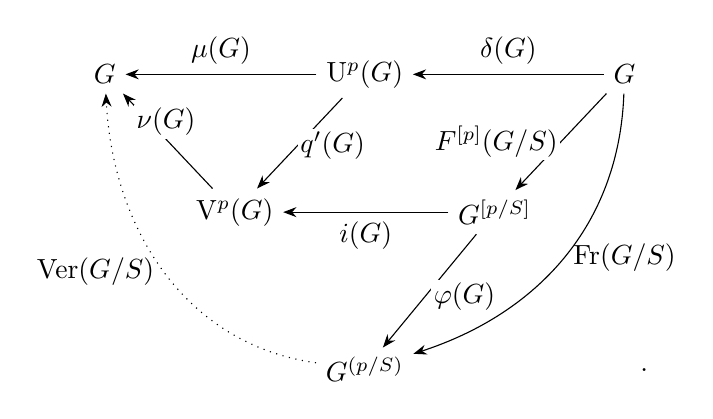
\begin{tikzpicture}[
  baseline=(current bounding box.center),
  >=Stealth,
  every node/.style={font=\normalsize}
]
  \node (gleft) at (-3.3,2.1) {$G$};
  \node (upg)   at (0,2.1) {$\mathrm U^p(G)$};
  \node (gright) at (3.3,2.1) {$G$};
  \node (vpg)   at (-1.65,0.35) {$\mathrm V^p(G)$};
  \node (gbr)   at (1.65,0.35) {$G^{[p/S]}$};
  \node (gps)   at (0,-1.65) {$G^{(p/S)}$};

  \draw[->] (upg) -- node[above] {$\mu(G)$} (gleft);
  \draw[->] (gright) -- node[above] {$\delta(G)$} (upg);
  \draw[->] (vpg) -- node[pos=.52,above,fill=white,inner sep=1pt]
    {$\nu(G)$} (gleft);
  \draw[->] (upg) -- node[pos=.53,right,fill=white,inner sep=1pt]
    {$q'(G)$} (vpg);
  \draw[->] (gbr) -- node[below] {$i(G)$} (vpg);
  \draw[->] (gright) -- node[pos=.5,left,fill=white,inner sep=1pt]
    {$F^{[p]}(G/S)$} (gbr);
  \draw[->] (gbr) -- node[pos=.55,anchor=west,xshift=2pt,fill=white,inner sep=1pt]
    {$\varphi(G)$} (gps);
  \draw[->] (gright) to[out=-92,in=18]
    node[right] {$\operatorname{Fr}(G/S)$} (gps);
  \draw[->,dotted] (gps) to[out=172,in=-87]
    node[left] {$\operatorname{Ver}(G/S)$} (gleft);
  \node at (3.55,-1.65) {$.$};
\end{tikzpicture}

% END INCLUDED SGA3_English_current_buildable_source_20260823/source/inputs/VII/native_diagrams/exp7/viia_05_14/diagram_046.tex

\end{center}

When \(G\) is flat over \(S\), \(\varphi(G)\) is an isomorphism,
and we may define the morphism called the \emph{Verschiebung}
\[
  \operatorname{Ver}(G/S):
  G^{(p/S)}
  \longrightarrow
  G
\]
by
\[
  \operatorname{Ver}(G/S)
  =
  \nu(G)\circ i(G)\circ\varphi(G)^{-1}.
\]
As \(G\) ranges over the flat commutative \(S\)-group schemes, the
assignment
\[
  \operatorname{Ver}:G\longmapsto\operatorname{Ver}(G/S)
\]
is plainly a functorial homomorphism. Consequently,
\(\operatorname{Ver}(G/S)\) is a group homomorphism.

For every \(S\)-scheme \(T\), the composite
\[
  G(T)
  \xrightarrow{\delta(G)(T)}
  U^p(G)(T)
  \xrightarrow{\mu(G)(T)}
  G(T)
\]
sends \(x\in G(T)\) to \(p\cdot x\). We may therefore write
\(p\cdot\operatorname{id}_G\) in place of
\(\mu(G)\circ\delta(G)\), obtaining the classical formula
\[
  \tag{*}\label{sga3:vii:paragraph:4-3:equation:star}
  \operatorname{Ver}(G/S)\circ\operatorname{Fr}(G/S)
  =
  p\cdot\operatorname{id}_G.
\]

\medskip
\noindent\textbf{Examples 4.3.1.}
\phantomsection
\label{sga3:VIIA:4.3.1}

\smallskip
\noindent\textit{a)}
If \(G\) is a constant \(S\)-scheme in abelian groups, then
\(\operatorname{Fr}(G/S)\) identifies with the identity morphism
of \(G\) (cf.\ \SGARefLink{sga3:VIIA:4.1.1.1}{4.1.1.1}). Hence
\[
  \operatorname{Ver}(G/S)
  =
  p\cdot\operatorname{id}_G.
\]

\smallskip
\noindent\textit{b)}
If \(G\) is the diagonalizable \(S\)-group of type \(M\), then
\(\operatorname{Fr}(G/S)=p\cdot\operatorname{id}_G\) by
\SGARefLink{sga3:VIIA:4.1.4}{4.1.4}~\textit{a)}. It follows at once that
\(\operatorname{Ver}(G/S)\) is the identity morphism of \(G\).

\smallskip
\noindent\textit{c)}
If \(\mathcal E\) is a flat \(\mathcal O_S\)-module and
\(G=\mathcal V(\mathcal E)\), then
\(\operatorname{Ver}(G/S)\) is zero, as is
\(p\cdot\operatorname{id}_G\). In Expos\'e VII\textsubscript{B} we
shall see that a commutative algebraic group \(G\) over a field
\(k\) is ``unipotent'' if and only if, for some \(n\), the
composite homomorphism
\begin{center}
  \phantomsection
  \label{sga3:VIIA:4.3.1-iterated-verschiebung-chain}
  % SGA3-VII-DIAG-047
  % BEGIN INCLUDED SGA3_English_current_buildable_source_20260823/source/inputs/VII/native_diagrams/exp7/viia_05_14/diagram_047.tex
\(\displaystyle
G^{(p^n)}
  \xrightarrow{\operatorname{Ver}(G^{(p^{n-1})}/S)}
G^{(p^{n-1})}
  \longrightarrow \cdots \longrightarrow
G^{(p)}
  \xrightarrow{\operatorname{Ver}(G/S)}
G
\)

% END INCLUDED SGA3_English_current_buildable_source_20260823/source/inputs/VII/native_diagrams/exp7/viia_05_14/diagram_047.tex

\end{center}
is zero. Here
\[
  G^{(p^n)}
  =
  \bigl(G^{(p^{n-1})}\bigr)^{(p)}
\]
as in \SGARefLink{sga3:VIIA:4.1.3}{4.1.3}.\footnote{This criterion is not stated explicitly in
Expos\'e VII\textsubscript{B}; see \textup{[DG70]}, IV, \S3,
Prop.~4.11.}

\medskip
\noindent\textbf{4.3.2.}
\phantomsection
\label{sga3:VIIA:4.3.2}

% Authority: Exp7A local p. 30; combined p. 483; printed p. 472.
Since
\(\operatorname{Ver}:G\mapsto\operatorname{Ver}(G/S)\) is a
functorial homomorphism on the category of flat commutative
\(S\)-group schemes, the square
\begin{center}
  \phantomsection
  \label{sga3:VIIA:4.3.2-frobenius-verschiebung-square}
  % SGA3-VII-DIAG-048
  % BEGIN INCLUDED SGA3_English_current_buildable_source_20260823/source/inputs/VII/native_diagrams/exp7/viia_05_14/diagram_048.tex
\begin{tikzcd}[row sep=3.3em,column sep=5.2em]
G^{(p)} \arrow[r,"\operatorname{Ver}(G/S)"]
  \arrow[d,swap,"\operatorname{Fr}(G/S)^{(p)}"]
  & G \arrow[d,"\operatorname{Fr}(G/S)"] \\
G^{(p^2)} \arrow[r,"\operatorname{Ver}(G^{(p)}/S)"]
  & G^{(p)}
\end{tikzcd}

% END INCLUDED SGA3_English_current_buildable_source_20260823/source/inputs/VII/native_diagrams/exp7/viia_05_14/diagram_048.tex

\end{center}
commutes. Here \(\operatorname{Fr}(G/S)^{(p)}\) denotes the
pullback of \(\operatorname{Fr}(G/S)\) along the base change
\(\operatorname{fr}(S)\). By \SGARefLink{sga3:VIIA:4.1.1}{4.1.1},
\[
  \operatorname{Fr}(G/S)^{(p)}
  =
  \operatorname{Fr}(G^{(p)}/S).
\]
Applying formula \((*)\) of \SGARefLink{sga3:VIIA:4.3}{4.3} to \(G^{(p)}\), we obtain
\[
  \tag{**}\label{sga3:vii:paragraph:4-3-2:equation:double-star}
  \operatorname{Fr}(G/S)\circ\operatorname{Ver}(G/S)
  =
  \operatorname{Ver}(G^{(p)}/S)
    \circ\operatorname{Fr}(G^{(p)}/S)
  =
  p\cdot\operatorname{id}_{G^{(p)}}.
\]

\medskip
\noindent\textbf{4.3.3.}
\phantomsection
\label{sga3:VIIA:4.3.3}

Suppose finally that \(G\) is a commutative \(S\)-group which is
finite and locally free. Let \(\mathcal A\) be its affine
\(\mathcal O_S\)-algebra, and let \(\pi\) be the endomorphism of
the sheaf of rings \(\mathcal O_S\) which sends a section \(x\) to
\(x^p\).\footnote{The editors changed the order of presentation,
introducing first the objects which occur in the diagram below.}
Denote by \(\Sigma^p\mathcal A\) the subalgebra of
\(\bigotimes_{\mathcal O_S}^p\mathcal A\) consisting of the
sections invariant under the symmetric-group action, and by
\[
  i(\mathcal A):
  \Sigma^p\mathcal A
  \longrightarrow
  \bigotimes_{\mathcal O_S}^p\mathcal A
\]
its inclusion.

Let
\[
  \Delta^p(\mathcal A):
  \mathcal A
  \longrightarrow
  \bigotimes_{\mathcal O_S}^p\mathcal A
\]
be the morphism obtained by iterating the diagonal morphism of the
coalgebra \(\mathcal A\). It corresponds to the multiplication
morphism \(U^p(G)=G_S^p\to G\). By the beginning of \SGARefLink{sga3:VIIA:4.3}{4.3},
\(\Delta^p(\mathcal A)\) factors through
\(\Sigma^p\mathcal A\); that is, it induces a morphism
\[
  a(\mathcal A):
  \mathcal A\longrightarrow\Sigma^p\mathcal A
\]
such that
\[
  i(\mathcal A)\circ a(\mathcal A)
  =
  \Delta^p(\mathcal A).
\]

On the other hand, let \(S^p(\mathcal A)\) be the homogeneous
component of degree \(p\) in the symmetric algebra of
\(\mathcal A\), and let
\[
  q(\mathcal A):
  \bigotimes_{\mathcal O_S}^p\mathcal A
  \longrightarrow
  S^p(\mathcal A)
\]
be the canonical projection. The multiplication
\[
  m^p(\mathcal A):
  \bigotimes_{\mathcal O_S}^p\mathcal A
  \longrightarrow
  \mathcal A
\]
factors through \(S^p(\mathcal A)\); equivalently, it induces a map
\[
  b(\mathcal A):
  S^p(\mathcal A)\longrightarrow\mathcal A
\]
such that
\[
  b(\mathcal A)\circ q(\mathcal A)
  =
  m^p(\mathcal A).
\]

Since \(\Sigma^p\mathcal A\) is the affine algebra of
\(V^p(G)\), the composite
\(i(G)\circ\varphi(G)^{-1}\) induces, again by the beginning of
\SGARefLink{sga3:VIIA:4.3}{4.3}, an algebra homomorphism
\[
  r(\mathcal A):
  \Sigma^p\mathcal A
  \longrightarrow
  \mathcal A\otimes_\pi\mathcal O_S.
\]
It vanishes on sections of the form
\[
  \sum_{\sigma\in\mathfrak S_p}
    a_{\sigma(1)}\otimes\cdots\otimes a_{\sigma(p)}
\]
and sends \(a\otimes\cdots\otimes a\) to
\(a\otimes_\pi1\). Similarly, \(j(\mathcal A)\) is the morphism
of \(\mathcal O_S\)-modules
\[
  a\otimes_\pi1
  \longmapsto
  q(a\otimes\cdots\otimes a).
\]

% Authority: Exp7A local p. 31; combined p. 484; printed p. 473.
These maps form the commutative diagram
\begin{center}
  \phantomsection
  \label{sga3:VIIA:4.3.3-cartier-duality-algebra-diagram}
  % SGA3-VII-DIAG-049
  % BEGIN INCLUDED SGA3_English_current_buildable_source_20260823/source/inputs/VII/native_diagrams/exp7/viia_05_14/diagram_049.tex
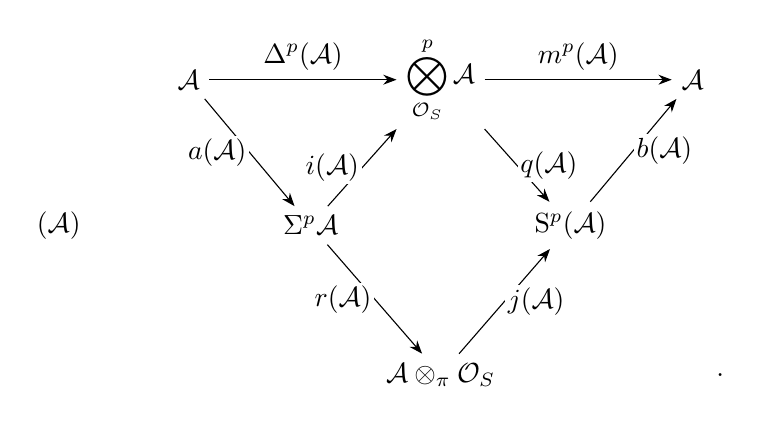
\begin{tikzpicture}[
  baseline=(current bounding box.center),
  >=Stealth,
  every node/.style={font=\normalsize}
]
  \node (atl) at (-3.2,2.0) {$\mathcal A$};
  \node (atm) at (0,2.0) {$\displaystyle\bigotimes_{\mathcal O_S}^{p}\mathcal A$};
  \node (atr) at (3.2,2.0) {$\mathcal A$};
  \node (aml) at (-1.65,0.15) {$\Sigma^p\mathcal A$};
  \node (amr) at (1.65,0.15) {$\mathrm S^p(\mathcal A)$};
  \node (ab)  at (0,-1.75) {$\mathcal A\otimes_{\pi}\mathcal O_S$};
  \node at (-4.85,0.15) {$({\mathcal A})$};

  \draw[->] (atl) -- node[above] {$\Delta^p(\mathcal A)$} (atm);
  \draw[->] (atm) -- node[above] {$m^p(\mathcal A)$} (atr);
  \draw[->] (atl) -- node[midway,left,fill=white,inner sep=1pt]
    {$a(\mathcal A)$} (aml);
  \draw[->] (aml) -- node[midway,left,fill=white,inner sep=1pt]
    {$i(\mathcal A)$} (atm);
  \draw[->] (atm) -- node[midway,right,fill=white,inner sep=1pt]
    {$q(\mathcal A)$} (amr);
  \draw[->] (amr) -- node[midway,right,fill=white,inner sep=1pt]
    {$b(\mathcal A)$} (atr);
  \draw[->] (aml) -- node[midway,left,fill=white,inner sep=1pt]
    {$r(\mathcal A)$} (ab);
  \draw[->] (ab) -- node[midway,right,fill=white,inner sep=1pt]
    {$j(\mathcal A)$} (amr);
  \node at (3.55,-1.75) {$.$};
\end{tikzpicture}

% END INCLUDED SGA3_English_current_buildable_source_20260823/source/inputs/VII/native_diagrams/exp7/viia_05_14/diagram_049.tex

\end{center}
The composite \(r(\mathcal A)\circ a(\mathcal A)\) corresponds to
the Verschiebung morphism \(\operatorname{Ver}(G/S)\), while
\(b(\mathcal A)\circ j(\mathcal A)\) corresponds to the Frobenius
morphism \(\operatorname{Fr}(G/S)\).

The preceding commutative diagram \((\mathcal A)\) is self-dual.
Indeed, let \(D\) be the functor which associates to each
\(\mathcal O_S\)-module \(\mathcal M\) its dual
\[
  D\mathcal M
  =
  \operatorname{Hom}_{\mathcal O_S}
    (\mathcal M,\mathcal O_S).
\]
The image of diagram \((\mathcal A)\) under \(D\) is precisely
diagram \((D\mathcal A)\). The morphisms
\[
  Dr(\mathcal A),\quad
  Da(\mathcal A),\quad
  Dj(\mathcal A),\quad
  Db(\mathcal A)
\]
identify respectively with
\[
  j(D\mathcal A),\quad
  b(D\mathcal A),\quad
  r(D\mathcal A),\quad
  a(D\mathcal A).
\]
By \SGARefLink{sga3:VIIA:3.3.1}{3.3.1}, it follows that:

\begin{quote}
\textit{In the category of commutative \(S\)-groups which are
finite and locally free, Cartier duality interchanges the
Frobenius morphism and the Verschiebung.}
\end{quote}
\footnote{See also \textup{[DG70]}, IV, \S3, 4.9.}

% Next cursor: Exp7A local p. 31, combined-reader p. 484,
% re-edition printed p. 473, at Section 5.

% END INCLUDED SGA3_English_current_buildable_source_20260823/source/inputs/VII/tex/components/07_expose_VIIA_section43_verschiebung_en.tex

% BEGIN INCLUDED SGA3_English_current_buildable_source_20260823/source/inputs/VII/tex/components/08_expose_VIIA_section5_restricted_p_lie_51_52_en.tex
% SGA 3, Expose VII_A, English reconstruction -- Loop 1.
% Scope: authority local pages 31--33, Section 5 opening through 5.2.1,
% stopping before 5.3 on local page 33.
% Combined-reader pages: 484--486. Re-edition printed pages: 473--475.
% Original-edition marginal locators within this span: 445--448.
% Authority: Polo--Gille Exp7A-13oct24.pdf,
% SHA-256 D46DB8C79D0385643B6EED4B96900613248375F9B73B4202478A4F57FD3E8522.
% Jacob Reinhold's CC BY 4.0 Markdown was consulted as comparison lineage.

\section*{5. Restricted \texorpdfstring{\(p\)}{p}-Lie Algebras}
\phantomsection
\label{sga3:VIIA:5}
\addcontentsline{toc}{section}{5. Restricted p-Lie Algebras}

We first recall some results from the \emph{S\'eminaire Sophus
Lie}.\footnote{See P.~Cartier,
\emph{Exemples d'hyperalg\`ebres}, S\'eminaire Sophus Lie
1955/56, Exp.~3.}

\medskip
\noindent\textbf{5.1.}
\phantomsection
\label{sga3:VIIA:5.1}

% Authority: Exp7A local p. 31; combined p. 484; printed p. 473.
Let \(p\) be a prime number, let \(R\) be a commutative ring of
characteristic \(p\), and let \(A\) be an associative
\(R\)-algebra, not necessarily commutative. For \(a,b\in A\), put
\[
  [a,b]=ab-ba,
  \qquad
  a\cdot b=L_a(b)=R_b(a).
\]
Then
\[
\begin{aligned}
  (\operatorname{ad}x^p)(y)
  &=[x^p,y] \\
  &=(L_x^p-R_x^p)(y) \\
  &=(L_x-R_x)^p(y) \\
  &=(\operatorname{ad}x)^p(y),
\end{aligned}
\]
which gives Jacobson's first formula:
\[
  \tag{i}\label{sga3:vii:paragraph:5-1:equation:i}
  \operatorname{ad}(x^p)
  =
  (\operatorname{ad}x)^p.
\]

If \(a_1,\ldots,a_p\) are arbitrary elements of \(A\), and \(N\)
is the symmetrization operator (cf.\ \SGARefLink{sga3:VIIA:4.2}{4.2}), then
\begin{equation}
  \tag{*}\label{sga3:vii:paragraph:5-1:equation:star}
\begin{aligned}
  N(a_1\otimes\cdots\otimes a_p)
  &=
  \sum_{\sigma\in\mathfrak S_p}
    a_{\sigma(1)}\cdots a_{\sigma(p)} \\
  &=
  \sum_{\tau\in\mathfrak S_{p-1}}
  [a_{\tau(1)},
    [a_{\tau(2)},
      [\cdots,
        [a_{\tau(p-1)},a_p]
      \cdots]
    ]
  ].
\end{aligned}
\end{equation}
Here \(\sigma\) ranges over the permutations of \(p\) letters and
\(\tau\) over those of \(p-1\) letters.

% Authority: Exp7A local p. 32; combined p. 485; printed p. 474.
Indeed, the final expression is equal to
\[
  \sum_{\tau}
  \sum_{r=0}^{p-1}
  \sum_{i_1<\cdots<i_r}
  (-1)^s
  a_{\tau(i_1)}\cdots a_{\tau(i_r)}
  a_p
  a_{\tau(j_s)}\cdots a_{\tau(j_1)},
\]
where \(\tau\) ranges over the permutations of \(p-1\) letters;
\(i_1,\ldots,i_r\) ranges over the strictly increasing sequences
in \([1,p-1]\); and \(j_1,\ldots,j_s\) is the strictly increasing
sequence of those integers of \([1,p-1]\) which are different
from \(i_1,\ldots,i_r\). For fixed \(r\), the sum of the terms
\[
  (-1)^s
  a_{\tau(i_1)}\cdots a_{\tau(i_r)}
  a_p
  a_{\tau(j_s)}\cdots a_{\tau(j_1)}
\]
is plainly
\[
  (-1)^s\binom{p-1}{s}
  \sum_{\rho}
  a_{\rho(1)}\cdots a_{\rho(r)}
  a_p
  a_{\rho(r+1)}\cdots a_{\rho(p-1)},
\]
where \(\rho\) ranges over the permutations of \(p-1\) letters.
But
\[
  (-1)^s\binom{p-1}{s}=1
  \quad\text{in }\mathbb F_p,
\]
because in \(\mathbb F_p[x]\),
\[
  (x-1)^p=x^p-1=(x-1)(x^{p-1}+\cdots+1),
\]
and hence
\[
  (x-1)^{p-1}=x^{p-1}+\cdots+1.
\]
This proves \((*)\).

On the other hand, if \(x_0,x_1\in A\), then
\[
  (x_0+x_1)^p
  =
  x_0^p+x_1^p+
  \sum_z x_{z(1)}x_{z(2)}\cdots x_{z(p)},
\]
where \(z\) ranges over the nonconstant maps
\([1,p]\to\{0,1\}\). It follows that
\[
\begin{aligned}
  (x_0+x_1)^p
  ={}&
  x_0^p+x_1^p \\
  &+
  \sum_{0<r<p}
  \frac{1}{r!(p-r)!}\,
  N(
    \underbrace{x_0,\ldots,x_0}_{r},
    \underbrace{x_1,\ldots,x_1}_{p-r}
  ).
\end{aligned}
\]
\footnote{The editors inserted the following explanation from
\textup{[DG70]}, III.7, \SGARefLink{sga3:VIIB:3.2:prop}{3.2}.}
By \((*)\),
\[
\begin{aligned}
  &N(
    \underbrace{x_0,\ldots,x_0}_{r},
    \underbrace{x_1,\ldots,x_1}_{p-r}
  ) \\
  &\qquad =
  r!(p-1-r)!
  \sum_t
  [x_{t(1)},
    [x_{t(2)},
      [\cdots,
        [x_{t(p-1)},x_1]
      \cdots]
    ]
  ],
\end{aligned}
\]
where \(t\) ranges over the maps
\([1,p-1]\to\{0,1\}\) which take the value \(0\) exactly \(r\)
times. We obtain Jacobson's second formula:
\begin{equation}
  \tag{ii}\label{sga3:vii:paragraph:5-1:equation:ii}
\begin{aligned}
  (x_0+x_1)^p
  ={}&
  x_0^p+x_1^p \\
  &-
  \sum_{0<r<p}\sum_t\frac1r
  [x_{t(1)},
    [x_{t(2)},
      [\cdots,
        [x_{t(p-1)},x_1]
      \cdots]
    ]
  ],
\end{aligned}
\end{equation}
where \(t\) has the same meaning.

\medskip
\noindent\textbf{5.2.}
\phantomsection
\label{sga3:VIIA:5.2}

Let now \(\mathfrak g\) be an \(R\)-Lie algebra. A map
\[
  x\longmapsto x^{(p)}
\]
from \(\mathfrak g\) to itself is said to make \(\mathfrak g\) a
\emph{restricted \(p\)-Lie algebra over \(R\)} if the following
conditions hold:
\[
\begin{array}{ll}
  (0) &
  (\lambda x)^{(p)}
  =
  \lambda^p x^{(p)}
  \quad
  (\lambda\in R,\ x\in\mathfrak g), \\[0.4em]
  (i) &
  \operatorname{ad}x^{(p)}
  =
  (\operatorname{ad}x)^p
  \quad
  (x\in\mathfrak g),
\end{array}
\]
and
\[
\begin{aligned}
  (ii)\quad
  (x_0+x_1)^{(p)}
  ={}&
  x_0^{(p)}+x_1^{(p)} \\
  &-
  \sum_{0<r<p}\sum_t\frac1r
  [x_{t(1)},
    [x_{t(2)},
      [\cdots,
        [x_{t(p-1)},x_1]
      \cdots]
    ]
  ],
\end{aligned}
\]
where \(t\) ranges over the maps
\([1,p-1]\to\{0,1\}\) which take the value \(0\) exactly \(r\)
times, and \(x_0,x_1\in\mathfrak g\). The map
\(x\mapsto x^{(p)}\) is called the \emph{symbolic \(p\)-th power}.

% Authority: Exp7A local p. 33; combined p. 486; printed p. 475.
For example, if \(A\) is an associative \(R\)-algebra, \SGARefLink{sga3:VIIB:5.1:proposition}{5.1} shows
that the \(R\)-module underlying \(A\), endowed with
\[
  [x,y]=xy-yx,
  \qquad
  x^{(p)}=x^p,
\]
is a \(p\)-Lie algebra, denoted \(A_{\mathrm{Lie}}\). We call it
the \(p\)-Lie algebra underlying \(A\).

We shall chiefly consider restricted \(p\)-Lie subalgebras of
algebras of the form \(A_{\mathrm{Lie}}\). Here is one example.
Let \(S\) be a scheme of characteristic \(p>0\), and let \(X\) be
an \(S\)-scheme. Recall that a derivation of \(X\) over \(S\) is
an endomorphism \(D\) of the sheaf of abelian groups
\(\mathcal O_X\) such that
\[
  D(\lambda s)=\lambda D(s),
  \qquad
  D(st)=(Ds)t+s(Dt),
\]
whenever \(\lambda\), respectively \(s,t\), are sections of
\(\mathcal O_S\), respectively \(\mathcal O_X\), on open subsets
for which the formulas make sense. Leibniz's formula
\[
  D^n(st)
  =
  \sum_{i=0}^n
  \binom ni
  (D^is)(D^{n-i}t)
\]
shows that \(D^p\) is again a derivation of \(X\) over \(S\), since
\[
  \binom pi\equiv0\pmod p
  \qquad(i\ne0,p).
\]
It follows that:

\begin{quote}
\textit{The algebra \(\operatorname{Der}_{X/S}\) of derivations of
\(X\) over \(S\) is a restricted \(p\)-Lie subalgebra of the
\(\Gamma(S,\mathcal O_S)\)-algebra of differential operators of
\(X\) over \(S\).}
\end{quote}

\medskip
\noindent\textbf{5.2.1.}
\phantomsection
\label{sga3:VIIA:5.2.1}
If \(\mathfrak g\) and \(\mathfrak h\) are two restricted
\(p\)-Lie algebras, a \emph{homomorphism}
\[
  h:\mathfrak g\longrightarrow\mathfrak h
\]
is an \(R\)-linear map such that, for \(x,y\in\mathfrak g\),
\[
  h([x,y])=[h(x),h(y)],
  \qquad
  h(x^{(p)})=h(x)^{(p)}.
\]
The composite of two homomorphisms is again a homomorphism, so we
may speak of the \emph{category of restricted \(p\)-Lie algebras
over \(R\)}.

If \((X,\mathcal R)\) is a ringed space, we say that an
\(\mathcal R\)-module \(\mathfrak g\) is endowed with the
structure of a restricted \(p\)-Lie algebra over \(\mathcal R\) if,
for every open subset \(U\), the module
\(\Gamma(U,\mathfrak g)\) is a restricted \(p\)-Lie algebra over
\(\Gamma(U,\mathcal R)\), and if all restriction maps are
homomorphisms.

% Next cursor: Exp7A local p. 33, combined-reader p. 486,
% re-edition printed p. 475, at 5.3.

% END INCLUDED SGA3_English_current_buildable_source_20260823/source/inputs/VII/tex/components/08_expose_VIIA_section5_restricted_p_lie_51_52_en.tex

% BEGIN INCLUDED SGA3_English_current_buildable_source_20260823/source/inputs/VII/tex/components/09_expose_VIIA_section53_restricted_enveloping_en.tex
% SGA 3, Expose VII_A, English reconstruction -- Loop 1.
% Scope: authority local pages 33--37, paragraphs 5.3--5.3.4,
% stopping before 5.4 on local page 37.
% Combined-reader pages: 486--490. Re-edition printed pages: 475--479.
% Original-edition marginal locators within this span: 448--452.
% Authority: Polo--Gille Exp7A-13oct24.pdf,
% SHA-256 D46DB8C79D0385643B6EED4B96900613248375F9B73B4202478A4F57FD3E8522.
% Jacob Reinhold's CC BY 4.0 Markdown was consulted as comparison lineage.

\medskip
\noindent\textbf{5.3.}
\phantomsection
\label{sga3:VIIA:5.3}

% Authority: Exp7A local p. 33; combined p. 486; printed p. 475.
We are now interested in the left adjoint of the functor
\[
  A\longmapsto A_{\mathrm{Lie}}
\]
of \SGARefLink{sga3:VIIB:5.2:theorem}{5.2}. Let \(\mathfrak g\) be a restricted \(p\)-Lie algebra
over a ring \(R\) of characteristic \(p\), let
\(U(\mathfrak g)\) be the enveloping algebra of the Lie algebra
underlying \(\mathfrak g\) (cf.\ \textup{[BLie]}, I, \S2.1), and
let
\[
  i_{\mathfrak g}:\mathfrak g\longrightarrow U(\mathfrak g)
\]
(or simply \(i\)) be the canonical map.

Let \(A\) be a unital associative \(R\)-algebra. For every Lie
algebra homomorphism
\[
  \varphi:\mathfrak g\longrightarrow A_{\mathrm{Lie}},
\]
there is a unique homomorphism of unital \(R\)-algebras
\[
  \psi:U(\mathfrak g)\longrightarrow A
\]
such that \(\psi\circ i=\varphi\). Moreover, \(\varphi\) is a
homomorphism of restricted \(p\)-Lie algebras if and only if
\(\psi\) vanishes on all the elements
\[
  i(x)^p-i\bigl(x^{(p)}\bigr),
  \qquad x\in\mathfrak g.
\]

\noindent\textbf{Definition.}
The quotient of \(U(\mathfrak g)\) by the two-sided ideal
generated by the elements
\[
  i(x)^p-i\bigl(x^{(p)}\bigr)
\]
is denoted \(U_p^R(\mathfrak g)\), or simply
\(U_p(\mathfrak g)\). We denote by \(j_{\mathfrak g}\), or simply
\(j\), the composite
\[
  \mathfrak g
  \xrightarrow{i}
  U(\mathfrak g)
  \longrightarrow
  U_p(\mathfrak g).
\]
The algebra \(U_p(\mathfrak g)\) is called the
\emph{restricted enveloping algebra} of \(\mathfrak g\).

The preceding discussion gives the following result.

\medskip
\noindent\textbf{Proposition.}
\textit{For every unital associative \(R\)-algebra \(A\) and
every homomorphism of restricted \(p\)-Lie algebras
\[
  \varphi:\mathfrak g\longrightarrow A_{\mathrm{Lie}},
\]
there is a unique homomorphism of unital algebras
\[
  \psi:U_p(\mathfrak g)\longrightarrow A
\]
such that \(\psi\circ j=\varphi\). In other words, the functor
\(\mathfrak g\mapsto U_p(\mathfrak g)\) is left adjoint to the
forgetful functor \(A\mapsto A_{\mathrm{Lie}}\).}

\medskip
\noindent\textbf{5.3.1.}
\phantomsection
\label{sga3:VIIA:5.3.1}

% Authority: Exp7A local p. 34; combined p. 487; printed p. 476.
With the notation of \SGARefLink{sga3:VIIA:5.3}{5.3}, put
\[
  \beta(x)=i(x)^p-i\bigl(x^{(p)}\bigr).
\]
For every \(y\in\mathfrak g\), \SGARefLink{sga3:VIIA:5.1}{formulas 5.1}~\SGARefLink{sga3:vii:paragraph:5-1:equation:i}{(i)} and \SGARefLink{sga3:VIIB:5.2:theorem}{5.2}~\SGARefLink{sga3:vii:paragraph:5-1:equation:i}{(i)}
give
\[
\begin{aligned}
  \beta(x)i(y)
  &=
  i(y)\beta(x)+[\beta(x),i(y)]\\
  &=
  i(y)\beta(x)
  +(\operatorname{ad}i(x))^p i(y)
  -i\bigl((\operatorname{ad}x)^p y\bigr)\\
  &=
  i(y)\beta(x).
\end{aligned}
\]
Thus \(\beta(x)\) belongs to the center of \(U(\mathfrak g)\);
in particular, the left ideal generated by the elements
\(\beta(x)\) is already two-sided.

On the other hand,
\[
  \beta(\lambda x)=\lambda^p\beta(x)
  \qquad(\lambda\in R),
\]
and \SGARefLink{sga3:VIIA:5.1}{formulas 5.1}~\SGARefLink{sga3:vii:paragraph:5-1:equation:ii}{(ii)} and \SGARefLink{sga3:VIIA:5.2}{5.2}~\SGARefLink{sga3:vii:paragraph:5-1:equation:ii}{(ii)} give
\[
  \beta(x+y)=\beta(x)+\beta(y)
  \qquad(x,y\in\mathfrak g).
\]
Consequently, if \((x_\alpha)\) is a family of generators of the
\(R\)-module \(\mathfrak g\), the left ideal generated by all
\(\beta(x)\) is already generated by the elements
\(\beta(x_\alpha)\).

\medskip
\noindent\textbf{5.3.2. Proposition.}\footnote{In this paragraph,
the editors changed the order, stating the result first and then
giving the detailed proof.}
\phantomsection
\label{sga3:VIIA:5.3.2}
\textit{Let \(\mathfrak g\) be an \(R\)-Lie algebra whose
underlying \(R\)-module is free with basis \((x_\alpha)\). Then
the restricted \(p\)-Lie algebra structures on \(\mathfrak g\)
correspond bijectively to the families \((y_\alpha)\) of elements
of \(\mathfrak g\) such that
\[
  \operatorname{ad}y_\alpha
  =
  (\operatorname{ad}x_\alpha)^p.
\]}

Indeed, suppose that \(\mathfrak g\) is endowed with a restricted
\(p\)-Lie algebra structure \(x\mapsto x^{(p)}\). By \SGARefLink{sga3:VIIB:5.2:theorem}{5.2}~\SGARefLink{sga3:vii:paragraph:5-1:equation:i}{(i)},
\SGARefLink{sga3:VIIB:0}{(0)}, and \SGARefLink{sga3:vii:paragraph:5-1:equation:ii}{(ii)}, the elements
\[
  y_\alpha=x_\alpha^{(p)}
\]
satisfy
\[
  \operatorname{ad}y_\alpha
  =
  (\operatorname{ad}x_\alpha)^p,
\]
and they determine the restricted \(p\)-Lie algebra structure.

We prove the converse. Since \(\mathfrak g\) is a free
\(R\)-module, the canonical map
\[
  i:\mathfrak g\longrightarrow U(\mathfrak g)
\]
is injective by the Poincar\'e--Birkhoff--Witt theorem
(cf.\ \textup{[BLie]}, I, \S2.7). We may therefore identify
\(\mathfrak g\) with an \(R\)-submodule of \(U(\mathfrak g)\).
Suppose that \((y_\alpha)\) is a family of elements of
\(\mathfrak g\) such that
\[
  \operatorname{ad}y_\alpha
  =
  (\operatorname{ad}x_\alpha)^p.
\]
Let
\[
  \pi:R\longrightarrow R,
  \qquad
  r\longmapsto r^p,
\]
and let \(\mathfrak g\otimes_\pi R\) be the \(R\)-Lie algebra
obtained by extension of scalars along \(\pi\).\footnote{Thus
\(xr\otimes_\pi1=x\otimes_\pi r^p\) and
\(r\cdot(x\otimes_\pi1)=x\otimes_\pi r\), for
\(x\in\mathfrak g\) and \(r\in R\).}

There is an \(R\)-linear map
\[
  \gamma:\mathfrak g\otimes_\pi R
  \longrightarrow
  U(\mathfrak g)
\]
which sends \(x_\alpha\otimes_\pi1\) to
\(x_\alpha^p-y_\alpha\). Moreover, for every
\(x\in\mathfrak g\),
\[
  (\operatorname{ad}x_\alpha^p)(x)
  =
  (\operatorname{ad}x_\alpha)^p(x)
  =
  (\operatorname{ad}y_\alpha)(x).
\]
It follows that \(\gamma\) maps
\(\mathfrak g\otimes_\pi R\) into the center of
\(U(\mathfrak g)\). For \(x\in\mathfrak g\), put
\[
  x^{(p)}
  =
  x^p-\gamma(x\otimes_\pi1).
\]

% Authority: Exp7A local p. 35; combined p. 488; printed p. 477.
Then \(x_\alpha^{(p)}=y_\alpha\) for every \(\alpha\). If
\[
  x=\sum_\alpha\lambda_\alpha x_\alpha,
\]
\SGARefLink{sga3:VIIA:5.1}{formula 5.1}~\SGARefLink{sga3:vii:paragraph:5-1:equation:ii}{(ii)}, applied inductively to the number of indices
\(\alpha\) for which \(\lambda_\alpha\ne0\), gives
\[
  x^p-\sum_\alpha\lambda_\alpha^p x_\alpha^p
  \in\mathfrak g.
\]
Denote this element by \(z\). Then
\[
  x^{(p)}
  =
  \sum_\alpha\lambda_\alpha^p y_\alpha+z,
\]
and hence \(x^{(p)}\in\mathfrak g\).

It is clear that
\[
  (\lambda x)^{(p)}
  =
  \lambda^p x^{(p)}.
\]
Since \(\gamma(x\otimes_\pi1)\) is central, we have
\(\operatorname{ad}x^{(p)}=\operatorname{ad}x^p\). Jacobson's
first formula, \SGARefLink{sga3:VIIA:5.1}{5.1}~\SGARefLink{sga3:vii:paragraph:5-1:equation:i}{(i)}, therefore yields
\[
  \operatorname{ad}x^{(p)}
  =
  (\operatorname{ad}x)^p.
\]
Finally, Jacobson's second formula, \SGARefLink{sga3:VIIA:5.1}{5.1}~\SGARefLink{sga3:vii:paragraph:5-1:equation:ii}{(ii)}, shows that the map
\(x\mapsto x^{(p)}\) satisfies condition \SGARefLink{sga3:vii:paragraph:5-1:equation:ii}{(ii)} of \SGARefLink{sga3:VIIB:5.2:theorem}{5.2}. It thus
makes \(\mathfrak g\) into a restricted \(p\)-Lie algebra. This
proves the proposition.

\medskip
\noindent\textbf{5.3.3. Proposition.}
\phantomsection
\label{sga3:VIIA:5.3.3}
\textit{Let \(\mathfrak g\) be a restricted \(p\)-Lie algebra
over \(R\) whose underlying module is free with basis
\((x_\alpha)\). Then
\[
  j:\mathfrak g\longrightarrow U_p(\mathfrak g)
\]
is injective. If \(z_\alpha=j(x_\alpha)\), then
\(U_p(\mathfrak g)\) has as a basis the monomials
\[
  \prod_\alpha z_\alpha^{n_\alpha},
  \qquad
  0\le n_\alpha<p.
\]
Here the \(n_\alpha\) are zero except for finitely many
\(\alpha\); the basis is assumed to be totally ordered, and the
products are taken in increasing order.}

Identify \(\mathfrak g\) with a submodule of the enveloping
algebra \(U(\mathfrak g)\) by means of the canonical map \(i\).
For every family
\[
  n=(n_\alpha)
\]
of nonnegative integers, all but finitely many zero, put
\[
  |n|=\sum_\alpha n_\alpha,
  \qquad
  x^n=\prod_\alpha x_\alpha^{n_\alpha}.
\]
Write
\[
  n_\alpha=m_\alpha+p\ell_\alpha,
  \qquad
  0\le m_\alpha<p,
\]
and put
\[
  T_n
  =
  \prod_\alpha
  x_\alpha^{m_\alpha}
  \beta(x_\alpha)^{\ell_\alpha},
\]
where
\[
  \beta(x)=x^p-x^{(p)}
\]
is the map \(\mathfrak g\to U(\mathfrak g)\) defined in \SGARefLink{sga3:VIIA:5.3.1}{5.3.1}.

For \(r\in\mathbb N\), let \(U^r\) be the \(R\)-submodule of
\(U(\mathfrak g)\) generated by the \(x^n\) for which
\(|n|\le r\). Since the graded ring
\[
  \bigoplus_r U^r/U^{r-1}
\]
is commutative (cf.\ \textup{[BLie]}, I, \S2.6), for every
\(n\) we have
\[
  T_n-\prod_\alpha x_\alpha^{n_\alpha}
  \in U^{|n|-1}.
\]
For every \(s\in\mathbb N\), the \(x^n\) with \(|n|=s\) form a
basis of \(U^s/U^{s-1}\) by the Poincar\'e--Birkhoff--Witt
theorem (\emph{loc.\ cit.}, \S2.7); the same is therefore true
of the \(T_n\) with \(|n|=s\).

As \(s=|n|\) varies, the \(T_n\) consequently form a basis of
\(U(\mathfrak g)\). The kernel \(J\) of the canonical map
\[
  U(\mathfrak g)\longrightarrow U_p(\mathfrak g)
\]
is the left ideal of \(U(\mathfrak g)\) generated by the central
elements \(\beta(x_\alpha)\), by \SGARefLink{sga3:VIIA:5.3.1}{5.3.1}. The \(T_n\) for which
\(\ell=(\ell_\alpha)\ne0\) therefore form a basis of \(J\), while
the \(T_n\) for which \(n_\alpha<p\) for every \(\alpha\) form a
basis of
\[
  U_p(\mathfrak g)=U(\mathfrak g)/J.
\]

\medskip
\noindent\textbf{5.3.3 bis.}
\phantomsection
\label{sga3:VIIA:5.3.3bis}

% Authority: Exp7A local p. 36; combined p. 489; printed p. 478.
Let \(\mathfrak g\) be a restricted \(p\)-Lie algebra over \(R\),
and let \(f:R\to R'\) be an extension of the base ring. We claim
that the \(R'\)-module
\[
  R'\otimes_R\mathfrak g
\]
admits one and only one restricted \(p\)-Lie algebra structure
such that
\[
  \tag{*}\label{sga3:vii:paragraph:5-3-3-bis:equation:star}
  [\lambda\otimes x,\mu\otimes y]
  =
  \lambda\mu\otimes[x,y],
  \qquad
  (\lambda\otimes x)^{(p)}
  =
  \lambda^p\otimes x^{(p)}.
\]
In particular, it will follow that the functor
\[
  \mathfrak g\longmapsto R'\otimes_R\mathfrak g
\]
is left adjoint to restriction of scalars from \(R'\) to \(R\).

The uniqueness of the structure defined by \((*)\) is clear; we
prove its existence. If \(\mathfrak g\) is free with basis
\((x_\alpha)\), \SGARefLink{sga3:VIIA:5.3.2}{Proposition 5.3.2} gives a unique restricted
\(p\)-Lie algebra structure on the Lie algebra
\(R'\otimes_R\mathfrak g\) such that
\[
  (1\otimes x_\alpha)^{(p)}
  =
  1\otimes x_\alpha^{(p)}.
\]
This is the structure sought.

Suppose now that \(\mathfrak g\) is arbitrary. There is a
restricted \(p\)-Lie algebra \(L_0\), free as an \(R\)-module,
together with a surjective homomorphism
\[
  q_0:L_0\longrightarrow\mathfrak g.
\]
For example, we may take
\[
  L_0=R\otimes_{\mathbb F_p}\mathfrak g
\]
and let \(q_0\) be the homomorphism
\[
  \lambda\otimes x\longmapsto\lambda x;
\]
here \(\mathfrak g\) is free over the prime field
\(\mathbb F_p\). The kernel of \(q_0\) is a \(p\)-ideal of
\(L_0\), that is, an ideal of the Lie algebra \(L_0\) stable
under \(x\mapsto x^{(p)}\). Hence there is also a restricted
\(p\)-Lie algebra \(L_1\), free as an \(R\)-module, and a
homomorphism \(q_1:L_1\to L_0\) whose image is
\(\operatorname{Ker}q_0\). This gives the exact sequence
\begin{center}
  \phantomsection
  \label{sga3:VIIA:5.3.3bis-exact-sequence}
  % SGA3-VII-DIAG-050
  % BEGIN INCLUDED SGA3_English_current_buildable_source_20260823/source/inputs/VII/native_diagrams/exp7/viia_05_14/diagram_050.tex
\(\displaystyle
L_1 \xrightarrow{q_1} L_0 \xrightarrow{q_0} \mathfrak g \longrightarrow 0 .
\)

% END INCLUDED SGA3_English_current_buildable_source_20260823/source/inputs/VII/native_diagrams/exp7/viia_05_14/diagram_050.tex

\end{center}
and therefore an exact sequence of \(R'\)-Lie algebras
\begin{center}
  \phantomsection
  \label{sga3:VIIA:5.3.3bis-basechange-exact-sequence}
  % SGA3-VII-DIAG-051
  % BEGIN INCLUDED SGA3_English_current_buildable_source_20260823/source/inputs/VII/native_diagrams/exp7/viia_05_14/diagram_051.tex
\(\displaystyle
R'\otimes_R L_1
  \xrightarrow{R'\otimes_R q_1}
R'\otimes_R L_0
  \xrightarrow{R'\otimes_R q_0}
R'\otimes_R\mathfrak g
  \longrightarrow 0 .
\)

% END INCLUDED SGA3_English_current_buildable_source_20260823/source/inputs/VII/native_diagrams/exp7/viia_05_14/diagram_051.tex

\end{center}

Since \(R'\otimes_Rq_1\) is manifestly a homomorphism of
restricted \(p\)-Lie algebras, the kernel of
\(R'\otimes_Rq_0\) is a \(p\)-ideal. Thus the symbolic \(p\)-th
power operation on \(R'\otimes_RL_0\) induces, by passage to the
quotient, a map from \(R'\otimes_R\mathfrak g\) to itself (use
formula \SGARefLink{sga3:vii:paragraph:5-1:equation:ii}{(ii)} of \SGARefLink{sga3:VIIB:5.2:theorem}{5.2}). This map equips \(R'\otimes_R\mathfrak g\)
with the required restricted \(p\)-Lie algebra structure.

\medskip
\noindent\textbf{5.3.4.}
\phantomsection
\label{sga3:VIIA:5.3.4}

The canonical map
\[
  j_{\mathfrak g}:\mathfrak g\longrightarrow U_p(\mathfrak g)
\]
induces, for every extension \(R\to R'\) of the base ring, a
homomorphism
\[
  R'\otimes_Rj_{\mathfrak g}:
  R'\otimes_R\mathfrak g
  \longrightarrow
  R'\otimes_RU_p(\mathfrak g).
\]
It therefore induces a homomorphism
\[
  h:
  U_p(R'\otimes_R\mathfrak g)
  \longrightarrow
  R'\otimes_RU_p(\mathfrak g)
\]
such that
\[
  h\circ j_{R'\otimes_R\mathfrak g}
  =
  R'\otimes_Rj_{\mathfrak g}.
\]
The universal properties of \(R'\otimes_R\mathfrak g\) and of
the restricted enveloping algebra show immediately that \(h\) is
an isomorphism. We may therefore identify
\[
  U_p(R'\otimes_R\mathfrak g)
  \simeq
  R'\otimes_RU_p(\mathfrak g).
\]

% Authority: Exp7A local p. 37; combined p. 490; printed p. 479.
In particular, let \(r\in R\), and let \(R'=R_r\) be the
localized ring. Then
\[
  \mathfrak g_r=R_r\otimes_R\mathfrak g
\]
has a canonical restricted \(p\)-Lie algebra structure over
\(R_r\). Consequently, the sheaf \(\widetilde{\mathfrak g}\) on
\(\operatorname{Spec}R\) is a quasi-coherent restricted
\(p\)-Lie algebra on \(\operatorname{Spec}R\). Moreover,
\[
  U_p^{R_r}(\mathfrak g_r)
  \simeq
  U_p^R(\mathfrak g)_r,
\]
so the sheaf associated with the presheaf
\[
  V\longmapsto
  U_p\bigl(\Gamma(V,\widetilde{\mathfrak g})\bigr)
\]
is quasi-coherent.

\noindent\textbf{Definition.}
More generally, let \(S\) be a scheme of characteristic \(p\),
and let \(\mathcal G\) be a quasi-coherent restricted \(p\)-Lie
algebra over \(\mathcal O_S\). The sheaf associated with the
presheaf
\[
  V\longmapsto U_p\bigl(\Gamma(V,\mathcal G)\bigr)
\]
is quasi-coherent. It is denoted
\(\mathcal U_p(\mathcal G)\) and is called the
\emph{restricted enveloping algebra} of \(\mathcal G\). If \(V\)
is affine, then
\[
  U_p\bigl(\Gamma(V,\mathcal G)\bigr)
  \simeq
  \Gamma\bigl(V,\mathcal U_p(\mathcal G)\bigr).
\]

% Next cursor: Exp7A local p. 37, combined-reader p. 490,
% re-edition printed p. 479, at 5.4.

% END INCLUDED SGA3_English_current_buildable_source_20260823/source/inputs/VII/tex/components/09_expose_VIIA_section53_restricted_enveloping_en.tex

% BEGIN INCLUDED SGA3_English_current_buildable_source_20260823/source/inputs/VII/tex/components/10_expose_VIIA_section54_55_coalgebra_group_en.tex
% SGA 3, Expose VII_A, English reconstruction -- Loop 1.
% Scope: authority local pages 37--40, paragraphs 5.4--5.5.3,
% stopping before Section 6 on local page 40.
% Combined-reader pages: 490--493. Re-edition printed pages: 479--482.
% Original-edition marginal locators within this span: 452--454.
% Authority: Polo--Gille Exp7A-13oct24.pdf,
% SHA-256 D46DB8C79D0385643B6EED4B96900613248375F9B73B4202478A4F57FD3E8522.
% Jacob Reinhold's CC BY 4.0 Markdown was consulted as comparison lineage.

\medskip
\noindent\textbf{5.4.}
\phantomsection
\label{sga3:VIIA:5.4}

% Authority: Exp7A local p. 37; combined p. 490; printed p. 479.
The universal property of \(U_p(\mathfrak g)\) implies that
\(U_p(\mathfrak g)\) is functorial in \(\mathfrak g\). Every
homomorphism of restricted \(p\)-Lie algebras
\[
  \varphi:\mathfrak g\longrightarrow\mathfrak h
\]
induces a unique homomorphism of unital algebras \(U_p(\varphi)\)
such that
\[
  j_{\mathfrak h}\circ\varphi
  =
  U_p(\varphi)\circ j_{\mathfrak g}.
\]
Here are some examples.

\smallskip
\noindent\textit{a)}
If \(\mathfrak h=0\), then \(U_p(\mathfrak h)\) identifies with the
base ring, and \(U_p(\varphi)\) is an algebra homomorphism
\[
  \varepsilon_{\mathfrak g}:
  U_p(\mathfrak g)\longrightarrow R
\]
called the \emph{augmentation}.

\smallskip
\noindent\textit{b)}
Let now \(\mathfrak h=\mathfrak g^\circ\), the Lie algebra opposite
to \(\mathfrak g\). Thus \(\mathfrak g^\circ\) has the same
underlying module and the same symbolic \(p\)-th power as
\(\mathfrak g\), while its bracket is the negative of the bracket
of \(\mathfrak g\). We may identify
\(U_p(\mathfrak g^\circ)\) with the algebra opposite to
\(U_p(\mathfrak g)\). Moreover, the isomorphism
\[
  x\longmapsto-x
\]
from \(\mathfrak g\) onto \(\mathfrak g^\circ\) induces an
isomorphism
\[
  c_{\mathfrak g}:
  U_p(\mathfrak g)
  \longrightarrow
  U_p(\mathfrak g^\circ)
  \simeq
  U_p(\mathfrak g)^\circ.
\]
We call \(c_{\mathfrak g}\) the \emph{antipode} of
\(U_p(\mathfrak g)\).

\smallskip
\noindent\textit{c)}
Finally, let \(\mathfrak f\) and \(\mathfrak g\) be two restricted
\(p\)-Lie algebras, and let
\(\mathfrak h=\mathfrak f\times\mathfrak g\) be their product.
Its underlying \(R\)-module is the direct product, and
\[
  [(x,y),(x',y')]
  =
  ([x,x'],[y,y']),
  \qquad
  (x,y)^{(p)}
  =
  (x^{(p)},y^{(p)}).
\]
If
\[
  h_1:\mathfrak f\to\mathfrak k,
  \qquad
  h_2:\mathfrak g\to\mathfrak k
\]
are restricted \(p\)-Lie algebra homomorphisms satisfying
\[
  [h_1(x),h_2(y)]=0
  \quad
  (x\in\mathfrak f,\ y\in\mathfrak g),
\]
then
\[
  h_1+h_2:(x,y)\longmapsto h_1(x)+h_2(y)
\]
is a restricted \(p\)-Lie algebra homomorphism. Conversely, every
homomorphism \(\mathfrak f\times\mathfrak g\to\mathfrak k\) is of
this form. This characterizes \(\mathfrak f\times\mathfrak g\) by
a universal property.

For example, the maps
\[
  h_1:x\longmapsto j_{\mathfrak f}(x)\otimes1,
  \qquad
  h_2:y\longmapsto1\otimes j_{\mathfrak g}(y)
\]
induce a homomorphism \(h_1+h_2\) from
\(\mathfrak f\times\mathfrak g\) to the restricted \(p\)-Lie
algebra underlying
\[
  U_p(\mathfrak f)\otimes U_p(\mathfrak g).
\]
The universal properties of \(\mathfrak f\times\mathfrak g\) and
of the restricted enveloping algebras show that this homomorphism
extends to an isomorphism
\[
  \varphi:
  U_p(\mathfrak f\times\mathfrak g)
  \xrightarrow{\sim}
  U_p(\mathfrak f)\otimes U_p(\mathfrak g).
\]

\medskip
\noindent\textbf{Definition.}
\phantomsection
\label{sga3:VIIA:5.4-comultiplication-definition}
If \(\mathfrak f=\mathfrak g\), the diagonal map
\[
  \delta:x\longmapsto(x,x)
\]
from \(\mathfrak g\) to
\(\mathfrak g\times\mathfrak g\) induces a homomorphism from
\(U_p(\mathfrak g)\) to
\(U_p(\mathfrak g\times\mathfrak g)\). We denote by
\[
  \Delta_{\mathfrak g}:
  U_p(\mathfrak g)
  \longrightarrow
  U_p(\mathfrak g)\otimes U_p(\mathfrak g)
\]
the composite of this homomorphism with \(\varphi\).
\footnote{Thus
\(\Delta_{\mathfrak g}(x)=x\otimes1+1\otimes x\) for every
\(x\in\mathfrak g\); in particular,
\(\Delta_{\mathfrak g}\) is cocommutative.}

It is then easy to see that \(\Delta_{\mathfrak g}\), together
with the multiplication of \(U_p(\mathfrak g)\), makes
\(U_p(\mathfrak g)\) an \(R\)-coalgebra in groups (cf.\ \SGARefLink{sga3:VIIB:3.2:prop}{3.2}), with
augmentation \(\varepsilon_{\mathfrak g}\) and antipode
\(c_{\mathfrak g}\).

\medskip
\noindent\textbf{5.5.}
\phantomsection
\label{sga3:VIIA:5.5}
\footnote{The editors reorganized \S5.4.1 of the original into this
\S5.5. \SGARefLink{sga3:VIIA:5.5.1}{Proposition 5.5.1} combines results from \SGARefLink{sga3:VIIA:5}{Section~5} and
\SGARefLink{sga3:VIIA:3.2.3}{Proposition~3.2.3} and incorporates the original \SGARefLink{sga3:VIIA:7.3}{Lemma~7.3}; the
proof of Proposition 5.5.3(ii) expands the proof of
\((i)\Rightarrow(ii)\) in the original \SGARefLink{sga3:VIIA:7.4}{Theorem~7.4}.}

% Authority: Exp7A local p. 38; combined p. 491; printed p. 480.
Let \(S\) be a scheme of characteristic \(p\). First let
\(\mathcal U\) be an \(\mathcal O_S\)-coalgebra in groups and put
\[
  G=\operatorname{Spec}^{*}\mathcal U.
\]
We saw in \SGARefLink{sga3:VIIA:3.2.3}{3.2.3} that, for every \(T\to S\),
\((\operatorname{Lie}G)(T)\) is the Lie subalgebra of
\(\Gamma(T,\mathcal U_T)\) consisting of primitive elements. If
\(x\) is primitive, then
\[
  \Delta(x^p)
  =
  x^p\otimes1+1\otimes x^p,
\]
since \(\binom pi\equiv0\pmod p\) for \(0<i<p\). Thus \(x^p\) is
again primitive. By \SGARefLink{sga3:VIIB:5.1:proposition}{5.1} and \SGARefLink{sga3:VIIB:5.2:theorem}{5.2}, the map \(x\mapsto x^p\) makes
\((\operatorname{Lie}G)(T)\) into an
\(\mathcal O(T)\)-restricted \(p\)-Lie algebra.

Now let \(\mathcal L\) be a quasi-coherent restricted
\(p\)-Lie algebra over \(\mathcal O_S\). As \(V\) ranges over the
open subsets of \(S\), the group-coalgebra structures defined
above on
\[
  U_p\bigl(\Gamma(V,\mathcal L)\bigr)
\]
induce on the associated sheaf
\(\mathcal U_p(\mathcal L)\) a structure of
\(\mathcal O_S\)-coalgebra in groups. Moreover, for every
\(S\)-scheme \(T\), there is an isomorphism
\[
  \mathcal U_p(\mathcal L_T)
  \xrightarrow{\sim}
  \mathcal U_p(\mathcal L)_T.
\]

Let \(\operatorname{Prim}\mathcal U_p(\mathcal L)\) denote the
subpresheaf which assigns to every open subset \(V\) the primitive
elements of \(\mathcal U_p(\mathcal L)(V)\); this is readily seen
to be a sheaf. As \(V\) ranges over the open subsets of \(S\), the
composites
\begin{center}
  \phantomsection
  \label{sga3:VIIA:5.5-primitive-sheaf-sequence}
  % SGA3-VII-DIAG-052
  % BEGIN INCLUDED SGA3_English_current_buildable_source_20260823/source/inputs/VII/native_diagrams/exp7/viia_05_14/diagram_052.tex
\(\displaystyle
\Gamma(V,\mathcal L)
  \xrightarrow{j}
\operatorname{Prim}\mathrm U_p\!\bigl(\Gamma(V,\mathcal L)\bigr)
  \longrightarrow
\operatorname{Prim}\mathcal U_p(\mathcal L)(V)
\)

% END INCLUDED SGA3_English_current_buildable_source_20260823/source/inputs/VII/native_diagrams/exp7/viia_05_14/diagram_052.tex

\end{center}
define a morphism
\[
  \mathcal L
  \longrightarrow
  \operatorname{Prim}\mathcal U_p(\mathcal L),
\]
again denoted \(j\) or \(j_{\mathcal L}\). It in turn defines a
morphism of \(\mathcal O_S\)-restricted \(p\)-Lie algebras
\[
  \mathcal W(\mathcal L)
  \longrightarrow
  \operatorname{Prim}
    \mathcal W\bigl(\mathcal U_p(\mathcal L)\bigr)
\]
(cf.\ \SGARefLink{sga3:VIIA:3.2.3}{3.2.3}).

\medskip
\noindent\textbf{Proposition 5.5.1.}
\phantomsection
\label{sga3:VIIA:5.5.1}
\textit{Let \(\mathcal L\) be an
\(\mathcal O_S\)-restricted \(p\)-Lie algebra, locally free as an
\(\mathcal O_S\)-module. Then \(j_{\mathcal L}\) induces an
isomorphism of \(\mathcal O_S\)-restricted \(p\)-Lie algebras}
\[
  \mathcal W(\mathcal L)
  \xrightarrow{\sim}
  \operatorname{Prim}
    \mathcal W\bigl(\mathcal U_p(\mathcal L)\bigr).
\]

\begin{proof}
Let \(T\) be an \(S\)-scheme. In view of the identification
\[
  \mathcal U_p(\mathcal L_T)
  =
  \mathcal U_p(\mathcal L)_T,
\]
we must show that
\[
  \Gamma(T,\mathcal L_T)
  \longrightarrow
  \operatorname{Prim}
    \Gamma\bigl(T,\mathcal U_p(\mathcal L_T)\bigr)
\]
is bijective. Replacing \(S\) by \(T\), we reduce to \(T=S\); it
then suffices to prove that the morphism of sheaves
\[
  j_{\mathcal L}:
  \mathcal L
  \longrightarrow
  \operatorname{Prim}\mathcal U_p(\mathcal L)
\]
is an isomorphism. The question is local on \(S\), so suppose that
\(S=\operatorname{Spec}R\) and that \(\mathcal L\) is the sheaf
associated with an \(R\)-restricted \(p\)-Lie algebra \(L\) with a
totally ordered basis \((x_\alpha)\).

As in \SGARefLink{sga3:VIIA:5.3.3}{5.3.3}, let \(z_\alpha\) be the image of \(x_\alpha\) in
\(U=U_p(L)\). For a family
\(n=(n_\alpha)\), with \(0\leq n_\alpha\leq p-1\) and only
finitely many nonzero terms, put
\[
  z^{(n)}
  =
  \prod_\alpha\frac{z_\alpha^{n_\alpha}}{n_\alpha!},
\]
the product being taken in increasing order. Since
\[
  \Delta(z_\alpha)
  =
  z_\alpha\otimes1+1\otimes z_\alpha,
\]
one obtains
\[
  \Delta(z^{(n)})
  =
  \sum_r z^{(n-r)}\otimes z^{(r)},
\]
where the sum is over the finite set of \(r\) satisfying
\[
  0\leq r_\alpha\leq n_\alpha
  \quad\text{for every }\alpha.
\]
The \(z^{(n)}\), respectively the
\(z^{(n)}\otimes z^{(m)}\), form a basis of \(U\), respectively
of \(U\otimes U\). It follows that
\[
  \Delta(u)=u\otimes1+1\otimes u
\]
holds for \(u\in U\) if and only if \(u\) is a linear combination
of the \(z_\alpha\). This proves the proposition.
\end{proof}

\medskip
\noindent\textbf{Remark 5.5.2.}
\phantomsection
\label{sga3:VIIA:5.5.2}
Recall from \SGARefLink{sga3:VIIA:3.2.2}{3.2.2} and \SGARefLink{sga3:VIIA:3.2.3}{3.2.3} that the group \(S\)-functor
\[
  G=\operatorname{Spec}^{*}\mathcal U_p(\mathcal L)
\]
is very good and that
\[
  \operatorname{Lie}G
  =
  \operatorname{Prim}
    \mathcal W\bigl(\mathcal U_p(\mathcal L)\bigr).
\]
Thus \SGARefLink{sga3:VIIA:5.5.1}{Proposition 5.5.1} says that \(j_{\mathcal L}\) induces an
isomorphism
\[
  \mathcal W(\mathcal L)
  \xrightarrow{\sim}
  \operatorname{Lie}G.
\]

If, moreover, \(\mathcal L\) is locally free of finite rank, then
\(\mathcal U_p(\mathcal L)\) is finite locally free over
\(\mathcal O_S\) by \SGARefLink{sga3:VIIA:5.3.3}{5.3.3}. Hence
\(\operatorname{Spec}^{*}\mathcal U_p(\mathcal L)\) is represented
by the \(S\)-group
\[
  \mathfrak G_p(\mathcal L)
  =
  \operatorname{Spec}\mathcal U_p(\mathcal L)^{*}
\]
(cf.\ \SGARefLink{sga3:VIIA:3.2.2.1}{3.2.2.1}). We obtain the following more precise statement.

\medskip
\noindent\textbf{Proposition 5.5.3.}
\phantomsection
\label{sga3:VIIA:5.5.3}
\textit{Let \(\mathcal L\) be an
\(\mathcal O_S\)-restricted \(p\)-Lie algebra, locally free of
finite rank as an \(\mathcal O_S\)-module. Put}
\[
  \mathcal A=\mathcal U_p(\mathcal L)^{*},
  \qquad
  G=\mathfrak G_p(\mathcal L)=\operatorname{Spec}\mathcal A.
\]
\textit{Then:}

\smallskip
\noindent
\textit{\SGAInlineRefTarget{sga3:VIIA:5.5.3:item:i}(i) \(j_{\mathcal L}\) induces an isomorphism}
\[
  \mathcal W(\mathcal L)
  \xrightarrow{\sim}
  \operatorname{Lie}G
\]
\textit{of \(\mathcal O_S\)-restricted \(p\)-Lie algebras.}

\smallskip
\noindent
\textit{\SGAInlineRefTarget{sga3:VIIA:5.5.3:item:ii}(ii) Let \(\mathcal I\) be the augmentation ideal of
\(\mathcal A\) and put
\(\omega_G=\mathcal I/\mathcal I^2\) (cf.\ II, \SGARefLink{sga3:ii:remark:4-11-4}{4.11.4}). Then}
\[
  \omega_G
  \simeq
  \mathcal L^{*}
  =
  \operatorname{Hom}_{\mathcal O_S}
    (\mathcal L,\mathcal O_S).
\]
\textit{In particular, \(\omega_G\) is locally free of finite rank,
and \(\omega_{G/S}^{*}\simeq\mathcal L\).}

\begin{proof}
Part~\SGARefLink{sga3:vii:paragraph:5-1:equation:i}{(i)} follows from \SGARefLink{sga3:VIIA:5.5.2}{Remark~5.5.2}. We prove~\SGARefLink{sga3:vii:paragraph:5-1:equation:ii}{(ii)}. Let
\(\eta_{\mathcal U}\) and \(\varepsilon_{\mathcal U}\) denote the
unit and augmentation of
\(\mathcal U=\mathcal U_p(\mathcal L)\), and let
\(\eta_{\mathcal A}\) and \(\varepsilon_{\mathcal A}\) denote
those of \(\mathcal A\). Put
\[
  \mathcal J=\ker\varepsilon_{\mathcal U}.
\]
Then
\begin{equation}
  \tag{1}\label{sga3:vii:proposition:5-5-3:equation:1}
  \mathcal U
  =
  \eta_{\mathcal U}(\mathcal O_S)\oplus\mathcal J.
\end{equation}
Let \(\delta\) be the morphism defined by the diagram
\begin{center}
  \phantomsection
  \label{sga3:VIIA:5.5.3-augmentation-kernel-delta-square}
  % SGA3-VII-DIAG-053
  % BEGIN INCLUDED SGA3_English_current_buildable_source_20260823/source/inputs/VII/native_diagrams/exp7/viia_05_14/diagram_053.tex
\begin{tikzcd}[row sep=3.2em,column sep=4.2em]
\mathcal J \arrow[r,"\delta"] \arrow[d,swap,"\tau"]
  & \mathcal J\otimes\mathcal J \\
\mathcal U \arrow[r,"\Delta"]
  & \mathcal U\otimes\mathcal U \arrow[u,swap,"\pi"]
\end{tikzcd}

% END INCLUDED SGA3_English_current_buildable_source_20260823/source/inputs/VII/native_diagrams/exp7/viia_05_14/diagram_053.tex

\end{center}
where \(\tau\) and \(\pi\) are the inclusion and projection
deduced from decomposition~\SGARefLink{sga3:vii:proposition:5-5-3:equation:1}{(1)}. There is an exact sequence
\begin{center}
  \phantomsection
  \label{sga3:VIIA:5.5.3-primitive-exact-sequence}
  % SGA3-VII-DIAG-054
  % BEGIN INCLUDED SGA3_English_current_buildable_source_20260823/source/inputs/VII/native_diagrams/exp7/viia_05_14/diagram_054.tex
\(\displaystyle
(\ast)\qquad
0 \longrightarrow \mathcal L^*
  \xrightarrow{j_{\mathcal L}}
\mathcal J
  \xrightarrow{\delta}
\mathcal J\otimes\mathcal J .
\)

% END INCLUDED SGA3_English_current_buildable_source_20260823/source/inputs/VII/native_diagrams/exp7/viia_05_14/diagram_054.tex

\end{center}

By \SGARefLink{sga3:VIIA:5.3.3}{5.3.3}, the \(\mathcal O_S\)-module
\(\mathcal J/\mathcal L\) is locally free, and by \SGARefLink{sga3:VIIA:5.5.1}{5.5.1} the
preceding sequence remains exact after every base change.
Consequently, \(\delta\) induces an isomorphism from
\(\mathcal J/\mathcal L\) onto a locally direct summand \(Q\) of
\(\mathcal J\otimes\mathcal J\). By duality, the exact sequence
therefore becomes
\begin{center}
  \phantomsection
  \label{sga3:VIIA:5.5.3-dual-exact-sequence}
  % SGA3-VII-DIAG-055
  % BEGIN INCLUDED SGA3_English_current_buildable_source_20260823/source/inputs/VII/native_diagrams/exp7/viia_05_14/diagram_055.tex
\(\displaystyle
(\ast\ast)\qquad
0 \longleftarrow \mathcal L
  \xleftarrow{{}^{t}\!j_{\mathcal L}}
\mathcal I
  \xleftarrow{{}^{t}\!\delta}
\mathcal I\otimes\mathcal I .
\)

% END INCLUDED SGA3_English_current_buildable_source_20260823/source/inputs/VII/native_diagrams/exp7/viia_05_14/diagram_055.tex

\end{center}

% Authority: Exp7A local p. 40; combined p. 493; printed p. 482.
Decomposition~\SGARefLink{sga3:vii:proposition:5-5-3:equation:1}{(1)} corresponds by duality to
\begin{equation}
  \tag{2}\label{sga3:vii:proposition:5-5-3:equation:2}
  \mathcal A
  =
  \eta_{\mathcal A}(\mathcal O_S)\oplus\mathcal I.
\end{equation}
The transpose of \(\Delta\) is the multiplication
\[
  m_{\mathcal A}:
  \mathcal A\otimes\mathcal A
  \longrightarrow
  \mathcal A.
\]
Since \(\mathcal I\) is an ideal of \(\mathcal A\),
\(m_{\mathcal A}\) sends
\(\mathcal I\otimes\mathcal I\) into \(\mathcal I\). More
precisely, decomposition~\SGARefLink{sga3:vii:proposition:5-5-3:equation:2}{(2)} gives the commutative square
\begin{center}
  \phantomsection
  \label{sga3:VIIA:5.5.3-augmentation-ideal-multiplication-square}
  % SGA3-VII-DIAG-056
  % BEGIN INCLUDED SGA3_English_current_buildable_source_20260823/source/inputs/VII/native_diagrams/exp7/viia_05_14/diagram_056.tex
\begin{tikzcd}[row sep=3.1em,column sep=4.2em]
\mathcal I
  & \mathcal I\otimes\mathcal I \arrow[l,swap,"m'"] \arrow[d,"{}^{t}\!\pi"] \\
\mathcal A \arrow[u,"{}^{t}\!\tau"]
  & \mathcal A\otimes\mathcal A . \arrow[l,swap,"m_{\mathcal A}"]
\end{tikzcd}

% END INCLUDED SGA3_English_current_buildable_source_20260823/source/inputs/VII/native_diagrams/exp7/viia_05_14/diagram_056.tex

\end{center}
This shows that the restriction \(m'\) of \(m_{\mathcal A}\) to
\(\mathcal I\otimes\mathcal I\) is the transpose of \(\delta\).
The dual exact sequence therefore yields
\[
  \mathcal I/\mathcal I^2
  \simeq
  \mathcal L^{*},
\]
which proves the proposition.
\end{proof}

% Next cursor: Exp7A local p. 40, combined-reader p. 493,
% re-edition printed p. 482, at Section 6.

% END INCLUDED SGA3_English_current_buildable_source_20260823/source/inputs/VII/tex/components/10_expose_VIIA_section54_55_coalgebra_group_en.tex

% BEGIN INCLUDED SGA3_English_current_buildable_source_20260823/source/inputs/VII/tex/components/11_expose_VIIA_section6_p_lie_group_scheme_en.tex
% SGA 3, Expose VII_A, English reconstruction -- Loop 1.
% Scope: authority local pages 40--44, all of Section 6,
% stopping before Section 7 on local page 45.
% Combined-reader pages: 493--497. Re-edition printed pages: 482--486.
% Original-edition marginal locators within this span: 454--460.
% Authority: Polo--Gille Exp7A-13oct24.pdf,
% SHA-256 D46DB8C79D0385643B6EED4B96900613248375F9B73B4202478A4F57FD3E8522.
% Jacob Reinhold's CC BY 4.0 Markdown was consulted as comparison lineage.

\section*{6. The \(p\)-Lie Algebra of an \(S\)-Group Scheme}
\phantomsection
\label{sga3:VIIA:6}
\addcontentsline{toc}{section}{6. The p-Lie Algebra of an S-Group Scheme}

% Authority: Exp7A local p. 40; combined p. 493; printed p. 482.
Let \(S\) be a scheme of characteristic \(p>0\). In \SGARefLink{sga3:VIIA:5.5}{5.5} we
associated with every quasi-coherent
\(\mathcal O_S\)-\(p\)-Lie algebra \(\mathcal L\) the group
\(S\)-functor
\[
  \mathfrak G_p(\mathcal L)
  =
  \operatorname{Spec}^{*}\mathcal U_p(\mathcal L).
\]
We shall now see that, for every \(S\)-group scheme \(G\), the
\(\mathcal O_S\)-Lie algebra \(\operatorname{Lie}(G/S)\) defined
in II, \SGARefLink{sga3:ii:subsection:4-11}{4.11} is naturally endowed with the structure of an
\(\mathcal O_S\)-\(p\)-Lie algebra.

\medskip
\noindent\textbf{6.1.}
\phantomsection
\label{sga3:VIIA:6.1}

First identify \(\operatorname{Lie}(G/S)(S)\) and
\(\operatorname{Lie}(\operatorname{Aut}G/S)(S)\), respectively,
with Lie subalgebras of \(\mathrm U(G)\) and
\(\operatorname{Dif}_{G/S}\) by means of the injections
\(\alpha\) and \(\beta\) of \SGARefLink{sga3:VIIB:2.5:proposition}{2.5}. Thus
\(\operatorname{Lie}(\operatorname{Aut}G/S)(S)\) is identified
with the \(\Gamma(S,\mathcal O_S)\)-Lie algebra of
\(S\)-derivations of \(\mathcal O_G\). By \SGARefLink{sga3:VIIB:5.2:theorem}{5.2}, the latter is a
restricted \(p\)-Lie subalgebra of
\(\operatorname{Dif}_{G/S}\).

On the other hand, the image of
\[
  L=\operatorname{Lie}(G/S)(S)
\]
under the injective algebra homomorphism
\[
  \ell:\mathrm U(G)\longrightarrow\operatorname{Dif}_{G/S},
  \qquad
  d\longmapsto {}_Gd,
\]
consists of the left-invariant derivations (cf.\ \SGARefLink{sga3:VIIA:2.2}{2.2},
editor's note~(17), \SGARefLink{sga3:VIIA:2.4}{2.4}, and \SGARefLink{sga3:VIIB:2.5:proposition}{2.5}). If \(x\in L\), then
\(\ell(x)^p=\ell(x^p)\) by the cited passages. Since
\(\ell(x)^p\) is again a derivation, \(x^p\) belongs to
\(\operatorname{Lie}(G/S)(S)\). Hence
\begin{center}
  \textit{\(\operatorname{Lie}(G/S)(S)\) is a restricted
  \(p\)-Lie subalgebra of the infinitesimal algebra
  \(\mathrm U(G)\).}
\end{center}
\footnote{One may also prove directly, without passing through
\(\operatorname{Dif}_{G/S}\), that the Lie algebra of
derivations of \(G\) at the origin (isomorphic to
\(\operatorname{Lie}(G/S)(S)\) by \SGARefLink{sga3:VIIB:2.5:proposition}{2.5}) is stable under taking
\(p\)-th powers in \(\mathrm U(G)\). This is done in \SGARefLink{sga3:VIIA:6.2}{6.2} below.}

\medskip
\noindent\textbf{6.1.1.}
\phantomsection
\label{sga3:VIIA:6.1.1}

% Authority: Exp7A local p. 41; combined p. 494; printed p. 483.
Let \(\varphi:G\to H\) be a homomorphism of \(S\)-group schemes.
The homomorphisms
\(\operatorname{Lie}(\varphi/S)(S)\) and \(\mathrm U(\varphi)\)
are compatible with the identifications of
\(\operatorname{Lie}(G/S)(S)\) and
\(\operatorname{Lie}(H/S)(S)\) with restricted \(p\)-Lie
subalgebras of \(\mathrm U(G)\) and \(\mathrm U(H)\). Since
\(\mathrm U(\varphi)\) is an algebra homomorphism,
\(\operatorname{Lie}(\varphi/S)(S)\) is a homomorphism of
restricted \(p\)-Lie algebras.

Likewise, if \(s:T\to S\) is a base change, the map from
\(\operatorname{Lie}(G/S)(S)\) to
\(\operatorname{Lie}(G/S)(T)\) induced by \(s\) is a
homomorphism of restricted \(p\)-Lie algebras. Equivalently, the
functor \(\operatorname{Lie}(G/S)\) is endowed with a structure
of \(\mathcal O_S\)-\(p\)-Lie algebra. In particular, as \(T\)
ranges over the open subsets of \(S\), the sheaf
\(\operatorname{Lie}(G/S)\) is endowed with a structure of
\(\mathcal O_S\)-\(p\)-Lie algebra.

\medskip
\noindent\textbf{6.2.}
\phantomsection
\label{sga3:VIIA:6.2}

Following an idea of Demazure, we shall generalize the preceding
construction to certain group \(S\)-functors which need not be
representable. We first give another definition of the symbolic
\(p\)-th power in the Lie algebra of an \(S\)-group scheme \(G\).

Let \(D\) be a derivation of \(G\) at the
origin.\footnote{The editors expanded the argument in the
original text in what follows.} By \SGARefLink{sga3:VIIA:1.2.1}{1.2.1}, \(D\) is the composite
of the \(S\)-derivation
\[
  \delta=(\tau,\partial_t)
\]
of the zero section \(\tau:S\to I_S\), and a morphism
\(x:I_S\to G\) such that \(x\circ\tau=\varepsilon\), that is,
\(x\in\operatorname{Lie}(G/S)(S)\). By the definition in \SGARefLink{sga3:VIIA:2.1}{2.1},
\(D^p\) is the following composite deviation:
\begin{center}
  \phantomsection
  \label{sga3:VIIA:6.2-demazure-pfold-composite}
  % SGA3-VII-DIAG-057
  % BEGIN INCLUDED SGA3_English_current_buildable_source_20260823/source/inputs/VII/native_diagrams/exp7/viia_05_14/diagram_057.tex
\resizebox{0.98\linewidth}{!}{%
  \(\displaystyle
  S \simeq
  \underbrace{S\times S\times\cdots\times S}_{p}
    \xrightarrow{\delta\times\cdots\times\delta}
  I_S\times\cdots\times I_S
    \xrightarrow{x\times\cdots\times x}
  G\times\cdots\times G
    \xrightarrow{m^{(p)}} G
  \)%
}

% END INCLUDED SGA3_English_current_buildable_source_20260823/source/inputs/VII/native_diagrams/exp7/viia_05_14/diagram_057.tex

\end{center}
Here \(m^{(p)}\) is induced by the multiplication
\(m:G\times G\to G\). Since
\(I_S\times\cdots\times I_S\) is affine over \(S\), with affine
algebra
\[
  \mathcal B
  =
  \mathcal O_S[d_1,\ldots,d_p]/
  (d_1^2,\ldots,d_p^2),
\]
the deviation \(\delta\times\cdots\times\delta\) is defined by
the homomorphism of \(\mathcal O_S\)-modules
\[
  \phi:\mathcal B\longrightarrow\mathcal O_S
\]
which sends the monomial \(d_1d_2\cdots d_p\) to \(1\), and all
the other monomials \(d_{i_1}\cdots d_{i_r}\), for
\(0\le r<p\), to \(0\).

Let \(\operatorname{pr}_i\) denote the projection of
\(I_S^p\) onto its \(i\)-th factor, and let \(x_i\) be the image
of \(x\) in \(G(I_S^p)\) under \(G(\operatorname{pr}_i)\). Then
\[
  m^{(p)}\circ(x\times\cdots\times x)
\]
is precisely the product \(x_1x_2\cdots x_p\). Consequently,
\(D^p\) is also the composite deviation
\begin{center}
  \phantomsection
  \label{sga3:VIIA:6.2-demazure-product-composite}
  % SGA3-VII-DIAG-058
  % BEGIN INCLUDED SGA3_English_current_buildable_source_20260823/source/inputs/VII/native_diagrams/exp7/viia_05_14/diagram_058.tex
\(\displaystyle
S \xrightarrow{\delta\times\cdots\times\delta}
I_S\times\cdots\times I_S
\xrightarrow{x_1x_2\cdots x_p}
G .
\)

% END INCLUDED SGA3_English_current_buildable_source_20260823/source/inputs/VII/native_diagrams/exp7/viia_05_14/diagram_058.tex

\end{center}

This description gives another proof that \(D^p\) is a
derivation of \(G\) at the origin. Since \(G\) is a very good
group (II, \SGARefLink{sga3:ii:subsection:4-11}{4.11}), the images \(G(\operatorname{pr}_1)(x)\) and
\(G(\operatorname{pr}_2)(x)\) of \(x\) in
\(G(I_S\times I_S)\) commute. It follows that the elements
\(x_i\in G(I_S^p)\) commute pairwise. Hence, for every
permutation \(\gamma\) of the factors of \(I_S^p\),
\[
  (x_1\cdots x_p)\circ\gamma=x_1\cdots x_p.
\]
Thus \(x_1\cdots x_p\) factors through the canonical projection
from \(I_S^p\) to the symmetric product \(\Sigma^p I_S\)
(cf.\ \SGARefLink{sga3:VIIA:4.2}{4.2}).

The affine algebra of \(\Sigma^p I_S\) is the subalgebra
\(\mathcal A\) of \(\mathcal B\) having as an
\(\mathcal O_S\)-basis the elementary symmetric functions
\[
  1=\sigma_0,\sigma_1,\ldots,\sigma_p
\]
in \(d_1,\ldots,d_p\). Let
\(\kappa:\mathcal A\hookrightarrow\mathcal B\) be the
inclusion, and let
\[
  \pi:\mathcal A\longrightarrow\mathcal O_S[t]/(t^2)
\]
be the homomorphism of \(\mathcal O_S\)-algebras which kills
\(\sigma_1,\ldots,\sigma_{p-1}\) and sends \(\sigma_p\) to
\(t\). Then
\[
  \phi\circ\kappa=\partial_t\circ\pi,
\]
where \(\partial_t:\mathcal O_S[t]/(t^2)\to\mathcal O_S\)
kills \(1\) and sends \(t\) to \(1\). If
\[
  i:I_S\hookrightarrow\Sigma^p I_S
\]
denotes the closed immersion defined by \(\pi\), we obtain the
commutative diagram
\begin{center}
  \phantomsection
  \label{sga3:VIIA:6.2-symbolic-power-commutative-diagram}
  % SGA3-VII-DIAG-059
  % BEGIN INCLUDED SGA3_English_current_buildable_source_20260823/source/inputs/VII/native_diagrams/exp7/viia_05_14/diagram_059.tex
\begin{tikzcd}[row sep=3.5em,column sep=4.3em]
S
  \arrow[r,swap,"\delta\times\cdots\times\delta"]
  \arrow[d,swap,"\delta"]
  \arrow[rr,bend left=23,"D^p"]
  & I_S^p \arrow[r,swap,"x_1\cdots x_p"] \arrow[d,"\mathrm{can.}"]
  & G \arrow[d,equal] \\
I_S
  \arrow[r,"i"]
  \arrow[rr,bend right=23,swap,"y"]
  & \Sigma^p I_S \arrow[r]
  & G
\end{tikzcd}

% END INCLUDED SGA3_English_current_buildable_source_20260823/source/inputs/VII/native_diagrams/exp7/viia_05_14/diagram_059.tex

\end{center}
which shows that \(D^p\) has the form \(y\circ\delta\), and is
therefore indeed a derivation of \(G\) at the origin.

\medskip
\noindent\textbf{6.3.}
\phantomsection
\label{sga3:VIIA:6.3}

% Authority: Exp7A local p. 42; combined p. 495; printed p. 484.
Let \(\mathfrak S_p\) be the symmetric group of degree \(p\),
and let \(I_S^p\times\mathfrak S_p\) denote the disjoint union
of a family of copies of \(I_S^p\) indexed by
\(\mathfrak S_p\). Let
\[
  \pi:I_S^p\times\mathfrak S_p\longrightarrow I_S^p
\]
be the canonical projection, and let
\[
  \mu:I_S^p\times\mathfrak S_p\longrightarrow I_S^p
\]
be the morphism defining the action of \(\mathfrak S_p\) on
\(I_S^p\): if \(\rho\in\mathfrak S_p\), the restriction of
\(\mu\) to \(I_S^p\times\rho\) has
\(\operatorname{pr}_{\rho(j)}\) as its \(j\)-th component.

\noindent\textbf{Definition.}
A functor
\[
  X:(\operatorname{Sch}/S)^\circ\longrightarrow(\operatorname{Ens})
\]
satisfies \emph{condition (F)} if:
\begin{enumerate}
  \item[\textit{a)}] \(X\) takes finite disjoint unions to direct
  products;
  \item[\textit{b)}] for every \(S\)-scheme \(T\), the following
  sequence is exact:
\end{enumerate}
\begin{center}
  \phantomsection
  \label{sga3:VIIA:6.3-conditionF-equalizer}
  % SGA3-VII-DIAG-060
  % BEGIN INCLUDED SGA3_English_current_buildable_source_20260823/source/inputs/VII/native_diagrams/exp7/viia_05_14/diagram_060.tex
\resizebox{0.98\linewidth}{!}{%
\begin{tikzcd}[ampersand replacement=\&,column sep=4.4em]
X(T\times\Sigma^p I_S)
  \arrow[r]
  \& X(T\times I_S^p)
    \arrow[r,shift left=.8ex,"X(\operatorname{id}_T\times\pi)"]
    \arrow[r,shift right=.8ex,swap,"X(\operatorname{id}_T\times\mu)"]
  \& X(T\times I_S^p\times\mathfrak S_p)\, .
\end{tikzcd}%
}

% END INCLUDED SGA3_English_current_buildable_source_20260823/source/inputs/VII/native_diagrams/exp7/viia_05_14/diagram_060.tex

\end{center}

Every \(S\)-scheme satisfies (F). If \(\mathcal F\) is an
\(\mathcal O_S\)-module, then \(\mathcal W(\mathcal F)\)
satisfies (F). Every projective limit of functors satisfying
(F) again satisfies (F). Finally, if \(Y\) satisfies (F) and
\(X\) is an arbitrary \(S\)-functor, then
\(\operatorname{Hom}_S(X,Y)\) satisfies (F).

Let \(X\) be a very good group (II, \SGARefLink{sga3:ii:definition:4-10}{4.10}) satisfying condition
(F). Let \(x:I_S\to X\) be a morphism extending the unit section
of \(X\), and use the notation of \SGARefLink{sga3:VIIA:6.2}{6.2}. As above,
\[
  x_1\cdots x_p:I_S^p\longrightarrow X
\]
factors through \(\Sigma^p I_S\):
\begin{center}
  \phantomsection
  \label{sga3:VIIA:6.3-symbolic-power-factorization}
  % SGA3-VII-DIAG-061
  % BEGIN INCLUDED SGA3_English_current_buildable_source_20260823/source/inputs/VII/native_diagrams/exp7/viia_05_14/diagram_061.tex
\begin{tikzcd}[row sep=3.5em,column sep=2.1em]
I_S^p \arrow[rr,"x_1\cdots x_p"] \arrow[dr,swap,"\mathrm{can.}"]
  && X \\
& \Sigma^p I_S \arrow[ur,swap,"\Sigma^p(x)"]
&
\end{tikzcd}

% END INCLUDED SGA3_English_current_buildable_source_20260823/source/inputs/VII/native_diagrams/exp7/viia_05_14/diagram_061.tex

\end{center}
and therefore defines, by composition, a morphism
\begin{center}
  \phantomsection
  \label{sga3:VIIA:6.3-symbolic-pth-power-composite}
  % SGA3-VII-DIAG-062
  % BEGIN INCLUDED SGA3_English_current_buildable_source_20260823/source/inputs/VII/native_diagrams/exp7/viia_05_14/diagram_062.tex
\(\displaystyle
x^{(p)}:\quad
I_S \xrightarrow{i} \Sigma^p I_S
  \xrightarrow{\Sigma^p(x)} X
\)

% END INCLUDED SGA3_English_current_buildable_source_20260823/source/inputs/VII/native_diagrams/exp7/viia_05_14/diagram_062.tex

\end{center}
which we call the \emph{symbolic \(p\)-th power} of \(x\).

% Authority: Exp7A local p. 43; combined p. 496; printed p. 485.
The endomorphism
\[
  x\longmapsto x^{(p)}
\]
of \(\operatorname{Lie}(X/S)(S)\) is plainly compatible with
base change and functorial in \(X\). It would be interesting to
know for which \(X\) this endomorphism makes
\(\operatorname{Lie}(X/S)(S)\) into a restricted \(p\)-Lie
algebra.

\medskip
\noindent\textbf{6.4.}
\phantomsection
\label{sga3:VIIA:6.4}

The preceding definition of the symbolic \(p\)-th power is
particularly well suited to computation. Here are some
examples.

\medskip
\noindent\textbf{6.4.1.}
\phantomsection
\label{sga3:VIIA:6.4.1}

Let \(M\) be an ``abstract'' abelian group, and let \(D_S(M)\)
be the diagonalizable \(S\)-group of type \(M\) (I, \SGARefLink{sga3:i:paragraph:4-4-2}{4.4.2}). For
every \(S\)-scheme \(T\),
\[
  D_S(M)(T)
  =
  \operatorname{Hom}_{(\mathrm{Ab})}
  \bigl(M,\mathcal O(T)^\times\bigr).
\]
Let \(x\in\operatorname{Lie}(D_S(M)/S)(S)\), that is, an
abelian-group homomorphism
\[
  x:M\longrightarrow
  \Gamma(S,\mathcal O_S+d\mathcal O_S)^\times
\]
of the form
\[
  m\longmapsto1+d\xi(m),
  \qquad
  \xi\in
  \operatorname{Hom}_{(\mathrm{Ab})}(M,\mathcal O(S)).
\]
With the notation of \SGARefLink{sga3:VIIA:6.2}{6.2} and \SGARefLink{sga3:VIIA:6.3}{6.3}, the product
\(x_1\cdots x_p\) associates with \(m\in M\) the expression
\[
  (1+d_1\xi(m))\cdots(1+d_p\xi(m)),
\]
that is,
\[
  1+\sigma_1\xi(m)+\sigma_2\xi(m)^2+\cdots+
  \sigma_p\xi(m)^p.
\]
This expression belongs to \(\mathcal O(\Sigma^p I_S)\).
Projecting it to \(\mathcal O(S)[d]/(d^2)\), killing
\(\sigma_1,\ldots,\sigma_{p-1}\), and sending \(\sigma_p\) to
\(d\), we see that \(x^{(p)}\) is the homomorphism
\[
  m\longmapsto1+d\xi(m)^p.
\]
Thus, under the identification
\[
  \operatorname{Lie}(D_S(M)/S)(S)
  \simeq
  \operatorname{Hom}_{(\mathrm{Ab})}(M,\mathcal O(S))
\]
of II, \SGARefLink{sga3:ii:proposition:5-1}{5.1}, the symbolic \(p\)-th power sends \(\xi\) to
\[
  \xi^{(p)}:m\longmapsto\xi(m)^p.
\]

\medskip
\noindent\textbf{6.4.2.}
\phantomsection
\label{sga3:VIIA:6.4.2}

Let \(\mathcal F\) be an \(\mathcal O_S\)-module, and let
\(G=\mathcal W(\mathcal F)\) be the group \(S\)-functor in
abelian groups (cf.\ I, \SGARefLink{sga3:i:subsection:4-6}{4.6}). Let
\[
  y\in\mathcal W(\mathcal F)(S)=\Gamma(S,\mathcal F),
\]
and let \(y'\) be its image in
\(\mathcal W(\mathcal F)(I_S)\) under
\(\mathcal W(\mathcal F)(I_S\to S)\).

By II, \SGARefLink{sga3:ii:examples:4-4-2}{4.4.2} and \SGARefLink{sga3:ii:scholium:4-5-1}{4.5.1}, the map
\[
  y\longmapsto dy'
\]
is an isomorphism of \(\mathcal O(S)\)-modules from
\(\mathcal W(\mathcal F)(S)\) onto
\(\operatorname{Lie}(\mathcal W(\mathcal F)/S)(S)\). Put
\(x=dy'\). Then the element \(x_i\) of \SGARefLink{sga3:VIIA:6.2}{6.2} is
\(d_i y''\), where \(y''\) denotes the canonical image of
\(y'\)\footnote{The editors corrected \(x\) to \(y'\).} in
\(\mathcal W(\mathcal F)(I_S^p)\). Hence
\[
  x_1+\cdots+x_p
  =
  (d_1+\cdots+d_p)y''
  =
  \sigma_1y'',
\]
and this belongs to
\(\mathcal W(\mathcal F)(\Sigma^p I_S)\). Since the
homomorphism
\[
  \mathcal O(\Sigma^p I_S)\longrightarrow\mathcal O(I_S)
\]
defining the morphism \(i\) kills \(\sigma_1\), we have
\(x^{(p)}=0\). Therefore
\begin{center}
  \textit{For every \(\mathcal O_S\)-module \(\mathcal F\), the
  operation \(x\mapsto x^{(p)}\) on
  \(\operatorname{Lie}\mathcal W(\mathcal F)\) is zero.}
\end{center}

\medskip
\noindent\textbf{6.4.3.}
\phantomsection
\label{sga3:VIIA:6.4.3}

% Authority: Exp7A local p. 44; combined p. 497; printed p. 486.
Let \(X\) be an \(S\)-scheme, let
\(G=\operatorname{Aut}_S X\), and let \(D\) be an
\(S\)-derivation of the structure sheaf \(\mathcal O_X\). By
\SGARefLink{sga3:VIIA:1.5}{1.5}, \(D\) may be identified with an \(I_S\)-automorphism \(x\)
of \(X_{I_S}\) inducing the identity on \(X\). It can be
described as follows. If \(f\) is a section of
\(\mathcal O_X[d]/(d^2)\) of the form \(a+bd\), put
\[
  D_{I_S}f=Da+(Db)d.
\]
Thus \(D_{I_S}\) is obtained from \(D\) by the base change
\(I_S\to S\), and the automorphism of \(X_{I_S}\) is associated
with the endomorphism
\[
  f\longmapsto f+(D_{I_S}f)d
  =
  a+(D(a)+b)d
\]
of \(\mathcal O_X[d]/(d^2)\).

Similarly, let \(D_{I_S^p}\) be the differential operator on
\(X_{I_S^p}\) obtained from \(D\) by the base change
\(I_S^p\to S\). With the notation of \SGARefLink{sga3:VIIA:6.2}{6.2}, the automorphism
\(x_i\) of \(X_{I_S^p}\) is associated with the endomorphism
\[
  f\longmapsto f+(D_{I_S^p}f)d_i
\]
of
\[
  \mathcal O_X[d_1,\ldots,d_p]/(d_1^2,\ldots,d_p^2).
\]
The product \(x_1\cdots x_p\) is therefore associated with
\[
  (1+d_1D_{I_S^p})(1+d_2D_{I_S^p})\cdots
  (1+d_pD_{I_S^p}),
\]
that is, with
\[
  1+\sigma_1D_{I_S^p}
  +\sigma_2D_{I_S^p}^{\,2}
  +\cdots+
  \sigma_pD_{I_S^p}^{\,p}.
\]
The coefficient of \(\sigma_p\) is \(D_{I_S^p}^{\,p}\).
Consequently, the Lie-algebra isomorphism
\[
  \operatorname{Der}_S(\mathcal O_X)
  \xrightarrow{\ \sim\ }
  \operatorname{Lie}(\operatorname{Aut}_S X),
  \qquad
  D\longmapsto x
\]
(cf.\ \SGARefLink{sga3:VIIA:1.5}{1.5}) is also an isomorphism of restricted \(p\)-Lie
algebras.

\medskip
\noindent\textbf{6.4.4.}
\phantomsection
\label{sga3:VIIA:6.4.4}

The same method shows that, for every \(\mathcal O_S\)-module
\(\mathcal F\), the Lie-algebra isomorphism
\[
  \operatorname{Lie}
  \bigl(
    \operatorname{Aut}_{\mathcal O_S\text{-mod.}}
    \mathcal W(\mathcal F)/S
  \bigr)(S)
  \xrightarrow{\ \sim\ }
  \bigl(
    \operatorname{End}_{\mathcal O_S\text{-mod.}}
    \mathcal W(\mathcal F)
  \bigr)(S)
\]
(cf.\ II, \SGARefLink{sga3:ii:proposition:4-8}{4.8}) is also an isomorphism of restricted
\(p\)-Lie algebras.

\medskip
\noindent\textbf{6.4.5.}\footnote{The editors supplied the
number \SGARefLink{sga3:VIIA:6.4.5}{6.4.5} and expanded the original text.}
\phantomsection
\label{sga3:VIIA:6.4.5}

Let \(\mathcal U\) be an \(\mathcal O_S\)-coalgebra in groups,
and let
\[
  G=\operatorname{Spec}^{*}\mathcal U
\]
be the group \(S\)-functor; suppose that \(G\) is representable.
For every \(T\to S\), \SGARefLink{sga3:VIIA:5.5}{5.5} and \SGARefLink{sga3:VIIA:6.1.1}{6.1.1} define two restricted
\(p\)-Lie algebra structures on
\[
  L(T)=\operatorname{Lie}(G)(T).
\]
There is a commutative diagram
\begin{center}
  \phantomsection
  \label{sga3:VIIA:6.4.5-group-coalgebra-comparison}
  % SGA3-VII-DIAG-063
  % BEGIN INCLUDED SGA3_English_current_buildable_source_20260823/source/inputs/VII/native_diagrams/exp7/viia_05_14/diagram_063.tex
\begin{tikzcd}[row sep=3.4em,column sep=4.3em]
L(T) \arrow[r,hook,"\tau"] \arrow[d,hook,swap,"\alpha"] \arrow[dr,"i"]
  & \Gamma(T,\mathcal U_T) \\
\mathrm U(G_T)
  & \mathrm U(L(T)) \arrow[l,swap,"\varphi"] \arrow[u,swap,"\psi"]
\end{tikzcd}

% END INCLUDED SGA3_English_current_buildable_source_20260823/source/inputs/VII/native_diagrams/exp7/viia_05_14/diagram_063.tex

\end{center}
in which \(\mathrm U(L(T))\) is the enveloping algebra of
\(L(T)\), and \(\varphi,\psi\) are the algebra homomorphisms
induced by \(\alpha,\tau\). It follows that the two restricted
\(p\)-Lie algebra structures coincide: if
\(x\in L(T)\) is identified with its image in
\(\mathrm U(G_T)\), respectively in
\(\Gamma(T,\mathcal U_T)\), then \(x^{(p)}\) is the image under
\(\varphi\), respectively under \(\psi\), of the element
\(x^p\in\mathrm U(L(T))\).

% Next cursor: Exp7A local p. 45, combined-reader p. 498,
% re-edition printed p. 487, at Section 7.

% END INCLUDED SGA3_English_current_buildable_source_20260823/source/inputs/VII/tex/components/11_expose_VIIA_section6_p_lie_group_scheme_en.tex

% BEGIN INCLUDED SGA3_English_current_buildable_source_20260823/source/inputs/VII/tex/components/12_expose_VIIA_section7_radicial_height1_en.tex
% SGA 3, Expose VII_A, English reconstruction -- Loop 1.
% Scope: authority local pages 45--52, all of Section 7,
% including Remark 7.5 and stopping before Section 8.
% Combined-reader pages: 498--505. Re-edition printed pages: 487--494.
% Original-edition marginal locators within this span: 461--469.
% Authority: Polo--Gille Exp7A-13oct24.pdf,
% SHA-256 D46DB8C79D0385643B6EED4B96900613248375F9B73B4202478A4F57FD3E8522.
% Jacob Reinhold's CC BY 4.0 Markdown was consulted as comparison lineage.

\section*{7. Radicial Groups of Height 1}
\phantomsection
\label{sga3:VIIA:7}
\addcontentsline{toc}{section}{7. Radicial Groups of Height 1}

% Authority: Exp7A local p. 45; combined p. 498; printed p. 487.
Let \(S\) be a scheme of characteristic
\(p>0\).\footnote{For the results of this section, one may also
consult [DG70], \S~II.7, nos.~3--4.}
We shall say that an \(\mathcal O_S\)-algebra \(\mathcal A\)
(respectively, an \(\mathcal O_S\)-\(p\)-Lie algebra
\(\mathcal L\)) is \emph{finite locally free} if its underlying
\(\mathcal O_S\)-module is locally free and of finite type. If
\(\mathcal L\) is a finite locally free
\(\mathcal O_S\)-\(p\)-Lie algebra, we know (cf.\ \SGARefLink{sga3:VIIA:5.5.2}{5.5.2}) that the
group \(S\)-functor
\[
  \operatorname{Spec}^{*}\mathcal U_p(\mathcal L)
\]
is represented by a finite locally free \(S\)-group scheme
\(\mathfrak G_p(\mathcal L)\). We shall see that this
\(S\)-group scheme solves a universal problem (\SGARefLink{sga3:VIIA:7.2}{7.2}), and we
shall characterize the \(S\)-group schemes of the form
\(\mathfrak G_p(\mathcal L)\) (\SGARefLink{sga3:VIIA:7.4}{7.4}).

\medskip
\noindent\textbf{Definition 7.0.}\footnote{The editors added
this definition (cf.\ [DG70], \S~II.4, \SGARefLink{sga3:VIIA:7.1}{7.1}), which will be used
in \SGARefLink{sga3:VIIA:7.2.1}{7.2.1}.}
\phantomsection
\label{sga3:VIIA:7.0}
\textit{Let \(H=\operatorname{Spec}\mathcal A\) be a finite
locally free \(S\)-group scheme. We say that \(H\) is
\emph{infinitesimal} if its unit section
\(\varepsilon_H:S\to H\) is a homeomorphism; equivalently, the
augmentation ideal of \(\mathcal A\) is locally nilpotent.}

\medskip
\noindent\textbf{7.1.}\footnote{The editors simplified the
original, taking into account the additions made in \SGARefLink{sga3:VIIA:5.5}{5.5}.}
\phantomsection
\label{sga3:VIIA:7.1}

Let \(\mathcal L\) be a finite locally free
\(\mathcal O_S\)-\(p\)-Lie algebra, and let
\(\mathfrak G_p(\mathcal L)\) be the affine \(S\)-group
\(\operatorname{Spec}\mathcal U_p(\mathcal L)\). By \SGARefLink{sga3:VIIA:5.5}{5.5},
\(\mathcal L\) is identified with
\(\operatorname{Lie}\mathfrak G_p(\mathcal L)\).

Now let \(G\) be a very good group \(S\)-functor satisfying
condition (F) of \SGARefLink{sga3:VIIA:6.3}{6.3}, and let
\[
  \varphi:\mathfrak G_p(\mathcal L)\longrightarrow G
\]
be a morphism of group \(S\)-functors. By \SGARefLink{sga3:VIIA:6.3}{6.3}, the morphism of
\(\mathcal O_S\)-Lie algebras
\[
  \operatorname{Lie}\varphi:
  \operatorname{Lie}\mathfrak G_p(\mathcal L)
  \longrightarrow
  \operatorname{Lie}G
\]
is compatible with the symbolic \(p\)-th power. If
\(\operatorname{Hom}_p(\mathcal L,\operatorname{Lie}G)\)
denotes the set of morphisms of \(\mathcal O_S\)-Lie algebras
compatible with the symbolic \(p\)-th power, we therefore have a
map
\[
  \operatorname{Lie}:
  \operatorname{Hom}_{S\text{-Gr.}}
    \bigl(\mathfrak G_p(\mathcal L),G\bigr)
  \longrightarrow
  \operatorname{Hom}_p
    \bigl(\mathcal L,\operatorname{Lie}G\bigr),
  \qquad
  \varphi\longmapsto\operatorname{Lie}\varphi.
\]

\medskip
\noindent\textbf{7.2. Theorem.}
\phantomsection
\label{sga3:VIIA:7.2}

\textit{If \(\mathcal L\) is a finite locally free
\(\mathcal O_S\)-\(p\)-Lie algebra, the map}
\[
  \operatorname{Hom}_{S\text{-gr.}}
    \bigl(\mathfrak G_p(\mathcal L),G\bigr)
  \longrightarrow
  \operatorname{Hom}_p
    \bigl(\mathcal L,\operatorname{Lie}G\bigr)
\]
\textit{is bijective in each of the following cases:}
\begin{enumerate}
  \item[\textit{(i)}]
  \textit{\(G\) is an \(S\)-group scheme;}
  \item[\textit{\SGAInlineRefTarget{sga3:VIIA:7.2:item:ii}(ii)}]
  \textit{\(G\) is of the form \(\operatorname{Aut}_S X\), where
  \(X\) is an \(S\)-scheme;}
  \item[\textit{(iii)}]
  \textit{\(G\) is of one of the forms
  \(\mathcal W(\mathcal F)\) or
  \(\operatorname{Aut}_{\mathcal O_S\text{-mod.}}
  \mathcal W(\mathcal F)\), where \(\mathcal F\) is a
  quasi-coherent \(\mathcal O_S\)-module.}
\end{enumerate}

The proof of the theorem rests on the following lemma.

\medskip
\noindent\textbf{Lemma.}
\phantomsection
\label{sga3:VIIA:7.2-frobenius-lemma}

\textit{If \(\mathcal L\) is a finite locally free
\(\mathcal O_S\)-\(p\)-Lie algebra, the \(S\)-group
\[
  G=\mathfrak G_p(\mathcal L)
\]
is annihilated by the Frobenius morphism
\(\operatorname{Fr}:G\to G^{(p)}\). In particular, \(G\) is
infinitesimal.}

% Authority: Exp7A local p. 46; combined p. 499; printed p. 488.
Indeed, let \(\mathcal U\) be the restricted enveloping algebra
of \(\mathcal L\), let \(\mathcal A=\mathcal U^{*}\) be the
affine algebra of \(G\), and let
\(\mathcal I=\ker\varepsilon_{\mathcal A}\) be the augmentation
ideal of \(\mathcal A\).\footnote{The editors supplied details
in what follows. For another proof, see [DG70], \S~II.7, 3.9.}
We have
\begin{equation}\SGAInlineEquationTarget{sga3:viia:paragraph:7-2:equation:1}
  \mathcal A
  =
  \mathcal I\oplus\eta_{\mathcal A}(\mathcal O_S),
  \tag{1}
  \label{sga3:VIIA:7.2-lemma-decomposition-A}
\end{equation}
where \(\eta_{\mathcal A}\) denotes the unit section of
\(\mathcal A\). Since \(\varepsilon_{\mathcal A}\)
(respectively, \(\eta_{\mathcal A}\)) is the transpose of
\(\eta_{\mathcal U}\) (respectively,
\(\varepsilon_{\mathcal U}\)), this decomposition corresponds
by duality to
\begin{equation}\SGAInlineEquationTarget{sga3:viia:paragraph:7-2:equation:2}
  \mathcal U
  =
  \mathcal J\oplus\eta_{\mathcal U}(\mathcal O_S),
  \tag{2}
  \label{sga3:VIIA:7.2-lemma-decomposition-U}
\end{equation}
where \(\mathcal J\) is the augmentation ideal of
\(\mathcal U\); thus \(\mathcal J=\mathcal I^{*}\).

Let \(\pi\) denote the endomorphism
\(x\mapsto x^p\) of \(\mathcal O_S\). We must show that
\(\operatorname{Fr}:G\to G^{(p)}\) factors through the unit
section of \(G^{(p)}\). By \SGARefLink{sga3:VIIA:4.1.4}{4.1.4}~(c), this is equivalent to
saying that the morphism
\[
  \Phi:
  \mathcal I\otimes_{\pi}\mathcal O_S
  \longrightarrow
  \mathcal A,
  \qquad
  a\otimes_{\pi}x\longmapsto a^p x,
\]
is zero. Since \(\mathcal A\) is finite locally free over
\(\mathcal O_S\), it suffices to show that the transpose
\({}^{t}\Phi\) is zero.

Now \(\Phi\) is precisely the following composite:
\begin{center}
  \phantomsection
  \label{sga3:VIIA:7.2-frobenius-phi-composite}
  % SGA3-VII-DIAG-064
  % BEGIN INCLUDED SGA3_English_current_buildable_source_20260823/source/inputs/VII/native_diagrams/exp7/viia_05_14/diagram_064.tex
\(\displaystyle
\mathcal J\otimes_{\pi}\mathcal O_S
  \xrightarrow{\tau}
\mathcal A\otimes_{\pi}\mathcal O_S
  \xrightarrow{j(\mathcal A)}
\mathrm S^p\mathcal A
  \xrightarrow{b(\mathcal A)}
\mathcal A ,
\)

% END INCLUDED SGA3_English_current_buildable_source_20260823/source/inputs/VII/native_diagrams/exp7/viia_05_14/diagram_064.tex

\end{center}
Here \(\tau\) is induced by the inclusion
\(\mathcal I\hookrightarrow\mathcal A\), while
\(b(\mathcal A)\) and \(j(\mathcal A)\) are defined as in
\SGARefLink{sga3:VIIA:4.3.3}{4.3.3}: \(b(\mathcal A)\) is induced by multiplication in
\(\mathcal A\), and \(j(\mathcal A)\) sends
\(a\otimes_{\pi}1\) to the image of
\(a\otimes\cdots\otimes a\) in
\(\mathrm S^p\mathcal A\). The
\(\mathcal O_S\)-dual of \(\mathrm S^p\mathcal A\) is the
submodule \(\Sigma^p\mathcal U\) of
\(\bigotimes^p\mathcal U\) consisting of the sections invariant
under the symmetric group of degree \(p\). Hence
\({}^{t}\Phi\) is the following composite:
\begin{center}
  \phantomsection
  \label{sga3:VIIA:7.2-transposed-phi-composite}
  % SGA3-VII-DIAG-065
  % BEGIN INCLUDED SGA3_English_current_buildable_source_20260823/source/inputs/VII/native_diagrams/exp7/viia_05_14/diagram_065.tex
\(\displaystyle
\mathcal U
  \xrightarrow{a(\mathcal U)}
\Sigma^p\mathcal U
  \xrightarrow{r(\mathcal U)}
\mathcal U\otimes_{\pi}\mathcal O_S
  \xrightarrow{q}
\mathcal J\otimes_{\pi}\mathcal O_S ,
\)

% END INCLUDED SGA3_English_current_buildable_source_20260823/source/inputs/VII/native_diagrams/exp7/viia_05_14/diagram_065.tex

\end{center}
Here \(q\) is induced by the projection
\(\mathcal U\to\mathcal J\) with kernel
\(\eta_{\mathcal U}(\mathcal O_S)\),
\(a(\mathcal U)\) is induced by the comultiplication of
\(\mathcal U\), and \(r(\mathcal U)\) vanishes on symmetrized
tensors and sends a section
\(x\otimes\cdots\otimes x\) to
\(x\otimes_{\pi}1\) (cf.\ \SGARefLink{sga3:VIIA:4.3.3}{4.3.3}).

It is clear that
\({}^{t}\Phi\circ\eta_{\mathcal U}=0\); by (2), it remains to
show that \({}^{t}\Phi\) annihilates the augmentation ideal
\(\mathcal J\). Since \({}^{t}\Phi\) is an algebra morphism and
\(\mathcal J\) is generated by \(\mathcal L\), identified with
its image in \(\mathcal U\), it suffices to show that
\({}^{t}\Phi(x)=0\) for every section \(x\) of
\(\mathcal L\). But
\[
  -a(\mathcal U)(x)=(p-1)!\,a(\mathcal U)(x)
\]
is the symmetrization of
\(x\otimes1\otimes\cdots\otimes1\), so its image under
\(r(\mathcal U)\) is zero. This proves the first assertion of
the lemma.

The second follows. Every local section of \(\mathcal I\) has
zero \(p\)-th power, and \(\mathcal I\) is an
\(\mathcal O_S\)-module of finite type; hence \(\mathcal I\) is
locally nilpotent. Explicitly, if \(V\) is an affine open subset
of \(S\) such that
\[
  I=\Gamma(V,\mathcal I)
\]
is generated by \(r\) elements, then
\[
  I^{r(p-1)+1}=0.
\]
Thus \(G_{\mathrm{red}}=S_{\mathrm{red}}\), and the unit section
\(\varepsilon_G:S\to G\) is a homeomorphism.

\medskip
\noindent\textbf{7.2.1.}\footnote{The editors supplied details
in what follows.}
\phantomsection
\label{sga3:VIIA:7.2.1}

We first prove assertion \SGARefLink{sga3:vii:paragraph:5-1:equation:ii}{(ii)} of \SGARefLink{sga3:VIIA:7.2}{Theorem 7.2}. Let
\(\pi:X\to S\) be an \(S\)-scheme, and first consider an
arbitrary infinitesimal \(S\)-group \(H\).

% Authority: Exp7A local p. 47; combined p. 500; printed p. 489.
Morphisms \(\varphi:H\to\operatorname{Aut}X\) correspond
bijectively to left actions
\(\mu:H\times X\to X\) of \(H\) on \(X\). For such an action,
if \(\varepsilon\) is the unit section of \(H\), the composite
\begin{center}
  \phantomsection
  \label{sga3:VIIA:7.2.1-action-unit-composite}
  % SGA3-VII-DIAG-066
  % BEGIN INCLUDED SGA3_English_current_buildable_source_20260823/source/inputs/VII/native_diagrams/exp7/viia_05_14/diagram_066.tex
\(\displaystyle
X \simeq S\times X
  \xrightarrow{\varepsilon\times X}
H\times X
  \xrightarrow{\mu}
X
\)

% END INCLUDED SGA3_English_current_buildable_source_20260823/source/inputs/VII/native_diagrams/exp7/viia_05_14/diagram_066.tex

\end{center}
must be the identity. Since
\((H\times X)_{\mathrm{red}}\) is identified with
\(X_{\mathrm{red}}\), the morphism \(\mu\) must induce the
identity on the associated reduced schemes. In particular,
\(\mu\) induces an action of \(H\) on every open subset of
\(X\). Thus, for every open \(U\subset X\) affine over \(S\), we
obtain a morphism of unital associative algebras
\[
  \mathcal A(U)
  \longrightarrow
  \mathcal A(H)\otimes\mathcal A(U)
\]
which makes \(\mathcal A(U)\) a left
\(\mathcal A(H)\)-comodule, in such a way that the restriction
maps
\[
  \mathcal A(U)\longrightarrow\mathcal A(U'),
  \qquad U'\subset U,
\]
are comodule morphisms. Conversely, every datum of this kind
comes from a unique left action \(\mu:H\times X\to X\).

We also have the following lemma.

\medskip
\noindent\textbf{Lemma.}
\phantomsection
\label{sga3:VIIA:7.2.1-action-representation-lemma}

\textit{Let \(X=\operatorname{Spec}\mathcal C\) be an affine
\(S\)-scheme, let \(H=\operatorname{Spec}\mathcal A\) be an
infinitesimal \(S\)-group, and put
\[
  \mathcal U
  =
  \mathcal A^{*}
  =
  \operatorname{Hom}_{\mathcal O_S}
    (\mathcal A,\mathcal O_S).
\]
Left actions of \(H\) on \(X\) correspond bijectively to
representations of the algebra \(\mathcal U\) in the
\(\mathcal O_S\)-module \(\mathcal C\) such that}
\begin{align*}
  \textit{(a)}\quad&
  u(1_{\mathcal C})
  =
  \varepsilon(u)\,1_{\mathcal C},
  \\
  \textit{(b)}\quad&
  u(xy)
  =
  \sum_i v_i(x)w_i(y)
  \quad\textit{if}\quad
  \Delta u
  =
  \sum_i v_i\otimes w_i.
\end{align*}
\textit{Here \(u\) is an arbitrary section of \(\mathcal U\)
over an affine open subset \(V\) of \(S\), while \(x\) and \(y\)
are sections of \(\mathcal C\) over \(V\). The symbol
\(1_{\mathcal C}\) denotes the unit section of \(\mathcal C\),
and \(\varepsilon\) and \(\Delta\) denote the augmentation and
the diagonal morphism of \(\mathcal U\), respectively.}

Indeed, a left action \(\mu\) of \(H\) on \(X\) is defined by a
morphism of unital associative algebras
\[
  \lambda:\mathcal C\longrightarrow\mathcal A\otimes\mathcal C
\]
which makes \(\mathcal C\) a left
\(\mathcal A\)-comodule. Let \(\alpha\) be the composite
\begin{center}
  \phantomsection
  \label{sga3:VIIA:7.2.1-action-contraction-composite}
  % SGA3-VII-DIAG-067
  % BEGIN INCLUDED SGA3_English_current_buildable_source_20260823/source/inputs/VII/native_diagrams/exp7/viia_05_14/diagram_067.tex
\resizebox{0.98\linewidth}{!}{%
  \(\displaystyle
  \mathcal U\otimes_{\mathcal O_S}\mathcal C
    \xrightarrow{\mathcal U\otimes\lambda}
  \mathcal U\otimes_{\mathcal O_S}\mathcal A\otimes_{\mathcal O_S}\mathcal C
    \xrightarrow{\gamma\otimes\mathcal C}
  \mathcal O_S\otimes_{\mathcal O_S}\mathcal C
    \simeq \mathcal C
  \)%
}

% END INCLUDED SGA3_English_current_buildable_source_20260823/source/inputs/VII/native_diagrams/exp7/viia_05_14/diagram_067.tex

\end{center}
where \(\gamma\) is the ``contraction'' from
\(\mathcal A^{*}\otimes_{\mathcal O_S}\mathcal A\) to
\(\mathcal O_S\). Since \(\mathcal A\) is finite locally free
over \(\mathcal O_S\), the map
\[
  \lambda
  \longmapsto
  (\gamma\otimes\mathcal C)(\mathcal U\otimes\lambda)
\]
is a bijection from
\[
  \operatorname{Hom}_{\mathcal O_S}
    (\mathcal C,\mathcal A\otimes\mathcal C)
  \quad\text{onto}\quad
  \operatorname{Hom}_{\mathcal O_S}
    (\mathcal U\otimes\mathcal C,\mathcal C).
\]
Moreover, by duality, the condition that \(\lambda\) define a
left \(\mathcal A\)-comodule structure (respectively, be a
morphism of unital associative algebras) is equivalent to the
condition that \(\alpha\) be a representation of
\(\mathcal U\) in \(\mathcal C\) (respectively, satisfy
conditions (a) and (b)). This proves the lemma.

For any representation of \(\mathcal U\) in the
\(\mathcal O_S\)-module \(\mathcal C\), it is also clear that
the sections \(u\) of \(\mathcal U\) satisfying conditions (a)
and (b) form a subalgebra of \(\mathcal U\).

In the particular case
\[
  H=\mathfrak G_p(\mathcal L)
\]
which concerns us, these conditions will therefore hold for
every section \(u\) of
\(\mathcal U=\mathcal U_p(\mathcal L)\) if they hold for the
sections \(u\) of \(\mathcal L\), identified with its image in
\(\mathcal U_p(\mathcal L)\).

% Authority: Exp7A local p. 48; combined p. 501; printed p. 490.
If \(u\) is a section of \(\mathcal L\), conditions (a) and (b)
simply mean
\[
  u(1_{\mathcal C})=0,
  \qquad
  u(xy)=u(x)y+xu(y);
\]
that is, \(\alpha(u)\) is an \(\mathcal O_S\)-derivation of
\(\mathcal C=\mathcal A(X)\). Assertion \SGARefLink{sga3:VIIA:7.2:item:ii}{(ii)} of \SGARefLink{sga3:VIIA:7.2}{7.2} follows.
Indeed, every morphism
\[
  \varphi:\mathfrak G_p=\mathfrak G_p(\mathcal L)
  \longrightarrow\operatorname{Aut}X
\]
defines a morphism of \(p\)-Lie algebras
\(\operatorname{Lie}\varphi\) from
\(\mathcal L=\operatorname{Lie}\mathfrak G_p\) to
\[
  \pi_*
  \bigl(
    \operatorname{Der}_{\mathcal O_S}\mathcal O_X
  \bigr),
\]
and conversely every datum of this kind comes, by what precedes,
from a unique action
\(\mu:\mathfrak G_p(\mathcal L)\times X\to X\).

\medskip
\noindent\textbf{7.2.2.}
\phantomsection
\label{sga3:VIIA:7.2.2}

We now show how assertion \SGARefLink{sga3:vii:paragraph:5-1:equation:i}{(i)} of \SGARefLink{sga3:VIIA:7.2}{Theorem 7.2} follows from \SGARefLink{sga3:vii:paragraph:5-1:equation:ii}{(ii)}.
Let \(G\) be an \(S\)-group scheme. If \(T\) is an
\(S\)-scheme and \(x\in G(T)\), let
\(\ell_x^T\) (respectively, \(r_x^T\)) denote the left
(respectively, right) translation of \(G_T\) defined by \(x\).
The maps
\[
  \ell^T:x\longmapsto\ell_x^T
\]
therefore determine a homomorphism
\(\ell:G\to\operatorname{Aut}G\).

On the other hand, let \(f\) be a \(T\)-automorphism of \(G_T\),
and define
\[
  {}^x f=(r_x^T)^{-1}fr_x^T;
\]
thus, for every \(T'\to T\) and \(g\in G(T')\),
\[
  ({}^x f)(g)=f(gx)x^{-1}.
\]
In this way \(G\) acts on the left on the group \(S\)-functor
\(\operatorname{Aut}G\), and hence also on the functors
\[
  T\longmapsto
  \operatorname{Hom}_{T\text{-Gr.}}
    \bigl(\mathfrak G_p(\mathcal L_T),
          \operatorname{Aut}G_T\bigr)
\]
and
\[
  T\longmapsto
  \operatorname{Hom}_p
    \bigl(
      \mathcal L_T,
      \operatorname{Lie}(\operatorname{Aut}G_T/T)
    \bigr).
\]

The morphism
\(\ell^T:G_T\to\operatorname{Aut}G_T\) identifies \(G_T\) with
the group of automorphisms of the \(T\)-scheme \(G_T\) which
commute with right translations. Its derived morphism
\(\operatorname{Lie}(\ell^T)\) identifies
\(\operatorname{Lie}G_T\) with the \(p\)-Lie algebra of
\(\mathcal O_T\)-derivations of \(\mathcal O_{G_T}\) which
commute with right translations (cf.\ II, \SGARefLink{sga3:ii:scholium:4-11-1}{4.11.1}). They
therefore induce the commutative squares
\begin{center}
  \phantomsection
  \label{sga3:VIIA:7.2.2-lie-invariant-commutative-squares}
  % SGA3-VII-DIAG-068
  % BEGIN INCLUDED SGA3_English_current_buildable_source_20260823/source/inputs/VII/native_diagrams/exp7/viia_05_14/diagram_068.tex
\resizebox{0.98\linewidth}{!}{%
\begin{tikzcd}[ampersand replacement=\&,row sep=3.5em,column sep=4.5em]
\operatorname{Hom}_{T\text{-}\mathrm{Gr.}}
  \bigl(\mathfrak G_p(\mathcal L_T),G_T\bigr)
  \arrow[r,"\operatorname{Lie}"]
  \arrow[d,swap,"\ell_T"]
  \&
\operatorname{Hom}_p
  \bigl(\mathcal L_T,\operatorname{Lie}(G_T/T)\bigr)
  \arrow[d,"\operatorname{Lie}\ell_T"]
  \\
\operatorname{Hom}_{T\text{-}\mathrm{Gr.}}
  \bigl(\mathfrak G_p(\mathcal L_T),\underline{\operatorname{Aut}}\,G_T\bigr)
  \arrow[r,"\operatorname{Lie}"]
  \&
\operatorname{Hom}_p
  \bigl(\mathcal L_T,
    \operatorname{Lie}(\underline{\operatorname{Aut}}\,G_T/T)\bigr) .
\end{tikzcd}%
}

% END INCLUDED SGA3_English_current_buildable_source_20260823/source/inputs/VII/native_diagrams/exp7/viia_05_14/diagram_068.tex

\end{center}
The images of the two vertical arrows are the subfunctors
formed by the invariants under the action of the \(S\)-group
\(G\). Since the lower horizontal arrow is invertible by \SGARefLink{sga3:VIIA:7.2.1}{7.2.1}
and is compatible with the action of \(G\), the upper
horizontal arrow is invertible as well. This proves \SGARefLink{sga3:VIIA:7.2}{7.2}~\SGARefLink{sga3:vii:paragraph:5-1:equation:i}{(i)}.

\medskip
\noindent\textbf{7.2.3.}
\phantomsection
\label{sga3:VIIA:7.2.3}

Consider the case in which
\(
  G=
  \operatorname{Aut}_{\mathcal O_S\text{-mod.}}
    \mathcal W(\mathcal F)
\).\footnote{In what follows, the editors expanded and
simplified the original, taking VIB, \SGARefLink{prop:sga3-VIB-11.6.1}{11.6.1} into account.}
Put
\[
  \mathcal U=\mathcal U_p(\mathcal L),
  \qquad
  \mathcal A=\mathcal U^{*},
  \qquad
  H=\mathfrak G_p(\mathcal L)=\operatorname{Spec}\mathcal A.
\]
Since \(H\) is affine over \(S\), VIB, \SGARefLink{prop:sga3-VIB-11.6.1}{11.6.1} shows that a
morphism of \(S\)-groups from \(H\) to
\(\operatorname{Aut}_{\mathcal O_S\text{-mod.}}
\mathcal W(\mathcal F)\) is the same as a right
\(\mathcal A\)-comodule structure
\[
  \mu:\mathcal F\longrightarrow\mathcal F\otimes\mathcal A.
\]
Since \(\mathcal A\) is finite locally free over
\(\mathcal O_S\), this is in turn equivalent to giving a
representation
\[
  \alpha:
  \mathcal U
  \longrightarrow
  \operatorname{End}_{\mathcal O_S}(\mathcal F)
\]
of \(\mathcal U\) in \(\mathcal F\). Finally, by the universal
property of \(\mathcal U=\mathcal U_p(\mathcal L)\), giving such
a morphism \(\alpha\) is equivalent to giving its restriction
\(\rho\) to \(\mathcal L\), identified with its image in
\(\mathcal U\), and \(\rho\) is a morphism of \(p\)-Lie
algebras from \(\mathcal L\) to
\(\operatorname{End}_{\mathcal O_S}(\mathcal F)\).

% Authority: Exp7A local p. 49; combined p. 502; printed p. 491.
Finally, consider the case \(G=\mathcal W(\mathcal F)\), with
the preceding notation.\footnote{The editors added what
follows. The original said that ``the case of
\(\mathcal W(\mathcal F)\) is analogous.''}
To give a morphism of \(S\)-functors
\(\varphi:H\to\mathcal W(\mathcal F)\) is first of all
equivalent to giving an element \(\theta\) of
\(\Gamma(H,\mathcal F\otimes\mathcal O_H)\). Since \(H\) is
finite locally free over \(S\), we have
\[
  \Gamma(H,\mathcal F\otimes\mathcal O_H)
  =
  \Gamma(S,\mathcal F\otimes\mathcal A)
  =
  \operatorname{Hom}_{\mathcal O_S}(\mathcal U,\mathcal F).
\]
The condition that \(\varphi\) be a group morphism means that
\(\theta\), regarded as a morphism of \(\mathcal O_S\)-modules
\(\mathcal U\to\mathcal F\), vanishes on
\(1_{\mathcal U}\) and on \(\mathcal J^2\), where
\(\mathcal J\) is the augmentation ideal of \(\mathcal U\).
Consequently,
\begin{equation}
  \operatorname{Hom}_{S\text{-gr.}}
    \bigl(H,\mathcal W(\mathcal F)\bigr)
  =
  \operatorname{Hom}_{\mathcal O_S}
    \bigl(\mathcal J/\mathcal J^2,\mathcal F\bigr).
  \tag{1}
  \label{sga3:VIIA:7.2.3-hom-group-additive}
\end{equation}

Next consider the quasi-coherent sheaf
\([\mathcal L,\mathcal L]\), the image of the morphism
\[
  \mathcal L\otimes\mathcal L
  \longrightarrow
  \mathcal L,
  \qquad
  x\otimes y\longmapsto[x,y].
\]
For every affine open subset \(V\) of \(S\), we have
\[
  [\mathcal L,\mathcal L](V)
  =
  [\mathcal L(V),\mathcal L(V)].
\]
There is an exact sequence
\begin{center}
  \phantomsection
  \label{sga3:VIIA:7.2.3-augmentation-quotient-exact-sequence}
  % SGA3-VII-DIAG-069
  % BEGIN INCLUDED SGA3_English_current_buildable_source_20260823/source/inputs/VII/native_diagrams/exp7/viia_05_14/diagram_069.tex
\(\displaystyle
(\dagger)\qquad
0 \longrightarrow [\mathcal L,\mathcal L]
  \longrightarrow \mathcal L
  \xrightarrow{\pi}
\mathcal J/\mathcal J^2
  \longrightarrow 0 ,
\)

% END INCLUDED SGA3_English_current_buildable_source_20260823/source/inputs/VII/native_diagrams/exp7/viia_05_14/diagram_069.tex

\end{center}
in which \(\pi\) is the composite of the inclusion
\(\mathcal L\hookrightarrow\mathcal J\) and the projection
\(\mathcal J\to\mathcal J/\mathcal J^2\).

Indeed, the question is local on \(S\), so we may suppose that
\(S\) is affine with ring \(R\), and that
\[
  L=\mathcal L(S)
\]
is free with basis \((x_1,\ldots,x_r)\). Identify \(L\) with
its image in \(U=U_p(L)\), and let \(K\) be the sub-\(R\)-module
of \(U\) which is the direct sum of \([L,L]\) and the submodule
with basis the monomials
\[
  x_1^{n_1}\cdots x_r^{n_r}
  \quad\text{such that}\quad
  n_1+\cdots+n_r\geq2.
\]
One checks that \(K\) is a two-sided ideal of \(U\). Since
\(K\) is contained in \(J^2\), where \(J\) is the augmentation
ideal of \(U\), and contains all the products \(x_ix_j\), which
generate \(J^2\), it follows that \(K=J^2\). Hence
\[
  J^2\cap L=[L,L],
\]
and the displayed sequence is exact.

By \SGARefLink{sga3:VIIA:6.4.2}{6.4.2},
\(\operatorname{Lie}\mathcal W(\mathcal F)\) is simply
\(\mathcal W(\mathcal F)\), with zero Lie bracket and zero
symbolic \(p\)-th power. From this and the preceding discussion,
we obtain
\begin{equation}
  \operatorname{Hom}_p(\mathcal L,\mathcal F)
  =
  \operatorname{Hom}_{\mathcal O_S}
    \bigl(\mathcal L/[\mathcal L,\mathcal L],\mathcal F\bigr)
  =
  \operatorname{Hom}_{\mathcal O_S}
    \bigl(\mathcal J/\mathcal J^2,\mathcal F\bigr).
  \tag{2}
  \label{sga3:VIIA:7.2.3-hom-p-additive}
\end{equation}
Together with \SGARefLink{sga3:VIIA:7.2.3-hom-group-additive}{(1)}, this completes the proof of \SGARefLink{sga3:VIIA:7.2}{Theorem 7.2}.

\medskip
\noindent\textbf{7.3. Lemma.}
\phantomsection
\label{sga3:VIIA:7.3}

\textit{If \(\mathcal L\) is a finite locally free
\(\mathcal O_S\)-\(p\)-Lie algebra, the morphism}
\[
  j_{\mathcal L}:
  \mathcal L
  \longrightarrow
  \operatorname{Lie}\mathfrak G_p(\mathcal L)
\]
\textit{of \SGARefLink{sga3:VIIA:5.5}{5.5} is invertible.}\footnote{To avoid changing the
numbering, the editors retained statement \SGARefLink{sga3:VIIA:7.3}{7.3}, although they
included it, together with its proof, in \SGARefLink{sga3:VIIA:5.5.1}{5.5.1}.}

For the proof, see \SGARefLink{sga3:VIIA:5.5.1}{5.5.1}.

\medskip
\noindent\textbf{7.4.}
\phantomsection
\label{sga3:VIIA:7.4}

To conclude this section, we give a characterization of the
\(S\)-group schemes of the form
\(\mathfrak G_p(\mathcal L)\), where \(\mathcal L\) is a finite
locally free \(\mathcal O_S\)-\(p\)-Lie algebra.

Let \(G\) be an \(S\)-group scheme, let \(\varepsilon_G\) be its
unit section, and let \(\mathcal I'\) be the kernel of the
morphism
\[
  \varepsilon_G^{-1}(\mathcal O_G)
  \longrightarrow
  \mathcal O_S
\]
corresponding to \(\varepsilon_G\). By \SGARefLink{sga3:VIIB:2.5:proposition}{2.5} and \SGARefLink{sga3:VIIA:1.3.1}{1.3.1}, the image
of \(\operatorname{Lie}(G/S)(S)\) in \(\mathrm U(G)\) is
identified with the morphisms of \(\mathcal O_S\)-modules from
\(\varepsilon_G^{-1}(\mathcal O_G)\) to \(\mathcal O_S\) which
vanish on the unit section of
\(\varepsilon_G^{-1}(\mathcal O_G)\) and on
\(\mathcal I'^{\,2}\).

% Authority: Exp7A local p. 50; combined p. 503; printed p. 492.
We thereby recover the canonical isomorphism
\[
  \operatorname{Lie}(G/S)(S)
  \xrightarrow{\sim}
  \operatorname{Hom}_{\mathcal O_S}
    (\mathcal I'/\mathcal I'^{\,2},\mathcal O_S)
\]
of II, \SGARefLink{sga3:VIIA:3.3}{3.3} and \SGARefLink{sga3:ii:remark:4-11-4}{4.11.4}.\footnote{If \(G\) is affine over \(S\)
and \(\mathcal I\) denotes the augmentation ideal of
\(\mathcal A(G)\), then
\(\mathcal I'/\mathcal I'^{\,2}\) is identified with
\(\varepsilon_G^{*}(\mathcal I/\mathcal I^2)\); cf.\ loc. cit.}
As in the cited passage, put
\[
  \omega_{G/S}=\mathcal I'/\mathcal I'^{\,2}.
\]
Thus the sheaf \(\operatorname{Lie}(G/S)\) is identified with
\[
  \omega_{G/S}^{*}
  =
  \operatorname{Hom}_{\mathcal O_S}
    (\omega_{G/S},\mathcal O_S).
\]
Moreover,\footnote{The editors added the following sentence.}
if \(G=\mathfrak G_p(\mathcal L)\), where
\(\mathcal L\) is a finite locally free
\(\mathcal O_S\)-\(p\)-Lie algebra, then \SGARefLink{sga3:VIIA:5.5.3}{5.5.3} gives
\[
  \omega_{G/S}=\mathcal L^{*}.
\]

\medskip
\noindent\textbf{Theorem.}
\phantomsection
\label{sga3:VIIA:7.4-theorem}

\textit{If \(G\) is a group scheme over a scheme \(S\) of
characteristic \(p>0\), the following assertions are
equivalent:}
\begin{enumerate}
  \item[\textit{\SGAInlineRefTarget{sga3:VIIA:7.4-theorem:item:i}(i)}]
  \textit{There exists a finite locally free
  \(\mathcal O_S\)-\(p\)-Lie algebra \(\mathcal L\) such that
  \(G\simeq\mathfrak G_p(\mathcal L)\).}

  \item[\textit{(i\(^{\prime}\))}]
  \textit{The \(\mathcal O_S\)-\(p\)-Lie algebra
  \(\operatorname{Lie}(G)\) is finite locally free, and
  \(G\simeq\mathfrak G_p(\operatorname{Lie}(G))\).}

  \item[\textit{(ii)}]
  \textit{\(G\) is affine over \(S\), the
  \(\mathcal O_S\)-module \(\omega_{G/S}\) is locally free of
  finite type, and the affine algebra of \(G\) is locally
  isomorphic to the quotient of the symmetric algebra
  \(\mathrm S_{\mathcal O_S}(\omega_{G/S})\) by the ideal
  generated by the \(p\)-th powers of the sections of
  \(\omega_{G/S}\).}

  \item[\textit{\SGAInlineRefTarget{sga3:VIIA:7.4-theorem:item:iii}(iii)}]
  \textit{\(G\) is locally of finite presentation over \(S\),
  is of height \(\leq1\), and \(\omega_{G/S}\) is locally free.}

  \item[\textit{(iii\(^{\prime}\))}]
  \textit{\(G\) is locally of finite type over \(S\), is of
  height \(\leq1\), and \(\omega_{G/S}\) is locally free.}

  \item[\textit{\SGAInlineRefTarget{sga3:VIIA:7.4-theorem:item:iv}(iv)}]
  \textit{\(G\) is locally of finite presentation and flat over
  \(S\), and is of height \(\leq1\).}\footnote{The editors added
  assertion (i\(^{\prime}\)), implicit in the original, and
  assertions (iii\(^{\prime}\)) and \SGARefLink{sga3:VIIA:7.4-theorem:item:iv}{(iv)}, pointed out by
  O.~Gabber. Assertion \SGARefLink{sga3:VIIA:7.4-theorem:item:iv}{(iv)} takes up a footnote in the original,
  which stated: ``The condition on \(\omega_{G/S}\) is in fact
  unnecessary, as is easily seen by reducing to the case where
  \(S\) is local with residue field \(k\), and applying the
  theorem to \(G_k\).'' As Gabber pointed out, this is incorrect
  without a flatness hypothesis. Indeed, let \(A\) be an
  Artinian local ring of characteristic \(p>0\), let \(J\) be a
  proper nonzero ideal of \(A\), and let \(H\) be the subgroup
  \[
    \operatorname{Spec}A[x]/(x^p,Jx)
  \]
  of \(\alpha_{p,A}\); that is, for every \(A\)-algebra \(R\),
  \[
    H(R)=\{x\in R\mid x^p=0\ \text{and}\ Jx=0\}.
  \]
  Then \(H\) is not flat over \(A\), and hence is not of the
  form \(\mathfrak G_p(\mathcal L)\) with \(\mathcal L\) a
  finite-rank free \(p\)-Lie algebra over \(A\).}
\end{enumerate}

\medskip
\noindent\textbf{7.4.1.}
\phantomsection
\label{sga3:VIIA:7.4.1}

The equivalence \SGARefLink{sga3:vii:paragraph:5-1:equation:i}{(i)} \(\Leftrightarrow\)
(i\(^{\prime}\)) follows from \SGARefLink{sga3:VIIA:5.5.3}{5.5.3}~\SGARefLink{sga3:vii:paragraph:5-1:equation:i}{(i)}, and the implications
\SGARefLink{sga3:VIIA:5.5.3:item:ii}{(ii)} \(\Rightarrow\) \SGARefLink{sga3:VIIA:7.4-theorem:item:iii}{(iii)} \(\Rightarrow\)
(iii\(^{\prime}\)) are clear. We also have
\SGARefLink{sga3:VIIA:5.5.3:item:i}{(i)} \(\Rightarrow\) \SGARefLink{sga3:VIIA:7.4-theorem:item:iv}{(iv)}, since
\(\mathfrak G_p(\mathcal L)\) is finite locally free and of
height \(\leq1\), by \SGARefLink{sga3:VIIA:5.5.2}{5.5.2} and the lemma in \SGARefLink{sga3:VIIA:7.2}{7.2}. We show that
\SGARefLink{sga3:vii:paragraph:5-1:equation:i}{(i)} implies \SGARefLink{sga3:vii:paragraph:5-1:equation:ii}{(ii)}.

Let \(\mathcal I\) be the augmentation ideal of
\[
  \mathcal A=\mathcal U_p(\mathcal L)^{*}.
\]
We saw in \SGARefLink{sga3:VIIA:5.5.3}{5.5.3}~\SGARefLink{sga3:vii:paragraph:5-1:equation:ii}{(ii)} that
\(\omega_{G/S}=\mathcal I/\mathcal I^2\) is identified with
\(\mathcal L^{*}\), and hence is finite locally free.

Now suppose that \(S\) is affine. There is a section
\[
  \sigma:\omega_{G/S}\longrightarrow\mathcal I
\]
of the projection
\(\mathcal I\to\mathcal I/\mathcal I^2\). It induces an algebra
morphism
\[
  \sigma':
  \mathrm S_{\mathcal O_S}(\omega_{G/S})
  \longrightarrow
  \mathcal A,
\]
and, by the lemma in \SGARefLink{sga3:VIIA:7.2}{7.2}, \(\sigma'\) factors through a morphism
\[
  \varphi:
  \mathrm S_{\mathcal O_S}(\omega_{G/S})/\mathcal K
  \longrightarrow
  \mathcal A,
\]
where \(\mathcal K\) denotes the ideal generated by the
\(p\)-th powers of sections of \(\omega_{G/S}\). Filter
\(\mathcal A\) by powers of \(\mathcal I\), and filter
\(\mathrm S_{\mathcal O_S}(\omega_{G/S})/\mathcal K\) by
powers of the ideal generated by \(\omega_{G/S}\). The morphism
\(\varphi\) plainly induces an epimorphism on the associated
graded modules. Hence \(\varphi\) is an epimorphism between
locally free \(\mathcal O_S\)-modules of the same rank
(cf.\ \SGARefLink{sga3:VIIA:5.3.3}{5.3.3}), and is therefore an isomorphism. This proves that
\SGARefLink{sga3:vii:paragraph:5-1:equation:i}{(i)} implies \SGARefLink{sga3:vii:paragraph:5-1:equation:ii}{(ii)}.

\medskip
\noindent\textbf{7.4.2.}
\phantomsection
\label{sga3:VIIA:7.4.2}

% Authority: Exp7A local p. 51; combined p. 504; printed p. 493.
Suppose now that \(G\) is of height \(\leq1\) and locally of
finite presentation over \(S\).\footnote{The editors supplied
details and simplified the original in what follows.}
The Frobenius morphism
\(\operatorname{Fr}:G\to G^{(p)}\) is integral and factors
through the unit section of \(G^{(p)}\); consequently, \(G\) is
integral, and hence affine, over \(S\). Put
\(\mathcal A=\mathcal A(G)\). Since \(G\) is locally of finite
presentation over \(S\), it follows that \(G\) is finite and of
finite presentation over \(S\), and hence that
\(\mathcal A(G)\) is an \(\mathcal O_S\)-module of finite
presentation (cf.\ EGA IV\(_1\), 1.4.7).

Let \(\mathcal I\) be the augmentation ideal of
\(\mathcal A\). Since
\[
  \mathcal A
  =
  \eta_{\mathcal A}(\mathcal O_S)\oplus\mathcal I,
\]
where \(\eta_{\mathcal A}\) is the unit section of
\(\mathcal A\), the module \(\mathcal I\) is of finite
presentation over \(\mathcal O_S\), as is
\(\omega_G=\mathcal I/\mathcal I^2\). If instead \(G\) is
assumed to be of height \(\leq1\) and locally of finite type
over \(S\), the same argument shows that
\(\mathcal A(G)\), \(\mathcal I\), and
\(\omega_G=\mathcal I/\mathcal I^2\) are
\(\mathcal O_S\)-modules of finite type.

Thus, under hypothesis (iii\(^{\prime}\)),
\(\omega_{G/S}\) is finite locally free over
\(\mathcal O_S\), as is
\[
  \mathcal L
  =
  \operatorname{Lie}(G/S)
  =
  \omega_{G/S}^{*}.
\]
Put
\[
  \mathcal B=\mathcal U_p(\mathcal L)^{*},
  \qquad
  H=\mathfrak G_p(\mathcal L)=\operatorname{Spec}\mathcal B.
\]
By \SGARefLink{sga3:VIIA:7.2}{Theorem 7.2}, the identity map of \(\mathcal L\) corresponds
to a group morphism from
\(H=\mathfrak G_p(\mathcal L)\) to \(G\), and hence to a
morphism of \(\mathcal O_S\)-algebras
\[
  \theta:\mathcal A\longrightarrow\mathcal B.
\]
By definition, \(\theta\) induces an isomorphism from
\(\omega_{G/S}\) to \(\omega_{H/S}\); we must show that
\(\theta\) itself is an isomorphism.

We may restrict to the case in which \(S\) is affine. There is
then a section \(\tau\) of the projection
\(\mathcal I\to\omega_{G/S}\), inducing an algebra morphism
\[
  \tau':
  \mathrm S_{\mathcal O_S}(\omega_{G/S})
  \longrightarrow
  \mathcal A.
\]
Every local section of \(\mathcal I\) has zero \(p\)-th power,
because \(\operatorname{Fr}:G\to G^{(p)}\) factors through the
unit section of \(G^{(p)}\). Thus \(\tau'\) induces a morphism
of \(\mathcal O_S\)-algebras \(\psi\) fitting into the
commutative diagram
\begin{center}
  \phantomsection
  \label{sga3:VIIA:7.4.2-height-one-characterization-triangle}
  % SGA3-VII-DIAG-070
  % BEGIN INCLUDED SGA3_English_current_buildable_source_20260823/source/inputs/VII/native_diagrams/exp7/viia_05_14/diagram_070.tex
\begin{tikzcd}[row sep=3.5em,column sep=4.6em]
\mathrm S_{\mathcal O_S}(\omega_{G/S})/\mathcal K
  \arrow[r,"\psi"]
  \arrow[dr,swap,"\varphi"]
  & \mathcal A \arrow[d,"\theta"] \\
& \mathcal B
\end{tikzcd}

% END INCLUDED SGA3_English_current_buildable_source_20260823/source/inputs/VII/native_diagrams/exp7/viia_05_14/diagram_070.tex

\end{center}
where \(\mathcal K\) is the ideal generated by the \(p\)-th
powers of sections of \(\omega_{G/S}\). As in \SGARefLink{sga3:VIIA:7.4.1}{7.4.1},
\(\psi\) is an epimorphism of \(\mathcal O_S\)-modules. On the
other hand, \SGARefLink{sga3:VIIA:7.4.1}{7.4.1} shows that
\(\varphi=\theta\circ\psi\) is an isomorphism. Hence
\(\theta\) is an isomorphism as well. This proves
(iii\(^{\prime}\)) \(\Rightarrow\) \SGARefLink{sga3:VIIA:7.4-theorem:item:i}{(i)}.

\medskip
\noindent\textbf{7.4.3.}\footnote{The editors added this
paragraph to prove \SGARefLink{sga3:VIIA:7.4-theorem:item:iv}{(iv)} \(\Rightarrow\) \SGARefLink{sga3:VIIA:7.4-theorem:item:iii}{(iii)}; cf.\ editor's
note~\SGARefLink{sga3:VIIB:nde:71}{(71)}.}
\phantomsection
\label{sga3:VIIA:7.4.3}

We finally prove that \SGARefLink{sga3:VIIA:7.4-theorem:item:iv}{(iv)} implies \SGARefLink{sga3:VIIA:7.4-theorem:item:iii}{(iii)}. It suffices to show
that \(\omega_{G/S}\) is locally free, so we may suppose that
\(S\) is affine with ring \(R\). As observed at the beginning
of \SGARefLink{sga3:VIIA:7.4.2}{7.4.2}, hypothesis \SGARefLink{sga3:VIIA:7.4-theorem:item:iv}{(iv)} then implies that
\(G=\operatorname{Spec}A\), where \(A\) is an \(R\)-algebra
which is an \(R\)-module of finite presentation, as is
\[
  \omega_{G/S}=I/I^2,
\]
where \(I\) is the augmentation ideal of \(A\). Since \(G\) is
also assumed flat over \(S\), the algebra \(A\) is a finite
locally free \(R\)-module (cf.\ [BAC] II, \S~\SGARefLink{sga3:VIIB:5.2:theorem}{5.2}, Theorem~1 and
Corollary~2). By the cited result, to show that
\(\omega_{G/S}\) is locally free of finite rank, it suffices to
show that
\[
  (\omega_{G/S})_{\mathfrak m}
\]
is flat for every maximal ideal \(\mathfrak m\) of \(R\).
Thus we may suppose that \(R\) is local and that \(A\) is free
of rank \(n+1\); then \(I\) is free of rank \(n\). Let
\(\mathfrak m\) be the maximal ideal of \(R\), and put
\[
  k=R/\mathfrak m.
\]

% Authority: Exp7A local p. 52; combined p. 505; printed p. 494.
Let \(I_k\) be the augmentation ideal of \(A_k\), and let \(r\)
be the dimension of
\[
  \omega_{G_k/k}=I_k/I_k^2.
\]
Choose a basis \((e_1,\ldots,e_n)\) of \(I_k\) such that
\((e_{r+1},\ldots,e_n)\) is a basis of \(I_k^2\), and choose
elements \(x_1,\ldots,x_n\) of \(I\) lifting the \(e_i\).
Nakayama's lemma shows that \((x_1,\ldots,x_n)\) is a basis of
\(I\) over \(R\).

Let \(N\) be the sub-\(R\)-module of \(I\) with basis
\((x_1,\ldots,x_r)\), and let \(B\) be the quotient of the
symmetric algebra of \(N\) by the ideal generated by the
elements \(x^p\), for \(x\in N\). Since every element of \(I\)
has zero \(p\)-th power, we obtain a morphism of \(R\)-algebras
\[
  \psi:B\longrightarrow A.
\]
By \SGARefLink{sga3:VIIA:7.4.2}{7.4.2}, \(\psi\otimes k\) is an isomorphism. It follows that
\(\operatorname{Coker}\psi=0\), and, if
\(K=\ker\psi\), the morphism
\[
  \tau:K\otimes k\longrightarrow B\otimes k
\]
is zero. But \(\psi\) is surjective and \(A\) is flat over
\(R\), so \(\tau\) is also injective. Hence
\(K\otimes k=0\).

Since \(A\) is an \(R\)-module of finite presentation, \(K\) is
an \(R\)-module of finite type (cf.\ [BAC] I, \S~\SGARefLink{sga3:VIIB:2.8}{2.8},
Lemma~9). Nakayama's lemma now gives \(K=0\). Thus \(\psi\) is
an isomorphism of \(R\)-algebras. Since \(\psi^{-1}(I)\)
contains the augmentation ideal \(J\) of \(B\), it follows that
\(\psi^{-1}(I)=J\). Therefore \(\psi^{-1}\) induces an
isomorphism of \(R\)-modules
\[
  I/I^2
  \xrightarrow{\sim}
  J/J^2=N.
\]
This proves that \(\omega_{G/S}\) is finite locally free, and
hence proves \SGARefLink{sga3:VIIA:7.4-theorem:item:iv}{(iv)} \(\Rightarrow\) \SGARefLink{sga3:VIIA:7.4-theorem:item:iii}{(iii)}. The proof of
\SGARefLink{sga3:VIIA:7.4}{Theorem 7.4} is complete.

\medskip
\noindent\textbf{Remark 7.5.}\footnote{The editors added this
remark.}
\phantomsection
\label{sga3:VIIA:7.5}

It follows immediately from \SGARefLink{sga3:VIIA:7.2}{Theorems 7.2} and \SGARefLink{sga3:VIIA:7.4}{7.4} that the
functors
\[
  G\longmapsto\operatorname{Lie}(G),
  \qquad
  \mathcal L\longmapsto\mathfrak G_p(\mathcal L)
\]
induce quasi-inverse equivalences between the category of
\(S\)-groups which are locally of finite presentation, flat,
and of height \(\leq1\), and the full subcategory of the
category of \(\mathcal O_S\)-\(p\)-Lie algebras consisting of
the finite locally free \(\mathcal O_S\)-\(p\)-Lie algebras.

% Next cursor: Exp7A local p. 52, combined-reader p. 505,
% re-edition printed p. 494, original marginal locator 470,
% at the heading "8. The Case of a Base Field".

% END INCLUDED SGA3_English_current_buildable_source_20260823/source/inputs/VII/tex/components/12_expose_VIIA_section7_radicial_height1_en.tex

% BEGIN INCLUDED SGA3_English_current_buildable_source_20260823/source/inputs/VII/tex/components/13_expose_VIIA_section8_base_field_81_83_en.tex
% SGA 3, Expose VII_A, English reconstruction -- Loop 1.
% Scope: authority local pages 52--55, Section 8 opening through 8.3.1,
% stopping before 8.4 on local page 56.
% Combined-reader pages: 505--508. Re-edition printed pages: 494--497.
% Original-edition marginal locators within this span: 470--472.
% Authority: Polo--Gille Exp7A-13oct24.pdf,
% SHA-256 D46DB8C79D0385643B6EED4B96900613248375F9B73B4202478A4F57FD3E8522.
% Jacob Reinhold's CC BY 4.0 Markdown was consulted as comparison lineage.

\section*{8. The Case of a Base Field}
\phantomsection
\label{sga3:VIIA:8}
\addcontentsline{toc}{section}{8. The Case of a Base Field}

\medskip
\noindent\textbf{8.1.}
\phantomsection
\label{sga3:VIIA:8.1}

% Authority: Exp7A local p. 52; combined p. 505; printed p. 494.
We now summarize the results obtained when \(S\) is the spectrum
of a field \(k\) of characteristic \(p>0\). We call a
\(k\)-group scheme \emph{algebraic} if its underlying scheme is
of finite type over \(k\). \SGARefLink{sga3:VIIA:7.2}{Theorem 7.2} then gives the following
result.\footnote{The editors supplied the numbering \SGARefLink{sga3:VIIA:8.1.1}{8.1.1}
through \SGARefLink{sga3:VIIA:8.1.3}{8.1.3} in order to highlight the results stated here.}

\medskip
\noindent\textbf{Theorem 8.1.1.}
\phantomsection
\label{sga3:VIIA:8.1.1}
\textit{The functor \(\mathfrak G_p\), which associates with
every finite-dimensional restricted \(p\)-Lie algebra
\(\mathcal L\) over \(k\) the \(k\)-group
\(\mathfrak G_p(\mathcal L)\), is left adjoint to the functor
which associates \(\operatorname{Lie}(G)\) with every algebraic
\(k\)-group \(G\).}

Combining this with \SGARefLink{sga3:VIIA:7.4}{Theorem 7.4} gives:

\medskip
\noindent\textbf{Theorem 8.1.2.}
\phantomsection
\label{sga3:VIIA:8.1.2}
\textit{The functors
\[
  \mathfrak G_p:
  \mathcal L\longmapsto\mathfrak G_p(\mathcal L),
  \qquad
  G\longmapsto\operatorname{Lie}(G),
\]
induce quasi-inverse equivalences between the category of
finite-dimensional restricted \(p\)-Lie algebras over \(k\)
and the category of algebraic \(k\)-groups of height at most
\(1\).}

% Authority: Exp7A local p. 53; combined p. 506; printed p. 495.
Since \(\mathfrak G_p\) is a left adjoint, it commutes with
inductive limits,\footnote{The editors expanded the argument
which follows, as well as the proof of \SGARefLink{sga3:VIIA:8.1.3}{Corollary 8.1.3}.} and in
particular with cokernels. Let
\[
  \varphi:G\longrightarrow H,
  \qquad
  \varphi':G'\longrightarrow H
\]
be two morphisms between algebraic \(k\)-groups of height at
most \(1\). The fiber product \(G\times_HG'\) is again an
algebraic \(k\)-group of height at most \(1\), because the
Frobenius morphism
\[
  \operatorname{Fr}:G\longrightarrow G^{(p)}
\]
commutes with fiber products. Thus the inclusion of the
category of algebraic \(k\)-groups of height at most \(1\) into
the category of all algebraic \(k\)-groups commutes with fiber
products, and hence in particular with kernels. We obtain:

\medskip
\noindent\textbf{Corollary 8.1.3.}
\phantomsection
\label{sga3:VIIA:8.1.3}
\textit{The functor \(\mathfrak G_p\) is exact in the following
sense. Let
\[
  \pi:\mathcal L_1\longrightarrow\mathcal L_2
\]
be a surjective homomorphism between finite-dimensional
restricted \(p\)-Lie algebras over \(k\), and let \(i\) be the
inclusion of \(\mathcal L_0=\ker\pi\) into \(\mathcal L_1\).
Then the following sequence of algebraic \(k\)-groups is exact:}
\begin{center}
  \phantomsection
  \label{sga3:VIIA:8.1.3-Gp-exact-sequence}
  % SGA3-VII-DIAG-071
  % BEGIN INCLUDED SGA3_English_current_buildable_source_20260823/source/inputs/VII/native_diagrams/exp7/viia_05_14/diagram_071.tex
\(\displaystyle
1 \longrightarrow \mathfrak G_p(\mathcal L_0)
  \xrightarrow{\mathfrak G_p(i)}
\mathfrak G_p(\mathcal L_1)
  \xrightarrow{\mathfrak G_p(\pi)}
\mathfrak G_p(\mathcal L_2)
  \longrightarrow 1 .
\)

% END INCLUDED SGA3_English_current_buildable_source_20260823/source/inputs/VII/native_diagrams/exp7/viia_05_14/diagram_071.tex

\end{center}
\footnote{Moreover, by VIA, \SGARefLink{thm:sga3-VIA-3.2}{3.2},
\(\mathfrak G_p(\mathcal L_2)\) represents the (fppf) quotient
sheaf of \(\mathfrak G_p(\mathcal L_1)\) by
\(\mathfrak G_p(\mathcal L_0)\).}

Indeed, by the preceding discussion, \(\mathfrak G_p(i)\)
induces an isomorphism from
\(\mathfrak G_p(\mathcal L_0)\) onto
\(\ker(\mathfrak G_p(\pi))\). This kernel is the same whether
it is taken in the category of all algebraic \(k\)-groups or in
the subcategory of those of height at most \(1\). Furthermore,
\[
  \mathfrak G_p(\pi):
  \mathfrak G_p(\mathcal L_1)
  \longrightarrow
  \mathfrak G_p(\mathcal L_2)
\]
identifies \(\mathfrak G_p(\mathcal L_2)\) with the quotient of
\(\mathfrak G_p(\mathcal L_1)\) by
\(\mathfrak G_p(\mathcal L_0)\) in the category of algebraic
\(k\)-groups.

\medskip
\noindent\textbf{Remark 8.1.4.}\footnote{The editors added this
remark, communicated by O.~Gabber, for use in \SGARefLink{sga3:VIIA:8.3.1}{8.3.1}.}
\phantomsection
\label{sga3:VIIA:8.1.4}

Let \(\varphi:G\to H\) be a morphism of \(k\)-groups and put
\(K=\ker(\varphi)\). Suppose that \(\varphi\) is covering for
the (fpqc) topology. This is in particular the case if it is
covering for a coarser topology, such as the (fppf) topology.
Then \(\varphi\) is a \(K\)-torsor over \(H\) (cf.\ IV,
\SGARefLink{sga3:iv:corollary:5:1:7:1}{5.1.7.1}). Moreover, by IV, \SGARefLink{sga3:iv:proposition:6:3:1}{6.3.1}, there exists a covering of
\(H\) by affine open subsets \(S_i\), and for each \(i\) an
affine faithfully flat morphism \(T_i\to S_i\) factoring through
\(\varphi\). Now \(G\times_HT_i\) is \(T_i\)-isomorphic to
\(K\times T_i\), hence faithfully flat over \(T_i\). By (fpqc)
descent, \(G\times_HS_i\to S_i\) is faithfully flat, and
therefore \(\varphi\) is faithfully flat.

Conversely, if \(\varphi\) is faithfully flat and quasi-compact,
respectively faithfully flat and locally of finite
presentation, then it is covering for the (fpqc), respectively
(fppf), topology (cf.\ IV, \SGARefLink{sga3:iv:proposition:6:3:1}{6.3.1}). Finally, a morphism of
sheaves is covering if and only if it is an epimorphism
(cf.\ IV, \SGARefLink{sga3:iv:proposition:4:4:3}{4.4.3}). In particular, a quasi-compact morphism of
\(k\)-groups is faithfully flat if and only if it is an
epimorphism of (fpqc) sheaves.

\medskip
\noindent\textbf{8.2. Proposition.}
\phantomsection
\label{sga3:VIIA:8.2}
\textit{Consider an exact sequence\footnote{Thus \(\pi\) is
faithfully flat and \(\tau\) identifies \(G'\) with
\(\ker\pi\), so \(G''\) represents the (fppf) quotient sheaf of
\(G\) by \(G'\); cf.\ VIA, \SGARefLink{thm:sga3-VIA-3.2}{3.2} and \SGARefLink{sga3:VIIB:5.2:theorem}{5.2}.} of algebraic groups
over a field \(k\) of characteristic \(p>0\):}
\begin{center}
  \phantomsection
  \label{sga3:VIIA:8.2-algebraic-groups-exact-sequence}
  % SGA3-VII-DIAG-072
  % BEGIN INCLUDED SGA3_English_current_buildable_source_20260823/source/inputs/VII/native_diagrams/exp7/viia_05_14/diagram_072.tex
\(\displaystyle
1 \longrightarrow G'
  \xrightarrow{\tau} G
  \xrightarrow{\pi} G''
  \longrightarrow 1 .
\)

% END INCLUDED SGA3_English_current_buildable_source_20260823/source/inputs/VII/native_diagrams/exp7/viia_05_14/diagram_072.tex

\end{center}
\textit{Consider the following assertions:
\begin{enumerate}
  \item[\textup{(i)}] \(\pi\) is smooth;
  \item[\textup{(ii)}] \(G'\) is smooth;
  \item[\textup{(iii)}] for every integer \(n>0\), the sequence
  induced by \(\tau\) and \(\pi\),
\end{enumerate}}
\begin{center}
  \phantomsection
  \label{sga3:VIIA:8.2-frobenius-kernel-exact-sequence}
  % SGA3-VII-DIAG-073
  % BEGIN INCLUDED SGA3_English_current_buildable_source_20260823/source/inputs/VII/native_diagrams/exp7/viia_05_14/diagram_073.tex
\(\displaystyle
1 \longrightarrow \operatorname{Fr}^nG'
  \longrightarrow \operatorname{Fr}^nG
  \longrightarrow \operatorname{Fr}^nG''
  \longrightarrow 1 .
\)

% END INCLUDED SGA3_English_current_buildable_source_20260823/source/inputs/VII/native_diagrams/exp7/viia_05_14/diagram_073.tex

\end{center}
\textit{\noindent is exact;
\begin{enumerate}
  \item[\textup{\SGAInlineRefTarget{sga3:VIIA:8.2:item:iv}(iv)}] the morphism
  \[
    \operatorname{Fr}\pi:
    \operatorname{Fr}G\longrightarrow\operatorname{Fr}G''
  \]
  is an epimorphism of (fppf) sheaves;
  \item[\textup{\SGAInlineRefTarget{sga3:VIIA:8.2:item:v}(v)}] the morphism
  \[
    \operatorname{Lie}(\pi):
    \operatorname{Lie}(G)\longrightarrow\operatorname{Lie}(G'')
  \]
  is surjective.
\end{enumerate}
Then
\[
  \textup{(i)}\Longleftrightarrow\textup{(ii)}
  \Longrightarrow\textup{(iii)}
  \Longrightarrow\textup{(iv)}
  \Longleftrightarrow\textup{(v)},
\]
and all five assertions are equivalent when \(G\) is smooth
over \(k\).}

% Authority: Exp7A local p. 54; combined p. 507; printed p. 496.
Indeed, \SGARefLink{sga3:vii:paragraph:5-1:equation:i}{(i)} is equivalent to \SGARefLink{sga3:vii:paragraph:5-1:equation:ii}{(ii)} by VIB, \SGARefLink{prop:sga3-VIB-9.2}{9.2}~\SGARefLink{concl:sga3-VIB-9.2-vii}{(vii)}, and it is
clear that \SGARefLink{concl:sga3-VIB-9.2-iii}{(iii)} implies \SGARefLink{sga3:VIIA:8.2:item:iv}{(iv)}. The equivalence of \SGARefLink{sga3:VIIA:8.2:item:iv}{(iv)} and \SGARefLink{sga3:VIIA:8.2:item:v}{(v)}
follows from \SGARefLink{sga3:VIIA:8.1.3}{8.1.3}.

The implication \SGARefLink{concl:sga3-VIB-9.2-ii}{(ii)} \(\Rightarrow\) \SGARefLink{concl:sga3-VIB-9.2-iii}{(iii)} follows from the
diagram
\begin{center}
  \phantomsection
  \label{sga3:VIIA:8.2-frobenius-exact-rows-diagram}
  % SGA3-VII-DIAG-074
  % BEGIN INCLUDED SGA3_English_current_buildable_source_20260823/source/inputs/VII/native_diagrams/exp7/viia_05_14/diagram_074.tex
\resizebox{0.98\linewidth}{!}{%
\begin{tikzcd}[ampersand replacement=\&,row sep=3.6em,column sep=3.5em]
1 \arrow[r]
  \& G' \arrow[r,"\tau"] \arrow[d,swap,"\operatorname{Fr}^n(G'/k)"]
  \& G \arrow[r,"\pi"] \arrow[d,swap,"\operatorname{Fr}^n(G/k)"]
  \& G'' \arrow[r] \arrow[d,swap,"\operatorname{Fr}^n(G''/k)"]
  \& 1 \\
1 \arrow[r]
  \& G'^{(p^n)} \arrow[r,"\tau^{(p^n)}"']
  \& G^{(p^n)} \arrow[r,"\pi^{(p^n)}"']
  \& G''^{(p^n)} \arrow[r]
  \& 1
\end{tikzcd}%
}

% END INCLUDED SGA3_English_current_buildable_source_20260823/source/inputs/VII/native_diagrams/exp7/viia_05_14/diagram_074.tex

\end{center}
whose two rows are exact. Since
\(\operatorname{Fr}^n(G'/k)\) is an epimorphism of (fppf)
sheaves by \SGARefLink{sga3:VIIA:8.3.1}{Corollary 8.3.1} below, \(\pi\) induces an
epimorphism from \(\operatorname{Fr}^nG\) onto
\(\operatorname{Fr}^nG''\); here one uses the snake lemma for
sheaves of groups, not necessarily commutative.

Likewise, suppose that \(G\) is smooth over \(k\). Then
\(\operatorname{Fr}(G/k)\) is an epimorphism. If
\(\operatorname{Fr}\pi\) is also an epimorphism, the same snake
lemma, applied to the preceding diagram with \(n=1\), shows
that \(\operatorname{Fr}(G'/k)\) is an epimorphism. Hence \(G'\)
is smooth over \(k\) by \SGARefLink{sga3:VIIA:8.3.1}{8.3.1} below.

\medskip
\noindent\textbf{8.3. Proposition.}\footnote{The editors
replaced ``algebraic'' by ``locally of finite type.''}
\phantomsection
\label{sga3:VIIA:8.3}
\textit{Let \(G\) be a group locally of finite type over a field
\(k\) of characteristic \(p>0\). There exists an integer
\(n_0\) such that
\[
  G/(\operatorname{Fr}^nG)
\]
is smooth over \(k\) for every \(n\ge n_0\).}

The construction of \(G/(\operatorname{Fr}^nG)\) commutes with
extension of the base field (\SGARefLink{sga3:VIIA:4.1.1}{4.1.1} and VIA, \SGARefLink{thm:sga3-VIA-3.3.2}{3.3.2}), so we may
suppose that \(k\) is perfect. Then \(G_{\mathrm{red}}\) is a
\(k\)-group locally of finite type (cf.\ VIA, \SGARefLink{sga3:VIA:0.2}{0.2}), and, putting
\[
  H=G_{\mathrm{red}}\backslash G,
\]
we have the following commutative exact diagram:
\begin{center}
  \phantomsection
  \label{sga3:VIIA:8.3-reduced-quotient-frobenius-diagram}
  % SGA3-VII-DIAG-075
  % BEGIN INCLUDED SGA3_English_current_buildable_source_20260823/source/inputs/VII/native_diagrams/exp7/viia_05_14/diagram_075.tex
\resizebox{0.94\linewidth}{!}{%
\begin{tikzcd}[ampersand replacement=\&,row sep=3.8em,column sep=3.7em]
1 \arrow[r]
  \& G_{\mathrm{red}} \arrow[r] \arrow[d,"\operatorname{Fr}^n(G_{\mathrm{red}}/k)"]
  \& G \arrow[r] \arrow[d,"\operatorname{Fr}^n(G/k)"]
  \& H \arrow[d,"\operatorname{Fr}^n(H/k)"] \\
1 \arrow[r]
  \& G_{\mathrm{red}}^{(p^n)} \arrow[r]
  \& G^{(p^n)} \arrow[r]
  \& H^{(p^n)}\, .
\end{tikzcd}%
}

% END INCLUDED SGA3_English_current_buildable_source_20260823/source/inputs/VII/native_diagrams/exp7/viia_05_14/diagram_075.tex

\end{center}

% Authority: Exp7A local p. 55; combined p. 508; printed p. 497.
The scheme \(H\) is the spectrum of a finite local \(k\)-algebra
with residue field \(k\) (cf.\ VIA, \SGARefLink{prop:sga3-VIA-5.6.1}{5.6.1}). There is therefore
an integer \(n_0\) such that, for every \(n\ge n_0\),
\(\operatorname{Fr}^n(H/k)\) factors through the unit section of
\(H^{(p^n)}\). It follows that, for \(n\ge n_0\),
\(\operatorname{Fr}^n(G/k)\) factors through
\(G_{\mathrm{red}}^{(p^n)}\), and VIA, \SGARefLink{prop:sga3-VIA-5.4.1}{5.4.1} gives the
commutative diagram
\begin{center}
  \phantomsection
  \label{sga3:VIIA:8.3-frobenius-factorization-triangle}
  % SGA3-VII-DIAG-076
  % BEGIN INCLUDED SGA3_English_current_buildable_source_20260823/source/inputs/VII/native_diagrams/exp7/viia_05_14/diagram_076.tex
\begin{tikzcd}[row sep=3.6em,column sep=4.6em]
G \arrow[r,"\operatorname{Fr}^n(G/k)"] \arrow[d,swap,"\pi"]
  & G_{\mathrm{red}}^{(p^n)} \\
G/(\operatorname{Fr}^nG) \arrow[ur,swap,"i"]
\end{tikzcd}

% END INCLUDED SGA3_English_current_buildable_source_20260823/source/inputs/VII/native_diagrams/exp7/viia_05_14/diagram_076.tex

\end{center}
where \(i\) is a closed immersion and \(\pi\) is the canonical
projection. Moreover, \(i\) induces a homeomorphism of the
underlying topological spaces, so it is an isomorphism. Since
\(k\) is perfect, \(G_{\mathrm{red}}^{(p^n)}\) is smooth over
\(k\) (VIA, \SGARefLink{prop:sga3-VIA-1.3.1}{1.3.1}). Thus \(G/(\operatorname{Fr}^nG)\) is smooth
over \(k\) for every \(n\ge n_0\).

\medskip
\noindent\textbf{8.3.1. Corollary.}
\phantomsection
\label{sga3:VIIA:8.3.1}
\textit{Let \(G\) be a group locally of finite type over a field
\(k\) of characteristic \(p>0\), and let \(n\ge1\).\footnote{The
editors made explicit the equivalence of \SGARefLink{sga3:vii:paragraph:5-1:equation:ii}{(ii)} and \SGARefLink{sga3:VIIA:8.3.1:item:iii}{(iii)} and
expanded the proof.} The following conditions are equivalent:
\begin{enumerate}
  \item[\textup{(i)}] \(G\) is smooth over \(k\);
  \item[\textup{(ii)}]
  \(\operatorname{Fr}^n(G/k):G\to G^{(p^n)}\) is an
  epimorphism of (fppf) sheaves;
  \item[\textup{\SGAInlineRefTarget{sga3:VIIA:8.3.1:item:iii}(iii)}]
  \(\operatorname{Fr}^n(G/k):G\to G^{(p^n)}\) is faithfully
  flat.
\end{enumerate}}

Since \(G\) is locally of finite type over \(k\),
\(\operatorname{Fr}^n(G/k)\) is of finite presentation, so the
equivalence of \SGARefLink{sga3:vii:paragraph:5-1:equation:ii}{(ii)} and \SGARefLink{sga3:VIIA:8.3.1:item:iii}{(iii)} follows from \SGARefLink{sga3:VIIA:8.1.4}{8.1.4}. Suppose that
\(G\) is smooth over \(k\), and hence reduced. Since
\(\operatorname{Fr}^n(G/k)\) is surjective, it is faithfully
flat (cf.\ VIA, \SGARefLink{cor:sga3-VIA-6.2}{6.2} or VIB, \SGARefLink{prop:sga3-VIB-1.3}{1.3}).

Conversely, suppose that \(\operatorname{Fr}^n(G/k)\) is
faithfully flat. The morphism
\[
  \operatorname{Fr}^n(G^{(p^n)}/k)
\]
is obtained from \(\operatorname{Fr}^n(G/k)\) by base change
(cf.\ \SGARefLink{sga3:VIIA:4.1.3}{4.1.3}), so it too is faithfully flat, as is the composite
\[
  \operatorname{Fr}^{2n}(G/k):
  G\longrightarrow G^{(p^n)}
  \longrightarrow G^{(p^{2n})}.
\]
It follows that, for every \(m\in\mathbb N\),
\[
  \operatorname{Fr}^{mn}(G/k):
  G\longrightarrow G^{(p^{mn})}
\]
is faithfully flat. Hence it induces an isomorphism
\[
  G/(\operatorname{Fr}^{mn}G)
  \simeq
  G^{(p^{mn})}
\]
(cf.\ VIA, \SGARefLink{prop:sga3-VIA-5.4.1}{5.4.1}). By \SGARefLink{sga3:VIIA:8.3}{Proposition 8.3},
\(G^{(p^{mn})}\) is smooth over \(k\) for \(m\) sufficiently
large, and therefore \(G\) is smooth as well by (fpqc) descent
(cf.\ EGA IV\(_4\), 17.7.1).

% Next cursor: Exp7A local p. 56, combined-reader p. 509,
% re-edition printed p. 498, at 8.4.

% END INCLUDED SGA3_English_current_buildable_source_20260823/source/inputs/VII/tex/components/13_expose_VIIA_section8_base_field_81_83_en.tex

% BEGIN INCLUDED SGA3_English_current_buildable_source_20260823/source/inputs/VII/tex/components/14_expose_VIIA_section84_85_bibliography_en.tex
% SGA 3, Expose VII_A, English reconstruction -- Loop 1.
% Scope: authority local pages 56--60, paragraphs 8.4--8.5.3 and
% the terminal VIIA bibliography.
% Combined-reader pages: 509--513. Re-edition printed pages: 498--502.
% Original-edition marginal locators within this span: 473--476.
% Authority: Polo--Gille Exp7A-13oct24.pdf,
% SHA-256 D46DB8C79D0385643B6EED4B96900613248375F9B73B4202478A4F57FD3E8522.
% Jacob Reinhold's CC BY 4.0 Markdown was consulted as comparison lineage.

\medskip
\noindent\textbf{8.4.}
\phantomsection
\label{sga3:VIIA:8.4}

% Authority: Exp7A local p. 56; combined p. 509; printed p. 498.
In the two statements which conclude this Expos\'e, we return to
the case of a field \(k\) of arbitrary characteristic.

If \(k\) has characteristic \(0\), let \(n\ge1\). If \(k\) has
characteristic \(p>0\), let \(n\ge1\) be prime to \(p\). In both
cases we simply say that \(n\) is \emph{prime to the
characteristic of \(k\)}. If \(G\) is a group scheme over \(k\),
we denote by
\[
  n_G:G\longrightarrow G
\]
the morphism of \(k\)-schemes which sends
\(x\in G(T)\) to \(x^n\in G(T)\), for every \(k\)-scheme \(T\).

\medskip
\noindent\textbf{Proposition.}
\phantomsection
\label{sga3:VIIA:8.4-proposition}
\textit{Let \(G\) be an algebraic group over a field \(k\), and
let \(n\) be prime to the characteristic of \(k\). Then
\[
  n_G:G\longrightarrow G
\]
is an \'etale morphism.}

By VIB, \SGARefLink{prop:sga3-VIB-1.3}{1.3}, it suffices to show that \(n_G\) is \'etale at the
origin.\footnote{The editors changed ``\'etale at the origin''
to ``\'etale'' in the statement and added the preceding
sentence.} Let \(A\) be the local ring of \(G\) at the origin
and \(I\) its maximal ideal. By II, \SGARefLink{sga3:ii:corollary:3-9-4}{3.9.4}, the map
\[
  \operatorname{Lie}(n_G):
  \operatorname{Lie}(G)\longrightarrow\operatorname{Lie}(G)
\]
induced by \(n_G\) is multiplication by \(n\). It is therefore
an isomorphism, as is the endomorphism induced by \(n_G\) on
\[
  I/I^2=\operatorname{Lie}(G)^*.
\]

Suppose first that \(\operatorname{char}k=0\). The group \(G\)
is smooth over \(k\) (VIB, 1.6.1; see also VIIB, 3.3.1), and the
canonical homomorphism
\[
  \operatorname{Sym}(I/I^2)\longrightarrow
  \operatorname{gr}_I(A)
\]
is an isomorphism, where \(\operatorname{gr}_I(A)\) is the
graded ring associated with the \(I\)-adic filtration. Hence
\(n_G\) induces an automorphism of \(\operatorname{gr}_I(A)\),
and therefore also of the completion \(\widehat A\). Thus
\(n_G\) is \'etale at the origin (cf.\ EGA IV\(_4\), 17.6.3).

Suppose next that \(\operatorname{char}k=p>0\) and \(G\) has
height at most \(1\). Then \(A\) is isomorphic to the quotient
of the symmetric algebra on
\[
  \omega_{G/k}=I/I^2
\]
by the ideal generated by the \(p\)-th powers of the elements
of \(\omega_{G/k}\) (cf.\ 7.4). The same argument as in
characteristic \(0\) shows that \(n_G\) induces an automorphism
of \(A\).

Suppose that \(G\) has height at most \(r\), and that the result
has been proved for groups of height at most \(r-1\). Let
\(B,A,A'\) be the affine algebras of
\(\operatorname{Fr}G,G\), and
\[
  G'=\operatorname{Fr}G\backslash G,
\]
and let \(n_B,n_A,n_{A'}\) be the endomorphisms induced by
\(n_{\operatorname{Fr}G},n_G,n_{G'}\), respectively. Put
\[
  I'=I\cap A',
\]
the maximal ideal of \(A'\). The cartesian square
\begin{center}
  \phantomsection
  \label{sga3:VIIA:8.4-height-induction-cartesian-square}
  % SGA3-VII-DIAG-077
  % BEGIN INCLUDED SGA3_English_current_buildable_source_20260823/source/inputs/VII/native_diagrams/exp7/viia_05_14/diagram_077.tex
\begin{tikzcd}[row sep=3.4em,column sep=4.2em]
\operatorname{Fr}G \arrow[r] \arrow[d]
  & G \arrow[d] \\
e \arrow[r]
  & G'
\end{tikzcd}

% END INCLUDED SGA3_English_current_buildable_source_20260823/source/inputs/VII/native_diagrams/exp7/viia_05_14/diagram_077.tex

\end{center}
gives
\[
  B=A/I'A.
\]
\footnote{The editors expanded the original argument in what
follows.}
The endomorphism \(n_{A'}\), respectively \(n_B\), is the
endomorphism induced by \(n_A\) on \(A'\), respectively on
\(B\). By VIA, \SGARefLink{thm:sga3-VIA-3.2}{3.2}, \(A\) is a faithfully flat
\(A'\)-module. Since \(A'\) is an Artinian local ring, because
\(G'\) is an algebraic \(k\)-group of height at most \(r-1\),
\(A\) is a free \(A'\)-module. The restriction of \(n_A\) to
\(A'\) is \(n_{A'}\), which is an isomorphism by the induction
hypothesis. Nakayama's lemma therefore shows that \(n_A\) is an
automorphism as soon as the endomorphism it induces on
\(A/I'A\) is an automorphism.

% Authority: Exp7A local p. 57; combined p. 510; printed p. 499.
That endomorphism is \(n_B\), which is an automorphism because
\(\operatorname{Fr}G\) has height at most \(1\). Hence \(n_A\)
is an automorphism.

Finally, let \(G\) be any algebraic group over a field of
characteristic \(p>0\). The preceding argument shows that
\(n_G\) induces automorphisms of the \(k\)-schemes
\(\operatorname{Fr}^rG\). These schemes are affine over \(k\),
and their algebras are the quotients of the local algebra \(A\)
by the ideal
\[
  I^{\{p^r\}}
\]
generated by the \(p^r\)-th powers of the elements of \(I\).
Since \(n_G\) induces automorphisms of all the algebras
\(A/I^{\{p^r\}}\), passage to the projective limit shows that it
induces an automorphism of \(\widehat A\). Thus \(n_G\) is
\'etale at the origin (EGA IV\(_4\), 17.6.3).

\medskip
\noindent\textbf{8.5. Proposition.}
\phantomsection
\label{sga3:VIIA:8.5}
\textit{Let \(G\) be a finite algebraic group of rank \(n\) over
the field \(k\). Then
\[
  n_G:G\longrightarrow G
\]
is the zero morphism of \(G\).}

Combining 8.4 and 8.5 immediately gives the following
corollary.

\medskip
\noindent\textbf{Corollary 8.5.1.}
\phantomsection
\label{sga3:VIIA:8.5.1}
\textit{Let \(G\) be a finite algebraic group of rank \(n\) over
the field \(k\). If \(n\) is prime to the characteristic of
\(k\), then \(G\) is \'etale over \(k\).}
\footnote{The editors added this corollary, which the original
indicated implicitly by ``cf.\ \SGARefLink{sga3:VIIA:8.4}{8.4}.'' For another proof which
does not use \SGARefLink{sga3:VIIA:8.5}{8.5}, see \textup{[TO70]}, \SGARefLink{sga3:VIIA:5}{Lemma~5}.}

We now prove \SGARefLink{sga3:VIIA:8.5}{8.5}. Let \(H\) be a normal subgroup of \(G\), of
rank \(m\) over \(k\), and let
\[
  \lambda:H\times G\longrightarrow G
\]
be induced by the multiplication of \(G\). With the notation of
VIA, 3.2, there is a cartesian square
\begin{center}
  \phantomsection
  \label{sga3:VIIA:8.5-normal-subgroup-cartesian-square}
  % SGA3-VII-DIAG-078
  % BEGIN INCLUDED SGA3_English_current_buildable_source_20260823/source/inputs/VII/native_diagrams/exp7/viia_05_14/diagram_078.tex
\begin{tikzcd}[row sep=3.4em,column sep=4.2em]
H\times G \arrow[r,"\lambda"] \arrow[d,swap,"\operatorname{pr}_2"]
  & G \arrow[d,"\pi"] \\
G \arrow[r,"\pi"]
  & H\backslash G
\end{tikzcd}

% END INCLUDED SGA3_English_current_buildable_source_20260823/source/inputs/VII/native_diagrams/exp7/viia_05_14/diagram_078.tex

\end{center}
Since \(\pi:G\to H\backslash G\) is faithfully flat and
quasi-compact (VIA, 3.2), while
\(\operatorname{pr}_2\) is locally free of rank \(m\), EGA
IV\(_2\), 2.5.2 shows that \(G\to H\backslash G\) is locally
free of rank \(m\). If
\[
  r=\operatorname{rk}_k(H\backslash G),
\]
then
\[
  n=\operatorname{rk}_k(G)=rm.
\]

On the other hand, for every \(k\)-scheme \(T\) there is an
exact sequence of abstract groups
\[
  1\longrightarrow H(T)\longrightarrow G(T)
  \longrightarrow(H\backslash G)(T).
\]
It is therefore clear that \(n_G\) is zero whenever \(m_H\) and
\(r_{H\backslash G}\) are zero. Taking \(H=G^0\), the identity
component, the quotient \(G^0\backslash G\) is \'etale
(cf.\ VIA, \SGARefLink{prop:sga3-VIA-5.5.1}{5.5.1}). We may consequently assume that \(G\) is
\'etale over \(k\), or that it is infinitesimal (cf.\ \SGARefLink{sga3:VIIA:7.0}{7.0}).

If \(G\) is \'etale, extension of the base field reduces us to
the case where \(k\) is algebraically closed. Then \(G\) is a
constant group (cf.\ I, \SGARefLink{sga3:i:subsection:4-1}{4.1}), and the assertion is classical.

If \(G\) is nonzero and infinitesimal, then \(k\) necessarily
has characteristic \(p>0\) (cf.\ VIB, \SGARefLink{cor:sga3-VIB-1.6.1}{1.6.1} or VIIB, \SGARefLink{sga3:VIIA:3.3.1}{3.3.1}).
The subgroups \(\operatorname{Fr}^rG\) form a composition series
of \(G\) whose successive quotients have height at most \(1\).

% Authority: Exp7A local p. 58; combined p. 511; printed p. 500.
We are thus reduced to the case where \(G\) has height at most
\(1\). Let \(A\), respectively \(L\), be the affine algebra,
respectively the Lie algebra, of \(G\), and put
\[
  U=U_p(L).
\]
By \SGARefLink{sga3:VIIA:7.4}{7.4}, \(G=\mathfrak G_p(L)\), and hence \(A=U^*\). Therefore,
if \(\dim_kL=r\), the rank of \(G\) over \(k\) is \(p^r\)
(cf.\ \SGARefLink{sga3:VIIA:5.3.3}{5.3.3}). We shall study the morphism
\[
  p_G:G\longrightarrow G
\]
defined by taking the \(p\)-th power. It induces an
endomorphism \(p_A\) of \(A\), and, by duality, an endomorphism
\(p_U\) of \(U\).

Let \(I\) be the augmentation ideal of \(A\). We shall prove
\[
  \tag{*}\label{sga3:vii:corollary:8-5-1:equation:star}
  p_A(I)\subset I^p.
\]
Assuming this, one has
\[
  p_A^r(I)\subset I^{p^r}.
\]
Moreover,
\[
  I^{r(p-1)+1}=0,
\]
because \(I\) is generated by \(r\) elements whose \(p\)-th
powers vanish. Since \(p^r>r(p-1)\), we obtain
\(p_A^r(I)=0\), and therefore \(p_G^r\) is the zero morphism.

For every integer \(s\ge1\), let
\[
  m_A^{s-1}:A^{\otimes s}\longrightarrow A,
  \qquad
  \Delta_U^{s-1}:U\longrightarrow U^{\otimes s},
\]
denote the maps induced by the multiplication \(m_A\) of \(A\)
and the comultiplication \(\Delta_U\) of \(U\), respectively.
Then \(p_A\) is the composite
\[
  A\xrightarrow{\Delta_A^{p-1}}
  A^{\otimes p}
  \xrightarrow{m_A^{p-1}}A.
\]
Since the transpose of \(m_A\), respectively of \(\Delta_A\),
is \(\Delta_U\), respectively \(m_U\), the endomorphism
\[
  p_U={}^tp_A
\]
is the composite
\[
  U\xrightarrow{\Delta_U^{p-1}}
  U^{\otimes p}
  \xrightarrow{m_U^{p-1}}U.
\]

Let \(J\) be the augmentation ideal of \(U\).\footnote{The
editors expanded the original argument in this paragraph.}
Then
\[
  U=k1_U\oplus J,
\]
and we write \(\pi:U\to J\) for the projection with kernel
\(k1_U\). For \(s\ge1\), let \((I^s)^\perp\) be the orthogonal
of \(I^s\) in \(A^*=U\). Thus \((I^s)^\perp\) consists of the
elements \(u\in U\) for which the composite
\[
  I^{\otimes s}
  \xrightarrow{m_A^{s-1}}I
  \xrightarrow{u}k
\]
is zero. Since the transpose of \(m_A\) is \(\Delta_U\),
\((I^s)^\perp\) is the vector subspace \(P_{s-1}\) consisting
of those \(u\in U\) for which \(\Delta_U^{s-1}(u)\) vanishes on
\(I^{\otimes s}\). If
\[
  \overline\Delta_U^{s-1}
  =
  \pi^{\otimes s}\circ\Delta_U^{s-1},
\]
then
\[
  (I^s)^\perp
  =
  P_{s-1}
  =
  \ker\overline\Delta_U^{s-1}
\]
(see also VIIB, \SGARefLink{sga3:VIIB:1.3.6}{1.3.6}).

To prove \((*)\), it is enough to show that the transpose
\(p_U={}^tp_A\) maps \(P_{p-1}\) into
\[
  I^\perp=k1_U.
\]
Since \(p_U(1_U)=1_U\), it suffices to prove
\[
  \tag{**}\label{sga3:vii:corollary:8-5-1:equation:double-star}
  p_U(P_{p-1}^+)=0,
  \qquad
  P_{p-1}^+=J\cap P_{p-1}.
\]
An easy induction on \(s\) shows that \(P_{s-1}^+\) is spanned
by the products
\[
  x_1\cdots x_t,
  \qquad
  1\le t\le s-1,\quad x_i\in L
\]
(cf.\ VIIB, \SGARefLink{sga3:VIIA:4.3}{4.3}).

% Authority: Exp7A local p. 59; combined p. 512; printed p. 501.
For \(x_1,\ldots,x_t\in L\), one has
\[
\begin{aligned}
  p_U(x_1x_2\cdots x_t)
  &=
  m_U^{p-1}
  \left(
    \prod_{j=1}^t
    \sum_{i=1}^p
    1\otimes\cdots\otimes
    \underset{\text{\scriptsize position \(i\)}}{x_j}
    \otimes\cdots\otimes1
  \right).
\end{aligned}
\]
The expression inside parentheses is a sum of \(p^t\) terms
\(x_h\), indexed by the maps
\[
  h:\{1,\ldots,t\}\longrightarrow\{1,\ldots,p\}.
\]
Such a map determines an ordered partition
\(\mathcal P_h\) of \(\{1,\ldots,t\}\) into at most \(p\)
parts.\footnote{The editors expanded the original argument and
replaced the notion of a preorder by the equivalent notion of
an ordered partition.} Indeed, let
\[
  i_1<\cdots<i_q
\]
be the elements in the image of \(h\), put
\[
  I_a=h^{-1}(i_a)
  \quad(1\le a\le q),
  \qquad
  x_{I_a}=\prod_{j\in I_a}x_j,
\]
where the product is taken in increasing order. The map \(h\)
corresponds to the \(p\)-tensor
\[
  1\otimes\cdots\otimes x_{I_1}\otimes\cdots\otimes
  x_{I_q}\otimes\cdots\otimes1,
\]
where \(x_{I_a}\) occupies position \(i_a\). Its image under the
iterated multiplication is the product
\[
  x_{I_1}\cdots x_{I_q}.
\]
This depends only on the ordered partition
\[
  \mathcal P=(I_1,\ldots,I_q);
\]
denote it by \(x_{\mathcal P}\). For a fixed \(\mathcal P\),
the same term is obtained for every choice of
\(i_1<\cdots<i_q\) in \(\{1,\ldots,p\}\). Consequently,
\[
  p_U(x_1x_2\cdots x_t)
  =
  \sum_{\mathcal P}
  \binom{p}{n(\mathcal P)}x_{\mathcal P},
\]
where \(\mathcal P\) ranges over the ordered partitions of
\(\{1,\ldots,t\}\) into at most \(p\) parts and
\(n(\mathcal P)\) is the number of parts. Here
\[
  1\le n(\mathcal P)\le\min(t,p).
\]
If \(t<p\), all the coefficients
\(\binom{p}{n(\mathcal P)}\) vanish in \(k\), and hence
\[
  p_U(x_1\cdots x_t)=0.
\]
Thus \(p_U\) vanishes on \(P_{p-1}^+\). This proves \((**)\),
then \((*)\), and completes the proof of \SGARefLink{sga3:VIIA:8.5}{8.5}.

\medskip
\noindent\textbf{Corollary 8.5.2.}\footnote{The editors added
this corollary, which is noted in \SGARefLink{sga3:viii:remark:7:3:1}{Expos\'e VIII, Remark 7.3.1}.}
\phantomsection
\label{sga3:VIIA:8.5.2}
\textit{Let \(S\) be a reduced scheme and \(G\) a finite locally
free \(S\)-group of rank \(n\). Then
\[
  n_G:G\longrightarrow G
\]
is the zero morphism of \(G\).}

Let \(S'\) be the disjoint union of the
\(\operatorname{Spec}\mathcal O_{S,\eta}\), where \(\eta\)
ranges over the maximal points of \(S\). Since \(S\) is
reduced, the morphism \(S'\to S\) is schematically dominant.
The same is therefore true of
\[
  f:G_{S'}\longrightarrow G,
\]
because \(G\) is finite locally free over \(S\) (cf.\ EGA
IV\(_3\), 11.10.5). Since \(G\to S\) is affine, and hence
separated, the coincidence locus of \(n_G\) and the zero
morphism is a closed subscheme of \(G\). By 8.5 it contains the
image of \(f\), and therefore equals \(G\). Thus \(n_G\) is the
zero morphism.

\medskip
\noindent\textbf{Remark 8.5.3.}
\phantomsection
\label{sga3:VIIA:8.5.3}

A theorem of P.~Deligne (see \textup{[TO70]}, p.~4) also says
that if \(G\) is a commutative finite locally free \(S\)-group
of rank \(n\) over an arbitrary base \(S\), then \(n_G=0\).

\chapter*{Bibliography}
\phantomsection
\label{sga3:VIIA:bibliography}
\addcontentsline{toc}{chapter}{Bibliography}

% Authority: Exp7A local p. 60; combined p. 513; printed p. 502.
\begin{description}
  \item[\textup{[BAlg]}] N.~Bourbaki,
  \emph{Alg\`ebre}, Chapters I--III, Hermann, 1974;
  Chapter X, Masson, 1980.

  \item[\textup{[BAC]}] N.~Bourbaki,
  \emph{Alg\`ebre commutative}, Chapters I--IV, Masson, 1985.

  \item[\textup{[BLie]}] N.~Bourbaki,
  \emph{Groupes et alg\`ebres de Lie}, Chapter I,
  Hermann, 1971.

  \item[\textup{[DG70]}] M.~Demazure and P.~Gabriel,
  \emph{Groupes alg\'ebriques}, Masson \& North-Holland, 1970.

  \item[\textup{[Ja03]}] J.~C.~Jantzen,
  \emph{Representations of Algebraic Groups},
  Academic Press, 1987; 2nd ed., American Mathematical Society,
  2003.

  \item[\textup{[TO70]}] J.~Tate and F.~Oort,
  ``Group schemes of prime order,''
  \emph{Annales scientifiques de l'\'Ecole Normale
  Sup\'erieure} \textbf{3} (1970), 1--21.
\end{description}

% End of VIIA. Next cursor: Exp7B local p. 1, combined-reader
% p. 514, re-edition printed p. 503, at the title of VII_B.

% END INCLUDED SGA3_English_current_buildable_source_20260823/source/inputs/VII/tex/components/14_expose_VIIA_section84_85_bibliography_en.tex

% BEGIN INCLUDED SGA3_English_current_buildable_source_20260823/source/inputs/VII/tex/components/15_expose_VIIB_title_section01_pseudocompact_rings_en.tex
% SGA 3, Expose VII_B, English reconstruction -- Loop 1.
% Scope: authority local pages 1--3, title through 0.1.3,
% stopping immediately before 0.2 on local page 3.
% Combined-reader pages: 514--516. Re-edition printed pages: 503--505.
% Original-edition marginal locators within this span: 477--480.
% Authority: Polo--Gille Exp7B-13oct24.pdf,
% SHA-256 D303690E0195654BBE7C3DAA5D89EA23E24CD709A3575217234AC19AE8836694.
% Jacob Reinhold's CC BY 4.0 Markdown was consulted as comparison lineage.

\chapter*{Expos\'e \texorpdfstring{VII\textsubscript{B}}{VII-B}\\
Infinitesimal Study of Group Schemes}
\phantomsection
\label{sga3:VIIB:title}
\addcontentsline{toc}{chapter}{Expos\'e VII-B. Infinitesimal Study of Group Schemes}
\markboth{EXPOS\'E VII\textsubscript{B}. INFINITESIMAL STUDY OF GROUP SCHEMES}%
  {EXPOS\'E VII\textsubscript{B}. INFINITESIMAL STUDY OF GROUP SCHEMES}

\begin{center}
  \textit{by P. Gabriel}
\end{center}

\setcounter{footnote}{-1}
\section*{B) Formal Groups}
\phantomsection
\label{sga3:VIIB:B}
\addcontentsline{toc}{section}{B) Formal Groups}

% Authority: Exp7B local p. 1; combined-reader p. 514; printed p. 503.
\noindent\footnote{Editors' note: Version of 13 October 2024.}
The study of formal groups is usually extremely simple. If this does not
appear clearly in the pages that follow, the responsibility lies with an
arithmetician who claims to know formal groups over ``something other than
fields.''\footnote{The interest of formal groups over a complete
Noetherian local ring appears, for example, in the work of Lubin and Tate
(cf.\ \textup{[LT65]}). The study of formal groups over an arbitrary base,
and of lifting and deformation questions---in particular for
Barsotti--Tate groups (``\(p\)-divisible groups'')---has given rise to an
abundant literature; see, for example, \textup{[LT66, Ta67, Gr74, Me72,
La75, Fo77, Il85, Br00]}. In particular, the results of the present
expos\'e are largely taken up again in Chapter~I of \textup{[Fo77]}.}
We have therefore developed, for formal groups ``locally free over
projective limits of Artinian rings,'' the generalities ordinarily stated
for formal groups defined over a field. For a more detailed study of the
latter, we refer to the 1964/65 Heidelberg--Strasbourg algebraic geometry
seminar.\footnote{The editors found only such a seminar dated 1965/66 and
entitled ``Linear Algebraic Groups,'' in which the notion of a formal group
does not appear; see instead \textup{[De72]}.}

\section*{0. Review of Pseudocompact Rings and Modules}
\phantomsection
\label{sga3:VIIB:0}
\addcontentsline{toc}{section}{0. Review of Pseudocompact Rings and Modules}

This section contains a few technical preliminaries. We recall and
complete here several results from \textup{[CA]} (\emph{Des cat\'egories
ab\'eliennes}, Bull.\ Soc.\ Math.\ France \textbf{90} (1962)).

\medskip
\noindent\textbf{0.1.}
\phantomsection
\label{sga3:VIIB:0.1}
A \emph{left pseudocompact ring} is a separated, complete topological
ring with identity which has a basis of neighborhoods of \(0\) consisting
of left ideals \(\mathfrak l\) of finite colength, that is,
\[
  \operatorname{length}_A(A/\mathfrak l)<+\infty.
\]
We shall assume here that \(A\) is commutative, so that no distinction
need be made ``between left and right.''

In particular, the quotients \(A/\mathfrak l\) are Artinian rings, and
\(A\) identifies with the topological projective limit of these rings,
each endowed with the discrete topology.

A complete Noetherian local ring \((A,\mathfrak m)\) is plainly
pseudocompact.\footnote{When it is endowed with the
\(\mathfrak m\)-adic topology.}

% Authority: Exp7B local p. 2; combined-reader p. 515; printed p. 504.
\medskip
\noindent\textbf{0.1.1.}
\phantomsection
\label{sga3:VIIB:0.1.1}
Every closed ideal \(I\) of \(A\) is the intersection of the open ideals
that contain it.\footnote{Indeed, if \(x\notin I\), there is an open ideal
\(\mathfrak l\) such that
\((x+\mathfrak l)\cap I=\varnothing\); then \(I+\mathfrak l\) is an open
ideal that does not contain \(x\). In what follows, the editors have also
made explicit the fact that every ``closed maximal'' ideal is maximal and
open.}
Every closed maximal ideal is therefore open. Moreover, if
\(\mathfrak l\) is an open ideal of \(A\), the maximal ideals of
\(A/\mathfrak l\) correspond bijectively to the maximal ideals
\(\mathfrak m\) of \(A\) containing \(\mathfrak l\); the latter are thus
open and closed. Consequently, every closed maximal ideal is an open
maximal ideal (and hence closed), the converse being clear. We denote the
set of these ideals by \(\Upsilon(A)\).

If \(\mathfrak l\) is an open ideal of \(A\) and
\(\mathfrak m\in\Upsilon(A)\), the localization
\((A/\mathfrak l)_{\mathfrak m}\) is a local ring when
\(\mathfrak m\) contains \(\mathfrak l\), and is zero otherwise. Since
\(A/\mathfrak l\) is Artinian, it is a direct product of finitely many
local rings; thus
\[
  A/\mathfrak l
  \simeq
  \prod_{\mathfrak m\in\Upsilon(A)}
    (A/\mathfrak l)_{\mathfrak m}.
\]
It follows that there are ``canonical'' isomorphisms
\[
  A
  \simeq \varprojlim_{\mathfrak l}(A/\mathfrak l)
  \simeq \varprojlim_{\mathfrak l}
    \prod_{\mathfrak m}(A/\mathfrak l)_{\mathfrak m}
  \simeq \prod_{\mathfrak m}
    \varprojlim_{\mathfrak l}(A/\mathfrak l)_{\mathfrak m}
  \simeq \prod_{\mathfrak m}A_{\mathfrak m},
\]
where
\[
  A_{\mathfrak m}
  =
  \varprojlim_{\mathfrak l}(A/\mathfrak l)_{\mathfrak m}.
\]
This \emph{local component} \(A_{\mathfrak m}\) is a filtered
projective limit of Artinian local rings endowed with the discrete
topology. It is therefore a local ring which is pseudocompact for the
projective-limit topology.\footnote{Notice that \(A_{\mathfrak m}\) is
the localization of \(A\) at the maximal ideal \(\mathfrak m\). Indeed,
the identity element \(e_{\mathfrak m}\) of \(A_{\mathfrak m}\) is an
idempotent of \(A\) not belonging to \(\mathfrak m\). Since
\(A=A_{\mathfrak m}\times B\), where
\(B=A(1-e_{\mathfrak m})\), the ring \(A_{\mathfrak m}\) identifies with
the localization \(A_{e_{\mathfrak m}}\), and hence also with
\(S^{-1}A\), where \(S=A\setminus\mathfrak m\). Furthermore,
\(e_{\mathfrak m}(1-e_{\mathfrak m})=0\), so \(\mathfrak m\) contains
\(1-e_{\mathfrak m}\), hence also \(B\); thus \(\mathfrak m\) identifies
with \(\mathfrak mA_{\mathfrak m}\times B\).}

\medskip
\noindent\textbf{0.1.2.}
\phantomsection
\label{sga3:VIIB:0.1.2}
Let \(r(A)\) be the intersection of the open maximal ideals of \(A\),
that is, the cartesian product of the ideals
\(\mathfrak mA_{\mathfrak m}\) under the identification
\[
  A=\prod_{\mathfrak m}A_{\mathfrak m}.
\]
For every open ideal \(\mathfrak l\) of \(A\), the image of \(r(A)\) in
\(A/\mathfrak l\) is contained in the radical of \(A/\mathfrak l\).
Some power of this image is therefore zero, so
\(r(A)^n\subset\mathfrak l\) for all sufficiently large \(n\). Thus the
sequence \(r(A)^n\) tends to \(0\).

The same is true of \(x^n\) when \(x\in r(A)\). In other words, every
element of \(r(A)\) is topologically nilpotent, and the converse is
clear. It follows that the sequence with general term
\[
  1+x+\cdots+x^n
\]
converges, and converges to \(1/(1-x)\), whenever \(x\in r(A)\). This
shows that \(r(A)\) is the Jacobson radical of \(A\), that is, the
intersection of all maximal ideals of \(A\) (cf.\ Bourbaki,
\emph{Alg\`ebre}, Chap.~8, \S6, Th.~1).\footnote{Indeed, let
\(x\in r(A)\). If \(\mathfrak m\) were a maximal ideal not containing
\(x\), there would be \(y\in A\) such that
\(1-xy\in\mathfrak m\). But \(xy\in r(A)\), so \(1-xy\) is invertible,
a contradiction. Notice the following consequence: if
\(\Upsilon(A)=\{\mathfrak m_1,\ldots,\mathfrak m_r\}\) is finite, then
the \(\mathfrak m_i\) are all the maximal ideals of \(A\).}

\medskip
\noindent\textbf{Remarks.}\footnote{The editors added these remarks in
order to compare the definition of the formal spectrum
\(\operatorname{Spf}(A)\) given in 1.1 with those in EGA~I, 10.1.2 and
10.4.2.}

\noindent\textit{a)} If \(\mathfrak p\) is an open prime ideal of \(A\),
then, since \(A/\mathfrak p\) is Artinian, \(\mathfrak p\) is maximal.
Consequently, \(\Upsilon(A)\) is the set of open prime ideals of \(A\).

\smallskip
\noindent\textit{b)} Each \(\mathfrak mA_{\mathfrak m}\) is an ideal of
definition of \(A_{\mathfrak m}\), that is, an open ideal \(I\) for
which \(I^n\) tends to \(0\) (cf.\ EGA~0\textsubscript{I}, 7.1.2).
Consequently,
\[
  \operatorname{Spec}
    (A_{\mathfrak m}/\mathfrak mA_{\mathfrak m}),
\]
endowed with the topological ring \(A_{\mathfrak m}\), is an affine
formal scheme in the sense of EGA~I, 10.1.2.

\smallskip
\noindent\textit{c)} The topological ring \(A\) is admissible in the
sense of EGA~0\textsubscript{I}, 7.1.2 if and only if \(r(A)\) is open
(and hence an ideal of definition), and this holds if and only if
\(\Upsilon(A)\) is finite. In that case the affine formal scheme
\[
  \operatorname{Spf}(A)
  =
  \operatorname{Spec}(A/r(A))
\]
(cf.\ EGA~I, 10.1.2) has \(\Upsilon(A)\), endowed with the discrete
topology, as its underlying space; the sections of its structure sheaf
over a subset \(E\subset\Upsilon(A)\) form the ring
\[
  \prod_{\mathfrak m\in E}A_{\mathfrak m}.
\]

\smallskip
\noindent\textit{d)} Let \(A\) be an arbitrary pseudocompact ring. In
\SGARefLink{sga3:VIIB:1.1}{1.1} below, the space \(\Upsilon(A)\) is endowed with the discrete
topology and with the sheaf of rings whose ring of sections over any
subset \(E\) is
\[
  \prod_{\mathfrak m\in E}A_{\mathfrak m}.
\]
By \textit{b)}, every point then has an open neighborhood which is an
affine formal scheme; this therefore defines a formal scheme (EGA~I,
10.4.2), denoted by \(\operatorname{Spf}(A)\). For this formal scheme to
be affine, it must be quasi-compact, so \(\Upsilon(A)\) must be finite;
in that case \(\operatorname{Spf}(A)\) agrees with the definition of
EGA~I, 10.1.2.

% Authority: Exp7B local p. 3; combined-reader p. 516; printed p. 505.
\medskip
\noindent\textbf{0.1.3.}
\phantomsection
\label{sga3:VIIB:0.1.3}
If \(A\) and \(B\) are pseudocompact rings, a \emph{homomorphism} from
\(A\) to \(B\) is, by definition, a continuous map compatible with
addition, multiplication, and the identity elements. Such a
homomorphism sends a topologically nilpotent element of \(A\) to a
topologically nilpotent element of \(B\); it therefore maps the radical
\(r(A)\) into the radical \(r(B)\).

% Next cursor: Exp7B local p. 3, combined-reader p. 516,
% re-edition printed p. 505, at 0.2.

% END INCLUDED SGA3_English_current_buildable_source_20260823/source/inputs/VII/tex/components/15_expose_VIIB_title_section01_pseudocompact_rings_en.tex

% BEGIN INCLUDED SGA3_English_current_buildable_source_20260823/source/inputs/VII/tex/components/16_expose_VIIB_section02_statements_en.tex
% SGA 3, Expose VII_B, English reconstruction -- Loop 1.
% Scope: authority local pages 3--4, 0.2 through Corollary 0.2.D,
% stopping immediately before the proof of Corollary 0.2.D.
% Combined-reader pages: 516--517. Re-edition printed pages: 505--506.
% Original-edition marginal locator in this span: 480.
% Authority: Polo--Gille Exp7B-13oct24.pdf,
% SHA-256 D303690E0195654BBE7C3DAA5D89EA23E24CD709A3575217234AC19AE8836694.
% Jacob Reinhold's CC BY 4.0 Markdown was consulted as comparison lineage.

\medskip
\noindent\textbf{0.2.}
\phantomsection
\label{sga3:VIIB:0.2}
Let \(A\) be a commutative pseudocompact ring. A
\emph{pseudocompact \(A\)-module} \(M\) is a separated, complete
topological \(A\)-module having a basis of neighborhoods of \(0\)
consisting of submodules \(M'\) for which \(M/M'\) has finite length
over \(A\).

If \(M\) and \(N\) are pseudocompact \(A\)-modules, a
\emph{morphism} from \(M\) to \(N\) is, by definition, a continuous
\(A\)-linear map. We write
\[
  \operatorname{Hom}_c(M,N)
\]
for the group of these morphisms.

\medskip
\noindent\SGAInlineRefTarget{sga3:vii:proposition:0-2-b}\textbf{Proposition 0.2.B.}\footnote{The editors have stated
the results of this paragraph separately in the following proposition,
and have then indicated the steps of the proof; cf.\ \textup{[CA]},
\S~IV.3, or \textup{[DG70]}, \S~V.2.}
\phantomsection
\label{sga3:VIIB:0.2.B}
{\itshape
\begin{enumerate}
  \item[\textup{(i)}]
  The pseudocompact \(A\)-modules form an abelian category, denoted
  \(\operatorname{PC}(A)\). In particular, for every morphism
  \(f:M\to N\), the submodule \(\operatorname{Im}(f)\) is complete and
  hence closed in \(N\).

  \item[\textup{(ii)}]
  The pseudocompact \(A\)-modules of finite length, whose topology is
  therefore discrete, form a system of cogenerators of
  \(\operatorname{PC}(A)\).

  \item[\textup{\SGAInlineRefTarget{sga3:vii:proposition:0-2-b:item:iii}(iii)}]
  Infinite products and filtered projective limits are exact; in other
  words, \(\operatorname{PC}(A)\) satisfies axiom
  \((\mathrm{AB}5^{*})\).\footnote{Cf.\ \textup{[Gr57]}, I, \S~\SGARefLink{sga3:VIIA:1.5}{1.5}
  and Proposition~1.8. One may also consult, for example,
  \textup{[Po73]}, \S~\SGARefLink{sga3:VIIB:2.8}{2.8}, or \textup{[We95]}, Appendix~A.4.}
\end{enumerate}}

For the reader's convenience, we briefly indicate the steps of the
proof. First we use the following lemma (\textup{[CA]}, \S~IV.3,
Lemma~1; for the proof, see \textup{[BEns]}, III, \S~\SGARefLink{sga3:VIIA:7.4}{7.4}, Theorem~1
and Example~2).

\medskip
\noindent\textbf{Lemma 0.2.C.}
\phantomsection
\label{sga3:VIIB:0.2.C}
\textit{Let \(B\) be a ring, let \(I\) be a filtered ordered set, and
let \((M_i)\) and \((N_i)\) be two projective systems of left
\(B\)-modules indexed by \(I\). Let
\[
  (s_i):(M_i)\longrightarrow(N_i)
\]
be a morphism of projective systems such that \(s_i\) is surjective
and has Artinian kernel for every \(i\). Then the map}
\[
  \varprojlim_i s_i:
  \varprojlim_i M_i
  \longrightarrow
  \varprojlim_i N_i
\]
\textit{is surjective.}

\medskip
\noindent\textbf{Corollary 0.2.D}
\textit{(\textup{[CA]}, \S~IV.3, Propositions~10 and~11).}
\phantomsection
\label{sga3:VIIB:0.2.D}
{\itshape Let \(M\) be a pseudocompact \(A\)-module.
\begin{enumerate}
  \item[\textup{(i)}]
  If \(K\) is a closed submodule of \(M\), then \(M/K\), endowed with
  the quotient topology, is a pseudocompact \(A\)-module.

  \item[\textup{(ii)}]
  Let \((M_i)\) be a filtered decreasing family of closed submodules
  of \(M\).
  \begin{enumerate}
    \item[\textup{\SGAInlineRefTarget{sga3:VIIB:0.2.D:item:a}(a)}]
    The canonical map
    \[
      M\longrightarrow\varprojlim_i M/M_i
    \]
    is surjective and has kernel \(\bigcap_i M_i\).

    \item[\textup{\SGAInlineRefTarget{sga3:VIIB:0.2.D:item:b}(b)}]
    For every closed submodule \(N\) of \(M\), one has
    \[
      N+\bigcap_i M_i
      =
      \bigcap_i(N+M_i).
    \]
  \end{enumerate}
\end{enumerate}}

% Next cursor: Exp7B local p. 4, combined-reader p. 517,
% re-edition printed p. 506, at the proof of Corollary 0.2.D.

% END INCLUDED SGA3_English_current_buildable_source_20260823/source/inputs/VII/tex/components/16_expose_VIIB_section02_statements_en.tex

% BEGIN INCLUDED SGA3_English_current_buildable_source_20260823/source/inputs/VII/tex/components/17_expose_VIIB_section02D_proof_en.tex
% SGA 3, Expose VII_B, English reconstruction -- Loop 1.
% Scope: authority local pages 4--6, proof of Corollary 0.2.D
% through the end of the proof of Proposition 0.2.B.
% Combined-reader pages: 517--519. Re-edition printed pages: 506--508.
% Authority: Polo--Gille Exp7B-13oct24.pdf,
% SHA-256 D303690E0195654BBE7C3DAA5D89EA23E24CD709A3575217234AC19AE8836694.
% Jacob Reinhold's CC BY 4.0 Markdown was consulted as comparison lineage.

\medskip
\noindent\textit{Proof.}
\phantomsection
\label{sga3:VIIB:0.2.D-proof}
Let \((L_j)\) be the filtered decreasing family of open submodules of
\(M\). We endow \(M/K\) with the quotient topology; that is, a basis
of neighborhoods of \(0\) is formed by the open submodules
\((K+L_j)/K\). Since \(K\) is closed, it is equal to the intersection
of the \(K+L_j\), and hence the map
\[
  \tau:M/K\longrightarrow\varprojlim_j M/(K+L_j)
\]
is injective. It is also open, since the right-hand side is the
inverse limit of the discrete modules \(M/(K+L_j)\). Moreover, for
each \(j\), the map
\[
  t_j:M/L_j\longrightarrow M/(K+L_j)
\]
is surjective and has Artinian kernel. Thus, by the preceding lemma,
the map \(t\) in the following commutative diagram is surjective:
\begin{center}
  \phantomsection
  \label{sga3:VIIB:0.2.D-quotient-completion-square}
  % SGA3-VII-DIAG-079
  % BEGIN INCLUDED SGA3_English_current_buildable_source_20260823/source/inputs/VII/native_diagrams/exp7/viib_15_95/diag_079.tex
% SGA3-VII-DIAG-079
% Authority: Exp7B-13oct24.pdf, local p. 4.
% Crop: figures/Exp7B_localp004_cor02D_quotient_completion_square.png
% Locator: tex/components/17_expose_VIIB_section02D_proof_en.tex, Loop 1 line 32.
\begin{tikzcd}[row sep=2.8em,column sep=4.6em]
M \arrow[r,"p","{\sim}"'] \arrow[d]
  & \varprojlim_j M/L_j \arrow[d,"t"] \\
M/K \arrow[r,"\tau"]
  & \varprojlim_j M/(K+L_j).
\end{tikzcd}

% END INCLUDED SGA3_English_current_buildable_source_20260823/source/inputs/VII/native_diagrams/exp7/viib_15_95/diag_079.tex

\end{center}
Since \(p\) is an isomorphism because \(M\) is complete, it follows
that \(\tau\) is surjective, and hence is an isomorphism. This proves
\textup{\SGARefLink{sga3:vii:paragraph:5-1:equation:i}{(i)}}.

% Authority: Exp7B local p. 5; combined-reader p. 518;
% re-edition printed p. 507.
\phantomsection
\label{sga3:VIIB:0.2.D-proof-ii-a}
Let us prove \textup{\SGARefLink{sga3:vii:paragraph:5-1:equation:ii}{(ii)}(a)}. By the foregoing, for every \(i\) there
is an isomorphism
\[
  M/M_i\xrightarrow{\sim}\varprojlim_j M/(M_i+L_j),
\]
so the two horizontal arrows in the following commutative diagram are
isomorphisms:
\begin{center}
  \phantomsection
  \label{sga3:VIIB:0.2.D-filtered-family-square}
  % SGA3-VII-DIAG-080
  % BEGIN INCLUDED SGA3_English_current_buildable_source_20260823/source/inputs/VII/native_diagrams/exp7/viib_15_95/diag_080.tex
% SGA3-VII-DIAG-080
% Authority: Exp7B-13oct24.pdf, local p. 5.
% Crop: figures/Exp7B_localp005_cor02D_filtered_family_square.png
% Locator: tex/components/17_expose_VIIB_section02D_proof_en.tex, Loop 1 line 53.
\begin{tikzcd}[row sep=2.8em,column sep=4.6em]
M \arrow[r,"p","{\sim}"'] \arrow[d,"g"]
  & \varprojlim_j M/L_j \arrow[d,"s"] \\
\varprojlim_i M/M_i \arrow[r,"{\sim}"']
  & \varprojlim_{i,j} M/(M_i+L_j).
\end{tikzcd}

% END INCLUDED SGA3_English_current_buildable_source_20260823/source/inputs/VII/native_diagrams/exp7/viib_15_95/diag_080.tex

\end{center}
Moreover, for each \(j\), the family of submodules
\((M_i+L_j)/L_j\) has a least element, since \(M/L_j\) is Artinian.
Consequently, the morphism
\[
  s_j:M/L_j\longrightarrow\varprojlim_i M/(L_j+M_i)
\]
is surjective; therefore, by the preceding lemma, \(s\) is
surjective. It follows that \(g\) is surjective. Finally, the kernel
of \(g\) is the inverse limit of the \(M_i\), that is, their
intersection. This proves \textup{\SGARefLink{sga3:VIIB:0.2.D:item:a}{(a)}}.

\phantomsection
\label{sga3:VIIB:0.2.D-proof-ii-b}
Let us deduce \textup{(b)} from this. Since \(N\) is a closed
submodule, and hence separated and complete, it is a pseudocompact
module for the topology induced by that of \(M\). Therefore, by
\textup{(a)}, the morphisms \(f\) and \(g\) in the following
commutative exact diagram are surjective:
\begin{center}
  \phantomsection
  \label{sga3:VIIB:0.2.D-snake-exact-diagram}
  % SGA3-VII-DIAG-081
  % BEGIN INCLUDED SGA3_English_current_buildable_source_20260823/source/inputs/VII/native_diagrams/exp7/viib_15_95/diag_081.tex
% SGA3-VII-DIAG-081
% Authority: Exp7B-13oct24.pdf, local p. 5.
% Crop: figures/Exp7B_localp005_cor02D_snake_exact_diagram.png
% Locator: tex/components/17_expose_VIIB_section02D_proof_en.tex, Loop 1 line 77.
\begin{tikzcd}[row sep=2.8em,column sep=2.15em]
0 \arrow[r] & N \arrow[r] \arrow[d,"f"]
  & M \arrow[r] \arrow[d,"g"]
  & M/N \arrow[r] \arrow[d,"h"]
  & 0 \\
0 \arrow[r] & \varprojlim_i N/(N\cap M_i) \arrow[r]
  & \varprojlim_i M/M_i \arrow[r]
  & \varprojlim_i M/(N+M_i)\, . & {}
\end{tikzcd}

% END INCLUDED SGA3_English_current_buildable_source_20260823/source/inputs/VII/native_diagrams/exp7/viib_15_95/diag_081.tex

\end{center}
The ``snake lemma'' then shows that the sequence
\[
  0\longrightarrow\ker f\longrightarrow\ker g
  \longrightarrow\ker h\longrightarrow 0
\]
is exact, and the equality
\[
  N+\bigcap_i M_i=\bigcap_i(N+M_i)
\]
follows.

\phantomsection
\label{sga3:VIIB:0.2.B-proof}
We can now prove \SGARefLink{sga3:vii:proposition:0-2-b}{Proposition~0.2.B}. Let \(f:M\to N\) be a morphism of
pseudocompact \(A\)-modules. Then \(K=\ker(f)\) is a closed submodule
of \(M\), and hence is separated and complete; thus \(K\), with the
topology induced by that of \(M\), is a pseudocompact module. By
\SGARefLink{sga3:VIIB:0.2.D}{0.2.D}\,\textup{\SGARefLink{sga3:vii:paragraph:5-1:equation:i}{(i)}}, the module \(M/K\), endowed with the quotient
topology, is pseudocompact.

Let us show that the continuous bijective morphism
\[
  M/K\longrightarrow\operatorname{Im}(f)
\]
is bicontinuous. After identifying \(M/K\) with
\(\operatorname{Im}(f)\), it is enough to show that the topology
\(T\) induced by that of \(N\) is finer than the quotient topology
\(Q\).\footnote{The French re-edition says here that \(Q\) is finer
than \(T\); the ensuing argument proves the reverse inclusion of open
sets, which is the one needed for bicontinuity.} Let \((L_j)\),
respectively \((N_i)\), be the filtered
decreasing families of open submodules of \(M\), respectively \(N\),
and put
\[
  N_i'=N_i\cap\operatorname{Im}(f).
\]
Let \(P=(K+L_j)/K\) be a submodule of \(M/K\) open for \(Q\). Since
\(M/(K+L_j)\) is Artinian, the family \(N_i'+P\) has a least element
\(N_{i_0}'+P\). The \(N_i'\) are open, and hence closed, for \(T\),
and therefore also closed for \(Q\). It follows from
\SGARefLink{sga3:VIIB:0.2.D}{0.2.D}\,\textup{\SGARefLink{sga3:vii:paragraph:5-1:equation:ii}{(ii)}\SGARefLink{sga3:VIIB:0.2.D:item:b}{(b)}} that
\[
  N_{i_0}'+P
  =\bigcap_i(N_i'+P)
  =P+\bigcap_i N_i'
  =P,
\]
whence \(N_{i_0}'\subset P\). Thus \(P\) is open for \(T\), and
\(M/K\to\operatorname{Im}(f)\) is consequently an isomorphism of
pseudocompact modules.

In particular, \(\operatorname{Im}(f)\) is complete for \(T\), and
hence closed in \(N\). By \SGARefLink{sga3:VIIB:0.2.D}{0.2.D}\,\textup{\SGARefLink{sga3:vii:paragraph:5-1:equation:i}{(i)}} once more,
\(\operatorname{Coker}(f)\), endowed with the quotient topology, is
pseudocompact. This proves that \(\operatorname{PC}(A)\) is an
abelian category.

Arbitrary inverse limits also exist in \(\operatorname{PC}(A)\): if
\((M_i)\) is an inverse system of pseudocompact modules, its inverse
limit has as
% Authority: Exp7B local p. 6; combined-reader p. 519;
% re-edition printed p. 508.
underlying module the inverse limit of the underlying
modules, endowed with the inverse-limit topology. Moreover, if one
has a family of exact sequences in \(\operatorname{PC}(A)\),
\[
  0\longrightarrow K_i\longrightarrow M_i
  \longrightarrow Q_i\longrightarrow 0,
\]
then the sequence
\[
  0\longrightarrow\prod_i K_i\longrightarrow\prod_i M_i
  \longrightarrow\prod_i Q_i\longrightarrow 0
\]
is exact. Assertion \textup{\SGARefLink{sga3:vii:proposition:0-2-b:item:iii}{(iii)}} of \SGARefLink{sga3:vii:proposition:0-2-b}{0.2.B} follows, since in every
abelian category in which arbitrary products exist, conditions
\textup{\SGARefLink{sga3:VIIB:0.2.D:item:a}{(a)}} and \textup{\SGARefLink{sga3:VIIB:0.2.D:item:b}{(b)}} of \SGARefLink{sga3:VIIB:0.2.D}{0.2.D} are equivalent, and are
equivalent to the exactness of filtered inverse limits
(\textup{cf.}\ [Mi65], III, \SGARefLink{sga3:iii:subsection:1-2}{1.2}--1.9, or [Po73], Chap.~2,
Th.~8.6).

Finally, every pseudocompact module \(M\) is a submodule of the
product
\[
  \prod_L M/L,
\]
where \(L\) ranges over the open submodules of \(M\). Thus the objects
of finite length form a system of cogenerators of
\(\operatorname{PC}(A)\). (Moreover, every object of length \(n\) is
isomorphic to a quotient \(A^n/L\), where \(L\) is an open submodule
of \(A^n\) of colength \(n\); these quotients therefore form a
\emph{set} of cogenerators.) This completes the proof of \SGARefLink{sga3:vii:proposition:0-2-b}{0.2.B}.

% Next cursor: Exp7B local p. 6, combined-reader p. 519,
% re-edition printed p. 508, at the editors' note (10) and the paragraph
% beginning ``Let (Ab) be the category of abelian groups''. The revised
% authority inserts 0.2.E--0.2.G here, before 0.2.1.

% END INCLUDED SGA3_English_current_buildable_source_20260823/source/inputs/VII/tex/components/17_expose_VIIB_section02D_proof_en.tex

% BEGIN INCLUDED SGA3_English_current_buildable_source_20260823/source/inputs/VII/tex/components/18_expose_VIIB_sections021_022_duality_en.tex
% SGA 3, Expose VII_B, English reconstruction -- Loop 1.
% Scope: authority local pages 6--8, immediately after the proof of 0.2.B
% through the end of 0.2.2, stopping immediately before 0.3.
% Combined-reader pages: 519--521. Re-edition printed pages: 508--510.
% Original-edition marginal locators in this span: 481--482.
% Authority: Polo--Gille Exp7B-13oct24.pdf,
% SHA-256 D303690E0195654BBE7C3DAA5D89EA23E24CD709A3575217234AC19AE8836694.
% Jacob Reinhold's CC BY 4.0 Markdown was consulted as comparison lineage.

\medskip
Let \((\mathrm{Ab})\)\footnote{\label{sga3:VIIB:nde:10}The editors
inserted \SGARefLink{sga3:VIIB:0.2.E}{Proposition 0.2.E} and \SGARefLink{sga3:VIIB:0.2.F}{Corollary 0.2.F} into this paragraph;
they will be useful in \SGARefLink{sga3:VIIB:0.2.2}{0.2.2}. In the original, these results appeared
in \SGARefLink{sga3:VIIB:0.3}{0.3}.} be the category of abelian groups and let
\(\operatorname{LF}(A)\) be the full subcategory of
\(\operatorname{PC}(A)\) formed by the objects of finite length. For
every object \(M\) of \(\operatorname{PC}(A)\), let \(h_c^M\) denote
the functor
\[
  \operatorname{LF}(A)\longrightarrow(\mathrm{Ab}),
  \qquad
  N\longmapsto\operatorname{Hom}_c(M,N).
\]
By \textup{[CA]}, \S~II.4, Theorem~1, Lemma~4, and Corollary~1, we have
the following results.\footnote{\label{sga3:VIIB:nde:11}Indeed,
\(\operatorname{PC}(A)\) has a set of Artinian cogenerators, filtered
projective limits are exact in it, and \(\operatorname{LF}(A)\) is the
subcategory of Artinian objects. The dual category
\(\operatorname{PC}(A)^\circ\) therefore has a set of Noetherian
generators, and filtered inductive limits are exact in it. By the proof
of \textup{[CA]}, \S~II.4, Theorem~1, the functor
\(M\mapsto\operatorname{Hom}_c(M,-)\) is an anti-equivalence from
\(\operatorname{PC}(A)\) to
\(\operatorname{Lex}(\operatorname{LF}(A),(\mathrm{Ab}))\).
Likewise, Lemma~4 and Corollary~1 of \textit{loc.\ cit.} state results
``dual'' to those of \SGARefLink{sga3:VIIB:0.2.F}{Corollary~0.2.F}. For a ``direct'' proof, see
\textup{[DG70]}, \S~V.2, Theorem~3.1, Lemma~3.5, and
Corollaries~3.3 and~3.4.}

\medskip
\noindent\textbf{Proposition 0.2.E.}
\phantomsection
\label{sga3:VIIB:0.2.E}
\textit{The functor \(M\mapsto h_c^M\) is an anti-equivalence from
\(\operatorname{PC}(A)\) to the category}
\[
  \operatorname{Lex}\bigl(\operatorname{LF}(A),(\mathrm{Ab})\bigr)
\]
\textit{of left-exact functors
\(\operatorname{LF}(A)\longrightarrow(\mathrm{Ab})\).}

\medskip
\noindent\textbf{Corollary 0.2.F.}
\phantomsection
\label{sga3:VIIB:0.2.F}
{\itshape
\begin{enumerate}
  \item[\textup{(i)}]
  An object \(P\) of \(\operatorname{PC}(A)\) is projective if and
  only if the functor \(h_c^P\) is exact; that is, if and only if the
  functor \(\operatorname{Hom}_c(P,-)\) is exact on
  \(\operatorname{LF}(A)\).

  \item[\textup{\SGAInlineRefTarget{sga3:VIIB:0.2.F:item:ii}(ii)}]
  Let \((M_i)\) be a filtered projective
  system\footnote{\label{sga3:VIIB:nde:12}Since every infinite product
  is a filtered projective limit of finite products, every additive
  functor that commutes with filtered projective limits also commutes
  with infinite products.} of objects of \(\operatorname{PC}(A)\).
  For every object \(N\) of \(\operatorname{LF}(A)\), there is an
  isomorphism, functorial in \(N\),
  \[
    \operatorname{Hom}_c\!\left(\varprojlim_i M_i,N\right)
    \simeq
    \varinjlim_i\operatorname{Hom}_c(M_i,N).
  \]

  \item[\textup{\SGAInlineRefTarget{sga3:VIIB:0.2.F:item:iii}(iii)}]
  Every filtered projective limit and every
  product\footnotemark[\value{footnote}] of projective objects of
  \(\operatorname{PC}(A)\) is a projective object of
  \(\operatorname{PC}(A)\).
\end{enumerate}}

Finally, \SGARefLink{sga3:VIIB:0.2.F}{Corollary~0.2.F} gives the following result.

\medskip
\noindent\textbf{Corollary 0.2.G.}
\phantomsection
\label{sga3:VIIB:0.2.G}
\textit{Let \((M_i)_{i\in I}\) be a family of objects of
\(\operatorname{PC}(A)\). Then \(\prod_{i\in I}M_i\) is projective if
and only if each \(M_i\) is projective.}

Indeed, for every \(N\in\operatorname{Ob}\operatorname{LF}(A)\), one
has
\[
  \operatorname{Hom}_c\!\left(\prod_i M_i,N\right)
  \simeq
  \bigoplus_i\operatorname{Hom}_c(M_i,N).
\]

\medskip
\noindent\textbf{0.2.1.}
\phantomsection
\label{sga3:VIIB:0.2.1}
Each local component \(A_{\mathfrak m}\) of \(A\) is a direct factor
of \(A\), hence a projective object of \(\operatorname{PC}(A)\)
(\(A\) is manifestly projective). Moreover,
\[
  S_{\mathfrak m}
  =
  A_{\mathfrak m}/\mathfrak mA_{\mathfrak m}
\]
is the unique simple quotient of \(A_{\mathfrak m}\), so
\(A_{\mathfrak m}\) is indecomposable. On the other hand, every simple
object of \(\operatorname{PC}(A)\) is isomorphic to a unique
\(S_{\mathfrak m}\). By \textup{[CA]}, IV, \S~3, Corollary~1 of
Theorem~3,\footnote{\label{sga3:VIIB:nde:13}This refers to the
``dual'' statements established in \textit{loc.\ cit.}, \S~2,
Theorem~2, and \S~1, Proposition~2. For a ``direct'' proof, see
\textup{[DG70]}, V, \S~2, Theorem~4.5 and Example~4.6(b).} we
therefore have:

\begin{samepage}
\medskip
\noindent\textbf{Proposition.}
\phantomsection
\label{sga3:VIIB:0.2.1:projectives}
{\itshape
\begin{enumerate}
  \item[\textup{(i)}]
  Every projective object of \(\operatorname{PC}(A)\) is a direct
  product of indecomposable projective objects, uniquely determined up
  to isomorphism.

  \item[\textup{\SGAInlineRefTarget{sga3:VIIB:0.2.1:item:ii}(ii)}]
  Every indecomposable projective object is isomorphic to a unique
  \(A_{\mathfrak m}\), where
  \(\mathfrak m\in\Upsilon(A)\).
\end{enumerate}}
\end{samepage}

\medskip
\noindent\textbf{Definition.}
\phantomsection
\label{sga3:VIIB:0.2.1:topologically-free}
A pseudocompact \(A\)-module \(M\) is said to be
\emph{topologically free} if it is isomorphic to the product of a
family \((A_i)\) of copies of \(A\).

In this case, a family \((m_i)\) of elements of \(M\) is called a
\emph{pseudobasis} of \(M\) if the \(A\)-linear maps
\(A_i\longrightarrow M\) sending the unit element of \(A_i\) to
\(m_i\) extend to an isomorphism
\[
  \prod_i A_i\xrightarrow{\ \sim\ }M.
\]

\medskip
\noindent\textbf{0.2.2.}
\phantomsection
\label{sga3:VIIB:0.2.2}
\footnote{\label{sga3:VIIB:nde:14}The editors have spelled out the
results of this paragraph, which play an important role below; cf.\
\SGARefLink{sga3:VIIB:1.2.3}{1.2.3}, \SGARefLink{sga3:VIIB:1.3.5}{1.3.5}, \SGARefLink{sga3:VIIB:2.2.1}{2.2.1}, and so on.}
If \(M\) is a pseudocompact \(A\)-module, we write \(M^\dagger\) for
the \(A\)-module, without topology,
\[
  \operatorname{Hom}_c(M,A).
\]

Conversely, if \(N\) is an \(A\)-module, we write
\[
  N^*=\operatorname{Hom}_A(N,A)
\]
for its dual, endowed with the topology of pointwise convergence. Thus
a basis of neighborhoods of \(0\) in \(N^*\) is formed by the
submodules
\[
  \mathcal V(x,\mathfrak l)
  =
  \{f\in N^*\mid f(x)\in\mathfrak l\},
\]
where \(x\in N\) and \(\mathfrak l\) is an open ideal of \(A\).

This makes \(N^*\) a pseudocompact \(A\)-module. Indeed, first suppose
that \(N=A\). Then \(N^*=A\), endowed with its topology as a
pseudocompact ring. If \(N\) is a free module \(A^{(I)}\), then
\(N^*\) is the product \(A^I\), endowed with the product topology.
Furthermore, for every morphism
\(\varphi:N_1\longrightarrow N_2\), the transpose
\[
  {}^t\!\varphi:N_2^*\longrightarrow N_1^*
\]
is continuous, because the inverse image under \({}^t\!\varphi\) of
a submodule \(\mathcal V(x_1,\mathfrak l)\) of \(N_1^*\) is precisely
the submodule \(\mathcal V(\varphi(x_1),\mathfrak l)\) of \(N_2^*\).
For arbitrary \(N\), choose a presentation
\[
  A^{(J)}
  \xrightarrow{\ \varphi\ }
  A^{(I)}
  \xrightarrow{\ \pi\ }
  N
  \longrightarrow
  0.
\]
Then \(N^*\) is the kernel of the continuous morphism
\[
  {}^t\!\varphi:A^I\longrightarrow A^J,
\]
and hence \(N^*\) is pseudocompact.

When \(A\) is Artinian (in which case one may take
\(\mathfrak l=0\) above), \SGARefLink{sga3:VIIB:0.2.F}{Corollary~0.2.F} gives:

\medskip
\noindent\textbf{Proposition.}
\phantomsection
\label{sga3:VIIB:0.2.2:artinian-duality}
\textit{When \(A\) is Artinian, the functors}
\[
  P\longmapsto P^\dagger
  \qquad\textit{and}\qquad
  Q\longmapsto Q^*,
\]
\textit{where \(P\), respectively \(Q\), is a projective object of
\(\operatorname{PC}(A)\), respectively a projective \(A\)-module,
establish an anti-equivalence between the category of projective
pseudocompact \(A\)-modules and the category of projective
\(A\)-modules.}\footnote{\label{sga3:VIIB:nde:15}Recall also that,
over an Artinian ring, a module is projective if and only if it is
flat; see, for example, Expos\'e VI\textsubscript{B}, editors'
note~(54), or \SGARefLink{sga3:VIIB:0.3.7}{0.3.7} below.}

In particular, when \(A\) is a field \(k\), the functor
\[
  P\longmapsto P^\dagger
\]
is an anti-equivalence between the category of all pseudocompact
\(k\)-modules (also called \emph{linearly compact \(k\)-vector
spaces}) and the category of \(k\)-vector spaces.\footnote{
\label{sga3:VIIB:nde:16}The direct sum in \(\operatorname{PC}(k)\) of
a family \((V_i)_{i\in I}\) of linearly compact \(k\)-vector spaces
is \(\left(\prod_{i\in I}V_i^\dagger\right)^*\).}

% Next cursor: Exp7B local p. 8, combined-reader p. 521,
% re-edition printed p. 510, immediately before 0.3.

% END INCLUDED SGA3_English_current_buildable_source_20260823/source/inputs/VII/tex/components/18_expose_VIIB_sections021_022_duality_en.tex

% BEGIN INCLUDED SGA3_English_current_buildable_source_20260823/source/inputs/VII/tex/components/19_expose_VIIB_sections03_034_completed_tensor_en.tex
% SGA 3, Expose VII_B, English reconstruction -- Loop 1.
% Scope: authority local pages 8--11, 0.3 through 0.3.4 inclusive,
% stopping immediately before 0.3.5 on local page 11.
% Combined-reader pages: 521--524. Re-edition printed pages: 510--513.
% Original-edition marginal locators within this span: 482--484.
% Authority: Polo--Gille Exp7B-13oct24.pdf,
% SHA-256 D303690E0195654BBE7C3DAA5D89EA23E24CD709A3575217234AC19AE8836694.
% Jacob Reinhold's CC BY 4.0 Markdown was consulted as comparison lineage.
% No genuine diagram occurs in this span; all displayed mathematics is native LaTeX.

\medskip
\noindent\textbf{0.3.}\footnote{Editors' note: This paragraph has been
modified to take account of the additions made in \SGARefLink{sga3:VIIB:0.2}{0.2}.}
\phantomsection
\label{sga3:VIIB:0.3}
Let \(L\) and \(M\) be two pseudocompact \(A\)-modules. The functor
\[
  \operatorname{LF}(A)\longrightarrow(\mathrm{Ab}),
  \qquad
  N\longmapsto\operatorname{Bil}_{c}(L\times M,N),
\]
where \(\operatorname{Bil}_{c}(L\times M,N)\) denotes the abelian group
of continuous \(A\)-bilinear maps from \(L\times M\) to \(N\), is left
exact.

By \SGARefLink{sga3:VIIB:0.2.E}{0.2.E}, there therefore exists a pseudocompact \(A\)-module
\(L\widehat{\otimes}_{A}M\), unique up to unique isomorphism, representing
this functor; that is, for every object \(N\) of
\(\operatorname{LF}(A)\), there is a functorial isomorphism
\[
  \operatorname{Hom}_{c}
    \bigl(L\widehat{\otimes}_{A}M,N\bigr)
  \simeq
  \operatorname{Bil}_{c}(L\times M,N).
\]

Moreover, \(L\widehat{\otimes}_{A}M\) identifies with the projective
limit
\[
  P=\widehat{L\otimes_{A}M}
\]
of the discrete \(A\)-modules
\[
  (L/L')\otimes_{A}(M/M'),
\]
where \(L'\) and \(M'\) range respectively over the open submodules of
\(L\) and \(M\).

Indeed, let
\(\varphi:L\times M\to N\) be a continuous bilinear map into a discrete
\(A\)-module \(N\) of finite length. By \SGARefLink{sga3:VIIB:0.3.1}{Lemma~0.3.1} below, there exist
open submodules \(L'\) and \(M'\) of \(L\) and \(M\) such that
\[
  \varphi(L'\times M)=\varphi(L\times M')=\{0\}.
\]
This means that the map
\[
  \overline{\varphi}:L\otimes_{A}M\longrightarrow N
\]
induced by \(\varphi\) has the form \(\varphi'\circ p\), where \(p\) is
the canonical projection from \(L\otimes_{A}M\) onto
\((L/L')\otimes_{A}(M/M')\). If \(\widehat{\varphi}\) denotes the
composite
\[
  P
  \longrightarrow
  (L/L')\otimes_{A}(M/M')
  \xrightarrow{\ \varphi'\ }
  N,
\]
then the map \(\varphi\mapsto\widehat{\varphi}\) is a functorial
bijection from \(\operatorname{Bil}_{c}(L\times M,N)\) onto
\(\operatorname{Hom}_{c}(P,N)\). Hence
\[
  P\simeq L\widehat{\otimes}_{A}M.
\]

Thus the pseudocompact module \(L\widehat{\otimes}_{A}M\) is the
separated completion of \(L\otimes_{A}M\) for the linear topology
defined by the kernels of the canonical projections
\[
  L\otimes_{A}M
  \longrightarrow
  (L/L')\otimes_{A}(M/M'),
\]
and it will be called the \emph{completed tensor product} of \(L\) and
\(M\).

If \(x\in L\) and \(y\in M\), the image of \(x\otimes_{A}y\) in
\(L\widehat{\otimes}_{A}M\) will be denoted by
\(x\widehat{\otimes}_{A}y\).

\medskip
\noindent\textbf{Lemma 0.3.1.}
\phantomsection
\label{sga3:VIIB:0.3.1}
\textit{Let \(L\), \(M\), and \(N\) be pseudocompact \(A\)-modules,
with \(N\) of finite length. If
\(\varphi:L\times M\to N\) is a continuous \(A\)-bilinear map, there
exist open submodules \(L'\) and \(M'\) of \(L\) and \(M\) such that}
\[
  \varphi(L'\times M)=\varphi(L\times M')=\{0\}.
\]

\noindent\textit{Proof.}
The inverse image \(\varphi^{-1}(0)\) is an open neighborhood of
\((0,0)\), and therefore contains an open set of the form
\(L_{1}\times M_{1}\), where \(L_{1}\) and \(M_{1}\) are open
submodules of \(L\) and \(M\). Since \(L/L_{1}\) has finite length,
there are elements \(x_{1},\ldots,x_{r}\) of \(L\) such that
\[
  L_{1}+Ax_{1}+\cdots+Ax_{r}=L.
\]
If \(M'\subset M_{1}\) is sufficiently small, then
\(\varphi(x_i,M')=0\) for every \(i\), since the map
\(y\mapsto\varphi(x_i,y)\) is continuous. It follows that
\(\varphi(L,M')=\{0\}\). Likewise,
\(\varphi(L',M)=\{0\}\) when \(L'\) is sufficiently small.
\hfill\(\square\)

\medskip
\noindent\textbf{Corollary 0.3.1.1.}\footnote{Editors' note: This
corollary has been added.}
\phantomsection
\label{sga3:VIIB:0.3.1.1}
\textit{Let \(M\) be a pseudocompact \(A\)-module.}
\begin{enumerate}
  \item[\textup{(i)}]
  \textit{For every open submodule \(M'\), there exists an open ideal
  \(\mathfrak l\) of \(A\) such that}
  \[
    \overline{\mathfrak lM}\subset M'.
  \]

  \item[\textup{(ii)}]
  \textit{Consequently,}
  \[
    M\simeq
    \varprojlim_{\mathfrak l}
      M/\overline{\mathfrak lM},
  \]
  \textit{where \(\mathfrak l\) ranges over the filtered projective
  system of open ideals of \(A\), and every
  \(M/\overline{\mathfrak lM}\) is endowed with the quotient topology,
  which makes it a pseudocompact module; cf.\ \SGARefLink{sga3:VIIB:0.2.D}{0.2.D}.}
\end{enumerate}

\noindent\textit{Proof.}
Consider the map
\[
  \varphi:A\times M\longrightarrow M/M',
  \qquad
  (a,m)\longmapsto am+M'.
\]
By \SGARefLink{sga3:VIIB:0.3.1}{0.3.1}, there is an open ideal \(\mathfrak l\) of \(A\) such that
\(\mathfrak lM\subset M'\). Since \(M'\) is also closed, it contains
\(\overline{\mathfrak lM}\). Since the intersection of the open
submodules of \(M\) is zero, it follows that
\[
  \bigcap_{\mathfrak l}\overline{\mathfrak lM}=(0).
\]
On the other hand, by \SGARefLink{sga3:VIIB:0.2.D}{0.2.D} the map
\[
  \phi:M\longrightarrow
  \varprojlim_{\mathfrak l}M/\overline{\mathfrak lM}
\]
is surjective. By the proof of \SGARefLink{sga3:vii:proposition:0-2-b}{0.2.B}, \(\phi\) therefore induces an
isomorphism
\[
  M/\operatorname{Ker}(\phi)
  \xrightarrow{\ \sim\ }
  \varprojlim_{\mathfrak l}M/\overline{\mathfrak lM}.
\]
But we have just seen that
\[
  \operatorname{Ker}(\phi)
  =
  \bigcap_{\mathfrak l}\overline{\mathfrak lM}
  =
  (0).
\]
\hfill\(\square\)

\medskip
\noindent\textbf{Remark 0.3.1.2.}\footnote{Editors' note: This remark
has been added.}
\phantomsection
\label{sga3:VIIB:0.3.1.2}
The completed tensor product satisfies the usual associativity
condition: if \(L\), \(M\), and \(P\) are pseudocompact
\(A\)-modules, there is a canonical isomorphism
\[
  (L\widehat{\otimes}_{A}M)\widehat{\otimes}_{A}P
  \simeq
  L\widehat{\otimes}_{A}(M\widehat{\otimes}_{A}P).
\]
Indeed, both objects represent the functor which associates to every
object \(N\) of \(\operatorname{LF}(A)\) the abelian group of
continuous \(A\)-trilinear maps from \(L\times M\times P\) to \(N\).

\medskip
\noindent\textbf{0.3.2.}
\phantomsection
\label{sga3:VIIB:0.3.2}
Let
\[
  L'\xrightarrow{\,f\,}L\xrightarrow{\,g\,}L''\longrightarrow0
\]
be an exact sequence, and let \(M\) be an object of
\(\operatorname{PC}(A)\). It is clear that for every object \(N\) of
\(\operatorname{LF}(A)\), the induced sequences
\[
\begin{array}{ccccccc}
0 &\longrightarrow&
  \operatorname{Bil}_{c}(L''\times M,N)
&\longrightarrow&
  \operatorname{Bil}_{c}(L\times M,N)
&\longrightarrow&
  \operatorname{Bil}_{c}(L'\times M,N)
\\[0.35em]
&&\Big\Vert&&\Big\Vert&&\Big\Vert
\\[-0.1em]
0 &\longrightarrow&
  \operatorname{Hom}_{c}(L''\widehat{\otimes}_{A}M,N)
&\longrightarrow&
  \operatorname{Hom}_{c}(L\widehat{\otimes}_{A}M,N)
&\longrightarrow&
  \operatorname{Hom}_{c}(L'\widehat{\otimes}_{A}M,N)
\end{array}
\]
are exact. By \SGARefLink{sga3:VIIB:0.2.E}{0.2.E}, this is equivalent to saying that the sequence
\begin{equation}
  L'\widehat{\otimes}_{A}M
  \xrightarrow{\,f\widehat{\otimes}M\,}
  L\widehat{\otimes}_{A}M
  \xrightarrow{\,g\widehat{\otimes}M\,}
  L''\widehat{\otimes}_{A}M
  \longrightarrow0
  \tag{\(*\)}
  \label{sga3:VIIB:0.3.2.star}
\end{equation}
is exact. Hence:

\medskip
\noindent\textbf{Corollary.}
\phantomsection
\label{sga3:VIIB:0.3.2.cor}
\textit{For every pseudocompact \(A\)-module \(M\), the functor
\(-\widehat{\otimes}_{A}M\) is right exact.}

In particular, take \(L=A\), let \(f\) be the inclusion of a closed
ideal \(\mathfrak a\) into \(A\), and let \(g\) be the canonical
projection of \(A\) onto \(A/\mathfrak a\). We may then identify
\(A\widehat{\otimes}_{A}M\) with \(M\) by means of the map
\[
  x\widehat{\otimes}_{A}m\longmapsto xm.
\]
Since the image of
\(\mathfrak a\widehat{\otimes}_{A}M\) is closed in \(M\)
(cf.\ \SGARefLink{sga3:vii:proposition:0-2-b}{0.2.B}), and the image of
\(\mathfrak a\otimes_{A}M\) is dense in
\(\mathfrak a\widehat{\otimes}_{A}M\), the image of
\(f\widehat{\otimes}M\) is precisely the closure
\(\overline{\mathfrak aM}\) of \(\mathfrak aM\) in \(M\).
The exact sequence \(\textup{(\(*\))}\) therefore gives the
isomorphism
\[
  (A/\mathfrak a)\widehat{\otimes}_{A}M
  \xrightarrow{\ \sim\ }
  M/\overline{\mathfrak aM}.
\]

\medskip
\noindent\textbf{0.3.3. Nakayama's Lemma.}
\phantomsection
\label{sga3:VIIB:0.3.3}
\textit{Let \(A\) be a pseudocompact ring, \(M\) a pseudocompact
\(A\)-module, and \(\mathfrak a\) an ideal of \(A\) contained in the
radical \(r(A)\). Then}
\[
  \overline{\mathfrak aM}=M
  \qquad\Longrightarrow\qquad
  M=0.
\]

\noindent\textit{Proof.}
Suppose that
\(\overline{\mathfrak aM}=M\).\footnote{Editors' note: Replacing
\(\mathfrak a\) by its closure if necessary, we may assume that
\(\mathfrak a\) is closed.}
Let \(M'\) be an open submodule of \(M\), and put \(M''=M/M'\).
Since \(M''\) is discrete, \(\mathfrak aM''\) is closed in \(M''\),
and hence equals \(\overline{\mathfrak aM''}\). By \SGARefLink{sga3:VIIB:0.3.2}{0.3.2}, the
canonical map
\[
  M/\overline{\mathfrak aM}
  \longrightarrow
  M''/\overline{\mathfrak aM''}
\]
is surjective, so
\[
  \mathfrak aM''
  =
  \overline{\mathfrak aM''}
  =
  M''.
\]
Since \(M''\) is a finitely generated \(A\)-module and
\(\mathfrak a\subset r(A)\), the usual Nakayama lemma implies that
\(M''=0\). Consequently, every open submodule \(M'\) of \(M\) is
equal to \(M\), and therefore \(M=0\).\footnote{Editors' note: Indeed,
\(M\) is the projective limit of the quotients \(M/M'=0\).}
\hfill\(\square\)

\medskip
\noindent\textbf{0.3.4.}
\phantomsection
\label{sga3:VIIB:0.3.4}
The usual consequences of Nakayama's lemma follow.

\medskip
\noindent\textbf{Corollary.}
\phantomsection
\label{sga3:VIIB:0.3.4.cor}
\textit{Let \(\mathfrak a\) be a closed ideal contained in \(r(A)\),
and let \(f:M\to N\) be a morphism of pseudocompact \(A\)-modules.}
\begin{enumerate}
  \item[\textup{(i)}]
  \textit{The map \(f\) is surjective if the induced map}
  \[
    f':
    M/\overline{\mathfrak aM}
    \longrightarrow
    N/\overline{\mathfrak aN}
  \]
  \textit{is surjective.}\footnote{Editors' note: Consequently,
  every pseudocompact \(A\)-module is a quotient of a topologically
  free \(A\)-module. One first reduces to the case in which \(A\) is
  local; cf.\ the proof of \SGARefLink{sga3:VIIB:0.3.7}{0.3.7}.}

  \item[\textup{(ii)}]
  \textit{If \(N\) is projective, then \(f\) is an isomorphism whenever
  \(f'\) is an isomorphism.}
\end{enumerate}

\noindent\textit{Proof.}
Part \textup{\SGARefLink{sga3:vii:paragraph:5-1:equation:i}{(i)}} follows by applying \SGARefLink{sga3:VIIB:0.3.3}{Lemma~0.3.3} to
\(\operatorname{Coker}(f)\). For \textup{\SGARefLink{sga3:vii:paragraph:5-1:equation:ii}{(ii)}}, suppose that \(f'\) is
an isomorphism. By \textup{\SGARefLink{sga3:vii:paragraph:5-1:equation:i}{(i)}}, \(f\) is then surjective, and hence
has a section. Apply \SGARefLink{sga3:VIIB:0.3.3}{Lemma~0.3.3} to \(\operatorname{Ker}(f)\).
\hfill\(\square\)\par\smallskip

When \(A\) is local with maximal ideal \(\mathfrak m\), one may also
deduce from \SGARefLink{sga3:VIIB:0.3.3}{0.3.3} the following exchange theorem.

\medskip
\noindent\textbf{Theorem.}
\phantomsection
\label{sga3:VIIB:0.3.4.exchange}
\textit{Let \(A\) be a local pseudocompact ring, let \(\mathfrak m\)
be its maximal ideal, let \(M\) be a topologically free \(A\)-module
with pseudobasis \((m_i)_{i\in I}\) \textup{(\SGARefLink{sga3:VIIB:0.2.1}{0.2.1})}, and let \(N\)
be a closed direct summand of \(M\). There is a pseudobasis of \(M\)
consisting of elements of \(N\) together with some of the \(m_i\).}

\noindent\textit{Proof.}
This is clear when \(A\) is a field: use the duality of \SGARefLink{sga3:VIIB:0.2.2}{0.2.2} and apply
the usual exchange theorem. Consequently,
\[
  N/\overline{\mathfrak mN}
\]
has a complementary topologically free \(A/\mathfrak m\)-module with
pseudobasis \((\overline{m}_i)_{i\in J}\), where
\(\overline{m}_i\) is the image of \(m_i\) in
\[
  M/\overline{\mathfrak mM},
\]
and \(J\) is a subset of \(I\).\footnote{Editors' note: We have
corrected \(N/\mathfrak mN\) to
\(N/\overline{\mathfrak mN}\), and likewise for
\(M/\overline{\mathfrak mM}\) below.}
If
\[
  P=\prod_{i\in J}Am_i,
\]
then the canonical map
\[
  N\oplus P\longrightarrow M
\]
is ``bijective modulo \(\mathfrak m\).'' It is therefore bijective by
what precedes. For another proof, see \textup{[CA]}, \S~IV.2,
Proposition~8.
\hfill\(\square\)

% Next cursor: Exp7B local p. 11, combined-reader p. 524,
% re-edition printed p. 513, immediately before 0.3.5.

% END INCLUDED SGA3_English_current_buildable_source_20260823/source/inputs/VII/tex/components/19_expose_VIIB_sections03_034_completed_tensor_en.tex

% BEGIN INCLUDED SGA3_English_current_buildable_source_20260823/source/inputs/VII/tex/components/20_expose_VIIB_sections035_038_tensor_projectives_en.tex
% SGA 3, Expose VII_B, English reconstruction -- Loop 1.
% Scope: authority local pages 11--14, 0.3.5 through 0.3.8,
% stopping immediately before 0.4 on local page 14.
% Combined-reader pages: 524--527. Re-edition printed pages: 513--516.
% Original-edition marginal locators within this span: 485--488.
% Authority: Polo--Gille Exp7B-13oct24.pdf,
% SHA-256 D303690E0195654BBE7C3DAA5D89EA23E24CD709A3575217234AC19AE8836694.
% Jacob Reinhold's CC BY 4.0 Markdown was consulted as comparison lineage.

\medskip
\noindent\textbf{0.3.5.}
\phantomsection
\label{sga3:VIIB:0.3.5}
Consider three pseudocompact \(A\)-modules \(L,M,N\), where \(N\) has
finite length. Give the \(A\)-module
\(\operatorname{Hom}_c(M,N)\) the discrete topology. Every element
\[
  \psi\in
  \operatorname{Hom}_c
    \bigl(L,\operatorname{Hom}_c(M,N)\bigr)
\]
defines a continuous bilinear map
\[
  \psi':L\times M\longrightarrow N,
  \qquad
  (\ell,m)\longmapsto\psi(\ell)(m).
\]
This gives a natural isomorphism
\begin{equation}
  \operatorname{Hom}_c
    \bigl(L,\operatorname{Hom}_c(M,N)\bigr)
  \xrightarrow{\sim}
  \operatorname{Hom}_c
    \bigl(L\widehat{\otimes}_A M,N\bigr).
  \tag{1}
  \label{sga3:VIIB:0.3.5-eq1}
\end{equation}
This is another characterization of
\(\operatorname{Hom}_c(L\widehat{\otimes}_A M,N)\), which we now use
when \(M\) is the projective limit of a filtered projective system
\((M_i)\) of pseudocompact \(A\)-modules. By (1) and \SGARefLink{sga3:VIIB:0.2.F}{0.2.F}~\SGARefLink{sga3:vii:paragraph:5-1:equation:ii}{(ii)}, there
are natural isomorphisms
\begin{align}
  \operatorname{Hom}_c
    \left(L\widehat{\otimes}_A\varprojlim_iM_i,N\right)
  &\simeq
  \operatorname{Hom}_c
    \left(L,\operatorname{Hom}_c(\varprojlim_iM_i,N)\right)
  \notag\\
  &\simeq
  \operatorname{Hom}_c
    \left(L,\varinjlim_i\operatorname{Hom}_c(M_i,N)\right).
  \tag{2}
  \label{sga3:VIIB:0.3.5-eq2}
\end{align}

Moreover, because
\(\varinjlim_i\operatorname{Hom}_c(M_i,N)\) is discrete, every
continuous map from \(L\) into this module factors through a
finite-length quotient of \(L\). Hence the natural map
\begin{equation}
  \varinjlim_i
  \operatorname{Hom}_c
    \bigl(L,\operatorname{Hom}_c(M_i,N)\bigr)
  \xrightarrow{\sim}
  \operatorname{Hom}_c
    \left(L,\varinjlim_i\operatorname{Hom}_c(M_i,N)\right)
  \tag{3}
  \label{sga3:VIIB:0.3.5-eq3}
\end{equation}
is an isomorphism. Finally, (1) and \SGARefLink{sga3:VIIB:0.2.F}{0.2.F}~\SGARefLink{sga3:vii:paragraph:5-1:equation:ii}{(ii)} again give natural
isomorphisms
\begin{align}
  \varinjlim_i
  \operatorname{Hom}_c
    \bigl(L,\operatorname{Hom}_c(M_i,N)\bigr)
  &\simeq
  \varinjlim_i
  \operatorname{Hom}_c
    \bigl(L\widehat{\otimes}_A M_i,N\bigr)
  \notag\\
  &\simeq
  \operatorname{Hom}_c
    \left(\varprojlim_i
      (L\widehat{\otimes}_A M_i),N\right).
  \tag{4}
  \label{sga3:VIIB:0.3.5-eq4}
\end{align}
Combining \SGARefLink{sga3:VIIB:0.3.5-eq2}{(2)}, \SGARefLink{sga3:VIIB:0.3.5-eq3}{(3)}, and \SGARefLink{sga3:VIIB:0.3.5-eq4}{(4)} yields the following result.

\medskip
\noindent\textbf{Proposition.}
\phantomsection
\label{sga3:VIIB:0.3.5-proposition}
{\itshape Let \((M_i)\) be a filtered projective system of objects of
\(\operatorname{PC}(A)\), let
\(L\in\operatorname{PC}(A)\), and let
\(N\in\operatorname{LF}(A)\). There is an isomorphism, functorial in
\(N\),
\[
  \operatorname{Hom}_c
    \left(L\widehat{\otimes}_A\varprojlim_iM_i,N\right)
  \simeq
  \operatorname{Hom}_c
    \left(\varprojlim_i(L\widehat{\otimes}_A M_i),N\right),
\]
and consequently an isomorphism
\[
  L\widehat{\otimes}_A\varprojlim_iM_i
  \simeq
  \varprojlim_i(L\widehat{\otimes}_A M_i).
\]
Thus the completed tensor product commutes with filtered projective
limits.\footnote{This also recovers \SGARefLink{sga3:VIIB:0.3.1.1}{0.3.1.1}:
\[
  L=L\widehat{\otimes}_A A
  =
  L\widehat{\otimes}_A
    \varprojlim_{\mathfrak l}(A/\mathfrak l)
  \simeq
  \varprojlim_{\mathfrak l}L/\mathfrak lL,
\]
where \(\mathfrak l\) ranges over the open ideals of \(A\).}}

% Authority: Exp7B local p. 12; combined-reader p. 525; printed p. 514.
\medskip
\noindent\textbf{0.3.6.}
\phantomsection
\label{sga3:VIIB:0.3.6}
In particular,\footnote{Cf.\ editor's note~(12).} the completed tensor
product commutes with arbitrary products. For example, since \(A\) is
the product of its local components \(A_{\mathfrak m}\) (\SGARefLink{sga3:VIIB:0.1.1}{0.1.1}), every
pseudocompact \(A\)-module
\[
  M\simeq A\widehat{\otimes}_A M
\]
identifies with the product of the modules
\[
  M_{\mathfrak m}
  =
  A_{\mathfrak m}\widehat{\otimes}_A M,
\]
which are called the local components of \(M\).

Likewise, let \(M\) and \(N\) be pseudocompact \(A\)-modules. Recall
from \SGARefLink{sga3:VIIB:0.2.2}{0.2.2} that
\[
  M^\dagger=\operatorname{Hom}_c(M,A).
\]
Consider the map
\[
  \varphi:
  M^\dagger\otimes_A N^\dagger
  \longrightarrow
  (M\widehat{\otimes}_A N)^\dagger
\]
which sends \(f\otimes g\) to the map
\[
  m\widehat{\otimes}n\longmapsto f(m)g(n)
\]
from \(M\widehat{\otimes}_A N\) to \(A\). The map \(\varphi\) is
bijective when \(M\simeq A\).

\medskip
\noindent\textbf{Corollary.}
\phantomsection
\label{sga3:VIIB:0.3.6-corollary}
\textit{If \(A\) is Artinian, then \(\varphi\) is an isomorphism
whenever \(M\) is topologically free, or more generally projective.}

Indeed, with \(N\) fixed, each of the functors
\[
  M\longmapsto(M\widehat{\otimes}_A N)^\dagger
  \qquad\text{and}\qquad
  M\longmapsto M^\dagger\otimes_A N^\dagger
\]
takes arbitrary products to direct sums, by the preceding result and
\SGARefLink{sga3:VIIB:0.2.F}{0.2.F}.

\medskip
\noindent\textbf{Remark 0.3.6.A.}\footnote{The editors added this
remark, which will be useful in \SGARefLink{sga3:VIIB:2.3.1}{2.3.1}.}
\phantomsection
\label{sga3:VIIB:0.3.6.A}
\textit{The same use of \SGARefLink{sga3:VIIB:0.2.F}{0.2.F} gives the following result. Let \(A\) be
an Artinian ring, let \(M,Q\in\operatorname{PC}(A)\), and let
\(N\in\operatorname{LF}(A)\). If \(Q\) is projective, then there are
natural isomorphisms}
\[
  \operatorname{Hom}_c(M,Q)
  \xrightarrow{\sim}
  \operatorname{Hom}_A(Q^\dagger,M^\dagger),
  \qquad
  Q^\dagger\otimes_A N
  \xrightarrow{\sim}
  \operatorname{Hom}_c(Q,N).
\]

\medskip
\noindent\textbf{0.3.7.}
\phantomsection
\label{sga3:VIIB:0.3.7}
For every \(\mathfrak m\in\Upsilon(A)\), the functor
\[
  M\longmapsto A_{\mathfrak m}\widehat{\otimes}_A M
\]
is plainly exact. Since every projective pseudocompact \(A\)-module
\(P\) is a product of modules of the form \(A_{\mathfrak m}\), it
follows that
\[
  M\longmapsto P\widehat{\otimes}_A M
\]
is exact whenever \(P\) is projective. The converse is also true.

\medskip
\noindent\textbf{Proposition.}
\phantomsection
\label{sga3:VIIB:0.3.7-proposition}
{\itshape Let \(A\) be a pseudocompact ring and \(P\) a pseudocompact
\(A\)-module. The following conditions are equivalent:
\begin{enumerate}
  \item[\textup{(i)}]
  \(P\) is a projective object of \(\operatorname{PC}(A)\);
  \item[\textup{(ii)}]
  every local component \(P_{\mathfrak m}\) is a topologically free
  \(A_{\mathfrak m}\)-module;
  \item[\textup{(iii)}]
  the functor \(M\mapsto P\widehat{\otimes}_A M\) is exact.
\end{enumerate}}

The equivalence of \SGARefLink{sga3:vii:paragraph:5-1:equation:i}{(i)} and \SGARefLink{sga3:vii:paragraph:5-1:equation:ii}{(ii)} follows from \SGARefLink{sga3:VIIB:0.2.F}{0.2.F}~\SGARefLink{sga3:VIIB:0.2.F:item:iii}{(iii)} and \SGARefLink{sga3:VIIB:0.2.1}{0.2.1},
and we have just proved \SGARefLink{sga3:VIIB:0.2.1:item:ii}{(ii)}~\(\Rightarrow\)~\SGARefLink{sga3:VIIB:0.2.F:item:iii}{(iii)}. Suppose that the
functor \(M\mapsto P\widehat{\otimes}_A M\) is exact. Since
\(P\widehat{\otimes}_A M\) is the product of its local components,
\[
  (P\widehat{\otimes}_A M)_{\mathfrak m}
  \simeq
  P_{\mathfrak m}
    \widehat{\otimes}_{A_{\mathfrak m}}M_{\mathfrak m},
\]
we reduce to the case in which \(A\) is local. We shall prove that
\(P\) is then topologically free.

Let \(\mathfrak m\) be the maximal ideal of \(A\). The quotient
\(P/\overline{\mathfrak m}P\) is a linearly compact vector space over
\(A/\mathfrak m\), and hence a product of copies of \(A/\mathfrak m\)
(\SGARefLink{sga3:VIIB:0.2.2}{0.2.2}). Therefore there is a family \((A_i)_{i\in I}\) of copies of
\(A\) and an isomorphism
\[
  \phi:
  \prod_{i\in I}(A_i/\mathfrak m)
  \xrightarrow{\sim}
  P/\overline{\mathfrak m}P.
\]
Since \(\prod_{i\in I}A_i\) is projective, there is a commutative
square
\begin{center}
  \phantomsection
  \label{sga3:VIIB:0.3.7-projective-lift-square}
  % SGA3-VII-DIAG-082
  % BEGIN INCLUDED SGA3_English_current_buildable_source_20260823/source/inputs/VII/native_diagrams/exp7/viib_15_95/diag_082.tex
% SGA3-VII-DIAG-082
% Authority: Exp7B-13oct24.pdf, local p. 13.
% Crop: figures/Exp7B_localp013_projective_lift_square.png
% Locator: tex/components/20_expose_VIIB_sections035_038_tensor_projectives_en.tex, Loop 1 line 260.
\begin{tikzcd}[row sep=3em,column sep=4.8em]
\displaystyle\prod_{i\in I}A_i \arrow[r,"\psi"] \arrow[d,"p"']
  & P \arrow[d,"q"] \\
\displaystyle\prod_{i\in I}(A_i/\mathfrak m)
  \arrow[r,"\varphi","{\sim}"']
  & P/\mathfrak mP
\end{tikzcd}

% END INCLUDED SGA3_English_current_buildable_source_20260823/source/inputs/VII/native_diagrams/exp7/viib_15_95/diag_082.tex

\end{center}
where \(p\) and \(q\) are the canonical projections. Apply Nakayama's
lemma to \(\operatorname{Coker}\psi\). Since
\[
  (A/\mathfrak m)\widehat{\otimes}_A\psi
\]
is precisely \(\phi\), the map \(\psi\) is
surjective.\footnote{This proves the result announced in editor's
note~(22): every pseudocompact \(A\)-module \(M\) is a quotient of a
topologically free \(A\)-module. Since products are exact in
\(\operatorname{PC}(A)\), one reduces to the local case treated here.}

% Authority: Exp7B local p. 13; combined-reader p. 526; printed p. 515.
Put
\[
  B=\prod_{i\in I}A_i,
  \qquad
  N=\ker\psi.
\]
There is then the following commutative exact diagram:
\begin{center}
  \phantomsection
  \label{sga3:VIIB:0.3.7-nakayama-exact-diagram}
  % SGA3-VII-DIAG-083
  % BEGIN INCLUDED SGA3_English_current_buildable_source_20260823/source/inputs/VII/native_diagrams/exp7/viib_15_95/diag_083.tex
% SGA3-VII-DIAG-083
% Authority: Exp7B-13oct24.pdf, local p. 13.
% Crop: figures/Exp7B_localp013_nakayama_exact_diagram.png
% Locator: tex/components/20_expose_VIIB_sections035_038_tensor_projectives_en.tex, Loop 1 line 285.
\begin{tikzcd}[row sep=2.05em,column sep=1.65em]
{} & {} & {} &
  0
    \arrow[d]
    \arrow[ddlll,dashed,rounded corners=10pt,
      to path={
        -- ([xshift=6em]\tikztostart.east)
        |- ([yshift=.8em]\tikztotarget.north)
        -- (\tikztotarget)
      }]
  & {} \\
{} & \mathfrak m\widehat\otimes_A N \arrow[r] \arrow[d]
  & \mathfrak m\widehat\otimes_A B \arrow[r] \arrow[d]
  & \mathfrak m\widehat\otimes_A P \arrow[r] \arrow[d]
  & 0 \\
0
  \arrow[r]
  \arrow[dr,dashed,out=-90,in=180,looseness=1.35]
  & A\widehat\otimes_A N \arrow[r] \arrow[d]
  & A\widehat\otimes_A B \arrow[r,"\psi"] \arrow[d]
  & A\widehat\otimes_A P \arrow[r] \arrow[d]
  & 0 \\
{} & (A/\mathfrak m)\widehat\otimes_A N \arrow[r]
  & (A/\mathfrak m)\widehat\otimes_A B \arrow[r,"\varphi"]
  & (A/\mathfrak m)\widehat\otimes_A P \arrow[r]
  & 0 \qquad .
\end{tikzcd}

% END INCLUDED SGA3_English_current_buildable_source_20260823/source/inputs/VII/native_diagrams/exp7/viib_15_95/diag_083.tex

\end{center}
The snake lemma, applied to the first two rows, shows that in the
bottom row the morphism
\[
  (A/\mathfrak m)\widehat{\otimes}_A N
  \longrightarrow
  (A/\mathfrak m)\widehat{\otimes}_A B
\]
is a monomorphism. But \(\phi\) is an isomorphism, so
\((A/\mathfrak m)\widehat{\otimes}_A N=0\). Hence \(N=0\) by \SGARefLink{sga3:VIIB:0.3.3}{0.3.3},
and \(\psi\) is an isomorphism.\footnote{A completely analogous proof,
using the ``nilpotent Nakayama lemma,'' shows that if \(A\) is Artinian
and \(P\) is a flat \(A\)-module, then every local component of \(P\)
is a free \(A\)-module (cf.\ \textup{[BAC]}, II, \S~\SGARefLink{sga3:VIIB:3.2:prop}{3.2}, \SGARefLink{sga3:VIIB:0.3.5-eq2}{Corollary~2}
to Proposition~5).}

\medskip
\noindent\textbf{0.3.8. Corollary.}
\phantomsection
\label{sga3:VIIB:0.3.8}
\textit{Let \(A\) be a complete Noetherian local ring and \(P\) a
pseudocompact \(A\)-module. Then \(P\) is topologically free if and
only if \(P\) is flat over \(A\).}

Indeed, the canonical map
\[
  M\otimes_A P\longrightarrow M\widehat{\otimes}_A P
\]
is bijective when \(M=A\), and hence also when \(M\) is Noetherian:
take a finite presentation of \(M\) and use the right exactness of
both the tensor product and the completed tensor product.

Now \(P\) is flat if and only if
\[
  M\longmapsto M\otimes_A P
\]
is exact on Noetherian modules. Likewise, the proof of \SGARefLink{sga3:VIIB:0.3.7}{Proposition
0.3.7} shows that \(P\) is topologically free provided the sequence
\[
  0\longrightarrow
  \mathfrak m\widehat{\otimes}_A P
  \longrightarrow
  A\widehat{\otimes}_A P
  \longrightarrow
  (A/\mathfrak m)\widehat{\otimes}_A P
  \longrightarrow0
\]
is exact. Thus \(P\) is topologically free if and only if the functor
\[
  M\longmapsto M\widehat{\otimes}_A P
\]
is exact on Noetherian modules. The corollary follows from the equality
\[
  M\otimes_A P=M\widehat{\otimes}_A P
\]
established above.

% Next cursor: Exp7B local p. 14, combined-reader p. 527,
% re-edition printed p. 516, at 0.4.

% END INCLUDED SGA3_English_current_buildable_source_20260823/source/inputs/VII/tex/components/20_expose_VIIB_sections035_038_tensor_projectives_en.tex

% BEGIN INCLUDED SGA3_English_current_buildable_source_20260823/source/inputs/VII/tex/components/21_expose_VIIB_section04_profinite_algebras_en.tex
% SGA 3, Expose VII_B, English reconstruction -- Loop 1.
% Scope: authority local pages 14--15, all of 0.4 through 0.4.2,
% stopping immediately before 0.5 on local page 16.
% Combined-reader pages: 527--528. Re-edition printed pages: 516--517.
% Original-edition marginal locators within this span: 488--490.
% Authority: Polo--Gille Exp7B-13oct24.pdf,
% SHA-256 D303690E0195654BBE7C3DAA5D89EA23E24CD709A3575217234AC19AE8836694.
% Jacob Reinhold's CC BY 4.0 Markdown was consulted as comparison lineage.

\section*{0.4. Profinite Algebras}
\phantomsection
\label{sga3:VIIB:0.4}
\addcontentsline{toc}{subsection}{\SGARefLink{sga3:VIIB:0.4}{0.4}. Profinite Algebras}

Let \(k\) be a pseudocompact ring. A \emph{topological
\(k\)-algebra} is a commutative topological ring \(A\), together with
a morphism of topological rings \(k\to A\). The algebra \(A\) is called
a \emph{profinite \(k\)-algebra} if its underlying topological
\(k\)-module is pseudocompact.

Let \(\mathfrak l\) be an open \(k\)-submodule of such an \(A\). The
composite map
\[
  \varphi:
  A\times A
  \xrightarrow{\mathrm{mult}}A
  \longrightarrow A/\mathfrak l
\]
is continuous. \SGARefLink{sga3:VIIB:0.3.1}{Lemma 0.3.1} therefore gives an open \(k\)-submodule
\(\mathfrak n\) of \(A\) such that
\(\varphi(A\times\mathfrak n)=0\). Thus \(\mathfrak l\) contains the
open ideal \(A\mathfrak n\), and \(A\) is a pseudocompact ring.

Likewise, let \(M\) be a topological \(A\)-module whose underlying
\(k\)-module is pseudocompact. If \(M'\) is an open \(k\)-submodule of
\(M\), applying \SGARefLink{sga3:VIIB:0.3.1}{Lemma 0.3.1} to
\[
  A\times M
  \xrightarrow{\mathrm{mult}}M
  \longrightarrow M/M'
\]
shows that \(M'\) contains an open \(A\)-submodule. Hence \(M\) is also
a pseudocompact \(A\)-module.\footnote{The editors added the following
lemma; cf.\ editor's note~(36) in \SGARefLink{sga3:VIIB:0.5}{Proposition 0.5}.}
Conversely:

\medskip
\noindent\textbf{Lemma.}
\phantomsection
\label{sga3:VIIB:0.4-restriction-lemma}
\textit{Let \(A\) be a profinite \(k\)-algebra and \(M\) a
pseudocompact \(A\)-module. The \(k\)-module \(M|_k\), obtained by
restriction of scalars, is pseudocompact.}

Indeed, every finite-length pseudocompact \(A\)-module is isomorphic
to a quotient
\[
  A^n/L,
\]
where \(L\) is an open submodule of \(A^n\), and is therefore a
pseudocompact \(k\)-module. Since \(M|_k\) is a projective limit of
modules of this kind, it is a pseudocompact \(k\)-module.

\medskip
\noindent\textbf{0.4.1.}
\phantomsection
\label{sga3:VIIB:0.4.1}
If \(A\) and \(B\) are profinite \(k\)-algebras, a \emph{morphism}
from \(A\) to \(B\) is, by definition, a continuous homomorphism of
\(k\)-algebras. We denote the category of profinite \(k\)-algebras by
\[
  \operatorname{Alp}/k.
\]
It plainly has projective limits: the algebra underlying a projective
limit is the projective limit of the underlying algebras, endowed with
the projective-limit topology.

It also has finite direct limits.\footnote{In \SGARefLink{sga3:VIIB:0.4.2}{0.4.2} we shall see that
it has arbitrary direct limits.} For example, if
\[
  f:A\longrightarrow B,
  \qquad
  g:A\longrightarrow C
\]
are morphisms of profinite \(k\)-algebras, the amalgamated sum of
\(B\) and \(C\) over \(A\) has
\[
  B\widehat{\otimes}_A C
\]
as its underlying topological \(A\)-module. Here \SGARefLink{sga3:VIIB:0.4}{0.4} makes \(B\) and
\(C\) pseudocompact \(A\)-modules via \(f\) and \(g\), and the
multiplication is characterized by
\[
  (b\widehat{\otimes}c)
  (b'\widehat{\otimes}c')
  =
  bb'\widehat{\otimes}cc'
\]
for \(b,b'\in B\) and \(c,c'\in C\).

% Authority: Exp7B local p. 15; combined-reader p. 528; printed p. 517.
\medskip
\noindent\textbf{Definition 0.4.2.}
\phantomsection
\label{sga3:VIIB:0.4.2}
\textit{A profinite \(k\)-algebra \(C\) is said to have
\emph{finite length} if its underlying \(k\)-module has finite length,
and is therefore discrete. We denote by \(\operatorname{Alf}/k\) the
full subcategory of \(\operatorname{Alp}/k\) formed by the
\(k\)-algebras of finite length.}\footnote{Caution: \(k\) is an object
of \(\operatorname{Alf}/k\) only when \(k\) is Artinian; cf.\ \SGARefLink{sga3:VIIB:1.2.2}{1.2.2}
below.}

For every profinite \(k\)-algebra \(A\), let \(h_A\) be the functor
\[
  h_A:\operatorname{Alf}/k\longrightarrow(\mathbf{Sets}),
  \qquad
  C\longmapsto
  \operatorname{Hom}_{\operatorname{Alp}/k}(A,C).
\]
The functor \(h_A\) is left exact,\footnote{That is, it commutes with
finite projective limits.} and the canonical projections
\(A\to A/\mathfrak l\), where \(\mathfrak l\) ranges over the open
ideals of \(A\), induce for every \(C\in\operatorname{Alf}/k\) an
isomorphism
\[
  \varinjlim_{\mathfrak l}
  \operatorname{Hom}_{\operatorname{Alf}/k}(A/\mathfrak l,C)
  \xrightarrow{\sim}
  \operatorname{Hom}_{\operatorname{Alp}/k}(A,C),
\]
functorial in \(C\). In other words, \(h_A\) is the direct limit of the
representable functors \(h_{A/\mathfrak l}\):
\begin{equation}
  h_A\simeq\varinjlim_{\mathfrak l}h_{A/\mathfrak l}.
  \tag{\(\ast\)}
  \label{sga3:VIIB:0.4.2-star}
\end{equation}

If \(B\) is another profinite \(k\)-algebra, the general properties of
the bifunctor \(\operatorname{Hom}\), together with
\[
  \operatorname{Hom}(h_C,h_B)=h_B(C)
\]
for \(C\) of finite length, give isomorphisms
\begin{align*}
  \operatorname{Hom}_{\operatorname{Alp}/k}(B,A)
  &\simeq
  \varprojlim_{\mathfrak l}
  \operatorname{Hom}_{\operatorname{Alp}/k}(B,A/\mathfrak l)
  \\
  &\simeq
  \varprojlim_{\mathfrak l}
  \operatorname{Hom}(h_{A/\mathfrak l},h_B)
  \\
  &\simeq
  \operatorname{Hom}
    \left(\varinjlim_{\mathfrak l}h_{A/\mathfrak l},h_B\right).
\end{align*}
Together with \eqref{sga3:VIIB:0.4.2-star}, this proves that the
contravariant functor \(A\mapsto h_A\) is fully faithful. In fact:

\medskip
\noindent\textbf{Proposition.}
\phantomsection
\label{sga3:VIIB:0.4.2-proposition}
\textit{The functor \(A\mapsto h_A\) is an anti-equivalence from
\(\operatorname{Alp}/k\) onto the category of left-exact functors from
\(\operatorname{Alf}/k\) to \((\mathbf{Sets})\).}

By what precedes, it remains only to show that every left-exact functor
\[
  F:\operatorname{Alf}/k\longrightarrow(\mathbf{Sets})
\]
is isomorphic to a functor \(h_A\). The algebra \(A\) may be constructed
as follows (cf.\ TDTE~II, \S~3).

Because \(F\) is left exact, for every finite-length \(k\)-algebra \(C\)
and every \(\xi\in F(C)\), there is a smallest subalgebra \(C'\) of
\(C\) such that \(\xi\) belongs to the image of \(F(C')\) in \(F(C)\).
If \(C'=C\), the pair \((C,\xi)\) is called \emph{minimal}.

The minimal pairs form a category when a morphism from \((C,\xi)\) to
\((D,\eta)\) is defined to be a homomorphism
\(\phi:C\to D\) such that
\[
  (F\phi)(\xi)=\eta.
\]
Such a \(\phi\) is necessarily surjective, and the category of minimal
pairs is left filtered. Moreover, one may restrict to pairs
\((C,\xi)\) for which \(C\) belongs to a set containing one
finite-length \(k\)-algebra of every isomorphism
type.\footnote{Indeed, every discrete \(k\)-module of length \(n\) is
isomorphic to \(k^n/L\), where \(L\) is an open submodule of \(k^n\) of
colength \(n\). One may then consider the set of isomorphism classes of
profinite \(k\)-algebra structures on each such module.}
The functor \((C,\xi)\mapsto C\), from the category of minimal pairs to
the category of profinite \(k\)-algebras, therefore has a projective
limit; take \(A\) to be this limit.

\medskip
\noindent\textbf{Corollary.}
\phantomsection
\label{sga3:VIIB:0.4.2-corollary}
\textit{The category \(\operatorname{Alp}/k\) has arbitrary direct
limits.}

Indeed, the category of left-exact functors from
\(\operatorname{Alf}/k\) to \((\mathbf{Sets})\) has projective limits,
computed pointwise: if \((F_i)\) is a projective system of such
functors, then for every \(C\in\operatorname{Alf}/k\),
\[
  (\varprojlim_iF_i)(C)=\varprojlim_iF_i(C).
\]
\footnote{If \((A_i)_{i\in I}\) is a direct system in
\(\operatorname{Alp}/k\), its direct limit in \(\operatorname{Alp}/k\)
is the separated completion of the \(k\)-algebra \(B\), the direct
limit of the underlying \(k\)-algebras, for the topology defined by the
ideals \(I\) such that \(I\cap A_i\) is open in \(A_i\) for every \(i\)
and \(\operatorname{length}_k(B/I)<\infty\). Notice, for example, that
if \(K/k\) is an algebraic extension of fields of infinite degree and
\((k_i)\) is the filtered direct system of finite-degree subextensions,
then the direct limit of the system \((k_i)\) in
\(\operatorname{Alp}/k\) is the zero ring.}

% Next cursor: Exp7B local p. 16, combined-reader p. 529,
% re-edition printed p. 518, at 0.5.

% END INCLUDED SGA3_English_current_buildable_source_20260823/source/inputs/VII/tex/components/21_expose_VIIB_section04_profinite_algebras_en.tex

% BEGIN INCLUDED SGA3_English_current_buildable_source_20260823/source/inputs/VII/tex/components/22_expose_VIIB_section05_base_change_en.tex
% SGA 3, Expose VII_B, English reconstruction -- Loop 1.
% Scope: authority local page 16, all of 0.5,
% stopping immediately before Section 1 on local page 17.
% Combined-reader page: 529. Re-edition printed page: 518.
% Original-edition marginal locator: 491.
% Authority: Polo--Gille Exp7B-13oct24.pdf,
% SHA-256 D303690E0195654BBE7C3DAA5D89EA23E24CD709A3575217234AC19AE8836694.
% Jacob Reinhold's CC BY 4.0 Markdown was consulted as comparison lineage.

\section*{0.5. Base Change}
\phantomsection
\label{sga3:VIIB:0.5}
\addcontentsline{toc}{subsection}{\SGARefLink{sga3:VIIB:0.5}{0.5}. Base Change}

Let
\[
  \phi:k\longrightarrow\ell
\]
be a homomorphism of pseudocompact rings (\SGARefLink{sga3:VIIB:0.1.3}{0.1.3}). The construction of
\SGARefLink{sga3:VIIB:0.3}{0.3} admits the following generalization.\footnote{The editors expanded
the details of this paragraph.}

\medskip
\noindent\textbf{Definition 0.5.A.}
\phantomsection
\label{sga3:VIIB:0.5.A}
{\itshape For every \(M\in\operatorname{PC}(k)\) and
\(N\in\operatorname{PC}(\ell)\), let
\[
  M\widehat{\otimes}_kN
\]
be the separated completion of \(M\otimes_kN\) for the linear topology
defined by the kernels of the projections
\[
  M\otimes_kN
  \longrightarrow
  (M/M')\otimes_k(N/N'),
\]
where \(M'\), respectively \(N'\), ranges over the open submodules of
\(M\), respectively \(N\). Then \(M\widehat{\otimes}_kN\) is a
pseudocompact \(\ell\)-module. If \(m\in M\) and \(x\in N\), the
canonical image of \(m\otimes_kx\) in
\(M\widehat{\otimes}_kN\) is denoted by
\[
  m\widehat{\otimes}_kx.
\]}

This applies in particular to \(N=\ell\). In that case
\[
  M\widehat{\otimes}_k\ell
\]
is called the pseudocompact \(\ell\)-module obtained from \(M\) by the
base change \(k\to\ell\).

\medskip
\noindent\textbf{Remarks 0.5.B.}
\phantomsection
\label{sga3:VIIB:0.5.B}

\noindent\textit{\SGARefLink{sga3:vii:paragraph:5-1:equation:i}{(i)}}
In such a base change, \(\ell\) need not be a profinite
\(k\)-algebra. The typical example is that in which \(k\) is a field
and \(\ell=K\) is an arbitrary field extension of \(k\).

\smallskip
\noindent\textit{\SGARefLink{sga3:vii:paragraph:5-1:equation:ii}{(ii)}}
If, however, the \(k\)-module underlying \(N\) is pseudocompact---for
example, if \(\ell\) is a profinite \(k\)-algebra---then \SGARefLink{sga3:VIIB:0.4}{0.4} shows
that every open \(k\)-submodule of \(N\) contains an open
\(\ell\)-submodule. In that case \(M\widehat{\otimes}_kN\) agrees with
the completed tensor product of \SGARefLink{sga3:VIIB:0.3}{0.3} for the pseudocompact \(k\)-modules
\(M\) and \(N\), so the notation is unambiguous.

In every case, the \(k\)-module \(N|_k\) obtained by restriction of
scalars is a topological \(k\)-module: the map
\[
  k\times N\longrightarrow N,
  \qquad
  (t,n)\longmapsto\phi(t)n
\]
is continuous. We write
\(\operatorname{Hom}_c(M,N|_k)\) for the abelian group of continuous
\(k\)-linear maps from \(M\) to \(N|_k\).

\medskip
\noindent\textbf{Proposition 0.5.C.}
\phantomsection
\label{sga3:VIIB:0.5.C}
\textit{For every \(M\in\operatorname{PC}(k)\) and
\(N\in\operatorname{PC}(\ell)\), there is a functorial isomorphism}
\[
  \operatorname{Hom}_{\operatorname{PC}(\ell)}
    (M\widehat{\otimes}_k\ell,N)
  \simeq
  \operatorname{Hom}_c(M,N|_k).
\]
\footnote{Consequently, when \(\ell\) is a profinite \(k\)-algebra,
the functor \(M\mapsto M\widehat{\otimes}_k\ell\) is left adjoint to
the restriction-of-scalars functor.}

Indeed, let \(u:M\to N|_k\) be a continuous homomorphism. The map
\[
  u':M\times\ell\longrightarrow N,
  \qquad
  (m,\lambda)\longmapsto\lambda u(m)
\]
is continuous and ``bilinear,'' meaning \(k\)-linear in the first
factor and \(\ell\)-linear in the second. If \(N'\) is an open
\(\ell\)-submodule of \(N\), the argument of \SGARefLink{sga3:VIIB:0.3.1}{Lemma 0.3.1} gives an open
submodule \(M'\subset M\) and an open ideal
\(\ell'\subset\ell\) such that
\[
  u'(M'\times\ell)\subset N',
  \qquad
  u'(M\times\ell')\subset N'.
\]
Thus \(u\) induces a continuous \(\ell\)-linear map
\[
  U:M\widehat{\otimes}_k\ell\longrightarrow N
\]
satisfying
\[
  U(m\widehat{\otimes}_k\lambda)=\lambda u(m).
\]
Conversely, every morphism
\[
  f:M\widehat{\otimes}_k\ell\longrightarrow N
\]
gives the morphism
\[
  f':M\longrightarrow N|_k,
  \qquad
  m\longmapsto f(m\widehat{\otimes}_k1).
\]

As in \SGARefLink{sga3:VIIB:0.3.2}{0.3.2}, \SGARefLink{sga3:VIIB:0.3.5}{0.3.5}, and \SGARefLink{sga3:VIIB:0.3.1.2}{0.3.1.2}, this yields:

\medskip
\noindent\textbf{Corollary 0.5.D.}
\phantomsection
\label{sga3:VIIB:0.5.D}
{\itshape The functor
\[
  \operatorname{PC}(k)\longrightarrow\operatorname{PC}(\ell),
  \qquad
  M\longmapsto M\widehat{\otimes}_k\ell
\]
is right exact and commutes with filtered projective limits. Thus, if
\((M_i)\) is a filtered projective system in
\(\operatorname{PC}(k)\), there is a canonical isomorphism
\[
  (\varprojlim_iM_i)\widehat{\otimes}_k\ell
  \simeq
  \varprojlim_i(M_i\widehat{\otimes}_k\ell).
\]
Moreover, if \(M\) and \(N\) are pseudocompact \(k\)-modules, there is
a canonical isomorphism
\[
  (M\widehat{\otimes}_kN)\widehat{\otimes}_k\ell
  \simeq
  (M\widehat{\otimes}_k\ell)
    \widehat{\otimes}_{\ell}
  (N\widehat{\otimes}_k\ell).
\]}

\medskip
\noindent\textbf{Definition 0.5.E.}
\phantomsection
\label{sga3:VIIB:0.5.E}
{\itshape Finally, if \(A\) is a profinite \(k\)-algebra, there is a
unique profinite \(\ell\)-algebra structure on
\(A\widehat{\otimes}_k\ell\) such that
\[
  (a\widehat{\otimes}_k\lambda)
  (b\widehat{\otimes}_k\mu)
  =
  ab\widehat{\otimes}_k(\lambda\mu)
\]
for \(a,b\in A\) and \(\lambda,\mu\in\ell\). The profinite
\(\ell\)-algebra \(A\widehat{\otimes}_k\ell\) is said to be obtained
from \(A\) by extension of scalars, or base change, along
\(k\to\ell\).}

% Next cursor: Exp7B local p. 17, combined-reader p. 530,
% re-edition printed p. 519, at Section 1.

% END INCLUDED SGA3_English_current_buildable_source_20260823/source/inputs/VII/tex/components/22_expose_VIIB_section05_base_change_en.tex

% BEGIN INCLUDED SGA3_English_current_buildable_source_20260823/source/inputs/VII/tex/components/23_expose_VIIB_sections11_122_bicoalgebras_en.tex
% SGA 3, Expose VII_B, English reconstruction -- Loop 1.
% Scope: authority local pages 17--20, Section 1 through the end of 1.2.2,
% stopping immediately before 1.2.3 on local page 20.
% Combined-reader pages: 530--533. Re-edition printed pages: 519--522.
% Original-edition marginal locators in this span: 492--495.
% Editors' notes in scope: 37--44.
% Authority: Polo--Gille Exp7B-13oct24.pdf,
% SHA-256 D303690E0195654BBE7C3DAA5D89EA23E24CD709A3575217234AC19AE8836694.
% Jacob Reinhold's CC BY 4.0 Markdown was consulted as comparison lineage.
% The genuine double-arrow diagram in 1.2.C is a source-bound PDF crop;
% all other displayed mathematics is native LaTeX.

% Authority: Exp7B local p. 17; combined-reader p. 530; printed p. 519.
\section*{1. Formal Varieties over a Pseudocompact Ring}
\phantomsection
\label{sga3:VIIB:1}
\addcontentsline{toc}{section}{1. Formal Varieties over a Pseudocompact Ring}

\medskip
\noindent\textbf{1.1.}
\phantomsection
\label{sga3:VIIB:1.1}
To every pseudocompact ring \(A\) one may associate a formal scheme
(EGA~I, 10.4.2) as follows. Its underlying topological space is the
set \(\Upsilon(A)\) of open prime ideals of \(A\), which are therefore
maximal, endowed with the discrete topology. For every subset
\(E\subset\Upsilon(A)\), the space of sections of the structure sheaf
over \(E\) is the Cartesian product
\[
  \prod_{\mathfrak m\in E}A_{\mathfrak m}.
\]
% Authority: Exp7B local p. 18; combined-reader p. 531; printed p. 520.
The formal scheme so obtained is denoted by \(\operatorname{Spf}(A)\),
the \emph{formal spectrum} of \(A\).\footnote{\label{sga3:VIIB:nde:37}%
Cf.\ \SGARefLink{sga3:VIIB:0.1.2}{Remarks 0.1.2}.}

If \(A\) and \(B\) are two pseudocompact rings, a \emph{morphism} from
\(\operatorname{Spf}(B)\) to \(\operatorname{Spf}(A)\) consists of a
map
\[
  f:\Upsilon(B)\longrightarrow\Upsilon(A)
\]
and a family of continuous homomorphisms
\[
  f_y^\natural:A_{f(y)}\longrightarrow B_y,
  \qquad y\in\Upsilon(B).
\]
Such a morphism induces a continuous homomorphism
\[
  f^\natural:
  A=\prod_{x\in\Upsilon(A)}A_x
  \longrightarrow
  B=\prod_{y\in\Upsilon(B)}B_y.
\]
The converse is true:

\medskip
\noindent\textbf{Proposition.}
\phantomsection
\label{sga3:VIIB:1.1-spf-fully-faithful}
\textit{The contravariant functor
\(A\mapsto\operatorname{Spf}(A)\) is fully faithful.}

Indeed, let \(\phi:A\to B\) be a continuous homomorphism. The inverse
image \(\phi^{-1}(\mathfrak n)\) of an open maximal ideal of \(B\) is
an open prime ideal of \(A\), and hence is maximal in \(A\). We
therefore obtain a map
\[
  \mathfrak n\longmapsto\phi^{-1}(\mathfrak n)
\]
from \(\Upsilon(B)\) to \(\Upsilon(A)\), and \(\phi\) induces a
continuous homomorphism
\[
  A_{\phi^{-1}(\mathfrak n)}\longrightarrow B_{\mathfrak n}.
\]
Thus \(\phi\) induces a morphism of formal schemes
\[
  \operatorname{Spf}(\phi):
  \operatorname{Spf}(B)\longrightarrow\operatorname{Spf}(A).
\]
It is readily verified that
\[
  \operatorname{Spf}(\phi)^\natural=\phi,
  \qquad
  \operatorname{Spf}(f^\natural)=f
\]
for every morphism
\(f:\operatorname{Spf}(B)\to\operatorname{Spf}(A)\), which proves the
proposition.

Although we shall speak here only of formal schemes of the form
\(\operatorname{Spf}(A)\), we shall use the language of formal schemes
rather than that of pseudocompact rings, so as to ground our assertions
in geometric intuition.

\medskip
\noindent\textbf{1.2.}
\phantomsection
\label{sga3:VIIB:1.2}
Let \(k\) be a pseudocompact ring.

\medskip
\noindent\textbf{Definition 1.2.A.}\footnote{%
\label{sga3:VIIB:nde:38}The editors added the numbering \SGARefLink{sga3:VIIB:1.2.A}{1.2.A}--\SGARefLink{sga3:VIIB:1.2.E}{1.2.E}
for later reference.}
\phantomsection
\label{sga3:VIIB:1.2.A}
A \emph{formal variety over \(k\)} is a formal scheme \(X\)
over \(\operatorname{Spf}(k)\) which is isomorphic to a formal
\(k\)-scheme \(\operatorname{Spf}(A)\) for some profinite
\(k\)-algebra \(A\). The algebra \(A\) is then isomorphic to the
\emph{affine algebra} of \(X\), that is, the algebra of sections of
the structure sheaf \(\mathcal O_X\) of \(X\).

We denote by \(\operatorname{Vaf}/k\) the full subcategory of the
category of formal schemes over \(\operatorname{Spf}(k)\) whose
objects are the formal \(k\)-varieties.\footnote{%
\label{sga3:VIIB:nde:39}By the definition of morphisms in \SGARefLink{sga3:VIIB:1.1}{1.1}, every
\(X\in\operatorname{Ob}(\operatorname{Vaf}/k)\) is the direct sum in
\(\operatorname{Vaf}/k\) of the one-point formal varieties
\(\operatorname{Spf}(\mathcal O_{X,x})\), for \(x\in X\).}

By \SGARefLink{sga3:VIIB:1.1}{1.1}, the functor \(A\mapsto\operatorname{Spf}(A)\) is an
anti-equivalence from \(\operatorname{Alp}/k\) (\SGARefLink{sga3:VIIB:0.4.1}{0.4.1}) onto
\(\operatorname{Vaf}/k\). Hence, by the corollary of \SGARefLink{sga3:VIIB:0.4.2}{0.4.2}:

\medskip
\noindent\textbf{Proposition 1.2.B.}
\phantomsection
\label{sga3:VIIB:1.2.B}
\textit{The category \(\operatorname{Vaf}/k\) has projective and
direct limits.}\footnote{\label{sga3:VIIB:nde:40}In particular,
cokernels exist in \(\operatorname{Vaf}/k\); see below. Moreover, a
filtered projective limit in \(\operatorname{Vaf}/k\), all of whose
transition morphisms are surjective, can be empty; cf.\ editor's
note~(34).}

For example, let \(X\in\operatorname{Ob}(\operatorname{Vaf}/k)\), let
\[
  f:Y\longrightarrow X,
  \qquad
  g:Z\longrightarrow X
\]
be two formal \(k\)-varieties over \(X\), and let \(A,B,C\) be the
affine algebras of \(X,Y,Z\), respectively.
% Authority: Exp7B local p. 19; combined-reader p. 532; printed p. 521.
By \SGARefLink{sga3:VIIB:0.4.1}{0.4.1}, the affine algebra of the fiber product \(Y\times_X Z\)
identifies with \(B\widehat{\otimes}_A C\),\footnote{%
\label{sga3:VIIB:nde:41}The formal variety \(Y\times_X Z\)
is the direct sum, over \(x\in X\), of the formal varieties
\(B_x\widehat{\otimes}_{\mathcal O_{X,x}}C_x\),
where \(B_x\) is the product of the \(\mathcal O_{Y,y}\) for
\(y\in Y\) such that \(f(y)=x\), and \(C_x\) is defined analogously.
This will be used in \SGARefLink{sga3:VIIB:2.5.1:corollary}{2.5.1}.}
Consequently, the inclusion of \(\operatorname{Vaf}/k\) into the
category of all formal \(k\)-schemes commutes with finite projective
limits (cf.\ EGA~I, 10.7).

Direct limits of formal \(k\)-varieties correspond to projective
limits of their affine algebras.

\medskip
\noindent\textbf{Example 1.2.C (Cokernels).}
\phantomsection
\label{sga3:VIIB:1.2.C}
Let \(d,e:X\rightrightarrows Y\) be a double arrow in
\(\operatorname{Vaf}/k\). The affine algebra of
\(\operatorname{Coker}(d,e)\) is isomorphic to the kernel of the
homomorphisms induced on the affine algebras of \(X\) and \(Y\).
There is also the following construction of
\(\operatorname{Coker}(d,e)\). Its underlying topological space is the
cokernel of the underlying spaces.\footnote{%
\label{sga3:VIIB:nde:42}That is, it is the quotient set of \(Y\) by
the identifications \(d(x)=e(x)\), for every \(x\in X\), endowed with
the quotient topology, which here is discrete.} Let \(p\) be the
canonical projection from the set underlying \(Y\) to this cokernel,
and let \(z\) be a point of the cokernel. The local algebra of
\(\operatorname{Coker}(d,e)\) at \(z\) is the kernel of the double
arrow
\begin{center}
  \phantomsection
  \label{sga3:VIIB:1.2.C-cokernel-double-arrow}
  % SGA3-VII-DIAG-084
  % BEGIN INCLUDED SGA3_English_current_buildable_source_20260823/source/inputs/VII/native_diagrams/exp7/viib_15_95/diag_084.tex
% SGA3-VII-DIAG-084
% Authority: Exp7B-13oct24.pdf, local p. 19.
% Crop: figures/Exp7B_localp019_example12C_cokernel_double_arrow.png
% Locator: tex/components/23_expose_VIIB_sections11_122_bicoalgebras_en.tex, Loop 1 line 183.
\(
d^\natural,e^\natural:\quad
\prod_{p(y)=z}\mathcal O_{Y,y}
\mathrel{\substack{\longrightarrow\\[-.65ex]\longrightarrow}}
\prod_{q(x)=z}\mathcal O_{X,x}
\)

% END INCLUDED SGA3_English_current_buildable_source_20260823/source/inputs/VII/native_diagrams/exp7/viib_15_95/diag_084.tex

\end{center}
where
\[
  q=p\circ d=p\circ e,
\]
and \(d^\natural\) and \(e^\natural\) are induced by the
homomorphisms \(d_x^\natural\) and \(e_x^\natural\), in the notation
of \SGARefLink{sga3:VIIB:1.1}{1.1}.

\medskip
\noindent\textbf{Definition 1.2.D.}
\phantomsection
\label{sga3:VIIB:1.2.D}
Let \(\phi:k\to\ell\) be a homomorphism of pseudocompact
rings and let \(X\) be a formal \(k\)-variety with affine algebra
\(A\). The formal scheme
\[
  X\times_{\operatorname{Spf}(k)}\operatorname{Spf}(\ell),
\]
obtained by base change, is a formal \(\ell\)-variety. We also denote
it by
\[
  X\widehat{\otimes}_k\ell.
\]
Its affine algebra is the completed tensor product
\(A\widehat{\otimes}_k\ell\) (cf.\ 0.5 and EGA~I, \S~10).

\medskip
\noindent\textbf{Remark 1.2.E.}
\phantomsection
\label{sga3:VIIB:1.2.E}
Since every formal variety over \(k\) decomposes into formal
varieties over the local components of \(k\), \emph{in certain proofs
we shall assume that \(k\) is a local pseudocompact ring}.

We now give some examples while fixing our terminology.

\medskip
\noindent\textbf{1.2.1.}
\phantomsection
\label{sga3:VIIB:1.2.1}
A \(k\)-\emph{functor} is, by definition, a covariant functor from
\(\operatorname{Alf}/k\) to \((\mathbf{Sets})\). By \SGARefLink{sga3:VIIB:1.1}{1.1} and \SGARefLink{sga3:VIIB:0.4.2}{0.4.2},
we may identify
\[
  \operatorname{Vaf}/k
  \simeq
  (\operatorname{Alp}/k)^\circ
\]
with a full subcategory of the category of \(k\)-functors by
associating to every formal \(k\)-variety \(X\) the functor
\[
  \operatorname{Alf}/k\longrightarrow(\mathbf{Sets}),
  \qquad
  C\longmapsto
  X(C)=
  \operatorname{Hom}_{\operatorname{Vaf}/k}
    \bigl(\operatorname{Spf}(C),X\bigr).
\]

% Authority: Exp7B local p. 20; combined-reader p. 533; printed p. 522.
We shall later encounter \(k\)-functors \(\mathbf F\) which associate
to every object \(C\) of \(\operatorname{Alf}/k\) a \(C\)-module
\(\mathbf F(C)\), and to every morphism
\(\phi:C\to D\) in \(\operatorname{Alf}/k\) a \(k\)-linear map
\[
  \mathbf F(\phi):\mathbf F(C)\longrightarrow\mathbf F(D)
\]
such that, for \(x\in\mathbf F(C)\) and \(\lambda\in C\),
\[
  \mathbf F(\phi)(\lambda x)
  =
  \phi(\lambda)\mathbf F(\phi)(x).
\]
By \SGARefLink{sga3:i:definition:3-1}{Expos\'e I, 3.1}, such an \(\mathbf F\) is endowed with the structure
of an \(\mathbf O_k\)-module, where \(\mathbf O_k\) denotes the
\(k\)-functor in rings which assigns to every object \(C\) of
\(\operatorname{Alf}/k\) its underlying ring.

\medskip
\noindent\textbf{Definitions.}
\phantomsection
\label{sga3:VIIB:1.2.1-definitions}

\noindent\textit{\SGARefLink{sga3:vii:paragraph:5-1:equation:i}{(i)}}
An \(\mathbf O_k\)-module \(\mathbf F\) is called
\emph{admissible} if every morphism \(\phi:C\to D\) in
\(\operatorname{Alf}/k\) induces a bijection from
\(D\otimes_C\mathbf F(C)\) onto \(\mathbf F(D)\).\footnote{%
\label{sga3:VIIB:nde:43}The editors introduced this
terminology; cf.\ editor's note~(47) in \SGARefLink{sga3:VIIB:1.2.3}{1.2.3}.}

\smallskip
\noindent\textit{\SGARefLink{sga3:vii:paragraph:5-1:equation:ii}{(ii)}}
The module \(\mathbf F\) is called \emph{flat} if it is admissible and
if, for every object \(C\) of \(\operatorname{Alf}/k\), the
\(C\)-module \(\mathbf F(C)\) is flat.\footnote{%
\label{sga3:VIIB:nde:44}It is therefore projective, since \(C\) is
Artinian.}

For example, if \(M\) is a \(k\)-module, not necessarily
pseudocompact, we denote by \(\mathbf W(M)\), as in \SGARefLink{sga3:i:definition:4-6-1}{Expos\'e I, 4.6.1},
the \(\mathbf O_k\)-module
\[
  C\longmapsto C\otimes_kM.
\]
Then \(\mathbf W(M)\) is flat whenever \(M\) is flat over \(k\).

Moreover, the functor \(M\mapsto\mathbf W(M)\) has as right adjoint
the functor which assigns to every \(\mathbf O_k\)-module
\(\mathbf F\) the \(k\)-module
\[
  \varprojlim_{\mathfrak l}\mathbf F(k/\mathfrak l),
\]
where \(\mathfrak l\) ranges over the open ideals of \(k\).

\medskip
\noindent\textbf{1.2.2.}
\phantomsection
\label{sga3:VIIB:1.2.2}
In what follows, an \(\mathbf O_k\)-module will always be denoted by a
boldface letter such as \(\mathbf F\). When \(k\) is Artinian, we shall
simply write \(F\) instead of \(\mathbf F(k)\). In that case, it is
clear that the functor
\[
  \mathbf F\longmapsto F
\]
induces an equivalence from the category of flat
\(\mathbf O_k\)-modules onto the category of flat \(k\)-modules! The
purpose of this terminology is solely to allow us to reason ``as if
\(k\) were always Artinian.''

In accordance with Expos\'e I, \S~\SGARefLink{sga3:i:definition:3-1}{3.1}, we shall use analogous
conventions for other algebraic structures. Thus an
\(\mathbf O_k\)-algebra, respectively an \(\mathbf O_k\)-coalgebra,
an \(\mathbf O_k\)-Lie algebra, or an \(\mathbf O_k\)-\(p\)-Lie
algebra, consists of an \(\mathbf O_k\)-module \(\mathbf M\) together
with, for every object \(C\) of \(\operatorname{Alf}/k\), a structure
of \(C\)-algebra, respectively \(C\)-coalgebra, \(C\)-Lie algebra, or
\(C\)-\(p\)-Lie algebra, on \(\mathbf M(C)\). We further require that
for every morphism \(\phi:C\to D\) in \(\operatorname{Alf}/k\), the
map
\[
  D\otimes_C\mathbf M(C)\longrightarrow\mathbf M(D)
\]
induced by \(\mathbf M(\phi)\) be a homomorphism of \(D\)-algebras,
respectively of \(D\)-coalgebras, and so on.

Finally, if \(\mathbf F\) and \(\mathbf G\) are two
\(\mathbf O_k\)-modules, then \(\mathbf F\otimes_k\mathbf G\) denotes
the \(\mathbf O_k\)-module
\[
  C\longmapsto\mathbf F(C)\otimes_C\mathbf G(C).
\]

% Next cursor: Exp7B local p. 20, combined-reader p. 533,
% re-edition printed p. 522, at 1.2.3 and editor's note (45),
% beginning ``We begin with the following lemma.''

% END INCLUDED SGA3_English_current_buildable_source_20260823/source/inputs/VII/tex/components/23_expose_VIIB_sections11_122_bicoalgebras_en.tex

% BEGIN INCLUDED SGA3_English_current_buildable_source_20260823/source/inputs/VII/tex/components/24_expose_VIIB_section123_anticoalgebras_en.tex
% SGA 3, Expose VII_B, English reconstruction -- Loop 1.
% Scope: authority local pages 20--23, all of 1.2.3,
% stopping immediately before 1.2.4 on local page 23.
% Combined-reader pages: 533--536. Re-edition printed pages: 522--525.
% Original-edition marginal locators in this span: 495--497.
% Authority: Polo--Gille Exp7B-13oct24.pdf,
% SHA-256 D303690E0195654BBE7C3DAA5D89EA23E24CD709A3575217234AC19AE8836694.
% Jacob Reinhold's CC BY 4.0 Markdown was consulted as comparison lineage.
% No genuine diagram occurs in this span; all displayed mathematics is native LaTeX.

\medskip
\noindent\textbf{1.2.3.}\footnote{\label{sga3:VIIB:nde:45}The editors
added the following lemma and introduced the numbering \SGARefLink{sga3:VIIB:1.2.3.A}{1.2.3.A} through
\SGARefLink{sga3:VIIB:1.2.3.F}{1.2.3.F} for later references.}
\phantomsection
\label{sga3:VIIB:1.2.3}
We begin with the following lemma.

\medskip
\noindent\textbf{Lemma 1.2.3.A.}
\phantomsection
\label{sga3:VIIB:1.2.3.A}
{\itshape Let \(k\longrightarrow K\) be a morphism of pseudocompact
rings, let \(B\) be a pseudocompact \(K\)-module, and let \(M\) be a
projective \(k\)-module, without topology. There is a canonical
isomorphism of pseudocompact \(K\)-modules
\begin{equation}
  \theta:
  \operatorname{Hom}_k(M,k)\widehat{\otimes}_k B
  \xrightarrow{\ \sim\ }
  \operatorname{Hom}_k(M,B).
  \tag{2}
  \label{sga3:VIIB:1.2.3:eq2}
\end{equation}}

Here \(M^*=\operatorname{Hom}_k(M,k)\) is endowed with the topology
defined in \SGARefLink{sga3:VIIB:0.2.2}{0.2.2}, which makes it a pseudocompact \(k\)-module. The
topology on \(\operatorname{Hom}_k(M,B)\) is defined analogously: a
basis of neighborhoods of \(0\) is formed by the following
\(K\)-submodules, where \(x\in M\) and \(B'\) is an open
\(K\)-submodule of \(B\):
\[
  \mathscr H(x,B')
  =
  \{f\in\operatorname{Hom}_k(M,B)\mid f(x)\in B'\}.
\]
Finally, \(M^*\widehat{\otimes}_kB\) is the pseudocompact
\(K\)-module obtained from \(M^*\) by base change; cf.\ \SGARefLink{sga3:VIIB:0.5.A}{0.5.A}.

With these conventions, \(\theta\) is plainly an isomorphism when
\(M=k\). Moreover, both sides of \textup{(2)}, regarded as functors in
\(M\), carry direct sums to products; in particular, they commute
with finite direct sums. It follows that \textup{\SGARefLink{sga3:VIIB:1.2.3:eq2}{(2)}} is an
isomorphism first when \(M\) is a free \(k\)-module, and then when
\(M\) is projective.

\medskip
\noindent\textbf{Definition 1.2.3.B.}
\phantomsection
\label{sga3:VIIB:1.2.3.B}
Let \(N\) be a pseudocompact \(k\)-module. We write
\(\mathbf V_k^f(N)\), or
\(\mathbf N^\dagger\),\footnote{\label{sga3:VIIB:nde:46}In fact, the
second notation will not be used; see editors' note~\SGARefLink{sga3:VIIB:nde:47}{(47)}.} for the
\(\mathbf O_k\)-module which assigns to every
\(C\in\operatorname{Ob}(\operatorname{Alf}/k)\) the \(C\)-module
\[
  (C\widehat{\otimes}_kN)^\dagger,
\]
the dual of \(C\widehat{\otimes}_kN\) in the sense of \SGARefLink{sga3:VIIB:0.2.2}{0.2.2}; that is,
the \(C\)-module
\[
  \operatorname{Hom}_c(C\widehat{\otimes}_kN,C)
  \simeq
  \operatorname{Hom}_c(N,C|_k),
\]
where \(C|_k\) denotes the \(k\)-module obtained from \(C\) by
restriction of scalars. This \(\mathbf O_k\)-module
\(\mathbf V_k^f(N)\) is called the \emph{dual} of \(N\).

If \(k_{\mathfrak m}\) is a local component of \(k\), then for every
object \(C\) of \(\operatorname{Alf}/k\),
\[
  \operatorname{Hom}_c(k_{\mathfrak m},C|_k)
  =
  C_{\mathfrak m}
  =
  C\otimes_k k_{\mathfrak m}
\]
is a projective \(C\)-module. Moreover,
\[
  D\otimes_C C_{\mathfrak m}=D_{\mathfrak m}
\]
for every morphism \(C\longrightarrow D\) in
\(\operatorname{Alf}/k\). Thus
\(\mathbf V_k^f(k_{\mathfrak m})\) is a flat
\(\mathbf O_k\)-module; cf.\ \SGARefLink{sga3:VIIB:1.2.1}{1.2.1}. Since every projective
pseudocompact \(k\)-module is a product of modules
\(k_{\mathfrak m}\) (\SGARefLink{sga3:VIIB:0.2.1}{Proposition~0.2.1}), \SGARefLink{sga3:VIIB:0.2.F}{Corollary~0.2.F} gives:

\medskip
\noindent\textbf{Corollary 1.2.3.C.}
\phantomsection
\label{sga3:VIIB:1.2.3.C}
\textit{The \(\mathbf O_k\)-module \(\mathbf V_k^f(N)\) is flat
whenever \(N\) is a projective pseudocompact \(k\)-module.}

\medskip
\noindent\textbf{Definition 1.2.3.D.}
\phantomsection
\label{sga3:VIIB:1.2.3.D}
Conversely, let \(\mathbf M\) be an admissible
\(\mathbf O_k\)-module (cf.\ \SGARefLink{sga3:VIIB:1.2.1}{1.2.1}).\footnote{
\label{sga3:VIIB:nde:47}The editors do not understand the definition
that follows unless \(\mathbf M\) is assumed to be admissible, which
is why this hypothesis has been added. They also write
\(\Gamma^*(\mathbf M)\), rather than \(\mathbf M^*\), to avoid
confusion between \(\mathbf M^*\), the module dual to the functor
\(\mathbf M\), and \(\mathbf N^\dagger\), the functor dual to the
module \(N\); cf.\ editors' note~(46). Finally, the editors have
spelled out the construction of \(\Gamma^*(\mathbf M)\).}
We call the following pseudocompact \(k\)-module the \emph{dual} of
\(\mathbf M\), and denote it by \(\Gamma^*(\mathbf M)\). As
\(\mathfrak l\) ranges over the open ideals of \(k\), endow each
\(k/\mathfrak l\)-module
\[
  \mathbf M(k/\mathfrak l)^*
  =
  \operatorname{Hom}_{k/\mathfrak l}
    \bigl(\mathbf M(k/\mathfrak l),k/\mathfrak l\bigr)
\]
with the topology described in \SGARefLink{sga3:VIIB:0.2.2}{0.2.2}; it is then a pseudocompact
\(k\)-module. Since
\[
  \mathbf M(k/\mathfrak l)
  \simeq
  \mathbf M(k/\mathfrak l')
    \otimes_{k/\mathfrak l'}(k/\mathfrak l)
  \qquad
  (\mathfrak l\supset\mathfrak l'),
\]
there are transition morphisms
\[
  \begin{split}
  \operatorname{Hom}_{k/\mathfrak l'}
    \bigl(\mathbf M(k/\mathfrak l'),k/\mathfrak l'\bigr)
  &\longrightarrow
  \operatorname{Hom}_{k/\mathfrak l'}
    \bigl(\mathbf M(k/\mathfrak l'),k/\mathfrak l\bigr)\\
  &=
  \operatorname{Hom}_{k/\mathfrak l}
    \bigl(\mathbf M(k/\mathfrak l),k/\mathfrak l\bigr).
  \end{split}
\]
By definition, \(\Gamma^*(\mathbf M)\) is the projective limit of this
filtered projective system of pseudocompact \(k\)-modules.

From now on, suppose in addition that \(\mathbf M\) is a flat
\(\mathbf O_k\)-module (cf.\ \SGARefLink{sga3:VIIB:1.2.1}{1.2.1}). Each
\(\mathbf M(k/\mathfrak l')\) is then a projective
\(k/\mathfrak l'\)-module, so the transition morphisms above are
surjective. Consequently the projections
\[
  \Gamma^*(\mathbf M)
  \longrightarrow
  \mathbf M(k/\mathfrak l)^*
\]
are also surjective, since filtered projective limits are exact in
\(\operatorname{PC}(k)\).

Let \(\tau:k\longrightarrow K\) be a morphism of pseudocompact rings.
We write \(\mathbf M\otimes_kK\), or simply \(\mathbf M_K\), for the
\(\mathbf O_K\)-functor defined as follows. If \(C\) is a
finite-length \(K\)-algebra, then the kernel of
\(k\longrightarrow C\) is an open ideal \(\mathfrak l\), and we set
\[
  \mathbf M_K(C)
  =
  \mathbf M(k/\mathfrak l)\otimes_k C.
\]
The same value is obtained from
\(\mathbf M(k/\mathfrak l')\otimes_kC\) for every open ideal
\(\mathfrak l'\subset\mathfrak l\). We then define
\(\Gamma_K^*(\mathbf M_K)\) as the projective limit, with \(I\)
ranging over the open ideals of \(K\), of the pseudocompact
\(K\)-modules
\[
  \operatorname{Hom}_{K/I}\bigl(\mathbf M_K(K/I),K/I\bigr)
  =
  \operatorname{Hom}_{k/\mathfrak l}
    \bigl(\mathbf M(k/\mathfrak l),K/I\bigr),
\]
where on the right \(\mathfrak l\) is any open ideal of \(k\) such
that \(\tau(\mathfrak l)\subset I\).

By \SGARefLink{sga3:VIIB:1.2.3.A}{Lemma~1.2.3.A}, the right-hand term identifies with
\[
  \mathbf M(k/\mathfrak l)^*
  \widehat{\otimes}_k(K/I).
\]
Since the projections
\(\Gamma^*(\mathbf M)\longrightarrow\mathbf M(k/\mathfrak l)^*\)
are surjective, the projective limit of these latter modules is
precisely the pseudocompact \(K\)-module
\[
  \Gamma^*(\mathbf M)\widehat{\otimes}_kK
\]
(cf.\ \SGARefLink{sga3:VIIB:0.5.A}{0.5.A}). We have therefore proved that, for every flat
\(\mathbf O_k\)-module \(\mathbf M\), formation of
\(\Gamma^*(\mathbf M)\) commutes with extension of the base; that is,
\begin{equation}
  \Gamma_K^*(\mathbf M\otimes_kK)
  \simeq
  \Gamma^*(\mathbf M)\widehat{\otimes}_kK.
  \tag{\(\star\)}
  \label{sga3:VIIB:1.2.3:star}
\end{equation}

\medskip
\noindent\textbf{Proposition 1.2.3.E.}
\phantomsection
\label{sga3:VIIB:1.2.3.E}
{\itshape
\begin{enumerate}
  \item[\textup{(i)}]
  The functors
  \[
    N\longmapsto\mathbf V_k^f(N),
    \qquad
    \mathbf M\longmapsto\Gamma^*(\mathbf M)
  \]
  define an anti-equivalence between the category of projective
  pseudocompact \(k\)-modules and the category of flat
  \(\mathbf O_k\)-modules.\footnote{\label{sga3:VIIB:nde:48}The
  editors added assertion \textup{\SGARefLink{sga3:vii:paragraph:5-1:equation:ii}{(ii)}} below and the proof that
  follows. The original said: ``If \(\mathbf M\) is a flat
  \(\mathbf O_k\)-module, it is clear that \(\mathbf M\) is the dual
  of \(\mathbf M^*\); hence the functors \(N\mapsto N^*\) and
  \(\mathbf M\mapsto\mathbf M^*\) define an
  anti-equivalence \ldots''}

  \item[\textup{(ii)}]
  Moreover, if \(k\longrightarrow K\) is a morphism of pseudocompact
  rings, the preceding anti-equivalence ``commutes with base change''
  in the following sense: if
  \(N\simeq\Gamma^*(\mathbf M)\), then
  \[
    N\widehat{\otimes}_kK
    \simeq
    \Gamma_K^*(\mathbf M\otimes_kK).
  \]
\end{enumerate}}

\noindent\textit{Proof.}
First, there is a natural transformation
\[
  \phi_N:
  N\longrightarrow\Gamma^*\bigl(\mathbf V_k^f(N)\bigr).
\]
The functor \(\Gamma^*\circ\mathbf V_k^f\) commutes with products by
\SGARefLink{sga3:VIIB:0.3.5}{0.3.5} and \SGARefLink{sga3:VIIB:0.2.F}{0.2.F}, so it is enough to verify that \(\phi_N\) is an
isomorphism when \(N\) is a local component \(k_{\mathfrak m}\) of
\(k\). In this case, for every open ideal \(\mathfrak l\) of \(k\)
contained in \(\mathfrak m\), the natural morphism
\[
  (k/\mathfrak l)_{\mathfrak m}
  \longrightarrow
  \operatorname{Hom}_{k/\mathfrak l}
  \left(
    \operatorname{Hom}_c
      (k_{\mathfrak m}\widehat{\otimes}_k k/\mathfrak l,
       k/\mathfrak l),
    k/\mathfrak l
  \right)
\]
is an isomorphism, which proves the assertion.

Conversely, let \(\mathbf M\) be a flat \(\mathbf O_k\)-module. We
show that
\[
  \Gamma^*(\mathbf M)
  =
  \varprojlim_{\mathfrak l}\mathbf M(k/\mathfrak l)^*
\]
is a projective object of \(\operatorname{PC}(k)\). Let
\(N\longrightarrow N'\) be a surjective morphism between objects of
\(\operatorname{LF}(k)\). By \SGARefLink{sga3:VIIB:0.2.F}{0.2.F}\,\textup{\SGARefLink{sga3:vii:paragraph:5-1:equation:i}{(i)}} and
\textup{\SGARefLink{sga3:vii:paragraph:5-1:equation:ii}{(ii)}}, it is enough to prove that the natural map
\[
  \varinjlim_{\mathfrak l}
    \operatorname{Hom}_c(\mathbf M(k/\mathfrak l)^*,N)
  \longrightarrow
  \varinjlim_{\mathfrak l}
    \operatorname{Hom}_c(\mathbf M(k/\mathfrak l)^*,N')
\]
is surjective. This is clear: \(N\) and \(N'\) are
\(k/\mathfrak l_0\)-modules for some open ideal
\(\mathfrak l_0\), and if
\(\mathfrak l\subset\mathfrak l_0\), every morphism
\(\mathbf M(k/\mathfrak l)^*\longrightarrow N'\) lifts to a morphism
\(\mathbf M(k/\mathfrak l)^*\longrightarrow N\), since
\(\mathbf M(k/\mathfrak l)^*\) is a projective object of
\(\operatorname{PC}(k/\mathfrak l)\).

There is a morphism
\[
  \psi:
  \mathbf M\longrightarrow
  \mathbf V_k^f\bigl(\Gamma^*(\mathbf M)\bigr)
\]
of functors from \(\operatorname{Alf}/k\) to
\((\mathbf{Sets})\). Let \(B\) be an object of
\(\operatorname{Alf}/k\). We claim that
\begin{equation}
  \begin{split}
  \psi(B):\mathbf M(B)
  &\longrightarrow
  \mathbf V_k^f\bigl(\Gamma^*(\mathbf M)\bigr)(B)\\
  &=
  \operatorname{Hom}_c
  \left(
    \varprojlim_{\mathfrak l}
      \bigl(\mathbf M(k/\mathfrak l)^*
        \widehat{\otimes}_kB\bigr),
    B
  \right)
  \end{split}
  \tag{1}
  \label{sga3:VIIB:1.2.3:eq1}
\end{equation}
is a bijection. In the equality above we used the fact that
\(\widehat{\otimes}\) commutes with filtered projective limits. Let
\(\mathfrak l_0\) be an open ideal of \(k\) contained in the kernel
of \(k\longrightarrow B\). By \SGARefLink{sga3:VIIB:1.2.3.A}{Lemma~1.2.3.A}, for every
\(\mathfrak l\subset\mathfrak l_0\), there is a canonical
isomorphism of pseudocompact \(B\)-modules
\[
  \mathbf M(k/\mathfrak l)^*\widehat{\otimes}_kB
  \xrightarrow{\ \sim\ }
  \operatorname{Hom}_{k/\mathfrak l}
    \bigl(\mathbf M(k/\mathfrak l),B\bigr).
\]
Since
\[
  \mathbf M(B)
  =
  \mathbf M(k/\mathfrak l)
    \otimes_{k/\mathfrak l}B,
\]
the right-hand side is
\(\operatorname{Hom}_B(\mathbf M(B),B)\). Thus the projective system
in \textup{\SGARefLink{sga3:VIIB:1.2.3:eq1}{(1)}} is constant for
\(\mathfrak l\subset\mathfrak l_0\), and \textup{(1)} reduces to the
canonical morphism
\[
  \mathbf M(B)
  \longrightarrow
  \operatorname{Hom}_c
  \bigl(\operatorname{Hom}_B(\mathbf M(B),B),B\bigr).
\]
This is an isomorphism by \SGARefLink{sga3:VIIB:0.2.2}{0.2.2}, since \(B\) is Artinian and
\(\mathbf M(B)\) is a projective \(B\)-module. This proves assertion
\textup{\SGARefLink{sga3:vii:paragraph:5-1:equation:i}{(i)}} of the proposition; assertion \textup{\SGARefLink{sga3:vii:paragraph:5-1:equation:ii}{(ii)}} follows
from the isomorphism \textup{(\(\star\))} established above.
\hfill\(\square\)

\medskip
\noindent\textbf{Remark 1.2.3.F.}
\phantomsection
\label{sga3:VIIB:1.2.3.F}
Let us return to the statement of the proposition and suppose, in
addition, that \(N\) is a topologically free pseudocompact
\(k\)-module. In this case one can choose, ``coherently,'' bases for
the \(C\)-modules \(\mathbf V_k^f(N)(C)\).

Indeed, let \((n_i)\) be a pseudobasis of \(N\) (\SGARefLink{sga3:VIIB:0.2.1}{0.2.1}), and let
\(n_i^C\) be the canonical image of \(n_i\) in
\(C\widehat{\otimes}_kN\), for
\(C\in\operatorname{Alf}/k\). Define
\(\delta_i^C\in(C\widehat{\otimes}_kN)^\dagger\) by
\[
  \delta_i^C(n_i^C)=1,
  \qquad
  \delta_i^C(n_j^C)=0\quad(i\ne j).
\]
Then \((\delta_i^C)\) is a basis of
\(\mathbf V_k^f(N)(C)\). Moreover, for every morphism
\(\varphi:C\longrightarrow D\) in \(\operatorname{Alf}/k\), the map
\(\mathbf V_k^f(N)(\varphi)\) sends \(\delta_i^C\) to
\(\delta_i^D\).

% Next cursor: Exp7B local p. 23, combined-reader p. 536,
% re-edition printed p. 525, immediately before 1.2.4.

% END INCLUDED SGA3_English_current_buildable_source_20260823/source/inputs/VII/tex/components/24_expose_VIIB_section123_anticoalgebras_en.tex

% BEGIN INCLUDED SGA3_English_current_buildable_source_20260823/source/inputs/VII/tex/components/25_expose_VIIB_sections124_126_tensor_coalgebra_en.tex
% SGA 3, Expose VII_B, English reconstruction -- Loop 1.
% Scope: authority local pages 23--26, 1.2.4 through 1.2.6 in full,
% stopping immediately before 1.3 on local page 26.
% Combined-reader pages: 536--539. Re-edition printed pages: 525--528.
% Original-edition marginal locators within this span: 497--498.
% Authority: Polo--Gille Exp7B-13oct24.pdf,
% SHA-256 D303690E0195654BBE7C3DAA5D89EA23E24CD709A3575217234AC19AE8836694.
% Jacob Reinhold's CC BY 4.0 Markdown was consulted as comparison lineage.
% No genuine diagram occurs in this span; all displayed mathematics is native LaTeX.

\medskip
\noindent\SGAInlineRefTarget{sga3:vii:paragraph:1-2-4}\textbf{1.2.4.}\footnote{Editors' note: In this paragraph the
order has been changed: \(\widehat S_k(E)\) is defined first, and it is
then stated that \(\mathbf V^f_k(E)\) represents
\(\mathbf V^f_k(E)\).}
\phantomsection
\label{sga3:VIIB:1.2.4}
For every pseudocompact \(k\)-module \(E\), let
\(\widehat S_k(E)\) denote the \emph{completed symmetric algebra} of
\(E\), defined as follows. Let \(T_k(E)\) be the direct sum of the
pseudocompact \(k\)-modules
\[
  \widehat{\bigotimes}_{k}^{\,n}E
  =
  E\widehat{\otimes}_{k}\cdots\widehat{\otimes}_{k}E
  \qquad
  \left(
    n\geq0;\quad
    \widehat{\bigotimes}_{k}^{\,0}E=k
  \right).
\]
Give \(T_k(E)\) its usual graded \(k\)-algebra multiplication. Let
\(S_k(E)\) be the quotient of \(T_k(E)\) by the homogeneous ideal
whose \(n\)-th component is the closed \(k\)-submodule of
\(\widehat{\bigotimes}_{k}^{\,n}E\) generated by the elements
\[
\begin{aligned}
&x_1\widehat{\otimes}\cdots\widehat{\otimes}x_i
 \widehat{\otimes}x_{i+1}\widehat{\otimes}\cdots
 \widehat{\otimes}x_n
\\[-0.1em]
&\qquad{}-
x_1\widehat{\otimes}\cdots\widehat{\otimes}x_{i+1}
 \widehat{\otimes}x_i\widehat{\otimes}\cdots
 \widehat{\otimes}x_n.
\end{aligned}
\]
If this quotient is denoted by \(S_k^n(E)\), then \(S_k(E)\) is a
graded \(k\)-algebra whose \(n\)-th component is \(S_k^n(E)\).

Endow \(S_k(E)\) with the linear topology defined by the set
\(\Upsilon\) of ideals \(\mathfrak l\) such that
\(S_k(E)/\mathfrak l\) is a \(k\)-module of finite length and
\[
  S_k^n(E)\cap\mathfrak l
\]
is an open submodule of \(S_k^n(E)\) for every \(n\). The profinite
algebra \(\widehat S_k(E)\) is the separated completion of \(S_k(E)\)
for this topology.\footnote{Editors' note: For example, let \(k\) be
a field, let \(E\) be a pseudocompact \(k\)-vector space, and put
\(V=\operatorname{Hom}_c(E,k)\); then \(E\simeq V^*\)
\textup{(cf.\ \SGARefLink{sga3:VIIB:0.2.2}{0.2.2})}. For every finite-dimensional subspace \(W\) of
\(V\), let \(\mathcal F(W)\) be the set of closed points of the
\(k\)-scheme
\(\mathbf V(W)=\operatorname{Spec}S_k(W^*)\), and let
\(\mathcal F(V)=\varinjlim_W\mathcal F(W)\). Then
\(\widehat S_k(E)\) is the product, over \(x\in\mathcal F(V)\), of
the pseudocompact \(k\)-algebras
\[
  \widehat S_k(E)_x
  =
  \varprojlim_W\widehat{\mathcal O}_{W,x},
\]
where \(W\) ranges over the finite-dimensional subspaces of \(V\)
such that \(x\in\mathcal F(W)\), and
\(\widehat{\mathcal O}_{W,x}\) is the separated completion of the
local ring \(\mathcal O_{\mathbf V(W),x}\) for the topology defined
by the ideals of finite codimension \textup{(which here coincides
with the \(\mathfrak m\)-adic topology)}. If \(k\) is algebraically
closed and \((v_i)_{i\in I}\) is a basis of \(V\), so that \(E\) has
a pseudobasis \((e_i)_{i\in I}\), then every local component
\(\widehat S_k(E)_x\) is isomorphic to the formal power-series ring
\(k[[e_i,\ i\in I]]\), endowed with the topology defined by the
ideals of finite codimension.}

We write
\[
  \mathbf V^f_k(E)
  =
  \operatorname{Spf}\bigl(\widehat S_k(E)\bigr)
\]
for the corresponding formal \(k\)-variety. It represents the
\(k\)-functor \(\mathbf V^f_k(E)\); that is, for every object \(C\)
of \(\operatorname{Alf}/k\), there is a canonical isomorphism
\[
\begin{aligned}
  \mathbf V^f_k(E)(C)
  &=
  \operatorname{Hom}_c(E,C|_k)
  \xrightarrow{\ \sim\ }
  \operatorname{Hom}_{\operatorname{Alp}/k}
    \bigl(\widehat S_k(E),C\bigr)
\\
  &=
  \operatorname{Hom}_{\operatorname{Vaf}/k}
    \bigl(\operatorname{Spf}(C),\mathbf V^f_k(E)\bigr).
\end{aligned}
\]
In what follows, we identify the formal variety
\(\mathbf V^f_k(E)\) with the \(k\)-functor \(\mathbf V^f_k(E)\).

\medskip
\noindent\textbf{1.2.5.}
\phantomsection
\label{sga3:VIIB:1.2.5}
By \SGARefLink{sga3:vii:paragraph:1-2-4}{1.2.4}, the zero morphism from \(E\) to \(k\) corresponds to a
morphism of profinite algebras
\[
  \pi:\widehat S_k(E)\longrightarrow k.
\]
The morphism \(\pi\) induces the zero map on \(S_k^n(E)\) for
\(n\geq1\), and defines a section of the structure morphism
\[
  \mathbf V^f_k(E)\longrightarrow\operatorname{Spf}(k).
\]

We denote by \(\mathbf V^{f,0}_k(E)\) the formal variety whose points
are the images of the points of \(\operatorname{Spf}(k)\) under the
section \(\operatorname{Spf}(\pi)\), and whose local algebras at
those points are the same as those of \(\mathbf V^f_k(E)\).
\footnote{Editors' note: The remainder of this paragraph has been
spelled out in detail.}

The affine algebra of \(\mathbf V^{f,0}_k(E)\) is thus the separated
completion of \(S_k(E)\) for the topology defined by the ideals
\(\mathfrak l\in\Upsilon\) \textup{(cf.\ \SGARefLink{sga3:vii:paragraph:1-2-4}{1.2.4})} which contain
\(S_k^n(E)\) for all sufficiently large \(n\). Hence it is the
infinite product
\[
  k[[E]]
  =
  k\times E\times S_k^2(E)\times S_k^3(E)\times\cdots.
\]

Let \(C\) be an object of \(\operatorname{Alf}/k\), let
\[
  u\in\mathbf V^f_k(E)(C)=\operatorname{Hom}_c(E,C),
\]
and let
\[
  \phi:\widehat S_k(E)\longrightarrow C
\]
be the corresponding morphism of profinite \(k\)-algebras. Then
\(\operatorname{Ker}(\phi)\) is an open ideal---that is, \(\phi\)
belongs to \(\mathbf V^{f,0}_k(E)(C)\)---if and only if
\(\operatorname{Ker}(\phi)\) contains \(S_k^n(E)\) for all
sufficiently large \(n\), or equivalently if and only if \(u(E)\) is
contained in the radical \(r(C)\) of \(C\). Consequently, for every
object \(C\) of \(\operatorname{Alf}/k\), there are canonical
isomorphisms
\[
  \mathbf V^{f,0}_k(E)(C)
  \simeq
  \operatorname{Hom}_{\operatorname{Alp}/k}(k[[E]],C)
  \simeq
  \operatorname{Hom}_c(E,r(C)).
\]

\medskip
\noindent\textbf{1.2.6.}
\phantomsection
\label{sga3:VIIB:1.2.6}
A formal \(k\)-variety \(V\) is said to be \emph{of finite length} if
its affine algebra has finite length. Similarly, if \(S\) is a scheme,
an \(S\)-scheme \(X\) is said to be \emph{of finite length} if \(X\)
is finite over \(S\) and the direct image of \(\mathcal O_X\) on
\(S\) is an \(\mathcal O_S\)-module of finite length.\footnote{Editors'
note: The following sentence has been added.}
Thus giving an \(S\)-scheme \(X\) of finite length is the same as
giving a finite set
\[
  \{s_1,\ldots,s_n\}
\]
of closed points of \(S\), together with an
\(\mathcal O_{S,s_i}\)-algebra of finite length at each such point.

It follows that the \(S\)-schemes of finite length identify with the
formal varieties of finite length over the following formal scheme
\(\widehat S\). The underlying topological space of \(\widehat S\)
is the set of closed points of \(S\), endowed with the discrete
topology. If \(s\) is such a closed point, the stalk
\(\mathcal O_{\widehat S,s}\) of the structure sheaf is the separated
completion
\[
  \widehat{\mathcal O}_{S,s}
\]
of \(\mathcal O_{S,s}\) for the linear topology defined by the ideals
of finite colength. Thus
\[
  \widehat S
  =
  \operatorname{Spf}\mathcal A(\widehat S),
\]
where \(\mathcal A(\widehat S)\) is the product of the
\(\widehat{\mathcal O}_{S,s}\), as \(s\) ranges over the closed points
of \(S\), endowed with the product topology.

\medskip
\noindent\textbf{Definition.}
\phantomsection
\label{sga3:VIIB:1.2.6.definition}
\textit{If \(X\) is an \(S\)-scheme, let
\(\widehat X/\widehat S\) denote the formal variety over
\[
  k=\mathcal A(\widehat S)
\]
defined as follows. Its underlying topological space consists of the
points \(x\in X\) such that
\[
  [\kappa(x):\kappa(s)]<\infty,
\]
where \(s\) is the image of \(x\) in \(S\). The local ring
\(\mathcal O_{\widehat X/\widehat S,x}\) is the separated completion
of \(\mathcal O_{X,x}\) for the linear topology defined by the ideals
\(I\) of \(\mathcal O_{X,x}\) for which
\(\mathcal O_{X,x}/I\) has finite length as an
\(\mathcal O_{S,s}\)-module. Since
\([\kappa(x):\kappa(s)]<\infty\), this is equivalent to requiring
that \(\mathcal O_{X,x}/I\) have finite length as an
\(\mathcal O_{X,x}\)-module.}

Let \(\operatorname{Vaf}^{\ell f}/\widehat S\) be the category of
formal varieties of finite length over \(\widehat S\), identified
with the category of \(S\)-schemes of finite length. By \SGARefLink{sga3:VIIB:1.1}{1.1} and
\SGARefLink{sga3:VIIB:1.2.1}{1.2.1}, the category \(\operatorname{Vaf}/\widehat S\) of formal
varieties over \(\widehat S\) is equivalent to the category of
left-exact contravariant functors
\[
  \operatorname{Vaf}^{\ell f}/\widehat S
  \longrightarrow
  (\mathbf{Sets}).
\]
In particular, for every \(S\)-scheme \(X\), the functor
\[
  T\longmapsto
  \operatorname{Hom}_{(\operatorname{Sch}/S)}(T,X)
\]
from \(\operatorname{Vaf}^{\ell f}/\widehat S\) to
\((\mathbf{Sets})\) is left exact and therefore corresponds to a
formal variety over \(\widehat S\). This variety is precisely
\(\widehat X/\widehat S\).\footnote{Editors' note: The following
proposition has been expanded by adding the fact that the functor
\(X\mapsto\widehat X/\widehat S\) commutes with finite projective
limits. In the original this appeared in the proof of \SGARefLink{sga3:VIIB:1.3.4}{1.3.4}; the
proof given here is more direct than the original one. This result
will also be used in \SGARefLink{sga3:VIIB:2}{Section~2} and in \SGARefLink{sga3:VIIA:3.3.1}{3.3.1}.}

\medskip
\noindent\textbf{Proposition.}
\phantomsection
\label{sga3:VIIB:1.2.6.proposition}
\textit{For every \(S\)-scheme \(X\), the functors}
\[
  \operatorname{Hom}_{\operatorname{Vaf}/\widehat S}
    (-,\widehat X/\widehat S)
  \qquad\textit{and}\qquad
  \operatorname{Hom}_{(\operatorname{Sch}/S)}(-,X)
\]
\textit{have the same restriction to
\(\operatorname{Vaf}^{\ell f}/\widehat S\). This defines a functor}
\[
  X\longmapsto\widehat X/\widehat S
\]
\textit{from \((\operatorname{Sch}/S)\) to
\(\operatorname{Vaf}/\widehat S\), and this functor commutes with
finite projective limits.}

\noindent\textit{Proof.}
It is immediate that the formal variety \(\widehat X/\widehat S\)
has the required property and that the correspondence
\(X\mapsto\widehat X/\widehat S\) is functorial. It remains to prove
the second assertion.

Put
\[
  \mathscr S=(\operatorname{Sch}/S),
  \qquad
  \mathscr V=\operatorname{Vaf}/\widehat S,
\]
and write \(\widehat X\) for \(\widehat X/\widehat S\).
By \SGARefLink{sga3:VIIB:1.2.B}{1.2.B}, the category \(\mathscr V\) has arbitrary projective
limits. Let \((X_i)_{i\in I}\) be a projective system in
\(\mathscr S\), and suppose that
\[
  X=\varprojlim_iX_i
\]
exists in \(\mathscr S\), as it does when \(I\) is finite. The functor
which associates with every object \(Y\) of \(\mathscr S\) the
functor
\[
  h_Y=\operatorname{Hom}_{\mathscr S}(-,Y)
\]
and, respectively, with every object \(V\) of \(\mathscr V\) the
functor
\[
  h_V=\operatorname{Hom}_{\mathscr V}(-,V)
\]
commutes with projective limits. Hence, for every \(S\)-scheme \(T\)
of finite length, there are functorial isomorphisms
\[
\begin{aligned}
  \operatorname{Hom}_{\mathscr S}(T,X)
  &\simeq
  \varprojlim_i\operatorname{Hom}_{\mathscr S}(T,X_i)
\\
  &\simeq
  \varprojlim_i\operatorname{Hom}_{\mathscr V}(T,\widehat X_i)
  \simeq
  \operatorname{Hom}_{\mathscr V}
    \left(T,\varprojlim_i\widehat X_i\right).
\end{aligned}
\]
Consequently, the functor \(X\mapsto\widehat X/\widehat S\) commutes
with projective limits whenever they exist in
\((\operatorname{Sch}/S)\), and in particular with finite
projective limits.
\hfill\(\square\)

% Next cursor: Exp7B local p. 26, combined-reader p. 539,
% re-edition printed p. 528, immediately before 1.3.

% END INCLUDED SGA3_English_current_buildable_source_20260823/source/inputs/VII/tex/components/25_expose_VIIB_sections124_126_tensor_coalgebra_en.tex

% BEGIN INCLUDED SGA3_English_current_buildable_source_20260823/source/inputs/VII/tex/components/26_expose_VIIB_sections13_134_topological_flatness_en.tex
% SGA 3, Expose VII_B, English reconstruction -- Loop 1.
% Scope: authority local pages 26--29, Section 1.3 through the end of 1.3.4,
% stopping immediately before 1.3.5.
% Combined-reader pages: 539--542. Re-edition printed pages: 528--531.
% Original-edition marginal locators: 499--503.
% Authority: Polo--Gille Exp7B-13oct24.pdf,
% SHA-256 D303690E0195654BBE7C3DAA5D89EA23E24CD709A3575217234AC19AE8836694.
% Jacob Reinhold's CC BY 4.0 Markdown was consulted as comparison lineage.

\subsection*{1.3}
\phantomsection
\label{sga3:VIIB:1.3}
\addcontentsline{toc}{subsection}{1.3. Monomorphisms and topological flatness}

\noindent\textbf{Proposition 1.3.}
\phantomsection
\label{sga3:VIIB:1.3.prop}
{\itshape Let \(f:X\to Y\) be a morphism of formal varieties over
\(k\), let \(A\) and \(B\) be the affine algebras of \(X\) and \(Y\),
and let \(g:B\to A\) be the morphism induced by \(f\). Then \(f\) is a
monomorphism in \(\operatorname{Vaf}/k\) if and only if \(g\) is
surjective.}

By \SGARefLink{sga3:VIIB:1.1}{1.1},\footnote{The editors expanded the beginning of the proof.}
the functor \(A\mapsto\operatorname{Spf}(A)\) is an anti-equivalence
from \(\operatorname{Alp}/k\) to \(\operatorname{Vaf}/k\).
Consequently, \(f\) is a monomorphism if and only if \(g\) is an
epimorphism, which it certainly is when \(g\) is surjective.

Conversely, suppose that \(g\) is an epimorphism. For every
\(\mathfrak n\in\Upsilon(B)\), put
\[
  A_{\mathfrak n}
  =
  A\widehat{\otimes}_B B_{\mathfrak n}.
\]
By \SGARefLink{sga3:VIIB:0.4}{0.4}, \(A\) is a pseudocompact \(B\)-module, and hence is the product
of the \(A_{\mathfrak n}\) \textup{(\SGARefLink{sga3:VIIB:0.3.6}{0.3.6})}. The morphism \(g\) is
therefore the product of the morphisms
\[
  g_{\mathfrak n}:B_{\mathfrak n}\longrightarrow A_{\mathfrak n}
\]
obtained from \(g\) by base change. These remain epimorphisms. We are
thus reduced to the case in which \(B\) is local, with maximal ideal
\(\mathfrak n\); set \(K=B/\mathfrak n\).

By Nakayama's \SGARefLink{sga3:VIIB:0.3.3}{lemma 0.3.3}, it is enough to prove that
\[
  g\widehat{\otimes}_B K
\]
is surjective. This map is obtained from \(g\) by base change and is
therefore an epimorphism in \(\operatorname{Alp}/K\). We may thus
suppose that \(B=K\) is a field. Now \(f\) is a monomorphism if and
only if the diagonal
\[
  X\longrightarrow X\times_YX
\]
is an isomorphism; equivalently, the homomorphism
\[
  A\widehat{\otimes}_K A\longrightarrow A,
  \qquad
  x\widehat{\otimes}_Kx'\longmapsto xx',
\]
is an isomorphism. Since \(K\) is a field, this implies \(A=K\).

\medskip
\noindent\textbf{Remark.}
\phantomsection
\label{sga3:VIIB:1.3.remark}
{\itshape It follows from the proposition that every monomorphism
\(f:X\to Y\) of formal varieties is an isomorphism from \(X\) onto a
necessarily closed formal subvariety of \(Y\).}\footnote{The editors
added this remark.}

\subsubsection*{1.3.1}
\phantomsection
\label{sga3:VIIB:1.3.1}
\addcontentsline{toc}{subsubsection}{\SGARefLink{sga3:VIIA:1.3.1}{1.3.1}. Effective epimorphisms}

The preceding proposition implies, in particular, that every
monomorphism \(f:X\to Y\) in \(\operatorname{Vaf}/k\) is effective
\textup{(cf.\ \SGARefLink{sga3:iv:definition:1:3}{IV 1.3})}.\footnote{In the opposite category
\((\operatorname{Vaf}/k)^\circ=\operatorname{Alp}/k\), the
corresponding map \(g:B\to A\) is an effective epimorphism: since it is
surjective, it induces an isomorphism of profinite \(k\)-algebras
\(B/I\xrightarrow{\sim}A\), where \(I=\ker g\). Hence every morphism
\(\phi:B\to C\) in \(\operatorname{Alp}/k\) that vanishes on \(I\)
descends to a morphism \(\bar\phi:A\to C\) such that
\(\phi=\bar\phi\circ g\).}
The same is not true of epimorphisms, as one sees by slightly modifying
the counterexample of Expos\'e V, \S~2.c).\footnote{Let \(k\) be a
field, \(X=\operatorname{Spf}(k[[T]])\), and
\(Y=\operatorname{Spf}(B)\), where \(B\) is the \(k\)-subalgebra of
\(A=k[[T]]\) topologically generated by \(T^3\) and \(T^4\); thus
\(B\) consists of the series \(\sum a_nT^n\) with
\(a_n=0\) for \(n=1,2,5\). Then \(X\to Y\) is an epimorphism that is
not effective: the cokernel of
\(X\times_YX\rightrightarrows X\) is
\(\operatorname{Spf}(B')\), where
\[
  B'=\{a\in A\mid
       a\widehat{\otimes}1=1\widehat{\otimes}a\},
\]
and \(B'\) contains \(T^5\).}
This is why we now consider a useful class of effective epimorphisms.

\medskip
\noindent\textbf{Lemma.}
\phantomsection
\label{sga3:VIIB:1.3.1.flatness-criterion}
\footnote{The editors added this lemma, which explains the term
``topologically flat.''}
{\itshape Let \(f:X\to Y\) be a morphism of formal \(k\)-varieties,
let \(A\) and \(B\) be the affine algebras of \(X\) and \(Y\), and let
\(f^\natural:B\to A\) be the morphism induced by \(f\). The following
conditions are equivalent:}
\begin{enumerate}
  \item[\textup{(i)}]
  {\itshape For every \(x\in X\), the homomorphism
  \[
    f_x^\natural:
    \mathcal O_{Y,f(x)}
    \longrightarrow
    \mathcal O_{X,x}
  \]
  makes \(\mathcal O_{X,x}\) a topologically free pseudocompact
  \(\mathcal O_{Y,f(x)}\)-module.}

  \item[\textup{(ii)}]
  {\itshape For every \(y\in Y\), the local component
  \[
    A_y=\prod_{f(x)=y}\mathcal O_{X,x}
  \]
  is a topologically free pseudocompact \(B_y\)-module.}

  \item[\textup{(iii)}]
  {\itshape The map \(f^\natural:B\to A\) makes \(A\) a projective
  pseudocompact \(B\)-module.}

  \item[\textup{(iv)}]
  {\itshape The functor
  \[
    \operatorname{PC}(B)\longrightarrow\operatorname{PC}(A),
    \qquad
    M\longmapsto M\widehat{\otimes}_B A,
  \]
  is exact.}
\end{enumerate}
{\itshape When these conditions hold, \(f\) is said to be
\emph{topologically flat}.}

The implications
\[
  \textup{(i)}\Longrightarrow\textup{(ii)}
  \Longleftrightarrow\textup{(iii)}
  \Longleftrightarrow\textup{(iv)}
\]
follow from \SGARefLink{sga3:VIIB:0.2.F}{0.2.F}\,\textup{\SGARefLink{sga3:VIIB:0.2.F:item:iii}{(iii)}} and \SGARefLink{sga3:VIIB:0.3.7}{0.3.7}. Conversely, suppose that
\textup{\SGARefLink{sga3:VIIB:0.2.F:item:ii}{(ii)}} holds, and let \(x\in X\), \(y=f(x)\). Since
\(\mathcal O_{X,x}\) is a direct factor of \(A_y\), it is a projective
pseudocompact \(B_y\)-module, and therefore is topologically free by
\SGARefLink{sga3:VIIB:0.2.1}{0.2.1}, because \(B_y\) is local.

A morphism \(f:X\to Y\) of formal \(k\)-varieties is called
\emph{surjective} if it induces a surjection of the underlying sets.

\medskip
\noindent\textbf{Proposition.}
\phantomsection
\label{sga3:VIIB:1.3.1.effective-epi}
{\itshape Let \(f:X\to Y\) be a surjective, topologically flat
morphism of formal \(k\)-varieties. Then \(f\) is an effective
epimorphism \textup{(cf.\ \SGARefLink{sga3:iv:definition:1:3}{IV 1.3})}.}

Let \(A\) and \(B\) be the affine algebras of \(X\) and \(Y\), and let
\(g:B\to A\) be the morphism induced by \(f\). We must prove that \(Y\)
identifies with the cokernel of
\[
  X\times_YX\rightrightarrows X;
\]
that is, for every \(\mathfrak n\in\Upsilon(B)\),
\(B_{\mathfrak n}\) must identify with the subring of
\[
  A_{\mathfrak n}
  =
  A\widehat{\otimes}_B B_{\mathfrak n}
\]
formed by the elements \(a\) such that
\[
  a\widehat{\otimes}1=1\widehat{\otimes}a.
\]

We may suppose that \(B\) is local, with maximal ideal
\(\mathfrak n\). The hypothesis then says that \(g\) makes \(A\) a
nonzero topologically free \(B\)-module. By Nakayama's \SGARefLink{sga3:VIIB:0.3.3}{lemma 0.3.3},
\(A/\overline{\mathfrak nA}\ne0\), and hence the induced morphism
\[
  g':B/\mathfrak n\longrightarrow
     A/\overline{\mathfrak nA}
\]
is injective. By \SGARefLink{sga3:VIIB:1.3.2}{Lemma 1.3.2} below, \(B\) is a direct factor of \(A\)
as a \(B\)-module; write \(A=B\oplus A'\). It follows that \(B\)
identifies with the set of \(a\in A\) such that
\[
  a\widehat{\otimes}_B1
  =
  1\widehat{\otimes}_B a.
\]

\subsubsection*{1.3.2}
\phantomsection
\label{sga3:VIIB:1.3.2}

\noindent\textbf{Lemma 1.3.2.}
{\itshape Let \(B\) be a local pseudocompact ring, let
\(\mathfrak n\) be its maximal ideal, let \(M,N\) be projective
pseudocompact \(B\)-modules, and let \(g:M\to N\) be a morphism. If
\[
  (B/\mathfrak n)\widehat{\otimes}_B g
\]
is injective, then \(g\) is an isomorphism from \(M\) onto a direct
factor of \(N\).}

Indeed, suppose
\[
  g'=(B/\mathfrak n)\widehat{\otimes}_B g
\]
is injective. Since \(B/\mathfrak n\) is a field, \(g'\) has a
retraction \(r'\). Let \(p\) and \(q\) be the canonical projections
from \(M\) and \(N\) onto
\[
  M/\overline{\mathfrak nM}
  \qquad\text{and}\qquad
  N/\overline{\mathfrak nN}.
\]
Since \(N\) is projective, there exists \(r:N\to M\) such that
\[
  p\circ r=r'\circ q;
\]
thus \(r'\) is obtained from \(r\) by passage to the quotient. Since
\(r'\circ g'\) is an isomorphism, \SGARefLink{sga3:VIIB:0.3.4}{0.3.4} shows that the same is true of
\(r\circ g\), because \(M\) is projective. If \(s\) denotes the
inverse of \(r\circ g\), then \(s\circ r\) is a retraction of \(g\).

\subsubsection*{1.3.3}
\phantomsection
\label{sga3:VIIB:1.3.3}

\noindent\textbf{Proposition 1.3.3.}
{\itshape Let \(f:X\to Y\) and \(g:Y\to Z\) be morphisms of formal
\(k\)-varieties.}
\begin{enumerate}
  \item[\textup{(i)}]
  {\itshape If \(f\) and \(g\) are topologically flat, so is
  \(g\circ f\).}

  \item[\textup{\SGAInlineRefTarget{sga3:VIIB:1.3.3:item:ii}(ii)}]
  {\itshape If \(f\) and \(g\circ f\) are topologically flat and
  \(f\) is surjective, then \(g\) is topologically flat.}

  \item[\textup{\SGAInlineRefTarget{sga3:VIIB:1.3.3:item:iii}(iii)}]
  {\itshape If \(f\) is topologically flat, then so is
  \(f\times_YY'\) after every base change \(Y'\to Y\).}
\end{enumerate}

Assertions \textup{\SGARefLink{sga3:vii:paragraph:5-1:equation:i}{(i)}} and \textup{\SGARefLink{sga3:VIIB:1.3.3:item:iii}{(iii)}} are clear. To prove
\textup{\SGARefLink{sga3:VIIB:1.3.3:item:ii}{(ii)}}, let \(A,B,C\) be the affine algebras of \(X,Y,Z\), and
let \(f':B\to A\), \(g':C\to B\) be the homomorphisms induced by
\(f,g\). Since \(g\circ f\) is topologically flat,
\(f'\circ g'\) makes \(A\) a projective pseudocompact \(C\)-module.
Likewise, \(f'\) makes \(A\) a faithful projective pseudocompact
\(B\)-module. Thus, as \(P\) ranges over pseudocompact \(C\)-modules
and \(N\) over pseudocompact \(B\)-modules, the functors
\[
  P\longmapsto P\widehat{\otimes}_C A,
  \qquad
  N\longmapsto N\widehat{\otimes}_B A
\]
are exact; the second is also faithful. Hence the functor
\[
  P\longmapsto P\widehat{\otimes}_C B
\]
is exact, and \SGARefLink{sga3:VIIB:0.3.7}{0.3.7} implies that \(B\) is a projective
pseudocompact \(C\)-module.

\subsubsection*{1.3.4}
\phantomsection
\label{sga3:VIIB:1.3.4}

\noindent\textbf{Proposition 1.3.4.}
{\itshape Let \(S\) be a scheme, let \(Y\) be a locally Noetherian
\(S\)-scheme, and let \(f:X\to Y\) be a faithfully flat
\(S\)-morphism locally of finite type. Thus \(f\) is an effective
epimorphism; equivalently, the following sequence is exact
\textup{(cf.\ \SGARefLink{sga3:iv:proposition:6:3:1}{IV 6.3.1}\,\textup{\SGARefLink{sga3:iv:proposition:6:3:1:item:iv:01}{(iv)}} and \SGARefLink{sga3:iv:definition:1:3}{IV 1.3})}:}

\begin{center}
  % SGA3-VII-DIAG-085
  % BEGIN INCLUDED SGA3_English_current_buildable_source_20260823/source/inputs/VII/native_diagrams/exp7/viib_15_95/diag_085.tex
% SGA3-VII-DIAG-085
% Authority: Exp7B-13oct24.pdf, local p. 28.
% Crop: figures/Exp7B_localp028_effective_epimorphism_sequence.png
% Locator: tex/components/26_expose_VIIB_sections13_134_topological_flatness_en.tex, Loop 1 line 298.
\(
(\ast)\qquad
X\times_YX
\mathrel{\substack{\xrightarrow{\ \operatorname{pr}_1\ }\\[-.7ex]
                   \xrightarrow[\ \operatorname{pr}_2\ ]{}}}
X\xrightarrow{\ f\ }Y.
\)

% END INCLUDED SGA3_English_current_buildable_source_20260823/source/inputs/VII/native_diagrams/exp7/viib_15_95/diag_085.tex

\end{center}

{\itshape Then the morphism of formal
\(\widehat S\)-varieties
\[
  \widehat f:
  \widehat X/\widehat S
  \longrightarrow
  \widehat Y/\widehat S
\]
\textup{(cf.\ \SGARefLink{sga3:VIIB:1.2.6}{1.2.6})} is surjective and topologically flat, and the
following sequence, obtained from the preceding one, is exact:}

\begin{center}
  % SGA3-VII-DIAG-086
  % BEGIN INCLUDED SGA3_English_current_buildable_source_20260823/source/inputs/VII/native_diagrams/exp7/viib_15_95/diag_086.tex
% SGA3-VII-DIAG-086
% Authority: Exp7B-13oct24.pdf, local p. 28.
% Crop: figures/Exp7B_localp028_completion_exact_sequence.png
% Locator: tex/components/26_expose_VIIB_sections13_134_topological_flatness_en.tex, Loop 1 line 314.
\(
\widehat{(\ast)}\qquad
\widehat{X\times_YX}/\widehat S
\mathrel{\substack{\xrightarrow{\ \widehat{\operatorname{pr}}_1\ }\\[-.7ex]
                   \xrightarrow[\ \widehat{\operatorname{pr}}_2\ ]{}}}
\widehat X/\widehat S
\xrightarrow{\ \widehat f\ }
\widehat Y/\widehat S.
\)

% END INCLUDED SGA3_English_current_buildable_source_20260823/source/inputs/VII/native_diagrams/exp7/viib_15_95/diag_086.tex

\end{center}

Let \(y\) be a point of \(Y\), with image \(s\) in \(S\), such that
\(\kappa(y)\) is a finite extension of the residue field
\(\kappa(s)\). Since \(f\) is surjective and locally of finite type,
\(f^{-1}(y)\) is nonempty and locally of finite type over
\(\kappa(y)\). Its closed points are precisely the points of
\(\widehat X/\widehat S\) mapping to \(y\). This proves that
\(\widehat f\) is surjective.

Let \(x\) be a closed point of
\(f^{-1}(y)\).\footnote{The editors expanded the argument that follows
and then used the material added in \SGARefLink{sga3:VIIB:1.2.6}{1.2.6}.} Since \(Y\) is locally
Noetherian and \(f\) is locally of finite type, the local rings
\(\mathcal O_{Y,y}\) and \(\mathcal O_{X,x}\) are Noetherian. The
powers of their maximal ideals therefore have finite colength, and the
local rings of \(\widehat Y/\widehat S\) at \(y\) and of
\(\widehat X/\widehat S\) at \(x\) are the completions
\[
  \widehat{\mathcal O}_{Y,y}
  \qquad\text{and}\qquad
  \widehat{\mathcal O}_{X,x}
\]
for their adic topologies. Since \(f\) is flat,
\(\widehat{\mathcal O}_{X,x}\) is flat over
\(\widehat{\mathcal O}_{Y,y}\) by SGA~1, IV 5.8. By \SGARefLink{sga3:VIIB:0.3.8}{0.3.8} it is
therefore a topologically free
\(\widehat{\mathcal O}_{Y,y}\)-module. Thus \(\widehat f\) is
topologically flat.

\SGARefLink{sga3:VIIB:1.3.1}{Proposition 1.3.1} now shows that \(\widehat f\) is an effective
epimorphism. In other words, the following sequence is exact, where
\(\widehat X\) is written for \(\widehat X/\widehat S\):

\begin{center}
  % SGA3-VII-DIAG-087
  % BEGIN INCLUDED SGA3_English_current_buildable_source_20260823/source/inputs/VII/native_diagrams/exp7/viib_15_95/diag_087.tex
% SGA3-VII-DIAG-087
% Authority: Exp7B-13oct24.pdf, local p. 29.
% Crop: figures/Exp7B_localp029_completed_effective_epimorphism_sequence.png
% Locator: tex/components/26_expose_VIIB_sections13_134_topological_flatness_en.tex, Loop 1 line 351.
\(
\widehat X\times_{\widehat Y}\widehat X
\mathrel{\substack{\xrightarrow{\ \widehat{\operatorname{pr}}_1\ }\\[-.7ex]
                   \xrightarrow[\ \widehat{\operatorname{pr}}_2\ ]{}}}
\widehat X\xrightarrow{\ \widehat f\ }\widehat Y.
\)

% END INCLUDED SGA3_English_current_buildable_source_20260823/source/inputs/VII/native_diagrams/exp7/viib_15_95/diag_087.tex

\end{center}

Moreover, \SGARefLink{sga3:VIIB:1.2.6}{1.2.6} gives a natural isomorphism, compatible in particular
with the projections onto \(\widehat X\):

\begin{center}
  % SGA3-VII-DIAG-088
  % BEGIN INCLUDED SGA3_English_current_buildable_source_20260823/source/inputs/VII/native_diagrams/exp7/viib_15_95/diag_088.tex
% SGA3-VII-DIAG-088
% Authority: Exp7B-13oct24.pdf, local p. 29.
% Crop: figures/Exp7B_localp029_completion_fiber_product_isomorphism.png
% Locator: tex/components/26_expose_VIIB_sections13_134_topological_flatness_en.tex, Loop 1 line 359.
\(
\widehat{X\times_YX}
\simeq
\widehat X\times_{\widehat Y}\widehat X.
\)

% END INCLUDED SGA3_English_current_buildable_source_20260823/source/inputs/VII/native_diagrams/exp7/viib_15_95/diag_088.tex

\end{center}

Consequently, the completed sequence displayed in the proposition is
exact.

% Next cursor: Exp7B local p. 29, combined-reader p. 542,
% re-edition printed p. 531, immediately before 1.3.5.

% END INCLUDED SGA3_English_current_buildable_source_20260823/source/inputs/VII/tex/components/26_expose_VIIB_sections13_134_topological_flatness_en.tex

% BEGIN INCLUDED SGA3_English_current_buildable_source_20260823/source/inputs/VII/tex/components/27_expose_VIIB_section135_topological_flatness_duality_en.tex
% SGA 3, Expose VII_B, English reconstruction -- Loop 1.
% Scope: Section 1.3.5 in full, beginning on authority local page 29
% and stopping immediately before 1.3.6 on local page 31.
% Combined-reader pages: 542--544. Re-edition printed pages: 531--533.
% The translated body occupies local pages 29--30; local page 31 fixes
% the terminal boundary. Original-edition marginal locators: 502--503.
% Editorial notes in scope: 60--61.
% Authority: Polo--Gille Exp7B-13oct24.pdf,
% SHA-256 D303690E0195654BBE7C3DAA5D89EA23E24CD709A3575217234AC19AE8836694.
% Jacob Reinhold's CC BY 4.0 Markdown was consulted as comparison lineage.
% No genuine diagram occurs in this span; all displayed mathematics is
% reconstructed in native LaTeX.

\subsubsection*{1.3.5}
\phantomsection
\label{sga3:VIIB:1.3.5}

Let \(k\) be a pseudocompact ring. A formal variety \(X\) over \(k\)
is said to be \emph{topologically flat} if its affine algebra \(A\) is
a \emph{projective} pseudocompact \(k\)-module, that is, if the
structure morphism
\[
  X\longrightarrow\operatorname{Spf}(k)
\]
is topologically flat.

Let us first note\footnote{\label{sga3:VIIB:nde:60}The editors added
the following lemma, used implicitly in the original; they also
introduced the numbering \SGARefLink{sga3:VIIB:1.3.5.A}{1.3.5.A}--\SGARefLink{sga3:VIIB:1.3.5.D}{1.3.5.D} for later references.} that
\SGARefLink{sga3:VIIB:0.2.2}{0.2.2} and \SGARefLink{sga3:VIIB:0.3.6}{0.3.6} imply the following result, analogous to
VII\textsubscript{A}, \SGARefLink{sga3:VIIA:3.1.1}{3.1.1}.

\medskip
\noindent\textbf{Lemma 1.3.5.A.}
\phantomsection
\label{sga3:VIIB:1.3.5.A}
{\itshape Suppose that \(k\) is Artinian. The functors
\[
  A\longmapsto A^\dagger=\operatorname{Hom}_c(A,k),
  \qquad
  C\longmapsto C^*=\operatorname{Hom}_k(C,k)
\]
define an anti-equivalence between the category of topologically flat
profinite \(k\)-algebras and the category of flat
\(k\)-coalgebras.}

Indeed, if \(A\) is a topologically flat profinite \(k\)-algebra,
then, by \SGARefLink{sga3:VIIB:0.3.6}{0.3.6}, there is an isomorphism of \(k\)-modules
\[
  A^\dagger\otimes_k A^\dagger
  \xrightarrow{\ \sim\ }
  \bigl(A\widehat{\otimes}A\bigr)^\dagger.
\]
Thus the multiplication
\[
  A\widehat{\otimes}A\longrightarrow A
\]
induces by duality a \(k\)-coalgebra structure on \(A^\dagger\). The
rest then follows from \SGARefLink{sga3:VIIB:0.2.2}{Proposition 0.2.2}.

Let us return to the case of an arbitrary pseudocompact ring \(k\).

\medskip
\noindent\textbf{Definition 1.3.5.B.}
\phantomsection
\label{sga3:VIIB:1.3.5.B}
To every formal \(k\)-variety \(X\) whose affine algebra \(A\) is a
projective pseudocompact \(k\)-module, one associates a flat
\(\mathbf O_k\)-coalgebra \(\mathbf H(X)\), defined as follows.

Denote by \(\mathbf H(X)\) the \(\mathbf O_k\)-module
\(\mathbf V_k^f(A)\), the ``dual of \(A\)''. It is a flat
\(\mathbf O_k\)-module, since the pseudocompact \(k\)-module
underlying \(A\) is projective \textup{(cf.\ \SGARefLink{sga3:VIIB:1.2.3.C}{1.2.3.C})}. Moreover, by
% Authority local p. 30; combined-reader p. 543; printed p. 532.
\SGARefLink{sga3:VIIB:0.3.6}{0.3.6}, there is an isomorphism
\[
  \mathbf V_k^f\bigl(A\widehat{\otimes}A\bigr)
  \simeq
  \mathbf V_k^f(A)\otimes\mathbf V_k^f(A).
\]
Consequently, the multiplication of \(A\) induces by transposition a
diagonal morphism
\[
  \mathbf H(X)=\mathbf V_k^f(A)
  \longrightarrow
  \mathbf V_k^f\bigl(A\widehat{\otimes}A\bigr)
  =\mathbf H(X)\otimes\mathbf H(X),
\]
which makes \(\mathbf H(X)\) a flat \(\mathbf O_k\)-coalgebra. We
shall say that \(\mathbf H(X)\) is the \emph{coalgebra of \(X\) over
\(\mathbf O_k\)}.

\medskip
\noindent\textbf{Definition 1.3.5.C.}
\phantomsection
\label{sga3:VIIB:1.3.5.C}
Conversely, to every \(\mathbf O_k\)-coalgebra \(\mathbf C\) one can
associate a \(k\)-functor \textup{(cf.\ \SGARefLink{sga3:VIIA:1.2.1}{1.2.1})}
\(\operatorname{Spf}^*(\mathbf C)\), defined as follows. For every
object \(B\) of \(\operatorname{Alf}/k\), set, with the notation of
VII\textsubscript{A} \SGARefLink{sga3:VIIA:3.1}{3.1},
\begin{equation}
\begin{aligned}
  \operatorname{Spf}^*(\mathbf C)(B)
  &=
  \operatorname{Hom}_{B\text{-coalg.}}\bigl(B,\mathbf C(B)\bigr)
  \\
  &=
  \bigl\{x\in\mathbf C(B)\mid
    \varepsilon_{\mathbf C(B)}(x)=1
    \ \text{and}\
    \Delta_{\mathbf C(B)}(x)=x\otimes x\bigr\}.
\end{aligned}
\tag{1}
\label{sga3:VIIB:1.3.5.C:1}
\end{equation}

Suppose in addition\footnote{\label{sga3:VIIB:nde:61}The editors
supplied the details that follow.} that the \(\mathbf O_k\)-module
underlying \(\mathbf C\) is admissible \textup{(cf.\ \SGARefLink{sga3:VIIA:1.2.1}{1.2.1})}, and put
\begin{equation}
  A
  =
  \Gamma^*(\mathbf C)
  =
  \varprojlim_{\mathfrak l}\mathbf C(k/\mathfrak l)^*.
\tag{2}
\label{sga3:VIIB:1.3.5.C:2}
\end{equation}
The algebra structures on the modules
\(\mathbf C(k/\mathfrak l)^*\) endow \(A\) with the structure of a
profinite \(k\)-algebra. For every object \(B\) of
\(\operatorname{Alf}/k\), one has
\begin{equation}
\begin{aligned}
  \operatorname{Hom}_{\operatorname{Vaf}/k}
    \bigl(\operatorname{Spf}(B),\operatorname{Spf}(A)\bigr)
  &=
  \operatorname{Hom}_{\operatorname{Alp}/k}(A,B)
  \\
  &=
  \operatorname{Hom}_{\operatorname{Alp}/B}
    \bigl(A\widehat{\otimes}B,B\bigr).
\end{aligned}
\tag{3}
\label{sga3:VIIB:1.3.5.C:3}
\end{equation}

Suppose finally that \(\mathbf C\) is a flat \(\mathbf O_k\)-module.
Then, by \SGARefLink{sga3:VIIB:1.2.3.E}{1.2.3.E},
\(A=\Gamma^*(\mathbf C)\) is a projective pseudocompact
\(k\)-module. Moreover, we saw in the proof of \emph{loc.\ cit.} that
if \(\mathfrak l_0\) is an open ideal of \(k\) contained in the kernel
of \(k\to B\), there are isomorphisms
\begin{equation}
\begin{aligned}
  A\widehat{\otimes}B
  &=
  \varprojlim_{\mathfrak l}
    \mathbf C(k/\mathfrak l)^*\widehat{\otimes}_kB
  \\
  &\simeq
  \operatorname{Hom}_{k/\mathfrak l_0}
    \bigl(\mathbf C(k/\mathfrak l_0),B\bigr)
  \\
  &\simeq
  \operatorname{Hom}_B\bigl(\mathbf C(B),B\bigr).
\end{aligned}
\tag{4}
\label{sga3:VIIB:1.3.5.C:4}
\end{equation}
We shall denote the term on the right by \(\mathbf C(B)^*\). Finally,
\SGARefLink{sga3:VIIB:1.3.5.A}{Lemma 1.3.5.A}, applied to the Artinian ring \(B\), gives a natural
isomorphism
\begin{equation}
  \operatorname{Hom}_{B\text{-coalg.}}\bigl(B,\mathbf C(B)\bigr)
  \xrightarrow{\ \sim\ }
  \operatorname{Hom}_{\operatorname{Alp}/B}
    \bigl(\mathbf C(B)^*,B\bigr).
\tag{5}
\label{sga3:VIIB:1.3.5.C:5}
\end{equation}
Combining \textup{\SGARefLink{sga3:VIIB:1.3.5.C:1}{(1)}}, \textup{\SGARefLink{sga3:VIIB:1.3.5.C:5}{(5)}}, \textup{\SGARefLink{sga3:VIIB:1.3.5.C:4}{(4)}}, \textup{\SGARefLink{sga3:VIIB:1.3.5.C:3}{(3)}},
and \textup{(2)}, we obtain, when \(\mathbf C\) is a flat
\(\mathbf O_k\)-coalgebra, an isomorphism of functors
\begin{equation}
  \operatorname{Spf}^*(\mathbf C)
  \simeq
  \operatorname{Spf}(A)
  =
  \operatorname{Spf}\bigl(\Gamma^*(\mathbf C)\bigr).
\tag{\(\star\)}
\label{sga3:VIIB:1.3.5.C:star}
\end{equation}

Consequently, if \(\mathcal A(X)\) denotes the affine algebra of a
formal \(k\)-variety \(X\), then, taking \SGARefLink{sga3:VIIB:1.2.3.E}{1.2.3.E} into account, we
obtain the following.

\medskip
\noindent\textbf{Proposition 1.3.5.D.}
\phantomsection
\label{sga3:VIIB:1.3.5.D}
{\itshape
\begin{enumerate}
  \item[\textup{(i)}]
  The functors
  \[
    X\longmapsto
    \mathbf H(X)=\mathbf V_k^f\bigl(\mathcal A(X)\bigr),
    \qquad
    \mathbf C\longmapsto
    \operatorname{Spf}^*(\mathbf C)
    =
    \operatorname{Spf}\bigl(\Gamma^*(\mathbf C)\bigr)
  \]
  define an equivalence between the category of topologically flat
  formal \(k\)-varieties and the category of flat
  \(\mathbf O_k\)-coalgebras.

  \item[\textup{(ii)}]
  Moreover, this equivalence ``commutes with base change'': if
  \(k\to K\) is a morphism of pseudocompact rings, then
  \(X\widehat{\otimes}_kK\) corresponds to
  \(\mathbf H(X)\otimes_kK\).
\end{enumerate}}

% Next cursor: Exp7B local p. 31, combined-reader p. 544,
% re-edition printed p. 533, immediately before 1.3.6.

% END INCLUDED SGA3_English_current_buildable_source_20260823/source/inputs/VII/tex/components/27_expose_VIIB_section135_topological_flatness_duality_en.tex

% BEGIN INCLUDED SGA3_English_current_buildable_source_20260823/source/inputs/VII/tex/components/28_expose_VIIB_section136_filtered_flat_coalgebras_en.tex
% SGA 3, Expose VII_B, English reconstruction -- Loop 1.
% Scope: all of Section 1.3.6 on authority local pages 31--34,
% stopping immediately before Section 1.4.
% Combined-reader pages: 544--547. Re-edition printed pages: 533--536.
% Original-edition marginal locators in this span: 504--506.
% Authority: Polo--Gille Exp7B-13oct24.pdf,
% SHA-256 D303690E0195654BBE7C3DAA5D89EA23E24CD709A3575217234AC19AE8836694.
% Jacob Reinhold's CC BY 4.0 Markdown was consulted as comparison lineage.
% The sole genuine diagram is retained as an exact authority-PDF crop in Loop 1;
% all other displayed mathematics is reconstructed in native LaTeX.

\subsubsection*{1.3.6}
\phantomsection
\label{sga3:VIIB:1.3.6}
\addcontentsline{toc}{subsubsection}{\SGARefLink{sga3:VIIB:1.3.6}{1.3.6}. Filtered flat coalgebras}

In the remainder of this Expos\'e, we shall several times define a
topologically flat formal \(k\)-variety \(X\) by exhibiting the
coalgebra \(\mathbf H(X)\). We shall then have to interpret, by means
of \(\mathbf H(X)\), certain geometric properties of \(X\). Here is
one example of this situation: suppose that a section \(\sigma\) of
the structure morphism \(X\to\operatorname{Spf}(k)\) is given, and
ask under what condition \(\sigma\) induces an isomorphism of the
underlying topological spaces.\footnote{\label{sga3:VIIB:nde:62}In
\SGARefLink{sga3:VIIB:1.3.6.A}{Lemma 1.3.6.A} below, the editors supplied detailed proofs of
parts \textup{\SGARefLink{sga3:vii:paragraph:5-1:equation:i}{(i)}} and \textup{\SGARefLink{sga3:vii:paragraph:5-1:equation:ii}{(ii)}} and added part \textup{\SGARefLink{sga3:VIIB:1.3.6.A:item:iii}{(iii)}}.}

\textit{To begin, suppose that \(k\) is Artinian.} Let
\((H,\Delta,\varepsilon)\) be a flat \(k\)-coalgebra, put
\(H^+=\ker(\varepsilon)\), and let \(A=H^*\) be the profinite
\(k\)-algebra dual to \(H\). Suppose that a morphism of
\(k\)-coalgebras \(k\to H\) is given; that is, an element
\(\phi\in H\) such that
\[
  \varepsilon(\phi)=1,
  \qquad
  \Delta(\phi)=\phi\otimes\phi.
\]
On the one hand, \(\phi\) defines a continuous algebra homomorphism
\(\Phi:A\to k\), and hence a section
\[
  \sigma:\operatorname{Spf}(k)\longrightarrow\operatorname{Spf}(A)
\]
of the projection
\(\operatorname{Spf}(A)\to\operatorname{Spf}(k)\).

On the other hand, define \(k\)-submodules of \(H\) by setting
\(H_0=k\phi\) and, for \(n\geq1\),
\[
  H_n
  =
  \{x\in H\mid
    \Delta(x)-x\otimes\phi\in H_{n-1}\otimes H^+\}.
\]
This formula also applies when \(n=0\) if \(H_{-1}=0\). Induction on
\(n\) shows that \(H_{n-1}\subset H_n\). We call
\[
  H_0\subset H_1\subset\cdots
\]
the \emph{filtration of \(H\) defined by \(\phi\)}.

\medskip
\noindent\textbf{Remark.}
\phantomsection
\label{sga3:VIIB:1.3.6.remark}
Since
\[
  \Delta(H_n)
  \subset
  H_n\otimes H_0\oplus H_{n-1}\otimes H^+,
\]
we have \(\Delta(H_n)\subset H_n\otimes H\). Since \(\Delta\) is
cocommutative---that is,
\(\tau\circ\Delta=\Delta\), where
\(\tau(a\otimes b)=b\otimes a\)---we likewise have
\(\Delta(H_n)\subset H\otimes H_n\). When \(H/H_n\) is flat over
\(k\), it follows that \(H_n\) is a subcoalgebra of \(H\)
\textup{(see also \SGARefLink{sga3:VIIB:1.3.6.A}{1.3.6.A}\,\textup{\SGARefLink{sga3:VIIB:1.3.6.A:item:iii}{(iii)}} below)}. In general,
however, the map
\[
  \Delta:H_n\longrightarrow H_n\otimes H
\]
does not factor through \(H_n\otimes H_n\).\footnote{
\label{sga3:VIIB:nde:63}For example, let \(k_0\) be a field, let
\(k=k_0[T]/(T^n)\), where \(n\geq4\), and let
\(H=k\phi\oplus kx\), with \(\varepsilon(x)=0\) and
\[
  \Delta(x)
  =
  x\otimes\phi+\phi\otimes x+t\,x\otimes x,
\]
where \(t\) is the image of \(T\) in \(k\). Then
\(H_i=k\phi\oplus t^{\,n-i}x\) for \(i=0,\ldots,n\), but for
\(2\leq i\leq n-2\), the element
\(\Delta(t^{\,n-i}x)\) does not belong to the image of
\(H_i\otimes H_i\) in \(H\otimes H\).}

\medskip
\noindent\textbf{Lemma 1.3.6.A.}
\phantomsection
\label{sga3:VIIB:1.3.6.A}
{\itshape Let \(k\) be an Artinian ring, let \(H\) be a flat
\(k\)-coalgebra, and let \(A=H^*\) be its dual profinite
\(k\)-algebra. Let \(\phi\in H\) satisfy
\(\varepsilon(\phi)=1\) and
\(\Delta(\phi)=\phi\otimes\phi\). Let
\(\Phi:A\to k\) be the continuous algebra homomorphism, let
\(\sigma:\operatorname{Spf}(k)\to\operatorname{Spf}(A)\) be the
section of
\(\operatorname{Spf}(A)\to\operatorname{Spf}(k)\), and let
\((H_n)\) be the filtration of \(H\) defined by \(\phi\). Put
\(I=\ker\Phi\).
\begin{enumerate}
  \item[\textup{(i)}]
  For every \(n\geq1\), \(H_{n-1}\) is the orthogonal in \(H\) of
  the closure \(\overline{I^n}\) of \(I^n\).

  \item[\textup{(ii)}]
  Consequently, \(\sigma\) induces a bijection of the underlying
  sets if and only if
  \[
    H=\bigcup_n H_n.
  \]
  \footnote{\label{sga3:VIIB:nde:64}In this case the coalgebra
  \(H\) is said to be \emph{connected}; cf.\ Addition \SGARefLink{sga3:VIIB:2.9}{2.9}.}

  \item[\textup{\SGAInlineRefTarget{sga3:VIIB:1.3.6.A:item:iii}(iii)}]
  If, in addition, every \(H/H_n\) is flat over \(k\), then for every
  \(n\geq0\),
  \begin{equation}
    \Delta(H_n)
    \subset
    \sum_{i=0}^n H_i\otimes H_{n-i}.
    \tag{*}
    \label{sga3:VIIB:1.3.6.A:star}
  \end{equation}
  In particular, every \(H_n\) is then a subcoalgebra of \(H\).
\end{enumerate}}

\textit{Proof.}
For every \(x\in H\), the map
\[
  A\longrightarrow k,\qquad f\longmapsto f(x),
\]
is continuous. Thus, if \(I^n\) is annihilated by \(x\), so is its
closure \(\overline{I^n}\). For \(n\geq1\), put
\[
  (\overline{I^n})^\perp
  =
  \{x\in H\mid
    f(x)=0\text{ for every }f\in\overline{I^n}\}.
\]

Suppose first that
\[
  \sigma:\mathfrak m\longmapsto\Phi^{-1}(\mathfrak m)
\]
is a bijection from \(\operatorname{Spf}(k)\) onto
\(\operatorname{Spf}(A)\). Since \(I\) is contained in the
intersection of the ideals \(\Phi^{-1}(\mathfrak m)\), it follows
from \SGARefLink{sga3:VIIB:0.1.2}{0.1.2} that the sequence of ideals
\((\overline{I^n})\) tends to zero. Let \(x\in H\). The submodule
\[
  J(x)=\{f\in A\mid f(x)=0\}
\]
is open and closed in \(A\); hence it contains
\(\overline{I^n}\) for all sufficiently large \(n\). In other words,
\(x\in(\overline{I^n})^\perp\) for all sufficiently large \(n\).

Conversely, suppose that
\[
  H=\bigcup_n(\overline{I^n})^\perp.
\]
Let \(\mathfrak p\) be an open prime ideal of \(A\). By the
definition of the topology on \(A\) \textup{(\SGARefLink{sga3:VIIB:0.2.2}{0.2.2})},
\(\mathfrak p\) contains an open \(k\)-submodule of the form
\[
  \mathscr V(x_1,\ldots,x_s)
  =
  \{f\in A\mid f(x_1)=\cdots=f(x_s)=0\}.
\]
By hypothesis, there is an integer \(n\) such that
\[
  x_1,\ldots,x_s\in(\overline{I^n})^\perp;
\]
therefore \(\overline{I^n}\subset\mathfrak p\). Moreover, since
\(k\) is Artinian,
\[
  \operatorname{Spf}(k)=\{\mathfrak m_1,\ldots,\mathfrak m_r\}
\]
is finite, and there is an integer \(t\geq1\) such that
\[
  \left(\prod_i\mathfrak m_i\right)^t=0.
\]
It follows that
\[
  \prod_i\Phi^{-1}(\mathfrak m_i)^t\subset I.
\]
Thus \(\mathfrak p\) contains the product of the ideals
\(\Phi^{-1}(\mathfrak m_i)^{tn}\). Since \(\mathfrak p\) is prime,
it contains, and hence equals, one of the
\(\Phi^{-1}(\mathfrak m_i)\). We have therefore proved that
\footnotemark
\begin{equation}
  \sigma\text{ is a bijection}
  \quad\Longleftrightarrow\quad
  H=\bigcup_n(\overline{I^n})^\perp.
  \tag{65}
  \label{sga3:VIIB:1.3.6:eq65}
\end{equation}
\footnotetext{\label{sga3:VIIB:nde:65}This remains valid without
assuming that \(H\) is cocommutative, with \(k\) still a commutative
Artinian ring. In that case a basis of neighborhoods of zero in
\(A=H^*\) is given by the two-sided ideals \(J\) such that \(A/J\)
has finite length over \(k\), and the preceding proof shows that
\(H=\bigcup_n(\overline{I^n})^\perp\) if and only if the
\(\Phi^{-1}(\mathfrak m_i)\) are the only open prime ideals of
\(A\).}

We also have \(H=k\phi\oplus H^+\); let
\(\pi:H\to H^+\) be the projection with kernel \(k\phi\). For
\(n\geq0\), let
\[
  \Delta^n:H\longrightarrow H^{\otimes(n+1)}
\]
be the iterated comultiplication, let
\(\overline{\Delta}^{\,n}\) be the composite of \(\Delta^n\) with
the projection
\[
  \pi^{\otimes(n+1)}:
  H^{\otimes(n+1)}
  \longrightarrow
  (H^+)^{\otimes(n+1)},
\]
and put
\[
  H_n'
  =
  \ker(\overline{\Delta}^{\,n})
  =
  \left\{
    x\in H\ \middle|\
    \Delta^n(x)\in
    \sum_{i=0}^n
      H^{\otimes(n-i)}\otimes H_0\otimes H^{\otimes i}
  \right\}.
\]
We set \(\overline{\Delta}^{\,0}=\operatorname{id}_H\), so that
\(H_0'=H_0\). A straightforward induction on \(n\) gives
\begin{equation}
  H_n
  \subset
  H_n'
  \subset
  (\overline{I^{n+1}})^\perp.
  \tag{*}
  \label{sga3:VIIB:1.3.6.A:star-prime}
\end{equation}

Up to this point we have not used the hypothesis that \(H\) is flat
over \(k\). Assume now that \(H\) is flat, and hence projective, over
\(k\). Then \(A^\dagger=H\) by \SGARefLink{sga3:VIIB:0.2.2}{0.2.2}. We shall prove that
\[
  H_n=(\overline{I^{n+1}})^\perp.
\]
This is clear for \(n=0\). Suppose it has been proved for \(n<r\).
Then \(H_{r-1}\) is the kernel of the homomorphism
\[
  H\longrightarrow(\overline{I^r})^\dagger.
\]
Since \(H^+\) is flat, the homomorphism
\[
  (H/H_{r-1})\otimes H^+
  \longrightarrow
  (\overline{I^r})^\dagger\otimes H^+
\]
is injective. On the other hand, the hypothesis implies that \(I\)
is a projective pseudocompact \(k\)-module, since it is a direct
factor of \(A=H^*\). Thus, by \SGARefLink{sga3:VIIB:0.3.6}{0.3.6},
\[
  \bigl(\overline{I^r}\widehat{\otimes}I\bigr)^\dagger
  \simeq
  (\overline{I^r})^\dagger\otimes I^\dagger
  =
  (\overline{I^r})^\dagger\otimes H^+.
\]
The exact sequence
\[
  \overline{I^r}\widehat{\otimes}I
  \longrightarrow A
  \longrightarrow A/\overline{I^{r+1}}
  \longrightarrow0
\]
therefore gives, by duality, the exact sequence
\begin{equation}
  (\overline{I^r})^\dagger\otimes H^+
  \xleftarrow{\ \delta\ }
  H
  \longleftarrow
  (A/\overline{I^{r+1}})^\dagger
  \longleftarrow0,
  \tag{1}
  \label{sga3:VIIB:1.3.6.A:eq1}
\end{equation}
where \(\delta\) is obtained by composing \(\Delta_H\) with the
projection
\begin{equation}
  H\otimes H
  \longrightarrow
  H\otimes H^+
  \longrightarrow
  (H/H_{r-1})\otimes H^+
  \lhook\joinrel\longrightarrow
  (\overline{I^r})^\dagger\otimes H^+.
  \tag{2}
  \label{sga3:VIIB:1.3.6.A:eq2}
\end{equation}
For every \(u\in H\), the projection of \(\Delta(u)\) onto
\(H\otimes H^+\) is \(\Delta(u)-u\otimes\phi\). Equations
\textup{\SGARefLink{sga3:VIIB:1.3.6.A:eq1}{(1)}} and \textup{\SGARefLink{sga3:VIIB:1.3.6.A:eq2}{(2)}} show that if
\[
  u\in
  (A/\overline{I^{r+1}})^\dagger
  =
  (\overline{I^{r+1}})^\perp,
\]
then \(\Delta(u)-u\otimes\phi\) belongs to the kernel of
\[
  H\otimes H^+
  \longrightarrow
  (H/H_{r-1})\otimes H^+,
\]
namely \(H_{r-1}\otimes H^+\). Thus \(u\in H_r\). This completes the
proof of \textup{\SGARefLink{sga3:vii:paragraph:5-1:equation:i}{(i)}} and \textup{\SGARefLink{sga3:vii:paragraph:5-1:equation:ii}{(ii)}}, and also proves that
\[
  H_n=\ker(\overline{\Delta}^{\,n}).
\]

We now prove \textup{\SGARefLink{sga3:VIIB:1.3.6.A:item:iii}{(iii)}}. For \(i\geq0\), put
\[
  H_i^+=H_i\cap H^+.
\]
Let \(n\geq1\). For every \(x\in H_n\), the element
\(\overline x=x-\varepsilon(x)\phi\) belongs to \(H_n^+\), and
\[
  \Delta(x)
  =
  \varepsilon(x)\phi\otimes\phi
  +\overline x\otimes\phi
  +\phi\otimes\overline x
  +\overline{\Delta}(\overline x).
\]
It is therefore enough to prove that
\[
  \overline{\Delta}(H_n^+)
  \subset
  \sum_{i=1}^{n-1}H_i^+\otimes H_{n-i}^+.
\]
For \(i=0,\ldots,n-1\), the map
\(\overline{\Delta}^{\,n}\) factors as follows:
\begin{center}
  \phantomsection
  \label{sga3:VIIB:1.3.6.A:iterated-reduced-comultiplication}
  % SGA3-VII-DIAG-089
  % BEGIN INCLUDED SGA3_English_current_buildable_source_20260823/source/inputs/VII/native_diagrams/exp7/viib_15_95/diag_089.tex
% SGA3-VII-DIAG-089
% Authority: Exp7B-13oct24.pdf, local p. 33.
% Crop: figures/Exp7B_localp033_iterated_reduced_comultiplication_diagram.png
% Locator: tex/components/28_expose_VIIB_section136_filtered_flat_coalgebras_en.tex, Loop 1 line 364.
\begin{tikzcd}[row sep=3.4em,column sep=3.8em]
H^+ \arrow[r,"\overline\Delta"]
  & H^+\otimes H^+
      \arrow[r,"{\overline\Delta^{\,i}\otimes
                    \overline\Delta^{\,n-i-1}}"]
      \arrow[d]
  & (H^+)^{\otimes(i+1)}\otimes(H^+)^{\otimes(n-i)} \\
{}
  & \displaystyle
    \frac{H^+}{H_i^+}\otimes\frac{H^+}{H_{n-i-1}^+}
      \arrow[r,"f"]
  & \displaystyle
    \frac{H^+}{H_i^+}\otimes(H^+)^{\otimes(n-i)}
      \arrow[u,"g"]
      \, .
\end{tikzcd}

% END INCLUDED SGA3_English_current_buildable_source_20260823/source/inputs/VII/native_diagrams/exp7/viib_15_95/diag_089.tex

\end{center}
Moreover, since \(H^+/H_i^+\) and
\((H^+)^{\otimes(n-i)}\) are flat, the maps \(f\) and \(g\) in this
diagram are injective. It follows that
\[
  \overline{\Delta}(H_n^+)
  \subset
  H_i^+\otimes H^+
  +
  H^+\otimes H_{n-i-1}^+
\]
for every \(i=0,\ldots,n-1\). Part \textup{\SGARefLink{sga3:VIIB:1.3.6.A:item:iii}{(iii)}} now follows from
the next lemma, applied with \(M=H^+\), \(E_0=0\), and
\(E_i=H_{i-1}^+\) for \(i\geq1\).

\medskip
\noindent\textbf{Lemma 1.3.6.B.}
\phantomsection
\label{sga3:VIIB:1.3.6.B}
{\itshape Let \(k\) be a ring, and let
\[
  0=E_0\subset E_1\subset\cdots\subset E_n\subset M
\]
be \(k\)-modules. Suppose that \(M/E_i\) is flat for every \(i\).
Then
\footnote{The French source prints \(M\otimes E_i\), rather than
\(M\otimes E_{n-i}\), in the second summand on the left. The proof
immediately below, in particular its use of \(M/E_{n-i+1}\), requires
the latter indexing, which is used here.}
\[
  \bigcap_{i=0}^n
    \bigl(E_i\otimes M+M\otimes E_{n-i}\bigr)
  =
  \sum_{i=1}^n E_i\otimes E_{n-i+1}.
\]}

\textit{Proof.}
Denote the left-hand and right-hand sides by \(K\) and \(S\),
respectively. Clearly \(S\subset K\); we prove the reverse inclusion.
For \(i=0,\ldots,n\), put
\[
  K_i=K\cap(E_i\otimes M).
\]
For \(i=1,\ldots,n\), both \(M/E_{n-i+1}\) and
\(E_i/E_{i-1}\) are flat. Consequently, the homomorphism
\(\tau_i\) below is injective, and the composite
\[
  (E_i/E_{i-1})\otimes M
  \longrightarrow
  (E_i/E_{i-1})\otimes(M/E_{n-i+1})
  \xhookrightarrow{\ \tau_i\ }
  (M/E_{i-1})\otimes(M/E_{n-i+1})
\]
has kernel
\[
  (E_i/E_{i-1})\otimes E_{n-i+1}.
\]
The image of \(K_i\) in
\((E_i\otimes M)/(E_{i-1}\otimes M)\) is both contained in and
contains this kernel. Hence
\[
  K_i=K_{i-1}+E_i\otimes E_{n-i+1},
\]
which proves the lemma.

To conclude this paragraph, return to an arbitrary pseudocompact ring
\(k\).\footnote{\label{sga3:VIIB:nde:66}The editors added what
follows; the original treated only the case in which \(k\) is
Artinian.} Let
\((\mathbf H,\Delta,\varepsilon)\) be a flat
\(\mathbf O_k\)-coalgebra, put
\(\mathbf H^+=\ker(\varepsilon)\), and let
\[
  A=\Gamma^*(\mathbf H)
\]
be the dual profinite \(k\)-algebra. Put
\(X=\operatorname{Spf}(A)\), so that
\(\mathbf H=\mathbf H(X)\) \textup{(cf.\ \SGARefLink{sga3:VIIB:1.3.5}{1.3.5})}. Suppose that a
morphism of \(\mathbf O_k\)-coalgebras
\[
  \phi:\mathbf O_k\longrightarrow\mathbf H
\]
is given. It defines a continuous homomorphism of \(k\)-algebras
\(A\to k\), and hence a section \(\sigma\) of the structure morphism
\(X\to\operatorname{Spf}(k)\).

For every object \(B\) of \(\operatorname{Alf}/k\), put
\[
  \mathbf H_0(B)=\phi(B)=B\phi_B,
  \qquad
  \phi_B=\phi(1_B)\in\mathbf H(B).
\]
For \(n\geq1\), define \(\mathbf O_k\)-submodules
\(\mathbf H_n\) of \(\mathbf H\) by
\[
  \mathbf H_n(B)
  =
  \left\{
    u\in\mathbf H(B)\ \middle|\
    \Delta(u)-u\otimes\phi_B
    \in
    \mathbf H_{n-1}(B)\otimes\mathbf H^+(B)
  \right\}.
\]
This gives a filtration
\[
  \mathbf H_0\subset\mathbf H_1\subset\cdots
\]
of \(\mathbf H(X)\). The preceding result gives:

\medskip
\noindent\textbf{Proposition.}
\phantomsection
\label{sga3:VIIB:1.3.6.proposition}
{\itshape The section \(\sigma\) induces an isomorphism of the
underlying topological spaces if and only if
\[
  \mathbf H(X)=\bigcup_n\mathbf H_n.
\]}

% Next cursor: Exp7B local p. 34, combined-reader p. 547,
% re-edition printed p. 536, immediately before Section 1.4.

% END INCLUDED SGA3_English_current_buildable_source_20260823/source/inputs/VII/tex/components/28_expose_VIIB_section136_filtered_flat_coalgebras_en.tex

% BEGIN INCLUDED SGA3_English_current_buildable_source_20260823/source/inputs/VII/tex/components/29_expose_VIIB_section14_descent_exactness_en.tex
% SGA 3, Expose VII_B, English reconstruction -- Loop 1.
% Scope: authority local pages 34--37, Theorem 1.4 and 1.4.1--1.4.3,
% stopping immediately before 1.5 on local page 37.
% Combined-reader pages: 547--550. Re-edition printed pages: 536--539.
% Original-edition marginal locators: 506--509.
% Authority: Polo--Gille Exp7B-13oct24.pdf,
% SHA-256 D303690E0195654BBE7C3DAA5D89EA23E24CD709A3575217234AC19AE8836694.
% Jacob Reinhold's CC BY 4.0 Markdown was consulted as comparison lineage.

\subsection*{1.4}
\phantomsection
\label{sga3:VIIB:1.4}
\addcontentsline{toc}{subsection}{1.4. Descent and exactness}

\noindent\textbf{Theorem 1.4.}
\phantomsection
\label{sga3:VIIB:1.4.thm}
{\itshape Let \(k\) be a pseudocompact ring and let
\[
  d_0,d_1:X_1\rightrightarrows X
\]
be an equivalence pair in \(\operatorname{Vaf}/k\)
\textup{(cf.\ Expos\'e V, \S~2.b)} such that \(d_1\) is
topologically flat.}
\begin{enumerate}
  \item[\textup{(i)}]
  {\itshape The canonical projection from \(X\) onto
  \(X/X_1=\operatorname{Coker}(d_0,d_1)\) is surjective and
  topologically flat, and the morphism
  \[
    X_1\longrightarrow X\times_{X/X_1}X
  \]
  with components \(d_0\) and \(d_1\) is an isomorphism.}

  \item[\textup{(ii)}]
  {\itshape If \(X\) is topologically flat over \(k\), then so is
  \(X/X_1\).}
\end{enumerate}

First note that \textup{\SGARefLink{sga3:vii:paragraph:5-1:equation:ii}{(ii)}} follows from \textup{\SGARefLink{sga3:vii:paragraph:5-1:equation:i}{(i)}} by
\SGARefLink{sga3:VIIB:1.3.3}{1.3.3}\,\textup{\SGARefLink{sga3:vii:paragraph:5-1:equation:ii}{(ii)}}. The proof of \textup{\SGARefLink{sga3:vii:paragraph:5-1:equation:i}{(i)}} occupies
\SGARefLink{sga3:VIIA:1.4.1}{1.4.1}, \SGARefLink{sga3:VIIA:1.4.2}{1.4.2}, and \SGARefLink{sga3:VIIB:1.4.3}{1.4.3}.

\subsubsection*{1.4.1}
\phantomsection
\label{sga3:VIIB:1.4.1}

We first show that we may reduce to the case in which \(X\) has only
one point. Since we are dealing with an equivalence pair, one sees,
as in Expos\'e V, \S~3.e), that an equivalence relation is defined on
the underlying set of \(X\) by declaring two points \(x,y\) to be
equivalent if there exists a point \(z\in X_1\) such that
\[
  d_0(z)=y
  \qquad\text{and}\qquad
  d_1(z)=x.
\]
We may plainly suppose, without loss of generality, that \(X\)
contains a single equivalence class for this relation; in other words,
that \(X/X_1\) has only one point \textup{(see the construction of
\(X/X_1\) given in \SGARefLink{sga3:VIIB:1.2}{1.2})}.

In this case, let \(x\) be any point of \(X\), and let \(U\) be the
formal variety having \(x\) as its only point and the same local ring
as \(X\) at \(x\). As in Expos\'e V, \S~6, one then sees that the
equivalence relation induced by \((d_0,d_1)\) on \(U\) still satisfies
the hypotheses of the theorem and that it is enough to prove the
theorem for this latter equivalence relation \textup{(\(U\) is a
``quasi-section'')}.

Let us briefly recall the principle of the proof given in
Expos\'e V, \S~6. Put
\[
  V=d_0^{-1}(U)=U\times_{i,d_0}X_1,
\]
where \(i\) is the inclusion of \(U\) into \(X\), and let \(u\) and
\(v\) be the morphisms with source \(V\) induced respectively by
\(d_0\) and \(d_1\):
\begin{center}
  \phantomsection
  \label{sga3:VIIB:1.4.1:quasisection-span}
  % SGA3-VII-DIAG-090
  % BEGIN INCLUDED SGA3_English_current_buildable_source_20260823/source/inputs/VII/native_diagrams/exp7/viib_15_95/diag_090.tex
% SGA3-VII-DIAG-090
% Authority: Exp7B-13oct24.pdf, local p. 35.
% Crop: figures/Exp7B_localp035_quasisection_span.png
% Locator: tex/components/29_expose_VIIB_section14_descent_exactness_en.tex, Loop 1 line 82.
\(
X\xleftarrow{\ v\ }V\xrightarrow{\ u\ }U.
\)

% END INCLUDED SGA3_English_current_buildable_source_20260823/source/inputs/VII/native_diagrams/exp7/viib_15_95/diag_090.tex

\end{center}
It is clear that \(u\) and \(v\) are topologically flat and that
\(u\) is surjective; since \(X\) contains a single equivalence class,
\(v\) is surjective. If \((v_0,v_1)\) is the inverse image of the
equivalence pair \((d_0,d_1)\) under \(v\) \textup{(cf.\ V, 3.a))},
it follows from V, 3.c) and 3.d) that \(X/X_1\) and the quotient of
\(U\) by the equivalence relation induced by \((d_0,d_1)\) both
identify with \(\operatorname{Coker}(v_0,v_1)\). As in the proof of
V, \SGARefLink{lem:sga3-V-6.1}{6.1}, one then sees that if the conclusion of \SGARefLink{sga3:VIIB:1.4.thm}{Theorem~1.4} holds for
\(U\), it also holds for \(X\).

\subsubsection*{1.4.2}
\phantomsection
\label{sga3:VIIB:1.4.2}

We are thus reduced to the case in which \(X\) has only one
point.\footnote{\label{sga3:VIIB:nde:67}Editors' note: Thus one may
suppose that \(k\) is local.}
Consider the following commutative diagram
\textup{(cf.\ V, \S~1, \textup{(0,1,2)})}:
\begin{center}
  \phantomsection
  \label{sga3:VIIB:1.4.2:equivalence-groupoid-diagram}
  % SGA3-VII-DIAG-091
  % BEGIN INCLUDED SGA3_English_current_buildable_source_20260823/source/inputs/VII/native_diagrams/exp7/viib_15_95/diag_091.tex
% SGA3-VII-DIAG-091
% Authority: Exp7B-13oct24.pdf, local p. 35.
% Crop: figures/Exp7B_localp035_equivalence_groupoid_diagram.png
% Locator: tex/components/29_expose_VIIB_section14_descent_exactness_en.tex, Loop 1 line 107.
\begin{tikzcd}[row sep=3.3em,column sep=3.9em]
X_2
  \arrow[r,shift left=.6ex,"d'_1"]
  \arrow[r,shift right=.6ex,"d'_0"']
  \arrow[d,"d'_2"']
  & X_1 \arrow[r,"d_0"] \arrow[d,"d_1"]
  & X \arrow[d] \\
X_1
  \arrow[r,shift left=.6ex,"d_1"]
  \arrow[r,shift right=.6ex,"d_0"']
  & X \arrow[r]
  & X/X_1
\end{tikzcd}

% END INCLUDED SGA3_English_current_buildable_source_20260823/source/inputs/VII/native_diagrams/exp7/viib_15_95/diag_091.tex

\end{center}
Here
\[
  X_2=X_1\times_{d_1,d_0}X_1,
\]
and \(d'_0,d'_1,d'_2\) are respectively the
morphisms\footnote{\label{sga3:VIIB:nde:68}Editors' note: Cf.\
Expos\'e V, \S~2.b).}
\[
  (x,y,z)\longmapsto(x,y),\qquad
  (x,y,z)\longmapsto(x,z),\qquad
  (x,y,z)\longmapsto(y,z).
\]

If \(B,A,A_1,A_2\) denote respectively the affine algebras of
\(X/X_1,X,X_1,X_2\), the preceding diagram induces the commutative
diagram
\begin{center}
  \phantomsection
  \label{sga3:VIIB:1.4.2:affine-algebra-diagram}
  % SGA3-VII-DIAG-092
  % BEGIN INCLUDED SGA3_English_current_buildable_source_20260823/source/inputs/VII/native_diagrams/exp7/viib_15_95/diag_092.tex
% SGA3-VII-DIAG-092
% Authority: Exp7B-13oct24.pdf, local p. 35.
% Crop: figures/Exp7B_localp035_affine_algebra_diagram.png
% Locator: tex/components/29_expose_VIIB_section14_descent_exactness_en.tex, Loop 1 line 129.
\begin{tikzcd}[row sep=3.3em,column sep=4.1em]
A_2
  & A_1
      \arrow[l,shift left=.6ex,"j_0"]
      \arrow[l,shift right=.6ex,"j_1"']
  & A \arrow[l,"i_0"'] \\
A_1 \arrow[u,"j_2"]
  & A
      \arrow[l,shift left=.6ex,"i_0"]
      \arrow[l,shift right=.6ex,"i_1"']
      \arrow[u,"i_1"']
  & B \arrow[l,"i"'] \arrow[u,"i"]
\end{tikzcd}

% END INCLUDED SGA3_English_current_buildable_source_20260823/source/inputs/VII/native_diagrams/exp7/viib_15_95/diag_092.tex

\end{center}
in which both rows are exact and the squares determined by
\((i_0,j_0)\) and \((i_1,j_1)\) are cocartesian. Since the morphism
\[
  X_1\longrightarrow X\times X
\]
with components \(d_0\) and \(d_1\) is a monomorphism by hypothesis,
the morphism
\[
  A\widehat{\otimes}_k A\longrightarrow A_1
\]
with components \(i_0\) and \(i_1\) is surjective by
\SGARefLink{sga3:VIIB:1.3.prop}{Proposition~1.3}.

\begin{samepage}
This means that \(i_1\) makes \(A_1\) a pseudocompact \(A\)-module,
topologically free by hypothesis, generated by \(i_0(A)\). Since
\(A\) is local, \SGARefLink{sga3:VIIB:1.4.3}{Lemma~1.4.3} below gives a topologically free
\(k\)-module \(V\) and a morphism of pseudocompact \(k\)-modules
\(f:V\to A\) such that the morphism
\[
  \alpha_1:
  A\widehat{\otimes}_kV\longrightarrow A_1,
  \qquad
  a\widehat{\otimes}v
  \longmapsto
  i_1(a)\cdot i_0\bigl(f(v)\bigr)
\]
is an isomorphism.
\end{samepage}
\begin{samepage}
Let
\[
  \alpha:B\widehat{\otimes}_kV\longrightarrow A
  \qquad\text{and}\qquad
  \alpha_2:A_1\widehat{\otimes}_kV\longrightarrow A_2
\]
be the morphisms
\[
  b\widehat{\otimes}v
  \longmapsto
  i(b)\cdot f(v)
  \qquad\text{and}\qquad
  a_1\widehat{\otimes}v
  \longmapsto
  j_2(a_1)\cdot j_0i_0\bigl(f(v)\bigr).
\]
\end{samepage}
In the following commutative diagram, both rows are exact and the two
left-hand squares are cocartesian. Since \(\alpha_1\) is an
isomorphism, the same is true of \(\alpha_2\), and hence of
\(\alpha\).
\begin{center}
  \phantomsection
  \label{sga3:VIIB:1.4.2:alpha-cocartesian-diagram}
  % SGA3-VII-DIAG-093
  % BEGIN INCLUDED SGA3_English_current_buildable_source_20260823/source/inputs/VII/native_diagrams/exp7/viib_15_95/diag_093.tex
% SGA3-VII-DIAG-093
% Authority: Exp7B-13oct24.pdf, local p. 36.
% Crop: figures/Exp7B_localp036_alpha_cocartesian_diagram.png
% Locator: tex/components/29_expose_VIIB_section14_descent_exactness_en.tex, Loop 1 line 186.
\begin{tikzcd}[row sep=3.4em,column sep=3.5em]
A_2
  & A_1
      \arrow[l,shift left=.6ex,"j_0"]
      \arrow[l,shift right=.6ex,"j_1"']
  & A \arrow[l,"i_0"'] \\
A_1\widehat\otimes_k V \arrow[u,"\alpha_2"]
  & A\widehat\otimes_k V
      \arrow[l,shift left=.6ex,"{i_0\widehat\otimes V}"]
      \arrow[l,shift right=.6ex,"{i_1\widehat\otimes V}"']
      \arrow[u,"\alpha_1"']
  & B\widehat\otimes_k V
      \arrow[l,"{i\widehat\otimes V}"']
      \arrow[u,"\alpha"']
      \, .
\end{tikzcd}

% END INCLUDED SGA3_English_current_buildable_source_20260823/source/inputs/VII/native_diagrams/exp7/viib_15_95/diag_093.tex

\end{center}

This shows, on the one hand, that \(A\) is topologically free over
\(B\), with pseudobasis \(f(V)\) \textup{(cf.\ \SGARefLink{sga3:VIIB:0.2.1}{0.2.1})}, and that a
pseudobasis of \(A_1\) over \(A\), where \(A_1\) is regarded as an
\(A\)-module through \(i_1\), is obtained by taking the image under
\(i_0\) of \(f(V)\). It follows that the morphism
\[
  A\widehat{\otimes}_B A\longrightarrow A_1
\]
with components \(i_1\) and \(i_0\) is an isomorphism:
\[
  A\widehat{\otimes}_B A
  \simeq
  A\widehat{\otimes}_B B\widehat{\otimes}_kV
  \simeq
  A\widehat{\otimes}_kV
  \simeq
  A_1.
\]
This proves \SGARefLink{sga3:VIIB:1.4.thm}{Theorem~1.4}, modulo the following lemma.

\subsubsection*{1.4.3}
\phantomsection
\label{sga3:VIIB:1.4.3}

\begin{samepage}
\noindent\textbf{Lemma 1.4.3.}
{\itshape Let \(k\) be a pseudocompact ring, let \(A\) be a local
profinite \(k\)-algebra, let \(A_1\) be a topologically free
\(A\)-module, and let
\[
  i_0:M\longrightarrow A_1
\]
be a morphism of pseudocompact \(k\)-modules. Suppose that the map
\[
  A\widehat{\otimes}_kM\longrightarrow A_1,
  \qquad
  a\widehat{\otimes}m
  \longmapsto
  a\cdot i_0(m),
\]
is surjective. Then there exist a topologically free \(k\)-module
\(V\) and a morphism of pseudocompact \(k\)-modules
\[
  f:V\longrightarrow M
\]
such that the map
\[
  A\widehat{\otimes}_kV\longrightarrow A_1,
  \qquad
  a\widehat{\otimes}v
  \longmapsto
  a\cdot i_0\bigl(f(v)\bigr),
\]
is bijective.}
\end{samepage}

Since every pseudocompact \(k\)-module is a quotient of a
topologically free \(k\)-module \textup{(cf.\ Editors' note
\textup{(27)})}, we may suppose, without loss of generality, that
\(M\) is topologically free. Thus write
\[
  M=\prod_{i\in I}M_i,
\]
where each \(M_i\) is a copy of \(k\). In this case,
\[
  A\widehat{\otimes}_kM
  =
  \prod_{i\in I}
  A\widehat{\otimes}_kM_i.
\]
Since the map
\[
  a\widehat{\otimes}m\longmapsto a\cdot i_0(m)
\]
is surjective and \(A_1\) is projective, its kernel is a direct
factor of \(A\widehat{\otimes}_kM\). As \(A\) is local, the exchange
theorem \textup{(\SGARefLink{sga3:VIIB:0.3.4}{0.3.4})} shows that this kernel has as a complement a
partial product
\[
  \prod_{i\in J}A\widehat{\otimes}_kM_i,
\]
where \(J\) is a subset of \(I\). One may therefore take
\[
  V=\prod_{i\in J}M_i.
\]

% Next cursor: Exp7B local p. 37, combined-reader p. 550,
% re-edition printed p. 539, immediately before 1.5.

% END INCLUDED SGA3_English_current_buildable_source_20260823/source/inputs/VII/tex/components/29_expose_VIIB_section14_descent_exactness_en.tex

% BEGIN INCLUDED SGA3_English_current_buildable_source_20260823/source/inputs/VII/tex/components/30_expose_VIIB_section15_flat_topology_en.tex
% SGA 3, Expose VII_B, English reconstruction -- Loop 1.
% Scope: authority local page 37, Section 1.5 in full, stopping before 1.6.
% Combined-reader page: 550. Re-edition printed page: 539.
% Original-edition marginal locator in this span: 510.
% Authority: Polo--Gille Exp7B-13oct24.pdf,
% SHA-256 D303690E0195654BBE7C3DAA5D89EA23E24CD709A3575217234AC19AE8836694.
% Jacob Reinhold's CC BY 4.0 Markdown was consulted as comparison lineage.

\subsection*{1.5}
\phantomsection
\label{sga3:VIIB:1.5}
\addcontentsline{toc}{subsection}{1.5. The flat topology}

Let \(k\) be a pseudocompact ring.

\medskip
\noindent\textbf{Definition.}
\phantomsection
\label{sga3:VIIB:1.5.definition}
We shall say that a family of morphisms
\[
  f_i:X_i\longrightarrow X
\]
in \(\operatorname{Vaf}/k\) is a \emph{surjective topologically flat
family} if the morphism
\[
  \coprod_i X_i\longrightarrow X
\]
induced by the \(f_i\) is surjective and topologically flat. This
means that every \(f_i\) is topologically flat and that every point of
\(X\) lies in the image of at least one \(X_i\).

It follows from \SGARefLink{sga3:VIIB:1.3.3}{1.3.3} that surjective topologically flat families
define a pretopology on \(\operatorname{Vaf}/k\) \textup{(IV,
\SGARefLink{sga3:iv:definition:4:2:5}{4.2.5})}. The corresponding topology will be called the \emph{flat
topology} on \(\operatorname{Vaf}/k\).

By IV, \SGARefLink{sga3:iv:corollary:4:3:5}{4.3.5}, a functor
\[
  F:(\operatorname{Vaf}/k)^{\mathrm{op}}\longrightarrow
  (\mathbf{Sets})
\]
is a sheaf for the flat topology if and only if \(F\) carries every
direct sum to a direct product and the sequence
\begin{center}
  \phantomsection
  \label{sga3:VIIB:1.5:flat-sheaf-sequence}
  % SGA3-VII-DIAG-094
  % BEGIN INCLUDED SGA3_English_current_buildable_source_20260823/source/inputs/VII/native_diagrams/exp7/viib_15_95/diag_094.tex
% SGA3-VII-DIAG-094
% Authority: Exp7B-13oct24.pdf, local p. 37.
% Crop: figures/Exp7B_localp037_flat_sheaf_equalizer_sequence.png
% Locator: tex/components/30_expose_VIIB_section15_flat_topology_en.tex, Loop 1 line 48.
\(
F(Y)\xrightarrow{\ F(f)\ }F(X)
\mathrel{\substack{\xrightarrow{\ F(\operatorname{pr}_1)\ }\\[-.7ex]
                   \xrightarrow[\ F(\operatorname{pr}_2)\ ]{}}}
F(X\times_YX)
\)

% END INCLUDED SGA3_English_current_buildable_source_20260823/source/inputs/VII/native_diagrams/exp7/viib_15_95/diag_094.tex

\end{center}
is exact for every surjective topologically flat morphism
\(f:X\to Y\).

By IV, \SGARefLink{sga3:iv:subsection:4:5}{4.5},\footnote{\label{sga3:VIIB:nde:69}The editors modified the
original in what follows. In particular, they replaced the statement:
``if \(d_0,d_1:X_1\rightrightarrows X\) is an equivalence relation
such that \(d_1\) is topologically flat, formation of the quotient
commutes with \(h\),'' by the theorem below.}
\SGARefLink{sga3:VIIB:1.3.1}{Proposition~1.3.1} implies that the flat topology is coarser than the
canonical topology. In other words, for every object \(X\) of
\(\operatorname{Vaf}/k\), the functor
\[
  h_X:T\longmapsto
  \operatorname{Hom}_{\operatorname{Vaf}/k}(T,X)
\]
is a sheaf for the flat topology. In what follows, as usual
\textup{(cf.\ Exposé I)}, we identify \(X\) with \(h_X\).

By IV, \SGARefLink{sga3:iv:lemma:4:6:5}{4.6.5}, \SGARefLink{sga3:VIIB:1.4.thm}{Theorem~1.4} may be reformulated as follows.

\medskip
\noindent\textbf{Theorem.}
\phantomsection
\label{sga3:VIIB:1.5.theorem}
\textit{Let \(k\) be a pseudocompact ring, let
\(d_0,d_1:X_1\rightrightarrows X\) be an equivalence pair in
\(\operatorname{Vaf}/k\), and let \(X/X_1\) be the quotient formal
variety \textup{(that is,
\(\operatorname{Coker}(d_0,d_1)\), cf.\ \SGARefLink{sga3:VIIB:1.2}{1.2})}. If \(d_1\) is
topologically flat, then \(X/X_1\) represents the quotient sheaf for
the flat topology.}

% END INCLUDED SGA3_English_current_buildable_source_20260823/source/inputs/VII/tex/components/30_expose_VIIB_section15_flat_topology_en.tex

% BEGIN INCLUDED SGA3_English_current_buildable_source_20260823/source/inputs/VII/tex/components/31_expose_VIIB_sections16_16C_formally_etale_en.tex
% SGA 3, Expose VII_B, English reconstruction -- Loop 1.
% Scope: authority local pages 37--39, Section 1.6 opening through 1.6.C,
% stopping immediately before Lemma 1.6.D.
% Combined-reader pages: 550--552. Re-edition printed pages: 539--541.
% Original-edition marginal locators: 510--511.
% Authority: Polo--Gille Exp7B-13oct24.pdf,
% SHA-256 D303690E0195654BBE7C3DAA5D89EA23E24CD709A3575217234AC19AE8836694.
% Jacob Reinhold's CC BY 4.0 Markdown was consulted as comparison lineage.
% No genuine diagram occurs in this span; all mathematics is native LaTeX.

\subsection*{1.6}
\phantomsection
\label{sga3:VIIB:1.6}
\addcontentsline{toc}{subsection}{\SGARefLink{sga3:VIIB:1.6}{1.6}. Étale formal varieties}

To complete these generalities on formal varieties, it remains to
define briefly the formal varieties that are étale over \(k\).
\footnote{\label{sga3:VIIB:nde:70}The original continued as follows:
``A formal variety \(X\) over \(k\) is said to be étale if the
diagonal morphism
\(\Delta_X:X\to X\times X\) is a local isomorphism; that is, if
\(\Delta_X\) induces an isomorphism from
\(\mathcal O_{X\times X,\Delta_X(x)}\) onto
\(\mathcal O_{X,x}\) for every point \(x\) of \(X\). It follows
readily from SGA~I that this formulation is equivalent to each of the
following two: the formal variety \(X\) is topologically flat and,
for every point \(x\in X\) projecting to
\(s\in\operatorname{Spf}(k)\),
\(\mathcal O_{X,x}\widehat\otimes_k\kappa(s)\) is a finite separable
extension of the residue field \(\kappa(s)\); or, if \(A\) denotes the
affine algebra of \(X\), the local components \textup{(\SGARefLink{sga3:VIIB:0.1}{0.1})} of
\(A\widehat\otimes_k(k/\mathfrak l)\) are finite étale algebras over
\(k/\mathfrak l\), for every open ideal \(\mathfrak l\) of \(k\).''
In what follows, the editors corrected the omission of the flatness
hypothesis from the first condition above and supplied details for
the equivalence of the conditions.}

\medskip
\noindent\textbf{Recollections \SGARefLink{sga3:VIIB:1.6.A}{1.6.A}.}
\phantomsection
\label{sga3:VIIB:1.6.A}
\textit{(i)} Recall first \textup{(cf.\ EGA \(0_{\mathrm{IV}}\),
19.10.2)} that a topological \(k\)-algebra \(A\) is said to be
\emph{formally étale over \(k\)}---for the given topologies on \(k\)
and \(A\), respectively for the discrete topologies---if, for every
discrete topological \(k\)-algebra \(C\) \textup{(not necessarily
Artinian)} and every nilpotent ideal \(J\) of \(C\), every continuous
morphism of \(k\)-algebras
\[
  A\longrightarrow C/J
\]
lifts uniquely to a continuous morphism \(A\to C\), where \(A\) is
endowed with the given topology, respectively with the discrete
topology.

This property is plainly preserved under base change. Thus, for
every morphism \(k\to k'\) of pseudocompact rings,
\[
  A\widehat\otimes_k k'
\]
is formally étale over \(k'\). It is also enough to verify the
lifting condition for square-zero ideals \(J\); cf.\ EGA
\(\mathrm{IV}_4\), 17.1.2~(ii).

The algebra \(A\) is said to be \emph{étale over \(k\)} if it is
formally étale over \(k\) for the discrete topologies and is, in
addition, a \(k\)-algebra of finite presentation; cf.\ EGA
\(\mathrm{IV}_4\), 17.3.2~(ii). In what follows, when \(k\) is a
pseudocompact ring and \(A\) a profinite \(k\)-algebra, ``formally
étale'' refers to the given topologies unless the contrary is stated.

\smallskip
\noindent\textit{(ii)} Recall also that if \(F\in k[T]\) is a
separable monic polynomial of degree \(d\geq1\), meaning that the
ideal generated by \(F\) and its derivative \(F'\) is all of
\(k[T]\), then
\[
  B=k[T]/(F),
\]
which is free of rank \(d\) over \(k\) and is endowed with the product
topology, is formally étale over \(k\).

Indeed, let \(C\) be a discrete \(k\)-algebra, so that the kernel
\(\mathfrak l\) of \(k\to C\) is an open ideal of \(k\); let \(J\)
be a square-zero ideal of \(C\); and let
\(\phi:B\to C/J\) be a continuous morphism of \(k\)-algebras. Since
\(B\) is a free \(k\)-module of finite rank,
\(\mathfrak lB\) is an open ideal of \(B\), and hence every lift
\(\Phi:B\to C\) of \(\phi\) is automatically continuous.

Let \(t\) be the image of \(T\) in \(B\), and choose any lift
\(u_0\in C\) of \(\phi(t)\). Then \(F(u_0)\in J\), since
\(\phi(t)\) is a root of \(F\). There exist \(G,H\in k[T]\) such that
\[
  GF+HF'=1.
\]
Consequently,
\[
  H(u_0)F'(u_0)=1-G(u_0)F(u_0).
\]
The right-hand side is invertible because \(F(u_0)\) is square-zero,
and therefore \(F'(u_0)\) is invertible. We seek \(h\in J\) such that
\(u=u_0+h\) is a root of \(F\). This is equivalent to
\[
  0=F(u)=F(u_0)+F'(u_0)h,
\]
whose unique solution is
\[
  h=-F'(u_0)^{-1}F(u_0)\in J.
\]
The same proof, with no continuity assumptions on the morphisms
\(k\to C\), \(\phi\), and \(\Phi\), also shows that \(B\) is an
étale \(k\)-algebra.

\smallskip
\noindent\textit{(iii)} Finally, if
\[
  A=A_1\times\cdots\times A_n
\]
is a finite product, then \(A\) is formally étale over \(k\) if and
only if every \(A_i\) is.\footnote{\label{sga3:VIIB:nde:71}The
editors point out that the proof given in EGA
\(0_{\mathrm{IV}}\), 19.3.5~(v), is erroneous.}
It is enough to prove this for \(n=2\). Let \(e=1_{A_1}\) be the
idempotent such that \(A_1=Ae\) and \(A_2=A(1-e)\), and suppose that
a continuous morphism
\[
  \phi:A\longrightarrow C/J
\]
is given, where \(J\) is square-zero. The polynomial
\(F=X^2-X\) is separable, since
\[
  F'=2X-1
  \qquad\text{and}\qquad
  (F')^2-4F=1.
\]
Therefore the idempotent \(\phi(e)\) of \(C/J\) lifts uniquely to an
idempotent \(f\) of \(C\). Hence
\[
  C=Cf\oplus C(1-f),
\]
and giving a lift \(\Phi\) is equivalent to giving two morphisms
\[
  \Phi_1:A_1\longrightarrow Cf,
  \qquad
  \Phi_2:A_2\longrightarrow C(1-f),
\]
lifting the respective restrictions of \(\phi\). The same argument
shows that if \(e\) is an idempotent of \(k\) and \(A=Ae\), then
\(A\) is formally étale over \(k\) if and only if it is formally
étale over the local component \(k_e\), identified with \(ke\).

Now let \(X\) be a formal \(k\)-variety with affine algebra \(A\).
If \(x\) is a point of \(X\), that is, an open maximal ideal
\(\mathfrak m\) of \(A\), and \(s\) is its image in
\(\operatorname{Spf}(k)\), we denote by \(k_{\mathfrak m}\), or
\(k_s\), the local component of \(k\) corresponding to \(s\).

\medskip
\noindent\textbf{Definition 1.6.B.}
\phantomsection
\label{sga3:VIIB:1.6.B}
\textit{The following conditions are equivalent:}
\begin{enumerate}
\item[\textup{(a)}] \(A\) is formally étale over \(k\).
\item[\textup{(b)}] For every \(\mathfrak m\in\Upsilon(A)\),
  \(A_{\mathfrak m}\) is formally étale over \(k\), or equivalently
  over \(k_{\mathfrak m}\).
\item[\textup{(c)}] For every open ideal \(\mathfrak l\) of \(k\),
  \[
    A\widehat\otimes_k(k/\mathfrak l)
    =
    A/A\mathfrak l
  \]
  is formally étale over \(k/\mathfrak l\).
\item[\textup{(d)}] For every \(\mathfrak m\in\Upsilon(A)\) and every
  open ideal \(\mathfrak l\) of \(k_{\mathfrak m}\),
  \(A_{\mathfrak m}/A_{\mathfrak m}\mathfrak l\) is formally étale
  over \(k_{\mathfrak m}/\mathfrak l\).
\end{enumerate}

We say that \(X\) is \emph{étale over \(k\)} if these conditions
hold, and write
\[
  \operatorname{Vaf}^{\mathrm{\acute{e}t}}/k
\]
for the full subcategory of \(\operatorname{Vaf}/k\) consisting of
formal varieties that are étale over \(k\).
\footnote{\label{sga3:VIIB:nde:72}The category
\(\operatorname{Vaf}^{\mathrm{\acute{e}t}}/k\) is stable under finite
projective limits.}

Indeed, suppose that
\[
  \phi:A\longrightarrow C/J
\]
is a continuous morphism of \(k\)-algebras, where \(C\) is a
discrete \(k\)-algebra and \(J\) is square-zero. Then
\(I=\operatorname{Ker}(\phi)\) is an open ideal of \(A\), so \(A/I\)
is Artinian. Thus \(I\) is contained in only finitely many open
maximal ideals
\[
  \mathfrak m_1,\ldots,\mathfrak m_r.
\]
It therefore contains the product of the components
\(A_{\mathfrak m}\) for
\(\mathfrak m\notin\{\mathfrak m_1,\ldots,\mathfrak m_r\}\). This
product is \(A(1-e)\), where \(e\) is the idempotent of \(A\) for
which
\[
  Ae=\prod_{i=1}^{r}A_{\mathfrak m_i}.
\]
Hence \(\phi(e)=1_{C/J}\), and giving a continuous lift of \(\phi\)
is equivalent to giving a continuous lift of the induced morphism
\[
  Ae\simeq A/A(1-e)\longrightarrow C/J.
\]

On the other hand, by editors' note~(24),
\[
  A\simeq\varprojlim_{\mathfrak l}A/A\mathfrak l.
\]
The equivalence of the stated conditions follows readily from these
observations and the preceding recollections.

\medskip
\noindent\textbf{Definitions 1.6.C.}
\phantomsection
\label{sga3:VIIB:1.6.C}
Put
\[
  \kappa(k)
  =
  \prod_{s\in\operatorname{Spf}(k)}\kappa(s),
\]
endowed with the product topology. Thus the formal variety
\(\operatorname{Spf}(\kappa(k))\) is the direct sum of the schemes
\(\operatorname{Spec}\kappa(s)\), for
\(s\in\operatorname{Spf}(k)\). We write \(S_{\kappa(k)}\) for the
scheme that is the direct sum of the same
\(\operatorname{Spec}\kappa(s)\).

For every formal variety \(X\) over \(k\), put
\[
  X_\kappa
  =
  X\widehat\otimes_k\kappa(k).
\]
This is the formal variety over \(\kappa(k)\) obtained by base
change. It has the same points as \(X\), and if
\(x\in X\) projects to \(s\in\operatorname{Spf}(k)\), then
\[
  \mathcal O_{X_\kappa,x}
  =
  \mathcal O_{X,x}\widehat\otimes_k\kappa(s).
\]
The base-change functor
\[
  \operatorname{Vaf}/k
  \longrightarrow
  \operatorname{Vaf}/\kappa(k)
\]
sends \(\operatorname{Vaf}^{\mathrm{\acute{e}t}}/k\) into
\(\operatorname{Vaf}^{\mathrm{\acute{e}t}}/\kappa(k)\), by \SGARefLink{sga3:VIIB:1.6.A}{1.6.A}~\SGARefLink{sga3:vii:paragraph:5-1:equation:i}{(i)}.

% END INCLUDED SGA3_English_current_buildable_source_20260823/source/inputs/VII/tex/components/31_expose_VIIB_sections16_16C_formally_etale_en.tex

% BEGIN INCLUDED SGA3_English_current_buildable_source_20260823/source/inputs/VII/tex/components/32_expose_VIIB_section16D_residue_base_change_en.tex
% SGA 3, Expose VII_B, English reconstruction -- Loop 1.
% Scope: authority local pages 39--40, Lemma 1.6.D in full,
% stopping immediately before Proposition 1.6.E.
% Combined-reader pages: 552--553. Re-edition printed pages: 541--542.
% Original-edition marginal locator: 511.
% Authority: Polo--Gille Exp7B-13oct24.pdf,
% SHA-256 D303690E0195654BBE7C3DAA5D89EA23E24CD709A3575217234AC19AE8836694.
% Jacob Reinhold's CC BY 4.0 Markdown was consulted as comparison lineage.
% No genuine diagram occurs in this span; all mathematics is native LaTeX.

One then has the following result \textup{(cf.\ SGA~1, \SGARefLink{sga3:i:remark:6-2}{I 6.2})}.

\medskip
\noindent\textbf{Lemma 1.6.D.}
\phantomsection
\label{sga3:VIIB:1.6.D}
\textit{For every
\[
  Y\in\operatorname{Ob}(\operatorname{Vaf}^{\mathrm{\acute{e}t}}/k)
  \qquad\text{and}\qquad
  X\in\operatorname{Ob}(\operatorname{Vaf}/k),
\]
the canonical map
\[
  \operatorname{Hom}_{\operatorname{Vaf}/k}(X,Y)
  \longrightarrow
  \operatorname{Hom}_{\operatorname{Vaf}/\kappa(k)}
    (X_\kappa,Y_\kappa)
\]
is bijective. In particular, the functor
\[
  \operatorname{Vaf}^{\mathrm{\acute{e}t}}/k
  \longrightarrow
  \operatorname{Vaf}^{\mathrm{\acute{e}t}}/\kappa(k)
\]
is fully faithful; below it will be shown to be an equivalence.}

Indeed, let \(A\), respectively \(B\), be the affine algebra of
\(X\), respectively \(Y\), and let \(r\) be the radical of \(k\).
Suppose that a morphism
\[
  B\widehat\otimes_k\kappa(k)
  \longrightarrow
  A\widehat\otimes_k\kappa(k)
\]
is given, or equivalently a morphism
\[
  \phi:B\longrightarrow A/rA.
\]

For every open ideal \(\mathfrak l\) of \(k\), there is an integer
\(n\geq1\) such that
\[
  r^n\subset\mathfrak l.
\]
Because the multiplication map
\[
  m^{n-1}:A^n\longrightarrow A
\]
is continuous, it follows that
\[
  (rA)^n\subset\mathfrak lA.
\]
Thus \(rA/\mathfrak lA\) is a nilpotent ideal of
\(A/\mathfrak lA\). Consequently, \(\phi\) lifts uniquely to a
morphism
\[
  \phi_{\mathfrak l}:B\longrightarrow A/\mathfrak lA.
\]
By uniqueness, these morphisms form a projective system and therefore
give a continuous morphism
\[
  \Phi:
  B\longrightarrow
  \varprojlim_{\mathfrak l}A/\mathfrak lA
  =
  A.
\]
Moreover, \(\Phi\) is unique: if \(\Phi'\) is another lift of
\(\phi\), then \(\Phi'\) and \(\Phi\) agree modulo
\(\mathfrak lA\) for every \(\mathfrak l\), and hence are equal.

% END INCLUDED SGA3_English_current_buildable_source_20260823/source/inputs/VII/tex/components/32_expose_VIIB_section16D_residue_base_change_en.tex

% BEGIN INCLUDED SGA3_English_current_buildable_source_20260823/source/inputs/VII/tex/components/33_expose_VIIB_section16E_etale_criteria_en.tex
% SGA 3, Expose VII_B, English reconstruction -- Loop 1.
% Scope: authority local pages 40--41, Proposition 1.6.E in full,
% stopping before editor's note 73 and Proposition 1.6.F.
% Combined-reader pages: 553--554. Re-edition printed pages: 542--543.
% Original-edition marginal locator: 511.
% Authority: Polo--Gille Exp7B-13oct24.pdf,
% SHA-256 D303690E0195654BBE7C3DAA5D89EA23E24CD709A3575217234AC19AE8836694.
% Jacob Reinhold's CC BY 4.0 Markdown was consulted as comparison lineage.
% No genuine diagram occurs in this span; all mathematics is native LaTeX.

\medskip
\noindent\textbf{Proposition 1.6.E.}
\phantomsection
\label{sga3:VIIB:1.6.E}
\textit{(a) Let \(X\) be a formal variety over \(k\), with affine
algebra \(A\). The following conditions are equivalent:
\begin{enumerate}
\item[\textup{(i)}] \(X\) is étale over \(k\).
\item[\textup{\SGAInlineRefTarget{sga3:VIIB:1.6.E:item:ii}(ii)}] \(X\) is topologically flat over \(k\), and the
  diagonal morphism
  \[
    \Delta:X\longrightarrow X\times X
  \]
  is a local isomorphism; that is, for every point \(x\) of \(X\),
  \(\Delta_X\) induces an isomorphism
  \[
    \mathcal O_{X\times X,\Delta(x)}
    \xrightarrow{\ \sim\ }
    \mathcal O_{X,x}.
  \]
\item[\textup{\SGAInlineRefTarget{sga3:VIIB:1.6.E:item:iii}(iii)}] For every \(x\in X\) projecting to
  \(s\in\operatorname{Spf}(k)\), there is an isomorphism
  \[
    \mathcal O_{X,x}\simeq k_s[T]/(F),
  \]
  where \(F\in k_s[T]\) is a separable monic polynomial
  \textup{(cf.\ \SGARefLink{sga3:VIIB:1.6.A}{1.6.A}~\SGARefLink{sga3:VIIB:1.6.E:item:ii}{(ii)})}.
\item[\textup{\SGAInlineRefTarget{sga3:VIIB:1.6.E:item:iv}(iv)}] \(X\) is topologically flat over \(k\), and, for
  every \(x\in X\) projecting to \(s\in\operatorname{Spf}(k)\),
  \[
    \mathcal O_{X,x}\widehat\otimes_k\kappa(s)
  \]
  is a finite separable extension of \(\kappa(s)\).
\item[\textup{\SGAInlineRefTarget{sga3:VIIB:1.6.E:item:v}(v)}] For every open ideal \(\mathfrak l\) of \(k\),
  each local component of
  \[
    A\widehat\otimes_k(k/\mathfrak l)
  \]
  is a finite étale algebra over the Artinian ring
  \(k/\mathfrak l\).
\end{enumerate}
(b) The category
\(\operatorname{Vaf}^{\mathrm{\acute{e}t}}/\kappa(k)\) identifies
with the category of étale schemes over \(S_{\kappa(k)}\)
\textup{(cf.\ \SGARefLink{sga3:VIIB:1.6.C}{1.6.C})}, and the functor \(X\mapsto X_\kappa\) induces
an equivalence
\[
  \operatorname{Vaf}^{\mathrm{\acute{e}t}}/k
  \xrightarrow{\ \sim\ }
  \operatorname{Vaf}^{\mathrm{\acute{e}t}}/\kappa(k)
\]
\textup{(cf.\ SGA~1, \SGARefLink{sga3:i:definition:6-1}{I 6.1})}.}

\medskip
\noindent\textit{Proof.}
Let \(I\) be the kernel of the multiplication morphism
\[
  m:A\widehat\otimes_kA\longrightarrow A.
\]
Suppose first that \(X\) is étale over \(k\), so that \(A\) is
formally étale over \(k\). By EGA \(0_{\mathrm{IV}}\), 20.7.4, the
separated completion of \(I/I^2\), for the quotient topology induced
from \(I\), is zero; hence
\[
  I=I^2.
\]
For every \(x\in X\), the ideal \(I\) is contained in the maximal
ideal \(\mathfrak m_{\Delta(x)}\) of
\(A\widehat\otimes_kA\). Thus its localization
\(I_{\mathfrak m_{\Delta(x)}}\) lies in the maximal ideal of
\(\mathcal O_{X\times X,\Delta(x)}\). Nakayama's \SGARefLink{sga3:VIIB:0.3}{lemma 0.3} therefore
gives
\[
  I_{\mathfrak m_{\Delta(x)}}=0.
\]
Consequently, \(\Delta:X\to X\times X\) is a local isomorphism.

Suppose next that \(\Delta\) is a local isomorphism and that \(k\) is
a field \(\kappa\). We show that every \(\mathcal O_{X,x}\) is a
finite-dimensional étale \(\kappa\)-algebra. Replacing \(X\) by
\(\operatorname{Spf}(\mathcal O_{X,x})\), we may assume that
\[
  A=\mathcal O_{X,x}
\]
is local. We proceed as in the proof of EGA
\(\mathrm{IV}_4\), 17.4.1, \textup{(b)}\(\Rightarrow\)\textup{(d'')}.
Let \(K\) be a finite normal extension of \(\kappa\) containing the
residue field \(\kappa(x)\), and put
\[
  B=A\otimes_\kappa K
   =A\widehat\otimes_\kappa K,
  \qquad
  X_K=\operatorname{Spf}(B)
      =X\widehat\otimes_\kappa K.
\]
The two tensor products agree because \([K:\kappa]<\infty\).

The morphism
\[
  \Delta_K:
  X_K\longrightarrow X_K\times_KX_K
\]
is again a local isomorphism. Hence, for every \(y\in X_K\),
multiplication induces an isomorphism
\[
  \left(
    B_y\widehat\otimes_KB_y
  \right)_{\mathfrak m_{\Delta_K(y)}}
  \xrightarrow{\ \sim\ }
  B_y.
\]
The residue field of \(B_y\) is \(K\); cf., for example,
\(\mathrm{VI}_A\), \SGARefLink{sga3:VIIA:1.1.1}{1.1.1}, editors' note~(11). Moreover,
\[
  C=B_y\widehat\otimes_KB_y
\]
is already local. Indeed,
\[
  \mathfrak n
  =
  \mathfrak m_y\widehat\otimes_KB_y
  +
  B_y\widehat\otimes_K\mathfrak m_y
\]
consists of topologically nilpotent elements and therefore lies in
the radical of \(C\), while
\[
  C/\mathfrak n
  =
  K\widehat\otimes_KK
  =
  K
\]
is a field. It follows that multiplication itself is an isomorphism
\[
  B_y\widehat\otimes_KB_y
  \xrightarrow{\ \sim\ }
  B_y.
\]
Choosing a pseudobasis of \(B_y\) over \(K\) that contains the unit
element \(1\), we deduce that \(B_y=K\). Since \(B\) is finite over
\(A\), the set \(X_K\) is finite. Thus
\[
  B=A\otimes_\kappa K
\]
is a product of finitely many copies of \(K\), and \(A\) is a finite
étale \(\kappa\)-algebra.

We have therefore shown that, over a field \(\kappa\), every profinite
\(\kappa\)-algebra \(A\) that is étale over \(\kappa\) is a product
of finite separable extensions \(K_i/\kappa\), endowed with the
product topology. Consequently,
\(\operatorname{Spf}(A)\) is the direct sum of the schemes
\[
  \operatorname{Spf}(K_i)=\operatorname{Spec}(K_i),
\]
and \(\operatorname{Vaf}^{\mathrm{\acute{e}t}}/\kappa\) identifies
with the category of étale \(\kappa\)-schemes.

The preceding argument proves
\textup{\SGARefLink{sga3:VIIB:1.6.E:item:ii}{(ii)}}\(\Rightarrow\)\textup{\SGARefLink{sga3:VIIB:1.6.E:item:iv}{(iv)}}, because
\(\mathcal O_{X,x}\widehat\otimes_k\kappa(s)\) is formally étale over
\(\kappa(s)\), and also proves part~\textup{(b)}. Indeed, return to
an arbitrary pseudocompact ring \(k\). The category
\(\operatorname{Vaf}^{\mathrm{\acute{e}t}}/\kappa(k)\) has just been
identified with the category of étale schemes over
\(S_{\kappa(k)}\). By \SGARefLink{sga3:VIIB:1.6.D}{1.6.D}, to show that
\[
  \operatorname{Vaf}^{\mathrm{\acute{e}t}}/k
  \longrightarrow
  \operatorname{Vaf}^{\mathrm{\acute{e}t}}/\kappa(k)
\]
is an equivalence, it remains only to prove essential surjectivity.

Let \(s\in\operatorname{Spf}(k)\), and let \(K/\kappa(s)\) be a
finite separable extension. Choose a primitive element
\(\xi\in K\), let \(n=[K:\kappa(s)]\), and choose a monic polynomial
\[
  F\in k_s[T]
\]
of degree \(n\) whose image
\(\overline F\in\kappa(s)[T]\) is the minimal polynomial of \(\xi\).
Since \(\overline F'\) is invertible in
\(\kappa(s)[T]/(\overline F)\), Nakayama's lemma shows that \(F'\) is
invertible in \(k_s[T]/(F)\). Thus \(F\) is separable, and \SGARefLink{sga3:VIIB:1.6.A}{1.6.A}~\SGARefLink{sga3:VIIB:1.6.E:item:ii}{(ii)}
shows that
\[
  A=k_s[T]/(F)
\]
is an étale \(k_s\)-algebra satisfying
\[
  A\widehat\otimes_k\kappa(s)\simeq K.
\]
It follows that every local profinite étale \(k_s\)-algebra is free
of finite rank over \(k_s\), and therefore is topologically free over
\(k\). Hence every profinite étale \(k\)-algebra is topologically
free over \(k\).

Condition~\textup{\SGARefLink{sga3:VIIB:1.6.E:item:v}{(v)}} implies condition~\textup{(d)} of \SGARefLink{sga3:VIIB:1.6.B}{1.6.B}, and
therefore implies~\textup{\SGARefLink{sga3:vii:paragraph:5-1:equation:i}{(i)}}. We have thus proved that
\textup{\SGARefLink{sga3:vii:paragraph:5-1:equation:i}{(i)}}, \textup{\SGARefLink{sga3:VIIB:1.6.E:item:iii}{(iii)}}, and \textup{\SGARefLink{sga3:VIIB:1.6.E:item:v}{(v)}} are equivalent and
imply~\textup{\SGARefLink{sga3:vii:paragraph:5-1:equation:ii}{(ii)}}, which in turn implies~\textup{\SGARefLink{sga3:VIIB:1.6.E:item:iv}{(iv)}}.

Finally, let \(A\) be a profinite \(k\)-algebra satisfying
\textup{\SGARefLink{sga3:VIIB:1.6.E:item:iv}{(iv)}}. We show that \(A\) is formally étale over \(k\). We
may suppose that \(A\) and \(k\) are local, and write \(\kappa\) for
the residue field of \(k\). By hypothesis,
\[
  K=A\widehat\otimes_k\kappa
\]
is a finite separable extension of \(\kappa\), say of degree \(n\).
By the preceding argument and \SGARefLink{sga3:VIIB:1.6.D}{Lemma~1.6.D}, there is a \(k\)-algebra
\(B\), free of rank \(n\) and formally étale over \(k\), together
with a continuous morphism
\[
  \phi:B\longrightarrow A
\]
such that
\[
  \phi\widehat\otimes_k\kappa
\]
is an isomorphism. Since \(A\) is topologically flat over \(k\), this
implies
\[
  \operatorname{Coker}(\phi)\widehat\otimes_k\kappa=0
  \qquad\text{and}\qquad
  \operatorname{Ker}(\phi)\widehat\otimes_k\kappa=0.
\]
Nakayama's \SGARefLink{sga3:VIIB:0.3}{lemma 0.3} gives
\[
  \operatorname{Coker}(\phi)=0
  =
  \operatorname{Ker}(\phi).
\]
Thus \(\phi\) is an isomorphism \textup{(cf.\ the proof of \SGARefLink{sga3:vii:proposition:0-2-b}{0.2.B})},
which completes the proof of \SGARefLink{sga3:VIIB:1.6.E}{1.6.E}.

% END INCLUDED SGA3_English_current_buildable_source_20260823/source/inputs/VII/tex/components/33_expose_VIIB_section16E_etale_criteria_en.tex

% BEGIN INCLUDED SGA3_English_current_buildable_source_20260823/source/inputs/VII/tex/components/34_expose_VIIB_section16F_etale_reflection_en.tex
% SGA 3, Expose VII_B, English reconstruction -- Loop 1.
% Scope: authority local pages 41--42, editor's note 73 and Proposition
% 1.6.F in full, stopping immediately before 1.6.1.
% Combined-reader pages: 554--555. Re-edition printed pages: 543--544.
% Original-edition marginal locator: 511.
% Authority: Polo--Gille Exp7B-13oct24.pdf,
% SHA-256 D303690E0195654BBE7C3DAA5D89EA23E24CD709A3575217234AC19AE8836694.
% Jacob Reinhold's CC BY 4.0 Markdown was consulted as comparison lineage.

Let \(X\) be a formal variety over \(k\). If \(x\in X\) projects to
\(s\in\operatorname{Spf}(k)\), then the residue field \(\kappa(x)\)
is a finite extension of \(\kappa(s)\). We denote by
\(\kappa_e(x)\) the separable closure of \(\kappa(s)\) in
\(\kappa(x)\).\footnote{\label{sga3:VIIB:nde:73}In what follows, the
editors used the preceding additions to give details of the
construction of the functor \(X\mapsto X_e\) and to prove that it
commutes with finite products; this is used in \SGARefLink{sga3:VIIB:2.5.1:corollary}{2.5.1}.}

\medskip
\noindent\textbf{Proposition 1.6.F.}
\phantomsection
\label{sga3:VIIB:1.6.F}
{\itshape \SGARefLink{sga3:vii:paragraph:5-1:equation:i}{(i)} The inclusion
\[
  \operatorname{Vaf}^{\mathrm{\acute{e}t}}/k
  \longrightarrow
  \operatorname{Vaf}/k
\]
has a left adjoint \(X\mapsto X_e\). The formal variety \(X_e\) has
the same points as \(X\). For each \(x\in X\) projecting to
\(s\in\operatorname{Spf}(k)\), choose a primitive element
\(\xi\) of \(\kappa_e(x)/\kappa(s)\), let \(n\) be its degree, choose
any lift \(u\in\mathcal O_{X,x}\) of \(\xi\), and let
\(F\in k[T]\) be a monic polynomial of degree \(n\) that annihilates
\(u\). Then put
\[
  \mathcal O_{X_e,x}=k[T]/(F).
\]
For every
\(Y\in\operatorname{Ob}(\operatorname{Vaf}^{\mathrm{\acute{e}t}}/k)\),
the canonical maps in the following diagram are bijective:
\begin{center}
  \phantomsection
  \label{sga3:VIIB:1.6.F:hom-square}
  % SGA3-VII-DIAG-095
  % BEGIN INCLUDED SGA3_English_current_buildable_source_20260823/source/inputs/VII/native_diagrams/exp7/viib_15_95/diag_095.tex
% SGA3-VII-DIAG-095
% Authority: Exp7B-13oct24.pdf, local p. 42.
% Crop: figures/Exp7B_localp042_etale_reflection_hom_square.png
% Locator: tex/components/34_expose_VIIB_section16F_etale_reflection_en.tex, Loop 1 line 45.
\begin{tikzcd}[row sep=2.8em,column sep=3.5em]
\operatorname{Hom}_{\operatorname{Vaf}/k}(X,Y)
  \arrow[r,"{\sim}"]
  & \operatorname{Hom}_{\operatorname{Vaf}/\kappa(k)}
      (X_\kappa,Y_\kappa)
      \arrow[d,"\wr"] \\
\operatorname{Hom}_{\operatorname{Vaf}/k}(X_e,Y)
  \arrow[r,"{\sim}"]
  & \operatorname{Hom}_{\operatorname{Vaf}/\kappa(k)}
      ((X_e)_\kappa,Y_\kappa)\, ,
\end{tikzcd}

% END INCLUDED SGA3_English_current_buildable_source_20260823/source/inputs/VII/native_diagrams/exp7/viib_15_95/diag_095.tex

\end{center}
The vertical arrow is induced by the inclusions
\[
  \kappa_e(x)\lhook\joinrel\longrightarrow\kappa(x),
  \qquad x\in X.
\]
In particular, this defines a morphism
\[
  p:X\longrightarrow X_e,
\]
and every morphism of formal \(k\)-varieties
\(\phi:X\to Y\), with \(Y\) étale over \(k\), factors uniquely
through \(p\).

\SGARefLink{sga3:vii:paragraph:5-1:equation:ii}{(ii)} The functor \(X\mapsto X_e\) commutes with finite products.}

\medskip
\noindent\textit{Proof.}
Assertion~\textup{\SGARefLink{sga3:vii:paragraph:5-1:equation:i}{(i)}} follows from \SGARefLink{sga3:VIIB:1.6.E}{1.6.E}~\textup{(b)} and \SGARefLink{sga3:VIIB:1.6.D}{1.6.D}.
We prove~\textup{\SGARefLink{sga3:vii:paragraph:5-1:equation:ii}{(ii)}}. By the equivalence of categories in
\SGARefLink{sga3:VIIB:1.6.E}{1.6.E}~\textup{(b)}, we may suppose that \(k\) is a field. In that
case, if \(X\) is a semilocal formal \(k\)-variety, so that its
affine algebra \(A\) is semilocal, the affine algebra of \(X_e\) is
the largest subalgebra of \(A\) that is étale over \(k\); denote it
by \(A_e\).

It is therefore enough to show that, if \(K\) and \(L\) are two
finite extensions of \(k\), then
\[
  K_e\otimes_kL_e
  =
  (K\otimes_kL)_e.
\]
Let \(p\) be the characteristic exponent of \(k\), so that \(p=1\)
if \(\operatorname{char}(k)=0\), and
\(p=\operatorname{char}(k)\) otherwise. For every
\(x\in K\otimes_kL\), there is an integer \(n\geq1\) such that
\[
  x^{p^n}\in K_e\otimes_kL_e.
\]
Thus \(K\otimes_kL\) is radicial over \(K_e\otimes_kL_e\), and its
largest étale \(k\)-subalgebra is precisely
\(K_e\otimes_kL_e\). Hence
\[
  K_e\otimes_kL_e=(K\otimes_kL)_e.
\]

Keeping this notation, observe that
\(\mathcal O_{X_e,x}\) is not necessarily a subalgebra of
\(\mathcal O_{X,x}\). It is a subalgebra when \(X\) is
topologically flat over \(k\), by the proposition that follows.

% END INCLUDED SGA3_English_current_buildable_source_20260823/source/inputs/VII/tex/components/34_expose_VIIB_section16F_etale_reflection_en.tex

% BEGIN INCLUDED SGA3_English_current_buildable_source_20260823/source/inputs/VII/tex/components/35_expose_VIIB_sections161_162_flat_etale_reflection_en.tex
% SGA 3, Expose VII_B, English reconstruction -- Loop 1.
% Scope: authority local pages 42--43, Section 1.6.1, its concluding
% proposition, and Remark 1.6.2 in full, stopping immediately before
% Section 2 on local page 43.
% Combined-reader pages: 555--556. Re-edition printed pages: 544--545.
% Original-edition marginal locator within this span: 511.
% Editorial notes in scope: 74--75.
% Authority: Polo--Gille Exp7B-13oct24.pdf,
% SHA-256 D303690E0195654BBE7C3DAA5D89EA23E24CD709A3575217234AC19AE8836694.
% Jacob Reinhold's CC BY 4.0 Markdown was consulted as comparison lineage.
% The three genuine diagrams are retained as exact PDF-derived Loop 1
% source crops; all ordinary mathematics is native LaTeX.

\subsubsection*{1.6.1}
\phantomsection
\label{sga3:VIIB:1.6.1}

Let \(Y\) be an étale formal \(k\)-variety and let
\(f:X\to Y\) be a morphism in \(\operatorname{Vaf}/k\). Then the
following square is Cartesian, where \(\Gamma_f\) is the graph
morphism \(X\to X\times Y\), with components
\(\operatorname{id}_X\) and \(f\):

\begin{center}
  \phantomsection
  \label{sga3:VIIB:1.6.1:cartesian-square}
  % SGA3-VII-DIAG-096
  % BEGIN INCLUDED SGA3_English_current_buildable_source_20260823/source/inputs/VII/native_diagrams/exp7/viib_15_95/diag_096.tex
% SGA3-VII-DIAG-096
% Authority: Exp7B-13oct24.pdf, local p. 42.
% Crop: figures/Exp7B_localp042_section161_cartesian_square.png
% Locator: tex/components/35_expose_VIIB_sections161_162_flat_etale_reflection_en.tex, Loop 1 line 27.
\begin{tikzcd}[row sep=2.8em,column sep=3.7em]
X \arrow[r,"\Gamma_f"] \arrow[d,"f"']
  & X\times Y \arrow[d,"{f\times\operatorname{id}_Y}"] \\
Y \arrow[r,"\Delta_Y"]
  & Y\times Y\, .
\end{tikzcd}

% END INCLUDED SGA3_English_current_buildable_source_20260823/source/inputs/VII/native_diagrams/exp7/viib_15_95/diag_096.tex

\end{center}

It follows that \(\Gamma_f\) is a local isomorphism, and hence that
\[
  f=\operatorname{pr}_Y\circ\Gamma_f
\]
is topologically flat if \(\operatorname{pr}_Y\) is; this holds, for
example, if \(X\) is topologically flat over \(k\).

Conversely, since \(Y\to k\) is topologically flat, \(X\to k\) will
also be topologically flat if \(f\) is \textup{(cf.\ \SGARefLink{sga3:VIIB:1.3.3}{1.3.3})}. Taking
in particular for \(f\) the canonical morphism
\[
  p:X\longrightarrow X_e
\]
of \SGARefLink{sga3:VIIB:1.6}{1.6}, we obtain the following.

\medskip
\noindent\textbf{Proposition.}
\phantomsection
\label{sga3:VIIB:1.6.1.prop}
{\itshape Let \(X\) be a formal variety over \(k\). The morphism
\(X\to X_e\) is topologically flat if and only if \(X\) is
topologically flat over \(k\).}

% Authority local p. 43; combined-reader p. 556; printed p. 545.
\medskip
\noindent\textbf{Remark 1.6.2.}\footnote{%
\label{sga3:VIIB:nde:74}The editors inserted this remark here; in the
original it appeared in \SGARefLink{sga3:VIIB:2.5.2:proposition}{2.5.2}.}
\phantomsection
\label{sga3:VIIB:1.6.2}
When \(k\) is a \emph{perfect} field, the functor
\[
  X\longmapsto X_e
\]
is also right adjoint to the inclusion
\[
  \operatorname{Vaf}^{\mathrm{\acute{e}t}}/k
  \lhook\joinrel\longrightarrow
  \operatorname{Vaf}/k.
\]
Indeed, in this case
\[
  \mathcal O_{X_e,x}=\kappa(x)
\]
for every \(x\in X\), and the canonical projections
\[
  \mathcal O_{X,x}\longrightarrow\kappa(x)
\]
define a morphism \(s:X_e\to X\), which is a section of
\(p:X\to X_e\). For every morphism \(f:X\to Y\), the following
diagrams are commutative:

\begin{center}
  \phantomsection
  \label{sga3:VIIB:1.6.2:local-ring-square}
  % SGA3-VII-DIAG-097
  % BEGIN INCLUDED SGA3_English_current_buildable_source_20260823/source/inputs/VII/native_diagrams/exp7/viib_15_95/diag_097.tex
% SGA3-VII-DIAG-097
% Authority: Exp7B-13oct24.pdf, local p. 43.
% Crop: figures/Exp7B_localp043_remark162_local_ring_square.png
% Locator: tex/components/35_expose_VIIB_sections161_162_flat_etale_reflection_en.tex, Loop 1 line 86.
\begin{tikzcd}[row sep=2.6em,column sep=3.5em]
\mathcal O_{Y,f(x)} \arrow[r] \arrow[d]
  & \mathcal O_{X,x} \arrow[d] \\
\kappa(f(x)) \arrow[r]
  & \kappa(x)
\end{tikzcd}

% END INCLUDED SGA3_English_current_buildable_source_20260823/source/inputs/VII/native_diagrams/exp7/viib_15_95/diag_097.tex

  \hspace{.07\textwidth}
  \phantomsection
  \label{sga3:VIIB:1.6.2:functoriality-square}
  % SGA3-VII-DIAG-098
  % BEGIN INCLUDED SGA3_English_current_buildable_source_20260823/source/inputs/VII/native_diagrams/exp7/viib_15_95/diag_098.tex
% SGA3-VII-DIAG-098
% Authority: Exp7B-13oct24.pdf, local p. 43.
% Crop: figures/Exp7B_localp043_remark162_functoriality_square.png
% Locator: tex/components/35_expose_VIIB_sections161_162_flat_etale_reflection_en.tex, Loop 1 line 91.
\begin{tikzcd}[row sep=2.6em,column sep=3.2em]
X \arrow[r,"f"] & Y \\
X_e \arrow[r,"f_e"] \arrow[u,"s_X"]
  & Y_e \arrow[u,"s_Y"']
\end{tikzcd}

% END INCLUDED SGA3_English_current_buildable_source_20260823/source/inputs/VII/native_diagrams/exp7/viib_15_95/diag_098.tex

\end{center}

Thus \(s\) is functorial in \(X\), and it follows that
\(X\mapsto X_e\) is right adjoint to the inclusion
\[
  \operatorname{Vaf}^{\mathrm{\acute{e}t}}/k
  \lhook\joinrel\longrightarrow
  \operatorname{Vaf}/k.
\]
Consequently, being a right adjoint, the functor \(X\mapsto X_e\)
commutes with projective limits whenever they exist in
\(\operatorname{Vaf}^{\mathrm{\acute{e}t}}/k\),\footnote{%
\label{sga3:VIIB:nde:75}This is the case for finite projective
limits.} and hence, in particular, with finite products.

\noindent
(This can also be verified directly: for every formal
\(k\)-variety \(X\), with affine algebra \(A\), the affine algebra of
\(X_e\) is the quotient of \(A\) by its radical \(r(A)\); and, since
\(k\) is perfect, the quotient of
\(\mathcal O_{X,x}\widehat{\otimes}\mathcal O_{Y,y}\) by its radical
is the algebra \(\kappa(x)\otimes_k\kappa(y)\), because the latter is
semisimple.)

% Next cursor: Exp7B local p. 43, combined-reader p. 556,
% re-edition printed p. 545, immediately before Section 2.

% END INCLUDED SGA3_English_current_buildable_source_20260823/source/inputs/VII/tex/components/35_expose_VIIB_sections161_162_flat_etale_reflection_en.tex

% BEGIN INCLUDED SGA3_English_current_buildable_source_20260823/source/inputs/VII/tex/components/36_expose_VIIB_section21_formal_group_cogroups_en.tex
% SGA 3, Expose VII_B, English reconstruction -- Loop 1.
% Scope: authority local pages 43--44, Section 2 heading and 2.1 in full,
% stopping immediately before 2.2.
% Combined-reader pages: 556--557. Re-edition printed pages: 545--546.
% Original-edition marginal locators: 512--513.
% Authority: Polo--Gille Exp7B-13oct24.pdf,
% SHA-256 D303690E0195654BBE7C3DAA5D89EA23E24CD709A3575217234AC19AE8836694.
% Jacob Reinhold's CC BY 4.0 Markdown was consulted as comparison lineage.

\section*{2. Generalities on Formal Groups}
\phantomsection
\label{sga3:VIIB:2}
\addcontentsline{toc}{section}{2. Generalities on Formal Groups}

\subsection*{2.1}
\phantomsection
\label{sga3:VIIB:2.1}
\addcontentsline{toc}{subsection}{2.1. Formal groups and cogroups}

Let \(k\) be a pseudocompact ring and let \(G\) be a formal
\(k\)-group, that is, a group object in the category
\(\operatorname{Vaf}/k\) of formal varieties over \(k\). Let \(A\)
be the affine algebra of \(G\). The composition law of \(G\) plainly
defines a diagonal morphism, namely a homomorphism of profinite
\(k\)-algebras
\[
  \Delta_A:A\longrightarrow A\widehat\otimes_kA.
\]
This homomorphism has the following properties.

\begin{enumerate}
\item[\textup{\SGAInlineRefTarget{sga3:VIIB:2.1:item:i}(i)}] The diagram
\begin{center}
  \phantomsection
  \label{sga3:VIIB:2.1:coassociativity-square}
  % SGA3-VII-DIAG-099
  % BEGIN INCLUDED SGA3_English_current_buildable_source_20260823/source/inputs/VII/native_diagrams/exp7/viib_15_95/diag_099.tex
% SGA3-VII-DIAG-099
% Authority: Exp7B-13oct24.pdf, local p. 43.
% Crop: figures/Exp7B_localp043_coassociativity_square.png
% Locator: tex/components/36_expose_VIIB_section21_formal_group_cogroups_en.tex, Loop 1 line 36.
\begin{tikzcd}[row sep=3em,column sep=4.7em]
A \arrow[r,"\Delta_A"] \arrow[d,"\Delta_A"']
  & A\widehat\otimes_k A
      \arrow[d,"{\Delta_A\widehat\otimes\operatorname{id}_A}"] \\
A\widehat\otimes_k A
  \arrow[r,"{\operatorname{id}_A\widehat\otimes\Delta_A}"]
  & A\widehat\otimes_k A\widehat\otimes_k A
\end{tikzcd}

% END INCLUDED SGA3_English_current_buildable_source_20260823/source/inputs/VII/native_diagrams/exp7/viib_15_95/diag_099.tex

\end{center}
is commutative.

\item[\textup{(ii)}] There is a necessarily unique
\emph{augmentation}, that is, a homomorphism of profinite
\(k\)-algebras
\[
  \varepsilon_A:A\longrightarrow k,
\]
such that the two composites displayed below are the identity maps of
\(A\):
\begin{center}
  \phantomsection
  \label{sga3:VIIB:2.1:counit-compositions}
  % SGA3-VII-DIAG-100
  % BEGIN INCLUDED SGA3_English_current_buildable_source_20260823/source/inputs/VII/native_diagrams/exp7/viib_15_95/diag_100.tex
% SGA3-VII-DIAG-100
% Authority: Exp7B-13oct24.pdf, local p. 43.
% Crop: figures/Exp7B_localp043_counit_compositions.png
% Locator: tex/components/36_expose_VIIB_section21_formal_group_cogroups_en.tex, Loop 1 line 52.
\(
\begin{gathered}
A\xrightarrow{\ \Delta_A\ }A\widehat\otimes_k A
 \xrightarrow{\ \varepsilon_A\widehat\otimes\operatorname{id}_A\ }
 k\widehat\otimes_k A\simeq A
\\[.7ex]
\text{and}\qquad
A\xrightarrow{\ \Delta_A\ }A\widehat\otimes_k A
 \xrightarrow{\ \operatorname{id}_A\widehat\otimes\varepsilon_A\ }
 A\widehat\otimes_k k\simeq A
\end{gathered}
\)

% END INCLUDED SGA3_English_current_buildable_source_20260823/source/inputs/VII/native_diagrams/exp7/viib_15_95/diag_100.tex

\end{center}

\item[\textup{\SGAInlineRefTarget{sga3:VIIB:2.1:item:iii}(iii)}] There is a necessarily unique \emph{antipode},
that is, a homomorphism of profinite \(k\)-algebras
\[
  c_A:A\longrightarrow A,
\]
such that the composite
\begin{center}
  \phantomsection
  \label{sga3:VIIB:2.1:antipode-composition}
  % SGA3-VII-DIAG-101
  % BEGIN INCLUDED SGA3_English_current_buildable_source_20260823/source/inputs/VII/native_diagrams/exp7/viib_15_95/diag_101.tex
% SGA3-VII-DIAG-101
% Authority: Exp7B-13oct24.pdf, local p. 44.
% Crop: figures/Exp7B_localp044_antipode_composition.png
% Locator: tex/components/36_expose_VIIB_section21_formal_group_cogroups_en.tex, Loop 1 line 65.
\(
A\xrightarrow{\ \Delta_A\ }A\widehat\otimes_k A
\xrightarrow{\ c_A\widehat\otimes\operatorname{id}_A\ }
A\widehat\otimes_k A
\xrightarrow{\ m_A\ }A
\)

% END INCLUDED SGA3_English_current_buildable_source_20260823/source/inputs/VII/native_diagrams/exp7/viib_15_95/diag_101.tex

\end{center}
equals \(\eta_A\circ\varepsilon_A\). Here \(m_A\) is the linear map
that sends \(a\widehat\otimes b\) to \(ab\), and
\(\eta_A:k\to A\) sends \(\lambda\) to \(\lambda1_A\).
\end{enumerate}

Conversely, data
\[
  (\Delta_A,\varepsilon_A,c_A)
\]
satisfying \textup{\SGARefLink{sga3:VIIB:2.1:item:i}{(i)}}--\textup{\SGARefLink{sga3:VIIB:2.1:item:iii}{(iii)}} endow \(G\) with the
structure of a formal \(k\)-group.\footnote{
\label{sga3:VIIB:nde:76}One also says that \(A\) is a \emph{cogroup}
in the category of profinite \(k\)-algebras. The editors expanded the
material that follows, in particular by making explicit what a
morphism of formal groups \(K\to G\) means; cf.\ \SGARefLink{sga3:VIIB:2.3.1}{Proposition~2.3.1}.}
Explicitly, for every profinite \(k\)-algebra \(B\), the set
\[
  \operatorname{Hom}_c(A,B)
\]
of continuous morphisms of \(k\)-modules \(\phi:A\to B\) carries a
group structure, functorial in \(B\), defined by
\[
  \phi\cdot\phi'
  =
  m_B\circ
  (\phi\widehat\otimes\phi')
  \circ\Delta_A.
\]
The identity element is \(\eta_B\circ\varepsilon_A\), where \(m_B\)
is the multiplication of \(B\) and
\(\eta_B:k\to B\) sends \(\lambda\) to \(\lambda1_B\); the inverse
of \(\phi\) is \(\phi\circ c_A\). The set
\[
  \operatorname{Hom}_{\operatorname{Alp}/k}(A,B)
\]
of continuous morphisms of \(k\)-algebras \(A\to B\) is a subgroup,
because \(B\) is commutative.

\medskip
\noindent\textbf{Definition.}
\phantomsection
\label{sga3:VIIB:2.1.definition}
A \emph{morphism of formal \(k\)-groups}
\(\theta:K\to G\) is, by definition, a morphism of formal
\(k\)-varieties that respects the group structures. Let \(B\),
respectively \(A\), be the affine algebra of \(K\), respectively
\(G\), and let \(f:A\to B\) be the morphism corresponding to
\(\theta\). The condition is equivalently that \(f\) be compatible
with comultiplication:
\[
  (f\widehat\otimes f)\circ\Delta_A
  =
  \Delta_B\circ f.
\]
The identities
\[
  \varepsilon_B\circ f=\varepsilon_A,
  \qquad
  c_B\circ f=f\circ c_A
\]
then follow automatically. We write \(\operatorname{Grf}/k\) for
the category of formal \(k\)-groups.

\medskip
\noindent\textbf{Notation.}
\phantomsection
\label{sga3:VIIB:2.1.notation}
In what follows, the ideal
\[
  I_A=\operatorname{Ker}(\varepsilon_A)
\]
will be called the \emph{augmentation ideal} of \(A\), and we write
\[
  \omega_{G/k}=I_A/\overline{I_A^2}
\]
for the pseudocompact \(k\)-module obtained by quotienting \(I_A\)
by the closed ideal generated by the products \(xy\), with
\(x,y\in I_A\).

% END INCLUDED SGA3_English_current_buildable_source_20260823/source/inputs/VII/tex/components/36_expose_VIIB_section21_formal_group_cogroups_en.tex

% BEGIN INCLUDED SGA3_English_current_buildable_source_20260823/source/inputs/VII/tex/components/37_expose_VIIB_section22_bialgebras_en.tex
% SGA 3, Expose VII_B, English reconstruction -- Loop 1.
% Scope: authority local pages 44--45, Section 2.2 through the paragraph
% preceding 2.2.1.
% Combined-reader pages: 557--558. Re-edition printed pages: 546--547.
% Original-edition marginal locators: 513--514.
% Authority: Polo--Gille Exp7B-13oct24.pdf,
% SHA-256 D303690E0195654BBE7C3DAA5D89EA23E24CD709A3575217234AC19AE8836694.
% Jacob Reinhold's CC BY 4.0 Markdown was consulted as comparison lineage.
% No genuine diagram occurs in this span; all mathematics is native LaTeX.

\subsection*{2.2}
\phantomsection
\label{sga3:VIIB:2.2}
\addcontentsline{toc}{subsection}{\SGARefLink{sga3:VIIA:2.2}{2.2}. Bialgebras over \(\mathbf O_k\)}

Let \(\mathbf H\) be a group object in the category of coalgebras
over \(\mathbf O_k\). Thus, for every object \(C\) of
\(\operatorname{Alf}/k\), the object \(\mathbf H(C)\) carries the
structure of a \(C\)-coalgebra in groups \textup{(cf.\
VII\textsubscript{A} \SGARefLink{sga3:VIIA:3.2}{3.2})}. Following Manin, we shall say
\emph{bialgebra}\footnote{\label{sga3:VIIB:nde:77}The term
``bigebra'' is also used \textup{(cf.\ [BAlg], III \S~11.4)}. Recall
\textup{(cf.\ VII\textsubscript{A}, \SGARefLink{sga3:VIIB:3.1:lemma}{3.1}, editors' note~(26))} that
all bialgebras considered here are assumed to be cocommutative and
equipped with an antipode; they are therefore cocommutative Hopf
algebras.} instead of ``coalgebra in groups.'' Moreover, for every
morphism
\[
  \phi:C\longrightarrow D
\]
in \(\operatorname{Alf}/k\), the map
\[
  D\otimes_C\mathbf H(C)\longrightarrow\mathbf H(D)
\]
is a homomorphism of \(D\)-bialgebras.

\medskip
\noindent\textbf{Definition.}
\phantomsection
\label{sga3:VIIB:2.2.definition}
These properties will be summarized by saying that \(\mathbf H\) is
a \emph{bialgebra over \(\mathbf O_k\)}.

The functor
\[
  \mathbf H\longmapsto\operatorname{Spf}^*(\mathbf H)
\]
of \SGARefLink{sga3:VIIB:1.3.5}{1.3.5} plainly commutes with finite products. It therefore sends a
bialgebra over \(\mathbf O_k\) to a \(k\)-group functor, that is, a
covariant functor from \(\operatorname{Alf}/k\) to the category of
groups.

Indeed, for every \(k\)-algebra \(C\) of finite length, the elements
of
\[
\begin{aligned}
  \operatorname{Spf}^*(\mathbf H)(C)
  &=
  \operatorname{Spf}^*(\mathbf H(C))
  \\
  &=
  \bigl\{
    x\in\mathbf H(C)
    \mid
    \varepsilon(x)=1
    \ \text{and}\
    \Delta(x)=x\otimes x
  \bigr\}
\end{aligned}
\]
form a group under multiplication in the algebra \(\mathbf H(C)\);
cf.\ VII\textsubscript{A} \SGARefLink{sga3:VIIA:3.2.2}{3.2.2}. Notice also that
\(\Delta(x)=x\otimes x\) implies
\[
  \varepsilon(x)=\varepsilon(x)^2.
\]
Thus \(\varepsilon(x)=1\) whenever \(C\) is local and
\(x\neq0\).\footnote{\label{sga3:VIIB:nde:78}Since
\(\Delta(x)=x\otimes x\), one has
\(x=\varepsilon(x)x\); hence \(\varepsilon(x)=0\) can occur only
when \(x=0\).}

% END INCLUDED SGA3_English_current_buildable_source_20260823/source/inputs/VII/tex/components/37_expose_VIIB_section22_bialgebras_en.tex

% BEGIN INCLUDED SGA3_English_current_buildable_source_20260823/source/inputs/VII/tex/components/38_expose_VIIB_section221_flat_bialgebra_equivalence_en.tex
% SGA 3, Expose VII_B, English reconstruction -- Loop 1.
% Scope: authority local pages 45--47, Sections 2.2.1 and 2.2.2 in full,
% stopping immediately before Section 2.3.
% Combined-reader pages: 558--560. Re-edition printed pages: 547--549.
% Original-edition marginal locators: 514--515.
% Editorial notes in scope: 79--84.
% Authority: Polo--Gille Exp7B-13oct24.pdf,
% SHA-256 D303690E0195654BBE7C3DAA5D89EA23E24CD709A3575217234AC19AE8836694.
% Jacob Reinhold's CC BY 4.0 Markdown was consulted as comparison lineage.
% No genuine diagram occurs in this span; all mathematics is native LaTeX.

\subsubsection*{2.2.1}
\phantomsection
\label{sga3:VIIB:2.2.1}

A bialgebra \(\mathbf H\) over \(\mathbf O_k\) is said to be
\emph{flat} if its underlying module is flat
\textup{(cf.\ \SGARefLink{sga3:VIIB:1.2.1}{1.2.1})}.\footnote{\label{sga3:VIIB:nde:79}The editors
have expanded the original in what follows.} If \(\mathbf H\) is
flat, then, by \SGARefLink{sga3:VIIB:1.3.5}{1.3.5},
\[
  A=\Gamma^*(\mathbf H)
\]
is a topologically flat profinite \(k\)-algebra, and
\(\operatorname{Spf}^*(\mathbf H)\), as a functor from
\[
  (\operatorname{Alf}/k)^{\mathrm{op}}
  =
  \operatorname{Vaf}/k
\]
to the category of sets, is isomorphic to the functor
\[
  \operatorname{Spf}(A):
  C\longmapsto
  \operatorname{Hom}_{\operatorname{Vaf}/k}
    \bigl(\operatorname{Spf}(C),\operatorname{Spf}(A)\bigr).
\]
The group structure on \(\operatorname{Spf}^*(\mathbf H)\) therefore
endows
\[
  \mathscr G(\mathbf H)=\operatorname{Spf}(A)
\]
with the structure of a formal group, described explicitly as
follows.

For every object \(C\) of \(\operatorname{Alf}/k\), the \(C\)-module
underlying \(\mathbf H(C)\) is projective. \SGARefLink{sga3:VIIB:1.2.3.A}{Lemma 1.2.3.A} therefore
gives, by induction on \(n\), natural isomorphisms
\[
\begin{aligned}
  \bigl(\mathbf H(C)^*\bigr)^{\widehat\otimes(n+1)}
  &\simeq
  \operatorname{Hom}_C
    \bigl(
      \mathbf H(C),
      \bigl(\mathbf H(C)^*\bigr)^{\widehat\otimes n}
    \bigr)
  \\
  &\simeq
  \operatorname{Hom}_C
    \bigl(
      \mathbf H(C),
      \bigl(\mathbf H(C)^{\otimes n}\bigr)^*
    \bigr)
  \\
  &\simeq
  \bigl(\mathbf H(C)^{\otimes(n+1)}\bigr)^*.
\end{aligned}
\]
For \(n=1,2\), it follows that the \(C\)-algebra structure on
\(\mathbf H(C)\) endows \(\mathbf H(C)^*\) with a diagonal map
satisfying conditions \SGARefLink{sga3:VIIB:2.1}{2.1}\textup{\SGARefLink{sga3:vii:paragraph:5-1:equation:i}{(i)}}--\textup{\SGARefLink{sga3:VIIB:2.1:item:iii}{(iii)}}, functorially
in \(C\).

Consequently,
\[
  A
  =
  \Gamma^*(\mathbf H)
  =
  \varprojlim_{\mathfrak l}\mathbf H(k/\mathfrak l)^*
\]
is endowed with the structure of a cogroup in
\(\operatorname{Alp}/k\), which defines the announced formal-group
structure on \(\mathscr G(\mathbf H)\).

Conversely, let \(G\) be a topologically flat formal \(k\)-group with
affine algebra \(A\), and write
\[
  \mathbf H(G)=\mathbf V_k^f(A)
\]
for its \(\mathbf O_k\)-coalgebra \textup{(cf.\ \SGARefLink{sga3:VIIB:1.2.3}{1.2.3})}. The
diagonal morphism
\[
  \Delta_A:A\longrightarrow A\widehat\otimes_kA
\]
then induces, for every finite-length \(k\)-algebra \(C\), a
\(C\)-linear map
\[
  \mathbf V_k^f(A)(C)
  \otimes_C
  \mathbf V_k^f(A)(C)
  \longrightarrow
  \mathbf V_k^f(A)(C),
\]
which makes the coalgebra \(\mathbf V_k^f(A)(C)\) into a
\(C\)-bialgebra. We shall call \(\mathbf H(G)\) the
\emph{covariant bialgebra} of the formal group \(G\).\footnote{%
\label{sga3:VIIB:nde:80}The editors added the adjective
``covariant'' to make clear that the functor
\(G\mapsto\mathbf H(G)\) is covariant; this terminology is used in
[Di73], I \S~2.14.} Thus, by \SGARefLink{sga3:VIIB:1.3.5.D}{Proposition 1.3.5.D}, we obtain the
following.

\medskip
\noindent\textbf{Proposition.}
\phantomsection
\label{sga3:VIIB:2.2.1.prop}
{\itshape
\begin{enumerate}
\item[\textup{(i)}]
The functors
\[
  G\longmapsto\mathbf H(G),
  \qquad
  \mathbf H\longmapsto\mathscr G(\mathbf H)
\]
define an equivalence between the category of topologically flat
formal \(k\)-groups and the category of flat
\(\mathbf O_k\)-bialgebras.\footnote{\label{sga3:VIIB:nde:81}Recall
that in this Exposé, ``bialgebra'' means ``cocommutative Hopf
algebra.''}

\item[\textup{(ii)}]
This equivalence ``commutes with base change'': if \(k\to K\) is a
morphism of pseudocompact rings, then
\[
  \mathbf H\bigl(G\widehat\otimes_kK\bigr)
  =
  \mathbf H(G)\otimes_kK
\]
and
\[
  \mathscr G\bigl(\mathbf H\otimes_kK\bigr)
  =
  \mathscr G(\mathbf H)\widehat\otimes_kK.
\]
\end{enumerate}}

When \(k\) is an Artinian ring and \(G\) is a topologically flat
formal \(k\)-group, the functor \(\mathbf H(G)\) is plainly
determined by its value
\[
  \mathbf H(G)=\mathbf H(G)(k)
\]
at \(k\). We shall also call \(\mathbf H(G)\) the \emph{(covariant)
bialgebra} of \(G\).\footnote{\label{sga3:VIIB:nde:82}The editors
have introduced here the notation
\(\mathcal H^{\mathrm{cocom}}_{\mathrm{flat}/k}\), which will be
useful below.} Let \(\mathcal H_k\) denote the category of
\(k\)-Hopf algebras, and let
\[
  \mathcal H^{\mathrm{cocom}}_{\mathrm{flat}/k}
\]
be its full subcategory formed by the \(k\)-Hopf algebras that are
flat over \(k\) and cocommutative. We then obtain the following.

\medskip
\noindent\textbf{Corollary.}
\phantomsection
\label{sga3:VIIB:2.2.1.cor}
{\itshape Let \(k\) be an Artinian ring.
\begin{enumerate}
\item[\textup{(i)}]
The functors
\[
  G\longmapsto\mathbf H(G),
  \qquad
  \mathbf H\longmapsto
  \mathscr G(\mathbf H)=\operatorname{Spf}^*(\mathbf H)
\]
define an equivalence between the category of topologically flat
formal \(k\)-groups and
\(\mathcal H^{\mathrm{cocom}}_{\mathrm{flat}/k}\).

\item[\textup{(ii)}]
This equivalence ``commutes with base change'': if \(k\to K\) is a
morphism of Artinian rings, then
\[
  \mathbf H\bigl(G\widehat\otimes_kK\bigr)
  =
  \mathbf H(G)\otimes_kK
\]
and
\[
  \mathscr G\bigl(\mathbf H\otimes_kK\bigr)
  =
  \mathscr G(\mathbf H)\widehat\otimes_kK.
\]
\end{enumerate}}

On the other hand, let
\[
  \mathcal H^{\mathrm{com}}_{\mathrm{flat}/k}
\]
denote the full subcategory of \(\mathcal H_k\) formed by the
\(k\)-Hopf algebras that are flat over \(k\) and commutative. Recall
that the functor
\[
  T\longmapsto\mathcal O(T)
\]
is an anti-equivalence from the category of affine \(k\)-group
schemes onto \(\mathcal H^{\mathrm{com}}_{\mathrm{flat}/k}\).

\subsubsection*{2.2.2}
\phantomsection
\label{sga3:VIIB:2.2.2}

Suppose, for simplicity, that \(k\) is Artinian, and let \(G\) be a
topologically flat formal \(k\)-group.\footnote{%
\label{sga3:VIIB:nde:83}The editors have expanded the original in
what follows in order to introduce the notation \(D'(G)\) and
\(D(K)\); cf.\ [Ca62], \S~14.} Then \(G\) is commutative if and only
if its affine algebra \(\mathcal A(G)\) has a cocommutative
comultiplication, which is equivalent to saying that the bialgebra
\(\mathbf H(G)\) has a commutative multiplication. In that case,
\(\mathbf H(G)\) is a commutative and cocommutative Hopf algebra,
flat over \(k\). Thus, if
\[
  D'(G)=\operatorname{Spec}\mathbf H(G),
\]
then \(D'(G)\) is a commutative \(k\)-group scheme, affine and flat
over \(k\).

Conversely, if \(T\) is such a \(k\)-group scheme, its affine algebra
\(\mathcal O(T)\) is a commutative group object in the category of
cocommutative \(k\)-coalgebras flat over \(k\). Hence \SGARefLink{sga3:VIIB:1.3.5.C}{1.3.5.C} gives
a topologically flat formal \(k\)-group \(D(T)\), defined by
\[
  D(T)
  =
  \operatorname{Spf}^*\mathcal O(T)
  =
  \operatorname{Spf}(\mathcal A),
  \qquad
  \mathcal A=\mathcal O(T)^*.
\]
By \SGARefLink{sga3:VIIB:1.3.5.D}{1.3.5.D}, there are canonical isomorphisms
\[
  G=\operatorname{Spf}^*\mathbf H(G),
  \qquad
  \mathbf H(D(T))=\mathcal O(T).
\]
We therefore obtain canonical isomorphisms
\[
\begin{aligned}
  D(D'(G))
  &=
  \operatorname{Spf}^*\mathcal O(D'(G))
  =
  \operatorname{Spf}^*\mathbf H(G)
  =
  G,
  \\
  D'(D(T))
  &=
  \operatorname{Spec}\mathbf H(D(T))
  =
  \operatorname{Spec}\mathcal O(T)
  =
  T.
\end{aligned}
\]
Moreover, if \(k\text{-}\operatorname{Gr.}\) denotes the category of
\(k\)-group schemes, \SGARefLink{sga3:VIIB:2.2.1}{Corollary 2.2.1} gives functorial isomorphisms
\[
  \operatorname{Hom}_{\operatorname{Grf}/k}\bigl(G,D(T)\bigr)
  \simeq
  \operatorname{Hom}_{\mathcal H_k}
    \bigl(\mathbf H(G),\mathcal O(T)\bigr)
  \simeq
  \operatorname{Hom}_{k\text{-}\operatorname{Gr.}}
    \bigl(T,D'(G)\bigr).
\]
This proves the following.

\medskip
\noindent\textbf{Proposition (Cartier duality).}
\phantomsection
\label{sga3:VIIB:2.2.2.prop}
{\itshape Let \(k\) be an Artinian ring.
\begin{enumerate}
\item[\textup{(i)}]
The functors
\[
  G\longmapsto D'(G)=\operatorname{Spec}\mathbf H(G),
  \qquad
  T\longmapsto D(T)=\operatorname{Spf}^*\mathcal O(T)
\]
induce an anti-equivalence between the category
\(\mathcal{FC}_k\) of commutative topologically flat formal
\(k\)-groups and the category \(\mathcal{AC}_k\) of commutative
affine flat \(k\)-group schemes. In other words, \(G\) and \(D'(G)\),
respectively \(T\) and \(D(T)\), are related by the equalities
\footnote{\label{sga3:VIIB:nde:84}Let
\(\mathcal{FC}_k^f\), respectively \(\mathcal{AC}_k^f\), denote the
full subcategory of \(\mathcal{FC}_k\), respectively
\(\mathcal{AC}_k\), consisting of the objects \(G\), respectively
\(T\), for which \(\mathbf H(G)\), respectively \(\mathcal O(T)\),
is a finite \(k\)-module \textup{(and hence finite locally free)}.
Then \(\mathcal{FC}_k^f\) and \(\mathcal{AC}_k^f\) both have the
same objects as the category \(\mathcal C\) of commutative and
cocommutative Hopf \(k\)-algebras that are finite and flat over
\(k\). The correspondence \(G\mapsto\mathbf H(G)\), respectively
\(T\mapsto\mathcal O(T)\), is covariant, respectively
contravariant. Thus one recovers the ``Cartier duality'' of the
category \(\mathcal{AC}_k\), already seen in
VII\textsubscript{A} \SGARefLink{sga3:VIIA:3.3.1}{3.3.1}.}
\[
  \mathbf H(G)=\mathcal O(D'(G)),
  \qquad
  \mathcal O(T)=\mathbf H(D(T)).
\]

\item[\textup{(ii)}]
This anti-equivalence ``commutes with base change'': if \(k\to K\)
is a morphism of Artinian rings, then
\[
  D'\bigl(G\widehat\otimes_kK\bigr)
  =
  D'(G)\otimes_kK
\]
and
\[
  D\bigl(T\otimes_kK\bigr)
  =
  D(T)\widehat\otimes_kK.
\]

\item[\textup{(iii)}]
In particular, if \(k\) is a field, one obtains an
anti-equivalence between the category of commutative formal
\(k\)-groups and the category of commutative affine \(k\)-group
schemes, and this anti-equivalence commutes with extension of the
base field.
\end{enumerate}}

% Next cursor: Exp7B local p. 47, combined-reader p. 560,
% re-edition printed p. 549, immediately before Section 2.3.

% END INCLUDED SGA3_English_current_buildable_source_20260823/source/inputs/VII/tex/components/38_expose_VIIB_section221_flat_bialgebra_equivalence_en.tex

% BEGIN INCLUDED SGA3_English_current_buildable_source_20260823/source/inputs/VII/tex/components/39_expose_VIIB_section23_covariant_algebra_en.tex
% SGA 3, Expose VII_B, English reconstruction -- Loop 1.
% Scope: authority local page 47, Section 2.3 through the paragraph
% preceding Proposition 2.3.1.
% Combined-reader page: 560. Re-edition printed page: 549.
% Original-edition marginal locator: 516.
% Authority: Polo--Gille Exp7B-13oct24.pdf,
% SHA-256 D303690E0195654BBE7C3DAA5D89EA23E24CD709A3575217234AC19AE8836694.
% Jacob Reinhold's CC BY 4.0 Markdown was consulted as comparison lineage.
% No genuine diagram occurs in this span; all mathematics is native LaTeX.

\subsection*{2.3}
\phantomsection
\label{sga3:VIIB:2.3}
\addcontentsline{toc}{subsection}{2.3. The covariant algebra}

Let \(G\) now be an arbitrary formal \(k\)-group,\footnote{
\label{sga3:VIIB:nde:85}That is, \(G\) is not necessarily
topologically flat over \(k\).} with affine algebra \(A\). We
continue to write
\[
  \mathbf H(G)=\mathbf V_k^f(A)
\]
for the \(\mathbf O_k\)-module dual to \(A\), and denote by
\[
  \phi_G:
  \mathbf H(G)\otimes_k\mathbf H(G)
  \longrightarrow
  \mathbf H(G\times G)
\]
the functorial homomorphism induced, for every object \(C\) of
\(\operatorname{Alf}/k\), by the natural map of \SGARefLink{sga3:VIIB:0.3.6}{0.3.6}:
\[
\begin{aligned}
  &(A\widehat\otimes_kC)^\dagger
  \otimes_C
  (A\widehat\otimes_kC)^\dagger
  \\
  &\hspace{3em}\longrightarrow
  \left(
    (A\widehat\otimes_kC)
    \widehat\otimes_C
    (A\widehat\otimes_kC)
  \right)^\dagger.
\end{aligned}
\]

If
\[
  m:G\times G\longrightarrow G
\]
is the multiplication of \(G\), the composite
\[
  \mathbf H(G)\otimes_k\mathbf H(G)
  \xrightarrow{\ \phi_G\ }
  \mathbf H(G\times G)
  \xrightarrow{\ \mathbf H(m)\ }
  \mathbf H(G)
\]
endows \(\mathbf H(G)\) with an algebra structure over
\(\mathbf O_k\). For every
\(C\in\operatorname{Alf}/k\), the unit element of
\[
  \mathbf H(G)(C)
  =
  (A\widehat\otimes_kC)^\dagger
\]
is the augmentation of \(A\widehat\otimes_kC\); cf.\ \SGARefLink{sga3:VIIA:2.1}{2.1}.
\footnote{\label{sga3:VIIB:nde:86}The editors changed the order of
the sentences that follow.}

If \(G\) is not topologically flat over \(k\), the morphism
\(\phi_G\) need not be an isomorphism. Consequently, the morphism
\[
  \delta_G:
  \mathbf H(G)\longrightarrow\mathbf H(G\times G)
\]
induced by the diagonal \(x\mapsto(x,x)\) of \(G\) need not factor
through
\[
  \mathbf H(G)\otimes_k\mathbf H(G).
\]
Thus \(\mathbf H(G)\) need not be a bialgebra over
\(\mathbf O_k\). For this reason, in the general case we simply call
\(\mathbf H(G)\) the \emph{covariant algebra} of the formal group
\(G\).

When \(G\) is topologically flat over \(k\), of course, \(\phi_G\) is
an isomorphism, and one recovers the \(\mathbf O_k\)-bialgebra
structure on \(\mathbf H(G)\) defined in \SGARefLink{sga3:VIIB:2.2.1}{2.2.1}.

% END INCLUDED SGA3_English_current_buildable_source_20260823/source/inputs/VII/tex/components/39_expose_VIIB_section23_covariant_algebra_en.tex

% BEGIN INCLUDED SGA3_English_current_buildable_source_20260823/source/inputs/VII/tex/components/40_expose_VIIB_proposition231_covariant_algebra_morphisms_en.tex
% SGA 3, Expose VII_B, English reconstruction -- Loop 1.
% Scope: authority local pages 48--49, Proposition 2.3.1 and its proof
% in full, stopping immediately before 2.3.2.
% Combined-reader pages: 561--562. Re-edition printed pages: 550--551.
% Original-edition marginal locators: 517--518.
% Editorial note in scope: 87.
% Authority: Polo--Gille Exp7B-13oct24.pdf,
% SHA-256 D303690E0195654BBE7C3DAA5D89EA23E24CD709A3575217234AC19AE8836694.
% Jacob Reinhold's CC BY 4.0 Markdown was consulted as comparison lineage.
% The three genuine diagrams are exact PDF-derived Loop 1 source crops;
% all ordinary mathematics is native LaTeX.

\medskip
\noindent\textbf{Proposition 2.3.1.}
\phantomsection
\label{sga3:VIIB:2.3.1}
{\itshape Let \(K\) and \(G\) be two formal \(k\)-groups, with
affine algebras \(B\) and \(A\), respectively. Suppose that \(K\) is
topologically flat over \(k\). Then there is a canonical bijection
from
\[
  \operatorname{Hom}_{\operatorname{Grf}/k}(K,G)
\]
onto the set of homomorphisms of unital \(\mathbf O_k\)-algebras
\[
  h:\mathbf H(K)\longrightarrow\mathbf H(G)
\]
for which the diagram
\begin{center}
  \phantomsection
  \label{sga3:VIIB:2.3.1:compatibility-diagram}
  % SGA3-VII-DIAG-102
  % BEGIN INCLUDED SGA3_English_current_buildable_source_20260823/source/inputs/VII/native_diagrams/exp7/viib_15_95/diag_102.tex
% SGA3-VII-DIAG-102
% Authority: Exp7B-13oct24.pdf, local p. 48.
% Crop: figures/Exp7B_localp048_proposition231_compatibility_diagram.png
% Locator: tex/components/40_expose_VIIB_proposition231_covariant_algebra_morphisms_en.tex, Loop 1 line 32.
\begin{tikzcd}[row sep=1.25em,column sep=4em]
\mathbf H(K)\otimes_k\mathbf H(K)
  \arrow[r,"h\otimes h"]
  & \mathbf H(G)\otimes_k\mathbf H(G)
      \arrow[dr,"\varphi_G"] & {} \\
{} & {} & \mathbf H(G\times G) \\
\mathbf H(K) \arrow[uu,"\Delta_{\mathbf H(K)}"]
  \arrow[r,"h"]
  & \mathbf H(G) \arrow[ur,"\delta_G"']
  & {}
\end{tikzcd}

% END INCLUDED SGA3_English_current_buildable_source_20260823/source/inputs/VII/native_diagrams/exp7/viib_15_95/diag_102.tex

\end{center}
is commutative.}

Since \(K\) is topologically flat, \(\mathbf H(K)\) is endowed with
a bialgebra structure \textup{(cf.\ \SGARefLink{sga3:VIIB:2.2}{2.2})}, and
\(\Delta_{\mathbf H(K)}\) is its diagonal morphism. In other words,
with the notation of \SGARefLink{sga3:VIIB:2.3}{2.3},
\[
  \Delta_{\mathbf H(K)}=\phi_K^{-1}\circ\delta_K.
\]
When \(G\) too is topologically flat over \(k\), the proposition
follows from the equivalence of categories established in \SGARefLink{sga3:VIIB:2.2.1}{2.2.1}.

In the general case, we may suppose that \(k\) is Artinian and argue
with the algebras
\[
  \mathbf H(K)=B^\dagger,
  \qquad
  \mathbf H(G)=A^\dagger.
\]
Let \(\operatorname{Hom}_c(A,B)\) denote the set of continuous
\(k\)-linear maps from \(A\) to \(B\), and let
\(\operatorname{Hom}_k(B^\dagger,A^\dagger)\) denote the set of
\(k\)-linear maps from \(B^\dagger\) to \(A^\dagger\).
\footnote{\label{sga3:VIIB:nde:87}The editors supplied the details of
the remainder of the proof.}

By \SGARefLink{sga3:VIIB:0.3.6.A}{0.3.6.A}, if \(M\) and \(P\) are pseudocompact \(k\)-modules and
\(P\) is projective, the canonical map
\[
  \operatorname{Hom}_c(M,P)
  \longrightarrow
  \operatorname{Hom}_k(P^\dagger,M^\dagger),
  \qquad
  f\longmapsto{}^t f,
\]
where \({}^t f\) denotes the transpose of \(f\), is bijective. We
shall apply this either with
\[
  M=A\widehat\otimes A,\quad P=B,
\]
or with
\[
  M=A,\quad P=B\widehat\otimes B.
\]

Let \(f\in\operatorname{Hom}_c(A,B)\). Consider the following
diagrams. The squares marked \textup{\SGARefLink{sga3:VIIB:0}{(0)}} are commutative, and the
two unnamed vertical arrows in the second diagram are
\({}^t(f\widehat\otimes f)\).
\begin{center}
  \phantomsection
  \label{sga3:VIIB:2.3.1:affine-diagram}
  % SGA3-VII-DIAG-103
  % BEGIN INCLUDED SGA3_English_current_buildable_source_20260823/source/inputs/VII/native_diagrams/exp7/viib_15_95/diag_103.tex
% SGA3-VII-DIAG-103
% Authority: Exp7B-13oct24.pdf, local p. 48.
% Crop: figures/Exp7B_localp048_proposition231_affine_diagram.png
% Locator: tex/components/40_expose_VIIB_proposition231_covariant_algebra_morphisms_en.tex, Loop 1 line 87.
\begin{tikzcd}[row sep=3.1em,column sep=3.5em]
A\widehat\otimes A
  \arrow[r,"m_A"] \arrow[d,"{f\widehat\otimes f}"']
  \arrow[dr,phantom,"\textup{(1)}" description]
  & A \arrow[r,"\Delta_A"] \arrow[d,"f"]
      \arrow[dr,phantom,"\textup{(2)}" description]
  & A\widehat\otimes A \arrow[d,"{f\widehat\otimes f}"] \\
B\widehat\otimes B \arrow[r,"m_B"]
  & B \arrow[r,"\Delta_B"]
  & B\widehat\otimes B
\end{tikzcd}

% END INCLUDED SGA3_English_current_buildable_source_20260823/source/inputs/VII/native_diagrams/exp7/viib_15_95/diag_103.tex


  \medskip
  \phantomsection
  \label{sga3:VIIB:2.3.1:dual-diagram}
  % SGA3-VII-DIAG-104
  % BEGIN INCLUDED SGA3_English_current_buildable_source_20260823/source/inputs/VII/native_diagrams/exp7/viib_15_95/diag_104.tex
% SGA3-VII-DIAG-104
% Authority: Exp7B-13oct24.pdf, local p. 48.
% Crop: figures/Exp7B_localp048_proposition231_dual_diagram.png
% Locator: tex/components/40_expose_VIIB_proposition231_covariant_algebra_morphisms_en.tex, Loop 1 line 93.
\begin{tikzcd}[row sep=3.4em,column sep=2.15em]
A^\dagger\otimes A^\dagger
  \arrow[r,"\varphi_G"]
  \arrow[dr,phantom,"\textup{(0)}" description]
  & (A\widehat\otimes A)^\dagger
  & A^\dagger
      \arrow[l,"{\delta_G=m_A^t}"']
      \arrow[dr,phantom,"\textup{(2')}" description]
  & (A\widehat\otimes A)^\dagger
      \arrow[l,"\Delta_A^t"']
      \arrow[dr,phantom,"\textup{(0)}" description]
  & A^\dagger\otimes A^\dagger \arrow[l,"\varphi_G"'] \\
B^\dagger\otimes B^\dagger
  \arrow[r,equals] \arrow[u,"{{}^tf\otimes{}^tf}"]
  & (B\widehat\otimes B)^\dagger
      \arrow[u]
  & B^\dagger
      \arrow[l,"{\delta_K=m_B^t}"]
      \arrow[u,"{{}^tf}"']
      \arrow[ul,phantom,"\textup{(1')}" description]
  & (B\widehat\otimes B)^\dagger
      \arrow[l,"\Delta_B^t"]
      \arrow[u]
  & B^\dagger\otimes B^\dagger
      \arrow[l,equals] \arrow[u,"{{}^tf\otimes{}^tf}"']
\end{tikzcd}

% END INCLUDED SGA3_English_current_buildable_source_20260823/source/inputs/VII/native_diagrams/exp7/viib_15_95/diag_104.tex

\end{center}

If \(f:A\to B\) corresponds to a morphism of formal groups
\(K\to G\), then the squares \textup{(1)} and \textup{(2)} are
commutative and
\[
  \varepsilon_B\circ f=\varepsilon_A.
\]
Consequently, the squares \textup{(1\(^{\prime}\))} and
\textup{(2\(^{\prime}\))} are commutative, and \({}^t f\) sends the
unit of \(B^\dagger=\mathbf H(K)\) to that of
\(A^\dagger=\mathbf H(G)\). Thus \({}^t f\) is a homomorphism of
unital \(k\)-algebras
\[
  \mathbf H(K)\longrightarrow\mathbf H(G)
\]
for which the diagram in the proposition is commutative.

Conversely, suppose that \({}^t f\) satisfies these conditions.
Then
\[
  \varepsilon_B\circ f=\varepsilon_A
\]
and the squares \textup{(1\(^{\prime}\))} and
\textup{(2\(^{\prime}\))} are commutative. For
\[
  M=A\widehat\otimes A,\quad P=B
  \qquad
  \text{(respectively \(M=A,\ P=B\widehat\otimes B\))},
\]
the map \(g\mapsto{}^t g\) is injective. Hence the squares
\textup{(1)} and \textup{(2)} are commutative, so \(f\) is
compatible with the multiplications and diagonal morphisms of \(A\)
and \(B\).

It remains to prove that \(f(1_A)=1_B\). What precedes gives
\[
  \varepsilon_B f(1)=1,
  \qquad
  \Delta_B f(1)=f(1)\widehat\otimes f(1),
  \qquad
  f(1)\cdot f(1)=f(1).
\]
By \SGARefLink{sga3:VIIA:2.1}{2.1}\textup{(iii)}, the first two conditions imply that \(f(1)\)
has inverse \(c_Bf(1)\) in \(B\). The equality
\(f(1)\cdot f(1)=f(1)\) therefore implies \(f(1)=1\). Thus
\[
  f:A\longrightarrow B
\]
is a morphism in \(\operatorname{Alp}/k\), compatible with the
comultiplications of \(A\) and \(B\).

% END INCLUDED SGA3_English_current_buildable_source_20260823/source/inputs/VII/tex/components/40_expose_VIIB_proposition231_covariant_algebra_morphisms_en.tex

% BEGIN INCLUDED SGA3_English_current_buildable_source_20260823/source/inputs/VII/tex/components/41_expose_VIIB_section232_cartier_universal_property_en.tex
% SGA 3, Expose VII_B, English reconstruction -- Loop 1.
% Scope: authority local pages 49--51, Section 2.3.2 in full, stopping
% immediately before Section 2.4.
% Combined-reader pages: 562--564. Re-edition printed pages: 551--553.
% Original-edition marginal locators: 518--519.
% Editorial notes in scope: 88--89.
% Authority: Polo--Gille Exp7B-13oct24.pdf,
% SHA-256 D303690E0195654BBE7C3DAA5D89EA23E24CD709A3575217234AC19AE8836694.
% Jacob Reinhold's CC BY 4.0 Markdown was consulted as comparison lineage.
% The beta diagram is an exact PDF-derived Loop 1 source crop; all
% ordinary mathematics is native LaTeX.

\subsection*{2.3.2}
\phantomsection
\label{sga3:VIIB:2.3.2}
\addcontentsline{toc}{subsection}{\SGARefLink{sga3:VIIB:2.3.2:prop}{2.3.2}}

Let us now suppose, for simplicity, that the ring \(k\) is Artinian.
When \(G\) is topologically flat over \(k\), the algebra
\[
  \mathbf H(G)=\mathbf H(G)(k)
\]
may be characterized by a universal property due to Cartier. Recall
\textup{(cf.\ \SGARefLink{sga3:VIIA:1.2.1}{1.2.1})} that, if \(U\) is a \(k\)-module, we write
\(\mathbf W(U)\) for the functor that assigns to every finite-length
\(k\)-algebra \(C\) the \(C\)-module
\[
  U\otimes_k C.
\]
\footnote{\label{sga3:VIIB:nde:88}The editors added the preceding
sentence and, in what follows, wrote \(\mathbf W(U)^\times\) in
place of \(U_m\). Recall also \textup{(cf.\ \SGARefLink{sga3:VIIA:1.2.1}{1.2.1})} that a
``\(k\)-functor'' is a covariant functor from
\(\operatorname{Alf}/k\) to \((\mathbf{Sets})\).}
If \(U\) is a \(k\)-algebra \textup{(associative and with a unit
element)}, then so is \(U\otimes_k C\). We shall write
\(\mathbf W(U)^\times\) for the \(k\)-group functor that assigns to
every \(C\in\operatorname{Ob}(\operatorname{Alf}/k)\) the
multiplicative group of invertible elements of the algebra
\(U\otimes_k C\):
\[
  \mathbf W(U)^\times(C)=(U\otimes_k C)^\times.
\]

Moreover, identify \(G\) with the \(k\)-group functor
\[
  C\longmapsto
  \operatorname{Hom}_{\operatorname{Vaf}/k}
    \bigl(\operatorname{Spf}(C),G\bigr),
\]
and write
\[
  \operatorname{Hom}_{k\text{-}\operatorname{Gr.}}
    \bigl(G,\mathbf W(U)^\times\bigr)
\]
for the set of homomorphisms of \(k\)-group functors from \(G\) to
\(\mathbf W(U)^\times\). We have the following.

\medskip
\noindent\textbf{Proposition.}
\phantomsection
\label{sga3:VIIB:2.3.2:prop}
{\itshape Let \(k\) be an Artinian ring. For every formal group \(G\)
topologically flat over \(k\), and every \(k\)-algebra \(U\), there
is a canonical isomorphism
\[
  \operatorname{Hom}_{k\text{-}\operatorname{Gr.}}
    \bigl(G,\mathbf W(U)^\times\bigr)
  \xrightarrow{\ \sim\ }
  \operatorname{Hom}_{k\text{-}\operatorname{Alg.}}
    \bigl(\mathbf H(G),U\bigr).
\]}

Let \(A\) be the affine algebra of \(G\). By hypothesis, \(A\) is a
projective object of \(\operatorname{PC}(k)\), and
\[
  \mathbf H(G)=A^\dagger.
\]
For every object \(P\) of \(\operatorname{PC}(k)\), write
\[
  U\widehat\otimes_k P
\]
for the inverse limit of the \(k\)-modules
\[
  U\otimes_k(P/N),
\]
where \(N\) runs through the open submodules of \(P\). There are
linear maps
\[
  U\otimes_k(P/N)
  \longrightarrow
  \operatorname{Hom}_k\bigl((P/N)^*,U\bigr)
\]
that send \(u\otimes x\) to the \(k\)-linear map
\[
  f\longmapsto f(x)u
\]
and form a filtered inverse system. Passing to the inverse limit
therefore gives a morphism
\begin{equation}
  U\widehat\otimes_kP
  \xrightarrow{\ \psi_P\ }
  \operatorname{Hom}_k(P^\dagger,U).
  \tag{1}
  \label{sga3:VIIB:2.3.2:eq1}
\end{equation}

When \(P=k\), the morphism \(\psi_k\) is plainly an isomorphism.
Moreover, the two sides of \textup{\SGARefLink{sga3:VIIB:2.3.2:eq1}{(1)}}, considered as functors of
\(P\), commute with infinite products \textup{(every product being
a filtered inverse limit of finite products)}. Thus \textup{\SGARefLink{sga3:VIIB:2.3.2:eq1}{(1)}}
is an isomorphism when \(P\) is a product of copies of \(k\), and
then when \(P\) is a projective object of \(\operatorname{PC}(k)\)
\textup{(the two sides of \textup{\SGARefLink{sga3:VIIB:2.3.2:eq1}{(1)}} commute with finite direct
sums)}.

Now let
\[
  \operatorname{Hom}_{\mathcal F}\bigl(G,\mathbf W(U)\bigr)
\]
denote the set of morphisms of \(k\)-functors from \(G\) to
\(\mathbf W(U)\). Since
\[
  G=\operatorname{Spf}(A)
   =\varinjlim_{\mathfrak l}\operatorname{Spf}(A/\mathfrak l),
\]
where \(\mathfrak l\) runs through the open ideals of \(A\), there
are canonical isomorphisms
\[
\begin{aligned}
  \operatorname{Hom}_{\mathcal F}\bigl(G,\mathbf W(U)\bigr)
  &=
  \varprojlim_{\mathfrak l}
  \operatorname{Hom}_{\mathcal F}
    \bigl(\operatorname{Spf}(A/\mathfrak l),\mathbf W(U)\bigr)
  \\
  &=
  \varprojlim_{\mathfrak l}
  U\otimes_k(A/\mathfrak l)
  =
  U\widehat\otimes_kA.
\end{aligned}
\]
The preceding argument therefore gives a canonical isomorphism
\begin{equation}
  \operatorname{Hom}_{\mathcal F}\bigl(G,\mathbf W(U)\bigr)
  =
  U\widehat\otimes_kA
  \xrightarrow{\ \psi_A\ }
  \operatorname{Hom}_k\bigl(\mathbf H(G),U\bigr).
  \tag{2}
  \label{sga3:VIIB:2.3.2:eq2}
\end{equation}

For every finite-length \(k\)-algebra \(C\), multiplication makes
\(U\otimes_kC\) a monoid with a unit element, and every homomorphism
of monoids with unit
\[
  G(C)\longrightarrow U\otimes_kC
\]
is necessarily a group homomorphism
\[
  G(C)\longrightarrow(U\otimes_kC)^\times.
\]
It follows that
\[
  \operatorname{Hom}_{k\text{-}\operatorname{Gr.}}
    \bigl(G,\mathbf W(U)^\times\bigr)
\]
is the part of
\(\operatorname{Hom}_{\mathcal F}(G,\mathbf W(U))\) consisting of
morphisms of \(k\)-functors into monoids with a unit element.

It remains to show that these morphisms correspond to the
\(k\)-linear maps from \(\mathbf H(G)\) to \(U\) that preserve
multiplication and unit elements.
\footnote{\label{sga3:VIIB:nde:89}The original stated that this
``follows from the functoriality of \(\psi_A\).'' The editors gave
the details that follow.}
To simplify the notation, write
\[
  H=\mathbf H(G)=A^\dagger
\]
and write \(\widehat\otimes\) instead of
\(\widehat\otimes_k\). Denote by
\[
  \Delta_A,\ m_A,\ \varepsilon_A
  \qquad\text{and}\qquad
  \Delta_H,\ m_H,\ \varepsilon_H
\]
the comultiplication, multiplication, and augmentation of \(A\)
and \(H\), respectively. Let
\[
  \theta\in
  \operatorname{Hom}_{\mathcal F}\bigl(G,\mathbf W(U)\bigr),
\]
let \(\gamma\) be its image in \(U\widehat\otimes A\), and let
\[
  \phi:H\longrightarrow U
\]
be the associated \(k\)-linear map. The morphism \(\theta\) sends
the unit section \(s\in G(k)\) to an element \(u\) of \(U\). Since
\(s\) corresponds to the augmentation
\[
  \varepsilon:A\longrightarrow k,
\]
which is the unit element \(1_H\) of \(H\), we have
\[
  \theta(s)=1_U
  \quad\Longleftrightarrow\quad
  \phi(1_H)=1_U.
\]

The morphism
\[
  \theta\circ m_G:G\times G\longrightarrow\mathbf W(U)
\]
corresponds to the element
\[
  (\operatorname{id}_U\widehat\otimes\Delta_A)(\gamma),
\]
which, by duality, corresponds to the map
\[
  \phi\circ m_H:H\otimes H\longrightarrow U.
\]

On the other hand, the morphism
\[
  \theta\circ\operatorname{pr}_1:
  G\times G\longrightarrow\mathbf W(U)
\]
corresponds to the element
\[
  \gamma\widehat\otimes1_A
  \in
  U\widehat\otimes A\widehat\otimes A,
\]
which, by duality, corresponds to
\[
  \phi\circ(\operatorname{id}_H\otimes\varepsilon_H):
  H\otimes H\longrightarrow U.
\]
Similarly, \(\theta\circ\operatorname{pr}_2\) corresponds to the
element
\[
  \tau(\gamma\widehat\otimes1_A)
  \in
  U\widehat\otimes A\widehat\otimes A,
\]
where
\[
  \tau(u\widehat\otimes a\widehat\otimes b)
  =
  u\widehat\otimes b\widehat\otimes a,
\]
and this element corresponds by duality to
\[
  \phi\circ(\varepsilon_H\otimes\operatorname{id}_H):
  H\otimes H\longrightarrow U.
\]

Finally, the multiplication map
\[
  \mu=m_{U\widehat\otimes A\widehat\otimes A}
\]
given by
\[
\begin{aligned}
  &(U\widehat\otimes A\widehat\otimes A)
   \times
   (U\widehat\otimes A\widehat\otimes A)
  \longrightarrow
  U\widehat\otimes A\widehat\otimes A,
  \\
  &\bigl(
    u\widehat\otimes a_1\widehat\otimes a_2,\,
    u'\widehat\otimes a_3\widehat\otimes a_4
  \bigr)
  \longmapsto
  uu'\widehat\otimes a_1a_3\widehat\otimes a_2a_4
\end{aligned}
\]
may be viewed as the composite of the endomorphism
\(\sigma_{23}\) of
\[
  (U\otimes U)\widehat\otimes A^{\widehat\otimes4},
\]
which ``exchanges the factors \(a_2\) and \(a_3\),'' and the map
\[
  (U\otimes U)
  \widehat\otimes A^{\widehat\otimes2}
  \widehat\otimes A^{\widehat\otimes2}
  \xrightarrow{\ m_U\widehat\otimes m_A\widehat\otimes m_A\ }
  U\widehat\otimes A\widehat\otimes A.
\]

It follows that the map
\[
  \mu\circ
  \bigl(\theta\circ\operatorname{pr}_1,\,
        \theta\circ\operatorname{pr}_2\bigr):
  G\times G\longrightarrow\mathbf W(U)
\]
corresponds to the composite map \(\beta\) below:
\begin{center}
  \phantomsection
  \label{sga3:VIIB:2.3.2:beta-diagram}
  % SGA3-VII-DIAG-105
  % BEGIN INCLUDED SGA3_English_current_buildable_source_20260823/source/inputs/VII/native_diagrams/exp7/viib_15_95/diag_105.tex
% SGA3-VII-DIAG-105
% Authority: Exp7B-13oct24.pdf, local p. 51.
% Crop: figures/Exp7B_localp051_cartier_universal_beta_diagram.png
% Locator: tex/components/41_expose_VIIB_section232_cartier_universal_property_en.tex, Loop 1 line 308.
\begin{tikzcd}[row sep=2.7em,column sep=3em]
{} & H\otimes H
     \arrow[r,"\beta"]
     \arrow[dl,"{\operatorname{id}_H\otimes\sigma_{23}\otimes
                   \operatorname{id}_H}"']
   & U \\
H\otimes H\otimes H\otimes H
  \arrow[dr,"{(\operatorname{id}_H\otimes\varepsilon_H)
              \otimes(\varepsilon_H\otimes\operatorname{id}_H)}"']
  & {} & U\otimes U \arrow[u,"m_U"'] \\
{} & H\otimes H \arrow[ur,"\phi\otimes\phi"'] & {.}
\end{tikzcd}

% END INCLUDED SGA3_English_current_buildable_source_20260823/source/inputs/VII/native_diagrams/exp7/viib_15_95/diag_105.tex

\end{center}

Finally, \(\theta\) is compatible with the laws of \(G\) and
\(\mathbf W(U)^\times\) if and only if
\[
  \theta\circ m_G
  =
  \mu\circ
  \bigl(\theta\circ\operatorname{pr}_1,\,
        \theta\circ\operatorname{pr}_2\bigr),
\]
\noindent\textit{Source note.}\enspace
The French re-edition prints \(\phi\circ\operatorname{pr}_i\) in
these two ordered pairs. Since
\(\operatorname{pr}_i:G\times G\to G\) whereas
\(\phi:H\to U\), Canon record \texttt{SGA-SRC-000847} restores the
type-correct \(\theta\circ\operatorname{pr}_i\).

which, by the preceding argument, is equivalent to
\[
  \phi\circ m_H=\beta.
\]
But plainly
\[
  (\phi\circ m_H)(x\otimes y)=\phi(xy),
\]
whereas
\[
  \beta(x\otimes y)=\phi(x)\phi(y).
\]

% END INCLUDED SGA3_English_current_buildable_source_20260823/source/inputs/VII/tex/components/41_expose_VIIB_section232_cartier_universal_property_en.tex

% BEGIN INCLUDED SGA3_English_current_buildable_source_20260823/source/inputs/VII/tex/components/42_expose_VIIB_section24_formal_group_quotients_en.tex
% SGA 3, Expose VII_B, English reconstruction -- Loop 1.
% Scope: authority local pages 51--52, Section 2.4 in full, including
% its theorem and corollary, stopping immediately before 2.4.A.
% Combined-reader pages: 564--565. Re-edition printed pages: 553--554.
% Original-edition marginal locator in scope: 520.
% Editorial notes in scope: 90--91.
% Authority: Polo--Gille Exp7B-13oct24.pdf,
% SHA-256 D303690E0195654BBE7C3DAA5D89EA23E24CD709A3575217234AC19AE8836694.
% Jacob Reinhold's CC BY 4.0 Markdown was consulted as comparison lineage.
% The three genuine diagrams are exact PDF-derived Loop 1 source crops;
% all ordinary mathematics is native LaTeX.

\subsection*{2.4}
\phantomsection
\label{sga3:VIIB:2.4}
\addcontentsline{toc}{subsection}{2.4. Quotients of formal groups}

We now return to an arbitrary pseudocompact ring \(k\), in order to
apply to formal groups the results of \SGARefLink{sga3:VIIB:1.4.thm}{1.4}--\SGARefLink{sga3:VIIB:1.5}{1.5} on passage to the
quotient by a topologically flat equivalence relation.
\footnote{\label{sga3:VIIB:nde:90}The editors supplied the details of
the original argument that follow.}

Let \(u:H\to G\) be a monomorphism of formal \(k\)-groups, let
\(\mu:G\times G\to G\) be the multiplication morphism of \(G\), and
let \(\lambda\) be the composite
\begin{center}
  \phantomsection
  \label{sga3:VIIB:2.4:lambda-composite}
  % SGA3-VII-DIAG-106
  % BEGIN INCLUDED SGA3_English_current_buildable_source_20260823/source/inputs/VII/native_diagrams/exp7/viib_15_95/diag_106.tex
% SGA3-VII-DIAG-106
% Authority: Exp7B-13oct24.pdf, local p. 51.
% Crop: figures/Exp7B_localp051_quotient_action_lambda_composite.png
% Locator: tex/components/42_expose_VIIB_section24_formal_group_quotients_en.tex, Loop 1 line 30.
\(
\lambda:\quad
G\times H\xrightarrow{\ \operatorname{id}_G\times u\ }
G\times G\xrightarrow{\ \mu\ }G.
\)

% END INCLUDED SGA3_English_current_buildable_source_20260823/source/inputs/VII/native_diagrams/exp7/viib_15_95/diag_106.tex

\end{center}
Since \(u\) is a monomorphism, the pair
\begin{center}
  \phantomsection
  \label{sga3:VIIB:2.4:equivalence-pair}
  % SGA3-VII-DIAG-107
  % BEGIN INCLUDED SGA3_English_current_buildable_source_20260823/source/inputs/VII/native_diagrams/exp7/viib_15_95/diag_107.tex
% SGA3-VII-DIAG-107
% Authority: Exp7B-13oct24.pdf, local p. 51.
% Crop: figures/Exp7B_localp051_quotient_equivalence_pair.png
% Locator: tex/components/42_expose_VIIB_section24_formal_group_quotients_en.tex, Loop 1 line 37.
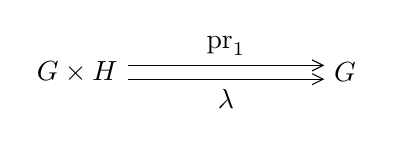
\begin{tikzpicture}[baseline=(lhs.base)]
  \node (lhs) {$G\times H$};
  \node[right=2.5cm of lhs] (rhs) {$G$};
  \draw[-{Straight Barb[length=4pt,width=4pt]}]
    ([yshift=2.5pt]lhs.east) --
    node[above] {$\operatorname{pr}_1$}
    ([yshift=2.5pt]rhs.west);
  \draw[-{Straight Barb[length=4pt,width=4pt]}]
    ([yshift=-2.5pt]lhs.east) --
    node[below] {$\lambda$}
    ([yshift=-2.5pt]rhs.west);
\end{tikzpicture}

% END INCLUDED SGA3_English_current_buildable_source_20260823/source/inputs/VII/native_diagrams/exp7/viib_15_95/diag_107.tex

\end{center}
is an equivalence pair in \(\operatorname{Vaf}/k\)
\textup{(cf.\ V, 2.b)}. Recall \textup{(cf.\ \SGARefLink{sga3:VIIB:1.2.C}{1.2.C})} that the
cokernel \(G/H\) of this pair is defined as follows.

Let \(\mathcal O(G)\) and \(\mathcal O(H)\) be the affine algebras of
\(G\) and \(H\), let
\[
  \Delta:\mathcal O(G)
  \longrightarrow
  \mathcal O(G)\widehat\otimes_k\mathcal O(G)
\]
be the diagonal morphism of \(\mathcal O(G)\), and let \(I\) be the
kernel of
\[
  u^\natural:\mathcal O(G)\longrightarrow\mathcal O(H).
\]
By \SGARefLink{sga3:VIIB:1.3.prop}{Proposition 1.3}, the morphism \(u^\natural\) induces an
isomorphism
\[
  \mathcal O(G)/I\xrightarrow{\ \sim\ }\mathcal O(H).
\]
The affine algebra \(\mathcal O(G/H)\) of \(G/H\) is then the kernel
of the pair
\begin{center}
  \phantomsection
  \label{sga3:VIIB:2.4:affine-equalizer-pair}
  % SGA3-VII-DIAG-108
  % BEGIN INCLUDED SGA3_English_current_buildable_source_20260823/source/inputs/VII/native_diagrams/exp7/viib_15_95/diag_108.tex
% SGA3-VII-DIAG-108
% Authority: Exp7B-13oct24.pdf, local p. 51.
% Crop: figures/Exp7B_localp051_quotient_affine_equalizer_pair.png
% Locator: tex/components/42_expose_VIIB_section24_formal_group_quotients_en.tex, Loop 1 line 66.
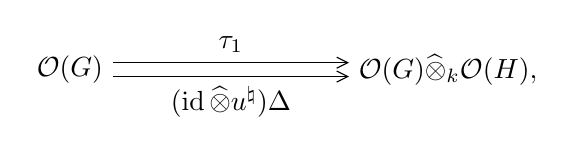
\begin{tikzpicture}[baseline=(lhs.base)]
  \node (lhs) {$\mathcal O(G)$};
  \node[right=3cm of lhs] (rhs)
    {$\mathcal O(G)\widehat\otimes_k\mathcal O(H),$};
  \draw[-{Straight Barb[length=4pt,width=4pt]}]
    ([yshift=2.5pt]lhs.east) --
    node[above] {$\tau_1$}
    ([yshift=2.5pt]rhs.west);
  \draw[-{Straight Barb[length=4pt,width=4pt]}]
    ([yshift=-2.5pt]lhs.east) --
    node[below] {$(\operatorname{id}\widehat\otimes u^\natural)\Delta$}
    ([yshift=-2.5pt]rhs.west);
\end{tikzpicture}

% END INCLUDED SGA3_English_current_buildable_source_20260823/source/inputs/VII/native_diagrams/exp7/viib_15_95/diag_108.tex

\end{center}
where \(\tau_1(x)=x\widehat\otimes1\). Thus
\[
  \mathcal O(G/H)
  =
  \bigl\{
    x\in\mathcal O(G)
    \mathrel{\big|}
    \Delta(x)-x\widehat\otimes1
    \in\mathcal O(G)\widehat\otimes I
  \bigr\}.
\]

If, moreover, \(H\) is topologically flat over \(k\), then
\(\operatorname{pr}_1\) is topologically flat, and \SGARefLink{sga3:VIIB:1.4.thm}{Theorem 1.4} gives
the following result.

\medskip
\noindent\textbf{Theorem.}
\phantomsection
\label{sga3:VIIB:2.4:theorem}
{\itshape Let \(u:H\to G\) be a monomorphism of formal
\(k\)-groups. Suppose that \(H\) is topologically flat over \(k\).
Then the projection
\[
  p:G\longrightarrow G/H
\]
is surjective and topologically flat, there is an isomorphism
\[
  G\times H
  \xrightarrow{\ \sim\ }
  G\times_{G/H}G,
  \tag{*}\label{sga3:VIIB:2.4:equation:quotient-fiber-product-star}
\]
and \(G/H\) represents the quotient sheaf for the flat topology.

Consequently, \(G/H\) has a canonical structure of an object on which
\(G\) acts, and \(p:G\to G/H\) is an equivariant morphism. If, in
addition, \(u\) identifies \(H\) with a normal subgroup of \(G\),
then \(G/H\) has a canonical structure of formal \(k\)-group for
which \(p:G\to G/H\) is a morphism of formal \(k\)-groups, and \(H\)
is the kernel of \(p\).}

Indeed, the first assertion follows from \SGARefLink{sga3:VIIB:1.4.thm}{1.4}, and the other two from
\SGARefLink{sga3:iv:corollary:5:2:2}{Exposé IV, Corollaries 5.2.2} and \SGARefLink{sga3:VIIB:5.2.4}{5.2.4}.

\medskip
\noindent\textbf{Corollary.}
\phantomsection
\label{sga3:VIIB:2.4:corollary}
\footnote{\label{sga3:VIIB:nde:91}The editors made this corollary
explicit; it is used, for example, in \SGARefLink{sga3:VIIB:5.2.1:section-proposition}{5.2.1} and \SGARefLink{sga3:VIIB:5.2.3}{5.2.3}.}
{\itshape Let \(G\) be a formal \(k\)-group and \(H\) a formal
subgroup of \(G\). Let \(A\), \(A/J\), and \(B\) be the affine
algebras of \(G\), \(H\), and \(G/H\), respectively; let \(I_A\) be
the augmentation ideal of \(A\), and put \(I_B=B\cap I_A\). Suppose
that \(H\) is topologically flat over \(k\). Then
\[
  J=AI_B,
\]
the closed ideal generated by \(I_B\).}

Indeed, the projection \(B\to B/I_B\) corresponds to the unit section
\[
  e:\operatorname{Spf}(k)\longrightarrow G/H
\]
of \(G/H\). By \textup{(*)}, \(H\) is identified with the fiber
product
\[
  \operatorname{Spf}(k)\times_{G/H}G.
\]
Its affine algebra \(A/J\) is therefore identified with
\[
  (B/I_B)\widehat\otimes_BA
  \simeq
  A/AI_B.
\]

% END INCLUDED SGA3_English_current_buildable_source_20260823/source/inputs/VII/tex/components/42_expose_VIIB_section24_formal_group_quotients_en.tex

% BEGIN INCLUDED SGA3_English_current_buildable_source_20260823/source/inputs/VII/tex/components/43_expose_VIIB_section24A_semidirect_products_en.tex
% SGA 3, Expose VII_B, English reconstruction -- Loop 1.
% Scope: authority local pages 52--53, Section 2.4.A in full,
% stopping immediately before Section 2.4.B.
% Combined-reader pages: 565--566. Re-edition printed pages: 554--555.
% Editorial note in scope: 92 (shared by 2.4.A and 2.4.B).
% Authority: Polo--Gille Exp7B-13oct24.pdf,
% SHA-256 D303690E0195654BBE7C3DAA5D89EA23E24CD709A3575217234AC19AE8836694.
% Jacob Reinhold's CC BY 4.0 Markdown was consulted as comparison lineage.
% The two genuine diagrams are exact PDF-derived Loop 1 source crops;
% all ordinary mathematics is native LaTeX.

\subsubsection*{2.4.A}
\phantomsection
\label{sga3:VIIB:2.4.A}

Let \(G\) and \(Q\) be formal \(k\)-groups that are topologically
flat. Suppose that there are homomorphisms
\[
  \sigma:Q\longrightarrow G
  \qquad\text{and}\qquad
  \pi:G\longrightarrow Q
\]
such that
\[
  \pi\circ\sigma=\operatorname{id}_Q.
\]
\footnote{\label{sga3:VIIB:nde:92}The editors added paragraphs
2.4.A and \SGARefLink{sga3:VIIB:2.4.B}{2.4.B}, which will be useful in \SGARefLink{sga3:VIIB:5.1.3}{5.1.3} and \SGARefLink{sga3:VIIB:2.9}{2.9},
respectively.}
In particular, \(\sigma\) is a monomorphism, so \(Q\) is a formal
subgroup of \(G\) \textup{(cf.\ \SGARefLink{sga3:VIIB:1.3}{Remark 1.3})}. Let
\[
  N=\operatorname{Ker}(\pi)
\]
and let \(\sigma'\) be the inclusion \(N\hookrightarrow G\).
Then \(G\) is the semidirect product of \(N\) by \(Q\)
\textup{(cf.\ I, \SGARefLink{sga3:i:proposition:2-3-8}{2.3.8})}. In other words, for every
\[
  B\in\operatorname{Ob}(\operatorname{Alf}/k),
\]
identify \(N(B)\) and \(Q(B)\) with their images in \(G(B)\) under
\(\sigma'\) and \(\sigma\). Then \(N(B)\) is a normal subgroup of
\(G(B)\), and the map
\begin{equation}
  \mu:N(B)\times Q(B)\longrightarrow G(B),
  \qquad
  (x,q)\longmapsto xq
  \tag{1}
  \label{sga3:VIIB:2.4.A:eq1}
\end{equation}
is bijective.

The morphism of formal \(k\)-varieties
\begin{equation}
  \theta:G(B)\longrightarrow N(B),
  \qquad
  g\longmapsto g\cdot\sigma\pi(g^{-1})
  \tag{2}
  \label{sga3:VIIB:2.4.A:eq2}
\end{equation}
is then a retraction of \(\sigma'\), and the inverse of \(\mu\) is
\begin{equation}
  g\longmapsto\bigl(\theta(g),\pi(g)\bigr).
  \tag{3}
  \label{sga3:VIIB:2.4.A:eq3}
\end{equation}
If \(p:G\to G/Q\) denotes the quotient projection, then
\[
  p\circ\sigma':N\longrightarrow G/Q
\]
is an isomorphism of formal \(k\)-varieties.

\smallskip
\noindent\emph{Source note.}
The Polo--Gille text prints
\(\theta\circ\sigma':N\to G/Q\) here. Since
\(\theta:G\to N\), that composite is ill-typed; the isomorphism
with the displayed source and target is the quotient composite
\(p\circ\sigma'\).

\smallskip
In particular, \(N\) is topologically flat over \(k\), by \SGARefLink{sga3:VIIB:1.4.thm}{1.4}
\textup{\SGARefLink{sga3:vii:paragraph:5-1:equation:ii}{(ii)}}. Let
\[
  \alpha:Q\times N\longrightarrow N
\]
and
\[
  \beta:G\times N=N\times Q\times N\longrightarrow N
\]
be the maps defined on points by
\[
  \alpha(q,y)=qyq^{-1},
  \qquad
  \beta(x,q,y)=x\alpha(q,y).
\]
Then the following diagram is commutative:
\begin{center}
  \phantomsection
  \label{sga3:VIIB:2.4.A:eq4-diagram}
  % SGA3-VII-DIAG-109
  % BEGIN INCLUDED SGA3_English_current_buildable_source_20260823/source/inputs/VII/native_diagrams/exp7/viib_15_95/diag_109.tex
% SGA3-VII-DIAG-109
% Authority: Exp7B-13oct24.pdf, local p. 53.
% Crop: figures/Exp7B_localp053_semidirect_product_diagram4.png
% Locator: tex/components/43_expose_VIIB_section24A_semidirect_products_en.tex, Loop 1 line 101.
\begin{tikzcd}[row sep=3.2em,column sep=3.5em]
{} \arrow[d,phantom,"\textup{(4)}" description]
  & G\times G
  \arrow[r,"{\operatorname{id}\times\theta}"]
  \arrow[d,"m_G"']
  & G\times N
      \arrow[r,"{\theta\times\operatorname{id}}"]
      \arrow[d,"\beta"]
  & N\times N \arrow[dl,"m_N"] \\
{} & G \arrow[r,"\theta"] & N & {.}
\end{tikzcd}

% END INCLUDED SGA3_English_current_buildable_source_20260823/source/inputs/VII/native_diagrams/exp7/viib_15_95/diag_109.tex

\end{center}

This can be expressed as follows in terms of the affine algebras
\(A\), \(A_0\), and \(A'\) of \(G\), \(Q\), and \(N\)
\textup{(cf.\ \SGARefLink{sga3:VIIB:5.1.3}{5.1.3} below)}. Let
\[
  \rho':A\longrightarrow A',
  \qquad
  \rho:A\longrightarrow A_0,
  \qquad
  \tau:A_0\longrightarrow A
\]
be the homomorphisms of \(k\)-bialgebras corresponding to
\(\sigma'\), \(\sigma\), and \(\pi\), and put
\[
  I=\operatorname{Ker}(\rho).
\]
By the preceding corollary, \(A'\) is identified with
\[
  A\big/\overline{A\,\tau(J_0)},
\]
where \(J_0\) is the augmentation ideal of \(A_0\).

On the other hand, let \(B\) be the affine algebra of \(G/Q\).
It is the kernel of the pair of morphisms
\phantomsection
\label{sga3:VIIB:2.4.A:affine-equalizer-pair}
\begin{equation*}
  A
  \mathrel{\overset{\tau_1}
    {\underset{(\operatorname{id}_A\widehat\otimes\rho)
      \circ\Delta_A}{\rightrightarrows}}}
  A\widehat\otimes_kA_0,
\end{equation*}
where \(\tau_1(x)=x\widehat\otimes1\). Thus
\[
  B
  =
  \bigl\{
    x\in A
    \mathrel{\big|}
    \Delta_A(x)-x\widehat\otimes1
    \in A\widehat\otimes I
  \bigr\}.
\]
Let
\[
  \gamma=\theta^\natural:A'\longrightarrow A
\]
be the corresponding continuous homomorphism of \(k\)-algebras.
It is a section of \(\rho'\), and it is an isomorphism of profinite
\(k\)-algebras from \(A'\) onto \(B\). Moreover,
\[
  \tau=\pi^\natural
\]
identifies \(A_0\) with a sub-bialgebra of \(A\), namely the affine
algebra of the quotient \(N\backslash G\).

It follows from equations~\eqref{sga3:VIIB:2.4.A:eq1}
and~\eqref{sga3:VIIB:2.4.A:eq3} that there is an
isomorphism of profinite \(k\)-algebras
\begin{equation}
  A'\widehat\otimes_kA_0
  \xrightarrow{\ \sim\ }
  A,
  \qquad
  a'\widehat\otimes a_0
  \longmapsto
  \gamma(a')\tau(a_0),
  \tag{*}
  \label{sga3:VIIB:2.4.A:star}
\end{equation}
whose inverse is the map
\[
  a\longmapsto
  (\rho'\widehat\otimes\rho)\Delta_A(a).
\]

Finally, identify \(A'\) with its image in \(A\) under \(\gamma\),
so that the projection \(A\to A'\) is then \(\gamma\rho'\).
Writing \(\Delta_{A'}\) for the comultiplication of \(A'\), one
deduces from \hyperref[sga3:VIIB:2.4.A:eq4-diagram]{\textup{(4)}}
that
\[
  \Delta_A(A')\subset A\widehat\otimes A'
\]
and that the following diagram is commutative:
\begin{center}
  \phantomsection
  \label{sga3:VIIB:2.4.A:Aprime-comultiplication-square}
  % SGA3-VII-DIAG-110
  % BEGIN INCLUDED SGA3_English_current_buildable_source_20260823/source/inputs/VII/native_diagrams/exp7/viib_15_95/diag_110.tex
% SGA3-VII-DIAG-110
% Authority: Exp7B-13oct24.pdf, local p. 53.
% Crop: figures/Exp7B_localp053_Aprime_comultiplication_square.png
% Locator: tex/components/43_expose_VIIB_section24A_semidirect_products_en.tex, Loop 1 line 193.
\begin{tikzcd}[row sep=3em,column sep=3.7em]
A' \arrow[r,"\Delta_A"] \arrow[d,equals]
  & A\widehat\otimes A' \arrow[d,"{\gamma\rho'\widehat\otimes
                                      \operatorname{id}}" right] \\
A' \arrow[r,"\Delta_{A'}"]
  & A'\widehat\otimes A'
\end{tikzcd}

% END INCLUDED SGA3_English_current_buildable_source_20260823/source/inputs/VII/native_diagrams/exp7/viib_15_95/diag_110.tex

\end{center}
Consequently, one also has
\[
  \gamma\rho'\circ c_A=c_{A'},
\]
where \(c_A\) and \(c_{A'}\) are the antipodes of \(A\) and \(A'\),
respectively. On the other hand, writing \(m_A\) for multiplication
in \(A\), equation~\eqref{sga3:VIIB:2.4.A:eq2} gives, for every
\(a\in A\),
\[
  \gamma\rho'(a)
  =
  \bigl(
    m_A
    \circ
    (\operatorname{id}_A\widehat\otimes\tau\rho c_A)
    \circ
    \Delta_A
  \bigr)(a).
\]

% END INCLUDED SGA3_English_current_buildable_source_20260823/source/inputs/VII/tex/components/43_expose_VIIB_section24A_semidirect_products_en.tex

% BEGIN INCLUDED SGA3_English_current_buildable_source_20260823/source/inputs/VII/tex/components/44_expose_VIIB_section24B_covariant_semidirect_products_en.tex
% SGA 3, Expose VII_B, English reconstruction -- Loop 1.
% Scope: authority local pages 53--54, Section 2.4.B in full,
% stopping immediately before Proposition 2.4.1.
% Combined-reader pages: 566--567. Re-edition printed pages: 555--556.
% Authority: Polo--Gille Exp7B-13oct24.pdf,
% SHA-256 D303690E0195654BBE7C3DAA5D89EA23E24CD709A3575217234AC19AE8836694.
% Jacob Reinhold's CC BY 4.0 Markdown was consulted as comparison lineage.
% Editorial note 92 is attached to 2.4.A and explicitly covers both 2.4.A
% and 2.4.B; it is not duplicated here.
% The one genuine diagram is an exact PDF-derived Loop 1 source crop;
% all ordinary mathematics is native LaTeX.

\subsubsection*{2.4.B}
\phantomsection
\label{sga3:VIIB:2.4.B}

Suppose, for simplicity, that \(k\) is Artinian. The preceding
discussion can then be expressed more simply in terms of the
covariant bialgebras of \(G\), \(Q\), and \(N\). Indeed, since
\[
  G=N\times Q
\]
as formal \(k\)-varieties, one has
\[
  \mathbf H(G)
  =
  \mathbf H(N)\otimes_k\mathbf H(Q)
\]
as \(k\)-coalgebras. Moreover, since multiplication in \(G\) is
given by
\[
  (x,q)\cdot(x',q')
  =
  \bigl(x\alpha(q,x'),qq'\bigr),
  \qquad
  \alpha(q,x')=qx'q^{-1},
\]
multiplication in \(\mathbf H(G)\) is given, for
\(x\in\mathbf H(N)\) and \(q\in\mathbf H(Q)\), by
\[
  (x\otimes q)\cdot(x'\otimes q')
  =
  x\phi(q,x')\otimes qq',
\]
where
\[
  \phi:
  \mathbf H(Q)\otimes_k\mathbf H(N)
  \longrightarrow
  \mathbf H(N)
\]
is the morphism of \(k\)-coalgebras induced by \(\alpha\).

The morphism \(\alpha\) is the following composite. Here
\(\delta_G\) and \(m_G\) denote, respectively, the diagonal and
multiplication morphisms of \(G\), \(c_Q\) is inversion in \(Q\),
and
\[
  v(q\otimes q'\otimes x)=q\otimes x\otimes q'.
\]
\begin{center}
  \phantomsection
  \label{sga3:VIIB:2.4.B:conjugation-composite}
  % SGA3-VII-DIAG-111
  % BEGIN INCLUDED SGA3_English_current_buildable_source_20260823/source/inputs/VII/native_diagrams/exp7/viib_15_95/diag_111.tex
% SGA3-VII-DIAG-111
% Authority: Exp7B-13oct24.pdf, local p. 54.
% Crop: figures/Exp7B_localp054_semidirect_conjugation_composite.png
% Locator: tex/components/44_expose_VIIB_section24B_covariant_semidirect_products_en.tex, Loop 1 line 64.
\(
Q\times N
\xrightarrow{\ v\circ(\delta_G\times\operatorname{id})\ }
Q\times N\times Q
\xrightarrow{\ \operatorname{id}\times\operatorname{id}\times c_Q\ }
Q\times N\times Q
\xrightarrow{\ m_G\ }G,
\)

% END INCLUDED SGA3_English_current_buildable_source_20260823/source/inputs/VII/native_diagrams/exp7/viib_15_95/diag_111.tex

\end{center}
Writing \(c_Q\) also for the antipode of \(\mathbf H(Q)\), we obtain
\[
  \phi(q\otimes x')
  =
  \sum_i q_i x'c_Q(q_i')
  \quad\text{if}\quad
  \Delta_{\mathbf H(Q)}(q)
  =
  \sum_i q_i\otimes q_i'.
  \tag{\(\star\)}\label{sga3:VIIB:2.4.B:equation:covariant-antipode-star}
\]

In particular, let \(M\) be an abstract group and suppose that
\(\mathbf H(Q)\) is the group algebra \(kM\), so that
\[
  Q=\operatorname{Spf}^{*}kM
\]
is the constant formal \(k\)-group \(M_k\). Then for every
\(\gamma\in M\) and \(x'\in\mathbf H(N)\),
\[
  \phi(\gamma\otimes x')
  =
  \gamma x'\gamma^{-1}.
\]
This defines an action of \(M\) on \(\mathbf H(N)\) by Hopf-algebra
automorphisms.

% END INCLUDED SGA3_English_current_buildable_source_20260823/source/inputs/VII/tex/components/44_expose_VIIB_section24B_covariant_semidirect_products_en.tex

% BEGIN INCLUDED SGA3_English_current_buildable_source_20260823/source/inputs/VII/tex/components/45_expose_VIIB_proposition241_kernel_quotient_image_en.tex
% SGA 3, Expose VII_B, English reconstruction -- Loop 1.
% Scope: authority local pages 54--55, Proposition 2.4.1, its proof,
% and its corollary in full, stopping immediately before 2.4.2.
% Combined-reader pages: 567--568. Re-edition printed pages: 556--557.
% Original-edition marginal locator in scope: 521.
% Editorial note in scope: 93.
% Authority: Polo--Gille Exp7B-13oct24.pdf,
% SHA-256 D303690E0195654BBE7C3DAA5D89EA23E24CD709A3575217234AC19AE8836694.
% Jacob Reinhold's CC BY 4.0 Markdown was consulted as comparison lineage.
% The one genuine diagram is an exact PDF-derived Loop 1 source crop.

\medskip
\noindent\textbf{Proposition 2.4.1.}
\phantomsection
\label{sga3:VIIB:2.4.1}
{\itshape Let \(f:G\to K\) be a morphism of formal \(k\)-groups. If
\[
  H=\ker(f)
\]
is topologically flat over \(k\), the homomorphism
\[
  f':G/H\longrightarrow K
\]
induced by \(f\) is a monomorphism.}

This is a consequence of the results of Exposé IV,\footnote{%
\label{sga3:VIIB:nde:93}See \SGARefLink{sga3:iv:remark:5:2:6}{Exposé IV, 5.2.6}.} but we give a direct
proof. Let \(T\) be a formal variety of finite length over \(k\), and
let \(t\in(G/H)(T)\) be such that \(f'\circ t\) is the identity
element of \(K(T)\). We must show that \(t\) is the identity element
of \((G/H)(T)\). Let
\[
  p:G\longrightarrow G/H
\]
be the projection, and let
\[
  X=T\times_{G/H}G.
\]

By \SGARefLink{sga3:VIIB:2.4}{2.4}, \(p\) is surjective and topologically flat. The same is
therefore true of
\[
  \operatorname{pr}_1:X\longrightarrow T.
\]
By \SGARefLink{sga3:VIIB:1.3.1}{Proposition 1.3.1}, \(\operatorname{pr}_1\) is consequently an
epimorphism, so it is enough to show that
\(t\circ\operatorname{pr}_1\) is the identity element of
\((G/H)(X)\).

Let \(\operatorname{pr}_2:X\to G\) be the second projection. We have
\[
  t\circ\operatorname{pr}_1
  =
  p\circ\operatorname{pr}_2,
\]
and hence
\[
  1
  =
  f'\circ t\circ\operatorname{pr}_1
  =
  f'\circ p\circ\operatorname{pr}_2
  =
  f\circ\operatorname{pr}_2.
\]
The exact sequence
\begin{center}
  \phantomsection
  \label{sga3:VIIB:2.4.1:exact-sequence}
  % SGA3-VII-DIAG-112
  % BEGIN INCLUDED SGA3_English_current_buildable_source_20260823/source/inputs/VII/native_diagrams/exp7/viib_15_95/diag_112.tex
% SGA3-VII-DIAG-112
% Authority: Exp7B-13oct24.pdf, local p. 54.
% Crop: figures/Exp7B_localp054_proposition241_exact_sequence.png
% Locator: tex/components/45_expose_VIIB_proposition241_kernel_quotient_image_en.tex, Loop 1 line 70.
\(
1\longrightarrow H\longrightarrow G\xrightarrow{\ f\ }K
\)

% END INCLUDED SGA3_English_current_buildable_source_20260823/source/inputs/VII/native_diagrams/exp7/viib_15_95/diag_112.tex

\end{center}
therefore shows that \(\operatorname{pr}_2\) factors through \(H\).
Thus \(p\circ\operatorname{pr}_2\) is the zero morphism. Since
\[
  p\circ\operatorname{pr}_2
  =
  t\circ\operatorname{pr}_1,
\]
this proves the proposition.

The following corollary follows. Write
\(\mathcal O(G)\), \(\mathcal O(K)\), and \(\mathcal O(G/H)\) for
the affine algebras of \(G\), \(K\), and \(G/H\), respectively. We
saw in \SGARefLink{sga3:VIIB:2.4}{2.4} that \(p\) induces an injection
\[
  \mathcal O(G/H)\lhook\joinrel\longrightarrow\mathcal O(G).
\]
Moreover, since \(f':G/H\to K\) is a monomorphism, \SGARefLink{sga3:VIIB:1.3.prop}{Proposition 1.3}
shows that
\[
  \mathcal O(K)\longrightarrow\mathcal O(G/H)
\]
is surjective. Hence:

\medskip
\noindent\textbf{Corollary.}
\phantomsection
\label{sga3:VIIB:2.4.1:corollary}
{\itshape Let \(f:G\to K\) be a morphism of formal \(k\)-groups and
let \(H=\ker(f)\). If \(H\) is topologically flat over \(k\), then
\[
  \mathcal O(G/H)
\]
is the image of \(\mathcal O(K)\) in \(\mathcal O(G)\).}

% END INCLUDED SGA3_English_current_buildable_source_20260823/source/inputs/VII/tex/components/45_expose_VIIB_proposition241_kernel_quotient_image_en.tex

% BEGIN INCLUDED SGA3_English_current_buildable_source_20260823/source/inputs/VII/tex/components/46_expose_VIIB_section242_abelian_categories_en.tex
% SGA 3, Expose VII_B, English reconstruction -- Loop 1.
% Scope: authority local page 55, Section 2.4.2 in full, stopping
% immediately before Section 2.5.
% Combined-reader page: 568. Re-edition printed page: 557.
% Original-edition marginal locator in scope: 522.
% Editorial note in scope: 94.
% Authority: Polo--Gille Exp7B-13oct24.pdf,
% SHA-256 D303690E0195654BBE7C3DAA5D89EA23E24CD709A3575217234AC19AE8836694.
% Jacob Reinhold's CC BY 4.0 Markdown was consulted as comparison lineage.
% No genuine diagram occurs in this span.

\subsubsection*{2.4.2}
\phantomsection
\label{sga3:VIIB:2.4.2}

Retain the preceding notation and suppose that \(H\) and \(G\) are
topologically flat over \(k\). Then \(G\) is topologically flat both
over \(k\) and over \(G/H\); hence, by \SGARefLink{sga3:VIIB:1.3.3}{1.3.3}, \(G/H\) is
topologically flat over \(k\). Consequently, by \SGARefLink{sga3:VIIB:2.4}{2.4}, the canonical
projection
\[
  q:K\longrightarrow\operatorname{Coker}(f')
\]
is topologically flat, and \(f'\) is an isomorphism from \(G/H\) onto
\(\ker(q)\). It is also clear that
\[
  \operatorname{Coker}(f)
  =
  \operatorname{Coker}(f').
\]
Thus, under the hypothesis that \(G\) and \(H=\ker(f)\) are
topologically flat over \(k\), we have obtained an isomorphism between
\(\ker(q)\), the image of \(f\), and
\[
  G/\ker(f),
\]
the coimage of \(f\). This proves the following theorem.

\medskip
\noindent\textbf{Theorem.}
\phantomsection
\label{sga3:VIIB:2.4.2:theorem}
{\itshape Let \(k\) be a field. The commutative formal \(k\)-groups
form an abelian category.}

\medskip
\noindent\textbf{Corollary.}
\phantomsection
\label{sga3:VIIB:2.4.2:corollary}
{\itshape Let \(k\) be a field. The commutative affine
\(k\)-group schemes form an abelian category.}
\footnote{\label{sga3:VIIB:nde:94}See also the remarks following
Exposé VI\textsubscript{A}, \SGARefLink{cor:sga3-VIA-5.4.3}{5.4.3}.}

This follows from the theorem and the equivalence of categories in
\SGARefLink{sga3:VIIB:2.2.2}{2.2.2}.

% END INCLUDED SGA3_English_current_buildable_source_20260823/source/inputs/VII/tex/components/46_expose_VIIB_section242_abelian_categories_en.tex

% BEGIN INCLUDED SGA3_English_current_buildable_source_20260823/source/inputs/VII/tex/components/47_expose_VIIB_section25_etale_formal_groups_en.tex
% SGA 3, Expose VII_B, English reconstruction -- Loop 1.
% Scope: authority local pages 55--56, Section 2.5 through its main
% proposition and Remark 2.5.A, stopping immediately before 2.5.1.
% Combined-reader pages: 568--569. Re-edition printed pages: 557--558.
% Original-edition marginal locator in scope: 522.
% Editorial notes in scope: 95--96.
% Authority: Polo--Gille Exp7B-13oct24.pdf,
% SHA-256 D303690E0195654BBE7C3DAA5D89EA23E24CD709A3575217234AC19AE8836694.
% Jacob Reinhold's CC BY 4.0 Markdown was consulted as comparison lineage.
% No genuine diagram occurs in this span.

\subsection*{2.5}
\phantomsection
\label{sga3:VIIB:2.5}
\addcontentsline{toc}{subsection}{2.5. Étale formal groups}

A formal \(k\)-group is said to be \emph{étale} if its underlying
formal variety is étale \textup{(cf.\ \SGARefLink{sga3:VIIB:1.6}{1.6})}. Such formal groups have
a very simple structure. Suppose that \(k\) is local, let \(\kappa\)
be its residue field, let \(\kappa_s\) be a separable closure of
\(\kappa\), and let
\[
  \Gamma=\operatorname{Gal}(\kappa_s/\kappa)
\]
be the topological Galois group. A \emph{\(\Gamma\)-set} means a set
\(E\) with a continuous action of \(\Gamma\); equivalently, the
stabilizer of every element \(x\in E\) is an open subgroup of
\(\Gamma\).

For every formal \(k\)-variety \(X\), put
\[
  X(\kappa_s)
  =
  \varinjlim_{\ell}X(\ell),
\]
where \(\ell\) ranges over the finite extensions of \(\kappa\)
contained in \(\kappa_s\).\footnote{%
\label{sga3:VIIB:nde:95}If
\([\kappa_s:\kappa]=\infty\), then \(\kappa_s\) is not a profinite
\(\kappa\)-algebra, so the preceding notation is an abuse. The
editors also supplied the details that follow.}
The group \(\Gamma\) acts continuously on every \(X(\ell)\), and
hence on \(X(\kappa_s)\). Moreover, if
\[
  X_\kappa=X\widehat\otimes_k\kappa
  \qquad\text{\textup{(cf.\ 1.6.C)}},
\]
then \(X(\ell)=X_\kappa(\ell)\) for every \(\ell\), and therefore
\[
  X(\kappa_s)=X_\kappa(\kappa_s).
\]

Now suppose that \(X\) is étale over \(k\). Then \(X_\kappa\) is the
formal \(\kappa\)-variety that is the disjoint union of the
\(\operatorname{Spec}\kappa(x)\), for \(x\in X\). If
\(X'_\kappa\) denotes the \(\kappa\)-scheme given by the same
disjoint union, then
\[
\begin{aligned}
  X_\kappa(\kappa_s)
  &=
  X'_\kappa(\kappa_s)
  \\
  &=
  \operatorname{Hom}_{\operatorname{Sch}/\kappa}
  \bigl(\operatorname{Spec}\kappa_s,X'_\kappa\bigr).
\end{aligned}
\]

Let \(\mathcal C\) be the full subcategory
\[
  \operatorname{Sch}^{\mathrm{\acute{e}t}}/\kappa
  \subset
  \operatorname{Sch}/\kappa
\]
of étale \(\kappa\)-schemes. It is known that
\[
  X'\longmapsto X'(\kappa_s)
\]
is an equivalence from \(\mathcal C\) onto the category
\(\mathcal C'\) of \(\Gamma\)-sets
\textup{(cf.\ SGA 1, V, §§7--8, or \([DG70]\), §I.4, 6.4)}.
It therefore induces an equivalence between the category of group
objects in \(\mathcal C\) and the category of group objects in
\(\mathcal C'\). A group object in \(\mathcal C'\) is simply an
abstract group endowed with a continuous action of \(\Gamma\) by
group automorphisms; we call this a \emph{\(\Gamma\)-group}.

Taking into account the equivalences of \SGARefLink{sga3:VIIB:1.6.E}{1.6.E},
\[
  \operatorname{Vaf}^{\mathrm{\acute{e}t}}/k
  \xrightarrow{\ \sim\ }
  \operatorname{Vaf}^{\mathrm{\acute{e}t}}/\kappa
  \xrightarrow{\ \sim\ }
  \operatorname{Sch}^{\mathrm{\acute{e}t}}/\kappa,
\]
we obtain the following.

\medskip
\noindent\textbf{Proposition.}
\phantomsection
\label{sga3:VIIB:2.5:proposition}
{\itshape Let \(k\) be a local pseudocompact ring, \(\kappa\) its
residue field, \(\kappa_s\) a separable closure of \(\kappa\), and
\(\Gamma=\operatorname{Gal}(\kappa_s/\kappa)\).
\begin{enumerate}
\item[\textup{(i)}]
The functor \(X\mapsto X(\kappa_s)\) is an equivalence from the
category of étale formal \(k\)-varieties onto the category of
\(\Gamma\)-sets.

\item[\textup{(ii)}]
It induces an equivalence from the category of étale formal
\(k\)-groups onto the category of \(\Gamma\)-groups.
\end{enumerate}}

\medskip
\noindent\textbf{Remark 2.5.A.}
\phantomsection
\label{sga3:VIIB:2.5.A}
\footnote{\label{sga3:VIIB:nde:96}The editors added this remark.}
Let \(k\) be a field, let \(k_s\) be a separable closure of \(k\),
let \(G\) be an étale formal \(k\)-group, and put
\[
  M=G(k_s).
\]
Choose a set \(X\) of representatives for the orbits of
\(\Gamma=\operatorname{Gal}(k_s/k)\) in \(M\). For each \(x\in X\),
let \(\Gamma_x\) be its stabilizer, an open subgroup of finite index
in \(\Gamma\), and put
\[
  L_x=k_s^{\Gamma_x}.
\]
Then \(L_x/k\) has degree \([\Gamma:\Gamma_x]\)
\textup{(see, for example, \([BAlg]\), V, §10.10)}.

By the preceding equivalence of categories, the affine algebra
\(\mathcal A(G)\) of \(G\) is the product of the \(L_x\), endowed
with the product topology. The \(L_x\) are therefore exactly the
simple quotients
\[
  \mathcal A(G)/\mathfrak m,
\]
where \(\mathfrak m\) ranges over the open maximal ideals of
\(\mathcal A(G)\). Since these quotients correspond by duality to
the simple subcoalgebras of \(\mathbf H(G)\), the coalgebra
\(\mathbf H(G)\) is pointed---that is,
\[
  \dim_kC=1
\]
for every simple subcoalgebra \(C\)---if and only if \(L_x=k\) for
every \(x\). In that case, \(\mathcal A(G)\) is the topological
algebra \(k^M\), so \(\mathbf H(G)\) is the group algebra \(kM\), and
\[
  M
  =
  \bigl\{
    x\in\mathbf H(G)
    \mathrel{\big|}
    \varepsilon(x)=1,\ \Delta(x)=x\otimes x
  \bigr\}
  =
  G(k).
\]

% END INCLUDED SGA3_English_current_buildable_source_20260823/source/inputs/VII/tex/components/47_expose_VIIB_section25_etale_formal_groups_en.tex

% BEGIN INCLUDED SGA3_English_current_buildable_source_20260823/source/inputs/VII/tex/components/48_expose_VIIB_section251_infinitesimal_identity_component_en.tex
% SGA 3, Expose VII_B, English reconstruction -- Loop 1.
% Scope: authority local pages 56--57, Section 2.5.1 in full,
% stopping immediately before 2.5.2.
% Combined-reader pages: 569--570. Re-edition printed pages: 558--559.
% Original-edition marginal locator in scope: 523.
% Editorial notes in scope: 97--99.
% Authority: Polo--Gille Exp7B-13oct24.pdf,
% SHA-256 D303690E0195654BBE7C3DAA5D89EA23E24CD709A3575217234AC19AE8836694.
% Jacob Reinhold's CC BY 4.0 Markdown was consulted as comparison lineage.
% The three genuine diagrams are exact PDF-derived Loop 1 source crops.

\subsubsection*{2.5.1}
\phantomsection
\label{sga3:VIIB:2.5.1}

Suppose again that \(k\) is an arbitrary pseudocompact ring. Since
the functor
\[
  X\longmapsto X_e
\]
of \SGARefLink{sga3:VIIB:1.6.F}{1.6.F} commutes with finite products, it sends every formal group
\(G\) to an étale formal group \(G_e\). The morphism
\(p:X\to X_e\) of that result is functorial in \(X\), so in this
case
\[
  p:G\longrightarrow G_e
\]
is a morphism of formal groups.

Consider its kernel \(\ker(p)\).\footnote{%
\label{sga3:VIIB:nde:97}The editors supplied the details of the
original argument that follow.} It is the fiber product of the
diagram
\begin{center}
  \phantomsection
  \label{sga3:VIIB:2.5.1:kernel-fiber-square}
  % SGA3-VII-DIAG-113
  % BEGIN INCLUDED SGA3_English_current_buildable_source_20260823/source/inputs/VII/native_diagrams/exp7/viib_15_95/diag_113.tex
% SGA3-VII-DIAG-113
% Authority: Exp7B-13oct24.pdf, local p. 56.
% Crop: figures/Exp7B_localp056_kernel_etale_fiber_square.png
% Locator: tex/components/48_expose_VIIB_section251_infinitesimal_identity_component_en.tex, Loop 1 line 37.
\begin{tikzcd}[row sep=2.5em,column sep=3.8em]
{} & G \arrow[d,"p"] \\
\operatorname{Spf}(k) \arrow[r,"\varepsilon"]
  & G_e
\end{tikzcd}

% END INCLUDED SGA3_English_current_buildable_source_20260823/source/inputs/VII/native_diagrams/exp7/viib_15_95/diag_113.tex

\end{center}
where \(\varepsilon\) is the identity section of \(G_e\). Since
\(p\) induces a bijection on the underlying sets, it follows
\textup{(cf.\ \SGARefLink{sga3:VIIB:1.2}{1.2}, editorial note 41)} that the underlying set of
\(\ker(p)\) is the image of \(\operatorname{Spf}(k)\) under
\(\varepsilon\), and that, for every point \(s\) of
\(\operatorname{Spf}(k)\), the local algebra of \(\ker(p)\) at
\(\varepsilon(s)\) is
\[
  \mathcal O_{G,\varepsilon(s)}
  \widehat\otimes_{\mathcal O_{G_e,\varepsilon(s)}}
  \kappa(s).
\]
At each point \(\varepsilon(s)\), the residue field of
\(\mathcal O_{G,\varepsilon(s)}\) is \(\kappa(s)\), and hence
\[
  \mathcal O_{G_e,\varepsilon(s)}=\kappa(s),
  \qquad
  \mathcal O_{\ker(p),\varepsilon(s)}
  =
  \mathcal O_{G,\varepsilon(s)}.
\]

For these reasons, we call \(\ker(p)\) the \emph{infinitesimal
neighborhood of the identity} of \(G\), and write
\[
  \ker(p)=G_0.
\]
We have thus obtained the exact sequence
\begin{center}
  \phantomsection
  \label{sga3:VIIB:2.5.1:infinitesimal-exact-sequence}
  % SGA3-VII-DIAG-114
  % BEGIN INCLUDED SGA3_English_current_buildable_source_20260823/source/inputs/VII/native_diagrams/exp7/viib_15_95/diag_114.tex
% SGA3-VII-DIAG-114
% Authority: Exp7B-13oct24.pdf, local p. 57.
% Crop: figures/Exp7B_localp057_infinitesimal_exact_sequence.png
% Locator: tex/components/48_expose_VIIB_section251_infinitesimal_identity_component_en.tex, Loop 1 line 71.
\(
1\longrightarrow G_0\xrightarrow{\ \mathrm{incl.}\ }G
\xrightarrow{\ p\ }G_e.
\)

% END INCLUDED SGA3_English_current_buildable_source_20260823/source/inputs/VII/native_diagrams/exp7/viib_15_95/diag_114.tex

\end{center}

In what follows, we say that \(G\) is \emph{infinitesimal} if
\[
  G=G_0.
\]
\footnote{\label{sga3:VIIB:nde:98}The editors added the sentence that
follows.}
This is equivalent to saying that, for every
\(s\in\operatorname{Spf}(k)\), or equivalently for every continuous
morphism \(k\to\kappa\), where \(\kappa\) is a field with the
discrete topology, the identity is the unique element of
\(G(\kappa(s))\), respectively of \(G(\kappa)\).

Suppose in addition that \(G\) is topologically flat over
\(k\).\footnote{\label{sga3:VIIB:nde:99}The editors supplied the
details that follow.} By \SGARefLink{sga3:VIIB:1.6.1}{1.6.1}, the morphism
\[
  p:G\longrightarrow G_e
\]
is topologically flat. Since it is bijective, \SGARefLink{sga3:VIIB:1.3.1}{Proposition 1.3.1}
shows that it is an effective epimorphism. Consequently, \(G_e\) is
identified with the quotient \(G/G_0\). We have proved:

\medskip
\noindent\textbf{Corollary.}
\phantomsection
\label{sga3:VIIB:2.5.1:corollary}
{\itshape Let \(G\) be a formal group topologically flat over \(k\).
Then \(G_e\) is identified with the quotient \(G/G_0\); in other
words, there is an exact sequence of formal groups}
\begin{center}
  \phantomsection
  \label{sga3:VIIB:2.5.1:short-exact-sequence}
  % SGA3-VII-DIAG-115
  % BEGIN INCLUDED SGA3_English_current_buildable_source_20260823/source/inputs/VII/native_diagrams/exp7/viib_15_95/diag_115.tex
% SGA3-VII-DIAG-115
% Authority: Exp7B-13oct24.pdf, local p. 57.
% Crop: figures/Exp7B_localp057_infinitesimal_etale_short_exact_sequence.png
% Locator: tex/components/48_expose_VIIB_section251_infinitesimal_identity_component_en.tex, Loop 1 line 107.
\(
1\longrightarrow G_0\xrightarrow{\ \mathrm{incl.}\ }G
\xrightarrow{\ p\ }G_e\longrightarrow1.
\)

% END INCLUDED SGA3_English_current_buildable_source_20260823/source/inputs/VII/native_diagrams/exp7/viib_15_95/diag_115.tex

\end{center}

% END INCLUDED SGA3_English_current_buildable_source_20260823/source/inputs/VII/tex/components/48_expose_VIIB_section251_infinitesimal_identity_component_en.tex

% BEGIN INCLUDED SGA3_English_current_buildable_source_20260823/source/inputs/VII/tex/components/49_expose_VIIB_section252_perfect_field_splitting_en.tex
% SGA 3, Expose VII_B, English reconstruction -- Loop 1.
% Scope: authority local pages 57--58, Section 2.5.2 and
% Remark 2.5.2.A in full, stopping immediately before 2.5.3.
% Combined-reader pages: 570--571. Re-edition printed pages: 559--560.
% Original-edition marginal locator in scope: 524.
% Editorial notes in scope: 100--102.
% Authority: Polo--Gille Exp7B-13oct24.pdf,
% SHA-256 D303690E0195654BBE7C3DAA5D89EA23E24CD709A3575217234AC19AE8836694.
% Jacob Reinhold's CC BY 4.0 Markdown was consulted as comparison lineage.
% The two genuine diagrams are exact PDF-derived Loop 1 source crops.

\subsubsection*{2.5.2}
\phantomsection
\label{sga3:VIIB:2.5.2}

Suppose that \(k\) is a perfect field. In this case, we saw in \SGARefLink{sga3:VIIB:1.6.2}{1.6.2}
that the morphism
\[
  p:X\longmapsto X_e
\]
has a section
\[
  s:X_e\longrightarrow X
\]
that depends functorially on \(X\). Consequently, when \(X\) is a
formal group, this section is a morphism of formal groups. We thus
obtain:

\medskip
\noindent\textbf{Proposition.}
\phantomsection
\label{sga3:VIIB:2.5.2:proposition}
{\itshape When \(k\) is a perfect field, every formal \(k\)-group
\(G\) is canonically isomorphic to the semidirect product of an
infinitesimal group \(G_0\) and an étale group \(G_e\) acting on
\(G_0\).}\footnote{%
\label{sga3:VIIB:nde:100}The same argument also shows that, for an
arbitrary field \(k\), if all the residue fields of \(G\) are equal
to \(k\), then \(G_e\) is the constant \(k\)-group \((M)_k\), where
\[
  M=G(k)=\operatorname{Spf}^{*}\mathbf H(G),
\]
and \(\mathbf H(G)\) is the semidirect product of
\(\mathbf H(G_0)\) by the group algebra \(kM\); see the addition in
\SGARefLink{sga3:VIIB:2.9}{2.9} below.}

If, moreover, \(G\) is commutative, then \(G\) is the product of
\(G_0\) and \(G_e\). By \SGARefLink{sga3:VIIB:2.2.2}{2.2.2}, this canonical decomposition of
commutative formal \(k\)-groups corresponds to an analogous
decomposition of affine commutative \(k\)-group schemes; see \SGARefLink{sga3:VIIB:2.5.3}{2.5.3}
below.

\medskip
\noindent\textbf{Remark 2.5.2.A.}
\phantomsection
\label{sga3:VIIB:2.5.2.A}
\footnote{\label{sga3:VIIB:nde:101}The editors added this remark.}
When \(k\) is not perfect, the exact sequence
\[
  1\longrightarrow G_0\longrightarrow G\longrightarrow G_e
  \longrightarrow 1
\]
need not split. Consider the following example, taken from
\([DG70]\), §III.6, 8.6. Let \(k\) be a nonperfect field of
characteristic \(p>0\), choose
\[
  \lambda\in k\setminus k^p,
\]
and let \(L_\lambda\) be the abelian restricted \(p\)-Lie algebra
with basis \((x,y)\), whose symbolic \(p\)-th power
\textup{(cf.\ VII\textsubscript{A}, \SGARefLink{sga3:VIIA:5.2}{5.2})} is given by
\[
  x^{(p)}=x,
  \qquad
  y^{(p)}=\lambda x.
\]
Let
\[
  U_p(L_\lambda)
  =
  k[x,y]/(x^p-x,\ y^p-\lambda x)
\]
be the restricted enveloping algebra of \(L_\lambda\)
\textup{(cf.\ VII\textsubscript{A}, \SGARefLink{sga3:VIIA:5.3}{5.3})}, and let \(G_\lambda\)
be the commutative formal \(k\)-group whose affine algebra is
\(U_p(L_\lambda)\).

Then \(G_\lambda\) is a nonsplit extension of the constant étale
\(k\)-group \((\mathbb Z/p\mathbb Z)_k\) by the infinitesimal
\(k\)-group
\[
  \alpha_{p,k}=\operatorname{Spf}k[x]/(x^p).
\]
\phantomsection
\label{sga3:VIIB:2.5.2.A:alpha-p-source-note}
\noindent\textit{Source note.}\enspace
The French re-edition prints
\(\operatorname{Spf}k[x]/(x^p-x)\) here. That algebra is étale,
whereas the asserted kernel is the standard infinitesimal group
\(\alpha_{p,k}=\operatorname{Spf}k[x]/(x^p)\). Indeed, the kernel
fiber \(x=0\) in \(U_p(L_\lambda)\) has coordinate algebra
\(k[y]/(y^p)\). The English text uses the standard infinitesimal
reading while preserving the printed reading in this note.
Thus there is a nonsplit exact sequence of commutative formal
\(k\)-groups:\footnote{%
\label{sga3:VIIB:nde:102}The groups
\(\alpha_{p,k}\), \((\mathbb Z/p\mathbb Z)_k\), and \(G_\lambda\)
are also finite flat algebraic \(k\)-groups; see editorial note 84
in \SGARefLink{sga3:VIIB:2.2.2}{2.2.2}.}
\begin{center}
  \phantomsection
  \label{sga3:VIIB:2.5.2.A:nonsplit-formal-sequence}
  % SGA3-VII-DIAG-116
  % BEGIN INCLUDED SGA3_English_current_buildable_source_20260823/source/inputs/VII/native_diagrams/exp7/viib_15_95/diag_116.tex
% SGA3-VII-DIAG-116
% Authority: Exp7B-13oct24.pdf, local p. 58.
% Crop: figures/Exp7B_localp058_nonsplit_formal_group_exact_sequence.png
% Locator: tex/components/49_expose_VIIB_section252_perfect_field_splitting_en.tex, Loop 1 line 113.
\(
0\longrightarrow\boldsymbol{\alpha}_{p,k}
\longrightarrow G_\lambda
\longrightarrow(\mathbb Z/p\mathbb Z)_k
\longrightarrow0.
\)

% END INCLUDED SGA3_English_current_buildable_source_20260823/source/inputs/VII/native_diagrams/exp7/viib_15_95/diag_116.tex

\end{center}

By duality, this corresponds to a nonsplit exact sequence of
commutative algebraic \(k\)-groups:
\begin{center}
  \phantomsection
  \label{sga3:VIIB:2.5.2.A:nonsplit-dual-sequence}
  % SGA3-VII-DIAG-117
  % BEGIN INCLUDED SGA3_English_current_buildable_source_20260823/source/inputs/VII/native_diagrams/exp7/viib_15_95/diag_117.tex
% SGA3-VII-DIAG-117
% Authority: Exp7B-13oct24.pdf, local p. 58.
% Crop: figures/Exp7B_localp058_nonsplit_dual_algebraic_group_exact_sequence.png
% Locator: tex/components/49_expose_VIIB_section252_perfect_field_splitting_en.tex, Loop 1 line 122.
\(
0\longrightarrow\boldsymbol{\mu}_{p,k}
\longrightarrow D'(G_\lambda)
\longrightarrow\boldsymbol{\alpha}_{p,k}
\longrightarrow0
\)

% END INCLUDED SGA3_English_current_buildable_source_20260823/source/inputs/VII/native_diagrams/exp7/viib_15_95/diag_117.tex

\end{center}
where
\[
  \mu_{p,k}=\operatorname{Spec}k[t]/(t^p-1).
\]
In this way one obtains all extensions of \(\alpha_{p,k}\) by
\(\mu_{p,k}\); see \([DG70]\), §III.6, 8.6.

% END INCLUDED SGA3_English_current_buildable_source_20260823/source/inputs/VII/tex/components/49_expose_VIIB_section252_perfect_field_splitting_en.tex

% BEGIN INCLUDED SGA3_English_current_buildable_source_20260823/source/inputs/VII/tex/components/50_expose_VIIB_section253_unipotent_multiplicative_type_en.tex
% SGA 3, Expose VII_B, English reconstruction -- Loop 1.
% Scope: authority local pages 58--59, Section 2.5.3 in full,
% stopping immediately before 2.6.
% Combined-reader pages: 571--572. Re-edition printed pages: 560--561.
% Original-edition marginal locator in scope: 524.
% Editorial notes in scope: 103--106.
% Authority: Polo--Gille Exp7B-13oct24.pdf,
% SHA-256 D303690E0195654BBE7C3DAA5D89EA23E24CD709A3575217234AC19AE8836694.
% Jacob Reinhold's CC BY 4.0 Markdown was consulted as comparison lineage.
% No genuine diagram occurs in this span.

\subsubsection*{2.5.3}
\phantomsection
\label{sga3:VIIB:2.5.3}

Let \(k\) be a field.\footnote{\label{sga3:VIIB:nde:103}The editors
introduced the numbering \SGARefLink{sga3:VIIB:2.5.3}{2.5.3} and \SGARefLink{sga3:VIIB:2.5.3.A}{2.5.3.A}--\SGARefLink{sga3:VIIB:2.5.3.C}{2.5.3.C}.}

\medskip
\noindent\textbf{Definition 2.5.3.A.}
\phantomsection
\label{sga3:VIIB:2.5.3.A}
A commutative \(k\)-group scheme is said to be \emph{unipotent} if
it is isomorphic to
\[
  \operatorname{Spec}\mathbf H(G),
\]
where \(G\) is an infinitesimal commutative formal
\(k\)-group.\footnote{%
\label{sga3:VIIB:nde:104}This agrees with the ``usual'' notion of a
unipotent \(k\)-group scheme; cf.\ the addition in \SGARefLink{sga3:VIIB:2.8}{2.8} at the end of
\SGARefLink{sga3:VIIB:2}{Section 2}.}

On the other hand, following \SGARefLink{sga3:ix:definition:1:1}{Exposé IX, Definition
1.1},\footnote{\label{sga3:VIIB:nde:105}The original stated:
``Let us say that a commutative \(k\)-group scheme is of
multiplicative type if it is isomorphic to
\(\operatorname{Spec}\mathbf H(G)\), where \(G\) is an étale
commutative formal \(k\)-group.'' The editors have given here the
``usual'' definition, taken from \SGARefLink{sga3:ix:definition:1:1}{Exposé IX, 1.1}, and proved its
equivalence with the preceding condition; see also \([DG70]\),
§IV.1, \SGARefLink{sga3:VIIB:2.2}{Theorem 2.2}.}
a \(k\)-group scheme \(H\) is said to be \emph{of multiplicative
type} if there exists a scheme \(S\), faithfully flat and
quasi-compact over \(\operatorname{Spec}k\), such that \(H_S\) is a
diagonalizable \(S\)-group; that is,
\[
  H_S\simeq D_S(M)
\]
for some ``abstract'' abelian group \(M\). By fpqc descent, this
implies that \(H\) is affine and commutative. Moreover, since \(S\)
may be replaced by the residue field of one of its points, \(H\) is
of multiplicative type if and only if there exists an extension
\(K\) of \(k\) such that \(H_K\) is a diagonalizable \(K\)-group.

\medskip
\noindent\textbf{Proposition 2.5.3.B.}
\phantomsection
\label{sga3:VIIB:2.5.3.B}
{\itshape Let \(T\) be an affine commutative \(k\)-group scheme, and
let \(k_s\) be a separable closure of \(k\).
\begin{enumerate}
\item[\textup{(i)}]
The scheme \(T\) is of multiplicative type if and only if its dual
\(D(T)\) is an étale commutative formal \(k\)-group.

\item[\textup{(ii)}]
Consequently, \(T\) is of multiplicative type if and only if
\[
  T\otimes_k k_s
\]
is diagonalizable.
\end{enumerate}}

\textit{Proof.}
Let \(\mathcal A\) denote the affine algebra of \(D(T)\), and let
\(\mathcal A_0\) be its local component at the identity. Then
\(D(T)\) is étale over \(k\) if and only if
\[
  \mathcal A_0=k.
\]
If \(K\) is an extension of \(k\), then
\(\mathcal A_0\widehat\otimes_k K\) is local, being an inverse limit
of Artinian local rings, and hence coincides with the local
component
\[
  \bigl(\mathcal A\widehat\otimes_k K\bigr)_0.
\]
Moreover, since the formation of \(D(T)\) commutes with base change
\textup{(cf.\ \SGARefLink{sga3:VIIB:2.2.2}{2.2.2})}, one also has
\[
  \mathcal A\widehat\otimes_k K
  \simeq
  \mathcal A\bigl(D(T_K)\bigr).
\]
\noindent\begin{minipage}{\linewidth}
\phantomsection
\label{sga3:VIIB:2.5.3.B:base-change-source-note}
\textit{Source note.}\enspace
The French re-edition prints
\(\mathcal A\widehat\otimes_k K\simeq D(T_K)\). The left-hand side
is an algebra and the right-hand side a formal group. The English
therefore uses the type-correct intended reading above and preserves
the printed formula here.
\end{minipage}

Suppose that \(T\) is of multiplicative type. Then there exists an
extension \(K\) of \(k\) such that
\[
  \mathcal O(T)\otimes_k K
\]
is isomorphic, as a Hopf \(K\)-algebra, to the group algebra \(KM\)
for some abelian group \(M\). It follows that
\(\mathcal A\widehat\otimes_k K\) is isomorphic to the algebra
\(K^M\), endowed with the product topology. Thus
\[
  K
  =
  \bigl(\mathcal A\widehat\otimes_k K\bigr)_0
  =
  \mathcal A_0\widehat\otimes_k K.
\]
This implies that \(\mathcal A_0=k\), and hence that \(D(T)\) is
étale.

Conversely, suppose that \(D(T)\) is étale. Then
\[
  D(T)\widehat\otimes_k k_s
  =
  D(T_{k_s})
\]
is the constant \(k_s\)-group associated with a group \(M\).
Therefore its covariant bialgebra is the group algebra \(k_sM\)
\textup{(cf.\ \SGARefLink{sga3:VIIB:2.5.A}{Remark 2.5.A})}, and consequently
\[
  \mathcal O(T)\otimes_k k_s=k_sM.
\]
This proves that \(T\) is of multiplicative type and is split by the
extension \(k\to k_s\). The proposition follows.

By \SGARefLink{sga3:VIIB:2.2.2}{2.2.2}, \SGARefLink{sga3:VIIB:2.5.1:corollary}{2.5.1}, and \SGARefLink{sga3:VIIB:2.5}{2.5}, we obtain:

\medskip
\noindent\textbf{Corollary 2.5.3.C.}
\phantomsection
\label{sga3:VIIB:2.5.3.C}
{\itshape Let \(k\) be a field, and let \(G\) be an affine
commutative \(k\)-group scheme.
\begin{enumerate}
\item[\textup{(i)}]
The group \(G\) contains a subgroup \(G_m\) of multiplicative type
such that \(G/G_m\) is unipotent.

\item[\textup{(ii)}]
When \(k\) is perfect, there is in addition a canonical retraction
of \(G\) onto \(G_m\), so that \(G\) is the product of a unipotent
group and a group of multiplicative type.

\item[\textup{\SGAInlineRefTarget{sga3:VIIB:2.5.3.C:item:iii}(iii)}]
\footnote{\label{sga3:VIIB:nde:106}The editors added item
\textup{\SGARefLink{sga3:VIIB:2.5.3.C:item:iii}{(iii)}}, a consequence of \SGARefLink{sga3:VIIB:2.5}{Proposition 2.5}.}
Let \(k_s\) be a separable closure of \(k\), and put
\[
  \Gamma=\operatorname{Gal}(k_s/k).
\]
The category of \(k\)-group schemes of multiplicative type is
anti-equivalent to the category of continuous \(\Gamma\)-modules.
\end{enumerate}}

% END INCLUDED SGA3_English_current_buildable_source_20260823/source/inputs/VII/tex/components/50_expose_VIIB_section253_unipotent_multiplicative_type_en.tex

% BEGIN INCLUDED SGA3_English_current_buildable_source_20260823/source/inputs/VII/tex/components/51_expose_VIIB_section26_lie_algebra_opening_en.tex
% SGA 3, Expose VII_B, English reconstruction -- Loop 1.
% Scope: authority local pages 59--61, Section 2.6 through Section
% 2.6.1 in full, beginning after Corollary 2.5.3.C and stopping
% immediately before 2.6.2.
% Combined-reader pages: 572--574. Re-edition printed pages: 561--563.
% Original-edition marginal locators in scope: 525--527.
% Editorial notes in scope: 107--109.
% Authority: Polo--Gille Exp7B-13oct24.pdf,
% SHA-256 D303690E0195654BBE7C3DAA5D89EA23E24CD709A3575217234AC19AE8836694.
% Jacob Reinhold's CC BY 4.0 Markdown was consulted as comparison
% lineage only and never as authority.
% The one genuine diagram is an exact PDF-derived Loop 1 source crop;
% all other mathematics is native LaTeX.

\subsection*{2.6}
\phantomsection
\label{sga3:VIIB:2.6}
\addcontentsline{toc}{subsection}{\SGARefLink{sga3:VIIB:2.6}{2.6}. Lie algebras of formal groups}

We shall now study infinitesimal formal groups, to which the sections
that follow are devoted. In this study, Lie algebras play a fundamental
role.

Suppose first that the base ring \(k\) is Artinian, and let \(G\) be a
formal group over \(k\). The Lie algebra of \(G\) admits three different
interpretations, all of which we shall use:

\medskip
\noindent\textbf{a)}
Let
\[
  D=k[d]/(d^2)
\]
be the algebra of dual numbers over \(k\), and let
\[
  \delta:D\longrightarrow k
\]
be the homomorphism that annihilates \(d\). For every formal group
\(G\) over \(k\), \(\operatorname{Lie}(G)\) is the kernel of
\(G(\delta)\). Thus, by definition, there is an exact sequence of
groups
\begin{center}
  \phantomsection
  \label{sga3:VIIB:2.6:dual-numbers-exact-sequence}
  % SGA3-VII-DIAG-118
  % BEGIN INCLUDED SGA3_English_current_buildable_source_20260823/source/inputs/VII/native_diagrams/exp7/viib_15_95/diag_118.tex
% SGA3-VII-DIAG-118
% Authority: Exp7B-13oct24.pdf, local p. 59.
% Crop: figures/Exp7B_localp059_lie_dual_numbers_exact_sequence.png
% Locator: tex/components/51_expose_VIIB_section26_lie_algebra_opening_en.tex, Loop 1 line 45.
\(
1\longrightarrow\operatorname{Lie}(G)
\longrightarrow G(D)
\xrightarrow{\ G(\delta)\ }G(k)
\longrightarrow1.
\)

% END INCLUDED SGA3_English_current_buildable_source_20260823/source/inputs/VII/native_diagrams/exp7/viib_15_95/diag_118.tex

\end{center}

\medskip
\noindent\textbf{b)}
Let \(A\) be the affine algebra of \(G\), and let
\[
  I_A=\ker\varepsilon_A
\]
be its augmentation ideal. The elements of \(G(D)\) are the morphisms
of profinite \(k\)-algebras
\[
  f:A\longrightarrow D.
\]
The condition \(G(\delta)(f)=1\) is equivalent to
\[
  \delta\circ f=\varepsilon_A.
\]
Since
\[
  x-\varepsilon_A(x)\cdot1_A\in I_A
  \qquad\text{for every \(x\in A\),}
\]
this is equivalent to \(f(I_A)\subset k\cdot d\). Hence
\(\ker(f)\) contains \(I_A^2\), and therefore also its closure
\(\overline{I_A^2}\). Thus \(f\) induces a continuous linear map
\[
  f':
  I_A/\overline{I_A^2}
  =
  \omega_{G/k}
  \longrightarrow k
\]
such that, for every \(x\in A\),
\[
  f(x)
  =
  \varepsilon_A(x)\cdot1_D+f'(\bar x)\cdot d,
\]
where \(\bar x\) denotes the image of
\(x-\varepsilon_A(x)\cdot1_A\) in
\(I_A/\overline{I_A^2}\). It follows that the map
\[
  f\longmapsto f'
\]
defines a bijection from \(\operatorname{Lie}(G)\) onto the
topological dual
\[
  \omega_{G/k}^{\dagger}
\]
of \(\omega_{G/k}\) \textup{(cf.\ \SGARefLink{sga3:VIIB:0.2.2}{0.2.2})}.

This bijection respects the group structures. Indeed, let \(f\) and
\(g\) be two elements of \(\operatorname{Lie}(G)\). Their product
\(f\cdot g\) is the composite \(h\circ\Delta_A\), where
\[
  h:A\widehat\otimes A\longrightarrow D
\]
is defined by
\[
  h(b\widehat\otimes b')=f(b)g(b').
\]
If \(a\in I_A\), then, by \SGARefLink{sga3:VIIA:2.1}{2.1}\textup{\SGARefLink{sga3:vii:paragraph:5-1:equation:ii}{(ii)}},
\[
  \Delta_A(a)-a\widehat\otimes1-1\widehat\otimes a
  \in
  I_A\widehat\otimes I_A.
\]
Consequently,
\[
  (f\cdot g)(a)=f(a)+g(a)
\]
\textup{(cf.\ also II, \SGARefLink{sga3:ii:lemma:3-10}{3.10})}.

Henceforth we identify
\[
  \operatorname{Lie}(G)=\omega_{G/k}^{\dagger}
\]
by means of the bijection \(f\mapsto f'\) just described. The group
\(\operatorname{Lie}(G)\) is thereby endowed with a \(k\)-module
structure.

\medskip
\noindent\SGAInlineRefTarget{sga3:VIIB:2.6:item:c}\textbf{c)}
Let \(A^\dagger\) and \(D^\dagger\) be the \(k\)-modules dual to
\(A\) and \(D\), and let
\[
  \{1_D^\dagger,d^\dagger\}
\]
be the basis dual to the basis \(\{1_D,d\}\) of \(D\) over \(k\);
thus \(1_D^\dagger=\delta\).\footnote{The French authority prints
\(1_D^*\) and \(d^*\) in the two occurrences immediately below,
after defining \(1_D^\dagger\) and \(d^\dagger\) as the dual basis.
The consistent \(\dagger\)-notation is used here.}
Since \(D\) is free of finite rank over \(k\), the canonical map
\[
  \operatorname{Hom}_c(A,D)
  \longrightarrow
  \operatorname{Hom}_k(D^\dagger,A^\dagger),
  \qquad
  f\longmapsto{}^t f,
\]
is bijective. On the other hand, \({}^t f\) is determined by the
values
\[
  {}^t f(1_D^\dagger)
  \qquad\text{and}\qquad
  {}^t f(d^\dagger)=x.
\]
The condition \(G(\delta)(f)=1\) is equivalent to
\[
  {}^t f(1_D^\dagger)=\varepsilon_A.
\]
Moreover, one sees readily that \(f\) is compatible with
multiplication if and only if \textup{(cf.\ \SGARefLink{sga3:VIIB:2.3}{2.3})}
\[
  \tag{*}
  \label{sga3:VIIB:2.6:primitive-relation}
  \delta_G(x)=\phi_G(x\otimes1+1\otimes x).
\]

Finally, it is clear that a continuous linear map
\[
  f:A\longrightarrow D
\]
that is compatible with multiplication and satisfies
\(\delta\circ f=\varepsilon_A\) sends the unit element of \(A\) to
that of \(D\).\footnote{\label{sga3:VIIB:nde:107}Indeed,
\(\delta\circ f=\varepsilon_A\) implies
\(f(1)=1+\lambda d\), with \(\lambda\in k\), and then
\[
  f(1)=f(1)^2=1+2\lambda d
\]
gives \(\lambda=0\).}
The map \(f\mapsto x\) therefore allows us to identify
\(\operatorname{Lie}(G)\) with the set of ``primitive elements'' of
\(\mathbf H(G)\), that is, the elements \(x\in\mathbf H(G)\)
satisfying relation \textup{(*)}. If \(x\) and \(y\) are two such
elements, then
\[
\begin{aligned}
  \delta_G(xy)
  &=
  \delta_G(x)\delta_G(y)
  \\
  &=
  \phi_G\bigl(
    (x\otimes1+1\otimes x)
    (y\otimes1+1\otimes y)
  \bigr)
  \\
  &=
  \phi_G\bigl(
    xy\otimes1+x\otimes y+y\otimes x+1\otimes xy
  \bigr),
\end{aligned}
\]
whence
\[
  \delta_G(xy-yx)
  =
  \phi_G\bigl(
    (xy-yx)\otimes1+1\otimes(xy-yx)
  \bigr).
\]
This shows that the \(k\)-module \(\operatorname{Lie}(G)\) is
identified with a Lie subalgebra of \(\mathbf H(G)\); we call
\(\operatorname{Lie}(G)\) the \emph{Lie algebra} of
\(G\).\footnote{\label{sga3:VIIB:nde:108}Comparing with
VII\textsubscript{A}, \SGARefLink{sga3:VIIB:2.5:proposition}{2.5}, we see that if \(K\) is a group scheme of
finite type over \(k\) and \(G\) is the formal completion of \(K\) at
the identity---that is, if \(\mathcal A(G)\) is the completion of the
local ring \(\mathcal O_{K,e}\) for the \(\mathfrak m\)-adic topology,
where
\[
  \mathfrak m=\ker\bigl(
    \varepsilon:\mathcal O_{K,e}\longrightarrow k
  \bigr)
\]
---then \(\mathbf H(G)\) is identified with the algebra of
distributions \(U(K)\), and \(\operatorname{Lie}(G)\) with
\(\operatorname{Lie}(K)\). The hypothesis that \(K\) is of finite
type over \(k\) is used to ensure that
\(\mathfrak m/\mathfrak m^2\) is a \(k\)-module of finite length, and
hence discrete, so that its topological dual coincides with its
ordinary dual. In particular, when \(G\) is a finite formal
\(k\)-group---that is, when \(\mathcal A(G)\) is a finite
\(k\)-module---in which case \(G\) may also be regarded as the
\(k\)-group scheme \(\operatorname{Spec}\mathcal A(G)\), the two
definitions of \(\operatorname{Lie}(G)\) coincide.}

\subsubsection*{2.6.1}
\phantomsection
\label{sga3:VIIB:2.6.1}

Let \(k\) now be an arbitrary pseudocompact ring, and let \(G\) be a
formal group over \(k\). We call the functor \(\operatorname{Lie}(G)\)
that assigns to every object \(C\) of \(\operatorname{Alf}/k\) the
\(C\)-Lie algebra of the \(C\)-formal group
\[
  G'=G\widehat\otimes_k C
\]
the \emph{\(\mathbf O_k\)-Lie algebra of \(G\)}.\footnote{%
\label{sga3:VIIB:nde:109}The editors expanded the original in what
follows.}
Put
\[
  A'=A\widehat\otimes_k C.
\]
Since \(I_A\) is a direct factor of \(A\), we have
\[
  I_{A'}
  =
  I_A\widehat\otimes_k C
  =
  I_A\widehat\otimes_A A'.
\]
Moreover,
\[
  \omega_{G/k}=I_A\widehat\otimes_A k,
  \qquad
  \omega_{G'/C}=I_{A'}\widehat\otimes_{A'}C.
\]
It follows that
\[
  \omega_{G'/C}
  =
  \omega_{G/k}\widehat\otimes_A C,
\]
and hence
\[
\begin{aligned}
  \operatorname{Lie}(G)(C)
  &=
  \operatorname{Hom}_c\bigl(
    \omega_{G/k}\widehat\otimes_A C,C
  \bigr),
  \\
  \text{i.e.}\qquad
  \operatorname{Lie}(G)
  &=
  \mathbf V_k^f(\omega_{G/k}).
\end{aligned}
\]
With the notation of \SGARefLink{sga3:VIIB:1.2.3.B}{1.2.3.B}, \SGARefLink{sga3:VIIB:1.2.3.E}{Proposition 1.2.3.E} therefore shows
that \(\operatorname{Lie}(G)\) is flat over \(\mathbf O_k\) if and
only if \(\omega_{G/k}\) is a projective pseudocompact \(k\)-module.

% END INCLUDED SGA3_English_current_buildable_source_20260823/source/inputs/VII/tex/components/51_expose_VIIB_section26_lie_algebra_opening_en.tex

% BEGIN INCLUDED SGA3_English_current_buildable_source_20260823/source/inputs/VII/tex/components/52_expose_VIIB_section262_enveloping_formal_group_en.tex
% SGA 3, Expose VII_B, English reconstruction -- Loop 1.
% Scope: Section 2.6.2 in full on authority local pages 61--62,
% stopping immediately before Section 2.6.3.
% Combined-reader pages: 574--575. Re-edition printed pages: 563--564.
% Original-edition marginal locator in scope: 528.
% Editorial note in scope: 110.
% Authority: Polo--Gille Exp7B-13oct24.pdf,
% SHA-256 D303690E0195654BBE7C3DAA5D89EA23E24CD709A3575217234AC19AE8836694.
% Jacob Reinhold's CC BY 4.0 Markdown was consulted as comparison lineage.
% No genuine diagram occurs in this component; all mathematics is native LaTeX.

\subsubsection*{2.6.2}
\phantomsection
\label{sga3:VIIB:2.6.2}

Conversely, every Lie algebra \(\mathbf L\) over \(\mathbf O_k\)
defines a \(k\)-group functor. Indeed, let \(U(\mathbf L)\) denote
the functor assigning to every object \(C\) of
\(\operatorname{Alf}/k\) the enveloping algebra
\[
  U\bigl(\mathbf L(C)\bigr)
\]
of the \(C\)-Lie algebra \(\mathbf L(C)\). By
VII\textsubscript{A}, \SGARefLink{sga3:VIIA:3.2.2}{3.2.2}, \(U(\mathbf L)\) is a bialgebra over
\(\mathbf O_k\), and hence, by \SGARefLink{sga3:VIIA:2.2}{2.2}, determines the \(k\)-group
functor
\[
  \operatorname{Spf}^{*}U(\mathbf L),
\]
which from now on we denote by \(\mathscr G(\mathbf L)\). Thus
\(\mathscr G(\mathbf L)(C)\) is the group of elements
\(z\in U(\mathbf L(C))\) having augmentation \(1\) and satisfying
\[
  \Delta_{U(\mathbf L(C))}(z)=z\otimes z.
\]

When \(\mathbf L\) is flat over \(\mathbf O_k\), we have the
following proposition.

\medskip
\noindent\textbf{Proposition.}\footnote{%
\label{sga3:VIIB:nde:110}The editors set off parts \textup{\SGARefLink{sga3:vii:paragraph:5-1:equation:i}{(i)}} and
\textup{\SGARefLink{sga3:vii:paragraph:5-1:equation:ii}{(ii)}} and added part \textup{(iii)}, which will be used in
\SGARefLink{sga3:VIIB:2.6.3:prop}{2.6.3} and \SGARefLink{sga3:VIIB:3.3.2}{3.3.2}.}
\phantomsection
\label{sga3:VIIB:2.6.2:prop}
{\itshape Let \(\mathbf L\) be a flat Lie algebra over
\(\mathbf O_k\).
\begin{enumerate}
\item[\textup{\SGAInlineRefTarget{sga3:VIIB:2.6.2:prop:item:i}(i)}]
\(\mathscr G(\mathbf L)\) is a formal group topologically flat over
\(k\), whose \(\mathbf O_k\)-bialgebra is \(U(\mathbf L)\).

\item[\textup{(ii)}]
\(\mathscr G(\mathbf L)\) is infinitesimal.

\item[\textup{\SGAInlineRefTarget{sga3:VIIB:2.6.2:prop:item:iii}(iii)}]
For every object \(C\) of \(\operatorname{Alf}/k\),
\(\operatorname{Lie}(\mathscr G(\mathbf L))(C)\) is identified with
the set
\[
  \operatorname{Prim}U(\mathbf L(C))
  =
  \left\{
    x\in U(\mathbf L(C))
    \,\middle|\,
    \varepsilon(x)=0,\quad
    \Delta(x)=x\otimes1+1\otimes x
  \right\}
\]
of primitive elements of \(U(\mathbf L(C))\). In particular, there
is a natural morphism of Lie algebras over \(\mathbf O_k\),
\[
  \tau_{\mathbf L}:
  \mathbf L\longrightarrow
  \operatorname{Lie}\bigl(\mathscr G(\mathbf L)\bigr).
\]
\end{enumerate}}

\textit{Proof.}
The hypothesis that \(\mathbf L\) is flat over \(\mathbf O_k\)
means that, for every morphism \(C\to D\) in
\(\operatorname{Alf}/k\),
\[
  \mathbf L(D)=\mathbf L(C)\otimes_C D,
\]
and that, for every local component \(C'\) of \(C\), the
\(C'\)-module \(\mathbf L(C')\) is free. The first condition,
together with the universal properties of tensor products and
enveloping algebras, gives
\[
  U\bigl(\mathbf L(D)\bigr)
  =
  U\bigl(\mathbf L(C)\bigr)\otimes_C D.
\]
The second condition and the Poincaré--Birkhoff--Witt theorem
\textup{(cf.\ Bourbaki, \emph{Groupes et algèbres de Lie},
I, 2.7)} show that \(U(\mathbf L(C'))\) is a free \(C'\)-module.
Consequently, the bialgebra \(U(\mathbf L)\) is flat over
\(\mathbf O_k\), proving \textup{\SGARefLink{sga3:VIIB:2.6.2:prop:item:i}{(i)}}.

To prove \textup{\SGARefLink{sga3:vii:paragraph:5-1:equation:ii}{(ii)}} and \textup{\SGARefLink{sga3:VIIB:2.6.2:prop:item:iii}{(iii)}}, we may suppose that
\(k\) is Artinian. Put
\[
  L=\mathbf L(k),\qquad
  U=U(L),\qquad
  U_0=k\cdot1_U,
\]
and let \(U^+\) be the two-sided ideal of \(U\) generated by the
image of \(L\). For every \(n\geq1\), put
\[
  U_n
  =
  \left\{
    u\in U
    \,\middle|\,
    \Delta_U(u)-u\otimes1\in U_{n-1}\otimes U^+
  \right\}.
\]
By \SGARefLink{sga3:VIIB:1.3.6}{1.3.6}, it is enough to show that \(U\) is the union of the
\(U_n\). Identify \(L\) with its canonical image in \(U\). Then
\(L\subset U_1\). If \(x_1,\ldots,x_n\in L\), then
\[
  \Delta_U(x_1\cdots x_n)
  =
  (x_1\otimes1+1\otimes x_1)\cdots
  (x_n\otimes1+1\otimes x_n).
\]
Induction on \(n\) therefore shows that
\(x_1\cdots x_n\in U_n\), and hence
\[
  U=\bigcup_n U_n.
\]
This proves \textup{\SGARefLink{sga3:vii:paragraph:5-1:equation:ii}{(ii)}}.

Finally, let
\[
  D=k[d]/(d^2)
\]
be the algebra of dual numbers over \(k\). By hypothesis,
\[
  \mathbf L(D)\simeq L\otimes_kD,
  \qquad
  U(\mathbf L(D))\simeq U\otimes_kD.
\]
It follows that
\(\operatorname{Lie}(\mathscr G(\mathbf L))(k)\) is identified with
the set of elements
\[
  z=1+xd\in U\oplus Ud
  \qquad (x\in U)
\]
such that \(\varepsilon(z)=1\) and \(\Delta(z)=z\otimes z\).
These conditions are equivalent to
\[
  \varepsilon(x)=0,
  \qquad
  \Delta(x)=x\otimes1+1\otimes x,
\]
that is, to \(x\in\operatorname{Prim}U\). In particular,
\[
  \tau_{\mathbf L}:x\longmapsto1+dx
\]
is a morphism of Lie algebras over \(\mathbf O_k\) from
\(\mathbf L\) to
\(\operatorname{Lie}(\mathscr G(\mathbf L))\).


% END INCLUDED SGA3_English_current_buildable_source_20260823/source/inputs/VII/tex/components/52_expose_VIIB_section262_enveloping_formal_group_en.tex

% BEGIN INCLUDED SGA3_English_current_buildable_source_20260823/source/inputs/VII/tex/components/53_expose_VIIB_section263_universal_property_en.tex
% SGA 3, Expose VII_B, English reconstruction -- Loop 1.
% Scope: Section 2.6.3 in full on authority local page 62,
% stopping immediately before Section 2.7.
% Combined-reader page: 575. Re-edition printed page: 564.
% Original-edition marginal locator in scope: 529.
% Editorial note in scope: 111.
% Authority: Polo--Gille Exp7B-13oct24.pdf,
% SHA-256 D303690E0195654BBE7C3DAA5D89EA23E24CD709A3575217234AC19AE8836694.
% Jacob Reinhold's CC BY 4.0 Markdown was consulted as comparison lineage.
% The genuine commutative diagram is an exact PDF-derived Loop 1 source crop.

\subsubsection*{2.6.3}
\phantomsection
\label{sga3:VIIB:2.6.3}

If \(\mathbf L\) is a flat Lie algebra over \(\mathbf O_k\), the
formal group \(\mathscr G(\mathbf L)\) can be characterized by a
universal property.\footnote{%
\label{sga3:VIIB:nde:111}The editors modified what follows to take
advantage of the addition made in \SGARefLink{sga3:VIIB:2.6.2:prop}{2.6.2}.}
Indeed, every morphism
\[
  \phi:\mathscr G(\mathbf L)\longrightarrow G
\]
to a formal group \(G\) induces a morphism
\[
  \operatorname{Lie}(\phi):
  \operatorname{Lie}\bigl(\mathscr G(\mathbf L)\bigr)
  \longrightarrow
  \operatorname{Lie}(G).
\]
Composing it with
\[
  \tau_{\mathbf L}:
  \mathbf L\longrightarrow
  \operatorname{Lie}\bigl(\mathscr G(\mathbf L)\bigr)
\]
\textup{(cf.\ \SGARefLink{sga3:VIIB:2.6.2:prop}{2.6.2})} gives a morphism
\[
  \phi':\mathbf L\longrightarrow\operatorname{Lie}(G).
\]
We then have:

\medskip
\noindent\textbf{Proposition.}
\phantomsection
\label{sga3:VIIB:2.6.3:prop}
{\itshape Let \(G\) be a formal \(k\)-group and let \(\mathbf L\)
be a flat Lie algebra over \(\mathbf O_k\). The map
\(\phi\mapsto\phi'\) defined above is a bijection
\[
  \operatorname{Hom}_{\operatorname{Grf}/k}
    \bigl(\mathscr G(\mathbf L),G\bigr)
  \xrightarrow{\ \sim\ }
  \operatorname{Hom}_{\operatorname{Lie}}
    \bigl(\mathbf L,\operatorname{Lie}(G)\bigr),
\]
where the right-hand side is the set of morphisms of Lie algebras
over \(\mathbf O_k\) from \(\mathbf L\) to
\(\operatorname{Lie}(G)\).}

\textit{Proof.}
We may immediately reduce to the case in which \(k\) is Artinian.
Put \(L=\mathbf L(k)\). By \SGARefLink{sga3:VIIB:2.3.1}{2.3.1},
\[
  \operatorname{Hom}_{\operatorname{Grf}/k}
    \bigl(\mathscr G(\mathbf L),G\bigr)
\]
is in bijection with the set of unital algebra morphisms
\[
  h:U(L)\longrightarrow\mathbf H(G)
\]
for which the following diagram is commutative:
\begin{center}
  \phantomsection
  \label{sga3:VIIB:2.6.3:universal-property-diagram}
  % SGA3-VII-DIAG-119
  % BEGIN INCLUDED SGA3_English_current_buildable_source_20260823/source/inputs/VII/native_diagrams/exp7/viib_15_95/diag_119.tex
% SGA3-VII-DIAG-119
% Authority: Exp7B-13oct24.pdf, local p. 62.
% Crop: figures/Exp7B_localp062_universal_property_commutative_diagram.png
% Locator: tex/components/53_expose_VIIB_section263_universal_property_en.tex, Loop 1 line 77.
\begin{tikzcd}[row sep=1.2em,column sep=4.2em]
U(L) \arrow[r,"h"] \arrow[dd,"\Delta_{U(L)}"']
  & \mathbf H(G) \arrow[dr,"\delta_G"] & {} \\
{} & {} & \mathbf H(G\times G) \\
U(L)\otimes U(L) \arrow[r,"h\otimes h"]
  & \mathbf H(G)\otimes\mathbf H(G)
      \arrow[ur,"\varphi_G"']
  & {.}
\end{tikzcd}

% END INCLUDED SGA3_English_current_buildable_source_20260823/source/inputs/VII/native_diagrams/exp7/viib_15_95/diag_119.tex

\end{center}
Now \(h\) is determined by its restriction to \(L\), which is a
morphism from \(L\) to the Lie algebra underlying
\(\mathbf H(G)\). Commutativity of the diagram says precisely that
\(h\) sends \(L\) into the subset of \(\mathbf H(G)\) formed by
the elements \(x\) satisfying
\[
  \delta_G(x)
  =
  \varphi_G(x\otimes1+1\otimes x).
\]
This subset is exactly \(\operatorname{Lie}(G)\); cf.\ \SGARefLink{sga3:VIIB:2.6:item:c}{2.6(c)}.
The proposition follows.

% END INCLUDED SGA3_English_current_buildable_source_20260823/source/inputs/VII/tex/components/53_expose_VIIB_section263_universal_property_en.tex

% BEGIN INCLUDED SGA3_English_current_buildable_source_20260823/source/inputs/VII/tex/components/54_expose_VIIB_section27_infinitesimal_formal_monoids_en.tex
% SGA 3, Expose VII_B, English reconstruction -- Loop 1.
% Scope: Section 2.7 in full on authority local pages 62--63,
% stopping immediately before Section 2.8.
% Combined-reader pages: 575--576. Re-edition printed pages: 564--565.
% Original-edition marginal locator in scope: 530.
% Editorial notes in scope: 112--114.
% Authority: Polo--Gille Exp7B-13oct24.pdf,
% SHA-256 D303690E0195654BBE7C3DAA5D89EA23E24CD709A3575217234AC19AE8836694.
% Jacob Reinhold's CC BY 4.0 Markdown was consulted as comparison lineage.
% No genuine diagram occurs in this component; all mathematics is native LaTeX.
% The printed c_U/c_n and x/u inconsistencies are recorded in the source note
% below; the global antipode and the indexed induction are normalized there.

\subsection*{2.7}
\phantomsection
\label{sga3:VIIB:2.7}
\addcontentsline{toc}{subsection}{\SGARefLink{sga3:VIIB:2.7:prop}{2.7}. Infinitesimal formal monoids}

We conclude these generalities with a statement that goes back to
S.~Lie and that will be used in \SGARefLink{sga3:VIIB:5.1}{5.1}. A \emph{formal monoid} over
\(k\) is, by definition, a pair \((M,m)\) consisting of a formal
variety \(M\) and a morphism
\[
  m:M\times M\longrightarrow M
\]
such that \(m(C)\) makes \(M(C)\) a monoid for every object \(C\)
of \(\operatorname{Alf}/k\).\footnote{%
\label{sga3:VIIB:nde:112}Here and in what follows, the editors have
written ``monoid'' instead of ``monoid with identity element''
\textup{(recall that a monoid is, by definition, a set equipped
with an associative composition law and possessing an identity
element)}.}
In particular, the ``unit section,'' which assigns to every object
\(C\) the identity element of \(M(C)\), defines a section
\[
  \varepsilon_M:\operatorname{Spf}(k)\longrightarrow M
\]
of the canonical projection
\(M\to\operatorname{Spf}(k)\). We shall say that the formal
monoid \(M\) is \emph{infinitesimal} if \(\varepsilon_M\) induces
a bijection of the underlying sets.

\medskip
\noindent\textbf{Proposition.}
\phantomsection
\label{sga3:VIIB:2.7:prop}
{\itshape Every topologically flat infinitesimal formal
\(k\)-monoid \(M\) is a formal \(k\)-group.}\footnote{%
\label{sga3:VIIB:nde:113}By the equivalence of categories in
\SGARefLink{sga3:VIIB:1.3.5.D}{1.3.5.D}, a monoid in the category of topologically flat formal
\(k\)-varieties ``is the same thing'' as a monoid in the category
of flat cocommutative \(\mathbf O_k\)-coalgebras, that is, a
cocommutative \(\mathbf O_k\)-bialgebra \textup{(in the usual
sense, hence not necessarily equipped with an antipode)}.
Moreover, by \SGARefLink{sga3:VIIB:1.3.6}{1.3.6}, the hypothesis that \(M\) be infinitesimal is
equivalent to saying that the corresponding bialgebra is
connected. Thus, if \(k\) is an Artinian ring, the proposition is
equivalent to the following statement: every connected
cocommutative \(k\)-bialgebra that is flat over \(k\) is a
\(k\)-Hopf algebra, that is, it possesses an antipode. In fact,
the cocommutativity hypothesis is superfluous; cf.\ the proof.}

\textit{Proof.}
We must show that \(M(C)\) is a group for every object \(C\) of
\(\operatorname{Alf}/k\). We therefore reduce immediately to the
case in which \(k\) is Artinian. Let
\[
  U=\mathbf H(M)
\]
be the coalgebra of \(M\) \textup{(\SGARefLink{sga3:VIIB:1.3.5}{1.3.5})}. The multiplication
\[
  m:M\times M\longrightarrow M
\]
induces a morphism of coalgebras
\[
  m_U:U\otimes U\longrightarrow U
\]
that makes \(U\) an associative algebra over \(k\). The identity
element of this algebra is the image of the identity element of
\(k\) under the map \(k\to U\) induced by the unit section
\(\varepsilon_M\) of \(M\). Likewise, the projection
\[
  M\longrightarrow\operatorname{Spf}(k)
\]
induces a homomorphism
\[
  \varepsilon_U:U\longrightarrow k;
\]
we write \(U^+\) for the kernel of \(\varepsilon_U\).

We must show that there is an antipode, that is, a morphism of
coalgebras
\[
  c_U:U\longrightarrow U
\]
such that, for every \(u\in U\),
\begin{equation}
  \bigl(m_U\circ(c_U\otimes\operatorname{id}_U)
    \circ\Delta_U\bigr)(u)
  =
  \varepsilon_U(u)\,1_U.
  \tag{*}
  \label{sga3:VIIB:2.7:antipode-left-identity}
\end{equation}
\phantomsection
\label{sga3:VIIB:2.7:antipode-source-note}
\noindent\textit{Source note.}\enspace
In \textup{(*)}, the French re-edition prints \(c_n\) in place of
\(c_U\), applies the left-hand side to \(x\), and retains \(u\) on
the right after quantifying over \(u\). At the end of the proof it
again prints
\(m_U\circ(c_n\otimes\operatorname{id}_U)\circ\Delta_U=\eta\)
while calling this the right-inverse identity. The global identity
above therefore uses \(c_U\) and the single variable \(u\); below,
\(c_n\) denotes the coherent map at the \(n\)-th stage of the
induction, and the final right-inverse identity has the tensor
factors in the order required by that assertion.

Let \((U_n)\) be the filtration of \(U\) defined in \SGARefLink{sga3:VIIB:1.3.6}{1.3.6}, and put
\[
  U_n^+=U^+\cap U_n.
\]
Since \(M\) is infinitesimal, \(U^+\) is the union of the
submodules \(U_n^+\).\footnote{%
\label{sga3:VIIB:nde:114}The original continued as follows:
``one then shows easily, by induction on \(n\), that there exists
one and only one linear map \(c_n:U_n\to U_n\) such that the
composite
\[
  m_U\circ(c_n\otimes\operatorname{id}_U)\circ\Delta_U:
  U_n^+\longrightarrow U
\]
is zero.'' The editors have supplied the details of the proof,
which rests on that of \SGARefLink{sga3:VIIB:1.3.6.A}{Lemma~1.3.6.A}.}
Set
\[
  c_0(1)=1
\]
and
\[
  c_1(x)=-x
  \qquad\text{if }x\in U_1^+,
\]
that is, if \(x\) is primitive. Suppose that
\[
  c_{n-1}:U_{n-1}\longrightarrow U
\]
has been constructed so as to satisfy \textup{(*)}, with
\(c_{n-1}\) in place of \(c_U\), for every \(x\in U_{n-1}\), and
let \(x\in U_n^+\). By the proof of \SGARefLink{sga3:VIIB:1.3.6.A}{Lemma~1.3.6.A},
\[
  \Delta_U(x)-x\otimes1
  \in
  U_{n-1}\otimes U^+;
\]
this is where the hypothesis that \(U\) is flat over \(k\) enters.
We may therefore write
\[
  \Delta_U(x)
  =
  x\otimes1+\sum_i y_i\otimes z_i,
  \qquad
  y_i\in U_{n-1},
\]
and then set
\[
  c_n(x)
  =
  -\sum_i c_{n-1}(y_i)z_i.
\]
Together with \(c_n(1)=1\), this prescription extends
\(c_{n-1}\) coherently to \(U_n\). In this way we obtain a
\(k\)-linear map
\[
  c:U\longrightarrow U
\]
that is the left inverse of \(\operatorname{id}_U\) for the monoid
law on \(\operatorname{End}_k(U)\) defined by
\[
  f\mathbin{\cdot}g
  =
  m_U\circ(f\otimes g)\circ\Delta_U;
\]
the identity element is the map
\[
  \eta:u\longmapsto\varepsilon_U(u)\,1_U.
\]
It follows that \(c\) is uniquely determined and is also the right
inverse of \(\operatorname{id}_U\); that is,
\[
  m_U\circ(\operatorname{id}_U\otimes c)\circ\Delta_U
  =
  \eta,
\]
without any assumption that \(U\) be cocommutative. Thus
\(c_U:=c\) is the required antipode, and \(M\) is a formal
\(k\)-group.

% Next cursor: Section 2.8 on authority local page 63,
% combined-reader page 576, re-edition printed page 565.

% END INCLUDED SGA3_English_current_buildable_source_20260823/source/inputs/VII/tex/components/54_expose_VIIB_section27_infinitesimal_formal_monoids_en.tex

% BEGIN INCLUDED SGA3_English_current_buildable_source_20260823/source/inputs/VII/tex/components/55_expose_VIIB_section28_unipotent_group_schemes_en.tex
% SGA 3, Expose VII_B, English reconstruction -- Loop 1.
% Scope: Section 2.8 in full on authority local pages 63--65,
% stopping immediately before Section 2.9.
% Combined-reader pages: 576--578. Re-edition printed pages: 565--567.
% Editorial notes in scope: 115--117.
% Authority: Polo--Gille Exp7B-13oct24.pdf,
% SHA-256 D303690E0195654BBE7C3DAA5D89EA23E24CD709A3575217234AC19AE8836694.
% Jacob Reinhold's CC BY 4.0 Markdown was consulted as comparison lineage.
% No genuine diagram occurs in this component; all mathematics is native LaTeX.

\subsection*{2.8. Unipotent group schemes over a field}
\phantomsection
\label{sga3:VIIB:2.8}
\addcontentsline{toc}{subsection}{\SGARefLink{sga3:VIIB:2.8}{2.8}. Unipotent group schemes over a field}
\footnote{\label{sga3:VIIB:nde:115}The editors added this subsection.}

Let \(k\) be a field. Recall that a \(k\)-group scheme \(G\) is
called \emph{unipotent} if it satisfies the following two conditions
\textup{(cf.\ [DG70], \S~IV.2, \SGARefLink{sga3:VIIB:2.5:proposition}{Proposition 2.5})}:
\begin{enumerate}
\item[\textup{(a)}]
\(G\) is affine.

\item[\textup{(b)}]
Every simple \(\mathcal O(G)\)-comodule is trivial. Explicitly, if
\[
  \rho:V\longrightarrow V\otimes_k\mathcal O(G)
\]
is an \(\mathcal O(G)\)-comodule structure on a nonzero
\(k\)-vector space \(V\), and there is no nonzero proper subspace
\(W\subset V\) such that
\[
  \rho(W)\subset W\otimes_k\mathcal O(G),
\]
then \(V\) is one-dimensional and
\[
  \rho(v)=v\otimes1
  \qquad\text{for every }v\in V.
\]
\end{enumerate}
According to the cited result, when \(G\) is of finite type over
\(k\), this is equivalent to the definition given in
Exposé XVII, \S~1: \(G\) has a finite composition series whose
successive quotients are isomorphic to \(k\)-subgroups of
\(\mathbb G_{a,k}\).

For every affine \(k\)-group scheme \(G\), the comultiplication of
\(\mathcal O(G)\) endows the pseudocompact \(k\)-module
\[
  A=\mathcal O(G)^*
\]
with the structure of a profinite \(k\)-algebra, not necessarily
commutative; its unit \(1_A\) is the augmentation
\[
  \varepsilon:\mathcal O(G)\longrightarrow k.
\]
Set
\[
  I=\{f\in A\mid f(1_{\mathcal O(G)})=0\}.
\]
Then \(I\) is a two-sided ideal of \(A\), and
\[
  A=k\cdot1_A\oplus I;
\]
cf.\ \SGARefLink{sga3:VIIB:1.3.6}{1.3.6}.

Let \(V\) be a finite-codimensional subspace of \(A\), and consider
the continuous \(k\)-bilinear map
\[
  \varphi:A\times A\longrightarrow A/V,
  \qquad
  (a,b)\longmapsto ab+V.
\]
By \SGARefLink{sga3:VIIB:0.3.1}{Lemma 0.3.1}, there are finite-codimensional subspaces
\(L_1,L_2\subset A\) such that \(V\) contains \(AL_2\) and
\(L_1A\). Thus
\[
  L=L_1\cap L_2
\]
is finite-codimensional, and \(V\) contains the two-sided ideal
\(ALA\), which is itself finite-codimensional. Hence the
finite-codimensional two-sided ideals form a neighborhood basis of
zero in \(A\).

It follows that an \(\mathcal O(G)\)-comodule is the same thing as
a continuous \(A\)-module: an \(A\)-module \(V\), equipped with the
discrete topology, for which the map
\[
  A\times V\longrightarrow V
\]
is continuous. Every such module is the union of
finite-dimensional \(A\)-submodules \(V_i\), each of which is a
module over a finite-dimensional quotient \(k\)-algebra \(A_i\) of
\(A\).

Consequently, a simple continuous \(A\)-module \(M\) is
finite-dimensional over \(k\) and is a faithful simple module over
the finite-dimensional algebra \(A/\operatorname{Ann}(M)\). The
latter is therefore a finite-dimensional simple \(k\)-algebra, so
\(\operatorname{Ann}(M)\) is an open maximal ideal of \(A\).

Conversely, let \(P\) be an open prime ideal of
\(A\).\footnote{\label{sga3:VIIB:nde:116}Recall that a two-sided
ideal \(P\) of a ring \(A\) is called prime if, in \(A/P\), the
product of any two nonzero two-sided ideals is nonzero.}
Then \(A/P\) is a finite-dimensional \(k\)-algebra in which the
zero ideal is prime, and hence is a finite-dimensional simple
\(k\)-algebra. Up to isomorphism, there is therefore a unique
simple continuous \(A\)-module with annihilator \(P\). Thus
\[
  M\longmapsto\operatorname{Ann}(M)
\]
is a bijection from the isomorphism classes of simple continuous
\(A\)-modules to the open prime ideals of \(A\).

In particular, the \(A\)-module \(A/I\), which is one-dimensional
over \(k\), is called the \emph{trivial module}. It corresponds to
the trivial one-dimensional \(\mathcal O(G)\)-comodule \(V\), for
which
\[
  \rho(v)=v\otimes1_{\mathcal O(G)}
  \qquad\text{for every }v\in V.
\]
We have proved:

\medskip
\noindent\textbf{Proposition 2.8.1.}
\phantomsection
\label{sga3:VIIB:2.8.1}
{\itshape Let \(k\) be a field, let \(G\) be an affine
\(k\)-group scheme, and put \(A=\mathcal O(G)^*\).
\begin{enumerate}
\item[\textup{(i)}]
\(G\) is unipotent if and only if \(I\) is the unique open prime
ideal of \(A\).\footnote{\label{sga3:VIIB:nde:117}Equivalently,
\(k\cdot1_{\mathcal O(G)}\) is the unique simple
\(k\)-subcoalgebra of \(\mathcal O(G)\); see, for example,
[Ab80], 3.1.4. The editors also note a misprint in the cited work,
p.~130, line~4: \(M\simeq C^*/\operatorname{ann}M\) should be
replaced by
\(C^*/\operatorname{ann}M\simeq\operatorname{End}_k(M)\).}

\item[\textup{(ii)}]
In particular, suppose that \(G\) is commutative, so that
\[
  \mathcal O(G)=\mathbf H(D(G)),
\]
where \(D(G)=\operatorname{Spf}(A)\) is the Cartier dual of \(G\).
Then \(G\) is unipotent if and only if \(D(G)\) is infinitesimal.
\end{enumerate}}


% END INCLUDED SGA3_English_current_buildable_source_20260823/source/inputs/VII/tex/components/55_expose_VIIB_section28_unipotent_group_schemes_en.tex

% BEGIN INCLUDED SGA3_English_current_buildable_source_20260823/source/inputs/VII/tex/components/56_expose_VIIB_section29_pointed_cocommutative_hopf_algebras_en.tex
% SGA 3, Expose VII_B, English reconstruction -- Loop 1.
% Scope: Section 2.9 in full, including Proposition 2.9.1 and
% Remarks 2.9.2, on authority local pages 65--66.
% Stops immediately before Section 3.
% Combined-reader pages: 578--579. Re-edition printed pages: 567--568.
% Editorial note in scope: 118.
% Authority: Polo--Gille Exp7B-13oct24.pdf,
% SHA-256 D303690E0195654BBE7C3DAA5D89EA23E24CD709A3575217234AC19AE8836694.
% Jacob Reinhold's CC BY 4.0 Markdown was consulted as comparison lineage.
% No genuine diagram occurs in this component; all mathematics is native LaTeX.

\subsection*{2.9. Pointed cocommutative Hopf algebras over a field}
\phantomsection
\label{sga3:VIIB:2.9}
\addcontentsline{toc}{subsection}{\SGARefLink{sga3:VIIB:2.9}{2.9}. Pointed cocommutative Hopf algebras over a field}
\footnote{\label{sga3:VIIB:nde:118}The editors added this subsection
to express Proposition 2.5.2, together with the variant noted in
editorial note 100, in the language of cocommutative Hopf
algebras.}

Let \(k\) be a field, let \(C\) be a \(k\)-coalgebra, and endow
\[
  A=C^*
\]
with the structure of a profinite \(k\)-algebra, not necessarily
commutative, described in \SGARefLink{sga3:VIIB:2.8}{2.8}. By \SGARefLink{sga3:VIIB:0.2.2}{0.2.2},
\[
  C=A^\dagger=\operatorname{Hom}_c(A,k).
\]
The map
\[
  D\longmapsto
  D^\perp=\{f\in A\mid f(D)=0\}
\]
is therefore a bijection from the subcoalgebras of \(C\) to the
closed two-sided ideals of \(A\) \textup{(which we shall simply
call ideals below)}. Its inverse is
\[
  I\longmapsto
  I^\perp
  =
  \{x\in C=A^\dagger\mid x(I)=0\}.
\]
Since every maximal closed ideal is a maximal open ideal
\textup{(cf.\ \SGARefLink{sga3:VIIB:0.2.1}{0.2.1})}, every subcoalgebra contains a simple
subcoalgebra, necessarily finite-dimensional.

Recall that a subcoalgebra \(D\subset C\) is called
\emph{irreducible} if it contains a unique simple subcoalgebra
\(S_0\). Equivalently,
\[
  \mathfrak m_0=S_0^\perp
\]
is the unique open maximal ideal containing \(D^\perp\), or,
equivalently,
\[
  D^\perp+\mathfrak m=A
  \qquad
  \text{for every open maximal ideal }
  \mathfrak m\ne\mathfrak m_0.
\]
This applies in particular when \(D=S_0\).

Let \(\Sigma_0\) be the sum of all irreducible subcoalgebras
\(C_i\) containing \(S_0\). It is plainly a subcoalgebra, and it is
irreducible because, for every \(\mathfrak m\ne\mathfrak m_0\),
\SGARefLink{sga3:VIIB:0.2.D}{0.2.D} gives
\[
  \mathfrak m+\bigcap_i C_i^\perp
  =
  \bigcap_i\bigl(\mathfrak m+C_i^\perp\bigr)
  =
  A.
\]
The coalgebra \(\Sigma_0\) is called the \emph{irreducible
component of \(C\) corresponding to \(S_0\)}.
\textit{The French prints \(C_0\) in this last phrase; the
preceding definition makes \(S_0\) the intended simple
subcoalgebra.}

A coalgebra \(C\) is called \emph{pointed} if every simple
\(k\)-subcoalgebra of \(C\) is one-dimensional. Equivalently,
\[
  A/\mathfrak m=k
\]
for every open maximal ideal \(\mathfrak m\) of \(A\). Recall also
that \(C\) is called \emph{connected} if it is irreducible and
pointed. If \(C\) is a bialgebra, then it is connected if and only
if it is irreducible, since \(k\cdot1_C\) is a simple
subcoalgebra.

Suppose from now on that \(C\) is cocommutative. Then \(A\) is
commutative and hence is the product of its local components
\[
  A_{\mathfrak m},
  \qquad
  \mathfrak m\in\Upsilon(A);
\]
cf.\ \SGARefLink{sga3:VIIB:0.1.1}{0.1.1}. Put
\[
  S_{\mathfrak m}
  =
  \mathfrak m^\perp
  \simeq
  (A/\mathfrak m)^*,
\]
and let \(\Sigma_{\mathfrak m}\) be its irreducible component.
This component can be described explicitly. Let
\[
  J_{\mathfrak m}
  =
  \ker\bigl(A\longrightarrow A_{\mathfrak m}\bigr).
\]
Then \(J_{\mathfrak m}\subset\mathfrak m\), and it is the smallest
closed ideal \(I\subset\mathfrak m\) satisfying
\[
  I+\mathfrak m'=A
  \qquad
  \text{for every open maximal ideal }
  \mathfrak m'\ne\mathfrak m.
\]
Indeed, any such \(I\) contains \(A_{\mathfrak m'}\) for every
\(\mathfrak m'\ne\mathfrak m\), and hence contains
\(J_{\mathfrak m}\). Since
\[
  A=J_{\mathfrak m}\oplus A_{\mathfrak m},
\]
we obtain
\[
  \Sigma_{\mathfrak m}
  =
  J_{\mathfrak m}^{\perp}
  \simeq
  A_{\mathfrak m}^{\dagger}.
\]
We can now prove:

\medskip
\noindent\textbf{Proposition 2.9.1.}
\phantomsection
\label{sga3:VIIB:2.9.1}
{\itshape Let \(k\) be a field.
\begin{enumerate}
\item[\textup{\SGAInlineRefTarget{sga3:VIIB:2.9.1:item:i}(i)}]
Let \(G\) be a formal \(k\)-group all of whose residue fields are
equal to \(k\). Then \(G_e\) is the constant \(k\)-group \(M_k\),
where
\[
  M
  =
  G(k)
  =
  \left\{
    x\in\mathbf H(G)
    \,\middle|\,
    \varepsilon(x)=1,\quad
    \Delta(x)=x\otimes x
  \right\},
\]
and \(\mathbf H(G)\) is the semidirect product of
\(\mathbf H(G_0)\) by the group algebra \(kM\)
\textup{(cf.\ \SGARefLink{sga3:VIIB:2.4.B}{2.4.B})}.

\item[\textup{(ii)}]
Equivalently, let \(H\) be a pointed cocommutative Hopf
\(k\)-algebra. Then \(H\) is the semidirect product of the
irreducible component \(H_0\) of the unit \(1_H\) by \(kM\), where
\[
  M
  =
  \{x\in H\mid \varepsilon(x)=1,\ \Delta(x)=x\otimes x\}.
\]
\end{enumerate}}

\textit{Proof.}
We first prove \textup{\SGARefLink{sga3:VIIB:2.9.1:item:i}{(i)}}. Since every residue field of \(G\) is
equal to \(k\), the projection
\[
  \pi:G\longrightarrow G_e
\]
has a section \(s:G_e\to G\), defined at every point \(g\in G\) by
\[
  \mathcal O_{G,g}\longrightarrow\kappa(g)=k.
\]
Moreover, for all \(g,h\in G\), the algebra
\[
  \mathcal O_{G,g}
  \widehat\otimes_k
  \mathcal O_{G,h}
\]
is local with residue field \(k\). Thus \(s\times s\) is a section
of
\[
  \pi\times\pi:
  G\times G\longrightarrow
  (G\times G)_e=G_e\times G_e.
\]
Since \(\pi\) is a group morphism,
\[
  \pi\circ m_G\circ(s\times s)
  =
  m_{G_e}
  =
  \pi\circ s\circ m_{G_e}.
\]
As \(\pi\) is an epimorphism, it follows that \(s\) is a group
morphism. Hence
\[
  G=G_0\rtimes G_e,
\]
and \(\mathbf H(G)\) is the semidirect product of
\(\mathbf H(G_0)\) by \(\mathbf H(G_e)\).

Since every residue field of \(G\) is \(k\),
\(\mathbf H(G_e)\) is the group algebra \(kM\), where
\[
  M=G_e(k);
\]
cf.\ \SGARefLink{sga3:VIIB:2.5.A}{2.5.A}. Finally, because \(G_0\) is infinitesimal, the map
\[
  G(k)\longrightarrow G_e(k)
\]
is injective. It is also surjective, since it has the section
induced by \(s\). Thus \(M=G(k)\), proving \textup{\SGARefLink{sga3:vii:paragraph:5-1:equation:i}{(i)}}.

For \textup{\SGARefLink{sga3:vii:paragraph:5-1:equation:ii}{(ii)}}, it remains only to show that
\[
  H_0=\mathbf H(G_0).
\]
The unit \(1_H\) of \(H\) is the augmentation
\[
  \varepsilon_{\mathcal A}:\mathcal A\longrightarrow k,
\]
which is the identity section of \(G(k)\). Therefore the local
component of the affine algebra \(\mathcal A(G)\) corresponding to
\(H_0\) is precisely \(\mathcal A(G_0)\). By the description above,
\[
  H_0
  =
  \mathcal A(G_0)^\dagger
  =
  \mathbf H(G_0).
\]
This proves the proposition.

\medskip
\noindent\textbf{Remarks 2.9.2.}
\phantomsection
\label{sga3:VIIB:2.9.2}
\begin{enumerate}
\item[\textup{(a)}]
The preceding proposition, which is implicit in \SGARefLink{sga3:VIIB:2.5.2:proposition}{2.5.2}, was obtained
independently by B.\ Kostant \textup{(cf.\ [Sw69], Preface)}.
Combined with Cartier's \SGARefLink{sga3:VIIB:3.3:cartier-theorem}{Theorem 3.3} below
\textup{(cf.\ [Ca62], \S~12, Theorem 3)}, which was also obtained
by Kostant \textup{(cf.\ [Sw69], loc.\ cit.)}, this result is often
called the \emph{Cartier--Gabriel--Kostant theorem}.

\item[\textup{(b)}]
In the form \textup{\SGARefLink{sga3:vii:paragraph:5-1:equation:ii}{(ii)}}, \SGARefLink{sga3:VIIB:2.9.1}{Proposition 2.9.1} was extended by
R.\ G.\ Heyneman and M.\ E.\ Sweedler to the case in which \(H\)
is assumed to be pointed and the direct sum of its irreducible
components, but is not necessarily cocommutative; see [HS69],
Theorem 3.5.8.
\end{enumerate}

% END INCLUDED SGA3_English_current_buildable_source_20260823/source/inputs/VII/tex/components/56_expose_VIIB_section29_pointed_cocommutative_hopf_algebras_en.tex

% BEGIN INCLUDED SGA3_English_current_buildable_source_20260823/source/inputs/VII/tex/components/57_expose_VIIB_section3_and_31_primitives_en.tex
% SGA 3, Expose VII_B, English reconstruction -- Loop 1.
% Scope: Section 3 heading, opening convention, and Section 3.1 in full,
% on authority local pages 66--67, stopping immediately before Section 3.2.
% Combined-reader pages: 579--580. Re-edition printed pages: 568--569.
% Original-edition marginal locator in scope: 531.
% Authority: Polo--Gille Exp7B-13oct24.pdf,
% SHA-256 D303690E0195654BBE7C3DAA5D89EA23E24CD709A3575217234AC19AE8836694.
% Jacob Reinhold's CC BY 4.0 Markdown was consulted as comparison lineage.
% No genuine diagram occurs in this component; all mathematics is native LaTeX.

\section*{3. Phenomena specific to characteristic \(0\)}
\phantomsection
\label{sga3:VIIB:3}
\addcontentsline{toc}{section}{3. Phenomena specific to characteristic 0}

Throughout \SGARefLink{sga3:VIIB:3}{Section~3}, we assume that the pseudocompact ring \(k\)
contains the field of rational numbers \(\mathbb Q\).

\subsection*{3.1. Lemma}
\phantomsection
\label{sga3:VIIB:3.1}

\noindent\textbf{Lemma 3.1.}
\phantomsection
\label{sga3:VIIB:3.1:lemma}
{\itshape Let \(C\) be a commutative unital
\(\mathbb Q\)-algebra, and let \(L\) be a Lie algebra over \(C\)
whose underlying \(C\)-module is free. Then the canonical map
\[
  L\longrightarrow U(L)
\]
identifies \(L\) with the set of primitive elements of \(U(L)\).}

\textit{Proof.}
Identify \(L\) with its canonical image in \(U(L)\). Let \(I\) be
a totally ordered set, and let
\[
  (x_i)_{i\in I}
\]
be a basis of \(L\) indexed by \(I\). Denote by
\(\mathbb N^{(I)}\) the set of families
\[
  n=(n_i)_{i\in I}
\]
of nonnegative integers for which \(n_i=0\) except possibly at
finitely many indices
\[
  i_1<i_2<\cdots<i_s;
\]
these indices depend on \(n\). Put
\[
  x^n
  =
  x_{i_1}^{\,n_{i_1}}
  x_{i_2}^{\,n_{i_2}}
  \cdots
  x_{i_s}^{\,n_{i_s}},
  \qquad
  n!
  =
  (n_{i_1}!)(n_{i_2}!)\cdots(n_{i_s}!).
\]
By the Poincaré--Birkhoff--Witt theorem, the elements \(x^n\)
form a basis of \(U(L)\). Moreover,
\begin{equation}
  \Delta_{U(L)}
  \left(\frac{x^n}{n!}\right)
  =
  \sum_{0\leq m\leq n}
  \frac{x^m}{m!}
  \otimes
  \frac{x^{\,n-m}}{(n-m)!}.
  \tag{*}
  \label{sga3:VIIB:3.1:pbw-comultiplication}
\end{equation}
Here the sum ranges over all \(m\in\mathbb N^{(I)}\) such that
\(0\leq m\leq n\), that is,
\[
  0\leq m_i\leq n_i
  \qquad\text{for every }i.
\]
It follows immediately that
\[
  \Delta_{U(L)}(u)=u\otimes1+1\otimes u
\]
if and only if \(u\) is a linear combination of the \(x_i\).
This proves the lemma.

% END INCLUDED SGA3_English_current_buildable_source_20260823/source/inputs/VII/tex/components/57_expose_VIIB_section3_and_31_primitives_en.tex

% BEGIN INCLUDED SGA3_English_current_buildable_source_20260823/source/inputs/VII/tex/components/58_expose_VIIB_section32_exponential_logarithm_en.tex
% SGA 3, Expose VII_B, English reconstruction -- Loop 1.
% Scope: Section 3.2 from its opening through Proposition 3.2,
% on authority local pages 67--68, stopping immediately before 3.2.1.
% Combined-reader pages: 580--581. Re-edition printed pages: 569--570.
% Original-edition marginal locators in scope: 532--534.
% Editorial notes in scope: 119--123.
% Authority: Polo--Gille Exp7B-13oct24.pdf,
% SHA-256 D303690E0195654BBE7C3DAA5D89EA23E24CD709A3575217234AC19AE8836694.
% Jacob Reinhold's CC BY 4.0 Markdown was consulted as comparison
% lineage only and never as authority.
% No genuine diagram occurs in this component; all mathematics is native LaTeX.

\subsection*{3.2}
\phantomsection
\label{sga3:VIIB:3.2}

Suppose now that \(C\) is Artinian, with radical \(\mathfrak r\).
For every \(C\)-algebra \(U\) \textup{(associative and unital)}, the
ideal \(\mathfrak rU\) therefore consists of nilpotent elements. If
\(x\in\mathfrak rU\), put
\[
  \exp_U(x)
  =
  1+x+\frac{x^2}{2!}+\cdots.
\]
\footnote{\label{sga3:VIIB:nde:119}If
\(x,x'\in\mathfrak rU\) commute, then
\[
  \exp_U(x+x')=\exp_U(x)\exp_U(x').
\]}
This gives a bijection from \(\mathfrak rU\) onto
\(1+\mathfrak rU\); its inverse sends \(1+y\in1+\mathfrak rU\) to
\[
  \log_U(1+y)
  =
  y-\frac{y^2}{2}+\frac{y^3}{3}-\cdots.
\]
Moreover, the map \(\exp_U\) is plainly functorial in
\(U\).\footnote{\label{sga3:VIIB:nde:120}That is, for every
homomorphism \(\phi:U\to V\) of \(C\)-algebras,
\[
  \phi\bigl(\exp_U(x)\bigr)=\exp_V\bigl(\phi(x)\bigr).
\]}

Still assuming \(C\) Artinian, suppose that \(U\) is endowed with a
bialgebra structure over \(C\) \textup{(cf.\ \SGARefLink{sga3:VIIA:2.2}{2.2})}. For every
primitive element \(x\in\mathfrak rU\)
\textup{(cf.\ VII\textsubscript{A}, \SGARefLink{sga3:VIIA:3.2.3}{3.2.3})}, we then have
\[
\begin{aligned}
  \Delta_U\bigl(\exp_U(x)\bigr)
  &=
  \exp_{U\otimes_CU}\bigl(\Delta_U(x)\bigr)
  \\
  &=
  \exp_{U\otimes_CU}(x\otimes1+1\otimes x)
  \\
  &=
  \exp_{U\otimes_CU}(x\otimes1)\,
  \exp_{U\otimes_CU}(1\otimes x)
  \\
  &=
  \bigl(\exp_U(x)\otimes1\bigr)
  \bigl(1\otimes\exp_U(x)\bigr)
  \\
  &=
  \exp_U(x)\otimes\exp_U(x).
\end{aligned}
\]
Thus the bijection \(\exp_U\) sends a primitive element of
\(\mathfrak rU\) to an element \(z\in1+\mathfrak rU\) satisfying
\[
  \Delta_U(z)=z\otimes z.
\]
Conversely, if \(z\) satisfies these conditions, then, on putting
\(x=\log_U(z)\), the preceding calculation shows that
\[
  \exp_{U\otimes_CU}(x\otimes1+1\otimes x)
  =
  z\otimes z
  =
  \Delta_U\bigl(\exp_U(x)\bigr)
  =
  \exp_{U\otimes_CU}\bigl(\Delta_U(x)\bigr);
\]
hence
\[
  x\otimes1+1\otimes x=\Delta_U(x).
\]
\footnote{\label{sga3:VIIB:nde:121}The editors supplied the
details of the preceding argument and added the sentence that
follows.}
Furthermore, if \(z\in1+\mathfrak rU\) satisfies
\(\Delta_U(z)=z\otimes z\), then
\[
  \varepsilon_U(z)^2=\varepsilon_U(z).
\]
Since \(\varepsilon_U(z)\) is invertible \textup{(because \(z\) is
invertible, and \(\mathfrak r\) is nilpotent)}, it follows that
\(\varepsilon_U(z)=1\).

In particular, let \(L\) be a Lie algebra flat over \(C\), take for
\(U\) the enveloping algebra \(U(L)\) of \(L\) over \(C\), and
identify \(L\) with its canonical image in \(U\). By \SGARefLink{sga3:VIIB:3.1:lemma}{Lemma~3.1},
\(L\) is the set of primitive elements of \(U\): indeed, on every
local component of \(C\), \(L\) is a free module. Consider the
\(C\)-formal group
\[
  \mathscr G(L)=\operatorname{Spf}^{*}U(L),
\]
whose covariant bialgebra is \(U=U(L)\)
\textup{(cf.\ \SGARefLink{sga3:VIIB:2.6.2:prop}{2.6.2})}. Let \(\mathfrak m\) be a maximal ideal of
\(C\), and put
\[
  \overline C=C/\mathfrak m,
  \qquad
  \overline U=U\otimes_C\overline C.
\]
Since \(\mathscr G(L)\) is infinitesimal \textup{(loc.\ cit.)}, the
unit element of \(\overline U\) is the only element
\(\overline z\in\overline U\) such
that\footnote{\label{sga3:VIIB:nde:122}The editors added the
condition \(\varepsilon_{\overline U}(\overline z)=1\), which was
omitted in the original.}
\[
  \varepsilon_{\overline U}(\overline z)=1,
  \qquad
  \Delta_{\overline U}(\overline z)
  =
  \overline z\otimes\overline z.
\]
It follows that every \(z\in U\) satisfying
\[
  \varepsilon_U(z)=1,
  \qquad
  \Delta_U(z)=z\otimes z
\]
necessarily belongs to \(1+\mathfrak rU\).

Finally, since
\[
  L\cap\mathfrak rU
  =
  \mathfrak rL
  =
  L\otimes_C\mathfrak r,
\]
we conclude that \(\exp_U\) defines a bijection from
\(L\otimes_C\mathfrak r\) onto the group \(\mathscr G(L)(C)\).
We summarize this as follows.

\medskip
\noindent\textbf{Proposition 3.2.}
\phantomsection
\label{sga3:VIIB:3.2:prop}
{\itshape Let \(k\) be a pseudocompact ring containing
\(\mathbb Q\), and let \(\mathbf L\) be a flat Lie algebra over
\(\mathbf O_k\).
\begin{enumerate}
\item[\textup{(i)}]
For every object \(C\) of \(\operatorname{Alf}/k\), let
\(\mathfrak r(C)\) denote its radical. Then the map
\[
  \exp_{U(\mathbf L(C))}:
  \mathbf L(C)\otimes_C\mathfrak r(C)
  \longrightarrow
  \mathscr G(\mathbf L)(C)
\]
is bijective and functorial in \(C\) and \(\mathbf L\).

\item[\textup{\SGAInlineRefTarget{sga3:VIIB:3.2:prop:item:ii}(ii)}]
The natural morphism
\[
  \mathbf L
  \longrightarrow
  \operatorname{Lie}\bigl(\mathscr G(\mathbf L)\bigr)
\]
\textup{(cf.\ \SGARefLink{sga3:VIIB:2.6.2:prop}{2.6.2})} is an isomorphism of Lie algebras over
\(\mathbf O_k\).
\end{enumerate}}
\footnote{\label{sga3:VIIB:nde:123}The editors added part
\textup{\SGARefLink{sga3:vii:paragraph:5-1:equation:ii}{(ii)}}, which follows immediately from \SGARefLink{sga3:VIIB:3.1:lemma}{3.1}.}


% END INCLUDED SGA3_English_current_buildable_source_20260823/source/inputs/VII/tex/components/58_expose_VIIB_section32_exponential_logarithm_en.tex

% BEGIN INCLUDED SGA3_English_current_buildable_source_20260823/source/inputs/VII/tex/components/59_expose_VIIB_section321_campbell_hausdorff_en.tex
% SGA 3, Expose VII_B, English reconstruction -- Loop 1.
% Scope: Section 3.2.1 in full on authority local pages 68--69,
% stopping immediately before Section 3.3.
% Combined-reader pages: 581--582. Re-edition printed pages: 570--571.
% Original-edition marginal locator in scope: 534.
% Editorial note in scope: 124.
% Authority: Polo--Gille Exp7B-13oct24.pdf,
% SHA-256 D303690E0195654BBE7C3DAA5D89EA23E24CD709A3575217234AC19AE8836694.
% Jacob Reinhold's CC BY 4.0 Markdown was consulted as comparison
% lineage only and never as authority.
% No genuine diagram occurs in this component; all mathematics is native LaTeX.

\subsubsection*{3.2.1}
\phantomsection
\label{sga3:VIIB:3.2.1}

The bijection \(\exp_{U(L(C))}\) allows us, by transport of
structure, to define a group law on the set
\[
  L(C)\otimes_C\mathfrak r(C),
\]
which, as in \SGARefLink{sga3:VIIB:3.2:prop}{3.2}, we identify with a subset of \(U(L(C))\). If
\(x\) and \(y\) are two elements of
\(L(C)\otimes_C\mathfrak r(C)\), this law is given by
\phantomsection
\label{sga3:VIIB:3.2.1:transported-product}
\[
\begin{aligned}
  x\mathbin{\cdot}y
  &=
  \log\bigl((\exp x)(\exp y)\bigr)
  =
  \log\left(
    1+\sum_{p+q>0}\frac{x^p y^q}{p!\,q!}
  \right)
  \\
  &=
  \sum_{m\geq1}
  \sum_{p_i+q_i>0}
  \frac{(-1)^{m-1}}{m}
  \frac{x^{p_1}y^{q_1}}{p_1!\,q_1!}
  \cdots
  \frac{x^{p_m}y^{q_m}}{p_m!\,q_m!}
  \\
  &=
  \sum_{\ell\geq1}P_\ell(x,y).
\end{aligned}
\]
Here \(P_\ell(x,y)\) denotes the sum of the monomials of total
degree \(\ell\) in \(x\) and \(y\). For example,
\[
  P_1(x,y)=x+y,
\]
and
\[
\begin{aligned}
  P_2(x,y)
  &=
  \underbrace{
    \frac{x^2}{2}+xy+\frac{y^2}{2}
  }_{m=1}
  -
  \underbrace{
    \frac12\bigl(x^2+xy+yx+y^2\bigr)
  }_{m=2}
  \\
  &=
  \frac12(xy-yx)
  =
  \frac12[x,y].
\end{aligned}
\]
Moreover, \(P_3(x,y)\) is the sum of the following three terms:
\[
\begin{aligned}
  P_3(x,y)
  ={}&
  \underbrace{
    \frac{x^3}{6}
    +\frac{x^2y}{2}
    +\frac{xy^2}{2}
    +\frac{y^3}{6}
  }_{m=1}
  \\
  &-
  \underbrace{
    \frac12\left(
      x^3+\frac32x^2y+\frac12yx^2+xyx+yxy
      +\frac12y^2x+\frac32xy^2+y^3
    \right)
  }_{m=2}
  \\
  &+
  \underbrace{
    \frac13\left(
      x^3+x^2y+yx^2+xyx+yxy+y^2x+xy^2+y^3
    \right)
  }_{m=3}.
\end{aligned}
\]
Consequently,
\phantomsection
\label{sga3:VIIB:3.2.1:P3}
\[
  P_3(x,y)
  =
  \frac1{12}
  \bigl(
    x^2y+yx^2-2xyx-2yxy+y^2x+xy^2
  \bigr)
  =
  \frac1{12}
  \bigl(
    [[y,x],x]+[y,[y,x]]
  \bigr).
\]

More generally, one can prove the Campbell--Hausdorff
formula:\footnote{%
\label{sga3:VIIB:nde:124}The editors corrected the formula given
in the original, which was erroneous, and added the reference
\textup{[BLie]}.}
\phantomsection
\label{sga3:VIIB:3.2.1:campbell-hausdorff}
\[
\begin{aligned}
  P_\ell(x,y)
  ={}&
  \sum_{m=1}^{\ell}
  \frac{(-1)^{m-1}}{m\cdot\ell}
  \sum_{\substack{
    p_1,\ldots,p_m\\
    q_1,\ldots,q_{m-1}
  }}
  \left(
    \prod_{i=1}^{m-1}
    \frac{(\operatorname{ad}x)^{p_i}}{p_i!}
    \frac{(\operatorname{ad}y)^{q_i}}{q_i!}
  \right)
  \frac{(\operatorname{ad}x)^{p_m}}{p_m!}(y)
  \\
  &+
  \sum_{m=1}^{\ell}
  \frac{(-1)^{m-1}}{m\cdot\ell}
  \sum_{\substack{
    p_1,\ldots,p_{m-1}\\
    q_1,\ldots,q_{m-1}
  }}
  \left(
    \prod_{i=1}^{m-1}
    \frac{(\operatorname{ad}x)^{p_i}}{p_i!}
    \frac{(\operatorname{ad}y)^{q_i}}{q_i!}
  \right)(x).
\end{aligned}
\]
Here the \(p_j,q_i\in\mathbb N\) satisfy
\[
  p_i+q_i\geq1
  \quad(1\leq i\leq m-1),
  \qquad
  p_m+\sum_{i=1}^{m-1}(p_i+q_i)=\ell-1.
\]
In other words, in the sums above every nonzero ``Lie monomial''
has total degree \(\ell\). For a proof, see N.~Jacobson,
\emph{Lie Algebras} (Interscience, 1962), \S V.5, or
\textup{[BLie]}, II, \S6.4, Theorem~2.

% END INCLUDED SGA3_English_current_buildable_source_20260823/source/inputs/VII/tex/components/59_expose_VIIB_section321_campbell_hausdorff_en.tex

% BEGIN INCLUDED SGA3_English_current_buildable_source_20260823/source/inputs/VII/tex/components/60_expose_VIIB_section33_cartier_theorem_en.tex
% SGA 3, Expose VII_B, English reconstruction -- Loop 1.
% Scope: Section 3.3 through the end of Cartier's theorem and proof,
% on authority local pages 69--71; stops immediately before Section 3.3.1.
% Combined-reader pages: 582--584. Re-edition printed pages: 571--573.
% Original-edition marginal locators in scope: 535--538.
% Editorial notes in scope: 125--128.
% Authority: Polo--Gille Exp7B-13oct24.pdf,
% SHA-256 D303690E0195654BBE7C3DAA5D89EA23E24CD709A3575217234AC19AE8836694.
% Jacob Reinhold's CC BY 4.0 Markdown was consulted as comparison lineage.
% No genuine diagram occurs in this component; all mathematics is native LaTeX.

\subsection*{3.3}
\phantomsection
\label{sga3:VIIB:3.3}

If \(G\) is a formal \(k\)-group with affine algebra \(A\), recall
that \(I_A\) denotes the augmentation ideal of \(A\), and that
\[
  \omega_{G/k}
  =
  I_A/I_A^2
  \simeq
  I_A\widehat\otimes_Ak
\]
is a pseudocompact \(k\)-module.

\medskip
\noindent\textbf{Theorem 3.3 \textup{(Cartier)}.}
\phantomsection
\label{sga3:VIIB:3.3:cartier-theorem}
{\itshape Let \(k\) be a pseudocompact ring containing
\(\mathbb Q\),\footnote{\label{sga3:VIIB:nde:125}The editors
removed the hypothesis that \(k\) be local; the proof reduces to
that case.} and let \(G\) be a formal \(k\)-group. The following
assertions are equivalent:
\begin{enumerate}
\item[\textup{\SGAInlineRefTarget{sga3:VIIB:3.3:cartier-theorem:item:i}(i)}] There exists an \(\mathcal O_k\)-Lie algebra
\(\mathbf L\), flat over \(\mathcal O_k\), such that \(G\) is
isomorphic to \(\mathscr G(\mathbf L)\). In this case
\(\mathbf L=\operatorname{Lie}(G)\) by \SGARefLink{sga3:VIIB:3.2:prop}{3.2}.

\item[\textup{\SGAInlineRefTarget{sga3:VIIB:3.3:cartier-theorem:item:ii}(ii)}] There exists a projective pseudocompact
\(k\)-module \(\omega\) such that the formal variety underlying
\(G\) is isomorphic to
\[
  \mathbf V_k^{f,0}(\omega)
\]
\textup{(cf.\ \SGARefLink{sga3:VIIB:1.2.5}{1.2.5})}, whose affine algebra is \(k[[\omega]]\).
In this case \(\omega\simeq\omega_{G/k}\).

\item[\textup{\SGAInlineRefTarget{sga3:VIIB:3.3:cartier-theorem:item:iii}(iii)}] The group \(G\) is infinitesimal, and
\(\omega_{G/k}\) is a projective pseudocompact \(k\)-module.

\item[\textup{\SGAInlineRefTarget{sga3:VIIB:3.3:cartier-theorem:item:iv}(iv)}] The group \(G\) is infinitesimal and
topologically flat over \(k\).
\end{enumerate}}

\noindent\textit{Proof of \textup{\SGARefLink{sga3:vii:paragraph:5-1:equation:i}{(i)}}
\(\boldsymbol{\Rightarrow}\) \textup{\SGARefLink{sga3:vii:paragraph:5-1:equation:ii}{(ii)}}.}
Let
\[
  \omega=\Gamma^*(\mathbf L)
\]
be the pseudocompact \(k\)-module dual to \(\mathbf L\)
\textup{(cf.\ \SGARefLink{sga3:VIIB:1.2.3.D}{1.2.3.D})}. For every \(C\in\operatorname{Alf}/k\),
we must construct, functorially in \(C\), an isomorphism
\[
  \mathbf V_k^{f,0}(\omega)(C)
  \xrightarrow{\ \sim\ }
  \mathscr G(\mathbf L)(C).
\]
By \SGARefLink{sga3:VIIB:1.2.5}{1.2.5}, the left-hand side identifies with
\[
  \operatorname{Hom}_c\bigl(\omega,\mathfrak r(C)\bigr),
\]
where \(\mathfrak r(C)\) is the radical of \(C\). This set is
naturally isomorphic to the set
\[
  \operatorname{Hom}_c\bigl(
    \omega\widehat\otimes_kC,\mathfrak r(C)
  \bigr)
\]
of continuous \(C\)-linear maps. Since
\(\omega\widehat\otimes_kC\) is a projective pseudocompact
\(C\)-module, the canonical map
\[
  \bigl(\omega\widehat\otimes_kC\bigr)^\dagger
  \otimes_C\mathfrak r(C)
  \longrightarrow
  \operatorname{Hom}_c\bigl(
    \omega\widehat\otimes_kC,\mathfrak r(C)
  \bigr)
\]
is bijective \textup{(cf.\ \SGARefLink{sga3:VIIB:0.3.6.A}{0.3.6.A})}. By \SGARefLink{sga3:VIIB:1.2.3.E}{1.2.3.E},
\[
  \mathbf L(C)
  \simeq
  \mathbf V_k^f\bigl(\Gamma^*(\mathbf L)\bigr)(C)
  =
  \bigl(\omega\widehat\otimes_kC\bigr)^\dagger.
\]
Thus \(\mathbf V_k^{f,0}(\omega)(C)\) is canonically isomorphic
to
\[
  \mathbf L(C)\otimes_C\mathfrak r(C),
\]
which \SGARefLink{sga3:VIIB:3.2:prop}{Proposition~3.2} identifies canonically with
\(\mathscr G(\mathbf L)(C)\). This proves
\textup{\SGARefLink{sga3:vii:paragraph:5-1:equation:i}{(i)}} \(\Rightarrow\) \textup{\SGARefLink{sga3:VIIB:3.2:prop:item:ii}{(ii)}}.

\medskip
\noindent\textit{Proof of \textup{\SGARefLink{sga3:vii:paragraph:5-1:equation:ii}{(ii)}}
\(\boldsymbol{\Rightarrow}\) \textup{\SGARefLink{sga3:VIIB:3.3:cartier-theorem:item:iii}{(iii)}}.}
Let \(\omega\) be a projective object of \(\operatorname{PC}(k)\),
and let
\[
  h:k[[\omega]]\xrightarrow{\ \sim\ }A
\]
be an isomorphism onto the affine algebra of \(G\). The composite
\[
  \varepsilon_A\circ h:k[[\omega]]\longrightarrow k
\]
is determined by its restriction
\(\lambda:\omega\to\mathfrak r(k)\). The map
\[
  x\longmapsto x-\lambda(x)
\]
from \(\omega\) to the radical of \(k[[\omega]]\) extends, by the
universal property of \(k[[\omega]]\), to an endomorphism
\(\ell_\lambda\) of \(k[[\omega]]\). Since
\[
  \ell_\lambda\circ\ell_{-\lambda}
  =
  \ell_{-\lambda}\circ\ell_\lambda
  =
  \operatorname{id},
\]
the map \(\ell_\lambda\) is an automorphism. Replacing \(h\) by
\(h\circ\ell_\lambda\), we may assume that
\(\varepsilon_A\circ h\) vanishes on the closed ideal \(I\) of
\(k[[\omega]]\) generated by \(\omega\). Then \(h\) induces an
isomorphism
\[
  I/I^2\xrightarrow{\ \sim\ }I_A/I_A^2.
\]
Since \(I/I^2\simeq\omega\), we obtain
\[
  \omega_{G/k}\simeq\omega,
\]
so \(\omega_{G/k}\) is projective. The formal variety
\(\mathbf V_k^{f,0}(\omega)\), and hence \(G\), is infinitesimal.

\medskip
\noindent\textit{Proof of \textup{\SGARefLink{sga3:VIIB:3.3:cartier-theorem:item:iii}{(iii)}}
\(\boldsymbol{\Rightarrow}\) \textup{\SGARefLink{sga3:vii:paragraph:5-1:equation:i}{(i)}}.}
Assume that \(G\) is infinitesimal and \(\omega_{G/k}\) is
projective. Let \(\mathbf L\) be the \(\mathcal O_k\)-Lie algebra
of \(G\). By \SGARefLink{sga3:VIIB:2.6.1}{2.6.1}, its underlying \(\mathcal O_k\)-module is
\[
  \mathbf V_k^f(\omega_{G/k}).
\]
Consequently, \(\mathbf L\) is flat over \(\mathcal O_k\), and
\SGARefLink{sga3:VIIB:1.2.3.E}{Proposition~1.2.3.E} gives
\[
  \Gamma^*(\mathbf L)\simeq\omega_{G/k}.
\]
The proof of \textup{\SGARefLink{sga3:vii:paragraph:5-1:equation:i}{(i)}} \(\Rightarrow\) \textup{\SGARefLink{sga3:vii:paragraph:5-1:equation:ii}{(ii)}} therefore
identifies the affine algebra of \(\mathscr G(\mathbf L)\) with
\(k[[\omega_{G/k}]]\). By \SGARefLink{sga3:VIIB:2.6.3:prop}{2.6.3}, the identity morphism of
\(\mathbf L\) corresponds canonically to a morphism
\[
  \mathscr G(\mathbf L)\longrightarrow G,
\]
and hence to a continuous \(k\)-algebra morphism
\[
  \varphi:A\longrightarrow k[[\omega_{G/k}]].
\]
Let \(I\) be the closed ideal generated by \(\omega_{G/k}\).
Filter \(k[[\omega_{G/k}]]\) by the closures of the powers \(I^n\),
and \(A\) by the closures of the powers \(I_A^n\). By definition,
\(\varphi\) induces the identity on
\[
  \omega_{G/k}=I_A/I_A^2=I/I^2.
\]

Because \(\omega_{G/k}\) is projective, the canonical projection
\[
  I_A\longrightarrow\omega_{G/k}
\]
has a section \(\tau\). By the universal property of
\(k[[\omega_{G/k}]]\), this section defines a continuous algebra
morphism
\[
  \psi:k[[\omega_{G/k}]]\longrightarrow A.
\]
The composite \(\varphi\circ\psi\) induces the identity on
\(\omega_{G/k}\), and hence on the associated graded algebra of
\(k[[\omega_{G/k}]]\). It follows from
\textup{[CA], \S V.7, Lemma~1} that \(\varphi\circ\psi\) is an
isomorphism.\footnote{\label{sga3:VIIB:nde:126}Compare \SGARefLink{sga3:VIIB:5.1.5}{5.1.5}
below, and also \textup{[BAC], III, \S \SGARefLink{sga3:VIIB:2.8}{2.8}, Theorem~1 and its
corollaries}. The editors supplied the details of the original
argument that follow.}

Moreover, \(\psi\) induces an isomorphism
\[
  I/I^2\xrightarrow{\ \sim\ }I_A/I_A^2,
\]
and hence a surjection on associated graded algebras. Since \(G\)
is radicial, \(I_A\) is contained in the radical of \(A\), so
\[
  \bigcap_n I_A^n=0.
\]
The cited lemma therefore shows that \(\psi\) is surjective. Since
\(\varphi\circ\psi\) is an isomorphism and \(\psi\) is surjective,
both \(\psi\) and \(\varphi\) are isomorphisms. This proves
\textup{\SGARefLink{sga3:VIIB:3.3:cartier-theorem:item:iii}{(iii)}} \(\Rightarrow\) \textup{\SGARefLink{sga3:VIIB:3.3:cartier-theorem:item:i}{(i)}}.

\medskip
Finally, \textup{\SGARefLink{sga3:vii:paragraph:5-1:equation:i}{(i)}} or \textup{\SGARefLink{sga3:vii:paragraph:5-1:equation:ii}{(ii)}} plainly implies
\textup{\SGARefLink{sga3:VIIB:3.3:cartier-theorem:item:iv}{(iv)}}, so it remains to prove
\textup{\SGARefLink{sga3:VIIB:3.3:cartier-theorem:item:iv}{(iv)}} \(\Rightarrow\) \textup{\SGARefLink{sga3:VIIB:3.3:cartier-theorem:item:ii}{(ii)}}. We may assume that
\(k\) is local, with residue field \(k_0\). Put
\[
  G_0=G\widehat\otimes_kk_0,
  \qquad
  \omega=\omega_{G/k},
  \qquad
  \omega_0=\omega\widehat\otimes_kk_0.
\]
\footnote{\label{sga3:VIIB:nde:127}The editors supplied the
details of the original argument that follow.}
The pseudocompact \(k_0\)-module \(\omega_0\) has a pseudobasis
\((y_\lambda)_{\lambda\in\Lambda}\). Let
\[
  \omega'=\prod_{\lambda\in\Lambda}k_\lambda
\]
be the topologically free \(k\)-module with that index set, and
lift each \(y_\lambda\) to an element \(x_\lambda\in\omega\).
This gives a continuous \(k\)-linear map
\[
  f:\omega'\longrightarrow\omega
\]
such that
\[
  f_0=f\widehat\otimes_kk_0
\]
is invertible.\footnote{\label{sga3:VIIB:nde:128}One does not know
a priori that \(\omega\) is a projective pseudocompact
\(k\)-module; this will follow from the argument. Compare the
proof of \textup{\SGARefLink{sga3:VIIB:3.3:cartier-theorem:item:iv}{(iv)}} \(\Rightarrow\) \textup{\SGARefLink{sga3:VIIB:3.3:cartier-theorem:item:iii}{(iii)}} in
VIIA~\SGARefLink{sga3:VIIA:7.4}{7.4}.}
Since \(\omega'\) is projective, \(f\) lifts to a continuous
\(k\)-linear map
\[
  g:\omega'\longrightarrow I_A
\]
with \(\pi\circ g=f\), where
\(\pi:I_A\to\omega\) is the projection. The universal property
of \(k[[\omega']]\) gives a morphism of topological algebras
\[
  \phi:k[[\omega']]\longrightarrow A.
\]

Now
\[
  \omega'\widehat\otimes_kk_0
  \simeq
  \omega\widehat\otimes_kk_0
  =
  \omega_{G_0/k_0},
\]
and consequently
\[
  k[[\omega']]\widehat\otimes_kk_0
  \simeq
  k_0[[\omega_{G_0/k_0}]].
\]
The pair \(k_0,G_0\) satisfies \textup{\SGARefLink{sga3:VIIB:3.3:cartier-theorem:item:iii}{(iii)}}, and the proof of
\textup{\SGARefLink{sga3:VIIB:3.3:cartier-theorem:item:iii}{(iii)}} \(\Rightarrow\) \textup{\SGARefLink{sga3:vii:paragraph:5-1:equation:i}{(i)}} shows that
\[
  \phi_0=\phi\widehat\otimes_kk_0
\]
is invertible. Both \(k[[\omega']]\) and \(A\) are projective
pseudocompact \(k\)-modules, so \SGARefLink{sga3:VIIB:0.3.4}{0.3.4} implies that \(\phi\) itself
is invertible. In particular, if \(I\) is the augmentation ideal
of \(k[[\omega']]\), then \(\phi\) induces an isomorphism
\[
  \omega'=I/I^2
  \xrightarrow{\ \sim\ }
  I_A/I_A^2=\omega.
\]
This completes the proof.

% END INCLUDED SGA3_English_current_buildable_source_20260823/source/inputs/VII/tex/components/60_expose_VIIB_section33_cartier_theorem_en.tex

% BEGIN INCLUDED SGA3_English_current_buildable_source_20260823/source/inputs/VII/tex/components/61_expose_VIIB_section331_smoothness_corollary_en.tex
% SGA 3, Expose VII_B, English reconstruction -- Loop 1.
% Scope: Corollary 3.3.1 in full on authority local pages 71--72,
% stopping immediately before Corollary 3.3.2.
% Combined-reader pages: 584--585. Re-edition printed pages: 573--574.
% Original-edition marginal locator in scope: 538.
% Editorial notes in scope: 129--130.
% Authority: Polo--Gille Exp7B-13oct24.pdf,
% SHA-256 D303690E0195654BBE7C3DAA5D89EA23E24CD709A3575217234AC19AE8836694.
% Jacob Reinhold's CC BY 4.0 Markdown was consulted as comparison lineage.
% No genuine diagram occurs in this component; all mathematics is native LaTeX.

\subsubsection*{3.3.1. Corollary}
\phantomsection
\label{sga3:VIIB:3.3.1}

{\itshape Let \(S\) be a locally Noetherian scheme over
\(\mathbb Q\), and let \(G\) be an \(S\)-group scheme that is flat
and locally of finite type.\footnote{%
\label{sga3:VIIB:nde:129}The editors added the flatness hypothesis,
which was omitted from the original.}
If \(\omega_{G/S}\) is a locally free \(\mathcal O_S\)-module,
then \(G\) is smooth over \(S\) at every point of the unit
section.}

\textit{Proof.}
Let \(x\) be a point of the unit section, let \(s\) be its image
in \(S\), and denote the local rings at \(x\) and \(s\) by
\(\mathcal O_x\) and \(\mathcal O_s\), respectively.\footnote{%
\label{sga3:VIIB:nde:130}The editors supplied the details of the
argument that follows.}
By hypothesis, \(\mathcal O_s\) and \(\mathcal O_x\) are
Noetherian local rings. The maximal-ideal-adic topology on each
of them therefore agrees with the ``pseudocompact'' topology
defined by the ideals of finite colength. Write
\[
  \widehat{\mathcal O}_x
  \qquad\text{and}\qquad
  \widehat{\mathcal O}_s
\]
for their completions in this topology. By EGA~IV\textsubscript{4},
17.5.3, \(G\) is smooth over \(S\) at \(x\) if and only if
\(\widehat{\mathcal O}_x\) is formally smooth over
\(\widehat{\mathcal O}_s\), both algebras being endowed with their
maximal-ideal-adic topologies. It is therefore enough to prove this
last assertion.

The rings \(\widehat{\mathcal O}_x\) and
\(\widehat{\mathcal O}_s\) are the local rings at \(x\) and \(s\)
of the formal varieties \(\widehat G/\widehat S\) and
\(\widehat S\) defined in \SGARefLink{sga3:VIIB:1.2.6}{1.2.6}. Put
\[
  k=\widehat{\mathcal O}_s,
  \qquad
  H=\operatorname{Spf}\bigl(\widehat{\mathcal O}_x\bigr).
\]
Then \(H\) is an infinitesimal formal \(k\)-variety. Since the
formation of \(\widehat G/\widehat S\) commutes with products
\textup{(loc.\ cit.)}, \(H\) is in fact an infinitesimal formal
\(k\)-group.

Let \(I\) be the augmentation ideal of \(\mathcal O_x\).
By hypothesis,
\[
  \omega_{G/S,x}=I/I^2
\]
is a free \(\mathcal O_s\)-module of finite rank \(n\). Since
\(\mathcal O_s\) is Noetherian, the module \(\omega_{H/k}\),
which is the completion of \(\omega_{G/S,x}\), is identified with
\[
  \omega_{G/S,x}
  \otimes_{\mathcal O_s}
  \widehat{\mathcal O}_s.
\]
It is therefore a topologically free \(k\)-module of rank \(n\).
By the implication \textup{(iv)}\(\Rightarrow\)\textup{\SGARefLink{sga3:vii:paragraph:5-1:equation:ii}{(ii)}} of
\SGARefLink{sga3:VIIB:3.3:cartier-theorem}{Theorem~3.3},
\[
  \widehat{\mathcal O}_x
  \simeq
  k[[\omega_{H/k}]]
  \simeq
  k[[t_1,\ldots,t_n]].
\]
Finally, the latter formal power-series algebra is formally smooth
over \(k\), by EGA~0\textsubscript{IV}, 19.3.3. This proves the
corollary.

Thus we recover a result obtained independently for group schemes
locally of finite presentation over an arbitrary scheme \(S\);
cf.\ VI\textsubscript{B}, \SGARefLink{prop:sga3-VIB-1.6}{1.6}.

% END INCLUDED SGA3_English_current_buildable_source_20260823/source/inputs/VII/tex/components/61_expose_VIIB_section331_smoothness_corollary_en.tex

% BEGIN INCLUDED SGA3_English_current_buildable_source_20260823/source/inputs/VII/tex/components/62_expose_VIIB_section332_lie_formal_group_equivalence_en.tex
% SGA 3, Expose VII_B, English reconstruction -- Loop 1.
% Scope: Section 3.3.2 in full on authority local page 72;
% stops immediately before Section 3.3.3.
% Combined-reader page: 585. Re-edition printed page: 574.
% Original-edition marginal locator in scope: 539.
% Editorial note in scope: 131.
% Authority: Polo--Gille Exp7B-13oct24.pdf,
% SHA-256 D303690E0195654BBE7C3DAA5D89EA23E24CD709A3575217234AC19AE8836694.
% Jacob Reinhold's CC BY 4.0 Markdown was consulted as comparison lineage.
% No genuine diagram occurs in this component; all mathematics is native LaTeX.

\subsubsection*{3.3.2 Corollary}
\phantomsection
\label{sga3:VIIB:3.3.2}

\noindent\textbf{Corollary 3.3.2.}
{\itshape Let \(k\) be a field of characteristic \(0\). The
functor
\[
  \mathbf L\longmapsto\mathscr G(\mathbf L)
\]
is an equivalence from the category of \(k\)-Lie algebras to the
category of infinitesimal formal \(k\)-groups.}
\footnote{\label{sga3:VIIB:nde:131}By \SGARefLink{sga3:VIIB:2.7:prop}{2.7}, \SGARefLink{sga3:VIIB:2.2.1}{2.2.1}, and \SGARefLink{sga3:VIIB:1.3.6}{1.3.6}, an
infinitesimal formal \(k\)-group \(G\) is ``the same thing'' as a
connected cocommutative \(k\)-bialgebra \(H\)
\textup{(cf.\ \SGARefLink{sga3:VIIB:2.9}{2.9})}. The corollary is therefore equivalent to the
theorem below, obtained independently by Kostant
\textup{(cf.\ \SGARefLink{sga3:VIIB:2.9.2}{2.9.2})}. J.~W.~Milnor and J.~C.~Moore had earlier
proved it in \textup{[MM65]} under the additional hypothesis that
\(H\) be generated as an algebra by its primitive elements.
Although published in 1965, their text had circulated before 1960
\textup{(see the review [Ja65])}; the result is consequently often
called the Cartier--Kostant--Milnor--Moore theorem.

\smallskip
\noindent\textbf{Cartier--Kostant--Milnor--Moore Theorem.}
Let \(k\) be a field of characteristic \(0\). The functors
\[
  \mathbf L\longmapsto U(\mathbf L),
  \qquad
  H\longmapsto\operatorname{Prim}(H),
\]
define an equivalence between the category of \(k\)-Lie algebras
and the category of connected cocommutative \(k\)-bialgebras.

\smallskip
If \(k\) is an Artinian ring containing \(\mathbb Q\), then
\SGARefLink{sga3:VIIB:3.2:prop}{3.2}\textup{\SGARefLink{sga3:vii:paragraph:5-1:equation:ii}{(ii)}} and \SGARefLink{sga3:VIIB:3.3:cartier-theorem}{3.3}, combined with \SGARefLink{sga3:VIIB:2.7:prop}{2.7}, \SGARefLink{sga3:VIIB:2.2.1}{2.2.1}, and \SGARefLink{sga3:VIIB:1.3.6}{1.3.6},
likewise show that
\[
  \mathbf L\longmapsto\mathscr G(\mathbf L)
\]
\textup{(respectively, \(\mathbf L\mapsto U(\mathbf L)\))}
is an equivalence from the category of \(k\)-Lie algebras flat
over \(k\) to the category of topologically flat infinitesimal
formal \(k\)-groups \textup{(respectively, to the category of
connected cocommutative \(k\)-bialgebras flat over \(k\))}.}

Indeed, as \(G\) ranges over the infinitesimal formal
\(k\)-groups, \SGARefLink{sga3:VIIB:3.3:cartier-theorem}{Theorem~3.3} identifies the functor
\[
  G\longmapsto\mathscr G\bigl(\operatorname{Lie}G\bigr)
\]
with the identity functor. Likewise, \SGARefLink{sga3:VIIB:3.2:prop}{3.2}\textup{\SGARefLink{sga3:vii:paragraph:5-1:equation:ii}{(ii)}} identifies
\[
  \mathbf L
  \longmapsto
  \operatorname{Lie}\bigl(\mathscr G(\mathbf L)\bigr)
  =
  \operatorname{Prim}U(\mathbf L)
\]
with the identity functor on \(k\)-Lie algebras.

% END INCLUDED SGA3_English_current_buildable_source_20260823/source/inputs/VII/tex/components/62_expose_VIIB_section332_lie_formal_group_equivalence_en.tex

% BEGIN INCLUDED SGA3_English_current_buildable_source_20260823/source/inputs/VII/tex/components/63_expose_VIIB_section333_gamma_lie_algebras_en.tex
% SGA 3, Expose VII_B, English reconstruction -- Loop 1.
% Scope: Section 3.3.3 in full on authority local pages 72--73,
% stopping immediately before Section 4.
% Combined-reader pages: 585--586. Re-edition printed pages: 574--575.
% Original-edition marginal locators in scope: 539--540.
% Editorial notes in scope: 132--133.
% Authority: Polo--Gille Exp7B-13oct24.pdf,
% SHA-256 D303690E0195654BBE7C3DAA5D89EA23E24CD709A3575217234AC19AE8836694.
% Jacob Reinhold's CC BY 4.0 Markdown was consulted as comparison lineage.
% The genuine fiber-product diagram is an exact PDF-derived Loop 1 crop.

\subsubsection*{3.3.3}
\phantomsection
\label{sga3:VIIB:3.3.3}

Continue to suppose that \(k\) is a field of characteristic \(0\).
Let \(\overline k\) be an algebraic closure of \(k\), and let
\(\Gamma\) be the topological Galois group of \(\overline k\) over
\(k\).

For every formal \(k\)-group \(G\), denote by
\(\mathbf{Aut}_k(G)\) the \(k\)-group functor assigning to every
finite-dimensional commutative \(k\)-algebra \(C\) the group of
automorphisms of the formal \(C\)-group
\[
  G\widehat\otimes_k C.
\]
\footnote{\label{sga3:VIIB:nde:132}The original stated:
``This \(k\)-functor is manifestly left exact
\textup{(\(H\) is topologically flat over \(k\)!)}.'' The editors
supplied the details that follow.}
Since \(k\) is a field, \(G\) is topologically flat over \(k\).
Equivalently, its affine algebra
\[
  A=\mathcal A(G)
\]
is topologically flat over \(k\), or its covariant bialgebra
\[
  H=\mathbf H(G)
\]
is flat over \(k\). The functor \(\mathbf{Aut}_k(G)\) is therefore
a formal \(k\)-group.

Indeed, \(\mathbf{Aut}_k(G)\) is the fiber product of the following
diagram \textup{(cf.\ \SGARefLink{sga3:i:remark:1-7-3}{Exposé~I, 1.7.3})}:
\begin{center}
  \phantomsection
  \label{sga3:VIIB:3.3.3:automorphism-fiber-product-diagram}
  % SGA3-VII-DIAG-120
  % BEGIN INCLUDED SGA3_English_current_buildable_source_20260823/source/inputs/VII/native_diagrams/exp7/viib_15_95/diag_120.tex
% SGA3-VII-DIAG-120
% Authority: Exp7B-13oct24.pdf, local p. 72.
% Crop: figures/Exp7B_localp072_automorphism_fiber_product_diagram.png
% Locator: tex/components/63_expose_VIIB_section333_gamma_lie_algebras_en.tex, Loop 1 line 49.
\begin{tikzcd}[row sep=3.2em,column sep=3.8em]
{} &
\underline{\operatorname{End}}_k(G)
  \times\underline{\operatorname{End}}_k(G) \arrow[d] \\
\operatorname{Spf}(k) \arrow[r] &
\underline{\operatorname{End}}_k(G)
  \times\underline{\operatorname{End}}_k(G)
\end{tikzcd}

% END INCLUDED SGA3_English_current_buildable_source_20260823/source/inputs/VII/native_diagrams/exp7/viib_15_95/diag_120.tex

\end{center}
The vertical arrow sends
\[
  (\phi,\psi)\longmapsto(\phi\circ\psi,\psi\circ\phi),
\]
whereas the horizontal arrow is the unit section. It is therefore
enough to show that the \(k\)-functor \(\mathbf{End}_k(G)\) is
represented by an object of \(\operatorname{Vaf}/k\); by \SGARefLink{sga3:VIIB:1.1}{1.1} and
\SGARefLink{sga3:VIIB:0.4.2}{0.4.2}, this amounts to showing that it is left exact, or,
equivalently, that it commutes with fiber products of
\(k\)-algebras.

To give an element of \(\mathbf{End}_k(G)(C)\) is equivalent to
giving a \(k\)-algebra morphism
\[
  \phi:H\longrightarrow H\otimes_k C
\]
that also respects the coalgebra structure, that is, for which the
usual compatibility diagrams commute. Since \(H\) is flat over
\(k\), the functor
\[
  H\otimes_k -
\]
commutes with fiber products of \(k\)-algebras. Thus
\(\mathbf{End}_k(G)\) is left exact and can be treated as a formal
\(k\)-group.

If \(L\) is a \(k\)-Lie algebra and
\(G=\mathscr G(L)\), \SGARefLink{sga3:VIIB:3.3:cartier-theorem}{Theorem~3.3} shows that
\(\mathbf{Aut}_k(G)\) is isomorphic to the \(k\)-group functor
\(\mathbf{Aut}_k(L)\) which assigns to each finite-dimensional
\(k\)-algebra \(C\) the group of automorphisms of the
\(C\)-Lie algebra
\[
  C\otimes_k L.
\]

Now let \(G\) be an arbitrary formal \(k\)-group. We saw in \SGARefLink{sga3:VIIB:2.5.2:proposition}{2.5.2}
that \(G\) decomposes canonically as a semidirect product of an
étale formal group \(G_e\) and an infinitesimal formal group
\(G_0\). This semidirect product is determined by the data of
\[
  L=\operatorname{Lie}(G)=\operatorname{Lie}(G_0),
\]
the \(\Gamma\)-group
\[
  M=G_e(\overline k)=G(\overline k),
\]
and a morphism of formal \(k\)-groups
\[
  \Phi:
  G_e\longrightarrow
  \mathbf{Aut}_k(G_0)
  \simeq
  \mathbf{Aut}_k(L).
\]
Such a morphism sends \(G_e\) into the étale part
\(\mathbf{Aut}_k(L)_e\) of \(\mathbf{Aut}_k(L)\)
\textup{(cf.\ \SGARefLink{sga3:VIIB:2.5.1:corollary}{2.5.1})}. It is consequently determined by a morphism
of \(\Gamma\)-groups
\[
  \phi=\Phi(\overline k):
  M\longrightarrow
  \bigl(\mathbf{Aut}_kL\bigr)(\overline k)
  =
  \operatorname{Aut}_{\overline k}
    \bigl(L\otimes_k\overline k\bigr).
\]

Let \(\Gamma\) act on \(L\otimes_k\overline k\) by
\[
  \gamma(\ell\otimes t)=\ell\otimes\gamma(t).
\]
Then \(\phi\) makes \(M\) act on
\(L\otimes_k\overline k\) by automorphisms of
\(\overline k\)-Lie algebras in such a way that
\[
  \phi\bigl(\gamma(m)\bigr)
  =
  \gamma\circ\phi(m)\circ\gamma^{-1}.
\]
Equivalently,
\[
  \gamma(m)(\ell\otimes t)
  =
  \gamma\!\left(
    m\bigl(\ell\otimes\gamma^{-1}(t)\bigr)
  \right)
\]
for every \(m\in M\), \(\gamma\in\Gamma\), and
\(\ell\otimes t\in L\otimes_k\overline k\). We express this last
condition by saying that \(M\) acts on
\(L\otimes_k\overline k\) \emph{compatibly with \(\Gamma\)}.

The situation can be summarized in a ``highbrow'' statement. A
\emph{\(\Gamma\)-Lie algebra over \(k\)} is a triple
\[
  (L,M,\phi)
\]
consisting of a \(k\)-Lie algebra \(L\), a \(\Gamma\)-group \(M\),
and an action \(\phi\) of \(M\) on
\(L\otimes_k\overline k\) that is compatible with the actions of
\(\Gamma\) on \(M\) and on \(L\otimes_k\overline k\).

If \((L,M,\phi)\) and \((L',M',\phi')\) are two such
\(\Gamma\)-Lie algebras, a morphism from the first to the second is
a pair \((f,\theta)\), where
\[
  f:L\longrightarrow L'
\]
is a morphism of \(k\)-Lie algebras and
\[
  \theta:M\longrightarrow M'
\]
is a morphism of \(\Gamma\)-groups, such that
\[
  (f\otimes1)(m\cdot x)
  =
  \theta(m)\cdot(f\otimes1)(x)
\]
for every \(x\in L\otimes_k\overline k\) and \(m\in M\).
We have therefore proved:

\medskip
\noindent\textbf{Theorem.}
\phantomsection
\label{sga3:VIIB:3.3.3:gamma-lie-equivalence}
{\itshape Let \(k\) be a field of characteristic \(0\). The functor
that assigns to a formal \(k\)-group \(G\) the triple
\[
  \bigl(
    \operatorname{Lie}(G),
    G(\overline k),
    \Phi(\overline k)
  \bigr)
\]
is an equivalence from the category of formal \(k\)-groups to the
category of \(\Gamma\)-Lie algebras.}\footnote{%
\label{sga3:VIIB:nde:133}In particular, when
\(k=\overline k\), this recovers the
Cartier--Gabriel--Kostant theorem mentioned in \SGARefLink{sga3:VIIB:2.9.2}{2.9.2}.}

% END INCLUDED SGA3_English_current_buildable_source_20260823/source/inputs/VII/tex/components/63_expose_VIIB_section333_gamma_lie_algebras_en.tex

% BEGIN INCLUDED SGA3_English_current_buildable_source_20260823/source/inputs/VII/tex/components/64_expose_VIIB_section4_and_41_relative_frobenius_en.tex
% SGA 3, Expose VII_B, English reconstruction -- Loop 1.
% Scope: Section 4 heading and opening convention, followed by Section 4.1
% in full, on authority local pages 73--74; stops before Section 4.1.1.
% Combined-reader pages: 586--587. Re-edition printed pages: 575--576.
% Original-edition marginal locator in scope: 541.
% Authority: Polo--Gille Exp7B-13oct24.pdf,
% SHA-256 D303690E0195654BBE7C3DAA5D89EA23E24CD709A3575217234AC19AE8836694.
% Jacob Reinhold's CC BY 4.0 Markdown was consulted as comparison lineage.
% No genuine diagram occurs in this component; all mathematics is native LaTeX.

\section*{4. Phenomena specific to characteristic \(p>0\)}
\phantomsection
\label{sga3:VIIB:4}
\addcontentsline{toc}{section}{4. Phenomena specific to characteristic p > 0}

Throughout \SGARefLink{sga3:VIIB:4}{Section~4}, \(p\) denotes a prime number, \(k\) a
pseudocompact ring of characteristic \(p\), and
\[
  \pi:k\longrightarrow k,\qquad x\longmapsto x^p,
\]
the continuous Frobenius endomorphism of \(k\).

\subsection*{4.1}
\phantomsection
\label{sga3:VIIB:4.1}

Let \(X\) be a formal \(k\)-variety with affine algebra \(A\).
We write \(X^{(p/k)}\), or simply \(X^{(p)}\), for the formal
\(k\)-variety
\[
  X\widehat\otimes_{\pi}k
\]
obtained by the base change \(\pi:k\to k\)
\textup{(cf.\ \SGARefLink{sga3:VIIB:1.2.D}{1.2.D})}. Its affine algebra is the completed tensor
product
\[
  A\widehat\otimes_{\pi}k.
\]
The continuous morphism
\[
  A\widehat\otimes_{\pi}k\longrightarrow A,
  \qquad
  a\widehat\otimes_{\pi}\lambda
  \longmapsto
  a^p\lambda,
\]
therefore induces a morphism of formal \(k\)-varieties
\[
  \operatorname{Fr}(X/k):
  X\longrightarrow X^{(p/k)}.
\]
We call \(\operatorname{Fr}(X/k)\) the \emph{Frobenius morphism of
\(X\) relative to \(k\)}, and below we shall often write
\(\operatorname{Fr}\) in place of \(\operatorname{Fr}(X/k)\).


% END INCLUDED SGA3_English_current_buildable_source_20260823/source/inputs/VII/tex/components/64_expose_VIIB_section4_and_41_relative_frobenius_en.tex

% BEGIN INCLUDED SGA3_English_current_buildable_source_20260823/source/inputs/VII/tex/components/65_expose_VIIB_section411_formal_completion_frobenius_en.tex
% SGA 3, Expose VII_B, English reconstruction -- Loop 1.
% Scope: Section 4.1.1 in full on authority local page 74,
% stopping immediately before Section 4.1.2.
% Combined-reader page: 587. Re-edition printed page: 576.
% Original-edition marginal locator in scope: 542.
% Editorial note in scope: 134.
% Authority: Polo--Gille Exp7B-13oct24.pdf,
% SHA-256 D303690E0195654BBE7C3DAA5D89EA23E24CD709A3575217234AC19AE8836694.
% Jacob Reinhold's CC BY 4.0 Markdown was consulted as comparison lineage.
% The residue-field arrow diagram is an exact PDF-derived Loop 1 crop.

\subsubsection*{4.1.1}
\phantomsection
\label{sga3:VIIB:4.1.1}
\footnote{\label{sga3:VIIB:nde:134}The editors corrected the
original, which gave the inclusion
\[
  (\widehat X/\widehat S)^{(p)}
  \subset
  \widehat{X^{(p)}}/\widehat S
\]
instead of the reverse inclusion. They also note that this
paragraph is not used below.}

Let \(S\) be a scheme over the prime field \(\mathbb F_p\), and
let \(\eta:X\to S\) be an \(S\)-scheme. Write
\(\operatorname{fr}(S)\) for the ``absolute'' Frobenius morphism
of \(S\): it induces the identity on the underlying topological
space and sends every section \(f\) of the structure sheaf to
\(f^p\); cf.\ VII\textsubscript{A}, \SGARefLink{sga3:VIIA:4.1}{4.1}. Let
\[
  X^{(p)}=X\times_{\operatorname{fr}(S)}S
\]
be the corresponding \(S\)-scheme
\textup{(VII\textsubscript{A}, loc.\ cit.)}; thus its structural
morphism to \(S\) is \(\operatorname{fr}(S)\circ\eta\).

Let \(\widehat S\) be the formal scheme whose underlying
topological space is the set of closed points of \(S\), endowed
with the discrete topology, and whose local ring at a closed point
\(s\) is the separated completion
\[
  \mathcal O_{\widehat S,s}
  =
  \widehat{\mathcal O}_{S,s}
\]
of \(\mathcal O_{S,s}\) for the linear topology defined by ideals
of finite colength \textup{(cf.\ \SGARefLink{sga3:VIIB:1.2.6}{1.2.6})}. Its affine algebra is
therefore
\[
  k=\mathcal A(\widehat S)
  =
  \prod_{s\in S_{\mathrm{cl}}}
  \widehat{\mathcal O}_{S,s}.
\]

Recall \textup{(loc.\ cit.)} that
\(\widehat X/\widehat S\) denotes the formal \(k\)-variety
consisting of those points \(x\in X\) for which
\[
  [\kappa(x):\kappa(s)]<\infty,
\]
where \(s\) is the image of \(x\) in \(S\). Its local ring at
\(x\) is the separated completion
\[
  \mathcal O_{\widehat X/\widehat S,x}
  =
  \widehat{\mathcal O}_{X,x}
\]
of \(\mathcal O_{X,x}\) for the linear topology defined by those
ideals \(I\) such that \(\mathcal O_{X,x}/I\) has finite length as
an \(\mathcal O_{X,x}\)-module, and hence also as an
\(\mathcal O_{S,s}\)-module. By base change we can therefore form
the formal \(k\)-variety
\[
  (\widehat X/\widehat S)^{(p)}
  =
  (\widehat X/\widehat S)
  \widehat\otimes_{\pi}k.
\]

We can also consider the formal \(k\)-variety
\(\widehat{X^{(p)}}/\widehat S\). Its underlying set consists of
the points \(x\in X^{(p)}=X\) such that, if \(s\) denotes the image
of \(x\) in \(S\), the composite
\begin{center}
  \phantomsection
  \label{sga3:VIIB:4.1.1:residue-field-frobenius-diagram}
  % SGA3-VII-DIAG-121
  % BEGIN INCLUDED SGA3_English_current_buildable_source_20260823/source/inputs/VII/native_diagrams/exp7/viib_15_95/diag_121.tex
% SGA3-VII-DIAG-121
% Authority: Exp7B-13oct24.pdf, local p. 74.
% Crop: figures/Exp7B_localp074_residue_field_frobenius_diagram.png
% Locator: tex/components/65_expose_VIIB_section411_formal_completion_frobenius_en.tex, Loop 1 line 89.
\(
\kappa(s)\xrightarrow{\ \operatorname{fr}\ }\kappa(s)
\xrightarrow{\ \eta^\natural\ }\kappa(x)
\)

% END INCLUDED SGA3_English_current_buildable_source_20260823/source/inputs/VII/native_diagrams/exp7/viib_15_95/diag_121.tex

\end{center}
makes \(\kappa(x)\) a finite extension of \(\kappa(s)\). In that
case the same is true of
\[
  \eta^\natural:\kappa(s)\longrightarrow\kappa(x),
\]
so \(x\) is a point of \(\widehat X/\widehat S\), and
\[
  \mathcal O_{\widehat{X^{(p)}}/\widehat S,x}
  =
  \widehat{\mathcal O}_{X,x}
  \widehat\otimes_{\pi}
  \widehat{\mathcal O}_{S,s}
  =
  \widehat{\mathcal O}_{X^{(p)},x}.
\]
The second equality follows because the construction
\(X\mapsto\widehat X/\widehat S\) commutes with products
\textup{(cf.\ \SGARefLink{sga3:VIIB:1.2.6}{1.2.6})}.

It follows that
\[
  \widehat{X^{(p)}}/\widehat S
  \ \subset\
  (\widehat X/\widehat S)^{(p)}
\]
as a formal subvariety. Equality holds if and only if, for every
closed point \(s\) of \(S\), the field \(\kappa(s)\) has finite
degree over \(\kappa(s)^p\). This is the case, for example, if
\(S\) is locally of finite type over a field \(\kappa\) such that
\[
  [\kappa:\kappa^p]<\infty.
\]

% END INCLUDED SGA3_English_current_buildable_source_20260823/source/inputs/VII/tex/components/65_expose_VIIB_section411_formal_completion_frobenius_en.tex

% BEGIN INCLUDED SGA3_English_current_buildable_source_20260823/source/inputs/VII/tex/components/66_expose_VIIB_section412_frobenius_kernels_height_en.tex
% SGA 3, Expose VII_B, English reconstruction -- Loop 1.
% Scope: Section 4.1.2 in full on authority local page 75;
% stops immediately before Section 4.2.
% Combined-reader page: 588. Re-edition printed page: 577.
% Authority: Polo--Gille Exp7B-13oct24.pdf,
% SHA-256 D303690E0195654BBE7C3DAA5D89EA23E24CD709A3575217234AC19AE8836694.
% Jacob Reinhold's CC BY 4.0 Markdown was consulted as comparison lineage.
% No genuine diagram occurs in this component; all mathematics is native LaTeX.

\subsubsection*{4.1.2}
\phantomsection
\label{sga3:VIIB:4.1.2}

Let \(G\) be a formal \(k\)-group. Since the functor
\[
  X\longmapsto X^{(p)}
  =
  X\widehat\otimes_\pi k
\]
commutes with finite products, it carries formal \(k\)-groups to
formal \(k\)-groups. Moreover, \(\operatorname{Fr}(X/k)\) is
functorial in \(X\), so
\[
  \operatorname{Fr}:G\longrightarrow G^{(p)}
\]
is a homomorphism of formal \(k\)-groups.

Define recursively
\[
  G^{(p^{\,n+1})}
  =
  \bigl(G^{(p^n)}\bigr)^{(p)}.
\]
Then the same is true of the composite
\[
\begin{aligned}
  \operatorname{Fr}^{n}
  =
  \operatorname{Fr}^{n}(G/k):
  G
  &\xrightarrow{\ \operatorname{Fr}\ }
  G^{(p)}
  \xrightarrow{\ \operatorname{Fr}\ }
  G^{(p^2)}
  \xrightarrow{\ \operatorname{Fr}\ }
  \cdots
  \xrightarrow{\ \operatorname{Fr}\ }
  G^{(p^n)}.
\end{aligned}
\]

Let \(A\) be the affine algebra of \(G\), and let \(I_A\) be its
augmentation ideal.

\medskip
\noindent\textbf{Definitions.}
\begin{enumerate}
\item[\textup{(a)}] The kernel of \(\operatorname{Fr}^{n}\) is
denoted
\[
  \operatorname{Fr}_nG.
\]
It follows directly from the definitions that
\(\operatorname{Fr}_nG\) is infinitesimal and has affine algebra
\[
  A/I_A^{\{p^n\}},
\]
where \(I_A^{\{p^n\}}\) is the closed ideal of \(A\) generated by
the \(p^n\)-th powers of the elements of \(I_A\).

\item[\textup{(b)}] The group \(G\) is said to have
\emph{height at most \(n\)} if
\[
  I_A^{\{p^n\}}=0;
\]
equivalently,
\[
  \operatorname{Fr}_nG=G.
\]
\end{enumerate}

% END INCLUDED SGA3_English_current_buildable_source_20260823/source/inputs/VII/tex/components/66_expose_VIIB_section412_frobenius_kernels_height_en.tex

% BEGIN INCLUDED SGA3_English_current_buildable_source_20260823/source/inputs/VII/tex/components/67_expose_VIIB_sections42_421_restricted_enveloping_group_en.tex
% SGA 3, Expose VII_B, English reconstruction -- Loop 1.
% Scope: Sections 4.2 and 4.2.1 in full on authority local page 75,
% stopping immediately before Section 4.2.2.
% Combined-reader page: 588. Re-edition printed page: 577.
% Original-edition marginal locator in scope: 543.
% Authority: Polo--Gille Exp7B-13oct24.pdf,
% SHA-256 D303690E0195654BBE7C3DAA5D89EA23E24CD709A3575217234AC19AE8836694.
% Jacob Reinhold's CC BY 4.0 Markdown was consulted as comparison lineage.
% No genuine diagram occurs in this component; all mathematics is native LaTeX.

\subsection*{4.2}
\phantomsection
\label{sga3:VIIB:4.2}

It is clear that the Lie algebra \(\operatorname{Lie}(G)\) of a
formal \(k\)-group \(G\) is a \(p\)-Lie subalgebra of
\(\mathbf H(G)\) \textup{(cf.\ \SGARefLink{sga3:VIIA:2.3}{2.3})}. Indeed, we may immediately
reduce to the case in which \(k\) is Artinian. Then
\(\operatorname{Lie}(G)\) is the subset of \(\mathbf H(G)\)
consisting of the elements \(x\) such that
\[
  \varphi_G(x\otimes1+1\otimes x)=\Delta_G(x),
\]
with the notation of \SGARefLink{sga3:VIIB:2.3}{2.3} and \SGARefLink{sga3:VIIB:2.6}{2.6}\textup{(c)}. Hence
\[
\begin{aligned}
  \varphi_G(x^p\otimes1+1\otimes x^p)
  &=
  \varphi_G\bigl((x\otimes1+1\otimes x)^p\bigr)
  \\
  &=
  \varphi_G(x\otimes1+1\otimes x)^p
  \\
  &=
  \Delta_G(x)^p
  =
  \Delta_G(x^p).
\end{aligned}
\]

\subsubsection*{4.2.1}
\phantomsection
\label{sga3:VIIB:4.2.1}

Conversely, every \(p\)-Lie algebra \(\mathbf L\) over
\(\mathbf O_k\) defines a \(k\)-group functor. Let
\(U_p(\mathbf L)\) denote the functor assigning to every object
\(C\) of \(\operatorname{Alf}/k\) the restricted enveloping
algebra
\[
  U_p\bigl(\mathbf L(C)\bigr)
\]
of the \(p\)-Lie algebra \(\mathbf L(C)\) over \(C\)
\textup{(VII\textsubscript{A}, \SGARefLink{sga3:VIIA:5.3}{5.3})}. By
VII\textsubscript{A}, \SGARefLink{sga3:vii:corollary:5-4}{5.4}, \(U_p(\mathbf L)\) is a bialgebra over
\(\mathbf O_k\), and by \SGARefLink{sga3:VIIA:2.2}{2.2} it therefore determines the
\(k\)-group functor
\[
  \operatorname{Spf}^{*}U_p(\mathbf L),
\]
which we henceforth denote by \(\mathscr G_p(\mathbf L)\).

Thus \(\mathscr G_p(\mathbf L)(C)\) is the group of elements
\[
  z\in U_p\bigl(\mathbf L(C)\bigr)
\]
having augmentation \(1\) and satisfying
\[
  \Delta_{U_p(\mathbf L(C))}(z)=z\otimes z.
\]


% END INCLUDED SGA3_English_current_buildable_source_20260823/source/inputs/VII/tex/components/67_expose_VIIB_sections42_421_restricted_enveloping_group_en.tex

% BEGIN INCLUDED SGA3_English_current_buildable_source_20260823/source/inputs/VII/tex/components/68_expose_VIIB_section422_restricted_universal_property_en.tex
% SGA 3, Expose VII_B, English reconstruction -- Loop 1.
% Scope: Section 4.2.2 in full on authority local pages 75--76,
% stopping immediately before Section 4.3.
% Combined-reader pages: 588--589. Re-edition printed pages: 577--578.
% Original-edition marginal locator in scope: 544.
% Editorial notes in scope: 135--136.
% Authority: Polo--Gille Exp7B-13oct24.pdf,
% SHA-256 D303690E0195654BBE7C3DAA5D89EA23E24CD709A3575217234AC19AE8836694.
% Jacob Reinhold's CC BY 4.0 Markdown was consulted as comparison lineage.
% The genuine universal-property diagram is an exact PDF-derived Loop 1 crop.

\subsubsection*{4.2.2}
\phantomsection
\label{sga3:VIIB:4.2.2}

Suppose that \(\mathbf L\) is a flat \(p\)-Lie algebra over
\(\mathbf O_k\). Taking VII\textsubscript{A}, \SGARefLink{sga3:VIIA:5.3.3}{5.3.3} into account,
the argument of part \textup{\SGARefLink{sga3:vii:paragraph:5-1:equation:i}{(i)}} of \SGARefLink{sga3:VIIB:2.6.2:prop}{Proposition~2.6.2} shows that
\(U_p(\mathbf L)\) is flat over \(\mathbf O_k\). Consequently,
\(\mathscr G_p(\mathbf L)\) is a formal \(k\)-group topologically
flat over \(k\), with \(U_p(\mathbf L)\) as its covariant
\(\mathbf O_k\)-bialgebra.

\footnote{\label{sga3:VIIB:nde:135}The editors supplied the
details that follow.}
By the proof of \SGARefLink{sga3:VIIB:2.6.2:prop}{2.6.2}\textup{\SGARefLink{sga3:VIIB:2.6.2:prop:item:iii}{(iii)}}, for every finite-length
\(k\)-algebra \(C\), the Lie algebra
\(\operatorname{Lie}(\mathscr G_p(\mathbf L))(C)\) is the set of
primitive elements of
\[
  U_p(\mathbf L)(C)
  =
  U_p\bigl(\mathbf L(C)\bigr);
\]
see also VII\textsubscript{A}, \SGARefLink{sga3:VIIA:3.2.3}{3.2.3}. Moreover, by
VII\textsubscript{A}, \SGARefLink{sga3:VIIA:5.5.3}{5.5.3}, the canonical morphism
\(\mathbf L\to U_p(\mathbf L)\) induces an isomorphism of
\(p\)-Lie algebras
\[
  \tau_{p,\mathbf L}:
  \mathbf L
  \xrightarrow{\ \sim\ }
  \operatorname{Lie}\bigl(\mathscr G_p(\mathbf L)\bigr).
\]
Compare this with \SGARefLink{sga3:VIIB:3.1:lemma}{3.1} in characteristic \(0\).

The formal group \(\mathscr G_p(\mathbf L)\) can be characterized
by a universal property. Every morphism
\[
  h:\mathscr G_p(\mathbf L)\longrightarrow G
\]
to a formal group \(G\) induces a morphism
\[
  \operatorname{Lie}(h):
  \operatorname{Lie}\bigl(\mathscr G_p(\mathbf L)\bigr)
  \longrightarrow
  \operatorname{Lie}(G).
\]
Composing this morphism with \(\tau_{p,\mathbf L}\) gives
\[
  h':\mathbf L\longrightarrow\operatorname{Lie}(G).
\]

\medskip
\noindent\textbf{Proposition.}
\phantomsection
\label{sga3:VIIB:4.2.2:universal-property}
{\itshape Let \(k\) be a pseudocompact ring of characteristic
\(p>0\), let \(G\) be a formal \(k\)-group, and let
\(\mathbf L\) be a flat \(p\)-Lie algebra over \(\mathbf O_k\).
The map \(h\mapsto h'\) defined above is a bijection
\[
  \operatorname{Hom}_{\operatorname{Grf}/k}
    \bigl(\mathscr G_p(\mathbf L),G\bigr)
  \xrightarrow{\ \sim\ }
  \operatorname{Hom}_{p\text{-}\operatorname{Lie}}
    \bigl(\mathbf L,\operatorname{Lie}(G)\bigr),
\]
where the right-hand side is the set of morphisms of \(p\)-Lie
algebras from \(\mathbf L\) to \(\operatorname{Lie}(G)\).}

\textit{Proof.}\footnote{\label{sga3:VIIB:nde:136}The proof is
identical to that of \SGARefLink{sga3:VIIB:2.6.3:prop}{2.6.3}.}
We may immediately reduce to the case in which \(k\) is Artinian.
Put
\[
  L=\mathbf L(k).
\]
By \SGARefLink{sga3:VIIB:2.3.1}{2.3.1},
\[
  \operatorname{Hom}_{\operatorname{Grf}/k}
    \bigl(\mathscr G_p(\mathbf L),G\bigr)
\]
is in bijection with the set of unital algebra morphisms
\[
  h:U_p(L)\longrightarrow\mathbf H(G)
\]
for which the following diagram commutes:
\begin{center}
  \phantomsection
  \label{sga3:VIIB:4.2.2:restricted-universal-diagram}
  % SGA3-VII-DIAG-122
  % BEGIN INCLUDED SGA3_English_current_buildable_source_20260823/source/inputs/VII/native_diagrams/exp7/viib_15_95/diag_122.tex
% SGA3-VII-DIAG-122
% Authority: Exp7B-13oct24.pdf, local p. 76.
% Crop: figures/Exp7B_localp076_restricted_enveloping_universal_diagram.png
% Locator: tex/components/68_expose_VIIB_section422_restricted_universal_property_en.tex, Loop 1 line 102.
\begin{tikzcd}[row sep=1.2em,column sep=3.9em]
U_p(L) \arrow[r,"h"] \arrow[dd,"\Delta_{U_p(L)}"']
  & \mathbf H(G) \arrow[dr,"\delta_G"] & {} \\
{} & {} & \mathbf H(G\times G) \\
U_p(L)\otimes U_p(L) \arrow[r,"h\otimes h"]
  & \mathbf H(G)\otimes\mathbf H(G)
      \arrow[ur,"\varphi_G"']
  & {.}
\end{tikzcd}

% END INCLUDED SGA3_English_current_buildable_source_20260823/source/inputs/VII/native_diagrams/exp7/viib_15_95/diag_122.tex

\end{center}
The morphism \(h\) is determined by its restriction to \(L\),
which is a morphism of \(p\)-Lie algebras from \(L\) to the
underlying \(p\)-Lie algebra of \(\mathbf H(G)\). The commutativity
of the diagram says precisely that \(h\) sends \(L\) into the
subset of \(\mathbf H(G)\) consisting of those \(x\) such that
\[
  \delta_G(x)
  =
  \varphi_G(x\otimes1+1\otimes x).
\]
This subset is \(\operatorname{Lie}(G)\), by \SGARefLink{sga3:VIIB:2.6}{2.6}\textup{(c)}.
The proposition follows.

% END INCLUDED SGA3_English_current_buildable_source_20260823/source/inputs/VII/tex/components/68_expose_VIIB_section422_restricted_universal_property_en.tex

% BEGIN INCLUDED SGA3_English_current_buildable_source_20260823/source/inputs/VII/tex/components/69_expose_VIIB_section43_restricted_pbw_filtration_en.tex
% SGA 3, Expose VII_B, English reconstruction -- Loop 1.
% Scope: Section 4.3 opening in full on authority local pages 76--77,
% stopping immediately before Section 4.3.1.
% Combined-reader pages: 589--590. Re-edition printed pages: 578--579.
% Original-edition marginal locator in scope: 545.
% Authority: Polo--Gille Exp7B-13oct24.pdf,
% SHA-256 D303690E0195654BBE7C3DAA5D89EA23E24CD709A3575217234AC19AE8836694.
% Jacob Reinhold's CC BY 4.0 Markdown was consulted as comparison lineage.
% No genuine diagram occurs in this component; all mathematics is native LaTeX.

\subsection*{4.3}
\phantomsection
\label{sga3:VIIB:4.3}

We now study the formal \(k\)-group \(\mathscr G_p(\mathbf L)\) in
greater detail when \(\mathbf L\) is a flat \(p\)-Lie algebra over
\(\mathbf O_k\).

For this purpose, first let \(C\) be a ring of characteristic
\(p\), and let \(L\) be a \(p\)-Lie algebra over \(C\) whose
underlying module is free with basis
\[
  (x_i)_{i\in I}.
\]
Let \(\mathcal P\) be the set of families
\[
  n=(n_i)_{i\in I}
\]
of nonnegative integers such that
\[
  0\leq n_i<p
\]
and \(n_i=0\) except possibly for finitely many indices. Endow
\(I\) with a total order, and let
\[
  i_1<i_2<\cdots<i_r
\]
be the indices for which \(n_i\ne0\). Put
\[
  |n|=n_{i_1}+\cdots+n_{i_r},
\]
and
\[
  x^n
  =
  x_{i_1}^{\,n_{i_1}}
  x_{i_2}^{\,n_{i_2}}
  \cdots
  x_{i_r}^{\,n_{i_r}},
  \qquad
  n!
  =
  (n_{i_1}!)\cdots(n_{i_r}!).
\]

By VII\textsubscript{A}, \SGARefLink{sga3:VIIA:5.3.3}{5.3.3}, the monomials \(x^n/n!\) form a
basis of \(U_p(L)\), and
\begin{equation}
  \Delta\left(\frac{x^n}{n!}\right)
  =
  \sum_{m\leq n}
  \frac{x^m}{m!}
  \otimes
  \frac{x^{\,n-m}}{(n-m)!}.
  \tag{*}
  \label{sga3:VIIB:4.3:restricted-pbw-comultiplication}
\end{equation}
The sum ranges over all \(m\in\mathcal P\) such that \(m\leq n\),
that is,
\[
  m_i\leq n_i
  \qquad\text{for every }i\in I.
\]

Formula \textup{(*)} gives an immediate description of the natural
filtration of \(U_p(L)\) \textup{(cf.\ \SGARefLink{sga3:VIIB:1.3.6}{1.3.6})}. Put
\[
  U=U_p(L),
\]
let \(U^+\) be the two-sided ideal generated by \(L\), and put
\[
  U_0=C\cdot1_U.
\]
As in \SGARefLink{sga3:VIIB:1.3.6}{1.3.6}, define a filtration of \(U\) by
\(C\)-subcoalgebras by setting, for \(n\geq1\),
\[
  U_n
  =
  \left\{
    u\in U
    \,\middle|\,
    \Delta_U(u)-u\otimes1
    \in U_{n-1}\otimes U^+
  \right\}.
\]
Formula \textup{(*)} then shows that \(U_n\) is the free
\(C\)-module with basis the monomials \(x^m\) satisfying
\[
  |m|\leq n.
\]


% END INCLUDED SGA3_English_current_buildable_source_20260823/source/inputs/VII/tex/components/69_expose_VIIB_section43_restricted_pbw_filtration_en.tex

% BEGIN INCLUDED SGA3_English_current_buildable_source_20260823/source/inputs/VII/tex/components/70_expose_VIIB_section431_group_like_elements_en.tex
% SGA 3, Expose VII_B, English reconstruction -- Loop 1.
% Scope: Section 4.3.1 in full on authority local page 77,
% stopping immediately before Section 4.3.2.
% Combined-reader page: 590. Re-edition printed page: 579.
% Original-edition marginal locators in scope: 546--547.
% Editorial note in scope: 137.
% Authority: Polo--Gille Exp7B-13oct24.pdf,
% SHA-256 D303690E0195654BBE7C3DAA5D89EA23E24CD709A3575217234AC19AE8836694.
% Jacob Reinhold's CC BY 4.0 Markdown was consulted as comparison lineage.
% No genuine diagram occurs in this component; all mathematics is native LaTeX.

\subsubsection*{4.3.1}
\phantomsection
\label{sga3:VIIB:4.3.1}

With the notation of \SGARefLink{sga3:VIIB:4.3}{4.3}, let us determine the elements
\(\xi\in U=U_p(L)\) such that
\[
  \varepsilon_U(\xi)=1,
  \qquad
  \Delta_U(\xi)=\xi\otimes\xi.
\]
Every element \(\xi\in U\) has a unique expression
\[
  \xi
  =
  \sum_{n\in\mathcal P}
  \xi_n\frac{x^n}{n!},
  \qquad
  \xi_n\in C.
\]
The condition \(\varepsilon_U(\xi)=1\) gives
\[
  \xi_0=1,
\]
where \(0\) denotes the element of \(\mathcal P\) all of whose
components vanish. The condition
\(\Delta_{U_p(L)}(\xi)=\xi\otimes\xi\) gives
\[
  \sum_{\substack{n\in\mathcal P\\m\leq n}}
  \xi_n
  \frac{x^m}{m!}
  \otimes
  \frac{x^{\,n-m}}{(n-m)!}
  =
  \sum_{q,r\in\mathcal P}
  \xi_q\xi_r
  \frac{x^q}{q!}
  \otimes
  \frac{x^r}{r!}.
\]
Equivalently,
\[
  \xi_{q+r}=\xi_q\xi_r
  \quad\text{if }q_i+r_i<p\text{ for every }i,
\]
and
\[
  \xi_q\xi_r=0
  \quad\text{otherwise}.
\]

Let \(\xi_i\) denote the coefficient \(\xi_n\) for which
\(n_i=1\) and \(n_j=0\) whenever \(j\ne i\). The preceding
conditions say precisely that
\[
  \xi_n=\prod_i\xi_i^{\,n_i}
  \quad(n\in\mathcal P),
  \qquad
  \xi_i^p=0
  \quad(i\in I).
\]
We obtain:

\medskip
\noindent\textbf{Proposition.}
\phantomsection
\label{sga3:VIIB:4.3.1:group-like-parametrization}
{\itshape Let \(k\) be a local pseudocompact ring\footnote{%
\label{sga3:VIIB:nde:137}The editors added the hypothesis that
\(k\) be local, so that every topologically flat pseudocompact
\(k\)-module is topologically free; see the proof.}
of characteristic \(p>0\), let \(\mathbf L\) be a flat \(p\)-Lie
algebra over \(\mathbf O_k\), and let \(C\) be an object of
\(\operatorname{Alf}/k\). Write
\[
  \sqrt[p]{0_C}
  =
  \{x\in C\mid x^p=0\}.
\]
There is a bijection, ``functorial in \(C\),''
\[
  \mathbf L(C)\otimes_C\sqrt[p]{0_C}
  \xrightarrow{\ \sim\ }
  \mathscr G_p(\mathbf L)(C).
\]}

\textit{Proof.}
By \SGARefLink{sga3:VIIB:1.2.3.F}{Remark~1.2.3.F}, one may choose a basis
\[
  ({}^C x_i)_{i\in I}
\]
of \(\mathbf L(C)\) over \(C\) in such a way that, for every
morphism \(\phi:C\to D\) in \(\operatorname{Alf}/k\), the map
\(\mathbf L(\phi)\) sends \({}^C x_i\) to \({}^D x_i\).
The preceding calculation shows that
\[
  \sum_i({}^C x_i)\otimes\xi_i
  \longmapsto
  \sum_{n\in\mathcal P}
  \left(\prod_i\xi_i^{\,n_i}\right)
  \frac{({}^C x)^n}{n!}
\]
is a functorial bijection from
\(\mathbf L(C)\otimes_C\sqrt[p]{0_C}\) onto
\(\mathscr G_p(\mathbf L)(C)\).


% END INCLUDED SGA3_English_current_buildable_source_20260823/source/inputs/VII/tex/components/70_expose_VIIB_section431_group_like_elements_en.tex

% BEGIN INCLUDED SGA3_English_current_buildable_source_20260823/source/inputs/VII/tex/components/71_expose_VIIB_section432_no_functorial_campbell_hausdorff_en.tex
% SGA 3, Expose VII_B, English reconstruction -- Loop 1.
% Scope: Section 4.3.2 in full on authority local pages 78--79,
% stopping immediately before Section 4.4.
% Combined-reader pages: 591--592. Re-edition printed pages: 580--581.
% Original-edition marginal locator in scope: 548.
% Editorial note in scope: 138.
% Authority: Polo--Gille Exp7B-13oct24.pdf,
% SHA-256 D303690E0195654BBE7C3DAA5D89EA23E24CD709A3575217234AC19AE8836694.
% Jacob Reinhold's CC BY 4.0 Markdown was consulted as comparison lineage.
% The genuine naturality square is an exact PDF-derived Loop 1 crop.

\subsubsection*{4.3.2}
\phantomsection
\label{sga3:VIIB:4.3.2}

``There is no Campbell--Hausdorff formula in characteristic
\(p>0\).'' Let us explain. The functorial isomorphism of \SGARefLink{sga3:VIIA:4.3.1}{4.3.1}
depends on the choice of the bases
\(({}^C x_i)_{i\in I}\). Unlike the situation in \SGARefLink{sga3:VIIB:3.2:prop}{3.2}, in
characteristic \(0\), there is in general no bijection
\[
  \mathbf L(C)\otimes_C\sqrt[p]{0_C}
  \longrightarrow
  \mathscr G_p(\mathbf L)(C)
\]
that is ``functorial both in \(C\) and in \(\mathbf L\).''
The following argument shows, for example, that no such
isomorphism exists when \(k\) is a field containing all
\((p^2-1)\)-st roots of unity.

Choose \(\mathbf L\) so that, for every
\(C\in\operatorname{Alf}/k\), the algebra \(\mathbf L(C)\) is the
abelian \(p\)-Lie algebra over \(C\) generated by an element \(x\)
subject to
\[
  x^{(p^2)}=0.
\]
Thus
\[
  \mathbf L(C)
  =
  Cx\oplus Cx^{(p)},
  \qquad
  U_p\bigl(\mathbf L(C)\bigr)
  \simeq
  C[x]/(x^{p^2}).
\]
\phantomsection
\label{sga3:VIIB:4.3.2:source-notation-note}
\noindent\textit{Source note.}\enspace
The French prints \(k[x]/(x^{p^2})\) in the last display, although
the enveloping algebra here is formed over \(C\). A little later it
also identifies \(\mathscr G_p(\mathbf L)(C)\), whose elements are
group-like, with \(\operatorname{Prim}U_p(\mathbf L(C))\).
The target uses the coefficient ring \(C\) and retains the
group-like set defined in \SGARefLink{sga3:VIIA:4.2.1}{4.2.1}; primitive elements instead
describe its Lie algebra in 4.2.2.

We shall show that the only functorial morphism
\[
  \chi_C:
  \mathbf L(C)\otimes_C\sqrt[p]{0_C}
  \longrightarrow
  U_p\bigl(\mathbf L(C)\bigr)
\]
which is compatible with the endomorphisms of \(\mathbf L\) and
sends \(\mathbf L(C)\otimes_C\sqrt[p]{0_C}\) into
\(\mathscr G_p(\mathbf L)(C)\) is the constant morphism with value
\(1\).

Let
\[
  \psi_C:
  \mathbf L(C)\otimes_C\sqrt[p]{0_C}
  \xrightarrow{\ \sim\ }
  \mathscr G_p(\mathbf L)(C)
\]
be the bijection of \SGARefLink{sga3:VIIA:4.3.1}{4.3.1}, namely
\[
  x\otimes a+x^{(p)}\otimes b
  \longmapsto
  \sum_{0\leq i,j<p}
  a^i b^j x^{\,i+pj}.
\]
Composing \(\chi_C\) with \(\psi_C^{-1}\) gives a morphism,
functorial in \(C\),
\[
\begin{aligned}
  \theta_C:
  \mathbf L(C)\otimes_C\sqrt[p]{0_C}
  &\longrightarrow
  \mathbf L(C)\otimes_C\sqrt[p]{0_C},
  \\
  x\otimes a+x^{(p)}\otimes b
  &\longmapsto
  x\otimes P(a,b)+x^{(p)}\otimes Q(a,b).
\end{aligned}
\]
Functoriality in \(C\) implies that \(P(a,b)\) and \(Q(a,b)\) are
the values at \((a,b)\) of two polynomials
\[
  P,Q\in k[X,Y]
\]
which may be assumed to have degree less than \(p\) in each of
\(X\) and \(Y\).\footnote{\label{sga3:VIIB:nde:138}The editors
expanded the original in the argument that follows.}

Let \(\alpha\in k\), and let \(\ell_\alpha\) be the endomorphism of
the \(p\)-Lie algebra \(\mathbf L\) sending
\[
  x\longmapsto\alpha x,
  \qquad
  x^{(p)}\longmapsto\alpha^p x^{(p)}.
\]
Then \(U_p(\ell_\alpha)\) sends \(x\) to \(\alpha x\), and hence
sends \(x^i\) to \(\alpha^i x^i\) for \(i<p^2\). The following
square commutes:
\begin{center}
  \phantomsection
  \label{sga3:VIIB:4.3.2:naturality-endomorphism-square}
  % SGA3-VII-DIAG-123
  % BEGIN INCLUDED SGA3_English_current_buildable_source_20260823/source/inputs/VII/native_diagrams/exp7/viib_15_95/diag_123.tex
% SGA3-VII-DIAG-123
% Authority: Exp7B-13oct24.pdf, local p. 78.
% Crop: figures/Exp7B_localp078_naturality_endomorphism_square.png
% Locator: tex/components/71_expose_VIIB_section432_no_functorial_campbell_hausdorff_en.tex, Loop 1 line 121.
\begin{tikzcd}[row sep=3.2em,column sep=4.8em]
\mathbf L(C)\otimes_C\sqrt[p]{0_C}
  \arrow[r,"\psi_C"]
  \arrow[d,"{\ell_\alpha(C)\otimes_C\operatorname{id}}"]
  & U_p(\mathbf L(C))
      \arrow[d,"{U_p(\ell_\alpha)(C)}"] \\
\mathbf L(C)\otimes_C\sqrt[p]{0_C}
  \arrow[r,"\psi_C"]
  & U_p(\mathbf L(C))
\end{tikzcd}

% END INCLUDED SGA3_English_current_buildable_source_20260823/source/inputs/VII/native_diagrams/exp7/viib_15_95/diag_123.tex

\end{center}
The hypothesis
\[
  \chi_C\circ(\ell_\alpha(C)\otimes\operatorname{id})
  =
  U_p(\ell_\alpha)(C)\circ\chi_C
\]
therefore gives
\[
  P(\alpha a,\alpha^p b)=\alpha P(a,b),
  \qquad
  Q(\alpha a,\alpha^p b)=\alpha^p Q(a,b).
\]

Write
\[
  P=\sum_{i,j<p}\lambda_{ij}X^iY^j,
  \qquad
  Q=\sum_{i,j<p}\mu_{ij}X^iY^j,
\]
and take
\[
  C=k[X,Y]/(X^p,Y^p).
\]
If \(\lambda_{ij}\ne0\), then
\[
  \alpha^{\,i-1+pj}=1;
\]
if \(\mu_{ij}\ne0\), then
\[
  \alpha^{\,i+p(j-1)}=1.
\]
Taking \(\alpha\) to be a primitive root of unity of order
\(p^2-1\), we conclude that
\[
  P=\lambda X,
  \qquad
  Q=\mu Y
\]
for some \(\lambda,\mu\in k\). Consequently,
\[
  \chi_C(x\otimes a+x^{(p)}\otimes b)
  =
  \sum_{0\leq i,j<p}
  (\lambda a)^i(\mu b)^j x^{\,i+pj}.
\]

Finally, consider the endomorphism \(f\) of \(\mathbf L\) sending
\[
  x\longmapsto x+x^{(p)}.
\]
Take \(C=k[a]/(a^3)\) and compare the coefficients of \(x^p\) and
\(x^{p+1}\) in
\[
  (\chi_C\circ f(C))(x\otimes a)
  \qquad\text{and}\qquad
  \bigl(U_p(f)(C)\circ\chi_C\bigr)(x\otimes a).
\]
This gives
\[
  \lambda=\mu,
  \qquad
  \lambda^2a^2=0,
\]
and hence \(\lambda=\mu=0\), as claimed.

% END INCLUDED SGA3_English_current_buildable_source_20260823/source/inputs/VII/tex/components/71_expose_VIIB_section432_no_functorial_campbell_hausdorff_en.tex

% BEGIN INCLUDED SGA3_English_current_buildable_source_20260823/source/inputs/VII/tex/components/72_expose_VIIB_sections44_441_height_one_groups_en.tex
% SGA 3, Expose VII_B, English reconstruction -- Loop 1.
% Scope: Theorem 4.4, Remark 4.4.A, and Corollary 4.4.1 in full
% on authority local pages 79--80; stops immediately before Section 4.4.2.
% Combined-reader pages: 592--593. Re-edition printed pages: 581--582.
% Original-edition marginal locators in scope: 549--550.
% Editorial notes in scope: 139--140.
% Authority: Polo--Gille Exp7B-13oct24.pdf,
% SHA-256 D303690E0195654BBE7C3DAA5D89EA23E24CD709A3575217234AC19AE8836694.
% Jacob Reinhold's CC BY 4.0 Markdown was consulted as comparison lineage.
% No genuine diagram occurs in this component; all mathematics is native LaTeX.

\subsection*{\SGAInlineRefTarget{sga3:viib:subsection:4-4}4.4 Theorem}
\phantomsection
\label{sga3:VIIB:4.4}

\noindent\textbf{Theorem 4.4.}
{\itshape Let \(k\) be a pseudocompact ring of characteristic
\(p>0\), and let \(G\) be a formal \(k\)-group. The following
assertions are equivalent:
\begin{enumerate}
\item[\textup{(i)}] There exists a \(p\)-Lie algebra \(\mathbf L\),
flat over \(\mathcal O_k\), such that \(G\) is isomorphic to
\(\mathscr G_p(\mathbf L)\). In this case,
\(\mathbf L=\operatorname{Lie}(G)\) by \SGARefLink{sga3:VIIB:4.2.2}{4.2.2}.

\item[\textup{(ii)}] There exists a projective pseudocompact
\(k\)-module \(\omega\) such that the affine algebra of \(G\) is
isomorphic to the quotient of \(k[[\omega]]\) by the closed ideal
generated by the elements \(x^p\), \(x\in\omega\). In this case,
\(\omega\simeq\omega_{G/k}\).

\item[\textup{\SGAInlineRefTarget{sga3:viib:subsection:4-4:item:iii}(iii)}] The group \(G\) has height at most \(1\), and
\(\omega_{G/k}\) is a projective pseudocompact \(k\)-module.

\item[\textup{(iv)}] The group \(G\) has height at most \(1\), and
is topologically flat over \(k\).
\end{enumerate}}

\noindent\textit{Proof of \textup{\SGARefLink{sga3:vii:paragraph:5-1:equation:i}{(i)}} \(\boldsymbol{\Rightarrow}\)
\textup{\SGARefLink{sga3:vii:paragraph:5-1:equation:ii}{(ii)}}.}
Set
\[
  \omega=\Gamma^*(\mathbf L)
\]
\textup{(cf.\ \SGARefLink{sga3:VIIB:1.2.3.D}{1.2.3.D})}, and let \(A\) be the quotient of
\(k[[\omega]]\) by the closed ideal generated by the elements
\(x^p\), \(x\in\omega\). Every continuous morphism
\[
  h:A\longrightarrow C,
  \qquad C\in\operatorname{Alf}/k,
\]
is determined by its restriction \(h'\) to \(\omega\), and this
restriction maps \(\omega\) into \(\sqrt[p]{0_C}\). Thus there is a
canonical bijection from
\[
  \operatorname{Hom}_{\operatorname{Alp}/k}(A,C)
\]
onto the set
\[
  \operatorname{Hom}_{c}\bigl(\omega,\sqrt[p]{0_C}\bigr)
\]
of continuous \(k\)-linear maps from \(\omega\) into
\(\sqrt[p]{0_C}\). The latter set is canonically isomorphic to
\[
  \mathbf L(C)\otimes_C\sqrt[p]{0_C}
\]
\textup{(see the proof of \SGARefLink{sga3:VIIB:3.3:cartier-theorem}{3.3})}. The implication
\textup{\SGARefLink{sga3:vii:paragraph:5-1:equation:i}{(i)}} \(\Rightarrow\) \textup{\SGARefLink{sga3:vii:paragraph:5-1:equation:ii}{(ii)}} therefore follows from
the functorial bijection
\[
  \mathbf L(C)\otimes_C\sqrt[p]{0_C}
  \xrightarrow{\ \sim\ }
  \mathscr G_p(\mathbf L)(C)
\]
established in \SGARefLink{sga3:VIIA:4.3.1}{4.3.1}.

For the remaining implications, consult the analogous proofs of
\SGARefLink{sga3:VIIB:3.3:cartier-theorem}{Theorems~3.3} and VIIA~\SGARefLink{sga3:VIIA:7.4.1}{7.4.1}.

\medskip
\noindent\textbf{Remark 4.4.A.}
\phantomsection
\label{sga3:VIIB:4.4.A}
Let \(G\) be an infinitesimal formal \(k\)-group, with affine
algebra \(A\), such that
\[
  \omega_{G/k}=I_A/I_A^2
\]
is a projective pseudocompact \(k\)-module. Then the projection
\[
  I_A\longrightarrow\omega_{G/k}
\]
has a section
\[
  \tau:\omega_{G/k}\longrightarrow I_A,
\]
and \(\tau\) induces a surjective continuous morphism of algebras
\[
  \psi:k[[\omega_{G/k}]]\longrightarrow A;
\]
compare the proof of the implication
\textup{\SGARefLink{sga3:viib:subsection:4-4:item:iii}{(iii)}} \(\Rightarrow\) \textup{\SGARefLink{sga3:vii:paragraph:5-1:equation:i}{(i)}} in \SGARefLink{sga3:VIIB:3.3:cartier-theorem}{3.3}.\footnote{%
\label{sga3:VIIB:nde:139}The editors added this remark, which is
used in \SGARefLink{sga3:VIIB:4.4.2}{4.4.2}.}

\subsubsection*{4.4.1 Corollary}
\phantomsection
\label{sga3:VIIB:4.4.1}

\noindent\textbf{Corollary 4.4.1.}
{\itshape If \(k\) is a field of characteristic \(p>0\), the functor
\[
  \mathbf L\longmapsto\mathscr G_p(\mathbf L)
\]
is an equivalence from the category of \(p\)-Lie algebras over
\(k\) to the category of formal \(k\)-groups of height at most
\(1\).}

Indeed, as \(G\) ranges over the formal groups of height at most
\(1\), \SGARefLink{sga3:viib:subsection:4-4}{Theorem~4.4} identifies the functor
\[
  G\longmapsto\mathscr G_p\bigl(\operatorname{Lie}G\bigr)
\]
with the identity functor. Likewise, \SGARefLink{sga3:VIIB:4.2.2}{4.2.2} identifies the functor
\[
  \mathbf L\longmapsto
  \operatorname{Lie}\mathscr G_p(\mathbf L)
\]
with the identity functor \textup{(see also VIIA~\SGARefLink{sga3:VIIA:5.5.3}{5.5.3})}.\footnote{%
\label{sga3:VIIB:nde:140}If \(k\) is an Artinian ring of
characteristic \(p>0\), the same proof gives an equivalence between
the category of \(p\)-Lie algebras flat over \(k\) and the category
of formal \(k\)-groups of height at most \(1\) that are
topologically flat over \(k\).}

% END INCLUDED SGA3_English_current_buildable_source_20260823/source/inputs/VII/tex/components/72_expose_VIIB_sections44_441_height_one_groups_en.tex

% BEGIN INCLUDED SGA3_English_current_buildable_source_20260823/source/inputs/VII/tex/components/73_expose_VIIB_section442_finite_height_filtration_en.tex
% SGA 3, Expose VII_B, English reconstruction -- Loop 1.
% Scope: Section 4.4.2 in full on authority local page 80; stops
% immediately before Section 5.
% Combined-reader page: 593. Re-edition printed page: 582.
% Editorial note in scope: 141.
% Authority: Polo--Gille Exp7B-13oct24.pdf,
% SHA-256 D303690E0195654BBE7C3DAA5D89EA23E24CD709A3575217234AC19AE8836694.
% Jacob Reinhold's CC BY 4.0 Markdown was consulted as comparison lineage.
% The genuine Frobenius/height-reduction diagram is an exact
% PDF-derived Loop 1 crop.

\subsubsection*{4.4.2}
\phantomsection
\label{sga3:VIIB:4.4.2}

Continue to assume that \(k\) is a field of characteristic \(p\).
Let \(G\) be an infinitesimal formal \(k\)-group, with affine
algebra \(A\). Since \(G\) is infinitesimal, every open ideal of
\(A\) contains
\[
  I_A^{\{p^n\}}
\]
for all sufficiently large \(n\). Thus \(A\) is the projective
limit of the affine algebras
\[
  A/I_A^{\{p^n\}}
\]
of the groups \(\operatorname{Fr}_nG\)
\textup{(cf.\ \SGARefLink{sga3:VIIA:4.1.2}{4.1.2})}. Equivalently, every infinitesimal formal
\(k\)-group is an inductive limit of formal \(k\)-groups of finite
height.

Suppose that \(G\) has height at most \(n\), and write
\[
  H=G/\operatorname{Fr}G.
\]
\footnote{\label{sga3:VIIB:nde:141}The editors supplied the details
of the original argument in what follows.}
By \SGARefLink{sga3:VIIB:2.4}{2.4} and \SGARefLink{sga3:VIIB:2.4.1}{2.4.1}, the morphism
\[
  \operatorname{Fr}:G\longrightarrow G^{(p)}
\]
factors as an epimorphism
\[
  \pi:G\longrightarrow H
\]
followed by a monomorphism
\[
  i:H\longrightarrow G^{(p)}.
\]
We therefore have the following commutative diagram:
\begin{center}
  \phantomsection
  \label{sga3:VIIB:4.4.2:height-reduction-frobenius-diagram}
  % SGA3-VII-DIAG-124
  % BEGIN INCLUDED SGA3_English_current_buildable_source_20260823/source/inputs/VII/native_diagrams/exp7/viib_15_95/diag_124.tex
% SGA3-VII-DIAG-124
% Authority: Exp7B-13oct24.pdf, local p. 80.
% Crop: figures/Exp7B_localp080_height_reduction_frobenius_diagram.png
% Locator: tex/components/73_expose_VIIB_section442_finite_height_filtration_en.tex, Loop 1 line 55.
\begin{tikzcd}[row sep=2.8em,column sep=3em]
G \arrow[r,"\pi"] \arrow[dr,"\operatorname{Fr}"']
  & H \arrow[r,"\operatorname{Fr}^{\,n-1}"] \arrow[d,"i"]
  & H^{(p^{\,n-1})}
      \arrow[d,"i^{(p^{\,n-1})}" right] \\
{} & G^{(p)} \arrow[r,"\operatorname{Fr}^{\,n-1}"]
  & G^{(p^n)}
\end{tikzcd}

% END INCLUDED SGA3_English_current_buildable_source_20260823/source/inputs/VII/native_diagrams/exp7/viib_15_95/diag_124.tex

\end{center}
Since the functor \(X\mapsto X^{(p)}\) commutes with fiber
products, the morphism
\[
  i^{(p^{\,n-1})}
\]
is again a monomorphism. Moreover,
\(\operatorname{Fr}^{n}(G/k)\) is zero and \(\pi\) is an
epimorphism. Hence
\[
  \operatorname{Fr}^{n-1}\bigl(G^{(p)}/k\bigr)\circ i
  =
  i^{(p^{\,n-1})}\circ
  \operatorname{Fr}^{n-1}(H/k)
\]
is zero. Because \(i^{(p^{\,n-1})}\) is a monomorphism,
\[
  \operatorname{Fr}^{n-1}(H/k)=0,
\]
so \(H\) has height at most \(n-1\).

It follows that every formal \(k\)-group of finite height has a
composition series whose quotients have height at most \(1\), and
therefore can be described by \(p\)-Lie algebras over \(k\).

Finally, the affine algebra \(A\) of \(G\) is a quotient of
\[
  k[[\omega_{G/k}]]
\]
by \SGARefLink{sga3:VIIB:4.4.A}{Remark~4.4.A}. If \(\omega_{G/k}\) is finite-dimensional over
\(k\), all the algebras
\[
  A/I_A^{\{p^n\}}
\]
are finite-dimensional \(k\)-vector spaces. Consequently, every
infinitesimal formal group \(G\) over a field of characteristic
\(p>0\) for which \(\omega_{G/k}\) is finite-dimensional over
\(k\) is an inductive limit of finite formal groups
\textup{(that is, groups of finite length; cf.\ \SGARefLink{sga3:VIIB:1.2.6}{1.2.6})}.

% END INCLUDED SGA3_English_current_buildable_source_20260823/source/inputs/VII/tex/components/73_expose_VIIB_section442_finite_height_filtration_en.tex

% BEGIN INCLUDED SGA3_English_current_buildable_source_20260823/source/inputs/VII/tex/components/74_expose_VIIB_section5_and_50_homogeneous_spaces_hopf_en.tex
% SGA 3, Expose VII_B, English reconstruction -- Loop 1.
% Scope: Section 5 heading and Section 5.0 through Theorem 5.0.1
% and its bibliographic discussion, on authority local pages 80--82;
% stops immediately before Section 5.1.
% Combined-reader pages: 593--595. Re-edition printed pages: 582--584.
% Original-edition marginal locator in scope: 551.
% Editorial note in scope: 142.
% Authority: Polo--Gille Exp7B-13oct24.pdf,
% SHA-256 D303690E0195654BBE7C3DAA5D89EA23E24CD709A3575217234AC19AE8836694.
% Jacob Reinhold's CC BY 4.0 Markdown was consulted as comparison lineage.
% No genuine diagram occurs in this component; all mathematics is native LaTeX.

\section*{5. Homogeneous spaces of infinitesimal formal groups over a field}
\phantomsection
\label{sga3:VIIB:5}
\addcontentsline{toc}{section}{5. Homogeneous spaces of infinitesimal formal groups over a field}

\subsection*{5.0}
\phantomsection
\label{sga3:VIIB:5.0}

For simplicity, suppose that \(k\) is a field.\footnote{%
\label{sga3:VIIB:nde:142}The editors added subsection 5.0 in order
to express \SGARefLink{sga3:VIIB:5.1:proposition}{Proposition~5.1} below in the language of cocommutative
Hopf algebras and to cite results subsequently obtained in this
direction.}
Let \(G\) be a formal \(k\)-group with affine algebra
\[
  A=\mathscr A(G).
\]
Let \(A^+\) be the augmentation ideal of \(A\). For \(a\in A\),
write
\[
  \overline a=a-\varepsilon_A(a)1_A
\]
for its projection onto \(A^+\). Let \(F\) be a formal subgroup of
\(G\), defined by a closed ideal \(J\) of \(A\), and let
\[
  \pi:A\longrightarrow A/J
\]
be the projection. Write
\[
  \overline\pi:A\longrightarrow A^+/J
\]
for the composite of the projections
\[
  A\longrightarrow A^+\longrightarrow A^+/J.
\]
For every \(a\in A\), the projection of \(\Delta_A(a)\) onto
\(A\widehat\otimes A^+\) is
\[
  \Delta_A(a)-a\widehat\otimes1.
\]

By \SGARefLink{sga3:VIIB:2.4:theorem}{Theorem~2.4}, the quotient formal \(k\)-variety \(X=G/F\)
exists. Its affine algebra is
\[
\begin{aligned}
  B
  &=
  \operatorname{Eq}\!\left(
    A
    \mathrel{\mathop{\rightrightarrows}^{\tau_1}_{%
      (\operatorname{id}_A\widehat\otimes\pi)\Delta_A}}
    A\widehat\otimes_k(A/J)
  \right)
  \\
  &=
  \left\{
    a\in A\ \middle|\
    (\operatorname{id}_A\widehat\otimes\pi)\Delta_A(a)
    =
    a\widehat\otimes\pi(1)
  \right\}
  \\
  &=
  \ker\!\left(
    (\operatorname{id}_A\widehat\otimes\overline\pi)\Delta_A
  \right),
\end{aligned}
\]
where
\[
  \tau_1(a)=a\widehat\otimes\pi(1).
\]

Equivalently, \(B\) is the subalgebra of \(A\) consisting of the
elements \(\varphi\) such that
\[
  \varphi(gh)=\varphi(g)
\]
for every \(C\in\operatorname{Alf}/k\),
\(g\in G(C)\), and \(h\in F(C)\). For
\(g,g'\in G(C)\) and \(h\in F(C)\), one has
\[
  \varphi(gg'h)=\varphi(gg').
\]
Thus \(\Delta_A(\varphi)\) belongs to the kernel of
\[
  \operatorname{id}_A\widehat\otimes_k
  \bigl((\operatorname{id}_A\widehat\otimes\overline\pi)
        \Delta_A\bigr),
\]
which equals \(A\widehat\otimes_kB\), since \(A\) is
topologically flat over \(k\). Consequently,
\[
  \Delta_A(B)\subset A\widehat\otimes_kB;
\]
that is, the closed subalgebra \(B\) is also a left coideal.

Conversely, \(B\) determines \(F\), because \SGARefLink{sga3:VIIB:2.4.1:corollary}{Corollary~2.4.1} gives
\[
  J=AB^+,
  \qquad
  B^+=B\cap A^+;
\]
in other words, \(J\) is the closed ideal generated by \(B^+\).
We therefore obtain an injective map
\[
  \mathcal Q:\mathcal F\longrightarrow\mathcal B
\]
from the set \(\mathcal F\) of formal subgroups of \(G\) to the set
\(\mathcal B\) of closed subalgebras of \(A\) that are left
coideals. \SGARefLink{sga3:VIIB:5.1:proposition}{Proposition~5.1} below shows that \(\mathcal Q\) is
bijective when \(G\) is infinitesimal. In fact, it is bijective for
every formal \(k\)-group \(G\).

Recall from \SGARefLink{sga3:VIIB:2.2.1}{2.2.1} that the functor
\[
  G\longmapsto\mathbf H(G)
\]
is an equivalence from formal \(k\)-groups to cocommutative
\(k\)-Hopf algebras. If \(F\) is defined by the closed ideal
\(J\subset A\), then the Hopf subalgebra
\[
  \mathbf H(F)\subset H=\mathbf H(G)
\]
is the orthogonal complement of \(J\) for the duality
\[
  A=H^*,
  \qquad
  H=A^\dagger
\]
\textup{(cf.\ \SGARefLink{sga3:VIIB:0.2.2}{0.2.2})}. Conversely, if \(B\) is a closed subalgebra
of \(A\) that is also a left coideal, then
\[
  I=B^\perp
\]
is a coideal and a left ideal of \(H\); explicitly,
\[
  \Delta_H(I)\subset I\otimes H+H\otimes I,
  \qquad
  \varepsilon_H(I)=0.
\]

Let \(\mathcal H\) be the set of Hopf subalgebras of \(H\), and
let \(\mathcal I\) be the set of left ideals of \(H\) that are
also coideals. For \(I\in\mathcal I\), denote by
\[
  \pi_I:H\longrightarrow H/I
\]
the projection, and by
\[
  \overline\pi_I:H\longrightarrow H^+/I
\]
the composite
\[
  H\longrightarrow H^+\longrightarrow H^+/I,
\]
where \(H^+\) is the augmentation ideal of \(H\).

Let \(K\) be a Hopf subalgebra of \(H\), and put
\[
  K^+=K\cap H^+.
\]
If \(F\) is the formal subgroup corresponding to \(K\), then
\[
  J=K^\perp
\]
and \(A^+/J\) identifies with the dual of \(K^+\). Since
\(B=\mathcal Q(F)\) is the kernel of
\[
  A
  \xrightarrow{\ \Delta_A\ }
  A\widehat\otimes_kA
  \xrightarrow{\ \operatorname{id}\widehat\otimes\overline\pi\ }
  A\widehat\otimes_k(A^+/J),
\]
duality identifies \(\mathcal Q\) with the map
\[
  \Phi:\mathcal H\longrightarrow\mathcal I,
  \qquad
  K\longmapsto HK^+.
\]
Indeed, \(HK^+\) is the image of
\[
  H\otimes_kK^+
  \xrightarrow{\ \operatorname{id}\otimes\operatorname{can}\ }
  H\otimes_kH
  \xrightarrow{\ m_H\ }
  H,
\]
and is both a left ideal and a coideal.

Similarly, the map that assigns \(AB^+\) to
\(B\in\mathcal B\) corresponds by duality to
\[
  \Psi:\mathcal I\longrightarrow\mathcal H,
\]
where
\[
  \Psi(I)
  =
  \left\{
    x\in H\ \middle|\
    (\operatorname{id}_H\otimes\pi_I)\Delta_H(x)
    =
    x\otimes\pi_I(1)
  \right\}.
\]

\medskip
\noindent\textbf{Theorem 5.0.1.}
\phantomsection
\label{sga3:VIIB:5.0.1}
{\itshape Let \(k\) be a field and \(H\) a cocommutative Hopf
algebra. The maps \(\Phi\) and \(\Psi\) above are mutually inverse
bijections between the Hopf subalgebras of \(H\) and the left
ideals of \(H\) that are coideals.}

This theorem was first proved by K.~Newman
\textup{([Ne75], \SGARefLink{sga3:VIIB:4.1}{Theorem~4.1}, where the word
``cocommutative'' was omitted)}. Newman's proof uses the
Cartier--Gabriel--Kostant theorem \textup{(cf.\ \SGARefLink{sga3:VIIB:2.9}{2.9})} to reduce to
the case in which \(H\) is connected, and then uses the existence
of a ``Sweedler basis'' in that case \textup{([Sw67],
Theorem~3)}, a result dual to the Dieudonn\'e--Cartier
\SGARefLink{sga3:VIIB:5.2.2}{Theorem~5.2.2} below. A second, shorter proof was given by
H.~J.~Schneider \textup{([Sch90], Theorem~4.15)}. A.~Masuoka
subsequently generalized the result to the case in which only the
coradical \(H_0\) of \(H\), the sum of its simple subcoalgebras, is
assumed commutative \textup{([Ma91], Theorem~1.3\,(3))}.

Finally, for a commutative \(k\)-Hopf algebra corresponding to an
affine \(k\)-group scheme \(G\), one cannot expect an analogue of
\SGARefLink{sga3:VIIB:5.0.1}{Theorem~5.0.1} without additional hypotheses: for a
\(k\)-subgroup \(F\subset G\), the quotient \(G/F\) need not be
affine. Nevertheless, M.~Takeuchi established analogous
bijections. In \textup{[Tak72], \SGARefLink{sga3:VIIB:4.3}{Theorem~4.3}}, invariant
\(k\)-subgroups \(F\) correspond to subalgebras
\(B\subset\mathcal O(G)\) satisfying
\[
  \Delta(B)\subset A\otimes B
\]
and stable under the antipode. In \textup{[Tak79], Theorem~3},
the \(k\)-subgroups \(F\) for which \(G/F\) is affine correspond to
such subalgebras \(B\) for which \(B\to A\) is faithfully flat.

% END INCLUDED SGA3_English_current_buildable_source_20260823/source/inputs/VII/tex/components/74_expose_VIIB_section5_and_50_homogeneous_spaces_hopf_en.tex

% BEGIN INCLUDED SGA3_English_current_buildable_source_20260823/source/inputs/VII/tex/components/75_expose_VIIB_section51_quotient_criterion_en.tex
% SGA 3, Expose VII_B, English reconstruction -- Loop 1.
% Scope: Section 5.1 opening, proposition, and proof reduction in full
% on authority local pages 82--83; stops immediately before Section 5.1.1.
% Combined-reader pages: 595--596. Re-edition printed pages: 584--585.
% Editorial notes in scope: 143--144.
% Authority: Polo--Gille Exp7B-13oct24.pdf,
% SHA-256 D303690E0195654BBE7C3DAA5D89EA23E24CD709A3575217234AC19AE8836694.
% Jacob Reinhold's CC BY 4.0 Markdown was consulted as comparison lineage.
% No genuine diagram occurs in this component; exact sequences are native LaTeX.

\subsection*{5.1}
\phantomsection
\label{sga3:VIIB:5.1}

Let \(k\) be a pseudocompact ring.\footnote{%
\label{sga3:VIIB:nde:143}The original assumes in \SGARefLink{sga3:VIIB:5.1:proposition}{5.1} that \(k\)
is a field. In fact, that hypothesis can be replaced by flatness
hypotheses; the editors modified \SGARefLink{sga3:VIIB:5.1}{5.1}--\SGARefLink{sga3:VIIB:5.1.5}{5.1.5} accordingly.}
Let \(G\) be a topologically flat infinitesimal formal
\(k\)-group, let \(A\) be its affine algebra, and let
\(B\subset A\) be a closed subalgebra. Put
\[
  X=\operatorname{Spf}(B),
\]
and let
\[
  r:G\longrightarrow X
\]
be the epimorphism induced by the inclusion \(B\subset A\). We
shall determine when \(r\) makes \(X\) the quotient of \(G\) on
the right by a subgroup \(H\)
\textup{(cf.\ \SGARefLink{sga3:VIIB:2.4}{2.4})}.\footnote{%
\label{sga3:VIIB:nde:144}The editors replaced ``left'' by
``right'' and modified the statement of \SGARefLink{sga3:VIIB:5.1:proposition}{Proposition~5.1} so as to
display both the equivalent conditions \textup{\SGARefLink{sga3:vii:paragraph:5-1:equation:i}{(i)}}, \textup{\SGARefLink{sga3:vii:paragraph:5-1:equation:ii}{(ii)}}
and the conclusion \(\operatorname{Spf}(B)\simeq G/H\) more
clearly.}

\medskip
\noindent\textbf{Proposition 5.1.}
\phantomsection
\label{sga3:VIIB:5.1:proposition}
{\itshape Let \(G\) be a topologically flat infinitesimal formal
\(k\)-group, let \(A\) be its affine algebra, let \(I_A\) be the
augmentation ideal of \(A\), and let \(B\) be a closed subalgebra
of \(A\). Put
\[
  I_B=B\cap I_A,
  \qquad
  J_B=AI_B.
\]
Assume that \(A\), and also
\[
  J_B^n/J_B^{n+1}
\]
for every \(n\geq0\), are topologically flat over \(k\). Then the
following two assertions are equivalent:
\begin{enumerate}
\item[\textup{(i)}] For every \(x\in B\),
\[
  \Delta_A(x)-x\widehat\otimes1
  \in
  A\widehat\otimes_kJ_B.
\]

\item[\textup{\SGAInlineRefTarget{sga3:VIIB:5.1:proposition:item:ii}(ii)}] Let
\[
  \pi:A\longrightarrow A/J_B
\]
be the projection, and put
\[
  \tau_1(a)=a\widehat\otimes1.
\]
The sequence
\[
  B\longrightarrow A
  \mathrel{\mathop{\rightrightarrows}^{\tau_1}_{%
    (\operatorname{id}_A\widehat\otimes\pi)\Delta_A}}
  A\widehat\otimes_k(A/J_B)
  \tag{*}\label{sga3:vii:proposition:5-1:equation:star}
\]
is exact. Equivalently, \(B\) is the set of all \(x\in A\) for
which
\[
  \Delta_A(x)-x\widehat\otimes1
  \in
  A\widehat\otimes_kJ_B.
\]
\end{enumerate}
In this case,
\[
  H=\operatorname{Spf}(A/J_B)
\]
is a formal subgroup of \(G\), and the sequence
\[
  G\times H
  \mathrel{\mathop{\rightrightarrows}^{\operatorname{pr}_1}_{\lambda}}
  G
  \longrightarrow
  \operatorname{Spf}(B)
  \tag{**}\label{sga3:vii:proposition:5-1:equation:double-star}
\]
is exact, where \(\lambda\) is the restriction of the
multiplication of \(G\) to \(G\times H\). Thus
\[
  \operatorname{Spf}(B)\simeq G/H.
\]}

\phantomsection
\label{sga3:VIIB:5.1:source-arrow-note}
\noindent\textit{Source note.}\enspace
In \textup{(*)}, the French PDF labels the lower arrow
\((\pi\widehat\otimes\operatorname{id}_A)\Delta_A\). The displayed
equivalent condition immediately before and after the sequence,
as well as the stated right-quotient convention, require
\((\operatorname{id}_A\widehat\otimes\pi)\Delta_A\), which is used
here.

\medskip
\noindent\textit{Proof.}
Put
\[
  \overline A=A/J_B,
  \qquad
  H=\operatorname{Spf}(\overline A).
\]
Then \(H\) is a formal subvariety of \(G\). Since
\(J_B\subset I_A\), the augmentation \(\varepsilon_A\) induces a
continuous \(k\)-algebra morphism
\[
  \overline\varepsilon:\overline A\longrightarrow k.
\]

If \textup{\SGARefLink{sga3:vii:paragraph:5-1:equation:i}{(i)}} holds, then
\[
  \Delta_A(I_B)
  \subset
  I_B\widehat\otimes1
  +
  A\widehat\otimes J_B.
\]
Therefore \(\Delta_A\) induces, after passage to the quotient, a
diagonal morphism
\[
  \overline\Delta:\overline A
  \longrightarrow
  \overline A\widehat\otimes_k\overline A.
\]
The maps \(\overline\Delta\) and \(\overline\varepsilon\) make
\(H\) a formal submonoid of \(G\). Since \(G\) is infinitesimal,
so is \(H\); \SGARefLink{sga3:VIIB:2.7:prop}{Proposition~2.7} then shows that \(H\) is a formal
subgroup of \(G\). By the definition of \(G/H\)
\textup{(cf.\ \SGARefLink{sga3:VIIB:2.4}{2.4})}, assertion \textup{\SGARefLink{sga3:vii:paragraph:5-1:equation:ii}{(ii)}} implies the final
assertion of the proposition.

It is clear that \textup{\SGARefLink{sga3:vii:paragraph:5-1:equation:ii}{(ii)}} implies \textup{\SGARefLink{sga3:vii:paragraph:5-1:equation:i}{(i)}}. The proof of
the converse occupies \SGARefLink{sga3:VIIB:5.1.1}{5.1.1}--\SGARefLink{sga3:VIIB:5.1.5}{5.1.5}.

% END INCLUDED SGA3_English_current_buildable_source_20260823/source/inputs/VII/tex/components/75_expose_VIIB_section51_quotient_criterion_en.tex

% BEGIN INCLUDED SGA3_English_current_buildable_source_20260823/source/inputs/VII/tex/components/76_expose_VIIB_section511_cogroups_of_pairs_en.tex
% SGA 3, Expose VII_B, English reconstruction -- Loop 1.
% Scope: Section 5.1.1 in full on authority local pages 83--84;
% stops immediately before Section 5.1.2.
% Combined-reader pages: 596--597. Re-edition printed pages: 585--586.
% Original-edition marginal locator in scope: 552.
% Editorial note in scope: 145.
% Authority: Polo--Gille Exp7B-13oct24.pdf,
% SHA-256 D303690E0195654BBE7C3DAA5D89EA23E24CD709A3575217234AC19AE8836694.
% Jacob Reinhold's CC BY 4.0 Markdown was consulted as comparison lineage.
% No genuine diagram occurs in this component; all mathematics is native LaTeX.

\subsubsection*{5.1.1}
\phantomsection
\label{sga3:VIIB:5.1.1}

Consider the following category \(\mathcal C\). An object of
\(\mathcal C\) is a pair \((A,J)\) consisting of a profinite
\(k\)-algebra \(A\) and a closed ideal \(J\subset A\). A morphism
\[
  \psi:(A,J)\longrightarrow(A',J')
\]
in \(\mathcal C\) is a continuous \(k\)-algebra homomorphism
\[
  A\longrightarrow A'
\]
that maps \(J\) into \(J'\).

The assignment
\[
  (A,J)
  \longmapsto
  \bigl(\operatorname{Spf}(A/J),\operatorname{Spf}(A)\bigr)
\]
is an antiequivalence from \(\mathcal C\) to the category of pairs
\((Z,Y)\) consisting of a formal \(k\)-variety \(Y\) and a formal
subvariety \(Z\subset Y\). A morphism
\[
  \varphi:(Z,Y)\longrightarrow(Z',Y')
\]
is a morphism of formal \(k\)-varieties
\[
  Y\longrightarrow Y'
\]
that maps \(Z\) into \(Z'\).

A cogroup structure on an object \((A,J)\) of \(\mathcal C\)
consists of a formal-group structure on
\(\operatorname{Spf}(A)\) satisfying the following conditions
\textup{(with the notation of \SGARefLink{sga3:VIIB:2.1}{2.1})}:
\[
\begin{aligned}
  \textup{(1)}\quad&
  \Delta_A(J)
  \subset
  J\widehat\otimes_kA
  +
  A\widehat\otimes_kJ,
  \\
  \textup{(2)}\quad&
  \varepsilon_A(J)=0,
  \\
  \textup{(3)}\quad&
  c_A(J)\subset J.
\end{aligned}
\]
These conditions also say that
\[
  H=\operatorname{Spf}(A/J)
\]
is a formal subgroup of
\[
  G=\operatorname{Spf}(A).
\]
\footnote{\label{sga3:VIIB:nde:145}If \((A',J')\) is a second
cogroup of \(\mathcal C\), corresponding to a pair
\(H'\subset G'\) of formal \(k\)-groups, then giving a cogroup
morphism
\[
  (A',J')\longrightarrow(A,J)
\]
is equivalent to giving a morphism of formal \(k\)-groups
\[
  G\longrightarrow G'
\]
that maps \(H\) into \(H'\).}

Suppose in addition that \(A\) is local; equivalently,
\(\operatorname{Spf}(A)\) is an infinitesimal formal group. If
\(J\ne A\), then conditions \textup{(2)} and \textup{(3)} follow
from \textup{(1)}. Indeed, a proper closed ideal \(J\) of \(A\)
is contained in the augmentation ideal \(I_A\), so
\textup{(2)} holds. Moreover,
\[
  M=\operatorname{Spf}(A/J)
\]
is a formal submonoid of \(G\). Since \(G\) is infinitesimal,
\SGARefLink{sga3:VIIB:2.7:prop}{Proposition~2.7} shows that \(M\) is a formal subgroup of \(G\);
hence \textup{(3)} also holds.

% END INCLUDED SGA3_English_current_buildable_source_20260823/source/inputs/VII/tex/components/76_expose_VIIB_section511_cogroups_of_pairs_en.tex

% BEGIN INCLUDED SGA3_English_current_buildable_source_20260823/source/inputs/VII/tex/components/77_expose_VIIB_section512_graded_profinite_algebras_lemma_en.tex
% SGA 3, Expose VII_B, English reconstruction -- Loop 1.
% Scope: Section 5.1.2 from its opening through the filtration lemma
% statement on authority local page 84; the proof follows in component 78.
% Combined-reader page: 597. Re-edition printed page: 586.
% Original-edition marginal locators in scope: 553--554.
% Editorial notes in scope: 146--147.
% Authority: Polo--Gille Exp7B-13oct24.pdf,
% SHA-256 D303690E0195654BBE7C3DAA5D89EA23E24CD709A3575217234AC19AE8836694.
% Jacob Reinhold's CC BY 4.0 Markdown was consulted as comparison lineage.
% No genuine diagram occurs in this component; all mathematics is native LaTeX.

\subsubsection*{5.1.2}
\phantomsection
\label{sga3:VIIB:5.1.2}

Denote by \(\mathbf{Alpg}/k\) the category of \emph{graded
profinite \(k\)-algebras}. An object of this category consists of
a sequence
\[
  A_0,A_1,\ldots,A_n,\ldots
\]
of pseudocompact \(k\)-modules, together with a profinite algebra
structure on
\[
  \prod_{n\geq0}A_n
\]
such that
\[
  A_nA_m\subset A_{m+n}.
\]
Here \(A_n\) is identified with a subset of
\(\prod_{i\geq0}A_i\) by means of the canonical injection. A
morphism
\[
  \psi:(A_n)\longrightarrow(B_n)
\]
is a sequence of continuous linear maps
\[
  \psi_n:A_n\longrightarrow B_n
\]
such that
\[
  \psi_{m+n}(aa')=\psi_m(a)\psi_n(a')
\]
for \(a\in A_m\) and \(a'\in A_n\).

\medskip
\noindent\textit{Definitions.}
Two graded profinite \(k\)-algebras \((A_n)\) and \((B_n)\)
clearly have a coproduct\footnote{%
\label{sga3:VIIB:nde:146}The editors replaced ``direct sum'' by
``coproduct''.}
in \(\mathbf{Alpg}/k\). Its \(n\)-th component is
\[
  \prod_{i=0}^{n}
  A_i\widehat\otimes_k B_{n-i},
\]
the product of the pseudocompact \(k\)-modules
\[
  A_i\widehat\otimes_k B_{n-i}.
\]
This coproduct will be denoted by
\[
  (A_n)\widehat\otimes_k(B_n).
\]

A cogroup structure on an object \((A_n)\) of
\(\mathbf{Alpg}/k\) is therefore the datum of continuous
\(k\)-linear maps
\[
  \Delta_n:A_n\longrightarrow
  \prod_{i=0}^{n}A_i\widehat\otimes_k A_{n-i},
  \qquad
  \varepsilon:A_0\longrightarrow k,
\]
which induce on \(\prod_{n\geq0}A_n\), upon setting
\(\varepsilon(A_i)=0\) for \(i\geq1\), a cogroup structure in
\(\mathbf{Alp}/k\).

Finally, for every object \((A,J)\) of \(\mathcal C\), denote by
\[
  \operatorname{Gr}_J(A)
\]
the graded profinite algebra associated with the filtration of
\(A\) by the closures \(\overline{J^n}\) of the powers of \(J\).
Thus
\[
  \operatorname{Gr}_J(A)_n
  =
  \overline{J^n}/\overline{J^{n+1}},
\]
and the multiplication of \(\operatorname{Gr}_J(A)\) is induced
by that of \(A\).

\medskip
\noindent\textbf{Lemma.}
\phantomsection
\label{sga3:VIIB:5.1.2:filtration-lemma}
\footnote{\label{sga3:VIIB:nde:147}In the original, the lemma is
stated when \(k\) is a field, and in that case the proof is left
to the reader.}
{\itshape Let \(U,V\) be two pseudocompact \(k\)-modules, with
\(U\) topologically flat, and let
\[
  U=U_0\supset U_1\supset\cdots,
  \qquad
  V=V_0\supset V_1\supset\cdots
\]
be two decreasing sequences of closed \(k\)-submodules. Filter
the completed tensor product
\[
  W=U\widehat\otimes_kV
\]
by means of the closed submodules
\[
  W_n
  =
  U_n\widehat\otimes_kV_0
  +
  U_{n-1}\widehat\otimes_kV_1
  +\cdots+
  U_0\widehat\otimes_kV_n.
\]
Suppose that every \(U_i/U_{i+1}\) is topologically flat over
\(k\), so that \(U/U_n\), and hence also \(U_n\), is
topologically flat for every \(n\). Then, for every \(n\), there
is an isomorphism
\[
  W_n/W_{n+1}
  \simeq
  \bigoplus_{i+j=n}
  (U_i/U_{i+1})\widehat\otimes_k(V_j/V_{j+1}).
\]}


% END INCLUDED SGA3_English_current_buildable_source_20260823/source/inputs/VII/tex/components/77_expose_VIIB_section512_graded_profinite_algebras_lemma_en.tex

% BEGIN INCLUDED SGA3_English_current_buildable_source_20260823/source/inputs/VII/tex/components/78_expose_VIIB_section512_filtration_lemma_proof_corollary_en.tex
% SGA 3, Expose VII_B, English reconstruction -- Loop 1.
% Scope: Proof and corollary completing Section 5.1.2 on authority
% local pages 84--85; stops immediately before Section 5.1.3.
% Combined-reader pages: 597--598. Re-edition printed pages: 586--587.
% Original-edition marginal locator in scope: 554.
% Editorial note in scope: 148.
% Authority: Polo--Gille Exp7B-13oct24.pdf,
% SHA-256 D303690E0195654BBE7C3DAA5D89EA23E24CD709A3575217234AC19AE8836694.
% Jacob Reinhold's CC BY 4.0 Markdown was consulted as comparison lineage.
% The genuine exact-rows proof diagram is an exact PDF-derived Loop 1 crop.

\noindent\textit{Proof.}
For every \(i,j\geq0\), put
\[
  W_{i,j}=U_i\widehat\otimes V_j,
  \qquad
  \overline W_{i,j}
  =
  (U_i/U_{i+1})\widehat\otimes_k(V_j/V_{j+1}).
\]
We prove by induction on \(n\) that the natural map
\[
  \pi_n:W_n\longrightarrow
  \bigoplus_{i+j=n}\overline W_{i,j}
\]
is surjective and that the inclusion
\[
  W_{n+1}\subset\ker(\pi_n)
\]
is an equality. For \(n=0\), the projection
\[
  \pi_0:
  U_0\widehat\otimes_kV_0
  \longrightarrow
  (U_0/U_1)\widehat\otimes_k(V_0/V_1)
\]
is surjective. Since \(U_0\), \(U_0/U_1\), and hence \(U_1\),
are topologically flat over \(k\), we have
\[
  \ker(\pi_0)
  =
  U_0\widehat\otimes_kV_1
  +
  U_1\widehat\otimes_kV_0,
\]
and moreover
\[
  \bigl(U_0\widehat\otimes_kV_1\bigr)
  \cap
  \bigl(U_1\widehat\otimes_kV_0\bigr)
  =
  U_1\widehat\otimes_kV_1.
\]

Suppose now that \(n>0\) and that the result has been proved for
\(n-1\). Put
\[
  M_0=U_0\widehat\otimes_kV_n,
  \qquad
  S_0=\sum_{i=1}^{n}U_i\widehat\otimes_kV_{n-i}.
\]
We have \(S_0\subset U_1\widehat\otimes_kV_0\). Applying the
preceding argument to \(V_0\supset V_n\) in place of
\(V_0\supset V_1\), we obtain
\[
  M_0\cap S_0
  \subset
  \bigl(U_0\widehat\otimes_kV_n\bigr)
  \cap
  \bigl(U_1\widehat\otimes_kV\bigr)
  =
  U_1\widehat\otimes_kV_n.
\]
It follows that
\[
  M_0\cap S_0=U_1\widehat\otimes_kV_n.
\]
Since \(W_n=M_0+S_0\), we obtain a commutative diagram with exact
rows, where
\[
  U'_i=U_{i+1},
  \qquad
  W'_{i,n-1-i}=W_{i+1,n-1-i}
  \quad(0\leq i\leq n-1):
\]
\begin{center}
  \phantomsection
  \label{sga3:VIIB:5.1.2:filtration-exact-rows-diagram}
  % SGA3-VII-DIAG-125
  % BEGIN INCLUDED SGA3_English_current_buildable_source_20260823/source/inputs/VII/native_diagrams/exp7/viib_15_95/diag_125.tex
% SGA3-VII-DIAG-125
% Authority: Exp7B-13oct24.pdf, local p. 85.
% Crop: figures/Exp7B_localp085_section512_filtration_exact_rows_diagram.png
% Locator: tex/components/78_expose_VIIB_section512_filtration_lemma_proof_corollary_en.tex, Loop 1 line 89.
\begin{tikzcd}[row sep=3em,column sep=1.8em]
0 \arrow[r] & S_0 \arrow[r] \arrow[d,"\pi'_{n-1}"']
  & W_n \arrow[r] \arrow[d,"\pi_n"']
  & (U_0/U_1)\widehat\otimes_k V_n
      \arrow[r] \arrow[d,"p"']
  & 0 \\
0 \arrow[r]
  & \displaystyle\bigoplus_{i=0}^{n-1}\overline W'_{i,n-1-i}
      \arrow[r]
  & \displaystyle\bigoplus_{i=0}^{n}\overline W_{i,n-i}
      \arrow[r]
  & \overline W_{0,n} \arrow[r]
  & 0
\end{tikzcd}

% END INCLUDED SGA3_English_current_buildable_source_20260823/source/inputs/VII/native_diagrams/exp7/viib_15_95/diag_125.tex

\end{center}

\phantomsection
\label{sga3:VIIB:5.1.2:diagram-source-notation-note}
\noindent\textit{Source note.}\enspace
The French diagram's lower middle term is printed
\(\bigoplus_{i=0}^{n}\overline W_{i,n-1}\); the natural map
\(\pi_n\) defined immediately above instead has target
\(\bigoplus_{i+j=n}\overline W_{i,j}\), which would give
\(\bigoplus_{i=0}^{n}\overline W_{i,n-i}\). Canon record
\texttt{SGA-SRC-000840} accepts this complementary index, which is
used in the diagram above while the printed reading is retained here.

Then \(p\) is surjective, with kernel
\[
  (U_0/U_1)\widehat\otimes_kV_{n+1}.
\]
Moreover, by the induction hypothesis applied to the sequence
\((U'_i)\), the map \(\pi'_{n-1}\) is surjective, with kernel
\[
  W'_n
  =
  \sum_{i=1}^{n}W_{i,n+1-i}.
\]
It follows that \(\pi_n\) is surjective and that
\[
  W_{n+1}\subset\ker(\pi_n)
\]
is an equality. This proves the lemma.

Let us return to an object \((A,J)\) of \(\mathcal C\). By
\SGARefLink{sga3:VIIB:0.2.G}{0.2.G}, the hypothesis that every
\[
  \overline{J^n}/\overline{J^{n+1}}
\]
is topologically flat over \(k\) is equivalent to saying that
\(\operatorname{Gr}_J(A)\) is topologically flat over \(k\).

\medskip
\noindent\textbf{Corollary.}
\phantomsection
\label{sga3:VIIB:5.1.2:corollary}
{\itshape Let \(\mathcal P\) be the full subcategory of
\(\mathcal C\) consisting of the objects \((A,J)\) such that
\(A\) and \(\operatorname{Gr}_J(A)\) are topologically flat over
\(k\). Then the functor
\[
  \mathcal P\longrightarrow\mathbf{Alpg}/k,
  \qquad
  (A,J)\longmapsto\operatorname{Gr}_J(A),
\]
commutes with finite coproducts and hence carries a cogroup of
\(\mathcal P\) to a cogroup of \(\mathbf{Alpg}/k\).

In particular, if \(k\) is a field, then for every cogroup
\((A,J)\) of \(\mathcal C\), the algebra
\(\operatorname{Gr}_J(A)\) is a cogroup of
\(\mathbf{Alpg}/k\).}
\footnote{\label{sga3:VIIB:nde:148}Thus, to a pair
\(H\subset G\) of formal \(k\)-groups one associates the
``formal completion \(\widehat G_H\) of \(G\) along \(H\)'',
which is a formal \(k\)-group. Moreover, we shall see in
\SGARefLink{sga3:VIIB:5.1.3}{5.1.3}--\SGARefLink{sga3:VIIB:5.1.4}{5.1.4} that the inclusion
\(\sigma:H\hookrightarrow\widehat G_H\) has a retraction
\(\pi:\widehat G_H\to H\), and that the formal \(k\)-group
\(N=\ker(\pi)\) identifies, as a formal variety, with the
completion of the homogeneous space \(G/H\) along the unit
section. This will be useful in \SGARefLink{sga3:VIIB:5.2.2}{5.2.2}.}

% END INCLUDED SGA3_English_current_buildable_source_20260823/source/inputs/VII/tex/components/78_expose_VIIB_section512_filtration_lemma_proof_corollary_en.tex

% BEGIN INCLUDED SGA3_English_current_buildable_source_20260823/source/inputs/VII/tex/components/79_expose_VIIB_section513_graded_cogroup_splitting_en.tex
% SGA 3, Expose VII_B, English reconstruction -- Loop 1.
% Scope: Section 5.1.3 in full on authority local pages 85--86;
% stops immediately before Section 5.1.4.
% Combined-reader pages: 598--599. Re-edition printed pages: 587--588.
% Editorial note 148 occurs immediately before this component and is
% preserved in component 78; no editorial note begins inside this component.
% Authority: Polo--Gille Exp7B-13oct24.pdf,
% SHA-256 D303690E0195654BBE7C3DAA5D89EA23E24CD709A3575217234AC19AE8836694.
% Jacob Reinhold's CC BY 4.0 Markdown was consulted as comparison lineage.
% The genuine kernel-pair diagram is an exact PDF-derived Loop 1 crop.

\subsubsection*{5.1.3}
\phantomsection
\label{sga3:VIIB:5.1.3}

Identify every profinite \(k\)-algebra \(\Gamma\) with the graded
profinite \(k\)-algebra \((\Gamma_n)_{n\geq0}\) such that
\[
  \Gamma_0=\Gamma,
  \qquad
  \Gamma_n=0\quad\text{if }n>0.
\]
In particular, if \((A_n)_{n\geq0}\) is a graded profinite
\(k\)-algebra, we shall regard \(A_0\), without distinction, as
either a profinite \(k\)-algebra or a graded profinite
\(k\)-algebra. Denote by
\[
  \rho:(A_n)\longrightarrow A_0
\]
the morphism of \(\mathbf{Alpg}/k\) such that
\[
  \rho_0=\operatorname{id}_{A_0},
  \qquad
  \rho_n=0\quad\text{if }n>0.
\]
Similarly,
\[
  \tau:A_0\longrightarrow(A_n)
\]
will denote the section of \(\rho\) such that
\[
  \tau_0=\operatorname{id}_{A_0},
  \qquad
  \tau_n=0\quad\text{if }n>0.
\]

Every cogroup structure on \((A_n)_{n\in\mathbb N}\) induces a
cogroup structure on \(A_0\) for which \(\rho\) and \(\tau\) are
cogroup homomorphisms. In this case, let \(I_0\) be the
augmentation ideal of \(A_0\), and put
\[
  A'_n=A_n/I_0A_n
  \qquad(n\geq0),
\]
so that \(A'_0=k\).

Then \((A'_n)_{n\in\mathbb N}\) is a cogroup in
\(\mathbf{Alpg}/k\). Indeed, since
\[
  A_0=I_0\oplus k\cdot1,
\]
the direct summand
\[
  I_0\widehat\otimes_kA_n\simeq I_0A_n
\]
of \(A_n\) is defined for every \(n\). Since \(\tau\) is a
section of \(\rho\), it follows from \SGARefLink{sga3:VIIB:2.4.A}{2.4.A} that the cogroup
\((A_n)_{n\in\mathbb N}\) is the ``semidirect coproduct'' of
\(A_0\) and the cogroup \((A'_n)_{n\in\mathbb N}\).

More precisely, \((A'_n)_{n\in\mathbb N}\) is isomorphic, as an
object of \(\mathbf{Alpg}/k\), to the kernel of the following
pair:
\begin{center}
  \phantomsection
  \label{sga3:VIIB:5.1.3:graded-cogroup-kernel-pair}
  % SGA3-VII-DIAG-126
  % BEGIN INCLUDED SGA3_English_current_buildable_source_20260823/source/inputs/VII/native_diagrams/exp7/viib_15_95/diag_126.tex
% SGA3-VII-DIAG-126
% Authority: Exp7B-13oct24.pdf, local p. 86.
% Crop: figures/Exp7B_localp086_graded_cogroup_kernel_pair.png
% Locator: tex/components/79_expose_VIIB_section513_graded_cogroup_splitting_en.tex, Loop 1 line 77.
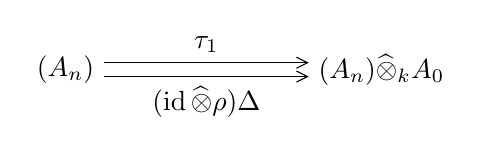
\begin{tikzpicture}[baseline=(lhs.base)]
  \node (lhs) {$(A_n)$};
  \node[right=2.6cm of lhs] (rhs)
    {$(A_n)\widehat\otimes_k A_0$};
  \draw[-{Straight Barb[length=4pt,width=4pt]}]
    ([yshift=2.5pt]lhs.east) --
    node[above] {$\tau_1$}
    ([yshift=2.5pt]rhs.west);
  \draw[-{Straight Barb[length=4pt,width=4pt]}]
    ([yshift=-2.5pt]lhs.east) --
    node[below] {$(\operatorname{id}\widehat\otimes\rho)\Delta$}
    ([yshift=-2.5pt]rhs.west);
\end{tikzpicture}

% END INCLUDED SGA3_English_current_buildable_source_20260823/source/inputs/VII/native_diagrams/exp7/viib_15_95/diag_126.tex

\end{center}
Here
\[
  \Delta:(A_n)\longrightarrow(A_n)\widehat\otimes(A_n)
\]
is the comultiplication of \((A_n)\), and
\[
  \tau_1(x)=x\widehat\otimes1.
\]
Identifying \(A'_n\) with its image in \(A_n\), the map
\[
  A'_n\widehat\otimes_kA_0\longrightarrow A_n,
  \qquad
  a'_n\widehat\otimes a_0\longmapsto a'_na_0,
\]
is an isomorphism in \(\mathbf{Alpg}/k\).

This is not an isomorphism of cogroups. Rather,
\[
  \Delta(A')\subset A\widehat\otimes A',
\]
and
\[
  \bigl(\gamma'_\rho\widehat\otimes\operatorname{id}\bigr)
  \circ\Delta\big|_{A'}
  =
  \Delta',
\]
where \(\Delta'\) is the comultiplication of \(A'\) and
\(\gamma'_\rho:A\to A'\) is the projection
\textup{(cf.\ \SGARefLink{sga3:VIIB:2.4.A}{2.4.A})}.

% END INCLUDED SGA3_English_current_buildable_source_20260823/source/inputs/VII/tex/components/79_expose_VIIB_section513_graded_cogroup_splitting_en.tex

% BEGIN INCLUDED SGA3_English_current_buildable_source_20260823/source/inputs/VII/tex/components/80_expose_VIIB_section514_graded_generation_en.tex
% SGA 3, Expose VII_B, English reconstruction -- Loop 1.
% Scope: Section 5.1.4 from its opening through formula (3) on authority
% local pages 86--87; the application to Proposition 5.1 follows in
% component 81.
% Combined-reader pages: 599--600. Re-edition printed pages: 588--589.
% Original-edition marginal locator in scope: 555.
% Editorial note in scope: 149.
% Authority: Polo--Gille Exp7B-13oct24.pdf,
% SHA-256 D303690E0195654BBE7C3DAA5D89EA23E24CD709A3575217234AC19AE8836694.
% Jacob Reinhold's CC BY 4.0 Markdown was consulted as comparison lineage.
% The genuine generation diagram is an exact PDF-derived Loop 1 crop.

\subsubsection*{5.1.4}
\phantomsection
\label{sga3:VIIB:5.1.4}

Let \((A,J)\) be an object of \(\mathcal C\), and let
\[
  (A_n)=\operatorname{Gr}_J(A)
\]
be the associated object of \(\mathbf{Alpg}/k\); thus
\[
  A_n=\overline{J^n}/\overline{J^{n+1}}
  \qquad(n\geq0).
\]
It is clear that the algebra
\[
  \mathscr A=\prod_{n\geq0}A_n
\]
is generated by \(A_0\) and \(A_1\). In other words, for
\(n\geq1\), the multiplication map
\[
  A_1\widehat\otimes_{A_0}A_1
  \widehat\otimes_{A_0}\cdots
  \widehat\otimes_{A_0}A_1
  \longrightarrow A_n
  \tag{1}
  \label{sga3:VIIB:5.1.4:eq1}
\]
is surjective.

Suppose further that \((A,J)\) is a cogroup of \(\mathcal C\)
and that \(A\) and the quotients
\[
  \overline{J^n}/\overline{J^{n+1}}
\]
are topologically flat over \(k\). By \SGARefLink{sga3:VIIB:5.1.2:corollary}{Corollary~5.1.2},
\(\operatorname{Gr}_J(A)\) is then a cogroup of
\(\mathbf{Alpg}/k\). Hence, by \SGARefLink{sga3:VIIB:5.1.3}{5.1.3}, if one puts
\[
\begin{split}
  A'_n
  =
  \biggl\{
    x\in\overline{J^n}/\overline{J^{n+1}}
    \ \biggm|\
    \Delta(x)-x\widehat\otimes1
    \in
    \bigoplus_{i=1}^{n}
    &\bigl(
      \overline{J^{\,n-i}}/\overline{J^{\,n-i+1}}
    \bigr)
    \widehat\otimes_k
    \\
    &\bigl(
      \overline{J^i}/\overline{J^{i+1}}
    \bigr)
  \biggr\},
\end{split}
\tag{2}
\label{sga3:VIIB:5.1.4:eq2}
\]
then the map
\[
  A'_n\widehat\otimes_kA_0\longrightarrow A_n,
  \qquad
  a'_n\widehat\otimes a_0\longmapsto a'_na_0,
\]
is an isomorphism in \(\mathbf{Alpg}/k\).\footnote{%
\label{sga3:VIIB:nde:149}Let \(G\), \(H\), and
\(\widehat G_H\) be the formal \(k\)-groups corresponding to
\(A\), \(A_0=A/J\), and \(\operatorname{Gr}_J(A)\),
respectively. Then
\(\tau:A_0\hookrightarrow\operatorname{Gr}_J(A)\) corresponds
to a retraction
\(\pi:\widehat G_H\to H\) of the inclusion
\(H\hookrightarrow\widehat G_H\), and the preceding assertion
means that \(\widehat G_H\) is the semidirect product of
\(N=\ker(\pi)\) by \(H\).}

\phantomsection
\label{sga3:VIIB:5.1.4:eq2-source-tensor-note}
\noindent\textit{Source note.}\enspace
In the displayed element-wise description of this map, the
French PDF prints
\(a'_n\widehat\otimes a'_n\mapsto a'_na_0\).
The domain and the product require
\(a'_n\widehat\otimes a_0\mapsto a'_na_0\), which is used here.

Let \(I_0\) denote the augmentation ideal of \(A_0\). It follows
from \textup{\SGARefLink{sga3:VIIB:5.1.4:eq1}{(1)}} and the following commutative diagram, in which
\[
  A_1'{}^{\widehat\otimes n}
  =
  \underbrace{
    A'_1\widehat\otimes_k\cdots\widehat\otimes_kA'_1
  }_{n\text{ factors}},
\]
that:
\begin{center}
  \phantomsection
  \label{sga3:VIIB:5.1.4:degree-one-generation-diagram}
  % SGA3-VII-DIAG-127
  % BEGIN INCLUDED SGA3_English_current_buildable_source_20260823/source/inputs/VII/native_diagrams/exp7/viib_15_95/diag_127.tex
% SGA3-VII-DIAG-127
% Authority: Exp7B-13oct24.pdf, local p. 87.
% Crop: figures/Exp7B_localp087_degree_one_generation_diagram.png
% Locator: tex/components/80_expose_VIIB_section514_graded_generation_en.tex, Loop 1 line 113.
\begin{tikzcd}[row sep=3em,column sep=2.1em]
A_1\widehat\otimes_{A_0}\cdots\widehat\otimes_{A_0}A_1
  \arrow[d,"m"']
  & A_1'{}^{\widehat\otimes n}\widehat\otimes_k A_0
      \arrow[l,"{\sim}"']
      \arrow[d,"{m'\widehat\otimes\operatorname{id}}"']
  & \bigl(A_1'{}^{\widehat\otimes n}\widehat\otimes_k I_0\bigr)
      \oplus A_1'{}^{\widehat\otimes n}
      \arrow[l,"{\sim}"']
      \arrow[d,"{(m'\widehat\otimes\operatorname{id})\oplus m'}"] \\
A_n
  & A'_n\widehat\otimes_k A_0 \arrow[l,"{\sim}"']
  & (A'_n\widehat\otimes_k I_0)\oplus A'_n
      \arrow[l,"{\sim}"']
\end{tikzcd}

% END INCLUDED SGA3_English_current_buildable_source_20260823/source/inputs/VII/native_diagrams/exp7/viib_15_95/diag_127.tex

\end{center}
the multiplication map
\[
  m':
  A'_1\widehat\otimes_k\cdots\widehat\otimes_kA'_1
  \longrightarrow A'_n
  \tag{3}
  \label{sga3:VIIB:5.1.4:eq3}
\]
is surjective. In other words, the profinite \(k\)-algebra
\[
  \mathscr A'=\prod_{n\geq0}A'_n
\]
is generated by its degree-one terms.

% END INCLUDED SGA3_English_current_buildable_source_20260823/source/inputs/VII/tex/components/80_expose_VIIB_section514_graded_generation_en.tex

% BEGIN INCLUDED SGA3_English_current_buildable_source_20260823/source/inputs/VII/tex/components/81_expose_VIIB_section514_proposition51_completion_en.tex
% SGA 3, Expose VII_B, English reconstruction -- Loop 1.
% Scope: The remainder of Section 5.1.4, completing the proof of
% Proposition 5.1 and its supplement, on authority local pages 87--88;
% stops immediately before Section 5.1.5.
% Combined-reader pages: 600--601. Re-edition printed pages: 589--590.
% Original-edition marginal locator in scope: 556.
% Editorial notes in scope: 150--151.
% Authority: Polo--Gille Exp7B-13oct24.pdf,
% SHA-256 D303690E0195654BBE7C3DAA5D89EA23E24CD709A3575217234AC19AE8836694.
% Jacob Reinhold's CC BY 4.0 Markdown was consulted as comparison lineage.
% The genuine kernel-pair and exact commutative diagrams are exact
% PDF-derived Loop 1 crops.

Let us now return to hypothesis \textup{\SGARefLink{sga3:vii:paragraph:5-1:equation:i}{(i)}} of
\SGARefLink{sga3:VIIB:5.1:proposition}{Proposition~5.1}.\footnote{%
\label{sga3:VIIB:nde:150}The editors expanded the original in
what follows and moved to the end the ``supplement''
\(\overline{I_B^n}=B\cap\overline{J^n}\), which is not needed
to prove \SGARefLink{sga3:VIIB:5.1:proposition}{Proposition~5.1}.}
Let \(G\) be a topologically flat infinitesimal formal
\(k\)-group, \(A\) its affine algebra, \(I_A\) the augmentation
ideal of \(A\), \(B\) a closed subalgebra of \(A\), and
\[
  J=AI_B,
  \qquad
  I_B=B\cap I_A.
\]
Let \(H\) be the formal subgroup \(\operatorname{Spf}(A/J)\),
and let
\[
  \pi:A\longrightarrow A/J
\]
be the projection. Suppose that
\[
  A/\overline{J^n}
\]
is topologically flat over \(k\) for every \(n\geq1\), and that
\(B\) is contained in the kernel \(\widetilde B\) of the
following pair:
\begin{center}
  \phantomsection
  \label{sga3:VIIB:5.1.4:quotient-kernel-pair}
  % SGA3-VII-DIAG-128
  % BEGIN INCLUDED SGA3_English_current_buildable_source_20260823/source/inputs/VII/native_diagrams/exp7/viib_15_95/diag_128.tex
% SGA3-VII-DIAG-128
% Authority: Exp7B-13oct24.pdf, local p. 87.
% Crop: figures/Exp7B_localp087_quotient_kernel_pair.png
% Locator: tex/components/81_expose_VIIB_section514_proposition51_completion_en.tex, Loop 1 line 43.
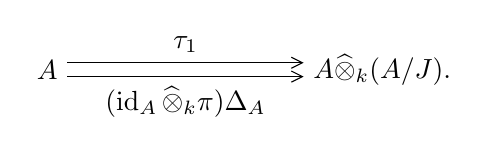
\begin{tikzpicture}[baseline=(lhs.base)]
  \node (lhs) {$A$};
  \node[right=3cm of lhs] (rhs)
    {$A\widehat\otimes_k(A/J).$};
  \draw[-{Straight Barb[length=4pt,width=4pt]}]
    ([yshift=2.5pt]lhs.east) --
    node[above] {$\tau_1$}
    ([yshift=2.5pt]rhs.west);
  \draw[-{Straight Barb[length=4pt,width=4pt]}]
    ([yshift=-2.5pt]lhs.east) --
    node[below] {$(\operatorname{id}_A\widehat\otimes_k\pi)\Delta_A$}
    ([yshift=-2.5pt]rhs.west);
\end{tikzpicture}

% END INCLUDED SGA3_English_current_buildable_source_20260823/source/inputs/VII/native_diagrams/exp7/viib_15_95/diag_128.tex

\end{center}

Put
\[
  (A_n)=\operatorname{Gr}_J(A),
\]
let
\[
  I_0=I_A/J
\]
be the augmentation ideal of \(A_0=A/J\), and define
\((A'_n)_{n\in\mathbb N}\) as in \textup{(2)} above. Let
\((B_n)_{n\in\mathbb N}\), respectively
\((\widetilde B_n)_{n\in\mathbb N}\), be the object of
\(\mathbf{Alpg}/k\) associated with the filtration of \(B\),
respectively of \(\widetilde B\), induced by that of \(A\); these
filtrations are defined by the ideals
\[
  B\cap\overline{J^n},
  \qquad\text{respectively}\qquad
  \widetilde B\cap\overline{J^n}.
\]
It is clear that
\[
  B_n\subset\widetilde B_n\subset A'_n
  \qquad\text{for every }n,
\]
and that
\[
  \mathscr B=\prod_{n\geq0}B_n
  \subset
  \widetilde{\mathscr B}
  =
  \prod_{n\geq0}\widetilde B_n
\]
are subalgebras of
\[
  \mathscr A'=\prod_{n\geq0}A'_n.
\]

On the other hand, \(J\), respectively \(\overline{J^2}\), is
the image in \(A\) of
\[
  I_B\widehat\otimes_kA,
  \qquad\text{respectively}\qquad
  \overline{I_B^2}\widehat\otimes_kA.
\]
Consequently, the map
\[
  (I_B/\overline{I_B^2})\widehat\otimes_kA
  \longrightarrow
  J/\overline{J^2}
  =
  A_1
  \simeq
  A'_1\widehat\otimes_kA_0
\]
is surjective, and it factors through
\[
  (I_B/\overline{I_B^2})\widehat\otimes_kA_0.
\]
Since
\[
  A_0=k\cdot1\oplus I_0,
\]
the following commutative exact diagram shows that \(A'_1\) is
the image of \(I_B/\overline{I_B^2}\):
\begin{center}
  \phantomsection
  \label{sga3:VIIB:5.1.4:degree-one-image-diagram}
  % SGA3-VII-DIAG-129
  % BEGIN INCLUDED SGA3_English_current_buildable_source_20260823/source/inputs/VII/native_diagrams/exp7/viib_15_95/diag_129.tex
% SGA3-VII-DIAG-129
% Authority: Exp7B-13oct24.pdf, local p. 88.
% Crop: figures/Exp7B_localp088_degree_one_image_diagram.png
% Locator: tex/components/81_expose_VIIB_section514_proposition51_completion_en.tex, Loop 1 line 115.
\begin{tikzcd}[row sep=2.7em,column sep=3em]
(I_B/\overline{I_B^2})\widehat\otimes_k A_0 \arrow[d]
  & \bigl((I_B/\overline{I_B^2})\widehat\otimes_k I_0\bigr)
      \oplus(I_B/\overline{I_B^2})
      \arrow[l,"{\sim}"'] \arrow[d] \\
J/\overline{J^2} \arrow[d]
  & (A'_1\widehat\otimes_k I_0)\oplus A'_1
      \arrow[l,"{\sim}"'] \arrow[d] \\
0 & 0
\end{tikzcd}

% END INCLUDED SGA3_English_current_buildable_source_20260823/source/inputs/VII/native_diagrams/exp7/viib_15_95/diag_129.tex

\end{center}
Thus
\[
  B_1=A'_1.
\]
Since \(\mathscr A'\) is generated by \(A'_1\), it follows that,
for every \(n\geq1\),
\[
  A'_n\subset B_n\subset\widetilde B_n\subset A'_n,
\]
and hence
\[
  B_n=\widetilde B_n=A'_n.
\]
\footnote{\label{sga3:VIIB:nde:151}With the notation of
editorial note~149, this implies that the formal completion of
\(G/H\) along the unit section, whose affine algebra is
\(\prod_nB_n\), is isomorphic as a formal variety to the formal
\(k\)-group \(N\).}

Finally, because \(G\) is infinitesimal,
\[
  \mathfrak r(A)=I_A,
\]
and hence the ideals \(\overline{I_A^n}\) tend to zero
\textup{(cf.\ \SGARefLink{sga3:VIIB:0.1.2}{0.1.2})}. A fortiori, the ideals
\(\overline{J^n}\) tend to zero, so the induced filtrations on
\(\widetilde B\) and \(B\) are separated. Moreover, since \(B\)
is a closed subalgebra of \(A\), it is complete for the topology
defined by the ideals \(B\cap\overline{J^n}\). It therefore
follows from \textup{[CA]}, \S~V.7, Lemma~1
\textup{(see also \SGARefLink{sga3:VIIB:5.1.5}{5.1.5} below)} that
\[
  B=\widetilde B.
\]
This completes the proof of \SGARefLink{sga3:VIIB:5.1:proposition}{Proposition~5.1}.

There is also the following supplement. For every \(n\),
\[
  \overline{J^n}=A\overline{I_B^n}
\]
is the image in \(A\) both of
\[
  A\widehat\otimes_B\overline{I_B^n}
\]
and of
\[
  A\widehat\otimes_B(B\cap\overline{J^n}).
\]
By hypothesis, the affine algebra \(A/J\) of the formal subgroup
\(H\) is topologically flat over \(k\). Thus, by \SGARefLink{sga3:VIIB:2.4:theorem}{Theorem~2.4},
the morphism
\[
  G=\operatorname{Spf}(A)
  \longrightarrow
  G/H=\operatorname{Spf}(B)
\]
is surjective and topologically flat. Consequently,
\[
  A\widehat\otimes_B\overline{I_B^n}
  =
  \overline{J^n}
  =
  A\widehat\otimes_B(B\cap\overline{J^n}),
\]
which implies
\[
  \overline{I_B^n}=B\cap\overline{J^n}
  \qquad\text{for every }n.
\]
This also follows from the surjectivity of the maps
\[
  \overline{I_B^n}/\overline{I_B^{n+1}}
  \longrightarrow
  A'_n
  =
  (B\cap\overline{J^n})/
  (B\cap\overline{J^{n+1}})
\]
and from \SGARefLink{sga3:VIIB:5.1.5}{5.1.5}\textup{\SGARefLink{sga3:vii:paragraph:5-1:equation:ii}{(ii)}} below, applied to
\[
  B'_n=\overline{I_B^n},
  \qquad
  B_n=B\cap\overline{J^n}.
\]

\phantomsection
\label{sga3:VIIB:5.1.4:supplement-index-source-note}
\noindent\textit{Source note.}\enspace
In the preceding \(n\)-indexed display, the French PDF prints
\(A'_i\). The surrounding numerators and denominators, and the
application to \(B'_n\) and \(B_n\), require \(A'_n\), which is
used here.

% END INCLUDED SGA3_English_current_buildable_source_20260823/source/inputs/VII/tex/components/81_expose_VIIB_section514_proposition51_completion_en.tex

% BEGIN INCLUDED SGA3_English_current_buildable_source_20260823/source/inputs/VII/tex/components/81b_expose_VIIB_section515_filtered_groups_lemma_en.tex
% SGA 3, Expose VII_B, English reconstruction -- Loop 1.
% Scope: Section 5.1.5 in full on authority local pages 88--89;
% stops immediately before Section 5.2.
% Combined-reader pages: 601--602. Re-edition printed pages: 590--591.
% Editorial note in scope: 152.
% Authority: Polo--Gille Exp7B-13oct24.pdf,
% SHA-256 D303690E0195654BBE7C3DAA5D89EA23E24CD709A3575217234AC19AE8836694.
% Jacob Reinhold's CC BY 4.0 Markdown was consulted as comparison lineage.
% No genuine diagram occurs in this component; all mathematics is native LaTeX.

\subsubsection*{5.1.5}
\phantomsection
\label{sga3:VIIB:5.1.5}

\medskip
\noindent\textbf{Lemma 5.1.5.}
\phantomsection
\label{sga3:VIIB:5.1.5:filtered-groups-lemma}
\footnote{\label{sga3:VIIB:nde:152}The original stated only
part~\textup{\SGARefLink{sga3:VIIB:5.1.5:item:ii}{(ii)}}. For the reader's convenience, the editors
stated in part~\textup{\SGARefLink{sga3:VIIB:5.1.5:item:i}{(i)}} Lemma~1 of \textup{[CA]},
\S~V.7.}
{\itshape
\begin{enumerate}
\item[\textup{\SGAInlineRefTarget{sga3:VIIB:5.1.5:item:i}(i)}]
Let \(M\) and \(N\) be two abelian groups filtered by decreasing
sequences of subgroups
\[
  (M_n)_{n\in\mathbb Z},
  \qquad
  (N_n)_{n\in\mathbb Z}.
\]
Suppose that
\[
  \bigcup_{n\in\mathbb Z}M_n=M,
  \qquad
  \bigcup_{n\in\mathbb Z}N_n=N,
\]
that
\[
  \bigcap_{n\in\mathbb Z}M_n=0,
  \qquad
  \bigcap_{n\in\mathbb Z}N_n=0,
\]
and that \(M\) is complete for the topology defined by the
\(M_n\). Let
\[
  f:M\longrightarrow N
\]
be a homomorphism of filtered groups.

\begin{enumerate}
\item[\textup{a)}]
If \(f\) induces a surjection on the associated graded groups,
then \(f\) is surjective and \(N\) is complete for the topology
defined by the \(N_n\).

\item[\textup{b)}]
If \(f\) induces an injection on the associated graded groups,
then \(f\) is injective.
\end{enumerate}

\item[\textup{\SGAInlineRefTarget{sga3:VIIB:5.1.5:item:ii}(ii)}]
Let \(B\) be an abelian group, and let
\[
  B=B'_0\supset B'_1\supset\cdots,
  \qquad
  B=B_0\supset B_1\supset\cdots
\]
be two separated filtrations of \(B\) by subgroups such that
\[
  B'_n\subset B_n
  \qquad\text{for every }n.
\]
Suppose that \(B\) is complete for the topology defined by the
filtration \((B'_n)\). If the map
\[
  B'_i/B'_{i+1}
  \longrightarrow
  B_i/B_{i+1}
\]
is surjective for every \(i\), then
\[
  B'_n=B_n
  \qquad\text{for every }n.
\]
\end{enumerate}
}

\noindent\textit{Proof.}
Part~\textup{\SGARefLink{sga3:VIIB:5.1.5:item:i}{(i)}} is Lemma~1 of \textup{[CA]}, \S~V.7
\textup{(see also [BAC], III, \S~\SGARefLink{sga3:VIIB:2.8}{2.8})}. Part~\textup{\SGARefLink{sga3:VIIB:5.1.5:item:ii}{(ii)}}
follows by taking
\[
  M=B'_n\supset B'_{n+1}\supset\cdots,
  \qquad
  N=B_n\supset B_{n+1}\supset\cdots.
\]

% END INCLUDED SGA3_English_current_buildable_source_20260823/source/inputs/VII/tex/components/81b_expose_VIIB_section515_filtered_groups_lemma_en.tex

% BEGIN INCLUDED SGA3_English_current_buildable_source_20260823/source/inputs/VII/tex/components/82_expose_VIIB_section52_height_theorem_en.tex
% SGA 3, Expose VII_B, English reconstruction -- Loop 1.
% Scope: Section 5.2 opening, notation, and the Dieudonne--Cartier theorem
% on authority local pages 89--90; stops before Section 5.2.1.
% Combined-reader pages: 602--603. Re-edition printed pages: 591--592.
% Original-edition marginal locators in scope: 557--558.
% Editorial notes in scope: 153--154.
% Authority: Polo--Gille Exp7B-13oct24.pdf,
% SHA-256 D303690E0195654BBE7C3DAA5D89EA23E24CD709A3575217234AC19AE8836694.
% Jacob Reinhold's CC BY 4.0 Markdown was consulted as comparison lineage.
% No genuine diagram occurs in this component; all mathematics is native LaTeX.

\subsection*{5.2}
\phantomsection
\label{sga3:VIIB:5.2}

Throughout the rest of \SGARefLink{sga3:VIIB:5}{Section~5}, \(k\) denotes a perfect field
of characteristic \(p>0\).

Put
\[
  \overline{\mathbb N}=\mathbb N\cup\{\infty\}.
\]
If \(B\) is a profinite \(k\)-algebra and
\(r\in\overline{\mathbb N}\), denote by
\[
  \bigl((x^{p^r})\bigr)_{x\in\mathfrak r(B)}
\]
the closed ideal of \(B\) generated by the elements \(x^{p^r}\),
where \(x\) ranges over the radical \(\mathfrak r(B)\) of \(B\).
If \(r=\infty\), use the same notation with the convention that
\[
  \bigl((x^{p^\infty})\bigr)_{x\in\mathfrak r(B)}
\]
is the zero ideal. In both cases, \(B_r\) denotes the quotient
\[
  B_r
  =
  B\big/\bigl((x^{p^r})\bigr)_{x\in\mathfrak r(B)}.
\]

We say that \(B\) is \emph{of height at most \(r\)} if
\[
  \bigl((x^{p^r})\bigr)_{x\in\mathfrak r(B)}
\]
is the zero ideal. If this holds and \(r\) is finite, we say that
\(B\) is \emph{of finite height}.

Consider in particular the case
\[
  B=k[[\omega]],
\]
where \(\omega\) is a pseudocompact \(k\)-vector space
\textup{(cf.\ \SGARefLink{sga3:VIIB:1.2.5}{1.2.5})}.\footnote{%
\label{sga3:VIIB:nde:153}In the original, the author uses
``linearly compact vector space,'' which is equivalent to
``pseudocompact vector space'' \textup{(cf.\ [BAC],
\S III.2, Exercises 15\,a), 19\,a), and 20\,d))}. The editors
preferred to retain the terminology ``pseudocompact,'' used up to
this point.}
We then say that \(B\) is a \emph{formal power series algebra}
and that \(B_r\) is a \emph{truncated formal power series algebra}
\(\bigl(r\in\overline{\mathbb N}\bigr)\); thus, by convention,
\[
  B=B_\infty
\]
is also called ``truncated.'' If \(B=k[[\omega]]\), we also write
\[
  \bigl((x^{p^r})\bigr)_{x\in\omega}
\]
instead of
\[
  \bigl((x^{p^r})\bigr)_{x\in\mathfrak r(B)}.
\]

\medskip
\noindent\textbf{Notation.}
Let \(\omega\) be a pseudocompact \(k\)-vector space filtered by
an increasing sequence of closed vector subspaces
\[
  0=\omega_0\subset\omega_1\subset\omega_2
  \subset\omega_3\subset\cdots.
\]
\begin{enumerate}
\item[\textup{\SGAInlineRefTarget{sga3:VIIB:5.2:item:a}(a)}]
The closed ideal of \(k[[\omega]]\) generated by the elements
\(x^{p^r}\), where \(r\) ranges over \(\mathbb N\) and
\(x\) ranges over \(\omega_r\), will be denoted by
\[
  \bigl((x^{p^r})\bigr)_{x\in\omega_r}.
\]

\item[\textup{(b)}]
For \(r\in\mathbb N\), denote by \({}^r\omega\) the filtered
pseudocompact vector space defined by
\[
  {}^r\omega_i=\omega_i\quad\text{if }i<r,
  \qquad
  {}^r\omega_i=\omega\quad\text{if }i\geq r.
\]
\end{enumerate}

\phantomsection
\label{sga3:VIIB:5.2:notation-source-note}
\noindent\textit{Source note.}\enspace
In Notation \textup{\SGARefLink{sga3:VIIB:5.2:item:a}{(a)}}, the French PDF prints the subscript
\(r\in\omega_r\). The preceding defining sentence and every
subsequent use require \(x\in\omega_r\), which is used here.

\medskip
\noindent\textbf{Theorem (Dieudonn\'e--Cartier).}
\phantomsection
\label{sga3:VIIB:5.2:theorem}
{\itshape Let
\[
  H\longrightarrow G
\]
be a monomorphism of infinitesimal formal groups over a perfect
field \(k\) of characteristic \(p>0\). Let \(B\) be the affine
algebra of the homogeneous space \(G/H\), and suppose that one of
the following three conditions holds:\footnote{%
\label{sga3:VIIB:nde:154}The editors replaced \(H\backslash G\)
by \(G/H\), and did the same in the proof; they also added
condition \textup{\SGARefLink{sga3:VIIB:5.2:theorem:item:iii}{(iii)}}.}
\begin{enumerate}
\item[\textup{(i)}]
\(B\) has finite height \textup{(in particular, this holds if
\(G\) has finite height)}.

\item[\textup{\SGAInlineRefTarget{sga3:VIIB:5.2:theorem:item:ii}(ii)}]
\(B\) is a complete Noetherian local ring.

\item[\textup{\SGAInlineRefTarget{sga3:VIIB:5.2:theorem:item:iii}(iii)}]
\(B\) is a reduced ring.
\end{enumerate}
Then \(B\) is isomorphic to the completed tensor product of a
finite family of truncated formal power series algebras.}

The proof of this theorem occupies \SGARefLink{sga3:VIIB:5.2.1:section-proposition}{5.2.1}--\SGARefLink{sga3:VIIB:5.2.5}{5.2.5}.

% END INCLUDED SGA3_English_current_buildable_source_20260823/source/inputs/VII/tex/components/82_expose_VIIB_section52_height_theorem_en.tex

% BEGIN INCLUDED SGA3_English_current_buildable_source_20260823/source/inputs/VII/tex/components/83_expose_VIIB_section521_reduction_proposition_en.tex
% SGA 3, Expose VII_B, English reconstruction -- Loop 1.
% Scope: Section 5.2.1 opening and reduction proposition in full
% on authority local page 90; stops immediately before Section 5.2.1.A.
% Combined-reader page: 603. Re-edition printed page: 592.
% Original-edition marginal locator in scope: 558.
% Authority: Polo--Gille Exp7B-13oct24.pdf,
% SHA-256 D303690E0195654BBE7C3DAA5D89EA23E24CD709A3575217234AC19AE8836694.
% Jacob Reinhold's CC BY 4.0 Markdown was consulted as comparison lineage.
% No genuine diagram occurs in this component; all mathematics is native LaTeX.

\subsubsection*{5.2.1}
\phantomsection
\label{sga3:VIIB:5.2.1}

Let \(A\) be the affine algebra of \(G\), let \(I_A\) be its
augmentation ideal, and put
\[
  I=B\cap I_A.
\]
By \SGARefLink{sga3:VIIB:2.4}{2.4},
\[
  H=\operatorname{Spf}\bigl(A/\overline{AI}\bigr)
\]
and
\[
  B
  =
  \left\{
    x\in A\ \middle|\
    \Delta(x)-x\widehat\otimes1
    \in A\widehat\otimes\overline{AI}
  \right\}.
\]
\phantomsection
\label{sga3:VIIB:5.2.1:tensor-order-source-note}
\noindent\textit{Source note.}\enspace
The French PDF prints
\(\Delta(x)-1\widehat\otimes x\) here. The right-quotient
convention fixed in \SGARefLink{sga3:VIIB:5.0}{5.0} and \SGARefLink{sga3:VIIB:5.1:proposition}{Proposition~5.1}, together with the
defining condition
\((\operatorname{id}_A\widehat\otimes\pi)\Delta(x)
=x\widehat\otimes1\), requires
\(\Delta(x)-x\widehat\otimes1\), which is used above.

Put
\[
  \omega=I/\overline{I^2}.
\]
For each \(r\), denote by \(I_r\) the closed subideal of \(I\)
consisting of the elements \(x\) such that
\[
  x^{p^r}=0,
\]
and denote by \(\omega_r\) the canonical image of \(I_r\) in
\(\omega\). We shall prove the following proposition.

\medskip
\noindent\textbf{Proposition.}
\phantomsection
\label{sga3:VIIB:5.2.1:section-proposition}
{\itshape If there exists a continuous section
\[
  \sigma:\omega\longrightarrow I
\]
of the projection \(I\to I/\overline{I^2}\) such that
\[
  \sigma(\omega_r)\subset I_r
\]
for every \(r\), then \(B\) is isomorphic to
\[
  k[[\omega]]
  \big/
  \bigl((x^{p^r})\bigr)_{x\in\omega_r}.
\]}

Indeed, such a section extends to a continuous morphism
\[
  k[[\omega]]\longrightarrow B,
\]
which factors through
\[
  B'
  =
  k[[\omega]]
  \big/
  \bigl((x^{p^r})\bigr)_{x\in\omega_r}.
\]
In \SGARefLink{sga3:VIIB:5.2.2}{5.2.2}--\SGARefLink{sga3:VIIB:5.2.5}{5.2.5} we prove that the resulting morphism
\[
  \varphi:
  B'
  =
  k[[\omega]]
  \big/
  \bigl((x^{p^r})\bigr)_{x\in\omega_r}
  \longrightarrow B
\]
is an isomorphism.

% END INCLUDED SGA3_English_current_buildable_source_20260823/source/inputs/VII/tex/components/83_expose_VIIB_section521_reduction_proposition_en.tex

% BEGIN INCLUDED SGA3_English_current_buildable_source_20260823/source/inputs/VII/tex/components/84_expose_VIIB_section521A_pseudobasis_splittings_en.tex
% SGA 3, Expose VII_B, English reconstruction -- Loop 1.
% Scope: Section 5.2.1.A in full on authority local pages 90--91;
% stops immediately before Section 5.2.1.B.
% Combined-reader pages: 603--604. Re-edition printed pages: 592--593.
% Editorial note in scope: 155.
% Authority: Polo--Gille Exp7B-13oct24.pdf,
% SHA-256 D303690E0195654BBE7C3DAA5D89EA23E24CD709A3575217234AC19AE8836694.
% Jacob Reinhold's CC BY 4.0 Markdown was consulted as comparison lineage.
% The two genuine diagrams are exact PDF-derived Loop-1 PNG crops.

\paragraph{\SGARefLink{sga3:VIIB:5.2.1.A}{5.2.1.A}.}
\phantomsection
\label{sga3:VIIB:5.2.1.A}
\footnote{\label{sga3:VIIB:nde:155}The editors added
\SGARefLink{sga3:VIIB:5.2.1.A}{5.2.1.A} and \SGARefLink{sga3:VIIB:5.2.1.B}{5.2.1.B}.}
For every \(r\in\mathbb N\), put
\[
  \mathcal I_r=\overline{I^2}+I_r,
\]
so that
\[
  \mathcal I_r/\overline{I^2}\simeq\omega_r.
\]
There is then a commutative diagram with exact rows:
\begin{center}
  \phantomsection
  \label{sga3:VIIB:5.2.1.A:exact-rows}
  % SGA3-VII-DIAG-130
  % BEGIN INCLUDED SGA3_English_current_buildable_source_20260823/source/inputs/VII/native_diagrams/exp7/viib_15_95/diag_130.tex
% SGA3-VII-DIAG-130
% Authority: Exp7B-13oct24.pdf, local p. 90.
% Crop: figures/Exp7B_localp090_521A_exact_rows.png
% Locator: tex/components/84_expose_VIIB_section521A_pseudobasis_splittings_en.tex, Loop 1 line 28.
\begin{tikzcd}[row sep=3em,column sep=2.6em]
0 \arrow[r] & \mathcal I_{r-1} \arrow[r] \arrow[d]
  & \mathcal I_r \arrow[r] \arrow[d]
  & \mathcal I_r/\mathcal I_{r-1}
      \arrow[r] \arrow[d,"\wr"]
  & 0 \\
0 \arrow[r] & \omega_{r-1} \arrow[r]
  & \omega_r \arrow[r]
  & \omega_r/\omega_{r-1} \arrow[r]
  & 0
\end{tikzcd}

% END INCLUDED SGA3_English_current_buildable_source_20260823/source/inputs/VII/native_diagrams/exp7/viib_15_95/diag_130.tex

\end{center}

Since \(k\) is a field, the rows split. Thus a pseudobasis
\(\mathscr B_{r-1}\) of \(\mathcal I_{r-1}\) can be completed
to a pseudobasis
\[
  \mathscr B_{r-1}\cup\mathscr B'_r
\]
of \(\mathcal I_r\). The closed subspace \(S_r\) with
pseudobasis \(\mathscr B'_r\) is then a complement of
\(\mathcal I_{r-1}\) in \(\mathcal I_r\), and the projection
\[
  \pi:I\longrightarrow\omega
\]
induces an isomorphism from \(S_r\) onto a complement
\(\omega'_r\) of \(\omega_{r-1}\) in \(\omega_r\).

Let \(\mathcal I_\infty\) be the closed ideal
\[
  \mathcal I_\infty
  =
  \overline{\bigcup_r\mathcal I_r}.
\]
It likewise has a complement \(S_\infty\) in \(I\), and
\(\pi\) induces an isomorphism from
\[
  \mathcal I_\infty/\overline{I^2}
\]
onto the closure
\[
  \omega_\infty
  =
  \overline{\bigcup_r\omega_r}
\]
of the union of the \(\omega_r\), and an isomorphism from
\(S_\infty\) onto a complement \(\omega'_\infty\) of
\(\omega_\infty\) in \(\omega\). Denote the latter isomorphism by
\[
  \eta:S_\infty\xrightarrow{\sim}\omega'_\infty.
\]
We thus obtain continuous linear maps:
\begin{center}
  \phantomsection
  \label{sga3:VIIB:5.2.1.A:splitting-maps}
  % SGA3-VII-DIAG-131
  % BEGIN INCLUDED SGA3_English_current_buildable_source_20260823/source/inputs/VII/native_diagrams/exp7/viib_15_95/diag_131.tex
% SGA3-VII-DIAG-131
% Authority: Exp7B-13oct24.pdf, local p. 90.
% Crop: figures/Exp7B_localp090_521A_splitting_maps.png
% Locator: tex/components/84_expose_VIIB_section521A_pseudobasis_splittings_en.tex, Loop 1 line 74.
\begin{tikzcd}[row sep=3.2em,column sep=3em]
\overline{I^2}\times S_\infty\times\widehat{\bigoplus}_r S_r
  \arrow[r,"\phi"]
  \arrow[d,"\eta" left]
  \arrow[d,phantom,"{\times\theta}" right]
  & I \\
\omega=\omega'_\infty\times\omega_\infty & {}
\end{tikzcd}

% END INCLUDED SGA3_English_current_buildable_source_20260823/source/inputs/VII/native_diagrams/exp7/viib_15_95/diag_131.tex

\end{center}

Here
\[
  \widehat{\bigoplus}_r S_r
\]
is the direct sum of the \(S_r\) in \(\operatorname{PC}(k)\),
that is,
\[
  \left(\prod_r S_r^\dagger\right)^*
\]
\textup{(cf.\ editorial note \textup{(16)} to \SGARefLink{sga3:VIIB:0.2.2}{0.2.2})}, and
\[
  \theta:
  \widehat{\bigoplus}_r S_r
  \longrightarrow\omega_\infty
\]
is induced by the maps
\[
  S_r\xrightarrow{\sim}\omega'_r
  \lhook\joinrel\longrightarrow\omega_\infty.
\]
It follows that a sufficient condition \textup{(but not a
necessary one, as seen below)} for obtaining a section
\[
  \sigma:\omega\longrightarrow I
\]
of the desired kind is that \(\theta\) be an isomorphism.
By duality \textup{(cf.\ \SGARefLink{sga3:VIIB:0.2.2}{0.2.2})}, this is equivalent to saying
that the linear map
\[
  \omega_\infty^\dagger
  \longrightarrow
  \prod_r S_r^\dagger
\]
is bijective.

% END INCLUDED SGA3_English_current_buildable_source_20260823/source/inputs/VII/tex/components/84_expose_VIIB_section521A_pseudobasis_splittings_en.tex

% BEGIN INCLUDED SGA3_English_current_buildable_source_20260823/source/inputs/VII/tex/components/85_expose_VIIB_section521B_split_filtered_spaces_en.tex
% SGA 3, Expose VII_B, English reconstruction -- Loop 1.
% Scope: Section 5.2.1.B in full on authority local page 91;
% stops immediately before Section 5.2.1.C.
% Combined-reader page: 604. Re-edition printed page: 593.
% Editorial note in scope: 156.
% Authority: Polo--Gille Exp7B-13oct24.pdf,
% SHA-256 D303690E0195654BBE7C3DAA5D89EA23E24CD709A3575217234AC19AE8836694.
% Jacob Reinhold's CC BY 4.0 Markdown was consulted as comparison lineage.
% No genuine diagram occurs in this component; all mathematics is native LaTeX.

\paragraph{\SGARefLink{sga3:VIIB:5.2.1.B}{5.2.1.B}.}
\phantomsection
\label{sga3:VIIB:5.2.1.B}

As above, put
\[
  \omega_\infty
  =
  \overline{\bigcup_{n\in\mathbb N}\omega_n}.
\]
A second case in which a section
\[
  \sigma:\omega\longrightarrow I
\]
of the desired kind exists is the case in which
\(\omega_\infty\) has a pseudobasis \(\mathscr B_\infty\) that
is the union, for \(n\in\mathbb N^*\), of pseudobases of the
spaces
\[
  \omega_n/\omega_{n-1}.
\]
One can then complete it by a pseudobasis
\(\mathscr B'_\infty\) of \(\omega/\omega_\infty\), obtaining a
pseudobasis of \(\omega\) compatible with the filtration.

Put
\[
  V=\omega_\infty^\dagger,
\]
and let \(V_n\) be the orthogonal complement of \(\omega_n\) in
\(V\). The preceding condition is equivalent to saying that, in
the category of ordinary \(k\)-vector spaces, the separated
decreasing filtration
\[
  V=V_0\supset V_1\supset V_2\supset\cdots
\]
splits: namely, \(V\) is the direct sum, over
\(n\in\mathbb N\), of subspaces \(F_n\) such that
\[
  F_n\simeq V_n/V_{n+1}.
\]

This need not hold. For example, let
\[
  V=\mathscr S=k^{\mathbb N}
\]
be the space of sequences of elements of \(k\), and let
\(\mathscr S_n\) be the subspace of sequences
\((u_i)\) such that \(u_i=0\) for \(i<n\). Then
\[
  \dim\mathscr S_n/\mathscr S_{n+1}=1,
\]
but \(\mathscr S\) is not isomorphic to the direct sum of the
\(\mathscr S_n/\mathscr S_{n+1}\), because \(\mathscr S\) is not
countable-dimensional. In this example, however, \(\mathscr S\)
is the product of the \(\mathscr S_n/\mathscr S_{n+1}\)
\textup{(cf.\ \SGARefLink{sga3:VIIB:5.2.1.A}{5.2.1.A})}.

The splitting does hold when \(V\) is
countable-dimensional.\footnote{%
\label{sga3:VIIB:nde:156}This paragraph arose from discussions
with J.-M. Fontaine and E. Bouscaren; in particular, Bouscaren
indicated the proof that follows.}
Indeed, let
\[
  (e_n)_{n\in\mathbb N}
\]
be a basis of \(V\). We shall construct inductively an increasing
function
\[
  g:\mathbb N\longrightarrow\mathbb N
\]
and subspaces \(F_i\), for \(i=0,\ldots,g(n)\), such that
\[
  F_i\simeq V_i/V_{i+1}
\]
and
\[
  F_{\leq g(n)}
  =
  \bigoplus_{i=0}^{g(n)}F_i
\]
is a complement of \(V_{g(n)+1}\) containing
\[
  e_0,\ldots,e_n.
\]
It will then follow that
\[
  V=\bigoplus_{i\geq0}F_i.
\]

Let \(n+1\in\mathbb N\), and assume the assertion already proved
for \(n\) \textup{(it is vacuous for \(n=-1\))}. If
\[
  e_{n+1}\in F_{\leq g(n)},
\]
put \(g(n+1)=g(n)\). Otherwise write
\[
  e_{n+1}=f+x,
  \qquad
  f\in F_{\leq g(n)},
  \qquad
  0\ne x\in V_{g(n)+1}.
\]
Let \(j\) be the least integer such that
\[
  x\in V_j\setminus V_{j+1}.
\]
For
\[
  i=g(n)+1,\ldots,j,
\]
choose a complement \(F_i\) of \(V_{i+1}\) in \(V_i\), choosing
\(F_j\) so that \(x\in F_j\). Then
\[
  e_{n+1}\in F_{\leq j};
\]
put \(g(n+1)=j\).

\phantomsection
\label{sga3:VIIB:5.2.1.B:induction-source-note}
\noindent\textit{Source note.}\enspace
At the last induction step, the French PDF prints
\(e_{n+1}\in F_j\). From
\(e_{n+1}=f+x\), with \(f\in F_{\leq g(n)}\), the argument
instead gives \(x\in F_j\) and
\(e_{n+1}\in F_{\leq j}\); these are the relations used here.

% END INCLUDED SGA3_English_current_buildable_source_20260823/source/inputs/VII/tex/components/85_expose_VIIB_section521B_split_filtered_spaces_en.tex

% BEGIN INCLUDED SGA3_English_current_buildable_source_20260823/source/inputs/VII/tex/components/86_expose_VIIB_section521C_stationary_filtration_en.tex
% SGA 3, Expose VII_B, English reconstruction -- Loop 1.
% Scope: Section 5.2.1.C in full on authority local pages 91--92;
% stops immediately before Section 5.2.2.
% Combined-reader pages: 604--605. Re-edition printed pages: 593--594.
% Editorial note in scope: 157.
% Authority: Polo--Gille Exp7B-13oct24.pdf,
% SHA-256 D303690E0195654BBE7C3DAA5D89EA23E24CD709A3575217234AC19AE8836694.
% Jacob Reinhold's CC BY 4.0 Markdown was consulted as comparison lineage.
% No genuine diagram occurs in this component; all mathematics is native LaTeX.

\paragraph{\SGARefLink{sga3:VIIB:5.2.1.C}{5.2.1.C}.}
\phantomsection
\label{sga3:VIIB:5.2.1.C}
\footnote{\label{sga3:VIIB:nde:157}Here the editors return to the
original, shortened to take account of the preceding additions.}
In particular, the two preceding conditions \textup{(\SGARefLink{sga3:VIIB:5.2.1.A}{5.2.1.A} and
\SGARefLink{sga3:VIIB:5.2.1.B}{5.2.1.B})} hold when the filtration of \(\omega\) is stationary,
that is, when there exists an integer \(n_0\) such that
\[
  \omega_n=\omega_{n_0}
  \qquad
  \text{for }n_0\leq n<+\infty.
\]
In this case,
\[
  k[[\omega]]
  \big/
  \bigl((x^{p^r})\bigr)_{x\in\omega_r}
\]
is isomorphic to the completed tensor product
\[
\begin{aligned}
  &
  \frac{k[[\omega_1]]}
       {\bigl((x^p)\bigr)_{x\in\omega_1}}
  \widehat\otimes_k
  \frac{k[[\omega'_2]]}
       {\bigl((x^{p^2})\bigr)_{x\in\omega'_2}}
  \widehat\otimes_k\cdots
  \\
  &\hspace{3.2em}
  {}\widehat\otimes_k
  \frac{k[[\omega'_{n_0}]]}
       {\bigl((x^{p^{n_0}})\bigr)_{x\in\omega'_{n_0}}}
  \widehat\otimes_k
  k[[\omega'_\infty]],
\end{aligned}
\]
where \(\omega'_n\) is a complement of \(\omega_{n-1}\) in
\(\omega_n\), and \(\omega'_\infty\) is a complement of
\[
  \omega_\infty=\omega_{n_0}
\]
in \(\omega\).

The filtration of \(\omega\) is plainly stationary in case
\textup{\SGARefLink{sga3:vii:paragraph:5-1:equation:i}{(i)}}, where \(\omega_r=\omega\) for all sufficiently
large \(r\); in case \textup{\SGARefLink{sga3:vii:paragraph:5-1:equation:ii}{(ii)}}, where \(\omega\) is
finite-dimensional; and also in case \textup{(iii)}, where
\[
  I_r=0
\]
for every \(r\). In the last case, \(B\) is isomorphic to the
formal power series algebra \(k[[\omega]]\). The preceding remarks
therefore imply the theorem, subject to \SGARefLink{sga3:VIIB:5.2.2}{5.2.2}--\SGARefLink{sga3:VIIB:5.2.5}{5.2.5} below.

% END INCLUDED SGA3_English_current_buildable_source_20260823/source/inputs/VII/tex/components/86_expose_VIIB_section521C_stationary_filtration_en.tex

% BEGIN INCLUDED SGA3_English_current_buildable_source_20260823/source/inputs/VII/tex/components/87_expose_VIIB_section522_height_one_case_en.tex
% SGA 3, Expose VII_B, English reconstruction -- Loop 1.
% Scope: Section 5.2.2 in full on authority local page 92;
% stops immediately before Section 5.2.3.
% Combined-reader page: 605. Re-edition printed page: 594.
% Original-edition marginal locator in scope: 559.
% Authority: Polo--Gille Exp7B-13oct24.pdf,
% SHA-256 D303690E0195654BBE7C3DAA5D89EA23E24CD709A3575217234AC19AE8836694.
% Jacob Reinhold's CC BY 4.0 Markdown was consulted as comparison lineage.
% No genuine diagram occurs in this component; all mathematics is native LaTeX.

\subsubsection*{5.2.2}
\phantomsection
\label{sga3:VIIB:5.2.2}

Suppose first that \(B\) has height at most \(1\); that is,
\[
  x^p=0
  \qquad\text{for every }x\in I.
\]
By \SGARefLink{sga3:VIIB:5.1.4}{5.1.4}, the graded algebra
\[
  \operatorname{Gr}_I(B)
\]
associated with the filtration
\[
  I\supset I^2\supset I^3\supset\cdots
\]
of \(B\) is endowed with a cogroup structure in the category
\(\mathbf{Alpg}/k\). In other words, the profinite algebra
\[
  C=\prod_{n\geq0}\operatorname{Gr}_I(B)_n
\]
is the affine algebra of a formal \(k\)-group \(N\).
Clearly,
\[
  \omega_{N/k}=I/I^2,
\]
and \(N\) is infinitesimal of height at most \(1\).

By \SGARefLink{sga3:viib:subsection:4-4}{4.4}, the identity map of \(\omega_{N/k}\) therefore induces
an isomorphism
\[
  B'
  =
  k[[\omega_{N/k}]]
  \big/
  \bigl((x^p)\bigr)_{x\in\omega_{N/k}}
  \xrightarrow{\ \sim\ }
  C.
\]
In particular, the map \(\phi\) of \SGARefLink{sga3:VIIB:5.2.1:section-proposition}{5.2.1} induces an isomorphism
between the associated graded algebras of \(B'\) and \(B\), when
both are filtered by the powers of their augmentation ideals.
It follows from \textup{[CA]}, \(\S\)V.7, Lemma~1
\textup{(see also \SGARefLink{sga3:VIIB:5.1.5}{5.1.5})} that \(\phi\) is an isomorphism.

% END INCLUDED SGA3_English_current_buildable_source_20260823/source/inputs/VII/tex/components/87_expose_VIIB_section522_height_one_case_en.tex

% BEGIN INCLUDED SGA3_English_current_buildable_source_20260823/source/inputs/VII/tex/components/88_expose_VIIB_section523_finite_height_induction_en.tex
% SGA 3, Expose VII_B, English reconstruction -- Loop 1.
% Scope: Section 5.2.3 in full on authority local pages 92--93;
% stops immediately before Section 5.2.4.
% Combined-reader pages: 605--606. Re-edition printed pages: 594--595.
% Original-edition marginal locator in scope: 560.
% Editorial notes in scope: 158--159.
% Authority: Polo--Gille Exp7B-13oct24.pdf,
% SHA-256 D303690E0195654BBE7C3DAA5D89EA23E24CD709A3575217234AC19AE8836694.
% Jacob Reinhold's CC BY 4.0 Markdown was consulted as comparison lineage.
% Three genuine diagrams are preserved as two exact PDF-derived PNGs
% for Loop 1 and remain due for native reconstruction in Loop 2.

\subsubsection*{5.2.3}
\phantomsection
\label{sga3:VIIB:5.2.3}

Suppose now that \(B\) has finite height at most \(r\).
Let
\[
  \pi:k\xrightarrow{\ \sim\ }k,
  \qquad
  x\longmapsto x^p,
\]
be the Frobenius automorphism. The linear map
\[
  B\widehat\otimes_{\pi}k\longrightarrow B,
  \qquad
  b\widehat\otimes_{\pi}x
  \longmapsto
  b^px=(bx^{1/p})^p,
\]
has closed image equal to the closed subalgebra
\[
  B^p=\{\,b^p\mid b\in B\,\}
\]
of \(B\). Put
\[
  J=B^p\cap I=B^p\cap I_A.
\]

\footnote{\label{sga3:VIIB:nde:158}The editors added what follows.}
Let \(G_1\) be the kernel of the Frobenius morphism
\[
  \operatorname{Fr}:G\longrightarrow G^{(p)},
\]
and let \(HG_1\) be the formal subgroup of \(G\) that is the
inverse image of the formal subgroup \(H^{(p)}\subset G^{(p)}\).
Then \(HG_1\) is defined by the closed ideal generated by the
\(p\)-th powers of the elements of \(AI\); this ideal is \(AJ\).
Moreover, the formation of \(G/H\) commutes with base change,
because \(G/H\) represents the quotient sheaf for the flat
topology \textup{(cf.\ \SGARefLink{sga3:VIIB:2.4}{2.4})}. Hence
\[
  (G/H)^{(p)}=G^{(p)}/H^{(p)},
\]
and we have the following commutative diagrams:

\begin{figure}[H]
  \centering
  % SGA3-VII-DIAG-132
  % BEGIN INCLUDED SGA3_English_current_buildable_source_20260823/source/inputs/VII/native_diagrams/exp7/viib_15_95/diag_132.tex
% SGA3-VII-DIAG-132
% Authority: Exp7B-13oct24.pdf, local p. 92.
% Crop: figures/Exp7B_localp092_frobenius_quotient_dual_diagrams.png
% Locator: tex/components/88_expose_VIIB_section523_finite_height_induction_en.tex, Loop 1 line 60.
\begin{tikzcd}[row sep=2.5em,column sep=2.8em]
G \arrow[r,"\operatorname{Fr}"] \arrow[d]
  & G^{(p)} \arrow[d] \\
G/H \arrow[r,"\operatorname{Fr}"']
  & G^{(p)}/H^{(p)}
\end{tikzcd}
\qquad
\begin{tikzcd}[row sep=2.5em,column sep=2.8em]
A
  & A\widehat\otimes_\pi k
      \arrow[l,"{a\widehat\otimes1\mapsto a^p}"'] \\
B \arrow[u]
  & B\widehat\otimes_\pi k
      \arrow[l,"{b\widehat\otimes1\mapsto b^p}"']
      \arrow[u]
\end{tikzcd}

% END INCLUDED SGA3_English_current_buildable_source_20260823/source/inputs/VII/native_diagrams/exp7/viib_15_95/diag_132.tex

\end{figure}

It follows that \(B^p\) is the affine algebra of the quotient
\(G/HG_1\).\footnote{\label{sga3:VIIB:nde:159}As indicated in the
original, this also follows from \SGARefLink{sga3:VIIB:5.1:proposition}{Proposition~5.1}. The editors
preferred to give the preceding argument, which does not use the
implication \textup{\SGARefLink{sga3:vii:paragraph:5-1:equation:i}{(i)}} \(\Rightarrow\) \textup{\SGARefLink{sga3:VIIB:5.1:proposition:item:ii}{(ii)}} of that
proposition.}
Temporarily denote by \(C\) the affine algebra of the quotient
\(HG_1/H\). Since the formation of \(G/H\) commutes with base
change, the square

\begin{figure}[H]
  \centering
  % SGA3-VII-DIAG-133
  % BEGIN INCLUDED SGA3_English_current_buildable_source_20260823/source/inputs/VII/native_diagrams/exp7/viib_15_95/diag_133.tex
% SGA3-VII-DIAG-133
% Authority: Exp7B-13oct24.pdf, local p. 92.
% Crop: figures/Exp7B_localp092_cartesian_HG1_square.png
% Locator: tex/components/88_expose_VIIB_section523_finite_height_induction_en.tex, Loop 1 line 76.
\begin{tikzcd}[row sep=2.8em,column sep=3.5em]
HG_1 \arrow[r] \arrow[d]
  & G \arrow[d] \\
HG_1/H \arrow[r]
  & G/H
\end{tikzcd}

% END INCLUDED SGA3_English_current_buildable_source_20260823/source/inputs/VII/native_diagrams/exp7/viib_15_95/diag_133.tex

\end{figure}

\noindent
is Cartesian. Consequently,
\[
  A\widehat\otimes_BC
  \simeq
  A/AJ
  =
  A\widehat\otimes_B(B/BJ).
\]
Since \(A\) is topologically free over \(B\)
\textup{(by 2.4, because \(A\) and \(B\) are local)}, the natural
morphism
\[
  B/BJ\longrightarrow C
\]
is an isomorphism. Thus \(B/BJ\) is the affine algebra of
\(HG_1/H\), and of course
\[
  B/BJ=B_1
\]
has height at most \(1\), since
\[
  J=\bigl((x^p)\bigr)_{x\in\mathfrak r(B)}.
\]

Let
\[
  B'
  =
  k[[\omega]]
  \big/
  \bigl((x^{p^r})\bigr)_{x\in\omega_r},
\]
let \(\phi:B'\to B\) be the morphism introduced in \SGARefLink{sga3:VIIB:5.2.1:section-proposition}{5.2.1}, let
\[
  B'^p=\{\,x^p\mid x\in B'\,\},
\]
and let \(J'\) be the augmentation ideal of \(B'^p\). We then
have the commutative diagram

\begin{figure}[H]
  \centering
  % SGA3-VII-DIAG-134
  % BEGIN INCLUDED SGA3_English_current_buildable_source_20260823/source/inputs/VII/native_diagrams/exp7/viib_15_95/diag_134.tex
% SGA3-VII-DIAG-134
% Authority: Exp7B-13oct24.pdf, local p. 93.
% Crop: figures/Exp7B_localp093_phi_reduction_square.png
% Locator: tex/components/88_expose_VIIB_section523_finite_height_induction_en.tex, Loop 1 line 122.
\begin{tikzcd}[row sep=2.8em,column sep=3.7em]
B' \arrow[r,"\psi"] \arrow[d]
  & B \arrow[d] \\
B'_1=B'/\overline{B'J'}
  \arrow[r,"\phi_1"]
  & B_1=B/\overline{BJ}
\end{tikzcd}

% END INCLUDED SGA3_English_current_buildable_source_20260823/source/inputs/VII/native_diagrams/exp7/viib_15_95/diag_134.tex

\end{figure}

\noindent
and, by \SGARefLink{sga3:VIIB:5.2.2}{5.2.2}, \(\phi_1\) is an isomorphism.

On the other hand, by 2.4, \(A\) is topologically flat over
\[
  B=\mathscr A(G/H)
  \qquad\text{and over}\qquad
  B^p=\mathscr A(G/HG_1).
\]
It follows from \SGARefLink{sga3:VIIB:1.3.3}{1.3.3} that \(B\) is topologically flat over
\(B^p\). Moreover, \SGARefLink{sga3:VIIB:5.2.4}{5.2.4} below shows that the morphism
\[
  B'^p\longrightarrow B^p
\]
induced by \(\phi\) is an isomorphism. We may therefore apply
\SGARefLink{sga3:VIIB:0.3.4}{0.3.4} to the pseudocompact ring \(B'^p=B^p\) and the
pseudocompact \(B^p\)-modules \(M=B'\), \(N=B\). By what
precedes,
\[
  \phi_1
  =
  \phi\widehat\otimes_{B^p}k
\]
is an isomorphism, and it follows that \(\phi\) itself is an
isomorphism. This proves \SGARefLink{sga3:VIIB:5.2:theorem}{5.2} when \(B\) has finite height, subject
only to \SGARefLink{sga3:VIIB:5.2.4}{5.2.4} below.

% END INCLUDED SGA3_English_current_buildable_source_20260823/source/inputs/VII/tex/components/88_expose_VIIB_section523_finite_height_induction_en.tex

% BEGIN INCLUDED SGA3_English_current_buildable_source_20260823/source/inputs/VII/tex/components/89_expose_VIIB_section524_frobenius_twist_induction_en.tex
% SGA 3, Expose VII_B, English reconstruction -- Loop 1.
% Scope: Section 5.2.4 in full on authority local pages 93--94;
% stops immediately before Remark 5.2.4.A.
% Combined-reader pages: 606--607. Re-edition printed pages: 595--596.
% Original-edition marginal locator in scope: 561.
% Editorial note in scope: 160.
% Authority: Polo--Gille Exp7B-13oct24.pdf,
% SHA-256 D303690E0195654BBE7C3DAA5D89EA23E24CD709A3575217234AC19AE8836694.
% Jacob Reinhold's CC BY 4.0 Markdown was consulted as comparison lineage.
% The genuine exact-rows diagram is preserved as an exact PDF-derived
% PNG for Loop 1 and remains due for native reconstruction in Loop 2.

\subsubsection*{5.2.4}
\phantomsection
\label{sga3:VIIB:5.2.4}

For every pseudocompact vector space \(V\) over \(k\), denote by
\[
  {}_{\pi}V
  =
  V\widehat\otimes_{\pi}k
\]
the space obtained from \(V\) by extension of scalars along
\(x\mapsto x^p\).\footnote{\label{sga3:VIIB:nde:160}Since \(k\)
is perfect, one may identify \({}_{\pi}V\) with the abelian group
\(V\) on which \(k\) acts by
\(\lambda\cdot v=\lambda^{1/p}v\).}
We then have a commutative diagram with exact rows:

\begin{figure}[H]
  \centering
  % SGA3-VII-DIAG-135
  % BEGIN INCLUDED SGA3_English_current_buildable_source_20260823/source/inputs/VII/native_diagrams/exp7/viib_15_95/diag_135.tex
% SGA3-VII-DIAG-135
% Authority: Exp7B-13oct24.pdf, local p. 93.
% Crop: figures/Exp7B_localp093_pi_exact_rows_diagram.png
% Locator: tex/components/89_expose_VIIB_section524_frobenius_twist_induction_en.tex, Loop 1 line 32.
\begin{tikzcd}[row sep=2.8em,column sep=2.6em]
0 \arrow[r]
  & {}_\pi\overline{I^2} \arrow[r,"\alpha"] \arrow[d,"u"']
  & {}_\pi I \arrow[r,"\beta"] \arrow[d,"v"']
  & {}_\pi\omega \arrow[r] \arrow[d,"w"']
  & 0 \\
0 \arrow[r]
  & \overline{J^2} \arrow[r,"\gamma"]
  & J \arrow[r,"\delta"]
  & \overline\omega \arrow[r]
  & 0\, ,
\end{tikzcd}

% END INCLUDED SGA3_English_current_buildable_source_20260823/source/inputs/VII/native_diagrams/exp7/viib_15_95/diag_135.tex

\end{figure}

\noindent
Here
\[
  \overline\omega=J/J^2,
\]
and the maps \(u,v,w\) are induced by the linear map
\[
  {}_{\pi}B\longrightarrow B^p,
  \qquad
  x\widehat\otimes a\longmapsto x^pa.
\]
Since \(u\) and \(v\) are surjective, so is \(w\), and its kernel
is the image \({}_{\pi}\omega_1\) of
\[
  {}_{\pi}I_1=\ker(v).
\]

Put
\[
  J_n=\{\,x\in J\mid x^{p^n}=0\,\},
  \qquad
  \overline\omega_n=\delta(J_n).
\]
Then, for every \(n\geq0\),
\[
  J_n=v({}_{\pi}I_{n+1}),
  \qquad
  \overline\omega_n=w({}_{\pi}\omega_{n+1}).
\]

\phantomsection
\label{sga3:VIIB:5.2.4:delta-source-note}
\noindent\textit{Source note.}\enspace
The French PDF prints
\(\overline\omega_n=\delta(I_n)\), although the displayed exact
row defines \(\delta\) on \(J\), and the immediately preceding
definition introduces \(J_n\subset J\). The type-correct
\(\delta(J_n)\) is used above; all subsequent identities agree
with this reading.

The section
\[
  {}_{\pi}\sigma:{}_{\pi}\omega\longrightarrow{}_{\pi}I
\]
induced by the section \(\sigma\) of \SGARefLink{sga3:VIIB:5.2.1:section-proposition}{5.2.1} therefore descends to
a section
\[
  \tau:\overline\omega\longrightarrow J
\]
compatible with the filtrations of \(J\) and
\(\overline\omega\). Since \(B^p\) has height at most \(r-1\),
the induction hypothesis shows that this section induces an
isomorphism
\[
  \psi:
  B''
  =
  k[[\overline\omega]]
  \big/
  \bigl((x^{p^n})\bigr)_{x\in\overline\omega_n}
  \xrightarrow{\ \sim\ }
  B^p.
\]
But \(B''\) identifies with \(B'^p\), and \(\psi\) identifies
with the morphism \(B'^p\to B^p\) induced by \(\phi\). Thus the
theorem is proved when \(B\) has finite height.

% END INCLUDED SGA3_English_current_buildable_source_20260823/source/inputs/VII/tex/components/89_expose_VIIB_section524_frobenius_twist_induction_en.tex

% BEGIN INCLUDED SGA3_English_current_buildable_source_20260823/source/inputs/VII/tex/components/90_expose_VIIB_remark524A_finite_height_filtration_en.tex
% SGA 3, Expose VII_B, English reconstruction -- Loop 1.
% Scope: Remark 5.2.4.A in full on authority local page 94;
% stops immediately before Section 5.2.5.
% Combined-reader page: 607. Re-edition printed page: 596.
% Editorial note in scope: 161.
% Authority: Polo--Gille Exp7B-13oct24.pdf,
% SHA-256 D303690E0195654BBE7C3DAA5D89EA23E24CD709A3575217234AC19AE8836694.
% Jacob Reinhold's CC BY 4.0 Markdown was consulted as comparison lineage.
% No genuine diagram occurs in this component; all mathematics is native LaTeX.

\medskip
\noindent\textbf{Remark 5.2.4.A.}
\phantomsection
\label{sga3:VIIB:5.2.4.A}
\footnote{\label{sga3:VIIB:nde:161}The editors added this remark,
which is used in \SGARefLink{sga3:VIIB:5.2.5}{5.2.5}.}
Suppose that \(B\) has height at most \(r+1\), with
\(r\in\mathbb N^*\). Then \(I_{r+1}=I\), and there is an
isomorphism
\[
\tag{1}\label{sga3:vii:remark:5-2-4-a:equation:1}
  B
  \simeq
  \frac{k[[S_1]]}{\bigl((x_1^p)\bigr)_{x_1\in S_1}}
  \widehat\otimes_k\cdots\widehat\otimes_k
  \frac{k[[S_r]]}{\bigl((x_r^{p^r})\bigr)_{x_r\in S_r}}
  \widehat\otimes_k
  \frac{k[[S_{r+1}]]}
       {\bigl((x_{r+1}^{p^{r+1}})\bigr)_{x_{r+1}\in S_{r+1}}},
\]
where each \(S_n\) is a complement of
\[
  I^2+I_{n-1}
\]
in \(I^2+I_n\). Thus \(\omega=I/I^2\) identifies with
\[
  \prod_{i=1}^{r+1}S_i,
\]
and it is immediate that, for \(n=1,\ldots,r+1\), the image
\(\omega_n\) of \(I_n\) in \(\omega\) identifies with
\[
  \prod_{i=1}^{n}S_i.
\]

This has the following consequence. Let
\[
  B_r=B/\check J_r,
  \qquad
  \check J_r
  =
  \bigl((x^{p^r})\bigr)_{x\in\mathfrak r(B)},
\]
and let
\[
  \mathfrak m=I/\check J_r
\]
be the augmentation ideal of \(B_r\). Since
\(\check J_r\subset I^2\), the space
\[
  \omega(r)=\mathfrak m/\mathfrak m^2
\]
identifies with \(\omega\). For \(n=1,\ldots,r\), denote by
\(\omega(r)_n\) the image in \(\omega(r)\) of
\[
  \mathfrak m_n
  =
  \{\,y\in\mathfrak m\mid y^{p^n}=0\,\}.
\]
It is also the image in \(\omega\) of
\[
  \{\,x\in I\mid x^{p^n}\in\check J_r\,\};
\]
hence \(\omega(r)_n\) contains \(\omega_n\).

On the other hand, isomorphism \textup{\SGARefLink{sga3:vii:remark:5-2-4-a:equation:1}{(1)}} gives
\[
  \check J_r
  =
  \bigl((x_{r+1}^{p^r})\bigr)_{x_{r+1}\in S_{r+1}},
\]
and therefore
\[
\tag{2}\label{sga3:vii:remark:5-2-4-a:equation:2}
  B_r
  \simeq
  \frac{k[[S_1]]}{\bigl((x_1^p)\bigr)_{x_1\in S_1}}
  \widehat\otimes_k\cdots\widehat\otimes_k
  \frac{k[[S_r]]}{\bigl((x_r^{p^r})\bigr)_{x_r\in S_r}}
  \widehat\otimes_k
  \frac{k[[S_{r+1}]]}
       {\bigl((x_{r+1}^{p^r})\bigr)_{x_{r+1}\in S_{r+1}}}.
\]
It follows that \(\omega(r)_n\) identifies with
\(\prod_{i=1}^{n}S_i\) for \(n=1,\ldots,r-1\). Thus the
inclusion
\[
  \omega_n\subset\omega(r)_n
\]
is an equality for \(n=1,\ldots,r-1\).

% END INCLUDED SGA3_English_current_buildable_source_20260823/source/inputs/VII/tex/components/90_expose_VIIB_remark524A_finite_height_filtration_en.tex

% BEGIN INCLUDED SGA3_English_current_buildable_source_20260823/source/inputs/VII/tex/components/91_expose_VIIB_section525_infinite_height_limit_en.tex
% SGA 3, Expose VII_B, English reconstruction -- Loop 1.
% Scope: Section 5.2.5 in full on authority local pages 94--95;
% stops immediately before Section 5.2.6.
% Combined-reader pages: 607--608. Re-edition printed pages: 596--597.
% Original-edition marginal locator in scope: 562.
% Editorial notes in scope: 162--163.
% Authority: Polo--Gille Exp7B-13oct24.pdf,
% SHA-256 D303690E0195654BBE7C3DAA5D89EA23E24CD709A3575217234AC19AE8836694.
% Jacob Reinhold's CC BY 4.0 Markdown was consulted as comparison lineage.
% No genuine diagram occurs in this component; all mathematics is native LaTeX.

\subsubsection*{5.2.5}
\phantomsection
\label{sga3:VIIB:5.2.5}

It remains to consider the case in which \(B\) has infinite
height and the projection \(I\to\omega\) admits a section
\(\sigma\) compatible with the filtrations of \(\omega\) and
\(I\). Consider the morphism induced by \(\sigma\):
\[
  \phi:
  B'
  =
  k[[\omega]]
  \big/
  \bigl((x^{p^n})\bigr)_{x\in\omega_n}
  \longrightarrow B.
\]
It is enough to prove that, for every \(r\in\overline{\mathbb N}\),
the map
\[
  \phi_r:B'_r\longrightarrow B_r
\]
induced by \(\phi\) is an isomorphism.\footnote{%
\label{sga3:VIIB:nde:162}Indeed, \(B'\), respectively \(B\), is
the inverse limit of the \(B'_r\), respectively the \(B_r\).
Moreover, the editors modified the original in what follows in
order to take account of the addition made in \SGARefLink{sga3:VIIB:5.2.3}{5.2.3}.}

For every \(r\in\mathbb N^*\), let \(G_r\) be the kernel of the
iterated Frobenius morphism
\[
  G\longrightarrow G^{(p^r)},
\]
and let \(HG_r\) be the formal subgroup of \(G\) that is the
inverse image of \(H^{(p^r)}\subset G^{(p^r)}\). Thus \(HG_r\)
is defined by the closed ideal generated by the \(p^r\)-th
powers of the elements of \(AI\), namely
\[
  A\check J_r,
  \qquad
  \check J_r=\{\,x^{p^r}\mid x\in I\,\}.
\]
Exactly as in \SGARefLink{sga3:VIIB:5.2.3}{5.2.3}, it follows that
\[
  B_r=B/B\check J_r
\]
is the affine algebra of \(HG_r/H\); in particular, it has
height at most \(r\).

Let
\[
  \mathfrak m(r)=I/B\check J_r
\]
be the augmentation ideal of \(B_r\). The canonical projection
\(B\to B_r\) induces an isomorphism
\[
  \omega=I/I^2
  \xrightarrow{\ \sim\ }
  \omega(r)
  =
  \mathfrak m(r)/\mathfrak m(r)^2,
\]
which we use to identify the two spaces. Let \(\omega(r)_n\) be
the image in \(\omega(r)\) of the closed ideal
\[
  \mathfrak m(r)_n
  =
  \{\,y\in\mathfrak m(r)\mid y^{p^n}=0\,\}.
\]
It is also the image in \(\omega\) of the closed ideal
\[
  I(r)_n
  =
  \{\,x\in I\mid x^{p^n}\in B\check J_r\,\}.
\]
\footnote{\label{sga3:VIIB:nde:163}The editors expanded the
original in what follows.}

Clearly,
\[
  \omega(r)_n=\omega
  \qquad\text{if }n\geq r.
\]
We shall prove that
\[
  \omega(r)_n=\omega_n
  \qquad\text{if }n<r.
\]
For every \(r,n\), the sequence
\[
  0
  \longrightarrow
  I(r)_n\cap I^2
  \longrightarrow
  I(r)_n
  \longrightarrow
  \omega(r)_n
  \longrightarrow0
\]
is exact. For fixed \(n\),
\[
  \bigcap_r I(r)_n=I_n,
\]
because \(\bigcap_rB\check J_r=0\). Filtered inverse limits are
exact in \(\operatorname{PC}(k)\) \textup{(cf.\ \SGARefLink{sga3:VIIB:0.2}{0.2})}, so for
every \(n\),
\[
\tag{*}\label{sga3:vii:remark:5-2-4-a:equation:star}
  \omega_n=\bigcap_r\omega(r)_n.
\]
On the other hand, \SGARefLink{sga3:VIIB:5.2.4.A}{Remark~5.2.4.A} gives
\[
  \omega(r)_n=\omega(r+1)_n
  \qquad\text{if }n<r.
\]
Together with \textup{(*)}, this implies
\[
  \omega(r)_n=\omega_n
  \qquad\text{if }n<r.
\]

Consequently, the vector space \(\omega\), filtered by the
subspaces \(\bigl(\omega(r)_n\bigr)_{n\geq0}\), is precisely
\({}^{r}\omega\) in the notation of \SGARefLink{sga3:VIIB:5.2:theorem}{5.2}. The composite
\[
  \sigma(r):
  \omega\xrightarrow{\ \sigma\ }I
  \longrightarrow\mathfrak m(r)
\]
is therefore compatible with the filtrations
\(\bigl(\omega(r)_n\bigr)\) and
\(\bigl(\mathfrak m(r)_n\bigr)\). Since
\[
  k[[{}^{r}\omega]]
  \big/
  \bigl((x^{p^n})\bigr)_{x\in{}^{r}\omega_n}
\]
is exactly \(B'_r\), and \(\phi_r:B'_r\to B_r\) is induced by
\(\sigma(r)\), the result already proved for finite-height
algebras shows that \(\phi_r\) is an isomorphism.

% END INCLUDED SGA3_English_current_buildable_source_20260823/source/inputs/VII/tex/components/91_expose_VIIB_section525_infinite_height_limit_en.tex

% BEGIN INCLUDED SGA3_English_current_buildable_source_20260823/source/inputs/VII/tex/components/92_expose_VIIB_section526_infinite_completed_tensor_product_en.tex
% SGA 3, Expose VII_B, English reconstruction -- Loop 1.
% Scope: Definition 5.2.6 in full on authority local page 95;
% stops immediately before Section 5.3.
% Combined-reader page: 608. Re-edition printed page: 597.
% Editorial note in scope: 164.
% Authority: Polo--Gille Exp7B-13oct24.pdf,
% SHA-256 D303690E0195654BBE7C3DAA5D89EA23E24CD709A3575217234AC19AE8836694.
% Jacob Reinhold's CC BY 4.0 Markdown was consulted as comparison lineage.
% No genuine diagram occurs in this component; all mathematics is native LaTeX.

\subsubsection*{5.2.6}
\phantomsection
\label{sga3:VIIB:5.2.6}

\noindent\textbf{Definition 5.2.6.}
\footnote{\label{sga3:VIIB:nde:164}The editors added this number
in order to define the infinite tensor products used in \SGARefLink{sga3:VIIB:5.3:item:a}{5.3(a)}.}
Let \((A_\lambda)_{\lambda\in\Lambda}\) be a family of profinite
\(k\)-algebras, each endowed with an augmentation
\[
  \varepsilon_\lambda:A_\lambda\longrightarrow k.
\]
\textit{(This holds in particular if every \(A_\lambda\) is
local with residue field \(k\).)}
Define the infinite completed tensor product
\[
  \mathcal A
  =
  \mathop{\widehat{\bigotimes}}\nolimits^{c}_{\lambda\in\Lambda}
  A_\lambda
\]
to be the inverse limit in \(\operatorname{Alp}/k\) of
\[
  \mathcal A_F
  =
  \mathop{\widehat{\bigotimes}}\nolimits^{c}_{\lambda\in F}
  A_\lambda,
\]
where \(F\) ranges through the finite subsets of \(\Lambda\).
For \(F'=F\cup\{\lambda\}\), the transition morphism
\[
  \mathcal A_{F'}\longrightarrow\mathcal A_F
\]
is
\[
  \operatorname{id}\widehat\otimes\varepsilon_\lambda.
\]

In particular, suppose \(\Lambda=\mathbb N^*\), and write
\[
  X_n=\operatorname{Spf}(A_n).
\]
Then \(\operatorname{Spf}(\mathcal A)\) represents the functor
that assigns to every \(C\in\operatorname{Alf}/k\) the set of
\emph{finite} sequences in
\(\prod_{n\geq1}X_n(C)\); that is, the sequences
\[
  (x_1,x_2,\ldots)\in\prod_{n\geq1}X_n(C)
\]
such that
\[
  x_n=\varepsilon_n
\]
for all sufficiently large \(n\). Here, by abuse of notation,
\(\varepsilon_n\) denotes the composite of
\[
  \varepsilon_n:A_n\longrightarrow k
\]
with the structural morphism \(k\to C\).

If, in addition, every \(A_n\) is a quotient of an algebra
\(k[[\omega'_n]]\), one may write \(0\) for the unique morphism
\[
  A_n\longrightarrow C
\]
that vanishes on \(\omega'_n\). The preceding description then
becomes the set of sequences for which \(x_n=0\) for all
sufficiently large \(n\).

% END INCLUDED SGA3_English_current_buildable_source_20260823/source/inputs/VII/tex/components/92_expose_VIIB_section526_infinite_completed_tensor_product_en.tex

% BEGIN INCLUDED SGA3_English_current_buildable_source_20260823/source/inputs/VII/tex/components/93_expose_VIIB_sections53_54_stationary_algebras_corollary_en.tex
% SGA 3, Expose VII_B, English reconstruction -- Loop 1.
% Scope: Sections 5.3 and 5.4 in full on authority local pages 95--97;
% stops immediately before Section 5.5.
% Combined-reader pages: 608--610. Re-edition printed pages: 597--599.
% Original-edition marginal locator in scope: 563.
% Editorial notes in scope: 165--168.
% Authority: Polo--Gille Exp7B-13oct24.pdf,
% SHA-256 D303690E0195654BBE7C3DAA5D89EA23E24CD709A3575217234AC19AE8836694.
% Jacob Reinhold's CC BY 4.0 Markdown was consulted as comparison lineage.
% No genuine diagram occurs in this component; all mathematics is native LaTeX.

\subsection*{5.3. Remarks}
\phantomsection
\label{sga3:VIIB:5.3}
\addcontentsline{toc}{subsection}{5.3. Remarks}

\noindent\SGAInlineRefTarget{sga3:VIIB:5.3:item:a}\textup{(a)}
Call a profinite \(k\)-algebra \emph{stationary} if it is the
completed tensor product of a family of truncated formal power
series algebras.\footnote{\label{sga3:VIIB:nde:165}The author
doubtless had in mind a completed tensor product
\[
  \mathcal A
  =
  \mathop{\widehat{\bigotimes}}\nolimits^{c}_{n\in\mathbb N^*}
  \frac{k[[\omega'_n]]}
       {\bigl((x^{p^n})\bigr)_{x\in\omega'_n}},
\]
where the \(\omega'_n\) are arbitrary pseudocompact vector
spaces. Then \(\omega=\omega_{\mathcal A/k}\) identifies with
\(\prod_n\omega'_n\), and the filtration is
\(\omega_n=\prod_{i=1}^{n}\omega'_i\); this is the case of
\SGARefLink{sga3:VIIB:5.2.1.B}{5.2.1.B}. For this reason these algebras would be better called
\emph{stable}, rather than \emph{stationary}; cf.\ \textup{[Di73]},
II, \(\S\)\SGARefLink{sga3:VIIB:2.9}{2.9}, p.~75. If, for example,
\(\dim\omega'_n=1\) for every \(n\in\mathbb N^*\), then
\(\mathcal A\) represents the functor that assigns to
\(C\in\operatorname{Alf}/k\) the sequences
\((x_n)_{n\in\mathbb N^*}\) of elements of \(C\) such that
\(x_n^{p^n}=0\) and \(x_n=0\) for all sufficiently large \(n\).
This case, where \(\omega=\prod_{n\in\mathbb N^*}\omega'_n\),
corresponds in the dual setting of connected cocommutative Hopf
algebras to the case studied by M.~E.~Sweedler; cf.\
\textup{[Sw67]}, Theorem~3.}

Let \(G\) be an infinitesimal formal \(k\)-group and let \(B\)
be the affine algebra of a homogeneous space of \(G\). It follows
from \SGARefLink{sga3:VIIB:5.2:theorem}{Theorem~5.2} that, for every \(r\in\mathbb N\), the algebra
\[
  B
  \big/
  \bigl((x^{p^r})\bigr)_{x\in\mathfrak r(B)}
\]
is stationary. In particular, \(B\) is an inverse limit of
stationary algebras.\footnote{\label{sga3:VIIB:nde:166}Such an
inverse limit need not itself be a stable profinite
\(k\)-algebra in the sense of the preceding editor's note. For
example, let \(S\) be the ordinary \(k\)-vector space of
sequences \((u_1,u_2,\ldots)\) of elements of \(k\), and put
\(\omega=S^*\). Then \(\omega\) is the direct sum in
\(\operatorname{PC}(k)\) of copies \(kx_n\) of \(k\), for
\(n\in\mathbb N^*\), where \(x_n(u)=u_n\). Thus this is the case
of \SGARefLink{sga3:VIIB:5.2.1.A}{5.2.1.A}. The algebra
\[
  \mathcal A
  =
  k[[\omega]]
  \big/
  \bigl((x_n^{p^n})\bigr)_{n\in\mathbb N^*}
\]
has \(\omega_{\mathcal A/k}=\omega\) and
\(\omega_n=\prod_{i=1}^{n}kx_i\), but it is not stable:
\(\operatorname{Spf}(\mathcal A)\) represents the functor that
assigns to every \(C\in\operatorname{Alf}/k\) the infinite
sequences \((x_n)_{n\in\mathbb N^*}\) of elements of \(C\) such
that \(x_n^{p^n}=0\) for every \(n\).}

\medskip
\noindent\textup{(b)}
I do not know whether, with the notation of \SGARefLink{sga3:VIIB:5.2.1:section-proposition}{5.2.1}, \(A\) and
\(B\) can be chosen so that there exists no section
\[
  \sigma:\omega\longrightarrow I
\]
compatible with the filtrations.\footnote{%
\label{sga3:VIIB:nde:167}The editors do not know either, outside
the cases considered in \SGARefLink{sga3:VIIB:5.2.1.A}{5.2.1.A} and \SGARefLink{sga3:VIIB:5.2.1.B}{5.2.1.B}.}
Nevertheless, \(\omega\) may be any pseudocompact vector space
filtered by an increasing sequence of closed subspaces. Indeed,
given
\[
  \omega_1\subset\omega_2\subset\cdots\subset\omega,
\]
one can define on
\[
  B=A
  =
  k[[\omega]]
  \big/
  \bigl((x^{p^r})\bigr)_{x\in\omega_r}
\]
a diagonal morphism
\[
  \Delta_A:A\longrightarrow A\widehat\otimes_kA
\]
satisfying conditions \textup{\SGARefLink{sga3:vii:paragraph:5-1:equation:i}{(i)}}, \textup{\SGARefLink{sga3:vii:paragraph:5-1:equation:ii}{(ii)}}, and
\textup{(iii)} of \SGARefLink{sga3:VIIB:2.1}{2.1}. It suffices to put
\[
  \Delta_A(y)
  =
  y\widehat\otimes1+1\widehat\otimes y
\]
when \(y\) is the image in \(A\) of an element of \(\omega\).

\subsection*{5.4. Corollary}
\phantomsection
\label{sga3:VIIB:5.4}
\addcontentsline{toc}{subsection}{5.4. Corollary}

\noindent\SGAInlineRefTarget{sga3:vii:corollary:5-4}\textbf{Corollary 5.4.}
{\itshape Let \(G\) be an algebraic group over a perfect field
\(k\) of characteristic \(p>0\), let \(H\) be an algebraic
subgroup of \(G\), let \(e\) be the image of the identity element
of \(G\) in \(G/H\), and let \(A\) be the local ring of \(G/H\)
at \(e\). Then \(\widehat A\) is isomorphic to an algebra of the
form
\[
  k[[X_1,\ldots,X_r,\ldots,X_s]]
  \big/
  (X_1^{p^{n_1}},\ldots,X_r^{p^{n_r}}).
\]}

\medskip
\noindent\textit{Proof.}
Consider the infinitesimal formal groups
\[
  \widehat G
  =
  \operatorname{Spf}(\widehat{\mathcal O}_{G,e}),
  \qquad
  \widehat H
  =
  \operatorname{Spf}(\widehat{\mathcal O}_{H,e}).
\]
By \SGARefLink{sga3:VIIB:1.3.4}{1.3.4}, the completion \(\widehat A\) of
\[
  A=\mathcal O_{G/H,e}
\]
is isomorphic to
\[
  \mathscr A(\widehat G/\widehat H),
\]
and the corollary follows from \SGARefLink{sga3:VIIB:5.2:theorem}{Theorem~5.2}\textup{\SGARefLink{sga3:VIIB:5.2:theorem:item:ii}{(ii)}}.\footnote{%
\label{sga3:VIIB:nde:168}See also \textup{[DG70]},
\(\S\)III.3, Theorem~6.1.}

% END INCLUDED SGA3_English_current_buildable_source_20260823/source/inputs/VII/tex/components/93_expose_VIIB_sections53_54_stationary_algebras_corollary_en.tex

% BEGIN INCLUDED SGA3_English_current_buildable_source_20260823/source/inputs/VII/tex/components/94_expose_VIIB_section55_complements_en.tex
% SGA 3, Expose VII_B, English reconstruction -- Loop 1.
% Scope: Section 5.5 in full, from its opening definitions through
% Remarks 5.5.2(b), on authority local pages 96--97.
% Combined-reader pages: 609--610. Re-edition printed pages: 598--599.
% Editorial note in scope: 169.
% Authority: Polo--Gille Exp7B-13oct24.pdf,
% SHA-256 D303690E0195654BBE7C3DAA5D89EA23E24CD709A3575217234AC19AE8836694.
% Jacob Reinhold's CC BY 4.0 Markdown was consulted as comparison lineage.
% No genuine diagram occurs in this component; the exact sequence is
% reconstructed as native LaTeX.

\subsection*{5.5. Complements}
\phantomsection
\label{sga3:VIIB:5.5}
\addcontentsline{toc}{subsection}{5.5. Complements}
\footnote{\label{sga3:VIIB:nde:169}The editors added this
subsection in order to give some consequences of \SGARefLink{sga3:vii:corollary:5-4}{5.4} mentioned
in Expos\'es III and VIA.}

Recall the following definitions. A Noetherian local ring \(A\)
is called a \emph{complete intersection} if its completion
\(\widehat A\) is the quotient of a complete regular Noetherian
local ring \(B\) by an ideal \(I\) generated by a regular
sequence of elements of \(B\) (cf.\ EGA IV\(_4\), 19.3.1).

On the other hand, let
\[
  \tau:Y\hookrightarrow X
\]
be a closed immersion of schemes. If \(y\in Y\), then \(\tau\)
is called a \emph{regular immersion at the point \(y\)} if the
kernel of
\[
  \mathcal O_{X,y}\longrightarrow\mathcal O_{Y,y}
\]
is generated by a regular sequence. If, moreover, \(X\) is
locally Noetherian and \(\tau\) is a regular immersion at every
point, then \(\tau\) is called a \emph{regular immersion}
(cf.\ \textit{loc.\ cit.}, Proposition~16.9.10 and
Definition~16.9.2).

\medskip
\noindent\textbf{Corollary 5.5.1.}
\phantomsection
\label{sga3:VIIB:5.5.1}
\textit{If \(G\) is an algebraic group over a field \(k\), then
the local ring \(\mathcal O_{G,e}\) is a complete intersection.}

\medskip
\noindent\textit{Proof.}
By EGA IV\(_4\), 19.3.4, we may assume that \(k\) is
algebraically closed. If \(\operatorname{char}(k)=0\), then
\(G\) is already known to be smooth (cf.\ \SGARefLink{sga3:VIIA:3.3.1}{3.3.1} or VIB, \SGARefLink{cor:sga3-VIB-1.6.1}{1.6.1});
hence \(\widehat{\mathcal O}_{G,e}\) is a \(k\)-algebra of
formal power series, by EGA IV\(_4\), 17.5.3
\((\mathrm d^{\prime\prime})\). If
\(\operatorname{char}(k)=p>0\), then \SGARefLink{sga3:vii:corollary:5-4}{5.4}, applied with
\(H=\{e\}\), shows that \(\widehat{\mathcal O}_{G,e}\) is a
complete intersection.

\medskip
\noindent\textbf{Remarks 5.5.2.}
\phantomsection
\label{sga3:VIIB:5.5.2}
\textit{Let \(k\) be a field, let \(G\) be a smooth algebraic
\(k\)-group, and let \(H\) be a closed subgroup of \(G\).}

\smallskip
\noindent\textit{(a)}
We saw in \SGARefLink{sga3:iii:proposition:4-15}{Expos\'e III, 4.15}, that the immersion
\[
  H\hookrightarrow G
\]
is regular. This can also be deduced from \SGARefLink{sga3:vii:corollary:5-4}{5.4} as follows. As in
\textit{loc.\ cit.}, we may assume that \(k\) is algebraically
closed, and it is enough to show that the kernel \(I\) of
\[
  \mathcal O_{G,e}\longrightarrow\mathcal O_{H,e}
\]
is generated by a regular sequence. Put
\[
  A=\mathcal O_{G,e},
  \qquad
  \widehat G=\operatorname{Spf}(\widehat A),
  \qquad
  \widehat H
  =
  \operatorname{Spf}(\widehat{\mathcal O}_{H,e}).
\]
Since \(A\) is Noetherian, there is an exact sequence
\[
  0
  \longrightarrow I\otimes_A\widehat A
  \longrightarrow \widehat A
  \xrightarrow{\ \pi\ }
  \mathscr A(\widehat H)
  \longrightarrow 0,
\]
and \(\widehat A\) is faithfully flat over \(A\). Therefore, by
EGA IV\(_4\), 16.9.10(ii) and 19.1.5(ii), it is enough to show
that the kernel
\[
  \widehat I=I\otimes_A\widehat A
\]
of \(\pi\) is generated by a regular sequence of elements of
\(\widehat A\).

Since \(G\) is smooth, \(\widehat A\) is reduced. By \SGARefLink{sga3:vii:corollary:5-4}{5.4}, the
subalgebra
\[
  B=\mathscr A(\widehat G/\widehat H)
\]
is therefore isomorphic to a formal power series algebra
\[
  k[[x_1,\ldots,x_n]].
\]
Consequently, the identity section of
\(\widehat G/\widehat H\) is defined in \(B\) by the regular
sequence \((x_1,\ldots,x_n)\). Since \(\widehat A\) is
Noetherian, the ideal \(J\) of \(\widehat A\) generated by
\(x_1,\ldots,x_n\) is closed, and hence equals \(\widehat I\),
by Corollary~1.4. Moreover, \(\widehat A\) is topologically
flat, and hence flat over \(B\) (cf.\ \SGARefLink{sga3:VIIB:0.3.8}{0.3.8}). Thus
\((x_1,\ldots,x_n)\) is a regular sequence in \(\widehat A\),
by EGA IV\(_4\), 19.1.5(ii).

\smallskip
\noindent\textit{(b)}
The following more precise result can also be deduced from
\SGARefLink{sga3:VIIB:5.2:theorem:item:ii}{5.2(ii)}. Suppose that \(k\) is perfect. Applying \SGARefLink{sga3:VIIB:5.2:theorem:item:ii}{5.2(ii)} to the
algebra
\[
  C=\mathscr A(H),
\]
there are a basis
\[
  (y_1,\ldots,y_{r+s})
\]
of \(\omega_H\) and integers
\[
  1\leq n_1\leq\cdots\leq n_r
\]
such that \(\mathscr A(H)\) is isomorphic to the quotient of
\[
  k[[y_1,\ldots,y_{r+s}]]
\]
by the ideal generated by
\[
  y_i^{p^{n_i}},
  \qquad i=1,\ldots,r.
\]
Lift the \(y_i\) to elements \(x_i\) of \(\omega_G\), and extend
\((x_1,\ldots,x_{r+s})\) to a basis
\((x_1,\ldots,x_n)\) of \(\omega_G\). Since
\(\mathscr A(G)\) is reduced, the morphism
\[
  k[[x_1,\ldots,x_n]]
  \longrightarrow
  \mathscr A(G)
\]
is an isomorphism, by \SGARefLink{sga3:VIIB:5.2:theorem:item:iii}{5.2(iii)}.

Thus there exists a ``coordinate system''
\((x_1,\ldots,x_n)\) on \(G\), that is, an isomorphism
\[
  \mathscr A(G)
  \simeq
  k[[x_1,\ldots,x_n]],
\]
such that \(H\) is defined by the equations
\[
  x_i^{p^{n_i}}=0
  \quad (i=1,\ldots,r),
  \qquad
  x_i=0
  \quad (i>r+s).
\]
This is ``Dieudonn\'e's theorem''; compare \textup{[Di55]},
\(\S\)19, Theorem~6, and \textup{[Di73]}, II, \(\S\)\SGARefLink{sga3:VIIB:3.2:prop}{3.2},
Proposition~3 and the material preceding it.

% Next cursor: the terminal VIIB bibliography on authority local
% page 97, combined-reader page 610, re-edition printed page 599.

% END INCLUDED SGA3_English_current_buildable_source_20260823/source/inputs/VII/tex/components/94_expose_VIIB_section55_complements_en.tex

% BEGIN INCLUDED SGA3_English_current_buildable_source_20260823/source/inputs/VII/tex/components/95_expose_VIIB_bibliography_en.tex
% SGA 3, Expose VII_B, English reconstruction -- Loop 1.
% Scope: the complete terminal bibliography, from [CA] through [We95],
% on authority local pages 97--99.
% Combined-reader pages: 610--612. Re-edition printed pages: 599--601.
% Editorial note in scope: 170.
% Authority: Polo--Gille Exp7B-13oct24.pdf,
% SHA-256 D303690E0195654BBE7C3DAA5D89EA23E24CD709A3575217234AC19AE8836694.
% Jacob Reinhold's CC BY 4.0 Markdown was consulted as comparison lineage.
% Bibliographic titles, author spellings, journal abbreviations, and
% publication data follow the Polo--Gille authority.

\chapter*{Bibliography}
\phantomsection
\label{sga3:VIIB:bibliography}
\addcontentsline{toc}{chapter}{Bibliography}

\begin{description}
  \item[\textup{[CA]}] P.~Gabriel,
  \emph{Des cat\'egories ab\'eliennes},
  Bull.\ Soc.\ Math.\ France \textbf{90} (1962), 323--448.
  \footnote{\label{sga3:VIIB:nde:170}The editors added to this
  reference, which appeared in the original, the references that
  follow.}

  \item[\textup{[Ab80]}] E.~Abe,
  \emph{Hopf algebras}, Cambridge Univ.\ Press, 1980.

  \item[\textup{[Br00]}] C.~Breuil,
  \emph{Groupes \(p\)-divisibles, groupes finis et modules
  filtr\'es}, Ann.\ of Math.\ \textbf{152} (2000),
  n\textsuperscript{o}~2, 489--549.

  \item[\textup{[BAlg]}] N.~Bourbaki,
  \emph{Alg\`ebre}, Chap.\ I--III et IV--VII, Hermann, 1970,
  et Masson, 1981.

  \item[\textup{[BAC]}] N.~Bourbaki,
  \emph{Alg\`ebre commutative}, Chap.\ I--IV, Masson, 1985.

  \item[\textup{[BEns]}] N.~Bourbaki,
  \emph{Th\'eorie des ensembles}, Chap.\ I--IV, Hermann, 1970.

  \item[\textup{[BLie]}] N.~Bourbaki,
  \emph{Groupes et alg\`ebres de Lie}, Chap.\ II--III,
  Hermann, 1970.

  \item[\textup{[Ca62]}] P.~Cartier,
  \emph{Groupes alg\'ebriques et groupes formels}, pp.~87--111
  in: \emph{Colloque sur la th\'eorie des groupes alg\'ebriques}
  (Bruxelles, 1962), Gauthier-Villars, 1962.

  \item[\textup{[DG70]}] M.~Demazure, P.~Gabriel,
  \emph{Groupes alg\'ebriques}, Masson \& North-Holland, 1970.

  \item[\textup{[De72]}] M.~Demazure,
  \emph{Lectures on \(p\)-divisible groups},
  Lect.\ Notes Math.\ \textbf{302}, Springer-Verlag, 1972.

  \item[\textup{[Di55]}] J.~Dieudonn\'e,
  \emph{Groupes de Lie et hyperalg\`ebres de Lie sur un corps
  de caract\'eristique \(p>0\)}, Comm.\ Math.\ Helv.\
  \textbf{28} (1955), 87--118.

  \item[\textup{[Di73]}] J.~Dieudonn\'e,
  \emph{Introduction to the theory of formal groups},
  Marcel Dekker, 1973.

  \item[\textup{[Fo77]}] J.-M.~Fontaine,
  \emph{Groupes \(p\)-divisibles sur les corps locaux},
  Ast\'erisque \textbf{47--48}, Soc.\ Math.\ France, 1977.

  \item[\textup{[Gr57]}] A.~Grothendieck,
  \emph{Sur quelques points d'alg\`ebre homologique},
  T\^ohoku Math.\ J.\ \textbf{9} (1957), 119--221.

  \item[\textup{[Gr74]}] A.~Grothendieck,
  \emph{Groupes de Barsotti-Tate et cristaux de Dieudonn\'e},
  Presses Univ.\ Montr\'eal, 1974.

  \item[\textup{[HS69]}] R.~G.~Heyneman, M.~E.~Sweedler,
  \emph{Affine Hopf Algebras I}, J.\ Algebra \textbf{13}
  (1969), 194--241.

  \item[\textup{[Il85]}] L.~Illusie,
  \emph{D\'eformations de groupes de Barsotti-Tate, d'apr\`es
  A.~Grothendieck}, pp.~151--198 in:
  \emph{S\'eminaire sur les pinceaux arithm\'etiques: la
  conjecture de Mordell}, Ast\'erisque \textbf{127},
  Soc.\ Math.\ France, 1985.

  \item[\textup{[Ja65]}] I.~M.~James,
  review of \textup{[MM65]} in Math.\ Reviews, MR0174052.

  \item[\textup{[La75]}] M.~Lazard,
  \emph{Commutative formal groups},
  Lect.\ Notes Math.\ \textbf{443}, Springer-Verlag, 1975.

  \item[\textup{[LT65]}] J.~Lubin, J.~Tate,
  \emph{Formal complex multiplication in local fields},
  Ann.\ of Math.\ \textbf{81} (1965), 380--387.

  \item[\textup{[LT66]}] J.~Lubin, J.~Tate,
  \emph{Formal moduli for one-parameter formal Lie groups},
  Bull.\ Soc.\ Math.\ France \textbf{94} (1966), 49--60.

  \item[\textup{[Ma91]}] A.~Masuoka,
  \emph{On Hopf algebras with cocommutative coradicals},
  J.\ Algebra \textbf{144} (1991), 451--466.

  \item[\textup{[Me72]}] W.~Messing,
  \emph{The crystals associated with Barsotti-Tate Groups:
  with applications to abelian schemes},
  Lect.\ Notes Math.\ \textbf{264}, Springer-Verlag, 1972.

  \item[\textup{[MM65]}] J.~W.~Milnor, J.~C.~Moore,
  \emph{On the structure of Hopf algebras},
  Ann.\ of Math.\ \textbf{81} (1965), 211--264.

  \item[\textup{[Mi65]}] B.~Mitchell,
  \emph{Theory of categories}, Academic Press, 1965.

  \item[\textup{[Ne75]}] K.~Newman,
  \emph{A correspondence between bi-ideals and sub-Hopf
  algebras in cocommutative Hopf algebras},
  J.\ Algebra \textbf{36} (1975), 1--15.

  \item[\textup{[Po73]}] N.~Popescu,
  \emph{Abelian categories with applications to rings and
  modules}, Academic Press, 1973.

  \item[\textup{[Sch90]}] H.~J.~Schneider,
  \emph{Principal homogeneous spaces for arbitrary Hopf
  algebras}, Israel J.\ Math.\ \textbf{72} (1990),
  n\textsuperscript{os}~1--2, 167--195.

  \item[\textup{[Sw67]}] M.~Sweedler,
  \emph{Hopf algebras with one grouplike element},
  Trans.\ Amer.\ Math.\ Soc.\ \textbf{127} (1967),
  n\textsuperscript{o}~3, 515--526.

  \item[\textup{[Sw69]}] M.~Sweedler,
  \emph{Hopf algebras}, Benjamin, 1969.

  \item[\textup{[Tak72]}] M.~Takeuchi,
  \emph{A correspondence between Hopf ideals and sub-Hopf
  algebras}, Manuscripta Math.\ \textbf{7} (1972), 251--270.

  \item[\textup{[Tak79]}] M.~Takeuchi,
  \emph{Relative Hopf modules--Equivalence and freeness
  criteria}, J.\ Algebra \textbf{60} (1979), 452--471.

  \item[\textup{[Ta67]}] J.~Tate,
  \emph{\(p\)-divisible groups}, pp.~158--183 in:
  \emph{Proc.\ Conf.\ Local Fields} (Driebergen, 1966)
  (\'ed.\ T.~A.~Springer), Springer-Verlag, 1967.

  \item[\textup{[We95]}] C.~A.~Weibel,
  \emph{An introduction to homological algebra},
  Cambridge Univ.\ Press, 1995.
\end{description}

% End of Expose VII_B and of Expose VII.
% The next excluded cursor is Expose VIII local p. 1, combined-reader
% p. 617. Tome I index pages 613--616 are not part of Expose VII.

% END INCLUDED SGA3_English_current_buildable_source_20260823/source/inputs/VII/tex/components/95_expose_VIIB_bibliography_en.tex



% END INCLUDED SGA3_English_current_buildable_source_20260823/source/inputs/VII/body.tex


\clearpage
\chapter*{Index --- Tome I}
\addcontentsline{toc}{chapter}{Index --- Tome I}
\markboth{Index --- Tome I}{Index --- Tome I}
\noindent\emph{Page numbers refer to the Polo--Gille re-edition.}
\medskip
\begin{multicols}{2}
\small
\setlength{\parskip}{1.2pt}
\interlinepenalty=10000
\SGAInputRoot{TOMEI_INDEX}
% BEGIN INCLUDED SGA3_English_current_buildable_source_20260823/source/inputs/TOMEI_INDEX/body.tex
% Exact R15 special component.
% BEGIN INCLUDED SGA3_English_current_buildable_source_20260823/source/inputs/TOMEI_INDEX/index_tomeI/tex/components/00_tomeI_index_entries_en.tex
\Idx{Abelian variety}{428}
\Idx{Adjoint representation}{70, 90}
\Idx{Admissible composition law}{129}
\Idx{Affine groups}{20, 403}
\Idx{\(\mathbf{Alf}_{/k}\) (category of finite-length \(k\)-algebras)}{515}
\Idx{Hopf algebra}{21, 427, 546, 565, 582}
\Idx{Lie algebra}{}
\Idx{\quad of a formal group}{559}
\Idx{\quad of a group scheme}{89, 90}
\Idx{Lie algebra of the centralizer (normalizer)}{}
\Idx{\quad of a subgroup}{94}
\Idx{\quad of a submodule}{97}
\Idx{Truncated formal power-series algebra}{589}
\Idx{Distribution algebra of \(G\)}{449}
\Idx{Restricted enveloping algebra}{473, 476, 575}
\Idx{Infinitesimal algebra of \(G\)}{449}
\Idx{\(\mathbf{Alp}_{/k}\) (category of profinite \(k\)-algebras)}{514}
\Idx{\(\alpha_{p,k}\)}{99}
\Idx{Anti-affine \(k\)-groups}{429}
\Idx{\(a(P)\) (sheaf associated with the presheaf \(P\))}{209}
\Idx{\(\operatorname{Aut}(X)\)}{9, 12}
\Idx{Cocommutative bialgebra}{544}
\Idx{Bigebra (see also bialgebra)}{20}
\Idx{Good \(\mathcal O_S\)-module}{81}
\Idx{Good group functor}{83}
\Idx{Locally Boolean space}{363}
\Idx{Cantor space}{364}
\Idx{Characteristic subgroup}{377}
\Idx{Category of commutative \(k\)-groups}{}
\Idx{\quad affine}{555}
\Idx{\quad algebraic}{323}
\Idx{\quad affine algebraic}{323}
\Idx{\quad quasi-compact}{327}
\Idx{\(\widehat{\mathcal C}\)}{1}
\Idx{\(\widehat{\mathcal C}_{/S}\)}{3}
\Idx{\(\widehat{\mathcal C}^{\,d}_{/S}\), \(\widehat{\mathcal C}^{\,b}_{hS}\)}{3}
\Idx{Central subgroup}{17}
\Idx{Centralizer}{15, 366}
\Idx{\(\underline{\operatorname{Centr}}_G(X)\)}{15}
\Idx{\(\underline{\operatorname{Centr}}(G)\)}{17}
\Idx{Chevalley theorems}{420, 422, 428}
\Idx{Coalgebra \(H(X)\) of a formal variety \(X\)}{530}
\Idx{Cocommutative coalgebras}{455}
\Idx{Coalgebras in groups}{457, 477}
\Idx{Cogebra (see also coalgebra)}{409}
\Idx{Cohen--Macaulay}{294}
\Idx{Commutators}{}
\Idx{\quad sheaf of commutators}{388}
\Idx{\quad commutator subgroup}{386}
\Idx{Comodules}{28, 409}
\Idx{Connected component \(G^0\)}{299, 308, 345}
\Idx{Local components \(A_m\), \(M_m\)}{502, 511}
\Idx{Condition (E)}{59}
\Idx{Geometrically connected}{297}
\Idx{Conormal sheaf}{46, 147}
\Idx{Cokernel of a pair of arrows}{178, 186, 250, 310, 492, 519}
\Idx{Constant objects}{10}
\Idx{\quad in \((\mathrm{Sch})\)}{20}
\Idx{Equivalence pair}{254}
\Idx{Covering morphism or family}{200}
\Idx{Covariant bialgebra or algebra}{545, 547}
\Idx{Sieves}{196}
\Idx{Bracket on \(\operatorname{Lie}(G/S)\)}{85}
\Idx{\(c(X,Y,f)\)}{152}
\Idx{\(\Delta^{(1)}_{X/S}\)}{105}
\Idx{\(S\)-derivation of an \(S\)-morphism \(Y\to X\)}{443}
\Idx{Invariant derivations}{89}

\Idx{Descent}{}
\Idx{\quad descent datum}{182}
\Idx{\quad descent morphism}{183}
\Idx{Descent of projectivity}{413}
\Idx{Effective-descent morphism}{183}
\Idx{\(S\)-deviations of order \(\leq n\)}{441}
\Idx{Fiber dimension}{350}
\Idx{\(D_{\mathcal O_S}(M)\)}{52}
\Idx{Cartier duality}{461, 547}
\Idx{\(d(Y_0,Y)\)}{148}
\Idx{Affine envelope \(G_{\mathrm{af}}\)}{405, 427}
\Idx{Epimorphisms}{}
\Idx{\quad effective}{178}
\Idx{\quad universally effective}{178}
\Idx{\quad universal}{177}
\Idx{Equivariant objects and modules}{38}
\Idx{Quotient ringed space}{250}
\Idx{Tangent space at \(u\)}{56}
\Idx{Homogeneous spaces of formal groups}{582, 590}
\Idx{Essentially free}{367}
\Idx{Étale}{}
\Idx{\quad formally étale algebra}{539}
\Idx{\quad formal group}{556}
\Idx{\quad formal variety}{539}
\Idx{Extension by zero}{416}
\Idx{Sheaf associated with a presheaf}{208}
\Idx{Relative sheaf}{222}
\Idx{Quotient sheaves}{217, 259, 272, 277, 280, 283, 286, 287, 393, 492, 493, 537, 552}
\Idx{Vector bundle \(V(F)\)}{25}
\Idx{Principal homogeneous bundle}{231}
\Idx{Tangent bundle}{55}
\Idx{Faithful action}{17}
\Idx{Functor \(\operatorname{Aut}(X)\)}{9, 12}
\Idx{Ring functor \(\mathcal O\) on \((\mathrm{Sch})\)}{22}
\Idx{Functor \(\operatorname{Hom}(X,Y)\)}{7}
\Idx{Functor \(\operatorname{Hom}_{Z/S}(X,Y)\)}{50}
\Idx{Functor \(\prod_{Z/S}Y\)}{51, 368, 373}
\Idx{Functor \(X\mapsto X_e\)}{542}
\Idx{Module functors \(V,W\)}{24}
\Idx{Formal scheme}{503, 517}
\Idx{Formal variety}{518}
\Idx{Formally étale algebra}{539}
\Idx{Formally homogeneous space}{246}
\Idx{Formally principal homogeneous}{102, 230}
\Idx{Frobenius morphism}{}
\Idx{\quad absolute, \(\operatorname{fr}(S)\)}{461, 574}
\Idx{\quad relative, \(\operatorname{Fr}(X/S)\)}{461, 573}
\Idx{\(\Gamma^*(M)\)}{522}
\Idx{\(\mathbb G_a\)}{21}
\Idx{\(\mathbb G_m\)}{22}
\Idx{\(G\)-\(\mathcal O\)-modules}{19}
\Idx{\(G\)-\(\mathcal O_S\)-modules}{27, 43}
\Idx{\(G_{\mathrm{red}}\) over a perfect field}{291}
\Idx{\(G_{\mathrm{red}}\) over a nonperfect field}{297}
\Idx{Group in a category}{12, 13}
\Idx{Object with an operator group}{15}
\Idx{Étale group \(G/G^0\)}{323}
\Idx{Smooth group over a field}{296}
\Idx{Groups with connected fibers}{353}
\Idx{Affine groups over a Dedekind scheme \(S\)}{430, 431}
\Idx{Diagonalizable groups}{23}
\Idx{\quad cohomology of}{37}
\Idx{Quasi-compact groups over a field \(k\)}{326}
\Idx{Groupoids}{251}
\Idx{\(H\)-set}{62}
\Idx{\(h_A\), the functor \(\operatorname{Hom}_{\mathbf{Alp}/k}(A,-)\)}{515}
\Idx{Height \(\leq 1\), for \(S\)-groups and formal groups}{489, 492, 579}
\Idx{Height \(\leq n\), for an \(S\)-group or formal group}{464, 575, 590}
\Idx{\(H^\vee_0(S,P)\)}{205}
\Idx{\(h^c_M\), the functor \(\operatorname{Hom}_c(M,-)\)}{506}
\Idx{Homogeneous space}{246}
\Idx{Crossed homomorphisms}{74}
\Idx{\(\operatorname{Hom}(X,Y)\)}{7}
\Idx{\(\operatorname{Hom}_{\mathcal O}(F,F')\)}{19}
\Idx{\(\operatorname{Hom}_{Z/S}(X,Y)\)}{50}
\Idx{\(\operatorname{Hom}_{(Z/S)\text{-gr.}}(X,Y)\)}{74}
\Idx{\(H(X)\)}{530}
\Idx{\(h_X\)}{1}
\Idx{Regular immersion}{149, 161, 597}
\Idx{Infinitesimal \(S\)-group or formal group}{484, 557, 569}
\Idx{Infinitesimal}{}
\Idx{\quad automorphisms}{98}
\Idx{\quad endomorphisms}{68, 69}
\Idx{Complete intersection}{597}
\Idx{Locally complete intersection}{149, 160}
\Idx{Invariant subgroup}{17}
\Idx{Invariants, subobject of}{15, 28}
\Idx{\(I_S(M)\)}{52}
\Idx{Jacobson formulas}{471, 472}
\Idx{\(\operatorname{Ker}(f)\)}{17}
\Idx{Koszul complex}{149}
\Idx{\(\mathbf{LF}(A)\), category of finite-length \(A\)-modules}{506}
\Idx{Freely acting group}{188}
\Idx{\(\operatorname{Lie}(X/S)\)}{63, 70}
\Idx{\(\operatorname{Lie}(X/S,M)\)}{63, 70}
\Idx{\(\operatorname{Lie}(f)\), the derived morphism of \(f\)}{70}
\Idx{\(\operatorname{Lie}_0(X/S,M)\)}{77}
\Idx{\(\operatorname{Lie}(G/S)\)}{89, 90}

\Idx{\(\operatorname{Lie}(\mathbb G_{m,S}/S)\), \(\operatorname{Lie}(D_S(M)/S)\)}{91}
\Idx{\(\operatorname{Lie}({}_nG)\), the derived morphism of \(g\mapsto g^n\)}{64}
\Idx{Inverse limits of group schemes}{396}
\Idx{Linearity of affine algebraic groups}{}
\Idx{\quad flat over regular \(S\) of dimension \(\leq2\)}{433}
\Idx{\quad over a field}{417}
\Idx{Smoothness of \(G/\operatorname{Fr}^nG\)}{493}
\Idx{Smoothness of \(G\) over a characteristic-zero field \(k\)}{336, 571}
\Idx{\(\mathrm{LP}\)}{205}
\Idx{\(L^u_{X/S}\)}{56}
\Idx{\(L^u_{X/S}(M)\)}{56}
\Idx{\(L_X\)}{104}
\Idx{\(L^0_X\), \(L'_X\)}{114}
\Idx{\((M)\)-effectivity}{193}
\Idx{\(M^\dagger,N^*\)}{507}
\Idx{Monomorphisms and closed immersions}{301, 327, 335}
\Idx{The morphism \(g\mapsto g^n\) is étale}{495}
\Idx{The morphism \(g\mapsto g^n\) is zero}{496}
\Idx{\(\mu_n\), the \(n\)-th roots of unity}{23}
\Idx{Noether isomorphism theorems}{235}
\Idx{Scheme of dual numbers over \(S\)}{52}
\Idx{Normalizer}{15, 366}
\Idx{Norm}{}
\Idx{\quad of an invertible sheaf}{267}
\Idx{\quad of a finite locally free \(A\)-algebra}{261}
\Idx{\(\underline{\operatorname{Norm}}_G(X)\)}{15}
\Idx{Kernel}{17}
\Idx{\(N_{Y/X}\), conormal sheaf of \(Y\) in \(X\)}{46, 147}
\Idx{\(\Omega^1_{X/S}\)}{54, 89, 105}
\Idx{\(\omega^1_{X/S}\)}{89}
\Idx{\(\mathcal O\)-modules}{18}
\Idx{Flat \(\mathcal O_k\)-modules}{520}
\Idx{Differential operators}{441}
\Idx{Invariant differential operators on \(G\)}{449}
\Idx{\(p\)-Lie algebra}{470}
\Idx{\quad of an \(S\)-group}{480}
\Idx{\quad of a formal group}{575}
\Idx{\(\mathbf{PC}(A)\), category of pseudocompact \(A\)-modules}{503}
\Idx{\(\prod_{T/S}F\), cohomology of}{124}
\Idx{\(\prod_{Z/S}Y\)}{51}
\Idx{Pointed cogebra or bigebra}{556, 565}
\Idx{Geometrically pointwise irreducible}{306}
\Idx{Category of presheaves}{1}
\Idx{Separated presheaves}{202}
\Idx{Pre-equivalence relation}{249, 253}
\Idx{Pretopology}{201}
\Idx{Primitive elements}{459, 561, 566}
\Idx{Completed tensor product \(\widehat{\otimes}\)}{508, 509, 511, 516, 519}
\Idx{Profinite \(k\)-algebra}{514}
\Idx{Pseudobasis}{507}
\Idx{Pseudocompact}{}
\Idx{\quad ring}{501}
\Idx{\quad module}{503}
\Idx{Squarable morphism}{179}
\Idx{Quasi-sections}{268}
\Idx{Quasi-separated scheme}{307}
\Idx{Schemes quasi-separated over \(S\)}{363, 403, 409}
\Idx{Quotient by a groupoid}{}
\Idx{\quad finite and flat}{259}
\Idx{\quad flat, not necessarily proper}{277}
\Idx{\quad proper and flat}{272}
\Idx{Quotients \(G/H\) over a local Artinian ring \(A\)}{311, 315}
\Idx{Quotients in \(\mathbf{Vaf}_{/k}\)}{534, 537}
\Idx{Quotients by a group scheme}{282}
\Idx{\(r(A)\), the Jacobson radical of \(A\)}{502}
\Idx{Refinements}{199}
\Idx{Equivalence relation}{186}
\Idx{\quad effective}{191}
\Idx{\quad universally effective}{191}
\Idx{Representability}{}
\Idx{\quad of \(\prod_{Z/S}Y\)}{368, 373}
\Idx{\quad of centralizers}{371, 376}
\Idx{\quad of normalizers}{371, 376}
\Idx{Representable functor}{2}
\Idx{Solvable or nilpotent groups}{390}
\Idx{Weil restriction of scalars}{51}
\Idx{Retrocompact}{307}
\Idx{\(S\)-\(H\)-functor}{62}
\Idx{\((\mathrm{Sch})\), \((\mathrm{Sch})/S\), \((\mathrm{Sch}_{/S})\)}{20}
\Idx{Schematically dense}{374}
\Idx{Schematically dominant}{325, 326, 378, 427}
\Idx{Semidirect product}{16, 17, 552}
\Idx{Separated (every group over a field is)}{292}
\Idx{\(\widehat S_k(E)\), completed symmetric algebra}{523}
\Idx{Subgroup generated by \(f:X\to G\)}{378}
\Idx{\(\operatorname{Spec}^*(U)\)}{456}
\Idx{\(\operatorname{Spf}^*(C)\)}{530}
\Idx{\(\underline{\operatorname{Stab}}_G(x)\)}{15}
\Idx{Stabilizer}{15, 44}
\Idx{Strictly rational point}{293}
\Idx{Topology}{}
\Idx{\quad \((\mathrm{\acute etfg})\)}{244}
\Idx{\quad \((\mathrm{fpqc})\), \((\mathrm{fppf})\), \((\mathrm{\acute et})\), \((\mathrm{\acute etf})\)}{241}
\Idx{\quad canonical}{204}
\Idx{\quad chaotic (coarse)}{211, 245}
\Idx{\quad Zariski}{236}
\Idx{\quad flat}{537, 552}

\Idx{Topologies}{199}
\Idx{Topologically free}{507}
\Idx{Topologically nilpotent}{502}
\Idx{Topologically flat morphism}{527}
\Idx{Topologically flat formal variety}{529}
\Idx{Torsor}{231}
\Idx{Transporter}{366}
\Idx{Strict transporter}{366}
\Idx{Very good group functor}{88, 89, 459}
\Idx{\(T_{X/S}\)}{55}
\Idx{\(T_{X/S}(M)\)}{55}
\Idx{\(T'_{X/S}(M)\)}{77}
\Idx{Group of multiplicative type over \(k\)}{558}
\Idx{Unipotent \(k\)-group}{558, 563}
\Idx{\(\Upsilon(A)\), maximal open ideals of \(A\)}{502}
\Idx{\(\mathbf{Vaf}_{/k}\), category of formal varieties over \(k\)}{518}
\Idx{\(\mathbf{Vaf}_{/S}^{f\flat}\)}{525}
\Idx{\(\mathbf{Vaf}_{/k}^{\acute et}\)}{539}
\Idx{Abelian variety}{428}
\Idx{Formal variety \(\operatorname{Spf}^*(C)\) of a coalgebra \(C\)}{530}
\Idx{Verschiebung}{468}
\Idx{\(V^f_k(N)\)}{520}
\Idx{\(V(\Omega^1_{X/S})\)}{55}
\Idx{\(V^f_k(E)\)}{524}
\Idx{\(V^{f,0}_k(E)\)}{524}
\Idx{\(X\), underlying set of a scheme \(X\)}{249}
\Idx{\(X^+=\prod_{S_J/S}X_J\)}{102}
\Idx{\(X_e\), the étale formal variety associated with \(X\)}{542}
\Idx{\(\widehat X_{/S}\), the formal variety associated with the \(S\)-scheme \(X\)}{525}
\Idx{Yoneda lemma}{1}

% END INCLUDED SGA3_English_current_buildable_source_20260823/source/inputs/TOMEI_INDEX/index_tomeI/tex/components/00_tomeI_index_entries_en.tex


% END INCLUDED SGA3_English_current_buildable_source_20260823/source/inputs/TOMEI_INDEX/body.tex

\end{multicols}

\newgeometry{margin=30mm}
\SGATagsLeft

\SGAStartExpose{VIII}
% BEGIN INCLUDED SGA3_English_current_buildable_source_20260823/source/inputs/VIII/body.tex
% Mechanically extracted after \mainmatter from the frozen standalone master.

% BEGIN INCLUDED SGA3_English_current_buildable_source_20260823/source/inputs/VIII/tex/components/01_expose_VIII_opening_through_corollary_1_3.tex
% SGA 3, Exposé VIII, English reconstruction.
% Scope: opening and §1 through the proof of Corollary 1.3.
% Authority: Polo--Gille Exp8-8nov09.pdf, component-local pp. 1--4 (partial),
% complete-reader pp. 617--620 (partial).
% Jacob Reinhold's CC BY 4.0 Markdown lineage was used only as a phrasing
% comparison. The Polo--Gille PDF controls text, formulas, numbering, and notes.

\setcounter{footnote}{-1}
\SGARefTarget{sga3:viii:chapter:viii}\chapter*{Expos\'e VIII\\Diagonalizable Groups}
\addcontentsline{toc}{chapter}{Expos\'e VIII. Diagonalizable Groups}
\markboth{EXPOS\'E VIII. DIAGONALIZABLE GROUPS}%
  {EXPOS\'E VIII. DIAGONALIZABLE GROUPS}

\begin{center}
  \textit{by A. Grothendieck}\footnote{Editor's note: version \SGARefLink{sga3:viii:definition:1:1}{1.1} of
  November 8, 2009. Additions were made in \SGARefLink{sga3:viii:theorem:1:2}{1.2}, \SGARefLink{sga3:viii:corollary:1:4}{1.4}, \SGARefLink{sga3:viii:paragraph:1-7}{1.7}, \SGARefLink{sga3:viii:theorem:3:1}{3.1}, \SGARefLink{sga3:viii:corollary:3:4}{3.4}, \SGARefLink{sga3:viii:remark:4:5:1}{4.5.1},
  \SGARefLink{sga3:viii:theorem:6:4}{6.4}, and \SGARefLink{sga3:viii:remark:6:8}{6.8}; 1.5.1 and \SGARefLink{sga3:viii:section:7}{Section~7} remain to be revised.}
\end{center}

\SGARefTarget{sga3:viii:section:1}\section*{1. Biduality}
\addcontentsline{toc}{section}{1. Biduality}

% Source page: Exp8 component-local p. 1; complete-reader p. 617.
Let \(\mathscr C\) be a category, which as usual we identify with a full
subcategory of
\[
  \widehat{\mathscr C}
  =\operatorname{Hom}(\mathscr C^{\circ},\mathbf{Set})
\]
(cf. Expos\'e~I). Let \(I\) be a commutative group functor, that is, an
object of \(\widehat{\mathscr C}\) endowed with a commutative group structure
(cf. I, \SGARefLink{sga3:i:subsection:2-1}{2.1}).\footnote{Editor's note: the original has been expanded in what
follows.} For every \(X\in\operatorname{Ob}(\widehat{\mathscr C})\), the
object \(\operatorname{Hom}(X,I)\) carries the commutative group structure
induced by that of \(I\). For every group \(G\) in
\(\widehat{\mathscr C}\), put
\[
  D(G)=\operatorname{Hom}_{\mathrm{gr}}(G,I),
\]
the subobject of \(\operatorname{Hom}(G,I)\) defined, for every
\(S\in\operatorname{Ob}(\mathscr C)\), by
\SGARefTarget{sga3:viii:eq:1:x}
\begin{equation}
  \tag{x}
  D(G)(S)=\operatorname{Hom}_{S\text{-}\mathrm{gr}}(G_S,I_S),
\end{equation}
where \(G_S=G\times S\) and \(I_S=I\times S\) are regarded as
\(S\)-groups, that is, as groups in \(\widehat{\mathscr C}_{/S}\). Thus
\(D(G)\) is a \(\widehat{\mathscr C}\)-subgroup of
\(\operatorname{Hom}(G,I)\). In this way we obtain a contravariant functor
\(D\) from the category of \(\widehat{\mathscr C}\)-groups to the category
of commutative \(\widehat{\mathscr C}\)-groups.

The right-hand side of \(\SGARefLink{sga3:viii:eq:1:x}{(x)}\) may also
be interpreted as the subset of \(\operatorname{Hom}(G\times S,I)\)
consisting of morphisms \(G\times S\to I\) that are ``multiplicative in the
first argument \(G\).'' Moreover, the preceding formulas remain valid when
\(S\) is an arbitrary object of \(\widehat{\mathscr C}\), not necessarily
one arising from \(\mathscr C\).

Now take for \(S\) a group in \(\widehat{\mathscr C}\), denoted \(G'\). In
the left-hand side \(\operatorname{Hom}(G',D(G))\) of
\(\SGARefLink{sga3:viii:eq:1:x}{(x)}\), consider the subset
\(\operatorname{Hom}_{\mathrm{gr}}(G',D(G))\) consisting of morphisms that
respect the group structures of \(G'\) and \(D(G)\).

% Source page: Exp8 component-local p. 2; complete-reader p. 618.
It corresponds to the subset of \(\operatorname{Hom}(G\times G',I)\)
consisting of morphisms that are multiplicative in each of the two
arguments---which one may call \emph{bilinear morphisms from
\(G\times G'\) to \(I\)}, or \emph{pairings of \(G\) and \(G'\) with
values in \(I\)}. We therefore have
\SGARefTarget{sga3:viii:eq:1:xx}
\begin{equation}
  \tag{xx}
  \operatorname{Hom}_{\mathrm{gr}}(G',D(G))
  \xrightarrow{\ \sim\ }
  \operatorname{Hom}_{\mathrm{bil}}(G\times G',I),
\end{equation}
functorially in the pair \((G,G')\). Since the right-hand side is symmetric
in \(G\) and \(G'\), this gives a functorial bijection
\SGARefTarget{sga3:viii:eq:1:xxx}
\begin{equation}
  \tag{xxx}
  \operatorname{Hom}_{\mathrm{gr}}(G',D(G))
  \xrightarrow{\ \sim\ }
  \operatorname{Hom}_{\mathrm{gr}}(G,D(G')).
\end{equation}
In other words, giving a group homomorphism \(G'\to D(G)\) ``amounts to the
same thing'' as giving a group homomorphism \(G\to D(G')\): both amount to
giving a pairing \(G\times G'\to I\).

Apply this with \(G'=D(G)\) and with the identity homomorphism
\(G'\to D(G)\). We obtain a canonical homomorphism
\SGARefTarget{sga3:viii:eq:1:xxxx}
\begin{equation}
  \tag{xxxx}
  G\longrightarrow D(D(G)).
\end{equation}

\medskip
\noindent\SGARefTarget{sga3:viii:definition:1:0}\textbf{Definition 1.0.}
\footnote{Editor's note: the numbering \SGARefLink{sga3:viii:definition:1:0}{1.0}, \SGARefLink{sga3:viii:proposition:1:0:1}{1.0.1}, and so on has been added
to make the definitions and statements contained here explicit.}
\textit{The group \(G\) is called \emph{reflexive} (relative to \(I\)) if
\SGARefLink{sga3:viii:eq:1:xxxx}{the preceding homomorphism} is an isomorphism. This implies, in particular,
that \(G\) is commutative.}

We therefore have:

\medskip
\noindent\SGARefTarget{sga3:viii:proposition:1:0:1}\textbf{Proposition 1.0.1.}
\textit{The functor \(D\) induces an anti-equivalence from the category of
reflexive \(\widehat{\mathscr C}\)-groups to itself.}

In particular, if \(G\) and \(H\) are reflexive groups, \(D\) induces an
isomorphism
\[
  \operatorname{Hom}_{\mathrm{gr}}(G,H)
  \xrightarrow{\ \sim\ }
  \operatorname{Hom}_{\mathrm{gr}}(D(H),D(G)).
\]
It is enough, in fact, that \(H\) be reflexive, as follows from
\(\SGARefLink{sga3:viii:eq:1:xxx}{(xxx)}\).

\medskip
\noindent\SGARefTarget{sga3:viii:definition:1:0:2}\textbf{Definition 1.0.2.}
\textit{As usual, a \(\mathscr C\)-group \(G\) is called \emph{reflexive} if
it is reflexive as a \(\widehat{\mathscr C}\)-group, regardless of whether
\(D(G)\) is representable.}

Thus \(D\) gives an anti-equivalence from the category of reflexive
\(\mathscr C\)-groups \(G\) for which \(D(G)\) is representable to itself.

\medskip
\noindent\SGARefTarget{sga3:viii:remark:1:0:3}\textbf{Remark 1.0.3.}
To conclude these generalities, note that formation of the dual \(D(G)\)
commutes with base extension, which therefore carries reflexive groups to
reflexive groups.

We shall henceforth work in the following setting. Let
\(\mathscr C=(\mathbf{Sch})_{/S}\) be the category of preschemes over \(S\),
and let \(I=\mathbf G_{m,S}\) be the ``multiplicative group over \(S\)''
(cf. Expos\'e~I). For every ordinary group \(M\), consider the constant
\(S\)-group \(M_S\). For every group prescheme \(J\) over \(S\), there is a
canonical isomorphism, functorial in \(M\) and \(J\) and compatible with base
extension,
\[
  \operatorname{Hom}_{S\text{-}\mathrm{gr}}(M_S,J)
  =\operatorname{Hom}_{\mathrm{gr}}(M,J(S)).
\]

% Source page: Exp8 component-local p. 3; complete-reader p. 619.
Applying this with \(J=I=\mathbf G_{m,S}\) and with a variable \(S'\) over
\(S\), we obtain a functorial isomorphism
\SGARefTarget{sga3:viii:eq:1:0:4}
\begin{equation}
  \tag{1.0.4}
  D(M_S)(S')
  \xrightarrow{\ \sim\ }
  \operatorname{Hom}_{\mathrm{gr}}(M,\mathbf G_m(S')).
\end{equation}
We thus recover the functor already considered in I, \SGARefLink{sga3:i:subsection:4-4}{4.4}, also denoted
\(D_S(M)\), which is representable when \(M\) is commutative, since
\[
  D_S(M)=D(M_S)=\operatorname{Spec}\mathscr O_S(M),
\]
where \(\mathscr O_S(M)\) denotes the group algebra of \(M\) over
\(\mathscr O_S\). In general, moreover, \(D(M)\) is unchanged when \(M\)
is replaced by its abelianization, so no information is lost by assuming
that \(M\) is commutative.

\medskip
\noindent\SGARefTarget{sga3:viii:definition:1:1}\textbf{Definition 1.1.}
\textit{A group prescheme \(G\) over \(S\) is called \emph{diagonalizable}
if it is isomorphic to a scheme of the form}
\[
  D_S(M)=D(M_S)
  =\operatorname{Hom}_{S\text{-}\mathrm{gr}}(M_S,\mathbf G_m)
\]
\textit{for a suitable commutative group \(M\). It is called
\emph{locally diagonalizable} if every point of \(S\) has an open
neighborhood \(U\) such that \(G|_U\) is diagonalizable.}

\medskip
\noindent\SGARefTarget{sga3:viii:theorem:1:2}\textbf{Theorem 1.2.}
\textit{Let \(\Gamma\) be a constant commutative group scheme over \(S\);
that is, suppose that it is isomorphic to a group scheme of the form \(M_S\),
where \(M\) is an ordinary commutative group. Then \(\Gamma\) is reflexive:
the canonical homomorphism}
\[
  \Gamma\longrightarrow D(D(\Gamma))
\]
\textit{is an isomorphism.\footnote{Editor's note: the sentence that follows
has been added.} Hence the diagonalizable group \(D(M_S)\) is also
reflexive.}

In view of the definitions, this follows from \SGARefLink{sga3:viii:corollary:1:3}{the next statement}, applied to
a prescheme \(S'\) over \(S\).

\medskip
\noindent\SGARefTarget{sga3:viii:corollary:1:3}\textbf{Corollary 1.3.}
\textit{Let \(G=D(M_S)\). Every homomorphism of \(S\)-groups}
\[
  u:G\longrightarrow\mathbf G_{m,S}
\]
\textit{is defined by a unique section of \(M_S\) over \(S\), equivalently
by a unique locally constant map from \(S\) to \(M\).}

\emph{Proof.}
By definition,
\[
  \mathbf G_{m,S}
  =\operatorname{GL}(1)_S
  =\operatorname{Aut}_{\mathscr O_S\text{-}\mathrm{mod}}(\mathscr O_S).
\]
Thus giving a group homomorphism \(G\to\mathbf G_{m,S}\) is equivalent to
giving \(\mathscr O_S\) the structure of a
\(G\)-\(\mathscr O_S\)-module compatible with its natural
\(\mathscr O_S\)-module structure (cf. I, \SGARefLink{sga3:i:subsection:4-7}{4.7}). By I, \SGARefLink{sga3:i:proposition:4-7-3}{4.7.3}, this is also
equivalent to giving an \(M\)-grading on \(\mathscr O_S\), that is, a direct
sum decomposition
\[
  \mathscr O_S=\bigoplus_{m\in M}\mathscr L_m.
\]
It is well known that a direct summand of a locally free module of finite
type is locally free of finite type. Hence, near each point of \(S\), every
\(\mathscr L_m\) is either zero or free of rank one; in the latter case it
identifies with \(\mathscr O_S\) on that neighborhood. Let \(S_m\) be the
open subset of \(S\) on which the latter alternative occurs. The direct-sum
decomposition shows that the \(S_m\) cover \(S\) and are pairwise disjoint.

% Source page: Exp8 component-local p. 4 (opening); complete-reader p. 620.
Consequently, giving a group homomorphism \(G\to\mathbf G_{m,S}\) is
equivalent to giving a decomposition of \(S\) as a union of pairwise
disjoint open subsets \(S_m\), \(m\in M\), hence to giving a locally
constant map from \(S\) to \(M\). This proves \SGARefLink{sga3:viii:corollary:1:3}{Corollary~1.3} and therefore
\SGARefLink{sga3:viii:theorem:1:2}{Theorem~1.2}. \qed

% END INCLUDED SGA3_English_current_buildable_source_20260823/source/inputs/VIII/tex/components/01_expose_VIII_opening_through_corollary_1_3.tex

% BEGIN INCLUDED SGA3_English_current_buildable_source_20260823/source/inputs/VIII/tex/components/02_expose_VIII_corollary_1_4_through_remark_1_7_4.tex
% SGA 3, Exposé VIII, English reconstruction.
% Scope: Corollary 1.4 through Remark 1.7.4, ending immediately before §2.
% Authority: Polo--Gille Exp8-8nov09.pdf, component-local pp. 4--7 (partial),
% complete-reader pp. 620--623 (partial).
% The authority controls; comparison English is phrasing assistance only.

% Source page: Exp8 component-local p. 4; complete-reader p. 620.
\medskip
\noindent\SGARefTarget{sga3:viii:corollary:1:4}\textbf{Corollary 1.4.}
\textit{A diagonalizable group is reflexive, and therefore so is a locally
diagonalizable group. If \(M\) and \(N\) are ordinary commutative groups,
the natural homomorphism}
\SGARefTarget{sga3:viii:corollary:1:4:display:natural-isomorphism:01}\[
  \operatorname{Hom}_{S\text{-}\mathrm{gr}}(M_S,N_S)
  \longrightarrow
  \operatorname{Hom}_{S\text{-}\mathrm{gr}}(D(N_S),D(M_S))
\]
\textit{is bijective.}

\footnote{Editor's note: the discussion that follows has been expanded.}
\SGARefTarget{sga3:viii:corollary:1:4:discussion:01}Since \SGARefLink{sga3:viii:corollary:1:4:display:natural-isomorphism:01}{the preceding isomorphism} is compatible with base extension, it yields
an isomorphism of \(S\)-functors in groups
\SGARefTarget{sga3:viii:eq:1:4:1}
\begin{equation}
  \tag{1}
  \operatorname{\underline{Hom}}_{S\text{-}\mathrm{gr}}(M_S,N_S)
  \xrightarrow{\ \sim\ }
  \operatorname{\underline{Hom}}_{S\text{-}\mathrm{gr}}
    (D(N_S),D(M_S)).
\end{equation}
For every \(S\)-prescheme \(T\),
\[
  \operatorname{\underline{Hom}}_{S\text{-}\mathrm{gr}}(M_S,N_S)(T)
  =
  \operatorname{Hom}_{\mathrm{gr}}\bigl(M,\Gamma(N_T/T)\bigr),
\]
and by I, \SGARefLink{sga3:i:subsection:1:8}{1.8}, \(\Gamma(N_T/T)\) is the abelian group of locally constant
maps \(T\to N\). On the other hand, let
\(\operatorname{Hom}_{\mathrm{gr}}(M,N)_S\) be the constant \(S\)-group
associated with the ordinary abelian group
\(\operatorname{Hom}_{\mathrm{gr}}(M,N)\). There is an evident
homomorphism of \(S\)-functors in commutative groups
\SGARefTarget{sga3:viii:eq:1:4:2}
\begin{equation}
  \tag{2}
  \operatorname{Hom}_{\mathrm{gr}}(M,N)_S
  \xrightarrow{\ \theta\ }
  \operatorname{\underline{Hom}}_{S\text{-}\mathrm{gr}}(M_S,N_S),
\end{equation}
which is always a monomorphism and is an isomorphism if \(M\) is of finite
type.\footnote{Editor's note: write \(F(M)\) and \(G(M)\) for the left- and
right-hand sides of \SGARefLink{sga3:viii:eq:1:4:2}{(2)}, respectively. If \(M=M_1\oplus M_2\), there are
canonical isomorphisms
\(F(M)=F(M_1)\oplus F(M_2)\) and
\(G(M)=G(M_1)\oplus G(M_2)\). It is therefore enough to check that
\(\theta\) is an isomorphism for \(M=\mathbf Z/r\mathbf Z\), \(r\geq0\).
In that case \(F(M)=({}_rN)_S\), where \({}_rN\) is the kernel of
\(r\operatorname{id}_N\), and for every \(T\to S\) the homomorphism
\[
  F(M)(T)=\Gamma({}_rN_T/T)
  \longrightarrow
  G(M)(T)={}_r\Gamma(N_T/T)
\]
is bijective.}

Part \SGARefLink{sga3:viii:corollary:1:5:item:a}{(a)} of \SGARefLink{sga3:viii:corollary:1:5}{the following corollary} follows from \SGARefLink{sga3:viii:corollary:1:4:discussion:01}{the preceding discussion};
part \SGARefLink{sga3:viii:corollary:1:5:item:b}{(b)} follows from it by the descent results recalled in \SGARefLink{sga3:viii:paragraph:1-7}{1.7}.
\footnote{Editor's note: the original stated after \SGARefLink{sga3:viii:corollary:1:5}{1.5} that, more generally,
if \(G\) and \(H\) are locally diagonalizable and \(H\) is of finite type,
then \(\operatorname{\underline{Hom}}_{S\text{-}\mathrm{gr}}(G,H)\) is
representable. \SGARefLink{sga3:viii:corollary:1:5:item:b}{That assertion} has been included in \SGARefLink{sga3:viii:corollary:1:5}{1.5} and its proof made
explicit in \SGARefLink{sga3:viii:paragraph:1-7}{1.7}.}

\medskip
\noindent\SGARefTarget{sga3:viii:corollary:1:5}\textbf{Corollary 1.5.}
\begin{enumerate}
  \item[(a)]\SGARefTarget{sga3:viii:corollary:1:5:item:a}
  \textit{Let \(M\) and \(N\) be ordinary commutative groups, with \(M\) of
  finite type. Then there is an isomorphism}
  \[
    \operatorname{Hom}_{\mathrm{gr}}(M,N)_S
    \xrightarrow{\ \sim\ }
    \operatorname{\underline{Hom}}_{S\text{-}\mathrm{gr}}
      (D(N_S),D(M_S));
  \]
  \textit{consequently,
  \(\operatorname{\underline{Hom}}_{S\text{-}\mathrm{gr}}
  (D(N_S),D(M_S))\) is representable.}

  \item[(b)]\SGARefTarget{sga3:viii:corollary:1:5:item:b}
  \textit{More generally, if \(G\) and \(H\) are locally diagonalizable and
  \(H\) is of finite type, then
  \(\operatorname{\underline{Hom}}_{S\text{-}\mathrm{gr}}(G,H)\) is
  representable.}
\end{enumerate}

\footnote{Editor's note: a statement 1.5.1 treating the functor
\(\operatorname{\underline{Isom}}_{S\text{-}\mathrm{gr}}(G,H)\), considered
in X, \SGARefLink{sga3:x:corollary:5-10}{5.10} and 5.11, should be added.}
Corollary~\SGARefLink{sga3:viii:corollary:1:5}{1.5} gives:

\medskip
\noindent\SGARefTarget{sga3:viii:corollary:1:6}\textbf{Corollary 1.6.}
\textit{Under the hypotheses of \SGARefLink{sga3:viii:corollary:1:5}{1.5}, if \(S\) is connected, then}
\[
  \operatorname{Hom}_{S\text{-}\mathrm{gr}}(D_S(N),D_S(M))
  \xrightarrow{\ \sim\ }
  \operatorname{Hom}_{\mathrm{gr}}(M,N)
\]
\textit{and}
\[
  \operatorname{Isom}_{S\text{-}\mathrm{gr}}(D_S(N),D_S(M))
  \xrightarrow{\ \sim\ }
  \operatorname{Isom}_{\mathrm{gr}}(M,N).
\]

\medskip
\noindent\SGAInlineRefTarget{sga3:viii:paragraph:1-7}\SGARefTarget{sga3:viii:subsection:1:7}\textbf{1.7. Descent of
representability.}
\footnote{Editor's note: \SGARefLink{sga3:viii:paragraph:1-7}{this paragraph} has been added to make explicit the
``local on \(S\)'' character of the representability of certain sheaves on
\(S\), which is used repeatedly below and was used implicitly in the
original.}
We recall here several descent results that will be used frequently below.

\medskip
\noindent\SGARefTarget{sga3:viii:scholium:1:7:1}\textbf{Scholium 1.7.1.}
\textit{Let \(S\) be a prescheme and let \(X,Y,T\) be \(S\)-preschemes. If
\((T_i)\) is an open covering of \(T\), and if
\(T_{ij}=T_i\cap T_j=T_i\times_TT_j\), then, because giving a morphism of
\(T\)-preschemes \(X_T\to Y_T\) is local on \(T\), there is an exact
sequence of sets}
\SGARefTarget{sga3:viii:eq:1:7:1}
\begin{equation}
  \tag{1}
  \operatorname{Hom}_T(X_T,Y_T)
  \longrightarrow
  \prod_i\operatorname{Hom}_{T_i}(X_{T_i},Y_{T_i})
  \rightrightarrows
  \prod_{i,j}\operatorname{Hom}_{T_{ij}}(X_{T_{ij}},Y_{T_{ij}}).
\end{equation}
\textit{Thus \(\operatorname{\underline{Hom}}_S(X,Y)\) is a local
\(S\)-functor, that is, a sheaf on \((\mathbf{Sch})_{/S}\) for the Zariski
topology.}

More generally, by IV, \SGARefLink{sga3:iv:corollary:4:5:13}{4.5.13},
\(\operatorname{\underline{Hom}}_S(X,Y)\) is a sheaf on
\((\mathbf{Sch})_{/S}\) for every topology coarser than the canonical
topology, for example the fpqc topology. If \(G\) and \(H\) are group
preschemes over \(S\), it follows that the subfunctor
\(\operatorname{\underline{Hom}}_{S\text{-}\mathrm{gr}}(G,H)\) is an fpqc
sheaf, hence a fortiori a local functor.

\medskip
\noindent\SGARefTarget{sga3:viii:lemma:1:7:2}\textbf{Lemma 1.7.2.}
\footnote{Editor's note: see also Remark XI, \SGARefLink{sga3:xi:remark:3:4}{3.4}.}
\textit{Let \(F\) be a local \(S\)-functor.}
\begin{enumerate}
  \item[(i)]\SGARefTarget{sga3:viii:lemma:1:7:2:item:i}
  \textit{Suppose that there is an open covering \((S_i)\) of \(S\) such
  that the restriction \(F_i=F\times_SS_i\) of \(F\) to each \(S_i\) is
  representable by an \(S_i\)-prescheme \(X_i\). Then \(F\) is
  representable by an \(S\)-prescheme \(X\).}

  \item[(ii)]\SGARefTarget{sga3:viii:lemma:1:7:2:item:ii}
  \textit{Suppose that \(F\) is an fpqc sheaf and that there is a faithfully
  flat quasi-compact morphism \(S'\to S\) such that
  \(F'=F\times_SS'\) is representable by an \(S'\)-prescheme \(X'\). Then
  \(X'\) carries a descent datum relative to \(S'\to S\) (cf. IV, \SGARefLink{sga3:iv:definition:2:1}{2.1}).
  If this descent datum is effective---as it is when \(X'\) is affine over
  \(S'\)---then \(F\) is representable by an \(S\)-prescheme \(X\).}
\end{enumerate}

\emph{Proof.}
\SGARefLink{sga3:viii:lemma:1:7:2:item:i}{(i)} The hypothesis implies that \(X_i\times_SS_j\) and
\(X_j\times_SS_i\) both represent the restriction of \(F\) to
\(S_{ij}=S_i\times_SS_j\). The Yoneda lemma therefore gives a unique
isomorphism of \(S_{ij}\)-preschemes
\[
  c_{ji}:X_i\times_SS_j\xrightarrow{\ \sim\ }X_j\times_SS_i.
\]
Over \(S_{ijk}=S_i\times_SS_j\times_SS_k\), we obtain the commutative
diagram of isomorphisms
\SGARefTarget{sga3:viii:diagram:1:7:2:i}
\[
\begin{tikzcd}[column sep=small,row sep=large]
X_i\times_SS_j\times_SS_k
  \arrow[r,"c_{ji}\times\operatorname{id}_{S_k}"]
  \arrow[d,equal]
&
X_j\times_SS_i\times_SS_k
  \arrow[r,equal]
&
X_j\times_SS_k\times_SS_i
  \arrow[d,"c_{kj}\times\operatorname{id}_{S_i}"]
\\
X_i\times_SS_k\times_SS_j
  \arrow[r,"c_{ki}\times\operatorname{id}_{S_j}"]
&
X_k\times_SS_i\times_SS_j
  \arrow[r,equal]
&
X_k\times_SS_j\times_SS_i .
\end{tikzcd}
\]
Indeed, all of its objects represent the restriction of \(F\) to
\(S_{ijk}\). Thus the \(c_{ji}\) satisfy the usual cocycle relation
\(c_{kj}\circ c_{ji}=c_{ki}\).

It follows that the \(X_i\) glue to an \(S\)-prescheme \(X\) with
\(X\times_SS_i=X_i\) for every \(i\). For every \(Y\) over \(S_i\),
\SGARefTarget{sga3:viii:eq:1:7:2:star}
\begin{equation}
  \tag{\(\ast\)}
  F(Y)=F_i(Y)
  =\operatorname{Hom}_{S_i}(Y,X\times_SS_i)
  =\operatorname{Hom}_S(Y,X)=h_X(Y).
\end{equation}
For an arbitrary \(Y\to S\), the \(Y_i=Y\times_SS_i\) form an open covering
of \(Y\); put \(Y_{ij}=Y_i\times_YY_j=Y\times_SS_{ij}\). Since \(F\) is
local by hypothesis and \(h_X\) is local because the Zariski topology is
coarser than the canonical topology, both \(F(Y)\) and \(h_X(Y)\), in view
of \SGARefLink{sga3:viii:eq:1:7:2:star}{\((\ast)\)}, identify with the
kernels of the respective double arrows
\[
  \prod_iF(Y_i)\rightrightarrows\prod_{i,j}F(Y_{ij}),
  \qquad
  \prod_ih_X(Y_i)\rightrightarrows\prod_{i,j}h_X(Y_{ij}).
\]
This proves \SGARefLink{sga3:viii:lemma:1:7:2:item:i}{(i)}.

\SGARefLink{sga3:viii:lemma:1:7:2:item:ii}{(ii)} Put \(S''=S'\times_SS'\), and let \(S''_1\) and \(S''_2\) denote
\(S''\) regarded as an \(S'\)-prescheme through the first and second
projections. The functors \(F''_1=F'\times_{S'}S''_1\) and
\(F''_2=F'\times_{S'}S''_2\) are represented respectively by
\(X''_1=X'\times_{S'}S''_1\) and \(X''_2=X'\times_{S'}S''_2\). Since
\[
  F''_1=F\times_SS''=F''_2,
\]
there is a unique \(S''\)-isomorphism
\[
  c:X''_1\xrightarrow{\ \sim\ }X''_2.
\]
Let \(q_i\), respectively \(p_{ji}\), be the projection from
\(S'''=S'\times_SS'\times_SS'\) onto its \(i\)-th factor, respectively
onto its \(i\)-th and \(j\)-th factors. Let
\(X'''_i=X'\times_{S'}S'''_i\), where \(S'''_i\) means \(S'''\) viewed as
an \(S'\)-prescheme through \(q_i\), and let
\(p_{ji}^{*}(c):X'''_i\xrightarrow{\sim}X'''_j\) be obtained from \(c\)
by base change. We obtain the diagram
\SGARefTarget{sga3:viii:diagram:1:7:2:ii}
\[
\begin{tikzcd}[column sep=large,row sep=large]
X'''_1
  \arrow[r,"p_{21}^{*}(c)"]
  \arrow[dr,"p_{31}^{*}(c)"']
&
X'''_2
  \arrow[d,"p_{32}^{*}(c)"]
\\
&X'''_3 .
\end{tikzcd}
\]
All three objects represent the restriction of \(F\) to \(S'''\), so the
diagram commutes:
\[
  p_{32}^{*}(c)\circ p_{21}^{*}(c)=p_{31}^{*}(c).
\]
Thus \(c\) is a descent datum on \(X'\) relative to \(S'\to S\)
(cf. IV, \SGARefLink{sga3:iv:definition:2:1}{2.1}).

Suppose that this descent datum is effective, so there is an \(S\)-prescheme
\(X\) such that \(X'\simeq X\times_SS'\). This is the case when \(X'\) is
affine over \(S'\), by SGA~1, VIII, \SGARefLink{sga3:viii:proposition:2:1}{2.1}.\footnote{Editor's note: for another
effectivity criterion, see X, \SGARefLink{sga3:x:lemma:5-4}{5.4}--\SGARefLink{sga3:viii:corollary:5:6}{5.6}.} For every \(Y\to S'\), one then has
\SGARefTarget{sga3:viii:eq:1:7:2:double-star}
\begin{equation}
  \tag{\(\ast\ast\)}
  F(Y)=F'(Y)
  =\operatorname{Hom}_{S'}(Y,X\times_SS')
  =\operatorname{Hom}_S(Y,X)=h_X(Y).
\end{equation}
For arbitrary \(Y\to S\), put \(Y'=Y\times_SS'\) and
\(Y''=Y'\times_YY'\simeq Y\times_SS''\). Like \(S'\to S\), the morphism
\(Y'\to Y\) is faithfully flat and quasi-compact, hence an
\(\mathcal M\)-effective epimorphism, where \(\mathcal M\) is the family of
faithfully flat quasi-compact morphisms. Thus the equivalence relation
\[
  Y'\times_YY'\rightrightarrows Y'
\]
is \(\mathcal M\)-effective and has quotient \(Y\). Since \(F\) is an fpqc
sheaf by hypothesis, while \(h_X\) is one because the fpqc topology is
coarser than the canonical topology, both \(F(Y)\) and \(h_X(Y)\), in view
of \SGARefLink{sga3:viii:eq:1:7:2:double-star}{\((\ast\ast)\)}, identify
with the respective kernels of
\[
  F(Y')\rightrightarrows F(Y'\times_YY'),
  \qquad
  h_X(Y')\rightrightarrows h_X(Y'\times_YY').
\]
This proves \SGARefLink{sga3:viii:lemma:1:7:2:item:ii}{(ii)}. \qed

\medskip
\noindent\SGARefTarget{sga3:viii:corollary:1:7:3}\textbf{Corollary 1.7.3.}
\textit{Let \(F\) be an fpqc sheaf on \((\mathbf{Sch})_{/S}\). Suppose
there is an open covering \((S_i)\) of \(S\), and for each \(i\) a
faithfully flat quasi-compact morphism \(S'_i\to S_i\), such that
\(F'_i=F\times_SS'_i\) is representable by an \(S'_i\)-prescheme \(X'_i\)
affine over \(S'_i\). Then \(F\) is representable by an \(S\)-prescheme
\(X\) affine over \(S\), with \(X\times_SS'_i=X'_i\) for every \(i\). If,
moreover, every \(X'_i\to S'_i\) is a closed immersion (respectively, a
finite \'etale morphism), then so is \(X\to S\).}

The first assertion follows from
\SGARefLink{sga3:viii:lemma:1:7:2}{1.7.2}. For the second, it is enough to
check that every morphism \(X\times_SS_i\to S_i\) is a closed immersion
(respectively, finite and \'etale); this follows from EGA~IV\(_2\), 2.7.1
(respectively, together with IV\(_4\), 17.7.3).

\medskip
\noindent\SGARefTarget{sga3:viii:remark:1:7:4}\textbf{Remark 1.7.4.}
Assertion \SGARefLink{sga3:viii:corollary:1:5:item:b}{1.5(b)} follows,
as announced, from \SGARefLink{sga3:viii:scholium:1:7:1}{1.7.1} and
\SGARefLink{sga3:viii:lemma:1:7:2:item:i}{1.7.2(i)}.

% END INCLUDED SGA3_English_current_buildable_source_20260823/source/inputs/VIII/tex/components/02_expose_VIII_corollary_1_4_through_remark_1_7_4.tex

% BEGIN INCLUDED SGA3_English_current_buildable_source_20260823/source/inputs/VIII/tex/components/delegated_sections2_4/01_expose_VIII_s2_s4_pp007_013.tex
% SGA 3, Expose VIII, English reconstruction.
% Scope: Sections 2 and 3 in full, and Section 4 from its heading through
% the word "Moreover," in the proof of Corollary 4.7.
% Authority: Polo--Gille Exp8-8nov09.pdf, standalone pages 7--13
% (combined-reader pages 623--629).
% Jacob Reinhold's CC BY 4.0 Markdown lineage was used only as a phrasing
% comparison. The Polo--Gille PDF controls prose, formulas, numbering,
% notes, references, and diagrams.
%
% Start cursor: "2. Proprietes schematiques des groupes diagonalisables"
% and "Elles sont resumees dans la" (standalone p. 7).
% End cursor: "De plus," in the proof of Corollary 4.7
% (standalone p. 13); the sentence continues on standalone p. 14.

\setcounter{footnote}{10}

% Source page: Exp8 standalone p. 7; combined-reader p. 623.
\SGARefTarget{sga3:viii:section:2}\section*{2. Scheme-theoretic Properties of Diagonalizable Groups}
\addcontentsline{toc}{section}{2. Scheme-theoretic Properties of Diagonalizable Groups}

These properties are summarized in \SGARefLink{sga3:viii:proposition:2:1}{the following proposition}.

% Source page: Exp8 standalone p. 8; combined-reader p. 624.
\medskip
\noindent\SGARefTarget{sga3:viii:proposition:2:1}\textbf{Proposition 2.1.}
\textit{Let \(S\) be a nonempty prescheme, let \(M\) be an ordinary
commutative group, and let \(G=D(M_S)\) be the diagonalizable \(S\)-group
defined by \(M\). Then:}
\begin{enumerate}
  \item[(a)]\SGARefTarget{sga3:viii:proposition:2:1:item:a:01}
  \textit{\(G\) is faithfully flat over \(S\) and affine over \(S\)
  (a fortiori, quasi-compact over \(S\));}

  \item[(b)]\SGARefTarget{sga3:viii:proposition:2:1:item:b:01}
  \textit{\(M\) is of finite type if and only if \(G\) is of finite type
  over \(S\), if and only if \(G\) is of finite presentation over \(S\);}

  \item[(c)]\SGARefTarget{sga3:viii:proposition:2:1:item:c:01}
  \textit{\(M\) is finite if and only if \(G\) is finite over \(S\), if
  and only if \(G\) is of finite type over \(S\) and is annihilated by an
  integer \(n>0\). In that case,}
  \[
    \deg(G/S)=\operatorname{Card}(M);
  \]

  \item[\((c')\)]\SGARefTarget{sga3:viii:proposition:2:1:item:cprime:01}
  \textit{\(M\) is a torsion group if and only if \(G\) is integral over
  \(S\);}

  \item[(d)]\SGARefTarget{sga3:viii:proposition:2:1:item:d:01}
  \textit{\(M=0\) if and only if \(G\) is the unit \(S\)-group;}

  \item[(e)]\SGARefTarget{sga3:viii:proposition:2:1:item:e:01}
  \textit{\(M\) is of finite type and the order of its torsion subgroup is
  prime to the residue characteristics of \(S\) if and only if \(G\) is
  smooth over \(S\).}
\end{enumerate}

The verification of \SGARefLink{sga3:viii:proposition:2:1:item:a:01}{(a)}
through \SGARefLink{sga3:viii:proposition:2:1:item:d:01}{(d)} is immediate
and is left to the reader. Let us prove
\SGARefLink{sga3:viii:proposition:2:1:item:e:01}{(e)}. If \(G\) is smooth
over \(S\), it is locally of finite presentation over \(S\), hence of
finite presentation over \(S\), since it is affine over \(S\); thus \(M\)
is of finite type. We may therefore assume from the outset that \(M\) is
of finite type, and hence that \(G\) is of finite presentation over
\(S\). Then\footnote{Editor's note: this uses the fact that \(G\) is flat
over \(S\), by \SGARefLink{sga3:viii:proposition:2:1:item:a:01}{(a)}.}
\(G\) is smooth over \(S\) if and only if its geometric fibers are
smooth, reducing us to the case in which \(S\) is the spectrum of an
algebraically closed field \(k\).

Write \(M=T\times L\), where \(T\) is the torsion subgroup and \(L\) is
free, with \(L\simeq\mathbb Z^r\). Then
\[
  D(M)=D(T)\times D(L),
  \qquad
  D(L)\simeq\mathbb G_m^r,
\]
and \(D(L)\) is smooth over \(k\). Thus \(G=D(M)\) is smooth over \(k\)
if and only if \(D(T)\) is smooth. Since \(D(T)\) is finite over \(k\) of
degree equal to the order \(n\) of \(T\), this means that \(D(T)(k)\) has
\(n\) elements. Now \(T\) is isomorphic to a sum of groups
\(\mathbb Z/n_i\mathbb Z\), where \(n=\prod_i n_i\); consequently
\[
  D(T)=\prod_iD(\mathbb Z/n_i\mathbb Z)
      =\prod_i\mu_{n_i},
\]
where \(\mu_{n_i}\) is the group scheme of \(n_i\)-th roots of unity.
Hence
\[
  \operatorname{card}\bigl(D(T)(k)\bigr)
  =\prod_i\operatorname{card}\bigl(\mu_{n_i}(k)\bigr).
\]
Here \(\operatorname{card}(\mu_{n_i}(k))\), the number of \(n_i\)-th
roots of unity in \(k\), is at most \(n_i\), and equality holds if and
only if \(n_i\) is prime to the characteristic \(p\) of \(k\).
\emph{[The source prints \(\mu_i(k)\) in both occurrences.]}
It follows
that
\[
  \operatorname{card}\bigl(D(T)(k)\bigr)=n,
  \qquad n=\prod_i n_i,
\]
if and only if every \(n_i\) is prime to \(p\), that is, if and only if
\(n\) is prime to \(p\).
\hfill\(\square\)

\SGARefTarget{sga3:viii:section:3}\section*{3. Exactness Properties of the Functor
\texorpdfstring{\(D_S\)}{D\_S}}
\addcontentsline{toc}{section}{3. Exactness Properties of the Functor
\texorpdfstring{\(D_S\)}{D\_S}}

\medskip
\noindent\SGARefTarget{sga3:viii:theorem:3:1}\textbf{Theorem 3.1.}
\textit{Let \(S\) be a prescheme, and let}
\SGARefTarget{sga3:viii:theorem:3:1:diagram:01}
\[
  0\longrightarrow M'
   \xrightarrow{u}M
   \xrightarrow{v}M''
   \longrightarrow0
\]
\textit{be an exact sequence of ordinary commutative groups. Consider the
sequence of transposed homomorphisms}
\SGARefTarget{sga3:viii:theorem:3:1:diagram:02}
\[
  0\longrightarrow D_S(M'')
   \xrightarrow{v^t}D_S(M)
   \xrightarrow{u^t}D_S(M')
   \longrightarrow0.
\]
\begin{enumerate}
  \item[(i)]\SGARefTarget{sga3:viii:theorem:3:1:item:i:01}
  \textit{The homomorphism \(v^t\) induces an isomorphism from
  \(D_S(M'')\) onto the kernel of \(u^t\), and \(u^t\) is faithfully flat
  and quasi-compact.}

% Source page: Exp8 standalone p. 9; combined-reader p. 625.
  \item[(ii)]\SGARefTarget{sga3:viii:theorem:3:1:item:ii:01}%
  \footnote{Editor's note: what follows has been added, and the proof has
  been expanded accordingly.}
  \textit{\(D_S(M')\) represents the quotient sheaf
  \(D_S(M)/D_S(M'')\) for the \((\mathrm{fpqc})\) topology.}
\end{enumerate}

Let \(\mathcal M\) denote the family of faithfully flat quasi-compact
morphisms. First,
\SGARefLink{sga3:viii:theorem:3:1:item:ii:01}{(ii)} follows from
\SGARefLink{sga3:viii:theorem:3:1:item:i:01}{(i)} (cf. IV,
\SGARefLink{sga3:iv:corollary:4:6:5:1}{4.6.5.1}). Indeed, the equivalence
relation on \(D_S(M)\) defined by \(u^t\) is the same as that defined by
the subgroup
\[
  \operatorname{Ker}(u^t)=D_S(M'').
\]
Since \(u^t\in\mathcal M\), this equivalence relation is
\(\mathcal M\)-effective (cf. IV,
\SGARefLink{sga3:iv:scholium:3:3:2:1}{3.3.2.1}); therefore \(D_S(M')\)
represents the quotient sheaf for the \((\mathrm{fpqc})\) topology (cf.
IV, \SGARefLink{sga3:iv:lemma:4:6:5}{4.6.5}).

The first assertion of
\SGARefLink{sga3:viii:theorem:3:1:item:i:01}{(i)} is an immediate
consequence of the definition of the functors \(D_S(-)\). More generally,
every exact sequence
\SGARefTarget{sga3:viii:theorem:3:1:diagram:03}
\[
  M'\longrightarrow M\longrightarrow M''\longrightarrow0
\]
with no zero on the left gives rise to an exact transposed sequence
\SGARefTarget{sga3:viii:theorem:3:1:diagram:04}
\[
  0\longrightarrow D_S(M'')
   \longrightarrow D_S(M)
   \longrightarrow D_S(M').
\]
(This remains valid in the more general setting considered at the
beginning of \(\SGARefLink{sga3:viii:section:1}{\S1}\).) On the other hand, because \(D_S(M)\) and
\(D_S(M')\) are affine over \(S\), the morphism \(u^t\) is necessarily
affine, and a fortiori quasi-compact, whatever the homomorphism
\(u:M'\to M\). The second assertion of
\SGARefLink{sga3:viii:theorem:3:1:item:i:01}{(i)} will therefore follow
from \SGARefLink{sga3:viii:corollary:3:2:item:a:01}{part (a)} of \SGARefLink{sga3:viii:corollary:3:2}{the
following corollary}.

\medskip
\noindent\SGARefTarget{sga3:viii:corollary:3:2}\textbf{Corollary 3.2.}
\textit{Let \(S\) be a nonempty prescheme, let \(u:M'\to M\) be a
homomorphism of ordinary commutative groups, and let
\(u^t:G\to G'\) be the transposed homomorphism. Then:}
\begin{enumerate}
  \item[(a)]\SGARefTarget{sga3:viii:corollary:3:2:item:a:01}
  \textit{\(u\) is a monomorphism if and only if \(u^t\) is faithfully
  flat;}

  \item[(b)]\SGARefTarget{sga3:viii:corollary:3:2:item:b:01}
  \textit{\(u\) is an epimorphism if and only if \(u^t\) is a
  monomorphism; in that case \(u^t\) is in fact a closed immersion.}
\end{enumerate}

To prove \SGARefLink{sga3:viii:corollary:3:2:item:a:01}{(a)}, observe
that if \(u\) is a monomorphism, then \(\mathcal O_S(M)\), as a module
over \(\mathcal O_S(M')\), has a nonempty basis: namely, the system of
sections defined by any system of representatives of \(M\) modulo
\(M'\). It is therefore faithfully flat. Conversely, if
\(\mathcal O_S(M)\) is faithfully flat over \(\mathcal O_S(M')\), then
\[
  u^t:\mathcal O_S(M')\longrightarrow\mathcal O_S(M)
\]
is injective, which, when \(S\ne\varnothing\), implies that
\(u:M'\to M\) is injective.

To prove \SGARefLink{sga3:viii:corollary:3:2:item:b:01}{(b)}, observe
that if \(u\) is an epimorphism, then
\(\mathcal O_S(M')\to\mathcal O_S(M)\) is surjective, so \(u^t\) is a
closed immersion and, a fortiori, a monomorphism. Conversely, if \(u^t\)
is a monomorphism, then \(\operatorname{Ker}u^t\) is the unit group.
Putting \(M''=\operatorname{Coker}u\), we have seen that
\[
  \operatorname{Ker}u^t\simeq D_S(M'').
\]
Thus \SGARefLink{sga3:viii:proposition:2:1:item:d:01}{2.1(d)} gives
\(M''=0\), and \(u\) is an epimorphism.

The usual argument now gives \SGARefLink{sga3:viii:corollary:3:3}{the following consequence} of
\SGARefLink{sga3:viii:theorem:3:1}{3.1}.

\medskip
\noindent\SGARefTarget{sga3:viii:corollary:3:3}\textbf{Corollary 3.3.}
\textit{Let}
\SGARefTarget{sga3:viii:corollary:3:3:diagram:00}
\[
  M'\xrightarrow{u}M\xrightarrow{v}M''
\]
\textit{be an exact sequence of ordinary commutative groups, and consider
the transposed sequence}
\SGARefTarget{sga3:viii:corollary:3:3:diagram:01}
\[
  G''\xrightarrow{v^t}G\xrightarrow{u^t}G'.
\]
\textit{Then \(v^t\) induces a faithfully flat quasi-compact morphism
from \(G''\) to \(\operatorname{Ker}u^t\), and this kernel is a
diagonalizable group isomorphic to}
\[
  D_S(v(M))=D_S(\operatorname{Coker}u).
\]

% Source page: Exp8 standalone p. 10; combined-reader p. 626.
\medskip
\noindent\SGARefTarget{sga3:viii:corollary:3:4}\textbf{Corollary 3.4.}
\textit{Let \(S\) be a prescheme, let \(u:G\to H\) be a homomorphism of
\(S\)-group preschemes that are locally diagonalizable, with \(H\) of
finite type over \(S\), and put \(G'=\operatorname{Ker}u\). Then:}
\begin{enumerate}
  \item[(a)]\SGARefTarget{sga3:viii:corollary:3:4:item:a:01}
  \textit{\(G'\) is locally diagonalizable, and is of finite type over
  \(S\) if \(G\) is;}

  \item[(b)]\SGARefTarget{sga3:viii:corollary:3:4:item:b:01}
  \textit{the quotient \(G/G'\) ``exists'': more precisely, the
  equivalence relation on \(G\) defined by \(G'\) is
  \(\mathcal M\)-effective, where \(\mathcal M\) is the family of
  faithfully flat quasi-compact morphisms (cf. IV,
  \SGARefLink{sga3:iv:subsection:3:4}{3.4}). Moreover, \(G/G'\) is
  locally diagonalizable and of finite type over \(S\);}

  \item[(c)]\SGARefTarget{sga3:viii:corollary:3:4:item:c:01}
  \textit{the homomorphism \(u:G\to H\) factors uniquely as}
  \SGARefTarget{sga3:viii:corollary:3:4:diagram:01}
  \[
    G\xrightarrow{v}G/G'\xrightarrow{w}H,
  \]
  \textit{where \(v\) is the canonical homomorphism, and is therefore
  faithfully flat and quasi-compact. Moreover, \(w\) is a closed
  immersion, and a fortiori a monomorphism.}
\end{enumerate}
\textit{Finally, the quotient}
\[
  H'=H/\operatorname{Im}w
    =\operatorname{Coker}w
    =\operatorname{Coker}u
\]
\textit{exists: more precisely, the equivalence relation on \(H\)
defined by \(G/G'\) is \(\mathcal M\)-effective, and \(H'\) is of finite
type over \(S\).}

The first assertion of
\SGARefLink{sga3:viii:corollary:3:4:item:c:01}{(c)} follows from
\SGARefLink{sga3:viii:corollary:3:4:item:b:01}{(b)}, by the definition
of the quotient \(G/G'\) (cf. IV,
\SGARefLink{sga3:iv:lemma:3:2:3}{3.2.3}).
\footnote{Editor's note: the original has been expanded in what follows.}
Let us show that the \((\mathrm{fpqc})\) quotient sheaf
\(\widetilde G/\widetilde{G'}\) is representable. This can be checked
locally on \(S\), as can all the other assertions; we may therefore
suppose that \(G\) and \(H\) are diagonalizable, of the form \(D_S(M)\)
and \(D_S(N)\).

Since \(H\) is of finite type over \(S\), the group \(N\) is of finite
type by \SGARefLink{sga3:viii:proposition:2:1:item:b:01}{2.1(b)}.
Therefore, by \SGARefLink{sga3:viii:corollary:1:5}{1.5}, \(u\) is defined by a homomorphism \(u':N\to M\).
It follows from \SGARefLink{sga3:viii:theorem:3:1}{3.1} and
\SGARefLink{sga3:viii:corollary:3:2}{3.2} that
\[
  G'\simeq D_S(\operatorname{Coker}u')
\]
and that \(\widetilde G/\widetilde{G'}\) is represented by
\(D_S(\operatorname{Im}u')\). Moreover, on considering the exact
sequence
\SGARefTarget{sga3:viii:corollary:3:4:diagram:02}
\[
  0\longrightarrow\operatorname{Ker}u'
   \longrightarrow N
   \xrightarrow{w'}\operatorname{Im}u'
   \longrightarrow0,
\]
we find that \(w\) is a closed immersion and that
\[
  H'=H/\operatorname{Im}w=D_S(\operatorname{Ker}u').
\]
The latter is of finite type over \(S\), since \(N\), and hence
\(\operatorname{Ker}u'\), is of finite type.

\medskip
\noindent\SGARefTarget{sga3:viii:remarks:3:4}\textbf{Remarks.}
The existence result for quotients in
\SGARefLink{sga3:viii:corollary:3:4}{3.4} will be substantially
generalized in \(\SGARefLink{sga3:viii:section:5}{\S5}\).

On the other hand, note that in \SGARefLink{sga3:viii:section:3}{the present section} and \SGARefLink{sga3:viii:section:2}{the preceding
one}, the hypothesis \(S\ne\varnothing\) was used only to ensure the
validity of certain converses, allowing properties of the corresponding
ordinary groups to be deduced from certain hypotheses on diagonalizable
\(S\)-groups. The results in the ``forward'' direction hold without any
restriction on \(S\), and the proofs given here apply in general.

\medskip
\noindent\SGARefTarget{sga3:viii:corollary:3:5}\textbf{Corollary 3.5.}
\textit{Let \(G\) be a diagonalizable group prescheme over \(S\), and let
\(n\ne0\) be an integer. Then the subgroup \({}_nG\) of \(G\), the
kernel of the homomorphism}
\[
  n\mathbin{\cdot}\operatorname{id}_G:G\longrightarrow G,
\]
\textit{is integral over \(S\), and is finite over \(S\) if \(G\) is of
finite type over \(S\).}

% Source page: Exp8 standalone p. 11; combined-reader p. 627.
Indeed, if \(G=D_S(M)\), then
\[
  {}_nG=D_S(M/nM)
\]
by \SGARefLink{sga3:viii:theorem:3:1}{3.1}, and the result follows from
\SGARefLink{sga3:viii:proposition:2:1:item:b:01}{2.1(b)},
\SGARefLink{sga3:viii:proposition:2:1:item:c:01}{(c)}, and
\SGARefLink{sga3:viii:proposition:2:1:item:cprime:01}{\((c')\)}.

\SGARefTarget{sga3:viii:section:4}\section*{4. Torsors under a Diagonalizable Group}
\addcontentsline{toc}{section}{4. Torsors under a Diagonalizable Group}

\SGARefTarget{sga3:viii:section:4:problem:01}Let \(S\) be a prescheme and let \(G=D_S(M)\) be a diagonalizable group
over \(S\). We shall determine the \(G\)-torsors (or principal
homogeneous \(G\)-bundles) over \(S\) for the faithfully flat
quasi-compact topology; cf. Expos\'e IV,
\SGARefLink{sga3:iv:subsection:5:1}{5.1}. Recall that a prescheme \(P\)
over \(S\), with \(S\)-operator group \(G\), is called a \emph{torsor} or
a \emph{principal homogeneous bundle} if every point of \(S\) has an
open neighborhood \(U\) and a faithfully flat quasi-compact morphism
\(S'\to U\) such that
\[
  P'=P\times_SS'
\]
is isomorphic, as an object with operators, to
\[
  G'=G\times_SS',
\]
where \(G'\) acts on itself by right translations. Since \(G\) is affine
over \(S\), SGA 1, VIII 5.6 implies that \(P\) is necessarily affine over
\(S\). Also, because \(G\) itself is faithfully flat and quasi-compact
over \(S\), \(P\) is principal homogeneous under \(G\) if and only if it
is formally principal homogeneous and is, in addition, faithfully flat
and quasi-compact over \(S\) (cf. IV,
\SGARefLink{sga3:iv:proposition:5:1:6}{5.1.6}).

Recall also (\SGARefLink{sga3:i:proposition:4-7-3}{Expos\'e I, 4.7.3}) that giving an \(S\)-prescheme \(P\), affine
over \(S\), with \(S\)-operator group \(G=D_S(M)\), amounts to giving a
commutative quasi-coherent algebra graded by \(M\) over \(S\). In other
words, it amounts to giving a quasi-coherent algebra \(\mathscr A\) over
\(S\), together with a direct-sum decomposition as a module
\[
  \mathscr A=\coprod_{m\in M}\mathscr A_m,
\]
such that
\[
  \mathscr A_m\mathbin{\cdot}\mathscr A_{m'}
  \subseteq\mathscr A_{m+m'}
  \qquad\text{for }m,m'\in M.
\]
With this understood, the answer to \SGARefLink{sga3:viii:section:4:problem:01}{the preceding problem} is as follows.

\medskip
\noindent\SGARefTarget{sga3:viii:proposition:4:1}\textbf{Proposition 4.1.}
\textit{Let \(P\) be the prescheme with \(S\)-operator group
\(G=D_S(M)\) defined by the \(M\)-graded algebra \(\mathscr A\). Then
\(P\) is a principal homogeneous bundle under \(G\) if and only if
\(\mathscr A\) satisfies the following conditions:}
\begin{enumerate}
  \item[(a)]\SGARefTarget{sga3:viii:proposition:4:1:item:a:01}
  \textit{for every \(m\in M\), \(\mathscr A_m\) is an invertible module
  over \(S\);}

  \item[(b)]\SGARefTarget{sga3:viii:proposition:4:1:item:b:01}
  \textit{for \(m,m'\in M\), the homomorphism}
  \[
    \mathscr A_m\otimes_{\mathcal O_S}\mathscr A_{m'}
    \longrightarrow\mathscr A_{m+m'}
  \]
  \textit{induced by multiplication in \(\mathscr A\) is an
  isomorphism.}
\end{enumerate}

The necessity of \SGARefLink{sga3:viii:proposition:4:1}{these conditions} follows immediately by descent, since
they hold when \(P\) is the trivial principal homogeneous bundle, that
is, when \(\mathscr A=\mathcal O_S(M)\). For sufficiency, note that
\SGARefLink{sga3:viii:proposition:4:1:item:a:01}{(a)} already implies
that \(P\) is faithfully flat over \(S\); it is in any event
quasi-compact over \(S\), since it is affine over \(S\). It therefore
remains to check that \(P\) is formally principal homogeneous under
\(G\), that is, that the familiar morphism
\SGARefTarget{sga3:viii:proposition:4:1:diagram:01}
\[
  P\times_SG\longrightarrow P\times_SP
\]
is an isomorphism. On affine algebras \SGARefLink{sga3:viii:proposition:4:1:diagram:01}{this morphism} is given explicitly
by the homomorphism
\SGARefTarget{sga3:viii:proposition:4:1:diagram:02}
\[
  \mathscr A\otimes\mathscr A
  \longrightarrow
  \mathscr A(M)=\mathscr A\otimes\mathcal O_S(M).
\]

% Source page: Exp8 standalone p. 12; combined-reader p. 628.
In bidegree \((m,n)\), where \(m,n\in M\), it is given by
\[
  x_m\otimes y_n\longmapsto x_my_n\otimes e_n.
\]
At the level of degrees, \SGARefLink{sga3:viii:proposition:4:1:diagram:02}{this homomorphism} is compatible with the
homomorphism \(M\times M\to M\times M\) given by
\[
  (m,n)\longmapsto(m+n,n),
\]
which is an isomorphism. This shows that
\SGARefLink{sga3:viii:proposition:4:1:item:b:01}{(b)} expresses precisely,
and independently of \SGARefLink{sga3:viii:proposition:4:1:item:a:01}{(a)},
that \(P\) is formally principal homogeneous, and proves
\SGARefLink{sga3:viii:proposition:4:1}{4.1}.

Faithfully flat descent also gives:

\medskip
\noindent\SGARefTarget{sga3:viii:corollary:4:2}\textbf{Corollary 4.2.}
\textit{The conditions of \SGARefLink{sga3:viii:proposition:4:1}{4.1}
imply that the homomorphism}
\[
  \mathcal O_S\longrightarrow\mathscr A_0
\]
\textit{is an isomorphism.}

For example, if \(M=\mathbb Z\), then, under the conditions of
\SGARefLink{sga3:viii:proposition:4:1}{4.1}, the algebra \(\mathscr A\)
is essentially determined by \(\mathscr A_1=\mathscr L\), namely
\[
  \mathscr A\simeq\coprod_{n\in\mathbb Z}\mathscr L^{\otimes n}
\]
as graded algebras. Thus we recover the familiar result:

\medskip
\noindent\SGARefTarget{sga3:viii:corollary:4:3}\textbf{Corollary 4.3.}
\textit{The category of principal homogeneous bundles \(P\) over \(S\)
under \(\mathbb G_{m,S}\) is equivalent to the category of invertible
modules \(\mathscr L\) over \(S\), where the morphisms in both categories
are the isomorphisms of the structures in question. Quasi-inverse
functors are obtained by assigning to \(P\) the degree-\(1\) component of
its \(\mathbb Z\)-graded affine algebra, and by assigning to
\(\mathscr L\) the spectrum of the \(\mathbb Z\)-graded algebra}
\[
  \coprod_{n\in\mathbb Z}\mathscr L^{\otimes n}.
\]

In particular:

\medskip
\noindent\SGARefTarget{sga3:viii:corollary:4:4}\textbf{Corollary 4.4.}
\textit{The group of isomorphism classes of principal homogeneous
bundles over \(S\) under \(\mathbb G_{m,S}\) is isomorphic to the group
\(\operatorname{Pic}(S)\) of isomorphism classes of invertible modules
over \(S\), that is, to}
\[
  H^1(S,\mathcal O_S^\times).
\]

Since \(\mathbb G_{m,S}\) is the scheme of automorphisms of the module
\(\mathcal O_S\), Corollary \SGARefLink{sga3:viii:corollary:4:4}{4.4} is
equivalent to \SGARefLink{sga3:viii:corollary:4:5}{the following statement}, one of the forms of Hilbert's
``\SGARefLink{sga3:viii:corollary:4:5}{Theorem 90}.''

\medskip
\noindent\SGARefTarget{sga3:viii:corollary:4:5}\textbf{Corollary 4.5.}
\textit{Every principal homogeneous bundle over \(S\) under
\(\mathbb G_m\) is locally trivial for the Zariski topology.}

\medskip
\noindent\SGARefTarget{sga3:viii:remark:4:5:1}\textbf{Remark 4.5.1.}
\SGARefLink{sga3:viii:corollary:4:5}{The preceding statement} is no longer true in general for a group such as
\(\mu_n\), or for a ``twisted form'' of \(\mathbb G_m\). For example,
the unique twisted form of \(\mathbb G_m\) over the field
\(\mathbb R\) of real numbers has a first cohomology group equal to
\(\mathbb Z/2\mathbb Z\).

% Source page: Exp8 standalone p. 13; combined-reader p. 629.
\footnote{Editor's note: what follows has been added.}
Indeed, let \(\mathbb S^1\) be the kernel of the norm morphism
\[
  N:\prod_{\mathbb C/\mathbb R}\mathbb G_{m,\mathbb C}
  \longrightarrow\mathbb G_{m,\mathbb R};
\]
it is a \(\mathbb C/\mathbb R\)-twisted form of
\(\mathbb G_{m,\mathbb R}\). The equation \(N(z)=-1\) in
\(\prod_{\mathbb C/\mathbb R}(\mathbb G_{m,\mathbb C})\) defines an
\(\mathbb S^1\)-torsor \(X\) over \(\operatorname{Spec}(\mathbb R)\),
locally trivial for the \(\acute{e}\)tale topology, but not trivial, since
\(X(\mathbb R)=\varnothing\). Let us show that
\[
  H^1_{\mathrm{\acute et}}(\mathbb R,\mathbb S^1)
  \simeq\mathbb Z/2\mathbb Z.
\]
There is an exact sequence of smooth commutative algebraic
\(\mathbb R\)-groups
\SGARefTarget{sga3:viii:remark:4:5:1:diagram:01}
\[
  1\longrightarrow\mathbb S^1
  \longrightarrow\prod_{\mathbb C/\mathbb R}\mathbb G_{m,\mathbb C}
  \longrightarrow\mathbb G_{m,\mathbb R}
  \longrightarrow1,
\]
which gives rise to a long exact sequence in \(\acute{e}\)tale cohomology
(or in Galois cohomology):
\SGARefTarget{sga3:viii:remark:4:5:1:diagram:02}
\[
\begin{aligned}
  0\longrightarrow\mathbb S^1(\mathbb R)
  &\longrightarrow\mathbb C^\times
   \xrightarrow{N}\mathbb R^\times
   \longrightarrow H^1_{\mathrm{\acute et}}(\mathbb R,\mathbb S^1)\\
  &\longrightarrow
   H^1_{\mathrm{\acute et}}\!
   \left(\mathbb R,
     \prod_{\mathbb C/\mathbb R}\mathbb G_{m,\mathbb C}\right)
   \longrightarrow\cdots .
\end{aligned}
\]
Now (see, for example, XXIV, \SGARefLink{sga3:xxiv:proposition:8-4}{8.4}),
\[
  H^1_{\mathrm{\acute et}}\!
  \left(\mathbb R,
    \prod_{\mathbb C/\mathbb R}\mathbb G_{m,\mathbb C}\right)
  \simeq
  H^1_{\mathrm{\acute et}}(\mathbb C,\mathbb G_{m,\mathbb C}),
\]
and the latter group is zero by
\SGARefLink{sga3:viii:corollary:4:5}{4.5} (or, in this case, because
\(\mathbb C\) is algebraically closed). We therefore obtain an
isomorphism
\[
  H^1_{\mathrm{\acute et}}(\mathbb R,\mathbb S^1)
  \simeq\mathbb R^\times/N(\mathbb C^\times)
  \simeq\{\pm1\}.
\]

We shall need \SGARefLink{sga3:viii:proposition:4:6}{the following result} in \SGARefLink{sga3:viii:section:5}{the next section}.

\medskip
\noindent\SGARefTarget{sga3:viii:proposition:4:6}\textbf{Proposition 4.6.}
\textit{Under the conditions of
\SGARefLink{sga3:viii:proposition:4:1}{4.1}, conditions
\SGARefLink{sga3:viii:proposition:4:1:item:a:01}{(a)} and
\SGARefLink{sga3:viii:proposition:4:1:item:b:01}{(b)} are equivalent to
the following conditions:}
\begin{enumerate}
  \item[\((a')\)]\SGARefTarget{sga3:viii:proposition:4:6:item:aprime:01}
  \textit{the homomorphism
  \(\mathcal O_S\to\mathscr A_0\) is an isomorphism;}

  \item[\((b')\)]\SGARefTarget{sga3:viii:proposition:4:6:item:bprime:01}
  \textit{for every \(m\in M\) (it is enough to require this for the
  members of a system of generators of \(M\)), one has}
  \[
    \mathscr A_m\mathbin{\cdot}\mathscr A_{-m}=\mathscr A_0.
  \]
\end{enumerate}

The necessity is clear in view of
\SGARefLink{sga3:viii:corollary:4:2}{4.2}.\footnote{Editor's note:
``\SGARefLink{sga3:viii:proposition:4:1}{4.1}'' has been corrected to ``\SGARefLink{sga3:viii:corollary:4:2}{4.2}.''} We are thus reduced to proving
\SGARefLink{sga3:viii:corollary:4:7}{the following corollary}.

\medskip
\noindent\SGARefTarget{sga3:viii:corollary:4:7}\textbf{Corollary 4.7.}
\textit{Let}
\[
  A=\coprod_{n\in\mathbb Z}A_n
\]
\textit{be a \(\mathbb Z\)-graded ring such that}
\[
  A_1\mathbin{\cdot}A_{-1}=A_0.
\]
\textit{Then the \(A_n\) are invertible \(A_0\)-modules, and, for
\(n,n'\in\mathbb Z\), the homomorphism}
\[
  A_n\otimes_{A_0}A_{n'}\longrightarrow A_{n+n'}
\]
\textit{induced by multiplication in \(A\) is an isomorphism.}

By hypothesis there exist \(f_i\in A_1\) and \(g_i\in A_{-1}\) such that
\SGARefTarget{sga3:viii:corollary:4:7:eq:star:01}
\[
  \makebox[\displaywidth][s]{%
    \(\text{(*)}\)\hfill
    \(\displaystyle\sum_i f_ig_i=1.\)\hfill
    \(\phantom{\text{(*)}}\)%
  }
\]
Since the assertion to be proved is local on
\(\operatorname{Spec}(A_0)\),\footnote{Editor's note: the following
passage has been expanded.} and since
\(\SGARefLink{sga3:viii:corollary:4:7:eq:star:01}{(*)}\) shows that
\(\operatorname{Spec}(A_0)\) is covered by the affine open subsets
\(D(f_ig_i)\), we are reduced to the case in which there is an element
\(f\in A_1\) that is invertible in \(A\). Then, for every
\(n\in\mathbb Z\), \(f^n\) is an invertible element of \(A_n\), and
therefore defines an isomorphism
\[
  A_0\xrightarrow{\ \sim\ }A_n,
  \qquad h\longmapsto f^nh.
\]
Moreover,

% END INCLUDED SGA3_English_current_buildable_source_20260823/source/inputs/VIII/tex/components/delegated_sections2_4/01_expose_VIII_s2_s4_pp007_013.tex

% BEGIN INCLUDED SGA3_English_current_buildable_source_20260823/source/inputs/VIII/tex/components/03_expose_VIII_section4_continuation_p14.tex
% SGA 3, Expose VIII, English reconstruction.
% Scope: continuation of the proof of Corollary 4.7 and completion of
% Proposition 4.6, at the top of authority standalone page 14
% (combined-reader page 630). Stops before the Section 5 heading.
% Authority: Polo--Gille Exp8-8nov09.pdf.
% Authority standalone p. 14; combined-reader p. 630.
this shows that one obtains an isomorphism
\[
  A_0[t,t^{-1}]\longrightarrow A
\]
of graded \(A_0\)-algebras by sending \(t\) to \(f\), which completes
the proof of \SGARefLink{sga3:viii:corollary:4:7}{4.7}.

Under the hypotheses of
\SGARefLink{sga3:viii:proposition:4:6}{4.6},
\SGARefLink{sga3:viii:corollary:4:7}{4.7} already shows that the
\(\mathscr A_m\), for \(m\in M\), are invertible. To prove condition
\SGARefLink{sga3:viii:proposition:4:1:item:b:01}{4.1(b)}, we may
therefore suppose that \(\mathscr A_m\) and \(\mathscr A_{m'}\) have
bases \(f_m\) and \(f_{m'}\), with inverses
\[
  f_m^{-1}\in\Gamma(\mathscr A_{-m})
  \qquad\text{and}\qquad
  f_{m'}^{-1}\in\Gamma(\mathscr A_{-m'}).
\]
Multiplication by
\[
  f_m^{-1}f_{m'}^{-1}
  \in\Gamma(\mathscr A_{-m-m'})
\]
then defines a homomorphism
\[
  \mathscr A_{m+m'}\longrightarrow
  \mathscr A_0\simeq\mathcal O_S
\]
that sends the image of \(f_m\otimes f_{m'}\) to the unit section of
\(\mathcal O_S\). In the diagram
\SGARefTarget{sga3:viii:proposition:4:6:diagram:01}
\[
\begin{tikzcd}[column sep=large]
  \mathscr A_m\otimes\mathscr A_{m'}
    \arrow[r,"u"]
    \arrow[rr,bend left=32,"w"]
  & \mathscr A_{m+m'}
    \arrow[r,"v"]
  & \mathscr A_0\simeq\mathcal O_S ,
\end{tikzcd}
\]
the maps \(w\) and \(v\) are therefore epimorphisms of invertible
sheaves, hence isomorphisms; consequently \(u\) is an isomorphism.
\hfill\(\square\)

% END INCLUDED SGA3_English_current_buildable_source_20260823/source/inputs/VIII/tex/components/03_expose_VIII_section4_continuation_p14.tex

% BEGIN INCLUDED SGA3_English_current_buildable_source_20260823/source/inputs/VIII/tex/components/delegated_sections5_6/05_expose_VIII_section5_en.tex
% SGA 3, Expose VIII, English reconstruction.
% Scope: all of Section 5, stopping immediately before the Section 6 heading.
% Authority: Polo--Gille Exp8-8nov09.pdf, standalone pages 14--17
% (combined-reader pages 630--633).
% The Jacob Reinhold Markdown lineage was used only as a phrasing comparison.
% The Polo--Gille PDF controls prose, formulas, numbering, references, and notes.

\setcounter{footnote}{16}

% Authority standalone p. 14; original-edition pagination marker 15.
\SGARefTarget{sga3:viii:section:5}\section*{5. Quotient of an Affine Scheme by a Diagonalizable Group Acting Freely}
\addcontentsline{toc}{section}{5. Quotient of an Affine Scheme by a Diagonalizable Group Acting Freely}

\noindent\footnote{Editor's note: We have added the following sentence.}
We denote by \(\mathcal M\) the set of faithfully flat quasi-compact
morphisms, and recall that torsors are understood with respect to the
\((\mathrm{fpqc})\) topology.

\medskip
\noindent\SGARefTarget{sga3:viii:theorem:5:1}\textbf{Theorem 5.1.}
\begin{itshape}
Let \(S\) be a prescheme, \(M\) an ordinary commutative group,
\(G=D_S(M)\) the diagonalizable group over \(S\) that it defines, and
\(P\) an \(S\)-prescheme affine over \(S\), on which \(G\) acts freely on
the right.

Then the equivalence relation defined by \(G\) on \(P\) is
\(\mathcal M\)-effective (cf. IV,
\SGARefLink{sga3:iv:subsection:3:4}{3.4}); that is, the quotient
\(X=P/G\) exists and \(P\) is a torsor over \(X\) under
\(G_X=D_X(M)\). Moreover, \(P/G\) is affine over \(S\). More precisely,
if \(P\) is defined by the \(M\)-graded algebra \(\mathcal A\), then
\(P/G\) is isomorphic to \(\operatorname{Spec}(\mathcal A_0)\), where
\(\mathcal A_0=\mathcal A^G\) is the degree-zero component of
\(\mathcal A\).
\end{itshape}

\smallskip
\noindent\textit{Proof.}
Put \(X=\operatorname{Spec}(\mathcal A_0)\). The inclusion
\(\mathcal A_0\to\mathcal A\) gives a natural morphism \(P\to X\), which
is invariant under the action of \(G\). Thus \(P\) becomes an
\(X\)-prescheme, affine over \(X\), with operator group
\(G_X=D_X(M)\); the hypothesis that \(G\) acts freely on \(P/S\) implies
that \(G_X\) acts freely on \(P/X\). It remains only to show that \(P\)
is a principal homogeneous bundle under \(G_X\), using the fact that
\(\mathcal B_0=\mathcal O_X\), where \(\mathcal B\) is the \(M\)-graded
algebra over \(X\) defining \(P/X\).

We may therefore suppose that \(X=S\) and that \(S\) is affine. Then
\(P\) is affine, defined by an \(M\)-graded ring \(A\); write \(A_m\) for
its homogeneous part of degree \(m\), so that
\(S=\operatorname{Spec}(A_0)\). In view of
\SGARefLink{sga3:viii:proposition:4:6}{4.6}, it remains to verify
\[
  A_m\cdot A_{-m}=A_0
  \qquad\text{for every \(m\in M\).}
  \tag{x}\label{sga3:viii:theorem:5:1:eq:x:01}
\]
A direct calculation also shows that
\SGARefLink{sga3:viii:theorem:5:1:eq:x:01}{(x)} is equivalent to saying
that
\[
  P\times_SG\longrightarrow P\times_SP
\]
is a closed immersion, rather than merely a monomorphism (as follows
from the hypothesis that \(G\) acts freely); equivalently, the
homomorphism of affine rings

% Authority standalone p. 15; original-edition pagination marker 16.
\[
  \theta:A\otimes_{A_0}A\longrightarrow A(M)
\]
is surjective.\footnote{Editor's note: Indeed, for every \(b\in A\) and
\(a_m\in A_m\), one has
\(\theta(b\otimes a_m)=ba_m\otimes e_m\); hence the surjectivity of
\(\theta\) is equivalent to \SGARefLink{sga3:viii:theorem:5:1:eq:x:01}{(x)}.}
This proves \SGARefLink{sga3:viii:theorem:5:1}{5.1} if one assumes that
the equivalence relation defined by \(G\) on \(P\) is closed. We shall
show, however, that this hypothesis already follows from the fact that
\(G\) acts freely. This is also implicit in
\SGARefLink{sga3:viii:theorem:5:1}{Theorem 5.1}: the scheme
\(G\times_SP\) must be isomorphic to \(P\times_XP\), which is closed in
\(P\times_SP\) because \(X\) is affine, hence separated, over \(S\).

Let \(R=P\times_SG\). The hypothesis that \(G\) acts freely, that is,
that \(R\to P\times_SP\) is a monomorphism, says that the diagonal
morphism
\[
  R\longrightarrow
  R\times_{(P\times_SP)}R=R'
\]
is an isomorphism. We have \(R=\operatorname{Spec}(A(M))\) and
\[
  R'=\operatorname{Spec}\bigl(A(M\times M)/K\bigr),
\]
\footnote{Editor's note: We have denoted by \(K\) the ideal denoted by
\(J\) in the original, in order to distinguish it from the ideals
\(J_p\) of \(A_0\) occurring in
\SGARefLink{sga3:viii:theorem:5:1:eq:xxx:01}{(xxx)}. We have also made
explicit below that the relations
\SGARefLink{sga3:viii:theorem:5:1:eq:xx:01}{(xx)} are equivalent to the
equality \(K=K'\); see what follows.}
where \(K\) is the ideal generated by the elements
\[
  x_m(e_{m,0}-e_{0,m}),
  \qquad m\in M,\quad x_m\in A_m.
\]
Let
\[
  \phi:A(M\times M)\longrightarrow A(M)
\]
be the surjective ring homomorphism defined by
\[
  x e_{m,n}\longmapsto x e_{m+n}
  \qquad (m,n\in M,\ x\in A),
\]
where the \(e_m\), respectively
\(e_{m,n}=e_m\otimes e_n\), are the elements of the canonical basis of
\(A(M)\), respectively \(A(M\times M)\). The diagonal morphism
\(R\to R'\) then corresponds to the homomorphism
\[
  \bar\phi:A(M\times M)/K\longrightarrow A(M)
\]
obtained by passing to the quotient by \(K\). The kernel of \(\phi\) is
the ideal \(K'\) generated by
\[
  d_m=e_{m,0}-e_{0,m}.
\]
\emph{[The source prints \(\ker(\bar\phi)=K'\); after quotienting by
\(K\), the corresponding kernel is \(K'/K\).]}
We have \(K\subseteq K'\), and the hypothesis that \(G\) acts freely on
\(P\), that is, that \(\bar\phi\) is an isomorphism, is equivalent to
\(K'=K\), expressed by the relations
\[
  d_m\in K=\sum_p A(M\times M)\,A_p\,d_p
  \qquad\text{for every \(m\in M\).}
  \tag{xx}\label{sga3:viii:theorem:5:1:eq:xx:01}
\]

Using the natural trigrading of \(A(M\times M)\), and the fact that the
first degree of \(d_m\) is zero, this says that \(d_m\) can be written as
a sum of elements of the form
\[
  f e_{r,s}(e_{p,0}-e_{0,p}),
  \qquad f\in A_{-p}\cdot A_p.
\]
Since the total degree of \(d_m\) is \(m\), it is enough to use terms
satisfying
\[
  r+s+p=m.
\]

% Authority standalone p. 16; original-edition pagination marker 17.
Thus, for every \(m\in M\), there must be an expression
\[
  \left\{
  \begin{aligned}
    d_m=e_{m,0}-e_{0,m}
      &=\sum_{r,s}\lambda_{r,s}
        (e_{m-s,s}-e_{r,m-r}),\\
    \lambda_{r,s}&\in J_p=A_p\cdot A_{-p}\subseteq A_0,
      \qquad p=m-(r+s).
  \end{aligned}
  \right.
  \tag{xxx}\label{sga3:viii:theorem:5:1:eq:xxx:01}
\]
We must deduce \SGARefLink{sga3:viii:theorem:5:1:eq:x:01}{(x)}, that is,
the relations
\[
  J_n=A_0
  \qquad\text{for every \(n\in M\).}
  \tag{xxxx}\label{sga3:viii:theorem:5:1:eq:xxxx:01}
\]
For this it is enough to establish \SGARefLink{sga3:viii:theorem:5:1:eq:xxxx:01}{the same relation} modulo every
maximal ideal of \(A_0\). Since all the hypotheses are preserved under
such a reduction, we may assume that \(A_0\) is a field.

\medskip
\noindent\SGARefTarget{sga3:viii:lemma:5:2}\textbf{Lemma 5.2.}
\textit{Under the preceding conditions, with \(A_0\) a field, if
\(M\ne0\), there exists \(p\in M-\{0\}\) such that \(J_p=A_0\).}

Indeed, otherwise the sum on the right-hand side of
\SGARefLink{sga3:viii:theorem:5:1:eq:xxx:01}{(xxx)} would vanish for
every \(m\in M\), which is absurd.

% Original-edition pagination marker 18.
\medskip
\noindent\SGARefTarget{sga3:viii:corollary:5:3}\textbf{Corollary 5.3.}
\textit{Under the preceding conditions, but without assuming that
\(A_0\) is a field, there are finitely many elements
\(p_i\in M-\{0\}\) such that}
\[
  \sum_iJ_{p_i}=A_0.
\]

Indeed, apply \SGARefLink{sga3:viii:lemma:5:2}{5.2} to the situations
obtained from \(A/A_0\) by reduction modulo the maximal ideals of
\(A_0\).\footnote{Editor's note: It follows from
\SGARefLink{sga3:viii:lemma:5:2}{5.2} that
\(\sum_{p\ne0}J_p=A_0\); hence \(1\) can be written as a finite sum
\(\sum_i x_i\), with \(x_i\in J_{p_i}\).}

\medskip
\noindent\SGARefTarget{sga3:viii:corollary:5:4}\textbf{Corollary 5.4.}
\textit{Suppose again that \(A_0\) is a field. For every subgroup
\(N\) of \(M\) with \(N\ne M\), there exists \(p\in M-N\) such that
\(J_p=A_0\).}

Indeed, let \(M'=M/N\), and consider the \(M'\)-graded ring \(A'\), whose
underlying ring is \(A\) and whose grading is given by
\[
  A'_{m'}=\coprod_{m\in h^{-1}(m')}A_m,
\]
where \(h:M\to M'=M/N\) is the canonical homomorphism. Geometrically,
this construction amounts to considering the subgroup
\(G'=D_S(M')\) of \(G\), and the structure on \(P\) of a scheme with
operator group \(G'\) induced by the action of \(G\). It is then clear
that \(G'\) acts freely on \(P\)
\emph{[the source prints \(P'\)]}; that is, the pair \((M',A')\)
satisfies the hypotheses of \SGARefLink{sga3:viii:corollary:5:3}{5.3}.
Thus
\[
  1=\sum_i f_i g_i,
  \qquad
  f_i\in A'_{m_i'},\quad
  g_i\in A'_{-m_i'},\quad
  m_i'\in M'-\{0\}.
\]
Taking the components of the right-hand side along \(A_0\), and using
the fact that \(A_0\) is a field, immediately gives
\SGARefLink{sga3:viii:corollary:5:4}{5.4}.

Now observe that
\[
  J_pJ_q\subseteq J_{p+q}
  \qquad\text{and}\qquad
  J_p=J_{-p}.
\]

% Authority standalone p. 17; original-edition pagination marker 19.
Thus, if \(N\) denotes the set of \(m\in M\) such that \(J_m=A_0\)
\emph{[the source prints \(J_p=A_0\)]}, then
\(N\) is a subgroup of \(M\). By
\SGARefLink{sga3:viii:corollary:5:4}{5.4}, it equals \(M\). This
completes the proof of \SGARefLink{sga3:viii:theorem:5:1}{Theorem 5.1}.

As noted in the course of the proof,
\SGARefLink{sga3:viii:theorem:5:1}{Theorem 5.1} implies:

\medskip
\noindent\SGARefTarget{sga3:viii:corollary:5:5}\textbf{Corollary 5.5.}
\textit{Under the hypotheses of
\SGARefLink{sga3:viii:theorem:5:1}{5.1}, the graph morphism}
\[
  P\times_SG\longrightarrow P\times_SP
\]
\textit{is a closed immersion.}

It follows immediately that:

\medskip
\noindent\SGARefTarget{sga3:viii:corollary:5:6}\textbf{Corollary 5.6.}
\textit{Let \(\sigma\) be a section of \(P\) over \(S\). Then the
morphism \(g\mapsto\sigma\cdot g\) from \(G\) to \(P\) defined by
\(\sigma\) is a closed immersion.}

\medskip
\noindent\SGARefTarget{sga3:viii:corollary:5:7}\textbf{Corollary 5.7.}
\textit{Let \(G\) and \(H\) be two \(S\)-groups, with \(G\)
diagonalizable and \(H\) affine over \(S\), and let \(u:G\to H\) be a
homomorphism of \(S\)-groups that is a monomorphism. Then \(u\) is a
closed immersion, \(H/G=X\) exists, \(H\) is a principal homogeneous
bundle over \(X\) under \(G_X\), and \(X\) is affine over \(S\).}

\medskip
\noindent\SGARefTarget{sga3:viii:corollary:5:8}\textbf{Corollary 5.8.}
\textit{Under the hypotheses of
\SGARefLink{sga3:viii:theorem:5:1}{5.1}, if \(P\) is of finite type
(respectively, of finite presentation) over \(S\), then the same is
true of \(X=P/G\).}

Indeed, the hypothesis implies that the fibers of \(G_X\) are of finite
type. Hence \(G_X\) is of finite presentation over \(X\), by
\SGARefLink{sga3:viii:proposition:2:1:item:b:01}{2.1(b)}; since \(P\) is a torsor
under \(G_X\), it is therefore of finite presentation over
\(X\).\footnote{Editor's note: Cf. EGA II, 2.7.1(vi).}
It is also faithfully flat over \(X\), so the conclusion follows from
Expos\'e V, Proposition \SGARefLink{sga3:v:proposition:9:1}{9.1}.

% END INCLUDED SGA3_English_current_buildable_source_20260823/source/inputs/VIII/tex/components/delegated_sections5_6/05_expose_VIII_section5_en.tex

% BEGIN INCLUDED SGA3_English_current_buildable_source_20260823/source/inputs/VIII/tex/components/delegated_sections5_6/06_expose_VIII_section6_en.tex
% SGA 3, Expose VIII, English reconstruction.
% Scope: all of Section 6, stopping immediately before the Section 7 heading.
% Authority: Polo--Gille Exp8-8nov09.pdf, standalone pages 17--22
% (combined-reader pages 633--638).
% The Jacob Reinhold Markdown lineage was used only as a phrasing comparison.
% The Polo--Gille PDF controls prose, formulas, numbering, references, and notes.

% Authority standalone p. 17; original-edition pagination marker 20.
\SGARefTarget{sga3:viii:section:6}\section*{6. Essentially Free Morphisms and Representability of Certain Functors of the Form \(\prod_{Y/S}Z/Y\)\textsuperscript{(*)}}
\addcontentsline{toc}{section}{6. Essentially Free Morphisms and Representability of Certain Functors}

\begingroup
\renewcommand{\thefootnote}{(*)}
\footnotetext[0]{\SGARefLink{sga3:viii:section:6}{This section} is independent of the theory of diagonalizable
groups; its natural place would be in Expos\'e VI\textsubscript{B}.}
\endgroup

\noindent\SGARefTarget{sga3:viii:definition:6:1}\textbf{Definition 6.1.}
Let \(f:X\to S\) be a morphism of preschemes. We say that \(f\) is
\emph{essentially free}, or that \(X\) is \emph{essentially free over
\(S\)}, if there are an affine open covering \((S_i)\) of \(S\), for
each \(i\) an \(S_i\)-prescheme \(S_i'\) that is affine and faithfully
flat over \(S_i\), and a covering \((X'_{ij})_j\) of
\(X_i'=X\times_SS_i'\) by affine opens \(X'_{ij}\), such that, for every
\((i,j)\), the ring of \(X'_{ij}\) is a free module over the ring of
\(S_i'\).\footnote{Editor's note: ``Free'' may be replaced by
``projective''; cf. \SGARefLink{sga3:viii:remark:6:8}{6.8} below. This
notion should also be compared with that of an \(S\)-prescheme that is
flat and pure, introduced and developed in \SGARefLink{sga3:viii:bib:rg71}{[RG71]}; see in particular
\emph{loc. cit.}, Part I, 3.3.12, and Part II, 3.1.4.1.}

% Authority standalone p. 18.
\medskip
\noindent\SGARefTarget{sga3:viii:proposition:6:2}\textbf{Proposition 6.2.}
\begin{enumerate}
  \item[(a)]\SGARefTarget{sga3:viii:proposition:6:2:item:a:01}
  \textit{If \(X\) is essentially free over \(S\), then it is flat over
  \(S\). The converse holds if \(S\) is Artinian.}

  \item[(b)]\SGARefTarget{sga3:viii:proposition:6:2:item:b:01}
  \textit{If \(S\) is the spectrum of a field, every \(S\)-prescheme is
  essentially free over \(S\).}

  \item[(c)]\SGARefTarget{sga3:viii:proposition:6:2:item:c:01}
  \textit{If \(X\) is essentially free over \(S\), and if \(S'\to S\)
  is a base-change morphism, then \(X'=X\times_SS'\) is essentially
  free over \(S'\). The converse holds if \(S'\to S\) is faithfully
  flat and quasi-compact.}
\end{enumerate}

The proof is immediate, using for the converse in \SGARefLink{sga3:viii:proposition:6:2:item:a:01}{(a)} the fact that a
flat module over an Artinian local ring is free.\footnote{Editor's note:
Indeed, let \((A,\mathfrak m)\) be an Artinian local ring, \(k\) its
residue field, \(M\) an arbitrary \(A\)-module, and
\((x_i)_{i\in I}\) elements of \(M\) whose images form a basis of
\(M/\mathfrak mM\) over \(k\). Let \(F\) be the free \(A\)-module with
basis \((e_i)_{i\in I}\), and let \(\phi:F\to M\) be the
\(A\)-morphism defined by \(\phi(e_i)=x_i\). Then
\(Q=\operatorname{Coker}\phi\) satisfies \(Q=\mathfrak mQ\), whence
\(Q=0\), since \(\mathfrak m\) is nilpotent. Suppose moreover that
\(M\) is flat over \(A\). Then \(K=\operatorname{Ker}\phi\) satisfies
\(K\otimes_Ak=0\), that is, \(K=\mathfrak mK\), whence \(K=0\).}

\medskip
\noindent\SGARefTarget{sga3:viii:proposition:6:3}\textbf{Proposition 6.3.}
\textit{Let \(H\) be a diagonalizable \(S\)-group prescheme
(more generally, one that becomes diagonalizable after a suitable
faithfully flat quasi-compact extension of every affine open of \(S\);
that is, \(H\) is ``of multiplicative type,'' cf. IX, \SGARefLink{sga3:ix:definition:1:1}{1.1}). Then \(H\)
is essentially free over \(S\).}

Indeed, if \(H\) is diagonalizable, it is affine over \(S\) and is
defined by an algebra that is a free \(\mathcal O_S\)-module.

The introduction of \SGARefLink{sga3:viii:definition:6:1}{Definition 6.1}
is justified by \SGARefLink{sga3:viii:theorem:6:4}{the following theorem}.

% Original-edition pagination marker 21.
\medskip
\noindent\SGARefTarget{sga3:viii:theorem:6:4}\textbf{Theorem 6.4.}
\textit{Let \(S\) be a prescheme, \(Z\) an \(S\)-prescheme essentially
free over \(S\), and \(Y\) a closed subprescheme of \(Z\). Consider the
functor}\footnote{Editor's note: Cf. II.1, where \SGARefLink{sga3:viii:theorem:6:4:display:functor:01}{this functor} is denoted
\(\prod_{Z/S}Y\).}
\SGARefTarget{sga3:viii:theorem:6:4:display:functor:01}
\[
  \begin{aligned}
  F=\prod_{Z/S}Y/Z:\;(\mathbf{Sch}/S)^\circ
    &\longrightarrow\mathbf{Set},\\
  F(S')=\Gamma(Y_{S'}/Z_{S'})
    &=
    \begin{cases}
      \varnothing,& Z_{S'}\ne Y_{S'},\\
      \{\operatorname{id}_{Z_{S'}}\},& Z_{S'}=Y_{S'}.
    \end{cases}
  \end{aligned}
\]
\textit{\SGARefLink{sga3:viii:theorem:6:4:display:functor:01}{This functor} is representable by a closed subprescheme of
\(S\).}\footnote{Editor's note: We have corrected \(Z\) to \(S\).}

\smallskip
\noindent\footnote{Editor's note: We have expanded the original in what
follows; see also \SGARefLink{sga3:viii:corollary:1:7:3}{1.7.3}.}
First note that \(F\) is a sheaf for the \((\mathrm{fpqc})\) topology.
Since \(F(S')\) is either \(\varnothing\) or \(\{\mathrm{pt}\}\) for
every \(S'\), it is enough to check the following assertion: if
\((S_i)\) is an open covering of \(S\) (respectively, if
\(S'\to S\) is faithfully flat and quasi-compact), and every
\(Y_{S_i}\to Z_{S_i}\) is an isomorphism (respectively,
\(Y_{S'}\to Z_{S'}\) is an isomorphism), then \(Y\to Z\) is an
isomorphism. This is clear in the first case and follows from SGA 1,
VIII, 5.4, or EGA IV\textsubscript{2}, 2.7.1, in the second.

Moreover, by SGA 1, VIII, 2.1 and 5.5, faithfully flat quasi-compact
morphisms are morphisms of effective descent for the fibered category
of arrows that are closed immersions. Thus, with the notation of
\SGARefLink{sga3:viii:definition:6:1}{6.1}, we may reduce to the case
\(S=S_i'\).

Let \((Z_j)\) be a covering of \(Z\) by affine opens such that
\(\mathcal O(Z_j)\) is a free module over \(A=\mathcal O(S)\), put
\(Y_j=Y\cap Z_j\), and let
\[
  F_j:(\mathbf{Sch}/S)^\circ\longrightarrow\mathbf{Set}
\]
be the functor defined from \((Z_j,Y_j)\) as \(F\) is defined from
\((Z,Y)\). It is a subfunctor of the terminal functor, and clearly
\[
  F=\bigcap_jF_j.
\]

% Authority standalone p. 19.
It therefore suffices to prove that every \(F_j\) is representable by a
closed subscheme \(T_j\) of \(S\), for then \(F\) is represented by the
closed subscheme \(T=\bigcap_jT_j\). We may consequently suppose that
\(Z\) is affine as well, say \(Z=\operatorname{Spec}(B)\), where \(B\)
is a free \(A\)-module. Let \(J\) be a subset of \(B\) defining the
closed subprescheme \(Y\) of \(Z\), and let \(K\) be the ideal of \(A\)
generated by the \(u_i(J)\subseteq A\), where the \(u_i:B\to A\) are
the coordinate forms for the chosen basis. It is immediate that
\[
  T=\mathcal V(K)=\operatorname{Spec}(A/K)
\]
has the required property. This completes the proof.

\medskip
\noindent\SGARefTarget{sga3:viii:examples:6:5}\textbf{Examples 6.5.}
We give some important examples of functors that reduce to functors
\(\prod_{Z/S}Y/Z\) of the type considered in
\SGARefLink{sga3:viii:theorem:6:4}{6.4}, and for which criteria of
representability will be useful below. Here \(S\) denotes a prescheme,
and \(X,Y,Z,\ldots\) denote preschemes over \(S\).

\smallskip
\noindent\SGARefTarget{sga3:viii:examples:6:5:item:a:01}\textit{(a)}
Suppose given an \(S\)-morphism
\[
  q:X\longrightarrow\underline{\operatorname{Hom}}_S(Y,Z),
  \tag{x}\label{sga3:viii:examples:6:5:eq:x:01}
\]
(``\(X\) acts on \(Y\) with values in \(Z\)''), that is, a morphism
\[
  r:X\times_SY\longrightarrow Z.
  \tag{xx}\label{sga3:viii:examples:6:5:eq:xx:01}
\]
Let \(Z'\) be a subprescheme of \(Z\). It gives a monomorphism
\[
  \underline{\operatorname{Hom}}_S(Y,Z')
  \longrightarrow
  \underline{\operatorname{Hom}}_S(Y,Z),
\]
making the first functor a subfunctor of the second. Let \(X'\) be the
inverse image of this subfunctor under
\SGARefLink{sga3:viii:examples:6:5:eq:x:01}{(x)}. Thus \(X'\) is the
subfunctor of \(X\) for which \(X'(T)\) is the set of \(x\in X(T)\)
such that
\[
  q(x):Y_T\longrightarrow Z_T
\]
factors through \(Z_T'\). This functor has the following description.
Put \(P=X\times_SY\), and let \(P'\) be the inverse image of \(Z'\)
under \(r:P\to Z\). Then there is an evident isomorphism
\[
  X'\simeq\prod_{P/X}P'/P.
  \tag{xxx}\label{sga3:viii:examples:6:5:eq:xxx:01}
\]
It follows that \textit{if \(Y\) is essentially free over \(S\) and
\(Z'\) is closed in \(Z\), then the subfunctor \(X'\) of \(X\) is
representable by a closed subprescheme of \(X\).}

\smallskip
\noindent\SGARefTarget{sga3:viii:examples:6:5:item:b:01}\textit{(b)}
Suppose given two actions of \(X\) on \(Y\) with values in \(Z\), that
is, two morphisms
\[
  q_1,q_2:X\rightrightarrows
  \underline{\operatorname{Hom}}_S(Y,Z),
\]
and put \(X'=\operatorname{Ker}(q_1,q_2)\). This is the subfunctor of
\(X\) for which \(X'(T)\) is the set of \(x\in X(T)\) such that the two
morphisms
\[
  q_1(x),q_2(x):Y_T\rightrightarrows Z_T
\]
are equal. Giving \(q_1,q_2\) is equivalent to giving a morphism
\[
  q:X\longrightarrow
  \underline{\operatorname{Hom}}_S(Y,Z\times_SZ),
\]
or, equivalently, a morphism
\[
  r:X\times_SY\longrightarrow Z\times_SZ.
\]
Put \(U=Z\times_SZ\), and let \(U'\) be the diagonal subprescheme of
\(Z\times_SZ\). Then \(X'\) is the inverse image under \(q\) of the
subfunctor
\[
  \underline{\operatorname{Hom}}_S(Y,U')
  \longrightarrow
  \underline{\operatorname{Hom}}_S(Y,U).
\]
It can therefore be written in the form
\SGARefLink{sga3:viii:examples:6:5:eq:xxx:01}{(xxx)}, with
\(P=X\times_SY\) and \(P'\) the inverse image of the diagonal under
\(r\), that is, the kernel of
\[
  X\times_SY
  \mathop{\rightrightarrows}^{r_1}_{r_2}
  Z.
\]
Thus we are in the situation of \SGARefLink{sga3:viii:examples:6:5:item:a:01}{(a)}.

% Authority standalone p. 20; original-edition pagination marker 24.
Consequently, \textit{if \(Y\) is essentially free over \(S\) and \(Z\)
is separated over \(S\), then the subfunctor \(X'\) of \(X\) is
representable by a closed subprescheme of \(X\).}

\smallskip
\noindent\SGARefTarget{sga3:viii:examples:6:5:item:c:01}\textit{(c)}
Suppose given a morphism
\SGARefTarget{sga3:viii:examples:6:5:item:c:display:q:01}\[
  q:X\longrightarrow\underline{\operatorname{Hom}}_S(Y,Y);
\]
that is, ``\(X\) acts on \(Y\).'' Let \(X'\) be the ``kernel'' of \SGARefLink{sga3:viii:examples:6:5:item:c:display:q:01}{this
morphism}, namely the subfunctor of \(X\) for which \(X'(T)\) is the set
of \(x\in X(T)\) such that \(q(x):Y_T\to Y_T\) is the identity. This
functor falls under \SGARefLink{sga3:viii:examples:6:5:item:b:01}{(b)}, as one sees by introducing a second morphism
\[
  q':X\longrightarrow\underline{\operatorname{Hom}}_S(Y,Y)
\]
that ``makes \(X\) act trivially on \(Y\).'' Hence, \textit{if \(Y\) is
essentially free and separated over \(S\), then the kernel subfunctor of
\(q\) is representable by a closed subprescheme of \(X\).}

\smallskip
\noindent\SGARefTarget{sga3:viii:examples:6:5:item:d:01}\textit{(d)}
Under the hypotheses of \SGARefLink{sga3:viii:examples:6:5:item:c:01}{(c)}, consider the subfunctor \(Y'\) of \(Y\) of
``invariants under \(X\).'' Thus \(Y'(T)\) is the set of \(y\in Y(T)\)
such that the corresponding morphism \(\bar q(y):X_T\to Y_T\) is the
``\(T\)-constant morphism with value \(y\).'' Introducing \(q'\) as in
\SGARefLink{sga3:viii:examples:6:5:item:c:01}{(c)}, and writing \(\bar q\) and \(\bar q'\) for the corresponding morphisms,
\[
  \bar q,\bar q':Y\rightrightarrows
  \underline{\operatorname{Hom}}_S(X,Y),
\]
one sees that \(Y'=\operatorname{Ker}(\bar q,\bar q')\). It therefore again
falls under \SGARefLink{sga3:viii:examples:6:5:item:b:01}{(b)}, with the roles of \(X\) and \(Y\) reversed and \(Z=Y\).
Consequently, \textit{if \(X\) is essentially free over \(S\) and \(Y\)
is separated over \(S\), then the subfunctor \(Y'\) of \(Y\) of
invariants under \(X\) is representable by a closed subprescheme of
\(Y\).}

\smallskip
\noindent\SGARefTarget{sga3:viii:examples:6:5:item:e:01}\textit{(e)}
Constructions of the type described in \SGARefLink{sga3:viii:examples:6:5}{the preceding examples} occur
especially often in group theory. Thus, when a group prescheme \(G\)
over \(S\) acts on the \(S\)-prescheme \(X\),
\[
  q:G\longrightarrow\underline{\operatorname{Aut}}_S(X),
\]
the kernel of \(q\), the ``subgroup of \(G\) acting trivially,'' is a
closed subprescheme of \(G\) provided that \(X\) is essentially free
and separated over \(S\), by \SGARefLink{sga3:viii:examples:6:5:item:c:01}{(c)}. The subobject \(X^G\) of invariants
is a closed subprescheme of \(X\), provided that \(G\) is essentially
free over \(S\) and \(X\) is separated over
\(S\),\footnote{Editor's note: We have corrected \(S_X\) to \(S\).}
by \SGARefLink{sga3:viii:examples:6:5:item:d:01}{(d)}.

Let \(Y,Z\) be subpreschemes of \(X\), and consider the subfunctor
\(\underline{\operatorname{Transp}}_G(Y,Z)\) of \(G\), the
``transporter of \(Y\) into \(Z\).'' Its points with values in an
\(S\)-prescheme \(T\) are the \(g\in G(T)\) such that the corresponding
automorphism of \(X_T\) satisfies \(g(Y_T)\subseteq Z_T\), that is,
induces a morphism \(Y_T\to X_T\) factoring through \(Z_T\). Hence,
\textit{if \(Y\) is essentially free over \(S\), and \(Z\) is closed in
\(X\), then \(\underline{\operatorname{Transp}}_G(Y,Z)\) is a closed
subprescheme of \(G\)}, by \SGARefLink{sga3:viii:examples:6:5:item:a:01}{(a)}.

One may also consider the \emph{strict transporter} of \(Y\) into
\(Z\),\footnote{Editor's note: It is denoted
\(\underline{\operatorname{Transp}}^{\mathrm{str}}_G(Y,Z)\).}
whose \(T\)-valued points are the \(g\in G(T)\) such that
\(g(Y_T)=Z_T\). It is precisely
\[
  \underline{\operatorname{Transp}}_G(Y,Z)
  \cap
  \sigma\bigl(\underline{\operatorname{Transp}}_G(Z,Y)\bigr),
\]
where \(\sigma\) is the symmetry of \(G\). Consequently, if \(Y\) and
\(Z\) are essentially free over \(S\) and closed in \(X\), then the
strict transporter of \(Y\) into \(Z\) is a closed subprescheme of
\(G\).

% Authority standalone p. 21; original-edition pagination marker 25.
An important case is \(X=G\), with \(G\) acting on itself by inner
automorphisms. If \(H\) is a subprescheme of \(G\), the strict
transporter of \(H\) into itself is also called the \emph{normalizer of
\(H\) in \(G\)}, and is denoted
\(\underline{\operatorname{Norm}}_G H\). Hence, \textit{if \(H\) is a
closed subgroup prescheme of \(G\), essentially free over \(S\), then
\(\underline{\operatorname{Norm}}_G H\) is representable by a closed
subgroup prescheme of \(G\).}

Finally, let \(Z\) be a subprescheme of \(G\). Its \emph{centralizer}
\(\underline{\operatorname{Centr}}_G(Z)\) in \(G\) is the group
subfunctor of \(G\) defined by the procedure in \SGARefLink{sga3:viii:examples:6:5:item:d:01}{(d)}, regarding ``\(Z\)
acts on \(G\)'' through the action induced by that of \(G\). Thus,
\textit{if \(Z\) is essentially free over \(S\) and \(G\) is separated
over \(S\), then \(\underline{\operatorname{Centr}}_G(Z)\) is a closed
subgroup prescheme of \(G\).} In particular, \textit{if \(G\) is
essentially free and separated over \(S\), then the center \(C\) of
\(G\), which is none other than
\(\underline{\operatorname{Centr}}_G(G)\), is a closed subgroup
prescheme of \(G\).}

When \(S\) is the spectrum of a field,
\SGARefLink{sga3:viii:proposition:6:2:item:b:01}{6.2(b)}
\emph{[the source prints 6.3(b)]} shows that in examples
\SGARefLink{sga3:viii:examples:6:5:item:a:01}{(a)}--\SGARefLink{sga3:viii:examples:6:5:item:e:01}{(e)} above the ``essentially free'' hypotheses are automatically
satisfied; only separation hypotheses remain. Recalling that a
group prescheme over a field is necessarily separated, one obtains,
for example:

\medskip
\noindent\SGARefTarget{sga3:viii:corollary:6:7}\textbf{Corollary 6.7.}
\footnote{Editor's note: We have retained the numbering of the original;
there is no 6.6.}
\textit{Let \(G\) be a group prescheme over a field \(k\). Then:}
\begin{list}{--}{\setlength{\leftmargin}{1.8em}\setlength{\itemsep}{0.35em}}
  \item\SGARefTarget{sga3:viii:corollary:6:7:item:1:01}
  \textit{For every subprescheme \(Z\) of \(G\), the centralizer of
  \(Z\) in \(G\) is a closed subgroup prescheme of \(G\). In particular,
  this holds for the center
  \(\underline{\operatorname{Centr}}_G(G)\) of \(G\).}

  \item\SGARefTarget{sga3:viii:corollary:6:7:item:2:01}
  \textit{More generally, if \(u,v:X\to G\) are morphisms of
  preschemes, then \(\underline{\operatorname{Transp}}_G(u,v)\) is
  representable by a closed subprescheme of \(G\).}

  \item\SGARefTarget{sga3:viii:corollary:6:7:item:3:01}
  \textit{For two subpreschemes \(Y,Z\) of \(G\), with \(Z\) closed,
  \(\underline{\operatorname{Transp}}_G(Y,Z)\) is a closed subprescheme
  of \(G\). If \(Y\) is also closed, \SGARefLink{sga3:viii:corollary:6:7:item:3:01}{the same conclusion} holds for
  \(\underline{\operatorname{Transp}}^{\mathrm{str}}_G(Y,Z)\).}

  \item\SGARefTarget{sga3:viii:corollary:6:7:item:4:01}
  \textit{For every subgroup prescheme}\footnote{Editor's note: Indeed,
  over a field \(k\), every subgroup prescheme of \(G\) is closed; cf.
  Expos\'e VI\textsubscript{A}, 0.6.1.}
  \textit{\(H\) of \(G\), the normalizer
\(\underline{\operatorname{Norm}}_G(H)\) is a closed subgroup
prescheme of \(G\).}
\end{list}

\medskip
\noindent\SGARefTarget{sga3:viii:remark:6:8}\textbf{Remark 6.8.}
\footnote{Editor's note: We have expanded the original in what follows;
in particular, we have added \SGARefLink{sga3:viii:lemma:6:8:1}{Lemma 6.8.1}.}
Let \(A\) be a commutative ring, let \(M\) be an \(A\)-module, and put
\[
  M^\vee=\operatorname{Hom}_A(M,A).
\]
Endow the \(A\)-module \(\operatorname{End}_A(M)\) with the topology of
discrete pointwise convergence. Thus a basis of neighborhoods of zero
is formed by the following \(A\)-submodules, where \(n\in\mathbb N\)
and \(m_1,\ldots,m_n\in M\):
\SGARefTarget{sga3:viii:remark:6:8:display:neighborhood:01}
\[
  K(m_1,\ldots,m_n)
  =
  \{u\in\operatorname{End}_A(M)\mid
  u(m_i)=0\ \text{for \(i=1,\ldots,n\)}\}.
\]
We say that \(M\) is a \emph{quasi-free \(A\)-module} if the image of
the canonical morphism
\[
  \Theta:M\otimes_AM^\vee\longrightarrow\operatorname{End}_A(M)
\]
contains \(\operatorname{id}_M\) in its closure; that is, if \SGARefLink{sga3:viii:remark:6:8:eq:star:01}{the
following condition} holds:

% Authority standalone p. 22.
\[
  \left\{
  \begin{aligned}
    &\text{for all \(m_1,\ldots,m_n\in M\), there exist
      \(x_1,\ldots,x_r\in M\) and \(f_1,\ldots,f_r\in M^\vee\)}\\
    &\text{such that }\quad
    m_i
    =
    \Theta\!\left(\sum_{s=1}^r x_s\otimes f_s\right)(m_i)
    =
    \sum_{s=1}^r f_s(m_i)x_s
    \quad\text{for \(i=1,\ldots,n\).}
  \end{aligned}
  \right.
  \tag{*}\label{sga3:viii:remark:6:8:eq:star:01}
\]
\noindent(In this case \(\operatorname{Im}\Theta\) is dense in
\(\operatorname{End}_A(M)\), since for every
\(u\in\operatorname{End}_A(M)\) one has
\(
  u(m_i)
  =
  \sum_{s=1}^r f_s(m_i)u(x_s)
  =
  \Theta\!\left(\sum_{s=1}^r u(x_s)\otimes f_s\right)(m_i).
\))

First note that \SGARefLink{sga3:viii:remark:6:8:eq:star:01}{this property} is stable under base change. Indeed, let
\(\phi:A\to A'\) be a ring homomorphism, put \(M'=M\otimes_AA'\), and
let \(m_1',\ldots,m_n'\in M'\). Write
\[
  m_i'=\sum_jm_{ij}\otimes b_{ij},
  \qquad m_{ij}\in M,\quad b_{ij}\in A'.
\]
By hypothesis there exist \(x_1,\ldots,x_r\in M\) and
\(f_1,\ldots,f_r\in\operatorname{Hom}_A(M,A)\) such that
\[
  m_{ij}=\sum_sx_sf_s(m_{ij})
  \qquad\text{for all \(i,j\).}
\]
Write \(\phi\circ f_s\) for the image of \(f_s\) in
\[
  \operatorname{Hom}_A(M,A')
  =
  \operatorname{Hom}_{A'}(M',A').
\]
Then, for \(i=1,\ldots,n\),
\SGARefTarget{sga3:viii:remark:6:8:display:base-change:01}
\[
  \begin{aligned}
  \left(\sum_sx_s\otimes\phi\circ f_s\right)(m_i')
    &=
    \sum_{s,j}x_s\otimes\phi(f_s(m_{ij}))\,b_{ij}\\
    &=
    \sum_j\left(\sum_sx_sf_s(m_{ij})\right)\otimes b_{ij}\\
    &=m_i'.
  \end{aligned}
\]
This proves that \(M'\) is quasi-free over \(A'\).

Also, every projective \(A\)-module \(P\) is quasi-free. Indeed, there
are \(A\)-morphisms
\[
  A^{(I)}\xrightarrow{\ \pi\ }P
  \xrightarrow{\ \tau\ }A^{(I)}
  \qquad\text{such that}\qquad
  \pi\circ\tau=\operatorname{id}_P.
\]
Let \((e_i)\) be the canonical basis of \(A^{(I)}\), and put
\(f_i=e_i^*\circ\tau\), a linear form on \(P\). Given
\(m_1,\ldots,m_n\in P\), there is a finite subset \(J\) of \(I\) such
that
\[
  m_k=\sum_{i\in J}f_i(m_k)\pi(e_i)
  \qquad\text{for \(k=1,\ldots,n\).}
\]

Theorem \SGARefLink{sga3:viii:theorem:6:4}{6.4} remains valid if, in the
statement of \SGARefLink{sga3:viii:definition:6:1}{Definition 6.1},
``free'' is replaced by ``projective'' or, more generally, by
``quasi-free.'' Proceeding as in the proof of
\SGARefLink{sga3:viii:theorem:6:4}{6.4}, one reduces to \SGARefLink{sga3:viii:lemma:6:8:1}{the following
lemma}.

\medskip
\noindent\SGARefTarget{sga3:viii:lemma:6:8:1}\textbf{Lemma 6.8.1.}
\textit{Let \(M\) be a quasi-free \(A\)-module, \(N\) a submodule, and
\(F\) the covariant functor}
\[
  F:(\text{\(A\)-algebras})\longrightarrow\mathbf{Set}
\]
\textit{such that \(F(B)=\{\mathrm{pt}\}\) if
\(M_B=(M/N)_B\), and \(F(B)=\varnothing\) otherwise. Then there is an
ideal \(K\) of \(A\) such that \(F(B)=\{\mathrm{pt}\}\) if and only if
the morphism \(A\to B\) factors through \(A/K\); that is, there is an
isomorphism, functorial in \(B\),}
\SGARefTarget{sga3:viii:lemma:6:8:1:display:representing:01}
\[
  F(B)\simeq\operatorname{Hom}_{A\text{-alg.}}(A/K,B).
\]

\smallskip
\noindent\textit{Proof.}
Let \((n_j)\) be a system of generators of \(N\), and let \(F_j\) be the
subfunctor of the terminal functor \(e\), where
\(e(B)=\{\mathrm{pt}\}\) for every \(B\), corresponding to the
submodule \(An_j\). We have \(F(B)=\{\mathrm{pt}\}\) if and only if the
image of every \(n_j\) in \(M_B\) is zero. Hence \(F\) is the
intersection of the functors \(F_j\), reducing us to the case in which
\(N\) is generated by one element \(n\).

Let \(B\) be an \(A\)-algebra, with structure map \(\phi:A\to B\).
If the image \(n\otimes1\) of
\(n\) in \(M_B\) is zero, then for every
\(f\in M^\vee=\operatorname{Hom}_A(M,A)\),
\[
  0=f(n)\otimes1=\phi(f(n)).
\]
Conversely, because \(M\) is quasi-free, there exist
\(x_1,\ldots,x_r\in M\) and \(f_1,\ldots,f_r\in M^\vee\) such that
\[
  n=\sum_sf_s(n)x_s,
\]
whence
\[
  n\otimes1=\sum_sx_s\otimes\phi(f_s(n)).
\]
It follows that \(n\otimes1=0\) if and only if \(\phi\) factors through
\(A/K\), where \(K\) is the ideal generated by the \(f_s(n)\), for
\(s=1,\ldots,r\). This proves the lemma.

% END INCLUDED SGA3_English_current_buildable_source_20260823/source/inputs/VIII/tex/components/delegated_sections5_6/06_expose_VIII_section6_en.tex

% BEGIN INCLUDED SGA3_English_current_buildable_source_20260823/source/inputs/VIII/tex/components/05_expose_VIII_section7_part1.tex
% SGA 3, Exposé VIII, English reconstruction.
% Scope: §7 opening through Corollary 7.4.
% Authority: Polo--Gille Exp8-8nov09.pdf, component-local pp. 23--26,
% complete-reader pp. 639--642.
% The current Reinhold English is comparison material only; its own version
% notice says §7 requires revision. Every formula and statement here was
% checked against the Polo--Gille authority.

\setcounter{footnote}{31}
\SGARefTarget{sga3:viii:section:7}\section*{7. Appendix: On Monomorphisms of
Group Preschemes}
\addcontentsline{toc}{section}{7. Appendix: On Monomorphisms of Group Preschemes}

% Source page: Exp8 component-local p. 23; complete-reader p. 639.
The result proved in \SGARefLink{sga3:viii:section:7}{this section} is not needed in the remainder of the
seminar, except in X, \SGARefLink{sga3:x:theorem:8-8}{8.8} and Expos\'es XV and XVI. It depends essentially
on the existence theorem for quotient groups in Expos\'e VI\(_A\).
\footnote{Editor's note: cf. Expos\'e VI\(_A\), \SGARefLink{sga3:viii:corollary:3:2}{Theorems 3.2} and \SGARefLink{thm:sga3-VIA-3.3.2}{3.3.2}.}

\SGARefLink{sga3:viii:corollary:5:7}{Corollary 5.7} raises the question of when a monomorphism
\(u:G\to H\) of \(S\)-groups can be asserted to be an immersion, or even a
closed immersion.

We saw in VI\(_B\), \SGARefLink{cor:sga3-VIB-1.4.2}{1.4.2} that this is so when \(S\) is the spectrum of a
field \(k\), provided that \(G\) is of finite type over \(k\) and \(H\) is
locally of finite type over \(k\). It follows readily that the same result
remains valid when \(S\) is merely assumed Artinian.\footnote{Editor's note:
the additions made in Expos\'e VI\(_B\) should be taken into account.}

On the other hand, examples of bijective monomorphisms that are not
immersions are easy to give, for instance over the affine line over a field
or over the spectrum of a discrete valuation ring. Take
\[
  H=(\mathbf Z/2\mathbf Z)_S,\qquad G=G_1\times_SG_2,
\]
where \(G_1\) is the open subgroup of \(H\) complementary to the closed
point \(x\ne0\) in the fiber \(H_s\simeq\mathbf Z/2\mathbf Z\), with \(s\)
a fixed closed point of \(S\), and \(G_2\) is the closed subscheme of \(H\)
which is the union of the subscheme given by the identity section and the
reduced closed subscheme defined by \(x\). One checks immediately that
\(G_2\) is stable under multiplication in \(H\), and hence is a group
scheme. The immersions \(G_i\to H\), \(i=1,2\), then define a homomorphism
of \(S\)-groups
\[
  G=G_1\times_SG_2\longrightarrow H
\]
which is visibly a bijective monomorphism, and even a local immersion, but
is not an immersion. Indeed, \(G\) and \(H\) are reduced; \(G\) has three
disjoint irreducible components, whereas \(H\) has only two.

Notice also that \(G_1\to H\) is an example of an open subgroup of \(H\)
that is not closed, in contrast to the situation for algebraic groups over
a field. The theory of degenerations of elliptic curves gives further
examples of this phenomenon in which \(H\) is smooth over \(S\) of relative
dimension one and \(G\) has connected fibers.

One might hope\begingroup
\renewcommand{\thefootnote}{(\(\ast\))}%
\footnote[1]{In fact, M. Raynaud constructed a counterexample with \(G\)
smooth and with connected fibers; cf. XVI, \SGARefLink{sga3:xvi:subsection:1:1:item:c}{1.1(c)}. Without the connected
fiber hypothesis, one may take
\(S=\operatorname{Spec}(\mathbf Z_2)\), let
\(G=(\mathbf Z/2\mathbf Z)_S\) with its nonidentity closed point removed,
and let \(H=(\mu_2)_S\).}%
\endgroup
that once \(G\) is assumed flat over \(S\), and, say, \(G\) and \(H\) are
of finite presentation over \(S\), every monomorphism \(u:G\to H\) of
\(S\)-groups is automatically an immersion. We shall prove a result of this
kind under additional hypotheses.

First, we may assume that \(S\) is affine and, by the finite-presentation
hypothesis on \(G\) and \(H\), that \(S\) is Noetherian: one reduces to the
spectrum of a ring of finite type over \(\mathbf Z\).\footnote{Editor's
note: cf. EGA~IV\(_3\), §8 and Expos\'e VI\(_B\), §10.} Then \(G\) and
\(H\) are Noetherian. Saying that \(u:G\to H\) is a closed immersion
(respectively, an immersion) is then equivalent to saying that \(u\) is a
monomorphism---which holds by hypothesis---and is proper (respectively,
proper at every point of \(u(G)\)).\footnote{Editor's note: cf.
EGA~IV\(_3\), 8.11.5 and 15.7.1.}

% Source page: Exp8 component-local p. 24; complete-reader p. 640.
The valuative criterion for properness shows that it is enough to check,
after every base change \(S'\to S\) with \(S'\) the spectrum of a discrete
valuation ring, complete if desired, that the morphism
\(u':G'\to H'\) has the corresponding properness property. The case of
local properness was omitted from EGA~II, 7.3 and was to appear as an
erratum in EGA~IV.\begingroup
\renewcommand{\thefootnote}{(\(\ast\))}%
\footnote[0]{Cf. EGA~IV\(_3\), 15.7.}%
\endgroup
We are therefore reduced to the case in which \(S\) itself is the spectrum
of a complete discrete valuation ring, subject to the proviso that any
additional hypotheses imposed on \(G,H,u\) be stable under base change.

Let \(s\), respectively \(s'\), be the closed, respectively generic, point
of \(S\). The induced homomorphisms on the fibers,
\[
  u_s:G_s\longrightarrow H_s,
  \qquad
  u_{s'}:G_{s'}\longrightarrow H_{s'},
\]
are closed immersions because they are monomorphisms of group schemes of
finite type over fields (VI\(_B\), \SGARefLink{cor:sga3-VIB-1.4.2}{1.4.2}). We may therefore identify
\(G_{s'}\) with a closed subscheme of \(H_{s'}\). We shall use \SGARefLink{sga3:viii:lemma:7:1}{the
following result}.

\medskip
\noindent\SGARefTarget{sga3:viii:lemma:7:1}\textbf{Lemma 7.1.}
\textit{Let \(S\) be the spectrum of a discrete valuation ring, with generic
point \(s'\). Let \(H\) be an \(S\)-prescheme and let \(L'\) be a closed
subprescheme of the generic fiber \(H_{s'}\), hence also a subprescheme of
\(H\). Its schematic closure \(L\) in \(H\)---the smallest closed
subprescheme of \(H\) containing \(L'\), cf. EGA~I, 9.5---exists. It is
also the unique closed subprescheme of \(H\), flat over \(S\), whose generic
fiber is \(L'\). Formation of \(L\) is functorial in the pair \((H,L')\)
and commutes with fiber products over \(S\). In particular, if \(H\) is an
\(S\)-group and \(L'\) is a subgroup of \(H_{s'}\), then \(L\) is a
subgroup of \(H\).}

The proof is immediate and is left to the reader.\begingroup
\renewcommand{\thefootnote}{(\(\ast\ast\))}%
\footnote[0]{Cf. EGA~IV\(_2\), 2.8.}%
\endgroup
Apply this to the pair \((H,G_{s'})\). The monomorphism \(u:G\to H\)
factors as
\[
  G\xrightarrow{\,u'\,}L\longrightarrow H,
\]
where \(L\) is a subgroup of \(H\), a closed subprescheme flat over \(S\),
and \(u':G\to L\) induces an isomorphism on generic fibers. Thus \(u:G\to H\)
is an immersion (respectively, a closed immersion) if and only if
\(u':G\to L\) is one. We are reduced to the case in which \(H\) is flat over
\(S\) and \(u_{s'}:G_{s'}\to H_{s'}\) is an isomorphism, again subject
to the requirement that any additional hypotheses remain valid when \(H\)
is replaced by a closed subgroup prescheme.

Since \(H\) is then the schematic closure of \(H_{s'}\), if \(u\) is an
immersion its image \(u(G)\) is a subprescheme\footnote{Editor's note: the
word ``closed'' has been removed.} of \(H\) containing \(H_{s'}\). Its
schematic closure is therefore \(H\), so \(u(G)\) is an open subprescheme of
\(H\). We must consequently prove that \(u\) is an open immersion, or an
isomorphism if the desired conclusion is that it is a closed immersion.

% Source page: Exp8 component-local p. 25; complete-reader p. 641.
Because \(G\) and \(H\) are flat over \(S\), this is equivalent to the
induced maps on the fibers being open immersions, respectively
isomorphisms (cf. SGA~1, I, \SGARefLink{sga3:viii:corollary:5:7}{5.7}). It already holds for \(u_{s'}\), so it
remains to prove that \(u_s\) is an open immersion, respectively an
isomorphism.

Since \(G\) and \(H\) are flat over \(S\), their fiber dimensions are
constant (VI\(_B\), \SGARefLink{sga3:viii:corollary:4:3}{4.3}). Their generic fibers agree, hence these dimensions
are the same for \(G\) and \(H\). Thus \(u_s:G_s\to H_s\) is a
monomorphism of algebraic groups of the same dimension. It follows that
\(G_s\) is open in \(H_s\), and set-theoretically is a union of connected
components of \(H_s\). Indeed, after passing to an algebraically closed
base field and reducing \(G\) and \(H\), both are smooth over the field and
the assertion is immediate.

The complement \(H_s-G_s\) is closed in \(H_s\), hence in \(H\). Its
complement \(H'\) in \(H\) is open and is stable under the group law. Upon
replacing \(H\) by \(H'\), we may therefore reduce, with the usual proviso,
to the case in which \(u\) is bijective, that is, \(u_s:G_s\to H_s\) is
bijective. In every case we are reduced to proving that \(u\), equivalently
\(u_s\), is an isomorphism, possibly under this bijectivity hypothesis.

Assume first that \(u\) is bijective. If \(H_s\) is reduced, then \(u_s\) is
an isomorphism, because \(G_s\) identifies with a closed subscheme of
\(H_s\) having the same underlying set. In particular, if
\(k=\kappa(s)\) has characteristic zero, every algebraic group over \(k\)
is reduced by Cartier's theorem (cf. VI\(_B\), 1.6.1; VII\(_B\), 3.3.1;
or EGA~IV\(_4\), 16.12.2 and 17.12.5). We have proved:

\medskip
\noindent\SGARefTarget{sga3:viii:proposition:7:2}\textbf{Proposition 7.2.}
\textit{Let \(u:G\to H\) be a homomorphism of group preschemes of finite
presentation over \(S\). If \(u\) is a monomorphism, \(G\) is flat over
\(S\), and every residue field of \(S\) has characteristic zero, then \(u\)
is an immersion.}

Suppose now that \(\kappa(s)\) has characteristic \(p>0\), and restrict to
the case in which \(G\) is commutative. Under the preceding reductions,
\(H\) is also commutative, because it is the schematic closure of
\(H_{s'}\simeq G_{s'}\). For \(n\geq0\), set
\[
  S_n=\operatorname{Spec}(V/\mathfrak m^{n+1}),\qquad
  G_n=G\times_SS_n,\qquad H_n=H\times_SS_n,
\]
where \(V\) is the valuation ring defining \(S\) and \(\mathfrak m\) its
maximal ideal. For \(m>0\), denote by \({}_mG\) and \({}_mH\) the kernels
of multiplication by \(m\) in \(G\) and \(H\). Define similarly
\[
  {}_m(G_n)=({}_mG)_n,
\]
which we abbreviate to \({}_mG_n\), and likewise for \(H\).

By VI\(_A\), \SGARefLink{sga3:viii:corollary:3:2}{3.2}, the quotients
\[
  Q_n=H_n/G_n
\]
exist. Each \(Q_n\) is a commutative group scheme over \(S_n\), flat over
\(S_n\), and \(H_n\to Q_n\) is faithfully flat with kernel \(G_n\).
Formation of the quotient commutes with base extension,\footnote{Editor's
note: this should be made explicit in Expos\'es V and VI\(_A\).} so
\[
  Q_n\simeq Q_m\times_{S_m}S_n\qquad(m\geq n).
\]
In particular, \(Q_n\times_{S_n}S_0=Q_0=H_0/G_0\). Since \(G_0\) and
\(H_0\) have the same underlying set, \(Q_0\) is set-theoretically a single
point: it is a purely infinitesimal group.

% Source page: Exp8 component-local p. 26; complete-reader p. 642.
It follows that every \(Q_n\) is finite and flat over \(S_n\). Let it be
defined by an algebra \(C_n\) over \(V_n=V/\mathfrak m^{n+1}\), finite free
as a \(V_n\)-module. For \(m\geq n\),
\[
  C_n=C_m\otimes_{V_m}V_n,
\]
compatibly also with the comultiplication maps. Hence
\[
  C=\varprojlim C_n
  \quad\text{is a finite free module over}\quad
  V=\varprojlim V_n,
\]
and the comultiplications on the \(C_n\) induce one on \(C\). Thus
\(Q=\operatorname{Spec}(C)\) is a finite flat group scheme over \(S\)
satisfying
\[
  Q\times_SS_n=Q_n
\]
for every \(n\).

\medskip
\noindent\SGARefTarget{sga3:viii:lemma:7:3}\textbf{Lemma 7.3.}
\footnote{Editor's note: the hypothesis that \(Q\) be commutative has been
removed here, and \SGARefLink{sga3:viii:remark:7:3:1}{7.3.1} modified accordingly. If \(Q\) is not commutative,
the \(n\)-th power morphism need not be a group homomorphism.}
\textit{Let \(K\) be a field and let \(Q\) be a finite group scheme over
\(K\), of degree \(n\). Then the \(n\)-th power morphism on \(Q\) is zero.}

See VII\(_A\), \SGARefLink{sga3:VIIA:8.5}{8.5}.

\medskip
\noindent\SGARefTarget{sga3:viii:remark:7:3:1}\textbf{Remark 7.3.1.}
The statement of Lemma~\SGARefLink{sga3:viii:lemma:7:3}{7.3} still makes
sense for a finite locally free group scheme \(Q/S\) over an arbitrary base
prescheme \(S\). It would be interesting to find a proof in that generality.

Lemma~\SGARefLink{sga3:viii:lemma:7:3}{7.3} (that is, VII\(_A\), 8.5)
does show that the proposed statement holds whenever \(S\) is reduced: apply
it to the fibers of \(Q\) at the maximal points of \(S\), equivalently the
generic points of its irreducible components.\footnote{Editor's note: this
should be added to Expos\'e VII\(_A\). On the other hand, the statement is
true for every \(S\) when \(Q\) is commutative; cf. Deligne's theorem in
\SGARefLink{sga3:viii:bib:to70}{[TO70]}, p.~4.}

In the preceding situation, where \(S\) is the spectrum of a discrete
valuation ring and \(Q\) is commutative, it follows that
\(n\operatorname{id}_Q=0\). Here \(n\) is a power
\(p^{\nu_0}\) of the residue characteristic. Thus:

\medskip
\noindent\SGARefTarget{sga3:viii:corollary:7:4}\textbf{Corollary 7.4.}
\textit{With \(Q\) and the \(Q_n\) as above, suppose that their common
degree is \(p^{\nu_0}\). Then}
\[
  p^{\nu_0}\operatorname{id}_Q=0,
  \qquad
  p^{\nu_0}\operatorname{id}_{Q_n}=0
  \quad\textit{for every \(n\)}.
\]

% END INCLUDED SGA3_English_current_buildable_source_20260823/source/inputs/VIII/tex/components/05_expose_VIII_section7_part1.tex

% BEGIN INCLUDED SGA3_English_current_buildable_source_20260823/source/inputs/VIII/tex/components/06_expose_VIII_section7_part2_and_bibliography.tex
% SGA 3, Exposé VIII, English reconstruction.
% Scope: Corollary 7.5 through §7.13 and terminal bibliography.
% Authority: Polo--Gille Exp8-8nov09.pdf, component-local pp. 26--30,
% complete-reader pp. 642--646. Hard stop before Exposé IX.
% The Polo--Gille authority controls every statement, formula, note, and
% diagram; the comparison translation was consulted only for phrasing.

% Source page: Exp8 component-local p. 26; complete-reader p. 642.
\medskip
\noindent\SGARefTarget{sga3:viii:corollary:7:5}\textbf{Corollary 7.5.}
\textit{Suppose in addition that \(G_0\) is smooth over \(k\) and that
\(p\operatorname{id}_{G_0}\) is flat. Equivalently, by the structure theory
of algebraic groups over an algebraically closed field \(\overline{k}\),
\(G_{\overline{k}}\) contains no subgroup isomorphic to the additive group.
Then, for every \(\nu\geq\nu_0\) and every \(n>0\), the group
\({}_{p^\nu}H_n\) is flat over \(S_n\).}

Indeed, \(p^{\nu_0}\operatorname{id}_{Q_n}=0\) implies that
\(p^\nu\operatorname{id}_{H_n}\) factors through \(G_n\), giving the
commutative diagram
\SGARefTarget{sga3:viii:diagram:7:5}
\[
\begin{tikzcd}[column sep=huge,row sep=large]
H_n
  \arrow[r,"p^\nu\operatorname{id}_{H_n}"]
  \arrow[dr,"v_n"]
&
H_n
\\
G_n
  \arrow[u,"u_n"]
  \arrow[r,"p^\nu\operatorname{id}_{G_n}"]
&
G_n
  \arrow[u,"u_n"']
.
\end{tikzcd}
\]
We claim that \(v_n\) is flat. Since \(H_n\) and \(G_n\) are flat over
\(S_n\), it is enough to check that \(v_0\) is flat (SGA~1, IV, 5.9).
Thus we may take \(n=0\), so that \(S_n=\operatorname{Spec}(k)\). Since
\(p\operatorname{id}_{G_0}\), and hence
\(p^\nu\operatorname{id}_{G_0}\), is flat, its image is an induced open
subgroup \(G'_0\) of \(G_0\). The map \(u_0:G_0\to H_0\) is surjective, so
\(v_0\) takes its values in \(G'_0\) and may be regarded as a homomorphism
to \(G'_0\). Its composite with \(u_0\) is an epimorphism; hence \(v_0\)
itself is an epimorphism, and therefore a flat homomorphism into \(G'_0\),
and thus into \(G_0\). Consequently \(v_n\) is flat and
% The authority prints _{p^\nu}H over S here; the immediately preceding
% definition of v_n and the statement of 7.5 require _{p^\nu}H_n over S_n.
\(\ker v_n={}_{p^\nu}H_n\)%
\begingroup
\renewcommand{\thefootnote}{\(\dagger\)}
\footnote[0]{English editor's note: the source prints
\({}_{p^\nu}H\) over \(S\) here and \({}_{p^\nu}H\) over \(S_n\) in
the proof of \SGARefLink{sga3:viii:lemma:7:7}{Lemma 7.7}. The subscripts \(n\) are supplied in both places
because those arguments concern the base-changed family over \(S_n\).}
\endgroup
is flat over \(S_n\). \qed

\medskip
\noindent\SGARefTarget{sga3:viii:remark:7:5:after:01}\textbf{Remark.}
We did not explicitly use the assumption that \(G_0\) is smooth over \(k\).
It is, however, an easy consequence of the flatness of
\(p\operatorname{id}_{G_0}\)
\emph{[the source prints \(p\operatorname{id}_{G}\)]}; this is why the
condition was stated explicitly
in Corollary~\SGARefLink{sga3:viii:corollary:7:5}{7.5}.

\medskip
\noindent\SGARefTarget{sga3:viii:lemma:7:6}\textbf{Lemma 7.6.}
\textit{Let \(u:G\to H\) be a surjective monomorphism of commutative
algebraic groups over a field \(k\) of characteristic \(p>0\), and put
\(Q=H/G\), a purely infinitesimal group. There is an integer \(\nu_1\) such
that, for every \(\nu\geq\nu_1\), the sequence}
\[
  0\longrightarrow{}_{p^\nu}G
  \longrightarrow{}_{p^\nu}H
  \longrightarrow Q\longrightarrow0
\]
\textit{is exact.}

It is enough to establish exactness at \(Q\), which in turn amounts to the
injectivity of the homomorphism
\SGARefTarget{sga3:viii:eq:7:6:x}
\begin{equation}
  \tag{x}
  \mathscr O_{Q,e}\longrightarrow
  \mathscr O_{{}_{p^\nu}H,e}
\end{equation}
of local rings at the identity elements. Recall that \(Q\) is
set-theoretically supported at the single point \(e\). There is a natural
homomorphism
\SGARefTarget{sga3:viii:eq:7:6:xx}
\begin{equation}
  \tag{xx}
  \mathscr O_{{}_{p^\nu}H,e}
  \longrightarrow
  \mathscr O_{H,e}/\mathfrak m^{p^\nu},
\end{equation}
where \(\mathfrak m\) is the augmentation ideal, equivalently the maximal
ideal, of \(\mathscr O_{H,e}\). Indeed,
\(p^\nu\operatorname{id}_H\) vanishes on the kernel of the iterated
Frobenius homomorphism \(F^\nu\). The composite of
\SGARefLink{sga3:viii:eq:7:6:x}{(x)} and
\SGARefLink{sga3:viii:eq:7:6:xx}{(xx)} is the
natural composite
\SGARefTarget{sga3:viii:eq:7:6:xxx}
\begin{equation}
  \tag{xxx}
  \mathscr O_{Q,e}\longrightarrow
  \mathscr O_{H,e}\longrightarrow
  \mathscr O_{H,e}/\mathfrak m^{p^\nu}.
\end{equation}
Now \(\mathscr O_{Q,e}\to\mathscr O_{H,e}\) is injective, because
\(H\to Q\) is an epimorphism and therefore flat. Moreover,
\(\mathscr O_{Q,e}\) is Artinian, while
\(\bigcap_\nu\mathfrak m^{p^\nu}=0\) in \(\mathscr O_{H,e}\), so the
intersection of the corresponding ideals in \(\mathscr O_{Q,e}\) is also
zero. One of them is therefore zero. Thus
\SGARefLink{sga3:viii:eq:7:6:xxx}{(xxx)} is
injective, and a fortiori so is
\SGARefLink{sga3:viii:eq:7:6:x}{(x)}.

% Source page: Exp8 component-local p. 28; complete-reader p. 644.
\medskip
\noindent\SGARefTarget{sga3:viii:lemma:7:7}\textbf{Lemma 7.7.}
\textit{Under the hypotheses of \SGARefLink{sga3:viii:corollary:7:5}{7.5}, there is an integer \(\nu_1\) such
that, for every \(\nu\geq\nu_1\) and every \(n\), the sequence of
\(S_n\)-groups}
\[
  0\longrightarrow{}_{p^\nu}G_n
  \longrightarrow{}_{p^\nu}H_n
  \xrightarrow{\,w_n\,}Q_n
  \longrightarrow0
\]
\textit{is exact. More precisely, \(w_n\) is faithfully flat and its kernel
is \({}_{p^\nu}G_n\).}

Take \(\nu_1\) as in Lemma~\SGARefLink{sga3:viii:lemma:7:6}{7.6}, applied
to \(u_0:G_0\to H_0\), and require \(\nu_1\geq\nu_0\), where
\(p^{\nu_0}=\operatorname{rank}Q_0\). It remains only to check that \(w_n\)
is faithfully flat. By Corollary~\SGARefLink{sga3:viii:corollary:7:5}{7.5},
% The authority prints _{p^\nu}H over S_n here; the base-changed family
% under discussion is _{p^\nu}H_n over S_n.
\({}_{p^\nu}H_n\) is flat over \(S_n\), as is \(Q_n\); it is therefore
enough to check that
\[
  w_0:{}_{p^\nu}H_0\longrightarrow Q_0
\]
is faithfully flat, equivalently an epimorphism. This follows from the
choice of \(\nu_1\).

\medskip
\noindent\SGARefTarget{sga3:viii:corollary:7:8}\textbf{Corollary 7.8.}
\textit{Suppose in addition that \(H\) is separated over \(S\), or more
generally that \({}_{p^\nu}H\) is separated over \(S\) for every \(\nu\),
and that \({}_{p^\nu}G\) is finite over \(S\) for every \(\nu\). Then, for
\(\nu\geq\nu_1\), the group schemes \({}_{p^\nu}G\) and
\({}_{p^\nu}H\) are finite and flat over \(S\), and there is an exact
sequence}
\SGARefTarget{sga3:viii:corollary:7:8:display:exact-sequence:01}\[
  0\longrightarrow{}_{p^\nu}G
  \longrightarrow{}_{p^\nu}H
  \xrightarrow{\,w\,}Q
  \longrightarrow0.
\]

Because \(u:G\to H\) is surjective, the induced morphism
\({}_{p^\nu}G\to{}_{p^\nu}H\) is also surjective. The source is finite over
\(S\) and the target is separated over \(S\), hence the target is finite
over \(S\). To prove that \({}_{p^\nu}G\) and \({}_{p^\nu}H\) are flat over
\(S\), it is enough to prove this after every base change to \(S_n\), where
it is contained in Corollary~\SGARefLink{sga3:viii:corollary:7:5}{7.5}.
Finally, \SGARefLink{sga3:viii:corollary:7:8:display:exact-sequence:01}{the exact sequence above} is obtained from the exact sequences in
Lemma~\SGARefLink{sga3:viii:lemma:7:7}{7.7} as \(n\) varies.

Taking generic fibers in the sequence of
Corollary~\SGARefLink{sga3:viii:corollary:7:8}{7.8}, and recalling that
\(u_{s'}:G_{s'}\to H_{s'}\) is an isomorphism, gives that \(Q_{s'}\) is
the unit group. Since \(Q\) is flat over \(S\), \(Q\) itself is the unit
group; therefore so is \(Q_s\), and \(u_s:G_s\to H_s\) is an isomorphism.
We have proved:

\medskip
\noindent\SGARefTarget{sga3:viii:proposition:7:9}\textbf{Proposition 7.9.}
\textit{Let \(u:G\to H\) be a homomorphism of group preschemes of finite
presentation over a prescheme \(S\). Assume:}
\begin{enumerate}
  \item[(a)]\SGARefTarget{sga3:viii:proposition:7:9:item:a}
  \textit{\(u\) is a monomorphism;}
  \item[(b)]\SGARefTarget{sga3:viii:proposition:7:9:item:b}
  \textit{\(G\) is flat over \(S\);}
  \item[(c)]\SGARefTarget{sga3:viii:proposition:7:9:item:c}
  \textit{for every \(s\in S\) whose residue field has characteristic
  \(p>0\), let \(S'=\operatorname{Spec}(\mathscr O_{S,s})\), and let
  \(u':G'\to H'\) be obtained from \(u\) by base change to \(S'\). Then
  \(G'\) is commutative, the special fiber \(G'_0=G_s\) is smooth over
  \(\kappa(s)\), and, for every \(\nu>0\), the group
  \({}_{p^\nu}G'\) is finite over \(S'\) while \({}_{p^\nu}H'\) is
  separated over \(S'\).}
\end{enumerate}
\textit{Under these assumptions, \(u\) is an immersion.}

Indeed, the finiteness of \({}_pG'\) over \(S'\) implies the finiteness of
its special fiber over \(\kappa(s)\). Hence
\(G'_0\otimes_{\kappa(s)}\overline{\kappa(s)}\) contains no subgroup
isomorphic to the additive group, and the hypotheses of
Corollary~\SGARefLink{sga3:viii:corollary:7:5}{7.5} apply.

% Source page: Exp8 component-local p. 29; complete-reader p. 645.
\medskip
\noindent\SGARefTarget{sga3:viii:remark:7:10}\textbf{Remark 7.10.}
Examples of M. Raynaud (XVI, 1.1(a),\SGARefLink{sga3:viii:proposition:7:9:item:b}{(b)}) show that in condition \SGARefLink{sga3:viii:proposition:7:9:item:c}{(c)} one
cannot omit either the finiteness of the \({}_{p^\nu}G'\) over \(S'\) or
the separatedness of the \({}_{p^\nu}H'\) over \(S'\).

We now seek conditions under which \(u\) is a closed immersion. Retain the
hypotheses preceding Proposition~\SGARefLink{sga3:viii:proposition:7:9}{7.9},
but no longer suppose that \(u\) is surjective; assume only that it is an
isomorphism on generic fibers. We already know that \(u:G\to H\) is an open
immersion. The same is therefore true of \(u_0:G_0\to H_0\), whose image
contains the identity component \((H_0)^0\). Since \(G_0\) is smooth over
\(k\) and has no additive component after extending to \(\overline{k}\),
the same is true of \(H_0\). We use:

\medskip
\noindent\SGARefTarget{sga3:viii:lemma:7:11}\textbf{Lemma 7.11.}
\textit{Let \(H\) be a commutative algebraic group over a field \(k\), and
suppose that \(H\otimes_k\overline{k}\) contains no subgroup isomorphic to
\(\mathbf G_a\). If \(n=\deg(H/H^0)\), then}
\[
  {}_nH\longrightarrow H/H^0
\]
\textit{is surjective.}

We may assume that \(k\) is algebraically closed, in which case this follows
from the familiar fact that \(H^0(k)\) is a divisible group.

Return to \(u:G\to H\), and suppose that the \({}_nG\), \(n>0\), are proper
over \(S\), while the \({}_nH\) are separated over \(S\). The \({}_nH\)
are also flat over \(S\). Indeed, it is enough to check flatness at the
points above \(s\), and hence to check that
\(n\operatorname{id}_{H_0}\) is flat. As noted above, this is equivalent to
\((H_0)^0\) being smooth\footnote{Editor's note: the terminology has been
updated, replacing ``simple'' by ``smooth''; see, for example, A.
Grothendieck's note (1) in SGA~1, Expos\'e II.} over \(k\) and having no
\(\mathbf G_a\)-component over \(\overline{k}\). Since
\((H_0)^0=(G_0)^0\), this follows from the corresponding hypothesis on
\(G_0\).

Because \(H\) is separated over \(S\), so are the \({}_nH\). The morphism
\({}_nG\to{}_nH\) is proper and therefore has closed image. Its image
contains the generic fiber of \({}_nH\), because
\(u_{s'}:G_{s'}\to H_{s'}\) is an isomorphism. Since \({}_nH\) is flat
over \(S\), it is the schematic closure of its generic fiber. Hence
\({}_nG\to{}_nH\), and therefore \({}_nG_0\to{}_nH_0\), is surjective.
Together with \(G_0\supset(H_0)^0\), Lemma
\SGARefLink{sga3:viii:lemma:7:11}{7.11} now implies that
\(G_0\to H_0\) is surjective. Hence \(u\) is surjective. We obtain:

\medskip
\noindent\SGARefTarget{sga3:viii:proposition:7:12}\textbf{Proposition 7.12.}
\textit{With the notation of \SGARefLink{sga3:viii:proposition:7:9}{7.9}, suppose that conditions \SGARefLink{sga3:viii:proposition:7:9:item:a}{(a)} and \SGARefLink{sga3:viii:proposition:7:9:item:b}{(b)} hold,
together with the stronger condition (c\(^{\prime}\)) obtained from \SGARefLink{sga3:viii:proposition:7:9:item:c}{(c)} by
requiring, for every integer \(n>0\), not only those of the form \(p^\nu\),
that \({}_nG'\) be finite over \(S'\) and \({}_nH'\) separated over \(S'\).
Then \(u\) is a closed immersion.}

\medskip
\noindent\SGARefTarget{sga3:viii:remark:7:13}\textbf{Remark 7.13.}
\begin{enumerate}
  \item[(a)] The separatedness hypothesis on the \({}_nH\) easily implies
  that \(H\) itself is separated over \(S\). This is also formally contained
  in Proposition~\SGARefLink{sga3:viii:proposition:7:12}{7.12}, by taking
  \(G\) to be the unit \(S\)-group. If \(S\) is locally Noetherian, in
  Proposition~\SGARefLink{sga3:viii:proposition:7:9}{7.9} it is enough to
  assume that \(H\) is locally of finite type over \(S\), rather than of
  finite type; the proof applies verbatim. For
  Proposition~\SGARefLink{sga3:viii:proposition:7:12}{7.12}, one also
  assumes that the fibers of \(H\) are of finite type.

  % Source page: Exp8 component-local p. 30; complete-reader p. 646.
  \item[(b)]\SGAInlineRefTarget{sga3:viii:remark:7-13:item:b} Using Proposition~\SGARefLink{sga3:viii:proposition:7:12}{7.12},
  it is not difficult to prove that if \(u:G\to H\) is a monomorphism of
  group preschemes of finite presentation over \(S\), \(G\) is
  diagonalizable---or, more generally, of multiplicative type---and \(H\)
  is separated over \(S\), then \(u\) is a closed immersion. This is a
  satisfactory generalization of the first conclusion in \SGARefLink{sga3:viii:corollary:5:7}{5.7}. If \(G\) is
  smooth over \(S\), apply \SGARefLink{sga3:viii:proposition:7:12}{Proposition~7.12} directly; the general case
  reduces readily to this one. If \(H\) is not assumed separated over \(S\),
  one can still show that \(u\) is an immersion; for a torus \(G\), this
  also follows from the material that comes next.

  \item[(c)] If \(G\) is assumed to have connected fibers in
  Proposition~\SGARefLink{sga3:viii:proposition:7:9}{7.9}, the
  separatedness of \({}_{p^\nu}H'\) over \(S'\) may be omitted from
  condition \SGARefLink{sga3:viii:proposition:7:9:item:c}{(c)}. Indeed, after the reductions in the proof, \(H\) may be
  assumed flat over \(S\) and \(u\) bijective. Thus \(H\) has connected
  fibers, and Raynaud's theorem (VI\(_B\), 5.5) implies that \(H\) is
  separated over \(S\).\footnote{Editor's note: the attribution, which
  appeared in SGAD 1965, should be made explicit in Expos\'e VI\(_B\), §5,
  together with the changes between SGAD and Lecture Notes 151.}
\end{enumerate}

\SGARefTarget{sga3:viii:bibliography}\section*{Bibliography}
\addcontentsline{toc}{section}{Bibliography}
\footnote{Editor's note: additional references cited in this expos\'e.}

\begin{description}
  \item[\SGARefTarget{sga3:viii:bib:rg71}{[RG71]}]
  M. Raynaud and L. Gruson, \textit{Crit\`eres de platitude et de
  projectivit\'e}, Invent. Math. \textbf{13} (1971), 1--89.

  \item[\SGARefTarget{sga3:viii:bib:to70}{[TO70]}]
  J. Tate and F. Oort, \textit{Group schemes of prime order}, Ann. Sci.
  \'Ec. Norm. Sup\'er. (4) \textbf{3} (1970), 1--21.
\end{description}

% HARD STOP: Exposé VIII ends here. Exposé IX begins at complete-reader p. 647
% and is outside this frozen allocation.

% END INCLUDED SGA3_English_current_buildable_source_20260823/source/inputs/VIII/tex/components/06_expose_VIII_section7_part2_and_bibliography.tex



% END INCLUDED SGA3_English_current_buildable_source_20260823/source/inputs/VIII/body.tex


\SGAStartExpose{IX}
% BEGIN INCLUDED SGA3_English_current_buildable_source_20260823/source/inputs/IX/body.tex
% Mechanically extracted after \mainmatter from the frozen standalone master.

% BEGIN INCLUDED SGA3_English_current_buildable_source_20260823/source/inputs/IX/tex/components/01_expose_IX_opening_and_section_1.tex
% SGA 3, Exposé IX, English reconstruction.
% Scope: title and §1 in full.
% Authority: Polo--Gille Exp9-8nov09.pdf, component-local pp. 1--3,
% complete-reader pp. 647--649, printed pp. 37--40.
% Jacob Reinhold's CC BY 4.0 Markdown lineage was used only as a phrasing
% comparison. The Polo--Gille PDF controls text, formulas, numbering, and notes.

\setcounter{footnote}{-1}
\SGARefTarget{sga3:ix:chapter:ix}\chapter*{Exposé IX\\
Groups of Multiplicative Type:\\
Homomorphisms into a Group Scheme}
\addcontentsline{toc}{chapter}{Exposé IX. Groups of Multiplicative Type:
Homomorphisms into a Group Scheme}
\markboth{EXPOSÉ IX. GROUPS OF MULTIPLICATIVE TYPE I (HOMOMORPHISMS)}
  {EXPOSÉ IX. GROUPS OF MULTIPLICATIVE TYPE I (HOMOMORPHISMS)}

\begin{center}
  \textit{by A. Grothendieck}\footnote{Editor's note: version 1.0 of
  November 8, 2009. Additions were made in the proof of \SGARefLink{sga3:ix:theorem:3:6:bis}{3.6 bis}, in
  \SGARefLink{sga3:ix:lemma:4:4}{4.4}--\SGARefLink{sga3:ix:theorem:4:7}{7}, \SGARefLink{sga3:ix:lemma:5:0}{5.0}--\SGARefLink{sga3:ix:theorem:5:6}{6}, \SGARefLink{sga3:ix:lemma:6:1}{6.1}, \SGARefLink{sga3:ix:theorem:7:1}{7.1}, and \SGARefLink{sga3:ix:proposition:8:2}{8.2}. Sections \SGARefLink{sga3:ix:proposition:8:1}{8.1} and \SGARefLink{sga3:ix:lemma:4:5}{4.5} remain
  to be revised.}
\end{center}

\SGARefTarget{sga3:ix:section:1}\section*{1. Definitions}
\addcontentsline{toc}{section}{1. Definitions}

% Source page: Exp9 component-local p. 1; complete-reader p. 647; printed p. 37.
\medskip
\noindent\SGARefTarget{sga3:ix:definition:1:1}\textbf{Definition 1.1.} ---
\textit{Let \(S\) be a prescheme and let \(G\) be a group prescheme over
\(S\). The group \(G\) is said to be \emph{of multiplicative type} if it
is locally diagonalizable for the faithfully flat quasi-compact topology
(cf.\ \SGARefLink{sga3:iv:subsection:6:3}{IV 6.3}); that is, if for every \(s\in S\), there are an open
neighborhood \(U\) of \(s\) and a faithfully flat quasi-compact morphism
\(S'\to U\) such that
\[
  G'=G\times_S S'
\]
is a diagonalizable \(S'\)-group (\SGARefLink{sga3:i:subsection:4-4}{I 4.4} and \SGARefLink{sga3:viii:definition:1:1}{VIII 1.1}).}

\textit{The group \(G\) is said to be \emph{of quasi-isotrivial
multiplicative type} if it is locally diagonalizable even for the étale
topology (\SGARefLink{sga3:iv:subsection:6:3}{IV 6.3}); that is, if in the preceding definition one can take
\(S'\to U\) to be étale and surjective. Equivalently---as one sees by
taking the disjoint union of the schemes \(S'\) attached to the various
\(s\in S\)---there is an étale surjective morphism \(S'\to S\) such that
\(G'=G\times_S S'\) is a locally diagonalizable \(S'\)-group.}

\textit{If one can moreover choose \(S'\to S\) to be finite, étale, and
surjective, then \(G\) is said to be \emph{of isotrivial multiplicative
type}.}

\textit{Finally, \(G\) is said to be a group \emph{of locally trivial
multiplicative type} (respectively, \emph{of locally isotrivial
multiplicative type}) if every \(s\in S\) has an open neighborhood \(U\)
such that \(G\times_S U\) is a diagonalizable \(U\)-group (respectively,
is of isotrivial multiplicative type; in other words, there is a finite
étale surjective morphism \(S'\to U\) such that \(G\times_S S'\) is a
diagonalizable \(S'\)-group).}

\medskip
\noindent\SGARefTarget{sga3:ix:comments:1:2}\textbf{Comments 1.2.} ---
The five preceding notions are all obtained from the notion of a
diagonalizable group by localization, with respect to five different
``topologies'' associated with \((\mathbf{Sch})\).

It is understood in general that, when the word ``locally'' is not
qualified by naming the topology under consideration, the Zariski
topology is meant, in accordance with established terminology. In the
terminology introduced here, ``of locally trivial multiplicative type''
is equivalent to ``locally diagonalizable'' in \SGARefLink{sga3:viii:definition:1:1}{VIII 1.1}; likewise,
``trivial'' translates as ``diagonalizable.'' The five notions introduced
above fit into the following implication diagram, which follows from the
corresponding relations among the topologies involved:

% Source page: Exp9 component-local p. 2; complete-reader p. 648; printed pp. 38--39.
\SGARefTarget{sga3:ix:diagram:1:2}
\begin{center}
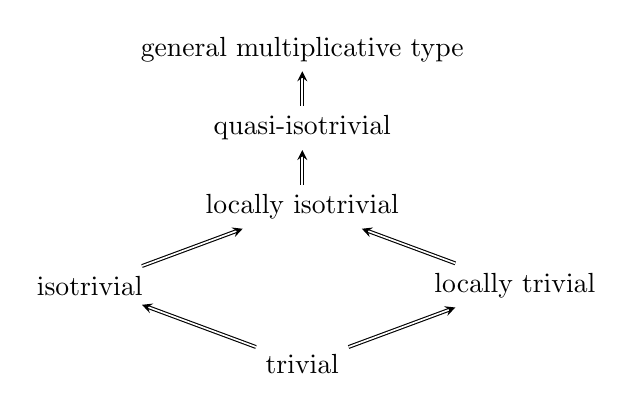
\begin{tikzpicture}[>=stealth]
  \node (general) at (0,4.0) {general multiplicative type};
  \node (quasi) at (0,3.0) {quasi-isotrivial};
  \node (lociso) at (0,2.0) {locally isotrivial};
  \node (iso) at (-2.7,1.0) {isotrivial};
  \node (loctriv) at (2.7,1.0) {locally trivial};
  \node (triv) at (0,0) {trivial};
  \draw[double,->] (quasi) -- (general);
  \draw[double,->] (lociso) -- (quasi);
  \draw[double,->] (iso) -- (lociso);
  \draw[double,->] (loctriv) -- (lociso);
  \draw[double,->] (triv) -- (iso);
  \draw[double,->] (triv) -- (loctriv);
\end{tikzpicture}
\end{center}

For practical purposes, let us point out at once that every group of
multiplicative type that we shall encounter will be quasi-isotrivial. Thus
we shall see in the next exposé (\SGARefLink{sga3:x:corollary:4-5}{X 4.5}) that, when \(G\) is of finite type
over \(S\), it is automatically quasi-isotrivial; we shall nevertheless
give examples in which it is not locally isotrivial. We shall likewise see
that \(G\) may be locally trivial without being isotrivial, and hence
\emph{a fortiori} without being trivial. This readily implies that the
inclusions in \SGARefLink{sga3:ix:diagram:1:2}{the preceding diagram} are strict.

On the other hand, we shall also see there (\SGARefLink{sga3:x:theorem:5-16}{X 5.16}) that, when \(S\) is
locally noetherian and normal---or, more generally, geometrically
unibranch---every group of multiplicative type and finite type over \(S\)
is necessarily isotrivial; moreover, it is trivial as soon as it is
locally trivial (or even merely trivial over a dense open subset). This
explains why most groups of multiplicative type encountered in practice
will doubtless be isotrivial, all the more so because we shall later see
that the maximal tori of semisimple group schemes are automatically
isotrivial.

\medskip
\noindent\SGARefTarget{sga3:ix:definition:1:3}\textbf{Definition 1.3.} ---
\textit{Let \(S\) and \(G\) be as in
\SGARefLink{sga3:ix:definition:1:1}{1.1}. The group \(G\) is called a
\emph{torus} if, for the faithfully flat quasi-compact topology, it is
locally isomorphic to a group of the form \(\mathbf G_m^r\), where
\(r\) is an integer with \(r\geq 0\).}

With the notation of \SGARefLink{sga3:ix:definition:1:1}{1.1}, this says
that \(S'\) may be chosen so that \(G'\) is isomorphic to a group of the
form \((\mathbf G_{m,S'})^r\). The integer \(r\) depends on \(s\in S\):
it is the dimension of the fiber
\[
  G_s=G\otimes_S\kappa(s).
\]
It is a locally constant function of \(s\), as is seen at once. This
observation should be generalized as follows.

% Source page: Exp9 component-local p. 3; complete-reader p. 649; printed pp. 39--40.
\medskip
\noindent\SGARefTarget{sga3:ix:definition:1:4}\textbf{Definition 1.4.} ---
\textit{Let \(G\) be a diagonalizable group scheme over a field \(k\).
Thus \(G\) is isomorphic to a group \(D_k(M)\), where \(M\) is an ordinary
commutative group determined up to isomorphism by this condition---more
precisely,
\[
  M\simeq\operatorname{Hom}_{k\text{-}\mathrm{gr}}
    (G,\mathbf G_{m,k})
\]
(\SGARefLink{sga3:viii:corollary:1:3}{VIII 1.3}). The isomorphism class of \(M\) is called the \emph{type} of
the diagonalizable group \(G\); it is plainly invariant under extension
of the base field.}

\textit{Now let \(G\) be a group scheme of multiplicative type over an
arbitrary prescheme \(S\). For every \(s\in S\), there is an extension
\(k\) of \(\kappa(s)\) such that
\(G\times_S\operatorname{Spec}(k)\) is a diagonalizable
\(k\)-group.\footnote{Editor's note: indeed, by hypothesis there are an
open neighborhood \(U\) of \(s\) and a faithfully flat quasi-compact
morphism \(S'\to U\) such that \(G_{S'}\) is diagonalizable. For every
\(s'\in S'\) above \(s\), the field \(\kappa(s')\) is an extension of
\(\kappa(s)\), and
\(G_{s'}=G\times_S\operatorname{Spec}(\kappa(s'))\) is diagonalizable.}
Its type is independent of the chosen extension by the preceding
observation and is called the \emph{type of \(G\) at \(s\)}, or the
\emph{type of \(G_s\)}. In particular, if \(G\) itself is diagonalizable,
and hence isomorphic to a group of the form \(D_S(M)\), then for every
\(s\in S\) the type of \(G\) at \(s\) is the isomorphism class of \(M\).}

\textit{More generally, if \(G\) is a group of multiplicative type over
\(S\) and \(M\) is an ordinary commutative group, then \(G\) is said to
be \emph{of type \(M\)} if it is of type \(M\) at every point \(s\in S\);
equivalently, if \(G\) is locally isomorphic to \(D_S(M)\) for the
faithfully flat quasi-compact topology.}

\medskip
\noindent\SGARefTarget{sga3:ix:remark:1:4:1}\textbf{Remark 1.4.1.}
\footnote{Editor's note: the number \SGARefLink{sga3:ix:remark:1:4:1}{1.4.1} has been added to the remarks
that follow, for use in later references.}
\SGARefTarget{sga3:ix:remark:1:4:1:item:a}\textit{a) For a group \(G\) of multiplicative type over \(S\), the
function
\[
  s\longmapsto \text{the type of }G_s
\]
is locally constant on \(S\). Indeed, with the notation of
\SGARefLink{sga3:ix:definition:1:1}{1.1}, if \(G'\) is of type \(M\),
then \(G\) is of type \(M\) over the neighborhood \(U\) of \(s\).
Consequently \(S\) has a canonical decomposition as a disjoint union of
preschemes \(S_i\) such that, for every \(i\), \(G_{S_i}\) is of type
\(M_i\), where the commutative groups \(M_i\) are pairwise
nonisomorphic.}

\SGARefTarget{sga3:ix:remark:1:4:1:item:b}\textit{b) In particular, if \(S\) is connected, the type of the fibers
of \(G\) is constant; that is, there is a commutative group \(M\) such
that \(G\) is of type \(M\). Finally, if \(G\) is a torus, the type of
\(G\) at \(s\) is determined by the integer \(\dim G_s\): indeed,
\(G_s\) is of type \(\mathbb Z^n\), where \(n=\dim G_s\).}

\medskip
\noindent\SGARefTarget{sga3:ix:remark:1:5}\textbf{Remark 1.5.} ---
\SGARefTarget{sga3:ix:remark:1:5:item:a}\textit{a) It follows immediately from Definitions
\SGARefLink{sga3:ix:definition:1:1}{1.1} and
\SGARefLink{sga3:ix:definition:1:3}{1.3} that these notions are
``compatible with base extension.'' Thus, if \(G\) is a group prescheme
over \(S\) and \(S'\to S\) is a base-change morphism, then whenever \(G\)
is of multiplicative type (respectively, of isotrivial multiplicative
type, and so on), the same is true of \(G'\).}

\SGARefTarget{sga3:ix:remark:1:5:item:b}\textit{b) If, moreover, \(S'\to S\) is faithfully flat and
quasi-compact, then \(G'\) being of multiplicative type, respectively a
torus, implies the same for \(G\). If \(S'\to S\) is also étale
(respectively, finite étale), then \(G'\) being quasi-isotrivial
(respectively, isotrivial) implies the same for \(G\).}

\SGARefTarget{sga3:ix:remark:1:5:item:c}\textit{c) Finally, return to an arbitrary base-change morphism
\(f:S'\to S\). If \(s'\in S'\) and \(s=f(s')\), then the type of \(G'\)
at \(s'\) is the same as that of \(G\) at \(s\), since
\[
  G'_{s'}=G_s\otimes_{\kappa(s)}\kappa(s').
\]}

% END INCLUDED SGA3_English_current_buildable_source_20260823/source/inputs/IX/tex/components/01_expose_IX_opening_and_section_1.tex

% BEGIN INCLUDED SGA3_English_current_buildable_source_20260823/source/inputs/IX/tex/components/02_expose_IX_sections_2_3.tex
% SGA 3, Expose IX, English reconstruction.
% Scope: Sections 2 and 3 in full.
% Authority: Polo--Gille Exp9-8nov09.pdf, component-local pp. 4--10
% (complete-reader pp. 650--656), stopping immediately before Section 4.
% Jacob Reinhold's CC BY 4.0 Markdown lineage was used only as a phrasing
% comparison. The Polo--Gille PDF controls text, formulas, numbering, notes,
% and references.

\setcounter{footnote}{2}

% Source page: Exp9 component-local p. 4; complete-reader p. 650;
% original printed pp. 41--42.
\SGARefTarget{sga3:ix:section:2}\section*{2. Extension of Certain Properties of Diagonalizable Groups to Groups of Multiplicative Type}
\addcontentsline{toc}{section}{2. Extension of Certain Properties of Diagonalizable Groups to Groups of Multiplicative Type}

The extensions in question are essentially trivial consequences of the
results of the preceding Expos\'e, in view of
\SGARefLink{sga3:ix:definition:1:1}{the definitions in 1.1} and the
``local'' nature (for the faithfully flat and quasi-compact topology) of
the results under consideration.

\medskip
\noindent\SGARefTarget{sga3:ix:definition:2:0}\textbf{Definition 2.0.}
\footnote{Editor's note: This definition has been added; it occurs in
\SGARefLink{sga3:ix:proposition:2:3}{Propositions~2.3} and
\SGARefLink{sga3:ix:proposition:2:7}{2.7}.}
\textit{We denote by \(\mathcal M\) the set of faithfully flat and
quasi-compact morphisms.}

\medskip
\noindent\SGARefTarget{sga3:ix:proposition:2:1}\textbf{Proposition 2.1.}
\textit{Let \(G\) be a group of multiplicative type over a prescheme
\(S\). Then:}
\begin{enumerate}
  \item[(a)]\SGARefTarget{sga3:ix:proposition:2:1:item:a:01}
  \textit{\(G\) is faithfully flat over \(S\), and affine over \(S\)
  (a fortiori, quasi-compact over \(S\));}

  \item[(b)]\SGARefTarget{sga3:ix:proposition:2:1:item:b:01}
  \textit{\(G\) is of finite type over \(S\) if and only if \(G\) is of
  finite presentation over \(S\), if and only if, for every \(s\in S\),
  the type of \(G\) at \(s\) is given by a commutative group of finite
  type;}

  \item[(c)]\SGARefTarget{sga3:ix:proposition:2:1:item:c:01}
  \textit{\(G\) is finite over \(S\) if and only if, for every
  \(s\in S\), the type of \(G\) at \(s\) is given by a finite commutative
  group, if and only if (when \(S\) is quasi-compact) \(G\) is of finite
  type over \(S\) and is annihilated by an integer \(n>0\);}

  \item[\((c')\)]\SGARefTarget{sga3:ix:proposition:2:1:item:cprime:01}
  \textit{\(G\) is integral over \(S\) if and only if, for every
  \(s\in S\), the type of \(G\) at \(s\) is given by a torsion
  commutative group;}

  \item[(d)]\SGARefTarget{sga3:ix:proposition:2:1:item:d:01}
  \textit{\(G\) is the unit group if and only if, for every \(s\in S\),
  the type of \(G\) at \(s\) is given by the zero commutative group;}

  \item[(e)]\SGARefTarget{sga3:ix:proposition:2:1:item:e:01}
  \textit{\(G\) is smooth over \(S\) if and only if, for every
  \(s\in S\), the type of \(G\) at \(s\) is given by a commutative group
  of finite type whose torsion subgroup has order prime to the
  characteristic of \(\kappa(s)\).}
\end{enumerate}

These statements follow from \SGARefLink{sga3:viii:proposition:2:1}{VIII~2.1}, taking into account that the
properties in question descend under faithfully flat and quasi-compact
morphisms (cf. SGA~1, VIII, or EGA~IV\textsubscript{2}, \S2).

Using \SGARefLink{sga3:viii:corollary:3:5}{VIII~3.5}, one likewise obtains:

\medskip
\noindent\SGARefTarget{sga3:ix:proposition:2:2}\textbf{Proposition 2.2.}
\textit{Let \(G\) be a group of multiplicative type and of finite type over
\(S\). For every integer \(n\ne0\), the kernel
\({}_nG=\ker(n\cdot\operatorname{id}_G)\) is a group of multiplicative
type, finite over \(S\).}

\medskip
\noindent\SGARefTarget{sga3:ix:proposition:2:3}\textbf{Proposition 2.3.}
\textit{Let \(G\) be a group of multiplicative type over the prescheme
\(S\), acting freely on the right on an \(S\)-prescheme \(X\) that is
affine over \(S\). Then:}
\begin{enumerate}
  \item[(a)]\SGARefTarget{sga3:ix:proposition:2:3:item:a:01}
  \textit{the equivalence relation defined by \(G\) in \(X\) is
  \(\mathcal M\)-effective (\SGARefLink{sga3:iv:subsection:3:4}{IV~3.4}), and \(Y=X/G\) is affine over \(S\);}

  \item[(b)]\SGARefTarget{sga3:ix:proposition:2:3:item:b:01}
  \textit{if, moreover, \(X\) is of finite presentation (respectively, of
  finite type) over \(S\), then the same is true of \(Y\).}
\end{enumerate}

\SGARefLink{sga3:ix:proposition:2:3:item:a:01}{The first assertion} follows from \SGARefLink{sga3:viii:theorem:5:1}{VIII~5.1}, which treats the case in which
\(G\) is diagonalizable, and from \SGARefLink{sga3:iv:proposition:3:5:2}{IV~3.5.2}, which allows one to reduce to
that case. Indeed, faithfully flat and quasi-compact morphisms
\(S'\to S\) are effective descent morphisms for the fibered category of
affine schemes over schemes: if \(Y'\) is affine over \(S'\) and is
equipped with a descent datum relative to \(S'\to S\), then this datum is
effective, that is, \(Y'\) comes from a scheme \(Y\) affine over \(S\)
(cf. SGA~1, \SGARefLink{sga3:viii:proposition:2:1}{VIII~2.1}).

% Source page: Exp9 component-local p. 5; complete-reader p. 651;
% original printed p. 43.
For \SGARefLink{sga3:ix:proposition:2:3:item:b:01}{the second assertion}, one is likewise reduced to the diagonalizable
case of \SGARefLink{sga3:viii:corollary:5:8}{VIII~5.8}, since the finiteness conditions under consideration
descend under faithfully flat and quasi-compact morphisms (SGA~1,
VIII~3.3 and 3.6\footnote{Editor's note: See also V, 9.1, or
EGA~IV\textsubscript{2}, 2.7.1.}). Proceeding as in VIII,
Corollaries~5.5--5.7, one deduces from
\SGARefLink{sga3:ix:proposition:2:3}{2.3}:

\medskip
\noindent\SGARefTarget{sga3:ix:corollary:2:4}\textbf{Corollary 2.4.}
\textit{Under the hypotheses of \SGARefLink{sga3:ix:proposition:2:3}{2.3},
the graph morphism}
\SGARefTarget{sga3:ix:corollary:2:4:diagram:01}
\[
  X\times_S G\longrightarrow X\times_S X
\]
\textit{is a closed immersion. For every section \(\sigma\) of \(X\)
over \(S\), the corresponding morphism}
\[
  G\longrightarrow X,\qquad g\longmapsto\sigma\cdot g,
\]
\textit{is a closed immersion.}

In particular:

\medskip
\noindent\SGARefTarget{sga3:ix:corollary:2:5}\textbf{Corollary 2.5.}
\textit{Let \(u:G\to H\) be a monomorphism of \(S\)-preschemes in groups,
with \(G\) of multiplicative type and \(H\) affine over \(S\). Then \(u\)
is a closed immersion, \(H/G=Y\) exists and is affine over \(S\), and
\(H\) is a principal homogeneous bundle over \(Y\) under \(G_Y\).}

\medskip
\noindent\SGARefTarget{sga3:ix:remark:2:6}\textbf{Remark 2.6.}
Let \(u:G\to H\) be a monomorphism of \(S\)-preschemes in groups, where
\(G\) is of multiplicative type and of finite type over \(S\), and \(H\)
is of finite presentation and separated over \(S\). One can then show
that \(u\) is a closed immersion by using \SGARefLink{sga3:viii:proposition:7:12}{VIII~7.12} (see
Remark~\SGARefLink{sga3:viii:remark:7-13:item:b}{VIII~7.13(b)}).

\medskip
\noindent\SGARefTarget{sga3:ix:proposition:2:7}\textbf{Proposition 2.7.}
\textit{Let \(u:G\to H\) be a homomorphism of \(S\)-groups of
multiplicative type, with \(H\) of finite type over \(S\). Then:}
\begin{enumerate}
  \item[(i)]\SGARefTarget{sga3:ix:proposition:2:7:item:i:01}
  \textit{\(G_0=\ker u\) is an \(S\)-group of multiplicative type; the
  equivalence relation defined by \(G_0\) in \(G\) is
  \(\mathcal M\)-effective, and hence (\SGARefLink{sga3:iv:subsection:3:4}{IV~3.4}) \(u\) factors as}
  \SGARefTarget{sga3:ix:proposition:2:7:diagram:01}
  \[
    G\longrightarrow G/G_0=I\longrightarrow H,
  \]
  \textit{where \(I\to H\) is a monomorphism\footnote{Editor's note:
  Indeed, even a closed immersion.} of \(S\)-groups. The group \(I\) is of
  multiplicative type, the equivalence relation in \(H\) defined by \(I\)
  is \(\mathcal M\)-effective, and consequently \(H_0=H/I\) exists and is
  also of multiplicative type;}

  \item[(ii)]\SGARefTarget{sga3:ix:proposition:2:7:item:ii:01}
  \textit{\(H_0\) and \(I\) are of finite type, and so is \(G_0\) when
  \(G\) is.}
\end{enumerate}

\emph{Proof.}
Proceeding as for \SGARefLink{sga3:ix:proposition:2:3}{2.3}, one is
reduced to the case in which \(G\) and \(H\) are diagonalizable; then
\SGARefLink{sga3:ix:proposition:2:7}{2.7} reduces to \SGARefLink{sga3:viii:corollary:3:4}{VIII~3.4}.

We record the following corollaries.

% Source page: Exp9 component-local p. 6; complete-reader p. 652;
% original printed p. 44.
\medskip
\noindent\SGARefTarget{sga3:ix:corollary:2:8}\textbf{Corollary 2.8.}
\begin{enumerate}
  \item[(a)]\SGARefTarget{sga3:ix:corollary:2:8:item:a:01}
  \textit{Let \(S\) be a prescheme. The category of \(S\)-groups of
  multiplicative type and of finite type is an abelian category.}

  \item[(b)]\SGARefTarget{sga3:ix:corollary:2:8:item:b:01}
  \textit{Let \(u:G\to H\) be a homomorphism in this category. It is a
  monomorphism (respectively, an epimorphism, respectively, an
  isomorphism) in this category if and only if \(u\) is a monomorphism of
  preschemes (respectively, \(u\) is faithfully flat, respectively, \(u\)
  is an isomorphism of preschemes).}
\end{enumerate}

It is enough to note that the product of two \(S\)-groups of
multiplicative type is again of multiplicative type (which is immediate),
and is plainly of finite type over \(S\) if both factors are. The rest of
\SGARefLink{sga3:ix:corollary:2:8}{2.8} follows immediately from
\SGARefLink{sga3:ix:proposition:2:7}{2.7}; the details are left to the
reader.

\medskip
\noindent\SGARefTarget{sga3:ix:corollary:2:9}\textbf{Corollary 2.9.}
\textit{Let \(u:G\to H\) be a homomorphism of \(S\)-groups of
multiplicative type and of finite type. Let \(U\) be the set of points
\(s\in S\) for which \(u_s:G_s\to H_s\) is a monomorphism
(respectively, faithfully flat, respectively, an isomorphism). Then
\(U\) is both open and closed, and the induced homomorphism
\(u_U:G_U\to H_U\) is a monomorphism (respectively, faithfully flat,
respectively, an isomorphism).}

Let \(P\) (respectively, \(Q\)) be the kernel (respectively, cokernel) of
\(u\). By \SGARefLink{sga3:ix:proposition:2:7}{2.7}, \(Q\) exists and
\(P\) and \(Q\) are of multiplicative type; moreover, formation of \(P\)
and \(Q\) commutes with every base change \(S'\to S\), in particular with
the formation of fibers. On the other hand, \(u\) is a monomorphism
(respectively, faithfully flat, respectively, an isomorphism) if and only
if \(P=0\) (respectively, \(Q=0\), respectively, \(P=Q=0\)). These
remarks reduce us to checking the following assertion: if \(R\) is an
\(S\)-group of multiplicative type, then the set \(U\) of points
\(s\in S\) for which \(R_s=0\) is open and closed, and \(R_U=0\). This is
contained in \SGARefLink{sga3:ix:remark:1:4:1:item:a}{Remark~1.4.1(a)}.

\medskip
\noindent\SGARefTarget{sga3:ix:corollary:2:10}\textbf{Corollary 2.10.}
\textit{Let \(G\) be an \(S\)-group of multiplicative type and of finite
type, and let \(H\) and \(H'\) be two subgroups of multiplicative type.}
\begin{enumerate}
  \item[(a)]\SGARefTarget{sga3:ix:corollary:2:10:item:a:01}
  \textit{\(H''=H\cap H'\) is a subgroup of \(G\) of multiplicative
  type.}

  \item[(b)]\SGARefTarget{sga3:ix:corollary:2:10:item:b:01}
  \textit{Let \(U\) be the set of \(s\in S\) for which
  \(H_s\subseteq H'_s\) (respectively, \(H_s=H'_s\)). Then \(U\) is open
  and closed, and \(H_U\subseteq H'_U\) (respectively, \(H_U=H'_U\)).}
\end{enumerate}

Here, of course, the intersection sign in \(H\cap H'\) denotes the
intersection in the functorial sense, namely \(H\times_GH'\), which is
plainly an \(S\)-subgroup of \(G\). Likewise, the inclusion sign
(respectively, the equality sign) denotes the order relation
(respectively, equality) between subfunctors of \(H\), not inclusion
(respectively, equality) of the underlying sets.

Applying \SGARefLink{sga3:ix:proposition:2:7}{2.7} first to the inclusion
morphism \(H\to G\), one finds that \(H\) is of finite type; the same
holds for \(H'\). It then follows from
\SGARefLink{sga3:ix:corollary:2:8}{2.8} that \(H\cap H'\) is of
multiplicative type and of finite type. (Note that the canonical functor
from the category considered in \SGARefLink{sga3:ix:corollary:2:8}{2.8}
to the category \((\mathbf{Sch})/S\) commutes with finite inverse limits.)

Formation of \(H\cap H'\) commutes with base extension, in particular
with formation of the fibers. Moreover,
\(H\subseteq H'\) (respectively, \(H=H'\)) is equivalent to
\(H''=H\) (respectively, to \(H''=H\) and \(H''=H'\)). Consider the
canonical homomorphisms \(H''\to H\) and \(H''\to H'\). Then \(U\) is the
set of points \(s\in S\) for which the induced homomorphism
\(H''_s\to H_s\) is an isomorphism (respectively, for which
\(H''_s\to H_s\) and \(H''_s\to H'_s\) are isomorphisms).

% Source page: Exp9 component-local p. 7; complete-reader p. 653;
% original printed pp. 45--46.
By \SGARefLink{sga3:ix:corollary:2:9}{2.9}, it follows that \(U\) is open
and closed, and that \(H''_U\to H_U\) (respectively,
\(H''_U\to H_U\) and \(H''_U\to H'_U\)) are isomorphisms. This gives the
desired conclusion.

\medskip
\noindent\SGARefTarget{sga3:ix:proposition:2:11}\textbf{Proposition 2.11.}
\textit{Let \(S\) be a prescheme, let \(G\) be an \(S\)-group of
multiplicative type and of finite type over \(S\), let \(H\) be a subgroup
of \(G\) of multiplicative type, and put \(K=G/H\), a quotient group of
\(G\) of multiplicative type.}
\begin{enumerate}
  \item[(i)]\SGARefTarget{sga3:ix:proposition:2:11:item:i:01}
  \textit{Suppose \(G\) is trivial, that is, diagonalizable. There is a
  partition of \(S\) into open and closed subsets \(S_i\) such that, for
  every \(i\), \(H_{S_i}\) and \(K_{S_i}\) are diagonalizable. In
  particular, if \(S\) is connected, \(H\) and \(K\) are
  diagonalizable.}

  \item[(ii)]\SGARefTarget{sga3:ix:proposition:2:11:item:ii:01}
  \textit{\SGARefLink{sga3:ix:proposition:2:11:item:i:01}{The same assertion} holds with ``diagonalizable'' replaced by
  ``isotrivial,'' provided that \(S\) is connected, locally connected, or
  quasi-compact.}

  \item[(iii)]\SGARefTarget{sga3:ix:proposition:2:11:item:iii:01}
  \textit{If \(G\) is locally trivial (respectively, locally isotrivial,
  respectively, quasi-isotrivial), then the same is true of \(K\) and
  \(H\).}
\end{enumerate}

\emph{Proof.}
\SGARefLink{sga3:ix:proposition:2:11:item:i:01}{(i)} By hypothesis, \(G=D_S(M)\), where \(M\) is a commutative group of
finite type. For each quotient group \(M_i\) of \(M\), let
\(H_i=D_S(M_i)\) be the corresponding diagonalizable subgroup of \(G\)
(\SGARefLink{sga3:viii:theorem:3:1}{VIII~3.1}). Let \(S_i\) be the set of points \(s\in S\) for which
\(H_s=(H_i)_s\). By \SGARefLink{sga3:ix:corollary:2:10}{2.10}, \(S_i\)
is open and closed, and \(H_{S_i}=(H_i)_{S_i}\); thus \(H_{S_i}\) is
diagonalizable, and hence so is \(K_{S_i}\) (\SGARefLink{sga3:viii:theorem:3:1}{VIII~3.1}). The \(S_i\) are
plainly pairwise disjoint, and we claim that they cover \(S\). Indeed, for
every \(s\), the group \(H_s\), being a subgroup of the diagonalizable
group \(G_s\), is diagonalizable (cf. \SGARefLink{sga3:ix:proposition:8:1}{8.1} below\footnote{Editor's note:
The erroneous reference to IV~4.7.5 has been corrected. Note that
\SGARefLink{sga3:ix:section:8}{Section~8} of the present Expos\'e is independent of Sections~\SGARefLink{sga3:ix:section:3}{3}--\SGARefLink{sga3:ix:section:7}{7}.}).
Hence \(H_s\) has the form \(D_{\kappa(s)}(M_i)\), by \SGARefLink{sga3:viii:corollary:1:5}{VIII~1.5} and
\SGARefLink{sga3:ix:theorem:3:2:item:b}{3.2(b)}. Restricting to the family of nonempty \(S_i\), assertion \SGARefLink{sga3:ix:proposition:2:11:item:i:01}{(i)}
follows.

\SGARefLink{sga3:ix:proposition:2:11:item:ii:01}{(ii)} By hypothesis, there exists a finite surjective \'etale morphism
\(S'\to S\) such that \(G_{S'}\) is diagonalizable. Every point of \(S'\)
therefore has an open and closed neighborhood \(U'\) such that \(H_{U'}\)
and \(K_{U'}\) are diagonalizable. The image \(U\) of \(U'\) in \(S\) is
open and closed, and \(S'\to S\) still induces a finite surjective
\'etale
morphism \(U'\to U\). Thus every point \(s\in S\) has an open and closed
neighborhood \(U\) such that \(H_U\) and \(K_U\) are isotrivial.
Assertion \SGARefLink{sga3:ix:proposition:2:11:item:ii:01}{(ii)} follows at once.

\SGARefLink{sga3:ix:proposition:2:11:item:iii:01}{(iii)} This follows at once from \SGARefLink{sga3:ix:proposition:2:11:item:i:01}{(i)}, \SGARefLink{sga3:ix:proposition:2:11:item:ii:01}{(ii)}, and the definitions. Moreover,
the quasi-isotrivial case will also follow from the more general fact
``finite type \(\Longrightarrow\) quasi-isotrivial,'' announced in
\SGARefLink{sga3:ix:comments:1:2}{1.2}
(cf. \SGARefLink{sga3:x:corollary:4-5}{X~4.5}).

\SGARefTarget{sga3:ix:section:3}\section*{3. Infinitesimal Properties: Lifting and Conjugation Theorems}
\addcontentsline{toc}{section}{3. Infinitesimal Properties: Lifting and Conjugation Theorems}

The fundamental infinitesimal properties of groups of multiplicative type
follow from \SGARefLink{sga3:ix:theorem:3:1}{the following theorem}.

\medskip
\noindent\SGARefTarget{sga3:ix:theorem:3:1}\textbf{Theorem 3.1.}
\textit{Let \(S\) be an affine scheme, let \(H\) be an \(S\)-group of
multiplicative type, and let \(\mathscr F\) be a quasi-coherent sheaf on
\(S\) on which \(H\) acts (\SGARefLink{sga3:i:subsection:4-7}{I~4.7}). Then}
\[
  \mathrm H^i(H,\mathscr F)=0\qquad\text{for }i>0,
\]
\textit{where \(\mathrm H^i\) denotes the Hochschild cohomology studied
in Expos\'e~I, \S5.}

% Source page: Exp9 component-local p. 8; complete-reader p. 654;
% original printed pp. 47--48.
Indeed, by loc.\ cit., \SGARefLink{sga3:ix:corollary:5:3}{5.3}, Hochschild cohomology is expressed, in terms
of the affine rings \(A\) and \(B\) of \(S\) and \(G\), and the
\(A\)-module \(M\) defining \(\mathscr F\), as the cohomology of a complex
of \(A\)-modules \(C^\bullet(H,M)\), whose formation commutes with every
base change \(A\to A'\). Consequently, for a base change \(A\to A'\) with
\(A'\) flat over \(A\), one has
\[
  \mathrm H^i(H',\mathscr F')
  =\mathrm H^i(H,\mathscr F)\otimes_AA'.
\]
If \(A'\) is moreover faithfully flat over \(A\), it is therefore enough,
in order to prove that \(\mathrm H^i(H,\mathscr F)\) vanishes, to prove
that \(\mathrm H^i(H',\mathscr F')\) vanishes. This observation reduces
us to checking \SGARefLink{sga3:ix:theorem:3:1}{3.1} in the case where
\(G\) is diagonalizable; in that case it was proved in \SGARefLink{sga3:i:theorem:5-3-3}{I~5.3.3}.

Using the results of Expos\'e~III, we shall derive from
\SGARefLink{sga3:ix:theorem:3:1}{3.1} several consequences of a geometric
nature.

\medskip
\noindent\SGARefTarget{sga3:ix:theorem:3:2}\textbf{Theorem 3.2.}
\textit{Let \(S\) be an affine scheme, let \(S_0\) be an affine subscheme
defined by an ideal \(J\), let \(H\) be a group of multiplicative type
over \(S\), and let \(G\) be an arbitrary group prescheme over \(S\).
Let \(u,v:H\to G\) be two group homomorphisms, and let
\(u_0,v_0:H_0\to G_0\) be the homomorphisms obtained from \(u,v\) by the
base change \(S_0\to S\). If \(J^2=0\) and \(u_0=v_0\), then there exists
\(g\in G(S)\) such that}
\[
  v=\operatorname{int}(g)\circ u
  \qquad\textit{and}\qquad
  g_0=e.
\]

This follows from \SGARefLink{sga3:iii:theorem:2-1:item:ii}{III~2.1(ii)} and
\SGARefLink{sga3:ix:theorem:3:1}{3.1} (the vanishing of
\(\mathrm H^1\)).

\medskip
\noindent\SGARefTarget{sga3:ix:corollary:3:3}\textbf{Corollary 3.3.}
\textit{Under the preliminary hypotheses of
\SGARefLink{sga3:ix:theorem:3:2}{3.2}, suppose in addition that \(G\) is
smooth over \(S\), but assume only that \(J\) is nilpotent (not
necessarily square-zero). If there exists \(g_0\in G_0(S_0)\) such that
\(v_0=\operatorname{int}(g_0)\circ u_0\), then \(g_0\) lifts to an element
\(g\in G(S)\) such that \(v=\operatorname{int}(g)\circ u\).}

By induction on an integer \(n\) such that \(J^n=0\), one is reduced to
the case in which \(J\) is square-zero. Since \(G\) is smooth over \(S\),
one may lift \(g_0\) to an element \(g'\) of \(G(S)\). Replacing \(v\) by
\(v'=\operatorname{int}(g')\circ u\), one is then reduced to the
situation of \SGARefLink{sga3:ix:theorem:3:2}{3.2}.

\medskip
\noindent\SGARefTarget{sga3:ix:corollary:3:4}\textbf{Corollary 3.4.}
\textit{Under the preliminary hypotheses of
\SGARefLink{sga3:ix:theorem:3:2}{3.2}, with \(J\) nilpotent, suppose in
addition that \(u\) is central (for example, that \(G\) is commutative).
Then \(u_0=v_0\) implies \(u=v\).}

Indeed, the reduction to the case in which \(J\) is square-zero is again
immediate, and then it is enough to apply
\SGARefLink{sga3:ix:theorem:3:2}{3.2}. In particular:

\medskip
\noindent\SGARefTarget{sga3:ix:corollary:3:5}\textbf{Corollary 3.5.}
\textit{Let \(S,S_0,H,G\) be as in
\SGARefLink{sga3:ix:theorem:3:2}{3.2}, with \(J\) nilpotent. Let
\(u:H\to G\) be a homomorphism of \(S\)-groups such that
\(u_0:H_0\to G_0\) is the unit homomorphism. Then \(u\) is the unit
homomorphism.}

\medskip
\noindent\SGARefTarget{sga3:ix:theorem:3:6}\textbf{Theorem 3.6.}
\textit{Let \(S\) be an affine scheme, let \(S_0\) be a subscheme defined
by a nilpotent ideal \(J\), let \(H\) be a group of multiplicative type
over \(S\), let \(G\) be a group prescheme smooth over \(S\), and let
\(u_0:H_0\to G_0\) be a homomorphism of the \(S_0\)-groups obtained by
base change \(S_0\to S\). Then there exists a homomorphism
\(u:H\to G\) of \(S\)-groups that lifts \(u_0\). Moreover, by
\SGARefLink{sga3:ix:corollary:3:3}{3.3}, any two such liftings \(u,u'\)
are conjugate by an element of \(G(S)\) whose reduction in \(G(S_0)\) is
the identity element.}

% Source page: Exp9 component-local p. 9; complete-reader p. 655;
% original printed p. 49.
This follows from \SGARefLink{sga3:iii:theorem:2-1}{III~2.1} and \SGARefLink{sga3:ix:proposition:2:3}{2.3} and from
\SGARefLink{sga3:ix:theorem:3:1}{3.1}: the vanishing of
\(\mathrm H^2\) gives the existence of the lifting of \(u_0\), and the
vanishing of \(\mathrm H^1\) gives uniqueness up to conjugation.

One may prove in the same way the following variants of
\SGARefLink{sga3:ix:theorem:3:2}{3.2}--%
\SGARefLink{sga3:ix:theorem:3:6}{3.6}. In fact, these variants imply the
preceding statements when applied to the graph subgroups of the
homomorphisms considered there.

\medskip
\noindent\SGARefTarget{sga3:ix:theorem:3:2:bis}\textbf{Theorem 3.2 bis.}
\textit{Let \(S\) be an affine scheme, let \(S_0\) be a subscheme defined
by an ideal \(J\), let \(G\) be an \(S\)-group prescheme, and let \(H,H'\)
be subgroup preschemes of multiplicative type. Let \(G_0,H_0,H'_0\) be
the groups over \(S_0\) obtained by base change \(S_0\to S\). If
\(J^2=0\) and \(H_0=H'_0\), then there exists \(g\in G(S)\) such that}
\[
  H'=\operatorname{int}(g)(H)
  \qquad\textit{and}\qquad
  g_0=e.
\]

\medskip
\noindent\SGARefTarget{sga3:ix:corollary:3:3:bis}\textbf{Corollary 3.3 bis.}
\textit{Under the preliminary hypotheses of
\SGARefLink{sga3:ix:theorem:3:2:bis}{3.2 bis}, suppose in addition that
\(G\) is smooth over \(S\), and that \(J\) is nilpotent (not necessarily
square-zero). If \(g_0\in G_0(S_0)\) satisfies
\(H'_0=\operatorname{int}(g_0)(H_0)\), then \(g_0\) lifts to an element
\(g\in G(S)\) such that \(H'=\operatorname{int}(g)(H)\).}

\medskip
\noindent\SGARefTarget{sga3:ix:corollary:3:4:bis}\textbf{Corollary 3.4 bis.}
\textit{Under the preliminary hypotheses of
\SGARefLink{sga3:ix:theorem:3:2:bis}{3.2 bis}, suppose that \(J\) is
nilpotent and that \(H\) is central (for example, that \(G\) is
commutative). Then \(H_0=H'_0\) implies \(H=H'\).}

\medskip
\noindent\SGARefTarget{sga3:ix:theorem:3:6:bis}\textbf{Theorem 3.6 bis.}
\textit{Let \(S\) be an affine scheme, let \(S_0\) be a subscheme defined
by a nilpotent ideal \(J\), let \(G\) be an \(S\)-group prescheme smooth
over \(S\), and let \(H_0\) be a subgroup prescheme of
\(G_0=G\times_SS_0\), of multiplicative type. Then:}
\begin{enumerate}
  \item[(a)]\SGARefTarget{sga3:ix:theorem:3:6:bis:item:a:01}
  \textit{there exists a subgroup prescheme \(H\) of \(G\), flat over
  \(S\), such that \(H\times_SS_0=H_0\);}

  \item[\SGAInlineRefTarget{sga3:ix:theorem:3:2:item:b}(b)]\SGARefTarget{sga3:ix:theorem:3:6:bis:item:b:01}
  \textit{such an \(H\) is necessarily of multiplicative type;}

  \item[(c)]\SGARefTarget{sga3:ix:theorem:3:6:bis:item:c:01}
  \textit{finally, by
  \SGARefLink{sga3:ix:theorem:3:2:bis}{3.2 bis}, any two such liftings
  \(H,H'\) of \(H_0\) are conjugate by an element \(g\in G(S)\) whose
  reduction in \(G(S_0)\) is the identity element.}
\end{enumerate}

Let us indicate how one can prove
\SGARefLink{sga3:ix:theorem:3:2:bis}{3.2 bis} (of which
\SGARefLink{sga3:ix:corollary:3:3:bis}{3.3 bis} and
\SGARefLink{sga3:ix:corollary:3:4:bis}{3.4 bis} are immediate
consequences) and assertion
\SGARefLink{sga3:ix:theorem:3:6:bis:item:a:01}{(a)} of
\SGARefLink{sga3:ix:theorem:3:6:bis}{3.6 bis}. The latter follows from
\SGARefLink{sga3:ix:theorem:3:1}{3.1} (the vanishing of
\(\mathrm H^2\)) and \SGARefLink{sga3:iii:corollary:4-37:item:ii}{III~4.37(ii)}. Similarly,
\SGARefLink{sga3:ix:theorem:3:2:bis}{3.2 bis} follows from
\SGARefLink{sga3:ix:theorem:3:1}{3.1} (the vanishing of
\(\mathrm H^1\)) and \SGARefLink{sga3:iii:corollary:4-37:item:i}{III~4.37(i)}, at least when \(G\) and \(H\) are
smooth over \(S\).

Using the results of the following Expos\'e, however, one can very simply
deduce \SGARefLink{sga3:ix:theorem:3:2:bis}{3.2 bis} and
\SGARefLink{sga3:ix:theorem:3:6:bis}{3.6 bis}, in the general form stated
here, from \SGARefLink{sga3:ix:theorem:3:2}{3.2} and
\SGARefLink{sga3:ix:theorem:3:6}{3.6}, respectively. For
\SGARefLink{sga3:ix:theorem:3:2:bis}{3.2 bis}, it is enough to note that,
by \SGARefLink{sga3:x:proposition:2:1}{X~2.1}, \(H\) and \(H'\) are isomorphic, which reduces us to
\SGARefLink{sga3:ix:theorem:3:2}{3.2}.

For \SGARefLink{sga3:ix:theorem:3:6:bis}{3.6 bis}, note that \(H_0\) is
necessarily of finite type over \(S_0\):\footnote{Editor's note: The
original said, ``by \SGARefLink{sga3:ix:proposition:2:1:item:b:01}{2.1(b)}, since its fibers are.'' The editors did not
understand this argument and have replaced it by the argument that
follows.} indeed, as a subgroup prescheme of \(G_0\), which is smooth
over \(S_0\), the group \(H_0\) is locally of finite type over \(S_0\).
But \(H_0\) is affine over \(S_0\) by
\SGARefLink{sga3:ix:proposition:2:1:item:a:01}{2.1(a)}, and is therefore
of finite type over \(S_0\). By \SGARefLink{sga3:x:corollary:4-5}{X~4.5}, \(H_0\) is consequently
quasi-isotrivial, and hence comes, by \SGARefLink{sga3:x:proposition:2:1}{X~2.1}, from a group \(H\) of
multiplicative type over \(S\).\footnote{Editor's note: The sentence that
follows has been expanded.} By
\SGARefLink{sga3:ix:theorem:3:6}{3.6}, there exists a homomorphism of
\(S\)-groups \(u:H\to G\) lifting the immersion \(H_0\hookrightarrow
G_0\). Since \(H\) and \(H_0\) (respectively, \(G\) and \(G_0\)) have the
same underlying topological space, and since, for every \(h\in H\), the
morphism

% Source page: Exp9 component-local p. 10; complete-reader p. 656;
% original printed p. 50.
\[
  \mathscr O_{G,u(h)}\longrightarrow\mathscr O_{H,h}
\]
is surjective (because it is so after reduction modulo the nilpotent ideal
\(J\)), the morphism \(u\) is also an immersion (cf. EGA~I, 4.2.2).

Finally, every lifting \(H\) of \(H_0\) to a flat subgroup of \(G\) is
necessarily of multiplicative type by \SGARefLink{sga3:x:corollary:2:3}{X~2.3},\footnote{Editor's note:
\SGARefLink{sga3:x:corollary:2:3}{X~2.3} depends essentially on \SGARefLink{sga3:ix:theorem:3:6}{Theorem~3.6} of the present Expos\'e.} which
also proves assertion
\SGARefLink{sga3:ix:theorem:3:6:bis:item:b:01}{(b)} of
\SGARefLink{sga3:ix:theorem:3:6:bis}{3.6 bis}. The reader may verify that
the results \SGARefLink{sga3:ix:theorem:3:2:bis}{3.2 bis}--%
\SGARefLink{sga3:ix:theorem:3:6:bis}{3.6 bis} are not used in
Expos\'e~X,
so there is no vicious circle.

\medskip
\noindent\SGARefTarget{sga3:ix:proposition:3:8}\textbf{Proposition 3.8.}
\footnote{Editor's note: The numbering of the original has been retained;
there is no 3.7.}
\textit{Let \(S\) be a prescheme, let \(S_0\) be a closed subscheme
defined by a locally nilpotent ideal \(J\), let \(G\) be an \(S\)-group
of multiplicative type, and let \(X\) be an \(S\)-prescheme locally of
finite presentation. Suppose that \(G\) acts on \(X\) in such a way that
\(G_0=G\times_SS_0\) acts trivially on \(X_0=X\times_SS_0\). Then \(G\)
acts trivially on \(X\).}

The proof is the proof of \SGARefLink{sga3:iii:corollary:2-4:item:b}{III~2.4(b)}. One may also reduce to loc.\ cit. by
observing that \SGARefLink{sga3:ix:proposition:3:8}{3.8} immediately
reduces to the case in which \(G\) is diagonalizable, which is the case
treated there.

\medskip
\noindent\SGARefTarget{sga3:ix:corollary:3:9}\textbf{Corollary 3.9.}
\textit{Let \(S,S_0\) be as above, and let \(u:G\to H\) be a homomorphism
of \(S\)-groups, with \(G\) of multiplicative type and \(H\) locally of
finite presentation over \(S\). Suppose that the homomorphism
\(u_0:G_0\to H_0\) obtained by base change \(S_0\to S\) is central. Then
\(u\) is central.}

Indeed, it is enough to apply
\SGARefLink{sga3:ix:proposition:3:8}{3.8} with \(X=H\), letting \(G\) act
on \(H\) by
\[
  (g,h)\longmapsto\operatorname{int}(u(g))\cdot h
  =u(g)h\,u(g)^{-1}.
\]

% Hard stop: immediately before Section 4, Exp9 component-local p. 10
% (complete-reader p. 656; original printed p. 50).

% END INCLUDED SGA3_English_current_buildable_source_20260823/source/inputs/IX/tex/components/02_expose_IX_sections_2_3.tex

% BEGIN INCLUDED SGA3_English_current_buildable_source_20260823/source/inputs/IX/tex/components/03_expose_IX_sections_4_5.tex
% SGA 3, Expose IX, English reconstruction.
% Scope: Sections 4 and 5 in full.
% Authority: Polo--Gille Exp9-8nov09.pdf, component-local pp. 10--22
% (partial), complete-reader pp. 656--668 (partial), printed pp. 50--63.
% Start cursor: "4. Le theoreme de densite" on component-local p. 10.
% End cursor: immediately before
% "6. Monomorphismes des groupes de type multiplicatif, et factorisation"
% on component-local p. 22.
% Jacob Reinhold's CC BY 4.0 Markdown lineage was used only as a phrasing
% comparison. The Polo--Gille PDF controls prose, formulas, numbering,
% notes, references, and diagrams.

\setcounter{footnote}{10}

% Source page: Exp9 component-local p. 10; complete-reader p. 656.
\SGARefTarget{sga3:ix:section:4}\section*{4. The Density Theorem}
\addcontentsline{toc}{section}{4. The Density Theorem}

This theorem (cf. \SGARefLink{sga3:ix:theorem:4:7}{4.7 below})%
\begingroup
\renewcommand{\thefootnote}{\(\ast\)}%
\footnote{All the results from
\SGARefLink{sga3:ix:definition:4:1}{4.1} through
\SGARefLink{sga3:ix:corollary:4:6}{4.6} are contained in EGA
IV\(_3\), 11.10, to which we refer the reader for a systematic account of
the notion of schematic density.}%
\addtocounter{footnote}{-1}%
\endgroup,
together with the theorem\footnote{Editor's note: the ``algebraicity''
theorem \SGARefLink{sga3:ix:theorem:7:1}{7.1}.} of \SGARefLink{sga3:ix:section:7}{Section~7}, will be the
essential tool in the present expos\'e and the two following ones for
passing from the infinitesimal properties of groups of multiplicative type
developed above to their ``finite'' properties.

\medskip
\noindent\SGARefTarget{sga3:ix:definition:4:1}\textbf{Definition 4.1.}
\textit{Let \(X\) be a prescheme. A family
\((Z_i)_{i\in I}\) of subpreschemes of \(X\) is said to be
\emph{schematically dense} if, for every open subset \(U\) of \(X\) and
every closed subprescheme \(U_0\) of \(U\) containing all the
\(Z_i\cap U\), one has \(U_0=U\).}

\textit{A subprescheme \(Z\) of \(X\) is said to be
\emph{schematically dense in \(X\)} if the one-member family consisting
of \(Z\) is schematically dense.}

It is immediate (cf. EGA IV\(_3\), 11.10.1) that the definition is
equivalent to saying that, for every open subset \(U\) of \(X\), every
section \(f\) of \(\mathscr O_U\) that vanishes on each \(Z_i\cap U\)
is zero. Equivalently, the intersection of the kernels of the canonical
homomorphisms
\SGARefTarget{sga3:ix:definition:4:1:display:01}
\[
  u_i:\mathscr O_X\longrightarrow (v_i)_*(\mathscr O_{Z_i})
\]
is zero, where \(v_i:Z_i\to X\) is the canonical immersion.%
\footnote{Editor's note: all the results on schematic density stated in
EGA IV\(_3\), \S11.10 follow from the results on ``separating families of
homomorphisms'' proved in \emph{loc.\ cit.}, \S11.9, to which some of the
editor's notes below will refer.}
When \(X\) lies over a prescheme \(S\), this is also equivalent to the
following assertion: for every open subset \(U\) of \(X\), every
\(S\)-prescheme \(Y\) separated over \(S\), and every pair of morphisms
\(u,v:U\to Y\) that coincide on the \(Z_i\cap U\), one has \(u=v\).
Indeed, \(u=v\) is equivalent to \(U_0=U\), where \(U_0\) is the inverse
image of the diagonal in \(Y\times_S Y\) under the \(S\)-morphism
\(U\to Y\times_S Y\) defined by \((u,v)\). The diagonal is a closed
subprescheme of \(Y\times_S Y\), so \(U_0\) is a closed subprescheme of
\(U\) containing all the \(Z_i\cap U\). Thus schematic density gives
\(U_0=U\), hence \(u=v\). Conversely, take
\(Y=\operatorname{Spec}\mathscr O_S[T]\).

In the terminology introduced at the end of EGA I, 9.5, saying that the
subprescheme \(Z\) is schematically dense in \(X\) also means that \(X\)
is the \emph{closure subprescheme} of \(Z\) in \(X\).

% Source page: Exp9 component-local p. 11; complete-reader p. 657.
\medskip
\noindent\SGARefTarget{sga3:ix:lemma:4:2}\textbf{Lemma 4.2.}
\textit{Let \(X\) be a flat \(S\)-prescheme, and let
\((Z_i)_{i\in I}\) be a family of subpreschemes of \(X\), flat over
\(S\). Let \(S_0\) be a subprescheme of \(S\) defined by a nilpotent
ideal \(\mathscr J\), and suppose that the modules
\(\mathscr J^n/\mathscr J^{n+1}\) are locally free over \(S_0\).
Let \(X_0,Z_{i0}\) be obtained from \(X,Z_i\) by the base change
\(S_0\to S\). If \((Z_{i0})_{i\in I}\) is schematically dense in
\(X_0\), then \((Z_i)_{i\in I}\) is schematically dense in \(X\).}

\emph{Proof.}
Suppose \(\mathscr J^{n+1}=0\), where \(n\geq0\), and argue by induction
on \(n\); the assertion is trivial for \(n=0\). Define
\(S_m,X_m,Z_{im}\) by reduction modulo \(\mathscr J^{m+1}\), as usual.
The induction hypothesis already implies that
\((Z_{i,n-1})_{i\in I}\) is schematically dense in \(X_{n-1}\).
After replacing \(X\) by an induced open subset, it is enough to prove
that every section \(f\) of \(\mathscr O_X\) that vanishes on all the
\(Z_i\) is zero.

The section \(f_{n-1}\) of
\[
  \mathscr O_{X_{n-1}}
  =\mathscr O_X/\mathscr J^n\mathscr O_X
\]
defined by \(f\) vanishes on the \(Z_{i,n-1}\), hence is zero.
Consequently, \(f\) is a section of
\(\mathscr J^n\mathscr O_X\). Since \(X\) is flat over \(S\), there is
an isomorphism
\SGARefTarget{sga3:ix:lemma:4:2:display:01}
\[
  \mathscr J^n\mathscr O_X
  \xleftarrow{\ \sim\ }
  \mathscr E\otimes_{\mathscr O_{S_0}}\mathscr O_{X_0},
  \qquad
  \mathscr E=\mathscr J^n=\mathscr J^n/\mathscr J^{n+1}.
\]
Similarly, since each \(Z_i\) is flat over \(S\), the restriction
\(f_i\) of \(f\) to \(Z_i\) may be regarded as a section of
\SGARefTarget{sga3:ix:lemma:4:2:display:02}
\[
  \mathscr J^n\mathscr O_{Z_i}
  \xleftarrow{\ \sim\ }
  \mathscr E\otimes_{\mathscr O_{S_0}}\mathscr O_{Z_{i0}}.
\]
By hypothesis, all the \(f_i\) are zero. The module \(\mathscr E\) is
locally free by assumption, and therefore so is
\[
  \mathscr F
  =\mathscr E\otimes_{\mathscr O_{S_0}}\mathscr O_{X_0}.
\]
Thus \(f\) is a section of the locally free module \(\mathscr F\) on
\(X_0\) whose restriction to every \(Z_{i0}\) is zero. Since the family
\((Z_{i0})_{i\in I}\) is schematically dense in \(X_0\), it follows at
once that \(f=0\). \qed

% Source page: Exp9 component-local p. 12; complete-reader p. 658.
\medskip
\noindent\SGARefTarget{sga3:ix:corollary:4:3}\textbf{Corollary 4.3.}
\textit{Let \(X\) be a locally Noetherian \(S\)-prescheme, flat over
\(S\), and let \((Z_i)_{i\in I}\) be a family of subpreschemes of \(X\),
flat over \(S\). Suppose that, for every \(s\in S\), the family of fibers
\((Z_{is})_{i\in I}\) is schematically dense in \(X_s\). Then
\((Z_i)_{i\in I}\) is schematically dense in \(X\).}

\emph{Proof.}
After replacing \(X\) by an induced open subset, it is enough to prove
that every section \(f\) of \(\mathscr O_X\) whose restriction to all
the \(Z_i\) is zero is itself zero.%
\footnote{Editor's note: the original has been expanded in what follows.}
For this, it suffices to show that the image of \(f\) in
\(\mathscr O_{X,x}\) is zero for every \(x\in X\). Let
\(\mathfrak m_x\) be the maximal ideal of \(\mathscr O_{X,x}\), and let
\(\mathfrak m_s\) be that of \(\mathscr O_{S,s}\), where \(s\) is the
image of \(x\) in \(S\). Since \(\mathscr O_{X,x}\) is Noetherian,
\[
  \bigcap_{n\in\mathbb N}\mathfrak m_x^n=0,
  \qquad\text{and hence, a fortiori,}\qquad
  \bigcap_{n\in\mathbb N}\mathscr O_{X,x}\mathfrak m_s^n=0.
\]
It is therefore enough to show, for every integer \(n\), that the section
induced by \(f\) on
\[
  X\times_S
  \operatorname{Spec}\bigl(\mathscr O_{S,s}/\mathfrak m_s^{n+1}\bigr)
\]
is zero. By hypothesis,
\[
  Z_{is}=Z_i\otimes_{\mathscr O_{S,s}}\kappa(s)
\]
is a schematically dense family in
\[
  X_s=X\otimes_{\mathscr O_{S,s}}\kappa(s).
\]
We are thus reduced to the case in which \(S\) is the spectrum of a
local ring whose maximal ideal \(\mathscr J\) is nilpotent,
\(S_0=\operatorname{Spec}\kappa(s)\), and the hypotheses of
\SGARefLink{sga3:ix:lemma:4:2}{Lemma~4.2} hold. The conclusion follows.
\qed

\medskip
\noindent\SGARefTarget{sga3:ix:lemma:4:4}\textbf{Lemma 4.4.}
\textit{Let \(S\) be a locally Noetherian prescheme, let \(X\) be a
locally Noetherian \(S\)-prescheme, flat over \(S\), and let
\((Z_i)_{i\in I}\) be a family of subpreschemes of \(X\), flat over
\(S\). Suppose that, for every \(s\in S\), the family of fibers
\((Z_{is})_{i\in I}\) is schematically dense in \(X_s\).
Then, for every base change \(S'\to S\), with \(S'\) not necessarily
locally Noetherian, the family \((Z_i')_{i\in I}\) is schematically
dense in \(X'\). In other words, \((Z_i)_{i\in I}\) is universally
schematically dense in \(X\) relative to \(S\) (cf. EGA IV\(_3\),
Definition 11.10.8).}

\emph{Proof.}%
\footnote{Editor's note: for another proof, reducing to the case in which
\(S'\) is locally Noetherian and using
\SGARefLink{sga3:ix:corollary:4:3}{4.3} and
\SGARefLink{sga3:ix:lemma:4:5}{4.5} as here, see EGA
IV\(_3\), 11.9.16 and 11.9.12. In the last line of the proof of 11.9.16,
replace 11.9.5 by 11.9.12.}
Let \(f'\) be a section of \(\mathscr O_{X'}\) over an open subset
\(U'\) of \(X'\), vanishing on the \(Z_i'\); we must show that \(f'=0\).
Fix \(s'\in S'\). It is enough to prove that \(f'\) vanishes at every
point of \(U'\) above \(s'\). If \(s\) is the image of \(s'\) in \(S\),
then, after replacing \(S,S'\) by the spectra of their local rings at
\(s,s'\), we may suppose that \(S,S'\) are local and that \(s,s'\) are
their closed points. We may also suppose that \(X\) is affine, so that
\SGARefTarget{sga3:ix:lemma:4:4:display:01}
\[
  \begin{gathered}
    S=\operatorname{Spec}(A),\qquad
    S'=\operatorname{Spec}(A'),\\
    X=\operatorname{Spec}(B),\qquad
    X'=\operatorname{Spec}(B'),\qquad
    B'=B\otimes_A A',
  \end{gathered}
\]
where \(A,A'\) are local, \(A\to A'\) is a local homomorphism, and
\(A,B\) are Noetherian. We may further suppose that \(U'\) is affine,
of the form \(X'_{g'}\), with \(g'\in B'\).

For every \(A\)-subalgebra \(A''\) of \(A'\), put
\[
  S''=\operatorname{Spec}(A'')
\]
and let \(X'',Z_i''\) be obtained from \(X,Z_i\) by the base change
\(S''\to S\). We obtain the diagram
\SGARefTarget{sga3:ix:lemma:4:4:diagram:01}
\[
\begin{tikzcd}[column sep=large,row sep=large]
  % The source visibly prints the n-subscripts in the upper middle and
  % upper right nodes; they are retained despite the surrounding prose.
  Z^i \arrow[d] & Z_n^{i''} \arrow[l]\arrow[d]
    & Z_n^{i'} \arrow[l]\arrow[d] \\
  X \arrow[d] & X'' \arrow[l]\arrow[d] & X' \arrow[l]\arrow[d] \\
  S & S'' \arrow[l] & S' \arrow[l].
\end{tikzcd}
\]

% Source page: Exp9 component-local p. 13; complete-reader p. 659.
In what follows, we restrict to those \(A''\) that are localizations of
\(A\)-subalgebras \(A_1''\) of \(A'\), of finite type over \(A\), at
\(\mathfrak m'\cap A_1''\), where \(\mathfrak m'\) is the maximal ideal
of \(A'\). Thus the homomorphisms \(A\to A''\to A'\) are local. These
\(A''\) form an increasing filtered family of subalgebras whose union,
and hence whose direct limit, is \(A'\). Likewise,
\[
  B'=\varinjlim_{A''}\bigl(B\otimes_A A''\bigr).
\]
There therefore exist such an \(A''\) and an element
\(g''\in B''=B\otimes_A A''\) whose image in \(B'\) is \(g'\).

By \SGARefLink{sga3:ix:lemma:4:5}{Lemma~4.5 below}, the property that
\((Z_{is})_{i\in I}\) be schematically dense in \(X_s\) is preserved by
every base change \(S''\to S\).%
\footnote{Editor's note: the preceding sentence has been added, and the
original has been expanded in what follows.}
Consequently, because each \(S''\) is locally Noetherian, replacing
\(S\) by a suitable \(S''\) and \(X,Z_i\) by \(X'',Z_i''\) preserves
the hypotheses of \SGARefLink{sga3:ix:lemma:4:4}{Lemma~4.4}.

We may therefore suppose that \(g'\) comes from an element \(g\in B\).
After replacing \(X\) by the open subset \(X_g=U\), we may suppose that
\(U'=X'\). In the same way, we may suppose that \(f'\) comes from a
section \(f\) of \(\mathscr O_X\) over \(X\).

Let \(Y=V(f)\) be the subscheme of \(X\) defined by \(f\), and put
\[
  Y_i=Z_i\times_XY.
\]
Thus \(Y_i\) is the closed subscheme \(V(f_i)\) of \(Z_i\), where \(f_i\)
is the section of \(\mathscr O_{Z_i}\) induced by \(f\). Denoting by
\(Y',Y_i'\) the \(S'\)-schemes obtained by base change, we have
\SGARefTarget{sga3:ix:lemma:4:4:display:02}
\[
  Y'=V(f'),
  \qquad
  Y_i'=Z_i'\times_{X'}Y'=V(f_i'),
\]
and analogous relations hold for \(Y'',Y_i''\). The assertion that
\(f'\) vanishes on the \(Z_i'\) is equivalent to
\[
  Y_i'=Z_i'\qquad\text{for every }i.
\]
\footnote{Editor's note: the original added ``at least at every point
\(x'\) of \(X'\) above \(s'\),'' but this restriction seems unnecessary.}

Let \(\mathfrak m\) be the maximal ideal of \(A\). For every
\(n\geq0\), introduce the closed subscheme
\[
  S_n=\operatorname{Spec}(A/\mathfrak m^{n+1})
\]
of \(S\), and let \(X_n,Y_n,Z_n^i,Y_n^i\) be obtained from
\(X,Y,Z_i,Y_i\) by the base change \(S_n\to S\). More generally, for
every \(S\)-prescheme \(P\), write \(P_n=P\times_SS_n\).

For every \(n\) and \(i\in I\), consider the functor
\SGARefTarget{sga3:ix:lemma:4:4:display:03}
\[
  F_n^i
  =\prod_{Z_n^i/S_n}Y_n^i/Z_n^i:
  (\mathbf{Sch})_{/S_n}^{\circ}\longrightarrow\mathbf{Set},
\]
defined, for every \(P\) over \(S_n\), by
\SGARefTarget{sga3:ix:lemma:4:4:display:04}
\[
F_n^i(P)
=\Gamma\bigl((Y_n^i)_P/(Z_n^i)_P\bigr)
=
\begin{cases}
  \varnothing,&(Y_n^i)_P\ne(Z_n^i)_P,\\
  \{\operatorname{id}\},&(Y_n^i)_P=(Z_n^i)_P.
\end{cases}
\]
Since \(S_n\) is local Artinian and \(Z_n^i\) is flat, hence essentially
free, over \(S_n\), \SGARefLink{sga3:viii:theorem:6:4}{VIII, 6.4} shows
that each \(F_n^i\) is represented by a closed subprescheme \(T_n^i\)
of \(S_n\).

% Source page: Exp9 component-local p. 14; complete-reader p. 660.
The completion \(\widehat A\) of the local ring \(A\) is Noetherian
because \(A\) is, and it is the projective limit of the rings \(A_n\).%
\footnote{Editor's note: the original has been expanded and corrected to
show that the projective limit of the rings
\(\mathscr O(T_n^i)\) defines a closed formal subscheme of
\(\operatorname{Spf}(\widehat A)\).}
Let \(K_n^i\) be the ideal of
\[
  A_n=A/\mathfrak m^{n+1}
\]
defining \(T_n^i\), and let \(K^i=\varprojlim_nK_n^i\); this is an ideal
of \(\widehat A\).

For fixed \(i\), integers \(m\geq n\), and any \(S_n\)-prescheme \(P\),
\[
  (Y_n^i)_P
  =Y_i\times_SS_n\times_{S_n}P
  =Y_i\times_SP
  =(Y_m^i)_P,
\]
and similarly \((Z_n^i)_P=(Z_m^i)_P\). It follows that \(F_n^i\) is the
restriction \(F_m^i\times_{S_m}S_n\) of \(F_m^i\) to
\((\mathbf{Sch})_{/S_n}\), and therefore
\[
  T_n^i=T_m^i\times_{S_m}S_n.
\]
We thus have a commutative diagram with exact rows:
\SGARefTarget{sga3:ix:lemma:4:4:diagram:02}
\[
\begin{tikzcd}[column sep=large,row sep=large]
  0 \arrow[r] & K_m^i \arrow[r]\arrow[d,two heads]
    & A_m \arrow[r]\arrow[d,two heads]
    & \mathscr O(T_m^i) \arrow[r]\arrow[d,two heads] & 0\\
  0 \arrow[r] & K_n^i \arrow[r]
    & A_n \arrow[r]
    & \mathscr O(T_n^i) \arrow[r] & 0
\end{tikzcd}
\]
All the vertical arrows are surjective. It follows, first, that the
projective system \((K_n^i)_{n\in\mathbb N}\) satisfies the
Mittag--Leffler condition, so that
\[
  \varprojlim_n\mathscr O(T_n^i)
  \simeq\widehat A/K^i
\]
as topological rings (cf. EGA \(0_{\mathrm{III}}\), \S13.2). Second, the
map \(K^i\to K_n^i\) is surjective (cf. \SGARefLink{sga3:ix:bib:bens}{[BEns]}, III, \S7.4,
Proposition~5). Hence
\[
  K_n^i\simeq
  \frac{K^i+\mathfrak m^{n+1}\widehat A}
       {\mathfrak m^{n+1}\widehat A},
  \qquad
  \mathscr O(T_n^i)\simeq
  (\widehat A/K^i)\otimes_A(A/\mathfrak m^{n+1}).
\]

In other words, \((T_n^i)_n\) is an inductive system of affine Artinian
schemes, and its inductive limit
\[
  T^i=\varinjlim_nT_n^i
\]
is a closed formal subscheme of
\[
  \widehat S=\operatorname{Spf}(\widehat A)
\]
(cf. EGA I, \S10), whose reduction modulo \(\mathfrak m^{n+1}\) is
\(T_n^i\).

Let \(T\) be the closed formal subscheme of \(\widehat S\) given by the
intersection of the \(T^i\), that is, defined by
\[
  K=\sum_iK^i.
\]
Since \(\widehat A\) is Noetherian, there is a finite subset \(J\) of
\(I\) such that
\[
  K=\sum_{i\in J}K^i,
  \qquad\text{equivalently}\qquad
  T=\bigcap_{i\in J}T^i.
\]
For every \(n\), therefore,
\[
  K_n=\sum_{i\in J}K_n^i,
\]
where \(K_n\) is the image of \(K\) in \(A_n\).

Recall that \(f_i\) is the image of
\(f\in B=\mathscr O(X)\) in \(\mathscr O(Z_i)\), and that \(f_i'\) is
its image in
\[
  \mathscr O(Z_i')
  =\mathscr O(Z_i)\otimes_AA'.
\]
The relation \(Y_i'=Z_i'\) is equivalent to \(f_i'=0\). Now
\(\mathscr O(Z_i)\otimes_AA'\) is the direct limit of the subalgebras
\(\mathscr O(Z_i)\otimes_AA''\), for \(A''\) as above. Consequently,
there is an \(A''\) for which \(Y_i''=Z_i''\). A priori \(A''\) depends
on \(i\), but, because \(J\) is finite, one \(A''\) can be chosen that
works for every \(i\in J\). Put
\[
  S''=\operatorname{Spec}(A''),
  \qquad
  S''_{(n)}=S''\times_SS_n.
\]
\footnote{Editor's note: the original has been expanded and corrected,
distinguishing \(S''_{(n)}\) from the subscheme
\(S_n''=S_n''(s'')\) introduced below.}

% Source page: Exp9 component-local p. 15; complete-reader p. 661.
For every \(i\in J\), the equality
\[
  Y_i''\times_{S''}S''_{(n)}
  =(Y_n^i)_{S''_{(n)}}
  =Z_i''\times_{S''}S''_{(n)}
  =(Z_n^i)_{S''_{(n)}}
\]
shows, by the definition of \(T_n^i\), that \(S''_{(n)}\to S_n\)
factors through \(T_n^i\). It therefore factors through
\[
  T_n=\bigcap_{i\in J}T_n^i,
\]
and hence through \(T_n^i\) for every \(i\in I\). Let \(f''\) be the
image of \(f\) in \(B''=B\otimes_AA''\), and let \(f''_{(n)}\) be its
image in
\[
  B''_{(n)}=B''/\mathfrak m^{n+1}B''.
\]
The preceding factorization means that, for every \(n\), the section
\(f''_{(n)}\) vanishes on all the \(Z_i\times_SS''_{(n)}\).

Because \(A\to A''\to A'\) are local homomorphisms, the image \(s''\)
of \(s'\) in \(S''\) is the closed point of \(S''\), corresponding to
the maximal ideal \(\mathfrak m''\) of \(A''\), and its image in \(S\)
is \(s\). \emph{[The source prints \(B''\) here; since
\(s''\in S''=\operatorname{Spec}(A'')\), the intended ring is
\(A''\).]} Fix \(n\), and now let \(S_n''\) denote the \(n\)-th
infinitesimal neighborhood of \(s''\) in \(S''\):
\[
  S_n''=\operatorname{Spec}(A''/\mathfrak m''^{\,n+1}).
\]
Put
\[
  B_n''=B''/\mathfrak m''^{\,n+1}B'',
  \qquad
  Z_{n}^{i''}=Z_i\times_SS_n''.
\]
\emph{[The source appends
\(Z_n^{i''}=\operatorname{Spec}(B_n'')\); the displayed equality would
identify each \(Z_n^{i''}\) with \(X_n''\), so the base-change
definition is retained here.]}
Then the image \(f_n''\) of \(f''_{(n)}\) in \(B_n''\) vanishes on every
\(Z_n^{i''}\). By \SGARefLink{sga3:ix:lemma:4:5}{Lemma~4.5 below}, the
family of fibers
\[
  Z_0^{i'''}
  =Z_n^{i''}\times_{S_n''}\kappa(s'')
  =Z_{is}\times_{\kappa(s)}\kappa(s'')
\]
is schematically dense in
\[
  X_0'''
  =X_n''\times_{S_n''}\kappa(s'')
  =X_s\times_{\kappa(s)}\kappa(s'').
\]
Thus \(S_n'',X_n'',(Z_n^{i''})_{i\in I}\), and
\[
  S_0'''=\operatorname{Spec}\kappa(s'')
\]
satisfy the hypotheses of \SGARefLink{sga3:ix:lemma:4:2}{Lemma~4.2}.
It follows that \(f_n''=0\), that is,
\[
  f''\in\mathfrak m''^{\,n+1}B''
  \qquad\text{for every }n.
\]

Since \(B\) is Noetherian and \(B''=B\otimes_AA''\) is a localization
of a finite-type \(B\)-algebra, \(B''\) is Noetherian. Its local rings
are therefore separated for their usual topology. Hence \(f''\) is zero
at every point \(x''\) of \(X''\) for which
\(\mathfrak m''B''\) is contained in the maximal ideal of
\(\mathscr O_{X'',x''}\), that is, at every point of \(X''\) above
\(s''\). A fortiori, \(f'\) is zero at every point of \(X'\) above
\(s'\). \qed

\medskip
\noindent\SGARefTarget{sga3:ix:lemma:4:5:0}\textbf{Lemma 4.5.0.}%
\footnote{Editor's note: this lemma has been inserted here because it is
used in the proofs of \SGARefLink{sga3:ix:lemma:4:5}{4.5} and
\SGARefLink{sga3:ix:theorem:4:7}{4.7}.}
\textit{Let \(X\) be an \(S\)-prescheme, let \((Z_i)_{i\in I}\) be a
family of subpreschemes of \(X\), and let \(S'\to S\) be faithfully
flat. If \((Z_i')_{i\in I}\) is schematically dense in \(X'\), then
\((Z_i)_{i\in I}\) is schematically dense in \(X\).}

This follows from EGA IV\(_3\), 11.10.5(i) and 11.9.10(i). It remains to
give the proof of \SGARefLink{sga3:ix:lemma:4:5}{the following lemma}.

\medskip
\noindent\SGARefTarget{sga3:ix:lemma:4:5}\textbf{Lemma 4.5.}
\textit{Let \(X\) be a locally Noetherian prescheme}%
\footnote{Editor's note: this hypothesis is in fact superfluous; cf. EGA
IV\(_3\), 11.10.6 and 11.9.13.}
\textit{ over a field \(k\), let \((Z_i)_{i\in I}\) be a family of
subpreschemes of \(X\), let \(k'/k\) be a field extension, and let
\(X',Z_i'\) be obtained from \(X,Z_i\) by base change. Then
\((Z_i)_{i\in I}\) is schematically dense in \(X\) if and only if
\((Z_i')_{i\in I}\) is schematically dense in \(X'\).}

\emph{Proof.}
The ``if'' direction follows from
\SGARefLink{sga3:ix:lemma:4:5:0}{Lemma~4.5.0}; let us prove the
converse.%
\footnote{Editor's note: the original has been expanded in what follows.}
First, we may suppose \(X=\operatorname{Spec}(B)\) affine. For every
\(i\), let \((Z_{ij})_{j\in J_i}\) be an affine open covering of \(Z_i\).
Replacing \((Z_i)_{i\in I}\) by
\((Z_{ij})_{(i,j)\in J}\), where
\[
  J=\coprod_{i\in I}J_i,
\]
we may also suppose that every \(Z_i\) is affine.

Let
\[
  g\in B'=B\otimes_kk',
  \qquad
  t'\in B_g'
\]
be a section of \(\mathscr O_{X'}\) on the affine open
\(U'=X_g'\) whose restriction to each \(Z_i'\cap U'\) is zero. Thus its
image in every
\[
  \bigl(\mathscr O(Z_i)\otimes_kk'\bigr)_g
\]
is zero. There exists a finite-type \(k\)-subalgebra \(A\) of \(k'\)
such that
\[
  g\in B_A=B\otimes_kA,
  \qquad
  t'\in(B_A)_g.
\]
The map
\[
  \mathscr O(Z_i)\otimes_kA
  \longrightarrow
  \mathscr O(Z_i)\otimes_kk'
\]
is injective, and therefore so is
\[
  \bigl(\mathscr O(Z_i)\otimes_kA\bigr)_g
  \longrightarrow
  \bigl(\mathscr O(Z_i)\otimes_kk'\bigr)_g.
\]
The hypothesis consequently implies that the image of \(t'\) in every
\(\bigl(\mathscr O(Z_i)\otimes_kA\bigr)_g\) is zero. It remains to show
that \((Z_{iA})_{i\in I}\) is schematically dense in \(X_A\), which
follows from EGA IV\(_3\), 11.9.10(b).%
\footnote{Editor's note: the original continued: ``Using
\SGARefLink{sga3:ix:corollary:4:3}{4.3} for the
\(X_{A'}\), where \(A'\) is a quotient of \(A\) by a power of a maximal
ideal, and Hilbert's Nullstellensatz, one is reduced to the case where
\(k'\) is a finite extension of \(k\).'' This reduction could be
expanded and that argument pursued, since the case of a finite extension
\(k'/k\) is somewhat simpler than the more general case treated in EGA
IV\(_3\), 11.9.10(b).}
\qed

Let us record in passing \SGARefLink{sga3:ix:corollary:4:6}{the following result}, which will be used in a
later expos\'e.%
\footnote{Editor's note: this reference remains to be specified.}

% Source page: Exp9 component-local p. 16; complete-reader p. 662.
\medskip
\noindent\SGARefTarget{sga3:ix:corollary:4:6}\textbf{Corollary 4.6.}
\textit{Let \(X\) be a flat \(S\)-prescheme and \(U\) an open subset of
\(X\). Suppose that \(U_s\) is schematically dense in \(X_s\) for every
\(s\in S\), and that either \(X\) is locally Noetherian or \(X\) is
locally of finite presentation over \(S\). Then \(U\) is schematically
dense in \(X\).}

\emph{Proof.}
For simplicity, suppose \(U\) is retrocompact in \(X\) (cf. EGA
IV\(_3\), 11.10.10 and 11.9.17 for the general case). The locally
Noetherian case is included only for reference; it is contained in
\SGARefLink{sga3:ix:corollary:4:3}{4.3}.

In the second case, we may plainly suppose \(S\) and \(X\) affine. Then
\(X\) and \(U\) are of finite presentation over
\(S=\operatorname{Spec}(A)\). The ring \(A\) is the direct limit of its
finite-type \(\mathbb Z\)-subalgebras \(A_i\). The ``patented
procedure'' already used (cf. EGA IV\(_3\), 8.8.2 and 8.10.5(iii))
shows that there are an index \(i\), an affine scheme \(X_i\) over
\[
  S_i=\operatorname{Spec}(A_i),
\]
and an open subset \(U_i\) of \(X_i\), from which \(X,U\) are obtained
by the base change \(S\to S_i\). Let \(E_i\) be the subset of \(S_i\)
consisting of those \(s\in S_i\) for which \((U_i)_s\) is schematically
dense in \((X_i)_s\).

By EGA IV\(_2\), 5.9.9 and 5.10.2, \(E_i\) is the set of points
\(s\in S_i\) for which \((U_i)_s\) contains the set
\[
  \operatorname{Ass}\mathscr O_{(X_i)_s}
\]
of points associated with the structure sheaf of \((X_i)_s\). By EGA
IV\(_3\), 11.9.17.1, this is a constructible condition; hence \(E_i\)
is constructible.%
\footnote{Editor's note: the original has been expanded in this paragraph
and the next.}

By \SGARefLink{sga3:ix:lemma:4:5}{4.5}, the inverse image of \(E_i\)
under \(S_j\to S_i\) is \(E_j\), and its inverse image under
\(S\to S_i\) is the set \(E\) of those \(s\in S\) for which \(U_s\)
is schematically dense in \(X_s\).%
\footnotemark[24]
By hypothesis, \(E=S\), which is also the inverse image of \(S_i\) under
every \(S\to S_i\). EGA IV\(_3\), 8.3.11 therefore implies that there
is a \(j\geq i\) such that \(E_j=S_j\); that is, \((U_j)_s\) is
schematically dense in \((X_j)_s\) for every \(s\in S_j\).

Apply \SGARefLink{sga3:ix:lemma:4:4}{4.4} to
\((S_j,X_j,U_j)\) and the base change \(S\to S_j\). It follows that
\(U\) is schematically dense in \(X\). Notice that here
\SGARefLink{sga3:ix:lemma:4:4}{4.4} is used only
for a family with a finite index set (in fact, a singleton); in this
case its proof simplifies considerably. \qed

% Source page: Exp9 component-local p. 17; complete-reader p. 663.
\medskip
\noindent\SGARefTarget{sga3:ix:theorem:4:7}\textbf{Theorem 4.7.}
\textit{Let \(S\) be a prescheme, and let \(G\) be a group of
multiplicative type and of finite type over \(S\). For every integer
\(n>0\), let \({}_nG\) be the kernel of \(n\cdot\operatorname{id}_G\).
Then the family of subpreschemes \(({}_nG)_{n>0}\) is schematically
dense in \(G\) in the sense of
\SGARefLink{sga3:ix:definition:4:1}{Definition~4.1}.}

\emph{Proof.}
We distinguish two cases.

\smallskip
\SGARefTarget{sga3:ix:theorem:4:7:proof:item:a}\noindent\textit{(a) \(S\) locally Noetherian.}
By \SGARefLink{sga3:ix:corollary:4:3}{4.3}, we are reduced to the case
in which \(S\) is the spectrum of a field \(k\). By
\SGARefLink{sga3:ix:lemma:4:5:0}{4.5.0}, we may suppose that \(k\) is
algebraically closed and that \(G\) is diagonalizable, say
\[
  G=D_k(M),
\]
where \(M\) is a commutative group of finite type. Then
\[
  M\simeq\Gamma\times\mathbb Z^r
\]
with \(\Gamma\) finite, and consequently
\[
  G\simeq G_1\times G_2,
  \qquad
  G_1=D(\Gamma),
  \qquad
  G_2=\mathbf G_m^r.
\]
For \(n\) sufficiently divisible---namely, for \(n\) a multiple of the
order of \(\Gamma\)---one has
\[
  {}_nG=G_1\times{}_nG_2,
  \qquad\text{since}\qquad
  {}_nG_1=G_1.
\]
Applying \SGARefLink{sga3:ix:corollary:4:3}{4.3} again to the projection
\(G\to G_1\), we are reduced to
\(G_2\), hence to the case \(G=\mathbf G_m^r\). Since \(G\) is then
reduced, schematic density of \(({}_nG)_{n>0}\) is equivalent to
density of \(\bigcup_n{}_nG\) in the ordinary topology. As
\[
  {}_nG=({}_n\mathbf G_m)^r,
\]
we are reduced to \(G=\mathbf G_m\), an irreducible group of dimension
one. The assertion now follows because
\(\bigcup_n{}_nG\), the set of roots of unity in \(k\), is infinite.

\smallskip
\SGARefTarget{sga3:ix:theorem:4:7:proof:item:b}\noindent\textit{(b) The general case.}
For every \(s\in S\), there are an open neighborhood \(U\) of \(s\)
and a faithfully flat quasi-compact morphism \(S'\to U\) such that
\(G'=G_{S'}\) is diagonalizable, say \(G'=D_{S'}(M)\). By
\SGARefLink{sga3:ix:lemma:4:5:0}{4.5.0} we may
reduce to \(G'\), and therefore suppose that \(G\) itself is
diagonalizable. It is obtained by base change
\[
  S\longrightarrow\operatorname{Spec}(\mathbb Z)
\]
from the absolute group \(H=D_{\mathbb Z}(M)\). Part~\SGARefLink{sga3:ix:theorem:4:7:proof:item:a}{(a)} shows that,
for every \(s\in\operatorname{Spec}(\mathbb Z)\), the family
\(({}_nH_s)_{n>0}\) is schematically dense in \(H_s\). It remains only
to apply \SGARefLink{sga3:ix:lemma:4:4}{4.4}.%
\footnote{Editor's note: \SGARefLink{sga3:ix:theorem:4:7}{this result} will be needed in X, \SGARefLink{sga3:x:lemma:4-3}{4.3} for a
non-locally-Noetherian base, namely
\(S=\operatorname{Spec}(\widehat A\otimes_A\widehat A)\), where
\(\widehat A\) is the completion of the Noetherian local ring \(A\).}
\qed

\medskip
\noindent\SGARefTarget{sga3:ix:corollary:4:8}\textbf{Corollary 4.8.}
\begin{enumerate}
  \item[(a)]\SGARefTarget{sga3:ix:corollary:4:8:item:a}
  \textit{Let \(u,v:H\to G\) be two homomorphisms of \(S\)-preschemes
  in groups, with \(H\) of multiplicative type}%
  \footnote{Editor's note: ``diagonalizable'' has been replaced by ``of
  multiplicative type.''}
  \textit{ and of finite type. Suppose that, for every integer \(n>0\),
  the restrictions of \(u\) and \(v\) to \({}_nH\) are equal. Then
  \(u=v\).}

  \item[(b)]\SGARefTarget{sga3:ix:corollary:4:8:item:b}
  \textit{Let \(H_1,H_2\) be two subgroups of multiplicative type and
  of finite type of a prescheme in groups \(G\). If
  \({}_nH_1={}_nH_2\) for every integer \(n>0\), then \(H_1=H_2\).}
\end{enumerate}

\emph{Proof.}
Part~\SGARefLink{sga3:ix:corollary:4:8:item:a}{(a)} follows from part~\SGARefLink{sga3:ix:corollary:4:8:item:b}{(b)} by considering the subgroups \(H_1,H_2\)
of \(H\times G\) that are the graphs of \(u,v\). For part~\SGARefLink{sga3:ix:corollary:4:8:item:b}{(b)}, put
\[
  H=H_1\cap H_2.
\]
This is a subgroup prescheme of \(H_i\), for \(i=1,2\), and we must show
that it equals \(H_i\). The hypothesis says precisely that \(H\)
contains all the \({}_nH_i\). We are therefore reduced to \SGARefLink{sga3:ix:corollary:4:9}{the next
corollary}. \qed

\medskip
\noindent\SGARefTarget{sga3:ix:corollary:4:9}\textbf{Corollary 4.9.}
\textit{Let \(G\) be an \(S\)-group of multiplicative type and of finite
type, and let \(H\) be a subgroup prescheme containing \({}_nG\) for
every \(n>0\). Then \(H=G\).}

\emph{Proof.}
By \SGARefLink{sga3:ix:theorem:4:7}{4.7}, it is enough to prove that
\(H\) is closed, or equivalently that it equals \(G\) set-theoretically.
This reduces us to the case in which \(S\) is the spectrum of a field.
Every subgroup prescheme of \(G\) is then closed, by VI\(_B\), \SGARefLink{cor:sga3-VIB-1.4.2}{1.4.2}.
\qed

% Source page: Exp9 component-local p. 18; complete-reader p. 664.
\medskip
\noindent\SGARefTarget{sga3:ix:remark:4:10}\textbf{Remark 4.10.}
Under the hypotheses of \SGARefLink{sga3:ix:theorem:4:7}{4.7}, let
\(m>0\) be an integer with the following properties: for every
\(s\in S\), \(m\) is not a power of the characteristic of \(\kappa(s)\);
and if \(G_s\) has type \(M\), every prime divisor of the torsion
subgroup of \(M\) divides \(m\). The second condition is automatically
satisfied if \(G\) is a torus. The proof shows that in
\SGARefLink{sga3:ix:theorem:4:7}{Theorem~4.7} and
\SGARefLink{sga3:ix:corollary:4:8}{Corollary~4.8} and
\SGARefLink{sga3:ix:corollary:4:9}{Corollary~4.9} one may restrict to
the subgroups
\[
  {}_{m^r}G,\qquad r>0.
\]

Moreover, if \(G\) is smooth over \(S\), then for every \(s\in S\) there
are an open neighborhood \(U\) of \(s\) and an integer \(m>0\), prime
to every residue characteristic on \(U\), that satisfy the preceding
conditions for \(G_U\). For instance, take \(m\) to be the order of the
torsion subgroup of the type of \(G\) at \(s\) (cf.
\SGARefLink{sga3:ix:remark:1:4:1:item:a}{1.4.1(a)} and
\SGARefLink{sga3:ix:proposition:2:1:item:e:01}{2.1(e)}). After restriction to
\(U\), the groups \({}_{m^r}G\) are then
finite and \'etale over \(S\), and their family is schematically dense.
In certain applications---in particular those involving
\SGARefLink{sga3:ix:theorem:3:2}{Theorem~3.2} and
\SGARefLink{sga3:ix:theorem:3:2:bis}{Theorem~3.2~bis} (cf. XI, 6),
though not those involving \SGARefLink{sga3:ix:theorem:3:6}{Theorem~3.6}
and \SGARefLink{sga3:ix:theorem:3:6:bis}{Theorem~3.6~bis}---this
observation allows one to avoid
\SGARefLink{sga3:ix:theorem:3:1}{Theorem~3.1} and its use of Hochschild
cohomology.

\SGARefTarget{sga3:ix:section:5}\section*{5. Central Homomorphisms of Groups of Multiplicative Type}
\addcontentsline{toc}{section}{5. Central Homomorphisms of Groups of Multiplicative Type}

\medskip
\noindent\SGARefTarget{sga3:ix:lemma:5:0}\textbf{Lemma 5.0.}%
\footnote{Editor's note: this lemma has been made explicit because it is
used several times below; it was implicit in the original.}
\textit{Let \((A,\mathfrak m)\) be a Noetherian local ring, put
\(S=\operatorname{Spec}(A)\), and let \(H\) be a finite scheme over
\(S\), say \(H=\operatorname{Spec}(B)\), where \(B\) is finite over
\(A\). Let \(K\) be a subscheme of \(H\) such that reduction modulo
\(\mathfrak m^{n+1}\) gives \(K_n=H_n\) for every \(n\). Then \(K=H\).}

\emph{Proof.}
Let \(s\) be the closed point of \(S\). First, \(K\) is a closed
subscheme of \(H\). Indeed, a priori it is a closed subscheme of an open
subset \(U\) of \(H\). But \(K\), and hence \(U\), contains the fiber
\[
  K_s=H_s.
\]
Since \(H\to S\) is finite, and therefore closed, the complement of
\(U\) is empty; thus \(U=H\). Hence \(K\) is defined by an ideal \(I\)
of \(B\). The hypothesis implies
\[
  I\subset\mathfrak m^nB
  \qquad\text{for every }n.
\]
Since \(B\) is a finite \(A\)-module, it is separated for the
\(\mathfrak m\)-adic topology. Therefore \(I=0\). \qed

\medskip
\noindent\SGARefTarget{sga3:ix:theorem:5:1}\textbf{Theorem 5.1.}
\textit{Let \(u,v:H\to G\) be two homomorphisms of \(S\)-preschemes in
groups, where \(H\) is of multiplicative type and of finite type.
Suppose either that \(S\) is locally Noetherian or that \(G\) is of
finite presentation over \(S\). Let \(s\in S\) satisfy \(u_s=v_s\), and
suppose that \(u_s\) is central. Then there is an open neighborhood
\(U\) of \(s\) such that \(u_U=v_U\).}

\emph{Proof.}
We distinguish the two cases.

\smallskip
\SGARefTarget{sga3:ix:theorem:5:1:proof:item:a}\noindent\textit{(a) \(S\) locally Noetherian.}%
\footnote{Editor's note: the original has been expanded in what follows.}
Let
\[
  K=\operatorname{Ker}(u,v)
\]
be the inverse image of the diagonal of \(G\times_SG\) under
\((u,v):H\to G\times_SG\). It is a subgroup prescheme of \(H\). We seek
an open \(U\) for which \(K_U=H_U\). Because \(S\) is locally
Noetherian and \(H\) is of finite type over \(S\), the prescheme \(H\)
is locally Noetherian. Hence the immersion \(K\hookrightarrow H\) is of
finite type (cf. EGA I, 6.3.5), so \(K\) is of finite type, and therefore
of finite presentation, over \(S\). By EGA IV\(_3\), 8.8.2.4, it is
enough to prove that
\[
  K_{S_0}=H_{S_0},
  \qquad
  S_0=\operatorname{Spec}(\mathscr O_{S,s}).
\]
We may thus suppose that \(S\) is local with closed point \(s\).
Replacing the Noetherian local ring \(A\) by its completion
\(\widehat A\), if desired, gives a faithfully flat quasi-compact base
change \(\widehat S\to S\), and allows us to suppose that \(A\) is
complete.%
\footnote{Editor's note: this is because \(K=H\) if
\(K_{\widehat S}=H_{\widehat S}\); cf. SGA~1, VIII, \SGARefLink{sga3:viii:corollary:5:4}{5.4}. The argument
below does not use completeness of \(A\).}

By \SGARefLink{sga3:ix:corollary:3:4}{3.4}, one has \(u_n=v_n\) for every
\(n\), where the subscript denotes reduction modulo
\(\mathfrak m^{n+1}\), with \(\mathfrak m\) the maximal ideal of \(A\).
For every \(m>0\), let
\[
  {}_mu,{}_mv:{}_mH\longrightarrow G
\]
be the homomorphisms induced by \(u,v\). Then
\[
  ({}_mu)_n=({}_mv)_n
  \qquad\text{for every }n.
\]
The group \({}_mH\) is finite over \(S\), by \SGARefLink{sga3:ix:proposition:2:2}{2.2}, so
\SGARefLink{sga3:ix:lemma:5:0}{5.0} gives \({}_mu={}_mv\). This holds
for every \(m\), and therefore
\SGARefLink{sga3:ix:theorem:4:7}{4.7} gives \(u=v\).

\smallskip
\SGARefTarget{sga3:ix:theorem:5:1:proof:item:b}\noindent\textit{(b) \(G\) of finite presentation.}%
\footnote{Editor's note: the original has been expanded in what follows.}
The group \(H\) is also of finite presentation over \(S\). By EGA
IV\(_3\), 8.8.2, we may again suppose that \(S\) is local with closed
point \(s\), and it suffices to prove \(u=v\). Let \(f:S'\to S\) be a
faithfully flat quasi-compact morphism. Write
\[
  f_H:H'\to H,
  \qquad
  f_G:G'\to G,
  \qquad
  u',v':H'\to G'
\]
for the resulting morphisms. If \(u'=v'\), then
\[
  u\circ f_H=f_G\circ u'=f_G\circ v'=v\circ f_H,
\]
and \(u=v\) because \(f_H\) is an epimorphism. After a faithfully flat
quasi-compact extension of the base, we may therefore suppose that
\(H\) is diagonalizable:
\[
  H=D_S(M)
\]
for a commutative group \(M\) of finite type.

As in the proof of \SGARefLink{sga3:ix:corollary:4:6}{4.6}, introduce
the increasing filtered family of \(\mathbb Z\)-subalgebras \(A_i\) of
\(A=\mathscr O_{S,s}\) that are of finite type, and put
\[
  S_i=\operatorname{Spec}(A_i).
\]
\footnotemark[30]
For every \(i\), the group \(H=D_S(M)\) comes from
\[
  H_i=D_{S_i}(M).
\]
Since \(G\) is of finite presentation over \(S\), EGA IV\(_3\), 8.8.2
(see also VI\(_B\), 10.2 and 10.3) gives an index \(i\), an
\(S_i\)-group prescheme \(G_i\) of finite presentation, and
homomorphisms
\[
  u_i,v_i:H_i\longrightarrow G_i
\]
whose base changes are \(u,v\). Let \(s_i\) be the image of \(s\) in
\(S_i\), and define
\[
  \rho_i:H_i\times_{S_i}G_i\longrightarrow G_i,
  \qquad
  \rho_i(h,g)=u_i(h)g\,u_i(h)^{-1}.
\]
Because \(u_s\) is central,
\[
  \rho_s=\rho_i\times_{\kappa(s_i)}\kappa(s)
\]
is the second projection. The extension
\(\kappa(s_i)\to\kappa(s)\) is faithfully flat, so \(\rho_i\) is also
the second projection over \(s_i\); hence \((u_i)_{s_i}\) is central.
Likewise \(u_s=v_s\) implies
\[
  (u_i)_{s_i}=(v_i)_{s_i}.
\]
Part~\SGARefLink{sga3:ix:theorem:5:1:proof:item:a}{(a)}, applied over \(S_i\), now gives the conclusion. \qed

\medskip
\noindent\SGARefTarget{sga3:ix:corollary:5:2}\textbf{Corollary 5.2.}
\textit{Let \(u:H\to G\) be a homomorphism of \(S\)-preschemes in
groups, where \(H\) is of multiplicative type and of finite type, and
suppose either that \(S\) is locally Noetherian or that \(G\) is of
finite presentation over \(S\). If \(s\in S\) and \(u_s\) is the unit
homomorphism, then there is an open neighborhood \(U\) of \(s\) on
which \(u_U\) is the unit homomorphism.}

\medskip
\noindent\SGARefTarget{sga3:ix:corollary:5:3}\textbf{Corollary 5.3.}
\textit{Let \(u,H,G\) be as in
\SGARefLink{sga3:ix:corollary:5:2}{5.2}, and suppose in addition that \(G\)
is separated over \(S\). Let \(U\) be the set of points \(s\in S\) for
which \(u_s\) is the unit homomorphism. Then \(U\) is open and closed
in \(S\), and \(u_U:H_U\to G_U\) is the unit homomorphism.}

\emph{Proof.}
Only closedness remains to be proved. Put \(K=\operatorname{Ker}(u)\).
Since \(G\) is separated over \(S\), \(K\) is a closed subprescheme of
\(H\), and \(U\) is the set of points \(s\in S\) for which \(K_s=H_s\).
It follows readily that \(U\) is closed, for example by
\SGARefLink{sga3:viii:theorem:6:4}{VIII, 6.4}, since \(H\) is
essentially free over \(S\) by VIII, \SGARefLink{sga3:viii:proposition:6:3}{6.3}. Alternatively, we may suppose
that \(S\) is reduced and that \(U\) is dense in \(S\), hence
schematically dense. Then \(H_U\) is schematically dense in \(H\)
because \(H\) is flat over \(S\),%
\footnote{Editor's note: and of finite presentation over \(S\); cf. EGA
IV\(_3\), 11.10.5(ii) and 11.9.10(ii).}
and \(u\) and the unit homomorphism, being equal on \(H_U\), are equal
on \(H\). \qed

% Source page: Exp9 component-local p. 20; complete-reader p. 666.
\medskip
\noindent\SGARefTarget{sga3:ix:corollary:5:4}\textbf{Corollary 5.4.}
\textit{Let \(S\) be a prescheme; let \(H,G\) be \(S\)-groups, with
\(H\) of multiplicative type and of finite type and \(G\) separated
and of finite presentation over \(S\); and let
\(\pi:S'\to S\) be a}%
\footnote{Editor's note: ``covering morphism for the faithfully flat
quasi-compact topology'' has been replaced by ``universal effective
epimorphism,'' so that the result applies to the morphism \(K\to S\) in
\SGARefLink{sga3:ix:corollary:5:5}{5.5}; the beginning of the proof has
been modified accordingly.}
\textit{ universal effective epimorphism---for example, a faithfully
flat quasi-compact morphism or a morphism admitting a section (cf. IV,
\SGARefLink{sga3:iv:proposition:1:12}{1.12})---whose fibers are geometrically connected.}%
\footnote{Editor's note: this holds, for example, when
\(S=\operatorname{Spec}(k)\) and \(S'=\operatorname{Spec}(k')\), where
\(k\) is a field and \(k'/k\) is radicial; cf. X, \SGARefLink{sga3:x:proposition:1:4}{Proposition~1.4}.}

\textit{Let \(u':H'\to G'\) be a central homomorphism of the
\(S'\)-groups obtained from \(H,G\) by base change. Then there is a
unique homomorphism \(u:H\to G\) of \(S\)-groups such that
\(u\times_SS'=u'\). If \(S'/S\) admits a section \(g\), then \(u\) is
the morphism obtained from \(u'\) by the base change
\(g:S\to S'\).}

\emph{Proof.}
Because \(\pi\) is a universal effective epimorphism, so is
\(H'\to H\); uniqueness follows as at the beginning of the proof of
\SGARefLink{sga3:ix:theorem:5:1:proof:item:b}{5.1(b)}. If \(\pi\) has a section
\(g\), then
\[
  u'=\pi^*u
  \quad\Longrightarrow\quad
  u=g^*\pi^*u=g^*u'.
\]

For existence, IV, \SGARefLink{sga3:iv:proposition:2:3}{2.3} reduces us to showing that the two homomorphisms
\[
  u_1'',u_2'':H''\longrightarrow G''
\]
of \(S''\)-groups obtained from \(u'\) by the two base changes
\[
  \operatorname{pr}_1,\operatorname{pr}_2:
  S''=S'\times_SS'\longrightarrow S'
\]
are equal. Their pullbacks along the diagonal \(S'\to S''\) are equal,
since both are \(u'\).%
\footnote{Editor's note: the preceding sentence has been added.}
Because \(u_1'',u_2''\) are central, we may apply
\SGARefLink{sga3:ix:corollary:5:3}{5.3} to
\[
  u_1''(u_2'')^{-1}.
\]
There is therefore an open-and-closed subset \(U\) of \(S''\),
containing the diagonal, over which \(u_1''\) and \(u_2''\) coincide.
The fibers of \(S'/S\) are geometrically connected, hence so are those
of \(S''/S\), and in particular they are connected. Since \(U\)
contains the diagonals of these fibers, it contains every fiber and
therefore equals \(S''\). This proves existence. \qed

\medskip
\noindent\SGARefTarget{sga3:ix:corollary:5:5}\textbf{Corollary 5.5.}
\textit{Let \(S\) be a prescheme, let \(K\) be an \(S\)-group prescheme
locally of finite type}%
\footnote{Editor's note: the hypothesis ``locally of finite type'' has
been added to agree with VI\(_A\), \SGARefLink{sga3:ix:corollary:2:4}{2.4}. In fact, over a field every
connected group scheme is geometrically connected.}
\textit{ and with connected fibers, and let \(H\) be an invariant
subgroup of \(K\), of multiplicative type and of finite type. Then
\(H\) is a central subgroup of \(K\).}

\emph{Proof.}%
\footnote{Editor's note: the original has been expanded in what follows.}
First, \(\pi:K\to S\) has geometrically connected fibers, because for a
group scheme locally of finite type over a field, connectedness implies
geometric connectedness (cf. VI\(_A\), \SGARefLink{sga3:ix:corollary:2:4}{2.4}). Apply
\SGARefLink{sga3:ix:corollary:5:4}{5.4} with \(G=H\) and \(S'=K\) to
the homomorphism of \(K\)-groups
\[
  u':H_K\longrightarrow H_K,
  \qquad
  (h,k)\longmapsto(khk^{-1},k).
\]
It is central because \(H\) is commutative. Its pullback along the unit
section \(\epsilon:S\to K\) is the identity homomorphism of \(H\).
\emph{[The source prints ``of \(K\)'' here; the displayed endomorphism
of \(H_K\) shows that \(H\) is intended.]}
\SGARefLink{sga3:ix:corollary:5:4}{Corollary~5.4} therefore implies
that \(u'\) itself is the identity on
\(H_K\). Thus \(H\) is central in \(K\). \qed

Let us state the variants of the preceding results for central subgroups
of multiplicative type. Arguing as above, and using
\SGARefLink{sga3:ix:theorem:3:2:bis}{3.2~bis}, gives:

% Source page: Exp9 component-local p. 21; complete-reader p. 667.
\medskip
\noindent\SGARefTarget{sga3:ix:theorem:5:1:bis}\textbf{Theorem 5.1 bis.}
\textit{Let \(G\) be an \(S\)-group prescheme, and let \(H_1,H_2\) be
two subgroup preschemes of multiplicative type and of finite type, with
\((H_1)_s\) central. Suppose either that \(S\) is locally Noetherian or
that \(G\) is of finite presentation over \(S\). For every \(s\in S\)
such that \((H_1)_s=(H_2)_s\), there is an open neighborhood \(U\) of
\(s\) for which \(H_1|_U=H_2|_U\).}

\medskip
\noindent\SGARefTarget{sga3:ix:corollary:5:3:bis}\textbf{Corollary 5.3 bis.}
\textit{Under the preceding hypotheses, suppose moreover that \(G\) is
separated over \(S\). Let \(U\) be the set of points \(s\in S\) for
which \((H_1)_s=(H_2)_s\). Then \(U\) is open and closed in \(S\), and
\(H_1|_U=H_2|_U\).}

\medskip
\noindent\SGARefTarget{sga3:ix:corollary:5:4:bis}\textbf{Corollary 5.4 bis.}
\textit{Let \(S\) be a prescheme, let \(G\) be a group prescheme
separated and of finite presentation over \(S\), let \(S'\to S\) be a
covering morphism for the faithfully flat quasi-compact topology with
geometrically connected fibers, and let \(H'\) be a subgroup of
multiplicative type and of finite type of \(G'=G\times_SS'\).
Then there is a unique subgroup \(H\) of \(G\) such that
\(H'=H\times_SS'\). The subgroup \(H\) is of multiplicative type and
of finite type over \(S\), by \SGARefLink{sga3:ix:definition:1:1}{1.1} and \SGARefLink{sga3:ix:proposition:2:1:item:b:01}{2.1(b)}. If \(S'\to S\) admits a
section \(g\), then \(H=g^*H'\).}

\medskip
\noindent\SGARefTarget{sga3:ix:theorem:5:6}\textbf{Theorem 5.6.}
\textit{Let \(S\) be a prescheme and let \(u:H\to G\) be a homomorphism
of \(S\)-preschemes in groups, where \(H\) is of multiplicative type and
of finite type and \(G\) is of finite presentation over \(S\).}
\begin{enumerate}
  \item[(a)]\SGARefTarget{sga3:ix:theorem:5:6:item:a}
  \textit{Suppose that \(G\) has connected fibers. If \(s\in S\) and
  \(u_s:H_s\to G_s\) is central, then there is an open neighborhood
  \(U\) of \(s\) such that the homomorphism \(H|_U\to G|_U\) induced by
  \(u\) is central.}

  \item[(b)]\SGARefTarget{sga3:ix:theorem:5:6:item:b}
  \textit{If \(u_s:H_s\to G_s\) is central for every \(s\in S\), then
  \(u\) is central.}
\end{enumerate}

\emph{Proof.}
We first prove \SGARefLink{sga3:ix:theorem:5:6:item:a}{(a)}.%
\footnote{Editor's note: the original has been expanded in the proof of
\SGARefLink{sga3:ix:theorem:5:6:item:a}{(a)}.}
Arguing exactly as in the proof of
\SGARefLink{sga3:ix:theorem:5:1:proof:item:b}{5.1(b)}, we may suppose first that
\(S\) is local with closed point \(s\), then that
\(H=D_S(M)\) is diagonalizable, and finally that there exist a
finite-type \(\mathbb Z\)-subalgebra \(A_i\) of
\(A=\mathscr O_{S,s}\) and a homomorphism
\[
  u_i:D_{S_i}(M)\longrightarrow G_i
\]
whose base change is \(u\) and for which \((u_i)_{s_i}\) is central,
where \(s_i\) is the image of \(s\) in \(S_i\). We are thereby reduced
to the case in which \(S\) is Noetherian local with closed point \(s\),
and we must prove that \(u\) is central.

% Source page: Exp9 component-local p. 22; complete-reader p. 668.
Let \(K=\operatorname{Ker}(v,w)\), where
\[
  v,w:H\times_SG\rightrightarrows G
\]
are defined by
\SGARefTarget{sga3:ix:theorem:5:6:display:01}
\[
  v(h,g)=g,
  \qquad
  w(h,g)=\operatorname{int}(u(h))\cdot g
        =u(h)g\,u(h)^{-1}.
\]
Then \(K\) is a subgroup over \(G\) of
\[
  H_G=H\times_SG,
\]
and we must prove that \(K=H_G\). By
\SGARefLink{sga3:ix:corollary:4:9}{4.9}, it is enough to show that \(K\)
contains
\[
  {}_m(H_G)=({}_mH)\times_SG
\]
for every \(m>0\). We are thus reduced to the case \(H={}_mH\), so that
\(H\) is finite over \(S\).

Let \(e\) be the unit element of the fiber \(G_s\), and put
\[
  S^0=\operatorname{Spec}(\mathscr O_{G,e}),
  \qquad
  S_n^0=S^0\times_SS_n,
  \qquad
  S_n=\operatorname{Spec}(A/\mathfrak m^{n+1}).
\]
The scheme \(S^0\) is Noetherian local because \(G\) is of finite
presentation over the Noetherian scheme \(S\). The base change
\[
  K_{S^0}=K\times_GS^0
\]
is a subscheme of
\[
  H_{S^0}=H\times_SS^0,
\]
and \SGARefLink{sga3:ix:corollary:3:9}{3.9} gives
\[
  K_{S_n^0}=H_{S_n^0}
  \qquad\text{for every }n.
\]
\footnote{Editor's note: the original has been expanded and corrected,
replacing ``the unit section of \((G_H)_n\) over \(H_n\)'' by
\(H_{S_n^0}\).}
Since \(H_{S^0}\) is finite over \(S^0\),
\SGARefLink{sga3:ix:lemma:5:0}{5.0}, applied to the Noetherian local
ring \(\mathscr O_{G,e}\), gives
\[
  K_{S^0}=H_{S^0}.
\]
\emph{[The source prints the undefined local ring \(B\) here; the
Noetherian local ring \(\mathscr O_{G,e}\) just introduced is intended.]}

On the other hand, \(H\times_SG\) is Noetherian, being of finite
presentation over the Noetherian scheme \(S\). Thus the immersion
\[
  K\hookrightarrow H\times_SG
\]
is of finite type (cf. EGA I, 6.3.5), and \(K\) is of finite
presentation over \(G\). The equality
\[
  K_{S^0}=H_G\times_GS^0
\]
therefore implies, by EGA IV\(_3\), 8.8.2.4, that there is an open
neighborhood \(W\) of \(e\) in \(G\) such that
\[
  K\times_GW
  =H_G\times_GW
  =H\times_SW.
\]
Hence \(K\) contains the open neighborhood
\[
  V=H\times_SW
\]
of the unit section of \(G_H=G\times_SH\) over \(H\).

For every \(t\in H\), the fiber \(G_t\) is an algebraic group over
\(\kappa(t)\), hence Cohen--Macaulay by VI\(_A\), 1.1.1 and therefore
has no embedded components. It is also connected, hence irreducible by
VI\(_A\), 2.4, so its generic point is its unique associated point.
EGA IV\(_2\), 3.1.8 therefore shows that \(V_t\) is schematically dense
in \(G_t\). By \SGARefLink{sga3:ix:corollary:4:3}{4.3}, \(V\) is
schematically dense in \(G_H\).

Moreover, since \(K\) is an \(H\)-subgroup of \(G_H\), it induces on
each fiber \(G_h\) a subgroup \(K_h\). This subgroup contains an open
neighborhood of the unit element; because \(G_h\) is connected, it
follows that \(K_h=G_h\). Thus \(K=G_H\) set-theoretically. Finally,
\(K\) is a closed subprescheme of \(G_H\) containing the schematically
dense subprescheme \(V\), and hence \(K=G_H\). This proves \SGARefLink{sga3:ix:theorem:5:6:item:a}{(a)}.

Part~\SGARefLink{sga3:ix:theorem:5:6:item:b}{(b)} follows directly from
\SGARefLink{sga3:ix:corollary:3:9}{3.9}: to verify that a subprescheme
\(K\) of \(P=G\times_SH\) equals \(P\), it is enough to verify, after
every base change \(S'\to S\) in which \(S'\) is the spectrum of an
Artinian quotient of a local ring of \(S\), that \(K'=P'\). \qed

% End cursor: before Section 6 on Exp9 component-local p. 22,
% complete-reader p. 668.

% END INCLUDED SGA3_English_current_buildable_source_20260823/source/inputs/IX/tex/components/03_expose_IX_sections_4_5.tex

% BEGIN INCLUDED SGA3_English_current_buildable_source_20260823/source/inputs/IX/tex/components/04_expose_IX_sections_6_7.tex
% SGA 3, Expose IX, English reconstruction.
% Scope: Sections 6 and 7 in full.
% Authority: Polo--Gille Exp9-8nov09.pdf, component-local pp. 22 (partial)--30
% (partial), complete-reader pp. 668 (partial)--676 (partial),
% printed pp. 64--73 and the opening of printed p. 74.
% Start cursor: "6. Monomorphismes des groupes de type multiplicatif..."
% on component-local p. 22.
% End cursor: immediately before
% "8. Sous-groupes, groupes quotients et extensions..." on
% component-local p. 30.
% Jacob Reinhold's CC BY 4.0 Markdown lineage was used only as a phrasing
% comparison. The Polo--Gille PDF controls prose, formulas, numbering,
% notes, references, and diagrams.

\setcounter{footnote}{38}

% Source page: Exp9 component-local p. 22; complete-reader p. 668;
% printed p. 64.
\SGARefTarget{sga3:ix:section:6}
\section*{6. Monomorphisms of Groups of Multiplicative Type, and
Canonical Factorization of a Homomorphism from Such a Group}
\addcontentsline{toc}{section}{6. Monomorphisms of Groups of
Multiplicative Type, and Canonical Factorization}

\medskip
\noindent\SGARefTarget{sga3:ix:lemma:6:1}\textbf{Lemma 6.1.}
\textit{Let \(S\) be a quasi-compact prescheme, and let \(G\) be a
commutative \(S\)-group prescheme, of finite presentation and
quasi-finite over \(S\). Then there is an integer \(n>0\) such that
\[
  n\cdot\operatorname{id}_G=0,
  \qquad\text{that is,}\qquad
  G={}_nG.
\]}

\emph{Proof.}
If \(S\) is the spectrum of a field \(k\), then \(G\) is finite over
\(k\), and by VII\textsubscript{A} \SGARefLink{sga3:VIIA:8.5}{8.5} it is enough to take
\[
  n=\deg(G/k).
\]
Suppose now that \(S=\operatorname{Spec}(A)\), where \(A\) is local
Artinian. Let \(k\) be the residue field of \(A\), put
\[
  G_0=G\otimes_A k,
  \qquad
  n_0=\deg(G_0/k),
\]
and distinguish two cases.

\smallskip
\SGARefTarget{sga3:ix:lemma:6:1:proof:item:a}\noindent\textit{(a) \(k\) has characteristic zero.}
Then \(G_0\) is separable over \(k\), and hence \(G\) is unramified over
\(S\). The unit section of \(G\) is therefore an open immersion, so
\[
  {}_nG=\operatorname{Ker}(n\cdot\operatorname{id}_G)
\]
is an open subscheme of \(G\). For it to equal \(G\), it is consequently
enough that it do so set-theoretically; thus one may take \(n=n_0\).

\smallskip
\SGARefTarget{sga3:ix:lemma:6:1:proof:item:b}\noindent\textit{(b) \(k\) has characteristic \(p>0\).}
Let \(\mathfrak m\) be the maximal ideal of \(A\), and put
\[
  S_r=\operatorname{Spec}(A/\mathfrak m^{r+1})
  \qquad (r\geq0).
\]
Choose an integer \(m\) such that \(\mathfrak m^{m+1}=0\). We claim that
one may take \(n=p^mn_0\). Indeed, arguing by induction on \(m\) and
putting \(n'=p^{m-1}n_0\), we may suppose that
\(n'\cdot\operatorname{id}_G\) induces the zero endomorphism on
\[
  G_{m-1}=G\times_S S_{m-1}.
\]
\footnote{Editor's note: the original has been expanded in what follows,
with the results of Expos\'e III that are used made explicit.}
Let \(E\) be the set of endomorphisms \(u\) of \(G\) having this
property, and let \(K\) be the kernel of the morphism of group functors
\[
  G\longrightarrow \prod_{S_{m-1}/S}G
\]
(cf.\ \SGARefLink{sga3:iii:remark:0-1-2}{III 0.1.2}). Then
\[
  E=\operatorname{Hom}_{S\text{-}\mathrm{gr}}(G,K);
\]
in particular, the abelian group law on \(E\) is induced by that on
\(K\). By \SGARefLink{sga3:iii:corollary:0-9}{III 0.9}, \(K\) is the \(S\)-group functor which, to every
\(g:T\to S\), assigns the \(k\)-vector space
\SGARefTarget{sga3:ix:lemma:6:1:display:01}
\[
  \operatorname{Hom}_{\mathscr O_{T_0}}
  \bigl(
    g_0^*(\Omega^1_{G_0/S_0}),
    \mathfrak m^m\mathscr O_T
  \bigr).
\]
Thus \(pu=0\) for every \(u\in E\). It follows that
\[
  pn'\cdot\operatorname{id}_G=0,
  \qquad\text{that is,}\qquad
  p^mn_0\cdot\operatorname{id}_G=0.
\]

Suppose now that \(S\) is Noetherian; this is the case to which the
general assertion reduces by the usual reduction to the Noetherian
case.\footnote{Editor's note: since \(S\) is quasi-compact, it is covered
by finitely many affine open subsets, so one reduces to
\(S=\operatorname{Spec}(A)\). Since \(G\) is of finite presentation over
\(S\), EGA IV\(_3\), 8.8.2 may then be applied.}
It is enough to combine the foregoing with \SGARefLink{sga3:ix:lemma:6:2}{the following lemma}.

\medskip
\noindent\SGARefTarget{sga3:ix:lemma:6:2}\textbf{Lemma 6.2.}
\textit{Let \(X\) be a quasi-finite prescheme over a Noetherian
prescheme \(S\), and let \((X_i)_{i\in I}\) be an increasing filtered
family of subpreschemes having the following property:
\[
\left\{
\begin{aligned}
 &\text{for every \(s\in S\) and every \(n\geq0\), putting}\\
 &S_{s,n}
   =\operatorname{Spec}
      \bigl(\mathscr O_{S,s}/\mathfrak m^{n+1}\bigr),
   \text{ there is an \(i\in I\) such that}\\
 &X_i\times_S S_{s,n}=X\times_S S_{s,n}.
\end{aligned}
\right.
\]
Then there is an \(i\in I\) such that \(X_i=X\).}

\emph{Proof.}
Since \(S\) is Noetherian, there is a maximal open subset \(U\) on which
\[
  X|_U=X_i|_U
\]
for all sufficiently large \(i\). We shall prove that \(U=S\). In other
words, if \(U\neq S\), we shall find an open subset \(U'\) strictly
larger than \(U\), and an \(i\), such that
\[
  X|_{U'}=X_i|_{U'}.
\]
Localizing at a maximal point \(s\) of \(S-U\), we reduce to the case in
which \(S\) is local with closed point \(s\), and
\[
  U=S-\{s\}.
\]
Indeed, put \(S'=\operatorname{Spec}(\mathscr O_{S,s})\). If
\[
  X\times_S S'=X_i\times_S S'
\]
for some \(i\),\footnote{Editor's note: \(X-\{s\}\) has been corrected
above to \(S-\{s\}\). Recall also that a quasi-finite morphism is assumed
to be of finite type; cf.\ EGA II, 6.2.3, and EGA III\(_2\),
Err\textsubscript{III} 20 for the definition of ``locally
quasi-finite.'' Thus here, since \(S\) is Noetherian, \(X\) is of finite
presentation over \(S\); every immersion \(X_i\hookrightarrow X\) is of
finite type by EGA I, 6.3.5, so \(X_i\) is of finite presentation over
\(S\), and EGA IV\(_3\), 8.8.2 applies.}
there is an open neighborhood \(V\) of \(s\) such that
\[
  X|_V=X_i|_V.
\]
Taking \(i\) large enough that \(X_i|_U=X|_U\), we then have
\[
  X|_W=X_i|_W,
  \qquad W=U\cup V.
\]

For all sufficiently large \(i\), the equality \(X|_U=X_i|_U\) shows
that \(X_i\) is a closed subprescheme of \(X\), defined by an ideal
\(\mathscr I^{(i)}\) whose support is contained in
\[
  X_s=X_0=X\times_S S_0,
\]
where
\[
  S_n=\operatorname{Spec}(A/\mathfrak m^{n+1}),
  \qquad S=\operatorname{Spec}(A).
\]
Since \(X_0\) is quasi-finite over \(S_0\), it is a finite closed subset
of the Noetherian prescheme \(X\). Hence \(\mathscr I^{(i)}\) is a
module of finite length. There is therefore an integer \(n\geq0\) such
that
\[
  \mathscr I^{(i)}
  \cap\mathfrak m^{n+1}\mathscr O_X=0.
\]
On the other hand, by the hypothesis of the lemma, after increasing
\(i\) if necessary we may suppose that the image of
\(\mathscr I^{(i)}\) in
\[
  \mathscr O_{X_n}
  =\mathscr O_X/\mathfrak m^{n+1}\mathscr O_X
\]
is zero. It follows that \(\mathscr I^{(i)}=0\), and therefore
\(X_i=X\). \qed

\medskip
\noindent\SGARefTarget{sga3:ix:lemma:6:3}\textbf{Lemma 6.3.}
\textit{Let \(S\) be a prescheme, let \(K\) be a group prescheme over
\(S\), locally of finite presentation, and let \(s\in S\). Suppose that
\(K_s\) is quasi-finite (respectively, unramified) over \(\kappa(s)\) at
the unit element. Then there is an open neighborhood \(U\) of \(s\) such
that \(K|_U\) is locally quasi-finite (respectively, unramified) over
\(U\).}%
\begingroup
\renewcommand{\thefootnote}{\(\ast\)}%
\footnote{Cf.\ VI\textsubscript{B} \SGARefLink{concl:sga3-VIB-2.5-ii}{2.5(ii)} for a more general
statement.}%
\addtocounter{footnote}{-1}%
\endgroup

\emph{Proof.}
Let \(V\) be the set of points \(x\in K\) having the following
property: if \(t\) is the image of \(x\) in \(S\), then \(K_t\) is
quasi-finite (respectively, unramified) over \(\kappa(t)\) at \(x\);
that is, \(x\) is isolated in \(K_t\) (respectively, it is isolated and
its local ring in \(K_t\) is a separable extension of \(\kappa(t)\)).
The set \(V\) is open because \(K\) is locally of finite presentation
over \(S\).\footnote{Editor's note: cf.\ EGA IV\(_3\), 13.1.4 and EGA
IV\(_4\), 17.4.1. In addition, \(t\), rather than \(s\), has been used
for the image of \(x\).}
If \(\epsilon\) denotes the unit section of \(K\), then
\(\epsilon^{-1}(V)\) is open. By hypothesis it contains \(s\), and is
therefore an open neighborhood \(U\) of \(s\). This \(U\) has the
required property. Indeed, if \(t\in U\), then \(K_t\), being a group
locally of finite type over \(\kappa(t)\), is locally quasi-finite
(respectively, unramified) over \(\kappa(t)\) because it has that
property at \(\epsilon(t)\); cf.\ VI\textsubscript{B} \SGARefLink{prop:sga3-VIB-1.3}{1.3}. \qed

Combining \SGARefLink{sga3:ix:lemma:6:1}{6.1} and
\SGARefLink{sga3:ix:lemma:6:3}{6.3}, one obtains:

\medskip
\noindent\SGARefTarget{sga3:ix:theorem:6:4}\textbf{Theorem 6.4.}
\textit{Let \(S\) be a prescheme, let \(H\) be an \(S\)-group of
multiplicative type and of finite type, and let \(K\) be a closed group
subprescheme of \(H\), of finite presentation over \(S\). Let \(s\in S\)
be such that \(K_s\) is finite. Then there are an open neighborhood
\(U\) of \(s\) and an integer \(n>0\) such that
\[
  K|_U\subset {}_nH|_U.
\]
In particular, since \({}_nH\) is finite over \(S\), the group
\(K|_U\) is finite over \(U\).}

Nakayama's lemma now gives:

\medskip
\noindent\SGARefTarget{sga3:ix:corollary:6:5}\textbf{Corollary 6.5.}
\textit{With the preceding notation, suppose that \(K_s\) is the unit
group. Then there is an open neighborhood \(U\) of \(s\) such that
\(K|_U\) is the unit group.}

\medskip
\noindent\SGARefTarget{sga3:ix:corollary:6:6}\textbf{Corollary 6.6.}
\textit{Let \(u:H\to G\) be a homomorphism of \(S\)-group preschemes,
where \(H\) is of multiplicative type and of finite type and \(G\) is
separated over \(S\). Suppose in addition that either \(S\) is locally
Noetherian or \(G\) is locally of finite presentation over
\(S\).\footnote{Editor's note: it is enough to suppose that \(G\) is
locally of finite type over \(S\). By EGA IV\(_4\), 1.4.3(v), this
implies, since \(H\to S\) is of finite presentation, that \(H\to G\) is
locally of finite presentation; the same is then true of \(K\to S\),
which is obtained from it by base change.}
If \(s\in S\) and
\[
  u_s:H_s\longrightarrow G_s
\]
is a monomorphism, then there is an open neighborhood \(U\) of \(s\)
such that \(u\) induces a monomorphism
\[
  H|_U\longrightarrow G|_U.
\]}

\emph{Proof.}
Put \(K=\operatorname{Ker}(u)\). The hypothesis on \(u_s\) says that
\(K_s\) is the unit group, and the desired conclusion says that
\(K|_U\) is the unit group for a suitable \(U\). Since \(G\) is
separated over \(S\), the group \(K\) is a closed subgroup of \(H\).
If \(S\) is not assumed locally Noetherian, but \(G\) is assumed locally
of finite presentation over \(S\), then \(K\) is locally of finite
presentation over \(S\).\footnotemark[43] It is therefore of finite
presentation over \(S\), since it is separated over \(S\) (as \(H\)
is) and quasi-compact over \(S\) (being closed in \(H\), which is
quasi-compact over \(S\)). Corollary
\SGARefLink{sga3:ix:corollary:6:5}{6.5} now applies. \qed

\medskip
\noindent\SGARefTarget{sga3:ix:remark:6:6:1}\textbf{Remark 6.6.1.}%
\footnote{Editor's note: the number \SGARefLink{sga3:ix:remark:6:6:1}{6.6.1} has been added for use in
later references.}
\textit{Under the hypotheses of
\SGARefLink{sga3:ix:corollary:6:6}{6.6}, note that if, in addition,
\(G\) is affine over \(S\) (respectively, of finite presentation over
\(S\)), then
\[
  H|_U\longrightarrow G|_U
\]
is even a closed immersion, as was observed in \SGARefLink{sga3:ix:corollary:2:5}{2.5} (respectively,
\SGARefLink{sga3:ix:remark:2:6}{2.6}).}

\medskip
\noindent\SGARefTarget{sga3:ix:corollary:6:7}\textbf{Corollary 6.7.}
\textit{Let \(u:H\to G\) be a homomorphism of \(S\)-group preschemes,
where \(H\) is of multiplicative type and of finite type. Suppose that
either \(S\) is locally Noetherian or \(G\) is locally of finite
presentation over \(S\). If every homomorphism on fibers
\[
  u_s:H_s\longrightarrow G_s
\]
is a monomorphism, then \(u\) is a monomorphism.}

\emph{Proof.}
The argument is the same as in
\SGARefLink{sga3:ix:corollary:6:6}{6.6}. Here the hypothesis that \(G\)
be separated over \(S\) is unnecessary in order to ensure that
\(K=\operatorname{Ker}(u)\) is closed in \(H\), since the assumption
that all the \(u_s\) are monomorphisms implies that \(K\) is
set-theoretically reduced to the unit section. \qed

\medskip
\noindent\SGARefTarget{sga3:ix:theorem:6:8}\textbf{Theorem 6.8.}
\begin{itshape}
Let \(u:H\to G\) be a homomorphism of \(S\)-group preschemes,
where \(H\) is of multiplicative type and of finite type and \(G\) is
separated over \(S\). Suppose in addition that either \(S\) is locally
Noetherian or \(G\) is of finite presentation over \(S\). Then
\[
  K=\operatorname{Ker}(u)
\]
is a subgroup of \(H\) of multiplicative type and of finite type, and
\(u\) factors as
\SGARefTarget{sga3:ix:theorem:6:8:diagram:01}
\[
\begin{tikzcd}[column sep=large]
  H
    \arrow[r,"u'"]
  & H/K
    \arrow[r,"u''"]
  & G,
\end{tikzcd}
\]
where \(H/K\) is of multiplicative type and of finite type,
\(u'\) is the canonical homomorphism and is faithfully flat (and
affine), and \(u''\) is a monomorphism.
\end{itshape}

\emph{N.B.}
As noted in \SGARefLink{sga3:ix:remark:6:6:1}{6.6.1}, the homomorphism
\(u''\) is a closed immersion if \(G\) is affine over \(S\), or if
\(G\) is of finite presentation over \(S\).

\emph{Proof.}
It is enough to prove that \(K\) is of multiplicative type; the rest
then follows from \SGARefLink{sga3:ix:proposition:2:7}{2.7} and \SGARefLink{sga3:iv:remark:5:2:6}{IV 5.2.6}.

Suppose first that \(G\) is of finite presentation over \(S\). Since
this hypothesis is stable under base change, in proving that \(K\) is
of multiplicative type we may reduce to the case in which \(H\) is
diagonalizable:
\[
  H=D_S(M),
\]
where \(M\) is a commutative group of finite type. Let \(s\in S\). The
group \(K_s\) is a closed subgroup of
\[
  H_s=D_{\kappa(s)}(M).
\]
By \SGARefLink{sga3:ix:proposition:8:1}{8.1},\footnote{Editor's note:
the erroneous reference to IV 4.7.5 has been corrected. Note that
\SGARefLink{sga3:ix:section:8}{Section 8} of the present expos\'e is independent of Sections \SGARefLink{sga3:ix:section:2}{2} through
\SGARefLink{sga3:ix:section:7}{7}.}
it is therefore of the form \(D_{\kappa(s)}(N)\), where \(N\) is a
quotient of \(M\). Put
\[
  K'=D_S(N).
\]
Then \(K'\) is a subgroup of \(H\) of multiplicative type. Let
\[
  v':K'\longrightarrow G
\]
be the homomorphism induced by \(u\).\footnote{Editor's note:
``induced by \(G\)'' has been corrected to ``induced by \(u\).''}
By construction, \(v'_s\) is the unit homomorphism. Corollary
\SGARefLink{sga3:ix:corollary:5:2}{5.2} therefore gives an open
neighborhood \(U\) of \(s\) such that
\[
  v'|_U:K'|_U\longrightarrow G|_U
\]
is the unit homomorphism. Replacing \(S\) by \(U\), we may suppose that
\(v'\) itself is the unit homomorphism, and hence that \(u\) factors as
\SGARefTarget{sga3:ix:theorem:6:8:diagram:02}
\[
\begin{tikzcd}[column sep=large]
  H
    \arrow[r,"u'"]
  & H/K'
    \arrow[r,"u''"]
  & G.
\end{tikzcd}
\]
The homomorphism \(u''_s\) is obtained from \(u_s\) by factoring through
\[
  H_s\longrightarrow H_s/\operatorname{Ker}(u_s),
\]
and is therefore a monomorphism by \SGARefLink{sga3:iv:remark:5:2:6}{IV 5.2.6}. By
\SGARefLink{sga3:ix:corollary:6:6}{6.6}, after restricting to a suitable
open neighborhood \(U\) of \(s\), the homomorphism
\[
  u''|_U:(H/K')|_U\longrightarrow G|_U
\]
is a monomorphism. Thus, after this restriction,
\[
  \operatorname{Ker}(u)
  =\operatorname{Ker}(u')
  =K',
\]
which proves that \(\operatorname{Ker}(u)\) is of multiplicative type.

The same proof applies if, instead of assuming \(G\) of finite
presentation over \(S\), one assumes \(S\) locally Noetherian, at least
when \(H\) is diagonalizable. Without this additional hypothesis on
\(H\), one must show that there is a covering base change
\[
  S'\longrightarrow S,
\]
with \(S'\) locally Noetherian, which trivializes \(H\). This will be
proved in the next expos\'e, \SGARefLink{sga3:x:corollary:4-6}{X 4.6}. \qed

% Source page: Exp9 component-local p. 26; complete-reader p. 672;
% printed pp. 68--69.
\SGARefTarget{sga3:ix:section:7}
\section*{7. Algebraicity of Formal Homomorphisms into an Affine Group}
\addcontentsline{toc}{section}{7. Algebraicity of Formal Homomorphisms
into an Affine Group}

\medskip
\noindent\SGARefTarget{sga3:ix:theorem:7:1}\textbf{Theorem 7.1.}
\textit{Let \(A\) be a Noetherian ring equipped with an ideal \(I\) for
which \(A\) is separated and complete in the \(I\)-adic topology. Put
\[
  S=\operatorname{Spec}(A),
  \qquad
  S_n=\operatorname{Spec}(A/I^{n+1}),
\]
and let \(H,G\) be \(S\)-group preschemes, with \(H\) of isotrivial
multiplicative type and \(G\) affine. Then the canonical map
\SGARefTarget{sga3:ix:theorem:7:1:equation:x}
\begin{equation}
  \tag{x}
  \theta:
  \operatorname{Hom}_{S\text{-}\mathrm{gr}}(H,G)
  \longrightarrow
  \varprojlim_n
  \operatorname{Hom}_{S_n\text{-}\mathrm{gr}}(H_n,G_n)
\end{equation}
is bijective, where \(H_n,G_n\) are the \(S_n\)-groups obtained from
\(H,G\) by the base change \(S_n\to S\).}

\emph{Proof.}
Suppose first that \(H\) is diagonalizable, hence of the form
\[
  H=\operatorname{Spec}A(M),
\]
where \(B=A(M)\) is the algebra of the commutative group \(M\) with
coefficients in \(A\). We may also write
\[
  G=\operatorname{Spec}(C),
\]
where \(C\) is an \(A\)-algebra equipped with a diagonal map satisfying
the usual axioms. Homomorphisms of \(S\)-groups \(H\to G\) correspond
bijectively to homomorphisms of \(A\)-algebras
\[
  \varphi:C\longrightarrow B
\]
compatible with the diagonal maps; that is, such that, for every
\(f\in C\),
\SGARefTarget{sga3:ix:theorem:7:1:display:01}
\[
  \Delta_H(\varphi(f))
  =(\varphi\otimes\varphi)(\Delta_G(f)).
\]
There is an analogous description of the homomorphisms of \(S_n\)-groups
\(H_n\to G_n\), given by homomorphisms of \(A_n\)-algebras
\[
  \varphi_n:C_n\longrightarrow B_n,
\]
where
\[
  A_n=A/I^{n+1},
  \qquad
  B_n=B\otimes_AA_n,
  \qquad
  C_n=C\otimes_AA_n.
\]
\emph{[The source prints \(C=C\otimes_AA_n\) in the last equality;
\(C_n\) is intended.]}
Put
\SGARefTarget{sga3:ix:theorem:7:1:display:02}
\[
  \widehat B=\varprojlim_n B_n,
  \qquad
  \widehat C=\varprojlim_n C_n.
\]
Then
\[
  \widehat B=\varprojlim_n A_n(M)
\]
identifies with a submodule of the product \(A^M\), namely the submodule
of families \((a_m)_{m\in M}\) of elements of \(A\) that tend to zero
for the \(I\)-adic topology along the filter of complements of finite
subsets of \(M\). In particular, the canonical homomorphism
\[
  B\longrightarrow\widehat B
\]
is injective.\footnote{Editor's note: the argument that follows has
been expanded.}
The projective system
\[
  \theta(\varphi)=(\varphi_n)_{n\geq0}
\]
defines a homomorphism
\[
  \widehat\varphi:\widehat C\longrightarrow\widehat B
\]
such that \SGARefLink{sga3:ix:theorem:7:1:diagram:01}{the following diagram} is commutative:
\SGARefTarget{sga3:ix:theorem:7:1:diagram:01}
\[
\begin{tikzcd}[column sep=large,row sep=large]
  C
    \arrow[r,"\varphi"]
    \arrow[d]
  & B
    \arrow[d]
  \\
  \widehat C
    \arrow[r,"\widehat\varphi"]
  & \widehat B.
\end{tikzcd}
\]

We prove that \(\theta\) is surjective. Let
\((\varphi_n)_{n\geq0}\) be a projective system; we must show that it is
obtained by reduction from some \(\varphi\) in the left-hand side of
\SGARefLink{sga3:ix:theorem:7:1:equation:x}{\((x)\)}. A priori, the system \((\varphi_n)\) defines a homomorphism
on the completed algebras,
\[
  \widehat\varphi:\widehat C\longrightarrow\widehat B.
\]
It is enough to prove that the composite
\[
  \Phi:
  C\longrightarrow\widehat C
   \xrightarrow{\widehat\varphi}\widehat B
\]
sends \(C\) into \(B\). Indeed, in that case it gives a homomorphism of
\(A\)-algebras
\SGARefTarget{sga3:ix:theorem:7:1:display:phi:01}\[
  \varphi:C\longrightarrow B
\]
whose reductions are the \(\varphi_n\). \SGARefLink{sga3:ix:theorem:7:1:display:phi:01}{This homomorphism} is immediately
seen to be compatible with the diagonal maps, since the \(\varphi_n\)
are so, and since
\[
  B\otimes_AB\longrightarrow\widehat{B\otimes_AB}
\]
is injective, as follows from the same argument after replacing \(M\)
by \(M\times M\).

Passing to the completions, the diagonal homomorphism \(\Delta_H\)
defines
\SGARefTarget{sga3:ix:theorem:7:1:display:03}
\[
  \widehat\Delta_H:
  \widehat B\longrightarrow\widehat{B\otimes_AB}.
\]
Taking the projective limit of the analogous diagrams defined by the
\(\varphi_n\), one obtains the commutative diagram
\SGARefTarget{sga3:ix:theorem:7:1:diagram:02}
\[
\begin{tikzcd}[column sep=huge,row sep=large]
  C
    \arrow[r,"\Phi"]
    \arrow[d,"\Delta_G"']
  & \widehat B
    \arrow[d,"\widehat\Delta_H"]
  \\
  C\otimes_A C
    \arrow[r,"\Psi"]
  & \widehat{B\otimes_A B},
\end{tikzcd}
\]
where \(\Psi\) is the composite
\SGARefTarget{sga3:ix:theorem:7:1:display:04}
\[
  C\otimes_A C
  \xrightarrow{\ \Phi\otimes\Phi\ }
  \widehat B\otimes_A\widehat B
  \longrightarrow
  \widehat{B\otimes_A B};
\]
the last arrow is the evident canonical homomorphism. Consequently, for
every \(f\in C\), the element \(\Phi(f)\in\widehat B\) has the property
that its image under \(\widehat\Delta_H\) is a ``decomposable'' element
of \(\widehat{B\otimes_A B}\), namely an element in the image of
\(\widehat B\otimes_A\widehat B\).

Let \((e_m)_{m\in M}\) be the canonical basis of \(A(M)\), and let
\((e_{m,m'})\) be that of
\[
  A(M\times M)=A(M)\otimes_AA(M).
\]
Since
\[
  \Delta_H(e_m)=e_m\otimes e_m=e_{m,m}
  \qquad (m\in M),
\]
it remains only to apply \SGARefLink{sga3:ix:lemma:7:2}{the following lemma}.

\medskip
\noindent\SGARefTarget{sga3:ix:lemma:7:2}\textbf{Lemma 7.2.}
\begin{itshape}
Let \(A\) be a Noetherian ring, let \(M\) be a set, and let
\((a_{m,m'})\) be a family of elements of \(A\), indexed by
\(M\times M\), satisfying:
\begin{enumerate}
  \item[(i)] \SGARefTarget{sga3:ix:lemma:7:2:item:i}
  \(a_{m,m'}=0\) if \(m\neq m'\); that is, the support of the family is
  contained in the diagonal of \(M\times M\);

  \item[(ii)] \SGARefTarget{sga3:ix:lemma:7:2:item:ii}
  one has
  \SGARefTarget{sga3:ix:lemma:7:2:display:01}
  \[
    a_{m,m'}=\sum_i b_m^ic_{m'}^i,
  \]
  where the \(b^i,c^i\) are finitely many elements of \(A^M\); in other
  words, \((a_{m,m'})\) belongs to the image of the canonical
  homomorphism
  \[
    A^M\otimes_AA^M\longrightarrow A^{M\times M}.
  \]
\end{enumerate}
Then the support of \((a_{m,m'})\) is finite.
\end{itshape}

\emph{Proof.}
By \SGARefLink{sga3:ix:lemma:7:2:item:i}{(i)}, the family \((a_{m,m'})\) is determined by the elements
\[
  a_m=a_{m,m}.
\]
For \(x=(x_n)_{n\in M}\in A(M)\), put
\[
  (u\cdot x)_m=\sum_{m'}a_{m,m'}x_{m'}.
\]
Thus \((a_{m,m'})\) is viewed as the matrix of a homomorphism
\[
  u:A(M)\longrightarrow A^M.
\]
Condition \SGARefLink{sga3:ix:lemma:7:2:item:i}{(i)} gives simply
\[
  (u\cdot x)_m=a_mx_m.
\]
On the other hand, condition \SGARefLink{sga3:ix:lemma:7:2:item:ii}{(ii)} gives
\[
  u\cdot x\in\sum_i A\cdot b^i.
\]
Hence \(u(A(M))\) lies in a finitely generated \(A\)-module. If
\((e_m)_{m\in M}\) denotes the canonical basis of
\[
  A(M)\subset A^M,
\]
then all the elements \(a_me_m\) lie in a finitely generated
\(A\)-module. Since \(A\) is Noetherian, the module generated by these
elements is itself finitely generated. Because the \(e_m\) are linearly
independent, all but finitely many of the \(a_m\) are zero. This proves
the lemma, and hence Theorem \SGARefLink{sga3:ix:theorem:7:1}{7.1} when
\(H\) is diagonalizable. \qed

We now prove the general case of
\SGARefLink{sga3:ix:theorem:7:1}{7.1}, in which \(H\) is only assumed
isotrivial. There is then a finite \'etale surjective morphism
\[
  S'\longrightarrow S
\]
such that
\[
  H'=H\times_SS'
\]
is diagonalizable. We shall use only the fact that \(S'\to S\) is finite
and a covering for the faithfully flat quasi-compact topology, or simply
for the canonical topology on \((\mathbf{Sch})\). Thus ``\'etale'' could
be replaced by ``flat.''

Put
\[
  S''=S'\times_SS',
\]
and similarly introduce
\[
  S'_n
  \quad\text{and}\quad
  S''_n
  =S''\times_SS_n
  =S'_n\times_{S_n}S'_n,
\]
together with \(H',G',H'',G'',H'_n,G'_n,H''_n,G''_n\), obtained from
\(H,G\) by the evident base changes. The groups \(H'\) and \(H''\) are
diagonalizable. Moreover, \(S'\), and hence \(S''\), is affine. If
\[
  S'=\operatorname{Spec}(A'),
  \qquad
  S''=\operatorname{Spec}(A''),
\]
then \(A'\) and \(A''\) are separated and complete for the topologies
defined by \(IA'\) and \(IA''\), respectively, because both are finite
over \(A\).

Since \(S'\to S\) and \(S'_n\to S_n\) are covering morphisms, we obtain
a commutative diagram of maps of sets whose two rows are exact:
\SGARefTarget{sga3:ix:theorem:7:1:diagram:03}
\[
\begin{tikzcd}[
  column sep=small,
  row sep=large,
  cells={nodes={font=\small}}
]
  \operatorname{Hom}_{S\text{-}\mathrm{gr}}(H,G)
    \arrow[r]
    \arrow[d,"u"]
  & \operatorname{Hom}_{S'\text{-}\mathrm{gr}}(H',G')
    \arrow[r,shift left=.6ex]
    \arrow[r,shift right=.6ex]
    \arrow[d,"u'"]
  & \operatorname{Hom}_{S''\text{-}\mathrm{gr}}(H'',G'')
    \arrow[d,"u''"]
  \\
  \varprojlim_n
    \operatorname{Hom}_{S_n\text{-}\mathrm{gr}}(H_n,G_n)
    \arrow[r]
  & \varprojlim_n
    \operatorname{Hom}_{S'_n\text{-}\mathrm{gr}}(H'_n,G'_n)
    \arrow[r,shift left=.6ex]
    \arrow[r,shift right=.6ex]
  & \varprojlim_n
    \operatorname{Hom}_{S''_n\text{-}\mathrm{gr}}(H''_n,G''_n).
\end{tikzcd}
\]
The second row is exact because it is the projective limit of the exact
diagrams associated with the various \(S'_n\to S_n\). By the
diagonalizable case already proved, \(u'\) and \(u''\) are bijective.
Thus \(u\) is bijective as well, completing the proof of
\SGARefLink{sga3:ix:theorem:7:1}{7.1}. \qed

\medskip
\noindent\SGARefTarget{sga3:ix:corollary:7:3}\textbf{Corollary 7.3.}
\textit{Under the hypotheses of
\SGARefLink{sga3:ix:theorem:7:1}{7.1}, suppose in addition that \(G\)
is smooth over \(S\), and let
\[
  u_0:H_0\longrightarrow G_0
\]
be a homomorphism of \(S_0\)-groups. Then there is a homomorphism of
\(S\)-groups
\[
  u:H\longrightarrow G
\]
lifting \(u_0\). Any two such liftings \(u,u'\) are conjugate by an
element \(g\in G(S)\) whose reduction is the unit element of
\(G_0(S_0)\).}

\emph{Proof.}
This follows by combining
\SGARefLink{sga3:ix:theorem:3:6}{3.6} and
\SGARefLink{sga3:ix:theorem:7:1}{7.1}. To construct \(u\), construct
the \(u_n\) successively, as is possible by \SGARefLink{sga3:ix:theorem:3:6}{3.6}; \SGARefLink{sga3:ix:theorem:7:1}{Theorem 7.1} then shows
that the system \((u_n)\) comes from an \(S\)-homomorphism \(u\). Given
two liftings \(u,u'\), construct successively elements \(g_n\) such
that
\[
  g_0=1,
  \qquad
  g_n\text{ is the reduction of }g_{n+1},
  \qquad
  u'_n=\operatorname{int}(g_n)u_n.
\]
Again, this is possible by \SGARefLink{sga3:ix:theorem:3:6}{3.6}. Since \(A\) is separated and complete,
the \(g_n\) come from an element \(g\in G(S)\). Finally, the injectivity
in \SGARefLink{sga3:ix:theorem:7:1}{7.1} gives
\[
  u'=\operatorname{int}(g)u.
\]
\qed

\medskip
\noindent\SGARefTarget{sga3:ix:remark:7:4}\textbf{Remark 7.4.}
\textit{Compare \SGARefLink{sga3:ix:theorem:7:1}{7.1} with EGA III,
5.4.1, which implies that the statement of \SGARefLink{sga3:ix:theorem:7:1}{7.1} remains true if, instead
of assuming \(H\) of multiplicative type and \(G\) affine, one assumes
that \(H\) is proper over \(S\), and that \(G\) is separated and locally
of finite type over \(S\). A statement such as \SGARefLink{sga3:ix:theorem:7:1}{7.1} without a properness
hypothesis is rather exceptional, and should be understood here as one
aspect of the great ``rigidity'' of the structure of a group of
multiplicative type.}

\textit{The analogous statement with
\[
  G=H=\mathbf G_a
\]
is false in general. Indeed, take \(A\) of characteristic \(p>0\), and
define the \(u_n\), by reduction modulo \(I^{n+1}\), from an additive
formal power series
\SGARefTarget{sga3:ix:remark:7:4:display:01}
\[
  u(T)=\sum_{n\geq0}a_nT^{p^n},
\]
where the \(a_n\in A\) tend to zero for the \(I\)-adic topology, but not
for the discrete topology.}

\textit{The statement of \SGARefLink{sga3:ix:theorem:7:1}{7.1} also becomes false if the hypothesis that
\(G\) be affine is omitted, even when \(H=\mathbf G_m\). An example,
with \(A\) a complete discrete valuation ring, is obtained from an
elliptic curve over the fraction field \(K\) of \(A\) whose reduction,
in the N\'eron--Kodaira theory, say, is the group \(\mathbf G_m\) over the
residue field \(k\).\footnote{Editor's note: such an example could be
made explicit.} One then has a smooth commutative group scheme \(G\)
over \(S\), with special fiber \(\mathbf G_{m,k}\). By \SGARefLink{sga3:ix:theorem:3:6}{3.6} this permits
the construction of a projective system of isomorphisms
\[
  u_n:H_n\xrightarrow{\ \sim\ }G_n,
  \qquad H=\mathbf G_{m,A},
\]
while the generic fiber of \(G\) is an abelian variety. Consequently,
there is no homomorphism of \(S\)-groups \(H\to G\) other than the zero
homomorphism.}

% Hard stop: before Section 8 on Exp9 component-local p. 30,
% complete-reader p. 676, printed p. 74.

% END INCLUDED SGA3_English_current_buildable_source_20260823/source/inputs/IX/tex/components/04_expose_IX_sections_6_7.tex

% BEGIN INCLUDED SGA3_English_current_buildable_source_20260823/source/inputs/IX/tex/components/05_expose_IX_section_8_and_bibliography.tex
% SGA 3, Exposé IX, English reconstruction.
% Scope: §8 in full, terminal bibliography, and editor notes 49--55.
% Authority: Polo--Gille Exp9-8nov09.pdf, component-local pp. 30 (partial)--32,
% complete-reader pp. 676 (partial)--678, printed pp. 74--76.
% Jacob Reinhold's CC BY 4.0 Markdown lineage was used only as a phrasing
% comparison. The Polo--Gille PDF controls text, formulas, numbering, and notes.

\setcounter{footnote}{48}
\SGARefTarget{sga3:ix:section:8}
\section*{8. Subgroups, Quotient Groups, and Extensions of Groups of
Multiplicative Type over a Field\textsuperscript{*}}
\addcontentsline{toc}{section}{8. Subgroups, Quotient Groups, and Extensions
of Groups of Multiplicative Type over a Field}
\begingroup
\renewcommand{\thefootnote}{*}
\footnotetext{Added in July 1969. This afterthought section is independent
of Sections \SGARefLink{sga3:ix:section:3}{3} through \SGARefLink{sga3:ix:section:7}{7}.}
\endgroup

% Source page: Exp9 component-local p. 30; complete-reader p. 676; printed p. 74.
\medskip
\noindent\SGARefTarget{sga3:ix:scholium:8:0}\textbf{Scholium 8.0.}
\footnote{Editor's note: this scholium has been added.} ---
\textit{Let \(k\) be a field and let \(H\) be an affine \(k\)-group
scheme. Write \(k[H]\) for its affine algebra and
\[
  X(H)=\operatorname{Hom}_{k\text{-}\mathrm{gr}}
    (H,\mathbf G_{m,k})
\]
for the group of characters of \(H\). By the independence lemma for
characters, \(X(H)\) is a linearly independent subset of \(k[H]\).
Consequently, \(H\) is diagonalizable if and only if \(X(H)\) spans
\(k[H]\) as a \(k\)-vector space.}

\medskip
\noindent\SGARefTarget{sga3:ix:proposition:8:1}\textbf{Proposition 8.1.} ---
\textit{Let \(G\) be a diagonalizable group scheme (respectively, a group
scheme of multiplicative type) over a field \(k\).\footnote{Editor's note:
the words ``over a field \(k\),'' implicit in the original, have been
added. In addition, ``algebraic group'' has been replaced by ``group
scheme,'' since \(G\) is not assumed to be of finite type.} Then, for
every subgroup scheme \(H\) of \(G\), the schemes \(H\) and \(G/H\) are
diagonalizable (respectively, of multiplicative type).}

Definition \SGARefLink{sga3:ix:definition:1:1}{1.1} immediately reduces
the assertion to the case without the parenthetical qualification. An
easy passage to the limit, using VI\textsubscript{B} \SGARefLink{prop:sga3-VIB-11.13}{11.13} and \SGARefLink{sga3:viii:theorem:3:1}{VIII 3.1},
reduces us to the case in which \(G\) is of finite type over
\(k\).\footnote{Editor's note: this ``passage to the limit'' should be
spelled out. It uses \SGARefLink{sga3:ix:scholium:8:0}{8.0} and the
equality
\[
  G/H=\varprojlim_i G_i/H_i
\]
(cf.\ VI\textsubscript{B}, proof of \SGARefLink{thm:sga3-VIB-11.17}{11.17}). To see that
\(H=\varprojlim_i(H\cap G_i)\), does one use the fact that \(H\) is
closed in \(G\)? Using this fact, one can give a direct proof.}
By VI\textsubscript{B} \SGARefLink{thm:sga3-VIB-11.16}{11.16},\footnote{Editor's note: VI\textsubscript{B}
\SGARefLink{thm:sga3-VIB-11.16}{11.16} should doubtless be rewritten in the usual, more agreeable form.
In particular, a single \(f_i\) suffices below.} one can find a finite
family of nonzero elements
\SGARefTarget{sga3:ix:eq:8:1:1}
\begin{equation}
  \tag{8.1.1}
  f_i=\sum_m a_{im}m,\qquad a_{im}\in k,
\end{equation}
of the affine ring \(k(M)\) of \(G=D_k(M)\), such that the points of
\(H\), with values in an arbitrary \(k\)-algebra \(k'\), are precisely
the points \(g\in G(k')\) for which
\SGARefTarget{sga3:ix:eq:8:1:2}
\begin{equation}
  \tag{8.1.2}
  \tau_g f_i=\lambda_i(g)f_i,
  \qquad \lambda_i(g)\in k',
\end{equation}
where \(\tau_g\) denotes translation by \(g\). But
\SGARefTarget{sga3:ix:eq:8:1:3}
\begin{equation}
  \tag{8.1.3}
  \tau_g f_i=\sum_m a_{im}\chi_m(g)m,
\end{equation}
where \(\chi_m:G\to\mathbf G_{m,k}\) is the character associated with
\(m\). Thus \SGARefLink{sga3:ix:eq:8:1:2}{(8.1.2)} is equivalent to
\SGARefTarget{sga3:ix:eq:8:1:4}
\begin{equation}
  \tag{8.1.4}
  \chi_m(g)=\chi_{m'}(g)
  \qquad\text{if }m,m'\in Z_i,
\end{equation}
where \(Z_i\) denotes the set of \(m\in M\) for which \(a_{im}\neq0\).
\SGARefLink{sga3:ix:eq:8:1:4}{The same relation} may be written
\[
  \chi_{m'-m}(g)=1
  \qquad\text{if }m,m'\in Z_i.
\]

% Source page: Exp9 component-local p. 31; complete-reader p. 677; printed p. 75.
Let \(N\) be the subgroup of \(M\) generated by all the elements
\(m'-m\), where \(i\) varies and \(m,m'\in Z_i\). It follows from the
definition of \(D_k(M)\simeq G\) that \(H\) identifies with
\(D_k(M/N)\). Hence \SGARefLink{sga3:viii:theorem:3:1}{VIII 3.1} identifies \(G/H\) with \(D_k(N)\).
\hfill\(\square\)

\medskip
\noindent\SGARefTarget{sga3:ix:proposition:8:2}\textbf{Proposition 8.2.}
\footnote{Editor's note: both the statement and its proof have been
expanded.} ---
\textit{Let \(k\) be a field; let \(H\) and \(K\) be \(k\)-group schemes
of multiplicative type and finite type; and let \(G\) be a \(k\)-group
scheme fitting into an exact sequence
\SGARefTarget{sga3:ix:eq:8:2:0}
\[
  1\longrightarrow H\longrightarrow G\longrightarrow K\longrightarrow 1
\]
(which implies that \(G\) is of finite type over \(k\)).}

\SGARefTarget{sga3:ix:proposition:8:2:item:i}\textit{(i) If \(G\) is commutative or \(K\) is connected, then \(G\) is
of multiplicative type.}

\SGARefTarget{sga3:ix:proposition:8:2:item:ii}\textit{(ii) If \(K\) and \(H\) are diagonalizable and \(K\) is a torus,
then \(G\) is diagonalizable.}

For the proof of \SGARefLink{sga3:ix:proposition:8:2:item:i}{(i)}, the reader is referred to \SGARefLink{sga3:xvii:proposition:7:1:1}{XVII 7.1.1}, of which
\SGARefLink{sga3:ix:proposition:8:2:item:i}{8.2(i)} is a special case. The case
of a field is treated in part \SGARefLink{sga3:xvii:proposition:7:1:1:item:i}{(i)} of the proof of \SGARefLink{sga3:xvii:proposition:7:1:1}{XVII 7.1.1}, without
using the results of the later exposés.

For \SGARefLink{sga3:ix:proposition:8:2:item:ii}{(ii)}, now suppose that \(K\) and \(H\) are diagonalizable:
\[
  K\simeq D_k(M)
  \qquad\text{and}\qquad
  H\simeq D_k(N),
\]
and suppose that \(G\) is of multiplicative type, as follows from \SGARefLink{sga3:ix:proposition:8:2:item:i}{(i)}
when \(K\) is a torus. By \SGARefLink{sga3:x:proposition:1:4}{X 1.4}, \(G\) is isotrivial over \(k\); that is,
there is a finite separable extension \(k'/k\) such that
\[
  G'=G\times_k k'
\]
is diagonalizable. Hence \(G'=D_{k'}(E)\) for a commutative group \(E\),
and there is an exact sequence
\SGARefTarget{sga3:ix:eq:8:2:1}
\begin{equation}
  \tag{1}
  0\longrightarrow D_{k'}(N)\longrightarrow D_{k'}(E)
    \longrightarrow D_{k'}(M)\longrightarrow 0.
\end{equation}
By \SGARefLink{sga3:viii:theorem:3:1}{VIII 3.1} and \SGARefLink{sga3:ix:theorem:3:2}{3.2}, \(M\) is therefore a subgroup of \(E\), and one has
an exact sequence
\SGARefTarget{sga3:ix:eq:8:2:2}
\begin{equation}
  \tag{2}
  0\longrightarrow M\longrightarrow E\longrightarrow N\longrightarrow 0.
\end{equation}

For a given extension \(E_0\) of \(N\) by \(M\), consider the
diagonalizable \(k\)-group \(G_0=D_k(E_0)\). The \(k\)-group functor
\(A\) of automorphisms of the extension
\SGARefTarget{sga3:ix:eq:8:2:3}
\begin{equation}
  \tag{3}
  1\longrightarrow H\longrightarrow G_0\longrightarrow K\longrightarrow 1,
\end{equation}
that is, the group subfunctor of
\(\operatorname{Aut}_{k\text{-}\mathrm{gr}}(G_0)\) whose points on a
\(k\)-prescheme \(T\) are the
\[
  \phi\in\operatorname{Aut}_{T\text{-}\mathrm{gr}}(G_T)
\]
inducing the identity on \(H_T\) and \(K_T\), identifies with
\(\operatorname{Hom}_{k\text{-}\mathrm{gr}}(K,H)\). By \SGARefLink{sga3:viii:corollary:1:5}{VIII 1.5}, this is
the constant \(k\)-group with value
\[
  L=\operatorname{Hom}_{\mathrm{gr}}(N,M).
\]

It follows that the extensions \(G\) of \(K\) by \(H\) which become
isomorphic to \SGARefLink{sga3:ix:eq:8:2:3}{(3)} over a separable closure
\(k_s\) of \(k\) are classified in the same way as the \(k\)-torsors,
for the étale topology, under the constant group \(L_k\). Put
\(\Gamma=\operatorname{Gal}(k_s/k)\). Since \(L\) is a trivial
\(\Gamma\)-module, these torsors are classified by
\SGARefTarget{sga3:ix:eq:8:2:4}
\[
  H^1_{\mathrm{\acute et}}(k,L_k)
  =H^1(\Gamma,L)
  =\operatorname{Hom}_{\mathrm{gr.\,top.}}(\Gamma,L).
\]

% Source page: Exp9 component-local p. 32; complete-reader p. 678; printed p. 76.
If \(K\) is moreover a torus, then \(M\) is torsion-free, and hence so
is \(L\). Therefore
\[
  \operatorname{Hom}_{\mathrm{gr.\,top.}}(\Gamma,L)=0,
\]
and every extension of \(K\) by \(H\) is already diagonalizable.

\medskip
\noindent\SGARefTarget{sga3:ix:remark:8:3}\textbf{Remark 8.3.} ---
\textit{As already noted in the proof of
\SGARefLink{sga3:ix:proposition:8:2}{8.2}, \SGARefLink{sga3:ix:proposition:8:2:item:i}{the first assertion} is stated
and proved over an arbitrary base in \SGARefLink{sga3:xvii:proposition:7:1:1}{XVII 7.1.1}. \SGARefLink{sga3:ix:proposition:8:2:item:ii}{The second assertion}
generalizes, with essentially the same proof, to the case of an integral
normal base scheme---or, more generally, a geometrically unibranch
one---by using \SGARefLink{sga3:x:lemma:5-13}{X 5.13} below.}

\textit{Finally, \SGARefLink{sga3:ix:proposition:8:1}{8.1} may also be
regarded as a corollary of the distinctly less trivial result \SGARefLink{sga3:ix:theorem:6:8}{6.8}, which
is likewise valid over an arbitrary base scheme.}\footnote{Editor's note:
the proof of \SGARefLink{sga3:ix:theorem:6:8}{6.8} nevertheless uses
\SGARefLink{sga3:ix:proposition:8:1}{8.1}.}

\SGARefTarget{sga3:ix:bibliography}
\section*{Bibliography}
\addcontentsline{toc}{section}{Bibliography}
\footnote{Editor's note: additional references cited in this exposé.}

\noindent \SGARefTarget{sga3:ix:bib:bens}[BEns] N. Bourbaki, \textit{Théorie des ensembles},
Chapters I--IV, Hermann, 1970.

% END INCLUDED SGA3_English_current_buildable_source_20260823/source/inputs/IX/tex/components/05_expose_IX_section_8_and_bibliography.tex



% END INCLUDED SGA3_English_current_buildable_source_20260823/source/inputs/IX/body.tex


\SGAStartExpose{X}
% BEGIN INCLUDED SGA3_English_current_buildable_source_20260823/source/inputs/X/body.tex
% Mechanically extracted after \mainmatter from the frozen standalone master.

\markboth{Exposé X. Groups of Multiplicative Type}{Exposé X. Groups of Multiplicative Type}
% BEGIN INCLUDED SGA3_English_current_buildable_source_20260823/source/inputs/X/tex/components/01_expose_X_sections1_3.tex
% SGA 3, Exposé X, Loop-1 English reconstruction.
% Scope: title and Sections 1--3, through Corollary 3.9.
% Authority: Polo--Gille Expo10-8nov09.pdf, local pages 1--11
% (combined-reader pages 679--689; printed pages 63--73, with marginal
% pagination 77--92). OCR and the Reinhold English Markdown were used
% only as comparison witnesses.

\setcounter{footnote}{0}
\SGARefTarget{sga3:x:chapter:x}\chapter*{Exposé X\\
Characterization and Classification\\
of Groups of Multiplicative Type}
\addcontentsline{toc}{chapter}{Exposé X. Characterization and
Classification of Groups of Multiplicative Type}
\markboth{EXPOSÉ X. GROUPS OF MULTIPLICATIVE TYPE}
  {EXPOSÉ X. GROUPS OF MULTIPLICATIVE TYPE}

\begin{center}
  \textit{by A. Grothendieck}
\end{center}
\footnotetext{xy version of November 6, 2009: Addenda placed in
\SGARefLink{sga3:x:section:9}{Section~9}; reviewed through \SGARefLink{sga3:x:theorem:8-8}{8.8}.}

\SGARefTarget{sga3:x:section:1}\section*{1. Classification of Isotrivial
Groups. Case of a Base Field}
\addcontentsline{toc}{section}{1. Classification of Isotrivial Groups.
Case of a Base Field}

Recall (\SGARefLink{sga3:ix:definition:1:1}{IX~1.1}) that a group of multiplicative type \(H\) over the
prescheme \(S\) is said to be \emph{isotrivial} if there exists a finite
étale surjective morphism \(S'\to S\) such that
\(H'=H\times_S S'\) is diagonalizable. When \(S\) is connected,
\(S'\) decomposes as a finite disjoint sum of connected components
\(S'_i\), and hence, after replacing \(S'\) by one of the \(S'_i\), we
may suppose that \(S'\) is connected. Finally, \(S'\) can be dominated
by a connected finite étale \(S'_1\) that is Galois, that is, a
principal homogeneous bundle over \(S\) with group \(\Gamma_S\), where
\(\Gamma\) is an ordinary finite group (cf.\ SGA~1, V, nos.~7 and~3
when \(S\) is locally noetherian, and EGA~IV\textsubscript{4}, 18.2.9
in general).\footnote{Editor's note: More precisely, this follows from
the ``axiomatic conditions of a Galois theory,'' cf.\ SGA~1, V,
no.~4~g); when \(S\) is locally noetherian, the axioms are verified in
\emph{loc.\ cit.}, nos.~7 and~3, especially \SGARefLink{sga3:x:theorem:3:7}{3.7}, which rests on
SGA~1, I, 10.9. The latter result is proved without noetherian
hypotheses in EGA~IV\textsubscript{4}, 18.2.9.}
We suppose \(S'\) chosen in this way and propose to determine the
groups of multiplicative type \(H\) over \(S\) that are
``trivialized'' by \(S'\), that is, those for which
\(H'=H\times_S S'\) is diagonalizable.\footnote{Editor's note: In what
follows, an \(S\)-group of multiplicative type will be called
``split'' if it is ``trivial'' in the sense of \SGARefLink{sga3:ix:comments:1:2}{IX~1.2}, that is, if it
is a diagonalizable \(S\)-group.}
By descent theory (cf.\ SGA~1, VIII, \SGARefLink{sga3:viii:corollary:5:4}{5.4}), the category of such \(H\)
is equivalent to the category of diagonalizable groups \(H'\) over
\(S'\), equipped with actions of \(\Gamma\) on \(H'\) compatible with
the actions of \(\Gamma\) on \(S'\). (N.B. Since the groups under
consideration are affine over the base, every descent datum here is
effective; cf.\ SGA~1, VIII, \SGARefLink{sga3:viii:proposition:2:1}{2.1}.) Since \(S'\) is connected, the
contravariant functor
\[
  M\longmapsto D_{S'}(M)
\]
is an anti-equivalence from the category of ordinary commutative
groups to the category of diagonalizable groups over \(S'\)
(cf.\ \SGARefLink{sga3:viii:corollary:1:6}{VIII~1.6}); a quasi-inverse is\footnote{Editor's note: \(S\) has
been corrected to \(S'\).}
\[
  H\longmapsto
  \operatorname{Hom}_{S'\text{-}\mathrm{gr}}(H,\mathbb G_{m,S'}).
\]

\medskip
\noindent\SGARefTarget{sga3:x:proposition:1:1}%
\textbf{Proposition 1.1.} ---
\textit{Let \(S\) be a connected prescheme and let \(S'\) be a
connected principal cover of \(S\) with finite group \(\Gamma\). Then
the category of groups of multiplicative type over \(S\) split by
\(S'\)\footnote{Editor's note: Here and below, ``splittés'' has been
replaced in the French text by ``déployés,'' and ``splitte'' by
``déploie,'' etc. Both are rendered here by ``split.''} is
anti-equivalent to the category of \(\Gamma\)-modules, that is, of
ordinary commutative groups \(M\) equipped with a homomorphism
\[
  \Gamma\longrightarrow\operatorname{Aut}_{\mathrm{gr}}(M).
\]}

The following standard consequence results.

\medskip
\noindent\SGARefTarget{sga3:x:corollary:1:2}%
\textbf{Corollary 1.2.} ---
\textit{Let \(S\) be a connected prescheme, and let
\(\xi:\operatorname{Spec}(\Omega)\to S\) be a ``geometric point'' of
\(S\), that is, a morphism into \(S\) from the spectrum of an
algebraically closed field \(\Omega\). Consider the fundamental group
of \(S\) at \(\xi\) (cf.\ SGA~1, V, no.~7):
\[
  \pi=\pi_1(S,\xi).
\]
Then the category of isotrivial groups of multiplicative type \(H\)
over \(S\) is anti-equivalent to the category of ``Galois modules''
under \(\pi\), that is, of \(\pi\)-modules \(M\) such that the
stabilizer in \(\pi\) of every element of \(M\) is an open subgroup.}

\textit{Under this correspondence, the group associated with an
isotrivial group of multiplicative type \(H\) is
\[
  M=\operatorname{Hom}_{\Omega\text{-}\mathrm{gr}}
       (H_\xi,\mathbb G_{m,\Omega}),
\]
where \(H_\xi\) is the fiber of \(H\) at \(\xi\); this group is
naturally endowed with an action of \(\pi_1(S,\xi)\).}

\medskip
\noindent\SGARefTarget{sga3:x:remark:1:3}%
\textbf{Remark 1.3.} ---
We shall see below (cf.\ \SGARefLink{sga3:x:theorem:5-16}{5.16}) that if \(S\) is normal, or more
generally geometrically unibranch, then every group of multiplicative
type and of finite type over \(S\) is necessarily isotrivial.
Consequently, the classification principle of \SGARefLink{sga3:x:corollary:1:2}{1.2} applies to groups of
multiplicative type and of finite type over \(S\); they correspond to
Galois \(\pi\)-modules that are of finite type over \(\mathbb Z\). For
the moment, let us confine ourselves to the following result.

\medskip
\noindent\SGARefTarget{sga3:x:proposition:1:4}%
\textbf{Proposition 1.4.} ---
\textit{Let \(k\) be a field and \(H\) a group of multiplicative type
and of finite type over \(k\). Then \(H\) is isotrivial; that is, there
exists a finite separable extension \(k'\) of \(k\) that splits \(H\).}

\textit{Consequently, by \SGARefLink{sga3:x:corollary:1:2}{1.2}, if \(\pi\) is the topological Galois
group of an algebraic closure \(\Omega\) of \(k\), the category of
groups \(H\) of multiplicative type and of finite type over \(k\) is
anti-equivalent to the category of Galois modules \(M\) under \(\pi\)
that are of finite type as \(\mathbb Z\)-modules.}

Since \(H\) is of finite type over \(k\), the ``principle of finite
extension'' (cf.\ EGA~IV\textsubscript{3}, 9.1.4) first gives a finite
extension \(k'\) of \(k\) that splits \(H\). Recall the argument. By
hypothesis, there exist a diagonalizable group \(G\) of finite type
over \(k\), a faithfully flat \(S'\) over
\(S=\operatorname{Spec}(k)\), and an isomorphism of \(S'\)-groups
\[
  H_{S'}\simeq G_{S'}.
\]
After replacing \(S'\) by the residue field of one of its points, we
may suppose that \(S'\) is the spectrum of an extension \(K\) of
\(k\). The field \(K\) is the filtered direct limit of its finitely
generated \(k\)-subalgebras \(A_i\); it follows readily (cf.\
EGA~IV\textsubscript{3}, 8.8.2.4) that the given isomorphism \(u\)
comes, for sufficiently large \(i\), from an \(A_i\)-isomorphism
\[
  u_i:H_{A_i}\simeq G_{A_i}.
\]
By the Nullstellensatz, \(A_i\) has a quotient ring \(k'\) that is a
finite extension of \(k\). Thus \(k'\) splits \(H\).

Now \(k'\) is a radicial extension of a separable extension \(k'_s\)
of \(k\). By \SGARefLink{sga3:ix:corollary:5:4}{IX~5.4}, the isomorphism
\[
  u':H_{k'}\simeq G_{k'}
\]
comes from an isomorphism \(H_{k'_s}\simeq G_{k'_s}\). Thus \(k'_s\)
splits \(H\), proving \SGARefLink{sga3:x:proposition:1:4}{1.4}.

\medskip
\noindent\SGARefTarget{sga3:x:remark:1:5}%
\textbf{Remark 1.5.} ---
Statement \SGARefLink{sga3:x:corollary:1:2}{1.2} gives, in particular, a characterization of the
isotrivial tori over \(S\) of relative dimension \(n\): setting
\(\pi=\pi_1(S,\xi)\), they correspond to classes, up to
``equivalence,'' of representations
\[
  \pi\longrightarrow\operatorname{GL}(n,\mathbb Z)
\]
whose kernel is an open subgroup of \(\pi\).

\medskip
\noindent\SGARefTarget{sga3:x:paragraph:1:6}\textbf{1.6.}
Even when \(S\) is an algebraic curve, there may exist tori over \(S\)
(of relative dimension \(2\)) that are not locally isotrivial (and
\emph{a fortiori} not isotrivial); there may also exist locally
trivial tori that are not isotrivial. (Observe, however, that such
phenomena can occur only when \(S\) is not normal, as already noted in
\SGARefLink{sga3:x:remark:1:3}{1.3}.) For example, let \(S\) be an irreducible algebraic curve (over
an algebraically closed field, to fix ideas) with an ordinary double
point \(a\), let \(S'\) be its normalization, and let \(b\) and \(c\)
be the two points of \(S'\) above \(a\). A connected principal
homogeneous bundle \(P\) over \(S\), with structural group
\(\mathbb Z\), is obtained by attaching infinitely many copies of
\(S'\) according to the diagram
\begin{center}
  % BEGIN INCLUDED SGA3_English_current_buildable_source_20260823/source/inputs/X/native_diagrams/exp10/001_normalization_gluing_chain.tex
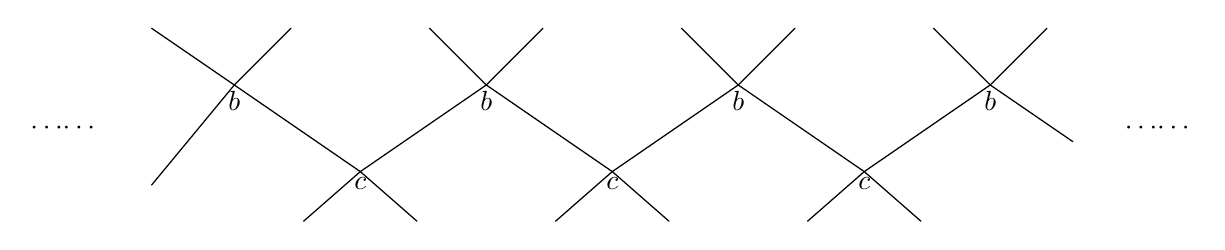
\begin{tikzpicture}[
  x=1cm,
  y=1cm,
  line cap=round,
  line join=round,
  every node/.style={inner sep=1pt}
]
  \coordinate (b1) at (2.8,0.55);
  \coordinate (c1) at (4.4,-0.55);
  \coordinate (b2) at (6.0,0.55);
  \coordinate (c2) at (7.6,-0.55);
  \coordinate (b3) at (9.2,0.55);
  \coordinate (c3) at (10.8,-0.55);
  \coordinate (b4) at (12.4,0.55);

  \draw[line width=.45pt]
    (1.75,1.27) -- (b1) -- (c1) -- (b2) -- (c2) --
    (b3) -- (c3) -- (b4) -- (13.45,-0.17);
  \draw[line width=.45pt] (1.75,-0.72) -- (b1) -- (3.52,1.27);
  \draw[line width=.45pt] (3.68,-1.18) -- (c1) -- (5.12,-1.18);
  \draw[line width=.45pt] (5.28,1.27) -- (b2) -- (6.72,1.27);
  \draw[line width=.45pt] (6.88,-1.18) -- (c2) -- (8.32,-1.18);
  \draw[line width=.45pt] (8.48,1.27) -- (b3) -- (9.92,1.27);
  \draw[line width=.45pt] (10.08,-1.18) -- (c3) -- (11.52,-1.18);
  \draw[line width=.45pt] (11.68,1.27) -- (b4) -- (13.12,1.27);

  \node[below=1pt] at (b1) {$b$};
  \node[below=1pt] at (b2) {$b$};
  \node[below=1pt] at (b3) {$b$};
  \node[below=1pt] at (b4) {$b$};
  \node[below=1pt] at (c1) {$c$};
  \node[below=1pt] at (c2) {$c$};
  \node[below=1pt] at (c3) {$c$};

  \node at (0.65,0) {$\cdots\!\cdots$};
  \node at (14.55,0) {$\cdots\!\cdots$};
\end{tikzpicture}

% END INCLUDED SGA3_English_current_buildable_source_20260823/source/inputs/X/native_diagrams/exp10/001_normalization_gluing_chain.tex

\end{center}
(N.B. This is a principal bundle for the étale topology.) There is a
homomorphism
\[
  \varphi:\mathbb Z\longrightarrow\operatorname{GL}(2,\mathbb Z),
  \qquad
  \varphi(n)=
  \begin{pmatrix}
    1 & n\\
    0 & 1
  \end{pmatrix},
\]
which makes it possible to construct a torus \(T\) over \(S\), of
relative dimension \(2\), from the trivial torus \(\mathbb G_m^2\)
over \(P\) and the descent datum on it deduced from \(\varphi\).
(N.B. The projection \(P\to S\) is a covering for the étale topology
and \emph{a fortiori} for the canonical topology of
\((\mathbf{Sch})\); the descent datum in question is necessarily
effective because \(\mathbb G_{m,P}^2\) is affine over \(P\).) It is
not difficult to prove that \(T\) is not isotrivial in a neighborhood
of \(a\)\footnote{Editor's note: See \SGARefLink{sga3:x:example:7-3}{7.3} below.} (although it is
trivial on \(S-\{a\}\)).

A variant of this construction is obtained by taking for \(S\) a
curve with two irreducible components \(S_1\) and \(S_2\) meeting in
two points \(a'\) and \(a''\). This makes it possible to construct a
connected, locally trivial principal homogeneous bundle \(P\) over
\(S\) with group \(\mathbb Z_S\), and hence an associated torus \(T\)
that is locally trivial but not isotrivial.

\SGARefTarget{sga3:x:section:2}\section*{2. Infinitesimal Variations of
Structure}
\addcontentsline{toc}{section}{2. Infinitesimal Variations of Structure}

\footnote{Editor's note: This ``recall'' has been added for later
references.}
Let us begin by recalling the following result (cf.\ SGA~1, I, 8.3
when \(S\) is locally noetherian, and EGA~IV\textsubscript{4}, 18.1.2
in general).

\medskip
\noindent\SGARefTarget{sga3:x:recall:2:0}\textbf{Recall 2.0.} ---
\textit{Let \(S\) be a prescheme and \(S_0\) a subprescheme with the
same underlying set. Then the functor
\[
  X\longmapsto X_0=X\times_S S_0
\]
is an equivalence between the category of étale preschemes over \(S\)
and the analogous category over \(S_0\).}

\medskip
\noindent\SGARefTarget{sga3:x:proposition:2:1}%
\textbf{Proposition 2.1.} ---
\textit{Let \(S\) be a prescheme and \(S_0\) a subprescheme with the
same underlying set (that is, defined by a nilideal \(\mathscr I\)).
Then the functor
\[
  H\longmapsto H_0=H\times_S S_0
\]
from the category of group preschemes of multiplicative type over
\(S\) to the analogous category over \(S_0\) is fully faithful.}

\textit{Moreover, it induces an equivalence between the category of
quasi-isotrivial groups of multiplicative type over \(S\) and the
analogous category over \(S_0\).}

We first prove full faithfulness, that is, if \(H\) and \(G\) over
\(S\) are of multiplicative type, then
\[
  \operatorname{Hom}_{S\text{-}\mathrm{gr}}(H,G)
  \longrightarrow
  \operatorname{Hom}_{S_0\text{-}\mathrm{gr}}(H_0,G_0)
\]
is bijective. The question is local on \(S\), so we may suppose that
\(S\) is affine. There then exists a faithfully flat quasi-compact
morphism \(S'\to S\) that splits \(H\) and \(G\). Let
\(S''=S'\times_S S'\); write \(H',G'\), respectively \(H'',G''\), for
the groups obtained from \(H,G\) by the base changes \(S'\to S\),
respectively \(S''\to S\). Define \(S'_0\) and \(S''_0\) similarly;
the latter is also isomorphic to \(S'_0\times_{S_0}S'_0\). We obtain a
commutative diagram with exact rows:
\begin{center}
  % BEGIN INCLUDED SGA3_English_current_buildable_source_20260823/source/inputs/X/native_diagrams/exp10/002_descent_hom_exact_rows.tex
{\small
\begin{tikzcd}[column sep=2.1em, row sep=3.4em]
  \operatorname{Hom}_{S\text{-}\mathrm{gr.}}(H,G)
    \arrow[r]
    \arrow[d,"u"]
  &
  \operatorname{Hom}_{S'\text{-}\mathrm{gr.}}(H',G')
    \arrow[r,shift left=.65ex]
    \arrow[r,shift right=.65ex]
    \arrow[d,"u'"]
  &
  \operatorname{Hom}_{S''\text{-}\mathrm{gr.}}(H'',G'')
    \arrow[d,"u''"]
  \\
  \operatorname{Hom}_{S_0\text{-}\mathrm{gr.}}(H_0,G_0)
    \arrow[r]
  &
  \operatorname{Hom}_{S'_0\text{-}\mathrm{gr.}}(H'_0,G'_0)
    \arrow[r,shift left=.65ex]
    \arrow[r,shift right=.65ex]
  &
  \operatorname{Hom}_{S''_0\text{-}\mathrm{gr.}}(H''_0,G''_0),
\end{tikzcd}
}

% END INCLUDED SGA3_English_current_buildable_source_20260823/source/inputs/X/native_diagrams/exp10/002_descent_hom_exact_rows.tex

\end{center}
Thus, to prove that \(u\) is bijective, it is enough to prove that
\(u'\) and \(u''\) are bijective. This reduces us to the case where
\(H\) and \(G\) are diagonalizable, hence of the form \(D_S(M)\) and
\(D_S(N)\), where \(M\) and \(N\) are ordinary commutative groups.
Likewise,
\[
  H_0=D_{S_0}(M),\qquad G_0=D_{S_0}(N).
\]
We then have a commutative diagram\footnote{Editor's note: The
original has been corrected by interchanging \(M\) and \(N\) in the
right-hand terms.}
\begin{center}
  % BEGIN INCLUDED SGA3_English_current_buildable_source_20260823/source/inputs/X/native_diagrams/exp10/003_diagonalizable_hom_square.tex
{\small
\begin{tikzcd}[column sep=3.2em, row sep=3.5em]
  \operatorname{Hom}_{S\text{-}\mathrm{gr.}}(N_S,M_S)
    \arrow[r,"\sim"]
    \arrow[d]
  &
  \operatorname{Hom}_{S\text{-}\mathrm{gr.}}\!\bigl(D_S(M),D_S(N)\bigr)
    \arrow[d]
  \\
  \operatorname{Hom}_{S_0\text{-}\mathrm{gr.}}(N_{S_0},M_{S_0})
    \arrow[r,"\sim"]
  &
  \operatorname{Hom}_{S_0\text{-}\mathrm{gr.}}\!\bigl(D_{S_0}(M),D_{S_0}(N)\bigr),
\end{tikzcd}
}

% END INCLUDED SGA3_English_current_buildable_source_20260823/source/inputs/X/native_diagrams/exp10/003_diagonalizable_hom_square.tex

\end{center}
whose horizontal arrows are isomorphisms by \SGARefLink{sga3:viii:corollary:1:4}{VIII~1.4}. We are therefore
reduced to proving that the homomorphism
\begin{equation}
  \operatorname{Hom}_{S\text{-}\mathrm{gr}}(N_S,M_S)
  \longrightarrow
  \operatorname{Hom}_{S_0\text{-}\mathrm{gr}}(N_{S_0},M_{S_0})
  \tag{x}\label{sga3:x:proposition:2-1:equation:x}
\end{equation}
is bijective; in other words, the functor
\(M_S\mapsto M_{S_0}\), from constant commutative group preschemes
over \(S\) to constant commutative group preschemes over \(S_0\), is
fully faithful. Now \SGARefLink{sga3:x:proposition:2-1:equation:x}{(x)} is also identified with the natural map
\[
  \operatorname{Hom}_{\mathrm{gr}}(N,\Gamma(M_S))
  \longrightarrow
  \operatorname{Hom}_{\mathrm{gr}}(N,\Gamma(M_{S_0}))
\]
deduced from \(\Gamma(M_S)\to\Gamma(M_{S_0})\). The latter map is
plainly bijective, since \(\Gamma(M_S)\), the set of locally constant
maps from \(S\) to \(M\), depends only on the underlying topological
space of \(S\). This proves the desired assertion.

To prove the second assertion of \SGARefLink{sga3:x:proposition:2:1}{2.1}, it remains to show that every
quasi-isotrivial group \(H_0\) of multiplicative type over \(S_0\)
comes from a quasi-isotrivial group \(H\) of multiplicative type over
\(S\). Let \(S'_0\to S_0\) be an étale surjective morphism that splits
\(H_0\).

By \SGARefLink{sga3:x:recall:2:0}{2.0}, there exist an étale morphism \(S'\to S\) and an
\(S_0\)-isomorphism
\[
  S'\times_S S_0\simeq S'_0.
\]
Thus we may suppose that \(S'_0\) is obtained from \(S'\) by
reduction. Since \(H'_0\) is diagonalizable, it is immediately seen
to be isomorphic to the group obtained by the base change
\(S'_0\to S'\) from a diagonalizable group \(H'\) over \(S'\). (N.B.
If \(H'_0=D_{S'_0}(M)\), take \(H'=D_{S'}(M)\).) As usual, set
\[
  S''=S'\times_S S',
  \qquad
  S'''=S'\times_S S'\times_S S',
\]
and similarly define \(S''_0\) and \(S'''_0\) by base change from
\(S\) to \(S_0\). They are also isomorphic to the fibered square and
fibered cube, respectively, of \(S'_0\) over \(S_0\). Applying the
full faithfulness already proved to \((S'',S''_0)\) and
\((S''',S'''_0)\), we see that the natural descent datum on \(H'_0\)
relative to \(S'_0\to S_0\) (cf.\ \SGARefLink{sga3:iv:definition:2:1}{IV~2.1}) comes from a uniquely
determined descent datum on \(H'\) relative to \(S'\to S\). This
descent datum is effective because \(H'\) is affine over \(S'\)
(SGA~1, VIII, \SGARefLink{sga3:viii:proposition:2:1}{2.1}). Hence there exists an \(S\)-group \(H\) such that
\[
  H\times_S S'=H'=D_{S'}(M),
\]
and \(H\) is therefore a quasi-isotrivial group of multiplicative
type.

Using the full-faithfulness result for \((S',S'_0)\), one now checks
readily that the given isomorphism between \(H'_0\) and
\(H'\times_{S'}S'_0\) comes from an isomorphism between \(H_0\) and
\(H\times_S S_0\). (For a more formal presentation of results of this
kind, see Giraud's article in preparation on descent theory.%
\begingroup
\renewcommand{\thefootnote}{\(\ast\)}%
\footnote{Cf.\ J.~Giraud, ``Méthode de la descente,'' \emph{Bull.\
Soc.\ Math.\ France}, Mémoire~2 (1964).}%
\endgroup
\addtocounter{footnote}{-1})

\medskip
\noindent\SGARefTarget{sga3:x:corollary:2:2}%
\textbf{Corollary 2.2.} ---
\textit{Let \(H\) be an \(S\)-group of multiplicative type, and set
\(H_0=H\times_S S_0\). Then \(H\) is quasi-isotrivial (respectively,
locally isotrivial, isotrivial, locally trivial, or trivial) if and
only if \(H_0\) has the corresponding property.}

The ``only if'' direction is immediate. The ``if'' direction has
already been proved in the quasi-isotrivial case: by full
faithfulness, it is enough to know that every quasi-isotrivial group
over \(S_0\) lifts to a quasi-isotrivial group over \(S\). The same
argument applies to ``trivial.'' For ``isotrivial,'' repeat the
argument establishing the second assertion of \SGARefLink{sga3:x:proposition:2:1}{2.1}, but take
\(S'_0\to S_0\) to be finite étale and surjective. The locally
isotrivial and locally trivial cases follow at once from the
isotrivial and trivial cases.

When \(\mathscr I\) is nilpotent, \SGARefLink{sga3:x:corollary:2:2}{2.2} can be generalized slightly
without assuming \emph{a priori} that \(H\) is of multiplicative
type.\footnote{Editor's note: Recall that \SGARefLink{sga3:x:corollary:2:3}{2.3} is used in proving
Theorem~\SGARefLink{sga3:ix:theorem:3:6}{IX~3.6}~bis.}

\medskip
\noindent\SGARefTarget{sga3:x:corollary:2:3}%
\textbf{Corollary 2.3.} ---
\textit{Suppose that the ideal \(\mathscr I\) defining \(S_0\) is
locally nilpotent. Let \(H\) be a group prescheme over \(S\), flat
over \(S\), and set \(H_0=H\times_S S_0\). Then \(H\) is of
quasi-isotrivial multiplicative type if and only if \(H_0\) is so.}

Suppose that \(H_0\) is of quasi-isotrivial multiplicative type. We
prove that the same is true of \(H\). The question is local for the
étale topology, and by \SGARefLink{sga3:x:recall:2:0}{2.0} the category of étale preschemes over \(S\)
is equivalent to the category of étale preschemes over \(S_0\) by the
functor \(S'\mapsto S'\times_S S_0\). We are therefore immediately
reduced to the case where \(H_0\) is diagonalizable, hence isomorphic
to \(D_{S_0}(M)\). Let \(G=D_S(M)\). We then have an isomorphism
\[
  u_0:H_0\xrightarrow{\sim}G_0.
\]
I claim that \(u_0\) comes from a unique homomorphism \(u:H\to G\),
which is necessarily an isomorphism because \(u_0\) is one, \(H\) and
\(G\) are flat over \(S\), and \(\mathscr I\) is locally
nilpotent.\footnote{Editor's note: Since \(u_0\) is an isomorphism, it
is enough to see that for every \(h\in H\), the morphism
\(\varphi:\mathscr O_{G,u(h)}\to\mathscr O_{H,h}\) is bijective. It is
bijective after reduction modulo
\(\mathscr I=\mathscr I_s\), where \(s\) is the image of \(h\) in
\(S\); hence its cokernel \(C\) satisfies \(C=\mathscr IC\), so
\(C=0\) because \(\mathscr I\) is nilpotent. Since
\(\mathscr O_{H,h}\) is flat
over \(\mathscr O_{S,s}\), the kernel \(K\) of \(\varphi\) likewise
satisfies \(K=\mathscr IK\), and hence \(K=0\).}
This will prove \SGARefLink{sga3:x:corollary:2:3}{2.3}. We have (cf.\ VIII~1~(xxx))
\[
  \operatorname{Hom}_{S\text{-}\mathrm{gr}}(H,G)
  \simeq
  \operatorname{Hom}_{S\text{-}\mathrm{gr}}
  \bigl(M_S,
    \underline{\operatorname{Hom}}_{S\text{-}\mathrm{gr}}
      (H,\mathbb G_{m,S})\bigr),
\]
and the right-hand side is also identified with
\[
  \operatorname{Hom}_{\mathrm{gr}}
  \bigl(M,
    \operatorname{Hom}_{S\text{-}\mathrm{gr}}
      (H,\mathbb G_{m,S})\bigr).
\]
Thus the homomorphism
\begin{equation}
  \operatorname{Hom}_{S\text{-}\mathrm{gr}}(H,G)
  \longrightarrow
  \operatorname{Hom}_{S_0\text{-}\mathrm{gr}}(H_0,G_0)
  \tag{x}\label{sga3:x:corollary:2-3:equation:x}
\end{equation}
is isomorphic to the homomorphism
\[
  \operatorname{Hom}_{\mathrm{gr}}
  \bigl(M,\operatorname{Hom}_{S\text{-}\mathrm{gr}}
    (H,\mathbb G_{m,S})\bigr)
  \longrightarrow
  \operatorname{Hom}_{\mathrm{gr}}
  \bigl(M,\operatorname{Hom}_{S_0\text{-}\mathrm{gr}}
    (H_0,\mathbb G_{m,S_0})\bigr)
\]
deduced from the restriction homomorphism
\begin{equation}
  \operatorname{Hom}_{S\text{-}\mathrm{gr}}(H,\mathbb G_{m,S})
  \longrightarrow
  \operatorname{Hom}_{S_0\text{-}\mathrm{gr}}
    (H_0,\mathbb G_{m,S_0}).
  \tag{xx}\label{sga3:x:corollary:2-3:equation:xx}
\end{equation}
It is therefore enough to prove that \SGARefLink{sga3:x:corollary:2-3:equation:xx}{(xx)} is bijective. The question
is local on \(S\), so we may suppose that \(S\) is affine. Since
\(\mathbb G_{m,S}\) is commutative and smooth over \(S\), \SGARefLink{sga3:ix:theorem:3:6}{IX~3.6}
applies and completes the proof.

\medskip
\noindent\SGARefTarget{sga3:x:corollary:2:4}%
\textbf{Corollary 2.4.} ---
\textit{Let \(A\) be an artinian local ring with residue field \(k\),
\(S=\operatorname{Spec}(A)\), and \(S_0=\operatorname{Spec}(k)\).}
\begin{enumerate}
\item[\SGAInlineRefTarget{sga3:x:corollary:2:4:item:i}(i)]\textit{\footnote{Editor's note: The statement has been
rewritten, retaining only the nontrivial implication in order to
highlight it.} Let \(H\) be an \(S\)-group prescheme, flat and locally
of finite type, such that \(H_0=H\times_S S_0\) is of multiplicative
type. Then \(H\) is of multiplicative type, of finite type, and
isotrivial. In particular, every \(S\)-group prescheme \(H\) of
multiplicative type and of finite type is isotrivial.}
\item[\SGAInlineRefTarget{sga3:x:corollary:2:4:item:ii}(ii)]\textit{The functor \(H\mapsto H_0\) is an equivalence
between the category of groups of multiplicative type and of finite
type over \(A\) and the analogous category over \(k\).}
\end{enumerate}

Indeed, let \(H\) be as in \SGARefLink{sga3:x:corollary:2:4:item:i}{(i)}. Then \(H_0\) is of multiplicative type
and locally of finite type, hence of finite type, and therefore
isotrivial by \SGARefLink{sga3:x:proposition:1:4}{1.4}. By \SGARefLink{sga3:x:corollary:2:3}{2.3} and \SGARefLink{sga3:x:corollary:2:2}{2.2}, \(H\) is consequently of
multiplicative type (and hence of finite type) and isotrivial.
Assertion \SGARefLink{sga3:x:corollary:2:4:item:ii}{(ii)} now follows from \SGARefLink{sga3:x:proposition:2:1}{2.1}.

\medskip
\noindent\SGARefTarget{sga3:x:corollary:2:5}%
\textbf{Corollary 2.5.} ---
\textit{Let \(S'\to S\) be a faithfully flat radicial morphism.}
\begin{enumerate}
\item[(i)]\textit{The functor
\[
  H\longmapsto H'=H\times_S S'
\]
from the category of groups of multiplicative type over \(S\) to the
analogous category over \(S'\) is fully faithful. Moreover, it induces
an equivalence between the subcategories of quasi-isotrivial groups
of multiplicative type.}
\item[(ii)]\textit{If \(H\) is of multiplicative type, then \(H\) is
quasi-isotrivial (respectively, locally isotrivial, isotrivial,
locally trivial, or trivial) if and only if \(H'\) has the
corresponding property.}
\end{enumerate}

Indeed, let
\[
  S''=S'\times_S S',
  \qquad
  S'''=S'\times_S S'\times_S S'.
\]
The assumption that \(S'\to S\) is radicial implies that the diagonal
immersions \(S'\to S''\) and \(S'\to S'''\) are surjective, so base
change by either immersion is governed by \SGARefLink{sga3:x:proposition:2:1}{2.1} and \SGARefLink{sga3:x:corollary:2:2}{2.2}. Taking into
account that \(S'\to S\) is a morphism of effective descent for the
fibered category of groups of multiplicative type over preschemes
(because it is faithfully flat and quasi-compact\footnote{Editor's
note: Spell out this point \ldots}), the assertion follows formally
from \SGARefLink{sga3:x:proposition:2:1}{2.1} and \SGARefLink{sga3:x:corollary:2:2}{2.2} (cf.\ the already cited article of Giraud for a
formal argument).

\SGARefTarget{sga3:x:section:3}\section*{3. Finite Variations of
Structure: Complete Base Ring}
\addcontentsline{toc}{section}{3. Finite Variations of Structure:
Complete Base Ring}

\medskip
\noindent\SGARefTarget{sga3:x:lemma:3:1}\textbf{Lemma 3.1.} ---
\textit{Let \(A\) be a noetherian ring equipped with an ideal \(I\)
such that \(A\) is separated and complete for the \(I\)-adic topology;
set \(S=\operatorname{Spec}(A)\) and
\(S_0=\operatorname{Spec}(A/I)\). Let \(G\) and \(H\) be two
\(S\)-group preschemes, with \(G\) of multiplicative type and
isotrivial, and with \(H\) affine over \(S\), flat over \(S\) at the
points of \(H_0=H\times_S S_0\), where \(H_0\) is of
quasi-isotrivial multiplicative type. Then the natural map
\[
  \operatorname{Hom}_{S\text{-}\mathrm{gr}}(G,H)
  \longrightarrow
  \operatorname{Hom}_{S_0\text{-}\mathrm{gr}}(G_0,H_0)
\]
is bijective.}

For every integer \(n\geq 0\), let
\[
  S_n=\operatorname{Spec}(A/I^{n+1}),
\]
and let \(G_n,H_n\) be obtained from \(G,H\) by the base change
\(S_n\to S\). Since \(G/S\) is of isotrivial multiplicative type and
\(H\) is affine over \(S\), \SGARefLink{sga3:ix:theorem:7:1}{IX~7.1} shows that the natural
homomorphism
\[
  \operatorname{Hom}_{S\text{-}\mathrm{gr}}(G,H)
  \longrightarrow
  \varprojlim_n
  \operatorname{Hom}_{S_n\text{-}\mathrm{gr}}(G_n,H_n)
\]
is bijective. On the other hand, \SGARefLink{sga3:x:corollary:2:3}{2.3} shows that the \(H_n\) are of
quasi-isotrivial multiplicative type, and \SGARefLink{sga3:x:proposition:2:1}{2.1} shows that all
transition homomorphisms in the inverse system
\[
  \bigl(
    \operatorname{Hom}_{S_n\text{-}\mathrm{gr}}(G_n,H_n)
  \bigr)_n
\]
are isomorphisms. \SGARefLink{sga3:x:lemma:3:1}{Lemma~3.1} follows at once.

\medskip
\noindent\SGARefTarget{sga3:x:theorem:3:2}%
\textbf{Theorem 3.2.} ---
\textit{Let \(A\) be a noetherian ring equipped with an ideal \(I\)
such that \(A\) is separated and complete for the \(I\)-adic topology,
and set \(S=\operatorname{Spec}(A)\) and
\(S_0=\operatorname{Spec}(A/I)\). Then:}
\begin{enumerate}
\item[\SGAInlineRefTarget{sga3:x:theorem:3:2:item:i}(i)]\textit{The functor
\[
  H\longmapsto H_0=H\times_S S_0
\]
is an equivalence between the category of isotrivial groups of
multiplicative type over \(S\) and the analogous category over
\(S_0\).}
\item[\SGAInlineRefTarget{sga3:x:theorem:3:2:item:ii}(ii)]\textit{Let \(H\) be an \(S\)-group of multiplicative type
and of finite type. Then \(H\) is isotrivial if and only if \(H_0\)
is isotrivial.}
\end{enumerate}

\textit{Proof.}
For \SGARefLink{sga3:x:theorem:3:2:item:i}{(i)}, one may either repeat the proof of \SGARefLink{sga3:x:proposition:2:1}{2.1} or use \SGARefLink{sga3:x:corollary:1:2}{1.2}. In either
case one uses the fact that the functor
\[
  S'\longmapsto S'_0=S'\times_S S_0
\]
from the category of finite étale schemes over \(S\) to the category
of finite étale schemes over \(S_0\) is an equivalence (SGA~1, I,
\SGARefLink{sga3:x:lemma:8-4}{8.4}). Equivalently, after reducing to the case where \(S\) is
connected (that is, \(S_0\) is connected) and choosing a geometric
point \(\xi\) of \(S_0\), the canonical homomorphism
\[
  \pi_1(S_0,\xi)\longrightarrow\pi_1(S,\xi)
\]
is an isomorphism.

We prove \SGARefLink{sga3:x:theorem:3:2:item:ii}{(ii)}, namely that if \(H_0\) is isotrivial, then \(H\) is
isotrivial. By \SGARefLink{sga3:x:theorem:3:2:item:i}{(i)}, there exist an isotrivial group \(G\) of
multiplicative type over \(S\) and an \(S_0\)-isomorphism
\[
  u_0:G_0\xrightarrow{\sim}H_0.
\]
\footnote{Editor's note: The original has been expanded in what
follows.}
Since \(H\) is of finite type, so are \(H_0\) and \(G_0\). Therefore,
by \SGARefLink{sga3:ix:proposition:2:1}{IX~2.1}~b), the type of \(G\) at every point of \(S\) is a
finitely generated abelian group, and hence \(G\) is of finite type
over \(S\). Moreover, by \SGARefLink{sga3:x:lemma:3:1}{3.1}, \(u_0\) comes from a homomorphism of
\(S\)-groups
\[
  u:G\longrightarrow H.
\]
Finally, \(G\) and \(H\) are groups of multiplicative type and of
finite type over \(S\), and \(u_0\) is an isomorphism. It follows from
\SGARefLink{sga3:ix:corollary:2:9}{IX~2.9} that \(u\) is an isomorphism, since every neighborhood of
\(S_0\) in \(S\) is equal to \(S\).

\medskip
\noindent\SGARefTarget{sga3:x:corollary:3:3}%
\textbf{Corollary 3.3.} ---
\textit{Let \(A\) be a complete noetherian local ring with residue
field \(k\).}
\begin{enumerate}
\item[\SGAInlineRefTarget{sga3:x:corollary:3:3:item:i}(i)]\textit{Every group of multiplicative type and of finite
type over \(A\) is isotrivial.}
\item[(ii)]\textit{The functor
\[
  H\longmapsto H\otimes_A k=H_0
\]
is an equivalence between the categories of groups of multiplicative
type and of finite type over \(A\) and over \(k\).}
\end{enumerate}

\footnotemark[12]
First, \SGARefLink{sga3:x:corollary:3:3:item:i}{(i)} follows from \SGARefLink{sga3:x:theorem:3:2}{3.2}~\SGARefLink{sga3:x:theorem:3:2:item:ii}{(ii)} and \SGARefLink{sga3:x:proposition:1:4}{1.4}. Then \SGARefLink{sga3:x:theorem:3:2:item:ii}{(ii)} follows from
\SGARefLink{sga3:x:theorem:3:2}{3.2}~\SGARefLink{sga3:x:theorem:3:2:item:i}{(i)}, taking into account that \(H\) is of finite type if and only
if \(H_0\) is of finite type (cf.\ the proof of \SGARefLink{sga3:x:theorem:3:2}{3.2}~\SGARefLink{sga3:x:theorem:3:2:item:ii}{(ii)}).

\medskip
\noindent\SGARefTarget{sga3:x:remark:3:3:1}%
\textbf{Remark 3.3.1.} ---
By \SGARefLink{sga3:x:proposition:1:4}{1.4}, statement \SGARefLink{sga3:x:corollary:3:3}{3.3} gives a complete classification of groups of
multiplicative type and of finite type over \(A\) in terms of the
topological Galois group of an algebraic closure \(\Omega\) of \(k\).

\medskip
\noindent\SGARefTarget{sga3:x:remarks:3:4}%
\textbf{Remarks 3.4.} ---
Under the hypotheses of \SGARefLink{sga3:x:theorem:3:2}{3.2} (that is, \(A\) noetherian, separated and
complete for the \(I\)-adic topology, with no further hypothesis on
\(A/I\)), it will follow from no.~5 that the functor
\[
  H\longmapsto H_0
\]
from the category of groups of multiplicative type and of finite type
over \(S\) to the analogous category over \(S_0\) is still fully
faithful, without any isotriviality hypothesis.\footnote{Editor's
note: Specify this reference, possibly adding a corollary in no.~5
\ldots}

It is not, however, essentially surjective in general. Indeed, there
may exist a group \(H_0\) of multiplicative type and of finite type
over \(S_0\), even locally trivial if desired (but not isotrivial),
that does not arise by reduction from a group \(H\) of multiplicative
type over \(S\).

To see this, take either example from \SGARefLink{sga3:x:paragraph:1:6}{1.6} of a non-isotrivial group of
multiplicative type over a nonnormal curve. The curve may plainly be
taken affine, say \(S_0\), and embedded in affine \(2\)-space; it is
therefore defined by an ideal \(J\) in \(k[X,Y]\). Take \(A\) to be
the completion of \(k[X,Y]\) for the \(J\)-adic topology. Then \(A\)
is a regular ring of dimension \(2\), and \emph{a fortiori} normal.
We shall see in \SGARefLink{sga3:x:theorem:5-16}{5.16} that every group of multiplicative type and of
finite type over \(S=\operatorname{Spec}(A)\) is consequently
isotrivial. Thus \(H_0\), being of finite type and non-isotrivial,
cannot come from a group \(H\) of multiplicative type over \(S\),
since such an \(H\) would necessarily be of finite type and hence
isotrivial.

\medskip
\noindent\SGARefTarget{sga3:x:lemma:3:5}\textbf{Lemma 3.5.}%
\begingroup
\renewcommand{\thefootnote}{\(\ast\)}%
\footnote{Cf.\ also \(\mathrm{VI}_{\mathrm B}\), \SGARefLink{sga3:x:corollary:2:5}{2.5}, for more
systematic developments of this kind.}%
\endgroup
\addtocounter{footnote}{-1}
---
\textit{Let \(S\) be a prescheme and
\(u:G\to H\) a homomorphism of \(S\)-group preschemes that are
locally of finite presentation and flat over \(S\). Let \(U\) be the
set of \(s\in S\) such that the homomorphism induced on the fibers,
\[
  u_s:G_s\longrightarrow H_s,
\]
is flat (respectively, smooth, unramified, étale, or quasi-finite).
Then \(U\) is open, and the restriction
\[
  u|_U:G|_U\longrightarrow H|_U
\]
is flat (respectively, smooth, unramified, étale, or quasi-finite).}

Let \(V\) be the set of points at which \(u\) is flat (respectively,
\(\ldots\)). It is known that \(V\) is open (cf.\ SGA~1, I through IV
in the locally noetherian case, and EGA~IV in
general\footnote{Editor's note: Specify these references. Since
\(G,H\) are locally of finite presentation, \(u\) is locally of
finite presentation (IV\textsubscript{1}, 1.4.3~(v)); one then applies
IV\textsubscript{3}, 11.3.10 and 13.1.4 for flat and quasi-finite,
and IV\textsubscript{4}, 17.4.1, 17.5.1, and 17.6.1 for unramified,
smooth, and étale; compare \(\mathrm{VI}_{\mathrm B}\), \SGARefLink{sga3:x:corollary:2:5}{2.5}.}), and
for \(x\in G\) above \(s\in S\), one has \(x\in V\) if and only if
\(u_s:G_s\to H_s\) is flat (respectively, \(\ldots\)) at \(x\)
(same reference; in the flat, smooth, and étale cases, the flatness of
\(G\) and \(H\) over \(S\) is used here). Since \(u_s\) is a
homomorphism of locally algebraic groups, this is also equivalent to
\(u_s\) being flat (respectively, \(\ldots\)) everywhere
(\(\mathrm{VI}_{\mathrm B}\), \SGARefLink{sga3:x:remark:1:3}{1.3}), that is, to \(s\in U\).
Therefore \(U\) is the inverse image of the open set \(V\) under the
unit section of \(G\), and hence is open. Moreover, \(V=G|_U\), so
\(G|_U\to H|_U\) is flat (respectively, \(\ldots\)), completing the
proof. (N.B. In the unramified and quasi-finite cases, the flatness
hypothesis on \(G\) and \(H\) is unnecessary.)

\medskip
\noindent\SGARefTarget{sga3:x:lemma:3:6}\textbf{Lemma 3.6.} ---
\textit{Let \(H\) be a commutative algebraic group over a field \(k\)
that admits an open subgroup \(G\) of multiplicative type. Then the
family of subschemes \({}_nH\), \(n>0\), is schematically dense in
\(H\). In particular, if \({}_nH={}_nG\) for every \(n>0\), then
\(H=G\).}

Here \({}_nH\) denotes the kernel of
\(n\cdot\operatorname{id}_H\).\footnote{Editor's note: The preceding
sentence has been added.}
Let \(\bar{k}\) be an algebraic closure of \(k\). It is enough to show
that the family \(({}_nH_{\bar{k}})_{n>0}\) is schematically dense in
\(H_{\bar{k}}\), for then \(({}_nH)_{n>0}\) is schematically dense in
\(H\) (cf.\ \SGARefLink{sga3:ix:lemma:4:5}{IX~4.5}). We may therefore suppose that \(k\) is
algebraically closed, so that \(G=D_k(M)\), where \(M\) is an ordinary
finitely generated commutative group.

Let
\[
  M_0=M/\operatorname{Torsion}(M).
\]
Then \(T=D_k(M_0)\) is the largest torus contained in \(G\), and
\(H/T\) is finite. Hence \(H(k)/T(k)\) is annihilated by an integer
\(\nu>0\). There exist finitely many \(g_i\in H(k)\) such that
\[
  H=\coprod_i g_i\cdot G,
\]
and \(g_i^\nu\in T(k)\). Since \(k\) is algebraically closed, the map
\(\nu\cdot\operatorname{id}_T\) is surjective on
\[
  T(k)\simeq(k^\times)^d.
\]
After replacing \(g_i\) by \(g_it_i^{-1}\), where \(t_i\in T(k)\)
satisfies \(t_i^\nu=g_i^\nu\), we may therefore suppose that
\(g_i^\nu=1\). If \(n\) is now a multiple of \(\nu\), then
\[
  {}_nH\supset g_i\cdot{}_nG.
\]
As \(n>0\) varies, the family \({}_nG\) is schematically dense in
\(G\) by \SGARefLink{sga3:ix:theorem:4:7}{IX~4.7}, and the conclusion of \SGARefLink{sga3:x:lemma:3:6}{3.6} follows.

\medskip
\noindent\SGARefTarget{sga3:x:theorem:3:7}%
\textbf{Theorem 3.7.} ---
\textit{Let \(A\) be a noetherian ring equipped with an ideal \(I\)
such that \(A\) is separated and complete for the \(I\)-adic topology;
set \(S=\operatorname{Spec}(A)\) and
\(S_0=\operatorname{Spec}(A/I)\). Let \(H\) be an affine
\(S\)-group scheme of finite type, flat over \(S\) at the points of
\(H_0\), such that \(H_0=H\times_S S_0\) is of multiplicative type
and isotrivial. Then there exists an open and closed subgroup \(G\) of
\(H\), of isotrivial multiplicative type (and of finite type), such
that \(G_0=H_0\).}

By \SGARefLink{sga3:x:theorem:3:2}{3.2}~\SGARefLink{sga3:x:theorem:3:2:item:i}{(i)}, there exist an isotrivial group \(G\) of multiplicative
type over \(S\) and an isomorphism
\[
  u_0:G_0\xrightarrow{\sim}H_0.
\]
By \SGARefLink{sga3:x:lemma:3:1}{3.1}, \(u_0\) comes from a unique homomorphism of \(S\)-groups
\[
  u:G\longrightarrow H.
\]
Using \SGARefLink{sga3:ix:corollary:6:6}{IX~6.6}, we see that \(u\) is a monomorphism: if \(U\) is the set
of \(s\in S\) such that \(u_s:G_s\to H_s\) is a monomorphism, then
\(U\) is an open neighborhood of \(S_0\), hence equals \(S\), and
\(G|_U\to H|_U\) is a monomorphism. By \SGARefLink{sga3:ix:corollary:2:5}{IX~2.5}, \(u\) is even a closed
immersion.

Thus \(G\) is of finite type, and therefore of finite presentation,
over \(S\).\footnote{Editor's note: The preceding sentence has been
added.}
Applying \SGARefLink{sga3:x:lemma:3:5}{Lemma~3.5} in the étale case, there is an open neighborhood
\(U\) of \(S_0\), hence \(U=S\), such that \(G|_U\to H|_U\) is étale.
Thus \(u\) is étale and therefore an open immersion, since it is an
étale monomorphism.\footnote{Editor's note: Cf.\
EGA~IV\textsubscript{4}, 17.9.1.}
This completes the proof.

\medskip
\noindent\SGARefTarget{sga3:x:corollary:3:8}%
\textbf{Corollary 3.8.} ---
\textit{Let \(A\) be a noetherian ring equipped with an ideal \(I\)
such that \(A\) is separated and complete for the \(I\)-adic topology;
set \(S=\operatorname{Spec}(A)\) and
\(S_0=\operatorname{Spec}(A/I)\). Let \(H\) be an \(S\)-group
prescheme of finite type, affine and flat over \(S\).}

\textit{Then \(H\) is of multiplicative type and isotrivial if and
only if \(H_0\) is so and \(H\) satisfies either one of the following
conditions \SGARefLink{sga3:x:corollary:3:8:item:a}{(a)} and \SGARefLink{sga3:x:corollary:3:8:item:b}{(b)}, which are therefore equivalent under the
preceding hypotheses:}
\begin{enumerate}
\item[\SGAInlineRefTarget{sga3:x:corollary:3:8:item:a}(a)]\textit{The fibers of \(H\) are of multiplicative type and
have constant type on each connected component of \(S\).}
\item[\SGAInlineRefTarget{sga3:x:corollary:3:8:item:b}(b)]\textit{\(H\) is commutative and the \({}_nH\), \(n>0\),
are finite over \(S\).}
\end{enumerate}
\textit{Both of these conditions are implied by the following one:}
\begin{enumerate}
\item[\SGAInlineRefTarget{sga3:x:corollary:3:8:item:c}(c)]\textit{The fibers of \(H\) are connected.}
\end{enumerate}

Of course, if \(H\) is of multiplicative type (and isotrivial), then
\SGARefLink{sga3:x:corollary:3:8:item:a}{(a)} and \SGARefLink{sga3:x:corollary:3:8:item:b}{(b)} hold by \SGARefLink{sga3:ix:remark:1:4:1}{IX~1.4.1}~a) and \SGARefLink{sga3:x:proposition:2:1}{2.1}~c). Thus only the ``if''
direction requires proof. We use the subgroup \(G\) provided by \SGARefLink{sga3:x:theorem:3:7}{3.7}.
When \SGARefLink{sga3:x:corollary:3:8:item:c}{(c)} holds, plainly \(G=H\), and there is nothing to prove.

In case \SGARefLink{sga3:x:corollary:3:8:item:b}{(b)}, the immersion \(u:G\to H\) induces an open immersion
\[
  {}_nu:{}_nG\longrightarrow{}_nH
\]
and an isomorphism
\[
  ({}_nG)_0\xrightarrow{\sim}({}_nH)_0.
\]
Since \({}_nH\) is finite over \(S\), it follows at once that
\({}_nu\) is an isomorphism: the complement of its image is finite
over \(S\) and reduces to the empty set. By \SGARefLink{sga3:x:lemma:3:6}{3.6}, the induced
morphisms on fibers
\[
  u_s:G_s\longrightarrow H_s
\]
are isomorphisms. Hence \(u\) is surjective and therefore an
isomorphism.

Finally, in case \SGARefLink{sga3:x:corollary:3:8:item:a}{(a)}, we may suppose that \(S\) is
connected.\footnote{Editor's note: The original said ``that is,
\(S_0\) connected.'' Since \(A\) is separated for the \(I\)-adic
topology, \(S_0\) meets every connected component of \(S\); and since
\(A\) is complete, the connected components of \(S_0\) and \(S\) are
in bijection.}
It follows that, for every \(s\in S\),
\[
  u_s:G_s\longrightarrow H_s
\]
is a monomorphism of algebraic groups of multiplicative type and of
the same type over \(\kappa(s)\).\footnote{Editor's note: This is
because \(G_s\) and \(H_s\) have the same type for every \(s\in S_0\),
and hence for every \(s\).}
Such a homomorphism is necessarily an isomorphism, which again
completes the proof.\footnote{Editor's note: Indeed, \(u\) will again
be a surjective open immersion.}
After extending the base field, we may suppose that both groups over
\(\kappa(s)\) are diagonalizable. The assertion then follows from
\SGARefLink{sga3:viii:corollary:3:2}{VIII~3.2}~b) and the fact that a surjective homomorphism between
isomorphic finitely generated \(\mathbb Z\)-modules
\[
  M\longrightarrow N
\]
is necessarily bijective.

\medskip
\noindent\SGARefTarget{sga3:x:corollary:3:9}%
\textbf{Corollary 3.9.} ---
\textit{Let \(A\) be a noetherian ring equipped with an ideal \(I\)
such that \(A\) is separated and complete for the \(I\)-adic topology,
set \(S=\operatorname{Spec}(A)\), and let \(H\) be an \(S\)-group
prescheme of finite type, affine and flat over \(S\), with connected
fibers. Then \(H\) is an isotrivial torus if and only if
\(H_0=H\times_S\operatorname{Spec}(A/I)\) is an isotrivial torus.}

% END INCLUDED SGA3_English_current_buildable_source_20260823/source/inputs/X/tex/components/01_expose_X_sections1_3.tex

% BEGIN INCLUDED SGA3_English_current_buildable_source_20260823/source/inputs/X/tex/components/02_expose_X_sections4_6.tex
\section*{\SGAInlineRefTarget{sga3:x:section:4}4. Case of an arbitrary base. Quasi-isotriviality theorem}
\phantomsection
\addcontentsline{toc}{section}{4. Case of an arbitrary base. Quasi-isotriviality theorem}

Let \(A\) be a local ring. Recall, following Nagata, that \(A\) is said to be
\emph{henselian} if every algebra \(B\) finite over \(A\) is a product of local
algebras \(B_i\) finite over \(A\).

\par\medskip\noindent
\textbf{\SGAInlineRefTarget{sga3:x:paragraph:4-0}Recall 4.0.}\footnote{\textit{Editors' note.} This recall has been
spelled out, and \SGARefLink{sga3:x:remark:4-0-1}{Remark 4.0.1} has been added.}\enspace
\emph{Let \(A\) be a henselian local ring, \(k\) its residue field,
\(S=\operatorname{Spec}(A)\), \(S_0=\operatorname{Spec}(k)\), and \(\xi\) a
geometric point of \(S_0\). Then the functor}
\[
  X\longmapsto X_0=X\times_S S_0
\]
\emph{is an equivalence between the category of étale coverings of \(S\) and
the analogous category over \(S_0\) (cf.\ EGA IV\(_4\), \S~18.5).
Consequently (cf.\ SGA 1, V),}
\[
  \pi_1(S_0,\xi)=\pi_1(S,\xi).
\]

Suppose in addition that \(A\) is noetherian, and write \(A'\) for its
completion and \(S'=\operatorname{Spec}(A')\). Then \(A'\) is a complete
noetherian local ring, hence henselian (\emph{loc.\ cit.}, 18.5.14), and the
functor
\[
  X\longmapsto X'=X\times_S S'
\]
from the category of étale coverings of \(S\) to the analogous category over
\(S'\) fits into a commutative diagram
\[
  % BEGIN INCLUDED SGA3_English_current_buildable_source_20260823/source/inputs/X/native_diagrams/exp10/004_etale_cover_equivalence_triangle.tex
{\small
\begin{tikzcd}[column sep=2.5em, row sep=2.8em]
  \mathrm{\acute{E}tCov}(S)
    \arrow[rr]
    \arrow[dr,"\sim"']
  &&
  \mathrm{\acute{E}tCov}(S')
    \arrow[dl,"\sim"]
  \\
  &
  \mathrm{\acute{E}tCov}(S_0)
  &
\end{tikzcd}
}

% END INCLUDED SGA3_English_current_buildable_source_20260823/source/inputs/X/native_diagrams/exp10/004_etale_cover_equivalence_triangle.tex

\]
and is therefore also an equivalence of categories, whence
\(\pi_1(S_0,\xi)=\pi_1(S',\xi)\).

\par\medskip\noindent
\textbf{\SGAInlineRefTarget{sga3:x:remark:4-0-1}Remark 4.0.1.}\enspace
Since \(S\) is connected (\(A\) being local), it follows from \SGARefLink{sga3:x:corollary:1:2}{1.2} that the
category of isotrivial groups of multiplicative type over \(S\) is equivalent
to the analogous category over \(S_0\) (and also over \(S'\) if \(A\) is
noetherian).

\par\medskip\noindent
\textbf{\SGAInlineRefTarget{sga3:x:lemma:4-1}Lemma 4.1.}\enspace
\begingroup\itshape
Let \(A\) be a henselian local ring with residue field \(k\),
\(S=\operatorname{Spec}(A)\), and \(S_0=\operatorname{Spec}(k)\).

\smallskip
\noindent
\(\mathrm{(i)}\) The functor
\[
  H\longmapsto H_0=H\times_S S_0
\]
is an equivalence between the category of finite groups of multiplicative type
over \(S\) and the analogous category over \(S_0\).

\smallskip
\noindent
\(\mathrm{(ii)}\) If, in addition, \(A\) is noetherian, writing \(A'\) for its
completion and \(S'=\operatorname{Spec}(A')\), the functor
\[
  H\longmapsto H'=H\times_S S'
\]
is an equivalence between the category of finite groups of multiplicative type
over \(S\) and the analogous category over \(S'\).
\par\endgroup

As in \SGARefLink{sga3:x:paragraph:4-0}{4.0}, the second assertion follows from the first; let us prove the first.
We already know that the functor under consideration is essentially
surjective: every group of multiplicative type \(H_0\) over
\(S_0=\operatorname{Spec}(k)\), being finite and hence of finite type over
\(k\), is isotrivial by \SGARefLink{sga3:x:proposition:1:4}{1.4}, and therefore comes from an isotrivial group of
multiplicative type over \(S\), by \SGARefLink{sga3:x:remark:4-0-1}{4.0.1}.

It remains to prove full faithfulness, that is, that for two finite groups
\(G,H\) of multiplicative type over \(S\), the following map is bijective:
\[
  \operatorname{Hom}_{S\text{-gr.}}(G,H)
  \longrightarrow
  \operatorname{Hom}_{S_0\text{-gr.}}(G_0,H_0).
\]
In other words,\footnote{\textit{Editors' note.} What follows has been added.}
if \(F\) denotes the \(S\)-functor
\(\operatorname{Hom}_{S\text{-gr.}}(G,H)\), the natural map
\[
  \operatorname{Hom}_S(S,F)
  \longrightarrow
  \operatorname{Hom}_{S_0}(S_0,F_0)
\]
induced by the base change \(S_0\to S\) is bijective. In view of Recall \SGARefLink{sga3:x:paragraph:4-0}{4.0},
it is enough to prove the following lemma.

\par\medskip\noindent
\textbf{\SGAInlineRefTarget{sga3:x:lemma:4-2}Lemma 4.2.}\enspace
\emph{Let \(G,H\) be two finite groups of multiplicative type over a
prescheme \(S\). Then
\(F=\operatorname{Hom}_{S\text{-gr.}}(G,H)\) is representable by a finite
étale scheme over \(S\).}

\footnote{\textit{Editors' note.} The original has been expanded in what
follows.}
Let \(f:S'\to S\) be a faithfully flat quasi-compact morphism such that
\(G'\) and \(H'\) are diagonalizable. It is enough to show that \(F_{S'}\) is
represented by a prescheme \(X'\) étale and finite (hence affine) over \(S'\).
Indeed, the descent datum on \(X'\) relative to \(f\) (cf.\ VIII 1.7.2) is then
effective (by SGA 1, VIII 2.1), so there is an \(S\)-prescheme \(X\) such that
\(X\times_S S'=X'\), representing \(F\), and \(X\) is étale and finite over
\(S\) (cf.\ SGA 1, V 5.7 and EGA IV\(_4\), 17.7.3 (ii)).

We may therefore suppose that \(G=D_S(M)\) and \(H=D_S(N)\), where \(M\) and
\(N\) are finite commutative groups (cf.\ \SGARefLink{sga3:viii:proposition:2:1}{VIII 2.1} c)). Then
\(K=\operatorname{Hom}_{\mathrm{gr.}}(N,M)\) is a finite abelian group and,
by \SGARefLink{sga3:viii:corollary:1:5}{VIII 1.5}, there is an isomorphism
\[
  \operatorname{Hom}_{S\text{-gr.}}(G,H)\simeq K_S,
\]
which completes the proof of \SGARefLink{sga3:x:lemma:4-2}{4.2} and hence of \SGARefLink{sga3:x:lemma:4-1}{4.1}.

\par\medskip\noindent
\textbf{\SGAInlineRefTarget{sga3:x:proposition:4-3-0}Proposition 4.3.0.}\footnote{\textit{Editors' note.} This recall,
which is used in the proof of 4.3, has been added (the reference to
EGA IV\(_4\), 18.5.11 was not entirely satisfactory).}\enspace
\begingroup\itshape
Let \(S\) be a henselian local scheme, \(s\) its closed point,
\(g:X\to S\) a morphism locally of finite type, and \(x\) an isolated point
of the fiber \(X_s\).

\smallskip
\noindent
\(\mathrm{(i)}\) Then \(\mathcal O_{X,x}\) is finite over
\(\mathcal O_{S,s}\). (In particular, if the residue-field extension
\(\kappa(x)/\kappa(s)\) is trivial, then
\(\mathcal O_{S,s}\to\mathcal O_{X,x}\) is surjective, by Nakayama's lemma.)

\smallskip
\noindent
\(\mathrm{(ii)}\) If \(g\) is also separated, then
\(X'=\operatorname{Spec}(\mathcal O_{X,x})\) is an open and closed subscheme
of \(X\); that is, there is a decomposition into a disjoint sum
\(X=X'\amalg X''\).
\par\endgroup

\par\smallskip\noindent
\emph{Proof.}
By the local form of Zariski's Main Theorem found in [Pes66], or in
[Ray70, Ch.~IV, Th.~1], \(x\) has an affine open neighborhood
\(U=\operatorname{Spec}(B)\), of finite type and quasi-finite over
\(A=\mathcal O_{S,s}\), and there is an open immersion
\(U\hookrightarrow Y=\operatorname{Spec}(C)\), where \(C\) is a finite
\(A\)-algebra. (N.B. To obtain this conclusion one may also use Chevalley's
semicontinuity theorem (EGA IV\(_3\), 13.1.4), followed by the form of
Zariski's Main Theorem given in \emph{loc.\ cit.}, 8.12.8.)

Since \(A\) is henselian, \(Y\) is the disjoint sum of local schemes
\(Y_1,\ldots,Y_n\), each finite over \(S\), and the points of \(Y\) above
\(s\) are their closed points \(y_1,\ldots,y_n\). Thus \(x=y_i\) for some
\(i\), and
\(\mathcal O_{X,x}=\mathcal O_{U,x}=C_i\) is finite over \(A\). Moreover,
\(X'=\operatorname{Spec}(C_i)\) is an open subscheme of \(U\), hence of
\(X\).

Suppose in addition that \(g\) is separated. Since \(X'\to S\) is finite
(\(C_i\) being finite over \(A\)), so is the immersion \(X'\to X\)
(cf.\ EGA II, 6.1.5 (v)); therefore \(X'\) is also closed in \(X\).
\hfill\(\square\)

\par\medskip\noindent
\textbf{\SGAInlineRefTarget{sga3:x:lemma:4-3}Lemma 4.3.}\enspace
\begingroup\itshape
Let \(A\) be a noetherian henselian local ring, \(A'\) its completion,
\(S=\operatorname{Spec}(A)\), \(S'=\operatorname{Spec}(A')\), and \(s\) the
closed point of \(S\). Let \(G,H\) be two \(S\)-preschemes in groups, with
\(G\) of multiplicative type and of finite type over \(S\), and with \(H\)
locally of finite type and separated over \(S\), \(H_s\) of multiplicative
type, and \(H\) flat over \(S\) at the points of \(H_s\).

Let \(G',H'\) be obtained from \(G,H\) by the base change \(S'\to S\). Then
the following natural map is bijective:
\par\endgroup
\[
  \operatorname{Hom}_{S\text{-gr.}}(G,H)
  \xrightarrow{\ \sim\ }
  \operatorname{Hom}_{S'\text{-gr.}}(G',H').
\]

Since \(S'\) is faithfully flat and quasi-compact over \(S\), SGA 1,
VIII 5.2 shows that this map identifies the first member with the subset of
the second formed by the \(u':G'\to H'\) for which the two inverse images
\(u''_1,u''_2:G''\to H''\) of \(u'\) on
\(S''=S'\times_S S'\), under the projections
\(\operatorname{pr}_1,\operatorname{pr}_2:S''\to S'\), are equal.

It therefore remains to prove that \(u''_1=u''_2\) for every homomorphism of
\(S'\)-groups \(u':G'\to H'\). By the density theorem \SGARefLink{sga3:ix:corollary:4:8}{IX 4.8}, it is enough
to prove that \(u''_1\) and \(u''_2\) agree on \({}_nG''\) for every integer
\(n>0\). (N.B. Here the density theorem is needed essentially in a case
where the base prescheme, namely \(S''\), is not locally noetherian.)

Replacing \(G\) by \({}_nG\), this reduces us to the case in which
\(n\cdot\operatorname{id}_G=0\) for some integer \(n>0\), and hence \(G\)
is finite over \(S\). Likewise let \({}_nH\) be the kernel of the \(n\)-th
power morphism \(\varphi_n\) on \(H\). (N.B. We have not assumed \(H\)
commutative, so \(\varphi_n\), respectively \({}_nH\), need not be a group
homomorphism, respectively a subgroup of \(H\).) Since \({}_nH\) is defined
as the fiber product of \(\varphi_n:H\to H\) and the unit section
\(\varepsilon:S\to H\), its formation commutes with every base change
\(T\to S\):
\[
  ({}_nH)_T={}_n(H_T).
\]

\footnote{\textit{Editors' note.} The original has been expanded in what
follows, on the basis of indications by M.\ Raynaud.}
We use a right subscript \(m\) for reduction modulo
\(\mathfrak m^{m+1}\), where \(\mathfrak m\) is the maximal ideal of \(A\).
Then \(H_m\) is flat over \(S_m\) (because \(H\) is flat over \(S\) at the
points of \(H_0\)); hence, by \SGARefLink{sga3:x:corollary:2:4}{2.4}, \(H_m\) is of multiplicative type and of
finite type, since \(H_0\) is. Thus every
\(({}_nH)_m={}_n(H_m)\) is a subgroup of \(H_m\), of multiplicative type,
finite and flat over \(S_m\).

In particular, \(({}_nH)_0={}_n(H_0)\) is finite over \(S_0\). Since \(S\)
is henselian local and \({}_nH\), like \(H\), is locally of finite type and
separated over \(S\), \SGARefLink{sga3:x:proposition:4-3-0}{Proposition 4.3.0} shows that the local rings of
\({}_nH\) at the points of \(({}_nH)_0\) are finite over \(S\), and that
there is a decomposition as a disjoint sum of open subsets
\[
  \tag{*}\label{sga3:x:lemma:4-3:equation:star}
  {}_nH={}_nH^+\amalg{}_nH^-,
\]
where \(Z={}_nH^+\) is finite over \(S\), while \({}_nH^-\) lies above
\(S-\{s\}\).

Observe that for every finite \(S\)-scheme \(Y\) (such as \(G\)), every
\(S\)-morphism \(Y\to{}_nH\) factors through \(Z\), and that the formation
of the decomposition \((*)\) commutes with the base change \(S'\to S\),
where \(S'=\operatorname{Spec}(A')\) and \(A'\) is the completion of \(A\).

Then \(Z'=Z\times_S S'\) is finite over \(S'\), as is
\(P'=Z'\times_{S'}Z'\). Let \(\nu\) denote the restriction to \(P'\) of
the multiplication on \(H'\), and let \(\sigma\) be the automorphism of
\(P'\) interchanging the two factors. Since \(P'\) is finite over \(S'\),
while \(H'\) is separated and locally of finite type over \(S'\), EGA II
5.4.3 and IV\(_1\) 1.1.3 show that \(Y=\nu(P')\) is a closed subscheme of
\(H'\), universally closed and quasi-compact, hence of finite type and
therefore proper over \(S'\). Moreover, \(Y\to S'\) has finite fibers
(because \(P'\to S'\) does). Since \(S'\) is noetherian, \(Y\to S'\) is
therefore finite (cf.\ EGA III, 4.4.2). Since \(Z'\subseteq Y\) and
\(Z'_m=Y_m\) for every \(m\), Lemma IX 5.0 gives \(Z'=Y\); thus \(Z'\) is
a subgroup of \(H'\). Similarly, the kernel
\(K=\operatorname{Ker}(\nu,\nu\circ\sigma)\) is a closed subscheme of
\(P'\) such that \(K_m=P'_m\) for every \(m\) (because
\(Z'_m={}_nH_m\) is commutative). Hence \(K=P'\), that is, \(Z'\) is a
commutative subgroup of \(H'\).

On the other hand, every reduction \(Z'_m={}_nH_m\) is flat over \(S_m\).
The ``local criterion for flatness'' (cf.\ EGA \(0_{\mathrm{III}}\),
10.2.2, or [BAC], III \S~5, Example 1 and Th.~1) therefore shows that
\(Z'\) is flat over \(S'\). Moreover,
\(Z'_0={}_nH_0\) is a finite group of multiplicative type over \(S_0\),
and hence isotrivial by \SGARefLink{sga3:x:proposition:1:4}{1.4}. It follows from \SGARefLink{sga3:x:corollary:3:8}{3.8} b) that \(Z'\) is of
multiplicative type (and isotrivial) over \(S'\). Since \(S'\to S\) is
faithfully flat and quasi-compact, the multiplication
\(Z\times_S Z\to H\) factors through \(Z\) and makes \(Z\) a subgroup of
\(H\), finite over \(S\) and of multiplicative type (because \(Z'\) is).

Finally, by the observations made above concerning \((*)\), \(Z'\) is the
``finite part'' of \({}_nH'\), and therefore \(u':G'\to{}_nH'\) takes its
values in \(Z'\). Since \(Z\), as well as \(G={}_nG\), is finite over \(S\)
and of multiplicative type, \SGARefLink{sga3:x:lemma:4-1}{Lemma 4.1} shows that \(u'\) comes from a
\(u:G\to Z\), and hence \(u''_1=u''_2\). This completes the proof of \SGARefLink{sga3:x:lemma:4-3}{4.3}.

\par\medskip\noindent
\textbf{\SGAInlineRefTarget{sga3:x:lemma:4-4-0}Lemma 4.4.0.}\footnote{\textit{Editors' note.} This lemma, used
several times below, has been added.}\enspace
\begingroup\itshape
Let \(A\) be a ring, \(S=\operatorname{Spec}(A)\), and let \(H\) be
an \(S\)-group scheme of multiplicative type and of finite type,
quasi-isotrivial (respectively isotrivial). Let \((A_i)\) be a filtered
family of subrings of \(A\) whose inductive limit is \(A\), and put
\(S_i=\operatorname{Spec}(A_i)\).

Then there are an index \(i\) and an \(S_i\)-group scheme \(H_i\), of
multiplicative type and of finite type, quasi-isotrivial (respectively
isotrivial), such that \(H=H_i\times_{S_i}S\).
\par\endgroup

\par\medskip\noindent
\textbf{\SGAInlineRefTarget{sga3:x:theorem:4-4}Theorem 4.4.}\enspace
\begingroup\itshape
Let \(S\) be a prescheme, let \(H\) be an affine \(S\)-prescheme in
groups of finite presentation over \(S\), and let \(s\in S\). Suppose:

\smallskip
\noindent
\(\alpha)\) \(H\) is flat over \(S\) at the points of \(H_s\);

\smallskip
\noindent
\(\beta)\) \(H_s\) is of multiplicative type.

\smallskip
Then there exist an étale morphism \(S'\to S\), a point \(s'\in S'\) above
\(s\) such that \(\kappa(s')/\kappa(s)\) is trivial, and an open and closed
subgroup \(G'\) of \(H'=H\times_S S'\), of multiplicative type and finite
type, and isotrivial, such that \(G'_{s'}=H'_{s'}\).
\par\endgroup

\footnote{\textit{Editors' note.} The reductions that follow have been
spelled out (the original said: ``One reduces at once to the case where
\(S\) is the spectrum of a noetherian local ring \(A\), and where \(s\) is
the closed point of \(S\).'')}
\noindent\textbf{a)}
Write provisionally \(T=\operatorname{Spec}(\mathcal O_{S,s})\), and let us
show, by ``descent of the conclusions'', that one may reduce to the case
\(S=T\). Suppose indeed that we have found an étale morphism \(g:T'\to T\),
a point \(s'\in T'\), and a subgroup \(G'\) of \(H'=H_{T'}\) satisfying the
conditions of the statement. Replacing \(T'\) by an affine open
neighborhood of \(s'\), we may assume that \(T'\) is of finite presentation
over \(T\).

Since \(G'\) is isotrivial, there is a finite étale surjective morphism
\(f:\widetilde T\to T'\) such that
\(\widetilde G=G'\times_{T'}\widetilde T\) is isomorphic to
\(D_{\widetilde T}(M)\), where \(M\) is a finitely generated abelian group.
Since \(T'\), \(H\), \(\widetilde T\), and \(G'\) are of finite presentation
over \(T=\operatorname{Spec}(\mathcal O_{S,s})\), and
\(\mathcal O_{S,s}\) is the inductive limit of the subalgebras
\(A_i=\mathcal O_S(S_i)\), where \(S_i\) runs through the affine open
neighborhoods of \(s\) in \(S\), EGA IV\(_3\), 8.8.2 (and Exposé
VI\(_{\mathrm B}\), 10.2 and 10.3) gives an index \(i\), \(S_i\)-preschemes
\(S'_i,\widetilde T_i\) of finite presentation (respectively an
\(S_i\)-prescheme in groups \(G'_i\) of finite presentation), and morphisms
\[
  g_i:S'_i\to S_i,\qquad f_i:\widetilde T_i\to S'_i,
  \qquad
  u_i:G'_i\to H\times_S S'_i,
\]
from which \(g,f\), respectively \(u:G'\to H'\), are obtained by base
change. Taking \(i\) large enough, \(g_i\) is étale, \(f_i\) is finite
étale surjective, and \(u_i\) is an open and closed immersion
(cf.\ EGA IV, 8.10.5 and 17.7.8).

Now \(\widetilde G\) comes from both
\(\widetilde G_i=G'_i\times_{S'_i}\widetilde T_i\) and
\(D_{\widetilde T_i}(M)\). By EGA IV\(_3\), 8.8.2 (i) (and
VI\(_{\mathrm B}\), 10.2), there is an index \(j\geq i\) such that
\(\widetilde G_j\simeq D_{\widetilde T_j}(M)\), so \(G'_j\) is an
isotrivial group of multiplicative type. Let \(s'_j\) be the image of
\(s'\) in \(S'_j\). Then the étale morphism
\(S'_j\to S_j\hookrightarrow S\), the point \(s'_j\), and the open and
closed subgroup \(G'_j\) of \(H\times_S S'_j\) satisfy the conditions of
the statement. Thus we may assume that \(S=\operatorname{Spec}(A)\) is
local, with closed point \(s\).

\par\smallskip\noindent
\textbf{b)}
The ring \(A\) is the inductive limit of local rings \(A_i\) which are
localizations of finitely generated \(\mathbb Z\)-algebras; put
\(S_i=\operatorname{Spec}(A_i)\). Let us show that hypotheses \(\alpha\)
and \(\beta\) ``descend'' to some \(A_i\). Since \(H\to S\) is of finite
presentation, the set of \(x\in H\) at which \(H\) is flat over \(S\) is
an open set \(W\). It contains \(H_s\) by hypothesis, and hence contains a
quasi-compact open set \(V\) containing \(H_s\) (since the affine scheme
\(H_s\) can be covered by finitely many affine open subsets contained in
\(W\)). The open immersion \(\tau:V\hookrightarrow H\) is of finite
presentation, so \(V\to S\) is also of finite presentation.

By EGA IV\(_3\), 8.8.2 (and Exposé VI\(_{\mathrm B}\), 10.2 and 10.3),
there are an index \(i\), an \(S_i\)-prescheme \(V_i\) of finite
presentation (respectively an \(S_i\)-prescheme in groups \(H_i\) of
finite presentation), and an \(S_i\)-morphism \(\tau_i:V_i\to H_i\), from
which \(V,H,\tau\) are obtained by base change \(S\to S_i\). Taking \(i\)
large enough, \(\tau_i\) is an open immersion and \(V_i\) is flat over
\(S_i\), by EGA IV\(_3\), 8.10.5 and 11.2.6. Let \(s_i\) be the image of
\(s\) in \(S_i\). Since the open immersion
\((V_i)_{s_i}\hookrightarrow(H_i)_{s_i}\), after base change
\(\kappa(s_i)\to\kappa(s)\), gives the equality \(V_s=H_s\), one already
has \((V_i)_{s_i}=(H_i)_{s_i}\). Thus \(H_i\) is flat over \(S_i\) at the
points of \((H_i)_{s_i}\). Finally, \((H_i)_{s_i}\) is of multiplicative
type, because
\[
  H_s=(H_i)_{s_i}\otimes_{\kappa(s_i)}\kappa(s)
\]
is. Hence \((S_i,H_i,s_i)\) satisfies the hypotheses of \SGARefLink{sga3:x:theorem:4-4}{4.4}, and if the
desired assertion holds for this triple, it also holds for \((S,H,s)\) by
base change. We are reduced to the case in which \(A\) is local and
noetherian. We now distinguish two cases.

\par\smallskip\noindent
\(\mathbf{1^\circ}\) \emph{\(A\) is local noetherian and henselian.}
Let \(\widehat A\) be its completion,
\(\widehat S=\operatorname{Spec}(\widehat A)\), and
\(\widehat H=H\times_S\widehat S\). Applying \SGARefLink{sga3:x:theorem:3:7}{Theorem 3.7}, we find an
isotrivial \(\widehat S\)-group \(\widehat G\) of multiplicative type and
of finite type, together with a homomorphism
\[
  \widehat u:\widehat G\longrightarrow\widehat H
\]
which is both an open and a closed immersion, and which induces an
isomorphism
\[
  \widehat u_0:\widehat G_0\xrightarrow{\ \sim\ }\widehat H_0.
\]
By \SGARefLink{sga3:x:remark:4-0-1}{Remark 4.0.1}, base change along \(\widehat S\to S\) induces an
equivalence between the categories of isotrivial groups of multiplicative
type over \(S\) and over \(\widehat S\). In particular, \(\widehat G\)
comes from an isotrivial \(S\)-group \(G\) of multiplicative type and of
finite type. By \SGARefLink{sga3:x:lemma:4-3}{4.3}, \(\widehat u\) comes from a homomorphism
\[
  u:G\longrightarrow H.
\]
Moreover, \(u\) is an open and closed immersion and induces an isomorphism
\(u_0:G_0\to H_0\), since this is true after the faithfully flat
quasi-compact base change \(\widehat S\to S\). This proves \SGARefLink{sga3:x:theorem:4-4}{4.4} in this case
(taking \(S'=S\) and \(s'=s\) in its conclusion).

\par\smallskip\noindent
\(\mathbf{2^\circ}\) \emph{\(A\) is local noetherian.}
The reduction to case \(1^\circ\) is immediate, by applying that case to
the henselization \(A^h\) of \(A\). More precisely, one sees easily (using
SGA 1, I \S~5%
\begingroup
\renewcommand{\thefootnote}{\(\ast\)}
\footnote{Or EGA IV\(_4\), \S~18.6.}
\addtocounter{footnote}{-1}
\endgroup)
that the local rings \(\mathcal O_{S',s'}\) of étale \(S\)-preschemes
\(S'\), equipped with a point \(s'\) above \(s\) for which
\(\kappa(s')/\kappa(s)\) is trivial, form a filtered inductive system whose
inductive limit is a noetherian henselian local ring \(A^h\) (called the
henselization of \(A\)); for details of this construction, due to Nagata in
the normal case, see SGA 4, VIII \S~4. The standard arguments of
EGA IV\(_3\), \S~8 then allow one, as in part a), to deduce from the known
result over the inductive limit \(A^h\) of the \(\mathcal O_{S',s'}\) an
analogous result over one of the pairs \((S',s')\). This proves \SGARefLink{sga3:x:theorem:4-4}{4.4}.

\par\medskip\noindent
\textbf{\SGAInlineRefTarget{sga3:x:corollary:4-5}Corollary 4.5.}\enspace
\emph{Let \(S\) be a prescheme and \(H\) an \(S\)-prescheme in groups of
multiplicative type and of finite type. Then \(H\) is quasi-isotrivial;
that is, \(H\) is split by an étale surjective morphism \(S'\to S\).}

Indeed, let \(s\in S\). By \SGARefLink{sga3:x:theorem:4-4}{4.4}, there are an étale morphism \(S'\to S\), a
point \(s'\in S'\) above \(s\) with \(\kappa(s)=\kappa(s')\), and an
isotrivial subgroup \(G'\) of \(H'\), of multiplicative type and of finite
type, such that \(G'_{s'}=H'_{s'}\). Since \(G'\) and \(H'\) are of
multiplicative type and finite type, \SGARefLink{sga3:ix:corollary:2:9}{IX 2.9} gives an open neighborhood
\(U'\) of \(s'\) such that \(G'|_{U'}=H'|_{U'}\).

\footnote{\textit{Editors' note.} The original has been expanded in what
precedes and what follows.}
Suppose in addition that \(S\) is henselian local, with closed point \(s\).
By EGA IV\(_4\), 18.5.11 b), there is a section \(\sigma\) of \(S'\to S\)
such that \(\sigma(s)=s'\). (N.B. One can see directly that
\(B=\mathcal O_{S',s'}\) equals \(A=\mathcal O_{S,s}\) as follows. By
4.3.0 (i), \(B\simeq A/I\). Since \(B\) is a flat \(A\)-algebra of finite
presentation, \(I\) is a finitely generated ideal (cf.\ EGA IV\(_1\),
1.4.7), and \(I=I\mathfrak m\), where \(\mathfrak m\) is the maximal ideal
of \(A\); hence \(I=0\).) Thus \(H\) is already isotrivial. We obtain:

\par\medskip\noindent
\textbf{\SGAInlineRefTarget{sga3:x:corollary:4-6}Corollary 4.6.}\enspace
\begingroup\itshape
Let \(A\) be a henselian local ring, \(k\) its residue field, and
\(\pi\) the topological Galois group of an algebraic closure of \(k\).

\smallskip
\noindent
\(\mathrm{(i)}\) Every group of multiplicative type and of finite type over
\(S=\operatorname{Spec}(A)\) is isotrivial.

\smallskip
\noindent
\(\mathrm{(ii)}\) The category of these groups over \(S\) is equivalent,
through the functor \(H\mapsto H\otimes_A k\), to the analogous category
over \(S_0=\operatorname{Spec}(k)\). It is therefore anti-equivalent, by
\SGARefLink{sga3:x:proposition:1:4}{1.4}, to the category of Galois modules under \(\pi\) which are finitely
generated as \(\mathbb Z\)-modules.
\par\endgroup

\par\medskip\noindent
\textbf{\SGAInlineRefTarget{sga3:x:corollary:4-7}Corollary 4.7.}\enspace
\begingroup\itshape
Under the hypotheses of \SGARefLink{sga3:x:theorem:4-4}{4.4}, suppose in addition that one of the
following conditions holds:

\smallskip
\noindent
a) for every generization \(t\) of \(s\), \(H_t\) is of multiplicative
type and has the same type as \(H_s\);

\smallskip
\noindent
b) \(H\) is commutative and the \({}_nH\), \(n>0\), are finite over \(S\)
in a neighborhood of \(s\);

\smallskip
\noindent
c) for every generization \(t\) of \(s\), the fiber \(H_t\) is connected.

\smallskip
Then there is an open neighborhood \(U\) of \(s\) such that \(H|_U\) is of
multiplicative type.
\par\endgroup

Since an étale morphism is open, it is enough to show, with the notation of
the conclusion of \SGARefLink{sga3:x:theorem:4-4}{4.4}, that there is an open neighborhood \(U'\) of \(s'\)
such that \(G'|_{U'}=H'|_{U'}\). Put
\(S''=\operatorname{Spec}(\mathcal O_{S',s'})\). Since \(G'\) and \(H'\)
are of finite presentation over \(S'\), EGA IV\(_3\), 8.8.2 reduces the
matter to showing that \(G''=H''\). We may therefore assume that \(S=S''\);
then conditions a), b), c) become those of the following lemma, whose proof
is the same as that of \SGARefLink{sga3:x:corollary:3:8}{3.8}.

\par\medskip\noindent
\textbf{\SGAInlineRefTarget{sga3:x:lemma:4-7-1}Lemma 4.7.1.}\enspace
\begingroup\itshape
Let \(S\) be a local scheme with closed point \(s\), let \(H\) be an
\(S\)-group scheme of finite type, and let \(G\) be an open and closed
subgroup of \(H\), of multiplicative type, such that \(G_s=H_s\). Suppose
in addition that one of the following conditions holds:

\smallskip
\noindent
a) the fibers of \(H\) are of multiplicative type and have the same type as
\(H_s\);

\smallskip
\noindent
b) \(H\) is commutative and the \({}_nH\), \(n>0\), are finite over \(S\);

\smallskip
\noindent
c) the fibers of \(H\) are connected.

\smallskip
Then \(G=H\).
\par\endgroup

\par\medskip\noindent
\textbf{\SGAInlineRefTarget{sga3:x:corollary:4-8}Corollary 4.8.}\enspace
\begingroup\itshape
Let \(S\) be a prescheme and let \(H\) be an affine \(S\)-prescheme
in groups, flat and of finite presentation over \(S\), with fibers of
multiplicative type.

For \(H\) to be of multiplicative type, it is necessary and sufficient that
it satisfy one of the following two conditions (which are equivalent under
the preceding hypotheses):

\smallskip
\noindent
\SGAInlineRefTarget{sga3:x:corollary:4-8:item:a}a) the type of \(H_s\) (cf.\ \SGARefLink{sga3:ix:definition:1:4}{IX 1.4}) is a locally constant function of
\(s\in S\);

\smallskip
\noindent
\SGAInlineRefTarget{sga3:x:corollary:4-8:item:b}b) \(H\) is commutative and the \({}_nH\), \(n>0\), are finite over \(S\).

\smallskip
Moreover, a) and b) are implied by:

\smallskip
\noindent
c) the fibers of \(H\) are connected.
\par\endgroup

In particular:

\par\medskip\noindent
\textbf{\SGAInlineRefTarget{sga3:x:corollary:4-9}Corollary 4.9.}\enspace
\begingroup\itshape
Let \(S\) be a prescheme and \(H\) an \(S\)-prescheme in groups,
flat and of finite presentation over \(S\). Suppose in addition that \(H\)
is affine over \(S\) and has connected fibers.\footnote{\textit{Editors'
note.} This result is generalized in \SGARefLink{sga3:x:theorem:8-1}{8.1}: it is enough to suppose that the
fibers of \(H\) are affine and connected.} If \(s\in S\) is such that
\(H_s\) is a torus, there is an open neighborhood \(U\) of \(s\) such that
\(H|_U\) is a torus.

In particular, if all the fibers of \(H\) are tori, \(H\) is a torus.
\par\endgroup

\section*{\SGAInlineRefTarget{sga3:x:section:5}5. Scheme of homomorphisms from one group of multiplicative type to
another. Twisted constant groups and groups of multiplicative type}
\phantomsection
\addcontentsline{toc}{section}{5. Scheme of homomorphisms from one group of
multiplicative type to another. Twisted constant groups and groups of
multiplicative type}

\par\medskip\noindent
\textbf{\SGAInlineRefTarget{sga3:x:definition:5-1}Definition 5.1.}\enspace
\begingroup\itshape
a) Let \(S\) be a prescheme and \(R\) a prescheme in groups over
\(S\). We say that \(R\) is a \emph{twisted constant group} over \(S\) if
it is locally isomorphic, for the faithfully flat quasi-compact topology,
to a constant group scheme, that is, one of the form \(M_S\) for an
ordinary group \(M\).

\smallskip
\noindent
b) A twisted constant group \(R\) over \(S\) is said to be
\emph{quasi-isotrivial}, respectively \emph{isotrivial}, respectively
\emph{locally isotrivial}, respectively \emph{locally trivial},
respectively \emph{trivial}, if in the preceding definition one can replace
the faithfully flat quasi-compact topology by the étale topology,
respectively the global finite étale topology, respectively the finite
étale topology, respectively the Zariski topology, respectively the
coarsest (or ``chaotic'') topology; cf.\ \SGARefLink{sga3:ix:definition:1:1}{IX 1.1} and \SGARefLink{sga3:x:corollary:1:2}{1.2}, and \SGARefLink{sga3:iv:subsection:6:6}{IV 6.6}.

Thus, to say that \(R\) is quasi-isotrivial (respectively isotrivial) means
that there is an étale surjective (respectively also finite) morphism
\(S'\to S\) such that \(R'=R\times_S S'\) is a constant group over \(S'\);
to say that \(R\) is trivial means that \(R\) is a constant group.

\smallskip
\noindent
c) As in \SGARefLink{sga3:viii:corollary:1:4}{VIII 1.4}, one defines the \emph{type} of a twisted constant group
\(R\) over \(S\) at a point \(s\in S\). It is an isomorphism class of
ordinary groups and, as \(s\) varies, is a locally constant function of
\(s\), hence a constant function if \(S\) is connected. We also say that
\(R\) is ``of type \(M\)'' if all the fibers of \(R\) are of type \(M\).

One should beware that \(R\) is quasi-compact over \(S\) only if it is
finite over \(S\), that is, only if its type at every \(s\in S\) is a
finite group.\footnote{\textit{Editors' note.} See \SGARefLink{sga3:x:lemma:5-12}{Lemma 5.12} below.}

\smallskip
\noindent
d) The case of greatest interest to us is that in which \(R\) is
commutative. We then say that \(R\) is \emph{finitely generated} if its
type at every point \(s\in S\) is given by a finitely generated
\(\mathbb Z\)-module. This notion must not be confused with the scheme-
theoretic notion ``\(R\) of finite type over \(S\)'' (cf.\ above).
\par\endgroup

\par\medskip\noindent
\textbf{\SGAInlineRefTarget{sga3:x:remark:5-2}Remark 5.2.}\enspace
We shall also have to consider \(S\)-preschemes \(X\) which are locally
isomorphic, for the faithfully flat quasi-compact topology, to constant
preschemes, independently of any group structure. We then call \(X\) a
\emph{twisted constant bundle} over \(S\), and extend to these preschemes
the terminology introduced in \SGARefLink{sga3:x:definition:5-1}{5.1}. Of course, when \(X\) is endowed with an
\(S\)-group structure, the meaning of the expressions ``twisted constant'',
``isotrivial'', and so on changes according as one does or does not take the
group structure over \(S\) into account. The same applies when \(X\)
carries any other kind of algebraic structure (for example, that of a
Galois principal bundle, to be considered in the next section).

\par\medskip\noindent
\textbf{\SGAInlineRefTarget{sga3:x:proposition:5-3}Proposition 5.3.}\enspace
\begingroup\itshape
Let \(R\) be a commutative twisted constant group over \(S\).

\smallskip
\noindent
\(\mathrm{(i)}\) The functor \(H=D_S(R)\) (cf.\ VIII 1) is representable
and is a group of multiplicative type over \(S\).

\smallskip
\noindent
\(\mathrm{(ii)}\) For every \(s\in S\), the type of \(R\) at \(s\) equals
the type of \(H\) at \(s\).

\smallskip
\noindent
\(\mathrm{(iii)}\) The group \(R\) is quasi-isotrivial (respectively
isotrivial, respectively trivial, respectively locally isotrivial,
respectively locally trivial) if and only if \(H\) is so.
\par\endgroup

\par\medskip\noindent
\textbf{\SGAInlineRefTarget{sga3:x:remark:5-3-1}Remark 5.3.1.}\footnote{\textit{Editors' note.} This remark, which
appeared after the proof in the original, has been moved here.}\enspace
One may be concerned that in \SGARefLink{sga3:x:proposition:5-3}{5.3} the word ``type'' is being used in two
different senses, according as it refers to \(R\) or to \(H\). Fortunately,
when an \(S\)-prescheme in groups \(G\) is both a twisted constant group
and a group of multiplicative type, its type in either sense is the same,
thanks to the fact that an ordinary finite commutative group is isomorphic
to its dual.

\par\smallskip\noindent
\emph{Proof.}
Covering families for the faithfully flat quasi-compact topology are
families of effective descent for the fibered category of affine
preschemes in groups over variable base preschemes (SGA 1, VIII 2.1).
Consequently \(H\) is representable (and affine over \(S\)), since this is
true ``locally''\footnote{\textit{Editors' note.} Cf.\ VIII \S~1.7.}
(when \(R\) is constant, \(H\) is a diagonalizable group).

That \(H\) is of multiplicative type is then immediate from the definition,
as is the equality of the types of \(R\) and \(H\) at \(s\in S\). Finally,
since
\[
  H_{S'}=D_{S'}(R_{S'}),
\]
the last assertion reduces to the ``trivial'' case, namely to checking that
\(R\) is trivial if and only if \(H\) is trivial; this follows at once from
the biduality theorem \SGARefLink{sga3:viii:theorem:1:2}{VIII 1.2}. \hfill\(\square\)

To complete the description of the correspondence between twisted constant
groups and groups of multiplicative type, one must start with a group of
multiplicative type \(H\) and study \(R=D_S(H)\). If \(R\) is
representable, it is plainly a twisted constant group and
\(H\simeq D_S(R)\). In other words:

\par\medskip\noindent
\textbf{\SGAInlineRefTarget{sga3:x:scholium:5-4-0}Scholium 5.4.0.}\enspace
\emph{The functor \(R\mapsto D_S(R)\) is an
anti-equivalence\footnote{\textit{Editors' note.} ``Equivalence'' has been
corrected to ``anti-equivalence''.} between the category of twisted
constant groups over \(S\) and the category of groups of multiplicative
type \(H\) over \(S\) for which \(D_S(H)\) is representable.}

I do not know whether this condition on \(H\) is always satisfied. We shall
see, however, that it is satisfied when \(H\) is quasi-isotrivial, and in
particular when \(H\) is of finite type.

\par\medskip\noindent
\textbf{\SGAInlineRefTarget{sga3:x:lemma:5-4}Lemma 5.4.}\enspace
\begingroup\itshape
Let \(S'\to S\) be a faithfully flat morphism locally of finite
presentation, and let \(X'\) be an \(S'\)-prescheme separated, locally of
finite presentation, and locally quasi-finite over \(S'\).

Then every descent datum on \(X'\) relative to \(S'\to S\) is effective:
there are an \(S\)-prescheme \(X\) and an \(S'\)-isomorphism
\(X\times_S S'\simeq X'\) compatible with the descent datum.
\par\endgroup

We have already observed that the hypothesis on \(S'\to S\) implies that it
is a covering morphism for the faithfully flat quasi-compact topology
(\SGARefLink{sga3:iv:proposition:6:3:1:item:iv:01}{IV 6.3.1 (iv)}), and hence \emph{a fortiori} a morphism of effective
descent.

When \(X'\to S'\) is quasi-compact, and hence of finite presentation and
quasi-finite, it is a quasi-affine morphism (cf.\ SGA 1, VIII
6.2\footnote{\textit{Editors' note.} When \(S'\) is locally noetherian;
EGA IV\(_3\), 8.11.2 in general.}), and effectivity follows in this case
from SGA 1, VIII 7.9. In the general case, one reduces at once to the case
where \(S\) and \(S'\) are affine. Cover \(X'\) by affine open subsets
\(U'_i\), and let \(V'_i\) be the saturation of \(U'_i\) under the
equivalence relation on \(X'\) defined by the descent datum:
\[
  V'_i=q_2\bigl(q_1^{-1}(U'_i)\bigr).
\]
Here \(q_1,q_2\) are the two projections to \(X'\) of
\[
  X''_1=X'\times_{S'}(S'',p_1)
  \quad\text{and}\quad
  X''_2=X'\times_{S'}(S'',p_2),
\]
respectively: \(q_1=\operatorname{pr}_1\), and \(q_2\) is obtained from the
first projection of \(X''_2\) by means of the given descent isomorphism
\(X''_1\simeq X''_2\). Since \(S'\to S\) is faithfully flat,
quasi-compact, and locally of finite presentation, the same is true of
\[
  p_1:S''=S'\times_S S'\longrightarrow S',
\]
and hence of \(q_1,q_2\). These are consequently open morphisms
(SGA 1, IV 6.6\footnote{\textit{Editors' note.} When \(S'\) is locally
noetherian; EGA IV\(_2\), 2.4.6 in general.}). Therefore \(V'_i\) is an
open quasi-compact part of \(X'\). By the case already proved, the induced
descent data on the \(V'_i\) are effective; hence so is the descent datum on
\(X'\) (SGA 1, VIII 7.2).

\par\medskip\noindent
\textbf{\SGAInlineRefTarget{sga3:x:corollary:5-5}Corollary 5.5.}\enspace
\emph{A faithfully flat morphism of finite presentation \(S'\to S\) is a
morphism of effective descent for the fibered category of twisted constant
groups over variable base preschemes.}

Indeed, this amounts to the effectivity assertion of \SGARefLink{sga3:x:lemma:5-4}{5.4} when \(X'\) is a
constant \(S'\)-prescheme.

\par\medskip\noindent
\textbf{\SGAInlineRefTarget{sga3:x:theorem:5-6}Theorem 5.6.}\enspace
\begingroup\itshape
Let \(S\) be a prescheme, and let \(G,H\) be two quasi-isotrivial
\(S\)-preschemes in groups of multiplicative type, with
\(G\)\footnote{\textit{Editors' note.} \(H\) has been corrected to \(G\).}
of finite type.

Then \(\operatorname{Hom}_{S\text{-gr.}}(H,G)\) is representable and is a
quasi-isotrivial twisted constant group over
\(S\);\footnote{\textit{Editors' note.} What follows has been added.} for
every \(s\in S\), if the type of \(G\) at \(s\) is \(M\) and the type of
\(H\) at \(s\) is \(N\), then the type of
\(\operatorname{Hom}_{S\text{-gr.}}(H,G)\) is
\(\operatorname{Hom}_{\mathrm{gr.}}(M,N)\).
\par\endgroup

The proof proceeds as in \SGARefLink{sga3:x:lemma:4-2}{4.2}, using the fact that the assertion is known
(\SGARefLink{sga3:viii:corollary:1:5}{VIII 1.5}) when \(G\) and \(H\) are trivial. The required effectivity
criterion is provided by \SGARefLink{sga3:x:corollary:5-5}{5.5}, applied to an étale surjective morphism
\(S'\to S\).

Taking \(G=\mathbb G_{m,S}\), in particular, gives:

\par\medskip\noindent
\textbf{\SGAInlineRefTarget{sga3:x:corollary:5-7}Corollary 5.7.}\enspace
\begingroup\itshape
\(\mathrm{(i)}\) Let \(H\) be a quasi-isotrivial \(S\)-group of
multiplicative type. Then the \(S\)-group \(D_S(H)\) is representable and
is a quasi-isotrivial twisted constant group over \(S\).

\smallskip
\noindent
\(\mathrm{(ii)}\) The functors \(R\mapsto D_S(R)\) and
\(H\mapsto D_S(H)\) are mutually quasi-inverse anti-equivalences between
the category of quasi-isotrivial twisted constant \(S\)-groups and the
category of quasi-isotrivial \(S\)-groups of multiplicative type.

\smallskip
\noindent
\(\mathrm{(iii)}\) These functors induce anti-equivalences between the
subcategories of isotrivial, respectively locally isotrivial, respectively
locally trivial, respectively trivial groups.
\par\endgroup

The last assertion is included only for reference, since it is already
contained in \SGARefLink{sga3:x:proposition:5-3}{5.3}.

Moreover, by \SGARefLink{sga3:x:corollary:4-5}{4.5} every \(S\)-group of multiplicative type and of finite type
is quasi-isotrivial. \SGARefLink{sga3:x:theorem:5-6}{Theorem 5.6} therefore gives:

\par\medskip\noindent
\textbf{\SGAInlineRefTarget{sga3:x:corollary:5-8}Corollary 5.8.}\enspace
\emph{Let \(S\) be a prescheme, and let \(G,H\) be two \(S\)-preschemes in
groups of multiplicative type and of finite type. Then
\(\operatorname{Hom}_{S\text{-gr.}}(H,G)\) is representable and is a
finitely generated quasi-isotrivial twisted constant \(S\)-group.}

Also, in \SGARefLink{sga3:x:proposition:5-3}{5.3}, \(R\) is finitely generated if and only if
\(H=D_S(R)\) is of finite type (\SGARefLink{sga3:ix:proposition:2:1}{IX 2.1} b)). By \SGARefLink{sga3:x:corollary:4-5}{4.5}, \(H\) is then
quasi-isotrivial, and hence so is \(R\). Thus:

\par\medskip\noindent
\textbf{\SGAInlineRefTarget{sga3:x:corollary:5-9}Corollary 5.9.}\enspace
\emph{The functors of \SGARefLink{sga3:x:corollary:5-7}{5.7} induce mutually quasi-inverse anti-equivalences
between the category of \(S\)-groups \(H\) of multiplicative type and of
finite type and the category of finitely generated twisted constant
\(S\)-groups \(R\). Moreover, every such group \(R\) is quasi-isotrivial.}

\par\medskip\noindent
\textbf{\SGAInlineRefTarget{sga3:x:corollary:5-10}Corollary 5.10.}\enspace
\begingroup\itshape
Let \(H,G\) be two \(S\)-preschemes in groups of multiplicative type
and of finite type.

\smallskip
\noindent
\(\mathrm{(i)}\)
\(\operatorname{Isom}_{S\text{-gr.}}(H,G)\) is representable by an open and
closed subprescheme of \(\operatorname{Hom}_{S\text{-gr.}}(H,G)\), and is
a twisted constant \(S\)-prescheme.

\smallskip
\noindent
\(\mathrm{(ii)}\) In particular,
\(\operatorname{Aut}_{S\text{-gr.}}(H)\) is representable and is a twisted
constant \(S\)-group, in general noncommutative.
\par\endgroup

This follows from \SGARefLink{sga3:x:corollary:5-8}{5.8} and \SGARefLink{sga3:viii:corollary:1:6}{VIII
1.6}.\footnote{\textit{Editors' note.} This reference should be corrected by
treating the functor \(\operatorname{Isom}_{S\text{-gr.}}(H,G)\) in an
addition 1.5.1 to VIII \ldots}

\par\medskip\noindent
\textbf{\SGAInlineRefTarget{sga3:x:paragraph:5-11-0}Recall 5.11.0.}\footnote{\textit{Editors' note.} This recall, used
several times below, has been added. See also EGA I, 6.1.9; note, however,
that the proof in \emph{loc.\ cit.} seems unnecessarily complicated.}\enspace
Recall that if \(X\) is a locally noetherian prescheme, its connected
components (which are always closed) are open. Indeed, let \(C\) be a
connected component of \(X\), let \(x\in C\), and let \(U\) be a noetherian
open neighborhood of \(x\). The prescheme \(U\) has only finitely many
connected components, so the connected component \(U_x\) of \(x\) in
\(U\) is open in \(U\), hence in \(X\). Since \(U_x\subseteq C\), this
shows that \(C\) is open in \(X\).

\par\medskip\noindent
\textbf{\SGAInlineRefTarget{sga3:x:proposition:5-11}Proposition 5.11.}\enspace
\begingroup\itshape
Let \(S\) be a prescheme, let \(R\) be a commutative twisted constant
group over \(S\), and let \(H=D_S(R)\) be the group of multiplicative type
that it defines. Consider the following conditions:

\smallskip
\noindent
\(\mathrm{(i)}\) \(H\) is isotrivial (that is, \(R\) is isotrivial);

\smallskip
\noindent
\SGAInlineRefTarget{sga3:x:proposition:5-11:item:ii}\(\mathrm{(ii)}\) \(R\) is a union of open and closed subpreschemes \(R_i\)
which are quasi-compact over \(S\) (and then necessarily finite over \(S\));

\smallskip
\noindent
\(\mathrm{(iii)}\) the connected components of \(R\) are finite over \(S\).

\smallskip
\noindent
a) Then \(\mathrm{(i)}\Rightarrow\mathrm{(ii)}
\Rightarrow\mathrm{(iii)}\).\footnote{\textit{Editors' note.} Compare the
examples of \SGARefLink{sga3:x:paragraph:1:6}{1.6} \ldots}

\smallskip
\noindent
b) If \(S\) is locally noetherian, then
\(\mathrm{(i)}\Leftrightarrow\mathrm{(ii)}
\Leftrightarrow\mathrm{(iii)}\).

\smallskip
\noindent
c) Finally, if \(R\) is finitely generated (that is, if \(H\) is of finite
type over \(S\)), then \(\mathrm{(i)}\Leftrightarrow\mathrm{(ii)}\), at
least when \(S\) is quasi-compact or when its connected components are
open.
\par\endgroup

First decompose \(S\) as a prescheme sum of preschemes \(S_i\) on each of
which \(H\) has constant type (cf.\ \SGARefLink{sga3:ix:remark:1:4:1}{IX 1.4.1}). We are reduced to the case
where \(H\), and therefore \(R\), has constant type \(M\). We shall use:

\par\medskip\noindent
\textbf{\SGAInlineRefTarget{sga3:x:lemma:5-12}Lemma 5.12.}\enspace
\emph{Let \(S\) be a prescheme and \(R\) a twisted constant prescheme over
\(S\). Every closed subprescheme \(Z\) of \(R\) which is quasi-compact
over \(S\) is finite over \(S\).}

Indeed, we reduce to the case where \(R\) is constant, hence of the form
\(I_S\) for a set \(I\). It is the filtered increasing union of the
\(J_S\), where \(J\) runs through the finite subsets of \(I\). We may also
assume that \(S\) is affine. Then \(Z\) is quasi-compact, and is therefore
contained in some \(J_S\). Since \(J_S\) is finite over \(S\), so is \(Z\).

\SGARefLink{sga3:x:lemma:5-12}{Lemma 5.12} already proves the parenthetical assertion in
\SGARefLink{sga3:x:proposition:5-11:item:ii}{5.11 (ii)}.\footnote{\textit{Editors' note.} The original has been expanded
in what follows.} The implication
\(\mathrm{(ii)}\Rightarrow\mathrm{(iii)}\) is then clear, since the
connected components of \(R\) are closed. If \(S\) is locally noetherian,
they are open and closed by \SGARefLink{sga3:x:paragraph:5-11-0}{5.11.0} (\(R\) being étale and hence locally of
finite type over \(S\)); this gives
\(\mathrm{(iii)}\Rightarrow\mathrm{(ii)}\) in that case.

Let us prove \(\mathrm{(i)}\Rightarrow\mathrm{(ii)}\). Choose a finite
étale surjective morphism \(S'\to S\) which splits \(H\), and hence \(R\)
(cf.\ \SGARefLink{sga3:x:proposition:5-3}{5.3}), so that
\[
  R'\simeq M_{S'}=\coprod_{m\in M}R'_m,
\]
where the \(R'_m\) are disjoint open subsets of \(R'\), each
\(S'\)-isomorphic to \(S'\). Let \(g:R'\to R\) be the projection. It is a
finite étale surjective morphism, and hence both open and closed. The
subsets \(R_m=g(R'_m)\) are therefore open and closed parts of \(R\), and
are plainly quasi-compact over \(S\), since the \(R'_m\) are.

Finally, suppose that \(H\) is of finite type over \(S\), and let us prove
\(\mathrm{(ii)}\Rightarrow\mathrm{(i)}\). If the connected components of
\(S\) are open, the matter reduces at once to the case where \(S\) is
connected; thus we may assume that \(S\) is quasi-compact or connected.
Since \(M\) is finitely generated, write
\[
  M=\mathbb Z^r\times N,
\]
where \(r\geq 0\) and \(N\) is a finite abelian group. Let
\(G=D_S(M)\), and consider the preschemes
\[
  P=\operatorname{Isom}_{S\text{-gr.}}(H,G)
  \subset
  \operatorname{Hom}_{S\text{-gr.}}(H,G)=Q
\]
(cf.\ \SGARefLink{sga3:x:corollary:5-8}{5.8} and \SGARefLink{sga3:x:corollary:5-10}{5.10}). There are isomorphisms
\begin{align*}
  Q
  &\simeq \operatorname{Hom}_{S\text{-gr.}}(M_S,R)\\
  &\simeq
    \operatorname{Hom}_{S\text{-gr.}}(\mathbb Z^r_S,R)
    \times
    \operatorname{Hom}_{S\text{-gr.}}(N_S,R)\\
  &\simeq R^r\times E,
\end{align*}
where
\[
  E=\operatorname{Hom}_{S\text{-gr.}}(N_S,R)
\]
is finite over \(S\).\footnote{\textit{Editors' note.} Indeed, it is a
twisted constant group of type \(\operatorname{End}_{\mathrm{gr.}}(N)\);
cf.\ \SGARefLink{sga3:x:theorem:5-6}{5.6} and \SGARefLink{sga3:x:corollary:5-8}{5.8}.} It follows that \(Q\) is a union of open and closed
subpreschemes \(Q_i\) finite over \(S\). Hence \(P\) is a union of the open
and closed subpreschemes \(P_i=P\cap Q_i\), finite over \(S\). Since they
are étale over \(S\), their images in \(S\) are open and closed parts
\(S_i\), and these cover \(S\). If \(S\) is connected or quasi-compact,
there is a finite set of indices \(i\) for which the \(S_i\) cover \(S\).
Let \(S'\) be the union of the corresponding \(P_i\). Then
\(S'\to S\) is finite étale surjective. Putting
\[
  P'=P\times_S S'
     =\operatorname{Isom}_{S'\text{-gr.}}(H',G'),
\]
we see that \(P'\) has a section over \(S'\); hence there is an isomorphism
of \(S'\)-groups
\[
  H'=H\times_S S'
  \xrightarrow{\ \sim\ }
  G'=G\times_S S'=D_{S'}(M).
\]
Thus \(S'\) splits \(H\), completing the proof of
\SGARefLink{sga3:x:proposition:5-11}{5.11}.\footnote{\textit{Editors' note.} This is modulo verifying
\(\mathrm{(ii)}\Rightarrow\mathrm{(i)}\) when \(S\) is locally noetherian
and \(R\) is not finitely generated \ldots}

\par\medskip\noindent
\textbf{\SGAInlineRefTarget{sga3:x:remark:5-11-bis}Remark 5.11 bis.}\enspace
If \(H\) is of finite type over \(S\) and of constant type, one can also
give the following isotriviality criterion, with no restriction on \(S\):
\(H=D_S(R)\) is isotrivial if and only if \(R\) is the union of a sequence
of open and closed parts finite over \(S\).\footnote{\textit{Editors'
note.} To spell this out: since \(M\) is a finitely generated
\(\mathbb Z\)-module, it is countable, and the proof of
\SGARefLink{sga3:x:proposition:5-11}{5.11} \(\mathrm{(i)}\Rightarrow\mathrm{(ii)}\) shows that \(R\) is the
union of a countable family of open and closed parts finite over \(S\).
The converse would have to be checked \ldots}

\par\medskip\noindent
\textbf{\SGAInlineRefTarget{sga3:x:lemma:5-13}Lemma 5.13.}\enspace
\emph{Let \(S\) be a locally noetherian connected prescheme, let \(P\) be
a quasi-isotrivial twisted constant \(S\)-prescheme, and let \(Z\) be an
open and closed part of \(P\). If \(Z_s\) is finite for some \(s\in S\),
then \(Z\) is finite over \(S\).}

First, do not assume \(S\) connected. Let \(U\) be the set of \(s\in S\)
for which \(Z_s\) is finite. We shall prove that \(U\) is both open and
closed, and that \(Z|_U\) is finite over \(U\). This statement is
essentially equivalent to \SGARefLink{sga3:x:lemma:5-13}{5.13}, but has the advantage of being local in
\(S\) for the étale topology, say. We are therefore reduced to the case
where \(P\) is constant, of the form \(I_S\) for a set \(I\). (N.B. The
locally noetherian hypothesis is preserved by étale base change; this is
where the quasi-isotriviality of \(P\) over \(S\) is used.)

We may also suppose that \(S\) is connected, since its connected components
are open (\(S\) being locally noetherian). Then necessarily \(Z=J_S\) for
a subset \(J\subseteq I\), and consequently \(U=\varnothing\) or \(U=S\)
according as \(J\) is infinite or finite. This proves the assertion.

\par\medskip\noindent
\textbf{\SGAInlineRefTarget{sga3:x:paragraph:5-14-0}Recalls 5.14.0.}\footnote{\textit{Editors' note.} The original
treated in \SGARefLink{sga3:x:corollary:5-14}{5.14} the case where \(S\) is locally noetherian and normal, and
observed in Remark 5.15 that the argument applies more generally when \(S\)
is merely geometrically unibranch rather than normal. The statement of \SGARefLink{sga3:x:corollary:5-14}{5.14}
(and also \SGARefLink{sga3:x:theorem:5-16}{5.16}) has accordingly been modified, and these ``recalls'', drawn
from EGA IV\(_4\), 18.10.6 and 18.10.7, have been added; they show that the
proof of 5.14 applies verbatim to the geometrically unibranch case.}\enspace
Let \(S\) be a locally noetherian prescheme and let \(\widetilde S\) be the
normalization of \(S_{\mathrm{red}}\) (cf.\ EGA II, 6.3.8). Recall that
\(S\) is said to be \emph{geometrically unibranch} (cf.\ EGA
\(0_{\mathrm{IV}}\), \S~23.2 and IV\(_2\), \S~6.15) if the canonical
morphism \(\widetilde S\to S\) is radicial, and hence a universal
homeomorphism. In particular, the connected components of \(S\) are
irreducible.

Suppose now that \(S\) is connected, and hence irreducible. Let \(\eta\) be
its generic point and let \(f:P\to S\) be a flat, locally quasi-finite
morphism. Let \(P_i\) be the irreducible components of \(P\), with generic
points \(\xi_i\). Since \(P\) is flat over \(S\), every \(\xi_i\) lies
above \(\eta\) (cf.\ EGA IV\(_2\), 2.3.4), and
\[
  (P_i)_\eta=P_i\cap P_\eta
\]
is the closure of \(\xi_i\) in \(P_\eta\). Since the fiber \(P_\eta\) is
discrete, one has \((P_i)_\eta=\{\xi_i\}\). This applies in particular when
\(f\) is étale. In that case \(P\) is also locally noetherian and
geometrically unibranch (cf.\ EGA IV\(_4\), 17.5.7), so its irreducible
components are its connected components and are open (and closed).

\par\medskip\noindent
\textbf{\SGAInlineRefTarget{sga3:x:corollary:5-14}Corollary 5.14.}\enspace
\emph{Let \(S\) be a locally noetherian geometrically unibranch prescheme,
and let \(P\) be a quasi-isotrivial twisted constant \(S\)-prescheme. Then
the connected components of \(P\) are finite over \(S\).}

We may plainly suppose that \(S\) is connected and hence irreducible, and
write \(\eta\) for its generic point. By the preceding recalls, every
connected component \(P_i\) of \(P\) is open and closed and meets the fiber
\(P_\eta\) in a single point. \SGARefLink{sga3:x:lemma:5-13}{Lemma 5.13} therefore applies and shows that
every \(P_i\) is finite over \(S\).

\par\medskip\noindent
\textbf{\SGAInlineRefTarget{sga3:x:theorem:5-16}Theorem 5.16.}\footnote{\textit{Editors' note.} Remark 5.15,
rendered obsolete by the addition of \SGARefLink{sga3:x:paragraph:5-14-0}{5.14.0} (cf.\ the preceding editors'
note), has been deleted, and in \SGARefLink{sga3:x:theorem:5-16}{5.16} ``normal'' has been replaced by
``geometrically unibranch''.}\enspace
\emph{Let \(S\) be a locally noetherian geometrically unibranch prescheme.
Then every \(S\)-group of multiplicative type and of finite type is
isotrivial.}

Indeed, we may suppose \(S\) connected, and hence \(H\) of constant type
\(M\). It is enough to apply \SGARefLink{sga3:x:corollary:5-14}{5.14} to
\[
  P=\operatorname{Isom}_{S\text{-gr.}}(H,G),
  \qquad G=D_S(M),
\]
and then argue as in the proof of
\SGARefLink{sga3:x:proposition:5-11}{5.11} \(\mathrm{(ii)}\Rightarrow\mathrm{(i)}\). Alternatively, one may
apply \SGARefLink{sga3:x:corollary:5-14}{5.14} to \(P=R=D_S(H)\) (cf.\ \SGARefLink{sga3:x:corollary:5-9}{5.9}), and then use \SGARefLink{sga3:x:proposition:5-11}{5.11}.

\section*{\SGAInlineRefTarget{sga3:x:section:6}6. Infinite Galois principal bundles and the enlarged fundamental group}
\phantomsection
\addcontentsline{toc}{section}{6. Infinite Galois principal bundles and the
enlarged fundamental group}

(The results of the present section and of the next will not be used again
in the remainder of this Seminar.)

Let \(S\) be a prescheme. We propose to determine the principal homogeneous
bundles \(P\) over \(S\) whose structural group is of the form \(G_S\), the
constant \(S\)-group defined by an ordinary group \(G\), not necessarily
finite. We shall also call them \emph{Galois principal bundles over \(S\)
with group \(G\)}. We use ``principal bundle'' in the sense of the
faithfully flat quasi-compact topology (cf.\ Exposé IV, Def.~\SGARefLink{sga3:iv:definition:5:1:5}{5.1.5}). For
such a \(P\), however, the structural morphism \(P\to S\) is necessarily
étale and surjective, hence a covering for the étale topology; consequently
\(P\) is also locally trivial for the étale topology (cf.\ IV,
Prop.~\SGARefLink{sga3:iv:proposition:5:1:6}{5.1.6}).\footnote{\textit{Editors' note.} Notice that \(P\) is assumed
to be a prescheme. In the \emph{a priori} more general case of an fpqc sheaf
\(P\) which is a \(G_S\)-torsor, is \(P\) necessarily representable?}

We assume that \(S\) is a sum of connected preschemes, that is, that its
connected components are open; this reduces us at once to the case in which
\(S\) is connected. Choose a ``geometric point'' \(\xi\) of \(S\), that
is, an \(S\)-scheme \(\xi\) which is the spectrum of an algebraically
closed field \(\Omega=\kappa(\xi)\). For every Galois principal bundle
\(P\) over \(S\) with group \(G\), \(P_\xi\) is a Galois principal bundle
over the algebraically closed field \(\kappa(\xi)\), and is therefore
trivial. We refine the initial problem by asking for the category of Galois
principal bundles over \(S\) \emph{pointed} above \(\xi\), that is, endowed
with an \(S\)-morphism \(\xi\to P\), or equivalently with a trivialization
of \(P_\xi\). For fixed \(G\), let
\(\bar\pi^{\,1}(S,\xi;G)\) denote the set of classes of such bundles, up to
an isomorphism respecting the base point. Then the set
\(\bar\pi^{\,1}(S;G)\) of isomorphism classes of Galois principal bundles
over \(S\) with group \(G\), without a specified base point, is the set of
orbits of \(G\) in \(\bar\pi^{\,1}(S,\xi;G)\). Here \(G\) acts naturally
by translating the marked point of a pointed Galois principal bundle:
\[
  \bar\pi^{\,1}(S;G)=\bar\pi^{\,1}(S,\xi;G)/G.
\]

Let \(S'\to S\) be any morphism which is a morphism of universal effective
descent for the fibered category of twisted constant preschemes over a
variable base (for example, \(S'\to S\) faithfully flat and locally of
finite presentation, cf.\ 5.4; for other examples, cf.\ SGA 1 IX). We
propose to determine the subsets
\[
  \bar\pi^{\,1}(S'/S,\xi;G)
  \quad\text{and}\quad
  \bar\pi^{\,1}(S'/S;G)
\]
of the preceding sets, formed by the Galois principal bundles over \(S\)
which become trivial over \(S'\), or, as one says, are ``split'' by \(S'\).
In fact, we shall determine the category of Galois principal bundles \(P\)
over \(S\) split by \(S'\). Of course,
\[
  \bar\pi^{\,1}(S,\xi;G)
  =
  \varinjlim_{S'}\bar\pi^{\,1}(S'/S,\xi;G),
\]
where \(S'\) runs through a cofinal system among the \(S'/S\) which cover
for the étale topology (for example, if \(S\) is quasi-compact, among the
quasi-compact \(S'\) over \(S\) whose structural morphism is étale and
surjective). Likewise, the category of Galois principal bundles over \(S\)
is the inductive limit of the subcategories defined by the \(S'\), formed
by the bundles split over \(S'\).

By the assumption on \(S'/S\), the category of Galois principal bundles
over \(S\) split by \(S'\) is equivalent to the category of trivial Galois
principal bundles over \(S'\), hence of the form \(G_{S'}\), with \(G\)
acting by right translations, equipped with descent data relative to
\(S'\to S\). In terms of the corresponding trivial bundle \(P'\) over
\(S'\) and its descent datum, a base point on a Galois principal bundle
\(P\) over \(S\) split by \(S'\) amounts to a trivialization of
\(P'\times_{S'}S'_\xi\) compatible with the induced descent datum relative
to \(S'_\xi\to\xi\), where \(S'_\xi=S'\times_S\xi\); equivalently, it is a
section \(\sigma\) of \(P'_\xi\) over \(S'_\xi\) compatible with the
descent datum.

It is therefore useful, for an arbitrary \(S\)-prescheme \(S'\), without
now assuming that \(S'\to S\) is a morphism of universal effective descent
for the fibered category of twisted constant bundles, to define
\(\bar\pi^{\,1}(S'/S;G)\) and
\(\bar\pi^{\,1}(S'/S,\xi;G)\) as the sets of isomorphism classes of the
structures with descent data just specified. These functors in \(G\) then
have a very simple simplicial description in terms of the fibered square
and cube \(S''\) and \(S'''\) of \(S'\) over \(S\); we shall sketch it
below (cf.\ \SGARefLink{sga3:x:paragraph:6-3}{6.3}).

The important conclusion is the following.

\par\medskip\noindent
\textbf{\SGAInlineRefTarget{sga3:x:proposition:6-1}Proposition 6.1.}\enspace
\begingroup\itshape
Suppose that the connected components of \(S'\) and \(S''\) are open, and,
for example, that the quotient of \(\pi_0(S')\) by the equivalence relation
induced by the two projections
\(\pi_0(S'')\to\pi_0(S')\) is a single point.\footnote{\textit{Editors'
note.} The hypothesis that the connected components of \(S'\) be open, as
well as the second hypothesis, has been added. The latter says that the
simplicial set \(K_\bullet=\pi_0(S_\bullet)\) defined in \SGARefLink{sga3:x:paragraph:6-3}{6.3} is connected.
In fact a weaker hypothesis suffices: the cone \(\widetilde K_\bullet\) of
a certain morphism of simplicial sets
\(k_\bullet\to K_\bullet\) need only be connected (cf.\ \emph{loc.\ cit.}).}

\smallskip
\noindent
\(\mathrm{(i)}\) The functor
\[
  G\longmapsto\bar\pi^{\,1}(S'/S,\xi;G)
\]
from the category of groups to the category of sets is representable by a
group, denoted \(\pi_1(S'/S,\xi)\) and called the \emph{fundamental group
of \(S\) at \(\xi\) relative to \(S'\to S\)}. Thus there is a functorial
bijection
\[
  \bar\pi^{\,1}(S'/S,\xi;G)
  \simeq
  \operatorname{Hom}_{\mathrm{gr.}}\bigl(\pi_1(S'/S,\xi),G\bigr).
\]

\smallskip
\noindent
\(\mathrm{(ii)}\) This group has a set of generators in bijection with
\(\pi_0(S'')\), and is described in terms of those generators by relations
in bijection with the elements of
\(\pi_0(S''')\).\footnote{\textit{Editors' note.} The superfluous
hypothesis that the connected components of \(S'''\) be open has been
deleted. On the other hand, the later description (cf.\ \ldots) gives the
natural set of generators
\(\pi_0(S'')\amalg\pi_0(S'_\xi)\); the relations between these generators
arising from the \(2\)-cells then reduce it to \(\pi_0(S'')\). See, for
example, [Kan58], \S~19 for a finer description.} In particular,
\(\pi_1(S'/S,\xi)\) is finitely generated (respectively finitely presented)
if \(\pi_0(S'')\) is finite (respectively if both \(\pi_0(S'')\) and
\(\pi_0(S''')\) are finite).

\smallskip
\noindent
\(\mathrm{(iii)}\) The category of Galois principal bundles over \(S\)
split by \(S'\), with base point above \(\xi\), is equivalent to the
category of ordinary groups \(G\) equipped with a homomorphism
\(\pi_1(S'/S,\xi)\to G\).
\par\endgroup

The proof is given below; cf.\ \ldots

\par\medskip\noindent
\textbf{\SGAInlineRefTarget{sga3:x:paragraph:6-2}6.2.}\enspace
When \(S\) is a connected locally noetherian prescheme, every étale
prescheme \(S'\) over \(S\) is locally noetherian and therefore has open
connected components. It follows from the preceding
discussion\footnote{\textit{Editors' note.} This deduction could be
spelled out: \(I\) is in bijection with a cofinal set of morphisms
\(S'\to S\) covering for the étale topology \ldots} that the functor
\[
  G\longmapsto\bar\pi^{\,1}(S,\xi;G)
\]
from ordinary groups to sets is \emph{strictly pro-representable}
(cf.\ \emph{Séminaire Bourbaki}, February 1960, No.~195,
\S\S~A.2 and A.3). Thus there is a projective system
\[
  \Pi=\Pi_1(S;\xi)=(\pi_i)_{i\in I}
\]
of ordinary groups over an increasing filtered index set \(I\), which is
``strict'', meaning that its transition morphisms
\(\pi_j\to\pi_i\) are surjective, together with an isomorphism of functors
in \(G\)
\[
  \bar\pi^{\,1}(S,\xi;G)
  \simeq
  \varinjlim_i\operatorname{Hom}_{\mathrm{gr.}}(\pi_i,G).
\]
The second member is also denoted
\(\operatorname{Hom}_{\mathrm{pro\text{-}gr.}}(\Pi,G)\)
(cf.\ \emph{loc.\ cit.}).

If the projective limit
\[
  \pi=\varprojlim_i\pi_i
\]
is ``large enough'', more precisely if the canonical homomorphisms
\(\pi\to\pi_i\) are surjective, it is natural to equip \(\pi\) with the
projective-limit topology of the discrete topologies on the \(\pi_i\).
The preceding isomorphism can then also be written
\[
  \bar\pi^{\,1}(S,\xi;G)
  \simeq
  \operatorname{Hom}_{\mathrm{gr.\,top.}}(\pi,G),
\]
where the right-hand side is the set of homomorphisms of topological
groups, \(G\) being given the discrete topology.

The hypothesis just formulated on the projective system \(\Pi\) holds, as
is well known, when the \(\pi_i\) are finite groups
(cf.\ [BEns], III \S~\SGARefLink{sga3:x:remark:7-4}{7.4}, Th.~1). This last condition plainly also means
that every Galois principal bundle over \(S\) is isotrivial, that is, split
by a finite étale surjective morphism. This is the case when \(S\) is
geometrically unibranch (for example normal), as follows at once from
\SGARefLink{sga3:x:corollary:5-14}{5.14}.\footnote{\textit{Editors' note.} \SGARefLink{sga3:x:lemma:5-13}{5.13} has been corrected to \SGARefLink{sga3:x:corollary:5-14}{5.14}.}
When the \(\pi_i\) are finite, \(\pi\) also coincides with the fundamental
group \(\pi_1(S,\xi)\) introduced in SGA 1, V.

Thus, in the favorable case in which the maps \(\pi\to\pi_i\) are
surjective, one might call \(\pi\) the \emph{enlarged fundamental group of
\(S\) at \(\xi\)}. Outside this favorable case, \(\pi\) itself is of
little interest, and the role of the usual fundamental group is played by
the projective system \(\Pi\) itself, which we call the \emph{enlarged
fundamental pro-group of \(S\) at \(\xi\)}. (Any better terminological
suggestion than ``enlarged'' is welcome!\footnote{\textit{Editors' note.}
Some authors speak of the ``true'' fundamental group.}) Knowledge of this
pro-group is more precise than knowledge of the usual fundamental group
\(\pi_1(S,\xi)\) of SGA 1, V; more precisely, the latter is the projective
limit of the projective system formed by the finite quotients of the
\(\pi_i\).

\par\medskip\noindent
\textbf{\SGAInlineRefTarget{sga3:x:paragraph:6-3}6.3.}\enspace
Let us indicate briefly the ``calculation'' of \(\pi_1(S'/S,\xi)\). Let
\(S_i\) be the \((i+1)\)-st fibered power of \(S'\) over \(S\), so that
\(S_0=S'\), \(S_1=S''\), and so on. The evident simplicial operations
between the \(S_i\) make \((S_i)_{i\in\mathbb N}\) a simplicial object of
\((\mathrm{Sch})/S\).

Applying to this simplicial object the functor ``set of connected
components''
\[
  \pi_0:(\mathrm{Sch})/S\longrightarrow(\mathrm{Ens}),
\]
we obtain a simplicial set \(K_\bullet=(K_i)_{i\in\mathbb N}\), with
\[
  K_i=\pi_0(S_i).
\]

Likewise, the \(S_{i,\xi}\), the \((i+1)\)-st fibered powers of
\(S'_\xi\) over \(\xi\), form a simplicial object of
\((\mathrm{Sch})/\xi\), hence of \((\mathrm{Sch})/S\), together with a
natural morphism of simplicial objects into \((S_i)_{i\in\mathbb N}\).
Thus we obtain a simplicial set \(k_\bullet\), with
\[
  k_i=\pi_0(S_{i,\xi}),
\]
and a canonical morphism
\[
  k_\bullet\longrightarrow K_\bullet.
\]
Taking the cone of this morphism (cf.\ \SGARefLink{sga3:x:definition:9-5-1}{9.5.1}), we form a new simplicial set
\[
  \widetilde K_\bullet
  =
  \operatorname{Cone}(k_\bullet\longrightarrow K_\bullet).
\]

\footnote{\textit{Editors' note.} The original, which takes
\(\widetilde K_\bullet=K_\bullet/k_\bullet\), has been corrected: on the
one hand \(k_\bullet\) is already contractible (cf.\ \SGARefLink{sga3:x:proposition:9-7-1}{9.7.1}), and on the
other hand \(k_\bullet\to K_\bullet\) is not in general injective. It is an
epimorphism if \(S'/S\) is finite étale (cf.\ \SGARefLink{sga3:x:proposition:9-7-3}{9.7.3}).}
In this way we obtain a ``pointed simplicial set'' \(\widetilde K_\bullet\),
that is, a simplicial set equipped with a morphism
\[
  \widetilde\xi:e_\bullet\longrightarrow\widetilde K_\bullet,
\]
where \(e_\bullet\) is the final simplicial set. We may form its familiar
combinatorial invariants
\[
  \pi_0(\widetilde K_\bullet,\widetilde\xi)
  \quad\text{and}\quad
  \pi_1(\widetilde K_\bullet,\widetilde\xi),
\]
whose constructions involve only the components of degree at most \(1\)
and at most \(2\), respectively. These invariants are defined without any
restriction on \(S\) or \(S'\). When the connected components of \(S_0\)
and \(S_1\) are open and \(\widetilde K_\bullet\) is
connected,\footnote{\textit{Editors' note.} The hypothesis that
\(\widetilde K_\bullet\) be connected has been added; for the proof, see
the addendum below (\SGARefLink{sga3:x:section:9}{Section 9}).} one checks without difficulty that
\(\pi_1(\widetilde K_\bullet,\widetilde\xi)\) represents the functor
\(G\mapsto\bar\pi^{\,1}(S'/S,\xi;G)\); that is,
\[
  \pi_1(S'/S;\xi)
  \simeq
  \pi_1(\widetilde K_\bullet,\widetilde\xi).
\]

We also note that if \(S'\to S\) is ``universally submersive''
(cf.\ SGA 1, IV 2.1) and the connected components of \(S'\) are open, then
the simplicial set \(K_\bullet\), and hence also \(\widetilde K_\bullet\),
is connected.\footnote{\textit{Editors' note.} The sequel has been
modified to take account of the correction made above; cf.\ Editors' note
(53). (The original read:
``\(\pi_0(\widetilde K_\bullet,\widetilde\xi)\) is also canonically
isomorphic to the set \(\pi_0(S,\xi)\) of connected components of \(S\),
pointed by the connected component of \(\xi\) in \(S\).'')}

\par\medskip\noindent
\textbf{\SGAInlineRefTarget{sga3:x:example:6-4}Examples 6.4.}\enspace
It remains to give examples of enlarged fundamental groups. Return to the
examples of \SGARefLink{sga3:x:paragraph:1:6}{1.6}. Let \(k\) be an algebraically closed field; let \(C_1\) be
a complete rational curve over \(k\) with exactly one singular point, that
point being an ordinary double point; and let \(C_2\) be a curve which is
the union of two irreducible components, each isomorphic to
\(\mathbb P^1_k\), meeting in exactly two points, which are ordinary double
points of \(C_2\). In either case, the enlarged fundamental group of the
curve is isomorphic to \(\mathbb Z\).\footnote{\textit{Editors' note.} This
could be spelled out. First, by \SGARefLink{sga3:x:corollary:5-14}{5.14}, the enlarged fundamental group of the
projective line \(\mathbb P^1_k\) is zero; that is,
\(\mathbb P^1_k\) is ``truly'' simply connected. One would then have to
extend Corollary 5.4 of SGA 1, IX, and the discussion following it, to the
enlarged fundamental group and to the category of principal bundles not
necessarily finite. Let \(\Gamma_1,\Gamma_2\) be two copies of
\(\mathbb P^1_k\), and let \(a_i,b_i\) be two distinct points of
\(\Gamma_i\). Let \(C''_2\) be the disjoint union of \(\Gamma_1\) and
\(\Gamma_2\), and let \(C'_2\) be the curve obtained by identifying
\(a_1\) with \(a_2\); then \(C_2\) is obtained from \(C'_2\) by also
identifying \(b_1\) with \(b_2\). The discussion following
\emph{loc.\ cit.}, extended to the enlarged case, shows that the enlarged
fundamental group of \(C'_2\), respectively \(C_2\), is zero, respectively
\(\mathbb Z\).}

More generally, one should take up, simplifying and correcting them, the
results of SGA 1, IX 5 in the setting of the enlarged fundamental group.
The examples of \emph{loc.\ cit.}, 5.5 would give as many examples of
enlarged fundamental pro-groups which are not profinite. Thus, if in the
first example the ordinary double point were replaced by a double point
with \(n\) distinct branches,\footnote{\textit{Editors' note.} This means
an \(n\)-fold point with \(n\) distinct tangents, for example the curve
\(X^n-Y^n=X^{n+1}\).} the enlarged fundamental group would be the free
(discrete!) group on \(n-1\) generators.

% END INCLUDED SGA3_English_current_buildable_source_20260823/source/inputs/X/tex/components/02_expose_X_sections4_6.tex

% BEGIN INCLUDED SGA3_English_current_buildable_source_20260823/source/inputs/X/tex/components/03_expose_X_sections7_9_bibliography.tex
\section*{\SGAInlineRefTarget{sga3:x:section:7}7. Classification of twisted constant preschemes and of groups of
multiplicative type of finite type in terms of the enlarged fundamental group}
\addcontentsline{toc}{section}{7. Classification in terms of the enlarged
fundamental group}

\setcounter{footnote}{57}

\subsection*{\SGAInlineRefTarget{sga3:x:subsection:7-0}7.0.}

Let \(S\) be a prescheme, which we continue to assume locally noetherian, in
order to ensure that \(S\), and certain preschemes over \(S\) that we shall
consider (notably those étale over \(S\), and more generally those locally of
finite type over \(S\)), are locally connected.

\par\medskip\noindent\SGAInlineRefTarget{sga3:x:proposition:7-0-1}\textbf{Proposition 7.0.1.---}\enspace
\emph{Every twisted constant prescheme \(X\) over \(S\) that is locally
trivial for the \((\mathrm{fppf})\) topology (that is, that is split by a
faithfully flat morphism \(S'\to S\) locally of finite presentation) is
quasi-isotrivial (that is, one may even choose \(S'\to S\) étale and
surjective).}

Indeed, we may suppose that \(S\) is connected, and hence that \(X\) is of
type \(I\), where \(I\) is a fixed set. Thus
\[
  X'=X\times_S S'
\]
is isomorphic to \(I_{S'}\), so \(I_{S'}\) is endowed with descent data
relative to \(S'\to S\); in other words, there is an isomorphism
\[
  I_{S''}\xrightarrow{\sim}I_{S''}
\]
satisfying the usual transitivity condition. Now
\(S''=S'\times_S S'\) is locally noetherian and hence locally connected.
It follows that the automorphisms of \(I_{S''}\) correspond to the sections
of \(G_{S''}\), where \(G=\operatorname{Aut}(I)\) is the group of
permutations of \(I\).

In this way one obtains descent data on \(G_{S'}\) (regarded as a trivial
Galois principal bundle) relative to \(S'\to S\). By \SGARefLink{sga3:x:lemma:5-4}{5.4} these descent data
are effective, and therefore give a Galois principal bundle \(P\) over \(S\)
with group \(G\). By construction, \(P\) represents the functor
\(\operatorname{Isom}_S(I_S,X)\) in the category of preschemes over \(S\)
that are locally noetherian. Consequently, the étale surjective base change
\(P\to S\) splits \(X\), so \(X\) is indeed quasi-isotrivial.

\par\medskip\noindent\SGAInlineRefTarget{sga3:x:remark:7-0-2}\textbf{Remark 7.0.2.---}\enspace
One should bear in mind that, even when \(S\) is the spectrum of a field, it
is not true in general that every twisted constant bundle over \(S\) is
quasi-isotrivial. For example, one may take \(X\) to be the disjoint union
of a sequence of schemes of the form \(\operatorname{Spec}(k_i)\), where
the \(k_i\) are separable extensions of \(k\) of strictly increasing
degrees.

The proof just given shows at the same time that the classification of
quasi-isotrivial twisted constant bundles \(X\) over \(S\) of type \(I\) is
equivalent to that of Galois principal bundles over \(S\) with group
\(G=\operatorname{Aut}(I)\). Indeed, this is an equivalence of categories.

It can be put into a more convenient form, as in SGA~1, V. To this end,
suppose that \(S\) is connected and equipped with a geometric point
\(\xi\). The enlarged fundamental pro-group
\(\Pi=\Pi_1(S,\xi)\) is then defined. For every quasi-isotrivial twisted
constant bundle \(X\) over \(S\), let \(I=X(\xi)\) be its set-theoretic
fiber at \(\xi\). Thus \(X\) is of type \(I\), and is consequently
associated, as above, with a Galois principal bundle
\[
  P=\operatorname{Isom}_S(I_S,X)
\]
over \(S\), with group \(G=\operatorname{Aut}(I)\).

By the definition of \(\Pi\), one therefore obtains a canonical
homomorphism from \(\Pi\) to \(G\), that is, from one of the \(\Pi_i\) to
\(G\). Since \(G\) is the group of permutations of \(I=X(\xi)\), this says
that \(\Pi\) ``acts continuously on \(I=X(\xi)\)'', meaning that the
\(\pi_i\), for \(i\) sufficiently large, act on \(I\) compatibly with the
transition morphisms.

We leave it to the reader to verify that every \(S\)-morphism \(X\to Y\)
between quasi-isotrivial twisted constant bundles over \(S\) induces a map
\(X(\xi)\to Y(\xi)\) compatible with the actions of \(\Pi\), and that the
resulting functor is an equivalence of categories:

\par\medskip\noindent\SGAInlineRefTarget{sga3:x:proposition:7-0-3}\textbf{Proposition 7.0.3.---}\enspace
\emph{Let \(S\) be a locally noetherian connected prescheme, let \(\xi\) be
a geometric point of \(S\), and let
\(\Pi=\Pi_1(S,\xi)\) be the enlarged fundamental pro-group of \(S\) at
\(\xi\). Then the functor}
\[
  X\longmapsto X(\xi)
\]
\emph{is an equivalence between the category of quasi-isotrivial twisted
constant bundles over \(S\) and the category of sets on which \(\Pi\) acts
continuously.}

This functor is compatible with finite sums and finite inverse limits. It
follows, for example, that quasi-isotrivial twisted constant groups (or
rings, and so forth) over \(S\) correspond to ordinary groups
(respectively rings, and so forth) on which the pro-group \(\Pi\) acts
continuously. In particular:

\par\medskip\noindent\SGAInlineRefTarget{sga3:x:corollary:7-0-4}\textbf{Corollary 7.0.4.---}\enspace
\emph{The category of quasi-isotrivial twisted constant commutative groups
over \(S\) is equivalent to the category of ``\(\Pi\)-modules'', that is,
commutative groups \(M\) on which \(\Pi\) acts continuously.}

Using \SGARefLink{sga3:x:corollary:5-7}{5.7}, we now obtain:

\par\medskip\noindent\SGAInlineRefTarget{sga3:x:theorem:7-1}\textbf{Theorem 7.1.---}\enspace
\emph{Let \(S\) be a locally noetherian connected prescheme, let \(\xi\) be
a geometric point of \(S\), and let
\(\Pi=\Pi_1(S,\xi)\) be the enlarged fundamental pro-group of \(S\) at
\(\xi\). Then the functor}
\[
  G\longmapsto
  \operatorname{Hom}_{\kappa(\xi)\text{-}\mathrm{gr}}
    (G_\xi,\mathbf{G}_{m,\xi})
\]
\emph{induces an anti-equivalence between the category of quasi-isotrivial
groups of multiplicative type over \(S\) and the category of
\(\Pi\)-modules.}

Using \SGARefLink{sga3:x:corollary:4-5}{4.5}, we obtain:

\par\medskip\noindent\SGAInlineRefTarget{sga3:x:corollary:7-2}\textbf{Corollary 7.2.---}\enspace
\emph{The preceding functor induces an anti-equivalence between the
category of groups of multiplicative type and of finite type over \(S\),
and the category of \(\Pi\)-modules that are of finite type over
\(\mathbb{Z}\).}

\par\medskip\noindent\SGAInlineRefTarget{sga3:x:example:7-3}\textbf{Example 7.3.---}\enspace
Take for \(S\), for example, a complete rational curve over an
algebraically closed field, having exactly one multiple point with
\(n+1\) distinct branches. By \SGARefLink{sga3:x:example:6-4}{6.4}, the enlarged fundamental group
\(\Pi(S,\xi)\) is a free group on \(n\) generators. Thus, by \SGARefLink{sga3:x:corollary:7-2}{7.2}, the
classification of tori of relative dimension \(m\) over \(S\) is
equivalent to the classification of systems of \(n\) endomorphisms
\(A_1,\ldots,A_n\) of the \(\mathbb{Z}\)-module \(\mathbb{Z}^m\), up to
automorphism of \(\mathbb{Z}^m\). Except when \(n\leq 1\) or \(m\leq 1\),
an explicit classification of such systems seems hopeless. One can at
least define a multitude of nontrivial invariants for such a system, such
as the characteristic polynomials of the \(A_i\).\footnote{\textit{Editors'
note.} In particular, this shows that the tori of relative dimension \(2\)
considered in \SGARefLink{sga3:x:paragraph:1:6}{1.6} are non-isotrivial.}

\par\medskip\noindent\SGAInlineRefTarget{sga3:x:remark:7-4}\textbf{Remark 7.4.---}\enspace
Without any hypothesis on \(S\), it remains true that, for a given ordinary
commutative group \(M\) of finite type over \(\mathbb{Z}\), the category of
groups of multiplicative type of type \(M\) over \(S\) is anti-equivalent
to the category of Galois principal bundles over \(S\) with group
\(G=\operatorname{Aut}_{\mathrm{gr}}(M)\). This follows easily from \SGARefLink{sga3:x:corollary:5-9}{5.9}
and \SGARefLink{sga3:x:corollary:5-10}{5.10}.

\par\medskip\noindent\SGAInlineRefTarget{sga3:x:remark:7-5}\textbf{Remark 7.5.---}\enspace
The theory of the fundamental pro-group sketched in the present two
sections is more advantageously formulated in the setting of general
sites. In that form it applies equally well, for example, to ordinary
topological spaces, and gives a satisfactory theory at least for a locally
connected topological space (not necessarily locally simply connected).
Here too it seems that one cannot make do with a fundamental group, and
that a pro-group is needed. Finally, once one has at one's disposal the
language of topologies and descent (which really lies at the heart of these
questions), the account sketched here is also technically simpler than
that of SGA~1, V, and should therefore in principle replace it.

\section*{\SGAInlineRefTarget{sga3:x:section:8}8. Appendix: Elimination of certain affineness hypotheses}
\addcontentsline{toc}{section}{8. Appendix: Elimination of certain affineness
hypotheses}

Our aim is to prove the following generalization of 4.9.

\par\medskip\noindent\SGAInlineRefTarget{sga3:x:theorem:8-1}\textbf{Theorem 8.1.---}\enspace
\emph{Let \(S\) be a prescheme, and let \(H\) be a flat \(S\)-prescheme in
groups of finite presentation, with connected affine
fibers.\footnote{\textit{Editors' note.} Observe that the hypotheses imply
that \(H\) is separated over \(S\), by VI\textsubscript{B}, \SGARefLink{thm:sga3-VIB-5.3}{Theorem~5.3} or
\SGARefLink{sga3:x:corollary:5-5}{Corollary~5.5}.} Let \(s\in S\), and suppose that \(H_s\) is a torus. Then
there exists an open neighborhood \(U\) of \(s\) such that \(H|_U\) is a
torus.}

We immediately obtain:

\par\medskip\noindent\SGAInlineRefTarget{sga3:x:corollary:8-2}\textbf{Corollary 8.2.---}\enspace
\emph{Let \(H\) be an \(S\)-prescheme in groups, flat and of finite
presentation over \(S\). Then \(H\) is a torus if and only if its fibers
are tori.}

\par\medskip\noindent\SGAInlineRefTarget{sga3:x:remark:8-3}\textbf{Remark 8.3.---}\enspace
Even when \(S\) is the spectrum of a discrete valuation ring, the
hypothesis in 8.1 that the fibers of \(H\) (here, the generic fiber) be
affine cannot be dropped: there are examples of smooth groups over \(S\)
whose generic fiber is an elliptic curve and whose special fiber is
\(\mathbf{G}_m\).

\medskip
\noindent\emph{Proof of 8.1.}
We may clearly suppose that \(S=\operatorname{Spec}(A)\) is affine. By the
standard procedure (cf.\ EGA~IV\textsubscript{2}, 8.8.2), this reduces us
to the case in which \(S\) is moreover noetherian. We begin by proving 8.2
in this case.

By 4.9, we are reduced to proving that \(H\) is affine over \(S\). We may
therefore suppose\footnote{\textit{Editors' note.} By
EGA~IV\textsubscript{2}, 8.8.2 once again.} that \(A\) is noetherian and
local. Since its completion \(\widehat A\) is faithfully flat over \(A\),
descent reduces us to the case in which \(A\) is a complete noetherian
local ring. Let \(S'\) be the normalization of \(S_{\mathrm{red}}\).
Nagata's theorem says that it is finite over \(S\)
(EGA~\(0_{\mathrm{IV}}\), 23.1.5). Moreover, \(S'\to S\) is surjective,
so
\[
  H'=H\times_S S'\longrightarrow H
\]
is finite and surjective. Hence, to prove that \(H\) is affine, it suffices
to show that \(H'\) is affine (EGA~II, 6.7.1).

Replacing \(S\) by a connected component of \(S'\), we are reduced to the
case in which \(A\) is a noetherian (semilocal), normal, integral
ring.\footnote{\textit{Editors' note.} The original has been expanded in
what follows.} Moreover, after possibly replacing \(A\) by its
normalization in a finite separable extension of its field of fractions,
we may suppose that the generic fiber \(H_\eta\) of \(H\) is
diagonalizable, that is, that there is an isomorphism
\[
  u_\eta:H_\eta\xrightarrow{\sim}T_\eta,
  \qquad T=\mathbf{G}_{m,S}^{\,r}.
\]
We now have:

\par\medskip\noindent\SGAInlineRefTarget{sga3:x:lemma:8-4}\textbf{Lemma 8.4.---}\enspace
\emph{Let \(S\) be a locally noetherian normal irreducible prescheme with
generic point \(\eta\). Let \(H\) be a smooth prescheme in groups over
\(S\), with connected fibers, let \(T\) be a prescheme in groups of
multiplicative type and of finite type over \(S\), and let
\(u_\eta:H_\eta\to T_\eta\) be a homomorphism of algebraic groups over
\(\kappa(\eta)\). Then \(u_\eta\) extends to a homomorphism of groups
\(u:H\to T\).}

After possibly replacing \(S\) by its normalization in a finite separable
extension of its function field, we may suppose that \(T\) is
diagonalizable (which is already the case in the application we have in
mind). Then \(T\) is a closed subgroup of a group of the form
\(\mathbf{G}_{m,S}^{\,r}\), reducing us to the case
\(T=\mathbf{G}_{m,S}\).

It remains only to prove that \(u_\eta\), regarded as a rational map from
\(H\) to \(T=\mathbf{G}_{m,S}\), is everywhere defined (for then the
morphism \(u:H\to T\) extending it is necessarily a group homomorphism).
We may regard \(u_\eta\) as an invertible section \(f\) of the structure
sheaf of \(H_\eta\), and must show that it extends to an invertible section
of the structure sheaf of \(H\). Since \(H\) is smooth over the normal
prescheme \(S\), it is normal (SGA~1, II 3.1). It therefore suffices to
find a closed subset \(Z\) of \(H\), of codimension at least \(2\), such
that \(f\) extends to an invertible section of the structure sheaf of
\(H-Z\). By localizing at the codimension-one points of \(S\), this at
once reduces us to the case in which \(S\) is the spectrum of a discrete
valuation ring \(A\).

Let \(t\) be a uniformizer of \(A\), and let \(t'\) be the section of
\(\mathcal O_H\) that it defines, so that the special fiber \(H_0\) equals
\(V(t')\). By hypothesis, \(H_0\) is smooth and connected over the residue
field \(k\). The function \(f\) is then a rational function on \(H\) with
neither zeros nor poles in \(H-H_0\). Since \(H_0=V(t')\) is an
irreducible divisor, there is an integer \(n\in\mathbb{Z}\) such that
\[
  t'^{\,n}f=t^n f
\]
has neither zeros nor poles, and hence is an invertible section of
\(\mathcal O_H\). It therefore defines a morphism
\(v:H\to\mathbf{G}_{m,S}\). Since
\(v_\eta=t'^{\,n}u_\eta\), and \(u_\eta\) is a group homomorphism, \(v\)
sends the identity section of \(H\) to a section of
\(\mathbf{G}_{m,S}\) whose value at the generic point of \(S\) is \(t^n\).
Because this is a section of \(\mathbf{G}_{m,S}\), \(t^n\) must be a unit;
thus \(n=0\). Hence \(v\) extends \(u_\eta\), completing the proof of \SGARefLink{sga3:x:lemma:8-4}{8.4}.

Applying this lemma in the present situation, we obtain a group
homomorphism
\[
  u:H\longrightarrow T=\mathbf{G}_{m,S}^{\,r}
\]
that induces an isomorphism on the generic fibers. We shall prove that
\(u\) is an isomorphism.

\par\medskip\noindent\SGAInlineRefTarget{sga3:x:lemma:8-5}\textbf{Lemma 8.5.---}\enspace
\emph{For every integer \(n>0\) prime to the residual characteristic of
\(A\), the group
\[
  {}_nH=\ker(n\cdot\operatorname{id}_H)
\]
is finite over \(S\).}

If \(n\) is prime to the residual characteristic of \(A\), then it is
prime to all the residual characteristics of the points of \(S\).
Consequently, \(n\cdot\operatorname{id}_H\) induces an étale morphism on
every fiber of \(H\), and hence is itself étale (SGA~1, I 5.9); its kernel
\({}_nH\) is therefore étale over \(S\). On the other hand, \({}_nH\) is
separated over \(S\), because \(H\) is.
\begingroup
\renewcommand{\thefootnote}{\(\ast\)}
\footnote{By Raynaud's theorem, VI\textsubscript{B}, 5.3.}
\endgroup
\addtocounter{footnote}{-1}%
\footnote{\textit{Editors' note.} This point should be expanded in
connection with the modifications in VI\textsubscript{B}, \S5.}
Moreover, all its fibers have the same rank \(n^r\), since the fibers of
\(H\) are tori, all of the same dimension \(r\) (as \(H\) is smooth over
\(S\)). We conclude that \({}_nH\) is finite over \(S\) (SGA~1, I 10.9,
or EGA~IV\textsubscript{4}, 18.2.9).

By the preceding lemma, \(u({}_nH)\) is therefore a closed subset of
\(T\). On the generic fiber \(T_\eta\), this subset is identical to
\({}_n(T_\eta)\), so it contains the closure of that subset, namely
\({}_nT\). For every \(s\in S\), the groups \({}_n(T_s)\), as \(n\)
varies, are dense in \(T_s\); since \(u_s(H_s)\) is a closed subset
(VI\textsubscript{B}, 1.4.2) containing them, we have
\(u_s(H_s)=T_s\). Thus \(u\) is surjective. A surjective homomorphism
between tori of the same dimension over a field is
flat,\footnote{\textit{Editors' note.} This follows, for example, from
VIII 3.2(a). More generally, if \(f:G\to H\) is a surjective morphism of
algebraic groups over a field \(k\), and \(H\) is reduced, then \(f\) is
flat (cf.\ VI\textsubscript{B}, 1.3).} and hence \(u\) induces a flat
morphism on every fiber. Therefore \(u\) is flat (SGA~1, I 5.9).
Consequently \(K=\ker(u)\) is flat over
\(S\),\footnote{\textit{Editors' note.} The original has been expanded in
what follows.} and hence equals the closure of its generic fiber
\(K_\eta\). By construction, \(K_\eta\) is the identity group. Since
\(K\) is separated over \(S\) (because \(H\) is), its identity section is
closed, and it follows that \(K\) is the identity group. Thus \(u\) is a
monomorphism; since we have seen that it is faithfully flat, it is an
isomorphism (cf.\ SGA~1, I 5.1, or EGA~IV\textsubscript{4}, 17.9.1).
This proves that \(H\) is a torus, and completes the proof of
8.2.\footnote{\textit{Editors' note.} At least in the case considered up
to this point, namely \(S\) locally noetherian.}

\par\medskip\noindent\SGAInlineRefTarget{sga3:x:remark:8-5-1}\textbf{Remark 8.5.1.---}\enspace
Instead of invoking 8.5, one can also invoke Zariski's ``Main Theorem'',
which directly implies that \(u\) is an open immersion and hence an
isomorphism.\footnote{\textit{Editors' note.} The editors did not
understand this remark, since they did not see why \(u\) would
\emph{a priori} have finite and surjective fibers.}

To prove \SGARefLink{sga3:x:theorem:8-1}{8.1}, the quasi-isotriviality theorem reduces us to the case in
which \(S\) is local and \(s\) is its closed
point,\footnote{\textit{Editors' note.} Expand this reduction.} and it
remains to prove that, under the other hypotheses, \(H\) is then a torus.
By \SGARefLink{sga3:x:corollary:8-2}{8.2}, already proved, we are reduced to showing that the fibers of \(H\)
are tori. We may suppose that \(S\) is the spectrum of a complete
noetherian local ring \(A\). By \SGARefLink{sga3:x:corollary:3:3}{3.3}, for every \(n>0\) there exists a
group of multiplicative type \(T_n\), finite over \(S\), and an
isomorphism
\[
  (T_n)_s\simeq {}_n(H_s),
\]
where \(s\) is the closed point of \(S\). Arguing as in \SGARefLink{sga3:x:lemma:3:1}{3.1} and using the
fact that \(T_n\) is finite over
\(S\),\footnote{\textit{Editors' note.} Expand this point.} we see that
the preceding isomorphism comes from a homomorphism
\(u_n:T_n\to H\), which is moreover uniquely determined. (Pass to the
limit over the artinian quotients of \(A\).)

Moreover, by the uniqueness properties, when \(m\) is a multiple of \(n\),
the homomorphism \(u_n:T_n\to H\) is obtained from
\(u_m:T_m\to H\) by restriction to
\({}_n(T_m)\simeq T_n\). It follows from \SGARefLink{sga3:ix:corollary:6:6}{IX 6.6} that the \(u_n\) are
monomorphisms, so the \(T_n\) are subgroups of \(H\), and for \(m\) a
multiple of \(n\) one has
\[
  T_n={}_n(T_m).
\]

Thus, for every \(t\in S\), the groups \((T_n)_t\) are subgroups of
\(H_t\), of type \((\mathbb{Z}/n\mathbb{Z})^r\), where
\(r=\dim H_s=\dim H_t\), and when \(m\) is a multiple of \(n\) one has
\[
  (T_n)_t={}_n(T_m)_t.
\]
The fact that \(H_t\) is a torus now follows from:

\par\medskip\noindent\SGAInlineRefTarget{sga3:x:lemma:8-6}\textbf{Lemma 8.6.---}\enspace
\emph{Let \(H\) be a smooth affine algebraic group over an algebraically
closed field \(k\), and let \((T_n)_{n>0}\) be a family of subgroups of
multiplicative type of \(H\), such that for every integer \(n>0\), \(T_n\)
is of type \((\mathbb{Z}/n\mathbb{Z})^r\), and for every multiple \(m\) of
\(n\), one has \(T_n={}_n(T_m)\). Under these conditions, \(H\) contains
a torus of dimension at least \(r\) containing the \(T_n\). Consequently,
if \(H\) is connected and has dimension at most \(r\), then \(H\) is a
torus of dimension \(r\).}

This is an exercise on affine algebraic groups, which we shall handle by
repeated reference to \emph{Bible}. We restrict attention to the \(T_n\)
for \(n\) prime to the characteristic. Let \(K\) be the closure of the
union of the \(T_n\) in \(H\), endowed with the induced reduced structure.
Standard arguments then show that \(K\) is a commutative algebraic
subgroup of \(H\). By \emph{Bible}, \S4.5, Theorem~4, \(K\) is isomorphic
to a product \(K_u\times K_s\), with \(K_u\) ``unipotent'' and \(K_s\)
diagonalizable. Every diagonalizable subgroup of \(K\) is contained in
\(K_s\), so the \(T_n\) are subgroups of \(K_s\), and therefore
\(K=K_s\). Write \(K=D(M)\), where \(M\) is an ordinary commutative group
of finite type over \(\mathbb{Z}\). The inclusion \(T_n\subseteq K\)
means that \(M\) has a quotient group isomorphic to
\((\mathbb{Z}/n\mathbb{Z})^r\). Since this holds for every integer \(n\)
prime to the characteristic of \(k\) (powers of a single fixed prime
would suffice), \(M\) has rank at least \(r\). Thus \(K\) contains a torus
\(T\) of dimension \(r\). When \(H\) is connected of dimension \(r\), it
follows that \(T=H\), completing the proof of \SGARefLink{sga3:x:lemma:8-6}{8.6}. \SGARefLink{sga3:x:theorem:8-1}{Theorem~8.1} is now
proved.

\par\medskip\noindent\SGAInlineRefTarget{sga3:x:remark:8-7}\textbf{Remarks 8.7.---}\enspace
Using \SGARefLink{sga3:x:theorem:8-1}{8.1}, it should not be difficult to give analogous generalizations of
\SGARefLink{sga3:x:corollary:4-7}{4.7} and \SGARefLink{sga3:x:corollary:4-8}{4.8}. A more interesting problem would be to study the situation of
\SGARefLink{sga3:x:theorem:8-1}{8.1} after dropping the hypothesis that the fibers of \(H\) be affine. One
can show that there is then an open neighborhood \(U\) of \(s\) such that
\(H|_U\) is commutative and, for every \(t\in U\), the geometric fiber
\(H_t\) is an extension of an abelian variety by a
torus.\footnote{\textit{Editors' note.} Give a reference here?} Of course,
in questions of this kind one may restrict to the case in which \(S\) is
the spectrum of a discrete valuation ring, \(s\) its closed point, and
\(t\) its generic point.

This result can be generalized as follows. For every smooth connected
algebraic group \(G\) over an algebraically closed field \(k\), a
well-known theorem of Chevalley says that \(G\) is, in a unique way, an
extension of an abelian variety \(A\) by a smooth connected affine group
\(V\). Define the \emph{abelian rank} (respectively, \emph{reductive rank},
\emph{nilpotent rank}, and \emph{semisimple dimension}) of \(G\), denoted
\(\rho_{\mathrm{ab}}(G)\) (respectively,
\(\rho_r(G)\), \(\rho_n(G)\), and \(d_s(G)\)), to be the dimension of
\(A\) (respectively, the dimension of the maximal tori of \(G\), the
dimension of the Cartan subgroups\footnote{\textit{Editors' note.} Recall
the definition of ``Cartan subgroup''.} of \(G\), and the dimension of the
quotient of \(G\), or equivalently of \(V\), by its radical); see
\emph{Bible} for all these notions. Also define the \emph{unipotent rank}
by
\[
  \rho_u(G)=\rho_u(V)
  =\rho_n(G)-\rho_r(G)-\rho_{\mathrm{ab}}(G).
\]
When the ground field is not algebraically closed, the same names and
notations designate the corresponding invariants of \(G_{\bar{k}}\),
where \(\bar{k}\) is an algebraic closure of \(k\).

Now let \(G\) be a smooth group scheme over the spectrum \(S\) of a
discrete valuation ring. Let \(\rho_{\mathrm{ab}}\), and so on
(respectively, \(\rho'_{\mathrm{ab}}\), and so on), denote the invariants
associated with the special fiber (respectively, the generic fiber). Then
one has the inequalities
\[
  \left\{
  \begin{aligned}
    \rho_{\mathrm{ab}}&\leq \rho'_{\mathrm{ab}},\\
    \rho_r+\rho_{\mathrm{ab}}&\leq
      \rho'_r+\rho'_{\mathrm{ab}},\\
    d_s&\leq d'_s,
  \end{aligned}
  \right.
  \qquad
  \left\{
  \begin{aligned}
    \rho_n&\geq \rho'_n,\\
    \rho_u&\geq \rho'_u.
  \end{aligned}
  \right.
\]
Equivalently, if \(G\) is smooth of finite type over an arbitrary base
\(S\), the functions
\[
  s\longmapsto \rho_{\mathrm{ab}}(s),\qquad
  s\longmapsto \rho_{\mathrm{ab}}(s)+\rho_r(s),\qquad
  s\longmapsto d_s(s)
\]
are lower semicontinuous, while the functions
\[
  s\longmapsto \rho_n(s),\qquad
  s\longmapsto \rho_u(s)
\]
are upper semicontinuous.\footnote{\textit{Editors' note.} Give a
reference for these results?}

The same results probably remain valid without assuming \(G\) smooth over
\(S\), but assuming only that it is flat and of finite presentation over
\(S\), provided that, for an algebraic group \(G\) over an algebraically
closed field \(k\), \(\rho_{\mathrm{ab}}(G)\), and so on, are understood
to mean the corresponding invariants of \(G_{\mathrm{red}}^0\).

In this Seminar we present some results of this kind when \(G\) is affine
over \(S\), or more generally has affine fibers. In this case we shall
verify the semicontinuity properties for \(\rho_r\) and \(\rho_n\), hence
for \(\rho_u=\rho_n-\rho_r\), and the continuity of \(\rho_s\) in a
neighborhood of a point \(s\) whose fiber is a reductive
group.\footnotemark[71]

When \(G\) is already assumed commutative, \SGARefLink{sga3:x:corollary:8-2}{8.2} can be generalized as
follows.

\par\medskip\noindent\SGAInlineRefTarget{sga3:x:theorem:8-8}\textbf{Theorem 8.8.---}\enspace
\footnote{\textit{Editors' note.} G.~Prasad and J.-K.~Yu generalized this
result (subject to some additional hypotheses) without assuming \(G\)
commutative, and with ``torus'' replaced by ``reductive group'' in
hypothesis~(a) and in the conclusion; cf.\ \([{\rm PY06}]\),
Theorem~6.2.}%
\emph{Let \(G\) be a commutative \(S\)-prescheme in groups, flat and of
finite presentation over \(S\), with affine connected fibers. Let
\(s\in S\), and suppose that:
\begin{enumerate}
\renewcommand{\labelenumi}{\alph{enumi})}
\item if \(\bar{k}\) denotes an algebraic closure of \(\kappa(s)\), then
  \((G_{\bar{k}})_{\mathrm{red}}\) is a torus;
\item there is a generization \(t\) of \(s\) such that \(G_t\) is smooth
  over \(\kappa(t)\).
\end{enumerate}
Under these conditions, there exists an open neighborhood \(U\) of \(s\)
such that \(G|_U\) is a torus.}

\emph{(Observe moreover that, if one assumes only that \(G_t\) is affine,
respectively connected, for every generization \(t\) of \(s\), it follows
easily that the same conclusion holds for \(t\) in an open neighborhood
of \(s\).)}

\medskip
\noindent\emph{Proof of \SGARefLink{sga3:x:theorem:8-8}{8.8}.}
It suffices to prove that \(G_s\) is smooth over \(\kappa(s)\). Indeed,
since \(G\) is flat and of finite presentation over \(S\), it then follows
that \(G\) is smooth over \(S\) above a neighborhood of \(s\)
(cf.\ \SGARefLink{sga3:x:lemma:3:5}{3.5}), and we are then in the situation of \SGARefLink{sga3:x:theorem:8-1}{8.1}.

To prove that \(G_s\) is smooth over \(\kappa(s)\), the usual procedure
reduces us to the case in which \(S\) is affine and noetherian. Choose a
morphism \(S'\to S\), where \(S'\) is the spectrum of a discrete
valuation ring, sending the closed point to \(s\) and the generic point
\(\eta\) to \(t\). We are thereby reduced to the case in which \(S\) is
itself the spectrum of a discrete valuation ring; we may moreover suppose
that it is complete and has algebraically closed residue field, and that
\(s\) and \(t=\eta\) are respectively the closed point and the generic
point of \(S\).

Thus \(G\) is flat, separated, and of finite type over \(S\); the generic
fiber \(G_\eta\) is smooth and connected, and the special fiber \(G_0\)
is such that
\[
  T_0=(G_0)_{\mathrm{red}}
\]
is a torus. Let \(m>0\) be an integer prime to the residual
characteristic at \(s\), and hence also to that at \(\eta\). Then
\(m\cdot\operatorname{id}_G\) is étale on every fiber
(VII\textsubscript{A}, 8.4), and is therefore étale because \(G\) is flat
over \(S\) (SGA~1, I 5.9). Its kernel \({}_mG\) is thus étale over \(S\);
since \(G\) is separated
\begingroup
\renewcommand{\thefootnote}{\(\ast\)}
\footnote{By Raynaud's theorem, VI\textsubscript{B}, 5.3.}
\endgroup
\addtocounter{footnote}{-1}%
\footnote{\textit{Editors' note.} See Editors' note (62) in 8.5.}
and of finite type over \(S\), the same holds for \({}_mG\). Since
\[
  ({}_mG)_0={}_m(T_0),
\]
its degree is \(m^r\), where
\[
  r=\dim T_0=\dim G_0=\dim G.
\]
It follows that the rank of
\(({}_mG)_\eta={}_m(G_\eta)\) is at least \(m^r\), which already proves,
using \SGARefLink{sga3:x:lemma:8-6}{8.6}, that \(G_\eta\) is a torus of dimension \(r\), since the two
fibers of \({}_mG\) have the same rank, and hence, as in \SGARefLink{sga3:x:lemma:8-5}{8.5}, that
\({}_mG\) is finite over \(S\).\footnote{\textit{Editors' note.} Revise
the preceding sentence.}

Since \(S\) is complete with algebraically closed residue field, the
finite étale cover \({}_mG\) splits completely. Thus, through every point
of \({}_mG_0\) there passes a section of \(G\) over \(S\); in particular,
the set of points of \(G_0\) through which there passes a section of \(G\)
over \(S\) is everywhere dense. We now use the following lemma.

\par\medskip\noindent\SGAInlineRefTarget{sga3:x:lemma:8-9}\textbf{Lemma 8.9.---}\enspace
\emph{Let \(S\) be a locally noetherian regular prescheme of dimension
\(1\), and let \(G\) be an \(S\)-prescheme in groups, flat and locally of
finite type, such that \(G_\eta\) is smooth over \(\kappa(\eta)\) for
every maximal point \(\eta\) of \(S\) (which implies that \(G\) is
reduced). Suppose that the normalization \(X\) of \(G\) is finite over
\(G\) (this is the case, by Nagata, when \(S\) is the spectrum of a
complete discrete valuation ring; cf.\ EGA~IV\textsubscript{2}, 7.7.4),
and let \(G'\) be the open subset of \(X\) formed by the points at which
\(X\) is smooth over \(S\). With these notations:
\begin{enumerate}
\renewcommand{\labelenumi}{\alph{enumi})}
\item If the projection \(G'\to S\) is surjective, then \(G'\) carries a
  unique structure of an \(S\)-prescheme in groups for which the
  canonical morphism \(G'\to G\) is a group homomorphism.
\item Suppose that, for every closed point \(s\) of \(S\), the set of
  points of \(G_s^0\) through which an étale quasi-section passes is dense
  in \(G_s^0\) for the Zariski topology. Then \(X\) is regular, the
  hypotheses of \textup{(a)} hold, and the map
  \[
    \Gamma(G'/S)\longrightarrow\Gamma(G/S)
  \]
  is bijective.
\end{enumerate}}

In the case that concerns us, this lemma applies and gives a group
homomorphism \(u:G'\to G\), where \(G'\) is smooth over \(S\) and
\[
  u_\eta:G'_\eta\xrightarrow{\sim}G_\eta
\]
is an isomorphism. After possibly replacing \(G'\) by an open subgroup,
we may suppose that \(G'_0\) is connected. Since
\(u_0:G'_0\to G_0\) induces a surjective morphism
\(G'_0\to T_0\), where \(T_0\) is a torus of the same dimension as
\(G'_0\), it follows easily that \(G'_0\) is a torus (for example, by
using \SGARefLink{sga3:x:lemma:8-6}{8.6}, or by referring to \emph{Bible}, \S7.3, Theorem~3(a)).
Consequently, by \SGARefLink{sga3:x:corollary:8-2}{8.2}, \(G'\) is a torus. By \SGARefLink{sga3:ix:theorem:6:8}{IX 6.8},
\(\ker u\) is then a subgroup of multiplicative type of \(G'\); since its
generic fiber is the identity group, it is itself the identity group, and
therefore \(u\) is a monomorphism. It follows from \SGARefLink{sga3:viii:proposition:7:9}{VIII 7.9} that \(u\) is
an immersion. Since it is surjective and \(G\) is reduced, \(u\) is an
isomorphism, completing the proof of \SGARefLink{sga3:x:theorem:8-8}{8.8}.

It remains to prove \SGARefLink{sga3:x:lemma:8-9}{8.9}. For part \SGARefLink{sga3:viii:proposition:7:9:item:a}{(a)}, the uniqueness of the group law on
\(G'\) for which \(u:G'\to G\) is a group homomorphism is clear, since
the group law on the generic fiber of \(G'\) is known (we may suppose
\(S\) irreducible). For existence, we reduce easily to the case in which
\(S\) is local, the spectrum of a discrete valuation ring \(A\). By
uniqueness, and because integral closure commutes with an étale extension
of the base, we may make étale base extensions on \(S\). This reduces us
to the case in which \(A\) is ``strictly local'', that is, henselian with
separably closed residue field. The same reduction applies to part (b);
under the hypothesis made there, ``étale quasi-section'' can now be
replaced by ``section''.

Since \(G'\) is smooth over \(S\) and \(X\) is normal, the prescheme
\(G'\times_S X\) is normal (being smooth over the normal prescheme \(X\)).
Thus the composite morphism
\[
  G'\times_S X\longrightarrow G\times_S G\longrightarrow G
\]
factors as
\[
  p:G'\times_S X\longrightarrow X.
\]
We shall prove that the restriction of this morphism to the open subset
\(G'\times_S G'\) of \(G'\times_S X\) induces a morphism
\[
  G'\times_S G'\longrightarrow G'.
\]

It is therefore enough to show that \(G'_0\times_k G'_0\) maps into the
open subset \(G'_0\) of \(X_0\). It suffices to check that, for every
\(k\)-valued point \(g'_0\) of \(G'_0\), the morphism
\[
  \tag{\(\times\)}\label{sga3:x:lemma:8-9:equation:times}
  h'_0\longmapsto p_0(g'_0,h'_0)
\]
from \(G'_0\) to \(X_0\) takes its values in \(G'_0\). Since \(G'\) is
smooth over \(S\) and \(S\) is henselian, every such \(g'_0\) is induced
by a section \(g'\) of \(G'\) over \(S\). The morphism \((\times)\) is
then induced by the morphism
\[
  h'\longmapsto p(g',h')
\]
from \(G'\) to \(X\), which itself is obtained by transport of structure
from the automorphism \(h\mapsto g\cdot h\) of \(G\), namely left
translation by the section \(g\) of \(G\) that is the image of \(g'\).
Thus \(h'\mapsto p(g',h')\) is itself an automorphism of \(X\), and hence
maps \(G'\) into \(G'\). This proves the assertion.

It remains to prove that the composition law thereby obtained on \(G'\)
is a group law. Associativity follows at once from associativity on the
generic fiber (which is isomorphic to that of \(G\)). Moreover, the
inversion automorphism of the \(S\)-prescheme \(G\) induces an automorphism
of \(X\), which therefore preserves \(G'\) and induces an automorphism
\(\sigma\) of \(G'\). One verifies that \(\sigma\) has the properties of
an inverse for the composition law on \(G'\). Indeed, this again amounts
to verifying the commutativity of certain diagrams involving fiber
powers of \(G'\) over \(S\); since these are smooth over \(S\), it
suffices to check commutativity on the generic fiber, where it is clear.
This proves part (a) of 8.9.

We prove part (b). Let \(Z'\) be the set of \(x\in X\) for which
\(\mathcal O_{X,x}\) is not regular. It is closed by a theorem of Nagata
(EGA~IV\textsubscript{2}, 6.12.6), and is clearly contained in \(X_0\).
Let \(Z\) be its image in \(G\), which is therefore a closed subset of
\(G_0\). Then \(Z\) is nowhere dense in \(G_0\), that is, it contains no
maximal point \(y\) of \(G_0\). Indeed, \(G_0\) is defined in \(G\) by an
equation \(t=0\), where \(t\) is a uniformizer of the discrete valuation
ring \(A\). By the Hauptidealsatz, \(\mathcal O_{G,y}\) has dimension
\(1\). Hence, for every \(x\in X\) above \(y\),
\(\mathcal O_{X,x}\) has dimension \(1\), and is therefore a discrete
valuation ring, since \(X\) is normal and hence regular in codimension
\(1\).

On the other hand, for every section \(g\) of \(G\) over \(S\), the set
\(Z'\) is plainly stable under the automorphism of \(X\) obtained by
transport of structure from left translation by \(g\) on \(G\). Thus
\(Z\) is stable under the left translation on \(G_0\) defined by \(g_0\).
By hypothesis, the set of these \(g_0\) is dense in \(G_0^0\). Since
\(Z\) is stable under translation by these \(g_0\) and is a nowhere-dense
closed subset, it follows at once that \(Z=\varnothing\), whence
\(Z'=\varnothing\), so \(X\) is regular. Consequently \(X\) is smooth
over \(S\) at every point through which a section passes. Every section
of \(G\) over \(S\) lifts uniquely to a section of \(X\) over \(S\), and
hence to a section of \(G'\) over \(S\). This applies in particular to the
identity section, proving that the image of \(G'\) in \(S\) is all of
\(S\), that is, that the hypothesis of (a) holds. This completes the
proof of \SGARefLink{sga3:x:lemma:8-9}{8.9}, and hence of \SGARefLink{sga3:x:theorem:8-8}{8.8}.

\section*{\SGAInlineRefTarget{sga3:x:section:9}9. Addenda}
\addcontentsline{toc}{section}{9. Addenda}
\setcounter{section}{9}
\setcounter{subsection}{0}
\footnote{\textit{Editors' note.} This additional section was written by
Fabrice Orgogozo (following indications by Ofer Gabber).}

\subsection{Simplicial sets, topoi, groupoids, and topological spaces}

\par\medskip\noindent\SGAInlineRefTarget{sga3:x:notation:9-1-1}\textbf{Notations 9.1.1.---}\enspace
\emph{(1) Let \(E\) be a simplicial set. The following objects can be
associated with it:
\begin{enumerate}
\renewcommand{\labelenumi}{(\arabic{enumi})}
\setcounter{enumi}{1}
\item a topos \(T=E^{\sim}\), obtained from the topoi naturally
  associated with the sets \(E_i\), by the procedure described in
  \([{\rm Del74}]\), 6.3.1 (see also \([{\rm Ill72}]\), VI.5.2 and
  SGA~4, VI.7);
\item a groupoid \(G=\Pi(E)\), whose objects are the elements of \(E_0\)
  (the ``vertices'') and whose arrows are defined in \([{\rm GZ67}]\),
  II.7;
\item a topological space \(X=|E|\), a cellular complex called the
  ``geometric realization'' (or ``topological realization'')
  (cf.\ \emph{loc.\ cit.}, III.1).
\end{enumerate}}

Observe that a sheaf on \(T\) is nothing other than a simplicial set over
\(E\).

\subsection{Locally constant sheaves; descent data}

\par\medskip\noindent\SGAInlineRefTarget{sga3:x:definition:9-2-1}\textbf{Definitions 9.2.1.---}\enspace
A \emph{locally constant sheaf} on
\begin{enumerate}
\renewcommand{\labelenumi}{(\arabic{enumi})}
\item a simplicial set \(E\) is a morphism of simplicial sets
  \(E'\to E\) such that, for every \(i\in\mathbb{N}\) and every
  \(e\in E_i\), the face operators \(d\) induce isomorphisms
  \[
    E'_e\xrightarrow{\sim}E'_{d(e)}
  \]
  between the fibers (cf.\ \([{\rm AM69}]\), \S10);
\item a topos \(T\) is an object \(F\) of \(T\) such that there exist an
  epimorphism \(U\to 1\) and an isomorphism
  \[
    F\times U\simeq f^*I\times U,
  \]
  where \(I\) is a set and \(f:T\to\mathbf{Ens}\) is the final morphism
  (cf.\ SGA~4, IX.2);
\item a groupoid \(G\) is a presheaf on \(G\), that is, a contravariant
  functor from \(G\) to the category of sets
  (cf.\ \([{\rm GZ67}]\), Appendix I.1.2);
\item a topological space \(X\) is a sheaf of sets on \(X\) that is
  locally constant in the usual sense.
\end{enumerate}
Finally:
\begin{enumerate}
\renewcommand{\labelenumi}{(\arabic{enumi})}
\setcounter{enumi}{4}
\item a \emph{descent datum} on a simplicial set \(E\) consists of a
  sheaf \(F\) on \(E_0^{\sim}\) (that is, a set-valued function on
  \(E_0\)) and an isomorphism
  \[
    \alpha:p_1^*F\xrightarrow{\sim}p_2^*F,
  \]
  where \(p_1,p_2:E_1^{\sim}\to E_0^{\sim}\) are the morphisms induced by
  the faces, satisfying the usual cocycle relation
  (cf.\ \SGARefLink{sga3:iv:definition:2:1}{Exposé~IV, 2.1}%
  \begingroup
  \renewcommand{\thefootnote}{1}
  \footnote{PP: I have replaced ``FGA, \emph{Technique de descente} I,
  \SGARefLink{sga3:i:subsection:1-6}{1.6}'' by ``\SGARefLink{sga3:iv:definition:2:1}{Exposé IV, 2.1}''.}
  \endgroup
  \addtocounter{footnote}{-1}%
  \ and below).
\end{enumerate}

The morphisms between these five kinds of objects, as well as the
associated inverse-image functors, are defined in the evident way.

\subsection{Some equivalences of categories}

Let \(E\) be a simplicial set, and let \(T\), \(G\), and \(X\) be,
respectively, the associated topos, groupoid, and topological space.

\par\medskip\noindent\SGAInlineRefTarget{sga3:x:proposition:9-3-1}\textbf{Proposition 9.3.1.---}\enspace
\emph{The categories of locally constant sheaves on \(E\), \(T\), \(G\),
and \(X\), as well as the category of descent data on \(E\), are
equivalent.}

\medskip
\noindent\emph{Sketch of proof.}
Denote by \SGARefLink{sga3:x:proposition:9-3-1:item:1:03}{(1)} through \SGARefLink{sga3:x:proposition:9-3-1:item:5}{(5)} the categories of objects defined in the
preceding paragraph.

\begin{itemize}
\item[\((1)\Longleftrightarrow(5)\).]
  This is a special case of \([{\rm AM69}]\), 10.6 (see also
  \([{\rm GZ67}]\), Appendix \SGARefLink{sga3:x:corollary:2:3}{I.2.3}, \([{\rm Fri82}]\), ?.5.6, or
  \([{\rm Ill72}]\), VI.8.1.6). An equivalence of categories is given by
  the functor that associates with the object \(E'\to E\) the pair
  \((E'_0,\alpha)\), where \(E'_0\) is regarded as a sheaf on \(E_0\)
  and \(\alpha\) is the unique isomorphism
  \[
    p_1^*E'_0\xrightarrow{\sim}p_2^*E'_0
  \]
  whose fiber at each \(y\in E_1\), with images denoted \(x_1\) and
  \(x_2\) under the two projections, is given by the isomorphisms
  \[
    (E'_0)_{x_1}\xleftarrow{\sim}(E'_1)_y
      \xrightarrow{\sim}(E'_0)_{x_2}.
  \]
\item[\(\SGAInlineRefTarget{sga3:x:proposition:9-3-1:item:5}(5)\Longleftrightarrow(3)\).]
  This is evident: one of the two relations defining the morphisms in the
  groupoid \(G\) associated with \(E\) is a cocycle relation.
\item[\((1)\Longleftrightarrow(4)\).]
  Cf.\ \([{\rm GZ67}]\), Appendix I.3.2.1.
\item[\(\SGAInlineRefTarget{sga3:x:proposition:9-3-1:item:1:03}(1)\Longleftrightarrow(2)\).]
  One must show that an object over \(E\) is a locally constant sheaf in
  the simplicial sense if and only if it is one as a sheaf on
  \(T=E^{\sim}\). This follows from the fact that the locally constant
  sheaves \(F_\bullet\) on \(T\) are precisely the cartesian sheaves,
  that is, those for which the arrows
  \[
    ([n]\to[m])^*F_m\longrightarrow F_n
  \]
  are isomorphisms. This last assertion is a special case of a general
  fact about simplicial topoi, together with the fact that every sheaf on
  \(E_0^{\sim}\) is locally constant. (See also \([{\rm Ill72}]\),
  VI.8.1.6.)
\end{itemize}
\hfill Q.E.D.

For every group \(H\), the preceding equivalences of categories induce
equivalences between the categories of \(H\)-torsors. Here these are
locally constant sheaves equipped with an action of \(H\), whose fibers
are isomorphic to \(H\) acting on itself by translation.

\subsection{Fundamental groups and groupoids}

It follows from the preceding equivalences of categories that, for every
group \(H\) and every simplicial set \(E\), the sets of isomorphism
classes of \(H\)-torsors
\[
  H^1(E,H),\qquad
  H^1(E^{\sim},H),\qquad
  \pi_0\bigl(\operatorname{Hom}(\Pi(E),BH)\bigr),\qquad
  H^1(|E|,H)
\]
are naturally in bijection. Recall that \(BH\) denotes the one-object
groupoid associated with \(H\), and that \(\pi_0\) is the functor that
associates with a category the set of isomorphism classes of its objects.

Likewise, if \(e\) is a point of \(E\), the preceding equivalences induce
bijections between the sets of isomorphism classes of \(H\)-torsors
trivialized over \(e\), denoted respectively by
\[
  H^1(E\mathbin{\mathrm{rel}}e,H),\qquad
  H^1(E^{\sim}\mathbin{\mathrm{rel}}e^{\sim},H),\qquad
  \operatorname{Hom}\bigl(\pi_1(\Pi(E),e),H\bigr),\qquad
  H^1(|E|\mathbin{\mathrm{rel}}|e|,H).
\]
Recall that
\[
  \pi_1(\Pi(E),e)=\operatorname{Isom}_{\Pi(E)}(e,e).
\]
For variable \(H\), these functors are represented, in the connected
case, by a group denoted \(\pi_1(E,e)\). The group \(\pi_1(E,e)\) is
isomorphic to \(\pi_1(\Pi(E),e)\) and to \(\pi_1(|E|,|e|)\), and hence
also to the fundamental group of a simplicial set as defined by Kan
(cf., for example, \([{\rm May67}]\), 16.1, or \([{\rm Ill72}]\),
I.2.1.1). Recall also that \(H^1(E,H)\) is in turn isomorphic to the set
\(H^1(\pi_1(E,e),H)\) of homomorphisms to \(H\) modulo conjugation, also
denoted
\[
  \operatorname{Hom\,ext}(\pi_1(E,e),H).
\]

\subsection{Cones}

\par\medskip\noindent\SGAInlineRefTarget{sga3:x:definition:9-5-1}\textbf{Definitions 9.5.1.---}\enspace
\emph{\SGAInlineRefTarget{sga3:x:definition:9-5-1:item:1}(1) Let \(f:E'\to E\) be a morphism of simplicial sets. Recall
(cf., for example, \([{\rm Del74}]\), 6.3.1) that \(C(f)\) denotes the
pointed simplicial set whose underlying set in degree \(n\geq0\) is}
\[
  E_n\amalg\left(\coprod_{i<n}E'_i\right)\amalg\star,
\]
\emph{where \(\star\) is a singleton. We leave it to the reader to define
the simplicial maps; the faces in degrees at most two are recalled below.
(See also \([{\rm GZ67}]\), VI.2, for a pointed variant.) The category of
locally constant sheaves on \(C(f)\) is equivalent to the category of
locally constant sheaves on \(E\) equipped with a trivialization of the
inverse image on \(E'\). The simplicial set \(C(f)\) is naturally pointed
by \(\star\to C(f)\).}

\emph{(2) Let \(f:T'\to T\) be a morphism of topoi. Denote by \(C(f)\) the
topos whose objects are quintuples}
\[
  \bigl(F,F',A,\alpha:f^*F\to F',
                 \beta:A\to\Gamma(T',F')\bigr),
\]
\emph{where \(F\) (respectively \(F'\)) is an object of \(T\)
(respectively \(T'\)), \(A\) is a set, and \(\alpha\) (respectively
\(\beta\)) is a morphism in \(T'\) (respectively in \(\mathbf{Ens}\)).
(See also \([{\rm Del80}]\), 4.3.4 and \([{\rm Ill72}]\), III.4 for a
variant of this construction.) The category of locally constant sheaves
on \(C(f)\) is equivalent to the category of locally constant sheaves on
\(T\) equipped with a trivialization of the inverse image on \(T'\). The
topos \(C(f)\) is naturally pointed by the fiber functor that sends the
quintuple above to the set \(A\).}

\emph{(3) Let \(f:G'\to G\) be a morphism of groupoids. Denote by \(C(f)\)
the colimit of the diagram}
\[
  G\longleftarrow G'\longrightarrow B1,
\]
\emph{where \(B1\) is the one-object category (one object, one arrow).
The category of locally constant sheaves on \(C(f)\) is equivalent to the
category of locally constant sheaves on \(G\) equipped with a
trivialization of the inverse image on \(G'\).}

\emph{(4) Let \(f:X'\to X\) be a morphism of topological spaces. Denote by
\(C(f)\) the colimit of the diagram}
\[
  \star\longleftarrow X'\times\{0\}
  \longrightarrow X'\times[0,1]
  \longleftarrow X'\times\{1\}
  \longrightarrow X.
\]
\emph{The category of locally constant sheaves on \(C(f)\) is equivalent
to the category of locally constant sheaves on \(X\) equipped with a
trivialization of the inverse image on \(X'\). The topological space
\(C(f)\) is naturally pointed by \(\star\to C(f)\).}

\subsubsection*{9.5.2. Descent data on the cone of a simplicial map}

Let \(f:E'\to E\) be a morphism of simplicial sets, and let \(C(f)\) be
its cone (cf.\ above, \SGARefLink{sga3:x:definition:9-5-1:item:1}{(1)}). Use \(p\) (respectively \(q,r\)) to denote the
face maps of \(E'\) (respectively \(E,C(f)\)). Before stating the
proposition below, we describe the faces \(r\) in degrees at most two in
terms of \(p\) and \(q\). By convention, \(p_{ij}\) (respectively \(p_i\))
is the face map
\[
  E'_2=E'_{\{1,2,3\}}\longrightarrow
  E'_1=E'_{\{1,2\}}
  \quad
  \left(\text{respectively }
  E'_1=E'_{\{1,2\}}\longrightarrow E'_0=E'_{\{1\}}\right)
\]
corresponding to the increasing map
\[
  \{1,2\}\longrightarrow\{1,2,3\}
  \quad
  \left(\text{respectively }
  \{1\}\longrightarrow\{1,2\}\right)
\]
whose image is \(\{i,j\}\) (respectively
\(\{i\}\)).%
\begingroup
\renewcommand{\thefootnote}{2}
\footnote{This convention departs from the present simplicial convention
but is closer to the notation used by Grothendieck in his theory of
descent.}
\endgroup
\addtocounter{footnote}{-1}%
The same convention is adopted for the faces of \(E\) and \(C(f)\).

The morphism
\[
  r_1:C(f)_1=E_1\amalg E'_0\amalg\star
  \longrightarrow C(f)_0=E_0\amalg\star
\]
(respectively \(r_2\)) is:
\begin{itemize}
\item \(q_1:E_1\to E_0\) (respectively \(q_2:E_1\to E_0\)) on \(E_1\);
\item \(E'_0\to\star\) (respectively \(f_0:E'_0\to E_0\)) on \(E'_0\);
\item \(\star\to\star\) on \(\star\).
\end{itemize}
Likewise, the morphism
\[
  r_{21}:C(f)_2=E_2\amalg E'_1\amalg E'_0\amalg\star
  \longrightarrow C(f)_1=E_1\amalg E'_0\amalg\star
\]
(respectively \(r_{32},r_{31}\)) is:
\begin{itemize}
\item \(q_{21}:E_2\to E_1\) (respectively \(q_{32},q_{31}\)) on \(E_2\);
\item \(p_1:E'_1\to E'_0\) (respectively
  \(f_1:E'_1\to E_1\), \(p_2:E'_1\to E'_0\)) on \(E'_1\);
\item \(E'_0\to\star\) (respectively
  \(\operatorname{Id}:E'_0\to E'_0\),
  \(\operatorname{Id}:E'_0\to E'_0\)) on \(E'_0\).
\end{itemize}

Let \(H\) be a descent datum on \(C(f)\), that is, a sheaf \(H_0\) on
\[
  C(f)_0=E_0\amalg\star
\]
equipped with an isomorphism
\[
  \gamma:r_1^*H_0\xrightarrow{\sim}r_2^*H_0
\]
between its inverse images on
\[
  C(f)_1=E_1\amalg E'_0\amalg\star,
\]
satisfying the cocycle relation
\[
  r_{31}^*\gamma=r_{32}^*\gamma\circ r_{21}^*\gamma.
\]

The restriction of \(\gamma\) to \(E_1\) (respectively \(E'_0\)) is a
descent datum
\[
  \beta:q_1^*G_0\xrightarrow{\sim}q_2^*G_0,
\]
where \(G_0\) is the restriction of \(H_0\) to \(E_0\) (respectively, a
trivialization
\[
  t:H_0(\star)\xrightarrow{\sim}f^*G_0=:F_0,
\]
where \(H_0(\star)\) is the constant sheaf with stalk \(H_0(\star)\)).
The restriction of the cocycle relation satisfied by \(\gamma\) to
\(E_2\) (respectively \(E'_1\)) is the cocycle relation for \(\beta\)
(respectively,
\[
  p_2^*(t)=f_1^*(\beta)\circ p_1^*(t)).
\]
This latter relation says that the trivialization \(t\) is compatible
with the descent datum \(f_1^*(\beta)\) induced by \(\beta\) on \(F_0\).
It follows that:

\par\medskip\noindent\SGAInlineRefTarget{sga3:x:proposition:9-5-3}\textbf{Proposition 9.5.3.---}\enspace
\emph{Let \(f:E'\to E\) be a morphism of simplicial sets, and let \(C(f)\)
be its cone, pointed by \(\star\). The category of descent data on
\(C(f)\) trivialized over \(\star\) is equivalent to the category of
descent data on \(E\) equipped with a trivialization of the descent datum
induced on \(E'\).}

\subsection{Representability of the functor
\(\overline{\pi}^{\,1}(S'/S,\xi;{-})\)}

The notation is that of page 90, and from now on we suppose that the
connected components of
\[
  S_0=S'
  \qquad\text{and}\qquad
  S_1=S'\times_S S'
\]
are open. Under this hypothesis we have the following explicit
combinatorial description, which follows immediately from the preceding
recall.

\par\medskip\noindent\SGAInlineRefTarget{sga3:x:proposition:9-6-1}\textbf{Proposition 9.6.1.---}\enspace
\emph{For every group \(G\), the set
\(\overline{\pi}^{\,1}(S'/S,\xi;G)\) of isomorphism classes of descent
data equipped with a trivialization over \(\xi\) is naturally in
bijection with the relative nonabelian cohomology set}
\[
  H^1(K\mathbin{\mathrm{rel}}k,G)
  :=H^1(\widetilde K\mathbin{\mathrm{rel}}\star,G).
\]

It follows that this functor is representable by a group, denoted
\(\pi_1(K,k)\), the \emph{relative fundamental group}, as soon as the
simplicial set
\[
  \widetilde K=C(k\to K)
\]
is connected. One verifies immediately that this holds if and only if
the map \(\pi_0(k)\to\pi_0(K)\) is surjective. It is enough, in
particular, that the simplicial set \(K\) be connected. As indicated in
the text, this is the case when the scheme \(S\) is connected and the
morphism \(S'\to S\) is universally submersive.

\subsection{Contractibility of \(k\); counterexample to the injectivity of
\(k_\bullet\to K_\bullet\)}

The following two propositions make Editors' note (53) more precise.

\par\medskip\noindent\SGAInlineRefTarget{sga3:x:proposition:9-7-1}\textbf{Proposition 9.7.1.---}\enspace
\emph{Let \(\kappa\) be an algebraically closed field, and let \(X\) be a
connected \(\kappa\)-scheme. For every integer \(i\geq0\), let \(X_i\)
denote the \((i+1)\)-st fiber power of \(X\) over \(\kappa\). For every
integer \(i\geq0\), the canonical map}
\[
  \pi_0(X_i)\longrightarrow\pi_0(X)^{i+1}
\]
\emph{is a bijection. In particular, the simplicial set
\(\pi_0(X_\bullet)\) is contractible.}

It suffices to prove the following lemma, which follows by passage to the
limit from the Künneth formula. [Expand?]

\par\medskip\noindent\SGAInlineRefTarget{sga3:x:lemma:9-7-2}\textbf{Lemma 9.7.2.---}\enspace
\emph{Let \(\kappa\) be an algebraically closed field, and let \(X\) and
\(Y\) be two connected \(\kappa\)-schemes. Then the fiber product
\(X\times_\kappa Y\) is connected.}

\par\medskip\noindent\SGAInlineRefTarget{sga3:x:proposition:9-7-3}\textbf{Proposition 9.7.3.---}\enspace
\emph{Let \(X\) be a connected scheme, let \(X'\to X\) be a finite étale
morphism, and let \(\bar{x}\) be a geometric point of \(X\) localized at
a point \(x\). The canonical morphism}
\[
  \pi_0(X'_{\bar{x}})\longrightarrow\pi_0(X')
\]
\emph{is surjective.}

Indeed, the image of every connected component of \(X'\) is open and
closed in \(X\), and therefore meets the fiber \(X'_x\). Thus
\[
  \pi_0(X'_x)\longrightarrow\pi_0(X')
\]
is surjective, as is
\[
  \pi_0(X'_{\bar{x}})\longrightarrow\pi_0(X'_x).
\]

\section*{Bibliography}
\addcontentsline{toc}{section}{Bibliography}
\footnote{\textit{Editors' note.} Additional references cited in this
Exposé; the references \([{\rm AM69}]\) and following concern the
Addenda.}

\begin{description}
\item[\({[{\rm BAC}]}\)]
  N.~Bourbaki, \emph{Algèbre commutative}, Chap.~I--IV, Hermann, 1961;
  Masson, 1985; Springer-Verlag, 2006.
\item[\({[{\rm BEns}]}\)]
  N.~Bourbaki, \emph{Théorie des ensembles}, Chap.~I--IV, Hermann, 1970.
\item[\({[{\rm Pes66}]}\)]
  C.~Peskine, \emph{Une généralisation du ``Main Theorem'' de Zariski},
  Bull.\ Sci.\ Math.\ \textbf{90} (1966), 119--127.
\item[\({[{\rm PY06}]}\)]
  G.~Prasad and J.-K.~Yu, \emph{On quasi-reductive group schemes},
  J.\ Alg.\ Geom.\ \textbf{15} (2006), 507--549.
\item[\({[{\rm Ray70}]}\)]
  M.~Raynaud, \emph{Anneaux locaux henséliens}, Lect.\ Notes Maths.\
  \textbf{169}, Springer-Verlag, 1970.
\item[\({[{\rm AM69}]}\)]
  M.~Artin and B.~Mazur, \emph{Etale homotopy}, Lect.\ Notes Maths.\
  \textbf{100}, Springer, 1969.
\item[\({[{\rm Del74}]}\)]
  P.~Deligne, \emph{Théorie de Hodge III}, Publ.\ Math.\ IHÉS
  \textbf{44} (1974), 5--77.
\item[\({[{\rm Del80}]}\)]
  P.~Deligne, \emph{La conjecture de Weil II}, Publ.\ Math.\ IHÉS
  \textbf{52} (1980), 137--252.
\item[\({[{\rm Fri82}]}\)]
  E.~M.~Friedlander, \emph{Etale homotopy of simplicial schemes},
  Princeton Univ.\ Press, 1982.
\item[\({[{\rm GZ67}]}\)]
  P.~Gabriel and M.~Zisman, \emph{Calculus of fractions and homotopy
  theory}, Springer, 1967.
\item[\({[{\rm Ill72}]}\)]
  L.~Illusie, \emph{Complexe cotangent et déformations I \& II},
  Lect.\ Notes Maths.\ \textbf{239} \& \textbf{283}, Springer,
  1971 \& 1972.
\item[\({[{\rm Kan58}]}\)]
  D.~Kan, \emph{A combinatorial definition of homotopy groups},
  Ann.\ of Math.\ \textbf{67} (1958), 282--312.
\item[\({[{\rm May67}]}\)]
  J.~P.~May, \emph{Simplicial objects in algebraic topology},
  Univ.\ of Chicago Press, 1967.
\end{description}

% END INCLUDED SGA3_English_current_buildable_source_20260823/source/inputs/X/tex/components/03_expose_X_sections7_9_bibliography.tex



% END INCLUDED SGA3_English_current_buildable_source_20260823/source/inputs/X/body.tex


\SGAStartExpose{XI}
% BEGIN INCLUDED SGA3_English_current_buildable_source_20260823/source/inputs/XI/body.tex
% Mechanically extracted after \mainmatter from the frozen standalone master.

% BEGIN INCLUDED SGA3_English_current_buildable_source_20260823/source/inputs/XI/tex/components/01_expose_XI_opening_through_remark_1_5.tex
% SGA 3, Exposé XI, English reconstruction.
% Scope: title, Introduction, and §1 through Remark 1.5.
% Authority: Polo--Gille Expo11.pdf, component-local pp. 1--4,
% complete-reader pp. 723--726, printed pp. 127--132 and 86--88.
% Jacob Reinhold's CC BY 4.0 Markdown lineage was used only as a phrasing
% comparison. The Polo--Gille PDF controls text, formulas, numbering, and notes.

\setcounter{footnote}{-1}
\SGARefTarget{sga3:xi:chapter:xi}\chapter*{Exposé XI\\
Representability Criteria\\
Applications to Multiplicative-Type Subgroups\\
of Affine Group Schemes}
\addcontentsline{toc}{chapter}{Exposé XI. Representability Criteria and
Multiplicative-Type Subgroups}
\markboth{EXPOSÉ XI. REPRESENTABILITY CRITERIA}
  {EXPOSÉ XI. REPRESENTABILITY CRITERIA}

\begin{center}
  \textit{by A. Grothendieck}\footnote{Editor's note: xy version of
  December 5, 2008.}
\end{center}

\SGARefTarget{sga3:xi:section:0}\section*{0. Introduction}
\addcontentsline{toc}{section}{0. Introduction}

% Source page: Expo11 local p. 1; combined-reader p. 723; printed pp. 127--128.
As we have already seen in Exposé X, nos.~4 and 5, the representability
of certain functors---for example, functors of the form
\(\operatorname{Hom}_S(X,Y)\) and various related constructions---plays
an important role in many questions concerning group preschemes.

Among the results that are particularly useful in this theory, besides
the representability of quotients studied in Exposés V and
\(\mathrm{VI}_{\mathrm B}\) and in Exposé VIII, no.~5, let us mention the
representability of functors of the form
\[
  \prod_{X/S} Y/X ,
\]
where \(Y\) is a subobject of \(X\).  This was studied in a very
elementary case in Exposé VIII, no.~6; variants will be given in no.~\SGARefLink{sga3:xi:section:6}{6}
of the present exposé.  These results provide the representability of
various centralizers, normalizers, and transporters.

Less elementary representability criteria, using results that will
appear in EGA VI, are indicated in \SGARefLink{sga3:xi:remark:6:12}{6.12} and in Exposés XV and XVI.
There we shall give a criterion for the representability of quotients
\(G/H\) in cases not covered by the preceding exposés; this criterion
was not developed in the oral lectures.

Our principal purpose in the present exposé is to prove Theorems \SGARefLink{sga3:xi:theorem:4:1}{4.1}
and \SGARefLink{sga3:xi:corollary:4:2}{4.2}, which provide a typical example of a nonprojective
construction technique, close to the technique that will be developed
in EGA VI.  Since the oral lecture and the drafting of the present
text, it has moreover become apparent that the affine hypotheses in
\SGARefLink{sga3:xi:theorem:4:1}{4.1} and \SGARefLink{sga3:xi:corollary:4:2}{4.2} can be removed to a large extent (cf.\ Exposé XV), and
that the main part of the theory developed in the following exposé can
dispense with \SGARefLink{sga3:xi:theorem:4:1}{4.1} and \SGARefLink{sga3:xi:corollary:4:2}{4.2}.  Finally, it might be interesting to prove
analogues of these results for a general reductive group prescheme
(for example, a semisimple one) in place of a group of multiplicative
type; in that case \SGARefLink{sga3:xi:theorem:4:1}{4.1} and \SGARefLink{sga3:xi:corollary:4:2}{4.2} would doubtless be the key result in the
proof.

\SGARefTarget{sga3:xi:section:1}\section*{1. Review of Smooth, Étale,
and Unramified Morphisms}
\addcontentsline{toc}{section}{1. Review of Smooth, Étale, and
Unramified Morphisms}

% Source page: Expo11 local p. 2; combined-reader p. 724; printed pp. 86 and 129.
The reader is referred to EGA IV, §§17 and 18, and, pending its
publication, to SGA 1, Exposés I, II, and III.  Certain noetherian
hypotheses used there, which are inconvenient in applications, should
however be replaced by finite-presentation hypotheses.

\medskip
\noindent\SGARefTarget{sga3:xi:definition:1:1}\textbf{Definition 1.1.} ---
\textit{Let \(S\) be a prescheme and let
\[
  F:(\mathbf{Sch})^\circ/S\longrightarrow(\mathbf{Ens})
\]
be a functor.  The functor \(F\) is said to be \emph{formally smooth}
(respectively, \emph{formally unramified}\footnote{The source notes
that one would now rather say ``net'' in place of ``unramified.''},
respectively, \emph{formally étale}) if, for every \(S\)-prescheme
\(S'\) that is affine in the absolute sense and every subscheme
\(S'_0\subset S'\) defined by a nilpotent ideal \(\mathscr J\), the map
\[
  F(S')\longrightarrow F(S'_0)
\]
is surjective (respectively, injective, respectively, bijective).}

\textit{An \(S\)-prescheme \(X\) is said to be formally smooth over
\(S\) (respectively, formally unramified over \(S\), respectively,
formally étale over \(S\)) if the corresponding functor has that
property.  It is said to be smooth over \(S\) (respectively,
unramified over \(S\), respectively, étale over \(S\)) if it satisfies
the preceding condition and is, in addition, locally of finite
presentation over \(S\).}

The usefulness of these definitions for \(X\) lies, on the one hand,
in their remarkably simple expression in terms of the functor
represented by \(X\) (and in practice \(X\) is often given as the
object over \(S\) representing an explicitly described functor), and,
on the other hand, in the remarkable local structural properties that
they express.  We recall those properties in the following statements;
for their proofs, see the references just cited.

\medskip
\noindent\SGARefTarget{sga3:xi:proposition:1:2}\textbf{Proposition 1.2.} ---
\textit{Let \(X\) be a prescheme locally of finite presentation over
\(S\).  Then:}

\begin{enumerate}
\item[(i)] \SGARefTarget{sga3:xi:proposition:1:2:item:i} \textit{\(X\) is smooth over \(S\) if and only if it is flat
over \(S\) and its geometric fibers
\[
  X\otimes_S\operatorname{Spec}\kappa(s)
\]
are regular schemes.  More generally, \(X\) is smooth over \(S\) in a
neighborhood of \(x\in X\) (one then says that \(X\) is smooth over
\(S\) at \(x\)) if and only if \(X\) is flat over \(S\) at \(x\) and
\(X_s\) is smooth over \(\kappa(s)\) at \(x\); that is,
\[
  X_s\otimes_{\kappa(s)}\overline{\kappa(s)}
\]
is regular at the points (or merely at one point) lying over \(x\).}

\item[(ii)] \SGARefTarget{sga3:xi:proposition:1:2:item:ii} \textit{Suppose that \(S\), and hence \(X\), is locally
noetherian.  Let \(x\in X\), and let \(s\in S\) be its image.  The
smoothness of \(X\) over \(S\) at \(x\) can then be detected from the
local homomorphism
\[
  A=\mathscr O_{S,s}\longrightarrow B=\mathscr O_{X,x}
\]
of noetherian local rings (or even from the local homomorphism
\(\widehat A\to\widehat B\) of their completions), by the following
characteristic property: \(B\) is flat over \(A\), and
\(B\otimes_A k\) is geometrically regular over \(k\), the residue
field of \(A\).  Equivalently, for every finite extension \(k'\) of
\(k\),
\[
  (B\otimes_A k)\otimes_k k'=B\otimes_A k'
\]
is a regular semilocal ring.  When the residue-field extension
\(k(B)/k(A)\) is trivial, these conditions are also equivalent to the
following one: \(\widehat B\) is isomorphic, as an
\(\widehat A\)-algebra, to an algebra of formal power series
\[
  \widehat A[[t_1,\ldots,t_n]].
\]}
\end{enumerate}

Thus, from the ``formal'' point of view, the structure of \(X\) over
\(S\) is that of the standard affine space \(S[t_1,\ldots,t_n]\) over
\(S\).

% Source page: Expo11 local p. 3; combined-reader p. 725; printed pp. 87 and 130--131.
\medskip
\noindent\SGARefTarget{sga3:xi:proposition:1:3}\textbf{Proposition 1.3.} ---
\textit{Let \(X\) be a prescheme locally of finite presentation over
\(S\).  Then:}

\begin{enumerate}
\item[(i)] \SGARefTarget{sga3:xi:proposition:1:3:item:i} \textit{The following conditions are equivalent:}
  \begin{enumerate}
  \item[(a)] \SGARefTarget{sga3:xi:proposition:1:3:item:i:item:a} \textit{\(X\) is unramified over \(S\).}
  \item[(b)] \SGARefTarget{sga3:xi:proposition:1:3:item:i:item:b} \textit{The diagonal morphism
  \(X\to X\times_S X\) is an open immersion.}
  \item[(c)] \SGARefTarget{sga3:xi:proposition:1:3:item:i:item:c} \textit{\(\Omega^1_{X/S}=0\).}
  \item[(d)] \SGARefTarget{sga3:xi:proposition:1:3:item:i:item:d} \textit{The geometric fibers of \(X/S\) are discrete and
  reduced; that is, they are isomorphic to disjoint sums of copies of
  the base field.}
  \item[(e)] \SGARefTarget{sga3:xi:proposition:1:3:item:i:item:e} \textit{For every \(s\in S\), the fiber
  \[
    X\otimes_S\operatorname{Spec}\kappa(s)=X_s
  \]
  is unramified over \(\kappa(s)\), or equivalently is isomorphic to a
  disjoint sum of spectra of finite separable extensions of
  \(\kappa(s)\).}
  \end{enumerate}

\item[(ii)] \SGARefTarget{sga3:xi:proposition:1:3:item:ii} \textit{There are analogous pointwise conditions for
\(X\) to be unramified over \(S\) at a given point \(x\), that is, in
a neighborhood of that point.  For example, it is necessary and
sufficient that \(\mathscr O_{X_s,x}\) be a finite separable extension
of \(\kappa(s)\).  In terms of the local homomorphism
\[
  A=\mathscr O_{S,s}\longrightarrow B=\mathscr O_{X,x},
\]
this says that \(B\otimes_A k\) is a finite separable extension of
the residue field \(k\) of \(A\); equivalently,
\[
  \mathfrak r(A)B=\mathfrak r(B)
  \quad\text{and}\quad
  k(B)/k(A)\ \text{is finite separable}.
\]
When \(A\), and hence \(B\), is noetherian and
\(k(A)\xrightarrow{\sim}k(B)\), this also means that
\(\widehat A\to\widehat B\) is surjective.}
\end{enumerate}

Thus, from the ``formal'' point of view, saying that \(X\) is
unramified over \(S\) means that \(X\) is essentially a subprescheme
of \(S\).  Observe also that conditions \SGARefLink{sga3:xi:proposition:1:3:item:i:item:d}{(d)} and \SGARefLink{sga3:xi:proposition:1:3:item:i:item:e}{(e)} are expressed
solely in terms of the fibers of \(X/S\).

\medskip
\noindent\SGARefTarget{sga3:xi:proposition:1:4}\textbf{Proposition 1.4.} ---
\textit{Let \(X\) be a prescheme locally of finite presentation over
\(S\).  Then \(X\) is étale over \(S\) if and only if it is smooth and
unramified over \(S\) (which is immediate from the definition), so the
criteria in \SGARefLink{sga3:xi:proposition:1:2}{1.2} and \SGARefLink{sga3:xi:proposition:1:3}{1.3} apply.  In particular:}

\begin{enumerate}
\item[(i)] \SGARefTarget{sga3:xi:proposition:1:4:item:i} \textit{\(X\) is étale over \(S\) if and only if it is flat
and unramified over \(S\).  There is an analogous local criterion for
\(X\) to be étale over \(S\) at a given point \(x\).}

\item[(ii)] \SGARefTarget{sga3:xi:proposition:1:4:item:ii} \textit{Suppose in addition that \(S\), and hence \(X\),
is locally noetherian.  Whether \(X\) is étale over \(S\) at \(x\) can
then be detected from the local homomorphism
\[
  A=\mathscr O_{S,s}\longrightarrow B=\mathscr O_{X,x}
\]
\footnote{The source prints \(\mathscr O_{X,s}\); the local ring at the
point of \(X\) is \(\mathscr O_{X,x}\).}
(and even from \(\widehat A\to\widehat B\)) by the following
characteristic property: \(B\) is flat over \(A\), and \(B\otimes_A k\)
is a finite separable extension of \(k\), the residue
field\footnote{Editor's note: ``residue extension'' was replaced by
``residue field.''} of \(A\).  When
\(k(A)\xrightarrow{\sim}k(B)\), this condition simply says that
\(\widehat A\to\widehat B\) is an isomorphism.}
\end{enumerate}

Thus, from the ``formal'' point of view, saying that \(X\) is étale
over \(S\) simply means that \(X\) is locally isomorphic to \(S\).

\medskip
\noindent\SGARefTarget{sga3:xi:remark:1:5}\textbf{Remark 1.5.} ---
When \(X\) is locally of finite presentation over \(S\) and a point
\(x\in X\) is given, the fact that \(X\) is smooth (respectively,
unramified, respectively, étale) over \(S\) at \(x\), that is, in a
neighborhood of \(x\), can also be detected from the functor
\[
  X:(\mathbf{Sch})^\circ/S\longrightarrow(\mathbf{Ens})
\]
by the following property.  For every \(S\)-scheme \(S'\) that is the
spectrum of a local ring, every subscheme \(S'_0\subset S'\) defined
by a nilpotent ideal, and every \(S\)-morphism
\(u_0:S'_0\to X\) sending the closed point \(s'\) of \(S'\) to \(x\),
there exists at least one (respectively, at most one, respectively,
exactly one) \(S\)-morphism \(u:S'\to X\) extending \(u_0\).

This statement shows in particular that, in \SGARefLink{sga3:xi:definition:1:1}{Definition 1.1}, one may
restrict to local schemes \(S'\), provided the functor under
consideration is representable by a prescheme locally of finite
presentation over \(S\).  Moreover, when \(S\) is locally noetherian,
one may even restrict the preceding pointwise criterion to local
artinian schemes \(S'\), and the same restriction may therefore be
made in \SGARefLink{sga3:xi:definition:1:1}{Definition 1.1}, provided that \(S\) is locally noetherian and
that the functor in question is represented by a prescheme locally of
finite type over \(S\).

% Exact continuation: Remark 1.6, Expo11 local p. 4 / combined p. 726 /
% printed p. 132.

% END INCLUDED SGA3_English_current_buildable_source_20260823/source/inputs/XI/tex/components/01_expose_XI_opening_through_remark_1_5.tex

% BEGIN INCLUDED SGA3_English_current_buildable_source_20260823/source/inputs/XI/tex/components/02_expose_XI_remark_1_6.tex
% SGA 3, Exposé XI, English reconstruction.
% Scope: Remark 1.6 only, stopping immediately before Remark 1.7.
% Authority: Polo--Gille Expo11.pdf, component-local pp. 4--5,
% complete-reader pp. 726--727, printed pp. 132--133 and 88--89.
% Jacob Reinhold's CC BY 4.0 Markdown lineage was used only as a phrasing
% comparison. The Polo--Gille PDF controls text, formulas, and diagrams.

\medskip
\noindent\SGARefTarget{sga3:xi:remark:1:6}\textbf{Remark 1.6.} ---
Of course, given a morphism \(f:X\to Y\) of preschemes, one says that
\(f\) is smooth (respectively, unramified, respectively, étale) if
\(f\) makes \(X\) a smooth (respectively, unramified, respectively,
étale) \(Y\)-prescheme.  When \(X\) and \(Y\) are \(S\)-preschemes and
\(f\) is an \(S\)-morphism of finite presentation, these properties of
\(f\) can be expressed immediately in terms of the morphism of
functors
\[
  F,G:(\mathbf{Sch})^\circ/S\longrightarrow(\mathbf{Ens})
\]
defined by \(f\).  Namely, \(f\) is smooth (respectively, unramified,
respectively, étale) if, for every \(S\)-prescheme \(S'\) that is
affine in the absolute sense and every subscheme \(S'_0\subset S'\)
defined by a nilpotent ideal \(\mathscr J\), the map
\[
  F(S')\longrightarrow
  F(S'_0)\times_{G(S'_0)}G(S')
\]
deduced from the commutative square

\SGARefTarget{sga3:xi:diagram:1:6:functor-square}
\[
\begin{tikzcd}[column sep=huge,row sep=large]
  F(S') \arrow[r] \arrow[d] & G(S') \arrow[d] \\
  F(S'_0) \arrow[r] & G(S'_0)
\end{tikzcd}
\]
is surjective (respectively, injective, respectively, bijective).
Equivalently, for every commutative square of morphisms of functors
over \(S\), where \(S'\) and \(S'_0\) are as above and
\(i:S'_0\to S'\) is the canonical immersion,

\SGARefTarget{sga3:xi:diagram:1:6:lifting-square}
\[
\begin{tikzcd}[column sep=huge,row sep=large]
  \text{\rm(Q)} & S'_0 \arrow[r,"i"] \arrow[d,"u_0"] &
    S' \arrow[d,"v"'] \\
  & F \arrow[r,"f"] & G ,
\end{tikzcd}
\]
there exists at least one (respectively, at most one, respectively,
exactly one) morphism

\SGARefTarget{sga3:xi:diagram:1:6:lift}
\[
\begin{tikzcd}[column sep=huge,row sep=large]
  & S' \arrow[dl,"u"'] \\
  F &
\end{tikzcd}
\]
that makes the two corresponding triangles commute:
\[
  u_0=u\circ i
  \qquad\text{and}\qquad
  v=f\circ u.
\]

This property for a homomorphism of functors \(f:F\to G\) over \(S\)
retains its meaning even when the functors under consideration are
not representable.  If it holds, the homomorphism \(f:F\to G\) is
said to be \emph{formally smooth} (respectively,
\emph{formally unramified}, respectively, \emph{formally étale}).
Notice that this property depends only on the homomorphism of the
underlying functors
\[
  (\mathbf{Sch})^\circ\longrightarrow(\mathbf{Ens})
\]
defined by \(F\) and \(G\) (cf.\ \SGARefLink{sga3:i:proposition:1:4:1}{Exposé I, 1.4.1}), and not on the
structure morphisms \(F\to S\) and \(G\to S\).  An equivalent
formulation of the preceding definition, somewhat easier to use in
applications, is the following: a morphism of functors \(F\to G\)
over \(S\) is formally smooth (respectively, formally unramified,
respectively, formally étale) if, for every \(S'\) over \(S\) and
every morphism \(S'\to G\), the functor
\[
  F'=F\times_G S'
\]
over \(S'\) is formally smooth (respectively, formally unramified,
respectively, formally étale).

% END INCLUDED SGA3_English_current_buildable_source_20260823/source/inputs/XI/tex/components/02_expose_XI_remark_1_6.tex

% BEGIN INCLUDED SGA3_English_current_buildable_source_20260823/source/inputs/XI/tex/components/03_expose_XI_remarks_1_7_1_8.tex
% SGA 3, Exposé XI, English reconstruction.
% Scope: Remarks 1.7 and 1.8 only, beginning after Remark 1.6 and
% stopping immediately before Proposition 1.9.
% Authority: Polo--Gille Expo11.pdf, component-local pp. 5--6,
% complete-reader pp. 727--728, source-margin pp. 133--135.
% Jacob Reinhold's CC BY 4.0 Markdown lineage was used only as a phrasing
% comparison. The Polo--Gille PDF controls text, formulas, and diagrams.

\medskip
\noindent\SGARefTarget{sga3:xi:remark:1:7}\textbf{Remark 1.7.} ---
Under the hypotheses of \SGARefLink{sga3:xi:remark:1:6}{1.6}, suppose that we are given a ``point of
\(F\) with values in a field \(k\),'' that is, an element
\(x\in F(\operatorname{Spec}k)\), or equivalently a morphism
\[
  x:\operatorname{Spec}k\longrightarrow F.
\]
We likewise say that \(f\) is \emph{formally smooth} (respectively,
\emph{formally unramified}, respectively, \emph{formally étale})
\emph{at \(x\)} if the condition in the preceding definition is
satisfied whenever \(S'\) is a local scheme and the morphism
\(S'_0\to F\) in diagram \(\mathrm{(Q)}\) above is ``compatible with
the marked points'' in the following sense.  Let \(k'\) denote the
residue field of \(S'\) and \(S'_0\) at their closed point.  Then the
diagram

\SGARefTarget{sga3:xi:diagram:1:7:marked-point-compatibility}
\[
\begin{tikzcd}[column sep=huge,row sep=large]
  \operatorname{Spec}(k') \arrow[d,"j"'] &
    \operatorname{Spec}(k) \arrow[d,"x"] \\
  S'_0 \arrow[r,"u_0"] & F
\end{tikzcd}
\]
in which \(j:\operatorname{Spec}(k')\to S'_0\) is the canonical
immersion, must admit a completion to a commutative diagram

\SGARefTarget{sga3:xi:diagram:1:7:common-field-extension}
\[
\begin{tikzcd}[column sep=huge,row sep=large]
  & \operatorname{Spec}(k'') \arrow[dl] \arrow[dr] & \\
  \operatorname{Spec}(k') \arrow[d] &&
    \operatorname{Spec}(k) \arrow[d] \\
  S'_0 \arrow[rr] && F ,
\end{tikzcd}
\]
where \(k''\) is a field.\footnote{The source says that \(k''\) is
``the spectrum of a field''; the displayed object
\(\operatorname{Spec}(k'')\) makes clear that \(k''\) itself is the
field.}

When \(F\) and \(G\) are represented by \(S\)-preschemes \(X\) and
\(Y\), and the \(S\)-morphism \(f:X\to Y\) is locally of finite
presentation, this condition says precisely, by \SGARefLink{sga3:xi:remark:1:5}{1.5}, that
\(f:X\to Y\) is smooth at the point of \(X\) that is the image of
\(\operatorname{Spec}(k)\) under
\(x:\operatorname{Spec}(k)\to X\).

\medskip
\noindent\SGARefTarget{sga3:xi:remark:1:8}\textbf{Remark 1.8.} ---
When the condition in the preceding definition is satisfied after
restricting to local artinian schemes \(S'\), we say that
\(F\to G\) is \emph{infinitesimally smooth} (respectively,
\emph{infinitesimally unramified}, respectively,
\emph{infinitesimally étale}) \emph{at \(x\)}.  We say that
\(F\to G\) is infinitesimally smooth (respectively,
infinitesimally unramified, respectively, infinitesimally étale) if
it has the corresponding property at every point \(x\); equivalently,
if the condition considered in \SGARefLink{sga3:xi:remark:1:6}{1.6} is satisfied whenever \(S'\) is
local artinian.

This variant of the preceding notions is technically useful.  Since
it is weaker, it is often easier to verify, while it is nevertheless
frequently sufficient to imply the stronger condition; this is the
case, for example, when \(F\to G\) is a morphism locally of finite
presentation and \(G\) is represented by a locally noetherian
prescheme.

% Exact continuation: Proposition 1.9, Expo11 local p. 6 /
% combined-reader p. 728 / source-margin p. 135.

% END INCLUDED SGA3_English_current_buildable_source_20260823/source/inputs/XI/tex/components/03_expose_XI_remarks_1_7_1_8.tex

% BEGIN INCLUDED SGA3_English_current_buildable_source_20260823/source/inputs/XI/tex/components/04_expose_XI_proposition_1_9_through_corollary_1_11.tex
% SGA 3, Exposé XI, English reconstruction.
% Scope: Proposition 1.9 and its explanatory discussion, Proposition 1.10
% with proof, and Corollary 1.11 with proof; stopping immediately before
% Section 2.
% Authority: Polo--Gille Expo11.pdf, component-local pp. 6--7,
% complete-reader pp. 728--729, printed pp. 135--137.
% Jacob Reinhold's CC BY 4.0 Markdown lineage was used only as a phrasing
% comparison. The Polo--Gille PDF controls text and formulas.

\medskip
\noindent\SGARefTarget{sga3:xi:proposition:1:9}\textbf{Proposition 1.9.} ---
\textit{Let \(f:X\to S\) be a smooth morphism of preschemes.  Then
\(\Omega^1_{X/S}\) is a locally free module of finite type on \(X\),
and its rank at a point \(x\in X\) is equal to the dimension of the
fiber \(X_s\), where \(s=f(x)\), in a neighborhood of \(x\).}

This dimension is called the \emph{relative dimension of \(X\) over
\(S\) at \(x\)}.  Notice that it is zero (when \(f\) is smooth at
\(x\)) if and only if \(f\) is étale at \(x\).  It can also be
computed directly in terms of the functor \(F\) represented by \(X\),
as follows.  Let \(\xi\) be a point of \(F\) with values in a field
\(k\), ``localized at \(x\),'' that is, a morphism
\[
  \operatorname{Spec}(k)\longrightarrow F=X
\]
whose image is \(x\).  Consider the algebra
\[
  D(k)=k[t]/(t^2)
\]
of dual numbers over \(k\), regarded as an \(S\)-prescheme, and the
map
\SGARefTarget{sga3:xi:display:1:9:dual-number-map}
\[
  F(D(k))\longrightarrow F(k)
\]
induced by the augmentation \(D(k)\to k\).  Finally, let
\(F(D(k),\xi)\) be the inverse image of \(\xi\in F(k)\) under this
map.  This set is naturally endowed with the structure of a vector
space over \(k\).  In fact, it is the vector-space dual of
\[
  \Omega^1_{X/S}\otimes_{\mathscr O_{X,x}}k,
\]
and its dimension is the relative dimension of \(X\) over \(S\) at
\(x\).

To describe the vector-space law on \(F(D(k),\xi)\) explicitly, it is
useful to introduce, more generally and as in Exposé II, for every
vector space \(V\) over \(k\), the algebra
\[
  D_k(V)=k+V,
\]
where \(V\) is an ideal of square zero, and to regard
\(F(D_k(V),\xi)\), the inverse image of \(\xi\) under
\[
  F(D_k(V))\longrightarrow F(k),
\]
as a covariant functor of \(V\) with values in
\((\mathbf{Ens})\).  It is then enough that this functor commute with
products of two factors.  This means that \(F\) carries certain
amalgamated sums of a very special kind to fiber products; compare
Exposé II.  This condition always holds when \(F\) is representable.
It follows that the sets \(F(D_k(V),\xi)\), and in particular
\(F(D(k),\xi)\), are endowed with vector-space structures over \(k\).
Thus one can define the relative dimension of \(F\) over \(X\) at
the ``point'' \(\xi\) under conditions appreciably more general than
the representability of \(F\).

In the present Exposé, the fact that certain functors to be described
explicitly are representable by preschemes smooth over \(S\) will be
used chiefly through \SGARefLink{sga3:xi:proposition:1:10}{the following result}.  It will be our technical
means of passing from constructions over the completion of the local
ring \(A\) of a point \(s\) of a noetherian scheme \(S\) to a local
ring \(A'\) over \(A\) that is étale over \(A\), and hence, in
particular, of passing from \(s\) to neighboring points.

\medskip
\noindent\SGARefTarget{sga3:xi:proposition:1:10}\textbf{Proposition 1.10.} ---
\textit{Let \(f:X\to S\) be a smooth morphism of preschemes, let
\(s\in S\), and let \(x\in X\) lie over \(s\), with \(\kappa(x)\) a
finite separable extension of \(\kappa(s)\).  Then there exists a
subscheme \(S'\subset X\), étale over \(S\), passing through
\(x\).\footnote{The French re-edition prints ``a subscheme \(S'\) of
\(S\), étale over \(S\), passing through \(x\).''  Since \(x\in X\),
and both the equivalent formulation and the construction immediately
below use \(S'\to X\) and sections of \(\mathscr O_X\), the intended
reading is \(S'\subset X\).}  Thus one can find an étale morphism
\(S'\to S\), a point \(s'\in S'\) above \(s\) whose residue-field
extension is \(\kappa(x)/\kappa(s)\), and an \(S\)-morphism
\(S'\to X\) carrying \(s'\) to \(x\).}

To construct \(S'\), simply choose sections
\(g_1,\ldots,g_n\) of \(\mathscr O_X\) on a neighborhood of \(x\)
whose images at \(x\) form a regular system of parameters for the
local ring of the fiber \(X_s\) at \(x\).  The subscheme \(S'\)
defined by the \(g_i\) is then étale over \(S\) at \(x\), and, after
shrinking \(S'\), it is étale over \(S\).

We shall use
\SGARefLink{sga3:xi:proposition:1:10}{1.10} when
\(\kappa(x)=\kappa(s)\), that is, when \(x\) is rational over
\(\kappa(s)\), or equivalently when \(x\) may be regarded as a
section of \(X_s\) over \(\operatorname{Spec}\kappa(s)\).  In that
case, \SGARefLink{sga3:xi:proposition:1:10}{1.10} has the character
of an extension theorem for sections, after an étale extension of
the base.  It takes a particularly simple form in the following
special case.

\medskip
\noindent\SGARefTarget{sga3:xi:corollary:1:11}\textbf{Corollary 1.11.} ---
\textit{Under the hypotheses of
\SGARefLink{sga3:xi:proposition:1:10}{1.10}, suppose that \(S\) is
the spectrum of a henselian local ring and that
\(\kappa(x)=\kappa(s)\).  Then there exists a section of \(X\) over
\(S\) passing through \(x\).  It is uniquely determined if \(X\) is
in fact étale over \(S\) at \(x\).}

Indeed, since \(S\) is henselian, under the hypotheses of
\SGARefLink{sga3:xi:proposition:1:10}{1.10} the prescheme \(S'\)
contains an open subscheme that is finite over \(S\) and whose fiber
at \(s\) is reduced to \(x\).  Since this open subscheme is étale
over \(S\), it is isomorphic to \(S\), which proves the assertion.
Notice that when \(S\) is the spectrum of a complete local ring,
\SGARefLink{sga3:xi:proposition:1:10}{1.10} or
\SGARefLink{sga3:xi:corollary:1:11}{1.11} is more or less equivalent
to the classical ``Hensel's lemma,'' and one sometimes refers to the
result by that name.

% Exact continuation: Section 2, Expo11 local p. 7 /
% complete-reader p. 729 / printed p. 137.

% END INCLUDED SGA3_English_current_buildable_source_20260823/source/inputs/XI/tex/components/04_expose_XI_proposition_1_9_through_corollary_1_11.tex

% BEGIN INCLUDED SGA3_English_current_buildable_source_20260823/source/inputs/XI/tex/components/05_expose_XI_section_2.tex
% SGA 3, Exposé XI, English reconstruction.
% Scope: all of §2, from its heading through Proposition 2.5 and its proof;
% stopping immediately before §3.
% Authority: Polo--Gille Expo11.pdf, component-local pp. 7--9,
% complete-reader pp. 729--731, source-margin pp. 137--141.
% Jacob Reinhold's CC BY 4.0 Markdown lineage was used only as a phrasing
% comparison. The Polo--Gille PDF controls text, formulas, and numbering.

\SGARefTarget{sga3:xi:section:2}
\section*{2. Examples of Formally Smooth Functors from the Theory of
Groups of Multiplicative Type}
\addcontentsline{toc}{section}{2. Examples of Formally Smooth Functors
from the Theory of Groups of Multiplicative Type}

We shall interpret, in the language introduced in the preceding
number, the results stated in Exposé IX, no.~3, concerning
infinitesimal extensions of a homomorphism from a group of
multiplicative type.  Those results are consequences of the
vanishing of the Hochschild cohomology of such a group, established
in Exposé I.

\medskip
\noindent\SGARefTarget{sga3:xi:proposition:2:1}\textbf{Proposition 2.1.} ---
\textit{Let \(S\) be a prescheme, let \(H\) be a group of
multiplicative type over \(S\), and let \(G\) be an \(S\)-group
prescheme smooth over \(S\).  Consider the functor over \(S\)}
\SGARefTarget{sga3:xi:display:2:1:hom-functor}
\[
  M_H=\operatorname{Hom}_{S\text{-}\mathrm{gr}}(H,G).
\]
\textit{Its value at an \(S'\) over \(S\) is the set of
homomorphisms of \(S'\)-groups from \(H_{S'}\) to \(G_{S'}\).
\SGARefLink{sga3:xi:display:2:1:hom-functor}{This functor} is formally smooth over \(S\).}

Cf.\ \SGARefLink{sga3:ix:theorem:3:6}{Exposé IX, 3.6}.  More generally:

\medskip
\noindent\SGARefTarget{sga3:xi:corollary:2:2}\textbf{Corollary 2.2.} ---
\textit{Let \(S\) and \(G\) be as above, and consider a homomorphism
\(u:H_1\to H_2\) of group schemes of multiplicative type over \(S\).
With the preceding notation this induces a morphism of functors over
\(S\)}
\SGARefTarget{sga3:xi:display:2:2:restriction-map}
\[
  M_{H_2}\longrightarrow M_{H_1},
  \qquad
  M_{H_i}=\operatorname{Hom}_{S\text{-}\mathrm{gr}}(H_i,G),
\]
\textit{given by \(w\mapsto w\circ u\).  \SGARefLink{sga3:xi:display:2:2:restriction-map}{This morphism} is formally
smooth.}

Indeed, by the definitions in
\SGARefLink{sga3:xi:remark:1:6}{1.6}, this is equivalent to the
following assertion.  Suppose that \(S\) is affine and that
\(S_0\subset S\) is a subscheme defined by a nilpotent ideal.  Let
\SGARefTarget{sga3:xi:display:2:2:v}
\[
  v:H_1\longrightarrow G
\]
be a homomorphism of \(S\)-groups, and let
\SGARefTarget{sga3:xi:display:2:2:w-zero}
\[
  w_0:(H_2)_{S_0}\longrightarrow G_{S_0}
\]
be a homomorphism of \(S_0\)-groups such that
\[
  w_0u_{S_0}=v_{S_0}.
\]
Then there exists a homomorphism of \(S\)-groups
\SGARefTarget{sga3:xi:display:2:2:w}
\[
  w:H_2\longrightarrow G
\]
extending \(w_0\) and satisfying \(wu=v\).

To see this, first extend \(w_0\) to a homomorphism of \(S\)-groups
\[
  w':H_2\longrightarrow G,
\]
which is possible by
\SGARefLink{sga3:xi:proposition:2:1}{2.1}.  Set
\[
  v'=w'u:H_1\longrightarrow G.
\]
By the hypothesis on \(w_0\), one has \(v'_{S_0}=v_{S_0}\).
Consequently, by Exposé VIII, 3.6, there exists an element
\(g\in G(S)\) whose image in \(G(S_0)\) is the identity element and
such that
\[
  v=\operatorname{int}(g)v'.
\]
It follows that
\[
  v=\bigl(\operatorname{int}(g)w'\bigr)u,
\]
and it is therefore enough to take
\[
  w=\operatorname{int}(g)w'.
\]

\medskip
\noindent\SGARefTarget{sga3:xi:corollary:2:3}\textbf{Corollary 2.3.} ---
\textit{With the notation of
\SGARefLink{sga3:xi:proposition:2:1}{2.1}, regard \(M_H=M\) as a
functor with operator group \(G\), where \(G\) acts by
\[
  (v,g)\longmapsto\operatorname{int}(g)\circ v.
\]
Then the corresponding morphism}
\SGARefTarget{sga3:xi:display:2:3:action-map}
\[
  R:G\times_S M\longrightarrow M\times_S M,
\]
\textit{defined by
\[
  (g,v)\longmapsto\bigl(\operatorname{int}(g)\circ v,v\bigr),
\]
is formally smooth.}

After a base change \(S'\to S\), this is equivalent to the following
assertion.

\medskip
\noindent\SGARefTarget{sga3:xi:corollary:2:4}\textbf{Corollary 2.4.} ---
\textit{With the notation of
\SGARefLink{sga3:xi:proposition:2:1}{2.1}, let
\(v_1,v_2:H\to G\) be two morphisms of \(S\)-groups, and let
\(\operatorname{Transp}(v_1,v_2)\) be the subfunctor of \(G\)
consisting of the \(g\) such that
\[
  \operatorname{int}(g)\circ v_1=v_2.
\]
Then this functor is formally smooth over \(S\).  In particular, if
\(v_1=v_2=v\), the functor \(\operatorname{Centr}(v)\), the subgroup
of \(G\) consisting of the \(h\) such that
\(\operatorname{int}(h)v=v\), is formally smooth over \(S\).}

\emph{N.B.} The pair \((v_1,v_2)\) may be regarded as a section over
\(S\) of the second factor in the codomain of the morphism \(R\) in
\SGARefLink{sga3:xi:corollary:2:3}{2.3}, and
\(\operatorname{Transp}(v_1,v_2)\) as the inverse-image functor of
that section under \(R\).

The assertion in
\SGARefLink{sga3:xi:corollary:2:4}{2.4} is itself equivalent to the
following.  Suppose that \(S\) is affine and that \(S_0\subset S\) is
a subscheme defined by a nilpotent ideal.  If
\(g_0\in G(S_0)\) satisfies
\[
  \operatorname{int}(g_0)(v_1)_{S_0}=(v_2)_{S_0},
\]
then \(g_0\) extends to an element \(g\in G(S)\) such that
\[
  \operatorname{int}(g)v_1=v_2.
\]
To prove this, first extend \(g_0\) to a section \(g'\) of \(G\) over
\(S\), which is possible because \(G\) is smooth over \(S\), and put
\[
  v'_2=\operatorname{int}(g')v_1.
\]
The morphisms \(v_2\) and \(v'_2\) have the same restriction over
\(S_0\).  Hence, by \SGARefLink{sga3:ix:theorem:3:6}{Exposé IX, 3.6}, there exists
\(g''\in G(S)\) inducing the identity section over \(S_0\) and such
that
\[
  v_2=\operatorname{int}(g'')v'_2.
\]
Therefore
\[
  v_2
  =\operatorname{int}(g'')\operatorname{int}(g')v_1
  =\operatorname{int}(g''g')v_1,
\]
and it is enough to take \(g=g''g'\).

\medskip
\noindent\SGARefTarget{sga3:xi:proposition:2:1:bis}\textbf{Proposition 2.1 bis.} ---
\textit{Let \(S\) be a prescheme and let \(G\) be an \(S\)-group
prescheme smooth over \(S\).  Consider the functor}
\SGARefTarget{sga3:xi:display:2:1:bis:functor}
\[
  M:(\mathbf{Sch})^\circ/S\longrightarrow(\mathbf{Ens}),
\]
\textit{defined by}
\SGARefTarget{sga3:xi:display:2:1:bis:value}
\[
  M(S')
  =\left\{
    \begin{array}{c}
      \text{multiplicative-type subgroups}\\[-2pt]
      \text{of \(G_{S'}\)}
    \end{array}
  \right\}.
\]
\textit{Then \(M\) is formally smooth over \(S\).}

Cf.\ \SGARefLink{sga3:ix:theorem:3:6:bis}{Exposé IX, 3.6 bis}.

\medskip
\noindent\SGARefTarget{sga3:xi:corollary:2:2:bis}\textbf{Corollary 2.2 bis.} ---
\textit{Let \(n\) be an integer, and consider the morphism of
functors}
\SGARefTarget{sga3:xi:display:2:2:bis:phi}
\[
  \varphi_n:M\longrightarrow M
\]
\textit{defined by}
\SGARefTarget{sga3:xi:display:2:2:bis:kernel}
\[
  \varphi_n(H)={}_nH=\ker\!\bigl(n\cdot\operatorname{id}_H\bigr).
\]
\textit{Then \(\varphi_n\) is formally smooth.  For every integer
\(p>0\), let \(M_p\) denote the subfunctor of \(M\) for which
\(M_p(S')\) is the set of multiplicative-type subgroups \(H\) of
\(G_{S'}\) satisfying \({}_pH=H\).  Then the morphism induced by
\(\varphi_n\)}
\SGARefTarget{sga3:xi:display:2:2:bis:restricted-map}
\[
  M_{np}\longrightarrow M_n
\]
\textit{is formally smooth.}

The second assertion is trivially contained in the first and is
included only for the convenience of a later reference.  The proof
of the first assertion is analogous to that of
\SGARefLink{sga3:xi:corollary:2:2}{2.2}, now invoking \SGARefLink{sga3:ix:theorem:3:6:bis}{Exposé IX,
3.6 bis}.

\medskip
\noindent\SGARefTarget{sga3:xi:corollary:2:3:bis}\textbf{Corollary 2.3 bis.} ---
\textit{With the notation of
\SGARefLink{sga3:xi:proposition:2:1:bis}{2.1 bis}, regard \(M\) as a
functor with operator group \(G\), where \(G\) acts by
\[
  (g,H)\longmapsto\operatorname{int}(g)(H).
\]
Then the corresponding morphism}
\SGARefTarget{sga3:xi:display:2:3:bis:action-map}
\[
  R:G\times_S M\longrightarrow M\times_S M,
\]
\textit{defined by
\[
  (g,v)\longmapsto\bigl(\operatorname{int}(g)v,v\bigr),
\]
is formally smooth.}

This is equivalent to the following assertion.

\medskip
\noindent\SGARefTarget{sga3:xi:corollary:2:4:bis}\textbf{Corollary 2.4 bis.} ---
\textit{With the notation of
\SGARefLink{sga3:xi:proposition:2:1:bis}{2.1 bis}, let \(H_1\) and
\(H_2\) be two multiplicative-type subgroups of \(G\), and let
\(\operatorname{Transp}_G(H_1,H_2)\) be the subfunctor of \(G\)
consisting of the \(g\) such that
\[
  \operatorname{int}(g)H_1=H_2.
\]
Then this functor is formally smooth over \(S\).  In particular, if
\(H_1=H_2=H\), the subfunctor
\(\operatorname{Norm}_G(H)\) of \(G\), the normalizer of \(H\), is
formally smooth over \(S\).}

The proof is analogous to that of
\SGARefLink{sga3:xi:corollary:2:4}{2.4}, again invoking \SGARefLink{sga3:ix:theorem:3:6:bis}{Exposé IX,
3.6 bis}.

\medskip
\noindent\SGARefTarget{sga3:xi:proposition:2:5}\textbf{Proposition 2.5.} ---
\textit{Let \(S\) be a prescheme, let \(G\) be an \(S\)-group
prescheme smooth over \(S\), let \(K\) be an \(S\)-group
subprescheme that is smooth over \(S\) or of multiplicative type,
let \(H\) be an \(S\)-group prescheme of multiplicative type, and let
\(u:H\to G\) be a homomorphism of \(S\)-groups.  Denote by
\(\operatorname{Transp}_G(u,K)\) the subfunctor of \(G\) whose value
at an \(S'\) over \(S\) consists of the elements \(g\in G(S')\) for
which}
\SGARefTarget{sga3:xi:display:2:5:transporter-condition}
\[
  \operatorname{int}(g)u_{S'}:
  H_{S'}\longrightarrow G_{S'}
\]
\textit{factors through \(K_{S'}\).  Then this functor is formally
smooth over \(S\).}

The proof is analogous to that of
\SGARefLink{sga3:xi:corollary:2:2}{2.2}, invoking \SGARefLink{sga3:ix:theorem:3:6}{Exposé IX, 3.6} and
\SGARefLink{sga3:x:proposition:2:1}{Exposé X, 2.1}, the latter in the case where \(K\) is of
multiplicative type.

% Exact continuation: Section 3, Expo11 local p. 10 /
% complete-reader p. 732 / source-margin p. 141.

% END INCLUDED SGA3_English_current_buildable_source_20260823/source/inputs/XI/tex/components/05_expose_XI_section_2.tex

% BEGIN INCLUDED SGA3_English_current_buildable_source_20260823/source/inputs/XI/tex/components/06_expose_XI_section_3_opening_through_remark_3_6.tex
% SGA 3, Exposé XI, English reconstruction.
% Scope: Section 3 heading through the proof following Remark 3.6,
% stopping immediately before Proposition 3.7.
% Authority: Polo--Gille Expo11.pdf, component-local pp. 10--13,
% complete-reader pp. 732--735, source-margin pp. 142--147.
% Jacob Reinhold's CC BY 4.0 Markdown lineage was used only as a phrasing
% comparison. The Polo--Gille PDF controls text, formulas, and notes.

\SGARefTarget{sga3:xi:section:3}\section*{3. Auxiliary Representability
Results}
\addcontentsline{toc}{section}{3. Auxiliary Representability Results}

\medskip
\noindent\SGARefTarget{sga3:xi:proposition:3:1}\textbf{Proposition 3.1.} ---
\textit{Let \(F\to S\) be a functor over the prescheme \(S\).  The
following conditions are equivalent:}

\begin{enumerate}
\item[(i)] \SGARefTarget{sga3:xi:proposition:3:1:item:i}
\textit{\(F\) is representable and \(F\to S\) is an open immersion
(one also says simply that \(F\to S\) is an open immersion).}

\item[(ii)] \SGARefTarget{sga3:xi:proposition:3:1:item:ii}
\textit{\(F\) is a sheaf for the faithfully flat quasi-compact
topology, ``commutes with filtered direct limits of rings,'' and
\(F\to S\) is a monomorphism.  Moreover, the following condition
holds: for every local prescheme \(S'\) over \(S\), with residue field
\(k\), and every \(S\)-morphism
\[
  \operatorname{Spec}(k)=S'_0\longrightarrow F,
\]
there exists an \(S\)-morphism \(S'\to F\) extending it.\footnote{The
French re-edition prints \(S'\to S\).  Since this morphism must extend
the displayed morphism \(S'_0\to F\), its intended target is \(F\).}}

\item[(iii)] \SGARefTarget{sga3:xi:proposition:3:1:item:iii}
\textit{Suppose that \(S\) is locally noetherian.  Then \(F\) is a
sheaf for the faithfully flat quasi-compact topology, commutes with
filtered direct limits of rings, commutes with adic inverse limits of
local artinian rings, and \(F\to S\) is a monomorphism and is
infinitesimally étale
(cf.\ \SGARefLink{sga3:xi:remark:1:8}{1.8}).}
\end{enumerate}

Let us first make two points of terminology precise.

\medskip
\noindent\SGARefTarget{sga3:xi:remark:3:2}\textbf{Remark 3.2.} ---
A functor\footnote{Editor's note: here and in \SGARefLink{sga3:xi:remark:3:3}{Remark 3.3}, the functor
is contravariant.} \(F\) over \(S\) is said to \emph{commute with
direct limits of rings} (understood to mean filtered direct limits) if
the following holds.  Let \((S'_i)_{i\in I}\) be any filtered inverse
system of affine \(S\)-schemes lying over an affine open subscheme of
\(S\), and let \(A'_i\) be their rings.  Then the natural homomorphism

\SGARefTarget{sga3:xi:display:3:2:direct-limit}
\[
  \tag{*}
  \varinjlim_i F(S'_i)\longrightarrow F(S'),
  \qquad
  S'=\operatorname{Spec}(A'),
  \quad
  A'=\varinjlim_i A'_i
\]
is bijective.

Notice that \(S'\) is precisely the inverse limit of the \(S'_i\) in
the category of preschemes, and even in the category of all ringed
spaces.  Thus the condition under consideration has the character of
a right-exactness condition---commutation with certain direct limits
in \((\mathbf{Sch})^\circ/S\)---just as does the condition of being a
sheaf for a topology.

Care must be taken that this condition is essentially relative: it
involves the morphism \(F\to S\), not merely the functor
\[
  F:(\mathbf{Sch})^\circ\longrightarrow(\mathbf{Ens}).
\]
More precisely, in \SGARefLink{sga3:xi:display:3:2:direct-limit}{\((*)\)}, \(F(S'_i)\) and \(F(S')\) mean
\(\operatorname{Hom}_S(S'_i,F)\) and
\(\operatorname{Hom}_S(S',F)\).  Consequently, when \(F\) is
representable, the condition says that \(F\) is locally of finite
presentation over \(S\).  We used several times in the preceding two
exposés the fact that a functor represented by an \(S\)-prescheme
locally of finite presentation commutes with direct limits of rings.

\medskip
\noindent\SGARefTarget{sga3:xi:remark:3:3}\textbf{Remark 3.3.} ---
A functor \(F\) over \(S\) is said to \emph{commute with adic inverse
limits of local artinian rings} if the following condition holds.
For every \(S'\) over \(S\) that is the spectrum of a complete
noetherian local ring \(A'\), set
\[
  S'_n=\operatorname{Spec}
  \bigl(A'/\operatorname{rad}(A')^{\,n+1}\bigr).
\]
Then the natural map

\SGARefTarget{sga3:xi:display:3:3:adic-limit}
\[
  \tag{**}
  F(S')\longrightarrow\varprojlim_n F(S'_n)
\]
is required to be bijective.

This condition has the character of a left-exactness condition and
is satisfied whenever \(F\) is representable.  In contrast to
commutation with direct limits of rings, it is intrinsic to \(F\) as
an object of \(\widehat{\mathbf{Sch}}\); that is, it does not involve
the morphism \(F\to S\).

\medskip
\noindent\SGARefTarget{sga3:xi:remark:3:4}\textbf{Remark 3.4.} ---
Let \(F\) be a functor over \(S\) that is a sheaf for the Zariski
topology, or, as one also says, is ``of local nature.''  It is enough
for this that \(F\) be a sheaf for a finer topology, such as the
faithfully flat quasi-compact topology.  Let \((S_i)\) be an open
covering of \(S\).  A straightforward gluing argument shows that
\(F\) is representable if and only if each
\[
  F_i=F\times_S S_i
\]
is representable; this allows one, for example, to reduce to the case
where \(S\) is affine.

Suppose that the functor \(F\), of local nature, commutes with direct
limits of rings.  Then \(F\) is representable if and only if its
restriction to the category of preschemes locally of finite
presentation over \(S\) is representable.  Necessity was noted in
\SGARefLink{sga3:xi:remark:3:2}{3.2}.  Sufficiency amounts to the
following assertion: if \(X\) is a prescheme locally of finite
presentation over \(S\), and \(X\to F\) is a morphism such that, for
every \(S'\) locally of finite presentation over \(S\), the induced
map

\SGARefTarget{sga3:xi:display:3:4:hom-comparison}
\[
  \operatorname{Hom}_S(S',X)\longrightarrow
  \operatorname{Hom}_S(S',F)
\]
is bijective, then \(X\to F\) is an isomorphism.  This follows readily
from the fact that \(X\) and \(F\) are both functors of local nature
that commute with direct limits of rings.

\medskip
\noindent\textit{Proof of \SGARefLink{sga3:xi:proposition:3:1}{Proposition 3.1}.}
The implications \SGARefLink{sga3:xi:proposition:3:1:item:i}{(i)} \(\Rightarrow\) \SGARefLink{sga3:xi:proposition:3:1:item:ii}{(ii)} and
\SGARefLink{sga3:xi:proposition:3:1:item:i}{(i)} \(\Rightarrow\) \SGARefLink{sga3:xi:proposition:3:1:item:iii}{(iii)} are immediate.  We prove the converse
implications.

Assume \SGARefLink{sga3:xi:proposition:3:1:item:ii}{(ii)}.  Let \(U\) be the set of points \(s\in S\) for which the
canonical monomorphism
\[
  \operatorname{Spec}\kappa(s)\longrightarrow S
\]
factors through \(F\).  By the last condition in \SGARefLink{sga3:xi:proposition:3:1:item:ii}{(ii)}, for every
\(s\in U\), the canonical map
\(\operatorname{Spec}\mathscr O_{S,s}\to S\), equivalently its
factorization through \(U\), factors through \(F\).  The local ring
\(\mathscr O_{S,s}\) is the direct limit of the rings of affine
neighborhoods of \(s\).  Since \(F\) commutes with direct limits of
rings, for every \(s\in U\)\footnote{The French re-edition prints
\(s\in S\) at this occurrence; the argument and the conclusion
\(U^s\subset U\) require \(s\in U\).} there is an open neighborhood
\(U^s\) such that the canonical immersion \(U^s\to S\) factors
through \(F\).  It follows that \(U^s\subset U\), and hence that
\(U\) is open.

Because \(F\to S\) is a monomorphism and \(F\) is of local nature,
the \(S\)-morphisms \(U^s\to F\) agree on the intersections
\(U^s\cap U^{s'}\), for \(s,s'\in U\), and therefore glue to an
\(S\)-morphism \(U\to F\).  It remains to prove that this morphism is
an isomorphism, or equivalently that every \(S\)-morphism \(S'\to F\)
factors uniquely through \(U\), where \(S'\) is an \(S\)-prescheme.
Since both \(F\to S\) and \(U\to S\) are monomorphisms, it is
equivalent to say that the structure morphism \(S'\to S\) factors
through \(U\).

By locality, we are reduced to the case in which \(S'\) is the
spectrum of a field and hence has a single point \(s'\).  Let \(s\)
be the point of \(S\) below \(s'\).  We claim that the given
\(S\)-morphism \(S'\to F\) factors through
\[
  \operatorname{Spec}\kappa(s)=S_0\longrightarrow F.
\]
This implies \(s\in U\) and proves the assertion.  Since
\(S'\to S_0\) is an fpqc covering and \(F\) is a sheaf for the fpqc
topology, it is enough that the two composites

\SGARefTarget{sga3:xi:display:3:1:fpqc-descent}
\[
  S''=S'\times_{S_0}S'
  \rightrightarrows S'\longrightarrow F
\]
coincide.  They do coincide because \(F\to S\) is a monomorphism.
This proves \SGARefLink{sga3:xi:proposition:3:1:item:ii}{(ii)} \(\Rightarrow\) \SGARefLink{sga3:xi:proposition:3:1:item:i}{(i)}.

Now assume \SGARefLink{sga3:xi:proposition:3:1:item:iii}{(iii)}, with \(S\) locally noetherian.  It is enough to
prove the last condition of \SGARefLink{sga3:xi:proposition:3:1:item:ii}{(ii)}; by the preceding proof, it is
enough to do so when
\[
  S'=\operatorname{Spec}\mathscr O_{S,s}
\]
for some \(s\in S\).  Put
\[
  A=\mathscr O_{S,s},
  \qquad
  A_n=A/\mathfrak m^{\,n+1},
  \qquad
  S_n=\operatorname{Spec}(A_n).
\]
Because \(F\to S\) is infinitesimally smooth, the given morphism
\(S'_0\to F\) extends to morphisms \(S_n\to F\).  Since \(F\to S\)
is a monomorphism, these morphisms form an element of
\(\varprojlim_n F(S_n)\).  Since \(F\) commutes with adic inverse
limits of local artinian rings, they arise from a morphism
\[
  \operatorname{Spec}(\widehat A)=\widehat S'\longrightarrow F.
\]
Finally, \(F\to S\) is a monomorphism, \(F\) is an fpqc sheaf, and
\(\widehat S'\to S'\) is an fpqc covering.  The last morphism
therefore descends to \(S'\to F\), completing the proof of
\SGARefLink{sga3:xi:proposition:3:1:item:iii}{(iii)} \(\Rightarrow\) \SGARefLink{sga3:xi:proposition:3:1:item:ii}{(ii)}. \hfill\(\square\)

% Source page: Expo11 local p. 12; combined-reader p. 734;
% source-margin p. 145.
\medskip
\noindent\SGARefTarget{sga3:xi:proposition:3:5}\textbf{Proposition 3.5.} ---
\textit{Let \(S\) be a locally noetherian prescheme, let \(F\to S\)
be a functor over \(S\), and let
\((X_i,u_i)_{i\in I}\) be a family of \(S\)-morphisms
\(u_i:X_i\to F\), where the \(X_i\) are preschemes locally of finite
type over \(S\).  Suppose that the following conditions hold:}

\begin{enumerate}
\item[(a)] \SGARefTarget{sga3:xi:proposition:3:5:item:a}
\textit{\(F\) is a sheaf for the faithfully flat quasi-compact
topology, commutes with direct limits of rings, and commutes with adic
inverse limits of local artinian rings.}

\item[(b)] \SGARefTarget{sga3:xi:proposition:3:5:item:b}
\textit{The morphisms \(u_i:X_i\to F\) are monomorphisms and are
infinitesimally étale
(cf.\ \SGARefLink{sga3:xi:remark:1:8}{1.8}).}

\item[(c)] \SGARefTarget{sga3:xi:proposition:3:5:item:c}
\textit{The family \((u_i)\) is ``set-theoretically surjective.''}
\end{enumerate}

\textit{Under these conditions, \(F\) is representable by a
prescheme locally of finite type over \(S\).  Moreover, the \(u_i\)
are open immersions and the family \((X_i)\) is an open covering of
\(F\).}

\medskip
\noindent\SGARefTarget{sga3:xi:remark:3:6}\textbf{Remark 3.6.} ---
Proceeding as at the end of
\SGARefLink{sga3:xi:remark:1:7}{Remark 1.7}, one defines, for every
functor
\[
  F:(\mathbf{Sch})^\circ\longrightarrow(\mathbf{Ens}),
\]
an ``underlying set'' \(\operatorname{ens}(F)\): it is the quotient
of the set of field-valued points of \(F\) by the equivalence relation
described in \SGARefLink{sga3:xi:remark:1:7}{1.7}.  When \(F\) is represented by \(X\), this recovers
the underlying set of \(X\).

Plainly, \(\operatorname{ens}(F)\) depends functorially on \(F\).
Thus, if \(G\to F\) is a morphism of functors, we say that it is
\emph{set-theoretically surjective} if the induced map
\[
  \operatorname{ens}(G)\longrightarrow\operatorname{ens}(F)
\]
is surjective.  Equivalently, every point of \(F\) with values in a
field \(k\) ``comes from'' a point of \(G\) with values in a suitable
extension of \(k\).  This definition extends immediately to a family
of morphisms \(G_i\to F\), and thereby specifies the meaning of
condition \SGARefLink{sga3:xi:proposition:3:5:item:c}{(c)}.

\medskip
\noindent\textit{Proof of \SGARefLink{sga3:xi:proposition:3:5}{Proposition 3.5}.}
For \((i,j)\in I\times I\), put

\SGARefTarget{sga3:xi:display:3:5:fiber-product}
\[
  X_{i,j}=X_i\times_F X_j
\]
and consider the projections

\SGARefTarget{sga3:xi:display:3:5:projections}
\[
  v_{i,j}:X_{i,j}\longrightarrow X_i,
  \qquad
  w_{i,j}:X_{i,j}\longrightarrow X_j.
\]
We claim that these morphisms are representable by open immersions.
Apply criterion
\SGARefLink{sga3:xi:proposition:3:1:item:iii}{3.1(iii)}.
The functor \(X_{i,j}\) satisfies the three exactness conditions:
it is a sheaf, it commutes with direct limits of rings, and it
commutes with adic inverse limits of local artinian rings.  Indeed,
\(F\), \(X_i\), and \(X_j\) satisfy these conditions, and the
conditions are stable under finite inverse limits, in particular
under fiber products.  Since every \(X_i\to F\) is a monomorphism,
both projections are monomorphisms, each being obtained from one of
these maps by base change.  Finally, being infinitesimally étale is
also preserved by base change.  Thus the hypotheses of \SGARefLink{sga3:xi:proposition:3:1:item:iii}{3.1(iii)} are
satisfied.

We may now use the \(X_i\), \(X_{i,j}\), \(v_{i,j}\), and \(w_{i,j}\)
to construct in the usual way an \(S\)-prescheme \(X\), in which the
\(X_i\) are identified with open subschemes, the \(X_{i,j}\) with the
intersections \(X_i\cap X_j\), and \(v_{i,j}\), \(w_{i,j}\) with the
canonical immersions.

Put\footnote{The French re-edition labels this coproduct \(X\) and
later writes \(R=X\times_F X\), while simultaneously using
\(R\rightrightarrows Y\) and \(X=Y/R\).  The coherent notation,
adopted here, is \(Y=\coprod_iX_i\) and \(R=Y\times_FY\).}

\SGARefTarget{sga3:xi:display:3:5:coproduct}
\[
  Y=\coprod_i X_i.
\]
Then \(X\) is also the quotient of \(Y\) by the equivalence relation

\SGARefTarget{sga3:xi:display:3:5:relation}
\[
  R=\coprod_{i,j}X_{i,j}
  \rightrightarrows Y,
\]
whose two projections \(v,w\) are defined by the \(v_{i,j}\) and
\(w_{i,j}\), respectively.

More precisely, because \(F\) is an fpqc sheaf, the morphisms
\(u_i:X_i\to F\) induce a morphism \(u:Y\to F\), and

\SGARefTarget{sga3:xi:display:3:5:kernel-relation}
\[
  R=Y\times_FY
\]
is exactly the equivalence relation defined by \(u\).  The quotient
\(X=Y/R\) is also a quotient in the category of fpqc sheaves, and
even in the category of Zariski sheaves; this follows directly from
the definitions of quotient and sheaf.  Consequently, \(u\) factors
uniquely through a morphism

\SGARefTarget{sga3:xi:display:3:5:induced-map}
\[
  \overline u:X\longrightarrow F,
\]
and \SGARefLink{sga3:xi:display:3:5:induced-map}{this morphism} is a monomorphism.

It remains to show that \(\overline u\) is an isomorphism.  Since
\(F\) is of local nature, we may assume that \(S\) is affine.  Since
\(F\) also commutes with direct limits of rings, it is enough, by
\SGARefLink{sga3:xi:remark:3:4}{3.4}, to verify that, for every
affine \(T\) of finite type over \(S\), every morphism \(T\to F\)
factors through \(X\).  Consider

\SGARefTarget{sga3:xi:display:3:5:base-change}
\[
  G=X\times_FT\longrightarrow T.
\]
It is enough to prove that \SGARefLink{sga3:xi:display:3:5:base-change}{this morphism} is an isomorphism.  Since
\(T\) is noetherian, the argument above shows that it is an open
immersion.  Here one uses that \(X\to F\) is infinitesimally étale,
which follows immediately because the induced morphisms
\(u_i:X_i\to F\) are infinitesimally étale.  By hypothesis,
\(X\to F\) is set-theoretically surjective, and this condition is
stable under base change.  Hence \(G\to T\) is set-theoretically
surjective.  Being also an open immersion, it is an isomorphism.
\hfill\(\square\)

% Exact continuation: Proposition 3.7, Expo11 local p. 13 /
% complete-reader p. 735 / source-margin p. 147.

% END INCLUDED SGA3_English_current_buildable_source_20260823/source/inputs/XI/tex/components/06_expose_XI_section_3_opening_through_remark_3_6.tex

% BEGIN INCLUDED SGA3_English_current_buildable_source_20260823/source/inputs/XI/tex/components/07_expose_XI_proposition_3_7_through_corollary_3_11.tex
% SGA 3, Exposé XI, English reconstruction.
% Scope: Proposition 3.7 through Corollary 3.11 inclusive, stopping
% immediately before Proposition 3.12.
% Authority: Polo--Gille Expo11.pdf, component-local pp. 13--17,
% complete-reader pp. 735--739, source-margin pp. 147--153.
% Jacob Reinhold's CC BY 4.0 Markdown lineage was used only as a phrasing
% comparison. The Polo--Gille PDF controls text, formulas, and diagrams.

\medskip
\noindent\SGARefTarget{sga3:xi:proposition:3:7}\textbf{Proposition 3.7.} ---
\textit{Let \(S\) be a locally noetherian prescheme, let \(I\) be a
directed partially ordered index set, let \((T_i)_{i\in I}\) be a
projective system of \(S\)-preschemes locally of finite type, let
\[
  T=\varprojlim_{i\in I}T_i
\]
be the projective-limit functor, let \(F\) be a functor over \(S\),
and let \(u:F\to T\) be an \(S\)-morphism.  Suppose that the following
conditions hold:}

\begin{enumerate}
\item[(a)] \SGARefTarget{sga3:xi:proposition:3:7:item:a}%
\textit{\(F\) is a sheaf for the faithfully flat quasi-compact
topology, commutes with inductive limits of rings, and commutes with
adic projective limits of local artinian rings.}

\item[(b)] \SGARefTarget{sga3:xi:proposition:3:7:item:b}%
\textit{The morphism \(u:F\to T\) is a monomorphism.}

\item[\(b'\)] \SGARefTarget{sga3:xi:proposition:3:7:item:b-prime}%
\textit{The morphism \(u:F\to T\) is infinitesimally étale.}

\item[(c)] \SGARefTarget{sga3:xi:proposition:3:7:item:c}%
\textit{For every point \(\xi\) of \(F\) with values in the spectrum
of a field \(k\), let
\(\xi_i\in T_i(\operatorname{Spec}k)\) be its image and let \(t_i\)
be the corresponding point of \(T_i\).  There exists \(i\in I\) such
that, for every \(j\geq i\), the transition morphism
\[
  p_{i,j}:T_j\longrightarrow T_i
\]
is étale at \(t_j\).}

\item[(d)] \SGARefTarget{sga3:xi:proposition:3:7:item:d}%
\textit{For every prescheme \(X\) locally of finite type over \(S\)
and every \(S\)-morphism \(X\to F\), the set of points \(x\in X\) at
which this morphism is infinitesimally étale is open.}
\end{enumerate}

\textit{Under these conditions, \(F\) is representable by a
prescheme locally of finite type over \(S\).}

Let us note at once that, in the case to be considered in the \SGARefLink{sga3:xi:section:4}{next
section}, conditions \SGARefLink{sga3:xi:proposition:3:7:item:c}{(c)} and \SGARefLink{sga3:xi:proposition:3:7:item:d}{(d)} will be verified by means of \SGARefLink{sga3:xi:corollary:3:8}{the
following corollary}.

\medskip
\noindent\SGARefTarget{sga3:xi:corollary:3:8}\textbf{Corollary 3.8.} ---
\textit{Assuming \SGARefLink{sga3:xi:proposition:3:7:item:a}{(a)}, \SGARefLink{sga3:xi:proposition:3:7:item:b}{(b)}, and \SGARefLink{sga3:xi:proposition:3:7:item:b-prime}{\((b')\)}, conditions \SGARefLink{sga3:xi:proposition:3:7:item:c}{(c)} and \SGARefLink{sga3:xi:proposition:3:7:item:d}{(d)} are
implied by the following conditions:}

\begin{enumerate}
\item[\(c'\)] \SGARefTarget{sga3:xi:corollary:3:8:item:c-prime}%
\textit{The \(T_i\) are smooth over \(S\), and the transition
morphisms \(p_{i,j}:T_j\to T_i\) are smooth.}

\item[\(d'\)] \SGARefTarget{sga3:xi:corollary:3:8:item:d-prime}%
\textit{For every point \(\xi\) of \(F\) with values in the spectrum
of a field \(k\), let \(t_i(\xi)\) be the point of \(T_i\) defined by
\(\xi\), let \(d_i(\xi)\) be the relative dimension of \(T_i\) over
\(S\) at \(t_i(\xi)\), and put
\[
  d(\xi)=\sup_i d_i(\xi).
\]
Then:}
  \begin{enumerate}
  \item[\(1^\circ\)] \SGARefTarget{sga3:xi:corollary:3:8:item:d-prime:1}%
  \textit{for every \(\xi\) as above,
  \(d(\xi)<+\infty\); and}

  \item[\(2^\circ\)] \SGARefTarget{sga3:xi:corollary:3:8:item:d-prime:2}%
  \textit{for every prescheme \(X\) locally of finite type over
  \(S\) and every \(S\)-monomorphism \(v:X\to F\), the function
  \[
    x\longmapsto d(\xi_x)
  \]
  on \(X\) is locally constant, where, for \(x\in X\), \(\xi_x\)
  denotes the point of \(F\) with values in \(\kappa(x)\) induced by
  \(v\).}
  \end{enumerate}
\end{enumerate}

\smallskip
\noindent\emph{Proof of Proposition
\SGARefLink{sga3:xi:proposition:3:7}{3.7}.}
Work under condition \SGARefLink{sga3:xi:proposition:3:7:item:c}{(c)}.  Let \(t\) be the element of
\(\operatorname{ens}(F)\) defined by \(\xi\) (cf.\ \SGARefLink{sga3:xi:remark:3:6}{3.6}), and put
\SGARefTarget{sga3:xi:display:3:7:local-ring}
\[
  \mathscr O_t=\varinjlim_i\mathscr O_{T_i,t_i}.
\]
Using condition \SGARefLink{sga3:xi:proposition:3:7:item:c}{(c)}, one sees readily that \(\mathscr O_t\) is a
noetherian local ring (EGA \(0_{\mathrm{IV}}\), 10.3.1.3).  Its
residue field \(\kappa(t)\) is the inductive limit of the residue
fields \(\kappa(t_i)\), and \(k\) is an extension of it.  If
\(\eta\) denotes \(\operatorname{Spec}\kappa(t)\), and \(\xi\)
denotes \(\operatorname{Spec}k\), there is a commutative diagram

\SGARefTarget{sga3:xi:diagram:3:7:residue-field-square}
\[
\begin{tikzcd}[column sep=huge,row sep=large]
  \xi \arrow[r] \arrow[d] & F \arrow[d] \\
  \eta \arrow[r] & T ,
\end{tikzcd}
\]
whose definition is evident and is left to the reader.  Since
\(\xi\to\eta\) is a covering for the fpqc topology, \(F\) is a sheaf
for that topology by \SGARefLink{sga3:xi:proposition:3:7:item:a}{(a)}, and \(F\to T\) is a monomorphism by \SGARefLink{sga3:xi:proposition:3:7:item:b}{(b)}, the
morphism \(\eta\to T\) factors uniquely through a morphism
\(\eta\to F\).  We now record \SGARefLink{sga3:xi:lemma:3:9}{the following lemma}.

\medskip
\noindent\SGARefTarget{sga3:xi:lemma:3:9}\textbf{Lemma 3.9.} ---
\textit{Under the hypotheses of
\SGARefLink{sga3:xi:proposition:3:7}{3.7}, let
\[
  T'=\operatorname{Spec}(A)
  \quad\text{and}\quad
  T'_0=\operatorname{Spec}(k(A))
\]
with \(T'\) a noetherian local scheme, and let
\(i:T'_0\to T'\) be the canonical immersion.  Suppose that a
commutative square of morphisms is given:}

\SGARefTarget{sga3:xi:diagram:3:9:local-square}
\[
\begin{tikzcd}[column sep=huge,row sep=large]
  T'_0 \arrow[r] \arrow[d,"i"'] & F \arrow[d] \\
  T' \arrow[r] & T .
\end{tikzcd}
\]
\textit{Then there exists a unique \(T\)-morphism \(T'\to F\).}

The proof is the proof of \(\SGARefLink{sga3:xi:proposition:3:1}{3.1}\), \((\mathrm{iii})\Rightarrow
(\mathrm{ii})\), in which the representability of the \(S\) occurring
in that statement was not used.  One uses the facts that \(F\) is a
sheaf for the fpqc topology, that it commutes with adic projective
limits of local artinian rings, here the rings
\[
  A/\operatorname{rad}(A)^{n+1},
\]
and that \(F\to T\) is both a monomorphism and infinitesimally étale.

We apply Lemma \SGARefLink{sga3:xi:lemma:3:9}{3.9} with
\[
  T'=\operatorname{Spec}(\mathscr O_t),
  \qquad
  T'_0=\operatorname{Spec}(\kappa(t)).
\]
We have just constructed \(T'_0\to F\), and the canonical
homomorphisms
\[
  \mathscr O_{T_i,t_i}\longrightarrow\mathscr O_t
\]
define a projective system of morphisms
\(\operatorname{Spec}(\mathscr O_t)\to T_i\), hence a canonical
morphism \(\operatorname{Spec}(\mathscr O_t)\to T\).
\SGARefTarget{sga3:xi:diagram:3:9:application-square}%
The corresponding square \(\mathrm{(x)}\) plainly commutes: by the
definition of \(T\), it is enough to check this after replacing \(T\)
by \(T_i\).  We therefore obtain a unique \(T\)-morphism

\SGARefTarget{sga3:xi:display:3:9:v-prime}
\[
  v':T'=\operatorname{Spec}(\mathscr O_t)\longrightarrow F.
\]
Since \(F\) commutes with inductive limits of rings, \SGARefLink{sga3:xi:display:3:9:v-prime}{this morphism}
factors, for sufficiently large \(i\), through

\SGARefTarget{sga3:xi:display:3:9:v-i-prime}
\[
  v'_i:T'_i=\operatorname{Spec}(\mathscr O_{T_i,t_i})
  \longrightarrow F.
\]
For such an \(i\), one has
\SGARefTarget{sga3:xi:display:3:9:local-isomorphism}
\[
  T'\xrightarrow{\sim}T'_i,
  \qquad\text{that is,}\qquad
  \mathscr O_{T_i,t_i}\xrightarrow{\sim}\mathscr O_t.
\]
Indeed, \(T'\to T'_i\) is faithfully flat and quasi-compact, hence an
effective epimorphism, so it is enough to show that it is a
monomorphism.  Suppose that two morphisms \(R\rightrightarrows T'\),
with \(R\) representable, have the same composite with
\(T'\to T'_i\).  Their composites with \(T'\to T\), which factors
through \(T'\to T'_i\), are then equal.  Hence their composites with
\(T'\to T_j\), and therefore with \(T'\to T'_j\), are equal for
every \(j\).  The two original morphisms are equal because \(T'\) is
the projective limit of the \(T'_j\) in the category
\((\mathbf{Sch})\).

Consider the diagram

\SGARefTarget{sga3:xi:diagram:3:9:factorization-triangle}
\[
\begin{tikzcd}[column sep=huge,row sep=large]
  T' \arrow[r,"v'"] \arrow[d] & F \arrow[d] \\
  T'_i \arrow[r] \arrow[ur,"v'_i"'] & T_i ,
\end{tikzcd}
\]
where the unlabeled arrows are the evident ones.  The square and the
upper triangle commute.  Since \(T'\to T'_i\) is an epimorphism, the
lower triangle also commutes.

The ring \(\mathscr O_{T_i,t_i}\) is the inductive limit of the rings
of affine open neighborhoods of \(t_i\) in \(T_i\).  Since \(F\)
commutes with inductive limits of rings, \(v'_i\) comes from a
morphism
\SGARefTarget{sga3:xi:display:3:7:v-t}
\[
  v_t:U_t\longrightarrow F
\]
defined on an open neighborhood \(U_t\) of \(t_i\) in \(T_i\).
After shrinking this neighborhood if necessary, \(v_t\) is a
\(T_i\)-morphism.  Indeed, \(T_i\), being locally of finite type over
\(S\), also commutes with inductive limits of rings.  The composite of
\(v_t\) with \(F\to T_i\) is a monomorphism, and therefore \(v_t\) is
a monomorphism.

We claim that \(v_t\) is infinitesimally étale at \(t_i\).  Since
\(F\to T\) is infinitesimally étale, this is equivalent to the
composite
\[
  T'_i\xrightarrow{v'_i}F\longrightarrow T
\]
being infinitesimally étale at \(t_i\), or to the induced morphism
\(T'_i\to T\) being infinitesimally étale.  Since
\(T'\xrightarrow{\sim}T'_i\), it is in turn equivalent to
\(T'\to T\) being infinitesimally étale.  This is immediate, because
that morphism is the projective limit of the infinitesimally étale
morphisms \(T'_j\to T_j\).

Apply condition \SGARefLink{sga3:xi:proposition:3:7:item:d}{(d)}, which has not yet been used.  It follows that
\(v_t\) is infinitesimally étale in a neighborhood of \(t_i\).
After replacing \(U_t\) by a smaller open, we may therefore suppose
that \(v_t\) is a monomorphism that is infinitesimally étale.

As \(t\) varies in \(\operatorname{ens}(F)\), the family of morphisms
\(v_t\) satisfies \SGARefLink{sga3:xi:proposition:3:5}{Proposition 3.5}, which gives the conclusion of
Proposition \SGARefLink{sga3:xi:proposition:3:7}{3.7}.

\smallskip
\noindent\emph{Proof of Corollary
\SGARefLink{sga3:xi:corollary:3:8}{3.8}.}
Assume conditions \SGARefLink{sga3:xi:corollary:3:8:item:c-prime}{\((c')\)} and \SGARefLink{sga3:xi:corollary:3:8:item:d-prime}{\((d')\)}.  With the notation of
\SGARefLink{sga3:xi:corollary:3:8:item:d-prime}{\((d')\)}, \(d_i(\xi)\) is constant for all sufficiently large \(i\).
Consequently, the relative dimension of \(T_j\) over \(T_i\) at
\(t_j\), which is
\[
  d_j(\xi)-d_i(\xi),
\]
is zero.  Thus \(T_j\to T_i\) is étale at \(t_j\), which proves
condition \SGARefLink{sga3:xi:proposition:3:7:item:c}{(c)}.

The preceding proof now gives, for each
\(t\in\operatorname{ens}(F)\), an index \(i\), an open neighborhood
\(U_t\) of \(t_i\), and a morphism \(U_t\to F\) that is a
monomorphism and is infinitesimally étale at \(t_i\).  It remains to
show that \SGARefLink{sga3:xi:display:3:7:v-t}{this morphism} is infinitesimally étale throughout a
neighborhood of \(t_i\).  In condition \SGARefLink{sga3:xi:corollary:3:8:item:d-prime}{\((d')\)}, \SGARefLink{sga3:xi:corollary:3:8:item:d-prime:2}{\(2^\circ\)}, take
\(X=U_t\).  Replacing \(U_t\), if necessary, by the connected
component of \(t_i\) in \(U_t\), we may suppose that

\SGARefTarget{sga3:xi:display:3:8:dimension-constant}
\[
  d(\xi_x)=d(\xi_{t_i})
  \qquad\text{for every }x\in U_t.
\]
Now \(d(\xi_{t_i})\) is the relative dimension of \(T_i\) over \(S\)
at \(t_i\).  Since that relative dimension remains constant on
\(U_t\), we also have, for every \(x\in U_t\),

\SGARefTarget{sga3:xi:display:3:8:relative-dimension-star}
\[
  \tag{*}
  d(\xi_x)=\text{the relative dimension of \(U_t\) over \(S\) at \(x\)}.
\]

On the other hand, using the notation of the proof of
\SGARefLink{sga3:xi:proposition:3:7}{3.7}, consider any local
noetherian prescheme
\[
  R'=\operatorname{Spec}(A),
  \qquad
  R'_0=\operatorname{Spec}(k(A)).
\]
Every morphism \(R'\to F\) whose induced point \(R'_0\to F\)
represents \(t\in\operatorname{ens}(F)\), that is, sends the closed
point of \(R'\) to \(t\), factors uniquely through \(T'\).  The proof
is the proof of \SGARefLink{sga3:xi:proposition:3:1}{3.1} or of Lemma
\SGARefLink{sga3:xi:lemma:3:9}{3.9}: one uses that \(T'\to F\) is a
monomorphism infinitesimally étale at \(t\), and that \(T'\) is an
fpqc sheaf commuting with adic projective limits.

Apply this result to the morphism
\[
  \operatorname{Spec}(\mathscr O_{U_t,x})=R'\longrightarrow F
\]
induced by \(v_t\), and to the point
\(t_x\in\operatorname{ens}(F)\) that is the image of the closed point
of \(R'\), or equivalently the image of \(x\) under \(v_t\).  We
obtain a factorization

\SGARefTarget{sga3:xi:display:3:8:local-factorization}
\[
  \operatorname{Spec}(\mathscr O_{U_t,x})
  \longrightarrow
  \operatorname{Spec}(\mathscr O_{t_x})
  \longrightarrow F.
\]
The second arrow is infinitesimally étale at \(t_x\).  To prove that
the composite is infinitesimally étale at \(x\), it is therefore
enough to prove the same for the first arrow at \(x\).

By \SGARefLink{sga3:xi:diagram:3:9:application-square}{\(\mathrm{(x)}\)}
above and formula
\SGARefLink{sga3:xi:display:3:8:relative-dimension-star}{\((*)\)},
the first arrow is induced by a local \(S\)-homomorphism between the
localizations, at \(x\) and \(t_x\), of the smooth \(S\)-preschemes
\(U_t\) and \(U_{t_x}\), which have the same relative dimension
\(d\) over \(S\) at those points.  By EGA I, 6.5.1, this local
homomorphism is induced by an \(S\)-morphism

\SGARefTarget{sga3:xi:display:3:8:w}
\[
  w:U\longrightarrow V,
\]
where \(U\) is an open neighborhood of \(x\) in \(U_t\) and
\(V=U_{t_x}\).  It remains to prove that \(w\) is étale at \(x\).
Moreover, \(U\) and \(V\) carry monomorphisms to \(F\), and, after
shrinking \(U\) once more, \(w\) is an \(F\)-morphism.  Hence \(w\)
is a monomorphism.  It is now enough to prove \SGARefLink{sga3:xi:lemma:3:10}{the following lemma}.

\medskip
\noindent\SGARefTarget{sga3:xi:lemma:3:10}\textbf{Lemma 3.10.} ---
\textit{Let \(U\) and \(V\) be two smooth \(S\)-preschemes of the
same relative dimension \(d\) over \(S\), and let \(w:U\to V\) be an
\(S\)-morphism that is a monomorphism.  Then \(w\) is an open
immersion, and hence is étale.}

By SGA 1, I, 5.7, we reduce to the case in which \(S\) is the
spectrum of a field, which may be assumed algebraically closed.  By
SGA 1, I, 5.1, it is enough to prove that \(w\) is étale, and it is
enough to do so at the closed points of \(U\).  Let \(x\) be such a
point and put \(y=w(x)\).  Choose a regular system of parameters
\(f_1,\ldots,f_d\) of \(\mathscr O_{V,y}\).  Then
\[
  A=
  \mathscr O_{U,x}\big/\sum_i f_i\mathscr O_{U,x}
\]
is the trivial extension of
\[
  k=
  \mathscr O_{V,y}\big/\sum_i f_i\mathscr O_{V,y};
\]
that is, \(A\simeq k\).  Indeed, since \(w\) is a monomorphism, so is
the structural morphism
\[
  \operatorname{Spec}(A)\longrightarrow\operatorname{Spec}(k)
\]
obtained from it by base change.  Since \(\mathscr O_{U,x}\) is a
regular local ring of dimension \(d\), the \(f_i\) form a regular
system of parameters of that ring.  It follows immediately that
\(w\) is étale at \(x\).  This proves Lemma
\SGARefLink{sga3:xi:lemma:3:10}{3.10}, and hence Corollary
\SGARefLink{sga3:xi:corollary:3:8}{3.8}.

\medskip
\noindent\SGARefTarget{sga3:xi:corollary:3:11}\textbf{Corollary 3.11.} ---
\textit{Under the hypotheses of
\SGARefLink{sga3:xi:corollary:3:8}{3.8}, for every quasi-compact open
subfunctor \(U\) of \(F\) that is separated over \(S\), there exists
\(i\in I\) such that, for every \(j\geq i\), the morphism
\[
  u_j|_U:U\longrightarrow T_j
\]
is an open immersion.  In particular, if the \(T_i\) are quasi-affine
over \(S\), then every open subfunctor \(U\) of \(F\) that is
quasi-compact over \(S\), that is, of finite type over \(S\), is
quasi-affine over \(S\).}

The proof of Proposition
\SGARefLink{sga3:xi:proposition:3:7}{3.7} shows that for every
\(t\in\operatorname{ens}(F)\) there exists \(i\in I\) such that
\(u_i:F\to T_i\) is a local isomorphism at \(t\), and then \(u_j\)
is a local isomorphism at that point for every \(j\geq i\).  By
quasi-compactness, \(i\) may be chosen independently of \(x\in U\).
It remains to prove that, for sufficiently large \(i\),
\[
  u_i|_U:U\longrightarrow T_i
\]
is a monomorphism.

Since \(U\to T\) is a monomorphism, the intersection of the
equivalence relations
\[
  U\times_{T_i}U\ \subset\ U\times_S U
\]
is the diagonal.  The prescheme \(U\times_S U\) is noetherian, and
the \(U\times_{T_i}U\) are closed subpreschemes.  It follows that one
of them is already the diagonal; equivalently, \(u_i|_U\) is a
monomorphism.  This proves the first assertion of Corollary
\SGARefLink{sga3:xi:corollary:3:11}{3.11}, and the second follows
immediately.

% Exact continuation: Proposition 3.12, Expo11 local p. 17 /
% complete-reader p. 739 / source-margin p. 153.

% END INCLUDED SGA3_English_current_buildable_source_20260823/source/inputs/XI/tex/components/07_expose_XI_proposition_3_7_through_corollary_3_11.tex

% BEGIN INCLUDED SGA3_English_current_buildable_source_20260823/source/inputs/XI/tex/components/08_expose_XI_proposition_3_12_and_remark_3_13.tex
% SGA 3, Exposé XI, English reconstruction.
% Scope: Proposition 3.12 and Remark 3.13, including the complete direct
% proof, stopping immediately before Section 4.
% Authority: Polo--Gille Expo11.pdf, component-local pp. 17--20,
% complete-reader pp. 739--742, printed pp. 154--156.
% Jacob Reinhold's CC BY 4.0 Markdown lineage was used only as a phrasing
% comparison. The Polo--Gille PDF controls text and formulas.

\medskip
\noindent\SGARefTarget{sga3:xi:proposition:3:12}\textbf{Proposition 3.12.} ---
\textit{Let \(S\) be a prescheme and \(G\) an affine \(S\)-group
prescheme.}

\begin{enumerate}
\item[\SGARefTarget{sga3:xi:proposition:3:12:item:a}\textit{(a)}]
\textit{Let
\[
  F:(\mathbf{Sch})^\circ/S\longrightarrow(\mathbf{Ens})
\]
be the functor such that, for every \(T\) over \(S\),}
\SGARefTarget{sga3:xi:display:3:12:finite-multiplicative-subgroups}
\[
  F(T)=
  \left\{
  \begin{array}{c}
  \text{multiplicative-type subgroups of \(G_T\)}\\
  \text{that are finite over \(T\)}
  \end{array}
  \right\}.
\]
\textit{Suppose that \(S\) is locally noetherian or that \(G\) is of
finite presentation over \(S\).  Then \(F\) is representable and
affine over \(S\).  If \(G\) is of finite presentation over \(S\),
then \(F\) is locally of finite presentation over \(S\).}

\item[\SGARefTarget{sga3:xi:proposition:3:12:item:b}\textit{(b)}]
\textit{Let \(H\) be a finite \(S\)-group prescheme of multiplicative
type.  Then
\(\operatorname{Hom}_{S\text{-}\mathrm{gr}}(H,G)\) is representable
and affine over \(S\).  If \(G\) is of finite type (respectively, of
finite presentation) over \(S\), then the same is true of
\(\operatorname{Hom}_{S\text{-}\mathrm{gr}}(H,G)\).}
\end{enumerate}

\medskip
\noindent\SGARefTarget{sga3:xi:remark:3:13}\textbf{Remark 3.13.} ---
Apart from the assertion that
\(\operatorname{Hom}_{S\text{-}\mathrm{gr}}\) is affine, and from the
case in which \(G\) is of finite presentation over \(S\), which is
the case that will suffice for us,
\SGARefLink{sga3:xi:proposition:3:12}{3.12} is an immediate
consequence of the theory of Hilbert schemes (A.~Grothendieck,
\textit{Techniques de construction et théorèmes d'existence en
Géométrie Algébrique: IV. Les Schémas de Hilbert}, Séminaire
Bourbaki, May 1961, no.~221).  It is enough, in fact, that \(G\) be
quasi-projective over \(S\).  In case \textit{\SGARefLink{sga3:xi:proposition:3:12:item:a}{(a)}} one can also
represent the larger functor
\[
  F_0(T)=
  \left\{
  \begin{array}{c}
  \text{group subpreschemes of \(G_T\) that are flat, proper,}\\
  \text{and of finite presentation over \(T\)}
  \end{array}
  \right\}.
\]
The canonical monomorphism \(F\to F_0\) is an ``open immersion,'' as
follows from the criterion in \SGARefLink{sga3:xi:proposition:3:1}{3.1} and \SGARefLink{sga3:x:corollary:4-7}{Exposé X, 4.7}~\textit{(b)}.
Thus the representability of \(F_0\) implies that \(F\) is
representable by an open subprescheme of \(F_0\).  In case \textit{\SGARefLink{sga3:xi:proposition:3:12:item:b}{(b)}}
it is enough to assume that \(H\) is projective and of finite
presentation over \(S\).  In both cases one obtains a functor locally
of finite presentation over \(S\).

In the present Exposé, \SGARefLink{sga3:xi:proposition:3:12}{3.12} is
only a technical lemma used to prove a key result in the \SGARefLink{sga3:xi:section:4}{next
section}.  We shall therefore sketch an easy direct proof that does
not use Hilbert schemes.

We first prove \textit{\SGARefLink{sga3:xi:proposition:3:12:item:b}{(b)}}.  It is enough to prove that
\(\operatorname{Hom}_S(H,G)\) is representable, independently of any
group structure on \(H\) and \(G\), and that it has the additional
properties asserted for
\(\operatorname{Hom}_{S\text{-}\mathrm{gr}}(H,G)\).  Indeed, applying
the same result to \(\operatorname{Hom}_S(H\times_S H,G)\), the
subfunctor
\(\operatorname{Hom}_{S\text{-}\mathrm{gr}}(H,G)\) of
\(\operatorname{Hom}_S(H,G)\) can be expressed by a finite inverse
limit---in fact, by fiber products---involving \(G\),
\(\operatorname{Hom}_S(H,G)\), and
\(\operatorname{Hom}_S(H\times_S H,G)\).  We leave this expression
to the reader.

Write
\[
  H=\operatorname{Spec}(B),
\]
where \(B\) is a sheaf of algebras on \(S\) that is locally free as a
sheaf of modules; this is the only hypothesis on \(H\) that the
argument uses.  Since the representability question is local on
\(S\), we may suppose that \(S\) is affine, with ring \(A\).  We may
also write \(G=\operatorname{Spec}(C)\), where \(C\) is an
\(A\)-algebra.

When \(G=S[t]=G_0\), with \(t\) an indeterminate, the Hom functor is
simply
\[
  T\longmapsto\Gamma(T,B_T).
\]
Since \(B\) is locally free, this functor is represented by the
vector bundle \(V(B^\vee)\), where \(B^\vee\) is the dual module
sheaf.  When \(G=S[(t_i)_{i\in I}]=G_0^I\), for a not necessarily
finite family of indeterminates, it follows that\footnote{The source
display prints
\(\operatorname{Hom}_S(H,G)^I=V(B^\vee)^I=V(B^{\vee(I)})\).
Since the preceding sentence sets \(G=G_0^I\), the displayed equality
requires the explicit factor
\(\operatorname{Hom}_S(H,G)=\operatorname{Hom}_S(H,G_0)^I\).}
\SGARefTarget{sga3:xi:display:3:13:hom-affine-space}
\[
  \operatorname{Hom}_S(H,G)
  =\operatorname{Hom}_S(H,G_0)^I
  =V(B^\vee)^I
  =V\bigl(B^{\vee(I)}\bigr).
\]

In general \(G\) is isomorphic to a closed subscheme of a scheme of
the form \(S[(t_i)_{i\in I}]\); equivalently, \(C\) is a quotient of
an \(A\)-algebra \(A[(t_i)_{i\in I}]\).  Let \((F_j)\) be a family of
generators of the ideal by which one takes the quotient.  After
covering \(S\) by smaller affine open subsets, we may assume that
\(B\) is free of rank \(n\).  Choose a basis
\((e_k)_{1\leq k\leq n}\) of \(B\).  Writing
\[
  x_i=\sum_{k=1}^{n}x_{ik}e_k
\]
with indeterminate coefficients \(x_{ik}\) in an unspecified
\(A\)-algebra \(A'\), expand \(F_j((x_i))\) in this basis.  For every
\(F_j\) this gives \(n\) polynomials
\[
  F_{j,k}\qquad(1\leq k\leq n)
\]
in the variables
\((x_{i,k})_{i\in I,\,1\leq k\leq n}\), with coefficients in \(A\).
It follows at once that \(\operatorname{Hom}_S(H,G)\) is represented
by the spectrum of the quotient of the polynomial ring
\(A[(x_{i,k})]\) by the ideal generated by the \(F_{j,k}\).  This
proves \textit{\SGARefLink{sga3:xi:proposition:3:12:item:b}{(b)}}.

We now prove \textit{\SGARefLink{sga3:xi:proposition:3:12:item:a}{(a)}}.  For every ordinary finite commutative
group \(M\), let \(F_M\) be the subfunctor of \(F\) obtained by
restricting to those subgroups of \(G_T\) that are of multiplicative
type and of type \(M\).  A gluing argument like the one used in \SGARefLink{sga3:xi:proposition:3:5}{3.5}
(which we should have stated after decomposing the problem a little
further) shows that it is enough to prove that each \(F_M\) is
representable.  Then \(F\) is represented by the disjoint sum of the
\(F_M\), with \(M\) ranging over the isomorphism classes of finite
commutative groups.  Indeed, \(F\) is the corresponding sum in the
category of sheaves.

Fix \(M\) and write \(F\) in place of \(F_M\).  Put
\(H=D_S(M)\), and let
\[
  F'=\operatorname{Imm}_{S\text{-}\mathrm{gr}}(H,G)
  \subset\operatorname{Hom}_{S\text{-}\mathrm{gr}}(H,G)
\]
be the subfunctor whose value at \(T\) is the set of homomorphisms of
\(T\)-groups \(H_T\to G_T\) that are closed immersions.  By
\textit{\SGARefLink{sga3:xi:proposition:3:12:item:b}{(b)}},
\(\operatorname{Hom}_{S\text{-}\mathrm{gr}}(H,G)\) is represented by
an affine \(S\)-prescheme.  Using \SGARefLink{sga3:ix:theorem:6:8}{Exposé IX, 6.8}, one sees immediately
that \(F'\) is represented by an open-and-closed subprescheme of it;
in particular, \(F'\) is affine over \(S\).

Consider the canonical morphism \(F'\to F\), which assigns to every
monomorphism \(H_T\to G_T\) its image group.  Directly from the
definitions, \(F'\) is thereby a principal homogeneous bundle over
\(F\), in the category of fpqc sheaves, under
\[
  \Gamma_F=\Gamma_S\times_S F,
  \qquad
  \Gamma=\operatorname{Aut}_{\mathrm{gr}}(M).
\]
It follows by descent that \(F'\to F\) is representable: for every
morphism \(T\to F\) with \(T\) representable, the prescheme
\(T\times_F F'\) is representable over \(T\), in fact by a principal
Galois bundle under \(\Gamma\).

By \SGARefLink{sga3:iv:theorem:4:6:6}{Exposé IV, 4.6.6}, \(F\) is therefore representable if and only if
the quotient \(F'/F''\), where \(F''=F'\times_F F'\), exists in
\((\mathbf{Sch})\) and is universally effective for faithfully flat
quasi-compact morphisms.  Equivalently, the quotient \(F'/\Gamma\)
must exist and be universally effective for such morphisms.  Since
\(F'\) is affine over \(S\), \SGARefLink{thm:sga3-V-4.1}{Exposé V, 4.1} shows that this condition
is satisfied.  This proves the representability of \(F\) in
\textit{\SGARefLink{sga3:xi:proposition:3:12:item:a}{(a)}}.

Finally, suppose that \(G\) is of finite presentation over \(S\).
The additional assertion follows immediately from the preceding
proof: by \textit{\SGARefLink{sga3:xi:proposition:3:12:item:b}{(b)}}, \(F'\) is then locally of finite presentation
over \(S\), so that Exposé V may be applied.\footnote{Editor's note:
the source marks this final reference to Exposé V as needing
verification or further specification.}

% Exact continuation: Section 4, Expo11 local p. 20 /
% complete-reader p. 742 / printed p. 157.

% END INCLUDED SGA3_English_current_buildable_source_20260823/source/inputs/XI/tex/components/08_expose_XI_proposition_3_12_and_remark_3_13.tex

% BEGIN INCLUDED SGA3_English_current_buildable_source_20260823/source/inputs/XI/tex/components/09_expose_XI_section_4.tex
% SGA 3, Exposé XI, English reconstruction.
% Scope: all of §4, from its heading and Theorem 4.1 through Remark 4.6;
% stopping immediately before §5.
% Authority: Polo--Gille Expo11.pdf, component-local pp. 20--25,
% complete-reader pp. 742--747, source-margin pp. 157--164.
% Jacob Reinhold's CC BY 4.0 Markdown lineage was used only as a phrasing
% comparison. The Polo--Gille PDF controls text, formulas, and numbering.

\SGARefTarget{sga3:xi:section:4}
\section*{4. The Scheme of Multiplicative-Type Subgroups\\
of a Smooth Affine Group}
\addcontentsline{toc}{section}{4. The Scheme of Multiplicative-Type
Subgroups of a Smooth Affine Group}

The principal result of the present Exposé is \SGARefLink{sga3:xi:theorem:4:1}{the following}.

\medskip
\noindent\SGARefTarget{sga3:xi:theorem:4:1}\textbf{Theorem 4.1.} ---
\textit{Let \(S\) be a prescheme, let \(G\) be an \(S\)-group
prescheme smooth and affine over \(S\), and let}
\[
  F\colon(\mathbf{Sch})^\circ/S\longrightarrow(\mathbf{Ens})
\]
\textit{be the functor defined by}
\SGARefTarget{sga3:xi:display:4:1:functor}
\[
  F(T)=\{\text{multiplicative-type subgroups of \(G_T\)}\}.
\]
\textit{Then \(F\) is representable, smooth, and separated over
\(S\).}

Let us record at once \SGARefLink{sga3:xi:corollary:4:2}{the following variant}.

\medskip
\noindent\SGARefTarget{sga3:xi:corollary:4:2}\textbf{Corollary 4.2.} ---
\textit{Let \(G\) and \(H\) be two \(S\)-group preschemes, with
\(G\) smooth and affine over \(S\), and \(H\) of multiplicative type
and of finite type.  Then
\(\operatorname{Hom}_{S\text{-}\mathrm{gr}}(H,G)\) is representable,
smooth, and separated over \(S\).}

Indeed, when \(H\) is smooth over \(S\), so is \(H\times_S G\), and
one may apply \SGARefLink{sga3:xi:theorem:4:1}{4.1} to the latter.
By considering graph subgroups,
\(\operatorname{Hom}_{S\text{-}\mathrm{gr}}(H,G)\) becomes a
subfunctor \(F'\) of the functor \(F\) of multiplicative-type
subgroups of \(H\times_S G\): namely, \(F'(T)\) is the set of
multiplicative-type subgroups \(K\) of
\[
  (H\times_S G)_T=H_T\times_TG_T
\]
such that the homomorphism induced by the first projection,
\SGARefTarget{sga3:xi:display:4:2:first-projection}
\[
  K\longrightarrow H_T,
\]
is an isomorphism.  By \SGARefLink{sga3:ix:corollary:2:9}{Exposé IX, 2.9}, the canonical morphism
\(F'\to F\) is an open immersion.  Since \(F\) is representable,
the same is true of \(F'\), which is represented by an open
subprescheme of \(F\); and since \(F\) is separated and smooth over
\(S\), so is \(F'\).

When \(H\) is finite over \(S\), it is enough to apply
\SGARefLink{sga3:xi:proposition:3:12:item:b}{3.12(b)} to obtain the
representability of
\(\operatorname{Hom}_{S\text{-}\mathrm{gr}}(H,G)\).  When
\(H=H_1\times_SH_2\), with \(H_1\) smooth over \(S\) and \(H_2\)
finite over \(S\), then
\(\operatorname{Hom}_{T\text{-}\mathrm{gr}}(H_T,G_T)\) is identified
with the subset of
\SGARefTarget{sga3:xi:display:4:2:product-hom}
\[
 \operatorname{Hom}_{T\text{-}\mathrm{gr}}\bigl((H_1)_T,G_T\bigr)
 \times
 \operatorname{Hom}_{T\text{-}\mathrm{gr}}\bigl((H_2)_T,G_T\bigr)
\]
formed by the pairs \((u_1,u_2)\) such that
\(u_1\mathbin{\cdot}u_2=u_2\mathbin{\cdot}u_1\).  It follows that
\(\operatorname{Hom}_{S\text{-}\mathrm{gr}}(H,G)\) is represented
by a closed subprescheme of
\SGARefTarget{sga3:xi:display:4:2:representing-product}
\[
 \operatorname{Hom}_{S\text{-}\mathrm{gr}}(H_1,G)
 \times_S
 \operatorname{Hom}_{S\text{-}\mathrm{gr}}(H_2,G)=X.
\]
Indeed, apply \SGARefLink{sga3:viii:examples:6:5:item:b:01}{Exposé VIII, 6.5(b)}, with \(Y=H\), \(Z=G\), and with
\(q_1\) and \(q_2\) defined respectively by
\[
  (u_1,u_2)\longmapsto u_1\mathbin{\cdot}u_2
  \qquad\text{and}\qquad
  (u_1,u_2)\longmapsto u_2\mathbin{\cdot}u_1.
\]

In the general case, the question is local on \(S\) for the Zariski
topology, so we may suppose that \(S\) is affine and that \(H\) has
constant type over \(S\).  Since \(H\) is quasi-isotrivial
(\SGARefLink{sga3:x:corollary:4-5}{Exposé X, 4.5}), there is a surjective étale morphism \(S'\to S\),
with \(S'\) affine, that splits \(H\), that is, such that
\(H'=H_{S'}\) is diagonalizable.  \SGARefLink{sga3:xi:corollary:4:2}{The preceding result} then applies,
because a diagonalizable group is the product of a diagonalizable
torus and a finite diagonalizable group.  It remains to see that the
descent datum obtained on the \(S'\)-prescheme
\[
  \operatorname{Hom}_{S'\text{-}\mathrm{gr}}(H',G')=X'
\]
is effective.  This follows from the argument of \SGARefLink{sga3:x:lemma:5-4}{Exposé X, 5.4},
noting that, there, the hypothesis that \(X'\to S'\) be separated
and locally quasi-finite was used only to ensure that every open
part of \(X'\) quasi-compact over \(S'\) was quasi-affine over
\(S'\).  That property still holds here, as follows readily from
the fact that it holds for the functor \(F\) of
\SGARefLink{sga3:xi:theorem:4:1}{4.1} (as will be seen during the
proof of \SGARefLink{sga3:xi:theorem:4:1}{4.1}).  This argument---or
any similar variant of this small dévissage---establishes the
representability of
\(\operatorname{Hom}_{S\text{-}\mathrm{gr}}(H,G)\), and at the same
time shows that it is separated over \(S\).  It is locally of finite
presentation over \(S\), as follows, for example, from the fact
already noted in \SGARefLink{sga3:xi:remark:3:2}{3.2} that this
functor ``commutes with filtered direct limits of rings.''  Finally,
the functor is formally smooth over \(S\) by
\SGARefLink{sga3:xi:proposition:2:1}{2.1}, and is therefore smooth
over \(S\).

\medskip
\noindent\SGARefTarget{sga3:xi:remark:4:3}\textbf{Remark 4.3.} ---
We have deduced \SGARefLink{sga3:xi:corollary:4:2}{4.2} from
\SGARefLink{sga3:xi:theorem:4:1}{4.1}; this is genuinely immediate
only when \(H\) is also smooth over \(S\).  To make the deduction
without contortions in the general case, one would need the
representability assertion in
\SGARefLink{sga3:xi:theorem:4:1}{4.1} without assuming that \(G\) is
smooth over \(S\), assuming only that it is affine and of finite
presentation over \(S\).  Of course, \(F\) would then no longer be
smooth over \(S\) in general.  There is little doubt that
\SGARefLink{sga3:xi:theorem:4:1}{4.1} remains true under these more
general hypotheses, but the proof appears likely to be more delicate,
because one can no longer invoke
\SGARefLink{sga3:xi:corollary:3:8}{3.8}.\footnote{This is indeed
proved for \(G\) flat and quasi-affine over \(S\), with connected
fibres, provided one restricts to the central subtori of \(G\)
(\SGARefLink{sga3:xv:theorem:8-8}{Exposé XV, 8.8}).}\footnote{Editor's note: when \(H\) is smooth (not
necessarily affine) over a normal locally noetherian base \(S\),
M.~Raynaud showed that the largest representable open subfunctor of
the functor of subtori of \(H\) is a disjoint sum of opens smooth and
affine over \(S\).  This is Theorem IX.9.26 in \emph{Faisceaux amples
sur les schémas en groupes et sur les espaces homogènes}, Lecture
Notes in Mathematics 119 (1970).}

Let us nevertheless point out that when \(G\) is a closed subgroup
of an affine smooth group \(G_0\) over \(S\), the functor \(F\) of
multiplicative-type subgroups of \(G\) is represented by a closed
subprescheme of the prescheme representing the analogous functor
\(F_0\) for \(G_0\), which is covered by
\SGARefLink{sga3:xi:theorem:4:1}{4.1}; this follows readily by
applying \SGARefLink{sga3:viii:theorem:6:4}{Exposé VIII, 6.4}.  This also raises the question whether an
affine \(S\)-group scheme \(G\), affine and of finite presentation
over \(S\), is isomorphic to a subgroup scheme of
\(\operatorname{GL}(n)_S\) for some suitable \(n\).  This is true
when \(S\) is the spectrum of a field (cf.\ Exposé
\(\mathrm{VI}_{\mathrm B}\), 11.11), but is unfortunately false in
general, even for tori; see
\SGARefLink{sga3:xi:remark:4:6}{4.6}.  Finally, one could also prove
\SGARefLink{sga3:xi:corollary:4:2}{4.2} directly by exactly the same
method as \SGARefLink{sga3:xi:theorem:4:1}{4.1}.

We now prove \SGARefLink{sga3:xi:theorem:4:1}{4.1}.  Since the
functor \(F\) is evidently local in nature, we may suppose that
\(S\) is affine, say \(S=\operatorname{Spec}(A)\), where \(A\) is a
ring.  Regarding \(A\) as the filtered direct limit of its subrings
of finite type over \(\mathbb Z\), and noting that \(G\) descends
from a smooth affine group over one such subring (EGA IV, 8), we are
reduced to the case in which \(S\) is noetherian.

For every integer \(n>0\), let \(T_n\) be the functor defined like
\(F\), but restricted to multiplicative-type subgroups \(H\) of
\(G_T\) such that \(n\cdot\operatorname{id}_H=0\), that is, such
that \({}_nH=H\).  Order the set \(I\) of positive integers by
divisibility.  When \(m\) is a multiple of \(n\), define
\SGARefTarget{sga3:xi:display:4:1:p-n-m}
\[
  p_{n,m}\colon T_m\longrightarrow T_n
\]
by
\[
  p_{n,m}(H)={}_nH=\operatorname{Ker}
  \bigl(n\cdot\operatorname{id}_H\bigr).
\]
In this way the \(T_n\) form an inverse system of functors over
\(S\).  By
\SGARefLink{sga3:xi:proposition:3:12:item:a}{3.12(a)}, the functors
\(T_n\) are representable, affine, and of finite type over \(S\).
Similarly define morphisms
\SGARefTarget{sga3:xi:display:4:1:u-n}
\[
  u_n\colon F\longrightarrow T_n
\]
by \(u_n(H)={}_nH\).  Thus one obtains a morphism
\SGARefTarget{sga3:xi:display:4:1:u-inverse-limit}
\[
  u\colon F\longrightarrow T=\varprojlim_n T_n,
\]
where the inverse limit is taken in the category of functors over
\(S\).  Since the \(T_n\) are representable and affine over \(S\),
so is \(T\): it is the spectrum of the filtered direct limit of the
quasi-coherent algebras on \(S\) defining the \(T_n\).  Of course,
\(T\) is not in general of finite type over \(S\).

We shall apply \SGARefLink{sga3:xi:proposition:3:7}{3.7}.  It is
enough to verify conditions \textit{\SGARefLink{sga3:xi:proposition:3:7:item:a}{(a)}}--\textit{\SGARefLink{sga3:xi:proposition:3:7:item:d}{(d)}} there; these
will imply that \(F\) is represented by a prescheme locally of finite
type over \(S\).  It then follows from
\SGARefLink{sga3:xi:proposition:2:1:bis}{2.1 bis} that \(F\) is even
smooth over \(S\).  Moreover, since \(F\) is a subfunctor of \(T\),
which is affine over \(S\), \(F\) is separated over \(S\): it is
separated over \(T\), and \(T\) is separated over \(S\).  We can
also prove at once the supplementary assertion used above: every
open \(U\subset F\) that is quasi-compact over \(S\) is quasi-affine
over \(S\).  This follows from
\SGARefLink{sga3:xi:corollary:3:11}{3.11} and the fact that the
\(T_n\) are affine over \(S\).

Let us now verify the conditions of
\SGARefLink{sga3:xi:proposition:3:7}{3.7}.

\smallskip
\noindent\SGARefTarget{sga3:xi:theorem:4:1:condition:a}\textit{(a)}
\(F\) is a sheaf for the faithfully flat quasi-compact topology, by
the descent theory of SGA~1, Exposé VIII, which applies here because
groups of multiplicative type over \(T\) are affine over
\(T\).\footnote{The printed source says ``affine over \(S\)'' here;
the descent assertion concerns groups over \(T\), so the required
base is \(T\).} It
commutes with filtered direct limits of rings by the standard
machinery of EGA IV, 8.  Let us show that it commutes with adic
inverse limits of local artinian rings.  For the analogous functor
considered in \SGARefLink{sga3:xi:corollary:4:2}{4.2}, this is
precisely \SGARefLink{sga3:ix:theorem:7:1}{Exposé IX, 7.1}, in the special case where \(A\) is a
complete noetherian local ring endowed with an ideal of definition
for its usual topology.  Notice that this is exactly where the
hypothesis that \(G\) be affine enters essentially.  In the present
case we are reduced to \SGARefLink{sga3:xi:lemma:4:4}{the following lemma}.

\medskip
\noindent\SGARefTarget{sga3:xi:lemma:4:4}\textbf{Lemma 4.4.} ---
\textit{Let \(A\) be a complete noetherian local ring with maximal
ideal \(\mathfrak m\), let \(G\) be a group scheme affine over
\(S=\operatorname{Spec}(A)\), and, for every integer \(n\geq0\), put}
\SGARefTarget{sga3:xi:display:4:4:adic-thickenings}
\[
  S_n=\operatorname{Spec}\bigl(A/\mathfrak m^{\,n+1}\bigr),
  \qquad
  G_n=G\times_SS_n.
\]
\textit{For every \(n\), let \(H_n\) be a multiplicative-type
subgroup of finite type of \(G_n\), and suppose that, whenever
\(m\geq n\), \(H_n\) is obtained from \(H_m\) by reduction.  Then
there exists a unique multiplicative-type subgroup \(H\) of \(G\)
whose reductions are the \(H_n\).}

By \SGARefLink{sga3:x:theorem:3:2}{Exposé X, 3.2}, there exists a multiplicative-type group \(H\) over
\(S\), necessarily of finite type and isotrivial and determined up
to unique isomorphism, together with an isomorphism
\[
  H\times_SS_0\simeq H_0.
\]
Here one uses the fact that \(H_0\) is isotrivial, since it is of
finite type over a field; see \SGARefLink{sga3:x:proposition:1:4}{Exposé X, 1.4}.  By \SGARefLink{sga3:x:proposition:2:1}{Exposé X, 2.1}, for
every \(n\) the isomorphism \(H\times_SS_0\simeq H_0\) lifts to a
unique isomorphism \(H\times_SS_n\simeq H_n\).  \SGARefLink{sga3:ix:theorem:7:1}{Exposé IX, 7.1},
already cited, now shows that the homomorphisms \(H_n\to G_n\) arise
from a unique homomorphism of \(S\)-groups
\SGARefTarget{sga3:xi:display:4:4:u}
\[
  u\colon H\longrightarrow G.
\]
By \SGARefLink{sga3:ix:corollary:6:6}{Exposé IX, 6.6}, \SGARefLink{sga3:xi:display:4:4:u}{this homomorphism} is a monomorphism because
\(u_0\colon H_0\to G_0\) is one.  This proves
\SGARefLink{sga3:xi:lemma:4:4}{4.4}.

\smallskip
\noindent\SGARefTarget{sga3:xi:theorem:4:1:condition:b}\textit{(b)}
The morphism \(u\colon F\to T\) is a monomorphism.  This follows from
the density theorem, \SGARefLink{sga3:ix:theorem:4:7}{Exposé IX, 4.7}, in the form of \SGARefLink{sga3:ix:corollary:4:8:item:b}{Corollary
4.8(b)}.  It is essential for the present application that this
result is available over a base that need not be noetherian.  Since
the functor \(T\) does not commute with filtered direct limits of
rings, one cannot reduce to the noetherian case a priori.

\smallskip
\noindent\SGARefTarget{sga3:xi:theorem:4:1:condition:b-prime}
\textit{(\(b'\))} The morphism \(u\colon F\to T\) is infinitesimally
étale; in other words, we have \SGARefLink{sga3:xi:lemma:4:5}{the following lemma}.

\medskip
\noindent\SGARefTarget{sga3:xi:lemma:4:5}\textbf{Lemma 4.5.} ---
\textit{Let \(A\) be an artinian local ring with residue field
\(k\), let \(S=\operatorname{Spec}(A)\), let
\(I\subset\operatorname{rad}(A)\) be an ideal, and put
\(S_0=\operatorname{Spec}(A/I)\).  Let \(G\) be an \(S\)-group
prescheme smooth over \(S\), and put \(G_0=G\times_SS_0\).  Suppose
given a multiplicative-type subgroup \(H_0\) of \(G_0\) and, for
every integer \(n>0\), a multiplicative-type subgroup \(H(n)\) of
\(G\), in such a way that}
\begin{enumerate}
\item[\SGARefTarget{sga3:xi:lemma:4:5:item:1}\(1^\circ\)]
\textit{for every multiple \(m\) of \(n\),
\(H(n)={}_nH(m)\); and}
\item[\SGARefTarget{sga3:xi:lemma:4:5:item:2}\(2^\circ\)]
\textit{\(H(n)_0={}_nH_0\).}
\end{enumerate}
\textit{Then there exists a unique multiplicative-type subgroup
\(H\) of \(G\) such that \({}_nH=H(n)\) for every \(n\).}

Uniqueness is already contained in \textit{\SGARefLink{sga3:xi:theorem:4:1:condition:b}{(b)}}.  For existence, an
immediate induction reduces us to the case in which
\(I\mathfrak m=0\), where \(\mathfrak m\) is the maximal ideal of
\(A\).\footnote{The printed source abruptly writes
\(J\mathfrak m=0\) here and uses \(J\) throughout the ensuing
argument, although only \(I\) was introduced in the statement.  We
retain \(I\), the same ideal, throughout.} Put
\[
  k=A/\mathfrak m,\qquad
  S_0=\operatorname{Spec}(k),\qquad
  G_0=G\times_SS_0,
\]
and let \(\mathfrak g_0\) and \(\mathfrak h_0\) be the Lie algebras
of \(G_0\) and \(H_0\), respectively.  There is a canonical
isomorphism of groups
\SGARefTarget{sga3:xi:display:4:5:infinitesimal-kernel}
\[
  \mathfrak g_0\otimes_kI
  \simeq
  \operatorname{Ker}\bigl(G(S)\longrightarrow G(S_0)\bigr);
\]
see Exposé III.  By \SGARefLink{sga3:ix:theorem:3:6:bis}{Exposé IX, 3.6 bis} and \SGARefLink{sga3:xi:proposition:3:7}{3.7}, there exists a
multiplicative-type subgroup \(H\) of \(G\) reducing to \(H_0\), and
such an \(H\) is determined, up to an inner automorphism by an
element of
\[
  N=\operatorname{Ker}\bigl(G(S)\longrightarrow G(S_0)\bigr).
\]
Thus the set \(P\) of liftings \(H\) of \(H_0\) is a principal
homogeneous set under \(N/M\), where
\[
  M=\{g\in N\mid \operatorname{int}(g)\mathbin{\cdot}H=H\}.
\]

One sees readily (Exposé III) that this subgroup is precisely the
vector subspace of \(\mathfrak g_0\otimes_kI\) consisting of the
invariants under \(H_0\), where \(H_0\) acts on
\(\mathfrak g_0\otimes_kI\) through the representation induced by
the adjoint representation of \(G_0\).  Likewise, the set \(P(n)\)
of liftings of \(H(n)_0={}_nH_0\) is a principal homogeneous set
under \(N/M(n)\), where \(M(n)\) is the vector subspace of
\(\mathfrak g_0\otimes_kI=N\) consisting of the invariants under
\({}_nH_0\).  The density theorem, \SGARefLink{sga3:ix:theorem:4:7}{Exposé IX, 4.7}, shows readily
that \(M=M(n)\) for sufficiently large \(n\), where ``large'' is
understood with respect to the divisibility order on the positive
integers.  Consequently, the natural map
\[
  H\longmapsto{}_nH
\]
from \(P\) to \(P(n)\), which is compatible with the actions of
\(N\), and hence with the homomorphism
\[
  N/M\longrightarrow N/M(n)
\]
between the acting groups, is bijective for sufficiently large
\(n\).  The conclusion of
\SGARefLink{sga3:xi:lemma:4:5}{4.5} follows immediately.

To verify conditions \textit{\SGARefLink{sga3:xi:proposition:3:7:item:c}{(c)}} and \textit{\SGARefLink{sga3:xi:proposition:3:7:item:d}{(d)}} of
\SGARefLink{sga3:xi:proposition:3:7}{3.7}, we use
\SGARefLink{sga3:xi:corollary:3:8}{3.8}, which reduces us to checking
\textit{(\(c'\))} and \textit{(\(d'\))} below.

\smallskip
\noindent\SGARefTarget{sga3:xi:theorem:4:1:condition:c-prime}
\textit{(\(c'\))} The \(T_n\) are smooth over \(S\), and the
transition morphisms \(p_{n,m}\colon T_m\to T_n\) are smooth.

This is precisely
\SGARefLink{sga3:xi:corollary:2:2:bis}{2.2 bis}.

\smallskip
\noindent\SGARefTarget{sga3:xi:theorem:4:1:condition:d-prime}
\textit{(\(d'\))} With the notation of
\SGARefLink{sga3:xi:corollary:3:8}{3.8}, a point \(\xi\) of \(F\)
with values in a field \(k\) over \(S\) is just a
multiplicative-type subgroup \(H_0\) of \(G_0=G_k\).  Repeating the
argument in \SGARefLink{sga3:xi:theorem:4:1:condition:b-prime}{\textit{(\(b'\))}} above, we see that the integer
\(d(\xi)\) considered in
\SGARefLink{sga3:xi:corollary:3:8}{3.8} is
\SGARefTarget{sga3:xi:display:4:1:d-xi-quotient}
\[
  d(\xi)=\dim_k\bigl(\mathfrak g_0/\mathfrak g_0^{H_0}\bigr),
\]
where \(\mathfrak g_0\) is the Lie algebra of \(G_0\) and
\(\mathfrak g_0^{H_0}\) is the vector subspace of invariants under
\(H_0\).  This is a finite integer, so condition
\SGARefLink{sga3:xi:corollary:3:8:item:d-prime:1}
{\(\textit{(d')}1^\circ\textit{)}\)} of
\SGARefLink{sga3:xi:corollary:3:8}{3.8} holds.

With the notation of
\SGARefLink{sga3:xi:corollary:3:8:item:d-prime:2}
{\(\textit{(d')}2^\circ\textit{)}\)}, giving a morphism \(v\colon
X\to F\) amounts to giving a multiplicative-type subgroup \(H\) of
\(G_X\).  For \(x\in X\), the integer \(d(\xi_x)\)\footnote{The printed source gives only
\(\bigl(\mathfrak g\otimes\kappa(x)\bigr)^{H_x}\) here and later
\(\operatorname{rank}_x\mathfrak g^H\), omitting the quotient.  That
reading contradicts both \SGARefLink{sga3:xi:display:4:1:d-xi-quotient}{the immediately preceding formula}
\(d(\xi)=\dim(\mathfrak g_0/\mathfrak g_0^{H_0})\) and the lifting
torsor \(N/M\).  The quotient is restored in both places.} is then
the dimension of
\SGARefTarget{sga3:xi:display:4:1:d-xi-x-invariants}
\[
  \bigl(\mathfrak g\otimes\kappa(x)\bigr)
  \big/
  \bigl(\mathfrak g\otimes\kappa(x)\bigr)^{H_x}.
\]
where \(\mathfrak g\) is the sheaf of Lie algebras of \(G_X\).  It
is locally free of finite type over \(X\), because \(G_X\) is smooth
over \(X\), and \(\mathfrak g\otimes\kappa(x)\) is the Lie algebra of
the fibre \(G_x\) of \(G_X\) at \(x\); here \(H_x\) is the fibre of
\(H\) at \(x\).  Now \(\mathfrak g\) is a locally free module on
\(X\)\footnote{The printed source says ``over \(S\)'' here, although
\(\mathfrak g\) is the Lie-algebra sheaf of \(G_X\); the base is
therefore \(X\).} on which the multiplicative-type group \(H\) acts, and the
invariant subfunctor \(\mathfrak g^H\) is therefore given by a
locally direct-summand, hence locally free, subsheaf of
\(\mathfrak g\).  By descent, one reduces to the case in which
\(H\) is diagonalizable, and then applies \SGARefLink{sga3:i:proposition:4-7-3}{Exposé I, 4.7.3}, noting
that the invariant subsheaf corresponds to the degree-zero
component.  Consequently,
\[
  d(\xi_x)=\operatorname{rank}_x
  \bigl(\mathfrak g/\mathfrak g^H\bigr),
\]
so this is a locally constant function of \(x\).  This proves
condition \SGARefLink{sga3:xi:theorem:4:1:condition:d-prime}{\textit{(\(d'\))}}.

We have thus verified the conditions of
\SGARefLink{sga3:xi:proposition:3:7}{3.7}, completing the proof of
\SGARefLink{sga3:xi:theorem:4:1}{4.1}.

\medskip
\noindent\SGARefTarget{sga3:xi:remark:4:6}\textbf{Remark 4.6.} ---
When \(G=\operatorname{GL}(n)_S\), one can give a much simpler and
more explicit direct proof of
\SGARefLink{sga3:xi:theorem:4:1}{4.1}, using \SGARefLink{sga3:i:proposition:4-7-3}{Exposé I, 4.7.3}.  The
proof moreover shows that, in this case, the moduli scheme is a
disjoint sum of affine \(S\)-schemes.  Proceeding as indicated in
\SGARefLink{sga3:xi:remark:4:3}{4.3}, one obtains the same result
whenever \(G\) is a closed subgroup of a group of the form
\(\operatorname{GL}(n)_S\).

One must not, however, suppose that the preschemes representing the
functors in \SGARefLink{sga3:xi:theorem:4:1}{4.1} or
\SGARefLink{sga3:xi:corollary:4:2}{4.2} are always disjoint sums of
affine \(S\)-schemes.  For example, let \(H\) be a
multiplicative-type group of finite type over a locally noetherian
prescheme \(S\).  By \SGARefLink{sga3:x:proposition:5-11}{Exposé X, 5.11}, \(H\) is isotrivial if and only
if
\[
  \operatorname{Hom}_{S\text{-}\mathrm{gr}}(H,\mathbb G_m)
\]
is a disjoint sum of preschemes affine over \(S\).  But, as noted in
\SGARefLink{sga3:x:paragraph:1:6}{Exposé X, 1.6}, there may exist nonisotrivial tori \(H\) of relative
dimension \(2\).  For such a torus,
\(\operatorname{Hom}_{S\text{-}\mathrm{gr}}(H,\mathbb G_m)\) is not
a disjoint sum of \(S\)-preschemes affine over \(S\), and likewise
the ``dual'' twisted constant group
\[
  \operatorname{Hom}_{S\text{-}\mathrm{gr}}(\mathbb G_m,H)
\]
is not such a sum.  Indeed, if two commutative twisted constant
groups \(R,R'\) of finite presentation are dual to one another,
\[
  R'=\operatorname{Hom}_{S\text{-}\mathrm{gr}}(R,\mathbb Z_S),
\]
then one readily sees that one is isotrivial if and only if the
other is.

This last point also shows that such an \(H\) is not isomorphic to a
subgroup of a group of the form \(\operatorname{GL}(n)_S\).  More
precisely, one can show that a multiplicative-type group of finite
type over a connected locally noetherian \(S\) is isomorphic to a
subgroup of a group of the form
\(\operatorname{Aut}_{\mathrm{Mod}}(E)\), where \(E\) is a locally
free module of finite type over \(S\), if and only if it is
isotrivial.  Finally, taking \(G=H\times\mathbb G_m\) in the two
preceding examples gives an example in which the prescheme
representing the functor \(F\) of
\SGARefLink{sga3:xi:theorem:4:1}{4.1} is not a disjoint sum of
affine \(S\)-preschemes; if desired, \(G\) may be taken to be a
torus of relative dimension \(3\).

% Exact continuation: Section 5, Expo11 local p. 25 /
% complete-reader p. 747 / source-margin p. 165.

% END INCLUDED SGA3_English_current_buildable_source_20260823/source/inputs/XI/tex/components/09_expose_XI_section_4.tex

% BEGIN INCLUDED SGA3_English_current_buildable_source_20260823/source/inputs/XI/tex/components/10_expose_XI_section_5.tex
% SGA 3, Exposé XI, English reconstruction.
% Scope: all of Section 5, from its heading through Remark 5.11,
% stopping immediately before the heading of Section 6.
% Authority: Polo--Gille Expo11.pdf, component-local pp. 25--29,
% complete-reader pp. 747--751, printed pp. 165--171.
% Jacob Reinhold's CC BY 4.0 Markdown lineage was used only as a phrasing
% comparison. The Polo--Gille PDF controls text, formulas, and notes.

\SGARefTarget{sga3:xi:section:5}\section*{5. First Corollaries of the
Representability Theorem}
\addcontentsline{toc}{section}{5. First Corollaries of the
Representability Theorem}

Let \(H\) and \(G\) be as in \SGARefLink{sga3:xi:corollary:4:2}{4.2}.  Put
\SGARefTarget{sga3:xi:display:5:hom-scheme}
\[
  M=\operatorname{Hom}_{S\text{-}\mathrm{gr}}(H,G),
\]
which, by \SGARefLink{sga3:xi:corollary:4:2}{4.2}, is a smooth \(S\)-prescheme separated over \(S\).
Notice that \(G\) acts on the functor
\(M=\operatorname{Hom}_{S\text{-}\mathrm{gr}}(H,G)\) by
\SGARefTarget{sga3:xi:display:5:conjugation-action}
\[
  (g,u)\longmapsto\operatorname{int}(g)\circ u.
\]
Hence there is a canonical morphism
\SGARefTarget{sga3:xi:display:5:x}
\[
  \tag{x}
  G\times_S M\longrightarrow M\times_S M,
\]
whose components are \SGARefLink{sga3:xi:display:5:conjugation-action}{the preceding morphism}
\(G\times_S M\to M\) and the second projection
\(G\times_S M\to M\).

\medskip
\noindent\SGARefTarget{sga3:xi:corollary:5:1}\textbf{Corollary 5.1.} ---
\textit{The preceding morphism \(\mathrm{\SGARefLink{sga3:xi:display:5:x}{(x)}}\) is smooth.}

This follows from \SGARefLink{sga3:xi:corollary:4:2}{4.2} and \SGARefLink{sga3:xi:corollary:2:3}{2.3}.  This statement is equivalent to the
following one.

\medskip
\noindent\SGARefTarget{sga3:xi:corollary:5:2}\textbf{Corollary 5.2.} ---
\textit{Let \(u_1,u_2:H\rightrightarrows G\) be two homomorphisms of
\(S\)-groups.  Then the subfunctor
\(\operatorname{Transp}(u_1,u_2)\) of \(G\) (cf.\ \SGARefLink{sga3:xi:corollary:2:4}{2.4}) is
representable by a closed subprescheme of \(G\), smooth over \(S\).}

It remains only to prove that
\(\operatorname{Transp}(u_1,u_2)\to G\) is indeed a closed
immersion.  This follows because it is the equalizer of a pair of
morphisms \(G\rightrightarrows M\), namely
\[
  g\longmapsto\operatorname{int}(g)u_1
  \qquad\text{and}\qquad
  g\longmapsto u_2,
\]
the latter being the ``constant'' morphism, and because \(M\) is
separated over \(S\).  In particular:

\medskip
\noindent\SGARefTarget{sga3:xi:corollary:5:3}\textbf{Corollary 5.3.} ---
\textit{Let \(u:H\to G\) be a morphism of \(S\)-groups.  Then
\[
  \operatorname{Centr}_G(u)=\operatorname{Transp}(u,u)
\]
is representable by a closed group subprescheme of \(G\), smooth
over \(S\).  Moreover, the quotient of \(G\) by
\(\operatorname{Centr}_G(u)\) is representable by an open
subprescheme of \(M\).}

It remains to prove the last assertion.  The morphism
\SGARefTarget{sga3:xi:display:5:orbit-map}
\[
  g\longmapsto\operatorname{int}(g)\circ u
\]
from \(G\) to \(M\) is smooth and of finite type by \SGARefLink{sga3:xi:corollary:5:2}{5.2}, hence is an
open morphism (EGA IV, 6.6).  Let \(U\) denote its image, equipped
with the structure induced from \(M\).  The induced morphism
\(G\to U\) is smooth, surjective, and of finite type, and is
therefore a covering for the faithfully flat quasi-compact
topology.  Moreover, it is clear that \SGARefLink{sga3:xi:display:5:orbit-map}{the preceding morphism}
\(G\to M\) makes \(G\) a formally principal homogeneous sheaf under
\(\operatorname{Centr}_G(u)_M\).  It follows that the sheaf
\(G/\operatorname{Centr}_G(u)\) is represented by \(U\).

\medskip
\noindent\SGARefTarget{sga3:xi:corollary:5:4}\textbf{Corollary 5.4.} ---
\textit{Let \(u_1,u_2:H\rightrightarrows G\) be two homomorphisms of
\(S\)-groups.  The following conditions are equivalent:}

\begin{enumerate}
\item[(i)] \SGARefTarget{sga3:xi:corollary:5:4:item:i}
\textit{\(u_1\) and \(u_2\) are conjugate locally for the étale
topology.}

\item[(i bis)] \SGARefTarget{sga3:xi:corollary:5:4:item:i-bis}
\textit{\(u_1\) and \(u_2\) are conjugate locally for the faithfully
flat quasi-compact topology.}

\item[(ii)] \SGARefTarget{sga3:xi:corollary:5:4:item:ii}
\textit{For every \(s\in S\), let \(\overline{s}\) denote the
spectrum of an algebraic closure of \(\kappa(s)\).  The morphisms
\[
  u_{1,\overline{s}},u_{2,\overline{s}}:
  H_{\overline{s}}\rightrightarrows G_{\overline{s}}
\]
are conjugate by an element of
\(G\bigl(\kappa(\overline{s})\bigr)\).}

\item[(ii bis)] \SGARefTarget{sga3:xi:corollary:5:4:item:ii-bis}
\textit{The structural morphism
\(\operatorname{Transp}(u_1,u_2)\to S\) is surjective.}

\item[(iii)] \SGARefTarget{sga3:xi:corollary:5:4:item:iii}
\textit{\(\operatorname{Transp}(u_1,u_2)\) is a torsor under the
action of the smooth \(S\)-group prescheme of finite type
\(\operatorname{Centr}_G(u_1)\).}
\end{enumerate}

The implications \SGARefLink{sga3:xi:corollary:5:4:item:i}{(i)} \(\Rightarrow\) \SGARefLink{sga3:xi:corollary:5:4:item:i-bis}{(i bis)} and
\SGARefLink{sga3:xi:corollary:5:4:item:ii}{(ii)} \(\Rightarrow\) \SGARefLink{sga3:xi:corollary:5:4:item:ii-bis}{(ii bis)} are immediate, the latter by the
Nullstellensatz.  The implication \SGARefLink{sga3:xi:corollary:5:4:item:i-bis}{(i bis)} \(\Rightarrow\) \SGARefLink{sga3:xi:corollary:5:4:item:ii}{(ii)}
follows from the ``principle of finite extension'' (EGA IV, 9).
Moreover, \SGARefLink{sga3:xi:corollary:5:4:item:ii-bis}{(ii bis)} \(\Rightarrow\) \SGARefLink{sga3:xi:corollary:5:4:item:iii}{(iii)}: since
\(\operatorname{Transp}(u_1,u_2)\) is smooth over \(S\), it is flat
over \(S\), and since it is of finite type, it is quasi-compact over
\(S\).  Thus it is faithfully flat and quasi-compact over \(S\) if
and only if its structural morphism is surjective.  On the other
hand, it is formally principal homogeneous under
\(\operatorname{Centr}_G(u_1)\), which is faithfully flat and
quasi-compact over \(S\).  The last condition is therefore also
equivalent to saying that \(\operatorname{Transp}(u_1,u_2)\) is a
torsor under \(\operatorname{Centr}_G(u_1)\), in the faithfully flat
quasi-compact topology.  Finally, \SGARefLink{sga3:xi:corollary:5:4:item:iii}{(iii)} \(\Rightarrow\) \SGARefLink{sga3:xi:corollary:5:4:item:i}{(i)} follows
from the smoothness of \(\operatorname{Transp}(u_1,u_2)\) over \(S\)
and from Hensel's lemma in the form \SGARefLink{sga3:xi:proposition:1:10}{1.10}.

\medskip
\noindent\SGARefTarget{sga3:xi:remark:5:5}\textbf{Remark 5.5.} ---
Fix \(u_1=u:H\to G\).  Consider the functor
\SGARefTarget{sga3:xi:display:5:5:functor}
\[
  (\mathbf{Sch})^\circ/S\longrightarrow(\mathbf{Ens})
\]
that assigns to every \(T\) over \(S\) the set of homomorphisms of
\(T\)-groups \(u_2:H_T\to G_T\) that are locally conjugate, for the
étale topology, to \(u_T:H_T\to G_T\).  \SGARefLink{sga3:xi:display:5:5:functor}{This functor} is represented
precisely by the open subprescheme of \(M\), isomorphic to
\(G/\operatorname{Centr}_G(u)\), considered in \SGARefLink{sga3:xi:corollary:5:3}{5.3}.

Let us sketch the variants of the preceding results obtained by
applying \SGARefLink{sga3:xi:theorem:4:1}{4.1} instead of \SGARefLink{sga3:xi:corollary:4:2}{4.2}.  Thus let \(G\) be a group prescheme
smooth and affine over \(S\), and now let \(M\) denote the smooth
\(S\)-prescheme separated over \(S\) that represents the functor
considered in \SGARefLink{sga3:xi:theorem:4:1}{4.1}.  Again \(G\) acts on \(M\):
\SGARefTarget{sga3:xi:display:5:subgroup-conjugation-action}
\[
  (g,H)\longmapsto\operatorname{int}(g)(H).
\]
Hence, as above, there is a morphism
\SGARefTarget{sga3:xi:display:5:x-bis}
\[
  \tag{x bis}
  G\times_S M\longrightarrow M\times_S M.
\]

\medskip
\noindent\SGARefTarget{sga3:xi:corollary:5:1:bis}\textbf{Corollary 5.1 bis.} ---
\textit{\SGARefLink{sga3:xi:display:5:x-bis}{The preceding morphism} is smooth.}

This follows from \SGARefLink{sga3:xi:theorem:4:1}{4.1} and \SGARefLink{sga3:xi:corollary:2:3:bis}{2.3 bis}.  We again conclude:

\medskip
\noindent\SGARefTarget{sga3:xi:corollary:5:2:bis}\textbf{Corollary 5.2 bis.} ---
\textit{Let \(H_1,H_2\) be two multiplicative-type subgroups of
\(G\).  Then the subfunctor
\(\operatorname{Transp}_G(H_1,H_2)\) of \(G\) is representable by a
closed subprescheme of \(G\), smooth over \(S\).}

In particular:

\medskip
\noindent\SGARefTarget{sga3:xi:corollary:5:3:bis}\textbf{Corollary 5.3 bis.} ---
\textit{Let \(H\) be a multiplicative-type subgroup of \(G\).  Then
the group subfunctor \(\operatorname{Norm}_G(H)\) of \(G\) is
representable by a closed subprescheme of \(G\), smooth over \(S\).
Moreover, the quotient \(G/\operatorname{Norm}_G(H)\) is
representable by an open subprescheme of \(M\).}

\medskip
\noindent\SGARefTarget{sga3:xi:corollary:5:4:bis}\textbf{Corollary 5.4 bis.} ---
\textit{Let \(H_1,H_2\) be two multiplicative-type subgroups of
\(G\).  The following conditions are equivalent:}

\begin{enumerate}
\item[(i)] \SGARefTarget{sga3:xi:corollary:5:4:bis:item:i}
\textit{\(H_1\) and \(H_2\) are conjugate locally for the étale
topology.}

\item[(i bis)] \SGARefTarget{sga3:xi:corollary:5:4:bis:item:i-bis}
\textit{\(H_1\) and \(H_2\) are conjugate locally for the faithfully
flat quasi-compact topology.}

\item[(ii)] \SGARefTarget{sga3:xi:corollary:5:4:bis:item:ii}
\textit{For every \(s\in S\), let \(\overline{s}\) denote the
spectrum of an algebraic closure of \(\kappa(s)\).  The subgroups
\(H_{1,\overline{s}}\) and \(H_{2,\overline{s}}\) of
\(G_{\overline{s}}\) are conjugate by an element of
\(G\bigl(\kappa(\overline{s})\bigr)\).}

\item[(ii bis)] \SGARefTarget{sga3:xi:corollary:5:4:bis:item:ii-bis}
\textit{The structural morphism
\(\operatorname{Transp}(H_1,H_2)\to S\) is surjective.}

\item[(iii)] \SGARefTarget{sga3:xi:corollary:5:4:bis:item:iii}
\textit{\(\operatorname{Transp}(H_1,H_2)\) is a principal
homogeneous bundle under the action of the smooth \(S\)-group
prescheme of finite type \(\operatorname{Norm}_G(H_1)\).}
\end{enumerate}

\medskip
\noindent\SGARefTarget{sga3:xi:remark:5:5:bis}\textbf{Remark 5.5 bis.} ---
\SGARefLink{sga3:xi:remark:5:5}{Remark 5.5} carries over to the present case as well.

\medskip
\noindent\SGARefTarget{sga3:xi:remark:5:6}\textbf{Remark 5.6.} ---
To prove \SGARefLink{sga3:xi:corollary:5:2}{5.2}, and hence also the first assertion of \SGARefLink{sga3:xi:corollary:5:3}{5.3} and the
assertions of \SGARefLink{sga3:xi:corollary:5:4}{5.4}, the reference to \SGARefLink{sga3:xi:corollary:4:2}{4.2} may be replaced by a
reference to VIII, \SGARefLink{sga3:viii:theorem:6:4}{6.4}, whose proof is much easier.  This also shows
that the hypothesis that \(G\) be affine over \(S\) is unnecessary
there.  Moreover, in \SGARefLink{sga3:xi:section:6}{Section 6} we shall show how a variant of this
method extends these results to certain groups \(H\) more general
than groups of multiplicative type.  The same observations apply to
the variants \SGARefLink{sga3:xi:corollary:5:2:bis}{5.2 bis} and following.  By contrast, the result \SGARefLink{sga3:xi:theorem:5:8}{5.8}
below makes essential use of all the hypotheses imposed---in
particular, that \(G\) be affine and smooth over \(S\), and that
\(H\) be of multiplicative type---and the lecturer knows no proof
other than one using the representability theorems \SGARefLink{sga3:xi:theorem:4:1}{4.1} or
\SGARefLink{sga3:xi:corollary:4:2}{4.2}.\footnote{The situation has changed since this text was written;
cf.\ Exposés XV and XIX, no.~6.}

\medskip
\noindent\SGARefTarget{sga3:xi:paragraph:5:7}\textbf{5.7.}
Since the morphism \(\mathrm{\SGARefLink{sga3:xi:display:5:x}{(x)}}\), respectively
\SGARefLink{sga3:xi:display:5:x-bis}{\(\mathrm{(x\ bis)}\)}, is smooth and hence open, its image is open.
Let \(R\) be this image, equipped with the structure induced from
\(M\times_S M\).  One checks readily that \(R\) is an equivalence
relation on \(M\), namely the relation made explicit in \SGARefLink{sga3:xi:corollary:5:4}{5.4},
respectively \SGARefLink{sga3:xi:corollary:5:4:bis}{5.4 bis}.  It would be interesting to know whether the
quotient sheaf \(M/R\), which is formally étale over \(S\), is
representable; if so, it is represented by a prescheme étale over
\(S\).  This is the case, for example, when \(S\) is the spectrum of
a field.  Notice also that \(R\) need not be closed in
\(M\times_S M\), even when \(G\) is quasi-finite over \(S\).  Thus,
when \(M/R\) is representable, it may be nonseparated over \(S\).

\medskip
\noindent\SGARefTarget{sga3:xi:theorem:5:8}\textbf{Theorem 5.8.} ---
\textit{Let \(S\) be a prescheme, let \(G\) be a smooth affine
\(S\)-prescheme, and let \(s\in S\).  Then:}

\begin{enumerate}
\item[(a)] \SGARefTarget{sga3:xi:theorem:5:8:item:a}
\textit{For every multiplicative-type subgroup \(H_0\) of \(G_s\),
there exist an étale morphism \(S'\to S\), a point \(s'\in S'\)
lying over \(s\) such that the residue-field extension
\(\kappa(s')/\kappa(s)\) is trivial, and a multiplicative-type
subgroup \(H'\) of \(G'=G\times_S S'\), such that}
\SGARefTarget{sga3:xi:display:5:8:item:a:fiber}
\[
  H'_{s'}=H_0\otimes_{\kappa(s)}\kappa(s').
\]

\item[(b)] \SGARefTarget{sga3:xi:theorem:5:8:item:b}
\textit{For every group homomorphism \(u_0:H_s\to G_s\), where
\(H\) is a multiplicative-type \(S\)-group prescheme of finite
type, there exist an étale morphism \(S'\to S\), a point \(s'\in S'\)
lying over \(s\) such that \(\kappa(s')/\kappa(s)\) is trivial, and
a group homomorphism
\[
  u':H'\longrightarrow G',
  \qquad
  H'=H\times_S S',
  \quad
  G'=G\times_S S',
\]
such that}
\SGARefTarget{sga3:xi:display:5:8:item:b:fiber}
\[
  u'_{s'}:H'_{s'}\longrightarrow G'_{s'}
  \quad\text{equals}\quad
  u_0\otimes_{\kappa(s)}\kappa(s').
\]
\end{enumerate}

This follows from \SGARefLink{sga3:xi:theorem:4:1}{4.1}, respectively \SGARefLink{sga3:xi:corollary:4:2}{4.2}, and from Hensel's lemma in
the form \SGARefLink{sga3:xi:proposition:1:10}{1.10}.

\medskip
\noindent\SGARefTarget{sga3:xi:proposition:5:9}\textbf{Proposition 5.9.} ---
\textit{Let \(S\) be a prescheme, let \(G\) be a smooth affine
\(S\)-prescheme, and let \(H\) be a multiplicative-type subgroup of
\(G\).  Consider}
\[
  \operatorname{Centr}_G(H)\lhook\joinrel\longrightarrow
  \operatorname{Norm}_G(H),
\]
\textit{which, by \SGARefLink{sga3:xi:corollary:5:3}{5.3} and \SGARefLink{sga3:xi:corollary:5:3:bis}{5.3 bis}, are closed group subpreschemes of
\(G\), smooth over \(S\).  The first is then an open and closed
subprescheme of the second, and the quotient sheaf}
\SGARefTarget{sga3:xi:display:5:9:weyl-quotient}
\[
  W_G(H)=
  \operatorname{Norm}_G(H)\big/\operatorname{Centr}_G(H)
\]
\textit{is represented by an open group subprescheme of
\(\operatorname{Aut}_{S\text{-}\mathrm{gr}}(H)\).  It is therefore
a quasi-finite, étale, and separated \(S\)-group prescheme.}

Indeed, consider the evident homomorphism
\SGARefTarget{sga3:xi:display:5:9:theta}
\[
  \theta:\operatorname{Norm}_G(H)\longrightarrow
  \operatorname{Aut}_{S\text{-}\mathrm{gr}}(H),
\]
whose kernel is, by definition, \(\operatorname{Centr}_G(H)\).
Since \(\operatorname{Aut}_{S\text{-}\mathrm{gr}}(H)\) is
represented by an étale \(S\)-group prescheme separated over \(S\)
(X, \SGARefLink{sga3:x:corollary:5-10}{5.10}), its unit section is an open and closed immersion.  Its
inverse image under \(\theta\) is therefore an open and closed
subgroup of \(\operatorname{Norm}_G(H)\).

Moreover, \(\theta\) is smooth.  This follows formally from the
definitions and from the facts that \(\operatorname{Norm}_G(H)\) is
smooth over \(S\) and that
\(\operatorname{Aut}_{S\text{-}\mathrm{gr}}(H)\) is étale over
\(S\).  As in \SGARefLink{sga3:xi:corollary:5:3}{5.3}, the image of \(\theta\) is consequently an open
subprescheme \(U\) of
\(\operatorname{Aut}_{S\text{-}\mathrm{gr}}(H)\), and, with the
induced structure, \(U\) represents the quotient sheaf
\(\operatorname{Norm}_G(H)/\operatorname{Centr}_G(H)\).  The latter
is therefore étale and separated over \(S\).  It is also quasi-finite
over \(S\), since it is quasi-compact over \(S\), being the image of
\(\operatorname{Norm}_G(H)\), which is quasi-compact.  This proves
\SGARefLink{sga3:xi:proposition:5:9}{5.9}.

\medskip
\noindent\SGARefTarget{sga3:xi:corollary:5:10}\textbf{Corollary 5.10.} ---
\textit{For every \(s\in S\), put}
\SGARefTarget{sga3:xi:display:5:10:w}
\[
  w(s)=
  \operatorname{rank}
  \bigl(
    \operatorname{Norm}_{G_s}(H_s)/
    \operatorname{Centr}_{G_s}(H_s)
  \bigr).
\]
\textit{This is also the index of
\(\operatorname{Centr}_{G(\overline{k})}(H(\overline{k}))\) in
\(\operatorname{Norm}_{G(\overline{k})}(H(\overline{k}))\), where
\(\overline{k}\) is an algebraic closure of \(\kappa(s)\).  Then the
function \(s\mapsto w(s)\) is lower semicontinuous.  It is constant
in a neighborhood of \(s\) if and only if \(W_G(H)\) is finite over
\(S\) in a neighborhood of \(s\).}

Indeed, for every \(S\)-prescheme \(W\) that is étale, of finite
type, and separated over \(S\), the function
\[
  s\longmapsto
  \operatorname{rank}[W_s:\kappa(s)]
\]
is lower semicontinuous, and it is constant in a neighborhood of
\(s\) if and only if \(W\) is finite over \(S\) in a neighborhood of
\(s\).  This fact was noted in SGA 1, I, 10.9; its proof, which
presents no difficulty, is given in EGA IV.\footnote{EGA IV, 15.5.1
and 18.10.7.}

\medskip
\noindent\SGARefTarget{sga3:xi:remark:5:11}\textbf{Remark 5.11.}%
\footnote{Editor's note: For a generalization to the nonaffine case,
see M.~Raynaud, \textit{Faisceaux amples sur les schémas en groupes
et les espaces homogènes}, Lecture Notes in Mathematics 119 (1970),
IX.2.8.} ---
Let \(G\) be a group prescheme affine and smooth over \(S\), and let
\(H\) be a multiplicative-type subgroup.  Then \SGARefLink{sga3:xi:corollary:5:3}{5.3} and \SGARefLink{sga3:xi:corollary:5:3:bis}{5.3 bis} imply
that the quotients
\SGARefTarget{sga3:xi:display:5:11:quotients}
\[
  G/\operatorname{Centr}_G(H)
  \qquad\text{and}\qquad
  G/\operatorname{Norm}_G(H)
\]
are preschemes smooth and quasi-affine over \(S\).  Indeed, in both
cases the moduli prescheme \(M\) in which the quotient is embedded
has the property that every open \(U\subset M\) quasi-compact over
\(S\) is quasi-affine over \(S\), by \SGARefLink{sga3:xi:corollary:3:11}{3.11}.

We shall moreover see in the next Exposé\footnote{Editor's note:
Cf.\ Remark XII.5.7.  We mention here the following generalization.
Without assuming \(G\) affine, if \(H\) is a torus and \(S\) is
locally noetherian, \(U\) is affine and smooth by a theorem of
Raynaud (\textit{loc.\ cit.}, IX.2.6 and IX.2.8).  Indeed,
\(G/\operatorname{Norm}_G(H)\) is an open subprescheme of \(M\),
and the largest representable open subfunctor of \(M\) is a disjoint
sum of open subpreschemes smooth and affine over \(S\).} that for
every such \(U\), the schematic closure \(\overline{U}\) of \(U\) in
\(M\) is even affine over \(S\).  Thus the quotients under
consideration are affine over \(S\), provided that the open
subprescheme \(U\) of the corresponding moduli prescheme---of group
homomorphisms from \(H\) to \(G\), respectively of
multiplicative-type subgroups of \(G\)---is closed in \(M\).  This
is the case, for example, when \(H\) is a ``maximal torus'' in the
second case, or when \(S\) is the spectrum of a field; cf.\
XII.5.4.\footnote{Editor's note: This assertion assumes that \(G\)
has locally constant reductive rank.}  I do not know whether the
quotients under consideration are affine over \(S\) in general.

% Exact continuation: Section 6 heading, Expo11 local p. 29 /
% complete-reader p. 751 / printed p. 171.

% END INCLUDED SGA3_English_current_buildable_source_20260823/source/inputs/XI/tex/components/10_expose_XI_section_5.tex

% BEGIN INCLUDED SGA3_English_current_buildable_source_20260823/source/inputs/XI/tex/components/11_expose_XI_section_6_through_end.tex
% SGA 3, Exposé XI, English reconstruction.
% Scope: all of §6, from its heading and Proposition 6.1 through
% terminal Remark 6.12 and its Murre/Bourbaki footnote; stopping
% immediately before Exposé XII.
% Authority: Polo--Gille Expo11.pdf, component-local pp. 29--34,
% complete-reader pp. 751--756, source-margin pp. 170--179.
% Jacob Reinhold's CC BY 4.0 Markdown lineage was used only as a phrasing
% comparison. The Polo--Gille PDF controls text, formulas, and numbering.

\SGARefTarget{sga3:xi:section:6}
\section*{6. A Rigidity Property for Homomorphisms\\
of Certain Group Schemes, and the Representability\\
of Certain Transporters\footnote{\SGARefLink{sga3:xi:section:6}{The
present section} does not use the results of Sections \SGARefLink{sga3:xi:section:3}{3}, \SGARefLink{sga3:xi:section:4}{4}, and \SGARefLink{sga3:xi:section:5}{5}; its
natural place would be in Exposé VI\textsubscript{B}.}}
\addcontentsline{toc}{section}{6. A Rigidity Property for Homomorphisms
of Certain Group Schemes, and the Representability of Certain
Transporters}

\medskip
\noindent\SGARefTarget{sga3:xi:proposition:6:1}\textbf{Proposition 6.1.}
---
\textit{Let \(S\) be a locally noetherian prescheme, let \(H\) be a
commutative \(S\)-group prescheme of finite type over \(S\), and let
\(E\) be a set of positive integers stable under multiplication.
Suppose that the following conditions hold:}

\begin{enumerate}
\item[(a)] \SGARefTarget{sga3:xi:proposition:6:1:item:a}%
\textit{for every \(n\in E\), the subgroup}
\SGARefTarget{sga3:xi:display:6:1:n-torsion}
\[
  {}_nH=\operatorname{Ker}\bigl(n\cdot\operatorname{id}_H\bigr)
\]
\textit{is finite and flat over \(S\);}

\item[(b)] \SGARefTarget{sga3:xi:proposition:6:1:item:b}%
\textit{for every \(s\in S\), the family of the
\({}_nH_s\), \(n\in E\), is schematically dense in the fibre
\(H_s\).\footnote{The printed French text has \(H\) here; the
fibrewise condition and its use in the proof require \(H_s\).}}
\end{enumerate}

\textit{Let \(Y\) be a closed subprescheme of \(H\).  Then the
subfunctor \(\prod_{H/S}(Y/H)\) of \(S\) (compare \SGARefLink{sga3:viii:section:6}{Exposé VIII, 6}) is
representable by a closed subprescheme \(T\) of \(S\).  If \(S\) is
noetherian, there exists \(n\in E\) such that\footnote{The printed
formula writes the right-hand quotient as
\((Y\cap{}_nH)/S\).  Since the product functor is taken over
\({}_nH/S\), and as the proof requires, the quotient is
\((Y\cap{}_nH)/{}_nH\).}}
\SGARefTarget{sga3:xi:display:6:1:cross}
\[
  \tag{x}
  \prod_{H/S}(Y/H)
  =
  \prod_{{}_nH/S}\bigl((Y\cap{}_nH)/{}_nH\bigr).
\]

Indeed, by \SGARefLink{sga3:viii:theorem:6:4}{Exposé VIII, 6.4}, condition \SGARefLink{sga3:xi:proposition:6:1:item:a}{(a)} implies that \({}_nH\) is
finite and flat, and hence a fortiori ``essentially free'' over \(S\).
Thus the right-hand side of \SGARefLink{sga3:xi:display:6:1:cross}{\((x)\)} is representable by a closed
subprescheme \(T_n\) of \(S\).\footnote{The printed French text has
``\(T_n\) of \(T\)'' here; the next sentence makes the \(T_n\) closed
subpreschemes of \(S\), and \(T\) is defined only afterward as their
stable value.}  Order \(E\) by divisibility.  The
\(T_n\) then form a decreasing family of closed subpreschemes of
\(S\); consequently, when \(S\) is noetherian---as we may now
suppose---this family is stationary for sufficiently large \(n\).
Let \(T\) be the stable value of \(T_n\).  We claim that \(T\)
represents the left-hand side of \SGARefLink{sga3:xi:display:6:1:cross}{\((x)\)}, which will complete
the proof.

It is enough to prove the following.  Let \(S'\) be a prescheme over
\(S\) such that
\SGARefTarget{sga3:xi:display:6:1:base-change-condition}
\[
  (Y\cap{}_nH)_{S'}=({}_nH)_{S'}
  \qquad\text{for every \(n\in E\),}
\]
or, equivalently, such that
\(Y_{S'}\supset({}_nH)_{S'}\) for every \(n\in E\).  Then
\(Y_{S'}=H_{S'}\).  This follows at once from \SGARefLink{sga3:ix:lemma:4:4}{Exposé IX, 4.4}:
in view of conditions \SGARefLink{sga3:xi:proposition:6:1:item:a}{(a)} and \SGARefLink{sga3:xi:proposition:6:1:item:b}{(b)}, the family of the
\(({}_nH)_{S'}\) is schematically dense in \(H_{S'}\).

\medskip
\noindent\SGARefTarget{sga3:xi:theorem:6:2}\textbf{Theorem 6.2.} ---
\textit{Let \(S\) be a prescheme, let \(H,E\) be as in
\SGARefLink{sga3:xi:proposition:6:1}{6.1} and satisfy conditions
\SGARefLink{sga3:xi:proposition:6:1:item:a}{(a)} and
\SGARefLink{sga3:xi:proposition:6:1:item:b}{(b)}, let
\(u:H\to G\) be a homomorphism of \(S\)-groups from \(H\) to an
\(S\)-group prescheme locally of finite type over \(S\), and let
\(K\) be a closed subgroup prescheme of \(G\).\footnote{The printed
French text has \(H\) here; the proof immediately uses \(K\subset G\),
as required by the transporter.}  Consider the
subfunctor \(\operatorname{Transp}_G(u,K)\) of \(G\) (cf.\ \SGARefLink{sga3:xi:proposition:2:5}{2.5}).
It is representable by a closed subprescheme of \(G\).  If \(G\) is
noetherian---for example, if \(S\) is noetherian and \(G\) is of
finite type over \(S\)---there exists \(n\in E\) such that}
\SGARefTarget{sga3:xi:display:6:2:transporter-stabilization}
\[
  \operatorname{Transp}_G(u,K)
  =
  \operatorname{Transp}_G\bigl(u|_{{}_nH},K\bigr).
\]
\textit{Suppose, finally, that \(G\) is smooth over \(S\), that
\(K\) is smooth over \(S\) or is of multiplicative type, and that
\(H,E\) satisfy the following condition, stronger than \SGARefLink{sga3:xi:proposition:6:1:item:a}{(a)}:}

\begin{enumerate}
\item[\(a'\)] \SGARefTarget{sga3:xi:theorem:6:2:item:a-prime}%
\textit{for every \(n\in E\), the subgroup \({}_nH\) of \(H\) is
of multiplicative type.}
\end{enumerate}

\textit{Then \(\operatorname{Transp}_G(u,K)\) is smooth over \(S\).}

Consider the \(G\)-group
\SGARefTarget{sga3:xi:display:6:2:hg}
\[
  H_G=H\times_SG,
\]
which plainly satisfies the conditions of
\SGARefLink{sga3:xi:proposition:6:1}{6.1}, with \(S\) replaced by
\(G\) and \(H\) by \(H_G\).  Let \(Y\) be the closed subprescheme of
\(H_G\) that is the inverse image of \(K\subset G\) under the map
\SGARefTarget{sga3:xi:display:6:2:conjugation-map}
\[
  H_G=H\times_SG\longrightarrow G,\qquad
  (h,g)\longmapsto\operatorname{int}(g)\cdot u(h).
\]
Then
\SGARefTarget{sga3:xi:display:6:2:product-identification}
\[
  \operatorname{Transp}_G(u,K)
  =
  \prod_{H_G/G}(Y/H_G)
\]
(compare \SGARefLink{sga3:viii:examples:6:5:item:e:01}{Exposé VIII, Example 6.5(e)}).  The first assertions
therefore follow from \SGARefLink{sga3:xi:proposition:6:1}{6.1}.
Moreover, for every quasi-compact open \(U\subset G\), there exists
\(n\in E\) for which the restrictions to \(U\) of the two functors
\SGARefTarget{sga3:xi:display:6:2:local-stabilization}
\[
  \operatorname{Transp}_G(u,K)
  \qquad\text{and}\qquad
  \operatorname{Transp}_G\bigl(u|_{{}_nH},K\bigr)
\]
coincide.  To verify the last assertion of
\SGARefLink{sga3:xi:theorem:6:2}{6.2}, we may therefore replace
\(H\) by some \({}_nH\), after which it is enough to apply \SGARefLink{sga3:xi:proposition:2:5}{2.5},
since \({}_nH\) is assumed to be of multiplicative type over \(S\).

\medskip
\noindent\SGARefTarget{sga3:xi:remark:6:3}\textbf{Remark 6.3.} ---
The preceding proof uses only the very elementary result of \SGARefLink{sga3:viii:theorem:6:4}{Exposé
VIII, 6.4}, together, for its last part, with \SGARefLink{sga3:xi:proposition:2:5}{2.5}; when \(K\) is
smooth over \(S\), the latter is the infinitesimal result of \SGARefLink{sga3:ix:theorem:3:6}{Exposé
IX, 3.6}, and hence the vanishing of the cohomology of
multiplicative-type groups.  In the most important cases (cf.\
\SGARefLink{sga3:xi:unit:6:7}{6.7}), the integers \(n\in E\) may
even be taken prime to the residue characteristics of \(S\), that
is, invertible in \(\mathscr O_S\).  The \({}_nH\) are then finite
étale over \(S\), and the cohomological result invoked is practically
trivial.  Thus, in that situation,
\SGARefLink{sga3:xi:theorem:6:2}{6.2} is independent of the theory of
multiplicative-type groups.

\medskip
\noindent\SGARefTarget{sga3:xi:unit:6:4}\textbf{6.4.} ---
As usual, one sees that \SGARefLink{sga3:xi:proposition:6:1}{6.1}
extends to the following situation.  Let \(S'\) be an \(S\)-prescheme
(not necessarily locally noetherian), put \(H'=H_{S'}\), and let
\(Y'\) be a closed subprescheme of \(H'\), provided that
\(Y'\to H'\) is of finite presentation, that is, that the ideal
defining \(Y'\) is of finite type.  Then
\(\prod_{H'/S'}(Y'/H')\) is representable by a closed subprescheme
\(T'\) of \(S'\), the morphism \(T'\to S'\) is of finite
presentation, and, if \(S'\) is quasi-compact, there exists \(n\in E\)
for which the analogue of \SGARefLink{sga3:xi:display:6:1:cross}{\((x)\)} holds.  It follows as well
that the first assertion of \SGARefLink{sga3:xi:theorem:6:2}{6.2}
remains valid without assuming that \(G\) is locally of finite type
over \(S\), provided that the immersion \(K\to G\) is of finite
presentation.

\medskip
\noindent\SGARefTarget{sga3:xi:unit:6:5}\textbf{6.5.} ---
As announced in \SGARefLink{sga3:xi:remark:5:6}{5.6}, Theorem
\SGARefLink{sga3:xi:theorem:6:2}{6.2} makes it possible to extend to
group preschemes satisfying \SGARefLink{sga3:xi:theorem:6:2:item:a-prime}{\((a')\)} and \SGARefLink{sga3:xi:proposition:6:1:item:b}{(b)} above certain results
proved by another method, under more restrictive hypotheses, for
groups of multiplicative type.  This applies to \SGARefLink{sga3:xi:corollary:5:2}{5.2}, the beginning
of \SGARefLink{sga3:xi:corollary:5:3}{5.3}, and \SGARefLink{sga3:xi:corollary:5:4}{5.4} and their corresponding ``bis'' variants, and also
to \SGARefLink{sga3:xi:proposition:5:9}{5.9} and \SGARefLink{sga3:xi:corollary:5:10}{5.10}.  It also applies to the results of
\SGARefLink{sga3:ix:section:5}{Exposé IX, Sections 5} and 6, with the exception of \SGARefLink{sga3:ix:theorem:6:8}{Exposé IX, 6.8}.
The latter assertion is already false for a homomorphism of abelian
schemes \(u:H\to G\) over the spectrum \(S\) of a discrete valuation
ring of residue characteristic \(p>0\): it can happen that
\(\operatorname{Ker}u\) has the trivial group as its generic fibre
and, as its special fibre, a radicial group that is not reduced to
the trivial group.

\medskip
\noindent\SGARefTarget{sga3:xi:unit:6:6}\textbf{6.6.} ---
We have just given an example of a rigidity property of
multiplicative-type groups that is not shared by abelian schemes.
Another, extremely important, example is that the existence theorem
for infinitesimal extensions of homomorphisms in \SGARefLink{sga3:ix:theorem:3:6}{Exposé IX, 3.6} no
longer holds when \(H\) is an abelian scheme.  Thus a nonzero abelian
scheme over a field admits nontrivial infinitesimal variations, in
contrast to a multiplicative-type group.  This is the infinitesimal
aspect of the fact that there is a theory of moduli---one that,
moreover, is far from complete---for abelian varieties, whereas the
theory of moduli of multiplicative-type groups is empty.

Another, ``global,'' aspect of this infinitesimal difference is the
following.  Let \(H\) be an abelian scheme over a locally noetherian
prescheme \(S\), and let \(G\) be a commutative \(S\)-group prescheme
locally of finite type over \(S\).  One can show that
\(\operatorname{Hom}_{S\text{-}\mathrm{gr}}(H,G)\) is representable
by a prescheme locally of finite type over \(S\).  Unlike the
corresponding prescheme when \(H\) is of multiplicative type,
however, it is not étale over \(S\), but only unramified.  Thus, for
example, if \(S\) is the spectrum of a complete discrete valuation
ring and \(H,G\) are abelian schemes over \(S\), there may exist
homomorphisms \(H_0\to G_0\) on the special fibres that do not arise
``by specialization'' from a homomorphism on the generic fibres.

\medskip
\noindent\SGARefTarget{sga3:xi:unit:6:7}\textbf{6.7.} ---
Theorem \SGARefLink{sga3:xi:theorem:6:2}{6.2} applies whenever \(H\)
is an abelian scheme over \(S\), or, more generally, an extension of
such a scheme by a torus.  Indeed, the question is local on \(S\), so
one may suppose that there is a prime number \(\ell\) prime to the
residue characteristics of \(S\).  Taking \(E\) to be the set of
powers of \(\ell\) then suffices to satisfy conditions \SGARefLink{sga3:xi:theorem:6:2:item:a-prime}{\((a')\)} and
\SGARefLink{sga3:xi:proposition:6:1:item:b}{(b)}.

An argument analogous to that of
\SGARefLink{sga3:xi:proposition:6:1}{6.1} gives \SGARefLink{sga3:xi:theorem:6:8}{the following result}.

\medskip
\noindent\SGARefTarget{sga3:xi:theorem:6:8}\textbf{Theorem 6.8.} ---
\textit{Let \(X\) be a prescheme smooth over \(S\), with nonempty
connected geometric fibres.  For every closed subprescheme \(Y\) of
\(X\), the functor \(\prod_{X/S}(Y/X)\) is representable by a closed
subprescheme \(T\) of \(S\).  If \(Y\) is of finite presentation
over \(X\), then \(T\) is of finite presentation over \(S\).}

Since \(f:X\to S\) is faithfully flat and locally of finite
presentation, it is a covering for the fpqc topology.  On the other
hand, \(T=\prod_{X/S}(Y/X)\) is plainly a subsheaf of \(S\) for the
fpqc topology.  Hence both the representability of \(T\) by a closed
subprescheme of \(S\) and the question whether \(T\) is of finite
presentation over \(S\) are local on \(S\) for the fpqc topology.
After the base change \(S'\to S\) with \(S'=X\), we are reduced to
the case in which \(X\) admits a section \(e\) over \(S\).  We may
also suppose that \(S\) is affine, and hence in particular
quasi-compact.  We then have:

\medskip
\noindent\SGARefTarget{sga3:xi:corollary:6:9}\textbf{Corollary 6.9.}
---
\textit{Under the hypotheses of
\SGARefLink{sga3:xi:theorem:6:8}{6.8}, suppose that \(S\) is
quasi-compact and that \(X\) admits a section \(e\) over \(S\).  For
every integer \(n\geq0\), let \(X_n\) be the order-\(n\)
infinitesimal neighbourhood of the section \(e\) in \(X\).  Suppose
that \(Y\) is of finite presentation over \(X\).  Then there exists
an integer \(n\geq0\) such that}
\SGARefTarget{sga3:xi:display:6:9:stabilization}
\[
  \prod_{X/S}(Y/X)
  =
  \prod_{X_n/S}(Y_n/X_n),
  \qquad Y_n=Y\cap X_n.
\]

This corollary implies
\SGARefLink{sga3:xi:theorem:6:8}{6.8} when \(Y\) is of finite
presentation over \(X\), by \SGARefLink{sga3:viii:theorem:6:4}{Exposé VIII, 6.4}.  Indeed, since \(X\)
is smooth over \(S\), \(X_n\) is finite and locally free over \(S\),
and a fortiori ``essentially free'' over \(S\) in the sense of
\SGARefLink{sga3:viii:definition:6:1}{Exposé VIII, 6.1}.  Thus \(\prod_{X_n/S}(Y_n/X_n)\) is representable
by a closed subprescheme of \(S\).  Furthermore, either the proof of
the cited result or reduction to the noetherian case shows at once
that this closed subprescheme is of finite presentation over \(S\).

Let us first prove \SGARefLink{sga3:xi:corollary:6:9}{6.9}, and hence
\SGARefLink{sga3:xi:theorem:6:8}{6.8}, when \(S\) is noetherian.  Put
\SGARefTarget{sga3:xi:display:6:9:tn}
\[
  T_n=\prod_{X_n/S}(Y_n/X_n).
\]
The \(T_n\) form a decreasing sequence of closed subpreschemes of
\(S\), and this sequence is stationary because \(S\) is noetherian.
Let
\SGARefTarget{sga3:xi:display:6:9:r}
\[
  R=\bigcap_{n\geq0}\prod_{X_n/S}(Y_n/X_n)
\]
be their common value for large \(n\).  Plainly \(T\subset R\), and
it remains to show that \(R\subset T\).  After the base change
\(R\to S\), we are reduced to the case \(R=S\), that is,
\(Y_n=X_n\) for every \(n\), or equivalently
\(Y\supset X_n\) for every \(n\).  We must then prove \(T=S\), that
is, \(Y=X\).

The inclusions \(Y\supset X_n\) for all \(n\), together with the fact
that \(X\) is locally noetherian, imply that in a neighbourhood of
each point of \(e(S)\), \(Y\) is an induced open subprescheme of
\(X\).  Hence there is an induced open subprescheme \(U\) of \(X\)
such that \(e(S)\subset U\subset Y\).  By \SGARefLink{sga3:ix:corollary:4:3}{Exposé IX, 4.3}, since the
fibres of \(X/S\) are integral, \(U\) is schematically dense in
\(X\).  As \(Y\) is a closed subprescheme containing \(U\), it
follows that \(Y=X\).  This proves
\SGARefLink{sga3:xi:corollary:6:9}{6.9}, and hence
\SGARefLink{sga3:xi:theorem:6:8}{6.8}, in the noetherian case.

The general case is reduced to the preceding one.  For every
\(s\in S\), there is an affine open neighbourhood \(U\) of \(s\)
and an affine open neighbourhood \(V\) of \(e(s)\) such that
\(f(V)\subset U\).  Then \(f(V)\) is an open neighbourhood of \(s\)
contained in \(U\).  Choose an affine open neighbourhood \(S'\) of
\(s\) contained in \(e^{-1}(V)\cap f(V)\), and put
\(X'=V\cap f^{-1}(S')\).  Then \(X'\) and \(S'\) are affine open
subpreschemes of \(X\) and \(S\), respectively, and \(X'/S'\)
admits a section.  By the local nature of
\SGARefLink{sga3:xi:theorem:6:8}{6.8} and
\SGARefLink{sga3:xi:corollary:6:9}{6.9}, we may suppose that
\(S=S'\).

We claim that
\SGARefTarget{sga3:xi:display:6:9:open-reduction}
\[
  \prod_{X/S}(Y/X)=\prod_{X'/S'}(Y'/X'),
  \qquad Y'=Y\cap X'.
\]
Indeed, by \SGARefLink{sga3:ix:corollary:4:6}{Exposé IX, 4.6}, \(X'\) is schematically dense in \(X\),
at least when \(X\) is quasi-separated over \(S\), so that \(X'\)
is retrocompact in \(X\).  In fact, one can readily prove that
\SGARefLink{sga3:ix:corollary:4:6}{Exposé IX, 4.6} remains valid without the retrocompactness
hypothesis.  Likewise, after every base change \(S_1\to S\),
\(X'\times_SS_1\) is schematically dense in \(X\times_SS_1\), and
the claimed equality follows immediately.  We are thus reduced to
the case \(X=X'\), so we may suppose that both \(S\) and \(X\) are
affine.

Now let \(X=\operatorname{Spec}(B)\), and let \(J\) be the ideal of
\(B\) defining \(Y\).  The ideal \(J\) is the filtered colimit of
its finite-type subideals.  Consequently, \(Y\) is the intersection
of closed subpreschemes \(Y_i\) of \(X\) that are of finite
presentation over \(S\), and
\SGARefTarget{sga3:xi:display:6:9:intersection}
\[
  \prod_{X/S}(Y/X)
  =
  \bigcap_i\prod_{X/S}(Y_i/X).
\]
To prove \SGARefLink{sga3:xi:theorem:6:8}{6.8}, it is therefore
enough to treat the case in which \(Y\) is of finite presentation
over \(X\).  It remains to prove
\SGARefLink{sga3:xi:corollary:6:9}{6.9} with \(S\) and \(X\)
affine.  But \(X\) and \(Y\) over \(S\) then arise by base change
\(S\to S_0\) from an analogous situation \(X_0,Y_0\) over a
noetherian prescheme \(S_0\).  This reduces us to the already treated
case in which \(S\) is noetherian, and completes the proof of
\SGARefLink{sga3:xi:theorem:6:8}{6.8} and
\SGARefLink{sga3:xi:corollary:6:9}{6.9}.

\medskip
\noindent\SGARefTarget{sga3:xi:corollary:6:10}\textbf{Corollary 6.10.}
---
\textit{Let \(X\) be an \(S\)-group prescheme, smooth and of finite
presentation, with connected fibres.  Let \(Y\) be a group
prescheme of finite presentation over \(S\), and let \(i:Y\to X\)
be a monomorphism of \(S\)-group preschemes, so that \(Y\) is a
subgroup of \(X\).  Then \(\prod_{X/S}(Y/X)\) is representable by a
closed subprescheme of \(S\) of finite presentation.  If \(S\) is
quasi-compact, let \(X_n\) denote, for every \(n\geq0\), the
order-\(n\) infinitesimal neighbourhood of the unit section of
\(X\), and put \(Y_n=X_n\cap Y\).  Then, for all sufficiently large
\(n\),}
\SGARefTarget{sga3:xi:display:6:10:stabilization}
\[
  \prod_{X/S}(Y/X)=\prod_{X_n/S}(Y_n/X_n).
\]

The proof is essentially that of
\SGARefLink{sga3:xi:corollary:6:9}{6.9}.  The unit sections of \(X\)
and \(Y\) induce bijective immersions \(S\to X_n\) and
\(S\to Y_n\), and hence isomorphisms
\SGARefTarget{sga3:xi:display:6:10:reductions}
\[
  S_{\mathrm{red}}\xrightarrow{\sim}(X_n)_{\mathrm{red}},
  \qquad
  S_{\mathrm{red}}\xrightarrow{\sim}(Y_n)_{\mathrm{red}}.
\]
It follows that the injection \(Y_n\to X_n\) is proper.  Since it is
a monomorphism of finite presentation, it is therefore a closed
immersion.  \SGARefLink{sga3:viii:theorem:6:4}{Exposé VIII, 6.4}, already used above, now shows that
\(\prod_{X_n/S}(Y_n/X_n)\) is representable by a closed
subprescheme of \(S\) of finite presentation over \(S\).  It remains
to prove the last assertion of
\SGARefLink{sga3:xi:corollary:6:10}{6.10} under the additional
assumption that \(S\) is affine.

We reduce once more to the case in which \(S\) is noetherian.  With
the notation of the proof of
\SGARefLink{sga3:xi:corollary:6:9}{6.9}, it is enough to prove
\(R=T\), or, equivalently, that \(Y\supset X_n\) for every \(n\)
implies \(Y=X\).  This hypothesis implies that \(i:Y\to X\) is
étale at the points of the unit section of \(Y\) over \(S\), and
therefore that \(Y\) is smooth over \(S\) at those points.  Hence the
open subprescheme \(Y'\) consisting of the points where \(Y\) is
smooth over \(S\) is an induced open subgroup of \(Y\).  By \SGARefLink{sga3:x:lemma:3:5}{Exposé
X, 3.5}, the morphism \(Y'\to X\) is an étale monomorphism and hence
an open immersion.  Since the fibres of \(X\) are connected and
every open subgroup of an algebraic group is also closed, this open
immersion is surjective, and therefore an isomorphism.  Thus
\(Y'=X\), and a fortiori \(Y=X\), completing the proof of
\SGARefLink{sga3:xi:corollary:6:10}{6.10}.

Arguing as in \SGARefLink{sga3:viii:examples:6:5}{Exposé VIII, 6.5}, we deduce:

\medskip
\noindent\SGARefTarget{sga3:xi:corollary:6:11}\textbf{Corollary 6.11.}
---
\textit{Let \(G\) be an \(S\)-group prescheme locally of finite type
and quasi-separated over \(S\), let \(H\) be a group prescheme
smooth and of finite presentation over \(S\), with connected
fibres, and let \(i:H\to G\) be a monomorphism of \(S\)-groups, so
that \(H\) is a subgroup of \(G\).  Then:}

\begin{enumerate}
\item[(a)] \SGARefTarget{sga3:xi:corollary:6:11:item:a}%
\textit{\(\operatorname{Centr}_G(H)\) and
\(\operatorname{Norm}_G(H)\) are representable by closed
subpreschemes of \(G\) of finite presentation over \(G\).  Likewise,
for every monomorphism \(j:K\to G\) of finite presentation between
\(S\)-group preschemes, \(\operatorname{Transp}_G(H,K)\) is
representable by a closed subprescheme of \(G\) of finite
presentation over \(G\).}

\item[(b)] \SGARefTarget{sga3:xi:corollary:6:11:item:b}%
\textit{If \(G\) is quasi-compact, then in each of the cases in
\SGARefLink{sga3:xi:corollary:6:11:item:a}{(a)} there exists an integer \(n\geq0\) such that, if \(H_n\)
denotes the order-\(n\) infinitesimal neighbourhood of the unit
section of \(H\) (and \(K_n\) is defined similarly in the transporter
case),}
\SGARefTarget{sga3:xi:display:6:11:stabilization}
\[
  \begin{aligned}
  \operatorname{Centr}_G(H)
    &=\operatorname{Centr}_G(H_n),\\
  \operatorname{Norm}_G(H)
    &=\operatorname{Norm}_G(H_n),\\
  \operatorname{Transp}_G(H,K)
    &=\operatorname{Transp}_G(H_n,K)
     =\operatorname{Transp}_G(H_n,K_n).
  \end{aligned}
\]
\end{enumerate}

Apply \SGARefLink{sga3:xi:corollary:6:10}{6.10} over the base
prescheme \(G\) to the group prescheme
\SGARefTarget{sga3:xi:display:6:11:hg}
\[
  X=H_G=H\times_SG.
\]
For the centralizer, take as \(Y\) the inverse image of the diagonal
subgroup of \((G\times_SG)_G\) under a suitable homomorphism of
\(G\)-groups from \(X\) to \((G\times_SG)_G\).  For the transporter,
take the inverse image of \(K_G\) under a suitable homomorphism of
\(G\)-groups from \(X\) to \(G_G\).  The normalizer case reduces to
the transporter case by taking \(K=H\).  The hypothesis on \(G\)
ensures that \(H\to G\) is of finite presentation, and hence that
\(Y\to X\) is of finite presentation.  In the centralizer case, the
same hypothesis ensures that the diagonal subgroup of
\(G\times_SG\) is of finite presentation over \(G\times_SG\);
again it follows that \(Y\) is of finite presentation over \(X\).

\medskip
\noindent\SGARefTarget{sga3:xi:remark:6:12}\textbf{Remark 6.12.} ---
One can prove, using rather delicate results of EGA
VI,\footnote{Cf. also J.\,P. Murre, ``Representation of unramified
functors. Applications,'' \emph{Séminaire Bourbaki}, no.\ 294
(May 1965), Theorem 3, p.\ 13.} that if \(X\) is a prescheme flat
and of finite presentation over \(S\), and is either proper over
\(S\) or has nonempty connected geometric fibres, then for every
closed subprescheme \(Y\) of \(X\) of finite presentation over
\(S\), the functor \(\prod_{X/S}(Y/X)\) is representable by a closed
subprescheme of \(S\) of finite presentation over \(S\).  Likewise,
if \(X\) is an \(S\)-group prescheme flat and of finite presentation
with connected fibres, and \(i:Y\to X\) is a monomorphism of
\(S\)-groups, with \(Y\) an \(S\)-group prescheme of finite
presentation, then \(\prod_{X/S}(Y/X)\) is representable by a closed
subprescheme of \(S\) of finite presentation over \(S\).  In
particular, \SGARefLink{sga3:xi:corollary:6:11:item:a}{6.11(a)}
remains valid if the hypothesis ``\(H\) smooth over \(S\)'' is
replaced by ``\(H\) flat over \(S\).''

% Exact terminal boundary: end of Exposé XI, Expo11 local p. 34 /
% complete-reader p. 756 / source-margin p. 179. Hard stop before
% Exposé XII, complete-reader p. 757.

% END INCLUDED SGA3_English_current_buildable_source_20260823/source/inputs/XI/tex/components/11_expose_XI_section_6_through_end.tex



% END INCLUDED SGA3_English_current_buildable_source_20260823/source/inputs/XI/body.tex


\SGAStartExpose{XII}
\chapter*{Expos\'e XII\\
  Maximal Tori, the Weyl Group, Cartan Subgroups, and the Reductive Center}
\addcontentsline{toc}{chapter}{Expos\'e XII. Maximal Tori, the Weyl Group,
  Cartan Subgroups, and the Reductive Center}
\begin{center}
  \textit{by A. Grothendieck}
\end{center}
% BEGIN INCLUDED SGA3_English_current_buildable_source_20260823/source/inputs/XII/body.tex
% Mechanically extracted after \mainmatter from the frozen standalone master.

\markboth{Exposé XII. Maximal Tori and the Weyl Group}
  {Exposé XII. Maximal Tori and the Weyl Group}
% BEGIN INCLUDED SGA3_English_current_buildable_source_20260823/source/inputs/XII/tex/components/00_expose_XII_sections1_3_en.tex
% Authority: Expo12.pdf, local p. 1 / combined pp. 757--758.
% This component will continue through Section 3.

\SGARefTarget{sga3:xii:expose}

\setcounter{footnote}{-1}
\footnotetext{Version xy of 2 December 2008.}

From the present Exposé onwards, in contrast to the preceding Exposés,
we shall use the known results on the structure of smooth algebraic
groups over an algebraically closed field \(k\), and above all Borel's
theory of affine algebraic groups, expounded in the 1956/57 Chevalley
Seminar, \emph{Classification of Algebraic Lie Groups}.\footnote{Editor's
note: this seminar has since been published, in a form revised by
P.~Cartier, as volume~3 of Chevalley's collected works (Springer,
2005).} Following the usage in the theory of algebraic groups, we shall
refer to that seminar by the siglum \emph{BIBLE}. In the following
Exposés we shall need, in particular, the results of \emph{BIBLE}~4,
5, 6, and~7 (the number following \emph{BIBLE} is the number of the
Exposé). Moreover, it appears that scheme theory brings no notable
simplification to Borel's theory as it is presented in \emph{BIBLE}.
For this reason it did not seem useful to reproduce that theory in the
present Seminar: our purpose here is to deduce from results known over
algebraically closed fields analogous results valid over an arbitrary
base prescheme. (The situation will be different for Chevalley's
structure theory of semisimple groups, which, it appears, is more
advantageously treated \emph{ab ovo} over an arbitrary base
prescheme.)

In the oral Exposés (which we followed in Nos.~1 to~4), we restricted
ourselves to affine group preschemes over \(S\), relying essentially on
the representability theorems of Exposé~XI, No.~4. In the present notes
(cf. Nos.~6 to~8), we show quickly how the affineness hypotheses can be
eliminated by a simpler method that does not use the most delicate
results of Exposé~XI. For further generalizations of the results
contained in the present Exposé, see also Exposés~XV and~XVI. (It is
clear that the contents of Exposés~XI, XII, XV, and~XVI ought to be
completely rewritten.)

\section{Maximal tori}
\SGARefTarget{sga3:xii:section:1}

\paragraph{\textbf{1.0.}}
\SGARefTarget{sga3:xii:1.0}
Let first \(G\) be an algebraic group over an algebraically closed
field \(k\). A \emph{maximal torus of \(G\)} is an algebraic subgroup
\(T\) of \(G\) which is a torus (here, since \(k\) is algebraically
closed, this means that it is isomorphic to a group of the form
\(\mathbf G_m^r\)) and which is maximal for this property. Notice that,
since \(k\) is perfect, \(G_{\mathrm{red}}\) is a subgroup of \(G\),
smooth over \(k\), and hence is essentially an algebraic group in the
sense of \emph{BIBLE}. Moreover, every reduced subgroup of \(G\) (such
as a torus) is automatically a subgroup of \(G_{\mathrm{red}}\).
Consequently the maximal tori of \(G\) are precisely the maximal tori
of \(G_{\mathrm{red}}\). When \(G\) is affine, and therefore
\(G_{\mathrm{red}}\) is affine, a fundamental theorem of Borel says
that any two maximal tori of \(G\) are conjugate by an element of
\[
  G(k)=G_{\mathrm{red}}(k)
\]
(\emph{BIBLE}~6, Theorem~4(c)); in particular, they have the same
dimension. We call the common dimension of the maximal tori of \(G\)
the \emph{reductive rank of \(G\)}. The assumption that \(G\) be affine
is in fact unnecessary. This follows from a theorem of Chevalley
asserting that every connected smooth algebraic group over \(k\) is an
extension of an abelian variety by an affine group; cf. No.~6. In
Nos.~1 to~4 we shall nevertheless most often restrict ourselves to
affine group preschemes over the base.

Let now \(G\) be a smooth algebraic group over \(k\), and let \(T\) be
a maximal torus of \(G\). The centralizer \(C(T)\) of \(T\) in \(G\)
will be called the \emph{Cartan subgroup of \(G\) associated with
\(T\)}. For us it is a group subprescheme defined by \SGARefLink{sga3:viii:corollary:6:7}{VIII~6.7}. Since
\(G\) is smooth over \(k\), however, its Cartan subgroup \(C\) is also
smooth over \(k\), by \SGARefLink{sga3:xi:corollary:5:3}{XI~5.3}. Thus \(C\) is in this case the unique
group subprescheme of \(G\), smooth over \(k\) (that is, an algebraic
subgroup of \(G\) in the sense of \emph{BIBLE}), for which \(C(k)\) is
the subgroup of \(G(k)\) centralizing \(T(k)\); in other words, it is
essentially the centralizer in the sense of \emph{BIBLE}.

By the conjugacy theorem just cited, the Cartan subgroups associated
with the various maximal tori are conjugate to one another and
therefore have the same dimension. We call their common dimension the
\emph{nilpotent rank of \(G\)}; it is equal to that of
\(G_{\mathrm{red}}\). If \(\rho_r(G)\) and \(\rho_n(G)\) denote the
reductive and nilpotent ranks of \(G\), then
\[
  \rho_r(G)\leq \rho_n(G),
\]
and the difference
\[
  \rho_u(G)=\rho_n(G)-\rho_r(G)=\dim(C/T)
\]
might be called, when \(G\) is affine, the \emph{unipotent rank of
\(G\)}. If \(G\) is smooth, affine, and connected, then \(C\) is a
connected nilpotent algebraic group (\emph{BIBLE}~6,
Theorem~6(a),(c)). Hence, by \emph{BIBLE}~6, Theorem~2, it is
isomorphic to the product
\[
  C_s\times C_u,
\]
where \(C_s=T\) is the original maximal torus (and \emph{a fortiori}
a maximal torus of \(C\)), while \(C_u\) is a smooth unipotent
subgroup, that is, a successive extension of groups isomorphic to
\(\mathbf G_a\) (\emph{BIBLE}~6, Theorem~1, Corollary~1, and
\emph{BIBLE}~7, Theorem~4). In this case one also has
\[
  \rho_u(G)=\dim C_u.
\]

\paragraph{\textbf{Remark 1.1.}}
\SGARefTarget{sga3:xii:1.1}
Besides the three notions of rank just specified for an affine
algebraic group, two others are useful. The first is the
\emph{semisimple rank} \(\rho_s(G)\), defined as the reductive rank of
the quotient \(G/R\), where \(R\) is the radical of \(G\). The second
is the \emph{infinitesimal rank} \(\rho_i(G)\), defined as the
nilpotent rank of the Lie algebra of \(G\), which will be defined and
studied in the following Exposé. We shall not use them in the present
Exposé. We record only the inequalities
\[
  \rho_s\leq \rho_r\leq \rho_n\leq \rho_i.
\]

\paragraph{\textbf{Lemma 1.2.}}
\SGARefTarget{sga3:xii:1.2}
\emph{Let \(G\) be an algebraic group over the algebraically closed
field \(k\), let \(T\) be an algebraic subgroup of \(G\), and let
\(k'\) be an algebraically closed extension of \(k\). Let \(G'\) and
\(T'\) be the groups obtained from \(G\) and \(T\) by base extension.
Then \(T\) is a maximal torus of \(G\) if and only if \(T'\) is a
maximal torus of \(G'\).}

This is an immediate consequence of the ``principle of finite
extension'' (EGA~IV, 9.1.1).

\paragraph{\textbf{Definition 1.3.}}
\SGARefTarget{sga3:xii:1.3}
Let \(S\) be a prescheme, let \(G\) be an \(S\)-group prescheme of
finite type, and let \(T\) be a group subprescheme of \(G\). One says
that \(T\) is a \emph{maximal torus of \(G\)} if:
\begin{enumerate}
\renewcommand{\labelenumi}{\alph{enumi})}
\item \(T\) is a torus (\SGARefLink{sga3:ix:definition:1:3}{IX~1.3}); and
\item for every \(s\in S\), if \(\bar s\) denotes the spectrum of an
  algebraic closure of \(\kappa(s)\), then \(T_{\bar s}\) is a
  maximal torus of \(G_{\bar s}\).
\end{enumerate}

\paragraph{\textbf{Remarks 1.4.}}
\SGARefTarget{sga3:xii:1.4}
It follows from \SGARefLink{sga3:xii:1.2}{1.2} that, when \(S\) is the spectrum of an
algebraically closed field, this recovers the usual definition, and
that property~\SGARefLink{sga3:xii:1.3}{1.3} is stable under arbitrary base change. Notice that,
by \SGARefLink{sga3:x:theorem:8-8}{X~8.8}, condition~(a) in \SGARefLink{sga3:xii:1.3}{Definition~1.3} may be replaced by:
\begin{quote}
\textit{a\(^{\prime}\)) \(T\) is of finite presentation and flat over
\(S\).}
\end{quote}

One should take care: a maximal torus in the sense of \SGARefLink{sga3:xii:1.3}{Definition~1.3}
is indeed maximal among the subtori of \(G\), as follows immediately
from \SGARefLink{sga3:ix:corollary:2:9}{IX~2.9}, but the converse cannot hold---say when the base \(S\) is
connected---unless \(G\) actually admits a maximal torus in the sense
of \SGARefLink{sga3:xii:1.3}{1.3}. This is not true in general, even when
\(S=\operatorname{Spec}(\mathbb Z)\) and \(G\) is ``semisimple''; see
also \SGARefLink{sga3:xii:1.6}{1.6}. We shall see in Exposé~XIV, however, that the converse is
true when \(S\) is artinian, or when \(S\) is a local scheme and \(G\)
is ``reductive'': in that case every torus of \(G\) is contained in a
maximal torus.

\paragraph{\textbf{Definition 1.5.}}
\SGARefTarget{sga3:xii:1.5}
Let \(G\) be an algebraic group over a field \(k\). The
\emph{reductive rank} (respectively the \emph{nilpotent rank}, the
\emph{unipotent rank}, and so on) of \(G\) is the reductive rank
(respectively, and so on) of \(G_{\bar k}\), where \(\bar k\) is an
algebraic closure of \(k\).

By \SGARefLink{sga3:xii:1.2}{1.2} and the compatibility of the formation of
\(\operatorname{Centr}_G(T)\) with base extension, the notions of rank
introduced in \SGARefLink{sga3:xii:1.5}{1.5} are invariant under extension of the base field.
For algebraically closed \(k\), they coincide with the notions
introduced at the beginning of the present number.

\paragraph{\textbf{Remark 1.6.}}
\SGARefTarget{sga3:xii:1.6}
It is not difficult to construct a smooth affine group scheme \(G\)
over the spectrum \(S\) of a discrete valuation ring whose generic
fiber is isomorphic to \(\mathbf G_m\) and whose special fiber is
isomorphic to \(\mathbf G_a\). Such a \(G\) contains no torus other
than the trivial torus \(T\), reduced to the identity subgroup, and
\(T\) is plainly not a maximal torus. More precisely, in the special
fiber \(G_0=\mathbf G_{a,k}\), the torus \(T_0\) is indeed maximal,
whereas in the generic fiber \(G_1=\mathbf G_{m,K}\), the torus
\(T_1\) is no longer maximal; here \(k\) is the residue field and
\(K\) the fraction field of the valuation ring. This example also
shows that the reductive rank of \(G_s\), for \(s\in S\), is not a
continuous function of \(s\). Nevertheless, one has the following
results.

\paragraph{\textbf{Theorem 1.7.}}
\SGARefTarget{sga3:xii:1.7}
\emph{Let \(S\) be a prescheme and let \(G\) be a smooth affine
\(S\)-group prescheme. For every \(s\in S\), set
\[
  \rho_r(s)=\rho_r(G_s),\qquad
  \rho_n(s)=\rho_n(G_s),
\]
the reductive and nilpotent ranks of \(G_s\) as in \SGARefLink{sga3:xii:1.5}{1.5}. Then:}

\begin{enumerate}
\renewcommand{\labelenumi}{\alph{enumi})}
\item\SGAInlineRefTarget{sga3:xii:1.7:item:a} \emph{The function \(\rho_r\) on \(S\) is lower
  semicontinuous, while \(\rho_n\) is upper semicontinuous. Hence
  \(\rho_u=\rho_n-\rho_r\) is upper semicontinuous.}

\item\SGAInlineRefTarget{sga3:xii:1.7:item:b} \emph{The following conditions, each stable under arbitrary
  base change, are equivalent:}
  \begin{enumerate}
  \renewcommand{\labelenumii}{(\roman{enumii})}
  \item \emph{the function \(\rho_r\) on \(S\) is locally constant;}
  \item \emph{\(G\) admits a maximal torus locally for the étale
    topology;}
  \item[\textup{(ii bis)}] \emph{\(G\) admits a maximal torus locally
    for the faithfully flat quasi-compact topology.}
  \end{enumerate}

\item \emph{Let \(T_1,T_2\) be two maximal tori of \(G\), which in
  particular places us under the conditions of (b). Then \(T_1\) and
  \(T_2\) are locally conjugate for the étale topology: there exists a
  surjective étale morphism \(S'\to S\) such that the subgroups
  \((T_1)_{S'}\) and \((T_2)_{S'}\) of \(G_{S'}\) are conjugate by a
  section of \(G_{S'}\) over \(S'\).}

\item \emph{Under the conditions of (b), that is, when \(\rho_r\) is
  locally constant, \(\rho_n\) is locally constant as well, and hence
  so is \(\rho_u=\rho_n-\rho_r\).}
\end{enumerate}

\emph{Proof.}
a) Observe that for every morphism \(S'\to S\), if
\(G'=G\times_S S'\), then the functions \(\rho'_r\), and so on, on
\(S'\), defined in terms of \(G'\) as \(\rho_r\), and so on, are
defined in terms of \(G\), are obtained simply by composing the latter
functions with \(S'\to S\). When \(S'\to S\) is faithfully flat and
quasi-compact, it follows that \(\rho'\) is continuous, respectively
upper semicontinuous, respectively lower semicontinuous, if and only
if \(\rho\) is, since the Zariski topology on \(S\) is the quotient of
that on \(S'\) (SGA~1, \SGARefLink{sga3:viii:corollary:4:3}{VIII~4.3}). Consequently, the assertions in (a)
are local for the faithfully flat quasi-compact topology.

Let \(s\in S\). We wish to show that the set \(U\) of \(t\in S\) such
that
\[
  \rho_r(t)\geq \rho_r(s)
  \qquad
  \bigl(\text{respectively }\rho_n(t)\leq \rho_n(s)\bigr)
\]
is a neighborhood of \(s\). By the principle of finite extension,
there exists a finite extension \(k\) of \(\kappa(s)\) such that
\(G_k\) admits a maximal torus. There then exist an open neighborhood
\(U\) of \(s\) and a finite, surjective, locally free morphism
\(S'\to U\) such that the fiber \(S'_s\) is
\(\kappa(s)\)-isomorphic to \(\operatorname{Spec}(k)\) (cf. EGA~III,
10.3.2, where the noetherian hypothesis is plainly unnecessary).
Since \(S'\to S\) is an open morphism (SGA~1, \SGARefLink{sga3:iv:subsection:6:6}{IV~6.6}), we are reduced
to the case \(S'=S\), that is, to the case in which \(G_s\) admits a
maximal torus \(T_s\). Moreover, by \SGARefLink{sga3:xi:theorem:5:8:item:a}{XI~5.8(a)}, after possibly replacing
\(S\) once more by an étale \(S'\) over \(S\), equipped with a point
\(s'\) above \(s\), we may suppose that \(T_s\) is the fiber at \(s\)
of a subtorus \(T\) of \(G\). Then, for every \(t\in S\),
\[
  \rho_r(t)=\rho_r(G_t)
  \geq \dim T_t
  =\dim T_s
  =\rho_r(G_s)
  =\rho_r(s),
\]
which proves that \(\rho_r\) is lower semicontinuous.

On the other hand, by \SGARefLink{sga3:xi:corollary:5:3}{XI~5.3}, the functor
\[
  \operatorname{Centr}_G(T)
\]
is represented by
\[
  C=\operatorname{Centr}_G(T),\footnote{Editor's note: the text has
  been modified here to introduce the prescheme
  \(C=\operatorname{Centr}_G(T)\) representing the functor
  \(\operatorname{Centr}_G(T)\).}
\]
a closed group subprescheme of \(G\), smooth over \(S\). There is
therefore a neighborhood \(U\) of \(s\) such that \(t\in U\) implies
\[
  \dim C_t=\dim C_s=\rho_n(s).
\]
The upper semicontinuity of \(\rho_n\) now follows from the relation
\[
  \rho_n(t)\leq \dim C_t
  \qquad\text{for every }t\in S,
\]
which is itself contained in the following purely geometric lemma.

\paragraph{\textbf{Lemma 1.8.}}
\SGARefTarget{sga3:xii:1.8}
\emph{Let \(k\) be a field, let \(G\) be a smooth affine algebraic
group over \(k\), let \(T\) be a torus in \(G\), and let \(C\) be its
centralizer. Then}
\[
  \rho_n(G)\leq \dim C.
\]

Indeed, we may suppose \(k\) algebraically closed, so that \(T\) is
contained in a maximal torus \(T'\). If \(C'\) is the centralizer of
\(T'\), then \(C'\subset C\), and hence
\(\dim C'\leq \dim C\). This proves the lemma.

b) If \(\rho_r\) is locally constant, then for every torus \(T\) in
\(G\) and every \(s\in S\), if \(T_s\) is a maximal torus in \(G_s\),
there exists an open neighborhood \(U\) of \(s\) such that
\(T|_U\) is a maximal torus in \(G|_U\). Applying the argument of (a),
we see that (i) implies (ii bis). Conversely, (ii bis) implies (i),
because when \(G\) admits a maximal torus \(T\), it is clear that
\[
  \rho_r(s)=\dim T_s
\]
is a locally constant function of \(s\); and we observed at the
beginning of the proof of (a) that continuity of \(\rho_r\) is local
for the faithfully flat topology. Thus (i) is equivalent to
(ii bis), while (ii) plainly implies (ii bis); it remains to prove
the converse implication (i) \(\Rightarrow\) (ii).

For this purpose, introduce the functor \(F\) of \SGARefLink{sga3:xi:theorem:4:1}{XI~4.1},\footnote{Editor's
note: this is the functor of multiplicative-type subgroups of \(G\).}
which is a smooth separated prescheme over \(S\), and consider the
subfunctor \(\mathcal T\) of \(F\) whose value on an \(S'\) over \(S\)
is the set of maximal tori in \(G_{S'}\). By the preceding observation
that, under (i), a torus in \(G_{S'}\) which is maximal in the fiber
over a point \(s\in S'\) is maximal over an open neighborhood of
\(s\), the functor \(\mathcal T\) is represented by an open
subprescheme of \(F\), and is therefore smooth and separated over
\(S\). Since the structural morphism \(\mathcal T\to S\) is plainly
surjective, it admits a section locally for the étale topology by
\SGARefLink{sga3:xi:proposition:1:10}{XI~1.10}. This proves (i) \(\Rightarrow\) (ii).

c) This is an immediate consequence of \SGARefLink{sga3:xi:corollary:5:4:bis}{XI~5.4 bis}, taking account of
Borel's conjugacy theorem recalled at the beginning of this number.

d) By the observation at the beginning of the proof of (a), and in
view of (b), we may suppose that \(G\) admits a maximal torus \(T\).
If \(C\) is its centralizer, then \(C\) is representable and smooth
over \(S\) by \SGARefLink{sga3:xi:corollary:5:3}{XI~5.3}, so the function
\[
  s\longmapsto \rho_n(s)=\dim C_s
\]
is indeed locally constant.

This completes the proof of \SGARefLink{sga3:xii:1.7}{1.7}. We shall refer to the conditions in
\SGARefLink{sga3:xii:1.7:item:b}{1.7(b)} by saying that, in this case, \(G\) is \emph{of locally
constant reductive rank}. We record the following consequence.

\paragraph{\textbf{Corollary 1.9.}}
\SGARefTarget{sga3:xii:1.9}
\emph{Let \(G\) be as in \SGARefLink{sga3:xii:1.7}{1.7}, and let \(s\in S\) be such that
\(\rho_u(s)=0\), that is,
\(\rho_r(s)=\rho_n(s)\) (equivalently, the Cartan subgroups of
\(G_{\bar k}\) are tori, where \(\bar k\) is an algebraic closure of
\(\kappa(s)\)). Then there exists an open neighborhood \(U\) of \(s\)
on which \(\rho_r\) and \(\rho_n\) are constant. In particular, for
every \(t\in U\), the unipotent rank \(\rho_u(t)\) of \(G_t\) is
zero.}

Indeed, this follows immediately from \SGARefLink{sga3:xii:1.7:item:a}{1.7(a)} and the inequality
\(\rho_r(t)\leq \rho_n(t)\) for every \(t\in S\).

Notice also that, in the course of proving (b), we proved the
following result.

\paragraph{\textbf{Corollary 1.10.}}
\SGARefTarget{sga3:xii:1.10}
\emph{Let \(G\) be as in \SGARefLink{sga3:xii:1.7}{1.7}, and suppose that \(G\) has locally
constant reductive rank. Consider the functor
\[
  \mathcal T:(\mathbf{Sch})^\circ\longrightarrow(\mathbf{Ens})
\]
such that, for every \(S'\) over \(S\),
\[
  \mathcal T(S')=
  \{\text{maximal tori of }G_{S'}\}.
\]
Then \(\mathcal T\) is represented by a smooth, separated prescheme of
finite type over \(S\).}

It remains only to verify that \(\mathcal T\) is of finite type over
\(S\). Since the question is local for the faithfully flat
quasi-compact topology, we may suppose that \(G\) admits a maximal
torus \(T\). By \SGARefLink{sga3:xi:corollary:5:3:bis}{XI~5.3 bis} and the bis version of \SGARefLink{sga3:xi:remark:5:5}{XI~5.5},
\(\operatorname{Norm}_G(T)\) and
\(G/\operatorname{Norm}_G(T)\) are represented by preschemes
\(\operatorname{Norm}_G(T)\) and
\(G/\operatorname{Norm}_G(T)\), and \(\mathcal T\) is isomorphic to
\[
  G/\operatorname{Norm}_G(T).\footnote{Editor's note: the text has
  been modified here to introduce the preschemes
  \(\operatorname{Norm}_G(T)\) and
  \(G/\operatorname{Norm}_G(T)\).}
\]
The morphism \(G\to\mathcal T\) defined by
\(g\mapsto\operatorname{int}(g)(T)\) is surjective. Since \(G\) is
quasi-compact over \(S\), so is \(\mathcal T\), which completes the
proof.

\paragraph{\textbf{Remarks 1.11.}}
\SGARefTarget{sga3:xii:1.11}
a) The prescheme \(\mathcal T\) of \SGARefLink{sga3:xii:1.10}{1.10} will properly be called the
\emph{prescheme of maximal tori of \(G\)}. We shall see in No.~5 that
it is in fact affine over \(S\). This can be checked directly when
\(G\) is isomorphic to a closed group subprescheme of a prescheme of
the form \(\operatorname{GL}(n)\), using \SGARefLink{sga3:xi:remark:4:6}{XI~4.6} and observing that, by
the argument in the proof of \SGARefLink{sga3:xii:1.7:item:b}{1.7(b)}, \(\mathcal T\) identifies with a
subprescheme both open and closed in the prescheme \(F\) representing
the multiplicative-type subgroups of \(G\).

b) It is possible to prove \SGARefLink{sga3:xii:1.7}{1.7}, and hence \SGARefLink{sga3:xii:1.9}{1.9}, without using the
delicate results of Exposé~XI, using only the elementary results
\SGARefLink{sga3:xi:proposition:3:12}{XI~3.12} and \SGARefLink{sga3:xi:theorem:6:2}{XI~6.2} and working solely with multiplicative-type groups
finite over the base (morally, the groups \({}_nT\), where \(T\) is a
maximal torus); compare No.~7. The same observation applies to the
proof of \SGARefLink{sga3:xii:1.10}{1.10}.

We end this number with examples in which there is a unique maximal
torus.

\paragraph{\textbf{Proposition 1.12.}}
\SGARefTarget{sga3:xii:1.12}
\emph{Let \(G\) be an \(S\)-group prescheme of multiplicative type
and finite type. Then \(G\) admits a unique maximal torus, and every
torus in \(G\) is contained in this maximal torus.}

Uniqueness plainly follows from the latter assertion, which
characterizes the maximal torus as the largest subtorus of \(G\).
Uniqueness also makes existence a question local for the faithfully
flat quasi-compact topology. We may therefore suppose that \(G\) is
diagonalizable, say \(G=D_S(M)\), where \(M\) is a finitely generated
commutative group. Let \(M_0\) be the quotient of \(M\) by its torsion
subgroup. We claim that the torus
\[
  T=D_S(M_0)
\]
in \(G\) is a maximal torus and the largest subtorus. Indeed, a
subtorus \(T'\) of \(G\) is locally diagonalizable for the fpqc
topology. Thus, in order to prove \(T'\subset T\), we may suppose that
\(T'\) is diagonalizable, and hence of the form \(D_S(N)\), where
\(N\) is a free quotient of \(M\) (\SGARefLink{sga3:viii:corollary:1:4}{VIII~1.4} and \SGARefLink{sga3:viii:corollary:3:2:item:b:01}{3.2(b)}). It follows
that \(N\) is a quotient of \(M_0\), and therefore that
\(T'\subset T\). Since the construction of \(T=D_S(M_0)\) is
compatible with arbitrary base extension, this proves at the same
time that \(T\) is a maximal torus of \(G\), and completes the proof.
When \(G\) is smooth over \(S\), \SGARefLink{sga3:xii:1.12}{Proposition~1.12} has the following
generalization.

\paragraph{\textbf{Proposition 1.13.}}
\SGARefTarget{sga3:xii:1.13}
\emph{Let \(G\) be an \(S\)-group prescheme of finite presentation
over \(S\). Suppose that, locally for the faithfully flat
quasi-compact topology, \(G\) admits a central maximal torus. Then
\(G\) admits globally a unique maximal torus,\footnote{Which is
central!} and it is the largest subtorus of \(G\).}

Here again, uniqueness follows trivially from the last assertion and
makes existence a local question for the fpqc topology. We may
therefore suppose that \(G\) admits a central maximal torus \(T\). We
shall show that every torus \(R\) of \(G\) is contained in \(T\). This
follows from the next lemma.

\paragraph{\textbf{Lemma 1.14.}}
\SGARefTarget{sga3:xii:1.14}
\emph{Let \(G\) be an \(S\)-group prescheme of finite presentation
over \(S\), let \(T\) be a maximal torus of \(G\), let \(R\) be a
subtorus of \(G\), and suppose that \(T\) and \(R\) commute. Then
\(R\subset T\).}

Indeed, since \(R\) and \(T\) commute, the morphism
\[
  R\times_S T\longrightarrow G,\qquad (r,t)\longmapsto r\cdot t,
\]
is a group homomorphism. By \SGARefLink{sga3:ix:theorem:6:8}{IX~6.8} it therefore has an image subgroup
\(T'\) in \(G\), which is a multiplicative-type group quotient of
\(R\times_S T\), hence a torus, and plainly contains \(T\). Since
\(T\) is a maximal torus, \(T'=T\) by \SGARefLink{sga3:xii:1.4}{1.4}, and therefore
\(R\subset T\). This proves \SGARefLink{sga3:xii:1.14}{1.14} and hence \SGARefLink{sga3:xii:1.13}{1.13}. In particular, using
\SGARefLink{sga3:xii:1.7:item:b}{1.7(b)}, we obtain:

\paragraph{\textbf{Corollary 1.15.}}
\SGARefTarget{sga3:xii:1.15}
\emph{Let \(G\) be a commutative, smooth, affine \(S\)-group
prescheme of locally constant reductive rank. Then \(G\) admits a
unique maximal torus, and this torus contains every subtorus of
\(G\).}

\paragraph{\textbf{Corollary 1.16.}}
\SGARefTarget{sga3:xii:1.16}
\emph{Let \(G\) be a smooth affine \(S\)-group prescheme. Suppose
that, for every \(s\in S\), if \(\bar s\) denotes the spectrum of an
algebraic closure \(\bar k\) of \(\kappa(s)\), the geometric fiber
\(G_{\bar s}\) is a connected nilpotent algebraic group (in the sense
of \emph{BIBLE}, that is, the group \(G(\bar k)\) of its
\(\bar k\)-valued points is nilpotent). Suppose moreover that \(G\)
has locally constant reductive rank. Then \(G\) admits a unique
maximal torus \(T\); moreover, \(T\) is central and is the largest
subtorus of \(G\).}

By 1.7(b), \(G\) admits a maximal torus locally for the fpqc topology,
and by \SGARefLink{sga3:xii:1.13}{1.13} we are reduced to proving that a maximal torus of \(G\) is
central. By \SGARefLink{sga3:ix:theorem:5:6:item:b}{IX~5.6(b)}, we are reduced to the case in which \(S\) is
the spectrum of a field, which we may suppose algebraically closed.
Then \(T(k)\) lies in the center of \(G(k)\) by \emph{BIBLE}~6,
\SGARefLink{sga3:xii:section:2}{Theorem~2}. This implies that \(T\) lies in the center of \(G\), because
\(\operatorname{Centr}_G(T)\) is a closed subscheme of \(G\)
(VIII~6.6) containing all the points of \(G(k)\), and is therefore
equal to \(G\) by the Nullstellensatz, since \(G\) is reduced.

Finally, for later reference, we record the following elementary
proposition, which we have already used implicitly.

\paragraph{\textbf{Proposition 1.17.}}
\SGARefTarget{sga3:xii:1.17}
\emph{Let \(G\supset H\supset T\) be group preschemes of finite type
over \(S\). The following conditions are equivalent:}
\begin{enumerate}
\renewcommand{\labelenumi}{(\roman{enumi})}
\item \emph{\(T\) is a maximal torus of \(G\);}
\item \emph{\(T\) is a maximal torus of \(H\), and for every
  \(s\in S\) one has equality of reductive ranks
  \[
    \rho_r(G_s)=\rho_r(H_s).
  \]}
\end{enumerate}

\section{The Weyl group}
\SGARefTarget{sga3:xii:section:2}

Let first \(k\) be an algebraically closed field, and let \(G\) be a
smooth affine algebraic group over \(k\). If \(T\) is a maximal torus,
\(C\) its centralizer, and \(N\) its normalizer, then by \SGARefLink{sga3:xi:proposition:5:9}{XI~5.9} these
are smooth closed subgroups of \(G\), and \(C\) is an open subgroup of
\(N\). Thus
\[
  W=N/C
\]
is a finite étale group over \(k\), and is consequently determined by
the group \(W(k)\) of its \(k\)-valued points:
\[
  W=W(k)_k
\]
(the constant group defined by the ordinary finite group \(W(k)\)).
The finite group \(W(k)\) will be called the \emph{geometric Weyl
group}, or simply the \emph{Weyl group} when no confusion is likely,
of \(G\) relative to \(T\). By Borel's conjugacy theorem, the Weyl
groups relative to the various maximal tori are isomorphic to one
another; this is why one sometimes speaks of ``the'' Weyl group of
\(G\), without specifying a maximal torus. Since the formation of
\(C\), \(N\), and \(N/C\) commutes with arbitrary base extension, if
\(k'\) is an algebraically closed extension of \(k\), the geometric
Weyl group of \(G_{k'}\) relative to \(T_{k'}\) is canonically
isomorphic to that of \(G\) relative to \(T\). Consequently, ``the''
geometric Weyl group of \(G\), properly speaking an isomorphism class
of ordinary finite groups, coincides with that of \(G_{k'}\).

This permits us, when \(G\) is a smooth affine algebraic group over an
arbitrary field \(k\), to speak of the \emph{geometric Weyl group of
\(G\)} as the isomorphism class of the geometric Weyl group of
\(G_{k'}\), where \(k'\) is any algebraically closed extension of
\(k\). When \(G\) admits a maximal torus \(T\), we can form
\[
  C=\operatorname{Centr}_G(T),\qquad
  N=\operatorname{Norm}_G(T),\qquad
  W=N/C
\]
as above. The latter is a finite étale group over \(k\), called the
\emph{Weyl group of \(G\) relative to \(T\)}. The geometric Weyl group
is then simply the class of the group of points of \(W\) with values
in any algebraically closed extension \(k'\) of \(k\). In general,
knowledge of the geometric Weyl group \(W(k')\) plainly no longer
suffices to reconstruct the algebraic group \(W\): one must also know
the action on \(W(k')\) of the Galois group of the separable algebraic
closure of \(k\) in \(k'\).

Finally, let \(G\) be a group prescheme over an arbitrary base \(S\),
smooth and affine over \(S\), and let \(T\) be a maximal torus of
\(G\). By \SGARefLink{sga3:xi:proposition:5:9}{XI~5.9} we may again form the group
\[
  W(T)=N(T)/C(T),
\]
which is an étale, separated, quasi-finite \(S\)-group prescheme. Its
geometric fibers, relative to algebraic closures of the residue
fields \(\kappa(s)\), \(s\in S\), are the geometric Weyl groups of the
fibers \(G_s\). Thus \SGARefLink{sga3:xi:corollary:5:10}{XI~5.10} gives information about the variation of
these groups with \(s\in S\). We can make this information more
precise and generalize it as follows.

\paragraph{\textbf{Theorem 2.1.}}
\SGARefTarget{sga3:xii:2.1}
\emph{Let \(S\) be a prescheme and let \(G\) be a smooth affine
\(S\)-group prescheme. For every \(s\in S\), let \(w(s)\) be the
geometric Weyl group of \(G_s\), hence an isomorphism class of finite
groups. On the set \(E\) of such classes, introduce the following
preorder: \(w\leq w'\) if and only if \(w\) and \(w'\) can be
represented by finite groups \(W\) and \(W'\) such that \(W\) is
isomorphic to a quotient of a subgroup of \(W'\). With this
convention:}
\begin{enumerate}
\renewcommand{\labelenumi}{\alph{enumi})}
\item\SGAInlineRefTarget{sga3:xii:2.1:item:a} \emph{The function \(s\mapsto w(s)\) from \(S\) to \(E\) is
  lower semicontinuous.}
\item\SGAInlineRefTarget{sga3:xii:2.1:item:b} \emph{Suppose that \(G\) has locally constant reductive rank.
  Then the following conditions are equivalent:}
  \begin{enumerate}
  \renewcommand{\labelenumii}{(\roman{enumii})}
  \item \emph{the function \(s\mapsto w(s)\) is locally constant;}
  \item[\textup{(i bis)}] \emph{the function
    \(s\mapsto\operatorname{card}w(s)\) is locally constant;}
  \item \emph{locally for the étale topology (or merely for the fpqc
    topology), there exists a maximal torus \(T\) such that \(W(T)\)
    is finite over its base;}
  \item[\textup{(ii bis)}] \emph{for every \(S'\) over \(S\) and
    every maximal torus \(T\) of \(G_{S'}\), the associated Weyl group
    \(W(T)\) is finite over \(S'\).}
  \end{enumerate}
\end{enumerate}

\emph{Proof.}
a) Arguing as in \SGARefLink{sga3:xii:1.7:item:a}{1.7(a)}, in order to prove that for every \(s\in S\)
there exists an open neighborhood \(U\) of \(s\) such that
\(t\in U\) implies \(w(t)\geq w(s)\), we are reduced to the case in
which there is a torus \(R\) in \(G\) such that \(R_s\) is a maximal
torus in \(G_s\). Put
\[
  W(R)=\operatorname{Norm}_G(R)/\operatorname{Centr}_G(R).
\]
As in \SGARefLink{sga3:xi:proposition:5:9}{XI~5.9}, this is an étale, separated, quasi-finite group
prescheme over \(S\). For \(t\in S\), let \(w'(t)\in E\) be its
geometric fiber at \(t\). Since \(R_s\) is a maximal torus in \(G_s\),
and the formation of \(\operatorname{Norm}\),
\(\operatorname{Centr}\), and
\(\operatorname{Norm}/\operatorname{Centr}\) commutes with arbitrary
base extension, in particular with passage to fibers, one has
\[
  w(s)=w'(s).
\]
We claim moreover that for \(t\) near \(s\),
\[
  w(t)\geq w'(t)
  \qquad\text{and}\qquad
  w'(t)\geq w'(s),
\]
which will suffice to prove (a). These two inequalities are contained
in the following two lemmas.

\paragraph{\textbf{Lemma 2.2.}}
\SGARefTarget{sga3:xii:2.2}
\emph{Let \(S\) be a prescheme, and let \(W\) be an étale,
separated, quasi-finite \(S\)-group prescheme. For every \(s\in S\),
let \(f(s)\) be the class of the geometric fiber of \(W\) at \(s\),
an element of the ordered set \(E\) of isomorphism classes of finite
groups introduced in \SGARefLink{sga3:xii:2.1}{2.1}. Then the function
\(f:S\to E\) is lower semicontinuous. It is constant in a
neighborhood of \(s\in S\) if and only if the function
\(s\mapsto\operatorname{card}f(s)\) is constant there, and this holds
if and only if \(W\) is finite over \(S\) above some open
neighborhood \(U\) of \(s\).}

This result refines, in group-theoretic terms, the result used in the
proof of \SGARefLink{sga3:xi:corollary:5:10}{XI~5.10}. We give only a sketch of the proof, which is entirely
standard. As usual, we are reduced to the case in which \(S\) is
affine and noetherian. The function \(f\) is immediately seen to be
constructible (EGA \(0_{\mathrm{III}}\), 9.3.1 and 9.3.2, together
with the sorites of EGA~IV, 9), and EGA
\(0_{\mathrm{III}}\), 9.3.4 reduces semicontinuity to proving that if
\(t\) is a generalization of \(s\), then
\[
  f(t)\geq f(s).
\]
By EGA~II, 7.1.7, this reduces us to the case in which \(S\) is the
spectrum of a discrete valuation ring, which may be supposed complete
with algebraically closed residue field. Let \(s\) be the closed point
of \(S\). Since \(W\) is étale and separated over \(S\), it contains
a subscheme \(W'\), both open and closed and finite over \(S\), such
that \(W'_s=W_s\) (EGA~II, 6.2.6); it is immediate here that \(W'\)
is a subgroup of \(W\). Moreover, since \(W'\) is finite étale over
\(S=\operatorname{Spec}(V)\), with \(V\) complete and with
algebraically closed residue field, it is a constant group, hence of
the form \(A_S\), where
\[
  A=W'(\kappa(s))=W(\kappa(s))
\]
has class \(f(s)\). If \(B\) is the geometric fiber of \(W\) at the
generic point \(t\) of \(S\), there is therefore a canonical
monomorphism \(A\to B\), proving \(f(s)\leq f(t)\). Notice that this
argument actually proves semicontinuity for an order on \(E\) finer
than the one specified in \SGARefLink{sga3:xii:2.1}{2.1}.

The equivalence between constancy of \(f\) at \(s\) and constancy of
\(s\mapsto\operatorname{card}f(s)\) follows from the fact that, for
\(w,w'\in E\),
\[
  w\leq w'
  \quad\text{and}\quad
  \operatorname{card}w=\operatorname{card}w'
  \quad\Longrightarrow\quad
  w=w'.
\]
The equivalence of this condition with finiteness of \(W\) over a
neighborhood of \(s\) is independent of the group structure on
\(W\); it was noted after \SGARefLink{sga3:xi:corollary:5:10}{XI~5.10}, and also follows readily from the
preceding argument using the valuative criterion of properness
(EGA~II, 7.3.8).

\paragraph{\textbf{Lemma 2.3.}}
\SGARefTarget{sga3:xii:2.3}
\emph{Let \(G\) be a smooth affine algebraic group over an
algebraically closed field \(k\), and let \(R\subset T\) be two
subtori. Let \(W(R)\) and \(W(T)\) be the two associated finite groups
of \SGARefLink{sga3:xi:proposition:5:9}{XI~5.9}, obtained as the quotient of the normalizer by the
centralizer. Then \(W(R)\) is isomorphic to a quotient of a subgroup
of \(W(T)\).}

Indeed, consider the diagram
\[
\begin{tikzcd}[column sep=large,row sep=large]
T \arrow[r, hook] &
C(T) \arrow[r, hook] \arrow[d, hook] &
C(R) \arrow[d, hook] \\
& N(T)\cap N(R) \arrow[r, hook] \arrow[d, hook] &
N(R) \\
& N(T) &
\end{tikzcd}
\]
Then \((N(T)\cap N(R))/C(T)\) is a subgroup of
\[
  W(T)=N(T)/C(T),
\]
and there is an evident homomorphism
\[
  (N(T)\cap N(R))/C(T)
  \longrightarrow
  W(R)=N(R)/C(R).
\]
Everything reduces to proving that this last homomorphism is
surjective, that is, that for every \(k\)-valued point \(g\) of
\(N(R)\), there exists a \(k\)-valued point \(c\) of \(C(R)\) such
that \(cg\) normalizes \(T\), or equivalently such that
\[
  \operatorname{int}(c)\bigl(\operatorname{int}(g)T\bigr)=T.
\]
For this, it suffices to observe that
\(\operatorname{int}(g)T\) is a torus of \(N(R)\), hence of \(C(R)\),
which is an open subgroup of \(N(R)\). The tori \(T\) and
\(\operatorname{int}(g)T\) are maximal tori of \(C(R)\), since they
are maximal in \(G\), and the assertion follows from Borel's conjugacy
theorem.

This proves \SGARefLink{sga3:xii:2.3}{2.3}, and hence \SGARefLink{sga3:xii:2.1:item:a}{2.1(a)}.

b) We have already observed that (i) and (i bis) are plainly
equivalent. They imply (ii bis), by the converse part of \SGARefLink{sga3:xii:2.2}{2.2} or,
equivalently, \SGARefLink{sga3:xi:corollary:5:10}{XI~5.10}. Condition (ii bis) implies (ii) by \SGARefLink{sga3:xii:1.7:item:b}{1.7(b)}.
Finally, (ii) implies (i bis): as in \SGARefLink{sga3:xii:1.7:item:a}{1.7(a)}, condition (i) is local
for the fpqc topology, so we may suppose that \(G\) admits a maximal
torus \(T\) such that \(W(T)\) is finite over \(S\), and \SGARefLink{sga3:xi:corollary:5:10}{XI~5.10}
again gives the conclusion. This completes the proof of \SGARefLink{sga3:xii:2.1}{2.1}.

\section{Cartan subgroups}
\SGARefTarget{sga3:xii:section:3}

\paragraph{\textbf{Definition 3.1.}}
\SGARefTarget{sga3:xii:3.1}
Let \(G\) be a smooth group prescheme of finite type over a prescheme
\(S\). A \emph{Cartan subgroup of \(G\)} is a group subprescheme
\(C\) of \(G\), smooth over \(S\), such that for every \(s\in S\), if
\(\bar s\) denotes the spectrum of an algebraic closure of
\(\kappa(s)\), then \(C_{\bar s}\) is a Cartan subgroup, in the sense
of No.~1, of \(G_{\bar s}\).

It is immediate that if \(C\) is a Cartan subgroup of \(G\), then for
every \(S'\) over \(S\), \(C_{S'}\) is a Cartan subgroup of
\(G_{S'}\). If \(S\) is the spectrum of an algebraically closed field,
this recovers the notion recalled in No.~1. Finally, the property that
a group subprescheme \(C\) of \(G\) be a Cartan subgroup is plainly
local for the faithfully flat quasi-compact topology.

\paragraph{\textbf{Theorem 3.2.}}
\SGARefTarget{sga3:xii:3.2}
\emph{Let \(G\) over \(S\) be as in \SGARefLink{sga3:xii:3.1}{3.1}, and suppose that \(G\) is
affine over \(S\) and has locally constant reductive rank. Then the
map
\[
  T\longmapsto\operatorname{Centr}_G(T)
\]
induces a bijection from the set of maximal tori of \(G\) onto the set
of Cartan subgroups\footnote{The proof given here in fact proves
\SGARefLink{sga3:xii:3.2}{Theorem~3.2} only for closed Cartan subgroups of \(G\). However, \SGARefLink{sga3:xii:7.1:item:a}{7.1(a)}
establishes \SGARefLink{sga3:xii:3.2}{Theorem~3.2} as stated, and implies that the Cartan
subgroups of \(G\) are closed.} of \(G\). If \(C\) corresponds to
\(T\), then \(T\) is the unique maximal torus of \(C\).}

If \(T\) is a maximal torus of \(G\), the functor
\(\operatorname{Centr}_G(T)\) is represented, by \SGARefLink{sga3:xi:corollary:5:3}{XI~5.3} or \SGARefLink{sga3:xii:6.2}{6.2}, by
a closed smooth subprescheme
\[
  C=\operatorname{Centr}_G(T)
\]
of \(G\), and the definitions show that \(C\) is a Cartan subgroup
of \(G\). Moreover, \(T\) is plainly a maximal torus of \(C\), and,
being central, it is the unique maximal torus of \(C\) by \SGARefLink{sga3:xii:1.13}{1.13}.
Thus the map \(T\mapsto\operatorname{Centr}_G(T)\) from the set of
maximal tori to the set of Cartan subgroups is injective; it remains
to prove surjectivity.

Let \(C\) be a Cartan subgroup of \(G\). We shall prove that
\(C=\operatorname{Centr}_G(T)\) for a maximal torus \(T\) of \(G\).
It is enough to find a maximal torus \(T\) of \(C\), for then \(T\)
is a maximal torus of \(G\): for every \(s\in S\), the groups
\(G_s\) and \(C_s\) have the same reductive rank. By \SGARefLink{sga3:ix:theorem:5:6:item:b}{IX~5.6(b)},
\(T\) lies in the center of \(C\), so
\[
  C\subset C'=\operatorname{Centr}_G(T).
\]
The smooth subgroup \(C\) of the smooth group \(C'\) over \(S\)
coincides with \(C'\) fiber by fiber; hence \(C=C'\).

Since \(G\) has locally constant reductive rank, so does \(C\).
Therefore \(C\) admits a maximal torus locally for the étale topology
by \SGARefLink{sga3:xii:1.7:item:b}{1.7(b)}; that torus is central by the preceding argument, and \SGARefLink{sga3:xii:1.13}{1.13}
then shows that \(C\) itself admits a maximal torus. This completes
the proof.

\paragraph{\textbf{Corollary 3.3.}}
\SGARefTarget{sga3:xii:3.3}
\emph{Let \(G\) be a smooth affine group prescheme over \(S\), of
locally constant reductive rank, and let
\[
  \mathcal C:(\mathrm{Sch})^\circ_{/S}\longrightarrow(\mathrm{Ens})
\]
be the functor defined by
\[
  \mathcal C(S')=
  \{\text{Cartan subgroups of }G_{S'}\}.
\]
Then \(\mathcal C\) is isomorphic to the functor \(\mathcal T\) of
\SGARefLink{sga3:xii:1.10}{1.10}, and is therefore represented by the same smooth separated
prescheme of finite type over \(S\).}

\paragraph{\textbf{Corollary 3.4.}}
\SGARefTarget{sga3:xii:3.4}
\emph{Under the hypotheses of \SGARefLink{sga3:xii:3.2}{3.2}, if
\(C=\operatorname{Centr}_G(T)\), then
\[
  \operatorname{Norm}_G(C)=\operatorname{Norm}_G(T).
\]}

\paragraph{\textbf{Remark 3.5.}}
\SGARefTarget{sga3:xii:3.5}
When \(G\) does not have locally constant reductive rank, it may
nevertheless admit Cartan subgroups. For example, if \(G\) has
connected nilpotent fibers, then \(G\) is a Cartan subgroup of itself,
although it need not have locally constant reductive rank; see \SGARefLink{sga3:xii:1.6}{1.6}.
In Exposé XV we develop the theory of Cartan subgroups without
assuming either that \(G\) is affine over \(S\) or that its reductive
rank is locally constant, using the theory of regular elements from
the next Exposé. See also Nos.~6 and 7 below for the removal of the
affineness hypothesis.

% END INCLUDED SGA3_English_current_buildable_source_20260823/source/inputs/XII/tex/components/00_expose_XII_sections1_3_en.tex

% BEGIN INCLUDED SGA3_English_current_buildable_source_20260823/source/inputs/XII/tex/components/01_expose_XII_sections4_6_en.tex
% Exposé XII Sections 4--6.

\section{The reductive center}
\SGARefTarget{sga3:xii:section:4}

\paragraph{\textbf{Definition 4.1.}}
\SGARefTarget{sga3:xii:4.1}
Let \(S\) be a prescheme, let \(G\) be an \(S\)-group of finite
presentation over \(S\) with affine fibers, and let \(Z\) be a group
subprescheme of \(G\). We say that \(Z\) is a \emph{reductive center}
of \(G\) if:

\begin{enumerate}
\item[(i)] \(Z\) is central and of multiplicative type;
\item[(ii)] for every base change \(S'\to S\) and every central
homomorphism
\[
  u:H\longrightarrow G_{S'},
\]
where \(H\) is a group of multiplicative type and of finite type over
\(S'\), the homomorphism \(u\) factors through \(Z_{S'}\).
\end{enumerate}

(For a variant of this notion when the fibers of \(G\) are not
assumed affine, see \SGARefLink{sga3:xii:8.6}{8.6}.)

Such a \(Z\) is necessarily of finite type over \(S\), since its
fibers are, and is therefore uniquely determined as the largest
central subgroup of multiplicative type in \(G\). It is easy to give
examples in which \(G\), smooth and affine over \(S\), admits a
largest central subgroup \(Z\) of multiplicative type but \(Z\) is
not a reductive center---that is, \(G\) admits no reductive center;
see, for example, \SGARefLink{sga3:xii:1.6}{1.6}. It follows readily, however, from \SGARefLink{sga3:ix:theorem:6:8}{IX~6.8} that
a subgroup \(Z\) of \(G\) is a reductive center if and only if it is
a largest central subgroup of multiplicative type and retains this
property after every base change. See also \SGARefLink{sga3:xii:4.3}{4.3} below.

It is clear from \SGARefLink{sga3:xii:4.1}{4.1} that if \(Z\) is the reductive center of \(G\),
then \(Z_{S'}\) is the reductive center of \(G_{S'}\) after every base
change \(S'\to S\). This fact and the uniqueness of the reductive
center, together with faithfully flat quasi-compact descent
(SGA~1, VIII), give:

\paragraph{\textbf{Proposition 4.2.}}
\SGARefTarget{sga3:xii:4.2}
\emph{Let \(G\) be an \(S\)-group prescheme of finite presentation
over \(S\), with affine fibers. If \(G\) admits a reductive center
locally for the faithfully flat quasi-compact topology, then it
admits a reductive center. For \(Z\) to be a reductive center of
\(G\), it is necessary and sufficient that it be so locally for the
fpqc topology.}

We also record:

\paragraph{\textbf{Proposition 4.3.}}
\SGARefTarget{sga3:xii:4.3}
\emph{Let \(G\) be an \(S\)-group prescheme of finite presentation
with affine fibers, and let \(Z\) be a group subprescheme. For \(Z\)
to be a reductive center of \(G\), it is necessary and sufficient
that it be of multiplicative type and that, for every \(s\in S\),
\(Z_s\) be a reductive center of \(G_s\).}

Indeed, \SGARefLink{sga3:ix:theorem:5:6:item:b}{IX~5.6(b)} first shows that \(Z\) is central. Since the
conditions under consideration are stable under base change, it
remains to prove that every central homomorphism
\[
  u:H\longrightarrow G,
\]
with \(H\) of multiplicative type and of finite type, factors through
\(Z\). Since \(Z\) is central, \(u\) and the canonical immersion
\(v:Z\to G\) define a group homomorphism
\[
  w:H\times_S Z\longrightarrow G.
\]
By \SGARefLink{sga3:ix:theorem:6:8}{IX~6.8}, this homomorphism has a group image \(K\), which is a
subgroup of multiplicative type in \(G\). Everything reduces to
showing that \(K=Z\). This holds fiber by fiber by the hypothesis on
\(Z\), and \SGARefLink{sga3:ix:theorem:5:1:bis}{IX~5.1 bis} now applies, completing the proof of \SGARefLink{sga3:xii:4.3}{4.3}.

In criterion \SGARefLink{sga3:xii:4.3}{4.3}, the hypothesis that \(Z_s\) be the reductive center
of \(G_s\) for every \(s\in S\) is in fact purely geometric: it is
enough to verify it after passing to an algebraic closure of
\(\kappa(s)\), as follows from the second assertion of \SGARefLink{sga3:xii:4.2}{4.2}.

\paragraph{\textbf{Theorem 4.4.}}
\SGARefTarget{sga3:xii:4.4}
\emph{Let \(G\) be an affine algebraic group over a field \(k\).
Then \(G\) admits a reductive center.}

Since the center of \(G\) is represented by a closed subgroup of
\(G\) by \SGARefLink{sga3:viii:corollary:6:7}{VIII~6.7}, we are immediately reduced to the case in which
\(G\) is commutative. Moreover, by \SGARefLink{sga3:xii:4.2}{4.2} we may suppose that \(k\) is
algebraically closed. We shall see in Exposé XVII that in this case
\(G\) can be written as a product \(Z\times U\), where \(Z\) is of
multiplicative type and \(U\) is ``unipotent'', from which it follows
at once that \(Z\) is a reductive center of \(G\). We give here a
proof independent of the general structure theorem for commutative
algebraic groups just indicated.

By \SGARefLink{sga3:ix:theorem:6:8}{IX~6.8}, the set of subgroups \(H\) of multiplicative type in
\(G\) is filtered upward. We show that it has a largest element.

When \(G\) is smooth over \(k\), the structure theorem
BIBLE~4, Th.~4 gives
\[
  G=G_s\times G_u,
\]
where \(G_s\) is of multiplicative type and \(G_u\) is ``unipotent'':
here this means that \(G_u\) has a composition series whose factors
are subgroups of \(\mathbb G_a\), smooth if desired. Indeed,
\(G_u/G_u^0\) is a unipotent group by BIBLE~4, Corollary to Th.~3,
hence a \(p\)-group, where \(p\) is the characteristic exponent, by
BIBLE~4, Prop.~4. On the other hand, \(G_u^0\) has a composition
series with smooth connected one-dimensional quotients by BIBLE~6,
Th.~1, Cor.~1, and these quotients are isomorphic to \(\mathbb G_a\)
by BIBLE~7, Th.~4. Every homomorphism from a group of multiplicative
type to \(\mathbb G_a\), and therefore also to \(G_u\), is trivial,
as follows from the lemma below. Thus every subgroup of
multiplicative type in \(G\) is contained in \(G_s\).

In the general case, consider the subgroup
\[
  G_0=G_{\mathrm{red}}
\]
of \(G\). It is smooth over \(k\), and hence by the preceding case
has a largest subgroup \(Z_0\) of multiplicative type. The subgroups
of multiplicative type in \(G\) containing \(Z_0\) correspond to
the subgroups of multiplicative type in \(G'=G/Z_0\). We have an
exact sequence
\[
  0\longrightarrow G_0/Z_0
   \longrightarrow G/Z_0
   \longrightarrow G/G_0
   \longrightarrow 0,
\]
where \(G_0/Z_0\) has no subgroup of multiplicative type other than
the unit group. Since every subgroup of a group of multiplicative
type is again of multiplicative type by IX~8, every subgroup \(H\)
of multiplicative type in \(G/Z_0\) satisfies
\[
  H\cap(G_0/Z_0)=0;
\]
thus \(H\to G/G_0\) is injective. The algebraic group \(G/G_0\) is
radicial, hence finite over \(k\), so \(H\) is itself radicial and
its rank is bounded above by that of \(G/G_0\). Consequently the
family of subgroups of multiplicative type in \(G\) has a largest
element, say \(Z\).

We claim that \(G/Z\) has no subgroup of multiplicative type other
than the unit subgroup. Indeed, a commutative extension of two
algebraic groups of multiplicative type is of multiplicative type
(\SGARefLink{sga3:xvii:proposition:7:1:1}{7.1.1}). If \(Z'\) is the inverse image in \(G\) of a subgroup of
multiplicative type in \(G/Z\), then \(Z'\) is of multiplicative
type. The maximality of \(Z\) gives \(Z'=Z\), and hence \(Z'/Z=0\).

The ``principle of finite extension'' now readily shows that for
every extension \(K\) of \(k\),
\[
  (G/Z)_K=G_K/Z_K
\]
likewise has no subgroup of multiplicative type other than the unit
group.

We can now prove that \(Z\) is a reductive center of \(G\). Let
\[
  u:H\longrightarrow G_S
\]
be a homomorphism of \(S\)-groups, where \(S\) is a prescheme over
\(k\) and \(H\) is of multiplicative type and of finite type over
\(S\). We must show that \(u\) factors through \(Z_S\), or
equivalently that the composite
\[
  H\longrightarrow G_S\longrightarrow
  (G/Z)_S=G_S/Z_S
\]
is trivial. Put \(U=G/Z\). Every homomorphism
\(H\to U_S\) is trivial: by \SGARefLink{sga3:ix:corollary:5:2}{IX~5.2} one reduces to the case where
\(S\) is the spectrum of a field \(K\), and \SGARefLink{sga3:ix:theorem:6:8}{IX~6.8} then reduces the
claim to the fact that \(U_K\) has no nontrivial subgroup of
multiplicative type. This proves \SGARefLink{sga3:xii:4.4}{4.4}, modulo the following lemma.

\paragraph{\textbf{Lemma 4.4.1.}}
\SGARefTarget{sga3:xii:4.4.1}
\emph{Let \(H\) be an \(S\)-group prescheme of multiplicative type.
Then every homomorphism of \(S\)-groups
\[
  u:H\longrightarrow\mathbb G_a
\]
is trivial.}

Regard \(E=\mathcal O_S^2\) as an extension with submodule
\(E'\simeq\mathcal O_S\) and quotient \(E''\simeq\mathcal O_S\).
Then \(\mathbb G_a\) identifies with the prescheme of automorphisms
of this extension. A homomorphism \(u:H\to\mathbb G_a\) therefore
amounts to an \(H\)-module structure on \(E\) preserving the
extension, with \(E'\) stable under \(H\) and with the induced
actions on \(E'\) and \(E''\) trivial. By \SGARefLink{sga3:i:proposition:4-7-3}{I~4.7.3}, \(H\) acts
trivially on \(E\); hence \(u\) is trivial.

\paragraph{\textbf{Remark 4.4.2.}}
\SGARefTarget{sga3:xii:4.4.2}
If \(G\) is a nonzero abelian variety over \(k\), then \(G\) admits
no reductive center in the sense of \SGARefLink{sga3:xii:4.1}{4.1} with the restriction
``\(G\) affine'' omitted. Indeed, if \(n\) is prime to the
characteristic, then \({}_nG\) is étale over \(k\), of order prime
to the characteristic, and hence of multiplicative type. The family
of the \({}_nG\) is schematically dense in \(G\). A reductive center,
if it existed, would therefore equal \(G\), which is impossible
because \(G\) is not of multiplicative type. This explains the
requirement in \SGARefLink{sga3:xii:4.1}{4.1} that \(G\) have affine fibers.

\paragraph{\textbf{Lemma 4.5.}}
\SGARefTarget{sga3:xii:4.5}
\emph{Let \(S\) be a prescheme, let \(G\) be a smooth affine
\(S\)-group prescheme with connected fibers, let \(T\) be a maximal
torus of \(G\), and let \(u:H\to G\) be a central homomorphism, where
\(H\) is an \(S\)-group prescheme of multiplicative type and of
finite type. Then \(u\) factors through \(T\).}

Let \(C=\operatorname{Centr}_G(T)\). By \SGARefLink{sga3:xi:corollary:5:3}{XI~5.3} it is a closed smooth
group subprescheme of \(G\), hence affine over \(S\). Since \(T\) is
central in \(C\), it is invariant, and the quotient group
\[
  U=C/T
\]
is represented by \SGARefLink{sga3:viii:theorem:5:1}{VIII~5.1}. Because \(u\) is central it factors
through \(C\), and it remains only to show that the composite
\[
  H\longrightarrow C\longrightarrow U=C/T
\]
is trivial. By \SGARefLink{sga3:ix:corollary:5:2}{IX~5.2} we reduce to the case where \(S\) is the
spectrum of a field, which we may suppose algebraically closed.
Then BIBLE~6, Th.~2 shows that \(U\) is a connected algebraic group,
smooth over \(k\), which is ``unipotent''; as recalled above, it has
a composition series with quotients isomorphic to \(\mathbb G_a\).
Every homomorphism from the finite-type group \(H\) of multiplicative
type to \(U\) is therefore trivial. This proves \SGARefLink{sga3:xii:4.5}{4.5}.

\paragraph{\textbf{Corollary 4.6.}}
\SGARefTarget{sga3:xii:4.6}
\emph{Let \(G\) be as in \SGARefLink{sga3:xii:4.5}{4.5}. If \(G\) admits a reductive center,
then that center is contained in every maximal torus of \(G\).}

\paragraph{\textbf{Theorem 4.7.}}
\SGARefTarget{sga3:xii:4.7}
\emph{Let \(S\) be a prescheme and let \(G\) be an \(S\)-group
prescheme, smooth and affine over \(S\), with connected fibers.}

\begin{enumerate}
\item[\textup{\SGAInlineRefTarget{sga3:xii:4.7:item:a}(a)}] \emph{For every \(s\in S\), let \(z(s)\) denote
the type of the reductive center of \(G_s\), which is defined by
\SGARefLink{sga3:xii:4.4}{4.4}. Order the set \(E\) of isomorphism classes of finite-type
\(\mathbb Z\)-modules by declaring the class of \(M\) to be greater
than that of \(M'\) when \(M'\) is isomorphic to a quotient of \(M\).
Then the map
\[
  S\longrightarrow E,\qquad s\longmapsto z(s),
\]
is lower semicontinuous.}

\item[\textup{\SGAInlineRefTarget{sga3:xii:4.7:item:b}\SGAInlineRefTarget{sga3:xii:theorem:4-7:item:b}(b)}] \emph{The group \(G\) admits a reductive center
\(Z\) if and only if the preceding function \(z:S\to E\) is locally
constant. If this holds, then \(G/Z\) is representable
\textup{(cf.\ \SGARefLink{sga3:viii:theorem:5:1}{VIII~5.1})}, and its reductive center is the unit
subgroup.}

\item[\textup{\SGAInlineRefTarget{sga3:xii:4.7:item:c}\SGAInlineRefTarget{sga3:xii:theorem:4-7:item:c}(c)}] \emph{Suppose that the reductive rank of \(G\)
is locally constant \textup{(cf.\ \SGARefLink{sga3:xii:1.7:item:b}{1.7(b)})}. Then \(G\) admits a
reductive center \(Z\). If \(G/Z\) is representable---for example,
if \(G\) is affine over \(S\)---then the maximal tori \(T\) of \(G\)
\textup{(respectively, the Cartan subgroups \(C\) of \(G\))} and the
maximal tori \(T'\) of \(G'=G/Z\) \textup{(respectively, the Cartan
subgroups \(C'\) of \(G'\))} are in bijective correspondence:
\[
  T'=T/Z,\qquad C'=C/Z,
\]
and conversely
\[
  T=\varphi^{-1}(T'),\qquad C=\varphi^{-1}(C'),
\]
where \(\varphi:G\to G'\) is the canonical homomorphism.}

\item[\textup{\SGAInlineRefTarget{sga3:xii:4.7:item:d}(d)}] \emph{Let \(T\) be a maximal torus of \(G\), let
\(\mathfrak g\) denote the Lie algebra of \(G\), and consider the
homomorphism
\[
  \theta:T\longrightarrow\operatorname{GL}(\mathfrak g)
\]
induced by the adjoint representation of \(G\) \textup{(II~4)}.
Then \(\ker\theta\) is a reductive center of \(G\).}
\end{enumerate}

\emph{Proof.}
\textup{\SGARefLink{sga3:xii:4.7:item:a}{(a)}} and \textup{\SGARefLink{sga3:xii:4.7:item:b}{(b)}}. The proof of \textup{\SGARefLink{sga3:xii:4.7:item:a}{(a)}} and of the
first assertion of \textup{\SGARefLink{sga3:xii:4.7:item:b}{(b)}} is essentially identical to that of
\SGARefLink{sga3:xii:1.7:item:a}{1.7(a)} and \SGARefLink{sga3:xii:4.7:item:b}{(b)}, and we shall not repeat the argument. We point out
only that in \textup{\SGARefLink{sga3:xii:4.7:item:a}{(a)}} one must appeal to \SGARefLink{sga3:ix:theorem:5:6}{IX~5.6}, using the fact
that \(G\) has connected fibers.

We prove the second assertion of \textup{\SGARefLink{sga3:ix:theorem:5:6:item:b}{(b)}}. Suppose that \(Z\) is
a reductive center of \(G\), and put \(G'=G/Z\). By \SGARefLink{sga3:viii:theorem:5:1}{VIII~5.1} the
quotient is representable. It is affine over \(S\), of finite
presentation over \(S\) by \SGARefLink{sga3:viii:corollary:5:8}{VIII~5.8}, and even smooth over \(S\):
this may be checked on the fibers because \(G'\) is flat and of
finite presentation over \(S\), and VI\textsubscript{B}~\SGARefLink{concl:sga3-VIB-9.2-xii}{9.2(xii)}
states that a quotient of a smooth algebraic group over a field is
smooth. Since \(G\) has connected fibers, so does \(G'\). Thus \(G'\)
satisfies the same hypotheses as \(G\).

By \SGARefLink{sga3:xii:4.3}{4.3} we may reduce to the case in which \(S\) is the spectrum of a
field. Let \(Z'\) be a central subgroup of multiplicative type in
\(G'\); it remains to prove that \(Z'\) is the unit subgroup. Let
\(Z_1\) be the inverse image of \(Z'\) in \(G\), and consider the
action of \(Z_1\) on \(G\) by inner automorphisms. Since \(Z\) is
central, it acts trivially, and hence \(Z_1\) acts through an action
of \(Z'\) on \(G\). Moreover \(Z'\) acts trivially both on \(Z\) and
on \(G/Z=G'\). Since \(Z\) is central, the action of \(Z'\) on \(G\)
therefore comes from a group homomorphism
\[
  u:Z'\longrightarrow
    \operatorname{Hom}_{S\text{-}\mathrm{gr}}(G',Z),
\]
characterized by
\[
  r(z')\cdot g
    =g\cdot u(z')\bigl(\varphi(g)\bigr),
\]
where \(r:Z'\to\operatorname{Aut}_{S\text{-}\mathrm{gr}}(G)\) is
the representation just considered and \(\varphi:G\to G'\) is the
canonical homomorphism. Giving \(u\) is equivalent to giving a group
homomorphism
\[
  v:G'\longrightarrow
    \operatorname{Hom}_{S\text{-}\mathrm{gr}}(Z',Z).
\]
By \SGARefLink{sga3:x:corollary:5-8}{X~5.8} the group on the right is representable and étale over
\(S\). Its unit section is therefore an open immersion, so
\(\ker v\) is an open subgroup of \(G'\). Since \(G'\) has connected
fibers, \(\ker v=G'\). Thus \(v=0\), hence \(u=0\), and \(Z'\), and
therefore \(Z_1\), acts trivially on \(G\). Consequently \(Z_1\) is
central in \(G\). It is a commutative extension of the group \(Z'\)
of multiplicative type by the group \(Z\) of multiplicative type,
and hence, over a field, is itself of multiplicative type by \SGARefLink{sga3:xvii:proposition:7:1:1}{7.1.1}.
Being central in \(G\), it is contained in the reductive center
\(Z\). Thus \(Z_1=Z\), whence \(Z'\) is the unit subgroup. This
proves \textup{\SGARefLink{sga3:xii:4.7:item:b}{(b)}}.

\textup{\SGARefLink{sga3:xii:4.7:item:d}{(d)}} Put \(Z=\ker\theta\), a subgroup of multiplicative type
in \(T\), for example by \SGARefLink{sga3:ix:theorem:6:8}{IX~6.8}. By \SGARefLink{sga3:xii:4.5}{4.5}, every central homomorphism
\(u:H\to G\), with \(H\) of multiplicative type and of finite type,
factors through \(T\), and therefore through \(Z\). Since formation
of \(Z\) commutes with every base change, it remains to show that
\(Z\) is central, or equivalently that its centralizer \(C\) is
equal to \(G\). By \SGARefLink{sga3:xi:corollary:5:3}{XI~5.3}, \(C\) is a closed smooth subgroup of
\(G\). Since \(Z\) acts trivially on \(\mathfrak g\), we have
\[
  \operatorname{Lie}(C)=\mathfrak g.
\]
It follows that \(C=G\). Indeed, the immersion \(C\to G\) is étale,
as may be checked fiberwise: it is an unramified homomorphism of
smooth algebraic groups of the same dimension
\textup{(VI\textsubscript{B}~\SGARefLink{sga3:xii:1.3}{1.3})}, so \SGARefLink{sga3:x:lemma:3:5}{X~3.5} applies. Hence
\(C\to G\) is an étale closed immersion, and therefore an open
immersion by SGA~1, \SGARefLink{sga3:i:subsection:5-1}{I~5.1}. Since it is both open and closed and \(G\)
has connected fibers, it is an isomorphism.

\textup{\SGARefLink{sga3:xii:4.7:item:c}{(c)}} By 1.7(b), \(G\) admits a maximal torus locally for the
fpqc topology. \SGARefLink{sga3:xii:4.2}{Proposition~4.2} and part \textup{\SGARefLink{sga3:xii:corollary:6-7:equation:d}{(d)}} therefore show
that \(G\) admits a reductive center \(Z\). Part \textup{\SGARefLink{sga3:xii:corollary:6-7:equation:d}{(d)}} also
shows that every maximal torus \(T\) of \(G\) contains \(Z\).
Clearly \(T'=T/Z\) is a torus. To prove that it is a maximal torus
of \(G'\), \SGARefLink{sga3:xii:1.3}{Definition~1.3} reduces us to the case in which \(S\) is
the spectrum of an algebraically closed field; the assertion then
follows from \emph{BIBLE}~7, Th.~3\SGARefLink{sga3:xii:4.7:item:a}{(a)}.

Conversely, let \(T'\) be a maximal torus of \(G'\), and set
\(T=\varphi^{-1}(T')\). We prove that \(T\) is a maximal torus of
\(G\). The question is local for the fpqc topology, so we may
suppose that \(G\) already admits a maximal torus \(T_0\). By what
precedes, \(T'_0=T_0/Z\) is a maximal torus of \(G'\). By the
conjugacy theorem 1.7(c), \(T'\) and \(T'_0\) are locally conjugate
for the fpqc topology. Since \(\varphi:G\to G'\) is a covering for
this topology, sections of \(G'\) lift locally to sections of \(G\);
thus \(T\) and \(T_0\) are likewise locally conjugate. Hence \(T\)
is a maximal torus. The argument for Cartan subgroups is identical.
This completes the proof.

Here is a useful reformulation of \textup{\SGARefLink{sga3:xii:corollary:6-7:equation:d}{(d)}} when \(T\) is
diagonalizable, say \(T=D_S(M)\), where \(M\) is a finite-type free
\(\mathbb Z\)-module. By \SGARefLink{sga3:i:proposition:4-7-3}{I~4.7.3}, the \(T\)-module \(\mathfrak g\)
decomposes into the direct sum of its \(T\)-submodules
\(\mathfrak g_m\), \(m\in M\):
\[
  \mathfrak g=\bigoplus_{m\in M}\mathfrak g_m.
\]
These submodules are necessarily locally free. Suppose that for
every \(m\in M\) the rank of \(\mathfrak g_m\) is constant, as is
the case in particular when \(S\) is connected. Then the set
\[
  R=\{m\in M\mid\mathfrak g_m\ne0\}
\]
of ``roots'' is finite. We obtain:

\paragraph{\textbf{Corollary 4.8.}}
\SGARefTarget{sga3:xii:4.8}
\emph{Under the preceding hypotheses and with the preceding
notation, the reductive center of \(G\) is the intersection of the
kernels in \(T\) of the root characters \(m\in R\). Thus there is
an isomorphism
\[
  Z\simeq D_S(N),
\]
where \(N\) is the quotient of \(M\) by the subgroup generated by
\(R\).}

\paragraph{\textbf{Corollary 4.9.}}
\SGARefTarget{sga3:xii:4.9}
\emph{Let \(G\) be an algebraic group over an algebraically closed
field \(k\). Suppose that \(G\) is smooth, connected, and affine
over \(k\), that its reductive center is the unit subgroup, and that
its Lie algebra \(\mathfrak g\) is nilpotent. Then \(G\) is
``unipotent,'' that is, it admits a composition series whose
quotients are isomorphic to \(\mathbb G_a\).}

By \emph{BIBLE}~6, Th.~4, Cor.~3, it is enough to prove that a
maximal torus \(T\) of \(G\) is the unit subgroup, or equivalently
that its Lie algebra \(\mathfrak t\) is zero. The \(T\)-module
\(\mathfrak g\) decomposes according to the characters of \(T\) by
\SGARefLink{sga3:i:proposition:4-7-3}{I~4.7.3}, so for every \(t\in\mathfrak t\), the endomorphism
\(\operatorname{ad}_{\mathfrak g}(t)\) of \(\mathfrak g\) is
semisimple. If \(\mathfrak g\) is nilpotent, this endomorphism is
also nilpotent, hence zero. By \SGARefLink{sga3:xii:4.7:item:d}{4.7(d)}, the hypothesis on the
reductive center makes the homomorphism
\[
  T\longrightarrow\operatorname{GL}(\mathfrak g)
\]
a monomorphism, and it therefore induces an injective map on Lie
algebras. By \SGARefLink{sga3:ii:proposition:4-5}{II~4.5}, this says that
\(\operatorname{ad}_{\mathfrak g}(t)=0\) implies \(t=0\).
Consequently \(\mathfrak t=0\), as required.

\paragraph{\textbf{Proposition 4.10.}}
\SGARefTarget{sga3:xii:4.10}
\emph{Let \(G\) be a smooth connected affine algebraic group over
an algebraically closed field \(k\). Then the reductive center of
\(G\) is the intersection of the maximal tori of \(G\).}

The intersection is meant schematically, or equivalently in the
sense of subfunctors of \(G\): it is the largest closed
subprescheme of \(G\) contained in every maximal torus. Since \(G\)
is noetherian, it is already the intersection of a suitable finite
family of maximal tori.

Let \(Z\) denote this intersection. It is a closed subgroup of a
torus, hence is of multiplicative type, and by \SGARefLink{sga3:xii:4.5}{4.5} it contains the
reductive center of \(G\). To prove equality it remains to show that
\(Z\) is central. Since \(G\) is connected, \SGARefLink{sga3:ix:corollary:5:5}{IX~5.5} reduces this to
showing that \(Z\) is invariant. By construction \(Z\) is invariant
under every inner automorphism \(\operatorname{int}(g)\), with
\(g\in G(k)\). Its normalizer \(N\), represented by \SGARefLink{sga3:viii:corollary:6:7}{VIII~6.7}, is
therefore a closed subgroup of \(G\) containing all rational points
of \(G\). Since \(G\) is reduced, \(N=G\), which proves the result.

\paragraph{\textbf{Proposition 4.11.}}
\SGARefTarget{sga3:xii:4.11}
\emph{Let \(S\) be a prescheme and let \(G\) be a smooth affine
\(S\)-group prescheme with connected fibers and unipotent rank zero.
Then \(G\) has locally constant reductive rank by \SGARefLink{sga3:xii:1.9}{1.9}, and hence the
``prescheme of maximal tori of \(G\),'' denoted by
\(\mathcal T\), is defined by \SGARefLink{sga3:xii:1.10}{1.10} and is smooth, separated, and of
finite type over \(S\). Let \(G\) act on \(\mathcal T\) through
inner automorphisms, giving a homomorphism of group functors
\[
  u:G\longrightarrow\operatorname{Aut}_S(\mathcal T).
\]
Under these hypotheses the following three subfunctors of \(G\) are
identical:
\begin{enumerate}
\item[\textup{(i)}] the reductive center \(Z\) of \(G\);
\item[\textup{(ii)}] the center \(Z'\) of \(G\);
\item[\textup{(iii)}] the kernel \(Z''=\ker u\) of the preceding
homomorphism.
\end{enumerate}
In particular, the center of \(G\) is represented by a subgroup of
multiplicative type in \(G\).}

\emph{Proof.}
Clearly \(Z\subset Z'\subset Z''\). It remains to prove
\(Z''\subset Z\), or, since the hypotheses are stable under base
change, that every section \(g\) of \(G\) over \(S\) which acts
trivially on \(\mathcal T\) is a section of \(Z\). Put \(G'=G/Z\).
By \SGARefLink{sga3:xii:4.7:item:b}{4.7(b)} and \SGARefLink{sga3:xii:4.7:item:c}{(c)}, the prescheme \(\mathcal T'\) of maximal tori of
\(G'\) is canonically isomorphic to \(\mathcal T\). We are therefore
reduced to the case \(G=G'\), in which the reductive center \(Z\) is
the unit subgroup. Notice that \SGARefLink{sga3:xii:4.7:item:c}{4.7(c)} also shows that the unipotent
rank of \(G'\) equals that of \(G\), and hence is zero.

We must prove that \(g\) is the unit section of \(G\). The usual
reduction process reduces us first to the case in which \(S\) is
noetherian, and then to the case in which \(S\) is local artinian:
when \(S\) is locally noetherian, it is enough to check the assertion
after every base change \(S'\to S\) with \(S'\) local artinian. In
this case \(Z''=\ker u\) is representable by \SGARefLink{sga3:viii:proposition:6:2:item:a:01}{VIII~6.2(a)} and \SGARefLink{sga3:viii:examples:6:5:item:c:01}{6.5(c)};
alternatively, representability follows from \SGARefLink{sga3:xi:theorem:6:8}{XI~6.8}. By Nakayama's
lemma it is enough to show that the fiber \(Z''_0\) is the unit
subgroup. We may therefore suppose that \(S\) is the spectrum of a
field \(k\), which we may take to be algebraically closed.

The subgroup \(Z''\) lies in the stabilizer of every point of
\(\mathcal T(k)\), that is, in the normalizer \(N(T)\) of every
maximal torus \(T\) of \(G\). Since the unipotent rank of \(G\) is
zero, \SGARefLink{sga3:xi:proposition:5:9}{XI~5.9} says that \(T\) is an open subgroup of \(N(T)\). Thus
\[
  \operatorname{Lie}N(T)=\operatorname{Lie}T,
\]
and \(\operatorname{Lie}Z''\) is contained in
\(\operatorname{Lie}T\) for every maximal torus \(T\). \SGARefLink{sga3:xii:4.10}{Proposition
4.10} shows that the intersection of the Lie algebras of all maximal
tori is the Lie algebra of the reductive center \(Z\), which is zero
in the present reduction. Hence \(\operatorname{Lie}Z''=0\), so
\(Z''\) is étale over \(k\).

Moreover, \(Z''\) is invariant in \(G\). Since \(G\) is connected,
it follows that \(Z''\) is central in \(G\). Thus it is contained in
\[
  T=\operatorname{Centr}_G(T)
\]
for every maximal torus \(T\), and therefore in their intersection.
By \SGARefLink{sga3:xii:4.10}{4.10} this intersection is \(Z=0\), completing the proof.

\section[Application to the prescheme of subgroups of multiplicative type]
{Application to the prescheme of subgroups of multiplicative
type\texorpdfstring{\protect\footnotemark}{}}
\footnotetext{For a generalization of the results of this section to
the case in which \(G\) is not assumed affine over \(S\), see
M.~Raynaud, ``Ample sheaves on group schemes and homogeneous
spaces,'' Chapter~IX.}
\SGARefTarget{sga3:xii:5}

\paragraph{\textbf{Theorem 5.1.}}
\SGARefTarget{sga3:xii:5.1}
\emph{Let \(S\) be a prescheme, let \(G\) be a smooth affine
\(S\)-group prescheme, and let \(M\) be the ``prescheme of subgroups
of multiplicative type in \(G\),'' representing the functor
described in \SGARefLink{sga3:xi:theorem:4:1}{XI~4.1}. For every integer \(n>0\), let \(T_n\) be the
subfunctor of \(M\) for which \(T_n(S')\) is the set of subgroup
preschemes \(H\) of multiplicative type in \(G_{S'}\) satisfying
\[
  n\operatorname{id}_H=0.
\]
Thus \(T_n\) is representable and affine over \(S\) by \SGARefLink{sga3:xi:proposition:3:12:item:a}{XI~3.12(a)}.
Let
\[
  u_n:M\longrightarrow T_n
\]
be the morphism defined by \(u_n(H)={}_nH\), where
\({}_nH=\ker(n\operatorname{id}_H)\). Then:}

\begin{enumerate}
\item[\textup{\SGAInlineRefTarget{sga3:xii:theorem:5-1:item:a}\SGAInlineRefTarget{sga3:xii:5.1:item:a}(a)}] \emph{Every subprescheme \(U\) of \(M\) of
finite type over \(S\) is contained in a closed subprescheme of
finite type over \(S\). Every closed subprescheme \(X\) of \(M\) of
finite type over \(S\) is affine over \(S\).}

\item[\textup{\SGAInlineRefTarget{sga3:xii:5.1:item:b}(b)}] \emph{Suppose that \(S\) is quasi-compact, and
let \(X\) be a closed subprescheme of \(M\) of finite type over
\(S\). Then there is an integer \(n>0\) such that, for every
multiple \(m\) of \(n\), the induced morphism
\[
  u_m|_X:X\longrightarrow T_m
\]
is a closed immersion.}
\end{enumerate}

\emph{Proof.}
\textup{(a)} For the first assertion, take for \(X\) the schematic
closure of \(U\) \textup{(EGA~I, 9.5.1 and 9.5.3)}. This closure is
defined because the immersion \(i:U\to M\) is quasi-compact:
\(U\) is of finite type over \(S\), and \(M\) is separated over
\(S\) by \SGARefLink{sga3:xi:theorem:4:1}{XI~4.1}. It remains to prove that such an \(X\) is affine
over \(S\), which will prove the second assertion at the same time.
The question is local on \(S\), so we may suppose that \(S\) is
affine. Since \(U\) is of finite type over \(S\), it is contained
in a quasi-compact open of \(M\). We are therefore reduced to the
case in which \(U\) itself is an open subprescheme of finite type
over \(S\), hence quasi-compact. Notice that a closed subscheme of a
scheme affine over \(S\) is affine over \(S\).

It is enough to show that such a \(U\) is contained in a closed
affine subprescheme of \(M\). In this form the usual reduction
process reduces us immediately to the case in which \(S\) is
noetherian. The same argument applies to \textup{\SGARefLink{sga3:xii:5.1:item:b}{(b)}}, reducing it
to the case in which \(S\) is affine noetherian.

Recall the inverse limit \(T\) of the \(T_n\) used in the proof of
\SGARefLink{sga3:xi:theorem:4:1}{XI~4.1}. It is an affine prescheme over \(S\), though not of finite
type, and its local rings are noetherian, as was observed at the
beginning of the proof of IX~3.7. More explicitly, if
\(t=(t_n)\in T\), then the transition morphisms \(T_m\to T_n\) are
smooth and the dimensions of the \(T_m\) are bounded. Hence there
is an \(n_0\) such that \(T_n\to T_{n_0}\) is étale at \(t_n\) for
every multiple \(n\) of \(n_0\). The proof just cited, or \SGARefLink{sga3:xi:corollary:3:11}{XI~3.11},
shows that the canonical morphism
\[
  u:M\longrightarrow T
\]
is an immersion and induces isomorphisms on local rings. It need not
be an open immersion or a quasi-compact morphism.

Let \(U\) be a quasi-compact open of \(M\). We shall show that its
closure in \(T\) is contained in \(M\). If \(X\) is the schematic
closure of \(U\) in \(M\), this will make
\[
  u|_X:X\longrightarrow T
\]
a closed immersion. Then \(X\) is affine, proving \textup{\SGARefLink{sga3:xii:5.1:item:a}{(a)}}.
Since \(U\) is noetherian it has only finitely many irreducible
components. Every \(t\in T\) in the closure of \(U\) is a
specialization of a point \(x\in U\). The local ring of \(t\) in
\(T\) is noetherian, and so is the local ring \(A\) of \(t\) in
\(\overline{\{x\}}\), endowed with the induced reduced structure.

The canonical morphism from the noetherian integral local scheme
\[
  S'=\operatorname{Spec}(A)
\]
to \(T\) sends its closed point to \(t\) and its generic point to
\(x\in M\). We must show that \(t\in M\). Replacing \(A\), if
necessary, by the quotient by a minimal prime of a suitable complete
local \(A\)-algebra flat over \(A\) \textup{(EGA
0\textsubscript{III}, 10.3.1)}, we may suppose that \(A\) is
complete and has algebraically closed residue field. One could even
reduce further to a discrete valuation ring by EGA~II, 7.1.7.
Renaming \(S'\) as \(S\), we are reduced to the following lemma.

\paragraph{\textbf{Lemma 5.2.}}
\SGARefTarget{sga3:xii:5.2}
\emph{Let \(S\) be the spectrum of a complete noetherian integral
local ring with algebraically closed residue field. Let \(G\) be a
smooth affine \(S\)-group prescheme, let
\(\bigl(H(n)\bigr)_{n>0}\) be a system of subgroups of
multiplicative type in \(G\), indexed by the positive integers, and
let \(\eta\) be the generic point of \(S\). Suppose that:}

\begin{enumerate}
\item[\textup{(a)}] \emph{if \(m\) is a multiple of \(n\), then
\[
  H(n)={}_nH(m);
\]}
\item[\textup{\SGAInlineRefTarget{sga3:xii:5.2:item:b}(b)}] \emph{there is a subgroup \(H_\eta\) of
multiplicative type in \(G_\eta\) such that
\[
  H(n)_\eta={}_n(H_\eta)
\]
for every \(n>0\).}
\end{enumerate}

\emph{Then there is a subgroup \(H\) of multiplicative type in
\(G\) such that \(H(n)={}_nH\) for every \(n>0\).}

\emph{Proof.}
For every \(n\), let
\[
  C_n=\operatorname{Centr}_G\bigl(H(n)\bigr).
\]
This is a closed subgroup prescheme of \(G\), smooth over \(S\), by
\SGARefLink{sga3:xi:corollary:5:3}{XI~5.3}. The positive integers being ordered by divisibility, the
\(C_n\) form a decreasing family of closed subpreschemes of \(G\).
Since \(G\) is noetherian, this family is stationary. Let \(C\) be
the common value of the \(C_n\) for sufficiently divisible \(n\).
Then \(C\) satisfies the same conditions as \(G\), and all the
\(H(n)\) are in fact subgroups of \(C\). Replacing \(G\) by \(C\),
we may therefore suppose that all the \(H(n)\) are central subgroups
of \(G\).

Let \(s\) be the closed point of \(S\), and let \(Z_s\) be the
reductive center of \(G_s\), defined in \SGARefLink{sga3:xii:4.4}{4.4}. By the definition in
\SGARefLink{sga3:xii:4.1}{4.1}, \(Z_s\) contains every \(H(n)_s\). Since \(A\) is complete,
\(Z_s\) lifts to a subgroup prescheme \(Z\) of multiplicative type
in \(G\), by \SGARefLink{sga3:xi:theorem:5:8}{XI~5.8}. We claim that \(Z\) contains every \(H(n)\).
Indeed, \(H(n)\) is central and hence commutes with \(Z\) in \(G\).
The resulting homomorphism
\[
  Z\times H(n)\longrightarrow G
\]
has, by \SGARefLink{sga3:ix:theorem:6:8}{IX~6.8}, an image \(K\) which is a subgroup of multiplicative
type in \(G\) containing \(Z\). It remains only to prove \(K=Z\);
this follows from \(K_s=Z_s\) and \SGARefLink{sga3:ix:theorem:5:1}{IX~5.1}~bis.

We are thus reduced to proving the analogue of the lemma with \(G\)
replaced by a group \(Z\) of multiplicative type and of finite type
over \(S\), not necessarily smooth over \(S\). Since \(A\) is
complete with algebraically closed residue field, \(Z\) is
diagonalizable by \SGARefLink{sga3:x:corollary:3:3}{X~3.3} and \SGARefLink{sga3:xii:1.4}{1.4}, hence is of the form
\(D_S(M)\), where \(M\) is a finitely generated commutative group.
Every subgroup of multiplicative type \(H\) of \(Z\) is therefore
diagonalizable by \SGARefLink{sga3:ix:proposition:2:11:item:i:01}{IX~2.11(i)}, and so is of the form \(D_S(N)\),
where \(N\) is a quotient group of \(M\), by \SGARefLink{sga3:viii:corollary:3:2}{VIII~3.2}. Thus the
\(H(n)\) correspond to quotient groups \(M(n)\) of \(M\), and the
existence of a subgroup \(H\) such that \(H(n)={}_nH\) for every
\(n\) is equivalent to the existence of a quotient group \(N\) of
\(M\) such that
\[
  M(n)=N/nN
\]
for every \(n\). This follows at once from the existence of the
subgroup \(H_\eta\) of \(G_\eta\) such that
\(H(n)_\eta={}_n(H_\eta)\) for every \(n\). This proves \SGARefLink{sga3:xii:5.2}{Lemma~5.2}
and hence \SGARefLink{sga3:xii:theorem:5-1:item:a}{Theorem~5.1(a)}.

\textup{\SGARefLink{sga3:xii:5.2:item:b}{(b)}} We already know that
\[
  u|_X:X\longrightarrow T
\]
is a closed immersion. It follows readily that, for all sufficiently
large \(m\), the composite
\[
  u_m|_X:X\longrightarrow T_m
\]
is also a closed immersion. Since we shall not need this fact below,
we omit the details of the proof.

\paragraph{\textbf{Corollary 5.3.}}
\SGARefTarget{sga3:xii:5.3}
\emph{With the notation of \SGARefLink{sga3:xii:5.1}{5.1}, let \(U\) be a subprescheme of
\(M\), both open and closed, and of finite type over \(S\). Then
\(U\), with the structure induced by \(M\), is affine over \(S\).
If \(S\) is quasi-compact, there is an integer \(n>0\) such that,
for every multiple \(m\) of \(n\), the induced morphism
\[
  u_m|_U:U\longrightarrow T_m
\]
is both an open and a closed immersion; equivalently, it is an
isomorphism onto an open-and-closed subprescheme of \(T_m\), endowed
with the induced structure.}

\emph{Proof.}
The first assertion follows from \SGARefLink{sga3:xii:5.1:item:a}{5.1(a)}, and the second from \SGARefLink{sga3:xii:5.1:item:b}{5.1(b)},
since \(u_m:M\to T_m\) is smooth by \SGARefLink{sga3:xi:corollary:2:2}{XI~2.2}~bis and a smooth
immersion, that is, an étale immersion, is an open immersion.

\paragraph{\textbf{Corollary 5.4.}}
\SGARefTarget{sga3:xii:5.4}
\emph{Let \(S\) be a prescheme, let \(G\) be a smooth affine
\(S\)-group prescheme whose reductive rank is locally constant
\textup{(\SGARefLink{sga3:xii:1.7:item:b}{1.7(b)})}, and let \(\mathcal T\) be the ``prescheme of
maximal tori of \(G\)'' \textup{(\SGARefLink{sga3:xii:1.10}{1.10})}. Then \(\mathcal T\) is
smooth and affine over \(S\). If \(T\) is a maximal torus of \(G\)
and \(N(T)\) its normalizer, then \(G/N(T)\) \textup{(\SGARefLink{sga3:xi:corollary:5:3}{XI~5.3}~bis)}
is affine over \(S\). The same is true of \(G/C(T)\), where \(C(T)\)
is the centralizer of \(T\), provided that
\[
  W(T)=N(T)/C(T)
\]
is finite over \(S\); cf.\ \SGARefLink{sga3:xii:2.1:item:b}{2.1(b)}.}

\emph{Proof.}
The second assertion is contained in the first, since the conjugacy
theorem identifies \(G/N(T)\) with \(\mathcal T\), by \SGARefLink{sga3:xi:remark:5:5}{XI~5.5}~bis.
For the first assertion, observe that by construction
\(\mathcal T\) is isomorphic to an open-and-closed subprescheme of
\(M\). Indeed, one may suppose that the reductive rank of \(G\) is
constant and equal to \(r\); then \(\mathcal T\) is the subprescheme
of \(M\) corresponding to the subtori of relative dimension \(r\),
that is, the largest subprescheme of \(M\) over which the universal
subgroup of multiplicative type
\[
  H\subset G_M
\]
is a torus of relative dimension \(r\). \SGARefLink{sga3:xii:5.3}{Corollary~5.3} therefore
applies. Finally, \(G/C(T)\) is finite over
\[
  G/N(T)\simeq \bigl(G/C(T)\bigr)/W(T),
\]
and hence is affine because \(G/N(T)\) is affine.

\paragraph{\textbf{Corollary 5.5.}}
\SGARefTarget{sga3:xii:5.5}
\emph{Let \(G\) be a smooth affine algebraic group over a field
\(k\). Then the scheme \(M\) of subgroups of multiplicative type in
\(G\) is a disjoint union of affine \(k\)-schemes. For every
subgroup \(H\) of multiplicative type in \(G\), if \(C\) and \(N\)
denote respectively its centralizer and its normalizer, then the
quotients \(G/C\) and \(G/N\) are affine.}

\emph{Proof.}
By \SGARefLink{sga3:xi:corollary:5:1}{XI~5.1}~bis, the saturation under the action of \(G\) on \(M\) of
every finite closed subset of \(M\) is open. Indeed, one reduces to
the case in which \(k\) is algebraically closed, and hence to the
orbit of a \(k\)-rational point \(x\); then, by the cited result, the
morphism
\[
  G\longrightarrow M,\qquad g\longmapsto g\cdot x
\]
is smooth and therefore open, so its image is open.

Let \(U\) be the union of the equivalence classes of the closed
points of \(M\) under the action of \(G\). Then \(U\) is open and
contains every closed point of \(M\); by the Nullstellensatz,
\(U=M\). Thus \(M\) is a disjoint union of open subpreschemes, which
are necessarily also closed. Hence \(M\) is the sum prescheme of
subpreschemes \(M_i\), each of which is the \(G\)-orbit of a closed
point. Each \(M_i\) is quasi-compact, hence of finite type, and is
therefore affine by \SGARefLink{sga3:xii:5.3}{5.3}.

If \(H\) is a subgroup of multiplicative type in \(G\), it
corresponds to a \(k\)-rational point \(x\) of \(M\), and \(G/N\)
identifies with the orbit of \(x\) under \(G\), by \SGARefLink{sga3:xi:remark:5:5}{XI~5.5}~bis. Thus
\(G/N\) is affine. Since \(C\) is an open subgroup of \(N\), by
\SGARefLink{sga3:xi:proposition:5:9}{XI~5.9}, the quotient \(G/C\) is finite over \(G/N\); indeed,
\[
  G/N\simeq (G/C)/(N/C).
\]
Consequently \(G/C\) is affine as well.

This proof also gives the following result.

\paragraph{\textbf{Corollary 5.6.}}
\SGARefTarget{sga3:xii:5.6}
\emph{Under the hypotheses of \SGARefLink{sga3:xii:5.5}{5.5} on \(G\) and \(H\), the
subprescheme \(U\) of \(M\) consisting of the subgroups of
multiplicative type in \(G\) which are locally conjugate to \(H\)
is an open-and-closed subprescheme of \(M\).}

In picturesque language, every subgroup \(H'\) of multiplicative
type in \(G\) which is a limit of subgroups conjugate to \(H\) is
itself conjugate to \(H\).

\paragraph{\textbf{Remarks 5.7.}}
\SGARefTarget{sga3:xii:5.7}
Let \(S\) be a prescheme, let \(G\) be a smooth affine \(S\)-group
prescheme, let \(H\) be an \(S\)-prescheme of multiplicative type
and of finite type, and put
\[
  M=\operatorname{Hom}_{S\text{-gr}}(H,G).
\]
By \SGARefLink{sga3:xi:corollary:4:2}{XI~4.2}, \(M\) is representable, smooth over \(S\), and separated
over \(S\). One can prove for \(M\) a result entirely analogous to
\SGARefLink{sga3:xii:5.1}{5.1}, either by reducing to \SGARefLink{sga3:xii:5.1}{5.1} through an argument analogous to that
of \SGARefLink{sga3:xi:corollary:4:2}{XI~4.2}, or directly by an argument modeled on the proof of \SGARefLink{sga3:xii:5.1}{5.1}.
The corresponding variants of \SGARefLink{sga3:xii:5.3}{5.3}, \SGARefLink{sga3:xii:5.5}{5.5}, and \SGARefLink{sga3:xii:5.6}{5.6} follow; we leave
their formulation to the reader.

\section[Maximal tori and Cartan subgroups]
{Maximal tori and Cartan subgroups of not necessarily affine
algebraic groups \textup{(algebraically closed base field)}}
\SGARefTarget{sga3:xii:6}

\paragraph{\textbf{Lemma 6.1.}}
\SGARefTarget{sga3:xii:6.1}
\emph{Let \(G\) be a connected algebraic group over a field \(k\),
and let \(Z\) be an algebraic subgroup of finite index in the center
of \(G\). Then \(G/Z\) is affine.}

\emph{Proof.}
We may suppose that \(Z\) is the center of \(G\), since a scheme
finite over an affine scheme is affine. Consider the vector spaces
\[
  P^n=P^n(G)=
  \mathcal O_{G,e}/\mathfrak m_{G,e}^{\,n+1}
  \qquad (n\geq 0),
\]
where \(\mathfrak m_{G,e}\) is the maximal ideal at the identity.
The group \(G\) acts on the \(P^n(G)\) through the adjoint
representation. Let \(Z_n\) be the kernel of the corresponding
homomorphism
\[
  \operatorname{ad}_n:G\longrightarrow \operatorname{GL}(P^n).
\]
Using the connectedness of \(G\), one readily verifies that \(Z\)
is the intersection of the \(Z_n\). Since \(G\) is noetherian, this
intersection is equal to one of the \(Z_n\). Passing to the quotient,
\(\operatorname{ad}_n\) defines a monomorphism
\[
  G/Z_n\longrightarrow \operatorname{GL}(P^n),
\]
which is a closed immersion. Hence \(G/Z_n\) is affine, and so is
\(G/Z\).

\paragraph{\textbf{Lemma 6.2.}}
\SGARefTarget{sga3:xii:6.2}
\emph{Let \(G\) be a smooth algebraic group over a field \(k\), let
\(Z\) be a central algebraic subgroup, put \(G'=G/Z\), and let
\[
  u:G\longrightarrow G'
\]
be the canonical homomorphism. Let \(T\) be a subgroup of
multiplicative type in \(G\), let \(T'=u(T)\), let \(C\) be the
centralizer of \(T\) in \(G\), and let \(C'\) be the centralizer of
\(T'\) in \(G'\). Then
\[
  C'^{\,0}\subset u(C).
\]}

\emph{Proof.}
We may suppose that \(k\) is algebraically closed. Put
\[
  C_1=\bigl(u^{-1}(C'^{\,0})\bigr)_{\mathrm{red}}.
\]
It is enough to prove that \(C_1\subset C\). Indeed, \(u(C_1)\) is
connected and of finite index in \(C'^{\,0}\), hence is equal to it
set-theoretically and therefore scheme-theoretically, since \(C'\),
and consequently \(C'^{\,0}\), is smooth.

The commutator morphism
\[
  (g,t)\longmapsto gtg^{-1}t^{-1}
\]
from \(G\times G\) to \(G\) induces a morphism
\[
  \varphi:C_1\times T\longrightarrow Z_1,
  \qquad Z_1=Z_{\mathrm{red}}.
\]
Indeed, the source is reduced, and for \(g\in C_1(k)\) and
\(t\in T(k)\), the element \(gtg^{-1}t^{-1}\) belongs to \(Z(k)\)
because \(g\) centralizes \(T\) modulo \(Z\).

A calculation on \(k\)-rational points shows that
\(\varphi(g,t)\) is additive in \(g\) and in \(t\), hence
``bilinear.'' We claim that this homomorphism is identically zero;
this proves \(C_1\subset C\). By the density theorem for \(T\), we
reduce to the case in which \(T\) is finite, so that
\(n\operatorname{id}_T=0\) for some integer \(n>0\). The morphism
\(\varphi\) is then defined by a group homomorphism
\[
  C_1\longrightarrow \operatorname{Hom}_{k\text{-gr}}(T,Z_1).
\]
Since \(Z_1\) is commutative and smooth, the group on the right is
represented by an étale algebraic group over \(k\). Since \(C_1\)
is connected, every group homomorphism from \(C_1\) to that group
is zero.

\paragraph{\textbf{Corollary 6.3.}}
\SGARefTarget{sga3:xii:6.3}
\emph{Under the preceding hypotheses, suppose that \(C'\) is
connected. Then
\[
  C'=u(C),
  \qquad
  C=u^{-1}(C').
\]}

\emph{Proof.}
In this case \(C'=C'^{\,0}\). Moreover, \(C\) plainly contains
\(Z\), and hence
\[
  C=u^{-1}\bigl(u(C)\bigr).
\]

\paragraph{\textbf{Lemma 6.4.}}
\SGARefTarget{sga3:xii:6.4}
\emph{Let \(G\) be an algebraic group over a field \(k\), and let
\(Z\) be a central algebraic subgroup such that
\[
  G/Z=G'
\]
is a torus. Then \(G\) is commutative. If \(k\) is algebraically
closed, there is a torus \(T\) in \(G\) such that \(u(T)=G'\), where
\[
  u:G\longrightarrow G/Z=G'
\]
is the canonical homomorphism.}

\emph{Proof.}
We may suppose that \(k\) is algebraically closed. Consider again
the commutator morphism
\[
  G\times G\longrightarrow G,\qquad
  (g,h)\longmapsto ghg^{-1}h^{-1}.
\]
Since \(Z\) is central, this morphism factors through a morphism
\(G'\times G'\to G\). Since \(G'\) is commutative, the latter takes
its values in \(Z\), and even in \(Z_{\mathrm{red}}\), because
\(G'\times G'\) is reduced. As above, the resulting morphism
\[
  \varphi:G'\times G'\longrightarrow Z_{\mathrm{red}}
\]
is bilinear and hence zero. Thus \(G\) is commutative.

To find a torus \(T\) in \(G\) with \(u(T)=G'\), we may, after
replacing \(G\) by \(G_{\mathrm{red}}^{\,0}\), suppose that \(G\)
is smooth and connected. Replacing \(Z\) by
\(Z_{\mathrm{red}}^{\,0}\), we may also suppose that \(Z\) is
smooth and connected. By a well-known theorem of
Chevalley,\footnote{Editor's note: references should be supplied
here.} \(Z\) is an extension of an abelian variety by an affine
group. We are therefore reduced to the two cases in which \(Z\) is
affine or \(Z\) is an abelian variety. In the first case \(G\) is
affine and the result is classical \textup{(BIBLE~7, Theorem~3(a))}.

Suppose then that \(Z\) is an abelian variety. Every homomorphism
from the additive group \(\mathbb G_a\) to the torus \(G'=R\), or
to the abelian variety \(Z\), is trivial. The same is therefore true
of every homomorphism from \(\mathbb G_a\) to \(G\); thus \(G\)
contains no subgroup isomorphic to \(\mathbb G_a\). Chevalley's
structure theorem gives an exact sequence
\[
  0\longrightarrow T\longrightarrow G\longrightarrow A
  \longrightarrow 0, \tag{*}\label{sga3:xii:lemma:6-4:equation:star}
\]
where \(A\) is an abelian variety and \(T\) is a smooth connected
affine group. Since \(T\) is commutative and contains no additive
subgroup, \(T\) is a torus; it is plainly the unique maximal torus
of \(G\). It remains to prove that every epimorphism
\[
  u:G\longrightarrow R
\]
to a torus \(R\) satisfies \(u(T)=R\).

Put
\[
  \operatorname{Hom}_{\mathrm{gr}}(T,\mathbb G_m)=M,
  \qquad
  \operatorname{Hom}_{\mathrm{gr}}(R,\mathbb G_m)=P.
\]
These are finitely generated free \(\mathbb Z\)-modules, and
\[
  T=D_k(M),\qquad R=D_k(P).
\]
Let
\[
  B=\operatorname{Ext}^{1}_{k\text{-gr}}(A,\mathbb G_m);
\]
this is also the set of \(k\)-rational points of the abelian variety
dual to \(A\). We have
\[
  \operatorname{Ext}^{1}(A,T)
    =\operatorname{Hom}_{\mathrm{gr}}(M,B),
  \qquad
  \operatorname{Ext}^{1}(A,R)
    =\operatorname{Hom}_{\mathrm{gr}}(P,B). \tag{**}\label{sga3:xii:lemma:6-4:equation:double-star}
\]
In particular, the extension \(G\) of \(A\) by \(T\) is determined
by a homomorphism
\[
  \theta:M\longrightarrow B.
\]

The exact sequence \textup{(*)} also gives
\[
  0\longrightarrow \operatorname{Hom}(A,R)
  \longrightarrow \operatorname{Hom}(G,R)
  \longrightarrow \operatorname{Hom}(T,R)
  \longrightarrow \operatorname{Ext}^{1}(A,R).
\]
Moreover, \(\operatorname{Hom}(A,R)=0\), and the last map identifies
with the homomorphism
\[
  \operatorname{Hom}(P,M)\longrightarrow
  \operatorname{Hom}(P,B)
\]
induced by \(\theta:M\to B\). Setting
\[
  N=\ker\theta,
\]
we obtain canonical bijections
\[
  \operatorname{Hom}(G,R)
  \simeq \operatorname{Hom}(P,N)
  \simeq \operatorname{Hom}(S,R),
  \qquad S=D_k(N).
\]
This has the following immediate geometric description.

\paragraph{\textbf{Lemma 6.5.}}
\SGARefTarget{sga3:xii:6.5}
\emph{Let \(G\) be an extension of an abelian variety \(A\) by a
torus \(T=D_k(M)\), defined by a homomorphism
\[
  \theta:M\longrightarrow
  B=\operatorname{Ext}^{1}(A,\mathbb G_m),
\]
over an algebraically closed field \(k\). Put \(N=\ker\theta\), and
let \(S=D_k(N)\) be the corresponding torus, isomorphic to \(T/U\),
where \(U=D_k(M/N)\). Consider the extension \(H=G/U\) of \(A\) by
\(S\). This extension splits,\footnote{Editor's note: the extension
is split.} so there is a unique projection from \(H\) to \(S\), and
hence a unique homomorphism
\[
  v:G\longrightarrow S
\]
extending the canonical homomorphism \(T\to S\). For every torus
\(R\) and every homomorphism \(u:G\to R\), there is a unique
homomorphism \(u':S\to R\) such that \(u=u'v\). In particular,
\[
  \operatorname{Im}(u)=\operatorname{Im}(u')=u(T).
\]}

It follows in particular that if \(u\) is an epimorphism, then its
restriction to \(T\) is also an epimorphism. This completes the
proof of \SGARefLink{sga3:xii:6.4}{6.4}.

\paragraph{\textbf{Theorem 6.6.}}
\SGARefTarget{sga3:xii:6.6}
\emph{Let \(G\) be a smooth connected algebraic group over an
algebraically closed field \(k\).}

\begin{enumerate}
\item[\textup{\SGAInlineRefTarget{sga3:xii:theorem:6-6:item:a}\SGAInlineRefTarget{sga3:xii:6.6:item:a}(a)}] \emph{The maximal tori of \(G\) are conjugate.}

\item[\textup{\SGAInlineRefTarget{sga3:xii:6.6:item:b}\SGAInlineRefTarget{sga3:xii:theorem:6-6:item:b}(b)}] \emph{If \(T\) is a torus in \(G\), then its
centralizer is smooth and connected.}

\item[\textup{\SGAInlineRefTarget{sga3:xii:6.6:item:c}\SGAInlineRefTarget{sga3:xii:theorem:6-6:item:c}(c)}] \emph{The assignment
\[
  T\longmapsto \operatorname{Centr}_G(T)
\]
gives a bijection between the maximal tori \(T\) of \(G\) and the
Cartan subgroups of \(G\) defined in No.~1. An algebraic subgroup
\(C\) of \(G\) is a Cartan subgroup if and only if it is smooth,
nilpotent, and set-theoretically equal to its connected normalizer;
in that case it is even scheme-theoretically equal to its connected
normalizer. Moreover,
\[
  C=\operatorname{Centr}_G(T),
\]
where \(T\) is the unique maximal torus of \(C\), and
\[
  \operatorname{Norm}_G(C)=\operatorname{Norm}_G(T).
\]}

\item[\textup{\SGAInlineRefTarget{sga3:xii:6.6:item:d}(d)}] \emph{Let \(v:G\to H\) be an epimorphism of
smooth connected algebraic groups. The maximal tori, respectively
the Cartan subgroups, of \(H\) are the images of the maximal tori,
respectively the Cartan subgroups, of \(G\). If \(T\) is a maximal
torus of \(G\) and \(C\) its centralizer, then \(v(C)\) is the
centralizer of \(v(T)\).}

\item[\textup{\SGAInlineRefTarget{sga3:xii:theorem:6-6:item:e}\SGAInlineRefTarget{sga3:xii:6.6:item:e}(e)}] \emph{Under the hypotheses of \textup{\SGARefLink{sga3:xii:corollary:6-7:equation:d}{(d)}},
suppose that \(\ker v\) is a central subgroup of \(G\). Then
\[
  T\longmapsto v(T),
  \qquad
  C\longmapsto v(C)
\]
give bijections between the maximal tori, respectively the Cartan
subgroups, of \(G\) and those of \(H\). The Cartan subgroups of \(G\)
contain the center of \(G\), and hence \(\ker v\); they are precisely
the groups \(v^{-1}(C')\), where \(C'\) is a Cartan subgroup of
\(H\).}
\end{enumerate}

We also record the following immediate consequence of
\SGARefLink{sga3:xii:theorem:6-6:item:c}{Theorem~6.6(c)}.

\paragraph{\textbf{Corollary 6.7.}}
\SGARefTarget{sga3:xii:6.7}
\emph{The group \(G\) is nilpotent, that is, \(G(k)\) is nilpotent,
if and only if every torus in \(G\) is central, or equivalently if
\(G\) has a unique maximal torus. In that case this torus is the
largest subtorus of \(G\).}

\begin{proof}[Proof of \SGARefLink{sga3:xii:6.6}{Theorem 6.6}]
Let \(Z\) be a central algebraic subgroup of \(G\), put
\(G'=G/Z\), and let
\[
  u:G\longrightarrow G'
\]
be the canonical homomorphism. Then \(G'\) is smooth and connected.
If \(T'\) is a subtorus of \(G'\), it follows from \SGARefLink{sga3:xii:6.4}{6.4} that
\(u^{-1}(T')\) is commutative and that \(T'\) is the image of a
subtorus of \(u^{-1}(T')\), hence of a subtorus of \(G\). Since
\(u^{-1}(T')\) is commutative, it plainly has a largest subtorus
\(T\): the sum of two subtori is a third subtorus containing both.
Thus
\[
  u(T)=T'.
\]
It follows immediately that, for every maximal torus \(T\) of
\(G\), its image \(T'=u(T)\) is a maximal torus of \(G'\), and that
\[
  T\longmapsto u(T)
\]
is a bijection between the maximal tori of \(G\) and those of
\(G'\).

Now take
\[
  Z=\operatorname{Centr}(G)_{\mathrm{red}}^{0}.
\]
Then \(G'\) is affine by \SGARefLink{sga3:xii:6.1}{6.1}. Its maximal tori are conjugate, and
therefore so are those of \(G\), which proves \textup{\SGARefLink{sga3:xii:6.6:item:a}{(a)}}.
Moreover, \(G\) is nilpotent, respectively has a unique maximal
torus, if and only if \(G'\) has the same property. Since \(G'\) is
affine, these two conditions on \(G'\) are equivalent
\((\mathrm{BIBLE}\ 6,\ \mathrm{Th.}\ 4,\ \mathrm{Cor.}\ 2)\);
hence they are also equivalent for \(G\). If \(G\) has a unique
maximal torus \(T\), then \(T\) is invariant and therefore central;
and because every torus of \(G\) is contained in a maximal torus,
every torus is central. Conversely, if every torus is central, then
so are the maximal tori, and the conjugacy theorem
\textup{\SGARefLink{sga3:xii:6.6:item:a}{(a)}} shows that there is only one. This proves \SGARefLink{sga3:xii:6.7}{6.7}.

Let \(T\) be any torus of \(G\), let \(T'=u(T)\), and put
\[
  C'=\operatorname{Centr}_{G'}(T').
\]
The group \(C'\) is connected
\((\mathrm{BIBLE}\ 6,\ \mathrm{Th.}\ 6\textup{(a)})\).
By \SGARefLink{sga3:xii:6.3}{6.3} the centralizer \(C\) of \(T\) is
\(u^{-1}(C')\), and is therefore connected because \(Z\) is
connected. This proves \textup{\SGARefLink{sga3:xii:6.6:item:b}{(b)}}. If \(T\) is maximal, then
\(T'\) is maximal; hence \(C'\) is nilpotent, and so is \(C\),
which is a central extension of \(C'\). Moreover, \(T\) is a
maximal torus of \(C\), and by \SGARefLink{sga3:xii:6.7}{6.7} it is the unique maximal torus
of \(C\). Consequently
\[
  T\longmapsto\operatorname{Centr}_G(T)
\]
is a bijection from the maximal tori of \(G\) to the Cartan
subgroups of \(G\). We also have
\[
  \operatorname{Centr}_G(T)=C
  \subset \operatorname{Norm}_G(C)
  \subset \operatorname{Norm}_G(T).
\]
The centralizer of \(T\) has finite index in its normalizer
\((\text{cf. XI~5.9})\); the argument there remains valid without
the affineness hypothesis, because it uses only the representability
of the two functors in question, as noted in \SGARefLink{sga3:xi:unit:6:5}{XI~6.5}. Since \(C\) is
smooth and connected, it follows that
\[
  C=\operatorname{Norm}_G(C)^{0}.
\]
Furthermore, the bijection between maximal tori and Cartan
subgroups shows that the normalizers of \(C\) and \(T\) have the
same \(k\)-valued points. Since the latter normalizer is smooth,
\[
  \operatorname{Norm}_G(T)=\operatorname{Norm}_G(C).
\]

To finish the proof of \textup{\SGARefLink{sga3:xii:6.6:item:c}{(c)}}, it remains to show that a
smooth, connected, nilpotent subgroup \(C\) of \(G\) which has
finite index in its normalizer is a Cartan subgroup. Since \(Z\) is
central, the normalizer of \(C\) contains \(Z\); and since \(Z\) is
smooth and connected, it follows that \(Z\subset C\). Hence
\[
  C=u^{-1}(C'),\qquad C'=u(C),
\]
and
\[
  \operatorname{Norm}_G(C)
  =u^{-1}\bigl(\operatorname{Norm}_{G'}(C')\bigr).
\]
Thus \(C'\) is connected and nilpotent and has finite index in its
normalizer. By Theorem~1 of \(\mathrm{BIBLE}\ 7\), it is a Cartan
subgroup of \(G'\), and it follows at once that \(C\) is a Cartan
subgroup of \(G\).

We next prove \textup{\SGARefLink{sga3:xii:6.6:item:e}{(e)}}. We are in the situation considered at
the beginning of the proof, with \(\ker u=Z\) and \(G'=H\), and we
have already seen that \(T\mapsto u(T)\) is a bijection between the
maximal tori of \(G\) and those of \(G'\). Using the bijection just
proved between maximal tori and Cartan subgroups, we obtain a
bijection between Cartan subgroups \(C\) of \(G\) and Cartan
subgroups \(C'\) of \(G'\): to
\[
  C=\operatorname{Centr}_G(T)
\]
we associate
\[
  C'=\operatorname{Centr}_{G'}(T'),
  \qquad T'=u(T).
\]
Since \(C'\) is connected by \textup{\SGARefLink{sga3:xii:6.6:item:b}{(b)}}, \SGARefLink{sga3:xii:6.3}{6.3} gives
\[
  C'=u(C),\qquad C=u^{-1}(C'),
\]
which proves \textup{\SGARefLink{sga3:xii:6.6:item:e}{(e)}}.

It remains to prove \textup{\SGARefLink{sga3:xii:corollary:6-7:equation:d}{(d)}}. Let \(T\) be a maximal torus of
\(G\). We first prove that \(v(T)\) is a maximal torus of \(H\);
by the conjugacy theorem \textup{\SGARefLink{sga3:xii:6.6:item:a}{(a)}}, this will imply that all
maximal tori of \(H\) arise in this way. Let \(R\) be a torus of
\(H\) containing \(v(T)\). Replacing \(H\) by \(R\) and \(G\) by
\(v^{-1}(R)_{\mathrm{red}}^{0}\), we may suppose that \(R=H\), so
that \(H\) is a torus; it remains to prove \(v(T)=H\). Put again
\[
  Z=\operatorname{Centr}(G)_{\mathrm{red}}^{0},
  \qquad G'=G/Z,\qquad H'=H/v(Z).
\]
We have a commutative diagram with exact rows
\begin{equation}
\tag{D}\label{sga3:xii:corollary:6-7:equation:d}
\begin{tikzcd}[column sep=large,row sep=large]
e \arrow[r] &
Z \arrow[r] \arrow[d,"v''"'] &
G \arrow[r,"u"] \arrow[d,"v"'] &
G' \arrow[r] \arrow[d,"v'"'] &
e \\
e \arrow[r] &
v(Z) \arrow[r] &
H \arrow[r,"u'"'] &
H' \arrow[r] &
e .
\end{tikzcd}
\end{equation}
We already know that \(u(T)\) is a maximal torus of \(G'\).
Because \(G'\) is affine, the epimorphism
\[
  v':G'\longrightarrow H'
\]
is an epimorphism of smooth connected affine groups. Therefore
\(v'(u(T))\) is a maximal torus of \(H'\)
\((\mathrm{BIBLE}\ 7,\ \mathrm{Th.}\ 3\textup{(a)})\), and hence
equals \(H'\). Thus \(u'(v(T))=H'\), so in order to prove
\(v(T)=H\) it is enough to show that \(v(T)\supset v(Z)\). Now
\(v(Z)\) is a smooth connected subgroup of \(H\), hence a torus,
and
\[
  v'':Z\longrightarrow v(Z)
\]
is an epimorphism. By \SGARefLink{sga3:xii:6.4}{6.4},
\[
  v(Z)=v''(S)
\]
for a torus \(S\) of \(Z\). Since \(S\) is central in \(G\), it is
contained in the maximal torus \(T\), and therefore
\(v(Z)\subset v(T)\). This proves \textup{\SGARefLink{sga3:xii:6.6:item:d}{(d)}} for maximal tori.

In view of the bijection between maximal tori and Cartan subgroups,
it remains to prove that, if \(T\) is a maximal torus of \(G\) and
\(C\) its centralizer, then \(v(C)\) is the centralizer of \(v(T)\).
Return to diagram \textup{(D)}, now without assuming that \(H\) is
a torus, and put
\[
  T'=u(T),\qquad C'=u(C).
\]
By \textup{\SGARefLink{sga3:xii:6.6:item:e}{(e)}}, \(C'\) is the centralizer of the maximal torus
\(T'\). Since \(G'\), and hence \(H'\), is affine,
\(v'(C')\) is the centralizer of the maximal torus \(v'(T')\) of
\(H'\)
\((\mathrm{BIBLE}\ 7,\ \mathrm{Th.}\ 3\textup{(a)})\).
Equivalently, \(u'(v(C))\) is the centralizer of \(u'(v(T))\).
Because \(C\) contains \(Z\), the group \(v(C)\) contains \(v(Z)\).
It is therefore the inverse image under \(u'\) of \(u'(v(C))\),
that is, of the centralizer of \(u'(v(T))\). By
\textup{\SGARefLink{sga3:xii:6.6:item:e}{(e)}}, applied to \(u':H\to H'\) and the maximal torus
\(v(T)\) of \(H\), this inverse image is precisely the centralizer
of \(v(T)\). This completes the proof of \SGARefLink{sga3:xii:6.6}{6.6}.
\end{proof}

% END INCLUDED SGA3_English_current_buildable_source_20260823/source/inputs/XII/tex/components/01_expose_XII_sections4_6_en.tex

% BEGIN INCLUDED SGA3_English_current_buildable_source_20260823/source/inputs/XII/tex/components/02_expose_XII_sections7_9_bibliography_en.tex
% Exposé XII Sections 7--9 and bibliography.

\section{Application to smooth group preschemes not necessarily affine}
\SGARefTarget{sga3:xii:section:7}

\paragraph{\textbf{Theorem 7.1.}}
\SGARefTarget{sga3:xii:7.1}
\emph{Let \(S\) be a prescheme and let \(G\) be an \(S\)-group
prescheme that is smooth, separated, and of finite type over \(S\).
Suppose that \(G\) admits a maximal torus locally for the faithfully
flat quasi-compact topology. Then:}

\begin{enumerate}
\item[\emph{\SGAInlineRefTarget{sga3:xii:7.1:item:a}(a)}] \emph{The map}
\[
  T\longmapsto \operatorname{Centr}_G(T)
\]
\emph{induces a bijection from the set of maximal tori of \(G\)
onto the set of Cartan subgroups of \(G\). If \(C\) corresponds to
\(T\), then \(T\) is the unique maximal torus of \(C\).}

\item[\emph{\SGAInlineRefTarget{sga3:xii:7.1:item:b}(b)}] \emph{Let \(T,T'\) be two maximal tori of \(G\),
and let \(C,C'\) be the corresponding Cartan subgroups. Then}
\[
  \operatorname{Transp}_G(T,T')
  =\operatorname{Transp}_G(C,C')
  =\operatorname{Transp}_G(T,C').
\]
\emph{The first two terms are also identical to the strict
transporters. Moreover, the functor in question is representable by
a closed subprescheme of \(G\), smooth over \(S\). The tori \(T,T'\)
and the Cartan subgroups \(C,C'\) are locally conjugate for the étale
topology.}

\item[\emph{\SGAInlineRefTarget{sga3:xii:7.1:item:c}(c)}] \emph{A maximal torus of \(G\), and a Cartan
subgroup of \(G\), exist locally for the étale topology.}

\item[\emph{\SGAInlineRefTarget{sga3:xii:theorem:7-1:item:d}\SGAInlineRefTarget{sga3:xii:7.1:item:d}(d)}] \emph{Suppose that every finite subset of a fiber
\(G_s\) is contained in an affine open of \(G\)---for example, that
\(G\) is quasi-projective over \(S\), or that \(S\) is artinian.
Then the functor}
\[
  \mathcal T:(\mathrm{Sch})^\circ/S\longrightarrow(\mathrm{Sets})
\]
\emph{defined in \SGARefLink{sga3:xii:1.10}{1.10}, the functor of maximal tori of \(G\), is
isomorphic to the functor}
\[
  \mathcal C:(\mathrm{Sch})^\circ/S\longrightarrow(\mathrm{Sets})
\]
\emph{of Cartan subgroups of \(G\), and is representable by a smooth,
separated prescheme of finite type over \(S\). This prescheme is
quasi-projective over \(S\) when \(G\) is, and is affine over \(S\)
when \(G\) is affine over \(S\), or when \(S\) is artinian.}

\item[\emph{\SGAInlineRefTarget{sga3:xii:7.1:item:e}(e)}] \emph{Let \(u:G\to G'\) be a morphism of
\(S\)-group preschemes, where \(G'\) is smooth, separated, and of
finite type over \(S\), and suppose that}
\[
  u_s(G_s)=G'_s
\]
\emph{for every \(s\in S\), that is, that \(u_s\) is faithfully
flat.\footnote{The editors did not locate the printed reference in
Exposé VI\(_B\); see M.\ Demazure and P.\ Gabriel,
\emph{Groupes algébriques}, I, Masson (1970),
Proposition II.5.1\SGARefLink{sga3:xii:7.1:item:c}{(c)}.} For every maximal torus \(T\) of \(G\),
\(u(T)\) is a maximal torus of \(G'\). If \(G'\) has connected
fibers, then for every Cartan subgroup \(C\) of \(G\), \(u(C)\) is a
Cartan subgroup of \(G'\); and if \(C\) is the centralizer of \(T\),
then \(u(C)\) is the centralizer of \(u(T)\). In either case the
induced morphism \(T\to u(T)\), respectively \(C\to u(C)\), is
faithfully flat.}

\item[\emph{\SGAInlineRefTarget{sga3:xii:7.1:item:f}(f)}] \emph{Under the hypotheses of \textup{\SGARefLink{sga3:xii:7.1:item:e}{(e)}}, suppose
in addition that \(\ker u\) is a central subgroup of \(G\). Then}
\[
  T\longmapsto u(T)
\]
\emph{is a bijection from the set of maximal tori of \(G\) onto the
set of maximal tori of \(G'\). If \(G'\) has connected fibers, then}
\[
  C\longmapsto u(C)
\]
\emph{is likewise a bijection from the set of Cartan subgroups of
\(G\) onto the set of Cartan subgroups of \(G'\); if \(C'=u(C)\),
then \(C=u^{-1}(C')\).}
\end{enumerate}

\paragraph{\textbf{Remarks 7.2.}}
\SGARefTarget{sga3:xii:7.2}
We shall see in Exposé XV that the conclusion of
\SGARefLink{sga3:xii:7.1}{Theorem~7.1}\textup{\SGARefLink{sga3:xii:7.1:item:d}{(d)}} remains valid without the restrictive
condition on the finite subsets of the \(G_s\). We shall also prove
there the conclusions concerning Cartan subgroups alone that occur
in \textup{\SGARefLink{sga3:xii:7.1:item:b}{(b)}}, \textup{\SGARefLink{sga3:xii:7.1:item:c}{(c)}}, \textup{\SGARefLink{sga3:xii:7.1:item:d}{(d)}}, and \textup{\SGARefLink{sga3:xii:7.1:item:e}{(e)}}, under
the weaker hypothesis that \(G\) admit a Cartan subgroup locally for
the faithfully flat quasi-compact topology, but not necessarily a
maximal torus. For that purpose we shall moreover need to use \SGARefLink{sga3:xii:7.1}{7.1}
when \(S\) is artinian. The method of Exposé XV also considerably
simplifies the proof of \textup{\SGARefLink{sga3:xii:7.1:item:c}{(c)}} and \textup{\SGARefLink{sga3:xii:7.1:item:d}{(d)}} when \(S\) is
not artinian.

\begin{proof}[Proof of \SGARefLink{sga3:xii:7.1}{Theorem 7.1}]
\emph{\SGAInlineRefTarget{sga3:xii:7.2:item:a}(a)} Proceeding as in \SGARefLink{sga3:xii:3.2}{3.2}, one sees that for every maximal
torus \(T\) of \(G\),
\[
  C=\operatorname{Centr}_G(T)
\]
is indeed a Cartan subgroup of \(G\), and that \(T\) is determined
by \(C\) as the unique maximal torus of \(C\). It remains only to
show that every Cartan subgroup \(C\) of \(G\) is defined by a
maximal torus of \(G\), or equivalently that \(C\) admits a central
maximal torus.

The question is still local for the fpqc topology, so we may suppose
that \(G\) admits a maximal torus \(T\). By \SGARefLink{sga3:xi:theorem:6:2}{XI~6.2},
\[
  \operatorname{Transp}_G(T,C)
\]
is representable by a closed subprescheme \(S'\) of \(G\), smooth
over \(S\); moreover \(S'\to S\) is surjective by \SGARefLink{sga3:xii:6.6:item:c}{6.6(c)}. After the
base change \(S'\to S\), we may therefore suppose that there is a
section \(g\) of \(G\) such that
\[
  \operatorname{ad}(g)\cdot T\subset C.
\]
Then \(\operatorname{ad}(g)\cdot T\) is a maximal torus of \(C\).
It is central fiber by fiber by \SGARefLink{sga3:xii:6.6:item:c}{6.6(c)}, and hence central by
\SGARefLink{sga3:ix:theorem:5:6:item:b}{IX~5.6(b)}. This proves \textup{\SGARefLink{sga3:xii:7.2:item:a}{(a)}}.

\emph{\SGAInlineRefTarget{sga3:xii:7.2:item:b}(b)} Let \(T,T'\) be two maximal tori of \(G\), and \(C,C'\)
their corresponding Cartan subgroups. The following conditions are
equivalent:
\[
\begin{array}{ccccc}
(1)\ T\subset T',&
(2)\ T=T',&
(3)\ T\subset C',&
(4)\ C\subset C',&
(5)\ C=C'.
\end{array}
\]
This follows immediately from \textup{\SGARefLink{sga3:xii:7.2:item:a}{(a)}}. Applying the same result
after arbitrary base change gives the asserted identities among the
transporters and strict transporters.

We have already observed in \textup{\SGARefLink{sga3:xii:7.2:item:a}{(a)}} that
\(\operatorname{Transp}_G(T,C')\) is representable by a closed
subprescheme of \(G\), smooth over \(S\), whose structural morphism
is surjective. By Hensel's lemma this prescheme has a section locally
for the étale topology. Thus \(T,T'\), on the one hand, and \(C,C'\),
on the other, are locally conjugate for the étale topology. This
proves \textup{\SGARefLink{sga3:xii:7.2:item:b}{(b)}}.

\emph{\SGAInlineRefTarget{sga3:xii:7.2:item:c}(c)} Suppose first that \(S\) is artinian and local. If \(G\)
admits a maximal torus \(T\), the conjugacy theorem just proved shows
that the functor \(\mathcal T\) of maximal tori of \(G\) is
represented by the homogeneous space \(G/N\), where \(N\) is the
normalizer of \(T\) in \(G\); it is smooth by \textup{\SGARefLink{sga3:xii:7.2:item:b}{(b)}}.
Moreover, as observed in VI\(_A\)~\SGARefLink{par:sga3-VIA-3.2.1}{3.2.1}, every finite subset of
\(\mathcal T\) is contained in an affine open, because \(\mathcal T\)
is a homogeneous space under \(G\).

In general there is a finite extension \(k'/k\) of the residue field
of \(S\) such that \(G_{k'}\) has a maximal torus. The extension
\(k'/k\) is obtained by a finite flat base change \(S'\to S\), and
the maximal torus of \(G_{k'}\) lifts to a maximal torus of
\(G_{S'}\) by \SGARefLink{sga3:xi:proposition:2:1:bis}{XI~2.1 bis}. Thus \(\mathcal T_{S'}\) is represented by
a smooth, separated prescheme of finite type over \(S'\), every
finite subset of which is contained in an affine open. Its natural
descent datum is effective. Hence \(\mathcal T\) is representable,
and descent shows that it is smooth, separated, and of finite type
over \(S\). By smoothness and Hensel's lemma, \(\mathcal T\) has a
section locally for the étale topology. This proves \textup{\SGARefLink{sga3:xii:7.2:item:c}{(c)}} and
\textup{\SGARefLink{sga3:xii:7.1:item:d}{(d)}} when \(S\) is artinian. We shall prove below that in
this case \(\mathcal T\) is in fact affine over \(S\).

Now let \(S\) be arbitrary. To prove \textup{\SGARefLink{sga3:xii:7.2:item:c}{(c)}} and \textup{\SGARefLink{sga3:xii:7.1:item:d}{(d)}},
which are local assertions on \(S\) for the Zariski topology, we may
suppose that \(S\) is affine, that there is a prime \(\ell\) prime
to all residue characteristics of \(S\), and that the reductive rank
of the fibers of \(G\) is constant, say equal to \(r\). The latter
rank is visibly locally constant because of the assumed fpqc-local
existence of a maximal torus.

Choose a faithfully flat quasi-compact morphism \(S'\to S\), with
\(S'\) affine, such that \(G_{S'}\) admits a maximal torus \(T_0\),
and let \(C_0\) be its centralizer. I claim that there is a suitable
power \(n\) of \(\ell\) such that
\[
  C_0=\operatorname{Centr}_{G_{S'}}({}_nT_0).
\]
Indeed, this reduces immediately to the case where \(S'\) is
noetherian, which was treated in \SGARefLink{sga3:xi:theorem:6:2}{XI~6.2}. Fix such an \(n\), and put
\[
  M=(\mathbb Z/n\mathbb Z)^r,
  \qquad
  P=\operatorname{Hom}_{S\text{-gr}}(M_S,G).
\]
Then \(P\) is represented by a closed subprescheme of finite
presentation of \(({}_nG)^r\), where
\[
  {}_nG=\operatorname{Hom}_{S\text{-gr}}
    ((\mathbb Z/n\mathbb Z)_S,G).
\]
This is also the kernel of the \(n\)-th-power morphism on \(G\), and
is therefore represented by a closed subprescheme of finite
presentation of \(G\). Moreover, \(P\) is smooth over \(S\) by
\SGARefLink{sga3:xi:proposition:2:1}{XI~2.1}.

Let \(s\in S\). From what precedes, there is a finite separable
extension \(k''/\kappa(s)\) for which \(G_{k''}\) has a maximal
torus \(T''\). Since \({}_nT''\) is étale over \(k''\), we may,
after replacing \(k''\) by a finite separable extension, suppose
that
\[
  {}_nT''\simeq M_{k''}.
\]
Choose an étale morphism \(S''\to S\) and a point \(s''\in S''\)
above \(s\), inducing the residue-field extension
\(\kappa(s'')\simeq k''\). We obtain a section of
\(P_{S''}\otimes\kappa(s'')\) over
\(\operatorname{Spec}\kappa(s'')\). By Hensel's lemma, after
replacing the pointed prescheme \((S'',s'')\) by an étale
neighborhood if necessary, this section extends to a section of
\(P_{S''}\). Equivalently, there is a homomorphism
\[
  M_{S''}\longrightarrow G_{S''}
\]
inducing the given isomorphism
\[
  M_{\kappa(s'')}\simeq{}_nT''.
\]
By \SGARefLink{sga3:ix:theorem:6:4}{IX~6.4}---which here reduces to Nakayama's lemma---this
homomorphism is a closed immersion above an
open neighborhood of \(s''\), which we may take to be all of
\(S''\). Let \(H''\) be its image, and let \(C''\) be its
centralizer in \(G_{S''}\); by \SGARefLink{sga3:xi:theorem:6:2}{XI~6.2}, \(C''\) is a closed smooth
subprescheme of \(G_{S''}\).

\paragraph{\textbf{Lemma 7.3.}}
\SGARefTarget{sga3:xii:7.3}
\emph{Under the preceding hypotheses on \(\ell,n,r\), for every
prescheme \(S''\) over \(S\) and every maximal torus \(T''\) of
\(G_{S''}\), one has}
\[
  \operatorname{Centr}_{G_{S''}}(T'')
  =
  \operatorname{Centr}_{G_{S''}}({}_nT'').
\]

Indeed, after faithfully flat descent from \(S'\times_S S''\), we
reduce to the case in which \(G_{S''}\) admits a maximal torus
\(T''_1\) for which the displayed equality holds. By
\textup{(b)}, \(T''\) and \(T''_1\) are locally conjugate for the
étale topology, so the same equality holds for \(T''\).

Apply this result over \(\operatorname{Spec}\kappa(s'')\). It shows
that the fiber \(C''_{s''}\) is a Cartan subgroup of \(G_{s''}\).
Now, since \(G\) is smooth over \(S\), the union of the identity
components of the fibers \(G_s\) is an open subprescheme of \(G\);
this is the general EGA IV result for smooth morphisms recorded by
the editors without a precise reference. This open is visibly
stable under the group law and hence is a subgroup, denoted \(G^0\).
It satisfies the same preliminary hypotheses as \(G\), and maximal
tori of \(G\) correspond bijectively to maximal tori of \(G^0\).
Thus, for the proof of \textup{(c)} and \textup{(d)}, we may and do
suppose that \(G\) has connected fibers. Its Cartan subgroups then
also have connected fibers by \SGARefLink{sga3:xii:6.6:item:a}{6.6(a)}.

I claim that \(C''{}^0\) is a Cartan subgroup of \(G_{S''}\) above
an open neighborhood of \(s''\). This will complete the proof of
\textup{\SGARefLink{sga3:xii:7.2:item:c}{(c)}}. The claim follows from the next lemma.

\paragraph{\textbf{Lemma 7.4.}}
\SGARefTarget{sga3:xii:7.4}
\emph{Under the hypotheses of \SGARefLink{sga3:xii:7.1}{7.1}, suppose that \(G\) has connected
fibers. Let \(C\) be a closed group subprescheme of \(G\), smooth
over \(S\), and let \(s\in S\) be such that \(C_s\) is a Cartan
subgroup of \(G_s\). Then \(C^0\) is a Cartan subgroup of \(G\) over
an open neighborhood of \(s\).}

We reduce easily to the case where \(S\) is local and \(s\) is its
closed point, and to proving there that \(C^0\) is a Cartan subgroup
of \(G\). By flat descent we may further suppose that \(G\) admits a
maximal torus \(T\). By \SGARefLink{sga3:xi:theorem:6:2}{XI~6.2},
\[
  \operatorname{Transp}_G(T,C)
\]
is represented by a closed subprescheme of \(G\), smooth over \(S\).
The fiber of this transporter at \(s\) is nonempty by the hypothesis
on \(C_s\) and the conjugacy \SGARefLink{sga3:xii:6.6:item:a}{theorem 6.6(a)}. Faithfully flat descent
therefore reduces us to the case where the transporter has a section
over \(S\), hence to the case where \(C\) contains a maximal torus
\(T\) of \(G\). Then \(T\) is central in \(C^0\) by \SGARefLink{sga3:ix:theorem:5:6:item:a}{IX~5.6(a)}, so
\[
  C^0\subset \operatorname{Centr}_G(T).
\]
This is an inclusion of smooth group preschemes over \(S\), with
connected fibers and the same relative dimension---namely, the
dimension of their common fiber at \(s\). It is therefore an
equality, proving the lemma and completing \textup{\SGARefLink{sga3:xii:7.2:item:c}{(c)}}.

\emph{(d)} Retain the preceding notation and hypotheses on
\(\ell,n,r\), and the assumption that \(G\) has connected fibers.
Let
\[
  Q:(\mathrm{Sch})^\circ/S\longrightarrow(\mathrm{Sets})
\]
be the functor defined by
\[
  Q(S')=
  \left\{
  \begin{array}{c}
  \text{subgroups of multiplicative type in \(G_{S'}\)}\\
  \text{of type \(M=(\mathbb Z/n\mathbb Z)^r\)}
  \end{array}
  \right\}
\]
in the sense of \SGARefLink{sga3:ix:definition:1:4}{IX~1.4}. The rule
\[
  T\longmapsto{}_nT
\]
defines a morphism
\[
  \varphi:\mathcal T\longrightarrow Q,
\]
which is a monomorphism by \SGARefLink{sga3:xii:7.3}{Lemma~7.3}.

I claim that \(Q\) is representable by a separated prescheme of
finite presentation over \(S\). As noted in the proof of
\SGARefLink{sga3:xi:proposition:3:12:item:a}{XI~3.12(a)}, there is an isomorphism
\[
  Q\simeq P_0/\Gamma,
\]
where \(P_0\) is the open and closed subprescheme of
\[
  P=\operatorname{Hom}_{S\text{-gr}}(M_S,G)
\]
corresponding to monomorphisms \(M_{S'}\to G_{S'}\), as in \SGARefLink{sga3:ix:theorem:6:8}{IX~6.8},
and
\[
  \Gamma=(\operatorname{Aut}_{\mathrm{gr}}(M))_S.
\]
The hypothesis that every finite subset of a fiber \(G_s\) lies in
an affine open is stable under passage to a closed subprescheme and
under fiber products. It is therefore inherited by \(({}_nG)^r\),
then by \(P\), and then by \(P_0\). Hence \(Q\) is represented by a
prescheme of finite presentation over \(S\).\footnote{The editors
left the printed reference to Exposé V unspecified.} The same
argument shows that \(Q\) is quasi-projective, respectively affine,
over \(S\) when \(G\) is. In every case \(Q\) is separated over
\(S\).

\paragraph{\textbf{Lemma 7.5.}}
\SGARefTarget{sga3:xii:7.5}
\emph{The preceding morphism
\(\varphi:\mathcal T\to Q\) is representable by an open immersion.}

In other words, let \(H\) be a subgroup of multiplicative type in
\(G\), of type \(M\). We must prove that there is an open subset
\(U\subset S\) with the following property: for every \(S'\to S\),
the group \(H_{S'}\) is of the form \({}_nT_{S'}\), for a suitable
maximal torus \(T_{S'}\) of \(G_{S'}\), if and only if
\(S'\to S\) factors through \(U\).

We may suppose that the nilpotent rank of the fibers of \(G\) is
constant, say equal to \(r'\); it is locally constant by
\textup{\SGARefLink{sga3:xii:7.2:item:b}{(b)}}. Put
\[
  C=\operatorname{Centr}_G(H),
\]
a closed group subprescheme smooth over \(S\) by \SGARefLink{sga3:xi:theorem:6:2}{XI~6.2}. Replacing
\(S\) by the open and closed subset where \(C\) has relative
dimension \(r'\), we may suppose that this is its relative dimension
everywhere. Then \(H={}_nT\) for a maximal torus \(T\) of \(G\) if
and only if \(C^0\) admits a central maximal torus \(T\), everywhere
of relative dimension \(r\), and \(H={}_nT\). This gives another
description of the subfunctor \(U\).

By flat descent, we may suppose that \(G\) admits a maximal torus
\(T_1\). Consider the subfunctor
\[
  R=
  \operatorname{Transp}_G
  \bigl(T_1,\operatorname{Centr}_{C^0}(C^0)\bigr)
  \subset
  \operatorname{Transp}_G(T_1,C).
\]
The transporter on the right is represented by a smooth prescheme
over \(S\) by \SGARefLink{sga3:xi:theorem:6:2}{XI~6.2}. The one on the left is represented by the
induced open subprescheme, as follows immediately from \SGARefLink{sga3:ix:theorem:5:6:item:a}{IX~5.6(a)};
in particular it too is smooth over \(S\). Its structural morphism
is therefore open. Replacing \(S\) by its image, equipped with the
induced structure, we may suppose that this morphism is surjective.
Applying \SGARefLink{sga3:xii:1.13}{1.13} to \(C^0\), we find that \(C^0\) admits a central
maximal torus \(T\), because it admits one fpqc-locally. Its relative
dimension is that of \(T_1\), namely \(r\). The remaining condition
on \(H\) is \(H={}_nT\), and by \SGARefLink{sga3:ix:corollary:2:10}{IX~2.10} this again cuts out a suitable
open and closed subset of \(S\). This proves the lemma.

\SGARefLink{sga3:xii:7.5}{Lemma~7.5} shows that \(\mathcal T\) is represented by a separated
prescheme locally of finite presentation over \(S\), and in fact of
finite presentation. For the latter assertion, one may either
inspect the proof of \SGARefLink{sga3:xii:7.5}{Lemma~7.5} to see that \(\varphi\) is a
quasi-compact open immersion, or descend fpqc-locally to the case
where \(G\) has a maximal torus \(T\), when
\[
  \mathcal T\simeq G/\operatorname{Norm}_G(T).
\]
This expression, or \SGARefLink{sga3:xi:proposition:2:1}{XI~2.1}, also shows that \(\mathcal T\) is smooth
over \(S\). If \(G\) is quasi-projective over \(S\), then so are
\(Q\) and \(\mathcal T\). If \(G\) is affine over \(S\), the
affineness of \(\mathcal T\) over \(S\) was proved in 5.4. It is
unknown here whether, without the hypothesis that \(G/S\) is
affine, \(n\) can be chosen so that the open immersion of Lemma~7.5
is also closed.

It remains to show that \(\mathcal T\) is affine over \(S\) when
\(S\) is artinian. By EGA I~6.1.7, we reduce to the case where
\(S\) is the spectrum of a field, which we may suppose algebraically
closed. In view of \textup{(f)}, proved below, it suffices to prove
the assertion for
\[
  G/\operatorname{Centr}(G).
\]
This quotient is affine by 6.1, so the preceding affine case
applies. This proves \textup{(d)}.

\emph{\SGAInlineRefTarget{sga3:xii:7.5:item:e}(e)} By IX~6.8, there is a subtorus \(T'\) of \(G'\) such
that \(u\) induces a faithfully flat morphism
\[
  T\longrightarrow T'.
\]
This characterizes \(T'\) as the subsheaf \(u(T)\) of \(G'\). Let
\(C\) and \(C'\) be the centralizers of \(T\) and \(T'\),
respectively. We prove that \(C\to C'\) is flat, and faithfully flat
when \(G'\) has connected fibers. Since \(C\) and \(C'\) are flat
and of finite presentation over \(S\), SGA~1, I~5.9 reduces us to a
base field, which we may suppose algebraically closed. Replacing
\(G,G'\) by their identity components does not change \(C^0,C'{}^0\),
so we may suppose \(G,G'\) connected. The assertion then follows
from 6.6(d), together with \textup{(a)}.

\emph{(f)} By \textup{(a)} and \textup{(e)}, it is enough to prove
the assertion about Cartan subgroups. A Cartan subgroup \(C\) of
\(G\), being the centralizer of a maximal torus, contains the center
of \(G\), and therefore contains \(\ker u\). Thus
\[
  C=u^{-1}(C'),
  \qquad C'=u(C),
\]
where \(C'\) is the Cartan subgroup of \(G'\) supplied by
\textup{\SGARefLink{sga3:xii:7.5:item:e}{(e)}}. Hence \(C\mapsto u(C)\) is injective. To prove
surjectivity, it suffices to show that \(u^{-1}(C')\) is a Cartan
subgroup of \(G\) for every Cartan subgroup \(C'\) of \(G'\).

The question is fpqc-local. We may suppose that \(G\) admits a
Cartan subgroup \(C_1\). Then \(C'_1=u(C_1)\) is a Cartan subgroup
of \(G'\), and is fpqc-locally conjugate to \(C'\) by \textup{(b)}.
Since
\[
  u^{-1}(C'_1)=C_1
\]
is a Cartan subgroup of \(G\), the same is true of \(u^{-1}(C')\).
This proves \textup{(f)} and completes the proof of the theorem.
\end{proof}

Alternatively, to prove that \(u^{-1}(C')\) is a Cartan subgroup,
observe that it is flat over \(S\), since \(u\) is; SGA~1, I~5.9
then reduces the assertion, by definition, to the case of a base
field, where 6.6(e) applies.

\paragraph{\textbf{Corollary 7.6.}}
\SGARefTarget{sga3:xii:7.6}
\emph{Under the hypotheses of 7.1\textup{(e)}, \(G'\) admits a
maximal torus locally for the étale topology, and therefore satisfies
the preliminary hypotheses imposed on \(G\). If moreover \(\ker u\)
is central, then the functors \(\mathcal T_G,\mathcal C_G\) of
maximal tori and Cartan subgroups of \(G\) are isomorphic to the
analogous functors \(\mathcal T_{G'},\mathcal C_{G'}\) for \(G'\).
Consequently, whenever these functors are representable, they are
represented by isomorphic \(S\)-preschemes.}

\paragraph{\textbf{Remark 7.7.}}
\SGARefTarget{sga3:xii:7.7}
\emph{(a)} In contrast with the case where \(G\) is affine over
\(S\)---in fact it is enough that \(G\) have affine fibers, as will
be seen in Exposé XVI---local constancy of the reductive rank of
\(G\) does not imply that \(G\) admits a maximal torus fpqc-locally.
For example, let \(S\) be the spectrum of a discrete valuation ring,
and let \(G_1,G_2\) be smooth separated group schemes of finite type
over \(S\), such that the generic fiber of \(G_1\) is an elliptic
curve and its special fiber is \(\mathbb G_m\), while the generic
fiber of \(G_2\) is \(\mathbb G_m\) and its special fiber is
\(\mathbb G_a\). Put
\[
  G=G_1\times_S G_2.
\]
Both fibers of \(G\) have reductive rank \(1\), but \(G\) plainly
does not admit a maximal torus fpqc-locally.

It is, on the other hand, very plausible that the following
condition on a smooth separated group of finite type over a
prescheme \(S\) is sufficient for the étale-local existence of a
maximal torus: the reductive rank and the abelian rank of the fibers
of \(G\) are locally constant functions.

\emph{(b)} In the proof of \SGARefLink{sga3:xii:7.1}{7.1}, particularly in \textup{\SGARefLink{sga3:xii:7.1:item:a}{(a)}}, we
used \SGARefLink{sga3:xi:theorem:6:2}{XI~6.2} in cases where \(S\) was not assumed locally noetherian.
In the instances at hand, however, the reduction to affine
noetherian \(S\) is immediate.

Here is a variant of \SGARefLink{sga3:xii:7.1:item:b}{7.1(b)}.

\paragraph{\textbf{Proposition 7.8.}}
\SGARefTarget{sga3:xii:7.8}
\emph{Let \(G\) be a smooth \(S\)-group prescheme of finite
presentation with connected fibers, let \(H\) be a smooth
\(S\)-group prescheme, and let}
\[
  i:H\longrightarrow G
\]
\emph{be a monomorphism of \(S\)-groups, making \(H\) an
\(S\)-subgroup of \(G\). For every Cartan subgroup
\(C\) of \(G\),\footnote{The proof only requires \(C\) to be a
smooth subgroup of \(G\) whose geometric fibers are connected
centralizers of subgroups of maximal tori.} the transporter
\(\operatorname{Transp}_G(C,H)\) is represented by a closed
subprescheme of \(G\), smooth over \(S\).}

The representability of the transporter by a closed subprescheme of
\(G\), of finite presentation, follows from \SGARefLink{sga3:xi:corollary:6:11}{XI~6.11}, because \(C\)
has connected fibers when \(G\) does, by \SGARefLink{sga3:xii:6.6:item:b}{6.6(b)}. To prove smoothness,
the standard procedure reduces first to affine noetherian \(S\),
then to artinian local \(S\), and finally, by descent, to an
algebraically closed residue field. In that case \(C\) has a maximal
torus \(T\), which is also a maximal torus of \(G\). Unless the
reductive and nilpotent ranks of the fiber \(H_0\) equal those of
\(G_0\), the transporter is empty. Under this equality one sees,
using the connectedness of \(C\) and the smoothness of the
centralizer in \(H\) of a maximal torus of \(H\), that
\[
  \operatorname{Transp}_G(C,H)
  =
  \operatorname{Transp}_G(T,H).
\]
The right-hand side is smooth by \SGARefLink{sga3:xi:proposition:2:5}{XI~2.5}, and therefore so is the
left-hand side.

The same argument proves the more general assertion
\SGARefLink{sga3:xii:7.9:item:b:02}{7.9(b)} below.

\paragraph{\textbf{Proposition 7.9.}}
\SGARefTarget{sga3:xii:7.9}
\emph{Let \(G\) and \(i:H\to G\) be as in \SGARefLink{sga3:xii:7.8}{7.8}. Suppose moreover
that, for every \(s\in S\), \(H_s\) is connected and has the same
reductive rank and the same nilpotent rank as \(G_s\); equivalently,
\(H_s\) contains a Cartan subgroup of \(G_s\). Then:}

\begin{enumerate}
\item[\emph{(a)}] \emph{\(\operatorname{Norm}_G(H)\) is represented
by a closed subprescheme of \(G\), of finite presentation over
\(S\), and the canonical monomorphism}
\[
  H\longrightarrow\operatorname{Norm}_G(H)
\]
\emph{is an open immersion. Consequently \(i\) is an immersion and}
\[
  H=\operatorname{Norm}_G(H)^0.
\]

\item[\emph{(b)}] \emph{For every Cartan subgroup \(C\) of \(G\),
\(\operatorname{Transp}_G(C,H)\) is a closed subprescheme of \(G\),
smooth over \(S\), with surjective structural morphism. If \(C\) is
the centralizer of a maximal torus \(T\) of \(G\), then moreover}
\[
  \operatorname{Transp}_G(T,H)
  =
  \operatorname{Transp}_G(C,H).
\]

\item[\emph{(c)}] \emph{Let \(C\) be a group subprescheme of \(H\).
Then \(C\) is a Cartan subgroup of \(H\) if and only if it is a
Cartan subgroup of \(G\).}

\item[\emph{(d)}] \emph{If \(G\) admits a Cartan subgroup,
respectively a maximal torus, locally for the étale topology or for
the fpqc topology, then so does \(H\).}
\end{enumerate}

\begin{proof}
\emph{\SGAInlineRefTarget{sga3:xii:7.9:item:a:02}(a)} The representability of \(\operatorname{Norm}_G(H)\) by
a closed subprescheme of \(G\), of finite presentation over \(S\),
is contained in \SGARefLink{sga3:xi:corollary:6:11}{XI~6.11}. Since \(H\) is smooth, hence flat and
locally of finite presentation over \(S\), VI\(_B\)~\SGARefLink{cor:sga3-VIB-2.6}{2.6} reduces the
assertion that
\[
  H\longrightarrow\operatorname{Norm}_G(H)
\]
is an open immersion to the fibers. We therefore reduce to the case
where \(S=\operatorname{Spec}k\), with \(k\) algebraically closed.

The assertion then reduces to showing that the corresponding map on
Lie algebras is an isomorphism,\footnote{The editors did not locate
the printed reference in Exposé VI\(_B\); see M.\ Demazure and
P.\ Gabriel, \emph{Groupes algébriques}, I, Masson (1970),
Corollary II.5.6.} or equivalently that
\[
  (\mathfrak g/\mathfrak h)^H=0,
\]
where \(\mathfrak g,\mathfrak h\) are the Lie algebras of \(G,H\)
and the superscript denotes invariants; compare II~5.2.3(i). By
hypothesis \(H\) contains a Cartan subgroup \(C\) of \(G\), the
centralizer of a maximal torus \(T\) of \(G\). It therefore suffices
to prove
\[
  (\mathfrak g/\mathfrak h)^T=0.
\]
By complete reducibility of representations of \(T\)
(\SGARefLink{sga3:i:proposition:4-7-3}{I~4.7.3}), this follows from
\[
  (\mathfrak g/\mathfrak c)^T=0,
  \qquad \mathfrak c=\operatorname{Lie}(C).
\]
The latter equality is equivalent to
\[
  \mathfrak g^T=\mathfrak c.
\]
It says that the centralizer \(C\) and the normalizer of \(T\) have
the same Lie algebra, and follows from the fact that \(C\) is an
open subgroup of that normalizer by \SGARefLink{sga3:xi:proposition:5:9}{XI~5.9}. This proves
\textup{\SGARefLink{sga3:xii:7.9:item:a:02}{(a)}}.

\emph{\SGAInlineRefTarget{sga3:xii:7.9:item:b:02}(b)} was proved in \SGARefLink{sga3:xii:7.8}{7.8}.

\emph{\SGAInlineRefTarget{sga3:xii:7.9:item:c:02}(c)} Since \(H\) is a subprescheme of \(G\), the assertion
reduces immediately to an algebraically closed base field, where it
follows directly from the hypothesis on \(H\).

\emph{\SGAInlineRefTarget{sga3:xii:7.9:item:d:02}(d)} follows from \textup{\SGARefLink{sga3:xii:7.9:item:b:02}{(b)}}, \textup{\SGARefLink{sga3:xii:7.9:item:c:02}{(c)}}, and the Hensel
lemma \SGARefLink{sga3:xi:proposition:1:10}{XI~1.10}.
\end{proof}

\paragraph{\textbf{Corollary 7.10.}}
\SGARefTarget{sga3:xii:7.10}
\emph{Let \(G,H\) be as in \SGARefLink{sga3:xii:7.9}{7.9}, and suppose that for every
algebraically closed field \(k\) over \(S\), every element of
\(G_k(k)\) normalizing \(H_k\) belongs to \(H_k(k)\). Then \(H\) is
a closed subprescheme of \(G\) and is its own normalizer.}

This follows immediately from \SGARefLink{sga3:xii:7.9:item:a:02}{7.9(a)}. We shall apply it in
particular to Borel subgroups, and more generally to parabolic
subgroups, of \(G\).

\paragraph{\textbf{Corollary 7.11.}}
\SGARefTarget{sga3:xii:7.11}
\emph{Let \(G,H\) be as in \SGARefLink{sga3:xii:7.9}{7.9}. Then \(H\) contains every group
subprescheme \(Z\) of \(G\) which is central in \(G\), flat, and of
finite presentation over \(S\).}

As usual, we reduce first to affine noetherian \(S\), then to
artinian \(S\); the hypotheses of \SGARefLink{sga3:xii:7.1}{7.1} then hold. By \SGARefLink{sga3:xii:7.9:item:c:02}{7.9(c)}, we may
suppose that \(H\) contains a Cartan subgroup \(C\) of \(G\), and it
remains to show \(C\supset Z\). Since \(S\) is artinian, the quotient
\[
  G'=G/Z
\]
is represented by a group prescheme of finite type over \(S\); the
canonical morphism \(u:G\to G'\) is faithfully flat and has kernel
\(Z\) by VI\(_A\)~\SGARefLink{sga3:xii:3.2}{3.2}. The group \(G'\) is smooth over \(S\).
\SGARefLink{sga3:xii:7.1:item:f}{Theorem~7.1(f)} therefore shows that \(C=u^{-1}(C')\) for a Cartan
subgroup \(C'\) of \(G'\), and hence that \(C\) contains \(Z\).

\paragraph{\textbf{Corollary 7.12.}}
\SGARefTarget{sga3:xii:7.12}
\emph{Let \(G,G'\) be smooth \(S\)-group preschemes of finite
presentation, and let \(u:G\to G'\) be a faithfully flat group
homomorphism, meaning that \(u_s\) is faithfully flat for every
\(s\in S\). Suppose that \(\ker u\) is central and that \(G\) has
connected fibers. Then}
\[
  H'\longmapsto H=u^{-1}(H')
\]
\emph{defines a bijection between:}

\begin{itemize}
\item \emph{the group subpreschemes \(H'\) of \(G'\), smooth and of
finite presentation over \(S\), having at every \(s\in S\) the same
reductive rank and the same nilpotent rank as \(G'\); and}
\item \emph{the group subpreschemes \(H\) of \(G\), smooth and of
finite presentation over \(S\), having at every \(s\in S\) the same
reductive rank and the same nilpotent rank as \(G\).}
\end{itemize}

\emph{Moreover, \(H\) has connected fibers if and only if \(H'\)
does.}

Let \(H\) be a group subprescheme of \(G\) with the stated
properties. By \SGARefLink{sga3:xii:7.11}{7.11} it contains \(Z=\ker u\), so faithfully flat
descent gives
\[
  H=u^{-1}(H')
\]
for a uniquely determined group subprescheme \(H'\) of \(G'\).
Using \SGARefLink{sga3:xii:6.6:item:e}{6.6(e)}, one checks immediately that \(H'\) has the asserted
properties. If \(H\) has connected fibers, so does \(H'=H/Z\).

Conversely, start with \(H'\subset G'\) having the stated
properties, and put \(H=u^{-1}(H')\). In view of \SGARefLink{sga3:xii:6.6:item:e}{6.6(e)}, it remains
to show that \(H\) is smooth over \(S\), and that it has connected
fibers when \(H'\) does. Since \(u\) is flat and \(H'\) is flat over
\(S\), \(H\) is already flat over \(S\). It therefore suffices to
check smoothness, respectively connectedness, on geometric fibers,
reducing to an algebraically closed base field.

Then \(H'\) contains a Cartan subgroup \(C'\) of \(G'\), and \(H\)
contains its inverse image \(C\). By \SGARefLink{sga3:xii:6.6:item:e}{6.6(e)}, \(C\) is a Cartan
subgroup of \(G\), hence is smooth and connected. The conclusion now
follows from the next lemma.

\paragraph{\textbf{Lemma 7.13.}}
\SGARefTarget{sga3:xii:7.13}
\emph{Let \(G,G'\) be group preschemes flat and of finite
presentation over \(S\), let \(u:G\to G'\) be a faithfully flat
group homomorphism, and let \(C'\) be a group subprescheme of \(G'\),
of finite presentation over \(S\), such that
\(C=u^{-1}(C')\) is smooth over \(S\), respectively has connected
fibers. For every group subprescheme \(H'\) of \(G'\), of finite
presentation over \(S\), containing \(C'\), and smooth over \(S\),
respectively with connected fibers, its inverse image
\(H=u^{-1}(H')\) is smooth over \(S\), respectively has connected
fibers.}

As noted above, this reduces at once to the case where \(S\) is the
spectrum of a field. The group \(H\) is then a principal \(C\)-bundle
over \(H/C\), by VI\(_B\)~9, while
\[
  H/C\simeq H'/C'
\]
by Exposé IV. Since \(H'\) is smooth, respectively connected, so is
\(H'/C'\), hence so is \(H/C\). The same property holds for \(C\) by
hypothesis and therefore for the bundle \(H\). This proves the
lemma and \SGARefLink{sga3:xii:7.12}{Corollary~7.12}.

\section{Semisimple elements; unions and intersections of maximal
tori in group schemes not necessarily affine}
\SGARefTarget{sga3:xii:section:8}

Throughout this section, \(G\) denotes an \(S\)-group prescheme that
is smooth and of finite presentation over \(S\), with connected
fibers.

Suppose first that \(S\) is the spectrum of an algebraically closed
field \(k\). When \(G\) is affine, the notion of a semisimple element
of \(G(k)\) was defined in \emph{BIBLE}~4, No.~4; one checks at once
that this notion is invariant under an algebraically closed extension
\(k'/k\) of the base field. Moreover, by \emph{BIBLE}~6,
Theorem~5(c), an element \(g\in G(k)\) is semisimple if and only if
it is contained in a maximal torus of \(G\).

When \(G\) is no longer assumed affine, Chevalley's theorem gives a
canonical expression of \(G\) as an extension of an abelian variety
by a smooth connected affine algebraic group:
\begin{equation}
\tag{*}\label{sga3:xii:lemma:7-13:equation:star}
  e\longrightarrow V\longrightarrow G\longrightarrow A
  \longrightarrow e.
\end{equation}
We shall say that \(g\in G(k)\) is \emph{semisimple} if it is a
semisimple element of \(V(k)\). Since the maximal tori of \(V\) are
precisely the maximal tori of \(G\), this is equivalent to saying
that \(g\) belongs to a maximal torus of \(G\). This notion is again
invariant under algebraically closed extensions of the base field.

Suppose next that \(S=\operatorname{Spec}k\) for an arbitrary field
\(k\), and let \(g\in G\). After choosing an algebraically closed
extension \(K\) of \(\kappa(g)\), the point \(g\) is the image of a
geometric point \(g'\) of \(G\) with values in an algebraically
closed extension \(K\) of \(k\). We call \(g\) semisimple when \(g'\)
is semisimple. What precedes shows that this is independent of the
choice of \(g'\). If \(k'/k\) is any extension, the set of
semisimple elements of \(G_{k'}\) is the inverse image of the set
\(G^{\mathrm{ss}}\) of semisimple elements of \(G\).

Finally, for arbitrary \(S\), a point \(g\in G\) is called
semisimple when it is semisimple in its fiber \(G_s\). Thus, for
every morphism \(S'\to S\), the subset \(G^{\mathrm{ss}}_{S'}\) is
the inverse image of \(G^{\mathrm{ss}}\). Suppose that the functor
\(\mathcal T\) of maximal tori defined in \SGARefLink{sga3:xii:1.10}{1.10} is representable by a
prescheme of finite presentation over \(S\). This is so, for
example, if \(G\) admits a maximal torus locally for the fpqc
topology, by \SGARefLink{sga3:xii:7.1:item:d}{7.1(d)}, at least when \(G\) is quasi-projective over
\(S\). Let \(T\) be the canonical maximal torus of
\(G_{\mathcal T}\), the ``universal maximal torus of \(G\)'', and
consider the morphism
\[
  u:T\longrightarrow G
\]
induced by the projection \(G_{\mathcal T}\to G\). It follows
immediately from the definition that \(G^{\mathrm{ss}}\) is the
image of this morphism. We obtain:

\paragraph{\textbf{Proposition 8.1.}}
\SGARefTarget{sga3:xii:8.1}
\emph{The set \(G^{\mathrm{ss}}\) of semisimple elements of \(G\)
is locally constructible. It is therefore constructible when \(S\),
and hence \(G\), is quasi-compact and quasi-separated.}

As usual, we reduce to affine noetherian \(S\). By the standard
noetherian criterion for constructibility (EGA \(0_{\mathrm{III}}\),
9.2.3), we may further suppose that \(S\) is integral and need only
show that there is a nonempty open \(U\subset S\) such that
\(G^{\mathrm{ss}}|_U\) is constructible. After shrinking \(U\), and
replacing it if necessary by a finite covering, we may suppose that
\(G\) is separated over \(S\) and contains a maximal torus. By
7.1(d), \(\mathcal T\) is then represented by a prescheme of finite
presentation over \(S\); the same is true of its universal torus,
whose image in \(G\) is therefore constructible.

Suppose again that \(k\) is a field, and let \(H\) be the subgroup
of \(G\) generated by the preceding morphism (VI\(_B\)~\SGARefLink{sga3:xii:1.2}{1.2}). It is
a smooth group subscheme of \(G\), connected because the universal
torus is connected, and its formation commutes with every extension
of the base field, as does the formation of \(\mathcal T\).

When \(k\) is algebraically closed, \(H\) is also the algebraic
subgroup of \(G\) generated by the maximal tori of \(G\), or,
equivalently, by all the tori of \(G\). It is likewise the smallest
algebraic subgroup of \(G\) containing all semisimple elements of
\(G(k)\). These characterizations remain valid whenever \(k\) is
infinite, because, as will be proved in Exposé XIV, the set of
\(k\)-rational points of \(\mathcal T\) is dense in \(\mathcal T\).

The subgroup \(H\) is invariant in \(G\). Indeed, it is enough to
check this after passing to an algebraically closed field; since
\(H\) and \(G\) are then smooth, it suffices to check stability
under the inner automorphisms \(\operatorname{int}(g)\),
\(g\in G(k)\), which is immediate. One can even show that \(H\) is
characteristic in \(G\), that is, stable under
\(\operatorname{Aut}_{k\text{-}\mathrm{gr}}(G)\).

It follows from \SGARefLink{sga3:xii:6.6:item:d}{6.6(d)} that \(G/H\) has reductive rank zero. More
precisely, if \(K\) is an invariant algebraic subgroup of \(G\),
then, over an algebraically closed field, the maximal tori of \(G/K\)
are the direct images of the maximal tori of \(G\). Hence \(G/K\)
has reductive rank zero if and only if \(K\) contains all maximal
tori of \(G\), or, over an arbitrary field, if and only if
\(K\supset H\). Thus \(H\) is the smallest invariant algebraic
subgroup of \(G\) for which \(G/H\) has reductive rank zero. It is
also the smallest algebraic subgroup of \(G\) having the same
reductive rank as \(G\).

Finally, \(H\) is affine. This may again be checked after passing to
an algebraic closure. In the exact sequence \((*)\), every maximal
torus of \(G\) is contained in \(V\); consequently \(H\subset V\),
and \(V\) is affine. We have proved:

\paragraph{\textbf{Proposition 8.2.}}
\SGARefTarget{sga3:xii:8.2}
\emph{Let \(G\) be a smooth connected algebraic group over a field
\(k\), and let \(\bar k\) be an algebraic closure of \(k\). There
exists an algebraic subgroup \(H\) of \(G\) such that
\(H_{\bar k}\) is the algebraic subgroup of \(G_{\bar k}\) generated
by the maximal tori, or equivalently by all the tori, of
\(G_{\bar k}\). The group \(H\) is also characterized as the
smallest algebraic subgroup of \(G\) having the same reductive rank
as \(G\), or as the smallest invariant algebraic subgroup of \(G\)
such that \(G/H\) has reductive rank zero. It is a smooth, connected,
invariant, affine subgroup of \(G\), and its formation commutes with
every extension of the base field.}

The characterization in terms of \(G/H\) gives the following
consequences.

\paragraph{\textbf{Corollary 8.3.}}
\SGARefTarget{sga3:xii:8.3}
\emph{Let \(G\) be a smooth connected algebraic group over an
algebraically closed field \(k\). Then \(G\) has reductive rank zero
---equivalently, in the notation of \SGARefLink{sga3:xii:8.2}{8.2}, \(H=(e)\)---if and only if
\(G\) is an extension of an abelian variety by a smooth connected
unipotent algebraic group, that is, a successive extension of groups
isomorphic to the additive group \(\mathbb G_a\).}

Indeed, Chevalley's exact sequence \((*)\) reduces the assertion to
the fact that a smooth connected affine group \(V\) has reductive
rank zero if and only if it is unipotent; this is contained in
\emph{BIBLE}~\SGARefLink{sga3:xii:6.4}{6.4}, Theorem~4, \SGARefLink{sga3:xii:bibliography}{Corollary~3}. Thus, in the notation of
\SGARefLink{sga3:xii:8.2}{8.2}, \(H\) is the smallest invariant algebraic subgroup of \(G\)
such that \((G/H)_{\bar k}\) is an extension of an abelian variety
by a smooth connected affine unipotent algebraic group.

\paragraph{\textbf{Corollary 8.4.}}
\SGARefTarget{sga3:xii:8.4}
\emph{In the notation of \SGARefLink{sga3:xii:8.2}{8.2}, \(G=H\), or equivalently
\(G_{\bar k}\) is generated by its maximal tori, if and only if
\(G\) is affine and every homomorphism
\(G_{\bar k}\to\mathbb G_a\) is trivial.}

\paragraph{\textbf{Remarks 8.5.}}
\SGARefTarget{sga3:xii:8.5}
\begin{enumerate}
\item[\emph{\SGAInlineRefTarget{sga3:xii:8.5:item:a}(a)}] Let \(V\) be the largest smooth connected affine
algebraic subgroup of \(G_{\bar k}\), so that \(G_{\bar k}\) is an
extension of an abelian variety by \(V\). It is well known, by
Rosenlicht,\footnote{The editors ask that references be supplied
here.} that when \(k\) is not perfect, \(V\) is not in general
defined over \(k\): there need not exist an algebraic subgroup
\(V_0\) of \(G\) such that \((V_0)_{\bar k}=V\). If, however, \(V\)
is generated by its maximal tori---equivalently, if \(V\) has no
quotient isomorphic to \(\mathbb G_{a,\bar k}\)---then such a group
does exist, namely the group \(H\) of \SGARefLink{sga3:xii:8.2}{8.2}. Thus, in this rationality
question as in many others (compare Exposé XIV, No.~6), all the
difficulties arise from unipotent groups, hence from the additive
group, whereas the presence of sufficiently many groups of
multiplicative type makes descent work.

\item[\emph{(b)}] In the notation of \SGARefLink{sga3:xii:8.2}{8.2}, let \(H'\) be the inverse
image in \(G\) of the commutator subgroup of \(G/H\). Then \(H'\) is
the smallest invariant algebraic subgroup of \(G\) such that
\((G/H')_{\bar k}\) is a commutative extension of an abelian variety
by a smooth connected affine unipotent algebraic group. It is again
a smooth connected affine subgroup of \(G\).

Assume that the characteristic \(p\) is positive, and let \(H''\)
be the inverse image in \(G\) of \(p^n(G/H')\) for \(n\) sufficiently
large. Then \(H''/H'\) is an abelian variety, and \(H''\) is the
smallest invariant algebraic subgroup of \(G\) such that \(G/H''\)
is a commutative smooth connected affine unipotent algebraic group.
It follows that \(V=H_{\bar k}\), in the notation of \textup{\SGARefLink{sga3:xii:8.5:item:a}{(a)}},
if and only if \(H''=G\), or equivalently if and only if every
homomorphism \(G_{\bar k}\to\mathbb G_a\) is trivial.
\end{enumerate}

We now generalize to smooth groups with connected fibers the notion
of reductive center developed in \SGARefLink{sga3:xii:section:4}{Section~4}, following the idea of
\SGARefLink{sga3:xii:4.10}{4.10}. Let \(\mathcal Z\) be the subfunctor of \(G\) defined by
\[
\begin{split}
  \mathcal Z(S')=\{\, &g'\in G_{S'}(S'):\text{ for every }
  S''\to S'\text{ and every maximal torus }T''\subset G_{S''},\\
  &\text{the pullback }g''\text{ of }g'\text{ is a section of }
  T''\text{ over }S''\,\}.
\end{split}
\]
Let \(\mathcal T(S')\) be the set of maximal tori of \(G_{S'}\), and
let \(\widetilde{\mathcal T}(S')\) be the set of pairs \((T',g')\)
where \(T'\) is a maximal torus of \(G_{S'}\) and \(g'\) is a section
of \(T'\) over \(S'\). Then \(\widetilde{\mathcal T}\) is a
subfunctor of
\[
  \mathcal T\times_S G=\mathcal T_G,
\]
and in this notation one may also write
\[
  \mathcal Z=
  \prod_{\mathcal T_G/G}
  \widetilde{\mathcal T}/\mathcal T_G.
\]
Using \SGARefLink{sga3:xi:theorem:6:8}{XI~6.8} and \SGARefLink{sga3:xii:7.1:item:d}{7.1(d)}, which under suitable hypotheses represents
\(\mathcal T\) by a smooth \(S\)-prescheme, one could deduce
representability of \(\mathcal Z\) under corresponding hypotheses.
We shall instead obtain it more directly below.

\paragraph{\textbf{Definition 8.6.}}
\SGARefTarget{sga3:xii:8.6}
\emph{Let \(G\) be an \(S\)-group prescheme, smooth and of finite
presentation with connected fibers. We say that \(G\) admits a
\emph{reductive center} if the preceding functor \(\mathcal Z\),
which is evidently a subgroup of \(G\), is representable by a group
of multiplicative type. In that case \(\mathcal Z\) is called the
reductive center of \(G\).}

If \(Z\) is a reductive center of \(G\), then \(Z_{S'}\) is a
reductive center of \(G_{S'}\) for every base change \(S'\to S\).
The existence of a reductive center is consequently local for the
fpqc topology. The terminology is justified because \(\mathcal Z\)
is invariant under
\[
  \operatorname{Aut}_S(G),
\]
and hence is an invariant subgroup of \(G\); by \SGARefLink{sga3:ix:corollary:5:5}{IX~5.5}, it is
central.

\SGARefLink{sga3:xii:4.5}{Lemma~4.5} is replaced here by the following statement.

\paragraph{\textbf{Lemma 8.7.}}
\SGARefTarget{sga3:xii:8.7}
\emph{Let \(u:H\to G\) be a central homomorphism, where \(H\) is of
multiplicative type and of finite type over \(S\). Suppose that for
every algebraically closed field \(k\) over \(S\), the subgroup
\(u_k(H_k)\) is contained in the largest smooth connected affine
subgroup of \(G_k\). Then \(u\) factors through every maximal torus
\(T\) of \(G\). In particular, \(u\) factors through the subfunctor
\(\mathcal Z\) defined above.}

An easy variant of \SGARefLink{sga3:ix:theorem:5:1:bis}{IX~5.1 bis}, with equality replaced by inclusion,
reduces the assertion to the case in which \(S\) is the spectrum of
an algebraically closed field: first reduce to affine noetherian
\(S\), then to artinian \(S\), and use \SGARefLink{sga3:ix:theorem:3:6}{IX~3.6}. Since \(T\) is
contained in the largest smooth connected affine subgroup \(V\) of
\(G\), we are reduced to \(G=V\), hence to the affine case proved
in \SGARefLink{sga3:xii:4.5}{4.5}.

\paragraph{\textbf{Proposition 8.8.}}
\SGARefTarget{sga3:xii:8.8}
\emph{Let \(G\) be an \(S\)-group prescheme, smooth and of finite
presentation with connected fibers.}

\begin{enumerate}
\item[\emph{(a)}] \emph{If \(S=\operatorname{Spec}k\), then \(G\)
admits a reductive center \(Z\). When \(G\) is an extension of an
abelian variety by a smooth connected affine algebraic group \(V\)
---for example, when \(k\) is algebraically closed---then \(Z\) is
also the reductive center of \(V\), and it is the largest central
subgroup of multiplicative type of \(V\).}

\item[\emph{(b)}] \emph{Let \(Z\) be a group subprescheme of
multiplicative type in \(G\). Then \(Z\) is a reductive center of
\(G\) if and only if \(Z_s\) is a reductive center of \(G_s\) for
every \(s\in S\). It is then the largest subgroup of multiplicative
type \(K\) in \(G\) such that \(K_s\) is contained in the reductive
center of \(G_s\) for every \(s\in S\). More generally, let
\(u:H\to G\) be a homomorphism with \(H\) of multiplicative type and
of finite type over \(S\), and suppose that for every algebraically
closed field \(k\) over \(S\), \(u_k\) factors through the largest
smooth connected affine subgroup of \(G_k\). Then \(u\) factors
through \(Z\), and in particular is central.}

\item[\emph{(c)}] \emph{If \(G\) admits a maximal torus locally for
the fpqc topology, then \(G\) admits a reductive center.}

\item[\emph{(d)}] \emph{If \(T\) is a maximal torus of \(G\), then}
\[
  T\cap\operatorname{Centr}(G)
  =\ker\bigl(T\longrightarrow\operatorname{GL}(\mathfrak g)\bigr),
\]
\emph{and this group is a reductive center of \(G\).}

\item[\emph{(e)}] \emph{Let \(Z\) be a reductive center of \(G\),
and suppose that \(G'=G/Z\) is representable, for example when \(S\)
is artinian. Then the unit subgroup is a reductive center of \(G'\),
and}
\[
  T'\longmapsto T=u^{-1}(T')
\]
\emph{is a bijection from the set of maximal tori of \(G'\) to the
set of maximal tori of \(G\).}
\end{enumerate}

\begin{proof}
\emph{\SGAInlineRefTarget{sga3:xii:8.8:item:a:02}(a)} Let \(S=\operatorname{Spec}k\). To prove existence, we
may pass to an algebraic closure of \(k\), and thus suppose that
\(G\) is an extension of an abelian variety by a smooth connected
affine algebraic group \(V\). For every \(S'\) over \(k\), the
maximal tori of \(G_{S'}\) are those of \(V_{S'}\): this follows
from \SGARefLink{sga3:ix:corollary:5:2}{IX~5.2} and from the fact that a homomorphism from a torus to an
abelian variety over an algebraically closed field is trivial.
Consequently the functor \(\mathcal Z\) defined using \(G\) is the
same as the one defined using \(V\), and we reduce to affine \(G\).

The functor \(\mathcal T\) is representable and is necessarily
``essentially free'' over \(k\) (\SGARefLink{sga3:viii:definition:6:1}{VIII~6.1}); hence
\(\mathcal T_G\) is essentially free over \(G\). Since the universal
torus is a closed subscheme of
\(\mathcal T_G=G_{\mathcal T}\) (for example by \SGARefLink{sga3:viii:corollary:5:7}{VIII~5.7}),
\SGARefLink{sga3:viii:theorem:6:4}{VIII~6.4} shows that
\[
  \mathcal Z=
  \prod_{\mathcal T_G/G}
  \widetilde{\mathcal T}/\mathcal T_G
\]
is represented by a closed subscheme of \(G\). It is therefore a
group subscheme. It is of multiplicative type: after passing to an
algebraic closure, \(G\) admits a maximal torus \(T\), and by
definition \(Z\subset T\); a subgroup of a group of multiplicative
type is of multiplicative type (IX~8). Thus \(Z\) is a reductive
center. \SGARefLink{sga3:xii:8.7}{Lemma~8.7} shows that it is the largest central subgroup of
multiplicative type of \(V\).

\emph{\SGAInlineRefTarget{sga3:xii:8.8:item:b:02}(b)} Only sufficiency requires proof. Suppose that \(Z\) is
of multiplicative type and that \(Z_s\) is the reductive center of
\(G_s\) for every \(s\in S\). \SGARefLink{sga3:xii:8.7}{Lemma~8.7} first shows that \(Z\) is
contained in every maximal torus of \(G\), and this remains true
after every base change. It remains to show that if \(g\) is a
section of \(G\) over \(S\) whose pullback to every \(S'\) over
\(S\) is a section of every maximal torus of \(G_{S'}\), then \(g\)
is a section of \(Z\).

As usual, since the fpqc sheaf
\[
  \mathcal Z_0=
  \prod_{\mathcal T_G/G}
  \widetilde{\mathcal T}/\mathcal T_G
\]
commutes with filtered direct limits of rings, we reduce successively
to affine, noetherian, and artinian \(S\). By \SGARefLink{sga3:xii:7.1:item:d}{7.1(d)},
\(\mathcal T\) is then represented by a smooth prescheme over \(S\).
Arguing as in \textup{\SGARefLink{sga3:xii:8.8:item:a:02}{(a)}}, \(\mathcal Z_0\) is represented by a
closed subscheme \(Z_0\) of \(G\). We already know \(Z\subset Z_0\);
by hypothesis \(Z_k=(Z_0)_k\) over the residue field \(k\), and
\(Z\) is flat over \(S\). It follows that \(Z=Z_0\), proving that
\(Z\) is the reductive center. The remaining assertions of
\textup{\SGARefLink{sga3:xii:8.8:item:b:02}{(b)}} follow from \SGARefLink{sga3:xii:8.7}{8.7}.

\emph{\SGAInlineRefTarget{sga3:xii:8.8:item:c:02}(c)} follows immediately from \textup{\SGARefLink{sga3:xii:8.8:item:d:02}{(d)}}.

\emph{\SGAInlineRefTarget{sga3:xii:8.8:item:d:02}(d)} Here \(\mathfrak g\) denotes the Lie algebra of \(G\),
and \(T\to\operatorname{GL}(\mathfrak g)\) is induced by the adjoint
representation. Trivially,
\[
  T\cap\operatorname{Centr}(G)
  \subset
  \ker\bigl(T\longrightarrow\operatorname{GL}(\mathfrak g)\bigr).
\]
The proof of the reverse inclusion is the same as in \SGARefLink{sga3:xii:4.7:item:d}{4.7(d)}. Put
\[
  Z=\ker\bigl(T\longrightarrow\operatorname{GL}(\mathfrak g)\bigr).
\]
Then \(Z\) is of multiplicative type (\SGARefLink{sga3:ix:theorem:6:8}{IX~6.8}). By \textup{\SGARefLink{sga3:xii:8.8:item:b:02}{(b)}}, we
may check that it is a reductive center over a field. Let \(Z_0\)
be the reductive center supplied by \textup{\SGARefLink{sga3:xii:8.8:item:a:02}{(a)}}. Plainly
\[
  Z_0\subset T\cap\operatorname{Centr}(G)=Z.
\]
Conversely, \(Z\) is a central subgroup of multiplicative type
contained in the smooth connected affine group \(T\), so
\textup{\SGARefLink{sga3:xii:8.8:item:a:02}{(a)}} gives \(Z\subset Z_0\). Thus \(Z=Z_0\).

\emph{\SGAInlineRefTarget{sga3:xii:8.8:item:e:02}(e)} Under the hypotheses of \SGARefLink{sga3:xii:7.1:item:f}{7.1(f)}, put \(Z=\ker u\), and
suppose that for every algebraically closed field \(k\) over \(S\),
\(Z_k\) is contained in a maximal torus of \(G_k\). One checks
readily that
\[
  T'\longmapsto u^{-1}(T')
\]
is a bijection from the maximal tori of \(G'\) to those of \(G\).
Applying this observation to the situation of \textup{\SGARefLink{sga3:xii:8.8:item:e:02}{(e)}} proves
the assertion.
\end{proof}

\paragraph{\textbf{Remarks 8.9.}}
\SGARefTarget{sga3:xii:8.9}
\begin{enumerate}
\item[\emph{(a)}] The proof of \SGARefLink{sga3:xii:8.8}{8.8} is independent of the results of
Section~4; in particular, the proof of \SGARefLink{sga3:xii:8.8:item:a:02}{8.8(a)} does not use \SGARefLink{sga3:xii:4.4}{4.4},
whose proof is somewhat laborious.

\item[\emph{(b)}] The subfunctor \(\mathcal Z\) considered in \SGARefLink{sga3:xii:8.6}{8.6}
is always central, whether or not it is representable.\ It may
therefore be tempting to call it the reductive center of \(G\) in
all cases.

\item[\emph{(c)}] One may likewise generalize \SGARefLink{sga3:xii:4.9}{4.9}. If \(G\) is a
smooth connected algebraic group over an algebraically closed
field, then \(G\) is an extension of an abelian variety by a smooth
connected unipotent algebraic group---equivalently, \(G\) has
reductive rank zero, by \SGARefLink{sga3:xii:8.3}{8.3}---if and only if the reductive center of
\(G\) is the unit group and the Lie algebra of \(G\) is nilpotent.
\end{enumerate}

\section{Complement: actions of group schemes and fixed points}
\SGARefTarget{sga3:xii:section:9}

The purpose of this section, added in January 2008, is to study fixed
points under the action of a group scheme.

\subsection{Representability of the fixed-point functor}
\SGARefTarget{sga3:xii:9.1}

Let \(S\) be a scheme, let \(G\) be an \(S\)-group scheme, and
suppose that \(G\) acts on an \(S\)-scheme \(X\). Define the
subfunctor \(X^G\) of fixed points of \(X\) under \(G\) by requiring,
for every \(S\)-scheme \(T\), that \(X^G(T)\) be the subset of
\(X(T)\) consisting of the points fixed under \(G\) (VIII~6\SGARefLink{sga3:xii:8.8:item:e:02}{(e)}).

Recall the notion of an \(S\)-pure scheme introduced in
Raynaud--Gruson, \S3.3, and in Raynaud. Let \(G\) be a flat
\(S\)-group scheme of finite presentation. Since the fibers of \(G\)
have no embedded components, purity takes the following form:
\(G\) is \emph{\(S\)-pure} if, for every strictly henselian local
\(S\)-scheme \(T\) with closed point \(t\), every generic point
\(\widetilde x\) of a fiber of \(G\times_S T\) specializes to a
point of \(G_t\); equivalently, the closure of \(\widetilde x\) in
\(G\times_S T\) meets \(G_t\).

\paragraph{\textbf{Examples.}}
\begin{enumerate}
\item[\textup{(1)}] If \(G\) is quasi-finite and separated over
\(S\), then \(G\) is \(S\)-pure if and only if it is finite over
\(S\).

\item[\textup{(2)}] If \(S=\operatorname{Spec}R\) and
\(G=\operatorname{Spec}A\), then \(G\) is \(S\)-pure if and only if
\(A\) is a projective \(R\)-module (Raynaud--Gruson, 3.3.5). In
particular, a diagonalizable \(G\) is \(S\)-pure.

\item[\textup{(3)}] Every group scheme of multiplicative type is
\(S\)-pure, since purity is local for the étale topology on \(S\).

\item[\textup{(4)}] The scheme \(G\) is \(S\)-pure if it is proper
over \(S\), if its fibers are irreducible, or if \(S\) is
semilocal artinian.

\item[\textup{(5)}] In particular, every reductive \(S\)-group
scheme is \(S\)-pure.
\end{enumerate}

\paragraph{\textbf{Proposition 9.2.}}
\SGARefTarget{sga3:xii:9.2}
\emph{Let \(G\) be an \(S\)-group scheme of finite presentation,
flat and \(S\)-pure over \(S\), acting on an \(S\)-scheme \(X\) of
finite presentation. Then the fixed-point functor \(X^G\) is
represented by a closed subscheme of \(X\), of finite presentation
over \(S\).}

Indeed, let \(a\in X(S)\), and let \(H\) be the group subscheme of
\(G\) fixing \(a\). The point \(a\) is fixed under \(G\) if and only
if \(H=G\). The coincidence functor of \(H\) and \(G\)---whose value
on an \(S\)-scheme \(T\) is a singleton when
\[
  H\times_S T\longrightarrow G\times_S T
\]
is bijective and is empty otherwise---is represented by a
closed subscheme of \(S\), defined by a finite-type sheaf of ideals
(Raynaud--Gruson, 4.1.1). Apply this result with \(S=X\) and with
\(a\) the universal point of \(X\), that is, the identity element
of
\[
  X(X)=\operatorname{Hom}_S(X,X).
\]

\setcounter{subsection}{2}
\subsection{The infinitesimal obstruction}
\SGARefTarget{sga3:xii:9.3}

Suppose that \(G\) is a flat \(S\)-group scheme of finite
presentation acting on the left on a smooth \(S\)-prescheme \(X\).
We shall study the formal smoothness of \(X^G\).

Let \(S_0\) be a closed subscheme of \(S\), defined by a
quasi-coherent sheaf of ideals \(\mathcal I\) with
\(\mathcal I^2=0\), and write
\[
  j:S_0\longrightarrow S,\qquad
  G_0=G\times_S S_0,\qquad
  X_0=X\times_S S_0.
\]
Let \(\epsilon_0\in X^G(S_0)\) be a point that lifts to \(X(S)\).
We shall study the obstruction to lifting \(\epsilon_0\) to
\(X^G(S)\).

Since \(X\) is smooth, the set of lifts of \(\epsilon_0\) to \(X(S)\)
is a trivial principal homogeneous space under the abelian group
\[
  \operatorname{Hom}_{\mathcal O_{S_0}}
  \bigl(\epsilon_0^*\Omega^1_{X_0/S_0},\mathcal I\bigr)
\]
(\SGARefLink{sga3:iii:proposition:0-2}{III~0.2}, \SGARefLink{sga3:iii:remark:0-3}{0.3}). Put
\[
  L_0=
  \operatorname{Hom}_{\mathcal O_{S_0}}
  \bigl(\epsilon_0^*\Omega^1_{X_0/S_0},\mathcal I\bigr).
\]
This is an \(\mathcal O_{S_0}\)-module. Since \(\epsilon_0\) is
fixed under \(G\), it is naturally a
\(G_0\)-\(\mathcal O_{S_0}\)-module. Let
\[
  \rho_0:G_0\longrightarrow\operatorname{Aut}_{S_0}(L_0),
  \qquad
  \rho:G\longrightarrow\operatorname{Aut}_S(j_*L_0)
\]
be the associated representations.

\paragraph{\textbf{Lemma 9.4.}}
\SGARefTarget{sga3:xii:9.4}
\emph{There is a canonically defined class}
\[
  c(\epsilon_0)\in H^1(G,j_*L_0)
  \simeq H^1(G_0,L_0)
\]
\emph{such that \(\epsilon_0\) lifts to \(X^G(S)\) if and only if
\(c(\epsilon_0)=0\).}

The displayed adjunction is the one in \SGARefLink{sga3:iii:lemma:1-1-2}{III~1.1.2}. We work on the
small fppf site of \(S\). For every \(S\)-scheme \(T\), flat and of
finite presentation, write
\[
  G_T=G\times_S T,\qquad X_T=X\times_S T.
\]
Consider the sheaf \(\mathcal A\) on this site defined by
\[
  \mathcal A(T)=
  \{\,\text{lifts of }\epsilon_0\times_S T\text{ to }X(T)\,\}.
\]
Since the formation of \(L_0\) commutes with flat base change,
\(\mathcal A(T)\) is a trivial principal homogeneous space under
\[
  H^0(T,j_*L_0).
\]
Moreover, because \(\epsilon_0\) is fixed, every \(g\in G(T)\) acts
by affine automorphisms on \(\mathcal A(T)\), compatibly with the
action of \(G\) on \(j_*L_0\):
\[
  g(a_T+v)=g(a_T)+\rho(g)(v),
  \qquad v\in H^0(T,j_*L_0).
\]
Since \(G\) is flat and of finite type, we may take \(T=G\) and
\(g\) equal to the universal point \(\operatorname{id}_G\). We
thereby obtain an action of the fppf sheaf \(G\) on \(\mathcal A\).

Let \(a\) be a lift of \(\epsilon_0\) to \(X(S)\), and let
\(g^\sharp\) denote the universal point of \(G\). Define
\[
  v^\sharp\in H^0(G,j_*L_0)
\]
by the relation
\[
  \rho(g^\sharp)(v^\sharp)=g^\sharp\cdot a_G-a_G.
\]
For every \(S\)-prescheme \(Y\), set
\[
  z(Y):G(Y)\longrightarrow H^0(Y,j_*L_0),
  \qquad g\longmapsto v^\sharp(g).
\]
This defines a \(1\)-cocycle \(z\in Z^1(G,j_*L_0)\) (Exposé I,
\S5). Its class \(c(\epsilon_0)\) does not depend on the choice of
\(a\). In particular, if \(\epsilon_0\) lifts to \(X^G(S)\), then
\(c(\epsilon_0)=0\).

Conversely, if \(c(\epsilon_0)=0\), there is a section
\[
  w\in H^0(S,j_*L_0)
\]
such that, for every \(S\)-prescheme \(Y\) and every \(g\in G(Y)\),
\[
  z(Y)(g)=g\cdot w_Y-w_Y.
\]
Apply this with \(Y=G\) and \(g=g^\sharp\). It follows that
\(a-w\in X^G(S)\). Thus \(\epsilon_0\) lifts to \(X^G(S)\) if and
only if \(c(\epsilon_0)=0\).

\paragraph{\textbf{Remark 9.5.}}
\SGARefTarget{sga3:xii:9.5}
When \(S\) is affine and \(G\) is affine, flat, and of finite type
over \(S\), this obstruction can be refined to a class
\[
  \widetilde c(\epsilon_0)\in H^1_{G_0}(X_0,L_0),
\]
where the right-hand side is the \(G_0\)-equivariant cohomology
group defined by Wewers (Appendix~C). In this case it is unnecessary
to assume that \(\epsilon_0\) lifts to \(X(S)\).

\setcounter{subsection}{5}
\subsection{Smoothness of fixed points}
\SGARefTarget{sga3:xii:9.6}

\paragraph{\textbf{Theorem 9.7.}}
\SGARefTarget{sga3:xii:9.7}
\emph{Let \(G\) be a flat \(S\)-group scheme of finite type over a
noetherian base \(S\), acting on a smooth \(S\)-scheme \(X\).
Suppose that \(G\) is \(S\)-pure and that, for every geometric point
\(s\) of \(S\) with algebraically closed residue field,}
\[
  H^1\bigl(G_s,(\Omega^1_{X_s})^*\bigr)=0.
\]
\emph{Then the fixed-point functor \(X^G\) is represented by a
closed subscheme of \(X\), smooth over \(S\).}

By 9.2, \(X^G\) is represented by a closed subscheme of \(X\), of
finite presentation over \(S\). We may suppose
\(S=\operatorname{Spec}A\) with \(A\) local. By the smoothness
criterion of SGA~1, III~3.1(iii bis), it is enough to verify formal
smoothness for
\[
  S'=\operatorname{Spec}A'
\]
and its closed subscheme
\[
  S''=\operatorname{Spec}(A'/I'),
\]
where \(A'\) is an artinian local ring and \(I'\) is an ideal of
square zero. By dévissage, we may assume that \(I'\) is annihilated
by the maximal ideal of \(A'\). If \(k\) is the residue field of
\(A'\), then \(I'\) is therefore a \(k\)-vector space.

Let \(\epsilon''\in X^G(S'')\) be a point that we wish to lift to
\(X^G(S')\), and put
\[
\begin{gathered}
  X'=X\times_S S',\qquad G'=G\times_S S',\\
  X''=X\times_S S'',\qquad G''=G\times_S S''.
\end{gathered}
\]
Since \(S'\) is affine and \(X'\) is smooth over \(S'\),
\(\epsilon''\) lifts to \(X(S')\). By \SGARefLink{sga3:xii:9.4}{Lemma~9.4}, the obstruction to
lifting \(\epsilon''\) to \(X^G(S')\) is a class
\[
  c(\epsilon'')\in H^1(G'',L''),
\]
where
\[
  L''=
  \operatorname{Hom}_{\mathcal O_{S''}}
  \bigl((\epsilon'')^*\Omega^1_{X''/S''},I'\bigr).
\]
Because \(L''\) is a \(k\)-vector space, there is a canonical
isomorphism
\[
  H^1(G'',L'')
  \simeq
  H^1(G''\times_{A'/I'}k,L'').
\]
Let \(\bar k\) be an algebraic closure of \(k\). By \SGARefLink{sga3:ix:theorem:3:1}{IX~3.1} in the
affine case, and by \SGARefLink{sga3:xii:9.11}{Lemma~9.11} in general, there is an isomorphism
\[
  H^1(G''\times_{A'/I'}k,L'')\otimes_k\bar k
  \xrightarrow{\ \sim\ }
  H^1(G''\times_{A'/I'}\bar k,L''\otimes_k\bar k).
\]
The representation \(L''\otimes_k\bar k\) is a direct sum of copies
of
\[
  (\Omega^1_{X_{\bar k}})^*.
\]
The group on the right therefore vanishes by hypothesis. It follows
that \(H^1(G'',L'')=0\), so the obstruction vanishes and \(X^G\) is
formally smooth.

\paragraph{\textbf{Corollary 9.8.}}
\SGARefTarget{sga3:xii:9.8}
\emph{Let \(G\) be a flat \(S\)-group scheme of finite presentation
acting on a smooth \(S\)-scheme \(X\) of finite presentation.
Suppose that \(G\) admits a composition series whose factors are of
one of the following types:}
\begin{enumerate}
\item[\emph{(1)}] \emph{an abelian \(S\)-scheme, that is, a smooth
\(S\)-group scheme whose fibers are abelian varieties;}
\item[\emph{(2)}] \emph{an \(S\)-group scheme of multiplicative
type;}
\item[\emph{(3)}] \emph{a finite étale \(S\)-group scheme of degree
invertible on \(S\);}
\item[\emph{(4)}] \emph{a reductive \(S\)-group scheme, when \(S\)
is a \(\mathbb Q\)-scheme.}
\end{enumerate}
\emph{Then the fixed-point functor \(X^G\) is represented by a
closed subscheme of \(X\), of finite presentation and smooth over
\(S\).}

Indeed, suppose that
\[
  1\longrightarrow G'\longrightarrow G\longrightarrow G''
  \longrightarrow 1
\]
is an exact sequence of \(S\)-groups satisfying the hypotheses.
The group \(G''\) acts on \(X^{G'}\), and \(X^G\) is the fixed-point
functor of \(X^{G'}\) under \(G''\). We are therefore reduced to the
case of a group of one of the four types listed above. By passage to
the limit, we may suppose \(S\) noetherian. We verify the
cohomological criterion of \SGARefLink{sga3:xii:9.7}{Theorem~9.7} for a geometric fiber \(G_s\)
and a finite-dimensional linear representation \(V\) of \(G_s\).

For an abelian scheme, every morphism from \(G_s^n\) to \(V\) is
constant; consequently
\[
  H^i(G_s,V)=0\qquad(i>0).
\]
For a group scheme of multiplicative type, \(G_s\) is
diagonalizable, and \SGARefLink{sga3:i:theorem:5-3-3}{I~5.3.3} again gives
\[
  H^i(G_s,V)=0\qquad(i>0).
\]

In the remaining two cases the assertion follows from semisimplicity
of the linear representations of \(G_s\). If \(G_s\) is finite
étale of degree invertible in \(\kappa(s)\), it is a constant finite
group of invertible order, and every linear representation of
\(G_s\) is semisimple. In the reductive case,
\(\kappa(s)\) is algebraically closed of characteristic zero, and
every linear representation of \(G_s\) is semisimple
(Tauvel--Yu, Theorem~27.3.3).

\paragraph{\textbf{Remark 9.9.}}
\SGARefTarget{sga3:xii:9.9}
This applies in particular to an action of \(G/S\) on a smooth
\(S\)-group scheme \(H\). If \(G\) is of multiplicative type and
acts by inner automorphisms on \(H\), with \(H\) smooth and affine
over \(S\), one recovers \SGARefLink{sga3:xi:corollary:5:3}{XI~5.3}: the centralizer of \(G\) in \(H\)
is smooth.

\paragraph{\textbf{Remark 9.10.}}
\SGARefTarget{sga3:xii:9.10}
When \(S=\operatorname{Spec}k\) and \(G\) is a linearly reductive
algebraic group over an algebraically closed field \(k\), the result
is due independently to Fogarty (Theorem~5.4) and Iversen
(Proposition~1.3).

The proof of \SGARefLink{sga3:xii:9.7}{Theorem~9.7} used the following lemma, which is well
known for affine group schemes (\SGARefLink{sga3:ix:theorem:3:1}{IX~3.1}).

\paragraph{\textbf{Lemma 9.11.}}
\SGARefTarget{sga3:xii:9.11}
\emph{Let \(G\) be a group scheme over an affine scheme
\(S=\operatorname{Spec}A\), and let
\(f:S'=\operatorname{Spec}A'\to S\) be flat. Put
\(G'=G\times_S S'\). Then, for every quasi-coherent
\(G\)-\(\mathcal O_S\)-module \(M\), there are canonical
isomorphisms}
\[
  H^i(G,M)\otimes_A A'
  \xrightarrow{\ \sim\ }
  H^i(G',M\otimes_A A')
  \qquad(i\geq 0).
\]

For \(n\geq1\), the degree-\(n\) Hochschild cochains are determined
by their value at
\[
  (\operatorname{id},\ldots,\operatorname{id})
  \in G(G)\times\cdots\times G(G).
\]
Thus there is an isomorphism of \(A\)-modules
\[
  C^n(G,M)
  \simeq
  \Gamma\bigl(G^n,M\otimes_A\mathcal O_{G^n}\bigr).
\]
The group \(H^n(G,M)\) is the \(n\)-th cohomology group of the
complex
\[
  M\longrightarrow
  \Gamma(G,M\otimes_A\mathcal O_G)\longrightarrow
  \Gamma(G^2,M\otimes_A\mathcal O_{G^2})\longrightarrow
  \Gamma(G^3,M\otimes_A\mathcal O_{G^3})\longrightarrow\cdots.
\]
Since \(A'\) is flat over \(A\), EGA IV\(_1\), 1.7.21 gives
\[
\begin{split}
  \Gamma\bigl(G^n,M\otimes_A\mathcal O_{G^n}\bigr)\otimes_A A'
  \xrightarrow{\ \sim\ }{}&
  \Gamma\bigl((G')^n,\\
  &(M\otimes_A A')\otimes_{A'}
  \mathcal O_{(G')^n}\bigr).
\end{split}
\]
Taking cohomology proves the assertion.

\begin{thebibliography}{Ray72}
\SGARefTarget{sga3:xii:bibliography}
\addcontentsline{toc}{section}{Bibliography}

\item[]\emph{Editor's note: the following are additional
references cited in this Exposé.}

\bibitem[Fo73]{sga3-xii-Fo73}
J.\ Fogarty,
\emph{Fixed point schemes},
Amer.\ J.\ Math.\ \textbf{95} (1973), 35--51.

\bibitem[RG71]{sga3-xii-RG71}
M.\ Raynaud and L.\ Gruson,
\emph{Critères de platitude et de projectivité},
Invent.\ Math.\ \textbf{13} (1971), 1--89.

\bibitem[Iv72]{sga3-xii-Iv72}
B.\ Iversen,
\emph{A fixed point formula for action of tori on algebraic
varieties},
Invent.\ Math.\ \textbf{16} (1972), 229--236.

\bibitem[Ray72]{sga3-xii-Ray72}
M.\ Raynaud,
\emph{Flat modules in algebraic geometry},
Compositio Math.\ \textbf{24} (1972), 11--31.

\bibitem[TY06]{sga3-xii-TY06}
P.\ Tauvel and R.\ W.\ T.\ Yu,
\emph{Lie algebras and algebraic groups},
Springer-Verlag, 2006.

\bibitem[We05]{sga3-xii-We05}
S.\ Wewers,
\emph{Formal deformation of curves with group scheme action},
Ann.\ Inst.\ Fourier (Grenoble) \textbf{55} (2005), 1105--1165.

\end{thebibliography}

% END INCLUDED SGA3_English_current_buildable_source_20260823/source/inputs/XII/tex/components/02_expose_XII_sections7_9_bibliography_en.tex



% END INCLUDED SGA3_English_current_buildable_source_20260823/source/inputs/XII/body.tex


\SGAStartExpose{XIII}
% BEGIN INCLUDED SGA3_English_current_buildable_source_20260823/source/inputs/XIII/body.tex
% Mechanically extracted after \mainmatter from the frozen standalone master.

\markboth{Exposé XIII. Regular Elements}{Exposé XIII. Regular Elements}
% BEGIN INCLUDED SGA3_English_current_buildable_source_20260823/source/inputs/XIII/source/tex/components/01_expose_XIII_opening.tex
% Authority: Expo13.pdf, local pp. 1--3 / combined pp. 805--807.
% Stops before: “Nous supposons par la suite que S est le spectre...”

\chapter*{Exposé XIII\\Regular Elements of Algebraic Groups and Lie Algebras}
\addcontentsline{toc}{chapter}{Exposé XIII. Regular Elements of Algebraic Groups and Lie Algebras}
\SGARefTarget{sga3:xiii:expose}

\begin{center}
\textit{by A. Grothendieck}
\end{center}

\section{An auxiliary lemma on varieties with operators}
\SGARefTarget{sga3:xiii:section:1}

Let \(S\) be a prescheme, let \(G\) be an \(S\)-group prescheme acting
on the left on an \(S\)-prescheme \(V\), let \(W\) be a closed
\(S\)-subprescheme of \(V\), and let \(N\) be its stabilizer in \(G\).
Thus \(N\) is the subgroup of \(G\) whose points with values in an
\(S'\) over \(S\) are the elements \(g\in G(S')\) such that
\[
  g\cdot W_{S'}=W_{S'}.
\]
We endow \((\mathrm{Sch}/S)\) with the faithfully flat
quasi-compact topology and identify \(G\), \(V\), and \(W\) with the
corresponding sheaves.\footnote{The French source prints \(M\) in this
list; the surrounding sentence and all subsequent uses require \(W\).}
We shall therefore reason in the category of sheaves on
\((\mathrm{Sch}/S)\); throughout \SGARefLink{sga3:xiii:section:1}{this section}, ``locally'' refers to
the topology just specified on \((\mathrm{Sch}/S)\).

Since \(N\) is a sheaf, consider the quotient sheaf \(G/N\). It is
immediately seen to be isomorphic to the following functor: to every
\(S'\) over \(S\), it assigns the set of subsheaves \(W'\) of
\(V_{S'}\) that are locally conjugate to \(W_{S'}\) under \(G\).
Let \(X\) be the subsheaf of \(G/N\times_S V\) whose value on an
\(S'\) over \(S\) is the set of pairs \((W',v)\), where \(W'\) is as
above and \(v\) is a section of \(W'\) over \(S'\) (hence also a
section of \(V_{S'}\) over \(S'\)). Let \(Z\) be the inverse image of
\(X\) in \(G\times_S V\). We then have \SGARefLink{sga3:xiii:equation:x}{the cartesian diagram}
\SGARefTarget{sga3:xiii:diagram:x}
\[
\tag{x}\label{sga3:xiii:equation:x}
\begin{tikzcd}[column sep=large,row sep=large]
Z \arrow[r] \arrow[d,hook] & X \arrow[d,hook,"i"] \\
G\times_S V \arrow[r] & G/N\times_S V ,
\end{tikzcd}
\]
where \(i\) is the canonical immersion, while the lower horizontal
arrow is induced by the canonical morphism \(G\to G/N\).

This morphism sends \(g\in G(S')\) to the subsheaf
\(g\cdot W_{S'}\) of \(V_{S'}\). Consequently, \(Z(S')\) is the set
of pairs \((g,v)\in G(S')\times V(S')\) such that
\(v\in (g\cdot W_{S'})(S')\). It follows that \(Z\) is isomorphic to
the sheaf \(G\times_S W\), via the isomorphism
\[
  G\times_S W \xrightarrow{\sim} Z,\qquad
  (g,w)\longmapsto(g,g\cdot w).
\]
Thus \SGARefLink{sga3:xiii:equation:x}{the preceding cartesian diagram} yields \SGARefLink{sga3:xiii:equation:xx}{the cartesian diagram}
\SGARefTarget{sga3:xiii:diagram:xx}
\[
\tag{xx}\label{sga3:xiii:equation:xx}
\begin{tikzcd}[column sep=large,row sep=large]
G\times_S W \arrow[r,"q"] \arrow[d,"\lambda"'] &
  X \arrow[d,"i"] \\
G\times_S V \arrow[r] & G/N\times_S V
\end{tikzcd}
\]
where
\[
  \lambda(g,w)=(g,g\cdot w),\qquad
  q(g,w)=(\bar g,g\cdot w),
\]
where \(\bar g\) denotes the image of \(g\) under the canonical map
\(G(S')\to(G/N)(S')\).

Diagram \(\SGARefLink{sga3:xiii:equation:x}{\mathrm{(x)}}\) also shows that \(Z\to X\) makes \(Z\) a
principal bundle over \(X\), with \(N\) acting on the right by
\[
  (g,v)\cdot n=(gn,v).
\]
Accordingly, in diagram \(\SGARefLink{sga3:xiii:equation:xx}{\mathrm{(xx)}}\), the morphism
\(q:G\times_S W\to X\) makes \(G\times_S W\) a principal bundle over
\(X\), with right \(N\)-action
\[
  (g,w)\cdot n=(gn,n^{-1}\cdot w).
\]

The principal morphisms just introduced are summarized by
\SGARefTarget{sga3:xiii:diagram:d}
\[
\tag{D}\label{sga3:xiii:equation:d}
\begin{tikzcd}[column sep=large,row sep=large]
& G\times_S W \arrow[d,"q"] \arrow[dr,"\varphi"] & \\
G/N &
X \arrow[l,"p"] \arrow[r,"\psi"] \arrow[d,hook,"i"] &
V \\
& G/N\times_S V
  \arrow[ul,dashed,"\operatorname{pr}_1"]
  \arrow[ur,dashed,"\operatorname{pr}_2"'] &
\end{tikzcd}
\]
where
\[
  \psi=\operatorname{pr}_2\circ i,\qquad
  \varphi=\psi\circ q,\qquad
  \varphi(g,w)=g\cdot w.
\]

If \(v\) is a section of \(V\) over \(S\), let \(X_v\) be its inverse
image in \(X\) under \(\psi\). For every \(S'\) over \(S\),
\(X_v(S')\) is the set of subsheaves \(W'\) of \(V_{S'}\) that are
locally conjugate to \(W_{S'}\) under \(G\) and contain the section
\(v_{S'}\) of \(V_{S'}\). The inverse image of \(v\) in
\(G\times_S W\) under \(\varphi\) is isomorphic to the subsheaf
\(M_v\) of \(G\) defined by
\[
  M_v(S')=
  \bigl\{g\in G(S')\mid v_{S'}\in(g\cdot W_{S'})(S')\bigr\}
  =
  \bigl\{g\in G(S')\mid g^{-1}v_{S'}\in W(S')\bigr\}.
\]
If \(v\) is a section of \(W\), and not merely of \(V\), then
\(M_v\) evidently contains \(N\).

None of these explicit descriptions used the representability of
\(G\), \(V\), or \(W\) (nor even the fact that the site in question is
defined in terms of preschemes). Suppose now, however, that \(N\) is
representable, faithfully flat, and quasi-compact over \(S\), and that
\(G/N\) is representable. When \(S\) is the spectrum of a field and
\(G\) is of finite type over that field, this hypothesis is necessarily
satisfied (VIII~6 and VI\textsubscript{B}.11.18). Using the cartesian
diagram \(\SGARefLink{sga3:xiii:equation:xx}{\mathrm{(xx)}}\), faithfully flat quasi-compact descent, and
the fact that \(Z\to G\times_S V\) is a closed immersion, one sees that
\(X\) is representable: it is obtained by descending the closed
subprescheme \(Z\) of \(G\times_S V\) along the faithfully flat
quasi-compact morphism
\[
  G\times_S V\longrightarrow G/N\times_S V.
\]
Thus diagram \(\SGARefLink{sga3:xiii:equation:d}{\mathrm{(D)}}\) is a diagram of morphisms of
preschemes over \(S\).

% END INCLUDED SGA3_English_current_buildable_source_20260823/source/inputs/XIII/source/tex/components/01_expose_XIII_opening.tex

% BEGIN INCLUDED SGA3_English_current_buildable_source_20260823/source/inputs/XIII/source/tex/components/02_expose_XIII_section1_remainder_and_section2.tex
% Authority: Expo13.pdf, from “Nous supposons par la suite que S est le
% spectre d’un corps k...” through the end of §2, immediately before §3.
% PDF local pp. 3--14 (requested boundary: local p. 3 / combined p. 807
% through local p. 14); printed pp. 251--269.

We henceforth assume that \(S\) is the spectrum of a field \(k\), and
that \(G\), \(V\), and \(W\) are of finite type over \(k\). Let
\(\mathfrak n\) be the Lie algebra of \(N\). Then
\(\dim N\leq\operatorname{rank}_k\mathfrak n\), with equality if and
only if \(N\) is smooth over \(k\) (Exposé VI\footnote{Editor's note in
the French source: since this reference could not be identified, see
Theorem II.5.2.1 of M.~Demazure and P.~Gabriel,
\emph{Groupes algébriques I}, Masson (1970).}). Let \(a\in W(k)\), and
consider the subscheme \(M_a\) of \(G\) defined above; it contains
\(N\) and is isomorphic to \(\varphi^{-1}(a)\). We denote by
\(\mathfrak m_a\) its Zariski tangent space at the identity element
\(e\) of \(N\). Thus\footnote{The French source omits
\(\operatorname{rank}_k\) before \(\mathfrak m_a\) in \SGARefLink{sga3:xiii:equation:1}{(1)}; it is
restored here, as required by the surrounding text and \SGARefLink{sga3:xiii:lemma:1:1}{Lemma 1.1}.}
\SGARefTarget{sga3:xiii:equation:1}
\[
\tag{1}
  \mathfrak n\subset\mathfrak m_a,\qquad
  \dim N\leq\operatorname{rank}_k\mathfrak n
  \leq\operatorname{rank}_k\mathfrak m_a.
\]

\medskip
\noindent\SGARefTarget{sga3:xiii:lemma:1:1}\textbf{Lemma 1.1.} ---
\textit{With the preceding notation:}

\begin{enumerate}
\item[\textit{a)}] \SGARefTarget{sga3:xiii:lemma:1:1:item:a} Consider the following conditions:
  \begin{enumerate}
  \item[(i)] \SGARefTarget{sga3:xiii:lemma:1:1:item:i}
    \(\mathfrak n=\mathfrak m_a\), and \(N\) is smooth over \(k\).
  \item[(i bis)] \SGARefTarget{sga3:xiii:lemma:1:1:item:i-bis}
    \(\dim N=\operatorname{rank}_k\mathfrak m_a\).
  \item[(ii)] \SGARefTarget{sga3:xiii:lemma:1:1:item:ii}
    The morphism \(\psi:X\to V\) is unramified at
    \((\bar e,a)\).
  \item[(iii)] \SGARefTarget{sga3:xiii:lemma:1:1:item:iii}
    \(M_a\) and \(N\) coincide in a neighborhood of \(e\).
  \end{enumerate}
  Then
  \[
    \SGARefLink{sga3:xiii:lemma:1:1:item:i}{\mathrm{(i)}}\Longleftrightarrow\SGARefLink{sga3:xiii:lemma:1:1:item:i-bis}{\mathrm{(i\ bis)}}
    \Longrightarrow\SGARefLink{sga3:xiii:lemma:1:1:item:ii}{\mathrm{(ii)}}
    \Longleftrightarrow\SGARefLink{sga3:xiii:lemma:1:1:item:iii}{\mathrm{(iii)}}.
  \]
\item[\textit{b)}] \SGARefTarget{sga3:xiii:lemma:1:1:item:b}
  Suppose that \(\varphi:G\times_S W\to V\) is smooth at \((e,a)\).
  Then \(M_a\) is smooth over \(k\) at \(e\), and \(\psi\) is smooth
  at \((\bar e,a)\).
\end{enumerate}

\noindent\textit{Proof.}
\SGARefTarget{sga3:xiii:lemma:1:1:proof:item:a}
\textit{a)} The equivalence of \SGARefLink{sga3:xiii:lemma:1:1:item:i}{(i)} and \SGARefLink{sga3:xiii:lemma:1:1:item:i-bis}{(i bis)} follows immediately
from \SGARefLink{sga3:xiii:equation:1}{(1)} and from the fact noted above that \(N\) is smooth over \(k\)
if and only if
\(\dim N=\operatorname{rank}_k\mathfrak n\). Consider the inclusion
morphism \(N\to M_a\). It is well known\footnote{Editor's note in the
French source: see, for example, EGA IV\textsubscript{4},
Theorem 17.11.1(d).} that if \(N\) is smooth over \(k\) at \(e\) and
the tangent map at \(e\) is surjective, then \(N\to M_a\) is smooth
at \(e\); since it is an immersion, it is therefore an isomorphism at
\(e\). This proves that \SGARefLink{sga3:xiii:lemma:1:1:item:i}{(i)} implies \SGARefLink{sga3:xiii:lemma:1:1:item:iii}{(iii)}.

To prove the equivalence of \SGARefLink{sga3:xiii:lemma:1:1:item:ii}{(ii)} and \SGARefLink{sga3:xiii:lemma:1:1:item:iii}{(iii)}, let
\(X_a=\psi^{-1}(a)\), as above. From the isomorphisms
\[
  M_a\simeq\varphi^{-1}(a)\simeq q^{-1}(X_a)
\]
we obtain a morphism \(p_a:M_a\to X_a\) making \(M_a\) a principal
homogeneous bundle with group \(N_{X_a}\). Consider \SGARefLink{sga3:xiii:lemma:1:1:diagram:01}{the diagram}
\SGARefTarget{sga3:xiii:lemma:1:1:diagram:01}
\[
\begin{tikzcd}[column sep=large,row sep=large]
M_a \arrow[d,"p_a"'] &
N \arrow[l,"j_a"'] \arrow[d] \\
X_a \arrow[r,"j'_a"] &
S=\operatorname{Spec}(k).
\end{tikzcd}
\]
Here \(\operatorname{Spec}(k)\to X_a\)\footnote{\SGARefLink{sga3:xiii:lemma:1:1:diagram:01}{The printed diagram}
directs \(j'_a:X_a\to S\), whereas the immediately following prose
defines the point morphism \(S\to X_a\) and calls it \(j'_a\). Both
\SGARefLink{sga3:xiii:lemma:1:1:diagram:01}{the printed diagram direction} and the verbal definition are retained
here. The source also prints \(X_n\) here and \(X_{a,b}\) in the two
local rings below. They are corrected to \(X_a\) and
\(X_{a,\bar a}\), in accordance with the fiber notation and the point
\(\bar a\).} is defined by the point
\(\bar a=(\bar e,a)\) of \(X\), and \(j_a:N\to M_a\) is the canonical
immersion. To say that \(\psi\) is unramified at \((\bar e,a)\) means
that \(j'_a\) is an open immersion, or equivalently that it induces an
isomorphism
\SGARefTarget{sga3:xiii:lemma:1:1:display:residue-field-map}
\[
  S\xrightarrow{\sim}\operatorname{Spec}
  \bigl(\mathcal O_{X_a,\bar a}\bigr).
\]
Since \(p_a\) is flat, this is equivalent to saying that the morphism
obtained from \SGARefLink{sga3:xiii:lemma:1:1:display:residue-field-map}{the preceding one} by the base change
\[
  \operatorname{Spec}\bigl(\mathcal O_{M_a,e}\bigr)
  \longrightarrow
  \operatorname{Spec}\bigl(\mathcal O_{X_a,\bar a}\bigr)
\]
is an isomorphism. The resulting morphism is precisely
\[
  \operatorname{Spec}\bigl(\mathcal O_{N,e}\bigr)
  \longrightarrow
  \operatorname{Spec}\bigl(\mathcal O_{M_a,e}\bigr),
\]
which proves the equivalence of \SGARefLink{sga3:xiii:lemma:1:1:item:ii}{(ii)} and \SGARefLink{sga3:xiii:lemma:1:1:item:iii}{(iii)}.

Notice moreover that the proof shows that \SGARefLink{sga3:xiii:lemma:1:1:item:ii}{(ii)} and \SGARefLink{sga3:xiii:lemma:1:1:item:iii}{(iii)} imply \SGARefLink{sga3:xiii:lemma:1:1:item:iii-bis}{the
following condition}, apparently stronger than \SGARefLink{sga3:xiii:lemma:1:1:item:iii}{(iii)}:
\begin{enumerate}
\item[(iii bis)] \SGARefTarget{sga3:xiii:lemma:1:1:item:iii-bis}
  \(N\) is an open and closed subscheme of \(M_a\).
\end{enumerate}

\SGARefTarget{sga3:xiii:lemma:1:1:proof:item:b}
\textit{b)} The first assertion follows from the isomorphism
\(M_a\simeq\varphi^{-1}(a)\), and the second from the fact that \(q\)
is flat and \(q(e,a)=(\bar e,a)\).

\section{Density theorem and theory of the regular points of \(G\)}
\SGARefTarget{sga3:xiii:section:2}

We apply the constructions and notation of \SGARefLink{sga3:xiii:section:1}{the preceding section} in
the following situation. Let \(G\) be a smooth connected algebraic
group over \(k\); take \(V=G\), with \(G\) acting on \(V\) by inner
automorphisms; and let \(W=H\), where \(H\) is a smooth connected
algebraic subgroup of \(G\). We denote the Lie algebras of \(G\) and
\(H\) by \(\mathfrak g\) and \(\mathfrak h\), the normalizer of \(H\)
in \(G\) by \(N\), and its Lie algebra by \(\mathfrak n\). For
\(a\in G(k)\), we again denote by \(M_a\), as in \SGARefLink{sga3:xiii:section:1}{Section 1}, the
inverse of the transporter of \(a\) into \(H\). Thus, if
\(a\in H(k)\), then \(N\subset M_a\); in that case
\(\mathfrak m_a\) denotes the Zariski tangent space of \(M_a\) at the
identity element \(e\) of \(G\). Note that
\[
  \mathfrak h\subset\mathfrak n\subset\mathfrak m_a
  \subset\mathfrak g
  \qquad\text{for }a\in H(k).
\]
We shall use \SGARefLink{sga3:xiii:lemma:2:0}{the following lemma}.

\medskip
\noindent\SGARefTarget{sga3:xiii:lemma:2:0}\textbf{Lemma 2.0.} ---
\textit{The equality \(H=N^0\) holds if and only if}
\SGARefTarget{sga3:xiii:lemma:2:0:display:invariants-zero}
\[
  (\mathfrak g/\mathfrak h)^H=0,
\]
\textit{where the left-hand side denotes the subspace of invariants
for the action of \(H\) induced by the adjoint representation. When
\SGARefLink{sga3:xiii:lemma:2:0:display:invariants-zero}{this condition} holds, \(N\) is smooth and \(\dim X=\dim G\). In all
cases, \(\dim X\leq\dim G\), and equality holds if and only if \(H\)
has finite index in \(N\).}

Indeed, by \SGARefLink{sga3:ii:theorem:5-2-3:item:i}{II~5.2.3(i)}, \(\mathfrak n\) is the inverse image of
\((\mathfrak g/\mathfrak h)^H\) under
\(\mathfrak g\to\mathfrak g/\mathfrak h\). Hence
\((\mathfrak g/\mathfrak h)^H=0\) is equivalent to
\(\mathfrak h=\mathfrak n\), which in turn is equivalent to
\(H=N^0\), since \(H\) is a smooth connected algebraic subgroup of
the algebraic group \(N\) (cf. VI.2). This also shows that \(N\) is
smooth. Furthermore,
\[
  \dim X=(\dim G-\dim N)+\dim H
        =\dim G-(\dim N-\dim H),
\]
and therefore
\[
  \dim X\leq\dim G,
\]
with equality if and only if \(\dim H=\dim N\), that is, if and only
if \(H\) has finite index in \(N\). This holds in particular when
\(H=N^0\), and proves the lemma.

\medskip
\noindent\SGARefTarget{sga3:xiii:theorem:2:1}\textbf{Theorem 2.1.} ---
\textit{Let \(G\) be a smooth connected algebraic group over an
algebraically closed field \(k\), let \(H\) be a smooth connected
algebraic subgroup, and let \(N\) be its normalizer. Write
\(\mathfrak g,\mathfrak h,\mathfrak n\) for their Lie algebras, let
\(X=G\times^N H\) be the scheme introduced in \SGARefLink{sga3:xiii:section:1}{Section 1} (fibered over
\(G/N\) with typical fiber \(H\)), and let \(\psi:X\to G\) be the
canonical morphism. Its image is also the image of
\(\varphi:G\times H\to G\), where}
\[
  \varphi(g,h)=\operatorname{int}(g)h=ghg^{-1}.
\]
\textit{The following conditions are equivalent:}

\begin{enumerate}
\item[(i)] \SGARefTarget{sga3:xiii:theorem:2:1:item:i}
  \(H\) contains a Cartan subgroup \(C\) of \(G\) (XII~1).
\item[(i bis)] \SGARefTarget{sga3:xiii:theorem:2:1:item:i-bis}
  \(H\) has the same reductive rank and the same nilpotent rank
  (XII~1) as \(G\).
\item[(ii)] \SGARefTarget{sga3:xiii:theorem:2:1:item:ii}
  \(H\) contains a maximal torus \(T\) of \(G\), and
  \((\mathfrak g/\mathfrak h)^T=0\).
\item[(iii)] \SGARefTarget{sga3:xiii:theorem:2:1:item:iii}
  The set of conjugates of \(H\) containing a given maximal torus is
  finite and nonempty, and \(H\) has finite index in its normalizer.
\item[(iv)] \SGARefTarget{sga3:xiii:theorem:2:1:item:iv}
  There exists \(a\in H(k)\) that belongs to only finitely many
  conjugates of \(H\) (or merely such that \(\psi^{-1}(a)\) has an
  isolated point), and \(H\) has finite index in its normalizer.
\item[(iv bis)] \SGARefTarget{sga3:xiii:theorem:2:1:item:iv-bis}
  The morphism \(\psi:X\to G\) is generically quasi-finite (that is,
  there is a dense open subset of \(X\) on which \(\psi\) is
  quasi-finite), and \(H\) has finite index in its normalizer.
\item[(v)] \SGARefTarget{sga3:xiii:theorem:2:1:item:v}
  There is a dense open subset \(U\) of \(G\) such that, for every
  \(x\in U(k)\), the set of conjugates of \(H\) containing \(x\) is
  finite and nonempty; equivalently, \(\psi:X\to G\) is dominant and
  generically quasi-finite.
\item[(vi)] \SGARefTarget{sga3:xiii:theorem:2:1:item:vi}
  There is a dense open subset \(U\) of \(G\) such that every
  \(x\in U(k)\) is contained in a conjugate of \(H\); equivalently,
  \(\psi:X\to G\) is dominant.
\item[(vii)] \SGARefTarget{sga3:xiii:theorem:2:1:item:vii}
  There exists \(a\in H(k)\) such that the fixed subspace of
  \(\mathfrak g/\mathfrak h\) under
  \(\operatorname{ad}_{\mathfrak g/\mathfrak h}(a)\) is zero.
\end{enumerate}

\textit{Moreover, these conditions imply that \(H\) is its own
connected normalizer: \(N\) is smooth and
\(\dim H=\dim N\). They also imply that \(\psi:X\to G\) is
generically étale.}

\noindent\textit{Proof.}
By \SGARefLink{sga3:xiii:lemma:2:0}{2.0}, \(\dim X\leq\dim G\), with equality if and only if
\(\dim H=\dim N\), or equivalently if and only if \(H\) has finite
index in \(N\). The inequality \(\dim X\leq\dim G\) shows that
\(\psi\) is dominant if and only if it is dominant and generically
quasi-finite, and also if and only if it is generically quasi-finite
and \(\dim X=\dim G\). Since the last equality is equivalent, by
\SGARefLink{sga3:xiii:lemma:2:0}{2.0}, to \(H\) having finite index in \(N\), conditions \SGARefLink{sga3:xiii:theorem:2:1:item:vi}{(vi)}, \SGARefLink{sga3:xiii:theorem:2:1:item:v}{(v)}, and
\SGARefLink{sga3:xiii:theorem:2:1:item:iv-bis}{(iv bis)} are equivalent. The equivalence of \SGARefLink{sga3:xiii:theorem:2:1:item:iv}{(iv)} and \SGARefLink{sga3:xiii:theorem:2:1:item:iv-bis}{(iv bis)} is
immediate.

The equivalence of \SGARefLink{sga3:xiii:theorem:2:1:item:i}{(i)} and \SGARefLink{sga3:xiii:theorem:2:1:item:i-bis}{(i bis)} follows directly from the
definitions and is left to the reader. If \(H\) contains a Cartan
subgroup \(C\) of \(G\), it contains the maximal torus \(T\) of
\(C\), which is a maximal torus of \(G\). Since \(C\) is the
centralizer of \(T\), its Lie algebra \(\mathfrak c\) is
\[
  \mathfrak c=\mathfrak g^T
\]
(\SGARefLink{sga3:ii:theorem:5-2-3:item:ii}{II~5.2.3(ii)}). Hence
\(\mathfrak g^T=\mathfrak c\subset\mathfrak h\), and \SGARefLink{sga3:i:proposition:4-7-3}{I~4.7.3} gives
the relation\footnote{The French source has two evident typographical
slips in this sentence, writing \(\mathfrak n\) for \(\mathfrak c\)
and reversing the inclusion involving \(\mathfrak h\) and
\(\mathfrak g^T\). The mathematically required relation is restored
here.}
\SGARefTarget{sga3:xiii:theorem:2:1:equation:x}
\[
\tag{x}
  (\mathfrak g/\mathfrak h)^T=0.
\]
Conversely, suppose that \(H\) contains the maximal torus \(T\) and
that \SGARefLink{sga3:xiii:theorem:2:1:equation:x}{(x)} holds, so that \(\mathfrak h\supset\mathfrak c\). We claim
that \(H\) contains the centralizer \(C\) of \(T\), which will prove
the equivalence of \SGARefLink{sga3:xiii:theorem:2:1:item:i}{(i)} and \SGARefLink{sga3:xiii:theorem:2:1:item:ii}{(ii)}. This follows from \SGARefLink{sga3:xiii:lemma:2:1:1}{the next lemma}.

\medskip
\noindent\SGARefTarget{sga3:xiii:lemma:2:1:1}\textbf{Lemma 2.1.1.} ---
\textit{Let \(G\) be a smooth algebraic group over a field \(k\), let
\(T\) be a subgroup of multiplicative type of \(G\), let \(C\) be its
connected centralizer (equal to the centralizer of \(T\) when \(G\)
is connected and \(T\) is a torus, by \SGARefLink{sga3:xii:6.6:item:b}{XII~6.6(b)}), and let \(H\) be
a smooth subgroup of \(G\) containing \(T\). Then \(H\) contains
\(C\) if and only if its Lie algebra \(\mathfrak h\) contains the Lie
algebra \(\mathfrak c\) of \(C\).}

Indeed, \(\operatorname{Centr}_G(T)\) is smooth over \(k\) by \SGARefLink{sga3:xi:corollary:2:4}{XI~2.4},
and hence \(C\) is smooth over \(k\). Likewise,
\(\operatorname{Centr}_H(T)\) is smooth, and
\[
  \operatorname{Centr}_H(T)=\operatorname{Centr}_G(T)\cap H
\]
has Lie algebra \(\mathfrak h\cap\mathfrak c\). The hypothesis
therefore implies that this smooth subgroup has the same Lie algebra
as the smooth group \(\operatorname{Centr}_G(T)\), so it contains the
connected component \(C\) of the latter. Thus \(H\) contains \(C\).
\hfill\(\square\)

We now prove the equivalence of \SGARefLink{sga3:xiii:theorem:2:1:item:i}{(i)} and \SGARefLink{sga3:xiii:theorem:2:1:item:iii}{(iii)}. If \(H\) contains the
maximal torus \(T\) of \(G\), we must show that \(H\supset C\)
(equivalently, that \SGARefLink{sga3:xiii:theorem:2:1:equation:x}{(x)} holds) if and only if \(H\) has finite index
in its normalizer and the set of conjugates of \(H\) containing \(T\)
is finite. If \(H\supset C\), then \SGARefLink{sga3:xiii:theorem:2:1:equation:x}{(x)} implies, a fortiori,
\SGARefTarget{sga3:xiii:theorem:2:1:equation:xx}
\[
\tag{xx}
  (\mathfrak g/\mathfrak h)^H=0.
\]
The Lie algebra \(\mathfrak n\) is the inverse image of the left-hand
side under the canonical homomorphism
\(\mathfrak g\to\mathfrak g/\mathfrak h\) (II~5.2.3(i)).
Consequently, by \SGARefLink{sga3:xiii:lemma:2:0}{2.0}, \SGARefLink{sga3:xiii:theorem:2:1:equation:xx}{(xx)} says that \(H=N^0\); in particular, \(H\)
has finite index in its normalizer. Consider \SGARefLink{sga3:xiii:theorem:2:1:diagram:01}{the diagram of
subgroups}
\SGARefTarget{sga3:xiii:theorem:2:1:diagram:01}
\[
\begin{tikzcd}[column sep=large,row sep=large]
T \arrow[r] &
N(T)\cap H \arrow[r] \arrow[d] &
H \arrow[d] \\
{} &
N(T)\cap N(H) \arrow[r] \arrow[d] &
N(H) \\
{} &
N(T). &
\end{tikzcd}
\]
By the conjugacy theorem for maximal tori in \(H\) (\SGARefLink{sga3:xii:6.6:item:a}{XII~6.6(a)}),
every conjugate of \(H\) containing \(T\) is obtained from \(H\) by
conjugation by an element of \(N(T)(k)\). Thus the set of such
conjugates is in bijection with
\[
  \bigl(N(T)/(N(T)\cap N(H))\bigr)(k).
\]
Since \(H\supset C\), we have \(N(T)\cap H\supset C\), so the
preceding set is a quotient of \((N(T)/C)(k)\), which is finite.
This proves \SGARefLink{sga3:xiii:theorem:2:1:item:i}{(i)} \(\Rightarrow\) \SGARefLink{sga3:xiii:theorem:2:1:item:iii}{(iii)}.

Conversely, suppose \SGARefLink{sga3:xiii:theorem:2:1:item:iii}{(iii)}, so that
\(N(T)/(N(T)\cap N(H))\) and \(N(H)/H\) are finite. The conjugacy
theorem in \(H\) shows that the homomorphism
\[
  (N(T)\cap N(H))/(N(T)\cap H)\longrightarrow N(H)/H
\]
induced by \SGARefLink{sga3:xiii:theorem:2:1:diagram:01}{the preceding diagram} is bijective on \(k\)-valued points
(indeed, it is an isomorphism). Since the latter quotient is finite,
so is the former. Hence \(N(T)\cap H\) has finite index in \(N(T)\)
and therefore contains \(C=N(T)^0\). Thus \(H\supset C\), and \SGARefLink{sga3:xiii:theorem:2:1:item:i}{(i)},
\SGARefLink{sga3:xiii:theorem:2:1:item:i-bis}{(i bis)}, \SGARefLink{sga3:xiii:theorem:2:1:item:ii}{(ii)}, and \SGARefLink{sga3:xiii:theorem:2:1:item:iii}{(iii)} are equivalent.

We next prove \SGARefLink{sga3:xiii:theorem:2:1:item:ii}{(ii)} \(\Rightarrow\) \SGARefLink{sga3:xiii:theorem:2:1:item:vii}{(vii)}. Both conditions are
invariant under an extension \(k\to k'\) with \(k'\) algebraically
closed. We may therefore assume that \(k\) has infinite
transcendence degree over its prime subfield. There is then an
element \(a\in T(k)\) such that the subgroup of \(T(k)\) generated by
\(a\) is Zariski dense in \(T\). It follows that
\[
  (\mathfrak g/\mathfrak h)^T
  =(\mathfrak g/\mathfrak h)^{\operatorname{ad}(a)}.
\]
The left-hand side is zero by hypothesis, which proves \SGARefLink{sga3:xiii:theorem:2:1:item:vii}{(vii)}.

The implication \SGARefLink{sga3:xiii:theorem:2:1:item:vii}{(vii)} \(\Rightarrow\) \SGARefLink{sga3:xiii:theorem:2:1:item:vi}{(vi)} is contained in \SGARefLink{sga3:xiii:corollary:2:2}{the
following result}, which sharpens \SGARefLink{sga3:xiii:theorem:2:1}{2.1}.

\medskip
\noindent\SGARefTarget{sga3:xiii:corollary:2:2}\textbf{Corollary 2.2.} ---
\textit{Let \(G\) be a smooth algebraic group over a field \(k\), let
\(H\) be a smooth algebraic subgroup, let \(N\) be its normalizer in
\(G\), and let}
\[
  \varphi:G\times H\longrightarrow G,\qquad
  \varphi(g,h)=\operatorname{ad}(g)h=ghg^{-1}.
\]
\textit{Let \(\psi:X=G\times^N H\to G\) be the morphism obtained from
\(\varphi\) by passage to the quotient (cf. \SGARefLink{sga3:xiii:section:1}{Section 1}), and let
\(a\in H(k)\). The following conditions are equivalent:}

\begin{enumerate}
\item[(i)] \SGARefTarget{sga3:xiii:corollary:2:2:item:i}
  \(\varphi\) is smooth at \((e,a)\).
\item[(ii)] \SGARefTarget{sga3:xiii:corollary:2:2:item:ii}
  \(\psi\) is étale at \((\bar e,a)\), and \(N\) is smooth over \(k\).
\item[(iii)] \SGARefTarget{sga3:xiii:corollary:2:2:item:iii}
  \((\mathfrak g/\mathfrak h)^{\operatorname{ad}(a)}=0\), where
  \(\mathfrak g\) and \(\mathfrak h\) are the Lie algebras of \(G\)
  and \(H\).
\end{enumerate}

\textit{These conditions imply \(H^0=N^0\).}

The smoothness at a \(k\)-rational point of \(\varphi\), a morphism
between smooth \(k\)-preschemes, is equivalent to the surjectivity of
the tangent map at that point. Under the usual identifications of
the tangent spaces of \(G\) and \(H\) with their Lie algebras, a
direct calculation gives
\SGARefTarget{sga3:xiii:corollary:2:2:display:tangent-map}
\[
  d\varphi(\xi,\eta)
  =\bigl(\operatorname{id}-\operatorname{ad}(a)\bigr)\xi+\eta,
\]
as a map from \(\mathfrak g\times\mathfrak h\) to \(\mathfrak g\).
Its surjectivity is therefore equivalent to the surjectivity of
\(\operatorname{id}-\operatorname{ad}(a)\) on
\(\mathfrak g/\mathfrak h\), which is precisely \SGARefLink{sga3:xiii:corollary:2:2:item:iii}{(iii)}.

Condition \SGARefLink{sga3:xiii:corollary:2:2:item:iii}{(iii)} implies, a fortiori,
\((\mathfrak g/\mathfrak h)^H=0\), and hence \(H^0=N^0\) by \SGARefLink{sga3:xiii:lemma:2:0}{2.0}
(the connectedness hypothesis made at the beginning of the section
is not needed there). It follows that \(N\) is smooth and that
\(\dim H=\dim N\), whence \(\dim X=\dim G\). Since
\(q:G\times H\to X\) is flat and
\(\psi\circ q=\varphi\)\footnote{The source reverses this composition,
printing \(\psi=\varphi\circ q\). The displayed morphisms and the
definition of \(\varphi\) require \(\varphi=\psi\circ q\).} is smooth
at \((e,a)\), the morphism \(\psi\)
is smooth at \(q(e,a)=(\bar e,a)\), and hence is étale there by
dimension. We have proved
\(\SGARefLink{sga3:xiii:corollary:2:2:item:i}{\mathrm{(i)}}\Longleftrightarrow\SGARefLink{sga3:xiii:corollary:2:2:item:iii}{\mathrm{(iii)}}
\Longrightarrow\SGARefLink{sga3:xiii:corollary:2:2:item:ii}{\mathrm{(ii)}}\). Conversely, \SGARefLink{sga3:xiii:corollary:2:2:item:ii}{(ii)} implies \SGARefLink{sga3:xiii:corollary:2:2:item:i}{(i)},
because the smoothness of \(N\) implies that of \(q\).
\hfill\(\square\)

In particular, under condition \SGARefLink{sga3:xiii:theorem:2:1:item:vii}{(vii)} of \SGARefLink{sga3:xiii:theorem:2:1}{2.1} the morphism
\(\varphi\) is smooth at \((e,a)\), so its image contains a nonempty
open subset of \(G\). Thus \(\psi\) is dominant, proving
\SGARefLink{sga3:xiii:theorem:2:1:item:vii}{(vii)} \(\Rightarrow\) \SGARefLink{sga3:xiii:theorem:2:1:item:vi}{(vi)}.

It remains to prove \SGARefLink{sga3:xiii:theorem:2:1:item:vi}{(vi)} \(\Rightarrow\) \SGARefLink{sga3:xiii:theorem:2:1:item:i}{(i)}. Suppose first that
\(G\) is affine. Let \(U\) be a nonempty open subset of \(G\) such
that every \(x\in U(k)\) is contained in a conjugate of \(H\), and
let \(C\) be a Cartan subgroup of \(G\). Applying the already proved
implication \SGARefLink{sga3:xiii:theorem:2:1:item:i}{(i)} \(\Rightarrow\) \SGARefLink{sga3:xiii:theorem:2:1:item:iv}{(iv)} with \(C\) in place of \(H\)
(Borel's ``density theorem''), we find a conjugate of \(C\) meeting
\(U\). We may therefore assume that \(U\cap C\neq\varnothing\);
equivalently, there is a nonempty open subset \(V\) of \(C\) such
that every \(x\in V(k)\) belongs to a conjugate of \(H\).

Write
\SGARefTarget{sga3:xiii:theorem:2:1:display:cartan-decomposition}
\[
  C=T\cdot C_u,
\]
where \(T\) is the maximal torus of \(C\), hence a maximal torus of
\(G\), and \(C_u\) is the unipotent part of \(C\); \(T\) lies in the
center of \(C\) (\emph{BIBLE} 6, Theorem 2). We may again assume that
\(k\) has infinite transcendence degree over its prime subfield.
Choose \(t\in T(k)\) in the projection of \(V\) onto \(T\), a
nonempty open subset of \(T\), so that
\(tC_u\cap V\neq\varnothing\), and choose it so that it generates a
Zariski-dense subgroup of \(T\). Every algebraic subgroup of \(G\)
containing a product \(tu\), with \(t\in T(k)\) and
\(u\in C_u(k)\), contains both factors (\emph{BIBLE} 4,
Theorem 3). Taking \(tu\in V(k)\), we conclude that a conjugate of
\(H\) contains \(t\), and therefore contains \(T\). After replacing
\(H\) by that conjugate, we may assume
\[
  T\subset H.
\]

Let \(W\) be the inverse image in \(C_u\) of \(V\) under
\(u\mapsto tu\). For every \(x\in(T\cdot W)(k)\), there is then a conjugate
of \(H\) containing both \(T\) and \(x\). As observed above, every
such conjugate is of the form \(\operatorname{int}(g)H\) for some
\(g\in N(T)(k)\). Consider
\SGARefTarget{sga3:xiii:theorem:2:1:display:f}
\[
  f:N(T)\times H\longrightarrow G,\qquad
  f(g,h)=\operatorname{int}(g)h=ghg^{-1}.
\]
The image of \(f\) contains \(TW\). Since \(C\) has finite index in
\(N(T)\), the latter is a finite union of translates \(Cg_i\), with
\(g_i\in N(T)(k)\). It follows that some dense open subset \(V'\) of
\(C=T C_u\) is contained in the image under \(f\) of
\((Cg_i)\times H\). Replacing \(H\) by
\(\operatorname{int}(g_i)H\), we may assume \(g_i=e\), so that
\[
  f(C\times H)\supset V'.
\]
Thus for every \(u\in V'(k)\) there are \(v\in C(k)\) and
\(h\in H(k)\) such that
\[
  v^{-1}hv=u,\qquad\text{hence}\qquad vuv^{-1}\in H(k).
\]
Set
\[
  C'=C\cap H=\operatorname{Centr}_H(T).
\]
Since \(vuv^{-1}\) also belongs to \(C\), it lies in \(C'\), and
hence \(u\in\operatorname{int}(v^{-1})C'\). Therefore the union of
the conjugates of \(C'\) in \(C\), by elements of \(C(k)\), is
dense. As in the preceding argument for the pair \((G,H)\), now
applied to \((C,C')\), this implies that \(C'\) has finite index in
its normalizer in \(C\). By the lemma of \emph{BIBLE} 7, \SGARefLink{sga3:xiii:section:1}{Section 1},
we obtain \(C'=C\), and consequently \(C\subset H\).\footnote{The
source prints \(C=H\); only the inclusion \(C\subset H\) follows and
is used.} This proves
\SGARefLink{sga3:xiii:theorem:2:1:item:vi}{(vi)} \(\Rightarrow\) \SGARefLink{sga3:xiii:theorem:2:1:item:i}{(i)} when \(G\) is affine.

In the general case we argue by induction on \(n=\dim G\), the
assertion being trivial for \(n=0\). Let \(Z\) be the center of
\(G\). There are two cases.

\begin{enumerate}
\item[\(1^\circ\)] \SGARefTarget{sga3:xiii:theorem:2:1:proof:case:1} If \(\dim(Z\cap H)>0\), set
  \(G'=G/(Z\cap H)\). Then \(\dim G'<n\), and condition \SGARefLink{sga3:xiii:theorem:2:1:item:vi}{(vi)} for
  \(H\) implies \SGARefLink{sga3:xiii:theorem:2:1:item:vi}{the same condition} for its image \(H'\) in \(G'\).
  By induction, \(H'\) contains a Cartan subgroup \(C'\) of \(G'\).
  Hence \(H\) contains the inverse image \(C\) of \(C'\), which is a
  Cartan subgroup by \SGARefLink{sga3:xii:theorem:6-6:item:e}{XII~6.6(e)}.

\item[\(2^\circ\)] \SGARefTarget{sga3:xiii:theorem:2:1:proof:case:2} If \(\dim(Z\cap H)=0\), the canonical morphism
  \(H\to G/Z\) is finite. Since \(G/Z\) is affine by \SGARefLink{sga3:xii:6.1}{XII~6.1}, \(H\)
  is affine. Every homomorphism from \(H\) to an abelian variety is
  therefore zero (indeed, every morphism of preschemes from \(H\) to
  an abelian variety is constant). This follows from the fact that a
  smooth connected affine algebraic group over an algebraically
  closed field is a rational variety, or simply from the fact that
  it is the union of its Borel subgroups (\emph{BIBLE} 6,
  Theorem 5(b)); the structure theorems \emph{BIBLE} 6.2 and 6.3
  show readily that a smooth connected solvable affine group is a
  rational variety.

  Apply Chevalley's structure theorem to \(G\): the group \(G\) is
  an extension of an abelian variety \(A\) by a smooth affine group.
  Since \(H\) is affine, its image in \(A\) is zero. On the other
  hand, that image must be all of \(A\), because the union of its
  conjugates in \(A\) is dense. Hence \(A=0\), so \(G\) is affine,
  reducing us to the case already proved.
\end{enumerate}

This completes the proof of \SGARefLink{sga3:xiii:theorem:2:1}{2.1}.

\medskip
\noindent\SGARefTarget{sga3:xiii:corollary:2:3}\textbf{Corollary 2.3.} ---
\textit{Assume that the equivalent conditions of \SGARefLink{sga3:xiii:theorem:2:1}{2.1} hold.}

\begin{enumerate}
\item[\textit{a)}] \SGARefTarget{sga3:xiii:corollary:2:3:item:a}
  Let \(k(X)\) and \(k(G)\) be the fields of rational functions of
  \(X\) and \(G\), respectively. Then \(k(X)\) is a finite separable
  extension of \(k(G)\). Denote its degree by \(d\).

\item[\textit{b)}] \SGARefTarget{sga3:xiii:corollary:2:3:item:b}
  Let \(T\) be a maximal torus of \(G\) contained in \(H\), which
  exists by \SGARefLink{sga3:xiii:theorem:2:1:item:ii}{2.1(ii)}, and let \(C\) be the corresponding Cartan
  subgroup of \(G\). Then \(C\subset H\). Moreover,
  \(\operatorname{Norm}_G(T)\) is a smooth subgroup of \(G\), and
  \[
    \operatorname{Norm}_G(T)\cap\operatorname{Norm}_G(H)
    =
    \operatorname{Norm}_{\operatorname{Norm}_G(H)}(T)
  \]
  is a smooth subgroup of it, of finite index equal to the degree
  \(d\) defined in \SGARefLink{sga3:xiii:corollary:2:3:item:a}{(a)}. The number of conjugates of \(H\) containing
  a given maximal torus, or a given Cartan subgroup, is \(d\).

\item[\textit{c)}] \SGARefTarget{sga3:xiii:corollary:2:3:item:c}
  Let \(U\) be the largest open subset of \(G\) such that
  \(\psi:X\to G\) induces a finite étale morphism
  \[
    \psi^{-1}(U)\longrightarrow U.
  \]
  Then \(U\) is dense. For \(g\in G(k)\), the following are
  equivalent:
  \begin{enumerate}
  \item \SGARefTarget{sga3:xiii:corollary:2:3:item:c:condition:i} \(g\in U(k)\);
  \item \SGARefTarget{sga3:xiii:corollary:2:3:item:c:condition:ii} exactly \(d\) conjugates of \(H\) contain \(g\);
  \item \SGARefTarget{sga3:xiii:corollary:2:3:item:c:condition:iii} there are at least \(d\) distinct conjugates \(H_i\) of \(H\)
    containing \(g\), and for every \(i\),
    \[
      (\mathfrak g/\mathfrak h_i)^{\operatorname{ad}(g)}=0,
      \qquad \mathfrak h_i=\operatorname{Lie}(H_i).
    \]
  \end{enumerate}
\end{enumerate}

Assertion \SGARefLink{sga3:xiii:corollary:2:3:item:a}{(a)} follows from the generic étaleness of \(\psi\), stated
at the end of \SGARefLink{sga3:xiii:theorem:2:1}{2.1}. This also shows that the open set \(U\) in \SGARefLink{sga3:xiii:corollary:2:3:item:c}{(c)} is
nonempty, hence dense, and gives the two stated characterizations of
its \(k\)-points: here one uses that \(\psi\) is separated, that
\(X\) is integral, that \(G\) is integral and normal (SGA 1,
I~10.11), and that
\((\mathfrak g/\mathfrak h_i)^{\operatorname{ad}(g)}=0\) means that
\(\psi\) is étale at the point \(x_i\in\psi^{-1}(g)\) corresponding
to \(H_i\).

If \(H\) contains the maximal torus \(T\) of \(G\), the centralizers
of \(T\) in \(H\) and \(G\) have the same dimension and are smooth
and connected (\SGARefLink{sga3:xii:theorem:6-6:item:b}{XII~6.6(b)}); they are therefore equal, proving that
\(C\subset H\).\footnote{The source prints the tautological
\(C\subset G\); equality of the two centralizers gives
\(C\subset H\).} The normalizer of \(T\) in any smooth group
containing it is smooth (\SGARefLink{sga3:xi:corollary:2:4:bis}{XI~2.4 bis}), so
\(\operatorname{Norm}_G(T)\) and
\(\operatorname{Norm}_{\operatorname{Norm}_G(H)}(T)\) are smooth.
Recall also that \(N=\operatorname{Norm}_G(H)\) is smooth by the
last assertion of \SGARefLink{sga3:xiii:theorem:2:1}{2.1}. Furthermore,
\(\operatorname{Norm}_N(T)\) contains \(C\), which has finite index
in \(\operatorname{Norm}_G(T)\); hence
\(\operatorname{Norm}_N(T)\) itself has finite index in
\(\operatorname{Norm}_G(T)\).

The conjugacy theorem for maximal tori in \(H\) shows that this index
is the number of conjugates of \(H\) containing \(T\), equivalently
the number containing \(C\). The union of the conjugates of \(C\) in
\(G\) is dense, by \SGARefLink{sga3:xiii:theorem:2:1:item:i}{2.1(i)} \(\Rightarrow\) \SGARefLink{sga3:xiii:theorem:2:1:item:vi}{(vi)} applied to \(C\) in
place of \(H\), and \(U\) is stable under inner automorphisms. Hence
\(C\cap U\neq\varnothing\). Arguing as in the proof of
\SGARefLink{sga3:xiii:theorem:2:1:item:vi}{2.1(vi)} \(\Rightarrow\) \SGARefLink{sga3:xiii:theorem:2:1:item:ii}{(ii)}, and making a harmless extension of the
base field if necessary, one finds
\(g\in(C\cap U)(k)\) such that every conjugate of \(H\) containing
\(g\) contains \(T\), and hence \(C\). Thus the conjugates of \(H\)
containing \(C\) are precisely those containing \(g\); since
\(g\in U(k)\), their number is \(d\). This proves \SGARefLink{sga3:xiii:corollary:2:3:item:b}{(b)}.

In fact, the argument shows that the set of conjugates of \(H\)
containing \(T\) is a homogeneous set under the group of rational
points of
\[
  W_G(T)=
  \operatorname{Norm}_G(T)/\operatorname{Centr}_G(T).
\]
In particular,
\[
  d\leq\text{the order of the Weyl group of \(G\)}.
\]

\medskip
\noindent\SGARefTarget{sga3:xiii:corollary:2:4}\textbf{Corollary 2.4.} ---
\textit{With the notation of \SGARefLink{sga3:xiii:theorem:2:1}{2.1}, the following conditions are
equivalent:}

\begin{enumerate}
\item[(i)] \SGARefTarget{sga3:xiii:corollary:2:4:item:i}
  \(\psi:X\to G\) is birational.
\item[(ii)] \SGARefTarget{sga3:xiii:corollary:2:4:item:ii}
  Exactly one conjugate of \(H\) contains a given Cartan subgroup of
  \(G\).
\item[(iii)] \SGARefTarget{sga3:xiii:corollary:2:4:item:iii}
  \(H\) contains a Cartan subgroup \(C\) of \(G\), and
  \(\operatorname{Norm}_G(H)\supset\operatorname{Norm}_G(C)\).
\item[(iv)] \SGARefTarget{sga3:xiii:corollary:2:4:item:iv}
  There is a nonempty open subset \(V\) of \(G\) such that every
  \(g\in V(k)\) belongs to exactly one conjugate of \(H\).
\end{enumerate}

This follows immediately from \SGARefLink{sga3:xiii:theorem:2:1}{2.1} and \SGARefLink{sga3:xiii:corollary:2:3}{2.3}.

\medskip
\noindent\SGARefTarget{sga3:xiii:corollary:2:5}\textbf{Corollary 2.5.} ---
\textit{Assume that the conditions of \SGARefLink{sga3:xiii:corollary:2:4}{2.4} hold, and let
\(g\in G(k)\). The following conditions are equivalent:}

\begin{enumerate}
\item[(i)] \SGARefTarget{sga3:xiii:corollary:2:5:item:i}
  \(g\in U(k)\), where \(U\) is defined in \SGARefLink{sga3:xiii:corollary:2:3:item:c}{2.3(c)}; that is, \(g\) is
  contained in exactly one conjugate of \(H\).
\item[(ii)] \SGARefTarget{sga3:xiii:corollary:2:5:item:ii}
  The set of conjugates of \(H\) containing \(g\) is finite and
  nonempty.
\item[(iii)] \SGARefTarget{sga3:xiii:corollary:2:5:item:iii}
  The scheme \(\psi^{-1}(g)\), the ``scheme of conjugates of \(H\)
  containing \(g\),'' has an isolated point.
\item[(iv)] \SGARefTarget{sga3:xiii:corollary:2:5:item:iv}
  There is a conjugate \(H'\) of \(H\) containing \(g\) such that
  \[
    (\mathfrak g/\mathfrak h')^{\operatorname{ad}(g)}=0,
    \qquad \mathfrak h'=\operatorname{Lie}(H').
  \]
\end{enumerate}

\textit{Finally, \(U\) is also the largest open subset of \(G\) on
which \(\psi\) induces an isomorphism}
\[
  \psi^{-1}(U)\xrightarrow{\sim}U.
\]

The equivalence of \SGARefLink{sga3:xiii:corollary:2:5:item:i}{(i)}, \SGARefLink{sga3:xiii:corollary:2:5:item:ii}{(ii)}, and \SGARefLink{sga3:xiii:corollary:2:5:item:iii}{(iii)}, together with the last
assertion, follows from the ``Main Theorem''\footnote{Editor's note in
the French source: Zariski's Main Theorem.} applied to the
birational morphism \(\psi:X\to G\), since \(G\) is normal. Their
equivalence with \SGARefLink{sga3:xiii:corollary:2:5:item:iv}{(iv)} follows immediately from \SGARefLink{sga3:xiii:corollary:2:2}{Corollary~2.2}, which
characterizes the points of \(X\) at which \(\psi\) is
étale.\footnote{The source cites the final assertion of \SGARefLink{sga3:xiii:theorem:2:1}{2.1} here;
the pointwise étaleness criterion is \SGARefLink{sga3:xiii:corollary:2:2}{Corollary 2.2}.}

\medskip
\noindent\SGARefTarget{sga3:xiii:theorem:2:6}\textbf{Theorem 2.6.} ---
\textit{Let \(G\) be a smooth connected algebraic group over an
algebraically closed field \(k\), let \(C\) be a Cartan subgroup
associated with a maximal torus \(T\), and put}
\[
  N=\operatorname{Norm}_G(C)=\operatorname{Norm}_G(T)
  \qquad\text{(cf. XII~8.4).}
\]
\textit{Let \(X=G\times^N C\), where \(N\) acts on the left factor
\(G\) by right translations and on the right factor \(C\) by inner
automorphisms, and let \(\psi:X\to G\) be the canonical morphism.}

\begin{enumerate}
\item[\textit{a)}] \SGARefTarget{sga3:xiii:theorem:2:6:item:a}
  \(\psi\) is birational.

\item[\textit{b)}] \SGARefTarget{sga3:xiii:theorem:2:6:item:b}
  Let \(U\) be the largest open subset of \(G\) such that \(\psi\)
  induces an isomorphism
  \[
    \psi^{-1}(U)\xrightarrow{\sim}U
  \]
  (cf. \SGARefLink{sga3:xiii:corollary:2:5}{2.5}), and let
  \SGARefTarget{sga3:xiii:theorem:2:6:display:rho}
  \[
    \rho=\rho_\nu(G)=\dim C
  \]
  be the nilpotent rank of \(G\). For every \(g\in G(k)\), the
  multiplicity of the eigenvalue \(1\) in the action of
  \(\operatorname{ad}(g)\) on \(\mathfrak g\) is at least \(\rho\);
  it equals \(\rho\) if and only if \(g\in U(k)\).
\end{enumerate}

\noindent\textit{Proof.}
\SGARefLink{sga3:xiii:theorem:2:1:item:i}{Condition 2.1(i)} holds, so \SGARefLink{sga3:xiii:corollary:2:4:item:iii}{2.4(iii)} \(\Rightarrow\) \SGARefLink{sga3:xiii:corollary:2:4:item:i}{(i)} proves \SGARefLink{sga3:xiii:theorem:2:6:item:a}{(a)}.
In \emph{BIBLE} 7, when \(G\) is affine, the points of \(U(k)\) are
called the \emph{regular points} of \(G(k)\). We shall use the same
terminology and call \(U\) the \emph{open subset of regular points}
of \(G\). Notice that the proof in \emph{BIBLE} that this set is
itself open is incorrect; \SGARefLink{sga3:xiii:expose}{the present Exposé} establishes its
openness under more general hypotheses.

To prove \SGARefLink{sga3:xiii:theorem:2:6:item:b}{(b)}, for each \(g\in G(k)\) introduce \SGARefLink{sga3:xiii:theorem:2:6:display:characteristic-polynomial}{the characteristic
polynomial}
\SGARefTarget{sga3:xiii:theorem:2:6:display:characteristic-polynomial}
\[
  P(\operatorname{ad}(g),t)
  =t^n+c_1(g)t^{n-1}+\cdots+c_n(g).
\]
Replacing \(k\) by an arbitrary \(k\)-algebra shows immediately that
the functions \(c_i(g)\) arise from uniquely determined sections
\[
  c_i\in\Gamma(G,\mathcal O_G).
\]

Suppose that \(g\in G(k)\) belongs to a Cartan subgroup, which we may
take to be \(C\); this includes the case of a regular element. By
\SGARefLink{sga3:xiii:corollary:2:5:item:iv}{2.5(iv)},
\[
  (\mathfrak g/\mathfrak c)^{\operatorname{ad}(g)}=0
\]
if and only if \(g\) is regular, where
\(\mathfrak c=\operatorname{Lie}(C)\). Since \(C\) is nilpotent,
\(\operatorname{ad}_{\mathfrak c}(g)\) has only the eigenvalue \(1\).
It follows that the multiplicity of the eigenvalue \(1\) in
\(\operatorname{ad}_{\mathfrak g}(g)\) is at least \(\rho\), and is
exactly \(\dim C=\rho\) if and only if \(g\) is regular.

In particular, \SGARefLink{sga3:xiii:theorem:2:6:display:characteristic-polynomial}{the characteristic polynomial above} is divisible by
\((t-1)^\rho\). Divisibility by \((t-1)^\rho\) is expressed by
linear relations, with integer coefficients, among the coefficients
of the polynomial. These relations hold for \(g\in U(k)\), where
\(U\) is dense; since \(G\) is reduced, they therefore hold
everywhere. Thus\footnote{The French source prints \(c_0\) in place
of the omitted tail \(+\cdots+c_n\) on the left-hand side of
\SGARefLink{sga3:xiii:theorem:2:6:equation:dagger}{\((\dagger)\)}. \SGARefLink{sga3:xiii:theorem:2:6:display:characteristic-polynomial}{The characteristic polynomial displayed immediately
above} determines the correction made here.}
\SGARefTarget{sga3:xiii:theorem:2:6:equation:dagger}
\[
\tag{\(\dagger\)}
  t^n+c_1t^{n-1}+\cdots+c_n
  =(t-1)^\rho
    \bigl(t^{n-\rho}+b_1t^{n-\rho-1}+\cdots+b_{n-\rho}\bigr)
\]
in the polynomial ring over \(\Gamma(G,\mathcal O_G)\). In
particular, for every field extension \(K/k\) and every
\(g\in G(K)\), the eigenvalue \(1\) of \(\operatorname{ad}(g)\) has
multiplicity at least \(\rho\).

We have already seen that equality holds when \(g\) is regular; let
us prove the converse. Suppose first that \(G\) is affine, and write
\[
  g=g_sg_u
\]
as the product of its semisimple and unipotent parts
(\emph{BIBLE} 4, Section 4). Then
\[
  \operatorname{ad}(g)
  =\operatorname{ad}(g_s)\operatorname{ad}(g_u)
\]
is the corresponding decomposition of \(\operatorname{ad}(g)\)
(loc. cit., corollary to Theorem 3). Hence
\(\operatorname{ad}(g)\) and \(\operatorname{ad}(g_s)\) have the same
eigenvalues, counted with multiplicity; in particular, the
eigenvalue \(1\) has the same multiplicity in both.

By \emph{BIBLE} 7, Theorem 2, Corollary 1, the element \(g\) is
regular if and only if \(g_s\) is regular. We may therefore assume
that \(g=g_s\) is semisimple. It is then contained in a maximal torus
by \emph{BIBLE} 6, Theorem 5(c), and hence in a Cartan subgroup, a
case already treated. This proves \SGARefLink{sga3:xiii:theorem:2:6:item:b}{(b)} when \(G\) is affine.

In general, let \(Z=\operatorname{Centr}(G)_{\mathrm{red}}\). By
\SGARefLink{sga3:xii:6.6:item:e}{XII~6.6(e)}, the Cartan subgroups of \(G\) are the inverse images of
those of \(G'=G/Z\). Thus \(g\) is regular in \(G\) if and only if
its image \(g'\) is regular in \(G'\). Since \(Z\) is smooth, the Lie
algebra of \(G'\) is
\(\mathfrak g'=\mathfrak g/\mathfrak z\), where
\(\mathfrak z=\operatorname{Lie}(Z)\), and
\(\operatorname{ad}(g')\) is the endomorphism induced by
\(\operatorname{ad}(g)\) on \(\mathfrak g/\mathfrak z\).
Consequently, the multiplicity of the eigenvalue \(1\) in
\(\operatorname{ad}(g)\) is
\[
  d=\dim Z
\]
plus its multiplicity in \(\operatorname{ad}(g')\). The former
therefore equals the nilpotent rank of \(G\) if and only if the latter
equals the nilpotent rank of \(G'\). We are reduced to \(G'\), which
is affine by \SGARefLink{sga3:xii:6.1}{XII~6.1}, and that case has already been proved. This
completes the proof of \SGARefLink{sga3:xiii:theorem:2:6}{2.6}.

\medskip
\noindent\SGARefTarget{sga3:xiii:corollary:2:7}\textbf{Corollary 2.7.} ---
\textit{With the notation of the preceding proof,\footnote{Editor's
note in the French source: cf. \SGARefLink{sga3:xiii:theorem:2:6:equation:dagger}{\((\dagger)\)} above.} let}
\[
  b=1+b_1+\cdots+b_{n-\rho}\in\Gamma(G,\mathcal O_G).
\]
\textit{Then the open subset of regular points of \(G\) is}
\[
  U=G_b,
\]
\textit{the set of points of \(G\) at which \(b\) is invertible. In
particular, \(U\) is an affine open subset when \(G\) is affine.}

\medskip
\noindent\SGARefTarget{sga3:xiii:corollary:2:8}\textbf{Corollary 2.8.} ---
\textit{Let \(H\) be a smooth connected algebraic subgroup of \(G\)
containing a Cartan subgroup of \(G\).}

\begin{enumerate}
\item[\textit{a)}] \SGARefTarget{sga3:xiii:corollary:2:8:item:a}
  Let \(C\) be an algebraic subgroup of \(H\). Then \(C\) is a
  Cartan subgroup of \(H\) if and only if it is a Cartan subgroup of
  \(G\).

\item[\textit{b)}] \SGARefTarget{sga3:xiii:corollary:2:8:item:b}
  Let \(g\in G(k)\), and let \(d\) be the integer introduced in \SGARefLink{sga3:xiii:corollary:2:3}{2.3}.
  Then \(g\) is a regular point of \(G\) if and only if there are
  exactly \(d\) conjugates \(H_i\) of \(H\) containing \(g\), and
  \(g\) is a regular element of every \(H_i\). Equivalently, there
  are at most \(d\) conjugates of \(H\) containing \(g\), and \(g\)
  is regular in one of them. When these conditions hold, if \(C\) is
  the unique Cartan subgroup of \(G\) containing \(g\), then the
  conjugates of \(H\) containing \(g\) are precisely the conjugates
  of \(H\) containing \(C\).

\item[\textit{c)}] \SGARefTarget{sga3:xiii:corollary:2:8:item:c}
  Let \(g\in H(k)\). Then \(g\) is regular in \(G\) if and only if it
  is regular in \(H\) and
  \[
    (\mathfrak g/\mathfrak h)^{\operatorname{ad}(g)}=0.
  \]
\end{enumerate}

\noindent\textit{Proof.}
\SGARefTarget{sga3:xiii:corollary:2:8:proof:item:a}
\textit{a)} Under either hypothesis on \(C\), its unique maximal
torus \(T\) is a maximal torus of both \(H\) and \(G\), since \(H\)
has the same reductive rank as \(G\). The smooth connected groups
\(\operatorname{Centr}_H(T)\subset\operatorname{Centr}_G(T)\) have
the same dimension, and therefore are equal. Hence \(C\) is equal to
one of these two centralizers if and only if it is equal to the
other, proving \SGARefLink{sga3:xiii:corollary:2:8:item:a}{(a)}.

\SGARefTarget{sga3:xiii:corollary:2:8:proof:item:b}
\textit{b)} Suppose first that \(g\) is regular in \(G\), and let
\(C\) be the unique Cartan subgroup of \(G\) containing \(g\). By
\SGARefLink{sga3:xiii:corollary:2:3:item:b}{2.3(b)}, exactly \(d\) conjugates \(H_i\) of \(H\) contain \(C\).
Since
\[
  (\mathfrak g/\mathfrak c)^{\operatorname{ad}(g)}=0,
\]
the endomorphism \(\operatorname{ad}(g)\) has no eigenvalue \(1\) on
\(\mathfrak g/\mathfrak c\), and a fortiori
\[
  (\mathfrak g/\mathfrak h_i)^{\operatorname{ad}(g)}=0.
\]
By \SGARefLink{sga3:xiii:corollary:2:3:item:c}{2.3(c)}, exactly \(d\) conjugates of \(H\) contain \(g\), namely
the \(H_i\). A Cartan subgroup of such an \(H_i\) containing \(g\) is
a Cartan subgroup of \(G\) by \SGARefLink{sga3:xiii:corollary:2:8:item:a}{(a)}, and hence is \(C\). Thus \(g\) is
regular in every \(H_i\).

Conversely, suppose that at most \(d\) conjugates \(H_i\) of \(H\)
contain \(g\), and that \(g\) is regular in one of them, which we may
take to be \(H\). Since \(g\) is regular in \(H\), it belongs to a
unique Cartan subgroup \(C\) of \(H\); by \SGARefLink{sga3:xiii:corollary:2:8:item:a}{(a)}, \(C\) is a Cartan
subgroup of \(G\). Let \(C'\) be any Cartan subgroup of \(G\)
containing \(g\). By \SGARefLink{sga3:xiii:corollary:2:3:item:b}{2.3(b)}, exactly \(d\) conjugates of \(H\)
contain \(C'\). They all contain \(g\), so they are precisely the
\(H_i\); in particular, \(H\) contains \(C'\). Thus \(C\) and \(C'\)
are two Cartan subgroups of \(H\) containing the same regular element
\(g\) of \(H\), and therefore \(C=C'\). Hence \(g\) is regular in
\(G\).\footnote{The source prints ``regular in \(C\)'' at this
conclusion; the argument proves regularity in \(G\).}
\hfill\(\square\)

\SGARefTarget{sga3:xiii:corollary:2:8:proof:item:c}
\textit{c)} For an endomorphism \(u\) of a finite-dimensional vector
space, let \(\nu(u)\) denote the nullity\footnote{Editor's note in the
French source: that is, the dimension of the nullspace of
\(\operatorname{id}-u\).} of \(\operatorname{id}-u\). Then
\SGARefTarget{sga3:xiii:corollary:2:8:display:nullity}
\[
  \nu\bigl(\operatorname{ad}(g)_{\mathfrak g}\bigr)
  =
  \nu\bigl(\operatorname{ad}(g)_{\mathfrak h}\bigr)
  +
  \nu\bigl(\operatorname{ad}(g)_{\mathfrak g/\mathfrak h}\bigr).
\]
The two terms on the right are respectively at least the nilpotent
rank of \(H\), which equals the nilpotent rank \(\rho\) of \(G\) by
\SGARefLink{sga3:xiii:corollary:2:8:item:a}{(a)}, and at least \(0\). Hence
\(\nu(\operatorname{ad}(g)_{\mathfrak g})=\rho\) if and only if
\[
  \nu\bigl(\operatorname{ad}(g)_{\mathfrak h}\bigr)=\rho,
  \qquad
  \nu\bigl(\operatorname{ad}(g)_{\mathfrak g/\mathfrak h}\bigr)=0.
\]
This says precisely that \(g\) is regular in \(G\) if and only if it
is regular in \(H\) and
\(\operatorname{ad}(g)_{\mathfrak g/\mathfrak h}\) has no nonzero
invariants. \hfill\(\square\)

\medskip
\noindent\SGARefTarget{sga3:xiii:remark:2:9}\textbf{Remarks 2.9.} ---
In the statement of \SGARefLink{sga3:xiii:theorem:2:1}{2.1}, condition \SGARefLink{sga3:xiii:theorem:2:1:item:iii}{(iii)} cannot be weakened by
assuming only that \(H\) contains a maximal torus and has finite
index in its normalizer, even if one also requires that normalizer to
be smooth, that is, that \(H=N^0\), and even when \(G\) is affine and
solvable. An example is the group \(G\) of matrices of the form
\SGARefTarget{sga3:xiii:remark:2:9:display:matrix}
\[
  g=
  \begin{pmatrix}
    t & a & c\\
    0 & 1 & b\\
    0 & 0 & 1
  \end{pmatrix},
\]
and the subgroup \(H\) formed by \SGARefLink{sga3:xiii:remark:2:9:display:matrix}{the matrices above} for which
\(b=c=0\). The Cartan subgroup of \(G\) here consists of the matrices
\(g\) for which \(a=c=0\).

\medskip
\noindent\SGARefTarget{sga3:xiii:remark:2:10}\textbf{Remarks 2.10.} ---
Let \(G\) be a smooth algebraic group over \(k\), and let \(H\) be a
smooth algebraic subgroup; we no longer assume that \(G\) and \(H\)
are connected. Suppose that \(H^0\) contains a Cartan subgroup of
\(G^0\). Then
\[
  (\mathfrak g/\mathfrak h)^H
  \subset(\mathfrak g/\mathfrak h)^{H^0}=0,
\]
so \(H^0=N^0\), where \(N\) is the normalizer of \(H\); in
particular, \(N\) is smooth.

Nevertheless, even with \(G\) connected, examples are easily
constructed in which \(H\) has a connected component \(H_i\) such
that
\[
  (\mathfrak g/\mathfrak h)^{\operatorname{ad}(h)}\neq0
  \qquad\text{for every }h\in H_i(k).
\]
Equivalently, the morphism
\[
  G\times H_i\longrightarrow G,\qquad
  (g,h)\longmapsto\operatorname{ad}(g)\cdot h
\]
is nowhere étale, or even quasi-finite. One may take, for example,
\(H\) to be the normalizer of a maximal torus in
\(\operatorname{SL}(2)_k\).

Similarly, even if the image \(H''\) of \(H\) in the finite group
\(G''=G/G^0\) is all of \(G''\), the union of the conjugates of \(H\)
in \(G\) need not be dense. For example, take \(G\) to be the
semidirect product of \(\mathbb Z/2\mathbb Z\) with
\(G^0=\operatorname{SL}(2)_k\), on which it acts by ``symmetry,'' and
take \(H\) to be the semidirect product
\(\mathbb Z/2\mathbb Z\cdot T\), where \(T\) is a maximal torus of
\(G^0\).

On the other hand, if one does not assume in advance that \(H^0\)
contains a Cartan subgroup of \(G^0\), but assumes that the union of
the conjugates of \(H\) in \(G\) is dense, then \(H^0\) necessarily
contains a Cartan subgroup of \(G^0\). To see this, one may plainly
assume that \(G\) is connected and repeat the proof of
\SGARefLink{sga3:xiii:theorem:2:1:item:vi}{2.1(vi)} \(\Rightarrow\) \SGARefLink{sga3:xiii:theorem:2:1:item:i}{(i)}, which does not require \(H\) to be
connected.

% END INCLUDED SGA3_English_current_buildable_source_20260823/source/inputs/XIII/source/tex/components/02_expose_XIII_section1_remainder_and_section2.tex

% BEGIN INCLUDED SGA3_English_current_buildable_source_20260823/source/inputs/XIII/source/tex/components/03_expose_XIII_sections3_4.tex
% Authority: Expo13.pdf, local pp. 14--22 / combined pp. 818--826
% (printed pp. 180--188), from the heading of section 3 through the
% end of Proposition 4.8, stopping immediately before the heading of section 5.
% Authority SHA-256:
% 24735CAFA57291A71C603712C0588358977856D5971503E6E73F3F2E40A70798

\makeatletter
\@ifundefined{remarks}{%
  \theoremstyle{remark}
  \newtheorem{remarks}[theorem]{Remarks}%
}{}
\makeatother

\section{The case of an arbitrary base prescheme}
\SGARefTarget{sga3:xiii:section:3}

Suppose first that the base is a field \(k\), not necessarily
algebraically closed. Since conditions \SGARefLink{sga3:xiii:theorem:2:1}{2.1} \SGARefLink{sga3:xiii:theorem:2:1:item:i-bis}{(i bis)}, \SGARefLink{sga3:xiii:theorem:2:1:item:iv-bis}{(iv bis)}, \SGARefLink{sga3:xiii:theorem:2:1:item:v}{(v)},
and \SGARefLink{sga3:xiii:theorem:2:1:item:vi}{(vi)} are invariant under extension of the base field, passage to
the algebraic closure \(\overline{k}\) of \(k\) shows that they are
equivalent to one another, and equivalent to the assertion that
\(H_{\overline{k}}\) contains a Cartan subgroup of
\(G_{\overline{k}}\). When \SGARefLink{sga3:xiii:theorem:2:1:item:i}{this condition} is satisfied, it is still
true (with the notation of \SGARefLink{sga3:xiii:corollary:2:3}{2.3}) that \(k(X)\) is a finite separable
extension of \(k(G)\), of degree \(d\) independent of every extension
of the base. If \(U\) is the largest open subset of \(G\) such that
\(\psi\) induces a finite étale morphism
\[
  \psi^{-1}(U)\longrightarrow U,
\]
then the formation of \(U\) commutes with extension of the base field.
If \(\psi\) is birational, then \(U\) is also the largest open subset
of \(G\) such that \(\psi\) induces an isomorphism
\[
  \psi^{-1}(U)\xrightarrow{\sim}U;
\]
and if \(g\in U(k)\), there is one and only one subgroup \(H'\) of
\(G\), conjugate to \(H\) over \(\overline{k}\), such that
\(H'\ni g\).

A point \(g\in G(k)\) is called \emph{regular} if it is regular as an
element of
\[
  G(\overline{k})=G_{\overline{k}}(\overline{k}).
\]
More generally, the construction of \SGARefLink{sga3:xiii:corollary:2:7}{2.7} gives an open subset of \(G\),
whose formation commutes with every extension of the base field,
called the \emph{open subset of regular points} of \(G\). It is also
characterized by the following property: for every algebraically
closed extension \(K\) of \(k\) and every \(g\in G(K)\), the point
\(g\) is regular in \(G_K\) if and only if \(g\in U(K)\). If
\(g\in U(k)\)\footnote{Editor's note: \(G(k)\) has been corrected to
\(U(k)\).}, then \(g\) is contained in one and only one Cartan
subgroup of \(G\), as we shall prove below under more general
hypotheses.

Let \(G\) be a smooth, separated group prescheme of finite type, with
connected fibers over the prescheme \(S\), and consider the functor
\SGARefTarget{sga3:xiii:section:3:display:cartan-functor}
\[
  \mathcal C:(\mathrm{Sch})^\circ_{/S}\longrightarrow(\mathrm{Ens})
\]
defined by
\[
  \mathcal C(S')
  =
  \left\{
    \begin{array}{c}
      \text{Cartan subgroups (XII~3.1) of \(G_{S'}\)}
    \end{array}
  \right\}.
\]
Suppose that \SGARefLink{sga3:xiii:section:3:display:cartan-functor}{this functor} is representable by a prescheme smooth over
\(S\). In Exposé XV we give a necessary and sufficient condition for
this to hold, but we already know that the hypothesis is satisfied if
\(G\) is affine over \(S\) with locally constant reductive rank
(\SGARefLink{sga3:xii:3.3}{XII~3.3}), or, more generally, if \(G\) locally admits a maximal torus
for the fpqc topology (\SGARefLink{sga3:xii:7.1}{XII~7.1} a)); this is the case, for example, if
\(S\) is the spectrum of a field.

Let \(X\) be the Cartan subgroup of the \(\mathcal C\)-group
prescheme \(G_{\mathcal C}\), the ``universal Cartan subgroup'' of
\(G\). Thus, as a prescheme over \(S\), \(X\) represents the functor
\[
  X(S')
  =
  \left\{
    \begin{array}{c}
      (C,g)\ \bigm|\ C\text{ is a Cartan subgroup of }G_{S'},\\
      g\text{ is a section of }C\text{ over }S'
    \end{array}
  \right\}.
\]
Consider the canonical projection morphism \((C,g)\mapsto g\),
\[
  \psi:X\longrightarrow G.
\]
We then have \SGARefLink{sga3:xiii:theorem:3:1}{the following theorem}.

\begin{theorem}
\SGARefTarget{sga3:xiii:theorem:3:1}
Under the preceding hypotheses on \(G\), and with the preceding
notation, let \(U\) be the set of \(g\in G\) such that \(g\) is a
regular element of its fiber \(G_s\). Then \(U\) is open, and it is
also the largest open subset \(U\) of \(G\) such that \(\psi\)
induces an isomorphism
\[
  \psi^{-1}(U)\xrightarrow{\sim}U.
\]
\end{theorem}

Let us first prove that \(U\) is open. By the representability of
\(\mathcal C\) as a prescheme smooth over \(S\), and since its
structure morphism is plainly surjective, it follows at once that
\(G\) locally admits a Cartan subgroup for the étale topology and
that the nilpotent rank of the fibers of \(G\) is locally constant.
The same holds for the dimension of the fibers of \(G\). After
localizing on \(S\), we may therefore suppose that these two integers
are constant, say \(\rho\) and \(n\). Consider the Killing polynomial
\[
  P_G(t)=t^n+c_1t^{n-1}+\cdots+c_n\in A[t],
  \qquad A=\Gamma(G,\mathcal O_G).
\]
The restriction of this polynomial to the fibers \(G_s\) of \(G\),
and in particular to the fibers at the maximal points of \(S\), is
divisible by \((t-1)^\rho\). This says that certain linear
combinations of the \(c_i\), with integer coefficients, vanish on the
fibers \(G_s\). When \(S\) is reduced, as we may assume in order to
prove that \(U\) is open, it follows that these combinations
themselves vanish. Hence the Killing polynomial itself is divisible
by \((t-1)^\rho\), say\footnote{The source prints the undefined
exponent \(n-r-1\). It is corrected to \(n-\rho-1\), as required by
the degree \(n-\rho\) of the second factor.}
\[
  P_G(t)
  =
  (t-1)^\rho
  \bigl(t^{n-\rho}+b_1t^{n-\rho-1}+\cdots+b_{n-\rho}\bigr).
\]
Let \(b\) be the sum of the coefficients
\(b_0=1,b_1,\ldots,b_{n-\rho}\) of the second factor. By \SGARefLink{sga3:xiii:corollary:2:7}{2.7}, applied
to the fibers of \(G\), we have
\[
  U=G_b,
\]
which proves that \(U\) is open.

To prove that \(\psi^{-1}(U)\to U\) is an isomorphism, SGA~1,
I~5.7 reduces us to checking this fiber by fiber. We are thereby
reduced to the case of a base field, which may be assumed
algebraically closed. There is then a Cartan subgroup \(C\) of \(G\).
If \(N\) is its normalizer, the conjugacy theorem \SGARefLink{sga3:xii:7.1}{XII~7.1} a) and b)
identifies \(\mathcal C\) with \(G/N\), and the morphism
\(\psi:X\to G\) considered here is precisely the one defined in
\SGARefLink{sga3:xiii:section:2}{Section~2}. The conclusion follows from \SGARefLink{sga3:xiii:theorem:2:6:item:b}{2.6 b)}. The same argument also
shows that \(U\) is the largest open subset of \(G\) for which
\(\psi\) induces an isomorphism \(\psi^{-1}(U)\to U\).

\begin{corollary}
\SGARefTarget{sga3:xiii:corollary:3:2}
Under the hypotheses of \SGARefLink{sga3:xiii:theorem:3:1}{3.1}, let \(g\) be a regular section of \(G\),
that is, suppose that \(g(s)\) is a regular point of \(G_s\) for every
\(s\in S\). Then there is one and only one Cartan subgroup \(C\) of
\(G\) such that \(g\) is a section of \(C\).
\end{corollary}

Indeed, the hypothesis on \(g\) says that \(g\) is a section of
\(U\), while the conclusion says that it admits a unique lift to a
section of \(X\). This is simply another way of saying that
\(\psi^{-1}(U)\to U\) is an isomorphism.

Observe now that the open subset \(\psi^{-1}(U)\) of the Cartan
subgroup \(X\) of \(G_{\mathcal C}\) is precisely the open subset of
\(X\) consisting of the points regular in \(G_{\mathcal C}\), by
which we mean regular in their fibers. We thus obtain a natural
``fibration'' of the dense open subset \(U\) of regular points of
\(G\) over the prescheme \(\mathcal C\); its fibers are dense open
subsets of Cartan subgroups of the fibers of \(G_{\mathcal C}\),
namely their open subsets of points regular in \(G\). For example, we
obtain \SGARefLink{sga3:xiii:corollary:3:3}{the following result}, which will be considerably sharpened in
the next Exposé.

\begin{corollary}
\SGARefTarget{sga3:xiii:corollary:3:3}
Let \(G\) be a smooth connected algebraic group over the field \(k\),
and let \(\mathcal T\) be the scheme of maximal tori of \(G\), which
is isomorphic to the scheme of Cartan subgroups of \(G\). Then the
function field \(k(G)\) of \(G\) is isomorphic to the function field
of a smooth connected affine nilpotent algebraic group \(C\) over the
function field \(k(\mathcal T)\) of \(\mathcal T\), namely
\[
  C=\text{``the generic Cartan subgroup of \(G\)''}.
\]
If \(G\) is affine and has unipotent rank zero, that is, if the Cartan
subgroups of \(G_{\overline k}\)\footnote{The source prints the
undefined base field \(\overline K\); it is corrected to
\(\overline k\).} are tori, then \(k(G)\) is a
unirational extension of \(k(\mathcal T)\).
\end{corollary}

Of course, by the generic Cartan subgroup of \(G\) we mean, by an
abuse of language, the Cartan subgroup of \(G_{k(\mathcal T)}\) that
is the generic fiber of \(X\) over \(\mathcal T\). It remains only to
prove the last assertion of \SGARefLink{sga3:xiii:corollary:3:3}{3.3}, which is contained in \SGARefLink{sga3:xiii:lemma:3:4}{the following
well-known result}, due to Chevalley.

\begin{lemma}
\SGARefTarget{sga3:xiii:lemma:3:4}
Let \(k\) be a field, \(T\) a torus over \(k\), and \(k(T)\) the
field of rational functions on \(T\). Then \(k(T)\) is a
unirational extension of \(k\), that is, it is contained in a purely
transcendental extension of \(k\).
\end{lemma}

Indeed, let \(k'\) be a finite separable extension of \(k\) that
splits\footnote{Editor's note: ``splits'' (?), or: ``over which \(T\)
is split''.} \(T\) (\SGARefLink{sga3:x:proposition:1:4}{X~1.4}). Then \(T\otimes_k k'\) is a rational
variety: it contains a dense open subset isomorphic to a dense open
subset of affine \(n\)-space \(\mathbb A^n_{k'}\). Hence
\[
  T'
  =
  \prod_{\operatorname{Spec}(k')/\operatorname{Spec}(k)}
  T_{k'}/\operatorname{Spec}(k')
\]
is a rational variety, since it has a dense open subset isomorphic to
a dense open subset of
\[
  \prod_{\operatorname{Spec}(k')/\operatorname{Spec}(k)}
  \mathbb A^n_{k'},
\]
which is isomorphic to affine \(mn\)-space over \(k\), where
\(m=[k':k]\). Consider the norm homomorphism from \(T'\) to \(T\),
which is defined whenever \(T\) is a commutative group scheme over
\(k\). The composite
\[
  T\longrightarrow T'\longrightarrow T
\]
is the \(m\)-th power map on \(T\), and is therefore dominant.
Consequently \(T'\to T\) is dominant, proving that \(T\) is
unirational.

Return to the hypotheses of \SGARefLink{sga3:xiii:theorem:3:1}{3.1}, but suppose in addition that \(G\)
locally admits a maximal torus for the fpqc topology (\SGARefLink{sga3:xii:7.1}{XII~7.1}). Let
\(Y\) be the maximal torus of the Cartan subgroup \(X\) of
\(G_{\mathcal C}\). The morphism \(\psi:X\to G\) then induces a
morphism \(Y\to G\) whose set-theoretic image consists of the
semisimple elements of the fibers of \(G\) (XII~8). Finally, \SGARefLink{sga3:xiii:theorem:3:1}{3.1}
shows that the restriction of \(\psi\) to the open subset
\(Y^{\mathrm{reg}}\) of regular points of \(Y\) induces a closed
immersion
\[
  Y^{\mathrm{reg}}\longrightarrow U=G^{\mathrm{reg}}.
\]
Making explicit the functorial meaning of
\(Z=Y^{\mathrm{reg}}\), we obtain \SGARefLink{sga3:xiii:corollary:3:5}{the following}.

\begin{corollary}
\SGARefTarget{sga3:xiii:corollary:3:5}
Let \(G\) be a smooth, separated \(S\)-group prescheme of finite
type, with connected fibers over the prescheme \(S\), and suppose
that \(G\) locally admits a maximal torus for the fpqc topology. Let
\[
  Z:(\mathrm{Sch})^\circ_{/S}\longrightarrow(\mathrm{Ens})
\]
be the functor defined by
\[
  Z(S')
  =
  \left\{
    \begin{array}{c}
      \text{regular sections of \(G_{S'}\) over \(S'\) that are}\\
      \text{contained in a maximal torus of \(G_{S'}\)}
    \end{array}
  \right\}.
\]
Then \(Z\) is representable by a closed subprescheme, smooth over
\(S\), of the open subset \(U=G^{\mathrm{reg}}\) of \(G\) introduced
in \SGARefLink{sga3:xiii:theorem:3:1}{3.1}.
\end{corollary}

To conclude, let us record \SGARefLink{sga3:xiii:corollary:3:6}{the following result}, which sharpens the
density theorem \SGARefLink{sga3:xiii:theorem:2:1}{2.1} \SGARefLink{sga3:xiii:theorem:2:1:item:i}{(i)} \(\Rightarrow\) \SGARefLink{sga3:xiii:theorem:2:1:item:vi}{(vi)}.

\begin{corollary}
\SGARefTarget{sga3:xiii:corollary:3:6}
Under the hypotheses of \SGARefLink{sga3:xiii:corollary:3:5}{3.5}, let \(C\) be a Cartan subgroup of \(G\),
and consider the morphism
\[
  \varphi:Z\times C\longrightarrow G
\]
defined by
\[
  \varphi(g,h)=\operatorname{ad}(g)h=ghg^{-1}.
\]
Then \(\varphi\) is dominant.
\end{corollary}

It plainly suffices to prove the assertion fiber by fiber, which
reduces us to the case where \(S\) is the spectrum of an
algebraically closed field \(k\). Let \(T\) be the maximal torus of
\(C\), let \(t_0\in T(k)\) be regular in \(G\), and let
\(c_0\in C(k)\) be regular in \(G\). Consider
\(\varphi^{-1}(\varphi(t_0,c_0))\). Its \(k\)-rational points are the
pairs \((t,c)\), with \(t\in Z(k)\) and \(c\in C(k)\), such that
\[
  \operatorname{ad}(t)c=\operatorname{ad}(t_0)c_0,
  \qquad\text{that is,}\qquad
  c=\operatorname{ad}(t^{-1}t_0)c_0.
\]
They are therefore in bijection with the \(t\in Z(k)\) such that
\(\operatorname{ad}(t^{-1}t_0)c_0\in C\), or equivalently, since
\(c_0\) is regular, such that \(t^{-1}t_0\in N\), where \(N\) is the
normalizer of \(C\); in other words, \(t\in N\). Restricting to those
\(t\in Z(k)\) that belong to \(C(k)\) gives an open and closed part
of this fiber. We have therefore found a connected component of
\(\varphi^{-1}(\varphi(t_0,c_0))\) isomorphic to \(T\). The preceding
set-theoretic argument indeed gives an isomorphism of schemes: one
simply replaces \(k\)-valued points by points with values in an
arbitrary \(k\)-prescheme.

It follows that the generic fiber of \(\varphi\) has dimension at
most \(\dim T\), and therefore
\[
  \dim\operatorname{Im}(\varphi)
  \geq
  \dim(Z\times C)-\dim T
  =
  \dim Z+\dim C-\dim T.
\]
But
\[
  \dim Z
  =
  \dim Y
  =
  \dim\mathcal C+\dim T
  =
  \dim G-\dim C+\dim T.
\]
Thus \(\dim\operatorname{Im}(\varphi)\geq\dim G\), and \(\varphi\)
is dominant.
\par\hfill\textsc{q.e.d.}

\begin{remarks}
\SGARefTarget{sga3:xiii:remark:3:7}
The argument shows in addition that the connected component at
\((t_0,c_0)\) of the fiber
\(\varphi^{-1}(\varphi(t_0,c_0))\) is isomorphic to \(T\). In
particular, it is smooth over \(k\) and has the same dimension as the
generic fiber. It follows that \(\varphi\) is in fact smooth at
\((t_0,c_0)\), something that one should also be able to verify by
calculating the tangent map. Consequently, under the hypotheses of
\SGARefLink{sga3:xiii:corollary:3:6}{3.6}, the induced morphism
\[
  Z\times_S C^{\mathrm{reg}}\longrightarrow G^{\mathrm{reg}},
  \qquad C^{\mathrm{reg}}=C\cap G^{\mathrm{reg}},
\]
is smooth. Likewise, the analogous morphism
\[
  Z\times T^{\mathrm{reg}}\longrightarrow Z,
\]
where \(T\) is a maximal torus of \(G\), is smooth. More generally,
for every smooth connected normal algebraic subgroup \(H\) of \(C\)
containing an element \(c_0\in G(k)\) that is regular in \(G\), the
image of \(Z\times H\to G\) is dense in the image of
\(G\times H\to G\).
\end{remarks}

\section{Lie algebras over a field: rank, regular elements, Cartan subalgebras}
\SGARefTarget{sga3:xiii:section:4}

In the remainder of \SGARefLink{sga3:xiii:expose}{this Exposé} we take up the theory developed by
Chevalley in his book \emph{Théorie des Groupes de Lie III}
(Act.\ Sc.\ Ind.\ 1226, Paris 1955); the methods of schemes allow us
to dispense with the hypothesis of characteristic zero. We begin by
recalling in \SGARefLink{sga3:xiii:section:4}{this section} several well-known notions and results.

Let \(\mathfrak g\) be a Lie algebra over a ring \(k\). For every
\(a\in\mathfrak g\), denote by \(\operatorname{ad}(a)\) the
endomorphism
\[
  \operatorname{ad}(a)\cdot x=[a,x]
\]
of \(\mathfrak g\); it is a derivation of the Lie algebra
\(\mathfrak g\). For every derivation \(D\) of \(\mathfrak g\), the
nil-space of \(D\), that is, the union of the kernels of the iterates
of \(D\), is a Lie subalgebra of \(\mathfrak g\), as follows from the
Leibniz formula
\[
  D^m([x,y])
  =
  \sum_{0\leq p\leq m}
  \binom{m}{p}[D^p x,D^{m-p}y].
\]
We set
\[
  \operatorname{Nil}(a,\mathfrak g)
  =
  \text{nil-space of }\operatorname{ad}(a)
  =
  \bigcup_{m\geq0}\operatorname{Ker}\operatorname{ad}(a)^m.
\]
When no confusion can arise, we write simply
\(\operatorname{Nil}(a)\), and call it the \emph{nil-space of \(a\)
in \(\mathfrak g\)}.

\begin{proposition}
\SGARefTarget{sga3:xiii:proposition:4:1}
For every \(a\in\mathfrak g\), its nil-space
\(\operatorname{Nil}(a,\mathfrak g)\) is a Lie subalgebra of
\(\mathfrak g\), equal to its own normalizer.
\end{proposition}

It remains only to prove that it is its own normalizer. In other
words, every element of
\(\mathfrak g/\operatorname{Nil}(a,\mathfrak g)\) annihilated by the
adjoint representation of \(\operatorname{Nil}(a,\mathfrak g)\) on
this quotient must be zero. This is immediate, since every element
of the quotient annihilated by \(\operatorname{ad}(a)\)\footnote{The
source prints \(\operatorname{Ad}(a)\); because
\(a\in\mathfrak g\), the endomorphism here is
\(\operatorname{ad}(a)\).} is zero.

For the remainder of \SGARefLink{sga3:xiii:section:4}{this section}, suppose that \(k\) is a field and
that \(\mathfrak g\) is finite-dimensional over \(k\). We denote by
\(W(\mathfrak g)\) the scheme over \(k\) defined by \(\mathfrak g\);
its points in a \(k\)-algebra \(A\) are the elements of
\(\mathfrak g\otimes_k A\). If \(a\in\mathfrak g\), the
characteristic polynomial of \(\operatorname{ad}(a)\) is also called
the \emph{characteristic polynomial}, or the \emph{Killing
polynomial}, of \(a\) in \(\mathfrak g\):
\[
  P_{\mathfrak g}(a,t)
  =
  t^n+c_1(a)t^{n-1}+\cdots+c_n(a),
\]
where \(n=\operatorname{rank}_k\mathfrak g\) and \(c_i(a)\in k\).
Taking the same polynomial for
\(a\in\mathfrak g\otimes_k A\)\footnote{Editor's note:
\(W\otimes_k A\) has been corrected to
\(\mathfrak g\otimes_k A\).}, where \(A\) is any \(k\)-algebra, we
see that the \(c_i(a)\) arise from uniquely determined sections
\(c_i\) of the structure sheaf of \(W(\mathfrak g)\), that is, from
elements of the symmetric algebra
\[
  A=\operatorname{Sym}_k(\mathfrak g^\vee),
\]
where \(\mathfrak g^\vee\) is the dual of the \(k\)-module
\(\mathfrak g\). When \(k\) is infinite, the \(c_i\) are determined
by the corresponding polynomial functions \(\mathfrak g\to k\), but
this is no longer true when \(k\) is finite.

Let \(r\) be the largest integer such that the Killing polynomial
\[
  P_{\mathfrak g}(t)
  =
  t^n+c_1t^{n-1}+\cdots+c_n
  \in A[t]
\]
is divisible by \(t^r\); thus
\[
  P_{\mathfrak g}(t)
  =
  t^n+c_1t^{n-1}+\cdots+c_{n-r}t^r,
  \qquad c_{n-r}\neq0.
\]
The integer \(r\) is called the \emph{nilpotent rank} of the Lie
algebra \(\mathfrak g\). It is invariant under extension of the base
field.

\begin{proposition}
\SGARefTarget{sga3:xiii:proposition:4:2}
Let \(r\) be the nilpotent rank of \(\mathfrak g\), and let
\(a\in\mathfrak g\). Then
\[
  \operatorname{rank}_k\operatorname{Nil}(a,\mathfrak g)\geq r,
\]
with equality if and only if
\[
  c_{n-r}(a)\neq0.
\]
In this case \(\operatorname{Nil}(a,\mathfrak g)\) is a nilpotent
Lie algebra. We shall see the converse in \SGARefLink{sga3:xiii:corollary:5:7:part:b}{5.7 b)} when
\(\mathfrak g\) is the Lie algebra of an algebraic group \(G\)
smooth over \(k\).
\end{proposition}

The first assertion is immediate, since by definition
\[
  \operatorname{rank}_k\operatorname{Nil}(a,\mathfrak g)
  =
  \text{the multiplicity of the zero root in }P_{\mathfrak g}(a,t).
\]
Suppose now that \(c_{n-r}(a)\neq0\). We prove that
\(\operatorname{Nil}(a)\) is nilpotent, which is equivalent to saying
that \(\operatorname{ad}_{\operatorname{Nil}(a)}(x)\) is a nilpotent
endomorphism for every \(x\in\operatorname{Nil}(a)\). We may suppose
that \(k\) is algebraically closed. Since
\[
  \operatorname{ad}(a)_{\mathfrak g/\operatorname{Nil}(a)}
\]
is injective, there is a nonempty open subset
\(U\subset W(\operatorname{Nil}(a))\) such that, for every
\(x\in U(k)\), the endomorphism
\(\operatorname{ad}(x)_{\mathfrak g/\operatorname{Nil}(a)}\) is
injective and hence
\(\operatorname{Nil}(x)\subset\operatorname{Nil}(a)\). We may further
suppose that \(U\) is contained in the open subset on which
\(c_{n-r}\) does not vanish; that open subset is nonempty because
\(c_{n-r}(a)\neq0\). Then
\(\operatorname{Nil}(x)\) and \(\operatorname{Nil}(a)\) have the same
dimension, so
\[
  \operatorname{Nil}(x)=\operatorname{Nil}(a).
\]
It follows that
\(\operatorname{ad}(x)_{\operatorname{Nil}(a)}\) is nilpotent for
every \(x\in U(k)\). By the principle of extension of algebraic
identities, this remains true for every
\(x\in\operatorname{Nil}(a)\), and hence \(\operatorname{Nil}(a)\) is
nilpotent.

An element \(a\in\mathfrak g\) is called \emph{regular} if
\(c_{n-r}(a)\neq0\), that is, if
\[
  \operatorname{rank}_k\operatorname{Nil}(a,\mathfrak g)=r.
\]
When \(k\) is infinite, this also says that
\(\operatorname{rank}_k\operatorname{Nil}(a,\mathfrak g)\) is as
small as possible as \(a\) varies in \(\mathfrak g\). In every case,
the notion of a regular element of \(\mathfrak g\) is invariant under
extension of the base field. The set of regular points of
\(W(\mathfrak g)\), meaning those that arise from regular points with
values in a suitable extension of \(k\), is open, since it is
\[
  W(\mathfrak g)_{c_{n-r}},
\]
the set of points at which \(c_{n-r}\) is invertible.

\begin{corollary}
\SGARefTarget{sga3:xiii:corollary:4:3}
Let \(a\) be a regular element of \(\mathfrak g\), and let
\(\mathfrak h\) be a Lie subalgebra of \(\mathfrak g\) containing
\(a\). Then \(\mathfrak h\) is nilpotent if and only if
\[
  \mathfrak h\subset\operatorname{Nil}(a,\mathfrak g).
\]
In particular, \(\operatorname{Nil}(a,\mathfrak g)\) is a maximal
nilpotent subalgebra of \(\mathfrak g\).
\end{corollary}

Since \(\operatorname{Nil}(a)\) is nilpotent, the inclusion
\(\mathfrak h\subset\operatorname{Nil}(a)\) implies that
\(\mathfrak h\) is nilpotent. Conversely, if \(\mathfrak h\) is
nilpotent, it is contained in the nil-space of its element \(a\);
that is, \(\mathfrak h\subset\operatorname{Nil}(a)\).

\begin{proposition}
\SGARefTarget{sga3:xiii:proposition:4:4}
Suppose that \(k\) is infinite. Let \(\mathfrak d\) be a Lie
subalgebra of \(\mathfrak g\). Consider the following conditions:
\begin{enumerate}
\item[(i)]\SGARefTarget{sga3:xiii:proposition:4:4:item:i}
\(\mathfrak d\) is maximal nilpotent and contains a regular element
of \(\mathfrak g\).
\item[(i bis)]\SGARefTarget{sga3:xiii:proposition:4:4:item:i-bis}
\(\mathfrak d=\operatorname{Nil}(a,\mathfrak g)\) for some regular
element \(a\) of \(\mathfrak g\).
\item[(ii)]\SGARefTarget{sga3:xiii:proposition:4:4:item:ii}
\(\mathfrak d\) is nilpotent and
\(\mathfrak d=\operatorname{Nil}(a,\mathfrak g)\) for some
\(a\in\mathfrak g\).
\item[(ii bis)]\SGARefTarget{sga3:xiii:proposition:4:4:item:ii-bis}
\(\mathfrak d\) is nilpotent, and there exists \(a\in\mathfrak d\)
such that \(\operatorname{ad}(a)_{\mathfrak g/\mathfrak d}\) is
injective.
\item[(iii)]\SGARefTarget{sga3:xiii:proposition:4:4:item:iii}
\(\mathfrak d\) is nilpotent and equal to its own normalizer.
\end{enumerate}
Then
\[
  \SGARefLink{sga3:xiii:proposition:4:4:item:i}{\text{\rm(i)}}
  \Longleftrightarrow
  \text{\rm\SGARefLink{sga3:xiii:proposition:4:4:item:i-bis}{(i bis)}}
  \Longrightarrow
  \SGARefLink{sga3:xiii:proposition:4:4:item:ii}{\text{\rm(ii)}}
  \Longleftrightarrow
  \text{\rm\SGARefLink{sga3:xiii:proposition:4:4:item:ii-bis}{(ii bis)}}
  \Longleftrightarrow
  \SGARefLink{sga3:xiii:proposition:4:4:item:iii}{\text{\rm(iii)}}.
\]
We shall see in \SGARefLink{sga3:xiii:corollary:5:7:part:a}{5.7 a)} that if \(\mathfrak g\) is the Lie algebra of
a smooth algebraic group, then all the preceding conditions are
equivalent.
\end{proposition}

The equivalence of \SGARefLink{sga3:xiii:proposition:4:4:item:i}{(i)} and \SGARefLink{sga3:xiii:proposition:4:4:item:i-bis}{(i bis)} follows immediately from \SGARefLink{sga3:xiii:corollary:4:3}{4.3}, and
these conditions plainly imply \SGARefLink{sga3:xiii:proposition:4:4:item:ii}{(ii)}. The equivalence of \SGARefLink{sga3:xiii:proposition:4:4:item:ii}{(ii)} and
\SGARefLink{sga3:xiii:proposition:4:4:item:ii-bis}{(ii bis)} is also immediate, as is \SGARefLink{sga3:xiii:proposition:4:4:item:ii-bis}{(ii bis)} \(\Rightarrow\) \SGARefLink{sga3:xiii:proposition:4:4:item:iii}{(iii)}
(cf. \SGARefLink{sga3:xiii:proposition:4:1}{4.1}). It remains to prove \SGARefLink{sga3:xiii:proposition:4:4:item:iii}{(iii)} \(\Rightarrow\) \SGARefLink{sga3:xiii:proposition:4:4:item:ii-bis}{(ii bis)}. This
is the only implication that uses the infinitude of \(k\), and it
follows at once from \SGARefLink{sga3:xiii:lemma:4:5}{the next lemma}.

\begin{lemma}
\SGARefTarget{sga3:xiii:lemma:4:5}
Let \(\mathfrak d\) be a nilpotent Lie algebra over an infinite field
\(k\), acting on a finite-dimensional vector space \(V\). Suppose
that the endomorphism \(u(x)\) is not injective for every
\(x\in\mathfrak d\). Then there is a nonzero element \(v\in V\)
annihilated by \(\mathfrak d\).
\end{lemma}

We may suppose that \(k\) is algebraically closed and that
\(\mathfrak d\) is finite-dimensional. Then \(V\) is known to be a
direct sum of finitely many nonzero stable vector subspaces \(V_i\),
\(1\leq i\leq n\), such that, for every \(i\) and every
\(x\in\mathfrak d\), the restriction \(u(x)|_{V_i}\) has a single
eigenvalue \(\lambda_i(x)\) (cf. Bourbaki, \emph{Groupes et Algèbres
de Lie}, Chap.~I, \(\S\)4, Exercise~22). Let \(c_i(x)\) be the
constant term of the characteristic polynomial of
\(u(x)|_{V_i}\), so that
\[
  \lambda_i(x)=0\quad\Longleftrightarrow\quad c_i(x)=0.
\]
Each \(c_i\) is a polynomial function on \(\mathfrak d\), and the
hypothesis says that \(\mathfrak d\) is the union of their zero sets.
Thus one of the \(c_i\) is identically zero. Replacing \(V\) by
\(V_i\), we are reduced to the case in which all \(u(x)\),
\(x\in\mathfrak d\), are nilpotent. Engel's theorem (Bourbaki,
loc.\ cit., Th.~1) then implies that some nonzero \(v\in V\) is
annihilated by \(\mathfrak d\).
\par\hfill\textsc{q.e.d.}

It is easy to see, still assuming that \(k\) is infinite, that
conditions \SGARefLink{sga3:xiii:proposition:4:4:item:i}{(i)} and \SGARefLink{sga3:xiii:proposition:4:4:item:i-bis}{(i bis)} of \SGARefLink{sga3:xiii:proposition:4:4}{4.4} are invariant under every extension
of the base field. When they hold, \(\mathfrak d\) is called a
\emph{Cartan subalgebra} of \(\mathfrak g\). In general, with \(k\)
not necessarily infinite, \(\mathfrak d\) is called a Cartan
subalgebra of \(\mathfrak g\) if it becomes one after one, and hence
every, extension \(k\to k'\) with \(k'\) infinite. It follows in
particular that \(\mathfrak d\) is nilpotent and equal to its own
normalizer.

\begin{proposition}
\SGARefTarget{sga3:xiii:proposition:4:6}
\SGARefTarget{sga3:xiii:proposition:4:6:item:a}
\textup{a)} Let \(a\in\mathfrak g\). If \(a\) is regular, then it is
contained in one and only one Cartan subalgebra of \(\mathfrak g\).
We shall see the converse in \SGARefLink{sga3:xiii:theorem:6:1:part:d}{6.1 d)}, when \(k\) is algebraically
closed and \(\mathfrak g\) is the Lie algebra of a smooth algebraic
group.

\SGARefTarget{sga3:xiii:proposition:4:6:item:b}
\textup{b)} Let \(\mathfrak d\) be a Cartan subalgebra of
\(\mathfrak g\), and let \(a\in\mathfrak d\). Then \(a\) is regular
in \(\mathfrak g\) if and only if
\(\operatorname{ad}(a)_{\mathfrak g/\mathfrak d}\) is injective.
\end{proposition}

For \SGARefLink{sga3:xiii:proposition:4:6:item:a}{a)}, if \(a\) is regular, then
\(\operatorname{Nil}(a,\mathfrak g)\) is a Cartan subalgebra of
\(\mathfrak g\), since this is true after an infinite extension
\(k'\) of \(k\). It follows at once from \SGARefLink{sga3:xiii:corollary:4:3}{4.3} that every Cartan
subalgebra of \(\mathfrak g\) containing \(a\) is equal to this one.
For \SGARefLink{sga3:xiii:proposition:4:6:item:b}{b)}, observe that the nullity\footnote{Editor's note: that is, the
dimension of the nil-space.} of
\(\operatorname{ad}(a)_{\mathfrak g}\) is the sum of the nullities of
\(\operatorname{ad}(a)_{\mathfrak d}\) and
\(\operatorname{ad}(a)_{\mathfrak g/\mathfrak d}\). Since the first
is \(r\), their sum is \(r\) if and only if
\(\operatorname{ad}(a)_{\mathfrak g/\mathfrak d}\) is injective.
\par\hfill\textsc{q.e.d.}

\begin{corollary}
\SGARefTarget{sga3:xiii:corollary:4:7}
Let \(a\) be a regular element of \(\mathfrak g\), let
\(\mathfrak d\) be a Cartan subalgebra of \(\mathfrak g\) containing
\(a\), let \(A\) be a \(k\)-algebra, and let
\(\mathfrak g_A\) and \(\mathfrak d_A\subset\mathfrak g_A\) be the
\(A\)-Lie algebras obtained from \(\mathfrak g\) and \(\mathfrak d\)
by base change; write \(a_A\) for the image of \(a\) in
\(\mathfrak g_A\). Let \(u\) be an automorphism of
\(\mathfrak g_A\). Then
\[
  u(\mathfrak d_A)=\mathfrak d_A
\]
if and only if
\[
  u(a_A)\in\mathfrak d_A.
\]
\end{corollary}

The condition is plainly necessary; let us prove that it is
sufficient. Suppose it holds. Then
\[
  \mathfrak d'=u^{-1}(\mathfrak d_A)
\]
is a Lie subalgebra containing \(a_A\), and every \(b\in\mathfrak d'\)
is such that \(\operatorname{ad}(b)_{\mathfrak d'}\) is
nilpotent.\footnote{The source prints
\(\mathfrak d'=u(\mathfrak d_A)\) and
\(\operatorname{ad}(b)_{\mathfrak d}\). Under the hypothesis
\(u(a_A)\in\mathfrak d_A\), the inverse image
\(u^{-1}(\mathfrak d_A)\) is the subalgebra that contains \(a_A\),
and the nilpotence assertion concerns its restriction
\(\operatorname{ad}(b)_{\mathfrak d'}\).}
Indeed, \(\mathfrak d'\) is isomorphic to \(\mathfrak d_A\), which
has this property, as follows immediately from the definition of
``nilpotent'' in Bourbaki, \emph{Groupes et Algèbres de Lie},
Chap.~I, \(\S\)4, Def.~1. Taking \(b=a_A\), we see that
\(\operatorname{Nil}(b,\mathfrak g_A)\) contains \(\mathfrak d'\).
On the other hand,
\[
  \operatorname{Nil}(b,\mathfrak g_A)=\mathfrak d_A.
\]
Moreover, \(\mathfrak d'\) is locally a direct summand of
\(\mathfrak g_A\), since \(\mathfrak d\) is, and hence is locally a
direct summand of \(\mathfrak d_A\). It is a projective module of the
same rank \(r\) as \(\mathfrak d_A\), and therefore equals
\(\mathfrak d_A\).
\par\hfill\textsc{q.e.d.}

\begin{proposition}
\SGARefTarget{sga3:xiii:proposition:4:8}
Let \(\mathfrak h\) be a Lie subalgebra of \(\mathfrak g\).

\SGARefTarget{sga3:xiii:proposition:4:8:item:a}
\textup{a)} If \(k\) is infinite, the following conditions are
equivalent:
\begin{enumerate}
\item[(i)]\SGARefTarget{sga3:xiii:proposition:4:8:item:a:i}
\(\mathfrak h\) contains a Cartan subalgebra \(\mathfrak d\) of
\(\mathfrak g\).
\item[(ii)]\SGARefTarget{sga3:xiii:proposition:4:8:item:a:ii}
\(\mathfrak h\) contains a regular element \(a\) of \(\mathfrak g\),
and an element \(b\) such that
\(\operatorname{ad}(b)_{\mathfrak g/\mathfrak h}\) is injective.
\item[(iii)]\SGARefTarget{sga3:xiii:proposition:4:8:item:a:iii}
\(\mathfrak h\) has the same nilpotent rank as \(\mathfrak g\), and
contains a regular element of \(\mathfrak g\).
\end{enumerate}
These conditions are invariant under extension of the base field
\(k\).

\SGARefTarget{sga3:xiii:proposition:4:8:item:b}
\textup{b)} Suppose that these conditions hold after a suitable
infinite extension \(k'\) of \(k\). For \(a\in\mathfrak h\), the
element \(a\) is regular in \(\mathfrak g\) if and only if it is
regular in \(\mathfrak h\) and
\(\operatorname{ad}(a)_{\mathfrak g/\mathfrak h}\) is injective;
equivalently, if and only if
\[
  \operatorname{Nil}(a,\mathfrak h)
  =
  \operatorname{Nil}(a,\mathfrak g)
\]
and this common Lie algebra is a Cartan subalgebra of
\(\mathfrak h\).

\SGARefTarget{sga3:xiii:proposition:4:8:item:c}
\textup{c)} Under the hypotheses of \SGARefLink{sga3:xiii:proposition:4:8:item:b}{b)}, let \(\mathfrak d\) be a Lie
subalgebra of \(\mathfrak h\). In order that \(\mathfrak d\) be a
Cartan subalgebra of \(\mathfrak h\), it is sufficient that it be a
Cartan subalgebra of \(\mathfrak g\). We shall see in \SGARefLink{sga3:xiii:corollary:5:8}{5.8} that \SGARefLink{sga3:xiii:proposition:4:8:item:c}{this
condition} is also necessary when \(\mathfrak g\) is the Lie algebra
of a smooth algebraic group \(G\), and \(\mathfrak h\) is the Lie
algebra of a smooth algebraic subgroup \(H\) of \(G\).
\end{proposition}

Conditions \SGARefLink{sga3:xiii:proposition:4:8:item:a:ii}{(ii)} and \SGARefLink{sga3:xiii:proposition:4:8:item:a:iii}{(iii)} of \SGARefLink{sga3:xiii:proposition:4:8:item:a}{a)} are visibly invariant under extension
of the base field \(k\), assumed infinite. In \SGARefLink{sga3:xiii:proposition:4:8:item:b}{b)} and \SGARefLink{sga3:xiii:proposition:4:8:item:c}{c)}, we may
suppose that \(k\) is infinite, and shall do so. If \(\mathfrak h\)
contains the Cartan subalgebra
\[
  \mathfrak d=\operatorname{Nil}(a,\mathfrak g),
\]
then \(a\) is a regular element of \(\mathfrak g\) such that
\(\operatorname{ad}(a)_{\mathfrak g/\mathfrak h}\) is injective.
Thus \SGARefLink{sga3:xiii:proposition:4:8:item:a:i}{(i)} \(\Rightarrow\) \SGARefLink{sga3:xiii:proposition:4:8:item:a:ii}{(ii)}. Conversely, if \SGARefLink{sga3:xiii:proposition:4:8:item:a:ii}{(ii)} holds, then a
``sufficiently general'' element \(a\) of \(\mathfrak h\)
simultaneously satisfies both conditions in \SGARefLink{sga3:xiii:proposition:4:8:item:a:ii}{(ii)}. Hence
\(\operatorname{Nil}(a,\mathfrak g)\) is a Cartan subalgebra of
\(\mathfrak g\) contained in \(\mathfrak h\), proving \SGARefLink{sga3:xiii:proposition:4:8:item:a:i}{(i)}.
Conditions \SGARefLink{sga3:xiii:proposition:4:8:item:a:i}{(i)} and \SGARefLink{sga3:xiii:proposition:4:8:item:a:ii}{(ii)} are therefore equivalent.

Suppose they hold, and let \(a\) vary in \(\mathfrak h\). Then
\SGARefTarget{sga3:xiii:equation:4:8:x}
\[
\tag{x}
  \operatorname{rank}_k\operatorname{Nil}(a,\mathfrak g)
  =
  \operatorname{rank}_k\operatorname{Nil}(a,\mathfrak h)
  +
  \operatorname{rank}_k
  \operatorname{Nil}\bigl(
    \operatorname{ad}(a)_{\mathfrak g/\mathfrak h}
  \bigr).
\]
The two terms on the right are respectively at least \(r'\), the
nilpotent rank of \(\mathfrak h\), and at least \(0\); moreover, both
equalities are attained\footnote{Editor's note: ``the equality'' has
been replaced by ``the equalities''.} for a sufficiently general
element of \(\mathfrak h\). We also have
\[
  \operatorname{rank}_k\operatorname{Nil}(a,\mathfrak g)\geq r,
\]
where \(r\) is the nilpotent rank of \(\mathfrak g\). Equality is
attained for a sufficiently general element of \(\mathfrak h\), and
holds if and only if \(a\) is regular in \(\mathfrak g\).

It follows that \(r=r'\), and that \(a\) is regular if and only if
the two terms on the right-hand side of \(\SGARefLink{sga3:xiii:equation:4:8:x}{\mathrm{(x)}}\) are
respectively \(r'\) and \(0\); that is, if and only if \(a\) is
regular in \(\mathfrak h\) and
\(\operatorname{ad}(a)_{\mathfrak g/\mathfrak h}\) is injective.
This proves \SGARefLink{sga3:xiii:proposition:4:8:item:b}{b)}, and \SGARefLink{sga3:xiii:proposition:4:8:item:c}{c)} follows immediately by taking an element
\(a\in\mathfrak d\) regular in \(\mathfrak g\), so that
\(\operatorname{Nil}(a,\mathfrak g)=\mathfrak d\).

\SGARefLink{sga3:xiii:proposition:4:8:item:b}{The preceding result} also proves \SGARefLink{sga3:xiii:proposition:4:8:item:a:i}{(i)} \(\Rightarrow\) \SGARefLink{sga3:xiii:proposition:4:8:item:a:iii}{(iii)}. Finally,
\SGARefLink{sga3:xiii:proposition:4:8:item:a:iii}{(iii)} \(\Rightarrow\) \SGARefLink{sga3:xiii:proposition:4:8:item:a:i}{(i)}: under \SGARefLink{sga3:xiii:proposition:4:8:item:a:iii}{(iii)}, a sufficiently general
\(a\in\mathfrak h\) is regular both in \(\mathfrak h\) and in
\(\mathfrak g\). Thus
\[
  \operatorname{Nil}(a,\mathfrak h)
  \subset
  \operatorname{Nil}(a,\mathfrak g)
\]
are respectively Cartan subalgebras of \(\mathfrak h\) and
\(\mathfrak g\). Since they have the same rank over \(k\), they are
equal, proving \SGARefLink{sga3:xiii:proposition:4:8:item:a:i}{(i)}. This completes the proof of \SGARefLink{sga3:xiii:proposition:4:8}{4.8}.

% END INCLUDED SGA3_English_current_buildable_source_20260823/source/inputs/XIII/source/tex/components/03_expose_XIII_sections3_4.tex

% BEGIN INCLUDED SGA3_English_current_buildable_source_20260823/source/inputs/XIII/source/tex/components/04_expose_XIII_sections5_6.tex
% Authority: Expo13.pdf, local pp. 22--29 / combined pp. 826--833.
% SHA-256: 24735CAFA57291A71C603712C0588358977856D5971503E6E73F3F2E40A70798.
% The blank local p. 30 / combined p. 834 is excluded; Exposé XIV begins
% on combined p. 835.

\section{The case of the Lie algebra of a smooth algebraic group:
the density theorem}
\SGARefTarget{sga3:xiii:section:5}

Let \(G\) be a smooth algebraic group over the field \(k\), and let
\(\mathfrak g\) be its Lie algebra. Let \(\mathfrak h\) be a Lie
subalgebra of \(\mathfrak g\). Let \(G\) act on \(W(\mathfrak g)\)
through the adjoint representation, and consider the subscheme
\(W(\mathfrak h)\). The construction of \SGARefLink{sga3:xiii:section:1}{Section~1} leads us to introduce
\[
  N=\operatorname{Norm}_G(\mathfrak h)
   =\operatorname{Norm}_G\bigl(W(\mathfrak h)\bigr),
\]
which is an algebraic subgroup of \(G\) (not necessarily smooth), and
\[
  \mathfrak n=\operatorname{Lie}(N),
\]
together with the scheme
\[
  X=G\times^N W(\mathfrak h),
\]
the quotient of \(\widetilde X=G\times W(\mathfrak h)\) by the right
action of \(N\) given by
\[
  (g,x)\cdot n=\bigl(gn,\operatorname{Ad}(n^{-1})x\bigr).
\]
We consider the canonical morphisms
\SGARefTarget{sga3:xiii:section:5:diagram:canonical-morphisms}
\[
\begin{tikzcd}[column sep=large,row sep=large]
G\times W(\mathfrak h)
  \arrow[d,"q"']
  \arrow[dr,"\varphi"] & \\
X \arrow[r,"\psi"] & W(\mathfrak g).
\end{tikzcd}
\]

\begin{theorem}
\SGARefTarget{sga3:xiii:theorem:5:1}
With the preceding notation, suppose that \(k\) is infinite. Consider
the following conditions:
\begin{enumerate}
  \item[(i)]\SGARefTarget{sga3:xiii:theorem:5:1:condition:i}
  \(\mathfrak h\) contains a Cartan subalgebra \(\mathfrak d\) of
  \(\mathfrak g\).

  \item[(ii)]\SGARefTarget{sga3:xiii:theorem:5:1:condition:ii}
  There exists \(a\in\mathfrak h\) such that
  \(\operatorname{ad}(a)_{\mathfrak g/\mathfrak h}\) is injective.

  \item[(iii)]\SGARefTarget{sga3:xiii:theorem:5:1:condition:iii}
  The morphism
  \(\varphi:G\times W(\mathfrak h)\to W(\mathfrak g)\) is generically
  smooth.

  \item[(iv)]\SGARefTarget{sga3:xiii:theorem:5:1:condition:iv}
  \SGARefLink{sga3:xiii:theorem:5:1:condition:iii}{The preceding morphism} \(\varphi\) (or, equivalently,
  \(\psi:X\to W(\mathfrak g)\)) is dominant, and \(\mathfrak h\) has
  the same nilpotent rank as \(\mathfrak g\).

  \item[(v)]\SGARefTarget{sga3:xiii:theorem:5:1:condition:v}
  The morphism \(\psi:X\to W(\mathfrak g)\) is generically smooth and
  \(\mathfrak h=\mathfrak n\).

  \item[(vi)]\SGARefTarget{sga3:xiii:theorem:5:1:condition:vi}
  The morphism \(\psi:X\to W(\mathfrak g)\) is dominant, and
  \(\mathfrak h=\mathfrak n\).

  \item[(vii)]\SGARefTarget{sga3:xiii:theorem:5:1:condition:vii}
  The morphism \(\psi:X\to W(\mathfrak g)\) is dominant.

  \item[(viii)]\SGARefTarget{sga3:xiii:theorem:5:1:condition:viii}
  The morphism \(\psi:X\to W(\mathfrak g)\) is dominant, and \(N\) is
  smooth.

  \item[(ix)]\SGARefTarget{sga3:xiii:theorem:5:1:condition:ix}
  The morphism \(\psi:X\to W(\mathfrak g)\) is dominant,
  \(\mathfrak h=\mathfrak n\), and \(\mathfrak h\) is the Lie algebra
  of a smooth algebraic subgroup \(H\) of \(G\).

  \item[(x)]\SGARefTarget{sga3:xiii:theorem:5:1:condition:x}
  The morphism \(\psi:X\to W(\mathfrak g)\) is generically
  quasi-finite, and \(\mathfrak n=\mathfrak h\).

  \item[(xi)]\SGARefTarget{sga3:xiii:theorem:5:1:condition:xi}
  The morphism \(\psi:X\to W(\mathfrak g)\) is generically étale, and
  \(\mathfrak n=\mathfrak h\).

  \item[(xii)]\SGARefTarget{sga3:xiii:theorem:5:1:condition:xii}
  There exists a smooth algebraic subgroup \(H\) of \(G\), with Lie
  algebra \(\mathfrak h\), such that \(\mathfrak h\) contains a Cartan
  subalgebra \(\mathfrak d\) of \(\mathfrak g\).

  \item[(xiii)]\SGARefTarget{sga3:xiii:theorem:5:1:condition:xiii}
  There exists \(a\in\mathfrak h\) such that \(N\) and the transporter
  \(M_a\) of \(a\) into \(\mathfrak h\) (cf.\ \SGARefLink{sga3:xiii:section:1}{Section~1}) coincide in a
  neighborhood of \(e\), and \(\mathfrak n=\mathfrak h\).
\end{enumerate}
One then has \SGARefLink{sga3:xiii:theorem:5:1:diagram:implications}{the following diagram} of implications:
\SGARefTarget{sga3:xiii:theorem:5:1:diagram:implications}
\[
\begin{tikzcd}[column sep=1.45em,row sep=3.2em]
\SGARefLink{sga3:xiii:theorem:5:1:condition:xi}{(\mathrm{xi})}
  \arrow[rr,Leftrightarrow] &&
\SGARefLink{sga3:xiii:theorem:5:1:condition:xii}{(\mathrm{xii})}
  \arrow[r,Leftrightarrow] &
\SGARefLink{sga3:xiii:theorem:5:1:condition:xiii}{(\mathrm{xiii})}
  \arrow[r,Rightarrow] &
\SGARefLink{sga3:xiii:theorem:5:1:condition:viii}{(\mathrm{viii})}
  \arrow[r,Leftrightarrow] &
\SGARefLink{sga3:xiii:theorem:5:1:condition:ix}{(\mathrm{ix})}
  \arrow[r,Leftrightarrow] &
\SGARefLink{sga3:xiii:theorem:5:1:condition:x}{(\mathrm{x})} \\
\SGARefLink{sga3:xiii:theorem:5:1:condition:i}{(\mathrm{i})}
  \arrow[r,Leftrightarrow] &
\SGARefLink{sga3:xiii:theorem:5:1:condition:ii}{(\mathrm{ii})}
  \arrow[r,Leftrightarrow] &
\SGARefLink{sga3:xiii:theorem:5:1:condition:iii}{(\mathrm{iii})}
  \arrow[u,Leftarrow]
  \arrow[r,Leftrightarrow] &
\SGARefLink{sga3:xiii:theorem:5:1:condition:iv}{(\mathrm{iv})}
  \arrow[r,Rightarrow] &
\SGARefLink{sga3:xiii:theorem:5:1:condition:v}{(\mathrm{v})}
  \arrow[r,Rightarrow] &
\SGARefLink{sga3:xiii:theorem:5:1:condition:vi}{(\mathrm{vi})}
  \arrow[u,Leftarrow]
  \arrow[r,Rightarrow] &
\SGARefLink{sga3:xiii:theorem:5:1:condition:vii}{(\mathrm{vii})}.
\end{tikzcd}
\]
When \(k\) has characteristic zero, all the conditions under
consideration are equivalent. Finally,
\[
  \SGARefLink{sga3:xiii:theorem:5:1:condition:xi}{(\mathrm{xi})}
  \Longleftrightarrow
  [\SGARefLink{sga3:xiii:theorem:5:1:condition:i}{(\mathrm{i})}\ \text{and}\ \SGARefLink{sga3:xiii:theorem:5:1:condition:viii}{(\mathrm{viii})}]
  \Longleftrightarrow
  [\SGARefLink{sga3:xiii:theorem:5:1:condition:v}{(\mathrm{v})}\ \text{and}\ \SGARefLink{sga3:xiii:theorem:5:1:condition:viii}{(\mathrm{viii})}].
\]
\end{theorem}

Let us first record the trivial implications
\[
  \SGARefLink{sga3:xiii:theorem:5:1:condition:v}{(\mathrm{v})}\Rightarrow\SGARefLink{sga3:xiii:theorem:5:1:condition:vi}{(\mathrm{vi})}\Rightarrow\SGARefLink{sga3:xiii:theorem:5:1:condition:vii}{(\mathrm{vii})},
  \qquad
  \SGARefLink{sga3:xiii:theorem:5:1:condition:ix}{(\mathrm{ix})}\Rightarrow\SGARefLink{sga3:xiii:theorem:5:1:condition:vi}{(\mathrm{vi})},
  \qquad
  \SGARefLink{sga3:xiii:theorem:5:1:condition:xi}{(\mathrm{xi})}
  \Longleftrightarrow
  [\SGARefLink{sga3:xiii:theorem:5:1:condition:x}{(\mathrm{x})}\ \text{and}\ \SGARefLink{sga3:xiii:theorem:5:1:condition:v}{(\mathrm{v})}].
\]

We prove the equivalence of conditions \SGARefLink{sga3:xiii:theorem:5:1:condition:i}{(i)} through \SGARefLink{sga3:xiii:theorem:5:1:condition:iv}{(iv)}, and that they
imply \SGARefLink{sga3:xiii:theorem:5:1:condition:v}{(v)}. The implication \SGARefLink{sga3:xiii:theorem:5:1:condition:i}{(i)}\(\Rightarrow\)\SGARefLink{sga3:xiii:theorem:5:1:condition:ii}{(ii)} is immediate. On the
other hand, when \(k\) is algebraically closed, condition \SGARefLink{sga3:xiii:theorem:5:1:condition:iii}{(iii)} says
that there is a \(k\)-rational point of \(G\times W(\mathfrak h)\) at
which the tangent map of \(\varphi\) is surjective. It is clear that,
after translating by a suitable element of \(G(k)\), this point may be
taken to have the form \((e,a)\), with \(a\in\mathfrak h\). It follows
that when \(k\) is infinite, though not necessarily algebraically
closed, \SGARefLink{sga3:xiii:theorem:5:1:condition:iii}{this condition}---which is plainly sufficient for generic
smoothness---is also necessary.

The tangent map is readily computed. Upon identifying the tangent
space of \(W(\mathfrak h)\) at \(a\) with \(\mathfrak h\), it is the
map
\[
  (\xi,x)\longmapsto[\xi,a]+x
\]
from \(\mathfrak g\times\mathfrak h\) to \(\mathfrak g\). Its
surjectivity is equivalent to the surjectivity of
\(\operatorname{ad}(a)_{\mathfrak g/\mathfrak h}\), or, what amounts
to the same thing, to its injectivity. This proves the equivalence of
\SGARefLink{sga3:xiii:theorem:5:1:condition:ii}{(ii)} and \SGARefLink{sga3:xiii:theorem:5:1:condition:iii}{(iii)}. Moreover, \SGARefLink{sga3:xiii:theorem:5:1:condition:ii}{(ii)} plainly implies
\(\mathfrak h=\mathfrak n\), and \SGARefLink{sga3:xiii:theorem:5:1:condition:iii}{(iii)} implies that \(\psi\) is
generically smooth: if \(\varphi\) is smooth at a point \(u\), then,
since \(q\) is flat, \(\psi\) is smooth at \(q(u)\). Thus \SGARefLink{sga3:xiii:theorem:5:1:condition:ii}{(ii)} and
\SGARefLink{sga3:xiii:theorem:5:1:condition:iii}{(iii)} imply \SGARefLink{sga3:xiii:theorem:5:1:condition:v}{(v)}.

We now show that they imply \SGARefLink{sga3:xiii:theorem:5:1:condition:i}{(i)}. Since \(\psi\) is dominant and the set
of regular points of \(\mathfrak g\) is dense and open, \(\mathfrak h\)
contains regular elements of \(\mathfrak g\). Hence a sufficiently
general element \(b\) of \(\mathfrak h\) is regular in \(\mathfrak g\)
and makes \(\operatorname{ad}(b)_{\mathfrak g/\mathfrak h}\)
injective. Consequently
\(\operatorname{Nil}(b,\mathfrak g)\subset\mathfrak h\), so
\(\mathfrak h\) contains the Cartan subalgebra
\(\mathfrak d=\operatorname{Nil}(b,\mathfrak g)\). Conditions \SGARefLink{sga3:xiii:theorem:5:1:condition:i}{(i)},
\SGARefLink{sga3:xiii:theorem:5:1:condition:ii}{(ii)}, and \SGARefLink{sga3:xiii:theorem:5:1:condition:iii}{(iii)} are therefore equivalent. Finally,
\SGARefLink{sga3:xiii:theorem:5:1:condition:i}{(i)}\(\Longleftrightarrow\)\SGARefLink{sga3:xiii:theorem:5:1:condition:iv}{(iv)}: we have already observed that if
\(\mathfrak h\) contains a Cartan subalgebra, then it has the same
nilpotent rank as \(\mathfrak g\) (\SGARefLink{sga3:xiii:proposition:4:6}{4.6}), so \SGARefLink{sga3:xiii:theorem:5:1:condition:i}{(i)} implies \SGARefLink{sga3:xiii:theorem:5:1:condition:iv}{(iv)}.
Conversely, if \SGARefLink{sga3:xiii:theorem:5:1:condition:iv}{(iv)} holds, then \(\mathfrak h\) contains a regular
element of \(\mathfrak g\), and since it has the same rank as
\(\mathfrak g\), it contains a Cartan subalgebra by \SGARefLink{sga3:xiii:proposition:4:6}{4.6}.

We next prove the equivalence of conditions \SGARefLink{sga3:xiii:theorem:5:1:condition:viii}{(viii)} through \SGARefLink{sga3:xiii:theorem:5:1:condition:x}{(x)}. We
first note \SGARefLink{sga3:xiii:lemma:5:2}{the following facts}.

\begin{lemma}
\SGARefTarget{sga3:xiii:lemma:5:2}
\begin{enumerate}
  \item[a)]\SGARefTarget{sga3:xiii:lemma:5:2:part:a}
  If \(N\) is smooth, then
  \[
    \dim X\leq\dim G,
  \]
  with equality if and only if \(\mathfrak h=\mathfrak n\).

  \item[b)]\SGARefTarget{sga3:xiii:lemma:5:2:part:b}
  If \(\mathfrak h=\mathfrak n\), then
  \[
    \dim X\geq\dim G,
  \]
  with equality if and only if \(N\) is smooth.
\end{enumerate}
\end{lemma}

These assertions follow at once from \SGARefLink{sga3:xiii:lemma:5:2:display:dimension-formula}{the formula}
\SGARefTarget{sga3:xiii:lemma:5:2:display:dimension-formula}
\[
  \dim X=\dim G-\dim N+\dim_k\mathfrak h
\]
and from the fact that
\(\dim N=\dim_k\mathfrak n\) is equivalent to the smoothness of \(N\).

Now \SGARefLink{sga3:xiii:theorem:5:1:condition:viii}{(viii)} implies \SGARefLink{sga3:xiii:theorem:5:1:condition:x}{(x)}: by dominance, \SGARefLink{sga3:xiii:theorem:5:1:condition:viii}{(viii)} gives
\(\dim X\geq\dim G\), so \SGARefLink{sga3:xiii:lemma:5:2:part:a}{Lemma~5.2(a)} gives equality and
\(\mathfrak h=\mathfrak n\), hence \SGARefLink{sga3:xiii:theorem:5:1:condition:x}{(x)}. The same argument in reverse,
using \SGARefLink{sga3:xiii:lemma:5:2:part:b}{Lemma~5.2(b)}, shows that \SGARefLink{sga3:xiii:theorem:5:1:condition:x}{(x)} implies \SGARefLink{sga3:xiii:theorem:5:1:condition:viii}{(viii)}. Moreover, \SGARefLink{sga3:xiii:theorem:5:1:condition:viii}{(viii)}
implies \SGARefLink{sga3:xiii:theorem:5:1:condition:ix}{(ix)}, since it implies \(\mathfrak h=\mathfrak n\), so
\(\mathfrak h\) is the Lie algebra of the smooth algebraic subgroup
\(N\) of \(G\). Conversely, \SGARefLink{sga3:xiii:theorem:5:1:condition:ix}{(ix)} implies \SGARefLink{sga3:xiii:theorem:5:1:condition:viii}{(viii)}: since \(H\)
normalizes its Lie algebra \(\mathfrak h\), it is contained in \(N\);
and since \(H\) is smooth and has the same Lie algebra as \(N\), it
follows that \(N\) is smooth.

Finally, we prove the equivalence of \SGARefLink{sga3:xiii:theorem:5:1:condition:xi}{(xi)}, \SGARefLink{sga3:xiii:theorem:5:1:condition:xii}{(xii)}, and \SGARefLink{sga3:xiii:theorem:5:1:condition:xiii}{(xiii)}, and show
that they imply \SGARefLink{sga3:xiii:theorem:5:1:condition:iii}{(iii)}; this will complete \SGARefLink{sga3:xiii:theorem:5:1:diagram:implications}{the implication diagram}.
We have \SGARefLink{sga3:xiii:theorem:5:1:condition:xi}{(xi)}\(\Longleftrightarrow\)\SGARefLink{sga3:xiii:theorem:5:1:condition:xiii}{(xiii)}. Indeed, if
\(\mathfrak n=\mathfrak h\), then \SGARefLink{sga3:xiii:lemma:5:2:part:b}{Lemma~5.2(b)} gives
\(\dim X\geq\dim G\). Since \(W(\mathfrak g)\) is normal, condition
\SGARefLink{sga3:xiii:theorem:5:1:condition:xi}{(xi)} is therefore equivalent to \(\psi\) being generically
unramified, and this in turn is equivalent to \SGARefLink{sga3:xiii:theorem:5:1:condition:xiii}{(xiii)} by
\SGARefLink{sga3:xiii:lemma:1:1}{1.1}, \SGARefLink{sga3:xiii:theorem:5:1:condition:ii}{(ii)}\(\Longleftrightarrow\)\SGARefLink{sga3:xiii:theorem:5:1:condition:iii}{(iii)}, arguing as above in the proof
of \SGARefLink{sga3:xiii:theorem:5:1:condition:ii}{(ii)}\(\Longleftrightarrow\)\SGARefLink{sga3:xiii:theorem:5:1:condition:iii}{(iii)}.

Since \SGARefLink{sga3:xiii:theorem:5:1:condition:xi}{(xi)}\(\Rightarrow\)\SGARefLink{sga3:xiii:theorem:5:1:condition:x}{(x)}\(\Rightarrow\)\SGARefLink{sga3:xiii:theorem:5:1:condition:viii}{(viii)}, what we have
already proved shows that \SGARefLink{sga3:xiii:theorem:5:1:condition:xi}{(xi)} implies that \(N\) is smooth. Thus
\(q:G\times W(\mathfrak h)\to X\) is smooth, and the composite
\(\varphi=\psi\circ q\) is generically smooth; this is \SGARefLink{sga3:xiii:theorem:5:1:condition:iii}{(iii)}. Since
\SGARefLink{sga3:xiii:theorem:5:1:condition:iii}{(iii)} implies \SGARefLink{sga3:xiii:theorem:5:1:condition:i}{(i)}, it also follows that
\SGARefLink{sga3:xiii:theorem:5:1:condition:xi}{(xi)}\(\Rightarrow\)\SGARefLink{sga3:xiii:theorem:5:1:condition:xii}{(xii)}.\footnote{Editor's note: because \(H=N\)
will do.} Finally, \SGARefLink{sga3:xiii:theorem:5:1:condition:xii}{(xii)} implies \SGARefLink{sga3:xiii:theorem:5:1:condition:xi}{(xi)}. Indeed, \SGARefLink{sga3:xiii:theorem:5:1:condition:xii}{(xii)} plainly implies
\SGARefLink{sga3:xiii:theorem:5:1:condition:i}{(i)}, and we have seen that
\SGARefLink{sga3:xiii:theorem:5:1:condition:i}{(i)}\(\Rightarrow\)\SGARefLink{sga3:xiii:theorem:5:1:condition:iii}{(iii)}\(\Rightarrow\)\SGARefLink{sga3:xiii:theorem:5:1:condition:v}{(v)}; hence \SGARefLink{sga3:xiii:theorem:5:1:condition:xii}{(xii)} implies \SGARefLink{sga3:xiii:theorem:5:1:condition:v}{(v)}.
It also implies \SGARefLink{sga3:xiii:theorem:5:1:condition:ix}{(ix)}, and \SGARefLink{sga3:xiii:theorem:5:1:condition:ix}{(ix)} implies \SGARefLink{sga3:xiii:theorem:5:1:condition:x}{(x)}. Thus \SGARefLink{sga3:xiii:theorem:5:1:condition:xii}{(xii)} implies both
\SGARefLink{sga3:xiii:theorem:5:1:condition:v}{(v)} and \SGARefLink{sga3:xiii:theorem:5:1:condition:x}{(x)}, and therefore \SGARefLink{sga3:xiii:theorem:5:1:condition:xi}{(xi)}, since
\[
  \text{generically étale}
  =
  \text{generically smooth}
  +
  \text{generically quasi-finite}.
\]

If \(k\) has characteristic zero, then \SGARefLink{sga3:xiii:theorem:5:1:condition:vii}{(vii)} implies \SGARefLink{sga3:xiii:theorem:5:1:condition:viii}{(viii)}, because
Cartier's theorem makes \(N\) automatically smooth
(VI\textsubscript{B}~1.6.1). Moreover, [\SGARefLink{sga3:xiii:theorem:5:1:condition:viii}{(viii)} and \SGARefLink{sga3:xiii:theorem:5:1:condition:x}{(x)}] implies \SGARefLink{sga3:xiii:theorem:5:1:condition:xi}{(xi)},
because in characteristic zero, for a morphism of integral
preschemes,
\[
  \text{generically étale}
  =
  \text{dominant and generically quasi-finite}.
\]
Thus in this case all conditions \SGARefLink{sga3:xiii:theorem:5:1:condition:i}{(i)} through \SGARefLink{sga3:xiii:theorem:5:1:condition:xiii}{(xiii)} are equivalent.

\begin{corollary}
\SGARefTarget{sga3:xiii:corollary:5:3}
Under the equivalent conditions \SGARefLink{sga3:xiii:theorem:5:1:condition:viii}{(viii)} through \SGARefLink{sga3:xiii:theorem:5:1:condition:x}{(x)}, there exists a
unique smooth connected algebraic subgroup \(H\) of \(G\) whose Lie
algebra is \(\mathfrak h\), and
\[
  \operatorname{Norm}_G(H)
  =\operatorname{Norm}_G(\mathfrak h)
  =N,
  \qquad
  H=N^0.
\]
\end{corollary}

Indeed, \(H=N^0\) has the required properties. Conversely, if \(H\)
has these properties, then \(H\subset N\), since \(H\) normalizes its
Lie algebra \(\mathfrak h\). This is an inclusion of smooth groups
with the same Lie algebra, and \(H\) is connected, so \(H=N^0\). To
prove
\(\operatorname{Norm}_G(H)=\operatorname{Norm}_G(\mathfrak h)\), we
may assume that \(k\) is algebraically closed. What we have just proved
then shows immediately that the two groups have the same \(k\)-points.
On the other hand, the inclusions
\[
  H\subset\operatorname{Norm}_G(H)\subset N
\]
show that \(\operatorname{Norm}_G(H)\) and \(N\) have the same Lie
algebra; hence they are equal.

\begin{corollary}
\SGARefTarget{sga3:xiii:corollary:5:4}
Under the equivalent conditions \SGARefLink{sga3:xiii:theorem:5:1:condition:i}{(i)} through \SGARefLink{sga3:xiii:theorem:5:1:condition:iv}{(iv)}, let
\(a\in\mathfrak h\). Then the following conditions are equivalent, and
they hold whenever \(a\) is regular in \(\mathfrak g\):
\begin{enumerate}
  \item[(i)]\SGARefTarget{sga3:xiii:corollary:5:4:condition:i}
  \(\varphi\) is smooth at \((e,a)\).

  \item[(ii)]\SGARefTarget{sga3:xiii:corollary:5:4:condition:ii}
  \(M_a=\operatorname{Transp}_G(a,\mathfrak h)\) is smooth at \(e\),
  and
  \(\dim_e(M_a)=\operatorname{rank}_k\mathfrak h\).

  \item[(iii)]\SGARefTarget{sga3:xiii:corollary:5:4:condition:iii}
  \(\operatorname{ad}(a)_{\mathfrak g/\mathfrak h}\) is injective
  (equivalently, bijective).
\end{enumerate}
Under the equivalent conditions \SGARefLink{sga3:xiii:theorem:5:1:condition:xi}{(xi)} through \SGARefLink{sga3:xiii:theorem:5:1:condition:xiii}{(xiii)}, let \(H\) be the
algebraic subgroup of \(G\) considered in \SGARefLink{sga3:xiii:corollary:5:3}{Corollary~5.3}. The preceding
conditions are also equivalent to:
\begin{enumerate}
  \item[(iv)]\SGARefTarget{sga3:xiii:corollary:5:4:condition:iv}
  \(\psi\) is étale at \((\overline e,a)\).

  \item[(v)]\SGARefTarget{sga3:xiii:corollary:5:4:condition:v}
  If \(M_a^0\) denotes the connected component of \(e\) in the
  transporter \(M_a\) of \(a\) into \(\mathfrak h\), endowed with the
  structure induced by \(M_a\), then
  \[
    H=M_a^0.
  \]
\end{enumerate}
\end{corollary}

Plainly \SGARefLink{sga3:xiii:corollary:5:4:condition:i}{(i)} implies \SGARefLink{sga3:xiii:corollary:5:4:condition:ii}{(ii)}, since \(M_a\) is isomorphic to the fiber
\(\varphi^{-1}(a)\), with \(e\) corresponding to \((e,a)\).
Conversely, \SGARefLink{sga3:xiii:corollary:5:4:condition:ii}{(ii)} implies \SGARefLink{sga3:xiii:corollary:5:4:condition:i}{(i)}: condition \SGARefLink{sga3:xiii:corollary:5:4:condition:ii}{(ii)} says that \(\varphi\) is
``equidimensional'' at \((e,a)\), in the sense that the dimension of
the fiber through this point is the dimension of the generic fiber.
Since \(G\times W(\mathfrak h)\) and \(W(\mathfrak g)\) are regular,
this implies that \(\varphi\) is flat at \((e,a)\), hence smooth there
because its fiber is smooth at that point. The equivalence of \SGARefLink{sga3:xiii:corollary:5:4:condition:i}{(i)} and
\SGARefLink{sga3:xiii:corollary:5:4:condition:iii}{(iii)} was obtained in the proof of \SGARefLink{sga3:xiii:theorem:5:1}{Theorem~5.1} by the elementary
calculation of the tangent map. We also saw in \SGARefLink{sga3:xiii:proposition:4:8:item:b}{4.8(b)} that regularity
of \(a\) in \(\mathfrak g\) implies \SGARefLink{sga3:xiii:corollary:5:4:condition:iii}{(iii)}.

Under conditions \SGARefLink{sga3:xiii:theorem:5:1:condition:xi}{(xi)} through \SGARefLink{sga3:xiii:theorem:5:1:condition:xiii}{(xiii)}, the morphism
\(q:G\times W(\mathfrak h)\to X\) is smooth, since \(N\) is smooth.
Thus \SGARefLink{sga3:xiii:corollary:5:4:condition:i}{(i)} is equivalent to the smoothness of \(\psi\) at
\((\overline e,a)\); and since \(\psi\) is generically étale, this is
equivalent to \SGARefLink{sga3:xiii:corollary:5:4:condition:iv}{(iv)}. Finally, as was noted at the end of the proof of
\SGARefLink{sga3:xiii:lemma:1:1}{1.1}, condition \SGARefLink{sga3:xiii:corollary:5:4:condition:iv}{(iv)} implies that \(N\) is the prescheme induced on
\(M_a\) by an open and closed subset of \(M_a\), which gives \SGARefLink{sga3:xiii:corollary:5:4:condition:v}{(v)}.
Conversely, \SGARefLink{sga3:xiii:corollary:5:4:condition:v}{(v)} trivially implies \SGARefLink{sga3:xiii:corollary:5:4:condition:ii}{(ii)}. Alternatively, \SGARefLink{sga3:xiii:corollary:5:4:condition:v}{(v)} implies
\SGARefLink{sga3:xiii:corollary:5:4:condition:iv}{(iv)} by \SGARefLink{sga3:xiii:lemma:1:1}{1.1}, since \(\psi\) is dominant and \(W(\mathfrak g)\) is
normal, and ``unramified'' is equivalent here to ``étale''. This
completes the proof of \SGARefLink{sga3:xiii:corollary:5:4}{Corollary~5.4}.

\begin{corollary}
\SGARefTarget{sga3:xiii:corollary:5:5}
Let \(G\) be a smooth algebraic group over a field \(k\), and let
\(H\) be a smooth algebraic subgroup such that its Lie algebra
\(\mathfrak h\) contains, at least after a suitable extension of
\(k\), a Cartan subalgebra of the Lie algebra \(\mathfrak g\) of
\(G\). Let \(K\) be a connected algebraic subgroup of \(G\), not
necessarily smooth, with Lie algebra \(\mathfrak k\), and suppose that
\(\mathfrak k\) contains a regular element \(a\) of \(\mathfrak g\),
again at least after a suitable extension of \(k\). Then \(H\)
contains \(K\) if and only if \(\mathfrak h\) contains
\(\mathfrak k\).
\end{corollary}

Indeed, \SGARefLink{sga3:xiii:corollary:5:4}{Corollary~5.4}, \SGARefLink{sga3:xiii:corollary:5:4:condition:iii}{(iii)}\(\Rightarrow\)\SGARefLink{sga3:xiii:corollary:5:4:condition:v}{(v)}, applied to the
connected subgroup supplied by \SGARefLink{sga3:xiii:corollary:5:3}{Corollary~5.3}, gives
\(H^0=M_a^0\).\footnote{The French source prints \(H=M_a^0\) here. In the stated
generality the argument gives \(H^0=M_a^0\), which is all that is
needed.}
This identity is invariant under extension of the base field, so it
remains valid without assuming that the base field is infinite.
Moreover, \(\mathfrak k\subset\mathfrak h\) plainly implies
\(K\subset M_a\). Since \(K\) is connected,
\(K\subset M_a^0\subset H\). \hfill\(\square\)

\begin{corollary}
\SGARefTarget{sga3:xiii:corollary:5:6}
Let \(G\) and \(H\) be as in \SGARefLink{sga3:xiii:corollary:5:5}{Corollary~5.5}, and let \(K\) be an
algebraic subgroup of \(G\). Suppose that \(H\) is connected and \(K\)
is smooth. Then \(K\) contains \(H\) if and only if
\(\mathfrak k\) contains \(\mathfrak h\).
\end{corollary}

Indeed, if \(\mathfrak k\supset\mathfrak h\), then \(K\) satisfies,
with respect to \(H\), the hypothesis imposed on \(H\) in
\SGARefLink{sga3:xiii:corollary:5:5}{Corollary~5.5}. Meanwhile \(H\) plainly satisfies, with respect to
\(K\), the condition imposed on \(K\) there. The conclusion follows
from \SGARefLink{sga3:xiii:corollary:5:5}{Corollary~5.5}.

\begin{corollary}
\SGARefTarget{sga3:xiii:corollary:5:7}
Let \(\mathfrak g\) be the Lie algebra of a smooth algebraic group
\(G\) over a field \(k\). Then:
\begin{enumerate}
  \item[a)]\SGARefTarget{sga3:xiii:corollary:5:7:part:a}
  A Lie subalgebra \(\mathfrak d\) of \(\mathfrak g\) is a Cartan
  subalgebra if and only if it is nilpotent and equal to its own
  normalizer.

  \item[b)]\SGARefTarget{sga3:xiii:corollary:5:7:part:b}
  An element \(a\in\mathfrak g\) is regular if and only if
  \(\operatorname{Nil}(a,\mathfrak g)\) is nilpotent.
\end{enumerate}
\end{corollary}

After extending the base field, we may assume that \(k\) is infinite.
In view of \SGARefLink{sga3:xiii:proposition:4:4}{4.4}, to prove \SGARefLink{sga3:xiii:corollary:5:7:part:a}{(a)} it remains only to show that if
\(\mathfrak d\) is nilpotent and contains an element \(a\) for which
\(\operatorname{ad}(a)_{\mathfrak g/\mathfrak d}\) is injective, then
\(\mathfrak d\) is a Cartan subalgebra. By \SGARefLink{sga3:xiii:theorem:5:1}{Theorem~5.1},
\SGARefLink{sga3:xiii:theorem:5:1:condition:ii}{(ii)}\(\Rightarrow\)\SGARefLink{sga3:xiii:theorem:5:1:condition:i}{(i)}, \(\mathfrak d\) contains a Cartan subalgebra
\[
  \mathfrak d'=\operatorname{Nil}(a,\mathfrak g).
\]
Since \(\mathfrak d\) is nilpotent, \SGARefLink{sga3:xiii:corollary:4:3}{4.3} now gives
\(\mathfrak d=\mathfrak d'\). For \SGARefLink{sga3:xiii:corollary:5:7:part:b}{(b)}, one notes that
\(\operatorname{Nil}(a,\mathfrak g)\) is a Cartan subalgebra of
\(\mathfrak g\) by \SGARefLink{sga3:xiii:corollary:5:7:part:a}{(a)}, and therefore \(a\) is regular.

\begin{corollary}
\SGARefTarget{sga3:xiii:corollary:5:8}
Let \(G\) be a smooth algebraic group over a field \(k\), and let
\(H\) be a smooth algebraic subgroup, with Lie algebras
\(\mathfrak g\) and \(\mathfrak h\), respectively. Suppose that after
a suitable extension of the base field, \(\mathfrak h\) contains a
Cartan subalgebra of \(\mathfrak g\). Let \(\mathfrak d\) be a Lie
subalgebra of \(\mathfrak h\). Then \(\mathfrak d\) is a Cartan
subalgebra of \(\mathfrak h\) if and only if it is a Cartan subalgebra
of \(\mathfrak g\).
\end{corollary}

In view of \SGARefLink{sga3:xiii:proposition:4:8:item:c}{4.8(c)}, it remains to show that if \(\mathfrak d\) is a
Cartan subalgebra of \(\mathfrak h\), then it is one of
\(\mathfrak g\). It is enough to show that \(\mathfrak d\) contains
an element \(a\) regular in \(\mathfrak g\), and we may assume that
\(k\) is algebraically closed. But there is a dense open subset of
\(\mathfrak h\) consisting of points regular in \(\mathfrak g\), so
the assertion follows from \SGARefLink{sga3:xiii:theorem:5:1}{Theorem~5.1},
\SGARefLink{sga3:xiii:theorem:5:1:condition:i}{(i)}\(\Rightarrow\)\SGARefLink{sga3:xiii:theorem:5:1:condition:vii}{(vii)}, applied to
\((\mathfrak h,\mathfrak d)\).

\section{Cartan subalgebras and subgroups of type \texorpdfstring{\((C)\)}{(C)}
associated with a smooth algebraic group}
\SGARefTarget{sga3:xiii:section:6}

For simplicity, in \SGARefLink{sga3:xiii:theorem:6:1}{the following theorem} we restrict ourselves to an
algebraically closed base field; the case of an arbitrary base
prescheme will be treated in the next Exposé.

\begin{theorem}
\SGARefTarget{sga3:xiii:theorem:6:1}
Let \(G\) be a smooth algebraic group over an algebraically closed
field \(k\), and let \(\mathfrak g\) be its Lie algebra. Then:
\begin{enumerate}
  \item[a)]\SGARefTarget{sga3:xiii:theorem:6:1:part:a}
  The Cartan subalgebras of \(\mathfrak g\) are conjugate.

  \item[b)]\SGARefTarget{sga3:xiii:theorem:6:1:part:b}
  Let \(\mathfrak d\) be a Cartan subalgebra of \(\mathfrak g\).
  Its normalizer \(N\) in \(G\) is smooth, and \(D=N^0\) is the
  unique smooth connected subgroup of \(G\) whose Lie algebra is
  \(\mathfrak d\). One has
  \[
    \operatorname{Norm}_G(\mathfrak d)
    =\operatorname{Norm}_G(D)
    =N,
    \qquad\text{and hence}\qquad
    D=\operatorname{Norm}_G(D)^0.
  \]

  \item[c)]\SGARefTarget{sga3:xiii:theorem:6:1:part:c}
  With \(\mathfrak d\) as in \SGARefLink{sga3:xiii:theorem:6:1:part:b}{(b)}, set, as in \SGARefLink{sga3:xiii:section:5}{Section~5},
  \[
    X=G\times^N W(\mathfrak d),
  \]
  and consider the canonical morphism
  \[
    \psi:X\longrightarrow W(\mathfrak g).
  \]
  Its fiber over \(a\in\mathfrak g\) has as its \(k\)-valued points
  the set of Cartan subalgebras of \(\mathfrak g\) containing \(a\).
  Then \(\psi\) is birational.

  \item[d)]\SGARefTarget{sga3:xiii:theorem:6:1:part:d}
  With the notation of \SGARefLink{sga3:xiii:theorem:6:1:part:c}{(c)}, let \(U\) be the largest open subset of
  \(W(\mathfrak g)\) for which \(\psi\) induces an isomorphism
  \[
    \psi^{-1}(U)\xrightarrow{\sim}U.
  \]
  Then, for \(a\in\mathfrak g\), the following conditions are
  equivalent:
  \begin{enumerate}
    \item[(i)]\SGARefTarget{sga3:xiii:theorem:6:1:part:d:condition:i}
    \(a\in U(k)\).

    \item[(ii)]\SGARefTarget{sga3:xiii:theorem:6:1:part:d:condition:ii}
    The element \(a\) belongs to one and only one Cartan subalgebra of
    \(\mathfrak g\).

    \item[(iii)]\SGARefTarget{sga3:xiii:theorem:6:1:part:d:condition:iii}
    The set of Cartan subalgebras of \(\mathfrak g\) containing \(a\)
    is finite and nonempty.

    \item[(iv)]\SGARefTarget{sga3:xiii:theorem:6:1:part:d:condition:iv}
    The fiber \(\psi^{-1}(a)\) has an isolated point.

    \item[(v)]\SGARefTarget{sga3:xiii:theorem:6:1:part:d:condition:v}
    If \(a\in\mathfrak d\), the morphism \(\psi\) is étale---or merely
    quasi-finite---at the point \((\overline e,a)\).

    \item[(vi)]\SGARefTarget{sga3:xiii:theorem:6:1:part:d:condition:vi}
    The element \(a\) is regular in \(\mathfrak g\).

    \item[(vii)]\SGARefTarget{sga3:xiii:theorem:6:1:part:d:condition:vii}
    With the notation of \SGARefLink{sga3:xiii:corollary:5:4:condition:iii}{Corollary~5.4(iii)}, one has \(N=M_a\).
  \end{enumerate}
\end{enumerate}
\end{theorem}

\begin{proof}
Apply \SGARefLink{sga3:xiii:theorem:5:1}{Theorem~5.1} with the Cartan subalgebra \(\mathfrak d\) of
\(\mathfrak g\) in place of \(\mathfrak h\). We show that the strongest
conditions, \SGARefLink{sga3:xiii:theorem:5:1:condition:xi}{(xi)} through \SGARefLink{sga3:xiii:theorem:5:1:condition:xiii}{(xiii)}, hold. This is clear either in the
form \SGARefLink{sga3:xiii:theorem:5:1:condition:xiii}{(xiii)}, by \SGARefLink{sga3:xiii:corollary:4:7}{4.7}---which says that if a regular element
\(a\in\mathfrak g\) lies in \(\mathfrak d\), then \(N=M_a\)---or in
the form
\[
  \SGARefLink{sga3:xiii:theorem:5:1:condition:xi}{(\mathrm{xi})}=\SGARefLink{sga3:xiii:theorem:5:1:condition:x}{(\mathrm{x})}+\SGARefLink{sga3:xiii:theorem:5:1:condition:i}{(\mathrm{i})}.
\]
Indeed, \SGARefLink{sga3:xiii:theorem:5:1:condition:i}{(i)} is automatic, while \SGARefLink{sga3:xiii:theorem:5:1:condition:x}{(x)} follows from the fact that a
regular point of \(\mathfrak g\) belongs to a unique Cartan subalgebra
of \(\mathfrak g\) (\SGARefLink{sga3:xiii:proposition:4:6:item:a}{4.6(a)}), and therefore, a fortiori, to a unique
conjugate of \(\mathfrak d\).

Part \SGARefLink{sga3:xiii:theorem:6:1:part:b}{(b)} now follows from \SGARefLink{sga3:xiii:corollary:5:3}{Corollary~5.3}. Part \SGARefLink{sga3:xiii:theorem:6:1:part:c}{(c)} follows because
\(\psi\) is generically étale and because a sufficiently general
point of \(\mathfrak g\)---more precisely, a regular point---belongs
to a unique Cartan subalgebra of \(\mathfrak g\). Under these
conditions, the equivalence of conditions \SGARefLink{sga3:xiii:theorem:6:1:part:d:condition:i}{(i)} through \SGARefLink{sga3:xiii:theorem:6:1:part:d:condition:v}{(v)} on \(a\)
follows immediately from Zariski's Main Theorem, applied to the
separated birational morphism \(\psi\), since \(W(\mathfrak g)\) is
normal and \(X\) is integral. The equivalence of \SGARefLink{sga3:xiii:theorem:6:1:part:d:condition:v}{(v)} and \SGARefLink{sga3:xiii:theorem:6:1:part:d:condition:vi}{(vi)} is the
special case of \SGARefLink{sga3:xiii:corollary:5:4}{Corollary~5.4},
\SGARefLink{sga3:xiii:theorem:6:1:part:d:condition:iii}{(iii)}\(\Longleftrightarrow\)\SGARefLink{sga3:xiii:theorem:6:1:part:d:condition:iv}{(iv)}, obtained after carrying \(a\) into
\(\mathfrak d\) by a suitable element \(g\in G(k)\), in view of
\SGARefLink{sga3:xiii:proposition:4:6:item:b}{4.6(b)}. Moreover, \SGARefLink{sga3:xiii:corollary:5:4}{Corollary~5.4} shows that \SGARefLink{sga3:xiii:theorem:6:1:part:d:condition:v}{(v)} and \SGARefLink{sga3:xiii:theorem:6:1:part:d:condition:vi}{(vi)} are also
equivalent to
\[
  N\supset M_a^0.
\]
By \SGARefLink{sga3:xiii:corollary:4:7}{4.7} this even implies
\(N=M_a\).\footnote{The French source prints \(N=M\) at this point; condition
\SGARefLink{sga3:xiii:theorem:6:1:part:d:condition:vii}{(vii)} and the surrounding notation require \(N=M_a\).}
This proves \SGARefLink{sga3:xiii:theorem:6:1:part:d}{(d)}.

Of course, \SGARefLink{sga3:xiii:theorem:6:1:part:b}{(b)}, \SGARefLink{sga3:xiii:theorem:6:1:part:c}{(c)}, and the equivalence of \SGARefLink{sga3:xiii:theorem:6:1:part:d:condition:i}{(i)}, \SGARefLink{sga3:xiii:theorem:6:1:part:d:condition:iv}{(iv)}, \SGARefLink{sga3:xiii:theorem:6:1:part:d:condition:v}{(v)}, \SGARefLink{sga3:xiii:theorem:6:1:part:d:condition:vi}{(vi)}, and
\SGARefLink{sga3:xiii:theorem:6:1:part:d:condition:vii}{(vii)} remain valid over an arbitrary base field. We now prove \SGARefLink{sga3:xiii:theorem:6:1:part:a}{(a)},
using the assumption that \(k\) is algebraically closed. By
\SGARefLink{sga3:xiii:theorem:5:1}{Theorem~5.1}, \SGARefLink{sga3:xiii:theorem:5:1:condition:i}{(i)}\(\Rightarrow\)\SGARefLink{sga3:xiii:theorem:5:1:condition:vii}{(vii)}, the morphism
\(\psi:X\to W(\mathfrak g)\) is dominant. Hence there is a dense open
subset \(V\) of \(W(\mathfrak g)\) such that every \(a\in V(k)\) is
the image of a point of \(X(k)\), or equivalently, belongs to a
conjugate of \(\mathfrak d\). Apply \SGARefLink{sga3:xiii:theorem:5:1:diagram:implications}{the same result} to a second Cartan
subalgebra \(\mathfrak d'\) of \(\mathfrak g\). We may choose \(V\)
so that every element of \(V(k)\) is conjugate both to an element of
\(\mathfrak d\) and to an element of \(\mathfrak d'\). Choose a
regular element of \(V(k)\). Some conjugate \(\mathfrak d''\) of
\(\mathfrak d'\) then contains an element of \(\mathfrak d\) regular
in \(\mathfrak g\), and \SGARefLink{sga3:xiii:proposition:4:6:item:a}{4.6(a)} gives
\(\mathfrak d''=\mathfrak d\). This proves \SGARefLink{sga3:xiii:theorem:6:1:part:a}{(a)} and completes the proof.
\end{proof}

\begin{definition}
\SGARefTarget{sga3:xiii:definition:6:2}
Let \(G\) be a smooth algebraic group over a field \(k\). A
\emph{subgroup of type \((C)\)} of \(G\) is a smooth connected
algebraic subgroup whose Lie algebra is a Cartan subalgebra of
\(\mathfrak g\). The \emph{infinitesimal rank} of \(G\) is the
nilpotent rank of its Lie algebra \(\mathfrak g\); it is equal to the
dimension of every subgroup of type \((C)\) of \(G\).
\end{definition}

\SGARefLink{sga3:xiii:theorem:6:1:part:b}{Theorem~6.1(b)} immediately gives:

\begin{corollary}
\SGARefTarget{sga3:xiii:corollary:6:3}
Under the hypotheses of \SGARefLink{sga3:xiii:definition:6:2}{Definition~6.2}, the map
\[
  D\longmapsto\mathfrak d=\operatorname{Lie}(D)
\]
establishes a bijection between the subgroups of type \((C)\) of
\(G\) and the Cartan subalgebras \(\mathfrak d\) of \(\mathfrak g\).
If \(D\) is a subgroup of type \((C)\) of \(G\), then \(D\) is its
own connected normalizer:
\[
  D=\operatorname{Norm}_G(D)^0.
\]
\end{corollary}

Combining \SGARefLink{sga3:xiii:theorem:6:1:part:a}{Theorem~6.1(a)} and \SGARefLink{sga3:xiii:corollary:6:3}{Corollary~6.3} gives:

\begin{corollary}
\SGARefTarget{sga3:xiii:corollary:6:4}
If \(k\) is algebraically closed, the subgroups of type \((C)\) of
\(G\) are conjugate to one another.
\end{corollary}

\begin{corollary}
\SGARefTarget{sga3:xiii:corollary:6:5}
Let \(G\) be a smooth algebraic group over an algebraically closed
field \(k\), and let \(H\) be a smooth algebraic subgroup of \(G\),
with Lie algebras \(\mathfrak g\) and \(\mathfrak h\), respectively.
Then \(\mathfrak h\) contains a Cartan subalgebra of \(\mathfrak g\)
if and only if \(H\) contains a subgroup \(D\) of type \((C)\) of
\(G\).
\end{corollary}

The condition is plainly sufficient. It is also necessary, since by
\SGARefLink{sga3:xiii:corollary:5:5}{Corollary~5.5},
\[
  H\supset D
  \quad\Longleftrightarrow\quad
  \mathfrak h\supset\mathfrak d.
\]

\refstepcounter{theorem}
\par\medskip
\noindent\SGARefTarget{sga3:xiii:remarks:6:6}%
\textbf{Remarks \thetheorem.}
\begin{enumerate}
  \item[a)]\SGARefTarget{sga3:xiii:remarks:6:6:part:a}
  The connected subgroups \(H\) of \(G\) described in
  \SGARefLink{sga3:xiii:corollary:6:5}{Corollary~6.5} correspond bijectively to the Lie subalgebras
  \(\mathfrak h\) of \(\mathfrak g\) satisfying the strongest
  condition, \SGARefLink{sga3:xiii:theorem:5:1:condition:xii}{(xii)}, of \SGARefLink{sga3:xiii:theorem:5:1}{Theorem~5.1}. By \SGARefLink{sga3:xiii:corollary:5:5}{Corollary~5.5}, inclusion
  relations among such subgroups can already be read from their Lie
  algebras.

  \item[b)]\SGARefTarget{sga3:xiii:remarks:6:6:part:b}
  Continue to suppose that \(k\) is algebraically closed, and let
  \(D\) be a subgroup of type \((C)\) of \(G\). It is then easy to
  show that \(D\) contains a Cartan subgroup \(C\) of \(G\). Indeed,
  put \(V=\mathfrak g/\mathfrak d\). For a general element
  \(a\in\mathfrak d\), the endomorphism
  \(\operatorname{ad}(a)\) of \(V\) is injective; it suffices to take
  \(a\) regular in \(\mathfrak g\). From this one readily deduces that,
  for a general \(g\in D(k)\), the action of
  \(\operatorname{Ad}(g)\) on \(V\) has no nonzero invariant vector.
  Thus \SGARefLink{sga3:xiii:theorem:2:1}{2.1}, \SGARefLink{sga3:xiii:theorem:2:1:item:vii}{(vii)}\(\Rightarrow\)\SGARefLink{sga3:xiii:theorem:2:1:item:i}{(i)}, applies. In fact, in the next
  Exposé we shall prove the more precise result that every Cartan
  subgroup \(C\) of \(G\) is contained in one and only one subgroup
  of type \((C)\) of \(G\).

  \item[c)]\SGARefTarget{sga3:xiii:remarks:6:6:part:c}
  In general one must not confuse Cartan subgroups with subgroups of
  type \((C)\). The subgroups of type \((C)\) of \(G\) are Cartan
  subgroups if and only if they are nilpotent, since Cartan subgroups
  are maximal nilpotent subgroups. It may happen that \(\mathfrak g\)
  is nilpotent although \(G\) is not; an example is
  \(\operatorname{SL}(2)_k\) when \(k\) has characteristic \(2\).
  Then the Cartan subalgebras of \(\mathfrak g\) are all equal to
  \(\mathfrak g\). Thus, if \(G\) is connected, \(G\) is a subgroup
  of type \((C)\) of itself, but it is not a Cartan subgroup of
  itself.

  On the other hand, we shall see in Exposé~XIV that if \(G\) is an
  adjoint semisimple group, its subgroups of type \((C)\) are precisely
  its Cartan subgroups. The same conclusion holds in characteristic
  zero for every smooth algebraic group \(G\) over \(k\). This follows
  at once from the fact that, in characteristic zero, a connected
  algebraic group is nilpotent if and only if its Lie algebra is
  nilpotent. In turn, this follows from the fact that in
  characteristic zero the center \(Z\) of a connected algebraic group
  \(G\) has Lie algebra equal to the center of \(\mathfrak g\).
  Indeed, one obtains a priori the space of invariants in
  \(\mathfrak g\) under the adjoint representation of \(G\). Since
  \(G\) is connected and \(k\) has characteristic zero, these are also
  the infinitesimal invariants of the adjoint representation of
  \(\mathfrak g\), namely the center of \(\mathfrak g\). Finally,
  Cartier's theorem (cf.\ VI\textsubscript{B}~1.6.1) shows that \(Z\)
  is smooth.
\end{enumerate}

% END INCLUDED SGA3_English_current_buildable_source_20260823/source/inputs/XIII/source/tex/components/04_expose_XIII_sections5_6.tex



% END INCLUDED SGA3_English_current_buildable_source_20260823/source/inputs/XIII/body.tex


\SGAStartExpose{XIV}
\chapter*{Expos\'e XIV\\Regular Elements: Continuation\\
Applications to Algebraic Groups}
\addcontentsline{toc}{chapter}{Expos\'e XIV. Regular Elements: Continuation}
\begin{center}
  \textit{by A. Grothendieck, with an appendix by J.-P. Serre}
\end{center}
% BEGIN INCLUDED SGA3_English_current_buildable_source_20260823/source/inputs/XIV/body.tex
% Mechanically extracted after \mainmatter from the frozen standalone master.

\markboth{Exposé XIV. Regular Elements: Continuation}
  {Exposé XIV. Regular Elements: Continuation}
% BEGIN INCLUDED SGA3_English_current_buildable_source_20260823/source/inputs/XIV/tex/components/00_expose_XIV_section1_opening_en.tex
% Authority: Expo14.pdf, local pp. 1--3 / combined pp. 835--837.
% Continuous English currently runs through the statement of Lemma 2.1.

\SGARefTarget{sga3:xiv:expose}

\setcounter{footnote}{0}
\footnotetext{Version xy of 1 December 2008.}

\section{Construction of Cartan subgroups and maximal tori for a
smooth algebraic group}
\SGARefTarget{sga3:xiv:section:1}

\paragraph{\textbf{Theorem 1.1.}}
\SGARefTarget{sga3:xiv:1.1}
\emph{Let \(G\) be a smooth algebraic group over a field \(k\).
Then \(G\) admits a maximal torus \(T\), and hence a Cartan subgroup
\(C=\Centr_G(T)\).}

By \SGARefLink{sga3:xii:3.2}{XII~3.2}, finding a maximal torus \(T\) of \(G\) is equivalent to
finding a Cartan subgroup \(C\) of \(G\). Moreover, since the maximal
tori of \(G\) are those of \(G^0\), we may suppose that \(G\) is
connected. We distinguish two cases.

\medskip
\noindent\textup{1\textdegree)} \emph{The field \(k\) is finite.}
Let \(\mathcal T\) be the scheme of maximal tori of \(G\)
(\SGARefLink{sga3:xii:1.10}{XII~1.10}); it is smooth over \(k\). The group \(G\) acts on
\(\mathcal T\) through inner automorphisms, and the conjugacy theorem
(\SGARefLink{sga3:xii:6.6:item:a}{XII~6.6(a)}) says that any two \(\bar k\)-rational points of
\(\mathcal T_{\bar k}\) are conjugate under
\(G_{\bar k}(\bar k)\). Since \(\mathcal T\) is smooth over \(k\),
\(\mathcal T_{\bar k}\) is smooth over \(\bar k\); it follows that
\(\mathcal T_{\bar k}\) is isomorphic to
\[
  G_{\bar k}/N,
\]
where \(N\) is the stabilizer of an element of
\(\mathcal T_{\bar k}(\bar k)\), that is, the normalizer of a
maximal torus \(\bar T\) of \(G_{\bar k}\). Consequently
\(\mathcal T\) is a homogeneous space under the action of \(G\).
A well-known theorem of Lang
(\emph{Amer.\ J.\ Math.} \textbf{78} (1956), 555--563) says that
every homogeneous space under a smooth connected algebraic group
over a finite field \(k\) has a rational point. In particular,
\(\mathcal T\) has a rational point; equivalently, \(G\) has a
maximal torus \(T\).

\medskip
\noindent\textup{2\textdegree)} \emph{The field \(k\) is infinite.}
We shall use the following lemma.

\paragraph{\textbf{Lemma 1.2.}}
\SGARefTarget{sga3:xiv:1.2}
\emph{Let \(G\) be a smooth algebraic group over a field \(k\).
Then \(G\) admits a subgroup of type \textup{(C)}
\textup{(\SGARefLink{sga3:xiii:definition:6:2}{XIII~6.2})}.}

By \SGARefLink{sga3:xiii:corollary:6:3}{XIII~6.3}, this is equivalent to saying that \(\mathfrak g\)
contains a Cartan subalgebra \(\mathfrak d\). When \(k\) is infinite
this is immediate: \(\mathfrak g\) contains a regular element \(a\),
and one takes
\[
  \mathfrak d=\Nil(a,\mathfrak g).
\]
The case of finite \(k\) is treated exactly as in the proof of
\textup{1\textdegree)} above, but it requires first constructing the
scheme \(\mathcal D\) of Cartan subalgebras of \(\mathfrak g\) and
proving that this scheme is smooth over \(k\); this will be done
below in \SGARefLink{sga3:xiv:2.16}{2.16}.

To prove \SGARefLink{sga3:xiv:1.1}{1.1} in case \textup{2\textdegree)}, which is the case now
under consideration, it is therefore enough to know \SGARefLink{sga3:xiv:1.2}{1.2} when \(k\)
is infinite. We also record the following result for later use.

\paragraph{\textbf{Lemma 1.3.}}
\SGARefTarget{sga3:xiv:1.3}
\emph{Let \(G\) be a smooth connected affine algebraic group whose
reductive center \textup{(\SGARefLink{sga3:xii:4.1}{XII~4.1} and \SGARefLink{sga3:xiv:4.4}{4.4})} is reduced to the identity
group. Then \(G\) is nilpotent if and only if its Lie algebra
\(\mathfrak g\) is nilpotent.}

This is contained in \SGARefLink{sga3:xii:4.9}{XII~4.9}.

We can now give a procedure for constructing Cartan subgroups of
\(G\). The same procedure applies when \(k\) is finite, provided
\SGARefLink{sga3:xiv:1.2}{Lemma~1.2} is granted in that case. Suppose first that \(G\) is
affine. We argue by induction on \(n=\dim G\), the assertion being
trivial when \(n=0\). Suppose therefore that \(n>0\), and that the
assertion has been proved in dimensions \(n'<n\). Let \(Z\) be the
reductive center of \(G\), and let
\[
  u\colon G\longrightarrow G'=G/Z
\]
be the canonical homomorphism. By \SGARefLink{sga3:xii:theorem:4-7:item:c}{XII~4.7(c)}, the rule
\[
  C'\longmapsto C=u^{-1}(C')
\]
is a bijection from the Cartan subgroups of \(G'\) to those of
\(G\). Replacing \(G\) by \(G'\), we may thus suppose that the
reductive center \(Z\) of \(G\) is reduced to the identity element
\textup{(the same is true for the reductive center of \(G'\), by
\SGARefLink{sga3:xii:theorem:4-7:item:b}{XII~4.7(b)})}.

By \SGARefLink{sga3:xiv:1.2}{Lemma~1.2},\footnote{The source prints ``\SGARefLink{sga3:xiv:1.3}{1.3}'' here; the cited
existence result is \SGARefLink{sga3:xiv:1.2}{Lemma~1.2}.} \(G\) admits a subgroup \(D\) of
type \textup{(C)}. Over the algebraic closure \(\bar k\) of \(k\),
the group \(D_{\bar k}\) contains a Cartan subgroup of
\(G_{\bar k}\) \textup{(\SGARefLink{sga3:xiii:remarks:6:6:part:b}{XIII~6.6(b)})}; hence every Cartan subgroup
of \(D\) is a Cartan subgroup of \(G\) \textup{(\SGARefLink{sga3:xiii:corollary:2:8:item:a}{XIII~2.8(a)})}.
We are therefore reduced to finding a Cartan subgroup of \(D\).

If \(\dim D=\dim G\), that is, if \(D=G\), then the Lie algebra of
\(G\) is a Cartan subalgebra of itself and is therefore nilpotent.
\SGARefLink{sga3:xiv:1.3}{Lemma~1.3} then shows that \(G\) is nilpotent, so \(G\) is a Cartan
subgroup of itself. If \(\dim D<\dim G\), the induction hypothesis
gives a Cartan subgroup of \(D\), which is consequently a Cartan
subgroup of \(G\). This proves the assertion when \(G\) is affine.

In the general case, let \(Z\) be the center of \(G\). Then
\(G/Z=G'\) is affine \textup{(\SGARefLink{sga3:xii:6.1}{XII~6.1})}, and the inverse image in
\(G\) of every Cartan subgroup \(C'\) of \(G'\) is a Cartan
subgroup of \(G\) \textup{(\SGARefLink{sga3:xii:6.6:item:e}{XII~6.6(e)})}. We are thus reduced to
finding a Cartan subgroup of the smooth affine algebraic group
\(G'\), which is the case already treated.

\paragraph{\textbf{Corollary 1.4.}}
\SGARefTarget{sga3:xiv:1.4}
\emph{Let \(G\) be a smooth group scheme of finite type over an
Artinian scheme \(S\). Then \(G\) admits a maximal torus \(T\), and
hence a Cartan subgroup \(C=\Centr_G(T)\). Every torus in \(G\) is
contained in a maximal torus.}

Indeed, we may suppose that \(S\) is local, with residue field
\(k\). By \SGARefLink{sga3:xiv:1.1}{1.1}, the group
\[
  G_0=G\times_S\operatorname{Spec}(k)
\]
admits a maximal torus \(T_0\). By \SGARefLink{sga3:ix:theorem:3:6}{IX~3.6}~bis and \SGARefLink{sga3:x:corollary:2:3}{X~2.3}, \(T_0\)
comes from a torus \(T\) of \(G\), which is plainly maximal. The
last assertion follows by applying the preceding result to the
centralizer of the given torus, which is smooth over \(k\)
\textup{(\SGARefLink{sga3:xi:corollary:2:4}{XI~2.4})}.

\paragraph{\textbf{Remarks 1.5.}}
\SGARefTarget{sga3:xiv:1.5}
\textup{(a)} We shall give below, in \SGARefLink{sga3:xiv:3.20}{3.20}, \SGARefLink{sga3:xiv:3.21}{3.21}, and Exposé XV,
variants of \SGARefLink{sga3:xiv:1.4}{1.4} in which \(S\) is not assumed Artinian.

\medskip
\noindent\textup{\SGAInlineRefTarget{sga3:xiv:remark:1-5:item:b}(b)} I do not know whether every algebraic group
\(G\), not necessarily smooth, over a field \(k\) admits a maximal
torus. The question arises only in characteristic \(p>0\). Applying
\SGARefLink{sga3:xiv:1.1}{1.1} to a smooth quotient group of the form \(G'=G/I\), where \(I\)
is a suitable radicial subgroup of \(G\) \textup{(for example, the
kernel of a sufficiently high power of the Frobenius homomorphism)},
and then taking in \(G\) the inverse image of a maximal torus of
\(G'\), reduces the question to the case in which
\((G_{\bar k})_{\mathrm{red}}\) is a torus; here, as always,
\(\bar k\) denotes the algebraic closure of \(k\). The answer is
easily seen to be affirmative when \(G\) is commutative, or more
generally nilpotent: in that case \(G\) has a unique maximal torus,
which may for example be constructed by descent from the maximal
torus of \(G_{\bar k}\).\begingroup
\renewcommand{\thefootnote}{*}\footnote{M. Raynaud gave a negative
answer to the question raised here; see XVII, \SGARefLink{sga3:xvii:subsection:5-9:item:c}{Example~5.9(c)}.}
\endgroup

\medskip
\noindent\textup{(c)} When \(G\) is affine and either \(k\) is
perfect or \(G\) is solvable, \SGARefLink{sga3:xiv:1.1}{1.1} was already known, by a theorem of
Rosenlicht; his proof is quite different from the one given here.

\medskip
\noindent\textup{(d)} When \(k\) is infinite, \SGARefLink{sga3:xiv:1.1}{1.1} follows from the
much more precise result, proved below in \SGARefLink{sga3:xiv:6.1}{6.1}, that the scheme
\(\mathcal T\) of maximal tori of \(G\) is a rational variety. The
method essentially combines the proof of \SGARefLink{sga3:xiv:1.1}{1.1} with an explicit
description of the structure of the scheme \(\mathcal D\) of Cartan
subalgebras of \(\mathfrak g\). To obtain the desired result, we
must first extend to an arbitrary base prescheme certain results of
XIII~4--6 \textup{(this is the purpose of the next two sections)},
and then refine the preceding construction proving \SGARefLink{sga3:xiv:1.1}{1.1}, using the
fact that every Cartan subgroup of \(G\) is contained in one and
only one subgroup of type \textup{(C)} in \(G\) \textup{(Nos.~4
and 5)}.

\section{Lie algebras over an arbitrary prescheme: regular sections
and Cartan subalgebras}
\SGARefTarget{sga3:xiv:section:2}

\paragraph{\textbf{Lemma 2.1.}}
\SGARefTarget{sga3:xiv:2.1}
\emph{Let \(A\) be a ring, let \(\mathfrak d\) be a Lie algebra over
\(A\), and for each \(s\in\operatorname{Spec}(A)\) let
\[
  \mathfrak d(s)=\mathfrak d\otimes_A k(s)
\]
be the corresponding Lie algebra over the residue field \(k(s)\).
Suppose that the \(A\)-module \(\mathfrak d\) is of finite
presentation. The following conditions are equivalent:
\begin{enumerate}
\item[\textup{(i)}] for every \(s\in\operatorname{Spec}(A)\), the
  Lie algebra \(\mathfrak d(s)\) is nilpotent;
\item[\textup{(ii)}] for every \(x\in\mathfrak d\), the endomorphism
  \(\operatorname{ad}(x)\) is nilpotent;
\item[\textup{(iii)}] there is an integer \(N\geq 0\) such that,
  for every sequence \(x_1,\ldots,x_N\) of elements of
  \(\mathfrak d\), one has
  \[
    \operatorname{ad}(x_1)\operatorname{ad}(x_2)\cdots
    \operatorname{ad}(x_N)=0.
  \]
\end{enumerate}}

% END INCLUDED SGA3_English_current_buildable_source_20260823/source/inputs/XIV/tex/components/00_expose_XIV_section1_opening_en.tex

% BEGIN INCLUDED SGA3_English_current_buildable_source_20260823/source/inputs/XIV/tex/components/01_expose_XIV_lemma21_proof_through_definition25_en.tex
% Authority: Expo14.pdf, local pp. 3--4 / combined pp. 837--838.
% Continuous English ends immediately before Proposition 2.6.

When \(A\) is a field, the equivalence of \textup{(i)} and
\textup{(iii)} is the definition of nilpotence, while the equivalence
of \textup{(ii)} and \textup{(iii)} is the familiar consequence of
Engel's theorem \textup{(Bourbaki, \emph{Groupes et algèbres de Lie},
Chapter I, \S4, No.~2)}. In the general case,
\textup{(iii)} plainly implies \textup{(ii)}, and \textup{(ii)}
implies \textup{(i)} by the preceding result and the fact that
\textup{(ii)} is preserved under passage to quotients and under
localization. It remains to prove that \textup{(i)} implies
\textup{(iii)}.

Suppose first that \(A\) is local Artinian, with maximal ideal
\(\mathfrak m\). Choose \(n>0\) such that \(\mathfrak m^n=0\), and
choose \(N\) such that condition \textup{(iii)} holds for
\[
  \mathfrak d(s)=\mathfrak d\otimes_A A/\mathfrak m.
\]
Taking \(N'=nN\), one sees at once that \(N'\) satisfies
\textup{(iii)} for \(\mathfrak d\).

If \(A\) is Noetherian, there are finitely many points
\(s_i\in\operatorname{Spec}(A)\) and ideals of definition
\(\mathfrak q_i\subset A_{s_i}\) such that the natural map
\[
  \mathfrak d\longrightarrow
  \prod_i\bigl(\mathfrak d\otimes_A A_i\bigr),
  \qquad A_i=A_{s_i}/\mathfrak q_i,
\]
is injective. By the preceding case, for each \(i\) there is an
integer \(N_i\) satisfying \textup{(iii)} for the Lie algebra
\(\mathfrak d\otimes_A A_i\). Taking \(N\) to be the largest of the
\(N_i\), condition \textup{(iii)} follows for \(\mathfrak d\).
Finally, the general case reduces to the Noetherian case by the
usual procedure described in EGA~IV~8.

\paragraph{\textbf{Definition 2.2.}}
\SGARefTarget{sga3:xiv:2.2}
Let \(S\) be a prescheme and let \(\mathfrak d\) be a
quasi-coherent Lie algebra over \(S\) whose underlying module is of
finite presentation. We say that \(\mathfrak d\) is
\emph{locally nilpotent} if, for every \(s\in S\), the Lie algebra
\(\mathfrak d(s)\) over \(k(s)\) is nilpotent. We say that
\(\mathfrak d\) is \emph{strictly locally nilpotent} if it is
locally free and, on every open subset \(U\) of \(S\) over which it
has constant rank \(r\), its Killing polynomial reduces to
\[
  P_{\mathfrak d}(t)=t^r.
\]

Of course, when \(\mathfrak d\) is a Lie algebra over \(S\) that is
locally free as a module, its Killing polynomial is defined as a
polynomial
\[
  P_{\mathfrak d}\in A[t],
  \qquad
  A=\Gamma\!\left(\operatorname{Sym}_{\mathcal O_S}(\mathfrak d)\right)
   \simeq \Gamma\!\left(W(\mathfrak d)\right),
\]
where \(A\) is the ring of sections of the structure sheaf of the
vector bundle \(W(\mathfrak d)\) defined by \(\mathfrak d\).

The two notions introduced in \SGARefLink{sga3:xiv:2.2}{2.2} are plainly stable under base
change and local for the fpqc topology. We record:

\paragraph{\textbf{Proposition 2.3.}}
\SGARefTarget{sga3:xiv:2.3}
\emph{If \(\mathfrak d\) is strictly locally nilpotent, then it is
locally nilpotent. The converse holds when \(\mathfrak d\) is
locally free and \(S\) is reduced.}

The proof is immediate.

\paragraph{\textbf{Definition 2.4.}}
\SGARefTarget{sga3:xiv:2.4}
Let \(S\) be a prescheme, let \(\mathfrak g\) be a Lie algebra over
\(S\) whose underlying module is locally free of finite type, and
let \(\mathfrak d\) be a Lie subalgebra of \(\mathfrak g\). We call
\(\mathfrak d\) a \emph{Cartan subalgebra} if it satisfies the
following conditions:
\begin{enumerate}
\item[\textup{\SGAInlineRefTarget{sga3:xiv:2.4:item:i}(i)}] \(\mathfrak d\) is locally a direct-factor
  submodule \textup{(and hence is itself locally free of finite
  type)};
\item[\textup{(ii)}] for every \(s\in S\), the Lie algebra
  \(\mathfrak d(s)\) is a Cartan subalgebra of
  \(\mathfrak g(s)\).
\end{enumerate}

\paragraph{\textbf{Definition 2.5.}}
\SGARefTarget{sga3:xiv:2.5}
Let \(S\) and \(\mathfrak g\) be as in \SGARefLink{sga3:xiv:2.4}{2.4}. A section \(a\) of
\(\mathfrak g\) is called \emph{quasi-regular} if, for every
\(s\in S\), the element \(a(s)\in\mathfrak g(s)\) is regular in the
Lie algebra \(\mathfrak g(s)\) over \(k(s)\). We call \(a\) a
\emph{regular section} if it is quasi-regular and is contained in a
Cartan subalgebra of \(\mathfrak g\).

The notions in \SGARefLink{sga3:xiv:2.4}{2.4} and \SGARefLink{sga3:xiv:2.5}{2.5} are again stable under base change and
local for the fpqc topology. Only the last assertion, and only for
the notion of a regular section, requires proof. It follows from the
fact that the Cartan subalgebra containing a given regular section
is uniquely determined. More precisely:

% END INCLUDED SGA3_English_current_buildable_source_20260823/source/inputs/XIV/tex/components/01_expose_XIV_lemma21_proof_through_definition25_en.tex

% BEGIN INCLUDED SGA3_English_current_buildable_source_20260823/source/inputs/XIV/tex/components/02_expose_XIV_proposition26_corollary27_en.tex
% Authority: Expo14.pdf, local p. 5 / combined p. 839.
% Continuous English ends immediately before Corollary 2.8.

\paragraph{\textbf{Proposition 2.6.}}
\SGARefTarget{sga3:xiv:2.6}
\emph{Let \(S\) and \(\mathfrak g\) be as in \SGARefLink{sga3:xiv:2.4}{2.4}, and let \(a\) be a
quasi-regular section of \(\mathfrak g\). There is at most one Cartan
subalgebra of \(\mathfrak g\) containing \(a\). Such a Cartan
subalgebra exists---that is, \(a\) is a regular section---if and only
if \(a\) satisfies the following condition:
\[
  \mathfrak d=\Nil(a,\mathfrak g)
\]
is locally a direct-factor submodule of \(\mathfrak g\), and
\(\operatorname{ad}(a)\) induces an automorphism of
\(\mathfrak g/\mathfrak d\). In that case \(\mathfrak d\) is the
unique Cartan subalgebra of \(\mathfrak g\) containing \(a\).}

Suppose first that \(a\) is contained in a Cartan subalgebra
\(\mathfrak d\) of \(\mathfrak g\). Then
\(\operatorname{ad}(a)_{\mathfrak g/\mathfrak d}\) is bijective on
every fiber. Since \(\mathfrak g/\mathfrak d\) is locally free of
finite type, it follows that this endomorphism is an automorphism of
\(\mathfrak g/\mathfrak d\). On the other hand, by \SGARefLink{sga3:xiv:2.1}{2.1} the
endomorphism \(\operatorname{ad}(a)_{\mathfrak d}\) is locally
nilpotent. Hence
\[
  \mathfrak d=\Nil(a,\mathfrak g),
\]
which proves both the uniqueness of \(\mathfrak d\) and the
necessity of the stated regularity criterion.

For sufficiency, observe that the hypothesis on \(a\) implies that
the formation of \(\Nil(a,\mathfrak g)\) commutes with base
extension, and in particular with passage to fibers. Thus the fibers
\(\mathfrak d(s)\) of
\(\mathfrak d=\Nil(a,\mathfrak g)\) are Cartan subalgebras of the
\(\mathfrak g(s)\). Moreover, \(\mathfrak d\) is a Lie subalgebra of
\(\mathfrak g\) by \SGARefLink{sga3:xiii:proposition:4:1}{XIII~4.1}. It is therefore a Cartan subalgebra.

\paragraph{\textbf{Corollary 2.7.}}
\SGARefTarget{sga3:xiv:2.7}
\emph{Under the hypotheses of \SGARefLink{sga3:xiv:2.4}{2.4}, let \(\mathfrak d\) be a Cartan
subalgebra of \(\mathfrak g\), let \(a\) be a section of
\(\mathfrak d\) that is regular in \(\mathfrak g\), and let \(u\) be
an automorphism of \(\mathfrak g\). Then \(u\) preserves
\(\mathfrak d\) if and only if \(u(a)\) is a section of
\(\mathfrak d\).}

Indeed, by transport of structure \(u(a)\) is then a regular section
of \(\mathfrak g\), contained in both Cartan subalgebras
\(\mathfrak d\) and \(u(\mathfrak d)\); \SGARefLink{sga3:xiv:2.6}{Proposition~2.6} therefore
shows that these two subalgebras are equal.

% END INCLUDED SGA3_English_current_buildable_source_20260823/source/inputs/XIV/tex/components/02_expose_XIV_proposition26_corollary27_en.tex

% BEGIN INCLUDED SGA3_English_current_buildable_source_20260823/source/inputs/XIV/tex/components/03_expose_XIV_corollary28_and_nilpotent_rank_en.tex
% Authority: Expo14.pdf, local p. 5 / combined p. 839.
% Continuous English ends immediately before Proposition 2.9.

\paragraph{\textbf{Corollary 2.8.}}
\SGARefTarget{sga3:xiv:2.8}
\emph{Under the hypotheses of \SGARefLink{sga3:xiv:2.4}{2.4}, let \(\mathfrak d\) be a Cartan
subalgebra of \(\mathfrak g\). For every \(s\in S\) such that
\(k(s)\) is infinite, there exist an open neighborhood \(V\) of
\(s\) and a regular section \(a\) of \(\mathfrak g\) over \(V\)
such that
\[
  \mathfrak d|_V=\Nil\!\left(a,\mathfrak g|_V\right);
\]
equivalently, \(a\) is a section of \(\mathfrak d|_V\).}

Indeed, since \(k(s)\) is infinite, there is a regular element
\(a_0\) of \(\mathfrak g(s)\) contained in \(\mathfrak d(s)\).
After replacing \(S\) by an open neighborhood \(U\) of \(s\), we
may extend \(a_0\) to a section \(a\) of \(\mathfrak d\) over
\(U\). The endomorphism induced by \(\operatorname{ad}(a)\) on the
fiber
\[
  \mathfrak g(s)/\mathfrak d(s)
\]
is an automorphism. Shrinking \(U\) to a smaller open neighborhood
\(V\), we may therefore suppose that
\(\operatorname{ad}(a)_{\mathfrak g/\mathfrak d}\) is an
automorphism. It follows that \(a\) is a quasi-regular section of
\(\mathfrak g|_V\) satisfying the required condition.

Let \(\mathfrak g\) be as in \SGARefLink{sga3:xiv:2.4}{2.4}. Inspection of its Killing
polynomial immediately shows that the function
\[
  s\longmapsto\text{the nilpotent rank of }\mathfrak g(s)
\]
on \(S\) is upper semicontinuous. We shall be especially interested
in the case in which this function is continuous, that is, locally
constant. Here are several variants of this property.

% END INCLUDED SGA3_English_current_buildable_source_20260823/source/inputs/XIV/tex/components/03_expose_XIV_corollary28_and_nilpotent_rank_en.tex

% BEGIN INCLUDED SGA3_English_current_buildable_source_20260823/source/inputs/XIV/tex/components/04_expose_XIV_proposition29_through_corollary211_en.tex
% Authority: Expo14.pdf, local pp. 5--6 / combined pp. 839--840.
% Continuous English ends immediately before Remark 2.12.

\paragraph{\textbf{Proposition 2.9.}}
\SGARefTarget{sga3:xiv:2.9}
{\itshape Let \(S,\mathfrak g\) be as in \SGARefLink{sga3:xiv:2.4}{2.4}. Consider the following
conditions:

\smallskip
\noindent
\textup{\((\mathrm C_0)\)}
The nilpotent rank of \(\mathfrak g(s)\), for \(s\in S\), is a
locally constant function of \(s\).

\smallskip
\noindent
\textup{\((\mathrm C_1)\)}
Locally for the fpqc topology, there exists a Cartan subalgebra of
\(\mathfrak g\).

\smallskip
\noindent
\textup{\((\mathrm C'_1)\)}
The same as \((\mathrm C_1)\), with ``fpqc topology'' replaced by
``étale topology''.

\smallskip
\noindent
\textup{\((\mathrm C_2)\)}
Condition \((\mathrm C_0)\) holds, and for every \(S'\) over \(S\),
every quasi-regular section of
\[
  \mathfrak g_{S'}=\mathfrak g\otimes_S S'
\]
is regular.

\smallskip
\noindent
\textup{\((\mathrm C_3)\)}
Every \(s\in S\) has an open neighborhood \(V\) on which the
Killing polynomial of \(\mathfrak g\) has the form
\[
  t^r\bigl(t^{n-r}+c_1t^{n-r-1}+\cdots+c_{n-r}\bigr),
\]
where, for every \(s\in V\),
\[
  c_{n-r}(s)\in
  \operatorname{Sym}\!\bigl(\mathfrak g(s)^\vee\bigr)
\]
is nonzero.

\smallskip
With this notation, one has the implications
\[
  (\mathrm C_3)\Longrightarrow(\mathrm C_2)
  \Longrightarrow(\mathrm C'_1)\Longrightarrow(\mathrm C_1)
  \Longrightarrow(\mathrm C_0),
\]
and, when \(S\) is reduced, the five conditions above are
equivalent.}

Notice also that these conditions are manifestly stable under base
change and are local for the fpqc topology.

The implications
\[
  (\mathrm C'_1)\Longrightarrow(\mathrm C_1)
  \Longrightarrow(\mathrm C_0)
\]
are trivial, and the implication
\((\mathrm C_0)\Longrightarrow(\mathrm C_3)\) when \(S\) is
reduced is immediate. We note moreover:

\paragraph{\textbf{Corollary 2.10.}}
\SGARefTarget{sga3:xiv:2.10}
\emph{Suppose that condition \((\mathrm C_0)\) holds. Let \(U\) be
the set of elements of \(W(\mathfrak g)\) that are regular in their
fiber. Then \(U\) is open. In particular, for every section \(a\)
of \(\mathfrak g\) over \(S\), the set \(V\) of \(s\in S\) for
which \(a(s)\in\mathfrak g(s)\) is regular is open.}

Indeed, the first assertion follows from the second, applied to
\(\mathfrak g_{S'}\) for every base change \(S'\) over \(S\). For
the second, we may suppose that \(S\) is reduced; then
\((\mathrm C_3)\) holds, and it is enough to inspect the Killing
polynomial of \(a\) in \(\mathfrak g\).

The implication
\((\mathrm C_2)\Longrightarrow(\mathrm C'_1)\) now follows easily
from part~b) of the following more precise statement.

\paragraph{\textbf{Corollary 2.11.}}
\SGARefTarget{sga3:xiv:2.11}
{\itshape Suppose that condition \((\mathrm C_2)\) holds. Then:

\smallskip
\noindent
\textup{a)}
For every \(s\in S\) and every Cartan subalgebra
\(\mathfrak d_0\) of \(\mathfrak g(s)\) such that
\(\mathfrak d_0\) contains a regular element of \(\mathfrak g(s)\)
\textup{(a condition automatically satisfied when \(k(s)\) is
infinite)}, there exist an open neighborhood \(V\) of \(s\) and a
Cartan subalgebra \(\mathfrak d\) of \(\mathfrak g|_V\) whose fiber
at \(s\) is \(\mathfrak d_0\). If \(S_1\) is a subscheme of \(S\)
containing \(s\), and if \(\mathfrak d_0\) has already been
extended to a Cartan subalgebra \(\mathfrak d_1\) of
\(\mathfrak g\otimes_S S_1\), then one can find an open
neighborhood \(V\) of \(s\) in \(S\) and a Cartan subalgebra
\(\mathfrak d\) of \(\mathfrak g|_V\) such that
\[
  \mathfrak d\otimes_V(S_1\cap V)
  =\mathfrak d_1|_{S_1\cap V}.
\]

\smallskip
\noindent
\textup{b)}
For every \(s\in S\) such that \(\mathfrak g(s)\) contains a
regular element \textup{(a condition automatically satisfied when
\(k(s)\) is infinite)}, there exist an open neighborhood \(V\) of
\(s\) and a Cartan subalgebra \(\mathfrak d\) of
\(\mathfrak g|_V\).}

Part~b) follows from part~a) by taking
\[
  \mathfrak d_0=\Nil\!\left(a_0,\mathfrak g(s)\right),
\]
where \(a_0\) is a regular element of \(\mathfrak g(s)\).
To prove part~a), in its second formulation, choose a regular
element \(a_0\) of \(\mathfrak g(s)\) contained in
\(\mathfrak d_0\). Extend it near \(s\) in \(S_1\) to a section of
\(\mathfrak d_1\), and extend that section in turn near \(s\) to a
section of \(\mathfrak g\). By \SGARefLink{sga3:xiv:2.10}{2.10} this section is quasi-regular
on an open neighborhood \(V\) of \(s\), hence regular by
\((\mathrm C_2)\). Therefore, by \SGARefLink{sga3:xiv:2.6}{2.6},
\[
  \mathfrak d=\Nil\!\left(a,\mathfrak g|_V\right)
\]
has the required properties.

% END INCLUDED SGA3_English_current_buildable_source_20260823/source/inputs/XIV/tex/components/04_expose_XIV_proposition29_through_corollary211_en.tex

% BEGIN INCLUDED SGA3_English_current_buildable_source_20260823/source/inputs/XIV/tex/components/05_expose_XIV_remark212_lemma213_en.tex
% Authority: Expo14.pdf, local p. 7 / combined p. 841.
% Continuous English ends after the proof of Lemma 2.13, hence of 2.9.

\paragraph{\textbf{Remark 2.12.}}
\SGARefTarget{sga3:xiv:2.12}
I do not know whether the assertions of \SGARefLink{sga3:xiv:2.11}{2.11}~a) and b) remain valid
without the hypothesis that regular points exist, when \(k(s)\) is
finite.

It remains to prove
\[
  (\mathrm C_3)\Longrightarrow(\mathrm C_2).
\]
We also record the following equivalent form of
\((\mathrm C_3)\):

\smallskip
\noindent
\textup{\((\mathrm C'_3)\)}
Condition \((\mathrm C_0)\) holds, that is, the nilpotent rank of
\(\mathfrak g(s)\), for \(s\in S\), is locally constant; and on
every open subset \(V\) of \(S\) on which this rank has the value
\(r\), the Killing polynomial of \(\mathfrak g|_V\) is divisible
by \(t^r\).

\smallskip
We must show that this condition implies that every quasi-regular
section \(a\) of \(\mathfrak g\) is regular. In view of \SGARefLink{sga3:xiv:2.6}{2.6}, this
follows from the implication
\(\textup{(iv)}\Longrightarrow\textup{(iii)}\) in the following
lemma, applied to the endomorphism
\(\operatorname{ad}(a)\) of \(\mathfrak g\).

\paragraph{\textbf{Lemma 2.13.}}
\SGARefTarget{sga3:xiv:2.13}
{\itshape Let \(A\) be a ring, let \(M\) be a projective
\(A\)-module of finite type, and let \(u\) be an endomorphism of
\(M\). The following conditions are equivalent:

\smallskip
\noindent
\textup{(i)}
\(M\) is the direct sum of two \(u\)-stable submodules \(M'\) and
\(M''\), such that \(u|_{M'}\) is nilpotent and \(u|_{M''}\) is an
automorphism of \(M''\).

\smallskip
\noindent
\textup{(ii)}
There exists an integer \(n>0\) such that
\[
  \operatorname{Im}u^n+\operatorname{Ker}u^n=M.
\]

\smallskip
\noindent
\textup{(iii)}
The nilspace
\[
  \Nil(u)=\bigcup_{n>0}\operatorname{Ker}u^n
\]
is a direct factor of \(M\), and
\[
  M=\Nil(u)+u(M).
\]

\smallskip
These conditions are implied by the following one, and are
equivalent to it when \(A\) is reduced:

\smallskip
\noindent
\textup{(iv)}
Locally on \(\operatorname{Spec}(A)\), for the Zariski topology, the
characteristic polynomial \(P_u(t)\) of \(u\) can be written in the
form
\[
  t^r\bigl(t^{n-r}+c_1t^{n-r-1}+\cdots+c_{n-r}\bigr),
\]
where \(c_{n-r}\) is invertible.}

The equivalence of \textup{(i)}, \textup{(ii)}, and \textup{(iii)}
is immediate and is recalled for reference. When \(A\) is reduced,
\textup{(i)} implies \textup{(iv)} because a nilpotent
endomorphism of a projective module of rank \(r\) then has
characteristic polynomial \(t^r\). On the other hand, in all cases
the constant term of the characteristic polynomial of an
automorphism of a projective module of finite type is, up to sign,
the determinant of \(u\), locally on \(\operatorname{Spec}(A)\);
it is therefore an invertible element of \(A\).

Finally, to prove
\(\textup{(iv)}\Longrightarrow\textup{(i)}\), regard \(M\) as a
module over the polynomial ring \(A[t]\), with \(t\) acting as
\(u\). The familiar identity
\[
  P(u)=0
\]
shows that \(M\) is annihilated by \(P A[t]\), and hence may be
regarded as a module over \(A[t]/P A[t]\). Write
\[
  P=t^rQ,
\]
where the constant term of \(Q\) is invertible. Then
\[
  P A[t]=t^rA[t]\cap Q A[t],
\]
so that \(A[t]/P A[t]\) decomposes as the product of the rings
\[
  A[t]/t^rA[t]
  \qquad\text{and}\qquad
  A[t]/Q A[t].
\]
This gives a corresponding decomposition of \(M\) into the direct
sum of two \(A[t]\)-modules, or equivalently two \(u\)-stable
\(A\)-submodules \(M'\) and \(M''\); this is precisely the
decomposition of \textup{(i)}.

This completes the proof of \SGARefLink{sga3:xiv:2.13}{2.13}, and hence that of \SGARefLink{sga3:xiv:2.9}{2.9}.

% END INCLUDED SGA3_English_current_buildable_source_20260823/source/inputs/XIV/tex/components/05_expose_XIV_remark212_lemma213_en.tex

% BEGIN INCLUDED SGA3_English_current_buildable_source_20260823/source/inputs/XIV/tex/components/06_expose_XIV_corollary214_remark215_en.tex
% Authority: Expo14.pdf, local p. 8 / combined p. 842.
% Continuous English ends immediately after Remark 2.15(c).

\paragraph{\textbf{Corollary 2.14.}}
\SGARefTarget{sga3:xiv:2.14}
\emph{When condition \((\mathrm C_3)\) of \SGARefLink{sga3:xiv:2.9}{2.9} holds, the Cartan
subalgebras of \(\mathfrak g\) are strictly nilpotent
\textup{(\SGARefLink{sga3:xiv:2.2}{2.2})}.}

The proof is immediate.

\paragraph{\textbf{Remark 2.15.}}
\SGARefTarget{sga3:xiv:2.15}
\noindent
\textup{a)}
One can prove a converse to \SGARefLink{sga3:xiv:2.14}{2.14}: condition \((\mathrm C_3)\) is
equivalent to the assertion that, for every \(S'\) over \(S\),
every quasi-regular section of \(\mathfrak g_{S'}\) is regular and
every Cartan subalgebra of \(\mathfrak g_{S'}\) is strictly
nilpotent; equivalently, every quasi-regular section of
\(\mathfrak g_{S'}\) is contained in a strictly nilpotent Cartan
subalgebra of \(\mathfrak g_{S'}\).

\smallskip
\noindent
\textup{b)}
Unlike the other conditions \((\mathrm C_0)\) through
\((\mathrm C_2)\), condition \((\mathrm C_3)\) is of
``infinitesimal nature.'' More precisely, when \(S\) is locally
noetherian, \(\mathfrak g\) satisfies \((\mathrm C_3)\) if and only
if, for every base change \(S'\to S\) with \(S'\) local Artinian,
\(\mathfrak g_{S'}\) satisfies the same condition. If desired, one
may take \(S'\) to be the spectrum of an Artinian quotient of a
local ring of \(S\). Similarly, when \((\mathrm C_0)\) holds, the
condition for a section of \(\mathfrak g\) to be regular is of
infinitesimal nature.

\smallskip
\noindent
\textup{c)}
When \(\mathfrak g\) is the Lie algebra of a smooth group
prescheme of finite presentation over \(S\), we shall see that the
conditions
\[
  (\mathrm C_0),\quad(\mathrm C_1),\quad
  (\mathrm C'_1),\quad(\mathrm C_2)
\]
on \(\mathfrak g\) are equivalent \textup{(\SGARefLink{sga3:xiv:5.2}{5.2}~a)}. I do not know
what happens in general, except that even when \(S\) is local
Artinian, \((\mathrm C_0)\) does not imply \((\mathrm C_1)\).
However, even when \(\mathfrak g\) comes from a group \(G\) and
\(S\) is local Artinian, it is not true in general that
\((\mathrm C_2)\) implies \((\mathrm C_3)\), since
\(\mathfrak g\) may be nilpotent without being strictly
nilpotent.

An example is obtained from a smooth affine group scheme \(G\)
over the spectrum \(S\) of a discrete valuation ring, such that
the Lie algebra of the generic fiber is not nilpotent---for
example, the generic fiber may be an adjoint semisimple
group---whereas that of the special fiber is nilpotent---for
example, the special fiber may be a vector group. Then, for
sufficiently large \(n\), the Lie algebra of
\[
  G_n=G\times_S S_n
\]
is not strictly nilpotent, although it is nilpotent.

% END INCLUDED SGA3_English_current_buildable_source_20260823/source/inputs/XIV/tex/components/06_expose_XIV_corollary214_remark215_en.tex

% BEGIN INCLUDED SGA3_English_current_buildable_source_20260823/source/inputs/XIV/tex/components/07_expose_XIV_cartans_functor_theorem216_statement_en.tex
% Authority: Expo14.pdf, local pp. 8--9 / combined pp. 842--843.
% Continuous English ends immediately before the proof of Theorem 2.16.

We continue under the hypotheses of \SGARefLink{sga3:xiv:2.4}{2.4}. Let
\[
  \mathcal D\colon
  \bigl((\mathrm{Sch})_{/S}\bigr)^\circ
  \longrightarrow \mathrm{Sets}
\]
be the functor defined by
\[
  \mathcal D(S')
  =\left\{
    \text{Cartan subalgebras of }\mathfrak g_{S'}
   \right\}.
\]
Introduce also the functor
\[
  X(S')
  =\left\{
    (\mathfrak d,a)\ \middle|\
    \begin{array}{l}
      \mathfrak d\text{ is a Cartan subalgebra of }\mathfrak g_{S'},\\
      a\text{ is a section of }\mathfrak d
    \end{array}
   \right\}.
\]
The two projections
\[
  (\mathfrak d,a)\longmapsto\mathfrak d
  \qquad\text{and}\qquad
  (\mathfrak d,a)\longmapsto a
\]
give morphisms
\[
  p\colon X\longrightarrow\mathcal D
  \qquad\text{and}\qquad
  \psi\colon X\longrightarrow W(\mathfrak g).
\]

When \((\mathrm C_0)\) holds, let \(U\) also denote the open subset
of regular points of \(W(\mathfrak g)\) \textup{(\SGARefLink{sga3:xiv:2.10}{2.10})}. Condition
\((\mathrm C_2)\) is then equivalent to saying that the morphism
\[
  \psi^{-1}(U)\longrightarrow U
\]
induced by \(\psi\) is an isomorphism; a priori it is a
monomorphism by \SGARefLink{sga3:xiv:2.6}{2.6}.

It is immediate that
\[
  p\colon X\longrightarrow\mathcal D
\]
is representable by a projection of vector bundles. More
explicitly, for every \(S\)-morphism \(S'\to\mathcal D\)
corresponding to a Cartan subalgebra \(\mathfrak d\) of
\(\mathfrak g_{S'}\), the fiber product
\[
  X\times_{\mathcal D}S'
\]
is represented by the vector bundle \(W(\mathfrak d)\) over
\(S'\). Thus, if \(\mathcal D\) is representable, then so is \(X\).
We have:

\paragraph{\textbf{Theorem 2.16.}}
\SGARefTarget{sga3:xiv:2.16}
{\itshape Let \(S\) be a prescheme and let \(\mathfrak g\) be a Lie
algebra over \(S\) whose underlying \(\mathcal O_S\)-module is
locally free of finite type. Suppose that condition
\((\mathrm C_0)\) of \SGARefLink{sga3:xiv:2.9}{2.9} holds.

\smallskip
\noindent
\textup{a)}
The functor \(\mathcal D\) of Cartan subalgebras of
\(\mathfrak g\), defined above, is represented by a
quasi-projective prescheme of finite presentation over \(S\).
The same holds for the functor \(X\).

\smallskip
\noindent
\textup{b)}
If condition \((\mathrm C_2)\) of \SGARefLink{sga3:xiv:2.9}{2.9} holds, then
\(\mathcal D\) and \(X\) are smooth over \(S\), and the morphism
\[
  \psi^{-1}(U)\longrightarrow U
\]
induced by \(\psi\) is an isomorphism.

\smallskip
\noindent
\textup{c)}
Continue to suppose that \((\mathrm C_2)\) holds. Let \(s\in S\),
and let \(\mathfrak d_0\) be a Cartan subalgebra of
\(\mathfrak g(s)\), corresponding to a \(k(s)\)-rational point
\(d\) of \(\mathcal D\). Suppose that \(\mathfrak d_0\) contains a
regular element of \(\mathfrak g(s)\), a condition automatically
satisfied when \(k(s)\) is infinite. If \(r\) is the infinitesimal
rank of \(\mathfrak g(s)\) and \(n\) its rank over \(k(s)\), then
there exists an open neighborhood \(V\) of \(d\) in
\(\mathcal D\) that is \(S\)-isomorphic to an open subset \(V'\)
of
\[
  S[t_1,\ldots,t_{n-r}].
\]}

% END INCLUDED SGA3_English_current_buildable_source_20260823/source/inputs/XIV/tex/components/07_expose_XIV_cartans_functor_theorem216_statement_en.tex

% BEGIN INCLUDED SGA3_English_current_buildable_source_20260823/source/inputs/XIV/tex/components/08_expose_XIV_theorem216_proof_corollary217_remark218_en.tex
% Authority: Expo14.pdf, local pp. 9--11 / combined pp. 843--845.
% Continuous English ends at the close of Section 2, before Section 3.

\paragraph{\textit{Proof.}}
We may suppose that \(\mathfrak g\) has constant rank \(n\) and
constant nilpotent rank \(r\). The assertions concerning \(X\) in
\textup{a)} and \textup{b)} follow immediately from those concerning
\(\mathcal D\) and from the fact that \(X\) is a vector bundle over
\(\mathcal D\), defined by a locally free module; they were included
only for completeness.

\medskip
\noindent\textup{a)}
The functor \(\mathcal D\) is a subfunctor of
\(\operatorname{Grass}_{n-r}(\mathfrak g)\), whose value at \(S'\)
is the set of locally free quotient modules of rank \(n-r\) of
\(\mathfrak g_{S'}\). It is well known that the latter functor is
represented by a projective prescheme smooth over \(S\); see, for
example, Cartan Seminar 1960/61, Exposé~12, Nos.~2 and~3, whose
constructions carry over unchanged to preschemes.\begingroup
\renewcommand{\thefootnote}{*}\footnote{See also EGA~I, second
edition \textup{(announced as forthcoming from North-Holland
Publishing Company)}.}
\endgroup\footnote{Editors' note: See \S \SGARefLink{sga3:xiv:1.3}{I.1.3} of M.~Demazure and
P.~Gabriel, \emph{Groupes algébriques}, Masson \textup{(1970)}.}

We are therefore reduced to the following relative problem. Given
a locally free quotient module of rank \(n-r\) of \(\mathfrak g\),
or, equivalently, a locally free submodule \(\mathfrak d\) of rank
\(r\) that is locally a direct factor, represent the functor
\[
 F(S')=
 \begin{cases}
   \varnothing,
     &\text{if \(\mathfrak d_{S'}\) is not a Cartan subalgebra of
       \(\mathfrak g_{S'}\),}\\
   \{\varnothing\},
     &\text{otherwise.}
 \end{cases}
\]
We shall show that \(F\) is represented by a subprescheme of finite
presentation over \(S\). This will show that
\[
  \mathcal D\longrightarrow
  \operatorname{Grass}_{n-r}(\mathfrak g)
\]
is represented by an immersion of finite presentation and will
complete the proof of \textup{a)}.

First express the condition that \(\mathfrak d_{S'}\) be a Lie
subalgebra of \(\mathfrak g_{S'}\). This condition says precisely
that \(S'\to S\) factors through a certain closed subprescheme
\(S_1\) of finite presentation over \(S\); locally on \(S\), its
equations are obtained at once from a basis of \(\mathfrak g\)
adapted to \(\mathfrak d\). We may therefore suppose that
\(S=S_1\).

Next we must express that \(\mathfrak d_{S'}\) contains,
fpqc-locally, a quasi-regular section of \(\mathfrak g_{S'}\). For
this purpose consider
\[
  V=W(\mathfrak d)\cap U,
\]
where \(U\) is the open subset of regular points of
\(W(\mathfrak g)\) \textup{(\SGARefLink{sga3:xiv:2.10}{2.10})}. Since the structure morphism
\(V\to S\) is smooth and quasi-compact, its image \(S_1\) is an
open subset of \(S\), and the immersion \(S_1\to S\) is
quasi-compact, hence of finite presentation. The condition on
\(S'\) is exactly that \(S'\to S\) factor through \(S_1\). We are
thus reduced to the case \(S=S_1\), and, by descent, to the case in
which \(\mathfrak d\) has a section \(a\) that is quasi-regular in
\(\mathfrak g\).

It remains to express that, for the induced section \(a_{S'}\), the
endomorphism
\[
  \operatorname{ad}(a_{S'})
    _{\mathfrak g_{S'}/\mathfrak d_{S'}}
\]
is bijective. This again says that \(S'\to S\) factors through an
open subprescheme of finite presentation, namely \(S_D\), where
\[
  D=\det\!\left(
    \operatorname{ad}(a)_{\mathfrak g/\mathfrak d}
  \right).
\]
But \(\mathfrak d|_{S_D}\) is then a Cartan subalgebra of
\(\mathfrak g|_{S_D}\). Consequently \(S_D\) represents \(F\),
which proves \textup{a)}.

\medskip
\noindent\textup{b)}
This follows immediately from \SGARefLink{sga3:xiv:2.11}{2.11}\textup{(a)} and \SGARefLink{sga3:xi:remark:1:5}{XI~1.5}. It is
also, of course, a consequence of the more precise assertion
\textup{c)}.

\medskip
\noindent\textup{c)}
Let \(a_0\) be a regular point of \(\mathfrak g(s)\) contained in
\(\mathfrak d_0\), and extend it to a section \(a\) of
\(\mathfrak g\) over an open neighborhood of \(s\). We may plainly
suppose that this neighborhood is all of \(S\). Choose a complement
\(M_0\) of \(\mathfrak d_0\) in the vector space
\(\mathfrak g(s)\). After again replacing \(S\) by an open
neighborhood of \(s\), there is a submodule \(M\) of
\(\mathfrak g\), locally a direct factor, such that
\(M(s)=M_0\); we again suppose that the neighborhood is \(S\).

Let \(\mathcal V\) be the subfunctor of \(\mathcal D\) for which
\(\mathcal V(S')\) consists of the Cartan subalgebras
\(\mathfrak d'\) of \(\mathfrak g_{S'}\) satisfying:
\begin{enumerate}
\item[\textup{1\textdegree)}]
  \(\mathfrak d'\) is a complement of \(M_{S'}\);
\item[\textup{2\textdegree)}]
  the unique section in
  \((a_{S'}+M_{S'})\cap\mathfrak d'\) is a regular section of
  \(\mathfrak g_{S'}\).
\end{enumerate}
Condition \textup{1\textdegree)} defines an open \(V_1\) of
\(\mathcal D\), induced by the open of
\(\operatorname{Grass}_{n-r}(\mathfrak g)\) given by the same
condition. By \SGARefLink{sga3:xiv:2.10}{2.10} and \((\mathrm C_2)\), the conjunction of
\textup{1\textdegree)} and \textup{2\textdegree)} defines an open
of \(V_1\). Thus \(\mathcal V\) is represented by an open
subprescheme \(V\) of \(\mathcal D\), plainly containing the point
\(d\).

Now let \(\mathcal V'\) be the subfunctor of \(W(M)\) defined by
\[
 \mathcal V'(S')
 =
 \left\{
   u'\in\Gamma(S',M_{S'})
   \ \middle|\
   \begin{array}{l}
   \textup{(i) }a_{S'}+u'\text{ is a regular section of }
     \mathfrak g_{S'},\\
   \textup{(ii) the unique Cartan subalgebra }\mathfrak d'
     \text{ of }\mathfrak g_{S'}\\
   \quad\text{containing }a_{S'}+u'
     \text{ is a complement of }M_{S'}
   \end{array}
 \right\}.
\]
Condition \textup{(i)} defines an open subprescheme \(V'_1\) of
\(W(M)\): it is the inverse image of the open \(U\) of regular
points of \(W(\mathfrak g)\) \textup{(\SGARefLink{sga3:xiv:2.10}{2.10})} under the translation
morphism \(m\mapsto a+m\). The conjunction of \textup{(i)} and
\textup{(ii)} defines an open \(V'\) of \(V'_1\), namely the
inverse image of \(V\) under the evident morphism
\[
  V'_1\longrightarrow\mathcal D
\]
that associates with \(u'\) the unique Cartan subalgebra
\(\mathfrak d'\) containing \(a_{S'}+u'\). Its restriction gives
a morphism
\[
  V'\longrightarrow V,
\]
which is plainly an isomorphism. This proves \textup{c)}.

\paragraph{\textbf{Corollary 2.17.}}
\SGARefTarget{sga3:xiv:2.17}
{\itshape Let \(\mathfrak g\) be a finite-dimensional Lie algebra
over a field \(k\). Then the scheme \(\mathcal D\) of Cartan
subalgebras of \(\mathfrak g\) \textup{(\SGARefLink{sga3:xiv:2.16}{2.16}\textup{(a)})} is
quasi-projective, smooth, and irreducible. If \(\mathfrak g\)
contains a regular element \textup{(for example, if \(k\) is
infinite)}, then \(\mathcal D\) is a rational variety; that is, its
function field is a purely transcendental extension of \(k\).}

Indeed, \(\mathcal D\) is irreducible because there is a surjective
morphism
\[
  \psi^{-1}(U)\longrightarrow\mathcal D,
\]
and \(\psi^{-1}(U)\) is irreducible, being isomorphic to the open
subset \(U\) of \(W(\mathfrak g)\). The assertion concerning the
function field follows immediately from \SGARefLink{sga3:xiv:2.16}{2.16}\textup{(c)}.

\paragraph{\textbf{Remarks 2.18.}}
\SGARefTarget{sga3:xiv:2.18}
I do not know whether this conclusion remains true when \(k\) is
finite without assuming that \(\mathfrak g\) contains a regular
point; compare \SGARefLink{sga3:xiv:2.12}{2.12}. It can be proved when \(\mathfrak g\) is the
Lie algebra of an algebraic group \(G\) smooth over \(k\), at least
when \(G/\operatorname{radical}(G)\) is an ``adjoint'' semisimple
group, by using a result of Chevalley cited below \textup{(see the
Appendix)}. It is plausible that the result remains valid without
restriction on \(G\); for this it would suffice that the cited
result of Chevalley be proved for every semisimple algebraic group,
not necessarily an adjoint group.

% END INCLUDED SGA3_English_current_buildable_source_20260823/source/inputs/XIV/tex/components/08_expose_XIV_theorem216_proof_corollary217_remark218_en.tex

% BEGIN INCLUDED SGA3_English_current_buildable_source_20260823/source/inputs/XIV/tex/components/09_expose_XIV_theorem31_en.tex
% Authority: Expo14.pdf, local pp. 11--12 / combined pp. 845--846.
% Continuous English ends after the proof of Theorem 3.1.

\section{Subgroups of type \textup{(C)} of group preschemes over an
arbitrary prescheme}
\SGARefTarget{sga3:xiv:section:3}

\paragraph{\textbf{Theorem 3.1.}}
\SGARefTarget{sga3:xiv:3.1}
{\itshape Let \(S\) be a prescheme, let \(G\) be a smooth
\(S\)-group prescheme, and let \(\mathfrak g\) be its Lie algebra,
which is a locally free module of finite type over \(S\). Let
\(\mathfrak h\) be a Lie subalgebra of \(\mathfrak g\) that, as a
module, is locally a direct factor in \(\mathfrak g\), and suppose
that, for every \(s\in S\), the geometric fiber
\(\mathfrak h_{\bar s}\) contains a Cartan subalgebra of
\(\mathfrak g_{\bar s}\). Let \(a\) be a quasi-regular section of
\(\mathfrak g\) \textup{(\SGARefLink{sga3:xiv:2.5}{2.5})}. Then
\[
  M_a=\operatorname{Transp}_G(a,\mathfrak h),
\]
the subfunctor of \(G\) whose \(S'\)-valued points are the
\(g\in G(S')\) such that
\[
  \operatorname{ad}(g)\cdot a_{S'}
    \in\Gamma(S',\mathfrak h_{S'}),
\]
is represented by a closed subprescheme of \(G\), smooth over
\(S\), whose structure morphism to \(S\) is surjective.}
\footnote{Editors' note: This transporter is denoted
\(\operatorname{Transp}_G(a,\mathfrak h)\).}

\paragraph{\textit{Proof.}}
Consider the canonical morphism
\[
  \varphi\colon G\times_S W(\mathfrak h)\longrightarrow
  W(\mathfrak g),
  \qquad
  (g,x)\longmapsto\operatorname{ad}(g)\cdot x.
\]
Then \(M_a\) is \(S\)-isomorphic to \(\varphi^{-1}(a)\), the inverse
image under \(\varphi\) of \(a\), viewed as a section of
\(W(\mathfrak g)\) over \(S\). To prove that \(M_a\) is smooth, it
is enough to show that \(\varphi\) is smooth at the points of
\(G\times_S W(\mathfrak h)\) lying over \(\operatorname{Im}(a)\).
More generally, \(\varphi\) is smooth at every point lying over a
point of \(W(\mathfrak g)\) that is regular in its fiber
\(W(\mathfrak g(s))\) over \(S\).

Indeed, the source and target of \(\varphi\) are smooth over \(S\),
and hence are flat and locally of finite presentation over \(S\).
We may therefore check the assertion fiber by fiber. This reduces
us to the case in which \(S\) is the spectrum of an algebraically
closed field \(k\), \(G\) is a locally algebraic group over \(k\),
\(\mathfrak h\) is a Lie subalgebra of its Lie algebra
\(\mathfrak g\) containing a Cartan subalgebra of \(\mathfrak g\),
and \(a\) is a regular point of \(\mathfrak g\).

Since \(\varphi\) is a \(G\)-morphism, we may suppose that the point
of \(G\times W(\mathfrak h)\) under consideration is of the form
\((e,a)\). We may also suppose that \(G\) is connected, and hence
of finite type over \(k\). The assertion is then precisely
\SGARefLink{sga3:xiii:corollary:5:4}{XIII~5.4}.

It is also immediate that \(M_a\) is a closed subprescheme of \(G\)
of finite presentation over \(S\): it is the inverse image of
\(W(\mathfrak h)\) under the morphism
\[
  G\longrightarrow W(\mathfrak g),
  \qquad
  g\longmapsto\operatorname{ad}(g)\cdot a.
\]
Finally, the surjectivity of \(M_a\to S\) likewise reduces to the
case of an algebraically closed base field. By hypothesis,
\(\mathfrak h\) then contains a Cartan subalgebra
\(\mathfrak d'\). By the conjugacy theorem \SGARefLink{sga3:xiii:theorem:6:1}{XIII~6.1}\textup{(a)},
\(\mathfrak d'\) is conjugate to
\[
  \mathfrak d=\Nil(a,\mathfrak g).
\]
It follows that \(\mathfrak h\) contains a conjugate of \(a\).
This completes the proof.

% END INCLUDED SGA3_English_current_buildable_source_20260823/source/inputs/XIV/tex/components/09_expose_XIV_theorem31_en.tex

% BEGIN INCLUDED SGA3_English_current_buildable_source_20260823/source/inputs/XIV/tex/components/10_expose_XIV_corollary32_lemma33_en.tex
% Authority: Expo14.pdf, local p. 12 / combined p. 846.
% Continuous English ends immediately before Corollary 3.4.

\paragraph{\textbf{Corollary 3.2.}}
\SGARefTarget{sga3:xiv:3.2}
{\itshape Let \(G\) and \(\mathfrak g\) be as in \SGARefLink{sga3:xiv:3.1}{3.1}, with \(G\)
of finite type over \(S\), and let \(\mathfrak k\) and
\(\mathfrak h\) be two Lie subalgebras of \(\mathfrak g\) that are
locally direct factors as modules. Suppose that one of the following
two hypotheses holds:

\smallskip
\noindent
\textup{a)}
For every \(s\in S\), the geometric fiber
\(\mathfrak k_{\bar s}\) is nilpotent and contains a regular element
of \(\mathfrak g_{\bar s}\), while the geometric fiber
\(\mathfrak h_{\bar s}\) contains a Cartan subalgebra of
\(\mathfrak g_{\bar s}\).

\smallskip
\noindent
\textup{b)}
\(\mathfrak k\) is a Cartan subalgebra of \(\mathfrak g\).

\smallskip
\noindent
Then \(\operatorname{Transp}_G(\mathfrak k,\mathfrak h)\) is a
closed subprescheme of \(G\), smooth over \(S\). Moreover, in case
\textup{a)}, its structure morphism to \(S\) is surjective.}

The representability of the transporter by a closed subprescheme of
\(G\) of finite presentation is immediate and is left to the
reader. We first prove smoothness in case \textup{a)}. Suppose first
that \(\mathfrak k\) has a section \(a\) that is quasi-regular in
\(\mathfrak g\). It is then enough to apply \SGARefLink{sga3:xiv:3.1}{3.1} and the following
lemma.

\paragraph{\textbf{Lemma 3.3.}}
\SGARefTarget{sga3:xiv:3.3}
{\itshape Under the hypotheses of \SGARefLink{sga3:xiv:3.2}{3.2}\textup{(a)}, if \(a\) is a
section of \(\mathfrak k\) that is quasi-regular in
\(\mathfrak g\), then
\[
  \operatorname{Transp}_G(\mathfrak k,\mathfrak h)
  =
  \operatorname{Transp}_G(a,\mathfrak h).
\]}

Indeed, by the definitions it is enough to show that, if \(a\) is
also a section of \(\mathfrak h\), then
\(\mathfrak k\subset\mathfrak h\). Since \(\mathfrak k\) is
locally nilpotent by hypothesis, \SGARefLink{sga3:xiv:2.1}{2.1} gives
\[
  \mathfrak k\subset\Nil(a,\mathfrak g).
\]
On the other hand,
\[
  \Nil(a,\mathfrak g)\subset\mathfrak h,
\]
because
\[
  \operatorname{ad}(a)_{\mathfrak g/\mathfrak h}
\]
is injective; this can be checked fiber by fiber by \SGARefLink{sga3:xiii:proposition:4:8:item:b}{XIII~4.8(b)}.
The lemma follows.

In the general case, the usual standard argument first reduces us
to the case where \(S\) is affine noetherian, and then to the case
where \(S\) is local artinian, smoothness being an infinitesimal
property. By flat descent we may further suppose that the residue
field is infinite. The fiber of \(\mathfrak k\) then contains an
element regular in the corresponding fiber of \(\mathfrak g\).
Lifting this element to a section of \(\mathfrak k\) reduces us to
the preceding case.

Thus the transporter is smooth in case \textup{a)}. Its structure
morphism is surjective because this may be checked after reducing to
the case where \(S\) is the spectrum of an algebraically closed
field; \(\mathfrak k\) then contains a regular point of
\(\mathfrak g\), and \SGARefLink{sga3:xiv:3.3}{3.3} and \SGARefLink{sga3:xiv:3.1}{3.1} apply.

For case \textup{b)}, the definition of smoothness \textup{(\SGARefLink{sga3:xi:definition:1:1}{XI~1.1})}
reduces the assertion to the following lifting statement. Let \(S\)
be affine, let \(S_0\) be a closed subscheme defined by a
quasi-coherent nilpotent ideal \(J\), and let
\(g_0\in G(S_0)\) transport \(\mathfrak k_0\) into
\(\mathfrak h_0\). Then \(g_0\) lifts to an element \(g\in G(S)\)
that transports \(\mathfrak k\) into \(\mathfrak h\). The
hypothesis on \(g_0\) places this lifting problem under case
\textup{a)}, already proved. This completes the proof.

Of course, if in \SGARefLink{sga3:xiv:3.2}{3.2}\textup{(b)} the subalgebra \(\mathfrak h\)
satisfies the stronger hypothesis of \SGARefLink{sga3:xiv:3.1}{3.1}, then, and only then, the
structure morphism
\[
  \operatorname{Transp}_G(\mathfrak k,\mathfrak h)
  \longrightarrow S
\]
is surjective. Using Hensel's lemma \SGARefLink{sga3:xi:proposition:1:10}{XI~1.10}, one obtains from \SGARefLink{sga3:xiv:3.1}{3.1}
and \SGARefLink{sga3:xiv:3.2}{3.2} the following corollary.

% END INCLUDED SGA3_English_current_buildable_source_20260823/source/inputs/XIV/tex/components/10_expose_XIV_corollary32_lemma33_en.tex

% BEGIN INCLUDED SGA3_English_current_buildable_source_20260823/source/inputs/XIV/tex/components/11_expose_XIV_corollary34_through_definition38_en.tex
% Authority: Expo14.pdf, local pp. 12--13 / combined pp. 846--847.
% Continuous English ends immediately before Theorem 3.9.

\paragraph{\textbf{Corollary 3.4.}}
\SGARefTarget{sga3:xiv:3.4}
{\itshape Under the hypotheses of \SGARefLink{sga3:xiv:3.1}{3.1} for \(G\) and
\(\mathfrak h\), and assuming that \(G\) is of finite type over
\(S\), the following assertions hold:

\smallskip
\noindent
\textup{a)}
For every quasi-regular section \(a\) of \(\mathfrak g\), étale
locally there is a conjugate of \(a\) that is a section of
\(\mathfrak h\).

\smallskip
\noindent
\textup{b)}
For every Cartan subalgebra \(\mathfrak d\) of \(\mathfrak g\),
étale locally \(\mathfrak d\) is conjugate to a subalgebra of
\(\mathfrak h\).}

In particular, when \(\mathfrak h\) is itself a Cartan subalgebra
of \(\mathfrak g\), one obtains the following.

\paragraph{\textbf{Corollary 3.5.}}
\SGARefTarget{sga3:xiv:3.5}
{\itshape Let \(G\) be a smooth \(S\)-prescheme in groups of finite
type, let \(\mathfrak g\) be its Lie algebra, and let
\(\mathfrak d\) and \(\mathfrak d'\) be two Cartan subalgebras of
\(\mathfrak g\). Then
\(\operatorname{Transp}_G(\mathfrak d,\mathfrak d')\) is identical
to the strict transporter of \(\mathfrak d\) into
\(\mathfrak d'\), and is a closed subprescheme of \(G\), smooth
over \(S\), whose structure morphism is surjective. Étale locally,
\(\mathfrak d\) and \(\mathfrak d'\) are conjugate.}

Here the transporter is identical to the strict transporter simply
because \(\mathfrak d\) and \(\mathfrak d'\) are locally direct
factors in \(\mathfrak g\) and have the same rank at every point.
Thus \SGARefLink{sga3:xiv:3.5}{3.5} is a special case of \SGARefLink{sga3:xiv:3.4}{3.4}. Taking
\(\mathfrak d=\mathfrak d'\) gives the following.

\paragraph{\textbf{Corollary 3.6.}}
\SGARefTarget{sga3:xiv:3.6}
{\itshape Let \(G\) be as in \SGARefLink{sga3:xiv:3.5}{3.5}, and let \(\mathfrak d\) be a
Cartan subalgebra of \(\mathfrak g\). Then
\(\operatorname{Norm}_G(\mathfrak d)\) is a closed subprescheme in
groups of \(G\), smooth over \(S\), and its Lie algebra is
\(\mathfrak d\).}

Indeed, the last assertion says that \(\mathfrak d\) is its own
normalizer in \(\mathfrak g\), and this follows at once because it
is true fiber by fiber.

\paragraph{\textbf{Corollary 3.7.}}
\SGARefTarget{sga3:xiv:3.7}
{\itshape Let \(G\) and \(\mathfrak g\) be as in \SGARefLink{sga3:xiv:3.5}{3.5}. Then the
conditions \((\mathrm C_2)\), \((\mathrm C'_1)\), and
\((\mathrm C_1)\) of \SGARefLink{sga3:xiv:2.9}{2.9} are equivalent. In other words, if
\(\mathfrak g\) admits a Cartan subalgebra fpqc locally, then every
quasi-regular section of \(\mathfrak g\) is regular.}

Indeed, let \(a\) be a quasi-regular section; we prove that it is
regular. Since the question is fpqc local, we may suppose that
\(\mathfrak g\) admits a Cartan subalgebra \(\mathfrak d\). By
\SGARefLink{sga3:xiv:3.4}{3.4}\textup{(a)}, étale locally \(a\) is conjugate to a section of
\(\mathfrak d\). We are thereby reduced to the case in which
\(a\) is a section of \(\mathfrak d\), where the conclusion follows
immediately from the definition.

\paragraph{\textbf{Definition 3.8.}}
\SGARefTarget{sga3:xiv:3.8}
{\itshape Let \(G\) be a smooth prescheme in groups over a
prescheme \(S\). A \emph{subgroup of type \((\mathrm C)\)} of
\(G\) is a subprescheme in groups \(D\subset G\), smooth over
\(S\) and with connected fibers, such that
\[
  \mathfrak d=\operatorname{Lie}(D)
\]
is a Cartan subalgebra \textup{(\SGARefLink{sga3:xiv:2.4}{2.4})} of
\(\mathfrak g=\operatorname{Lie}(G)\). Equivalently, for every
\(s\in S\), the fiber \(D_s\) is a subgroup of type
\((\mathrm C)\) of the algebraic group \(G_s\)
\textup{(\SGARefLink{sga3:xiii:definition:6:2}{XIII~6.2})}.}

% END INCLUDED SGA3_English_current_buildable_source_20260823/source/inputs/XIV/tex/components/11_expose_XIV_corollary34_through_definition38_en.tex

% BEGIN INCLUDED SGA3_English_current_buildable_source_20260823/source/inputs/XIV/tex/components/12_expose_XIV_theorem39_through_corollary311_en.tex
% Authority: Expo14.pdf, local pp. 13--14 / combined pp. 847--848.
% Continuous English ends immediately before Proposition 3.12.

\paragraph{\textbf{Theorem 3.9.}}
\SGARefTarget{sga3:xiv:3.9}
{\itshape Let \(G\) be a smooth \(S\)-prescheme in groups of finite
presentation, and let \(\mathfrak g\) be its Lie algebra. Then:

\smallskip
\noindent
\textup{a)}
The map
\[
  D\longmapsto\mathfrak d=\operatorname{Lie}(D)
\]
establishes a bijective correspondence between the subgroups of
type \((\mathrm C)\) of \(G\) and the Cartan subalgebras of
\(\mathfrak g\).

\smallskip
\noindent
\textup{b)}
If \(D\) and \(\mathfrak d\) correspond, then
\[
  \operatorname{Norm}_G(D)=\operatorname{Norm}_G(\mathfrak d).
\]
This is a closed subprescheme of \(G\), smooth over \(S\), and
\[
  D=\operatorname{Norm}_G(D)^0
   =\operatorname{Norm}_G(\mathfrak d)^0.
\]

\smallskip
\noindent
\textup{c)}
Any two subgroups \(D\) and \(D'\) of type \((\mathrm C)\) in
\(G\) are conjugate étale locally.}

\emph{Proof.}
Let \(D\) be a subgroup of type \((\mathrm C)\) of \(G\), and let
\(\mathfrak d\) be its Lie algebra. Then
\[
  D\subset\operatorname{Norm}_G(\mathfrak d).
\]
By \SGARefLink{sga3:xiv:3.8}{Definition 3.8} and \SGARefLink{sga3:xiv:3.6}{Corollary 3.6}, this is an inclusion of smooth
preschemes in groups over \(S\) that induces an isomorphism on Lie
algebras. Since \(D\) has connected fibers, it follows that
\[
  D=\operatorname{Norm}_G(\mathfrak d)^0.
\]
Thus the map in \textup{a)} is injective. We prove that it is
surjective. Let \(\mathfrak d\) be a Cartan subalgebra of
\(\mathfrak g\). By \SGARefLink{sga3:xiv:3.6}{3.6},
\[
  N=\operatorname{Norm}_G(\mathfrak d)
\]
is a closed subprescheme in groups of \(G\), smooth over \(S\), and
has Lie algebra \(\mathfrak d\). Since \(G\) is of finite
presentation over \(S\), so is \(N\). Consequently, as noted in
XII after \SGARefLink{sga3:xii:7.3}{7.3}, the union of the connected components of the fibers
of \(N\) is the underlying set of an open subprescheme in groups
\(N^\circ\subset N\). Evidently \(N^\circ\) is a subgroup of type
\((\mathrm C)\) of \(G\) with Lie algebra \(\mathfrak d\). This
proves \textup{a)}. The first assertion of \textup{b)} follows at
once, and the formula
\[
  D=\operatorname{Norm}_G(\mathfrak d)^0
\]
has already been proved. Finally, \textup{c)} follows from
\textup{a)} and \SGARefLink{sga3:xiv:3.5}{3.5}.

\paragraph{\textbf{Corollary 3.10.}}
\SGARefTarget{sga3:xiv:3.10}
{\itshape Suppose that \(\mathfrak g\) admits a Cartan subalgebra
fpqc locally, or equivalently by \SGARefLink{sga3:xiv:3.9}{3.9}\textup{(a)}, that \(G\) admits
a subgroup of type \((\mathrm C)\) fpqc locally. Consider the
functor
\[
  \mathcal D\colon(\mathrm{Sch})^\circ/S\longrightarrow
  (\mathrm{Sets}),
\]
where \(\mathcal D(S')\) is the set of subgroups of type
\((\mathrm C)\) of \(G_{S'}\). This functor is representable by a
quasi-projective prescheme, smooth over \(S\), with connected
geometric fibers. If \(S=\operatorname{Spec}(k)\), so that \(G\)
is a smooth algebraic group over \(k\), and if \(\mathfrak g\)
admits a regular point---a condition automatically satisfied when
\(k\) is infinite---then \(\mathcal D\) is a rational variety over
\(k\).}

Indeed, by \SGARefLink{sga3:xiv:3.9}{3.9}\textup{(a)} the functor \(\mathcal D\) is
canonically isomorphic to the functor considered in \SGARefLink{sga3:xiv:2.16}{2.16}. On the
other hand, by \SGARefLink{sga3:xiv:3.7}{3.7} condition \((\mathrm C_2)\) is satisfied.
Therefore \SGARefLink{sga3:xiv:3.10}{3.10} follows from \SGARefLink{sga3:xiv:2.16}{2.16} and \SGARefLink{sga3:xiv:2.17}{2.17}.

\paragraph{\textbf{Corollary 3.11.}}
\SGARefTarget{sga3:xiv:3.11}
{\itshape Let \(D\) be a subgroup of type \((\mathrm C)\) of
\(G\), and let \(N\) be its normalizer in \(G\). Then the quotient
sheaf \(G/N\) is canonically isomorphic to the functor
\(\mathcal D\) of \SGARefLink{sga3:xiv:3.10}{3.10}. It is therefore representable by a
quasi-projective prescheme, smooth over \(S\), with connected
geometric fibers.}

% END INCLUDED SGA3_English_current_buildable_source_20260823/source/inputs/XIV/tex/components/12_expose_XIV_theorem39_through_corollary311_en.tex

% BEGIN INCLUDED SGA3_English_current_buildable_source_20260823/source/inputs/XIV/tex/components/13_expose_XIV_proposition312_through_corollary315_en.tex
% Authority: Expo14.pdf, local pp. 14--15 / combined pp. 848--849.
% Continuous English ends immediately before Corollary 3.16.

\paragraph{\textbf{Proposition 3.12.}}
\SGARefTarget{sga3:xiv:3.12}
{\itshape Let \(G\) be a smooth \(S\)-prescheme in groups of finite
presentation over \(S\). Let \(H\) and \(K\) be two subpreschemes
in groups, smooth and of finite presentation over \(S\), with
\(K\) having connected fibers, and let
\(\mathfrak g,\mathfrak h,\mathfrak k\) be the corresponding Lie
algebras. Suppose that one of the following conditions holds on
their geometric fibers:

\smallskip
\noindent
\textup{a)}
For every \(s\in S\), \(\mathfrak k_{\bar s}\) contains a regular
element of \(\mathfrak g_{\bar s}\), and
\(\mathfrak h_{\bar s}\) contains a Cartan subalgebra of
\(\mathfrak g_{\bar s}\).

\smallskip
\noindent
\textup{b)}
For every \(s\in S\), \(\mathfrak k_{\bar s}\) contains a Cartan
subalgebra of \(\mathfrak g_{\bar s}\).

\smallskip
\noindent
Under these conditions, \(H\supset K\) if and only if
\(\mathfrak h\supset\mathfrak k\).}

It remains only to prove that
\(\mathfrak h\supset\mathfrak k\) implies \(H\supset K\). In case
\textup{b)}, the inclusion
\(\mathfrak h\supset\mathfrak k\) places us under the hypotheses of
case \textup{a)}, so it is enough to prove \textup{a)}. Proceeding
as in \SGARefLink{sga3:xiv:3.2}{3.2}\textup{(a)}, by reduction to the case where \(S\) is
local artinian, we reduce to the case in which there exists a
section \(a\) of \(\mathfrak k\) that is quasi-regular in
\(\mathfrak g\). Arguing then as in \SGARefLink{sga3:xiii:corollary:5:5}{XIII~5.5} reduces us to the
following statement.

\paragraph{\textbf{Corollary 3.13.}}
\SGARefTarget{sga3:xiv:3.13}
{\itshape Let \(G\) be a smooth \(S\)-prescheme in groups of finite
presentation over \(S\), let \(H\subset G\) be a subprescheme in
groups smooth and of finite presentation over \(S\), and let
\(\mathfrak g\) and \(\mathfrak h\) be their Lie algebras. Let
\(a\) be a section of \(\mathfrak h\) that is quasi-regular in
\(\mathfrak g\). Suppose that for every \(s\in S\), the geometric
fiber \(\mathfrak h_{\bar s}\) contains a Cartan subalgebra of
\(\mathfrak g_{\bar s}\). Put
\[
  M_a=\operatorname{Transp}_G(a,\mathfrak h).
\]
This is a closed subprescheme of \(G\), smooth over \(S\)
\textup{(cf.\ \SGARefLink{sga3:xiv:3.1}{3.1})}. Hence \(M_a^0\), the union in the fibers of
\(M_a\) of the connected components containing the identity, is
an open subset of \(M_a\), endowed with the structure induced from
\(M_a\). Then
\[
  H^0=M_a^0.
\]}

Clearly \(H\subset M_a\), and therefore
\(H^0\subset M_a^0\). Since this is an inclusion of preschemes
smooth over \(S\), it is enough to check equality on the fibers.
This reduces us to the case where \(S\) is the spectrum of an
algebraically closed field, which was treated in \SGARefLink{sga3:xiii:corollary:5:4}{XIII~5.4}.

\paragraph{\textbf{Corollary 3.14.}}
\SGARefTarget{sga3:xiv:3.14}
{\itshape Let \(G\) be a smooth \(S\)-prescheme in groups of finite
presentation, let \(D\) be a subgroup of type \((\mathrm C)\) of
\(G\), and let \(H\subset G\) be a subprescheme in groups smooth
and of finite presentation over \(S\). If \(\mathfrak d\) and
\(\mathfrak h\) are their Lie algebras, then
\[
  \operatorname{Transp}_G(D,H)
  =
  \operatorname{Transp}_G(\mathfrak d,\mathfrak h),
\]
and this functor is representable by a closed subprescheme of
\(G\), smooth over \(S\).}

Indeed, the identity between the two transporters follows from
\SGARefLink{sga3:xiv:3.12}{3.12}\textup{(b)}, after which \SGARefLink{sga3:xiv:3.2}{3.2} applies.

\paragraph{\textbf{Corollary 3.15.}}
\SGARefTarget{sga3:xiv:3.15}
{\itshape Let \(G\) and \(H\) be as in \SGARefLink{sga3:xiv:3.14}{3.14}, and suppose that for
every \(s\in S\), the geometric fiber \(\mathfrak h_{\bar s}\)
contains a Cartan subalgebra of \(\mathfrak g_{\bar s}\). Suppose
also that \(\mathfrak g\) admits a Cartan subalgebra fpqc locally.
Then, étale locally, \(H\) contains a subgroup of type
\((\mathrm C)\) of \(G\).}

By \SGARefLink{sga3:xiv:3.7}{3.7} and \SGARefLink{sga3:xiv:3.9}{3.9}\textup{(a)}, \(G\) admits a subgroup of type
\((\mathrm C)\) étale locally. We may therefore suppose that \(G\)
admits such a subgroup \(D\). The hypothesis on \(\mathfrak h\)
then also says that the structure morphism of the transporter in
\SGARefLink{sga3:xiv:3.14}{3.14} is surjective, by the conjugacy theorem \SGARefLink{sga3:xiii:theorem:6:1}{XIII~6.1}\textup{(a)}.
The conclusion follows from Hensel's lemma \SGARefLink{sga3:xi:proposition:1:10}{XI~1.10}.

% END INCLUDED SGA3_English_current_buildable_source_20260823/source/inputs/XIV/tex/components/13_expose_XIV_proposition312_through_corollary315_en.tex

% BEGIN INCLUDED SGA3_English_current_buildable_source_20260823/source/inputs/XIV/tex/components/14_expose_XIV_corollary316_remarks317_en.tex
% Authority: Expo14.pdf, local pp. 15--16 / combined pp. 849--850.
% Continuous English ends immediately before Theorem 3.18.

\paragraph{\textbf{Corollary 3.16.}}
\SGARefTarget{sga3:xiv:3.16}
{\itshape Let \(G,H,K\) be as in \SGARefLink{sga3:xiv:3.12}{3.12}\textup{(a)}, and suppose in
addition that every geometric fiber \(\mathfrak k_{\bar s}\) is
nilpotent, that is, that \(\mathfrak k\) is locally nilpotent. Then
\[
  \operatorname{Transp}_G(K,H)
  =
  \operatorname{Transp}_G(\mathfrak k,\mathfrak h),
\]
and this functor is representable by a closed subprescheme of
\(G\), smooth over \(S\), whose structure morphism to \(S\) is
surjective. Étale locally, \(H\) contains a subgroup conjugate to
\(K\).}

The identity between the two transporters is again contained in
\SGARefLink{sga3:xiv:3.12}{3.12}\textup{(a)}. The assertion about its structure is precisely
\SGARefLink{sga3:xiv:3.2}{3.2}\textup{(a)}, and the last assertion of \SGARefLink{sga3:xiv:3.16}{3.16} then follows from
Hensel's lemma.

\paragraph{\textbf{Remarks 3.17.}}
\SGARefTarget{sga3:xiv:3.17}
\textup{a)}
In \SGARefLink{sga3:xiv:3.12}{3.12} and \SGARefLink{sga3:xiv:3.16}{3.16}, the hypothesis that \(K\) be smooth over \(S\)
may be replaced by the weaker hypothesis that the sheaf
\[
  e_K^*(\Omega^1_{K/S})=\omega^1_K
\]
of relative \(1\)-differentials along the identity section be
locally free. In this form, \SGARefLink{sga3:xiv:3.12}{3.12} includes \SGARefLink{sga3:xiii:corollary:5:5}{XIII~5.5}.

\smallskip
\noindent
\textup{b)}
Let \(G,\mathfrak g,\mathfrak h\) be as in \SGARefLink{sga3:xiv:3.1}{3.1}, with \(G\) of
finite presentation over \(S\). Then
\[
  N=\operatorname{Norm}_G(\mathfrak h)
\]
need not be smooth over \(S\) along the identity section.
Equivalently, there need not exist a subprescheme in groups
\(H\subset G\), smooth over \(S\), whose Lie algebra is
\(\mathfrak h\), even when \(S\) is the spectrum of a field. When
such an \(H\) exists, taking \(H\) with connected fibers gives
\[
  N=\operatorname{Norm}_G(H);
\]
I do not know whether \(N\) is then smooth over \(S\). In this
question one may plainly reduce to the case where \(S\) is local
artinian.

% END INCLUDED SGA3_English_current_buildable_source_20260823/source/inputs/XIV/tex/components/14_expose_XIV_corollary316_remarks317_en.tex

% BEGIN INCLUDED SGA3_English_current_buildable_source_20260823/source/inputs/XIV/tex/components/15_expose_XIV_theorem318_corollary319_en.tex
% Authority: Expo14.pdf, local pp. 16--17 / combined pp. 850--851.
% Continuous English ends immediately before Corollary 3.20.

To conclude this section, we examine the case in which \(G\) is
``semisimple'' over \(S\).

\paragraph{\textbf{Theorem 3.18.}}
\SGARefTarget{sga3:xiv:3.18}
{\itshape Let \(S\) be a prescheme and let \(G\) be a smooth
\(S\)-prescheme in groups whose geometric fibers are semisimple
``adjoint'' groups, that is, semisimple groups whose reductive
center \textup{(\SGARefLink{sga3:xii:4.1}{XII~4.1} and \SGARefLink{sga3:xiv:4.4}{4.4})} is the identity group. Then the
subgroups of type \((\mathrm C)\) of \(G\) are precisely its
maximal tori, and hence also precisely its Cartan subgroups
\textup{(\SGARefLink{sga3:xii:3.1}{XII~3.1})}.}

In view of the definitions, it is enough to treat the case where
\(S\) is the spectrum of an algebraically closed field. We must
then show that, for a maximal torus \(T\) of \(G\), its Lie algebra
\(\mathfrak t\) is a Cartan subalgebra of \(\mathfrak g\). Put
\(r=\dim T=\operatorname{rank}\mathfrak t\). Taking into account
the inequality
\[
  \operatorname{nil\,rank}(\mathfrak g)
  \geq
  \operatorname{nil\,rank}(G)
  =
  \dim T
  =
  \operatorname{rank}\mathfrak t
  =
  r,
\]
it is enough to find \(x\in\mathfrak t\) such that
\[
  \dim\Nil(x,\mathfrak g)=r.
\]
Since \(\mathfrak t\) is abelian, and therefore nilpotent, this is
equivalent to finding \(a\in\mathfrak t\) for which
\[
  \operatorname{ad}(a)_{\mathfrak g/\mathfrak t}
\]
is injective \textup{(\SGARefLink{sga3:xiii:corollary:5:7}{XIII~5.7}\textup{(a)})}.

Consider the characters \(\alpha\) of \(T\) occurring in the
representation of \(T\) induced by the adjoint representation of
\(G\). The structure theory of the semisimple group \(G\)
\textup{\emph{(Bible)}, 13, \SGARefLink{sga3:xiv:7:lemma1}{Theorem~1}\textup{(a)}, and Theorem~3,
\SGARefLink{sga3:xiv:7:lemma2}{Corollary~2}}, or more precisely the ``big cell'' of \(G\), shows
that the eigenspace of \(\mathfrak g\) for the trivial character is
exactly \(\mathfrak t\). The other eigenspaces are
one-dimensional, and their characters are precisely the roots of
\(G\) relative to \(T\). Here the big cell is built from \(T\) and
the subgroups \(P_\alpha\), each isomorphic to the additive group
\(\mathbf G_a\), stable under \(T\), and corresponding to the root
characters.

The reductive center of \(G\) is the intersection of the kernels
of the characters of \(T\) occurring in the adjoint representation
\textup{(\SGARefLink{sga3:xii:4.8}{XII~4.8})}. Thus the assertion that \(G\) is adjoint says
that its roots generate the lattice
\[
  M=\operatorname{Hom}(T,\mathbf G_m).
\]
A familiar lemma from root theory says that every root belongs to
a system of simple roots, hence to a basis of the group generated
by the roots, and therefore to a basis of the dual lattice of
\(T\).\footnote{The re-edition replaces \(\widehat T\) by \(T\)
at this point.} We obtain the following.

\paragraph{\textbf{Corollary 3.19.}}
\SGARefTarget{sga3:xiv:3.19}
{\itshape Let \(G\) be an adjoint semisimple algebraic group over
an algebraically closed field \(k\), and let \(T\) be a maximal
torus of \(G\). For every root
\[
  \alpha\colon T\longrightarrow\mathbf G_m
\]
of \(G\) relative to \(T\), the corresponding homomorphism
\[
  \alpha'\colon\mathfrak t\longrightarrow k
\]
is nonzero.}

This assertion is essentially equivalent to \SGARefLink{sga3:xiv:3.18}{Theorem 3.18}. Indeed,
for \(t\in\mathfrak t\), the endomorphism
\(\operatorname{ad}(t)\) is semisimple, and its eigenvalues on
\(\mathfrak g/\mathfrak t\) are precisely the numbers
\(\alpha'(t)\). Hence
\(\operatorname{ad}(t)_{\mathfrak g/\mathfrak t}\) is injective if
and only if all the \(\alpha'(t)\) are nonzero; and such a
\(t\in\mathfrak t\) exists if and only if every \(\alpha'\) is
nonzero.

% END INCLUDED SGA3_English_current_buildable_source_20260823/source/inputs/XIV/tex/components/15_expose_XIV_theorem318_corollary319_en.tex

% BEGIN INCLUDED SGA3_English_current_buildable_source_20260823/source/inputs/XIV/tex/components/16_expose_XIV_corollary320_remarks321_en.tex
% Authority: Expo14.pdf, local pp. 17--19 / combined pp. 851--853.
% This closes Section 3; continuous English next begins at Section 4.

\paragraph{\textbf{Corollary 3.20.}}
\SGARefTarget{sga3:xiv:3.20}
{\itshape Let \(S\) be a prescheme and let \(G\) be a smooth
\(S\)-prescheme in groups of finite presentation over \(S\), whose
geometric fibers are connected reductive algebraic groups, that is,
extensions of a semisimple group by a torus. For every \(s\in S\)
there is an open neighborhood \(U\) of \(s\) such that
\(G|_U\) admits a maximal torus.}\footnote{This result, as well as
\SGARefLink{sga3:xiv:2.11}{2.11} on which it rests, immediately generalizes to the case in
which \(s\) is replaced by a finite subset of \(S\) contained in
an affine open.}

We shall see in Exposé XVI that the hypothesis on \(G\) implies
that \(G\) is affine over \(S\) and has locally constant reductive
rank. Hence, by \SGARefLink{sga3:xii:4.7}{XII~4.7}\textup{\SGARefLink{sga3:xii:4.7:item:c}{(c)}}, \(G\) admits a reductive center
\(Z\), the quotient
\[
  G'=G/Z
\]
is a smooth affine group over \(S\) whose reductive center is the
identity group, and the maximal tori of \(G\) correspond
bijectively to those of \(G'\). Moreover, the geometric fibers of
\(G'\) are plainly connected semisimple groups, and are adjoint by
definition because their reductive center is trivial.

It is therefore enough to treat the case where \(G\) is
semisimple and adjoint. By \SGARefLink{sga3:xiv:3.18}{3.18}, the problem reduces to finding an
open neighborhood \(U\) of \(s\) and a subgroup of type
\((\mathrm C)\) of \(G|_U\), or equivalently by \SGARefLink{sga3:xiv:3.9}{3.9}\textup{(a)}, a
Cartan subalgebra of \(\mathfrak g|_U\). This is possible when
\(k(s)\) is infinite: by \SGARefLink{sga3:xiv:3.7}{3.7}, \(\mathfrak g\) satisfies condition
\((\mathrm C_2)\) of \SGARefLink{sga3:xiv:2.9}{2.9}, and \SGARefLink{sga3:xiv:2.11}{2.11}\textup{(b)} applies.

In fact, \SGARefLink{sga3:xiv:3.20}{3.20} remains true without assuming that \(k(s)\) is
infinite. By the preceding argument, it is enough to know that, for
every adjoint semisimple group \(G\) over a finite field \(k\), the
Lie algebra \(\mathfrak g\) contains a regular element. Chevalley
proved this assertion using the properties of a Coxeter element of
the Weyl group; see the appendix below by J.-P. Serre.

\paragraph{\textbf{Remarks 3.21.}}
\SGARefTarget{sga3:xiv:3.21}
\textup{a)}
Assertion \SGARefLink{sga3:xiv:3.20}{3.20} remains valid, with essentially the same proof, if
\(G\) is replaced by a closed subprescheme in groups \(H\), smooth
over \(S\), whose rank is everywhere the same as that of \(G\)
\textup{(for example, a ``parabolic subgroup'' of \(G\))}, provided
that \(k(s)\) is infinite. I do not know whether the infinitude
hypothesis is again superfluous. It can at least be removed when
\(H\) is parabolic: constructing the radical \(U\) of \(H\) and
the quotient \(H/U\) reduces the question to the semisimple case.
Unfortunately, the method of regular elements seems powerless
here. One readily constructs examples---for instance, the
projective group with its ``standard'' Borel subgroup---in which
the Lie algebra \(\mathfrak h\) of \(H\) contains no regular
element.

\smallskip
\noindent
\textup{b)}
When \(k(s)\) is infinite, the proof of \SGARefLink{sga3:xiv:3.20}{3.20} in fact gives the
following sharper statement, using \SGARefLink{sga3:xiv:3.9}{3.9}\textup{(b)}: every maximal
torus \(T_0\) of \(G_s\) is induced by a maximal torus \(T\) over
an open neighborhood of \(s\). I do not know whether this remains
true without the infinitude hypothesis. The evident difficulty is
that the Lie algebra \(\mathfrak t_0\) of \(T_0\) need not contain
a regular element of the Lie algebra \(\mathfrak g_0\) of the
fiber \(G_s\).

An affirmative answer would imply the following assertion, which
is known only when the residue field is infinite or when \(A\) is
separated and complete. Let \(A\) be a local ring with residue
field \(k\), and let \(M\) be an ``Azumaya algebra'' over \(A\),
meaning an algebra that is a finite free \(A\)-module and whose
reduction
\[
  M_0=M\otimes_A k
\]
is a central simple algebra over \(k\). Let \(D_0\subset M_0\) be
a commutative subalgebra separable over \(k\), with
\[
  [M_0:k]=[D_0:k]^2.
\]
Then there should exist a commutative subalgebra \(D\subset M\)
that is a direct summand as an \(A\)-module and satisfies
\[
  D\otimes_A k=D_0.
\]

The datum of \(M\) is equivalent to that of a principal homogeneous
bundle under the projective group \(\operatorname{PGL}(n)_A\), and
hence to an inner twisted form \(G\) of \(\operatorname{PGL}(n)\).
The maximal tori of \(G\) correspond bijectively to the commutative
subalgebras \(D\subset M\) that are étale of rank \(n\) over \(A\).

\smallskip
\noindent
\textup{c)}
Applying \SGARefLink{sga3:xiv:3.20}{3.20} to the centralizer of a subtorus \(Q\) of a reductive
\(S\)-prescheme in groups \(G\), one sees that every such \(Q\) is
contained, Zariski locally, in a maximal torus of \(G\).

% END INCLUDED SGA3_English_current_buildable_source_20260823/source/inputs/XIV/tex/components/16_expose_XIV_corollary320_remarks321_en.tex

% BEGIN INCLUDED SGA3_English_current_buildable_source_20260823/source/inputs/XIV/tex/components/17_expose_XIV_section4_definition41_through_definition45_en.tex
% Authority: Expo14.pdf, local pp. 18--19 / combined pp. 852--853.
% Exact next cursor: Remarks 4.6 on local p. 19 / combined p. 853.

\section{A Digression on Borel Subgroups}
\SGARefTarget{sga3:xiv:4}

\paragraph{\textbf{Definition 4.1.}}
\SGARefTarget{sga3:xiv:4.1}
{\itshape Let \(G\) be a smooth algebraic group over an algebraically
closed field. A \emph{Borel subgroup} of \(G\) is a smooth, solvable,
connected algebraic subgroup that is maximal with these properties.}

When \(G\) is affine, this agrees with the terminology of
\textup{\emph{(Bible)}, 6, \SGARefLink{sga3:xiv:7:lemma1}{Definition~1}}. Observe at once that if
\(Z\) is a connected smooth subgroup of \(G\) contained in its center
\textup{(or, more generally, if \(Z\) is solvable and normal)}, then,
for every Borel subgroup \(B\) of \(G\), the image \(BZ\) of
\(B\times Z\) under the morphism
\[
  (b,z)\longmapsto bz
\]
from \(B\times Z\) to \(G\) is a smooth, solvable, connected subgroup
of \(G\) containing \(B\). It is therefore equal to \(B\). Thus \(B\)
contains \(Z\), and consequently \(B\) is the inverse image of an
algebraic subgroup \(B'\) of \(G'=G/Z\); it is immediate that \(B'\)
is a Borel subgroup of \(G'\).

Taking
\[
  Z=\Centr(G^0)_{\mathrm{red}}^0,
\]
the quotient \(G'=G/Z\) is affine by \SGARefLink{sga3:xii:6.1}{XII~6.1}. Hence the Borel
subgroups of \(G'\) are conjugate, and \(G'/B'\) is a projective
variety for every such \(B'\)
\textup{\emph{(Bible)}, 6, \SGARefLink{sga3:xiv:7:lemma4}{Theorem~4}}. Consequently:

\paragraph{\textbf{Proposition 4.2.}}
\SGARefTarget{sga3:xiv:4.2}
{\itshape Let \(G\) be as in \SGARefLink{sga3:xiv:4.1}{4.1}. Then the Borel subgroups of \(G\)
are conjugate. If \(B\) is a Borel subgroup, then \(G/B\) is a
projective variety. The maximal tori of \(B\) are maximal tori of
\(G\); and, when \(G\) is connected, the Cartan subgroups of \(B\)
are Cartan subgroups of \(G\).}

It remains to prove the last assertion, and we may plainly suppose
that \(G=G^0\). For Cartan subgroups, it follows from the analogous
assertion in \(G'\)
\textup{\emph{(Bible)}, 6, \SGARefLink{sga3:xiv:7:lemma4}{Theorem~4}, \SGARefLink{sga3:xiv:7:lemma4}{Corollary~4}}
and \SGARefLink{sga3:xii:6.6}{XII~6.6}\textup{\SGARefLink{sga3:xii:6.6:item:e}{(e)}}. The assertion for maximal tori follows from
this one, since by \SGARefLink{sga3:xii:6.6}{XII~6.6}\textup{\SGARefLink{sga3:xii:6.6:item:c}{(c)}} the maximal tori of a smooth
algebraic group are precisely the maximal tori of its Cartan
subgroups.

\paragraph{\textbf{Corollary 4.3.}}
\SGARefTarget{sga3:xiv:4.3}
{\itshape Suppose that \(G\) is connected. Then every element of
\(G\) is contained in a Borel subgroup of \(G\).}

This reduces to the same assertion in \(G'\), where it is well known
\textup{\emph{(Bible)}, 6, Theorem~5\textup{(d)}}.

\paragraph{\textbf{Corollary 4.4.}}
\SGARefTarget{sga3:xiv:4.4}
{\itshape Let \(B\) be a Borel subgroup of \(G\), let \(C\) be a
Cartan subgroup of \(B\), and let \(N\) be its normalizer in \(G\).
Then
\[
  N\cap B=C.
\]}

Indeed,
\[
  N\cap B=\operatorname{Norm}_B(C),
\]
so it remains to show that, when \(G\) is connected and solvable, a
Cartan subgroup \(C\) is its own connected normalizer. With the
preceding notation, \(C\) is the inverse image of a Cartan subgroup
\(C'\) of \(G'\), and we are therefore reduced to the case in which
\(G\) is affine. The normalizer of a Cartan subgroup is smooth
\textup{(\(C\) being its own connected normalizer; see, for example,
\SGARefLink{sga3:xii:6.6}{XII~6.6}\textup{\SGARefLink{sga3:xii:6.6:item:c}{(c)}})}. It is thus enough to check that \(C\) and
\(N\) have the same \(k\)-valued points, which is exactly
\textup{\emph{(Bible)}, Theorem~6\textup{\SGARefLink{sga3:xii:6.6:item:d}{(d)}}}.

\paragraph{\textbf{Definition 4.5.}}
\SGARefTarget{sga3:xiv:4.5}
{\itshape Let \(G\) be a smooth prescheme in groups of finite
presentation over a prescheme \(S\). A \emph{Borel subgroup} of
\(G\) is a smooth subprescheme in groups \(B\) of \(G\), of finite
presentation, such that for every \(s\in S\) the geometric fiber
\(B_{\bar s}\) is a Borel subgroup of \(G_{\bar s}\).}

As is immediately verified, this notion is stable under base change
and is local for the fpqc topology. Indeed, if \(k'\) is an
algebraically closed extension of an algebraically closed field
\(k\), then an algebraic subgroup \(B\) of a smooth algebraic group
\(G\) over \(k\) is a Borel subgroup of \(G\) if and only if
\(B_{k'}\) is a Borel subgroup of \(G_{k'}\).

It follows from the definition that, if \(G\) is a smooth algebraic
group over an arbitrary field \(k\) and \(B\) is a Borel subgroup
of \(G\), then \(G/B\) is a projective variety; every maximal torus
\(T\) of \(B\) is a maximal torus of \(G\); and the normalizer of
\(T\) in \(B\) equals its centralizer \(C\), which is a Cartan
subgroup of \(G\) when \(G\) is connected.

% END INCLUDED SGA3_English_current_buildable_source_20260823/source/inputs/XIV/tex/components/17_expose_XIV_section4_definition41_through_definition45_en.tex

% BEGIN INCLUDED SGA3_English_current_buildable_source_20260823/source/inputs/XIV/tex/components/18_expose_XIV_remarks46_through_remarks481_en.tex
% Authority: Expo14.pdf, local pp. 19--20 / combined pp. 853--854.
% The source has no item numbered 4.7.
% Exact next cursor: the paragraph preceding Proposition 4.9,
% local p. 20 / combined p. 854.

\paragraph{\textbf{Remarks 4.6.}}
\SGARefTarget{sga3:xiv:4.6}
Unfortunately, it is no longer true in general that two Borel
subgroups of \(G\) are locally conjugate for the fpqc topology.
This can fail even when \(G\) is affine over \(S\) and \(S\) is
the spectrum of the algebra of dual numbers over an algebraically
closed field \(k\).

As a consequence of this regrettable fact, let us point out that
if \(G\) is a smooth, affine, connected algebraic group over a
nonperfect field \(k\), it is in general impossible to define
naturally a homogeneous space \(D\) under \(G\) that plays the
role of a flag variety, that is, of the variety of Borel subgroups
of \(G\). Over the algebraic closure \(\bar k\) of \(k\), such a
space would have to be isomorphic to \(G_{\bar k}/B\), where \(B\)
is a Borel subgroup of \(G_{\bar k}\).

Indeed, suppose that the quotient of \(G_{\bar k}\) by its radical
\(\bar R\) is an adjoint semisimple group. The kernel of
\[
  G_{\bar k}\longrightarrow
  \operatorname{Aut}_{\bar k}(\bar D)
\]
is then the radical of \(G_{\bar k}\). Consequently, if \(\bar D\)
came from a homogeneous space \(D\) under \(G\), the radical
\(\bar R\) would come from a subgroup \(R\) of \(G\). But examples
are easily constructed for which \(G_{\bar k}/\bar R\) is adjoint
while \(\bar R\) is not defined over \(k\).

Under these conditions, the functor
\[
  \mathfrak B\colon(\operatorname{Sch}/S)^\circ
    \longrightarrow \operatorname{Ens},
  \qquad
  \mathfrak B(S')=
  \{\text{Borel subgroups of }G_{S'}\},
\]
is not representable by a smooth \(S\)-prescheme. From the
infinitesimal point of view \textup{(III, \S3)}, the failure of the
conjugacy theorem is expressed by the fact that, if \(B\) is a
Borel subgroup of the smooth algebraic group \(G\), the cohomology
group
\[
  H^1(B,\mathfrak g/\mathfrak b)
\]
may be nonzero.\footnote{Here \(\mathfrak b\) denotes the Lie
algebra of \(B\).}

We shall see, on the other hand, in a later exposé that when \(G\)
is semisimple, or more generally reductive, such unpleasant
phenomena do not occur. These phenomena, together no doubt with
the absence of good existence theorems, explain why Borel
subgroups play only a relatively unobtrusive role in the
scheme-theoretic study of general group schemes, whereas they
dominate the theory of semisimple group schemes in the later
exposés.

\paragraph{\textbf{Proposition 4.8.}}
\SGARefTarget{sga3:xiv:4.8}
\footnote{There is no item numbered 4.7 in the source.}
{\itshape Let \(G\) be a smooth \(S\)-prescheme in groups of finite
presentation with connected fibers, and let \(B\) be a Borel
subgroup of \(G\). Then \(B\) is its own normalizer and is a closed
subprescheme of \(G\).}

By \SGARefLink{sga3:xii:7.10}{XII~7.10}, it is enough to prove that, over an algebraically
closed field \(k\), every element of \(G(k)\) that normalizes \(B\)
belongs to \(B(k)\). When \(G\) is affine this is a fundamental
result of Chevalley
\textup{\emph{(Bible)}, 9, \SGARefLink{sga3:xiv:7:lemma1}{Theorem~1}}; the general case reduces
immediately to it by the reduction already used in \SGARefLink{sga3:xiv:4.2}{4.2}.

\paragraph{\textbf{Remarks 4.8.1.}}
\SGARefTarget{sga3:xiv:4.8.1}
\SGARefLink{sga3:xiv:4.5}{Definition~4.5} may be generalized by also introducing the notion
of a \emph{parabolic subgroup} of \(G\). This means a subprescheme
in groups \(P\) of \(G\), smooth and of finite presentation over
\(S\), such that for every \(s\in S\) the geometric fiber
\(P_{\bar s}\) is a parabolic subgroup of \(G_{\bar s}\), that is,
contains a Borel subgroup of \(G_{\bar s}\).

\SGARefLink{sga3:xiv:4.8}{Proposition~4.8} extends to a parabolic subgroup \(P\) of \(G\), by
the same reduction to the known set-theoretic assertion. We note
the following consequence \textup{(compare Exposé XVI)}. \SGAInlineRefTarget{sga3:xiv:paragraph:4-8-bis}If \(P\)
is a parabolic subgroup of \(G\), then \(G/P\) is representable by
a quasi-projective prescheme of finite presentation over \(S\);
here \(G\) is assumed to have connected fibers. Moreover, \(G/P\)
is plainly smooth over \(S\), and its geometric fibers are
connected and proper. It follows readily from EGA~III, 5.5.1 that
\[
  D=G/P
\]
is proper, hence projective, over \(S\). If its relative dimension
is \(n\), it is known that the inverse of the invertible sheaf
\(\Omega^n_{D/S}\) induces ample sheaves on the geometric fibers of
\(D/S\); hence, by EGA~III, 4.7.1,
\[
  \bigl(\Omega^n_{D/S}\bigr)^{-1}
\]
is ample on \(D\) relative to \(S\).

% END INCLUDED SGA3_English_current_buildable_source_20260823/source/inputs/XIV/tex/components/18_expose_XIV_remarks46_through_remarks481_en.tex

% BEGIN INCLUDED SGA3_English_current_buildable_source_20260823/source/inputs/XIV/tex/components/19_expose_XIV_proposition49_corollary410_en.tex
% Authority: Expo14.pdf, local pp. 20--21 / combined pp. 854--855.
% Exact next cursor: Theorem 4.11, local p. 21 / combined p. 855.

It is readily seen, by reduction to the affine case and to an
algebraically closed base field, that if
\[
  u\colon G\longrightarrow G'
\]
is an epimorphism of smooth algebraic groups, then \(u(B)=B'\) is a
Borel subgroup of \(G'\) for every Borel subgroup \(B\) of \(G\).
We now consider the case in which this gives a bijective
correspondence between the Borel subgroups of \(G\) and those of
\(G'\).

\paragraph{\textbf{Proposition 4.9.}}
\SGARefTarget{sga3:xiv:4.9}
{\itshape Let \(G\) and \(G'\) be smooth \(S\)-preschemes in groups
of finite presentation with connected fibers, and let
\[
  u\colon G\longrightarrow G'
\]
be a faithfully flat, that is, surjective, homomorphism of
groups.\footnote{The editors ask whether a reference should be
added here.} Put \(N=\ker u\), and suppose that one of the following
two conditions holds:

\smallskip
\noindent
\textup{a)} \(N\) is central in \(G\).

\smallskip
\noindent
\textup{b)} \(S=\operatorname{Spec}(k)\) for a field \(k\), and, if
\(\bar k\) is an algebraic closure of \(k\), then
\[
  N_{\bar k}=\ker(u_{\bar k})
\]
is contained in the radical of \(G_{\bar k}\), that is, in its
largest smooth, connected, solvable, normal subgroup.

\smallskip
Then the map
\[
  B'\longmapsto u^{-1}(B')
\]
induces a bijection from the set of Borel subgroups of \(G'\) onto
the set of Borel subgroups of \(G\).}

Case \textup{b)} follows immediately from the correspondence between
algebraic subgroups of \(G'\) and algebraic subgroups of \(G\)
containing \(N\), together with the fact that, over an algebraically
closed field, the Borel subgroups of \(G\) contain its radical. The
latter fact follows at once from the argument preceding \SGARefLink{sga3:xiv:4.2}{4.2}.

We prove case \textup{a)}. By \SGARefLink{sga3:xii:7.12}{XII~7.12}, the map
\[
  H'\longmapsto H=u^{-1}(H')
\]
gives a bijection between the subpreschemes in groups \(H'\) of
\(G'\) that are smooth and of finite presentation over \(S\), have
connected fibers, and at every \(s\in S\) have the same reductive
rank and the same nilpotent rank as \(G'\), and the subpreschemes
in groups \(H\) of \(G\) having the analogous properties. Borel
subgroups of \(G'\) and of \(G\) have these properties.

It remains to show that, when \(H'\) and \(H\) correspond, \(H'\)
is a Borel subgroup of \(G'\) if and only if \(H\) is a Borel
subgroup of \(G\). By definition, this question reduces to the case
where \(S\) is the spectrum of an algebraically closed field. Since
\(N\) is central in \(G\), and hence in \(H\), the group \(H\) is
solvable if and only if \(H'\) is solvable. Finally, the
correspondence between algebraic subgroups of \(G'\) and algebraic
subgroups of \(G\) containing \(N\) shows immediately that \(H'\)
has the maximality property of \SGARefLink{sga3:xiv:4.1}{Definition~4.1} if and only if \(H\)
does. This completes the proof.

\paragraph{\textbf{Corollary 4.10.}}
\SGARefTarget{sga3:xiv:4.10}
{\itshape With the notation of \SGARefLink{sga3:xiv:4.9}{4.9},\footnote{The source prints
``\SGARefLink{sga3:xiv:4.9}{4.7}''; the intended reference is \SGARefLink{sga3:xiv:4.9}{4.9}.} if \(B'\) and \(B\) are
corresponding Borel subgroups of \(G'\) and \(G\), then
\[
  \mathfrak b=\operatorname{Lie}(u)^{-1}(\mathfrak b'),
\]
where \(\mathfrak g,\mathfrak g',\mathfrak b,\mathfrak b'\) are
the Lie algebras of \(G,G',B,B'\), respectively, and
\[
  \operatorname{Lie}(u)\colon\mathfrak g\longrightarrow\mathfrak g'
\]
is the homomorphism induced by \(u\).}

This follows immediately from the definitions and the identity
\[
  u^{-1}(B')=B.
\]

We can now prove the principal result of this section.

% END INCLUDED SGA3_English_current_buildable_source_20260823/source/inputs/XIV/tex/components/19_expose_XIV_proposition49_corollary410_en.tex

% BEGIN INCLUDED SGA3_English_current_buildable_source_20260823/source/inputs/XIV/tex/components/20_expose_XIV_theorem411_corollary412_en.tex
% Authority: Expo14.pdf, local pp. 21--22 / combined pp. 855--856.
% This closes Section 4.
% Exact next cursor: Section 5 and Theorem 5.1,
% local p. 22 / combined p. 856.

\paragraph{\textbf{Theorem 4.11.}}
\SGARefTarget{sga3:xiv:4.11}
{\itshape Let \(G\) be a smooth algebraic group over an
algebraically closed field \(k\), and let \(\mathfrak g\) be its
Lie algebra. Then \(\mathfrak g\) is the union of the Lie algebras
\(\mathfrak b\) of the Borel subgroups \(B\) of \(G\).}

We may plainly suppose that \(G\) is connected. Let \(R\) be the
radical of \(G\), and put \(G'=G/R\). By \SGARefLink{sga3:xiv:4.9}{4.9}\textup{(b)} and \SGARefLink{sga3:xiv:4.10}{4.10},
it is enough to prove the theorem for \(G'\); thus we may suppose
that \(G\) is semisimple.

Let \(Z\) be the center of \(G\), which is its reductive center, and
put \(G'=G/Z\). The same argument, now using \SGARefLink{sga3:xiv:4.9}{4.9}\textup{(a)},
reduces the theorem to \(G'\). We may therefore suppose that \(G\)
is semisimple and adjoint.

Let \(B\) be a Borel subgroup of \(G\), let \(T\) be a maximal torus
of \(B\), hence of \(G\), and let \(\mathfrak b\) and
\(\mathfrak t\) be their Lie algebras. By \SGARefLink{sga3:xiv:3.18}{3.18}, \(T\) is a subgroup
of type \((\mathrm C)\) of \(G\), that is, \(\mathfrak t\) is a
Cartan subalgebra of \(\mathfrak g\). The union of the conjugates
of \(\mathfrak t\) is consequently dense in \(\mathfrak g\)
\textup{(\SGARefLink{sga3:xiii:theorem:5:1}{XIII~5.1}, \textup{(i)}\(\Rightarrow\)\textup{(vii)})}.
\emph{A fortiori}, the union of the conjugates of \(\mathfrak b\)
is dense in \(\mathfrak g\).

Let \(X\) be the closed subscheme of
\[
  G/B\times W(\mathfrak g)
\]
whose \(k\)-valued points are the pairs \((gB,x)\) such that
\[
  x\in\operatorname{Ad}(g)\mathfrak b
\]
\textup{(compare XIII~1)}. The morphism
\[
  \psi\colon X\longrightarrow W(\mathfrak g)
\]
induced by the second projection is proper because \(G/B\) is
proper over \(k\). We have just seen that it is dominant; it is
therefore surjective. This proves \SGARefLink{sga3:xiv:4.11}{4.11}.

The only result of this section that we shall use in the remainder
of this exposé is the following corollary.

\paragraph{\textbf{Corollary 4.12.}}
\SGARefTarget{sga3:xiv:4.12}
{\itshape Let \(k\) be an infinite field, let \(G\) be a smooth
algebraic group over \(k\), and let \(T\) be a maximal torus of
\(G\). Write \(\mathfrak g\) and \(\mathfrak t\) for their Lie
algebras. Let
\[
  u\colon G\longrightarrow\operatorname{GL}(V)
\]
be a linear representation, where \(V\) is finite-dimensional over
\(k\), and let
\[
  u'\colon\mathfrak g\longrightarrow\mathfrak{gl}(V)
\]
be the induced representation of Lie algebras. Then the minimum of
the nullity of \(u'(x)\), for \(x\in\mathfrak g\), is attained at
an element \(x\in\mathfrak t\).}

We reduce immediately to the case where \(k\) is algebraically
closed. We may plainly suppose that \(G\) is connected, and, after
dividing \(G\) by \((\ker u)_{\mathrm{red}}\), that \(G\) is
affine. Using \SGARefLink{sga3:xiv:4.11}{4.11} and the conjugacy theorem for the maximal tori
of \(G\), we reduce to the further case in which \(G\) is solvable.

Then \(G\) is a semidirect product \(T\cdot U\), where \(U\) is the
unipotent part of \(G\), a smooth connected unipotent group
\textup{\emph{(Bible)}, 6, Theorem~3}. Thus, as a vector space,
\[
  \mathfrak g=\mathfrak t\oplus\mathfrak u,
  \qquad
  \mathfrak u=\operatorname{Lie}(U).
\]
By the Lie--Kolchin theorem
\textup{\emph{(Bible)}, 6, \SGARefLink{sga3:xiv:7:lemma1}{Theorem~1}}, the representation space
\(V\) has a composition series by stable subspaces \(V_i\), with
one-dimensional quotients
\[
  W_i=V_i/V_{i+1}.
\]
For every \(i\) there is therefore an induced representation
\[
  u_i\colon G\longrightarrow
  \operatorname{GL}(W_i)=\mathbb G_m
\]
and a corresponding homomorphism of Lie algebras
\[
  u_i'\colon\mathfrak g\longrightarrow k.
\]
For every \(x\in\mathfrak g\), the nullity of \(u'(x)\) is the
number of indices \(i\) for which \(u_i'(x)=0\).

Since \(U\) is unipotent, every \(u_i\) is trivial on \(U\), and
hence every \(u_i'\) vanishes on \(\mathfrak u\). If
\[
  x=t+v,\qquad t\in\mathfrak t,\quad v\in\mathfrak u,
\]
then \(u_i'(x)=u_i'(t)\) for every \(i\). Thus \(u'(x)\) and
\(u'(t)\) have the same nullity, and \SGARefLink{sga3:xiv:4.12}{4.12} follows.

% END INCLUDED SGA3_English_current_buildable_source_20260823/source/inputs/XIV/tex/components/20_expose_XIV_theorem411_corollary412_en.tex

% BEGIN INCLUDED SGA3_English_current_buildable_source_20260823/source/inputs/XIV/tex/components/21_expose_XIV_section5_theorem51_through_lemma53_en.tex
% Authority: Expo14.pdf, local pp. 22--24 / combined pp. 856--858.
% Exact next cursor: Corollary 5.4, local p. 24 / combined p. 858.

\section{Relations Between Cartan Subgroups and Cartan Subalgebras}
\SGARefTarget{sga3:xiv:5}

Applying \SGARefLink{sga3:xiv:4.12}{4.12} to the adjoint representation of \(G\), we obtain:

\paragraph{\textbf{Theorem 5.1.}}
\SGARefTarget{sga3:xiv:5.1}
{\itshape Let \(G\) be a smooth algebraic group over an infinite
field, let \(T\) be a maximal torus of \(G\), and let
\(\mathfrak g\supset\mathfrak t\) be their Lie algebras. Then
\(\mathfrak t\) contains a regular element of \(\mathfrak g\).}

\paragraph{\textbf{Corollary 5.2.}}
\SGARefTarget{sga3:xiv:5.2}
{\itshape Let \(G\) be a smooth \(S\)-prescheme in groups of finite
presentation, and let \(\mathfrak g\) be its Lie algebra.

\smallskip
\noindent
\textup{a)} Conditions \((\mathrm C_0)\) through \((\mathrm C_2)\)
of \SGARefLink{sga3:xiv:2.9}{2.9} for \(\mathfrak g\) are equivalent. In particular, if the
infinitesimal rank of the fibers of \(\mathfrak g\) at the points
of \(S\) is locally constant, then, étale locally,
\(\mathfrak g\) admits a Cartan subalgebra and hence, by
\SGARefLink{sga3:xiv:3.9}{3.9}\textup{(a)}, \(G\) admits a subgroup of type \((\mathrm C)\).

\smallskip
\noindent
\textup{b)} Let \(H\) be a subprescheme in groups of \(G\), smooth
and of finite presentation over \(S\), whose fibers are connected
and at every \(s\in S\) have the same reductive rank as \(G\);
for example, \(H\) may be a maximal torus or a Cartan subgroup of
\(G\). Let \(D\) be a subgroup of type \((\mathrm C)\) of \(G\).
Then
\[
  H\subset D\quad\Longleftrightarrow\quad
  \mathfrak h\subset\mathfrak d.
\]

\smallskip
\noindent
\textup{c)} Suppose that condition \((\mathrm C_0)\) holds, that is,
the infinitesimal rank of \(G\) is locally constant. Let \(H\) be a
subprescheme in groups of \(G\), smooth and of finite presentation
over \(S\), with connected nilpotent fibers, and having at every
point the same reductive rank as \(G\); for example, \(H\) may be a
maximal torus or a Cartan subgroup of \(G\). Then \(H\) is contained
in a unique subgroup \(D\) of type \((\mathrm C)\) of \(G\).

\smallskip
\noindent
\textup{d)} If \(G\) admits a Cartan subgroup fpqc locally, then so
does every subgroup \(D\) of type \((\mathrm C)\) of \(G\).}

\smallskip
\noindent
\emph{Proof.}
\textup{a)}
Assume \((\mathrm C_0)\), and let us prove \((\mathrm C_2)\), that
is, that every quasi-regular section \(a\) of \(\mathfrak g\) is
regular. As usual, we reduce first to \(S\) affine noetherian and
then, since the question is infinitesimal by \SGARefLink{sga3:xiv:2.15}{2.15}\textup{(b)}, to
\(S\) local Artinian. In this last case \((\mathrm C_0)\) is
automatic. We may moreover suppose that the residue field \(k\)
of \(S\) is infinite.

By \SGARefLink{sga3:xiv:3.7}{3.7}, it is enough to show that \(\mathfrak g\) admits a Cartan
subalgebra. Let \(T\) be a maximal torus of \(G\). By \SGARefLink{sga3:xiv:5.1}{5.1} there is
a quasi-regular element \(t\) in the Lie algebra \(\mathfrak t\)
of \(T\). We shall show that \(t\) is regular.

Consider the linear representation of \(T\) on \(\mathfrak g\)
induced by the adjoint representation of \(G\). There is a finite
set of characters \((u_i)_{i\in I}\) of \(T\) and a direct-sum
decomposition
\[
  \mathfrak g=\bigoplus_{i\in I}\mathfrak g_i
\]
into \(T\)-stable submodules such that \(T\) acts on
\(\mathfrak g_i\) through \(u_i\)
\textup{(I, \S4.7.3)}. Let
\[
  u_i'\colon\mathfrak t\longrightarrow A
\]
be the homomorphism of Lie algebras induced by
\(u_i\colon T\to\mathbb G_m\), where \(A\) is the ring of \(S\).
Let \(u_{i0}\) and \(u_{i0}'\) be their reductions under
\(A\to k\). Put
\[
  I'=\{i\in I\mid u_{i0}'\ne0\},
  \qquad I''=I\setminus I'.
\]
The regularity of \(t_0\) is expressed by
\[
  u_{i0}'(t_0)\ne0\qquad(i\in I'),
\]
and therefore \(u_i'(t)\) is invertible for \(i\in I'\).

The Cartan subalgebra of \(\mathfrak g_0\) defined by \(t_0\), that
is, the kernel of the semisimple endomorphism
\(\operatorname{ad}(t_0)\), is
\[
  \bigoplus_{i\in I''}(\mathfrak g_i)_0.
\]
Set
\[
  \mathfrak d=\bigoplus_{i\in I''}\mathfrak g_i.
\]
Then \(\operatorname{ad}(t)\) is nilpotent on \(\mathfrak d\), and
is an automorphism of
\[
  \mathfrak g/\mathfrak d
  \simeq\bigoplus_{i\in I'}\mathfrak g_i.
\]
By \SGARefLink{sga3:xiv:2.6}{2.6}, \(t\) is regular.

\smallskip
\noindent
\textup{b)}
This follows from \SGARefLink{sga3:xiv:3.12}{3.12}\textup{(a)}. By \SGARefLink{sga3:xiv:5.1}{5.1}, \(H\) satisfies the
required hypothesis that every geometric fiber of \(\mathfrak h\)
contains a regular element of the corresponding fiber of
\(\mathfrak g\).

\smallskip
\noindent
\textup{c)}
By \textup{b)}, it is enough to show that \(\mathfrak h\) is
contained in a unique Cartan subalgebra of \(\mathfrak g\). By
\textup{a)}, \(\mathfrak g\) satisfies \((\mathrm C_2)\). We are
therefore reduced to the following lemma.

\paragraph{\textbf{Lemma 5.3.}}
\SGARefTarget{sga3:xiv:5.3}
{\itshape Let \(\mathfrak g\) be a Lie algebra over \(S\), locally
free of finite type as a module, and satisfying condition
\((\mathrm C_2)\) of \SGARefLink{sga3:xiv:2.9}{2.9}. Let \(\mathfrak h\) be a Lie subalgebra
of \(\mathfrak g\) such that \(\mathfrak h\) is locally a direct
summand, is locally nilpotent, and, for every \(s\in S\), the
geometric fiber \(\mathfrak h_{\bar s}\) contains a regular element
of \(\mathfrak g_{\bar s}\). Then \(\mathfrak h\) is contained in
a unique Cartan subalgebra of \(\mathfrak g\).}

In the situation at hand, \(\mathfrak h\) has these properties: it
is locally nilpotent because \(H\) has nilpotent fibers, and the
condition on regular elements follows from \SGARefLink{sga3:xiv:5.1}{5.1}.

Since \SGARefLink{sga3:xiv:5.3}{5.3} is fpqc local, it is enough, at a point \(s\in S\) with
\(\kappa(s)\) infinite, to find an open neighborhood \(U\) of \(s\)
on which existence and uniqueness hold after every base change
\(S'\to S\) factoring through \(U\). Choose a regular element of
\(\mathfrak g\otimes\kappa(s)\) lying in
\(\mathfrak h\otimes\kappa(s)\), and extend it to a section \(a\)
of \(\mathfrak h\) over an open neighborhood \(U\) of \(s\).
Condition \((\mathrm C_2)\) and \SGARefLink{sga3:xiv:2.10}{2.10} allow us to shrink \(U\) so
that \(a\) is regular. We may thus suppose \(U=S\).

Every Cartan subalgebra of \(\mathfrak g\) containing
\(\mathfrak h\) contains \(a\), and hence equals
\[
  \mathfrak d=\Nil(a,\mathfrak g)
\]
by \SGARefLink{sga3:xiv:2.6}{2.6}; this proves uniqueness. Conversely,
\(\mathfrak h\subset\mathfrak d\) because \(\mathfrak h\) is
locally nilpotent, which proves existence.

\smallskip
\noindent
\textup{d)}
This is a special case of \SGARefLink{sga3:xii:7.9}{XII~7.9}\textup{\SGARefLink{sga3:xii:7.9:item:d:02}{(d)}}.

% END INCLUDED SGA3_English_current_buildable_source_20260823/source/inputs/XIV/tex/components/21_expose_XIV_section5_theorem51_through_lemma53_en.tex

% BEGIN INCLUDED SGA3_English_current_buildable_source_20260823/source/inputs/XIV/tex/components/22_expose_XIV_corollary54_through_corollary56_en.tex
% Authority: Expo14.pdf, local pp. 24--25 / combined pp. 858--859.
% This closes Section 5.
% Exact next cursor: Section 6 and Theorem 6.1,
% local p. 25 / combined p. 859.

\paragraph{\textbf{Corollary 5.4.}}
\SGARefTarget{sga3:xiv:5.4}
{\itshape Let \(G\) be a smooth connected algebraic group over an
algebraically closed field \(k\). Let \(H\) be a connected
algebraic subgroup such that \(\mathfrak h\) contains a Cartan
subalgebra of \(\mathfrak g\), or equivalently such that \(H\)
contains a subgroup of type \((\mathrm C)\) of \(G\). Then the
number of conjugates of \(H\) containing a regular element of
\(G(k)\) equals the number of conjugates of \(\mathfrak h\)
containing a regular element of \(\mathfrak g\).}

Indeed, let \(g\) be a regular element of \(G(k)\), and let \(C\)
be the unique Cartan subgroup of \(G\) containing \(g\)
\textup{(XIII~2)}. The conjugates of \(H\) that contain \(g\) are
exactly those that contain \(C\)
\textup{(\SGARefLink{sga3:xiii:corollary:2:8}{XIII~2.8}\textup{(b)})}.

Similarly, let \(x\) be a regular element of \(\mathfrak g\). If a
conjugate \(\mathfrak h'\) of \(\mathfrak h\) contains \(x\), then
\[
  \operatorname{ad}(x)_{\mathfrak g/\mathfrak h'}
\]
is injective by \SGARefLink{sga3:xiii:corollary:5:4}{XIII~5.4}, and therefore
\[
  \mathfrak h'\supset\Nil(x,\mathfrak g)=\mathfrak d.
\]
Thus the number of conjugates of \(\mathfrak h\) containing \(x\)
equals the number containing the Cartan subalgebra
\(\mathfrak d\).

The subalgebra \(\mathfrak d\) is the Lie algebra of a subgroup
\(D\) of type \((\mathrm C)\) of \(G\). We may suppose that
\(C\subset D\). It remains to show that
\[
  H\supset C\quad\Longleftrightarrow\quad
  \mathfrak h\supset\mathfrak d.
\]
By \SGARefLink{sga3:xiii:corollary:5:5}{XIII~5.5}, the inclusion
\(\mathfrak h\supset\mathfrak d\) implies \(H\supset D\), and
\emph{a fortiori} \(H\supset C\). Conversely, by \SGARefLink{sga3:xiv:5.1}{5.1} the Lie
algebra \(\mathfrak t\) of \(C\) contains a regular element \(x\)
of \(\mathfrak g\). Hence \(H\supset C\) implies
\(x\in\mathfrak h\), and, as observed above, this implies
\(\mathfrak h\supset\mathfrak d\). This completes the proof.

Let \(G\) be as in \SGARefLink{sga3:xiv:5.2}{5.2}, and suppose that the infinitesimal rank of
its fibers is locally constant, that is, condition
\((\mathrm C_0)\) holds. By \SGARefLink{sga3:xiv:5.2}{5.2}\textup{(c)}, there is a morphism of
functors on \((\operatorname{Sch}/S)^\circ\),
\[
  \mathcal C\longrightarrow\mathcal D,
\]
where
\[
  \begin{aligned}
  \mathcal C(S')&=
    \{\text{Cartan subgroups of }G_{S'}\},\\
  \mathcal D(S')&=
    \{\text{subgroups of type \((\mathrm C)\) of }G_{S'}\}.
  \end{aligned}
\]
By \SGARefLink{sga3:xiv:3.10}{3.10} and \SGARefLink{sga3:xiv:5.2}{5.2}\textup{(a)}, the functor \(\mathcal D\) is
represented by a smooth quasi-projective prescheme over \(S\).
Let \(D\) be the universal subgroup of type \((\mathrm C)\) of
\(G_{\mathcal D}\). One may then define the functor
\[
  \mathcal C_D\colon
  (\operatorname{Sch}/\mathcal D)^\circ
  \longrightarrow\operatorname{Ens}
\]
for the \(\mathcal D\)-group \(D\), exactly as \(\mathcal C\) was
defined for the \(S\)-group \(G\).

\paragraph{\textbf{Proposition 5.5.}}
\SGARefTarget{sga3:xiv:5.5}
{\itshape Under the preceding hypotheses, regard \(\mathcal C\) as
a functor over \(\mathcal D\). Then \(\mathcal C\) is
\(\mathcal D\)-isomorphic to the functor \(\mathcal C_D\) of
Cartan subgroups of \(D\).}

This follows immediately from the next corollary.

\paragraph{\textbf{Corollary 5.6.}}
\SGARefTarget{sga3:xiv:5.6}
{\itshape Let \(G\) be a smooth \(S\)-prescheme in groups of finite
presentation, and let \(D\) be a subgroup of type \((\mathrm C)\)
of \(G\). There is a bijective correspondence between the Cartan
subgroups of \(G\) contained in \(D\) and the Cartan subgroups of
\(D\). More precisely, for a subgroup \(H\subset D\), \(H\) is a
Cartan subgroup of \(G\) if and only if it is a Cartan subgroup of
\(D\).}

This is a special case of \SGARefLink{sga3:xii:7.9}{XII~7.9}\textup{\SGARefLink{sga3:xii:7.9:item:c:02}{(c)}}, taking into account
that, over an algebraically closed field, every subgroup of type
\((\mathrm C)\) of \(G\) contains a Cartan subgroup of \(G\).

For the next section, the principal result obtained here is
\SGARefLink{sga3:xiv:5.2}{5.2}\textup{(c)} with \(H\) a Cartan subgroup of \(G\). It permits
the formulation of \SGARefLink{sga3:xiv:5.5}{5.5} and thus gives a useful dévissage of
\(\mathcal C\).

% END INCLUDED SGA3_English_current_buildable_source_20260823/source/inputs/XIV/tex/components/22_expose_XIV_corollary54_through_corollary56_en.tex

% BEGIN INCLUDED SGA3_English_current_buildable_source_20260823/source/inputs/XIV/tex/components/23_expose_XIV_section6_theorem61_en.tex
% Authority: Expo14.pdf, local pp. 25--27 / combined pp. 859--861.
% This begins Section 6 and contains Theorem 6.1.
% Exact next cursor: Corollary 6.2, local p. 27 / combined p. 861.

\section{Applications to the Structure of Algebraic Groups}
\SGARefTarget{sga3:xiv:6}

\paragraph{\textbf{Theorem 6.1.}}
\SGARefTarget{sga3:xiv:6.1}
{\itshape Let \(G\) be a smooth algebraic group over a field
\(k\). Consider the scheme \(\mathcal T\) of maximal tori of
\(G\), isomorphic to the scheme \(\mathcal C\) of Cartan
subgroups of \(G\). This is a homogeneous space under \(G^0\) and
a smooth affine connected algebraic scheme
\textup{(\SGARefLink{sga3:xii:7.1}{XII~7.1}\textup{\SGARefLink{sga3:xii:7.1:item:d}{(d)}})}. Then \(\mathcal C\) is a rational
variety: its field of rational functions is a purely
transcendental extension of \(k\).}

We first prove the theorem when \(k\) is infinite. We may plainly
suppose that \(G\) is connected, since \(\mathcal T\), and hence
\(\mathcal C\), is unchanged when \(G\) is replaced by \(G^0\).
Moreover, by \SGARefLink{sga3:xii:7.6}{XII~7.6}, \(\mathcal C\) is unchanged when \(G\) is
divided by a central subgroup. We may therefore first divide by
the center of \(G\) and suppose that \(G\) is affine
\textup{(\SGARefLink{sga3:xii:6.1}{XII~6.1})}, and then divide by its reductive center
\textup{(\SGARefLink{sga3:xii:4.1}{XII~4.1} and \SGARefLink{sga3:xiv:4.4}{4.4})} and suppose that the reductive center
of \(G\) is trivial \textup{(\SGARefLink{sga3:xii:4.7}{XII~4.7}\textup{\SGARefLink{sga3:xii:4.7:item:b}{(b)}})}.

We proceed by induction on \(n=\dim G\), assuming the result for
dimensions \(n'<n\). If \(G\) is nilpotent, then \(\mathcal C\)
consists of a single \(k\)-rational point and the assertion is
trivial. Otherwise, the Lie algebra of \(G\) is not nilpotent
\textup{(\SGARefLink{sga3:xiv:1.3}{1.3})}. Its Cartan subalgebras, and therefore the
subgroups of type \((\mathrm C)\) of \(G\), have some dimension
\(n'<n\). Consider the morphism
\[
  \mathcal C\longrightarrow\mathcal D
\]
of \SGARefLink{sga3:xiv:5.5}{5.5}. By \SGARefLink{sga3:xiv:3.10}{3.10}, since the infinite-field Lie algebra
\(\mathfrak g\) contains a regular element, \(\mathcal D\) is a
rational variety. Thus its function field \(K\) is purely
transcendental over \(k\).

Let \(x\) be the generic point of \(\mathcal D\). By \SGARefLink{sga3:xiv:5.5}{5.5}, the
fiber of \(\mathcal C\) at \(x\) is the scheme of Cartan
subgroups of a smooth connected algebraic group \(D_x\) over
\(K=\kappa(x)\), namely the generic subgroup of type
\((\mathrm C)\) of \(G\). The function field \(L\) of
\(\mathcal C\) is therefore the function field of
\(\mathcal C_{D_x}\). Since \(\dim D_x=n'<n\), the induction
hypothesis makes \(L\) purely transcendental over \(K\), and
hence, by transitivity, purely transcendental over \(k\).

Suppose now that \(k\) is finite. A different argument is
required. We may again suppose that \(G\) is affine and
connected. Since \(k\) is perfect, the radical of
\(G_{\bar k}\) descends to a subgroup \(R\) of \(G\).
Suppose first that \(R\ne G\), so that \(G\) is not solvable, and
let
\[
  u\colon G\longrightarrow G'=G/R
\]
be the canonical morphism. By \SGARefLink{sga3:xii:7.1}{XII~7.1}\textup{\SGARefLink{sga3:xii:7.1:item:e}{(e)}}, it induces
\[
  v\colon\mathcal C_G\longrightarrow\mathcal C_{G'},
  \qquad C\longmapsto u(C).
\]
Let \(x\) be the generic point of \(\mathcal C_{G'}\), and put
\(K=\kappa(x)\). The fiber \(v^{-1}(x)\) is the scheme of Cartan
subgroups of \(G_K\) whose image in \(G'_K\) is the generic
Cartan subgroup \(C'_x\) of \(G'\). By \SGARefLink{sga3:xii:7.9}{XII~7.9}\textup{\SGARefLink{sga3:xii:7.9:item:c:02}{(c)}}, it is
also the scheme of Cartan subgroups of
\[
  H=u_K^{-1}(C'_x).
\]
The field \(K\) is infinite. The infinite-field case just proved
therefore shows that the function field \(L\) of
\(\mathcal C_G\), which is also that of \(\mathcal C_H\), is
purely transcendental over \(K\).\footnote{The French source
refers here to the ``already proved part of \SGARefLink{sga3:xiv:6.1}{7.1}''; the argument
is the infinite-field part of \SGARefLink{sga3:xiv:6.1}{Theorem 6.1}.}

It remains to prove that \(K\) is purely transcendental over
\(k\), and we are thus reduced to the case in which \(G\) is
semisimple. Dividing by its reductive center, we may further
suppose that \(G\) is adjoint. Then \SGARefLink{sga3:xiv:3.18}{3.18} gives
\(\mathcal C_G\simeq\mathcal D_G\), and by \SGARefLink{sga3:xiv:3.10}{3.10} it is enough to
show that \(\mathfrak g\) has a regular point. As noted in \SGARefLink{sga3:xiv:3.20}{3.20},
this is an unpublished result of Chevalley.\footnote{See the
Appendix by J.-P. Serre.}

It remains only to treat the case in which \(k\) is finite and
\(G\) is connected, affine, and solvable. In fact, the next
result holds over an arbitrary field.

% END INCLUDED SGA3_English_current_buildable_source_20260823/source/inputs/XIV/tex/components/23_expose_XIV_section6_theorem61_en.tex

% BEGIN INCLUDED SGA3_English_current_buildable_source_20260823/source/inputs/XIV/tex/components/24_expose_XIV_corollary62_lemma63_en.tex
% Authority: Expo14.pdf, local pp. 27--28 / combined pp. 861--862.
% This completes the proof of Theorem 6.1.
% Exact next cursor: Corollary 6.4, local p. 28 / combined p. 862.

\paragraph{\textbf{Corollary 6.2.}}
\SGARefTarget{sga3:xiv:6.2}
{\itshape Let \(G\) be a smooth solvable algebraic group over a
field \(k\). Then the variety \(\mathcal C\) of Cartan subgroups
of \(G\) is isomorphic to an affine space
\(\operatorname{Spec}k[t_1,\ldots,t_N]\).}

We may suppose that \(G\) is connected and affine. Let
\(G_\infty\) be the terminal group in the descending central
series
\[
  G_0=G,\qquad G_{i+1}=[G,G_i].
\]
Thus \(G_\infty\) is the smallest invariant algebraic subgroup
of \(G\) for which \(G/G_\infty\) is nilpotent. Let \(C\) be a
Cartan subgroup of \(G\), which exists by \SGARefLink{sga3:xiv:1.1}{1.1}. Its image in
\(G/G_\infty\) is a Cartan subgroup and hence is all of
\(G/G_\infty\). Consequently the morphism
\[
  G_\infty\longrightarrow\mathcal C,\qquad
  g\longmapsto\operatorname{Ad}(g)C
\]
is an epimorphism and identifies
\[
  \mathcal C\simeq G_\infty/(N\cap G_\infty),
\]
where \(N\) is the normalizer of \(C\) in \(G\). In fact \(N=C\),
as recalled in \SGARefLink{sga3:xiv:4.4}{4.4}, but that is immaterial here.

The group \(U=G_\infty\) is smooth, connected, and unipotent:
over \(\bar k\) it lies in the unipotent part of \(G\), by the
known structure of smooth affine solvable groups
\textup{\emph{Bible}~6, Theorem~3}. If \(k\) is perfect, as in
the finite-field case needed for \SGARefLink{sga3:xiv:6.1}{6.1}, it follows easily that
\(U\) is \(k\)-unipotent: it has a composition series by
algebraic subgroups \(U_i\) with
\(U_i/U_{i+1}\simeq\mathbb G_a\).

Rosenlicht proved that a group of the form \(G_\infty\) above is
\(k\)-unipotent without any restriction on \(k\)
\textup{(M.~Rosenlicht, \emph{Questions of rationality for
solvable algebraic groups over non perfect fields}, Annali di
Matematica, 1963, pp.~97--120, \SGARefLink{sga3:xiv:7:lemma4}{Theorem~4}, \SGARefLink{sga3:xiv:7:lemma2}{Corollary~2})}. We admit
this substantially more delicate result and apply the following
lemma.

\paragraph{\textbf{Lemma 6.3.}}
\SGARefTarget{sga3:xiv:6.3}
{\itshape Let \(U\) be a smooth connected algebraic group over a
field \(k\), and let \(X=U/V\) be a homogeneous space under \(U\)
having a \(k\)-rational point. If \(U\) is \(k\)-unipotent, then,
as a \(k\)-scheme, \(X\) is isomorphic to an affine space
\(\operatorname{Spec}k[t_1,\ldots,t_N]\).}

Choose a composition series
\[
  U=U_0\supset U_1\supset\cdots\supset U_n=(e)
\]
by smooth connected normal subgroups of \(U\), with
\(U_i/U_{i+1}\simeq\mathbb G_a\). The groups
\[
  K_i=U_iV
\]
are algebraic subgroups of \(U\). They need not be smooth or
connected when \(V\) is not, but this does not matter, and
\(K_{i+1}\) is normal in \(K_i\). The canonical epimorphism
\[
  U_i/U_{i+1}\longrightarrow K_i/K_{i+1}
\]
shows that \(K_i/K_{i+1}\) is either the unit group or isomorphic
to \(\mathbb G_a/H_i\), where \(H_i\) is a finite subgroup of
\(\mathbb G_a\). Rosenlicht's \SGARefLink{sga3:xiv:7:lemma2}{Theorem~2} in the cited paper gives
\[
  K_i/K_{i+1}\simeq\mathbb G_a;
\]
this last assertion is immediate when \(k\) is perfect.

Put \(X_i=U/K_i\). We prove inductively that every \(X_i\) is an
affine space. If \(K_i/K_{i+1}\) is trivial, then
\(X_i=X_{i+1}\). Otherwise \(X_{i+1}\) is a principal
\(\mathbb G_a\)-bundle over \(X_i\). Since \(X_i\) is affine,
the bundle is trivial, so
\[
  X_{i+1}\simeq X_i\times\mathbb G_a.
\]
The induction proves the lemma. It proves \SGARefLink{sga3:xiv:6.2}{6.2} and thereby
completes the proof of \SGARefLink{sga3:xiv:6.1}{6.1}.

% END INCLUDED SGA3_English_current_buildable_source_20260823/source/inputs/XIV/tex/components/24_expose_XIV_corollary62_lemma63_en.tex

% BEGIN INCLUDED SGA3_English_current_buildable_source_20260823/source/inputs/XIV/tex/components/25_expose_XIV_corollary64_through_corollary610_en.tex
% Authority: Expo14.pdf, local pp. 28--30 / combined pp. 862--864.
% Exact next cursor: Remarks 6.11, local p. 30 / combined p. 864.

\paragraph{\textbf{Corollary 6.4.}}
\SGARefTarget{sga3:xiv:6.4}
{\itshape Let \(G\) be a smooth algebraic group over an infinite
field \(k\). Then the set of \(k\)-rational points of
\(\mathcal C\), in the notation of \SGARefLink{sga3:xiv:6.1}{6.1}, is Zariski dense. The
union of the Cartan subgroups of \(G\) is dense in \(G\).}

The first assertion holds for every rational variety over an
infinite field and is, for us, the most important arithmetic
consequence of the rationality result. The second follows from
the first and the density theorem \SGARefLink{sga3:xiii:theorem:2:1}{XIII~2.1}.

\paragraph{\textbf{Corollary 6.5.}}
\SGARefTarget{sga3:xiv:6.5}
{\itshape Let \(G\) be a smooth connected algebraic group over
\(k\). Then the variety \(Z\) of regular semisimple points of
\(G\) \textup{(\SGARefLink{sga3:xiii:corollary:3:5}{XIII~3.5})} is unirational. In particular, if
\(k\) is infinite, its \(k\)-rational points are dense in \(Z\).}

Indeed, \(Z\) is an open subscheme of a torus over
\(\mathcal C\). Its function field \(L\) is therefore the
function field of a torus over the function field \(K\) of
\(\mathcal C\), namely the generic maximal torus of \(G\). Thus
\(L\) is unirational over \(K\) by \SGARefLink{sga3:xiii:lemma:3:4}{XIII~3.4}. Since \SGARefLink{sga3:xiv:6.1}{6.1} makes
\(K\) purely transcendental over \(k\), \(L\) is unirational
over \(k\).

\paragraph{\textbf{Corollary 6.6.}}
\SGARefTarget{sga3:xiv:6.6}
{\itshape Let \(G\) be a smooth connected algebraic group over
\(k\), and let \(H\) be the subgroup generated by the subvariety
\(Z\) of regular semisimple points. Equivalently
\textup{(\SGARefLink{sga3:xii:8.2}{XII~8.2})}, \(H\) is the smallest invariant algebraic
subgroup of \(G\) for which \(G/H\) has reductive rank zero; over
\(\bar k\), \(G/H\) is an extension of an abelian variety by a
smooth connected unipotent group. Then \(H\) is unirational.

In particular, suppose \(G=H\); equivalently
\textup{(\SGARefLink{sga3:xii:8.4}{XII~8.4})}, suppose \(G\) is affine and there is no
nontrivial homomorphism \(G_{\bar k}\to\mathbb G_a\). Then \(G\)
is unirational. If, in addition, \(k\) is infinite, \(G(k)\) is
dense in \(G\).}

This follows immediately from \SGARefLink{sga3:xiv:6.5}{6.5}. Indeed, if \(Z_i\) are smooth
connected unirational \(k\)-preschemes and
\(u_i\colon Z_i\to G\) are morphisms, then the algebraic subgroup
of \(G\) generated by the \(u_i\) is unirational
\textup{(VI\textsubscript{B}~\SGARefLink{prop:sga3-VIB-7.1}{7.1})}.

An interesting special case of either \SGARefLink{sga3:xiv:6.5}{6.5} or \SGARefLink{sga3:xiv:6.6}{6.6} is the
following.

\paragraph{\textbf{Corollary 6.7.}}
\SGARefTarget{sga3:xiv:6.7}
{\itshape Let \(G\) be a smooth connected affine algebraic group
of unipotent rank zero. Then \(G\) is unirational.}

The conclusion of \SGARefLink{sga3:xiv:6.4}{6.4} may be sharpened as follows.

\paragraph{\textbf{Corollary 6.8.}}
\SGARefTarget{sga3:xiv:6.8}
{\itshape Let \(G\) be a smooth connected algebraic group over an
infinite field \(k\), and let \(C\) be a Cartan subgroup of \(G\).
Then the union of the conjugates of \(C\) by regular semisimple
elements of \(G(k)\) is dense in \(G\).}

This follows at once from \SGARefLink{sga3:xiv:6.4}{6.4} and \SGARefLink{sga3:xiii:corollary:3:6}{XIII~3.6}, which says that the
morphism
\[
  \varphi\colon Z\times C\longrightarrow G,\qquad
  \varphi(t,c)=\operatorname{Ad}(t)c,
\]
is dominant. The same result also implies the next corollary,
without any assumption that \(k\) is infinite.

\paragraph{\textbf{Corollary 6.9.}}
\SGARefTarget{sga3:xiv:6.9}
{\itshape Let \(G\) be a smooth connected algebraic group over
\(k\), and let \(H\) be a smooth connected algebraic subgroup
having the same reductive rank and the same nilpotent rank as
\(G\). Equivalently, over \(\bar k\), the group \(H_{\bar k}\)
contains a Cartan subgroup of \(G_{\bar k}\). If \(H\) is
unirational, so is \(G\). If \(H(k)\) is dense in \(H\), then
\(G(k)\) is dense in \(G\).}

The morphism
\[
  \varphi\colon Z\times H\longrightarrow G,\qquad
  \varphi(t,h)=\operatorname{Ad}(t)h,
\]
is dominant. By \SGARefLink{sga3:xiv:6.5}{6.5}, \(Z\) is unirational, and by hypothesis so
is \(H\), hence so are \(Z\times H\) and \(G\). The density
assertion is proved in the same way.

We recover the following well-known result, due to Chevalley in
characteristic zero and to Rosenlicht in characteristic
\(p>0\).

\paragraph{\textbf{Corollary 6.10.}}
\SGARefTarget{sga3:xiv:6.10}
{\itshape Let \(G\) be a smooth connected affine algebraic group
over a perfect field \(k\). Then \(G\) is unirational. If \(k\)
is also infinite, \(G(k)\) is dense in \(G\).}

By \SGARefLink{sga3:xiv:1.1}{1.1}, \(G\) has a Cartan subgroup \(C\). By \SGARefLink{sga3:xiv:6.9}{6.9}, it is enough
to prove that \(C\) is unirational. Since \(k\) is perfect,
Galois descent from the algebraically closed case
\textup{\emph{Bible}~6, \SGARefLink{sga3:xiv:7:lemma2}{Theorem~2}} gives
\[
  C=T\times C_u,
\]
where \(T\) is the maximal torus of \(C\) and \(C_u\) is smooth,
connected, and unipotent. The torus \(T\) is unirational by
XIII~3.4. Moreover, \(C_u\) is \(k\)-unipotent because \(k\) is
perfect, so \SGARefLink{sga3:xiv:6.3}{6.3} applies to \(C_u\).

% END INCLUDED SGA3_English_current_buildable_source_20260823/source/inputs/XIV/tex/components/25_expose_XIV_corollary64_through_corollary610_en.tex

% BEGIN INCLUDED SGA3_English_current_buildable_source_20260823/source/inputs/XIV/tex/components/26_expose_XIV_remarks611_en.tex
% Authority: Expo14.pdf, local pp. 30--31 / combined pp. 864--865.
% This closes Section 6, including the later editorial proof in note 8.
% Exact next cursor: Appendix, local p. 32 / combined p. 866.

\paragraph{\textbf{Remarks 6.11.}}
\SGARefTarget{sga3:xiv:6.11}
\textup{(a)} Rosenlicht gave examples of twisted forms of
\(\mathbb G_a\) over a nonperfect field having only finitely many
rational points; \emph{a fortiori}, they are not unirational.
Chevalley, on the other hand, gave an example of a torus over a
field of characteristic zero that is not rational. By contrast,
Chevalley's theory of semisimple groups shows that, over an
algebraically closed field, every smooth connected affine
algebraic group is rational. In any case, the question of
unirationality arises only for affine algebraic groups: by
Chevalley's structure theorem, a unirational algebraic group is
necessarily affine.

\textup{(b)} With the notation of \SGARefLink{sga3:xiv:6.6}{6.6}, it is tempting to seek a
criterion for the unirationality of \(G\) in terms of \(G/H\),
which is unipotent when \(G\) is affine. Clearly \(G/H\) must be
unirational; is that condition also sufficient? An example of
Rosenlicht shows that a smooth connected unipotent algebraic
group \(U\) may be rational without being \(k\)-unipotent.

\textup{(c)} Over a finite field \(k\), it would be interesting
to study questions of ``density'' such as the following one,
raised by Rosenlicht: if \(G\) is a smooth connected algebraic
group over \(k\), is \(G\) generated by its Cartan
subgroups?\footnote{This question was subsequently answered in
the affirmative by Steinberg.}

\begin{quote}\small
\textbf{Editors' note.}
The editors did not
identify this result in Steinberg's \emph{Collected Papers}; here
is a proof based on the Bruhat decomposition.

Let \(G/k\) be semisimple over the finite field \(k\), and let
\(G^\sharp\) be the subgroup generated by its \(k\)-subtori. The
question is stable under central isogeny and restriction of
scalars, so, as in \SGARefLink{sga3:xiv:7:lemma1}{Lemma~1} of the Appendix below, it is enough to
treat the geometrically simple case. The group \(G\) is
quasi-split by Lang's theorem and admits a Killing pair
\((T,B)\). By definition \(T\subset G^\sharp\), hence \(T\)
normalizes \(G^\sharp\). The big cell
\[
  R_u(B^-)\,T\,R_u(B)
\]
shows that it suffices to prove \(R_u(B)\subset G^\sharp\).
Let \(S\) be the maximal split \(k\)-torus of \(T\). For the
relative root system \(\Phi(G,S)\), choose a basis
\(\Delta_k\), and denote by \(U(\alpha)\) the unipotent subgroup
associated with \(\alpha\)
\textup{(A.~Borel, \emph{Linear Algebraic Groups}, second
edition, 1991, Proposition~21.9)}. Since \(R_u(B)\) is generated
by the \(U(\alpha)\), \(\alpha\in\Delta_k\), it is enough to
show \(U(\alpha)\subset G^\sharp\).

The classification supplies a quasi-split semisimple subgroup
\(G_\alpha\) of type \(A_1\), \({}^{2}A_1\), \({}^{3}A_1\), or
\({}^{2}A_2\), with
\[
  U(\alpha)\subset G_\alpha\subset G.
\]
Thus it is enough to consider \(G=\operatorname{PGL}_2\) or
\(G=\operatorname{SU}_3(K)\), where \(K/k\) is the unique
quadratic extension.

For \(\operatorname{PGL}_2\), since \(G^\sharp\) contains the
standard split torus \(T\), the possibilities up to
\(G(k)\)-conjugacy are
\[
  G^\sharp=T,\qquad G^\sharp=B,\qquad
  G^\sharp=\operatorname{PGL}_2.
\]
The first is excluded because \(G^\sharp\) contains the
\(k\)-torus \(R_{K/k}(\mathbb G_m)/\mathbb G_m\). The preceding
discussion also shows that \(G^\sharp=B\) forces
\(G^\sharp=\operatorname{PGL}_2\). Hence
\(G^\sharp=\operatorname{PGL}_2\).

For \(G=\operatorname{SU}_3(K)\), one has
\(\Delta_k=\{\alpha\}\), and the possibilities up to conjugacy
are
\[
 \begin{split}
  G^\sharp={}&T,\quad B,\quad U(2\alpha)\rtimes T,\\
             &\langle U(2\alpha),U(-2\alpha),T\rangle
               =\operatorname{SL}_2\cdot T,\quad\text{or }G.
 \end{split}
\]
The case \(B\) is excluded as for \(\operatorname{PGL}_2\). The
case \(\operatorname{SL}_2\cdot T\) is excluded because
\(G^\sharp\) contains the \(k\)-torus
\[
  R^1_{K/k}\!\left(R^1_{K_3/K}(\mathbb G_m)\right),
\]
where \(K_3/K\) is the degree-three extension, and the isogeny
class of this torus is irreducible. The same torus excludes
\(T\) and \(U(2\alpha)\rtimes T\). Hence \(G^\sharp=G\).
\end{quote}

For Rosenlicht's question one may reduce to the affine case by
dividing by the center. In the semisimple case, an affirmative
answer would also follow from a strengthening of Chevalley's
existence result for regular points mentioned in \SGARefLink{sga3:xiv:3.20}{3.20}: one would
need a regular element of \(\mathfrak g\) outside
\(\mathfrak h=\operatorname{Lie}(H)\), where \(H\ne G\) is a
prescribed smooth algebraic subgroup of an adjoint semisimple
group \(G\) over the finite field \(k\).

% END INCLUDED SGA3_English_current_buildable_source_20260823/source/inputs/XIV/tex/components/26_expose_XIV_remarks611_en.tex

% BEGIN INCLUDED SGA3_English_current_buildable_source_20260823/source/inputs/XIV/tex/components/27_expose_XIV_appendix_opening_lemma1_en.tex
% Authority: Expo14.pdf, local pp. 31--32 / combined pp. 865--866.
% This opens Serre's Appendix and runs through the setup before Lemma 2.
% Exact next cursor: Lemma 2, local p. 32 / combined p. 866.

\section{Appendix: Existence of Regular Elements over Finite Fields}
\SGARefTarget{sga3:xiv:7}

\begin{center}
\itshape by J.-P. Serre
\end{center}

Throughout the Appendix, \(k\) denotes a finite field,
\(\bar k\) its algebraic closure, and
\(\mathcal G=\operatorname{Gal}(\bar k/k)\). If
\(q=\operatorname{Card}(k)\), then \(\mathcal G\) is
topologically generated by the Frobenius element
\[
  F\colon x\longmapsto x^q.
\]
We shall prove the following theorem.\footnote{The theorem is due
to Chevalley. The editor wishes to express his gratitude to
American Express which, by misplacing a trunk of Chevalley's
manuscripts, obliged him to reconstruct the proof.}

\paragraph{\textbf{Theorem.}}
\SGARefTarget{sga3:xiv:7:theorem}
{\itshape Let \(G\) be an adjoint semisimple group defined over
\(k\), and let \(\mathfrak g\) be its Lie algebra. Then the
\(k\)-Lie algebra \(\mathfrak g(k)\) contains a regular element.}

\paragraph{\textbf{Remarks.}}
\textup{\SGARefLink{sga3:xiv:7:lemma1}{(1)}} Recall that ``adjoint'' means that the center of
\(G\), as a subgroup scheme, is trivial. In view of the Chevalley
seminar, this also means that, for a maximal torus \(T\) of
\(G\), the character group \(X(T)\) of \(T_{\bar k}\) is
generated by the set \(R\) of roots. In particular, the rank of
\(\mathfrak g\) equals \(\dim T\), the rank of \(G\).

\textup{\SGARefLink{sga3:xiv:7:lemma2}{(2)}} The editor does not know whether the adjoint
hypothesis is indispensable.

\paragraph{\textbf{Lemma 1.}}
\SGARefTarget{sga3:xiv:7:lemma1}
{\itshape It is enough to prove the theorem when \(G\) is
geometrically simple.}

Here geometrically simple means that \(G_{\bar k}\) has no smooth
normal subgroup scheme other than \(G_{\bar k}\) and \((e)\);
equivalently, the associated root system is irreducible.

We may first suppose that \(G\) is indecomposable over \(k\).
Then \(G_{\bar k}\) is a product of geometrically simple
components \(S\), permuted transitively by \(\mathcal G\). If
\(\mathcal H\subset\mathcal G\) fixes one component \(S\), and
\(K\) is its fixed field, then \(S\) is defined over \(K\), and
the standard restriction-of-scalars argument gives
\[
  G=R_{K/k}(S).
\]
Similarly,
\[
  \mathfrak g=R_{K/k}(\mathfrak s),
\]
where \(\mathfrak s\) is the Lie algebra of \(S\). If the theorem
holds for \(S\), there is an element
\[
  x\in\mathfrak s(K)=\mathfrak g(k)
\]
regular in \(\mathfrak s\), and one checks immediately that it
is regular in \(\mathfrak g\). This proves the lemma.

Henceforth assume that \(G\) is geometrically simple, and choose
a maximal torus \(T\) of \(G\). Let \(X\) be the character group
of \(T_{\bar k}\), let \(R\) be its root system, \(W\) its Weyl
group, and \(E\) the group of automorphisms of \(X\) preserving
\(R\). Then \(W\) is normal in \(E\).

For another maximal torus \(T'\), write \(X',R',W',E'\) for the
corresponding objects. If
\(y\in G(\bar k)\) satisfies
\[
  yT_{\bar k}y^{-1}=T'_{\bar k},
\]
then \(\operatorname{int}(y)\) identifies
\((X',R',W',E')\) with \((X,R,W,E)\). Replacing \(y\) changes
this identification by an element of \(W\).

Frobenius acts on \(X'\) while preserving \(R'\), and thus
defines an element \(f_{T'}\in E'\). Put \(f=f_T\). After the
above identification \(E'\simeq E\), the element \(f_{T'}\)
becomes an element \(f'\in E\), well defined up to
\(W\)-conjugacy. We now compare \(f'\) with \(f\).

% END INCLUDED SGA3_English_current_buildable_source_20260823/source/inputs/XIV/tex/components/27_expose_XIV_appendix_opening_lemma1_en.tex

% BEGIN INCLUDED SGA3_English_current_buildable_source_20260823/source/inputs/XIV/tex/components/28_expose_XIV_appendix_lemmas2_4_theorem_end_en.tex
% Authority: Expo14.pdf, local pp. 32--33 / combined pp. 866--867.
% Exact next cursor: Proof of Lemma 3, local p. 33 / combined p. 867.

\paragraph{\textbf{Lemma 2.}}
\SGARefTarget{sga3:xiv:7:lemma2}
{\itshape One has \(f'\equiv f\pmod W\). Conversely, every
\(f'\in E\) satisfying this condition arises from a maximal torus
\(T'\) of \(G\).}

Put \(\bar T=T_{\bar k}\) and \(\bar T'=T'_{\bar k}\), and choose
\(y\in G(\bar k)\) such that
\[
  y\bar T y^{-1}=\bar T'.
\]
Since \(y^q\bar T y^{-q}=\bar T'\), the element
\[
  n=y^{-1}y^q
\]
belongs to the normalizer \(N(T)(\bar k)\). The action of \(f'\)
on the points of \(\bar T\) is
\[
 \begin{aligned}
  f'(t)
    &=y^{-1}(yty^{-1})^q y\\
    &=y^{-1}y^q\,t^q\,y^{-q}y
      =nt^qn^{-1}.
 \end{aligned}
\]
If \(w\in W\) is represented by \(n\), then \(f'\) and
\(f\circ w\) have the same action on \(\bar T(\bar k)\), hence
on its characters. Thus \(f'=f\circ w\), and
\(f'\equiv f\pmod W\).

Conversely, represent a given \(w\in W\) by
\(n\in N(T)(\bar k)\). Lang's theorem gives
\[
  n=y^{-1}y^q
\]
for some \(y\in G(\bar k)\). Then
\(y\bar T y^{-1}\) is defined over \(k\), and the preceding
calculation shows that its corresponding element is
\(f\circ w\).

\paragraph{\textbf{Lemma 3.}}
\SGARefTarget{sga3:xiv:7:lemma3}
{\itshape Let \(X,R,W,E\) be as above, with \(R\) irreducible,
and let \(\varphi\in E/W\). There exist a representative
\(f\in E\) of \(\varphi\) and roots
\(\theta_1,\ldots,\theta_n\) such that:
\begin{enumerate}
\item \((\theta_1,\ldots,\theta_n)\) is a basis of \(X\);
\item \(R\) is the union of the orbits of the \(\theta_i\) under
the powers of \(f\): every \(a\in R\) has the form
\(a=f^m\theta_i\) for suitable \(m\) and \(i\).
\end{enumerate}}

The proof will be given below. We first need a lemma of linear
algebra.

\paragraph{\textbf{Lemma 4.}}
\SGARefTarget{sga3:xiv:7:lemma4}
{\itshape Let \(V\) be a vector space over \(k\), and let
\((\theta_1,\ldots,\theta_n)\) be a basis of the dual of
\(V\otimes_k\bar k\). Then there is an \(x\in V\) such that
\(\theta_i(x)\ne0\) for every \(i\).}

Let \(V^*\) be the dual of \(V\), and let \(W_i\) be the
\(\bar k\)-subspace of \(V^*\otimes_k\bar k\) generated by the
Galois conjugates of \(\theta_i\). It descends to a
\(k\)-subspace, again denoted \(W_i\). The natural map
\[
  W_1\otimes\cdots\otimes W_n
     \longrightarrow\bigwedge\nolimits^n V^*
\]
is nonzero: after extension to \(\bar k\), it contains
\(\theta_1\wedge\cdots\wedge\theta_n\ne0\). Hence \(V^*\) has a
basis \(u_1,\ldots,u_n\) with \(u_i\in W_i\). Choose
\(x\in V\) with \(u_i(x)\ne0\) for all \(i\), for example with
\(u_i(x)=1\). If \(\theta_i(x)=0\), every Galois conjugate of
\(\theta_i\) vanishes at \(x\), and so does \(u_i\), a
contradiction.

\paragraph{\textbf{End of the proof of the theorem.}}

By \SGARefLink{sga3:xiv:7:lemma2}{Lemmas 2} and 3, choose a maximal torus \(T\) whose element
\(f\) has the properties of \SGARefLink{sga3:xiv:7:lemma3}{Lemma 3}. Let \(Y\) be the dual of
\(X\). The Lie algebra of \(T\) satisfies
\[
  \mathfrak t(\bar k)\simeq Y\otimes_{\mathbb Z}\bar k,
\]
compatibly with the Galois action. Put
\(V=\mathfrak t(k)\). An element \(x\in V\) is regular precisely
when it is annihilated by no root \(\alpha\in R\), viewed as a
linear form in \(V^*\otimes_k\bar k\).

\SGARefLink{sga3:xiv:7:lemma4}{Lemma 4} supplies \(x\in V\) annihilated by none of the
\(\theta_i\). Every root is a Galois conjugate of one of the
\(\theta_i\), by property \textup{\SGARefLink{sga3:xiv:7:lemma2}{(2)}} of \SGARefLink{sga3:xiv:7:lemma3}{Lemma 3}. Hence no root
annihilates \(x\), and \(x\) is regular. This proves the theorem.

% END INCLUDED SGA3_English_current_buildable_source_20260823/source/inputs/XIV/tex/components/28_expose_XIV_appendix_lemmas2_4_theorem_end_en.tex

% BEGIN INCLUDED SGA3_English_current_buildable_source_20260823/source/inputs/XIV/tex/components/29_expose_XIV_appendix_lemma3_proof_through_case2_en.tex
% Authority: Expo14.pdf, local pp. 33--34 / combined pp. 867--868.
% Exact next cursor: Case (3) in the proof of Lemma 3,
% local p. 34 / combined p. 868.

\paragraph{\textbf{Proof of \SGARefLink{sga3:xiv:7:lemma3}{Lemma 3}.}}

The proof uses Coxeter transformations. Let
\(a_1,\ldots,a_n\) be a simple system of roots of \(R\), and let
\(r_i\) be the reflection corresponding to \(a_i\). Put
\[
  c=r_1\cdots r_n.
\]
Then \(c\in W\). Although \(c\) depends on the simple system and
on its ordering, its conjugacy class does not. It is called the
Coxeter element. We shall use, without proof, the fact that \(1\)
is not an eigenvalue of \(c\).

\paragraph{\textbf{Lemma 5.}}
\SGARefTarget{sga3:xiv:7:lemma5}
Put
\[
  \theta_i=r_n\cdots r_{i+1}(a_i).
\]
Then:
\begin{enumerate}
\item[\textup{\SGAInlineRefTarget{sga3:xiv:7:lemma5:item:a}(a)}] the \(\theta_i\) form a basis of the group
\(X\) generated by the roots;
\item[\textup{\SGAInlineRefTarget{sga3:xiv:7:lemma5:item:b}(b)}] \(\theta_i>0\) and \(c(\theta_i)<0\) for
every \(i\);
\item[\textup{\SGAInlineRefTarget{sga3:xiv:7:lemma5:item:c}(c)}] every root \(a\in R\) such that \(a>0\) and
\(c(a)<0\) is one of the \(\theta_i\);
\item[\textup{\SGAInlineRefTarget{sga3:xiv:7:lemma5:item:d}(d)}] \(R\) is the union of the orbits of the
\(\theta_i\) under the powers of \(c\).
\end{enumerate}

Indeed,
\[
  \theta_i=a_i+\sum_{j>i}m_{ij}a_j,\qquad m_{ij}\in\mathbb Z,
\]
which proves \textup{\SGARefLink{sga3:xiv:7:lemma5:item:a}{(a)}}. Assertions \textup{\SGARefLink{sga3:xiv:7:lemma5:item:b}{(b)}} and
\textup{\SGARefLink{sga3:xiv:7:lemma5:item:c}{(c)}} follow from the observation that \(r_i\) preserves
the sign of every root other than \(\pm a_i\), and reverses the
sign of \(\pm a_i\).

For \textup{\SGARefLink{sga3:xiv:7:lemma5:item:d}{(d)}}, an orbit of \(c\) cannot consist entirely of
positive roots, nor entirely of negative roots. Otherwise the
sum of the roots in that orbit would give a nonzero element of
\(X\) fixed by \(c\), contrary to the fact that \(1\) is not an
eigenvalue. Hence every orbit contains a root \(a>0\) for which
\(c(a)<0\), and \textup{\SGARefLink{sga3:xiv:7:lemma5:item:c}{(c)}} applies.

\paragraph{\textbf{Remark.}}
The proof was recalled only for the reader's convenience; one
could instead refer to the standard texts on Coxeter
transformations, for example Koszul, Séminaire Bourbaki
1959/1960, Exposé~191. They also show that all orbits of \(c\)
have the same number \(h\) of elements and each contains exactly
one \(\theta_i\). In particular,
\[
  h=\frac{\operatorname{Card}(R)}{n}.
\]

We return to \SGARefLink{sga3:xiv:7:lemma3}{Lemma 3} and distinguish three cases.

\medskip
\noindent\textup{\SGARefLink{sga3:xiv:7:lemma1}{(1)}}
Suppose that \(\varphi\in E/W\) is the identity. We must choose
\(f\in W\); take \(f=c\). \SGARefLink{sga3:xiv:7:lemma5}{Lemma 5} shows that this works.

\medskip
\noindent\textup{\SGARefLink{sga3:xiv:7:lemma2}{(2)}}
Suppose that \(R\) has type \(A_n\), where \(n\ge2\) is even, and
that \(\varphi\) is the unique nontrivial element of \(E/W\).
Then \(-1\notin W\), and we take
\[
  f=-c.
\]
The Coxeter element \(c\) has order \(h=n+1\), which is odd. If
\(a\in R\), \SGARefLink{sga3:xiv:7:lemma5}{Lemma 5} gives \(a=c^m\theta_i\) for suitable \(m,i\).
Adding \(h\) to \(m\) if necessary, we may suppose that \(m\) is
even. Then
\[
  a=(-c)^m\theta_i=f^m\theta_i.
\]
Thus the orbits of the \(\theta_i\) under \(f\) fill \(R\).

% END INCLUDED SGA3_English_current_buildable_source_20260823/source/inputs/XIV/tex/components/29_expose_XIV_appendix_lemma3_proof_through_case2_en.tex

% BEGIN INCLUDED SGA3_English_current_buildable_source_20260823/source/inputs/XIV/tex/components/30_expose_XIV_appendix_lemma3_case3_end_en.tex
% Authority: Expo14.pdf, local pp. 34--35 / combined pp. 868--869.
% This closes Lemma 3 and the Appendix.
% Local p. 36 / combined p. 870 is terminal blank.
% Exact next cursor: END OF EXPOSÉ XIV; Exposé XV begins combined p. 871.

\medskip
\noindent\textup{\SGARefLink{sga3:xiv:7:lemma3}{(3)}}
Suppose that \(\varphi\in E/W\) is nontrivial and that \(R\) has
one of the following types:
\[
  A_n\ (n\ge3\text{ odd}),\qquad
  D_4,\qquad D_n\ (n\ge5),\qquad E_6.
\]
These, together with the even \(A_n\) case treated separately
above, are exactly the cases in which \(E/W\) is nontrivial. The
following diagrams record the corresponding Dynkin-diagram
automorphisms.

\begin{center}
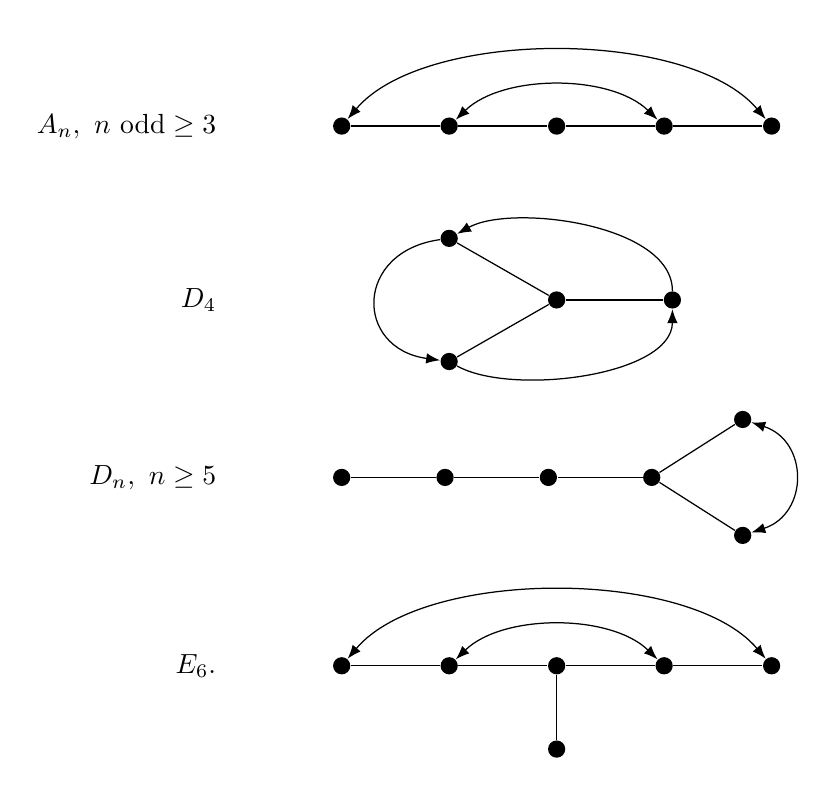
\begin{tikzpicture}[
  x=1.05cm,
  y=.92cm,
  >=Latex,
  dynkin node/.style={circle,fill=black,inner sep=2.2pt},
  dynkin edge/.style={line width=.45pt},
  dynkin arrow/.style={line width=.45pt}
]
  % A_n, n odd: reflection of the chain.
  \node[anchor=east] at (-1.4,6.7) {\(A_n,\ n\text{ odd}\geq 3\)};
  \foreach \x/\name in {0/aone,1.3/atwo,2.6/athree,3.9/afour,5.2/afive}
    \node[dynkin node] (\name) at (\x,6.7) {};
  \draw[dynkin edge] (aone)--(atwo)--(athree)--(afour)--(afive);
  \draw[dynkin arrow,<->]
    (aone) .. controls +(1.0,1.35) and +(-1.0,1.35) .. (afive);
  \draw[dynkin arrow,<->]
    (atwo) .. controls +(.65,.72) and +(-.65,.72) .. (afour);

  % D_4: the three outer vertices are cyclically permuted.
  \node[anchor=east] at (-1.4,4.3) {\(D_4\)};
  \node[dynkin node] (dcenter) at (2.6,4.3) {};
  \node[dynkin node] (dtop)    at (1.3,5.15) {};
  \node[dynkin node] (dbottom) at (1.3,3.45) {};
  \node[dynkin node] (dright)  at (4.0,4.3) {};
  \draw[dynkin edge] (dcenter)--(dtop);
  \draw[dynkin edge] (dcenter)--(dbottom);
  \draw[dynkin edge] (dcenter)--(dright);
  \draw[dynkin arrow,->]
    (dright) .. controls +(0,1.05) and +(.75,.48) .. (dtop);
  \draw[dynkin arrow,->]
    (dtop) .. controls +(-1.15,-.18) and +(-1.15,.18) .. (dbottom);
  \draw[dynkin arrow,->]
    (dbottom) .. controls +(.75,-.48) and +(0,-1.05) .. (dright);

  % D_n, n >= 5: interchange of the two terminal vertices.
  \node[anchor=east] at (-1.4,1.85) {\(D_n,\ n\geq 5\)};
  \foreach \x/\name in {0/dnone,1.25/dntwo,2.5/dnthree,3.75/dnbranch}
    \node[dynkin node] (\name) at (\x,1.85) {};
  \node[dynkin node] (dnupper) at (4.85,2.65) {};
  \node[dynkin node] (dnlower) at (4.85,1.05) {};
  \draw[dynkin edge] (dnone)--(dntwo)--(dnthree)--(dnbranch);
  \draw[dynkin edge] (dnbranch)--(dnupper);
  \draw[dynkin edge] (dnbranch)--(dnlower);
  \draw[dynkin arrow,<->]
    (dnupper) .. controls +(.8,-.3) and +(.8,.3) .. (dnlower);

  % E_6: reflection across the central vertical axis.
  \node[anchor=east] at (-1.4,-.75) {\(E_6.\)};
  \foreach \x/\name in {0/eone,1.3/etwo,2.6/ethree,3.9/efour,5.2/efive}
    \node[dynkin node] (\name) at (\x,-.75) {};
  \node[dynkin node] (esix) at (2.6,-1.9) {};
  \draw[dynkin edge] (eone)--(etwo)--(ethree)--(efour)--(efive);
  \draw[dynkin edge] (ethree)--(esix);
  \draw[dynkin arrow,<->]
    (eone) .. controls +(1.0,1.35) and +(-1.0,1.35) .. (efive);
  \draw[dynkin arrow,<->]
    (etwo) .. controls +(.65,.72) and +(-.65,.72) .. (efour);
\end{tikzpicture}
\end{center}

Let \(S\) be a simple system of roots, not yet ordered. The group
\(E\) is the semidirect product of \(W\) with the group
\(\Psi\) of permutations of \(S\) preserving the Cartan matrix,
or equivalently the Dynkin diagram. Thus \(E/W\simeq\Psi\), and
\(\varphi\) corresponds to some \(\psi\in\Psi\).

Inspection of the diagrams shows that each \(\psi\)-orbit in
\(S\) consists of pairwise orthogonal roots. This fails for
\(A_n\) with \(n\) even, which is why that case was separated.
If \(\sigma\) is such an orbit, the reflections \(r_a\),
\(a\in\sigma\), commute; write
\[
  \rho_\sigma=\prod_{a\in\sigma}r_a.
\]
Plainly \(\rho_\sigma\) commutes with \(\psi\).

Choose a total order on \(S\) for which every \(\psi\)-orbit is a
segment, and write \(S=\{a_1,\ldots,a_n\}\). Let
\(\theta_1,\ldots,\theta_n\) and
\(c=r_1\cdots r_n\) be defined as above. The element \(c\) is a
product of the \(\rho_\sigma\), with the orbits in some order, so
it commutes with \(\psi\). Put
\[
  f=c\psi.
\]

The automorphism \(\psi\) permutes the \(\theta_i\). Indeed,
\(\psi(\theta_i)>0\), and, since \(c\) commutes with \(\psi\),
\[
  c(\psi(\theta_i))=\psi(c(\theta_i))<0.
\]
\SGARefLink{sga3:xiv:7:lemma5}{Lemma 5}\textup{\SGARefLink{sga3:xiv:7:lemma5:item:c}{(c)}} therefore gives
\(\psi(\theta_i)=\theta_j\) for some \(j\).

Finally, if \(a\in R\), \SGARefLink{sga3:xiv:7:lemma5}{Lemma 5} gives
\(a=c^m\theta_i\) for some \(m,i\). Hence
\[
  a=f^m(\psi^{-m}\theta_i)=f^m\theta_j
\]
for a suitable \(j\). Thus \(f\) and the \(\theta_i\) satisfy
both conditions of \SGARefLink{sga3:xiv:7:lemma3}{Lemma 3}, completing its proof.

\paragraph{\textbf{Remark.}}
Except in case \textup{\SGARefLink{sga3:xiv:7:lemma2}{(2)}}, one can prove that every orbit of
\(f\) has exactly
\[
  h=\frac{\operatorname{Card}(R)}{n}
\]
elements and contains exactly one \(\theta_i\). In case
\textup{(2)}, some of the \(\theta_i\) are superfluous.

% END INCLUDED SGA3_English_current_buildable_source_20260823/source/inputs/XIV/tex/components/30_expose_XIV_appendix_lemma3_case3_end_en.tex



% END INCLUDED SGA3_English_current_buildable_source_20260823/source/inputs/XIV/body.tex


\SGAStartExpose{XV}
% BEGIN INCLUDED SGA3_English_current_buildable_source_20260823/source/inputs/XV/body.tex
% Mechanically extracted after \mainmatter from the frozen standalone master.

\markboth{Exposé XV. Complements on Sub-tori}{Exposé XV. Complements on Sub-tori}
% BEGIN INCLUDED SGA3_English_current_buildable_source_20260823/source/inputs/XV/tex/components/00_expose_XV_title_and_introduction.tex
% Authority: Expo15.pdf, local p. 1 / combined p. 871 / printed p. 349.

\chapter*{Exposé XV\\Complements on Sub-tori of a Group Prescheme\\
Application to Smooth Groups}
\addcontentsline{toc}{chapter}{Exposé XV. Complements on Sub-tori of a Group Prescheme}
\SGARefTarget{sga3:xv:expose}

\begin{center}
\textit{by M. Raynaud}\footnote{Source-edition note: xy version dated
1 December 2008.}\textsuperscript{,}\footnote{This Exposé and the two following ones
(Exposés XVI and XVII) do not correspond to oral lectures delivered at
the seminar. With some additional material, they develop the substance
of concise manuscript notes written by A. Grothendieck in 1964 for the
present seminar.}
\end{center}

\SGASection{0}{Introduction}
\SGARefTarget{sga3:xv:section:0}

This Exposé supplements and partly recasts Exposés XI and XII; knowledge
of Exposés XIII and XIV is not indispensable. Continuing the effort
begun in XII, we shall work with \(S\)-group preschemes that are not
necessarily affine and not necessarily separated over \(S\).

\SGARefLink{sga3:xv:section:1}{Sections 1}, 2, 3, and 4 are devoted to the study of sub-tori of a group
prescheme. We obtain infinitesimal lifting theorems (§2) and a global
lifting theorem (§4), in which points of finite order (§1) play an
essential role.

\SGARefLink{sga3:xv:section:5}{Sections 5}, 6, and 7 are independent of the preceding sections. The
consideration of infinitesimal neighbourhoods leads to the
representability of the functor of smooth subgroups equal to their
connected normalizer (§5). In §§6 and 7 we turn more particularly to
Cartan subgroups.

Finally, in §8 we give a necessary and sufficient condition for the
functor of sub-tori of a smooth group, or the functor of maximal tori,
to be representable.

% END INCLUDED SGA3_English_current_buildable_source_20260823/source/inputs/XV/tex/components/00_expose_XV_title_and_introduction.tex

% BEGIN INCLUDED SGA3_English_current_buildable_source_20260823/source/inputs/XV/tex/components/01_expose_XV_section1_opening.tex
% Authority: Expo15.pdf, local pp. 1--3 / combined pp. 871--873 /
% printed pp. 350--353.
% Stops immediately before §1.2, Lemma 1.4.

\SGASection{1}{Lifting finite subgroups}
\SGARefTarget{sga3:xv:section:1}

\SGASubsection{1.1}{Finite, smooth, central subgroups of multiplicative type}
\SGARefTarget{sga3:xv:subsection:1:1}

\SGAStatement{Proposition 1.1}{Let \(S\) be an affine scheme, let
\(S_0\) be a closed subscheme of \(S\) defined by a square-zero ideal,
let \(G\) be an \(S\)-group prescheme, and let \(H_0\) be a subgroup
scheme of \(G_0=G\times_S S_0\) that is smooth and of finite type over
\(S_0\), and of multiplicative type. A subgroup scheme of \(G\), of
multiplicative type, lifting \(H_0\) exists if and only if there exists
a subscheme \(H'\) of \(G\), flat over \(S\), lifting \(H_0\).}
\SGARefTarget{sga3:xv:proposition:1:1}

The necessity of the condition is clear; let us prove its sufficiency.
The group \(H_0\) of multiplicative type is quasi-isotrivial (\SGARefLink{sga3:x:corollary:4-5}{X~4.5}).
By Exposé \SGARefLink{sga3:x:proposition:2:1}{X~2.1}, there exist an \(S\)-group \(H\) of multiplicative
type and an \(S_0\)-isomorphism of groups
\[
  u_0:H\times_S S_0\xrightarrow{\sim}H_0.
\]
Since \(H'\) is flat over \(S\) and \(H'\times_S S_0\) is of finite
presentation over \(S_0\) (Exposé \SGARefLink{sga3:ix:proposition:2:1:item:b:01}{IX~2.1(b)}), \(H'\) is of finite
presentation over \(S\). Its fibres are smooth, so \(H'\) is smooth
over \(S\) (EGA IV~17.5.1). Since \(S\) is affine, \(u_0\) therefore
lifts to an \(S\)-morphism of preschemes
\[
  u:H\longrightarrow H'.
\]
It then follows from Exposé \SGARefLink{sga3:iii:theorem:2-1}{III~2.1} and Exposé \SGARefLink{sga3:ix:theorem:3:1}{IX~3.1} that the composite
\[
  v_0:H\times_S S_0\xrightarrow{\sim}H_0\longrightarrow G_0
\]
also lifts to an \(S\)-homomorphism
\[
  v:H\longrightarrow G.
\]
Since \(v_0\) is an immersion, so is \(v\). The image of \(H\) under
\(v\) is therefore a subgroup scheme of \(G\), of multiplicative type,
lifting \(H_0\).

\SGAStatement{Proposition 1.2}{Let \(S\) be a prescheme, let \(S_0\)
be a subprescheme of \(S\) defined by a locally nilpotent sheaf of
ideals, let \(G\) be an \(S\)-group prescheme flat and of finite
presentation over \(S\), and let \(H_0\) be a subgroup scheme of
\(G_0=G\times_S S_0\) that is smooth, finite over \(S_0\), of
multiplicative type, and central. Then there exists a unique subgroup
scheme \(H\) of \(G\), of multiplicative type, lifting \(H_0\).
Moreover, \(H\) is central. (See XVII, Appendix III, 1.)}
\SGARefTarget{sga3:xv:proposition:1:2}

\SGAInlineRefTarget{sga3:xv:proposition:1-2-bis}\SGAStatement{Proposition 1.2 bis}{Let \(S,G,S_0,G_0\) be as above,
let \(H\) be an \(S\)-group scheme of multiplicative type, smooth and
finite over \(S\), and let
\(u_0:H_0=H\times_S S_0\to G_0\) be a central homomorphism. Then
\(u_0\) lifts uniquely to a homomorphism \(u:H\to G\). Moreover,
\(u\) is central.}
\SGARefTarget{sga3:xv:proposition:1:2:bis}

The existence of the lifting \(u\) in \SGARefLink{sga3:xv:proposition:1:2:bis}{Proposition 1.2 bis} follows
readily from \SGARefLink{sga3:xv:proposition:1:2}{Proposition 1.2} by considering the graph of \(u_0\). The
lifting \(u\) is unique and central by Exposé \SGARefLink{sga3:ix:corollary:3:4}{IX~3.4} and Exposé \SGARefLink{sga3:ix:theorem:5:1}{IX~5.1}.

\SGAProof{Proof of \SGARefLink{sga3:xv:proposition:1:2}{Proposition 1.2}}
The uniqueness of \(H\), and the fact that \(H\) is central, follow
from Exposé \SGARefLink{sga3:ix:theorem:5:6:item:b}{IX~5.6(b)} and Exposé \SGARefLink{sga3:ix:corollary:3:4:bis}{IX~3.4 bis}. In view of uniqueness, to
prove existence we may assume that \(S\) is affine and that \(S_0\) is
defined by a square-zero ideal; by \SGARefLink{sga3:xv:proposition:1:1}{Proposition 1.1} it is enough to find
a subscheme of \(G\), flat over \(S\), lifting \(H_0\).

Since \(H_0\) is smooth and finite over \(S_0\), after possibly
restricting \(S\) we may assume that there is an integer \(n>0\),
invertible on \(S\), such that \(H_0={}_nH_0\). Consider the \(n\)-th
power morphism on \(G\):
\[
  u:G\longrightarrow G,\qquad x\longmapsto x^n.
\]
We continue to denote by \({}_nG\) the ``kernel of \(u\)'', that is,
the inverse image under \(u\) of the identity section of \(G\).
Notice that \(u\) is not, in general, a group homomorphism. We first
admit the following lemma.

\SGAStatement{Lemma 1.3}{Let \(k\) be a field, let \(G\) be a group
scheme locally of finite type over \(k\), let \(n\) be an integer prime
to the characteristic of \(k\), and let \(u\) be the \(n\)-th power
morphism on \(G\). Then \(u\) is étale at every point \(x\) of \(G\)
that belongs to the centre of \(G\).}
\SGARefTarget{sga3:xv:lemma:1:3}

Since \(G\) is flat and of finite presentation over \(S\), the
preceding lemma and EGA IV~17.8.2 show that, if \(x\in G\) lies above
\(s\in S\) and belongs to the centre of \(G_s\), then \(u\) is étale
at \(x\). If in addition \(x\in {}_nG\), then \({}_nG\) is étale over
\(S\) at \(x\). By hypothesis, \(H_0\) is central and is contained in
\({}_nG_0\); it is therefore contained in the largest open subset
\(V\) of \({}_nG\) that is étale over \(S\). Since \(H_0\) and
\(V\times_S S_0=V_0\) are étale over \(S_0\), \(H_0\) is an open
subscheme of \(V_0\) (EGA IV~17.8.7 and 17.9.1). The open subprescheme
of \(V\) having the same underlying space as \(H_0\) is consequently
a subscheme of \(G\), flat over \(S\), lifting \(H_0\).

It remains to prove \SGARefLink{sga3:xv:lemma:1:3}{Lemma 1.3}. The largest open subset of \(G\) on
which \(u\) is étale is invariant under extension of the base field
(EGA IV~17.8.2), so we may reduce to the case in which \(x\) is
\(k\)-rational. Let \(t_x\) denote translation by \(x\), a
\(k\)-automorphism of \(G\). Since \(x\) belongs to the centre of
\(G\), the diagram
\[
\begin{tikzcd}[column sep=large,row sep=large]
G \arrow[r,"u"] \arrow[d,"t_x"'] & G \arrow[d,"t_x^n"] \\
G \arrow[r,"u"] & G .
\end{tikzcd}
\]
is commutative. It is therefore enough to prove that \(u\) is étale
at the identity; this was established in VII\textsubscript{A}~\SGARefLink{sga3:xv:definition:8-4}{8.4}.

% END INCLUDED SGA3_English_current_buildable_source_20260823/source/inputs/XV/tex/components/01_expose_XV_section1_opening.tex

% BEGIN INCLUDED SGA3_English_current_buildable_source_20260823/source/inputs/XV/tex/components/02_expose_XV_section1_remainder_and_section2.tex
% Authority: Expo15.pdf, local pp. 3--14 / combined pp. 873--884 /
% printed pp. 353--374.
% Begins at §1.2, Lemma 1.4, and stops immediately before §3.

\SGASubsection{1.2}{Global lifting of finite groups}
\SGARefTarget{sga3:xv:subsection:1:2}

\SGAStatement{\SGAInlineRefTarget{sga3:xv:lemma:1-4}Lemma 1.4}{Let \(A\) be a local ring, separated and
complete for the topology defined by its maximal ideal \(\mathfrak m\),
let
\[
  S=\operatorname{Spec}(A),\qquad
  S_n=\operatorname{Spec}(A/\mathfrak m^n).
\]
Then, for every prescheme \(X\) (respectively, for every \(S\)-prescheme
\(X\)), the canonical map
\[
  \tag{$\ast$}\label{sga3:xv:lemma:1-4:equation:ast}
  \operatorname{Hom}(S,X)
  \longrightarrow
  \varprojlim_n\operatorname{Hom}(S_n,X)
\]
(respectively,
\[
  \tag{$\ast\ast$}\label{sga3:xv:lemma:1-4:equation:ast-ast}
  \Gamma(X/S)
  \longrightarrow
  \varprojlim_n\Gamma(X_n/S_n),
  \qquad X_n=X\times_S S_n)
\]
is bijective.}
\SGARefTarget{sga3:xv:lemma:1:4}

Statement \((\ast\ast)\) is an easy consequence of \((\ast)\). Let us
prove \((\ast)\). Let
\[
  u_n:S_n\longrightarrow X\qquad(n\in\mathbb N)
\]
be a coherent system of morphisms. The image \(y\) of the closed point
of \(S_n\) is independent of \(n\), and \(u_n\) factors through
\(\operatorname{Spec}\mathcal O_y\). On passing to the inverse limit,
the morphisms \(u_n\) define a ring homomorphism
\[
  \widetilde u:\mathcal O_y
  \longrightarrow
  \varprojlim_n(A/\mathfrak m^n)=A.
\]
This proves that \((\ast)\) is surjective; it is injective as soon as
\(A\) is separated for the \(\mathfrak m\)-adic topology.

% Authority page transition: local p. 4 / combined p. 874 / printed p. 354.
\SGAStatement{\SGAInlineRefTarget{sga3:xv:corollary:1-5}Corollary 1.5}{Let \(A\) be a complete noetherian local
ring, let \(\mathfrak m\) be its maximal ideal, let
\[
  S=\operatorname{Spec}(A),\qquad
  S_n=\operatorname{Spec}(A/\mathfrak m^n),
\]
let \(X\) be a finite scheme over \(S\), and let \(Y\) be an
\(S\)-prescheme. Then the canonical map
\[
  \operatorname{Hom}_S(X,Y)
  \longrightarrow
  \varprojlim_n\operatorname{Hom}_{S_n}(X_n,Y_n)
\]
(where \(X_n=X\times_S S_n\), and similarly for \(Y_n\)) is
bijective.}
\SGARefTarget{sga3:xv:corollary:1:5}

Indeed, it follows from EGA II~6.2.5 that \(X\) is a finite disjoint
sum of local \(S\)-schemes finite over \(S\). We are thus reduced to
the case in which \(X\) itself is the spectrum of a complete
noetherian local ring. But
\[
  \operatorname{Hom}_S(X,Y)=\Gamma(Z/X),
  \qquad Z=Y\times_S X,
\]
and the preceding lemma applies.

\SGAStatement{\SGAInlineRefTarget{sga3:xv:proposition:1-6}Proposition 1.6}{Let \(A,S,S_n\) be as above, and let
\(G\) and \(M\) be two \(S\)-group preschemes, with \(M\) finite over
\(S\). Then:
\begin{enumerate}
\item[\normalfont a)]\SGAInlineRefTarget{sga3:xv:proposition:1-6:item:a} The canonical map
\[
  \operatorname{Hom}_{S\text{-}\mathrm{gr}}(M,G)
  \longrightarrow
  \varprojlim_n
  \operatorname{Hom}_{S_n\text{-}\mathrm{gr}}(M_n,G_n)
\]
is bijective.
\item[\normalfont b)] If \(M\) is of multiplicative type and \(G\) is
smooth over \(S\), the canonical map
\[
  \varphi:\operatorname{Hom}_{S\text{-}\mathrm{gr}}(M,G)
  \longrightarrow
  \operatorname{Hom}_{S_0\text{-}\mathrm{gr}}(M_0,G_0)
\]
is surjective. Moreover, if
\(\varphi(u)=\varphi(u')=u_0\), then \(u\) and \(u'\) are conjugate by
an element of \(G(S)\) that reduces to the identity element of
\(G(S_0)\).
\item[\normalfont c)] If \(M\) is of multiplicative type and smooth
over \(S\), if \(G\) is flat and of finite type over \(S\), and if
\(u_0:M_0\to G_0\) is a central homomorphism, then \(u_0\) lifts
uniquely to a homomorphism
\[
  u:M\longrightarrow G.
\]
Moreover, \(u\) is central if \(G\) has connected fibres.
\end{enumerate}}
\SGARefTarget{sga3:xv:proposition:1:6}

\SGAProof{Proof}
\emph{a)} This follows from \SGARefLink{sga3:xv:corollary:1-5}{1.5}, from the fact that
\(M\times_S M\) is finite over \(S\), and from the characterization
of group morphisms as the morphisms for which the familiar diagram
\[
\begin{tikzcd}[column sep=large,row sep=large]
M\times_S M \arrow[r,"u\times u"] \arrow[d]
  & G\times_S G \arrow[d] \\
M \arrow[r,"u"'] & G
\end{tikzcd}
\]
is commutative.

\emph{b)} By Exposé \SGARefLink{sga3:ix:theorem:3:6}{IX~3.6}, one can construct a coherent system of
homomorphisms \(u_n:M_n\to G_n\) lifting a homomorphism
\(u_0:M_0\to G_0\). In view of part a), this proves the first assertion
of b).

If \(u\) and \(u'\) are two liftings of \(u_0\), then \(u_n\) and
\(u'_n\) are conjugate by an element \(g_n\in G(S_n)\) lifting the
identity element of \(G(S_0)\) (Exposé \SGARefLink{sga3:ix:theorem:3:6}{IX~3.6}). The same reference
also implies that the \(g_n\) may be chosen coherently; by \SGARefLink{sga3:xv:lemma:1-4}{1.4} they
therefore arise from a section \(g\in G(S)\). The morphisms \(u\) and
\(\operatorname{Int}(g)u'\) then agree modulo \(\mathfrak m^n\) for
every \(n\), and hence agree by \SGARefLink{sga3:xv:corollary:1-5}{1.5}.

\emph{c)} The existence and uniqueness of \(u\) follow from part a)
and \SGARefLink{sga3:xv:proposition:1:2:bis}{1.2 bis}. If \(G\) has connected fibres, \(u\) is central by
Exposé \SGARefLink{sga3:ix:theorem:5:6:item:a}{IX~5.6(a)}.

% Authority page transition: local p. 5 / combined p. 875 / printed pp. 356--357.
\SGASection{2}{Infinitesimal lifting of sub-tori}
\SGARefTarget{sga3:xv:section:2}

\SGASubsection{2.1}{Statement of the theorem}
\SGARefTarget{sga3:xv:subsection:2:1}

We shall give an infinitesimal lifting theorem for sub-tori of a group
prescheme that does not require smoothness hypotheses (in contrast
with Exposé \SGARefLink{sga3:ix:theorem:3:6:bis}{IX~3.6 bis}) and that also answers a very natural
question:\footnote{Editor's note: The idea of approximating a torus by
its finite subgroups occurs in Grothendieck's proof of the
connectedness of centralizers of tori; see §\SGARefLink{sga3:xv:lemma:4:6}{4.6} of \emph{BIBLE}.}
is it enough to be able to lift ``sufficiently many'' points of finite
order of a sub-torus \(T_0\) in order to ensure that \(T_0\) itself can
be lifted (infinitesimally, of course)?

\SGAStatement{Theorem 2.1}{Let \(S\) be a noetherian affine scheme,
let \(S_0\) be a closed subscheme of \(S\) defined by a square-zero
ideal \(J\), let \(G\) be an \(S\)-group prescheme of finite type, let
\(G_0=G\times_S S_0\), let \(T_0\) be a sub-torus of \(G_0\), and let
\(q>0\) be an integer invertible on \(S\). Suppose that, for every
integer \(n\) equal to a power of \(q\), there exists a subscheme
\(M_n\) of \(G\), flat over \(S\), such that
\[
  M_n\times_S S_0={}_nT_0.
\]
Then there exists a sub-torus \(T\) of \(G\) such that
\(T\times_S S_0=T_0\).}
\SGARefTarget{sga3:xv:theorem:2:1}

\SGARefLink{sga3:xv:theorem:2:1}{Theorem 2.1} will be useful to us through the following two
corollaries.

\SGAStatement{\SGAInlineRefTarget{sga3:xv:corollary:2-2}Corollary 2.2}{Let \(S\) be a locally noetherian
prescheme, let \(S_0\) be a closed subprescheme of \(S\) defined by a
locally nilpotent sheaf of ideals, let \(G\) be an \(S\)-group
prescheme of finite type, let \(T_0\) be a sub-torus of
\(G_0=G\times_S S_0\), and let \(q>0\) be an integer invertible on
\(S\). As \(n\) ranges over the powers of \(q\), let \((M_n)\) be a
coherent system of \(S\)-subgroup schemes of \(G\), of multiplicative
type, lifting the \({}_nT_0\). (The system \((M_n)\) is said to be
coherent if
\[
  M_m={}_m(M_n)
\]
whenever \(m\) divides \(n\).) Then there exists a unique sub-torus
\(T\) of \(G\) such that
\[
  T\times_S S_0=T_0
  \qquad\text{and}\qquad
  {}_nT=M_n
\]
for every \(n\).}
\SGARefTarget{sga3:xv:corollary:2:2}

\SGAStatement{Corollary 2.3}{Let \(G\) be an \(S\)-group prescheme,
flat and of finite presentation over \(S\), let \(S_0\) be a closed
subprescheme of \(S\) defined by a locally nilpotent sheaf of ideals
of finite type, and let \(T_0\) be a central torus of
\(G_0=G\times_S S_0\). Then there exists a unique sub-torus \(T\) of
\(G\) lifting \(T_0\). Moreover, \(T\) is central.}
\SGARefTarget{sga3:xv:corollary:2:3}

\SGAStatement{Remark 2.4}{We leave it to the reader to formulate the
analogues of statements \SGARefLink{sga3:xv:theorem:2:1}{2.1}, \SGARefLink{sga3:xv:corollary:2-2}{2.2}, and \SGARefLink{sga3:xv:corollary:2:3}{2.3} in which, instead of lifting
a sub-torus of \(G_0\), one is given a torus \(T\) over \(S\) and asks
to lift a morphism
\[
  u_0:T_0\longrightarrow G_0.
\]
One reduces to the preceding cases by considering the graph of
\(u_0\).}
\SGARefTarget{sga3:xv:remark:2:4}

Let us show how \SGARefLink{sga3:xv:corollary:2-2}{Corollaries 2.2} and \SGARefLink{sga3:xv:corollary:2:3}{2.3} follow from \SGARefLink{sga3:xv:theorem:2:1}{Theorem 2.1}.

\SGAProof{Proof of \SGARefLink{sga3:xv:corollary:2-2}{Corollary 2.2}}
The uniqueness of \(T\) follows from Exposé \SGARefLink{sga3:ix:corollary:4:8:item:b}{IX~4.8(b)} and Exposé
\SGARefLink{sga3:ix:remark:4:10}{IX~4.10}. To prove existence, we may therefore reduce to the case in
which \(S\) is affine, hence noetherian, and \(S_0\) is defined by a
square-zero ideal.

\SGAStatement{Lemma 2.5}{Let \(G\) be an \(S\)-group prescheme of
finite presentation, and let \(H\) be a subgroup scheme of \(G\), of
multiplicative type and smooth over \(S\). Then
\(\operatorname{Centr}_G(H)\) is representable by an \(S\)-group
subprescheme of \(G\), of finite presentation.}
\SGARefTarget{sga3:xv:lemma:2:5}

When \(G\) is separated over \(S\), the lemma follows from Exposé
\SGARefLink{sga3:viii:examples:6:5:item:e:01}{VIII~6.5(e)}, without any smoothness hypothesis on \(H\). In the present
case, observe that the assertion is local for the fpqc topology. We
may therefore assume that \(H\) is diagonalizable, hence of the form
\(D_S(M)\). We may also assume that \(S\) is affine and then, by EGA
IV~8, noetherian. Since \(H\) is smooth and of finite type over \(S\),
the order \(q\) of the torsion subgroup of \(M\) is invertible on
\(S\) (Exposé \SGARefLink{sga3:viii:proposition:2:1:item:e:01}{VIII~2.1(e)}). It is then immediate (cf. Exposé \SGARefLink{sga3:ix:remark:4:10}{IX~4.10})
that the subgroups \({}_nH\), with \(n\) ranging over the powers of
\(q\), are schematically dense in \(H\) (Exposé \SGARefLink{sga3:ix:definition:4:1}{IX~4.1}). But
\({}_nH\) is a completely split covering of \(S\), that is, it is
isomorphic to a finite disjoint sum of copies of \(S\). Consequently
\[
  \operatorname{Centr}_G({}_nH)=Z_n
\]
is representable as the intersection of the centralizers in \(G\) of
the sections of \({}_nH\) over \(S\). It remains to apply the following
lemma.

\SGAStatement{\SGAInlineRefTarget{sga3:xv:lemma:2-5-bis}Lemma 2.5 bis}{Let \(S\) be a noetherian prescheme, let
\(G\) be an \(S\)-group prescheme of finite type, let \(H\) be a
subgroup of \(G\) of multiplicative type, and let \((H_i)\) be an
increasing filtered family of subgroups of \(G\) of multiplicative
type. Suppose that
\[
  Z_i=\operatorname{Centr}_G(H_i)
\]
is representable by a group subprescheme of \(G\). Then the family
\((Z_i)\) is stationary. If, in addition, the \(H_i\) are schematically
dense in \(H\), then
\[
  Z_i=\operatorname{Centr}_G(H)
\]
for all sufficiently large \(i\).}
\SGARefTarget{sga3:xv:lemma:2:5:bis}

To see that the family \((Z_i)\) is stationary, it is enough to prove
that the family of underlying sets \(\operatorname{ens}(Z_i)\) is
stationary. Indeed, the stationary value will then be a closed subset
of an open subset \(U\) of \(G\). After replacing \(G\) by \(U\), we
are reduced to studying a decreasing filtered family of closed
subpreschemes of a noetherian prescheme. An elementary constructibility
argument reduces us to the case in which \(S\) is integral. We then
have to show that \(\operatorname{ens}(Z_i)\) is stationary over some
nonempty open subset of \(S\). The generic fibre of \(G\) is separated
(Exposé VI\textsubscript{A}~0.3); after restricting \(S\), we may
therefore assume that \(G\) is separated over \(S\) (EGA IV~8). Then
\(Z_i\) is closed in \(G\) (Exposé VIII~6.5(e)).

To prove the last assertion of the lemma, let \(Z\) denote the
stationary value of the family \((Z_i)\). It is clear that
\(\operatorname{Centr}_G(H)\) is a subfunctor of \(Z\); we show that
\(Z\) centralizes \(H\). Let \(E\) be the subprescheme of
\(H\times_S Z\) that is the kernel of the pair of morphisms
\[
\begin{aligned}
  H\times_S Z&\rightrightarrows G,\\
  (h,c)&\longmapsto c,\\
  (h,c)&\longmapsto hch^{-1}.
\end{aligned}
\]
The prescheme \(E\) contains \(H_i\times_S Z\) for every \(i\). The
\(H_i\) are flat over \(S\), so EGA IV~11.10.9 shows that, for every
point \(s\) of \(S\), the \((H_i)_s\) are schematically dense in
\(H_s\), and \(H_i\times_S Z\) is schematically dense in
\(H\times_S Z\). Since \(G_s\) is separated, \(E_s\) is closed in
\((H\times_S Z)_s\), and is therefore equal to it. Thus \(E\) is
closed in \(H\times_S Z\), and hence equals \(H\times_S Z\). This says
that \(Z\) centralizes \(H\).

Returning to the proof of \SGARefLink{sga3:xv:corollary:2-2}{2.2}, \SGARefLink{sga3:xv:lemma:2:5}{Lemma 2.5} shows that
\[
  Z_n=\operatorname{Centr}_G(M_n)
\]
is representable, and \SGARefLink{sga3:xv:lemma:2-5-bis}{Lemma 2.5 bis} shows that the decreasing family
of subpreschemes \((Z_n)\) is stationary; let \(Z\) be its stationary
value. The group \(Z\) contains \(T_0\) and all the \(M_n\). After
replacing \(G\) by \(Z\), we may therefore suppose that the \(M_n\)
are central.

The hypotheses of \SGARefLink{sga3:xv:theorem:2:1}{Theorem 2.1} are now satisfied, so there exists a
sub-torus \(T\) of \(G\) lifting \(T_0\). The groups \({}_nT\) and
\(M_n\) are two liftings of \({}_nT_0\); they are therefore conjugate
(Exposé \SGARefLink{sga3:ix:theorem:3:2:bis}{IX~3.2 bis}), and consequently coincide because \(M_n\) is
central. This torus \(T\) has the required properties.

\SGAProof{Proof of \SGARefLink{sga3:xv:corollary:2:3}{Corollary 2.3}}
The uniqueness of \(T\) follows from Exposé \SGARefLink{sga3:ix:theorem:5:1:bis}{IX~5.1 bis}, and its
centrality follows from Exposé \SGARefLink{sga3:ix:theorem:5:6:item:b}{IX~5.6(b)}. By the usual procedure, this
observation reduces us first to the case in which \(S\) is affine
(and hence \(S_0\) is defined by a nilpotent ideal of finite type),
and then to the noetherian case. After restricting \(S\) if necessary,
we may suppose that there exists an integer \(q\) invertible on \(S\).
\SGARefLink{sga3:xv:corollary:2:3}{Corollary 2.3} then follows from \SGARefLink{sga3:xv:corollary:2-2}{2.2} and \SGARefLink{sga3:xv:proposition:1:2}{1.2}.

\SGAStatement{Remark 2.6}{\SGARefLink{sga3:xv:corollary:2:3}{Corollary 2.3} remains true if the torus
\(T_0\) is replaced by a smooth central subgroup of multiplicative
type of \(G_0\).}
\SGARefTarget{sga3:xv:remark:2:6}

% Authority page transition: local p. 7 / combined p. 877 / printed p. 362.
\SGASubsection{2.2}{Proof of \SGARefLink{sga3:xv:theorem:2:1}{Theorem 2.1}}
\SGARefTarget{sga3:xv:subsection:2:2}

\medskip\noindent\textbf{a) Reduction to the case
\(\boldsymbol{T_0=\mathbb G_{m,S_0}}\).}

By \SGARefLink{sga3:xv:proposition:1:1}{1.1}, we may assume that \(M_n\) is a subgroup of multiplicative
type. Using Exposé \SGARefLink{sga3:ix:theorem:3:2:bis}{IX~3.2 bis}, we may suppose that the family
\((M_n)\) is coherent (\SGARefLink{sga3:xv:corollary:2-2}{2.2}). The centralizer \(Z_n\) of \(M_n\) in
\(G\) is representable (\SGARefLink{sga3:xv:lemma:2:5}{2.5}), and the filtered family \((Z_n)\) is
stationary (\SGARefLink{sga3:xv:lemma:2-5-bis}{2.5 bis}). After replacing \(G\) by \(Z_n\) for sufficiently
large \(n\), we may therefore suppose that \(T_0\) and the \(M_n\) are
central. The uniqueness of a lifting of \(T_0\) is then guaranteed
by Exposé \SGARefLink{sga3:ix:theorem:5:1:bis}{IX~5.1 bis}.

Proceeding as in the proof of \SGARefLink{sga3:xv:proposition:1:1}{1.1}, we may suppose that there exist an
\(S\)-torus \(T\) and an \(S_0\)-isomorphism
\[
  u_0:T\times_S S_0\xrightarrow{\sim}T_0.
\]
Lifting \(u_0\) is equivalent to lifting \(T_0\). By uniqueness, it is
enough to prove the existence of a lifting of \(u_0\) after an affine
faithfully flat extension \(S'\to S\) of finite type (fpqc descent).
This allows us to suppose that
\[
  T=\mathbb G_{m,S}^{\,r}
\]
(Exposé \SGARefLink{sga3:x:corollary:4-5}{X~4.5}). If the restriction of \(u_0\) to each factor
\(\mathbb G_m\) lifts to an \(S\)-morphism---necessarily central---then
these liftings immediately give a lifting of \(u_0\). In short, we may
suppose that \(T_0=\mathbb G_{m,S_0}\).

\medskip\noindent\textbf{b) Definition of the obstruction to the
existence of a lifting of \(\boldsymbol{T_0}\).}

By \SGARefLink{sga3:xv:proposition:1:1}{1.1}, to prove \SGARefLink{sga3:xv:theorem:2:1}{Theorem 2.1} it is enough to find a subscheme of \(G\),
flat over \(S\), lifting \(T_0\). We shall see that the obstruction to
the existence of such a lifting can be defined as an element of a
certain \(\operatorname{Ext}^1\) group of sheaves of modules.

Let \(U\) be an open subset of \(G\) in which \(T_0\) is closed, and
again denote by \(U\) (respectively, \(U_0\)) the open subscheme of
\(G\) (respectively, \(G_0\)) having this open subset as its underlying
space. The sheaf \(\mathcal O_{T_0}\), regarded as a sheaf on \(U\), is
therefore a quotient of \(\mathcal O_{U_0}\). Let
\[
  h:\mathcal O_{U_0}\longrightarrow\mathcal O_{T_0}
\]
be the canonical epimorphism.

\SGAStatement{\SGAInlineRefTarget{sga3:xv:lemma:2-7}Lemma 2.7}{The canonical map
\[
  h'=\operatorname{id}_J\otimes h:
  J\otimes_{S_0}\mathcal O_{U_0}
  \longrightarrow
  J\otimes_{S_0}\mathcal O_{T_0}
\]
factors, necessarily uniquely, as \(i\circ j_U\), where \(j_U\) is
the canonical epimorphism
\[
  J\otimes_{S_0}\mathcal O_{U_0}
  \longrightarrow
  J\mathcal O_U\simeq J\mathcal O_{U_0}.
\]}
\SGARefTarget{sga3:xv:lemma:2:7}

We must show that \(h'(K)=0\), where \(K\) is the kernel of \(j_U\).
For every integer \(n\) equal to a power of \(q\), there is an
epimorphism
\[
  h_n:\mathcal O_{T_0}\longrightarrow\mathcal O_{{}_nT_0}.
\]
Since \({}_nT_0\) lifts to a scheme \(M_n\) flat over \(S\), the
canonical morphism
\[
  j_n:J\otimes_{S_0}\mathcal O_{{}_nT_0}
  \xrightarrow{\sim}J\mathcal O_{M_n}
\]
is an isomorphism. The commutative diagram
\[
\begin{tikzcd}[column sep=large,row sep=large]
K \arrow[r]
  & J\otimes_{S_0}\mathcal O_{U_0}
      \arrow[r,"j_U"] \arrow[d,"h'"]
  & J\mathcal O_U \arrow[r,hook] \arrow[dl,"i"]
  & \mathcal O_U \\
  & J\otimes_{S_0}\mathcal O_{T_0}
      \arrow[d,"h'_n"] & & \\
  & J\otimes_{S_0}\mathcal O_{{}_nT_0}
      \arrow[r,"j_n"',"\sim"] & J\mathcal O_{M_n}
      \arrow[r,hook] & \mathcal O_{M_n}
\end{tikzcd}
\]
shows that \(h'(K)\) is contained in \(\ker h'_n\) for every \(n\).
It is therefore contained in \(\bigcap_n\ker h'_n\), and it remains
to prove that this intersection is zero. Now
\[
  \mathcal O_{T_0}=\mathcal O_{S_0}[\mathbb Z],
  \qquad
  \mathcal O_{{}_nT_0}
     =\mathcal O_{S_0}[\mathbb Z/n\mathbb Z].
\]
Let
\[
  a=\sum_{m\in\mathbb Z}a_m\otimes m
  \in J\otimes_{S_0}\mathcal O_{T_0}.
\]
The \(a_m\) are sections of \(J\), almost all zero. Choose \(n\) large
enough that the indices \(m\) for which \(a_m\ne0\) have distinct
images in \(\mathbb Z/n\mathbb Z\). If \(a\in\ker h'_n\), then
necessarily \(a=0\). Thus \(\bigcap_n\ker h'_n=0\), proving \SGARefLink{sga3:xv:lemma:2-7}{2.7}.

% Authority page transition: local p. 9 / combined p. 879 / printed p. 365.
Let \(K_0\) be the kernel of \(h\). Consider the diagram
\[
\begin{tikzcd}[column sep=large,row sep=large]
  &&& 0 \arrow[d] \\
  & J\mathcal O_U \arrow[d,"\sim"] && K_0 \arrow[d] \\
0 \arrow[r]
  & J\mathcal O_{U_0} \arrow[r] \arrow[d,"i"']
  & \mathcal O_U \arrow[r] & \mathcal O_{U_0}
      \arrow[r] \arrow[d,"h"'] & 0 \\
  & J\otimes_{S_0}\mathcal O_{T_0}
  && \mathcal O_{T_0} \arrow[d] \\
  &&& 0 .
\end{tikzcd}
\]
The sheaf \(\mathcal O_U\) defines an element
\[
  \Phi\in
  \operatorname{Ext}^{1}_{\mathcal O_U}
  (\mathcal O_{U_0},J\mathcal O_{U_0}).
\]
Let \(\Psi\) be the element of
\[
  \operatorname{Ext}^{1}_{\mathcal O_U}
  (K_0,J\otimes_{S_0}\mathcal O_{T_0})
\]
obtained from \(\Phi\), by the bifunctoriality of
\(\operatorname{Ext}^{1}\), through the morphisms
\[
  K_0\longrightarrow\mathcal O_{U_0},
  \qquad
  i:J\mathcal O_{U_0}
    \longrightarrow J\otimes_{S_0}\mathcal O_{T_0}.
\]
It follows from Exposé \SGARefLink{sga3:iii:lemma:4-1}{III~4.1} and the infinitesimal criterion of
flatness (cf. Exposé \SGARefLink{sga3:iii:proposition:4-3}{III~4.3}) that a subscheme of \(U\), flat over
\(S\) and lifting \(T_0\), exists if and only if \(\Psi=0\).

Since \(T_0\) is affine, Exposé \SGARefLink{sga3:iii:proposition:4-5}{III~4.5} and \SGARefLink{sga3:xv:lemma:4:6}{4.6} show that it is enough
to construct, locally on \(U\), a subscheme flat over \(S\) lifting
\(T_0\). It therefore suffices to show that the image of \(\Psi\) in
the sheaf
\[
  \mathscr E=
  \mathcal Ext^{1}_{\mathcal O_U}
  (K_0,J\otimes_{S_0}\mathcal O_{T_0})
\]
is zero. We again denote this element of
\(\Gamma(U,\mathscr E)\) by \(\Psi\).

\medskip\noindent\textbf{c) Reduction to the case in which \(S\) is
local artinian with algebraically closed residue field.}

Since \(K_0\) and \(J\otimes_{S_0}\mathcal O_{T_0}\) are coherent
sheaves, so is \(\mathscr E\); moreover, \(\mathscr E\) is supported
on \(T_0\), because the same is true of
\(J\otimes_{S_0}\mathcal O_{T_0}\). To show that the section \(\Psi\)
of \(\mathscr E\) is zero, it is enough to show that, for every point
\(u\) of \(T_0\), its image in the fibre of \(\mathscr E\) at \(u\)
is zero. Formation of the \(\mathcal Ext^i\) of coherent sheaves
commutes with flat extensions of the base,\footnote{Editor's note:
cf. EGA \(0_{\mathrm{III}}\), 12.3.5.} so we are reduced to proving the
existence of a lifting of
\[
  T_0\cap\operatorname{Spec}\mathcal O_u
\]
flat over \(S\). Let \(s\) be the image of \(u\) in \(S\). We may
replace \(S\) by \(\operatorname{Spec}\mathcal O_s\) and \(G\) by
\(G\times_S\operatorname{Spec}\mathcal O_s\).

After another faithfully flat extension if necessary, we may suppose
that \(\mathcal O_s\) has an algebraically closed residue field
(EGA \(0_{\mathrm{III}}\), 10.3.1). Let \(\mathfrak m\) be the maximal
ideal of \(\mathcal O_s\), and set
\[
  S_n=\operatorname{Spec}(\mathcal O_s/\mathfrak m^n).
\]
Suppose that, for every \(n>0\), the obstruction to lifting
\[
  T_0\times_S S_n=(T_0)_n
\]
to a subscheme of \(G_n=G\times_S S_n\), flat over \(S_n\), has been
shown to vanish, and let \(T_n\) be the unique flat lifting of
\((T_0)_n\) over \(S_n\) that is a sub-torus of \(G_n\). If
\(n>n'\), it is clear that
\[
  T_n\times_{S_n}S_{n'}=T_{n'}.
\]
If \(u\) is a point of \(T_0\) lying over \(s\), the lemma below,
applied to the coherent system of liftings
\[
  T_n\cap\operatorname{Spec}\mathcal O_u
\]
of
\((T_0)_n\cap\operatorname{Spec}\mathcal O_u\), shows that
\(T_0\cap\operatorname{Spec}\mathcal O_u\) indeed has a lifting flat
over \(\mathcal O_s\). We are therefore reduced to proving that
\(\Psi=0\) when \(S=S_n\) is the spectrum of an artinian local ring
with algebraically closed residue field, and to proving the following
lemma.

\SGAStatement{\SGAInlineRefTarget{sga3:xv:lemma:2-8}Lemma 2.8}{Let \(A\to B\) be a local homomorphism of
noetherian local rings, let \(\mathfrak m\) be the maximal ideal of
\(A\), let \(J\) be a square-zero ideal of \(A\), let \(M\) be a
finite-type \(B\)-module, and set
\[
  A_0=A/J,\qquad B_0=B/JB,\qquad M_0=M/JM.
\]
Let \(N_0\) be a quotient \(B_0\)-module of \(M_0\), flat over \(A_0\).
For every \(n>0\), let \(A_n,A_{0,n}\), and so forth denote the objects
obtained by the base extension
\[
  A\longrightarrow A/\mathfrak m^n=A_n,
\]
and let \(\overline{J}_n\) be the image of \(J\) in \(A_n\). For every \(n>0\),
let \(N_n\) be a quotient \(B_n\)-module of \(M_n\), flat over \(A_n\),
lifting \(N_{0,n}\), and suppose that, for \(n\ge n'\), \(N_{n'}\) is
obtained from \(N_n\) by the base extension \(A_n\to A_{n'}\). Then
there exists a quotient \(B\)-module \(N\) of \(M\), flat over \(A\),
lifting \(N_0\).}
\SGARefTarget{sga3:xv:lemma:2:8}

\SGAProof{Proof of \SGARefLink{sga3:xv:lemma:2-8}{2.8}}
Let \(P_0\) be the kernel of the epimorphism \(M_0\to N_0\). For every
\(n>0\), there is a commutative diagram with exact horizontal rows:
\[
\tag{$\ast_n$}\label{sga3:xv:lemma:2-8:equation:ast-n}
\begin{tikzcd}[column sep=2em,row sep=large]
&&&& 0 \arrow[d] & \\
&&&& P_{0,n} \arrow[d] & \\
& 0 \arrow[r]
  & \overline{J}_nM_n \arrow[r] \arrow[dd]
  & M_n \arrow[r] \arrow[dd]
  & M_{0,n} \arrow[r] \arrow[dd] & 0 \\
\overline{J}_n\otimes_{A_{0,n}}M_{0,n}
      \arrow[urr] \arrow[drr] &&&&& \\
& 0 \arrow[r]
  & \overline{J}_n\otimes_{A_{0,n}}N_{0,n} \arrow[r]
  & N_n \arrow[r] \arrow[d]
  & N_{0,n} \arrow[r] \arrow[d] & 0 \\
&&& 0 & 0 &
\end{tikzcd}
\]
Moreover, by hypothesis, the diagram \((\ast)_{n+1}\) reduces modulo
\(\mathfrak m^n\) to \((\ast)_n\).

% Authority page transition: local pp. 10--11 / combined pp. 880--881 /
% printed pp. 367--368.
The Artin--Rees lemma (Bourbaki, \emph{Algèbre commutative}, Chapter
III, §3, Corollary 1) shows that the filtrations on \(JM\),
\(J\otimes_{A_0}M_0\), and \(J\otimes_{A_0}N_0\), defined by the
kernels of the respective morphisms
\[
\begin{gathered}
  JM\longrightarrow \overline{J}_nM_n,\\
  J\otimes_{A_0}M_0
    \longrightarrow \overline{J}_n\otimes_{A_{0,n}}M_{0,n},\\
  J\otimes_{A_0}N_0
    \longrightarrow \overline{J}_n\otimes_{A_{0,n}}N_{0,n},
\end{gathered}
\]
are \(\mathfrak mB\)-good. Passing to the inverse limit in the
diagrams \((\ast)_n\), and writing \(\widehat Q\) for the separated
completion of a \(B\)-module \(Q\) for the \(\mathfrak mB\)-adic
topology, we obtain a commutative diagram in which the two horizontal
rows remain exact:
\[
\tag{$\widehat\ast$}\label{sga3:xv:lemma:2-8:equation:widehat-ast}
\begin{tikzcd}[column sep=large,row sep=large]
&&&& 0 \arrow[d] & \\
&&&& \widehat P_0 \arrow[d] & \\
& 0 \arrow[r]
  & \widehat{JM} \arrow[r] \arrow[dd]
  & \widehat M \arrow[r] \arrow[dd]
  & \widehat M_0 \arrow[r] \arrow[dd] & 0 \\
\widehat{J\otimes_{A_0}M_0}
      \arrow[urr] \arrow[drr] &&&&& \\
& 0 \arrow[r]
  & \widehat{J\otimes_{A_0}N_0} \arrow[r]
  & \varprojlim_n N_n \arrow[r] \arrow[d]
  & \widehat N_0 \arrow[r] \arrow[d] & 0 \\
&&& 0 & 0 &
\end{tikzcd}
\]
Now \((B,\mathfrak mB)\) is a Zariski ring and
\(J\otimes_{A_0}N_0\) is of finite type over \(B\), hence separated
for the \(\mathfrak mB\)-adic topology. The diagram
\((\widehat\ast)\) then shows that the morphism
\[
  J\otimes_{A_0}M_0\longrightarrow J\otimes_{A_0}N_0
\]
induced by the epimorphism \(M_0\to N_0\) factors through \(JM\):
\[
\begin{tikzcd}[column sep=large,row sep=large]
J\otimes_{A_0}M_0 \arrow[rr,"\mathrm{can.}"] \arrow[dr]
  && JM \arrow[dl] \\
& J\otimes_{A_0}N_0 &
\end{tikzcd}
\]

Under these conditions, Exposé \SGARefLink{sga3:iii:lemma:4-1}{III~4.1} and \SGARefLink{sga3:iii:proposition:4-3}{4.3} show that a quotient
\(B\)-module \(N\) of \(M\), flat over \(A\) and lifting \(N_0\),
exists if and only if a certain element
\[
  g\in E=\operatorname{Ext}^{1}_B
  (P_0,J\otimes_{A_0}N_0)
\]
vanishes. More precisely, the exact sequence
\[
  0\longrightarrow JM\longrightarrow M
  \longrightarrow M_0\longrightarrow0
\]
defines an element \(f\in F\), where
\[
  F=\operatorname{Ext}^{1}_B(M_0,JM),
\]
and \(g\) is the image of \(f\) under the natural morphism \(F\to E\)
arising by bifunctoriality from
\[
  P_0\longrightarrow M_0,
  \qquad
  JM\longrightarrow J\otimes_{A_0}N_0.
\]
The diagram \((\widehat\ast)\) and Exposé \SGARefLink{sga3:iii:lemma:4-1}{III~4.1} show that the image
of \(g\) in
\[
  \widehat E\simeq
  \operatorname{Ext}^{1}_{\widehat B}
  (\widehat P_0,\widehat{J\otimes_{A_0}N_0})
\]
is zero. But \(E\) is of finite type over \(B\), and hence separated
for the \(\mathfrak mB\)-adic topology. Consequently \(g=0\), which
completes the proof of \SGARefLink{sga3:xv:lemma:2-8}{2.8}.

\medskip\noindent\textbf{d) Study of \(\boldsymbol{\mathscr E}\).}

We now suppose that \(S\) is the spectrum of an artinian local ring
\(A\) with algebraically closed residue field \(k\). Let \(A_0\) be
the ring of \(S_0\), and let \(\mathfrak m_0\) be the maximal ideal
of \(A_0\). Since \(S_0\) is artinian, \(T_0\) is closed in \(G\)
(Exposé VI\textsubscript{B}~\SGARefLink{cor:sga3-VIB-1.4.2}{1.4.2}). We may therefore take \(U=G\), so
that
\[
  \mathscr E=
  \mathcal Ext^{1}_{\mathcal O_G}
  (K_0,J\otimes_{S_0}\mathcal O_{T_0}).
\]
Let \(B_0\) be the ring of the affine \(S_0\)-scheme
\(T_0=\mathbb G_{m,S_0}\), and let \(\overline B_0\) be the ring of its special
fibre
\[
  T_0\times_{S_0}\operatorname{Spec}(k)=\mathbb G_{m,k}.
\]
The sheaf \(\mathscr E\) is a coherent
\(\mathcal O_{T_0}\)-module, hence is defined by a finite-type
\(B_0\)-module, which we denote by \(E\).

Consider the graded module associated with \(E\) and the
\(\mathfrak m_0B_0\)-adic filtration:
\[
  E_r=\mathfrak m_0^rE/\mathfrak m_0^{r+1}E.
\]
Each \(E_r\) is a finite-type \(\overline B_0\)-module, and \(E_r=0\) for all
sufficiently large \(r\), since \(S_0\) is artinian.

Let \(g\) be a section of \(G\) over \(S\) whose restriction to
\(S_0\) is a section \(g_0\) of \(T_0\). Left translation by \(g\)
defines an ``automorphism of the situation'' from the point of view
of the obstruction problem. In particular, \(g\) induces an
\(S_0\)-automorphism of the sheaf \(\mathscr E\) that fixes the
obstruction \(\Psi\). More precisely, \(g\) defines a semilinear
automorphism of the \(B_0\)-module \(E\), relative to the
\(A_0\)-automorphism of \(B_0\) defined by translation by \(g_0\) in
\(T_0\). Reducing modulo \(\mathfrak m_0^{r+1}\), \(g\) therefore
defines a semilinear automorphism of \(E_r\), relative to the
\(k\)-automorphism of \(\overline B_0\) defined by translation by
\[
  g_0\times_{S_0}\operatorname{Spec}(k)
\]
in \(T_0\times_{S_0}\operatorname{Spec}(k)\).

\SGAStatement{Lemma 2.9}{For every integer \(r\ge0\), \(E_r\) is a
locally free \(\overline B_0\)-module.}
\SGARefTarget{sga3:xv:lemma:2:9}

Let \(x\) be a point of \(T_0\), let \(\kappa(x)\) be its residue
field, and let
\[
  (E_r)_x=E_r\otimes_{\overline B_0}\kappa(x)
\]
be the ``fibre'' of \(E_r\) at \(x\). Denote by \(\ell(x)\) the rank
of \((E_r)_x\) over \(\kappa(x)\), and by \(\ell\) the maximum of
\(\ell(x)\) as \(x\) ranges over the points of \(T_0\). Let \(L\) be
the largest closed subscheme of
\[
  \operatorname{Spec}\overline B_0=\mathbb G_{m,k}
\]
over which \(E_r\) is locally free of rank \(\ell\) (TDTE IV, \SGARefLink{sga3:xv:lemma:3:6}{Lemma
3.6}). Let \(\beta\in L(k)\), which exists because \(L\) is of finite
type over the algebraically closed field \(k\), and let
\(\alpha\in\mathbb G_{m,k}(k)\) be a point whose order is a power
\(n\) of \(q\). The point \(\alpha\) is \(k\)-rational. Since, by
hypothesis, \({}_nT_0\) lifts to a subscheme \(M_n\) étale over \(S\),
there is a section \(a\) of \(G\) over \(S\) lifting \(\alpha\) and
whose restriction to \(S_0\) is a section of \(T_0\).

The preceding observations show that the fibres of \(E_r\) at the
points \(\beta\) and \(\alpha\beta\) of \(\mathbb G_{m,k}(k)\) are
\(k\)-isomorphic. The points whose order is a power of \(q\) are dense
in \(\mathbb G_{m,k}\), as are their translates by \(\beta\). Since
\(L\) is closed in \(\mathbb G_{m,k}\) and \(\mathbb G_{m,k}\) is
reduced, \(L=\mathbb G_{m,k}\), and \(E_r\) is locally free of rank
\(\ell\) over \(\overline B_0\).

\medskip\noindent\textbf{e) Completion of the proof of \SGARefLink{sga3:xv:theorem:2:1}{Theorem 2.1}.}

% Authority page transition: local p. 13 / combined p. 883 / printed p. 372.
Let \(K_0(n)\) be the sheaf of ideals of \(\mathcal O_{G_0}\)
defining the closed subscheme \({}_nT_0\). The sheaf
\(K_0\)\footnote{Editor's note: Introduced after \SGARefLink{sga3:xv:lemma:2-7}{Lemma 2.7}.} is
therefore a subsheaf of \(K_0(n)\). For brevity, set
\[
  R=J\otimes_{S_0}\mathcal O_{T_0},
  \qquad
  R(n)=J\otimes_{S_0}\mathcal O_{{}_nT_0}.
\]
The sheaf \(R(n)\) is a quotient of \(R\), and we have the diagram
\[
\begin{tikzcd}[column sep=large,row sep=large]
&& K_0 \arrow[d] \\
&& K_0(n) \arrow[d] \\
0 \arrow[r]
  & J\mathcal O_G \arrow[r] \arrow[d]
  & \mathcal O_G \arrow[r]
  & \mathcal O_{G_0} \arrow[r] & 0 \\
  & R \arrow[d] \\
  & R(n)
\end{tikzcd}
\]
Using the bifunctoriality of
\(\operatorname{Ext}^{1}_{\mathcal O_G}\), we obtain the commutative
diagram
\[
\begin{tikzcd}[column sep=huge,row sep=large]
\mathcal{E}xt^{1}_{\mathcal O_G}
  (\mathcal O_{G_0},J\mathcal O_G)
  \arrow[dr] \\
&
\mathcal{E}xt^{1}_{\mathcal O_G}(K_0(n),R)
  \arrow[r] \arrow[d]
&
\mathcal{E}xt^{1}_{\mathcal O_G}(K_0,R)=\mathscr E
  \arrow[d] \\
&
\mathcal{E}xt^{1}_{\mathcal O_G}(K_0(n),R(n))
  \arrow[r]
&
\mathcal{E}xt^{1}_{\mathcal O_G}(K_0,R(n)).
\end{tikzcd}
\]
Again let \(\Phi\) denote the element of
\(\operatorname{Ext}^{1}_{\mathcal O_G}
(\mathcal O_{G_0},J\mathcal O_G)\) defined by the exact sequence
\[
  0\longrightarrow J\mathcal O_G
  \longrightarrow\mathcal O_G
  \longrightarrow\mathcal O_{G_0}
  \longrightarrow0,
\]
so that \(\Psi\) is the image of \(\Phi\) in \(\mathscr E\). Since
\({}_nT_0\) lifts to a subscheme \(M_n\) of \(G\), flat over \(S\),
the image of \(\Phi\) in
\[
  \operatorname{Ext}^{1}_{\mathcal O_G}(K_0(n),R(n))
\]
is zero (Exposé \SGARefLink{sga3:iii:lemma:4-1}{III~4.1}). A fortiori, the image of \(\Phi\) in
\(\operatorname{Ext}^{1}_{\mathcal O_G}(K_0,R(n))\), which is also
the image of \(\Psi\), is zero.

\SGAStatement{Lemma 2.10}{For every integer \(n\), the canonical
morphism
\[
  \operatorname{Ext}^{1}_{\mathcal O_G}(K_0,R)
    \otimes_{B_0}\mathcal O_{{}_nT_0}
  \longrightarrow
  \operatorname{Ext}^{1}_{\mathcal O_G}(K_0,R(n))
\]
is injective.}
\SGARefTarget{sga3:xv:lemma:2:10}

Indeed, the affine scheme \(T_0=\mathbb G_{m,S_0}\) has ring
\[
  B_0=A_0[T,T^{-1}].
\]
The subscheme \({}_nT_0\) is defined by the vanishing of
\[
  h(n)=T^n-1.
\]
This section is regular (EGA \(0_{\mathrm{IV}}\), 15.2.2) and remains
regular after every base change \(S'_0\to S_0\). Hence there is an
exact sequence of sheaves
\[
  0\longrightarrow\mathcal O_{T_0}
  \xrightarrow{\,h(n)\,}\mathcal O_{T_0}
  \longrightarrow\mathcal O_{{}_nT_0}
  \longrightarrow0.
\]
Since \({}_nT_0\) is flat over \(S\), tensoring over
\(\mathcal O_{S_0}\) with \(J\) gives the exact sequence
\[
  0\longrightarrow R\xrightarrow{\,h(n)\,}R
  \longrightarrow R(n)\longrightarrow0,
\]
and then the exact sequence of Ext groups
\[
  \cdots\longrightarrow
  \operatorname{Ext}^{1}_{\mathcal O_G}(K_0,R)
  \xrightarrow{\,h(n)\,}
  \operatorname{Ext}^{1}_{\mathcal O_G}(K_0,R)
  \longrightarrow
  \operatorname{Ext}^{1}_{\mathcal O_G}(K_0,R(n)),
\]
which proves the lemma.

The foregoing shows that, for every integer \(n\) equal to a power of
\(q\), the image of \(\Psi\) in
\(\mathscr E/h(n)\mathscr E\) is zero. To prove that \(\Psi=0\), it
is enough to show that
\[
  \Psi\in\mathfrak m_0^r\mathscr E
  \quad\Longrightarrow\quad
  \Psi\in\mathfrak m_0^{r+1}\mathscr E.
\]
Let \(\overline\Psi\) be the image of \(\Psi\) in \(E_r\). There is
an element \(\Psi(n)\in\mathscr E\) such that
\[
  \Psi=\Psi(n)h(n)
  \qquad(n\text{ a power of }q).
\]
We observed that the image \(\overline{h(n)}\) of \(h(n)\) in \(\overline B_0\)
is again \(\overline B_0\)-regular. Since \(E_s\) is locally free over \(\overline B_0\)
for every \(s\) (\SGARefLink{sga3:xv:lemma:2:9}{2.9}), multiplication by \(\overline{h(n)}\) on
\(E_s\) is injective. It follows immediately that
\(\Psi(n)\in\mathfrak m_0^r\mathscr E\). Let
\(\overline{\Psi(n)}\) be its image in \(E_r\); then
\[
  \overline\Psi=\overline{h(n)}\,\overline{\Psi(n)}
  \qquad(n\text{ a power of }q).
\]
Thus the set \(F\) of points of \(\mathbb G_{m,k}\) at which
\(\overline\Psi\) vanishes contains the dense set of points whose
order is a power of \(q\). Moreover, \(F\) is closed because \(E_r\)
is locally free over \(\overline B_0\), and \(\mathbb G_{m,k}\) is reduced.
Therefore \(\overline\Psi=0\).

This completes the proof of \SGARefLink{sga3:xv:theorem:2:1}{Theorem 2.1}.

% Exact stop: immediately before §3, “Characterization of a sub-torus
% by its underlying set”, authority local p. 14 / combined p. 884 /
% printed p. 374.

% END INCLUDED SGA3_English_current_buildable_source_20260823/source/inputs/XV/tex/components/02_expose_XV_section1_remainder_and_section2.tex

% BEGIN INCLUDED SGA3_English_current_buildable_source_20260823/source/inputs/XV/tex/components/03_expose_XV_section3.tex
% Authority: Expo15.pdf, local pp. 14--26 / combined pp. 884--896 /
% printed pp. 374--398.
% Begins at §3, “Characterization of a sub-torus by its underlying
% set”, and stops immediately before §4.

\SGASection{3}{Characterization of a sub-torus by its underlying set}
\SGARefTarget{sga3:xv:section:3}

\SGASubsection{3.1}{Statement of the theorem}
\SGARefTarget{sga3:xv:subsection:3:1}

\noindent\textbf{Notation.}---If \(X\) is a prescheme,
\(\operatorname{ens}(X)\) denotes the underlying set of \(X\). If
\(X\) and \(S'\) are two \(S\)-preschemes,
\[
  X_{S'}=X\times_S S',
  \qquad u:X_{S'}\longrightarrow X
\]
is the canonical morphism, and if \(E\) is a subset of
\(\operatorname{ens}(X)\), we denote by \(E_{S'}\) (or
\(E\times_S S'\)) the subset \(u^{-1}(E)\) of
\(\operatorname{ens}(X_{S'})\).

\SGAStatement{\SGAInlineRefTarget{sga3:xv:theorem:3-1}Theorem 3.1}{Let \(S\) be a locally noetherian
prescheme, let \(G\) be an \(S\)-group prescheme of finite type, let
\(q>0\) be an integer invertible on \(S\), and let \(E\) be a subset
of \(\operatorname{ens}(G)\). Consider the following assertions about
\(E\):
\begin{enumerate}
\item[\normalfont\SGAInlineRefTarget{sga3:xv:theorem:3-1:item:i}(i)] The set \(E\) is the underlying set of a
sub-torus \(T\) of \(G\).
\item[\normalfont\SGAInlineRefTarget{sga3:xv:theorem:3-1:item:ii}(ii)]
  \begin{enumerate}
  \item[\normalfont a)] For every point \(s\) of \(S\), there is a
  sub-torus \(T_s\) of \(G_s\) such that
  \[
    E\cap\operatorname{ens}(G_s)=E_s
  \]
  is the underlying set of \(T_s\).
  \item[\normalfont b)] As \(n\) ranges over the powers of \(q\),
  there is a coherent family (cf.\ \SGARefLink{sga3:xv:corollary:2-2}{2.2}) \(M_n\) of subgroup schemes
  of \(G\), of multiplicative type, such that for every point \(s\)
  of \(S\),
  \[
    (M_n)_s={}_nT_s.
  \]
  \end{enumerate}
\item[\normalfont\SGAInlineRefTarget{sga3:xv:theorem:3-1:item:iii}(iii)]
  \begin{enumerate}
  \item[\normalfont a)] As in \textup{\SGARefLink{sga3:xv:theorem:3-1:item:ii}{(ii)} a)}.
  \item[\normalfont b)] The set \(E\) is locally closed in
  \(\operatorname{ens}(G)\), and the dimension of the fibers of \(E\)
  over \(S\) is locally constant.
  \end{enumerate}
\item[\normalfont\SGAInlineRefTarget{sga3:xv:theorem:3-1:item:iv}(iv)]
  \begin{enumerate}
  \item[\normalfont a)] As in \textup{\SGARefLink{sga3:xv:theorem:3-1:item:ii}{(ii)} a)}.
  \item[\normalfont b)] For every \(S\)-scheme \(S'\) that is the
  spectrum of a complete discrete valuation ring with algebraically
  closed residue field, \(E_{S'}\) is the underlying set of a
  sub-torus of \(G_{S'}\).
  \end{enumerate}
\end{enumerate}
Then the following implications hold:
\begin{enumerate}
\item[\normalfont A)] \(\textup{(i)}\Longleftrightarrow
\textup{(ii)}\Longrightarrow\textup{(iii)}
\Longrightarrow\textup{(iv)}\).
\item[\normalfont B)] If \(G\) is separated over \(S\), then
\(\textup{(iii)}\Longleftrightarrow\textup{(iv)}\), and moreover
\(E\) is closed.
\item[\normalfont C)] Conditions \textup{\SGARefLink{sga3:xv:theorem:3-1:item:i}{(i)}}, \textup{\SGARefLink{sga3:xv:theorem:3-1:item:ii}{(ii)}}, and
\textup{\SGARefLink{sga3:xv:theorem:3-1:item:iii}{(iii)}} (and also \textup{\SGARefLink{sga3:xv:theorem:3-1:item:iv}{(iv)}} if \(G\) is separated over
\(S\)) are equivalent in the following two cases:
  \begin{enumerate}
  \item[\normalfont First case:]
    \begin{enumerate}
    \item[\normalfont a)] The prescheme \(S\) is reduced, or \(G\)
    is flat over \(S\); and
    \item[\normalfont b)] for every point \(s\) of \(S\), \(T_s\)
    is a central torus of \(G_s\).
    \end{enumerate}
  \item[\normalfont Second case:] \(S\) is normal.
  \end{enumerate}
\end{enumerate}
Moreover, in the two cases above, the torus \(T\) with underlying
set \(E\) is unique.}
\SGARefTarget{sga3:xv:theorem:3:1}

% Authority page transition: local p. 15 / combined p. 885 /
% printed pp. 375--376.
\SGAStatement{\SGAInlineRefTarget{sga3:xv:remark:3-2}Remarks 3.2}{\SGAInlineRefTarget{sga3:xv:remark:3-2:item:a}\textup{a)} When \(S\) is reduced, there
is no need in \textup{\SGARefLink{sga3:xv:theorem:3-1:item:ii}{(ii)}} to assume that the family \(M_n\) is
coherent, since this condition follows from the other hypotheses.
Indeed, if \(m\) divides \(n\), the subgroups \({}_mM_n\) and \(M_m\)
are étale over \(S\), hence reduced, and have the same underlying
space; they therefore coincide.

\textup{b)} If \(S\) is no longer assumed normal, it is in general no
longer true that \(\textup{(iii)}\Rightarrow\textup{(i)}\), even when
\(S\) is reduced and geometrically unibranch and \(G\) is a smooth
group scheme over \(S\). Indeed, consider the Borel subgroup of
\(\operatorname{SL}_{2,S}\) consisting of matrices of the form
\[
  \begin{pmatrix}t&u\\0&t^{-1}\end{pmatrix},
\]
where \(S\) is the affine curve over a field \(k\) with ring
\[
  k[x,y]/(y^2-x^3).
\]
Define \(E\) as follows. Above the cusp of \(S\), where \(x=y=0\),
take the diagonal torus \(u=0\). Above the complementary open subset
\(x\ne0\), take the torus obtained from the diagonal torus by
conjugation by
\[
  \begin{pmatrix}1&y/x\\0&1\end{pmatrix}.
\]
The resulting set \(E\) satisfies \textup{\SGARefLink{sga3:xv:theorem:3-1:item:iii}{(iii)} a)}; it is also
closed in \(G\), and the reduced subscheme having \(E\) as its
underlying set has equations
\[
  \begin{cases}
    xu+y(t-t^{-1})=0,\\
    u^2-x(t-t^{-1})^2=0.
  \end{cases}
\]
It is therefore not a sub-torus of \(G\), since its fiber above the
cusp is not reduced.}
\SGARefTarget{sga3:xv:remarks:3:2}

\noindent\textbf{Plan of the proof of \SGARefLink{sga3:xv:theorem:3-1}{3.1}.} In a first part we shall
establish the following ``easy'' implications:
\[
\begin{tikzcd}[column sep=huge,row sep=large]
 & \textup{(ii)} \arrow[dr,Rightarrow] & \\
\textup{(i)} \arrow[ur,Rightarrow] \arrow[dr,Rightarrow] && \textup{(iv)} \\
 & \textup{(iii)} \arrow[ur,Rightarrow] &
\end{tikzcd}
\]
and
\[
  \textup{(iv)}
  \Longrightarrow
  [\,\textup{(iii)}\text{ and }E\text{ is closed}\,]
  \quad\text{if \(G\) is separated over \(S\)}.
\]
The more delicate implications will be proved in three stages:
\begin{enumerate}
\item[\normalfont I)] Reduction of
\(\textup{(iii)}\Rightarrow\textup{(i)}\), under the hypotheses of
C), first case, to the case in which \(S\) is normal.
\item[\normalfont II)] \(\textup{(iii)}\Rightarrow\textup{(ii)}\)
when \(S\) is normal.
\item[\normalfont III)] \(\textup{(ii)}\Rightarrow\textup{(i)}\).
\end{enumerate}

\SGASubsection{3.2}{Proof of the ``easy'' assertions in \SGARefLink{sga3:xv:theorem:3-1}{3.1}}
\SGARefTarget{sga3:xv:subsection:3:2}

The implications \(\textup{(i)}\Rightarrow\textup{(ii)}\) and
\(\textup{(i)}\Rightarrow\textup{(iii)}\) are trivial.

\medskip
\noindent\(\textup{(iii)}\Rightarrow\textup{(iv)}\).
After replacing \(S\) by \(S'\), we may assume that \(S\) is the
spectrum of a discrete valuation ring. Let \(t\) be the generic point
of \(S\), and let \(s\) be its closed point.

Since \(E\) is locally closed, there is a reduced subprescheme of
\(G\) with underlying space \(E\); we also denote it by \(E\). Its
generic fiber \(E_t\) is therefore the sub-torus \(T_t\) of \(G_t\),
of rank \(r\), by \textup{\SGARefLink{sga3:xv:theorem:3-1:item:iii}{(iii)} a)}. Let \(E'\) be the schematic
closure of \(E_t\) in \(E\). The prescheme \(E'\) is irreducible, and
its closed fiber \(E'_s\) is nonempty (it contains the unit section
of \(G_s\)); hence \(E'_s\) has dimension \(r\) (EGA IV~14.3.10).
But \(E'_s\) is a closed subscheme of \(E_s\), while \(E_s\) has
dimension \(r\) by \textup{\SGARefLink{sga3:xv:theorem:3-1:item:iii}{(iii)} b)} and is irreducible because it
has the same underlying space as \(T_s\). Thus \(E'_s\) and \(E_s\)
have the same underlying space, and consequently \(E'=E\). This
proves that \(E\) is flat over \(S\).

% Authority page transition: local pp. 16--17 / combined pp. 886--887 /
% printed pp. 377--379.
Let \(E''\) now be the schematic closure of \(E_t\) in \(G\). Then
\(E''\) is a subgroup prescheme of \(G\), flat over \(S\)
(Exposé \SGARefLink{sga3:viii:lemma:7:1}{VIII~7.1}), which contains \(E'\), and therefore \(E\). Its
closed fiber \(E''_s\) is an algebraic subgroup of \(G_s\) of
dimension \(r\) (\emph{loc.\ cit.}). Since \(T_s\) is a closed
irreducible subset of \(G_s\) of dimension \(r\), \(E_s\) has the
same underlying set as the identity component \((E''_s)^0\) of
\(E''_s\). Let \((E'')^0\) denote the ``identity component'' of
\(E''\), that is, the open subgroup of \(E''\) complementary to the
union of the irreducible components of \(E''_s\) that do not contain
the origin. Then
\[
  E=\operatorname{ens}\bigl((E'')^0\bigr).
\]
Since \(E\) and \(E''\) are reduced, one even has
\(E=(E'')^0\). Finally, \(E\) is a subgroup prescheme of \(G\), flat
and of finite type over \(S\), with connected fibers, hence separated
(Exposé VI\textsubscript{B}~\SGARefLink{sga3:xv:theorem:5-2}{5.2}); its generic fiber is the torus
\(T_t\), and its reduced closed fiber is the torus \(T_s\). It follows
that \(E\) is a torus (Exposé \SGARefLink{sga3:x:theorem:8-8}{X~8.8}).

\medskip
\noindent\(\textup{(ii)}\Rightarrow\textup{(iv)}\).
Again we may assume that \(S\) is the spectrum of a discrete valuation
ring, and we retain the notation introduced above. The schematic
closure \(T\) of \(T_t\) in \(G\) is a subgroup prescheme of \(G\),
flat over \(S\), and it contains \(M_n\) for every \(n\) that is a
power of \(q\). Consequently, its closed fiber is a closed subscheme
of \(G_s\) containing \((M_n)_s\) for every \(n\), hence containing
\(T_s\). For dimension reasons, the ``identity component'' \(T^0\)
of \(T\) has \(E\) as its underlying set, and the preceding argument
shows that \(T^0\) is a sub-torus of \(G\).

\medskip
\noindent\(\textup{(iv)}\Rightarrow
[\,\textup{(iii)}\text{ and }E\text{ is closed}\,]\), if \(G\) is
separated over \(S\). Let us show that \(E\) is
closed.\footnote{Editor's note: The implication
\(\textup{(iv)}\Rightarrow\textup{(iii)}\) will appear in the course
of the proof.} We first prove the following lemma.

\SGAStatement{Lemma 3.3}{If the conditions stated in \SGARefLink{sga3:xv:theorem:3-1}{3.1}
\textup{\SGARefLink{sga3:xv:theorem:3-1:item:iv}{(iv)}} are satisfied, \(E\) is a locally constructible subset
of \(\operatorname{ens}(G)\).}
\SGARefTarget{sga3:xv:lemma:3:3}

By the usual method, we are reduced to the case in which \(S\) is
noetherian and integral, with generic point \(\eta\). After shrinking
\(S\), we may assume (Exposé VI\textsubscript{B}~\SGARefLink{par:sga3-VIB-10.10}{10.10}) that there is
a subgroup scheme \(H\) of \(G\), flat over \(S\) and with connected
fibers, whose generic fiber \(H_\eta\) is \(T_\eta\). To prove \SGARefLink{sga3:xv:lemma:3:3}{Lemma
3.3} it is enough to show that \(\operatorname{ens}(H)=E\).

Let \(s\) be a point of \(S\). By EGA II~7.1.9 there is an
\(S\)-scheme \(S'\), the spectrum of a discrete valuation ring which
we may assume complete with algebraically closed residue field, whose
generic point \(t'\) maps to \(\eta\) and whose closed point \(s'\)
maps to \(s\). By \textup{\SGARefLink{sga3:xv:theorem:3-1:item:iv}{(iv)} b)}, there is a sub-torus \(T_{S'}\)
of \(G_{S'}\) having \(E_{S'}\) as its underlying space. The two
subgroup preschemes \(T_{S'}\) and
\(H_{S'}=H\times_S S'\) of \(G_{S'}\) are flat over \(S'\), have
connected fibers, and have the same generic fiber \(T_{t'}\).
Therefore both coincide with the identity component of the schematic
closure of \(T_{t'}\) in \(G_{S'}\). Hence
\(\operatorname{ens}(H_s)=E_s\), and therefore
\(\operatorname{ens}(H)=E\), proving the lemma.

Now that \(E\) is known to be locally constructible, to see that it
is closed it is enough to prove that every specialization in \(G\)
of a point of \(E\) again belongs to \(E\). By the usual technique,
we are reduced to the case in which \(S\) is the spectrum of a
complete discrete valuation ring with algebraically closed residue
field. In that case the sub-torus of \(G\) with underlying space
\(E\), supplied by \textup{\SGARefLink{sga3:xv:theorem:3-1:item:iv}{(iv)} b)}, is closed in \(G\), because
\(G\) is separated (Exposé \SGARefLink{sga3:viii:proposition:7:12}{VIII~7.12}).

\SGASubsection{3.3}{Continuation of the proof of \SGARefLink{sga3:xv:theorem:3-1}{3.1}}
\SGARefTarget{sga3:xv:subsection:3:3}

\noindent\textbf{I) Reduction of
\(\textup{(iii)}\Rightarrow\textup{(i)}\), case C, first case, to
the case in which \(S\) is normal.}

\smallskip
\noindent\textit{a) Reduction to the case in which \(S\) is affine
and reduced.}\quad
We therefore assume that, for every point \(s\) of \(S\), \(E_s\)
is the underlying space of a central sub-torus of \(G_s\). The
uniqueness of \(T\) then follows from Exposé \SGARefLink{sga3:ix:theorem:5:1:bis}{IX~5.1 bis}, and moreover
\(T\) will necessarily be central (\emph{loc.\ cit.}). In view of
this uniqueness, in order to prove the existence of \(T\) we may
suppose that \(S\) is noetherian and affine, with ring \(A\). If
\(S\) is not reduced, \(G\) is flat over \(S\) by hypothesis. By
\SGARefLink{sga3:xv:corollary:2:3}{2.3} it is then enough to solve the problem for \(S_{\mathrm{red}}\)
and \(G\times_S S_{\mathrm{red}}\). We may therefore suppose in
addition that \(S\) is reduced.

\smallskip
\noindent\textit{b) Reduction to the case in which \(A\) is an
algebra of finite type over \(\mathbb Z\).}\quad
We shall use the following lemma.

\SGAStatement{Lemma 3.4}{Let \(k\) be a field, \(G\) an algebraic
\(k\)-group, and \(E\) a subset of \(G\). Let \(k'/k\) be a field
extension, and suppose that \(E_{k'}\) is the underlying set of a
sub-torus \(T_{k'}\) of \(G_{k'}\). If \(T_{k'}\) is central in
\(G_{k'}\), or if \(k\) is perfect, then \(E\) is the underlying set
of a sub-torus \(T\) of \(G\).}
\SGARefTarget{sga3:xv:lemma:3:4}

\SGAProof{Proof}
By fpqc descent it is enough to prove that the two inverse images of
\(T_{k'}\) in \(G_{k''}\), where
\[
  k''=k'\otimes_k k',
\]
coincide. They have the same underlying set. If \(T_{k'}\) is
central, they therefore coincide by Exposé \SGARefLink{sga3:ix:theorem:5:1:bis}{IX~5.1 bis}. If \(k\) is
perfect, \(k''\) is reduced; the two inverse images, being smooth
over \(k''\), are reduced and consequently coincide.

\SGAStatement{\SGAInlineRefTarget{sga3:xv:remark:3-5}Remarks 3.5}{\textup{(1)} \SGARefLink{sga3:xv:lemma:3:4}{Lemma 3.4} applies in
particular when the residue fields of \(S\) are perfect.

\textup{\SGARefLink{sga3:xv:theorem:5:2}{(2)}} Under the hypotheses of the first case in \SGARefLink{sga3:xv:theorem:3-1}{Theorem 3.1}
C, for every \(S\)-scheme \(S'\) as in \SGARefLink{sga3:xv:theorem:3-1}{3.1} \textup{\SGARefLink{sga3:xv:theorem:3-1:item:iv}{(iv)} b)}, the
sub-torus of \(G_{S'}\) having \(E_{S'}\) as its underlying space is
central.}
\SGARefTarget{sga3:xv:remarks:3:5}

\SGAStatement{Lemma 3.6}{Let \(S\) be the projective limit of a
filtered inverse system of affine schemes \(S_i\), and let \(H\) be
an \(S\)-group of multiplicative type and of finite type. There
exist an index \(i\), a group \(H_i\) of multiplicative type over
\(S_i\), and an \(S\)-isomorphism
\[
  H_i\times_{S_i}S\xrightarrow{\sim}H.
\]
If \(H\) is isotrivial, \(H_i\) may be chosen isotrivial.}
\SGARefTarget{sga3:xv:lemma:3:6}

\SGAProof{Proof}
Since \(H\) is of finite presentation over \(S\), there are an index
\(i\), an \(S_i\)-group prescheme \(H_i\), of finite presentation
over \(S_i\), and an \(S\)-isomorphism
\[
  H_i\times_{S_i}S\xrightarrow{\sim}H
\]
(Exposé VI\textsubscript{B}~\SGARefLink{prop:sga3-VIB-10.16}{10.16}). After increasing \(i\), we may
suppose that \(H_i\) is of multiplicative type
(Exposé \SGARefLink{sga3:ix:proposition:2:11}{IX~2.11}). It remains to prove that \(H_i\) can be chosen
quasi-isotrivial, and isotrivial when \(H\) is isotrivial.

We may thus suppose that \(H\) is trivialized by an étale,
surjective morphism \(S'\to S\) of finite presentation. For \(i\)
sufficiently large, there are an \(S_i\)-prescheme \(S'_i\), an
étale, surjective morphism \(S'_i\to S_i\) of finite presentation,
and an \(S\)-isomorphism
\[
  S'_i\times_{S_i}S\xrightarrow{\sim}S'
\]
(EGA IV~17.16). For \(j\) sufficiently large set
\[
  S'_j=S'_i\times_{S_i}S_j,\qquad
  H'_j=H_j\times_{S_j}S'_j,\qquad
  H'=H\times_S S'.
\]
By the choice of \(S'\), there are a finitely generated abelian
group \(M\) and an \(S'\)-isomorphism of group schemes
\[
  D_{S'}(M)\xrightarrow{\sim}H'.
\]
Since the \(S'_i\) are quasi-compact and
\(S'=\varprojlim S'_i\), Exposé VI\textsubscript{B}~10 shows that
there are an index \(j\) and an \(S'_j\)-isomorphism of group
schemes
\[
  D_{S'_j}(M)\xrightarrow{\sim}H'_j.
\]
This says precisely that \(H_j\) is a quasi-isotrivial group of
multiplicative type. When \(H\) is isotrivial, one argues similarly
using a trivialization of \(H\) by a finite étale morphism
\(S'\to S\).

We can now carry out reduction b). The ring \(A\) of \(S\) is the
filtered direct limit of its subrings \(A_i\) of finite type over
\(\mathbb Z\). Put \(S_i=\operatorname{Spec}A_i\), and let
\[
  u_j:S\longrightarrow S_j,\qquad
  u_{jk}:S_k\longrightarrow S_j\quad(k\geq j)
\]
be the transition morphisms. Since \(S\) is noetherian and \(G\) is
of finite presentation over \(S\), there are an index \(i\) and an
\(S_i\)-group prescheme \(G_i\), of finite type over \(S_i\), such
that \(G\) is \(S\)-isomorphic to \(G_i\times_{S_i}S\). Likewise,
since \(E\) is locally closed in \(G\), we may suppose that there is
a locally closed subset \(E_i\) of \(G_i\) such that
\[
  E=E_i\times_{S_i}S
\]
(EGA IV~8.3.11). For \(j>i\), put
\[
  G_j=G_i\times_{S_i}S_j,\qquad
  E_j=E_i\times_{S_i}S_j,
\]
and let \(Q_j\) be the set of points \(s\) of \(S_j\) for which
\((E_j)_s\) is the underlying set of a central sub-torus of
\((G_j)_s\).

It follows from \SGARefLink{sga3:xv:lemma:3:4}{3.4} that
\[
  Q_k=u_{jk}^{-1}(Q_j)\quad(k\geq j),
\]
and by hypothesis
\[
  \operatorname{ens}(S)=u_j^{-1}(Q_j)\quad(j\geq i).
\]
I further claim that \(Q_j\) is ind-constructible
(EGA IV~1.9.4). Indeed, since \(S_j\) is noetherian, it is enough
(EGA IV~1.9.10) to see the following. Let \(S\) be a noetherian
integral scheme with generic point \(\eta\), and suppose that
\(E_\eta\) is the underlying set of a central sub-torus \(T_\eta\)
of \(G_\eta\). Then there is a neighborhood \(U\) of \(\eta\) such
that \(E_s\) has the same property for every \(s\in U\). After
shrinking \(S\), we may suppose that the center \(Z\) of \(G\) is
representable and that there is a subgroup scheme \(T\) of \(G\)
whose generic fiber is \(T_\eta\)
(Exposé VI\textsubscript{B}, \S10). The two locally closed subsets
\(\operatorname{ens}(T)\) and \(E\) of \(\operatorname{ens}(G)\)
coincide on the generic fiber. We can therefore find a neighborhood
\(U\) of \(\eta\) such that, above \(U\),
\[
  \operatorname{ens}(T)=E
\]
(EGA IV~8.3.11). For the same reasons, we may suppose that \(T\) is
central above \(U\); it is a torus by 3.6.

Now that \(Q_j\) is known to be ind-constructible, EGA IV~8.3.4
implies that \(Q_j=\operatorname{ens}(S_j)\) for \(j\) sufficiently
large. We may then replace \(S,G,E\) by \(S_j,G_j,E_j\), which
reduces us to the case in which \(S\) is an affine reduced scheme of
finite type over \(\mathbb Z\).

\smallskip
\noindent\textit{c) Reduction to the case in which \(S\) is the
spectrum of a complete reduced noetherian local ring.}\quad
Because the torus with underlying space \(E\) is unique, the usual
technique (EGA IV~8) and Lemma 3.6 allow us to replace \(S\) by the
spectrum of the local ring \(A\) at a point of \(S\). Let
\(\widehat S\) be the spectrum of the completion \(\widehat A\) of
\(A\) for the topology defined by its maximal ideal. Since \(A\) is
the localization of an algebra of finite type over \(\mathbb Z\),
\(\widehat S\) is still reduced (EGA IV~7.6.5).

I claim that it is enough to solve the problem after the base
extension \(\widehat S\to S\). Indeed, let \(\widehat T\) be the
sub-torus of \(G_{\widehat S}\) with underlying space
\(E_{\widehat S}\). Its two inverse images in
\(G_{\widehat S\times_S\widehat S}\) are central sub-tori with the
same underlying space; they therefore coincide
(Exposé \SGARefLink{sga3:ix:theorem:5:1:bis}{IX~5.1 bis}). By fpqc descent, \(\widehat T\) comes from a
torus \(T\) of \(G\) that solves the problem (cf.\ \SGARefLink{sga3:xv:lemma:3:4}{3.4}).

\smallskip
\noindent\textit{d) A descent lemma.}\quad
Recall the following properties of finite morphisms, noted in
TDTE I. Let \(S,S'\) be two preschemes and
\(u:S'\to S\) a finite morphism. Then:
\begin{enumerate}
\item[\normalfont\SGAInlineRefTarget{sga3:xv:lemma:3:6:item:1}(1)] The morphism \(u\) is an epimorphism if and
only if the canonical morphism of sheaves
\[
  \mathcal O_S\longrightarrow u_*(\mathcal O_{S'})
\]
is injective.
\item[\normalfont(2)] The morphism \(u\) is an effective
epimorphism (Exposé \SGARefLink{sga3:iv:definition:1:3}{IV~1.3}) if and only if the canonical diagram
\[
  0\longrightarrow\mathcal O_S
  \longrightarrow u_*(\mathcal O_{S'})
  \rightrightarrows
  u_*(\mathcal O_{S'})\otimes_{\mathcal O_S}u_*(\mathcal O_{S'})
\]
is exact.
\item[\normalfont\SGAInlineRefTarget{sga3:xv:lemma:3:6:item:3}(3)] If in addition \(S\) is noetherian and \(u\)
is an epimorphism, \(u\) is the composite of a finite sequence of
finite effective epimorphisms.
\end{enumerate}

We can now prove the following lemma, whose proof uses a non-flat
descent technique.

\SGAStatement{\SGAInlineRefTarget{sga3:xv:lemma:3-7}Lemma 3.7}{Let \(S\) be a locally noetherian
prescheme, \(G\) an \(S\)-group prescheme of finite type, \(S'\) a
prescheme, and \(u:S'\to S\) a finite morphism. For every
\(S\)-prescheme \(T\), let \(\mathrm M(T)\) be the set of subgroups
of \(G_T\) of multiplicative type \textup{(respectively, the set of
central subgroups of \(G_T\) of multiplicative type)}, so
that \(\mathrm M\) is naturally a contravariant functor on
\(\operatorname{Sch}/S\). If \(u\) is an effective epimorphism
\textup{(respectively, an epimorphism)}, then the diagram of
sets
\[
  \tag{*}\label{sga3:xv:lemma:3-7:equation:star}
  \mathrm M(S)\longrightarrow\mathrm M(S')
  \rightrightarrows\mathrm M(S'\times_S S')
\]
is exact.}
\SGARefTarget{sga3:xv:lemma:3:7}

\SGAProof{Proof}
\textit{i) Reduction to the case in which \(u\) is an effective
epimorphism.}\quad
Here we consider the functor of central subgroups of \(G\) of
multiplicative type. The injectivity of
\(\mathrm M(S)\to\mathrm M(S')\) is local on \(S\); once this
injectivity is granted, the exactness of \((*)\) is also local on
\(S\). We may therefore suppose that \(S\) is affine and
noetherian.

Consider the case in which \(u:S'\to S\) is the composite of two
finite epimorphisms
\[
  S'\xrightarrow{v}S''\xrightarrow{w}S.
\]
I claim that if both diagrams
\[
  \tag{*'}\label{sga3:xv:lemma:3-7:equation:star-prime}
  \mathrm M(S'')\longrightarrow\mathrm M(S')
  \rightrightarrows\mathrm M(S'\times_{S''}S')
\]
and
\[
  \tag{*''}\label{sga3:xv:lemma:3-7:equation:star-prime-prime}
  \mathrm M(S)\longrightarrow\mathrm M(S'')
  \rightrightarrows\mathrm M(S''\times_S S'')
\]
are exact, then so is \((*)\).

Indeed, the injectivity of
\(\mathrm M(S)\to\mathrm M(S')\) is clear. If \(T'\) belongs to
\[
  \operatorname{Ker}\bigl(
    \mathrm M(S')\rightrightarrows
    \mathrm M(S'\times_S S')\bigr),
\]
then, a fortiori, \(T'\) belongs to
\[
  \operatorname{Ker}\bigl(
    \mathrm M(S')\rightrightarrows
    \mathrm M(S'\times_{S''}S')\bigr).
\]
By the exactness of \((*')\), it therefore comes from a unique
element \(T''\) of \(\mathrm M(S'')\). It is enough to show that
\(T''\) belongs to
\[
  \operatorname{Ker}\bigl(
    \mathrm M(S'')\rightrightarrows
    \mathrm M(S''\times_S S'')\bigr),
\]
for then the exactness of \((*'')\) descends \(T''\) to \(S\).
Let \(T''_1,T''_2\) be the two inverse images of \(T''\) in
\(\mathrm M(S''\times_S S'')\). These are central subgroups of
\(G_{S''\times_S S''}\) of multiplicative type, so to prove that
\(T''_1=T''_2\) it is enough to see that they have the same fibers
(Exposé \SGARefLink{sga3:ix:theorem:5:1:bis}{IX~5.1 bis}). Consider the commutative diagram
\[
\begin{tikzcd}[column sep=huge,row sep=large]
S' \arrow[d,"v"'] &
  S'\times_S S' \arrow[l,shift left=.55ex]
    \arrow[l,shift right=.55ex] \arrow[d,"v\times v"]\\
S'' &
  S''\times_S S'' . \arrow[l,shift left=.55ex]
    \arrow[l,shift right=.55ex]
\end{tikzcd}
\]
The morphism \(v\) is a finite epimorphism, hence dominant by
property \textup{\SGARefLink{sga3:xv:lemma:3:6:item:1}{(1)}} above, and closed; it is therefore surjective,
and so is \(v\times v\). Let \(x''\) be a point of
\(S''\times_S S''\), and let \(x'\) be a point of
\(S'\times_S S'\) lying above \(x''\). The commutativity of the
diagram shows that the two inverse images of
\((T''_1)_{x''}\) and \((T''_2)_{x''}\) in \(G_{x'}\) coincide.
Thus
\[
  (T''_1)_{x''}=(T''_2)_{x''}
\]
(EGA IV~2.2.15).

The preceding argument and an immediate induction on the number of
factors in a factorization of \(u:S'\to S\) into effective
epimorphisms, supplied by property \textup{\SGARefLink{sga3:xv:lemma:3:6:item:3}{(3)}} above, show that in
order to prove the exactness of \((*)\) for central subgroups of
multiplicative type it is enough to treat the case in which \(u\)
is an effective epimorphism. Finally, another application of
Exposé \SGARefLink{sga3:ix:theorem:5:1:bis}{IX~5.1 bis} shows that it is enough to prove \SGARefLink{sga3:xv:lemma:3-7}{3.7} when
\(\mathrm M\) is the functor of all subgroups of \(G\) of
multiplicative type and \(u\) is an effective epimorphism.

\smallskip
\noindent\textit{ii) Injectivity of
\(\mathrm M(S)\to\mathrm M(S')\).}\quad
Since \(u:S'\to S\) is an epimorphism, the canonical morphism
\[
  \mathcal O_S\longrightarrow u_*(\mathcal O_{S'})
\]
is injective. Moreover, an \(S\)-group of multiplicative type is
flat over \(S\). The injectivity of
\(\mathrm M(S)\to\mathrm M(S')\) is therefore a consequence of the
following more general lemma.

\SGAStatement{\SGAInlineRefTarget{sga3:xv:lemma:3-8}Lemma 3.8}{Let \(f:X\to S\) and \(g:S'\to S\) be
morphisms of preschemes, let \(\mathcal F\) be a quasi-coherent
\(\mathcal O_X\)-module, and put
\[
  X'=X\times_S S',
  \qquad
  \mathcal F'=\mathcal F\otimes_{\mathcal O_S}\mathcal O_{S'}.
\]
Let \(\mathrm Q(\mathcal F)\) be the set of quotient
\(\mathcal O_X\)-modules \(\mathcal G\) of \(\mathcal F\) that are
quasi-coherent and flat over \(S\), and define
\(\mathrm Q(\mathcal F')\) analogously relative to
\(\mathcal F',X'\), and \(S'\). Suppose that \(g\) is quasi-compact
and that
\[
  \mathcal O_S\longrightarrow g_*(\mathcal O_{S'})
\]
is injective. Then the canonical map
\[
  \begin{aligned}
  \mathrm Q(\mathcal F)&\longrightarrow\mathrm Q(\mathcal F'),\\
  \mathcal G&\longmapsto
    \mathcal G\otimes_{\mathcal O_S}\mathcal O_{S'}
  \end{aligned}
\]
is injective.}
\SGARefTarget{sga3:xv:lemma:3:8}

\SGAProof{Proof}
Indeed, we may suppose that \(S\) is affine, and then that \(X\) is
affine. Since \(S'\) is quasi-compact, it has a finite covering by
affine open subsets. Replacing \(S'\) by the disjoint union of these
open subsets, we may therefore suppose that \(S'\) is affine. We are
then reduced to the following lemma, whose proof is immediate.

\SGAStatement{Lemma 3.9}{Let \(A\to A'\) be an injective
homomorphism of rings, let \(M\) be an \(A\)-module, let \(N=M/P\)
be a quotient \(A\)-module flat over \(A\), and put
\[
  M'=M\otimes_A A',
  \qquad
  N'=N\otimes_A A'=M'/P'.
\]
Then \(P\) is the inverse image of \(P'\) under the canonical
homomorphism \(M\to M'\). Thus \(N\) and \(P\) are determined by
\(N'\) and \(P'\).}
\SGARefTarget{sga3:xv:lemma:3:9}

\smallskip
\noindent\textit{iii) Exactness of \SGARefLink{sga3:xv:lemma:3-7}{3.7} \((*)\) at
\(\mathrm M(S')\).}\quad
Let
\[
  T'\in\operatorname{Ker}\bigl(
    \mathrm M(S')\rightrightarrows
    \mathrm M(S'\times_S S')\bigr).
\]
Suppose that iii) has been proved when \(S\) is the spectrum of a
noetherian local ring. For every point \(s\) of \(S\), there then
exists a subgroup \(T_s\) of multiplicative type in
\(G\times_S\operatorname{Spec}(\mathcal O_{S,s})\), obtained by
descent from
\[
  T'\times_{S'}u^{-1}\!\bigl(\operatorname{Spec}(\mathcal O_{S,s})\bigr).
\]
By Exposé VI\textsubscript{B}, \S10, and \SGARefLink{sga3:xv:lemma:3:6}{3.6}, there is an open
neighborhood \(U\) of \(s\) in \(S\) and a subgroup scheme \(T\) of
\(G\) over \(U\), of multiplicative type, that extends \(T_s\).
Let \(U'\) be the inverse image of \(U\) in \(S'\). We then have two
subschemes of \(G'|_{U'}\), namely \(T'|_{U'}\) and
\(T\times_U U'\), which coincide over
\(u^{-1}(\operatorname{Spec}(\mathcal O_{S,s}))\).

Regarding the latter scheme as the projective limit of the
\(u^{-1}(V)\), where \(V\) runs through the open neighborhoods of
\(s\) in \(U\), EGA IV~8 shows that there is an open subset
\(V\subset U\), containing \(s\), over whose inverse image
\(T\times_U U'\) and \(T'\) coincide. Thus, under the stated
hypotheses, \(T'\) descends locally on \(S\); by the uniqueness
proved in ii), it consequently descends globally. In short, it is
enough to prove iii) when \(S\) is the spectrum of a noetherian
local ring.

Let \(\widehat S\) be the spectrum of the completion of the ring of
\(S\), and put
\[
  S''=S'\times_S S',
  \qquad
  \widehat S'=\widehat S\times_S S',
  \qquad
  \widehat S''=\widehat S\times_S S''
      =\widehat S'\times_S S'.
\]
I claim that it is enough to show that
\[
  \tag{\(\widehat *\)}\label{sga3:xv:lemma:3-9:equation:widehat-star}
  \mathrm M(\widehat S)\longrightarrow
  \mathrm M(\widehat S')
  \rightrightarrows
  \mathrm M(\widehat S'')
\]
is exact at \(\mathrm M(\widehat S')\). This follows from the
commutative diagram
\[
\begin{tikzcd}[column sep=large,row sep=large]
\mathrm M(S) \arrow[r] \arrow[d]
  & \mathrm M(S') \arrow[r,shift left=.55ex]
      \arrow[r,shift right=.55ex] \arrow[d]
  & \mathrm M(S'') \arrow[d]\\
\mathrm M(\widehat S) \arrow[r]
      \arrow[d,shift left=.55ex] \arrow[d,shift right=.55ex]
  & \mathrm M(\widehat S') \arrow[r,shift left=.55ex]
      \arrow[r,shift right=.55ex]
      \arrow[d,shift left=.55ex] \arrow[d,shift right=.55ex]
  & \mathrm M(\widehat S'')\\
\mathrm M(\widehat S\times_S\widehat S)
  \arrow[r,"f"]
  & \mathrm M(\widehat S'\times_{S'}\widehat S').
\end{tikzcd}
\]
Here the second row is exact at \(\mathrm M(\widehat S')\) by
hypothesis, the first two columns are exact by fpqc descent, and
\(f\) is injective by ii), applied to the finite epimorphism
\[
  \widehat S'\times_{S'}\widehat S'
  \longrightarrow
  \widehat S\times_S\widehat S
\]
deduced from \(S'\to S\) by the flat base change
\(\widehat S\times_S\widehat S\to S\). The diagram chase is left
to the reader. The characterization of finite effective
epimorphisms recalled in d)\SGARefLink{sga3:xv:theorem:5:2}{(2)} shows that
\(\widehat S'\to\widehat S\), obtained from \(S'\to S\) by the
flat base change \(\widehat S\to S\), is again a finite effective
epimorphism. We are therefore reduced to the case in which \(S\)
is, in addition, the spectrum of a complete noetherian local ring.

Let \(S_0\) be the reduced closed subscheme of \(S\) whose
underlying space is the closed point. Let \(T'\) be as above and
write \(T''\) for its common image in \(\mathrm M(S'')\). Since
\[
  S'_0=S'\times_S S_0
\]
is faithfully flat over \(S_0\), there is a subgroup \(T_0\) of
\(G_{S_0}\), of multiplicative type, whose inverse image in
\(G_{S'_0}\) is \(T'_{S'_0}\), by fpqc descent. Since \(S\) is
complete noetherian local, there exist an \(S\)-group \(T\) of
multiplicative type and an \(S_0\)-morphism
\[
  u_0:T\times_S S_0\longrightarrow T_0
\]
(Exposé \SGARefLink{sga3:x:corollary:3:3}{X~3.3}). The inverse image of \(u_0\) over \(S'_0\) extends
uniquely to an \(S'\)-isomorphism
\[
  u':T_{S'}\xrightarrow{\sim}T',
\]
again by Exposé \SGARefLink{sga3:x:corollary:3:3}{X~3.3}. Notice here that, because \(S'\) is finite
over the complete local scheme \(S\), it is a finite disjoint sum
of complete local schemes.

The two inverse images of \(u'\) over \(S''\) are morphisms from
\(T_{S''}\) to \(T''\) that coincide over \(S_0\times_S S''\);
hence they coincide everywhere by the same result. Since \(T\) is
flat over \(S\) and \(S'\to S\) is a finite effective
epimorphism, TDTE I, page~8, gives an exact diagram
\[
  \operatorname{Hom}_S(T,G)\longrightarrow
  \operatorname{Hom}_{S'}(T_{S'},G_{S'})
  \rightrightarrows
  \operatorname{Hom}_{S''}(T_{S''},G_{S''}).
\]
Thus \(u'\) comes from a morphism of preschemes \(u:T\to G\).
Likewise, \(T\times_S T\) is flat over \(S\), and therefore
\[
  \operatorname{Hom}_S(T\times_S T,G)\longrightarrow
  \operatorname{Hom}_{S'}(T_{S'}\times_{S'}T_{S'},G_{S'})
\]
is injective. It follows at once that \(u\) is a homomorphism of
groups, since \(u'\) is one.

Moreover, \(u\) is a monomorphism. First observe that
\(\operatorname{Ker}(u)\) is flat over \(S\). To prove this we may
suppose that \(S\) is artinian local (EGA
\(0_{\mathrm{III}}\), 10.2.2), hence that \(G\) is separated
(Exposé VI\textsubscript{A}, \SGARefLink{sga3:VIA:0.3}{0.3}); then
\(\operatorname{Ker}(u)\) is of multiplicative type (Exposé
\SGARefLink{sga3:ix:theorem:6:8}{IX~6.8}), and is therefore flat over \(S\). Since
\[
  \operatorname{Ker}(u)\times_S S'
    =\operatorname{Ker}(u')=0,
\]
\SGARefLink{sga3:xv:lemma:3-8}{Lemma~3.8} gives \(\operatorname{Ker}(u)=0\). Finally, a
monomorphism \(u\) is an immersion (\SGARefLink{sga3:viii:remark:7:13}{Exposé VIII, Remarks~7.13}),
and its image \(u(T)\) is an element of \(\mathrm M(S)\) whose
image in \(\mathrm M(S')\) is \(T'\). This proves \SGARefLink{sga3:xv:lemma:3-7}{Lemma~3.7}.

\smallskip
\noindent\textit{e) End of the proof of I).}\quad
By reduction c), we are reduced to the case in which \(S\) is the
spectrum of a complete reduced noetherian local ring \(A\). Let
\(S'\) be the spectrum of the normalization \(A'\) of \(A\).
Nagata's theorem says that \(A'\) is finite over \(A\) (EGA
\(0_{\mathrm{IV}}\), 23.1.5), and \(S'\to S\) is an epimorphism
because \(A\to A'\) is injective. Suppose that \(G_{S'}\) has a
torus \(T'\) whose underlying space is \(E_{S'}\). The two inverse
images of \(T'\) in \(G_{S'\times_S S'}\) are central sub-tori
with the same underlying space, so they coincide (Exposé IX~5
bis). By \SGARefLink{sga3:xv:lemma:3-7}{Lemma~3.7}, \(T'\) therefore comes from a central
sub-torus \(T\) of \(G_S\), which plainly has \(E\) as its
underlying space. It is thus enough to prove the existence of
\(T'\). This reduces us to the normal case and completes the proof
of I).

\medskip
\noindent\textit{II) Proof that \textup{\SGARefLink{sga3:xv:theorem:3-1:item:iii}{(iii)}} implies
\textup{\SGARefLink{sga3:xv:theorem:3-1:item:ii}{(ii)}} when \(S\) is normal.}\quad
We may restrict ourselves to the case in which \(S\) is integral;
let \(t\) be its generic point. For every integer \(n\) that is a
power of \(q\), let \({}_nG\) be the ``kernel'' in \(G\) of
raising to the \(n\)-th power. Since \(E\) is locally closed in
\(G\), by \SGARefLink{sga3:xv:theorem:3-1:item:iii}{(iii)}(b), the intersection of
\(\operatorname{ens}({}_nG)\) with \(E\) is locally closed in
\(\operatorname{ens}(G)\). Let \(E(n)\) denote the reduced
subscheme of \(G\) whose underlying space is
\(\operatorname{ens}({}_nG)\cap E\).

We show that the structural morphism
\[
  E(n)\longrightarrow S
\]
is separated and universally open. Both properties have a
valuative criterion (EGA II~7.2.3 and EGA IV~14.5.8). Let
\(S'\) therefore be an \(S\)-scheme that is the spectrum of a
complete discrete valuation ring with algebraically closed residue
field. We have proved that \SGARefLink{sga3:xv:theorem:3-1:item:iii}{3.1(iii)} implies \SGARefLink{sga3:xv:theorem:3-1:item:iv}{3.1(iv)}, so there is a
sub-torus \(T'\) of \(G_{S'}\) whose underlying space is
\(E_{S'}\). Now \({}_nT'\) is finite étale over \(S'\), hence is
separated and universally open over \(S'\); the same is therefore
true of \(E(n)\times_S S'\), which has the same underlying space.

The fibers of \(E(n)\), moreover, all have the same number of
geometric points, namely \(n^r\) if \(r\) is the rank of the torus
\(T_t\).\footnote{The French edition prints \(r^n\); the intended
cardinality of the \(n\)-torsion of a rank-\(r\) torus is \(n^r\).}
Finally, the generic fiber \(E(n)_t\), being reduced, is equal to
\({}_nT_t\), and hence is étale over \(\operatorname{Spec}(t)\).
Since \(S\) is normal, SGA I~10.11 now shows that \(E(n)\) is an
étale covering of \(S\).

If \(s\) is a point of \(S\), then \(E(n)_s\) is étale over
\(\operatorname{Spec}\kappa(s)\), hence reduced, and consequently
coincides with the group \({}_nT_s\) of multiplicative type. We
show that \(E(n)\) is a group subscheme of \(G\). Let
\[
  m:E(n)\times_S E(n)\longrightarrow G
\]
be the morphism induced by multiplication in \(G\). The underlying
map \(\operatorname{ens}(m)\) factors through \(E(n)\), so \(m\)
itself factors through the scheme \(E(n)\), because its source
\(E(n)\times_S E(n)\) is étale over \(S\), and hence reduced. It
then follows from Exposé \SGARefLink{sga3:x:corollary:4-8:item:a}{X~4.8(a)} that \(E(n)\) is a subgroup of
multiplicative type. As observed already in \SGARefLink{sga3:xv:remark:3-2:item:a}{3.2(a)}, the family of
subgroups \(E(n)\) is necessarily coherent. This proves that
\SGARefLink{sga3:xv:theorem:3-1:item:iii}{(iii)} implies \SGARefLink{sga3:xv:theorem:3-1:item:ii}{(ii)} when \(S\) is normal.

\medskip
\noindent\textit{III) Proof that \textup{\SGARefLink{sga3:xv:theorem:3-1:item:ii}{(ii)}} implies
\textup{\SGARefLink{sga3:xv:theorem:3-1:item:i}{(i)}}.}\quad
In fact, we shall show that there is a unique sub-torus \(T\) of
\(G\), with underlying space \(E\), such that
\[
  {}_nT=M_n
\]
for every \(n\) that is a power of \(q\). Uniqueness follows
immediately from Exposé \SGARefLink{sga3:ix:corollary:4:8:item:b}{IX~4.8(b)}. In proving existence, in view of
this uniqueness, we may successively suppose that:
\begin{enumerate}
\item[\normalfont a)] \(S\) is noetherian.
\item[\normalfont b)] The \(M_n\) are central subgroups. Indeed, it
is enough to replace \(G\) by
\[
  Z_n=\operatorname{Centr}_G(M_n)
\]
for sufficiently large \(n\), by \SGARefLink{sga3:xv:lemma:2:5}{2.5} and \SGARefLink{sga3:xv:lemma:2-5-bis}{2.5 bis}.
\item[\normalfont c)] \(S\) is the spectrum of a local ring.
Suppose that the problem has been solved after every base change
\(\operatorname{Spec}(\mathcal O_{S,s})\to S\), for \(s\in S\),
and let \(T_s\) be the resulting sub-torus of
\(G\times_S\operatorname{Spec}(\mathcal O_{S,s})\). There is then
an open neighborhood \(U\) of \(s\) and a sub-torus \(T\) of
\(G|_U\) extending \(T_s\), by Exposé VI\textsubscript{B}, \S10,
and \SGARefLink{sga3:xv:lemma:3:6}{3.6}. We have proved that \SGARefLink{sga3:xv:theorem:3-1:item:ii}{3.1(ii)} implies \SGARefLink{sga3:xv:theorem:3-1:item:iv}{3.1(iv)}; since \(S\)
is noetherian, \(E\) is therefore constructible by \SGARefLink{sga3:xv:lemma:3:3}{3.3}. After
shrinking \(U\), we may consequently suppose that
\[
  \operatorname{ens}(T)=E\times_S U
\]
(EGA IV~9.5.2). For every \(n\) that is a power of \(q\), the
groups \({}_nT\) and \(M_n\times_S U\) are then two subgroups of
multiplicative type in \(G|_U\), with the same fibers; because
\(M_n\) is central, they coincide by Exposé \SGARefLink{sga3:ix:corollary:5:3:bis}{IX~5.3 bis}. Thus the
problem has a local solution on \(S\), and uniqueness makes these
local solutions into a global one.
\item[\normalfont d)] \(S\) is the spectrum of a complete
noetherian local ring and, if \(s\) is the closed point, \(T_s\)
is trivial. This follows from EGA \(0_{\mathrm{III}}\), 10.3.1,
and fpqc descent.
\item[\normalfont e)] \(S\) is reduced. Apply \SGARefLink{sga3:xv:corollary:2-2}{2.2}.
\item[\normalfont f)] \(S\) is normal. Apply Nagata's finiteness
theorem (EGA \(0_{\mathrm{IV}}\), 23.1.5) and Lemma~3.7 for
central sub-tori.
\end{enumerate}

After these reductions, \(T_s\) is trivial, and hence
\((M_n)_s\) is trivial. It follows from Exposé \SGARefLink{sga3:x:corollary:3:3}{X~3.3} that \(M_n\)
itself is trivial. If \(t\) is any point of \(S\), all the
subgroups \({}_nT_t\) of \(T_t\), for \(n\) a power of \(q\), are
therefore trivial; Exposé \SGARefLink{sga3:x:proposition:1:4}{X~1.4} then shows at once that \(T_t\)
itself is trivial. It remains only to prove the following lemma.

\SGAStatement{Lemma 3.10}{Under the hypotheses of \SGARefLink{sga3:xv:theorem:3-1:item:ii}{3.1(ii)}, suppose
in addition that \(S\) is noetherian and normal and that, for every
point \(s\) of \(S\), \(T_s\) is a trivial torus. Then there exists
a unique sub-torus \(T\) of \(G\), with underlying space \(E\),
such that
\[
  {}_nT=M_n
\]
for every \(n\) that is a power of \(q\). Moreover, \(T\) is
trivial.}
\SGARefTarget{sga3:xv:lemma:3:10}

\SGAProof{Proof}
Uniqueness follows from the fact that \(T\), being smooth over
\(S\), is reduced. To prove existence, we may suppose that \(S\)
is irreducible, with generic point \(\eta\). Let \(r\) be the rank
of \(T_\eta\), put
\[
  T'=\mathbb G_{m,S}^{\,r},
\]
and choose an isomorphism
\[
  u_\eta:T'_\eta\xrightarrow{\sim}T_\eta.
\]
Write \({}_nu_\eta\) for its restriction to \({}_nT'_\eta\).
Since \({}_nT'\) and \(M_n\) are trivial, \({}_nu_\eta\) has a
unique extension to an \(S\)-isomorphism
\[
  {}_nu:{}_nT'\xrightarrow{\sim}M_n.
\]
I claim that, for every point \(s\) of \(S\), there is a
necessarily unique group isomorphism
\[
  u_s:T'_s\xrightarrow{\sim}T_s
\]
that extends \(({}_nu)_s\) for every \(n\) that is a power of
\(q\).

Indeed, let \(S^1\) be an \(S\)-scheme that is the spectrum of a
complete discrete valuation ring with algebraically closed residue
field, whose generic point \(t_1\) maps to \(\eta\) and whose
closed point \(s_1\) maps to \(s\) (EGA II~7.1.9). The proof that
3.1(ii) implies 3.1(iv) gives a sub-torus \(T^1\) of \(G_{S^1}\)
such that
\[
  (M_n)_{S^1}={}_nT^1
\]
for every \(n\) that is a power of \(q\). Since \(S^1\) is normal,
\(T^1\) is isotrivial by Exposé \SGARefLink{sga3:x:theorem:5-16}{X~5.16}. The classification of
isotrivial tori (Exposé \SGARefLink{sga3:x:corollary:1:2}{X~1.2}) and SGA I, Exposé V~8.2, together
with the fact that the generic fiber of \(T^1\) is trivial, show
that \(T^1\) is trivial. We may therefore extend
\[
  u_\eta\times_\eta t_1
\]
to an \(S^1\)-isomorphism of group schemes
\[
  u^1:T'\times_S S^1\xrightarrow{\sim}T^1.
\]
On \({}_nT'\times_S S^1\), the morphisms \(u^1\) and
\({}_nu\times_S S^1\) agree on the generic fiber, and hence agree
everywhere. Restricting \(u^1\) to the closed fiber gives the
required \(u_s\) after the field extension
\(\kappa(s)\to\kappa(s_1)\); it descends to \(\kappa(s)\) by
Exposé \SGARefLink{sga3:ix:corollary:4:8:item:a}{IX~4.8(a)} and fpqc descent.

The scheme \(T'\) is smooth over the normal scheme \(S\), hence is
normal. The extension criterion for rational maps in EGA
IV\textsubscript{4}, 20.4.6, now shows that there is an
\(S\)-morphism
\[
  u:T'\longrightarrow G
\]
whose restriction to each fiber \(T'_s\) is the composite
\[
  T'_s\xrightarrow{u_s}T_s\longrightarrow G_s.
\]
Indeed, for every base change \(S^1\to S\) of the kind used above,
the preceding construction gives precisely the required extension
over \(S^1\).

It remains to show that \(u\) is a homomorphism. Let \(m_{T'}\)
and \(m_G\) denote multiplication in \(T'\) and \(G\),
respectively. The coincidence subscheme of
\[
  m_G\circ(u\times_Su)
  \quad\text{and}\quad
  u\circ m_{T'}
\]
contains every fiber, since every \(u_s\) is a homomorphism. It
therefore has the same underlying space as \(T'\times_S T'\), and
so equals \(T'\times_S T'\), because the latter is smooth over
\(S\) and hence reduced. Finally, \(u\) is a monomorphism because
it is one on every fiber; it is therefore an immersion (Exposé
\SGARefLink{sga3:viii:proposition:7:9}{VIII~7.9}). The image of \(T'\) under \(u\) is a sub-torus of \(G\)
whose underlying set is \(E\).

This completes the proof of \SGARefLink{sga3:xv:theorem:3-1}{Theorem~3.1}.

% END INCLUDED SGA3_English_current_buildable_source_20260823/source/inputs/XV/tex/components/03_expose_XV_section3.tex

% BEGIN INCLUDED SGA3_English_current_buildable_source_20260823/source/inputs/XV/tex/components/04_expose_XV_section4.tex
% Authority: Expo15.pdf, local pp. 26--31 / combined pp. 896--901 /
% printed pp. 398--408.
% Stops immediately before §5.

\SGASection{4}{Characterization of a sub-torus \(T\) by the subgroups
\({}_nT\)}
\SGARefTarget{sga3:xv:section:4}

\SGASubsection{4.1}{Statement of the main theorem}
\SGARefTarget{sga3:xv:subsection:4:1}

\SGAStatement{\SGAInlineRefTarget{sga3:xv:theorem:4-1}Theorem 4.1}{Let \(S\) be a connected locally
noetherian prescheme, let \(G\) be an \(S\)-group prescheme of finite
type over \(S\), let \(q>1\) be an integer invertible on \(S\), and
let \(r\) be a positive integer. For every integer \(n\) that is a
power of \(q\), let \(M(n)\) be a subgroup scheme of \(G\), of
multiplicative type and of type
\((\mathbb Z/n\mathbb Z)^r\). Suppose that:
\begin{enumerate}
\renewcommand{\labelenumi}{\textup{\alph{enumi})}}
\item the family \(M(n)\) is coherent: if \(m\mid n\), then
\[
  {}_mM(n)=M(m);
\]
\item\SGAInlineRefTarget{sga3:xv:theorem:4-1:item:b} there exist a point \(s\in S\) and a sub-torus \(T_s\) of
\(G_s\) such that
\[
  M(n)_s={}_nT_s\qquad\text{for every }n;
\]
\item for every point \(t\in S\), there exists a closed affine
subscheme \(F_t\) of \(G_t\) containing \(M(n)_t\) for every \(n\).
\end{enumerate}
Then there exists a unique sub-torus \(T\) of \(G\) such that
\({}_nT=M(n)\) for every \(n\) that is a power of \(q\).}
\SGARefTarget{sga3:xv:theorem:4:1}

There is an analogous theorem for lifting morphisms.

\SGAStatement{\SGAInlineRefTarget{sga3:xv:theorem:4-1-bis}Theorem 4.1 bis}{Let \(S,G,q\) be as above, let \(T\)
be an \(S\)-torus, and, for every \(n\) that is a power of \(q\), let
\(u(n):{}_nT\to G\) be an \(S\)-homomorphism. Suppose that:
\begin{enumerate}
\renewcommand{\labelenumi}{\textup{\alph{enumi})}}
\item the family \(u(n)\) is coherent: if \(m\mid n\), then
\[
  u(m)=u(n)|_{{}_mT};
\]
\item there exist a point \(s\in S\) and a homomorphism
\(u_s:T_s\to G_s\) such that
\[
  u_s|_{{}_nT_s}=u(n)_s
  \qquad\text{for every }n\text{ that is a power of }q;
\]
\item for every point \(t\in S\), there exists a closed affine
subscheme \(F_t\) of \(G_t\) containing
\(u(n)_t({}_nT_t)\) for every \(n\).
\end{enumerate}
Then there exists a unique homomorphism \(u:T\to G\) whose restriction
to \({}_nT\) equals \(u(n)\) for every \(n\) that is a power of \(q\).}
\SGARefTarget{sga3:xv:theorem:4:1:bis}

\SGAStatement{Remark 4.2}{Using the lower semicontinuity of the
abelian rank of a flat group prescheme of finite type over the
spectrum of a discrete valuation ring (cf. Exposé \SGARefLink{sga3:x:remark:8-7}{X~8.7}), condition
(c) in \SGARefLink{sga3:xv:theorem:4-1}{Theorems 4.1} and \SGARefLink{sga3:xv:theorem:4-1-bis}{4.1 bis} may be weakened by requiring the
closed affine subscheme \(F_t\) only for every maximal point \(t\) of
\(S\).}
\SGARefTarget{sga3:xv:remark:4:2}

Let us deduce \SGARefLink{sga3:xv:theorem:4-1-bis}{Theorem 4.1 bis} from \SGARefLink{sga3:xv:theorem:4-1}{Theorem 4.1}. Put
\(G'=G\times_S T\). For every \(n\) that is a power of \(q\), consider
the homomorphism
\[
  v(n):{}_nT\longrightarrow G'
\]
whose projections to \(G\) and \(T\) are respectively \(u(n)\) and
the canonical immersion \({}_nT\to T\). Thus \(v(n)\) is an immersion;
let \(M(n)\) be its image subgroup. The family \(M(n)\) is coherent
in the sense of \SGARefLink{sga3:xv:theorem:4-1}{Theorem 4.1}. The group \(M(n)_s\) equals
\({}_nT'_s\), where \(T'_s\) is the sub-torus of \(G'_s\) that is the
graph of \(u_s\), and, for every \(t\in S\), the closed affine
subscheme \(F_t\times_tT_t\) of \(G'_t\) contains all the groups
\(M(n)_t\). By \SGARefLink{sga3:xv:theorem:4-1}{Theorem 4.1} there is therefore a sub-torus \(T'\) of
\(G'\) such that \({}_nT'=M(n)\) for every \(n\).

Let \(f:T'\to T\) be the restriction of the projection \(G'\to T\),
and let \(f(n)\) be its restriction to \(M(n)\). Then
\[
  f(n)\circ v(n)=\operatorname{id}_{{}_nT}.
\]
The fibre \(T'_s\) is the graph of \(u_s\) (Exposé \SGARefLink{sga3:ix:corollary:4:8:item:b}{IX~4.8(b)}), so
\(f_s\) is an isomorphism. The groups \(\ker f\) and
\(\operatorname{coker}f\) are of multiplicative type (Exposé \SGARefLink{sga3:ix:proposition:2:7}{IX~2.7})
and of constant type, since \(S\) is connected. They are therefore
trivial, and \(f\) is an isomorphism. If \(v=f^{-1}\), then
\[
  v|_{{}_nT}=v(n).
\]
Composing \(v\) with the projection \(G'\to G\) gives the required
homomorphism \(u:T\to G\). This proves existence; uniqueness follows
from Exposé \SGARefLink{sga3:ix:corollary:4:8:item:a}{IX~4.8(a)}.

\SGASubsection{4.2}{Application}
\SGARefTarget{sga3:xv:subsection:4:2}

We shall generalize Theorem \SGARefLink{sga3:ix:theorem:7:1}{IX~7.1}. Let \(A\) be a complete
noetherian local ring, let \(I\) be its maximal ideal, and put
\[
  S=\operatorname{Spec}A,\qquad
  S_m=\operatorname{Spec}(A/I^m).
\]
For every prescheme \(X\), put \(X_m=X\times_SS_m\).

Let \(G\) be an \(S\)-group prescheme of finite type, let \(T\) be an
\(S\)-torus, let \(q\) be an integer invertible on \(S\), and let
\[
  u_m:T_m\longrightarrow G_m\qquad(m\in\mathbb N)
\]
be a coherent family of homomorphisms. For \(n\) ranging over the
powers of \(q\), denote by \(u_m(n)\) the restriction of \(u_m\) to
\({}_nT_m\), and by
\[
  u(n):{}_nT\longrightarrow G
\]
the unique homomorphism extending the morphisms \(u_m(n)\) for all
\(m\) (\SGARefLink{sga3:xv:proposition:1-6:item:a}{Proposition 1.6(a)}). We call the family \((u_m)_{m\in\mathbb N}\)
\emph{admissible} if, for every point \(t\in S\), there exists a
closed affine subprescheme \(F_t\) of \(G_t\) containing
\(u(n)_t({}_nT_t)\) for every \(n\) that is a power of \(q\). As will
be seen, this property does not depend on \(q\).

\SGAStatement{Proposition 4.3}{With the preceding notation, the
canonical map
\[
 \operatorname{Hom}_{S\text{-}\mathrm{gr}}(T,G)
 \longrightarrow
 \varprojlim_m\operatorname{Hom}_{S_m\text{-}\mathrm{gr}}(T_m,G_m)
\]
identifies its source with the subset of the target consisting of
admissible coherent families.}
\SGARefTarget{sga3:xv:proposition:4:3}

Indeed, apply \SGARefLink{sga3:xv:theorem:4-1-bis}{Theorem 4.1 bis} with \(s\) the closed point of \(S\).

\SGAStatement{Corollary 4.4}{With the preceding notation, suppose in
addition that \(G\) has affine fibres. Then the canonical map
\[
 \operatorname{Hom}_{S\text{-}\mathrm{gr}}(T,G)
 \longrightarrow
 \varprojlim_m\operatorname{Hom}_{S_m\text{-}\mathrm{gr}}(T_m,G_m)
\]
is an isomorphism.}
\SGARefTarget{sga3:xv:corollary:4:4}

Indeed, when \(G\) has affine fibres every coherent family is
admissible.

\SGAStatement{Remark 4.5}{When \(G\) is separated, the ring \(A\) in
Proposition 4.3 may be replaced by a noetherian \(I\)-adic ring: one
uses EGA III~5.4.1 in place of Proposition 1.6(a).}
\SGARefTarget{sga3:xv:remark:4:5}

\SGASubsection{4.3}{Proof of \SGARefLink{sga3:xv:theorem:4-1}{Theorem 4.1}}
\SGARefTarget{sga3:xv:subsection:4:3}

\SGAStatement{Lemma 4.6}{Let \(k\) be a field, let \(G\) be a
\(k\)-algebraic group, let \(q\) be an integer prime to the
characteristic of \(k\), let \(r>0\), and let \(M(n)\), for \(n\)
ranging over the powers of \(q\), be a coherent family of subgroups
of \(G\), of multiplicative type and of type
\((\mathbb Z/n\mathbb Z)^r\). There exists a smallest closed
subscheme \(H\) of \(G\) containing all the \(M(n)\). Moreover, \(H\)
is a smooth, connected, commutative algebraic subgroup of \(G\), and
its formation commutes with extension of the base field.}
\SGARefTarget{sga3:xv:lemma:4:6}

Let \(M\subseteq\operatorname{ens}(G)\) be the union of the underlying
sets of all the \(M(n)\), and let \(H\) be the reduced closed
subscheme of \(G\) whose underlying space is the closure of \(M\).
Each \(M(n)\) is étale over \(k\), hence reduced, and is therefore
contained in \(H\). Thus \(H\) is the smallest closed subscheme
containing all the \(M(n)\).

Let \(\bar k\) be an algebraically closed extension of \(k\). By
construction the \(M(n)\) are schematically dense in \(H\) (Exposé
\SGARefLink{sga3:ix:definition:4:1}{IX~4.1}), hence the \(M(n)_{\bar k}\) are schematically dense in
\(H_{\bar k}\) (Exposé \SGARefLink{sga3:ix:lemma:4:5}{IX~4.5}). Since every \(M(n)_{\bar k}\) is
reduced, \(H_{\bar k}\) is the reduced closed subscheme of
\(G_{\bar k}\) whose underlying space is the closure of \(M_{\bar k}\).
Thus \(H\) is geometrically reduced (EGA IV~4.6.1).

Coherence of the family implies that \(M\) is stable under the group
law. The subset \(M\times_kM\) is dense in
\(\operatorname{ens}(H\times_kH)\), and \(H\times_kH\) is reduced
(EGA IV~4.6.5); it follows that \(H\) is an algebraic subgroup of
\(G\). It is smooth over \(k\), since it is geometrically reduced
(Exposé VI\textsubscript{A}~\SGARefLink{prop:sga3-VIA-1.3.1}{1.3.1}), and it is commutative because all
the \(M(n)\) are commutative.

It remains to prove connectedness. Let \(H^0\) be the identity
component of \(H\), let \(m\) be the number of geometric points of
\(H/H^0\), and let \(q^s\) be the \(q\)-primary part of \(m\). For
every \(n\) that is a power of \(q\), the subgroup
\({}_{q^s}M(n)\) is contained in \(H^0\). Coherence and the prescribed
type of \(M(n)\) give
\[
  {}_{q^s}M(nq^s)=M(n).
\]
Hence \(H^0\) contains every \(M(n)\), and therefore \(H^0=H\).

We can now sharpen condition (c) of \SGARefLink{sga3:xv:theorem:4-1}{Theorem 4.1}. By \SGARefLink{sga3:xv:lemma:4:6}{Lemma 4.6} there
is, for each \(t\in S\), a smallest closed subscheme \(H_t\) of
\(G_t\) containing all the \(M(n)_t\). Its formation commutes with
extension of the residue field. Thus \(H_t\otimes_t\bar t\) is
contained in the affine closed subset \(F_t\), and is affine; hence
\(H_t\) itself is affine. \SGARefLink{sga3:xv:lemma:4:6}{Lemma 4.6} also says that \(H_t\) is a
smooth, connected, commutative algebraic group. The structure theorem
for such affine groups over an algebraically closed field
(\emph{Bible}, 4, \SGARefLink{sga3:xv:section:4}{Theorem 4}) expresses \(H_t\) as a direct product of
a torus \(T_t\) and a unipotent group \(U_t\). Since every \(M(n)_t\)
is contained in \(T_t\), minimality gives \(H_t=T_t\). Consequently
\(H_t\) is a torus.

We begin the proof of \SGARefLink{sga3:xv:theorem:4-1}{Theorem 4.1}.

\medskip\noindent
\textbf{a) Uniqueness.}
This is Exposé \SGARefLink{sga3:ix:corollary:4:8:item:b}{IX~4.8(b)}.

\medskip\noindent
\textbf{b) The case in which \(S\) is the spectrum of a complete
discrete valuation ring \(A\) with algebraically closed residue field
\(k\).}
Let \(K\) be the fraction field of \(A\), let \(s\) and \(t\) be the
closed and generic points of \(S\), let \(J\) be the maximal ideal of
\(A\), and put
\[
  S_m=\operatorname{Spec}(A/J^m),\qquad X_m=X\times_SS_m.
\]

\smallskip\noindent
\textbf{First case: the point in \SGARefLink{sga3:xv:theorem:4-1:item:b}{Theorem 4.1(b)} is the generic point
\(t\).}
Let \(T'\) be the schematic closure of \(T_t\) in \(G\). Its closed
fibre \(T'_s\) is an algebraic subgroup of \(G_s\), of dimension
\(r\), containing every \(M(n)_s\), hence containing \(H_s\). The
torus \(H_s\) contains every \(M(n)_s\), so it has rank at least
\(r\). Consequently \(H_s\) has the same underlying space as the
identity component of \(T'_s\).

The identity component \((T')^0\) of \(T'\) is then a subgroup
prescheme of \(G\), flat and separated (Exposé
VI\textsubscript{B}~\SGARefLink{sga3:xv:theorem:5-2}{5.2}), whose generic fibre \(T_t\) is a torus and
whose reduced closed fibre \(H_s\) is a torus. Hence \((T')^0\) is a
torus (Exposé \SGARefLink{sga3:x:theorem:8-8}{X~8.8}); denote it by \(T\). The groups \({}_nT\) and
\(M(n)\) are smooth over \(S\), hence reduced, and have the same
underlying space. They therefore coincide, and \(T\) is the required
solution.

\smallskip\noindent
\textbf{Second case: the point in \SGARefLink{sga3:xv:theorem:4-1:item:b}{Theorem 4.1(b)} is the closed point
\(s\).}
After replacing \(G\) by the schematic closure in \(G\) of the
smallest algebraic subgroup \(H_t\) containing the family \(M(n)_t\)
(\SGARefLink{sga3:xv:lemma:4:6}{Lemma 4.6}), we may suppose that \(G_t\) is affine.

For every \(m\geq0\), \SGARefLink{sga3:xv:subsection:2:2}{Proposition 2.2} gives a unique sub-torus \(T_m\)
of \(G_m\) lifting \(T_s\) and satisfying
\[
  {}_nT_m=M(n)_m
  \qquad\text{for every }n\text{ that is a power of }q.
\]
Put \(T'=\mathbb G_{m,S}^{\,r}\). Since \(k\) is algebraically
closed, \(T_s\) is split, and there is a \(k\)-isomorphism
\[
  u_s:T'_s\xrightarrow{\sim}T_s.
\]
It lifts uniquely to an \(S_m\)-isomorphism
\(u_m:T'_m\to T_m\) (Exposé \SGARefLink{sga3:ix:corollary:3:3}{IX~3.3}). The coherent family
\((u_m)_{m\in\mathbb N}\) defines a morphism of formal completions
\(\widehat u:\widehat{T'}\to\widehat G\), fitting into
\[
\begin{tikzcd}[column sep=large,row sep=large]
\widehat{T'} \arrow[r,"\widehat u"] \arrow[d,"i"'] &
  \widehat G \arrow[d,"j"'] \\
T' & G ,
\end{tikzcd}
\]
We shall prove that \(\widehat u\) is algebraizable, reducing first
to the case in which \(G\) is affine.

\SGAStatement{Lemma 4.7}{Let \(S=\operatorname{Spec}A\), where \(A\)
is a discrete valuation ring, and let \(X,Y\) be \(S\)-preschemes
that are quasi-compact, quasi-separated, and flat over \(S\). Then the
canonical map
\[
 \Gamma(X,\mathcal O_X)\otimes_A\Gamma(Y,\mathcal O_Y)
 \longrightarrow
 \Gamma(X\times_SY,\mathcal O_{X\times_SY})
\]
is an isomorphism.}
\SGARefTarget{sga3:xv:lemma:4:7}

Let \(f:X\to S\) and \(g:Y\to S\) be the structural morphisms.
Because \(X\) and \(Y\) are quasi-compact and quasi-separated,
EGA I~9.2.2 and EGA IV~1.7.4 show that
\(f_*\mathcal O_X\) and \(g_*\mathcal O_Y\) are quasi-coherent
\(\mathcal O_S\)-algebras. Let \(\widetilde X\) and \(\widetilde Y\)
be the corresponding affine \(S\)-schemes. Since \(Y\) is flat over
\(S\), EGA III~1.4.15 and EGA IV~1.7.21 give an isomorphism
\[
 \Gamma(\widetilde X\times_SY,
        \mathcal O_{\widetilde X\times_SY})
 \xrightarrow{\sim}
 \Gamma(X\times_SY,\mathcal O_{X\times_SY}).
\]
The scheme \(\widetilde X\) is flat over \(S\), because over \(A\)
flatness is equivalent to torsion-freeness. Applying EGA III~1.4.15
again, with \(X\) and \(Y\) interchanged, yields
\[
\begin{aligned}
 \Gamma(\widetilde X,\mathcal O_{\widetilde X})
 \otimes_A\Gamma(\widetilde Y,\mathcal O_{\widetilde Y})
 &\xrightarrow{\sim}
 \Gamma(\widetilde X\times_S\widetilde Y,
        \mathcal O_{\widetilde X\times_S\widetilde Y})\\
 &\xrightarrow{\sim}
 \Gamma(\widetilde X\times_SY,
        \mathcal O_{\widetilde X\times_SY}),
\end{aligned}
\]
which proves the lemma.

The \(S\)-group \(G\) is flat and of finite type over \(S\), hence
quasi-compact and quasi-separated. Applying the lemma to
\(G\times_SG\) gives
\[
 \Gamma(G,\mathcal O_G)\otimes_A\Gamma(G,\mathcal O_G)
 \xrightarrow{\sim}
 \Gamma(G\times_SG,\mathcal O_{G\times_SG}).
\]
Thus the multiplication \(m_G:G\times_SG\to G\) determines a
homomorphism
\[
 \Gamma(G,\mathcal O_G)\longrightarrow
 \Gamma(G,\mathcal O_G)\otimes_A\Gamma(G,\mathcal O_G),
\]
and hence an \(S\)-morphism
\[
  m_{\widetilde G}:\widetilde G\times_S\widetilde G
  \longrightarrow\widetilde G,
\]
where \(\widetilde G\) is the affine \(S\)-scheme corresponding to
\(\Gamma(G,\mathcal O_G)\). The usual identities show that
\(m_{\widetilde G}\) makes \(\widetilde G\) an \(S\)-group scheme and
that the canonical morphism \(v:G\to\widetilde G\) is a homomorphism.

\SGAStatement{Remark 4.8}{The group \(\widetilde G\) plays the role of
a largest affine quotient of \(G\). In fact it is an fpqc quotient of
\(G\), and is therefore of finite type over \(S\) (XVII, Appendix
III, 2).}
\SGARefTarget{sga3:xv:remark:4:8}

In our situation the generic fibre \(G_t\) is affine, so
\(v_t:G_t\to\widetilde G_t\) is an isomorphism (EGA I~9.3.3). Since
\(\widetilde G\) is affine, the coherent family
\[
  w_m=v_m\circ u_m:T'_m\longrightarrow\widetilde G_m
  \qquad(m\in\mathbb N)
\]
comes from a unique \(S\)-homomorphism (Exposé \SGARefLink{sga3:ix:theorem:7:1}{IX~7.1})
\[
  w:T'\longrightarrow\widetilde G.
\]
Let \(T_t\) be the sub-torus
\[
  T_t=v_t^{-1}\bigl(w_t(T'_t)\bigr)
\]
of \(G_t\). Its rank is at most \(r\). We show that it contains every
\(M(n)_t\). Let
\[
 u(n)_m:({}_nT')_m\xrightarrow{\sim}M(n)_m
\]
be the restriction of \(u_m\). This coherent family comes from a
unique \(S\)-isomorphism
\[
  u(n):{}_nT'\xrightarrow{\sim}M(n),
\]
because \(M(n)\) is finite over \(S\). For every \(m\geq0\),
\[
 w_m|_{({}_nT')_m}
  =(v_m\circ u_m)|_{({}_nT')_m}
  =(v\circ u(n))_m.
\]
It follows from \SGARefLink{sga3:xv:proposition:1-6:item:a}{Proposition 1.6(a)} that
\[
  w|_{{}_nT'}=v\circ u(n).
\]
On the generic fibre,
\[
 v_t^{-1}\!\left(w_t(({}_nT')_t)\right)
 =u(n)_t(({}_nT')_t)=M(n)_t.
\]
Thus \(T_t\) contains every \(M(n)_t\), and consequently has rank
\(r\).

We conclude as in the first case. Let \(T''\) be the schematic closure
of \(T_t\) in \(G\). Since \(T_t\) contains every \(M(n)_t\), the
closed fibre \(T''_s\) contains every \(M(n)_s\), and hence contains
\(T_s\) by the density theorem. On the other hand \(T''\) is flat
over \(S\) and \(T_t\) has dimension \(r\), so \(T''_s\) has
dimension \(r\) (Exposé VI\textsubscript{B}~4). Therefore \(T_s\)
has the same underlying space as the identity component of \(T''_s\),
and the identity component of \(T''\) is the required sub-torus of
\(G\).

\medskip\noindent
\textbf{c) End of the proof.}
To prove existence of \(T\), we may assume that \(S\) is reduced
(\SGARefLink{sga3:xv:subsection:2:2}{Proposition 2.2}). By \SGARefLink{sga3:xv:theorem:3-1}{Theorem 3.1}, \SGARefLink{sga3:xv:theorem:3-1:item:ii}{(ii)}\(\Rightarrow\)\SGARefLink{sga3:xv:theorem:3-1:item:i}{(i)}, it is then
enough to show that the set \(U\) of points \(x\in S\) for which there
exists a sub-torus \(T_x\) of \(G_x\) satisfying
\[
  {}_nT_x=M(n)_x
  \qquad\text{for every }n\text{ that is a power of }q
\]
equals \(\operatorname{ens}(S)\). Such a torus is necessarily unique,
and fpqc descent reduces its existence to existence after an extension
of the residue field of \(x\) (Exposé \SGARefLink{sga3:ix:corollary:4:8:item:b}{IX~4.8(b)}).

Since \(S\) is locally noetherian and connected and \(U\) is nonempty
(it contains the point \(s\) of \SGARefLink{sga3:xv:theorem:4-1:item:b}{Theorem 4.1(b)}), it is enough to prove
the following: if \(x,x'\in S\), if \(x\) is a specialization of
\(x'\), and if one of these two points lies in \(U\), then both lie
in \(U\). The usual method (EGA II~7.1.9) reduces this to the case
where \(S\) is the spectrum of a complete discrete valuation ring
with algebraically closed residue field, which was treated in part
(b). This completes the proof of \SGARefLink{sga3:xv:theorem:4-1}{Theorem 4.1}.

% END INCLUDED SGA3_English_current_buildable_source_20260823/source/inputs/XV/tex/components/04_expose_XV_section4.tex

% BEGIN INCLUDED SGA3_English_current_buildable_source_20260823/source/inputs/XV/tex/components/05_expose_XV_section5.tex
% Authority: Expo15.pdf, local pp. 32--38 / combined pp. 902--908 /
% printed pp. 409--421.
% Stops immediately before §6.

\SGASection{5}{Representability of the functor of smooth subgroups
equal to their connected normalizer}
\SGARefTarget{sga3:xv:section:5}

\SGAStatement{\SGAInlineRefTarget{sga3:xv:proposition:5-1}Proposition 5.1}{Let \(S\) be a prescheme, let \(G\)
be an \(S\)-group prescheme of finite presentation, and let \(H\) be
a subgroup prescheme of \(G\), smooth with connected fibres. Then:
\begin{enumerate}
\renewcommand{\labelenumi}{\textup{\alph{enumi})}}
\item the normalizer \(N\) of \(H\) in \(G\) is represented by a
closed subprescheme of \(G\), of finite presentation over \(S\);
\item\SGAInlineRefTarget{sga3:xv:proposition:5-1:item:b} the following conditions are equivalent:
\begin{enumerate}
\renewcommand{\labelenumii}{\textup{\roman{enumii})}}
\item the canonical immersion \(H\to N\) is an open immersion;
\item \(N\) is smooth along the identity section, and its identity
component, which is then representable (Exposé
VI\textsubscript{B}~\SGARefLink{sga3:xv:lemma:3:10}{3.10}), equals \(H\);
\item for every \(s\in S\), one has \(H_s=(N_s)^0\).
\end{enumerate}
\end{enumerate}}
\SGARefTarget{sga3:xv:proposition:5:1}

\SGAProof{Proof}
The group prescheme \(H\) is locally of finite presentation over
\(S\), since it is smooth, and has connected fibres; it is therefore
of finite presentation over \(S\) (Exposé
VI\textsubscript{B}~\SGARefLink{par:sga3-VIA-5.3.3}{5.3.3}). Part (a) follows from Exposé \SGARefLink{sga3:xi:corollary:6:11}{XI~6.11}. The
equivalence in \SGARefLink{sga3:xv:proposition:5-1:item:b}{(b)}, recalled here for reference, was proved in Exposé
VI\textsubscript{B}~\SGARefLink{prop:sga3-VIB-6.5.1}{6.5.1}.

We can now state the main theorem of this section.

\SGAStatement{\SGAInlineRefTarget{sga3:xv:theorem:5-2}Theorem 5.2}{Let \(S\) be a prescheme and \(G\) an
\(S\)-group prescheme of finite presentation over \(S\). Let
\(\mathcal L_G\), or simply \(\mathcal L\), be the \(S\)-functor
defined, for every \(S\)-prescheme \(S'\), by
\[
\mathcal L_G(S')=
\left\{
\begin{array}{c}
\text{subgroup preschemes of \(G_{S'}\), smooth over \(S'\),}\\
\text{with connected fibres, equal to their connected normalizer}
\end{array}
\right\}.
\]
Then \(\mathcal L\) is represented by an \(S\)-prescheme that is the
union of an increasing family \((U_i)_{i\in\mathbb N}\) of open
subpreschemes, each quasi-projective and of finite presentation over
\(S\), and hence in particular separated over \(S\).}
\SGARefTarget{sga3:xv:theorem:5:2}

\medskip\noindent\textbf{Initial reductions.}
For every \(r\geq0\), let \(\mathcal L_r\) be the subfunctor of
\(\mathcal L\) defined by
\[
\mathcal L_r(S')=
\left\{
\begin{array}{c}
H\subseteq G_{S'}:\ H\text{ is smooth with connected fibres,}\\
H\text{ equals its connected normalizer, and }\dim(H/S')=r
\end{array}
\right\}.
\]
The fibre dimension of a smooth group is locally constant. Hence
\(\mathcal L_r\to\mathcal L\) is represented by an immersion that is
both open and closed. It is therefore enough to prove the asserted
representability and finiteness properties for every
\(\mathcal L_r\), for then
\[
  \mathcal L=\coprod_{r\in\mathbb N}\mathcal L_r.
\]

For \(n\geq0\), an \(S\)-prescheme \(S'\), and a subgroup prescheme
\(H\) of \(G_{S'}\), denote by \(H^{(n)}\) the \(n\)-th normal
invariant of the identity section \(S'\to H\) (EGA IV~16.1.2).
Thus \(H^{(n)}\) is a finite-type \(\mathcal O_{S'}\)-module
corresponding to the \(n\)-th infinitesimal neighbourhood of the
identity section of \(H\). If \(H\) is smooth of relative dimension
\(r\), then \(H^{(n)}\) is locally free of a rank
\(\varphi(n,r)\) depending only on \(n,r\). Since \(H\) is a
subprescheme of \(G_{S'}\), there is a canonical epimorphism,
compatible with base change,
\[
 G^{(n)}\otimes_{\mathcal O_S}\mathcal O_{S'}
 \xrightarrow{\sim}G_{S'}^{(n)}
 \longrightarrow H^{(n)}.
\]

Introduce the projective \(S\)-scheme
\[
  P_{\varphi(n,r)}
   =\operatorname{Grass}_{\varphi(n,r)}(G^{(n)})
\]
(EGA I, 2nd ed., 9.7; see also Cartan Seminar 1960/61,
Exposé 14 by A. Grothendieck). The assignment
\[
  H\longmapsto H^{(n)}
\]
therefore defines a canonical morphism
\[
  u_{n,r}:\mathcal L_r\longrightarrow P_{\varphi(n,r)}.
\]
The group \(G\) acts naturally on \(G^{(n)}\), and hence on
\(P_{\varphi(n,r)}\), through
\[
 \operatorname{int}:G\longrightarrow
 \operatorname{Aut}_{S\text{-}\mathrm{gr}}(G),
 \qquad g\longmapsto\operatorname{int}(g).
\]

If \(S'\) is quasi-compact over \(S\) and \(H\in\mathcal L_r(S')\),
then for sufficiently large \(n\) one has (Exposé \SGARefLink{sga3:xi:corollary:6:11}{XI~6.11})
\[
 \operatorname{Norm}_{G_{S'}}(H)
 =\operatorname{Norm}_{G_{S'}}(H^{(n)}).
\]
For each \(n\geq0\), define the subfunctor \(\mathcal L_r^n\) of
\(\mathcal L_r\) by
\[
\mathcal L_r^n(S')=
\left\{
 H\in\mathcal L_r(S')\ \middle|\
 \operatorname{Norm}_{G_{S'}}(H)
 =\operatorname{Norm}_{G_{S'}}(H^{(n)})
\right\}.
\]

\medskip\noindent
\textbf{Representability of \(\mathcal L_r^n\).}
The integer \(r\) remains fixed through the proof, so we write
\(\mathcal L,\mathcal L^n,P_n,u_n\) in place of
\(\mathcal L_r,\mathcal L_r^n,P_{\varphi(n,r)},u_{n,r}\). Let
\[
 v_n:\mathcal L^n\longrightarrow P_n
\]
be the restriction of \(u_n\). The definition of \(\mathcal L^n\)
and \SGARefLink{sga3:xv:proposition:5-1:item:b}{Proposition 5.1(b)}(ii) show that \(v_n\) is a monomorphism.
More precisely:

\SGAStatement{Lemma 5.3}{The morphism \(v_n\) is an immersion of
finite presentation. Consequently \(\mathcal L^n\) is represented by
an \(S\)-prescheme, quasi-projective and of finite presentation over
\(S\).}
\SGARefTarget{sga3:xv:lemma:5:3}

After replacing \(S\) by \(P_n\), the usual method reduces the
assertion to the following. Let \(Q\in P_n(S)\), and define a
subfunctor \(F\) of the final functor \(h_S\) by
\[
F(S')=
\begin{cases}
h_S(S'),&\text{if there exists }H\in\mathcal L^n(S')
                    \text{ with }H^{(n)}=Q_{S'},\\
\varnothing,&\text{otherwise.}
\end{cases}
\]
We must prove that \(F\to S\) is an immersion of finite presentation.

Let \(N\) be the normalizer of \(Q\) in \(G\). It is a subgroup
prescheme of finite presentation over \(S\), namely the inverse image
of \(Q\) under
\[
  G\longrightarrow P_n,\qquad g\longmapsto g\cdot Q.
\]
We claim that \(F\) is equivalently described by
\[
F(S')=
\begin{cases}
h_S(S'),&
\begin{array}{l}
N_{S'}\text{ is smooth along the identity section, of}\\
\text{relative dimension }r,\text{ and }(N_{S'})^{(n)}=Q_{S'},
\end{array}\\[2mm]
\varnothing,&\text{otherwise.}
\end{cases}
\]

Call the first and second descriptions \(F_1\) and \(F_2\).
Suppose \(F_1(S')=h_S(S')\), and let \(H\in\mathcal L^n(S')\) with
\(H^{(n)}=Q_{S'}\). Then
\[
\begin{aligned}
\operatorname{Norm}_{G_{S'}}(H)
 &=\operatorname{Norm}_{G_{S'}}(H^{(n)})\\
 &=\operatorname{Norm}_{G_{S'}}(Q_{S'})
 =N_{S'}.
\end{aligned}
\]
By \SGARefLink{sga3:xv:proposition:5-1:item:b}{Proposition 5.1(b)}(ii), \(N_{S'}\) is smooth along the identity
section and its identity component is \(H\). Thus it has relative
dimension \(r\); since \(H\) is open in \(N_{S'}\),
\[
  (N_{S'})^{(n)}=H^{(n)}=Q_{S'}.
\]
Hence \(F_2(S')=h_S(S')\).

Conversely, suppose \(F_2(S')=h_S(S')\). The identity component of
\(N_{S'}\) is then represented (Exposé VI\textsubscript{B}~\SGARefLink{sga3:xv:lemma:3:10}{3.10}) by
a subgroup prescheme \(H\), smooth over \(S'\), with connected fibres
of dimension \(r\). Since \(H\) is invariant and open in \(N_{S'}\),
\[
\begin{aligned}
N_{S'}&\subseteq\operatorname{Norm}_{G_{S'}}(H)
\subseteq\operatorname{Norm}_{G_{S'}}(H^{(n)})\\
&=\operatorname{Norm}_{G_{S'}}((N_{S'})^{(n)})
=\operatorname{Norm}_{G_{S'}}(Q_{S'})=N_{S'}.
\end{aligned}
\]
All inclusions are equalities. The first says that \(H\) equals its
connected normalizer, and the second says
\(H\in\mathcal L^n(S')\). Hence \(F_1=F_2\).

We retain the second description. Condition (a) is represented by an
immersion of finite presentation, by the following lemma.

\SGAStatement{\SGAInlineRefTarget{sga3:xv:lemma:5-4}Lemma 5.4}{Let \(S\) be a prescheme, let \(X\) be
locally of finite presentation over \(S\), let \(\sigma:S\to X\) be
a section, let \(r\geq0\), and define the subfunctor \(L\) of \(S\)
by
\[
L(S')=
\begin{cases}
h_S(S'),&
\begin{array}{l}
X_{S'}\text{ is smooth along }\sigma_{S'},\text{ of relative}\\
\text{dimension }r\text{ at the points of }\sigma_{S'}(S'),
\end{array}\\[1mm]
\varnothing,&\text{otherwise.}
\end{cases}
\]
Then:
\begin{enumerate}
\renewcommand{\labelenumi}{\textup{\alph{enumi})}}
\item \(L\to S\) is an immersion of finite presentation;
\item let \(\mathcal J\) be the conormal sheaf of \(S\to X\).
If for every \(s\in S\) the vector space
\(\mathcal J\otimes_{\mathcal O_{S,s}}\kappa(s)\) has rank at most
\(r\), then \(L\to S\) is a closed immersion.
\end{enumerate}}
\SGARefTarget{sga3:xv:lemma:5:4}

\SGAProof{Proof}
The functor \(L\) is local on \(S\), so we may suppose \(S\) affine.
After replacing \(X\) by a neighbourhood of \(\sigma(S)\), we may
suppose \(X\) of finite presentation, and then reduce to noetherian
\(S\) by EGA IV~8.9. In part (b), use also compatibility of the
conormal sheaf with base change (EGA IV~16.6.4) and constructibility
of the rank of the fibres of \(\mathcal J\).

For an \(S\)-prescheme \(S'\), let
\(\mathcal J'=\mathcal J_{S'}\), let
\(S^\bullet(\mathcal J')\), canonically isomorphic to
\(S^\bullet(\mathcal J)_{S'}\), be the symmetric algebra of
\(\mathcal J'\) over \(\mathcal O_{S'}\), let
\(\operatorname{Gr}^\bullet(\sigma_{S'})\) be the graded algebra
associated with \(\sigma_{S'}\) (EGA IV~16), and let
\[
 \sigma_{n,S'}:S^n(\mathcal J')
 \longrightarrow\operatorname{Gr}^n(\sigma_{S'})
\]
be the canonical epimorphism. By EGA IV~17.12.3 and
EGA \(0_{\mathrm{IV}}\)~19.5.4, \(X_{S'}\) is smooth along
\(\sigma_{S'}\) of relative dimension \(r\) if and only if:
\begin{enumerate}
\renewcommand{\labelenumi}{\textup{\roman{enumi})}}
\item \(\mathcal J'\) is locally free of rank \(r\);
\item \(\sigma_{n,S'}\) is an isomorphism for every \(n\geq1\).
\end{enumerate}

TDTE IV, \SGARefLink{sga3:xv:lemma:3:6}{Lemma 3.6}, shows that the functor making \(\mathcal J\)
locally free of rank \(r\) is represented by a subprescheme \(S_1\),
closed in \(S\) in case (b). Replacing \(S\) by \(S_1\), assume that
\(\mathcal J\) is locally free of rank \(r\). Proceed by induction on
\(n\). Suppose a closed subprescheme \(S_{n-1}\) represents the
functor making \(\sigma_{q,S'}\) injective for \(q\leq n-1\).
The subfunctor\footnote{The editors replaced ``functor'' by
``subfunctor'' here, and ask whether the intended wording is instead
``which makes \(\sigma_{q,S'}\) injective for \(q\leq n\)''.}
making \(\sigma_{n,S'}\) injective is represented by a closed
subprescheme \(S_n\) of \(S_{n-1}\).

Indeed, after replacing \(S\) by \(S_{n-1}\), all
\(\sigma_{q,S}\) for \(q\leq n-1\) are isomorphisms. The
\((n-1)\)-st normal invariant \(X^{(n-1)}\) of \(\sigma_S\) has a
filtration with successive quotients
 \(\operatorname{Gr}^0(\sigma_S),\ldots,
 \operatorname{Gr}^{n-1}(\sigma_S)\), all locally free; hence
\(X^{(n-1)}\) is flat over \(S\). Compatibility of the normal
invariants with base change gives
\[
\begin{aligned}
\operatorname{Gr}^n(\sigma_{S'})
 &=\ker\!\left(X_{S'}^{(n)}\to X_{S'}^{(n-1)}\right)
  =\operatorname{Gr}^n(\sigma)_{S'},\\
\sigma_{n,S'}&=(\sigma_{n,S})_{S'}.
\end{aligned}
\]
Thus we must represent the functor making \(\sigma_{n,S}\) injective.
Locally we may suppose \(S\) affine and \(S^n(\mathcal J)\) free.
The required functor is represented by the closed subscheme defined
by the ideal generated by the coordinates of
\(\ker\sigma_{n,S}\) in a basis of \(S^n(\mathcal J)\).

Since \(S\) is noetherian, the descending chain \((S_n)\) stabilizes.
Its stable value represents \(L\), proving the lemma.

Return to \(\mathcal L^n\). After replacing \(S\) by the subprescheme
provided by \SGARefLink{sga3:xv:lemma:5-4}{Lemma 5.4}, assume \(N\) smooth along the identity section
of relative dimension \(r\). Then \(\mathcal L^n\) is the coincidence
functor of two sections \(h,g:S\to P_n\), corresponding to \(Q\) and
\(N^{(n)}\). It is therefore represented by the inverse image of the
diagonal of \(P_n\times_SP_n\) under the finite-presentation morphism
\(h\times_Sg\). This proves \SGARefLink{sga3:xv:lemma:5:3}{Lemma 5.3}.

\medskip\noindent
\textbf{The transition morphisms
\(\mathcal L^n\to\mathcal L^m\).}
If \(H\in\mathcal L^n(S')\), then \(H\in\mathcal L^m(S')\) for every
\(m\geq n\). Thus there are natural monomorphisms
\[
  u_n^m:\mathcal L^n\longrightarrow\mathcal L^m
  \qquad(m\geq n).
\]

\SGAStatement{Lemma 5.5}{The morphism \(u_n^m\) is an open immersion.}
\SGARefTarget{sga3:xv:lemma:5:5}

After a base change, it is enough to consider \(H\in\mathcal L^m(S)\)
and
\[
 N=\operatorname{Norm}_G(H)=\operatorname{Norm}_G(H^{(m)}),
 \qquad
 N'=\operatorname{Norm}_G(H^{(n)}).
\]
Let \(D\) be the coincidence functor of \(N,N'\): \(D(S')=h_S(S')\)
if \(N_{S'}=N'_{S'}\), and \(D(S')=\varnothing\) otherwise. We must
show that \(D\to S\) is an open immersion.

The same functor is obtained by requiring that the immersion
\(H\to N'\) become open. One implication follows from
\SGARefLink{sga3:xv:proposition:5-1}{Proposition 5.1}. Conversely, if \(H_{S'}\to N'_{S'}\) is open, then,
because \(H\) has connected fibres, \(H_{S'}\) is the identity
component of \(N'_{S'}\) (Exposé VI\textsubscript{B}~\SGARefLink{sga3:xv:lemma:3:10}{3.10}), hence is
invariant in \(N'_{S'}\). Thus \(N'_{S'}\subseteq N_{S'}\). The
opposite inclusion always holds, so equality follows. Since \(H,N'\)
are of finite presentation and \(H\) is flat over \(S\), Exposé
VI\textsubscript{B}~\SGARefLink{sga3:xv:remark:2:6}{2.6} shows that \(D\to S\) is open.

\medskip\noindent\textbf{End of the proof of \SGARefLink{sga3:xv:theorem:5-2}{Theorem 5.2}.}
The functors \(\mathcal L^n\) are represented, and the transition
morphisms \(u_n^m\) are compatible open immersions. There is therefore
an \(S\)-prescheme \(X\), the union of an increasing sequence of open
subpreschemes \((X_i)_{i\in\mathbb N}\), such that \(X_i\) represents
\(\mathcal L^i\) and \(X_i\to X_j\) corresponds to \(u_i^j\). In the
category of sheaves for the Zariski topology on \(\mathrm{Sch}/S\),
\[
  X=\varinjlim_iX_i,\qquad
  \mathcal L=\varinjlim_i\mathcal L^i.
\]
Thus \(X\) represents \(\mathcal L\), completing the proof.

\SGAStatement{Remark 5.6}{Suppose all residue characteristics of
\(S\) are zero. Then, for every \(r\geq0\),
\(\mathcal L_r=\mathcal L_r^1\), so \(\mathcal L_r\) is represented
by an \(S\)-prescheme quasi-projective and of finite presentation over
\(S\).}
\SGARefTarget{sga3:xv:remark:5:6}

Indeed, for \(H\in\mathcal L_r(S')\), it suffices to prove that
\[
  H\longrightarrow N=\operatorname{Norm}_{G_{S'}}(H^{(1)})
\]
is an open immersion. Because \(H\) is flat and both \(H,N\) are of
finite presentation, this may be checked on the fibres (Exposé
VI\textsubscript{B}~\SGARefLink{sga3:xv:remark:2:6}{2.6}). Cartier's theorem (Exposé
VI\textsubscript{B}~\SGARefLink{sga3:xv:proposition:1-6}{1.6}) gives, for a connected algebraic subgroup
\(H\) of an algebraic group in characteristic zero,
\[
 \operatorname{Norm}_G(H)
 =\operatorname{Norm}_G(\operatorname{Lie}H)
 =\operatorname{Norm}_G(H^{(1)}).
\]
\footnote{For example, one may apply Proposition II.6.1 of
M. Demazure and P. Gabriel, \emph{Groupes algébriques} I,
Masson--North Holland, 1970.}

In nonzero residue characteristic the subfunctors
\(\mathcal L_r^n\) can form a strictly increasing sequence, even when
\(S\) is quasi-compact, and then \(\mathcal L_r\) is not represented
by an \(S\)-prescheme quasi-compact over \(S\). For example, over a
field \(k\) of characteristic \(p>0\), let
\[
 T=\mathbb G_m\times\mathbb G_m,\qquad
 U=\mathbb G_a\times\mathbb G_a,
\]
and let \(G=T\ltimes U\), where
\((t,t')\cdot(u,u')=(tu,t'u')\). For \(n>0\), let \(U_n\subset U\)
be defined by \(u'=u^{p^n}\), and let \(T_n\subset T\) be defined by
\(t'=t^{p^n}\). Then \(T_n\) acts on \(U_n\), and
\(G_n=T_nU_n\) is smooth, connected, and equal to its normalizer in
\(G\). For every \(m\), the distinct groups \(G_n\), \(n\geq m\),
have the same infinitesimal neighbourhood of order \(p^m\).

\SGAStatement{Remark 5.7}{There is a canonical invertible sheaf
\(L\) on \(\mathcal L\) whose restriction to every open subset of
\(\mathcal L\) quasi-compact over \(S\) is \(S\)-ample. One may take
\[
  L=(\det(\operatorname{Lie}H))^{-1},
\]
where \(H\subseteq G_{\mathcal L}\) is the universal subgroup.}
\SGARefTarget{sga3:xv:remark:5:7}

Recall that for a finite-rank locally free sheaf \(\mathcal F\), its
determinant restricts on the open-and-closed locus where
\(\operatorname{rank}\mathcal F=r\) to \(\bigwedge^r\mathcal F\).
It is enough to restrict to \(\mathcal L_r^n\). Let
\(v_n:\mathcal L_r^n\to P_n\) be the canonical immersion, and let
\(Q\) be the universal locally free quotient on the Grassmannian
\(P_n\). By construction,
\[
  v_n^*Q=H^{(n)}.
\]
Since \(\det Q\) is the canonical ample sheaf on \(P_n\) (EGA I,
2nd ed., 9.7), \(\det H^{(n)}\) is ample relative to \(S\)
(EGA II~4.6.13(i) bis).

Let \(\mathcal J=H^{(1)}\) be the conormal sheaf, and let
\(S^q(\mathcal J)\) be the homogeneous degree-\(q\) part of its
symmetric algebra. Smoothness of \(H\) gives
\[
  \det H^{(n)}
  \xrightarrow{\sim}
  \bigotimes_{1\leq q\leq n}\det S^q(\mathcal J).
\]
For every locally free \(\mathcal J\) of rank \(r\) and every \(q>0\)
there is a canonical isomorphism
\[
  \det S^q(\mathcal J)
  \xrightarrow{\sim}
  (\det\mathcal J)^{\otimes s},
\]
where \(s>0\) depends only on \(r,q\). Thus, for some \(s>0\),
\[
  \det H^{(n)}\simeq(\det\mathcal J)^{\otimes s}.
\]
Since \(\det\mathcal J=(\det\operatorname{Lie}H)^{-1}\), EGA
II~4.5.6 proves that \(L\) is \(S\)-ample.

\SGAStatement{Remark 5.8}{Let \(G,H\) be \(S\)-group preschemes of
finite presentation and let \(i:H\to G\) be a monomorphism. Suppose
\(H\) is smooth over \(S\) with connected fibres. The normalizer
\(N=\operatorname{Norm}_G(H)\) is then represented by a closed
subgroup prescheme of \(G\), of finite presentation over \(S\)
(Exposé \SGARefLink{sga3:xi:corollary:6:11}{XI~6.11}). If, in addition, \(N\) is smooth along the identity
section and has the same relative dimension as \(H\), then
\(H=N^0\); in particular \(H\) is a subgroup prescheme of \(G\).}
\SGARefTarget{sga3:xv:remark:5:8}

Indeed, \(N^0\) is represented by an open subgroup prescheme of \(N\),
smooth over \(S\) (Exposé VI\textsubscript{B}~\SGARefLink{sga3:xv:lemma:3:10}{3.10}), and \(i\)
factors through \(N^0\). For every \(s\in S\), the connected smooth
algebraic groups \(H_s,(N^0)_s\) have the same dimension and hence
coincide. Since \(H\) is flat, \(H\to N^0\) is an isomorphism
(EGA IV~17.9.5). Thus the functor \(\mathcal L\) of this section may
equivalently be described as the functor of subgroup preschemes
\(H\) of \(G\) that are smooth over \(S\), have connected fibres,
and equal their connected normalizer.

% END INCLUDED SGA3_English_current_buildable_source_20260823/source/inputs/XV/tex/components/05_expose_XV_section5.tex

% BEGIN INCLUDED SGA3_English_current_buildable_source_20260823/source/inputs/XV/tex/components/06_expose_XV_section6.tex
% Authority: Expo15.pdf, local pp. 38--49 / combined pp. 908--919 /
% printed pp. 421--444.
% Stops immediately before §7.

\SGASection{6}{Functor of Cartan subgroups and functor of parabolic
subgroups}
\SGARefTarget{sga3:xv:section:6}

When \(G\) is a smooth connected algebraic group defined over an
algebraically closed field \(k\), sub-tori of \(G\), maximal
sub-tori, Cartan subgroups (Exposé XII~1), Borel subgroups (Exposé
\SGARefLink{sga3:xiv:4.1}{XIV~4.1}), and parabolic subgroups (Exposé \SGARefLink{sga3:xiv:4.8.1}{XIV~4.8 bis}) have already
been defined. We extend these notions to a group prescheme over an
arbitrary base as follows.

\textbf{\SGAInlineRefTarget{sga3:xv:definition:6-1}Definition 6.1.} \emph{Let \(S\) be a prescheme, let \(G\)
be an \(S\)-group prescheme of finite presentation, let \(H\) be an
\(S\)-group prescheme, and let \(i:H\to G\) be an
\(S\)-monomorphism making \(H\) a subgroup of \(G\). We say that
\(H\) is a sub-torus of \(G\) (respectively, a maximal sub-torus, a
Cartan subgroup, a Borel subgroup, or a parabolic subgroup) if:}

\begin{enumerate}
\renewcommand{\labelenumi}{\textup{\roman{enumi})}}
\item
  \emph{i) \(H\) is smooth over \(S\).}
\item
  \emph{ii) For every geometric point \(\bar s\) above \(S\),
  \(H_{\bar s}\) is a sub-torus of
  \((G_{\bar s})^{0}_{\mathrm{red}}\) (respectively, a maximal
  sub-torus, a Cartan subgroup, a Borel subgroup, or a parabolic
  subgroup).}
\end{enumerate}
\SGARefTarget{sga3:xv:definition:6:1}

\textbf{\SGAInlineRefTarget{sga3:xv:remark:6-1-bis}Remarks 6.1 bis.}

\begin{enumerate}
\renewcommand{\labelenumi}{\textup{\alph{enumi})}}
\item
  If the \(S\)-group \(H\) is a sub-torus of \(G\)
  (respectively, \(\ldots\)), its fibres are connected, and
  consequently \(H\) is of finite presentation over \(S\) (Exposé
  VI\textsubscript{B}~\SGARefLink{par:sga3-VIA-5.3.3}{5.3.3}).
\item
  If \(H\) is a sub-torus of \(G\), then \(H\) is a torus in the
  sense of Exposé IX, as follows immediately from Exposé \SGARefLink{sga3:x:theorem:8-1}{X~8.1}.
  Moreover, the monomorphism \(i:H\to G\) is an immersion (see \SGARefLink{sga3:xv:lemma:8:3}{8.3}
  below).
\item
  If \(G\) is smooth over \(S\), with connected fibres, and if
  \(H\) is a Cartan subgroup of \(G\) (respectively, a Borel
  subgroup or a parabolic subgroup), the monomorphism \(i:H\to G\)
  is an immersion. Thus our definitions coincide with those
  introduced in Exposés XII and XIV. Indeed, \(H\) is then equal to
  its connected normalizer (by \SGARefLink{sga3:xii:theorem:6-6:item:c}{XII~6.6(c)}, \SGARefLink{sga3:xiv:4.8}{XIV~4.8} and \SGARefLink{sga3:xiv:paragraph:4-8-bis}{4.8 bis}),
  and it suffices to apply \SGARefLink{sga3:xv:remark:5:8}{5.8}.
\end{enumerate}

\textbf{Definition 6.1 ter.} \emph{Let \(S\) be a prescheme, let
\(G\) be an \(S\)-group prescheme locally of finite type, and let
\(s\) be a point of \(S\). The \textbf{nilpotent rank} of \(G\) at
\(s\), denoted by \(\rho_n(s)\), is the dimension of the Cartan
subgroups of \((G_s)^0_{\mathrm{red}}\). The reductive rank
\(\rho_r(s)\), unipotent rank \(\rho_u(s)\), and abelian rank
\(\rho_{\mathrm{ab}}(s)\) are defined similarly (see Exposé
\SGARefLink{sga3:x:remark:8-7}{X~8.7}).}
\SGARefTarget{sga3:xv:definition:6:1:ter}

If \(G\) is now a smooth connected algebraic group defined over an
algebraically closed field \(k\), recall that the \textbf{radical}
of \(G\), denoted by \(\operatorname{rad}(G)\), is the largest
invariant smooth connected solvable algebraic subgroup of \(G\);
\(G/\operatorname{rad}(G)\) is then semisimple (use Exposé \SGARefLink{sga3:xii:6.1}{XII~6.1}
to reduce to the affine case). If \(G\) is moreover affine, the
\textbf{unipotent radical} \(\operatorname{rad}^{u}(G)\) is defined
as the largest invariant smooth connected unipotent algebraic
subgroup of \(G\); \(G/\operatorname{rad}^{u}(G)\) is then
reductive.

\textbf{\SGAInlineRefTarget{sga3:xv:proposition:6-2}Proposition 6.2.} \emph{Let \(S\) be a prescheme, let \(G\)
and \(H\) be two \(S\)-group preschemes of finite presentation, and
let \(i:H\to G\) be an \(S\)-monomorphism making \(H\) a subgroup
of \(G\). Let \(P(s)\) be one of the following properties concerning
a point \(s\) of \(S\):}

\begin{enumerate}
\renewcommand{\labelenumi}{\textup{\roman{enumi})}}
\item \emph{\((G_{\bar s})^{0}_{\mathrm{red}}\) is an abelian
variety (respectively, is affine, is a torus, or is unipotent).}
\item \emph{\((H_{\bar s})^{0}_{\mathrm{red}}\) is a maximal torus
of \(G_{\bar s}\).}
\item\SGAInlineRefTarget{sga3:xv:proposition:6-2:item:iii} \emph{\((H_{\bar s})^{0}_{\mathrm{red}}\) is the centralizer
in \((G_{\bar s})^{0}_{\mathrm{red}}\) of a torus of \(G_{\bar s}\)
(respectively, is a Cartan subgroup of \(G_{\bar s}\)).}
\item \emph{\((H_{\bar s})^{0}_{\mathrm{red}}\) is a Borel subgroup
(respectively, a parabolic subgroup) of \(G_{\bar s}\).}
\item \emph{\((H_{\bar s})^{0}_{\mathrm{red}}\) is the radical of
\(G_{\bar s}\) (respectively,
\((G_{\bar s})^{0}_{\mathrm{red}}\) is semisimple).}
\item \emph{\(G_{\bar s}\) is affine and
\((H_{\bar s})^{0}_{\mathrm{red}}\) is the unipotent radical of
\(G_{\bar s}\) (respectively,
\((G_{\bar s})^{0}_{\mathrm{red}}\) is reductive).}
\end{enumerate}

\emph{Then the set \(E\) of points \(s\) of \(S\) for which \(P(s)\)
holds is locally constructible (EGA \(0_{\mathrm{III}}\), 9.1.11).}
\SGARefTarget{sga3:xv:proposition:6:2}

\textbf{\SGAInlineRefTarget{sga3:xv:remark:6-2-1}Remark 6.2.1.} This proposition complements Exposé
VI\textsubscript{B}, \S10. The structure of \(E\) can be described
more precisely by using semicontinuity theorems (see Exposé \SGARefLink{sga3:x:remark:8-7}{X~8.7});
we shall see an example below.

\SGAProof{Proof of \SGARefLink{sga3:xv:proposition:6-2}{6.2}}
Note that if \(S\) is the spectrum of a field, \(E\) is invariant
under extension of that field. A standard reduction (EGA IV~9)
then allows us to reduce to the case where \(S\) is noetherian and
integral, with generic point \(\eta\). One must show that \(E\) or
\(\operatorname{ens}(S)\setminus E\) contains a neighbourhood of
\(\eta\) (EGA IV~9.2.1). One
may assume \(S\) affine of ring \(A\) and field of fractions \(K\). If \(L\) is a finite extension of \(K\), it is immediate that
there exists an \(A\)-subalgebra \(B\) of \(L\), finite over \(A\), having \(L\) as field of fractions. The canonical morphism \(S'
\to S\), where \(S' = \operatorname{Spec} B\), is dominant, of finite presentation, so the image of a non-empty open subset
of \(S'\) contains a non-empty open subset of \(S\) (EGA IV 1.8.4). From the viewpoint that interests us, we may therefore
replace \(S\) by \(S'\), hence replace \(K\) by a finite extension \(L\). Thus we may choose \(L\) so that \((G_{L})_{red}\) and
\((H_{L})_{red}\) are smooth over \(L\) (EGA IV 4.6.6). Possibly restricting \(S'\), we may assume that \(G_{red}\) and
\(H_{\mathrm{red}}\) are group preschemes smooth over \(S\)
(Exposé VI\textsubscript{B}, \S10, and EGA IV~17). In view of the
properties to be proved, we may replace \(G\) and \(H\) by their
reduced identity components (Exposé VI\textsubscript{B}~\SGARefLink{lem:sga3-VIB-10.9}{10.9}), and
hence assume that \(G\) and \(H\) are smooth over \(S\) with
connected fibres. Finally, we may assume that \(H\) is a closed
subgroup prescheme of \(G\) (Exposé VI\textsubscript{B}~10.4).

\emph{Proof of i).} Possibly after a finite extension of \(K\), we
may assume that \(G_{\eta}\) admits a ``Chevalley decomposition'',
i.e. is an extension of an abelian variety \(D_{\eta}\) by a smooth
connected linear algebraic group \(F_{\eta}\) (Séminaire Bourbaki
1956/57, no.~145). By Exposé VI\textsubscript{B}~10.16, there is an
open neighbourhood \(U\) of \(\eta\) over which this generic
extension comes from an extension
\[
  1\longrightarrow F\longrightarrow G|_U\longrightarrow D
  \longrightarrow 1.
\]
One may moreover assume that \(F\) and \(D\) are smooth over \(U\)
with connected fibres, that \(F\) is affine over \(U\), and that
\(D\) is proper over \(U\) (EGA IV~8, 9 and 17). For every point
\(s\) of \(U\), \((D_s,F_s)\) is then the Chevalley decomposition of
\(G_s\). Consequently, \(G_s\) is an abelian variety (respectively,
is affine) if and only if \(F_s\) (respectively, \(D_s\)) is the unit
group; this is a constructible condition (EGA IV~9.2.6.1).

To establish the last two assertions of (i), we may, by the
preceding, assume that \(G\) is affine over \(S\). Let \(q\) be a
prime number invertible on \(S\), and let \({}_qG\) be the
``kernel'' of the \(q\)-th-power morphism in \(G\). It follows
easily from the structure of affine algebraic groups that \(G_s\)
is a torus (respectively, is unipotent) if and only if
\begin{enumerate}
\renewcommand{\labelenumi}{\textup{\alph{enumi})}}
\item \({}_qG_s\) is quasi-finite, which is a constructible
property (EGA IV~9.3.2), and
\item \({}_qG_s\) has \(q^r\) geometric points, where \(r\) is the
relative dimension of \(G\) over \(S\) (respectively,
\({}_qG_s\) has a single point).
\end{enumerate}
The function
\[
 s\longmapsto
 \bigl(\text{number of geometric points of }{}_qG_s\bigr)
\]
is constructible (EGA IV~9.7.9). This completes the proof of (i).

\emph{Proof of iii).} \textbf{a) Case of the centralizer of a
torus.} Suppose
\[
  H_{\eta}=\operatorname{Centr}_{G_{\eta}}(T_{\eta}),
\]
where \(T_{\eta}\) is a torus of \(G_{\eta}\). We shall show that
\(H_s\) is the centralizer of a sub-torus of \(G_s\) for \(s\) in a
neighbourhood of \(\eta\). By (i), after possibly restricting \(S\),
we may assume that \(T_{\eta}\) comes from a sub-torus \(T\) of
\(G\). Then \(Z=\operatorname{Centr}_{G}(T)\) is represented
(Exposé \SGARefLink{sga3:xi:corollary:6:11}{XI~6.11}) by a subgroup prescheme of \(G\). Since \(H\) and
\(Z\) coincide generically, they coincide over a neighbourhood of
\(\eta\). Thus the set \(E\) of points \(s\) of \(S\) for which
\(H_s\) is the centralizer in \(G_s\) of a sub-torus of \(G_s\) is
ind-constructible (EGA IV~1). This will suffice in Lemma~6.6 below
to prove that \(E\) is open in \(S\), and hence, \emph{a fortiori},
locally constructible.

\textbf{b) Case of a Cartan subgroup.} Suppose that \(H_{\eta}\) is
a Cartan subgroup of \(G_{\eta}\). We shall show that \(H_s\) is a
Cartan subgroup of \(G_s\) for every \(s\) in a neighbourhood of
\(\eta\). The group \(H_{\eta}\) is the centralizer in \(G_{\eta}\)
of a torus of \(G_{\eta}\), and is nilpotent (Exposé \SGARefLink{sga3:xii:6.6}{XII~6.6}). By
\SGARefLink{sga3:xii:6.6:item:a}{(a)} and Exposé VI\textsubscript{B}~\SGARefLink{sga3:xv:definition:8-4}{8.4}, \(H_s\) has the same
properties for every \(s\) in some neighbourhood \(U\) of \(\eta\).
For every \(s\in U\), the group \(H_s\) therefore has the same
reductive rank as \(G_s\), and its unique maximal torus is central
(Exposé \SGARefLink{sga3:xii:6.7}{XII~6.7}). Hence \(H_s\) is the centralizer of a maximal torus
of \(G_s\), that is, a Cartan subgroup of \(G_s\).

Suppose now that \(H\) is not a Cartan subgroup of \(G\), and let us show that \(H_{s}\) is not a Cartan subgroup of \(G_{s}\)
for \(s\) in a neighborhood \(U\) of \(\eta\). In view of the assertion provisionally admitted in (a) above, we may restrict
to the case where \(H\) is the centralizer in \(G\) of a sub-torus \(T\). But then \(H_{\eta}\) contains a Cartan subgroup
\(C_{\eta}\) of \(H_{\eta}\). We have just seen that, possibly restricting \(S\), \(C_{\eta}\) extends to a Cartan subgroup \(C\)
of \(G\), which one may assume contained in \(H\). By hypothesis \(H_{\eta}\) strictly contains \(C_{\eta}\), so \(H_{s}\)
strictly contains \(C_{s}\) for \(s\) in a neighborhood \(U\) of \(\eta\) (EGA IV 9.5.2); \emph{a fortiori}, \(H_{s}\) is not

a Cartan subgroup of \(G_{s}\) for \(s\) in \(U\).

\emph{Proof of ii).} Suppose \(H_{\eta}\) is a maximal torus of \(G_{\eta}\) and let \(C_{\eta}\) be its centralizer in \(G_{\eta}\).
By i) and iii), \(H\) is a torus over a neighborhood \(U\) of \(\eta\) and \(C = \operatorname{Centr}_{G|U}(H|U)\) is a Cartan subgroup of
\(G|U\). To prove that \(H\) is a maximal torus of \(G\) over a neighborhood of \(\eta\), we may then replace \(G\) by \(C\), then
by the linear component \(F\) of a Chevalley decomposition of \(C\) (cf.~i)). Let \(q\) be an integer invertible on \(S\),
\({}_{q}F\) the kernel of the \(q\)-th-power morphism in \(F\). Since \(F_{s}\) is affine, nilpotent, smooth and connected,
\(F_{s}\) is the direct product of its maximal torus \(T_{s}\) by a unipotent group (\emph{Bible} 6-04), so
\({}_{q}F_s={}_{q}T_s\). Since \(H_{\eta}\) is a maximal torus,
\({}_{q}H_{\eta}={}_{q}F_{\eta}\), and consequently
\({}_{q}H={}_{q}F\) over a neighborhood \(V\) of \(\eta\).
For every point \(s\) of \(V\), \({}_{q}H_s={}_{q}T_s\), so
\(H_{s} = T_{s}\) is a maximal torus.

Suppose now that \(H_{\eta}\) is not a maximal torus of \(G_{\eta}\). By i), we may restrict to the case where \(H_{\eta}\) is
a torus, then assume that it is contained in a strictly larger torus \(T_{\eta}\). The latter extends to a torus \(T\)
strictly containing \(H\) over a neighborhood \(U\) of \(\eta\). \emph{A fortiori}, \(H_{s}\) is not a maximal torus for \(s \in U\).

\emph{Proof of iv).} Possibly restricting \(S\), we may assume that the center \(Z\) of \(G\) is representable (Exp. VI\textsubscript{B} 10.11)
and flat over \(S\), as well as the quotient \(G/Z\) (\emph{loc. cit.}). The property ``\(H_{s}\) contains \(Z_{s}\)'' is
constructible (EGA IV 9.5.2) and every parabolic subgroup of \(G_{s}\) contains \(Z_{s}\) (Exp. XIV 4.9 a)); this allows us
to replace \(G\) by \(G/Z\), hence assume \(G\) affine over \(S\) (Exp. XII 6.1 and i)). We may further

assume that \(G/H\) is representable, but then \(H_{s}\) is a parabolic subgroup of \(G_{s}\) if and only if \((G/H)_{s}\) is
proper (\emph{Bible} 6 Th. 4 b)), which is an ind-constructible property (EGA IV 9.3.5). So \(E\) is ind-constructible, and
this will suffice for us to prove that \(E\) is open (Lemma 6.6), hence locally constructible.

Let us now examine the case of Borel subgroups. If \(H_{\eta}\) is a Borel subgroup of \(G_{\eta}\), i.e.~a solvable
parabolic subgroup of \(G_{\eta}\), what precedes and Exposé VI\textsubscript{B}, \SGARefLink{prop:sga3-VIB-8.4}{8.4}, entail that these properties remain true at every
point \(s\) of a neighborhood of \(\eta\). If now \(H_{\eta}\) is not a Borel subgroup of \(G_{\eta}\), to prove that the same
holds at points \(s\) of a neighborhood of \(\eta\), we may restrict (in view of what precedes) to the case where \(H_{\eta}\)
is a parabolic subgroup, then assume that \(H_{\eta}\) contains a Borel subgroup \(B_{\eta}\). We have just shown that the
latter extends to a Borel subgroup \(B\) of \(G\) over a neighborhood \(U\) of \(\eta\). Since \(H_{\eta}\) strictly contains
\(B_{\eta}\), \(H_{s}\) strictly contains \(B_{s}\) at every point of an open subset \(V\), and \(H_{s}\) is not a Borel subgroup
of \(G_{s}\) for \(s \in V\).

\emph{Proof of v).} Suppose \(H_{\eta}\) is the radical of \(G_{\eta}\). The group \(H_{\eta}\) is then invariant in \(G_{\eta}\),
solvable (smooth and connected); the same is therefore true for \(H_{s}\) for \(s\) belonging to a neighborhood \(U\) of
\(\eta\) (Exp. VI\textsubscript{B} 8 and 10), so for \(s \in U\), \(H_{s}\) is contained in the radical of \(G_{s}\). Replacing \(G\) by \(G/H\)
(Exp. VI\textsubscript{B} 10), we must

prove that if \(G_{\eta}\) is semisimple, then \(G_{s}\) is semisimple at every point of a neighborhood \(V\) of \(\eta\). Using
i) and ii), one may assume that \(G\) is affine over \(S\) and possesses a maximal torus \(T\). Let \(W\) be the Weyl group of
\(T\) (\SGARefLink{sga3:xii:section:2}{Exp. XII 2}), which is quasi-finite and étale over \(S\), hence finite and étale over an open subset \(V\). It then
follows from the elementary properties of roots (\SGARefLink{sga3:xix:proposition:1-12}{Exp. XIX 1.12}) that \(G\) is semisimple over \(V\).

Suppose now that \(H_{\eta}\) is not the radical of \(G_{\eta}\). Possibly replacing \(K\) by a finite extension \(L\), we may
assume that \(G_{\eta}\) admits a radical \(R_{\eta}\). By what precedes, \(R_{\eta}\) extends to a subgroup prescheme \(R\) of
\(G|_{U}\) such that for every \(s \in U\), \(R_{s}\) is the radical of \(G_{s}\). By hypothesis, \(R_{\eta} \neq H_{\eta}\). So
\(R_{s} \neq H_{s}\) for \(s \in V\). It remains to prove that if \(G_{\eta}\) is not semisimple, neither is \(G_{s}\) at
neighboring points, but this is a particular case of what precedes (take \(H\) = unit group).

\emph{Proof of vi).} The proof is entirely analogous to that of v), in view of i), and is left to the care of the reader.

\textbf{\SGAInlineRefTarget{sga3:xv:corollary:6-3}Corollary 6.3.} \emph{Let \(S_0\) be a quasi-compact
prescheme, let \((S_i)_{i\in L}\) be a projective system of
\(S_0\)-preschemes affine over \(S_0\), and let
\(S=\varprojlim S_i\) (EGA IV~8.2). Let \(G_0\) be a group
prescheme of finite presentation over \(S_0\), set
\[
  G_i=G_0\times_{S_0}S_i,\qquad G=G_0\times_{S_0}S,
\]
and let \(H\) be a subgroup of \(G\). If \(H\) is a sub-torus of
\(G\) (respectively, a maximal sub-torus, a Cartan subgroup, a Borel
subgroup, or a parabolic subgroup), then there exist an index
\(i\in L\) and a subgroup \(H_i\) of \(G_i\) such that
\[
  H=H_i\times_{S_i}S
\]
and \(H_i\) is a sub-torus of \(G_i\) (respectively, \(\ldots\)).}
\SGARefTarget{sga3:xv:corollary:6:3}

Indeed, \(H\) is smooth with connected fibres, hence of finite
presentation over \(S\) (Exposé VI\textsubscript{B}~\SGARefLink{par:sga3-VIA-5.3.3}{5.3.3}). By
Exposé VI\textsubscript{B}, \S10, there exist \(i\in L\) and a
subgroup \(H_i\) of \(G_i\), smooth over \(S_i\), such that
\(H=H_i\times_{S_i}S\). Corollary~6.3 then follows from
Definition~6.1, Proposition~6.2 and EGA IV~9.3.3.

\textbf{Corollary 6.3 bis.} \emph{Let \(S\) be a prescheme and let
\(G\) be an \(S\)-group prescheme of finite presentation. Then the
functions \(\rho_n,\rho_r,\rho_u,\rho_{\mathrm{ab}}\) (cf.~\SGARefLink{sga3:xv:definition:6:1:ter}{6.1 ter})
are locally constructible on \(S\).}
\SGARefTarget{sga3:xv:corollary:6:3:bis}

It suffices to show (EGA IV 9.) that if \(S\) is a noetherian integral scheme with generic point \(\eta\), the functions in
question are constant on a neighborhood of \(\eta\). Possibly replacing \(S\) by a scheme \(S'\) finite over \(S\) and
dominating \(S\), we may assume that \(G_{\eta}\) admits a Cartan subgroup \(C_{\eta}\) with a Chevalley decomposition \(1 \to
L_{\eta} \to C_{\eta} \to A_{\eta} \to 1\). The argument made in \SGARefLink{sga3:xv:proposition:6-2}{6.2} i) proves that this decomposition extends to a
Chevalley decomposition over a neighborhood of \(\eta\):

\[ 1 \longrightarrow L \longrightarrow C \longrightarrow A \longrightarrow 1. \]

Moreover, one may assume that \(C\) is a Cartan subgroup of \(G\) (\SGARefLink{sga3:xv:corollary:6-3}{6.3}) and that the maximal torus \(T_{\eta}\) of \(L_{\eta}\)
extends to a maximal torus \(T\) of \(L\) (\SGARefLink{sga3:xv:corollary:6-3}{6.3}). The corollary follows immediately from this and from the definitions.

\SGARefTarget{sga3:xv:subsection:6:4:0}
\textbf{\SGAInlineRefTarget{sga3:xv:paragraph:6-4-0}6.4.0.} Let \(S\) be a prescheme, \(G\) an \(S\)-prescheme in groups of finite
presentation, and \(\mathcal{L}\) the functor of subgroups of \(G\) that are smooth,
have connected fibres, and are equal to their connected normalizer (cf.~§5).
The functor \(\mathcal{L}\) is representable (\SGARefLink{sga3:xv:theorem:5-2}{5.2} and \SGARefLink{sga3:xv:remark:5:8}{5.8}). The rest of this section
is devoted to certain subfunctors of \(\mathcal{L}\). More precisely, define
\(\mathcal{L}_{C}\) (resp. \(\mathcal{CT}\), resp. \(\mathcal{P}\)) as follows:
for every \(S\)-prescheme \(S'\), the set \(\mathcal{L}_{C}(S')\)
(resp. \(\mathcal{CT}(S')\), resp. \(\mathcal{P}(S')\)) consists of the subgroups
\(H\) of \(G_{S'}\) that are smooth over \(S'\), have connected fibres, are equal
to their connected normalizer, and are such that, for every point \(s'\) of \(S'\),
\(H_{s'}\) contains a Cartan subgroup (\SGARefLink{sga3:xv:definition:6-1}{6.1}) of \(G_{s'}\)
(resp. is the centralizer in \((G_{s'})^{0}_{\mathrm{red}}\) of a subtorus of
\(G_{s'}\), resp. is a parabolic subgroup (\SGARefLink{sga3:xv:definition:6-1}{6.1}) of \(G_{s'}\)).

\SGARefTarget{sga3:xv:theorem:6:4}
\textbf{Theorem 6.4.} \emph{Let \(S\) be a prescheme and \(G\) an \(S\)-prescheme in
groups of finite presentation. The \(S\)-functors \(\mathcal{L}_{C}\),
\(\mathcal{CT}\), and \(\mathcal{P}\) defined in \SGARefLink{sga3:xv:paragraph:6-4-0}{6.4.0} are representable by
\(S\)-preschemes that are quasi-projective and of finite presentation over \(S\).}

\SGARefTarget{sga3:xv:remark:6:5}
\textbf{Remark 6.5.} If \(G\) has smooth fibres---for example, if \(G\) is smooth
over \(S\), or if the residue characteristics of \(S\) are zero
(Exposé VI\textsubscript{B}, \SGARefLink{cor:sga3-VIB-1.6.1}{1.6.1})---then every subgroup \(H\) of \(G\), smooth over
\(S\) with connected fibres, such that \(H_s\) contains a Cartan subgroup of
\((G_s)^0\) for every point \(s\) of \(S\), is necessarily equal to its connected
normalizer (and hence is an element of \(\mathcal{L}_{C}(S)\)). Indeed, by \SGARefLink{sga3:xv:proposition:5-1}{5.1} iii)
we may assume that \(S\) is the spectrum of a field, in which case the property was
noted at the end of the statement of \SGARefLink{sga3:xiii:theorem:2:1}{Exposé XIII, 2.1}.

There are natural monomorphisms
\[
\begin{tikzcd}[column sep=huge,row sep=large]
\mathcal{CT} \arrow[dr,hook] & \\
& \mathcal{L}_{C} \arrow[r,hook] & \mathcal{L}.\\
\mathcal{P} \arrow[ur,hook] &
\end{tikzcd}
\]

Let us show that these monomorphisms are open immersions of finite presentation (which will already prove, in view of
\SGARefLink{sga3:xv:theorem:5-2}{5.2}, that \(\mathcal{L}_{C}\), \(\mathcal{CT}\), \(\mathcal{P}\) are representable by \(S\)-preschemes, union of an increasing
sequence of open subpreschemes, quasi-projective and of finite presentation over \(S\)). Now this will follow, by the
usual technique, from the following lemma:

\SGARefTarget{sga3:xv:lemma:6:6}
\textbf{Lemma 6.6.} \emph{Let \(S\) be a prescheme, \(G\) an \(S\)-prescheme in
groups of finite presentation, and \(H\) a subgroup of \(G\), smooth with connected
fibres. The set of points \(s\) of \(S\) such that \(H_s\) contains a Cartan subgroup
of \(G_s\) (resp. is equal to the centralizer in \((G_s)^0_{\mathrm{red}}\) of a torus
of \(G_s\)) is open in \(S\). If, moreover, \(H\) is equal to its connected
normalizer,\footnote{This hypothesis is in fact superfluous; see Exposé XVII,
Appendix III, 3.} then the set of points \(s\) of \(S\) such that \(H_s\) is a
parabolic subgroup of \(G_s\) is also open in \(S\).}

The assertion to be proved is local on \(S\), which allows us to assume \(S\) affine, then, by EGA IV 8.1 and 6.3, \(S\)
noetherian. Denote by \(E\) the set of points of \(S\) having the property in question. It then follows from the assertions
effectively proved in 6.2 that \(E\) is ind-constructible. But \(S\) is noetherian, so to prove that \(E\) is open, it
suffices to show that \(E\) is stable under generizations (EGA IV 1.10.1). Using EGA II 7.1.9, we are finally led to prove
that if \(S\) is the spectrum of a discrete valuation ring, and if the closed point \(s\) belongs to \(E\), then so does the
generic point \(t\).

We shall need the following lemma:

\SGARefTarget{sga3:xv:lemma:6:7}
\textbf{Lemma 6.7.} \emph{Let \(A\) be a complete noetherian local ring,
\(S=\operatorname{Spec}A\), \(s\) the closed point of \(S\), \(H\) an
\(S\)-prescheme in groups, smooth with connected fibres, and \(T_s\) a subtorus of
\(H_s\). Then:
\begin{enumerate}
\renewcommand{\labelenumi}{\roman{enumi})}
\item there exists a closed subgroup prescheme \(C\) of \(H\), smooth with connected
fibres, such that \(C_s=\operatorname{Centr}_{H_s}(T_s)\);
\item for every point \(t\) of \(S\), \(C_t\) is the centralizer in \(H_t\) of a
subtorus \(T_t\) of \(H_t\).
\end{enumerate}}

\emph{Proof of \SGARefLink{sga3:xv:lemma:6:7}{6.7}.} Let \(T'\) be an \(S\)-torus for which there is an isomorphism
\(u_0:T'_s\xrightarrow{\sim}T_s\) (\SGARefLink{sga3:x:corollary:4-6}{Exposé X, 4.6}). Let \(\mathfrak m\) be the
maximal ideal of \(A\), and put \(A_n=A/\mathfrak m^n\),
\(S_n=\operatorname{Spec}A_n\), \(H_n=H\times_S S_n\), and so on. Since \(H\) is
smooth over \(S\), for every integer \(n>0\) there is an \(S_n\)-group morphism
\[
u_n:T'_n\longrightarrow H_n
\]
lifting \(u_0\) (\SGARefLink{sga3:ix:theorem:3:6}{Exposé IX, 3.6}), and by induction on \(n\) we may assume that
\(u_n\) lifts \(u_{n-1}\). Let \(q\) be a prime invertible on \(S\). For every
integer \(\ell\) that is a power of \(q\), write \({}_{\ell}u_n\) for the restriction
of \(u_n\) to \({}_{\ell}T'_n\). For fixed \(\ell\) and varying \(n\), the morphisms
\({}_{\ell}u_n\) form a projective system and therefore arise from a unique
\(S\)-group morphism
\[
{}_{\ell}u:{}_{\ell}T'\longrightarrow H
\]
(\SGARefLink{sga3:xv:proposition:1-6}{1.6} a)). Since \(H\) is separated (Exposé VI\textsubscript{B}, \SGARefLink{prop:sga3-VIB-5.2}{5.2}) and \(u_0\) is
a monomorphism, \({}_{\ell}u\) is a monomorphism (\SGARefLink{sga3:ix:theorem:6:8}{Exposé IX, 6.8}), and even a closed
immersion because it is finite, \({}_{\ell}T'\) being finite over \(S\). Denote its
image by \(M(\ell)\). The family of subgroups of multiplicative type \(M(\ell)\) is
clearly coherent in the sense of \SGARefLink{sga3:xv:theorem:4-1}{4.1}. Put
\[
C_\ell=\operatorname{Centr}_H(M(\ell)).
\]
This is represented by a closed subgroup prescheme (\SGARefLink{sga3:xv:lemma:2:5}{2.5}), since \(H\) is separated,
and is smooth over \(S\) (\SGARefLink{sga3:xi:corollary:2:4}{Exposé XI, 2.4}). The \(C_\ell\) form a filtered decreasing
family of closed subschemes and are therefore stationary, since \(H\) is noetherian.
Their stationary value is a smooth closed subgroup \(C\) such that
\(C_s=\operatorname{Centr}_{H_s}(T_s)\), by the density theorem (\SGARefLink{sga3:ix:theorem:4:7}{Exposé IX, 4.7}).
It remains to show that for every point \(t\) of \(S\), \(C_t\) is the centralizer
in \(H_t\) of a subtorus \(T_t\); this will also imply that \(C_t\) is connected.
This follows from the more precise lemma below, applied to the family
\(M(\ell)_t\) of subgroups of \(H_t\).

\SGARefTarget{sga3:xv:lemma:6:8}
\textbf{Lemma 6.8.} \emph{Let \(G\) be a connected algebraic group over a field
\(k\), let \(r>0\) be an integer, and let \(q\) be an integer prime to the
characteristic\footnote{Editor's note: the word ``residual'' has been removed.}
of \(k\). Let \(M(\ell)\), where \(\ell\) ranges over the powers of \(q\), be a
coherent family of subgroups of \(G\), of multiplicative type and of type
\((\mathbb Z/\ell\mathbb Z)^r\) (cf.~\SGARefLink{sga3:xv:lemma:4:6}{4.6}). Let \(M\) be the algebraic subgroup of
\(G\) generated by the \(M(\ell)\) (\emph{loc.~cit.}), and let \(T\) be the unique
maximal torus of \(M\) (cf.~\SGARefLink{sga3:xv:lemma:3:4}{3.4}). Then, for all sufficiently large \(\ell\),
\[
\operatorname{Centr}_G(T)=\operatorname{Centr}_G(M)
  =\operatorname{Centr}_G(M(\ell)).
\]}

The last equality is clear. To prove the first, introduce the centre \(Z\) of
\(G\), put \(G'=G/Z\), let \(M'\) (resp. \(T'\)) be the image of \(M\) (resp.
\(T\)) in \(G'\), and let \(K\) be the inverse image of \(T'\) in \(G\), that is,
the algebraic subgroup of \(G\) generated by \(T\) and \(Z\). It plainly suffices
to prove \(K\supset M\), or equivalently \(T'=M'\). Now \(M\) is smooth and
connected (\SGARefLink{sga3:xv:lemma:4:6}{4.6}), while \(G'\) is affine (\SGARefLink{sga3:xii:6.1}{Exposé XII, 6.1}); hence \(M'\) is the
direct product of its maximal torus \(T'\) (\SGARefLink{sga3:xii:6.6}{Exposé XII, 6.6} d)) and a unipotent
group (\emph{Bible} 4, Th.~4), after assuming \(k\) algebraically closed. The image
of \(M(\ell)\) in \(M'\) is therefore contained in \(T'\). Thus the inverse image
of \(T'\) in \(M\) contains \(M(\ell)\) for every \(\ell\), and consequently is
equal to \(M\). Hence \(M'=T'\). This proves \SGARefLink{sga3:xv:lemma:6:8}{6.8}, and therefore \SGARefLink{sga3:xv:lemma:6:7}{6.7}.

We now prove \SGARefLink{sga3:xv:lemma:6:6}{6.6}. We have reduced to the case where \(S\) is the spectrum of a
discrete valuation ring \(A\), which we may moreover assume complete with
algebraically closed residue field. After replacing \(A\), if necessary, by its
normalization in a finite extension of its fraction field, we may assume that
\((G_t)_{\mathrm{red}}\) is smooth.\footnote{Editor's note: details or references
should be supplied here.} To prove \SGARefLink{sga3:xv:lemma:6:6}{6.6} we may clearly replace \(G\) by the identity
component of the schematic closure in \(G\) of \((G_t)^0_{\mathrm{red}}\), and
therefore assume that \(G\) is flat over \(S\), has connected fibres, and has smooth
generic fibre \(G_t\).

\begin{enumerate}
\renewcommand{\labelenumi}{\alph{enumi})}
\item Suppose that \(H_s\) is the centralizer in \((G_s)_{\mathrm{red}}\) of a torus
\(T_s\). We show that \(H_t\) is then the centralizer in \(G_t\) of a subtorus of
\(G_t\). By \SGARefLink{sga3:xv:lemma:6:7}{Lemma 6.7} there is a subgroup scheme \(C\) of \(H\), smooth over \(S\),
whose closed fibre is \(H_s\), such that
\(C_t=\operatorname{Centr}_{H_t}(T_t)\) for a subtorus \(T_t\) of \(H_t\). Since
\(H\) is smooth over \(S\) with connected fibres, dimension considerations give
\(C=H\). With the notation of \SGARefLink{sga3:xv:lemma:6:7}{6.7}, \(H=C=C_\ell\) for all sufficiently large
\(\ell\). Similarly, put
\(C'_\ell=\operatorname{Centr}_G(M(\ell))\) (\SGARefLink{sga3:xv:lemma:2:5}{2.5}), and let \(C'\) be the stationary
value of the \(C'_\ell\) for large \(\ell\) (\SGARefLink{sga3:xv:lemma:2-5-bis}{2.5 bis}). The group scheme \(C'\)
contains \(H\), and
\[
C'_t=\operatorname{Centr}_{G_t}(T_t)\quad\text{(6.8)},\qquad
C'_s=\operatorname{Centr}_{G_s}(T_s).
\]
The hypothesis on \(H_s\) gives \(\dim H_s=\dim C'_s\). Moreover,
\(\dim H_s=\dim H_t\), since \(H\) is smooth over \(S\), and
\(\dim C'_t\leq \dim C'_s\) (Exposé VI\textsubscript{B}, \SGARefLink{prop:sga3-VIB-4.1}{4.1}). Hence
\(\dim H_t=\dim C'_t\). Since \(G_t\) is smooth and connected,
\(C'_t=\operatorname{Centr}_{G_t}(T_t)\) is smooth and connected; finally,
\[
H_t=C'_t=\operatorname{Centr}_{G_t}(T_t).
\]

\item Suppose that \(H_s\) contains a Cartan subgroup \(C_s\) of \(G_s\), that is,
the centralizer in \((G_s)_{\mathrm{red}}\) of a maximal torus \(T_s\) of \(G_s\).
By \SGARefLink{sga3:xv:lemma:6:7}{6.7} there is a subgroup scheme \(C\) of \(H\), smooth over \(S\) with connected
fibres, lifting \(C_s\). It suffices to prove that \(C_t\) contains a Cartan subgroup
of \(G_t\). By part a), applied with \(H=C\), \(C_t\) is the centralizer in \(G_t\)
of a subtorus of \(G_t\), and hence contains a Cartan subgroup of \(G_t\).

\item Suppose that \(H_s\) is a parabolic subgroup of \(G_s\). Let
\(N=\operatorname{Norm}_G(H)\). By hypothesis \(H\) is equal to its connected
normalizer, so \(N_s\) is smooth and consequently
\[
N_s=\operatorname{Norm}_{(G_s)_{\mathrm{red}}}(H_s)=H_s
\qquad\text{(\SGARefLink{sga3:xii:7.10}{Exposé XII, 8 bis}).}
\]
Thus \(N\) is flat over \(S\). We shall see in Exposé XVI that under these
conditions \(G/N\) is representable. Since \(H_s=N_s\) is a parabolic subgroup,
\((G/N)_s\) is proper. Since \(G/N\) is flat over \(S\) with connected fibres,
EGA III, 5.5.1 implies that \(G/N\) is proper over \(S\). Thus
\((G/N)_t=G_t/N_t\) is proper over \(t\), and so is \(G_t/H_t\), because
\(N_t/H_t\) is finite. It remains only to apply the following lemma.
\end{enumerate}

\SGARefTarget{sga3:xv:lemma:6:9}
\textbf{Lemma 6.9.} \emph{Let \(k\) be a field, \(G\) a \(k\)-algebraic group,
\(H\) a smooth connected algebraic subgroup of \(G\), and
\(N=\operatorname{Norm}_G(H)\). If \(\dim H=\dim N\) and \(G/H\) is proper, then
\(H\) is a parabolic subgroup of \(G\).}

Indeed, we may assume that \(k\) is algebraically closed and that \(G\) is smooth
and connected. The centre \(Z\) of \(G\) is contained in \(N\), and
\(\dim H=\dim N\) implies that \(Z'=(Z)^0_{\mathrm{red}}\) is contained in \(H\).
Hence \(G'=G/Z'\) is affine (\SGARefLink{sga3:xii:6.1}{Exposé XII, 6.1}). Replacing \(G\) by \(G'\) and \(H\)
by its image in \(G'\), we reduce to the case in which \(G\) is affine
(\SGARefLink{sga3:xiv:4.9}{Exposé XIV, 4.9}), and \SGARefLink{sga3:xv:lemma:6:9}{Lemma 6.9} then follows from \emph{Bible} 6, Th.~4.
This proves \SGARefLink{sga3:xv:lemma:6:6}{Lemma 6.6}.

To complete the proof of \SGARefLink{sga3:xv:theorem:6:4}{6.4}, we must show that the \(S\)-preschemes representing
\(\mathcal L_C\) (respectively \(\mathcal{CT}\) and \(\mathcal P\)) are of finite
presentation over \(S\). This assertion is local on \(S\), so we may assume first
that \(S\) is affine and then, since \(G\) is of finite presentation, that \(S\) is
noetherian (EGA IV, 8.9). We have just seen that the natural inclusions
\(\mathcal{CT}\to\mathcal L\) and \(\mathcal P\to\mathcal L\) are immersions.
The same is therefore true of
\(\mathcal{CT}\to\mathcal L_C\) and \(\mathcal P\to\mathcal L_C\).
Consequently, it is enough to prove that \(\mathcal L_C\) is represented by an
\(S\)-prescheme of finite presentation.

Resume the notation introduced in \SGARefLink{sga3:xv:theorem:5-2}{5.2}. For every integer \(n\geq 0\), let
\(\mathcal L^n\) be the subfunctor of \(\mathcal L\) defined by
\[
\mathcal L^n(S')
 =\left\{H\in\mathcal L(S')\ \middle|\ 
   \operatorname{Norm}_{G_{S'}}(H)
   =\operatorname{Norm}_{G_{S'}}\bigl(H^{(n)}\bigr)\right\}.
\]
The \(S\)-functor \(\mathcal L^n\) is thus represented by an open subprescheme
of \(\mathcal L\), the disjoint union of the \(\mathcal L_r^n\).
Each \(\mathcal L_r^n\) is of finite presentation over \(S\) (\SGARefLink{sga3:xv:lemma:5:3}{5.3}), and is empty
for
\[
r>\sup_{s\in S}\dim G_s,
\]
which is a finite number because \(S\) is quasi-compact. Hence \(\mathcal L^n\)
is of finite presentation over \(S\). It remains to prove that
\(\mathcal L_C\) is contained in \(\mathcal L^n\) for all sufficiently large
\(n\).

For each point \(s\) of \(S\), let \(d(s)\) be the least integer \(n\), finite or
infinite, such that
\[
\mathcal L_{C,G_s}\subset\mathcal L^n_{G_s}.
\]
It is enough to show that \(d\) is bounded on \(S\). Indeed, if \(M\) is an
upper bound, then \(\mathcal L_C\) is set-theoretically contained in
\(\mathcal L^M\), and hence is contained in \(\mathcal L^M\), since the latter
is open in \(\mathcal L\). A direct constructibility argument reduces us to
showing that, when \(S\) is noetherian and integral with generic point \(t\),
the function \(d\) is bounded on a neighbourhood of \(t\).

\begin{enumerate}
\renewcommand{\labelenumi}{\alph{enumi})}
\item \textbf{Reduction to the case in which \(G\) is smooth over \(S\).}
Proceeding as in \SGARefLink{sga3:xv:proposition:6-2}{6.2}, we see that, after possibly changing \(S\), we may assume
that \(G_{\mathrm{red}}\) is a group prescheme smooth over \(S\); denote it by
\(G'\). Put
\[
X=\mathcal L_{C,G},\qquad X'=\mathcal L_{C,G'},
\]
and let \(H\) (respectively \(H'\)) be the subgroup prescheme of \(G_X\)
(respectively \(G'_{X'}\)) universal for the functor
\(\mathcal L_{C,G}\) (respectively \(\mathcal L_{C,G'}\)).
Since \(H\) is smooth over \(X\), the prescheme
\(H\times_X X_{\mathrm{red}}\) is reduced, and is therefore contained in
\(G'_{X_{\mathrm{red}}}\). It is an element of
\(\mathcal L_{C,G'}(X_{\mathrm{red}})\), and hence defines a canonical
morphism
\[
p:X_{\mathrm{red}}\longrightarrow X'.
\]
It is clear that \(p\) is a monomorphism; we show that it is in fact an
immersion. Let \(N'\) be the normalizer of \(H'\) in \(G_{X'}\).
The set of points \(s\in X'\) for which
\(H'_s\to N'_s\) is an open immersion is an open subset \(U\), and
\[
H'|_U\longrightarrow N'|_U
\]
is an open immersion (Exposé VI\textsubscript{B}, 2.5, and EGA IV, 17.9.5).
It follows from 5.1(iii) that \(U\) is the largest open subset of \(X'\)
over which \(H'\) equals its connected normalizer in \(G_{X'}\).
Thus \(H'|_U\in\mathcal L_{C,G}(U)\), and it follows at once that \(p\)
is an isomorphism of \(X_{\mathrm{red}}\) onto \(U_{\mathrm{red}}\).
If \(\mathcal L_{C,G}\) is known to be of finite type when \(G\) is smooth,
then \(X'\) is of finite type over \(S\); consequently
\(X_{\mathrm{red}}\) is of finite type (since \(S\) is noetherian), and is
therefore contained in \(\mathcal L_G^M\) for all sufficiently large \(M\).
The same then holds for \(X\).

\item \textbf{The case in which \(S\) is the spectrum of an algebraically
closed field \(k\) of characteristic \(p>0\), and \(G\) is a smooth
algebraic group over \(k\).}
Instead of the infinitesimal neighbourhoods \(H^{(n)}\) of a subgroup
prescheme \(H\) of \(G\), we use the radicial subgroups \(F_n(H)\), the
kernels of the iterates of the Frobenius morphism of \(H\)
(Exposé VII\textsubscript{A}, 4). This is legitimate here because \(F_n(H)\)
is contained in the infinitesimal neighbourhood of order \(p^n\) of the
unit section of \(H\). If \(T\) is a subtorus of \(G\), then
\[
F_n(T)={}_{p^n}T,
\]
and duality immediately shows that
\(\operatorname{Centr}_G({}_{p^n}T)=\operatorname{Centr}_G(T)\) for all
sufficiently large \(n\). We have the following more precise proposition.
\end{enumerate}

\SGARefTarget{sga3:xv:proposition:6:10}
\textbf{Proposition 6.10.} \emph{Let \(k\) be a field of characteristic
\(p>0\), let \(G\) be a smooth \(k\)-algebraic group, let \(T\) be a maximal
torus of \(G_{\bar k}\), and let \(m\) be the least integer such that
\[
\operatorname{Centr}_G({}_{p^m}T)^0
 =\operatorname{Centr}_G(T)^0.
\]
Then, for every \(k\)-prescheme \(S\) and every
\(H\in\mathcal L_C(S)\), one has
\[
\operatorname{Norm}_{G_S}(H)
 =\operatorname{Norm}_{G_S}\bigl(F_m(H)\bigr).
\]
In particular, \(\mathcal L_C\) is contained in \(\mathcal L^{p^m}\).}

Since \(H\) is smooth and of finite presentation over \(S\), and has constant
nilpotent rank, namely that of \(G\), we shall see in the next section (\SGARefLink{sga3:xv:theorem:7-3}{7.3})
that the functor \(\mathcal C_H\) of Cartan subgroups of \(H\) is represented
by an \(S\)-prescheme smooth over \(S\). The reader will verify that the proof
given there does not use the finite-type property of \(\mathcal L_{C,H}\).
It follows from \SGARefLink{sga3:xiii:theorem:3:1}{Exposé XIII, 3.1}, that we may consider the open subset \(U\)
of regular points of \(H\).

Let \(S'\) be an \(S\)-prescheme and let \(g\in G(S')\) normalize
\(F_m(H)_{S'}\). To prove that \(g\) normalizes \(H_{S'}\), it is enough to
prove that
\[
\operatorname{int}(g)U_{S'}\subset H_{S'}.
\]
Indeed, \(H_{S'}\cap\operatorname{int}(g)H_{S'}\) would then contain an open
subgroup of \(\operatorname{int}(g)H_{S'}\), and hence would equal it, since
the latter has connected fibres. After replacing \(S'\) by a suitable
covering \(S''\), and then replacing \(S''\) by \(S\), we are reduced to
proving the following: if \(g\in G(S)\) normalizes \(F_m(H)\) and
\(u\in U(S)\), then \(\operatorname{int}(g)u\in H(S)\).

Let \(C\) be the unique Cartan subgroup of \(H\) ``containing'' \(u\)
(\SGARefLink{sga3:xiii:corollary:3:2}{Exposé XIII, 3.2}). It is enough to show that
\[
C'=\operatorname{int}(g)C\subset H.
\]
Since \(H\in\mathcal L_{C,G}(S)\), the group \(C\) is also a Cartan subgroup
of \(G\). The latter admits maximal tori, so \(C\) is the centralizer in
\(G_S^0\) of its unique maximal torus \(T\) (\SGARefLink{sga3:xii:7.1:item:a}{Exposé XII, 7.1(a)}).
By the definition of \(m\), and because any two maximal tori of \(G\) are
locally conjugate for the fpqc topology (\SGARefLink{sga3:xii:7.1}{Exposé XII, 7.1}),
\[
C=\operatorname{Centr}_G(T)^0
 =\operatorname{Centr}_G({}_{p^m}T)^0.
\]
Conjugating by \(g\), we obtain
\[
C'=\operatorname{Centr}_G\bigl(\operatorname{int}(g)({}_{p^m}T)\bigr)^0.
\]
Now \(\operatorname{int}(g)({}_{p^m}T)\) is a subgroup of multiplicative
type of
\[
\operatorname{int}(g)\bigl(F_m(H)\bigr)=F_m(H),
\]
because \(g\) normalizes \(F_m(H)\); it is therefore contained in \(H\).
\SGARefLink{sga3:xiii:theorem:2:1}{Exposé XIII, 2.1} (proved there when the base is a field, but extending at
once to an arbitrary base) then shows that, in order to prove
\(C'\subset H\), it is enough to prove
\[
\operatorname{Lie}C'\subset\operatorname{Lie}H.
\]
But
\[
\operatorname{Lie}C'
 =\operatorname{int}(g)(\operatorname{Lie}C)
 \subset\operatorname{int}(g)(\operatorname{Lie}H).
\]
On the other hand, we may assume \(m\geq1\), and Exposé
VII\textsubscript{A}, \SGARefLink{sga3:VIIA:4.1.2}{4.1.2}, gives
\[
\operatorname{Lie}H
 =\operatorname{Lie}\bigl(F_m(H)\bigr)
 =\operatorname{Lie}\bigl(\operatorname{int}(g)(F_m(H))\bigr)
 =\operatorname{int}(g)(\operatorname{Lie}H).
\]
Thus \(\operatorname{Lie}C'\subset\operatorname{Lie}H\), which completes
the proof of \SGARefLink{sga3:xv:proposition:6:10}{6.10}.

We shall need another description of the integer \(m\) introduced in \SGARefLink{sga3:xv:proposition:6:10}{6.10}.

\SGARefTarget{sga3:xv:lemma:6:11}
\textbf{Lemma 6.11.} \emph{Let \(G\) be a smooth algebraic group over an
algebraically closed field \(k\) of characteristic \(p>0\), let \(T\) be a
maximal torus of \(G\), put \(\mathfrak g=\operatorname{Lie}G\), and let \(R\)
be the set of nonzero characters of \(T\) occurring in the representation of
\(T\) on \(\mathfrak g\) induced by the adjoint representation of \(G\).
For \(r\in R\), let \(e_r\) be the greatest integer \(n\) such that \(p^n\)
divides \(r\) in the character group of \(T\). Then
\[
m=\sup_{r\in R}(e_r+1)
\]
if \(R\neq\varnothing\), and \(m=0\) otherwise.}

Indeed, \(\operatorname{Centr}_G(T)\) is smooth and is contained in
\(\operatorname{Centr}_G({}_{p^m}T)\). Hence
\[
\begin{aligned}
\operatorname{Centr}_G(T)^0
 &=\operatorname{Centr}_G({}_{p^m}T)^0\\
&\Longleftrightarrow\
\operatorname{Lie}\bigl(\operatorname{Centr}_G(T)\bigr)
 =\operatorname{Lie}\bigl(\operatorname{Centr}_G(F_m(T))\bigr)\\
&\Longleftrightarrow\
\mathfrak g^T=\mathfrak g^{{}_{p^m}T}
\qquad\text{(Exposé II, 5.2.3).}
\end{aligned}
\]
With the usual notation,
\[
\mathfrak g=\mathfrak g_0\oplus\bigoplus_{r\in R}\mathfrak g_r.
\]
Thus \(\mathfrak g^T=\mathfrak g_0\), whereas
\[
\mathfrak g^{{}_{p^m}T}
 =\mathfrak g_0\oplus\bigoplus_{r\in R'}\mathfrak g_r,
\]
where \(R'\) is the subset of \(R\) formed by the characters whose restriction
to \({}_{p^m}T\) is zero. A nonzero character \(r\) of \(T\) has trivial
restriction to \({}_{p^m}T\) if and only if \(m\leq e_r\), which proves the
lemma.

\begin{enumerate}
\renewcommand{\labelenumi}{\alph{enumi})}
\setcounter{enumi}{2}
\item \textbf{Return to the proof of 6.4.}
By part a) and the paragraph preceding it, we have reduced to the case in
which \(S\) is a noetherian integral scheme and \(G\) is smooth over \(S\).
We must show that \(d\) is bounded on a neighbourhood of the generic point
\(t\) of \(S\). After possibly changing \(S\), we may assume that \(G\) has
a split maximal torus (\SGARefLink{sga3:xv:proposition:6-2}{6.2})
\[
T=D_S(M).
\]
Let
\[
\mathfrak g=\bigoplus_{\lambda\in M}\mathfrak g^\lambda
\]
be the decomposition of the Lie algebra of \(G\) according to the characters
of \(T\), and let \(R\) be the finite set of nonzero \(\lambda\in M\) for
which \(\mathfrak g^\lambda\neq0\). We distinguish two cases.
\end{enumerate}

\textbf{First case: \(t\), and hence every point of \(S\), has positive
residue characteristic \(p\).}
It is clear from the foregoing that \(d\) is then bounded by \(p^m\), where
\(m\) is defined as in \SGARefLink{sga3:xv:lemma:6:11}{6.11}.

\textbf{Second case: \(t\) has residue characteristic zero.}
For each \(\lambda\in R\), let \(n_\lambda\) be the greatest integer dividing
\(\lambda\) in the group \(M\), and put
\[
n=\prod_{\lambda\in R}n_\lambda.
\]
For every prime number \(q\) dividing \(n\), let \(S_q\) be the closed subset
of \(S\) formed by the points of residue characteristic \(q\), and let \(U\)
be the nonempty open subset, containing \(t\), complementary to the union of
the \(S_q\). If \(s\in U\), then either \(s\) has residue characteristic zero,
in which case \(d(s)=1\) by \SGARefLink{sga3:xv:remark:5:6}{5.6}, or \(s\) has residue characteristic
\(p>0\) not dividing \(n\). In the latter case the integer \(m\) attached to
\(G_s\) in \SGARefLink{sga3:xv:lemma:6:11}{6.11} is at most one. Moreover, Exposé
VII\footnote{Editor's note: the argument should be made explicit.} gives
\[
\operatorname{Norm}_{G_{S'}}\bigl(F_1(H)\bigr)
 =\operatorname{Norm}_{G_{S'}}(\operatorname{Lie}H)
 =\operatorname{Norm}_{G_{S'}}\bigl(H^{(1)}\bigr).
\]
Finally, \SGARefLink{sga3:xv:proposition:6:10}{6.10} shows that, for
\(H\in\mathcal L_{C,G_s}(S')\),
\[
\operatorname{Norm}_{G_{S'}}(H)
 =\operatorname{Norm}_{G_{S'}}\bigl(H^{(1)}\bigr).
\]
Consequently \(d(s)\leq1\), so \(d\) is bounded by \(1\) on \(U\).
This completes the proof of \SGARefLink{sga3:xv:theorem:6:4}{6.4}.

\SGARefTarget{sga3:xv:corollary:6:12}
\textbf{Corollary 6.12.} \emph{Let \(S\) be a prescheme and \(G\) an
\(S\)-prescheme in groups of finite presentation. Suppose that the nilpotent
rank of the fibres of \(G\) (respectively the dimension of their Borel
subgroups) is locally constant on \(S\). Then the functor \(\mathcal C\) of
Cartan subgroups of \(G\) (respectively the functor \(\mathcal B\) of Borel
subgroups of \(G\)) is represented by an \(S\)-prescheme of finite
presentation over \(S\).}

Indeed, after restricting \(S\), we may assume that the nilpotent rank
\(\nu\) of the fibres is constant. Then \(\mathcal C\) is represented by the
open-and-closed subprescheme of the prescheme \(X\) representing
\(\mathcal L_C\) (\SGARefLink{sga3:xv:theorem:6:4}{6.4}) over which the universal subgroup of \(G_X\) for the
functor \(\mathcal L_C\) has relative dimension \(\nu\). The proof is
analogous for \(\mathcal B\), using the representability of \(\mathcal P\).

% END INCLUDED SGA3_English_current_buildable_source_20260823/source/inputs/XV/tex/components/06_expose_XV_section6.tex

% BEGIN INCLUDED SGA3_English_current_buildable_source_20260823/source/inputs/XV/tex/components/07_expose_XV_section7.tex
% Authority: Expo15.pdf, local pp. 50--56 / combined pp. 920--926 /
% printed pp. 445--458.
% Stops immediately before §8.

\SGASection{7}{Cartan subgroups of a smooth group}
\SGARefTarget{sga3:xv:section:7}

\SGAStatement{\SGAInlineRefTarget{sga3:xv:proposition:7-1}Proposition 7.1}{Let \(S\) be a prescheme and let \(G\)
be an \(S\)-group prescheme of finite presentation, smooth over \(S\),
with connected fibres.
\begin{enumerate}
\renewcommand{\labelenumi}{\textup{\roman{enumi})}}
\item\SGAInlineRefTarget{sga3:xv:proposition:7-1:item:i} Let \(\mathcal{CT}\) be the \(S\)-functor defined by
\[
\mathcal{CT}(S')=
\left\{
\begin{array}{c}
\text{subgroup preschemes \(H\) of \(G_{S'}\), smooth over \(S'\),}\\
\text{such that every \(H_{s'}\) is the centralizer in \(G_{s'}\)}\\
\text{of a sub-torus of \(G_{s'}\)}
\end{array}
\right\}.
\]
Then \(\mathcal{CT}\) is represented by an \(S\)-prescheme of finite
presentation, smooth and quasi-projective over \(S\).
\item If \(S\) is artinian and \(H\in\mathcal{CT}(S)\), then \(H\)
is the centralizer in \(G\) of a sub-torus of \(G\). If \(S\) is the
spectrum of a henselian local ring and \(H\in\mathcal{CT}(S)\), then
\(H\) is the centralizer in \(G\) of a subgroup of multiplicative
type that is étale over \(S\).
\item\SGAInlineRefTarget{sga3:xv:proposition:7-1:item:iii} Let \(L\) be an \(S\)-group prescheme smooth and of finite
presentation, let \(i:L\to G\) be an \(S\)-group monomorphism, and
let \(H\in\mathcal{CT}(S)\). Then
\(\operatorname{Transp}_G(H,L)\) and
\(\operatorname{Transpstr}_G(H,L)\)
(Exposé \SGARefLink{sga3:viii:examples:6:5:item:e:01}{VIII~6.5(e)}) are represented by closed subpreschemes of \(G\),
smooth over \(S\).
\item If \(H\in\mathcal{CT}(S)\), then \(H\) is closed in \(G\);
\(N=\operatorname{Norm}_G(H)\) is represented by a closed subgroup
prescheme of \(G\), smooth over \(S\); \(N/H\) is represented by an
\(S\)-group prescheme, separated, étale, and of finite type over
\(S\); and \(G/N\) is represented by an \(S\)-prescheme smooth and
quasi-projective over \(S\).
\item\SGAInlineRefTarget{sga3:xv:proposition:7-1:item:v} Let \(G'\) be an \(S\)-group prescheme of finite presentation
and let \(u:G\to G'\) be faithfully flat. Then \(G'\) satisfies the
same hypotheses as \(G\) (Exposé VI\textsubscript{B}~9). If
\(H\in\mathcal{CT}_G(S)\), its image is represented by a subgroup
prescheme \(H'\in\mathcal{CT}_{G'}(S)\), and \(H\to H'\) is faithfully
flat. If \(H=\operatorname{Centr}_G(T)\) for a torus \(T\), then
\[
 H'=\operatorname{Centr}_{G'}(T'),\qquad T'=u(T).
\]
\item\SGAInlineRefTarget{sga3:xv:proposition:7-1:item:vi} Under the hypotheses of (v), the \(S\)-morphism
\[
 \widetilde u:\mathcal{CT}_G\longrightarrow\mathcal{CT}_{G'},
 \qquad H\longmapsto H'=u(H),
\]
is quasi-compact and faithfully flat. If, moreover, \(\ker u\) is
central, then \(\widetilde u\) is an isomorphism, with inverse
\(H'\mapsto u^{-1}(H')\).
\end{enumerate}}
\SGARefTarget{sga3:xv:proposition:7:1}

\medskip\noindent\textit{Proof of (ii).}
For the first assertion we may suppose that \(S\) is local artinian,
with closed point \(s\). Let \(H\in\mathcal{CT}(S)\), and let \(T_s\)
be the maximal central torus of \(H_s\), which is defined over
\(\kappa(s)\) (cf. \SGARefLink{sga3:xv:lemma:3:4}{Lemma 3.4}). Since
\[
  H_s=\operatorname{Centr}_{G_s}(T_s),
\]
and \(H\) is smooth, \(T_s\) lifts uniquely to a sub-torus \(T\) of
\(H\), central in \(H\) (Exposé \SGARefLink{sga3:ix:theorem:3:6:bis}{IX~3.6 bis} and \SGARefLink{sga3:xv:remark:5:6}{5.6}). Then
\(H'=\operatorname{Centr}_G(T)\) contains \(H\) and has the same
fibre as \(H\). Because \(H\) is flat, \(H=H'\) (Exposé
VI\textsubscript{B}~\SGARefLink{sga3:xv:lemma:2:5}{2.5}).

Suppose now that \(S\) is the spectrum of a henselian local ring,
which the usual reductions allow us to take noetherian. Let \(s\) be
its closed point, let \(T_s\) be the maximal central torus of \(H_s\),
let \(q\) be invertible on \(S\), let \(\ell\) be a power of \(q\),
and let \(T\) be an \(S\)-torus whose closed fibre is isomorphic to
\(T_s\) (Exposé X~4.6). Let \({}_\ell H\) denote the ``kernel'' of
the \(\ell\)-th power morphism in \(H\), and let \(U_\ell\) be the
largest open subset of \({}_\ell H\) étale over \(S\). \SGARefLink{sga3:xv:lemma:1:3}{Lemma 1.3} and
flatness of \(H\) show that \(U_\ell\) contains \({}_\ell T_s\).
Hensel's lemma gives a unique \(S\)-morphism
\[
  u_\ell:{}_\ell T\longrightarrow U_\ell
\]
inducing the canonical immersion
\({}_\ell T_s\to(U_\ell)_s\) on the closed fibre. Uniqueness shows
that \(u_\ell\) is a central homomorphism (Exposé \SGARefLink{sga3:ix:theorem:5:6:item:a}{IX~5.6(a)}).
Proceeding as in \SGARefLink{sga3:xv:lemma:6:6}{6.6} and \SGARefLink{sga3:xv:lemma:6:7}{6.7}, one proves that \(u_\ell\) is an
immersion and, if \(M_\ell=u_\ell({}_\ell T)\), that
\[
  \operatorname{Centr}_G(M_\ell)=H
\]
for all sufficiently large \(\ell\). This is where noetherianity of
\(S\) is used.

\medskip\noindent\textit{Proof of (i).}
If \(H\in\mathcal{CT}(S)\), then \(H\) has connected fibres (Exposé
\SGARefLink{sga3:xii:theorem:6-6:item:b}{XII~6.6(b)}) and equals its connected normalizer (\SGARefLink{sga3:xv:remark:6:5}{6.5}). Hence the
present functor \(\mathcal{CT}\) is the functor of \SGARefLink{sga3:xv:paragraph:6-4-0}{6.4.0}. \SGARefLink{sga3:xv:theorem:6:4}{Theorem 6.4}
therefore represents it by an \(S\)-prescheme of finite presentation,
quasi-projective over \(S\). It remains to prove smoothness.

EGA IV~8 reduces us to affine noetherian \(S\). By Exposé XI~1.5 it
then suffices to prove the following infinitesimal lifting property:
if \(S\) is local artinian, \(S_0\) is defined by a nilpotent ideal,
and \(H_0\in\mathcal{CT}(S_0)\), then \(H_0\) lifts to a smooth
subgroup prescheme \(H\) of \(G\). By part (ii),
\[
 H_0=\operatorname{Centr}_{G_0}(T_0)
\]
for a sub-torus \(T_0\) of \(G_0\). Since \(G\) is smooth, \(T_0\)
lifts to a sub-torus \(T\) of \(G\) (Exposé \SGARefLink{sga3:ix:theorem:3:6:bis}{IX~3.6 bis}), and
\(H=\operatorname{Centr}_G(T)\) works; it is smooth by Exposé \SGARefLink{sga3:xi:corollary:2:4}{XI~2.4}
and \SGARefLink{sga3:xv:lemma:2:5}{Lemma 2.5}.

\medskip\noindent\textit{Proof of (iii).}
Because \(H\) is smooth with connected fibres, Exposé \SGARefLink{sga3:xi:corollary:6:11}{XI~6.11}
represents \(\operatorname{Transp}_G(H,L)\) by a closed subprescheme
of \(G\), of finite presentation over \(S\). Smoothness reduces to
the following lifting problem. Let \(S\) be local artinian, \(S_0\)
a closed subprescheme, and \(g_0\in G(S_0)\) such that
\[
  \operatorname{int}(g_0)H_0\subseteq L_0.
\]
We must lift \(g_0\) to \(g\in G(S)\) with
\(\operatorname{int}(g)H\subseteq L\).

Smoothness of \(G\) gives \(g_1\in G(S)\) lifting \(g_0\). Put
\(H'=\operatorname{int}(g_1)H\). Then
\(H'\in\mathcal{CT}(S)\) and \(H'_0\subseteq L_0\). By (ii),
\(H'=\operatorname{Centr}_G(T')\) for a torus \(T'\subseteq G\).
Since \(L\) is smooth, \(T'_0\subseteq L_0\) lifts to a torus
\(T''\subseteq L\) (Exposé \SGARefLink{sga3:ix:theorem:3:6:bis}{IX~3.6 bis}). The group
\(\operatorname{Centr}_L(T'')\) lies in
\(\operatorname{Centr}_G(T'')\), has the same closed fibre as the
latter, namely \(H'_0\), and is smooth. Hence
\[
 \operatorname{Centr}_L(T'')
 =\operatorname{Centr}_G(T'').
\]
The sub-tori \(T'\) and \(T''\) of \(G\) lift the same \(T'_0\), so
they are conjugate by an element \(h\in G(S)\) reducing to the
identity (Exposé \SGARefLink{sga3:ix:corollary:3:3:bis}{IX~3.3 bis}). Their centralizers are therefore
conjugate. Then \(g=hg_1\) lifts \(g_0\) and satisfies
\(\operatorname{int}(g)H\subseteq L\).

For \(g\in\operatorname{Transp}_G(H,L)(S)\), the equality
\(\operatorname{int}(g)H=L\) holds if and only if
\(\dim H_s=\dim L_s\) for every \(s\in S\). If \(U\) is the
open-and-closed subprescheme over which these dimensions agree, then
\[
 \operatorname{Transpstr}_G(H,L)
 =U\times_S\operatorname{Transp}_G(H,L).
\]

\medskip\noindent\textit{Proof of (iv).}
To prove \(H\) closed in \(G\), reduce first to affine noetherian
\(S\), then, by EGA IV~8, to the spectrum of a complete local ring.
Part (ii) writes \(H\) as the centralizer in \(G\) of a subgroup of
multiplicative type, so \(H\) is closed because \(G\) is separated
(Exposé VI\textsubscript{B}~\SGARefLink{sga3:xv:theorem:5-2}{5.2}).

By (iii),
\[
 N=\operatorname{Norm}_G(H)
  =\operatorname{Transpstr}_G(H,H)
\]
is represented by a subgroup prescheme smooth over \(S\) and closed
in \(G\). The morphism
\[
  G\longrightarrow\mathcal{CT},
  \qquad g\longmapsto\operatorname{int}(g)H
\]
is smooth by (iii), so its image is an open subset \(U\) of
\(\mathcal{CT}\). As in Exposé \SGARefLink{sga3:xi:corollary:5:3}{XI~5.3}, \(G/N\) is represented by
\(U\); it is therefore quasi-projective.

We now treat \(N/H\). By EGA IV~8, assume \(S\) affine noetherian and
then \(S=\operatorname{Spec}A\), with \(A\) local of finite
dimension\footnote{Krull dimension.}. We use induction on
\(\dim S\). When \(\dim S=0\), the assertion is Exposé
VI\textsubscript{A}, §4. If \(N/H\) is representable, it is separated
because \(H\) is closed in \(N\), of finite type and étale because
\(N\) is smooth of finite type and \(H\) is open. It is therefore
quasi-affine (SGA 1, VIII~6.2). Effective descent for quasi-affine
schemes (\emph{loc. cit.}, 7.9) permits replacement of \(A\) by its
completion.

Thus assume \(S\) complete noetherian local, with closed point \(s\),
and put \(U=S\setminus\{s\}\). By induction,
\((N|_U)/(H|_U)\) is represented by a \(U\)-group \(K\). Let \(T_s\)
be the maximal central torus of \(H_s\), choose \(q\) invertible on
\(S\), let \(\ell\) be a power of \(q\), and let \(M_\ell\) be the
unique central subgroup of multiplicative type of \(H\) lifting
\({}_\ell T_s\), as in (ii). Choose \(\ell\) so large that
\[
  \operatorname{Centr}_G(M_\ell)=H,
\]
and put \(N'=\operatorname{Norm}_G(M_\ell)\).

The torus \(T_s\), and hence \((M_\ell)_s\), is characteristic in
\(H_s\). Therefore \(N_s\) normalizes \((M_\ell)_s\), and
\(N_s=N'_s\). The proof of Exposé \SGARefLink{sga3:xi:proposition:5:9}{XI~5.9} represents
\[
  N'/H
  =\operatorname{Norm}_G(M_\ell)/
   \operatorname{Centr}_G(M_\ell)
\]
by an \(S\)-group \(K'\). Since \(N'\) is smooth and
\(N'_s=N_s\), it is an open subgroup of \(N\) containing \(H\)
(Exposé VI\textsubscript{B}~\SGARefLink{sga3:xv:lemma:2:5}{2.5}). Its image over \(U\) is an open
subgroup of \(K\), isomorphic to \(K'|_U\). Glue \(K\) and \(K'\)
along this open subgroup to obtain \(L\), and glue the projections
\(N|_U\to K\) and \(N'\to K'\) to obtain \(p:N\to L\). Then
\((L,p)\) represents \(N/H\).

\medskip\noindent\textit{Proof of (v).}
First suppose \(S=\operatorname{Spec}k\). The image \(H'\) of \(H\)
is a smooth subgroup of \(G'\). The required assertion follows from:

\SGAStatement{Lemma 7.2}{Let \(u:G\to G'\) be an epimorphism of
smooth connected algebraic groups over a field \(k\), let \(T\) be a
torus of \(G\), and let \(T'\) be its image in \(G'\). Then
\[
 u(\operatorname{Centr}_G(T))
 =\operatorname{Centr}_{G'}(T').
\]}
\SGARefTarget{sga3:xv:lemma:7:2}

Put \(H=\operatorname{Centr}_G(T)\),
\(H'=\operatorname{Centr}_{G'}(T')\), and \(H''=u(H)\). We have
\(H''\subseteq H'\). After extending the base field, assume \(k\)
algebraically closed. It suffices to prove that every Cartan subgroup
of \(H'\) lies in \(H''\): then \(H''\) contains the open subset of
regular points of \(H'\), so is open, and equals the connected group
\(H'\).

Let \(C'\) be a Cartan subgroup of \(H'\). It is also a Cartan
subgroup of \(G'\), since \(H'\), being the centralizer of the torus
\(T'\), has the same reductive and nilpotent ranks as \(G'\). Put
\[
  K=(u^{-1}(C'))^0_{\mathrm{red}}.
\]
Because \(T'\) is central in \(H'\), \(C'\) contains \(T'\), and
\(K\) contains \(T\). Let \(C\) be a Cartan subgroup of \(K\)
containing \(T\). The torus \(T\) lies in the unique maximal torus of
\(C\), central in \(C\) (Exposé \SGARefLink{sga3:xii:6.6:item:c}{XII~6.6(c)}); hence
\(C\subseteq H\). Any two Cartan subgroups of \(G\) are conjugate,
and the image of a Cartan subgroup of \(G\) is a Cartan subgroup of
\(G'\) (Exposé \SGARefLink{sga3:xii:6.6}{XII~6.6}). It follows that \(C\) is a Cartan subgroup
of \(G\), and its image is a Cartan subgroup of \(G'\) contained in
\(C'\). Thus \(u(C)=C'\), proving \(C'\subseteq H''\).

This proves (v) over a field. In general, finite presentation and the
usual reductions permit us to assume \(S\) affine noetherian, then
local, and finally the spectrum of a complete noetherian local ring
\(A\), by fpqc descent of subpreschemes of \(G'\).

Use the notation of (ii). Let \(T_s\) be the maximal central torus of
\(H_s\), and let \(M_\ell\subset H\) lift \({}_\ell T_s\), with
\(H=\operatorname{Centr}_G(M_\ell)\). Let \(T'_s=u_s(T_s)\).
Since \(G'\) is separated, \(u(M_\ell)\) is represented by a subgroup
\(M'_\ell\) of multiplicative type (Exposé \SGARefLink{sga3:ix:theorem:6:8}{IX~6.8}). Put
\[
  H'=\operatorname{Centr}_{G'}(M'_\ell),
\]
which is smooth. For every power \(\ell'\) of \(q\), a sufficiently
large \(\ell\) makes \((M'_\ell)_s\) contain
\({}_{\ell'}T'_s\). We may therefore choose \(\ell\) such that
\[
 H'_s=\operatorname{Centr}_{G'_s}(T'_s)=u_s(H_s),
\]
the last equality being \SGARefLink{sga3:xv:lemma:7:2}{Lemma 7.2}.

The restriction \(v:H\to H'\) of \(u\) is flat. Indeed, \(H,H'\) are
flat over \(S\), \(H_s\to H'_s\) is flat, and hence \(v\) is flat
near \(H_s\) (EGA IV~11.3.10 and 11.3.1). It is therefore flat on an
open subgroup of \(H\) (Exposé VI\textsubscript{B}~2.2), and thus
everywhere because the fibres of \(H\) are connected. The
set-theoretic image of \(H\) is consequently an open subset of \(H'\),
necessarily \((H')^0\), and with its induced structure represents
the fpqc image sheaf \(u(H)\). \SGARefLink{sga3:xv:lemma:7:2}{Lemma 7.2} shows that it belongs to
\(\mathcal{CT}_{G'}(S)\).

If \(H=\operatorname{Centr}_G(T)\), then \(T'=u(T)\) is a sub-torus
of \(G'\) (Exposé \SGARefLink{sga3:ix:theorem:6:8}{IX~6.8}). The image \(u(H)\) is contained in
\(\operatorname{Centr}_{G'}(T')\), agrees with it fibrewise by
\SGARefLink{sga3:xv:lemma:7:2}{Lemma 7.2}, and is smooth. Hence
\[
  u(H)=\operatorname{Centr}_{G'}(T').
\]

\medskip\noindent\textit{Proof of (vi).}
Since \(\mathcal{CT}_G,\mathcal{CT}_{G'}\) are smooth over \(S\), it
is enough to prove faithful flatness on geometric fibres. Thus take
\(S=\operatorname{Spec}k\), with \(k\) algebraically closed. Let
\(H'\in\mathcal{CT}_{G'}(k)\), let \(T'\) be its maximal central
torus, choose a sub-torus \(T\subset G\) mapping onto \(T'\), and put
\[
 H=\operatorname{Centr}_G(T),\qquad
 N=\operatorname{Norm}_G(H),\qquad
 N'=\operatorname{Norm}_{G'}(H').
\]
By \SGARefLink{sga3:xv:lemma:7:2}{Lemma 7.2}, \(H'=u(H)\). Part (iv) identifies \(G/N\) and \(G'/N'\)
with open neighbourhoods of \(H\) and \(H'\) in the two
\(\mathcal{CT}\)-spaces. On these neighbourhoods, \(\widetilde u\)
is
\[
  w:G/N\longrightarrow G'/N',
\]
obtained from \(u\) by passage to quotients. This is an epimorphism
of homogeneous spaces under \(G\), hence faithfully flat. Therefore
\(\widetilde u\) is flat and its image is an open subset of
\(\mathcal{CT}_{G'}\) containing all \(k\)-points. Since
\(\mathcal{CT}_{G'}\) is of finite type, \(\widetilde u\) is
surjective and hence faithfully flat. If \(\ker u\) is central, the
remaining assertions are Exposé \SGARefLink{sga3:xii:7.12}{XII~7.12}.

The next theorem generalizes Exposé \SGARefLink{sga3:xii:7.1}{XII~7.1}.

\SGAStatement{\SGAInlineRefTarget{sga3:xv:theorem:7-3}Theorem 7.3}{Let \(S\) be a prescheme and let \(G\)
be an \(S\)-group prescheme of finite presentation, smooth over \(S\),
with connected fibres. Define the functor
\[
 \mathcal C(S')=\{\text{Cartan subgroups of }G_{S'}\}.
\]
\begin{enumerate}
\renewcommand{\labelenumi}{\textup{\roman{enumi})}}
\item The following are equivalent:
\begin{enumerate}
\renewcommand{\labelenumii}{\textup{\alph{enumii})}}
\item \(\mathcal C\) is representable;
\item \(\mathcal C\) is represented by an \(S\)-prescheme smooth,
quasi-projective, and of finite presentation over \(S\), with affine
fibres;
\item \(G\) admits a Cartan subgroup locally for the étale topology;
\item \(G\) admits a Cartan subgroup locally for the faithfully flat
topology;
\item the nilpotent rank of the fibres of \(G\) is locally constant
on \(S\).
\end{enumerate}
\item If these conditions hold, any two Cartan subgroups of \(G\)
are locally conjugate for the étale topology. The regular locus of
the fibres of \(G\) (Exposé \SGARefLink{sga3:xiii:corollary:2:7}{XIII~2.7}) is an open subprescheme
\(G_{\mathrm{reg}}\), of finite presentation over \(S\), and every
section of \(G_{\mathrm{reg}}\) over \(S\) is contained in a unique
Cartan subgroup of \(G\).
\item Let \(G'\) be an \(S\)-group prescheme of finite presentation
and \(u:G\to G'\) faithfully flat. Then, for every Cartan subgroup
\(C\) of \(G\), its image \(C'=u(C)\) is represented by a Cartan
subgroup of \(G'\), and \(C\to C'\) is faithfully flat.
\item Under the conditions of (i) and (iii), the morphism
\[
 \widetilde u:\mathcal C_G\longrightarrow\mathcal C_{G'},
 \qquad C\longmapsto u(C),
\]
is faithfully flat. If \(\ker u\) is central, it is an isomorphism.
\item Further information on transporters and relations with maximal
tori is given in \SGARefLink{sga3:xv:proposition:7-1}{Proposition 7.1} and Exposé \SGARefLink{sga3:xii:7.1}{XII~7.1}.
\end{enumerate}}
\SGARefTarget{sga3:xv:theorem:7:3}

\SGAProof{Proof}
For (i) we prove
\[
 (\mathrm b)\Rightarrow(\mathrm c)\Rightarrow(\mathrm d)
 \Rightarrow(\mathrm e)\Rightarrow(\mathrm b)
 \Rightarrow(\mathrm a)\Rightarrow(\mathrm d).
\]
Assume (b), and let \(s\in S\). Since \(\mathcal C_s\) is smooth
over \(\kappa(s)\), it has points with residue field a finite
separable extension of \(\kappa(s)\). Exposé \SGARefLink{sga3:xi:proposition:1:10}{XI~1.10} gives an open
neighbourhood \(U\) of \(s\) and an étale surjective morphism
\(U'\to U\) such that \(G_{U'}\) admits a Cartan subgroup. Thus
(b)\(\Rightarrow\)(c), while (c)\(\Rightarrow\)(d) is clear.

Assume (d), and let \(s\in S\). There is a flat \(S\)-prescheme
\(S'\), whose image contains \(s\), such that \(G_{S'}\) admits a
Cartan subgroup. For \(s'\in S'\) above \(s\), the nilpotent rank of
the fibres of \(G_{S'}\) is constant on
\(\operatorname{Spec}\mathcal O_{S',s'}\). Hence the nilpotent rank
of the fibres of \(G\) is constant on
\(\operatorname{Spec}\mathcal O_{S,s}\), which is the image of that
local spectrum (EGA IV~2.3.4(ii)). Let the value be \(r\). By 6.3 bis,
the set \(E_r\) where the nilpotent rank equals \(r\) is
ind-constructible; it contains a neighbourhood of \(s\) by
EGA IV~1.10.1. Thus (d)\(\Rightarrow\)(e).

Assume (e). Locally on \(S\), the nilpotent rank is a constant \(r\).
For every \(S'\), the Cartan subgroups of \(G_{S'}\) are exactly the
smooth subgroup preschemes of relative dimension \(r\) whose
geometric fibres are centralizers of tori. By \SGARefLink{sga3:xv:proposition:7-1}{Proposition 7.1},
\(\mathcal C\) is the open-and-closed subprescheme of
\(\mathcal{CT}\) representing the relative-dimension-\(r\)
subfunctor. It has all the properties in (b); affineness of its
fibres is Exposé \SGARefLink{sga3:xii:theorem:7-1:item:d}{XII~7.1(d)}. This proves
(e)\(\Rightarrow\)(b), and (b)\(\Rightarrow\)(a) is immediate.

Finally assume (a). By \SGARefLink{sga3:xv:proposition:6-2:item:iii}{6.2(iii)}, \(\mathcal C\) commutes with filtered
inductive limits of rings, so its representing prescheme is locally
of finite presentation (EGA IV~8.14.2). To prove it smooth, it is
enough to show that, when \(S\) is affine and \(S_0\subseteq S\) is
defined by a nilpotent ideal, every Cartan subgroup \(C_0\) of
\(G_0\) lifts to a Cartan subgroup of \(G\). Existence of \(C_0\)
implies (e) on \(S_0\), hence on \(S\), which has the same underlying
space. Since (e)\(\Rightarrow\)(b), \(\mathcal C\) is smooth.
It is also surjective over \(S\), so (a)\(\Rightarrow\)(d).

For (ii), if \(C,C'\) are Cartan subgroups, then
\(\operatorname{Transp}_G(C,C')\) is represented by a smooth
\(S\)-prescheme (\SGARefLink{sga3:xv:proposition:7-1:item:iii}{Proposition 7.1(iii)}) with nonempty fibres
(Exposé \SGARefLink{sga3:xii:theorem:6-6:item:a}{XII~6.6(a)},(c)). Hensel's lemma (Exposé \SGARefLink{sga3:xi:proposition:1:10}{XI~1.10}) gives local
conjugacy for the étale topology. The assertions about regular points
follow from Exposé \SGARefLink{sga3:xiii:theorem:3:1}{XIII~3.1} and \SGARefLink{sga3:xiii:corollary:3:2}{3.2}.

For (iii), \SGARefLink{sga3:xv:proposition:7-1:item:v}{Proposition 7.1(v)} represents \(u(C)\) by a smooth
subgroup \(C'\) of \(G'\). Its fibres are Cartan subgroups of the
fibres of \(G'\) (Exposé \SGARefLink{sga3:xii:6.6:item:d}{XII~6.6(d)}), so \(C'\) is a Cartan subgroup.

For (iv), faithful flatness is proved as in \SGARefLink{sga3:xv:proposition:7-1:item:vi}{Proposition 7.1(vi)}.
If \(\ker u\) is central and \(C'\) is a Cartan subgroup of \(G'\),
then \(C=u^{-1}(C')\) is smooth with connected fibres
(\SGARefLink{sga3:xv:proposition:7-1:item:vi}{Proposition 7.1(vi)}), and its fibres are Cartan subgroups (Exposé
\SGARefLink{sga3:xii:6.6:item:e}{XII~6.6(f)}). Thus \(C\) is a Cartan subgroup, and \SGARefLink{sga3:xv:proposition:7-1:item:vi}{Proposition
7.1(vi)} completes the proof.

% END INCLUDED SGA3_English_current_buildable_source_20260823/source/inputs/XV/tex/components/07_expose_XV_section7.tex

% BEGIN INCLUDED SGA3_English_current_buildable_source_20260823/source/inputs/XV/tex/components/08_expose_XV_section8_through_theorem8_9.tex
% Authority: Expo15.pdf, local pp. 56--61 / combined pp. 926--931 /
% printed pp. 459--470.
% Stops immediately before the proof of Theorem 8.8(a).

\SGASection{8}{Representability criterion for the functor of sub-tori
of a smooth group}
\SGARefTarget{sga3:xv:section:8}

\medskip\noindent\SGAInlineRefTarget{sga3:xv:paragraph:8-0}\textbf{8.0.}
In this section, if \(S\) is a prescheme and \(G\) an \(S\)-group
prescheme, \(\mathcal T_G\) (or simply \(\mathcal T\), if there is no
ambiguity) denotes the \(S\)-functor
\[
  (\operatorname{Sch}/S)^\circ\longrightarrow\operatorname{Ens}
\]
such that, for every \(S\)-prescheme \(S'\),
\[
  \mathcal T(S')=\{\text{sub-tori of \(G_{S'}\)}\}.
\]
The functor \(\mathcal T_C\) of central sub-tori of \(G\) is defined
similarly.
\SGARefTarget{sga3:xv:paragraph:8:0}

\SGAStatement{\SGAInlineRefTarget{sga3:xv:proposition:8-1}Proposition 8.1}{Let \(S\) be a locally noetherian
prescheme and let \(G\) be an \(S\)-group prescheme of finite type.
Then the following conditions are equivalent:
\begin{enumerate}
\item[\textup{i)}] The functor \(\mathcal T_G\) ``commutes with adic
limits of local artinian rings'': for every \(S\)-prescheme
\(S'=\operatorname{Spec}(A)\), where \(A\) is a complete noetherian
local ring for the topology defined by its maximal ideal
\(\mathfrak m\), the canonical map
\[
  \mathcal T(S')\longrightarrow
  \varprojlim_n\mathcal T(S'_n),
  \qquad S'_n=\operatorname{Spec}(A/\mathfrak m^n),
\]
is bijective.
\item[\textup{ii)}] The assertion in \textup{i)}, restricted to the
case in which \(A\) is a complete discrete valuation ring with
algebraically closed residue field.
\item[\textup{iii)}] The assertion in \textup{ii)}, restricted to the
subfunctor \(\mathcal T^{(1)}\) of \(\mathcal T\) formed by sub-tori
of \(G\) of relative dimension \(1\).
\item[\textup{i bis)}] For every \(S\)-prescheme \(S'\) as in
\textup{i)} and every \(S'\)-torus \(T\), the canonical map
\[
  \operatorname{Hom}_{S'\text{-gr}}(T,G_{S'})
  \longrightarrow
  \varprojlim_n
  \operatorname{Hom}_{S'_n\text{-gr}}(T_{S'_n},G_{S'_n})
\]
is bijective.
\item[\textup{ii bis)}] The assertion in \textup{i bis)}, restricted
to the case in which \(A\) is a complete discrete valuation ring
with algebraically closed residue field.
\item[\textup{iii bis)}] The assertion in \textup{ii bis)}, restricted
to \(T=\mathbb G_{m,S'}\).
\end{enumerate}}
\SGARefTarget{sga3:xv:proposition:8:1}

\medskip\noindent\textbf{Remark 8.2.}
There is an analogous proposition in which one restricts to central
sub-tori of \(G\) and to central homomorphisms from a torus into \(G\).
\SGARefTarget{sga3:xv:remark:8:2}

\medskip\noindent\textit{Proof.}
We shall use the following lemma.

\SGAStatement{Lemma 8.3}{Let \(S\) be a prescheme, \(G\) an
\(S\)-group prescheme, \(T\) an \(S\)-torus, and
\(u:T\to G\) an \(S\)-group morphism. Suppose, moreover, either that
\(G\) is of finite presentation over \(S\), or that \(S\) is locally
noetherian and \(G\) is locally of finite type. Then:
\begin{enumerate}
\renewcommand{\labelenumi}{\textup{\alph{enumi})}}
\item \(\ker u\) is a subgroup of multiplicative type of \(T\);
\item the quotient \(T'=T/\ker u\) is a torus;
\item the canonical monomorphism \(T'\to G\) induced by \(u\) after
passage to the quotient is an immersion.
\end{enumerate}}
\SGARefTarget{sga3:xv:lemma:8:3}

When \(G\) is separated over \(S\), this lemma follows from
Exposé \SGARefLink{sga3:ix:theorem:6:8}{IX~6.8}. In the general case, the usual reduction allows us to
suppose that \(S\) is noetherian. We first show that
\(K=\ker u\) is flat. We may suppose that \(S\) is the spectrum of a
local artinian ring (EGA \(0_{\mathrm{III}}\), 10.2.6); then \(G\) is
separated (Exposé VI\textsubscript{B}~5.2), so \(K\) is of
multiplicative type (Exposé \SGARefLink{sga3:ix:theorem:6:8}{IX~6.8}), and hence is flat over \(S\).
We next show that \(\ker u\) is closed in \(T\). This reduces us to
the case in which \(S\) is the spectrum of a discrete valuation ring
(EGA II~7.2.1). Since \(T\) is flat with connected fibres, \(u\)
factors through the identity component of the schematic closure in
\(G\) of the generic fibre of \(G\). We may thus suppose that \(G\)
is flat with connected fibres; it is then separated
(Exposé VI\textsubscript{B}~\SGARefLink{sga3:xv:theorem:5-2}{5.2}), and \(K\) is closed.
It follows from Exposé \SGARefLink{sga3:x:corollary:4-8:item:b}{X~4.8(b)} that \(K\) is a subgroup of
multiplicative type of \(T\). The quotient \(T'=T/K\) is therefore
representable and is a group of multiplicative type
(Exposé \SGARefLink{sga3:ix:proposition:2:7}{IX~2.7}) whose fibres are tori; hence \(T'\) is a torus.
Finally, the monomorphism \(T'\to G\) is an immersion by
Exposé \SGARefLink{sga3:viii:proposition:7:9}{VIII~7.9}.

\medskip\noindent\textit{Proof of \SGARefLink{sga3:xv:proposition:8-1}{Proposition 8.1}.}
\textup{i)}\(\Rightarrow\)\textup{i bis)}.
Put \(T_n=T_{S'_n}\), \(G_n=G_{S'_n}\), and let
\[
 (u_n)_{n\in\mathbb N}\in
 \varprojlim_n\operatorname{Hom}_{S'_n\text{-gr}}(T_n,G_n).
\]
For every \(n\), \(u_n(T_n)\) is a sub-torus \(T'_n\) of \(G_n\)
(\SGARefLink{sga3:xv:lemma:8:3}{Lemma 8.3}). By hypothesis, there is a unique sub-torus \(T'\) of
\(G\) lifting \(T'_n\) for every \(n\). Since \(T'\) has affine
fibres, the assertion follows from \SGARefLink{sga3:xv:corollary:4:4}{4.4}.

\textup{i bis)}\(\Rightarrow\)\textup{i)}.
Let
\((T_n)_{n\in\mathbb N}\in\varprojlim_n\mathcal T(S'_n)\).
By Exposé \SGARefLink{sga3:x:corollary:4-6}{X~4.6} there are an \(S'\)-torus \(T^0\) and an
\(S'_0\)-isomorphism
\[
  u_0:T^0_0\xrightarrow{\sim}T_0.
\]
Since \(T_n\) is smooth over \(S'_n\), \(u_0\) lifts to an
\(S'_n\)-morphism \(u_n:T^0_n\to T_n\) (Exposé \SGARefLink{sga3:ix:theorem:3:6}{IX~3.6}), and the
family \((u_n)_{n\in\mathbb N}\) may be chosen coherent. It therefore
comes from a morphism \(u:T^0\to G\). By \SGARefLink{sga3:xv:lemma:8:3}{Lemma 8.3}, the image of
\(T^0\) under \(u\) is a sub-torus of \(G\), and it lifts \(T_n\)
for every \(n\).

The implications
\[
 \textup{i)}\Rightarrow\textup{ii)}\Rightarrow\textup{iii)}
 \quad\text{and}\quad
 \textup{i bis)}\Rightarrow\textup{ii bis)}
 \Rightarrow\textup{iii bis)}
\]
are immediate. The implication
\(\textup{iii)}\Rightarrow\textup{iii bis)}\) is proved in the same
way as
\(\textup{i)}\Rightarrow\textup{i bis)}\).
It remains to prove
\[
 \textup{iii bis)}\Rightarrow\textup{ii bis)}
 \Rightarrow\textup{i bis)}.
\]

\textup{ii bis)}\(\Rightarrow\)\textup{i bis)}.
In the terminology of \SGARefLink{sga3:xv:proposition:4:3}{4.3}, assertion \textup{i bis)} holds if and
only if every element
\[
 (u_n)_{n\in\mathbb N}\in
 \varprojlim_n\operatorname{Hom}_{S'_n\text{-gr}}(T_n,G_n)
\]
is admissible. For every point \(t\) of \(S'\) distinct from its
closed point \(s\), there is an \(S\)-scheme \(S''\), the spectrum of
a complete discrete valuation ring with algebraically closed residue
field, whose generic point maps to \(t\) and whose closed point maps
to \(s\) (EGA II~7.1.9). This gives at once a valuative criterion for
a family of morphisms to be admissible, and proves the implication.

\textup{iii bis)}\(\Rightarrow\)\textup{ii bis)}.
Let \(T\) be an \(S\)-torus, where \(S\) is the spectrum of a complete
discrete valuation ring with algebraically closed residue field. The
torus \(T\) is split (Exposé \SGARefLink{sga3:x:corollary:4-6}{X~4.6}), say
\[
  T\simeq\mathbb G_{m,S}^{\,r}.
\]
Let
\[
 (u_n)_{n\in\mathbb N}\in
 \varprojlim_n
 \operatorname{Hom}_{S_n\text{-gr}}
 \bigl((\mathbb G_m)^r_{S_n},G_n\bigr).
\]
By hypothesis, the restriction of \(u_n\) to each factor of
\(\mathbb G_{m,S}^{\,r}\) comes from a group morphism
\(\mathbb G_{m,S}\to G\). Their product, followed by the composition
law \(G^r\to G\), gives a morphism
\[
  v:\mathbb G_{m,S}^{\,r}\longrightarrow G.
\]
Clearly \(u_n=v_n\) for every \(n\). It remains to prove that \(v\)
is a group morphism. Equivalently, two evident morphisms
\[
 f,g:X=\mathbb G_{m,S}^{\,r}\times_S\mathbb G_{m,S}^{\,r}
 \longrightarrow G
\]
must coincide. Let \(Z\) be their coincidence subscheme. Since
\(\mathbb G_{m,S}^{\,r}\) has connected fibres and its image under
\(v\) contains the unit section, the argument of \SGARefLink{sga3:xv:lemma:8:3}{Lemma 8.3} shows
that \(v\) factors through the identity component of \(G\). We may
therefore suppose that \(G\) is separated
(Exposé VI\textsubscript{B}~\SGARefLink{sga3:xv:theorem:5-2}{5.2}), so \(Z\) is closed. On the other
hand, \(v_n\) is a group morphism, hence \(f_n=g_n\) for every \(n\).
Thus \(Z\) contains a neighbourhood of the closed fibre of \(X\)
(EGA I~10.9.4), which is schematically dense in \(X\), since \(X\)
has smooth irreducible fibres (Exposé IX~4.6). Consequently
\(Z=X\), and \(f=g\).

\SGAStatement{\SGAInlineRefTarget{sga3:xv:definition:8-4}Definition 8.4}{Let \(S\) be a locally noetherian
prescheme and \(G\) an \(S\)-group prescheme of finite type. Let
\(\mathcal S\) be the set of \(S\)-schemes \(S'\) that are spectra
of complete discrete valuation rings with algebraically closed
residue field. Write \(s\) and \(t\) for the closed and generic
points of \(S'\), and require that
\((G_t)^0_{\mathrm{red}}\) be smooth and admit a Chevalley
decomposition: an extension of an abelian variety by a smooth
connected linear algebraic subgroup \(L_t\). This decomposition is
then unique. For \(S'\in\mathcal S\), let \(G'\), respectively \(L\),
denote the schematic closure in \(G_{S'}\) of \(G_t\), respectively
of \(L_t\).

We say that ``the abelian part of \(G\) does not degenerate into a
toric part'', or briefly that \(G\) has property \(\mathrm{AT}\), if,
for every \(S'\in\mathcal S\), \(L_s\) has the same reductive rank
as \(G'_s\). Intuitively, suppose that the quotient \(A=G'/L\) is
representable. Then \(A\) is a flat group prescheme and
\((A_t)^0_{\mathrm{red}}\) is an abelian variety; property
\(\mathrm{AT}\) says that \(A_s\) has reductive rank zero, so that
\((A_s)^0_{\mathrm{red}}\) is an extension of an abelian variety by
a unipotent group.

Similarly, if \(G\) has connected fibres, we say that \(G\) has
property \(\mathrm{ATC}\) if, for every \(S'\in\mathcal S\), the
schematic closure \(Z\) of the centre \(Z_t\) of \(G_t\) has
property \(\mathrm{AT}\).}
\SGARefTarget{sga3:xv:definition:8:4}

These technical definitions are justified by the following
proposition.

\SGAStatement{Proposition 8.5}{Let \(S\) be a locally noetherian
prescheme and let \(G\) be an \(S\)-group prescheme of finite type.
\begin{enumerate}
\renewcommand{\labelenumi}{\textup{\alph{enumi})}}
\item\SGAInlineRefTarget{sga3:xv:proposition:8-5:item:a} The functor \(\mathcal T\) of sub-tori of \(G\) commutes with
adic limits of local artinian rings (cf. \SGARefLink{sga3:xv:proposition:8-1}{Proposition 8.1}) if and
only if \(G\) has property \(\mathrm{AT}\).
\item\SGAInlineRefTarget{sga3:xv:proposition:8-5:item:b} If \(G\) has connected fibres, the functor \(\mathcal T_C\) of
central sub-tori of \(G\) commutes with adic limits of local artinian
rings if and only if \(G\) has property \(\mathrm{ATC}\).
\end{enumerate}}
\SGARefTarget{sga3:xv:proposition:8:5}

We need the following technical lemma.

\SGAStatement{Lemma 8.6}{Let \(S\) be the spectrum of a discrete
valuation ring, with closed point \(s\), let \(G\) be an
\(S\)-group prescheme flat and of finite type, and let \(T_s\) be a
sub-torus of \(G_s\). There are an \(S\)-scheme \(S'\), the spectrum
of a discrete valuation ring faithfully flat over \(S\), with closed
point \(s'\), and a subgroup scheme \(C\) of \(G_{S'}\), flat over
\(S'\), commutative, and with connected fibres, such that
\(C_{s'}\) contains \(T_s\times_s s'\).}
\SGARefTarget{sga3:xv:lemma:8:6}

After replacing \(S\) by the spectrum \(S'\) of a discrete valuation
ring faithfully flat over it, we may suppose that
\(T_s=\mathbb G_{m,s}^{\,r}\) and that the transcendence degree of
\(\kappa(s)\) over its prime field is at least \(r\)
(EGA \(0_{\mathrm{III}}\), 10.3.1, and EGA II~7.1.9). There is then
an element \(x\in T_s(s)\) such that every algebraic subgroup of
\(G_s\) containing \(x\) contains \(T_s\)
(cf. Exposé XIII, proof of \SGARefLink{sga3:xiii:theorem:2:1}{2.1},
\(\textup{ii)}\Rightarrow\textup{vii)}\)).
Since \(G\) is flat over \(S\), a quasi-section passes through \(x\)
(EGA IV~14.5.8). After another such replacement of \(S\), we may
therefore suppose that \(x\) lifts to a section
\(\widetilde x\) of \(G\) over \(S\). Let \(C_t\) be the commutative
algebraic subgroup of \(G_t\) generated by \(\widetilde x_t\)
(Exposé VI\textsubscript{B}~7), and let \(C\) be its schematic
closure in \(G\). Clearly \(C_s\) contains \(x\), hence contains
\(T_s\). The identity component of \(C\) is therefore a flat
commutative group scheme with connected fibres having the required
property.

\medskip\noindent\textit{Proof of \SGARefLink{sga3:xv:proposition:8-5:item:a}{Proposition 8.5(a)}.}
Suppose first that \(\mathcal T\) commutes with adic limits of
artinian rings. Let \(S'\in\mathcal S\), and let \(T_s\) be a maximal
torus of \(G'_s\). We must show that \(T_s\subset L_s\). The
formation of \(L\) and \(G'\) plainly commutes with faithfully flat
extensions \(S''\to S'\) of discrete valuation rings. By \SGARefLink{sga3:xv:lemma:8:6}{Lemma 8.6},
we may therefore replace \(S'\) so that there is a flat commutative
subgroup scheme \(C\) of \(G'_{S'}\) for which \(C_s\) contains
\(T_s\). The torus \(T_s\) is central in \(C_s\), and hence lifts
infinitesimally to a central sub-torus (\SGARefLink{sga3:xv:corollary:2:3}{Corollary 2.3}). By the
hypothesis on \(G\), \(T_s\) lifts to a sub-torus \(T\) of \(G\).
Clearly \(T_t\) lies in the linear part \(L_t\) of \(G_t\), and
therefore \(T\subset L\).

Conversely, suppose that \(G\) has property \(\mathrm{AT}\). We prove
condition \SGARefLink{sga3:xv:proposition:8-1}{8.1} \textup{iii bis)}. Let \(S=\operatorname{Spec}(A)\),
where \(A\) is a complete discrete valuation ring with algebraically
closed residue field, let \(\mathfrak m\) be its maximal ideal, put
\(S_n=\operatorname{Spec}(A/\mathfrak m^n)\), and let
\[
 u_n:(\mathbb G_{m,S})_n\longrightarrow
 G_n=G\times_S S_n,\qquad n\in\mathbb N,
\]
be a coherent system of group morphisms. Let \(q\) be a prime
invertible on \(S\). As \(\ell\) ranges over the powers of \(q\),
there is a unique \(S\)-group morphism
\[
 {}_\ell u:{}_\ell\mathbb G_{m,S}\longrightarrow G
\]
lifting the restriction of \(u_n\) to
\({}_\ell(\mathbb G_{m,S})_n\) for every \(n\)
(\SGARefLink{sga3:xv:proposition:1-6:item:a}{Proposition 1.6(a)}). Consequently, if an \(S\)-group morphism
\(u:\mathbb G_{m,S}\to G\) lifting every \(u_n\) exists, its
restriction to \({}_\ell\mathbb G_{m,S}\) is uniquely determined.
The density theorem (Exposé \SGARefLink{sga3:ix:corollary:4:8:item:a}{IX~4.8(a)}) proves both the uniqueness of
\(u\) and that, for its existence, we may make a faithfully flat
extension of the base.

Now \((G_t)^0_{\mathrm{red}}\) admits a Chevalley decomposition,
already defined over a finite extension \(L\) of the fraction field
\(K\) of \(A\). After replacing \(S\) by its normalization in \(L\),
we may suppose that \(S\in\mathcal S\). The morphism
\({}_\ell u_t\) factors through \((G_t)_{\mathrm{red}}\), and
\({}_\ell u\) therefore factors through the schematic closure
\(G''\) of \((G_t)_{\mathrm{red}}\) in \(G'\). The density theorem
then shows that every \(u_n\) factors through \(G''_n\).
Since \(G\) has property \(\mathrm{AT}\), every sub-torus of \(G'_s\),
and hence of \(G''_s\), is contained in \(L_s\); thus \(u_s\)
factors through \(L_s\). In fact every \(u_n\) factors through
\(L_n\). Indeed, \(L_t\) is invariant in \(G''_t\), so \(L\) is
invariant in \(G''\); moreover \(L\) is flat over \(S\), and the
quotient
\[
  H_n=G''_n/L_n
\]
is representable for every \(n\) (Exposé VI\textsubscript{A},
\S4). The image of \((\mathbb G_{m,S})_n\) in \(H_n\) is a
sub-torus (Exposé \SGARefLink{sga3:ix:theorem:6:8}{IX~6.8}) whose closed fibre is zero. It is therefore
zero, and \(u_n\) factors through \(L_n\). Since \(L_t\) is affine,
\SGARefLink{sga3:xv:proposition:4:3}{Proposition 4.3} now shows that the family \((u_n)\) is admissible.

The proof of \SGARefLink{sga3:xv:proposition:8-5:item:b}{Proposition 8.5(b)} is entirely analogous, in view of
\SGARefLink{sga3:xv:remark:8:2}{Remark 8.2} and Exposé \SGARefLink{sga3:ix:theorem:5:6:item:a}{IX~5.6(a)}.

\SGAStatement{Proposition 8.7}{Let \(S\) be a locally noetherian
prescheme and let \(G\) be an \(S\)-group prescheme of finite type.
\begin{enumerate}
\renewcommand{\labelenumi}{\textup{\roman{enumi})}}
\item If \(G\) has connected fibres and has property
\(\mathrm{AT}\), then it has property \(\mathrm{ATC}\).
\item If \(G\) has property \(\mathrm{AT}\), every subgroup
prescheme of \(G\) has property \(\mathrm{AT}\).
\item If \(G\) is flat over \(S\) and the abelian rank of its fibres
is a locally constant function on \(S\), then \(G\) has property
\(\mathrm{AT}\).
\end{enumerate}}
\SGARefTarget{sga3:xv:proposition:8:7}

Assertion \textup{(i)} follows at once from \SGARefLink{sga3:xv:proposition:8:5}{Proposition 8.5} and
Exposé \SGARefLink{sga3:ix:theorem:5:6:item:a}{IX~5.6(a)}.

For \textup{(ii)}, let \(H\) be a subgroup prescheme of \(G\). To
prove that \(H\) has property \(\mathrm{AT}\), we may suppose that
\(S\) is the spectrum of a complete discrete valuation ring. We
must show that every coherent family of \(S_n\)-group morphisms
\[
  u_n:(\mathbb G_{m,S})_n\longrightarrow H_n
\]
is admissible (\SGARefLink{sga3:xv:proposition:8:5}{Proposition 8.5} and \SGARefLink{sga3:xv:proposition:8-1}{8.1} \textup{iii bis)}).
By hypothesis, \(G\) has property \(\mathrm{AT}\), so there is an
\(S\)-group morphism
\[
  u:\mathbb G_{m,S}\longrightarrow G
\]
lifting every \(u_n\). As in the proof of \SGARefLink{sga3:xv:proposition:8:5}{Proposition 8.5}, the
restriction of \(u\) to \({}_\ell\mathbb G_{m,S}\), with \(\ell\)
ranging over powers of a prime \(q\) invertible on \(S\), factors
through \(H\). By density, \(u_t\) factors through \(H_t\) on the
generic fibre. Since \(\mathbb G_{m,S}\) is reduced, \(u\) itself
factors through \(H\).

For \textup{(iii)}, let \(S'\in\mathcal S\), with the notation of
\SGARefLink{sga3:xv:definition:8-4}{Definition 8.4}. The group \(L\) is flat over \(S\), and its generic
fibre \(L_t\) is affine. Under these conditions \(L_s\) is
necessarily affine (Exposé XVII, Appendix III~2). Since \(G\) and
\(L\) are flat, \(G=G'\), and the dimensions of the fibres of \(G\)
and \(L\) are constant on \(S\) (Exposé VI\textsubscript{B}~4).
Consequently
\[
 \operatorname{rk}_{\mathrm{ab}}G_s
 \leq \dim G_s-\dim L_s
 =\dim G_t-\dim L_t
 =\operatorname{rk}_{\mathrm{ab}}G_t.
\]
By hypothesis these inequalities are equalities. Thus
\((G_s/L_s)^0_{\mathrm{red}}\) is an abelian variety and has
reductive rank zero. It follows that \(L_s\) has the same reductive
rank as \(G_s\).

We can now prove the principal theorems of this section.

\SGAStatement{\SGAInlineRefTarget{sga3:xv:theorem:8-8}Theorem 8.8}{Let \(G\) be a group prescheme of finite
type over a locally noetherian prescheme \(S\). Suppose that \(G\)
is flat over \(S\) and has connected fibres.
\begin{enumerate}
\renewcommand{\labelenumi}{\textup{\alph{enumi})}}
\item\SGAInlineRefTarget{sga3:xv:theorem:8-8:item:a} The functor \(\mathcal T_C\) of central sub-tori of \(G\) is
representable if and only if \(G\) has property \(\mathrm{ATC}\).
In that case, \(\mathcal T_C\) is represented by an \(S\)-prescheme
étale and separated over \(S\).
\item\SGAInlineRefTarget{sga3:xv:theorem:8-8:item:b} Under the hypotheses of \textup{(a)}, for every \(S\)-torus
\(T\), the functor
\(\operatorname{Hom}^{\mathrm{cent}}_{S\text{-gr}}(T,G)\) of central
homomorphisms from \(T\) into \(G\) is represented by an
\(S\)-prescheme étale and separated over \(S\).
\end{enumerate}}
\SGARefTarget{sga3:xv:theorem:8:8}

\SGAStatement{Theorem 8.9}{Let \(S\) be a locally noetherian
prescheme and let \(G\) be an \(S\)-group prescheme of finite type,
smooth over \(S\).
\begin{enumerate}
\renewcommand{\labelenumi}{\textup{\alph{enumi})}}
\item\SGAInlineRefTarget{sga3:xv:theorem:8-9:item:a} The functor \(\mathcal T\) of sub-tori of \(G\) is
representable if and only if \(G\) has property \(\mathrm{AT}\).
In that case, \(\mathcal T\) is represented by an \(S\)-prescheme
smooth and separated over \(S\). More precisely, its structural
morphism admits a canonical factorization
\[
  \mathcal T\xrightarrow{u}Y\xrightarrow{v}S,
\]
where \(v\) is smooth and quasi-projective (hence of finite type)
and \(u\) is étale and separated.
\item\SGAInlineRefTarget{sga3:xv:theorem:8-9:item:b} Under the hypotheses of \textup{(a)}, for every \(S\)-torus
\(T\), the functor \(\operatorname{Hom}_{S\text{-gr}}(T,G)\) of
homomorphisms from \(T\) into \(G\) is represented by an
\(S\)-prescheme smooth and separated over \(S\).
\end{enumerate}}
\SGARefTarget{sga3:xv:theorem:8:9}

% END INCLUDED SGA3_English_current_buildable_source_20260823/source/inputs/XV/tex/components/08_expose_XV_section8_through_theorem8_9.tex

% BEGIN INCLUDED SGA3_English_current_buildable_source_20260823/source/inputs/XV/tex/components/09_expose_XV_section8_remainder_and_end.tex
% Authority: Expo15.pdf, local pp. 61--68 / combined pp. 931--938 /
% printed pp. 470--483.
% Completes Exposé XV and stops before Exposé XVI.

\SGAProof{Proof of \SGARefLink{sga3:xv:theorem:8-8:item:a}{Theorem 8.8(a)}}
If the functor \(\mathcal T_C\) is representable, it commutes with
adic limits of artinian rings. Consequently, by \SGARefLink{sga3:xv:remark:8:2}{8.2} and
Proposition 8.5(b), \(G\) has property \(\mathrm{ATC}\). To prove the
converse, we shall use the following result, which will be proved in
EGA VI and may also be found in Murre's exposé,
\emph{Séminaire Bourbaki}, May 1965, no.~294, Theorem~1,
Corollary~2.

\SGAStatement{\SGAInlineRefTarget{sga3:xv:lemma:8-10}Lemma 8.10}{Let \(S\) be a locally noetherian
prescheme and let \(F\) be a contravariant functor from
\(\operatorname{Sch}/S\) to the category of sets. In order that
\(F\) be representable by an \(S\)-prescheme étale and separated
over \(S\), it is necessary and sufficient that \(F\) satisfy the
following five properties:
\begin{enumerate}
\renewcommand{\labelenumi}{\textup{\roman{enumi})}}
\item \(F\) is a sheaf for the fpqc topology (Exposé IV).
\item \(F\) commutes with filtered inductive limits of rings
(Exposé \SGARefLink{sga3:xi:remark:3:2}{XI~3.2}).
\item \(F\) commutes with adic limits of local artinian rings
(\SGARefLink{sga3:xv:proposition:8-1}{8.1}\textup{(i)}).
\item \(F\) satisfies the valuative criterion for separatedness:
for every \(S\)-prescheme \(S'\) that is the spectrum of a discrete
valuation ring, with generic point \(t\), the canonical map
\[
  F(S')\longrightarrow F(t)
\]
is injective.
\item \(F\) is infinitesimally étale (Exposé \SGARefLink{sga3:xi:remark:1:8}{XI~1.8}).
\end{enumerate}}
\SGARefTarget{sga3:xv:lemma:8:10}

We show that the functor \(\mathcal T_C\) of \SGARefLink{sga3:xv:theorem:8-8}{Theorem 8.8} satisfies
the five conditions of \SGARefLink{sga3:xv:lemma:8-10}{Lemma 8.10}.

\begin{enumerate}
\renewcommand{\labelenumi}{\textup{\roman{enumi})}}
\item The functor \(\mathcal T\), and likewise \(\mathcal T_C\), is
a sheaf for the fpqc topology whenever \(G\) is of finite
presentation over \(S\). Indeed, every monomorphism from a torus
into \(G\) is then an immersion (Exposé \SGARefLink{sga3:viii:proposition:7:9}{VIII~7.9}), and the assertion
follows from fpqc descent for subpreschemes.

\item \SGARefLink{sga3:xv:corollary:6-3}{Corollary 6.3} proves that \(\mathcal T\) commutes with filtered
inductive limits of rings when \(G\) is of finite presentation over
\(S\); the same property for \(\mathcal T_C\) follows immediately.

\item By \SGARefLink{sga3:xv:proposition:8:5}{Proposition 8.5}, condition \textup{(iii)} is precisely
equivalent to property \(\mathrm{ATC}\).

\item If \(S\) is the spectrum of a discrete valuation ring, two
sub-tori of \(G\) with the same generic fibre coincide. More
precisely, each is the identity component of the schematic closure
in \(G\) of that common generic fibre.

\item This follows from \SGARefLink{sga3:xv:corollary:2:3}{Proposition 2.3} because \(G\) is flat over
\(S\).
\end{enumerate}

\SGAProof{Proof of \SGARefLink{sga3:xv:theorem:8-8:item:b}{Theorem 8.8(b)}}
Proceeding as in Exposé \SGARefLink{sga3:xi:corollary:4:2}{XI~4.2}, it is enough to prove that the
product group \(T\times_S G\) again has property
\(\mathrm{ATC}\), which is immediate from the definition.

\SGAProof{Proof of \SGARefLink{sga3:xv:theorem:8-9:item:a}{Theorem 8.9(a)}}
After replacing \(G\), if necessary, by its identity component
(Exposé VI\textsubscript{B}~\SGARefLink{sga3:xv:lemma:3:10}{3.10}), we may suppose that \(G\) has
connected fibres. If \(T\) is a sub-torus of \(G\), its centralizer
\(\operatorname{Centr}_G(T)\) is represented (Exposé \SGARefLink{sga3:xi:corollary:6:11}{XI~6.11}) by a
subgroup prescheme of \(G\), smooth over \(S\)
(Exposé \SGARefLink{sga3:xi:corollary:2:4}{XI~2.4}), with connected fibres
(Exposé \SGARefLink{sga3:xii:theorem:6-6:item:b}{XII~6.6(b)}). It is therefore an element of
\(\mathcal{CT}(S)\), where \(\mathcal{CT}\) is the functor defined
in \SGARefLink{sga3:xv:proposition:7-1:item:i}{7.1(i)}. The rule
\[
  T\longmapsto\operatorname{Centr}_G(T)
\]
clearly defines an \(S\)-morphism
\[
  u:\mathcal T\longrightarrow\mathcal{CT}.
\]
Since \(\mathcal{CT}\) is represented by an \(S\)-prescheme smooth
and quasi-projective over \(S\) (\SGARefLink{sga3:xv:proposition:7-1:item:i}{7.1(i)}), it remains only to prove
that \(u\) is representable by a separated étale morphism.

After a suitable base change \(S'\to S\), with
\(S'=\mathcal{CT}\) and hence \(S'\) locally noetherian, we are
reduced to the following problem. Let \(S\) be a locally noetherian
prescheme, let \(G\) be an \(S\)-group prescheme smooth and of
finite type over \(S\), with connected fibres, and let \(H\) be a
subgroup of \(G\), smooth over \(S\), with connected fibres.
Consider the subfunctor \(X\) of \(\mathcal T_{C,H}\) such that,
for every \(S\)-prescheme \(S'\), \(X(S')\) is the set of central
sub-tori \(T\) of \(H_{S'}\) for which
\[
  \operatorname{Centr}_{G_{S'}}(T)=H_{S'}.
\]
We shall show that \(X\) is represented by an \(S\)-prescheme
étale and separated over \(S\).

Indeed, \(G\) has property \(\mathrm{AT}\) by hypothesis, and so
does \(H\) by Proposition 8.7(ii). Since \(H\) has connected
fibres, it also has property \(\mathrm{ATC}\) by
Proposition 8.7(i). Moreover, \(H\) is smooth over \(S\), hence
flat. Theorem 8.8(a) therefore represents \(\mathcal T_{C,H}\) by
an \(S\)-prescheme étale and separated over \(S\). It is enough to
show that the canonical monomorphism
\[
  X\longrightarrow\mathcal T_{C,H}
\]
is represented by an open immersion.

Put \(S'=\mathcal T_{C,H}\), and let \(K\) be the centralizer in
\(G_{S'}\) of the universal central torus of \(H_{S'}\). The group
\(K\) is a smooth group scheme over \(S'\), with connected fibres,
and contains \(H_{S'}\). By definition,
\[
  X=\prod_{K/S'} H_{S'}/K,
\]
which is represented by the open-and-closed subprescheme of \(S'\)
over which \(H_{S'}\) and \(K\) have the same relative dimension.

The proof of \SGARefLink{sga3:xv:theorem:8-9:item:b}{Theorem 8.9(b)} is analogous to that of
\SGARefLink{sga3:xv:theorem:8-8:item:b}{Theorem 8.8(b)}.

\SGAStatement{Corollary 8.11}{Let \(S\) be a prescheme and let
\(G\) be an \(S\)-group prescheme smooth and of finite presentation
over \(S\). If the abelian rank of the fibres of \(G\) is a locally
constant function on \(S\)---in particular, if the fibres of \(G\)
are affine---then the functor of sub-tori of \(G\) is represented
by an \(S\)-prescheme smooth and separated over \(S\). The same
holds for the functor
\(\operatorname{Hom}_{S\text{-gr}}(T,G)\), for every \(S\)-torus
\(T\).}
\SGARefTarget{sga3:xv:corollary:8:11}

The assertion is local on \(S\), so we may suppose that \(S\) is
affine and that the abelian rank of the fibres of \(G\) is constant.
There are then a noetherian affine scheme \(S_0\) and an
\(S_0\)-group prescheme \(G_0\), smooth and of finite type over
\(S_0\), such that
\[
  G\simeq G_0\times_{S_0}S
\]
as \(S\)-group preschemes (Exposé VI\textsubscript{B}, \S10).
The abelian rank of the fibres of an \(S\)-group prescheme of finite
presentation is an ind-constructible function (6.3 bis). A standard
argument (EGA IV~8) therefore allows us, in the present situation,
to choose \(G_0\) so that the abelian rank of its fibres is constant
on \(S_0\). Proposition 8.7(iii) gives property \(\mathrm{AT}\) for
\(G_0\), and \SGARefLink{sga3:xv:theorem:8:8}{Theorem 8.9} then represents its functor of sub-tori by
an \(S_0\)-prescheme smooth and separated over \(S_0\). Base change
gives the assertion for \(G\). The argument for
\(\operatorname{Hom}_{S\text{-gr}}(T,G)\) is analogous.

\medskip\noindent\textbf{Generalization of \SGARefLink{sga3:xv:theorem:8:8}{Theorem 8.9}.}
The functor \(\mathcal T\) of sub-tori of a smooth group \(G\) need
not be representable. We now give sufficient conditions for a
subfunctor of \(\mathcal T\) to be representable.

\SGAStatement{\SGAInlineRefTarget{sga3:xv:proposition:8-12}Proposition 8.12}{Let \(S\) be a locally noetherian
prescheme, let \(G\) be an \(S\)-group prescheme smooth over \(S\)
with connected fibres, and let \(F\) be an \(S\)-subfunctor of the
functor \(\mathcal T\) of sub-tori of \(G\). Suppose that:
\begin{enumerate}
\renewcommand{\labelenumi}{\textup{\roman{enumi})}}
\item\SGAInlineRefTarget{sga3:xv:proposition:8-12:item:i} \(F\) is a sheaf for the fpqc topology (Exposé IV);
\item \(F\) commutes with filtered inductive limits of rings
(Exposé \SGARefLink{sga3:xi:remark:3:2}{XI~3.2});
\item \(F\) commutes with adic limits of local artinian rings
(Exposé \SGARefLink{sga3:xi:remark:3:3}{XI~3.3});
\item\SGAInlineRefTarget{sga3:xv:proposition:8-12:item:iv} \(F\) is infinitesimally smooth over \(S\)
(Exposé \SGARefLink{sga3:xi:remark:1:8}{XI~1.8});
\item\SGAInlineRefTarget{sga3:xv:proposition:8-12:item:v} \(F\) is stable under inner automorphisms of \(G\): for every
\(S\)-prescheme \(S'\),
\[
  T\in F(S'),\quad g\in G(S')
  \quad\Longrightarrow\quad
  \operatorname{int}(g)T\in F(S').
\]
\end{enumerate}
Then \(F\) is represented by an \(S\)-prescheme smooth and
separated over \(S\).}
\SGARefTarget{sga3:xv:proposition:8:12}

\SGAStatement{Proposition 8.12 bis}{Let \(S\) and \(G\) be as in
\SGARefLink{sga3:xv:proposition:8-12}{Proposition 8.12}, let \(T\) be an \(S\)-torus, and let \(F\) be a
subfunctor of \(\operatorname{Hom}_{S\text{-gr}}(T,G)\). Suppose
that \(F\) satisfies conditions \textup{(i)}--\textup{(iv)} of
\SGARefLink{sga3:xv:proposition:8-12}{Proposition 8.12} and is stable under inner automorphisms of \(G\):
for every \(S\)-prescheme \(S'\),
\[
  u\in F(S'),\quad g\in G(S')
  \quad\Longrightarrow\quad
  \operatorname{int}(g)u\in F(S').
\]
Then \(F\) is represented by an \(S\)-prescheme smooth and
separated over \(S\).}
\SGARefTarget{sga3:xv:proposition:8:12:bis}

\SGAProof{Proof of \SGARefLink{sga3:xv:proposition:8-12}{Proposition 8.12}}
The proof of \SGARefLink{sga3:xv:proposition:8:12}{Proposition 8.12 bis} is entirely analogous and is left
to the reader. Let
\[
  u:F\longrightarrow\mathcal{CT}
\]
be the \(S\)-morphism which assigns to every
\(T\in F(S')\) the element
\(\operatorname{Centr}_{G_{S'}}(T)\) of
\(\mathcal{CT}(S')\) (\SGARefLink{sga3:xv:proposition:7-1:item:i}{7.1(i)}). Since \(\mathcal{CT}\) is represented
by an \(S\)-prescheme smooth and quasi-projective over \(S\), we
are reduced to proving that \(u\) is representable.

After the base change \(\mathcal{CT}\to S\), the problem is the
following. Given \(S\) and \(G\) as above and a smooth subgroup
\(H\) of \(G\) with connected fibres, represent the functor \(F_H\)
defined by
\[
  F_H(S')=
  \left\{T\in F(S')\ \middle|\
  H_{S'}=\operatorname{Centr}_{G_{S'}}(T)\right\}.
\]
We show that \(F_H\) is étale and separated over \(S\) by verifying
the five conditions of \SGARefLink{sga3:xv:lemma:8-10}{Lemma 8.10}.

The first three conditions follow directly from
\SGARefLink{sga3:xv:proposition:8-12:item:i}{Proposition 8.12(i)}--(iii). We have already observed that
\(\mathcal T_{C,H}\) is separated and infinitesimally étale.
Thus \(F_H\), being a subfunctor of \(\mathcal T_{C,H}\), is
separated and infinitesimally unramified (Exposé \SGARefLink{sga3:xi:remark:1:8}{XI~1.8}). It remains
to prove that \(F_H\) is infinitesimally smooth.

Let \(S\) be the spectrum of a local artinian ring, let
\(S_0\subseteq S\) be defined by a nilpotent ideal, and let
\(T_0\in F_H(S_0)\). By \SGARefLink{sga3:xv:proposition:8-12:item:iv}{Proposition 8.12(iv)}, \(T_0\) lifts to an
element \(T'\in F(S)\). Since \(H\) is smooth, \(T_0\) also lifts
to a sub-torus \(T''\) of \(H_S\) (Exposé \SGARefLink{sga3:ix:theorem:3:6:bis}{IX~3.6 bis}). This
sub-torus is conjugate to \(T'\) by an element \(g\in G(S)\)
(\emph{loc. cit.}), and hence \(T''\in F(S)\) by
\SGARefLink{sga3:xv:proposition:8-12:item:v}{Proposition 8.12(v)}. The centralizer
\(\operatorname{Centr}_{G_S}(T'')\) is smooth over \(S\) and agrees
with \(H_{S_0}\) over \(S_0\). Therefore \(T''\) lies in the centre
of \(H_S\) (Exposé \SGARefLink{sga3:ix:theorem:5:6:item:a}{IX~5.6(a)}), and its centralizer in \(G\) equals
\(H_S\). Thus \(T''\in F_H(S)\), and we take \(T=T''\).

\SGAStatement{Corollary 8.13}{Let \(S\) be a prescheme and let
\(G\) be an \(S\)-group prescheme smooth and of finite presentation
over \(S\), with connected fibres. Let \(\mathcal T_D\) be the
subfunctor of \(\mathcal T\) for which \(\mathcal T_D(S')\) is the
set of sub-tori \(T\) of \(G_{S'}\) such that, for every
\(s'\in S'\), \(T_{s'}\) is contained in the derived subgroup of
\(G_{s'}\) (Exposé VI\textsubscript{B}~7). Then \(\mathcal T_D\)
is represented by an \(S\)-prescheme smooth and separated over
\(S\).}
\SGARefTarget{sga3:xv:corollary:8:13}

\SGAStatement{Corollary 8.13 bis}{Let \(S\) and \(G\) be as in
\SGARefLink{sga3:xv:corollary:8:13}{Corollary 8.13}, and let \(T\) be an \(S\)-torus. Let
\[
  \operatorname{Hom}^{\mathrm{der}}_{S\text{-gr}}(T,G)
\]
be the subfunctor of \(\operatorname{Hom}_{S\text{-gr}}(T,G)\)
whose \(S'\)-points are the \(S'\)-morphisms
\(u:T_{S'}\to G_{S'}\) such that, for every \(s'\in S'\), the
morphism \(u_{s'}\) factors through the derived group of
\(G_{s'}\). Then this functor is represented by an \(S\)-prescheme
smooth and separated over \(S\).}
\SGARefTarget{sga3:xv:corollary:8:13:bis}

The two corollaries have analogous proofs; we prove
\SGARefLink{sga3:xv:corollary:8:13:bis}{Corollary 8.13 bis}. By the usual procedure, we reduce to the case
in which \(S\) is noetherian. We verify the five conditions of
\SGARefLink{sga3:xv:proposition:8:12}{Proposition 8.12 bis}.

Conditions \textup{(i)} and \textup{(iv)} follow immediately from
the corresponding properties of the functor
\[
  \operatorname{Hom}_{S\text{-gr}}(T,G).
\]
Condition \textup{(v)} holds because the derived group of an
algebraic group is invariant (Exposé VI\textsubscript{B}, \S7).

For condition \textup{(ii)}, a standard reduction (EGA IV~8)
reduces us to the following assertion. Let \(S\) be an integral
noetherian scheme with generic point \(\eta\), and let
\(u:T\to G\) be an \(S\)-group morphism whose generic fibre factors
through the derived group of \(G_\eta\). Then there is a
neighbourhood \(U\) of \(\eta\) such that, for every \(s\in U\),
\(u_s\) factors through the derived group of \(G_s\). This is an
immediate consequence of Exposé VI\textsubscript{B}~\SGARefLink{prop:sga3-VIB-10.12}{10.12}.

For condition \textup{(iii)}, retain the notation of \SGARefLink{sga3:xv:proposition:4:3}{Proposition
4.3}. We must show that an element
\[
  (u_m)_{m\in\mathbb N}\in
  \varprojlim_m
  \operatorname{Hom}^{\mathrm{der}}_{S_m\text{-gr}}(T_m,G_m)
\]
is admissible in the sense of \SGARefLink{sga3:xv:proposition:4:3}{Proposition 4.3} and comes from an
element of
\(\operatorname{Hom}^{\mathrm{der}}_{S\text{-gr}}(T,G)\).
As in \SGARefLink{sga3:xv:proposition:8-1}{8.1}, we reduce immediately to the case in which \(S\) is the
spectrum of a complete discrete valuation ring. Let \(t\) be its
generic point, \(s\) its closed point, and let \(D\) be the
schematic closure in \(G\) of the derived group \(D_t\) of \(G_t\).

\begin{enumerate}
\renewcommand{\labelenumi}{\textup{\alph{enumi})}}
\item The group \(D_s\) contains the derived group of \(G_s\).
Indeed, \(D_t\) is invariant in \(G_t\), and \(G\) is flat over
\(S\), so \(D\) is invariant in \(G\). Moreover, the morphism
\[
  G\times_S G\longrightarrow G,
  \qquad (x,y)\longmapsto xyx^{-1}y^{-1},
\]
factors through \(D_t\) on the generic fibre and therefore factors
through \(D\). Consequently \(G_s/D_s\) is commutative.

\item If
\(u_m\in
\operatorname{Hom}^{\mathrm{der}}_{S_m\text{-gr}}(T_m,G_m)\),
then \(u_m\) factors through \(D_m\). Its closed fibre \(u_s\)
factors through the derived group of \(G_s\), hence through \(D_s\)
by \textup{(a)}. Since \(D_m\) is flat over \(S_m\) and invariant
in \(G_m\), the quotient
\[
  H_m=G_m/D_m
\]
is representable (Exposé VI\textsubscript{A}, \S4). The image of
\(T_m\) in \(H_m\) is a torus (Exposé \SGARefLink{sga3:ix:theorem:6:8}{IX~6.8}) with trivial closed
fibre, hence is trivial. Thus \(u_m\) factors through \(D_m\).

\item The family \((u_m)_{m\in\mathbb N}\) is admissible and lifts
to a morphism \(T\to G\) belonging to
\(\operatorname{Hom}^{\mathrm{der}}_{S\text{-gr}}(T,G)\).
By what precedes and \SGARefLink{sga3:xv:theorem:4-1-bis}{Proposition 4.1 bis}, it is enough to prove that
\(D_t\) is affine. This follows from the next lemma.
\end{enumerate}

\SGAStatement{Lemma 8.14}{Let \(G\) be a smooth connected
algebraic group over a field \(k\). Then the derived group \(D\) of
\(G\) is affine.}
\SGARefTarget{sga3:xv:lemma:8:14}

Formation of \(D\) commutes with extension of the base field
(Exposé VI\textsubscript{B}~7), so we may suppose that \(k\) is
algebraically closed. The group \(G\) is then an extension of an
abelian variety \(A\) by a linear group \(L\). Since \(A\) is
commutative, \(D\) is necessarily contained in \(L\), and is
therefore affine.

\medskip\noindent\textbf{Maximal tori.}

\SGAStatement{\SGAInlineRefTarget{sga3:xv:theorem:8-15}Theorem 8.15}{Let \(S\) be a locally noetherian
prescheme and let \(G\) be an \(S\)-group prescheme smooth and of
finite type over \(S\). The following conditions are equivalent:
\begin{enumerate}
\renewcommand{\labelenumi}{\textup{\roman{enumi})}}
\item The \(S\)-functor \(\mathcal T_M\), whose \(S'\)-points are
the maximal tori of \(G_{S'}\) (Exposé \SGARefLink{sga3:xii:1.3}{XII~1.3}), is representable.
\item The functor \(\mathcal T_M\) is represented by an
\(S\)-prescheme smooth and quasi-projective over \(S\), with affine
fibres.
\item The group \(G\) admits a maximal torus locally for the étale
topology.
\item The group \(G\) admits a maximal torus locally for the
faithfully flat topology.
\item\SGAInlineRefTarget{sga3:xv:theorem:8-15:item:v} The group \(G\) has property \(\mathrm{AT}\), and the
reductive rank of its fibres is a locally constant function on
\(S\).
\end{enumerate}}
\SGARefTarget{sga3:xv:theorem:8:15}

\SGAProof{Proof}
\textup{(ii)}\(\Rightarrow\)\textup{(i)} is clear.

\textup{(i)}\(\Rightarrow\)\textup{(iii)}.
Since \(G\) is of finite presentation over \(S\), \SGARefLink{sga3:xv:corollary:6-3}{Corollary 6.3}
shows that \(\mathcal T_M\) commutes with filtered inductive limits
of rings. If representable, it is therefore locally of finite
presentation (EGA IV~8.14). Moreover, \(\mathcal T_M\) is formally
smooth (Exposé XI~2.1 bis). Hence its representing prescheme is
smooth over \(S\), and \textup{(iii)} follows from Hensel's lemma
(Exposé \SGARefLink{sga3:xi:proposition:1:10}{XI~1.10}).

\textup{(iii)}\(\Rightarrow\)\textup{(iv)} is clear.

\textup{(iv)}\(\Rightarrow\)\textup{(v)}.
Let \(s\in S\). There is an \(S\)-prescheme \(S'\), flat over \(S\)
and with image containing \(s\), such that \(G_{S'}\) has a maximal
torus \(T'\). If \(s'\in S'\) lies over \(s\), the reductive rank of
the fibres of \(G_{S'}\) is constant on
\(\operatorname{Spec}\mathcal O_{S',s'}\). Thus the reductive rank
of the fibres of \(G\) is constant on its image
\(\operatorname{Spec}\mathcal O_{S,s}\)
(EGA IV~2.3.4(ii)). Since this rank is a locally constructible
function on \(S\) (6.3 bis), it is constant on a neighbourhood of
\(s\) (EGA IV~1.10.1).

To prove property \(\mathrm{AT}\), let \(S_1\) be an \(S\)-scheme
which is the spectrum of a discrete valuation ring, whose closed
point \(s_1\) maps to \(s\). The prescheme
\[
  S'_1=S_1\times_S S'
\]
is faithfully flat over \(S_1\), and \(G_{S'_1}\) has a maximal
torus. Let \(A\) and \(A'\) be the rings of \(S_1\) and \(S'_1\),
respectively. Writing \(A'\) as the filtered inductive limit of its
finitely generated \(A\)-subalgebras and applying \SGARefLink{sga3:xv:corollary:6-3}{Corollary 6.3},
we obtain an \(S_1\)-scheme \(S''_1\) such that
\(G_{S''_1}\) has a maximal torus and
\(S''_1\to S_1\) is of finite type and surjective. By
EGA II~7.1.9, we may reduce to the case in which \(S'_1\) is the
spectrum of a discrete valuation ring. Then \(G_{S'_1}\), and
hence \(G_{S_1}\), has property \(\mathrm{AT}\). Since this holds
for every such \(S_1\), \(G\) has property \(\mathrm{AT}\).

\textup{(v)}\(\Rightarrow\)\textup{(i)}.
By \SGARefLink{sga3:xv:theorem:8:8}{Theorem 8.9} the functor \(\mathcal T\) of sub-tori of \(G\) is
representable. If the reductive rank of \(G\) is the constant
function \(r\), then \(\mathcal T_M\) is represented by the
open-and-closed subprescheme of \(\mathcal T\) representing the
subfunctor of tori of rank \(r\).

\textup{(iii)}\(\Rightarrow\)\textup{(ii)}.
Under condition \textup{(iii)}, the results of Exposé \SGARefLink{sga3:xii:7.1}{XII~7.1}
identify \(\mathcal T_M\) canonically with the functor of Cartan
subgroups of \(G\). The assertion follows from Theorem 7.3(i).

\medskip\noindent\textbf{Remark 8.16.}
The prescheme \(\mathcal T_M\) of maximal tori of \(G\) can in fact
be shown to be affine over \(S\),\footnote{Cf. M. Raynaud,
\emph{Faisceaux amples sur les schémas en groupes et les espaces
homogènes} (thesis, forthcoming). Editor's note: see
\emph{Lecture Notes in Mathematics} 119 (1970), Springer,
especially \SGARefLink{sga3:ix:corollary:2:9}{IX~2.9}.} generalizing Exposé \SGARefLink{sga3:xii:5.4}{XII~5.4}.
\SGARefTarget{sga3:xv:remark:8:16}

\SGAStatement{Corollary 8.17}{Let \(S\) be a prescheme and let
\(G\) be an \(S\)-group prescheme smooth and of finite presentation
over \(S\). If the abelian and reductive ranks of the fibres of
\(G\) are locally constant functions on \(S\), then \(G\) satisfies
the equivalent conditions \textup{(i)}--\textup{(iv)} of
\SGARefLink{sga3:xv:theorem:8-15}{Theorem 8.15}.}
\SGARefTarget{sga3:xv:corollary:8:17}

We may suppose that the abelian and reductive ranks of the fibres
of \(G\) are constant. Proceeding as in \SGARefLink{sga3:xv:corollary:8:11}{Corollary 8.11} and using
\SGARefLink{sga3:xv:corollary:6:3:bis}{6.3 bis}, we reduce to the case in which \(S\) is noetherian. Then
\(G\) has property \(\mathrm{AT}\) by \SGARefLink{sga3:xv:proposition:8:7}{Proposition 8.7}, and the
conclusion follows from \SGARefLink{sga3:xv:theorem:8-15:item:v}{Theorem 8.15(v)}.

\SGAStatement{\SGAInlineRefTarget{sga3:xv:corollary:8-18}Corollary 8.18}{Let \(S\) be a prescheme and let
\(G\) be an \(S\)-group prescheme smooth over \(S\). The following
conditions are equivalent:
\begin{enumerate}
\renewcommand{\labelenumi}{\textup{\alph{enumi})}}
\item The unipotent rank \(\rho_u\) and the abelian rank
\(\rho_{\mathrm{ab}}\) of the fibres of \(G\) are locally constant
functions on \(S\).
\item The unipotent rank \(\rho_u\) is locally constant, and \(G\)
admits maximal tori locally for the fpqc topology.
\item The reductive rank \(\rho_r\) and the abelian rank
\(\rho_{\mathrm{ab}}\) of the fibres of \(G\) are locally constant
functions on \(S\).
\end{enumerate}}
\SGARefTarget{sga3:xv:corollary:8:18}

\medskip\noindent\textbf{Remark 8.19.}
Under the hypotheses of \SGARefLink{sga3:xv:corollary:8-18}{Corollary 8.18}, a more precise argument
using lower semicontinuity of the abelian rank, announced in
Exposé \SGARefLink{sga3:x:remark:8-7}{X~8.7}, shows that if two of the three ranks
\(\rho_u,\rho_r,\rho_{\mathrm{ab}}\) are locally constant, then so
is the third.
\SGARefTarget{sga3:xv:remark:8:19}

\SGAProof{Proof of \SGARefLink{sga3:xv:corollary:8-18}{Corollary 8.18}}
After replacing \(G\), if necessary, by its identity component, we
may suppose that \(G\) is of finite presentation over \(S\)
(Exposé VI\textsubscript{B}~\SGARefLink{par:sga3-VIA-5.3.3}{5.3.3}).

\textup{(a)}\(\Rightarrow\)\textup{(c)}.
Let \(s\in S\). Since \(\rho_{\mathrm{ab}}\) is locally constant,
\SGARefLink{sga3:xv:corollary:8:11}{Corollary 8.11} allows us, after an étale extension covering \(S\),
to suppose that \(G\) has a sub-torus \(T\) whose fibre \(T_s\) is
a maximal torus of \(G_s\). Put
\[
  C=\operatorname{Centr}_G(T).
\]
This is a subgroup prescheme of \(G\), smooth over \(S\), with
connected fibres. For every \(t\in S\), the group \(C_t\) contains
a Cartan subgroup \(C'_t\) of \(G_t\). After shrinking \(S\), we
may suppose that \(\rho_u\), \(\rho_{\mathrm{ab}}\), and the
relative dimension of \(C\) over \(S\) are constant. We then have
\[
\begin{aligned}
  \dim C_s=\dim C_t
  &\geq \dim C'_t\\
  &\geq \rho_u(t)+\rho_{\mathrm{ab}}(t)+\dim T_t\\
  &=\rho_u(s)+\rho_{\mathrm{ab}}(s)+\dim T_s\\
  &=\rho_\nu(s)=\dim C_s.
\end{aligned}
\]
It follows that \(C_t=C'_t\). Thus \(T\) is a maximal torus of
\(G\), and in particular \(\rho_r(t)=\rho_r(s)\).

\textup{(c)}\(\Rightarrow\)\textup{(b)} follows from
\SGARefLink{sga3:xv:corollary:8:17}{Corollary 8.17}.

\textup{(b)}\(\Rightarrow\)\textup{(a)}.
Since \(G\) admits maximal tori locally for the fpqc topology, it
also admits Cartan subgroups locally for that topology. Hence, by
Exposé \SGARefLink{sga3:xii:7.3}{XII~7.3}, the nilpotent rank
\[
  \rho_\nu=\rho_u+\rho_r+\rho_{\mathrm{ab}}
\]
is locally constant. The existence of maximal tori makes
\(\rho_r\) locally constant, while \(\rho_u\) is locally constant
by hypothesis; therefore \(\rho_{\mathrm{ab}}\) is locally
constant.\footnote{The final sentence of the printed French
interchanges \(\rho_u\) and \(\rho_{\mathrm{ab}}\). The displayed
identity and condition \textup{(b)} give the implication in the
form written here.}

% END INCLUDED SGA3_English_current_buildable_source_20260823/source/inputs/XV/tex/components/09_expose_XV_section8_remainder_and_end.tex



% END INCLUDED SGA3_English_current_buildable_source_20260823/source/inputs/XV/body.tex


\SGAStartExpose{XVI}
% BEGIN INCLUDED SGA3_English_current_buildable_source_20260823/source/inputs/XVI/body.tex
% Mechanically extracted after \mainmatter from the frozen standalone master.

\markboth{Exposé XVI. Groups of Unipotent Rank Zero}
  {Exposé XVI. Groups of Unipotent Rank Zero}
% BEGIN INCLUDED SGA3_English_current_buildable_source_20260823/source/inputs/XVI/tex/components/01_expose_XVI_section1_immersion_criterion.tex
% SGA 3, Exposé XVI, Loop-1 English reconstruction.
% Current scope: title and all of Section 1.
% Authority: Polo--Gille Expo16.pdf, local pages 1--10
% (combined-reader pages 939--948; printed pages 484--502).
% Local GPU OCR and the Reinhold English Markdown are comparison/locator
% witnesses only. The Polo--Gille page image controls text and formulas.

\setcounter{footnote}{0}
\SGARefTarget{sga3:xvi:chapter:xvi}\chapter*{Exposé XVI\\
Groups of Unipotent Rank Zero}
\addcontentsline{toc}{chapter}{Exposé XVI. Groups of Unipotent Rank Zero}
\markboth{EXPOSÉ XVI. GROUPS OF UNIPOTENT RANK ZERO}
  {EXPOSÉ XVI. GROUPS OF UNIPOTENT RANK ZERO}

\begin{center}
  \textit{by M. Raynaud}\textsuperscript{(*)}
\end{center}
\begingroup
\renewcommand{\thefootnote}{0}
\footnotetext{xy version of December 1, 2008.}
\renewcommand{\thefootnote}{*}
\footnotetext{Cf.\ the note on page 1 of Exposé XV.}
\endgroup

\SGARefTarget{sga3:xvi:section:1}\section*{1. An Immersion Criterion}
\addcontentsline{toc}{section}{1. An Immersion Criterion}

\SGARefTarget{sga3:xvi:subsection:1:1}%
\subsection*{1.1. Examples of Monomorphisms of Group Preschemes
That Are Not Immersions}
\addcontentsline{toc}{subsection}{\SGARefLink{sga3:xvi:subsection:1:1}{1.1}. Examples of Monomorphisms of
Group Preschemes That Are Not Immersions}

We shall construct a prescheme \(S\), two \(S\)-group preschemes
\(G\) and \(H\), and an \(S\)-group monomorphism
\[
  u:G\longrightarrow H
\]
that is not an immersion. The groups \(G\) and \(H\) will be of finite
presentation over \(S\), flat over \(S\), and \(G\) will even be
smooth over \(S\) (cf.\ Exposé VIII, the paragraph and note~\((*)\)
preceding \SGARefLink{sga3:viii:lemma:7:1}{7.1}; see also XVII, Appendix III, 4).

First take \(S\) to be the spectrum of a discrete valuation ring
\(A\) of unequal characteristic and residue characteristic \(2\).
Let \(t\) be the generic point of \(S\) and \(s\) the closed point.

\medskip
\noindent\textit{a)} Take for \(G\) the open subgroup of the constant
group
\[
  G'=(\mathbb Z/2\mathbb Z)_S
\]
obtained by removing the point of the closed fiber
\((\mathbb Z/2\mathbb Z)_s\) distinct from the identity element, and
take for \(H\) the group of multiplicative type
\((\mu_2)_S\) of square roots of unity (\SGARefLink{sga3:i:paragraph:4-4-4}{Exposé I, 4.4.4}). By the
choice of \(S\), \(H_t\) is isomorphic to
\((\mathbb Z/2\mathbb Z)_t\), whereas \(H_s\) is a radicial group.
There is an evident morphism \(G'\to H\), defined by the section
\((-1)\) of \(H\), hence a morphism \(u:G\to H\) which is a
monomorphism but not an immersion (otherwise it would necessarily be
an isomorphism; cf.\ \SGARefLink{sga3:viii:section:7}{Exposé VIII, 7}). Here \SGARefLink{sga3:viii:proposition:7:9}{Exposé VIII, 7.9} does not
apply, since \({}_{2}G=G\) is not finite over \(S\).

\medskip
\noindent\textit{b)} Let \(K\) denote the étale, nonseparated
\(S\)-group prescheme obtained from the identity group by
``doubling'' the unique point of the closed fiber. Take for \(H\) the
product group
\[
  (\mu_2)_S\times_S K.
\]
Let \(a\) (respectively \(b\)) be the unique section of \(\mu_2\)
(respectively \(K\)) over \(S\) distinct from the identity section,
and let \(h=(a,b)\) be the corresponding section of \(H\). The datum
of \(h\) defines an \(S\)-group morphism
\[
  u:G=(\mathbb Z/2\mathbb Z)_S\longrightarrow H.
\]
It is clear that \(u\) is a monomorphism and is not an immersion.
Here \SGARefLink{sga3:viii:proposition:7:9}{Exposé VIII, 7.9} does not apply, since \({}_{2}H=H\) is not
separated over \(S\).

\medskip
\noindent\SGAInlineRefTarget{sga3:xvi:subsection:1:1:item:c}\textit{c)} More interesting is the following example, in
which \(G\) is a smooth group with connected fibers (and even
\(G=(\Ga)_S\)); cf.\ \SGARefLink{sga3:viii:remark:7:10}{Exposé VIII, 7.10}.

Take for \(S\) the spectrum of a discrete valuation ring \(A\) of
equal characteristic \(2\), and let \(\pi\) be a uniformizer of
\(A\) and \(\mathfrak m\) the maximal ideal of \(A\).

Consider the additive group \((\Ga)_S\), the product group
\((\Ga\times\Ga)_S\) with ring \(A[X,Y]\), and let \(G_1\) be the
closed subgroup defined by
\begin{equation}
  X^2+X-\pi Y=0.
  \tag{1}\label{sga3:xvi:eq:1}
\end{equation}
The group \(G_1\) is smooth over \(S\); its generic fiber is
isomorphic to \((\Ga)_t\), and its closed fiber is isomorphic to the
product of \((\Ga)_s\) with \((\mathbb Z/2\mathbb Z)_s\). For the
\((\mathbb Z/2\mathbb Z)_s\)-factor one may take the subgroup \(N_s\)
of \((G_1)_s\) defined by
\begin{equation}
  Y=X^2+X=0.
  \tag{2}\label{sga3:xvi:eq:2}
\end{equation}

Let \(N'\) and \(N''\) be two group subschemes of \(G_1\), isomorphic
to \((\mathbb Z/2\mathbb Z)_S\), whose closed fibers coincide with
\(N_s\) and whose generic fibers are distinct. Thus \(N'\) and
\(N''\) are defined by two sections of \(G_1\) over \(S\), with
coordinates \((a',b')\) and \((a'',b'')\), respectively, such that
\begin{equation}
  \begin{cases}
    a'^2+a'-\pi b'=a''^2+a''-\pi b''=0,\\
    a'\text{ and }a''\equiv 1\pmod{\mathfrak m},
      \qquad a'\ne a'',\\
    b'\text{ and }b''\equiv 0\pmod{\mathfrak m}.
  \end{cases}
  \tag{3}\label{sga3:xvi:eq:3}
\end{equation}
(For example, one may take \((1,0)\) and
\((1+\pi^2,\pi+\pi^3)\).)

The quotient groups
\[
  G'=G_1/N'
  \qquad\text{and}\qquad
  G''=G_1/N''
\]
are representable (\SGARefLink{thm:sga3-V-4.1}{Exposé V, 4.1}). Let \(u\) be the canonical
morphism
\[
  u:G_1\longrightarrow G'\times_S G'',
\]
and let \(H\) be the group subscheme of \(G'\times_S G''\) equal to
the schematic closure in \(G'\times_S G''\) of
\(u_t((G_1)_t)\), so that \(u\) factors through \(H\). The kernel of
\(u\) is
\[
  K=N'\cap N'',
\]
whose generic fiber is the identity group and whose closed fiber is
equal to \(N_s\); in particular, \(K\) is not flat over \(S\). On the
generic fiber, \(u_t\) is therefore an isomorphism from
\((G_1)_t\) onto \(H_t\). On the other hand, \(H_s\) is not smooth.
Indeed, if \(H_s\) were smooth, then, since \(u_s\) is a morphism with
finite kernel and \((G_1)_s\) and \(H_s\) have the same dimension,
namely \(1\), \(u_s\) would be flat. Since \(G_1\) and \(H\) are flat,
\(u\) would then be flat, and consequently \(\Ker u\) would be flat
over \(S\), which it is not. It is clear that the restriction of
\(u\) to the identity component \(G\) of \(G_1\) is a monomorphism:
the fibers of \(K\cap G\) are identity groups, so \(K\cap G\) is the
identity group (Exposé VI\textsubscript{B}, \SGARefLink{lem:sga3-VIB-2.9}{2.9}). But it is not an
immersion, for otherwise it would be an open immersion and \(H_s\)
would be smooth. Here \SGARefLink{sga3:viii:proposition:7:9}{Exposé VIII, 7.9} does not apply, since
\({}_{2}G=G\) is not finite over \(S\).

For lovers of equations, in the preceding example one may take for
\(H\) the closed subgroup of \((\Ga\times_S\Ga)_S\) with ring
\(A[V,W]/(F)\), where
\[
  F=(a''b'-b''a')(a''^2V-a'^2W)-(a''V-a'W)^2
\]
(where \(a',a'',b',b''\) satisfy \eqref{sga3:xvi:eq:3}). For \(G\)
one takes the group \((\Ga)_S\) with ring \(A[T]\), and for the
morphism \(u:G\to H\) the \(S\)-morphism defined by
\[
  V\longmapsto a'(a'T+\pi T^2),
  \qquad
  W\longmapsto a''(a''T+\pi T^2).
\]

\medskip
\noindent\SGARefTarget{sga3:xvi:remark:1:2}%
\textbf{Remark 1.2.} --- The preceding construction is inspired by
the method of Koizumi--Shimura.\footnote{Editor's note:
S.~Koizumi and G.~Shimura, ``Specialization of abelian varieties,''
\emph{Sci.\ Papers Coll.\ Gen.\ Ed.\ Univ.\ Tokyo} 9 (1959),
187--211.} It does not apply when \(S\) is the spectrum of a ring of
unequal characteristic, because the points of finite order of \(G\)
are then ``too rigid.''

\SGARefTarget{sga3:xvi:subsection:1:3}%
\subsection*{1.3. Statement of the Immersion Criterion}
\addcontentsline{toc}{subsection}{1.3. Statement of the Immersion Criterion}

\medskip
\noindent\SGARefTarget{sga3:xvi:theorem:1:3}%
\textbf{Theorem 1.3.} --- \textit{Let \(S\) be a locally noetherian
prescheme, let \(G\) be an \(S\)-group prescheme, smooth and of finite
type over \(S\), possessing Cartan subgroups locally for the fpqc
topology (\SGARefLink{sga3:xv:definition:6-1}{Exposé XV, 6.1} and \SGARefLink{sga3:xv:theorem:7-3}{7.3}~(i)), let \(H\) be an \(S\)-group
prescheme locally of finite type, and let \(u:G\to H\) be an
\(S\)-group monomorphism. Then:}

\begin{enumerate}
\item[\textit{a)}] \textit{If \(G\) has connected fibers, then \(u\)
is an immersion if and only if, for every \(S\)-scheme \(S'\) that is
the spectrum of a complete discrete valuation ring with algebraically
closed residue field, and every Cartan subgroup \(C\) of \(G_{S'}\),
the restriction of \(u_{S'}\) to \(C\) is an immersion.}

\item[\textit{b)}] \textit{The morphism \(u\) is an immersion
(respectively a closed immersion) if and only if, for every \(S'\) as
above and every Cartan subgroup \(C\) of the identity component
\((G_{S'})^0\) of \(G_{S'}\), the restriction of \(u_{S'}\) to the
normalizer \(N\) of \(C\) in \(G_{S'}\) (\SGARefLink{sga3:xi:corollary:6:11}{Exposé XI, 6.11}) is an
immersion (respectively a closed immersion).}
\end{enumerate}

Before proving \SGARefLink{sga3:xvi:theorem:1:3}{1.3}, let us state some applications.

\medskip
\noindent\SGARefTarget{sga3:xvi:corollary:1:4}%
\textbf{Corollary 1.4.} --- \textit{Let \(S\) be a prescheme, let
\(G\) be an \(S\)-group prescheme, smooth and of finite presentation
over \(S\), of unipotent rank zero (\SGARefLink{sga3:xv:definition:6:1:ter}{Exposé XV, 6.1 ter}), possessing
maximal tori locally for the fpqc topology, let \(H\) be an
\(S\)-group prescheme, and let \(u:G\to H\) be an \(S\)-group
monomorphism. Suppose in addition either that \(H\) is of finite
presentation over \(S\), or that \(S\) is locally noetherian and
\(H\) is locally of finite type. Then:}

\begin{enumerate}
\item[\textit{a)}] \textit{If \(G\) has connected fibers, \(u\) is
an immersion.}

\item[\textit{b)}] \textit{If \(H\) is separated over \(S\), and if
for every \(S'\) over \(S\) and every maximal torus \(T\) of
\(G_{S'}\), the Weyl group}
\[
  W=
  \Norm_{G_{S'}}(T)\big/\Centr_{G_{S'}^0}(T)
\]
\textit{is representable (a condition always satisfied when \(G\)
has connected fibers; \SGARefLink{sga3:xv:proposition:7-1}{Exposé XV, 7.1}~(iv)) and finite over \(S\), then
\(u\) is a closed immersion.}
\end{enumerate}

\medskip
\noindent\SGARefTarget{sga3:xvi:corollary:1:5}%
\textbf{Corollary 1.5.} --- \textit{Let \(S\) be a prescheme, let
\(G\) be an \(S\)-group prescheme, smooth and of finite presentation
over \(S\), with connected fibers, let \(H\) be an \(S\)-group
prescheme, and let \(u:G\to H\) be an \(S\)-group monomorphism.
Suppose either that \(H\) is of finite presentation over \(S\), or
that \(S\) is locally noetherian and \(H\) is locally of finite type.
Then:}

\begin{enumerate}
\item[\textit{a)}] \textit{If \(G\) is reductive, that is, affine
over \(S\) with reductive fibers (cf.\ Exposé XIX), \(u\) is an
immersion, and a closed immersion if \(H\) is separated.}

\item[\textit{b)}] \textit{If \(G\) has affine, solvable, connected
fibers of unipotent rank zero, \(u\) is an immersion, and a closed
immersion if \(H\) is separated.}
\end{enumerate}

\medskip
\noindent\textit{Proof of \SGARefLink{sga3:xvi:corollary:1:4}{1.4} from \SGARefLink{sga3:xvi:theorem:1:3}{1.3}.}

\smallskip
\noindent\textit{Reduction to the noetherian case.}
If \(S\) is locally noetherian, the reduction is immediate, since the
properties to be proved are local on \(S\). In the second case \(G\)
and \(H\) are of finite presentation over \(S\). After shrinking
\(S\), we may suppose that \(S\) is affine. By Exposé
VI\textsubscript{B}, \S10, there exist a noetherian scheme \(S_0\), an
\(S_0\)-group prescheme \(G_0\), smooth over \(S_0\) (with connected
fibers in case~a)) and of finite type over \(S_0\), an
\(S_0\)-group prescheme \(H_0\) of finite type (separated in case~b)),
and an \(S_0\)-group morphism
\[
  u_0:G_0\longrightarrow H_0
\]
such that \(G,H,u\) are obtained from \(G_0,H_0,u_0\) by the base
extension \(S\to S_0\). The assertion that \(u\) is a monomorphism
means that \(\Ker u\) is the identity group; we may therefore suppose
that \(u_0\) is a monomorphism.

Since \(G\) has unipotent rank \(\rho_u=0\) and possesses maximal
tori locally for the fpqc topology, the abelian rank \(\rho_{ab}\) of
the fibers of \(G\) is locally constant (\SGARefLink{sga3:xv:corollary:8-18}{Exposé XV, 8.18}). But
\(\rho_u\) and \(\rho_{ab}\) are locally constructible functions
(Exposé XV, 6.3 bis). A standard argument (cf.\ EGA IV, 8.3.4) shows
that one may choose \(S_0\) and \(G_0\) so that the unipotent rank
(respectively the abelian rank) of the fibers of \(G_0\) is zero
(respectively locally constant). Then \(G_0\) possesses maximal tori
locally for the fpqc topology (\SGARefLink{sga3:xv:corollary:8-18}{Exposé XV, 8.18}), and the functor
\(\mathcal{TM}_{G_0}\) of maximal tori of \(G_0\) is representable by
an \(S_0\)-scheme \(X_0\) of finite type over \(S_0\) (\SGARefLink{sga3:xv:theorem:8-15}{Exposé XV,
8.15}). Let \(T_0\) be the ``universal'' maximal torus of
\((G_0)_{X_0}\), let \(X=X_0\times_{S_0}S\), and let
\(T=T_0\times_{S_0}S\), the universal maximal torus for \(G\). By
hypothesis, in case~b), the Weyl group relative to \(T\) is
representable and finite over \(X\). These two properties are
compatible with projective limits of preschemes (Exposé
VI\textsubscript{B}, 10.1~iii, and EGA IV, 8.10.5). We may therefore
choose \(S_0\) so that the Weyl group of \(T_0\) is finite over
\(X_0\). Under these conditions, to prove \SGARefLink{sga3:xvi:corollary:1:4}{1.4} we may replace
\(S,G,u,H\) by \(S_0,G_0,u_0,H_0\), and hence suppose that \(S\) is
noetherian.

Use the valuative criterion furnished by \SGARefLink{sga3:xvi:theorem:1:3}{1.3}. We are reduced to the
case where \(S\) is the spectrum of a discrete valuation ring and
where \(G^0\) possesses a Cartan subgroup \(C\).

\smallskip
\noindent\textit{Proof of \SGARefLink{sga3:xvi:corollary:1:4}{1.4} a).}
We must show that the restriction of \(u\) to \(C\) is an immersion
(\SGARefLink{sga3:xvi:theorem:1:3}{1.3}~a)), which reduces us to the case where \(G=C\) has connected,
nilpotent fibers. Standard reductions (cf.\ the proof of \SGARefLink{sga3:viii:lemma:7:1}{Exposé VIII,
7.1}) reduce us to the case where \(H\) is flat over \(S\), \(u\) is
an isomorphism on the generic fiber, and \(u\) is an isomorphism of
the underlying spaces on the closed fiber. The group \(H\) then has
connected fibers and is therefore separated over \(S\) (Exposé
VI\textsubscript{B}, \SGARefLink{prop:sga3-VIB-5.2}{5.2}). Grant for a moment the following lemma.

\medskip
\noindent\SGARefTarget{sga3:xvi:lemma:1:6}%
\textbf{Lemma 1.6.} --- \textit{Let \(S\) be a prescheme and let
\(G\) be an \(S\)-group prescheme, smooth over \(S\), with connected,
nilpotent fibers and unipotent rank zero. Then:}
\begin{enumerate}
\item[\textit{i)}] \textit{\(G\) is commutative.}
\item[\textit{ii)}] \textit{For every integer \(n>0\),
\({}_{n}G\) is an \(S\)-group prescheme, flat and quasi-finite over
\(S\), and it is finite over \(S\) if and only if the abelian rank,
or the reductive rank, of \(G\) is locally constant on \(S\).}
\item[\textit{iii)}] \textit{For every integer \(q>0\) invertible on
\(S\), the family of subgroups \({}_{q^n}G\) is universally
schematically dense in \(G\) relative to \(S\) (EGA IV, 11.10.8).}
\end{enumerate}

\SGARefLink{sga3:xvi:lemma:1:6}{Lemma 1.6} applies to \(G\), and since \(G\) possesses maximal tori
locally, the reductive rank of the fibers of \(G\) is locally
constant. Thus, by \SGARefLink{sga3:xvi:lemma:1:6}{1.6}~ii), \({}_{n}G\) is finite over \(S\) for
every integer \(n>0\). It follows from \SGARefLink{sga3:viii:proposition:7:9}{Exposé VIII, 7.9} that \(u\) is
an immersion.

\medskip
\noindent\textit{Proof of \SGARefLink{sga3:xvi:lemma:1:6}{1.6}.}
Let us first examine the case where \(S\) is the spectrum of a field.

\medskip
\noindent\SGARefTarget{sga3:xvi:lemma:1:7}%
\textbf{Lemma 1.7.} --- \textit{Let \(k\) be a field of
characteristic \(p\), and let \(G\) be a smooth, connected, nilpotent
algebraic \(k\)-group of unipotent rank zero. Then \(G\) is a
commutative group, an extension of an abelian variety \(A\) by a
torus \(T\). For every integer \(n>0\), \({}_{n}G\) is a finite
group, étale if \((n,p)=1\), defined by a \(k\)-algebra of rank
\(n^{\rho_r+2\rho_{ab}}\). If \((q,p)=1\), the family of subgroups
\({}_{q^n}G\), \(n\in\mathbb N\), is schematically dense in \(G\).}

\smallskip
\noindent\textit{Proof of \SGARefLink{sga3:xvi:lemma:1:7}{1.7}.}
Let \(Z\) be the center of \(G\). The group \(G/Z\) is affine
(\SGARefLink{sga3:xii:6.1}{Exposé XII, 6.1}), smooth, connected, and of unipotent rank zero;
hence it is a torus (BIBLE 4, th.~4). It follows that \(G\) is
commutative (Exposé XII, 6.4). If \(T\) is the unique maximal torus
of \(G\) (Exposé XV, 3.4), Chevalley's theorem (Séminaire Bourbaki
1956/57, no.~145) immediately shows that \(G\) is an extension of an
abelian variety \(A\) by \(T\). For every integer \(n>0\), raising to
the \(n\)-th power is an epimorphism on \(T\), whence the exact
sequence
\[
  0\longrightarrow {}_{n}T\longrightarrow {}_{n}G
  \longrightarrow {}_{n}A\longrightarrow 0.
\]
A classical theorem of Weil (A.~Weil, \emph{Variétés abéliennes et
courbes algébriques}, \S IX, th.~33, cor.~1) says that \({}_{n}A\)
is a finite group defined by a \(k\)-algebra of rank
\(n^{2\rho_{ab}}\). Since \({}_{n}T\) is a finite group of rank
\(n^{\rho_r}\), the asserted structure of \({}_{n}G\) follows.

Now let \(H\) be the smallest closed subscheme of \(G\) containing
\({}_{q^n}G\) for every \(n\). It follows from the preceding
discussion and \SGARefLink{sga3:xv:lemma:4:6}{Exposé XV, 4.6} that \(H\) is a smooth, connected
subgroup, hence of the same type as \(G\). Raising to the \(q\)-th
power on \(H\) is an epimorphism (since \({}_{q}H\) is finite), so
there is an exact sequence
\[
  0\longrightarrow {}_{q}H\longrightarrow {}_{q}G
  \longrightarrow {}_{q}(G/H)\longrightarrow 0.
\]
It follows that \({}_{q}(G/H)=0\), and therefore \(G/H=0\). Thus the
subgroups \({}_{q^n}G\) are schematically dense in \(G\).

\smallskip
\noindent\textit{Continuation of the proof of \SGARefLink{sga3:xvi:lemma:1:6}{1.6}~i).}
To show that \(G\) is commutative, the usual procedure reduces us
first to the case where \(S\) is noetherian, and then to the case
where \(S\) is the spectrum of a local ring with closed point \(s\).
The center of \(G\) is represented by a closed group subscheme \(Z\)
of \(G\) (\SGARefLink{sga3:xi:corollary:6:11}{Exposé XI, 6.11}). To prove that \(Z=G\), it suffices to
prove this after reduction modulo every power of the maximal ideal of
the ring of \(S\): \(Z\) will then be an open subgroup of \(G\), and
hence equal to \(G\), since \(G\) has connected fibers. This reduces
us to the case where \(S\) is local Artinian.

Let \(q\) be an integer invertible on \(S\). For every integer \(n\),
\({}_{q^n}G_s\) is an étale, central subgroup of multiplicative type
of \(G_s\) (\SGARefLink{sga3:xvi:lemma:1:7}{1.7}). Since \(G\) is smooth,
\({}_{q^n}(G_s)\) lifts to an étale, central \(S\)-group subscheme
\(M_n\) of \(G\) (\SGARefLink{sga3:xv:proposition:1:2}{Exposé XV, 1.2}). The family of flat subgroups
\(M_n\), \(n\in\mathbb N\), is then schematically dense in \(G\)
(1.7 and EGA IV, 11.10.9). Since \(Z\) is closed in \(G\) and
contains every \(M_n\), we have \(Z=G\).

\smallskip
\noindent\textit{Proof of \SGARefLink{sga3:xvi:lemma:1:6}{1.6}~ii).}
To see that \({}_{n}G\) is flat and quasi-finite over \(S\), it
suffices to show that the \(n\)-th power map on \(G\) is flat and
quasi-finite. Since \(G\) is flat over \(S\), we are reduced to the
case where \(S\) is the spectrum of a field (EGA IV, 11.3.10), and
we observed in the proof of 1.7 that the \(n\)-th power map is an
epimorphism. Moreover, \({}_{n}G\) is separated over \(S\), since
\(G\) is separated over \(S\) (Exposé VI\textsubscript{B}, \SGARefLink{prop:sga3-VIB-5.2}{5.2}).
For \({}_{n}G\) to be finite over \(S\), it is necessary and
sufficient that the fibers of \({}_{n}G\) be spectra of finite
algebras of locally constant rank. This is seen immediately by
reducing to the case where \(S\) is the spectrum of a henselian local
ring. By \SGARefLink{sga3:xvi:lemma:1:7}{1.7}, this condition is equivalent to saying that the abelian
rank, or the reductive rank, of the fibers of \(G\) is locally
constant.

\smallskip
\noindent\textit{Proof of \SGARefLink{sga3:xvi:lemma:1:6}{1.6}~iii).}
To see that the family of subgroups
\({}_{q^n}G\), \(n\in\mathbb N\), is universally schematically dense
in \(G\), we again reduce to the noetherian case. In view of 1.7 and
1.6~ii), it suffices to apply EGA IV, 11.10.9.

\medskip
\noindent\textit{Proof of \SGARefLink{sga3:xvi:corollary:1:4}{1.4} b).}
We have reduced to the case where \(S\) is the spectrum of a discrete
valuation ring and where \(G^0\) possesses a Cartan subgroup \(C\).
Let
\[
  N=\Norm_G(C)=\Norm_G(T),
\]
where \(T\) is the unique maximal torus of \(C\) (\SGARefLink{sga3:xii:7.1}{Exposé XII,
7.1}~a) and~b)). Since \(H\) is separated over \(S\), it follows from
\SGARefLink{sga3:xvi:lemma:1:6}{1.6}~ii) and \SGARefLink{sga3:viii:proposition:7:12}{Exposé VIII, 7.12} that the restriction of \(u\) to \(C\)
is a closed immersion. On the other hand, to prove that \(u\) is a
closed immersion, it suffices to prove this for \(u|_N\) (\SGARefLink{sga3:xvi:theorem:1:3}{1.3}~b)).
Since, by hypothesis, \(W=N/C\) is represented by a finite group
scheme, the assertion follows from the next lemma, applied to the
exact sequence
\[
  0\longrightarrow C\longrightarrow N\longrightarrow W
  \longrightarrow 1.
\]
(Recall that a proper immersion is a closed immersion.)

\medskip
\noindent\SGARefTarget{sga3:xvi:lemma:1:8}%
\textbf{Lemma 1.8.} --- \textit{Let \(S\) be a prescheme and let
\(G\) be an \(S\)-group prescheme of finite presentation over \(S\),
an extension of an \(S\)-group prescheme \(G''\), proper and of finite
presentation over \(S\), by an \(S\)-group prescheme \(G'\), flat and
of finite presentation over \(S\):}
\[
  1\longrightarrow G'\longrightarrow G\longrightarrow G''
  \longrightarrow 1.
\]
\textit{Let \(H\) be an \(S\)-group prescheme of finite presentation
over \(S\) (or locally of finite presentation if \(S\) is locally
noetherian), and let \(u:G\to H\) be an \(S\)-group morphism. If the
restriction of \(u\) to \(G'\) is proper, then \(u\) is proper.}

\smallskip
\noindent\textit{Proof of \SGARefLink{sga3:xvi:lemma:1:8}{1.8}.}
As usual, we reduce to the case where \(S\) is noetherian (Exposé
VI\textsubscript{B}, \S10, and Exposé XV, 6.2), and we may then apply
the valuative criterion of properness (EGA II, 7.3.8). We therefore
suppose that \(S\) is the spectrum of a discrete valuation ring
\(A\), with closed point \(s\) and generic point \(t\). Let
\(\bar x\in G(t)\) and \(h\in H(S)\) satisfy
\[
  u_t(\bar x)=h(t).
\]
We must show that \(\bar x\) comes from a unique element
\(x\in G(S)\). It is enough to prove the existence and uniqueness of
\(x\) after a faithfully flat extension of the discrete valuation
ring \(A\). Let \(\bar y\) be the image of \(\bar x\) in \(G''(t)\).
Since \(G''\) is proper over \(S\), \(\bar y\) comes from a unique
element \(y\in G''(S)\). Let \(X\) be the inverse image of \(y\) in
\(G\). The prescheme \(X\) is faithfully flat over \(S\), since
\(G'\) is faithfully flat over \(S\), as is the morphism
\(G\to G''\) (Exposé VI\textsubscript{B}, \S9). After a faithfully
flat change of discrete valuation ring, we may suppose that \(X\)
has a section \(\ell\) over \(S\) (EGA IV, 14.5.8). Replacing
\(\bar x\) by \(\bar x\ell_t^{-1}\), we may suppose that
\(\bar x\in G'(t)\). The existence and uniqueness of \(x\) now
follow from the properness of \(u|_{G'}\).

\medskip
\noindent\textit{Proof of \SGARefLink{sga3:xvi:corollary:1:5}{1.5}.}

\smallskip
\noindent\textit{a)}
We shall see in Exposé XIX that, if \(G\) is reductive, then \(G\)
possesses maximal tori locally for the faithfully flat topology, has
a finite Weyl group, and has unipotent rank zero. Assertion~a)
therefore follows from \SGARefLink{sga3:xvi:corollary:1:4}{1.4}.

\smallskip
\noindent\textit{b)}
If \(G\) has affine fibers and unipotent rank zero, then \(G\)
possesses maximal tori locally for the fpqc topology (\SGARefLink{sga3:xv:corollary:8-18}{Exposé XV,
8.18}). It remains only to apply \SGARefLink{sga3:xvi:corollary:1:4}{1.4}, observing that, since \(G\) has
connected, smooth, affine, solvable fibers, its Weyl group is the
identity group (BIBLE 6, th.~1, cor.~3).

\medskip
\noindent\textit{Proof of \SGARefLink{sga3:xvi:theorem:1:3}{1.3} a).}
Since \(u\) is already a monomorphism, to prove that \(u\) is an
immersion it suffices to prove that \(u\) is proper at the points of
\(u(G)\) (EGA IV, 15.7.1); for this we may use the valuative
criterion of local properness (EGA IV, 15.7.5). We are therefore
reduced to the case where \(S\) is the spectrum of a complete
discrete valuation ring with algebraically closed residue field,
closed point \(s\), and generic point \(t\). Since \(G\) is flat over
\(S\), standard reductions (cf.\ the proof of \SGARefLink{sga3:viii:lemma:7:1}{Exposé VIII, 7.1})
reduce us to the case where \(H\) is flat over \(S\), \(u_t\) is an
isomorphism, and \(u_s\) is an isomorphism of underlying spaces. To
say that \(u\) is an immersion is then equivalent to saying that
\(u\) is an isomorphism.

By hypothesis, \(G\) possesses Cartan subgroups locally for the fpqc
topology, so we may speak of the open subset \(U\) of regular points
of \(G\) (\SGARefLink{sga3:xv:theorem:7-3}{Exposé XV, 7.3}~i) and~ii)).

\medskip
\noindent\SGARefTarget{sga3:xvi:lemma:1:9}%
\textbf{Lemma 1.9.} --- \textit{Under the preceding hypotheses, for
\(u\) to be an immersion it suffices that \(u|_U\) be an immersion.}

Indeed, to say that \(u|_U\) is an immersion means that there exist
an open subscheme \(V\) of \(H\) and a closed subscheme \(F\) of
\(V\) such that \(u|_U\) factors through \(F\) and induces an
isomorphism from \(U\) onto \(F\). Since \(H_t\), and therefore
\(V_t\), is irreducible, one necessarily has \(V_t=F_t\). Then \(F\)
contains the schematic closure of \(V_t\) in \(V\), which equals
\(V\) because \(H\) is flat over \(S\). Thus \(V=F\). It follows
that \(u|_U\) is an open immersion, and hence that \(u\) is an open
immersion (Exposé VI\textsubscript{B}, \SGARefLink{cor:sga3-VIB-2.6}{2.6}).

It remains to prove that \(u|_U\) is an immersion. For this we apply
the valuative criterion of local properness. After replacing \(S\)
by the spectrum of a discrete valuation ring faithfully flat over
\(S\), we must show the following: if \(h\) is a section of \(H\)
over \(S\) whose image \(h(S)\) is contained in \(u(U)\), then \(h\)
is the image of a section \(g\) of \(U\) over \(S\). It suffices to
show that \(h\) is contained in the image of a Cartan subgroup \(C\)
of \(G\). Indeed, by hypothesis \(u|_C\) is an immersion, so \(h\)
is the image of a section \(g\) of \(C\), necessarily a section of
\(U\).

Let \(a\in U(s)\) and \(b\in U(t)\) satisfy, respectively,
\[
  u_s(a)=h(s),
  \qquad
  u_t(b)=h(t).
\]
Since \(u_t\) is an isomorphism, \(h(t)\) is a regular point of
\(H_t\), and is therefore contained in a unique Cartan subgroup
\(D_t\) of \(H_t\) (\SGARefLink{rem:sga3-VIB-3.2}{Exposé XIII, 3.2}). Let \(D\) be the schematic
closure of \(D_t\) in \(H\).

\medskip
\noindent\SGARefTarget{sga3:xvi:lemma:1:10}%
\textbf{Lemma 1.10.} ---
\begin{enumerate}
\item[\textit{i)}] \textit{\(D_s\) is a nilpotent algebraic group
(Exposé VI\textsubscript{B}, \S8).}
\item[\textit{ii)}] \textit{\(\dim D_s=\nu\), where \(\nu\) is the
nilpotent rank of \(G\), and also the nilpotent rank of
\((H_s)_{\mathrm{red}}\).}
\item[\textit{iii)}] \textit{\(h(s)\in D_s(\kappa(s))\).}
\end{enumerate}

\noindent\textit{i)}
Since \(H\) is separated (Exposé VI\textsubscript{B}, \SGARefLink{prop:sga3-VIB-5.2}{5.2}), so is
\(D\). Moreover, \(D\) is flat over \(S\) and its generic fiber is
nilpotent. It follows from Exposé VI\textsubscript{B}, \SGARefLink{prop:sga3-VIB-8.4}{8.4} that
\(D_s\) is nilpotent.

\smallskip
\noindent\textit{ii)}
Since \((H_s)_{\mathrm{red}}\simeq G_s\), these two groups have the
same nilpotent rank. Since \(G\) possesses Cartan subgroups locally
for the fpqc topology, \(G_s\) and \(G_t\) have the same nilpotent
rank \(\nu\). Finally, since \(D\) is flat over \(S\),
\[
  \dim D_s=\dim D_t=\nu
\]
(Exposé VI\textsubscript{B}, \S4).

\smallskip
\noindent\textit{iii)}
Since \(h_t\) factors through \(D_t\), the section \(h\) plainly
factors through \(D\), which proves iii).

The next lemma now shows that \((D_s)_{\mathrm{red}}\) is a Cartan
subgroup of
\[
  (H_s)_{\mathrm{red}}\simeq G_s.
\]

\medskip
\noindent\SGARefTarget{sga3:xvi:lemma:1:11}%
\textbf{Lemma 1.11.} --- \textit{Let \(G\) be a smooth, connected
algebraic group over an algebraically closed field \(k\), and let
\(D\) be a smooth, nilpotent algebraic subgroup containing a regular
element \(a\in G(k)\). Then \(D^0\) is contained in a Cartan subgroup
of \(G\). If, in addition, \(\dim D\) equals the nilpotent rank of
\(G\), then \(D\) is a Cartan subgroup of \(G\), and in particular is
connected.}

Let \(Z\) be the center of \(G\), let \(G'=G/Z\), which is affine
(\SGARefLink{sga3:xii:6.1}{Exposé XII, 6.1}), and let \(a'\) and \(D'\) be the images of \(a\)
and \(D\) in \(G'\). The correspondence between Cartan subgroups of
\(G\) and Cartan subgroups of \(G'\) (\SGARefLink{sga3:xii:6.6}{Exposé XII, 6.6}~e)) shows at
once that \(a'\) is a regular element of \(G'\) and that it suffices
to prove the lemma for the pair \((D',G')\). Thus we may suppose that
\(G\) is affine.

Let \(s\) be the semisimple component of \(a\). It belongs to
\(D(k)\) (BIBLE 4, th.~3) and is regular (BIBLE 7, th.~2, cor.~1).
By BIBLE 6, th.~2, \(s\) centralizes \(D^0\); hence \(D^0\) is
contained in the connected centralizer of \(s\), which is a Cartan
subgroup of \(G\) (BIBLE 7, th.~2). If now
\(\dim D\) equals the nilpotent rank of \(G\), then \(D^0\) is a
Cartan subgroup of \(G\), equal to \(\Centr_G(T)\), where \(T\) is
the unique maximal torus of \(D^0\) (\SGARefLink{sga3:xii:6.6}{Exposé XII, 6.6}). But \(D\) is
nilpotent, and therefore centralizes \(T\) (BIBLE 6, th.~2), so
\(D=D^0\).

Return now to the group \(G\). The group
\[
  C_t=u_t^{-1}(D_t)
\]
is the unique Cartan subgroup of \(G_t\) containing \(b\). Let \(C\)
be the schematic closure of \(C_t\) in \(G\).

By functoriality of schematic closure, \(u|_C\) factors through
\(D\), and therefore \(u_s(C_s)\subset D_s\). Since \(u_s\) is an
isomorphism from \(G_s\) onto \((H_s)_{\mathrm{red}}\), since
\[
  \dim C_s=\dim C_t=\nu=\dim D_s
\]
by \SGARefLink{sga3:xvi:lemma:1:10}{1.10}, and since \(D_s\) is connected by \SGARefLink{sga3:xvi:lemma:1:11}{1.11}, \(u_s\) induces an
isomorphism from \((C_s)_{\mathrm{red}}\) onto
\((D_s)_{\mathrm{red}}\). Thus \((C_s)_{\mathrm{red}}\) is a Cartan
subgroup of \(G_s\). The next lemma shows that \(C\) itself is a
Cartan subgroup of \(G\).

\medskip
\noindent\SGARefTarget{sga3:xvi:lemma:1:12}%
\textbf{Lemma 1.12.} --- \textit{Let \(S\) be the spectrum of a
discrete valuation ring, let \(G\) be a smooth \(S\)-group prescheme
of finite type, and let \(C\) be a group subscheme of \(G\), flat
over \(S\), such that the generic fiber \(C_t\) is a Cartan subgroup
of \(G_t\) and the geometric reduced closed fiber
\((C_{\bar s})_{\mathrm{red}}\) is a Cartan subgroup of
\(G_{\bar s}\). Then \(C\) is a Cartan subgroup of \(G\).}

We must prove that \(C\) is smooth over \(S\), and it suffices to
establish this after a faithfully flat extension of the base. The
hypotheses on \(C\) imply that the nilpotent rank of the fibers of
\(G\) is constant; hence we may speak of the open subset \(U\) of
regular points of \(G\) (\SGARefLink{sga3:xv:theorem:7-3}{Exposé XV, 7.3}). Since
\((C_{\bar s})_{\mathrm{red}}\) is a Cartan subgroup of
\(G_{\bar s}\), \(C_{\bar s}\) contains a regular point
\(a_{\bar s}\) of \(G_{\bar s}\). Since \(C\) is flat over \(S\),
after a faithfully flat extension of the base if necessary
(EGA IV, 14.5.8), we may suppose that \(a_{\bar s}\) is an element
of \(G(s)\) which lifts to a section \(a\in C(S)\). Since \(U\) is
open and contains \(a(s)\), it contains \(a\). Let \(C'\) be the
unique Cartan subgroup of \(G\) containing \(a\) (\SGARefLink{sga3:xv:theorem:7-3}{Exposé XV, 7.3}).
Necessarily \(C_t=C'_t\), and consequently \(C'\) and \(C\) coincide
with the identity component of the schematic closure of \(C_t\) in
\(G\) (observe that both \(C'\) and \(C\) are flat over \(S\)).

\smallskip
\noindent\textit{End of the proof of \SGARefLink{sga3:xvi:theorem:1:3}{1.3} a).}
By hypothesis, the restriction of \(u\) to the Cartan subgroup \(C\)
of \(G\) is an immersion. It is clear that \(h(S)\) is contained in
\(u(C)=D\), and hence \(h\) is the image of a section \(g\in C(S)\).
\hfill\(\square\)

\medskip
\noindent\textit{Proof of \SGARefLink{sga3:xvi:theorem:1:3}{1.3} b).}
We shall again use the valuative criterion of local properness
(EGA IV, 15.5) in the case of an immersion (respectively, the
valuative criterion of properness (EGA II, 7.3.6) in the case of a
closed immersion). This reduces us to the case where \(S\) is the
spectrum of a complete discrete valuation ring with algebraically
closed residue field. Let \(s\) be the closed point and \(t\) the
generic point of \(S\). Replacing \(H\) by the schematic closure in
\(H\) of \(u_t(G_t)\), we may suppose that \(H\) is flat over \(S\)
and that \(u_t\) is an isomorphism.

Let \(G^0\) be the connected component of \(G\). By \SGARefLink{sga3:xvi:remark:1:2}{1.2} a), the
restriction \(u|_{G^0}\) is an immersion; denote by \(H^0\) the group
subprescheme of \(H\) that is the image of \(G^0\). Thus
\[
  H_s^0=(H_s)_{\mathrm{red}}^0.
\]

To verify the valuative criterion, we must show that every section
\(h\) of \(H\) over \(S\) such that \(h(S)\) is contained in
\(u(G)\), in the case of an immersion (respectively, every section
\(h\) of \(H\) over \(S\), in the case of a closed immersion), is
the image of a section \(g\) of \(G\) over \(S\).

Let \(C\) be a Cartan subgroup of \(G\), and let
\(D=u(C)\) be the Cartan subgroup of \(H^0\) that is the image of
\(C\). The \(S\)-group
\[
  D'=\operatorname{int}(h)D
\]
has connected fibers, so its underlying space is contained in that
of \(H^0\); on the other hand, since it is smooth over \(S\), it is
reduced, and hence \(D'\) is a smooth group subprescheme of \(H^0\).
The fibers of \(D'\) are Cartan subgroups of the fibers of \(H^0\);
therefore \(D'\) is a Cartan subgroup of \(H^0\), and
\[
  C'=u^{-1}(D')
\]
is a Cartan subgroup of \(G\). But
\(\operatorname{Transpstr}_G(C,C')\) is smooth and surjective over
\(S\) (\SGARefLink{sga3:xii:7.1}{Exposé XII, 7.1} b)). Since \(S\) is henselian with
algebraically closed residue field, there exists \(g\in G(S)\) such
that \(\operatorname{int}(g)C=C'\). Replacing \(h\) by
\(u(g)^{-1}h\), we may suppose that \(h(t)\) normalizes \(D_t\)
(and that \(h(s)\) is the image of an element of the normalizer of
\(C_s\) in \(G_s\), in the case of an immersion). Let
\[
  N=\Norm_G(C).
\]
By hypothesis, \(u|_N\) is an immersion (respectively, a closed
immersion); hence \(h\) is indeed the image of a section of \(N\)
over \(S\), which completes the proof.
\hfill\(\square\)

% END INCLUDED SGA3_English_current_buildable_source_20260823/source/inputs/XVI/tex/components/01_expose_XVI_section1_immersion_criterion.tex

% BEGIN INCLUDED SGA3_English_current_buildable_source_20260823/source/inputs/XVI/tex/components/02_expose_XVI_section2_quotient_representability.tex
% SGA 3, Exposé XVI, Loop-1 English reconstruction.
% Current scope: Section 2 from its opening through the definition of the
% functor F in the proof of Corollary 2.4.
% Authority: Polo--Gille Expo16.pdf, local pages 10--12
% (combined-reader pages 948--950; printed pages 503--507).
% The two diagrams are source-PDF crops used as Loop-1 placeholders; native
% mathematical reconstruction remains a Loop-2 obligation.

\SGARefTarget{sga3:xvi:section:2}%
\section*{2. A Representability Theorem for Quotients}
\addcontentsline{toc}{section}{2. A Representability Theorem for Quotients}

Let us ``recall'' the following result.

\medskip
\noindent\SGARefTarget{sga3:xvi:theorem:2:1}%
\textbf{Theorem 2.1.} --- \textit{Let \(S\) be a prescheme, let
\(X\) and \(Y\) be two \(S\)-preschemes, and let
\(f:X\to Y\) be an \(S\)-morphism. Suppose that one is in one of the
following two cases:}

\begin{enumerate}
\renewcommand{\labelenumi}{\textit{\alph{enumi})}}
\item \textit{The morphism \(f\) is locally of finite presentation.}

\item \textit{The prescheme \(S\) is locally noetherian and \(X\) is
locally of finite type over \(S\).}
\end{enumerate}

\noindent\textit{Then the following conditions are equivalent:}

\begin{enumerate}
\renewcommand{\labelenumi}{\textit{\roman{enumi})}}
\item \textit{There exist an \(S\)-prescheme \(X'\) and a
factorization of \(f\)}
\[
  f:X\xrightarrow{\,f'\,}X'\xrightarrow{\,f''\,}Y,
\]
\textit{where \(f'\) is a faithfully flat \(S\)-morphism, locally
of finite presentation, and \(f''\) is a monomorphism.}

\item \textit{The first projection}
\[
  p_1:X\times_Y X\longrightarrow X
\]
\textit{is a flat morphism.}
\end{enumerate}

\noindent\textit{Moreover, if the preceding conditions hold, then
\((X',f')\) is a quotient of \(X\), for the fpqc topology, by the
equivalence relation defined by \(f\). Consequently the
factorization \(f=f''\circ f'\) in i) is unique up to isomorphism.}

The proof of this delicate theorem will be given in EGA V. One may
also consult the lecture by J.-P. Murre, \textit{Séminaire
Bourbaki}, May 1965, no.~294, theorem~2, corollary~2, which treats
the case where \(Y\) is locally noetherian and \(X\) is of finite
type over \(Y\). We shall see that one can reduce to that case.

Let us first make a few remarks.

\medskip
\noindent\textit{a)} The implication i) \(\Rightarrow\) ii) is
trivial. Indeed, the first projection
\[
  p'_1:X\times_{X'}X\longrightarrow X
\]
factors through \(X\times_Y X\):
\[
  p'_1:X\times_{X'}X\xrightarrow{\,u\,}
  X\times_Y X\xrightarrow{\,p_1\,}X.
\]
The morphism \(u\) is an isomorphism because \(f''\) is a
monomorphism, and \(p'_1\) is flat because \(f'\) is flat; therefore
\(p_1\) is flat.

\medskip
\noindent\textit{b)} The assertions of \SGARefLink{sga3:xvi:theorem:2:1}{2.1} are local on \(Y\)
(hence local on \(S\)); they are also local on \(X\), as follows
readily from the fact that a flat morphism locally of finite
presentation is open (EGA IV, 11.3.1).

\medskip
\noindent\textit{c)} Under the hypotheses of \SGARefLink{sga3:xvi:theorem:2:1}{2.1} a), the foregoing
reduces us to the case where \(X\) and \(Y\) are affine and \(f\) is
of finite presentation. Replacing \(S\) by \(Y\), we may suppose
that \(X\) and \(Y\) are of finite presentation over \(S\). We then
reduce to the noetherian case for \(S\) by EGA IV, 11.2.6.

\medskip
\noindent\textit{d)} Under the hypotheses of \SGARefLink{sga3:xvi:theorem:2:1}{2.1} b), we may suppose
that \(S\), \(X\), and \(Y\) are affine, that \(S\) is noetherian,
and that \(X\) is of finite type over \(S\). Regard \(Y\) as a
filtered projective limit of affine schemes \(Y_i\) of finite type
over \(S\). The schemes \(X\times_{Y_i}X\) form a decreasing
filtered family of closed subschemes of \(X\times_S X\), whose
projective limit is \(X\times_Y X\). Since \(X\times_S X\) is
noetherian, one has
\[
  X\times_{Y_i}X=X\times_Y X
\]
for all sufficiently large \(i\). Thus
\[
  f_i:X\xrightarrow{\,f\,}Y\longrightarrow Y_i
\]
satisfies the hypotheses of \SGARefLink{sga3:xvi:theorem:2:1}{2.1} ii) if \(f\) does. Since the
equivalence relation on \(X\) defined by \(f\) coincides with the
one defined by \(f_i\), it is clear that it suffices to prove
ii) \(\Rightarrow\) i) for \(f_i\). This reduces us to the case
where \(Y\) is of finite type over \(S\).

\subsection*{Application to Group Preschemes}
\addcontentsline{toc}{subsection}{Application to Group Preschemes}

\noindent\SGARefTarget{sga3:xvi:theorem:2:2}%
\textbf{Theorem 2.2.} --- \textit{Let \(S\) be a prescheme and let
\(G\) be an \(S\)-group prescheme locally of finite presentation
over \(S\), acting on an \(S\)-prescheme \(X\). Let
\(\xi\in X(S)\) be a section of \(X\) over \(S\), such that the
stabilizer \(H\) of \(\xi\) in \(G\) is an \(S\)-group
subprescheme of \(G\), flat over \(S\). If \(X\) is locally of
finite type over \(S\), or if \(S\) is locally noetherian, then the
homogeneous quotient space \(G/H\) is representable by an
\(S\)-prescheme locally of finite presentation over \(S\), and the
\(S\)-morphism}
\[
  f:G\longrightarrow X,\qquad g\longmapsto g\cdot\xi
\]
\textit{factors as}
\begin{center}
  % BEGIN INCLUDED SGA3_English_current_buildable_source_20260823/source/inputs/XVI/native_diagrams/exp16/001_theorem_2_2_factorization_triangle.tex
\begin{tikzcd}[column sep=5.6em,row sep=2.6em]
  G \arrow[d,"p"'] \arrow[dr,"f"]
    & {} \\
  G/H \arrow[r,"i"]
    & X.
\end{tikzcd}

% END INCLUDED SGA3_English_current_buildable_source_20260823/source/inputs/XVI/native_diagrams/exp16/001_theorem_2_2_factorization_triangle.tex

\end{center}
\textit{where \(p\) is the canonical projection, a faithfully flat
morphism locally of finite presentation, and \(i\) is a
monomorphism. (For definiteness, we have supposed that \(G\) acts
on the left on \(X\).)}

\medskip
\noindent\textit{Proof.}
The morphism \(f\) makes \(G\) into an \(X\)-prescheme. By the
definition of the stabilizer of \(\xi\), the morphism
\[
  G\times_S H\longrightarrow G\times_X G,\qquad
  (g,h)\longmapsto(g,gh)
\]
is an isomorphism. Since \(H\) is flat over \(S\),
\(G\times_S H\) is flat over \(G\); hence the first projection
\[
  p_1:G\times_X G\longrightarrow G
\]
is flat. Moreover, if \(X\) is locally of finite type over \(S\),
then \(f\) is locally of finite presentation (EGA IV, 1.4.3 v));
otherwise \(S\) is locally noetherian by hypothesis. It therefore
suffices to apply \SGARefLink{sga3:xvi:theorem:2:1}{2.1} to \(f\).

It remains only to show that \(G/H\) is locally of finite
presentation over \(S\), and this follows immediately from
\SGARefLink{sga3:v:proposition:9:1}{Exposé V, 9.1}.
\hfill\(\square\)

\medskip
\noindent\SGARefTarget{sga3:xvi:corollary:2:3}%
\textbf{Corollary 2.3.} --- \textit{Let \(S\) be a prescheme, let
\(G\) and \(H\) be two \(S\)-group preschemes, and let
\(u:G\to H\) be an \(S\)-homomorphism. Suppose that \(G\) is locally
of finite presentation over \(S\), and that either \(H\) is locally
of finite type over \(S\), or \(S\) is locally noetherian. If
\(K=\Ker(u)\) is flat over \(S\), then the quotient group \(G/K\)
is representable by an \(S\)-group prescheme locally of finite
presentation over \(S\), and \(u\) factors as}
\begin{center}
  % BEGIN INCLUDED SGA3_English_current_buildable_source_20260823/source/inputs/XVI/native_diagrams/exp16/002_corollary_2_3_factorization_triangle.tex
\begin{tikzcd}[column sep=5.8em,row sep=4.0em]
  G \arrow[rr,"u"] \arrow[dr,"p"']
    & {}
    & H \\
  {}
    & G/K \arrow[ur,"i"']
    & {}
\end{tikzcd}

% END INCLUDED SGA3_English_current_buildable_source_20260823/source/inputs/XVI/native_diagrams/exp16/002_corollary_2_3_factorization_triangle.tex

\end{center}
\textit{where \(p\) is the canonical projection and \(i\) is a
monomorphism.}

\medskip
\noindent\textit{Proof.}
Apply \SGARefLink{sga3:xvi:theorem:2:2}{2.2} with \(X=H\) and with \(\xi\) the unit section of \(H\).
\hfill\(\square\)

\medskip
\noindent\SGARefTarget{sga3:xvi:corollary:2:4}%
\textbf{Corollary 2.4.} --- \textit{Let \(S\) be a prescheme, let
\(G\) be an \(S\)-group prescheme of finite presentation over
\(S\), let \(H\) be an \(S\)-group prescheme smooth over \(S\) with
connected fibers (and hence of finite presentation over \(S\), by
Exposé VI\textsubscript{B}, \SGARefLink{cor:sga3-VIB-5.5}{5.5}), and let \(i:H\to G\) be a
monomorphism of \(S\)-groups, so that \(H\) is a subgroup of \(G\).
Suppose that}
\[
  N=\Norm_G(H),
\]
\textit{which is representable by a closed group subprescheme of
\(G\), of finite presentation over \(S\) (\SGARefLink{sga3:xi:corollary:6:11}{Exposé XI, 6.11}), is flat
over \(S\). Then \(G/N\) is representable by an \(S\)-prescheme of
finite presentation over \(S\) and quasi-projective over \(S\).}

All the assertions to be proved, except the last one, are local on
\(S\). To establish them, we may therefore suppose that \(S\) is
quasi-compact and that the relative dimension of \(H\) over \(S\)
is constant, equal to \(r\). Proceed as in Exposé XV, \S5. For every
integer \(n>0\), let \(G^{(n)}\) (respectively \(H^{(n)}\)) be the
\(n\)-th normal invariant of the unit section of \(G\)
(respectively of \(H\)) (EGA IV, 16). The sheaf of
\(\mathcal O_S\)-modules \(H^{(n)}\) is a quotient of \(G^{(n)}\).
Since \(H\) is smooth over \(S\) of dimension \(r\), \(H^{(n)}\)
canonically defines an element \(\xi_n\) of
\[
  X_n=\operatorname{Grass}_{\varphi(n,r)}G^{(n)}
\]
(EGA I, second edition, \S9), for a suitable integer
\(\varphi(n,r)\). On the other hand, \(G\) acts naturally on
\(G^{(n)}\), and hence also on \(X_n\), through the representation
\[
  G\longrightarrow\operatorname{Aut}_{S\text{-gr}}(G),
  \qquad g\longmapsto\operatorname{int}(g).
\]
Since \(S\) is quasi-compact, there exists an integer \(m\) such
that, for \(n\geq m\),
\[
  N=\Norm_G(H)=\Norm_G H^{(n)}
  \qquad\text{(Exposé XI, 6.11 b)).}
\]
In other words, \(N\) is the stabilizer of \(\xi_n\) for sufficiently
large \(n\). The representability of \(G/N\) therefore follows from
\SGARefLink{sga3:xvi:theorem:2:2}{2.2}. The fact that \(G/N\) is of finite presentation over \(S\) is
a consequence of \SGARefLink{sga3:v:proposition:9:1}{Exposé V, 9.1}. It remains to prove that \(G/N\) is
quasi-projective over \(S\). For this, we shall exhibit a canonical
invertible sheaf on \(G/N\) that is ample relative to \(S\).
Consider the functor
\[
  \mathscr F:(\mathbf{Sch}/S)^\circ\longrightarrow\mathbf{Ens}
\]
such that, for every \(S\)-prescheme \(T\),
\[
  \mathscr F(T)=
  \left\{
  \begin{array}{c}
  \text{\(T\)-subgroups \(H\) of \(G_T\), representable and smooth
  over \(T\),}\\
  \text{with connected fibers}
  \end{array}
  \right\}.
\]

Such a group \(H\) is of finite presentation over \(S\)
(Exposé VI\textsubscript{B}, 5.5), and
\(H\to G_T\) is a quasi-affine morphism (EGA IV, 8.11.2).
By effective descent for quasi-affine morphisms (SGA 1, VIII, 7.9),
it follows that \(\mathscr F\) is a sheaf for the fpqc topology.
Since \(G/N\) is the sheaf associated with a subfunctor of
\(\mathscr F\), there is a canonical monomorphism
\[
  G/N\longrightarrow\mathscr F.
\]
Consequently there exists a subgroup \(H'\) of
\(G\times_S(G/N)\), representable and smooth over \(G/N\), with
connected fibers, that is ``universal'' for the functor \(G/N\).
I claim that the invertible sheaf
\[
  \mathscr L=\bigl(\det(\operatorname{Lie}H')\bigr)^{-1}
\]
is ample relative to \(S\). In this form the assertion is local on
\(S\), and its proof is analogous to the one given in \SGARefLink{sga3:xv:remark:5:8}{Exposé XV,
5.8}.

The following corollary was announced in \SGARefLink{sga3:xiv:4.8.1}{Exposé XIV, 4.8 bis}.

\medskip
\noindent\SGARefTarget{sga3:xvi:corollary:2:5}%
\textbf{Corollary 2.5.} --- \textit{Let \(S\) be a prescheme, let
\(G\) be an \(S\)-group prescheme smooth and of finite presentation
over \(S\), with connected fibers, and let \(P\) be a parabolic
subgroup of \(G\) (\SGARefLink{sga3:xiv:paragraph:4-8-bis}{Exposé XIV, 4.8 bis}). Then \(G/P\) is
representable by an \(S\)-prescheme smooth and projective over
\(S\).}

It remains only to show (\textit{loc.\ cit.}) that \(G/P\) is
representable by an \(S\)-prescheme that is quasi-projective and of
finite presentation. This follows from \SGARefLink{sga3:xvi:corollary:2:4}{2.4}, since
\[
  P=\Norm_G(P)
\]
(\textit{loc.\ cit.}) and is therefore flat over \(S\).
\hfill\(\square\)

% END INCLUDED SGA3_English_current_buildable_source_20260823/source/inputs/XVI/tex/components/02_expose_XVI_section2_quotient_representability.tex

% BEGIN INCLUDED SGA3_English_current_buildable_source_20260823/source/inputs/XVI/tex/components/03_expose_XVI_section3_flat_center.tex
% SGA 3, Exposé XVI, Loop-1 English reconstruction.
% Current scope: all of Section 3, including the terminal counterexample.
% Authority: Polo--Gille Expo16.pdf, local pages 13--17
% (combined-reader pages 951--955; printed pages 509--518).
% The Proposition 3.1 diagram is a source-PDF crop used as a Loop-1
% placeholder; native mathematical reconstruction remains a Loop-2 task.

\SGARefTarget{sga3:xvi:section:3}%
\section*{3. Groups with Flat Center}
\addcontentsline{toc}{section}{3. Groups with Flat Center}

\noindent\SGARefTarget{sga3:xvi:proposition:3:1}%
\textbf{Proposition 3.1.} --- \textit{Let \(S\) be a prescheme and
let \(G\) be an \(S\)-group prescheme smooth and of finite
presentation over \(S\), with connected fibers. Suppose that the
center \(Z\) of \(G\), which is representable by \SGARefLink{sga3:xi:corollary:6:11}{Exposé XI, 6.11},
is flat over \(S\). For every integer \(n>0\), let \(G^{(n)}\)
denote the locally free \(\mathcal O_S\)-module equal to the
\(n\)-th normal invariant of \(G\) along the unit section, and let
\(\rho_n\) be the natural ``adjoint representation'' of \(G\) in
\(\operatorname{GL}_S(G^{(n)})\). Then:}

\begin{enumerate}
\renewcommand{\labelenumi}{\textit{\alph{enumi})}}
\item \textit{The quotient \(G'=G/Z\) is representable by an
\(S\)-group prescheme that is smooth, of finite presentation over
\(S\), quasi-affine, and has affine connected fibers.}

\item \textit{The representation \(\rho_n\) factors through \(G'\):}
\begin{center}
  % BEGIN INCLUDED SGA3_English_current_buildable_source_20260823/source/inputs/XVI/native_diagrams/exp16/003_proposition_3_1_factorization_triangle.tex
\begin{tikzcd}[column sep=6.0em,row sep=4.0em]
  G \arrow[rr,"\rho_n"] \arrow[dr]
    & {}
    & \operatorname{GL}_S\!\left(G^{(n)}\right) \\
  {}
    & G/Z \arrow[ur,"i_n"']
    & {}
\end{tikzcd}

% END INCLUDED SGA3_English_current_buildable_source_20260823/source/inputs/XVI/native_diagrams/exp16/003_proposition_3_1_factorization_triangle.tex

\end{center}
\textit{If \(S\) is quasi-compact, then \(i_n\) is a monomorphism
for all sufficiently large \(n\).}

\item \textit{The functor \(\mathscr T_{G'}\) of subtori of \(G'\)
is representable by an \(S\)-prescheme smooth over \(S\), and, if
\(S\) is quasi-compact, this prescheme is a sum of a family of
preschemes affine over \(S\).}
\end{enumerate}

\medskip
\noindent\textit{Proof.}
The assertions in a) are local on \(S\), which allows us to suppose
that \(S\) is quasi-compact. By \SGARefLink{sga3:xi:corollary:6:11}{Exposé XI, 6.11} b), one has
\[
  Z=\Ker\rho_n
\]
for all sufficiently large \(n\); this kernel is therefore flat
over \(S\). The representability of \(G/Z\) and the fact that \(i_n\)
is a monomorphism now follow from \SGARefLink{sga3:xvi:corollary:2:3}{2.3}. Since \(G\) is smooth and of
finite presentation over \(S\), the same is true of \(G'\)
(Exposé VI\textsubscript{B}, \S9). The group
\(\operatorname{GL}_S(G^{(n)})\) is affine over \(S\), and a
monomorphism of finite presentation is quasi-affine
(EGA IV, 8.11.2). Hence \(G'\) is quasi-affine over \(S\) and has
affine fibers. Since \(G'\) is smooth over \(S\), the functor
\(\mathscr T_{G'}\) is formally smooth (\SGARefLink{sga3:xi:proposition:2:1:bis}{Exposé XI, 2.1 bis}).
Taking \SGARefLink{sga3:xi:remark:4:6}{Exposé XI, 4.6} and \SGARefLink{sga3:xvi:corollary:4:3}{4.3} into account, the assertions of \SGARefLink{sga3:xvi:proposition:3:1}{3.1} c)
will therefore follow from the next lemma.

\medskip
\noindent\SGARefTarget{sga3:xvi:lemma:3:2}%
\textbf{Lemma 3.2.} --- \textit{Let \(S\) be a prescheme, let \(G\)
and \(H\) be two \(S\)-group preschemes of finite presentation over
\(S\), let \(u:G\to H\) be an \(S\)-group monomorphism, and let
\(\mathscr T_G\) (respectively \(\mathscr T_H\)) be the functor of
subtori of \(G\) (respectively of \(H\)) (cf.\ Exposé XV, \S8).
Then the map \(T\mapsto u(T)\) defines a monomorphism
(\SGARefLink{sga3:xv:lemma:8:3}{Exposé XV, 8.3} c))}
\[
  \widetilde u:\mathscr T_G\longrightarrow\mathscr T_H
\]
\textit{that is representable by a closed immersion of finite
presentation.}

By the usual procedure, we reduce to the following problem. Let
\(T\) be a subtorus of \(H\), let
\[
  T'=G\times_H T
\]
be its inverse image in \(G\), and let \(u_T:T'\to T\) be the
\(S\)-group monomorphism induced by \(u\). One must show that the
\(S\)-functor
\[
  \prod_{T/S}(T'/T)
\]
is representable by a closed subprescheme of \(S\), of finite
presentation. But \(T\), being a torus, is smooth over \(S\) with
connected fibers, and it suffices to apply \SGARefLink{sga3:xi:corollary:6:10}{Exposé XI, 6.10}.
\hfill\(\square\)

\medskip
\noindent\SGARefTarget{sga3:xvi:theorem:3:3}%
\textbf{Theorem 3.3.} --- \textit{Let \(S\) be a prescheme, let
\(G\) be an \(S\)-group prescheme smooth and of finite presentation
over \(S\), with connected fibers, and let \(Z\) be the center of
\(G\). Suppose that \(Z\) is flat over \(S\) and that the unipotent
rank of \(G\) (\SGARefLink{sga3:xv:definition:6:1:ter}{Exposé XV, 6.1 ter}) equals that of \(Z\). Then:}

\begin{enumerate}
\renewcommand{\labelenumi}{\textit{\alph{enumi})}}
\item \textit{The group \(G'=G/Z\) is representable; if \(S\) is
quasi-compact, the canonical morphism}
\[
  i_n:G'\longrightarrow\operatorname{GL}_S(G^{(n)})
\]
\textit{(cf.\ \SGARefLink{sga3:xvi:proposition:3:1}{3.1} b)) is an immersion for all sufficiently large
\(n\).}

\item \textit{The group \(G'\) is quasi-affine over \(S\), with
affine fibers; its center is the unit group, and \(G'\) has
unipotent rank zero.}

\item \textit{Locally for the étale topology, \(G'\) possesses
maximal tori, and these are also Cartan subgroups of \(G'\). The
functor \(\mathscr{TM}_{G'}\) of maximal tori of \(G'\)
(Exposé XV, \S8) is representable by an \(S\)-prescheme smooth and
affine over \(S\).}

\item \textit{Locally for the étale topology, \(G\) possesses
Cartan subgroups, and the functor \(\mathscr C_G\) of Cartan
subgroups of \(G\) is representable by an \(S\)-prescheme smooth
and affine over \(S\).}
\end{enumerate}

\medskip
\noindent\textit{Proof.}
By \SGARefLink{sga3:xvi:proposition:3:1}{3.1}, the group \(G'\) is represented by an \(S\)-prescheme that
is smooth and quasi-affine over \(S\), with affine fibers. In view
of the correspondence between Cartan subgroups of the fibers of
\(G\) and those of the fibers of \(G'\) (\SGARefLink{sga3:xii:6.6}{Exposé XII, 6.6} e)), the
hypothesis on the unipotent rank of \(Z\) implies that \(G'\) has
unipotent rank zero. \SGARefLink{sga3:xv:corollary:8-18}{Exposé XV, 8.18} now shows that, locally for the
étale topology, \(G'\) possesses maximal tori. The fact that \(i_n\)
is an immersion for all sufficiently large \(n\) then follows from
\SGARefLink{sga3:xvi:proposition:3:1}{3.1} b) and \SGARefLink{sga3:xvi:corollary:1:4}{1.4} a). This proves a).

We now prove c). Since \(G'\) has unipotent rank zero, every maximal
torus of \(G'\) is plainly also a Cartan subgroup of \(G'\). The
functor of maximal tori of \(G'\) is represented by a subprescheme
that is both open and closed in the functor of subtori of \(G'\);
moreover it is of finite type over \(S\) (\SGARefLink{sga3:xv:theorem:8-15}{Exposé XV, 8.15}).
It follows from \SGARefLink{sga3:xvi:proposition:3:1}{3.1} c) that this functor is represented by an
\(S\)-prescheme smooth and affine over \(S\).

Since, locally for the étale topology, \(G'\) possesses Cartan
subgroups, the same is true of \(G\); and the functor of Cartan
subgroups of \(G\) is canonically isomorphic to that of \(G'\)
(\SGARefLink{sga3:xv:theorem:7-3}{Exposé XV, 7.3} iv)). Thus c) implies d).

It remains to prove b), and more precisely to prove that the center
\(Z'\) of \(G'\) is the unit group. Since \(Z'\) is representable
(\SGARefLink{sga3:xi:corollary:6:11}{Exposé XI, 6.11}) and of finite presentation over \(S\), it suffices
to show that the fibers of \(Z'\) are reduced to the unit group
(Exposé VI\textsubscript{B}, \SGARefLink{lem:sga3-VIB-2.9}{2.9}). We are thereby reduced to the
case where \(S\) is the spectrum of an algebraically closed field.
The center \(Z'\) is evidently contained in every Cartan subgroup
of \(G'\), hence, by c), in every maximal torus of \(G'\); it is
therefore of multiplicative type. On the other hand, we shall see
in Exposé XVII that, if \(G\) is a connected algebraic group with
center \(Z\), the center \(Z'\) of \(G/Z\) is unipotent. In the
present case, \(Z'\), being at once of multiplicative type and
unipotent, is reduced to the unit group (cf.\ Exposé XVII).
\hfill\(\square\)

\subsection*{Examples of Groups Whose Center Is Flat}
\addcontentsline{toc}{subsection}{Examples of Groups Whose Center Is Flat}

\noindent\SGARefTarget{sga3:xvi:proposition:3:4}%
\textbf{Proposition 3.4.} --- \textit{Let \(S\) be a prescheme, let
\(G\) be an \(S\)-group prescheme of finite presentation over
\(S\), smooth, with connected fibers, and let \(Z\) be the center
of \(G\). Then \(Z\) is flat over \(S\) in either of the following
two cases:}

\begin{enumerate}
\renewcommand{\labelenumi}{\textit{\alph{enumi})}}
\item \textit{The unipotent rank \(\rho_u\) of the fibers of \(G\)
(\SGARefLink{sga3:xv:definition:6:1:ter}{Exposé XV, 6.1 ter}) is zero.}

\item \textit{i) \(S\) is reduced; \quad
ii) the dimension of the fibers of \(Z\) is a locally constant
function on \(S\); \quad
iii) the unipotent rank of \(G\) equals that of \(Z\).}
\end{enumerate}

\medskip
\noindent\textit{Proof of \SGARefLink{sga3:xvi:proposition:3:4}{3.4} a).}
We shall prove at the same time the following proposition.

\medskip
\noindent\SGARefTarget{sga3:xvi:proposition:3:5}%
\textbf{Proposition 3.5.} --- \textit{Under the hypotheses of
\SGARefLink{sga3:xvi:proposition:3:4}{3.4} a), suppose moreover that \(G\) possesses a maximal torus \(T\),
and let}
\[
  C=\Centr_G(T)
\]
\textit{be the Cartan subgroup of \(G\) associated with \(T\)
(\SGARefLink{sga3:xii:7.1}{Exposé XII, 7.1}). Then:}

\begin{enumerate}
\renewcommand{\labelenumi}{\textit{(\roman{enumi})}}
\item \textit{\(Z\cap T\) is a subgroup of multiplicative type of
\(G\).}

\item \textit{\(C\) is commutative and equals \(T\cdot Z\).}

\item \textit{If the quotients \(Z/(Z\cap T)\) and \(C/T\) are
representable, then they are represented by abelian preschemes
(that is, \(S\)-group preschemes smooth over \(S\), whose fibers are
abelian varieties), and the canonical monomorphism}
\[
  Z/(Z\cap T)\longrightarrow C/T
\]
\textit{is an isomorphism.}
\end{enumerate}

Using the general properties of passage to the limit established
in Exposé VI\textsubscript{B}, \S10 and \SGARefLink{sga3:xv:proposition:6-2}{Exposé XV, 6.2}, \SGARefLink{sga3:xvi:proposition:6:3}{6.3}, and
\SGARefLink{sga3:xv:corollary:6:3:bis}{6.3 bis}, we reduce as usual to the case where \(S\) is noetherian
(observe that the assertions of \SGARefLink{sga3:xvi:proposition:3:4}{3.4} and \SGARefLink{sga3:xvi:proposition:3:5}{3.5} are local on \(S\)).
We noted in 3.1 that the hypotheses on \(G\) imply that \(Z\) is
representable. To prove that \(Z\) is flat over \(S\), EGA
0\textsubscript{III}, 10.2.6 reduces us to the case where \(S\) is
local artinian. Since \(G\) is then smooth, it possesses maximal
tori locally for the étale topology (\SGARefLink{sga3:xv:corollary:8:17}{Exposé XV, 8.17}). After a
finite flat extension of \(S\), if necessary (which is permissible
when proving that \(Z\) is flat), we may therefore suppose that
\(G\) possesses a maximal torus \(T\).

Let us show, in the same way, that to establish \SGARefLink{sga3:xvi:proposition:3:5}{3.5} we may reduce
to the case where \(S\) is artinian.

\medskip
\noindent i) Since \(Z\) is closed in \(G\) (\SGARefLink{sga3:xi:corollary:6:11}{Exposé XI, 6.11}),
\(Z\cap T\) is a closed group subscheme of \(T\). It follows from
\SGARefLink{sga3:x:corollary:4-8}{Exposé X, 4.8} b), that \(Z\cap T\) is of multiplicative type if and
only if it is flat over \(S\). As above, it suffices to establish
that \(Z\cap T\) is flat when \(S\) is artinian.

\medskip
\noindent ii) Since \(G\) has unipotent rank zero, every Cartan
subgroup \(C\) of \(G\) satisfies the hypotheses of \SGARefLink{sga3:xvi:lemma:1:6}{Lemma 1.6}, and
is therefore commutative. The equality \(C=T\cdot Z\) will follow
from iii).

\medskip
\noindent iii) If \(C/T\) is representable, then \(C/T\) is smooth
over \(S\) (Exposé VI\textsubscript{B}, \S9), and its fibers are
abelian varieties (\SGARefLink{sga3:xvi:lemma:1:7}{1.7}); thus \(C/T\) is an abelian prescheme. To
show that the canonical monomorphism
\[
  i:Z/(Z\cap T)\longrightarrow C/T
\]
is an isomorphism, it suffices to verify this when \(S\) is local
artinian. Indeed, one then deduces successively that
\(Z/(Z\cap T)\) is flat over \(S\) (EGA
0\textsubscript{III}, 10.2.6), that \(i\) is flat
(EGA IV, 11.3.10), that \(i\) is an open immersion
(EGA IV, 17.9.1), and finally that \(i\) is an isomorphism
(because \(C/T\) has connected fibers).

We henceforth suppose that \(S\) is local artinian, with closed
point \(s\), and that \(G\) possesses a maximal torus \(T\). Put
\[
  C=\Centr_G(T).
\]
The group \(C\) is a Cartan subgroup of \(G\) (\SGARefLink{sga3:xii:7.1}{Exposé XII, 7.1})
and contains \(Z\).

The algebraic group \(M_s=Z_s\cap T_s\) is a central subgroup of
multiplicative type of \(G_s\). Since \(T\) is smooth over \(S\),
\(M_s\) lifts to a group subscheme \(M\) of \(T\), of
multiplicative type (\SGARefLink{sga3:ix:theorem:3:6:bis}{Exposé IX, 3.6 bis}), and contained in the
center of \(G\) (\SGARefLink{sga3:ix:corollary:3:9}{Exposé IX, 3.9}), hence contained in \(Z\cap T\).
Since \(S\) is artinian and \(M\) and \(T\) are flat over \(S\),
the quotient groups
\[
  (Z\cap T)/M,\qquad Z'=Z/M,\qquad A=C/T
\]
are representable (Exposé VI\textsubscript{A}, \S\S4 and 5).
By construction, \(\bigl((Z\cap T)/M\bigr)_s\) is the unit group,
so \(Z\cap T=M\) (Exposé VI\textsubscript{B}, \SGARefLink{lem:sga3-VIB-2.9}{2.9}); in
particular it is flat over \(S\), which proves \SGARefLink{sga3:xvi:proposition:3:5}{3.5} i).

Passing to the quotient gives a canonical monomorphism
\[
  i:Z'\longrightarrow A,
\]
which is therefore a closed immersion (Exposé
VI\textsubscript{B}, \SGARefLink{cor:sga3-VIB-1.4.2}{1.4.2}). We have already observed that \(A\)
is an abelian prescheme. It remains to show that \(i\) is an
isomorphism. This will prove \SGARefLink{sga3:xvi:proposition:3:5}{3.5} iii) and will imply that \(Z'\)
is flat over \(S\), and hence that \(Z\) is flat over \(S\)
(as an extension of \(Z'\) by the flat group \(M\); Exposé
VI\textsubscript{B}, \S9). Since \(Z_s\) has the same abelian rank
as \(G_s\) (\SGARefLink{sga3:xii:6.1}{Exposé XII, 6.1}), \(i_s\) is an epimorphism, hence an
isomorphism. Let \(q>0\) be an integer invertible on \(S\). By the
density theorem of \SGARefLink{sga3:xvi:lemma:1:6}{1.6} iii), to see that \(i(Z')=A\), it suffices
to show that, for every integer \(n\) equal to a power of \(q\),
\(i(Z')\) contains \({}_nA\). Now let \(M_s^0\) be the identity
component of \(M_s\). It follows immediately by duality that
raising to the \(q\)-th power in \(M_s^0\) is an epimorphism.
Consequently, if \(m_0\) is the exponent of \(q\) in the prime
factorization of \(\operatorname{card}(M_s/M_s^0)\), the image of
\({}_{nm_0}Z_s\) in
\[
  A_s\simeq Z_s/M_s
\]
contains \({}_nA_s\). There is therefore a subgroup \(M_s(n)\) of
multiplicative type of \(Z_s\) whose image in \(A_s\) is
\({}_nA_s\). As above, \(M_s(n)\) lifts to a central subgroup
\(M(n)\) of multiplicative type of \(G\). The image of \(M(n)\)
in \(A\) is a subgroup of multiplicative type (\SGARefLink{sga3:ix:theorem:6:8}{Exposé IX, 6.8}),
and is necessarily equal to \({}_nA\), since it is so on the
reduced fiber (\SGARefLink{sga3:ix:theorem:5:1:bis}{Exposé IX, 5.1 bis}). This completes the proof of
\SGARefLink{sga3:xvi:proposition:3:4}{3.4} a) and of \SGARefLink{sga3:xvi:proposition:3:5}{3.5}.

\medskip
\noindent\textit{Proof of \SGARefLink{sga3:xvi:proposition:3:4}{3.4} b).}
The assertion to be proved is local on \(S\), so we may suppose
that \(S\) is affine, with ring \(A\). Regarding \(A\) as the
inductive limit of its finitely generated
\(\mathbb Z\)-subalgebras, we reduce as above to the case where
\(S\) is noetherian and reduced.

To prove that \(Z\) is flat, we may use the valuative criterion
for flatness (EGA IV, 11.8.1), which reduces us to the case where
\(S\) is the spectrum of a complete discrete valuation ring with
algebraically closed residue field, with generic point \(t\) and
closed point \(s\). Let \(Z'\) be the schematic closure of \(Z_t\)
in \(Z\). We must show that \(Z'=Z\), and it even suffices to show
that \(Z_s=Z'_s\) (Exposé VI\textsubscript{B}, \SGARefLink{cor:sga3-VIB-2.6}{2.6}). By Exposé
VI\textsubscript{B}, \S4, one has the inequalities
\[
  \dim Z_t=\dim Z'_t=\dim Z'_s\leq \dim Z_s.
\]
By hypothesis, however, \(\dim Z_t=\dim Z_s\); hence
\(\dim Z'_s=\dim Z_s\), and consequently \(Z'_s\) contains
\((Z_s)^0_{\mathrm{red}}\). It follows that
\[
  G'_s=G_s/Z'_s
\]
is affine (\SGARefLink{sga3:xii:6.1}{Exposé XII, 6.1}). In view of the correspondence between
Cartan subgroups of \(G\) and \(G'\) (\SGARefLink{sga3:xii:6.6}{Exposé XII, 6.6} e)),
hypothesis \SGARefLink{sga3:xvi:proposition:3:4}{3.4} b) iii) implies that the unipotent rank of \(G'_s\)
is zero, and consequently its Cartan subgroups are also its
maximal tori. The image \(Z''_s\) of \(Z_s\) in \(G'_s\) is a
central algebraic subgroup of \(G'_s\), hence is contained in
every Cartan subgroup of \(G'_s\), that is, in every maximal
torus; \(Z''_s\) is therefore a subgroup of multiplicative type
of \(G'_s\). Under these conditions, we shall show in Exposé XVII,
\S7, that there exists a finite subgroup \(M_s\) of multiplicative
type of \(Z_s\) whose image in \(Z_s/Z'_s\) is \(Z''_s\) (we used
this fact in the proof of \SGARefLink{sga3:xvi:proposition:3:4}{3.4} a) when \(Z''_s\) is étale). Since
\(G\) is smooth over \(S\) and \(S\) is the spectrum of a complete
local ring, \(M_s\) lifts to an \(S\)-subgroup \(M\) of
multiplicative type of \(G\) (\SGARefLink{sga3:ix:theorem:3:6:bis}{Exposé IX, 3.6 bis} and \SGARefLink{sga3:xv:proposition:1-6}{Exposé XV,
1.6} b)), which is central (\SGARefLink{sga3:ix:theorem:5:6}{Exposé IX, 5.6} a)). Thus \(M_t\) is
contained in \(Z'_t=Z_t\), and, since \(M\) is flat, \(M\) is
contained in \(Z'\). The group \(M_s\) is therefore contained in
\(Z'_s\), but this implies that \(Z''_s\) is the unit group, that
is, \(Z_s=Z'_s\). This completes the proof of \SGARefLink{sga3:xvi:proposition:3:4}{3.4} b).

\subsection*{Example of a Smooth Group Prescheme with Connected Fibers
Whose Center Is Not Flat}
\addcontentsline{toc}{subsection}{Example of a Smooth Group Prescheme
with Connected Fibers Whose Center Is Not Flat}

Let \(S\) be the spectrum of a discrete valuation ring \(A\), let
\(\pi\) be a uniformizer of \(A\), and let \(t\) and \(s\) be the
generic and closed points of \(S\), respectively. Let \(G\) be the
smooth affine \(S\)-group whose ring is
\[
  B=A[T,T^{-1},U]/F,\qquad F=1-T+\pi U,
\]
the composition law being defined by
\[
  (t,u),(t',u')\longmapsto (tt',\pi uu'+u+u').
\]
The generic fiber \(G_t\) is therefore isomorphic to the
multiplicative group \((\Gm)_t\), while the closed fiber \(G_s\)
is isomorphic to the additive group \((\Ga)_s\). The function
\(T\) is invertible in \(\Gamma(G,\mathcal O_G)\) and defines an
\(S\)-group morphism
\[
  \varphi:G\longrightarrow(\Gm)_S
\]
which is an isomorphism on the generic fiber and the trivial
morphism on the closed fiber. The datum of \(\varphi\) permits one
to construct the semidirect-product group
\[
  H=G\cdot(\Ga)_S
\]
(note that \((\Gm)_S\) acts on \((\Ga)_S\)). The center \(Z\) of
\(H\) is the unit group on the generic fiber and is equal to
\(H_s\) on the closed fiber, and is therefore not flat over \(S\).

% END INCLUDED SGA3_English_current_buildable_source_20260823/source/inputs/XVI/tex/components/03_expose_XVI_section3_flat_center.tex

% BEGIN INCLUDED SGA3_English_current_buildable_source_20260823/source/inputs/XVI/tex/components/04_expose_XVI_section4_affine_fibers.tex
% SGA 3, Exposé XVI, Loop-1 English reconstruction.
% Current scope: all of Section 4.
% Authority: Polo--Gille Expo16.pdf, local pages 18--19
% (combined-reader pages 956--957; printed pages 519--522).

\SGARefTarget{sga3:xvi:section:4}%
\section*{4. Groups with Affine Fibers, of Unipotent Rank Zero}
\addcontentsline{toc}{section}{4. Groups with Affine Fibers,
of Unipotent Rank Zero}

\noindent\SGARefTarget{sga3:xvi:theorem:4:1}%
\textbf{Theorem 4.1.} --- \textit{Let \(S\) be a prescheme and
let \(G\) be an \(S\)-group prescheme smooth over \(S\), of finite
presentation, with affine, connected fibers, of unipotent rank
zero (\SGARefLink{sga3:xv:definition:6:1:ter}{Exposé XV, 6.1 ter}). Then:}

\begin{enumerate}
\renewcommand{\labelenumi}{\textit{\alph{enumi})}}
\item \textit{The center \(Z\) of \(G\) is a group of
multiplicative type (and is therefore a reductive center of \(G\);
\SGARefLink{sga3:xii:4.1}{Exposé XII, 4.1}).}

\item \textit{\(G\) satisfies conditions a) through d) of \SGARefLink{sga3:xvi:theorem:3:3}{3.3}.}

\item \textit{Locally for the étale topology, \(G\) possesses
maximal tori, and these are also Cartan subgroups of \(G\). The
functor \(\mathscr{TM}_G\) of maximal tori of \(G\) is
representable by an \(S\)-prescheme smooth and affine over \(S\).}

\item \textit{\(G\) is quasi-affine over \(S\). Moreover, if
\(T\) is a maximal torus of \(G\), if}
\[
  N=\Norm_G(T)
\]
\textit{is its normalizer in \(G\), and if \(W=N/T\) is the Weyl
group relative to \(T\), the following conditions are equivalent:}
\begin{enumerate}
\renewcommand{\labelenumii}{\textit{(\roman{enumii})}}
\item \textit{\(G\) is affine over \(S\);}
\item \textit{\(G'=G/Z\) is affine over \(S\);}
\item \textit{\(N\) is affine over \(S\);}
\item \textit{\(W\) is affine over \(S\).}
\end{enumerate}
\textit{These conditions are always satisfied if \(S\) is locally
noetherian of dimension at most \(1\).}
\end{enumerate}

\medskip
\noindent\textit{Proof.}
Since \(G\) has affine fibers (and hence abelian rank zero) and
unipotent rank zero, \(G\) possesses maximal tori locally for the
étale topology (\SGARefLink{sga3:xv:corollary:8-18}{Exposé XV, 8.18}), and every maximal torus of \(G\)
is plainly a Cartan subgroup of \(G\). This proves the first part
of c). To see that \(Z\) is of multiplicative type, we may suppose,
by what precedes, that \(G\) possesses a maximal torus \(T\).
Since \(T\) is also a Cartan subgroup, it contains \(Z\) (because
\(T=\Centr_G(T)\) by \SGARefLink{sga3:xii:7.1}{Exposé XII, 7.1}), and
\[
  Z=Z\cap T
\]
is of multiplicative type by \SGARefLink{sga3:xvi:proposition:3:5}{3.5} i). This proves a). Assertion b)
is clear in view of a). On the other hand, the functor
\(\mathscr{TM}_G\) is isomorphic to the functor of Cartan
subgroups of \(G\) (\SGARefLink{sga3:xii:7.1}{Exposé XII, 7.1}), and is therefore smooth and
affine over \(S\) by \SGARefLink{sga3:xvi:theorem:3:3}{3.3} c). This finishes the proof of c). It
remains to prove d).

\medskip
\noindent\textit{Proof of d).}
Since \(G'\) is quasi-affine (\SGARefLink{sga3:xvi:theorem:3:3}{3.3} b)) and \(Z\) is of
multiplicative type, hence affine over \(S\), \(G\) is quasi-affine
(Exposé VI\textsubscript{B}, \S9).

\medskip
\noindent i) \(\Longleftrightarrow\) ii).
If \(G\) is affine, then \(G'\) is affine by \SGARefLink{sga3:ix:proposition:2:3}{Exposé IX, 2.3}. If
\(G'\) is affine, then \(G\) is affine as an extension of an affine
group by an affine group (Exposé VI\textsubscript{B}, \S9).

\medskip
\noindent i) \(\Longleftrightarrow\) iii).
If \(G\) is affine, then \(N\) is affine, since it is closed in
\(G\) (\SGARefLink{sga3:xi:corollary:6:11}{Exposé XI, 6.11} a)). Moreover, \(G/N\) is isomorphic to the
functor \(\mathscr{TM}_G\) (conjugacy of maximal tori; cf.\
\SGARefLink{sga3:xii:7.1}{Exposé XII, 7.1} b)), and is therefore affine over \(S\) by c).
Thus if \(N\) is affine over \(S\), then \(G\) is affine, as an
``extension'' of an affine homogeneous space by an affine group
(Exposé VI\textsubscript{B}, \S9).

\medskip
\noindent iii) \(\Longleftrightarrow\) iv).
If \(N\) is affine, then \(W=N/T\) is affine (\SGARefLink{sga3:ix:proposition:2:3}{Exposé IX, 2.3}), and
the converse follows from Exposé VI\textsubscript{B}, \S9.

Moreover, \(N/T\) is representable by an \(S\)-group prescheme
that is étale, separated, and of finite type over \(S\) (\SGARefLink{sga3:xv:proposition:7-1}{Exposé XV,
7.1} iv)), hence quasi-finite over \(S\). The last assertion of d)
therefore follows from the next lemma, applied with \(X=W\) and
\(Y=S\).

\medskip
\noindent\SGARefTarget{sga3:xvi:lemma:4:2}%
\textbf{Lemma 4.2.} --- \textit{Let \(S\) be a locally noetherian
prescheme of dimension \(1\), let \(X\) and \(Y\) be two
\(S\)-preschemes locally of finite type over \(S\), and let
\(u:X\to Y\) be a quasi-finite and separated \(S\)-morphism.
Suppose that, for every point \(s\) of \(S\), the morphism}
\[
  u_s:X_s\longrightarrow Y_s
\]
\textit{induced from \(u\) by the base change
\(\operatorname{Spec}\kappa(s)\to S\) is finite. Then \(u\) is an
affine morphism.}

\medskip
The assertion to be proved is local on \(Y\), which allows us to
suppose that \(Y\) (and hence also \(X\)) is of finite type over
\(S\). By EGA IV, \S8, it suffices to prove 4.2 when \(S\) is the
spectrum of a local ring \(A\). By fpqc descent we may suppose
that \(A\) is complete, then that \(A\) is reduced (EGA II,
1.6.4), and then that \(A\) is normal (Nagata's theorem, EGA
0\textsubscript{IV}, \S22, and Chevalley's theorem, EGA II,
6.7.1). If \(A\) is a field, then \(u\) is finite by hypothesis,
hence affine. Otherwise \(A\) is a discrete valuation ring; let
\(s\) and \(t\) be the closed and generic points of \(S\), and let
\(\pi\) be a uniformizer of \(A\). Let \(y\) be a point of \(Y_s\).
Applying EGA IV, \S8, once more, we may replace \(Y\) by the
spectrum \(Y'\) of \(\mathcal O_{Y,y}\), and \(X\) by
\[
  X'=X\times_Y Y';
\]
we may even suppose that \(\mathcal O_{Y,y}\) is complete. Since
\(u\) is quasi-finite and separated, EGA II, 6.2.6, shows that
\(X'\) is the disjoint union of two schemes \(X_1\) and \(X_2\),
where \(X_1\) is finite over \(Y'\) (hence affine), while
\(u(X_2)\) does not contain the closed point \(y\) of \(Y'\). I
claim that, under these conditions, \(X_2\) does not meet the
closed fiber \(X'_s\). Indeed, by hypothesis,
\[
  X'_s\longrightarrow Y'_s
\]
is finite, so the restriction of this morphism to the closed
subset \((X_2)_s\) is finite, and its image in \((Y')_s\) is
closed. Since this image does not contain the closed point of the
local scheme \((Y')_s\), \((X_2)_s\) is empty. Since \(u_t\) is
finite, the restriction to \((X_2)_t=X_2\) of the morphism
\[
  X'_t\longrightarrow Y'_t
\]
is finite. Moreover \(Y'_t=Y'_\pi\), so the open immersion
\(Y'_t\to Y'\) is affine. In short, the composite morphism
\[
  X_2\longrightarrow Y'_t\longrightarrow Y'
\]
is affine, and it follows that
\[
  X'=X_1\amalg X_2\longrightarrow Y'
\]
is affine.

\medskip
\noindent\SGARefTarget{sga3:xvi:corollary:4:3}%
\textbf{Corollary 4.3.} --- \textit{Let \(S\) be a prescheme, and
let \(G\) be an \(S\)-group prescheme smooth and of finite
presentation over \(S\), with affine, solvable, connected fibers,
of unipotent rank zero. Then \(G\) is affine over \(S\). If,
moreover, the center of \(G\) is the unit group and \(S\) is
quasi-compact, the canonical morphism}
\[
  i_n:G\longrightarrow\operatorname{GL}_S(G^{(n)})
  \qquad\textit{(cf.\ 3.1 b))}
\]
\textit{is a closed immersion for all sufficiently large \(n\).}

\medskip
To prove that \(G\) is affine over \(S\), we may suppose that
\(G\) possesses a maximal torus \(T\) (\SGARefLink{sga3:xvi:theorem:4:1}{4.1} c)). Since \(G\) has
solvable fibers, the Weyl group relative to \(T\) is the unit
group (BIBLE, 6, Th.\ 1, Cor.\ 3), and condition \SGARefLink{sga3:xvi:theorem:4:1}{4.1} d) iv) is
satisfied. If the center of \(G\) is the unit group, \(i_n\) is a
monomorphism for all sufficiently large \(n\) (\SGARefLink{sga3:xvi:proposition:3:1}{3.1}), and is
therefore a closed immersion (\SGARefLink{sga3:xvi:corollary:1:5}{1.5} b)).

% END INCLUDED SGA3_English_current_buildable_source_20260823/source/inputs/XVI/tex/components/04_expose_XVI_section4_affine_fibers.tex

% BEGIN INCLUDED SGA3_English_current_buildable_source_20260823/source/inputs/XVI/tex/components/05_expose_XVI_section5_reductive_semisimple.tex
% SGA 3, Exposé XVI, Loop-1 English reconstruction.
% Current scope: all of Section 5.
% Authority: Polo--Gille Expo16.pdf, local pages 19--21
% (combined-reader pages 957--959; printed pages 523--525).

\SGARefTarget{sga3:xvi:section:5}%
\section*{5. Application to Reductive and Semisimple Groups}
\addcontentsline{toc}{section}{5. Application to Reductive and
Semisimple Groups}

\noindent\SGARefTarget{sga3:xvi:definition:5:1}%
\textbf{Definition 5.1.} --- \textit{An \(S\)-group prescheme
\(G\) is said to be \emph{reductive} (respectively
\emph{semisimple}) if \(G\) is smooth and affine over \(S\), with
reductive (respectively semisimple) fibers.}

\medskip
\noindent\SGARefTarget{sga3:xvi:5:1:1}%
\textbf{5.1.1.}
Reductive groups will be studied systematically beginning with
Exposé XIX. In this section we shall need the following
properties, which will be proved in Exposé XIX (without using the
developments of the present Exposé).

\begin{enumerate}
\renewcommand{\labelenumi}{\textit{\alph{enumi})}}
\item \textit{Let \(S\) be a prescheme, let \(G\) be an
\(S\)-group prescheme smooth and affine over \(S\), with connected
fibers, and let \(s\) be a point of \(S\) such that \(G_s\) is
reductive (respectively semisimple). Then there exists a
neighborhood \(U\) of \(s\) such that \(G|_U\) is reductive
(respectively semisimple).}

\item \textit{If \(G\) is reductive, then locally for the étale
topology \(G\) possesses maximal tori; and if \(T\) is a maximal
torus of \(G\), the Weyl group}
\[
  W=\Norm_G(T)/T
\]
\textit{is finite over \(S\).}

\item \textit{A reductive group has unipotent rank zero.}
\end{enumerate}

Admitting these facts, we propose to strengthen assertion a)
above.

\medskip
\noindent\SGARefTarget{sga3:xvi:theorem:5:2}%
\textbf{Theorem 5.2.} --- \textit{Let \(S\) be a prescheme, let
\(G\) be an \(S\)-group prescheme smooth and of finite
presentation over \(S\), with connected fibers, and let \(s\) be
a point of \(S\). Then:}

\begin{enumerate}
\renewcommand{\labelenumi}{\textit{(\roman{enumi})}}
\item \textit{If the fibers of \(G\) are affine and \(G_s\) is
reductive, there exists an open neighborhood \(U\) of \(s\) such
that \(G|_U\) is reductive.}

\item \textit{If \(G_s\) is semisimple, there exists an open
neighborhood \(U\) of \(s\) such that \(G|_U\) is semisimple.}
\end{enumerate}

Using \SGARefLink{sga3:xv:proposition:6-2}{Exposé XV, 6.2} i), and Exposé VI\textsubscript{B}, \S10, we
reduce to the case where \(S\) is noetherian.

In case ii), consider the center \(Z\) of \(G\), which is
representable (\SGARefLink{sga3:xi:corollary:6:11}{Exposé XI, 6.11} a)). Since \(G_s\) is semisimple,
it is well known that \(Z_s\) is finite. Consequently (Exposé
VI\textsubscript{B}, \S4), there exists a neighborhood \(U\) of
\(s\) such that \(Z\) is quasi-finite over \(U\). For every point
\(t\) of \(U\), \(G_t\) is then affine (\SGARefLink{sga3:xii:6.1}{Exposé XII, 6.1}).
Shrinking \(S\) if necessary, we may therefore suppose that the
fibers of \(G\) are affine, in case ii) as well as in case i).

In view of a), to prove \SGARefLink{sga3:xvi:theorem:5:2}{5.2} it suffices to prove that \(G\) is
affine over \(S\). Since \(G\) has affine fibers, we know that the
functor of subtori of \(G\) is representable by a smooth
\(S\)-prescheme (\SGARefLink{sga3:xv:corollary:8:11}{Exposé XV, 8.11} and \SGARefLink{sga3:xv:theorem:8:8}{8.9}). After making an étale
extension covering \(s\), which is permissible, we may therefore
suppose that there is a subtorus \(T\) of \(G\) such that \(T_s\)
is a maximal torus of \(G_s\). But then
\[
  C=\Centr_G(T)
\]
is a smooth subgroup of \(G\), with connected fibers, containing
\(T\), such that \(C_s=T_s\) (because \(C_s\) is a Cartan
subgroup of \(G_s\), and \(G_s\) has unipotent rank zero by c)).
It follows that \(C=T\), so \(T\) is a Cartan subgroup and a
maximal torus of \(G\); in particular, the unipotent rank of \(G\)
is zero, and \SGARefLink{sga3:xvi:theorem:4:1}{4.1} applies.

By \SGARefLink{sga3:xvi:theorem:4:1}{4.1} d), it suffices to show that the Weyl group \(W\) relative
to \(T\) is affine over a neighborhood \(U\) of \(s\). In fact,
we shall show that \(W\) is even finite over a neighborhood of
\(s\). Since \(W\) is quasi-finite over \(S\) (\SGARefLink{sga3:xv:proposition:7-1}{Exposé XV,
7.1} iv)), saying that \(W\) is finite over a neighborhood \(U\)
of \(s\) is equivalent to saying that the morphism
\[
  W\longrightarrow S
\]
is proper at \(s\) (EGA IV, 15.7, and EGA III, 4.4.2). To
establish this, the valuative criterion of local properness
(EGA IV, 15.7) reduces us to the case where \(S\) is the spectrum
of a discrete valuation ring, with closed point \(s\). But then,
by the last assertion of \SGARefLink{sga3:xvi:theorem:4:1}{4.1} d), \(G\) is affine over \(S\), and
we may apply property a) recalled above to conclude that \(G\) is
reductive (respectively semisimple). Applying property b), we
conclude that \(W\) is indeed finite over \(S\), which completes
the proof of \SGARefLink{sga3:xvi:theorem:5:2}{5.2}.

% END INCLUDED SGA3_English_current_buildable_source_20260823/source/inputs/XVI/tex/components/05_expose_XVI_section5_reductive_semisimple.tex

% BEGIN INCLUDED SGA3_English_current_buildable_source_20260823/source/inputs/XVI/tex/components/06_expose_XVI_section6_rigidity.tex
% SGA 3, Exposé XVI, Loop-1 English reconstruction.
% Current scope: all of Section 6 and the end of Exposé XVI.
% Authority: Polo--Gille Expo16.pdf, local pages 21--23
% (combined-reader pages 959--961; printed pages 526--530).
% Local authority page 24 (combined-reader page 962) is terminal blank.

\SGARefTarget{sga3:xvi:section:6}%
\section*{6. Applications: Extension of Certain Rigidity Properties
of Tori to Groups of Unipotent Rank Zero}
\addcontentsline{toc}{section}{6. Applications: Extension of Certain
Rigidity Properties of Tori to Groups of Unipotent Rank Zero}

\noindent\SGARefTarget{sga3:xvi:proposition:6:1}%
\textbf{Proposition 6.1.} --- \textit{Let \(S\) be a prescheme and
let \(G\) be an \(S\)-group prescheme smooth over \(S\), of finite
presentation, with connected affine fibers, and whose center is of
multiplicative type (for example, \(G\) of unipotent rank zero;
cf.\ \SGARefLink{sga3:xvi:theorem:4:1}{4.1} a)). Then every closed normal subgroup \(K\) of \(G\),
of finite presentation over \(S\) and quasi-finite over \(S\), is
finite over \(S\).}

\medskip
Indeed, for every geometric point \(\bar s\) above \(S\),
\((K_{\bar s})_{\mathrm{red}}\) is a finite étale subgroup of
\(G_{\bar s}\), normal and therefore central (since \(G_{\bar s}\)
is connected). Consequently
\[
  K'=Z\cap K,
\]
where \(Z\) denotes the center of \(G\), has the same underlying
space as \(K\), and it suffices to show that \(K'\) is finite over
\(S\). Now \(K'\) is a closed quasi-finite subgroup of the group
of multiplicative type \(Z\), and is therefore finite, as is
immediate (locally on \(S\), \(K'\) is contained in \({}_nZ\) for
a suitable integer \(n\), and \({}_nZ\) is finite over \(S\)).

\medskip
\noindent\SGARefTarget{sga3:xvi:corollary:6:2}%
\textbf{Corollary 6.2.} --- \textit{Let \(S\) and \(G\) be as
above, let \(K\) be an \(S\)-group subprescheme of \(G\), of
finite presentation over \(S\), normal and closed in \(G\), and
let \(s\) be a point of \(S\). If \(K_s\) is finite (respectively
is the unit group), there exists an open neighborhood \(U\) of
\(s\) such that \(K|_U\) is finite over \(S\) (respectively is the
unit group).}

\medskip
In view of the upper semicontinuity of the dimension of the fibers
of \(K\) (Exposé VI\textsubscript{B}, \S4), after shrinking \(S\)
we may already suppose that \(K\) is quasi-finite over \(S\), and
hence finite by \SGARefLink{sga3:xvi:proposition:6:1}{6.1}. If, moreover, \(K_s\) is the unit group, then
Nakayama's lemma easily implies that \(K\) is the unit group over
\(\operatorname{Spec}\mathcal O_s\), and hence over a neighborhood
of \(s\).

\medskip
\noindent\SGARefTarget{sga3:xvi:proposition:6:3}%
\textbf{Proposition 6.3.} --- \textit{Let \(S\) be a prescheme,
let \(G\) be an \(S\)-group prescheme smooth and of finite
presentation over \(S\), with affine, connected fibers, of
unipotent rank zero, let \(H\) be an \(S\)-group prescheme, let
\(s\) be a point of \(S\), and let}
\[
  u:G\longrightarrow H
\]
\textit{be an \(S\)-group morphism such that \(\Ker u_s\) is
central. Suppose, moreover, that \(H\) is of finite presentation
over \(S\), or that \(S\) is locally noetherian and \(G\) is
locally of finite type over \(S\). Then there exists an open
neighborhood \(U\) of \(s\) such that, if \(K=\Ker u\), \(K|_U\)
is central and of multiplicative type. Moreover,}
\[
  G'=(G|_U)/(K|_U)
\]
\textit{is representable, and the morphism}
\[
  u':G'\longrightarrow H|_U
\]
\textit{induced from \(u\) by passage to the quotient is an
immersion.}

\medskip
\noindent\textit{Proof.}
Let \(Z\) be the center of \(G\), and put \(K'=K\cap Z\).

\medskip
\noindent a) \(K'\) is a subgroup of multiplicative type over a
neighborhood \(U\) of \(s\). Indeed, after making an étale
extension over a neighborhood \(U\) of \(s\), which is legitimate,
we may suppose that \(G\) possesses a maximal torus \(T\)
(\SGARefLink{sga3:xvi:theorem:4:1}{4.1} c)). But then \(T\cap K\) is a group of multiplicative type
(\SGARefLink{sga3:xv:lemma:8:3}{Exposé XV, 8.3}) whose fiber at \(s\) is central by hypothesis;
therefore \(T\cap K\) is central over a neighborhood of \(s\)
(\SGARefLink{sga3:ix:theorem:5:6}{Exposé IX, 5.6} a)), and consequently coincides with \(K'\).

\medskip
\noindent b) Let us show that \(K'=K\) over a neighborhood \(U\)
of \(s\). By a), we may already suppose that \(K'\) is of
multiplicative type, and hence flat over \(S\). Since \(K'_s=K_s\),
the natural immersion
\[
  K'\longrightarrow K
\]
is then open over a neighborhood \(U\) of \(s\) (Exposé
VI\textsubscript{B}, \SGARefLink{cor:sga3-VIB-2.6}{2.6}). If \(t\in U\), the image of \(K_t\) in
the group
\[
  G'_t=G_t/Z_t
\]
is a finite étale group, normal in \(G'_t\) (since \(K_t\) is
normal in \(G_t\)), hence central, and therefore reduced to the
unit group (\SGARefLink{sga3:xvi:theorem:3:3}{3.3} b)). This says that \(K_t\) is contained in
\(Z_t\), and hence is equal to \(K'_t\), whence \(K=K'\) over
\(U\).

\medskip
\noindent c) The representability of \(G'\) now follows from \SGARefLink{sga3:xvi:corollary:2:3}{2.3};
the fact that \(u'\) is an immersion is contained in \SGARefLink{sga3:xvi:theorem:1:3}{1.3} a), in
view of \SGARefLink{sga3:xvi:theorem:4:1}{4.1} c) applied to \(G'\).

\medskip
\noindent\SGARefTarget{sga3:xvi:proposition:6:4}%
\textbf{Proposition 6.4.} --- \textit{Let \(S\) be a prescheme,
let \(G\) be an \(S\)-group prescheme smooth and of finite
presentation over \(S\), with connected fibers, and let \(s\) be
a point of \(S\) such that \(G_s\) is generated by its subtori
(\SGARefLink{sga3:xii:8.2}{Exposé XII, 8.2}) (for example, \(G_s\) affine of unipotent rank
zero). Let \(H\) be an \(S\)-group prescheme, and let}
\[
  u,v:G\longrightarrow H
\]
\textit{be two \(S\)-homomorphisms such that \(u_s=v_s\) and
\(u_s\) is central. Suppose, moreover, that \(H\) is of finite
presentation over \(S\), or that \(S\) is locally noetherian.
Then there exists a neighborhood \(U\) of \(s\) such that}
\[
  u|_U=v|_U.
\]

\medskip
We reduce as usual to the case where \(S\) is noetherian (to study
the condition ``\(G_s\) is generated by its subtori,'' one uses
Exposé VI\textsubscript{B}, \SGARefLink{prop:sga3-VIB-7.4}{7.4}). Since \(G\) has connected fibers,
to prove that \(u=v\) over a neighborhood \(U\) of \(s\), it
suffices to prove that \(u=v\) after reduction modulo every power
of the maximal ideal of the local ring \(\mathcal O_{S,s}\), which
reduces us to the case where \(S\) is local artinian.

But then the functor of maximal subtori of \(G\) is representable
by an \(S\)-scheme \(X\), smooth and of finite type over \(S\)
(\SGARefLink{sga3:xv:corollary:8:17}{Exposé XV, 8.17}). Let \(T\) be the maximal subtorus of \(G_X\)
universal for the functor \(X\). The hypothesis on \(G_s\) means
that the algebraic subgroup of \(G_s\) generated (Exposé
VI\textsubscript{B}, \S7) by the \(\kappa(s)\)-morphism
\[
  f:T_s\longrightarrow G_s
\]
(the composite of the immersion \(T_s\to G_{X_s}\) and the
canonical projection \(G_{X_s}\to G_s\)) is all of \(G_s\). But
\(X_s\) is geometrically connected (for if \(\overline T\) is a
maximal torus of \(G_{\bar s}\), and \(N\) its normalizer in
\(G_{\bar s}\), then \(X_{\bar s}\) is isomorphic to
\(G_{\bar s}/N\)), and the image of \(T_s\) under \(f\) contains
the unit section of \(G_s\). It follows from Exposé
VI\textsubscript{B}, \SGARefLink{prop:sga3-VIB-7.4}{7.4}, that there exist an integer \(N>0\) and
an \(S\)-morphism
\[
  f^N:T^N\longrightarrow G,
  \qquad
  T^N=T\times_S\cdots\times_S T
  \quad\text{(\(N\) factors),}
\]
where \(f^N\) depends only on \(f\) and the multiplication law of
\(G\), such that \((f^N)_s\) is surjective.

Consider the base change \(X\to S\) and the restrictions of
\(u_X\) and \(v_X\) to the subtorus \(T\) of \(G_X\). By
hypothesis,
\[
  u_{X_s}=v_{X_s},
\]
and
\[
  u_{X_s}:T_{X_s}\longrightarrow H_{X_s}
\]
is a central homomorphism. It then follows from \SGARefLink{sga3:ix:theorem:5:1}{Exposé IX, 5.1},
that
\[
  u_X|_T=v_X|_T.
\]
Making the definition of \(f^N\) explicit, and taking account of
the fact that \(u\) and \(v\) are homomorphisms, one immediately
deduces that
\[
  uf^N=vf^N.
\]
But the \(\kappa(s)\)-morphism \(f_s^N\) is surjective and \(G_s\)
is smooth, hence reduced; consequently \(f_s^N\) is generically
flat. Since \(T\) is smooth over \(S\), hence flat, there exists a
nonempty open subset \(V\) of \(T^N\) such that
\[
  f^N|_V
\]
is flat (EGA IV, 11.3.10).\footnote{The French source prints \(T\)
here; \(T^N\) is the domain of \(f^N\).} The image of \(V\) is an open subset
\(W\) of \(G\) (EGA IV, 11.3.1), and
\[
  f^N:V\longrightarrow W
\]
is faithfully flat and of finite presentation, hence covering for
the fpqc topology. The equality \(uf^N=vf^N\) then implies
\[
  u|_W=v|_W.
\]
Since \(W\) is schematically dense in \(G\) (EGA IV, 11.10.10),
and \(H\) is separated over \(S\) (Exposé VI\textsubscript{A},
\SGARefLink{sga3:VIA:0.3}{0.3}), it follows immediately that \(u=v\).

% END INCLUDED SGA3_English_current_buildable_source_20260823/source/inputs/XVI/tex/components/06_expose_XVI_section6_rigidity.tex



% END INCLUDED SGA3_English_current_buildable_source_20260823/source/inputs/XVI/body.tex


\SGAStartExpose{XVII}
% BEGIN INCLUDED SGA3_English_current_buildable_source_20260823/source/inputs/XVII/body.tex
% Mechanically extracted after \mainmatter from the frozen standalone master.

\markboth{Exposé XVII. Unipotent Algebraic Groups}{Exposé XVII. Unipotent Algebraic Groups}
% BEGIN INCLUDED SGA3_English_current_buildable_source_20260823/source/inputs/XVII/tex/components/00_expose_XVII_title_and_section0.tex
% Authority: Expo17.pdf, local p.1 / combined p.963 / printed pp.531--532.

\chapter*{EXPOSÉ XVII\\[0.4em]
UNIPOTENT ALGEBRAIC GROUPS. EXTENSIONS BETWEEN UNIPOTENT GROUPS AND GROUPS OF MULTIPLICATIVE TYPE}
\addcontentsline{toc}{chapter}{Exposé XVII. Unipotent Algebraic Groups. Extensions}

\begin{center}
\textit{by M. Raynaud}%
\begingroup
\renewcommand{\thefootnote}{*}%
\footnote{Cf. the note on page 1 of Exposé XV.}%
\endgroup
\end{center}

\section*{0.\ Some notation%
\begingroup
\renewcommand{\thefootnote}{0}%
\footnote{Version x.y of 18 November 2008.}%
\endgroup}
\addcontentsline{toc}{section}{0.\ Some notation}
\SGARefTarget{sga3:xvii:section:0}

In this chapter we shall be concerned chiefly with algebraic groups defined over a
field \(k\).  The number \(p\geq 0\) will always denote the characteristic of \(k\);
\(\mathbf F_p\) will denote the prime field with \(p\) elements when \(p>0\);
\(\bar{k}\) will denote an algebraically closed extension of \(k\); and \(q\) will
denote a prime number different from \(p\).

For every \(S\)-prescheme, \((\mathbb G_a)_S\) (respectively
\((\mathbb G_m)_S\)) denotes the additive group (respectively the multiplicative
group) over \(S\) (cf.\ \SGARefLink{sga3:i:subsection:4-3}{Exposé I, 4.3}).  For every integer \(n>0\),
\((\boldsymbol\mu_n)_S\) (respectively \((\mathbb Z/n\mathbb Z)_S\)) denotes the
group of \(n\)-th roots of unity (\SGARefLink{sga3:i:paragraph:4-4-4}{Exposé I, 4.4.4}) (respectively the constant group
over \(S\) associated with the abstract group \(\mathbb Z/n\mathbb Z\)
(\SGARefLink{sga3:i:subsection:4-1}{Exposé I, 4.1})).  The group \((\mathbb Z/n\mathbb Z)_S\) is finite and étale
over \(S\); the group \((\boldsymbol\mu_n)_S\) is flat and finite over \(S\), and
is étale over \(S\) if and only if \(n\) is invertible on \(S\)
(\SGARefLink{sga3:viii:proposition:2:1}{Exposé VIII, 2.1}).

Suppose that \(S\) is a prescheme of characteristic \(p>0\).  For every integer
\(n>0\) and every \(S\)-group prescheme \(G\), we denote by \(F^n(G)\) the
radicial \(S\)-subgroup prescheme of \(G\) equal to the kernel of the \(n\)-th
iterate of the relative Frobenius morphism of \(G\) (Exposé VII\textsubscript{A}).
In particular, if \(G=(\mathbb G_a)_S\), we set
\[
  F^n(G)=(\boldsymbol\alpha_{p^n})_S .
\]
This is a radicial \(S\)-group, flat and finite over \(S\), representing the
following functor: for every \(S\)-prescheme \(S'\),
\((\boldsymbol\alpha_{p^n})_S(S')\) is the set of
\(x'\in\Gamma(S',\mathcal O_{S'})\) such that \(x'^{p^n}=0\).

The already defined group \((\boldsymbol\mu_{p^n})_S\) is canonically isomorphic
to \(F^n((\mathbb G_m)_S)\).

When there is no ambiguity about the base scheme \(S\), we shall simply write
\(\mathbb G_a\), \(\mathbb G_m\), \(\boldsymbol\alpha_{p^n}\), and so on, in
place of \((\mathbb G_a)_S\), \((\mathbb G_m)_S\),
\((\boldsymbol\alpha_{p^n})_S\), and so on.

If \(G\) is a commutative \(S\)-group prescheme, then for every integer \(n>0\),
\({}_nG\) denotes the subgroup prescheme of \(G\) equal to the kernel of
raising to the \(n\)-th power in \(G\).

For the reader's convenience, we have collected in an appendix some properties
of algebraic groups proved in Exposés VI and VII, together with elementary
properties of Hochschild cohomology that will be useful in this chapter.

% END INCLUDED SGA3_English_current_buildable_source_20260823/source/inputs/XVII/tex/components/00_expose_XVII_title_and_section0.tex

% BEGIN INCLUDED SGA3_English_current_buildable_source_20260823/source/inputs/XVII/tex/components/01_expose_XVII_section1_opening.tex
% Authority: Expo17.pdf, local p.2 / combined p.964 / printed pp.533--534.

\SGASection{1}{Definition of unipotent algebraic groups}
\SGARefTarget{sga3:xvii:section:1}

\SGAStatement{Definition 1.1}{%
An algebraic group \(G\) defined over an algebraically closed field \(k\) is
called \emph{unipotent} if \(G\) admits a composition series whose successive
quotients are isomorphic to algebraic subgroups of \((\mathbb G_a)_k\).}
\SGARefTarget{sga3:xvii:definition:1:1}

\SGAStatement{Proposition 1.2}{%
Let \(k\) be an algebraically closed field, let \(K\) be an algebraically closed
extension of \(k\), and let \(G\) be an algebraic group defined over \(k\).
Then \(G\) is unipotent if and only if \(G_K\) is unipotent.}
\SGARefTarget{sga3:xvii:proposition:1:2}

The necessity is clear, since a composition series remains a composition series
after extension of the base.

The proof of sufficiency is standard.  The field \(K\) is the filtered direct
limit of its finitely generated \(k\)-subalgebras.  By Exposé
VI\textsubscript{B}, \S10, one can find a finitely generated \(k\)-subalgebra
\(A\) of \(K\), a composition series \(G_i\) of \(G_S\), where
\(S=\operatorname{Spec}A\), and immersions
\[
  u_i:H_i=G_i/G_{i+1}\longrightarrow(\mathbb G_a)_S .
\]
To prove that \(G\) is unipotent, it therefore suffices to make a \(k\)-valued
base change \(A\to k\).  This is possible because
\(\operatorname{Hom}_{k\text{-alg}}(A,k)\) is nonempty: \(A\) is a nonzero
finitely generated algebra over the algebraically closed field \(k\).

\SGAStatement{Definition 1.3}{%
Let \(G\) be an algebraic group defined over a field \(k\).  We say that \(G\)
is \emph{unipotent} if there exists an algebraically closed extension
\(\bar{k}\) of \(k\) such that \(G_{\bar{k}}\) is unipotent in the sense of
\SGARefLink{sga3:xvii:definition:1:1}{Definition 1.1}.}
\SGARefTarget{sga3:xvii:definition:1:3}

By \SGARefLink{sga3:xvii:proposition:1:2}{Proposition 1.2}, this property is independent of the chosen algebraically
closed extension \(\bar{k}\).

\SGAStatement{Definition 1.4}{%
Let \(G\) be an algebraic group defined over a field \(k\), and let \(H\) be an
algebraic group defined over an extension \(k'\) of \(k\).  We say that \(H\)
is a \emph{form} of \(G\) over \(k'\) if the algebraic groups
\(G_{\bar{k}'}\) and \(H_{\bar{k}'}\) become isomorphic over an algebraic
closure \(\bar{k}'\) of \(k'\).  As above, this property is independent of
the choice of \(\bar{k}'\).  We shall also say that \(H\) is a
\emph{twisted form} of \(G\).}
\SGARefTarget{sga3:xvii:definition:1:4}

We can now describe the algebraic subgroups of \(\mathbb G_a\).

\SGAStatement{Proposition 1.5}{%
Let \(k\) be a field of characteristic \(p\geq0\).  An algebraic subgroup
\(H\) of \((\mathbb G_a)_k\) is of one of the following types:
\begin{enumerate}
\item[\rm(i)] \(H=0\);
\item[\rm(ii)] \(H=\mathbb G_a\);
\item[\rm(iii)]\SGAInlineRefTarget{sga3:xvii:proposition:1:5:item:iii} if \(p>0\), \(H\) is an extension of a twisted constant group
  \((\mathbb Z/p\mathbb Z)^r\) by a radicial group
  \(\boldsymbol\alpha_{p^n}\), where \(r,n\geq0\) and \(r+n>0\).
  If, moreover, \(k\) is perfect, this extension is necessarily trivial.
\end{enumerate}}
\SGARefTarget{sga3:xvii:proposition:1:5}

% END INCLUDED SGA3_English_current_buildable_source_20260823/source/inputs/XVII/tex/components/01_expose_XVII_section1_opening.tex

% BEGIN INCLUDED SGA3_English_current_buildable_source_20260823/source/inputs/XVII/tex/components/02_expose_XVII_section1_remainder_and_section2_opening.tex
% Authority: Expo17.pdf, local pp.3--4 / combined pp.965--966 /
% printed pp.535--539.

\SGAProof{Proof}
If \(\dim H=1\), then clearly \(H=\mathbb G_a\).  Otherwise \(H\) has
dimension zero and is therefore an extension\footnote{Editor's note:
reference to Exposé VII\textsubscript{A}?} of an étale group \(H''\) by its
identity component \(H'\), which is radicial.  To describe \(H''_{\bar{k}}\),
it is enough to know the abstract group \(H''(\bar{k})\), which is isomorphic
to \(H(\bar{k})\).

The latter is a finite subgroup of \(\mathbb G_a(\bar{k})\).  It is therefore
zero when \(p=0\), and otherwise is of the form
\((\mathbb Z/p\mathbb Z)^r\), since it is annihilated by \(p\).  The group
\(H'\) is closed in \(\mathbb G_a\) and is defined by a single equation
(the coordinate ring \(\bar{k}[T]\) of \(\mathbb G_a\) is principal).
Since this equation has \(0\) as its only root over \(\bar{k}\), it is of the
form \(T^n=0\).  Compatibility with the group law implies that
\((T+T')^n\) belongs to the ideal generated by \(T^n\) and \(T'^n\) in
\(\bar{k}[T,T']\).  Thus, if \(p=0\), then \(n=1\) and \(H'\) is the trivial
group; while if \(p>0\), then \(n=p^m\) and
\(H'=\boldsymbol\alpha_{p^m}\).

The last assertion of \SGARefLink{sga3:xvii:proposition:1:5}{Proposition 1.5} follows more generally from the
following lemma.

\SGAStatement{Lemma 1.6}{%
If \(k\) is a perfect field, every extension \(H\) of an étale algebraic group
\(H''\) by a radicial group \(H'\) is trivial.  Moreover, \(H''\) has a unique
lifting in \(H\), namely \(H_{\mathrm{red}}\).}
\SGARefTarget{sga3:xvii:lemma:1:6}

Indeed, since \(k\) is perfect, the reduced \(k\)-scheme
\(H_{\mathrm{red}}\) is an algebraic subgroup of \(H\)
(Exposé VI\textsubscript{A}, \SGARefLink{sga3:VIA:0.2}{0.2}), is geometrically reduced and hence smooth
over \(k\) (Exposé VI\textsubscript{A}, \SGARefLink{prop:sga3-VIA-1.3.1}{1.3.1}), and is therefore étale because
\(H\) has dimension zero.  To see that the canonical projection
\(H_{\mathrm{red}}\to H''\) is an isomorphism, it is enough to check this after
the base-field extension \(k\to\bar{k}\); there it is enough to check that it
induces an isomorphism on \(\bar{k}\)-valued points, which is clear.  The final
assertion follows because every lifting of \(H''\) in \(H\), being étale over
\(k\), is reduced and hence necessarily contained in \(H_{\mathrm{red}}\).

Notice that \(\boldsymbol\alpha_{p^n}\) is an iterated extension of groups
isomorphic to \(\boldsymbol\alpha_p\).  \SGARefLink{sga3:xvii:proposition:1:5}{Proposition 1.5} therefore gives the
following corollary.

\SGAStatement{Corollary 1.7}{%
Let \(G\) be an algebraic group defined over an algebraically closed field
\(k\).  Then \(G\) is unipotent if and only if it has a composition series
whose successive quotients are isomorphic to \(\mathbb G_a\) when \(p=0\),
and to one of the groups
\(\mathbb G_a,\mathbb Z/p\mathbb Z,\boldsymbol\alpha_p\) when \(p>0\).
We shall call these the \emph{elementary unipotent groups}.}
\SGARefTarget{sga3:xvii:corollary:1:7}

\SGASection{2}{First properties of unipotent groups}
\SGARefTarget{sga3:xvii:section:2}

\SGAStatement{Proposition 2.1}{%
A unipotent algebraic group defined over a field \(k\) is affine over \(k\).}
\SGARefTarget{sga3:xvii:proposition:2:1}

By fpqc descent for affine morphisms, it suffices to prove the assertion when
\(k\) is algebraically closed.  In that case, \(G\) is by definition an
iterated extension of affine algebraic groups, and is therefore affine by
Exposé VI\textsubscript{B}, \SGARefLink{concl:sga3-VIB-9.2-viii}{9.2 (viii)}, applied to affine
morphisms.\footnote{Editor's note: verify this reference.}

\SGAStatement{Proposition 2.2}{%
\begin{enumerate}
\item[\rm\SGAInlineRefTarget{sga3:xvii:proposition:2:1:item:i}(i)] The property that an algebraic group is unipotent is invariant
  under extension of the base field.
\item[\rm\SGAInlineRefTarget{sga3:xvii:proposition:2:1:item:ii}(ii)] Every algebraic subgroup of a unipotent group is unipotent.
\item[\rm\SGAInlineRefTarget{sga3:xvii:proposition:2:1:item:iii}(iii)] Every algebraic quotient group of a unipotent group is
  unipotent.
\item[\rm\SGAInlineRefTarget{sga3:xvii:proposition:2:1:item:iv}(iv)] Every extension of a unipotent algebraic group by a unipotent
  algebraic group is likewise unipotent.
\end{enumerate}}
\SGARefTarget{sga3:xvii:proposition:2:2}

\SGAProof{Proof}
Assertion \SGARefLink{sga3:xvii:proposition:2:1:item:i}{(i)} follows immediately from \SGARefLink{sga3:xvii:definition:1:3}{Definitions 1.3} and \SGARefLink{sga3:xvii:proposition:1:2}{Proposition 1.2}.
To prove the remaining assertions, we may suppose that \(k\) is algebraically
closed.  Assertion \SGARefLink{sga3:xvii:proposition:2:1:item:iv}{(iv)} is then immediate from the definition.

Let \(G\) be a unipotent algebraic group, \(G'\) an algebraic subgroup of
\(G\), \(G''\) an algebraic quotient group of \(G\), and let
\(G_i\), \(1\leq i\leq n\), be a composition series of \(G\) such that
\[
  H_i=G_i/G_{i+1}
\]
is an elementary unipotent group (\SGARefLink{sga3:xvii:corollary:1:7}{Corollary 1.7}).

For \SGARefLink{sga3:xvii:proposition:2:1:item:ii}{(ii)}, consider the composition series of \(G'\) induced by that of \(G\):
\(G'_i=G_i\cap G'\).  The group \(G'_i/G'_{i+1}\) identifies with an
algebraic subgroup of \(H_i\), hence is isomorphic to a subgroup of
\(\mathbb G_a\).  It follows that \(G'\) is unipotent.

For \SGARefLink{sga3:xvii:proposition:2:1:item:iii}{(iii)}, consider the composition series of \(G''\) obtained as the image
of that of \(G\): let \(G''_i\) be the image of \(G_i\) in \(G''\).  Then
\(G''_i/G''_{i+1}\) is a quotient of \(H_i\), so it remains only to prove the
following lemma.

\SGAStatement{Lemma 2.3}{%
Let \(H\) be an elementary unipotent group (\SGARefLink{sga3:xvii:corollary:1:7}{Corollary 1.7}) defined over a
field \(k\).  Every algebraic quotient group \(H''\) of \(H\) is either zero
or isomorphic to \(H\) over \(k\).}
\SGARefTarget{sga3:xvii:lemma:2:3}

\SGAProof{Proof}
If \(H=\mathbb G_a\) in characteristic zero, or if
\(H=\boldsymbol\alpha_p\) or \(\mathbb Z/p\mathbb Z\) in characteristic
\(p>0\), it is enough to observe from \SGARefLink{sga3:xvii:proposition:1:5}{Proposition 1.5} that \(H\) has no
algebraic subgroups other than \(0\) and \(H\).  Indeed, a nonzero algebraic
subgroup of \(\boldsymbol\alpha_p\) is defined by a \(k\)-algebra of rank at
least \(p\) over \(k\), by \SGARefLink{sga3:xvii:proposition:1:5:item:iii}{Proposition 1.5(iii)}, and is therefore
\(\boldsymbol\alpha_p\).

Now let \(H=\mathbb G_a\) in characteristic \(p>0\), so that there is an exact
sequence
\[
  0\longrightarrow N\longrightarrow\mathbb G_a
    \longrightarrow H''\longrightarrow0.
\]
If \(N=\mathbb G_a\), then \(H''=0\).  Otherwise, arguing by induction on the
length of a composition series of \(N\), we may suppose that
\(N=\boldsymbol\alpha_p\), or that \(N\) is a form of
\((\mathbb Z/p\mathbb Z)^r\).

\begin{enumerate}
\item[\rm(a)] If \(N\simeq\boldsymbol\alpha_p\), the proof of
  Proposition 1.5(iii) shows that \(N\) is necessarily the kernel of the
  Frobenius morphism \(F\) of \(\mathbb G_a\), and the assertion follows from
  the exact sequence
  \[
    0\longrightarrow\boldsymbol\alpha_p\longrightarrow\mathbb G_a
      \xrightarrow{F}\mathbb G_a\longrightarrow0.
  \]
\item[\rm(b)] If \(N\simeq\mathbb Z/p\mathbb Z\), there is plainly an
  \(a\in k^\times\) such that \(N\) is the closed subscheme of
  \(\mathbb G_a=\operatorname{Spec}k[X]\) defined by
  \(X^p-aX=0\).  The assertion then follows from the exact sequence
  \[
    0\longrightarrow N\longrightarrow\mathbb G_a
      \xrightarrow{P}\mathbb G_a\longrightarrow0,
  \]
  where \(P\) is the Artin--Schreier morphism \(x\mapsto x^p-ax\).
\item[\rm(c)] If \(N\) is a form of \((\mathbb Z/p\mathbb Z)^r\), there is a
  finite Galois extension \(k'/k\) that trivializes \(N\).  By \SGARefLink{sga3:xvii:section:b}{(b)} and an
  evident induction on \(r\), the quotient \(\mathbb G_a/N\) is a form of
  \(\mathbb G_a\) trivialized by \(k'\).  It remains to apply the next lemma.
\end{enumerate}

\SGAStatement{Lemma 2.3 bis}{%
Let \(k\) be a field, and let \(G\) be a \(k\)-algebraic group that is a form
of \(\mathbb G_a\), trivialized by a finite separable extension \(k'/k\).
Then \(G\) is isomorphic to \(\mathbb G_a\).}
\SGARefTarget{sga3:xvii:lemma:2:3:bis}

% END INCLUDED SGA3_English_current_buildable_source_20260823/source/inputs/XVII/tex/components/02_expose_XVII_section1_remainder_and_section2_opening.tex

% BEGIN INCLUDED SGA3_English_current_buildable_source_20260823/source/inputs/XVII/tex/components/03_expose_XVII_section2_continued_page005.tex
% Authority: Expo17.pdf, local p.5 / combined p.967 / printed pp.539--541.

\SGAProof{Proof of \SGARefLink{sga3:xvii:lemma:2:3:bis}{Lemma 2.3 bis}}
Indeed, the group of \(k'\)-automorphisms of the algebraic group
\((\mathbb G_a)_{k'}\) is the group of nonzero homotheties
\((k')^\times\) (\textit{Bible}, Exposé 9, \SGARefLink{sga3:xvii:lemma:3:1}{Lemma 1}), and the Galois
cohomology group \(H^1(k'/k,\mathbb G_m)\) is zero (we may suppose that
\(k'\) is a Galois extension of \(k\)), by Hilbert's Theorem 90.
\SGARefLink{sga3:xvii:lemma:2:3:bis}{Lemma 2.3 bis} then follows from the classification of the \(k\)-forms
of an algebraic group (cf.\ J.-P. Serre, \textit{Cohomologie
galoisienne}, Chapter III, \SGARefLink{sga3:iii:subsection:1-3}{1.3}).

This completes the proof of \SGARefLink{sga3:xvii:proposition:2:2}{2.2}.

\SGAStatement{Proposition 2.4}{Let \(k\) be a field, let \(M\) be a
\(k\)-group of multiplicative type (Exposé VIII) and of finite type,
and let \(U\) be a unipotent \(k\)-algebraic group.  Then:
\begin{enumerate}
\item[\SGAInlineRefTarget{sga3:xvii:proposition:2-4:item:i}(i)]\SGAInlineRefTarget{sga3:xvii:proposition:2:4:item:i} \(\underline{\operatorname{Hom}}_{k\text{-gr}}(M,U)
  =\underline e\)
  (a fortiori \(\operatorname{Hom}_{k\text{-gr}}(M,U)=e\));
\item[(ii)] \(\operatorname{Hom}_{k\text{-gr}}(U,M)=e\).
\end{enumerate}}
\SGARefTarget{sga3:xvii:proposition:2:4}

To prove (i), we must establish that, for every prescheme \(S\) over
\(k\),
\[
  \operatorname{Hom}_{S\text{-gr}}(M_S,U_S)=e.
\]
This follows from the next lemma.

\SGAStatement{Lemma 2.5}{Let \(S\) be a prescheme, let \(M\) be an
\(S\)-group of multiplicative type and of finite type over \(S\), and
let \(U\) be an \(S\)-group prescheme, of finite presentation over
\(S\), whose fibers are unipotent.  Then
\(\operatorname{Hom}_{S\text{-gr}}(M,U)=e\).}
\SGARefTarget{sga3:xvii:lemma:2:5}

\SGAProof{Proof}
Under these hypotheses, for an \(S\)-group morphism \(u:M\to U\) to
be the unit homomorphism, it suffices that the restriction of \(u\) to
the fibers of \(M\) over the points of \(S\) be the zero morphism
(\SGARefLink{sga3:ix:corollary:5:2}{Exposé IX, 5.2}).  We are therefore reduced to the case in which \(S\)
is the spectrum of a field, which we may moreover suppose to be
algebraically closed.  In view of \SGARefLink{sga3:xvii:definition:1:1}{Definition 1.1}, it is enough to take
\(U=\mathbb G_a\), in which case the assertion has already been proved
(\SGARefLink{sga3:xii:4.4.1}{Exposé XII, 4.4.1}).

We now prove Proposition 2.4(ii).  Let \(u:U\to M\) be a \(k\)-group
morphism.  The image \(u(U)\) is represented by an algebraic subgroup
\(U''\) of \(M\) (Exposé VI\textsubscript{B}, \SGARefLink{cor:sga3-VIB-5.4}{5.4}).\footnote{Editor's
note: verify this reference.}  The group \(U''\) is unipotent as a
quotient of a unipotent group (2.2(iii)), and is of multiplicative type
as a subgroup of a group of multiplicative type (cf.\ \textit{Bible},
Exposé 4, Theorem 2, \SGARefLink{sga3:xvii:corollary:C:5:1}{Corollary 1}, or \SGARefLink{sga3:ix:theorem:6:8}{Exposé IX, 6.8}).  Thus \(U''\) is
the unit group by \SGARefLink{sga3:xvii:proposition:2-4:item:i}{Proposition 2.4(i)}.

\SGAStatement{\SGAInlineRefTarget{sga3:xvii:remark:2-6}Remark 2.6}{Keeping the notation of \SGARefLink{sga3:xvii:proposition:2:4}{Proposition 2.4}, it
is no longer true in general that the functor
\(\underline{\operatorname{Hom}}_{k\text{-gr}}(U,M)\) is equal to
\(\underline e\).  Indeed, let \(S\) be a prescheme such that
\(\Gamma(S,\mathcal O_S)\) contains a nonzero element \(\varepsilon\)
with \(\varepsilon^2=0\) (for example, the spectrum of the algebra of
dual numbers over a ring \(A\)).  For every \(S'\) over \(S\), the map
\[
  u\longmapsto 1+\varepsilon_{S'}u
\]
defines, functorially in \(S'\), a homomorphism from the additive group
\(\Gamma(S',\mathcal O_{S'})\) to the multiplicative group
\(\Gamma(S',\mathcal O_{S'}^\times)\).  It therefore defines an
\(S\)-group morphism
\[
  (\mathbb G_a)_S\longrightarrow(\mathbb G_m)_S,
\]
and, since \(\varepsilon\ne0\), this morphism is not zero.}
\SGARefTarget{sga3:xvii:remark:2:6}

Recall (Exposé VII\textsubscript{A}, \(\S3\)) that when \(G\) is a
commutative \(S\)-group prescheme, finite and flat over \(S\), Cartier
duality is available and \(G\) is reflexive in the sense of Exposé
VIII, \(\S1\).  More precisely, the functor
\[
  G\longmapsto
  \underline{\operatorname{Hom}}_{S\text{-gr}}(G,\mathbb G_m)
\]
is represented

% END INCLUDED SGA3_English_current_buildable_source_20260823/source/inputs/XVII/tex/components/03_expose_XVII_section2_continued_page005.tex

% BEGIN INCLUDED SGA3_English_current_buildable_source_20260823/source/inputs/XVII/tex/components/04_expose_XVII_cartier_duality_and_section3_opening_page006.tex
% Authority: Expo17.pdf, local p.6 / combined p.968 / printed pp.541--543.

by a commutative \(S\)-group prescheme \(D(G)\), finite and flat over
\(S\), and the canonical morphism
\[
  G\longrightarrow D(D(G))
\]
is an isomorphism.  In particular:
\begin{enumerate}
\item[(i)] \(D(\boldsymbol\mu_n)\simeq\mathbb Z/n\mathbb Z\), and
  consequently \(D(\mathbb Z/n\mathbb Z)\simeq\boldsymbol\mu_n\);
\item[(ii)] if \(S\) has characteristic \(p>0\), then
  \(D(\boldsymbol\alpha_p)\simeq\boldsymbol\alpha_p\).
\end{enumerate}

\SGASection{3}{Unipotent groups acting on a vector space}
\SGARefTarget{sga3:xvii:section:3}

Recall (\SGARefLink{sga3:i:definition:4-6-1}{Exposé I, 4.6.1}) that if \(S\) is a prescheme and \(M\) is a
sheaf of \(\mathcal O_S\)-modules, \(\mathbf W(M)\) denotes the
\(S\)-functor
\[
  (\operatorname{Sch}/S)^\circ\longrightarrow(\operatorname{Ens})
\]
defined, for every \(S\)-prescheme \(S'\), by
\[
  \mathbf W(M)(S')
  =\Gamma\!\left(S',M\otimes_{\mathcal O_S}\mathcal O_{S'}\right).
\]

Recall also that if an \(S\)-group \(G\) acts on an \(S\)-functor
\(V\), the \(S\)-functor \(V^G\) of invariants of \(V\) under \(G\) is
the subfunctor of \(V\) whose \(S'\)-valued points, for \(S'\) over
\(S\), are those \(x\in V(S')\) such that \(x_{S''}\) is fixed under
\(G(S'')\) for every \(S''\) over \(S'\).

We then have the following lemma.

\SGAStatement{\SGAInlineRefTarget{sga3:xvii:lemma:3-1}Lemma 3.1}{Let \(S\) be a prescheme, and let \(G\) be an
\(S\)-group prescheme, affine over \(S\), defined by the
quasi-coherent \(\mathcal O_S\)-algebra \(A\).  Suppose that \(G\) acts
on a quasi-coherent sheaf \(M\) of \(\mathcal O_S\)-modules.  Let
\[
  \mu:M\longrightarrow A\otimes_{\mathcal O_S}M
\]
be the comorphism defining the action of \(G\) on \(M\) (\SGARefLink{sga3:i:proposition:4-7-2}{Exposé I,
4.7.2}), and let
\[
  \nu:M\longrightarrow A\otimes_{\mathcal O_S}M
\]
be the morphism \(x\mapsto\mu(x)-1\otimes x\).  Then:
\begin{enumerate}
\item[\SGAInlineRefTarget{sga3:xvii:lemma:3-1:item:i}(i)] \(\underline M^{\,G}(S)=\Gamma\operatorname{Ker}(\nu)\);
\item[\SGAInlineRefTarget{sga3:xvii:lemma:3-1:item:ii}(ii)] if \(S\) is the spectrum of a field \(k\), then
  \(\underline M^{\,G}\) is of the form \(\mathbf W(N)\), where \(N\)
  is a vector subspace of \(M\);
\item[\SGAInlineRefTarget{sga3:xvii:lemma:3-1:item:iii}(iii)] if \(S\) is the spectrum of a field \(k\), every element
  \(x\) of \(M\) is contained in a finite-dimensional \(k\)-vector
  subspace of \(M\) stable under the action of \(G\).
\end{enumerate}}
\SGARefTarget{sga3:xvii:lemma:3:1}

\SGAProof{Proof}
Assertion \SGARefLink{sga3:xvii:lemma:3-1:item:iii}{(iii)} is recalled here for reference and was already proved
in Exposé VI\textsubscript{B}, \SGARefLink{cor:sga3-VIB-11.2}{11.2}.

For \SGARefLink{sga3:xvii:lemma:3-1:item:i}{(i)}, it is clear that \(\underline M^{\,G}(S)\) contains
\(\Gamma\operatorname{Ker}(\nu)\).  To prove the reverse inclusion, we
may suppose that \(S\) is affine, with ring \(B\).  Let
\(m\in\underline M^{\,G}(S)\).  For every \(B\)-algebra \(B'\) and
every
\[
  u\in\operatorname{Hom}_{B\text{-alg}}(A,B')
\]
(where \(u\) corresponds to an element of
\(G(\operatorname{Spec}B')\)), we have
\[
  (u\otimes1_M)\nu(m)=0
  \qquad\text{in }B'\otimes_BM.
\]
Taking \(B'=A\) and \(u\) to be the identity of \(A\), we obtain
\(\nu(m)=0\).

For (ii), let \(N\) be the kernel of \(\nu\), equal to
\(\underline M^{\,G}(k)\) by \SGARefLink{sga3:xvii:lemma:3-1:item:i}{(i)}.  Every \(k\)-prescheme \(S\) is flat
over \(k\); hence
\[
  \underline M^{\,G}(S)
  =\Gamma\operatorname{Ker}(\nu\otimes_k S)
  =\Gamma(N\otimes_k S).
\]
Thus \(\underline M^{\,G}\) is isomorphic to the functor
\(\mathbf W(N)\).

\SGAStatement{Proposition 3.2}{Let \(G\) be a unipotent algebraic
group, defined over a field \(k\), acting on a \(k\)-vector space
\(V\).  If \(V\ne0\), then \(V^G\ne0\).}
\SGARefTarget{sga3:xvii:proposition:3:2}

% END INCLUDED SGA3_English_current_buildable_source_20260823/source/inputs/XVII/tex/components/04_expose_XVII_cartier_duality_and_section3_opening_page006.tex

% BEGIN INCLUDED SGA3_English_current_buildable_source_20260823/source/inputs/XVII/tex/components/05_expose_XVII_proposition3_2_proof_and_lemma3_3_page007.tex
% Authority: Expo17.pdf, local p.7 / combined p.969 / printed pp.544--545.

In view of \SGARefLink{sga3:xvii:lemma:3-1:item:ii}{3.1(ii)} and (iii), we may suppose that \(k\) is
algebraically closed and that \(V\) is finite-dimensional over \(k\).

Let
\[
  0\longrightarrow G'\longrightarrow G\longrightarrow G''
    \longrightarrow0
\]
be an exact sequence of algebraic groups, and suppose that \(G\) acts
on a sheaf \(V\) (for the fpqc topology).  Of course
\(V^G\subset V^{G'}\), and the quotient presheaf \(G/G'\) acts
naturally on \(V^{G'}\).  But \(V^{G'}\) is a sheaf, being the kernel
of the familiar pair of morphisms
\[
  V\rightrightarrows\underline{\operatorname{Hom}}(G',V).
\]
Consequently the sheaf associated with \(G/G'\), namely \(G''\),
acts on \(V^{G'}\), and it is immediate that
\[
  \left(V^{G'}\right)^{G''}
  =V^G
  =\left(V^{G'}\right)^{G/G'}.
\]

This remark reduces the proof of \SGARefLink{sga3:xvii:proposition:3:2}{3.2} to the case in which \(G\) is an
elementary unipotent group (\SGARefLink{sga3:xvii:corollary:1:7}{1.7}).

\SGARefTarget{sga3:xvii:proposition:3:2:case:a}
\textit{\SGARefLink{sga3:xvii:appendix:A}{(a)} \(G=\mathbb G_a\), \(p=0\).}
It follows from (BIBLE 4, Proposition 4) that a morphism from
\(\mathbb G_a\) to the linear group \(\operatorname{GL}(V)\) is given
by an exponential map
\[
  T\longmapsto\sum_{q=0}^{\infty}T^q\,\frac{n^q}{q!},
\]
where \(n\) is a nilpotent endomorphism of \(V\).  But then
\(V\ne0\) implies \(\operatorname{Ker}n\ne0\), and it is clear that
every vector of \(V\) annihilated by \(n\) is fixed by \(G\).

Suppose now that \(p>0\).

\SGARefTarget{sga3:xvii:proposition:3:2:case:b}
\textit{\SGARefLink{sga3:xvii:section:b}{(b)} \(G=\boldsymbol\alpha_p\).}
Since \(\boldsymbol\alpha_p\) is a radicial group of height \(1\)
(Exposé VII\textsubscript{A}, \S7), giving a representation of
\(\boldsymbol\alpha_p\) in \(V\) amounts to giving a representation
of the \(p\)-Lie algebra \(\boldsymbol\alpha_p\) in
\(\mathfrak{gl}(V)\) (Appendix II, \SGARefLink{sga3:ii:subsection:2-2}{2.2}), that is, in this case, an
element \(X\in\operatorname{End}(V)\) such that \(X^p=0\)
(Appendix II, \SGARefLink{sga3:xvii:proposition:2:1}{2.1}).  But then
\[
  V\ne0\quad\Longrightarrow\quad
  W=\operatorname{Ker}(X)\ne0,
\]
and, again by Appendix II, \SGARefLink{sga3:ii:subsection:2-2}{2.2}, one has
\(W=V^{\boldsymbol\alpha_p}\).

\SGARefTarget{sga3:xvii:proposition:3:2:case:c}
\textit{\SGARefLink{sga3:xvii:appendix:C}{(c)} \(G=\mathbb Z/p\mathbb Z\).}
A representation of \(G\) in \(V\) is equivalent to the choice of an
element \(x\in\operatorname{Aut}(V)\) such that \(x^p=1\), that is,
\((1-x)^p=0\).  Thus \(x\) is of the form \(1+n\), with \(n\)
nilpotent, and \(W=\operatorname{Ker}n\) is fixed by \(x\).

\SGARefTarget{sga3:xvii:proposition:3:2:case:d}
\textit{(d) \(G=\mathbb G_a\).}
Let \(G_i\), \(i\in I\), be the increasing filtered family of étale
algebraic subgroups of \(\mathbb G_a\), hence groups isomorphic to
\((\mathbb Z/p\mathbb Z)^{r_i}\) (\SGARefLink{sga3:xvii:proposition:1:5}{Proposition 1.5}), and put
\(V_i=V^{G_i}\).  Since \(V\) has finite nonzero dimension and each
\(V_i\) is nonzero by \SGARefLink{sga3:xvii:appendix:C}{(c)}, the decreasing filtered family of the
\(V_i\) is stationary, and
\[
  W=\bigcap_{i\in I}V_i\ne0.
\]
We shall use the following lemma.

\SGAStatement{Lemma 3.3}{The family of étale subgroups of
\((\mathbb G_a)_S\), where \(S\) is a prescheme of characteristic
\(p>0\), is schematically dense in \(G\) (\SGARefLink{sga3:ix:definition:4:1}{Exposé IX, 4.1}).}
\SGARefTarget{sga3:xvii:lemma:3:3}

By \SGARefLink{sga3:ix:lemma:4:4}{Exposé IX, 4.4}, it suffices to prove the lemma when \(S\) is the
spectrum of the prime field \(\mathbb F_p\).  In that case it is
enough to consider the family of étale subgroups \(G_n\), \(n\geq1\),
defined by
\[
  X^{p^n}-X=0.
\]
This family is schematically dense in
\((\mathbb G_a)_{\mathbb F_p}\), since it contains every closed point.

With this established, let us return to the proof of \SGARefLink{sga3:xvii:proposition:3:2:case:d}{3.2(d)}.  If
\(w\in W\), its stabilizer in \(G\) is an algebraic subgroup of
\(\mathbb G_a\) containing \(G_i\) for every \(i\in I\); it is
therefore equal to \(\mathbb G_a\) by \SGARefLink{sga3:xvii:lemma:3:3}{3.3}.  Consequently
\(W=V^G\).

\SGARefLink{sga3:xvii:proposition:3:2}{Proposition 3.2} immediately gives the following.

% END INCLUDED SGA3_English_current_buildable_source_20260823/source/inputs/XVII/tex/components/05_expose_XVII_proposition3_2_proof_and_lemma3_3_page007.tex

% BEGIN INCLUDED SGA3_English_current_buildable_source_20260823/source/inputs/XVII/tex/components/06_expose_XVII_corollary3_4_theorem3_5_definition3_6_page008.tex
% Authority: Expo17.pdf, local p.8 / combined p.970 / printed pp.546--547.

\SGAStatement{Corollary 3.4}{Let \(k\) be a field, and let \(G\) be a
unipotent \(k\)-algebraic group acting on a finite-dimensional
\(k\)-vector space \(V\).  Then \(V\) has a sequence of vector
subspaces \(V_i\), defined over \(k\) and stable under \(G\),
\[
  0=V_0\subset V_1\subset\cdots\subset V_n=V,
\]
such that \(G\) acts trivially on \(V_{i+1}/V_i\).  Moreover, the
\(V_i\) may be chosen so that \(V_{i+1}/V_i\) has dimension \(1\).}
\SGARefTarget{sga3:xvii:corollary:3:4}

We shall now summarize and supplement the properties of unipotent
groups already proved in the following theorem.

\SGAStatement{\SGAInlineRefTarget{sga3:xvii:theorem:3-5}Theorem 3.5}{Let \(G\) be an algebraic group defined
over a field \(k\).  The following properties are equivalent:
\begin{enumerate}
\item[(i)] \SGARefTarget{sga3:xvii:theorem:3:5:item:i}
  \(G\) is unipotent.
\item[(ii)] \SGARefTarget{sga3:xvii:theorem:3:5:item:ii}
  \(G\) has a composition series defined over \(k\), whose successive
  quotients are isomorphic to \(\mathbb G_a\) if \(p=0\), and,
  respectively, to \(\boldsymbol\alpha_p\), \(\mathbb G_a\), or a
  twisted form of \((\mathbb Z/p\mathbb Z)^r\) (\SGARefLink{sga3:xvii:definition:1:4}{1.4}) if \(p>0\).
\item[(iii)] \SGARefTarget{sga3:xvii:theorem:3:5:item:iii}
  As in (ii), with the additional requirement that the composition
  series be central.
\item[(iv)] \SGARefTarget{sga3:xvii:theorem:3:5:item:iv}
  \(G\) has a characteristic composition series
  (Exposé VI\textsubscript{B}) defined over \(k\), whose successive
  quotients are isomorphic to \((\mathbb G_a)^r\) if \(p=0\), and,
  respectively, to \((\boldsymbol\alpha_p)^r\), a twisted form of
  \((\mathbb G_a)^s\), or a twisted form of
  \((\mathbb Z/p\mathbb Z)^t\), taken in this order, if \(p>0\).
\item[(v)] \SGARefTarget{sga3:xvii:theorem:3:5:item:v}
  \(G\) is isomorphic to an algebraic subgroup of the group
  \(\operatorname{Trigstr}(n)_k\) of strictly upper-triangular
  matrices in the linear group \(\operatorname{GL}(n)_k\), for a
  suitable integer \(n\geq0\).
\item[(vi)] \SGARefTarget{sga3:xvii:theorem:3:5:item:vi}
  \(G\) is affine, and for every linear representation of \(G\) on a
  nonzero finite-dimensional \(k\)-vector space \(V\), one has
  \(V^G\ne0\).
\end{enumerate}}
\SGARefTarget{sga3:xvii:theorem:3:5}

\SGAProof{Proof}
The implication \SGARefLink{sga3:xvii:theorem:3:5:item:i}{(i)}\(\Rightarrow\)\SGARefLink{sga3:xvii:theorem:3:5:item:vi}{(vi)} follows from \SGARefLink{sga3:xvii:proposition:2:1}{2.1} and \SGARefLink{sga3:xvii:proposition:3:2}{3.2}.

For \SGARefLink{sga3:xvii:theorem:3:5:item:vi}{(vi)}\(\Rightarrow\)\SGARefLink{sga3:xvii:theorem:3:5:item:v}{(v)}, since the algebraic group \(G\) is
affine, it is an algebraic subgroup of a suitable linear group
\(\operatorname{GL}(V)\) (Exposé VI\textsubscript{B}, \SGARefLink{def:sga3-VIB-11.3}{11.3}).
Applying \SGARefLink{sga3:xvii:corollary:3:4}{3.4} to the representation of \(G\) on \(V\) defined by this
embedding gives \SGARefLink{sga3:xvii:theorem:3:5:item:v}{(v)}.

For \SGARefLink{sga3:xvii:theorem:3:5:item:v}{(v)}\(\Rightarrow\)\SGARefLink{sga3:xvii:theorem:3:5:item:iii}{(iii)}, the algebraic group
\(\operatorname{Trigstr}(n)\) is known to have a central composition
series whose successive quotients are isomorphic to \(\mathbb G_a\).
The composition series induced on \(G\) gives property \SGARefLink{sga3:xvii:theorem:3:5:item:iii}{(iii)}, in view
of \SGARefLink{sga3:xvii:proposition:1:5}{1.5}.

The implications
\[
  \text{(iii)}\Rightarrow\text{(ii)}\Rightarrow\text{(i)}
  \qquad\text{and}\qquad
  \text{(iv)}\Rightarrow\text{(i)}
\]
are clear.

We shall prove \SGARefLink{sga3:xvii:theorem:3:5:item:i}{(i)}\(\Rightarrow\)\SGARefLink{sga3:xvii:theorem:3:5:item:iv}{(iv)} shortly, but first note some
consequences of what has already been proved.

\SGAStatement{Definition 3.6}{A \(p\)-Lie algebra \(\mathfrak g\),
\(p>0\) (cf. Exposé VII\textsubscript{A}, \S5), is called
\emph{unipotent} if the map
\[
  x\longmapsto x^{(p)}
\]
is nilpotent; that is, if for every \(x\in\mathfrak g\) there is an
integer \(n>0\) such that \(x^{(p^n)}=0\).}
\SGARefTarget{sga3:xvii:definition:3:6}

% END INCLUDED SGA3_English_current_buildable_source_20260823/source/inputs/XVII/tex/components/06_expose_XVII_corollary3_4_theorem3_5_definition3_6_page008.tex

% BEGIN INCLUDED SGA3_English_current_buildable_source_20260823/source/inputs/XVII/tex/components/07_expose_XVII_corollaries3_7_3_8_and_lemma3_9_page009.tex
% Authority: Expo17.pdf, local pp.8--9 / combined pp.970--971 /
% printed pp.547--549.

\SGAStatement{Corollary 3.7}{A unipotent algebraic group \(G\) is
nilpotent (Exposé VI\textsubscript{B}, \S8); its Lie algebra
\(\mathfrak g\) is nilpotent (Bourbaki, \emph{Groupes et algèbres de
Lie}, Chap.~I, \S4) and is isomorphic to a Lie algebra of nilpotent
endomorphisms of a finite-dimensional vector space.  In
characteristic \(p>0\), \(\mathfrak g\) is a unipotent \(p\)-Lie
algebra (\SGARefLink{sga3:xvii:definition:3:6}{3.6}).}
\SGARefTarget{sga3:xvii:corollary:3:7}

Since \SGARefLink{sga3:xvii:theorem:3:5:item:i}{(i)} implies (v), it is enough to prove \SGARefLink{sga3:xvii:corollary:3:7}{3.7} when
\(G=\operatorname{Trigstr}(n)\).  We have already used the fact that
\(\operatorname{Trigstr}(n)\) is a nilpotent algebraic group.
Moreover, the Lie algebra \(\mathfrak h\) of
\(\operatorname{Trigstr}(n)\) consists of the upper-triangular
endomorphisms of \(V\) that have zeros on the main diagonal.  These
endomorphisms are therefore nilpotent, and consequently
\(\mathfrak h\) is nilpotent (Bourbaki, \emph{loc.\ cit.},
Chap.~I, \S4, Cor.~3).  If \(p>0\), the \(p\)-th power in the
\(p\)-Lie algebra
\(\mathfrak{gl}(V)=\operatorname{End}(V)\) coincides with the
\(p\)-th power of endomorphisms of \(V\)
(Exposé VII\textsubscript{A}, \SGARefLink{sga3:VIIA:6.4.4}{6.4.4}); hence \(\mathfrak h\) is
unipotent.

\SGAStatement{Corollary 3.8}{Let \(k\) be an algebraically closed
field, and let \(G\) be a smooth affine algebraic group over \(k\).
Then the following properties are equivalent:
\begin{enumerate}
\item[(i)] \SGARefTarget{sga3:xvii:corollary:3:8:item:i}
  \(G\) is unipotent.
\item[(ii)] \SGARefTarget{sga3:xvii:corollary:3:8:item:ii}
  \(G(k)\) consists of unipotent elements
  (BIBLE~4, Prop.~4, Cor.~1); that is, \(G\) is unipotent in the
  sense of BIBLE.
\end{enumerate}}
\SGARefTarget{sga3:xvii:corollary:3:8}

The implication \SGARefLink{sga3:xvii:corollary:3:8:item:i}{(i)}\(\Rightarrow\)\SGARefLink{sga3:xvii:corollary:3:8:item:ii}{(ii)} follows because, by
\SGARefLink{sga3:xvii:proposition:3:2}{3.2}, \SGARefLink{sga3:xvii:corollary:3:8:item:i}{(i)}\(\Rightarrow\)(v), \(G\) is isomorphic to an algebraic
subgroup of a group \(\operatorname{Trigstr}(n)\).

For \SGARefLink{sga3:xvii:corollary:3:8:item:ii}{(ii)}\(\Rightarrow\)\SGARefLink{sga3:xvii:corollary:3:8:item:i}{(i)}, suppose that \(G\) is a unipotent
algebraic group in the sense of BIBLE, and write \(G^0\) for its
identity component.  The maximal tori of \(G^0\), being made up of
unipotent elements, are trivial; thus \(G^0\) is equal to each of its
Cartan subgroups.  It follows that \(G^0\) is solvable
(BIBLE~6, Th.~6), and hence triangularizable
(BIBLE~6, Th.~1).  In short, \(G^0\) is an algebraic subgroup of a
group \(\operatorname{Trigstr}(n)\), and is therefore unipotent in
the sense of this Exposé.

The group \((G/G^0)(k)\) is a finite group consisting of unipotent
elements.  It is therefore trivial if \(p=0\), and is a finite
\(p\)-group if \(p>0\) (BIBLE~4, Prop.~4).  But then \(G/G^0\) is
unipotent in the sense of this Exposé, since it is an iterated
extension of groups isomorphic to \(\mathbb Z/p\mathbb Z\).  This
proves that \(G\) is unipotent.

\SGAProof{Completion of the proof of \SGARefLink{sga3:xvii:theorem:3-5}{3.5}}
It remains to prove \SGARefLink{sga3:xvii:theorem:3:5:item:i}{(i)}\(\Rightarrow\)\SGARefLink{sga3:xvii:theorem:3:5:item:iv}{(iv)}.

\smallskip
\noindent\textit{\SGARefLink{sga3:xvii:appendix:A}{(a)} \(p>0\).}\quad
Consider the increasing sequence of algebraic subgroups of \(G\)
\[
  \{e\}\subset F(G)\subset F^2(G)\subset\cdots\subset
  F^n(G)\subset G^0\subset G.
\]
This gives a characteristic composition series of \(G\)
(Appendix~II, 1), and for \(n\) sufficiently large,
\(G/F^n(G)\) is smooth (Appendix~II, \SGARefLink{sga3:xvii:lemma:3-1}{3.1}).  Thus its successive
quotients are, in order:
\begin{enumerate}
\item[(1)] radicial groups of height \(1\);
\item[(2)] a smooth connected group;
\item[(3)] an étale group.
\end{enumerate}
To prove \SGARefLink{sga3:xvii:lemma:3-1:item:i}{(i)}\(\Rightarrow\)(iv), it is therefore enough to prove the
following lemma.

\SGAStatement{\SGAInlineRefTarget{sga3:xvii:lemma:3-9}Lemma 3.9}{Let \(G\) be a unipotent algebraic group
defined over a field \(k\) of characteristic \(p>0\).  Then \(G\)
has a characteristic composition series, defined over \(k\), whose
successive quotients are isomorphic to:
\begin{enumerate}
\item[(i)] \SGARefTarget{sga3:xvii:lemma:3:9:item:i}
  \((\boldsymbol\alpha_p)^r\), if \(G\) is radicial;
\item[(ii)] \SGARefTarget{sga3:xvii:lemma:3:9:item:ii}
  a twisted form of \((\mathbb G_a)^r\), if \(G\) is smooth and
  connected;
\item[(iii)] \SGARefTarget{sga3:xvii:lemma:3:9:item:iii}
  a twisted form of \((\mathbb Z/p\mathbb Z)^r\), if \(G\) is
  étale.
\end{enumerate}}
\SGARefTarget{sga3:xvii:lemma:3:9}

% END INCLUDED SGA3_English_current_buildable_source_20260823/source/inputs/XVII/tex/components/07_expose_XVII_corollaries3_7_3_8_and_lemma3_9_page009.tex

% BEGIN INCLUDED SGA3_English_current_buildable_source_20260823/source/inputs/XVII/tex/components/08_expose_XVII_lemma3_9_proof_page010.tex
% Authority: Expo17.pdf, local p.10 / combined p.972 /
% printed pp.550--551.

\SGAProof{Proof of \SGARefLink{sga3:xvii:lemma:3:9:item:i}{3.9(i)}}
The group \(G\) is radicial.  Filtering \(G\) by the \(F^n(G)\), we
reduce to the case in which \(G\) is radicial of height \(1\).
Since \(G\) is nilpotent (\SGARefLink{sga3:xvii:theorem:3-5}{3.5}, \SGARefLink{sga3:xvii:theorem:3:5:item:i}{(i)}\(\Rightarrow\)\SGARefLink{sga3:xvii:theorem:3:5:item:iii}{(iii)}), and since
the center of an algebraic group is representable
(\SGARefLink{sga3:viii:examples:6:5:item:e:01}{Exposé VIII, 6.5(e)}), we may consider the ascending central series
of \(G\).  This series is plainly characteristic in \(G\), and
reduces us to the case in which \(G\) is also commutative.

Put \(\mathfrak g=\operatorname{Lie}(G)\).  The \(p\)-th-power
morphism \(\pi\) is then additive on \(\mathfrak g\)
(Exposé VII\textsubscript{A}); we shall reduce to the case in which
it is zero.  For every prescheme \(S\) over \(k\), set
\[
  \mathfrak g_S=\mathfrak g\otimes_k\mathcal O_S,
\]
and let \(\mathfrak h_S\) be the subsheaf of abelian groups of
\(\mathfrak g_S\) that is the image of \(\mathfrak g_S\) under
\(\pi_S\).  Finally, let \(\overline{\mathfrak h}_S\) be the
subsheaf of \(\mathcal O_S\)-modules of \(\mathfrak g_S\) generated
by \(\mathfrak h_S\).  It is clear that
\[
  \overline{\mathfrak h}_S
  =\overline{\mathfrak h}_k\otimes_k\mathcal O_S
\]
and that \(\overline{\mathfrak h}_S\)\footnote[4]{Editor's note:
\(\mathfrak h\) has been changed to \(\overline{\mathfrak h}\).}
is a characteristic \(p\)-Lie subalgebra of \(\mathfrak g_S\);
that is, it is stable under the \(S\)-functor
\(\operatorname{Aut}_{p\text{-}\mathrm{Lie}}(\mathfrak g)\).
It follows from Appendix~II, \SGARefLink{sga3:ii:subsection:2-2}{2.2} that
\(\overline{\mathfrak h}_k\) is the Lie algebra of an algebraic
subgroup \(H\) of \(G\) that is characteristic in \(G\).

Moreover, in view of \SGARefLink{sga3:xvii:corollary:3:7}{3.7} and \SGARefLink{sga3:xvii:lemma:3:9:bis}{Lemma 3.9 bis} below, if
\(G\ne\{e\}\), then \(H\ne G\), since
\(\overline{\mathfrak h}_k\ne\mathfrak g\).  On the other hand, if
\(G/H=G''\), then
\[
  \operatorname{Lie}G''
  =\mathfrak g/\overline{\mathfrak h}_k
  \qquad\text{(Appendix~II, 2.2),}
\]
and consequently the \(p\)-th power is zero in
\(\operatorname{Lie}G''\).  Induction on
\(\dim\operatorname{Lie}G\) therefore reduces us to the case in
which \(\operatorname{Lie}G\) is a \(p\)-Lie algebra whose
\(p\)-th power is zero.  But then \(\operatorname{Lie}G''\) is
isomorphic to \(\operatorname{Lie}((\boldsymbol\alpha_p)^r)\) for
some suitable integer \(r\geq0\) (Appendix~II, \SGARefLink{sga3:xvii:proposition:2:1}{2.1}), and hence
\(G''\) is isomorphic to \((\boldsymbol\alpha_p)^r\)
(Appendix~II, \SGARefLink{sga3:ii:subsection:2-2}{2.2}).  It remains to prove the following lemma.

\SGAStatement{Lemma 3.9 bis}{Let \(k\) be a field of characteristic
\(p>0\), let \(\mathfrak g\) be a commutative unipotent
\(p\)-Lie algebra (\SGARefLink{sga3:xvii:definition:3:6}{3.6}) of finite dimension over \(k\), and let
\(\mathfrak h\) be the \(p\)-Lie subalgebra of \(\mathfrak g\)
generated by the image of the \(p\)-th power in \(\mathfrak g\).
If \(\mathfrak g\ne0\), then \(\mathfrak h\ne\mathfrak g\).}
\SGARefTarget{sga3:xvii:lemma:3:9:bis}

Indeed, since \(\mathfrak g\) is commutative, \(\mathfrak h\) is
simply the \(k\)-vector subspace of \(\mathfrak g\) generated by the
\(X^{(p)}\), \(X\in\mathfrak g\).  If \(\mathfrak g\ne0\) and is
unipotent, there exists an \(X\in\mathfrak g\), \(X\ne0\), such
that \(X^{(p)}=0\).  Let \(X_1,\ldots,X_n\) be a basis of a
complement in \(\mathfrak g\) to the line \(kX\).  The Lie algebra
\(\mathfrak h\) is then the \(k\)-vector subspace of
\(\mathfrak g\) generated by
\[
  X_1^{(p)},\ldots,X_n^{(p)};
\]
it therefore has dimension at most
\(n=\dim\mathfrak g-1\).

\SGAProof{Proof of \SGARefLink{sga3:xvii:lemma:3:9:item:ii}{3.9(ii)}}
The group \(G\) is smooth and connected.  In this case the
descending central series of \(G\) is represented by smooth,
connected, characteristic algebraic subgroups \(G_i\)
(Exposé VI\textsubscript{B}, \SGARefLink{prop:sga3-VIB-8.3}{8.3} and \SGARefLink{prop:sga3-VIB-7.4}{7.4}), and \(G_i=0\) for
sufficiently large \(i\), since \(G\) is nilpotent
(\SGARefLink{sga3:xvii:theorem:3-5}{3.5}, \SGARefLink{sga3:xvii:theorem:3:5:item:i}{(i)}\(\Rightarrow\)\SGARefLink{sga3:xvii:theorem:3:5:item:iii}{(iii)}).  It is enough to prove \SGARefLink{sga3:xvii:lemma:3-9}{3.9} for the
groups \(G_i/G_{i+1}\), which reduces us to the case in which \(G\)
is also commutative.

For every integer \(n>0\), let \(G_n\) be the algebraic subgroup of
\(G\) that is the image of \(G\) under the \(p^n\)-th-power
morphism.  The group \(G_n\) is therefore smooth, connected, and
characteristic; and it follows from \SGARefLink{sga3:xvii:definition:1:1}{Definition 1.1} of unipotent
groups that \(G_n=0\) for sufficiently large \(n\).  Replacing \(G\)
by \(G_n/G_{n+1}\), we may further suppose that \(G\) is annihilated
by raising to the \(p\)-th power.  But then, by J.-P. Serre,
\emph{Groupes algébriques et corps de classes}, Chap.~VII,
Prop.~11, \(G\) is a form of \((\mathbb G_a)^r\) for a suitable
integer \(r\).

% END INCLUDED SGA3_English_current_buildable_source_20260823/source/inputs/XVII/tex/components/08_expose_XVII_lemma3_9_proof_page010.tex

% BEGIN INCLUDED SGA3_English_current_buildable_source_20260823/source/inputs/XVII/tex/components/09_expose_XVII_lemma3_9_iii_and_3_9_ter_page011.tex
% Authority: Expo17.pdf, local p.11 / combined p.973 /
% printed pp.552--553, stopping before Proposition 3.10.

\SGAProof{Proof of \SGARefLink{sga3:xvii:lemma:3:9:item:iii}{3.9(iii)}}
The group \(G\) is étale.  Proceeding as in (ii), we reduce first to
the case in which \(G\) is commutative, and then to the case in which
\(G\) is annihilated by \(p\).  But then
\[
  G_{\overline{k}}\simeq(\mathbb Z/p\mathbb Z)^r.
\]

\SGAProof{Proof of \SGARefLink{sga3:xvii:theorem:3-5}{3.5}, \SGARefLink{sga3:xvii:theorem:3:5:item:i}{(i)}\(\Rightarrow\)\SGARefLink{sga3:xvii:theorem:3:5:item:iv}{(iv)}, in case \SGARefLink{sga3:xvii:section:b}{(b)},
\(p=0\)}
The group \(G\) is then smooth and connected; proceeding as in
\SGARefLink{sga3:xvii:lemma:3:9:item:ii}{3.9(ii)}, we reduce to the case in which \(G\) is also commutative.
We then have the following more precise result.

\SGAStatement{Lemma 3.9 ter}{Let \(k\) be a field of characteristic
\(0\), let \(G\) be a commutative unipotent \(k\)-algebraic group,
and put \(\mathfrak g=\operatorname{Lie}G\).  There is a canonical
isomorphism
\[
  \exp:\mathbf W(\mathfrak g)\xrightarrow{\ \sim\ }G.
\]
The morphism \(\exp\) is the unique homomorphism
\(\mathbf W(\mathfrak g)\to G\) that induces the identity on Lie
algebras.}
\SGARefTarget{sga3:xvii:lemma:3:9:ter}

Since \(G\) is unipotent, it can be realized as an algebraic
subgroup of \(\operatorname{Trigstr}(n)\), for a suitable integer
\(n\) (\SGARefLink{sga3:xvii:theorem:3-5}{3.5}, \SGARefLink{sga3:xvii:theorem:3:5:item:i}{(i)}\(\Rightarrow\)\SGARefLink{sga3:xvii:theorem:3:5:item:v}{(v)}).  Choosing such an embedding
identifies \(\mathfrak g\) with a Lie subalgebra of
\(\mathfrak{gl}(n)\) consisting of nilpotent endomorphisms.  We
thereby obtain a \(k\)-morphism
\[
  \begin{aligned}
  \exp:\mathbf W(\mathfrak g)&\longrightarrow
    \operatorname{GL}(n),\\
  T&\longmapsto\sum_{i\geq0}\frac{T^i}{i!}.
  \end{aligned}
\]

Since \(G\) is commutative, the morphism \(\exp\) is a
homomorphism.  Let \(G'\) be the algebraic group that is the image
of \(\mathbf W(\mathfrak g)\) under \(\exp\).  Under the canonical
identification
\(\operatorname{Lie}\mathbf W(\mathfrak g)=\mathfrak g\), the
tangent linear map of \(\exp\) is simply the inclusion
\(\mathfrak g\hookrightarrow\mathfrak{gl}(n)\).  Hence
\[
  \operatorname{Lie}(G\cap G')
  =\mathfrak g\cap\mathfrak g=\mathfrak g.
\]
Since \(G\cap G'\) is smooth (Exposé VI\textsubscript{B}, \SGARefLink{cor:sga3-VIB-1.6.1}{1.6.1})
and \(G\) is connected---being an iterated extension of groups
\(\mathbb G_a\) (\SGARefLink{sga3:xvii:theorem:3-5}{3.5}, \SGARefLink{sga3:xvii:theorem:3:5:item:i}{(i)}\(\Rightarrow\)\SGARefLink{sga3:xvii:theorem:3:5:item:ii}{(ii)})---one necessarily has
\(G=G'\).  The kernel \(\ker(\exp)\) is an étale unipotent group,
and hence is the trivial group.  Consequently \(\exp\) is an
isomorphism from \(\mathbf W(\mathfrak g)\) onto \(G\).

If \(h:\mathbf W(\mathfrak g)\to G\) is another homomorphism such
that \(\operatorname{Lie}(h)\) is the identity map of
\(\mathfrak g\), then \(h-\exp\) is a homomorphism, since \(G\) is
commutative, and its tangent linear map is zero.  Because \(k\) has
characteristic \(0\) and \(\mathbf W(\mathfrak g)\) is connected,
Cartier's theorem again implies that \(h=\exp\).

% END INCLUDED SGA3_English_current_buildable_source_20260823/source/inputs/XVII/tex/components/09_expose_XVII_lemma3_9_iii_and_3_9_ter_page011.tex

% BEGIN INCLUDED SGA3_English_current_buildable_source_20260823/source/inputs/XVII/tex/components/10_expose_XVII_proposition3_10_through_section4_opening_page012.tex
% Authority: Expo17.pdf, local pp.11--12 / combined pp.973--974 /
% printed pp.553--556, stopping before subsection 4.1.

\SGAStatement{\SGAInlineRefTarget{sga3:xvii:proposition:3-10}Proposition 3.10}{Let \(G\) be an algebraic group
defined over an algebraically closed field \(k\).  The following
properties are equivalent:
\begin{enumerate}
\item[(i)] \SGARefTarget{sga3:xvii:proposition:3:10:item:i}
  Every homomorphism from a group \(M\) of multiplicative type into
  \(G\) is trivial.
\item[(i bis)] \SGARefTarget{sga3:xvii:proposition:3:10:item:i:bis}
  \(G\) has no nontrivial subgroup of multiplicative type.
\item[(ii)] \SGARefTarget{sga3:xvii:proposition:3:10:item:ii}
  \begin{enumerate}
  \item[(a)] \SGARefTarget{sga3:xvii:proposition:3:10:item:ii:a}
    If \(p=0\), then \(G(k)\) has no point of finite order other
    than \(e\).
  \item[(b)] \SGARefTarget{sga3:xvii:proposition:3:10:item:ii:b}
    If \(p\ne0\), then:
    \begin{itemize}
    \item for every prime number \(q\ne p\), if \(x\in G(k)\) and
      \(x^q=e\), then \(x=e\);
    \item \SGARefTarget{sga3:xvii:proposition:3:10:item:ii:b:lie}
      for every \(X\in\mathfrak g=\operatorname{Lie}G\) such that
      \(X^{(p)}=X\), one has \(X=0\).
    \end{itemize}
  \end{enumerate}
\item[(ii bis)] \SGARefTarget{sga3:xvii:proposition:3:10:item:ii:bis}
  \begin{enumerate}
  \item[(a)] \SGARefTarget{sga3:xvii:proposition:3:10:item:ii:bis:a}
    If \(p=0\), the condition is the same as in \SGARefLink{sga3:xvii:proposition:3:10:item:ii}{(ii)}\SGARefLink{sga3:xvii:appendix:A}{(a)}.
  \item[(b)] \SGARefTarget{sga3:xvii:proposition:3:10:item:ii:bis:b}
    If \(p\ne0\), then:
    \begin{itemize}
    \item every finite subgroup of \(G(k)\) is a \(p\)-group;
    \item \SGARefTarget{sga3:xvii:proposition:3:10:item:ii:bis:b:lie}
      for every \(X\in\mathfrak g=\operatorname{Lie}G\) such that
      \(X^{(p)}=X\), one has \(X=0\).
    \end{itemize}
  \end{enumerate}
\end{enumerate}}
\SGARefTarget{sga3:xvii:proposition:3:10}

\SGAProof{Proof}
The equivalence \SGARefLink{sga3:xvii:proposition:3:10:item:i}{(i)}\(\Leftrightarrow\)(i bis) follows because the
image of a group of multiplicative type is of multiplicative type
(\SGARefLink{sga3:ix:proposition:2:7}{Exposé IX, 2.7}).

The equivalence \SGARefLink{sga3:ix:proposition:2:7:item:ii:01}{(ii)}\(\Leftrightarrow\)(ii bis) follows from the
following observation.  If an ordinary finite group \(H\) has order
that is not a power of \(p\), then there exist a prime number
\(q\ne p\) and an element \(x\in H\), distinct from \(e\), such
that \(x^q=e\) (Sylow's theorem; cf. J.-P. Serre,
\emph{Corps locaux}, Chapter IX, \S2).

The implication \SGARefLink{sga3:xvii:proposition:3:10:item:i}{(i)}\(\Rightarrow\)\SGARefLink{sga3:xvii:proposition:3:10:item:ii}{(ii)} follows from the next lemma.

\SGAStatement{\SGAInlineRefTarget{sga3:xvii:lemma:3-11}Lemma 3.11}{Let \(G\) be an algebraic group defined
over a field \(k\).
\begin{enumerate}
\item[(a)] \SGARefTarget{sga3:xvii:lemma:3:11:item:a}
  If \(k\) contains the \(n\)-th roots of unity, where \(n\) is
  prime to \(p\), then
  \[
    \operatorname{Hom}_{k\text{-}\mathrm{gr}}(\mu_n,G)
      \simeq
    \operatorname{Hom}_{k\text{-}\mathrm{gr}}
      (\mathbb Z/n\mathbb Z,G)
      \simeq {}_nG(k),
  \]
  where \({}_nG(k)\) denotes the points of order \(n\) in \(G(k)\).
\item[(b)] \SGARefTarget{sga3:xvii:lemma:3:11:item:b}
  If \(p>0\), then
  \[
    \operatorname{Hom}_{k\text{-}\mathrm{gr}}(\mu_p,G)
      \simeq
    \{X\in\mathfrak g=\operatorname{Lie}G\mid X^{(p)}=X\}.
  \]
\end{enumerate}}
\SGARefTarget{sga3:xvii:lemma:3:11}

Indeed, for \SGARefLink{sga3:xvii:appendix:A}{(a)}, note that \(\mu_n\) is then isomorphic over \(k\)
to \(\mathbb Z/n\mathbb Z\); assertion \SGARefLink{sga3:xvii:section:b}{(b)} follows from Appendix II,
\SGARefLink{sga3:xvii:proposition:2:1}{2.1}.

For \SGARefLink{sga3:xvii:proposition:2:1:item:ii}{(ii)}\(\Rightarrow\)(i bis), \SGARefLink{sga3:xvii:lemma:3-11}{Lemma 3.11} shows that \SGARefLink{sga3:xvii:proposition:2:1:item:ii}{(ii)} is
equivalent to the assertion that, for every prime number \(r\), the
group \(G\) contains no subgroup \(\mu_r\).  The implication now
follows from:

\SGAStatement{Lemma 3.12}{Let \(G\) be a diagonalizable
\(S\)-group, of finite type over \(S\), and distinct from the
trivial group.  There exist a prime number \(r\) and a subgroup of
\(G\) isomorphic to \((\mu_r)_S\).}
\SGARefTarget{sga3:xvii:lemma:3:12}

Write \(G=D_S(M)\), where \(M\) is a finitely generated abelian
group, hence an extension of a free group \(M''\) by a finite group
\(M'\).  If \(M''\ne0\), it is clear that \(M\) has quotients
isomorphic to \(\mathbb Z/r\mathbb Z\) for every integer \(r\).  If
\(M''=0\), then \(M'\) has a quotient isomorphic to
\(\mathbb Z/r\mathbb Z\) for every prime number \(r\) dividing the
order of \(M\).  The lemma follows by duality.

We saw in \SGARefLink{sga3:xvii:proposition:2:4}{Proposition 2.4} that a unipotent group satisfies the
equivalent conditions of \SGARefLink{sga3:xvii:proposition:3-10}{3.10}.  The purpose of the next section is
to prove the converse.

\SGASection{4}{A Characterization of Unipotent Groups}
\SGARefTarget{sga3:xvii:section:4}

As announced, we shall prove that an algebraic group \(G\) defined
over an algebraically closed field \(k\), and containing no
nontrivial subgroup of multiplicative type, is unipotent.  In fact,
it is enough that \(G\) contain none of certain particular
``elementary'' subgroups of multiplicative type, which depend on the
hypotheses imposed on \(G\).  Before stating the general theorem,
let us study some special cases in detail.

% END INCLUDED SGA3_English_current_buildable_source_20260823/source/inputs/XVII/tex/components/10_expose_XVII_proposition3_10_through_section4_opening_page012.tex

% BEGIN INCLUDED SGA3_English_current_buildable_source_20260823/source/inputs/XVII/tex/components/11_expose_XVII_proposition4_1_1_and_lemma4_1_2_page013.tex
% Authority: Expo17.pdf, local p.13 and local p.14 top /
% combined pp.975--976 / printed pp.557--558.

\SGASubsection{4.1}{Smooth, Connected, Affine Algebraic Groups}
\SGARefTarget{sga3:xvii:subsection:4:1}

\SGAStatement{\SGAInlineRefTarget{sga3:xvii:proposition:4-1-1}Proposition 4.1.1}{Let \(k\) be a field, let \(G\)
be a smooth, connected, affine \(k\)-algebraic group, and put
\(\mathfrak g=\operatorname{Lie}G\).  The following properties are
equivalent:
\begin{enumerate}
\item[(i)] \SGARefTarget{sga3:xvii:proposition:4:1:1:item:i}
  \(G\) is unipotent.
\item[(ii)] \SGARefTarget{sga3:xvii:proposition:4:1:1:item:ii}
  \(G\) has a central composition series whose successive quotients
  are forms of \(\mathbb G_a\).
\item[(iii)] \SGARefTarget{sga3:xvii:proposition:4:1:1:item:iii}
  \(G\) has a central, characteristic composition series whose
  successive quotients are forms of \((\mathbb G_a)^r\).
\item[(iv)] \SGARefTarget{sga3:xvii:proposition:4:1:1:item:iv}
  There is an integer \(n>1\) such that \(G_{\overline{k}}\)
  contains no subgroup isomorphic to \(\mu_n\).
\item[(v)] \SGARefTarget{sga3:xvii:proposition:4:1:1:item:v}
  Every maximal torus of \(G\) is the trivial group.
\end{enumerate}
Suppose, moreover, that \(G\) is an algebraic subgroup of a linear
group \(\operatorname{GL}(n)\).  The preceding conditions are then
also equivalent to:
\begin{enumerate}
\item[(vi)] \SGARefTarget{sga3:xvii:proposition:4:1:1:item:vi}
  \(\mathfrak g\subset\mathfrak{gl}(n)\) consists of nilpotent
  endomorphisms.
\item[(vii)] \SGARefTarget{sga3:xvii:proposition:4:1:1:item:vii}
  \(\mathfrak g\) is nilpotent, and its center contains no nonzero
  semisimple endomorphism.
\end{enumerate}}
\SGARefTarget{sga3:xvii:proposition:4:1:1}

\SGAProof{Proof}
The implication \SGARefLink{sga3:xvii:proposition:4:1:1:item:ii}{(ii)}\(\Rightarrow\)\SGARefLink{sga3:xvii:proposition:4:1:1:item:i}{(i)} is clear, and
\SGARefLink{sga3:xvii:proposition:4:1:1:item:i}{(i)}\(\Rightarrow\)\SGARefLink{sga3:xvii:proposition:4:1:1:item:iii}{(iii)} was proved in \SGARefLink{sga3:xvii:lemma:3-9}{3.9}.  The implication
\SGARefLink{sga3:xvii:lemma:3:9:item:iii}{(iii)}\(\Rightarrow\)\SGARefLink{sga3:xvii:lemma:3:9:item:ii}{(ii)} will follow from the next lemma.

\SGAStatement{Lemma 4.1.2}{Let \(k\) be a field, and let \(G\) be
a \(k\)-algebraic group that is a form of \((\mathbb G_a)^r\).
Then:
\begin{enumerate}
\item[(a)] \SGARefTarget{sga3:xvii:lemma:4:1:2:item:a}
  \(G\) can be realized as an algebraic subgroup of
  \((\mathbb G_a)^n\), for a suitable integer \(n\).
\item[(b)] \SGARefTarget{sga3:xvii:lemma:4:1:2:item:b}
  \(G\) has a composition series whose successive quotients are
  forms of \(\mathbb G_a\).
\end{enumerate}}
\SGARefTarget{sga3:xvii:lemma:4:1:2}

Indeed, by hypothesis there is an extension \(k'\) of \(k\) such
that \(G_{k'}\) is isomorphic to \((\mathbb G_{a,k'})^r\).  By the
principle of finite extension (EGA IV, 9.1.1), we may assume that
\(k'/k\) is finite.  For (a), it then suffices to consider the
canonical closed immersion (EGA V\footnote[5]{Editor's note:
provide another reference here\ldots})
\[
  G\longrightarrow
  \prod_{k'/k}(G_{k'})_{/k'}
  \xrightarrow{\ \sim\ }(\mathbb G_{a,k})^n,
  \qquad n=r\deg(k'/k).
\]

To prove \SGARefLink{sga3:xvii:lemma:4:1:2:item:b}{(b)}, in view of \SGARefLink{sga3:xvii:lemma:4:1:2:item:a}{(a)}, we may assume that \(G\) is a closed
subgroup of \(G'=(\mathbb G_a)^n\).  If \(G\ne0\), there is a
hyperplane \(\mathfrak h\) in
\(\mathfrak g'=\operatorname{Lie}G'\) that does not contain
\(\mathfrak g\).  Let \(H\) be the vector subgroup
\(\mathbf W(\mathfrak h)\) of
\(\mathbf W(\mathfrak g')=G'\).  Since \(H\) is defined by one
equation in \(G'\), the intersection \(G\cap H\) is defined by one
equation in \(G\), and
\[
\begin{aligned}
  \dim G-1
  &\leq \dim(G\cap H)\\
  &\leq \dim\operatorname{Lie}(G\cap H)
   =\dim_k(\mathfrak g\cap\mathfrak h)\\
  &=\dim_k\mathfrak g-1
   =\dim G-1.
\end{aligned}
\]
Thus
\(\dim(G\cap H)=\dim\operatorname{Lie}(G\cap H)\), and consequently
\(G\cap H\) is smooth.  The group
\[
  G_1=(G\cap H)^0
\]
is a smooth, connected algebraic subgroup of \(G\) such that
\(G/G_1\) is smooth, connected, and one-dimensional, hence is a
form of \(\mathbb G_a\) (\SGARefLink{sga3:xvii:subsection:4:1}{4.1}, \SGARefLink{sga3:xvii:proposition:4:1:1:item:i}{(i)}\(\Rightarrow\)\SGARefLink{sga3:xvii:proposition:4:1:1:item:iii}{(iii)}).  Induction
on the dimension of \(G\) completes the proof.

% END INCLUDED SGA3_English_current_buildable_source_20260823/source/inputs/XVII/tex/components/11_expose_XVII_proposition4_1_1_and_lemma4_1_2_page013.tex

% BEGIN INCLUDED SGA3_English_current_buildable_source_20260823/source/inputs/XVII/tex/components/12_expose_XVII_corollary4_1_3_through_lemma4_1_5_page014.tex
% Authority: Expo17.pdf, local p.14 / combined p.976 /
% printed pp.558--560, stopping before the proof of Lemma 4.1.5.

Before continuing the proof of \SGARefLink{sga3:xvii:subsection:4:1}{4.1}, note that the equivalence
(i)\(\Leftrightarrow\)(ii), together with \SGARefLink{sga3:xvii:lemma:2:3:bis}{2.3 bis}, gives the
following corollary.

\SGAStatement{Corollary 4.1.3}{If \(k\) is a perfect field, a
smooth, connected \(k\)-algebraic group is unipotent if and only if
it has a composition series whose successive quotients are
isomorphic to \(\mathbb G_a\).}
\SGARefTarget{sga3:xvii:corollary:4:1:3}

\SGAProof{Continuation of the proof of \SGARefLink{sga3:xvii:subsection:4:1}{4.1}}
The implication (i)\(\Rightarrow\)(iv) follows from \SGARefLink{sga3:xiv:2.4:item:i}{2.4(i)}.

For (iv)\(\Rightarrow\)(v), by \SGARefLink{sga3:xiv:4.1}{Exposé XIV, 4.1}, the group \(G\)
has a maximal torus \(T\) defined over \(k\).  If \(r=\dim T\),
then
\[
  ({}_nT)_{\overline{k}}\simeq(\mu_n)^r.
\]
It follows that \(r=0\).

The implication (v)\(\Rightarrow\)(i) follows from the observation
made in the proof of \SGARefLink{sga3:xvii:corollary:3:8}{3.8}.

For (i)\(\Rightarrow\)(vi), by \SGARefLink{sga3:xvii:corollary:3:4}{3.4} the group \(G\) is in fact
contained in an algebraic subgroup of \(\operatorname{GL}(n)\)
isomorphic to \(\operatorname{Trigstr}(n)\).  Hence
\(\mathfrak g\) consists of nilpotent endomorphisms.

For (vi)\(\Rightarrow\)(vii), the Lie algebra \(\mathfrak g\) is
nilpotent by Engel's theorem (Bourbaki, \emph{Groupes et algèbres
de Lie}, Chapter I, \S4, Corollary 3).

For (vii)\(\Rightarrow\)(v), let \(T\) be a maximal subtorus of
\(G\) (\SGARefLink{sga3:xiv:1.1}{Exposé XIV, 1.1}), and let \(\mathfrak t\) be its Lie
algebra.  The embedding of \(G\) in \(\operatorname{GL}(n)\)
defines a representation of \(T\), which is necessarily
semisimple; this can be seen after passing to an algebraic closure
\(\overline{k}\) of \(k\) and applying \SGARefLink{sga3:i:proposition:4-7-3}{Exposé I, 4.7.3}.  Thus, if
\(X\in\mathfrak t\), then \(X\) is a semisimple endomorphism in
\(\mathfrak{gl}(n)\).  It follows at once that
\[
  \operatorname{ad}X:\ Y\longmapsto[X,Y]
\]
is a semisimple endomorphism of \(\mathfrak{gl}(n)\), and hence of
\(\mathfrak g\).  This endomorphism is also nilpotent, since
\(\mathfrak g\) is nilpotent.  Therefore
\(\operatorname{ad}X=0\), so \(X\) is central.  Consequently
\(\mathfrak t\) is central and consists of semisimple
endomorphisms; by hypothesis it is zero.  A fortiori, \(T\) is the
trivial group.

\SGAStatement{Remark 4.1.4}{%
\begin{enumerate}
\item[(a)] \SGARefTarget{sga3:xvii:remark:4:1:4:item:a}
  We shall give below (\SGARefLink{sga3:xvii:proposition:4-3-1}{4.3.1}) an infinitesimal characterization of
  unipotent groups in characteristic \(p>0\) that is independent of
  an embedding in \(\operatorname{GL}(n)\).
\item[(b)] \SGARefTarget{sga3:xvii:remark:4:1:4:item:b}
  When \(k\) is perfect, conditions (ii) and (iii) of \SGARefLink{sga3:xvii:proposition:4-1-1}{4.1.1}
  simplify by virtue of the following lemma.
\end{enumerate}}
\SGARefTarget{sga3:xvii:remark:4:1:4}

\SGAStatement{Lemma 4.1.5}{If \(k\) is a perfect field, every
\(k\)-algebraic group \(G\) that is a form of
\((\mathbb G_a)^r\) is isomorphic to \((\mathbb G_a)^r\).}
\SGARefTarget{sga3:xvii:lemma:4:1:5}

% END INCLUDED SGA3_English_current_buildable_source_20260823/source/inputs/XVII/tex/components/12_expose_XVII_corollary4_1_3_through_lemma4_1_5_page014.tex

% BEGIN INCLUDED SGA3_English_current_buildable_source_20260823/source/inputs/XVII/tex/components/13_expose_XVII_lemma4_1_5_proof_page015.tex
% Authority: Expo17.pdf, local pp.14--15 / combined pp.976--977 /
% printed pp.560--561, stopping before the two-case degree argument.

The lemma follows from \SGARefLink{sga3:xvii:lemma:3:9:ter}{3.9 ter} when the characteristic \(p\) of
\(k\) is zero, and from \SGARefLink{sga3:xvii:lemma:2:3:bis}{2.3 bis} when \(r=1\).  In the general case
\((p>0)\), realize \(G\) as an algebraic subgroup of
\((\mathbb G_a)^n\), for a suitable integer \(n\) (\SGARefLink{sga3:xvii:lemma:4:1:2}{4.1.2}), and
argue by induction on \(n-r\).  If \(r=n\), then indeed
\(G=(\mathbb G_a)^r\).  Otherwise, the quotient
\((\mathbb G_a)^n/G\) is a nonzero smooth, connected, unipotent
group.  By \SGARefLink{sga3:xvii:proposition:4-1-1}{4.1.1}, \SGARefLink{sga3:xvii:proposition:4:1:1:item:i}{(i)}\(\Rightarrow\)\SGARefLink{sga3:xvii:proposition:4:1:1:item:ii}{(ii)}, and \SGARefLink{sga3:xvii:lemma:2:3:bis}{2.3 bis}, it has a
composition series whose quotients are isomorphic to
\(\mathbb G_a\).  It follows that there is a smooth, connected
algebraic subgroup \(G_1\) of \((\mathbb G_a)^n\), containing \(G\),
such that
\[
  (\mathbb G_a)^n/G_1=\mathbb G_a.
\]
By induction, it suffices to show that \(G_1\) is isomorphic to
\((\mathbb G_a)^{n-1}\).

It is immediate that a homomorphism
\[
  \operatorname{Spec}k[X_1,\ldots,X_n]=(\mathbb G_a)^n
  \longrightarrow
  \mathbb G_a=\operatorname{Spec}k[T]
\]
is defined by an additive polynomial of the form
\[
  \sum_{i,j}a_{i,j}X_i^{p^j}.
\]
Since \(G_1\) is smooth, the linear part of this polynomial is
nonzero.  After a linear change of the coordinates \(X_i\), we may
assume that \(G_1\) is the algebraic subgroup of
\((\mathbb G_a)^n\) defined by
\[
  \tag{\(*\)}
  P(X)=-X_1+\sum_{j=1}^{q}a_jX_1^{p^j}
    +Q(X_2,\ldots,X_n)=0,
\]
\SGARefTarget{sga3:xvii:lemma:4:1:5:eq:star}
where
\[
  Q(X_2,\ldots,X_n)
    =\sum_{\substack{i>1\\j>0}}b_{i,j}X_i^{p^j}.
\]

We now argue by induction on the degree of \(P\).  If
\(\deg P=1\), it is clear that
\[
  G_1\xrightarrow{\ \sim\ }(\mathbb G_a)^{n-1}.
\]
Otherwise, since \(k\) is perfect, one has
\(Q(X)=Q_1(X)^p\), and we may define an endomorphism \(v\) of
\((\mathbb G_a)^n\) by
\[
\begin{aligned}
  X_i&\longmapsto X_i &&\text{for \(i>1\)},\\
  X_1&\longmapsto
    \sum_{j=1}^{q}a_j^{1/p}X_1^{p^{j-1}}+Q_1(X).
\end{aligned}
\]
\SGARefTarget{sga3:xvii:lemma:4:1:5:map:v}
It is clear that \(v\) induces an isomorphism on \(G_1\), and that
\(v(G_1)\) is defined in \((\mathbb G_a)^n\) by the equation
\[
  \tag{\(*\)\(_1\)}
  P_1(X)=-X_1+\sum_{j=1}^{q}a_j^{1/p}X_1^{p^j}
    +Q_1(X_2,\ldots,X_n)=0.
\]
\SGARefTarget{sga3:xvii:lemma:4:1:5:eq:star:1}

% END INCLUDED SGA3_English_current_buildable_source_20260823/source/inputs/XVII/tex/components/13_expose_XVII_lemma4_1_5_proof_page015.tex

% BEGIN INCLUDED SGA3_English_current_buildable_source_20260823/source/inputs/XVII/tex/components/14_expose_XVII_lemma4_1_5_completion_pages015_016.tex
% Authority: Expo17.pdf, local pp.15--16 / combined pp.977--978 /
% printed pp.561--562, completing the proof of Lemma 4.1.5.

We distinguish two cases.

\medskip\noindent\textit{First case.}\quad
\(\deg Q=\deg P>p^q\).  Then \(\deg P_1<\deg P\), and the
induction hypothesis applies.

\medskip\noindent\textit{Second case.}\quad
\(\deg P=p^q\), with \(a_q\ne0\).  Then
\[
  \deg P_1=\deg P=p^q
  \qquad\text{and}\qquad
  \deg Q_1<p^q.
\]
We cannot have \(Q=0\), for otherwise \(G_1\) would not be
connected.  If the polynomial \(Q_1\) has no linear part, the
preceding transformation may be repeated.  Continuing in this
fashion, we eventually obtain an equation of the form
\[
  \tag{\(*\)\(_s\)}\label{sga3:xvii:lemma:4-1-5:equation:star-s}
  P_s(X)=-X_1+\sum_{j=1}^{q}a_j^{1/p^s}X_1^{p^j}+Q_s(X),
\]
\SGARefTarget{sga3:xvii:lemma:4:1:5:eq:star:s}
where
\[
  Q_s(X)=Q(X_2,\ldots,X_n)^{1/p^s}
\]
is an additive polynomial with a nonzero linear part, and moreover
\(\deg Q_s<p^q\).  Suppose, for example, that the coefficient of
\(X_2\) in \(Q_s\) is nonzero, and let \(-L\) be the linear part
of \(P_s(X)\).  After a linear change of coordinates, the equation
of \(G_1\) becomes
\[
  P'(X)=-L+\sum_{j=1}^{q}a_j^{1/p^s}X_1^{p^j}
    +Q'(L,X_3,\ldots,X_n),
\]
where \(Q'\) is an additive polynomial without a linear part and
\(\deg Q'<p^q\).  We are thereby reduced to the first
case.\footnote[6]{Editor's note: replace \(X_1\) by \(L\).}


% END INCLUDED SGA3_English_current_buildable_source_20260823/source/inputs/XVII/tex/components/14_expose_XVII_lemma4_1_5_completion_pages015_016.tex

% BEGIN INCLUDED SGA3_English_current_buildable_source_20260823/source/inputs/XVII/tex/components/15_expose_XVII_subsection4_2_through_height1_case_pages016_017.tex
% Authority: Expo17.pdf, local pp.16--17 / combined pp.978--979 /
% printed pp.562--563 and the top of printed p.564.

\SGASubsection{4.2}{Radicial Groups}
\SGARefTarget{sga3:xvii:subsection:4:2}

\SGAStatement{\SGAInlineRefTarget{sga3:xvii:proposition:4-2-1}Proposition 4.2.1}{Let \(G\) be a radicial algebraic
group defined over a field \(k\) of characteristic \(p>0\).  The
following conditions are equivalent:
\begin{enumerate}
\item[(i)] \SGARefTarget{sga3:xvii:proposition:4:2:1:item:i}
  \(G\) is unipotent.
\item[(ii)] \SGARefTarget{sga3:xvii:proposition:4:2:1:item:ii}
  \(G\) has a central composition series whose successive
  quotients are isomorphic to \(\boldsymbol\alpha_p\).
\item[(iii)] \SGARefTarget{sga3:xvii:proposition:4:2:1:item:iii}
  \(G\) has a central, characteristic composition series whose
  successive quotients are isomorphic to
  \((\boldsymbol\alpha_p)^r\).
\item[(iv)] \SGARefTarget{sga3:xvii:proposition:4:2:1:item:iv}
  \(G_{\overline{k}}\) contains no subgroup isomorphic to
  \(\boldsymbol\mu_p\).
\item[(v)] \SGARefTarget{sga3:xvii:proposition:4:2:1:item:v}
  \(\mathfrak g=\operatorname{Lie}G\) is a unipotent
  \(p\)-Lie algebra (\SGARefLink{sga3:xvii:definition:3:6}{3.6}).
\end{enumerate}}
\SGARefTarget{sga3:xvii:proposition:4:2:1}

\SGAProof{Proof}
The implications
\SGARefLink{sga3:xvii:proposition:4:2:1:item:iii}{(iii)}\(\Rightarrow\)\SGARefLink{sga3:xvii:proposition:4:2:1:item:ii}{(ii)}\(\Rightarrow\)\SGARefLink{sga3:xvii:proposition:4:2:1:item:i}{(i)} are clear;
\SGARefLink{sga3:xvii:proposition:4:2:1:item:i}{(i)}\(\Rightarrow\)\SGARefLink{sga3:xvii:proposition:4:2:1:item:iii}{(iii)} is \SGARefLink{sga3:xvii:lemma:3:9:item:i}{3.9(i)}, and
\SGARefLink{sga3:xvii:proposition:4:2:1:item:i}{(i)}\(\Rightarrow\)\SGARefLink{sga3:xvii:proposition:4:2:1:item:iv}{(iv)} follows from \SGARefLink{sga3:xvii:proposition:2:4:item:i}{2.4(i)}.

We shall need the following lemma on abelian \(p\)-Lie algebras.

\SGAStatement{\SGAInlineRefTarget{sga3:xvii:lemma:4-2-2}Lemma 4.2.2}{Let \(\mathfrak g\) be an abelian,
finite-dimensional \(p\)-Lie algebra over a perfect field \(k\).
Then \(\mathfrak g\) can be written uniquely as a direct sum
\[
  \mathfrak g=\mathfrak r\oplus\mathfrak u
\]
of a \(p\)-Lie subalgebra \(\mathfrak r\) on which the \(p\)-th
power is bijective and a unipotent \(p\)-Lie subalgebra
\(\mathfrak u\) (\SGARefLink{sga3:xvii:definition:3:6}{3.6}).  The algebra \(\mathfrak r\) is called the
\emph{reductive part} of \(\mathfrak g\), and \(\mathfrak u\) its
\emph{unipotent part}.  The formation of \(\mathfrak r\) and
\(\mathfrak u\) is compatible with extension of the field \(k\).
If, moreover, \(k\) is algebraically closed, then
\(\mathfrak r\) has a basis \(e_i\) such that
\[
  e_i^{(p)}=e_i.
\]}
\SGARefTarget{sga3:xvii:lemma:4:2:2}

The proof of this lemma is easy and is left to the reader; see
Bourbaki, \emph{Groupes et algèbres de Lie}, Chapter I, \S1,
Exercise 23.  We merely note that \(\mathfrak u\) is the kernel of
a suitable iterate of the map \(X\mapsto X^{(p)}\), while
\(\mathfrak r\) is the image of that same iterate.

We now prove \SGARefLink{sga3:xvii:proposition:4:2:1:item:iv}{(iv)}\(\Rightarrow\)\SGARefLink{sga3:xvii:proposition:4:2:1:item:v}{(v)}.  After extending the base
field if necessary, we may suppose that \(k\) is algebraically
closed.  Let \(X\in\mathfrak g\), and let \(\mathfrak h\) be the
\(p\)-Lie subalgebra of \(\mathfrak g\) generated by \(X\).  The
algebra \(\mathfrak h\) is plainly commutative, and its reductive
part (\SGARefLink{sga3:xvii:lemma:4-2-2}{4.2.2}) is zero.  Otherwise, by the cited result,
\(\mathfrak h\) would contain an element \(Y\ne0\) such that
\(Y^{(p)}=Y\), and consequently, by Appendix II, \SGARefLink{sga3:xvii:proposition:2:1}{2.1} and \SGARefLink{sga3:xvii:proposition:2:2}{2.2},
\(G\) would contain a subgroup isomorphic to
\(\boldsymbol\mu_p\), contrary to the hypothesis.  Thus
\(\mathfrak h\), and hence \(\mathfrak g\), is a unipotent
\(p\)-Lie algebra.

It remains to prove \SGARefLink{sga3:xvii:proposition:4:2:1:item:v}{(v)}\(\Rightarrow\)\SGARefLink{sga3:xvii:proposition:4:2:1:item:i}{(i)}, the least immediate
implication in \SGARefLink{sga3:xvii:proposition:4-2-1}{4.2.1}.

\medskip\noindent\textit{(a) The case in which \(G\) has height
\(1\)} (Exposé VII\textsubscript{A}, \SGARefLink{sga3:VIIA:4.1.3}{4.1.3}).
Since \(G\) is radicial, it is affine and hence isomorphic to an
algebraic subgroup of a linear group \(\operatorname{GL}(V)\)
(Exposé VI\textsubscript{B}, \S11).  This embedding identifies
\(\mathfrak g\) with a \(p\)-Lie subalgebra of
\(\operatorname{End}(V)\), and the \(p\)-th power of \(X\) in
\(\mathfrak g\) agrees with the \(p\)-th power of the endomorphism
\(X\) (Exposé VII\textsubscript{A}, \SGARefLink{sga3:VIIA:6.4.4}{6.4.4}).  Since
\(\mathfrak g\) is unipotent by hypothesis, it is therefore an
algebra of nilpotent endomorphisms of \(V\).  By Engel's theorem
(Bourbaki, \emph{Groupes et algèbres de Lie}, Chapter I, \S4,
Theorem 1), it is a Lie subalgebra of the Lie algebra
\(\mathfrak h\) of the group of strictly upper-triangular matrices
\(\operatorname{Trigstr}(n)\), relative to a suitable basis of
\(V\).  Since \(G\) has height \(1\), Appendix II, \SGARefLink{sga3:ii:subsection:2-2}{2.2} then shows
that \(G\) itself is an algebraic subgroup of
\(\operatorname{Trigstr}(n)\), and hence is unipotent by
\SGARefLink{sga3:xvii:theorem:3:5:item:v}{3.5(v)}\(\Rightarrow\)\SGARefLink{sga3:xvii:proposition:4:2:1:item:i}{(i)}.


% END INCLUDED SGA3_English_current_buildable_source_20260823/source/inputs/XVII/tex/components/15_expose_XVII_subsection4_2_through_height1_case_pages016_017.tex

% BEGIN INCLUDED SGA3_English_current_buildable_source_20260823/source/inputs/XVII/tex/components/16_expose_XVII_proposition4_2_1_general_case_page017.tex
% Authority: Expo17.pdf, local p.17 / combined p.979 /
% printed p.564, completing Proposition 4.2.1 and stopping before 4.3.

\medskip\noindent\textit{\SGARefLink{sga3:xvii:section:b}{(b)} The general case.}\quad
We argue by induction on the height \(h\) of
\(G\).{\renewcommand{\thefootnote}{*}\footnote{That is, the least
integer \(h\) such that \(F^h=\operatorname{id}_G\); see
Appendix II, 1.}}
The case \(h=1\) has just been treated.  Suppose that \(h>1\), and
put
\[
  G'={}_{F}G,
  \qquad
  G''=G/G'.
\]
The group \(G'\) has height \(1\), and
\(\operatorname{Lie}G'=\operatorname{Lie}G\) is unipotent.
Consequently \(G'\) is unipotent by \SGARefLink{sga3:xvii:appendix:A}{(a)}.  To prove that \(G\) is
unipotent, it is therefore enough to show that \(G''\) is unipotent
(\SGARefLink{sga3:xvii:proposition:2:2}{2.2}).  But \(G''\) has height \(h-1\), so the induction
hypothesis reduces us to proving that \(\operatorname{Lie}G''\) is
unipotent.

In view of (iv)\(\Rightarrow\)(v), it suffices to prove that
\(G''_{\overline{k}}\) contains no subgroup isomorphic to
\(\boldsymbol\mu_p\).  Suppose, then, that such a subgroup has been
given, and let \(H\) be its inverse image in
\(G_{\overline{k}}\).  Since \(G'\) is unipotent, we shall prove
in \S5 that the extension
\[
  e\longrightarrow G'_{\overline{k}}
   \longrightarrow H
   \longrightarrow\boldsymbol\mu_p
   \longrightarrow e
\]
is necessarily trivial; the proof of that fact is independent of
the results of the present section.  In short,
\(\boldsymbol\mu_p\) lifts to \(H\).  Being of height \(1\), it is
then necessarily contained in
\[
  G'_{\overline{k}}={}_{F}(G_{\overline{k}}),
\]
which is impossible because \(G'\) is unipotent.

% END INCLUDED SGA3_English_current_buildable_source_20260823/source/inputs/XVII/tex/components/16_expose_XVII_proposition4_2_1_general_case_page017.tex

% BEGIN INCLUDED SGA3_English_current_buildable_source_20260823/source/inputs/XVII/tex/components/17_expose_XVII_proposition4_3_1_and_lemma4_3_2_pages017_018.tex
% Authority: Expo17.pdf, local pp.17--18 / combined pp.979--980 /
% printed pp.564--566, through Lemma 4.3.2.

\SGASubsection{4.3}{Connected Affine Groups in Characteristic \(p>0\)}
\SGARefTarget{sga3:xvii:subsection:4:3}

\SGAStatement{\SGAInlineRefTarget{sga3:xvii:proposition:4-3-1}Proposition 4.3.1}{Let \(G\) be a connected affine
algebraic group over a field \(k\) of characteristic \(p>0\).
The following conditions are equivalent:
\begin{enumerate}
\item[(i)] \SGARefTarget{sga3:xvii:proposition:4:3:1:item:i}
  \(G\) is unipotent.
\item[(ii)] \SGARefTarget{sga3:xvii:proposition:4:3:1:item:ii}
  \(G\) has a composition series whose successive quotients are
  isomorphic to \(\boldsymbol\alpha_p\) and \(\mathbb G_a\),
  taken in that order.
\item[(iii)] \SGARefTarget{sga3:xvii:proposition:4:3:1:item:iii}
  \(G\) has a characteristic composition series whose successive
  quotients are isomorphic to \((\boldsymbol\alpha_p)^r\) and
  \((\mathbb G_a)^s\), taken in that order.
\item[(iv)] \SGARefTarget{sga3:xvii:proposition:4:3:1:item:iv}
  \(G_{\overline{k}}\) contains no subgroup isomorphic to
  \(\boldsymbol\mu_p\).
\item[(v)] \SGARefTarget{sga3:xvii:proposition:4:3:1:item:v}
  \(\mathfrak g=\operatorname{Lie}G\) is unipotent (\SGARefLink{sga3:xvii:definition:3:6}{3.6}).
\item[(vi)] \SGARefTarget{sga3:xvii:proposition:4:3:1:item:vi}
  \(\mathfrak g\) is nilpotent, and the reductive part of the
  center of \(\mathfrak g\) (\SGARefLink{sga3:xvii:lemma:4-2-2}{4.2.2}) is trivial.
\item[(vi bis)]
  \SGARefTarget{sga3:xvii:proposition:4:3:1:item:vi-bis}
  \(\mathfrak g\) is nilpotent, and every subgroup of
  multiplicative type of the identity component of the center of
  \(G\) is trivial.
\item[(vi ter)]
  \SGARefTarget{sga3:xvii:proposition:4:3:1:item:vi-ter}
  \(G\) is nilpotent, and every subgroup of multiplicative type in
  the identity component of the center of \(G\) is trivial.
\end{enumerate}}
\SGARefTarget{sga3:xvii:proposition:4:3:1}

\SGAProof{Proof}
The implications
\SGARefLink{sga3:xvii:proposition:4:3:1:item:iii}{(iii)}\(\Rightarrow\)\SGARefLink{sga3:xvii:proposition:4:3:1:item:ii}{(ii)}\(\Rightarrow\)\SGARefLink{sga3:xvii:proposition:4:3:1:item:i}{(i)} are clear.  To prove
\SGARefLink{sga3:xvii:proposition:4:3:1:item:i}{(i)}\(\Rightarrow\)\SGARefLink{sga3:xvii:proposition:4:3:1:item:iii}{(iii)}, we shall need the following lemma.

\SGAStatement{\SGAInlineRefTarget{sga3:xvii:lemma:4-3-2}Lemma 4.3.2}{Let \(k\) be a field of characteristic
\(p>0\), let \(n\in\mathbb N\), and let \(k'\) be a radicial
extension of \(k\) such that \((k')^{p^n}\) is contained in \(k\).
For every \(k\)-prescheme \(X\) (respectively, every
\(k'\)-prescheme \(X'\)), denote by \(X^{(p^n)}\) (respectively,
\((X')^\phi\)) the \(k\)-prescheme obtained from \(X\)
(respectively, from \(X'\)) by the base change
\[
  F^n:k\longrightarrow k,\qquad x\longmapsto x^{p^n},
  \qquad
  \bigl(\text{respectively, }\;
  \phi:k'\longrightarrow k,\qquad x'\longmapsto(x')^{p^n}\bigr).
\]
Then, for every \(k\)-prescheme \(X\), there is a functorial
isomorphism
\[
  (X_{k'})^\phi\xrightarrow{\sim}X^{(p^n)}.
\]
Consequently, if \(X\) and \(Y\) are two \(k\)-preschemes for
which there exists a \(k'\)-isomorphism
\[
  u':X_{k'}\xrightarrow{\sim}Y_{k'},
\]
then there exists a \(k\)-isomorphism
\[
  v:X^{(p^n)}\xrightarrow{\sim}Y^{(p^n)}.
\]
If, moreover, \(X\) and \(Y\) are endowed with structures of
\(k\)-group preschemes and \(u'\) is a \(k'\)-homomorphism, then
\(v\) is a \(k\)-homomorphism.}
\SGARefTarget{sga3:xvii:lemma:4:3:2}

The lemma follows immediately from the transitivity of base
changes and from the fact that the composite
\[
  k\longrightarrow k'\xrightarrow{\phi}k
\]
is \(F^n\).

% END INCLUDED SGA3_English_current_buildable_source_20260823/source/inputs/XVII/tex/components/17_expose_XVII_proposition4_3_1_and_lemma4_3_2_pages017_018.tex

% BEGIN INCLUDED SGA3_English_current_buildable_source_20260823/source/inputs/XVII/tex/components/18_expose_XVII_proposition4_3_1_proof_page018.tex
% Authority: Expo17.pdf, local p.18 / combined p.980 /
% printed pp.566--567, through (iv) => (i).

\medskip\noindent\textit{Continuation of the proof of \SGARefLink{sga3:xvii:proposition:4-3-1}{4.3.1}.}

\medskip\noindent
\textit{(i)\(\Rightarrow\)\SGARefLink{sga3:xvii:proposition:4:3:1:item:iii}{(iii)}.}\quad
We argue by induction on \(\dim G\).  If \(\dim G=0\), then,
because \(G\) is connected, it is radicial, and \SGARefLink{sga3:xvii:lemma:3:9:item:i}{3.9(i)} applies.
If \(\dim G>0\), there exists an integer \(m\geq0\) such that the
quotient \(G/F_mG\) is a smooth group (Appendix II, \SGARefLink{sga3:xvii:lemma:3-1}{3.1}), plainly
connected and nonzero.  Applying
\SGARefLink{sga3:xvii:proposition:4:1:1:item:i}{4.1.1(i)}\(\Rightarrow\)\SGARefLink{sga3:xvii:lemma:3-1:item:iii}{(iii)} to this quotient, we see that \(G\)
has an algebraic subgroup \(G'\) which is characteristic and
connected, and for which the quotient
\[
  G''=G/G'
\]
is a form of \((\mathbb G_a)^r\), where \(r>0\).  By \SGARefLink{sga3:xvii:lemma:4:1:5}{4.1.5}, if
\(K\) is a perfect closure of \(k\), then
\[
  G''_K\xrightarrow{\sim}(\mathbb G_{a,K})^r.
\]
Since \(G''\) is of finite type over \(k\), there exists a finite
radicial extension \(k'\) of \(k\) such that
\[
  G''_{k'}\xrightarrow{\sim}(\mathbb G_{a,k'})^r
\]
(Exposé VI\textsubscript{B}, \S10).  Choose \(n>0\) such that
\((k')^{p^n}\subset k\).  Retaining the notation of \SGARefLink{sga3:xvii:lemma:4-3-2}{4.3.2}, we
deduce a \(k\)-isomorphism of algebraic groups
\[
  (\mathbb G_{a,k})^r
   =\bigl((\mathbb G_{a,k'})^r\bigr)^\phi
   \xrightarrow{\sim}(G'')^{(p^n)}.
\]
Now consider the Frobenius homomorphism relative to \(G''\)
(Exposé VII\textsubscript{A}, \S4):
\[
  F^n:G''\longrightarrow(G'')^{(p^n)}.
\]
Since \(G''\), and hence also \((G'')^{(p^n)}\), is smooth over
\(k\), while \(F^n\) is radicial, \(F^n\) is an epimorphism for
the fpqc topology.  Thus \((G'')^{(p^n)}\) is identified with
\(G''/F_n(G'')\), and we have shown that
\[
  G''/F_n(G'')\xrightarrow{\sim}(\mathbb G_a)^r
\]
as algebraic groups.  The inverse image \(G'_n\) of \(F_n(G'')\)
in \(G\) is a connected, characteristic subgroup of \(G\), of
dimension strictly less than that of \(G\); the induction
hypothesis therefore applies to \(G'_n\).

\medskip\noindent
\textit{(i)\(\Rightarrow\)(iv).}\quad
This follows from \SGARefLink{sga3:VIIA:2.4:item:i}{2.4(i)}.

\medskip\noindent
\textit{(iv)\(\Rightarrow\)(i).}\quad
Regard \(G\) as an extension of a smooth connected group \(G''\)
by a radicial group \(G'\) (Appendix II, \SGARefLink{sga3:xvii:lemma:3-1}{3.1}).  The group \(G'\)
is unipotent by \SGARefLink{sga3:xvii:proposition:4:2:1:item:iv}{4.2.1(iv)}\(\Leftrightarrow\)\SGARefLink{sga3:xvii:lemma:3-1:item:i}{(i)}.  It is therefore
enough to prove that \(G''\) is unipotent, and for this it is
enough to show that \(G''_{\overline{k}}\) contains no subgroup
isomorphic to \(\boldsymbol\mu_p\), by
\SGARefLink{sga3:xvii:proposition:4:1:1:item:i}{4.1.1(i)}\(\Leftrightarrow\)(iv).  If
\(G''_{\overline{k}}\) contained such a subgroup, it would lift
to \(G_{\overline{k}}\) by the result \SGARefLink{sga3:xvii:subsection:5:1}{5.1}, already used above,
whose proof is given in \S5.  This would contradict (iv).


% END INCLUDED SGA3_English_current_buildable_source_20260823/source/inputs/XVII/tex/components/18_expose_XVII_proposition4_3_1_proof_page018.tex

% BEGIN INCLUDED SGA3_English_current_buildable_source_20260823/source/inputs/XVII/tex/components/19_expose_XVII_proposition4_3_1_completion_through_section4_5_opening_page019.tex
% Authority: Expo17.pdf, local p.19 / combined p.981 /
% printed pp.568--569, through the statement in 4.5.

\medskip\noindent\textit{Continuation of the proof of \SGARefLink{sga3:xvii:proposition:4-3-1}{4.3.1}.}

\medskip\noindent
\textit{(i)\(\Rightarrow\)\SGARefLink{sga3:xvii:proposition:4:3:1:item:v}{(v)}.}\quad
This follows from \SGARefLink{sga3:xvii:corollary:3:7}{3.7}.

\medskip\noindent
\textit{(v)\(\Rightarrow\)\SGARefLink{sga3:xvii:proposition:4:3:1:item:vi}{(vi)}.}\quad
Indeed, since
\[
  (\operatorname{ad}X)^{p^r}
    =\operatorname{ad}\bigl(X^{(p^r)}\bigr)
  \qquad\text{(Exposé VII\textsubscript{A}, 5.2),}
\]
\(\operatorname{ad}X\) is nilpotent when \(\mathfrak g\) is
unipotent; hence \(\mathfrak g\) is nilpotent by Engel's theorem.
Moreover, if \(\mathfrak g\) is unipotent, then its center plainly
is as well, and the reductive part of that center is therefore
trivial (\SGARefLink{sga3:xvii:lemma:4-2-2}{4.2.2}).

\medskip\noindent
\textit{(vi)\(\Rightarrow\)(iv).}\quad
Indeed, if \(G_{\overline{k}}\) contained a subgroup isomorphic to
\(\boldsymbol\mu_p\), its Lie algebra would contain a nonzero
element \(X\) such that
\[
  X^{(p)}=X
  \qquad\text{(Appendix II, 2.1),}
\]
and hence \(X^{(p^r)}=X\) for every \(r>0\).
Since \(\operatorname{ad}X\) is nilpotent because \(\mathfrak g\)
is nilpotent, and
\[
  (\operatorname{ad}X)^{p^r}
    =\operatorname{ad}\bigl(X^{(p^r)}\bigr),
\]
we necessarily have \(\operatorname{ad}X=0\).  Thus \(X\) belongs
to the reductive part of the center of
\(\mathfrak g_{\overline{k}}\), contradicting (vi).

\medskip\noindent
\textit{(i)\(\Rightarrow\)(vi ter).}\quad
This follows from \SGARefLink{sga3:VIIA:2.4:item:i}{2.4(i)} and \SGARefLink{sga3:xvii:theorem:3:5:item:i}{3.5(i)}\(\Rightarrow\)(iii).

\medskip\noindent
\textit{(vi ter)\(\Rightarrow\)(vi bis).}\quad
Indeed, if \(G\) is nilpotent, then so is its subgroup
\({}_{F}G\).  Appendix II, \SGARefLink{sga3:ii:subsection:2-2}{2.2} shows that \({}_{F}G\) is
nilpotent if and only if
\[
  \operatorname{Lie}({}_{F}G)=\operatorname{Lie}G
  \qquad\text{(Exposé VII\textsubscript{A})}
\]
is nilpotent.

\medskip\noindent
\textit{(vi bis)\(\Rightarrow\)(vi).}\quad
Let \(Z\) be the identity component of the center of \(G\), and
let \(\mathfrak r\) be the reductive part of the center of
\(\mathfrak g\).  We must prove that \(\mathfrak r=0\).
It is immediate that \(\mathfrak r\) is a characteristic
\(p\)-Lie subalgebra of
\[
  \mathfrak g=\operatorname{Lie}({}_{F}G);
\]
that is, it is stable under the functor
\(\operatorname{Aut}_{p\text{-Lie}}(\mathfrak g)\).
Consequently \(\mathfrak r\) is the Lie algebra of a
characteristic radicial subgroup \(R\) of \({}_{F}G\)
(Appendix II, \SGARefLink{sga3:ii:subsection:2-2}{2.2}).  The last assertion of \SGARefLink{sga3:xvii:lemma:4-2-2}{4.2.2} and Appendix II,
\SGARefLink{sga3:xvii:proposition:2:1}{2.1} show moreover that \(R\) is a form of
\((\boldsymbol\mu_p)^r\).  Since \(R\) is characteristic in
\({}_{F}G\), which is itself characteristic in \(G\)
(Appendix II, 1), it is invariant in \(G\), and hence central
because \(G\) is connected (\SGARefLink{sga3:ix:corollary:5:5}{Exposé IX, 5.5}).  By (vi bis),
\(R=0\), and therefore \(\mathfrak r=0\).

\SGASubsection{4.4}{Étale Groups}
\SGARefTarget{sga3:xvii:subsection:4:4}

The following proposition is an easy consequence of the Sylow
theorems and of the structure of finite \(q\)-groups
(cf.\ J.-P. Serre, \emph{Corps locaux}, Chapter IX, \S1).

\SGAStatement{Proposition 4.4.1}{Let \(G\) be a finite étale
algebraic group over an algebraically closed field.  Then \(G\)
is unipotent if and only if, for every prime number \(q\) distinct
from the characteristic \(p\) of the field, \(G\) contains no
subgroup isomorphic to \(\boldsymbol\mu_q\).}
\SGARefTarget{sga3:xvii:proposition:4:4:1}

\SGASubsection{4.5}{Abelian Varieties}
\SGARefTarget{sga3:xvii:subsection:4:5}

Let \(G\) be an abelian variety over an algebraically closed field
\(k\).  The following conditions are equivalent:
\begin{enumerate}
\item[(i)] \SGARefTarget{sga3:xvii:subsection:4:5:item:i}
  \(G\) is unipotent.
\item[(ii)] \SGARefTarget{sga3:xvii:subsection:4:5:item:ii}
  \(G=0\).
\item[(iii)] \SGARefTarget{sga3:xvii:subsection:4:5:item:iii}
  There exists an integer \(n\), relatively prime to the
  characteristic \(p\) of \(k\), such that \(G\) contains no
  subgroup isomorphic to \(\boldsymbol\mu_n\).
\end{enumerate}

% END INCLUDED SGA3_English_current_buildable_source_20260823/source/inputs/XVII/tex/components/19_expose_XVII_proposition4_3_1_completion_through_section4_5_opening_page019.tex

% BEGIN INCLUDED SGA3_English_current_buildable_source_20260823/source/inputs/XVII/tex/components/20_expose_XVII_section4_5_proof_through_theorem5_1_1_pages019_021.tex
% Authority: Expo17.pdf, local pp.19--21 / combined pp.981--983 /
% printed pp.569--574, from the proof in 4.5 through the Galois
% cohomology notation following Theorem 5.1.1.

Indeed, if \(G\) is an abelian variety of dimension \(d\), it is
known (cf.\ S. Lang, \emph{Abelian Varieties}, Chapter IV, \S3,
\SGARefLink{sga3:xvii:section:6:site:da2ef89f51}{Theorem 6}) that the group \({}_nG(k)\), for \(n\) prime to \(p\),
is isomorphic to
\[
  (\mathbb Z/n\mathbb Z)^{2d},
\]
and hence to \((\boldsymbol\mu_n)^{2d}\).  Thus
(iii)\(\Rightarrow\)(ii), while
(ii)\(\Rightarrow\)(i)\(\Rightarrow\)(iii) are clear.

\SGASubsection{4.6}{The General Case}
\SGARefTarget{sga3:xvii:subsection:4:6}

If \(G\) and \(H\) are two algebraic groups defined over an
algebraically closed field \(k\), we shall denote by \(P(G,H)\)
the property
\[
  \text{``there is no algebraic subgroup of \(G\) isomorphic to
  \(H\).''}
\]
We then obtain the following characterizations of unipotent
groups.

\SGAStatement{\SGAInlineRefTarget{sga3:xvii:theorem:4-6-1}Theorem 4.6.1}{Let \(G\) be an algebraic group
defined over an algebraically closed field \(k\) of characteristic
\(p\).  Then:
\begin{enumerate}
\item[(i)] \SGARefTarget{sga3:xvii:theorem:4:6:1:item:i}
  If \(G\) is smooth, affine, and connected, then
  \[
    \begin{split}
    G\text{ is unipotent}
      &\Longleftrightarrow
        \text{there exists \(n>1\) such that \(P(G,\boldsymbol\mu_n)\)
        holds}\\
      &\Longleftrightarrow P(G,\mathbb G_m)\text{ holds}.
    \end{split}
  \]
\item[(ii)] \SGARefTarget{sga3:xvii:theorem:4:6:1:item:ii}
  If \(G\) is smooth and connected, then
  \[
    G\text{ is unipotent}
      \Longleftrightarrow
    \text{there exists \(n\) prime to \(p\) such that
      \(P(G,\boldsymbol\mu_n)\) holds}.
  \]
\item[(iii)] \SGARefTarget{sga3:xvii:theorem:4:6:1:item:iii}
  If \(G\) is smooth, then
  \[
    G\text{ is unipotent}
      \Longleftrightarrow
    P(G,\boldsymbol\mu_n)\text{ holds for every prime \(n\ne p\)}.
  \]
\item[(iv)] \SGARefTarget{sga3:xvii:theorem:4:6:1:item:iv}
  If \(G\) is affine and connected and \(p>0\), then
  \[
    G\text{ is unipotent}
      \Longleftrightarrow P(G,\boldsymbol\mu_p)\text{ holds}.
  \]
\item[(v)] \SGARefTarget{sga3:xvii:theorem:4:6:1:item:v}
  If \(G\) is connected and \(p>0\), then
  \[
    \begin{split}
    G\text{ is unipotent}
      \Longleftrightarrow{}&
      \text{there exists \(n\) prime to \(p\) such that}\\[-2pt]
      &P(G,\boldsymbol\mu_n)\text{ and }
        P(G,\boldsymbol\mu_p)\text{ both hold}.
    \end{split}
  \]
\item[(vi)] \SGARefTarget{sga3:xvii:theorem:4:6:1:item:vi}
  For an arbitrary algebraic group \(G\),
  \[
    G\text{ is unipotent}
      \Longleftrightarrow
    P(G,\boldsymbol\mu_n)\text{ holds for every prime \(n\)}.
  \]
\end{enumerate}}
\SGARefTarget{sga3:xvii:theorem:4:6:1}

\SGAProof{Proof}
Assertion (i) follows from \SGARefLink{sga3:xvii:proposition:4-1-1}{4.1.1}, and (iv) from \SGARefLink{sga3:xvii:proposition:4-3-1}{4.3.1}.  We shall
prove (vi); assertions (ii), (iii), and (v) are proved in the same
way and are left to the reader.

Let \(G\) be an algebraic group.  If \(G\) is unipotent, then
\(P(G,\boldsymbol\mu_n)\) holds for every \(n>1\) by 2.4(i).
Conversely, suppose that \(P(G,\boldsymbol\mu_n)\) holds for every
prime \(n\), and let us prove that \(G\) is unipotent.  Write
\(G^0\) for the identity component of \(G\).  If \(G^0\) is
smooth, a classical theorem of
Chevalley\begingroup\renewcommand{\thefootnote}{*}\footnote[0]{%
\emph{Séminaire Bourbaki}, no.\ 145, 1956/57.}\endgroup
shows that \(G^0\) is an extension
of an abelian variety \(A\) by a smooth connected affine group
\(L\).  If \(G\) is not smooth---which entails \(p>0\)
(Exposé VI\textsubscript{B}, \SGARefLink{cor:sga3-VIB-1.6.1}{1.6.1})---there is an integer \(n>0\)
such that
\[
  G''=G^0/{}_{F^n}(G)
\]
is smooth (Appendix II, \SGARefLink{sga3:xvii:lemma:3-1}{3.1}).  Thus \(G''\) is an extension of an
abelian variety \(A\) by a smooth connected linear group \(L''\).
Let \(L\) be the inverse image of \(L''\) in \(G^0\).  It is still
affine and connected, since \({}_{F^n}(G)\) is radicial.  In every
case, therefore, \(G\) has a composition series
\[
  0\subset L\subset G^0\subset G
\]
such that \(L\) is affine and connected, \(G^0/L=A\) is an
abelian variety, and \(G/G^0\) is an étale group.

If \(P(G,\boldsymbol\mu_n)\) holds, then a fortiori
\(P(L,\boldsymbol\mu_n)\) holds, and hence \(L\) is unipotent
(\SGARefLink{sga3:xvii:proposition:4-1-1}{4.1.1} and \SGARefLink{sga3:xvii:proposition:4-3-1}{4.3.1}).  If \(A\ne0\), there are a prime number \(n\)
and a subgroup of \(A\) isomorphic to \(\boldsymbol\mu_n\) (\SGARefLink{sga3:xvii:subsection:4:5}{4.5}).
By \SGARefLink{sga3:xvii:subsection:5:1}{5.1} below, this subgroup lifts to \(G\), contradicting
\(P(G,\boldsymbol\mu_n)\).  Hence \(A=0\).  Finally, if
\(G/G^0\) is not unipotent, there are an integer \(q\) and a
subgroup of \(G/G^0\) isomorphic to \(\boldsymbol\mu_q\) (\SGARefLink{sga3:xvii:proposition:4:4:1}{4.4.1}).
As above, it follows that \(P(G,\boldsymbol\mu_q)\) does not hold.
Thus \(G/G^0\) is unipotent, and consequently so is \(G\).

\SGASection{5}{Extensions of Groups of Multiplicative Type by
Unipotent Groups}
\SGARefTarget{sga3:xvii:section:5}

\SGASubsection{5.1}{Statement of the Theorem}
\SGARefTarget{sga3:xvii:subsection:5:1}

\SGAStatement{\SGAInlineRefTarget{sga3:xvii:definition:5-1-0}Definition 5.1.0}{Let \(k\) be a field and \(G\) an
algebraic \(k\)-group.  Following the terminology introduced by
Rosenlicht (\emph{Questions of rationality for solvable algebraic
groups over non perfect fields}, Annali di Matematica 61 (1963)),
we shall say that \(G\) is \emph{\(k\)-solvable} if it satisfies
the following equivalent conditions:
\begin{enumerate}
\item[(i)] \SGARefTarget{sga3:xvii:definition:5:1:0:item:i}
  \(G\) has a composition series whose successive quotients are
  isomorphic to \(\mathbb G_a\).
\item[(ii)] \SGARefTarget{sga3:xvii:definition:5:1:0:item:ii}
  \(G\) has a characteristic composition series \((G_i)\) such
  that the successive quotients \(G_i/G_{i+1}\) are commutative
  and themselves have composition series whose successive
  quotients are isomorphic to \(\mathbb G_a\).
\end{enumerate}}
\SGARefTarget{sga3:xvii:definition:5:1:0}

The implication \SGARefLink{sga3:xvii:definition:5:1:0:item:i}{(i)}\(\Rightarrow\)\SGARefLink{sga3:xvii:definition:5:1:0:item:ii}{(ii)} is proved in
\emph{loc.\ cit.}  In fact, for the composition series \((G_i)\)
one may take the series introduced in the proof of \SGARefLink{sga3:xvii:lemma:3:9:item:ii}{3.9(ii)}.

\SGAStatement{\SGAInlineRefTarget{sga3:xvii:theorem:5-1-1}Theorem 5.1.1}{Let \(k\) be a field, \(U\) a
unipotent algebraic \(k\)-group, \(H\) a \(k\)-group of
multiplicative type, and \(E\) an algebraic \(k\)-group which is
an extension of \(H\) by \(U\), so that there is an exact sequence
\[
  1\longrightarrow U\longrightarrow E\longrightarrow H
    \longrightarrow1.
\]
Then:
\begin{enumerate}
\item[(i)] \SGARefTarget{sga3:xvii:theorem:5:1:1:item:i}
  The extension \(E\) is trivial in each of the following cases:
  \begin{enumerate}
  \item[(a)] \SGARefTarget{sga3:xvii:theorem:5:1:1:item:i:a}
    \(k\) is algebraically closed;
  \item[(b)] \SGARefTarget{sga3:xvii:theorem:5:1:1:item:i:b}
    \(k\) is perfect and one of the groups \(U\) or \(H\) is
    connected;
  \item[(c)] \SGARefTarget{sga3:xvii:theorem:5:1:1:item:i:c}
    \(U\) is \(k\)-solvable;
  \item[(d)] \SGARefTarget{sga3:xvii:theorem:5:1:1:item:i:d}
    \(U\) is smooth and \(H\) is connected.
  \end{enumerate}
\item[(ii)] \SGARefTarget{sga3:xvii:theorem:5:1:1:item:ii}
  If \(H'\) and \(H''\) are two lifts of \(H\) in \(E\), then
  they are conjugate by an element of \(U(k)\) in each of the
  following cases:
  \begin{enumerate}
  \item[(a)] \SGARefTarget{sga3:xvii:theorem:5:1:1:item:ii:a}
    \(k\) is algebraically closed and \(H\) is smooth;
  \item[(b)] \SGARefTarget{sga3:xvii:theorem:5:1:1:item:ii:b}
    \(k\) is algebraically closed and \(U\) is smooth.
  \end{enumerate}
\end{enumerate}
(During the proof we shall indicate other cases in which the
conclusion of \SGARefLink{sga3:xvii:theorem:5:1:1:item:ii}{(ii)} is true without assuming that \(k\) is
algebraically closed.)}
\SGARefTarget{sga3:xvii:theorem:5:1:1}

If \(U\) is an algebraic group (respectively, a commutative
algebraic group) defined over a field \(k\), we denote by
\(H^1(k,U)\) (respectively, by \(H^i(k,U)\), \(i\geq0\)) the
pointed set (respectively, the \(i\)-th group) of Galois
cohomology of \(k\) with values in \(U\); see J.-P. Serre,
\emph{Cohomologie galoisienne}, Lecture Notes in Mathematics
no.\ 5, Springer.

% END INCLUDED SGA3_English_current_buildable_source_20260823/source/inputs/XVII/tex/components/20_expose_XVII_section4_5_proof_through_theorem5_1_1_pages019_021.tex

% BEGIN INCLUDED SGA3_English_current_buildable_source_20260823/source/inputs/XVII/tex/components/21_expose_XVII_subsection5_2_through_lemma5_2_4_pages022_023.tex
% Authority: Expo17.pdf, local pp.22--23 / combined pp.984--985 /
% printed pp.575--578, through the proof of Lemma 5.2.4(b).

If \(S\) is a prescheme, \(H\) a commutative \(S\)-group
prescheme, and \(G\) an \(S\)-group prescheme acting on \(H\), we
denote by \(H^i(G,H)\)\footnote{Editor's note: \(H_0^i\) has been
replaced by \(H^i\), in agreement with the notation of Appendix I
and Exposé I.} the \(i\)-th Hochschild cohomology group of \(G\)
with values in \(H\) (Appendix I, 1).

To prove \SGARefLink{sga3:xvii:theorem:5-1-1}{5.1.1}, we shall proceed in several steps.

\SGASubsection{5.2}{\texorpdfstring{Proof of \SGARefLink{sga3:xvii:theorem:5:1:1:item:i}{5.1.1(i)} and \SGARefLink{sga3:xvii:theorem:5:1:1:item:ii}{(ii)}
when \(U\) is smooth and \(H\) is étale}{Proof of \SGARefLink{sga3:xvii:theorem:5:1:1:item:i}{5.1.1(i)} and
\SGARefLink{sga3:xvii:theorem:5:1:1:item:ii}{(ii)} when U is smooth and H is etale}}
\SGARefTarget{sga3:xvii:subsection:5:2}

\SGAStatement{Lemma 5.2.1}{With the notation of \SGARefLink{sga3:xvii:theorem:5-1-1}{5.1.1}, suppose
that \(H\) is étale.  The canonical morphism \(E\to H\) has a
section \(s:H\to E\), defined over \(k\), in each of the following
cases:
\begin{enumerate}
\item[(a)] \SGARefTarget{sga3:xvii:lemma:5:2:1:item:a}
  \(k\) is algebraically closed;
\item[(b)] \SGARefTarget{sga3:xvii:lemma:5:2:1:item:b}
  \(k\) is perfect and \(U\) is smooth and connected;
\item[(c)] \SGARefTarget{sga3:xvii:lemma:5:2:1:item:c}
  \(U\) is \(k\)-solvable.
\end{enumerate}}
\SGARefTarget{sga3:xvii:lemma:5:2:1}

Assertion \SGARefLink{sga3:xvii:appendix:A}{(a)} follows simply from the surjectivity of
\(E(k)\to H(k)\).  We have \SGARefLink{sga3:xvii:section:b}{(b)}\(\Rightarrow\)\SGARefLink{sga3:xvii:appendix:C}{(c)} by \SGARefLink{sga3:xvii:lemma:4:1:2:item:b}{4.1.2(b)}
and \SGARefLink{sga3:xvii:lemma:2:3:bis}{2.3 bis}, so it is enough to treat case \SGARefLink{sga3:xvii:appendix:C}{(c)}.  Let \(x\) be a
point of \(H\).  It is an open and closed subset of \(H\), and
the induced subscheme is isomorphic to \(\operatorname{Spec}K\),
where \(K\) is a finite separable extension of \(k\).  Let \(X\)
be the inverse image in \(E\) of the scheme \(x\).  The
\(K\)-scheme \(X\) is a principal homogeneous \(K\)-space under
\(U_K\).  But \(U_K\) has a composition series whose successive
quotients are isomorphic to \((\mathbb G_a)_K\); hence
\[
  H^1(K,U_K)=0
\]
(J.-P. Serre, \emph{Cohomologie galoisienne}, Chapter III,
\SGARefLink{sga3:xvii:section:6}{Proposition 6}).  Consequently \(X\) is trivial and has a
\(K\)-rational point.  Thus, over every point \(x\) of \(H\), we
obtain a \(k\)-section of \(E\to H\), and these give a section
\(H\to E\).

\SGAStatement{\SGAInlineRefTarget{sga3:xvii:lemma:5-2-3}Lemma 5.2.3}{\footnote{Editor's note: there is no
item numbered 5.2.2.}With the notation of \SGARefLink{sga3:xvii:theorem:5-1-1}{5.1.1}, suppose that
\(H\) is étale.  Then:
\begin{enumerate}
\item[(i)] \SGARefTarget{sga3:xvii:lemma:5:2:3:item:i}
  The extension \(E\) is trivial in each of the following cases:
  \begin{enumerate}
  \item[(a)] \SGARefTarget{sga3:xvii:lemma:5:2:3:item:i:a}
    \(U\) is commutative and \(E\to H\) has a section;
  \item[(b)] \SGARefTarget{sga3:xvii:lemma:5:2:3:item:i:b}
    \(k\) is algebraically closed;
  \item[(c)] \SGARefTarget{sga3:xvii:lemma:5:2:3:item:i:c}
    \(k\) is perfect and \(U\) is connected;
  \item[(d)] \SGARefTarget{sga3:xvii:lemma:5:2:3:item:i:d}
    \(U\) is \(k\)-solvable.
  \end{enumerate}
  Moreover, in each of the preceding cases, two lifts \(H'\) and
  \(H''\) of \(H\) in \(E\) are conjugate by an element of
  \(U(k)\).
\item[(ii)] \SGARefTarget{sga3:xvii:lemma:5:2:3:item:ii}
  Let \(R\) be the \(k\)-functor
  \[
    (\operatorname{Sch}/k)^\circ\longrightarrow\operatorname{Ens}
  \]
  for which, for every \(k\)-prescheme \(S\), \(R(S)\) is the set
  of lifts of \(H_S\) in \(E_S\).  If \(U\) is commutative, then
  \(R\) is representable by a nonempty affine \(k\)-scheme.  The
  group \(U\) acts on \(R\) by inner automorphisms, and this action
  makes \(R\) a homogeneous space under \(U\) for the fpqc
  topology (cf.\ Exposé IV).
\end{enumerate}}
\SGARefTarget{sga3:xvii:lemma:5:2:3}

\SGAProof{Proof of \SGARefLink{sga3:xvii:lemma:5:2:3:item:i}{(i)}}
We shall reduce cases \SGARefLink{sga3:xvii:section:b}{(b)}, \SGARefLink{sga3:xvii:appendix:C}{(c)}, and \SGARefLink{sga3:xvii:lemma:5:2:3:item:i:d}{(d)} to case \SGARefLink{sga3:xvii:appendix:A}{(a)}.

\medskip\noindent\textit{Case \SGARefLink{sga3:xvii:section:b}{(b)}.}\quad
Since \(U\) has a characteristic composition series with
commutative successive quotients
(\SGARefLink{sga3:xvii:theorem:3-5}{3.5}, \SGARefLink{sga3:xvii:theorem:3:5:item:i}{(i)}\(\Leftrightarrow\)\SGARefLink{sga3:xvii:theorem:3:5:item:iv}{(iv)}), we immediately reduce to the
case in which \(U\) is commutative.  Moreover, \(E\to H\) has a
section by \SGARefLink{sga3:xvii:lemma:5:2:1:item:a}{5.2.1(a)}, so we are reduced to case \SGARefLink{sga3:xvii:appendix:A}{(a)}.

\medskip\noindent\textit{Case \SGARefLink{sga3:xvii:lemma:5:2:3:item:i:d}{(d)}.}\quad
We argue in the same way, using \SGARefLink{sga3:xvii:definition:5:1:0:item:ii}{5.1.0(ii)} and \SGARefLink{sga3:xvii:lemma:5:2:1:item:c}{5.2.1(c)}.

\medskip\noindent\textit{Case \SGARefLink{sga3:xvii:appendix:C}{(c)}.}\quad
Let \(E_{\mathrm{red}}\) be the reduced subgroup associated with
\(E\).  Since \(H\) is smooth, \(E_{\mathrm{red}}\) is an
extension of \(H\) by
\[
  U_0=U\cap E_{\mathrm{red}},
\]
and we may replace \(E\) by \(E_{\mathrm{red}}\).  The group \(U\),
and therefore \(U_0\), is connected, and \(U_0\) is plainly the
identity component of \(E_{\mathrm{red}}\); in particular it is
smooth.  Thus \(U_0\) is smooth and connected and \(k\) is
perfect, so \(U_0\) is \(k\)-solvable by \SGARefLink{sga3:xvii:remark:4:1:4:item:b}{4.1.4(b)}, reducing us to
case \SGARefLink{sga3:xvii:lemma:5:2:3:item:i:d}{(d)}.

The preceding reductions show that in cases \SGARefLink{sga3:xvii:section:b}{(b)}, \SGARefLink{sga3:xvii:appendix:C}{(c)}, and \SGARefLink{sga3:xvii:lemma:5:2:3:item:i:d}{(d)} we
may suppose that \(U\) has a characteristic composition series
\((U_i)\) such that \(U_i/U_{i+1}\) is commutative and the maps
\[
  U_i(k)\longrightarrow (U_i/U_{i+1})(k)
\]
are surjective.  (In cases \SGARefLink{sga3:xvii:appendix:C}{(c)} and \SGARefLink{sga3:xvii:lemma:5:2:3:item:i:d}{(d)}, the latter assertion
follows from \(H^1(k,\mathbb G_a)=0\).)  An immediate dévissage
then shows that it is enough to prove the conjugacy of two lifts
\(H'\) and \(H''\) in \(E\) when \(U\) is commutative.  In short,
it is enough to prove \SGARefLink{sga3:xvii:lemma:5:2:3:item:i}{(i)}\SGARefLink{sga3:xvii:lemma:5:2:4:item:a}{(a)}.  In that case the extension \(E\)
is trivial provided that \(H^2(H,U)=0\) (Appendix I, \SGARefLink{sga3:i:definition:3-1}{3.1}), and
\(H'\) and \(H''\) are conjugate provided that \(H^1(H,U)=0\).
We now use the following lemma.

\SGAStatement{Lemma 5.2.4}{Let \(S\) be a prescheme, \(U\) a
commutative \(S\)-group prescheme, and \(H\) an étale finite
\(S\)-group prescheme of rank \(n\) acting on \(U\).  Then the
groups \(H^i(H,U)\), for \(i>0\), are annihilated by \(n\) in
each of the following cases:
\begin{enumerate}
\item[(a)] \SGARefTarget{sga3:xvii:lemma:5:2:4:item:a}
  \(H\) is a constant \(S\)-group (\SGARefLink{sga3:i:subsection:4-1}{Exposé I, 4.1});
\item[(b)] \SGARefTarget{sga3:xvii:lemma:5:2:4:item:b}
  \(S\) is the spectrum of a field.
\end{enumerate}}
\SGARefTarget{sga3:xvii:lemma:5:2:4}

\SGAProof{Proof of \SGARefLink{sga3:xvii:appendix:A}{(a)}}
By hypothesis, \(H\) is the constant group associated with an
ordinary group \(\{H\}\) of order \(n\).  It is
clear\footnote{Editor's note: this is Proposition III.6.4.2 of
M. Demazure and P. Gabriel, \emph{Groupes algébriques I},
Masson \& North-Holland (1970).} that \(H^i(H,U)\) is isomorphic
to the \(i\)-th cohomology group
\[
  H^i(\{H\},U(S))
\]
of the group \(\{H\}\) with values in the ordinary group \(U(S)\).
It is classical that these groups are annihilated by \(n\)
(J.-P. Serre, \emph{Corps locaux}, Chapter VIII, \SGARefLink{sga3:viii:section:4}{Proposition 4},
Corollary 1).

\SGAProof{Proof of \SGARefLink{sga3:xvii:section:b}{(b)}}
Let \(x\in H^i(H,U)\), where \(i>0\), and represent it by an
\(i\)-cocycle
\[
  f:H^{(i)}\longrightarrow U,
\]
where \(H^{(i)}\) denotes the product over \(k\) of \(i\) copies
of \(H\).  If \(K\) is a finite Galois extension of \(k\) which
splits \(H\), assertion \SGARefLink{sga3:xvii:lemma:5:2:4:item:a}{(a)} shows that \(nf_K\) is a coboundary.
More precisely, a direct computation shows that, if one defines
the \(K\)-morphism
\[
  F_K:H_K^{(i-1)}\longrightarrow U_K
\]
by
\[
  F_K(h_1,\ldots,h_{i-1})
    =\sum_{h\in H(K)}
      f_K(h_1,\ldots,h_{i-1},h),
\]
then, up to sign,
\[
  d(F_K)=nf_K,
  \qquad d\text{ denoting the coboundary operator}.
\]
An immediate Galois argument shows that \(F_K\) descends to a
\(k\)-morphism \(F:H^{(i-1)}\to U\), and consequently
\[
  d(F)=nf.
\]

% END INCLUDED SGA3_English_current_buildable_source_20260823/source/inputs/XVII/tex/components/21_expose_XVII_subsection5_2_through_lemma5_2_4_pages022_023.tex

% BEGIN INCLUDED SGA3_English_current_buildable_source_20260823/source/inputs/XVII/tex/components/22_expose_XVII_corollary5_2_4_bis_through_proposition5_3_1_opening_page024.tex
% Authority: Expo17.pdf, local p.24 / combined p.986 /
% printed pp.579--580, from Corollary 5.2.4 bis through the
% opening inverse system in the proof of Proposition 5.3.1.

\SGAStatement{Corollary 5.2.4 bis}{With the notation of \SGARefLink{sga3:xvii:lemma:5:2:4}{5.2.4},
suppose in addition that \(U\) is flat and of finite presentation
over \(S\), with unipotent fibres, and that \(n\) is prime to the
residue characteristics of \(S\).  Then, in cases (a) and (b)
above,
\[
  H^i(H,U)=0\qquad(i>0).
\]}
\SGARefTarget{sga3:xvii:corollary:5:2:4:bis}

\SGAProof{Proof}
It is enough to show that the \(n\)-th power map on \(U\) is an
isomorphism, for it will then follow that multiplication by \(n\)
on \(H^i(H,U)\) is both an isomorphism and the zero morphism, and
hence that \(H^i(H,U)=0\).  Under the hypotheses made on \(U\), it
is enough to check that the \(n\)-th power map is an isomorphism
on the fibres of \(U\) (EGA IV, 17.9.5).  We are thus reduced to
the case in which \(S\) is the spectrum of a field \(k\) of
characteristic \(p\).  Since \((n,p)=1\), the \(n\)-th power map
on \(U\) is étale (Exposé VII); it is also a monomorphism (2.4(i)),
and hence an open immersion (EGA IV, 17.9.1).  This already shows
that its restriction to the identity component \(U^0\) is an
isomorphism.  Since \(U/U^0\) is a finite \(p\)-group, the proof
is complete.

This completes the proof of \SGARefLink{sga3:xvii:lemma:5:2:3:item:i}{5.2.3(i)}\SGARefLink{sga3:xvii:appendix:A}{(a)}, since an étale group of
multiplicative type \(H\) has order prime to \(p\).

\SGAProof{Proof of \SGARefLink{sga3:xvii:lemma:5:2:3:item:ii}{5.2.3(ii)}}
It is clear that \(R\) is a sheaf for the fpqc topology.
Moreover, in view of descent for affine schemes, the assertions
of \SGARefLink{sga3:xvii:lemma:5:2:3:item:ii}{5.2.3(ii)} are local for the fpqc topology.  We may therefore
suppose that \(k\) is algebraically closed.  The group \(H\) is
then split and the extension \(E\) is trivial by (i)\SGARefLink{sga3:xvii:section:b}{(b)}; let
\(H'\) be a lift of \(H\) in \(E\).  For every \(k\)-prescheme
\(S\) and every lift \(H''\) of \(H_S\) in \(E_S\), the groups
\(H'_S\) and \(H''\) are conjugate by an element of \(U(S)\),
since
\[
  H^1(H_S,U_S)=0
\]
by \SGARefLink{sga3:xvii:corollary:5:2:4:bis}{5.2.4 bis}.

Let \(U^{H'}\) be the sheaf of invariants of \(U\) under \(H'\).
It is representable by an algebraic subgroup of \(U\)
(\SGARefLink{sga3:viii:examples:6:5:item:d:01}{Exposé VIII, 6.5(d)}).  The preceding remarks show that the
\(k\)-morphism
\[
  U\longrightarrow R,
  \qquad
  u\longmapsto \operatorname{int}(u)H'
  \quad (u\in U(S))
\]
induces a \(k\)-isomorphism
\[
  U/U^{H'}\xrightarrow{\ \sim\ }R.
\]
This proves that \(R\) is representable and affine (\SGARefLink{sga3:xvii:proposition:2:1}{2.1}).

\SGAStatement{Remark 5.2.5}{The assertions of \SGARefLink{sga3:xvii:lemma:5:2:3:item:ii}{5.2.3(ii)} can also
be proved when \(U\) is not commutative, but we shall not need
this in order to prove \SGARefLink{sga3:xvii:theorem:5-1-1}{5.1.1}.}
\SGARefTarget{sga3:xvii:remark:5:2:5}

\SGASubsection{5.3}{\texorpdfstring{The Case Where \(H\) Is
Smooth}{The Case Where H Is Smooth}}
\SGARefTarget{sga3:xvii:subsection:5:3}

\SGAStatement{Proposition 5.3.1}{The assertions of \SGARefLink{sga3:xvii:lemma:5:2:3:item:i}{5.2.3(i)}
remain true when the hypothesis ``\(H\) is étale'' is replaced by
``\(H\) is smooth.''}
\SGARefTarget{sga3:xvii:proposition:5:3:1}

Proceeding as in the proof of \SGARefLink{sga3:xvii:lemma:5:2:3:item:i}{5.2.3(i)}, we reduce to the case in
which \(U\) is also commutative.

Let \(N'\) be the set of positive integers prime to \(p\), ordered
by divisibility.  For every \(n\in N'\), the group \({}_nH\) is
étale, and the family of groups \({}_nH\), \(n\in N'\), is
schematically dense in \(H\), since \(H\) is smooth
(\SGARefLink{sga3:ix:remark:4:10}{Exposé IX, 4.10}).  Let \(E_n\) be the inverse image of
\({}_nH\) in \(E\), so that \(E_n\) is an extension of
\({}_nH\) by \(U\), and let \(R_n\) be the \(k\)-functor of
lifts of \({}_nH\) in \(E_n\) (cf.\ \SGARefLink{sga3:xvii:lemma:5:2:3:item:ii}{5.2.3(ii)}).  If \(n\)
divides \(m\), there is plainly a natural \(k\)-morphism
\[
  R_m\longrightarrow R_n,
\]
so the \(R_n\) form an inverse system of \(k\)-functors.

% END INCLUDED SGA3_English_current_buildable_source_20260823/source/inputs/XVII/tex/components/22_expose_XVII_corollary5_2_4_bis_through_proposition5_3_1_opening_page024.tex

% BEGIN INCLUDED SGA3_English_current_buildable_source_20260823/source/inputs/XVII/tex/components/23_expose_XVII_proposition5_3_1_completion_and_proposition5_4_1_opening_page025.tex
% Authority: Expo17.pdf, local p.25 / combined p.987 /
% printed pp.581--582, completing Proposition 5.3.1 and beginning
% Proposition 5.4.1 through the Frobenius exact sequence.

By \SGARefLink{sga3:xvii:lemma:5:2:3:item:ii}{5.2.3(ii)}, \(R_n\) is representable by a nonempty affine
\(k\)-scheme.  Since a filtered direct limit of nonzero rings is
nonzero, the functor
\[
  R=\varprojlim_n R_n
\]
is representable by a nonempty affine \(k\)-scheme
(EGA IV, 8 and 1.9.1).  There are therefore an extension \(K\) of
\(k\) and a point \(u\in R(K)\).  The image \(u_n\) of \(u\) in
\(R_n(K)\) corresponds to a lift \(H'_n\) of \(({}_nH)_K\) in
\((E_n)_K\).  By construction,
\[
  H'_n={}_n(H'_m)\qquad\text{if \(n\) divides \(m\)}.
\]
Put
\[
  U_n=(U_K)^{H'_n}.
\]
The choice of \(H'_n\) identifies \((R_n)_K\) with \(U_K/U_n\).
The family of groups \(H'_n\) is filtered increasing, and hence
the family \(U_n\) is filtered decreasing.  It is therefore
stationary for sufficiently large \(n\), since \(U_K\) is
noetherian.  It follows that the family \((R_n)_K\) is stationary,
and consequently so is the family \(R_n\).  In short,
\[
  R_n=R
\]
for sufficiently large \(n\).

Under the hypotheses in force, \SGARefLink{sga3:xvii:lemma:5:2:3:item:i}{5.2.3(i)} shows that \(R_n(k)\) is
nonempty.  We may therefore find a coherent system of lifts
\(H'_n\) of \({}_nH\), for \(n\in N'\).  Let \(H'\) be the
smallest closed subscheme of \(E\) containing \(H'_n\) for every
\(n\) (Exposé VI\textsubscript{B}, \S7).  The argument of
\SGARefLink{sga3:xv:lemma:4:6}{Exposé XV, 4.6} shows that \(H'\) is a smooth commutative
algebraic group whose formation commutes with extension of the
base field.  To prove that \(H'\) is a lift of \(H\) in \(E\), we
may therefore suppose that \(k\) is algebraically closed.
According to BIBLE 4, Theorem 4, \(H'\) is then the direct product
of a smooth group \(M\) of multiplicative type and a unipotent
group \(V\).  The groups \(H'_n\) are necessarily contained in
\(M\) by \SGARefLink{sga3:xvii:proposition:2:4}{2.4}; the definition of \(H'\) then gives \(H'=M\).
Thus \(H'\) is of multiplicative type, and hence
\[
  H'\cap U=0.
\]
The morphism \(H'\to H\) is consequently a monomorphism, and the
density theorem of \SGARefLink{sga3:ix:remark:4:10}{Exposé IX, 4.10} shows that it is an
epimorphism.  It is therefore an isomorphism.

Now let \(H'\) and \(H''\) be two lifts of \(H\) in \(E\).  For
each \(n\in N'\), let
\[
  T_n=\operatorname{Transp}({}_nH',{}_nH'')
\]
be the transporter of \({}_nH'\) into \({}_nH''\).  It is
representable by a closed subscheme of \(U\)
(\SGARefLink{sga3:viii:examples:6:5:item:e:01}{Exposé VIII, 6.5(e)}).  The \(T_n\) form a filtered decreasing
family of closed subschemes of \(U\), and they are nonempty by
\SGARefLink{sga3:xvii:lemma:5:2:3:item:i}{5.2.3(i)}\SGARefLink{sga3:xvii:appendix:A}{(a)}.  Let \(T\) be their stationary value.  Under the
hypotheses of \SGARefLink{sga3:xvii:lemma:5:2:3:item:i}{5.2.3(i)}, \(T_n(k)\) is nonempty.  Thus there is an
element \(u\in U(k)\) such that
\[
  {}_nH''=\operatorname{int}(u)({}_nH')
  \qquad\text{for every \(n\in N'\)}.
\]
It follows that
\[
  H''=\operatorname{int}(u)H'
\]
by \SGARefLink{sga3:ix:corollary:4:8:item:b}{Exposé IX, 4.8(b)}.

\SGASubsection{5.4}{\texorpdfstring{The Case Where \(U\) Is
Radicial}{The Case Where U Is Radicial}}
\SGARefTarget{sga3:xvii:subsection:5:4}

\SGAStatement{Proposition 5.4.1}{If \(k\) is a perfect field of
characteristic \(p>0\), and if \(U\) is radicial, then the
extension \(E\) of \SGARefLink{sga3:xvii:theorem:5-1-1}{5.1.1} is trivial.}
\SGARefTarget{sga3:xvii:proposition:5:4:1}

Using a characteristic composition series of \(U\), we may
restrict ourselves to the case
\[
  U=(\boldsymbol\alpha_p)^r
\]
by \SGARefLink{sga3:xvii:lemma:3-9}{3.9}.

It follows from Appendix II, \SGARefLink{sga3:ii:subsection:2-2}{2.2} and \SGARefLink{sga3:xvii:proposition:2:1}{2.1} that there are
isomorphisms of \(k\)-functors
\[
  \operatorname{Aut}_{k\text{-}\mathrm{gr}}
    \bigl((\boldsymbol\alpha_p)^r\bigr)
  \xrightarrow{\ \sim\ }
  \operatorname{Aut}_{p\text{-}\mathrm{Lie}}
    \bigl(\operatorname{Lie}((\boldsymbol\alpha_p)^r)\bigr)
  \xrightarrow{\ \sim\ }
  \operatorname{GL}
    \bigl(\operatorname{Lie}((\boldsymbol\alpha_p)^r)\bigr).
\]
Let \(V\) be a \(k\)-vector space of rank \(r\), let
\(\mathbf W(V)\) be the corresponding vector \(k\)-group
(\SGARefLink{sga3:i:subsection:4-6}{Exposé I, 4.6}), and identify \((\boldsymbol\alpha_p)^r\) with
\({}_F V\).  The preceding remarks show that the action of \(H\)
on \({}_F V\) defined by the extension \(E\) comes from a linear
representation \(v\) of \(H\) on \(V\).  Consider the exact
sequence
\[
  \tag{*}\label{sga3:xvii:proposition:5-4-1:equation:star}
  0\longrightarrow {}_F V\longrightarrow V
    \xrightarrow{F}V^{(p)}\longrightarrow0,
\]
where \(F\) is the Frobenius morphism.

% END INCLUDED SGA3_English_current_buildable_source_20260823/source/inputs/XVII/tex/components/23_expose_XVII_proposition5_3_1_completion_and_proposition5_4_1_opening_page025.tex

% BEGIN INCLUDED SGA3_English_current_buildable_source_20260823/source/inputs/XVII/tex/components/24_expose_XVII_proposition5_4_1_completion_through_proposition5_6_1_statement_pages026_028.tex
% Authority: Expo17.pdf, local pp.26--28 / combined pp.988--990 /
% printed pp.583--587, completing Proposition 5.4.1, proving the
% relevant cases of Theorem 5.1.1(i), and giving the complete
% statement of Proposition 5.6.1.  The next cursor is its proof.

The sequence \((*)\) is an exact sequence of \(H\)-groups,
provided that \(H\) acts on \(V^{(p)}\) through the linear
representation
\[
  H\xrightarrow{v}\operatorname{GL}(V)
    \xrightarrow{F}\operatorname{GL}(V^{(p)}).
\]
Since \(k\) is perfect, the morphism \(F:V\to V^{(p)}\) induces
a surjective map
\[
  V(k)\longrightarrow V^{(p)}(k).
\]
It follows from Appendix I, \SGARefLink{sga3:i:subsection:2-1}{2.1} that the exact sequence \((*)\)
defines an exact sequence
\[
  \tag{**}\label{sga3:xvii:proposition:5-4-1:equation:double-star}
  H^1(H,V^{(p)})\longrightarrow
  \operatorname{Ext}_{\mathrm{alg}}(H,{}_F V)
  \longrightarrow
  \operatorname{Ext}_{\mathrm{alg}}(H,V).
\]

We shall show that
\[
  \operatorname{Ext}_{\mathrm{alg}}(H,V)=0.
\]
Let \(E'\) be an algebraic group which is an extension of \(H\)
by \(V\):
\[
  1\longrightarrow V\longrightarrow E'
    \xrightarrow{h}H\longrightarrow1.
\]
The scheme \(E'\) is a torsor over \(H\) under
\(\mathbb G_a^r\), and hence defines an element of
\[
  H^1(H,\mathcal O_H^r)
\]
in coherent-sheaf cohomology.  Since \(H\) is affine,
\[
  H^1(H,\mathcal O_H^r)=0
\]
by EGA III, \S1.  Thus \(E'\to H\) has a section.  Consequently,
\(\operatorname{Ext}_{\mathrm{alg}}(H,V)\) is isomorphic to
\(H^2(H,V)\) by Appendix I, \SGARefLink{sga3:i:definition:3-1}{3.1}.  But
\[
  H^i(H,V)=H^i(H,\mathbf W(V))=0\qquad(i>0)
\]
by \SGARefLink{sga3:ix:theorem:3:1}{Exposé IX, 3.1}.  The exact sequence \((**)\) now gives
\[
  \operatorname{Ext}_{\mathrm{alg}}(H,{}_F V)=0,
\]
and hence \(E\) is a trivial extension.

\SGASubsection{5.5}{Proof of \SGARefLink{sga3:xvii:theorem:5:1:1:item:i}{5.1.1(i)}}
\SGARefTarget{sga3:xvii:subsection:5:5}

If \(k\) has characteristic \(0\), then \(U\) is \(k\)-solvable
by \SGARefLink{sga3:xvii:corollary:4:1:3}{4.1.3} and \(H\) is smooth.  It follows from \SGARefLink{sga3:xvii:proposition:5:3:1}{5.3.1} and
\SGARefLink{sga3:xvii:lemma:5:2:3:item:i:d}{5.2.3(d)} that \(E\) is a trivial extension.  The same argument
shows that two lifts of \(H\) in \(E\) are conjugate by an
element of \(U(k)\).

Henceforth we suppose that \(k\) is a field of characteristic
\(p>0\).

\SGAProof{Proof of \SGARefLink{sga3:xvii:lemma:5:5:1:item:i}{(i)}\SGARefLink{sga3:xvii:section:b}{(b)}: the case where \(k\) is perfect and
\(U\) is connected}
We shall reduce to the case in which \(U\) is radicial.  Since
\(k\) is perfect, \(H_{\mathrm{red}}\) is smooth; let \(E'\) be
its inverse image in \(E\).  By \SGARefLink{sga3:xvii:proposition:5:3:1}{5.3.1} and \SGARefLink{sga3:xvii:lemma:5:2:3:item:i}{5.2.3(i)}\SGARefLink{sga3:xvii:appendix:C}{(c)}, the
extension
\[
  1\longrightarrow U\longrightarrow E'
    \longrightarrow H_{\mathrm{red}}\longrightarrow1
\]
is trivial.  Let \(H_1\) be a lift of \(H_{\mathrm{red}}\) in
\(E\).  By Appendix II, \SGARefLink{sga3:xvii:lemma:3-1}{3.1}, there is an integer \(n>0\) such
that
\[
  E^{(n)}=E/{}_{F^n}(E)
\]
is smooth.  Let \(E''\) be the algebraic subgroup of \(E\)
generated by \(H_1\) and \({}_{F^n}(E)\); equivalently, \(E''\)
is the inverse image in \(E\) of the image of \(H_1\) in
\(E^{(n)}\).  Let \(H''\) be the image of \(E''\) in \(H\).  We
claim that \(H''=H\).

Indeed, let \(R\) be the image of \({}_{F^n}(E)\) in \(H\), so
that \(H''\) is generated by \(R\) and \(H_{\mathrm{red}}\).
The group \(H/R\) is a quotient of \(E^{(n)}\), and is therefore
smooth.  Consequently the canonical morphism
\[
  H_{\mathrm{red}}\longrightarrow H/R
\]
is an epimorphism.  Thus \(H\) is generated by \(R\) and
\(H_{\mathrm{red}}\), and hence equals \(H''\).  We have obtained
an exact sequence
\[
  \tag{\(\dagger\)}\label{sga3:xvii:subsection:5-5:equation:dagger}
  1\longrightarrow U''=U\cap E''
    \longrightarrow E''\longrightarrow H\longrightarrow1.
\]
But \(E''\) has the same underlying space as \(H_1\), so \(U''\)
is radicial.  It is plainly enough to prove that the extension
\((\dagger)\) is trivial, and this follows from \SGARefLink{sga3:xvii:proposition:5:4:1}{5.4.1}.

\SGAProof{Proof of \SGARefLink{sga3:xvii:lemma:5:5:1:item:i}{(i)}\SGARefLink{sga3:xvii:section:b}{(b)}: the case where \(k\) is perfect and
\(H\) is connected}
The group \(U\) is an extension of an étale group by its identity
component \(U^0\).  The case where \(U\) is connected having just
been treated, it is enough to consider the case where \(U\) is
étale.  We shall use the following more precise lemma.

\SGAStatement{Lemma 5.5.1}{With the notation of \SGARefLink{sga3:xvii:theorem:5-1-1}{5.1.1}, suppose
in addition that \(U\) is étale.  Then:
\begin{enumerate}
\item[(i)] \SGARefTarget{sga3:xvii:lemma:5:5:1:item:i}
  If \(H\) is connected, it has a unique lift in \(E\), namely
  the identity component \(E^0\) of \(E\).
\item[(ii)] \SGARefTarget{sga3:xvii:lemma:5:5:1:item:ii}
  If \(k\) is algebraically closed, then \(E\) is trivial, and
  any two lifts of \(H\) in \(E\) are conjugate by an element of
  \(U(k)\).
\end{enumerate}}
\SGARefTarget{sga3:xvii:lemma:5:5:1}

\SGAProof{Proof of \SGARefLink{sga3:xvii:lemma:5:5:1:item:i}{(i)}}
Since formation of the identity component commutes with extension
of the base field, we may restrict ourselves to the case where
\(k\) is algebraically closed.  If \(H\) is a torus, then \(E\)
is trivial by \SGARefLink{sga3:xvii:proposition:5:3:1}{5.3.1} and \SGARefLink{sga3:xvii:lemma:5:2:3:item:i}{5.2.3(i)}\SGARefLink{sga3:xvii:section:b}{(b)}, and \(E^0\) is plainly the
unique lift of \(H\).  This already proves that in the general
case \(E^0\cap U\) is radicial.  It is also étale, since \(U\) is
étale, and is therefore zero.  The morphism
\[
  E^0\longrightarrow H
\]
is consequently a monomorphism; it is flat because \(E^0\) is
open in \(E\), and it is surjective because \(H\) is connected.
It is therefore an isomorphism.  If \(H'\) is any other lift of
\(H\), then \(H'\) is connected, hence contained in \(E^0\), and
thus equal to \(E^0\).

\SGAProof{Proof of \SGARefLink{sga3:xvii:lemma:5:5:1:item:ii}{(ii)}}
Let \(H^0\) be the identity component of \(H\).  By \SGARefLink{sga3:xvii:lemma:5:5:1:item:i}{(i)}, \(E^0\)
is the unique lift of \(H^0\) in \(E\).  Put
\[
  E'=E/E^0,\qquad H'=H/H^0.
\]
There is then an extension
\[
  1\longrightarrow U\longrightarrow E'
    \longrightarrow H'\longrightarrow1.
\]
Since \(H'\) is étale, this extension is trivial by
\SGARefLink{sga3:xvii:lemma:5:2:3:item:i}{5.2.3(i)}\SGARefLink{sga3:xvii:section:b}{(b)}.  If \(H'_1\) is a lift of \(H'\) in \(E'\), and
\(H_1\) is its inverse image in \(E\), then \(H_1\) plainly
lifts \(H\) in \(E\).  If \(H_2\) is a second lift of \(H\) in
\(E\), then it contains \(E^0\).  By \SGARefLink{sga3:xvii:lemma:5:2:3:item:i}{5.2.3(i)}\SGARefLink{sga3:xvii:section:b}{(b)}, the image of
\(H_2\) in \(E'\) is conjugate to \(H'_1\) by an element
\(u\in U(k)\), and hence
\[
  H_2=\operatorname{int}(u)H_1.
\]

\SGAStatement{Remark 5.5.2}{Under the hypotheses of \SGARefLink{sga3:xvii:lemma:5:5:1:item:i}{5.5.1(i)},
the group \(E^0\) centralizes \(U\).}
\SGARefTarget{sga3:xvii:remark:5:5:2}

\SGAProof{Proof of \SGARefLink{sga3:xvii:theorem:5:1:1:item:i}{5.1.1(i)}\SGARefLink{sga3:xvii:appendix:A}{(a)}}
Using the composition series
\[
  1\longrightarrow U^0\longrightarrow U
    \longrightarrow U/U^0\longrightarrow1,
\]
assertion \SGARefLink{sga3:xvii:lemma:5:5:1:item:i}{(i)}\SGARefLink{sga3:xvii:appendix:A}{(a)} follows by combining \SGARefLink{sga3:xvii:lemma:5:5:1:item:i}{(i)}\SGARefLink{sga3:xvii:section:b}{(b)} with \SGARefLink{sga3:xvii:lemma:5:5:1:item:ii}{5.5.1(ii)}.

Before proving \SGARefLink{sga3:xvii:theorem:5:1:1:item:i}{5.1.1(i)}\SGARefLink{sga3:xvii:appendix:C}{(c)} and (d), we shall first establish
\SGARefLink{sga3:xvii:theorem:5:1:1:item:ii}{5.1.1(ii)}.

\SGAProof{Proof of \SGARefLink{sga3:xvii:theorem:5:1:1:item:ii}{5.1.1(ii)}\SGARefLink{sga3:xvii:appendix:A}{(a)}}
For want of a satisfactory general statement, we shall describe
a number of cases in which, when \(H\) is smooth, two lifts of
\(H\) in \(E\) are conjugate.

\SGAStatement{\SGAInlineRefTarget{sga3:xvii:proposition:5-6-1}Proposition 5.6.1}{With the notation of \SGARefLink{sga3:xvii:theorem:5-1-1}{5.1.1},
suppose in addition that \(H\) is smooth, and let \(H'\) and
\(H''\) be two lifts of \(H\) in \(E\).  Then \(H'\) and \(H''\)
are conjugate by an element of \(U(k)\) in each of the following
cases:
\begin{enumerate}
\item[(a)] \SGARefTarget{sga3:xvii:proposition:5:6:1:item:a}
  \(k\) is algebraically closed.
\item[(b)] \SGARefTarget{sga3:xvii:proposition:5:6:1:item:b}
  \(U\) is commutative.
\item[(c)] \SGARefTarget{sga3:xvii:proposition:5:6:1:item:c}
  \(k\) is perfect and \(U\) is connected.
\item[(d)] \SGARefTarget{sga3:xvii:proposition:5:6:1:item:d}
  \(U\) is \(k\)-solvable.
\item[(e)] \SGARefTarget{sga3:xvii:proposition:5:6:1:item:e}
  The centralizer of \(H'\) in \(U\) is \(k\)-solvable.
\item[(f)] \SGARefTarget{sga3:xvii:proposition:5:6:1:item:f}
  The group of multiplicative type \(H\) is split by a finite
  Galois extension \(K/k\) of degree prime to \(p\).
\end{enumerate}}
\SGARefTarget{sga3:xvii:proposition:5:6:1}

% END INCLUDED SGA3_English_current_buildable_source_20260823/source/inputs/XVII/tex/components/24_expose_XVII_proposition5_4_1_completion_through_proposition5_6_1_statement_pages026_028.tex

% BEGIN INCLUDED SGA3_English_current_buildable_source_20260823/source/inputs/XVII/tex/components/25_expose_XVII_proposition5_6_1_proof_and_section5_7_pages028_031.tex
% Authority: Expo17.pdf, local pp.28--31 / combined pp.990--993 /
% printed pp.587--593, completing Proposition 5.6.1 and all of
% subsection 5.7.  The next cursor is subsection 5.8.

\SGAProof{Proof}
Parts \SGARefLink{sga3:xvii:appendix:A}{(a)}, \SGARefLink{sga3:xvii:section:b}{(b)}, \SGARefLink{sga3:xvii:appendix:C}{(c)}, and (d) follow from \SGARefLink{sga3:xvii:proposition:5:3:1}{5.3.1}.

\smallskip
\noindent
(e) Let \(Z\) be the centralizer of \(H'\) in \(U\), and let \(T\)
be the transporter of \(H'\) into \(H''\).  By \SGARefLink{sga3:xvii:appendix:A}{(a)}, \(T\) is
nonempty; hence \(T\) is a principal homogeneous space under \(Z\).
The hypothesis on \(Z\) therefore implies that \(T\) is trivial.

\smallskip
\noindent
(f) Proceeding as in \SGARefLink{sga3:xvii:proposition:5:3:1}{5.3.1}, we see that it is enough to consider the
case where \(H\) is étale.  Suppose first that \(H\) is
diagonalizable, defined by an abstract group \(M\) of order \(m\)
prime to \(p\).  The two lifts \(H'\) and \(H''\) determine a
one-cocycle of \(M\) with values in \(U(k)\), that is, a map
\[
  h:M\longrightarrow U(k)
\]
such that
\[
  h(mn)=h(m)\,{}^{m}\!h(n)
\]
for every pair \(m,n\) of elements of \(M\).  The groups \(H'\) and
\(H''\) are conjugate by an element of \(U(k)\) if and only if there
exists \(a\in U(k)\) such that
\[
  h(m)=a^{-1}({}^{m}\!a).
\]
Now the abstract group \(U(k)\) has a composition series whose
successive quotients are commutative and annihilated by a power of
\(p\) (in view of \SGARefLink{sga3:xvii:proposition:5:6:1:item:c}{5.6.1(c)}, we may suppose that \(p>0\)).  It follows
at once in this case that \(h\) is a coboundary.

Consider now the general case.  Again let \(Z\) denote the
centralizer of \(H'\) in \(U\), and \(T\) the transporter of \(H'\)
into \(H''\); thus \(T\) is a torsor under \(Z\).  By hypothesis there
is a finite Galois extension \(K/k\), with Galois group \(G\) of
order prime to \(p\), which splits \(H\).  By the preceding case,
\(H'_K\) and \(H''_K\) are conjugate by an element of \(U(K)\), and
therefore \(T_K\) is trivial.  Consequently \(T\) is defined by an
element of
\[
  H^1(G,Z).
\]
For the same reasons as above, the hypothesis on \(G\) implies that
\[
  H^1(G,Z)=e;
\]
hence \(T\) is trivial.

\SGASubsection{5.7}{Proof of \SGARefLink{sga3:xvii:theorem:5:1:1:item:ii}{5.1.1(ii)}\SGARefLink{sga3:xvii:section:b}{(b)}}
\SGARefTarget{sga3:xvii:subsection:5:7}

\SGAStatement{Lemma 5.7.1}{Let \(S\) be a prescheme, let \(G\) be an
\(S\)-group prescheme, separated and smooth over \(S\), and let \(H\)
be an \(S\)-group of multiplicative type acting on \(G\).  Then the
\(S\)-functor
\[
  Z=G^H
\]
of invariants of \(G\) under \(H\) is representable by a closed
smooth \(S\)-group subprescheme of \(G\).}
\SGARefTarget{sga3:xvii:lemma:5:7:1}

The representability of \(G^H\) by a closed group subprescheme of
\(G\) follows from \SGARefLink{sga3:viii:examples:6:5:item:d:01}{Exposé VIII, 6.5(d)}.  Consider the semidirect
product
\[
  K=G\rtimes_S H.
\]
The centralizer of \(H\) in \(K\) is then \(Z\times_S H\).  To prove
that \(Z\) is smooth, we must verify the following.  Suppose that
\(S\) is affine, that \(S_0\) is a closed subscheme of \(S\) defined
by a square-zero ideal, and that \(u_0\in Z(S_0)\).  We must lift
\(u_0\) to an element of \(Z(S)\).

Since \(G\) is smooth over \(S\), there is an element \(u\in G(S)\)
lifting \(u_0\).  Let \(i\) be the canonical immersion of \(H\) into
\(K\), and consider the two \(S\)-group morphisms
\[
  H\rightrightarrows K,\qquad i
  \quad\hbox{and}\quad
  j=\operatorname{int}(u)i.
\]
Since \(u_0\in Z(S_0)\), we have \(i_{S_0}=j_{S_0}\).  By
\SGARefLink{sga3:ix:theorem:3:2}{Exposé IX, 3.2}, there exists \(v\in K(S)\), lifting the identity
section in \(K(S_0)\), such that
\[
  i=\operatorname{int}(v)j
   =\operatorname{int}(vu)i.
\]
Thus
\[
  vu=(u',v')\in (Z\times_S H)(S).
\]
It follows that \(u'\in Z(S)\), and \(u'\) lifts \(u_0\).

\SGAStatement{Lemma 5.7.2}{Let \(k\) be a field and \(H\) a
\(k\)-algebraic group, and let \(P(H)\) denote the following
property:
\begin{quote}
For every smooth unipotent \(k\)-group \(U\), and every extension
\(E\) of \(H\) by \(U\), any two lifts of \(H\) in \(E\) are
conjugate by an element of \(U(k)\).
\end{quote}
Suppose that \(H\) is an algebraic group which is an extension of a
group \(H''\) of multiplicative type by a group \(H'\) of
multiplicative type.  If \(P(H')\) and \(P(H'')\) hold, then
\(P(H)\) holds.}
\SGARefTarget{sga3:xvii:lemma:5:7:2}

Indeed, let \(U\) be a smooth unipotent \(k\)-group, let \(E\) be an
extension of \(H\) by \(U\), and let \(H_1,H_2\) be two lifts of
\(H\) in \(E\).  Let \(H'_1,H'_2\) be the corresponding lifts of
\(H'\).  Since \(P(H')\) holds, there exists \(u\in U(k)\) such that
\[
  H'_2=\operatorname{int}(u)H'_1.
\]
After replacing \(H_1\) by \(\operatorname{int}(u)H_1\), we may
suppose that \(H'_1=H'_2\); denote this common group simply by
\(H'\).  Put
\[
  E'=\operatorname{Centr}_E(H')
     =U^{H'}H_1
     =U^{H'}H_2.
\]
By \SGARefLink{sga3:xvii:lemma:5:7:1}{5.7.1}, \(U^{H'}=U'\) is smooth.  We then have an extension
\[
  1\longrightarrow U'\longrightarrow E'
    \longrightarrow H\longrightarrow1.
\]
By construction \(H'\) is central in \(E'\), and hence invariant.
Passing to the quotient gives an exact sequence
\[
  1\longrightarrow U'\longrightarrow E''
    \longrightarrow H''\longrightarrow1.
\]
Since \(U'\) is smooth and \(P(H'')\) holds, the images of \(H_1\)
and \(H_2\) in \(E''\) are conjugate by an element
\(u\in U'(k)\).  It follows that
\[
  H_1=\operatorname{int}(u)H_2.
\]

To prove \SGARefLink{sga3:xvii:theorem:5:1:1:item:ii}{5.1.1(ii)}\SGARefLink{sga3:xvii:section:b}{(b)}, observe that, since \(k\) is algebraically
closed, \(H\) has a composition series whose successive quotients
are smooth or, when \(p>0\), isomorphic to \(\boldsymbol\mu_p\).
Repeated application of \SGARefLink{sga3:xvii:lemma:5:7:2}{5.7.2} reduces us to the case where \(H\) is
smooth or \(H=\boldsymbol\mu_p\).  In the first case it is enough to
apply \SGARefLink{sga3:xvii:theorem:5:1:1:item:ii}{5.1.1(ii)}(a).  It remains to consider \(H=\boldsymbol\mu_p\).
Since \(U\) is smooth, \(U\) has a characteristic composition series
whose successive quotients are étale or isomorphic to
\(\mathbb G_a^r\), by \SGARefLink{sga3:xvii:lemma:3-9}{3.9}.  If \(U\) is étale, apply \SGARefLink{sga3:xvii:lemma:5:5:1}{5.5.1}.  We are
finally reduced to
\[
  H=\boldsymbol\mu_p,\qquad U=\mathbb G_a^r.
\]

We must prove that
\[
  H^1(\boldsymbol\mu_p,U)=0.
\]
The method used in \SGARefLink{sga3:xvii:proposition:5:4:1}{5.4.1} no longer applies, because
\(\boldsymbol\mu_p\) does not in general act linearly on
\(\mathbb G_a^r\).  Fix the following notation: \(H'\) denotes a
lift of \(H\) in \(E\), and
\[
  \mathfrak e=\operatorname{Lie}E,\qquad
  \mathfrak u=\operatorname{Lie}U,\qquad
  \mathfrak h=\operatorname{Lie}H,\qquad
  \mathfrak h'=\operatorname{Lie}H'.
\]
Let \(X\) be a nonzero element of \(\mathfrak h\) such that
\[
  X^{(p)}=X
\]
(Appendix II, \SGARefLink{sga3:xvii:lemma:3-1}{3.1}), and let \(X'\) be its lift in \(\mathfrak h'\).

Since \(\boldsymbol\mu_p\) is a radicial group of height \(1\), the
set of lifts of \(H\) in \(E\) is in bijective correspondence with
the set \(A\) of elements \(Y\in\mathfrak e\) such that
\[
  Y^{(p)}=Y
\]
and whose image is \(X\) (Appendix II, \SGARefLink{sga3:ii:subsection:2-2}{2.2}).  Likewise, if
\(Y\in A\) corresponds to a lift \(H''\) of \(H\) in \(E\), and if
\(u\in U(k)\), then
\[
  \operatorname{int}(u)H'=H''
  \quad\Longleftrightarrow\quad
  \operatorname{Ad}(u)X'=Y.
\]
Let \(B\) be the subset of \(\mathfrak e\) consisting of the
elements \(\operatorname{Ad}(u)X'\), with \(u\in U(k)\).  Plainly
\(B\subset A\), and it remains only to prove \(A=B\) when \(k\) is
algebraically closed.

\smallskip
\noindent
(a) \emph{Study of \(A\).}
Since \(\mathfrak u\) is commutative and normalized by
\(\mathfrak h'\), Jacobson's formula (Exposé VII\textsubscript{A},
\SGARefLink{sga3:VIIB:5.2:theorem}{5.2}) gives, for \(u\in\mathfrak u\),
\[
  (X'+u)^{(p)}
   =X'{}^{(p)}+u^{(p)}
      +(\operatorname{ad}X')^{p-1}(u)
   =X'+(\operatorname{ad}X')^{p-1}(u).
\]
Consequently,
\[
  X'+u\in A
  \quad\Longleftrightarrow\quad
  u=(\operatorname{ad}X')^{p-1}(u).
\]
Let
\[
  \mathfrak u
   =\bigoplus_{n\in\mathbb Z/p\mathbb Z}\mathfrak u_n
   =\mathfrak u_0\oplus
      \bigoplus_{n\in(\mathbb Z/p\mathbb Z)^\times}\mathfrak u_n
\]
be the canonical decomposition of \(\mathfrak u\) under the action
of \(H'\).  If \(u\in\mathfrak u_0\), then
\(\operatorname{ad}X'(u)=0\).  If
\(u\in\mathfrak u_n\), with
\(n\in(\mathbb Z/p\mathbb Z)^\times\), then
\[
  (\operatorname{ad}X')^{p-1}(u)=u.
\]
Thus \(Y=X'+u\) belongs to \(A\) if and only if
\[
  u\in
  \bigoplus_{n\in(\mathbb Z/p\mathbb Z)^\times}\mathfrak u_n.
\]
In particular, \(A\) is the set of \(k\)-rational points of an
irreducible subscheme of \(\mathbf W(\mathfrak e)\), of dimension
\[
  \operatorname{rk}\mathfrak u-\operatorname{rk}\mathfrak u_0
  =
  \operatorname{rk}\mathfrak u
  -\operatorname{rk}\operatorname{Centr}_{\mathfrak u}(X').
\]

\smallskip
\noindent
(b) \emph{Study of \(B\).}
We shall need the following lemma.

\SGAStatement{Lemma 5.7.3 (Rosenlicht)}{Let \(U\) be a unipotent
algebraic group over a field \(k\), acting on a quasi-affine
\(k\)-scheme \(X\).  Then the orbit of every point \(x\in X(k)\) is
closed in \(X\).  Here, by the orbit of \(x\), we mean the subset of
\(\operatorname{ens}(X)\) which is the image of \(U\) under the
morphism \(g\mapsto g\cdot x\).}
\SGARefTarget{sga3:xvii:lemma:5:7:3}

By functoriality, \(U\) acts on the affine envelope of \(X\), that
is,
\[
  \operatorname{Spec}\Gamma(X,\mathcal O_X),
\]
so we may suppose that \(X\) is affine.  We may then suppose that
\(k\) is algebraically closed, \(X\) is reduced, and \(U\) is smooth
(observe that \(U_{\mathrm{red}}\) acts on \(X_{\mathrm{red}}\) when
\(k\) is perfect).  Let \(Y\) be the schematic image of \(U\)
(EGA I, 9.5.1) under the morphism \(g\mapsto g\cdot x\).  It is a
closed reduced subscheme of \(X\), on which \(U\) acts.  It follows
readily from EGA IV, 1.8.6 that the orbit of \(x\) is an open subset
\(Z\) of \(Y\), dense in \(Y\).  We must prove that
\[
  Z=\operatorname{ens}(Y).
\]
Let \(F\) be the closed reduced subscheme of \(Y\) whose underlying
space is \(Y\setminus Z\).  Thus \(F=V(J)\), where \(J\) is a
nonzero ideal of \(\Gamma(Y,\mathcal O_Y)\).  Since \(U\) is smooth,
\(U\) acts on \(F\), hence on \(J\), and therefore
\[
  J^U\ne0
\]
by \SGARefLink{sga3:xvii:proposition:3:2}{3.2}.  If \(a\) is a nonzero element of \(J^U\), then \(a\) is
constant on the orbit \(Z\), and hence on \(Y\), because \(Z\) is
dense in \(Y\).  The ideal \(J\) consequently contains \(k\), and
\(F=\varnothing\).

Apply the preceding lemma to the group \(U\) acting on the affine
space \(\mathbf W(\mathfrak e)\) through the adjoint representation.
The orbit of \(X'\) is the underlying set of a closed subscheme of
\(\mathbf W(\mathfrak e)\).  Moreover, the stabilizer \(Z\) of
\(X'\) is its centralizer in \(U\), and there is a closed immersion
\[
  U/Z\longrightarrow\mathbf W(\mathfrak e).
\]
Thus the orbit of \(X'\) is the underlying space of a closed
subscheme of \(\mathbf W(\mathfrak e)\) of dimension
\[
  \dim U-\dim Z.
\]

\smallskip
\noindent
\SGARefLink{sga3:xvii:appendix:C}{(c)} \emph{End of the proof of \SGARefLink{sga3:xvii:theorem:5:1:1:item:ii}{5.1.1(ii)}\SGARefLink{sga3:xvii:section:b}{(b)}.}
When \(k\) is algebraically closed, the canonical map
\[
  U(k)\longrightarrow(U/Z)(k)
\]
is surjective.  By \SGARefLink{sga3:xvii:section:b}{(b)}, \(B\) is therefore the set of \(k\)-rational
points of a closed subscheme of \(\mathbf W(\mathfrak e)\) of
dimension \(\dim U-\dim Z\).  In view of \SGARefLink{sga3:xvii:appendix:A}{(a)}, to prove \(A=B\) it is
enough to show that
\[
  \operatorname{rk}\mathfrak u
  -\operatorname{rk}\operatorname{Centr}_{\mathfrak u}(X')
  \leq
  \dim U-\dim\operatorname{Centr}_U(X').
\]
Since \(U\) is smooth,
\[
  \dim U=\operatorname{rk}\mathfrak u.
\]
On the other hand, \SGARefLink{sga3:ii:paragraph:5-3-3}{Exposé II, 5.3.3} gives
\[
  \dim\operatorname{Centr}_U(X')
  \leq
  \operatorname{rk}\operatorname{Centr}_{\mathfrak u}(X'),
\]
which proves the assertion.  Notice in fact that
\[
  \dim\operatorname{Centr}_U(X')
  =
  \operatorname{rk}\operatorname{Centr}_{\mathfrak u}(X');
\]
this also proves once more that \(Z\) is smooth, as in \SGARefLink{sga3:xvii:lemma:5:7:1}{5.7.1}.

% END INCLUDED SGA3_English_current_buildable_source_20260823/source/inputs/XVII/tex/components/25_expose_XVII_proposition5_6_1_proof_and_section5_7_pages028_031.tex

% BEGIN INCLUDED SGA3_English_current_buildable_source_20260823/source/inputs/XVII/tex/components/26_expose_XVII_section5_8_pages031_032.tex
% Authority: Expo17.pdf, local pp.31--32 / combined pp.993--994 /
% printed pp.593--597, all of subsection 5.8.  The next cursor is
% subsection 5.9.

\SGASubsection{5.8}{End of the proof of \SGARefLink{sga3:xvii:theorem:5:1:1:item:i}{5.1.1(i)}}
\SGARefTarget{sga3:xvii:subsection:5:8}

It remains to prove (i)\SGARefLink{sga3:xvii:appendix:C}{(c)} and (i)(d).

\SGAProof{Proof of \SGARefLink{sga3:xvii:theorem:5:1:1:item:i}{5.1.1(i)}(d): \(U\) smooth and \(H\) connected}
We shall need the following lemma.

\SGAStatement{Lemma 5.8.1}{With the notation of \SGARefLink{sga3:xvii:theorem:5-1-1}{5.1.1}, suppose that
\(U\) is smooth and \(H\) is radicial, and let \(H_1\) be an
algebraic subgroup of \(H\) which has a lift \(H'_1\) in \(E\).
Then \(H\) has a lift \(H'\) in \(E\) which contains \(H'_1\).}
\SGARefTarget{sga3:xvii:lemma:5:8:1}

\SGAProof{Proof}
By induction on the height of \(H/H_1\), we may suppose that
\(H/H_1\) has height \(1\).  Put
\[
  C'=\operatorname{Centr}_E(H'_1).
\]
We claim that the canonical morphism \(C'\longrightarrow H\) is an
epimorphism.  To prove this, we may suppose that \(k\) is
algebraically closed.  The extension \(E\) is then trivial, by
\SGARefLink{sga3:xvii:theorem:5:1:1:item:i}{5.1.1(i)}\SGARefLink{sga3:xvii:appendix:A}{(a)}.  Let \(H''\) be a lift of \(H\) in \(E\), and let
\(H''_1\) be the inverse image of \(H_1\) in \(H''\).  The groups
\(H'_1\) and \(H''_1\) are two lifts of \(H_1\) in \(E\); hence they
are conjugate by an element of \(U(k)\), since \(k\) is
algebraically closed and \(U\) is smooth, by \SGARefLink{sga3:xvii:theorem:5:1:1:item:ii}{5.1.1(ii)}\SGARefLink{sga3:xvii:section:b}{(b)}.
Consequently, to prove the assertion about \(C'\), it is enough to
prove it for
\[
  C''=\operatorname{Centr}_E(H''_1).
\]
But \(C''\) contains \(H''\), so the assertion is clear.

It also follows from \SGARefLink{sga3:xvii:lemma:5:7:1}{5.7.1} that \(C'\cap U\) is smooth.  We may
therefore replace \(E\) by \(C'\), and thus suppose that \(H'_1\) is
central.  Passing then to the quotient by \(H'_1\), we may suppose
that \(H_1=0\) and that \(H\) has height \(1\).

Since \(U\) is smooth, we have the following exact sequence of
\(p\)-Lie algebras (Appendix II, \SGARefLink{sga3:xvii:proposition:3:2}{3.2}):
\[
  (*)\qquad
  0\longrightarrow\operatorname{Lie}U
   \longrightarrow\operatorname{Lie}E
   \longrightarrow\operatorname{Lie}H
   \longrightarrow0.
\]
In view of Appendix II, \SGARefLink{sga3:ii:subsection:2-2}{2.2}, to say that \(E\) is trivial is
equivalent to saying that \((*)\) is a trivial extension of
\(p\)-Lie algebras.  Suppose that \(H\ne0\), and hence that
\(\operatorname{Lie}H\ne0\).  Suppose also that we have found a
nonzero \(p\)-Lie subalgebra
\[
  \mathfrak h_1\subset\mathfrak h=\operatorname{Lie}H
\]
which lifts to a \(p\)-Lie subalgebra
\(\mathfrak h'_1\subset\operatorname{Lie}E\).  By the cited result,
there is a subgroup \(H_1\) of \(H\), with
\(\operatorname{Lie}H_1=\mathfrak h_1\), and a lift \(H'_1\) of
\(H_1\) in \(E\), with
\(\operatorname{Lie}H'_1=\mathfrak h'_1\).  Applying once more the
reduction just described, we are brought back to the same problem
with \(H\) replaced by \(H/H_1\).  Since \(H\) has height \(1\),
\[
  \operatorname{Lie}(H/H_1)
   =\operatorname{Lie}H/\operatorname{Lie}H_1
\]
(loc.\ cit.), and consequently
\[
  \operatorname{rk}\operatorname{Lie}(H/H_1)
  \leq \operatorname{rk}\operatorname{Lie}H-1.
\]
Thus, by induction on the rank of \(\operatorname{Lie}H\), it is
enough, when \(\mathfrak h\ne0\), to find a nonzero Lie subalgebra
of \(\operatorname{Lie}H\) which lifts to \(\operatorname{Lie}E\).
This follows from the next lemma.

\SGAStatement{\SGAInlineRefTarget{sga3:xvii:lemma:5-8-2}Lemma 5.8.2}{Let \(k\) be a field of characteristic
\(p>0\), and let
\[
  \varphi:\mathfrak g\longrightarrow\mathfrak h
\]
be a surjective morphism of finite-rank \(p\)-Lie algebras over
\(k\).  Then:
\begin{enumerate}
\item[\SGAInlineRefTarget{sga3:xvii:lemma:5-8-2:item:i}(i)] If \(\mathfrak h_{\overline{k}}\) is reductive
  (\SGARefLink{sga3:xvii:lemma:4-2-2}{4.2.2}) and nonzero, there exists a reductive Lie subalgebra
  \(\mathfrak h_1\) of \(\mathfrak g\) whose image in
  \(\mathfrak h\) is nonzero.
\item[\SGAInlineRefTarget{sga3:xvii:lemma:5-8-2:item:ii}(ii)] If \(k\) is perfect and \(u\) is a unipotent element of
  \(\mathfrak h\), that is, if \(u^{(p^n)}=0\) for some \(n\), then
  \(u\) lifts to a unipotent element of \(\mathfrak g\).
\end{enumerate}}
\SGARefTarget{sga3:xvii:lemma:5:8:2}

\SGAProof{Proof}
Let \(X\) be a nonzero element of \(\mathfrak h\) in case \SGARefLink{sga3:xvii:lemma:5-8-2:item:i}{(i)}, and
let \(X=u\) in case \SGARefLink{sga3:xvii:lemma:5-8-2:item:ii}{(ii)}; choose a lift \(X'\) of \(X\) in
\(\mathfrak g\).  The \(p\)-Lie subalgebra \(\mathfrak h'\) of
\(\mathfrak g\) generated by \(X'\) is abelian (Exposé VII).

\smallskip
\noindent
\emph{Case \SGARefLink{sga3:xvii:lemma:5-8-2:item:i}{(i)}.}
The description given in \SGARefLink{sga3:xvii:lemma:4-2-2}{4.2.2} shows that the reductive part
(loc.\ cit.) of \(\mathfrak h'_{\overline{k}}\) is already defined
over \(k\); denote it by \(\mathfrak r'\).  We claim that the image
of \(\mathfrak r'\) in \(\mathfrak h\) is nonzero.  We may suppose
that \(k\) is algebraically closed, so that
\[
  \mathfrak h'=\mathfrak r'\oplus\mathfrak u',
\]
where \(\mathfrak u'\) is the unipotent part of
\(\mathfrak h'\).  If the image of \(\mathfrak r'\) in
\(\mathfrak h\) were zero, then the image of \(\mathfrak h'\) in
\(\mathfrak h\) would be unipotent, and hence zero because
\(\mathfrak h\) is reductive (\SGARefLink{sga3:VIIA:2.4:item:ii}{2.4(ii)}); but by construction that
image contains \(X\), a contradiction.

\smallskip
\noindent
\emph{Case \SGARefLink{sga3:xvii:lemma:5-8-2:item:ii}{(ii)}.}
The same argument applies, with the roles of \(\mathfrak r'\) and
\(\mathfrak u'\) interchanged.

\smallskip
\noindent
\emph{End of the proof of \SGARefLink{sga3:xvii:lemma:5:8:1}{5.8.1}.}
Suppose that \(H\ne0\).  By \SGARefLink{sga3:xvii:lemma:5-8-2}{5.8.2} there exists a nonzero reductive
\(p\)-Lie subalgebra
\(\mathfrak h'_1\subset\operatorname{Lie}E\).  Since
\(\operatorname{Lie}U\) is unipotent, by \SGARefLink{sga3:xvii:proposition:4:3:1:item:i}{4.3(i)}, we necessarily
have
\[
  (\operatorname{Lie}U)\cap\mathfrak h'_1=0.
\]
Thus \(\mathfrak h'_1\) is a lift of a \(p\)-Lie subalgebra of
\(\operatorname{Lie}H\).

\smallskip
\noindent
\emph{End of the proof of \SGARefLink{sga3:xvii:theorem:5:1:1:item:i}{5.1.1(i)}(d).}
By \SGARefLink{sga3:xvii:lemma:5:8:1}{5.8.1} there is a family of algebraic subgroups
\(H'_n\) (\(n\in\mathbb N\)) of \(E\) such that
\(H'_{n+1}\) contains \(H'_n\), and such that \(H'_n\) lifts
\({}_{F^n}H\).  The descending sequence of subgroups
\[
  \operatorname{Centr}_E(H'_n)
\]
is stationary; let \(C\) be its stationary value.  The center \(Z\)
of \(C\) contains \(H'_n\) for every \(n\).  Hence the image of
\(Z\) in \(H\) contains \({}_{F^n}(H)\) for every \(n\), and is
therefore an open subgroup of \(H\) (Exposé VII\textsubscript{A},
\S 4).  It is consequently equal to \(H\), since \(H\) is
connected.  To prove that \(E\) is trivial, we may thus replace
\(E\) by \(Z\), and hence suppose that \(E\) is commutative.  We
shall see in \SGARefLink{sga3:xvii:theorem:7:2:1}{7.2.1} that \(E\) then contains a maximal subgroup \(M\)
of multiplicative type, whose formation commutes with extension of
the base field.  Since \(E_{\overline{k}}\) is a trivial extension,
by \SGARefLink{sga3:xvii:theorem:5:1:1:item:i}{5.1.1(i)}\SGARefLink{sga3:xvii:appendix:A}{(a)}, and \(U\) is unipotent, it is clear that \(M\) is
the unique lift of \(H\) in \(E\).

\SGAProof{Proof of \SGARefLink{sga3:xvii:theorem:5:1:1:item:i}{5.1.1(i)}\SGARefLink{sga3:xvii:appendix:C}{(c)}: \(U\) \(k\)-solvable}
Since \((H/H^0)(\overline{k})\) has order prime to \(p\), duality
immediately shows that there exists an integer \(n\) such that
\({}_nH\) is an étale subgroup and the canonical morphism
\[
  {}_nH\longrightarrow H/H^0
\]
is an epimorphism.  Thus \(H/{}_nH\) is connected.  By \SGARefLink{sga3:xvii:lemma:5:2:3:item:i:d}{5.2.3(d)},
there exists a lift \(H'\) of \({}_nH\) in \(E\).  As at the
beginning of the proof of \SGARefLink{sga3:xvii:lemma:5:8:1}{5.8.1}, one sees that
\[
  C=\operatorname{Centr}_E(H')
\]
is a subgroup of \(E\) such that \(C\longrightarrow H\) is an
epimorphism and \(C\cap U\) is smooth.  Replacing \(E\) by \(C\)
and passing to the quotient by \(H'\), we are reduced to the case
where \(U\) is smooth and \(H\) is connected, namely case \SGARefLink{sga3:xvii:lemma:5-8-2:item:i}{(i)}(d).

This completes the proof of \SGARefLink{sga3:xvii:theorem:5-1-1}{5.1.1}.

% END INCLUDED SGA3_English_current_buildable_source_20260823/source/inputs/XVII/tex/components/26_expose_XVII_section5_8_pages031_032.tex

% BEGIN INCLUDED SGA3_English_current_buildable_source_20260823/source/inputs/XVII/tex/components/27_expose_XVII_section5_9_counterexamples_pages032_034.tex
% Authority: Expo17.pdf, local pp.32--34 / combined pp.994--996 /
% printed pp.597--601, all of subsection 5.9.  The next cursor is
% section 6, local p.35 / combined p.997 / printed p.602.

\SGASubsection{5.9}{Counterexamples}
\SGARefTarget{sga3:xvii:subsection:5:9}

Let us first indicate a procedure for obtaining nontrivial
extensions of a \(k\)-group \(H\) of multiplicative type by a
unipotent \(k\)-group \(U\).  Suppose that an action of \(H\) on
\(U\) is given, and let
\[
  E=U\rtimes H
\]
be the semidirect product.  Let, moreover, a class in
\(\mathrm H^1(k,U)\) be represented by a \(1\)-cocycle \(a\).
The group \(U\) acts on \(E\) by inner automorphisms, and \(a\)
therefore defines a \(k\)-form of \(E\), denoted by \(E_a\).
Suppose in addition that \(U\) is commutative.  Then \(U\) acts
trivially on \(U\) and on the quotient \(E/U=H\), so \(E_a\) is
again an extension of \(H\) by \(U\).

For simplicity, suppose that \(H\) is an étale diagonalizable
group, so that the Galois group
\(\mathscr G=\operatorname{Gal}(\overline{k}/k)\) acts trivially
on \(H(\overline{k})\).  Its action on \(E_a(\overline{k})\) is
then given by
\[
  {}^g(u,h)
  =\bigl({}^g u+a(g)-{}^h a(g),h\bigr)
  \qquad
  \bigl(g\in\mathscr G,\ u\in U(\overline{k}),\
        h\in H(\overline{k})\bigr).
\]
If \(h\in H(k)\), and \(X\) is its inverse image in \(E_a\), then
\(X\) is a torsor under \(U\) defined by the class of the
\(1\)-cocycle
\[
  g\longmapsto a(g)-{}^h a(g)
\]
of \(\mathscr G\) with values in \(U\).  It follows that if there
is a point \(h\in H(k)\) for which this cocycle is nontrivial,
then the extension \(E_a\) is nontrivial.  We apply this
construction in the following two particular cases.

\smallskip
\noindent
\emph{\SGARefLink{sga3:xvii:appendix:A}{(a)} A nontrivial extension of an étale diagonalizable group
\(H\) by \(\mathbb Z/p\mathbb Z\).}
Take
\[
  H=(\mathbb Z/p\mathbb Z)^\times,
  \qquad U=\mathbb Z/p\mathbb Z,
\]
with \(H\) acting on \(U\) by multiplication.  Let \(k\) be a
field of characteristic \(p\), let \(K/k\) be a Galois extension
whose Galois group \(\mathscr G\) is isomorphic to
\(\mathbb Z/p\mathbb Z\), and take a nonzero element
\[
  a\in\mathrm H^1(\mathscr G,U)
   =\operatorname{Hom}(\mathscr G,U).
\]
Then \(E_a\) is the required example.

\smallskip
\noindent
\emph{\SGARefLink{sga3:xvii:section:b}{(b)} A nontrivial extension of an étale diagonalizable group
\(H\) by a smooth connected unipotent group \(U\).}
Choose a nonperfect field \(k\) admitting a \(k\)-form \(U\) of
\(\mathbb G_a\) such that \(\mathrm H^1(k,U)\ne0\).  For example
(see J.-P.\ Serre, \emph{Cohomologie Galoisienne}), one may take
for \(k\) the fraction field of a discrete valuation ring of
equal characteristic \(p>0\), and for \(U\) the algebraic
subgroup of \(\mathbb G_a\times_k\mathbb G_a\) defined by
\[
  X^p+X+tY^p=0,
\]
where \(t\) is a uniformizer of \(k\).  Indeed, suppose for
simplicity that \(k\) contains the \((p-1)\)-st roots of unity.
There is then an exact sequence of algebraic groups
\[
  0\longrightarrow\mathbb Z/p\mathbb Z
   \longrightarrow U
   \longrightarrow\mathbb G_a
   \longrightarrow0,
  \qquad
  (x,y)\longmapsto y,
\]
and hence an exact cohomology sequence
\[
  \mathbb G_a(k)\xrightarrow{\,d\,}
  \mathrm H^1(k,\mathbb Z/p\mathbb Z)
  \longrightarrow\mathrm H^1(k,U)
  \longrightarrow0,
\]
where \(d\) associates to \(x\) the homogeneous space under
\(\mathbb Z/p\mathbb Z\) defined by
\[
  X^p+X+tx^p=0.
\]
Moreover,
\[
  \mathrm H^1(k,\mathbb Z/p\mathbb Z)\simeq k/P(k),
  \qquad P(x)=x^p+x,
\]
and therefore
\[
  \mathrm H^1(k,U)\simeq k/\bigl(P(k)+tk^p\bigr).
\]
If, in addition, \(p\ne2\), then \(t^2\) does not belong to
\(P(k)+tk^p\); consequently \(\mathrm H^1(k,U)\ne0\).

The group \(\boldsymbol\mu_{p-1}\) acts on \(U\) by
\[
  (h,x,y)\longmapsto(hx,hy).
\]
Let \(\mathscr G\) be the Galois group of the extension \(K/k\)
defined by
\[
  X^p+X+t^2=0,
\]
and let \(a\in\mathrm H^1(\mathscr G,U)\) be the nonzero class
described above.  It follows immediately that \(E_a\) is a
nontrivial extension of \(\boldsymbol\mu_{p-1}\) by \(U\).

\smallskip
\noindent
\emph{\SGAInlineRefTarget{sga3:xvii:subsection:5-9:item:c}\SGARefLink{sga3:xvii:appendix:C}{(c)} A nontrivial extension of \(\mathbb G_m\) by
\(\boldsymbol\alpha_p\).}
By \SGARefLink{sga3:xvii:theorem:5:1:1:item:i}{5.1.1(i)}\SGARefLink{sga3:xvii:section:b}{(b)}, such an extension can exist only over a
nonperfect field.  Let \(k\) therefore be nonperfect, and let
\(G\) be the semidirect product of \(U=\mathbb G_a\) by
\(H=\mathbb G_m\), where \(\mathbb G_m\) acts on
\(\mathbb G_a\) by homotheties.  Since \(U\) is invariant in
\(G\), so is \({}_{F}U\).  Put
\[
  G'=G/{}_{F}U.
\]
The group \(G'\) is isomorphic to
\(\mathbb G_a\rtimes\mathbb G_m\), where \(\mathbb G_m\) acts on
\(\mathbb G_a\) by
\[
  (h,u)\longmapsto h^p u.
\]
The functor \(\mathscr T_G\) (respectively
\(\mathscr T_{G'}\)) of subtori of \(G\) (respectively \(G'\))
(see Exposé XV) is isomorphic to \(\mathbb G_a\), and the morphism
\[
  \mathscr T_G\longrightarrow\mathscr T_{G'}
\]
induced by \(G\longrightarrow G'\) identifies with
\[
  u\longmapsto u^p.
\]
It follows that if \(T'\) is a subtorus of \(G'\) corresponding
to a point \(x\in k\simeq\mathbb G_a(k)\) such that
\(x^{1/p}\notin k\), then its inverse image \(E\) in \(G\) is an
extension of the torus \(T'\) by
\({}_{F}U=\boldsymbol\alpha_p\).  It has no maximal torus defined
over \(k\), and hence is nontrivial.  As a subgroup of
\[
  G=\operatorname{Spec}k[U,T,T^{-1}],
\]
the group \(E\) is defined by
\[
  U^p=x-xT^p.
\]

\SGAStatement{Remark 5.9.1}{This last example shows that a
nonsmooth algebraic group defined over a nonperfect field need
not possess a maximal torus, and thus answers the question posed
in \SGARefLink{sga3:xiv:remark:1-5:item:b}{Exposé XIV, 1.5(b)}.}
\SGARefTarget{sga3:xvii:remark:5:9:1}

\smallskip
\noindent
\emph{(d) A trivial extension with nonconjugate lifts.}
We now give an example of a trivial extension \(E\) of a group
\(H\) of multiplicative type by a unipotent group \(U\), and of
two lifts \(H'\) and \(H''\) of \(H\) which are not conjugate by
an element of \(U(k)\).

Take for \(E\) the semidirect product of \(U=\mathbb G_a\) by
\[
  \boldsymbol\mu_p
  =\operatorname{Spec}k[T]/(T^p-1),
\]
where the action of \(\boldsymbol\mu_p\) on
\(\mathbb G_a=\operatorname{Spec}k[U]\) is defined by the
comorphism
\[
  U\longmapsto(U+U^p)T-U^p.
\]
The centralizer of \(\boldsymbol\mu_p\) in \(U\) is then the
étale group \(Z\) defined by
\[
  U+U^p=0.
\]
It follows that if \(k\) is not algebraically closed, the
canonical map
\[
  U(k)\longrightarrow(U/Z)(k)
\]
is not in general surjective.  In view of \SGARefLink{sga3:xvii:theorem:5:1:1:item:ii}{5.1.1(ii)}\SGARefLink{sga3:xvii:section:b}{(b)}, two
lifts of \(\boldsymbol\mu_p\) in \(E\) therefore need not be
conjugate by an element of \(U(k)\).

Here is another example, with \(k\) algebraically closed of
characteristic \(p>0\).  Let \(G\) be the radicial semidirect
product in which \(\boldsymbol\mu_p\) acts on
\(\boldsymbol\alpha_p\) by homotheties.  There is an exact
sequence of algebraic groups with \(\boldsymbol\mu_p\)-operators
\[
  0\longrightarrow\boldsymbol\alpha_p
   \longrightarrow\mathbb G_a
   \xrightarrow{\,x\longmapsto x^p\,}\mathbb G_a
   \longrightarrow0,
\]
where \(\boldsymbol\mu_p\) acts by homotheties on the first
\(\mathbb G_a\) and trivially on the second.  The exact
cohomology sequence (Appendix I, \SGARefLink{sga3:xvii:proposition:a-1-1}{Proposition 11}) gives
\[
  0\longrightarrow\mathbb G_a(k)
   \longrightarrow\mathrm H^1(\boldsymbol\mu_p,\boldsymbol\alpha_p)
   \longrightarrow\mathrm H^1(\boldsymbol\mu_p,\mathbb G_a).
\]
Since the last term is zero by I, \SGARefLink{sga3:i:theorem:5-3-3}{5.3.3}, the group
\(\mathrm H^1(\boldsymbol\mu_p,\boldsymbol\alpha_p)\) is nonzero.
Thus two lifts of \(\boldsymbol\mu_p\) in \(G\) need not be
conjugate.

% END INCLUDED SGA3_English_current_buildable_source_20260823/source/inputs/XVII/tex/components/27_expose_XVII_section5_9_counterexamples_pages032_034.tex

% BEGIN INCLUDED SGA3_English_current_buildable_source_20260823/source/inputs/XVII/tex/components/28_expose_XVII_section6_1_and_proofs_A_B_pages035_037.tex
% Authority: Expo17.pdf, local pp.35--37 / combined pp.997--999 /
% printed pp.602--608.  This component covers section 6 through the
% proof of Theorem 6.1.1(B), and stops before the proof of 6.1.1(C).

\SGAInlineRefTarget{sga3:xvii:section:6:site:da2ef89f51}\SGASection{6}{Extensions of a Unipotent Group by a Group of
Multiplicative Type}
\SGARefTarget{sga3:xvii:section:6}

\SGASubsection{6.1}{Statement of the Theorem}
\SGARefTarget{sga3:xvii:subsection:6:1}

\SGAStatement{\SGAInlineRefTarget{sga3:xvii:theorem:6-1-1}Theorem 6.1.1}{Let \(k\) be a field, \(U\) a
unipotent algebraic \(k\)-group, \(H\) a \(k\)-group of
multiplicative type, and \(E\) an algebraic \(k\)-group which is
an extension of \(U\) by \(H\), so that there is an exact sequence
\[
  1\longrightarrow H\longrightarrow E\longrightarrow U
    \longrightarrow1.
\]
Then the extension \(E\) is trivial and there exists a unique
lift of \(U\) in \(E\) in each of the following cases:
\begin{enumerate}
\item[(A)] \SGARefTarget{sga3:xvii:theorem:6:1:1:item:A}
  The group \(U\) is smooth and one of the following conditions
  holds:
  \begin{enumerate}
  \item[(i)] \SGARefTarget{sga3:xvii:theorem:6:1:1:item:A:i}
    \(U\) is connected and the canonical morphism
    \(E\longrightarrow U\) admits a section.
  \item[(ii)] \SGARefTarget{sga3:xvii:theorem:6:1:1:item:A:ii}
    \(U\) has a composition series whose successive quotients
    are isomorphic to \(\mathbb G_a\).
  \item[(iii)] \SGARefTarget{sga3:xvii:theorem:6:1:1:item:A:iii}
    \(H\) is étale.
  \item[(iv)] \SGARefTarget{sga3:xvii:theorem:6:1:1:item:A:iv}
    \(k\) is perfect.
  \end{enumerate}
\item[(B)] \SGARefTarget{sga3:xvii:theorem:6:1:1:item:B}
  \(U=\boldsymbol\alpha_p\) and \(k\) is perfect.
\item[(C)] \SGARefTarget{sga3:xvii:theorem:6:1:1:item:C}
  \(E\) is commutative and \(k\) is perfect.
\end{enumerate}}
\SGARefTarget{sga3:xvii:theorem:6:1:1}

\SGASubsection{6.2}{Proof of \SGARefLink{sga3:xvii:theorem:6:1:1:item:A}{6.1.1(A)}}
\SGARefTarget{sga3:xvii:subsection:6:2}

We first establish three lemmas.

\SGAStatement{Lemma 6.2.1}{Let \(S\) be a prescheme, \(E\) an
\(S\)-group prescheme which is an extension of an \(S\)-group
prescheme \(U\), with connected fibres, by an \(S\)-group \(H\)
of multiplicative type and finite type (that is, \(U\) is the
quotient of \(E\) by \(H\) for the fpqc topology).  Then \(E\) is
a central extension.}
\SGARefTarget{sga3:xvii:lemma:6:2:1}

\SGAProof{Proof}
Since \(H\) is commutative, \(U\) acts on \(H\) by inner
automorphisms, through an \(S\)-morphism of groups
\[
  u:U\longrightarrow\operatorname{Aut}_{S\text{-}\mathrm{gr}}(H).
\]
The functor
\(\operatorname{Aut}_{S\text{-}\mathrm{gr}}(H)\) is representable
by an étale \(S\)-scheme (\SGARefLink{sga3:x:corollary:5-10}{Exposé X, 5.10}), and consequently its
identity section is both an open and a closed immersion.  Since
\(U\) has connected fibres, it follows that \(u\) is the unit
morphism.

\SGAStatement{Lemma 6.2.2}{With the notation of \SGARefLink{sga3:xvii:theorem:6-1-1}{6.1.1}, if \(E\)
is trivial, there exists a unique lift of \(U\) in \(E\).}
\SGARefTarget{sga3:xvii:lemma:6:2:2}

\SGAProof{Proof}
Let \(U'\) and \(U''\) be two lifts of \(U\) in \(E\).  To prove
that \(U'=U''\), we may suppose that \(k\) is algebraically closed,
and it is enough to prove that \(\mathrm H^1(U,H)=0\).  If \(U\)
is connected, then \(U\) centralizes \(H\) by \SGARefLink{sga3:xvii:lemma:6:2:1}{6.2.1}, and hence
\[
  \mathrm H^1(U,H)
    =\operatorname{Hom}_{k\text{-}\mathrm{gr}}(U,H)=0
\]
by 2.4(ii).

In the general case, let \(U_1'\) denote the unique lift in \(E\)
of the identity component \(U^0\) of \(U\), and put
\[
  N=\operatorname{Norm}_{E}(U_1').
\]
If \(g\in E(k)\), then
\(\operatorname{int}(g)U_1'\) is a lift of \(U^0\), and is
therefore equal to \(U_1'\); thus \(N(k)\supset E(k)\).
Moreover, \(N\) contains \(H\), by \SGARefLink{sga3:xvii:lemma:6:2:1}{6.2.1}, as well as \(U_1'\),
and it follows at once that \(N=E\).  On passing to the quotient
by \(U_1'\), we are reduced to the case in which \(U\) is étale.
Since \(k\) is algebraically closed, in this case
\(\mathrm H^1(U,H)\) identifies with the ordinary cohomology
group\footnote{Editor's note: see, for example, Proposition
III.6.4.2 of M.\ Demazure and P.\ Gabriel,
\emph{Groupes algébriques I}, Masson \& North-Holland (1970).}
\[
  \mathrm H^1\bigl(U(k),H(k)\bigr),
\]
and is therefore zero, since \(U(k)\) is a finite \(p\)-group and
\(H(k)\) is uniquely \(p\)-divisible.

\SGAStatement{Corollary 6.2.3}{To prove that \(E\) is trivial, it
is enough to prove that it becomes trivial after a finite
separable extension of the base field.  In particular, we may
suppose that \(H\) is diagonalizable.}
\SGARefTarget{sga3:xvii:corollary:6:2:3}

\SGAStatement{Lemma 6.2.4}{In order that every central extension
\(E\) of \(U\) by a diagonalizable \(k\)-group \(H\) be trivial,
it is enough that every central extension of \(U\) by
\(\mathbb G_m\) be trivial.}
\SGARefTarget{sga3:xvii:lemma:6:2:4}

\SGAProof{Proof}
Induction on \(r\) first shows that the hypothesis implies that
\(E\) is trivial when \(H=\mathbb G_m^r\).  In the general case,
\(H\) embeds in \(\mathbb G_m^r\) for a suitable integer \(r\)
(this is immediate by duality); put
\[
  H''=\mathbb G_m^r/H.
\]
We obtain the exact sequence (Appendix I, \SGARefLink{sga3:i:subsection:2-1}{2.1})
\[
  \mathrm Z^1(U,H'')
    \longrightarrow\operatorname{Ext}_{\mathrm{alg}}(U,H)
    \longrightarrow
      \operatorname{Ext}_{\mathrm{alg}}(U,\mathbb G_m^r)=0,
\]
where \(U\) acts trivially on \(H\), \(H''\), and
\(\mathbb G_m^r\).  But
\[
  \mathrm Z^1(U,H'')
    =\operatorname{Hom}_{k\text{-}\mathrm{gr}}(U,H'')=0
\]
by 2.4(ii), and hence
\(\operatorname{Ext}_{\mathrm{alg}}(U,H)=0\).

\SGAProof{Proof of \SGARefLink{sga3:xvii:theorem:6:1:1:item:A}{6.1.1(A)}\SGARefLink{sga3:xvii:theorem:6:1:1:item:A:i}{(i)}}
Since \(E\longrightarrow U\) admits a section, \(E\) defines an
element \(f\) of \(\mathrm H^2(U,H)\) (Appendix I, \SGARefLink{sga3:i:definition:3-1}{3.1}).  We must
prove that \(f\) is zero.  For this it is enough to prove that a
\(2\)-cocycle
\[
  f:U\times_kU\longrightarrow H
\]
is a constant morphism, which follows from the next lemma.

\SGAStatement{Lemma 6.2.5}{Let \(U\) be a smooth connected
unipotent algebraic \(k\)-group, and \(H\) a \(k\)-group of
multiplicative type.  Then every \(k\)-morphism of preschemes
\[
  f:U\longrightarrow H
\]
is constant.}
\SGARefTarget{sga3:xvii:lemma:6:2:5}

\SGAProof{Proof}
We may suppose that \(k\) is algebraically closed.  We argue by
induction on \(\dim U\).  If \(\dim U>0\), then \(U\) has a
composition series (see \SGARefLink{sga3:xvii:lemma:3-9}{3.9})
\[
  1\longrightarrow U'\longrightarrow U
    \xrightarrow{\ \pi\ }U''\longrightarrow1,
  \qquad
  U'\simeq\mathbb G_a,\quad \dim U''<\dim U.
\]
It is enough to show that \(f\) factors through \(U''\).  Since
the graph of the equivalence relation defined by \(\pi\) is
smooth over \(k\), and hence reduced, it is enough to show that
if \(x,y\in U(k)\) have the same image \(z\) in \(U''(k)\), then
\(f(x)=f(y)\).  Now \(\pi^{-1}(z)\) is isomorphic to
\(\mathbb G_a\), so the restriction of \(f\) to
\(\pi^{-1}(z)\) factors through a reduced irreducible component
of \(H\), and hence through a \(k\)-scheme isomorphic to
\(\mathbb G_m^r\).  It remains only to note that every morphism
from \(\mathbb G_a\) to \(\mathbb G_m^r\) is constant, since
every invertible regular function on \(\mathbb G_a\) is
constant.

\SGAProof{Proof of \SGARefLink{sga3:xvii:theorem:6:1:1:item:A}{6.1.1(A)}\SGARefLink{sga3:xvii:theorem:6:1:1:item:A:ii}{(ii)}}
By \SGARefLink{sga3:xvii:lemma:6:2:1}{6.2.1}, \SGARefLink{sga3:xvii:corollary:6:2:3}{6.2.3}, and \SGARefLink{sga3:xvii:lemma:6:2:4}{6.2.4}, we may suppose that
\(H=\mathbb G_m\).  By hypothesis, \(U\) has a composition series
\[
  U\supset U_1\supset\cdots
\]
such that \(U_i/U_{i+1}\) is isomorphic to \(\mathbb G_a\).  Let
\(E_1\) be the inverse image of \(U_1\) in \(E\).  By induction
on \(\dim U\), we may suppose that the extension \(E_1\) is
trivial; let \(U_1'\) be the unique lift of \(U_1\).  Arguing as
in the normalizer argument of \SGARefLink{sga3:xvii:lemma:6:2:2}{6.2.2}, we find that \(U_1'\) is
invariant in \(E\).  After taking the quotient by \(U_1'\), we
are reduced to the case \(U=\mathbb G_a\).  The \(S\)-scheme
\(E\), where \(S=U\), is then a torsor under the \(S\)-group
\(\mathbb G_m\times_kS\), and therefore admits a section, since
\(\operatorname{Pic}(S)=0\) (\SGARefLink{sga3:viii:corollary:4:3}{Exposé VIII, 4.3}).  The extension
\(E\) is then trivial by (A)\SGARefLink{sga3:xvii:theorem:6:1:1:item:A:i}{(i)}.

\SGAProof{Proof of \SGARefLink{sga3:xvii:theorem:6:1:1:item:A}{6.1.1(A)}\SGARefLink{sga3:xvii:theorem:6:1:1:item:A:iii}{(iii)} (\(U\) smooth, \(H\) étale)}
Suppose first that \(U\) is connected.  The group
\(U_{\overline{k}}\) then has a composition series whose
successive quotients are isomorphic to \(\mathbb G_a\), so
\(E_{\overline{k}}\) is trivial by (A)\SGARefLink{sga3:xvii:theorem:6:1:1:item:A:ii}{(ii)}.  Since \(H\) is
étale, the unique lift of \(U_{\overline{k}}\) in
\(E_{\overline{k}}\) is plainly the identity component of
\(E_{\overline{k}}\); this lift is therefore already defined
over \(k\).  In the general case, after quotienting by the
identity component of \(E\), we are reduced to the case where
\(E\) is étale, and then to the case where \(E\) is completely
split (\SGARefLink{sga3:xvii:corollary:6:2:3}{6.2.3}).  Since \(U(k)\) is a \(p\)-group and \(H(k)\) has
order prime to \(p\), we may take the Sylow \(p\)-subgroup of
\(E(k)\) as a lift of \(U(k)\).

\SGAProof{Proof of \SGARefLink{sga3:xvii:theorem:6:1:1:item:A}{6.1.1(A)}\SGARefLink{sga3:xvii:theorem:6:1:1:item:A:iv}{(iv)} (\(U\) smooth, \(k\) perfect)}
If \(U\) is connected, it has a composition series whose
successive quotients are isomorphic to \(\mathbb G_a\)
(\SGARefLink{sga3:xvii:lemma:4:1:2:item:b}{4.1.2(b)}), and we apply (A)\SGARefLink{sga3:xvii:theorem:6:1:1:item:A:ii}{(ii)}.  In the general case, the
preceding argument reduces us to the case in which \(U\) is
étale, and then to the case in which \(U\) is completely split
and \(H\) is diagonalizable (\SGARefLink{sga3:xvii:corollary:6:2:3}{6.2.3}).  Using a characteristic
composition series of \(H\),
\[
  H\supset H^0\supset{}_{F^n}(H)\supset0,
\]
we are reduced to the case in which \(H\) is of one of the
following three types:
\begin{enumerate}
\item[(a)] \(H\) is étale;
\item[(b)] \(H=\mathbb G_m^r\);
\item[(c)] \(H\) is radicial.
\end{enumerate}
In case \SGARefLink{sga3:xvii:appendix:A}{(a)} we apply (A)\SGARefLink{sga3:xvii:theorem:6:1:1:item:A:iii}{(iii)}, and in case \SGARefLink{sga3:xvii:appendix:C}{(c)} we apply \SGARefLink{sga3:xvii:lemma:1:6}{1.6}.
Finally, in case \SGARefLink{sga3:xvii:section:b}{(b)}, Hilbert's \SGARefLink{sga3:viii:corollary:4:5}{Theorem 90} shows that
\(E\longrightarrow U\) admits a section, so it is enough to show
that
\[
  \mathrm H^2(U,\mathbb G_m^r)
    =\mathrm H^2\bigl(U(k),\mathbb G_m^r(k)\bigr)=0.
\]
But \(U(k)\) is a finite \(p\)-group, whereas
\(\mathbb G_m^r(k)\) is uniquely \(p\)-divisible, since \(k\) is
perfect.

\SGASubsection{6.3}{Proof of \SGARefLink{sga3:xvii:theorem:6:1:1:item:B}{6.1.1(B)} and (C)}
\SGARefTarget{sga3:xvii:subsection:6:3}

By \SGARefLink{sga3:xvii:lemma:6:2:1}{6.2.1}, \SGARefLink{sga3:xvii:corollary:6:2:3}{6.2.3}, and \SGARefLink{sga3:xvii:lemma:6:2:4}{6.2.4}, it is enough to prove (B) when
\(H=\mathbb G_m\).  We therefore have an exact sequence
\[
  1\longrightarrow\mathbb G_m\longrightarrow E
    \longrightarrow\boldsymbol\alpha_p\longrightarrow1.
\]
Since \(\mathbb G_m\) is smooth, it gives an exact sequence of
restricted Lie algebras (Appendix II, \SGARefLink{sga3:xvii:proposition:3:2}{3.2})
\begin{equation}
  0\longrightarrow\operatorname{Lie}\mathbb G_m
    \longrightarrow\operatorname{Lie}E
    \longrightarrow\operatorname{Lie}\boldsymbol\alpha_p
    \longrightarrow0.
  \tag{*}\label{sga3:xvii:subsection:6-3:equation:star}
\end{equation}
The group \(\boldsymbol\alpha_p\) has height \(1\), so the
extension \(E\) is trivial if and only if the exact sequence
\((*)\) of restricted Lie algebras splits (Appendix II, \SGARefLink{sga3:ii:subsection:2-2}{2.2}).
The algebra \(\operatorname{Lie}\boldsymbol\alpha_p\) is
generated by an element \(X\ne0\) such that \(X^{(p)}=0\)
(Appendix II, \SGARefLink{sga3:xvii:proposition:2:1}{2.1}).  It is therefore enough to show that \(X\)
lifts to an element \(Z\) of \(\operatorname{Lie}E\) for which
\(Z^{(p)}=0\).  By \SGARefLink{sga3:xvii:lemma:5-8-2:item:ii}{5.8.2(ii)}, there is a unipotent element \(Z\)
of \(\operatorname{Lie}E\) which lifts \(X\).  Since the unipotent
part of \(\operatorname{Lie}E\) plainly has dimension at most
\(1\), it follows necessarily that \(Z^{(p)}=0\).

% END INCLUDED SGA3_English_current_buildable_source_20260823/source/inputs/XVII/tex/components/28_expose_XVII_section6_1_and_proofs_A_B_pages035_037.tex

% BEGIN INCLUDED SGA3_English_current_buildable_source_20260823/source/inputs/XVII/tex/components/29_expose_XVII_proof_C_and_section6_4_examples_page038.tex
\SGAProof{Proof of \SGARefLink{sga3:xvii:theorem:6:1:1:item:C}{6.1.1(C)}}
If \(U_1'\) is a lift in \(E\) of an algebraic subgroup \(U_1\)
of \(U\), then \(U_1'\) is invariant in \(E\), since \(E\) is
assumed commutative, and we may pass to the quotient by \(U_1'\).
Using a composition series of \(U\) (\SGARefLink{sga3:xvii:theorem:3:5:item:ii}{3.5(ii)}), the preceding
remark reduces us to the case in which \(U\) is smooth or equal
to \(\boldsymbol\alpha_p\).  But then \(E\) is trivial by
(A)(iv) and (B).

\SGASubsection{6.4}{Examples of nontrivial extensions of a
unipotent group \(U\) by a group \(H\) of multiplicative type}
\SGARefTarget{sga3:xvii:subsection:6:4}

In view of \SGARefLink{sga3:xvii:theorem:6:1:1:item:A}{6.1.1(A)}(iv), the question arises only in
characteristic \(p>0\).

\begin{enumerate}
\item[(a)] \SGARefTarget{sga3:xvii:subsection:6:4:item:a}
  \(H=\mathbb G_m\), and \(U\) is a nontrivial form of
  \(\mathbb G_a\) (cf.\ Appendix III, \S5).

  Let \(k\) be a nonperfect field of characteristic \(2\), and
  let \(u\in k\) be such that \(u^{1/2}\notin k\).  Consider the
  affine group \(E\) with coordinate ring
  \[
    k\bigl[X,Y,(X^2+uY^2)^{-1}\bigr],
  \]
  whose multiplication is given by the comorphism
  \[
    (X,Y)\longmapsto
      \bigl(XX'+uYY',\,XY'+YX'\bigr).
  \]
  The group \(E\) is smooth, connected, commutative, and of
  dimension \(2\); the subscheme \(Y=0\) defines a subgroup
  \(H\simeq\mathbb G_m\).  The kernel \(K\) of the squaring map
  on \(E\) has equation
  \[
    X^2+uY^2=1,
  \]
  and hence has dimension \(1\).  The group \(K\) contains the
  unipotent radical of \(E\), defined over \(\bar k\), as well as
  the contribution of \(H\), which is isomorphic to
  \(\boldsymbol\mu_2\).  Since \(K\) is reduced over \(\bar k\),
  the unipotent radical of \(E\) is not defined over \(k\), and
  \(U=E/H\) does not lift in \(E\).

  One checks immediately that \(U\) is the form of
  \(\mathbb G_a\) with coordinate ring
  \[
    k[V,W]/(V+uV^2+W^2),
  \]
  the morphism \(E\longrightarrow U\) corresponding to the
  comorphism
  \[
    V\longmapsto\frac{Y^2}{X^2+uY^2},
    \qquad
    W\longmapsto\frac{XY}{X^2+uY^2}.
  \]

\item[(b)] \SGARefTarget{sga3:xvii:subsection:6:4:item:b}
  \(H=\mathbb G_m\), \(U=\mathbb Z/2\mathbb Z\), and \(k\) is
  nonperfect of characteristic \(2\).

  Choose \(k\) and \(u\) as in \SGARefLink{sga3:xvii:appendix:A}{(a)}, and consider the subgroup
  \(E\) of \(\mathrm{GL}_2\) generated by the element
  \[
    X=
    \begin{pmatrix}0&1\\u&0\end{pmatrix}
    =
    \begin{pmatrix}u^{1/2}&0\\0&u^{1/2}\end{pmatrix}
    \begin{pmatrix}0&u^{-1/2}\\u^{1/2}&0\end{pmatrix}.
  \]
  The group \(E\) is an extension of \(\mathbb Z/2\mathbb Z\)
  by \(\mathbb G_m\), but this extension is not trivial because
  the unipotent part of \(X\) is not defined over \(k\).

\item[(c)] \SGARefTarget{sga3:xvii:subsection:6:4:item:c}
  \(H=\boldsymbol\mu_p\), \(U=\boldsymbol\alpha_p\), and \(k\)
  is nonperfect.

  Let \(\mathfrak e\) be the commutative restricted Lie algebra
  generated by two elements \(X\) and \(Y\) such that
  \[
    X^{(p)}=X,\qquad Y^{(p)}=aX.
  \]
  By Appendix II, \SGARefLink{sga3:ii:subsection:2-2}{2.2}, \(\mathfrak e\) is the restricted Lie
  algebra of an algebraic group \(E\) which is an extension of
  \(\boldsymbol\alpha_p\) by \(\boldsymbol\mu_p\).  This
  extension is trivial if and only if there exists \(b\in k\)
  such that \(b^p=a\), for then
  \[
    (Y-bX)^{(p)}=0.
  \]

\item[(d)] \SGARefTarget{sga3:xvii:subsection:6:4:item:d}
  \(H=\boldsymbol\mu_2\), \(U=\boldsymbol\alpha_2\times
  \boldsymbol\alpha_2\), \(E\) noncommutative, and \(k\) a field
  of characteristic \(2\).

  Consider the special linear group \(\mathrm{SL}_{2,k}\), and
  put \(E=F(\mathrm{SL}_{2,k})\).  The group \(E\) is a radicial
  group of height \(1\), whose Lie algebra is generated by three
  elements \(X,Y,Z\) satisfying
  \[
    [X,Y]=Z,\qquad [X,Z]=[Y,Z]=0,
  \]
  \[
    X^{(p)}=Y^{(p)}=0,\qquad Z^{(p)}=Z.
  \]
\end{enumerate}

% END INCLUDED SGA3_English_current_buildable_source_20260823/source/inputs/XVII/tex/components/29_expose_XVII_proof_C_and_section6_4_examples_page038.tex

% BEGIN INCLUDED SGA3_English_current_buildable_source_20260823/source/inputs/XVII/tex/components/30_expose_XVII_section6_4_completion_and_proposition7_1_1_page039.tex
% Authority: Expo17.pdf, local p.39 / combined p.1001 /
% printed pp.611--612.  This component completes 6.4(d), begins
% section 7, and carries the proof of Proposition 7.1.1 through
% part ii(a).  It stops before part ii(b) on authority local p.40.

Consequently, \(E\) is a central extension of
\(U\simeq\boldsymbol\alpha_2\times\boldsymbol\alpha_2\) by
\(\boldsymbol\mu_2\).  Each factor \(\boldsymbol\alpha_2\) of
\(U\) lifts uniquely in \(E\), but \(U\) itself does not lift in
\(E\), since \([X,Y]\ne0\).

\SGASection{7}{Nilpotent Affine Algebraic Groups}
\SGARefTarget{sga3:xvii:section:7}

\SGASubsection{7.1}{Extensions of Groups of Multiplicative Type}
\SGARefTarget{sga3:xvii:subsection:7:1}

\SGAStatement{Proposition 7.1.1}{Let \(S\) be a prescheme, let
\(H\) and \(K\) be two \(S\)-group preschemes of multiplicative
type and finite type, and let \(E\) be an \(S\)-group prescheme
which is an extension of \(K\) by \(H\) (that is, \(K\) is the
quotient of \(E\) by \(H\) for the fpqc topology).  Then \(E\) is
of multiplicative type in either of the following two cases:
\begin{enumerate}
\item[(a)] \SGARefTarget{sga3:xvii:proposition:7:1:1:item:a}
  \(E\) is commutative.
\item[(b)] \SGARefTarget{sga3:xvii:proposition:7:1:1:item:b}
  The fibres of \(K\) are connected.
\end{enumerate}}
\SGARefTarget{sga3:xvii:proposition:7:1:1}

\SGAProof{Proof}
\begin{enumerate}
\item[\SGAInlineRefTarget{sga3:xvii:proposition:7:1:1:item:i}(i)] Suppose first that \(S\) is the spectrum of a field
  \(k\).  The assertion is local for the fpqc topology, so we may
  suppose that \(k\) is algebraically closed and hence that \(H\)
  and \(K\) are diagonalizable.  Notice that \(K\) acts trivially
  on \(H\) by inner automorphisms: this is clear in case \SGARefLink{sga3:xvii:appendix:A}{(a)}, and
  follows from \SGARefLink{sga3:xvii:lemma:6:2:1}{6.2.1} in case \SGARefLink{sga3:xvii:section:b}{(b)}.  Induction on the length of a
  suitable composition series of \(K\) reduces us to the case
  where \(K\) is of one of the following three types:
  \[
    \text{(a) }K=\mathbb G_m,\qquad
    \text{(b) }K=\boldsymbol\mu_p,\qquad
    \text{(c) }K=\boldsymbol\mu_q,\quad(q,p)=1,
  \]
  and in case \SGARefLink{sga3:xvii:proposition:7:1:1:item:c}{(c)}, \(E\) is commutative.  Now embed \(H\) in
  \(\mathbb G_m^r\).  It follows that \(E\) embeds in an extension
  of \(K\) by \(\mathbb G_m^r\), and we may therefore suppose that
  \(H=\mathbb G_m^r\).

  \begin{enumerate}
  \item[(a)] If \(K=\mathbb G_m\), then \(E\) is a smooth,
    connected, affine algebraic group (Exposé VI\textsubscript{B},
    \SGARefLink{prop:sga3-VIB-9.2}{9.2}) of unipotent rank zero, and is therefore a torus.

  \item[(b)] Let \(K=\boldsymbol\mu_p\).  In this case \(E\) is a
    trivial extension.  Indeed, since \(H\) is smooth, the
    canonical morphism
    \[
      \operatorname{Lie}E\longrightarrow
      \operatorname{Lie}\boldsymbol\mu_p
    \]
    is surjective (Appendix II, \SGARefLink{sga3:xvii:proposition:3:2}{3.2}), and the assertion follows
    from \SGARefLink{sga3:xvii:lemma:5-8-2:item:i}{5.8.2(i)}, in view of Appendix II, \SGARefLink{sga3:ii:subsection:2-2}{2.2}.

  \item[\SGAInlineRefTarget{sga3:xvii:proposition:7:1:1:item:c}(c)] Let \(K=\boldsymbol\mu_q\), where \((q,p)=1\), and
    suppose that \(E\) is commutative.  Again the extension \(E\)
    is trivial.  Indeed, let \(x\in E(\bar k)\) lift a generator
    \(\bar x\) of \(\boldsymbol\mu_q(\bar k)\).  The element
    \(x^q\) belongs to \(H(\bar k)\), and hence has the form
    \(y^q\), with \(y\in H(\bar k)\) (notice that
    \(\mathbb G_m^r(\bar k)\) is \(q\)-divisible).  Since \(E\)
    is commutative, \(y^{-1}x\) is a lift of \(\bar x\) having
    order \(q\).
  \end{enumerate}

\item[(ii)] Consider now the general case.  The groups \(H\) and
  \(K\) are flat, affine, and of finite presentation over \(S\)
  (\SGARefLink{sga3:ix:proposition:2:1}{Exposé IX, 2.1}), and consequently so is \(E\) (Exposé
  VI\textsubscript{B}, \SGARefLink{prop:sga3-VIB-9.2}{9.2}).  Using the general technique of
  Exposé VI\textsubscript{B}, \S10, we reduce to the case where
  \(S\) is noetherian.  To prove that \(E\) is of multiplicative
  type, it then suffices to prove that \(E\) is commutative and
  that \({}_nE\) is finite over \(S\) for every \(n\) (Exposé X,
  4.8(b)).

  \begin{enumerate}
  \item[(a)] \(E\) is commutative.  We must verify that the
    morphism
    \[
      E\times_S E\longrightarrow E,\qquad
      (x,y)\longmapsto[x,y]=xyx^{-1}y^{-1}
    \]
    factors through the unit section of \(E\), and it is enough
    to verify this when \(S\) is the spectrum of an artinian
    local ring.  But then \(E\) is of multiplicative type by \SGARefLink{sga3:xvii:proposition:7:1:1:item:i}{(i)}
    and \SGARefLink{sga3:x:corollary:2:3}{Exposé X, 2.3}.

% END INCLUDED SGA3_English_current_buildable_source_20260823/source/inputs/XVII/tex/components/30_expose_XVII_section6_4_completion_and_proposition7_1_1_page039.tex

% BEGIN INCLUDED SGA3_English_current_buildable_source_20260823/source/inputs/XVII/tex/components/31_expose_XVII_proposition7_1_1_completion_and_theorem7_2_1_page040.tex
% Authority: Expo17.pdf, local p.40 / combined p.1002 /
% printed pp.613--614.  This component completes Proposition 7.1.1,
% states Theorem 7.2.1, and carries its proof into the descent
% argument.  The following component completes that argument.

  \item[(b)] \SGARefTarget{sga3:xvii:proposition:7:1:1:proof:ii:item:b}
    The group \({}_nE\) is finite over \(S\).  Indeed, there is an
    exact sequence
    \[
      0\longrightarrow{}_nH\longrightarrow{}_nE
      \longrightarrow{}_nK\xrightarrow{u}H_n,
    \]
    where \(H_n\) is the cokernel of the \(n\)-th power map on
    \(H\).  We know that \(H_n\) is of multiplicative type (\SGARefLink{sga3:ix:proposition:2:7}{Exposé
    IX, 2.7}), and hence separated, and that \({}_nH\) and
    \({}_nK\) are finite over \(S\).  The group \(\ker u\) is a
    closed subgroup of \({}_nK\), and hence is finite over \(S\);
    consequently \({}_nE\) is finite over \(S\), as an extension
    of one finite group by another (Exposé VI\textsubscript{B},
    \SGARefLink{prop:sga3-VIB-9.2}{9.2}).
  \end{enumerate}
\end{enumerate}

\SGASubsection{7.2}{Structure of Commutative Affine Algebraic Groups}
\SGARefTarget{sga3:xvii:subsection:7:2}

\SGAStatement{Theorem 7.2.1}{Let \(k\) be a field and \(G\) a
commutative affine algebraic \(k\)-group.  Then:
\begin{enumerate}
\item[(a)] \SGARefTarget{sga3:xvii:theorem:7:2:1:item:a}
  \(G\) contains a largest subgroup \(M\) of multiplicative type.
  The group \(M\) is characteristic in \(G\), the quotient \(G/M\)
  is unipotent, and the formation of \(M\) commutes with extension
  of the ground field \(k\).
\item[(b)] \SGARefTarget{sga3:xvii:theorem:7:2:1:item:b}
  If \(k\) is perfect, \(G\) is the direct product of \(M\) and a
  unipotent algebraic subgroup \(U\), uniquely so.
\end{enumerate}}
\SGARefTarget{sga3:xvii:theorem:7:2:1}

\SGAProof{Proof}
\begin{enumerate}
\item[(i)] Suppose that \(k\) is algebraically closed.  When \(G\)
  is smooth, \SGARefLink{sga3:xvii:theorem:7:2:1:item:b}{7.2.1(b)} is well known (BIBLE~4, Theorem~4).  If
  \(G\) is radicial of height \(1\), the decomposition of
  \(\operatorname{Lie}G\) described in \SGARefLink{sga3:xvii:lemma:4-2-2}{4.2.2} corresponds, in view
  of \SGARefLink{sga3:xvii:proposition:4:3:1:item:v}{4.3.1(v)} and Appendix II, \SGARefLink{sga3:ii:subsection:2-2}{2.2}, to a decomposition of \(G\) of
  the kind asserted in \SGARefLink{sga3:xvii:theorem:7:2:1:item:b}{7.2.1(b)}.  In general, \(G\) has a
  composition series whose successive quotients are smooth or
  radicial of height \(1\) (Appendix II, \SGARefLink{sga3:xvii:lemma:3-1}{3.1}).  To prove \SGARefLink{sga3:xvii:theorem:7:2:1:item:b}{7.2.1(b)},
  it therefore suffices to observe the following.  Suppose there
  is an exact sequence of commutative algebraic groups
  \[
    0\longrightarrow G'\longrightarrow G\longrightarrow
    G''\longrightarrow0,
  \]
  in which \(G'\), respectively \(G''\), is the product of a group
  of multiplicative type and a unipotent group,
  \[
    G'=M'\cdot U',\qquad G''=M''\cdot U''.
  \]
  Then the same is true of \(G\).  Indeed, consider the exact
  sequence
  \[
    0\longrightarrow G'/U'\longrightarrow G/U'
      \longrightarrow G''\longrightarrow0.
  \]
  By \SGARefLink{sga3:xvii:proposition:7:1:1:item:a}{7.1.1(a)}, the inverse image of \(M''\) in \(G/U'\) is a
  subgroup \(M_1\) of multiplicative type.  The group \(M_1\)
  lifts to a subgroup \(M\) of \(G\) by \SGARefLink{sga3:xvii:theorem:5:1:1:item:i}{5.1.1(i)}\SGARefLink{sga3:xvii:appendix:A}{(a)}.  Likewise,
  now using \SGARefLink{sga3:xvii:theorem:6:1:1:item:C}{6.1.1(C)}, one proves that there is a unipotent
  subgroup \(U\) of \(G\) which is an extension of \(U''\) by
  \(U'\).  Clearly \(G=M\cdot U\).

\item[(ii)] Let \(k\) now be arbitrary.  By \SGARefLink{sga3:xvii:subsection:6:4:item:i}{(i)},
  \(G_{\bar k}\) is the direct product of a group
  \(M_{\bar k}\) of multiplicative type and a unipotent group
  \(U_{\bar k}\).  Put
  \[
    S=\bar k\times_k\bar k,
  \]
  and let \(M_1\) and \(M_2\) be the two inverse images of
  \(M_{\bar k}\) under the two projections
  \(S\rightrightarrows\bar k\).  The group
  \[
    G_S/M_2=(G/M_{\bar k})_S
  \]
  has unipotent fibres; hence the image of \(M_1\) in \(G_S/M_2\)
  is trivial by \SGARefLink{sga3:xvii:proposition:2:4:item:i}{2.4(i)}, and \(M_1\subset M_2\).  The converse
  inclusion follows in the same way, so \(M_1=M_2\).  By fpqc
  descent, \(M_{\bar k}\) therefore descends to an algebraic
  subgroup \(M\) of \(G\).  It is clear that \(M\) is of
  multiplicative type, that \(G/M\) is unipotent, and that the
  formation of \(M\) is compatible with every extension of
  \(k\).  For every \(k\)-prescheme \(S\), every subgroup \(H\) of
  multiplicative type in \(G_S\) is contained in \(M_S\).
  Indeed, its image in the group with unipotent fibres
  \[
    (G/M)_S=G_S/M_S
  \]
  is trivial by \SGARefLink{sga3:xvii:lemma:2:5}{2.5}.

% END INCLUDED SGA3_English_current_buildable_source_20260823/source/inputs/XVII/tex/components/31_expose_XVII_proposition7_1_1_completion_and_theorem7_2_1_page040.tex

% BEGIN INCLUDED SGA3_English_current_buildable_source_20260823/source/inputs/XVII/tex/components/32_expose_XVII_theorem7_2_1_completion_through_lemma7_3_2_page041.tex
% Authority: Expo17.pdf, local p.41 / combined p.1003 /
% printed pp.615--616.  This component completes Theorem 7.2.1,
% gives Remark 7.2.2, states Theorem 7.3.1 and Lemma 7.3.2, and
% carries the lemma's proof through the construction in case (i).
% It stops before the concluding sentence about the generators of N.

  Taking \(H\), in particular, to be the transform of \(M_S\)
  under an automorphism of \(G_S\), we conclude that \(M\) is
  characteristic in \(G\).

  Finally, if \(k\) is perfect, \(G/M\) lifts in \(G\) to a
  unipotent group, uniquely so by \SGARefLink{sga3:xvii:theorem:6:1:1:item:C}{6.1.1(C)}.
\end{enumerate}

\SGAStatement{Remark 7.2.2}{%
\begin{enumerate}
\item[\SGAInlineRefTarget{sga3:xvii:subsection:6:4:item:i}(i)] \SGARefTarget{sga3:xvii:remark:7:2:2:item:i}
  If \(k\) is not perfect, the unipotent component of
  \(G_{\bar k}\) need not be defined over \(k\), as \SGARefLink{sga3:xvii:subsection:6:4:item:a}{Example 6.4(a)}
  shows.

\item[(ii)] \SGARefTarget{sga3:xvii:remark:7:2:2:item:ii}
  In contrast to the multiplicative-type component \(M\), the
  unipotent component \(U\) is not in general characteristic in
  \(G\), whatever the characteristic of \(k\).  Of course, the
  uniqueness of the decomposition in \SGARefLink{sga3:xvii:theorem:7:2:1:item:b}{7.2.1(b)} implies that \(U\)
  is invariant under every \(k\)-automorphism of \(G\).  But if
  \(U\) and \(M\) are such that there exist a \(k\)-prescheme
  \(S\) and a nonzero \(S\)-homomorphism
  \[
    h:U_S\longrightarrow M_S
  \]
  (cf.\ \SGARefLink{sga3:xvii:remark:2-6}{2.6}), then one obtains an \(S\)-automorphism of \(G_S\),
  \[
    (u,m)\longmapsto\bigl(u,h(u)+m\bigr),
  \]
  which does not leave \(U_S\) invariant.

\item[(iii)] \SGARefTarget{sga3:xvii:remark:7:2:2:item:iii}
  If \(G\) is finite over \(k\), then under Cartier duality (\SGARefLink{sga3:xvii:remark:2-6}{2.6})
  the quotient \(G/M\) corresponds to the connected component of
  the identity in the dual \(D(G)\) of \(G\).
\end{enumerate}}
\SGARefTarget{sga3:xvii:remark:7:2:2}

\SGASubsection{7.3}{Structure of Nilpotent Affine Algebraic Groups}
\SGARefTarget{sga3:xvii:subsection:7:3}

\SGAStatement{Theorem 7.3.1}{Let \(k\) be a field and \(G\) a
nilpotent (Exposé VI\textsubscript{B}, \S8), affine, connected
algebraic \(k\)-group.  Then \(G\) has a largest subgroup \(M\) of
multiplicative type.  The group \(M\) is central and
characteristic, and \(G/M\) is a unipotent algebraic group.}
\SGARefTarget{sga3:xvii:theorem:7:3:1}

Let \(Z\) be the centre of \(G\), and let \(M\) be the largest
subgroup of multiplicative type in \(Z\), as supplied by \SGARefLink{sga3:xvii:theorem:7:2:1}{7.2.1}.
Since \(Z\) is characteristic in \(G\), and \(M\) is
characteristic in \(Z\), the group \(M\) is characteristic in
\(G\).  It remains to show that \(G/M\) is unipotent.  By
induction on the length of the ascending central series of \(G\),
this follows from the following more general lemma.

\SGAStatement{Lemma 7.3.2 (Rosenlicht)}{Let \(G\) be a connected
algebraic \(k\)-group and let \(Z\) be its centre.  Then the centre
\(Z'\) of \(G'=G/Z\) is unipotent.}
\SGARefTarget{sga3:xvii:lemma:7:3:2}

\SGAProof{Proof}
We may suppose that \(k\) is algebraically closed.  It is then
enough to show that \(Z'\) contains no subgroup isomorphic to
\(\boldsymbol\mu_\ell\), for any prime number \(\ell\), by
\SGARefLink{sga3:xvii:theorem:4:6:1:item:vi}{4.6.1(vi)}.  Let \(\boldsymbol\mu_\ell\) be such a subgroup of
\(Z'\), and let \(N\) be its inverse image in \(G\).  Since
\(\boldsymbol\mu_\ell\) is central in \(G'\), the group \(N\) is
invariant in \(G\).

\begin{enumerate}
\item[(i)] \SGARefTarget{sga3:xvii:lemma:7:3:2:proof:item:i}
  Suppose that \((\ell,p)=1\).  We can find an element
  \(x\in N(k)\) and an integer \(n\) with the following
  properties:
  \begin{enumerate}
  \item[(a)] \SGARefTarget{sga3:xvii:lemma:7:3:2:proof:item:i:a}
    \(x\) lifts a generator \(\bar x\) of
    \(\boldsymbol\mu_\ell\);
  \item[(b)] \SGARefTarget{sga3:xvii:lemma:7:3:2:proof:item:i:b}
    \(x^{\ell^n}\in Z^0(k)\).
  \end{enumerate}
  Indeed, it suffices to choose a lift of \(\bar x\) whose image
  in \((N/Z^0)(k)\) belongs to the \(\ell\)-Sylow subgroup.
  Raising to the \(\ell\)-th power in the commutative group
  \(Z^0\) is an étale morphism, so \(Z^0(k)\) is
  \(\ell\)-divisible.  Consequently, after multiplying \(x\) by
  an element of \(Z^0(k)\), we may suppose that
  \(x^{\ell^n}=0\).

% END INCLUDED SGA3_English_current_buildable_source_20260823/source/inputs/XVII/tex/components/32_expose_XVII_theorem7_2_1_completion_through_lemma7_3_2_page041.tex

% BEGIN INCLUDED SGA3_English_current_buildable_source_20260823/source/inputs/XVII/tex/components/33_expose_XVII_lemma7_3_2_completion_and_appendixA_opening_page042.tex
  The group \(N\) is then generated by two commuting commutative
  groups, namely \(Z\) and the group generated by \(x\), and is
  therefore commutative.  The group \({}_{\ell^n}N\) is of
  multiplicative type and is characteristic in \(N\); hence it is
  invariant in \(G\), and consequently central because \(G\) is
  connected (\SGARefLink{sga3:ix:corollary:5:5}{Exposé IX, 5.5}).  Thus \({}_{\ell^n}N\) is contained
  in \(Z\), contradicting the fact that its image in \(G'\)
  contains \(\boldsymbol\mu_\ell\).

\item[(ii)] \SGARefTarget{sga3:xvii:lemma:7:3:2:proof:item:ii}
  Suppose that \(\ell=p\).  There is then an integer \(n\) such
  that the image of \(F_nN\) in \(G'\) contains
  \(\boldsymbol\mu_p\), and hence an exact sequence
  \[
    1\longrightarrow K\longrightarrow F_nN
      \longrightarrow\boldsymbol\mu_p\longrightarrow1. \tag{*}\label{sga3:xvii:lemma:7-3-2:equation:star}
  \]
  The group \(K\) is contained in \(Z\), and is therefore
  commutative.  It follows from \SGARefLink{sga3:xvii:theorem:7:2:1}{7.2.1}, \SGARefLink{sga3:xvii:proposition:7:1:1:proof:ii:item:b}{7.1.1(b)}, and \SGARefLink{sga3:xvii:lemma:5:5:1}{5.5.1} that
  there is a subgroup of multiplicative type in \(F_nN\) whose
  image in the quotient by \(K\) is \(\boldsymbol\mu_p\).  As in
  \SGARefLink{sga3:xvii:subsection:6:4:item:i}{(i)}, we deduce that \(F_nN\) is commutative.  Its
  multiplicative-type component (\SGARefLink{sga3:xvii:theorem:7:2:1}{7.2.1}) is characteristic in
  \(F_nN\), hence invariant in \(G\), and therefore central
  (\SGARefLink{sga3:ix:corollary:5:5}{Exposé IX, 5.5}).  Since its image in \(G'\) contains
  \(\boldsymbol\mu_p\), this is a contradiction.
\end{enumerate}

\SGASection{A}{Appendix I. Hochschild Cohomology and Extensions of
Algebraic Groups}
\SGARefTarget{sga3:xvii:appendix:A}

\SGANextSectionTarget{sga3:xvii:subsection:a-1}\SGASubsection{A.1}{Definition of the Cohomology Groups}
\SGARefTarget{sga3:xvii:appendix:A:subsection:1}

Let \(k\) be a field, let \(G\) be an algebraic \(k\)-group, and
let \((\mathrm{Ab})_G\) be the abelian category of commutative
algebraic \(k\)-groups on which \(G\) acts.  If
\(A\in\operatorname{Ob}(\mathrm{Ab})_G\), the functor
\[
  h_A:(\operatorname{Sch}/k)^\circ\longrightarrow
      \operatorname{Ens}
\]
canonically defined by \(A\) is a \(G\)-\(\mathbb Z\)-module in
the sense of \SGARefLink{sga3:i:definition:3-2}{Exposé I, 3.2}.  We may therefore consider the
standard complex \(C^\bullet(G,A)\) of algebraic cochains of \(G\)
with values in \(A\) (\SGARefLink{sga3:i:subsection:5-1}{Exposé I, 5.1}), together with the group
\(Z^i(G,A)\) of \(i\)-cocycles, the group \(B^i(G,A)\) of
\(i\)-coboundaries, and the \(i\)-th cohomology group
\(H^i(G,A)\).  As usual, \(H^0(G,A)\) is identified with the
group \(A^G(k)\), where \(A^G\) is the \(k\)-functor of invariants
of \(A\) under \(G\).  The group \(H^1(G,A)\) classifies the
trivial principal homogeneous spaces under \(A\) on which \(G\)
acts.

In general, the functor
\[
  A\longmapsto H^\bullet(G,A)
\]
from \((\mathrm{Ab})_G\) to \(\mathrm{Ab}\) is not a
cohomological functor.  Nevertheless, we have the following
proposition.

\SGAStatement{\SGAInlineRefTarget{sga3:xvii:proposition:a-1-1}Proposition A.1.1}{Let
\[
  0\longrightarrow A'\xrightarrow{u}A\xrightarrow{v}A''
    \longrightarrow0
\]
be an exact sequence in \((\mathrm{Ab})_G\).  Then:
\begin{enumerate}
\item[(a)] \SGARefTarget{sga3:xvii:proposition:A:1:1:item:a}
  if \(v\) has a section---that is, if there is a \(k\)-morphism
  of preschemes \(s:A''\to A\) such that
  \(v s=1_{A''}\)---then there is the usual exact cohomology
  sequence
  \[
    \cdots\longrightarrow H^i(G,A)\longrightarrow H^i(G,A'')
      \xrightarrow{d}H^{i+1}(G,A')\longrightarrow\cdots;
  \]
\item[(b)] \SGARefTarget{sga3:xvii:proposition:A:1:1:item:b}
  if \(A(k)\to A''(k)\) is surjective, then the sequence
  \[
    0\longrightarrow A'^G(k)\longrightarrow A^G(k)
      \longrightarrow A''^G(k)\xrightarrow{d}H^1(G,A')
      \longrightarrow H^1(G,A)\longrightarrow H^1(G,A'')
      \tag{1}\label{sga3:xvii:proposition:a-1-1:equation:1}
  \]
  is exact.
\end{enumerate}}
\SGARefTarget{sga3:xvii:proposition:A:1:1}

\SGAProof{Proof}
For \SGARefLink{sga3:xvii:appendix:A}{(a)}, observe that the existence of a section implies the
exactness of the sequence of complexes
\[
  0\longrightarrow C^\bullet(G,A')\longrightarrow C^\bullet(G,A)
    \longrightarrow C^\bullet(G,A'')\longrightarrow0.
\]

% END INCLUDED SGA3_English_current_buildable_source_20260823/source/inputs/XVII/tex/components/33_expose_XVII_lemma7_3_2_completion_and_appendixA_opening_page042.tex

% BEGIN INCLUDED SGA3_English_current_buildable_source_20260823/source/inputs/XVII/tex/components/34_expose_XVII_appendixA_1_completion_and_A_2_page043.tex
For (b), if \(x''\in A''{}^G(k)\), its inverse image in \(A\)
is a trivial principal homogeneous space under \(A'\) (because
\(A(k)\to A''(k)\) is assumed to be surjective) on which \(G\)
acts, and therefore defines an element
\(d(x'')\in H^1(G,A')\).  The exactness of the sequence (1) is
then immediate.

\SGANextSectionTarget{sga3:xvii:subsection:a-2}\SGASubsection{A.2}{The Group
\texorpdfstring{\(\operatorname{Ext}_{\mathrm{alg}}(G,A)\)}
{Ext alg (G,A)}}
\SGARefTarget{sga3:xvii:appendix:A:subsection:2}

Let \(A\) and \(G\) be two algebraic \(k\)-groups, and let \(E\)
and \(E'\) be two algebraic \(k\)-groups that are extensions of
\(G\) by \(A\).  These two extensions are said to be
\emph{isomorphic} if there is a \(k\)-morphism of groups
\(u:E\to E'\) that makes the following diagram commutative:
\SGARefTarget{sga3:xvii:appendix:A:diagram:A:2:isomorphic-extensions}
\[
\begin{tikzcd}[column sep=large,row sep=large]
  {} & E \arrow[dr] \arrow[d,"u"] & {} \\
  A \arrow[ur] \arrow[dr] & {} & G \\
  {} & E' \arrow[ur] & {}
\end{tikzcd}
\qquad .
\]

The group \(E\) acts on \(A\) by inner automorphisms.  If \(A\)
is commutative, this action factors through \(G\), so that \(G\)
acts on \(A\).  Conversely, if
\(A\in\operatorname{Ob}(\mathrm{Ab})_G\), we denote by
\(\operatorname{Ext}_{\mathrm{alg}}(G,A)\) the set of classes of
algebraic extensions \(E\) of \(G\) by \(A\) for which the
action of \(G\) on \(A\) defined by \(E\) agrees with the action
coming from the structure of \(A\) as an object of
\((\mathrm{Ab})_G\).

The set \(\operatorname{Ext}_{\mathrm{alg}}(G,A)\) is naturally a
bifunctor, covariant in \(A\) and contravariant in \(G\).  More
precisely:
\begin{enumerate}
\item[(a)] \SGARefTarget{sga3:xvii:appendix:A:subsection:2:item:a}
  if \(f:A\to B\) is a morphism in \((\mathrm{Ab})_G\), and if
  \(E\) represents an element of
  \(\operatorname{Ext}_{\mathrm{alg}}(G,A)\), then
  \(f_*(E)\in\operatorname{Ext}_{\mathrm{alg}}(G,B)\) is defined
  to be the class of the extension of \(G\) by \(B\) equal to
  the quotient of the semidirect product \(B\mathbin{\cdot}E\)
  (where \(E\) acts on \(B\) through \(G\)) by the algebraic
  subgroup that is the image of \(A\) under the morphism
  \((f,i)\).  This quotient is representable by Exposé VI\textsubscript{A},
  \S5, and there is therefore a commutative diagram
  \SGARefTarget{sga3:xvii:appendix:A:diagram:A:2:pushout}
  \[
  \begin{tikzcd}[column sep=large,row sep=large]
    1 \arrow[r] &
    A \arrow[r,"i"] \arrow[d,"f"'] &
    E \arrow[r] \arrow[d] &
    G \arrow[r] \arrow[d,"1_G"] &
    1 \\
    1 \arrow[r] &
    B \arrow[r] &
    f_*(E) \arrow[r] &
    G \arrow[r] &
    1
  \end{tikzcd}
  \qquad .
  \]

\item[(b)] \SGARefTarget{sga3:xvii:appendix:A:subsection:2:item:b}
  if \(g:H\to G\) is a \(k\)-morphism of algebraic
  \(k\)-groups, and if \(E\) is an extension of \(G\) by \(A\),
  the fiber product \(E\times_G H\) is naturally an extension
  of \(H\) by \(A\), denoted by \(g^*(E)\).  Thus there is a
  commutative diagram
  \SGARefTarget{sga3:xvii:appendix:A:diagram:A:2:pullback}
  \[
  \begin{tikzcd}[column sep=large,row sep=large]
    1 \arrow[r] &
    A \arrow[r] \arrow[d,"1_A"'] &
    g^*(E) \arrow[r] \arrow[d] &
    H \arrow[r] \arrow[d,"g"] &
    1 \\
    1 \arrow[r] &
    A \arrow[r] &
    E \arrow[r] &
    G \arrow[r] &
    1
  \end{tikzcd}
  \qquad .
  \]
\end{enumerate}

By adapting the proofs given in J.-P. Serre,
\emph{Groupes algébriques et corps de classe}, Chapter VII, one
endows \(\operatorname{Ext}_{\mathrm{alg}}(G,A)\) with a natural
abelian-group structure, functorial in \(A\) and \(G\).

% END INCLUDED SGA3_English_current_buildable_source_20260823/source/inputs/XVII/tex/components/34_expose_XVII_appendixA_1_completion_and_A_2_page043.tex

% BEGIN INCLUDED SGA3_English_current_buildable_source_20260823/source/inputs/XVII/tex/components/35_expose_XVII_appendixA_sections2_3_and_appendixB_opening_page044.tex
\SGAStatement{\SGAInlineRefTarget{sga3:xvii:proposition:a-2-1}Proposition A.2.1}{Let
\[
  0\longrightarrow A'\longrightarrow A\longrightarrow A''
    \longrightarrow0
\]
be an exact sequence in \((\mathrm{Ab})_G\).  Then:
\begin{enumerate}
\item[(a)] \SGARefTarget{sga3:xvii:proposition:A:2:1:item:a}
  there is a canonical exact sequence of abelian groups
  \[
    Z^1(G,A)\longrightarrow Z^1(G,A'')
      \xrightarrow{d}\operatorname{Ext}_{\mathrm{alg}}(G,A')
      \longrightarrow\operatorname{Ext}_{\mathrm{alg}}(G,A)
      \longrightarrow\operatorname{Ext}_{\mathrm{alg}}(G,A'');
  \]
\item[(b)] \SGARefTarget{sga3:xvii:proposition:A:2:1:item:b}
  if \(A(k)\to A''(k)\) is surjective, one deduces from \SGARefLink{sga3:xvii:appendix:A}{(a)} the
  exact sequence
  \[
  \tag{2}\label{sga3:xvii:proposition:a-2-1:equation:2}
    H^1(G,A)\longrightarrow H^1(G,A'')
      \xrightarrow{d}\operatorname{Ext}_{\mathrm{alg}}(G,A')
      \longrightarrow\operatorname{Ext}_{\mathrm{alg}}(G,A)
      \longrightarrow\operatorname{Ext}_{\mathrm{alg}}(G,A'').
  \]
\end{enumerate}}
\SGARefTarget{sga3:xvii:proposition:A:2:1}

The exact sequence in \SGARefLink{sga3:xvii:appendix:A}{(a)} generalizes the usual exact
\(\operatorname{Hom}(\,\cdot\,,\,\cdot\,)\) sequence valid for
commutative extensions (\emph{loc.\ cit.}), and is proved in the
same way.  We recall only the definition of the coboundary
\[
  d:Z^1(G,A'')\longrightarrow
    \operatorname{Ext}_{\mathrm{alg}}(G,A').
\]
For this purpose, consider the extension
\[
  1\longrightarrow A'\longrightarrow A\mathbin{\cdot}G
    \longrightarrow A''\mathbin{\cdot}G\longrightarrow1,
\]
obtained in the evident way from the exact sequence
\(0\to A'\to A\to A''\to0\).  If \(u\in Z^1(G,A'')\), then
\(u\) defines in the usual way a section homomorphism
\[
  u:G\longrightarrow A''\mathbin{\cdot}G.
\]
One then has
\[
  d(u)=u^*(A\mathbin{\cdot}G).
\]

\SGANextSectionTarget{sga3:xvii:subsection:a-3}\SGASubsection{A.3}{Comparison of
\texorpdfstring{\(H^2(G,A)\) and
\(\operatorname{Ext}_{\mathrm{alg}}(G,A)\)}
{H2(G,A) and Ext alg(G,A)}}
\SGARefTarget{sga3:xvii:appendix:A:subsection:3}

It is well known that, for abstract groups, there is a functorial
isomorphism between the abelian groups \(H^2(G,A)\) and
\(\operatorname{Ext}(G,A)\).  Likewise in the present setting,
if \(A\) is an object of \((\mathrm{Ab})_G\), one can associate
with every \(2\)-cocycle \(u\in Z^2(G,A)\) an algebraic-group
structure on the prescheme \(A\times_kG\), making it an element
of \(\operatorname{Ext}_{\mathrm{alg}}(G,A)\).  Moreover, this
extension is trivial if and only if \(u\in B^2(G,A)\) (see
\SGARefLink{sga3:iii:lemma:1-2-2}{Exposé III, 1.2.2}).  Recall that the composition law on
\(A\times G\) is defined by
\[
  (a,g)(a',g')=a+{}^g a'+u(g,g').
\]

It is clear that the extensions of \(G\) by \(A\) obtained in
this way are not arbitrary, since they possess a section.
Conversely, however, if
\(E\in\operatorname{Ext}_{\mathrm{alg}}(G,A)\) possesses a
section \(s\), then \(E\) is isomorphic to the extension of
\(G\) by \(A\) associated with the \(2\)-cocycle \(u\) such that
\[
  u(g,g')=s(g)s(g')s(gg')^{-1}.
\]
We thus obtain the following proposition.

\SGAStatement{\SGAInlineRefTarget{sga3:xvii:proposition:a-3-1}Proposition A.3.1}{There is a functorial
isomorphism between the bifunctors with values in abelian
groups
\[
  (G,A)\longmapsto H^2(G,A)
  \qquad\text{and}\qquad
  (G,A)\longmapsto\operatorname{Ext}_s(G,A),
\]
where \(\operatorname{Ext}_s(G,A)\) denotes the subgroup of
\(\operatorname{Ext}_{\mathrm{alg}}(G,A)\) formed by the classes
of extensions of \(G\) by \(A\) that possess a section.}
\SGARefTarget{sga3:xvii:proposition:A:3:1}

\SGANextSectionTarget{sga3:xvii:section:b}\SGASection{B}{Appendix II. Review and Supplements on Radicial
Groups}
\SGARefTarget{sga3:xvii:appendix:B}

Let \(p>1\) be a prime number, and let \(S\) be an
\(\mathbb F_p\)-prescheme.

% END INCLUDED SGA3_English_current_buildable_source_20260823/source/inputs/XVII/tex/components/35_expose_XVII_appendixA_sections2_3_and_appendixB_opening_page044.tex

% BEGIN INCLUDED SGA3_English_current_buildable_source_20260823/source/inputs/XVII/tex/components/36_expose_XVII_appendixB_pages045_046_and_appendixC_opening.tex
\SGASubsection{B.1}{The Frobenius morphism}
\SGARefTarget{sga3:xvii:appendix:B:subsection:1}

For every \(S\)-prescheme \(X\) and every integer \(n>0\), let
\[
  P^n:X\longrightarrow X
\]
denote the \(\mathbb F_p\)-endomorphism corresponding to raising
sections of \(\mathcal O_X\) to the \(p^n\)-th power, and let
\(X^{(n)}\) denote the \(S\)-prescheme obtained from \(X\) by base
change along \(P^n:S\to S\).  There is then a unique
\(S\)-morphism
\[
  F^n:X\longrightarrow X^{(n)}
\]
that makes the following diagram commutative:
\[
\begin{tikzcd}[column sep=3.7em,row sep=3.0em]
  {} & {} & X
    \arrow[dll,"P^n"']
    \arrow[dl,"F^n"]
    \arrow[ddl] \\
  X \arrow[d] &
  X^{(n)} \arrow[l] \arrow[d] &
  {} \\
  S &
  S \arrow[l,"P^n"] &
  {}
\end{tikzcd}
\]
% Loop-1 native reconstruction.  This diagram is included in the
% Session-B exhaustive no-overwrite Loop-2 high-zoom successor set.

It is clear that \(F^n\) identifies with the ``\(n\)-th iterate''
of \(F^1=F\), called the Frobenius morphism of \(X/S\).

If \(G\) is an \(S\)-group prescheme, then \(G^{(n)}\) is an
\(S\)-group prescheme and
\[
  F^n:G\longrightarrow G^{(n)}
\]
is an \(S\)-group morphism.  Its kernel
\({}_{F^n}(G)\) is a characteristic subgroup prescheme of \(G\)
(that is, it is stable under the functor
\(\operatorname{Aut}_{S\text{-}\mathrm{gr}}(G)\)), and is radicial
over \(S\).  If \(G\) is a radicial \(S\)-group prescheme, we say
that \(G\) has height at most \(h\) if
\({}_{F^h}(G)=G\).

\SGASubsection{B.2}{Groups and restricted
\texorpdfstring{\(p\)-Lie algebras}{p-Lie algebras}}
\SGARefTarget{sga3:xvii:appendix:B:subsection:2}

If \(G\) is an \(S\)-group prescheme, then
\(\operatorname{Lie}(G)\) (Exposé II) is naturally a restricted
\(p\)-Lie algebra (Exposé VII\textsubscript{A}, §§5 and 6).  In
particular, one has the following result (cf. Exposé
VII\textsubscript{A}).

\SGAStatement{\SGAInlineRefTarget{sga3:xvii:proposition:b-2-1}Proposition B.2.1}{%
\begin{enumerate}
\item[(i)] \(\operatorname{Lie}(\boldsymbol\alpha_p)_S
=\operatorname{Lie}(\mathbb G_a)_S\)\footnote{Editor's note:
  the definition of \(\boldsymbol\alpha_p\), already given at the
  beginning of this Exposé, has been omitted here.}
  is a sheaf of \(\mathcal O_S\)-modules, free of rank \(1\) over
  \(\mathcal O_S\), generated by an element \(X\) such that
  \(X^{(p)}=0\).
\item[(ii)] \(\operatorname{Lie}(\boldsymbol\mu_p)_S
  =\operatorname{Lie}(\mathbb G_m)_S\) is a sheaf of
  \(\mathcal O_S\)-modules, free of rank \(1\) over
  \(\mathcal O_S\), with a canonical basis \(X\) such that
  \(X^{(p)}=X\).
\end{enumerate}}
\SGARefTarget{sga3:xvii:proposition:B:2:1}

We now recall the fundamental result proved in Exposé
VII\textsubscript{A}, §7.

\SGAStatement{\SGAInlineRefTarget{sga3:xvii:theorem:b-2-2}Theorem B.2.2}{Suppose that \(S\) is affine, with
ring \(A\).  Then the functor
\[
  G\longmapsto\operatorname{Lie}G
\]
defines an equivalence between, on the one hand, the category of
\(S\)-group preschemes \(G\) that are of finite presentation and
flat over \(S\), of height \(1\), and whose Lie algebra is locally
free over \(\mathcal O_S\), and, on the other hand, the category
of restricted \(p\)-\(A\)-Lie algebras that are locally free of
finite rank.

Moreover, if \(G\) is as above and \(H\) is any \(S\)-group
prescheme of finite presentation, the canonical morphism
\[
  \operatorname{Hom}_{S\text{-}\mathrm{gr}}(G,H)
  \longrightarrow
  \operatorname{Hom}_{p\text{-}A\text{-}\mathrm{Lie}}
    \bigl(\operatorname{Lie}G(S),\operatorname{Lie}H(S)\bigr)
\]
is an isomorphism.}
\SGARefTarget{sga3:xvii:theorem:B:2:2}

\SGANextSectionTarget{sga3:xvii:subsection:b-3}\SGASubsection{B.3}{Radicial groups and smooth groups}
\SGARefTarget{sga3:xvii:appendix:B:subsection:3}

We now suppose that \(S\) is the spectrum of a field \(k\) of
characteristic \(p\).  Recall that Exposé
VI\textsubscript{A}, §5 proves that, if \(G\) is an algebraic
\(k\)-group and \(H\) an algebraic subgroup of \(G\), then the
sheaf \(G/H\) (for the fpqc topology) is representable.  We also
recall (VII\textsubscript{A}, \SGARefLink{sga3:VIIA:8.3}{8.3}):

\SGAStatement{\SGAInlineRefTarget{sga3:xvii:proposition:b-3-1}Proposition B.3.1}{Let \(G\) be an algebraic
\(k\)-group.  There exists an integer \(m\) such that, for every
\(n\geq m\), the algebraic group
\[
  G/{}_{F^n}(G)
\]
is smooth over \(k\).}
\SGARefTarget{sga3:xvii:proposition:B:3:1}

\SGAStatement{Proposition B.3.2}{Consider an exact sequence of
algebraic \(k\)-groups
\[
  1\longrightarrow G'\longrightarrow G
    \xrightarrow{u}G''\longrightarrow1
\]
and the following assertions:
\begin{enumerate}
\item[(i)] \SGARefTarget{sga3:xvii:proposition:B:3:2:item:i}
  the morphism \(u\) is smooth;
\item[(ii)] \SGARefTarget{sga3:xvii:proposition:B:3:2:item:ii}
  \(G'\) is smooth over \(k\);
\item[(iii)] \SGARefTarget{sga3:xvii:proposition:B:3:2:item:iii}
  for every integer \(n>0\), the sequence
  \[
    1\longrightarrow{}_{F^n}(G')
      \longrightarrow{}_{F^n}(G)
      \longrightarrow{}_{F^n}(G'')
      \longrightarrow1
  \]
  is exact;
\item[(iv)] \SGARefTarget{sga3:xvii:proposition:B:3:2:item:iv}
  the morphism \({}_FG\to{}_FG''\) is an epimorphism;
\item[(v)] \SGARefTarget{sga3:xvii:proposition:B:3:2:item:v}
  the morphism
  \[
    \bigl(\operatorname{Lie}G\bigr)(k)
      \longrightarrow\bigl(\operatorname{Lie}G''\bigr)(k)
  \]
  is surjective.
\end{enumerate}
Then
\[
  \text{\rm(i)}\Longleftrightarrow\text{\rm(ii)}
  \Longrightarrow\text{\rm(iii)}
  \Longrightarrow\text{\rm(iv)}
  \Longleftrightarrow\text{\rm(v)}.
\]
Moreover, if \(G\) is smooth, all five assertions are equivalent.}
\SGARefTarget{sga3:xvii:proposition:B:3:2}

The equivalence \SGARefLink{sga3:xvii:proposition:B:3:2:item:i}{(i)}\(\Longleftrightarrow\)\SGARefLink{sga3:xvii:proposition:B:3:2:item:ii}{(ii)} follows from
Exposé VI\textsubscript{B}, \SGARefLink{concl:sga3-VIB-9.2-vii}{9.2(vii)}.

For \SGARefLink{sga3:xvii:proposition:B:3:2:item:ii}{(ii)}\(\Longrightarrow\)\SGARefLink{sga3:xvii:proposition:B:3:2:item:iii}{(iii)}, if \(G'\) is smooth, then
\[
  F^n:G'\longrightarrow G'^{(n)}
\]
is an epimorphism, and \SGARefLink{sga3:xvii:proposition:B:3:2:item:iii}{(iii)} follows from the snake diagram.
The implication \SGARefLink{sga3:xvii:proposition:B:3:2:item:iii}{(iii)}\(\Longrightarrow\)\SGARefLink{sga3:xvii:proposition:B:3:2:item:iv}{(iv)} is clear, while
\SGARefLink{sga3:xvii:proposition:B:3:2:item:iv}{(iv)}\(\Longleftrightarrow\)\SGARefLink{sga3:xvii:proposition:B:3:2:item:v}{(v)} follows from \SGARefLink{sga3:xvii:theorem:b-2-2}{Theorem B.2.2}.
Finally, suppose that \(G\) is smooth and that \SGARefLink{sga3:xvii:proposition:B:3:2:item:v}{(v)} holds.  Then
\(G''\) is smooth, and \SGARefLink{sga3:xvii:proposition:B:3:2:item:v}{(v)} implies
\[
  \dim G'=\dim_k\bigl(\operatorname{Lie}G'\bigr)(k),
\]
so \(G'\) is smooth.

\SGASection{C}{Appendix III. Remarks and Supplements Concerning
Exposés XV, XVI, and XVII}
\SGARefTarget{sga3:xvii:appendix:C}

\SGANextSectionTarget{sga3:xvii:subsection:c-1}\SGASubsection{C.1}{}
\SGARefTarget{sga3:xvii:appendix:C:subsection:1}

It may be that \SGARefLink{sga3:xvii:proposition:1:2}{Propositions 1.2} and \SGARefLink{sga3:xv:proposition:1-2-bis}{1.2 bis} of Exposé XV remain
valid if the hypothesis that \(H_0\) is smooth over \(S_0\) is
removed.  This is the case, in particular, if \(G\) is finite,
flat, and commutative.

% END INCLUDED SGA3_English_current_buildable_source_20260823/source/inputs/XVII/tex/components/36_expose_XVII_appendixB_pages045_046_and_appendixC_opening.tex

% BEGIN INCLUDED SGA3_English_current_buildable_source_20260823/source/inputs/XVII/tex/components/37_expose_XVII_appendixC_sections2_through5_and_end_pages047_049.tex
\SGASubsection{C.2}{Complement to \SGARefLink{sga3:xv:remark:4:8}{Exposé XV, 4.8}}
\SGARefTarget{sga3:xvii:appendix:C:subsection:2}

The following proposition, as well as \SGARefLink{sga3:xvii:theorem:c-3-1}{Theorems C.3.1} and \SGARefLink{sga3:xvii:theorem:c-4-1}{C.4.1}
below, will appear in a forthcoming article by M. Raynaud on
group schemes over a discrete valuation ring.\footnote{Editor's
note: comments are to be added here, including references to
Exposé VI\textsubscript{B}, \ldots}

\SGAStatement{\SGAInlineRefTarget{sga3:xvii:proposition:c-2-1}Proposition C.2.1}{Let \(S\) be the spectrum of a
discrete valuation ring, let \(t\) be its generic point, let \(G\)
be a flat \(S\)-group prescheme of finite type, and put
\[
  \widetilde G=\operatorname{Spec}\Gamma(G,\mathcal O_G).
\]
Let \(u:G\to\widetilde G\) be the canonical morphism.  Then:
\begin{enumerate}
\item[(1)] \SGARefTarget{sga3:xvii:proposition:C:2:1:item:1}
  \(\widetilde G\) is naturally an \(S\)-group scheme, and \(u\)
  is a homomorphism.
\item[(2)] \SGARefTarget{sga3:xvii:proposition:C:2:1:item:2}
  \(\ker(u)\) is flat over \(S\), and
  \((\widetilde G,u)\) is the fpqc quotient of \(G\) by
  \(\ker(u)\).  Thus \(\widetilde G\) is the largest affine
  quotient of \(G\).
\item[(3)] \SGARefTarget{sga3:xvii:proposition:C:2:1:item:3}
  If \(G_t\) is affine, then \(\ker(u)\) is an étale group over
  \(S\), and it is the trivial group if and only if \(G\) is
  separated over \(S\).  In particular, a flat, separated
  \(S\)-group scheme of finite type whose generic fiber is affine
  is affine.
\end{enumerate}}
\SGARefTarget{sga3:xvii:proposition:C:2:1}

\SGANextSectionTarget{sga3:xvii:subsection:c-3}\SGASubsection{C.3}{}
\SGARefTarget{sga3:xvii:appendix:C:subsection:3}

In the statement of \SGARefLink{sga3:xv:lemma:6:6}{Exposé XV, 6.6}, the hypothesis that \(H\)
be equal to its connected normalizer is unnecessary in order that the
set of points \(s\) of \(S\) for which \(H_s\) is a parabolic
subgroup of \(G_s\) be open.  Indeed, repeat the proof given in
paragraph~c) preceding \SGARefLink{sga3:xv:lemma:6:9}{Lemma 6.9}, and let \(N\) denote the
scheme-theoretic closure of \(N_t\) in \(G\).  Then \(N\) is a
closed subgroup scheme of \(G\), flat over \(S\), which contains
\(H\) and is contained in \(\mathcal N\).  The theorem below
shows that \(G/N\) is representable.  Since \(G_s/N_s\) is proper
and connected, the proof concludes as in \emph{loc.\ cit.}

\SGAStatement{\SGAInlineRefTarget{sga3:xvii:theorem:c-3-1}Theorem C.3.1\footnote{Editor's note: see \SGARefLink{sga3:xvii:appendix:C:subsection:4}{Theorem
4}C in S. Anantharaman, ``Schémas en groupes, espaces homogènes et
espaces algébriques sur une base de dimension 1,'' \emph{Bull.
Soc. Math. France, Mém.} 33 (1976), 5--79.}}{Let \(S\) be the
spectrum of a henselian discrete valuation ring, let \(G\) be an
\(S\)-group prescheme locally of finite type, and let \(H\) be a
closed subgroup prescheme of \(G\), flat over \(S\).  Then \(G/H\)
is representable.}
\SGARefTarget{sga3:xvii:theorem:C:3:1}

\SGANextSectionTarget{sga3:xvii:subsection:c-4}\SGASubsection{C.4}{Complement to \SGARefLink{sga3:xvi:subsection:1:1}{Exposé XVI, 1.1}}
\SGARefTarget{sga3:xvii:appendix:C:subsection:4}

The following theorem refines \SGARefLink{sga3:viii:proposition:7:9}{Exposé VIII, 7.9}.

\SGAStatement{\SGAInlineRefTarget{sga3:xvii:theorem:c-4-1}Theorem C.4.1}{Let \(S\) be the spectrum of a
discrete valuation ring with residue characteristic \(p>0\), and
let \(G\) be a commutative, smooth, separated \(S\)-group scheme
of finite type.  Then the following conditions are equivalent:
\begin{enumerate}
\item[(i)] \SGARefTarget{sga3:xvii:theorem:C:4:1:item:i}
  \({}_pG\) is finite over \(S\).
\item[(ii)] \SGARefTarget{sga3:xvii:theorem:C:4:1:item:ii}
  For every \(S\)-prescheme \(S'\), every separated
  \(S'\)-group prescheme \(H'\) of finite presentation over
  \(S'\), and every \(S'\)-monomorphism
  \[
    u:G_{S'}\longrightarrow H',
  \]
  the morphism \(u\) is an immersion.
\end{enumerate}}
\SGARefTarget{sga3:xvii:theorem:C:4:1}

\SGANextSectionTarget{sga3:xvii:subsection:c-5}\SGASubsection{C.5}{}
\SGARefTarget{sga3:xvii:appendix:C:subsection:5}

Example XVII, \SGARefLink{sga3:xvii:subsection:6:4:item:a}{6.4(a)}, gives a smooth group over a field \(k\)
whose unipotent radical is not defined over \(k\).  The following
proposition gives a general method for obtaining such groups.

\SGAStatement{\SGAInlineRefTarget{sga3:xvii:proposition:c-5-1}Proposition C.5.1}{Let \(k\) be a field, let \(K\)
be a finite radicial extension of \(k\) of degree greater than
\(1\), and let \(H\) be a smooth, connected \(K\)-algebraic group
of dimension \(r\).  Put
\[
  G=\prod_{K/k}H/K,
\]
which is a smooth, connected \(k\)-algebraic group of dimension
\(r[K:k]\).  Let
\[
  u:G_K\longrightarrow H
\]
be the canonical homomorphism, and put \(R=\ker(u)\).  Then:
\begin{enumerate}
\item[(i)] \SGARefTarget{sga3:xvii:proposition:C:5:1:item:i}
  \(u\) is an epimorphism, and \(R\) is a smooth, connected,
  unipotent algebraic group.
\item[(ii)] \SGARefTarget{sga3:xvii:proposition:C:5:1:item:ii}
  If \(U\) is a smooth algebraic subgroup of \(G\) such that
  \(U_K\) contains \(R\), then \(U=G\).
\end{enumerate}}
\SGARefTarget{sga3:xvii:proposition:C:5:1}

\SGAStatement{Corollary}{Retain the notation of the preceding
proposition.
\begin{enumerate}
\item[(a)] \SGARefTarget{sga3:xvii:corollary:C:5:1:item:a}
  If \(H\) is not unipotent, then the unipotent radical of
  \(G_{\bar k}\) is not defined over \(k\).
\item[(b)] \SGARefTarget{sga3:xvii:corollary:C:5:1:item:b}
  If \(H\) is a nonzero abelian variety, then \(G\) is not an
  extension of an abelian variety by a smooth linear group.
\item[(c)] \SGARefTarget{sga3:xvii:corollary:C:5:1:item:c}
  If \(H\) is not solvable, then the solvable radical of
  \(G_{\bar k}\) is not defined over \(k\), and \(G\) has no
  Borel subgroup defined over \(k\).
\end{enumerate}}
\SGARefTarget{sga3:xvii:corollary:C:5:1}

Let us first show how the corollary follows from the proposition.

\smallskip
\noindent\textit{\SGARefLink{sga3:xvii:appendix:A}{(a)}} Let \(U\) be a unipotent radical of \(G\).
Then \(U_K\) is the unipotent radical of \(G_K\), and hence
contains \(R\), since \(R\) is smooth, connected, and unipotent
by \SGARefLink{sga3:xvii:corollary:C:5:1:item:i}{(i)}.  Thus \(U=G\) by \SGARefLink{sga3:xvii:corollary:C:5:1:item:ii}{(ii)}.  But \(G_K\) has \(H\) as a
quotient, and \(H\) is not unipotent by hypothesis.  Therefore
\(G\) is not unipotent, a contradiction.

\smallskip
\noindent\textit{\SGARefLink{sga3:xvii:section:b}{(b)}} Suppose that \(G\) is an extension of an
abelian variety by a linear group \(L\) that is smooth over
\(k\).  Then \(L_K\) necessarily contains \(R\), so \(L=G\).
But \(G\) cannot be a linear group, because \(G_K\) has a nonzero
abelian variety as a quotient.

\smallskip
\noindent\textit{(c)} Let \(S\) be a solvable radical of \(G\),
and let \(B\) be a Borel subgroup of \(G\).  Then \(S_K\) and
\(B_K\) contain \(R\), so \(S=G\) and \(B=G\).  But then \(G\)
is solvable, contradicting the fact that \(G_K\) has a quotient
that is not solvable.

\SGAProof{Proof of \SGARefLink{sga3:xvii:proposition:c-5-1}{Proposition C.5.1}}
\textit{\SGAInlineRefTarget{sga3:xvii:corollary:C:5:1:item:i}(i)} We begin by describing the morphism \(u\).  A
\(K\)-scheme
\[
  f:S\longrightarrow\operatorname{Spec}(K)
\]
gives rise to the diagram
\[
\begin{tikzcd}[column sep=6.0em,row sep=4.0em]
  \operatorname{Spec}(K)
    \arrow[d,"j"'] &
  T
    \arrow[l,"h"']
    \arrow[d,bend right=28,"j_T"'] \\
  \operatorname{Spec}(k) &
  S
    \arrow[l,"g"]
    \arrow[ul,"f"]
    \arrow[u,bend right=28,"s"']
\end{tikzcd}
\]
where
\[
  g=j\circ f,\qquad
  T=\operatorname{Spec}(K)\times_{\operatorname{Spec}(k)}S,
\]
\(h\) and \(j_T\) are the two projections, and \(s\) is the
section of \(T\) over \(S\) such that \(h\circ s=f\).  The map
\[
  u(S):G_K(S)\longrightarrow H(S)
\]
is simply the composite
\[
  G_K(S)\xrightarrow{\sim}H(T)\longrightarrow H(S),
\]
where the last arrow is defined by the section \(s\).

Take, in particular, \(S\) to be the spectrum of an algebraic
closure \(\bar k\) of \(k\), and let \(f\) be the unique
\(k\)-morphism induced by \(K\to\bar k\), so that \(T\) is a
local Artinian scheme.  To prove \SGARefLink{sga3:xvii:corollary:C:5:1:item:i}{(i)}, it is enough to do so after
extending the base field from \(K\) to \(\bar k\).  It is clear
that
\[
  G_S=\prod_{T/S}H_T/T
\]
represents the Greenberg functor of \(H_T\) relative to \(S\)
(M. J. Greenberg, ``Schemata over local rings,'' \emph{Ann. of
Math.} 73 (1961), 624--648).  Under this identification, the
description above shows that \(u_S\) is the canonical transition
morphism
\[
  \operatorname{Green}(H_T)\longrightarrow
  H_S=H_T\times_T S.
\]
Assertion \SGARefLink{sga3:xvii:corollary:C:5:1:item:i}{(i)} now follows from the smoothness of \(H\) over \(K\)
and M. J. Greenberg, ``Schemata over local rings II,''
\emph{Ann. of Math.} 78 (1963), 256--266.

\smallskip
\noindent\textit{\SGAInlineRefTarget{sga3:xvii:corollary:C:5:1:item:ii}(ii)} To prove \SGARefLink{sga3:xvii:corollary:C:5:1:item:ii}{(ii)}, we may suppose that \(k\)
is separably closed.  Let \(U\) be a smooth algebraic subgroup of
\(G\) such that \(U_K\supset R\), and let us prove that \(U=G\).
Since \(G\) is connected, we may suppose that \(U\) is connected.
Let \(V=u(U_K)\), a smooth, connected algebraic subgroup of
\(H\), and put
\[
  V'=\prod_{K/k}V/K,
\]
a smooth, connected algebraic subgroup of \(G\).  The group
\(V'_K\) is an algebraic subgroup of \(G_K\), and the canonical
morphism \(V'_K\to V\) is the restriction of \(u\) to \(V'_K\).
By hypothesis, \(U_K\) contains \(R\), hence \emph{a fortiori}
contains \(\ker(V'_K\to V)\); by construction, moreover, the
image of \(U_K\) in \(H\) is \(V\).  It follows that \(U_K\)
contains \(V'_K\), and hence that \(U\) contains \(V'\).

On the other hand, the canonical isomorphism
\[
  G(k)\lhook\joinrel\longrightarrow G(K)
    \xrightarrow{u(K)}H(K)
\]
plainly sends \(U(k)\) into \(V(K)=V'(k)\).  Thus
\(U(k)\subset V'(k)\).  Since \(U\) is smooth and \(k\) is
separably closed, it follows that \(U\subset V'\), whence
\(U=V'\).  We then have
\[
  ([K:k]-1)\dim V
  =\dim\ker(V'_K\to V)
  =\dim R
  =([K:k]-1)\dim H.
\]
Since \(K\ne k\), we conclude that \(\dim V=\dim H\), hence that
\(V=H\), and finally that \(U=V'=G\).

% END INCLUDED SGA3_English_current_buildable_source_20260823/source/inputs/XVII/tex/components/37_expose_XVII_appendixC_sections2_through5_and_end_pages047_049.tex



% END INCLUDED SGA3_English_current_buildable_source_20260823/source/inputs/XVII/body.tex


\SGAStartExpose{XVIII}
% BEGIN INCLUDED SGA3_English_current_buildable_source_20260823/source/inputs/XVIII/body.tex
% Mechanically extracted after \mainmatter from the frozen standalone master.

\markboth{Exposé XVIII. Weil's Theorem}
  {Exposé XVIII. Weil's Theorem}
% BEGIN INCLUDED SGA3_English_current_buildable_source_20260823/source/inputs/XVIII/tex/components/01_expose_XVIII_introduction_and_section1.tex
% SGA 3, Exposé XVIII, Loop-1 English reconstruction.
% Current scope: title, Introduction, and authority local page 1 opening of §1.
% Authority: Polo--Gille Expo18.pdf, local page 1
% (combined-reader page 1013; printed pages 632--633).
% Local GPU OCR and the Reinhold English Markdown are comparison/locator
% witnesses only. The Polo--Gille page image controls text and formulas.

\setcounter{footnote}{0}
\SGARefTarget{sga3:xviii:chapter:xviii}\chapter*{Exposé XVIII\\
Weil's Theorem on the Construction of a Group from a Rational Law}
\addcontentsline{toc}{chapter}{Exposé XVIII. Weil's Theorem on the
Construction of a Group from a Rational Law}
\markboth{EXPOSÉ XVIII. WEIL'S THEOREM}
  {EXPOSÉ XVIII. WEIL'S THEOREM}

\begin{center}
  \textit{by Michael Artin}
\end{center}
\begingroup
\renewcommand{\thefootnote}{0}
\footnotetext{Version of May 8, 2009.}
\endgroup

\SGARefTarget{sga3:xviii:section:0}\section*{0. Introduction}
\addcontentsline{toc}{section}{0. Introduction}

This Exposé is devoted to the well-known theorem of Weil~[1], which
constructs a group variety from a birational law. It seems that the
generalization of this result to the case where the base is the
spectrum of a discrete valuation ring was already known to several
people; see, for example,~[2]. Here we shall prove the theorem for a
flat group of finite presentation over an arbitrary base prescheme
\(S\). Since the hypotheses must be formulated somewhat more
carefully, the statement is not in the form given by Weil; but when
\(S\) is the spectrum of a field, the form given here is seen to be
essentially equivalent to Weil's. We use the following suggestion of
Grothendieck: given a ``group germ'' \(X\) over a prescheme \(S\), one
should construct the group as the quotient of \(X\times_S X\) by a
suitable equivalence relation.

\SGARefTarget{sga3:xviii:section:1}\section*{1. ``Recollections'' on
Rational Maps}
\addcontentsline{toc}{section}{1. ``Recollections'' on Rational Maps}

Let \(X/S\) be a relative prescheme and let \(U\subseteq X\) be an
open subset. We say that \(U\) is \emph{schematically dense in \(X\)
relative to \(S\)}, or that \(U\hookrightarrow X\) is
\emph{relatively schematically dense}, if, for every base change
\(S'\to S\), the open subset \(U\times_S S'\) is schematically dense
in \(X\times_S S'\). For the definition and properties of this
notion, we refer to Exposé IX, \S4.\begingroup
\renewcommand{\thefootnote}{*}\footnote{See also EGA
IV\textsubscript{3}, 11.9 and 11.10 (especially 11.10.8), where the
term ``universally schematically dense relative to \(S\)'' is used.}
\addtocounter{footnote}{-1}
\endgroup

\SGARefTarget{sga3:xviii:prop:1.1}\paragraph{\SGARefLink{sga3:xviii:prop:1.1}{Proposition 1.1}.}
\textit{(i) A finite intersection, as well as a union of a nonempty
family, of open subsets schematically dense relative to \(S\), is
schematically dense relative to \(S\).}

\textit{(ii) If \(U\subseteq X\) is schematically dense relative to
\(S\), and if \(S\to T\) is a morphism, then
\(U_T\subseteq X_T\) is schematically dense relative to \(T\).}

\textit{(iii) Let \(U\subseteq V\subseteq X\) be open immersions. For
\(U\) to be schematically dense in \(X\) relative to \(S\), it is
necessary and sufficient that it be so in \(V\), and that \(V\) be so
in \(X\).}

\textit{\SGAInlineRefTarget{sga3:xviii:prop:1.1:item:iv}(iv) If \(U\subseteq X\) and \(V\subseteq Y\) are relatively
schematically dense, then \(U\times_S V\) is schematically dense in
\(X\times_S Y\) relative to \(S\).}

In Exposé IX one finds the following criterion:

\SGARefTarget{sga3:xviii:prop:1.2}\paragraph{\SGARefLink{sga3:xviii:prop:1.2}{Proposition 1.2}.}
\textit{Let \(X/S\) be locally of finite presentation and flat, and
let \(U\) be an open subset of \(X\). If, for every \(s\in S\), the
fiber \(U_s\) is schematically dense in \(X_s\), then \(U\) is
schematically dense in \(X\) relative to \(S\).}

In particular:

\SGARefTarget{sga3:xviii:cor:1.3}\paragraph{\SGARefLink{sga3:xviii:cor:1.3}{Corollary 1.3}.}
\textit{Suppose that \(X/S\) is locally of finite presentation and
flat, and that every fiber \(X_s\) is ``without embedded
components.'' Then \(U\) is schematically dense in \(X\) relative to
\(S\) if and only if, for every \(s\in S\), \(U_s\) is dense in
\(X_s\) in the topological sense.}

One easily deduces from the definition the following proposition.

\SGARefTarget{sga3:xviii:prop:1.4}\paragraph{\SGARefLink{sga3:xviii:prop:1.4}{Proposition 1.4}.}
\textit{Let \(U\subseteq X\) be schematically dense relative to \(S\),
and let \(f,g:X\to Y\) be two morphisms of functors over \(S\), where
\(Y\) satisfies one of the following conditions:}

\begin{enumerate}
\item[\SGAInlineRefTarget{sga3:xviii:prop:1.4:item:i}(i)] \textit{\(Y\) is a prescheme over \(S\), and every fiber
  \(Y_s\) is separated.}
\item[\SGAInlineRefTarget{sga3:xviii:prop:1.4:item:ii}(ii)] \textit{\(Y\) is a presheaf\footnote{Editor's note:
  specify for which topology; a priori, the fpqc topology.} over
  \(S\), such that the diagonal morphism
  \(Y\to Y\times_S Y\) is representable by a closed
  immersion.\footnote{Editor's note: Let us recall here the
  definition of a closed immersion. A morphism of \(S\)-functors
  \(F\to G\) is \emph{relatively representable} if, for every
  \(S\)-morphism \(T\to G\), where \(T\) is an \(S\)-prescheme, the
  \(T\)-functor \(F_T=F\times_G T\) is representable by a
  \(T\)-prescheme. The French source prints \(F\times_S T\) here;
  the fiber product over \(G\) is the one dictated by the preceding
  morphism \(T\to G\). A morphism of \(S\)-functors \(F\to G\) is an open
  (respectively, closed) immersion if it is relatively representable
  and if, for every \(S\)-morphism \(T\to G\), where \(T\) is an
  \(S\)-prescheme, the \(T\)-morphism \(F_T\to T\) is an open
  (respectively, closed) immersion.}}
\end{enumerate}

\textit{Then, if \(f=g\) on \(U\), one has \(f=g\).}

\textit{Proof.}
In case \SGARefLink{sga3:xviii:prop:1.4:item:i}{(i)}, the standard argument following IX, \SGARefLink{sga3:ix:definition:4:1}{4.1} shows that
\(f\) and \(g\) are equal on every fiber; hence the subprescheme
\(\operatorname{Ker}(f,g)\) of \(X\) is set-theoretically equal to
\(X\), and is therefore closed. Since it contains \(U\), it is equal
to \(X\), that is, \(f=g\). Case \SGARefLink{sga3:xviii:prop:1.4:item:ii}{(ii)} is proved as in
\textit{loc.\ cit.}\footnote{Editor's note: Give details on this
point\ldots}

\SGARefTarget{sga3:xviii:def:1.5}\paragraph{\SGARefLink{sga3:xviii:def:1.5}{Definition 1.5}.}
\begingroup
\renewcommand{\thefootnote}{*}
\footnote{See EGA IV\textsubscript{4}, 20.5, where the term
``pseudo-morphism from \(X\) to \(Y\) relative to \(S\)'' is used in
order not to conflict with EGA I, 7.12.}
\addtocounter{footnote}{-1}
\endgroup
\textit{Let \(X\) be a prescheme over \(S\), and let \(Y\) be a
presheaf over \(S\). A \emph{rational map}
\(f:X\dashrightarrow Y\) over \(S\) is an equivalence class of
morphisms \(f:U\to Y\) over \(S\), where \(U\) is an open subset of
\(X\) that is schematically dense relative to \(S\). One sets
\[
  (f:U\to Y)\sim(f':U'\to Y)
\]
if and only if there exists an open subset
\(U''\subseteq U'\cap U\), schematically dense relative to \(S\),
such that \(f=f'\) on \(U''\).}

This definition is made in such a way that, for every base change
\(S'\to S\), the rational map \(f\times_S S'\) may be defined in the
obvious way.

If \(U\) is an open subset of \(X\), we say that the rational map
\(f\) is \emph{defined on \(U\)} if there exists a morphism
representing \(f\) whose set of definition contains \(U\).

\SGARefTarget{sga3:xviii:def:1.5.1}\paragraph{\SGARefLink{sga3:xviii:def:1.5.1}{Definition 1.5.1}.}
\footnote{Editor's note: The number \SGARefLink{sga3:xviii:def:1.5.1}{1.5.1} has been added.}
\textit{If \(Y\) satisfies one of conditions \SGARefLink{sga3:xviii:prop:1.4:item:i}{(i)}, \SGARefLink{sga3:xviii:prop:1.4:item:ii}{(ii)} of \SGARefLink{sga3:xviii:prop:1.4}{1.4}, it is
clear that there exists a largest open subset \(U\) of \(X\) on
which \(f\) is defined, and this \(U\) is schematically dense
relative to \(S\). It is called the \emph{domain of definition of
\(f\) over \(S\)}, and is denoted \(\Dom(f)\).}

This notion does not in general commute with base change, but one
has:

\SGARefTarget{sga3:xviii:prop:1.6}\paragraph{\SGARefLink{sga3:xviii:prop:1.6}{Proposition 1.6}.}
\textit{Let \(X\) be an \(S\)-prescheme and \(Y\) an \(S\)-functor
satisfying one of hypotheses \SGARefLink{sga3:xviii:prop:1.4:item:i}{(i)}, \SGARefLink{sga3:xviii:prop:1.4:item:ii}{(ii)} of \SGARefLink{sga3:xviii:prop:1.4}{1.4}. Let
\(f:X\dashrightarrow Y\) be a rational map over \(S\), let
\(S'\to S\) be a flat morphism locally of finite presentation, and
put \(f'=f\times_S S'\). Then}
\[
  \Dom(f')=\Dom(f)\times_S S'.
\]

\textit{Proof.}
Put \(U=\Dom(f)\). It is clear that \(V'=\Dom(f')\) contains
\(U\times_S S'\). Let \(V\) be the image of \(V'\); it is an open
subset of \(X\), because \(X'\to X\) is open. We must prove that
\(V=U\), that is, we must find a morphism \(V\to Y\) representing
\(f\). Put \(S''=S'\times_S S'\), and
\[
  X''=X\times_S S'',\qquad
  U''=U\times_S S'',\qquad
  V''=V'\times_V V'.
\]
Then \(U''\) is schematically dense in \(X''\) relative to \(S''\);
hence \(U''\) is schematically dense in \(V''\) relative to
\(S''\), since \(U''\subseteq V''\subseteq X''\). The restriction
of \(f':V'\to Y'\) to \(U'\) is obtained from \(f:U\to Y\) by base
change. The two morphisms \(V''\to Y\) obtained from \(f'\) by the
two projections agree on \(U''\), and hence agree.\begingroup
\renewcommand{\thefootnote}{\ensuremath{\dagger}}\footnote{The
French source prints \(S\), rather than \(S''\), in the preceding
density assertion and the undefined symbol \(g\), rather than
\(f'\), in this descent assertion. The base-change construction
determines the readings used here.}
\addtocounter{footnote}{-1}
\endgroup Since \(V'\to V\) is flat and
locally of finite presentation, it is an fppf covering (\SGARefLink{sga3:iv:subsection:6:3}{Exposé IV,
6.3}), and the morphism \(V\to Y\) is obtained by descent.

We shall frequently use the following triviality:

\SGARefTarget{sga3:xviii:prop:1.7}\paragraph{\SGARefLink{sga3:xviii:prop:1.7}{Proposition 1.7}.}
\textit{Let \(X/S\) be faithfully flat and locally of finite
presentation, and let \(U\subseteq X\) be a relatively schematically
dense open subset. Then there exists an fppf covering base change
\(S'\to S\), and a section \(x\in X(S')\) contained in \(U(S')\).}

Indeed, \(U/S\) is an fppf covering. Take \(S'=U\), and as the section
take the \(S\)-graph of the inclusion \(U\hookrightarrow X\).

% END INCLUDED SGA3_English_current_buildable_source_20260823/source/inputs/XVIII/tex/components/01_expose_XVIII_introduction_and_section1.tex

% BEGIN INCLUDED SGA3_English_current_buildable_source_20260823/source/inputs/XVIII/tex/components/02_expose_XVIII_section2.tex
\SGARefTarget{sga3:xviii:section:2}\section*{2. Local Determination of a
Group Homomorphism}
\addcontentsline{toc}{section}{2. Local Determination of a Group
Homomorphism}

Let \(G\) and \(H\) be groups, and let \(U\subseteq G\) be a subset
such that \(U\cdot U=G\). If \(f\) and \(g\) are homomorphisms from
\(G\) to \(H\) such that \(f=g\) on \(U\), then \(f=g\). Likewise:

\SGARefTarget{sga3:xviii:prop:2.1}\paragraph{\SGARefLink{sga3:xviii:prop:2.1}{Proposition 2.1}.}
\textit{Let \(S\) be a site (cf.\ Exposé IV\footnote{Editor's note:
that is, a category endowed with a topology; cf.\ IV, \S4.2.}),
let \(G\) be a sheaf of groups on \(S\), and let \(U\subseteq G\) be
a subsheaf of sets such that the morphism \(U\times U\to G\)
induced by multiplication is an epimorphism. If \(f\) and \(g\) are
homomorphisms from \(G\) to a sheaf of groups \(H\) and are equal on
\(U\), then \(f=g\).}

\SGARefTarget{sga3:xviii:cor:2.2}\paragraph{\SGARefLink{sga3:xviii:cor:2.2}{Corollary 2.2}.}
\textit{Let \(G\) be an \(S\)-group prescheme that is locally of
finite presentation and flat, let \(U\subseteq G\) be a relatively
schematically dense open subset, and let \(H\) be a sheaf of groups
on \(S\) for the fppf topology. Then every homomorphism
\(f:G\to H\) is determined by its restriction to \(U\).}

Indeed, since \(G\) is flat over \(S\), the composition law on \(G\)
is a flat morphism (VI\textsubscript{B}, \SGARefLink{concl:sga3-VIB-9.2-xi}{9.2(xi)}); it follows that
\(U\times_S U\to G\) is faithfully flat and locally of finite
presentation, hence an fppf covering, and therefore an epimorphism.

\SGARefTarget{sga3:xviii:prop:2.3}\paragraph{\SGARefLink{sga3:xviii:prop:2.3}{Proposition 2.3}.}
\textit{Let \(G\) be a group prescheme locally of finite
presentation and flat over \(S\), let \(U\subseteq G\) be a
relatively schematically dense open subset, and let \(H\) be a
sheaf of groups for the fppf topology. Write \(m_G\) for the
multiplication on \(G\) and \(m_H\) for that on \(H\).}

\textit{Let \(\bar f:U\to H\) be an \(S\)-morphism, and suppose that
there exists a relatively schematically dense open subset \(V\) of
\(m_G^{-1}(U)\cap(U\times_S U)\) such that the following diagram is
commutative:}

\begin{center}
% BEGIN INCLUDED SGA3_English_current_buildable_source_20260823/source/inputs/XVIII/native_diagrams/exp18/001_proposition_2_3_compatibility_square.tex
\begin{tikzcd}[column sep=large,row sep=large]
  V \arrow[r,"{(\bar f\times\bar f)|_V}"] \arrow[d,"m_G"] &
  H\times_S H \arrow[d,"m_H"]\\
  U \arrow[r,"\bar f"] & H
\end{tikzcd}

% END INCLUDED SGA3_English_current_buildable_source_20260823/source/inputs/XVIII/native_diagrams/exp18/001_proposition_2_3_compatibility_square.tex

\end{center}

\textit{Then there exists a morphism of \(S\)-groups
\(f:G\to H\), necessarily unique, extending \(\bar f\), in each of
the following situations:}

\begin{enumerate}
\item[\SGAInlineRefTarget{sga3:xviii:prop:2.3:item:i}(i)] \textit{\(H\) is representable.}
\item[\SGAInlineRefTarget{sga3:xviii:prop:2.3:item:ii}(ii)] \textit{The diagonal morphism
  \(H\to H\times_S H\) is representable by a closed
  immersion.\footnote{Editor's note: See the note at \SGARefLink{sga3:xviii:prop:1.4}{1.4}.}}
\item[\SGAInlineRefTarget{sga3:xviii:prop:2.3:item:iii}(iii)] \textit{For every section \(a\in U(S)\), the open
  subset
  \(\operatorname{pr}_2((a\times_S U)\cap V)\) is relatively
  schematically dense in \(U\)\begingroup
  \renewcommand{\thefootnote}{*}\footnote{Or in \(G\), which is
  equivalent by \SGARefLink{sga3:xviii:prop:1.1:item:iv}{1.1(iv)}.}
  \addtocounter{footnote}{-1}
  \endgroup, and this assertion remains true after every base
  change \(S'\to S\).}
\end{enumerate}

\begin{proof}
First note that \(V\) is relatively schematically dense in
\(G\times_S G\). Indeed, \(V\) is relatively schematically dense in
\[
  m_G^{-1}(U)\cap(U\times_S G)\cap(G\times_S U),
\]
and each of the three factors is obtained from \(U\subseteq G\) by
an evident base change \(G\times_S G\to G\). The assertion therefore
follows from \SGARefLink{sga3:xviii:prop:1.1}{1.1}.

To construct \(f:G\to H\), since \(U\times_S U\to G\) is an fppf
covering, it is enough to construct a morphism \(U\times_S U\to H\)
whose two pullbacks to
\[
  (U\times_S U)\times_G(U\times_S U)
\]
are equal. Take the morphism
\[
  m_H\circ(\bar f\times\bar f):U\times_S U\longrightarrow H.
\]
For sections \(a,b,c,d\in U(S')\), where \(S'\to S\) is arbitrary,
such that \(ab=cd\), we must prove
\[
  \bar f(a)\bar f(b)=\bar f(c)\bar f(d).
\]
If \((a,b)\) and \((c,d)\) belong to \(V(S')\)\begingroup
\renewcommand{\thefootnote}{\ensuremath{\ddagger}}\footnote{The
French source prints \((a,d)\) and \((c,d)\). The first pair must be
\((a,b)\), as required by the displayed equality and by the
compatibility hypothesis on \(V\).}
\addtocounter{footnote}{-1}
\endgroup, the desired equality follows at once. Thus it holds on
\((V\times_G V)(S')\).

I claim that \(V\times_G V\) is a relatively schematically dense
open subset of
\[
  (U\times_S U)\times_G(U\times_S U).
\]
This will complete the proof in cases \textup{\SGARefLink{sga3:xviii:prop:2.3:item:i}{(i)}} and \textup{\SGARefLink{sga3:xviii:prop:2.3:item:ii}{(ii)}}
by \SGARefLink{sga3:xviii:prop:1.4}{1.4}, because the morphism \(f\) constructed in this way extends
\(\bar f\), and its being a homomorphism is then evident, again by
\SGARefLink{sga3:xviii:prop:1.4}{1.4}. Now
\[
  V\times_G V
  =
  \bigl(V\times_G(G\times_S G)\bigr)
  \cap
  \bigl((G\times_S G)\times_G V\bigr).
\]
By symmetry and \SGARefLink{sga3:xviii:prop:1.1}{1.1}, it is enough to check that
\(V\times_G(G\times_S G)\) is relatively schematically dense in
\((G\times_S G)\times_G(G\times_S G)\). The latter prescheme is
isomorphic over \(S\) to \(G\times_S G\times_S G\), the isomorphism
being given by
\[
  (a,b,c,d)\longmapsto(a,b,c).
\]
What remains is therefore the relative schematic density of
\(V\times_S G\) in \(G\times_S G\times_S G\), which follows from
that of \(V\) in \(G\times_S G\).

It remains to treat case \textup{\SGARefLink{sga3:xviii:prop:2.3:item:iii}{(iii)}}. To prove
\(\bar f(a)\bar f(b)=\bar f(c)\bar f(d)\), we may make an fppf
covering base change. Suppose that, after such a base change
\(S'\to S\), there is a section \(x\in G(S')\) such that
\[
  (b,x),\quad(a,bx),\quad(d,x),\quad(c,dx)
\]
all belong to \(V\). Then
\[
\begin{aligned}
  \bar f(a)\bar f(b)\bar f(x)
    &=\bar f(a)\bar f(bx)
     =\bar f(abx)
     =\bar f(cdx)\\
    &=\bar f(c)\bar f(dx)
     =\bar f(c)\bar f(d)\bar f(x),
\end{aligned}
\]
which gives the desired equality.

To find such an \(x\)\footnote{Editor's note: The beginning of the
following sentence has been added.}, set, for every \(z\in U(S')\),
\[
  V_z=
  \operatorname{pr}_{2/S'}
  \bigl((z\times_{S'}U_{S'})\cap V_{S'}\bigr).
\]
The conditions imposed on \(x\) say exactly that \(x\in W\), where
\[
  W=
  V_b(S')\cap V_d(S')\cap
  b^{-1}V_a(S')\cap d^{-1}V_c(S').
\]
By hypothesis \textup{\SGARefLink{sga3:xviii:prop:2.3:item:iii}{(iii)}}, \(W\) is relatively schematically
dense in \(G\). \SGARefLink{sga3:xviii:prop:1.7}{Proposition 1.7} therefore supplies such a section
\(x\) after an fppf covering base change.

Let us verify that the morphism thus constructed is multiplicative.
Let \(a,b\in G(S')\), where \(S'\to S\) is arbitrary; after this
base change, rename \(S'\) as \(S\). Choose an fppf covering base
extension \(S'\to S\) and a section \(x\in G(S')\) such that
\[
  x\in U(S')
  \qquad\text{and}\qquad
  ax^{-1}\in U(S'),
\]
that is, \(x\in(a^{-1}U)^{-1}(S')\). Choose in addition another
fppf covering extension \(S''\to S'\) and a section
\(y\in G(S'')\) such that
\[
  y,\quad by^{-1},\quad aby^{-1}\in U(S''),
\]
and
\[
  by^{-1}\in V_x,
  \qquad
  xby^{-1}\in V_{ax^{-1}}.
\]
Then, by the definition of \(f\), over \(S''\) we have
\[
  f(a)=\bar f(ax^{-1})\bar f(x),\qquad
  f(b)=\bar f(by^{-1})\bar f(y),\qquad
  f(ab)=\bar f(aby^{-1})\bar f(y).
\]
Furthermore,
\[
\begin{aligned}
  f(a)f(b)
    &=\bar f(ax^{-1})\bar f(x)\bar f(by^{-1})\bar f(y)\\
    &=\bar f(ax^{-1})\bar f(xby^{-1})\bar f(y)\\
    &=\bar f(aby^{-1})\bar f(y)
     =f(ab),
\end{aligned}
\]
which proves multiplicativity.

It is now easy to see that \(f\) extends \(\bar f\). Let
\(a\in U(S')\); after base change, rename \(S'\) as \(S\), and choose
an fppf covering \(S'\to S\) and sections \(x,y\in G(S')\) such that
\[
  (x,y),\qquad (ax,y),\qquad (a,xy)
\]
belong to \(V(S')\). Then
\[
  f(xy)=\bar f(x)\bar f(y)=\bar f(xy),
  \qquad
  f(axy)=\bar f(ax)\bar f(y)=\bar f(axy).
\]
Consequently,
\[
\begin{aligned}
  f(a)
    &=f(axy)f\bigl((xy)^{-1}\bigr)
     =f(axy)f(xy)^{-1}\\
    &=\bar f(axy)\bar f(xy)^{-1}
     =\bar f(a).
\end{aligned}
\]
\end{proof}

\SGARefTarget{sga3:xviii:remark:2.3.1}\paragraph{\SGARefLink{sga3:xviii:remark:2.3.1}{Remark 2.3.1}.}
In many cases hypothesis \textup{\SGARefLink{sga3:xviii:prop:2.3:item:iii}{(iii)}} holds, for it will still
hold if \(U\) is replaced by a smaller open subset \(U'\), still
relatively schematically dense in \(G\). For example:

\SGARefTarget{sga3:xviii:prop:2.4}\paragraph{\SGARefLink{sga3:xviii:prop:2.4}{Proposition 2.4}.}
\textit{In the situation of \SGARefLink{sga3:xviii:prop:2.3}{2.3}, suppose that every geometric fiber
of \(G/S\) is irreducible. Put
\[
  U'=\operatorname{pr}_1V
  \qquad\text{and}\qquad
  V'=V\cap m_G^{-1}(U')\cap(U'\times_S U').
\]
Then \(U'\subseteq U\) is an open subset relatively schematically
dense in \(G\), and \(U'\), \(\bar f|_{U'}\), and \(V'\) satisfy
hypothesis \textup{\SGARefLink{sga3:xviii:prop:2.3:item:iii}{(iii)}}.}

\begin{proof}
The subset \(U'\) is open because
\(G\times_S G\to G\) is flat and locally of finite presentation.
All the other verifications are immediate except for hypothesis
\textup{\SGARefLink{sga3:xviii:prop:2.3:item:iii}{(iii)}}.

Let \(a\in U(S')\); after base change, rename \(S'\) as \(S\). To
verify that
\[
  \operatorname{pr}_2\bigl((a\times_S U')\cap V'\bigr)
\]
is relatively schematically dense in \(U'\), it suffices by
\SGARefLink{sga3:xviii:cor:1.3}{Corollary 1.3} to do so fiber by fiber. Thus it is enough to treat the
case where \(S\) is the spectrum of a field, and in that case it is
enough to prove that \(U'\) is nonempty, since \(G\) is irreducible
and has no embedded components (cf.\ VI\textsubscript{A}, \SGARefLink{prop:sga3-VIA-1.1.1}{1.1.1}).
Now
\[
\begin{aligned}
  \operatorname{pr}_2\bigl((a\times_S U')\cap V'\bigr)
  &=
  \operatorname{pr}_2\bigl((a\times_S U')\cap V\bigr)\\
  &\quad{}\cap
  \operatorname{pr}_2\bigl((a\times_S U')\cap m_G^{-1}(U')\bigr).
\end{aligned}
\]
The second factor on the right is dense in \(G\). It therefore
remains only to prove that
\[
  \operatorname{pr}_2\bigl((a\times_S U')\cap V\bigr)
\]
is dense in \(G\), that is, nonempty; and this is clear because
\(a\in U'=\operatorname{pr}_1V\).
\end{proof}

% END INCLUDED SGA3_English_current_buildable_source_20260823/source/inputs/XVIII/tex/components/02_expose_XVIII_section2.tex

% BEGIN INCLUDED SGA3_English_current_buildable_source_20260823/source/inputs/XVIII/tex/components/03_expose_XVIII_section3.tex
\SGARefTarget{sga3:xviii:section:3}\section*{3. Construction of a
Group from a Rational Law}
\addcontentsline{toc}{section}{3. Construction of a Group from a
Rational Law}

\SGARefTarget{sga3:xviii:paragraph:3.0}\paragraph{\SGARefLink{sga3:xviii:paragraph:3.0}{3.0}.}
Suppose given an \(S\)-prescheme \(X/S\) and a rational map
\[
  X\times_S X\dashrightarrow X
\]
over \(S\). We seek an \(S\)-group \(G/S\) and a birational map
relative to \(S\)\footnote{Editor's note: The notion of a
birational map (relative to \(S\)) should be made explicit, perhaps
in an addition to 1.5.2.}
\[
  X\dashrightarrow G
\]
that commutes with the composition laws. We treat only the case in
which \(X/S\) satisfies the following hypothesis:
\[
\tag{\(\diamond\)}\label{sga3:xviii:section:3:equation:diamond}
\begin{gathered}
  X/S\text{ is faithfully flat and of finite presentation,}\\
  \text{with separated fibers and without embedded components.}
\end{gathered}
\]
(The last two conditions hold for a group
prescheme.\footnote{Editor's note: Cf.\ VI\textsubscript{A}; the
reference is to be specified.})

We shall often omit the symbol \(S\) from fiber products.

Let \(X/S\) be a prescheme having the properties
\(\textup{(\(\diamond\))}\) above, and let \(W\) be a subprescheme
of finite presentation of \(X\times X\times X\) having the
following property:
\[
\tag{*}\label{sga3:xviii:section:3:equation:star}
\begin{gathered}
  \text{the three morphisms \(W\to X\times X\) induced by the
  projections}\\
  \text{from \(X^3\) onto \(X^2\) are relatively schematically
  dense open immersions over \(S\).}
\end{gathered}
\]

\paragraph{Notation.}
We shall use the following terminology. Given sections
\(a,b,c\in X(S')\), where \(S'\to S\) is arbitrary, such that
\((a,b,c)\in W(S')\), we write
\[
  c=ab,\qquad b=a^{-1}c,\qquad a=cb^{-1}.
\]

\SGARefTarget{sga3:xviii:def:3.0.1}\paragraph{\SGARefLink{sga3:xviii:def:3.0.1}{Definition 3.0.1}.}
\footnote{Editor's note: The numbering \SGARefLink{sga3:xviii:def:3.0.1}{3.0.1} and \SGARefLink{sga3:xviii:remark:3.0.2}{3.0.2} has been
introduced.}
Given a section \((a,b)\in X^2(S')\), we say that \(ab\) is
\emph{defined} if, and only if, there exists a section
\(c\in X(S')\) such that \((a,b,c)\in W(S')\); equivalently, if and
only if \((a,b)\in\operatorname{pr}_{12}W(S')\). Similarly, to say
that \(a^{-1}b\) or \(ab^{-1}\) is defined has the analogous
meaning, and we extend this terminology also to products of several
factors.

\SGARefTarget{sga3:xviii:remark:3.0.2}\paragraph{\SGARefLink{sga3:xviii:remark:3.0.2}{Remark 3.0.2}.}
Let us note at once the following fact. By \textup{(*)}, \(W\)
defines a rational map \(X^2\dashrightarrow X\) over \(S\), namely
the one given by \((a,b)\mapsto ab\). This rational map may well
have a domain of definition larger than
\(\operatorname{pr}_{12}W\). Nevertheless, we say that \(ab\) is
defined only if \((a,b)\in\operatorname{pr}_{12}W(S')\).

\SGARefTarget{sga3:xviii:def:3.1}\paragraph{\SGARefLink{sga3:xviii:def:3.1}{Definition 3.1}.}
A \emph{group germ} is an \(S\)-prescheme \(X/S\) having the
properties \(\textup{(\(\diamond\))}\) above, together with a
subprescheme \(W\) of finite presentation of
\(X\times X\times X\), having the following properties:
\begin{enumerate}
\item[\SGAInlineRefTarget{sga3:xviii:def:3.1:item:i}(i)] \(W\) satisfies property \textup{(*)} above.

\item[\SGAInlineRefTarget{sga3:xviii:def:3.1:item:ii}(ii)] For every section \(a\in X(S)\), the sets
\[
\begin{array}{ll}
  \operatorname{pr}_i\bigl((a\times X\times X)\cap W\bigr),
    & i=2,3,\\
  \operatorname{pr}_i\bigl((X\times a\times X)\cap W\bigr),
    & i=3,1,\\
  \operatorname{pr}_i\bigl((X\times X\times a)\cap W\bigr),
    & i=1,2,
\end{array}
\]
are schematically dense in \(X\) relative to \(S\), and this
assertion remains true after every base change \(S'\to S\).
(Condition \SGARefLink{sga3:xviii:def:3.1:item:i}{(i)} implies that these sets are open in \(X\).)
Intuitively, this says that \(ax\) is defined for sufficiently
general \(x\), and similarly for the other products.

\item[\SGAInlineRefTarget{sga3:xviii:def:3.1:item:iii}(iii)] The law is associative: if
\((a,b,c)\in X^3(S')\), for an arbitrary \(S'\to S\), and both
\((ab)c\) and \(a(bc)\) are defined, then
\[
  (ab)c=a(bc).
\]
\end{enumerate}

\paragraph{Remarks.}
\textup{(a)} In \SGARefLink{sga3:xviii:def:3.1:item:i}{(i)}, the condition that \(W\) be schematically
dense in \(X^2\) relative to \(S\) may be replaced by the condition
that, for every \(s\in S\), the fiber \(W_s\) be topologically
dense in \(X_s^2\), by the hypotheses on \(X\) and by \SGARefLink{sga3:xviii:prop:1.2}{1.2}.

\textup{(b)} Condition \SGARefLink{sga3:xviii:def:3.1:item:iii}{(iii)} is equivalent to the following.
Let \(V_1\) (respectively \(V_2\)) be the open subset of \(X^3\)
on which the rational map
\[
  (a,b,c)\longmapsto a(bc)
  \qquad
  \bigl(\text{respectively }(a,b,c)\longmapsto (ab)c\bigr)
\]
is defined\begingroup
\renewcommand{\thefootnote}{*}\footnote{In the sense explained in
\SGARefLink{sga3:xviii:def:3.0.1}{3.0.1}; one could also replace these open subsets by the domains of
definition (cf.\ \SGARefLink{sga3:xviii:def:1.5}{1.5}) of the rational maps under consideration.}
\addtocounter{footnote}{-1}
\endgroup. Then there exists an open subset
\(V\subseteq V_1\cap V_2\), schematically dense in \(X^3\)
relative to \(S\), on which the two maps agree. This follows from
\SGARefLink{sga3:xviii:prop:1.4}{1.4}, since \(V_1\) and \(V_2\) are schematically dense in \(X^3\)
relative to \(S\).

\textup{(c)} Hypothesis \SGARefLink{sga3:xviii:prop:1.4:item:ii}{(ii)} will be used below to ensure that
\(X\) is a subobject of the group prescheme that it defines. In
many cases one can deduce \SGARefLink{sga3:xviii:def:3.1:item:ii}{(ii)} from \SGARefLink{sga3:xviii:def:3.1:item:i}{(i)}, provided that \(X\) is
replaced by a relatively schematically dense open subset \(X'\)
and \(W\) by a relatively schematically dense open subset of
\(W\cap {X'}^3\). More precisely:

\SGARefTarget{sga3:xviii:prop:3.2}\paragraph{\SGARefLink{sga3:xviii:prop:3.2}{Proposition 3.2}.}
\textit{Suppose that every geometric fiber of \(X/S\) is
irreducible, and let \(W\) be a subprescheme of \(X^3\) satisfying
condition \SGARefLink{sga3:xviii:def:3.1:item:i}{(i)} of \SGARefLink{sga3:xviii:def:3.1}{3.1}. Then there exist a relatively schematically
dense open subset \(X'\subseteq X\) and a relatively schematically
dense open subset
\(W'\subseteq W\cap {X'}^3\)\begingroup
\renewcommand{\thefootnote}{\ensuremath{\dagger}}\footnote{The
French source prints \(W\cap(X'\times X')\) in this statement. The
proof immediately defines \(W'=W\cap {X'}^3\), which is the
dimensionally coherent reading used here.}
\addtocounter{footnote}{-1}
\endgroup such that the pair \((X',W')\) satisfies conditions
\SGARefLink{sga3:xviii:def:3.1:item:i}{(i)} and \SGARefLink{sga3:xviii:def:3.1:item:ii}{(ii)}. If \SGARefLink{sga3:xviii:def:3.1:item:iii}{(iii)} holds for \((X,W)\), then it holds for
\((X',W')\).}

\begin{proof}
Set
\[
  X'=\bigcap_{i=1}^{3}\operatorname{pr}_i W.
\]
Each \(\operatorname{pr}_iW\) is open in \(X\), because
\(W\to X^2\) is an open immersion and the projections
\(X^2\to X\) are flat and of finite presentation. Moreover,
\(\operatorname{pr}_iW\) is schematically dense in \(X\) relative
to \(S\), because \(W\) is so in \(X^2\) and the projections
\(X^2\to X\) are surjective; it is enough here to check
topological density. Put
\[
  W'=W\cap {X'}^3.
\]

To verify \SGARefLink{sga3:xviii:def:3.1:item:i}{(i)}, note that
\[
\begin{aligned}
  W'={}&
  \bigl(W\cap(X'\times X'\times X)\bigr)
  \cap\bigl(W\cap(X\times X'\times X')\bigr)\\
  &\cap\bigl(W\cap(X'\times X\times X')\bigr).
\end{aligned}
\]
Now
\[
  W\cap(X'\times X'\times X)
  \simeq \operatorname{pr}_{12}W\cap(X'\times X'),
\]
so this term is schematically dense in \(W\) relative to \(S\).
The other two terms on the right are likewise schematically dense
in \(W\), and hence \(W'\) is schematically dense in \(W\).
Consequently \(\operatorname{pr}_{ij}W'\) is schematically dense
in \(\operatorname{pr}_{ij}W\), hence in \(X\times X\), and
therefore in \(X'\times X'\).

To verify \SGARefLink{sga3:xviii:def:3.1:item:ii}{(ii)}, let \(a\in X'(S')\). After this base change, rename
\(S'\) as \(S\). We must show, for example, that
\[
  \operatorname{pr}_2\bigl((a\times X'\times X')\cap W'\bigr)
\]
is schematically dense in \(X'\) relative to \(S\). By \SGARefLink{sga3:xviii:cor:1.3}{1.3} it is
enough to check this fiber by fiber. Thus it is enough to treat the
case in which \(S\) is the spectrum of a field, and in that case it
is enough to show that the open subset is nonempty, since the
fibers of \(X/S\) are irreducible and have no embedded components.
Since
\[
  \operatorname{pr}_2\bigl((a\times X\times X)\cap W\bigr)
\]
is nonempty, because \(a\) is a section of \(X'\), this open subset
is dense in \(X\). We have
\[
  \operatorname{pr}_2\bigl((a\times X\times X)\cap W\bigr)
  =
  \operatorname{pr}_2\bigl((a\times X)
    \cap\operatorname{pr}_{12}W\bigr).
\]
Therefore
\[
\begin{aligned}
  &\operatorname{pr}_2\bigl((a\times X)
    \cap\operatorname{pr}_{12}W\bigr)\cap X'\\
  &\qquad =
  \operatorname{pr}_2\bigl((a\times X')
    \cap\operatorname{pr}_{12}W\bigr)
  =
  \operatorname{pr}_2\bigl((a\times X'\times X)\cap W\bigr)
\end{aligned}
\]
is dense in \(X\), and hence in \(X'\).

Similarly,
\(\operatorname{pr}_3((a\times X\times X')\cap W)\) is dense in
\(X\), hence dense in
\(\operatorname{pr}_3((a\times X\times X)\cap W)\). Equivalently,
\((a\times X\times X')\cap W\) is dense in
\((a\times X\times X)\cap W\), and therefore
\[
  \operatorname{pr}_2\bigl((a\times X\times X')\cap W\bigr)
\]
is dense in
\(\operatorname{pr}_2((a\times X\times X)\cap W)\), hence in
\(X\), and thus in \(X'\).

Finally,
\[
\begin{aligned}
  \operatorname{pr}_2\bigl((a\times X'\times X')\cap W'\bigr)
  &=
  \operatorname{pr}_2\bigl((a\times X'\times X')\cap W\bigr)\\
  &=
  \operatorname{pr}_2\bigl((a\times X'\times X)\cap W\bigr)
  \cap
  \operatorname{pr}_2\bigl((a\times X\times X')\cap W\bigr),
\end{aligned}
\]
which is indeed dense in \(X'\). This is what was required. The
other assertions in \SGARefLink{sga3:xviii:def:3.1:item:ii}{(ii)} follow by symmetry, and preservation of
condition \SGARefLink{sga3:xviii:def:3.1:item:iii}{(iii)} is immediate.\footnote{Editor's note: The
following sentence has been added.} This proves \SGARefLink{sga3:xviii:prop:3.2}{Proposition 3.2}.
\end{proof}

\SGARefTarget{sga3:xviii:paragraph:3.2.1}\paragraph{\SGARefLink{sga3:xviii:paragraph:3.2.1}{3.2.1}.}
\footnote{Editor's note: The numbering \SGARefLink{sga3:xviii:paragraph:3.2.1}{3.2.1}, as well as \SGARefLink{sga3:xviii:paragraph:3.2.2}{3.2.2},
has been introduced.}
Fix a group germ \((X,W)\) over \(S\). We first make some
preliminary observations about the situation, collected below as
rules. These rules will often be used without explicit mention in
what follows.

Let \(a\in X(S')\), and after base change rename \(S'\) as \(S\).
There is then a birational map \(\varphi\) over \(S\) from \(X\)
to itself, sending a section \(x\) to \(ax\) whenever the latter is
defined. By \SGARefLink{sga3:xviii:def:3.1:item:ii}{3.1(ii)}, the domain of definition of \(\varphi\)
contains the relatively schematically dense open subset
\[
  \operatorname{pr}_2\bigl((a\times X\times X)\cap W\bigr),
\]
and \(\varphi\) defines an isomorphism from this open subset onto
the open subset
\[
  \operatorname{pr}_3\bigl((a\times X\times X)\cap W\bigr),
\]
on which \(a^{-1}x\) is defined. This observation is generalized
in the evident way in Rule 1 below.

\SGARefTarget{sga3:xviii:rule:1}\paragraph{Rule 1.}
Let \(P=P(x,t_1,\ldots,t_n)\) be a ``product'' of the symbols
\(x,t_1,\ldots,t_n\), obtained recursively as follows:
\(P_0=x\), and \(P_{i+1}\) is one of the expressions
\[
  P_i t,\qquad tP_i,\qquad P_i^{-1}t,\qquad
  tP_i^{-1},\qquad P_i t^{-1},\qquad t^{-1}P_i,
\]
where \(t\) is one of the \(t_j\); and \(P_r=P\). Let
\(a_1,\ldots,a_n\in X(S')\). Then there exists a relatively
schematically dense open subset \(U\) of \(X_{S'}\) such that the
product \(P(x,a_1,\ldots,a_n)\) is defined (in the sense of
\SGARefLink{sga3:xviii:remark:3.0.2}{Remark 3.0.2}) for a section \(x\in X(S'')\) if and only if
\(x\in U(S'')\), and the map
\[
  x\longmapsto P(x,(a))
\]
gives an isomorphism from \(U\) onto another relatively
schematically dense open subset of \(X_{S'}\), denoted
\(P(U,(a))\).

\SGARefTarget{sga3:xviii:rule:2}\paragraph{Rule 2.}
Let \(a,b\in X(S')\). Then:
\begin{align*}
  &\text{if \(ab\) is defined, so is \(a^{-1}(ab)\), and }
    a^{-1}(ab)=b;\\
  &\text{if \(a^{-1}b\) is defined, so is \(a(a^{-1}b)\), and }
    a(a^{-1}b)=b;\\
  &\text{if \(ba^{-1}\) is defined, so is \((ba^{-1})a\), and }
    (ba^{-1})a=b.
\end{align*}

\SGARefTarget{sga3:xviii:rule:3}\paragraph{Rule 3.}
Let \(a,b,b'\in X(S')\). If
\[
  ab=ab',\qquad ba=b'a,\qquad a^{-1}b=a^{-1}b',
  \qquad\text{or}\qquad ba^{-1}=b'a^{-1},
\]
then \(b=b'\). It is understood here that an equality entails that
both of its sides are defined.

\SGARefTarget{sga3:xviii:rule:4}\paragraph{Rule 4.}
Let \(a,b,c\in X(S')\). Whenever both sides are defined, one has
\[
  a\bigl((ba)^{-1}c\bigr)=b^{-1}c.
\]
Similarly,
\[
  \bigl(c(ab)^{-1}\bigr)a=cb^{-1},\qquad
  a^{-1}\bigl((ab^{-1})c\bigr)=b^{-1}c,\qquad
  \bigl(c(b^{-1}a)\bigr)a^{-1}=cb^{-1}.
\]

\SGARefTarget{sga3:xviii:rule:5}\paragraph{Rule 5.}
All the following associativity laws hold whenever both sides are
defined:
\[
\begin{aligned}
  (a^{-1}b)c&=a^{-1}(bc),&
  (ab^{-1})c&=a(b^{-1}c),&
  (ab)c^{-1}&=a(bc^{-1}),\\
  (ab)^{-1}c&=b^{-1}(a^{-1}c),&
  (a^{-1}b)c^{-1}&=a^{-1}(bc^{-1}),&
  (ab^{-1})c^{-1}&=a(cb)^{-1}.
\end{aligned}
\]

\SGARefTarget{sga3:xviii:paragraph:3.2.2}\paragraph{\SGARefLink{sga3:xviii:paragraph:3.2.2}{3.2.2}.
Verification of the rules.}
\textup{\SGARefLink{sga3:xviii:section:1}{(1)}} This follows by an evident induction on the length
\(r\) of \(P\), the case \(r=1\) being a direct consequence of
\SGARefLink{sga3:xviii:def:3.1:item:ii}{3.1(ii)}.

\textup{\SGARefLink{sga3:xviii:section:2}{(2)}} This is immediate from the definition.

\textup{\SGARefLink{sga3:xviii:section:3}{(3)}} Indeed, by Rule 2, in the first case for example,
\[
  b=a^{-1}(ab)=a^{-1}(ab')=b'.
\]

\textup{(4)} Let us verify the first relation, for example. On the
right-hand side, left multiplication by \(b\) is defined and gives
\(c\), by Rule 2. Suppose that it is also defined on the
left-hand side. Then
\[
  b\bigl(a((ba)^{-1}c)\bigr)
  =(ba)\bigl((ba)^{-1}c\bigr)
  =c.
\]
Indeed, \(ba\) is defined by hypothesis, since it occurs in the
expression. The middle term is therefore defined and equal to
\(c\) by Rule 2, and it is equal to the left-hand term by
associativity (cf.\ \SGARefLink{sga3:xviii:def:3.1:item:iii}{3.1(iii)}). Rule 3 thus implies that the desired
equality holds whenever this multiplication by \(b\) is defined.

Now fix \(a\) and \(b\). Rule 1 implies that
\(b(a((ba)^{-1}c))\) is defined for \(c\) ``in'' a relatively
schematically dense open subset \(U\) of \(X\). Hence, on this
relatively schematically dense open subset, the two rational maps
\[
  c\longmapsto b^{-1}c
  \qquad\text{and}\qquad
  c\longmapsto a((ba)^{-1}c)
\]
are equal. By \SGARefLink{sga3:xviii:prop:1.4}{1.4}, they are equal on every common domain of
definition, which proves the desired result.

\textup{(5)} The argument is of the same kind as the preceding
one. For example, let us verify
\[
  (ab^{-1})c^{-1}=a(cb)^{-1}.
\]
If right multiplication by \(c\) is defined on the right-hand
side, equality follows from Rule 4. Since it is enough to verify
such a formula on a relatively schematically dense open subset, we
are reduced to the case in which this multiplication is defined.

\SGARefTarget{sga3:xviii:paragraph:3.2.3}\paragraph{\SGARefLink{sga3:xviii:paragraph:3.2.3}{3.2.3}.}
Consider the relation \(R\) on \(X\times X\) defined as follows.
For \(a,b,a',b'\in X(S')\), one has
\[
  (a,b)\sim(a',b')\pmod{R(S')}
\]
if and only if there exist an fppf covering \(S''\to S'\) and a
section \(x\in X(S'')\) such that \((xa)b\) and \((xa')b'\) are
defined and equal. Then \(R\) is an equivalence relation.

Indeed, this relation is evidently symmetric. By Rule 1, the
product \((xa)b\) is defined when \(x\) is ``in'' a suitable
relatively schematically dense open subset. Thus \SGARefLink{sga3:xviii:prop:1.7}{1.7} asserts that
there exist an fppf covering \(S''\to S'\) and an
\(x\in X(S'')\) for which \((xa)b\) is defined. The relation is
therefore reflexive. Its transitivity follows from the next lemma.

\SGARefTarget{sga3:xviii:lemma:3.3}\paragraph{\SGARefLink{sga3:xviii:lemma:3.3}{Lemma 3.3}.}
\textit{Let \(x,y,a,b,a',b'\) be sections of \(X(S')\) such that
\((xa)b\), \((xa')b'\), \((ya)b\), and \((ya')b'\) are defined. If
\[
  (xa)b=(xa')b',
\]
then
\[
  (ya)b=(ya')b'.
\]}

Indeed, the lemma says that one may test
\((a,b)\sim(a',b')\) using any \(x\in X(S')\), with
\(S'\to S\) an fppf covering, for which both products are defined.
Given
\[
  a,b,a',b',a'',b''\in X(S),
\]
Rules 1, \SGARefLink{sga3:xviii:prop:1.1}{1.1}, and \SGARefLink{sga3:xviii:prop:1.7}{1.7} allow us to find an fppf covering
\(S'\to S\) and a section \(x\in X(S')\) such that the three
products in question are defined; transitivity follows.

\begin{proof}[Proof of \SGARefLink{sga3:xviii:lemma:3.3}{Lemma 3.3}]
Let us begin by writing formally
\[
\begin{aligned}
  (za)b
  &=\bigl(((zx^{-1})x)a\bigr)b
   =\bigl((zx^{-1})(xa)\bigr)b
   =(zx^{-1})\bigl((xa)b\bigr),\\
  (za')b'
  &=\bigl(((zx^{-1})x)a'\bigr)b'
   =\bigl((zx^{-1})(xa')\bigr)b'
   =(zx^{-1})\bigl((xa')b'\bigr).
\end{aligned}
\]
The appropriate rules show that these equalities do hold whenever
their terms are defined.\footnote{Editor's note: To be made
precise\ldots} It follows that
\[
  (za)b=(za')b'
\]
whenever all these expressions are defined. Moreover, by Rule 1
and the hypotheses already made, these expressions are defined
when \(z\in X(S'')\) belongs to \(V(S'')\), where \(V\) is a
certain relatively schematically dense open subset of \(X\) (we
have taken \(S'=S\)). Therefore the two rational self-maps of
\(X\) given by
\[
  z\longmapsto(za)b
  \qquad\text{and}\qquad
  z\longmapsto(za')b'
\]
are equal, and consequently
\[
  (ya)b=(ya')b'.
\]
\end{proof}

\SGARefTarget{sga3:xviii:lemma:3.4}\paragraph{\SGARefLink{sga3:xviii:lemma:3.4}{Lemma 3.4}.}
\textit{Consider the rational map
\[
  \varphi\colon X^3\dashrightarrow X
\]
over \(S\), defined by
\[
  (a,b,c)\longmapsto c^{-1}(ab).
\]
Let \(U\) be the domain of definition of \(\varphi\), and let
\(\Gamma\) be the graph of the morphism \(f\colon U\to X\)
induced by \(\varphi\), regarded as a subprescheme of \(X^4\).
Then a section \((a,b,c,d)\in X^4(S)\) belongs to \(\Gamma(S)\)
if and only if
\[
  (a,b)\sim(c,d).
\]}

\begin{proof}
First observe that the rational map \(\varphi\) is also given by
the formula
\[
  (a,b,c)\longmapsto(xc)^{-1}\bigl((xa)b\bigr)
\]
for an arbitrary section \(x\in X(S)\). Equivalently,
\[
  c^{-1}(ab)=(xc)^{-1}\bigl((xa)b\bigr)
\]
whenever both sides are defined. We leave the verification to the
reader.

We now show that \(\varphi\) is defined at a section
\((a,b,c)\in X^3(S)\) if and only if there exists a \(d\) such
that \((a,b)\sim(c,d)\), and that in this case
\[
  d=\varphi(a,b,c).
\]
Suppose first that \((a,b)\sim(c,d)\). To verify that
\(\varphi\) is defined, we may make an fppf-covering base change
(\SGARefLink{sga3:xviii:prop:1.6}{Proposition 1.6}), and may therefore suppose that there exists a
section \(x\in X(S')\) such that \((xa)b\) and \((xc)d\) are
defined and equal. It follows from Rule 2 that
\[
  (xc)^{-1}\bigl((xa)b\bigr)
\]
is defined and equal to \(d\).

Conversely, suppose that \(\varphi\) is defined at
\((a,b,c)\), and put \(d=\varphi(a,b,c)\). Choose an
fppf covering \(S'\to S\) and a section \(x\in X(S')\) such that
\((xa)b\) and \((xc)d\) are defined. We wish to show that they
are equal. It is enough to show that the two rational self-maps of
\(X\) over \(S\), given by
\[
  b\longmapsto(xa)b
  \qquad\text{and}\qquad
  b\longmapsto(xc)\varphi(a,b,c),
\]
are equal; this follows from the observation in the first
paragraph.
\end{proof}

\SGARefTarget{sga3:xviii:prop:3.5}\paragraph{\SGARefLink{sga3:xviii:prop:3.5}{Proposition 3.5}.}
\textit{The equivalence relation
\[
  R\rightrightarrows X^2
\]
is representable, and it is a flat relation of finite
presentation; that is, the projections of \(R\) onto \(X^2\) are
flat morphisms of finite presentation.}

\begin{proof}
We may suppose that \(S\) is affine. Since \((X,W)\) is of finite
presentation over \(S\), we may descend the entire situation to an
\(S\) of finite type over \(\operatorname{Spec}\mathbb Z\), hence
to a noetherian \(S\). We may therefore suppose that \(S\) is
noetherian. It is then immediate that the graph \(\Gamma\) of
\SGARefLink{sga3:xviii:lemma:3.4}{3.4} is of finite presentation over \(X^2\). The projection
\(\left.\operatorname{pr}_{12}\right|_\Gamma\) is flat because
\[
  \Gamma\xrightarrow{\sim}\operatorname{pr}_{123}\Gamma,
\]
the latter being an open subset of \(X^3\), and because the
projection
\[
  \operatorname{pr}_{12}\colon X^3\longrightarrow X^2
\]
is flat, since \(X\) is flat over \(S\).

I claim that \(\Gamma\) represents \(R\). There is something to
prove here, because the domain of definition of a rational map
does not in general commute with base change. Let \(S''\to S\).
What is clear from \SGARefLink{sga3:xviii:lemma:3.4}{3.4} applied over \(S''\) is that
\[
  R(S'')\supseteq\Gamma(S''),
\]
because \(\varphi\times_S S''\) is certainly defined on
\(U\times_S S''\). Now let
\[
  (a,b,c,d)\in R(S'').
\]
We must prove that \((a,b,c,d)\in\Gamma(S'')\). This can be
checked locally, say for the étale topology. We may therefore
suppose that \(S''\) is strictly local, that is, the spectrum of a
henselian ring with separably closed residue field. Moreover, by
applying \SGARefLink{sga3:xviii:prop:1.6}{1.6} and the usual passage-to-the-limit arguments, we are
reduced to the case in which \(S\) is strictly local and
\(S''\to S\) is local.

Suppose that there is a section \(x\in X(S)\) such that over
\(S''\) the products \((xa)b\) and \((xc)d\) are defined. This
implies that
\[
  (xc)^{-1}\bigl((xa)b\bigr)
\]
is defined and equal to \(d\). Now there is a relatively
schematically dense open subset \(V\) of \(X^3\) such that
\((xc)^{-1}((xa)b)\) is defined if and only if
\((a,b,c)\in V(S'')\), and \(V\subseteq U\). Consequently,
\((a,b,c,d)\in\Gamma(S'')\) if such an \(x\) exists. By \SGARefLink{sga3:xviii:prop:1.6}{1.6}, we
may make an fppf-covering base change \(S'\to S\) in order to find
such an \(x\). Since \(S\) is strictly local, we can
find\begingroup
\renewcommand{\thefootnote}{*}\footnote{Combining Exposé
VI\textsubscript{A}, 1.1.1 and EGA IV\textsubscript{4}, 17.16.2.}
\addtocounter{footnote}{-1}
\endgroup{} a faithfully flat, local, finite morphism
\(S'\to S\) and a section \(x\in X(S')\) that passes through an
arbitrary closed point of the closed fiber of \(X/S\). To say
that \((xa)b\) and \((xc)d\) are defined means that, over
\(S''\), \(x\) lies in a certain relatively schematically dense
open subset; this can be checked on the closed fiber of
\(X_{S''}\). Thus the required section exists.
\end{proof}

Let \(G\) now be the quotient of \(X^2\) by \(R\), as a sheaf for
the fppf topology. We define a composition law on \(G\) as
follows. Let
\[
  (g,g')\in G(S')
\]
be represented by a section
\[
  ((a,b),(c,d))\in (X^2\times_S X^2)(S''),
\]
where \(S''\to S'\) is an fppf covering. Suppose moreover that
there is a section \(x\in X(S'')\) such that \(a(b(cx))\) and
\(x^{-1}d\) are defined; this is permitted by Rule 1 and \SGARefLink{sga3:xviii:prop:1.7}{1.7}. We
define \(gg'\) to be the class in \(G(S')\) represented by the
section
\[
  \bigl(a(b(cx)),x^{-1}d\bigr)\in X^2(S'').
\]

Let us verify that \(gg'\) is independent of the choice of the
section \(x\) and of the representative
\(((a,b),(c,d))\). Let
\[
  (a',b')\sim(a,b),\qquad (c',d')\sim(c,d),
\]
and let \(x'\) be such that \(a'(b'(c'x'))\) and
\({x'}^{-1}d'\) are defined. We may suppose that all these are
sections over \(S''\). We must prove that
\[
  \bigl(a(b(cx)),x^{-1}d\bigr)
  \sim
  \bigl(a'(b'(c'x')),{x'}^{-1}d'\bigr);
\]
that is, for a suitable fppf covering \(S'''\to S''\) and a
suitable section \(z\in X(S''')\), we must have
\[
 \bigl(z(a(b(cx)))\bigr)(x^{-1}d)
 =
 \bigl(z(a'(b'(c'x')))\bigr)({x'}^{-1}d').
\]
Whenever all the products involved are defined,
\[
\begin{aligned}
 \bigl(z(a(b(cx)))\bigr)(x^{-1}d)
 &=\bigl((za)(b(cx))\bigr)(x^{-1}d)\\
 &=\bigl(((za)b)(cx)\bigr)(x^{-1}d)\\
 &=\bigl((((za)b)c)x\bigr)(x^{-1}d)\\
 &=\bigl(((za)b)c\bigr)\bigl(x(x^{-1}d)\bigr)\\
 &=\bigl(((za)b)c\bigr)d,
\end{aligned}
\]
and the same identities hold with primes. By Rule 1 and \SGARefLink{sga3:xviii:prop:1.7}{1.7},
such a \(z\) exists. It therefore remains to prove that
\[
  \bigl(((za)b)c\bigr)d
  =
  \bigl(((za')b')c'\bigr)d'.
\]
But \((za)b=(za')b'\), since
\((a,b)\sim(a',b')\) by \SGARefLink{sga3:xviii:lemma:3.3}{3.3}; the desired equality now follows
from \((c,d)\sim(c',d')\).

Consider the natural morphism
\[
  i\colon X\longrightarrow G
\]
defined as follows. For \(a\in X(S')\), choose an fppf covering
\(S''\to S'\) and a section \(b\in X(S'')\) such that
\(ab^{-1}\) is defined, and put
\[
  i(a)=\text{the class in \(G\) of }\bigl(ab^{-1},b\bigr).
\]
It is readily verified that this class, which a priori lies in
\(G(S'')\), is independent of the choice of \(b\), and therefore
defines a well-determined element of \(G(S')\).

The reader may enjoy verifying the following proposition.

\SGARefTarget{sga3:xviii:prop:3.6}\paragraph{\SGARefLink{sga3:xviii:prop:3.6}{Proposition 3.6}.}
\textit{The morphism \(i\) commutes with the composition laws on
\(X\) and \(G\). In other words, if \(a,b\in X(S')\) are
sections for which \(ab\) is defined, then
\[
  i(a)i(b)=i(ab).
\]}

The goal of this section is the following theorem.

\SGARefTarget{sga3:xviii:thm:3.7}\paragraph{\SGARefLink{sga3:xviii:thm:3.7}{Theorem 3.7}.}
\footnote{Editor's note: If \(X\) is smooth and separated over
\(S\), faithfully flat and of finite presentation over \(S\),
then \(G/S\) is representable by a smooth \(S\)-group scheme of
finite type over \(S\). This is Theorem 6.6.1 of
\emph{Néron Models}, by Bosch--Lütkebohmert--Raynaud, Springer
(1990).}
\textit{Let \((X,W)\) be a group germ over \(S\), with \(X/S\)
faithfully flat and of finite presentation, and with separated
fibers having no embedded component. With the notation above:}
\begin{enumerate}
\item[\SGAInlineRefTarget{sga3:xviii:thm:3.7:item:i}(i)] \textit{\(G\) is a sheaf of groups.}
\item[(ii)] \textit{\(i\colon X\to G\) is representable by an
open immersion.}
\item[\SGAInlineRefTarget{sga3:xviii:theorem:3-7:item:iii}\SGAInlineRefTarget{sga3:xviii:thm:3.7:item:iii}(iii)] \textit{\(G\) is representable fppf-locally over
\(S\).}
\item[\SGAInlineRefTarget{sga3:xviii:thm:3.7:item:iv}(iv)] \textit{If \(G/S\) is representable, then it is a
flat group of finite presentation, and
\(i\colon X\to G\) is schematically dense relative to \(S\).}
\end{enumerate}

Observe that \(G\) is plainly characterized by properties
\textup{\SGARefLink{sga3:xviii:thm:3.7:item:i}{(i)}}--\textup{\SGARefLink{sga3:xviii:thm:3.7:item:iv}{(iv)}}; one may therefore forget its
explicit construction.

The proof proceeds in several stages.

\SGARefTarget{sga3:xviii:lemma:3.8}\paragraph{\SGARefLink{sga3:xviii:lemma:3.8}{Lemma 3.8}.}
\begin{enumerate}
\item[\SGAInlineRefTarget{sga3:xviii:lemma:3.8:item:i}(i)] \textit{Let \(c\) be a section of \(X(S)\). Then the
morphism from the prescheme \(c\times X\), which is
\(S\)-isomorphic to \(X\), into \(G\), given by
\[
  c\times X\lhook\joinrel\longrightarrow X\times X
  \longrightarrow G,
\]
is a monomorphism.}

\item[\SGAInlineRefTarget{sga3:xviii:lemma:3.8:item:ii}(ii)] \textit{Let \(\{c_i\}_{i\in I}\) be sections of
\(X(S)\), put
\[
  Z=\coprod_i c_i\times X,
\]
and let \(R'\rightrightarrows Z\) be the equivalence relation
induced on \(Z\) by the evident morphism \(Z\to X^2\). Then
\(R'\) is a ``gluing'' of the \(c_i\times X\simeq X\).}
\end{enumerate}

\begin{proof}
\textup{\SGARefLink{sga3:xviii:lemma:3.8:item:i}{(i)}} For two sections \((c,a)\) and \((c,a')\) of
\((c\times X)(S')\) to have the same image in \(G\), one must
have \((c,a)\sim(c,a')\); that is, for a suitable section
\(x\in X(S'')\), where \(S''\to S'\) is an fppf covering,
\[
  (xc)a=(xc)a'
\]
\begingroup
\renewcommand{\thefootnote}{\ensuremath{\dagger}}\footnote{The
French source prints \(\sim\) between these two sections of
\(X\). Equality is the relation-defining condition and is
required for the following application of Rule 3.}
\addtocounter{footnote}{-1}
\endgroup.
It follows from Rule 3 that \(a=a'\).

\textup{\SGARefLink{sga3:xviii:lemma:3.8:item:ii}{(ii)}} Let \(c_i,c_j\) be two sections, and consider the
birational self-map \(\psi_{ji}\) of \(X\) over \(S\), given by
\[
  x\longmapsto c_j^{-1}(c_i x).
\]
\begingroup
\renewcommand{\thefootnote}{\ensuremath{\ddagger}}\footnote{The
French source introduces this map as \(\psi_{ji}\), but calls it
\(\varphi_{ji}\) thereafter. We use \(\psi_{ji}\) consistently.}
\addtocounter{footnote}{-1}
\endgroup
For \(y\in X(S)\), this is the same map as
\[
  x\longmapsto (yc_j)^{-1}\bigl((yc_i)x\bigr),
\]
as is readily seen. Moreover, \(\psi_{ji}\) is defined at a
section \(b\in X(S')\) if and only if there exists a section
\(b'\) such that
\[
  (c_i,b)\sim(c_j,b'),
\]
and then \(b'=\psi_{ji}(b)\). Let \(U_{ji}\) be the domain of
definition of \(\psi_{ji}\) over \(S\). It remains to prove that
this domain of definition is universal: if \(b\in X(S'')\), for
an arbitrary \(S''\to S\), and \(\psi_{ji}\) is defined at
\(b\), then \(b\in U_{ji}(S'')\). Equivalently, one must prove
that if \(b,b'\in X(S'')\) satisfy
\[
  (c_i,b)\sim(c_j,b'),
\]
then \(b\in U_{ji}(S'')\). We leave to the reader the
verification of this fact, which is analogous to that in \SGARefLink{sga3:xviii:prop:3.5}{3.5}.
\end{proof}

\SGARefTarget{sga3:xviii:lemma:3.9}\paragraph{\SGARefLink{sga3:xviii:lemma:3.9}{Lemma 3.9}.}
\textit{Suppose that \(\{c_i\}_{i\in I}\) are sections of
\(X(S)\) such that
\[
  \coprod_i c_i\times X\longrightarrow G
\]
is surjective as a morphism of sheaves. Then \(G\) is
representable, flat, and of finite presentation over \(S\), and
the structural morphism
\[
  X^2\longrightarrow G
\]
is flat and of finite presentation.}

\begin{proof}
The representability of \(G\) is an immediate consequence of
\SGARefLink{sga3:xviii:lemma:3.8}{Lemma 3.8}, and it follows that
\[
  \coprod_i c_i\times X\longrightarrow G
\]
is an open covering. To prove that \(X^2\to G\) is flat, it is
enough to do so locally, hence to prove that the rational map
\[
  X^2\dashrightarrow c_i\times X
\]
induces a flat morphism on its domain of definition. This rational
map is given by
\[
  (a,b)\longmapsto
  \bigl(c_i,\bigl((xc_i)^{-1}(xa)\bigr)b\bigr),
\]
where \(x\) is an arbitrary section. If it is defined at
\((a,b)\in X^2(S')\), one can find an fppf covering
\(S''\to S'\) and a section \(x\in X(S'')\) such that
\(\bigl((xc_i)^{-1}(xa)\bigr)b\) is defined. It is then readily
seen that this morphism is flat. The same argument shows that it
is locally of finite presentation, and hence is fppf-covering.

By construction the relation \(R\) is effective. \SGARefLink{sga3:xviii:prop:3.5}{Proposition 3.5}
therefore shows that \(X^2\to G\) becomes a morphism of finite
presentation after the fppf-covering base change
\(G\leftarrow X^2\). Thus \(X^2\to G\) is of finite presentation.

Let us prove that \(G\to S\) is flat and of finite presentation.
It is flat and locally of finite presentation because \(G\) is
covered by the \(c_i\times X\simeq X\). Moreover, \(X^2/S\) is
quasi-compact and \(X^2\to G\) is surjective, so \(G/S\) is
quasi-compact. To prove that \(G\to S\) is quasi-separated, note
the following cartesian diagram:
\[
% BEGIN INCLUDED SGA3_English_current_buildable_source_20260823/source/inputs/XVIII/native_diagrams/exp18/002_cartesian_relation_square.tex
\begin{tikzcd}[column sep=large,row sep=large]
  R \arrow[r,"\alpha"] \arrow[d,"\gamma"'] &
  X^2\times_S X^2 \arrow[d,"\beta"]\\
  G \arrow[r,"\Delta"] & G\times_S G.
\end{tikzcd}

% END INCLUDED SGA3_English_current_buildable_source_20260823/source/inputs/XVIII/native_diagrams/exp18/002_cartesian_relation_square.tex

\]
Here \(\gamma\) is surjective and \(\alpha,\beta\) are
quasi-compact. Hence \(\beta\alpha\) is quasi-compact, and
therefore so is \(\Delta\).\footnote{Editor's note: Another way
to conclude here is by faithfully flat descent
\textup{(EGA IV\textsubscript{2}, 2.7.1)}, since \(\beta\) is an
fppf covering.}
\end{proof}

\SGARefTarget{sga3:xviii:lemma:3.10}\paragraph{\SGARefLink{sga3:xviii:lemma:3.10}{Lemma 3.10}.}
\textit{Let \(\{c_i\}_{i\in I}\) be sections of \(X(S)\). For
\[
  \coprod_i c_i\times X\longrightarrow G
\]
to be surjective as a morphism of fppf sheaves, it is enough that
the following condition hold: for every \(S'\to S\) and every
\((a,b)\in X^2(S')\), there exist an open covering
\(\{S'_\nu\}_{\nu\in N}\) of \(S'\) and a function
\[
  N\longrightarrow I,\qquad \nu\longmapsto i(\nu),
\]
such that \(\bigl(c_{i(\nu)}^{-1}a\bigr)b\) is defined over
\(S'_\nu\).}

\begin{proof}
Let \(S''\to S\) be arbitrary, and let \(g\in G(S'')\). Choose
an fppf covering \(S'\to S''\) and a section
\((a,b)\in X^2(S')\) representing \(g\). Take the open covering
\(\{S'_\nu\}\) supplied by the hypothesis. Over each \(S'_\nu\)
one has
\[
  (a,b)\sim
  \bigl(c_{i(\nu)},\bigl(c_{i(\nu)}^{-1}a\bigr)b\bigr).
\]
Thus, locally over \(S'_\nu\), the element \(g\) is represented
by a section of \(c_{i(\nu)}\times X\). Since the family
\(\{S'_\nu\to S''\}\) is fppf-covering, the desired surjectivity
follows.
\end{proof}

\SGARefTarget{sga3:xviii:lemma:3.11}\paragraph{\SGARefLink{sga3:xviii:lemma:3.11}{Lemma 3.11}.}
\textit{Let \(Y/S\) be a prescheme of finite presentation, and
let \(\{a_i\}_{i\in I}\) be sections of \(Y(S)\). Let
\(s_0,s_1\) be points of \(S\), with \(s_0\) a specialization of
\(s_1\), and let \(Y_j\) be the fiber of \(Y/S\) at \(s_j\).
Let \(C_j\) be the closure in \(Y_j\) of the set of points
\(\{a_i(s_j)\}_{i\in I}\). Then
\[
  \dim C_1\geq \dim C_0.
\]}

\begin{proof}
It is enough to verify the assertion after a base change
\(S'\to S\) together with chosen points \(s'_0,s'_1\) such that
\(s'_j\mapsto s_j\) and \(s'_0\) is a specialization of
\(s'_1\). By EGA II, 7.1.4, we are therefore reduced to the case
in which \(S\) is the spectrum of a valuation ring \(A\),
\(s_0\) is its closed point, and \(s_1\) is its generic point.

Let \(V\) be the closure of \(C_1\) in \(Y\). Clearly
\(C_0\subseteq V\). The lemma is consequently a special case of
the ``well-known'' fact that an irreducible closed subprescheme
\(V\) of a prescheme \(Y/S\) of finite presentation satisfies
\[
  \dim(V\times_S s_1)\geq \dim(V\times_S s_0)
\]
when \(S\) is the spectrum of a valuation ring and
\(V\times_S s_1\neq\varnothing\) (EGA IV, 13.1.6).
\end{proof}

\SGARefTarget{sga3:xviii:lemma:3.12}\paragraph{\SGARefLink{sga3:xviii:lemma:3.12}{Lemma 3.12}.}
\textit{Suppose that \(S\) is the spectrum of a local ring, with
closed point \(s_0\), and let \(\{c_i\}_{i\in I}\) be sections
such that the closure \(C_0\), in the closed fiber \(X_0\), of
the set \(\{c_i(s_0)\}_{i\in I}\) has dimension
\[
  \dim C_0=\dim X_0=n.
\]
Then the condition of \SGARefLink{sga3:xviii:lemma:3.9}{Lemma 3.9} is satisfied.}

\begin{proof}
First note that all the fibers of \(X/S\) have the same
dimension. This follows from EGA IV, 12.1.1(i), and from the fact
that \(X\) has a rational composition law. Lemma 3.11 therefore
implies that, for every morphism \(S_1\to S\), with \(S_1\) the
spectrum of a field, the closure of
\(\{c_i\times_S S_1\}_{i\in I}\) in \(X_{S_1}\) has dimension
\(n\).

Let us verify the condition of \SGARefLink{sga3:xviii:lemma:3.10}{Lemma 3.10}. Let
\((a,b)\in X^2(S')\). For \((c_i^{-1}a)b\) to be defined, it is
necessary and sufficient that \(c_i\) lie in a certain open
subset \(U\subseteq X_{S'}\) that is schematically dense relative
to \(S'\) (Rule 1). We must show that this holds for a suitable
\(i\), locally on \(S'\). It is therefore enough to treat the
case in which \(S'\) is the spectrum of a local ring; membership
of \(c_i\) in \(U(S')\) can then be checked on the closed fiber.
We are thus reduced to \(S'=\operatorname{Spec}k\), where \(k\)
is a field.

With the notation above, take \(S'=S_1\). Then
\[
  \dim C_1=\dim X_{S_1},
\]
and \(U\) is relatively schematically dense in \(X_{S_1}\).
Hence \(U\cap C_1\neq\varnothing\), and therefore
\[
  U\cap\{c_i\times_S S_1\}_{i\in I}\neq\varnothing.
\]
This proves the assertion.
\end{proof}

\noindent\textit{Proof of \SGARefLink{sga3:xviii:thm:3.7}{Theorem 3.7}.}
The proof is now easy. First note the following consequence of
the finiteness assertion in \SGARefLink{sga3:xviii:lemma:3.9}{Lemma 3.9}. Let \(\{A_i\}\) be a
directed system of rings over \(S\), put
\[
  \widetilde A=\varinjlim_i A_i,
\]
and suppose that the hypotheses of \SGARefLink{sga3:xviii:lemma:3.9}{Lemma 3.9} hold over
\(S=\operatorname{Spec}\widetilde A\). Then the object
representing the quotient \(G\) of
\[
  R\rightrightarrows X^2
\]
descends to some \(S_i=\operatorname{Spec}A_i\), together with
the finiteness and flatness properties stated in Lemma 3.9. This
is the usual passage to the limit (EGA IV, 8 and 11).

It follows that, in proving \SGARefLink{sga3:xviii:theorem:3-7:item:iii}{Theorem 3.7(iii)} and \SGARefLink{sga3:xviii:thm:3.7:item:iv}{(iv)}, we may
restrict ourselves to the case
\[
  S=\operatorname{Spec}A,
\]
where \(A\) is a strictly local ring. Let \(x_0\) be a closed
point of the closed fiber \(X_0\) of \(X/S\). There
exists\begingroup
\renewcommand{\thefootnote}{\ensuremath{\ast}}\footnote{Cf. the
note at the foot of page 15 in Exposé VII.}
\addtocounter{footnote}{-1}
\endgroup{} a local, finite, free extension \(A'\) of \(A\), and
a section of
\[
  X'=X\times_S S'
\]
passing through the unique point \(x'_0\) of \(X'\) lying over
\(x_0\). Notice that \(X'_0\to X_0\) is radicial because \(S\)
is strictly local, and hence the residue field of \(A\) is
separably closed.

It follows that there exists a directed system \(\{A_i\}\) of
local rings, flat and finite over \(A\), such that, on putting
\[
  \widetilde A=\varinjlim_i A_i,\qquad
  \widetilde X=X\times_S\operatorname{Spec}\widetilde A,
\]
the prescheme \(\widetilde X\) has a set of sections inducing a
dense set on its closed fiber \(\widetilde X_0\). Indeed, for
each closed point \(x_0\) of \(X_0\), choose an extension
\(A(x_0)\) such that the corresponding base change of \(X\)
admits a section ``passing through \(x_0\)'', and take for the
directed system the finite tensor products of the \(A(x_0)\).
Notice that \(\widetilde A\) is local, being a direct limit of
local rings. Thus \SGARefLink{sga3:xviii:lemma:3.12}{Lemmas 3.12} and \SGARefLink{sga3:xviii:lemma:3.10}{3.10} give the quotient \(G\)
over \(\operatorname{Spec}\widetilde A\), hence, by the preceding
remarks, over one of the \(\operatorname{Spec}A_i\), and therefore
fppf-locally.

In fact, it follows from the constructions that fppf-locally one
can find a finite set of sections
\(\{c_i\}\), \(i=1,\ldots,r\), such that \(G\) is covered by the
\(c_i\times X\). Assertions \SGARefLink{sga3:xviii:lemma:3.8:item:ii}{(ii)} and \SGARefLink{sga3:xviii:thm:3.7:item:iv}{(iv)} follow easily from this
fact, and we leave the verification of \SGARefLink{sga3:xviii:lemma:3.8:item:i}{(i)} to the reader.

\SGARefTarget{sga3:xviii:corollary:3.13}\paragraph{\SGARefLink{sga3:xviii:corollary:3.13}{Corollary 3.13}.}
\textit{The group sheaf \(G\) determined by a group germ
\((X,W)\) over \(S\) is representable in each of the following
situations:}
\begingroup
\renewcommand{\labelenumi}{\textup{(\roman{enumi})}}
\begin{enumerate}
\item \textit{\(S\) is Artinian.}
\item \textit{For every local scheme \(S'\to S\) at a closed
point \(s\) of \(S\), the scheme \(X_{S'}\) has a set of sections
whose restrictions to the closed fiber form a set with closure
of dimension \(\dim X_s\).}
\item\SGAInlineRefTarget{sga3:xviii:corollary:3-13:item:iii} \textit{\(S\) is strictly local and \(X/S\) is smooth.}
\item \textit{There exists an fppf covering \(S'\to S\) such
that \(G_{S'}\) is representable and affine over \(S\).}
\end{enumerate}
\endgroup

Indeed, \SGARefLink{sga3:xviii:lemma:3.8:item:ii}{(ii)} follows from \SGARefLink{sga3:xviii:lemma:3.10}{Lemmas 3.10} and \SGARefLink{sga3:xviii:lemma:3.12}{3.12}; \SGARefLink{sga3:xviii:thm:3.7:item:iii}{(iii)} follows
directly from \SGARefLink{sga3:xviii:lemma:3.8:item:ii}{(ii)} and Hensel's lemma; \SGARefLink{sga3:xviii:thm:3.7:item:iv}{(iv)} follows from descent
for affine schemes; and \SGARefLink{sga3:xviii:lemma:3.8:item:i}{(i)} follows from descent for group
schemes, which is possible here because every finite subset of a
group over a field is known to be contained in an affine open
subset (Exposé VI).

\SGARefTarget{sga3:xviii:bibliography}
\begin{thebibliography}{9}
\bibitem{Weil1948}
A.~Weil,
\emph{Variétés abéliennes et courbes algébriques},
Hermann, Paris, 1948.

\bibitem{Yanagihara1963}
H.~Yanagihara,
\emph{Reduction of group varieties and transformation spaces},
Journ. Sci. Hiroshima Univ., Ser. A-I, vol.~27, no.~1,
June 1963.
\end{thebibliography}

% END INCLUDED SGA3_English_current_buildable_source_20260823/source/inputs/XVIII/tex/components/03_expose_XVIII_section3.tex



% END INCLUDED SGA3_English_current_buildable_source_20260823/source/inputs/XVIII/body.tex


\clearpage
\SGAInputRoot{GUIDE}
% BEGIN INCLUDED SGA3_English_current_buildable_source_20260823/source/inputs/GUIDE/body.tex
% Exact R15 special component.
% BEGIN INCLUDED SGA3_English_current_buildable_source_20260823/source/inputs/GUIDE/guide/tex/SGA3_Tome_III_Mathematical_Guide_body.tex
\chapter*{Tome III Mathematical Guide and Contents}
\addcontentsline{toc}{chapter}{Tome III Mathematical Guide and Contents}
\markboth{Tome III Mathematical Guide}{Tome III Mathematical Guide}
% BEGIN INCLUDED SGA3_English_current_buildable_source_20260823/source/inputs/GUIDE/guide/tex/components/01_tomeIII_contents_english.tex
% SGA 3, Tome III, English Loop-1 reconstruction of the four-page
% contents/guide leaf. The fourth authority page is blank.

\thispagestyle{empty}
\begin{center}
  \vspace*{14mm}
  {\Large\MakeUppercase{Contents}}
\end{center}
\vspace{16mm}

\begingroup
\small
\GuideChapter{\textbf{XIX. Reductive Groups---Generalities}, by
  M.~Demazure}{1}
\GuideSection{1. Review of groups over an algebraically closed field}{1}
\GuideSection{2. Reductive group schemes. Definitions and first
  properties}{8}
\GuideSection{3. Roots and root systems of reductive group schemes}{12}
\GuideSection{4. Roots and vector group schemes}{15}
\GuideSection{5. An instructive example}{20}
\GuideSection{6. Local existence of maximal tori. The Weyl group}{23}
\GuideSection{Bibliography}{25}

\GuideChapter{\textbf{XX. Reductive Groups of Semisimple Rank \(1\)}, by
  M.~Demazure}{27}
\GuideSection{1. Elementary systems. The groups \(U_{\alpha}\) and
  \(U_{-\alpha}\)}{27}
\GuideSection{2. Structure of elementary systems}{35}
\GuideSection{3. The Weyl group}{44}
\GuideSection{4. The isomorphism theorem}{51}
\GuideSection{5. Examples of elementary systems; applications}{53}
\GuideSection{6. Generators and relations for an elementary system}{58}

\GuideChapter{\textbf{XXI. Root Data}, by M.~Demazure}{63}
\GuideSection{1. Generalities}{63}
\GuideSection{2. Relations between two roots}{67}
\GuideSection{3. Simple roots, positive roots}{71}
\GuideSection{4. Reduced root data of semisimple rank \(2\)}{84}
\GuideSection{5. The Weyl group: generators and relations}{86}
\GuideSection{6. Morphisms of root data}{90}
\GuideSection{7. Structure}{101}
\GuideSection{Bibliography}{108}

\GuideChapterSplit{XXII. Reductive Groups: Splittings, Subgroups,
  Quotient Groups}{by M.~Demazure}{109}
\GuideSection{1. Roots and coroots. Split groups and root data}{109}
\endgroup

\clearpage
\begingroup
\small
\GuideSection{2. Existence of a splitting. Type of a reductive group}{114}
\GuideSection{3. The Weyl group}{116}
\GuideSection{4. Homomorphisms of split groups}{118}
\GuideSection{5. Subgroups of type \textup{(R)}}{128}
\GuideSection{6. The derived group}{168}
\GuideSection{Bibliography}{175}

\GuideChapter{\textbf{XXIII. Reductive Groups: Uniqueness of Pinned
  Groups}, by M.~Demazure}{177}
\GuideSection{1. Pinnings}{177}
\GuideSection{2. Generators and relations for a pinned group}{182}
\GuideSection{3. Groups of semisimple rank \(2\)}{190}
\GuideSection{4. Uniqueness of pinned groups: fundamental theorem}{202}
\GuideSection{5. Corollaries of the fundamental theorem}{206}
\GuideSection{6. Chevalley systems}{209}
\GuideSection{Bibliography}{213}

\GuideChapter{\textbf{XXIV. Automorphisms of Reductive Groups}, by
  M.~Demazure}{215}
\GuideSection{1. Scheme of automorphisms of a reductive group}{216}
\GuideSection{2. Automorphisms and subgroups}{224}
\GuideSection{3. Dynkin scheme of a reductive group. Quasi-split
  groups}{228}
\GuideSection{4. Isotriviality of reductive groups and of principal
  bundles under reductive groups}{237}
\GuideSection{5. Canonical decomposition of an adjoint or simply
  connected group}{243}
\GuideSection{6. Automorphisms of Borel subgroups of reductive
  groups}{248}
\GuideSection{7. Representability of the functors
  \(\operatorname{Hom}_{S\text{-grp.}}(G,H)\), for \(G\) reductive}{250}
\GuideSection{8. Appendix: Cohomology of a smooth group over a henselian
  ring. Cohomology and the functor \(\prod\)}{261}
\GuideSection{Bibliography}{266}

\GuideChapter{\textbf{XXV. The Existence Theorem}, by M.~Demazure}{267}
\GuideSection{1. Statement of the theorem}{267}
\GuideSection{2. Existence theorem: construction of a group chunk}{269}
\GuideSection{3. Existence theorem: end of the proof}{274}
\GuideSection{4. Appendix}{276}
\GuideSection{Bibliography}{277}

\GuideChapter{\textbf{XXVI. Parabolic Subgroups of Reductive Groups}, by
  M.~Demazure}{279}
\GuideSection{1. Review. Levi subgroups}{279}
\GuideSection{2. Structure of the unipotent radical of a parabolic
  subgroup}{285}
\GuideSection{3. Scheme of parabolic subgroups of a reductive group}{289}
\GuideSection{4. Relative position of two parabolic subgroups}{296}
\GuideSection{5. Conjugacy theorem}{311}
\GuideSection{6. Parabolic subgroups and split tori}{320}
\GuideSection{7. Relative root datum}{322}
\endgroup

\clearpage
\begingroup
\small
\GuideSection{Bibliography}{330}
\endgroup

\clearpage
\thispagestyle{empty}
\null

% END INCLUDED SGA3_English_current_buildable_source_20260823/source/inputs/GUIDE/guide/tex/components/01_tomeIII_contents_english.tex


% END INCLUDED SGA3_English_current_buildable_source_20260823/source/inputs/GUIDE/guide/tex/SGA3_Tome_III_Mathematical_Guide_body.tex


% END INCLUDED SGA3_English_current_buildable_source_20260823/source/inputs/GUIDE/body.tex


\SGAStartExpose{XIX}
% BEGIN INCLUDED SGA3_English_current_buildable_source_20260823/source/inputs/XIX/body.tex
% Mechanically extracted after \mainmatter from the frozen standalone master.

\markboth{Exposé XIX. Reductive Groups---Generalities}{Exposé XIX. Reductive Groups---Generalities}
% BEGIN INCLUDED SGA3_English_current_buildable_source_20260823/source/inputs/XIX/tex/components/00_expose_XIX_title_intro_and_section1_opening_page001.tex
% Authority: Exp19-13oct24.pdf, local p.1 / combined p.1035 / printed p.637.

\chapter*{EXPOSÉ XIX\\[0.4em]
REDUCTIVE GROUPS---GENERALITIES}
\addcontentsline{toc}{chapter}{Exposé XIX. Reductive Groups---Generalities}

\begin{center}
\textit{by M. Demazure}
\end{center}

\begingroup
\renewcommand{\thefootnote}{0}%
\footnotetext{Editor's note: version of 13 October 2024.}%
\endgroup

The remainder of this Seminar is devoted to the study of reductive groups.  Its
principal aim is to generalize Chevalley's classical results (the
\emph{Bible} and \emph{Tôhoku})%
\footnote{Editor's note: see the bibliographical references at the end of this
Exposé.  In particular, the 2005 re-edition of the Chevalley Seminar
1956--1958, cited as \emph{Bible}, was revised by P.\ Cartier; see [Ch05].}
to arbitrary base schemes.  The two central results are the uniqueness theorem
(Exposé XXIII, Theorem 4.1 and \SGARefLink{sga3:xix:paragraph:5-1}{Corollaries 5.1}--5.10) and the existence theorem
(\SGARefLink{sga3:xxv:theorem:1:1}{Exposé XXV, Theorem 1.1}) for pinned reductive group schemes corresponding to
prescribed root data.  The proofs used here are inspired by Chevalley's; the
language of schemes makes it possible to give them greater effectiveness.

The results of the first volume of the \emph{Bible} (Exposés 1--13) will be
used systematically.  By contrast, we shall prove directly over an arbitrary
scheme the results of the second volume (in particular the isomorphism
theorem); knowledge of the proofs over an algebraically closed field is
therefore not absolutely indispensable.

In proving these two fundamental results, we shall use only the most elementary
results from the theory of groups of multiplicative type, found essentially in
Exposés VIII and IX; on the other hand, we shall make essential use of the
results of Exposé XVIII.%
\footnote{Editor's note: more precisely, Proposition \SGARefLink{sga3:xviii:prop:2.3}{XVIII 2.3} (extension of a
``generic homomorphism'' between groups) is used in \SGARefLink{sga3:xxii:prop:4.1.11}{XXII 4.1.11} and then in the
proof of uniqueness in XXIII, as well as in XXIV.  Theorem \SGARefLink{sga3:xviii:thm:3.7}{XVIII 3.7}
(construction of a group from a group germ) is used only in XXV.}
The reader interested specifically in the existence and uniqueness theorems
may, on a first reading, skip Exposés X--XVII.

\SGASection{1}{Review of groups over an algebraically closed field}
\SGARefTarget{sga3:xix:section:1}

\noindent\SGAInlineRefTarget{sga3:xix:paragraph:1-1}\textbf{1.1.}\quad
Throughout this subsection, \(k\) will denote an algebraically closed field.
As announced above, the only results from the \emph{Bible} used below are
contained in its first volume (Exposés 1--13).

% END INCLUDED SGA3_English_current_buildable_source_20260823/source/inputs/XIX/tex/components/00_expose_XIX_title_intro_and_section1_opening_page001.tex

% BEGIN INCLUDED SGA3_English_current_buildable_source_20260823/source/inputs/XIX/tex/components/01_expose_XIX_section1_1_through_1_3_page002.tex
% Authority: Exp19-13oct24.pdf, local p.2 / combined p.1036 / printed pp.638--639.

All the results of the \emph{Bible} (\emph{loc.\ cit.}) concerning semisimple
groups hold more generally for reductive groups (defined below), and their
proofs are identical after the following harmless modifications:
\begin{itemize}
\item Exposé 9, §4, Definition 3: see 1.6.1 below;
\item Exposé 12, §4, Theorem 2(e): omit ``finite'';
\item Exposé 13, §3, Theorem 2: replace ``rank'' by ``semisimple rank'';
\item Exposé 13, §4, Corollary 2 to Theorem 3: replace ``rank'' by
  ``reductive rank''.
\end{itemize}

\noindent\SGAInlineRefTarget{sga3:xix:paragraph:1-2}\textbf{1.2.}\quad
Let \(G\) be a smooth affine connected \(k\)-group.  The \emph{radical} of
\(G\) (\emph{Bible}, §9.4, Proposition 2)%
\footnote{Editor's note: the reference 9-06 (that is, Exposé 9, p.\ 6) has
been replaced by §9.4 (that is, Exposé 9, §4), which applies both to the
\emph{Bible} and to [Ch05].  When the numbering in [Ch05] differs from that
in the \emph{Bible}, as happens in Exposé 6, both references will be given
explicitly.}
is the reduced subgroup associated with the identity component of the
intersection of the Borel subgroups of \(G\); it is also the largest smooth
connected solvable normal subgroup of \(G\).  We denote it by
\(\operatorname{rad}(G)\).

The \emph{unipotent radical} of \(G\) is the unipotent part of the radical of
\(G\); it is also the largest smooth connected unipotent normal subgroup of
\(G\).  We denote it by \(\operatorname{rad}^{u}(G)\).

\noindent\SGAInlineRefTarget{sga3:xix:paragraph:1-3}\textbf{1.3.}\quad
Let \(G\) be a smooth affine connected \(k\)-group, and let \(Q\) be a torus
in \(G\).  Then the centralizer
\(\underline{\operatorname{Centr}}_{G}(Q)\) of \(Q\) in \(G\) is a closed
subgroup of \(G\) (\SGARefLink{sga3:viii:corollary:6:7}{Exposé VIII, 6.7}), smooth (\SGARefLink{sga3:xi:corollary:2:4}{Exposé XI, 2.4}), and connected
(cf.\ \emph{Bible}, §6.6, Theorem 6(a), or [Ch05], §6.7, Theorem 7(a)).

We have the fundamental relation
\begin{equation}
  \operatorname{rad}^{u}\!\bigl(\underline{\operatorname{Centr}}_{G}(Q)\bigr)
  =
  \operatorname{rad}^{u}(G)\cap
  \underline{\operatorname{Centr}}_{G}(Q).
  \tag{1.3.1}\label{sga3:xix:eq:1:3:1}
\end{equation}

First,%
\footnote{Editor's note: the argument that follows has been expanded.}
\[
  U=\operatorname{rad}^{u}(G)\cap
  \underline{\operatorname{Centr}}_{G}(Q)
\]
is a normal unipotent subgroup of
\(\underline{\operatorname{Centr}}_{G}(Q)\); let us show that it is smooth
and connected.  Let \(Q\) act on \(\operatorname{rad}^{u}(G)\) by inner
automorphisms.  Then \(U\) is precisely the scheme of fixed points of this
action.  This scheme is smooth and connected by \SGARefLink{sga3:xix:lemma:1:4}{Lemma 1.4} below.

Consequently, \(U\) is a closed subgroup of
\(\operatorname{rad}^{u}(\underline{\operatorname{Centr}}_{G}(Q))\).
On the other hand, by the \emph{Bible}, Exposé 12, §3, Corollary to
Theorem 1,
\[
  \operatorname{rad}^{u}\!\bigl(
    \underline{\operatorname{Centr}}_{G}(Q)\bigr)(k)
  \subset
  \operatorname{rad}^{u}(G)(k).
\]
Equality \eqref{sga3:xix:eq:1:3:1} follows.

Let us record one special case of the preceding result.  If \(G\) is a smooth
affine connected \(k\)-group and \(T\) is a maximal torus of \(G\), then
\begin{equation}
  \underline{\operatorname{Centr}}_{G}(T)
  =
  T\cdot\bigl(
    \underline{\operatorname{Centr}}_{G}(T)\cap
    \operatorname{rad}^{u}(G)\bigr).
  \tag{1.3.2}\label{sga3:xix:eq:1:3:2}
\end{equation}
Indeed (cf.\ \emph{Bible}, §6.6, Theorem 6(c), or [Ch05], §6.7,
Theorem 7(c)), \(\underline{\operatorname{Centr}}_{G}(T)\) is solvable and
hence is the semidirect product of its maximal torus \(T\) and its unipotent
radical.

By the density theorem (cf.\ \emph{Bible}, §6.5, Theorem 5(a), or [Ch05],
§6.6, Theorem 6(a)), the union of
\(\underline{\operatorname{Centr}}_{G}(T)\), as \(T\) ranges over the
maximal tori of \(G\), contains a dense open subset of \(G\).  It therefore
follows from \eqref{sga3:xix:eq:1:3:2} that:

% END INCLUDED SGA3_English_current_buildable_source_20260823/source/inputs/XIX/tex/components/01_expose_XIX_section1_1_through_1_3_page002.tex

% BEGIN INCLUDED SGA3_English_current_buildable_source_20260823/source/inputs/XIX/tex/components/02_expose_XIX_corollary1_3_3_through_section1_5_page003.tex
% Authority: Exp19-13oct24.pdf, local p.3 / combined p.1037 / printed p.639.

\SGAStatement{Corollary 1.3.3}{%
If \(G\) is a smooth affine connected \(k\)-group, then the union of
\(T\cdot\operatorname{rad}^{u}(G)\), where \(T\) ranges over the maximal tori
of \(G\), contains a dense open subset of \(G\).}
\SGARefTarget{sga3:xix:corollary:1:3:3}

\par\medskip\noindent
\textbf{\textit{\SGARefLink{sga3:xix:notation:1:4:0}{Notation 1.4.0}.}}---%
\footnote{Editor's note: this notation, which appeared in \SGARefLink{sga3:xix:lemma:2-3}{2.3} of the original,
has been inserted here; moreover, the statement and proof of \SGARefLink{sga3:xix:lemma:1-4}{1.4} have been
expanded.}
\textit{We shall systematically use the following notation.  If \(S\) is a
scheme and \(s\) is a point of \(S\), then \(\bar{s}\) denotes the spectrum of
an algebraic closure \(\overline{\kappa(s)}\) of \(\kappa(s)\).}
\SGARefTarget{sga3:xix:notation:1:4:0}

\par\medskip\noindent
\SGAInlineRefTarget{sga3:xix:lemma:1-4}\textbf{\textit{\SGARefLink{sga3:xix:lemma:1-4}{Lemma 1.4}.}}---\footnotemark[5]
\textit{Let \(S\) be a scheme and let \(Q\) be an \(S\)-torus acting on an
\(S\)-group scheme \(H\), separated and smooth over \(S\).
\begin{enumerate}
\item[\SGAInlineRefTarget{sga3:xix:notation:1:4:0:item:i}(i)] The fixed-point functor \(H^{Q}\) is representable by a closed
  subscheme of \(H\), smooth over \(S\).
\item[(ii)] If, moreover, \(H\) is affine over \(S\) and has connected fibers,
  then the same holds for \(H^{Q}\).
\end{enumerate}}
\SGARefTarget{sga3:xix:lemma:1:4}

\SGAProof{Proof}
First, by \SGARefLink{sga3:viii:examples:6:5:item:d:01}{VIII 6.5(d)},%
\footnote{Editor's note: see also the additions made in
VI\textsubscript{B}, \SGARefLink{ex:sga3-VIB-6.2.4-d}{6.2.4(d)} and \SGARefLink{concl:sga3-VIB-6.5.5-a}{6.5.5(a)}.}
since \(H\) is separated over \(S\) and \(Q\) is essentially free over \(S\),
\(H^{Q}\) is representable by a closed subscheme of \(H\).  In particular, if
\(H\) is affine over \(S\), then so is \(H^{Q}\).

Now consider the semidirect product \(G=H\cdot Q\); it is smooth and separated
over \(S\).  The centralizer \(\underline{\operatorname{Centr}}_{G}(Q)\) is
then representable by a closed subscheme of \(G\), of finite presentation over
\(G\), by \SGARefLink{sga3:xi:corollary:6:11:item:a}{Exposé XI 6.11(a)},\footnotemark[6] and it is smooth over \(S\) by
\SGARefLink{sga3:xi:corollary:2:4}{Exposé XI 2.4}.

Since
\[
  \underline{\operatorname{Centr}}_{G}(Q)=H^{Q}\cdot Q,
\]
it follows that \(H^{Q}\) is smooth over \(S\).  Indeed, using the section
\[
  \sigma:H^{Q}\longrightarrow
  \underline{\operatorname{Centr}}_{G}(Q)
\]
deduced from the identity section \(\epsilon_{Q}\) of \(Q\), one sees at once
that \(H^{Q}\) is formally smooth over \(S\); and since \(\epsilon_{Q}\) is of
finite presentation, \(H^{Q}\) is locally of finite presentation over \(S\).
This proves \SGARefLink{sga3:xix:notation:1:4:0:item:i}{(i)}.

Finally, suppose that \(H\) is affine over \(S\) and has connected fibers.
Then every geometric fiber \(G_{\bar{s}}\) of \(G\) is a smooth affine
connected \(\kappa(\bar{s})\)-group.  Hence, by the first assertion of \SGARefLink{sga3:xix:paragraph:1-3}{1.3},
the group
\[
  \underline{\operatorname{Centr}}_{G_{\bar{s}}}(Q_{\bar{s}})
  =
  \bigl(\underline{\operatorname{Centr}}_{G}(Q)\bigr)_{\bar{s}}
  =
  (H^{Q})_{\bar{s}}\cdot Q_{\bar{s}}
\]
is also connected, and this implies that \((H^{Q})_{\bar{s}}\) is connected.
\hfill\(\square\)

\par\medskip\noindent\SGAInlineRefTarget{sga3:xix:paragraph:1-5}\textbf{1.5.}\quad
Recall that the \emph{reductive rank} of a smooth affine \(k\)-group \(G\) is
the common dimension of its maximal tori.  We denote it by
\(\operatorname{rgred}(G/k)\) or \(\operatorname{rgred}(G)\).  The equality
\(\operatorname{rgred}(G/k)=0\) holds if and only if \(G\) is unipotent
(that is, \(G=\operatorname{rad}^{u}(G)\)), by the \emph{Bible}, §6.4,
Corollary 1 to \SGARefLink{sga3:xix:lemma:1:4}{Theorem 4}, or [Ch05], §6.5, Corollary 1 to \SGARefLink{sga3:xix:theorem:2:5}{Theorem 5}.

If \(H\) is a normal subgroup of the smooth affine \(k\)-group \(G\), then the
quotient \(G/H\) is affine and smooth (Exposé VI\textsubscript{B}, \SGARefLink{thm:sga3-VIB-11.17}{11.17} and
VI\textsubscript{A}, \SGARefLink{thm:sga3-VIA-3.3.2:item:iii}{3.3.2(iii)}).  Moreover (\emph{Bible}, §7.3,
Theorem 3(a),(c)),
\[
  \operatorname{rgred}(G)
  =
  \operatorname{rgred}(G/H)+\operatorname{rgred}(H).
\]

% END INCLUDED SGA3_English_current_buildable_source_20260823/source/inputs/XIX/tex/components/02_expose_XIX_corollary1_3_3_through_section1_5_page003.tex

% BEGIN INCLUDED SGA3_English_current_buildable_source_20260823/source/inputs/XIX/tex/components/03_expose_XIX_definition1_6_1_through_section1_7_page004.tex
\par\medskip\noindent
\SGAInlineRefTarget{sga3:xix:definition:1-6-1}\textbf{\textit{\SGARefLink{sga3:xix:definition:1:6:1}{Definition 1.6.1}.}}---\footnote{Editor's note: the former
number 1.6 has been replaced by numbers \SGARefLink{sga3:xix:definition:1-6-1}{1.6.1} through \SGARefLink{sga3:xix:remark:1-6-3}{1.6.3}.  Note that in
this Seminar every reductive \(k\)-group (respectively, every semisimple
\(k\)-group; cf.\ \SGARefLink{sga3:xix:paragraph:1-8}{1.8}) is connected by definition.}
\textit{A \(k\)-group \(G\) is said to be \emph{reductive} if it is smooth,
affine, and connected, and if \(\operatorname{rad}(G)\) is a torus; that is,
if
\[
  \operatorname{rad}^{u}(G)=\{e\}.
\]}
\SGARefTarget{sga3:xix:definition:1:6:1}

\par\medskip\noindent
\textbf{\textit{\SGARefLink{sga3:xix:lemma:1:6:2}{Lemma 1.6.2}.}}---
\textit{Let \(G\) be a reductive \(k\)-group.
\begin{enumerate}
\item[\SGAInlineRefTarget{sga3:xix:definition:1:6:1:item:i}(i)]\SGAInlineRefTarget{sga3:xix:lemma:1:6:2:item:i} If \(Q\) is a torus of \(G\), then
  \(\underline{\operatorname{Centr}}_{G}(Q)\) is reductive.
\item[\SGAInlineRefTarget{sga3:xix:definition:1:6:1:item:ii}(ii)]\SGAInlineRefTarget{sga3:xix:lemma:1:6:2:item:ii} In particular, if \(T\) is a maximal torus of \(G\), then
  \(\underline{\operatorname{Centr}}_{G}(T)=T\).
\item[\SGAInlineRefTarget{sga3:xix:definition:1:6:1:item:iii}(iii)] The center of \(G\) is contained in every maximal torus and is
  therefore diagonalizable.
\item[\SGAInlineRefTarget{sga3:xix:definition:1:6:1:item:iv}(iv)]\SGAInlineRefTarget{sga3:xix:lemma:1:6:2:item:iv} The radical of \(G\) is the unique maximal torus of
  \(\underline{\operatorname{Centr}}(G)\).
\end{enumerate}}
\SGARefTarget{sga3:xix:lemma:1:6:2}

\SGAProof{Proof}
Indeed, \SGARefLink{sga3:xix:definition:1:6:1:item:i}{(i)} follows from (\SGARefLink{sga3:xix:eq:1:3:1}{1.3.1}), \SGARefLink{sga3:xix:definition:1:6:1:item:ii}{(ii)} from (\SGARefLink{sga3:xix:eq:1:3:2}{1.3.2}), and \SGARefLink{sga3:xix:definition:1:6:1:item:iii}{(iii)} follows from
\SGARefLink{sga3:xix:definition:1:6:1:item:ii}{(ii)}.  Finally, the maximal torus of
\(\underline{\operatorname{Centr}}(G)\), that is, the neutral component
\(\underline{\operatorname{Centr}}(G)^{0}\), is a smooth connected solvable
subgroup normal in \(G\), and hence is contained in
\(\operatorname{rad}(G)\).  Conversely, \(\operatorname{rad}(G)\) is a torus
normal in \(G\), and hence central (\emph{Bible}, §\SGARefLink{sga3:xix:paragraph:4-3}{4.3}, Corollary to
Proposition 2); this proves \SGARefLink{sga3:xix:definition:1:6:1:item:iv}{(iv)}.
\hfill\(\square\)

\par\medskip\noindent
\SGAInlineRefTarget{sga3:xix:remark:1-6-3}\textbf{\textit{\SGARefLink{sga3:xix:remark:1:6:3}{Remark 1.6.3}.}}---
\textit{If \(G\) is reductive and
\(\dim(G)\ne\operatorname{rgred}(G)\), then
\[
  \dim(G)-\operatorname{rgred}(G)\geq 2.
\]
Indeed, this difference is always even (cf.\ \SGARefLink{sga3:xix:paragraph:1-10}{1.10} below).}
\SGARefTarget{sga3:xix:remark:1:6:3}

\par\medskip\noindent\SGAInlineRefTarget{sga3:xix:paragraph:1-7}\textbf{1.7.}\quad
Let \(G\) be a smooth affine connected \(k\)-group, and let \(H\) be a
smooth connected normal subgroup.  Then
\begin{equation}
  \operatorname{rad}(H)
  =
  \bigl(\operatorname{rad}(G)\cap H\bigr)_{\mathrm{red}}^{0},
  \qquad
  \operatorname{rad}^{u}(H)
  =
  \bigl(\operatorname{rad}^{u}(G)\cap H\bigr)_{\mathrm{red}}^{0},
  \tag{1.7.1}
\end{equation}
as is seen immediately.  In particular, if \(G\) is reductive, then so is
\(H\).
\SGARefTarget{sga3:xix:equation:1:7:1}

Let \(f:G\longrightarrow G'\) be a surjective morphism of smooth affine
connected \(k\)-groups.  Then
\begin{equation}
  f\bigl(\operatorname{rad}^{u}(G)\bigr)
  =
  \operatorname{rad}^{u}(G').
  \tag{1.7.2}
\end{equation}
In particular, if \(G\) is reductive, then so is \(G'\).
\SGARefTarget{sga3:xix:equation:1:7:2}

Let us prove (\SGARefLink{sga3:xix:equation:1:7:2}{1.7.2}).  First,
\(f\bigl(\operatorname{rad}^{u}(G)\bigr)\) is contained in
\(\operatorname{rad}^{u}(G')\).  On introducing
\[
  H=
  \bigl(f^{-1}(\operatorname{rad}^{u}(G'))\bigr)_{\mathrm{red}}^{0},
\]
which contains \(\operatorname{rad}^{u}(G)\), we have
\(\operatorname{rad}^{u}(H)=\operatorname{rad}^{u}(G)\); thus we are reduced
to the case \(G=H\), that is, to the case in which \(G'\) is unipotent.
As \(T\) runs over the maximal tori of \(G\), the union of the groups
\(T\operatorname{rad}^{u}(G)\) is dense in \(G\).  Hence the union of the
groups \(f(T)\,f\bigl(\operatorname{rad}^{u}(G)\bigr)\) is dense in \(G'\).
But \(f(T)\) consists of semisimple elements, so \(f(T)=\{e\}\), since
\(G'\) is unipotent.  It follows that
\(f\bigl(\operatorname{rad}^{u}(G)\bigr)\) is dense in \(G'\).  Therefore,
by \emph{Bible}, §\SGARefLink{sga3:xix:paragraph:5:4}{5.4}, \SGARefLink{sga3:xix:lemma:1:4}{Lemma 4}, or [Ch05], §6.1, \SGARefLink{sga3:xix:lemma:3:1}{Lemma 1},\footnote{Editor's
note: the following argument has been supplied in detail.}
\(f\bigl(\operatorname{rad}^{u}(G)\bigr)\) is an open subgroup of \(G'\).
Since \(G'\) is connected, it follows that
\[
  f\bigl(\operatorname{rad}^{u}(G)\bigr)=G'.
\]

\noindent\textit{N.B.}\quad Under the same hypotheses one can prove that
\[
  f\bigl(\operatorname{rad}(G)\bigr)=\operatorname{rad}(G').
\]

% END INCLUDED SGA3_English_current_buildable_source_20260823/source/inputs/XIX/tex/components/03_expose_XIX_definition1_6_1_through_section1_7_page004.tex

% BEGIN INCLUDED SGA3_English_current_buildable_source_20260823/source/inputs/XIX/tex/components/04_expose_XIX_sections1_8_through_1_10_pages005_006.tex
\par\medskip\noindent\SGAInlineRefTarget{sga3:xix:paragraph:1-8}\textbf{1.8.}\quad
A \(k\)-group \(G\) is said to be \emph{semisimple} if it is smooth,
affine, and connected, and if
\[
  \operatorname{rad}(G)=\{e\},
\]
that is, if \(G\) is reductive and
\(\underline{\operatorname{Centr}}(G)\) is finite.  If \(G\) is an
arbitrary smooth affine connected \(k\)-group, then
\(G/\operatorname{rad}(G)\) is semisimple (\emph{Bible}, §9.4,
Proposition 2), and \(G/\operatorname{rad}^{u}(G)\) is reductive.  The
\emph{semisimple rank of \(G\)}, denoted by
\(\operatorname{rgss}(G/k)\), or simply by \(\operatorname{rgss}(G)\), is
the reductive rank of \(G/\operatorname{rad}(G)\).
\SGARefTarget{sga3:xix:section:1:8}

Thus, if \(G\) is reductive,
\[
  \operatorname{rgred}(G)
  =
  \operatorname{rgss}(G)+\dim\bigl(\operatorname{rad}(G)\bigr).
\]

If \(G\) is a smooth affine connected \(k\)-group and \(Q\) is a central
subtorus of \(G\), then \(G/Q\) is semisimple if and only if \(G\) is
reductive and \(Q=\operatorname{rad}(G)\).  Indeed, if \(G/Q\) is
semisimple, then \(Q\supset\operatorname{rad}(G)\); hence
\(\operatorname{rad}(G)\) is a torus, so \(G\) is reductive, and
\(\operatorname{rad}(G)\) is the maximal torus of
\(\underline{\operatorname{Centr}}(G)\), whence
\(\operatorname{rad}(G)=Q\).  If \(G\) is reductive and \(Q\) is a central
subgroup, then \(G/Q\) is reductive and
\[
  \operatorname{rgss}(G)=\operatorname{rgss}(G/Q).
\]

\par\medskip\noindent\SGAInlineRefTarget{sga3:xix:paragraph:1-9}\textbf{1.9.}\quad
Let \(K\) be an algebraically closed extension of \(k\), and let \(G\) be
a smooth affine connected \(k\)-group.  Then \(G\) is reductive
(respectively, semisimple) if and only if \(G_K\) is, and
\[
  \operatorname{rgred}(G/k)=\operatorname{rgred}(G_K/K),
  \qquad
  \operatorname{rgss}(G/k)=\operatorname{rgss}(G_K/K).
\]
\SGARefTarget{sga3:xix:section:1:9}

\par\medskip\noindent\SGAInlineRefTarget{sga3:xix:paragraph:1-10}\textbf{1.10.}\quad
Let \(G\) be a smooth connected \(k\)-group and let \(T\) be a torus of
\(G\).\footnote{Editor's note: the following sentence has been added.}
Write \(\mathfrak g\) for the \(k\)-Lie algebra of \(G\), that is,
\(\mathfrak g=\operatorname{Lie}(G)=\operatorname{Lie}(G/k)(k)\), and
similarly write \(\mathfrak t=\operatorname{Lie}(T)\).  Under the action
of \(T\), through \(T\longrightarrow G\) and the adjoint representation
of \(G\), the Lie algebra \(\mathfrak g\) decomposes as
\begin{equation}
  \mathfrak g
  =
  \mathfrak g^{0}
  \oplus
  \bigoplus_{\alpha\in R}\mathfrak g^{\alpha},
  \tag{1.10.1}\label{sga3:xix:paragraph:1-10:equation:1-10-1}
\end{equation}
where the elements \(\alpha\in R\) are nontrivial characters of \(T\)
and the spaces \(\mathfrak g^{\alpha}\) are nonzero.  The characters
\(\alpha\in R\) are called the \emph{roots of \(G\) relative to \(T\)}.
By \SGARefLink{sga3:ii:theorem:5-2-3:item:i}{Exposé II, 5.2.3(i)},
\begin{equation}
  \mathfrak g^{0}
  =
  \operatorname{Lie}\bigl(\underline{\operatorname{Centr}}_{G}(T)\bigr).
  \tag{1.10.2}
\end{equation}
\SGARefTarget{sga3:xix:equation:1:10:1}
\SGARefTarget{sga3:xix:equation:1:10:2}

In particular,\footnote{Editor's note: the following argument has been
given in detail.} since
\(\underline{\operatorname{Centr}}_{G}(T)\) is connected (by \SGARefLink{sga3:xix:paragraph:1-3}{1.3} when
\(G\) is affine, and by \SGARefLink{sga3:xii:6.6:item:b}{Exposé XII, 6.6(b)}, in general), \(T\) is its own
centralizer if and only if
\(\mathfrak g^{0}=\operatorname{Lie}(T)\).  This condition implies that
\(T\) is maximal and that
\(\underline{\operatorname{Centr}}(G)\subset T\); hence, by \SGARefLink{sga3:xii:8.8:item:d:02}{Exposé XII,
8.8(d)},
\begin{equation}
  \underline{\operatorname{Centr}}(G)
  =
  \operatorname{Ker}\bigl(T\longrightarrow
    \operatorname{GL}(\mathfrak g)\bigr)
  =
  \bigcap_{\alpha\in R}\operatorname{Ker}(\alpha).
  \tag{1.10.3}
\end{equation}
\SGARefTarget{sga3:xix:equation:1:10:3}
Moreover, \(\underline{\operatorname{Centr}}(G)\) is then affine, and
therefore the morphism
\(G\longrightarrow G/\underline{\operatorname{Centr}}(G)\) is affine.
Since the latter group is affine (\SGARefLink{sga3:xii:6.1}{Exposé XII, 6.1}),\footnote{Editor's
note: see also Addition VI\textsubscript{B}, \SGARefLink{cor:sga3-VIB-6.2.6}{6.2.6}.} \(G\) is affine.

When \(G\) is reductive and \(T\) is maximal, the roots in the preceding
sense coincide with the roots in the sense of \emph{Bible}, §12.2,
Definition 1.  The latter are indeed roots in the sense of this number
(\emph{Bible}, §13.2, Theorem 1(c)), and their number is
\(\dim(G)-\dim(T)\) (\emph{Bible}, §13.4, Corollary 2 to Theorem 3).
Moreover, if \(\alpha\) is a root, then so is \(-\alpha\)
(\emph{Bible}, §12.2, Corollary to Proposition 1).  As usual, we write
the group law of
\(\operatorname{Hom}_{k\text{-}\mathrm{gr}}
  (T,\mathbb G_{m,k})\)
indifferently additively or multiplicatively.  It follows that, for
reductive \(G\),
\begin{equation}
  \dim(G)-\operatorname{rgred}(G)=\operatorname{Card}(R)
  \tag{1.10.4}
\end{equation}
is always even.
\SGARefTarget{sga3:xix:equation:1:10:4}

The semisimple rank of the reductive group \(G\) is the rank of the
subset \(R\) of the \(\mathbb Q\)-vector space
\[
  \operatorname{Hom}_{k\text{-}\mathrm{gr}}
    (T,\mathbb G_{m,k})\otimes_{\mathbb Z}\mathbb Q
\]
(\emph{Bible}, §13.3, Theorem 2).
\SGARefTarget{sga3:xix:section:1:10}

% END INCLUDED SGA3_English_current_buildable_source_20260823/source/inputs/XIX/tex/components/04_expose_XIX_sections1_8_through_1_10_pages005_006.tex

% BEGIN INCLUDED SGA3_English_current_buildable_source_20260823/source/inputs/XIX/tex/components/05_expose_XIX_lemma1_11_opening_page006.tex
\par\medskip\noindent
\SGAInlineRefTarget{sga3:xix:lemma:1-11}\textbf{\textit{\SGARefLink{sga3:xix:lemma:1:11}{Lemma 1.11}.}}---
\textit{Let \(k\) be an algebraically closed field, \(G\) a smooth affine
connected \(k\)-group, and \(T\) a torus of \(G\).  Put
\[
  W(T)
  =
  \underline{\operatorname{Norm}}_{G}(T)/
  \underline{\operatorname{Centr}}_{G}(T),
\]
the Weyl group of \(G\) relative to \(T\).  The following conditions are
equivalent:
\begin{enumerate}
\item[(i)] \(G\) is reductive, \(T\) is maximal, and
  \(\operatorname{rgss}(G)=1\).
\item[(ii)] \(G\) is reductive, \(T\) is maximal, and \(G\ne T\); there
  exists a subtorus \(Q\) of \(T\), of codimension \(1\) in \(T\), that
  is central in \(G\).
\item[(iii)] \(G\) is not solvable and
  \(\dim(G)-\dim(T)\leq 2\).
\item[(iv)] \(W(T)\ne\{e\}\) and
  \(\dim(G)-\dim(T)\leq 2\).
\item[(v)] \(W(T)=(\mathbb Z/2\mathbb Z)_k\) and
  \(\dim(G)-\dim(T)=2\).
\end{enumerate}
Moreover, under these conditions there are exactly two roots of \(G\)
relative to \(T\), and they are opposite.  Under the conditions of
\textup{(ii)}, \(Q=\operatorname{rad}(G)\).}
\SGARefTarget{sga3:xix:lemma:1:11}

\SGAProof{Proof}
The implication (v)\(\Rightarrow\)(iv) is clear, and
(iv)\(\Rightarrow\)\SGARefLink{sga3:xix:lemma:1:11:item:iii}{(iii)} follows from \emph{Bible}, §6.1, Corollary 3 to
Theorem 1, or [Ch05], §6.2, Corollary 3 to Theorem 2.

Let us prove \SGARefLink{sga3:xix:lemma:1:11:item:iii}{(iii)}\(\Rightarrow\)\SGARefLink{sga3:xix:lemma:1:11:item:ii}{(ii)}.  Let \(U\) be the unipotent radical
of \(G\).  The group \(G/U\) is reductive and is not a torus (otherwise
\(G\) would be solvable); hence, by (\SGARefLink{sga3:xix:equation:1:10:4}{1.10.4}),
\[
  \dim(G/U)-\operatorname{rgred}(G/U)
  =
  \operatorname{Card}(R)
  \geq 2.
\]
On the other hand,
\[
  \operatorname{rgred}(G)
  =
  \operatorname{rgred}(G/U)+\operatorname{rgred}(U)
  =
  \operatorname{rgred}(G/U),
\]
and therefore
\[
\begin{aligned}
  \dim(G)-\dim(U)-\operatorname{rgred}(G)
    &=\dim(G/U)-\operatorname{rgred}(G/U)\\
    &\geq 2
     \geq \dim(G)-\dim(T)
     \geq \dim(G)-\operatorname{rgred}(G).
\end{aligned}
\]
It follows that \(\dim(U)=0\), so \(G\) is reductive, and that
\(\operatorname{rgred}(G)=\dim(T)\); thus \(T\) is maximal and
\(\dim(G)-\dim(T)=2\).  By \emph{Bible}, §10.4, Proposition 8, there
exists a singular torus \(Q\) of codimension \(1\) in \(T\).  Then
\(\underline{\operatorname{Centr}}_{G}(Q)\) is reductive (1.6.2(i)) and
not solvable (by the definition of a singular torus), and hence
\[
  \dim\bigl(\underline{\operatorname{Centr}}_{G}(Q)\bigr)
  -\operatorname{rgred}(G)\geq 2.
\]
This proves that
\(G=\underline{\operatorname{Centr}}_{G}(Q)\), and that \(Q\) is central
in \(G\).

Let us prove \SGARefLink{sga3:xix:lemma:1:11:item:ii}{(ii)}\(\Rightarrow\)\SGARefLink{sga3:xix:lemma:1:11:item:i}{(i)}.  We know that \(G/Q\) is reductive
by \SGARefLink{sga3:xix:paragraph:1-7}{1.7} and that \(\operatorname{rgred}(G/Q)=1\); hence
\(\operatorname{rgss}(G/Q)\) is either \(0\) or \(1\).  The first case is
impossible, since it would imply \(\operatorname{rgss}(G)=0\), and
therefore \(G=T\).  Thus
\[
  \operatorname{rgred}(G/Q)=\operatorname{rgss}(G/Q)=1,
\]
which proves that \(G/Q\) is semisimple.  Consequently \(Q\) is the
radical of \(G\) and \(\operatorname{rgss}(G)=1\).

% END INCLUDED SGA3_English_current_buildable_source_20260823/source/inputs/XIX/tex/components/05_expose_XIX_lemma1_11_opening_page006.tex

% BEGIN INCLUDED SGA3_English_current_buildable_source_20260823/source/inputs/XIX/tex/components/06_expose_XIX_lemma1_11_completion_and_proposition1_12_pages007_008.tex
Let us finally prove (i)\(\Rightarrow\)(v).  If \(Q\) is the radical of
\(G\), then
\(\dim(T)-\dim(Q)=1\), and \(Q\) is central in \(G\).  Hence
\(G=\underline{\operatorname{Centr}}_{G}(Q)\), which proves that \(Q\)
is a singular torus.  By \emph{Bible}, §11.3, Theorem 2,
\[
  W_G(T)=(\mathbb Z/2\mathbb Z)_k,
\]
and, by \emph{Bible}, §12.1, Lemma 1,
\(\dim(G)-\dim(T)=2\).  Thus \(G\) has at most two roots relative to
\(T\), while it has at least two, opposite to one another, by \SGARefLink{sga3:xix:paragraph:1-10}{1.10}.

\par\medskip\noindent
\SGAInlineRefTarget{sga3:xix:proposition:1-12}\textbf{\textit{\SGARefLink{sga3:xix:proposition:1:12}{Proposition 1.12}.}}---
\textit{Let \(k\) be an algebraically closed field, \(G\) a smooth
connected \(k\)-group, \(T\) a torus of \(G\), and \(R\) the set of
roots of \(G\) relative to \(T\).  Write
\[
  \mathfrak g
  =
  \mathfrak g^{0}
  \oplus
  \bigoplus_{\alpha\in R}\mathfrak g^{\alpha},
  \qquad
  \mathfrak g^{\alpha}\ne0,
\]
for the decomposition of \(\mathfrak g\) under
\(\operatorname{Ad}(T)\).  For every \(\alpha\in R\), put
\[
  T_{\alpha}=\operatorname{Ker}(\alpha)^{0},
  \qquad
  Z_{\alpha}=\underline{\operatorname{Centr}}_{G}(T_{\alpha}).
\]
\footnote{Editor's note: thus \(T_{\alpha}\) is the identity component
of \(\operatorname{Ker}(\alpha)\).}
The following conditions are equivalent:
\begin{enumerate}
\item[\SGAInlineRefTarget{sga3:xix:lemma:1:11:item:i}(i)] \(G\) is affine and reductive, and \(T\) is maximal.
\item[\SGAInlineRefTarget{sga3:xix:lemma:1:11:item:ii}(ii)] \(\mathfrak g^{0}=\mathfrak t\), and every \(Z_{\alpha}\),
  for \(\alpha\in R\), is reductive.
\item[\SGAInlineRefTarget{sga3:xix:lemma:1:11:item:iii}(iii)] \(\mathfrak g^{0}=\mathfrak t\); every
  \(\mathfrak g^{\alpha}\), for \(\alpha\in R\), has dimension \(1\);
  if \(\alpha,\beta\in R\) and \(\beta=q\alpha\) for some
  \(q\in\mathbb Q\), then \(q=\pm1\); and, for every \(\alpha\in R\),
  there exists \(w_{\alpha}\in G(k)\) which normalizes \(T\),
  centralizes \(T_{\alpha}\), but does not centralize \(T\).
\end{enumerate}
Moreover, under these conditions every \(Z_{\alpha}\) has semisimple
rank \(1\), and
\[
  \operatorname{Lie}(Z_{\alpha})
  =
  \mathfrak t\oplus
  \mathfrak g^{\alpha}\oplus
  \mathfrak g^{-\alpha}.
\]}
\SGARefTarget{sga3:xix:proposition:1:12}

\SGAProof{Proof}
Suppose first that \(G\) is affine and reductive and that \(T\) is
maximal.  Every \(Z_{\alpha}\) is then affine and reductive by \SGARefLink{sga3:xix:lemma:1:6:2:item:i}{1.6.2(i)},
with maximal torus \(T\); furthermore, \(T\) is its own centralizer by
\SGARefLink{sga3:xix:lemma:1:6:2:item:ii}{1.6.2(ii)}.  Thus \(\mathfrak g^{0}=\mathfrak t\), proving
\SGARefLink{sga3:xix:proposition:1:12:item:i}{(i)}\(\Rightarrow\)\SGARefLink{sga3:xix:proposition:1:12:item:ii}{(ii)}.

Conversely, the equality \(\mathfrak g^{0}=\mathfrak t\) implies that
\(T\) is maximal and that \(G\) is affine, by \SGARefLink{sga3:xix:paragraph:1-10}{1.10}.  Hence every
\(Z_{\alpha}\) is affine, smooth, and connected, by \SGARefLink{sga3:xix:paragraph:1-3}{1.3}.  In all cases,
\SGARefLink{sga3:ii:lemma:5-2-2}{Exposé II, 5.2.2} gives
\[
  \operatorname{Lie}(Z_{\alpha})
  =
  \mathfrak g^{T_{\alpha}}
  =
  \mathfrak g^{0}
  \oplus
  \bigoplus_{\beta\in R\cap\mathbb Q\alpha}
    \mathfrak g^{\beta}.
\]
Consequently,
\[
  \operatorname{Lie}(Z_{\alpha})
  \supset
  \mathfrak t\oplus
  \mathfrak g^{\alpha}\oplus
  \mathfrak g^{-\alpha},
\]
so \(Z_{\alpha}\ne T\).  Since \(T_{\alpha}\) is a central subtorus of
\(Z_{\alpha}\), of codimension \(1\) in \(T\), \SGARefLink{sga3:xix:lemma:1-11}{Lemma 1.11} applied to
\(Z_{\alpha}\) proves the equivalence of \SGARefLink{sga3:xix:proposition:1:12:item:ii}{(ii)} and (iii), together with
the additional assertions.

It remains to prove \SGARefLink{sga3:xix:proposition:1:12:item:ii}{(ii)}\(\Rightarrow\)\SGARefLink{sga3:xix:proposition:1:12:item:i}{(i)}.  We already know that \SGARefLink{sga3:xix:proposition:1:12:item:ii}{(ii)}
implies that \(T\) is maximal and that \(G\) is affine.  Let \(U\) be
the unipotent radical of \(G\).  It is invariant in \(G\), and its Lie
algebra is invariant under \(\operatorname{Ad}(T)\); hence
\[
  \operatorname{Lie}(U)
  =
  \bigl(\operatorname{Lie}(U)\cap\mathfrak g^{0}\bigr)
  \oplus
  \bigoplus_{\alpha\in R}
    \bigl(\operatorname{Lie}(U)\cap\mathfrak g^{\alpha}\bigr).
\]
By (\SGARefLink{sga3:xix:eq:1:3:1}{1.3.1}),
\[
\begin{aligned}
  U\cap T
    &=
    U\cap\underline{\operatorname{Centr}}_{G}(T)
     =
    \operatorname{rad}^{u}
      \bigl(\underline{\operatorname{Centr}}_{G}(T)\bigr)
     =
    \operatorname{rad}^{u}(T)
     =
    \{e\},\\
  U\cap Z_{\alpha}
    &=
    U\cap\underline{\operatorname{Centr}}_{G}(T_{\alpha})
     =
    \operatorname{rad}^{u}
      \bigl(\underline{\operatorname{Centr}}_{G}(T_{\alpha})\bigr)
     =
    \operatorname{rad}^{u}(Z_{\alpha})
     =
    \{e\}.
\end{aligned}
\]
It follows\footnote{Editor's note: if \(U\) and \(L\) are two subgroup
schemes of \(G\), then
\(\operatorname{Lie}(U)\cap\operatorname{Lie}(L)
=\operatorname{Lie}(U\cap L)\).} that
\[
\begin{aligned}
  \operatorname{Lie}(U)\cap\mathfrak g^{0}
    &=
    \operatorname{Lie}(U)\cap\mathfrak t
     =
    \operatorname{Lie}(U\cap T)
     =
    0,\\
  \operatorname{Lie}(U)\cap\mathfrak g^{\alpha}
    &\subset
    \operatorname{Lie}(U)\cap\operatorname{Lie}(Z_{\alpha})
     =
    \operatorname{Lie}(U\cap Z_{\alpha})
     =
    0.
\end{aligned}
\]
Thus \(\operatorname{Lie}(U)=0\), and therefore \(U=\{e\}\); in other
words, \(G\) is reductive.

\par\medskip\noindent
\SGAInlineRefTarget{sga3:xix:corollary:1-13}\textbf{\textit{\SGARefLink{sga3:xix:corollary:1:13}{Corollary 1.13}.}}---
\textit{Let \(k\), \(G\), \(T\), \(R\), and
\[
  \mathfrak g
  =
  \mathfrak g^{0}
  \oplus
  \bigoplus_{\alpha\in R}\mathfrak g^{\alpha}
\]
be as in \SGARefLink{sga3:xix:proposition:1-12}{Proposition 1.12}.  For every \(\alpha\in R\), let
\(T_{\alpha}\) be the maximal torus of \(\operatorname{Ker}(\alpha)\)
and put
\(Z_{\alpha}=\underline{\operatorname{Centr}}_{G}(T_{\alpha})\).
The following conditions are equivalent:
\begin{enumerate}
\item[\SGAInlineRefTarget{sga3:xix:proposition:1:12:item:i}(i)] \(G\) is affine and semisimple, and \(T\) is maximal.
\item[\SGAInlineRefTarget{sga3:xix:proposition:1:12:item:ii}(ii)] \(\mathfrak g^{0}=\mathfrak t\), every \(Z_{\alpha}\) is
  reductive, and
  \(\bigcap_{\alpha\in R}\operatorname{Ker}(\alpha)\) is finite.
\end{enumerate}
\footnote{Editor's note: this follows from the equalities
\(\operatorname{rad}(G)
=\underline{\operatorname{Centr}}(G)^{0}\) and
\(\underline{\operatorname{Centr}}(G)
=\bigcap_{\alpha\in R}\operatorname{Ker}(\alpha)\), established in
\SGARefLink{sga3:xix:lemma:1:6:2:item:iv}{1.6.2(iv)} and (\SGARefLink{sga3:xix:equation:1:10:3}{1.10.3}).}}
\SGARefTarget{sga3:xix:corollary:1:13}

% END INCLUDED SGA3_English_current_buildable_source_20260823/source/inputs/XIX/tex/components/06_expose_XIX_lemma1_11_completion_and_proposition1_12_pages007_008.tex

% BEGIN INCLUDED SGA3_English_current_buildable_source_20260823/source/inputs/XIX/tex/components/07_expose_XIX_section2_scholium2_1_and_2_2_pages008_009.tex
\SGASection{2}{Reductive group schemes: definitions and first properties}
\SGARefTarget{sga3:xix:section:2}

\par\medskip\noindent
\textbf{\textit{\SGARefLink{sga3:xix:scholium:2:1}{Scholium 2.1}.}}---
\textit{For an \(S\)-group scheme \(G\), the following properties are
equivalent:
\begin{enumerate}
\item[\SGAInlineRefTarget{sga3:xix:section:2:item:i}(i)] \(G\) is affine and smooth over \(S\), with connected
  fibers.
\item[\SGAInlineRefTarget{sga3:xix:section:2:item:ii}(ii)] \(G\) is affine and flat over \(S\), of finite presentation
  over \(S\), with geometrically integral fibers.
\end{enumerate}
These properties are stable under base change and are local for the
fpqc topology.}
\SGARefTarget{sga3:xix:scholium:2:1}

\footnote{Editor's note: the following details have been added.}
Indeed, suppose that \SGARefLink{sga3:xix:section:2:item:i}{(i)} holds.  Since \(G\) is affine and smooth over
\(S\), it is of finite presentation over \(S\); and since its fibers
are smooth and connected, they are geometrically integral, by
Exposé VI\textsubscript{A}, \SGARefLink{prop:sga3-VIA-2.4}{2.4}.

Conversely, if \SGARefLink{sga3:xix:section:2:item:ii}{(ii)} holds, the fibers of \(G\) are connected and
geometrically reduced, and hence smooth
(Exposé VI\textsubscript{A}, 1.3.1).  It follows that \(G\) is smooth
over \(S\), by EGA IV\textsubscript{4}, 17.5.2.

These properties are plainly stable under base change: see EGA II,
1.5.1 for ``affine'', EGA IV\textsubscript{1}, 1.6.2(iii) for ``of
finite presentation'', EGA IV\textsubscript{2}, 2.1.4 for ``flat'',
and EGA IV\textsubscript{2}, 4.6.5(i) for ``with geometrically integral
fibers''.

They are also clearly local for the Zariski topology.  It is therefore
enough to check that, if \(S'\longrightarrow S\) is faithfully flat and
quasi-compact and \(G_{S'}\longrightarrow S'\) has the indicated
properties, then so does \(G\longrightarrow S\).  This follows from
EGA IV\textsubscript{2}, 2.5.1 for ``flat'', 2.7.1(vi) and (xiii) for
``of finite presentation'' and ``affine'', and 4.6.5(i) for ``with
geometrically integral fibers''; for ``smooth'', see also
EGA IV\textsubscript{4}, 17.7.3(ii).

\par\medskip\noindent\SGAInlineRefTarget{sga3:xix:paragraph:2-2}\textbf{2.2.}\quad
Let \(G\) be an \(S\)-group scheme satisfying the preceding conditions,
and let \(Q\) be a torus of \(G\) in the sense of \SGARefLink{sga3:ix:definition:1:3}{Exposé IX,
Definition 1.3}.\footnote{Editor's note: the following argument has been
given in detail.}
By \SGARefLink{sga3:xi:corollary:6:11:item:a}{Exposé XI, 6.11(a)} and \SGARefLink{sga3:xix:remark:2-4}{2.4},
\(\underline{\operatorname{Centr}}_{G}(Q)\) is represented by a closed
subgroup scheme of \(G\); it is therefore affine over \(S\), and it is
of finite presentation and smooth over \(S\).  Moreover, every
geometric fiber \(G_{\bar s}\) is a smooth affine connected
\(\kappa(\bar s)\)-group.  The first assertion of \SGARefLink{sga3:xix:paragraph:1-3}{1.3} therefore shows
that the same is true of
\[
  \underline{\operatorname{Centr}}_{G_{\bar s}}(Q_{\bar s})
  =
  \bigl(\underline{\operatorname{Centr}}_{G}(Q)\bigr)_{\bar s}.
\]
\SGARefTarget{sga3:xix:section:2:2}

% END INCLUDED SGA3_English_current_buildable_source_20260823/source/inputs/XIX/tex/components/07_expose_XIX_section2_scholium2_1_and_2_2_pages008_009.tex

% BEGIN INCLUDED SGA3_English_current_buildable_source_20260823/source/inputs/XIX/tex/components/08_expose_XIX_lemma2_3_and_remark2_4_page009.tex
\par\medskip\noindent
\SGAInlineRefTarget{sga3:xix:lemma:2-3}\textbf{\textit{\SGARefLink{sga3:xix:lemma:2:3}{Lemma 2.3}.}}---
\textit{Let \(S\) be a scheme, let \(G\) be an \(S\)-group scheme that
is smooth and affine over \(S\), with connected fibers, and let \(T\)
be a torus of \(G\).  The set of points \(s\in S\) for which
\(G_{\bar s}\) is reductive, of semisimple rank \(1\), with maximal
torus \(T_{\bar s}\), is an open subset \(U\) of \(S\).}
\SGARefTarget{sga3:xix:lemma:2:3}

\SGAProof{Proof}
Since \(G\) and \(T\) are flat over \(S\), the function
\[
  s
  \longmapsto
  \dim(G_{\bar s}/\bar s)-\dim(T_{\bar s}/\bar s)
\]
is locally constant.  Let \(U_1\) be the open subset of \(S\) on which
this function has the value \(2\).

\footnote{Editor's note: the following details have been added.  Note
also that §6 is independent of the rest of this Exposé.}
By \SGARefLink{sga3:xix:proposition:6-3}{6.3} the Weyl group
\[
  W_G(T)
  =
  \underline{\operatorname{Norm}}_{G}(T)/
  \underline{\operatorname{Centr}}_{G}(T)
\]
is represented by an \(S\)-group scheme that is étale and separated
over \(S\), and the function
\[
  s\longmapsto
  \text{the number of points of \(W_G(T)_{\bar s}\)}
\]
is lower semicontinuous.  Let \(U_2\) be the locus on which this number
is greater than \(1\); it is open.  By Lemma 1.11, the locus on which
\(G_{\bar s}\) is reductive, of semisimple rank \(1\), with maximal
torus \(T_{\bar s}\), is
\[
  U=U_1\cap U_2.
\]
Furthermore, \(W_G(T)_{\bar s}\) has exactly two points for every
\(s\in U\).  Consequently, by SGA 1, I, 10.9 and
EGA IV\textsubscript{3}, 15.5.1 and IV\textsubscript{4}, 18.12.4,
\(W_G(T)_U\) is finite and étale over \(U\).

\par\medskip\noindent
\SGAInlineRefTarget{sga3:xix:remark:2-4}\textbf{\textit{\SGARefLink{sga3:xix:remark:2:4}{Remark 2.4}.}}---
\textit{The group \(W_G(T)_U\) is isomorphic to
\((\mathbb Z/2\mathbb Z)_U\).}
\SGARefTarget{sga3:xix:remark:2:4}

Indeed, the preceding argument shows that it is finite and étale over
\(U\).  Since the automorphism functor of
\((\mathbb Z/2\mathbb Z)_U\) is the trivial group, it is enough to
verify the assertion locally.  It is immediate whenever the algebra
\(\mathscr A\) defining \(W_G(T)_U\) is a free
\(\mathcal O_U\)-module.\footnote{Editor's note: the hypothesis implies
that \(\mathscr A\) is locally free of rank \(2\).  Since the
augmentation ideal \(\mathscr I\) is a direct summand of \(\mathscr A\),
after replacing \(U\) by a sufficiently small affine open
\(\operatorname{Spec}(R)\), one may suppose that
\(I=\Gamma(U,\mathscr I)\) is a free \(R\)-module of rank \(1\).
If \(x\) is a generator of \(I\), then \(x^2=ax\) for some \(a\in R\);
the assumption that \(A=\Gamma(U,\mathscr A)\) is étale implies that
\(a\) is invertible, which gives the asserted local identification.}

% END INCLUDED SGA3_English_current_buildable_source_20260823/source/inputs/XIX/tex/components/08_expose_XIX_lemma2_3_and_remark2_4_page009.tex

% BEGIN INCLUDED SGA3_English_current_buildable_source_20260823/source/inputs/XIX/tex/components/09_expose_XIX_notations2_5_0_and_theorem2_5_page010.tex
\par\medskip\noindent
\textbf{\textit{Notations and reminders 2.5.0.}}---%
\footnote{Editor's note: this paragraph of notations and reminders has
been added.}
Let \(S\) be a scheme, let \(G\) be an \(S\)-group scheme, and let
\(\epsilon\colon S\to G\) be the unit section of \(G\).  We saw in
II, §\SGARefLink{sga3:xix:paragraph:4-11}{4.11} that the functor
\(\underline{\operatorname{Lie}}(G/S)\) is represented by the vector
bundle
\(\mathbb V(\omega^1_{G/S})\), where
\(\omega^1_{G/S}=\epsilon^{*}(\Omega^1_{G/S})\), and we write
\[
  \mathfrak g
  =
  \operatorname{Lie}(G/S)
  =
  \bigl(\omega^1_{G/S}\bigr)^{\vee}
\]
for the sheaf of sections of this vector bundle.  Suppose in addition
that \(G\) is smooth over \(S\).  Then \(\omega^1_{G/S}\), and hence
\(\operatorname{Lie}(G/S)\), are finite locally free
\(\mathcal O_S\)-modules, and (cf. I, \SGARefLink{sga3:i:corollary:4-6-5-1}{4.6.5.1})
\[
  \underline{\operatorname{Lie}}(G/S)
  =
  \mathbb W\bigl(\operatorname{Lie}(G/S)\bigr);
\]
that is, for every \(S\)-scheme \(S'\),
\[
  \underline{\operatorname{Lie}}(G/S)(S')
  =
  \Gamma\!\left(
    S',
    \operatorname{Lie}(G/S)\otimes_{\mathcal O_S}\mathcal O_{S'}
  \right).
\]
By II, \SGARefLink{sga3:ii:corollary:4-1-1-1}{4.1.1.1}, the adjoint action of \(G\) gives
\(\underline{\operatorname{Lie}}(G/S)
=\mathbb W(\operatorname{Lie}(G/S))\) the structure of a
\(G\)-\(\mathcal O_S\)-module; thus
\(\operatorname{Lie}(G/S)\) is a \(G\)-\(\mathcal O_S\)-module
(cf. I, \SGARefLink{sga3:i:definition:4-7-1}{4.7.1}).  If \(G\) is moreover affine over \(S\), this says,
by I, \SGARefLink{sga3:i:proposition:4-7-2}{4.7.2}, that \(\operatorname{Lie}(G/S)\) is an
\(A(G)\)-comodule.

If \(T\) is a torus over \(S\) (IX, \SGARefLink{sga3:ix:definition:1:3}{Definition 1.3}), we say that \(T\)
is \emph{split} (``trivial'' in the original) if it is isomorphic to
\(\mathbb G_{m,S}^{\,r}\) for some integer \(r\geq 0\), and that \(T\)
is \emph{trivialized} if such an isomorphism has been fixed, or more
generally if an isomorphism
\[
  T\simeq D_S(M)
\]
has been fixed, where \(M\) is a free abelian group of rank \(r\).

Finally, recall (XII, \SGARefLink{sga3:xii:1.3}{Definition 1.3}) that a torus \(T\) of \(G\) is
called \emph{maximal} if, for every \(s\in S\), \(T_{\bar s}\) is a
maximal torus of \(G_{\bar s}\).
\SGARefTarget{sga3:xix:notations:2:5:0}

\par\medskip\noindent
\SGAInlineRefTarget{sga3:xix:theorem:2-5}\textbf{\textit{\SGARefLink{sga3:xix:theorem:2:5}{Theorem 2.5}.}}---
\textit{Let \(S\) be a scheme, let \(G\) be an \(S\)-group scheme that
is affine and of finite presentation over \(S\), with connected
fibers, and let \(s_0\) be a point of \(S\).  Suppose that \(G\) is
flat over \(S\) at \(\epsilon(s_0)\), and that the geometric fiber
\(G_{\bar s_0}\) is (reduced and) reductive
\textup{(resp. semisimple)}.  Then there exist an open subset
\(U\subset S\), containing \(s_0\), and an étale surjective morphism
\(S'\to U\) such that:}
\SGARefTarget{sga3:xix:theorem:2:5}

\begin{enumerate}
\item[\textit{\SGAInlineRefTarget{sga3:xix:theorem:2:5:item:i}(i)}]
\textit{\(G_U\) is smooth, with reductive
\textup{(resp. semisimple)} geometric fibers, and its reductive rank
and semisimple rank are constant.}

\item[\textit{\SGAInlineRefTarget{sga3:xix:theorem:2:5:item:ii}(ii)}]
\textit{\(G_{S'}\) has a split\footnote{Editor's note: the word
``split'' has been added.} maximal torus \(T\), and the Weyl group
\textup{(cf. \SGARefLink{sga3:xix:proposition:6-3}{6.3})}}
\[
  W_{G_{S'}}(T)
  =
  \underline{\operatorname{Norm}}_{G_{S'}}(T)/
  \underline{\operatorname{Centr}}_{G_{S'}}(T)
  =
  \underline{\operatorname{Norm}}_{G_{S'}}(T)/T
\]
\textit{is finite over \(S'\).}
\end{enumerate}


% END INCLUDED SGA3_English_current_buildable_source_20260823/source/inputs/XIX/tex/components/09_expose_XIX_notations2_5_0_and_theorem2_5_page010.tex

% BEGIN INCLUDED SGA3_English_current_buildable_source_20260823/source/inputs/XIX/tex/components/10_expose_XIX_theorem2_5_proof_pages010_012.tex
\SGAProof{Proof}\footnote{Editor's note: the proof has been expanded.}
Write \(\pi\colon G\to S\) for the structure morphism and
\(\epsilon\colon S\to G\) for the unit section.  Since \(G\) is flat
over \(S\) at \(\epsilon(s_0)\), and since \(G_{\bar s_0}\) is reduced
(hence smooth over \(\bar s_0\), by VI\textsubscript{A}, \SGARefLink{prop:sga3-VIA-1.3.1}{1.3.1}),
\(G\) is smooth over \(S\) at \(\epsilon(s_0)\)
(EGA IV\textsubscript{4}, 17.5.1).  Thus there is an open
neighborhood \(V\) of \(\epsilon(s_0)\) on which \(\pi\) is smooth.
Then \(S'=\epsilon^{-1}(V)\) is open in \(S\), and \(G_{S'}\) is
smooth over \(S'\) at the points of \(\epsilon(S')\).  Since \(G\)
has connected fibers, VI\textsubscript{B}, \SGARefLink{thm:sga3-VIB-3.10}{3.10} shows that \(G_{S'}\)
is smooth over \(S'\).  Replacing \(S\) by \(S'\), we may therefore
suppose that \(G\) is smooth over \(S\).

By \SGARefLink{sga3:xi:theorem:4:1}{Exposé XI, Theorem 4.1}, the functor of subgroups of multiplicative
type of \(G\) is represented by an \(S\)-scheme \(\mathscr M\), smooth
and separated over \(S\).  Let \(r_0\) be the rank of
\(G_{\bar s_0}\), and consider the open subscheme
\(\mathscr M_{r_0}\subset\mathscr M\) representing the functor of
subtori of rank \(r_0\) of \(G\) (IX, \SGARefLink{sga3:ix:definition:1:4}{1.4}).  Smoothness implies that
\(\mathscr M_{r_0}\) has a rational point over a finite separable
extension of \(\kappa(s_0)\) (EGA IV\textsubscript{4}, 17.15.10(iii)).
Consequently there is an étale morphism \(S'\to S\), together with a
point \(s'_0\) above \(s_0\), such that \(G_{s'_0}\) has a torus of
rank \(r_0\).  Replacing \(S\) by \(S'\), we may therefore suppose
that \(G_{s_0}\) has a torus of rank \(r_0\).

By ``Hensel's lemma'' (XI, \SGARefLink{sga3:xi:proposition:1:10}{1.10}), the smoothness of
\(\mathscr M_{r_0}\) allows this torus to be lifted to an \(S'\)-torus
\(T\) of \(G\), where \(S'\to S\) is étale and is equipped with a
point \(s'_0\) above \(s_0\).  By \SGARefLink{sga3:x:corollary:4-5}{Exposé X, 4.5}
(see also \SGARefLink{sga3:xix:proposition:6-1}{6.1}\footnote{Editor's note: §\SGARefLink{sga3:xix:proposition:6-1}{6.1} is independent of the rest
of this Exposé.}), there is an étale morphism \(f\colon S''\to S'\)
that splits \(T\) and for which \(f^{-1}(s'_0)\ne\varnothing\).
Because an étale morphism is open, and the assertions in \textup{\SGARefLink{sga3:xix:theorem:2:5:item:i}{(i)}}
are local for the étale topology, we may thus suppose that \(G\) has
a split torus \(T\),\footnote{Editor's note: throughout this volume,
``trivial torus'' has been replaced by ``split torus''.} maximal at
\(s_0\).  Write \(T=D_S(M)\), and let
\[
  \mathfrak g=\prod_{m\in M}\mathfrak g^{m}
\]
be the decomposition of
\(\mathfrak g=\operatorname{Lie}(G/S)\) under
\(\operatorname{Ad}(T)\) (\SGARefLink{sga3:i:proposition:4-7-3}{Exposé I, 4.7.3}).

Put \(\mathfrak t=\operatorname{Lie}(T)\), and, for every \(m\in M\),
write
\[
  \mathfrak g^{m}(s_0)
  =
  \mathfrak g^{m}\otimes_{\mathcal O_S}\kappa(s_0).
\]
\footnote{Editor's note: the preceding sentence has been added.}
Let \(R\) be the set of \(m\in M\), \(m\ne0\), such that
\(\mathfrak g^{m}(s_0)\ne0\).\footnote{Editor's note: since
\(\mathfrak g\) is a finite locally free \(\mathcal O_S\)-module,
\(R\) is finite.}  Since \(G_{\bar s_0}\) is reductive,
\(\mathfrak g^{0}(s_0)=\mathfrak t(s_0)\), and hence
\[
  \mathfrak g(s_0)
  =
  \mathfrak t(s_0)
  \oplus
  \prod_{\alpha\in R}\mathfrak g^{\alpha}(s_0).
\]
Since the modules in question are locally free, after shrinking \(S\)
we may suppose that the \(\mathfrak g^{\alpha}\) are free and that
\[
  \mathfrak g
  =
  \mathfrak t
  \oplus
  \prod_{\alpha\in R}\mathfrak g^{\alpha}.
\]

Recall from \SGARefLink{sga3:xii:1.12}{Exposé XII, 1.12} that a group of multiplicative type has a
unique maximal torus (this also follows almost immediately by descent,
the diagonalizable case being evident).  Let \(T_\alpha\) be the
maximal torus of \(\ker(\alpha)\), and put
\[
  Z_\alpha=\underline{\operatorname{Centr}}_G(T_\alpha).
\]
\footnote{Editor's note: the following argument has been expanded.}
By \SGARefLink{sga3:xix:paragraph:2-2}{2.2}, \(Z_\alpha\) is affine and smooth over \(S\), with connected
fibers; and by \SGARefLink{sga3:xix:proposition:1-12}{1.12}, its fiber
\((Z_\alpha)_{\bar s_0}\) is reductive, of semisimple rank \(1\), with
maximal torus \(T_{\bar s_0}\).  By \SGARefLink{sga3:xix:lemma:2-3}{2.3} there is therefore an open
subset \(U_\alpha\subset S\), containing \(s_0\), on which
\(Z_\alpha\) has reductive fibers.

Set
\[
  U=\bigcap_{\alpha\in R}U_\alpha.
\]
By \SGARefLink{sga3:xix:proposition:1-12}{1.12}, for every \(s\in U\), \(G_{\bar s}\) is reductive, with
maximal torus \(T_{\bar s}\), and the set of roots of \(G_{\bar s}\)
relative to \(T_{\bar s}\) is identified with \(R\).  Consequently
\[
  \operatorname{rgred}(G_{\bar s})
  =
  \dim(T)
  =
  \operatorname{rg}(M),
  \qquad
  \operatorname{rgss}(G_{\bar s})
  =
  \operatorname{rg}(R)
  \quad\text{(cf. 1.10).}
\]
This proves \textup{\SGARefLink{sga3:xix:theorem:2:5:item:i}{(i)}} and the first assertion of \textup{\SGARefLink{sga3:xix:theorem:2:5:item:ii}{(ii)}}.
It remains to prove that \(W_{G_U}(T_U)\) is finite over \(U\), that
is, that it has the same number of points in every geometric fiber
(SGA 1, I, 10.9; EGA IV\textsubscript{3}, 15.5.1; and
EGA IV\textsubscript{4}, 8.12.4).

For this it is enough to observe that, for \(s\in U\), the geometric
fiber of this group is determined by the configuration \(R\subset M\):
it is the constant group associated with the abstract Weyl group of
this root system.  In particular it is independent of \(s\); see the
\emph{Bible}, §11.3, Theorem 2 (and also Exposé XXII, no. 3).
\hfill\(\square\)


% END INCLUDED SGA3_English_current_buildable_source_20260823/source/inputs/XIX/tex/components/10_expose_XIX_theorem2_5_proof_pages010_012.tex

% BEGIN INCLUDED SGA3_English_current_buildable_source_20260823/source/inputs/XIX/tex/components/11_expose_XIX_corollary2_6_through_remark2_9_page012.tex
\par\medskip\noindent
\textbf{\textit{\SGARefLink{sga3:xix:corollary:2:6}{Corollary 2.6}.}}---
\textit{Let \(G\) be an \(S\)-group scheme that is affine and smooth
over \(S\), with connected fibers.  The set of points \(s\in S\) for
which \(G_{\bar s}\) is reductive \textup{(resp. semisimple)} is an
open subset \(U\) of \(S\), and the functions}
\[
  s\longmapsto\operatorname{rgred}(G_{\bar s}/\bar s),
  \qquad
  s\longmapsto\operatorname{rgss}(G_{\bar s}/\bar s)
\]
\textit{are locally constant on \(U\).}
\SGARefTarget{sga3:xix:corollary:2:6}

\par\medskip\noindent
\textbf{\textit{\SGARefLink{sga3:xix:definition:2:7}{Definition 2.7}.}}---
\textit{An \(S\)-group \textup{(that is, an \(S\)-group scheme)}
\(G\) is called \emph{reductive} \textup{(resp. \emph{semisimple})}
if it is affine and smooth over \(S\), with connected reductive
\textup{(resp. semisimple)} geometric fibers.}
\SGARefTarget{sga3:xix:definition:2:7}

For an \(S\)-group scheme \(G\), the property of being reductive
(resp. semisimple) is stable under base change and local for the fpqc
topology.

\par\medskip\noindent
\textbf{2.8.}---
Let \(G\) be a reductive \(S\)-group.  For every torus
(resp. maximal torus) \(Q\) of \(G\),
\[
  Z(Q)=\underline{\operatorname{Centr}}_G(Q)
\]
is reductive (resp. is equal to \(Q\)).  This follows at once from \SGARefLink{sga3:xix:paragraph:2-2}{2.2}
and 1.6.  Applying \SGARefLink{sga3:xix:theorem:2-5}{2.5} to
\(\underline{\operatorname{Centr}}_G(Q)\), we deduce that \(Q\) is
contained, locally for the étale topology, in a maximal torus.
\SGARefTarget{sga3:xix:paragraph:2:8}

\par\medskip\noindent
\textbf{\textit{Remark 2.9.}}---
\textit{Using, as usual, the technique of EGA IV\textsubscript{3},
§8, the finite-presentation hypotheses, and Theorem 2.5, one sees
that if \(G\) is a reductive group over \(S\), there is an open cover
\(\{U_i\}\) of \(S\) such that each \(G_{U_i}\) is obtained by base
change from a reductive group over a noetherian ring \textup{(in fact,
over a finitely generated \(\mathbb Z\)-algebra)}.  Likewise, if \(G\)
has a split maximal torus \(T\), one may further suppose that
\(T_{U_i}\) comes from a split maximal torus of the preceding
group, \ldots}
\SGARefTarget{sga3:xix:remark:2:9}

\SGASection{3}{Roots and root systems of reductive group schemes}
\SGARefTarget{sga3:xix:section:3}


% END INCLUDED SGA3_English_current_buildable_source_20260823/source/inputs/XIX/tex/components/11_expose_XIX_corollary2_6_through_remark2_9_page012.tex

% BEGIN INCLUDED SGA3_English_current_buildable_source_20260823/source/inputs/XIX/tex/components/12_expose_XIX_section3_1_through_3_4_page013.tex
\par\medskip\noindent
\textbf{\SGAInlineRefTarget{sga3:xix:paragraph:3-1}3.1.}---
Let \(S\) be a scheme, and let \(T\) be an \(S\)-torus acting linearly
on a finite locally free \(\mathcal O_S\)-module \(F\) (cf. I, §\SGARefLink{sga3:xix:lemma:4-7}{4.7}).
For every character \(\alpha\) of \(T\), that is,
\[
  \alpha\in
  \operatorname{Hom}_{S\text{-gr.}}(T,\mathbb G_{m,S}),
\]
define a subfunctor of \(\mathbb W(F)\) by
\[
  \mathbb W(F)^\alpha(S')
  =
  \left\{
    x\in\mathbb W(F)(S')
    \ \middle|\
    t\cdot x=\alpha(t)x
    \text{ for every }t\in T(S''),\ S''\to S'
  \right\}.
\]
\SGARefTarget{sga3:xix:paragraph:3:1}

\par\medskip\noindent
\textbf{\textit{Lemma.}}---%
\footnote{Editor's note: this statement has been made into a lemma in
order to bring it out.}
\textit{Then
\(\mathbb W(F)^\alpha=\mathbb W(F^\alpha)\), where \(F^\alpha\) is a
submodule of \(F\), locally a direct summand of \(F\), and hence also
locally free.}
\SGARefTarget{sga3:xix:lemma:3:1}

Indeed, the assertion is local for the fpqc topology, and we may
suppose that \(T=D_S(M)\), where \(M\) is a finite-type (free) abelian
group.  Then \(\alpha\) is identified with a locally constant function
from \(S\) to \(M\) (\SGARefLink{sga3:viii:corollary:1:3}{Exposé VIII, 1.3}), and, after restricting \(S\) if
necessary, we may suppose that this function is constant.  We are then
reduced to \SGARefLink{sga3:i:proposition:4-7-3}{Exposé I, 4.7.3}.

\par\medskip\noindent
\SGAInlineRefTarget{sga3:xix:definition:3-2}\textbf{\textit{\SGARefLink{sga3:xix:definition:3:2}{Definition 3.2}.}}---
\textit{Let \(S\) be a scheme, let \(G\) be an \(S\)-group scheme
smooth over \(S\) and with connected fibers,\footnote{Editor's note:
the original also assumed that \(G\) was of finite presentation over
\(S\), an assumption that does not appear to be used below.  In any
case, since \(G\) is smooth over \(S\) and has connected fibers, it is
quasi-compact and separated over \(S\) (VI\textsubscript{B}, \SGARefLink{cor:sga3-VIB-5.5}{5.5}), and
hence of finite presentation over \(S\).} and let \(T\) be a torus of
\(G\).  Put \(\mathfrak g=\operatorname{Lie}(G/S)\), and let \(T\)
act on \(\mathfrak g\) through the adjoint representation of \(G\).}

\textit{A character \(\alpha\) of \(T\) is called a \emph{root} of
\(G\) with respect to \(T\) if the following equivalent conditions
are satisfied:}
\SGARefTarget{sga3:xix:definition:3:2}

\begin{enumerate}
\item[\textit{(i)}]
\textit{For every \(s\in S\), \(\alpha_s\) is a root of \(G_s\) with
respect to \(T_s\) (\SGARefLink{sga3:xix:paragraph:1-10}{1.10}).}

\item[\textit{(ii)}]
\textit{\(\alpha\) is nontrivial on every fiber, and
\(\mathfrak g^\alpha(s)\ne0\) for every \(s\in S\).}
\end{enumerate}

\par\medskip\noindent
\textbf{\textit{\SGARefLink{sga3:xix:lemma:3:3}{Lemma 3.3}.}}---
\textit{Let \(S\) be a scheme, let \(T\) be an \(S\)-torus, and let
\(\alpha\) be a character of \(T\).  The following conditions are
equivalent:}
\SGARefTarget{sga3:xix:lemma:3:3}

\begin{enumerate}
\item[\textit{\SGAInlineRefTarget{sga3:xix:lemma:3:3:item:i}(i)}]
\textit{\(\alpha\) is nontrivial on every fiber; that is, for every
\(s\in S\), \(\alpha_s\) is distinct from the unit character of
\(T_s\).}

\item[\textit{\SGAInlineRefTarget{sga3:xix:lemma:3:3:item:ii}(ii)}]
\textit{For every \(S'\to S\) with \(S'\ne\varnothing\),
\(\alpha_{S'}\) is distinct from the unit character of \(T_{S'}\).}

\item[\textit{\SGAInlineRefTarget{sga3:xix:lemma:3:3:item:iii}(iii)}]
\textit{The morphism \(\alpha\) is faithfully flat.}
\end{enumerate}

\footnote{Editor's note: the original has been simplified; it invoked
\SGARefLink{sga3:ix:corollary:5:2}{Exposé IX, 5.2}.  Note, however, that loc.\ cit., \SGARefLink{sga3:xix:lemma:5-3}{5.3} shows that, if
\(S\) is connected, the conditions of the lemma hold as soon as
\textup{\SGARefLink{sga3:xix:lemma:3:3:item:i}{(i)}} holds at one point \(s\) of \(S\).}
It is clear that \SGARefLink{sga3:xix:lemma:3:3:item:ii}{(ii)} implies \SGARefLink{sga3:xix:lemma:3:3:item:i}{(i)}, and it is easy to see that \SGARefLink{sga3:xix:lemma:3:3:item:iii}{(iii)}
implies \SGARefLink{sga3:xix:lemma:3:3:item:i}{(i)}.  Condition \SGARefLink{sga3:xix:lemma:3:3:item:i}{(i)} implies \SGARefLink{sga3:xix:lemma:3:3:item:ii}{(ii)}: if \(s'\in S'\) lies over
\(s\), and \(\alpha_{s'}\) is the unit character, then so is
\(\alpha_s\).  Finally, to prove that \SGARefLink{sga3:xix:lemma:3:3:item:i}{(i)} implies \SGARefLink{sga3:xix:lemma:3:3:item:iii}{(iii)}, we reduce to
the case in which \(T\) is diagonalizable and conclude by \SGARefLink{sga3:viii:corollary:3:2:item:a:01}{Exposé VIII,
3.2(a)}.

\par\medskip\noindent
\textbf{3.4.}---%
\footnote{Editor's note: what follows has been modified so as to recall
the hypotheses of \SGARefLink{sga3:xix:definition:3-2}{3.2} and to add that \(T\) is a maximal torus.}
Let \(G\) be a reductive \(S\)-group scheme, let \(T\) be a maximal
torus of \(G\), and let \(\alpha\) be a root of \(G\) with respect to
\(T\).  Then, by \SGARefLink{sga3:xix:notations:2:5:0}{2.5.0} and \SGARefLink{sga3:xix:proposition:1-12}{1.12}, \(\mathfrak g^\alpha\) is a locally
free \(\mathcal O_S\)-module of rank one.  Moreover, by \SGARefLink{sga3:xix:paragraph:1-10}{1.10},
\(-\alpha\) is also a root of \(G\) with respect to \(T\).  In
particular, if \(G\) has semisimple rank one, \SGARefLink{sga3:xix:lemma:1-11}{1.11} and \SGARefLink{sga3:xix:proposition:1-12}{1.12} give the
following statement.
\SGARefTarget{sga3:xix:paragraph:3:4}

% END INCLUDED SGA3_English_current_buildable_source_20260823/source/inputs/XIX/tex/components/12_expose_XIX_section3_1_through_3_4_page013.tex

% BEGIN INCLUDED SGA3_English_current_buildable_source_20260823/source/inputs/XIX/tex/components/13_expose_XIX_lemma3_5_through_root_functor_page014.tex
\par\medskip\noindent
\textbf{\textit{\SGARefLink{sga3:xix:lemma:3:5}{Lemma 3.5}.}}---
\textit{Let \(S\) be a scheme, let \(G\) be a reductive \(S\)-group
of semisimple rank one, and let \(T\) be a maximal torus of \(G\).  If
\(\alpha\) is a root of \(G\) with respect to \(T\), then so is
\(-\alpha\), and}
\[
  \mathfrak g
  =
  \mathfrak t
  \oplus \mathfrak g^\alpha
  \oplus \mathfrak g^{-\alpha},
\]
\textit{where \(\mathfrak g^\alpha\) and
\(\mathfrak g^{-\alpha}\) are locally free of rank one.}
\SGARefTarget{sga3:xix:lemma:3:5}

\par\medskip\noindent
\SGAInlineRefTarget{sga3:xix:definition:3-6}\textbf{\textit{\SGARefLink{sga3:xix:definition:3:6}{Definition 3.6}.}}---
\textit{Let \(S\) be a scheme, let \(G\) be a reductive \(S\)-group,
let \(T\) be a maximal torus of \(G\), and let \(R\) be a set of roots
of \(G\) with respect to \(T\).  We say that \(R\) is a \emph{root
system} of \(G\) with respect to \(T\) if the following equivalent
conditions are satisfied:}
\SGARefTarget{sga3:xix:definition:3:6}

\begin{enumerate}
\item[\textit{(i)}]
\textit{For every \(s\in S\), the map
\(\alpha\mapsto\alpha_s\) is a bijection from \(R\) onto the set of
roots of \(G_s\) with respect to \(T_s\).}

\item[\textit{\SGAInlineRefTarget{sga3:xix:definition:3:6:item:ii}(ii)}]
\textit{The elements of \(R\) are distinct on every fiber
\textup{(that is, if \(\alpha,\alpha'\in R\) and
\(\alpha\ne\alpha'\), then
\(\alpha-\alpha'=\alpha{\alpha'}^{-1}\) is nontrivial on every
fiber)}, and, for every \(s\in S\),}
\[
  \dim(G_s/\kappa(s))-\dim(T_s/\kappa(s))=\operatorname{Card}(R).
\]

\item[\textit{\SGAInlineRefTarget{sga3:xix:definition:3:6:item:iii}(iii)}]
\textit{One has}
\[
  \mathfrak g
  =
  \mathfrak t
  \oplus
  \bigoplus_{\alpha\in R}\mathfrak g^\alpha.
\]
\end{enumerate}

The equivalence of these conditions is immediate.

\par\medskip\noindent
\SGAInlineRefTarget{sga3:xix:lemma:3-7}\textbf{\textit{\SGARefLink{sga3:xix:lemma:3:7}{Lemma 3.7}.}}---
\textit{Let \(S\) be a scheme, let \(G\) be a reductive \(S\)-group,
let \(T\) be a maximal torus of \(G\), and let \(R\) be a root system
of \(G\) with respect to \(T\).  Every root of \(G\) with respect to
\(T\) is locally on \(S\) equal to an element of \(R\).}
\SGARefTarget{sga3:xix:lemma:3:7}

\SGAProof{Proof}
This follows from condition \SGARefLink{sga3:xix:definition:3:6:item:iii}{(iii)}.

Put
\[
  \mathcal M
  =
  \underline{\operatorname{Hom}}_{S\text{-gr.}}
  (T,\mathbb G_{m,S});
\]
this is a twisted constant \(S\)-group scheme (\SGARefLink{sga3:x:theorem:5-6}{Exposé X, 5.6}).  If
\(G\) has a root system \(R\) with respect to \(T\), then the inclusion
\(R\hookrightarrow\mathcal M(S)\) defines a morphism
\[
  R_S\longrightarrow\mathcal M,
\]
where \(R_S\) is the constant \(S\)-scheme defined by \(R\).  By
condition \SGARefLink{sga3:xix:definition:3:6:item:ii}{(ii)}, this morphism is an open and closed immersion whose
image is precisely
\[
  \bigcup_{\alpha\in R}\alpha(S),
\]
where each \(\alpha\in R\) is regarded as a section
\(S\to\mathcal M\).

Let \(\mathcal R\) be the functor of roots of \(G\) with respect to
\(T\).  By definition, \(\mathcal R(S')\) is the set of roots of
\(G_{S'}\) with respect to \(T_{S'}\), for every \(S'\to S\).  If
\(S'=\varnothing\), set \(\mathcal R(\varnothing)=\{e\}\); if
\(S'\ne\varnothing\), the inclusion
\(R\hookrightarrow\mathcal M(S')\) identifies \(R\) with a root
system of \(G_{S'}\) with respect to \(T_{S'}\).  Thus, by \SGARefLink{sga3:xix:lemma:3-7}{3.7},
\[
  \mathcal R(S')
  =
  \operatorname{Hom}_{\mathrm{loc.\ const.}}(S',R),
\]
which shows that \(\mathcal R\) is represented by \(R_S\).

Now drop the assumption that \(G\) necessarily has a root system with
respect to \(T\).  The functor \(\mathcal R\) is in any case an fpqc
subsheaf of \(\mathcal M\).  Locally for this topology, \(G\) does
have a root system with respect to \(T\) (for example, make \(T\)
split and use the proof of \SGARefLink{sga3:xix:theorem:2:5}{Theorem 2.5}).  By \SGARefLink{sga3:iv:proposition:4:6:8}{Exposé IV, 4.6.8} and the
descent theory of open (respectively closed)
subschemes,\footnote{Editor's note: see SGA 1, VIII, 4.4 or
EGA IV\textsubscript{2}, 2.7.1.} we obtain the following proposition.

% END INCLUDED SGA3_English_current_buildable_source_20260823/source/inputs/XIX/tex/components/13_expose_XIX_lemma3_5_through_root_functor_page014.tex

% BEGIN INCLUDED SGA3_English_current_buildable_source_20260823/source/inputs/XIX/tex/components/14_expose_XIX_proposition3_8_through_3_10_page015.tex
\par\medskip\noindent
\SGAInlineRefTarget{sga3:xix:proposition:3-8}\textbf{\textit{\SGARefLink{sga3:xix:proposition:3:8}{Proposition 3.8}.}}---
\textit{Let \(S\) be a scheme, let \(G\) be an \(S\)-group, and let
\(T\) be a maximal torus of \(G\).  The functor \(\mathcal R\) of
roots of \(G\) with respect to \(T\) is represented by a finite
twisted constant \(S\)-scheme \textup{(\SGARefLink{sga3:x:definition:5-1}{Exposé X, 5.1})} which is an
open and closed subscheme of}
\[
  \underline{\operatorname{Hom}}_{S\text{-gr.}}
  (T,\mathbb G_{m,S}).
\]

\textit{A subset
\(R\subset
\operatorname{Hom}_{S\text{-gr.}}(T,\mathbb G_{m,S})\)
is a root system of \(G\) with respect to \(T\) if and only if the
morphism}
\[
  R_S
  \longrightarrow
  \underline{\operatorname{Hom}}_{S\text{-gr.}}
  (T,\mathbb G_{m,S}),
\]
\textit{defined by the preceding inclusion, induces an isomorphism}
\[
  R_S\xrightarrow{\ \sim\ }\mathcal R.
\]
\SGARefTarget{sga3:xix:proposition:3:8}

\par\medskip\noindent
\textbf{\SGAInlineRefTarget{sga3:xix:paragraph:3-9}3.9.}---
Let \(S\) be a scheme, let \(G\) be a reductive \(S\)-group, let \(T\)
be a maximal torus of \(G\), and let \(\alpha\) be a root of \(G\)
with respect to \(T\), that is, a section of \(\mathcal R\).  Consider
the kernel \(\operatorname{Ker}(\alpha)\) of \(\alpha\), its unique
maximal torus \(T_\alpha\), and the centralizer of the latter,
\[
  Z_\alpha=\underline{\operatorname{Centr}}_G(T_\alpha).
\]
This is a closed \(S\)-subgroup of \(G\), reductive (\SGARefLink{sga3:xix:paragraph:2:8}{2.8}), and of
semisimple rank one (\SGARefLink{sga3:xix:proposition:1-12}{1.12}).  Moreover,
\[
  \operatorname{Lie}(Z_\alpha/S)
  =
  \mathfrak t
  \oplus\mathfrak g^\alpha
  \oplus\mathfrak g^{-\alpha};
\]
hence \(\{\alpha,-\alpha\}\) is a root system of \(Z_\alpha\) with
respect to \(T\).
\SGARefTarget{sga3:xix:paragraph:3:9}

\par\medskip\noindent
\textbf{3.10.}---
Let \(S\) be a scheme, let \(G\) be a reductive \(S\)-group, let \(T\)
be a maximal torus of \(G\), and let \(\alpha\) be a root of \(G\)
with respect to \(T\).  If \(q\in\mathbb Q\) and \(q\alpha\) is a root
of \(G\) with respect to \(T\), then \(q=1\) or \(q=-1\).  This follows
at once from \SGARefLink{sga3:xix:proposition:1-12}{1.12}.
\SGARefTarget{sga3:xix:paragraph:3:10}

% END INCLUDED SGA3_English_current_buildable_source_20260823/source/inputs/XIX/tex/components/14_expose_XIX_proposition3_8_through_3_10_page015.tex

% BEGIN INCLUDED SGA3_English_current_buildable_source_20260823/source/inputs/XIX/tex/components/15_expose_XIX_section4_1_and_lemma4_2_pages015_016.tex
\SGASection{4}{Roots and vector group schemes}
\SGARefTarget{sga3:xix:section:4}

\par\medskip\noindent
\textbf{\SGAInlineRefTarget{sga3:xix:paragraph:4-1}4.1.}---
Let \(S\) be a scheme and let \(F\) be a finite locally free
\(\mathcal O_S\)-module.  The \(S\)-scheme \(\mathbb W(F)\) is smooth
over \(S\).  Its Lie algebra is canonically isomorphic to \(F\).
Indeed, there is a canonical isomorphism
\[
  \mathbb W(F)
  \xrightarrow{\ \sim\ }
  \operatorname{Lie}(\mathbb W(F)/S)
  =
  \mathbb W\bigl(\operatorname{Lie}(\mathbb W(F)/S)\bigr)
\]
\textup{(\SGARefLink{sga3:ii:corollary:4-4-1}{Exposé II, 4.4.1} and \SGARefLink{sga3:xix:scholium:4-4-2}{4.4.2})}.  We shall always identify
\(F\) with \(\operatorname{Lie}(\mathbb W(F)/S)\).
\SGARefTarget{sga3:xix:paragraph:4:1}

\par\medskip\noindent
\textbf{\textit{\SGARefLink{sga3:xix:lemma:4:2}{Lemma 4.2}.}}---
\textit{Let \(S\) be a scheme and let \(V\) be a vector bundle over
\(S\), smooth over \(S\).  There is then a unique isomorphism of
\(\mathcal O_S\)-modules}
\[
  \exp\colon
  \mathbb W\bigl(\operatorname{Lie}(V/S)\bigr)
  \xrightarrow{\ \sim\ } V
\]
\textit{which induces the identity on Lie algebras.}
\footnote{Editor's note: the proof in the original edition has been
retained; it may also be expanded as follows.

Let \(\mathscr F\) be a quasi-coherent \(\mathcal O_S\)-module and put
\(V=\mathbb V(\mathscr F)\).  Write \(\pi\colon V\to S\) for the
projection and \(\epsilon\colon S\to V\) for the zero section.  Then
\(\Omega^1_{V/S}=\pi^*\mathscr F\), whence
\[
  \tag{1}\label{sga3:xix:paragraph:4-1:equation:1}
  \omega^1_{V/S}
  =
  \epsilon^*\Omega^1_{V/S}
  \simeq
  \epsilon^*\pi^*\mathscr F
  \simeq
  \mathscr F,
\]
and therefore
\(\operatorname{Lie}(V/S)=(\omega^1_{V/S})^\vee
\simeq\mathscr F^\vee\).
If \(V\) is smooth over \(S\), then by \textup{(1)}
\(\mathscr F\) is finite locally free, and hence
\[
  \tag{2}\label{sga3:xix:paragraph:4-1:equation:2}
  V=\mathbb V(\mathscr F)
  \simeq
  \mathbb W(\mathscr F^\vee)
  \simeq
  \mathbb W\bigl(\operatorname{Lie}(V/S)\bigr).
\]
Now let \(U\) be an \(S\)-scheme equipped with a section
\(\tau\colon S\to U\), and suppose that an isomorphism
\(\phi\colon V\xrightarrow{\sim}U\) of pointed \(S\)-schemes has been
given, that is, \(\phi\circ\epsilon=\tau\) \textup{(for example, when
\(U\) is an \(S\)-group)}.  Then \(\phi\) induces an isomorphism
\[
  d\phi\colon
  \mathscr F^\vee
  \xrightarrow{\ \sim\ }
  \operatorname{Lie}(U/S),
\]
and therefore an isomorphism \(\psi\) displayed by
\[
\begin{tikzcd}[
  ampersand replacement=\&,
  column sep=huge,
  row sep=large
]
  \mathbb W(\mathscr F^\vee)
    \arrow[r,equal]
  \&
  \mathbb V(\mathscr F)
    \arrow[r,"\phi","\sim"']
  \&
  U
  \\
  \&
  \mathbb W\bigl(\operatorname{Lie}(U/S)\bigr)
    \arrow[ul,"\sim","\mathbb W(d\phi^{-1})"']
    \arrow[ur,"\sim","\psi"']
  \&
\end{tikzcd}
\]
which identifies \(U\) with
\(\mathbb W(\operatorname{Lie}(U/S))\).  Since the functor
\(\mathbb W\) is fully faithful, there is a unique isomorphism
\[
  \exp\colon
  \mathbb W\bigl(\operatorname{Lie}(U/S)\bigr)
  \xrightarrow{\ \sim\ }U
\]
such that
\(\operatorname{Lie}(\psi^{-1}\circ\exp)=\operatorname{id}\).
In fact, one sees directly that
\(\operatorname{Lie}(\psi)=\operatorname{id}\), so that
\(\exp=\psi\).}
\SGARefTarget{sga3:xix:lemma:4:2}

\SGAProof{Proof}
We have \(V=\mathbb V(\mathscr F)\) for some quasi-coherent
\(\mathcal O_S\)-module \(\mathscr F\).  Since \(V\) is smooth over
\(S\), the module
\(\mathscr F\simeq\omega^1_{V/S}\) is finite locally free, and hence
\[
  \operatorname{Lie}(V/S)
  =
  \mathbb V(\omega^1_{V/S})
  \simeq
  \mathbb W\bigl(\operatorname{Lie}(V/S)\bigr).
\]
Moreover, by Exposé II, loc.\ cit., there is a canonical isomorphism
\[
  V
  \xrightarrow{\ \sim\ }
  \operatorname{Lie}(V/S)
  \simeq
  \mathbb W\bigl(\operatorname{Lie}(V/S)\bigr),
\]
and the uniqueness of \(\exp\) follows at once because
\(\mathbb W\) is fully faithful.
\hfill\(\square\)

% END INCLUDED SGA3_English_current_buildable_source_20260823/source/inputs/XIX/tex/components/15_expose_XIX_section4_1_and_lemma4_2_pages015_016.tex

% BEGIN INCLUDED SGA3_English_current_buildable_source_20260823/source/inputs/XIX/tex/components/16_expose_XIX_notations4_3_through_scholium4_4_2_page016.tex
\par\medskip\noindent
\textbf{\SGAInlineRefTarget{sga3:xix:paragraph:4-3}4.3. Notation.}---
If \(V\) is a vector bundle over \(S\), let \(V^\times\) denote the
open subset obtained from \(V\) by removing the zero section.  Write
the group law of \(V\) multiplicatively.  The action of
\(\mathcal O_S\) on \(V\) which defines its module structure will
then be written exponentially:
\[
  \mathcal O_S\times_S V\longrightarrow V,
  \qquad
  (x,v)\longmapsto v^x.
\]
Thus
\[
  (vv')^x=v^x(v')^x,
  \qquad
  v^{x+x'}=v^xv^{x'},
  \qquad
  v^{xx'}=(v^x)^{x'}.
\]
In particular, upon restricting the operator action to
\(\mathbb G_{m,S}\), the open subset \(V^\times\) is stable and is
therefore an object with operator group \(\mathbb G_{m,S}\).  We
shall continue to write this action as
\((z,v)\longmapsto v^z\).
\SGARefTarget{sga3:xix:paragraph:4:3}

\par\medskip\noindent
\SGAInlineRefTarget{sga3:xix:definition:4-4-1}\textbf{\textit{\SGARefLink{sga3:xix:definition:4:4:1}{Definition 4.4.1}.}}\footnote{Editor's note: for
purposes of later references, paragraph 4.4 has been divided into
\SGARefLink{sga3:xix:definition:4-4-1}{4.4.1} and \SGARefLink{sga3:xix:scholium:4-4-2}{4.4.2}.}---
\textit{Let \(L\) be an invertible module on \(S\), and let
\(\mathbb W(L)\) be the associated vector bundle.  Then
\(\mathbb W(L)^\times\) is a \textup{(locally trivial)} principal
homogeneous bundle under \(\mathbb G_{m,S}\).  We write}
\[
  \Gamma(S,L)^\times=\mathbb W(L)^\times(S).
\]
\SGARefTarget{sga3:xix:definition:4:4:1}

\par\medskip\noindent
\SGAInlineRefTarget{sga3:xix:scholium:4-4-2}\textbf{\textit{\SGARefLink{sga3:xix:scholium:4:4:2}{Scholium 4.4.2}.}}---
\textit{There are natural bijections among the isomorphisms of
\(\mathcal O_S\)-modules
\(\mathcal O_S\simeq L\), the isomorphisms of
\(\mathcal O_S\)-modules
\(\mathcal O_S\simeq\mathbb W(L)\),\footnote{Editor's note: here the
vector bundle \(\mathbb W(L)\) is identified with the
\(\mathcal O_S\)-module functor which it represents.} and the
sections \(S\to\mathbb W(L)^\times\).}

The correspondence is
\[
  f\longmapsto\mathbb W(f)\longmapsto\mathbb W(f)(1).
\]
It is compatible with base change.  Thus
\(\mathbb W(L)^\times\) may be regarded as the ``scheme of
trivializations of \(\mathbb W(L)\)''.
\SGARefTarget{sga3:xix:scholium:4:4:2}


% END INCLUDED SGA3_English_current_buildable_source_20260823/source/inputs/XIX/tex/components/16_expose_XIX_notations4_3_through_scholium4_4_2_page016.tex

% BEGIN INCLUDED SGA3_English_current_buildable_source_20260823/source/inputs/XIX/tex/components/17_expose_XIX_paragraph4_5_through_corollary4_9_page017.tex
\par\medskip\noindent
\textbf{\SGAInlineRefTarget{sga3:xix:paragraph:4-5}4.5.}---
Let \(S\) be a scheme, let \(T\) be an \(S\)-torus, let \(P\) be an
\(S\)-group with operator group \(\mathbb G_{m,S}\)
\textup{(for example, a vector bundle)}, and let \(\alpha\) be a
character of \(T\).  We write \(T\mathbin{\cdot_\alpha}P\) for the
semidirect product of \(P\) by \(T\), where \(T\) acts on \(P\)
through the composite morphism
\[
  T
  \xrightarrow{\ \alpha\ }
  \mathbb G_{m,S}
  \longrightarrow
  \underline{\operatorname{Aut}}_{S\text{-gr.}}(P).
\]
\SGARefTarget{sga3:xix:paragraph:4:5}

\par\medskip\noindent
\SGAInlineRefTarget{sga3:xix:definition:4-6}\textbf{\textit{\SGARefLink{sga3:xix:definition:4:6}{Definition 4.6}.}}---
\textit{Let \(S\) be a scheme, let \(G\) be an \(S\)-group scheme,
let \(T\) be a subgroup of \(G\), let \(\alpha\) be a character of
\(T\), and let \(L\) be an \(\mathcal O_S\)-module.  Let}
\[
  p\colon\mathbb W(L)\longrightarrow G
\]
\textit{be a morphism of \(S\)-group functors.}\footnote{Editor's
note: the edition uses a bold \(\mathbf W(L)\) here because, for an
arbitrary \(\mathcal O_S\)-module \(L\), the functor need not be
representable.  Below, however, \(L\) is assumed finite locally free
\textup{(indeed, invertible)}, in which case the functor is
represented by the vector bundle \(\mathbb V(L^\vee)\), and the
notation \(\mathbb W(L)\) is used without this distinction.}
\textit{We say that \(p\) is \emph{normalized by \(T\) with
multiplier \(\alpha\)} if it satisfies the following equivalent
conditions:}

\begin{enumerate}
\item[\textup{(i)}]
\(p\) is a morphism of objects with operator group \(T\), where \(T\)
acts on \(\mathbb W(L)\) through \(\alpha\), and on \(G\) by inner
automorphisms.  In other words, for every \(S'\to S\), every
\(t\in T(S')\), and every
\[
  x\in\mathbb W(L)(S')
  =
  \Gamma(S',L\otimes_{\mathcal O_S}\mathcal O_{S'}),
\]
one has
\[
  \operatorname{int}(t)p(x)=p\bigl(\alpha(t)x\bigr).
\]

\item[\textup{(ii)}]
The morphism
\[
  T\mathbin{\cdot_\alpha}\mathbb W(L)\longrightarrow G,
  \qquad
  (t,x)\longmapsto t\,p(x),
\]
defined by multiplication in \(G\), is a group morphism.
\end{enumerate}
\SGARefTarget{sga3:xix:definition:4:6}

\par\medskip\noindent
\SGAInlineRefTarget{sga3:xix:lemma:4-7}\textbf{\textit{\SGARefLink{sga3:xix:lemma:4:7}{Lemma 4.7}.}}---
\textit{Under the hypotheses of \SGARefLink{sga3:xix:definition:4-6}{4.6}, suppose in addition that \(G\)
is smooth with connected fibers,\footnote{Editor's note: compare
editor's note \textup{(28)}.} that \(T\) is a maximal torus of \(G\),
and that \(L\) is invertible.  If \(p\) is a monomorphism and
\(\alpha\) is nonzero on every fiber, then \(\alpha\) is a root of
\(G\) with respect to \(T\).}
\SGARefTarget{sga3:xix:lemma:4:7}

Indeed,
\[
  \operatorname{Lie}(p)\colon L\longrightarrow\mathfrak g
\]
is a monomorphism which factors through \(\mathfrak g^\alpha\).

\par\medskip\noindent
\SGAInlineRefTarget{sga3:xix:proposition:4-8}\textbf{\textit{\SGARefLink{sga3:xix:proposition:4:8}{Proposition 4.8}.}}---
\textit{Under the hypotheses of \SGARefLink{sga3:xix:lemma:4-7}{4.7}, suppose that \(G\) is reductive
and that \(p\) is a monomorphism.  Then \(\alpha\) is a root of \(G\)
with respect to \(T\), and \(\operatorname{Lie}(p)\) induces an
isomorphism}
\[
  \operatorname{Lie}(p)\colon
  L\xrightarrow{\ \sim\ }\mathfrak g^\alpha.
\]
\SGARefTarget{sga3:xix:proposition:4:8}

Indeed, by \SGARefLink{sga3:xix:lemma:4-7}{4.7} and the fact that \(\mathfrak g^\alpha\) is
invertible, it is enough to prove that \(\alpha\) is nonzero on every
fiber.  Let \(s\in S\) be such that
\(\alpha_{\bar s}=0\) \textup{(\(=1\) in multiplicative notation)}.
If \(X\) is a nonzero section of
\(L\otimes_S\kappa(\bar s)\), then \(p(X)\) is a unipotent element
different from the identity in \(G(\bar s)\) which centralizes
\(T_{\bar s}\).  This is impossible, since \(T_{\bar s}\) is its own
centralizer.

\par\medskip\noindent
\SGAInlineRefTarget{sga3:xix:corollary:4-9}\textbf{\textit{\SGARefLink{sga3:xix:corollary:4:9}{Corollary 4.9}.}}---
\textit{Under the hypotheses of \SGARefLink{sga3:xix:proposition:4-8}{4.8}, there exists a monomorphism of
groups with operator group \(T\) \textup{(that is, normalized by
\(T\) with multiplier \(\alpha\))}
\[
  \mathbb W(\mathfrak g^\alpha)\longrightarrow G
\]
which induces on Lie algebras the canonical morphism
\(\mathfrak g^\alpha\to\mathfrak g\).}
\SGARefTarget{sga3:xix:corollary:4:9}

We shall soon see that \SGARefLink{sga3:xix:corollary:4-9}{4.9} in fact holds whenever \(G\) is a
reductive group and \(\alpha\) is a root of \(G\) with respect to
\(T\), and that such a morphism is unique.


% END INCLUDED SGA3_English_current_buildable_source_20260823/source/inputs/XIX/tex/components/17_expose_XIX_paragraph4_5_through_corollary4_9_page017.tex

% BEGIN INCLUDED SGA3_English_current_buildable_source_20260823/source/inputs/XIX/tex/components/18_expose_XIX_reminder4_10_through_proposition4_12_statement_page018.tex
\par\medskip\noindent
\textbf{\textit{Reminder 4.10.}}---
\textit{Let \(k\) be an algebraically closed field, let \(G\) be a
reductive \(k\)-group, let \(T\) be a maximal torus of \(G\), and let
\(\alpha\) be a root of \(G\) with respect to \(T\).  There exists a
monomorphism}
\[
  p\colon\mathbb G_{a,k}\longrightarrow G
\]
\textit{normalized by \(T\) with multiplier \(\alpha\).}

See the \emph{Bible}, §13.1, Theorem 1.
\SGARefTarget{sga3:xix:reminder:4:10}

\par\medskip\noindent
\textbf{\SGAInlineRefTarget{sga3:xix:paragraph:4-11}4.11.}---
We finish this section with a technical result which will be useful
to us.  Let \(S\) be a scheme, and let \(L\) be an invertible
\(\mathcal O_S\)-module.  Let \(q>0\) be an integer such that
\(x\longmapsto x^q\) is an endomorphism of the \(S\)-group
\(\mathbb G_{a,S}\).  If \(S\ne\varnothing\), then \(q=1\), or
\(q=p^n\), where \(p\) is a prime number which vanishes on \(S\).
This follows at once from the elementary fact that the greatest
common divisor of the binomial coefficients
\(\binom qi\), for \(i\ne0,q\), is \(p\) if \(q=p^n\) with \(p\)
prime, and is \(1\) otherwise.

The morphism defined by taking the \(q\)-th power,
\[
  L\longrightarrow L^{\otimes q},
\]
is a morphism of sheaves of abelian groups.  By base change it
defines a morphism of \(S\)-group schemes
\[
  \mathbb W(L)\longrightarrow\mathbb W(L^{\otimes q}).
\]
In particular, if \(L'\) is another invertible module and an
\(\mathcal O_S\)-linear morphism
\[
  h\colon L^{\otimes q}\longrightarrow L'
\]
is given, one obtains a morphism of \(S\)-group schemes
\[
  \mathbb W(L)\longrightarrow\mathbb W(L'),
  \qquad
  x\longmapsto h(x^q).
\]
\SGARefTarget{sga3:xix:paragraph:4:11}

With this notation, we have the following result.

\par\medskip\noindent
\textbf{\textit{\SGARefLink{sga3:xix:proposition:4:12}{Proposition 4.12}.}}---
\textit{Let \(S\) be a scheme, let \(T\) \textup{(resp. \(T'\))} be
an \(S\)-torus, let \(L\) \textup{(resp. \(L'\))} be an invertible
\(\mathcal O_S\)-module, and let \(\alpha\)
\textup{(resp. \(\alpha'\))} be a character of \(T\)
\textup{(resp. \(T'\))}.  Let \(f\colon T\to T'\) be a group
morphism and let
\[
  g\colon\mathbb W(L)\longrightarrow\mathbb W(L')
\]
be a morphism of \(S\)-schemes \textup{(not necessarily a morphism
of \(S\)-groups)} satisfying}
\[
  \tag{\(\star\)}\label{sga3:xix:paragraph:4-11:equation:star}
  g\bigl(\alpha(t)x\bigr)
  =
  \alpha'\bigl(f(t)\bigr)g(x)
\]
\textit{for every \(S'\to S\), every \(x\in\mathbb W(L)(S')\), and
every \(t\in T(S')\).  Let \(s_0\in S\) be such that
\(\alpha_{\bar s_0}\ne0\).}
\footnote{Editor's note: the phrases ``consider the semidirect
product \(T\mathbin{\cdot_\alpha}\mathbb W(L)\), respectively
\(T'\mathbin{\cdot_{\alpha'}}\mathbb W(L')\)'' have been deleted.
On the other hand, in part \textup{\SGARefLink{sga3:xix:paragraph:4:11:item:b}{(b)}} the hypothesis that \(g\) be
a group morphism, together with \textup{\((\star)\)}, is equivalent
to requiring
\[
  (t,x)\longmapsto\bigl(f(t),g(x)\bigr)
\]
to be a group morphism from
\(T\mathbin{\cdot_\alpha}\mathbb W(L)\) to
\(T'\mathbin{\cdot_{\alpha'}}\mathbb W(L')\).}

\begin{enumerate}
\item[\textup{(a)}]\SGAInlineRefTarget{sga3:xix:proposition:4:12:item:a}
\textit{Suppose that \(g\) sends the zero section to the zero section
and that, for every integer \(n>0\),}
\[
  (\alpha'\circ f)_{\bar s_0}\ne n\alpha_{\bar s_0}.
\]
\textit{Then \(g=0\) in a neighborhood of \(s_0\).}

\item[\textup{\SGAInlineRefTarget{sga3:xix:proposition:4-12:item:b}\SGAInlineRefTarget{sga3:xix:paragraph:4:11:item:b}(b)}]
\textit{Suppose that \(g\) is a group morphism and that
\(g_{\bar s_0}\ne0\).  There then exist an open subset \(U\subset S\)
containing \(s_0\) and an integer \(q>0\) such that
\(x\longmapsto x^q\) is an endomorphism of
\(\mathbb G_{a,U}\) and}
\[
  (\alpha'\circ f)_U=q\alpha_U.
\]
\end{enumerate}
\SGARefTarget{sga3:xix:proposition:4:12}


% END INCLUDED SGA3_English_current_buildable_source_20260823/source/inputs/XIX/tex/components/18_expose_XIX_reminder4_10_through_proposition4_12_statement_page018.tex

% BEGIN INCLUDED SGA3_English_current_buildable_source_20260823/source/inputs/XIX/tex/components/19_expose_XIX_proposition4_12_part_c_and_proof_page019.tex
\begin{enumerate}
\item[\textup{\SGAInlineRefTarget{sga3:xix:proposition:4:12:item:c}(c)}]
\textit{Suppose that}
\[
  (\alpha'\circ f)_{\bar s_0}=q\alpha_{\bar s_0},
\]
\textit{where \(q>0\) is an integer such that
\(x\longmapsto x^q\) is an endomorphism of
\(\mathbb G_{a,S}\).  There then exist an open subset \(U\subset S\)
containing \(s_0\) and a unique morphism of
\(\mathcal O_S\)-modules}
\[
  h\colon L^{\otimes q}|_U\longrightarrow L'|_U
\]
\textit{such that \(g_U\) is the composite}
\[
  \mathbb W(L)_U
  \xrightarrow{\ x\mapsto x^q\ }
  \mathbb W(L^{\otimes q})_U
  \xrightarrow{\ \mathbb W(h)\ }
  \mathbb W(L')_U.
\]
\end{enumerate}

\SGAProof{Proof of \SGARefLink{sga3:xix:proposition:4:12}{Proposition 4.12}.}
Let us prove \textup{(a)}.  Since the conclusion is local on \(S\),
we may suppose that
\(\mathbb W(L)=\mathbb W(L')=\mathbb G_{a,S}\), and hence that \(g\)
is given by a polynomial
\[
  g(X)=\sum_{n\geq0}a_nX^n,
  \qquad
  a_n\in\Gamma(S,\mathcal O_S).
\]
Condition \textup{\((\star)\)}, which relates \(f\) and \(g\), is the
identity in \(\Gamma(S',\mathcal O_{S'})[X]\)
\[
  \sum_{n\geq0}a_n\alpha'\bigl(f(t)\bigr)X^n
  =
  \sum_{n\geq0}a_n\alpha(t)^nX^n.
\]
Thus, for every \(n\geq0\), every \(S'\to S\), and every
\(t\in T(S')\),
\[
  a_n\bigl(\alpha'(f(t))-\alpha(t)^n\bigr)=0.
\]

For every \(n\geq0\), let \(S_n\) be the set of points \(s\in S\)
such that
\[
  (\alpha'\circ f)_{\bar s}=n\alpha_{\bar s}.
\]
It is known \textup{(\SGARefLink{sga3:ix:corollary:5:3}{Exposé IX, 5.3})} that the \(S_n\) are both open
and closed and that
\[
  (\alpha'\circ f)_{S_n}=n\alpha_{S_n}.
\]
Moreover, since \(\alpha_{\bar s_0}\ne0\), after shrinking \(S\) we
may suppose that \(\alpha\) is nonzero on every fiber \textup{(same
reference)}; it follows that the \(S_n\) are pairwise disjoint.
After shrinking \(S\) once more, we may therefore suppose that one
of the following two cases holds: \(S=S_n\) for some \(n\), or every
\(S_n\) is empty.

Let \(m\geq0\) be such that \(S_m=\varnothing\).  We claim that
\(a_m=0\).  Indeed, \(\alpha'\circ f\) and \(m\alpha\) are distinct
on every fiber of \(S\), and we have:

\par\medskip\noindent
\textbf{\textit{\SGARefLink{sga3:xix:lemma:4:13}{Lemma 4.13}.}}---
\textit{Let \(S\) be a scheme, let \(T\) be an \(S\)-torus, and let
\(\alpha,\alpha'\) be two characters of \(T\) which are distinct on
every fiber.  There exist an fpqc covering family
\(\{S_i\to S\}\) and, for every \(i\), an element \(t_i\in T(S_i)\)
such that}
\[
  \alpha(t_i)-\alpha'(t_i)=1.
\]
\SGARefTarget{sga3:xix:lemma:4:13}

The lemma is immediate by reduction first to the diagonalizable
case, and then to \(T=\mathbb G_{m,S}\).

We return to the proof of \SGARefLink{sga3:xix:proposition:4:12}{Proposition 4.12}.  We have just proved
\textup{(a)}.  In cases \textup{(b)} and \textup{\SGARefLink{sga3:xix:proposition:4:12:item:c}{(c)}}, there is an
integer \(n\) such that \(S=S_n\) \textup{(\(n=q\) in
\textup{\SGARefLink{sga3:xix:proposition:4:12:item:c}{(c)}})}.  The preceding argument gives \(a_m=0\) for
\(m\ne n\), and therefore
\[
  g(X)=a_nX^n,
  \qquad
  a_n\in\Gamma(S,\mathcal O_S).
\]
This proves \textup{(c)} at once.  In case \textup{(b)}, we know
that \(a_n(s_0)\ne0\); we may therefore suppose that \(a_n\) is
invertible on \(S\).  It follows that \(x\longmapsto x^n\) is an
endomorphism of \(\mathbb G_{a,S}\), by the hypothesis in
\textup{(b)}, and this completes the proof.


% END INCLUDED SGA3_English_current_buildable_source_20260823/source/inputs/XIX/tex/components/19_expose_XIX_proposition4_12_part_c_and_proof_page019.tex

% BEGIN INCLUDED SGA3_English_current_buildable_source_20260823/source/inputs/XIX/tex/components/20_expose_XIX_section5_1_through_lemma5_3_page020.tex
\SGANextSectionTarget{sga3:xix:section:5}\SGASection{5}{An instructive example}

\par\medskip\noindent
\textbf{\SGAInlineRefTarget{sga3:xix:paragraph:5-1}5.1.}---
Let \(k\) be an algebraically closed field of characteristic \(0\).
Put \(A=k[t]\), the polynomial ring in one variable over \(k\), and
let \(S=\operatorname{Spec}(A)\).  Consider the following Lie algebra
\(\mathfrak g\) over \(\mathcal O_S\).  As a module it is free of
rank \(3\), with basis \(\{X,Y,H\}\), and its multiplication table is
\[
  [X,Y]=2tH,
  \qquad
  [H,X]=X,
  \qquad
  [H,Y]=-Y.
\]
For \(s\in S\), \(s\ne s_0\), where \(s_0\) is the point defined by
\(t=0\), the fiber
\[
  \mathfrak g(s)=\mathfrak g\otimes_A\kappa(s)
\]
is isomorphic to the Lie algebra of
\(\mathrm{PGL}_{2,\kappa(s)}\).  For \(s=s_0\), it is a solvable Lie
algebra.
\SGARefTarget{sga3:xix:paragraph:5:1}

\par\medskip\noindent
\textbf{\SGAInlineRefTarget{sga3:xix:paragraph:5-2}5.2.}---
Let \(G_1\) be the group scheme of automorphisms of \(\mathfrak g\):
for every \(S'\to S\), \(G_1(S')\) is the group of automorphisms of
the \(\mathcal O_{S'}\)-Lie algebra
\(\mathfrak g\otimes_{\mathcal O_S}\mathcal O_{S'}\).  It is a closed
subscheme of the group \(\mathrm{GL}(\mathfrak g)\) of automorphisms
of the \(\mathcal O_S\)-module \(\mathfrak g\).

Let \(S'\to S\), and let
\[
  u\in M_3\bigl(\Gamma(S',\mathcal O_{S'})\bigr)
\]
be viewed as an endomorphism of the \(\mathcal O_{S'}\)-module
\(\mathfrak g\otimes_{\mathcal O_S}\mathcal O_{S'}\):
\[
  \begin{aligned}
  u(X)&=aX+bY+eH,\\
  u(Y)&=b'X+a'Y+e'H,\\
  u(H)&=cX+c'Y+dH.
  \end{aligned}
\]
It is immediate that \(u\) is a section of \(G_1\) if and only if
\(\det(u)\) is invertible and the following relations hold:
\[
\begin{alignedat}{4}
  \textup{(1)}\quad&a(d-1)=ec,
  &\qquad&
  \textup{(1')}\quad&a'(d-1)=e'c',\\
  \textup{(2)}\quad&b(d+1)=ec',
  &&
  \textup{(2')}\quad&b'(d+1)=e'c,\\
  \textup{(3)}\quad&e=2t(bc-ac'),
  &&
  \textup{(3')}\quad&e'=2t(b'c'-a'c),\\
  \textup{(4)}\quad&2tc=eb'-ae',
  &&
  \textup{(4')}\quad&2tc'=be'-ea',\\
  \textup{(5)}\quad&2t(aa'-bb')=2td.&&&
\end{alignedat}
\]
\footnote{Editor's note: the equality
\([u(X),u(Y)]=2t\,u(H)\) gives relations \textup{(4)},
\textup{(4')}, and \textup{(5)}; the equality
\([u(H),u(X)]=u(X)\) gives \textup{(1)--(3)}; and the equality
\([u(H),u(Y)]=-u(Y)\) gives \textup{(1')--(3')}.}
\SGARefTarget{sga3:xix:paragraph:5:2}

\par\medskip\noindent
\SGAInlineRefTarget{sga3:xix:lemma:5-3}\textbf{\textit{\SGARefLink{sga3:xix:lemma:5:3}{Lemma 5.3}.}}---
\textit{Relations \textup{(1)}, \textup{(1')}, \textup{(2)}, and
\textup{(2')} imply}
\[
  \det(u)=aa'(2-d)+bb'(d+2),
  \qquad
  aa'-bb'=d\det(u).
\]
\SGARefTarget{sga3:xix:lemma:5:3}

Indeed, the first assertion follows at once by substituting
relations \textup{(1)}, \textup{(1')}, \textup{(2)}, and
\textup{(2')} in the expansion of \(\det(u)\):
\[
\begin{aligned}
  \det(u)
  &=aa'd+be'c+b'c'e-a'ec-ae'c'-bb'd\\
  &=aa'd+bb'(d+1)+bb'(d+1)
    -aa'(d-1)-bb'd-aa'(d-1)\\
  &=aa'(d-d+1-d+1)+bb'(d+1+d+1-d)\\
  &=aa'(2-d)+bb'(d+2).
\end{aligned}
\]
Multiplying this relation by \(d\), we obtain
\[
  d\det(u)=aa'(2d-d^2)+bb'(d^2+2d).
\]


% END INCLUDED SGA3_English_current_buildable_source_20260823/source/inputs/XIX/tex/components/20_expose_XIX_section5_1_through_lemma5_3_page020.tex

% BEGIN INCLUDED SGA3_English_current_buildable_source_20260823/source/inputs/XIX/tex/components/21_expose_XIX_lemma5_3_completion_through_lemma5_7_page021.tex
On the other hand, the relation
\(\textup{(1)}\times\textup{(1')}=
\textup{(2)}\times\textup{(2')}\) gives at once
\[
  aa'(d-1)^2=bb'(d+1)^2.
\]
Combining the last two relations immediately yields the second
formula of \SGARefLink{sga3:xix:lemma:5:3}{Lemma 5.3}.

\par\medskip\noindent
\textbf{5.4.}---
Now consider
\[
  G=G_1\cap\mathrm{SL}(\mathfrak g).
\]
This is the closed subgroup of \(G_1\) defined by the equation
\(\det(u)=1\); hence it is an affine group over \(S\).
\SGARefTarget{sga3:xix:paragraph:5:4}

\par\medskip\noindent
\SGAInlineRefTarget{sga3:xix:proposition:5-5}\textbf{\textit{\SGARefLink{sga3:xix:proposition:5:5}{Proposition 5.5}.}}---
\textit{The group \(G\) is smooth over \(S\).}
\SGARefTarget{sga3:xix:proposition:5:5}

To prove the proposition, we shall need the following lemmas.

\par\medskip\noindent
\textbf{\textit{\SGARefLink{sga3:xix:lemma:5:6}{Lemma 5.6}.}}---
\textit{Let \(U\) be the open subset of}
\[
  \operatorname{End}_A(\mathfrak g)
  \simeq
  \mathbb W\bigl(M_3(\mathcal O_S)\bigr)
\]
\textit{defined by the condition that \(ad\) be invertible; that is,
the principal open subset
\(\operatorname{End}_A(\mathfrak g)_f\), where
\(f(u)=ad\).  Then \(U\cap G\) is the closed subscheme of \(U\)
defined by the six equations}
\[
  \textup{(1)},\quad
  \textup{(2)},\quad
  \textup{(2')},\quad
  \textup{(3)},\quad
  \textup{(3')},\quad
  \textup{(D)}\colon aa'-bb'=d.
\]
\SGARefTarget{sga3:xix:lemma:5:6}

It is clear that these six relations are satisfied by every point
of \(G\), by \SGARefLink{sga3:xix:lemma:5-3}{Lemma 5.3}, and therefore by every point of \(U\cap G\).
Conversely, suppose that \(u\in U(S')\), for some \(S'\to S\),
satisfies the six conditions in the statement.  We must show that
\(\det(u)=1\), and that \(u\) also satisfies \textup{(1')},
\textup{(4)}, \textup{(4')}, and \textup{(5)}.

First, \textup{(D)} implies \textup{(5)}.  Relations \textup{(2)}
and \textup{(2')} give
\[
  bb'(d+1)=bce'=b'c'e.
\]
On the other hand, from \textup{(3)} and \textup{(3')}, writing
\(2t(bc-ac')(b'c'-a'c)\) in two ways, we obtain
\[
  (bc-ac')e'=(b'c'-a'c)e.
\]
Together with the preceding relation, this gives
\[
  ac'e'=a'ce.
\]
By \textup{(1)}, however,
\[
  a'ce=a'a(d-1).
\]
Thus
\[
  a\bigl(a'(d-1)-e'c'\bigr)=0,
\]
and this implies \textup{(1')}, since \(a\) is invertible.

Consequently, \textup{(1)}, \textup{(2)}, \textup{(2')}, and
\textup{(1')} hold.  \SGARefLink{sga3:xix:lemma:5:3}{Lemma 5.3} and \textup{(D)} now give
\[
  d\bigl(\det(u)-1\bigr)=0.
\]
Since \(d\) is invertible, it follows that \(\det(u)=1\).

It remains to prove \textup{(4)} and \textup{(4')}.  We prove
\textup{(4')}; the other calculation follows by symmetry.  From
\textup{(3)}, \textup{(3')}, and \textup{(D)}, we have
\[
  a'e+be'=-2t(aa'-bb')c'=-2tdc'.
\]
Combining \textup{(1')} and \textup{(2)}, we also have
\[
  a'e+be'=-d(be'-ea'),
\]
\footnote{Editor's note: the sign has been corrected.}
which proves \textup{(4')}, since \(d\) is invertible.

\par\medskip\noindent
\SGAInlineRefTarget{sga3:xix:lemma:5-7}\textbf{\textit{\SGARefLink{sga3:xix:lemma:5:7}{Lemma 5.7}.}}---
\textit{The group \(G\) is smooth over \(S\) along the identity
section.}
\SGARefTarget{sga3:xix:lemma:5:7}


% END INCLUDED SGA3_English_current_buildable_source_20260823/source/inputs/XIX/tex/components/21_expose_XIX_lemma5_3_completion_through_lemma5_7_page021.tex

% BEGIN INCLUDED SGA3_English_current_buildable_source_20260823/source/inputs/XIX/tex/components/22_expose_XIX_lemma5_7_proof_through_paragraph5_11_page022.tex
\SGAProof{Proof}
By 5.6 and SGA 1, II 4.10, it is enough to prove that the
differentials of the functions
\[
\begin{gathered}
  a(d-1)-ec,\qquad
  b(d+1)-ec',\qquad
  b'(d+1)-e'c,\\
  e-2t(bc-ac'),\qquad
  e'-2t(b'c'-a'c),\qquad
  aa'-bb'-d
\end{gathered}
\]
at the points of the identity section of \(G\) are linearly
independent.  If the differential of a lower-case letter is denoted
by the corresponding capital letter, these differentials are
\[
  D,\qquad
  2B,\qquad
  2B',\qquad
  E+2tC',\qquad
  E'+2tC,\qquad
  A+A'-D,
\]
\footnote{Editor's note: \(A+A'+B\) has been corrected to
\(A+A'-D\).}
and they are indeed linearly independent modulo every
\((t-\lambda)\), \(\lambda\in k\).
\footnote{Editor's note: ``\((t-a)\), \(a\in A\)'' has been
corrected to ``\((t-\lambda)\), \(\lambda\in k\)''.}

\par\medskip\noindent
\textbf{\textit{\SGARefLink{sga3:xix:lemma:5:8}{Lemma 5.8}.}}---
\textit{For \(s\in S\), \(s\ne s_0\), the fiber \(G_s\) is connected
and semisimple.}
\SGARefTarget{sga3:xix:lemma:5:8}

\SGAProof{Proof}
Indeed, since \(s\ne s_0\), \(\mathfrak g(s)\) is isomorphic to the
Lie algebra of \(\mathrm{PGL}_{2,\kappa(s)}\), and, on the other hand,
\(G_s=(G_1)_s\).  The automorphism group of the Lie algebra of
\(\mathrm{PGL}_2\) over a field of characteristic \(0\) is known to
be \(\mathrm{PGL}_2\) itself, which is connected and semisimple.
\footnote{Editor's note: the preceding sentence has been slightly
modified.}

\par\medskip\noindent
\textbf{\textit{\SGARefLink{sga3:xix:lemma:5:9}{Lemma 5.9}.}}---
\textit{The fiber \(G_{s_0}\) is solvable and has two connected
components, of the following form:}
\[
\begin{aligned}
  G^0_{s_0}
  &=
  \left\{
  \begin{pmatrix}
    a&0&0\\
    0&a^{-1}&0\\
    c&c'&1
  \end{pmatrix}
  \right\},
  &
  G^-_{s_0}
  &=
  \left\{
  \begin{pmatrix}
    0&b&0\\
    b^{-1}&0&0\\
    c&c'&-1
  \end{pmatrix}
  \right\}.
\end{aligned}
\]
\SGARefTarget{sga3:xix:lemma:5:9}

\SGAProof{Proof}
We have \(e=e'=0\), since \(t=0\) at \(s_0\).  The equations
\textup{(1)}, \textup{(1')}, \(\ldots\), \textup{(5)}, and
\textup{(D)} can then be solved immediately.

\par\medskip\noindent
\SGAInlineRefTarget{sga3:xix:lemma:5-10}\textbf{\textit{\SGARefLink{sga3:xix:lemma:5:10}{Lemma 5.10}.}}---
\textit{The matrix}
\[
  w=
  \begin{pmatrix}
    0&1&0\\
    1&0&0\\
    0&0&-1
  \end{pmatrix}
\]
\textit{is a section of \(G\) over \(S\), such that
\(w(s_0)\in G^-_{s_0}\).}
\SGARefTarget{sga3:xix:lemma:5:10}

Let us now prove \SGARefLink{sga3:xix:proposition:5-5}{Proposition 5.5}.  Denote by \(G^0\) the union of the
identity components of the fibers of \(G\), that is, the complement
of \(G^-_{s_0}\).  Since \(G\) is smooth over \(S\) along the identity
section by \SGARefLink{sga3:xix:lemma:5-7}{Lemma 5.7}, \(G^0\) is an open subgroup of \(G\), smooth
over \(S\), by Exposé VI\textsubscript{B}, \SGARefLink{thm:sga3-VIB-3.10}{3.10}.  By translation,
\(G\) is also plainly smooth at the points of \(w(S)\); hence \(G\)
is smooth over \(S\).
\footnote{Editor's note: the preceding sentence has been modified,
and the reference to Exposé VI\textsubscript{B}, \SGARefLink{thm:sga3-VIB-3.10}{3.10} has been
added.}

\par\medskip\noindent
\textbf{\SGAInlineRefTarget{sga3:xix:paragraph:5-11}5.11.}---
Consider the morphism
\[
  \mathbb G_{m,S}\longrightarrow G^0,
  \qquad
  z\longmapsto
  \begin{pmatrix}
    z&0&0\\
    0&z^{-1}&0\\
    0&0&1
  \end{pmatrix}.
\]
It is a monomorphism defining a torus \(T\) of \(G^0\).  We claim
that
\[
  T=\operatorname{Centr}_G(T)
   =\operatorname{Centr}_{G^0}(T).
\]
\SGARefTarget{sga3:xix:paragraph:5:11}

% END INCLUDED SGA3_English_current_buildable_source_20260823/source/inputs/XIX/tex/components/22_expose_XIX_lemma5_7_proof_through_paragraph5_11_page022.tex

% BEGIN INCLUDED SGA3_English_current_buildable_source_20260823/source/inputs/XIX/tex/components/23_expose_XIX_paragraph5_11_completion_through_proposition6_1_opening_page023.tex
It is enough to verify the first equality.  Since the two sides are
smooth \(S\)-subgroups of \(G\), it is enough to check that they have
the same geometric points.  In the fibers over points \(s\ne s_0\),
this follows because \(\mathrm{PGL}_{2,\kappa(s)}\) is reductive and
\(T_s\) is a maximal torus in it for dimensional reasons
\textup{(cf.\ \SGARefLink{sga3:xix:lemma:1-11}{1.11})}.  In the fiber over \(s_0\), the verification is
immediate.  In particular, \(T\) is a maximal torus of both \(G\)
and \(G^0\).

\par\medskip\noindent
\textbf{5.12.}---
The section \(w\) of \(G\) defined in \SGARefLink{sga3:xix:lemma:5-10}{Lemma 5.10} normalizes \(T\).
It follows immediately \textup{(cf.\ \SGARefLink{sga3:xix:remark:2-4}{2.4})} that the Weyl group of
\(G\) is isomorphic to \((\mathbb Z/2\mathbb Z)_S\), and is therefore
finite over \(S\):
\[
  W_G(T)=\operatorname{Norm}_G(T)/T
        =(\mathbb Z/2\mathbb Z)_S.
\]
By contrast, \(W_{G^0}(T)\) is not finite over \(S\): it ``lacks one
point'' above \(s_0\).
\SGARefTarget{sga3:xix:paragraph:5:12}

\par\medskip\noindent
\textbf{\SGAInlineRefTarget{sga3:xix:paragraph:5-13}5.13.}---
The open immersion \(G^0\to G\) is not a closed immersion, since
\(G^0\) is dense in \(G\); it is nevertheless an affine morphism
\textup{(and hence \(G^0\) is affine over \(S\))}.  Indeed,
\(G^0_{s_0}\) is closed in \(G_{s_0}\), which is closed in \(G\), so
its complement \(U\) in \(G\) is open.  The open subsets \(G^0\) and
\(U\) cover \(G\), and it is enough to verify that the immersions
\[
  G^0\longrightarrow G^0
  \qquad\text{and}\qquad
  G^0\cap U\longrightarrow U
\]
are affine.  This is trivial for the first; for the second, observe
that \(U\cap G^0\) is defined in \(U\) by the condition \(b\ne0\).

We have thus constructed a smooth affine \(S\)-group \(G^0\), with
connected fibers, possessing a self-centralizing maximal torus \(T\)
whose Weyl group \(W_{G^0}(T)\) is not finite \textup{(compare
\SGARefLink{sga3:xix:theorem:2:5}{Theorem 2.5})}.
\SGARefTarget{sga3:xix:paragraph:5:13}

\SGANextSectionTarget{sga3:xix:section:6}\SGASection{6}{Local existence of maximal tori.  The Weyl group}

In the proof of \SGARefLink{sga3:xix:theorem:2:5}{Theorem 2.5} we used a result from Exposé XI on the
local existence, for the étale topology, of maximal tori.  The proof
in Exposé XI uses a deep representability result \textup{(\SGARefLink{sga3:xi:theorem:4:1}{XI 4.1})}.
In the particular case under consideration, one can give another,
far more elementary proof, based on the ideas of Exposé XII, no.~7.

\par\medskip\noindent
\SGAInlineRefTarget{sga3:xix:proposition:6-1}\textbf{\textit{\SGARefLink{sga3:xix:proposition:6:1}{Proposition 6.1}.}}---
\textit{Let \(S\) be a scheme, let \(G\) be a smooth affine
\(S\)-group scheme with connected fibers over \(S\), and let
\(s_0\in S\) be a point such that the maximal tori of the geometric
fiber \(G_{\bar s_0}\) are self-centralizing.  There exist an étale
morphism \(S'\to S\) whose image contains \(s_0\) and a split maximal
torus \(T\) of \(G_{S'}\).}
\SGARefTarget{sga3:xix:proposition:6:1}

\SGAProof{Proof}
First, we may suppose that \(S\) is affine.
\footnote{Editor's note: the preceding sentence and the reference
to EGA IV below have been added.}
Since \(G\) is of finite presentation over \(S\), we may successively
suppose that \(S\) is noetherian, local, and then henselian with
separably closed residue field \textup{(cf.\ EGA IV, 8.12,
\S\S 8.8 and 18.8)}.  Thus let
\[
  S=\operatorname{Spec}(A),
  \qquad
  k=\kappa(s_0),
\]
where \(A\) is henselian and \(k\) is separably closed.  Choose a
maximal torus \(T_0\) of \(G_0=G_k\).  Such a torus exists, for
example because the scheme of maximal tori of \(G_0\) is smooth over
\(k\) \textup{(\SGARefLink{sga3:xii:7.1:item:c}{Exposé XII, 7.1(c)})}.  Since \(k\) is separably
closed, \(T_0\) is split \textup{(cf.\ \SGARefLink{sga3:x:proposition:1:4}{Exposé X, 1.4})}, and is
therefore given by a group monomorphism
\[
  f_0\colon \mathbb G_{m,k}^{\,r}\longrightarrow G_0.
\]

% END INCLUDED SGA3_English_current_buildable_source_20260823/source/inputs/XIX/tex/components/23_expose_XIX_paragraph5_11_completion_through_proposition6_1_opening_page023.tex

% BEGIN INCLUDED SGA3_English_current_buildable_source_20260823/source/inputs/XIX/tex/components/24_expose_XIX_proposition6_1_proof_through_proposition6_3_opening_page024.tex
Let \(m>1\) be an integer prime to the characteristic of \(k\).
By \SGARefLink{sga3:viii:corollary:6:7}{Exposé VIII, 6.7}, for every \(h>0\),
\(\operatorname{Centr}_{G_0}({}_{m^h}T_0)\) is represented by a
closed subscheme of \(G_0\).  The subgroup schemes
\({}_{m^h}T_0\) are schematically dense in \(T_0\)
\textup{(cf.\ \SGARefLink{sga3:ix:remark:4:10}{Exposé IX, 4.10})}, and \(G_0\) is noetherian.
Consequently there is an \(h\) such that
\[
  \operatorname{Centr}_{G_0}({}_{m^h}T_0)
  =
  \operatorname{Centr}_{G_0}(T_0)
  =
  T_0.
\]
Put \(n=m^h\).  Since \(n\) is invertible on \(S\),
\({}_n\mathbb G_{m,S}\) is isomorphic to
\((\mathbb Z/n\mathbb Z)_S\), so \(f_0\) defines a group
monomorphism
\[
  u_0\colon(\mathbb Z/n\mathbb Z)_k^{\,r}\longrightarrow G_0
\]
such that \(\operatorname{Centr}_{G_0}(u_0)=T_0\).

Now the \(S\)-functor
\[
  P=
  \operatorname{Hom}_{S\text{-}\mathrm{gr}}
  \bigl((\mathbb Z/n\mathbb Z)_S^{\,r},G\bigr)
\]
is represented by an \(S\)-scheme of finite type: it is a closed
subscheme of \(r\) copies of
\[
  {}_nG
  =
  \operatorname{Hom}_{S\text{-}\mathrm{gr}}
  \bigl((\mathbb Z/n\mathbb Z)_S,G\bigr)
  =
  \operatorname{Ker}\bigl(G\xrightarrow{\,n\,}G\bigr).
\]
But \(P\) is smooth over \(S\) \textup{(\SGARefLink{sga3:ix:theorem:3:6}{Exposé IX, 3.6})}.
Therefore \(u_0\in P(k)\) lifts to a section \(u\in P(S)\), by
Hensel's lemma \textup{(\SGARefLink{sga3:xi:corollary:1:11}{Exposé XI, 1.11})}:
\[
  u\colon(\mathbb Z/n\mathbb Z)_S^{\,r}\longrightarrow G.
\]

Consider \(H=\operatorname{Centr}_G(u)\).  It is a closed subgroup
scheme of \(G\), by \SGARefLink{sga3:viii:examples:6:5:item:e:01}{Exposé VIII, 6.5(e)}, and its special fiber is
\(H_0=T_0\).  Moreover, \(H\) is smooth over \(S\).  Indeed, let
\(S'=\operatorname{Spec}(A')\) be an affine \(S\)-scheme, let
\[
  u'\colon({}_n\mathbb G_{m,S'})^r\longrightarrow G_{S'}
\]
be obtained from \(u\) by base change, put
\(S'_J=\operatorname{Spec}(A'/J)\), where \(J\) is a square-zero
ideal, and let \(x\in H(S'_J)\).  Since \(G\) is smooth, \(x\) lifts
to an element \(g\in G(S')\).  Then
\[
  v=\operatorname{int}(g)(u')
\]
satisfies \(v_J=u'_J\).  By \SGARefLink{sga3:ix:theorem:3:2}{Exposé IX, 3.2}, there is therefore an
element \(g'\in G(S')\) such that \(g'_J=e\) and
\(\operatorname{int}(g')(v)=u'\).  It follows that \(h=g'g\) belongs
to \(H(S')\) and satisfies \(h_J=x\).
\footnote{Editor's note: the reference to Exposé VIII, 6.5(e) was
added above, and the preceding smoothness argument has been
expanded.}

Let \(H^0\) be the identity component of \(H\).  It is a subgroup
scheme of \(G\), smooth and with connected fibers, whose special
fiber is a torus.  By \SGARefLink{sga3:x:theorem:8-1}{Exposé X, 8.1}, it is a torus, necessarily split
by \SGARefLink{sga3:x:corollary:4-6}{Exposé X, 4.6}.  Put \(T=H^0\), and let
\[
  C=\operatorname{Centr}_G(T).
\]
This is a closed subgroup of \(G\) \textup{(\SGARefLink{sga3:viii:examples:6:5:item:e:01}{Exposé VIII, 6.5(e)})}
and is smooth \textup{(\SGARefLink{sga3:xi:corollary:2:4}{Exposé XI, 2.4})}.  Consider \(C^0\)
\textup{(in fact \(C^0=C\), but we do not need this)}.  Then
\(C^0\supset T\), and both are smooth groups with connected fibers.
They coincide at \(s_0\), hence in a neighborhood of \(s_0\).
After shrinking \(S\), we may therefore suppose that \(C^0=T\);
then, a fortiori, \(T\) is maximal.

\par\medskip\noindent
\SGAInlineRefTarget{sga3:xix:remark:6-2}\textbf{\textit{\SGARefLink{sga3:xix:remark:6:2}{Remark 6.2}.}}---
\textit{The proof shows in particular that the reductive rank of
\(G_{\bar s}\) is constant in a neighborhood of \(s=s_0\).}
\SGARefTarget{sga3:xix:remark:6:2}

\par\medskip\noindent
\SGAInlineRefTarget{sga3:xix:proposition:6-3}\textbf{\textit{\SGARefLink{sga3:xix:proposition:6:3}{Proposition 6.3}.}}---
\textit{Let \(S\) be a scheme, let \(G\) be an \(S\)-group scheme
that is smooth and of finite presentation over \(S\), and let \(Q\)
be a subtorus of \(G\).}
\SGARefTarget{sga3:xix:proposition:6:3}

% END INCLUDED SGA3_English_current_buildable_source_20260823/source/inputs/XIX/tex/components/24_expose_XIX_proposition6_1_proof_through_proposition6_3_opening_page024.tex

% BEGIN INCLUDED SGA3_English_current_buildable_source_20260823/source/inputs/XIX/tex/components/25_expose_XIX_proposition6_3_completion_and_bibliography_page025.tex
\begin{enumerate}
\item[\textup{(i)}]
\textit{\(\operatorname{Centr}_G(Q)\) and
\(\operatorname{Norm}_G(Q)\) are represented by closed subgroup
schemes, smooth \textup{(and hence of finite presentation)} over
\(S\).}

\item[\textup{(ii)}]
\textit{\(\operatorname{Centr}_G(Q)\) is an open and closed
subscheme of \(\operatorname{Norm}_G(Q)\).  The quotient}
\[
  W_G(Q)
  =
  \operatorname{Norm}_G(Q)/\operatorname{Centr}_G(Q)
\]
\textit{is represented by an open subgroup scheme of
\(\operatorname{Aut}_{S\text{-}\mathrm{gr}}(Q)\); it is therefore a
quasi-finite, étale, separated \(S\)-group scheme.}

\item[\textup{(iii)}]
\textit{For every \(s\in S\), put}
\[
  w(s)
  =
  \left|
  \operatorname{Norm}_{G(\bar s)}(Q(\bar s))/
  \operatorname{Centr}_{G(\bar s)}(Q(\bar s))
  \right|.
\]
\textit{Then \(s\longmapsto w(s)\) is lower semicontinuous, and is
constant in a neighborhood of \(s\) if and only if \(W_G(Q)\) is
finite over \(S\) in a neighborhood of \(s\).}
\end{enumerate}

\SGAProof{Proof}
By \SGARefLink{sga3:xi:corollary:6:11}{Exposé XI, 6.11},
\(\operatorname{Centr}_G(Q)\) and \(\operatorname{Norm}_G(Q)\) are
represented by closed subschemes of \(G\) of finite presentation.
They are smooth by \SGARefLink{sga3:xi:corollary:2:4}{Exposé XI, 2.4} and 2.4 bis, which proves
\textup{(i)}.  Assertions \textup{(ii)} and \textup{(iii)} are then
proved as in \SGARefLink{sga3:xi:proposition:5:9}{Exposé XI, 5.9} and 5.10; those proofs in fact use only
\textup{(i)}, and not the deeper theorems of \SGARefLink{sga3:xi:theorem:4:1}{Exposé XI, 4.1} and 4.2.

\section*{Bibliography}
\addcontentsline{toc}{section}{Bibliography}

\begin{sloppypar}
\begin{description}
\item[{[Bible]}]
C.~Chevalley, with the collaboration of P.~Cartier,
A.~Grothendieck, and M.~Lazard,
\textit{Classification des groupes de Lie algébriques}, 1956--58.

\item[{[Ch05]}]
C.~Chevalley,
\textit{Classification des groupes algébriques semi-simples}, with
the collaboration of P.~Cartier, A.~Grothendieck, and M.~Lazard,
\textit{Collected Works}, vol.~3, Springer, 2005.

\item[{[Tô55]}]
C.~Chevalley, \textit{Sur certains groupes simples},
\textit{Tôhoku Math.\ J.}\ (2) \textbf{7} (1955), 14--66.

\item[{[TO70]}]
J.~Tate and F.~Oort, \textit{Group schemes of prime order},
\textit{Ann.\ scient.\ Éc.\ Norm.\ Sup.}\ (4), t.~\textbf{3}
(1970), 1--21.
\end{description}
\end{sloppypar}

% END INCLUDED SGA3_English_current_buildable_source_20260823/source/inputs/XIX/tex/components/25_expose_XIX_proposition6_3_completion_and_bibliography_page025.tex



% END INCLUDED SGA3_English_current_buildable_source_20260823/source/inputs/XIX/body.tex


\SGAStartExpose{XX}
\chapter*{Expos\'e XX\\Reductive Groups of Semisimple Rank 1}
\addcontentsline{toc}{chapter}{Expos\'e XX. Reductive Groups of Semisimple Rank 1}
\begin{center}
  \textit{by M. Demazure}
\end{center}
% BEGIN INCLUDED SGA3_English_current_buildable_source_20260823/source/inputs/XX/body.tex
% Mechanically extracted after \mainmatter from the frozen standalone master.

\markboth{Exposé XX. Reductive Groups of Semisimple Rank 1}
  {Exposé XX. Reductive Groups of Semisimple Rank 1}
% BEGIN INCLUDED SGA3_English_current_buildable_source_20260823/source/inputs/XX/tex/components/00_expose_XX_recollection11_through_14_en.tex
% Authority: Exp20-13oct24.pdf, local pp. 1--3 / combined pp. 1060--1062.
% Continuous English stops immediately before Theorem 1.5.

\SGARefTarget{sga3:xx:expose}

\setcounter{footnote}{0}
\footnotetext{Editors' note: version of 13 October 2024.}

\section{Elementary systems. The groups \(U_\alpha\) and \(U_{-\alpha}\)}
\SGARefTarget{sga3:xx:section:1}

\paragraph{\textbf{Recollection \SGARefLink{sga3:xx:section:1}{1.1}.}}
\SGARefTarget{sga3:xx:1.1}
\emph{Let \(S=\Spec(k)\), where \(k\) is an algebraically closed
field, and let \(G\) be a reductive \(S\)-group of semisimple rank
one and \(T\) a maximal torus of \(G\), necessarily split. Then}
\[
  \mathfrak g=\mathfrak t\oplus\mathfrak g^\alpha
  \oplus\mathfrak g^{-\alpha},
\]
\emph{where \(\alpha\) and \(-\alpha\) are the roots of \(G\) with
respect to \(T\). Moreover, there exist two group monomorphisms}
\[
  p_\alpha\colon\mathbb G_{a,S}\longrightarrow G,
  \qquad
  p_{-\alpha}\colon\mathbb G_{a,S}\longrightarrow G
\]
\emph{such that}
\[
  t\,p_\alpha(x)\,t^{-1}=p_\alpha\bigl(\alpha(t)x\bigr),
  \qquad
  t\,p_{-\alpha}(x)\,t^{-1}
    =p_{-\alpha}\bigl(\alpha(t)^{-1}x\bigr)
\]
\emph{for every \(S'\to S\), \(t\in T(S')\), and
\(x\in\mathbb G_a(S')\), and such that the morphism}
\[
  \mathbb G_{a,S}\times_S T\times_S\mathbb G_{a,S}
    \longrightarrow G,
  \qquad
  (y,t,x)\longmapsto p_{-\alpha}(y)\,t\,p_\alpha(x),
\]
\emph{is radicial and dominant \textup{(\emph{Bible}, Section 13.4,
Corollary 2 to Theorem 3)}.}

Since its tangent map at the identity is bijective, this morphism is
also separable, hence birational. Zariski's Main Theorem
\textup{(EGA III\(_1\), 4.4.9)} therefore shows that it is an open
immersion.

\paragraph{\textbf{Lemma 1.2.}}
\SGARefTarget{sga3:xx:1.2}
\emph{Let \(S\) be a scheme, \(G\) an \(S\)-group scheme, \(T\) a
torus of \(G\), \(Q\) a subtorus of \(T\), and \(\alpha\) a
character of \(T\) whose restriction to \(Q\) is nontrivial on every
fiber. Let
\[
  p_\alpha\colon\mathbb G_{a,S}\longrightarrow G
  \quad\textup{and}\quad
  p_{-\alpha}\colon\mathbb G_{a,S}\longrightarrow G
\]
be group morphisms normalized by \(T\), with multipliers \(\alpha\)
and \(-\alpha\), respectively. Suppose that the morphism
\[
  u\colon\mathbb G_{a,S}\times_S T\times_S\mathbb G_{a,S}
    \longrightarrow G,
  \qquad
  u(y,t,x)=p_{-\alpha}(y)\,t\,p_\alpha(x),
\]
defined on points by the displayed formula, is an open immersion.
Finally, let \(q\geq 0\) be an integer and let
\[
  p\colon\mathbb G_{a,S}\longrightarrow G
\]
be a group morphism such that, for every \(S'\to S\),
\(t\in Q(S')\), and \(x\in\mathbb G_a(S')\),
\[
  \intaut(t)^q\bigl(p(x)\bigr)=p\bigl(\alpha(t)x\bigr).
\]
Then there is a unique \(\nu\in\mathbb G_a(S)\) such that
\[
  p(x)=p_\alpha(\nu x^q).
\]}

Indeed, let \(\Omega\) be the image of \(u\), and put
\(U=p^{-1}(\Omega)\). This is an open subset of
\(\mathbb G_{a,S}\) containing the zero section. For every section
\(t\) of \(Q\), multiplication by \(\alpha(t)\) leaves \(U\)
globally invariant. We have \(U=\mathbb G_{a,S}\). It is enough to
check this when \(S\) is the spectrum of an algebraically closed
field \(k\); then
\[
  \alpha\colon Q(k)\longrightarrow k^\times
\]
is surjective, so \(U(k)\supset k^\times\), and hence
\(U=\mathbb G_{a,k}\).

There are consequently three morphisms
\[
  a\colon\mathbb G_{a,S}\longrightarrow\mathbb G_{a,S},
  \qquad
  b\colon\mathbb G_{a,S}\longrightarrow T,
  \qquad
  c\colon\mathbb G_{a,S}\longrightarrow\mathbb G_{a,S}
\]
such that
\[
  p(x)=p_{-\alpha}\bigl(a(x)\bigr)\,b(x)\,
       p_\alpha\bigl(c(x)\bigr).
\]
The condition on \(p\) becomes
\[
  a\bigl(\alpha(t)x\bigr)=\alpha(t)^{-q}a(x),\qquad
  b\bigl(\alpha(t)x\bigr)=b(x),\qquad
  c\bigl(\alpha(t)x\bigr)=\alpha(t)^q c(x).
\]
For the same reason, for every \(S'\to S\) and
\(z\in\mathbb G_m(S')\),
\[
  a(zx)=z^{-q}a(x),\qquad b(zx)=b(x),\qquad c(zx)=z^q c(x),
\]
and therefore
\[
  z^q a(z)=a(1),\qquad b(z)=b(1),\qquad c(z)=z^q c(1).
\]
Since \(\mathbb G_{m,S}\) is schematically dense in
\(\mathbb G_{a,S}\), for every \(S'\to S\) and
\(x\in\mathbb G_a(S')\) we obtain
\[
\begin{aligned}
  x^q a(x)&=a(1)=a(0)=0, &&\text{hence }a=0,\\
  c(x)&=x^q c(1)=\nu x^q,
    &&\text{for some }\nu\in\mathbb G_a(S),\\
  b(x)&=b(1)=b(0)=e, &&\text{hence }b=e.
\end{aligned}
\]
This completes the proof.

\paragraph{\textbf{Definition 1.3.}}
\SGARefTarget{sga3:xx:1.3}
\emph{An \(S\)-elementary system is a triple \((G,T,\alpha)\) in
which}
\begin{enumerate}
\item[\textup{(i)}] \emph{\(G\) is a reductive \(S\)-group of
  semisimple rank one \textup{(\SGARefLink{sga3:xix:definition:2:7}{Exposé XIX, 2.7})};}
\item[\textup{(ii)}] \emph{\(T\) is a maximal torus of \(G\);}
\item[\textup{(iii)}] \emph{\(\alpha\) is a root of \(G\) with
  respect to \(T\) \textup{(\SGARefLink{sga3:xix:definition:3-2}{Exposé XIX, 3.2})}.}
\end{enumerate}
Thus there is a direct-sum decomposition
\textup{(\SGARefLink{sga3:xix:lemma:3:5}{Exposé XIX, 3.5})}
\[
  \mathfrak g=\mathfrak t\oplus\mathfrak g^\alpha
  \oplus\mathfrak g^{-\alpha},
\]
where \(\mathfrak g^\alpha\) and \(\mathfrak g^{-\alpha}\) are
locally free of rank one.\footnote{As
\(\mathcal O_S\)-modules.}

\paragraph{\textbf{1.4.}}
\SGARefTarget{sga3:xx:1.4}
If \((G,T,\alpha)\) is an \(S\)-elementary system, then
\((G_{S'},T_{S'},\alpha_{S'})\) is an \(S'\)-elementary system for
every \(S'\to S\). If \((G,T,\alpha)\) is an \(S\)-elementary
system, then so is \((G,T,-\alpha)\).

If \(S\) is a scheme, \(G\) a reductive \(S\)-group, \(T\) a
maximal torus of \(G\), and \(\alpha\) a root of \(G\) with respect
to \(T\), then \((Z_\alpha,T,\alpha)\) is an \(S\)-elementary
system \textup{(\SGARefLink{sga3:xix:paragraph:3-9}{Exposé XIX, 3.9})}.

Let \((G,T,\alpha)\) be an \(S\)-elementary system. The invertible
module \(\mathfrak g^\alpha\) is canonically endowed with a
\(T\)-module structure. Hence the vector bundle
\(W(\mathfrak g^\alpha)\) is also a \(T\)-module. On the other hand,
the inner automorphisms by elements of \(T\) make \(G\) a group
equipped with a group of operators \(T\).

% END INCLUDED SGA3_English_current_buildable_source_20260823/source/inputs/XX/tex/components/00_expose_XX_recollection11_through_14_en.tex

% BEGIN INCLUDED SGA3_English_current_buildable_source_20260823/source/inputs/XX/tex/components/01_expose_XX_theorem15_through_lemma18_en.tex
% Authority: Exp20-13oct24.pdf, local pp. 3--5 / combined pp. 1062--1064.
% Continuous English stops immediately before the proof of Lemma 1.7.

\paragraph{\textbf{Theorem 1.5.}}
\SGARefTarget{sga3:xx:1.5}
\emph{Let \((G,T,\alpha)\) be an \(S\)-elementary system.}
\begin{enumerate}
\item[\textup{\SGAInlineRefTarget{sga3:xx:1.5:item:i}(i)}] \emph{There exists a unique morphism of groups
  with operator group \(T\)
  \[
    \exp\colon W(\mathfrak g^\alpha)\longrightarrow G
  \]
  whose induced morphism on Lie algebras is the canonical map
  \(\mathfrak g^\alpha\to\mathfrak g\).\footnote{It will be seen
  below, in \SGARefLink{sga3:xx:5.9}{Corollary 5.9}, that \(\exp\) is an isomorphism from
  \(W(\mathfrak g^\alpha)\) onto a closed subgroup of \(G\).}
  Equivalently, \(\exp\) is the unique morphism such that, for every
  \(S'\to S\), \(t\in T(S')\), and
  \(X,X'\in W(\mathfrak g^\alpha)(S')\),
  \[
  \begin{aligned}
    \exp(X+X')&=\exp(X)\exp(X'),\\
    \intaut(t)\bigl(\exp(X)\bigr)&=\exp\bigl(\alpha(t)X\bigr),\\
    \Lie(\exp)(X)&=X.
  \end{aligned}
  \]}
\item[\textup{\SGAInlineRefTarget{sga3:xx:1.5:item:ii}(ii)}] \emph{Define analogously, in the
  \(S\)-elementary system \((G,T,-\alpha)\),
  \[
    \exp\colon W(\mathfrak g^{-\alpha})\longrightarrow G.
  \]
  Then the morphism
  \[
    W(\mathfrak g^{-\alpha})\times_S T
      \times_S W(\mathfrak g^\alpha)\longrightarrow G,
    \qquad
    (Y,t,X)\longmapsto \exp(Y)\,t\,\exp(X),
  \]
  defined on points by the displayed formula, is an open
  immersion.}
\end{enumerate}

Suppose for the moment that the required exponential morphisms
exist, and prove the other assertions. We first prove \textup{\SGARefLink{sga3:xx:1.5:item:ii}{(ii)}}.
Both sides are of finite presentation and flat over \(S\), so it is
enough to work when \(S\) is the spectrum of an algebraically closed
field \textup{(SGA 1, I 5.7 and VIII 5.5)}. Put \(S=\Spec(k)\), and
choose
\[
  X\in\Gamma(S,\mathfrak g^\alpha)^\times,
  \qquad
  Y\in\Gamma(S,\mathfrak g^{-\alpha})^\times.
\]
It is enough to prove that
\[
  \mathbb G_{a,k}\times_k T\times_k\mathbb G_{a,k}
    \longrightarrow G,
  \qquad
  (y,t,x)\longmapsto \exp(yY)\,t\,\exp(xX),
\]
is an open immersion. By \SGARefLink{sga3:xx:section:1}{1.1} and \SGARefLink{sga3:xx:1.2}{1.2}, there exist \(a,b\in k\)
such that
\[
  \exp(yY)=p_{-\alpha}(ay),
  \qquad
  \exp(xX)=p_\alpha(bx).
\]
Since
\(\exp\colon W(\mathfrak g^{-\alpha})\to G\) induces a monomorphism
on Lie algebras, \(a\neq0\); likewise \(b\neq0\). The assertion is
therefore reduced to \SGARefLink{sga3:xx:section:1}{1.1}.

The uniqueness of \(\exp\) may be proved locally on \(S\). We reduce
to the case in which \(\mathfrak g^\alpha\) and
\(\mathfrak g^{-\alpha}\) are free, and then apply \SGARefLink{sga3:xx:1.2}{1.2} with
\(Q=T\) and \(q=1\).

It remains to prove existence. Faithfully flat descent, together
with the uniqueness just proved, shows that it is enough to prove
existence locally on \(S\) for the fpqc topology. The usual
finite-presentation arguments reduce first to \(S\) noetherian and
then to \(S\) noetherian local. We may therefore assume that
\[
  S=\Spec(A),
\]
where \(A\) is a complete noetherian local ring with algebraically
closed residue field \(k\). Let
\[
  p_0\colon\mathbb G_{a,k}\longrightarrow G_k
\]
be a monomorphism of \(k\)-groups normalized by \(T_k\), with
multiplier
\(\alpha_0=\alpha\otimes_A k\); such a morphism exists by \SGARefLink{sga3:xx:section:1}{1.1}.
By \SGARefLink{sga3:xx:section:1}{1.1} and \SGARefLink{sga3:xx:1.2}{1.2}, the associated morphism
\[
  T_k\mathbin{\cdot_{\alpha_0}}\mathbb G_{a,k}
    \longrightarrow G_k
\]
is an immersion and hence, in particular, a monomorphism. We
provisionally admit the following two lemmas.

\paragraph{\textbf{Lemma 1.6.}}
\SGARefTarget{sga3:xx:1.6}
\emph{Let \(S\) be a scheme, \(G\) an \(S\)-group of finite
presentation, \(T\) an \(S\)-torus, \(\alpha\) a character of \(T\)
that is nontrivial on every fiber, and \(s_0\in S\). Let
\[
  f\colon T\mathbin{\cdot_\alpha}\mathbb G_{a,S}\longrightarrow G
\]
be an \(S\)-group morphism such that \(f_{s_0}\) is a monomorphism
and the restriction of \(f\) to \(T\) is a monomorphism. There
exists an open neighborhood \(U\) of \(s_0\) such that
\(f|_U\) is a monomorphism.}

\paragraph{\textbf{Lemma 1.7.}}
\SGARefTarget{sga3:xx:1.7}
\emph{Let \(A\) be a complete noetherian local ring with
algebraically closed residue field \(k\), let
\((G,T,\alpha)\) be an \(A\)-elementary system, and let
\[
  p_0\colon\mathbb G_{a,k}\longrightarrow G_k
\]
be a morphism of \(k\)-groups normalized by \(T_k\), with
multiplier \(\alpha\otimes_A k\). There exists a group morphism
\[
  p\colon\mathbb G_{a,A}\longrightarrow G
\]
normalized by \(T\), with multiplier \(\alpha\).}

Let \(p\) be the morphism asserted by \SGARefLink{sga3:xx:1.7}{1.7}, and let
\[
  f\colon T\mathbin{\cdot_\alpha}\mathbb G_{a,S}\longrightarrow G
\]
be the corresponding morphism. It satisfies the hypotheses of \SGARefLink{sga3:xx:1.6}{1.6},
so it is a monomorphism; in particular, \(p\) is a monomorphism.
The theorem now follows from \SGARefLink{sga3:xix:corollary:4:9}{Exposé XIX, 4.9}.

\medskip
\noindent\emph{Proof of \SGARefLink{sga3:xx:1.6}{1.6}.}
Let
\[
  \epsilon\colon S\longrightarrow
    T\mathbin{\cdot_\alpha}\mathbb G_{a,S}
\]
be the identity section. Since \(f\) is unramified at
\(\epsilon(s_0)\), it is unramified at \(\epsilon(s)\) for all
\(s\) in an open neighborhood \(U\) of \(s_0\). Hence \(f|_U\) is
unramified \textup{(\SGARefLink{sga3:x:lemma:3:5}{Exposé X, 3.5})},\footnote{See also Exposé
VI\(_B\), \SGARefLink{sga3:xx:2.5}{2.5}.} and its kernel \(\Ker(f)_U\) is unramified over
\(U\). To prove that \(f|_U\) is a monomorphism, it is therefore
enough\footnote{By EGA IV\(_4\), 17.9.1.} to prove that
\(\Ker(f)_U\) is radicial over \(U\), which is a set-theoretic
question. We are reduced to the following assertion.

\paragraph{\textbf{Lemma 1.8.}}
\SGARefTarget{sga3:xx:1.8}
\emph{Let \(k\) be an algebraically closed field, and let \(N\) be
an invariant subgroup of
\(T\mathbin{\cdot_\alpha}\mathbb G_{a,k}\), where \(\alpha\) is a
nontrivial character of the torus \(T\). Suppose that \(N\) is
étale over \(k\) and that \(N\cap T=\{e\}\). Then \(N=\{e\}\).}

We have
\[
  \intaut(t')(t,x)=\bigl(t,\alpha(t')x\bigr).
\]
If \((t,x)\) is a point of \(N\) with \(x\neq0\), then
\((t,zx)\) is also a point of \(N\) for every \(z\in k^\times\).
Thus \((t,x)\) is not isolated, contradicting the quasi-finiteness
of \(N\). Set-theoretically, therefore, \(N\subset T\), and the
hypothesis \(N\cap T=\{e\}\) completes the proof.

% END INCLUDED SGA3_English_current_buildable_source_20260823/source/inputs/XX/tex/components/01_expose_XX_theorem15_through_lemma18_en.tex

% BEGIN INCLUDED SGA3_English_current_buildable_source_20260823/source/inputs/XX/tex/components/02_expose_XX_proof17_through_proof110_en.tex
% Authority: Exp20-13oct24.pdf, local pp. 5--6 / combined pp. 1064--1065.
% Continuous English stops immediately before 1.12, the proof of Lemma 1.9.

\medskip
\noindent\emph{Proof of \SGARefLink{sga3:xx:1.7}{1.7}.}
Let \(\mathfrak m\) be the radical of \(A\), and put
\[
  S_n=\Spec(A/\mathfrak m^{n+1}),\qquad n\geq 0.
\]
We first show, by induction on \(n\), that \(p_0\) can be extended,
for every \(n\), to a morphism of \(S_n\)-groups
\[
  p_n\colon\mathbb G_{a,S_n}\longrightarrow G_{S_n},
\]
normalized by \(T_{S_n}\) with multiplier \(\alpha_{S_n}\), in such
a way that
\[
  p_{n+1}\times_{S_{n+1}}S_n=p_n.
\]

Let \(H=T\mathbin{\cdot_\alpha}\mathbb G_{a,S}\). Denote by \(f_n\)
the morphism \(H_{S_n}\to G_{S_n}\) defined by \(p_n\). We
provisionally admit the following lemma.

\paragraph{\textbf{Lemma 1.9.}}
\SGARefTarget{sga3:xx:1.9}
\emph{Let \((G,T,\alpha)\) be a \(k\)-elementary system, where \(k\)
is algebraically closed, and let
\[
  p\colon\mathbb G_{a,k}\longrightarrow G
\]
be a monomorphism normalized by \(T\), with multiplier \(\alpha\).
Then}
\[
  \mathrm H^2\bigl(T\mathbin{\cdot_\alpha}\mathbb G_{a,k},
    \mathfrak g\bigr)=0.
\]
\emph{Here \(T\mathbin{\cdot_\alpha}\mathbb G_{a,k}\) acts on
\(\mathfrak g\) through the morphism
\(T\mathbin{\cdot_\alpha}\mathbb G_{a,k}\to G\) defined by \(p\)
and through the adjoint representation of \(G\).}

By \SGARefLink{sga3:iii:corollary:2-8}{Exposé III, 2.8}, \(f_n\) therefore extends to a morphism of
\(S_{n+1}\)-groups
\[
  f'_{n+1}\colon H_{S_{n+1}}\longrightarrow G_{S_{n+1}}.
\]
The morphism \(f'_{n+1}\) and the canonical immersion of
\(T_{S_{n+1}}\) into \(G_{S_{n+1}}\) have the same restriction to
\(T_{S_n}\). By \SGARefLink{sga3:iii:corollary:2-5}{Exposé III, 2.5}, there is an element
\(g\in G(S_{n+1})\) such that
\[
  g\times_{S_{n+1}}S_n=e
\]
and such that
\[
  f_{n+1}=\intaut(g)\circ f'_{n+1}
\]
restricts to \(T_{S_{n+1}}\) by the canonical immersion. Let
\(p_{n+1}\) be the restriction of \(f_{n+1}\) to
\(\mathbb G_{a,S_{n+1}}\). It is normalized by \(T_{S_{n+1}}\),
has multiplier \(\alpha_{S_{n+1}}\), and extends \(p_n\).

We have thus constructed a coherent system \((f_n)\); it remains to
algebraize it. For this we use:

\paragraph{\textbf{Lemma 1.10.}}
\SGARefTarget{sga3:xx:1.10}
\emph{Let \(A\) be a complete noetherian local ring,
\(\mathfrak m\) its maximal ideal,
\[
  S=\Spec(A),\qquad S_n=\Spec(A/\mathfrak m^{n+1}),
\]
let \(T\) be an \(S\)-torus, let \(\alpha\) be a nonzero character
of \(T\), and let \(X\) be an affine \(S\)-scheme on which \(T\)
acts. Let \(T\) act on \(\mathbb G_{a,S}\) through \(\alpha\).
Let \(q\geq0\), and let \((f_n)_{n\geq0}\) be a coherent system of
morphisms}
\[
  f_n\colon\mathbb G_{a,S_n}^{\,q}\longrightarrow X_{S_n}
\]
\emph{of objects with operators \(T_{S_n}\). There exists a unique
morphism of objects with operators \(T\)}
\[
  f\colon\mathbb G_{a,S}^{\,q}\longrightarrow X
\]
\emph{that induces the \(f_n\) \textup{(compare \SGARefLink{sga3:ix:theorem:7:1}{Exposé IX, 7.1})}.}

\paragraph{\textbf{Corollary 1.11.}}
\SGARefTarget{sga3:xx:1.11}
\emph{If \(X\) is a group with operator group \(T\), and if the
\(f_n\) are group morphisms, then \(f\) is also a group morphism.}

Indeed, apply the uniqueness assertion of the lemma to the two
morphisms
\(\mathbb G_{a,S}^{\,2q}\to X\) deduced from \(f\) in the usual
way.

\medskip
\noindent\emph{Proof of \SGARefLink{sga3:xx:1.10}{1.10}.}
Suppose that \(T\) is split, as it is in the application of \SGARefLink{sga3:xx:1.10}{1.10} to
the proof of \SGARefLink{sga3:xx:1.5}{1.5}. By \SGARefLink{sga3:i:corollary:4-7-3-1}{Exposé I, 4.7.3.1}, the functor
\[
  X\longmapsto\mathscr A(X)
\]
defines an equivalence between the category of affine \(S\)-schemes
equipped with an action of \(T\) and the category opposite to that
of \(M\)-graded \(S\)-algebras, where
\[
  M=\operatorname{Hom}_{S\text{-gr.}}(T,\mathbb G_{m,S}).
\]
Thus there are gradings
\[
  B=\mathscr A(X)=\bigoplus_{m\in M}B_m,
  \qquad
  C=\mathscr A(\mathbb G_{a,S}^{\,q})
    =\bigoplus_{m\in M}C_m.
\]
Each \(C_m\) is visibly a finite free \(A\)-module. Indeed,
\(C_m=0\) if \(m\) is not a multiple of \(\alpha\), whereas, if
\(m=d\alpha\), then \(C_m\) is isomorphic to the \(A\)-module of
homogeneous polynomials of degree \(d\) in \(q\) variables. Put
\[
\begin{aligned}
  \widehat B_m
    &=\varprojlim_n B_m\otimes_A(A/\mathfrak m^{n+1}),\\
  \widehat C_m
    &=\varprojlim_n C_m\otimes_A(A/\mathfrak m^{n+1}),\\
  \widehat B&=\bigoplus_{m\in M}\widehat B_m,
  &\widehat C&=\bigoplus_{m\in M}\widehat C_m.
\end{aligned}
\]
There are canonical morphisms of \(M\)-graded algebras
\[
  g_B\colon B\longrightarrow\widehat B,
  \qquad
  g_C\colon C\longrightarrow\widehat C.
\]
The preceding observation shows that \(g_C\) is an isomorphism.
Giving a coherent system \((f_n)\) as in the statement is
equivalent to giving a morphism of graded \(A\)-algebras
\[
  \widehat F\colon\widehat B\longrightarrow\widehat C.
\]
Finding a morphism \(f\) as in the statement is equivalent to
finding a morphism of graded \(A\)-algebras \(F\colon B\to C\)
making the diagram
\[
\begin{tikzcd}[column sep=large,row sep=large]
B \arrow[r,"F"] \arrow[d,"g_B"']
  & C \arrow[d,"g_C"']\\
\widehat B \arrow[r,"\widehat F"]
  & \widehat C
\end{tikzcd}
\]
commute. Since \(g_C\) is an isomorphism, the existence and
uniqueness of \(F\) are immediate. This proves \SGARefLink{sga3:xx:1.10}{1.10}.

To complete the proof of \SGARefLink{sga3:xx:1.5}{1.5}, it remains only to prove \SGARefLink{sga3:xx:1.9}{1.9}.

% END INCLUDED SGA3_English_current_buildable_source_20260823/source/inputs/XX/tex/components/02_expose_XX_proof17_through_proof110_en.tex

% BEGIN INCLUDED SGA3_English_current_buildable_source_20260823/source/inputs/XX/tex/components/03_expose_XX_par112_through_cor121_en.tex
% Authority: Exp20-13oct24.pdf, local pp. 6--9 / combined pp. 1065--1068.
% Continuous English stops immediately before Section 2 and Theorem 2.1.

\paragraph{\textbf{1.12. Proof of \SGARefLink{sga3:xx:1.9}{1.9}.}}\SGAInlineRefTarget{sga3:xx:paragraph:1-12}
We have
\[
  \mathfrak g
    =\mathfrak t\oplus\mathfrak g^\alpha\oplus\mathfrak g^{-\alpha}.
\]
As explained in \SGARefLink{sga3:xx:1.9}{1.9}, regard \(\mathfrak g\) as a
\(T\mathbin{\cdot_\alpha}\mathbb G_{a,k}\)-module. Clearly
\(\mathfrak t\oplus\mathfrak g^\alpha\) is a submodule of
\(\mathfrak g\), and the quotient is isomorphic to
\(\mathfrak g^{-\alpha}\) as a \(k\)-vector space and even as a
\(T\)-module. The group \(\mathbb G_{a,k}\) acts trivially on this
one-dimensional quotient, since every group morphism
\(\mathbb G_{a,k}\to\mathbb G_{m,k}\) is trivial. Likewise,
\(\mathfrak g^\alpha\) is a submodule of
\(\mathfrak t\oplus\mathfrak g^\alpha\); the quotient is isomorphic
to \(\mathfrak t\) as a \(T\)-module, and
\(\mathbb G_{a,k}\) acts trivially on it. In summary:

\paragraph{\textbf{Lemma 1.13.}}
\SGARefTarget{sga3:xx:1.13}
\emph{Under the hypotheses of \SGARefLink{sga3:xx:1.9}{1.9}, \(\mathfrak g\), as a
\(T\mathbin{\cdot_\alpha}\mathbb G_{a,k}\)-module, has a
composition series whose successive quotients are}
\[
  \mathfrak g^{-\alpha},\qquad \mathfrak t,\qquad
  \mathfrak g^\alpha,
\]
\emph{regarded as
\(T\mathbin{\cdot_\alpha}\mathbb G_{a,k}\)-modules through the
projection
\(T\mathbin{\cdot_\alpha}\mathbb G_{a,k}\to T\).}

We are thus reduced to computing the cohomology of
\(T\mathbin{\cdot_\alpha}\mathbb G_{a,k}\) acting on \(W(k)\)
through the projection
\(T\mathbin{\cdot_\alpha}\mathbb G_{a,k}\to T\) and a character
\(\beta\) of \(T\) (here \(\beta=0,\alpha\), or \(-\alpha\)).
\footnote{The editors added the sentence that follows.}
Write \(k[x_1,\ldots,x_n]\) for the polynomial algebra over \(k\)
in \(n\) variables, and \(k_q[x_1,\ldots,x_n]\) for its subspace
of homogeneous polynomials of degree \(q\).

\paragraph{\textbf{Lemma 1.14.}}
\SGARefTarget{sga3:xx:1.14}
\emph{With the preceding notation,}
\[
  \mathrm H^n\bigl(T\mathbin{\cdot_\alpha}\mathbb G_{a,k},k\bigr)
    =\mathrm H^n(C^\ast_{\alpha,\beta}),
\]
\emph{where the complex \(C^\ast_{\alpha,\beta}\) is defined by}
\[
  C^n_{\alpha,\beta}=
  \begin{cases}
    k_q[x_1,\ldots,x_n],
      &\text{if \(\beta=q\alpha\), with \(q\in\mathbb N^\ast\),}\\
    0,&\text{otherwise,}
  \end{cases}
\]
\emph{and}
\[
\begin{aligned}
(\delta f)(x_1,x_2,\ldots,x_{n+1})
  ={}&f(x_2,\ldots,x_{n+1})\\
   &+\sum_{i=1}^{n}(-1)^i
       f(x_1,\ldots,x_i+x_{i+1},\ldots,x_{n+1})\\
   &+(-1)^{n+1}f(x_1,\ldots,x_n).
\end{aligned}
\]

Indeed, by \SGARefLink{sga3:i:proposition:5-3-2}{Exposé I, 5.3.2}, the functor
\(M\mapsto\mathrm H^0(T,M)\) is exact on the category of
\(T\)-modules, and the \(\mathrm H^q(T,-)\) vanish. It follows, as
in the usual theory of group cohomology, that
\(\mathrm H^n(T\mathbin{\cdot_\alpha}\mathbb G_{a,k},k)\) may be
computed as the \(n\)-th cohomology group of the complex of
cochains of \(\mathbb G_{a,k}\) in \(k\) that are invariant under
\(T\), that is, those satisfying
\[
  f\bigl(\alpha(t)x_1,\ldots,\alpha(t)x_n\bigr)
    =\beta(t)f(x_1,\ldots,x_n).
\]
This is precisely the complex just displayed.

To prove \SGARefLink{sga3:xx:1.9}{1.9}, it is therefore enough to show that
\(\mathrm H^2(C^\ast_{\alpha,\beta})=0\) for
\(\beta=0,\alpha,-\alpha\), which is immediate.

\paragraph{\textbf{Remark 1.15.}}
\SGARefTarget{sga3:xx:1.15}
The groups \(\mathrm H^n(C^\ast_{\alpha,\beta})\) can be computed
explicitly when \(\beta=q\alpha\); see M.~Lazard,
\emph{Lois de groupes et analyseurs}, Annales E.N.S., 1955. In
particular,
\[
  \mathrm H^n(C^\ast_{\alpha,q\alpha})=0
  \qquad\text{for \(n>q\).}
\]

\paragraph{\textbf{Notations 1.16.}}
\SGARefTarget{sga3:xx:1.16}
The image of the canonical immersion
\[
  W(\mathfrak g^{-\alpha})\times_S T
    \times_S W(\mathfrak g^\alpha)\longrightarrow G
\]
will be denoted by \(\Omega\). It is an open subset of \(G\)
containing the identity section. The images of
\[
\begin{gathered}
  W(\mathfrak g^{-\alpha}),\qquad W(\mathfrak g^\alpha),\qquad
  W(\mathfrak g^{-\alpha})\times_S T,\qquad
  T\times_S W(\mathfrak g^\alpha)
\end{gathered}
\]
will be denoted, respectively,\footnote{The editors replaced
\(P_{-\alpha}\) and \(P_\alpha\) by \(U_{-\alpha}\) and
\(U_\alpha\).}
\[
  U_{-\alpha},\qquad U_\alpha,\qquad
  U_{-\alpha}\mathbin{\cdot}T,\qquad T\mathbin{\cdot}U_\alpha.
\]
Then \(U_\alpha\) (respectively \(U_{-\alpha}\)) is a subgroup of
\(G\), canonically endowed with a vector-bundle structure, and
\[
  \intaut(t)(x)=x^{\alpha(t)}
  \qquad
  \bigl(\text{respectively }x^{-\alpha(t)}\bigr)
\]
for every \(S'\to S\), \(t\in T(S')\), and
\(x\in U_\alpha(S')\) (respectively \(x\in U_{-\alpha}(S')\)).

There are canonical isomorphisms
\[
  T\mathbin{\cdot}U_\alpha\simeq T\mathbin{\cdot_\alpha}U_\alpha,
  \qquad
  T\mathbin{\cdot}U_{-\alpha}
    \simeq T\mathbin{\cdot_{-\alpha}}U_{-\alpha}.
\]
The open subset \(\Omega\) is stable under \(\intaut(T)\), and
\[
  \intaut(t')\bigl(y\mathbin{\cdot}t\mathbin{\cdot}x\bigr)
    =y^{-\alpha(t')}\mathbin{\cdot}t
       \mathbin{\cdot}x^{\alpha(t')}.
\]

\paragraph{\textbf{Corollary 1.17.}}
\SGARefTarget{sga3:xx:1.17}
\emph{We have}
\[
  \Lie(U_\alpha/S)=\mathfrak g^\alpha,\qquad
  \Lie(U_{-\alpha}/S)=\mathfrak g^{-\alpha}.
\]
\emph{The isomorphisms}
\[
  W(\mathfrak g^\alpha)\xrightarrow[\sim]{\exp}U_\alpha,
  \qquad
  W(\mathfrak g^{-\alpha})\xrightarrow[\sim]{\exp}U_{-\alpha}
\]
\emph{are those of \SGARefLink{sga3:xix:lemma:4:2}{Exposé XIX, 4.2}.}

\paragraph{\textbf{Corollary 1.18.}}
\SGARefTarget{sga3:xx:1.18}
\emph{The open subset \(\Omega\) is relatively schematically dense
in \(G\) \textup{(cf. Exposé XVIII, \S1)}.}

This follows immediately from Exposé XVIII, 1.3.\footnote{See also
EGA IV\(_3\), 11.10.10.}

\paragraph{\textbf{Corollary 1.19.}}
\SGARefTarget{sga3:xx:1.19}
\emph{The center of \(G\) is}
\[
  \operatorname{Centr}(G)=\Ker(\alpha).
\]
\emph{It is therefore a closed subgroup of \(G\), of
multiplicative type and of finite type.}

The second assertion follows from the first by \SGARefLink{sga3:ix:proposition:2:7}{Exposé IX, 2.7}. Let
us prove the first. The inner automorphism defined by a section of
\(\Ker(\alpha)\) acts trivially on \(\Omega\), by the last formula
of \SGARefLink{sga3:xx:1.16}{1.16}, and hence on \(G\), by \SGARefLink{sga3:xx:1.18}{1.18}. Conversely, if
\(g\in G(S)\) centralizes \(G\), then it centralizes \(T\) and
\(U_\alpha\). It is therefore a section of \(T\), by \SGARefLink{sga3:xix:paragraph:2:8}{Exposé XIX,
2.8}, and annihilates \(\alpha\). Since the same argument applies
after every base change, we indeed have
\(\operatorname{Centr}(G)=\Ker(\alpha)\).

\paragraph{\textbf{Corollary 1.20.}}
\SGARefTarget{sga3:xx:1.20}
\emph{A monomorphism
\[
  p_\alpha\colon\mathbb G_{a,S}\longrightarrow G
\]
normalized by \(T\), with multiplier \(\alpha\), exists if and
only if the \(\mathscr O_S\)-module \(\mathfrak g^\alpha\) is
free. More precisely, the assignments}
\[
  X_\alpha\longmapsto
    \bigl(x\longmapsto\exp(xX_\alpha)\bigr),
  \qquad
  p_\alpha\longmapsto\Lie(p_\alpha)
\]
\emph{give a bijection between
\(\Gamma(S,\mathfrak g^\alpha)^\times\) and the set of such
monomorphisms \(p_\alpha\), which is also the set of isomorphisms
of vector group schemes}
\[
  \mathbb G_{a,S}\xrightarrow{\sim}U_\alpha.
\]
\footnote{Indeed,
\(\Lie(\mathbb G_{a,S})=\mathscr O_S\), and
\(\Lie(p_\alpha)\) is an element of
\(\operatorname{Hom}_{\mathscr O_S}
  (\mathscr O_S,\mathfrak g^\alpha)
=\Gamma(S,\mathfrak g^\alpha)\).}

\paragraph{\textbf{Corollary 1.21.}}
\SGARefTarget{sga3:xx:1.21}
\emph{The subgroups \(U_\alpha\) and \(U_{-\alpha}\) of \(G\)
commute on no fiber.}

Indeed, if \((U_\alpha)_s\) and \((U_{-\alpha})_s\) commute, then
\(\Omega_s\) is a subgroup of \(G_s\), and hence
\(\Omega_s=G_s\).\footnote{By \SGARefLink{sga3:xx:1.18}{1.18}.} It follows that \(G_s\) is
solvable, contrary to the hypothesis that \(G_s\) is reductive of
semisimple rank \(1\).

% END INCLUDED SGA3_English_current_buildable_source_20260823/source/inputs/XX/tex/components/03_expose_XX_par112_through_cor121_en.tex

% BEGIN INCLUDED SGA3_English_current_buildable_source_20260823/source/inputs/XX/tex/components/04_expose_XX_theorem21_prop22_partA_en.tex
% Authority: Exp20-13oct24.pdf, local pp. 9--11 / combined pp. 1068--1070.
% Continuous English stops immediately before part B of the proof of 2.2.

\section{Structure of elementary systems}
\SGARefTarget{sga3:xx:section:2}

\paragraph{\textbf{Theorem 2.1.}}
\SGARefTarget{sga3:xx:2.1}
\emph{Let \(S\) be a scheme and \((G,T,\alpha)\) an
\(S\)-elementary system. There exist a morphism of
\(\mathscr O_S\)-modules}
\[
  \mathfrak g^\alpha\otimes_{\mathscr O_S}\mathfrak g^{-\alpha}
    \longrightarrow\mathscr O_S,
  \qquad
  (X,Y)\longmapsto\langle X,Y\rangle,
\]
\emph{and a morphism of \(S\)-groups}
\[
  \alpha^\ast\colon\mathbb G_{m,S}\longrightarrow T
\]
\emph{such that, for every \(S'\to S\) and all}
\[
  X\in\Gamma\bigl(S',
    \mathfrak g^\alpha\otimes_{\mathscr O_S}\mathscr O_{S'}\bigr),
  \qquad
  Y\in\Gamma\bigl(S',
    \mathfrak g^{-\alpha}\otimes_{\mathscr O_S}\mathscr O_{S'}\bigr),
\]
\emph{one has}
\[
  \exp(X)\mathbin{\cdot}\exp(Y)\in\Omega(S')
  \quad\Longleftrightarrow\quad
  1+\langle X,Y\rangle\in\mathbb G_m(S').
\]
\emph{Under these conditions,}
\SGARefTarget{sga3:xx:2.1:F}
\begin{equation}\tag{F}
\begin{aligned}
  \exp(X)\mathbin{\cdot}\exp(Y)
   ={}&\exp\left(\frac{Y}{1+\langle X,Y\rangle}\right)
       \alpha^\ast\bigl(1+\langle X,Y\rangle\bigr)\\
     &{}\exp\left(\frac{X}{1+\langle X,Y\rangle}\right).
\end{aligned}
\end{equation}
\emph{Moreover, the morphisms
\((X,Y)\mapsto\langle X,Y\rangle\) and \(\alpha^\ast\) are uniquely
determined. The first is an isomorphism, and therefore places
\(\mathfrak g^\alpha\) and \(\mathfrak g^{-\alpha}\) in duality;
furthermore,}
\[
  \alpha\circ\alpha^\ast=2,
\]
\emph{where \(2\) denotes squaring on \(\mathbb G_{m,S}\).}

In view of the uniqueness assertions, it is enough to prove the
theorem locally on \(S\). We may therefore assume that
\(\mathfrak g^\alpha\) and \(\mathfrak g^{-\alpha}\) are free on
\(S\). Choose
\[
  X\in\Gamma(S,\mathfrak g^\alpha)^\times,\qquad
  Y\in\Gamma(S,\mathfrak g^{-\alpha})^\times,
\]
and put
\[
  p_\alpha(x)=\exp(xX),\qquad
  p_{-\alpha}(y)=\exp(yY)
\]
for \(x,y\in\mathbb G_a(S')\), \(S'\to S\). By \SGARefLink{sga3:xx:1.5}{1.5} and \SGARefLink{sga3:xx:1.21}{1.21}, it
is enough to prove the following proposition.

\paragraph{\textbf{Proposition 2.2.}}
\SGARefTarget{sga3:xx:2.2}
\emph{Let \(S\) be a scheme, \(G\) an \(S\)-group, \(T\) a torus
of \(G\), and \(\alpha\) a character of \(T\) that is nontrivial
on every fiber. Let}
\[
  p_\alpha\colon\mathbb G_{a,S}\longrightarrow G,\qquad
  p_{-\alpha}\colon\mathbb G_{a,S}\longrightarrow G
\]
\emph{be group monomorphisms normalized by \(T\), with
multipliers \(\alpha\) and \(-\alpha\), respectively. Suppose
that:}
\begin{enumerate}
\item[\textup{(i)}] \emph{the morphism}
  \[
    \mathbb G_{a,S}\times_S T\times_S\mathbb G_{a,S}
      \longrightarrow G,
    \qquad
    (y,t,x)\longmapsto p_{-\alpha}(y)\,t\,p_\alpha(x),
  \]
  \emph{is an open immersion; denote its image by \(\Omega\);}
\item[\textup{(ii)}] \emph{for every \(s\in S\), the groups}
  \[
    (p_\alpha)_s\bigl(\mathbb G_{a,\kappa(s)}\bigr)
    \quad\text{and}\quad
    (p_{-\alpha})_s\bigl(\mathbb G_{a,\kappa(s)}\bigr)
  \]
  \emph{do not commute.}
\end{enumerate}
\emph{Then there exist unique elements}
\[
  a\in\mathbb G_a(S),\qquad
  \alpha^\ast\in
    \operatorname{Hom}_{S\text{-gr.}}(\mathbb G_{m,S},T)
\]
\emph{with the following properties: for every \(S'\to S\) and
all \(x,y\in\mathbb G_a(S')\),}
\[
  p_\alpha(x)p_{-\alpha}(y)\in\Omega(S')
  \quad\Longleftrightarrow\quad
  1+axy\in\mathbb G_m(S'),
\]
\emph{and, under this condition,}
\[
  p_\alpha(x)p_{-\alpha}(y)
   =p_{-\alpha}\left(\frac{y}{1+axy}\right)
      \alpha^\ast(1+axy)
      p_\alpha\left(\frac{x}{1+axy}\right).
\]
\emph{Moreover, \(a\) is invertible, that is,
\(a\in\mathbb G_m(S)\), and \(\alpha\circ\alpha^\ast=2\).}

\medskip
\noindent\emph{Proof.}
\textup{A)} Consider the morphism
\[
  \mathbb G_{a,S}^{\,2}\longrightarrow G,\qquad
  (x,y)\longmapsto p_\alpha(x)p_{-\alpha}(y).
\]
Let \(U\) be the inverse image of \(\Omega\). It is an open subset
of \(\mathbb G_{a,S}^{\,2}\) containing
\(0\times_S\mathbb G_{a,S}\) and
\(\mathbb G_{a,S}\times_S0\). There are therefore unique
morphisms of \(S\)-schemes
\[
  A\colon U\longrightarrow\mathbb G_{a,S},\qquad
  C\colon U\longrightarrow\mathbb G_{a,S},\qquad
  B\colon U\longrightarrow T
\]
satisfying the set-theoretic identity
\[
  p_\alpha(u)p_{-\alpha}(v)
    =p_{-\alpha}\bigl(A(u,v)\bigr)\,
      B(u,v)\,p_\alpha\bigl(C(u,v)\bigr).
\]
Immediately,
\[
\begin{gathered}
  A(0,v)=v,\qquad A(u,0)=0,\qquad
  C(u,0)=u,\qquad C(0,v)=0,\\
  B(u,0)=B(0,v)=e.
\end{gathered}
\]

Let \(S'\) be a separated \(S\)-scheme and let \(t\in T(S')\).
Since \(\Omega_{S'}\) is stable under \(\intaut(t)\), the last
formula of \SGARefLink{sga3:xx:1.16}{1.16} shows that \(U_{S'}\) is stable under the
automorphism
\[
  (x,y)\longmapsto
    \bigl(\alpha(t)x,\alpha(t)^{-1}y\bigr)
\]
of \(\mathbb G_{a,S'}^{\,2}\), and
\[
\begin{aligned}
 A\bigl(\alpha(t)u,\alpha(t)^{-1}v\bigr)
   &=\alpha(t)^{-1}A(u,v),\\
 C\bigl(\alpha(t)u,\alpha(t)^{-1}v\bigr)
   &=\alpha(t)C(u,v),\\
 B\bigl(\alpha(t)u,\alpha(t)^{-1}v\bigr)
   &=B(u,v).
\end{aligned}
\]
Because \(\alpha\) is faithfully flat, it follows that for every
\(S'\to S\) and every \(z\in\mathbb G_m(S')\), the open subset
\(U_{S'}\) is stable under
\((x,y)\mapsto(zx,z^{-1}y)\), and
\[
\begin{aligned}
  A(zu,z^{-1}v)&=z^{-1}A(u,v),\\
  C(zu,z^{-1}v)&=zC(u,v),\\
  B(zu,z^{-1}v)&=B(u,v).
\end{aligned}
\]

Suppose first that \(v\) is invertible. Taking \(z=v\), we see
that if \((u,v)\) is a section of \(U\), then \((uv,1)\) is also
a section of \(U\), and
\[
  A(uv,1)=v^{-1}A(u,v),\qquad
  B(uv,1)=B(u,v).
\]
Let \(V\) be the open subset of \(\mathbb G_{a,S}^{\,2}\) defined
by\footnote{The editors added the condition
``\((1,uv)\in U(S')\)''.}
\[
  (u,v)\in V(S')
  \quad\Longleftrightarrow\quad
  (u,v),\ (uv,1),\ \text{and }(1,uv)\text{ belong to }U(S').
\]

Since \(U\) contains
\(0\times_S\mathbb G_{a,S}\) and
\(\mathbb G_{a,S}\times_S0\), the open subset \(V\) is a
neighborhood of the zero section of \(\mathbb G_{a,S}^{\,2}\).
The preceding calculation shows that, on
\(V\cap(\mathbb G_{a,S}\times_S\mathbb G_{m,S})\), the two
morphisms
\[
  (u,v)\longmapsto A(u,v),\qquad
  (u,v)\longmapsto vA(uv,1)
\]
coincide, as do
\[
  (u,v)\longmapsto B(u,v),\qquad
  (u,v)\longmapsto B(uv,1).
\]
Since
\(\mathbb G_{a,S}\times_S\mathbb G_{m,S}\) is schematically dense
in \(\mathbb G_{a,S}^{\,2}\), these morphisms coincide on \(V\).

We have \(A(0,1)=1\). Hence there is an open subset \(W_1\) of
\(\mathbb G_{a,S}\), containing the zero section, such that
\(A(x,1)\) is invertible for every section \(x\) of \(W_1\). Put
\[
  A(x,1)^{-1}=F(x).
\]
If \((u,v)\in V(S')\)\footnote{Here and below, the editors replaced
\(U(S')\) by \(V(S')\).} and \(uv\in W_1(S')\), then
\[
  A(u,v)=vA(uv,1)=vF(uv)^{-1}.
\]
The same argument applied to \(C\) gives an open subset \(W_2\)
of \(\mathbb G_{a,S}\), containing the zero section, and an
element \(E\in\mathscr O(W_2)^\times\)\footnote{The editors use
\(E\) for the element denoted \(G\) in the original, since \(G\)
already denotes the \(S\)-group under consideration.} such that
\[
  C(u,v)=uC(1,uv)=uE(uv)^{-1}
\]
whenever \((u,v)\in V(S')\) and \(uv\in W_2(S')\).

Consequently, with \(W=W_1\cap W_2\), there are \(S\)-morphisms
\[
\begin{array}{lll}
  F\colon W\to\mathbb G_{m,S},&\qquad&F(0)=1,\\
  H\colon W\to T,&&H(0)=e,\\
  E\colon W\to\mathbb G_{m,S},&&E(0)=1,
\end{array}
\]
such that, if \((u,v)\in V(S')\) and \(uv\in W(S')\), then
\SGARefTarget{sga3:xx:2.2:plus}
\begin{equation}\tag{+}
  p_\alpha(u)p_{-\alpha}(v)
    =p_{-\alpha}\bigl(vF(uv)^{-1}\bigr)\,
       H(uv)\,p_\alpha\bigl(uE(uv)^{-1}\bigr).
\end{equation}

% END INCLUDED SGA3_English_current_buildable_source_20260823/source/inputs/XX/tex/components/04_expose_XX_theorem21_prop22_partA_en.tex

% BEGIN INCLUDED SGA3_English_current_buildable_source_20260823/source/inputs/XX/tex/components/05_expose_XX_prop22_partsBC_lemma23_en.tex
% Authority: Exp20-13oct24.pdf, local pp. 11--13 / combined pp. 1070--1072.
% Continuous English stops after the proof of Lemma 2.3, before part D
% of the proof of Proposition 2.2.

\textup{B)} We now use the associativity of \(G\) to write
\[
  p_\alpha(u)p_{-\alpha}(v)p_{-\alpha}(w)
    =p_\alpha(u)p_{-\alpha}(v+w).
\]
There is an open subset \(L\) of
\(\mathbb G_{a,S}^{\,3}\), containing the zero section, such that
\((u,v,w)\in L(S')\) is equivalent to
\[
\begin{gathered}
  (u,v)\in V(S'),\qquad
  \bigl(uE(uv)^{-1},w\bigr)\in V(S'),\qquad
  (u,v+w)\in V(S'),\\
  uv\in W(S'),\qquad
  uwE(uv)^{-1}\in W(S'),\qquad
  u(v+w)\in W(S').
\end{gathered}
\]
Using formula \((+)\), we immediately obtain, for
\((u,v,w)\in L(S')\),
\SGARefTarget{sga3:xx:2.2:1}
\begin{equation}\tag{1}
  E(uv+uw)=E\bigl(uwE(uv)^{-1}\bigr)E(uv),
\end{equation}
\SGARefTarget{sga3:xx:2.2:2}
\begin{equation}\tag{2}
  H(uv+uw)=H\bigl(uwE(uv)^{-1}\bigr)H(uv),
\end{equation}
and
\SGARefTarget{sga3:xx:2.2:3}
\begin{equation}\tag{3}
\begin{split}
  (v+w)F(uv+uw)^{-1}
   ={}&\alpha\bigl(H(uv)^{-1}\bigr)\,
        wF\bigl(uwE(uv)^{-1}\bigr)^{-1}\\
     &{}+vF(uv)^{-1}.
\end{split}
\end{equation}

It follows immediately from the definition of \(L\) that
\((1,0,0)\in L(S)\). Consider therefore
\[
  L\cap_T
    \bigl(1\times_S\mathbb G_{a,S}\times_S\mathbb G_{a,S}\bigr)
      =1\times_S M.
\]
The scheme \(M\) is an open subset of
\(\mathbb G_{a,S}^{\,2}\) containing the section \((0,0)\).
For \((v,w)\in M(S')\), the elements
\[
  v,\qquad wE(v)^{-1},\qquad v+w
\]
belong to \(W(S')\), and
\SGARefTarget{sga3:xx:2.2:1-prime}
\begin{equation}\tag{1'}
  E(v+w)=E\bigl(wE(v)^{-1}\bigr)E(v),
\end{equation}
\SGARefTarget{sga3:xx:2.2:2-prime}
\begin{equation}\tag{2'}
  H(v+w)=H\bigl(wE(v)^{-1}\bigr)H(v),
\end{equation}
\SGARefTarget{sga3:xx:2.2:3-prime}
\begin{equation}\tag{3'}
\begin{split}
  (v+w)F(v+w)^{-1}
   ={}&\alpha\bigl(H(v)\bigr)^{-1}
        wF\bigl(wE(v)^{-1}\bigr)^{-1}\\
     &{}+vF(v)^{-1}.
\end{split}
\end{equation}

Finally, consider the morphism from \(M\) to
\(\mathbb G_{a,S}^{\,2}\) defined set-theoretically by
\[
  (v,w)\longmapsto\bigl(v,wE(v)^{-1}\bigr).
\]
\footnote{The editors corrected what follows.}
It preserves the section \((0,0)\) and induces an isomorphism of
\(M\) onto an open subset \(N\) of
\(\mathbb G_{a,S}^{\,2}\) containing the zero section; the inverse
isomorphism is
\[
  (x,y)\longmapsto\bigl(x,yE(x)\bigr).
\]
\footnote{Thus the editors made the change of variables
\(x=v,\ y=wE(v)^{-1}\), or equivalently
\(v=x,\ w=yE(x)\).}
We have therefore proved the following assertion:

There is an open subset \(N\) of
\(\mathbb G_{a,S}^{\,2}\), containing the zero section, such that,
if \((x,y)\in N(S')\), then \(x\), \(y\), and
\(x+yE(x)\)\footnote{The editors corrected \(yE(x)\) to
\(x+yE(x)\).} belong to \(W(S')\), and
\SGARefTarget{sga3:xx:2.2:1-double-prime}
\begin{equation}\tag{1''}
  E\bigl(x+yE(x)\bigr)=E(x)E(y),
\end{equation}
\SGARefTarget{sga3:xx:2.2:2-double-prime}
\begin{equation}\tag{2''}
  H\bigl(x+yE(x)\bigr)=H(x)H(y),
\end{equation}
\SGARefTarget{sga3:xx:2.2:3-double-prime}
\begin{equation}\tag{3''}
\begin{split}
  \bigl(x+yE(x)\bigr)F\bigl(x+yE(x)\bigr)^{-1}
   ={}&xF(x)^{-1}\\
     &{}+\alpha\bigl(H(x)\bigr)^{-1}yE(x)F(y)^{-1}.
\end{split}
\end{equation}

\textup{C)} Arguing in the same way with left associativity, we
obtain the following assertion.\footnote{That is, one writes the
equalities resulting from
\(p_\alpha(t)p_\alpha(u)p_{-\alpha}(v)
  =p_\alpha(t+u)p_{-\alpha}(v)\), and sets
\(v=1,\ x=u,\ t=yF(u)\), or equivalently
\(y=tF(u)^{-1}\).}

There is an open subset \(N'\) of
\(\mathbb G_{a,S}^{\,2}\), containing the zero section, such that,
if \((x,y)\in N'(S')\), then \(x\), \(y\), and
\(x+yF(x)\)\footnote{The editors corrected \(yF(x)\) to
\(x+yF(x)\).} belong to \(W(S')\), and
\SGARefTarget{sga3:xx:2.2:4-double-prime}
\begin{equation}\tag{4''}
  F\bigl(x+yF(x)\bigr)=F(x)F(y),
\end{equation}
\SGARefTarget{sga3:xx:2.2:5-double-prime}
\begin{equation}\tag{5''}
  H\bigl(x+yF(x)\bigr)=H(x)H(y),
\end{equation}
\SGARefTarget{sga3:xx:2.2:6-double-prime}
\begin{equation}\tag{6''}
\begin{split}
  \bigl(x+yF(x)\bigr)E\bigl(x+yF(x)\bigr)^{-1}
   ={}&xE(x)^{-1}\\
     &{}+\alpha\bigl(H(x)\bigr)^{-1}yF(x)E(y)^{-1}.
\end{split}
\end{equation}

We are thus led to solve the ``functional equation'' \((1'')\).

\paragraph{\textbf{Lemma 2.3.}}
\SGARefTarget{sga3:xx:2.3}
\emph{Let \(S\) be a scheme, let \(W\) be an open subset of
\(\mathbb G_{a,S}\) containing the zero section, and let}
\[
  F\colon W\longrightarrow\mathbb G_{m,S}
\]
\emph{be an \(S\)-morphism. Suppose that \(F(0)=1\) and that there
is an open subset \(N\) of \(\mathbb G_{a,S}^{\,2}\), containing
the zero section, such that, for \((x,y)\in N(S')\), the elements
\(x\), \(y\), and \(x+yF(x)\) belong to \(W(S')\), and}
\SGARefTarget{sga3:xx:2.3:dagger}
\begin{equation}\tag{\(\dagger\)}
  F\bigl(x+yF(x)\bigr)=F(x)F(y).
\end{equation}
\begin{enumerate}
\item[\textup{\SGAInlineRefTarget{sga3:xx:2.3:item:i}(i)}] \emph{If \(S=\operatorname{Spec}(k)\) for a
  field \(k\), there is an \(a\in k\) such that
  \(F(x)=1+ax\).}
\item[\textup{\SGAInlineRefTarget{sga3:xx:2.3:item:ii}(ii)}] \emph{If
  \(a=F'(0)\in\Gamma(S,\mathscr O_S)\) is invertible, then
  \(F(x)=1+ax\).}
\end{enumerate}

\medskip
\noindent\emph{Proof.}
Under the hypotheses, we may differentiate the given equation at
\(x=0\), respectively at \(y=0\), and obtain
\SGARefTarget{sga3:xx:2.3:star}
\begin{equation}\tag{\(\ast\)}
  F'(y)\bigl(1+yF'(0)\bigr)=F'(0)F(y)
  \qquad\text{for }(0,y)\in N(S'),
\end{equation}
respectively
\[
  F'(x)F(x)=F(x)F'(0)
  \qquad\text{for }(x,0)\in N(S').
\]
Since \(F\) takes its values in \(\mathbb G_m\), the second
relation gives
\SGARefTarget{sga3:xx:2.3:star-prime}
\begin{equation}\tag{\(\ast'\)}
  F'(x)=F'(0)\qquad\text{for }(x,0)\in N(S').
\end{equation}
The first relation therefore gives
\[
  F'(0)\bigl(1+yF'(0)\bigr)=F'(0)F(y)
  \qquad\text{for }(y,0),(0,y)\in N(S').
\]
If \(a=F'(0)\) is invertible, it follows that
\[
  F(y)=1+ay
\]
for \(y\) a section of an open subset of \(W\) containing the zero
section, hence schematically dense in \(W\). This proves
\textup{\SGARefLink{sga3:xx:2.3:item:ii}{(ii)}}, and also proves \textup{\SGARefLink{sga3:xx:2.3:item:i}{(i)}} when \(F'(0)\ne0\).

Suppose \(F'(0)=0\). Then \((\ast')\) shows that \(F'(x)=0\)
for \(x\) near \(0\), and hence \(F'=0\) by schematic density.
If \(k\) has characteristic zero, \(F\) is a rational function
with zero derivative, and is therefore constant and equal to
\(F(0)=1\).

Suppose now that \(k\) has characteristic \(p\), and that \(F\)
is not constant.\footnote{The editors corrected what follows.}
There are an integer \(n>0\) and a rational function
\(F_1\in k(X)\) such that \(F_1'(X)\ne0\) and
\[
  F(X)=F_1\bigl(X^{p^n}\bigr)=F_1(X)^{p^n}.
\]
Substitution in the functional equation gives
\SGARefTarget{sga3:xx:2.3:dagger-one}
\begin{equation}\tag{\(\dagger_1\)}
  F_1\bigl(x+yF_1(x)^{p^n}\bigr)=F_1(x)F_1(y).
\end{equation}
Differentiating at \(x=0\) gives
\SGARefTarget{sga3:xx:2.3:star-one}
\begin{equation}\tag{\(\ast_1\)}
  F_1'(y)=F_1'(0)F_1(y),
\end{equation}
whereas differentiation of \((\dagger_1)\) at \(y=0\) gives
\SGARefTarget{sga3:xx:2.3:star-prime-one}
\begin{equation}\tag{\(\ast'_1\)}
  F_1'(x)F_1(x)^{p^n}=F_1(x)F_1'(0).
\end{equation}
By hypothesis, \(F_1'(X)\) is invertible in \(k(X)\); these two
equalities therefore imply
\[
  F_1(X)^{p^n}=1.
\]
Thus \(F_1\) is constant, contrary to the choice of \(F_1\).
Consequently \(F\) is constant and equal to \(1=F(0)\).
\qed

% END INCLUDED SGA3_English_current_buildable_source_20260823/source/inputs/XX/tex/components/05_expose_XX_prop22_partsBC_lemma23_en.tex

% BEGIN INCLUDED SGA3_English_current_buildable_source_20260823/source/inputs/XX/tex/components/06_expose_XX_prop22_partsD_through_G_en.tex
% Authority: Exp20-13oct24.pdf, local pp. 13--15 / combined pp. 1072--1074.
% Continuous English stops after the proof of Proposition 2.2.

\textup{D)} Suppose first that \(S\) is the spectrum of a field.
If \(F'(0)=0\), then \(F=1\). Formula \((5'')\) then gives
\[
  H(x+y)=H(x)H(y),
\]
which shows that \(H\) extends to a group morphism
\[
  \mathbb G_{a,S}\longrightarrow T
\]
\textup{(\SGARefLink{sga3:xviii:prop:2.3}{Exposé XVIII, 2.3})}, necessarily the constant morphism
with value \(e\). On the other hand, \SGARefLink{sga3:xx:2.3}{Lemma 2.3} also gives
\[
  E(x)=1+bx
\]
for some \(b\in k\). Formula \((6'')\) therefore gives, for
\((x,y)\in N(S')\),
\[
  (x+y)E(x+y)^{-1}=xE(x)^{-1}+yE(y)^{-1}.
\]
Thus,\footnote{The editors added the sentence that follows. One
may also see by direct calculation that the preceding equality
implies
\(0=xyb\bigl(2+(x+y)b\bigr)\), hence
\(0=b\bigl(2+(x+y)b\bigr)\), and finally \(b=0\).}
again by \SGARefLink{sga3:xviii:prop:2.3}{Exposé XVIII, 2.3}, the map
\[
  x\longmapsto xE(x)^{-1}
\]
extends to a morphism of \(k\)-groups
\(\mathbb G_{a,k}\to\mathbb G_{a,k}\). Consequently
\[
  \frac{x}{1+bx}=cx
\]
for some \(c\in k\), whence \(b=0\) and \(c=1\).

Thus \(F,H,E\) are constant with values \((1,e,1)\) in a
neighborhood of the zero section, and hence everywhere. Formula
\((+)\) then shows that \(U_\alpha\) and \(U_{-\alpha}\) commute,
contrary to hypothesis \textup{\SGARefLink{sga3:xx:2.3:item:ii}{(ii)}}.

For arbitrary \(S\), we have therefore proved that \(F'(0)\) is
nonzero on every fiber, and hence invertible. The same is plainly
true of \(E'(0)\). \SGARefLink{sga3:xx:2.3}{Lemma 2.3} now shows that there are
\(a,b\in\mathbb G_m(S)\) such that
\SGARefTarget{sga3:xx:2.2:diamond-one}
\begin{equation}\tag{\(\diamondsuit_1\)}
  F(x)=1+ax,\qquad E(x)=1+bx
  \qquad\text{for }x\in W(S').
\end{equation}

\textup{E)} The rest is now easy. Substitution of the preceding
results in \((3'')\) gives
\[
  y\,\alpha\bigl(H(x)\bigr)(1+ay)
   =y\bigl(1+ax+ay(1+bx)\bigr)(1+ax).
\]
This formula holds for every section \((x,y)\) of \(N\). Since
\(\mathbb G_{a,S}\times_S\mathbb G_{m,S}\) is schematically dense
in \(\mathbb G_{a,S}^{\,2}\), it follows that
\[
  (1+ay)\alpha\bigl(H(x)\bigr)
   =\bigl(1+ax+ay(1+bx)\bigr)(1+ax).
\]
Setting \(y=0\) gives
\[
  \alpha\bigl(H(x)\bigr)=(1+ax)^2.
\]
Substitution in the preceding equality gives\footnote{In the three
preceding equalities, the editors corrected the original by
replacing the factor \(1+bx\) on the right by \(1+ax\).
Substitution of the third equality in the second, and use of the
invertibility of \(1+ax\), gives precisely
\(a^2xy=abxy\).}
\[
  a^2xy=abxy.
\]
Since \(\mathbb G_{m,S}\) is schematically dense in
\(\mathbb G_{a,S}\), we obtain \(a^2=ab\). As \(a\) is invertible,
\SGARefTarget{sga3:xx:2.2:diamond-two}
\begin{equation}\tag{\(\diamondsuit_2\)}
  a=b,\qquad \alpha\bigl(H(x)\bigr)=(1+ax)^2.
\end{equation}

Because \(a\) is invertible, the map \(x\mapsto1+ax\) is an
automorphism of \(\mathbb G_{a,S}\). There are therefore an open
subset \(W'\) of \(\mathbb G_{a,S}\), containing the section \(1\),
and a morphism
\[
  P\colon W'\longrightarrow T
\]
such that
\[
  P(1+ax)=H(x).
\]
\footnote{This is the change of variables
\(x'=1+ax\), or \(x=(x'-1)/a\).}
Substitution in \((2')\) gives immediately, for
\((x,y)\in N(S')\),
\[
  P(1+ax+ay)
   =P\left(\frac{1+ax+ay}{1+ax}\right)P(1+ax).
\]
Thus there is an open neighborhood of \(1\) in
\(\mathbb G_{m,S}\) on which
\[
  P(x)P(y)=P(xy).
\]
By \SGARefLink{sga3:xviii:prop:2.3}{Exposé XVIII, 2.3}, there is a group morphism
\SGARefTarget{sga3:xx:2.2:diamond-three}
\begin{equation}\tag{\(\diamondsuit_3\)}
  \alpha^\ast\colon\mathbb G_{m,S}\longrightarrow T
\end{equation}
extending \(P\). Since
\(\alpha(H(x))=(1+ax)^2\) near the zero section, we have
\(\alpha(\alpha^\ast(z))=z^2\) near the section \(1\), and hence
\SGARefTarget{sga3:xx:2.2:diamond-four}
\begin{equation}\tag{\(\diamondsuit_4\)}
  \alpha\circ\alpha^\ast=2.
\end{equation}

\textup{F)}\footnote{The editors slightly modified what follows,
since an open subset \(V\) had already been introduced in part A.}
Combining \((+)\) and
\((\diamondsuit_1)\)--\((\diamondsuit_4)\), we see that there are
\[
  a\in\mathbb G_m(S),\qquad
  \alpha^\ast\in
    \operatorname{Hom}_{S\text{-gr.}}(\mathbb G_{m,S},T)
\]
such that \(\alpha\circ\alpha^\ast=2\), and such that, whenever
\((u,v)\in V(S')\) and \(uv\in W(S')\), the element \(1+auv\)
is invertible and
\[
  p_\alpha(u)p_{-\alpha}(v)
   =p_{-\alpha}\left(\frac{v}{1+auv}\right)
      \alpha^\ast(1+auv)
      p_\alpha\left(\frac{u}{1+auv}\right).
\]

Let \(V'\) be the open subset of \(\mathbb G_{a,S}^{\,2}\) defined
by the invertibility of \(1+auv\); thus
\[
  V'=\bigl(\mathbb G_{a,S}^{\,2}\bigr)_f,
  \qquad f(u,v)=1+auv.
\]
The two sides of the preceding formula define morphisms
\(V'\to G\) which agree in a neighborhood of the zero section,
and hence agree on \(V'\). Thus the formula holds for every
section \((u,v)\) of \(V'\), and in particular \(V'\subset U\),
where \(U\) is the open subset introduced at the beginning of
part A.

We prove that \(U=V'\). Returning to the notation of part A, there
is a morphism
\[
  A\colon U\longrightarrow\mathbb G_{a,S}
\]
whose restriction to \(V'\) is
\[
  A(u,v)=v(1+auv)^{-1}.
\]
The equality \(U=V'\) is a set-theoretic question and may therefore
be checked when \(S=\operatorname{Spec}(k)\) for a field \(k\).
It then reduces to the evident assertion that the domain of
definition of the rational map
\[
  \mathbb G_{a,k}^{\,2}\dashrightarrow\mathbb G_{a,k},
  \qquad
  (X,Y)\longmapsto\frac{Y}{1+aXY},
\]
is the open subset defined by \(1+aXY\).

\textup{G)} We have proved the existence of \(a\) and
\(\alpha^\ast\), as well as the two asserted supplementary
properties. It remains to prove uniqueness. Let
\(a'\) and \(\alpha^{\ast\prime}\) also satisfy the required
conditions. For \(u,v\in\mathbb G_a(S')\), we immediately have
\[
\begin{gathered}
  1+auv\text{ invertible}
    \ \Longrightarrow\
  1+a'uv\text{ invertible},\\
  \frac{v}{1+auv}=\frac{v}{1+a'uv}.
\end{gathered}
\]
Hence, for every \(u\in\mathbb G_a(S')\),
\[
  1+au\text{ invertible}
    \ \Longrightarrow\
  1+au=1+a'u,
\]
which proves \(a=a'\). With the same notation,
\[
  1+au\text{ invertible}
    \ \Longrightarrow\
  \alpha^\ast(1+au)=\alpha^{\ast\prime}(1+au),
\]
and therefore \(\alpha^\ast=\alpha^{\ast\prime}\).
\qed

% END INCLUDED SGA3_English_current_buildable_source_20260823/source/inputs/XX/tex/components/06_expose_XX_prop22_partsD_through_G_en.tex

% BEGIN INCLUDED SGA3_English_current_buildable_source_20260823/source/inputs/XX/tex/components/07_expose_XX_cor24_through_lemma213_en.tex
% Authority: Exp20-13oct24.pdf, local pp. 15--17 / combined pp. 1074--1076.
% Continuous English stops after Lemma 2.13, before Lemma 2.14.

\paragraph{\textbf{Corollary 2.4.}}
\SGARefTarget{sga3:xx:2.4}
\emph{Let}
\[
  \exp(Y)t\exp(X)
  \quad\text{and}\quad
  \exp(Y')t'\exp(X')
\]
\emph{be two elements of \(\Omega(S')\). Their product belongs to
\(\Omega(S')\) if and only if}
\[
  u=1+\langle X,Y'\rangle
\]
\emph{is invertible; in that case,}
\SGARefTarget{sga3:xx:2.4:F-prime}
\begin{equation}\tag{F'}
\begin{split}
  &\exp(Y)t\exp(X)\cdot\exp(Y')t'\exp(X')\\
  &\qquad
   =\exp\bigl(Y+u^{-1}\alpha(t)^{-1}Y'\bigr)\,
      tt'\alpha^\ast(u)\,
      \exp\bigl(u^{-1}\alpha(t')^{-1}X+X'\bigr).
\end{split}
\end{equation}

\paragraph{\textbf{Remark 2.5.}}
\SGARefTarget{sga3:xx:2.5}
\emph{Formula \textup{(F)} of \SGARefLink{sga3:xx:2.1}{Theorem 2.1} may also be written
without using the morphisms \(\exp\). Transporting the duality
\(\mathfrak g_\alpha\otimes\mathfrak g_{-\alpha}\to\mathscr O_S\)
through those morphisms gives a canonical pairing of vector
bundles}
\[
  U_\alpha\times_S U_{-\alpha}\longrightarrow\mathbb G_{a,S},
\]
\emph{which we continue to denote by
\((x,y)\mapsto\langle x,y\rangle\). Thus}
\[
  \langle\exp X,\exp Y\rangle=\langle X,Y\rangle.
\]
\emph{If \(x\in U_\alpha(S')\), \(y\in U_{-\alpha}(S')\), and
\(1+\langle x,y\rangle\in\mathbb G_m(S')\), then}
\[
  x\cdot y
   =y^{(1+\langle x,y\rangle)^{-1}}\,
      \alpha^\ast\bigl(1+\langle x,y\rangle\bigr)\,
      x^{(1+\langle x,y\rangle)^{-1}}.
\]

\paragraph{\textbf{Corollary 2.6.}}
\SGARefTarget{sga3:xx:2.6}
\emph{The pairing}
\[
  W(\mathfrak g_\alpha)\times_S W(\mathfrak g_{-\alpha})
    \longrightarrow\mathbb G_{a,S}
\]
\emph{induces a pairing of principal
\(\mathbb G_{m,S}\)-bundles}
\[
  W(\mathfrak g_\alpha)^\times
    \times_S W(\mathfrak g_{-\alpha})^\times
      \longrightarrow\mathbb G_{m,S}.
\]
\emph{We denote this pairing by
\((X,Y)\mapsto\langle X,Y\rangle\), or simply
\((X,Y)\mapsto XY\).}

For every \(X\in\Gamma(S,\mathfrak g_\alpha)^\times\), there is
therefore a unique
\[
  X^{-1}\in\Gamma(S,\mathfrak g_{-\alpha})^\times
\]
such that \(XX^{-1}=1\). Moreover,
\[
  (zX)^{-1}=z^{-1}X^{-1}.
\]
The morphism
\[
  s\colon W(\mathfrak g_\alpha)^\times
    \longrightarrow W(\mathfrak g_{-\alpha})^\times
\]
so defined is an isomorphism of schemes, compatible with the
isomorphism \(s\colon z\mapsto z^{-1}\) of their operator groups.

\paragraph{\textbf{Definition 2.6.1.}}
\SGARefTarget{sga3:xx:2.6.1}
\emph{The elements \(X\) and \(s(X)=X^{-1}\) are said to be
paired.}

Apply \SGARefLink{sga3:xx:2.4}{Corollary 2.4} with \(Y=0=X'\) and
\[
  Y'=aX^{-1},\qquad a\in\mathscr O_S(S).
\]
Then \(u=1+a\), and
\[
  u^{-1}Y'
   =u^{-1}(u-1)X^{-1}
   =(1-u^{-1})X^{-1}.
\]
Hence:

\paragraph{\textbf{Corollary 2.7.}}
\SGARefTarget{sga3:xx:2.7}
\emph{Let \(X\in\Gamma(S,\mathfrak g_\alpha)^\times\) and
\(u\in\Gamma(S,\mathscr O_S)^\times\). Then}
\[
  \alpha^\ast(u)
   =\exp\bigl((u^{-1}-1)X^{-1}\bigr)\,
      \exp(X)\,
      \exp\bigl((u-1)X^{-1}\bigr)\,
      \exp(-u^{-1}X).
\]

\paragraph{\textbf{Definition 2.8.}}
\SGARefTarget{sga3:xx:2.8}
\emph{The morphism \(\alpha^\ast\) is called the coroot associated
with the root \(\alpha\).}

\paragraph{\textbf{Remark 2.9.}}
\SGARefTarget{sga3:xx:2.9}
\emph{If \((G,T,\alpha)\) is an \(S\)-elementary system, then so
is \((G,T,-\alpha)\). \SGARefLink{sga3:xx:2.1}{Theorem 2.1} therefore gives a duality
between \(\mathfrak g_{-\alpha}\) and \(\mathfrak g_\alpha\), and
a coroot \((-\alpha)^\ast\). Taking the inverse of formula
\textup{(F)} gives immediately}
\[
  \langle X,Y\rangle=\langle Y,X\rangle,
  \qquad
  (-\alpha)^\ast=-\alpha^\ast.
\]

We now pass to the Lie algebra of \(G\). The root \(\alpha\) and
the coroot \(\alpha^\ast\) define linear forms
\[
  \mathscr O_S\xrightarrow{\ \overline{\alpha^\ast}\ }
    \mathfrak t\xrightarrow{\ \bar\alpha\ }\mathscr O_S.
\]
Put
\[
  H_\alpha=\overline{\alpha^\ast}(1).
\]
We call \(\bar\alpha\) the infinitesimal root associated with
\(\alpha\), and \(H_\alpha\) the corresponding infinitesimal
coroot.

\paragraph{\textbf{Lemma 2.10.}}
\SGARefTarget{sga3:xx:2.10}
\emph{Let \(S'\to S\), and let}
\[
  X,X'\in W(\mathfrak g_\alpha)(S'),\qquad
  H\in W(\mathfrak t)(S'),\qquad
  Y,Y'\in W(\mathfrak g_{-\alpha})(S'),\qquad
  t\in T(S').
\]
\emph{Then}
\[
\tag{1}\label{sga3:xx:lemma:2-10:equation:1}
  \operatorname{Ad}(t)H=H,\qquad
  \operatorname{Ad}(t)X=\alpha(t)X,\qquad
  \operatorname{Ad}(t)Y=\alpha(t)^{-1}Y;
\]
\[
  \tag{2}\label{sga3:xx:lemma:2-10:equation:2}
\begin{aligned}
  \operatorname{Ad}(\exp X)H
    &=H-\bar\alpha(H)X,&
  \operatorname{Ad}(\exp X)X'&=X',\\
  \operatorname{Ad}(\exp X)Y
    &=Y+\langle X,Y\rangle H_\alpha
        -\langle X,Y\rangle X;
\end{aligned}
\]
\[
  \tag{2'}\label{sga3:xx:lemma:2-10:equation:2-prime}
\begin{aligned}
  \operatorname{Ad}(\exp Y)H
    &=H+\bar\alpha(H)Y,&
  \operatorname{Ad}(\exp Y)Y'&=Y',\\
  \operatorname{Ad}(\exp Y)X
    &=X+\langle X,Y\rangle H_{-\alpha}
        -\langle X,Y\rangle Y;
\end{aligned}
\]
\[
\tag{3}\label{sga3:xx:lemma:2-10:equation:3}
\begin{gathered}
  [H,X]=\bar\alpha(H)X,\qquad
  [H,Y]=-\bar\alpha(H)Y,\\
  [X,Y]=\langle X,Y\rangle H_\alpha;
\end{gathered}
\]
\begin{align}
  H_{-\alpha}&=-H_\alpha, \tag{4}\label{sga3:xx:lemma:2-10:equation:4}\\
  \bar\alpha(H_\alpha)&=2. \tag{5}\label{sga3:xx:lemma:2-10:equation:5}
\end{align}

The proof of these formulas is either immediate or an immediate
consequence of formula \textup{(F)} of \SGARefLink{sga3:xx:2.1}{2.1}.

\paragraph{\textbf{Corollary 2.11.}}
\SGARefTarget{sga3:xx:2.11}
\emph{Suppose that \(H_\alpha\) is nonzero on every fiber; by
\textup{\SGARefLink{sga3:xx:lemma:2-10:equation:5}{(5)}}, this holds in particular if \(2\) is invertible on
\(S\). Then}
\[
  X_\alpha\in\Gamma(S,\mathfrak g_\alpha)^\times,\qquad
  X_{-\alpha}\in\Gamma(S,\mathfrak g_{-\alpha})^\times
\]
\emph{are paired if and only if}
\[
  [X_\alpha,X_{-\alpha}]=H_\alpha.
\]

\paragraph{\textbf{2.12.}}
\SGARefTarget{sga3:xx:2.12}
Let \((G,T,\alpha)\) be an \(S\)-elementary system. By \SGARefLink{sga3:xx:1.19}{1.19},
\[
  \operatorname{Centr}(G)=\ker(\alpha)
\]
is a group of multiplicative type and finite type. If \(Q\) is a
subgroup of multiplicative type of \(\operatorname{Centr}(G)\),
then \(G/Q\) is affine over \(S\) \textup{(\SGARefLink{sga3:ix:corollary:2:5}{Exposé IX, 2.5})}, smooth
over \(S\) \textup{(Exposé VI\textsubscript{B}, \SGARefLink{prop:sga3-VIB-9.2}{9.2})}, and has
connected reductive fibers of semisimple rank \(1\)
\textup{(\SGARefLink{sga3:xix:paragraph:1-8}{Exposé XIX, 1.8})}.

Put \(G'=G/Q\). It is a reductive \(S\)-group of semisimple rank
\(1\), and \(T'=T/Q\) is a maximal torus of \(G'\). The open
subset
\[
  U_{-\alpha}\cdot T\cdot U_\alpha
\]
of \(G\) is stable under \(Q\), and its quotient is isomorphic to
\[
  U_{-\alpha}\times_S(T/Q)\times_S U_\alpha.
\]
If \(\alpha'\) denotes the character of \(T'\) induced by
\(\alpha\), the canonical morphism \(G\to G'\) induces
isomorphisms
\[
  \mathfrak g_\alpha\xrightarrow{\sim}\mathfrak g'_{\alpha'},
  \qquad
  \mathfrak g_{-\alpha}\xrightarrow{\sim}\mathfrak g'_{-\alpha'}.
\]
In particular, \(\alpha'\) is a root of \(G'\) relative to \(T'\).
Writing \(\alpha/Q\) for the character
\[
  T/Q\longrightarrow\mathbb G_{m,S}
\]
induced by \(\alpha\), we obtain:

\paragraph{\textbf{Lemma 2.13.}}
\SGARefTarget{sga3:xx:2.13}
\emph{If \(Q\) is a subgroup of multiplicative type of
\(\ker(\alpha)\), then}
\[
  (G/Q,T/Q,\alpha/Q)
\]
\emph{is an elementary system.}

% END INCLUDED SGA3_English_current_buildable_source_20260823/source/inputs/XX/tex/components/07_expose_XX_cor24_through_lemma213_en.tex

% BEGIN INCLUDED SGA3_English_current_buildable_source_20260823/source/inputs/XX/tex/components/08_expose_XX_lemma214_through_theorem31_statement_en.tex
% Authority: Exp20-13oct24.pdf, local pp. 18--19 / combined pp. 1077--1078.
% Native Loop-2 redraws; the source-derived raster crops remain private witnesses.
% Continuous English stops immediately before the proof of Theorem 3.1.

\paragraph{\textbf{Lemma 2.14.}}
\SGARefTarget{sga3:xx:2.14}
\emph{Under the preceding conditions, the following diagrams are
commutative:}

\begin{center}
  \begin{tikzcd}[column sep=huge,row sep=large]
    \mathrm W(\mathfrak g^\alpha)
      \arrow[r,"\exp"]
      \arrow[d,"\mathrm{can}"',"\sim"]
      & G
        \arrow[d,"\mathrm{can}"']
      & \mathrm W(\mathfrak g^{-\alpha})
        \arrow[l,"\exp"]
        \arrow[d,"\mathrm{can}"',"\sim"] \\
    \mathrm W(\mathfrak g'^{\alpha'})
      \arrow[r,"\exp"]
      & G'
      & \mathrm W(\mathfrak g'^{-\alpha'})
        \arrow[l,"\exp"]
  \end{tikzcd}

  \medskip
  \begin{tikzcd}[column sep=huge,row sep=large]
    \mathfrak g^\alpha\otimes\mathfrak g^{-\alpha}
      \arrow[r,"\sim"]
      \arrow[d,"\mathrm{can}"',"\sim"]
      & \mathcal O_S
        \arrow[d,"\mathrm{id}"] \\
    \mathfrak g'^{\alpha'}\otimes\mathfrak g'^{-\alpha'}
      \arrow[r,"\sim"]
      & \mathcal O_S
  \end{tikzcd}

  \medskip
  \begin{tikzcd}[column sep=huge,row sep=large]
      & T
        \arrow[dr,"\alpha"]
        \arrow[dd,"\mathrm{can}"] & \\
    \mathbb G_{m,S}
      \arrow[ur,"\alpha^\ast"]
      \arrow[dr,"\alpha'^\ast"']
      & & \mathbb G_{m,S} \\
      & T'
        \arrow[ur,"\alpha'"'] &
  \end{tikzcd}
\end{center}

\section{The Weyl group}
\SGARefTarget{sga3:xx:section:3}

\paragraph{\textbf{Notations 3.0.}}\footnote{The editors added the
number \SGARefLink{sga3:xx:3.0}{3.0} for later references.}
\SGARefTarget{sga3:xx:3.0}
If \((G,T,\alpha)\) is an \(S\)-elementary system, write
\[
  N=\operatorname{Norm}_G(T),
  \qquad
  W=\operatorname{Norm}_G(T)/T
\]
\textup{(cf.\ Exposé XIX, 6.3)}.  The group \(N\) is a closed
subgroup of \(G\), smooth over \(S\).  Write
\[
  N^\times=N-T
\]
for the open subscheme of \(N\) induced on the complement of
\(T\).\footnote{The editors replaced \(Q\) by the more suggestive
notation \(N^\times\).}

Let \(R\) be the unique maximal torus of \(\Ker(\alpha)\), and let
\(T'\) be the image of
\[
  \alpha^\ast\colon\mathbb G_{m,S}\longrightarrow T;
\]
it is a one-dimensional subtorus of \(T\).  The morphism
\[
  T'\times_S R\longrightarrow T
\]
induced by multiplication in \(T\) is surjective, hence faithfully
flat.  Indeed, it is enough to check this on the geometric fibers,
where it follows at once from the formula
\[
  \alpha\circ\alpha^\ast=2.
\]

\paragraph{\textbf{Theorem 3.1.}}
\SGARefTarget{sga3:xx:3.1}
\emph{With the preceding notation:}

\smallskip
\noindent\emph{\textup{(i)} \(W\) is isomorphic to the constant group
\((\mathbb Z/2\mathbb Z)_S\).}

\smallskip
\noindent\emph{\textup{(ii)} \(N^\times\) is a locally trivial
principal homogeneous bundle under \(T\), on the left by the law
\((t,q)\mapsto tq\), and on the right by the law
\((q,t)\mapsto qt\).}

\smallskip
\noindent\emph{\textup{\SGAInlineRefTarget{sga3:xx:3.1:item:iii}(iii)} One has}
\[
  \intaut(w)t=t\cdot\alpha^\ast\bigl(\alpha(t)^{-1}\bigr)
\]
\emph{for \(w\in N^\times(S')\), \(t\in T(S')\), and \(S'\to S\).
In the decomposition \(T_{S'}=T'_{S'}\cdot R_{S'}\),
\(\intaut(w)\) induces the identity on \(R_{S'}\) and inversion on
\(T'_{S'}\).  One has the relations}
\[
  \alpha\circ\intaut(w)=\alpha^{-1},
  \qquad
  \intaut(w)\circ\alpha^\ast=(\alpha^\ast)^{-1}.
\]

\smallskip
\noindent\emph{\textup{\SGAInlineRefTarget{sga3:xx:3.1:item:iv}(iv)} For
\(X\in W(\mathfrak g^\alpha)^\times(S')\), \(S'\to S\), set}
\[
  w_\alpha(X)
    =\exp(X)\exp(-X^{-1})\exp(X).
\]
\emph{Then \(w_\alpha(X)\in N^\times(S')\), and the morphism
\(w_\alpha\colon W(\mathfrak g^\alpha)^\times\to N^\times\) so
defined satisfies}
\[
  w_\alpha(zX)
    =\alpha^\ast(z)w_\alpha(X)
    =w_\alpha(X)\alpha^\ast(z)^{-1}
\]
\emph{for \(z\in\mathbb G_m(S')\),
\(X\in W(\mathfrak g^\alpha)^\times(S')\), and \(S'\to S\).}

\smallskip
\noindent\emph{\textup{\SGAInlineRefTarget{sga3:xx:3.1:item:v}(v)} For
\(X,Y\in W(\mathfrak g^\alpha)^\times(S')\), \(S'\to S\), one has,
with the notation of \SGARefLink{sga3:xx:2.6}{2.6},}
\[
  w_\alpha(X)w_\alpha(Y)=\alpha^\ast(-XY^{-1}).
\]
\footnote{The editors corrected the first formula of the original.}
\emph{In particular,}
\[
  w_\alpha(X)^2
    =\alpha^\ast(-1)
    \in {}_2T(S)\cap\operatorname{Centr}(G)(S),
\]
\[
  w_\alpha(X)^{-1}
    =w_\alpha(-X)
    =\alpha^\ast(-1)w_\alpha(X).
\]

\smallskip
\noindent\emph{\textup{\SGAInlineRefTarget{sga3:xx:3.1:item:vi}(vi)} If, similarly, one defines for
\(Y\in W(\mathfrak g^{-\alpha})^\times(S')\)}
\[
  w_{-\alpha}(Y)
    =\exp(Y)\exp(-Y^{-1})\exp(Y),
\]
\emph{then, in addition to the formulas analogous to the preceding
ones,}
\[
  w_{-\alpha}(X^{-1})
    =w_\alpha(X)^{-1}
    =w_\alpha(-X),
\qquad
  w_\alpha(X)w_{-\alpha}(Y)=\alpha^\ast(XY).
\]

% END INCLUDED SGA3_English_current_buildable_source_20260823/source/inputs/XX/tex/components/08_expose_XX_lemma214_through_theorem31_statement_en.tex

% BEGIN INCLUDED SGA3_English_current_buildable_source_20260823/source/inputs/XX/tex/components/09_expose_XX_theorem31_proof_through_remark34_en.tex
% Authority: Exp20-13oct24.pdf, local pp. 19--21 / combined pp. 1078--1080.
% Continuous English stops immediately before paragraph 3.5.

\noindent\emph{Proof.}
Assertion \textup{(i)} was already proved in \SGARefLink{sga3:xix:remark:2:4}{Exposé XIX, 2.4}. It
follows at once that \(N^\times\) is indeed a principal homogeneous
bundle under \(T\) for the laws defined in \textup{(ii)}; its local
triviality for the Zariski topology follows in particular from
\textup{\SGARefLink{sga3:xx:3.1:item:iv}{(iv)}}.

Let us prove \textup{(iii)}. If \(w\in N^\times(S)\), it is clear
that \(\alpha\circ\intaut(w)\) is a root of \(G\) relative to \(T\),
and hence is locally equal to \(\alpha\) or \(-\alpha\). Since it is
\(-\alpha\) on every fiber \textup{(Bible, 12-05, proof of the
corollary to Proposition 1)}, one has
\[
  \alpha\circ\intaut(w)=-\alpha.
\]
By transport of structure, it follows that
\[
  -\alpha^\ast
    =\intaut(w)^{-1}\circ\alpha^\ast
    =\intaut(w)\circ\alpha^\ast,
\]
since \(\intaut(w)^2=\intaut(w^2)\) and \(w^2\) is a section of
\(T\). Thus \(\intaut(w)\) induces inversion on \(T'\); since \(R\)
is central, it induces the identity on \(R\). The formula in
\textup{(iii)} defines a morphism \(T\to T\) having the same
properties, and therefore coincides with \(\intaut(w)\).

Let us prove \textup{\SGARefLink{sga3:xx:3.1:item:iv}{(iv)}}. Successively,
\[
\begin{aligned}
  w_\alpha(X)t w_\alpha(X)^{-1}
    &={}\exp(X)\exp(-X^{-1})\exp(X)t
       \exp(-X)\exp(X^{-1})\exp(-X)\\
    &={}\exp(X)\exp(-X^{-1})
       \exp\bigl(X-\alpha(t)X\bigr)
       \exp\bigl(\alpha(t)^{-1}X^{-1}\bigr)
       \exp\bigl(-\alpha(t)X\bigr)t.
\end{aligned}
\]
Applying formula \textup{(F)} gives
\[
\begin{aligned}
  \exp(-X^{-1})\exp\bigl((1-\alpha(t))X\bigr)
    ={}&\exp\bigl((\alpha(t)^{-1}-1)X\bigr)
       \alpha^\ast\bigl(\alpha(t)^{-1}\bigr)\\
     &{}\cdot\exp\bigl(-\alpha(t)^{-1}X^{-1}\bigr).
\end{aligned}
\]
Substitution in the preceding relation yields
\[
\begin{aligned}
  \intaut(w_\alpha(X))t
    &={}\exp\bigl(\alpha(t)^{-1}X\bigr)
       \alpha^\ast\bigl(\alpha(t)^{-1}\bigr)
       \exp\bigl(-\alpha(t)X\bigr)t\\
    &={}\exp(aX)\alpha^\ast\bigl(\alpha(t)^{-1}\bigr)t,
\end{aligned}
\]
where
\[
  a=\alpha(t)^{-1}
     -(\alpha\circ\alpha^\ast)\bigl(\alpha(t)^{-1}\bigr)\alpha(t).
\]
But \(\alpha\circ\alpha^\ast=2\), which gives \(a=0\) at once and
shows that \(w_\alpha(X)\in N^\times(S')\).

We now prove the second assertion of \textup{(iv)}. One has%
\footnote{The first equality follows from \SGARefLink{sga3:xx:1.5}{1.5} \textup{\SGARefLink{sga3:xx:1.5:item:i}{(i)}}, which,
together with \(\alpha\circ\alpha^\ast=2\), gives
\(\alpha^\ast(z)\exp(X)\alpha^\ast(z)^{-1}=\exp(z^2X)\) and
\(\alpha^\ast(z)\exp(X^{-1})\alpha^\ast(z)^{-1}
=\exp(z^{-2}X)\). The third equality follows from formula
\textup{(F)}, and the fourth again from these formulas. Finally, an
analogous calculation gives
\(w_\alpha(X)\alpha^\ast(z^{-1})=w_\alpha(zX)\).}
\[
\begin{aligned}
  \alpha^\ast(z)w_\alpha(X)
    &={}\exp(z^2X)\exp(-z^{-2}X^{-1})
       \exp(z^2X)\alpha^\ast(z)\\
    &={}\exp(zX)\exp\bigl((z^2-z)X\bigr)
       \exp(-z^{-2}X^{-1})\exp(z^2X)\alpha^\ast(z)\\
    &={}\exp(zX)\exp(-z^{-1}X^{-1})\alpha^\ast(z)^{-1}
       \exp\bigl((z^3-z^2)X\bigr)\exp(z^2X)\alpha^\ast(z)\\
    &={}\exp(zX)\exp(-z^{-1}X^{-1})\exp(zX)
       =w_\alpha(zX).
\end{aligned}
\]

Let us prove \textup{\SGARefLink{sga3:xx:3.1:item:v}{(v)}}. By the preceding result, the first
formula in \textup{\SGARefLink{sga3:xx:3.1:item:v}{(v)}} follows at once from the second; we prove
the latter:
\[
\begin{aligned}
  w_\alpha(X)^2
    &={}\exp(X)\exp(-X^{-1})\exp(2X)\exp(-X^{-1})\exp(X)\\
    &={}\exp(X)\exp(-X^{-1})\exp(X^{-1})
       \alpha^\ast(-1)\exp(-2X)\exp(X)\\
    &={}\exp(X)\alpha^\ast(-1)\exp(-X)
       =\alpha^\ast(-1),
\end{aligned}
\]
since
\[
  \alpha\bigl(\alpha^\ast(-1)\bigr)=(-1)^2=1.
\]
This also proves that
\(\alpha^\ast(-1)\in\operatorname{Centr}(G)(S)\).

Finally, let us prove \textup{\SGARefLink{sga3:xx:3.1:item:vi}{(vi)}}. The first assertion is a
special case of the second, so we prove the latter. Its two sides
define morphisms
\[
  W(\mathfrak g^\alpha)^\times
    \times_S W(\mathfrak g^{-\alpha})^\times
  \longrightarrow G.
\]
To prove that they coincide, it suffices to do so on a nonempty
open subset of every fiber \textup{(\SGARefLink{sga3:xviii:prop:1.4}{Exposé XVIII, 1.4})}. We may
therefore suppose that \(1+XY\) is invertible. Then, successively,
\[
\begin{aligned}
  w_\alpha(X)w_{-\alpha}(Y)
    ={}&\exp(X)\exp(-X^{-1})\exp(X)
        \exp(Y)\\
       &\qquad{}\exp(-Y^{-1})\exp(Y)\\
    ={}&\exp(X)\exp(-X^{-1})
        \exp\left(\frac{Y}{1+XY}\right)
        \alpha^\ast(1+XY)\\
       &\qquad{}
        \exp\left(\frac{X}{1+XY}\right)
        \exp(-Y^{-1})\exp(Y)\\
    ={}&\exp(X)
        \exp\left(\frac{-X^{-1}}{1+XY}\right)
        \alpha^\ast(1+XY)
        \exp\left(\frac{-Y^{-1}}{1+XY}\right)\exp(Y)\\
    ={}&\exp(-X^{-2}Y^{-1})
        \alpha^\ast\left(\frac{XY}{1+XY}\right)
        \exp(X+Y^{-1})\alpha^\ast(1+XY)\\
       &{}\qquad\cdot
        \exp\left(\frac{-Y^{-1}}{1+XY}\right)\exp(Y)\\
    ={}&\exp(-X^{-2}Y^{-1})\alpha^\ast(XY)
        \exp\left(\frac{Y^{-1}+X}{(1+XY)^2}\right)\\
       &\qquad{}
        \exp\left(\frac{-Y^{-1}}{1+XY}\right)\exp(Y)\\
    ={}&\alpha^\ast(XY)\exp(-Y)\exp(Y)
        =\alpha^\ast(XY).
\end{aligned}
\]

\paragraph{\textbf{Corollary 3.2.}}
\SGARefTarget{sga3:xx:3.2}
\emph{Let \(n\in\mathbb Z\), \(n\ne0\). For every \(w\in G(S)\),
the following conditions are equivalent:}

\smallskip
\noindent\emph{\textup{(i)} \(w\in N^\times(S)\);}

\smallskip
\noindent\emph{\textup{\SGAInlineRefTarget{sga3:xx:3.2:item:ii}(ii)}
\(\intaut(w)\circ n\alpha^\ast=-n\alpha^\ast\), where
\((n\alpha^\ast)(z)=\alpha^\ast(z)^n\).}

\smallskip
One has \textup{(i)}\(\Rightarrow\)\textup{\SGARefLink{sga3:xx:3.2:item:ii}{(ii)}} by \SGARefLink{sga3:xx:3.1}{Theorem 3.1}
\textup{\SGARefLink{sga3:xx:3.1:item:iii}{(iii)}}. Conversely, one may suppose that \(N^\times\) has a
section, and one is reduced to proving:

\paragraph{\textbf{Lemma 3.3.}}
\SGARefTarget{sga3:xx:3.3}
\emph{For \(n\ne0\), one has}
\[
  \operatorname{Centr}_G(n\alpha^\ast)=T.
\]

Indeed, the image \(T'\) of \(n\alpha^\ast\) is a subtorus of
\(G\). It follows from \SGARefLink{sga3:xix:paragraph:2:8}{Exposé XIX, 2.8} that
\(\operatorname{Centr}_G(n\alpha^\ast)\) is a reductive subgroup
of \(G\) containing \(T\). On every fiber,
\[
  \operatorname{Centr}_{G_s}(n\alpha^\ast_s)\ne G_s,
\]
and hence
\[
  \operatorname{Centr}_{G_s}(n\alpha^\ast_s)=T_s
\]
by \SGARefLink{sga3:xix:remark:1:6:3}{Exposé XIX, 1.6.3}.\footnote{The hypothesis
\(\operatorname{Centr}_{G_s}(n\alpha^\ast_s)\ne G_s\) implies
\[
  \dim\operatorname{Centr}_{G_s}(n\alpha^\ast_s)-\dim T_s<2;
\]
this difference is even by the cited result.}
Therefore
\[
  \operatorname{Centr}_G(n\alpha^\ast)=T,
\]
since these are smooth subgroups of \(G\).

\paragraph{\textbf{Remark 3.4.}}
\SGARefTarget{sga3:xx:3.4}
\emph{The construction of \(w_\alpha\), and the fact that
\(w_\alpha(X)\) normalizes \(T\), depend only on formula
\textup{(F)}. In particular, if \(G\) is an \(S\)-group satisfying
the conditions of \SGARefLink{sga3:xx:2.2}{2.2}, then \(\operatorname{Norm}_G(T)\) differs
from \(T\) on every fiber. Consequently, if \(G\) is an affine
\(S\)-group with connected fibers satisfying the conditions of \SGARefLink{sga3:xx:2.2}{2.2},
then \(G\) is reductive of semisimple rank \(1\). Indeed, it is
smooth in a neighborhood of the identity section, hence smooth, and
the criterion of \SGARefLink{sga3:xix:lemma:1:11}{Exposé XIX, 1.11} applies.}

% END INCLUDED SGA3_English_current_buildable_source_20260823/source/inputs/XX/tex/components/09_expose_XX_theorem31_proof_through_remark34_en.tex

% BEGIN INCLUDED SGA3_English_current_buildable_source_20260823/source/inputs/XX/tex/components/10_expose_XX_par35_through_cor38_en.tex
% Authority: Exp20-13oct24.pdf, local pp. 21--23 / combined pp. 1080--1082.
% Continuous English stops immediately before Remark 3.9.

\paragraph{\textbf{3.5.}}
\SGARefTarget{sga3:xx:3.5}
Before stating the following theorem, let us make a few remarks.  As
usual, we identify \(\mathfrak g^{-\alpha}\) with
\((\mathfrak g^\alpha)^{\otimes-1}\).  Similarly, we identify
\[
  \operatorname{Hom}_{\mathscr O_S}
    (\mathfrak g^{-\alpha},\mathfrak g^\alpha)
  \quad\text{with}\quad
  (\mathfrak g^\alpha)^{\otimes2},
\]
and hence
\[
  \operatorname{Isom}_{\mathscr O_S\text{-mod.}}
    \bigl(W(\mathfrak g^{-\alpha}),W(\mathfrak g^\alpha)\bigr)
  \simeq
  W\bigl((\mathfrak g^\alpha)^{\otimes2}\bigr)^\times.
\]
If \(w\in N^\times(S)\), then
\(\operatorname{Ad}(w)\) permutes
\(\mathfrak g^\alpha\) and \(\mathfrak g^{-\alpha}\)
\textup{(\SGARefLink{sga3:xx:3.1}{3.1} \textup{\SGARefLink{sga3:xx:3.1:item:iii}{(iii)}})}, and therefore defines an isomorphism
\[
  a_\alpha(w)\colon
  \mathfrak g^{-\alpha}\xrightarrow{\ \sim\ }\mathfrak g^\alpha.
\]
We thus identify it with a section
\[
  a_\alpha(w)\in
  \Gamma\bigl(S,(\mathfrak g^\alpha)^{\otimes2}\bigr)^\times.
\]
This construction is compatible with base change and therefore
defines a morphism
\[
  a_\alpha\colon
  N^\times\longrightarrow
  W\bigl((\mathfrak g^\alpha)^{\otimes2}\bigr)^\times
\]
such that
\[
  a_\alpha(w)Y=\operatorname{Ad}(w)Y
\]
for every \(w\in N^\times(S')\),
\(Y\in\Gamma(S',\mathfrak g^{-\alpha})^\times\), and \(S'\to S\).

\paragraph{\textbf{Theorem 3.6.}}
\SGARefTarget{sga3:xx:3.6}
\emph{\textup{(i)} For every \(S'\to S\),
\(w\in N^\times(S')\), and
\(Y\in W(\mathfrak g^{-\alpha})(S')\), one has}
\[
  \intaut(w)\exp(Y)=\exp\bigl(a_\alpha(w)Y\bigr).
\]

\smallskip
\noindent\emph{\textup{(ii)} One has}
\[
  a_\alpha(tw)=\alpha(t)a_\alpha(w),
  \qquad
  a_\alpha(wt)=\alpha(t)^{-1}a_\alpha(w).
\]

\smallskip
\noindent\emph{\textup{\SGAInlineRefTarget{sga3:xx:3.6:item:iii}(iii)} If one similarly defines}
\[
  a_{-\alpha}\colon
  N^\times\longrightarrow
  W\bigl((\mathfrak g^{-\alpha})^{\otimes2}\bigr)^\times,
\]
\emph{then}
\[
  a_{-\alpha}(w)=a_\alpha(w)^{-1}.
\]
\footnote{That is, \(a_{-\alpha}(w)\) and \(a_\alpha(w)\) are paired;
cf.\ \SGARefLink{sga3:xx:2.6.1}{2.6.1}.}

\smallskip
\noindent\emph{\textup{\SGAInlineRefTarget{sga3:xx:3.6:item:iv}(iv)} For every
\(X\in W(\mathfrak g^\alpha)^\times(S')\), \(S'\to S\), one has}
\[
  a_\alpha\bigl(w_\alpha(X)\bigr)=-X^2.
\]

\smallskip
\noindent\emph{Proof.}
Assertion \textup{\SGARefLink{sga3:xx:1.5:item:i}{(i)}} is immediate from the characterization of the
morphisms \(\exp\) given in \SGARefLink{sga3:xx:1.5}{1.5}.  Assertion \textup{\SGARefLink{sga3:xx:1.5:item:ii}{(ii)}} is
immediate, as is \textup{\SGARefLink{sga3:xx:3.6:item:iii}{(iii)}}.  Let us prove \textup{\SGARefLink{sga3:xx:3.6:item:iv}{(iv)}}.  Let
\[
  X\in\Gamma(S',\mathfrak g^\alpha)^\times,
  \qquad
  Z\in\Gamma(S',\mathfrak g^\alpha).
\]
By definition,\footnote{The editors supplied the details that follow.}
\[
\begin{aligned}
  a_\alpha\bigl(w_\alpha(X)\bigr)^{-1}(Z)
    &={}\operatorname{Ad}\bigl(w_\alpha(X)\bigr)(Z)\\
    &={}\operatorname{Ad}(\exp(X))
       \operatorname{Ad}(\exp(-X^{-1}))
       \operatorname{Ad}(\exp(X))(Z).
\end{aligned}
\]
Applying formulas \textup{(2\(^{\prime}\))} and \textup{(2)} of
\SGARefLink{sga3:xx:2.10}{Lemma 2.10}, together with
\[
  H_{-\alpha}=-H_\alpha,
  \qquad
  \bar\alpha(H_\alpha)=2
\]
\textup{(loc.\ cit., \textup{\SGARefLink{sga3:xx:lemma:2-10:equation:4}{(4)}} and \textup{\SGARefLink{sga3:xx:lemma:2-10:equation:5}{(5)}})}, and
\(\langle X,X^{-1}\rangle=1\) \textup{(\SGARefLink{sga3:xx:2.6}{2.6})}, the expression on the
right is, successively,
\[
\begin{aligned}
  &\operatorname{Ad}(\exp(X))
    \operatorname{Ad}(\exp(-X^{-1}))(Z)\\
  &\quad={}\operatorname{Ad}(\exp(X))
       \bigl(Z+\langle X^{-1},Z\rangle(H_\alpha-X^{-1})\bigr)\\
  &\quad={}Z+\langle X^{-1},Z\rangle
       (H_\alpha-2X-X^{-1}-H_\alpha+X)\\
  &\quad={}Z-\langle X^{-1},Z\rangle X
       -\langle X^{-1},Z\rangle X^{-1}.
\end{aligned}
\]
But
\[
  Z=\langle X^{-1},Z\rangle X,
  \qquad
  \langle X^{-1},Z\rangle X^{-1}=X^{-2}Z.
\]
Thus
\[
  a_\alpha\bigl(w_\alpha(X)\bigr)^{-1}=-X^{-2},
\]
and consequently
\[
  a_\alpha\bigl(w_\alpha(X)\bigr)=-X^2.
\]

\paragraph{\textbf{Corollary 3.7.}}
\SGARefTarget{sga3:xx:3.7}
\emph{In particular, one has}
\[
  \intaut\bigl(w_\alpha(X)\bigr)\exp(X)=\exp(-X^{-1}).
\]
\emph{Hence, by the definition of \(w_\alpha(X)\),}
\[
  w_\alpha(X)\exp(X)w_\alpha(X)^{-1}
    =\exp(-X)w_\alpha(X)\exp(-X),
\]
\emph{and therefore, by an immediate calculation,}
\[
  \bigl(w_\alpha(X)\exp(X)\bigr)^3=e.
\]

\paragraph{\textbf{Corollary 3.8.}}
\SGARefTarget{sga3:xx:3.8}
\emph{Let \(X\in\Gamma(S,\mathfrak g^\alpha)^\times\), and let
\(n\in\mathbb Z\), \(n\ne0\).  Then \(w_\alpha(X)\) is the unique
section \(w\in G(S)\) satisfying}

\smallskip
\noindent\emph{\textup{\SGAInlineRefTarget{sga3:xx:3.8:item:i}(i)}
\(\intaut(w)\circ n\alpha^\ast=-n\alpha^\ast\);}

\smallskip
\noindent\emph{\textup{\SGAInlineRefTarget{sga3:xx:3.8:item:ii}(ii)}
\(\bigl(w\exp(X)\bigr)^3=e\).}

\smallskip
We know that \(w_\alpha(X)\) satisfies these conditions.  Conversely,
let \(w\in G(S)\) satisfy \textup{\SGARefLink{sga3:xx:3.8:item:i}{(i)}} and \textup{\SGARefLink{sga3:xx:3.8:item:ii}{(ii)}}.  By \SGARefLink{sga3:xx:3.2}{3.2} and
\SGARefLink{sga3:xx:3.1}{3.1} \textup{\SGARefLink{sga3:xx:3.2:item:ii}{(ii)}}, there exists \(t\in T(S)\) such that
\[
  w=w_\alpha(X)t.
\]
Set \(u=\exp(X)\).  Then
\[
\begin{aligned}
  wuw^{-1}
    &=w_\alpha(X)t\exp(X)t^{-1}w_\alpha(X)^{-1}\\
    &=\exp\bigl(-\alpha(t)X^{-1}\bigr),
\end{aligned}
\]
whereas
\[
\begin{aligned}
  u^{-1}wu^{-1}
    &={}\exp(-X)w_\alpha(X)t\exp(-X)\\
    &={}\exp(-X)w_\alpha(X)\exp(-X)
       \exp\bigl(X-\alpha(t)X\bigr)t\\
    &={}\exp(-X^{-1})\exp\bigl(X-\alpha(t)X\bigr)t\\
    &={}\exp(-X^{-1})t
       \exp\bigl((\alpha(t)^{-1}-1)X\bigr).
\end{aligned}
\]
Now
\[
  (wu)^3=e
  \quad\Longleftrightarrow\quad
  wuw^{-1}=u^{-1}wu^{-1}.
\]
Comparing the two decompositions of this element in
\[
  U_{-\alpha}\cdot T\cdot U_\alpha
\]
gives \(t=e\).

% END INCLUDED SGA3_English_current_buildable_source_20260823/source/inputs/XX/tex/components/10_expose_XX_par35_through_cor38_en.tex

% BEGIN INCLUDED SGA3_English_current_buildable_source_20260823/source/inputs/XX/tex/components/11_expose_XX_remark39_through_prop311_en.tex
\paragraph{\textbf{Remark 3.9.}}
\SGARefTarget{sga3:xx:3.9}
We may summarize a number of the results of this section by the
following diagram of principal homogeneous bundles (on the left):

\begin{center}
  \begin{minipage}{\textwidth}
  \centering
  \begin{tikzcd}[column sep=huge]
    \mathrm W(\mathfrak g^\alpha)^\times
      \arrow[r,"w_\alpha"]
      & N^\times
        \arrow[r,"a_\alpha"]
      & \mathrm W\bigl((\mathfrak g^\alpha)^{\otimes 2}\bigr)^\times
  \end{tikzcd}

  \smallskip
  \begin{tikzcd}[column sep=huge]
    \mathbb G_{m,S}
      \arrow[r,"\alpha^\ast"]
      & T
        \arrow[r,"\alpha"]
      & \mathbb G_{m,S}
  \end{tikzcd}
  \end{minipage}
\end{center}

Notice that \(a_\alpha\) is faithfully flat (since \(\alpha\) is),
and that \(w_\alpha\) is a monomorphism if and only if
\(\alpha^\ast\) is a monomorphism.  We leave to the reader the task
of writing down the corresponding diagrams for right
principal-bundle structures, analogous diagrams for the root
\(-\alpha\), and of studying the relations among these various
diagrams.

\paragraph{\textbf{Lemma 3.10.}}
\SGARefTarget{sga3:xx:3.10}
\emph{Let \(S\) be a scheme, and let \(q>0\) be an integer such that
\(x\mapsto x^q\) defines an endomorphism of \(\mathbb G_{a,S}\).
Let \((G,T,\alpha)\) and \((G',T',\alpha')\) be two elementary
\(S\)-systems, and let \(f\colon G\to G'\) be a morphism of
\(S\)-groups.  Let}
\[
  h\colon(\mathfrak g^\alpha)^{\otimes q}
    \xrightarrow{\ \sim\ }\mathfrak g'^{\,\alpha'}
\]
\emph{be an isomorphism of \(\mathcal O_S\)-modules, and let}
\[
  h^\vee\colon(\mathfrak g^{-\alpha})^{\otimes q}
    \xrightarrow{\ \sim\ }\mathfrak g'^{-\alpha'}
\]
\emph{be the contragredient isomorphism.  Suppose that, for every
\(S'\to S\) and every \(X\in W(\mathfrak g^\alpha)(S')\),}
\[
  f\bigl(\exp(X)\bigr)=\exp\bigl(h(X^q)\bigr).
\]
\emph{Then the following conditions are equivalent:}

\smallskip
\noindent\emph{\textup{\SGAInlineRefTarget{sga3:xx:3.10:item:i}(i)}
\(f\bigl(\alpha^\ast(z)\bigr)=\alpha'^\ast(z)^q\).}

\smallskip
\noindent\emph{\textup{\SGAInlineRefTarget{sga3:xx:3.10:item:ii}(ii)}
\(f\bigl(w_\alpha(Z)\bigr)=w_{\alpha'}\bigl(h(Z^q)\bigr)\).}

\smallskip
\noindent\emph{\textup{\SGAInlineRefTarget{sga3:xx:3.10:item:iii}(iii)}
\(f\bigl(\exp(Y)\bigr)=\exp\bigl(h^\vee(Y^q)\bigr)\).}

\smallskip
Each condition is to be read as holding for every \(S'\to S\) and
every
\[
  z\in\mathbb G_m(S'),\qquad
  Z\in W(\mathfrak g^\alpha)^\times(S'),\qquad
  Y\in W(\mathfrak g^{-\alpha})(S'),
\]
respectively.  Indeed, \textup{\SGARefLink{sga3:xx:3.8:item:i}{(i)}} implies \textup{\SGARefLink{sga3:xx:3.8:item:ii}{(ii)}} by \SGARefLink{sga3:xx:3.8}{3.8},
\textup{\SGARefLink{sga3:xx:3.8:item:ii}{(ii)}} implies \textup{\SGARefLink{sga3:xx:3.10:item:iii}{(iii)}} by \SGARefLink{sga3:xx:3.7}{3.7}, and \textup{\SGARefLink{sga3:xx:3.10:item:iii}{(iii)}}
implies \textup{\SGARefLink{sga3:xx:3.8:item:i}{(i)}} by \SGARefLink{sga3:xx:2.7}{2.7}.

\paragraph{\textbf{Proposition 3.11.}}
\SGARefTarget{sga3:xx:3.11}
\emph{Let \(S\) be a scheme, and let \(q\in\mathbb Z\), \(q>0\), be
such that \(x\mapsto x^q\) defines an endomorphism of
\(\mathbb G_{a,S}\).  Let \((G,T,\alpha)\) and
\((G',T',\alpha')\) be two elementary \(S\)-systems, and let
\(f\colon G\to G'\) be a morphism of \(S\)-groups.  The following
conditions on \(f\) are equivalent:}

\smallskip
\noindent\emph{\textup{\SGARefLink{sga3:xx:3.10:item:i}{(i)}} The restriction of \(f\) to \(T\)
factors through a morphism \(f_T\colon T\to T'\) making the diagram}

\begin{center}
  \begin{tikzcd}[column sep=huge,row sep=large]
    \mathbb G_{m,S}
      \arrow[r,"\alpha^\ast"]
      \arrow[d,"q"']
      & T
        \arrow[r,"\alpha"]
        \arrow[d,"f_T"']
      & \mathbb G_{m,S}
        \arrow[d,"q"'] \\
    \mathbb G_{m,S}
      \arrow[r,"\alpha'^\ast"]
      & T'
        \arrow[r,"\alpha'"]
      & \mathbb G_{m,S}
  \end{tikzcd}
\end{center}

\noindent\emph{commutative.}

\smallskip
\noindent\emph{\textup{\SGAInlineRefTarget{sga3:xx:3.11:item:ii}(ii)} There exists a unique isomorphism of
\(\mathcal O_S\)-modules}
\[
  h\colon(\mathfrak g^\alpha)^{\otimes q}
    \xrightarrow{\ \sim\ }\mathfrak g'^{\,\alpha'}
\]
\emph{such that}
\[
  f\bigl(\exp(X)\bigr)=\exp\bigl(h(X^q)\bigr),
  \qquad
  f\bigl(\exp(Y)\bigr)=\exp\bigl(h^\vee(Y^q)\bigr)
\]
\emph{for every \(S'\to S\),
\(X\in W(\mathfrak g^\alpha)(S')\), and
\(Y\in W(\mathfrak g^{-\alpha})(S')\).  Consequently, \(f\) also
satisfies the equivalent conditions of \SGARefLink{sga3:xx:3.10}{3.10}.}

\smallskip
We first prove that \textup{\SGARefLink{sga3:xx:3.10:item:ii}{(ii)}} implies \textup{\SGARefLink{sga3:xx:3.10:item:i}{(i)}}.  By \SGARefLink{sga3:xx:3.10}{3.10},
condition \textup{\SGARefLink{sga3:xx:3.10:item:ii}{(ii)}} gives
\[
  f\circ\alpha^\ast=q\alpha'^\ast;
\]
hence, by \SGARefLink{sga3:xx:3.3}{3.3}, \(f|_T\) factors through \(T'\).  It remains to prove
\[
  \alpha'\bigl(f(t)\bigr)=\alpha(t)^q,
\]
which follows at once from the fact that \(f\) induces a morphism of
groups
\[
  T\cdot U_\alpha\longrightarrow T'\cdot U_{\alpha'}.
\]

We now prove that \textup{\SGARefLink{sga3:xx:3.10:item:i}{(i)}} implies \textup{\SGARefLink{sga3:xx:3.11:item:ii}{(ii)}}.  Let
\[
  X\in\Gamma(S,\mathfrak g^\alpha),
  \qquad
  Y\in\Gamma(S,\mathfrak g^{-\alpha}),
\]
and set
\[
  p_+(x)=f\bigl(\exp(xX)\bigr),
  \qquad
  p_-(y)=f\bigl(\exp(yY)\bigr).
\]
These are morphisms of groups
\[
  p_+,p_-\colon\mathbb G_{a,S}\longrightarrow G'.
\]
Now
\[
\begin{aligned}
  \intaut\bigl(\alpha'^\ast(z)\bigr)^q\bigl(p_+(x)\bigr)
    &={}\intaut\bigl(f_T(\alpha^\ast(z))\bigr)
       \bigl(f(\exp(xX))\bigr)\\
    &={}f\Bigl(\intaut\bigl(\alpha^\ast(z)\bigr)
       \bigl(\exp(xX)\bigr)\Bigr)\\
    &={}f\bigl(\exp(z^2xX)\bigr)
     =p_+(z^2x).
\end{aligned}
\]
Applying \SGARefLink{sga3:xx:1.2}{Lemma 1.2} with
\(Q=\alpha'^\ast(\mathbb G_{m,S})\), we obtain a section
\[
  X'\in\Gamma(S,\mathfrak g'^{\,\alpha'})
\]
such that
\[
  f\bigl(\exp(xX)\bigr)=p_+(x)=\exp(x^qX').
\]
Similarly, there exists a section
\[
  Y'\in\Gamma(S,\mathfrak g'^{-\alpha'})
\]
such that
\[
  f\bigl(\exp(yY)\bigr)=\exp(y^qY').
\]
Since \(f\) is a group morphism, it respects formula \textup{(F)};
hence
\[
  X^qY^q=(XY)^q=X'Y'.
\]
It follows readily that \(X^q\mapsto X'\) and \(Y^q\mapsto Y'\)
define the announced isomorphisms \(h\) and \(h^\vee\).

% END INCLUDED SGA3_English_current_buildable_source_20260823/source/inputs/XX/tex/components/11_expose_XX_remark39_through_prop311_en.tex

% BEGIN INCLUDED SGA3_English_current_buildable_source_20260823/source/inputs/XX/tex/components/12_expose_XX_prop312_through_cor44_en.tex
\paragraph{\textbf{Proposition 3.12.}}
\SGARefTarget{sga3:xx:3.12}
\emph{Let \((G,T,\alpha)\) be an elementary \(S\)-system and let
\(w\in N^\times(S)\).  Put}
\[
  \Omega_0=\Omega\cap\intaut(w^{-1})(\Omega).
\]
\emph{Let \(d\) be the function on \(\Omega\) defined by}
\[
  d\bigl(\exp(Y)\cdot t\cdot\exp(X)\bigr)
    =\alpha(t)^{-1}+XY.
\]
\emph{Then \(\Omega_0=\Omega_d\), and, for
\(\exp(Y)\cdot t\cdot\exp(X)\in\Omega_0(S')\), one has the following
formula, where
\(z=d(\exp(Y)\cdot t\cdot\exp(X))\):}
\begin{equation}
\tag{\(\star\)}\label{sga3:xx:proposition:3-12:equation:star}
  \intaut(w)\bigl(\exp(Y)\cdot t\cdot\exp(X)\bigr)
  =
  \exp\bigl(z^{-1}a_\alpha(w)^{-1}X\bigr)\cdot
  t\alpha^\ast(z)\cdot
  \exp\bigl(z^{-1}a_\alpha(w)Y\bigr).
\end{equation}
\emph{Moreover,}
\[
  d\circ\intaut(w)=d^{-1}.
\]

Indeed, one immediately has\footnote{The editors corrected the
original by interchanging \(a_\alpha(w)\) and
\(a_\alpha(w)^{-1}\), and supplied the details of the proof of
\(d\circ\intaut(w)=d^{-1}\).}
\[
\begin{aligned}
  \intaut(w)\bigl(\exp(Y)\cdot t\cdot\exp(X)\bigr)
   &=
   \exp\bigl(a_\alpha(w)Y\bigr)\cdot
   t\alpha^\ast\bigl(\alpha(t)^{-1}\bigr)\cdot
   \exp\bigl(a_\alpha(w)^{-1}X\bigr)\\
   &=
   \exp\bigl(a_\alpha(w)Y\bigr)\cdot
   \exp\bigl(\alpha(t)a_\alpha(w)^{-1}X\bigr)\cdot
   t\alpha^\ast\bigl(\alpha(t)^{-1}\bigr).
\end{aligned}
\]
By \SGARefLink{sga3:xx:2.1}{2.1}, this is a section of \(\Omega\) if and only if
\(1+\alpha(t)XY\) is invertible, which proves
\(\Omega_0=\Omega_d\).  Applying formula \textup{(F)} of the same
paragraph then gives \((\star)\) by an immediate computation.
Finally, \((\star)\) gives
\[
\begin{aligned}
  (d\circ\intaut(w))
    \bigl(\exp(Y)\cdot t\cdot\exp(X)\bigr)
   &=
   \alpha\bigl(t\alpha^\ast(z)\bigr)^{-1}
     +z^{-2}XY\\
   &=z^{-2}\bigl(\alpha(t)^{-1}+XY\bigr)
    =z^{-1},
\end{aligned}
\]
which proves the last assertion.

\smallskip
\noindent\textbf{N.B.}\ The function \(d\) is independent of the
choice of \(w\).

\section{The Isomorphism Theorem}

\paragraph{\textbf{Theorem 4.1.}}
\SGARefTarget{sga3:xx:4.1}
\emph{Let \(S\) be a scheme and let \(q\in\mathbb Z\), \(q>0\), be
such that \(x\mapsto x^q\) is an endomorphism of
\(\mathbb G_{a,S}\).  Let \((G,T,\alpha)\) and
\((G',T',\alpha')\) be two elementary \(S\)-systems.  Let}
\[
  h\colon(\mathfrak g^\alpha)^{\otimes q}
      \xrightarrow{\ \sim\ }\mathfrak g'^{\,\alpha'},
  \qquad
  h^\vee\colon(\mathfrak g^{-\alpha})^{\otimes q}
      \xrightarrow{\ \sim\ }\mathfrak g'^{-\alpha'}
\]
\emph{be mutually contragredient isomorphisms.  Let
\(f_T\colon T\to T'\) be a morphism of \(S\)-groups making the
following diagram commute:}

\begin{center}
  \begin{tikzcd}[column sep=huge,row sep=large]
    \mathbb G_{m,S}
      \arrow[r,"q"]
      \arrow[d,"\alpha^\ast"']
      & \mathbb G_{m,S}
        \arrow[d,"\alpha'^\ast"] \\
    T
      \arrow[r,"f_T"]
      \arrow[d,"\alpha"']
      & T'
        \arrow[d,"\alpha'"] \\
    \mathbb G_{m,S}
      \arrow[r,"q"]
      & \mathbb G_{m,S}
  \end{tikzcd}
\end{center}

\emph{There exists a unique morphism of \(S\)-groups
\(f\colon G\to G'\) extending \(f_T\) and satisfying}
\[
  f\bigl(\exp(X)\bigr)=\exp\bigl(h(X^q)\bigr)
\]
\emph{for every \(S'\to S\) and
\(X\in W(\mathfrak g^\alpha)(S')\).  Moreover, this morphism also
satisfies}
\[
  f\bigl(\exp(Y)\bigr)=\exp\bigl(h^\vee(Y^q)\bigr),
  \qquad
  f\bigl(w_\alpha(Z)\bigr)
    =w_{\alpha'}\bigl(h(Z^q)\bigr)
\]
\emph{for every \(S'\to S\),
\(Y\in\Gamma(S',\mathfrak g^{-\alpha})\), and
\(Z\in\Gamma(S',\mathfrak g^\alpha)^\times\).}

If \(f\colon G\to G'\) extends \(f_T\), then
\[
  f\circ\alpha^\ast=(\alpha'^\ast)^q.
\]
If, in addition, \(f\) satisfies the second displayed condition in
the statement, then it satisfies the other two conditions as well by
\SGARefLink{sga3:xx:3.10}{3.10}.  It follows that \(f\) is determined on \(\Omega\) by
\[
  f\bigl(\exp(Y)t\exp(X)\bigr)
  =
  \exp\bigl(h^\vee(Y^q)\bigr)\,
  f_T(t)\,
  \exp\bigl(h(X^q)\bigr).
\]
Since \(\Omega\) is schematically dense in \(G\), this already proves
the uniqueness of \(f\).  To prove existence, it is enough, by
\SGARefLink{sga3:xviii:prop:2.3}{Exposé XVIII, 2.3}, to show that the preceding formula defines a
``generically multiplicative'' morphism from \(\Omega\) to \(G'\).
By \SGARefLink{sga3:xx:2.4}{2.4}, this amounts to checking
\[
  \alpha'\circ f=\alpha^q,
\]
which follows from the fact that \(f\) extends \(f_T\).

\paragraph{\textbf{Scholium 4.2.}}
\SGARefTarget{sga3:xx:4.2}
\SGARefLink{sga3:xx:4.1}{Theorem 4.1} may also be interpreted as follows.  Let
\(\mathcal E\) be the category of elementary \(S\)-systems, and let
\(\mathcal D\) be the category of tuples
\[
  \bigl(
    \mathbb G_{m,S}\xrightarrow{\alpha^\ast}T
    \xrightarrow{\alpha}\mathbb G_{m,S},\,L
  \bigr),
\]
where \(T\) is a torus, \(\alpha\) and \(\alpha^\ast\) are group
morphisms such that \(\alpha\circ\alpha^\ast=2\), and \(L\) is an
invertible \(\mathcal O_S\)-module.  The reader may specify the
morphisms in the two categories under consideration.  Define a
functor
\[
\begin{aligned}
  \mathcal E&\longrightarrow\mathcal D,\\
  (G,T,\alpha)&\longmapsto
  \bigl(
    \mathbb G_{m,S}\xrightarrow{\alpha^\ast}T
    \xrightarrow{\alpha}\mathbb G_{m,S},\,
    \mathfrak g^\alpha
  \bigr).
\end{aligned}
\]
The preceding theorem says that this functor is fully faithful.  In
fact, it is an equivalence of categories, as will be seen in the next
section.  We already have:

\paragraph{\textbf{Corollary 4.3.}}
\SGARefTarget{sga3:xx:4.3}
\emph{If \(q=1\) and \(f_T\) is an isomorphism, then \(f\) is an
isomorphism.}

\paragraph{\textbf{Corollary 4.4.}}
\SGARefTarget{sga3:xx:4.4}
\emph{If \(q=1\) and \(f_T\) is faithfully flat with kernel \(Q\)
\textup{(cf.\ \SGARefLink{sga3:ix:proposition:2:7}{Exposé IX, 2.7})}, then \(f\) is faithfully flat and
quasi-compact with kernel \(Q\), and hence identifies \(G'\) with
\(G/Q\).}

Indeed, if \(f_T\) is faithfully flat with kernel \(Q\), then
\[
  Q=\Ker(f_T)
  \subset\Ker(\alpha'\circ f_T)
  =\Ker(\alpha).
\]
Introduce the elementary \(S\)-system
\((G/Q,T/Q,\alpha/Q)\) of \SGARefLink{sga3:xx:2.13}{2.13}.  By \SGARefLink{sga3:xx:2.14}{2.14}, we are reduced to proving
that \(f/Q\) induces an isomorphism from \(G/Q\) onto \(G'\), which
follows immediately from \SGARefLink{sga3:xx:4.3}{4.3}.

% Authority: Exp20-13oct24.pdf, proposition 3.12 through corollary 4.4.
% Continuous English stops immediately before section 5.1.

% END INCLUDED SGA3_English_current_buildable_source_20260823/source/inputs/XX/tex/components/12_expose_XX_prop312_through_cor44_en.tex

% BEGIN INCLUDED SGA3_English_current_buildable_source_20260823/source/inputs/XX/tex/components/13_expose_XX_section5_par51_through_par56_en.tex
\section{Examples of Elementary Systems; Applications}

\paragraph{\textbf{5.1.}}
\SGARefTarget{sga3:xx:5.1}
Let \(S\) be a scheme and \(L\) an invertible
\(\mathcal O_S\)-module.  Consider the group \(\mathrm{GL}_L\) over
\(S\) defined by
\[
 \mathrm{GL}_L(S')
 =
 \left\{
 \begin{pmatrix}a&b\\c&d\end{pmatrix}
 \ \middle|\
 \begin{array}{l}
 a,d\in\mathbb G_a(S'),\quad b\in W(L)(S'),\\
 c\in W(L^{-1})(S'),\quad ad-bc\in\mathbb G_m(S')
 \end{array}
 \right\},
\]
equipped with the usual matrix-multiplication law.  It is locally
isomorphic to \(\mathrm{GL}_{2,S}\).  It is therefore an affine smooth
\(S\)-group scheme with connected fibers.

\smallskip
\noindent\textit{Remark.}
Let \(L'\) and \(L''\) be invertible sheaves on \(S\) such that
\[
 L=L'\otimes L''^{-1}.
\]
Then there is an isomorphism of \(S\)-groups
\[
 \mathrm{GL}_L\xrightarrow{\ \sim\ }\mathrm{GL}(L'\oplus L'')
\]
defined as follows: if \(x\) (respectively \(y\)) is a section of
\(L'\) (respectively \(L''\)) on an open subset \(V\) of \(S\), then
\[
 \begin{pmatrix}a&b\\c&d\end{pmatrix}
 \begin{pmatrix}x\\y\end{pmatrix}
 =
 \begin{pmatrix}ax+by\\cx+dy\end{pmatrix}.
\]
\footnote{The editors corrected
\(L''\otimes L'^{-1}\) to \(L'\otimes L''^{-1}\) and expanded the
sentence that follows.}

\paragraph{\textbf{5.2.}}
\SGARefTarget{sga3:xx:5.2}
Denote by \(\mathrm{SL}_L\) the closed subgroup of
\(\mathrm{GL}_L\) defined by \(ad-bc=1\).  It too is an affine smooth
\(S\)-group scheme with connected fibers; under the preceding
isomorphism it is isomorphic to \(\mathrm{SL}(L'\oplus L'')\).

Likewise, consider the morphism
\[
 \mathbb G_{m,S}\longrightarrow\mathrm{GL}_L,
 \qquad
 z\longmapsto\begin{pmatrix}z&0\\0&z\end{pmatrix}.
\]
It is a central monomorphism.  Passage to the quotient gives a smooth
affine \(S\)-group \(\mathrm P_L\) with connected fibers
\textup{(cf.\ \SGARefLink{sga3:viii:corollary:5:7}{Exposé VIII, 5.7})}.  By passing to the quotient in the
isomorphism of the preceding remark, one sees that \(\mathrm P_L\)
identifies with the automorphism group of the projective bundle
\(\mathbb P(L'\oplus L'')\) \textup{(cf.\ EGA II, 4.2.7)}.
Write \(i\) and \(p\) for the canonical morphisms
\[
 \mathrm{SL}_L\xrightarrow{\ i\ }\mathrm{GL}_L
   \xrightarrow{\ p\ }\mathrm P_L.
\]
Here \(i\) is a closed immersion, while \(p\) is faithfully flat and
affine.

\paragraph{\textbf{5.3.}}
\SGARefTarget{sga3:xx:5.3}
Consider the group morphisms
\[
\begin{aligned}
 t_G\colon\mathbb G_{m,S}^{\,2}&\longrightarrow\mathrm{GL}_L,
 &t_G(z,z')&=\begin{pmatrix}z&0\\0&z'\end{pmatrix},\\
 t_S\colon\mathbb G_{m,S}&\longrightarrow\mathrm{SL}_L,
 &t_S(z)&=\begin{pmatrix}z&0\\0&z^{-1}\end{pmatrix},\\
 t_P\colon\mathbb G_{m,S}&\longrightarrow\mathrm P_L,
 &t_P(z)&=p\bigl(t_G(z,1)\bigr).
\end{aligned}
\]
They are group monomorphisms and define in each group a split torus of
relative codimension \(2\).  For \(s\in S\), let
\[
 X\in\Gamma(s,L\otimes s)^\times.
\]
The section
\(\begin{psmallmatrix}0&X\\-X^{-1}&0\end{psmallmatrix}\) of
\(\mathrm{GL}_{L,s}\) normalizes \(t_G(\mathbb G_{m,s}^{\,2})\) and
does not centralize it.  \SGARefLink{sga3:xix:definition:1:6:1}{Exposé XIX, 1.6} therefore shows that
\(\mathrm{GL}_L\) is reductive of semisimple rank \(1\), with maximal
torus \(t_G(\mathbb G_{m,S}^{\,2})\).  The same argument shows that
\(\mathrm{SL}_L\) and \(\mathrm P_L\) are reductive of semisimple rank
\(1\), with respective maximal tori
\(t_S(\mathbb G_{m,S})\) and \(t_P(\mathbb G_{m,S})\).

\paragraph{\textbf{5.4.}}
\SGARefTarget{sga3:xx:5.4}
The Lie algebras of these groups, and the adjoint actions of the
chosen maximal tori, are determined in the usual way.  For
\(\mathrm{GL}_L\), \SGARefLink{sga3:ii:proposition:4-8}{Exposé II, 4.8} immediately gives
\[
 \Lie(\mathrm{GL}_L/S)
 =
 \left\{
 \begin{pmatrix}a&b\\c&d\end{pmatrix}
 \ \middle|\
 a,d\in\mathcal O_S,\ b\in L,\ c\in L^{-1}
 \right\},
\]
with the usual bracket, and
\[
 \operatorname{Ad}\bigl(t_G(z,z')\bigr)
 \begin{pmatrix}a&b\\c&d\end{pmatrix}
 =
 \begin{pmatrix}
 a&zz'^{-1}b\\
 z'z^{-1}c&d
 \end{pmatrix}.
\]
Put \(\mathfrak g=\Lie(\mathrm{GL}_L/S)\), and define
\[
 \alpha_G\colon t_G(\mathbb G_{m,S}^{\,2})\longrightarrow
 \mathbb G_{m,S},
 \qquad
 \alpha_G\bigl(t_G(z,z')\bigr)=zz'^{-1}.
\]
The preceding identity shows that \(\alpha_G\) is a root of
\(\mathrm{GL}_L\) relative to \(t_G(\mathbb G_{m,S}^{\,2})\), and
that
\[
 u\colon L\longrightarrow\mathfrak g,
 \quad X\longmapsto\begin{pmatrix}0&X\\0&0\end{pmatrix},
 \qquad
 u^-\colon L^{-1}\longrightarrow\mathfrak g,
 \quad Y\longmapsto\begin{pmatrix}0&0\\Y&0\end{pmatrix}
\]
identify \(L\) with \(\mathfrak g^{\alpha_G}\) and \(L^{-1}\) with
\(\mathfrak g^{-\alpha_G}\), respectively.  Thus
\[
 \bigl(\mathrm{GL}_L,t_G(\mathbb G_{m,S}^{\,2}),\alpha_G\bigr)
\]
is an elementary \(S\)-system.

Similarly, setting
\[
 \alpha_S(t_S(z))=z^2,
 \qquad
 \alpha_P(t_P(z))=z,
\]
one finds elementary \(S\)-systems
\[
 \bigl(\mathrm{SL}_L,t_S(\mathbb G_{m,S}),\alpha_S\bigr),
 \qquad
 \bigl(\mathrm P_L,t_P(\mathbb G_{m,S}),\alpha_P\bigr),
\]
and corresponding identifications of \(L\) and \(L^{-1}\) with the
root summands of their Lie algebras.

\paragraph{\textbf{5.5.}}
\SGARefTarget{sga3:xx:5.5}
Set
\[
 \exp\begin{pmatrix}0&X\\0&0\end{pmatrix}
   =\begin{pmatrix}1&X\\0&1\end{pmatrix}.
\]
This defines a morphism
\[
 W(\mathfrak g^{\alpha_G})\longrightarrow\mathrm{GL}_L
\]
whose tangent map is the canonical inclusion; it is therefore the
unique morphism of this kind by \SGARefLink{sga3:xx:1.5}{1.5}.  Likewise, set
\[
 \exp\begin{pmatrix}0&0\\Y&0\end{pmatrix}
   =\begin{pmatrix}1&0\\Y&1\end{pmatrix}.
\]
Direct calculation of formula \textup{(F)} gives
\[
 \left\langle
 \begin{pmatrix}0&X\\0&0\end{pmatrix},
 \begin{pmatrix}0&0\\Y&0\end{pmatrix}
 \right\rangle
 =XY,
 \qquad
 \alpha_G^\ast(z)
 =\begin{pmatrix}z&0\\0&z^{-1}\end{pmatrix}
 =t_G(z,z^{-1}).
\]
\footnote{The editors expanded the calculations that follow.}

The open subset \(N^\times=N_G^\times\) defined before \SGARefLink{sga3:xx:3.1}{3.1} is
\[
 N_G^\times(S')
 =
 \left\{
 \begin{pmatrix}0&P\\Q&0\end{pmatrix}
 \ \middle|\
 P\in W(\mathfrak g^\alpha)^\times(S'),\
 Q\in W(\mathfrak g^{-\alpha})^\times(S')
 \right\}.
\]
For \(X\in W(\mathfrak g^\alpha)^\times(S')\),
\[
 w_{\alpha_G}(X)
 =\begin{pmatrix}0&X\\-X^{-1}&0\end{pmatrix}.
\]
Moreover, if
\[
 w=\begin{pmatrix}0&P\\Q&0\end{pmatrix}\in N_G^\times(S'),
\]
then
\[
 a_{\alpha_G}(w)=PQ^{-1}
   \in W\bigl((\mathfrak g^\alpha)^{\otimes2}\bigr)^\times(S');
\]
that is, for \(Y\in W(\mathfrak g^{-\alpha})^\times(S')\),
\[
 a_{\alpha_G}(w)(Y)=PQ^{-1}Y
   \in W(\mathfrak g^\alpha)^\times(S').
\]

\paragraph{\textbf{5.6.}}
\SGARefTarget{sga3:xx:5.6}
We leave the analogous calculations for \(\mathrm{SL}_L\) and
\(\mathrm P_L\) to the reader.  One obtains the same duality formula
and the coroots
\[
 \alpha_S^\ast(z)=t_S(z),
 \qquad
 \alpha_P^\ast(z)=t_P(z^2).
\]
Let \(p_T\) be the morphism induced by
\(p\colon\mathrm{GL}_L\to\mathrm P_L\) on
\(t_S(\mathbb G_{m,S})\), namely
\[
 p_T(t_S(z))=t_P(z^2).
\]
Thus the following diagram is commutative:
\footnote{Here \(t_S\) and \(t_P\) are isomorphisms.}
\begin{center}
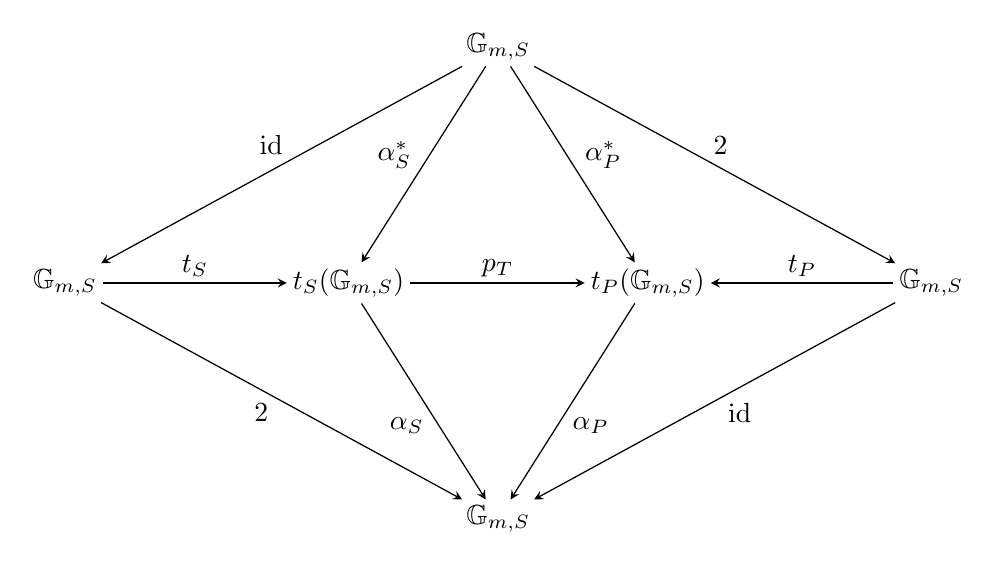
\begin{tikzpicture}[>=stealth,
  every node/.style={inner sep=2pt},
  every path/.style={line width=.45pt}]
  \node (top) at (0,3.0) {$\mathbb G_{m,S}$};
  \node (left) at (-5.5,0) {$\mathbb G_{m,S}$};
  \node (ts) at (-1.9,0) {$t_S(\mathbb G_{m,S})$};
  \node (tp) at (1.9,0) {$t_P(\mathbb G_{m,S})$};
  \node (right) at (5.5,0) {$\mathbb G_{m,S}$};
  \node (bottom) at (0,-3.0) {$\mathbb G_{m,S}$};

  \draw[->] (top) -- node[pos=.48,above left] {$\mathrm{id}$} (left);
  \draw[->] (top) -- node[pos=.55,above left] {$\alpha_S^\ast$} (ts);
  \draw[->] (top) -- node[pos=.55,above right] {$\alpha_P^\ast$} (tp);
  \draw[->] (top) -- node[pos=.48,above right] {$2$} (right);

  \draw[->] (left) -- node[above] {$t_S$} (ts);
  \draw[->] (ts) -- node[above] {$p_T$} (tp);
  \draw[->] (right) -- node[above] {$t_P$} (tp);

  \draw[->] (left) -- node[pos=.48,below left] {$2$} (bottom);
  \draw[->] (ts) -- node[pos=.55,below left] {$\alpha_S$} (bottom);
  \draw[->] (tp) -- node[pos=.55,below right] {$\alpha_P$} (bottom);
  \draw[->] (right) -- node[pos=.48,below right] {$\mathrm{id}$} (bottom);
\end{tikzpicture}
\end{center}
Its central portion is the commutative diagram of \SGARefLink{sga3:xx:4.1}{4.1}
\footnote{With \(q=1\).}
associated with the canonical morphism
\(p\circ i\colon\mathrm{SL}_L\to\mathrm P_L\), which induces a
morphism between the preceding elementary \(S\)-systems.

% Authority: Exp20-13oct24.pdf, section 5.1 through 5.6.

% END INCLUDED SGA3_English_current_buildable_source_20260823/source/inputs/XX/tex/components/13_expose_XX_section5_par51_through_par56_en.tex

% BEGIN INCLUDED SGA3_English_current_buildable_source_20260823/source/inputs/XX/tex/components/14_expose_XX_par57_through_theorem511_en.tex
\paragraph{\textbf{5.7.}}
\SGARefTarget{sga3:xx:5.7}
Let \((G,T,\alpha)\) now be an arbitrary elementary \(S\)-system.
Consider the commutative diagram
\begin{center}
\begin{tikzpicture}[>=stealth,
  every node/.style={inner sep=2pt},
  every path/.style={line width=.45pt}]
  \node (top) at (0,2.9) {$\mathbb G_{m,S}$};
  \node (left) at (-3.7,0) {$\mathbb G_{m,S}$};
  \node (mid) at (0,0) {$T$};
  \node (right) at (3.7,0) {$\mathbb G_{m,S}$};
  \node (bottom) at (0,-2.9) {$\mathbb G_{m,S}$};

  \draw[->] (top) -- node[pos=.48,above left] {$\mathrm{id}$} (left);
  \draw[->] (top) -- node[left] {$\alpha^\ast$} (mid);
  \draw[->] (top) -- node[pos=.48,above right] {$2$} (right);
  \draw[->] (left) -- node[above] {$\alpha^\ast$} (mid);
  \draw[->] (mid) -- node[above] {$\alpha$} (right);
  \draw[->] (left) -- node[pos=.48,below left] {$2$} (bottom);
  \draw[->] (mid) -- node[left] {$\alpha$} (bottom);
  \draw[->] (right) -- node[pos=.48,below right] {$\mathrm{id}$} (bottom);
\end{tikzpicture}
\end{center}
Combining this diagram with that of \SGARefLink{sga3:xx:5.6}{5.6} gives a commutative diagram
\begin{center}
\begin{tikzpicture}[>=stealth,
  every node/.style={inner sep=2pt},
  every path/.style={line width=.45pt}]
  \node (top) at (0,2.9) {$\mathbb G_{m,S}$};
  \node (left) at (-4.8,0) {$t_S(\mathbb G_{m,S})$};
  \node (mid) at (0,0) {$T$};
  \node (right) at (4.8,0) {$t_P(\mathbb G_{m,S})$};
  \node (bottom) at (0,-2.9) {$\mathbb G_{m,S}$};

  \draw[->] (top) -- node[pos=.5,above left] {$\alpha_S^\ast$} (left);
  \draw[->] (top) -- node[left] {$\alpha^\ast$} (mid);
  \draw[->] (top) -- node[pos=.5,above right] {$\alpha_P^\ast$} (right);
  \draw[->] (left) -- node[above] {$\alpha^\ast\circ t_S^{-1}$} (mid);
  \draw[->] (mid) -- node[above] {$t_P\circ\alpha$} (right);
  \draw[->] (left) -- node[pos=.5,below left] {$\alpha_S$} (bottom);
  \draw[->] (mid) -- node[left] {$\alpha$} (bottom);
  \draw[->] (right) -- node[pos=.5,below right] {$\alpha_P$} (bottom);
\end{tikzpicture}
\end{center}
Using \SGARefLink{sga3:xx:4.1}{4.1}, one obtains:

\paragraph{\textbf{Proposition 5.8.}}
\SGARefTarget{sga3:xx:5.8}
\emph{Let \(S\) be a scheme and let \((G,T,\alpha)\) be an
elementary \(S\)-system.  Put \(L=\mathfrak g^\alpha\), so that
\(L^{-1}=\mathfrak g^{-\alpha}\).}

\emph{\textup{(i)} There exists a unique group morphism
\(f\colon\mathrm{SL}_L\to G\) satisfying the following equivalent
conditions:}
\[
\begin{array}{ll}
\textup{(a)}
&
f\begin{pmatrix}z&0\\0&z^{-1}\end{pmatrix}=\alpha^\ast(z),
\qquad
f\begin{pmatrix}1&X\\0&1\end{pmatrix}=\exp(X);
\\[1.1em]
\textup{(b)}
&
f\begin{pmatrix}1&X\\0&1\end{pmatrix}=\exp(X),
\qquad
f\begin{pmatrix}1&0\\Y&1\end{pmatrix}=\exp(Y);
\\[1.1em]
\textup{(c)}
&
f\begin{pmatrix}1&X\\0&1\end{pmatrix}=\exp(X),
\qquad
f\begin{pmatrix}0&X\\-X^{-1}&0\end{pmatrix}=w_\alpha(X).
\end{array}
\]

\emph{\textup{(ii)} There exists a unique group morphism
\(g\colon G\to\mathrm P_L\) satisfying}
\[
 g(t)=
 \begin{pmatrix}\alpha(t)&0\\0&1\end{pmatrix},
 \qquad
 g(\exp(X))
 =p\begin{pmatrix}1&X\\0&1\end{pmatrix}.
\]
\emph{Moreover,}
\[
 g(\exp(Y))
 =p\begin{pmatrix}1&0\\Y&1\end{pmatrix},
 \qquad
 g(w_\alpha(X))
 =p\begin{pmatrix}0&X\\-X^{-1}&0\end{pmatrix}.
\]
\emph{The morphism \(g\) is faithfully flat and quasi-compact, with}
\[
 \Ker(g)=\Ker(\alpha)=\operatorname{Centr}(G),
\]
\emph{and \(g\circ f\) is the canonical morphism
\(\mathrm{SL}_L\to\mathrm P_L\).}

Notice that condition \textup{(b)} in \textup{(i)} gives an explicit
description of the duality between
\(\mathfrak g^\alpha\) and \(\mathfrak g^{-\alpha}\).

\paragraph{\textbf{Corollary 5.9.}}
\SGARefTarget{sga3:xx:5.9}
\emph{Let \((G,T,\alpha)\) be an elementary \(S\)-system.  The
subgroups}
\[
 T\cdot U_\alpha,\qquad T\cdot U_{-\alpha},
 \qquad U_\alpha,\qquad U_{-\alpha}
\]
\emph{are closed.}

Since \(U_\alpha\) is a closed subgroup scheme of
\(T\cdot U_\alpha\), it suffices to prove the assertion for the
latter.  By Noether's theorem \textup{(\SGARefLink{sga3:iv:proposition:5:3:1}{Exposé IV, 5.3.1} and \SGARefLink{sga3:iv:lemma:6:4:1}{6.4.1})},
it is enough to show that
\[
 (T\cdot U_\alpha)/\Ker(\alpha)
\]
is a closed subgroup of \(G/\Ker(\alpha)\).  By \SGARefLink{sga3:xx:5.8}{5.8}, this reduces to
the evident fact that the subgroup of \(\mathrm P_L\) defined by
\(c=0\) is closed; one may equivalently work in \(\mathrm{GL}_L\),
by another application of Noether's theorem.  Consequently, the
exponential morphisms of \SGARefLink{sga3:xx:1.5}{Theorem 1.5}\textup{(i)} are closed
immersions.

\smallskip
\noindent\textbf{N.B.}\ The corollary also follows from the fact that
\(T\cdot U_\alpha\) and \(T\cdot U_{-\alpha}\) are ``Borel
subgroups'' of \(G\) \textup{(cf.\ \SGARefLink{sga3:xii:7.10}{Exposé XII, 7.10})}.

\paragraph{\textbf{5.10.}}
\SGARefTarget{sga3:xx:5.10}
Let \(L\) be an invertible \(\mathcal O_S\)-module, and let
\[
 \mathbb G_{m,S}\xrightarrow{\ \alpha^\ast\ }T
 \xrightarrow{\ \alpha\ }\mathbb G_{m,S}
\]
be a diagram of groups, where \(T\) is a torus,\footnote{This
qualification is supplied by the editors.} such that
\(\alpha\circ\alpha^\ast=2\).  Let \(R\) be the maximal torus of
\(\Ker(\alpha)\), and put \(K=\alpha^{\ast-1}(R)\).  Then \(K\) is a
subgroup of multiplicative type of \(\mathbb G_{m,S}\); since
\(\alpha\circ\alpha^\ast=2\), it is even a subgroup of
\(\mu_{2,S}\).  In particular,
\[
 K\longrightarrow\mathrm{SL}_L,
 \qquad
 z\longmapsto\begin{pmatrix}z&0\\0&z^{-1}\end{pmatrix}
\]
is central.  Hence there is a central group monomorphism
\[
 K\longrightarrow R\times\mathrm{SL}_L,
 \qquad
 z\longmapsto
 \left(
 \alpha^\ast(z),
 \begin{pmatrix}z&0\\0&z^{-1}\end{pmatrix}
 \right).
\]

Let
\[
 G=(R\times\mathrm{SL}_L)/K.
\]
This is an affine smooth group over \(S\), with connected fibers.
The sequence
\[
 1\longrightarrow K\longrightarrow
 R\times t_S(\mathbb G_{m,S})
 \xrightarrow{\ u\ }T\longrightarrow1,
 \qquad
 u(x,t_S(z))=x\alpha^\ast(z),
\]
is exact.  The image of \(R\times t_S(\mathbb G_{m,S})\) in \(G\)
is therefore a torus \(T'\) isomorphic to \(T\).  If \(\alpha'\) is
the character of \(T'\) transported from \(\alpha\), one readily
checks that \((G,T',\alpha')\) is an elementary \(S\)-system, that
\(\mathfrak g^{\alpha'}\) is isomorphic to \(L\), and that
\(\alpha'^\ast\) is obtained from \(\alpha^\ast\) under the
isomorphism \(T\xrightarrow{\sim}T'\).  Thus the object
\[
 \left(
 \mathbb G_{m,S}\xrightarrow{\ \alpha'^\ast\ }T'
 \xrightarrow{\ \alpha'\ }\mathbb G_{m,S},\,
 \mathfrak g^{\alpha'}
 \right)
\]
of the category \(\mathcal D\) defined in \SGARefLink{sga3:xx:4.2}{4.2} is isomorphic to
\[
 \left(
 \mathbb G_{m,S}\xrightarrow{\ \alpha^\ast\ }T
 \xrightarrow{\ \alpha\ }\mathbb G_{m,S},\,L
 \right).
 \]
We have therefore proved:

\paragraph{\textbf{Theorem 5.11.}}
\SGARefTarget{sga3:xx:5.11}
\emph{With the notation of \SGARefLink{sga3:xx:4.2}{4.2}, the functor}
\[
 (G,T,\alpha)\longmapsto
 \left(
 \mathbb G_{m,S}\xrightarrow{\ \alpha^\ast\ }T
 \xrightarrow{\ \alpha\ }\mathbb G_{m,S},\,
 \mathfrak g^\alpha
 \right)
\]
\emph{is an equivalence of categories between
\(\mathcal E\) and \(\mathcal D\).}

% Authority: Exp20-13oct24.pdf, section 5.7 through theorem 5.11.

% END INCLUDED SGA3_English_current_buildable_source_20260823/source/inputs/XX/tex/components/14_expose_XX_par57_through_theorem511_en.tex

% BEGIN INCLUDED SGA3_English_current_buildable_source_20260823/source/inputs/XX/tex/components/15_expose_XX_section6_through_lemma621_en.tex
\section{Generators and Relations for an Elementary System}

\paragraph{\textbf{6.1.}}
\SGARefTarget{sga3:xx:6.1}
Let \(S\) be a scheme and let \((G,T,\alpha)\) be an elementary
\(S\)-system.  Let
\[
 X\in W(\mathfrak g^\alpha)^\times(S),
 \qquad u=\exp(X).
\]
As observed in \SGARefLink{sga3:xx:3.8}{3.8}, the element \(w=w_\alpha(X)\) satisfies, in
particular,
\[
 (wu)^3=e.
\]
\footnote{The editors added the sentence that follows.}
Let \(s_\alpha\) denote the automorphism of \(T\) induced by
\(\intaut(w)\).  By \SGARefLink{sga3:xx:3.1}{Theorem 3.1}\textup{\SGARefLink{sga3:xx:3.1:item:iii}{(iii)}}, for every \(S'\to S\)
and every \(t\in T(S')\),
\[
 s_\alpha(t)=\intaut(w)(t)
 =t\,\alpha^\ast\bigl(\alpha(t)^{-1}\bigr).
\]

\paragraph{\textbf{Theorem 6.2.}}
\SGARefTarget{sga3:xx:6.2}
\emph{Let \(H\) be a sheaf of groups over \(S\) for the fppf
topology.  Let}
\[
 f_T\colon T\longrightarrow H,
 \qquad
 f_\alpha\colon U_\alpha\longrightarrow H
\]
\emph{be group morphisms, and let \(h\in H(S)\).  There exists a
\textup{(necessarily unique)} group morphism}
\[
 f\colon G\longrightarrow H
\]
\emph{extending \(f_T\) and \(f_\alpha\) and satisfying \(f(w)=h\)
if and only if the following conditions hold:}

\emph{\textup{(i)} For every \(S'\to S\),
\(t\in T(S')\), and \(x\in U_\alpha(S')\),}
\begin{equation}
\tag{1}\label{sga3:xx:theorem:6-2:equation:1}
 f_T(t)f_\alpha(x)f_T(t)^{-1}
 =f_\alpha(txt^{-1})
 =f_\alpha\bigl(x^{\alpha(t)}\bigr).
\end{equation}
\emph{Equivalently, \(f_T\) and \(f_\alpha\) extend to a group
morphism \(T\cdot U_\alpha\to H\).}

\emph{\textup{(ii)} For every \(S'\to S\) and \(t\in T(S')\),}
\begin{equation}
\tag{2}\label{sga3:xx:theorem:6-2:equation:2}
 h f_T(t)h^{-1}
 =f_T(s_\alpha(t))
 =f_T\!\left(t\,\alpha^\ast(\alpha(t)^{-1})\right).
\end{equation}

\emph{\textup{(iii)} The following two relations hold in \(H(S)\):}
\begin{equation}
\tag{3}\label{sga3:xx:theorem:6-2:equation:3}
 h^2=f_T\bigl(\alpha^\ast(-1)\bigr),
\end{equation}
\begin{equation}
\tag{4}\label{sga3:xx:theorem:6-2:equation:4}
 \bigl(hf_\alpha(u)\bigr)^3=e.
\end{equation}

\smallskip
\noindent\emph{Proof.}
Write the laws on \(U_\alpha\) and \(U_{-\alpha}\) additively, while
writing their vector-space structures multiplicatively.  If \(f\)
has the asserted properties, then for
\(y\in U_{-\alpha}(S')\) one necessarily has
\[
 f(y)
 =f(w^{-1}wyw^{-1}w)
 =h f_\alpha(w^{-1}yw)h^{-1}.
\]
Define a morphism \(f_{-\alpha}\colon U_{-\alpha}\to H\) by
\begin{equation}
\tag{\(\ast_1\)}\label{sga3:xx:theorem:6-2:equation:ast-1}
 f_{-\alpha}(y)=h f_\alpha(w^{-1}yw)h^{-1}.
\end{equation}
It is a group morphism.  On the big cell \(\Omega\), the morphism
\(f\) is forced to satisfy
\[
 f(ytx)=f_{-\alpha}(y)f_T(t)f_\alpha(x).
\]
This proves uniqueness.  The conditions in the statement are
manifestly necessary; let us prove that they are sufficient.

Relation \textup{\SGARefLink{sga3:xx:theorem:6-2:equation:4}{(4)}} gives
\[
 h f_\alpha(u)h^{-1}h^2
 =
 f_\alpha(-u)h^{-1}f_\alpha(-u).
\]
By \textup{\SGARefLink{sga3:xx:theorem:6-2:equation:3}{(3)}} and \textup{\SGARefLink{sga3:xx:theorem:6-2:equation:1}{(1)}},
\(h^2=f_T(\alpha^\ast(-1))\) commutes with \(f_\alpha(-u)\), and
hence
\[
 h f_\alpha(u)h^{-1}
 =
 f_\alpha(-u)h f_\alpha(-u).
\]
By definition,
\[
 h f_\alpha(u)h^{-1}=f_{-\alpha}(wuw^{-1}),
\]
whereas \SGARefLink{sga3:xx:3.7}{3.7} gives
\begin{equation}
\tag{\(\ast_2\)}\label{sga3:xx:theorem:6-2:equation:ast-2}
 wuw^{-1}=-\widetilde u,
\end{equation}
with \(\widetilde u\) the element paired with \(u\).  Therefore
\begin{equation}
\tag{\(\ast_3\)}\label{sga3:xx:theorem:6-2:equation:ast-3}
 f_{-\alpha}(-\widetilde u)
 =
 f_\alpha(-u)h f_\alpha(-u).
\end{equation}

Let \(t\) be a section of \(T\) over a variable \(S'\to S\).
Apply \(\intaut(f_T(t))\) to this identity.  On the left one
obtains\footnote{The editors corrected the calculation that follows.}
\[
\begin{aligned}
 f_T(t)f_{-\alpha}(-\widetilde u)f_T(t)^{-1}
 &=
 f_T(t)h f_\alpha(u)h^{-1}f_T(t)^{-1}\\
 &=
 h\bigl(h^{-1}f_T(t)h\bigr)f_\alpha(u)
   \bigl(h^{-1}f_T(t)^{-1}h\bigr)h^{-1}\\
 &=
 h f_T(s_\alpha(t))f_\alpha(u)
   f_T(s_\alpha(t))^{-1}h^{-1}\\
 &=
 h f_\alpha\bigl(\alpha(s_\alpha(t))u\bigr)h^{-1}\\
 &=
 h f_\alpha\bigl(\alpha(t)^{-1}u\bigr)h^{-1}\\
 &=
 f_{-\alpha}\bigl(-\alpha(t)^{-1}\widetilde u\bigr).
\end{aligned}
\]
Here we used \textup{\SGARefLink{sga3:xx:theorem:6-2:equation:2}{(2)}}, \textup{\SGARefLink{sga3:xx:theorem:6-2:equation:1}{(1)}},
\(s_\alpha(t)=t\alpha^\ast(\alpha(t)^{-1})\), and
\(\alpha\circ\alpha^\ast=2\).

The right-hand side of \((\ast_3)\), after conjugation, becomes
\[
 f_\alpha(-\alpha(t)u)\,
 f_T(t)h f_T(t)^{-1}h^{-1}\,
 h f_\alpha(-\alpha(t)u).
\]
Since
\[
 h f_T(t)^{-1}h^{-1}
 =f_T(s_\alpha(t^{-1}))
  =f_T\bigl(t^{-1}\,\alpha^\ast(\alpha(t))\bigr),
\]
this equals
\[
 f_\alpha(-\alpha(t)u)\,
 f_T\bigl(\alpha^\ast(\alpha(t))\bigr)\,
 h f_\alpha(-\alpha(t)u).
\]
Comparison gives
\[
 f_{-\alpha}\bigl(-\alpha(t)^{-1}\widetilde u\bigr)
 =
 f_\alpha(-\alpha(t)u)\,
 f_T\bigl(\alpha^\ast(\alpha(t))\bigr)\,
 h f_\alpha(-\alpha(t)u).
\]
Since \(\alpha\colon T\to\mathbb G_{m,S}\) is faithfully flat and
\(H\) is a separated presheaf, \(-\alpha(t)^{-1}\) may be replaced
by an arbitrary section of \(\mathbb G_{m,S}\).  Thus:

\paragraph{\textbf{Lemma 6.2.1.}}
\SGARefTarget{sga3:xx:6.2.1}
\emph{For every \(S'\to S\) and every
\(z\in\mathbb G_m(S')\),}
\[
 f_{-\alpha}(z\widetilde u)
 =
 f_\alpha(z^{-1}u)\,
 f_T\bigl(\alpha^\ast(-z^{-1})\bigr)\,
 h f_\alpha(z^{-1}u).
\]

% Authority: Exp20-13oct24.pdf, section 6 through lemma 6.2.1.

% END INCLUDED SGA3_English_current_buildable_source_20260823/source/inputs/XX/tex/components/15_expose_XX_section6_through_lemma621_en.tex

% BEGIN INCLUDED SGA3_English_current_buildable_source_20260823/source/inputs/XX/tex/components/16_expose_XX_lemma622_through_end_en.tex
Let \(x,y\in\mathbb G_a(S')\), where \(S'\to S\), and suppose that
\(y\) and \(1+xy\) are invertible.  Applying \SGARefLink{sga3:xx:6.2.1}{Lemma 6.2.1} first with
\(z=y\), one obtains\footnote{The editors expanded the calculations
that follow.}
\[
 f_\alpha(xu)f_{-\alpha}(y\widetilde u)
 =
 f_\alpha\bigl((x+y^{-1})u\bigr)\,
 f_T\bigl(\alpha^\ast(-y^{-1})\bigr)\,
 h f_\alpha(y^{-1}u).
\]
Now \(x+y^{-1}=y^{-1}(1+xy)\).  Applying the lemma with
\(z=y/(1+xy)\) gives
\[
\begin{aligned}
 f_\alpha\bigl((x+y^{-1})u\bigr)
 &=
 f_{-\alpha}\!\left(\frac{y}{1+xy}\widetilde u\right)
 f_\alpha\bigl(-(x+y^{-1})u\bigr)\\
 &\qquad{}\cdot h\,
 f_T\!\left(\alpha^\ast\!\left(-\frac{y}{1+xy}\right)\right).
\end{aligned}
\]
Substitution in the preceding identity yields
\[
\begin{aligned}
 f_\alpha(xu)f_{-\alpha}(y\widetilde u)
 &=
 f_{-\alpha}\!\left(\frac{y}{1+xy}\widetilde u\right)
 f_\alpha\bigl(-(x+y^{-1})u\bigr)h^{-1}\\
 &\qquad{}\cdot
 f_T\bigl(\alpha^\ast(1+xy)^{-1}\bigr)
 h f_\alpha(y^{-1}u).
\end{aligned}
\]
Since \(h^{-1}f_T(t)h=f_T(s_\alpha(t))\) by \textup{(2)}
\textup{(recall that \(s_\alpha^2=\operatorname{id}\))}, and
\(s_\alpha\circ\alpha^\ast=-\alpha^\ast\), this is
\[
\begin{aligned}
 f_{-\alpha}\!\left(\frac{y}{1+xy}\widetilde u\right)
 f_\alpha\bigl(-(x+y^{-1})u\bigr)
 f_T\bigl(\alpha^\ast(1+xy)\bigr)
 f_\alpha(y^{-1}u).
\end{aligned}
\]
For \(x'\in U_\alpha(S')\) and
\(z\in\mathbb G_m(S')\), one has
\[
 f_\alpha(x')f_T(\alpha^\ast(z))
 =
 f_T(\alpha^\ast(z))f_\alpha(z^{-2}x').
\]
Consequently,
\[
\begin{aligned}
 f_\alpha(xu)f_{-\alpha}(y\widetilde u)
 &=
 f_{-\alpha}\!\left(\frac{y}{1+xy}\widetilde u\right)
 f_T\bigl(\alpha^\ast(1+xy)\bigr)\\
 &\qquad{}\cdot
 f_\alpha\!\left(
 \left[
 -\frac{y^{-1}(1+xy)}{(1+xy)^2}+y^{-1}
 \right]u
 \right)\\
 &=
 f_{-\alpha}\!\left(\frac{y}{1+xy}\widetilde u\right)
 f_T\bigl(\alpha^\ast(1+xy)\bigr)
 f_\alpha\!\left(\frac{x}{1+xy}u\right).
\end{aligned}
\]
We have proved:

\paragraph{\textbf{Lemma 6.2.2.}}
\SGARefTarget{sga3:xx:6.2.2}
\emph{Let \(S'\to S\).  If
\(a\in U_\alpha(S')\), \(b\in U_{-\alpha}^\times(S')\), and
\(1+ab\in\mathbb G_m(S')\), then}
\[
 f_\alpha(a)f_{-\alpha}(b)
 =
 f_{-\alpha}\!\left(\frac{b}{1+ab}\right)
 f_T\bigl(\alpha^\ast(1+ab)\bigr)
 f_\alpha\!\left(\frac{a}{1+ab}\right).
\]

By schematic density, this formula remains valid for
\(b\in U_{-\alpha}(S')\), with \(1+ab\) invertible.  Define
\[
 f\colon\Omega\longrightarrow H,
 \qquad
 f(ytx)=f_{-\alpha}(y)f_T(t)f_\alpha(x).
\]
It follows at once from \SGARefLink{sga3:xx:6.2.2}{Lemma 6.2.2}, condition \SGARefLink{sga3:xx:6.2}{6.2}\textup{(i)}, and
formula \textup{(F')} of \SGARefLink{sga3:xx:2.4}{2.4} that whenever
\(g,g'\in\Omega(S')\) and \(gg'\in\Omega(S')\), one has
\[
 f(gg')=f(g)f(g').
\]
By \SGARefLink{sga3:xviii:prop:2.3}{Exposé XVIII, 2.3}\textup{\SGARefLink{sga3:xviii:prop:2.3:item:iii}{(iii)}} and \SGARefLink{sga3:xx:2.4}{2.4},\footnote{Each geometric
fiber of \(G\) is connected, for example by \SGARefLink{sga3:xx:section:1}{1.1}.} there is therefore
a group morphism \(G\to H\) extending \(f\).  Denote it again by
\(f\).  It remains only to prove that \(f(w_\alpha)=h\).  Since
\[
 w_\alpha=u\cdot(-\widetilde u)\cdot u,
\]
formula \((\ast_3)\) gives\footnote{The editors simplified the
original argument by invoking \((\ast_3)\).}
\[
 f(w_\alpha)
 =f_\alpha(u)f_{-\alpha}(-\widetilde u)f_\alpha(u)
 =h.
\]
This completes the proof of \SGARefLink{sga3:xx:6.2}{Theorem 6.2}.

\paragraph{\textbf{Remark 6.3.}}
\SGARefTarget{sga3:xx:6.3}
\emph{These results will be completed in \SGARefLink{sga3:xxiii:subsection:3-5}{Exposé XXIII, 3.5}.}

% Authority: Exp20-13oct24.pdf, lemma 6.2.2 through the end of Exposé XX.

% END INCLUDED SGA3_English_current_buildable_source_20260823/source/inputs/XX/tex/components/16_expose_XX_lemma622_through_end_en.tex



% END INCLUDED SGA3_English_current_buildable_source_20260823/source/inputs/XX/body.tex


\SGAStartExpose{XXI}
\counterwithin{theorem}{subsection}
\renewcommand{\thesubsection}{\thesection.\arabic{subsection}}
% BEGIN INCLUDED SGA3_English_current_buildable_source_20260823/source/inputs/XXI/body.tex
% Mechanically extracted after \mainmatter from the frozen standalone master.

\markboth{Exposé XXI. Root Data}{Exposé XXI. Root Data}
% BEGIN INCLUDED SGA3_English_current_buildable_source_20260823/source/inputs/XXI/tex/components/00_expose_XXI_opening_through_scholium1113_en.tex
\chapter*{Exposé XXI. Root Data}
\addcontentsline{toc}{chapter}{Exposé XXI. Root Data}

\noindent
This Exposé\footnote{Editors' note: Version of 13 October 2024.}
collects, in the absence of a suitable reference,\footnote{%
Editors' note: For results on root systems (Sections 1--5), one may
consult \emph{Groupes et algèbres de Lie}, Chapter VI.}
known results on root data (that is, ``abstract'' root systems), most of
which will be used below.

\medskip
\noindent\textbf{Notation.}
We denote by \(\Qp\) the set of positive (or zero) rational numbers;
\(\mathbb Z\cap\Qp=\mathbb N\). Let \(V\) be a \(\mathbb Q\)-vector
space. If \(A\) (respectively \(B\)) is a subset of \(\mathbb Q\)
(respectively of \(V\)), we denote by \(A\cdot B\) the image of
\(A\otimes B\) under the morphism
\(\mathbb Q\otimes V\to V\), in other words the set of linear
combinations of elements of \(B\) with coefficients in \(A\). We write
\(-B=\{-1\}B\). We denote by \(E-F\) the set of elements of \(E\)
that do not belong to \(F\).

\section{Generalities}

\SGAInlineRefTarget{sga3:xxi:subsection:1-1}
\subsection{Definitions and first properties}

\begin{definition}\label{sga3:XXI:1.1.1}
Let \(M\) and \(M^\ast\) be two free finite-type \(\mathbb Z\)-modules
in duality. Write
\[
  V=M\otimes\mathbb Q,\qquad V^\ast=M^\ast\otimes\mathbb Q;
\]
these are two \(\mathbb Q\)-vector spaces in duality. We identify \(M\)
(respectively \(M^\ast\)) with a subset of \(V\) (respectively
\(V^\ast\)). The canonical bilinear form on
\(M^\ast\times M\) (respectively \(V^\ast\times V\)) is denoted
\((\, ,\,)\).

Let \(R\) be a finite subset of \(M\). Suppose given a map
\(\alpha\mapsto\alpha^\ast\) from \(R\) to \(M^\ast\); the set of
\(\alpha^\ast\), for \(\alpha\in R\), is denoted \(R^\ast\).
To every \(\alpha\in R\) associate the endomorphism \(s_\alpha\)
(respectively \(s_\alpha^\ast\)) of \(M\) and \(V\) (respectively of
\(M^\ast\) and \(V^\ast\)) given by
\begin{align}
 s_\alpha(x)&=x-(\alpha^\ast,x)\alpha,
 &s_\alpha&=\operatorname{id}-\alpha^\ast\otimes\alpha,
 \tag{1}\label{sga3:XXI:eq:1}\\
 s_\alpha^\ast(u)&=u-(u,\alpha)\alpha^\ast,
 &s_\alpha^\ast&=\operatorname{id}-\alpha\otimes\alpha^\ast.
 \tag{1${}^\ast$}\label{sga3:XXI:eq:1star}
\end{align}
The pair \((R,R^\ast)\) (more precisely, the pair
\((R,R\to M^\ast)\)) is called a \emph{root datum} in
\((M,M^\ast)\), and \((M,M^\ast,R,R^\ast)\) is called a root datum,
if the following axioms hold:
\begin{align*}
 (\mathrm{DR\,I})\quad&
    (\alpha^\ast,\alpha)=2
    &&\text{for every }\alpha\in R,\\
 (\mathrm{DR\,II})\quad&
    s_\alpha(R)\subset R,\qquad
    s_\alpha^\ast(R^\ast)\subset R^\ast
    &&\text{for every }\alpha\in R.
\end{align*}
The set \(R\) is called the \emph{root system} of the root datum
\(\cR=(M,M^\ast,R,R^\ast)\). The elements of \(R\) (respectively
\(R^\ast\)) are called the \emph{roots} (respectively
\emph{coroots}) of the root datum.
\end{definition}

\begin{remark}\label{sga3:XXI:1.1.2}
Axiom \((\mathrm{DR\,I})\) is equivalent to any one of the following
properties:
\begin{align}
 s_\alpha s_\alpha&=\operatorname{id},
 &s_\alpha^\ast s_\alpha^\ast&=\operatorname{id},
 \tag{2,2${}^\ast$}\label{sga3:XXI:eq:2}\\
 s_\alpha(\alpha)&=-\alpha,
 &s_\alpha^\ast(\alpha^\ast)&=-\alpha^\ast.
 \tag{3,3${}^\ast$}\label{sga3:XXI:eq:3}
\end{align}
\end{remark}

\begin{remark}\label{sga3:XXI:1.1.3}
Axioms \((\mathrm{DR\,I})\) and \((\mathrm{DR\,II})\) imply
\[
 R=-R,\qquad R^\ast=-R^\ast,\qquad
 0\notin R,\qquad 0\notin R^\ast.
\]
\end{remark}

\begin{lemma}\label{sga3:XXI:1.1.4}
The map \(R\to R^\ast\) is a bijection. More generally, if
\(\alpha,\beta\in R\) and
\((\alpha^\ast,x)=(\beta^\ast,x)\) for every \(x\in R\), then
\(\alpha=\beta\).
\end{lemma}

\begin{proof}
Indeed, one then has
\[
 s_\beta(\alpha)=\alpha-2\beta,\qquad
 s_\alpha(\beta)=\beta-2\alpha.
\]
It follows at once that
\[
 s_\beta s_\alpha(\alpha)
   =2\beta-\alpha=\alpha+2(\beta-\alpha),\qquad
 s_\beta s_\alpha(\beta-\alpha)
   =s_\beta(\beta-\alpha)=\beta-\alpha.
\]
Hence, by \((\mathrm{DR\,II})\),
\[
 (s_\beta s_\alpha)^n(\alpha)
   =\alpha+2n(\beta-\alpha)\in R.
\]
Since \(R\) is finite, \(\beta-\alpha=0\).
\end{proof}

\begin{corollary}\label{sga3:XXI:1.1.5}
The inverse map \(R^\ast\to R\) defines a root datum
\[
 \cR^\ast=(M^\ast,M,R^\ast,R),
\]
called the \emph{dual} of \(\cR\).\footnote{Editors' note:
\((\alpha^\ast)^\ast=\alpha\).}
\end{corollary}

\begin{definition}\label{sga3:XXI:1.1.6}
We denote by \(\Gamma_0(R)\) the subgroup of \(M\) generated by \(R\).
We denote by \(\VR(R)\) the vector subspace of \(V\) generated by \(R\),
that is,
\[
 \VR(R)=\Gamma_0(R)\otimes\mathbb Q.
\]
Applying these definitions to \(\cR^\ast\), one likewise obtains
\(\Gamma_0(R^\ast)\) and \(\VR(R^\ast)\).

The \emph{reductive rank} of \(\cR\) is the number
\[
 \rgred(\cR)
 =\rank(M)=\dim(V)=\dim(V^\ast)=\rank(M^\ast)=\rgred(\cR^\ast).
\]
The \emph{semisimple rank} of \(\cR\) is the number
\[
 \rgss(\cR)
 =\rank(R)=\rank(\Gamma_0(R))=\dim(\VR(R)).
\]
Thus \(\rgss(\cR)\leq\rgred(\cR)\).

We shall see below that
\(\rgss(\cR)=\rgss(\cR^\ast)\), that is, that \(\VR(R)\) and
\(\VR(R^\ast)\) have the same dimension.
\end{definition}

\begin{definition}\label{sga3:XXI:1.1.7}\leavevmode\par
The root datum \(\cR\) is called \emph{semisimple} (respectively
\emph{trivial}) if
\(\rgss(\cR)=\rgred(\cR)\) (respectively \(\rgss(\cR)=0\)).
Thus \(\cR\) is trivial if and only if \(R\) is empty. The trivial root
datum of reductive rank zero is denoted
\[
 0=(\{0\},\{0\},\varnothing,\varnothing).
\]
\end{definition}

\begin{definition}\label{sga3:XXI:1.1.8}
We denote by \(W(\cR)\) the group of transformations of \(M\) generated
by the \(s_\alpha\), \(\alpha\in R\). It is called the \emph{Weyl
group} of \(\cR\). We write
\[
 W^\ast(\cR)=W(\cR^\ast).
\]
Then \(W(\cR)\) acts on \(R\), \(\Gamma_0(R)\), \(\VR(R)\), \(M\),
and \(V\). If \(w\in W(\cR)\) and \(x\in M\) (respectively
\(x\in V\)), then
\[
 wx-x\in\Gamma_0(R)
 \quad\text{(respectively }wx-x\in\VR(R)\text{)};
\]
this follows immediately from formula \eqref{sga3:XXI:eq:1}.
Likewise for \(W^\ast(\cR)\).
\end{definition}

\begin{lemma}\label{sga3:XXI:1.1.9}
For every \(\alpha\in R\), \(x\in V\), and \(u\in V^\ast\), one has
\begin{equation}
 (s_\alpha^\ast(u),s_\alpha(x))=(u,x).
 \tag{4}\label{sga3:XXI:eq:4}
\end{equation}
\end{lemma}

\begin{proof}
Taking the scalar product of \eqref{sga3:XXI:eq:1} and
\eqref{sga3:XXI:eq:1star}, the left-hand side is
\[
 (u,x)+(u,\alpha)(\alpha^\ast,x)
       \bigl((\alpha^\ast,\alpha)-2\bigr)=(u,x).
\]
\end{proof}

\begin{remark}\label{sga3:XXI:1.1.10}
If one assumes \(0\notin R\) and \(0\notin R^\ast\), then
Lemma~\ref{sga3:XXI:1.1.9} is equivalent to
\((\mathrm{DR\,I})\).
\end{remark}

\begin{corollary}\label{sga3:XXI:1.1.11}
Let \(h\mapsto h^\vee\) denote the isomorphism from
\(\GL(M)\) onto \(\GL(M^\ast)\) that associates to \(h\) its
contragredient. Formula \eqref{sga3:XXI:eq:4} may then also be written
\begin{equation}
 (s_\alpha)^\vee=s_\alpha^\ast.
 \tag{5}\label{sga3:XXI:eq:5}
\end{equation}
\end{corollary}

\begin{corollary}\label{sga3:XXI:1.1.12}
The preceding isomorphism induces an isomorphism from \(W(\cR)\) onto
\(W^\ast(\cR)\).
\end{corollary}

\begin{scholium}\label{sga3:XXI:1.1.13}
By the preceding result, we shall identify \(W\) and \(W^\ast\), and
regard \(W\) as a group of transformations of
\[
 R,\ R^\ast,\ M,\ M^\ast,\ \Gamma_0(R),\ \Gamma_0(R^\ast),\
 V,\ V^\ast,\ \VR(R),\ \VR(R^\ast).
\]
We shall write \(s_\alpha\) for \(s_\alpha^\ast\).
\end{scholium}

% END INCLUDED SGA3_English_current_buildable_source_20260823/source/inputs/XXI/tex/components/00_expose_XXI_opening_through_scholium1113_en.tex

% BEGIN INCLUDED SGA3_English_current_buildable_source_20260823/source/inputs/XXI/tex/components/01_expose_XXI_section12_through_application212_en.tex
\subsection{The map \texorpdfstring{\(p\)}{p}}

\begin{lemma}\label{sga3:XXI:1.2.1}
Let \(p:M\to M^\ast\) (respectively \(V\to V^\ast\)) be the linear map
defined by
\begin{equation}
 p(x)=\sum_{u\in R^\ast}(u,x)u.
 \tag{6}\label{sga3:XXI:eq:6}
\end{equation}
Write \(\ell(x)=(p(x),x)\). Then:
\begin{align}
 \ell(x)&\geq0,\qquad \ell(\alpha)>0
     &&\text{for }\alpha\in R,
 \tag{7}\label{sga3:XXI:eq:7}\\
 \ell(wx)&=\ell(x)
     &&\text{for }w\in W,
 \tag{8}\label{sga3:XXI:eq:8}\\
 (p(x),y)&=(p(y),x)
     &&\text{for }x,y\in V,
 \tag{9}\label{sga3:XXI:eq:9}\\
 \ell(\alpha)\alpha^\ast&=2p(\alpha)
     &&\text{for }\alpha\in R.
 \tag{10}\label{sga3:XXI:eq:10}
\end{align}
\end{lemma}

\begin{proof}
The first three relations are immediate.\footnote{Editors' note:
Formula \eqref{sga3:XXI:eq:8} follows from
\eqref{sga3:XXI:eq:4}, \eqref{sga3:XXI:eq:2}, and
\((\mathrm{DR\,II})\).}
We prove the last one. By \eqref{sga3:XXI:eq:1}, for \(u\in V^\ast\),
\begin{align*}
 (u,\alpha)^2\alpha^\ast
  &=(u,\alpha)u-(u,\alpha)s_\alpha(u)\\
  &=(u,\alpha)u+(u,s_\alpha(\alpha))s_\alpha(u)\\
  &=(u,\alpha)u+(s_\alpha(u),\alpha)s_\alpha(u)
       \qquad\bigl(s_\alpha^2=\operatorname{id}\bigr).
\end{align*}
Since \(s_\alpha\) permutes \(R^\ast\) by
\((\mathrm{DR\,II})\), summing over \(u\in R^\ast\) gives the result.
\end{proof}

\begin{scholium}\label{sga3:XXI:1.2.2}
Relation \eqref{sga3:XXI:eq:10} says that the map
\(\alpha\mapsto\ell(\alpha)\alpha^\ast\) is the restriction to \(R\)
of a linear map from \(M\) to \(M^\ast\). In particular,
\[
 (-\alpha)^\ast=-\alpha^\ast.
\]
\end{scholium}

\begin{corollary}\label{sga3:XXI:1.2.3}
The map \(p\) induces an isomorphism from \(\VR(R)\) onto
\(\VR(R^\ast)\).
\end{corollary}

\begin{proof}
The map \(p\) sends \(\VR(R)\) onto \(\VR(R^\ast)\). Hence
\[
 \dim\VR(R)\geq\dim\VR(R^\ast).
\]
Applying this inequality to the dual root datum gives
\[
 \dim\VR(R)=\dim\VR(R^\ast),
\]
so the surjective map \(p\) is also bijective.
\end{proof}

\begin{corollary}\label{sga3:XXI:1.2.4}
One has \(\dim\VR(R)=\dim\VR(R^\ast)\), and therefore
\[
 \rgss(\cR)=\rgss(\cR^\ast).
\]
\end{corollary}

\begin{corollary}\label{sga3:XXI:1.2.5}
The bilinear form \((u,x)\) is nondegenerate on
\(\VR(R^\ast)\times\VR(R)\), and thus puts these
\(\mathbb Q\)-vector spaces in duality.
\end{corollary}

\begin{proof}
If \((u,x)=0\) for every \(u\in R^\ast\), then \(p(x)=0\).
\end{proof}

\begin{corollary}\label{sga3:XXI:1.2.6}
The symmetric bilinear form \((p(x),y)\) is positive and nondegenerate
on \(\VR(R)\).
\end{corollary}

\begin{corollary}\label{sga3:XXI:1.2.7}
The group \(W\) acts faithfully on \(R\) (and hence on the other sets
listed in Scholium~\ref{sga3:XXI:1.1.13}).
\end{corollary}

\begin{proof}
Let \(u\in V^\ast\), and suppose \(w\in W\) satisfies
\(w(\alpha)=\alpha\) for every \(\alpha\in R\). We prove \(w(u)=u\).
For every \(\alpha\in R\),
\[
 (w(u)-u,\alpha)
 =(w(u),\alpha)-(u,\alpha)
 =(u,w^{-1}(\alpha))-(u,\alpha)=0.
\]
But \(w(u)-u\in\VR(R^\ast)\). Since it is orthogonal to every root, it
vanishes by Corollary~\ref{sga3:XXI:1.2.5}.
\end{proof}

\begin{corollary}\label{sga3:XXI:1.2.8}
The group \(W\) is finite.
\end{corollary}

\begin{proposition}\label{sga3:XXI:1.2.9}
The operations of \(W\) respect the correspondence between roots and
coroots. In other words, for \(\alpha\in R\) and \(w\in W\),
\[
 w(\alpha^\ast)=w(\alpha)^\ast.
\]
\end{proposition}

\begin{proof}
It suffices to verify this for \(w=s_\beta\), \(\beta\in R\), that is,
to verify
\[
 s_\beta(\alpha^\ast)=s_\beta(\alpha)^\ast.
\]
Now \(\ell(s_\beta(\alpha))s_\beta(\alpha)^\ast/2\) equals
\begin{align*}
 p(s_\beta(\alpha))
 &=\sum_{u\in R^\ast}(u,s_\beta(\alpha))u\\
 &=\sum_{u\in R^\ast}(s_\beta(u),\alpha)u\\
 &=\sum_{u\in R^\ast}(u,\alpha)s_\beta(u)
  =s_\beta(p(\alpha)).
\end{align*}
Since \(\ell(s_\beta(\alpha))=\ell(\alpha)\), we obtain
\[
 s_\beta(\alpha)^\ast
 =s_\beta\!\left(\frac{2p(\alpha)}{\ell(\alpha)}\right)
 =s_\beta(\alpha^\ast).
\]
\end{proof}

\begin{corollary}\label{sga3:XXI:1.2.10}
If \(\alpha\in R\) and \(w\in W\), then
\[
 ws_\alpha w^{-1}=s_{w(\alpha)}.
\]
\end{corollary}

\begin{proof}
For \(x\in V\),
\[
 ws_\alpha w^{-1}(x)
 =x-(\alpha^\ast,w^{-1}(x))w(\alpha)
 =x-(w(\alpha^\ast),x)w(\alpha).
\]
By Proposition~\ref{sga3:XXI:1.2.9}, the last expression is
\[
 \begin{aligned}
 x-(w(\alpha)^\ast,x)w(\alpha)
   &=s_{w(\alpha)}(x).
 \end{aligned}
\]
\end{proof}

\begin{corollary}\label{sga3:XXI:1.2.11}\leavevmode\par
Let \(R'\subset R\). The quadruple
\((M,M^\ast,R',R'^\ast)\) is a root datum if and only if
\(\alpha,\beta\in R'\) implies \(s_\alpha(\beta)\in R'\).
\end{corollary}

\section{Relations between two roots}

\subsection{Proportional roots}

\begin{proposition}\label{sga3:XXI:2.1.1}
Let \(\alpha\) and \(\beta\) be two roots. The following conditions are
equivalent:
\begin{enumerate}
\item[(i)] there exists \(k\in\mathbb Q\) such that
  \(\alpha=k\beta\);
\item[(ii)] \(s_\alpha=s_\beta\).
\end{enumerate}
Under these conditions,
\(\alpha^\ast=k^{-1}\beta^\ast\), and \(k\) is one of
\[
 1,\ -1,\ 2,\ -2,\ \tfrac12,\ -\tfrac12.
\]
\end{proposition}

\begin{proof}
Assume first \SGARefLink{sga3:XXI:2.1.1:item:i:02}{(i)}. Then
\[
 \alpha^\ast
 =\ell(\alpha)^{-1}2p(\alpha)
 =k^{-2}\ell(\beta)^{-1}2k\,p(\beta)
 =k^{-1}\beta^\ast.
\]
This immediately gives \(s_\alpha=s_\beta\). Conversely, if
\(s_\alpha=s_\beta\), then
\[
 \alpha=s_\alpha(-\alpha)
       =s_\beta(-\alpha)
       =(\beta^\ast,\alpha)\beta-\alpha,
\]
so
\[
 2\alpha=(\beta^\ast,\alpha)\beta,
\qquad(\beta^\ast,\alpha)\in\mathbb Z;
\]
thus \SGARefLink{sga3:XXI:2.1.1:item:ii:02}{(ii)} implies \SGARefLink{sga3:XXI:2.1.1:item:i:02}{(i)}. Finally, if \(\alpha=k\beta\), then
\(\alpha^\ast=k^{-1}\beta^\ast\), whence
\[
 (\alpha^\ast,\beta)=2k^{-1},
 \qquad(\beta^\ast,\alpha)=2k.
\]
Thus \(2k\) and \(2k^{-1}\) are integers, which gives the stated list.
\end{proof}

\begin{application}\label{sga3:XXI:2.1.2}
Root data \(\cR\) with \(\rgss(\cR)=1\) are of one of the following two
types:
\begin{enumerate}
\item[\SGAInlineRefTarget{sga3:XXI:2.1.1:item:i:02}(i)] Type \(A_1\): there exists \(\alpha\in M\) such that the
  roots are \(\alpha\) and \(-\alpha\). The coroots are then
  \(\alpha^\ast\) and \(-\alpha^\ast\).
\item[\SGAInlineRefTarget{sga3:XXI:2.1.1:item:ii:02}(ii)] Type \(A'_1\): there exists \(\alpha\in M\) such that the
  roots are
  \(\alpha,-\alpha,2\alpha,-2\alpha\). The coroots are then
  \(\alpha^\ast,-\alpha^\ast,\alpha^\ast/2,-\alpha^\ast/2\).
\end{enumerate}
\end{application}

% END INCLUDED SGA3_English_current_buildable_source_20260823/source/inputs/XXI/tex/components/01_expose_XXI_section12_through_application212_en.tex

% BEGIN INCLUDED SGA3_English_current_buildable_source_20260823/source/inputs/XXI/tex/components/02_expose_XXI_definition213_through_definition223_en.tex
\begin{definition}\label{sga3:XXI:2.1.3}
A root \(\alpha\in R\) is called \emph{indivisible} if
\(\alpha/2\notin R\). The root datum \(\cR\) is called
\emph{reduced} if every root is indivisible.
\end{definition}

The root datum \(\cR\) is reduced if and only if \(\cR^\ast\) is
reduced. If \(\alpha\) is indivisible and \(w\in W\), then
\(w(\alpha)\) is indivisible.

\begin{definition}\label{sga3:XXI:2.1.4}
Let \(\alpha\in R\). If \(\alpha\) is indivisible, set
\(\operatorname{ind}(\alpha)=\alpha\); otherwise set
\(\operatorname{ind}(\alpha)=\alpha/2\).
\end{definition}

\begin{corollary}\label{sga3:XXI:2.1.5}
If \(\alpha\in R\) is indivisible and \(k\alpha\in R\), where
\(k\in\mathbb Q\), then \(k\in\mathbb Z\).
\end{corollary}

\begin{proposition}\label{sga3:XXI:2.1.6}
Let \(\cR\) be a root datum. Then
\[
 \operatorname{ind}(\cR)
 =\bigl(M,M^\ast,\operatorname{ind}(R),
         \operatorname{ind}(R)^\ast\bigr)
\]
is a reduced root datum, and
\[
 W\bigl(\operatorname{ind}(\cR)\bigr)=W(\cR).
\]
\end{proposition}

\begin{proof}
The quadruple \(\operatorname{ind}(\cR)\) is a root datum by
Corollary~\ref{sga3:XXI:1.2.11}, since the Weyl group permutes the
indivisible roots. The second assertion follows from
Proposition~\ref{sga3:XXI:2.1.1}.
\end{proof}

\begin{remark}\label{sga3:XXI:2.1.7}
If \(\cR\) is not reduced, then
\[
 \operatorname{ind}(R)^\ast\neq\operatorname{ind}(R^\ast),
 \qquad
 \operatorname{ind}(\cR^\ast)\neq\operatorname{ind}(\cR)^\ast.
\]
\end{remark}

\subsection{Orthogonal roots}

\begin{lemma}\label{sga3:XXI:2.2.1}
Let \(\alpha\) and \(\beta\) be two roots. Then
\begin{equation}
 \ell(\alpha)(\alpha^\ast,\beta)
 =\ell(\beta)(\beta^\ast,\alpha).
 \tag{11}\label{sga3:XXI:eq:11}
\end{equation}
\end{lemma}

\begin{proof}
This follows immediately from Lemma~\ref{sga3:XXI:1.2.1},
formulas \eqref{sga3:XXI:eq:9} and \eqref{sga3:XXI:eq:10}.
\end{proof}

\begin{corollary}\label{sga3:XXI:2.2.2}
Let \(\alpha,\beta\in R\). The following conditions are equivalent:
\begin{enumerate}
\item[\SGAInlineRefTarget{sga3:XXI:2.2.2:item:i}(i)] \((\alpha^\ast,\beta)=0\);
\item[(i bis)] \((\beta^\ast,\alpha)=0\);
\item[(ii)] \((p(\alpha),\beta)=0\);
\item[(iii)] \(s_\alpha(\beta)=\beta\);
\item[(iii bis)] \(s_\beta(\alpha)=\alpha\);
\item[(iv)] \(s_\alpha(\beta^\ast)=\beta^\ast\);
\item[(iv bis)] \(s_\beta(\alpha^\ast)=\alpha^\ast\);
\item[\SGAInlineRefTarget{sga3:XXI:2.2.2:item:v}(v)] \(s_\alpha\neq s_\beta\), and \(s_\alpha\) and \(s_\beta\)
  commute.
\end{enumerate}
\end{corollary}

\begin{proof}
All the equivalences are immediate except those involving \SGARefLink{sga3:XXI:2.2.2:item:v}{(v)}. We
first show that \SGARefLink{sga3:XXI:2.2.2:item:i}{(i)}, together with its equivalent condition (i bis),
implies \SGARefLink{sga3:XXI:2.2.2:item:v}{(v)}. One has
\[
 s_\alpha s_\beta(x)
 =x-(\beta^\ast,x)\beta-(\alpha^\ast,x)\alpha
   +(\beta^\ast,x)(\alpha^\ast,\beta)\alpha.
\]
If \((\alpha^\ast,\beta)=0\), then
\((\beta^\ast,\alpha)=0\), and consequently
\[
 s_\alpha s_\beta(x)=s_\beta s_\alpha(x).
\]

Conversely, suppose \SGARefLink{sga3:XXI:2.2.2:item:v}{(v)}. Then
\[
 s_\alpha=s_\beta s_\alpha s_\beta
          =s_{s_\beta(\alpha)}
 \qquad\text{by Corollary~\ref{sga3:XXI:1.2.10}.}
\]
By Proposition~\ref{sga3:XXI:2.1.1}, there is a
\(k\in\mathbb Q^\ast\) such that
\[
 \alpha=k\,s_\beta(\alpha)
       =k\alpha-k(\beta^\ast,\alpha)\beta.
\]
Since \(s_\alpha\neq s_\beta\), the roots \(\alpha\) and \(\beta\)
are not proportional, again by Proposition~\ref{sga3:XXI:2.1.1}.
It follows that \((\beta^\ast,\alpha)=0\).
\end{proof}

\begin{definition}\label{sga3:XXI:2.2.3}
Two roots satisfying the equivalent conditions of
Corollary~\ref{sga3:XXI:2.2.2} are called \emph{orthogonal}.
\end{definition}

% END INCLUDED SGA3_English_current_buildable_source_20260823/source/inputs/XXI/tex/components/02_expose_XXI_definition213_through_definition223_en.tex

% BEGIN INCLUDED SGA3_English_current_buildable_source_20260823/source/inputs/XXI/tex/components/03_expose_XXI_remark224_through_lemma311_en.tex
\begin{remark}\label{sga3:XXI:2.2.4}
The roots \(\alpha\) and \(\beta\) are orthogonal if and only if the
coroots \(\alpha^\ast\) and \(\beta^\ast\) are orthogonal.
\end{remark}

\begin{lemma}\label{sga3:XXI:2.2.5}
If \(\alpha\) and \(\beta\) are two orthogonal roots, then
\(\alpha+\beta\in R\) if and only if \(\alpha-\beta\in R\).
\end{lemma}

\begin{proof}
Indeed,
\[
 s_\beta(\alpha+\beta)
 =s_\beta(\alpha)+s_\beta(\beta)=\alpha-\beta.
\]
\end{proof}

\begin{lemma}\label{sga3:XXI:2.2.6}
Let \(\alpha\) and \(\beta\) be two nonorthogonal roots. For a coroot
\(\gamma^\ast\), define \(\ell(\gamma^\ast)\) to be the value of
\(\ell\) on the root \(\gamma^\ast\) of \(\cR^\ast\). Then
\begin{equation}
 \ell(\alpha)\ell(\alpha^\ast)
 =\ell(\beta)\ell(\beta^\ast).
 \tag{12}\label{sga3:XXI:eq:12}
\end{equation}
\end{lemma}

\begin{proof}
Multiply formula \eqref{sga3:XXI:eq:11} by the corresponding formula
for \(\cR^\ast\), and use
\((\gamma^\ast)^\ast=\gamma\) for every \(\gamma\in R\). This gives
\[
 (\beta^\ast,\alpha)(\alpha^\ast,\beta)
 \ell(\alpha)\ell(\alpha^\ast)
 =
 (\beta^\ast,\alpha)(\alpha^\ast,\beta)
 \ell(\beta)\ell(\beta^\ast).
\]
The common integer factor is nonzero because the roots are not
orthogonal, so it may be cancelled.
\end{proof}

\subsection{General case}

\begin{proposition}\label{sga3:XXI:2.3.1}
If \(\alpha\) and \(\beta\) are any two roots, then
\begin{equation}
 0\leq(\alpha^\ast,\beta)(\beta^\ast,\alpha)\leq4.
 \tag{13}\label{sga3:XXI:eq:13}
\end{equation}
If \(\alpha\) and \(\beta\) are neither proportional nor orthogonal,
then
\[
 1\leq(\alpha^\ast,\beta)(\beta^\ast,\alpha)\leq3.
\]
\end{proposition}

\begin{proof}
One has
\[
 4(p(\alpha),\beta)^2
 =\ell(\alpha)\ell(\beta)
   (\alpha^\ast,\beta)(\beta^\ast,\alpha).
\]
On the other hand, by Corollary~\ref{sga3:XXI:1.2.6}, the symmetric
bilinear form \((p(x),y)\) is positive and nondegenerate on
\(\VR(R)\). Hence
\[
 (p(x),y)^2\leq\ell(x)\ell(y).
\]
\footnote{Editors' note: equality holds if and only if \(x\) and
\(y\) are proportional.}
The first inequality follows. In the nonproportional, nonorthogonal
case, the product is a nonzero integer and cannot equal \(4\), which
gives the second inequality.
\end{proof}

\begin{corollary}\label{sga3:XXI:2.3.2}
Let \(\alpha\) and \(\beta\) be two nonorthogonal roots. If
\(\ell(\alpha)=\ell(\beta)\), then there is a \(w\in W\) such that
\(w(\alpha)=\beta\).
\end{corollary}

\begin{proof}
If \(\alpha\) and \(\beta\) are proportional, equality of their
\(\ell\)-values gives \(\alpha=\beta\) or \(\alpha=-\beta\); take
\(w=1\) or \(w=s_\alpha\), respectively. If they are neither
proportional nor orthogonal, formula \eqref{sga3:XXI:eq:11} and
Proposition~\ref{sga3:XXI:2.3.1} give
\[
 (\beta^\ast,\alpha)=(\alpha^\ast,\beta)=\pm1.
\]
If both integers are \(1\), take \(w=s_\beta s_\alpha s_\beta\). If
both are \(-1\), take \(w=s_\alpha s_\beta\).
\end{proof}

\begin{corollary}\label{sga3:XXI:2.3.3}
Let \(\alpha\) and \(\beta\) be roots. If
\(\alpha\neq\beta\) and \((\beta^\ast,\alpha)>0\), then
\(\alpha-\beta\) is a root. Respectively, if
\(\alpha\neq-\beta\) and \((\beta^\ast,\alpha)<0\), then
\(\alpha+\beta\) is a root.
\end{corollary}

\begin{proof}
The second case follows from the first by replacing \(\beta\) by
\(-\beta\). Suppose first that \(\alpha\) and \(\beta\) are
proportional and that \((\beta^\ast,\alpha)>0\). Then
\[
 \beta=\alpha,\qquad 2\beta=\alpha,\qquad\text{or}\qquad
 \beta=2\alpha.
\]
The first case is excluded. In the other two cases,
\(\alpha-\beta=\beta\in R\) and
\(\alpha-\beta=-\alpha\in R\), respectively.

If \(\alpha\) and \(\beta\) are not proportional, then
\((\alpha^\ast,\beta)\) and \((\beta^\ast,\alpha)\) are strictly
positive integers whose product is at most \(3\). Thus one of them
equals \(1\). If \((\beta^\ast,\alpha)=1\), then
\[
 \alpha-\beta=s_\beta(\alpha)\in R;
\]
if \((\alpha^\ast,\beta)=1\), then
\[
 \alpha-\beta=-s_\alpha(\beta)\in R.
\]
\end{proof}

\begin{lemma}\label{sga3:XXI:2.3.4}
Let \(\alpha\) and \(\beta\) be two nonproportional roots. If
\(\beta-\alpha\) is not a root, then
\(\beta+k\alpha\in R\) for \(k=-(\alpha^\ast,\beta)\), but not for
\(k=-(\alpha^\ast,\beta)+1\).
\end{lemma}

\begin{proof}
Indeed,
\[
 \beta-(\alpha^\ast,\beta)\alpha=s_\alpha(\beta)\in R,
\]
whereas
\[
 \beta+\bigl(-(\alpha^\ast,\beta)+1\bigr)\alpha
 =s_\alpha(\beta-\alpha)\notin R.
\]
\end{proof}

\begin{proposition}\label{sga3:XXI:2.3.5}
Let \(\alpha\) and \(\beta\) be two nonproportional roots. The set of
integers \(k\) for which \(\beta+k\alpha\in R\) is an interval
\([p,q]\), with \(p\leq0\) and \(q\geq0\), and
\[
 p+q=-(\alpha^\ast,\beta).
\]
\end{proposition}

\begin{proof}
For the first assertion it suffices, for example, to show that if
\(\beta+k\alpha\in R\) and \(k>0\) is an integer, then
\(\beta+(k-1)\alpha\in R\). This is trivial if \(k=1\). If
\(k\geq2\), then
\[
 (\alpha^\ast,\beta+k\alpha)
 =(\alpha^\ast,\beta)+2k\geq-3+4>0,
\]
and the assertion follows from Corollary~\ref{sga3:XXI:2.3.3}.

Let \([p,q]\) be the interval in question. Applying
Lemma~\ref{sga3:XXI:2.3.4} to \(\beta+p\alpha\), one obtains
\[
 q-p
 =-(\alpha^\ast,\beta+p\alpha)
 =-(\alpha^\ast,\beta)-2p.
\]
\footnote{Editors' note: in this equality, \(+2p\) was corrected to
\(-2p\).}
The asserted formula follows.
\end{proof}

\begin{remark}\label{sga3:XXI:2.3.6}
The preceding formula contains the qualitative statements of
Lemma~\ref{sga3:XXI:2.2.5} and
Corollary~\ref{sga3:XXI:2.3.3}.
\end{remark}

\begin{complements}\label{sga3:XXI:2.3.7}
\footnote{Editors' note: these complements, useful for the proof of
Proposition~\ref{sga3:XXI:3.1.5}, were added by the editors.}
By formulas \eqref{sga3:XXI:eq:9} and
\eqref{sga3:XXI:eq:10}, and by
Corollary~\ref{sga3:XXI:1.2.6}, the bilinear form on \(\VR(R)\)
defined by
\[
 \langle x,y\rangle=(p(x),y)
\]
is symmetric and positive definite. For every \(\alpha\in R\) and
\(y\in\VR(R)\),
\[
 \langle\alpha,y\rangle
 =\frac{\ell(\alpha)}2(\alpha^\ast,y),
 \qquad
 \ell(\alpha)=\langle\alpha,\alpha\rangle.
\]
Consequently, Corollary~\ref{sga3:XXI:2.3.3} gives the following
corollary.

\medskip
\noindent\textbf{Corollary.}\quad
\SGARefTarget{sga3:XXI:2.3.7:corollary}
Let \(\alpha\neq\beta\) in \(R\). If \(\alpha-\beta\notin R\), then
\[
 \langle\alpha,\beta\rangle\leq0.
\]
\end{complements}

\section{Simple roots, positive roots}

\subsection{Systems of simple roots}

\begin{lemma}\label{sga3:XXI:3.1.1}
Let \(\alpha\) and \(\alpha_i\), \(i=1,\ldots,n\), be roots, and
suppose that \(\alpha\) is distinct from the \(\alpha_i\). If
\[
 \alpha=\sum_{i=1}^n q_i\alpha_i,
 \qquad q_i\in\Qp,
\]
then there is an index \(i\) such that
\[
 q_i\neq0,\qquad(\alpha^\ast,\alpha_i)>0,\qquad
 \alpha-\alpha_i\in R.
\]
\end{lemma}

\begin{proof}
Write
\[
 2=(\alpha^\ast,\alpha)
   =\sum_{i=1}^n q_i(\alpha^\ast,\alpha_i).
\]
This proves the first two assertions. The third then follows from
Corollary~\ref{sga3:XXI:2.3.3}.
\end{proof}

% END INCLUDED SGA3_English_current_buildable_source_20260823/source/inputs/XXI/tex/components/03_expose_XXI_remark224_through_lemma311_en.tex

% BEGIN INCLUDED SGA3_English_current_buildable_source_20260823/source/inputs/XXI/tex/components/04_expose_XXI_proposition312_through_remark319_en.tex
\begin{proposition}\label{sga3:XXI:3.1.2}
Let \(\alpha\) and \(\alpha_i\), \(i=1,\ldots,n\), be roots. If
\[
 \alpha=\sum_{i=1}^n m_i\alpha_i,
 \qquad m_i\in\mathbb N,
\]
then there is a sequence \(\beta_1,\ldots,\beta_m\) of roots chosen
from among the \(\alpha_i\), not necessarily pairwise distinct, such
that, on setting
\[
 \gamma_p=\sum_{i=1}^p\beta_i,\qquad p=1,\ldots,m,
\]
one has \(\gamma_p\in R\) and \(\gamma_m=\alpha\).
\end{proposition}

\begin{proof}
We argue by induction on the integer
\(m'=\sum_i m_i\). If \(\alpha\) equals one of the \(\alpha_i\), say
\(\alpha_{i_0}\), which necessarily happens when \(m'=1\), take
\[
 m=1,\qquad\beta_1=\alpha_{i_0}.
\]
Otherwise, Lemma~\ref{sga3:XXI:3.1.1} gives an index \(i\) for which
\(m_i\neq0\) and \(\alpha-\alpha_i\) is a root. Then
\(m_i-1\in\mathbb N\) and
\[
 \alpha-\alpha_i
 =(m_i-1)\alpha_i+\sum_{j\neq i}m_j\alpha_j.
\]
Apply the induction hypothesis to \(\alpha-\alpha_i\), and append
\(\alpha_i\) to the resulting sequence.
\end{proof}

\begin{corollary}\label{sga3:XXI:3.1.3}
Let \(R'\subset R\). The following conditions are equivalent:
\begin{enumerate}
\item[\SGAInlineRefTarget{sga3:XXI:3.1.3:item:i}(i)] if \(\alpha,\beta\in R'\) and \(\alpha+\beta\in R\), then
  \(\alpha+\beta\in R'\);
\item[\SGAInlineRefTarget{sga3:XXI:3.1.3:item:ii}(ii)] \((\mathbb N\cdot R')\cap R\subset R'\).
\end{enumerate}
\end{corollary}

\begin{proof}
Clearly \SGARefLink{sga3:XXI:3.1.3:item:ii}{(ii)} implies \SGARefLink{sga3:XXI:3.1.3:item:i}{(i)}. The converse follows immediately from
Proposition~\ref{sga3:XXI:3.1.2}.
\end{proof}

\begin{definition}\label{sga3:XXI:3.1.4}
A set of roots satisfying the equivalent conditions of
Corollary~\ref{sga3:XXI:3.1.3} is called \emph{closed}.
\end{definition}

\begin{proposition}\label{sga3:XXI:3.1.5}
Let \(\Delta\subset R\) be a set of roots. The following conditions
are equivalent:
\begin{enumerate}
\item[\SGAInlineRefTarget{sga3:XXI:3.1.5:item:i}(i)] the elements of \(\Delta\) are indivisible and linearly
  independent, and
  \[
   R\subset(\Qp\cdot\Delta)\cup(-\Qp\cdot\Delta);
  \]
\item[\SGAInlineRefTarget{sga3:XXI:3.1.5:item:ii}(ii)] the elements of \(\Delta\) are linearly independent, and
  \[
   R\subset(\mathbb N\cdot\Delta)\cup(-\mathbb N\cdot\Delta);
  \]
\item[\SGAInlineRefTarget{sga3:XXI:2.3.7:corollary:item:iii}(iii)] every root can be written uniquely as a linear
  combination of the elements of \(\Delta\), with integer
  coefficients all of the same sign.
\end{enumerate}
\end{proposition}

\begin{proof}
\footnote{Editors' note: in the argument that follows, the order was
changed and the proof of the implication \SGARefLink{sga3:XXI:2.3.7:corollary:item:iii}{(iii)}\(\Rightarrow\)\SGARefLink{sga3:XXI:3.1.5:item:i}{(i)} was
spelled out.}
It is clear that \SGARefLink{sga3:XXI:3.1.5:item:ii}{(ii)} implies \SGARefLink{sga3:XXI:2.3.7:corollary:item:iii}{(iii)}. Write
\(\alpha_1,\ldots,\alpha_n\) for the distinct elements of \(\Delta\).

Assume \SGARefLink{sga3:XXI:3.1.5:item:i}{(i)}, and let \(\alpha\in R\). There is a unique expression
\[
 \varepsilon\alpha=\sum_i q_i\alpha_i,
 \qquad q_i\in\Qp,\qquad\varepsilon=\pm1.
\]
We show that the \(q_i\) are integers. This is immediate when all but
one of them vanish, by Corollary~\ref{sga3:XXI:2.1.5}. Otherwise,
\(\varepsilon\alpha\) is distinct from the \(\alpha_i\), and
Lemma~\ref{sga3:XXI:3.1.1} gives an \(i_0\) such that
\[
 \alpha'=\varepsilon\alpha-\alpha_{i_0}\in R,
 \qquad q_{i_0}\neq0.
\]
Thus
\[
 \alpha'
 =(q_{i_0}-1)\alpha_{i_0}
  +\sum_{i\neq i_0}q_i\alpha_i.
\]
At least one \(q_i\), with \(i\neq i_0\), is nonzero, so \SGARefLink{sga3:XXI:3.1.5:item:i}{(i)} forces
\(q_{i_0}-1\geq0\). Repeating this operation with \(\alpha'\), after
finitely many steps we find that all \(q_i\) are integers. This proves
\SGARefLink{sga3:XXI:3.1.5:item:ii}{(ii)}.

Assume now \SGARefLink{sga3:XXI:2.3.7:corollary:item:iii}{(iii)}. We first prove that
\(\alpha_1,\ldots,\alpha_n\) are linearly independent over
\(\mathbb Q\). Otherwise there would be an equality
\[
 x=\sum_{i\in I}a_i\alpha_i
  =\sum_{j\in J}b_j\alpha_j,
\]
where \(I\) and \(J\) are disjoint subsets of
\(\{1,\ldots,n\}\), at least one of them, say \(I\), is nonempty, and
\(a_i,b_j\in\mathbb N^\ast\). By the corollary in
Complements~\ref{sga3:XXI:2.3.7}, one has
\(\langle\alpha_i,\alpha_j\rangle\leq0\) for \(i\in I\) and \(j\in J\).
Therefore \(\langle x,x\rangle\leq0\), and hence \(x=0\).

Choose \(i_0\in I\). The two expressions
\[
 \alpha_{i_0}
 =\alpha_{i_0}+\sum_{i\in I}a_i\alpha_i
 =\alpha_{i_0}+\sum_{j\in J}b_j\alpha_j
\]
then imply, by \SGARefLink{sga3:XXI:2.3.7:corollary:item:iii}{(iii)}, that \(a_i=0=b_j\) for all \(i,j\), a
contradiction. Thus the elements of \(\Delta\) are linearly
independent over \(\mathbb Q\).

It remains to show that they are indivisible. Suppose that
\(\beta\in\Delta\) is divisible. Then \(\beta/2\in R\), so
\[
 \frac{\beta}{2}
 =\varepsilon\sum_{\alpha\in\Delta}m_\alpha\alpha,
 \qquad m_\alpha\in\mathbb N,\qquad\varepsilon=\pm1.
\]
Consequently,
\[
 \beta=2\varepsilon\sum_{\alpha\in\Delta}m_\alpha\alpha.
\]
Uniqueness gives \(m_\alpha=0\) for \(\alpha\neq\beta\) and
\(2\varepsilon m_\beta=1\), a contradiction.
\end{proof}

\begin{definition}\label{sga3:XXI:3.1.6}
A set \(\Delta\) of roots satisfying the conditions of
Proposition~\ref{sga3:XXI:3.1.5} is called a
\emph{system of simple roots}, or a \emph{base} of \(\cR\).
\end{definition}

If \(w\in W\) and \(\Delta\) is a system of simple roots, then
\(w(\Delta)\) is a system of simple roots.

\begin{remark}\label{sga3:XXI:3.1.7}
This definition involves only \(R\), not \(\cR\); indeed, it involves
only \(\operatorname{ind}(R)\).
\end{remark}

\begin{remark}\label{sga3:XXI:3.1.8}
If \(\Delta\) is a system of simple roots, then \(\Delta\) is a basis
of the free abelian group \(\Gamma_0(R)\). Hence
\[
 \operatorname{Card}(\Delta)=\rgss(\cR).
\]
\end{remark}

\begin{remark}\label{sga3:XXI:3.1.9}
The conditions of Proposition~\ref{sga3:XXI:3.1.5} are therefore
equivalent to the following:
\begin{enumerate}
\item[(i\('\))] the elements of \(\Delta\) are indivisible, their
  number is at most \(\rgss(\cR)\), and
  \[
   R\subset(\Qp\cdot\Delta)\cup(-\Qp\cdot\Delta);
  \]
\item[(ii\('\))] \(\operatorname{Card}(\Delta)\leq\rgss(\cR)\), and
  \[
   R\subset(\mathbb N\cdot\Delta)\cup(-\mathbb N\cdot\Delta).
  \]
\end{enumerate}
\end{remark}

% END INCLUDED SGA3_English_current_buildable_source_20260823/source/inputs/XXI/tex/components/04_expose_XXI_proposition312_through_remark319_en.tex

% BEGIN INCLUDED SGA3_English_current_buildable_source_20260823/source/inputs/XXI/tex/components/05_expose_XXI_corollary3110_through_definition325_en.tex
\begin{corollary}\label{sga3:XXI:3.1.10}
If \(\Delta\) is a system of simple roots, then
\(\operatorname{ind}(\Delta^\ast)\) is a system of simple coroots
\emph{(i.e.}\ a system of simple roots of \(\cR^\ast\)\emph{)}.
\end{corollary}

\begin{proof}
If
\[
 \beta=\sum_{\alpha\in\Delta}a_\alpha\alpha,
 \qquad a_\alpha\in\mathbb N,
\]
then
\[
 p(\beta)=\sum_{\alpha\in\Delta}a_\alpha p(\alpha).
\]
Consequently, by \eqref{sga3:XXI:eq:10},
\[
 \beta^\ast
 =\sum_{\alpha\in\Delta}
   a_\alpha\frac{\ell(\alpha)}{\ell(\beta)}\alpha^\ast,
\]
which shows that \(\operatorname{ind}(\Delta^\ast)\) satisfies
condition (i\('\)) of Remark~\ref{sga3:XXI:3.1.9}.
\end{proof}

By Proposition~\ref{sga3:XXI:2.1.1}, if \(\alpha^\ast\) is not
indivisible, then
\[
 \alpha^\ast=2u^\ast,
 \qquad
 u^\ast\in\operatorname{ind}(\Delta^\ast)
 \quad\text{and}\quad
 u=2\alpha.
\]
It follows that:\footnote{Editors' note: The preceding sentence was
added, and in Corollary 3.1.11 the expression
\(4a_\alpha\ell(\alpha)\) was replaced by
\(2a_\alpha\ell(\alpha)\).}

\begin{corollary}\label{sga3:XXI:3.1.11}
Let \(\Delta\) be a system of simple roots, and let
\[
 \beta=\sum_{\alpha\in\Delta}a_\alpha\alpha,
 \qquad a_\alpha\in\mathbb Z,
\]
be the expression of \(\beta\) relative to \(\Delta\). Then
\(\ell(\beta)\) divides \(2a_\alpha\ell(\alpha)\); it even divides
\(a_\alpha\ell(\alpha)\) if \(\alpha^\ast\) is indivisible.
\end{corollary}

Before continuing to state the properties of systems of simple roots,
we show that such systems exist.

\subsection{Systems of positive roots}

\begin{definition}\label{sga3:XXI:3.2.1}
A subset \(R_+\subset R\) is called a \emph{system of positive roots}
of \(\cR\) \emph{(or of \(R\); see
Remark~\ref{sga3:XXI:3.2.2}\emph{)}} if it satisfies:
\begin{enumerate}
\item[(P 1)] \(R_+\cap(-R_+)=\varnothing\);
\item[(P 2)] \(R_+\cup(-R_+)=R\);
\item[(P 3)] \((\Qp\cdot R_+)\cap R\subset R_+\).
\end{enumerate}
In particular, such a set is closed. We shall see later, in
Corollary~\ref{sga3:XXI:3.3.8}, that a closed set satisfying
(P 1) and (P 2) also satisfies (P 3), and hence is a system of
positive roots. If \(w\in W\) and \(R_+\) is a system of positive
roots, then \(w(R_+)\) is a system of positive roots.
\end{definition}

\begin{remark}\label{sga3:XXI:3.2.2}
This definition involves only \(R\). We shall also say that \(R_+\)
is a system of positive roots of \(R\).
\end{remark}

\begin{remark}\label{sga3:XXI:3.2.3}
Conditions (P 1) and (P 2) immediately give
\[
 \operatorname{Card}(R_+)=\frac{\operatorname{Card}(R)}{2}.
\]
It follows that if \(R_+\) and \(R'_+\) are two systems of positive
roots and \(R_+\subset R'_+\), then \(R_+=R'_+\).
\end{remark}

\begin{remark}\label{sga3:XXI:3.2.4}
If \(R_+\) is a system of positive roots, then \(R^\ast_+\) is a
system of positive coroots \emph{(i.e.}\ a system of positive roots
of \(R^\ast\)\emph{)}.
\end{remark}

This follows immediately from Lemma~\ref{sga3:XXI:1.1.4} and
Scholium~\ref{sga3:XXI:1.2.2}.

\begin{definition}\label{sga3:XXI:3.2.5}
Let \(\Delta\) be a system of simple roots. Set
\[
 \mathscr{P}(\Delta)
 =(\Qp\cdot\Delta)\cap R
 =(\mathbb N_+\cdot\Delta)\cap R.
\]
\end{definition}

% END INCLUDED SGA3_English_current_buildable_source_20260823/source/inputs/XXI/tex/components/05_expose_XXI_corollary3110_through_definition325_en.tex

% BEGIN INCLUDED SGA3_English_current_buildable_source_20260823/source/inputs/XXI/tex/components/06_expose_XXI_proposition326_through_lemma3210_en.tex
\begin{proposition}\label{sga3:XXI:3.2.6}
If \(\Delta\) is a system of simple roots, then
\(\mathscr{P}(\Delta)\) is a system of positive roots. If \(\Delta\)
is a system of simple roots and \(R_+\) is a system of positive roots,
then
\[
 \Delta\subset R_+
 \quad\Longleftrightarrow\quad
 R_+=\mathscr{P}(\Delta).
\]
\end{proposition}

\begin{proof}
The first assertion is immediate. If \(\Delta\subset R_+\), then
\(\mathscr{P}(\Delta)\subset R_+\) by (P 3), and therefore
\(\mathscr{P}(\Delta)=R_+\) by
Remark~\ref{sga3:XXI:3.2.3}. The rest is trivial.
\end{proof}

\begin{remark}\label{sga3:XXI:3.2.7}
Systems of positive roots exist: endow \(\VR(R)\) with the structure
of a totally ordered vector space. The set of roots that are
\(\geq0\) for this order is a system of positive roots.
\end{remark}

\begin{theorem}\label{sga3:XXI:3.2.8}
Let \(R_+\) be a system of positive roots. There exists a unique
system of simple roots \(\mathscr{S}(R_+)\) such that
\[
 \mathscr{S}(R_+)\subset R_+,
 \qquad\text{i.e.}\qquad
 R_+=\mathscr{P}\bigl(\mathscr{S}(R_+)\bigr).
\]
\end{theorem}

Uniqueness follows immediately from:

\begin{lemma}\label{sga3:XXI:3.2.9}
Let \(\Delta\) be a system of simple roots. An element
\(\alpha\in\mathscr{P}(\Delta)\) belongs to \(\Delta\) if and only if
\(\alpha\) is not the sum of two elements of
\(\mathscr{P}(\Delta)\).
\end{lemma}

\begin{proof}
This follows immediately from the definitions and
Proposition~\ref{sga3:XXI:3.1.2}.
\end{proof}

We now prove the existence of \(\mathscr{S}(R_+)\). Consider the set
of subsets \(T\) of \(R_+\) such that
\[
 T=\operatorname{ind}(T)
 \qquad\text{and}\qquad
 \Qp\cdot T\supset R_+.
\]
This set is nonempty, since it contains
\(\operatorname{ind}(R_+)\). Let \(\Delta\) be a minimal element of
this set under inclusion. We show that \(\Delta\) is a system of
simple roots; by Proposition~\ref{sga3:XXI:3.1.5}\SGARefLink{sga3:XXI:3.1.5:item:i}{(i)}, it is enough to
show that \(\Delta\) is a linearly independent subset of
\(M\otimes\mathbb Q\).

\begin{lemma}\label{sga3:XXI:3.2.10}
If \(\alpha,\beta\in\Delta\) and
\[
 q\alpha+q'\beta\in R,
 \qquad q,q'\in\mathbb Q,
\]
then \(qq'\geq0\).
\end{lemma}

\begin{proof}
If \(qq'<0\), then, after interchanging \(\alpha\) and \(\beta\) if
necessary, we may write
\[
 a\alpha-b\beta\in R_+,
 \qquad a,b\in\mathbb Q^\ast_+.
\]
By the defining property of \(\Delta\), there is a relation
\[
 a\alpha-b\beta
   =\sum_{\gamma\in\Delta}c(\gamma)\gamma,
 \qquad c(\gamma)\in\Qp.
\]
If \(a\leq c(\alpha)\), this becomes
\[
 -\beta
 =\frac{c(\alpha)-a}{b}\alpha
  +\sum_{\gamma\neq\alpha}\frac{c(\gamma)}{b}\gamma.
\]
Thus \(-\beta\in(\Qp\cdot\Delta)\cap R\), which is contained in
\(R_+\) by (P 3). This gives
\(\beta\in R_+\cap(-R_+)\), contradicting (P 1).

If instead \(a>c(\alpha)\), then
\[
 \bigl(a-c(\alpha)\bigr)\alpha
 =b\beta+\sum_{\gamma\neq\alpha}c(\gamma)\gamma,
\]
which shows that
\[
 \Delta\subset\Qp\cdot\bigl(\Delta\setminus\{\alpha\}\bigr),
\]
contrary to the minimality of \(\Delta\).
\end{proof}

% END INCLUDED SGA3_English_current_buildable_source_20260823/source/inputs/XXI/tex/components/06_expose_XXI_proposition326_through_lemma3210_en.tex

% BEGIN INCLUDED SGA3_English_current_buildable_source_20260823/source/inputs/XXI/tex/components/07_expose_XXI_lemma3211_through_lemma3216_en.tex
Recall from Complements~\ref{sga3:XXI:2.3.7} that the bilinear form on
\(\VR(R)\) defined by
\[
 \langle x,y\rangle=(p(x),y)
\]
is a Euclidean inner product. Moreover, for \(\alpha\in R\),
\[
 \langle\alpha,y\rangle
 =\frac{\ell(\alpha)}{2}(\alpha^\ast,y),
\]
so \(\langle\alpha,y\rangle\) and \((\alpha^\ast,y)\) have the same
sign.

\begin{lemma}\label{sga3:XXI:3.2.11}
If \(\alpha,\beta\in\Delta\), then
\[
 (\beta^\ast,\alpha)\leq0
 \qquad\text{and hence}\qquad
 \langle\beta,\alpha\rangle\leq0.
\]
\end{lemma}

\begin{proof}
Indeed,
\[
 s_\beta(\alpha)
 =\alpha-(\beta^\ast,\alpha)\beta\in R,
\]
and therefore \((\beta^\ast,\alpha)\leq0\) by
Lemma~\ref{sga3:XXI:3.2.10}.
\end{proof}

We now show that \(\Delta\) is linearly independent. Otherwise,
Lemma~\ref{sga3:XXI:3.2.11} would imply, exactly as in the proof of
Proposition~\ref{sga3:XXI:3.1.5}, the existence of a nontrivial
relation
\[
 \sum_{\alpha\in\Delta}m(\alpha)\alpha=0,
 \qquad m(\alpha)\in\mathbb N.
\]
If \(m(\alpha_0)\geq1\), then
\[
 -\alpha_0
 =\bigl(m(\alpha_0)-1\bigr)\alpha_0
  +\sum_{\alpha\neq\alpha_0}m(\alpha)\alpha.
\]
By (P 3), this gives
\(\alpha_0\in R_+\cap(-R_+)\), contradicting (P 1).
Thus \(\Delta\) is a base of \(\cR\), completing the proof of
Theorem~\ref{sga3:XXI:3.2.8}.

\begin{corollary}\label{sga3:XXI:3.2.12}
Let \(R_+\) be a system of positive roots, let \(\Delta\) be a base of
\(\cR\), and let \(w\in W\). Then
\[
 \Delta\subset R_+
 \quad\Longleftrightarrow\quad
 R_+=\mathscr{P}(\Delta)
 \quad\Longleftrightarrow\quad
 \Delta=\mathscr{S}(R_+),
\]
\[
 \mathscr{P}\bigl(\operatorname{ind}(\Delta^\ast)\bigr)
   =\mathscr{P}(\Delta)^\ast,
 \qquad
 \mathscr{S}(R^\ast_+)
   =\operatorname{ind}\bigl(\mathscr{S}(R_+)^\ast\bigr),
\]
and
\[
 \mathscr{S}\bigl(w(R_+)\bigr)=w\bigl(\mathscr{S}(R_+)\bigr),
 \qquad
 \mathscr{P}\bigl(w(\Delta)\bigr)=w\bigl(\mathscr{P}(\Delta)\bigr).
\]
\end{corollary}

\begin{definition}\label{sga3:XXI:3.2.13}
Once a system of simple roots \(\Delta\) has been chosen, the elements
of \(\mathscr{P}(\Delta)\) are called \emph{positive}. Once a system
of positive roots \(R_+\) has been chosen, the elements of
\(\mathscr{S}(R_+)\) are called \emph{simple}.
\end{definition}

\begin{corollary}\label{sga3:XXI:3.2.14}
Let \(R_+\) be a system of positive roots, and let \(\alpha\in R_+\).
The following conditions are equivalent:
\begin{enumerate}
\item[\SGAInlineRefTarget{sga3:XXI:3.2.14:item:i}(i)] \(\alpha\) is simple, that is,
  \(\alpha\in\mathscr{S}(R_+)\);
\item[\SGAInlineRefTarget{sga3:XXI:3.2.14:item:ii}(ii)] \(\alpha\) is not the sum of two elements of \(R_+\);
\item[(iii)] \(R_+\setminus\{\alpha\}\) is closed.
\end{enumerate}
\end{corollary}

\begin{proof}
The equivalence of \SGARefLink{sga3:XXI:3.2.14:item:i}{(i)} and \SGARefLink{sga3:XXI:3.2.14:item:ii}{(ii)} follows immediately from
Lemma~\ref{sga3:XXI:3.2.9}; the equivalence of \SGARefLink{sga3:XXI:3.2.14:item:ii}{(ii)} and \SGARefLink{sga3:XXI:2.3.7:corollary:item:iii}{(iii)} is
immediate from Definition~\ref{sga3:XXI:3.1.4}.
\end{proof}

\begin{definition}\label{sga3:XXI:3.2.15}
Let \(\Delta\) be a system of simple roots. The sum of the
coefficients in the expression of a root \(\alpha\) relative to
\(\Delta\) is called the \emph{order of \(\alpha\) relative to
\(\Delta\)} and is denoted \(\operatorname{ord}_\Delta(\alpha)\).
\end{definition}

One has
\[
 \alpha\in\mathscr{P}(\Delta)
 \quad\Longleftrightarrow\quad
 \operatorname{ord}_\Delta(\alpha)>0,
 \qquad
 \alpha\in\Delta
 \quad\Longleftrightarrow\quad
 \operatorname{ord}_\Delta(\alpha)=1.
\]

\begin{lemma}\label{sga3:XXI:3.2.16}
Let \(\Delta\) be a system of simple roots and
\(\alpha\in\mathscr{P}(\Delta)\). There is a sequence
\(\alpha_i\in\Delta\), \(i=1,\ldots,m\), such that
\[
 \alpha_1+\alpha_2+\cdots+\alpha_p\in\mathscr{P}(\Delta)
 \quad\text{for }p=1,\ldots,m,
\]
and
\[
 \alpha_1+\alpha_2+\cdots+\alpha_m=\alpha.
\]
Moreover, for every sequence satisfying these conditions,
\[
 m=\operatorname{ord}_\Delta(\alpha).
\]
\end{lemma}

\begin{proof}
This is immediate from Proposition~\ref{sga3:XXI:3.1.2}.
\end{proof}

% END INCLUDED SGA3_English_current_buildable_source_20260823/source/inputs/XXI/tex/components/07_expose_XXI_lemma3211_through_lemma3216_en.tex

% BEGIN INCLUDED SGA3_English_current_buildable_source_20260823/source/inputs/XXI/tex/components/08_expose_XXI_lemma331_through_corollary339_en.tex
\subsection{Characterization and conjugacy of systems of positive roots}

\begin{lemma}\label{sga3:XXI:3.3.1}
If \(\alpha\in\mathscr{P}(\Delta)\), \(\beta\in\Delta\), and
\(\alpha\) and \(\beta\) are not proportional, then
\[
 s_\beta(\alpha)\in\mathscr{P}(\Delta).
\]
\end{lemma}

\begin{proof}
One has
\[
 s_\beta(\alpha)=\alpha-(\beta^\ast,\alpha)\beta.
\]
At least one simple root other than \(\beta\) occurs with a nonzero,
and hence strictly positive, coefficient in the expression of
\(\alpha\). It occurs with the same coefficient in the expression of
\(s_\beta(\alpha)\); therefore \(s_\beta(\alpha)\) is also positive.
\end{proof}

\begin{corollary}\label{sga3:XXI:3.3.2}
If \(\beta\in\Delta\), then the reflection \(s_\beta\) permutes the
elements of \(\mathscr{P}(\Delta)\) that are not proportional to
\(\beta\).
\end{corollary}

\begin{lemma}\label{sga3:XXI:3.3.3}
Let
\[
 \alpha\in\mathscr{P}(\Delta)\setminus\Delta
\]
be indivisible. There exists \(\beta\in\Delta\) such that
\[
 s_\beta(\alpha)\in\mathscr{P}(\Delta)
 \qquad\text{and}\qquad
 \operatorname{ord}_\Delta\bigl(s_\beta(\alpha)\bigr)
   <\operatorname{ord}_\Delta(\alpha).
\]
\end{lemma}

\begin{proof}
By Lemma~\ref{sga3:XXI:3.1.1}, there is a \(\beta\in\Delta\) such
that \((\beta^\ast,\alpha)>0\). Since \(\alpha\notin\Delta\) and
\(\alpha\) is indivisible, it cannot be proportional to \(\beta\).
Thus \(s_\beta(\alpha)\in\mathscr{P}(\Delta)\) by
Lemma~\ref{sga3:XXI:3.3.1}, and
\[
 \operatorname{ord}_\Delta\bigl(s_\beta(\alpha)\bigr)
 =\operatorname{ord}_\Delta(\alpha)-(\beta^\ast,\alpha)
 <\operatorname{ord}_\Delta(\alpha).
\]
\end{proof}

\begin{corollary}\label{sga3:XXI:3.3.4}
If \(\alpha\in\mathscr{P}(\Delta)\) is indivisible, then there is a
sequence \(\beta_p\in\Delta\), \(p=1,\ldots,q\), such that
\[
 \alpha_p
 =s_{\beta_p}\cdots s_{\beta_1}(\alpha)
 \in\mathscr{P}(\Delta)
 \quad\text{for }p=1,\ldots,q,
\]
and \(\alpha_q\in\Delta\).
\end{corollary}

\begin{proof}
Apply Lemma~\ref{sga3:XXI:3.3.3} repeatedly, inducting on
\(\operatorname{ord}_\Delta(\alpha)\).
\end{proof}

\begin{proposition}\label{sga3:XXI:3.3.5}
The Weyl group is generated by the \(s_\alpha\), for
\(\alpha\in\Delta\). Every indivisible root is conjugate under an
element of the Weyl group to a simple root.
\end{proposition}

\begin{proof}
The second assertion follows immediately from
Corollary~\ref{sga3:XXI:3.3.4}. The first then follows from
Corollary~\ref{sga3:XXI:1.2.10} and
Proposition~\ref{sga3:XXI:2.1.1}.
\end{proof}

\begin{proposition}\label{sga3:XXI:3.3.6}
Let \(R_+\) be a system of positive roots, and let \(P'\subset R\) be
closed and satisfy (P 2). Then there exists \(w\in W\) such that
\[
 w(R_+)\subset P'.
\]
\end{proposition}

We first state the corollaries.

\begin{corollary}\label{sga3:XXI:3.3.7}
The Weyl group acts transitively on the set of systems of positive
roots, and on the set of systems of simple roots.
\end{corollary}

\begin{corollary}\label{sga3:XXI:3.3.8}
A subset of \(R\) is a system of positive roots if and only if it is
closed and satisfies (P 1) and (P 2).
\end{corollary}

\begin{corollary}\label{sga3:XXI:3.3.9}
Suppose that \(\Gamma_0(R)\) is endowed with an ordered-group
structure for which every root is either \(>0\) or \(<0\). Then the
set of positive roots for this order is a system of positive roots.
\end{corollary}

% END INCLUDED SGA3_English_current_buildable_source_20260823/source/inputs/XXI/tex/components/08_expose_XXI_lemma331_through_corollary339_en.tex

% BEGIN INCLUDED SGA3_English_current_buildable_source_20260823/source/inputs/XXI/tex/components/09_expose_XXI_proof336_through_definition33101_en.tex
\begin{proof}[Proof of Proposition~\ref{sga3:XXI:3.3.6}]
Choose \(w\in W\) such that
\(\operatorname{Card}(w(R_+)\cap P')\) is maximal. Replacing \(R_+\)
by \(w(R_+)\), we may assume that
\begin{equation}
 \operatorname{Card}(R_+\cap P')
 \geq
 \operatorname{Card}\bigl(R_+\cap s_\alpha(P')\bigr)
 \quad\text{for every }\alpha\in\mathscr{S}(R_+)=\Delta.
 \tag{\(\ast\)}\label{sga3:XXI:3.3.6:star}
\end{equation}
We show that \(R_+\subset P'\). Otherwise, since \(P'\) is closed,
there is an \(\alpha\in\Delta\) such that \(\alpha\notin P'\). As
\(P'\) satisfies (P 2), one then has \(-\alpha\in P'\), and also
\(-2\alpha\in P'\) if \(2\alpha\) is a root.

For every \(\beta\in R_+\cap P'\), one has \(\beta\neq\alpha\). If
\(2\alpha\) is not a root, then
\(s_\alpha(\beta)\in R_+\) by Lemma~\ref{sga3:XXI:3.3.1}; hence
\[
 s_\alpha(R_+\cap P')
 \subset R_+\cap s_\alpha(P').
\]
But \(R_+\cap s_\alpha(P')\) also contains
\(\alpha=s_\alpha(-\alpha)\), contradicting
\eqref{sga3:XXI:3.3.6:star}. If \(2\alpha\) is a root, the same
argument applies.
\end{proof}

Thus, to study closed sets of roots satisfying (P 2), it is enough to
consider those that contain a system of positive roots.

\begin{proposition}\label{sga3:XXI:3.3.10}
Let \(R_+\) be a system of positive roots, and let \(P'\) be a closed
subset of \(R\) containing \(R_+\). Put
\[
 \Delta=\mathscr{S}(R_+),
 \qquad
 \Delta'=\Delta\cap(-P').
\]
Then \(P'\) is the union of \(R_+\) and the set of roots that are
linear combinations of the elements of \(\Delta'\) with negative
coefficients.
\end{proposition}

\begin{proof}
We argue by induction on the order of a root
\(\gamma\in P'\setminus R_+\). If
\(\operatorname{ord}_\Delta(\gamma)=-1\), then
\(-\gamma\in\Delta\), and hence \(\gamma\in-\Delta'\).

Suppose that \(\operatorname{ord}_\Delta(\gamma)<-1\). By
Proposition~\ref{sga3:XXI:3.1.2}, there exists \(\beta\in\Delta\)
such that \(-\gamma-\beta\in R\). Then
\[
 0<\operatorname{ord}_\Delta(-\gamma-\beta)
  =\operatorname{ord}_\Delta(-\gamma)-1
  <\operatorname{ord}_\Delta(-\gamma).
\]
The first inequality shows that \(-\gamma-\beta\in R_+\).
Consequently, since \(R_+\cap(-R_+)=\varnothing\), and since
\(\gamma+\beta\) is the sum of two roots of \(P'\), the root
\(\gamma+\beta\) belongs to \(P'\setminus R_+\) and satisfies
\[
 \operatorname{ord}_\Delta(\gamma+\beta)
 >\operatorname{ord}_\Delta(\gamma).
\]
By induction, \(\gamma+\beta\) is a linear combination of the
elements of \(\Delta'\) with negative coefficients. Since
\(\gamma=(\gamma+\beta)-\beta\), it remains only to show that
\(\beta\in-P'\). But \(\gamma\in P'\) and
\(-(\gamma+\beta)\in R_+\subset P'\), so
\[
 -\beta=\gamma-(\gamma+\beta)\in P'.
\]
\end{proof}

\begingroup
\renewcommand{\thetheorem}{3.3.10.1}
\begin{definition}\label{sga3:XXI:3.3.10.1}
\footnote{Editors' note: This definition was inserted here.}
A subset \(R'\) of \(R\) is called \emph{symmetric} if
\[
 -R'=R'.
\]
\end{definition}
\endgroup
\addtocounter{theorem}{-1}

% END INCLUDED SGA3_English_current_buildable_source_20260823/source/inputs/XXI/tex/components/09_expose_XXI_proof336_through_definition33101_en.tex

% BEGIN INCLUDED SGA3_English_current_buildable_source_20260823/source/inputs/XXI/tex/components/10_expose_XXI_scholium3311_through_remark345_en.tex
\begin{scholium}\label{sga3:XXI:3.3.11}
Let \(P'\) be a set of roots satisfying (P 2) and closed. There exist a
system of simple roots \(\Delta\) and a subset \(\Delta'\) of
\(\Delta\) such that
\[
 P'=R\cap\bigl(\mathbb{N}\cdot\Delta
          \,\cup\, -\mathbb{N}\cdot\Delta'\bigr).
\]
If
\[
 R_{\Delta'}=(\mathbb{Z}\cdot\Delta')\cap R,
\]
which is a closed and symmetric subset of \(R\), then \(P'\) is the
disjoint union of \(R_{\Delta'}\) and the closed subset of
\(\mathscr{P}(\Delta)\) formed by the
\[
 \alpha\in\mathscr{P}(\Delta)\setminus
           \mathbb{N}\cdot\Delta',
\]
that is, the positive roots whose decomposition with respect to
\(\Delta\) ``contains at least one root of
\(\Delta\setminus\Delta'\)''.
\end{scholium}

\subsection{Closed and symmetric sets of roots}
\label{sga3:XXI:3.4}

\begin{proposition}\label{sga3:XXI:3.4.1}
Let
\[
 \cR=(M,M^\ast,R,R^\ast)
\]
be a root datum, and let \(R'\) be a closed and symmetric subset of
\(R\). Then:
\begin{enumerate}
\item[(i)] \(\cR'=(M,M^\ast,R',R'^\ast)\) is a root datum;
\item[(ii)] for every system of positive roots \(R_+\) of \(R\),
  \(R'_+=R_+\cap R'\) is a system of positive roots of \(R'\);
\item[(iii)] the Weyl group \(W(\cR')\) of \(\cR'\) is the subgroup
  of \(W(\cR)\) generated by the \(s_\alpha\), for
  \(\alpha\in R'\).
\end{enumerate}
\end{proposition}

\begin{proof}
The first assertion is immediate from
Corollary~\ref{sga3:XXI:1.2.11}; the second follows from
Corollary~\ref{sga3:XXI:3.3.8}; and the third is evident.
\end{proof}

\begin{corollary}\label{sga3:XXI:3.4.2}
Let \(w\in W(\cR')\). The order of \(w\) is the smallest integer
\(n>0\) such that
\[
 w^n(\alpha')=\alpha'
 \qquad\text{for every }\alpha'\in R'.
\]
\end{corollary}

\begin{proof}
Apply Corollary~\ref{sga3:XXI:1.2.7} to the root datum \(\cR'\).
\end{proof}

\begin{corollary}\label{sga3:XXI:3.4.3}
Let \(\alpha\) and \(\beta\) be two nonproportional roots. Let \(n\)
be the smallest integer \(>0\) such that
\[
 (s_\alpha s_\beta)^n(\alpha)=\alpha,
 \qquad
 (s_\alpha s_\beta)^n(\beta)=\beta.
\]
Then the subgroup \(W_{\alpha,\beta}\) of \(W\) generated by
\(s_\alpha\) and \(s_\beta\) is defined by the relations
\[
 s_\alpha^2=1,\qquad
 s_\beta^2=1,\qquad
 (s_\alpha s_\beta)^n=1.
\]
\end{corollary}

\begin{proof}
In view of Corollary~\ref{sga3:XXI:3.4.2}, it remains only to verify
the following lemma.
\end{proof}

\begin{lemma}\label{sga3:XXI:3.4.4}
Let \(G\) be the group generated by two elements \(x\) and \(y\)
subject to the relations \(x^2=y^2=1\). Every normal subgroup of
\(G\) containing neither \(x\) nor \(y\) is generated, as a normal
subgroup, by an element of the form \((xy)^n\), where \(n>0\).
\end{lemma}

\begin{proof}
\footnote{Editors' note: The original has been corrected in what
follows.}
Every element of \(G\) can be written as \((xy)^n\), as
\((yx)^n=(xy)^{-n}\), or in one of the forms
\[
\begin{array}{c@{\qquad}c@{\qquad}c}
 (a) & x(yx)^{2n} & \text{or } y(xy)^{2n+1},\\[2mm]
 (b) & y(xy)^{2n} & \text{or } x(yx)^{2n+1},
\end{array}
\]
where \(n\in\mathbb{N}\). The elements of type (a), respectively of
type (b), are conjugate to \(x\), respectively to \(y\).
\end{proof}

\begin{remark}\label{sga3:XXI:3.4.5}
The integer \(n\) is computed immediately. Put
\[
 (\alpha^\ast,\beta)=p,\qquad
 (\beta^\ast,\alpha)=q.
\]
Then\footnote{Editors' note: The original has been corrected in what
follows.}
\[
 (s_\alpha s_\beta)(\alpha)=(pq-1)\alpha-q\beta,
 \qquad
 (s_\alpha s_\beta)(\beta)=p\alpha-\beta.
\]
Thus \(n\) is the order of the matrix
\[
 \begin{pmatrix}
  pq-1 & p\\
  -q   & -1
 \end{pmatrix}.
\]
If \(pq=0\), then \(p=q=0\) by
Corollary~\ref{sga3:XXI:2.2.2}, whence \(n=2\). Otherwise,
Proposition~\ref{sga3:XXI:2.3.1} shows that \(pq\) equals \(1\),
\(2\), or \(3\), and one finds respectively \(n=3\), \(4\), or
\(6\).

\smallskip
\noindent
\emph{N.B.} Expressing the finiteness of the order of the preceding
matrix recovers inequality \SGARefLink{sga3:XXI:eq:13}{(13)} of
Proposition~\ref{sga3:XXI:2.3.1}.
\end{remark}

% END INCLUDED SGA3_English_current_buildable_source_20260823/source/inputs/XXI/tex/components/10_expose_XXI_scholium3311_through_remark345_en.tex

% BEGIN INCLUDED SGA3_English_current_buildable_source_20260823/source/inputs/XXI/tex/components/11_expose_XXI_definition346_through_lemma349_en.tex
\begin{definition}\label{sga3:XXI:3.4.6}
Let \(\Delta\) be a system of simple roots and let
\(\Delta'\subset\Delta\). We write
\[
 R_{\Delta'}
   =R\cap(\mathbb{Q}\cdot\Delta')
   =R\cap(\mathbb{Z}\cdot\Delta').
\]
\end{definition}

\begin{lemma}\label{sga3:XXI:3.4.7}
The set \(R_{\Delta'}\) is closed and symmetric, and \(\Delta'\) is
a system of simple roots of the root datum
\[
 (M,M^\ast,R_{\Delta'},R_{\Delta'}^\ast).
\]
Its Weyl group is the subgroup \(W_{\Delta'}\) of \(W\) generated by
the \(s_\alpha\), for \(\alpha\in\Delta'\). Moreover,
\[
 \Delta\cap R_{\Delta'}=\Delta'.
\]
\end{lemma}

\begin{proof}
Trivial.
\end{proof}

\begin{proposition}\label{sga3:XXI:3.4.8}
Let \(R'\subset R\). The following conditions are equivalent:
\begin{enumerate}
\item[\SGAInlineRefTarget{sga3:XXI:3.4.8:item:i}(i)] There exists a vector subspace \(V'\) of \(V\), or of
  \(\VR(R)\), such that \(R'=R\cap V'\).
\item[\SGAInlineRefTarget{sga3:XXI:3.4.8:item:ii}(ii)] There exist a system of simple roots \(\Delta\) of \(R\)
  and a subset \(\Delta'\) of \(\Delta\) such that
  \(R'=R_{\Delta'}\).
\end{enumerate}
More precisely, under these conditions, every system of simple roots
\(\Delta'\) of \((M,M^\ast,R',R'^\ast)\) is contained in a system of
simple roots \(\Delta\) of \(R\), and one has
\(R'=R_{\Delta'}\).
\end{proposition}

\begin{proof}
The implication \SGARefLink{sga3:XXI:3.4.8:item:ii}{(ii)} \(\Rightarrow\) \SGARefLink{sga3:XXI:3.4.8:item:i}{(i)} is clear. Suppose \SGARefLink{sga3:XXI:3.4.8:item:i}{(i)}.
Then \(R'\) is closed and symmetric, so
\((M,M^\ast,R',R'^\ast)\) is a root datum. Let \(\Delta'\) be a
system of simple roots of this datum, and put
\[
 R'_+=\mathscr{P}(\Delta').
\]
If \(V'=V\), then \(\Delta'\) is a system of simple roots of
\(\cR\), and there is nothing to prove. Otherwise, there exists
\(x\in V^\ast\) such that
\[
 (x,V')=\{0\},
 \qquad
 (x,\alpha)\ne0
 \quad\text{for every }\alpha\in R\setminus R'.
\]
Put
\[
 R_+(x)=\{\alpha\in R\mid(x,\alpha)>0\},
 \qquad
 R_+=R_+(x)\cup R'_+.
\]
For every \(\alpha\in R\), one has
\[
\begin{aligned}
 (x,\alpha)>0 &\Longleftrightarrow \alpha\in R_+(x),\\
 (x,\alpha)<0 &\Longleftrightarrow \alpha\in-R_+(x),\\
 (x,\alpha)=0 &\Longleftrightarrow \alpha\in R'.
\end{aligned}
\]
It follows at once from Corollary~\ref{sga3:XXI:3.3.8} that \(R_+\)
is a system of positive roots of \(R\). Put
\(\Delta=\mathscr{S}(R_+)\). It is enough to prove that
\(\Delta'\subset\Delta\). Otherwise, let
\(\alpha\in\Delta'\setminus\Delta\). By
Corollary~\ref{sga3:XXI:3.2.14}, there exist
\(\beta,\gamma\in R_+\) such that
\[
 \alpha=\beta+\gamma.
\]
If \(\beta,\gamma\in R_+(x)\), then \(\alpha\in R_+(x)\), which is
impossible because \((x,\Delta')=0\). If one of \(\beta,\gamma\),
say \(\beta\), belongs to \(R'_+\), then, since \(R'\) is symmetric
and closed,
\[
 \gamma=\alpha-\beta\in R_+\cap R'=R'_+.
\]
But then \(\alpha\) is not simple in \(R'_+\), again a
contradiction.
\end{proof}

\begin{lemma}\label{sga3:XXI:3.4.9}
Under the preceding conditions, let
\[
 \alpha\in\mathscr{P}(\Delta)\setminus R'.
\]
For every \(w\in W_{\Delta'}\), one has
\[
 w(\alpha)\in\mathscr{P}(\Delta)\setminus R'.
\]
\end{lemma}

\begin{proof}
It suffices to verify the assertion for
\(w=s_\beta\), \(\beta\in\Delta'\). It then follows from
Lemma~\ref{sga3:XXI:3.3.1} and from
\(s_\beta(R')=R'\).
\end{proof}

% END INCLUDED SGA3_English_current_buildable_source_20260823/source/inputs/XXI/tex/components/11_expose_XXI_definition346_through_lemma349_en.tex

% BEGIN INCLUDED SGA3_English_current_buildable_source_20260823/source/inputs/XXI/tex/components/12_expose_XXI_lemma3410_through_proposition354_en.tex
\begin{lemma}\label{sga3:XXI:3.4.10}
Let \(w\in W\). Under the conditions of
Proposition~\ref{sga3:XXI:3.4.8}, the following conditions are
equivalent:
\begin{enumerate}
\item[\SGAInlineRefTarget{sga3:XXI:3.4.10:item:i}(i)] \(w\in W_{\Delta'}\).
\item[\SGAInlineRefTarget{sga3:XXI:3.4.10:item:ii}(ii)] For every \(m\in M\), one has \(w(m)-m\in V'\).
\item[(iii)] For every \(\alpha\in R\), one has
  \(w(\alpha)-\alpha\in V'\).
\end{enumerate}
\end{lemma}

\begin{proof}
Clearly \SGARefLink{sga3:XXI:3.4.10:item:i}{(i)} implies \SGARefLink{sga3:XXI:3.4.10:item:ii}{(ii)}, and \SGARefLink{sga3:XXI:3.4.10:item:ii}{(ii)} implies \SGARefLink{sga3:XXI:2.3.7:corollary:item:iii}{(iii)}. Suppose \SGARefLink{sga3:XXI:2.3.7:corollary:item:iii}{(iii)}.
Write
\[
 w=s_{\alpha_n}\cdots s_{\alpha_1},
 \qquad \alpha_i\in\Delta,
\]
and argue by induction on \(n\) that every \(\alpha_i\) belongs to
\(\Delta'\). We may assume that
\[
 w'=s_{\alpha_{n-1}}\cdots s_{\alpha_1}\in W_{\Delta'}.
\]
Then, for every \(\alpha\in R\),
\[
 w(\alpha)-\alpha
   =w'(\alpha)-\alpha-(\alpha_n^\ast,w'(\alpha))\alpha_n.
\]
Taking \(\alpha=w'^{-1}(\alpha_n)\), one obtains
\(2\alpha_n\in V'\), hence \(\alpha_n\in\Delta'\). Therefore
\[
 w=s_{\alpha_n}w'\in W_{\Delta'}.
\]
\end{proof}

\subsection{Miscellaneous remarks}
\label{sga3:XXI:3.5}

\begin{proposition}\label{sga3:XXI:3.5.1}
Let \(R_+\) be a system of positive roots. Put
\[
 \rho_{R_+}
   =\frac12\sum_{\alpha\in\operatorname{ind}(R_+)}\alpha.
\]
Then
\[
 (\beta^\ast,\rho_{R_+})=1
 \qquad\text{for every }\beta\in\mathscr{S}(R_+).
\]
\end{proposition}

\begin{proof}
One can write
\[
 2\rho_{R_+}
   =\beta+
     \sum_{\substack{\alpha\in\operatorname{ind}(R_+)\\
                     \alpha\ne\beta}}\alpha.
\]
Hence
\[
 s_\beta(2\rho_{R_+})=2\rho_{R_+}-2\beta
\]
by Lemma~\ref{sga3:XXI:3.3.2}.
\end{proof}

\begin{corollary}\label{sga3:XXI:3.5.2}
Put
\[
 \rho_{R_+}^\ast
   =\frac12
     \sum_{\alpha^\ast\in\operatorname{ind}(R_+^\ast)}
     \alpha^\ast.
\]
Then:
\begin{enumerate}
\item[(i)] \((\rho_{R_+}^\ast,\alpha)>0\) for every
  \(\alpha\in R_+\); equivalently,
  \(\rho_{R_+}^\ast\in\mathcal{C}(R_+)\), in the notation of
  Definition~\ref{sga3:XXI:3.6.8}.
\item[(ii)] For every \(\alpha\in R\),
  \[
   \operatorname{ord}_{\mathscr{S}(R_+)}(\alpha)
      =(\rho_{R_+}^\ast,\alpha).
  \]
\end{enumerate}
\footnote{Editors' note: By Lemma~\ref{sga3:XXI:3.1.5}, it is enough
to verify the formula for \(\alpha\in\Delta\). Proposition
\ref{sga3:XXI:3.5.1}, applied to \(R^\ast\), then gives
\((\rho_{R_+}^\ast,\alpha)=1
=\operatorname{ord}_{\mathscr{S}(R_+)}(\alpha)\).}
\end{corollary}

\begin{remark}\label{sga3:XXI:3.5.3}
If \(w\in W\), then
\[
 \rho_{w(R_+)}=w(\rho_{R_+}),
 \qquad
 \rho_{w(R_+)}^\ast=w(\rho_{R_+}^\ast).
\]
\end{remark}

\begin{proposition}\label{sga3:XXI:3.5.4}
Let \(\alpha\) and \(\gamma\) be two nonproportional roots, with
\(\alpha\) indivisible. There exist a system of simple roots
containing \(\alpha\) and a root \(\beta\) such that
\[
 \gamma=a\alpha+b\beta,
 \qquad a,b\in\mathbb{N}.
\]
\end{proposition}

\begin{proof}
Choose a basis of the vector space \(\VR(R)\) containing
\(\alpha_1=\alpha\) and \(\alpha_2=\gamma\), and consider the
lexicographic order with respect to this basis. Let \(R_+\) be the set
of roots \(>0\). It is clear that \(R_+\) is a system of positive
roots and\footnote{Editors' note: The original was modified here to
take account of the case in which \(2\alpha\) is a root.} that the
least element of \(R_+\) not proportional to \(\alpha\) is simple.
This element has the form
\[
 \beta=p\alpha+q\gamma,
 \qquad 0<q\le1.
\]
Consequently
\[
 \gamma=q^{-1}\beta-q^{-1}p\alpha.
\]
Since \(q^{-1}>0\), one has
\[
 q^{-1}\in\mathbb{N}^{\ast},
 \qquad
 -q^{-1}p\in\mathbb{N}.
\]
\end{proof}

% END INCLUDED SGA3_English_current_buildable_source_20260823/source/inputs/XXI/tex/components/12_expose_XXI_lemma3410_through_proposition354_en.tex

% BEGIN INCLUDED SGA3_English_current_buildable_source_20260823/source/inputs/XXI/tex/components/13_expose_XXI_proposition355_through_lemma361_en.tex
We conclude with two remarks on the group \(\Gamma_0(R)\).

\begin{proposition}\label{sga3:XXI:3.5.5}
Let \(G\) be an abelian group, and let \(f:R\to G\) be a map
satisfying:
\begin{enumerate}
\item[(i)] if \(\alpha\in R\), then
  \(f(-\alpha)=-f(\alpha)\);
\item[(ii)] if \(\alpha,\beta,\alpha+\beta\in R\), then
  \[
   f(\alpha+\beta)=f(\alpha)+f(\beta).
  \]
\end{enumerate}
There exists a unique group homomorphism
\[
 \overline f:\Gamma_0(R)\longrightarrow G
\]
such that \(\overline f(\alpha)=f(\alpha)\) for every
\(\alpha\in R\).
\end{proposition}

\begin{proof}
Let \(\Delta\) be a system of simple roots of \(R\), and write
\[
 \beta=\sum_{\alpha\in\Delta}a(\alpha)\alpha.
\]
Lemma~\ref{sga3:XXI:3.2.16} gives at once
\[
 f(\beta)=\sum_{\alpha\in\Delta}a(\alpha)f(\alpha).
\]
Now \(\Delta\) is a basis of \(\Gamma_0(R)\).
\end{proof}

\begin{proposition}\label{sga3:XXI:3.5.6}
Let \(\Delta\) be a system of simple roots. There exists on
\(\Gamma_0(R)\) a totally ordered group structure such that the roots
\(>0\) are the elements of \(\mathscr{P}(\Delta)\), and such that
\[
 \alpha\longmapsto\operatorname{ord}_\Delta(\alpha)
\]
is increasing.
\end{proposition}

\begin{proof}
Let
\[
 \alpha_1,\alpha_2,\ldots,\alpha_n,
 \qquad n=\rgss(\cR),
\]
be the elements of \(\Delta\). Every \(x\in\Gamma_0(R)\) has a
decomposition
\[
 x=\sum_{i=1}^{n}m_i(x)\alpha_i.
\]
Take the lexicographic order with respect to the functions
\[
 \sum_i m_i,\quad m_n,\quad m_{n-1},\quad\ldots,\quad m_2.
\]
\end{proof}

\begin{remark}\label{sga3:XXI:3.5.7}
The first roots, in order, are
\[
 \alpha_1,\alpha_2,\ldots,\alpha_n;
\]
then come, when they are roots,
\[
 2\alpha_1,\quad
 \alpha_1+\alpha_2,\quad
 \alpha_1+\alpha_3,\quad\ldots.
\]
\end{remark}

\subsection{Weyl chambers}
\label{sga3:XXI:3.6}

\begin{lemma}\label{sga3:XXI:3.6.1}
Let \(V\) be a finite-dimensional real vector
space.\footnote{Editors' note: The original \(\mathbb{Q}\) has been
replaced by \(\mathbb{R}\).} Let \(f_i\) be independent linear forms.
Put
\[
 C=\{x\in V\mid f_i(x)>0\}.
\]
Then \(C\) is a maximal convex subset of
\[
 X=V\setminus\bigcup_i f_i^{-1}(0).
\]
\end{lemma}

\begin{proof}
Trivial.
\end{proof}

% END INCLUDED SGA3_English_current_buildable_source_20260823/source/inputs/XXI/tex/components/13_expose_XXI_proposition355_through_lemma361_en.tex

% BEGIN INCLUDED SGA3_English_current_buildable_source_20260823/source/inputs/XXI/tex/components/14_expose_XXI_definition362_through_definition368_en.tex
\begin{definition}\label{sga3:XXI:3.6.2}
A subset \(C\subset V\) described by the construction of
Lemma~\ref{sga3:XXI:3.6.1} is called, here, a \emph{chamber} of \(V\).
\end{definition}

\begin{definition}\label{sga3:XXI:3.6.3}
A hyperplane \(H\) of \(V\) is called a \emph{wall} of \(C\) if
\[
 H\cap(\overline C\setminus C)
\]
contains a nonempty open subset of \(H\).
\end{definition}

\begin{remark}\label{sga3:XXI:3.6.4}
For a convex subset, the closure can be described without reference
to the topology of \(V\): it is the set of endpoints of all open
segments contained in the given subset.
\end{remark}

\begin{lemma}\label{sga3:XXI:3.6.5}
Under the conditions of Lemma~\ref{sga3:XXI:3.6.1},
\[
 \overline C=\{x\in V\mid f_i(x)\ge0\}.
\]
The walls of \(C\) are the hyperplanes \(f_i^{-1}(0)\).
\end{lemma}

\begin{proof}
The first assertion is clear. The second follows from
\[
 \overline C\setminus C\subset\bigcup_i f_i^{-1}(0)
\]
and from the fact that the \(f_i^{-1}(0)\) are visibly walls of
\(C\).
\end{proof}

\begin{proposition}\label{sga3:XXI:3.6.6}
Let \(C\) be a chamber of \(V\). If
\[
 H_i,\qquad i=1,2,\ldots,n,
\]
are the distinct walls of \(C\), then, for every system of linear
forms \(\{u_i\}\) such that \(H_i=u_i^{-1}(0)\), there exist
\(\varepsilon_i\in\{-1,+1\}\) for which
\[
 C=\{x\in V\mid\varepsilon_i u_i(x)>0\}.
\]
For every wall \(H\) of \(C\),
\[
 H\cap C=\varnothing,
 \qquad
 H\cap\overline C=\overline{C_H},
\]
where \(C_H\) is a chamber in \(H\). The walls of \(C_{H_i}\) are
the \(H_j\cap H_i\), for \(j\ne i\).
\end{proposition}

\begin{proof}
This follows immediately from the lemma.
\end{proof}

\begin{definition}\label{sga3:XXI:3.6.7}
The \(C_{H_i}\) are called the \emph{faces} of \(C\).
\end{definition}

Let now
\[
 \cR=(M,M^\ast,R,R^\ast)
\]
be a root datum, and put
\[
 V_{\mathbb{R}}^\ast=M^\ast\otimes\mathbb{R}.
\]

\begin{definition}\label{sga3:XXI:3.6.8}
\footnote{Editors' note: The definition of the hyperplanes
\(\mathcal{H}_\alpha\) was added here.}
For every \(\alpha\in R\), put
\[
 \mathcal{H}_\alpha
   =\{x\in V_{\mathbb{R}}^\ast\mid(x,\alpha)=0\}.
\]
Write
\[
 X=V_{\mathbb{R}}^\ast
   \setminus\bigcup_{\alpha\in R}\mathcal{H}_\alpha.
\]
For every \(x\in X\), put
\[
 R_+(x)=\{\alpha\in R\mid(x,\alpha)>0\}.
\]
For every system of positive roots \(R_+\), put
\[
 \mathcal{C}(R_+)
   =\{x\in V_{\mathbb{R}}^\ast
       \mid (x,\alpha)>0\text{ for every }\alpha\in R_+\}.
\]
\end{definition}

% END INCLUDED SGA3_English_current_buildable_source_20260823/source/inputs/XXI/tex/components/14_expose_XXI_definition362_through_definition368_en.tex

% BEGIN INCLUDED SGA3_English_current_buildable_source_20260823/source/inputs/XXI/tex/components/15_expose_XXI_proposition369_through_remark3614_en.tex
\begin{proposition}\label{sga3:XXI:3.6.9}
\begin{enumerate}
\item[\SGAInlineRefTarget{sga3:XXI:3.6.9:item:i}(i)] For every \(x\in X\), \(R_+(x)\) is a system of positive
roots. For every system of positive roots \(R_+\),
\(\mathcal{C}(R_+)\) is a chamber in \(V_{\mathbb R}^\ast\). The
\(\mathcal{C}(R_+)\) are the maximal convex subsets of \(X\).
\item[\SGAInlineRefTarget{sga3:XXI:3.6.9:item:ii}(ii)] Let \(\Delta\) be a system of simple roots. One has
\[
 \mathcal{C}(\mathscr{P}(\Delta))
 =\{x\in V_{\mathbb R}^\ast
       \mid (x,\alpha)>0\text{ for every }\alpha\in\Delta\}.
\]
The walls of \(\mathcal{C}(\mathscr{P}(\Delta))\) are the
hyperplanes
\[
 \mathcal{H}_\alpha=\alpha^{-1}(0),
 \qquad \alpha\in\Delta;
\]
its faces are
\[
 C_\alpha
 =\{x\in V_{\mathbb R}^\ast
      \mid (x,\alpha)=0,\ 
      (x,\beta)>0\text{ for }\beta\in\Delta,\ \beta\ne\alpha\}.
\]
\item[\SGAInlineRefTarget{sga3:XXI:3.6:item:iii}(iii)] One has the equivalence
\[
 R_+(x)=R_+
 \quad\Longleftrightarrow\quad
 x\in\mathcal{C}(R_+).
\]
\end{enumerate}
\end{proposition}

\begin{proof}
It is first clear that \(R_+(x)\) is a system of positive roots.
Since \(x\in\mathcal{C}(R_+(x))\), the union of the
\(\mathcal{C}(R_+(x))\) is \(X\). Property \SGARefLink{sga3:XXI:3.6:item:iii}{(iii)} is immediate; it
follows that the \(\mathcal{C}(R_+)\) form a partition of \(X\).
The first assertion of \SGARefLink{sga3:XXI:3.6.9:item:ii}{(ii)} is evident. It follows at once that
\(\mathcal{C}(R_+)\) is a chamber in \(V_{\mathbb R}^\ast\), which
proves the remainder of \SGARefLink{sga3:XXI:3.6.9:item:i}{(i)}. Put
\[
 C=\mathcal{C}(\mathscr{P}(\Delta)).
\]
It remains only to note that
\[
 \overline C\cap
 \left(V_{\mathbb R}^\ast\setminus
       \bigcup_{\alpha\in R}\alpha^{-1}(0)\right)
 =
 \overline C\cap
 \left(V_{\mathbb R}^\ast\setminus
       \bigcup_{\alpha\in\Delta}\alpha^{-1}(0)\right)
\]
to complete the proof of \SGARefLink{sga3:XXI:3.6.9:item:ii}{(ii)} by
Lemma~\ref{sga3:XXI:3.6.1}.
\end{proof}

\begin{definition}\label{sga3:XXI:3.6.10}
The \(\mathcal{C}(R_+)\) are called the \emph{Weyl chambers} of the
root datum. Conversely, for every Weyl chamber \(C\), put
\[
 R_+(C)=R_+(x)
\]
for any \(x\in C\).
\end{definition}

\begin{corollary}\label{sga3:XXI:3.6.11}
The maps
\[
 R_+\longmapsto\mathcal{C}(R_+),
 \qquad
 C\longmapsto R_+(C)
\]
give a bijective correspondence between systems of positive roots
and Weyl chambers.
\end{corollary}

This correspondence is invariant under the Weyl group:

\begin{lemma}\label{sga3:XXI:3.6.12}
If \(w\in W(\mathcal{R})\), then
\[
 \mathcal{C}(w(R_+))=w(\mathcal{C}(R_+)).
\]
\end{lemma}

\begin{corollary}\label{sga3:XXI:3.6.13}
The correspondences
\[
 \Delta\longleftrightarrow R_+\longleftrightarrow C
\]
are isomorphisms of homogeneous spaces under \(W(\mathcal{R})\).
\end{corollary}

We shall see later that these homogeneous spaces are principal
(\SGARefLink{sga3:XXI:5.5}{5.5}).

\begin{remark}\label{sga3:XXI:3.6.14}
If \(C\) is a Weyl chamber, then \(-C\) is also one; it is called the
\emph{opposite} of \(C\). Consequently there exists
\(w_0\in W\)---and in fact exactly one, cf.
\SGARefLink{sga3:XXI:5.5}{5.5}---such that
\[
 w_0(C)=-C.
\]
It is called the \emph{symmetry} of the root datum relative to the
Weyl chamber \(C\) (or relative to \(R_+(C)\), or to
\(\mathscr{S}(R_+(C))\), and so on).
\end{remark}

% END INCLUDED SGA3_English_current_buildable_source_20260823/source/inputs/XXI/tex/components/15_expose_XXI_proposition369_through_remark3614_en.tex

% BEGIN INCLUDED SGA3_English_current_buildable_source_20260823/source/inputs/XXI/tex/components/16_expose_XXI_section4_rank_two_tables_en.tex
\section{Reduced root data of semisimple rank \(2\)}
\label{sga3:XXI:4}

\renewcommand{\thetheorem}{\thesection.\arabic{theorem}}
\setcounter{theorem}{0}

\SGARefTarget{sga3:XXI:4.0}
\noindent\textbf{4.0.}\footnote{Editors' note: The numbering \(4.0\)
was added for later references.}
Let \(\mathcal{R}\) be a root datum of semisimple rank \(2\). Let
\(\{\alpha,\beta\}\) be a system of simple roots. Suppose that
\(\ell(\alpha)\le\ell(\beta)\). By
\ref{sga3:XXI:2.3.1} and \ref{sga3:XXI:3.2.1}, there are then four
possibilities:
\[
\begin{array}{c|c|c|c|c}
\text{Type}
 &\ell(\beta)/\ell(\alpha)
 &\ell(\beta^\ast)/\ell(\alpha^\ast)
 &(\beta^\ast,\alpha)
 &(\alpha^\ast,\beta)\\ \hline
A_1\times A_1&-&-&0&0\\
A_2&1&1&-1&-1\\
B_2&2&1/2&-1&-2\\
G_2&3&1/3&-1&-3
\end{array}
\]
It follows from Remark~\ref{sga3:XXI:3.4.5} that the order of
\(s_\alpha s_\beta\) is respectively \(2,3,4,6\).

We study each of these systems separately and give the list of
indivisible roots.

\medskip
\noindent\emph{Type \(A_1\times A_1\).}
The indivisible roots are
\[
 \alpha,\quad\beta,\quad-\alpha,\quad-\beta.
\]
The corresponding coroots are
\[
 \alpha^\ast,\quad\beta^\ast,\quad-\alpha^\ast,\quad-\beta^\ast.
\]

\medskip
\noindent\emph{Type \(A_2\).}
The indivisible positive roots are as follows:
\[
\begin{array}{c|ccc}
\text{root }\gamma
 &\alpha&\beta&\alpha+\beta\\ \hline
\ell(\gamma)/\ell(\alpha)
 &1&1&1\\ \hline
\text{coroot }\gamma^\ast
 &\alpha^\ast&\beta^\ast&\alpha^\ast+\beta^\ast\\ \hline
\ell(\gamma^\ast)/\ell(\beta^\ast)
 &1&1&1
\end{array}
\]
The half-sum of the indivisible positive roots is
\[
 \rho=\alpha+\beta.
\]

\medskip
\noindent\emph{Type \(B_2\).}
The indivisible positive roots are as follows:
\[
\begin{array}{c|cccc}
\text{root }\gamma
 &\alpha&\beta&\alpha+\beta&2\alpha+\beta\\ \hline
\ell(\gamma)/\ell(\alpha)
 &1&2&1&2\\ \hline
\text{coroot }\gamma^\ast
 &\alpha^\ast&\beta^\ast
 &2\alpha^\ast+\beta^\ast&\alpha^\ast+\beta^\ast\\ \hline
\ell(\gamma^\ast)/\ell(\beta^\ast)
 &2&1&2&1
\end{array}
\]
The half-sum of the indivisible positive roots is
\[
 \rho=\frac{4\alpha+3\beta}{2}.
\]

\medskip
\noindent\emph{Type \(G_2\).}
The indivisible positive roots are as follows:
\begin{center}
\resizebox{\textwidth}{!}{%
$\displaystyle
\begin{array}{c|cccccc}
\text{root }\gamma
 &\alpha&\beta&\alpha+\beta&2\alpha+\beta
 &3\alpha+\beta&3\alpha+2\beta\\ \hline
\ell(\gamma)/\ell(\alpha)
 &1&3&1&1&3&3\\ \hline
\text{coroot }\gamma^\ast
 &\alpha^\ast&\beta^\ast&\alpha^\ast+3\beta^\ast
 &2\alpha^\ast+3\beta^\ast&\alpha^\ast+\beta^\ast
 &\alpha^\ast+2\beta^\ast\\ \hline
\ell(\gamma^\ast)/\ell(\beta^\ast)
 &3&1&3&3&1&1
\end{array}
$%
}
\end{center}
The half-sum of the indivisible positive roots is
\[
 \rho=5\alpha+3\beta.
\]

% END INCLUDED SGA3_English_current_buildable_source_20260823/source/inputs/XXI/tex/components/16_expose_XXI_section4_rank_two_tables_en.tex

% BEGIN INCLUDED SGA3_English_current_buildable_source_20260823/source/inputs/XXI/tex/components/17_expose_XXI_proposition41_through_lemma42_en.tex
\begin{proposition}\label{sga3:XXI:4.1}
\footnote{The following numbers \(4.1\) to \(4.4\) are used in the
proof of Theorem~\ref{sga3:XXI:5.1}. There are now simpler proofs of
that theorem; see \emph{Groupes et algèbres de Lie}, Chapter~V,
\S3, Theorem~1. Editors' note: The reference was made explicit and
this note, which occurred at \(4.2\) in the original, was moved here.}
Let \(n\) be the order of \(s_\alpha s_\beta\). Put \(u_0=0\), and,
for \(p\in\mathbb N\), define
\[
\left\{
\begin{aligned}
u_{2p+1}&=u_{2p}+(s_\alpha s_\beta)^p(\alpha),\\
u_{2p+2}&=u_{2p+1}+(s_\alpha s_\beta)^p s_\alpha(\beta).
\end{aligned}
\right.
\]
Then:
\footnote{Editors' note: Let \(\rho\) be the half-sum of the positive
roots, cf. Proposition~\ref{sga3:XXI:3.5.1}. If, as below, one puts
\(w_0=1\), \(w_1=s_\alpha\), \(w_2=s_\beta s_\alpha\),
\(w_3=s_\alpha s_\beta s_\alpha\), and so on, then
\(u_k=\rho-w_k^{-1}(\rho)\). This proves \SGARefLink{sga3:XXI:4.1:item:i}{(i)}, since \(w_{2n}=1\).}
\begin{enumerate}
\item[\SGAInlineRefTarget{sga3:XXI:4.1:item:i}(i)] \(u_{k+2n}=u_k\), for every \(k\in\mathbb N\).
\item[\SGAInlineRefTarget{sga3:XXI:4.1:item:ii}(ii)] \(u_0=0\), \(u_1=\alpha\), \(u_{2n-1}=\beta\),
and \(u_{2n}=0\).
\item[(iii)] If \(1<k<2n-1\), then
\[
 u_k=a_k\alpha+b_k\beta,
 \qquad a_k,b_k\in\mathbb N^\ast.
\]
\end{enumerate}
\end{proposition}

\begin{proof}
Assertion \SGARefLink{sga3:XXI:4.1:item:i}{(i)} follows from \((s_\alpha s_\beta)^n=1\) and
\(u_{2n}=0\).

We prove \SGARefLink{sga3:XXI:4.1:item:ii}{(ii)} and \SGARefLink{sga3:XXI:3.6:item:iii}{(iii)}. Direct calculation gives, in the four cases,
the following sequences of values:
\footnote{Editors' note: The original was corrected here to agree
with the convention \(\ell(\alpha)\le\ell(\beta)\) of \(4.0\).}
\[
\begin{array}{c|l}
A_1\times A_1&0,\alpha,\beta+\alpha,\beta,0,\\[2pt]
A_2&0,\alpha,\beta+2\alpha,2\beta+2\alpha,
       2\beta+\alpha,\beta,0,\\[2pt]
B_2&0,\alpha,\beta+3\alpha,2\beta+4\alpha,
       3\beta+4\alpha,3\beta+3\alpha,2\beta+\alpha,\beta,0,\\[2pt]
G_2&0,\alpha,\beta+4\alpha,2\beta+6\alpha,
       4\beta+9\alpha,5\beta+10\alpha,6\beta+10\alpha,\\
   &\quad 6\beta+9\alpha,5\beta+6\alpha,4\beta+4\alpha,
       2\beta+\alpha,\beta,0.
\end{array}
\]
\end{proof}

\begin{lemma}\label{sga3:XXI:4.2}
Put
\[
 w_{2p}=(s_\beta s_\alpha)^p,
 \qquad
 w_{2p+1}=s_\alpha(s_\beta s_\alpha)^p,
\]
so that \(w_0,\ldots,w_{2n-1}\) are the distinct elements of \(W\).
Let \(u_0,\ldots,u_{2n-1}\) be the elements of \(V\) defined in
Proposition~\ref{sga3:XXI:4.1}. For every \(x\in V^\ast\), one has
\[
 x-w_k(x)=n_k\alpha^\ast+m_k\beta^\ast,
\]
where \(n_k,m_k\in\mathbb Q\) and
\[
 n_k+m_k=(x,u_k).
\]
\footnote{Editors' note: In view of the preceding editor's note, this
follows immediately from Propositions~\ref{sga3:XXI:3.5.1} and
\ref{sga3:XXI:1.1.9}: one has
\[
 n_k+m_k=(x-w_k(x),\rho)
 =(x,\rho-w_k^{-1}(\rho))=(x,u_k).
\]}
\end{lemma}

\begin{proof}
The proof is by induction on \(k\). If \(k=0\), the formula is
trivial. We carry out, for example, the passage from \(w_{2p}\) to
\(w_{2p+1}\). Since \(w_{2p+1}=s_\alpha w_{2p}\),
\[
\begin{aligned}
x-w_{2p+1}(x)
 &=x-w_{2p}(x)+w_{2p}(x)-s_\alpha w_{2p}(x)\\
 &=n_{2p}\alpha^\ast+m_{2p}\beta^\ast
   +(w_{2p}(x),\alpha)\alpha^\ast.
\end{aligned}
\]
Consequently
\[
\begin{aligned}
n_{2p+1}+m_{2p+1}
 &=n_{2p}+m_{2p}
   +\bigl((s_\beta s_\alpha)^p(x),\alpha\bigr)\\
 &=(x,u_{2p})+\bigl(x,(s_\alpha s_\beta)^p(\alpha)\bigr)\\
 &=(x,u_{2p+1}).
\end{aligned}
\]
\end{proof}

% END INCLUDED SGA3_English_current_buildable_source_20260823/source/inputs/XXI/tex/components/17_expose_XXI_proposition41_through_lemma42_en.tex

% BEGIN INCLUDED SGA3_English_current_buildable_source_20260823/source/inputs/XXI/tex/components/18_expose_XXI_corollary43_through_lemma52_statement_en.tex
\begin{corollary}\label{sga3:XXI:4.3}
\footnote{Editors' note: The statement was corrected.}
Let \(x\in V^\ast\). For every \(w\in W\), put
\[
 x-w(x)=a_w\alpha^\ast+b_w\beta^\ast.
\]
If \((x,\alpha)\ge0\) and \((x,\beta)\ge0\), then
\[
 a_w+b_w\ge0.
\]
If moreover \((x,\alpha)>0\) (respectively \((x,\beta)>0\)), then
\[
 a_w+b_w>0
\]
for \(w\ne1,s_\beta\) (respectively for \(w\ne1,s_\alpha\)).
\end{corollary}

\begin{proof}
This follows at once from Proposition~\ref{sga3:XXI:4.1} and
Lemma~\ref{sga3:XXI:4.2}.
\end{proof}

\begin{corollary}\label{sga3:XXI:4.4}
Let \(\mathcal{R}\) be any root datum, and let \(\Delta\) be a system
of simple roots. Let \(\gamma\) be a positive root, let
\(\alpha,\beta\) be two simple roots, and let \(W_{\alpha,\beta}\) be
the subgroup of \(W\) generated by \(s_\alpha\) and \(s_\beta\). If
\[
 \operatorname{ord}_\Delta(s_\alpha(\gamma))
 <\operatorname{ord}_\Delta(\gamma),
 \qquad
 \operatorname{ord}_\Delta(s_\beta(\gamma))
 \le\operatorname{ord}_\Delta(\gamma),
\]
then, for every \(w\in W_{\alpha,\beta}\),
\[
 \operatorname{ord}_\Delta(w(\gamma))
 \le\operatorname{ord}_\Delta(\gamma).
\]
Moreover,
\[
 \operatorname{ord}_\Delta(w(\gamma))
 <\operatorname{ord}_\Delta(\gamma)
\]
if \(w\ne1,s_\beta\).
\end{corollary}

\begin{proof}
Consider the dual root datum \(\mathcal{R}^\ast\), and then the datum
\[
 (M^\ast,M,R'^\ast,R'),
\]
where \(R'\) is the set of roots that are rational linear
combinations of \(\alpha\) and \(\beta\). Applying
Corollary~\ref{sga3:XXI:4.3} to this datum gives the stated result.
\footnote{Editors' note: The hypotheses say that
\((\gamma,\alpha^\ast)>0\) and \((\gamma,\beta^\ast)\ge0\).
Consequently
\(\gamma-w(\gamma)\in\mathbb N\alpha+\mathbb N\beta\) for every
\(w\in W_{\alpha,\beta}\), and it is nonzero if
\(w\notin\{1,s_\beta\}\).}
\end{proof}

\section{The Weyl group: generators and relations}
\label{sga3:XXI:5}
\setcounter{theorem}{0}

Let \(\mathcal{R}\) be a root datum. Since the Weyl group is the same
for this datum and for the corresponding reduced datum, we may assume
\(\mathcal{R}\) reduced when studying the Weyl group.

Let
\[
 \Delta=\{\alpha_1,\ldots,\alpha_n\}
\]
be a system of simple roots, where \(n=\rgss(\mathcal{R})\). Let
\(n_{ij}\) be the order of \(s_{\alpha_i}s_{\alpha_j}\) in \(W\).
In particular \(n_{ii}=1\), and Remarks~\ref{sga3:XXI:3.4.2} and
\ref{sga3:XXI:3.4.3} show that the subgroup \(W_{ij}\) of \(W\)
generated by \(s_{\alpha_i}\) and \(s_{\alpha_j}\) is defined by
\[
 s_{\alpha_i}^{\,2}=s_{\alpha_j}^{\,2}
 =(s_{\alpha_i}s_{\alpha_j})^{n_{ij}}=1.
\]

\begin{theorem}\label{sga3:XXI:5.1}
The group \(W\) is the group generated by the elements
\[
 s_{\alpha_i},\qquad i=1,2,\ldots,n,
\]
subject to the relations
\[
 (s_{\alpha_i}s_{\alpha_j})^{n_{ij}}=1.
\]
\end{theorem}

\begin{proof}
We have already seen that the theorem is true when \(n=2\); we shall
use this fact in the proof. Introduce the group \(\widetilde W\)
generated by elements
\[
 T_i,\qquad i=1,2,\ldots,n,
\]
subject to the relations
\[
 (T_iT_j)^{n_{ij}}=1.
\]
In particular \(n_{ii}=1\), whence \(T_i^2=1\). Let
\[
 p:\widetilde W\longrightarrow W
\]
be the group homomorphism sending \(T_i\) to \(s_{\alpha_i}\). We know
that \(p\) is surjective; we shall prove that it is injective.
\end{proof}

\begin{lemma}\label{sga3:XXI:5.2}
For every \(\alpha\in\mathscr{P}(\Delta)\), one can define uniquely an
element \(T_\alpha\in\widetilde W\) with the following properties:
\begin{enumerate}
\item[(i)] \(p(T_\alpha)=s_\alpha\);
\item[(ii)] \(T_{\alpha_i}=T_i\);
\item[(iii)] if \(\beta\) and \(\alpha\) are positive roots such that
\(s_{\alpha_i}(\alpha)=\beta\), then
\[
 T_iT_\alpha T_i=T_\beta.
\]
\end{enumerate}
\end{lemma}

% END INCLUDED SGA3_English_current_buildable_source_20260823/source/inputs/XXI/tex/components/18_expose_XXI_corollary43_through_lemma52_statement_en.tex

% BEGIN INCLUDED SGA3_English_current_buildable_source_20260823/source/inputs/XXI/tex/components/19_expose_XXI_lemma52_proof_partA_en.tex
\begin{proof}
First observe that it follows from
\ref{sga3:XXI:1.2.10} and \ref{sga3:XXI:3.3.6} that (i) is a
consequence of (ii) and \SGARefLink{sga3:XXI:3.6:item:iii}{(iii)}, and that (ii) and \SGARefLink{sga3:XXI:3.6:item:iii}{(iii)} determine the
\(T_\alpha\) completely. We construct them by induction on
\(\operatorname{ord}_\Delta(\alpha)\). If
\(\operatorname{ord}_\Delta(\alpha)=1\), then \(\alpha\in\Delta\),
and we put \(T_\alpha=T_i\) if \(\alpha=\alpha_i\).

Consider the hypothesis
\[
\begin{split}
(\mathrm{H}_p)\quad&
\text{there exist \(T_\alpha\), for
\(\alpha\in\mathscr{P}(\Delta)\) with
\(\operatorname{ord}_\Delta(\alpha)\le p\), satisfying (ii),}\\
&\text{and satisfying (iii) whenever
\(\operatorname{ord}_\Delta(\alpha)\le p\) and
\(\operatorname{ord}_\Delta(\beta)\le p\).}
\end{split}
\]
It holds for \(p=1\). Indeed, if \(\alpha\) and
\(s_{\alpha_i}(\alpha)=\beta\) are simple, then \(\alpha_i\) and
\(\alpha\) are orthogonal. Thus, if
\(\alpha_j=\alpha=\beta\), one has \(n_{ij}=2\), whence
\[
 T_iT_jT_i=T_j.
\]

Suppose \(p>1\) and \((\mathrm{H}_{p-1})\) holds.

\medskip
\noindent\textbf{A) Construction of the \(T_\alpha\) for
\(\operatorname{ord}_\Delta(\alpha)\le p\).}
It is enough to do this when
\(\operatorname{ord}_\Delta(\alpha)=p\). There exists
\(\alpha_i\in\Delta\) such that
\[
 s_{\alpha_i}(\alpha)\in\mathscr{P}(\Delta),
 \qquad
 \operatorname{ord}_\Delta(s_{\alpha_i}(\alpha))<p
\]
by Lemma~\ref{sga3:XXI:3.3.3}. Put
\begin{equation}
\tag{\(\star\)}
\label{sga3:XXI:5.2:construction}
 T_\alpha=T_iT_{s_{\alpha_i}(\alpha)}T_i.
\end{equation}
We verify that \(T_\alpha\) depends only on \(\alpha\). Let
\(\alpha_j\in\Delta\) also satisfy
\[
 s_{\alpha_j}(\alpha)\in\mathscr{P}(\Delta),
 \qquad
 \operatorname{ord}_\Delta(s_{\alpha_j}(\alpha))<p.
\]
We must prove
\begin{equation}
\tag{\(+\)}
\label{sga3:XXI:5.2:independence}
 T_iT_{s_{\alpha_i}(\alpha)}T_i
 =T_jT_{s_{\alpha_j}(\alpha)}T_j.
\end{equation}
We distinguish two cases.

\begin{enumerate}
\item[(1)] Suppose that \(\alpha\) is a linear combination of
\(\alpha_i\) and \(\alpha_j\). The same is then true of
\(s_{\alpha_i}(\alpha)\) and \(s_{\alpha_j}(\alpha)\); by
\((\mathrm{H}_{p-1})\), the elements
\(T_{s_{\alpha_i}(\alpha)}\) and
\(T_{s_{\alpha_j}(\alpha)}\) are words in \(T_i,T_j\). Since the
projection of \eqref{sga3:XXI:5.2:independence} to \(W\) holds and
the theorem is true for \(n=2\), the restriction of \(p\) to the
subgroup of \(\widetilde W\) generated by \(T_i,T_j\) is injective.
Thus \eqref{sga3:XXI:5.2:independence} holds.

\item[(2)] Suppose that \(\alpha\) is not a linear combination of
\(\alpha_i\) and \(\alpha_j\). Then, for
\(w\in W_{\alpha_i,\alpha_j}\), all the \(w(\alpha)\) are positive
(cf. Lemma~\ref{sga3:XXI:3.4.9}). The relation to be verified can
also be written
\begin{equation}
\tag{\({+}{+}\)}
\label{sga3:XXI:5.2:rank-two-relation}
 (T_iT_j)^{n_{ij}-1}T_{s_{\alpha_i}(\alpha)}
 (T_jT_i)^{n_{ij}-1}
 =T_{s_{\alpha_j}(\alpha)}.
\end{equation}
Corollary~\ref{sga3:XXI:4.4} shows that all the \(w(\alpha)\) have
order \(<p\) for
\(w\in W_{\alpha_i,\alpha_j}\), \(w\ne1\). We may therefore apply
\((\mathrm{H}_{p-1})\) \(2(n_{ij}-1)\) times, which proves the
relation.
\end{enumerate}

\medskip
\noindent\textbf{B) Verification of \((\mathrm{H}_p)\).}
\footnote{Editors' note: The argument in the original has been
expanded in what follows.}
We must verify that, if \(\alpha_j\in\Delta\) and
\(\beta=s_{\alpha_j}(\alpha)\) satisfies
\(\operatorname{ord}_\Delta(\beta)\le p\), then
\[
 T_jT_\alpha T_j=T_\beta.
\]
If \(\operatorname{ord}_\Delta(\beta)<p\), this follows from the
preceding construction, since \(T_j^2=1\). We may therefore suppose
\[
 \operatorname{ord}_\Delta(\beta)
 =p=\operatorname{ord}_\Delta(\alpha).
\]
In this case \(\alpha\) and \(\alpha_j\) are orthogonal, so
\(\beta=\alpha\), and it remains to prove
\begin{equation}
\tag{\(\dagger\)}
\label{sga3:XXI:5.2:orthogonal}
 T_jT_\alpha T_j=T_\alpha.
\end{equation}
By \eqref{sga3:XXI:5.2:construction},
\[
 T_\alpha=T_iT_{s_{\alpha_i}(\alpha)}T_i,
\]
so it remains to verify
\begin{equation}
\tag{\({+}{+}{+}\)}
\label{sga3:XXI:5.2:orthogonal-expanded}
 T_jT_iT_{s_{\alpha_i}(\alpha)}T_iT_j
 =T_\alpha
 =T_iT_{s_{\alpha_i}(\alpha)}T_i.
\end{equation}
\end{proof}

% END INCLUDED SGA3_English_current_buildable_source_20260823/source/inputs/XXI/tex/components/19_expose_XXI_lemma52_proof_partA_en.tex

% BEGIN INCLUDED SGA3_English_current_buildable_source_20260823/source/inputs/XXI/tex/components/20_expose_XXI_lemma52_partB_through_theorem56_statement_en.tex
\begin{proof}[Proof of Lemma~\ref{sga3:XXI:5.2}, continued]
Put \(m=n_{ij}\), \(s_i=s_{\alpha_i}\), and
\(s_j=s_{\alpha_j}\). We have
\[
 T_jT_i=(T_iT_j)^{m-1}.
\]
By Corollary~\ref{sga3:XXI:4.4},
\(\operatorname{ord}_\Delta(w(\alpha))<p\) for every
\(w\in W_{ij}\) distinct from
\[
 1=(s_is_j)^m
 \quad\text{and}\quad
 s_j=s_i(s_is_j)^{m-1}.
\]
The induction hypothesis therefore gives
\[
\begin{split}
 &T_j(T_iT_j)^{m-2}T_{s_i(\alpha)}
       (T_jT_i)^{m-2}T_j\\
 &\qquad
 =T_{s_j(s_is_j)^{m-2}s_i(\alpha)}
 =T_{s_is_j(\alpha)}
 =T_{s_i(\alpha)}.
\end{split}
\]
The last equality holds because \(s_j(\alpha)=\alpha\). Hence
\[
 (T_iT_j)^{m-1}T_{s_i(\alpha)}(T_jT_i)^{m-1}
 =T_iT_{s_i(\alpha)}T_i,
\]
which proves \eqref{sga3:XXI:5.2:orthogonal-expanded}.
\end{proof}

\begin{lemma}\label{sga3:XXI:5.3}
Let \(h\in\widetilde W\). Write
\[
 h=T_{\alpha_1}\cdots T_{\alpha_m},
\]
where the \(\alpha_i\in\Delta\), not necessarily distinct, are chosen
so that \(m\) is minimal. Then
\[
 p(h)(\alpha_m)\in-\mathscr{P}(\Delta).
\]
\end{lemma}

\begin{proof}
Since
\[
 p(T_{\alpha_m})(\alpha_m)
 =s_{\alpha_m}(\alpha_m)=-\alpha_m,
\]
if \(p(h)(\alpha_m)\) were positive, there would be an index
\(k\), \(1\le k\le m-1\), such that
\[
 u=s_{\alpha_{k+1}}\cdots s_{\alpha_m}(\alpha_m)
 =-s_{\alpha_{k+1}}\cdots s_{\alpha_{m-1}}(\alpha_m)
 \in-\mathscr{P}(\Delta)
\]
and \(s_{\alpha_k}(u)\in\mathscr{P}(\Delta)\). Necessarily
\(u=-\alpha_k\), by Lemma~\ref{sga3:XXI:3.3.1}, whence
\[
 s_{\alpha_{k+1}}\cdots s_{\alpha_{m-1}}(\alpha_m)=\alpha_k.
\]
Property \SGARefLink{sga3:XXI:3.6:item:iii}{(iii)} of Lemma~\ref{sga3:XXI:5.2} then gives
\[
 T_{\alpha_k}T_{\alpha_{k+1}}\cdots
 T_{\alpha_{m-1}}T_{\alpha_m}
 =
 T_{\alpha_{k+1}}\cdots T_{\alpha_{m-1}},
\]
contradicting the minimality of \(m\).
\end{proof}

Let now \(h\in\widetilde W\) satisfy
\[
 p(h)\bigl(\mathscr{P}(\Delta)\bigr)
 \subset\mathscr{P}(\Delta).
\]
Lemma~\ref{sga3:XXI:5.3} gives \(p(h)=1\). This proves
Theorem~\ref{sga3:XXI:5.1} and also the following two corollaries.

\begin{corollary}\label{sga3:XXI:5.4}
If \(R_+\) is a system of positive roots and \(w\in W\) satisfies
\(w(R_+)=R_+\), then \(w=1\).
\end{corollary}

\begin{corollary}\label{sga3:XXI:5.5}
The Weyl group acts freely and transitively on the set of systems of
positive roots, respectively on the set of systems of simple roots,
respectively on the set of Weyl chambers.
\end{corollary}

Choose a system of simple roots \(\Delta\), and put
\[
 R^+=\mathscr{P}(\Delta).
\]
\footnote{Editors' note: The superscript notation \(R^+\), rather
than \(R_+\), is used here so that
\(R^+_{\alpha,\beta}=R_{\alpha,\beta}\cap R^+\).}
For every pair of simple roots
\((\alpha,\beta)\in\Delta\times\Delta\), let
\(R_{\alpha,\beta}\) be the set of roots that are linear combinations
of \(\alpha\) and \(\beta\). Put
\[
 R^+_{\alpha,\beta}=R^+\cap R_{\alpha,\beta},
\]
and let \(W_{\alpha,\beta}\) be the Weyl group of
\(R_{\alpha,\beta}\), that is, the subgroup of \(W\) generated by
\(s_\alpha\) and \(s_\beta\).

\begin{theorem}[Tits]\label{sga3:XXI:5.6}
Let \(\alpha\) and \(\beta\) be two simple roots, and let \(w\in W\)
satisfy \(w(\alpha)=\beta\). There exist a sequence of simple roots
\(\alpha_0,\ldots,\alpha_m\) and a sequence
\(w_0,\ldots,w_{m-1}\) of elements of \(W\) satisfying:
\begin{enumerate}
\item[(i)] \(\alpha_0=\alpha\) and \(\alpha_m=\beta\);
\item[(ii)] \(w=w_{m-1}w_{m-2}\cdots w_0\);
\item[(iii)] \(w_i(\alpha_i)=\alpha_{i+1}\) for
  \(0\le i\le m-1\);
\item[(iv)] for every \(i\), \(0\le i\le m-1\), such that
  \(\alpha_i\ne\alpha_{i+1}\), one has
  \(w_i\in W_{\alpha_i,\alpha_{i+1}}\);
\item[(v)] for every \(i\), \(0\le i\le m-1\), such that
  \(\alpha_i=\alpha_{i+1}\), there exists a simple root \(\beta_i\)
  such that \(w_i\in W_{\alpha_i,\beta_i}\).
\end{enumerate}
\end{theorem}

% END INCLUDED SGA3_English_current_buildable_source_20260823/source/inputs/XXI/tex/components/20_expose_XXI_lemma52_partB_through_theorem56_statement_en.tex

% BEGIN INCLUDED SGA3_English_current_buildable_source_20260823/source/inputs/XXI/tex/components/21_expose_XXI_theorem56_proof_en.tex
\begin{proof}
Put\footnote{Editors' note: In what follows, the original argument has
been expanded, and equality \((1)\) has been corrected.}
\[
 M(w)
 =\operatorname{Card}\bigl(R^+\cap w^{-1}(-R^+)\bigr)
 =\operatorname{Card}\{\gamma\in R^+\mid w(\gamma)\in-R^+\}.
\]
If \(M(w)=0\), then \(w(R^+)=R^+\), so
\(w=1\) by Corollary~\ref{sga3:XXI:5.4}; the theorem is then
trivial: \(m=0\), and assertions (iii)--(v) are empty.

We argue by induction on \(M(w)\). Suppose \(M(w)>0\). There exists
\(\beta_0\in\Delta\) such that \(w(\beta_0)\in-R^+\). Put
\(\alpha_0=\alpha\), and consider
\[
 A=w^{-1}(R^+)\cap R_{\alpha_0,\beta_0}.
\]
This is a system of positive roots of
\(R_{\alpha_0,\beta_0}\). Hence there exists
\(w_0\in W_{\alpha_0,\beta_0}\) such that
\[
 w_0^{-1}\bigl(R^+_{\alpha_0,\beta_0}\bigr)=A.
\]
Put \(w'=ww_0^{-1}\). Lemma~\ref{sga3:XXI:3.4.9} gives
\[
 R^+-R^+_{\alpha_0,\beta_0}
 =
 w_0\bigl(R^+-R^+_{\alpha_0,\beta_0}\bigr),
\]
and therefore
\begin{equation}
\tag{1}
\label{sga3:XXI:5.6:outside-rank-two}
\begin{split}
 &(R^+-R^+_{\alpha_0,\beta_0})\cap w^{-1}(-R^+)\\
 &\qquad=
 w_0\Bigl((R^+-R^+_{\alpha_0,\beta_0})
             \cap w'^{-1}(-R^+)\Bigr).
\end{split}
\end{equation}
On the other hand,
\begin{equation}
\tag{2}
\label{sga3:XXI:5.6:beta-negative}
 \beta_0\in
 R^+_{\alpha_0,\beta_0}\cap w^{-1}(-R^+).
\end{equation}
Since
\(w_0(R_{\alpha_0,\beta_0})=R_{\alpha_0,\beta_0}\), one has
\[
 w_0(-A)
 =R_{\alpha_0,\beta_0}\cap w'^{-1}(-R^+),
\]
and hence
\begin{equation}
\tag{\(2'\)}
\label{sga3:XXI:5.6:rank-two-empty}
\begin{split}
 R^+_{\alpha_0,\beta_0}\cap w'^{-1}(-R^+)
 &=
 R^+_{\alpha_0,\beta_0}\cap w_0(-A)\\
 &=
 R^+_{\alpha_0,\beta_0}\cap(-R^+_{\alpha_0,\beta_0})
 =\varnothing.
\end{split}
\end{equation}
It follows from \eqref{sga3:XXI:5.6:outside-rank-two},
\eqref{sga3:XXI:5.6:beta-negative}, and
\eqref{sga3:XXI:5.6:rank-two-empty} that
\[
 M(w')<M(w).
\]

Put \(\alpha_1=w_0(\alpha_0)\). We show that
\(\alpha_1\in\Delta\), or equivalently that
\(\alpha_0\in w_0^{-1}(\Delta)\). Since
\(w(\alpha_0)\in\Delta\), we have
\[
 \alpha_0\in
 w^{-1}(\Delta)\cap R_{\alpha_0,\beta_0}.
\]
Thus \(\alpha_0\) is a simple root of
\[
 A
 =w^{-1}(R^+)\cap R_{\alpha_0,\beta_0}
 =w_0^{-1}(R^+_{\alpha_0,\beta_0}),
\]
and consequently belongs to
\[
 w_0^{-1}\bigl(\Delta\cap R^+_{\alpha_0,\beta_0}\bigr)
 =
 w_0^{-1}\{\alpha_0,\beta_0\}
\]
by Lemma~\ref{sga3:XXI:3.4.8}. Hence
\(\alpha_1=w_0(\alpha_0)\) equals \(\alpha_0\) or \(\beta_0\).
If \(\alpha_1\ne\alpha_0\), then
\(\alpha_1=\beta_0\) and
\(w_0\in W_{\alpha_0,\alpha_1}\).

Finally,
\[
 \beta=w'(\alpha_1)
 \qquad\text{and}\qquad
 M(w')<M(w),
\]
so the induction hypothesis completes the proof.
\end{proof}

% END INCLUDED SGA3_English_current_buildable_source_20260823/source/inputs/XXI/tex/components/21_expose_XXI_theorem56_proof_en.tex

% BEGIN INCLUDED SGA3_English_current_buildable_source_20260823/source/inputs/XXI/tex/components/22_expose_XXI_section61_morphisms_en.tex
\section{Morphisms of root data}\label{sga3:XXI:6}
\renewcommand{\thetheorem}{\thesubsection.\arabic{theorem}}

\subsection{Definition}\label{sga3:XXI:6.1}

Let
\[
 \cR=(M,M^\ast,R,R^\ast),
 \qquad
 \cR'=(M',M'^\ast,R',R'^\ast)
\]
be two root data. Let \(f:M'\to M\) be a linear map and
\({}^tf:M^\ast\to M'^\ast\) its transpose.

\begin{definition}\label{sga3:XXI:6.1.1}
The map \(f\) is called a \emph{morphism} from \(\cR'\) to \(\cR\),
and is denoted
\[
 f:\cR'\longrightarrow\cR,
\]
if \(f\) induces a bijection from \(R'\) onto \(R\), and
\({}^tf\) induces a bijection from \(R^\ast\) onto \(R'^\ast\).
\end{definition}

Then \({}^tf\) is a morphism of the dual root data:
\[
 {}^tf:\cR^\ast\longrightarrow\cR'^\ast.
\]
If \(f:\cR'\to\cR\) is a morphism and
\(\alpha=f(\alpha')\) for \(\alpha'\in R'\), then
\[
 \alpha'^\ast={}^tf(\alpha^\ast).
\]
Indeed, if \(p\) and \(p'\) denote the maps of
\ref{sga3:XXI:1.2.1} for \(\cR\) and \(\cR'\), respectively, then
\[
 p'={}^tf\circ p\circ f,
\]
which gives the assertion at once. The reader may verify the
statements below, almost all of which are immediate.

\begin{proposition}\label{sga3:XXI:6.1.2}
Let \(f:\cR'\to\cR\) be a morphism of root data. If
\(\alpha'\in R'\) and \(\alpha=f(\alpha')\), then
\[
 \alpha'^\ast={}^tf(\alpha^\ast).
\]
Moreover, \(f\) induces isomorphisms
\[
 R'\xrightarrow{\sim}R,\qquad
 \Gamma_0(R')\xrightarrow{\sim}\Gamma_0(R),\qquad
 \VR(R')\xrightarrow{\sim}\VR(R),
\]
and \({}^tf\) induces isomorphisms
\[
 R^\ast\xrightarrow{\sim}R'^\ast,\qquad
 \Gamma_0(R^\ast)\xrightarrow{\sim}\Gamma_0(R'^\ast),\qquad
 \VR(R^\ast)\xrightarrow{\sim}\VR(R'^\ast).
\]
The last is the transpose of the corresponding morphism induced by
\(f\). The map
\[
 s_{\alpha'}\longmapsto s_{f(\alpha')}
\]
extends to an isomorphism
\[
 W(\cR')\xrightarrow{\sim}W(\cR)
\]
compatible with the actions of these two groups on the sets of
\ref{sga3:XXI:1.1.13}.
\end{proposition}

\begin{proposition}\label{sga3:XXI:6.1.3}
The maps
\[
 \Delta'\longmapsto f(\Delta'),\qquad
 R'_+\longmapsto f(R'_+),\qquad
 C'\longmapsto({}^tf\otimes\mathbb R)^{-1}(C')
\]
define bijective correspondences between the systems of simple roots,
the systems of positive roots, and the Weyl chambers for \(\cR'\) and
\(\cR\). These correspondences are compatible with the actions of the
Weyl groups and with the correspondences
\[
 \mathscr{S}(R_+)\longleftrightarrow R_+
 \longleftrightarrow\mathscr{C}(R_+).
\]
\end{proposition}

\begin{lemma}\label{sga3:XXI:6.1.4}
Morphisms compose. A morphism \(f:\cR'\to\cR\) is an isomorphism if
and only if the linear map \(f:M'\to M\) is bijective.
\end{lemma}

% END INCLUDED SGA3_English_current_buildable_source_20260823/source/inputs/XXI/tex/components/22_expose_XXI_section61_morphisms_en.tex

% BEGIN INCLUDED SGA3_English_current_buildable_source_20260823/source/inputs/XXI/tex/components/23_expose_XXI_section62_isogenies_en.tex
\subsection{Isogenies}\label{sga3:XXI:6.2}

\begin{definition}\label{sga3:XXI:6.2.1}
A morphism \(f:\cR'\to\cR\) of root data is called an
\emph{isogeny} if \(f:M'\to M\) is injective with finite cokernel.
\end{definition}

If \(f\) is an isogeny, then \({}^tf\) is an isogeny.

\begin{definition}\label{sga3:XXI:6.2.2}
Let \(f:\cR'\to\cR\) be an isogeny. Put
\[
 K(f)=\operatorname{Coker}\bigl(M'\xrightarrow{f}M\bigr).
\]
\end{definition}

\begin{lemma}\label{sga3:XXI:6.2.3}
There is a natural pairing
\[
 K(f)\times K({}^tf)\longrightarrow\mathbb Q/\mathbb Z
\]
that puts these two finite groups in duality.
\end{lemma}

\begin{proof}
This is classical.
\end{proof}

\begin{lemma}\label{sga3:XXI:6.2.4}
If \(f:\cR'\to\cR\) is a morphism, then
\[
 \rgss(\cR')=\rgss(\cR).
\]
If \(f\) is moreover an isogeny, then
\[
 \rgred(\cR')=\rgred(\cR).
\]
\end{lemma}

\begin{proof}
This is immediate.
\end{proof}

\begin{lemma}\label{sga3:XXI:6.2.5}
Every morphism of semisimple root data is an isogeny.
\end{lemma}

\begin{proof}
The map \(f\) must induce an isomorphism from
\(V'=\VR(R')\) onto \(V=\VR(R)\).
\end{proof}

If \(\cR'\) and \(\cR\) are semisimple, every isogeny
\(f:\cR'\to\cR\) defines a commutative diagram:
\begin{center}
\begin{tikzcd}[column sep=huge,row sep=large]
\Gamma_0(R') \arrow[r,"\sim"] \arrow[d]
  & \Gamma_0(R) \arrow[d] \\
M' \arrow[r,"f"'] & M
\end{tikzcd}
\end{center}
If \(M=\Gamma_0(R)\), then \(f\) is necessarily an isomorphism.

\begin{definition}\label{sga3:XXI:6.2.6}
A root datum is called \emph{adjoint}, respectively
\emph{simply connected}, if
\[
 M=\Gamma_0(R),
 \qquad\text{respectively}\qquad
 M^\ast=\Gamma_0(R^\ast).
\]
\end{definition}

An adjoint or simply connected root datum is therefore semisimple.
Moreover, \(\cR\) is adjoint, respectively simply connected, if and
only if \(\cR^\ast\) is simply connected, respectively adjoint. The
preceding result gives the following proposition.

\begin{proposition}\label{sga3:XXI:6.2.7}
Let \(\cR\) be a semisimple root datum. The following conditions are
equivalent:
\begin{enumerate}
\item[(i)] \(\cR\) is adjoint, respectively simply connected;
\item[(ii)] every isogeny \(\cR'\to\cR\), respectively
  \(\cR\to\cR'\), is an isomorphism.
\end{enumerate}
\end{proposition}

\begin{proposition}\label{sga3:XXI:6.2.8}
Let \(\cR\) be an adjoint, respectively simply connected, root datum.
Every indivisible root, respectively coroot, is an indivisible element
of \(M\), respectively of \(M^\ast\).
\end{proposition}

\begin{proof}
Every indivisible root belongs to a basis of \(\Gamma_0(R)\), by
\ref{sga3:XXI:3.3.5}.
\end{proof}

% END INCLUDED SGA3_English_current_buildable_source_20260823/source/inputs/XXI/tex/components/23_expose_XXI_section62_isogenies_en.tex

% BEGIN INCLUDED SGA3_English_current_buildable_source_20260823/source/inputs/XXI/tex/components/24_expose_XXI_section63_radical_coradical_en.tex
\subsection{Radical and coradical}\label{sga3:XXI:6.3}

Let \(\cR\) be a root datum. Put
\[
 N=\{x\in M\mid(\alpha^\ast,x)=0
       \text{ for every }\alpha^\ast\in R^\ast\},
\qquad
 N^\ast=M^\ast/\bigl(\VR(R^\ast)\cap M^\ast\bigr).
\]

\begin{lemma}\label{sga3:XXI:6.3.1}
Consider the canonical morphisms
\[
 N\longrightarrow M,
 \qquad
 M^\ast\longrightarrow N^\ast.
\]
They are transposes of one another, and \(N^\ast\) is identified with
the dual of \(N\).
\end{lemma}

\begin{proof}
This follows immediately from \ref{sga3:XXI:1.2.5}.
\end{proof}

\begin{definition}\label{sga3:XXI:6.3.2}
The \emph{coradical} of \(\cR\), denoted
\(\operatorname{corad}(\cR)\), is the trivial root datum
\[
 \operatorname{corad}(\cR)=(N,N^\ast,\varnothing,\varnothing).
\]
\end{definition}

If
\[
 \cR^0=(M,M^\ast,\varnothing,\varnothing),
\]
which is a trivial root datum, there is therefore a morphism
\[
 \operatorname{corad}(\cR)\longrightarrow\cR^0.
\]

\begin{definition}\label{sga3:XXI:6.3.3}
The \emph{radical} of \(\cR\), denoted
\(\operatorname{rad}(\cR)\), is the trivial root datum
\footnote{Editors' note: Equivalently, if
\[
 P=\{y\in M^\ast\mid(y,\alpha)=0\text{ for every }\alpha\in R\},
 \qquad
 P^\ast=M/\bigl(\VR(R)\cap M\bigr),
\]
then
\(\operatorname{rad}(\cR)=(P^\ast,P,\varnothing,\varnothing)\).}
\[
 \operatorname{rad}(\cR)=\operatorname{corad}(\cR^\ast)^\ast.
\]
\end{definition}

Thus there is a diagram
\begin{center}
\begin{tikzcd}[column sep=huge,row sep=large]
\operatorname{corad}(\cR) \arrow[rr] \arrow[dr]
  && \operatorname{rad}(\cR) \\
& \cR^0 \arrow[ur] &
\end{tikzcd}
\end{center}
whose transpose is the corresponding diagram for \(\cR^\ast\).

\begin{lemma}\label{sga3:XXI:6.3.4}
The canonical morphism
\[
 u:\operatorname{corad}(\cR)\longrightarrow\operatorname{rad}(\cR)
\]
is an isogeny.
\end{lemma}

\begin{definition}\label{sga3:XXI:6.3.5}
Put
\[
 N(\cR)=K(u)
 =
 M\Big/
 \left(
   \bigl(\VR(R)\cap M\bigr)
   +\bigcap_{\alpha\in R}\ker(\alpha^\ast)
 \right).
\]
There is then a canonical pairing
\[
 N(\cR)\times N(\cR^\ast)\longrightarrow\mathbb Q/\mathbb Z.
\]
\end{definition}

\begin{lemma}\label{sga3:XXI:6.3.6}
One has
\[
 \rgred\bigl(\operatorname{rad}(\cR)\bigr)
 =
 \rgred\bigl(\operatorname{corad}(\cR)\bigr)
 =
 \rgred(\cR)-\rgss(\cR),
\]
and the following conditions are equivalent:
\begin{enumerate}
\item[(i)] \(\cR\) is semisimple;
\item[(ii)] \(\operatorname{rad}(\cR)=0\);
\item[(iii)] \(\operatorname{corad}(\cR)=0\).
\end{enumerate}
\end{lemma}

% END INCLUDED SGA3_English_current_buildable_source_20260823/source/inputs/XXI/tex/components/24_expose_XXI_section63_radical_coradical_en.tex

% BEGIN INCLUDED SGA3_English_current_buildable_source_20260823/source/inputs/XXI/tex/components/25_expose_XXI_section64_products_en.tex
\subsection{Products of root data}\label{sga3:XXI:6.4}

\begin{definition}\label{sga3:XXI:6.4.1}
Let
\[
 \cR=(M,M^\ast,R,R^\ast),
 \qquad
 \cR'=(M',M'^\ast,R',R'^\ast)
\]
be two root data. The \emph{product root datum} of \(\cR\) and
\(\cR'\), denoted
\[
 \cR''=\cR\times\cR',
\]
is the root datum \((M'',M''^\ast,R'',R''^\ast)\), where
\[
\begin{aligned}
 M''&=M\times M',
 &M''^\ast&=M^\ast\times M'^\ast,\\
 R''&=(R\times0)\cup(0\times R'),
 &R''^\ast&=(R^\ast\times0)\cup(0\times R'^\ast),
\end{aligned}
\]
and the map \(\alpha\mapsto\alpha^\ast\) is the evident one.
\end{definition}

\begin{proposition}\label{sga3:XXI:6.4.2}
Under the preceding hypotheses there are canonical isomorphisms
\[
 \Gamma_0(R'')\simeq\Gamma_0(R)\times\Gamma_0(R'),
 \qquad
 \VR(R'')\simeq\VR(R)\times\VR(R'),
\]
\[
 W(\cR'')\simeq W(\cR)\times W(\cR'),
\]
and similarly for the other associated constructions. Moreover,
\[
 \rgred(\cR'')=\rgred(\cR)+\rgred(\cR'),
 \qquad
 \rgss(\cR'')=\rgss(\cR)+\rgss(\cR').
\]
There is also a canonical isomorphism of root data
\[
 (\cR\times\cR')^\ast\simeq\cR^\ast\times\cR'^\ast.
\]
\end{proposition}

The preceding definitions extend immediately to products of any finite
number of factors.

\begin{proposition}\label{sga3:XXI:6.4.3}
Let
\[
 \cR=\cR_1\times\cR_2\times\cdots\times\cR_n
\]
be a product of root data. The following conditions are equivalent:
\begin{enumerate}
\item[(i)] \(\cR\) is semisimple, respectively simply connected,
  respectively adjoint, respectively reduced;
\item[(ii)] every \(\cR_i\) is semisimple, respectively simply
  connected, respectively adjoint, respectively reduced.
\end{enumerate}
\end{proposition}

Consider the following special case. Let \(\cR_0\) be a trivial root
datum and \(\cR_1\) a semisimple root datum. There is then a commutative
diagram
\begin{center}
\begin{tikzcd}[column sep=large,row sep=large]
& \cR_0\times\cR_1 \arrow[dr] & \\
\cR_1 \arrow[ur] \arrow[rr,"\operatorname{id}"]
  && \cR_1
\end{tikzcd}
\end{center}

\begin{lemma}\label{sga3:XXI:6.4.4}
There are canonical isomorphisms
\begin{center}
\begin{tikzcd}[column sep=huge,row sep=large]
\operatorname{corad}(\cR_0\times\cR_1)
  \arrow[rr,"\sim"] \arrow[dr,"\sim"']
  && \operatorname{rad}(\cR_0\times\cR_1) \\
& \cR_0 \arrow[ur,"\sim"'] &
\end{tikzcd}
\end{center}
In particular,
\[
 N(\cR_0\times\cR_1)=0.
\]
\end{lemma}

We shall see later that, conversely, if \(N(\cR)=0\), then \(\cR\) is
the product of a semisimple root datum and a trivial root datum.

% END INCLUDED SGA3_English_current_buildable_source_20260823/source/inputs/XXI/tex/components/25_expose_XXI_section64_products_en.tex

% BEGIN INCLUDED SGA3_English_current_buildable_source_20260823/source/inputs/XXI/tex/components/26_expose_XXI_section65_induced_through_lemma654_en.tex
\subsection{Induced and coinduced root data}\label{sga3:XXI:6.5}

Let \(\cR=(M,M^\ast,R,R^\ast)\) be a root datum, and let
\(N\subset M\) be a subgroup containing the roots, that is,
\[
 \Gamma_0(R)\subset N\subset M.
\]
The canonical linear map \(i_N:N\to M\) gives, by transposition, a
linear map
\[
 {}^ti_N:M^\ast\longrightarrow N^\ast.
\]
Put
\[
 R_N=R,
 \qquad
 R_N^\ast={}^ti_N(R^\ast).
\]

\begin{lemma}\label{sga3:XXI:6.5.1}
The quadruple
\[
 \cR_N=(N,N^\ast,R_N,R_N^\ast)
\]
is a root datum, and \(i_N\) is a morphism.
\end{lemma}

\begin{proof}
First, \({}^ti_N\) induces an isomorphism from \(R^\ast\) onto
\(R_N^\ast\). Indeed, if \(\alpha,\beta\in R\) and
\[
 {}^ti_N(\alpha^\ast)={}^ti_N(\beta^\ast),
\]
then
\[
 (\alpha^\ast,x)=(\beta^\ast,x)
\]
for every \(x\in N\), in particular for \(x\in R\). Hence
\(\alpha=\beta\) by \ref{sga3:XXI:1.1.4}. The rest follows without
difficulty.
\end{proof}

\begin{definition}\label{sga3:XXI:6.5.2}
The root datum \(\cR_N\) is called the root datum
\emph{induced by \(\cR\) on \(N\)}.
\end{definition}

\begin{lemma}\label{sga3:XXI:6.5.3}
Let \(f:\cR'\to\cR\) be a morphism, and put
\[
 N=f(M')\subset M.
\]
Then \(f\) factors uniquely through \(i_N\).
\end{lemma}

In particular, up to isomorphism, the isogenies
\(\cR'\to\cR\) correspond bijectively to the finite-index subgroups of
\[
 M/\Gamma_0(R).
\]
This sharpens \ref{sga3:XXI:6.2.7}.

Now let \(N^\ast\subset M^\ast\) be a subgroup containing \(R^\ast\).
Define the root datum \emph{coinduced by \(\cR\) on \(N^\ast\)} by
\[
 \cR^{N^\ast}=(\cR^\ast_{N^\ast})^\ast.
\]
There is a canonical morphism
\[
 p^{N^\ast}:\cR\longrightarrow\cR^{N^\ast}.
\]

\begin{lemma}\label{sga3:XXI:6.5.4}
Let \(f:\cR'\to\cR\) be a morphism. There exist subgroups
\(N\subset M\) and \(N'^\ast\subset M'^\ast\) such that \(f\) factors
as
\begin{center}
\begin{tikzcd}[column sep=huge,row sep=large]
\cR' \arrow[r,"f"] \arrow[d,"p^{N'^\ast}"']
  & \cR \\
\cR'^{\,N'^\ast} \arrow[r,"f_0","\sim"']
  & \cR_N \arrow[u,"i_N"']
\end{tikzcd}
\end{center}
where \(f_0\) is an isomorphism.
\end{lemma}

\begin{proof}
Take \(N=f(M')\), as in \ref{sga3:XXI:6.5.3}. The resulting morphism
\(M'\to N\) is surjective, so its transpose is injective. Take its
image for \(N'^\ast\).
\end{proof}

% END INCLUDED SGA3_English_current_buildable_source_20260823/source/inputs/XXI/tex/components/26_expose_XXI_section65_induced_through_lemma654_en.tex

% BEGIN INCLUDED SGA3_English_current_buildable_source_20260823/source/inputs/XXI/tex/components/27_expose_XXI_section65_special_cases_en.tex
We now treat some special cases. If \(N=\Gamma_0(R)\), write
\[
 \cR_N=\operatorname{ad}(\cR).
\]
If \(N=\VR(R)\cap M\), write
\[
 \cR_N=\operatorname{ss}(\cR).
\]
Thus there is a diagram
\[
 \operatorname{ad}(\cR)\longrightarrow
 \operatorname{ss}(\cR)\longrightarrow\cR.
\]
Put
\[
 \operatorname{der}(\cR)=\operatorname{ss}(\cR^\ast)^\ast,
 \qquad
 \operatorname{sc}(\cR)=\operatorname{ad}(\cR^\ast)^\ast.
\]
By duality there is a diagram
\[
 \cR\longrightarrow
 \operatorname{der}(\cR)\longrightarrow
 \operatorname{sc}(\cR).
\]

\begin{proposition}\label{sga3:XXI:6.5.5}
\begin{enumerate}
\item[(i)] In the first row of the diagram
\begin{center}
\begin{tikzcd}[column sep=large,row sep=large]
\operatorname{ad}(\cR) \arrow[r]
  & \operatorname{ss}(\cR) \arrow[rr] \arrow[dr]
  && \operatorname{der}(\cR) \arrow[r]
  & \operatorname{sc}(\cR) \\
&& \cR \arrow[ur] &&
\end{tikzcd}
\end{center}
the four root data are semisimple and the three morphisms are
isogenies.
\item[(ii)] The datum \(\operatorname{ad}(\cR)\) is adjoint, and
\(\cR\) is adjoint if and only if
\(\operatorname{ad}(\cR)\to\cR\) is an isomorphism.
\item[(iii)] The datum \(\operatorname{sc}(\cR)\) is simply connected,
and \(\cR\) is simply connected if and only if
\(\cR\to\operatorname{sc}(\cR)\) is an isomorphism.
\item[(iv)] The following conditions are equivalent:
\begin{enumerate}
\item[(a)] \(\cR\) is semisimple;
\item[(b)] \(\operatorname{ss}(\cR)\to\cR\) is an isomorphism;
\item[(c)] \(\cR\to\operatorname{der}(\cR)\) is an isomorphism.
\end{enumerate}
\end{enumerate}
\end{proposition}

Consider the morphism
\[
 \operatorname{ss}(\cR)\longrightarrow\operatorname{der}(\cR).
\]
The definitions immediately give the following result.

\begin{lemma}\label{sga3:XXI:6.5.6}
Let
\[
 h:\operatorname{ss}(\cR)\longrightarrow\operatorname{der}(\cR)
\]
be the canonical isogeny. Then
\[
 K(h)\simeq N(\cR).
\]
\end{lemma}

\SGARefTarget{sga3:XXI:6.5.7}
Consider other special cases of induced root data. Put
\[
 N=
 \{x\in M\mid(\alpha^\ast,x)=0\text{ for every }\alpha\in R\}
 \times\Gamma_0(R).
\]
The sum is direct by \ref{sga3:XXI:1.2.5}. It follows that
\(\cR_N\) is identified with
\[
 \operatorname{ad}(\cR)\times\operatorname{corad}(\cR).
\]
One may replace \(\Gamma_0(R)\) by \(\VR(R)\cap M\), and then dualize
both constructions. This gives the following diagram of root data:
\begin{center}
\resizebox{\textwidth}{!}{%
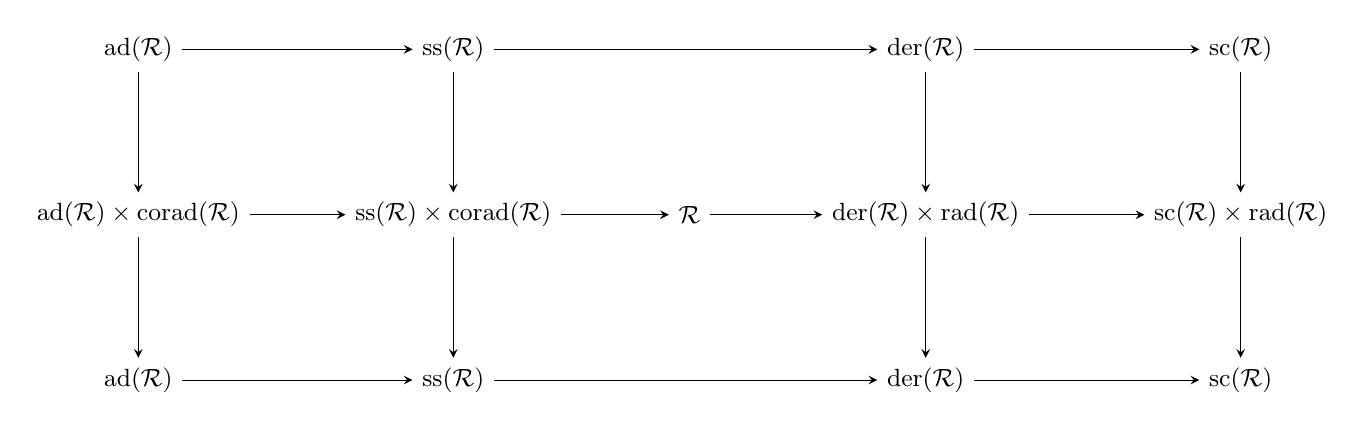
\begin{tikzpicture}[
  >=stealth,
  every node/.style={font=\small},
  x=1cm,y=1cm
]
\node (at) at (0,2.1) {$\operatorname{ad}(\cR)$};
\node (st) at (4,2.1) {$\operatorname{ss}(\cR)$};
\node (dt) at (10,2.1) {$\operatorname{der}(\cR)$};
\node (ct) at (14,2.1) {$\operatorname{sc}(\cR)$};

\node (am) at (0,0) {$\operatorname{ad}(\cR)\times\operatorname{corad}(\cR)$};
\node (sm) at (4,0) {$\operatorname{ss}(\cR)\times\operatorname{corad}(\cR)$};
\node (rm) at (7,0) {$\cR$};
\node (dm) at (10,0) {$\operatorname{der}(\cR)\times\operatorname{rad}(\cR)$};
\node (cm) at (14,0) {$\operatorname{sc}(\cR)\times\operatorname{rad}(\cR)$};

\node (ab) at (0,-2.1) {$\operatorname{ad}(\cR)$};
\node (sb) at (4,-2.1) {$\operatorname{ss}(\cR)$};
\node (db) at (10,-2.1) {$\operatorname{der}(\cR)$};
\node (cb) at (14,-2.1) {$\operatorname{sc}(\cR)$};

\draw[->] (at) -- (st);
\draw[->] (st) -- (dt);
\draw[->] (dt) -- (ct);
\draw[->] (am) -- (sm);
\draw[->] (sm) -- (rm);
\draw[->] (rm) -- (dm);
\draw[->] (dm) -- (cm);
\draw[->] (ab) -- (sb);
\draw[->] (sb) -- (db);
\draw[->] (db) -- (cb);

\draw[->] (at) -- (am);
\draw[->] (am) -- (ab);
\draw[->] (st) -- (sm);
\draw[->] (sm) -- (sb);
\draw[->] (dt) -- (dm);
\draw[->] (dm) -- (db);
\draw[->] (ct) -- (cm);
\draw[->] (cm) -- (cb);
\end{tikzpicture}
}
\end{center}
It is commutative, as is checked at once, and is self-dual in the
evident sense. The horizontal morphisms are isogenies, and the
composites of the vertical arrows are the identity.

\begin{lemma}\label{sga3:XXI:6.5.8}
Let \(h_1\) and \(h_2\) be the canonical isogenies
\[
 \operatorname{ss}(\cR)\times\operatorname{corad}(\cR)
 \xrightarrow{h_1}\cR
 \xrightarrow{h_2}
 \operatorname{der}(\cR)\times\operatorname{rad}(\cR).
\]
Then
\[
 K(h_1)\simeq K(h_2)\simeq N(\cR).
\]
\end{lemma}

\begin{proof}
This is immediate from the definitions.
\end{proof}

\begin{corollary}\label{sga3:XXI:6.5.9}
For a root datum \(\cR\), the following conditions are equivalent:
\begin{enumerate}
\item[(i)] \(N(\cR)=0\), that is,
  \(\operatorname{corad}(\cR)\to\operatorname{rad}(\cR)\) is an
  isomorphism;
\item[(ii)] the canonical map
  \(\operatorname{ss}(\cR)\to\operatorname{der}(\cR)\) is an
  isomorphism;
\item[(iii)] \(h_1\) is an isomorphism;
\item[(iv)] \(h_2\) is an isomorphism;
\item[(v)] \(\cR\) is the product of a semisimple root datum and a
  trivial root datum.
\end{enumerate}
\end{corollary}

\begin{corollary}\label{sga3:XXI:6.5.10}
For every root datum \(\cR\), there are isogenies
\[
 \operatorname{ad}(\cR)\times\cR_0
 \longrightarrow\cR\longrightarrow
 \operatorname{sc}(\cR)\times\cR_0,
\]
where \(\cR_0\) is the trivial root datum of rank
\(\rgred(\cR)-\rgss(\cR)\).
\end{corollary}

\begin{lemma}\label{sga3:XXI:6.5.11}
Let \(\cR\) be a root datum, let \(\Delta\) be a system of simple
roots, and let \(\Delta'\subset\Delta\). Consider the root datum
\[
 \cR_{\Delta'}=(M,M^\ast,R_{\Delta'},R^\ast_{\Delta'})
\]
of \ref{sga3:XXI:3.4.7}.
\begin{enumerate}
\item[(i)] If \(\cR\) is simply connected, then
  \(\operatorname{der}(\cR_{\Delta'})\) is simply connected.
\item[(ii)] If \(\cR\) is adjoint, then
  \(\operatorname{ss}(\cR_{\Delta'})\) is adjoint.
\end{enumerate}
\end{lemma}

\begin{proof}
The two assertions are equivalent by duality. The second reduces to
\[
 M\cap\VR(R_{\Delta'})=\Gamma_0(R_{\Delta'}).
\]
When \(M=\Gamma_0(R)\), both sides are the subgroup of \(M\) generated
by \(\Delta'\).
\end{proof}

% END INCLUDED SGA3_English_current_buildable_source_20260823/source/inputs/XXI/tex/components/27_expose_XXI_section65_special_cases_en.tex

% BEGIN INCLUDED SGA3_English_current_buildable_source_20260823/source/inputs/XXI/tex/components/28_expose_XXI_section66_weights_partA_en.tex
\subsection{Weights}\label{sga3:XXI:6.6}

\begin{definition}\label{sga3:XXI:6.6.1}
For a root datum \(\cR\), put
\footnote{Editors' note: The notation \(\Gamma(\cR)\) has been replaced
by \(\Lambda(\cR)\) to avoid any possible confusion with
\(\Gamma_0(R)\).}
\[
 \Lambda(\cR)=
 \{x\in\VR(R)\mid(\alpha^\ast,x)\in\mathbb Z
   \text{ for every }\alpha^\ast\in R^\ast\}.
\]
The elements of \(\Lambda(\cR)\) are called the \emph{weights} of
\(\cR\). The weights of \(\cR^\ast\) are called the \emph{coweights}
of \(\cR\).
\end{definition}

One has
\[
 \Gamma_0(R)\subset\Lambda(\cR),
\]
and \(\Lambda(\cR)\) is stable under \(W(\cR)\).

\begin{lemma}\label{sga3:XXI:6.6.2}
The bilinear map
\[
 V^\ast\times V\longrightarrow\mathbb Q
\]
induces a duality
\[
 \Gamma_0(R^\ast)\times\Lambda(\cR)\longrightarrow\mathbb Z.
\]
\end{lemma}

\begin{proof}
Immediate.
\end{proof}

\begin{corollary}\label{sga3:XXI:6.6.3}
Let
\[
 \Delta^\ast=(\alpha_1^\ast,\ldots,\alpha_n^\ast)
\]
be a system of simple coroots, and let \(p_i\in\VR(R)\),
\(i=1,\ldots,n\), be defined by
\[
 (\alpha_i^\ast,p_j)=\delta_{ij}.
\]
Thus
\[
 s_{\alpha_i}(p_i)=p_i-\alpha_i,
 \qquad
 s_{\alpha_i}(p_j)=p_j\quad(i\ne j).
\footnote{Caution: when the datum is not reduced, the \(\alpha_i\)
need not form a system of simple roots.}
\]
Then \(\Lambda(\cR)\) is the free abelian group generated by the
\(p_i\).
\end{corollary}

The \(p_i\) are called the \emph{fundamental weights} corresponding to
the system of simple coroots \(\Delta^\ast\).

\begin{corollary}\label{sga3:XXI:6.6.4}
For every \(\alpha^\ast\in\Delta^\ast\),
\[
 \left(\alpha^\ast,\sum_i p_i\right)=1.
\]
Consequently,
\[
 \sum_i p_i=\rho_{R_+},
 \qquad
 R_+=\mathscr P\bigl(\operatorname{ind}(\Delta)\bigr),
\]
in the notation of \ref{sga3:XXI:3.5.1}.
\end{corollary}

\begin{corollary}\label{sga3:XXI:6.6.5}
For every \(x\in\VR(R)\),
\[
 x=\sum_i(\alpha_i^\ast,x)p_i.
\]
\end{corollary}

Since
\[
 R^\ast\subset\Gamma_0(R^\ast),
 \qquad
 R\subset\Lambda(\cR),
\]
the quadruple
\[
 \bigl(\Lambda(\cR),\Gamma_0(R^\ast),R,R^\ast\bigr)
\]
is a root datum.

\begin{corollary}\label{sga3:XXI:6.6.6}
The canonical morphism
\[
 \Gamma_0(R^\ast)\longrightarrow M^\ast
\]
is the transpose of
\[
 x\longmapsto\sum_i(\alpha_i^\ast,x)p_i.
\]
This map defines a morphism of root data, and there is a commutative
diagram
\begin{center}
\begin{tikzcd}[column sep=huge,row sep=large]
\cR \arrow[rr] \arrow[dr]
  && \operatorname{sc}(\cR) \arrow[dl,"\wr"'] \\
& \bigl(\Lambda(\cR),\Gamma_0(R^\ast),R,R^\ast\bigr) &
\end{tikzcd}
\end{center}
\end{corollary}

% END INCLUDED SGA3_English_current_buildable_source_20260823/source/inputs/XXI/tex/components/28_expose_XXI_section66_weights_partA_en.tex

% BEGIN INCLUDED SGA3_English_current_buildable_source_20260823/source/inputs/XXI/tex/components/29_expose_XXI_section66_partB_through_lemma671_en.tex
Thus we have an explicit description of \(\operatorname{sc}(\cR)\)
in terms of the weights of \(\cR\). Likewise, one obtains a
commutative diagram
\begin{center}
\begin{tikzcd}[column sep=huge,row sep=large]
\operatorname{ad}(\cR) \arrow[rr] \arrow[d,"\wr"]
  && \cR \\
\bigl(\Gamma_0(R),\Lambda(\cR^\ast),R,R^\ast\bigr)
  \arrow[urr] &&
\end{tikzcd}
\end{center}

\begin{corollary}\label{sga3:XXI:6.6.7}
The datum \(\cR\) is simply connected if and only if
\[
 M=\Lambda(\cR).
\]
\end{corollary}

\begin{remark}\label{sga3:XXI:6.6.8}
One has
\[
 \Lambda(\cR)\cap M=\VR(R)\cap M.
\]
Consequently, \(\cR\) is semisimple if and only if
\[
 M\subset\Lambda(\cR).
\]
\end{remark}

The results of \S\ref{sga3:XXI:6.5} also give:

\begin{corollary}\label{sga3:XXI:6.6.9}
The datum \(\cR\) is the product of a simply connected datum and a
trivial datum if and only if
\[
 M\supset\Lambda(\cR).
\]
\end{corollary}

Consider now the canonical isogeny
\[
 f:\operatorname{ad}(\cR)\longrightarrow\operatorname{sc}(\cR),
\]
and put \(Z(\cR)=K(f)\). One has
\[
 Z(\cR)\simeq Z(\operatorname{sc}\cR)
 \simeq Z(\operatorname{ad}\cR).
\]

\begin{corollary}\label{sga3:XXI:6.6.10}
There is a canonical isomorphism
\[
 Z(\cR)=\Lambda(\cR)/\Gamma_0(R).
\]
More precisely, there is an exact sequence of
\(W(\cR)\)-modules
\[
 0\longrightarrow\Gamma_0(R)\longrightarrow\Lambda(\cR)
 \longrightarrow Z(\cR)\longrightarrow0.
\]
\end{corollary}

\begin{corollary}\label{sga3:XXI:6.6.11}
There is a canonical pairing
\[
 Z(\cR^\ast)\times Z(\cR)\longrightarrow\mathbb Q/\mathbb Z
\]
which puts these groups in duality.
\end{corollary}

\begin{remark}\label{sga3:XXI:6.6.12}
One has
\[
 Z(\cR\times\cR')\simeq Z(\cR)\times Z(\cR').
\]
In particular, consider simply connected data
\(\cR_i\), \(i=1,2,\ldots,n\), and a trivial datum \(\cR_0\).
Put
\[
 \cR=\cR_0\times\cR_1\times\cdots\times\cR_n.
\]
If
\[
 \cR=(M,M^\ast,R,R^\ast),
 \qquad
 \cR_0=(M_0,M_0^\ast,\varnothing,\varnothing),
\]
then
\[
 M/\Gamma_0(R)\simeq
 M_0\times Z(\cR_1)\times\cdots\times Z(\cR_n).
\]
\end{remark}

\subsection{Automorphisms}\label{sga3:XXI:6.7}

By \ref{sga3:XXI:6.1.4}, an automorphism of \(\cR\) is an
automorphism \(u\) of \(M\) such that
\[
 u(R)=R,
 \qquad
 {}^tu(R^\ast)=R^\ast.
\]
In particular, every \(w\in W(\cR)\) defines an automorphism of
\(\cR\).

\begin{lemma}\label{sga3:XXI:6.7.1}
The group \(W(\cR)\) is a normal subgroup of
\(\operatorname{Aut}(\cR)\). More precisely, if
\(u\in\operatorname{Aut}(\cR)\) and \(\alpha\in R\), then
\[
 us_\alpha u^{-1}=s_{u(\alpha)}.
\]
\end{lemma}

\begin{proof}
The proof is the same as that of \ref{sga3:XXI:1.2.10}.
\end{proof}

% END INCLUDED SGA3_English_current_buildable_source_20260823/source/inputs/XXI/tex/components/29_expose_XXI_section66_partB_through_lemma671_en.tex

% BEGIN INCLUDED SGA3_English_current_buildable_source_20260823/source/inputs/XXI/tex/components/30_expose_XXI_proposition672_through_lemma677_en.tex
\begin{proposition}\label{sga3:XXI:6.7.2}
Let \(\Delta\) be a system of simple roots, and put
\[
 E_\Delta(\cR)=
 \{u\in\operatorname{Aut}(\cR)\mid u(\Delta)=\Delta\}.
\]
Then \(\operatorname{Aut}(\cR)\) is the semidirect product of
\(W(\cR)\) by \(E_\Delta(\cR)\).
\end{proposition}

\begin{proof}
This follows at once from the fact that \(W(\cR)\) acts simply
transitively on the systems of simple roots and from the fact that,
if \(\Delta\) is a system of simple roots of \(\cR\), then
\(u(\Delta)\) is a system of simple roots for every automorphism
\(u\) of \(\cR\).
\end{proof}

We shall later give a simpler description of \(E_\Delta(\cR)\) in
the case of reduced irreducible root data.\footnote{Editors' note:
When \(\cR\) is simply connected or adjoint, see \SGARefLink{sga3:XXI:7.4.5}{7.4.5}.}

\begin{definition}\label{sga3:XXI:6.7.3}
We denote by \(\operatorname{Aut}^{s}(\cR)\)\footnote{Editors' note:
The superscript \(s\) is intended to suggest ``semisimple.''}
the set of \(u\in\operatorname{Aut}(\cR)\) for which the following
diagram is commutative:
\begin{center}
\begin{tikzcd}[column sep=huge,row sep=large]
\cR \arrow[rr,"u"] \arrow[dr]
  && \cR \arrow[dl] \\
& \operatorname{rad}(\cR) &
\end{tikzcd}
\end{center}
We write
\[
 E_\Delta^{s}(\cR)
 =E_\Delta(\cR)\cap\operatorname{Aut}^{s}(\cR).
\]
\end{definition}

\begin{remark}\label{sga3:XXI:6.7.4}
If \(u\in\operatorname{Aut}(\cR)\), then
\(u\in\operatorname{Aut}^{s}(\cR)\) if and only if
\[
 (u-\operatorname{id})(M)\subset\VR(R).
\]
In particular,
\[
 W(\cR)\subset\operatorname{Aut}^{s}(\cR).
\]
\end{remark}

\begin{proposition}\label{sga3:XXI:6.7.5}
For every system of simple roots \(\Delta\), the group
\(\operatorname{Aut}^{s}(\cR)\) is the semidirect product of
\(W(\cR)\) by \(E_\Delta^{s}(\cR)\).
\end{proposition}

By functoriality, every automorphism of \(\cR\) induces an
automorphism of \(\operatorname{ad}(\cR)\). Thus there is a
canonical homomorphism
\[
 \operatorname{Aut}(\cR)\longrightarrow
 \operatorname{Aut}(\operatorname{ad}(\cR)).
\]

\begin{lemma}\label{sga3:XXI:6.7.6}
The homomorphism
\[
 \operatorname{Aut}^{s}(\cR)\longrightarrow
 \operatorname{Aut}(\operatorname{ad}(\cR))
\]
is injective.
\end{lemma}

\begin{proof}
Let \(u\) be an automorphism of \(M\) such that
\[
 (u-\operatorname{id})(M)\subset\VR(R)
\]
and
\[
 {}^tu(\alpha^\ast)=\alpha^\ast
 \qquad(\alpha^\ast\in R^\ast).
\]
For every \(x\in M\), one has
\[
 (\alpha^\ast,u(x)-x)
 =({}^tu(\alpha^\ast)-\alpha^\ast,x)=0.
\]
Hence \(u(x)-x=0\), by \ref{sga3:XXI:1.2.5}.
\end{proof}

\begin{lemma}\label{sga3:XXI:6.7.7}
The group \(\operatorname{Aut}^{s}(\cR)\) is finite.
\end{lemma}

\begin{proof}
It suffices to prove that \(\operatorname{Aut}(\cR)\) is finite when
\(\cR\) is adjoint. In that case \(M\) is generated by \(R\), so
every automorphism of \(\cR\) is determined by the permutation it
induces on \(R\).
\end{proof}

% END INCLUDED SGA3_English_current_buildable_source_20260823/source/inputs/XXI/tex/components/30_expose_XXI_proposition672_through_lemma677_en.tex

% BEGIN INCLUDED SGA3_English_current_buildable_source_20260823/source/inputs/XXI/tex/components/31_expose_XXI_remark678_through_example686_en.tex
\begin{remark}\label{sga3:XXI:6.7.8}
It is immediate that \(\operatorname{Aut}(\cR)\) (respectively
\(E_\Delta(\cR)\)) is finite if and only if
\[
 \rgred(\cR)-\rgss(\cR)\leq1.
\]
\end{remark}

\subsection{\(p\)-morphisms of reduced root data}
\label{sga3:XXI:6.8}

Throughout this subsection, \(p\) is a fixed positive integer.

\begin{definition}\label{sga3:XXI:6.8.1}
Let
\[
 \cR=(M,M^\ast,R,R^\ast),
 \qquad
 \cR'=(M',M'^\ast,R',R'^\ast)
\]
be two reduced root data. A group homomorphism
\[
 f:M'\longrightarrow M
\]
is called a \emph{\(p\)-morphism from \(\cR'\) to \(\cR\)} if
there exist a bijection
\[
 u:R\xrightarrow{\sim}R'
\]
and a map
\[
 q:R\longrightarrow\{p^n\mid n\in\mathbb N\}
\]
such that:
\begin{enumerate}
\item[(i)] \(f(u(\alpha))=q(\alpha)\alpha\) for every
  \(\alpha\in R\);
\item[(ii)] \({}^tf(\alpha^\ast)=q(\alpha)u(\alpha)^\ast\) for
  every \(\alpha\in R\).\footnote{Editors' note: These two
  conditions imply
  \[
   q(\alpha)\bigl(u(\alpha)^\ast,u(\beta)\bigr)
   =q(\beta)(\alpha^\ast,\beta)
  \]
  for all \(\alpha,\beta\in R\).}
\end{enumerate}
\end{definition}

\begin{corollary}\label{sga3:XXI:6.8.2}
A \(1\)-morphism is precisely a morphism.
\end{corollary}

\begin{corollary}\label{sga3:XXI:6.8.3}
The transpose of a \(p\)-morphism is a \(p\)-morphism.
\end{corollary}

\begin{lemma}\label{sga3:XXI:6.8.4}
If \(w\in W(\cR)\) and \(\alpha\in R\), then
\[
 q(w(\alpha))=q(\alpha).
\]
The map
\[
 s_\alpha\longmapsto s_{u(\alpha)}
\]
extends to an isomorphism
\[
 u:W(\cR)\xrightarrow{\sim}W(\cR')
\]
such that
\[
 u(w(\alpha))=u(w)\bigl(u(\alpha)\bigr).
\]
\end{lemma}

\begin{proof}
It suffices to prove, for \(\alpha,\beta\in R\), that
\[
 u(s_\alpha(\beta))=s_{u(\alpha)}u(\beta),
 \qquad
 q(s_\alpha(\beta))=q(\beta).
\]
Successively, one has
\begin{align*}
 f\bigl(s_{u(\alpha)}u(\beta)\bigr)
  &=f(u(\beta))
    -\bigl(u(\alpha)^\ast,u(\beta)\bigr)f(u(\alpha))\\
  &=q(\beta)\beta
    -q(\beta)q(\alpha)^{-1}
       (\alpha^\ast,\beta)q(\alpha)\alpha\\
  &=q(\beta)\bigl(\beta-(\alpha^\ast,\beta)\alpha\bigr)\\
  &=q(\beta)s_\alpha(\beta).
\end{align*}
If
\[
 \gamma=u^{-1}\bigl(s_{u(\alpha)}u(\beta)\bigr),
\]
then
\[
 q(\gamma)\gamma=f(u(\gamma))=q(\beta)s_\alpha(\beta).
\]
The roots \(\gamma\) and \(s_\alpha(\beta)\) are proportional over
\(\mathbb Q\), hence equal or opposite. Since \(q(\gamma)\) and
\(q(\beta)\) are positive, it follows that
\[
 q(\gamma)=q(\beta),
 \qquad
 \gamma=s_\alpha(\beta).
\]
\end{proof}

\begin{definition}\label{sga3:XXI:6.8.5}
The numbers \(q(\alpha)\) are called the \emph{root exponents} of
\(f\).
\end{definition}

\begin{example}\label{sga3:XXI:6.8.6}
Let \(\cR\) be a reduced root datum and let
\(q=p^n\), \(n\in\mathbb N\). Multiplication by \(q\),
\[
 M\longrightarrow M,\qquad x\longmapsto qx,
\]
is a \(p\)-morphism whose root exponents are all equal to \(q\)
(and for which \(u=\operatorname{id}\)). It is denoted
\[
 q:\cR\longrightarrow\cR.
\]
\end{example}

% END INCLUDED SGA3_English_current_buildable_source_20260823/source/inputs/XXI/tex/components/31_expose_XXI_remark678_through_example686_en.tex

% BEGIN INCLUDED SGA3_English_current_buildable_source_20260823/source/inputs/XXI/tex/components/32_expose_XXI_proposition687_through_proposition711_en.tex
\begin{proposition}\label{sga3:XXI:6.8.7}
In the notation of \ref{sga3:XXI:6.8.1}, \(u\) induces an
isomorphism from the set of systems of simple roots (respectively
positive roots) of \(R\) onto the corresponding set for \(R'\).
\end{proposition}

\begin{proof}
This follows immediately from \ref{sga3:XXI:3.1.5}
(respectively \ref{sga3:XXI:3.2.1}).
\end{proof}

\section{Structure}\label{sga3:XXI:7}

\subsection{Decomposition of a root datum}\label{sga3:XXI:7.1}

\begin{proposition}\label{sga3:XXI:7.1.1}
Let \(\cR\) be a root datum and let \(\Delta\) be a system of
simple roots.
\begin{enumerate}
\item[\SGAInlineRefTarget{sga3:XXI:7.1.1:item:i}(i)] Let \(R'\) and \(R''\) be two closed symmetric sets of
  roots forming a partition of \(R\). If
  \[
   \Delta'=\Delta\cap R',
   \qquad
   \Delta''=\Delta\cap R'',
  \]
  then
  \[
   R'=R_{\Delta'},
   \qquad
   R''=R_{\Delta''},
  \]
  and every root of \(\Delta'\) is orthogonal to every root of
  \(\Delta''\).
\item[\SGAInlineRefTarget{sga3:XXI:7.1.1:item:ii}(ii)] Let \(\Delta'\) and \(\Delta''\) be two orthogonal
  subsets forming a partition of \(\Delta\). Then
  \(R_{\Delta'}\) and \(R_{\Delta''}\) form a partition of \(R\).
\end{enumerate}
\end{proposition}

\begin{proof}
We first prove \SGARefLink{sga3:XXI:7.1.1:item:i}{(i)}.

\begin{lemma}\label{sga3:XXI:7.1.2}
Under the hypotheses of \textup{\SGARefLink{sga3:XXI:7.1.1:item:i}{(i)}}, if
\(\alpha\), \(\beta\), and \(\alpha+\beta\) are roots, then all
three belong to \(R'\), or all three belong to \(R''\).
\end{lemma}

Suppose, for example, that \(\alpha+\beta\in R'\). One cannot have
\(\alpha,\beta\in R''\), since \(R''\) is closed. Suppose therefore
that \(\alpha\in R'\). Then \(-\alpha\in R'\), and
\[
 \beta=(\beta+\alpha)-\alpha\in R'.
\]

We now prove \(R'=R_{\Delta'}\) by induction on the order of a
positive root \(\alpha\in R'\cap\mathscr P(\Delta)\). If
\(\operatorname{ord}_\Delta(\alpha)=1\), then
\[
 \alpha\in R'\cap\Delta=\Delta'.
\]
If \(\operatorname{ord}_\Delta(\alpha)>1\), there is
\(\beta\in\Delta\) such that \(\alpha-\beta\in R\). By the lemma,
\[
 \beta\in\Delta',
 \qquad
 \alpha-\beta\in R'.
\]
Hence \(\alpha-\beta\in R_{\Delta'}\) by induction, and finally
\[
 \alpha=(\alpha-\beta)+\beta\in R_{\Delta'}.
\]

We next prove that \(\Delta'\) and \(\Delta''\) are orthogonal. If
\(\alpha\in\Delta'\) and \(\beta\in\Delta''\), then
\[
 (\beta^\ast,\alpha)\leq0.
\]
If \((\beta^\ast,\alpha)\neq0\), then \(\beta+\alpha\) is a root,
contrary to the lemma.

We now prove \SGARefLink{sga3:XXI:7.1.1:item:ii}{(ii)}. If \(\Delta'\) or \(\Delta''\) is empty, the
assertion is immediate. Otherwise, if \(R_{\Delta'}\) and
\(R_{\Delta''}\) do not form a partition of \(R\), there is a root
\(\alpha\) of the form
\[
 \alpha=\sum_i m_i'\alpha_i'
       +\sum_j m_j''\alpha_j'',
 \qquad
 m_i',m_j''\in\mathbb Z_+,
\]
where the \(\alpha_i'\) (respectively \(\alpha_j''\)) belong to
\(\Delta'\) (respectively \(\Delta''\)). Applying
\ref{sga3:XXI:3.1.2}, and interchanging \(\Delta'\) and
\(\Delta''\) if necessary, yields a relation
\[
 \delta=\gamma+\beta,
 \qquad
 \gamma\in R_{\Delta'},
 \quad
 \beta\in\Delta'',
 \quad
 \delta\in R.
\]
But \((\beta^\ast,\gamma)=0\), so
\(\gamma-\beta\) is also a root by \ref{sga3:XXI:2.2.5}, which is
impossible.
\end{proof}

% END INCLUDED SGA3_English_current_buildable_source_20260823/source/inputs/XXI/tex/components/32_expose_XXI_proposition687_through_proposition711_en.tex

% BEGIN INCLUDED SGA3_English_current_buildable_source_20260823/source/inputs/XXI/tex/components/33_expose_XXI_proposition713_through_lemma723_en.tex
\begin{proposition}\label{sga3:XXI:7.1.3}
Let \(\cR\) be a root datum. The following conditions are
equivalent:
\begin{enumerate}
\item[\SGAInlineRefTarget{sga3:XXI:7.1.3:item:i}(i)] There is no nontrivial partition of \(R\) into two
  closed symmetric subsets.
\item[\SGAInlineRefTarget{sga3:XXI:7.1:item:ii}(ii)] For some (respectively every) system of simple roots
  \(\Delta\) of \(R\), there is no partition of \(\Delta\) into
  two nonempty orthogonal subsets.
\item[\SGAInlineRefTarget{sga3:XXI:7.1.3:item:iii}(iii)] The natural representation of \(W(\cR)\) on
  \(\VR(R)\) is irreducible.
\item[\SGAInlineRefTarget{sga3:XXI:7.1.3:item:iv}(iv)] For every pair \((\alpha,\beta)\) of roots, there is a
  sequence of roots
  \[
   \alpha_0,\alpha_1,\ldots,\alpha_n,
   \qquad
   \alpha_0=\alpha,\quad\alpha_n=\beta,
  \]
  such that \(\alpha_i\) and \(\alpha_{i+1}\) are nonorthogonal
  for \(i=0,\ldots,n-1\).
\end{enumerate}
\end{proposition}

\begin{proof}
The equivalence \SGARefLink{sga3:XXI:7.1.3:item:i}{(i)}\(\Leftrightarrow\)\SGARefLink{sga3:XXI:7.1:item:ii}{(ii)} follows from
\ref{sga3:XXI:7.1.1}, and \SGARefLink{sga3:XXI:7.1.3:item:iv}{(iv)}\(\Rightarrow\)\SGARefLink{sga3:XXI:7.1.1:item:ii}{(ii)} is immediate.
Conversely, if \SGARefLink{sga3:XXI:7.1.1:item:ii}{(ii)} holds for \(\Delta\), then \SGARefLink{sga3:XXI:7.1.3:item:iv}{(iv)} holds when
\(\alpha,\beta\in\Delta\). Every root is nonorthogonal to some
simple root, by \ref{sga3:XXI:3.1.1}, for example. Moreover,
\SGARefLink{sga3:XXI:7.1.3:item:iii}{(iii)}\(\Rightarrow\)\SGARefLink{sga3:XXI:7.1.3:item:i}{(i)}: under the hypotheses of
\ref{sga3:XXI:7.1.1}, the space \(\VR(R')\) is stable under
\(W(\cR)\). It remains to prove \SGARefLink{sga3:XXI:7.1.1:item:i}{(i)}\(\Rightarrow\)\SGARefLink{sga3:XXI:7.1.3:item:iii}{(iii)}.

Let \(H\) be a vector subspace of \(\VR(R)\), stable under
\(W(\cR)\). For every \(\alpha\in R\), the equality
\(s_\alpha(H)=H\) immediately gives
\[
 \alpha\in H
 \qquad\text{or}\qquad
 \alpha^\ast\in H^\perp,
\]
where \(H^\perp\) denotes the orthogonal complement of \(H\) in
\(\VR(R^\ast)\), which is in duality with \(\VR(R)\). Put
\[
 R'=\{\alpha\in R\mid\alpha\in H\},
 \qquad
 R''=\{\alpha\in R\mid\alpha^\ast\in H^\perp\}.
\]
This gives a partition of \(R\) into two closed symmetric subsets.
\end{proof}

\begin{definition}\label{sga3:XXI:7.1.4}
A root datum (respectively root system) satisfying the equivalent
conditions of \ref{sga3:XXI:7.1.3} and having nonzero semisimple
rank is called \emph{irreducible}.
\end{definition}

\begin{corollary}\label{sga3:XXI:7.1.5}
For every root datum \(\cR\), there is a unique partition, up to
order, of \(R\) into closed symmetric irreducible subsets.
\end{corollary}

\begin{corollary}\label{sga3:XXI:7.1.6}
Every adjoint (respectively simply connected) root datum is a
product of irreducible adjoint (respectively simply connected) root
data.
\end{corollary}

\begin{proof}
It suffices to consider the adjoint case. The assertion then follows
from the fact that, under the hypotheses of
\ref{sga3:XXI:7.1.1},
\[
 \Gamma_0(R)=\Gamma_0(R')\times\Gamma_0(R'').
\]
\end{proof}

\begin{corollary}\label{sga3:XXI:7.1.7}
For every root datum (respectively reduced root datum) \(\cR\),
there is an isogeny
\[
 \cR\longrightarrow\cR',
\]
where \(\cR'\) is a product of a trivial root datum and irreducible
simply connected root data (respectively irreducible reduced simply
connected root data).
\end{corollary}

\subsection{Properties of irreducible root data}
\label{sga3:XXI:7.2}

\begin{definition}\label{sga3:XXI:7.2.1}
Let \(\cR\) be an irreducible root datum. For every \(\alpha\in R\),
put
\[
 \operatorname{long}(\alpha)
 =\ell(\alpha)/\ell(\alpha_0),
\]
where \(\alpha_0\in R\) is such that \(\ell(\alpha_0)\) is minimal.
The number \(\operatorname{long}(\alpha)\) is called the
\emph{length} of \(\alpha\).
\end{definition}

\begin{lemma}\label{sga3:XXI:7.2.2}
Let \(\cR\) be an irreducible root datum. The Weyl group acts
transitively on the set of roots of a given length.
\end{lemma}

\begin{proof}
Let \(\alpha,\beta\in R\). Since the representation of \(W(\cR)\)
on \(\VR(R)\) is irreducible, \(\alpha\) cannot be orthogonal to
all \(w(\beta)\), \(w\in W(\cR)\). Hence some \(w(\beta)\) is
nonorthogonal to \(\alpha\). Since
\[
 \ell(w(\beta))=\ell(\beta),
\]
the assertion follows from \ref{sga3:XXI:2.3.2}.
\end{proof}

\begin{lemma}\label{sga3:XXI:7.2.3}
If \(\cR\) is irreducible and reduced, then
\[
 \operatorname{long}(R)
 \in\bigl\{\{1\},\{1,2\},\{1,3\}\bigr\}.
\]
\end{lemma}

\begin{proof}
By the observation used above, for every
\(\alpha,\beta\in R\) there is \(w\in W(\cR)\) such that
\(w(\beta)\) is nonorthogonal to \(\alpha\). Therefore, by
\ref{sga3:XXI:2.3.1},
\[
 \frac{\ell(\alpha)}{\ell(\beta)}
 \in\left\{1,2,3,\frac12,\frac13\right\}.
\]
Thus \(\operatorname{long}(\alpha)\) is \(1\), \(2\), or \(3\).
But lengths \(2\) and \(3\) cannot both occur, since their ratio
\(2/3\) is not in the displayed set.
\end{proof}

% END INCLUDED SGA3_English_current_buildable_source_20260823/source/inputs/XXI/tex/components/33_expose_XXI_proposition713_through_lemma723_en.tex

% BEGIN INCLUDED SGA3_English_current_buildable_source_20260823/source/inputs/XXI/tex/components/34_expose_XXI_remark724_through_remark729_en.tex
\begin{remark}\label{sga3:XXI:7.2.4}
Reasoning similarly gives the following result.  If \(\cR\) is
irreducible and nonreduced, with \(\rgss(\cR)>1\), then
\[
 \operatorname{long}(R)=\{1,2,4\}.
\]
If \(R_i=\operatorname{long}^{-1}(i)\), then
\[
 \operatorname{ind}(R)=R_1\cup R_2,\qquad R_4=2R_1,
\]
and two nonproportional roots of \(R_1\) are orthogonal.
Conversely, suppose that \(R\) is an irreducible reduced root
system such that \(\operatorname{long}(R)=\{1,2\}\).  Put
\(R_i=\operatorname{long}^{-1}(i)\), and suppose that two
nonproportional roots of \(R_1\) are orthogonal.  Then
\(R\cup2R_1\) is irreducible and nonreduced, and
\[
 \operatorname{ind}(R\cup2R_1)=R.
\]
\end{remark}

\begin{lemma}\label{sga3:XXI:7.2.5}
If \(\cR\) is an irreducible root datum, then \(\cR^\ast\) is
irreducible as well, and the product
\[
 \operatorname{long}(\alpha)\operatorname{long}(\alpha^\ast)
\]
is constant as \(\alpha\) runs through \(R\).
\end{lemma}

\begin{proof}
This follows immediately from \ref{sga3:XXI:7.1.3}\,\SGARefLink{sga3:XXI:7.2:item:iv}{(iv)} and
\ref{sga3:XXI:2.2.6}.
\end{proof}

\begin{definition}\label{sga3:XXI:7.2.6}
Let \(\cR\) be any root datum.  The \emph{length} of
\(\alpha\in R\), denoted \(\operatorname{long}(\alpha)\), is the
length of \(\alpha\) in its irreducible component.
\end{definition}

\begin{lemma}\label{sga3:XXI:7.2.7}
There is a unique group homomorphism
\[
 u:\Gamma_0(R)\longrightarrow\Gamma_0(R^\ast)
\]
such that
\[
 u(\alpha)=\operatorname{long}(\alpha)\alpha^\ast
 \qquad(\alpha\in R).
\]
\end{lemma}

\begin{proof}
By \ref{sga3:XXI:3.5.5}, it is enough to verify that, whenever
\(\alpha,\beta,\alpha+\beta\in R\),
\[
 \operatorname{long}(\alpha)\alpha^\ast+
 \operatorname{long}(\beta)\beta^\ast
 =
 \operatorname{long}(\alpha+\beta)(\alpha+\beta)^\ast.
\]
But \(\alpha,\beta,\alpha+\beta\) belong to the same irreducible
component of \(R\), by \ref{sga3:XXI:7.1.2}; the assertion is
therefore reduced to \ref{sga3:XXI:1.2.2}.
\end{proof}

\begin{remark}\label{sga3:XXI:7.2.8}
Let \(u\) be as in \ref{sga3:XXI:7.2.7}.  For
\(\alpha,\beta\in R\),
\[
 (u(\alpha),\beta)=(u(\beta),\alpha).
\]
Indeed, this amounts to
\[
 \operatorname{long}(\alpha)(\alpha^\ast,\beta)
 =
 \operatorname{long}(\beta)(\beta^\ast,\alpha),
\]
which is clear when \(\alpha\) and \(\beta\) are orthogonal.  If
they are not orthogonal, they lie in the same irreducible component
of \(R\), and the assertion reduces to \ref{sga3:XXI:1.2.1},
formula~\SGARefLink{sga3:XXI:eq:9}{(9)}.
\end{remark}

\begin{remark}\label{sga3:XXI:7.2.9}
The symmetric bilinear form
\[
 (x,y)\longmapsto(u(x),y)
\]
is positive and nondegenerate on \(\Gamma_0(R)\).
\end{remark}

\begin{proof}
Let \(R_i\) be the irreducible components of \(R\).  Then
\[
 \Gamma_0(R)=\prod_i\Gamma_0(R_i),
\]
and the bilinear form \((u(x),y)\) is the product, on the groups
\(\Gamma_0(R_i)\), of the forms
\[
 2\ell(\alpha_i)^{-1}(p(x),y),
\]
where \(\ell(\alpha_i)\) is the minimum of \(\ell(\alpha)\) for
\(\alpha\in R_i\).  These symmetric bilinear forms are positive
and nondegenerate by \ref{sga3:XXI:1.2.6}.
\end{proof}

% END INCLUDED SGA3_English_current_buildable_source_20260823/source/inputs/XXI/tex/components/34_expose_XXI_remark724_through_remark729_en.tex

% BEGIN INCLUDED SGA3_English_current_buildable_source_20260823/source/inputs/XXI/tex/components/35_expose_XXI_section73_cartan_matrix_en.tex
\subsection{Cartan matrix}\label{sga3:XXI:7.3}

Let \(\cR\) be a root datum.  If \(\Delta\) is a system of simple
roots, the \emph{Cartan matrix} of \(\cR\) relative to \(\Delta\)
is the square matrix indexed by \(\Delta\) and defined by
\[
 a_{\alpha,\beta}=(\alpha^\ast,\beta),
 \qquad \alpha,\beta\in\Delta.
\]
If \(\Delta'\) is another system of simple roots and
\(w\in W(\cR)\) satisfies \(w(\Delta)=\Delta'\), then
\[
 (w(\alpha)^\ast,w(\beta))=(\alpha^\ast,\beta).
\]
Thus the Cartan matrix relative to \(\Delta'\) is obtained from
that relative to \(\Delta\) by the isomorphism
\(\Delta\to\Delta'\) of index sets defined by \(w\).  Consequently,
up to isomorphism of its index set, the Cartan matrix depends only
on \(\cR\).

\begin{proposition}\label{sga3:XXI:7.3.1}
The Cartan matrix has the following properties.
\begin{enumerate}
\item[\SGAInlineRefTarget{sga3:XXI:7.3.1:item:i}(i)] \(a_{\alpha,\alpha}=2\), and
  \(a_{\alpha,\beta}\leq0\) for \(\alpha\neq\beta\).
\item[\SGAInlineRefTarget{sga3:XXI:7.3.1:item:ii}(ii)] \(a_{\alpha,\beta}=0\) implies
  \(a_{\beta,\alpha}=0\).
\item[\SGAInlineRefTarget{sga3:XXI:7.2:item:iii}(iii)] There are strictly positive integers
  \(m_\alpha=\operatorname{long}(\alpha)\) such that the matrix
  \[
   (m_\alpha a_{\alpha,\beta})
  \]
  is symmetric, positive, and nondegenerate.
\item[\SGAInlineRefTarget{sga3:XXI:7.2:item:iv}(iv)] The principal minors of
  \((a_{\alpha,\beta})_{\alpha,\beta\in\Delta}\), namely
  \[
   \det(a_{\alpha,\beta})_{\alpha,\beta\in\Delta'}
   \qquad(\Delta'\subset\Delta),
  \]
  are strictly positive.
\item[\SGAInlineRefTarget{sga3:XXI:7.2:item:v}(v)] One has
  \[
   s_\alpha(\beta)=\beta-a_{\alpha,\beta}\alpha,
   \qquad
   s_\alpha(\beta^\ast)
   =\beta^\ast-a_{\beta,\alpha}\alpha^\ast.
  \]
\end{enumerate}
\end{proposition}

\begin{proof}
Part \SGARefLink{sga3:XXI:7.2:item:v}{(v)} is a definition; \SGARefLink{sga3:XXI:7.3.1:item:i}{(i)} follows from
\ref{sga3:XXI:3.2.11}, \SGARefLink{sga3:XXI:7.3.1:item:ii}{(ii)} from \ref{sga3:XXI:2.2.2}, and
\SGARefLink{sga3:XXI:7.2:item:iii}{(iii)} from \ref{sga3:XXI:7.2.9}.  Part \SGARefLink{sga3:XXI:7.2:item:iv}{(iv)} follows immediately
from \SGARefLink{sga3:XXI:7.2:item:iii}{(iii)} and
\[
 \det(m_\alpha a_{\alpha,\beta})_{\alpha,\beta\in\Delta'}
 =
 \left(\prod_{\alpha\in\Delta'}m_\alpha\right)
 \det(a_{\alpha,\beta})_{\alpha,\beta\in\Delta'}.
\]
\end{proof}

\begin{proposition}\label{sga3:XXI:7.3.2}
Let \(\cR\) and \(\cR'\) be two reduced simply connected
(respectively adjoint) root data, let \(\Delta\) and \(\Delta'\)
be systems of simple roots of \(\cR\) and \(\cR'\), and let
\(u:\Delta\to\Delta'\) be an isomorphism.  Denote the corresponding
Cartan matrices by \((a_{\alpha,\beta})\) and
\((a'_{\alpha',\beta'})\), and suppose that
\[
 a'_{u(\alpha),u(\beta)}=a_{\alpha,\beta}.
\]
Then there is a unique isomorphism from \(\cR\) onto \(\cR'\)
that induces \(u\) on \(\Delta\).
\end{proposition}

\begin{proof}
It is enough to give the proof in the adjoint case.  Then
\(M=\Gamma_0(R)\) and \(M'=\Gamma_0(R')\) are the free abelian
groups generated by \(\Delta\) and \(\Delta'\).  Hence there is a
unique group isomorphism \(M\to M'\) inducing \(u\) on \(\Delta\);
denote it again by \(u\).

We show that \(u(R)\subset R'\).  Every root \(\alpha\) of \(R\)
can be written
\[
 \alpha=s_{\alpha_1}\cdots s_{\alpha_n}(\alpha_{n+1}),
 \qquad \alpha_i\in\Delta.
\]
By the hypothesis on \(u\) and the relations
\ref{sga3:XXI:7.3.1}\,\SGARefLink{sga3:XXI:7.2:item:v}{(v)},
\[
 u(\alpha)=
 s_{u(\alpha_1)}\cdots s_{u(\alpha_n)}
 \bigl(u(\alpha_{n+1})\bigr).
\]
It remains to prove that \({}^tu(R'^\ast)\subset R^\ast\).  This
follows from the fact that the elements of \(M^\ast\)
(respectively \(M'^\ast\)) are determined by their duality with
\(R\) or \(\Delta\) (respectively \(R'\) or \(\Delta'\)), by
\ref{sga3:XXI:1.2.5}.
\end{proof}

\begin{corollary}\label{sga3:XXI:7.3.3}
A reduced simply connected or adjoint root datum is determined up
to isomorphism by its Cartan matrix.
\end{corollary}

\begin{corollary}\label{sga3:XXI:7.3.4}
Let \(\cR\) be a reduced simply connected (respectively adjoint)
root datum and let \(\Delta\) be a system of simple roots.  The
group \(E_\Delta(\cR)\) is identified with the group of
automorphisms of the set \(\Delta\) that preserve the Cartan
matrix.
\end{corollary}

\begin{remark}\label{sga3:XXI:7.3.5}
The existence of a root datum corresponding to a given Cartan
matrix satisfying, for example, \SGARefLink{sga3:XXI:7.3.1:item:i}{(i)}, \SGARefLink{sga3:XXI:7.3.1:item:ii}{(ii)}, and \SGARefLink{sga3:XXI:7.2:item:iv}{(iv)} is not easily
settled directly without using the classification.
\end{remark}

% END INCLUDED SGA3_English_current_buildable_source_20260823/source/inputs/XXI/tex/components/35_expose_XXI_section73_cartan_matrix_en.tex

% BEGIN INCLUDED SGA3_English_current_buildable_source_20260823/source/inputs/XXI/tex/components/36_expose_XXI_section74_dynkin_diagrams_en.tex
\subsection{Dynkin diagrams}\label{sga3:XXI:7.4}

\begin{definition}\label{sga3:XXI:7.4.1}
A \emph{Dynkin-diagram structure} on a finite set \(\Delta\)
(the word ``scheme'' being banished for obvious reasons) consists
of a set of pairs of distinct elements of \(\Delta\), called
\emph{linked pairs}, together with a map
\[
 \Delta\longrightarrow\{1,2,3\}.
\]
The notion of isomorphism between such structures is evident.
\end{definition}

\begin{definition}\label{sga3:XXI:7.4.2}
Let \(\cR\) be a root datum and let \(\Delta\) be a system of
simple roots.  The \emph{Dynkin diagram} of \(\cR\) relative to
\(\Delta\) is the set \(\Delta\), in which two simple roots are
linked if and only if they are nonorthogonal, and each root is
assigned its length.
\end{definition}

\begin{proposition}\label{sga3:XXI:7.4.3}
The Dynkin diagram and the Cartan matrix determine one another
uniquely.
\end{proposition}

\begin{proof}
The equivalence
\[
 \alpha\text{ and }\beta\text{ are not linked}
 \quad\Longleftrightarrow\quad
 a_{\alpha,\beta}=0
\]
and the relation
\[
 \operatorname{long}(\alpha)a_{\alpha,\beta}
 =
 \operatorname{long}(\beta)a_{\beta,\alpha},
\]
with \(\inf\operatorname{long}(\alpha)=1\) in each connected
component of the diagram, determine the \(a_{\alpha,\beta}\) from
the links and lengths, and conversely.  The details are left to the
reader.
\end{proof}

\begin{corollary}\label{sga3:XXI:7.4.4}
A reduced simply connected or adjoint root datum is determined by
its Dynkin diagram.
\end{corollary}

\begin{corollary}\label{sga3:XXI:7.4.5}
Let \(\cR\) be a reduced simply connected or adjoint root datum and
let \(\Delta\) be a system of simple roots.  The group
\(E_\Delta(\cR)\) is identified with the group of automorphisms of
the Dynkin diagram of \(\cR\) relative to \(\Delta\); that is, with
the group of permutations of \(\Delta\) preserving lengths and
links.
\end{corollary}

\begin{remark}\label{sga3:XXI:7.4.6}
The usual method\footnote{See Bourbaki, \emph{Groupes et algèbres
de Lie}, Chapter~VI, no.~4.2, or the Sophus Lie Seminar.}
\footnote{Editors' note: for a slightly different proof, see also
[De80].}
classifies the connected Dynkin diagrams and shows that each
actually corresponds to an irreducible reduced simply connected
root datum.  One obtains the familiar types:
\begin{center}
% BEGIN INCLUDED SGA3_English_current_buildable_source_20260823/source/inputs/XXI/tex/figures/xxi_p44_dynkin_classification_native.tex
\begin{tikzpicture}[
  x=.86cm,y=.78cm,
  dyn/.style={circle,fill=black,inner sep=1.35pt},
  wt/.style={font=\small,above=2pt},
  typ/.style={font=\normalsize,anchor=west}
]
% A_n
\foreach \x in {0,1,2,4,5,6} {
  \node[dyn] (A\x) at (\x,0) {};
  \node[wt] at (A\x) {$1$};
}
\draw (A0)--(A1)--(A2);
\draw (A4)--(A5)--(A6);
\node at (3,0) {$\cdots$};
\node[typ] at (7.3,0) {$A_n,\qquad n\geq1.$};

% B_n
\foreach \x in {0,1,2,4,5} {
  \node[dyn] (B\x) at (\x,-1.55) {};
  \node[wt] at (B\x) {$2$};
}
\node[dyn] (B6) at (6,-1.55) {};
\node[wt] at (B6) {$1$};
\draw (B0)--(B1)--(B2);
\draw (B4)--(B5)--(B6);
\node at (3,-1.55) {$\cdots$};
\node[typ] at (7.3,-1.55) {$B_n,\qquad n\geq2.$};

% C_n
\foreach \x in {0,1,2,4,5} {
  \node[dyn] (C\x) at (\x,-3.10) {};
  \node[wt] at (C\x) {$1$};
}
\node[dyn] (C6) at (6,-3.10) {};
\node[wt] at (C6) {$2$};
\draw (C0)--(C1)--(C2);
\draw (C4)--(C5)--(C6);
\node at (3,-3.10) {$\cdots$};
\node[typ] at (7.3,-3.10) {$C_n,\qquad n\geq3.$};

% D_n
\foreach \x in {0,1,2,4} {
  \node[dyn] (D\x) at (\x,-4.65) {};
  \node[wt] at (D\x) {$1$};
}
\node[dyn] (Du) at (5,-4.25) {};
\node[wt] at (Du) {$1$};
\node[dyn] (Dl) at (5,-5.05) {};
\node[wt] at (Dl) {$1$};
\draw (D0)--(D1)--(D2);
\draw (D4)--(Du);
\draw (D4)--(Dl);
\node at (3,-4.65) {$\cdots$};
\node[typ] at (7.3,-4.65) {$D_n,\qquad n\geq4.$};

% E_n
\foreach \x in {0,1,3,4,5} {
  \node[dyn] (E\x) at (\x,-6.35) {};
  \node[wt] at (E\x) {$1$};
}
\node[dyn] (Ev) at (3,-7.15) {};
\node[right=2pt,font=\small] at (Ev) {$1$};
\draw (E0)--(E1);
\draw (E3)--(E4)--(E5);
\draw (E3)--(Ev);
\node at (2,-6.35) {$\cdots$};
\node[typ] at (7.3,-6.65) {$E_n,\qquad n=6,7,8.$};

% F_4
\foreach \x/\w in {0/1,1/1,2/2,3/2} {
  \node[dyn] (F\x) at (\x,-8.15) {};
  \node[wt] at (F\x) {$\w$};
}
\draw (F0)--(F1)--(F2)--(F3);
\node[typ] at (7.3,-8.15) {$F_4.$};

% G_2
\node[dyn] (G0) at (2,-9.70) {};
\node[wt] at (G0) {$1$};
\node[dyn] (G1) at (3,-9.70) {};
\node[wt] at (G1) {$3$};
\draw (G0)--(G1);
\node[typ] at (7.3,-9.70) {$G_2.$};
\end{tikzpicture}

% END INCLUDED SGA3_English_current_buildable_source_20260823/source/inputs/XXI/tex/figures/xxi_p44_dynkin_classification_native.tex

\end{center}
By \ref{sga3:XXI:7.4.5}, the corresponding group
\(E_\Delta(\cR)\) is obtained at once:
\[
\begin{array}{ll}
E_\Delta(\cR)=\{e\},
 & A_1,\ B_n,\ C_n,\ E_7,\ E_8,\ F_4,\ G_2,\\[2pt]
E_\Delta(\cR)=\mathbb Z/2\mathbb Z,
 & A_n\ (n\geq2),\ D_n\ (n\geq5),\ E_6,\\[2pt]
E_\Delta(\cR)=\mathfrak S_3,
 & D_4.
\end{array}
\]
\end{remark}

% END INCLUDED SGA3_English_current_buildable_source_20260823/source/inputs/XXI/tex/components/36_expose_XXI_section74_dynkin_diagrams_en.tex

% BEGIN INCLUDED SGA3_English_current_buildable_source_20260823/source/inputs/XXI/tex/components/37_expose_XXI_section75_p_morphisms_and_bibliography_en.tex
\subsection{Complements on \(p\)-morphisms}\label{sga3:XXI:7.5}

Let \(f:\cR\to\cR'\) be a \(p\)-morphism
(cf.\ \ref{sga3:XXI:6.8}).  It is clear from the definitions that
the bijection \(u:R\xrightarrow{\sim}R'\) associated with \(f\)
makes the systems of simple roots, the systems of positive roots,
the irreducible components, and so forth of \(R\) and \(R'\)
correspond.  We may therefore suppose, for simplicity, that
\(R\) and \(R'\) are irreducible.

\begin{lemma}\label{sga3:XXI:7.5.1}
If \(R\) and \(R'\) are irreducible, there is a \(k\in\mathbb Q\)
such that, for every \(\alpha\in R\),
\[
 k\,\operatorname{long}(u(\alpha))
 =
 q(\alpha)^2\operatorname{long}(\alpha).
\]
\end{lemma}

\begin{proof}
One has
\[
 \operatorname{long}(\alpha)(\alpha^\ast,\beta)
 =
 \operatorname{long}(\beta)(\beta^\ast,\alpha)
\]
and, similarly,
\[
 \operatorname{long}(u(\alpha))
   (u(\alpha)^\ast,u(\beta))
 =
 \operatorname{long}(u(\beta))
   (u(\beta)^\ast,u(\alpha)).
\]
It follows immediately that, for nonorthogonal \(\alpha,\beta\),
\[
 \frac{q(\alpha)^2\operatorname{long}(\alpha)}
      {\operatorname{long}(u(\alpha))}
 =
 \frac{q(\beta)^2\operatorname{long}(\beta)}
      {\operatorname{long}(u(\beta))}.
\]
The conclusion then follows from \ref{sga3:XXI:7.1.3}\,\SGARefLink{sga3:XXI:7.1.3:item:iv}{(iv)}.
\end{proof}

\begin{remark}\label{sga3:XXI:7.5.2}
It follows from \ref{sga3:XXI:7.2.2} and
\ref{sga3:XXI:6.8.4} that \(q(\alpha)\) depends only on
\(\operatorname{long}(\alpha)\).  One then sees readily that, if
\(q(\alpha)\) is not constant, the product
\(q(\alpha)\operatorname{long}(\alpha)\) is constant; hence
\(p=2\) or \(3\).  Inspection of the preceding diagrams gives the
four possible cases (the same letter denotes a Dynkin diagram and
the corresponding reduced simply connected root datum):
\[
\begin{array}{llll}
p=2, & B_n\xrightarrow{\,f_1\,}C_n,
     & C_n\xrightarrow{\,f_2\,}B_n,
     & (C_2=B_2),\\
p=2, & F_4\xrightarrow{\,g\,}F_4,\\
p=3, & G_2\xrightarrow{\,h\,}G_2.
\end{array}
\]
The reader will observe that
\(f_1\circ f_2\), \(f_2\circ f_1\), \(g\circ g\), and
\(h\circ h\) are \(p\)-morphisms of the form described in
\ref{sga3:XXI:6.8.6}.
\end{remark}

\medskip
\noindent\textbf{7.5.3.}\label{sga3:XXI:7.5.3}
The preceding description shows immediately that, if \(\cR\) and
\(\cR'\) are two reduced root data of semisimple rank at most \(2\)
and there is a \(p\)-morphism from \(\cR'\) to \(\cR\), then
\(\cR\) and \(\cR'\) have the same type.  More precisely, one has
the following table.

\medskip
\noindent\emph{Notation.}
Let \(f:\cR'\to\cR\) be a \(p\)-morphism.  The symbols \(q\) and
\(q_1\) denote arbitrary positive powers of \(p\).  For rank-two
systems we use the notation of Section~\ref{sga3:XXI:4}, with
\(\alpha,\beta\) the simple roots and
\(\ell(\alpha)\leq\ell(\beta)\).

\begin{center}
\begingroup
\renewcommand{\arraystretch}{1.35}
\resizebox{\linewidth}{!}{%
\begin{tabular}{|c|c|c|c|}
\hline
\textbf{Type} & \(p\) & \textbf{values of \(f\)}
 & \textbf{values of \({}^tf\)}\\
\hline
Trivial & arbitrary & --- & ---\\
\hline
\(A_1\) & arbitrary
 & \(f(\alpha')=q\alpha\)
 & \({}^tf(\alpha^\ast)=q\alpha'^\ast\)\\
\hline
\(A_1\times A_1\) & arbitrary
 & \(\begin{array}{c}f(\alpha')=q\alpha\\
                      f(\beta')=q_1\beta\end{array}\)
 & \(\begin{array}{c}{}^tf(\alpha^\ast)=q\alpha'^\ast\\
                      {}^tf(\beta^\ast)=q_1\beta'^\ast\end{array}\)\\
\hline
\(A_2,B_2,G_2\) & arbitrary
 & \(\begin{array}{c}f(\alpha')=q\alpha\\
                      f(\beta')=q\beta\end{array}\)
 & \(\begin{array}{c}{}^tf(\alpha^\ast)=q\alpha'^\ast\\
                      {}^tf(\beta^\ast)=q\beta'^\ast\end{array}\)\\
\hline
\(B_2\) & \(p=2\)
 & \(\begin{array}{c}f(\alpha')=q\beta\\
                      f(\beta')=2q\alpha\end{array}\)
 & \(\begin{array}{c}{}^tf(\alpha^\ast)=2q\beta'^\ast\\
                      {}^tf(\beta^\ast)=q\alpha'^\ast\end{array}\)\\
\hline
\(G_2\) & \(p=3\)
 & \(\begin{array}{c}f(\alpha')=q\beta\\
                      f(\beta')=3q\alpha\end{array}\)
 & \(\begin{array}{c}{}^tf(\alpha^\ast)=3q\beta'^\ast\\
                      {}^tf(\beta^\ast)=q\alpha'^\ast\end{array}\)\\
\hline
\end{tabular}}
\endgroup
\end{center}

\section*{Bibliography}
\addcontentsline{toc}{section}{Bibliography}
\label{sga3:XXI:bibliography}

\begin{description}
\item[{[BLie]}] N.~Bourbaki,
  \emph{Groupes et algèbres de Lie}, Chapters IV--VI,
  Hermann, 1968.
\item[{[De80]}] M.~Demazure,
  ``A, B, C, D, E, F, etc.,'' pp.~221--227 in
  \emph{Séminaire sur les singularités des surfaces}
  (Palaiseau, 1976--1977), eds.\ M.~Demazure,
  H.~C.~Pinkham, and B.~Teissier,
  Lecture Notes in Mathematics \textbf{777},
  Springer-Verlag, 1980.
\end{description}

% END INCLUDED SGA3_English_current_buildable_source_20260823/source/inputs/XXI/tex/components/37_expose_XXI_section75_p_morphisms_and_bibliography_en.tex



% END INCLUDED SGA3_English_current_buildable_source_20260823/source/inputs/XXI/body.tex

\counterwithin{theorem}{section}

\SGAStartExpose{XXII}
% BEGIN INCLUDED SGA3_English_current_buildable_source_20260823/source/inputs/XXII/body.tex
% Mechanically extracted after \mainmatter from the frozen standalone master.

\markboth{EXPOSÉ XXII. REDUCTIVE GROUPS}
  {EXPOSÉ XXII. REDUCTIVE GROUPS}
% BEGIN INCLUDED SGA3_English_current_buildable_source_20260823/source/inputs/XXII/tex/components/01_expose_XXII_title_section1.tex
% SGA 3, Exposé XXII, Loop-1 English reconstruction.
% Current scope: authority local pages 1--63 / combined-reader pages 1141--1203.
% Local GPU OCR and Reinhold's English Markdown are locator/comparison
% witnesses only. The Polo--Gille page image controls text and formulas.

\setcounter{footnote}{0}
\SGARefTarget{sga3:xxii:chapter:xxii}\chapter*{Exposé XXII\\
Reductive Groups: Splittings, Subgroups, Quotient Groups}
\addcontentsline{toc}{chapter}{Exposé XXII. Reductive Groups:
Splittings, Subgroups, Quotient Groups}
\markboth{EXPOSÉ XXII. REDUCTIVE GROUPS}
  {EXPOSÉ XXII. REDUCTIVE GROUPS}

\begin{center}
  \textit{by Michel Demazure}
\end{center}

\begingroup
\renewcommand{\thefootnote}{0}
\footnote{Editor's note: Version dated October 13, 2024.}
\addtocounter{footnote}{-1}
\endgroup
This Exposé consists of two parts. The first (\S\S1--\SGARefLink{sga3:xxii:subsection:5-5}{5.5}) gathers the
technical results needed for the proofs of the uniqueness and
existence theorems. The second (\S5.6 to the end) will not be used in
that proof; the end of \S5 will be used in particular in Exposé XXVI,
which is devoted to parabolic subgroups; \S6 establishes, in the
scheme-theoretic setting, the classical results concerning the
derived group of a reductive group.

\SGARefTarget{sga3:xxii:section:1}\section*{1. Roots and Coroots.
Split Groups and Root Data}
\addcontentsline{toc}{section}{1. Roots and Coroots. Split Groups and
Root Data}

\SGARefTarget{sga3:xxii:thm:1.1}\paragraph{\SGARefLink{sga3:xxii:thm:1.1}{Theorem 1.1}.}
\textit{Let \(S\) be a scheme, \(G\) a reductive \(S\)-group,
\(T\) a maximal torus of \(G\), and \(\alpha\) a root of \(G\)
relative to \(T\).}

\begin{enumerate}
\item[\SGAInlineRefTarget{sga3:xxii:thm:1.1:item:i}(i)] \textit{There exists a unique \(T\)-equivariant
homomorphism of group schemes}
\[
  \exp_{\alpha}:W(\mathfrak g^{\alpha})\longrightarrow G
\]
\textit{which induces on Lie algebras the canonical morphism
\(\mathfrak g^{\alpha}\to\mathfrak g\). This homomorphism is a closed
immersion. The corresponding homomorphism}
\[
  T\mathbin{\cdot_{\alpha}}W(\mathfrak g^{\alpha})
  \longrightarrow G
\]
\textit{is likewise a closed immersion.}

\textit{If
\(p_{\alpha}:\mathbb G_{a,S}\to G\) is a monomorphism normalized by
\(T\), with multiplier \(\alpha\), there exists a unique
\(X_{\alpha}\in\Gamma(S,\mathfrak g^{\alpha})^{\times}\)\footnote{Editor's
note: The set
\(\Gamma(S,\mathfrak g^{\alpha})^{\times}\) is defined in \SGARefLink{sga3:xix:definition:4-4-1}{Exposé XIX,
4.4.1}.} such that
\(p_{\alpha}(x)=\exp_{\alpha}(xX_{\alpha})\); one has
\(\Lie(p_{\alpha})(1)=X_{\alpha}\), and the preceding two formulas
establish a bijective correspondence between
\(\Gamma(S,\mathfrak g^{\alpha})^{\times}\) and the set of
monomorphisms \(\mathbb G_{a,S}\to G\) normalized by \(T\), with
multiplier \(\alpha\).}

\item[(ii)] \textit{There exists a unique duality, denoted
\((X,Y)\longmapsto XY\),}
\[
  \mathfrak g^{\alpha}\otimes_{\mathcal O_S}\mathfrak g^{-\alpha}
  \xrightarrow{\;\sim\;}\mathcal O_S,
\]
\textit{and a unique homomorphism of group schemes}
\[
  \alpha^*:\mathbb G_{m,S}\longrightarrow T,
\]
\textit{such that formula \textup{(F)} of \SGARefLink{sga3:xx:2.1}{Exposé XX, 2.1} holds. One
has}
\[
  \alpha\circ\alpha^*=2,
  \qquad
  (-\alpha)^*=-\alpha^*,
\]
\textit{and \(\alpha^*\) is given by the formula of \SGARefLink{sga3:xx:2.7}{Exposé XX, 2.7}.}
\end{enumerate}

Indeed, a homomorphism normalized by \(T\), with multiplier \(\alpha\),
necessarily factors through the closed subgroup
\[
  Z_\alpha=\underline{\operatorname{Centr}}_G(T_\alpha)
\]
of \(G\) (cf. \SGARefLink{sga3:xix:paragraph:3-9}{Exposé XIX, 3.9}). Now \((Z_\alpha,T,\alpha)\) is an
elementary \(S\)-system (\SGARefLink{sga3:xx:1.4}{Exposé XX, 1.4}), and one is reduced to the
results of Exposé XX (\SGARefLink{sga3:xxii:def:1.5}{1.5}, \SGARefLink{sga3:xxii:prop:2.1}{2.1}, and \SGARefLink{sga3:xxii:section:5.9}{5.9}).

\SGARefTarget{sga3:xxii:rem:1.2}\paragraph{\SGARefLink{sga3:xxii:rem:1.2}{Remark 1.2}.}
Part \SGARefLink{sga3:xxii:thm:1.1:item:i}{(i)} of \SGARefLink{sga3:xxii:thm:1.1}{Theorem 1.1} remains valid if one assumes only that
\(\alpha\) is a character of \(T\), nontrivial on every fiber. Indeed,
there is then a decomposition
\[
  S=S'\amalg S'',
\]
such that \(\alpha|_{S'}\) is a root of \(G_{S'}\) relative to
\(T_{S'}\), and
\(\mathfrak g^\alpha|_{S''}=0\). If \(S=S'\), one is reduced to \SGARefLink{sga3:xxii:thm:1.1}{1.1};
if \(S=S''\), the result is trivial; the general case follows at once.

\SGARefTarget{sga3:xxii:not:1.3}\paragraph{\SGARefLink{sga3:xxii:not:1.3}{Notations 1.3}.}
As in Exposé XX, let \(U_\alpha\) denote the image of
\(W(\mathfrak g^\alpha)\); it is a closed subgroup of \(G\),
canonically endowed with a vector-group structure. We call it the
\emph{vector group associated with the root \(\alpha\)}. We say that
\(\alpha^*\) is the \emph{coroot associated with \(\alpha\)}. Sections
\[
  X_\alpha\in\Gamma(S,\mathfrak g^\alpha)
  \quad\text{and}\quad
  X_{-\alpha}\in\Gamma(S,\mathfrak g^{-\alpha})
\]
are said to be \emph{paired} if \(X_\alpha X_{-\alpha}=1\). Then
\(X_\alpha\in\Gamma(S,\mathfrak g^\alpha)^\times\), and likewise for
\(X_{-\alpha}\). The corresponding homomorphisms \(p_\alpha\) and
\(p_{-\alpha}\) are contragredient to one another in the sense of
\SGARefLink{sga3:xx:1.5}{Exposé XX, 1.5}\footnote{Editor's note: That is, if
\(\langle\, ,\,\rangle\) denotes the duality between
\(\mathfrak g^\alpha\) and \(\mathfrak g^{-\alpha}\), and if
\(\mathfrak g^\alpha\) is identified with \(U_\alpha\) via
\(p_\alpha(x)=\exp(xX_\alpha)\), and likewise for \(-\alpha\), then
\(\langle p_\alpha(x),p_{-\alpha}(y)\rangle=xy\).}, and one has
\[
  p_\alpha(x)p_{-\alpha}(y)
  =
  p_{-\alpha}\left(\frac{y}{1+xy}\right)
  \alpha^*(1+xy)
  p_\alpha\left(\frac{x}{1+xy}\right).
\]

\SGARefTarget{sga3:xxii:prop:1.4}\paragraph{\SGARefLink{sga3:xxii:prop:1.4}{Proposition 1.4}.}
\textit{Under the hypotheses of \SGARefLink{sga3:xxii:thm:1.1}{1.1}, let
\(w\in\underline{\operatorname{Norm}}_G(T)(S)\). Then}
\[
  \beta=\alpha\circ\operatorname{int}(w)^{-1}
  :T\longrightarrow\mathbb G_{m,S}
\]
\textit{is a root of \(G\) relative to \(T\),
\(\beta^*=\operatorname{int}(w)\circ\alpha^*\) is the corresponding
coroot, and the following diagram is commutative:}

\begin{center}
  % BEGIN INCLUDED SGA3_English_current_buildable_source_20260823/source/inputs/XXII/native_diagrams/exp22/diag_001_root_transport_square.tex
\begin{tikzcd}[column sep=5.2em,row sep=3.2em]
  W(\mathfrak g^\alpha)
    \arrow[r,"\exp_\alpha"]
    \arrow[d,"\operatorname{Ad}(w)"']
  &
  G
    \arrow[d,"\operatorname{int}(w)"]
  \\
  W(\mathfrak g^\beta)
    \arrow[r,"\exp_\beta"]
  &
  G.
\end{tikzcd}

% END INCLUDED SGA3_English_current_buildable_source_20260823/source/inputs/XXII/native_diagrams/exp22/diag_001_root_transport_square.tex

\end{center}

Trivial: transport of structure.

\SGARefTarget{sga3:xxii:def:1.5}\paragraph{\SGARefLink{sga3:xxii:def:1.5}{Definitions 1.5}.}
\textup{(a)} Under the hypotheses of \SGARefLink{sga3:xxii:thm:1.1}{1.1}, let \(s_\alpha\) denote the
automorphism of \(T\) defined by
\[
  s_\alpha(t)=t\mathbin{\cdot}\alpha^*(\alpha(t))^{-1}.
\]
Let \((\, ,\,)\) denote the canonical pairing
\[
  \underline{\operatorname{Hom}}_{S\text{-gr}}
    (\mathbb G_{m,S},T)
  \times
  \underline{\operatorname{Hom}}_{S\text{-gr}}
    (T,\mathbb G_{m,S})
  \longrightarrow
  \underline{\operatorname{Hom}}_{S\text{-gr}}
    (\mathbb G_{m,S},\mathbb G_{m,S})
  =\mathbb Z_S.
\]
Then \(s_\alpha\) acts on
\(\underline{\operatorname{Hom}}_{S\text{-gr}}
(T,\mathbb G_{m,S})\), respectively on
\(\underline{\operatorname{Hom}}_{S\text{-gr}}
(\mathbb G_{m,S},T)\), by the following formulas, where \(\chi\),
respectively \(u\), denotes an arbitrary section of the corresponding
scheme:
\[
  s_\alpha(\chi)=\chi-(\alpha^*,\chi)\alpha,
  \qquad
  s_\alpha(u)=u-(u,\alpha)\alpha^*.
\]
One has
\[
  s_\alpha\circ s_\alpha=\operatorname{id},
  \qquad
  s_{-\alpha}=s_\alpha.
\]

\textup{\SGAInlineRefTarget{sga3:xxii:def:1.5:item:b}(b)} If
\(X\in\Gamma(S,\mathfrak g^\alpha)^\times\), then the inner
automorphism \(w_\alpha(X)\) of \(T\), defined by
\[
  w_\alpha(X)
  =
  \exp_\alpha(X)\exp_{-\alpha}(-X^{-1})\exp_\alpha(X)
\]
(cf. \SGARefLink{sga3:xx:3.1}{Exposé XX, 3.1}), coincides with \(s_\alpha\) (loc. cit.).
\SGARefLink{sga3:xxii:prop:1.4}{Proposition 1.4} therefore gives the following.

\SGARefTarget{sga3:xxii:cor:1.6}\paragraph{\SGARefLink{sga3:xxii:cor:1.6}{Corollary 1.6}.}
\textit{Let \(S\) be a scheme, \(G\) a reductive \(S\)-group, \(T\)
a maximal torus of \(G\), and \(\alpha,\beta\) two roots of \(G\)
relative to \(T\). Then}
\[
  s_\alpha(\beta)=\beta-(\alpha^*,\beta)\alpha
\]
\textit{is a root of \(G\) relative to \(T\), and its corresponding
coroot is}
\[
  s_\alpha(\beta)^*
  =
  s_\alpha(\beta^*)
  =
  \beta^*-(\beta^*,\alpha)\alpha^*.
\]

\SGARefTarget{sga3:xxii:cor:1.7}\paragraph{\SGARefLink{sga3:xxii:cor:1.7}{Corollary 1.7}.}
\textit{Under the preceding conditions,
\(\alpha^*=\beta^*\) implies \(\alpha=\beta\).}

Indeed, if \(\alpha^*=\beta^*\), one has (cf. \SGARefLink{sga3:xx:1.4}{Exposé XXI, 1.4})
\[
  s_\beta(\alpha)=\alpha-2\beta,
  \qquad
  s_\alpha(\beta)=\beta-2\alpha,
\]
and hence immediately
\[
  (s_\beta s_\alpha)^n(\alpha)
  =
  \alpha+2n(\beta-\alpha).
\]
If \(\beta\ne\alpha\), there exists \(s\in S\) such that
\(\alpha_s\ne\beta_s\). The preceding formula would then give
infinitely many distinct roots of \(G_{\bar s}\) relative to
\(T_{\bar s}\), which is impossible.

\SGARefTarget{sga3:xxii:def:1.8.0}\paragraph{\SGARefLink{sga3:xxii:def:1.8.0}{Definitions 1.8.0}.}
\footnote{Editor's note: We added the numbering \SGARefLink{sga3:xxii:def:1.8.0}{1.8.0} to highlight
these definitions.}
If \(u:\mathbb G_{m,S}\to T\) is a homomorphism of groups, we say
that \(u\) is a \emph{coroot} of \(G\) relative to \(T\) if there
exists a root \(\alpha\) of \(G\) relative to \(T\) such that
\(\alpha^*=u\). Consider the functor \(\mathcal R^*\) of coroots of
\(G\) relative to \(T\), defined by
\[
  \mathcal R^*(S')
  =
  \{\text{coroots of \(G_{S'}\) relative to \(T_{S'}\)}\}.
\]
If \(\mathcal R\) is the functor of roots of \(G\) relative to \(T\)
(\SGARefLink{sga3:xix:proposition:3:8}{Exposé XIX, 3.8}), there is a canonical morphism
\(\mathcal R\to\mathcal R^*\). By \SGARefLink{sga3:xxii:cor:1.7}{1.7} and \SGARefLink{sga3:xix:proposition:3-8}{Exposé XIX, 3.8}, one has:

\SGARefTarget{sga3:xxii:cor:1.8}\paragraph{\SGARefLink{sga3:xxii:cor:1.8}{Corollary 1.8}.}
\textit{The canonical morphism
\(\mathcal R\to\mathcal R^*\) is an isomorphism. In particular,
\(\mathcal R^*\) is represented by a twisted finite constant
\(S\)-scheme that is an open and closed subscheme of}
\[
  \underline{\operatorname{Hom}}_{S\text{-gr}}
    (\mathbb G_{m,S},T).
\]

This leads to the following definition.

\SGARefTarget{sga3:xxii:def:1.9}\paragraph{\SGARefLink{sga3:xxii:def:1.9}{Definition 1.9}.}
\textit{Let \(S\) be a scheme and \(T\) an \(S\)-torus. A
\emph{twisted root datum} in \(T\) consists of}
\begin{enumerate}
\item[(i)] \textit{a finite subscheme \(\mathcal R\) of}
  \[
    \underline{\operatorname{Hom}}_{S\text{-gr}}
      (T,\mathbb G_{m,S});
  \]
\item[(ii)] \textit{a finite subscheme \(\mathcal R^*\) of}
  \[
    \underline{\operatorname{Hom}}_{S\text{-gr}}
      (\mathbb G_{m,S},T);
  \]
\item[\SGAInlineRefTarget{sga3:xxii:def:1.9:item:iii}(iii)] \textit{an isomorphism
  \(\mathcal R\xrightarrow{\sim}\mathcal R^*\), denoted
  \(\alpha\mapsto\alpha^*\),}
\end{enumerate}
\textit{satisfying the following conditions:}
\begin{description}
\item[\textup{(DR 1)}]
  \textit{For every \(S'\to S\) and every
  \(\alpha\in\mathcal R(S')\), one has
  \(\alpha\circ\alpha^*=2\).}
\item[\textup{(DR 2)}]
  \textit{For every \(S'\to S\) and all
  \(\alpha,\beta\in\mathcal R(S')\), one has}
  \[
    \alpha-(\beta^*,\alpha)\beta\in\mathcal R(S'),
    \qquad
    \alpha^*-(\alpha^*,\beta)\beta^*\in\mathcal R^*(S').
  \]
\end{description}
\textit{Moreover, the twisted root datum is said to be
\emph{reduced} if, for every nonempty \(S'\to S\) and every
\(\alpha\in\mathcal R(S')\), one has
\(2\alpha\notin\mathcal R(S')\).}

\SGARefTarget{sga3:xxii:prop:1.10}\paragraph{\SGARefLink{sga3:xxii:prop:1.10}{Proposition 1.10}.}
\textit{Let \(S\) be a scheme, \(G\) a reductive \(S\)-group, \(T\)
a maximal torus of \(G\), and let \(\mathcal R\), respectively
\(\mathcal R^*\), be the scheme of roots, respectively coroots, of
\(G\) relative to \(T\). Then \((\mathcal R,\mathcal R^*)\) is a
reduced twisted root datum in \(T\).}

It remains only to verify that this twisted root datum is reduced.
This was done in \SGARefLink{sga3:xix:paragraph:3:10}{Exposé XIX, 3.10}.

\SGARefTarget{sga3:xxii:par:1.11}\paragraph{\SGARefLink{sga3:xxii:par:1.11}{1.11}.}
Let \(T=\mathrm D_S(M)\) be a \emph{trivialized} torus. If \(M^*\)
denotes the abelian group dual to \(M\), there are canonical
isomorphisms (cf. \SGARefLink{sga3:viii:corollary:1:5}{Exposé VIII, 1.5})
\[
  \underline{\operatorname{Hom}}_{S\text{-gr}}
    (T,\mathbb G_{m,S})
  \xrightarrow{\sim} M_S,
  \qquad
  \underline{\operatorname{Hom}}_{S\text{-gr}}
    (\mathbb G_{m,S},T)
  \xrightarrow{\sim} M^*_S,
\]
and hence group isomorphisms
\[
  \operatorname{Hom}_{S\text{-gr}}(T,\mathbb G_{m,S})
  \xrightarrow{\sim}
  \operatorname{Hom}_{\mathrm{loc.const.}}(S,M),
\]
\[
  \operatorname{Hom}_{S\text{-gr}}(\mathbb G_{m,S},T)
  \xrightarrow{\sim}
  \operatorname{Hom}_{\mathrm{loc.const.}}(S,M^*).
\]
A character of \(T\), respectively a group homomorphism
\(\mathbb G_{m,S}\to T\), is said to be \emph{constant} relative to
the given trivialization if the preceding isomorphism carries it to
a constant map from \(S\) to \(M\), respectively to \(M^*\).

\SGARefTarget{sga3:xxii:par:1.12}\paragraph{\SGARefLink{sga3:xxii:par:1.12}{1.12}.}
With the same notation, let \((M,M^*,R,R^*)\) be a root datum
(Exposé XXI). Then \((R_S,R^*_S)\) is a twisted root datum in \(T\).
Conversely, if \((\mathcal R,\mathcal R^*)\) is a twisted root datum
in a torus \(T\), a \emph{splitting} of this root datum means the
data of an ordinary root datum \((M,M^*,R,R^*)\) and an isomorphism
\[
  T\simeq\mathrm D_S(M)
\]
that carries \((\mathcal R,\mathcal R^*)\) to \((R_S,R^*_S)\).

\SGARefTarget{sga3:xxii:def:1.13}\paragraph{\SGARefLink{sga3:xxii:def:1.13}{Definition 1.13}.}
\textit{Let \(S\) be a scheme, \(G\) a reductive \(S\)-group, and
\(T\) a maximal torus of \(G\). A \emph{splitting of \(G\) relative
to \(T\)} consists of}
\begin{enumerate}
\item[\SGAInlineRefTarget{sga3:xxii:def:1.13:item:i}(i)] \textit{an abelian group \(M\) and an isomorphism
  \(T\simeq\mathrm D_S(M)\);}
\item[\SGAInlineRefTarget{sga3:xxii:def:1.13:item:ii}(ii)] \textit{a system of roots \(R\) of \(G\) relative to
  \(T\) \textup{(\SGARefLink{sga3:xix:definition:3-6}{Exposé XIX, 3.6})},}
\end{enumerate}
\textit{satisfying the following two conditions:}
\begin{description}
\item[\textup{(D 1)}]
  \textit{\(S\) is nonempty, and the roots \(\alpha\in R\)
  \textup{(respectively, the corresponding coroots)} identify with
  constant functions from \(S\) to \(M\) \textup{(respectively, to
  \(M^*\))}.}
\item[\textup{(D 2)}]
  \textit{The \(\mathfrak g^\alpha\), \(\alpha\in R\), are free
  \(\mathcal O_S\)-modules.}
\end{description}

We say that \(G\) is \emph{splittable relative to \(T\)} if a
splitting of \(G\) relative to \(T\) exists. A \emph{splitting of
\(G\)} consists of a maximal torus \(T\) of \(G\) together with a
splitting of \(G\) relative to \(T\). We say that \(G\) is
\emph{splittable} if it admits a splitting. A \emph{split
\(S\)-group} is a reductive \(S\)-group equipped with a splitting;
we denote it by a symbol of the form \((G,T,M,R)\), or simply by
\(G\) when there is no risk of confusion.

Condition \textup{(D 1)} canonically identifies \(R\), respectively
\(R^*\), with a subset of \(M\), respectively of \(M^*\).

\SGARefTarget{sga3:xxii:prop:1.14}\paragraph{\SGARefLink{sga3:xxii:prop:1.14}{Proposition 1.14}.}
\textit{Let \(S\) be a nonempty scheme and let \((G,T,M,R)\) be a
split \(S\)-group. Then}
\[
  \mathcal R(G,T,M,R)=(M,M^*,R,R^*)
\]
\textit{is a reduced root datum \textup{(\SGARefLink{sga3:xxi:subsection:1-1}{Exposé XXI, 1.1} and
\SGARefLink{sga3:XXI:2.1.3}{2.1.3})}; it is a splitting of the twisted root datum of \SGARefLink{sga3:xxii:prop:1.10}{1.10}.}

This follows trivially from \SGARefLink{sga3:xxii:prop:1.10}{1.10} and \SGARefLink{sga3:xix:lemma:3:7}{Exposé XIX, 3.7}.

For brevity we shall sometimes write
\(\mathcal R(G,T,M,R)=\mathcal R(G)\). We shall systematically use
the notation \(V\), \(V(\mathcal R)\), \(W,\ldots\) of Exposé XXI.

\SGARefTarget{sga3:xxii:rem:1.15}\paragraph{\SGARefLink{sga3:xxii:rem:1.15}{Remark 1.15}.}
\textup{(a)} If \(S\) is nonempty and connected, respectively if
\(\operatorname{Pic}(S)=0\), condition \textup{(D 1)}, respectively
condition \textup{(D 2)}, is automatically satisfied.

\SGAInlineRefTarget{sga3:xxii:rem:1.15:item:b}\textup{\SGARefLink{sga3:xxii:def:1.5:item:b}{(b)}} If \((G,T,M,R)\) is a split \(S\)-group, then for every
nonempty \(S'\to S\), \((G_{S'},T_{S'},M,R)\) is a split
\(S'\)-group and
\[
  \mathcal R(G,T,M,R)
  =
  \mathcal R(G_{S'},T_{S'},M,R).
\]

\SGARefTarget{sga3:xxii:par:1.16}\paragraph{\SGARefLink{sga3:xxii:par:1.16}{1.16}.}
Let \(T=\mathrm D_S(M)\) be a trivialized torus. The Lie algebra
\(\mathfrak t\) of \(T\) identifies canonically \textup{(\SGARefLink{sga3:ii:corollary:5-1-1}{Exposé II,
5.1.1})} with
\[
  \mathfrak t\simeq M^*\otimes\mathcal O_S.
\]
For every homomorphism of groups \(u:T\to\mathbb G_{m,S}\),
\(\Lie(u)\) is a linear form
\[
  \Lie(u):
  \mathfrak t\longrightarrow
  \mathcal O_S=\Lie(\mathbb G_{m,S}/S).
\]
In particular, if \(u\) is defined by an element \(\alpha\in M\),
then \(\Lie(u)\) is the linear form \(\bar\alpha\) on
\(M^*\otimes\mathcal O_S\) defined by
\[
  \bar\alpha(m\otimes x)=(m,\alpha)x.
\]

Symmetrically, for every homomorphism of groups
\(h:\mathbb G_{m,S}\to T\), \(\Lie(h)\) is an
\(\mathcal O_S\)-linear morphism
\[
  \mathcal O_S=\Lie(\mathbb G_{m,S}/S)
  \longrightarrow\mathfrak t,
\]
canonically determined by the section
\[
  H=\Lie(h)(1)\in\Gamma(S,\mathfrak t).
\]
In particular, if \(h\) is defined by an element \(m\in M^*\), then
\[
  H=\Lie(h)(1)=m\otimes 1.
\]
Comparing the two definitions, we find in particular
\[
  \bar\alpha(H)=(h,\alpha)\cdot 1
  \in\Gamma(S,\mathcal O_S).
\]

\SGARefTarget{sga3:xxii:par:1.17}\paragraph{\SGARefLink{sga3:xxii:par:1.17}{1.17}.}
These definitions apply in particular when \(T\) is the maximal
torus of a split group. Every root \(\alpha\in R\) defines an
\emph{infinitesimal root}
\[
  \bar\alpha\in
  \operatorname{Hom}_{\mathcal O_S}(\mathfrak t,\mathcal O_S),
  \qquad
  \bar\alpha(m\otimes x)=(m,\alpha)x.
\]
Every coroot \(\alpha^*\), \(\alpha\in R\), defines an
\emph{infinitesimal coroot}
\[
  H_\alpha\in\Gamma(S,\mathfrak t),
  \qquad
  H_\alpha=\alpha^*\otimes 1.
\]
For \(\alpha,\beta\in R\), we have
\[
  \bar\alpha(H_\beta)=(\beta^*,\alpha)\cdot 1,
\]
and in particular
\[
  \bar\alpha(H_\alpha)=2.
\]
Consequently, if \(2\) is invertible on \(S\), then
\(\bar\alpha\) and \(H_\alpha\) are nonzero on every fiber.

\SGARefTarget{sga3:xxii:section:2}\section*{2. Existence of a
Splitting. Type of a Reductive Group}
\addcontentsline{toc}{section}{2. Existence of a Splitting. Type of
a Reductive Group}

\SGARefTarget{sga3:xxii:prop:2.1}\paragraph{\SGARefLink{sga3:xxii:prop:2.1}{Proposition 2.1}.}
\textit{Let \(S\) be a scheme, \(G\) a reductive \(S\)-group, and
\(T\) a maximal torus of \(G\). Suppose that \(T\) is split. Then
\(G\) is locally splittable relative to \(T\): for every
\(s_0\in S\), there exists an open neighborhood \(U\) of \(s_0\)
such that the \(U\)-group \(G_U\) is splittable relative to
\(T_U\).}

Indeed, write \(T\simeq\mathrm D_S(M)\) and
\[
  \mathfrak g=\coprod_{m\in M}\mathfrak g^m.
\]
Let
\[
  R=\{m\in M\mid m\ne0,\ \mathfrak g^m(s_0)\ne0\}.
\]
After restricting \(S\) and replacing it by an open neighborhood
of \(s_0\), we may suppose that the \(\mathfrak g^\alpha\),
\(\alpha\in R\), are free and that the \(\mathfrak g^m\), for
\(m\ne0\) and \(m\notin R\), vanish. We then have
\[
  \mathfrak g
  =
  \mathfrak t\oplus
  \coprod_{\alpha\in R}\mathfrak g^\alpha,
\]
where the \(\mathfrak g^\alpha\) are free of rank \(1\). It follows
that \(R\) is a system of roots of \(G\) relative to \(T\)
\textup{(\SGARefLink{sga3:xix:definition:3-6}{Exposé XIX, 3.6})}. The coroots \(\alpha^*\) corresponding
to the \(\alpha\in R\) then identify with locally constant
functions on \(S\) with values in \(M^*\). Shrinking \(S\) once
more, we may suppose that they are constant, and the proof is
complete.

Observe that the proof immediately gives:

\SGARefTarget{sga3:xxii:prop:2.2}\paragraph{\SGARefLink{sga3:xxii:prop:2.2}{Proposition 2.2}.}
\textit{Let \(S\) be a nonempty connected scheme such that
\(\operatorname{Pic}(S)=0\), for example
\(\operatorname{Spec}(\mathbb Z)\) or a local scheme
\textup{(in particular, the spectrum of a field)}. If \(G\) is a
reductive \(S\)-group possessing a split maximal torus \(T\), then
\(G\) is splittable relative to \(T\).}

We deduce immediately from \SGARefLink{sga3:xxii:prop:2.1}{2.1} and from the fact that a reductive
group locally possesses maximal tori for the étale topology
\textup{(\SGARefLink{sga3:xix:theorem:2:5}{Exposé XIX, 2.5})}:

\SGARefTarget{sga3:xxii:cor:2.3}\paragraph{\SGARefLink{sga3:xxii:cor:2.3}{Corollary 2.3}.}
\textit{Let \(S\) be a scheme and \(G\) a reductive \(S\)-group
\textup{(respectively, let \(T\) also be a maximal torus of \(G\))}.
Then \(G\) is locally splittable
\textup{(respectively, locally splittable relative to \(T\))}
for the étale topology on \(S\).}

\SGARefTarget{sga3:xxii:cor:2.4}\paragraph{\SGARefLink{sga3:xxii:cor:2.4}{Corollary 2.4}.}
\textit{Let \(k\) be a field and \(G\) a reductive \(k\)-group.
There exists a finite separable extension \(K/k\) such that \(G_K\)
is splittable.}

\SGARefTarget{sga3:xxii:rem:2.5}\paragraph{\SGARefLink{sga3:xxii:rem:2.5}{Remark 2.5}.}
Using \SGARefLink{sga3:xxii:prop:2.1}{2.1} and \SGARefLink{sga3:xix:remark:2:9}{Exposé XIX, Remark 2.9}, one immediately proves the
following result: let \(G=(G,T,M,R)\) be a split \(S\)-group. There
exists an open covering \((U_i)\) of \(S\) such that each split group
\(G_{U_i}\) is obtained by base change from a split group over a
noetherian ring \textup{(and in fact over a finitely generated
\(\mathbb Z\)-algebra)}. We shall moreover prove that every split
group over \(S\) is already obtained from a split
\(\mathbb Z\)-group \textup{(Exposé XXV)}.

\SGARefTarget{sga3:xxii:par:2.6}\paragraph{\SGARefLink{sga3:xxii:par:2.6}{2.6}.}
Let \(k\) be an algebraically closed field and \(G\) a reductive
\(k\)-group. We know \textup{(for example by \SGARefLink{sga3:xxii:cor:2.4}{2.4})} that splittings of
\(G\) exist. Let \((G,T,M,R)\) and \((G,T',M',R')\) be two splittings
of \(G\). Then the root data
\[
  \mathcal R(G,T,M,R)
  \qquad\text{and}\qquad
  \mathcal R(G,T',M',R')
\]
are isomorphic.

Indeed, we first see that it is enough to reduce to the case
\(T=T'\): there exists \(g\in G(k)\) such that
\(T'=\operatorname{int}(g)T\), and one readily verifies that
transporting a splitting by an automorphism of \(G\) produces a root
datum isomorphic to the original one. But since
\(S=\operatorname{Spec}(k)\) is connected, the isomorphism
\[
  \mathrm D_k(M)\xrightarrow{\sim}T
  \xrightarrow{\sim}\mathrm D_k(M')
\]
comes from a unique isomorphism \(M\simeq M'\). For the same reason,
there exists at most one root system of \(G\) relative to \(T\).

\SGARefTarget{sga3:xxii:def:2.6.1}\paragraph{\SGARefLink{sga3:xxii:def:2.6.1}{Definition 2.6.1}.}
\footnote{Editor's note: The number \SGARefLink{sga3:xxii:def:2.6.1}{2.6.1} was added for later
references.}
If \(G\) is a reductive \(k\)-group, where \(k\) is algebraically
closed, the \emph{type of \(G\)} is the isomorphism class of the root
datum defined by any splitting of \(G\). If \(G\) is a torus of type
\(M\) in the sense of \SGARefLink{sga3:ix:definition:1:4}{Exposé IX, 1.4}, then the type of \(G\) as a
reductive group is given by the trivial root datum
\[
  (M,M^*,\varnothing,\varnothing).
\]

By \SGARefLink{sga3:xxii:rem:1.15:item:b}{1.15(b)}\footnote{Editor's note: We have corrected the original,
which referred to \SGARefLink{sga3:xxii:par:1.17}{1.17}.}, the type is invariant under an
\textup{(algebraically closed)} extension of the base field.

\SGARefTarget{sga3:xxii:def:2.7}\paragraph{\SGARefLink{sga3:xxii:def:2.7}{Definition 2.7}.}
If \(G\) is a reductive \(S\)-group and \(s\in S\), the \emph{type of
\(G\) at \(s\)} is the type of the reductive
\(\bar s\)-group \(G_{\bar s}\).

For every \(S'\to S\) and every \(s'\in S'\) mapping to \(s\in S\),
the type of \(G_{S'}\) at \(s'\) is equal to the type of \(G\) at
\(s\).

If \(G\) is splittable and \((G,T,M,R)\) is a splitting of \(G\),
then the type of \(G\) at \(s\) is the isomorphism class of
\(\mathcal R(G,T,M,R)\), by \SGARefLink{sga3:xxii:rem:1.15:item:b}{1.15(b)}\footnotemark[5]. The following
then follows immediately from \SGARefLink{sga3:xxii:cor:2.3}{2.3}:

\SGARefTarget{sga3:xxii:prop:2.8}\paragraph{\SGARefLink{sga3:xxii:prop:2.8}{Proposition 2.8}.}
\textit{Let \(G\) be a reductive \(S\)-group, where
\(S\ne\varnothing\). The function}
\[
  s\longmapsto\text{\textit{the type of \(G\) at \(s\)}}
\]
\textit{is locally constant on \(S\). In particular, there exists a
partition of \(S\) into nonempty open subschemes on each of which
\(G\) has constant type. More precisely, let \(E\) be the set of
types of the fibers of \(G\), and, for every \(t\in E\), let \(S_t\)
be the set of points \(s\in S\) where \(G\) has type \(t\). Then
\((S_t)_{t\in E}\) is a partition of \(S\), and each \(S_t\) is open
and closed \textup{(and nonempty)}.}

\SGARefTarget{sga3:xxii:section:3}\section*{3. The Weyl Group}
\addcontentsline{toc}{section}{3. The Weyl Group}

\SGARefTarget{sga3:xxii:par:3.1}\paragraph{\SGARefLink{sga3:xxii:par:3.1}{3.1}.}
Let \(S\) be a scheme, \(G\) a reductive \(S\)-group, and \(T\) a
maximal torus of \(G\). Then
\[
  W_G(T)=\underline{\operatorname{Norm}}_G(T)/T
\]
is a finite étale \(S\)-group \textup{(\SGARefLink{sga3:xix:theorem:2-5}{Exposé XIX, 2.5})}. The
morphism \(n\mapsto\operatorname{int}(n)\) induces, upon passage to
the quotient, a canonical monomorphism \textup{(which is moreover an
open immersion)}
\[
  W_G(T)\longrightarrow
  \underline{\operatorname{Aut}}_{S\text{-gr.}}(T).
\]

\SGARefTarget{sga3:xxii:par:3.2}\paragraph{\SGARefLink{sga3:xxii:par:3.2}{3.2}.}
Suppose now that \(G\) is splittable relative to \(T\). Choose a
splitting, say \((G,T,M,R)\). We then have a canonical isomorphism
\textup{(\SGARefLink{sga3:viii:corollary:1:5}{Exposé VIII, 1.5})}
\[
  \underline{\operatorname{Aut}}_{S\text{-gr.}}(T)
  \simeq
  \bigl(\operatorname{Aut}_{\mathrm{gr.}}(M)\bigr)_S.
\]
In particular, if \(W\) is the Weyl group of the root datum
\(\mathcal R(G)\) \textup{(\SGARefLink{sga3:XXI:1.1.8}{Exposé XXI, 1.1.8})}, we have a
monomorphism
\[
  W_S\longrightarrow
  \underline{\operatorname{Aut}}_{S\text{-gr.}}(T).
\]

\SGARefTarget{sga3:xxii:par:3.3}\paragraph{\SGARefLink{sga3:xxii:par:3.3}{3.3}.}
For every root \(\alpha\in R\), the reflection \(s_\alpha\in W\)
acts on \(M\) by
\[
  s_\alpha(x)=x-(\alpha^*,x)\alpha,
\]
and hence acts on \(T\), by the preceding morphism, according to
\[
  s_\alpha(t)=t\cdot\alpha^*\bigl(\alpha(t)\bigr)^{-1}.
\]
On the other hand, since \(\mathfrak g^\alpha\) is assumed to be
free, there exists
\[
  X\in\Gamma(S,\mathfrak g^\alpha)^\times.
\]
Consider
\[
  w_\alpha(X)\in
  \underline{\operatorname{Norm}}_G(T)(S)
  \qquad\textup{(Exposé XX, 3.1)}.
\]
We have \textup{(loc.\ cit.)}
\[
  \operatorname{int}\bigl(w_\alpha(X)\bigr)(t)=s_\alpha(t).
\]
Since \(W\) is generated by the \(s_\alpha\), \(\alpha\in R\), it
follows from the preceding remarks that, if \(W\) and
\(\underline{\operatorname{Norm}}_G(T)(S)/T(S)\) are regarded as
groups of automorphisms of \(T\), then
\[
  W
  \subset
  \underline{\operatorname{Norm}}_G(T)(S)/T(S)
  \subset
  W_G(T)(S).
\]

By definition of the constant group \(W_S\) associated with \(W\)
\textup{(cf.\ \SGARefLink{sga3:i:subsection:1:8}{Exposé I, 1.8})}, we therefore have a commutative
diagram:

\begin{center}
  % BEGIN INCLUDED SGA3_English_current_buildable_source_20260823/source/inputs/XXII/native_diagrams/exp22/diag_002_weyl_commutative_triangle.tex
\begin{tikzcd}[column sep=5.0em,row sep=3.0em]
  W_S
    \arrow[rr]
    \arrow[dr]
  &&
  W_G(T)
    \arrow[dl]
  \\
  &
  \underline{\operatorname{Aut}}_{S\text{-gr.}}(T).
  &
\end{tikzcd}

% END INCLUDED SGA3_English_current_buildable_source_20260823/source/inputs/XXII/native_diagrams/exp22/diag_002_weyl_commutative_triangle.tex

\end{center}

\SGARefTarget{sga3:xxii:prop:3.4}\paragraph{\SGARefLink{sga3:xxii:prop:3.4}{Proposition 3.4}.}
\textit{Let \(S\) be a scheme, let \((G,T,M,R)\) be a split
\(S\)-group, and let \(W\) be the Weyl group of the root datum
\(\mathcal R(G)\). Then the canonical monomorphism}
\[
  W_S\longrightarrow
  W_G(T)=\underline{\operatorname{Norm}}_G(T)/T
\]
\textit{is an isomorphism.}

Indeed, these are étale groups over \(S\); it therefore suffices to
verify that, for every \(s\in S\), the morphism
\[
  W_S(\bar s)\longrightarrow W_G(T)(\bar s)
\]
is an isomorphism.\footnote{Editor's note: Indeed, since \(W_S\) and
\(W_G(T)=\underline{\operatorname{Norm}}_G(T)/T\) are étale over
\(S\), the morphism
\(f:W_S\to W_G(T)=\underline{\operatorname{Norm}}_G(T)/T\) is étale
\textup{(EGA IV\textsubscript{4}, 17.3.4)}. If, moreover, each
\(f_s\) is an isomorphism, then, by \textup{loc.\ cit.}, 17.9.1,
\(f\) is a surjective open immersion, hence an isomorphism.}
The latter assertion follows, for example, from \emph{Bible},
\S11.3, Theorem 2.

\SGARefTarget{sga3:xxii:rem:3.5}\paragraph{\SGARefLink{sga3:xxii:rem:3.5}{Remark 3.5}.}
Using \SGARefLink{sga3:xxii:cor:2.3}{2.3}, the preceding proposition gives a new proof of the fact
that the Weyl group of a maximal torus of a reductive \(S\)-group
\(G\) is finite over \(S\) \textup{(Exposé XIX, 2.5(ii))}.
\footnote{Editor's note: Indeed, let \(T\) be a maximal torus of
\(G\). The fact that \(W_G(T)\) is finite over \(S\) is local for
the fpqc topology \textup{(EGA IV\textsubscript{2}, 2.7.1)}, hence
\emph{a fortiori} for the étale topology. By 2.3, we may therefore
suppose that \(G\) is split relative to \(T\), in which case the
assertion follows from \SGARefLink{sga3:xxii:prop:3.4}{3.4}.}

\SGARefTarget{sga3:xxii:par:3.6}\paragraph{\SGARefLink{sga3:xxii:par:3.6}{3.6}.}
Under the hypotheses of \SGARefLink{sga3:xxii:par:3.1}{3.1}, for every \(w\in W_G(T)(S)\), let
\(N_w\)\footnote{Editor's note: We have replaced \(Q_w\) by \(N_w\),
just as in \SGARefLink{sga3:xx:3.0}{Exposé XX, 3.0}, \(Q\) was replaced by \(N^\times\).}
denote the fiber product in the following diagram:

\begin{center}
  % BEGIN INCLUDED SGA3_English_current_buildable_source_20260823/source/inputs/XXII/native_diagrams/exp22/diag_003_Nw_fiber_square.tex
\begin{tikzcd}[column sep=5.2em,row sep=3.2em]
  N_w
    \arrow[r]
    \arrow[d]
  &
  \underline{\operatorname{Norm}}_G(T)
    \arrow[d]
  \\
  S
    \arrow[r,"w"]
  &
  W_G(T).
\end{tikzcd}

% END INCLUDED SGA3_English_current_buildable_source_20260823/source/inputs/XXII/native_diagrams/exp22/diag_003_Nw_fiber_square.tex

\end{center}

It is an open and closed subscheme of
\(\underline{\operatorname{Norm}}_G(T)\), and is a principal
homogeneous bundle under \(T\) on the left \textup{(respectively,
on the right)} for the law
\[
  (t,q)\longmapsto tq
  \qquad
  \textup{(respectively, \((q,t)\longmapsto qt\))}.
\]
If \(n\in N_w(S)\), then
\[
  N_{ww'}=n\mathbin{\cdot}N_{w'},
  \qquad
  N_{w'w}=N_{w'}\mathbin{\cdot}n.
\]

\SGARefTarget{sga3:xxii:par:3.7}\paragraph{\SGARefLink{sga3:xxii:par:3.7}{3.7}.}
In particular, if \(\alpha\) is a root of \(G\) with respect to
\(T\), then \(N_{s_\alpha}\) is none other than what was denoted by
\(N^\times\) in \SGARefLink{sga3:xx:3.0}{Exposé XX, 3.0}. If \(\mathfrak g^\alpha\) is free
over \(S\), we therefore have
\[
  N_{s_\alpha}(S)\ne\varnothing.
\]
By \SGARefLink{sga3:xxii:prop:3.4}{3.4} and condition \textup{(D\,2)} of the splitting, we deduce:

\SGARefTarget{sga3:xxii:cor:3.8}\paragraph{\SGARefLink{sga3:xxii:cor:3.8}{Corollary 3.8}.}
\textit{Under the hypotheses of \SGARefLink{sga3:xxii:prop:3.4}{3.4}, the morphism}
\[
  \underline{\operatorname{Norm}}_G(T)(S)
  \longrightarrow
  W_G(T)(S)
  =
  \operatorname{Hom}_{\mathrm{loc.const.}}(S,W)
\]
\textit{is surjective. In particular, for every \(w\in W\), there
exists \(n_w\in\underline{\operatorname{Norm}}_G(T)(S)\) such that}
\[
  \operatorname{int}(n_w)|_T=w.
\]

\SGARefTarget{sga3:xxii:section:4}
\section*{4. Homomorphisms of Split Groups}
\addcontentsline{toc}{section}{4. Homomorphisms of Split Groups}

\SGARefTarget{sga3:xxii:subsection:4.1}
\subsection*{4.1. The ``Big Cell''}
\addcontentsline{toc}{subsection}{\SGARefLink{sga3:xxii:subsection:4.1}{4.1}. The ``Big Cell''}

\SGARefTarget{sga3:xxii:par:4.1.1}\paragraph{\SGARefLink{sga3:xxii:par:4.1.1}{4.1.1}.}
Let \((G,T,M,R)\) be a split reductive \(S\)-group. Choose a system
of positive roots \(R_+\) of the root datum \(\mathcal R(G)\)
\textup{(\SGARefLink{sga3:XXI:3.2.1}{Exposé XXI, 3.2.1})}. Put \(R_-=-R_+\).

Choose a total ordering on \(R_+\) \textup{(respectively, \(R_-\))}
and consider the morphism induced by multiplication in \(G\):
\[
  u:
  \left(\prod_{\alpha\in R_-}U_\alpha\right)
  \times_S T
  \times_S
  \left(\prod_{\alpha\in R_+}U_\alpha\right)
  \longrightarrow G.
\]
This is an open immersion. Indeed, since both sides are flat and of
finite presentation over \(S\), it suffices to verify this on every
geometric fiber \textup{(SGA 1, I, 5.7 and VIII, 5.4)}. We are thus
reduced to the case in which \(S\) is the spectrum of an
algebraically closed field. But by \emph{Bible}, \S13.4,
Corollary 2 to Theorem 3, \(u\) is radicial and dominant. Since the
tangent map of \(u\) at the origin is an isomorphism
\textup{(definition of a root system)}, \(u\) is birational. As
\(G\) is normal, Zariski's ``Main Theorem''
\textup{(EGA III\textsubscript{1}, 4.4.9)} applies, and \(u\) is an
open immersion.

Let us show that the image \(\Omega\) of this open immersion is
independent of the ordering chosen on \(R_+\)
\textup{(respectively, \(R_-\))}. Since this amounts to comparing
open subsets of \(G\), we are reduced to proving that they have the
same geometric points, and may therefore again suppose that \(S\)
is the spectrum of an algebraically closed field. The assertion is
then precisely \emph{Bible}, \S13, Proposition 1(c) and
Theorem 1(a).

We have therefore proved:

\SGARefTarget{sga3:xxii:prop:4.1.2}\paragraph{\SGARefLink{sga3:xxii:prop:4.1.2}{Proposition 4.1.2}.}
\textit{Let \((G,T,M,R)\) be a split \(S\)-group, and let \(R_+\)
be a system of positive roots of \(R\). There exists an open subset
\(\Omega_{R_+}\) of \(G\) such that, for every total ordering on
\(R_+\) \textup{(respectively, \(R_-\))}, the morphism induced by
multiplication in \(G\)}
\[
  \left(\prod_{\alpha\in R_-}U_\alpha\right)
  \times_S T
  \times_S
  \left(\prod_{\alpha\in R_+}U_\alpha\right)
  \longrightarrow G
\]
\textit{is an open immersion with image \(\Omega_{R_+}\).}

\SGARefTarget{sga3:xxii:rem:4.1.3}\paragraph{\SGARefLink{sga3:xxii:rem:4.1.3}{Remark 4.1.3}.}
\SGARefLink{sga3:xxii:prop:4.1.2}{Proposition 4.1.2} may be restated as follows: for every
\(\alpha\in R\), choose an isomorphism of vector groups
\[
  p_\alpha:\mathbb G_{a,S}\xrightarrow{\;\sim\;}U_\alpha
  \qquad\textup{(cf.\ 1.19)}.
\]
Then the morphism \textup{(where
\(N=\operatorname{Card}(R_+)=\operatorname{Card}(R_-)\))}
\[
  \mathbb G_{a,S}^{N}
  \times_S T
  \times_S
  \mathbb G_{a,S}^{N}
  \longrightarrow G
\]
defined on points by
\[
  \bigl((x_\alpha)_{\alpha\in R_-},t,
        (x_\alpha)_{\alpha\in R_+}\bigr)
  \longmapsto
  \prod_{\alpha\in R_-}p_\alpha(x_\alpha)\mathbin{\cdot}t
  \mathbin{\cdot}\prod_{\alpha\in R_+}p_\alpha(x_\alpha)
\]
is an open immersion whose image depends only on \(R_+\), and not
on the choice of the \(p_\alpha\) or of the orderings on \(R_+\)
and \(R_-\).

\SGARefTarget{sga3:xxii:notation:4.1.4}\paragraph{\SGARefLink{sga3:xxii:notation:4.1.4}{Notation 4.1.4}.}
We write\footnote{Editor's note: It is called the ``big cell''
corresponding to \(R_+\).}
\[
  \Omega_{R_+}
  =
  \prod_{\alpha\in R_-}U_\alpha
  \mathbin{\cdot}T\mathbin{\cdot}
  \prod_{\alpha\in R_+}U_\alpha.
\]

\SGARefTarget{sga3:xxii:prop:4.1.5}\paragraph{\SGARefLink{sga3:xxii:prop:4.1.5}{Proposition 4.1.5}.}
\textit{The scheme \(\Omega_{R_+}\) is of finite presentation over
\(S\) \textup{(hence quasi-compact in \(G\))} and is universally
schematically dense in \(G\) relative to \(S\)
\textup{(cf.\ \SGARefLink{sga3:xviii:section:1}{Exposé XVIII, 1})}.}

The first assertion is trivial. Thus,\footnote{Editor's note: We
have expanded the original in what follows.}
\(\Omega_{R_+}\) is flat and of finite presentation over \(S\), and
contains the identity section; it therefore meets every fiber of
\(G\) in a nonempty, hence dense, open subset. The second assertion
thus follows from Exposé XVIII, 1.3.\footnote{Editor's note: See also
EGA IV\textsubscript{3}, 11.10.10.}

\SGARefTarget{sga3:xxii:cor:4.1.6}\paragraph{\SGARefLink{sga3:xxii:cor:4.1.6}{Corollary 4.1.6}.}
\textit{Let \((G,T,M,R)\) be a split reductive \(S\)-group. Then}
\[
  \underline{\operatorname{Centr}}(G)
  =
  \bigcap_{\alpha\in R}\operatorname{Ker}(\alpha).
\]
\textit{Consequently,
\(\underline{\operatorname{Centr}}(G)\) is representable by a
closed diagonalizable subgroup of \(G\).}
\footnote{Editor's note: We have added the preceding sentence.}

The second assertion follows immediately from the first. To prove
the first, one may invoke \SGARefLink{sga3:xii:4.8}{Exposé XII, 4.8} and \SGARefLink{sga3:xii:4.11}{4.11}; alternatively,
one may argue directly as follows.\footnote{Editor's note: We have
expanded the original in what follows.}
Let \(S'\to S\). If \(t\in T(S')\) and \(\alpha(t)=1\) for every
\(\alpha\in R\), then \(\operatorname{int}(t)\) induces the identity
on \(T_{S'}\) and on every \((U_\alpha)_{S'}\), \(\alpha\in R\),
and therefore also on \((\Omega_{R_+})_{S'}\). By schematic density
it consequently induces the identity on \(G_{S'}\), whence
\[
  t\in\underline{\operatorname{Centr}}(G)(S').
\]
Conversely, since
\[
  \underline{\operatorname{Centr}}_{G_{S'}}(T_{S'})
  =
  T_{S'}
  \qquad\textup{(cf.\ Exposé XIX, 2.8)},
\]
if \(g\in G(S')\) centralizes \(T_{S'}\) and the
\((U_\alpha)_{S'}\), then \(g\) is a section of \(T_{S'}\) on
which every \(\alpha\in R\) vanishes.

\SGARefTarget{sga3:xxii:cor:4.1.7}\paragraph{\SGARefLink{sga3:xxii:cor:4.1.7}{Corollary 4.1.7}.}
\textit{Let \(S\) be a scheme and \(G\) a reductive \(S\)-group.
Then the center of \(G\) is representable by a closed subgroup of
\(G\) of multiplicative type. It is also ``the intersection of the
maximal tori of \(G\)'' in the following sense: for every
\(S'\to S\), \(\underline{\operatorname{Centr}}(G)(S')\) is the set
of \(g\in G(S')\) such that, for every \(S''\to S'\), the inverse
image of \(g\) in \(G(S'')\) belongs to \(T(S'')\) for every maximal
torus \(T\) of \(G_{S''}\).}

In view of \SGARefLink{sga3:xxii:cor:2.3}{2.3}, the first assertion follows from \SGARefLink{sga3:xxii:cor:4.1.6}{4.1.6} by
descent.\footnote{Editor's note: Indeed, representability of the
center by a closed subscheme of \(G\) is local for the fpqc topology
\textup{(SGA 1, VIII, 5.2 and 5.4)}, hence \emph{a fortiori} for the
étale topology; the same is true of the property of being of
multiplicative type.}
Let us prove the second assertion. Let \(H\) denote ``the
intersection of the maximal tori of \(G\)'' in the preceding sense.
Clearly,\footnote{Editor's note: We have expanded the original in
what follows.}
\[
  \underline{\operatorname{Centr}}(G)\subset H.
\]
By descent, it is therefore enough to prove
\(\underline{\operatorname{Centr}}(G)=H\) when \(G\) is split.
Since \(H\) is contained in the intersection of the maximal tori of
\(G\) in the usual sense, this follows from the following remark:
if \((G,T,M,R)\) is a splitting, \(\alpha\in R\), and
\(X\in\Gamma(S,\mathfrak g^\alpha)^\times\), then
\[
  \operatorname{int}\bigl(\exp_\alpha(X)\bigr)(T)\cap T
  =
  \operatorname{Ker}(\alpha),
\]
as a trivial calculation shows. See also \SGARefLink{sga3:xii:8.6}{Exposé XII, 8.6} and \SGARefLink{sga3:xii:8.8}{8.8}
for a more general statement.

\SGARefTarget{sga3:xxii:rem:4.1.8}\paragraph{\SGARefLink{sga3:xxii:rem:4.1.8}{Remark 4.1.8}.}
In what follows, in the split case we shall systematically identify
\(T\) with \(D_S(M)\). Then
\[
  \underline{\operatorname{Centr}}(G)
  =
  D_S\bigl(M/\Gamma_0(R)\bigr),
\]
where \(\Gamma_0(R)\) is the subgroup of \(M\) generated by \(R\)
\textup{(cf.\ \SGARefLink{sga3:XXI:1.1.6}{Exposé XXI, 1.1.6})}.
\par\noindent
If
\(\{\alpha_1,\alpha_2,\ldots,\alpha_n\}\) is a system of simple
roots of \(R\), then one immediately has
\textup{(cf.\ \SGARefLink{sga3:xx:1.19}{Exposé XX, 1.19})}
\[
  \underline{\operatorname{Centr}}(G)
  =
  \bigcap_i\operatorname{Ker}(\alpha_i)
  =
  \bigcap_i\underline{\operatorname{Centr}}(Z_{\alpha_i}).
\]

\SGARefTarget{sga3:xxii:prop:4.1.9}\paragraph{\SGARefLink{sga3:xxii:prop:4.1.9}{Proposition 4.1.9}.}
\textit{Let \(S\) be a scheme, let \((G,T,M,R)\) be a split
\(S\)-group, let \(Q\) be an \(S\)-torus, let \(\alpha_0\) be a
character of \(Q\), let \(\mathcal L\) be an invertible
\(\mathcal O_S\)-module, and let}
\[
  f:Q\longrightarrow T,
  \qquad
  p:W(\mathcal L)\longrightarrow G
\]
\textit{be group homomorphisms satisfying the following
set-theoretic relation:}
\[
  p\bigl(\alpha_0(q)x\bigr)
  =
  \operatorname{int}\bigl(f(q)\bigr)\mathbin{\cdot}p(x)
\]
\textit{for every \(q\in Q(S')\), \(x\in W(\mathcal L)(S')\), and
\(S'\to S\). Suppose that \(f\) separates the elements of \(R\) in
the following sense: if \(\alpha,\alpha'\in R\) and
\(m,m'\in\mathbb Z\), then}\footnote{Editor's note: This is
equivalent to the following hypothesis: if
\(\alpha,\alpha'\in R\), \(m,m'\in\mathbb Z\), and
\[
  (m\alpha\circ f)_{\bar s}
  =
  (m'\alpha'\circ f)_{\bar s}
\]
for every geometric point \(\bar s\) of \(S\), then
\(m\alpha=m'\alpha'\). In particular, this separation hypothesis is
stable under base change.}
\[
  m\alpha\circ f=m'\alpha'\circ f
  \quad\Longrightarrow\quad
  m\alpha=m'\alpha'.
\]
\textit{Finally, let \(s\in S\) be such that
\((\alpha_0)_{\bar s}\ne e\) and \(p_{\bar s}\ne e\).}

\textit{There then exist an open subset \(U\) of \(S\) containing
\(s\), an integer \(q>0\) such that \(x\mapsto x^q\) is an
endomorphism of \(\mathbb G_{a,U}\), a root \(\alpha\in R\), and an
isomorphism of \(\mathcal O_U\)-modules}
\[
  h:(\mathcal L|_U)^{\otimes q}
  \xrightarrow{\;\sim\;}
  \mathfrak g^\alpha|_U
\]
\textit{such that}
\[
  \textup{(i)}\quad
  (\alpha\circ f)|_U=(q\alpha_0)|_U,
\]
\[
  \textup{(ii)}\quad
  p(X)=\exp_\alpha\bigl(h(X^q)\bigr)
  \quad\textup{for every \(X\in W(\mathcal L)(S')\), \(S'\to U\).}
\]
\textit{Moreover, once \(U\) has been chosen, \(q\), \(\alpha\),
and \(h\) are uniquely determined.}

After shrinking \(S\), we may suppose that \(\alpha_0\) is nonzero
on every fiber of \(S\). Choose a system of positive roots \(R_+\)
of \(R\), and put
\[
  V=p^{-1}(\Omega_{R_+}).
\]
This is an open subset of \(W(\mathcal L)\) containing the zero
section and stable under multiplication by every
\(\alpha_0(q)\), where \(q\in Q(S')\) and \(S'\to S\). Since
\(\alpha_0\) is nontrivial on every fiber, it follows immediately
that \(V=W(\mathcal L)\), and hence that \(p\) factors through
\(\Omega_{R_+}\). Choose arbitrary orderings of \(R_+\) and
\(R_-\); every product below is understood to be taken in the
chosen ordering. There are therefore unique morphisms
\[
  a_\alpha:W(\mathcal L)\longrightarrow U_\alpha,
  \qquad \alpha\in R,
  \qquad
  b:W(\mathcal L)\longrightarrow T
\]
such that
\[
  p(x)
  =
  \prod_{\alpha\in R_-}a_\alpha(x)\mathbin{\cdot}b(x)
  \mathbin{\cdot}\prod_{\alpha\in R_+}a_\alpha(x).
\]
Writing out the covariance condition under \(Q\), one immediately
obtains
\[
  a_\alpha\bigl(\alpha_0(q)x\bigr)
  =
  \alpha\bigl(f(q)\bigr)a_\alpha(x),
  \qquad \alpha\in R,
\]
\[
  b\bigl(\alpha_0(q)x\bigr)=b(x)
\]
for every \(x\in W(\mathcal L)(S')\), \(q\in Q(S')\), and
\(S'\to S\). The second condition immediately gives \(b=e\).

Now let \(\alpha\in R\) be such that
\((a_\alpha)_{\bar s}\ne e\); such an \(\alpha\) exists because
\(p_{\bar s}\ne e\) by hypothesis. Applying \SGARefLink{sga3:xix:proposition:4:12:item:a}{Exposé XIX, 4.12(a)},
we find an integer \(n>0\) such that
\[
  (\alpha\circ f)_{\bar s}=(n\alpha_0)_{\bar s}.
\]
After shrinking \(S\), we may suppose that
\(\alpha\circ f=n\alpha_0\) (\SGARefLink{sga3:ix:corollary:5:3}{Exposé IX, 5.3}). But then, for every
\(\alpha'\in R\) with \(\alpha'\ne\alpha\), one has
\[
  (\alpha'\circ f)_{\bar s}\ne m\alpha_0
  \qquad\textup{for every integer \(m>0\),}
\]
by the hypothesis on \(f\) and the fact that the only roots
proportional to \(\alpha\) are \(\alpha\) and \(-\alpha\).
Applying \SGARefLink{sga3:xix:proposition:4:12:item:a}{Exposé XIX, 4.12(a)}, now to \(a_{\alpha'}\), we find that
\(a_{\alpha'}\) vanishes in a neighborhood of \(s\).
% The French authority prints uppercase S here; the local context
% and the ensuing shrinking argument require the point s.
Since \(R\) is finite, after shrinking \(S\) once more we may
suppose that \(a_{\alpha'}=0\) for every
\(\alpha'\in R\), \(\alpha'\ne\alpha\). Thus \(p=a_\alpha\), and
we may apply \SGARefLink{sga3:xix:proposition:4-12:item:b}{Exposé XIX, 4.12(b)}, followed by \SGARefLink{sga3:xix:proposition:4:12:item:c}{4.12(c)}, which gives
the asserted result. The uniqueness assertions are clear.

\SGARefTarget{sga3:xxii:rem:4.1.10}\paragraph{\SGARefLink{sga3:xxii:rem:4.1.10}{Remark 4.1.10}.}
The condition imposed on \(f\) in \SGARefLink{sga3:xxii:prop:4.1.9}{4.1.9} is satisfied in particular
when \(f\) is surjective \textup{(that is, faithfully flat)}.

\SGARefTarget{sga3:xxii:prop:4.1.11}\paragraph{\SGARefLink{sga3:xxii:prop:4.1.11}{Proposition 4.1.11}.}
\textit{Let \((G,T,M,R)\) be a split \(S\)-group, let \(R_+\) be a
system of positive roots of \(R\), and let \(\Omega_{R_+}\) be the
corresponding ``big cell.''}

\textit{\textup{\SGARefLink{sga3:xxii:def:1.13:item:i}{(i)}} Let \(H\) be a group-valued \(S\)-functor
that is separated\footnote{Editor's note: Recall
\textup{(cf.\ \SGARefLink{sga3:iv:corollary:4:3:5}{Exposé IV, 4.3.5})} that an \(S\)-presheaf \(H\) is
separated for a topology \(\mathcal T\) if, for every
\(S'\to S\) and every family of \(S\)-morphisms
\((S_i'\to S')_{i\in I}\) covering for \(\mathcal T\), the map
\[
  H(S')\longrightarrow\prod_i H(S_i')
\]
is injective.}
for the fppf topology. If
\(f,g:G\rightrightarrows H\) are two group homomorphisms that
coincide on \(\Omega_{R_+}\), then \(f=g\).}

\SGAInlineRefTarget{sga3:xxii:prop:4.1.11:item:ii}\textit{\textup{\SGARefLink{sga3:xxii:def:1.13:item:ii}{(ii)}} Let \(H\) be an \(S\)-sheaf of groups for the
fppf topology, and let \(f:\Omega_{R_+}\to H\) be an \(S\)-morphism
with the following property: for every \(S'\to S\) and every
\(x,y\in\Omega_{R_+}(S')\) such that
\(xy\in\Omega_{R_+}(S')\), one has
\(f(xy)=f(x)f(y)\). Then there exists a group homomorphism
\(\bar f:G\to H\), unique by \textup{\SGARefLink{sga3:xxii:def:1.13:item:i}{(i)}}, extending \(f\).}

Indeed, by \SGARefLink{sga3:xxii:prop:4.1.5}{4.1.5}, \textup{\SGARefLink{sga3:xxii:def:1.13:item:i}{(i)}} \textup{(respectively
\textup{\SGARefLink{sga3:xxii:def:1.13:item:ii}{(ii)}})} follows immediately from \SGARefLink{sga3:xviii:cor:2.2}{Exposé XVIII, 2.2}
\textup{(respectively \SGARefLink{sga3:xxii:cor:2.3}{2.3} and \SGARefLink{sga3:xxii:cor:2.4}{2.4})}.

\SGARefTarget{sga3:xxii:rem:4.1.12}\paragraph{\SGARefLink{sga3:xxii:rem:4.1.12}{Remark 4.1.12}.}
If \(\alpha\in R_+\), then
\[
  \tag{\(\dagger\)}\label{sga3:xxii:subsection:4-1:equation:dagger}
  \Omega_{R_+}\cap Z_\alpha
  =
  U_{-\alpha}\mathbin{\cdot}T\mathbin{\cdot}U_\alpha.
\]
Indeed,\footnote{Editor's note: We have expanded the original in
what follows.} for every \(S'\to S\), if
\[
  g=
  \prod_{\beta\in R_-}p_\beta(x_\beta)
  \mathbin{\cdot}t\mathbin{\cdot}
  \prod_{\beta\in R_+}p_\beta(x_\beta)
\]
is an element of \(\Omega_{R_+}(S')\), and if
\(t'\in T_\alpha(S')\), then
\[
  t'gt'^{-1}
  =
  \prod_{\beta\in R_-}p_\beta\bigl(\beta(t')x_\beta\bigr)
  \mathbin{\cdot}t\mathbin{\cdot}
  \prod_{\beta\in R_+}p_\beta\bigl(\beta(t')x_\beta\bigr).
\]
% The French authority prints S'' for the base of t', but g and
% the displayed conjugation both live over S'; English corrects it.
Since \(\alpha\) and \(-\alpha\) are the only elements of \(R\)
whose restriction to \(T_\alpha\) is \(1\), it follows that \(g\)
belongs to \(Z_\alpha=\operatorname{Centr}(T_\alpha)\) if and only
if \(x_\beta=0\) for \(\beta\ne\pm\alpha\).

From \((\dagger)\) and \SGARefLink{sga3:xx:2.1}{Exposé XX, 2.1}, one deduces that if
\(X\in\Gamma(S,\mathfrak g^\alpha)\) and
\(Y\in\Gamma(S,\mathfrak g^{-\alpha})\), then
\[
  \exp_\alpha(X)\exp_{-\alpha}(Y)\in\Omega_{R_+}(S)
  \quad\Longleftrightarrow\quad
  1+XY\ \text{is invertible}.
\]
% The French authority prints Gamma(X,g^alpha); the section base is S.

\SGARefTarget{sga3:xxii:section:4.2}
\subsection*{\SGAInlineRefTarget{sga3:xxii:subsection:4-2}4.2. Morphisms of Split Groups}
\addcontentsline{toc}{subsection}{\SGARefLink{sga3:xxii:subsection:4-2}{4.2}. Morphisms of Split Groups}

\SGARefTarget{sga3:xxii:def:4.2.1}\paragraph{\SGARefLink{sga3:xxii:def:4.2.1}{Definition 4.2.1}.}
Let \(S\) be a nonempty scheme, and let
\((G,T,M,R)\) and \((G',T',M',R')\) be two split \(S\)-groups.
An \(S\)-group homomorphism \(f:G\to G'\) is said to be
\emph{compatible with the splittings}, or to define a
\emph{morphism of split groups}, if the restriction of \(f\) to
\(T\) factors as a morphism \(f_T:T\to T'\) of the form
\(f_T=D_S(h)\), where \(h:M'\to M\) is a group homomorphism
satisfying the following condition: there exist a bijection
\(d:R\xrightarrow{\sim}R'\)\footnote{Editor's note: We have
replaced the notation \(u:R\to R'\) by \(d:R\to R'\).} and, for
every \(\alpha\in R\), an integer \(q(\alpha)>0\) such that
\(x\mapsto x^{q(\alpha)}\) is an endomorphism of
\(\mathbb G_{a,S}\) and
\[
  h\bigl(d(\alpha)\bigr)=q(\alpha)\alpha,
  \qquad
  {}^t h(\alpha^*)=q(\alpha)d(\alpha)^*.
\]

\SGARefTarget{sga3:xxii:rem:4.2.2}\paragraph{\SGARefLink{sga3:xxii:rem:4.2.2}{Remark 4.2.2}.}
It is immediate that \(h\), \(d\), and the \(q(\alpha)\), for
\(\alpha\in R\), are uniquely determined by \(f\). We write
\(h=\mathscr R(f)\). The \(q(\alpha)\) are the radicial exponents
of \(f\) \textup{(or of \(h\))}.

Let \(p\) be the prime number, if one exists, that vanishes on
\(S\); put \(p=1\) if no prime number vanishes on \(S\). Then
\(\mathscr R(f)\) is a \(p\)-morphism of reduced root data in the
sense of \SGARefLink{sga3:XXI:6.8}{Exposé XXI, 6.8}. We have thus defined a functor
\(\mathscr R\) from the category of split \(S\)-groups to the
category of reduced root data \textup{(equipped with
\(p\)-morphisms)}.

\SGARefTarget{sga3:xxii:prop:4.2.3}\paragraph{\SGARefLink{sga3:xxii:prop:4.2.3}{Proposition 4.2.3}.}
\textit{Under the hypotheses of \SGARefLink{sga3:xxii:def:4.2.1}{4.2.1}, the following properties
hold:}

\textit{\textup{\SGARefLink{sga3:xxii:def:1.13:item:i}{(i)}} For every \(\alpha\in R\), there exists a
unique isomorphism of \(\mathcal O_S\)-modules}
\[
  f_\alpha:
  (\mathfrak g^\alpha)^{\otimes q(\alpha)}
  \xrightarrow{\;\sim\;}
  \mathfrak g'^{\,d(\alpha)}
\]
\textit{such that}
\[
  f\bigl(\exp_\alpha(X)\bigr)
  =
  \exp_{d(\alpha)}
  \bigl(f_\alpha(X^{q(\alpha)})\bigr)
\]
\textit{for every \(X\in W(\mathfrak g^\alpha)(S')\) and every
\(S'\to S\).}

\textit{\textup{\SGARefLink{sga3:xxii:def:1.13:item:ii}{(ii)}} For every \(\alpha\in R\), one has
\(q(-\alpha)=q(\alpha)\), and \(f_\alpha\) and \(f_{-\alpha}\) are
contragredient to one another.}

\textit{\textup{\SGARefLink{sga3:xxii:def:1.9:item:iii}{(iii)}} For every \(\alpha\in R\), every
\(Z\in W(\mathfrak g^\alpha)^*(S')\), and every \(S'\to S\), one
has}
\[
  f\bigl(w_\alpha(Z)\bigr)
  =
  w_{d(\alpha)}\bigl(Z^{q(\alpha)}\bigr).
\]

By hypothesis, the following diagram is commutative:

\SGARefTarget{sga3:xxii:diagram:4.2.3}
\begin{center}
  % BEGIN INCLUDED SGA3_English_current_buildable_source_20260823/source/inputs/XXII/native_diagrams/exp22/diag_004_split_morphism_grid.tex
\begin{tikzcd}[column sep=4.6em,row sep=3.2em]
  \mathbb G_{m,S}
    \arrow[r,"\alpha^*"]
    \arrow[d,"q(\alpha)"']
  &
  T
    \arrow[r,"\alpha"]
    \arrow[d,"f_T"']
  &
  \mathbb G_{m,S}
    \arrow[d,"q(\alpha)"]
  \\
  \mathbb G_{m,S}
    \arrow[r,"d(\alpha)^*"]
  &
  T'
    \arrow[r,"d(\alpha)"]
  &
  \mathbb G_{m,S}
\end{tikzcd}

% END INCLUDED SGA3_English_current_buildable_source_20260823/source/inputs/XXII/native_diagrams/exp22/diag_004_split_morphism_grid.tex

\end{center}

It follows that \(f\) maps \(\operatorname{Ker}(\alpha)\) into
\(\operatorname{Ker}(d(\alpha))\), hence \(T_\alpha\) into
\(T'_{d(\alpha)}\), and hence \(Z_\alpha\) into
\(Z'_{d(\alpha)}\). It remains only to apply \SGARefLink{sga3:xx:3.10}{Exposé XX, 3.10} and
\SGARefLink{sga3:xx:3.11}{3.11}, to the groups \(Z_\alpha\) and \(Z'_{d(\alpha)}\).

\begingroup
\emergencystretch=2em
\SGARefTarget{sga3:xxii:prop:4.2.4}\paragraph{\SGARefLink{sga3:xxii:prop:4.2.4}{Proposition 4.2.4}.}
\textit{The morphism \(f\) induces a morphism \(f_N\) from
\(\underline{\operatorname{Norm}}_G(T)\) to
\(\underline{\operatorname{Norm}}_{G'}(T')\), hence a morphism
\(f_W\) from \(W_G(T)\) to \(W_{G'}(T')\); the latter is an
isomorphism. More precisely, let}
\[
  \bar d:W\bigl(\mathscr R(G)\bigr)=W
  \longrightarrow
  W'=W\bigl(\mathscr R(G')\bigr)
\]
\textit{be the isomorphism extending
\(s_\alpha\mapsto s_{d(\alpha)}\) \textup{(\SGARefLink{sga3:XXI:6.8.4}{Exposé XXI, 6.8.4})}.
Then there is a commutative diagram of isomorphisms:}
\endgroup

\SGARefTarget{sga3:xxii:diagram:4.2.4}
\begin{center}
  % The French source prints W_G(T') in the upper-right node; the
  % proposition and construction require W_{G'}(T').
  % BEGIN INCLUDED SGA3_English_current_buildable_source_20260823/source/inputs/XXII/native_diagrams/exp22/diag_005_weyl_isomorphism_square.tex
\begin{tikzcd}[column sep=5.2em,row sep=3.2em]
  W_G(T)
    \arrow[r,"f_W","\sim"']
  &
  W_{G'}(T')
  \\
  W_S
    \arrow[u,"\sim"']
    \arrow[r,"\bar d_S","\sim"']
  &
  W'_S.
    \arrow[u,"\sim"']
\end{tikzcd}

% END INCLUDED SGA3_English_current_buildable_source_20260823/source/inputs/XXII/native_diagrams/exp22/diag_005_weyl_isomorphism_square.tex

\end{center}

This follows immediately from \SGARefLink{sga3:xxii:prop:3.4}{3.4}, \SGARefLink{sga3:XXI:6.8.4}{Exposé XXI, 6.8.4}, and
\textup{\SGARefLink{sga3:xxii:def:1.9:item:iii}{(iii)}} above.

\SGARefTarget{sga3:xxii:rem:4.2.5}\paragraph{\SGARefLink{sga3:xxii:rem:4.2.5}{Remark 4.2.5}.}
With the notation of \SGARefLink{sga3:xxii:prop:4.2.3}{4.2.3}, the restriction of \(f\) to
\(\Omega_{R_+}\), for a system of positive roots \(R_+\), can be
written explicitly: it maps \(\Omega_{R_+}\) into
\(\Omega'_{d(R_+)}\) \textup{(\(d(R_+)\) is a system of positive
roots of \(R'\) by \SGARefLink{sga3:XXI:6.8.7}{Exposé XXI, 6.8.7})}, and is given by the
set-theoretic formula
\[
\begin{aligned}
  f\Biggl(
    \prod_{\alpha\in R_-}\exp_\alpha(X_\alpha)
    \mathbin{\cdot}t\mathbin{\cdot}
    \prod_{\alpha\in R_+}\exp_\alpha(X_\alpha)
  \Biggr)
  &=
  \prod_{\alpha\in R_-}
    \exp_{d(\alpha)}
    \Bigl(f_\alpha(X_\alpha^{q(\alpha)})\Bigr)
  \mathbin{\cdot}f_T(t)\mathbin{\cdot}\\
  &\qquad
  \prod_{\alpha\in R_+}
    \exp_{d(\alpha)}
    \Bigl(f_\alpha(X_\alpha^{q(\alpha)})\Bigr).
\end{aligned}
\]

\SGARefTarget{sga3:xxii:prop:4.2.6}\paragraph{\SGARefLink{sga3:xxii:prop:4.2.6}{Proposition 4.2.6}.}
\textit{\textup{\SGARefLink{sga3:xxii:def:1.13:item:i}{(i)}} The morphism \(f\) is surjective
\textup{(\(=\) faithfully flat in the present case; cf.\
Exposé \(\mathrm{VI_B}\), 3.11)} if and only if \(f_T\) is
surjective.}

\textit{\textup{\SGAInlineRefTarget{sga3:xxii:prop:4.2.6:item:ii}(ii)} One has
\(\operatorname{Ker}(f)\subset\Omega_{R_+}\).}

We prove \textup{\SGARefLink{sga3:xxii:def:1.13:item:i}{(i)}}. If \(f\) is surjective, then
\(f_T(T)=f(T)\) is a maximal torus of \(G'\). Indeed, \(f(T)\) is
a subtorus of a maximal torus \(T'\) \textup{(\SGARefLink{sga3:ix:theorem:6:8}{Exposé IX, 6.8})}; to
verify that \(f(T)=T'\), one reduces to the case of an algebraically
closed field, where this is \emph{Bible}, \S7.3, Theorem 3\textup{(a)}.

If \(f_T\) is surjective, the preceding formula shows that \(f\)
induces a surjection from \(\Omega=\Omega_{R_+}\) onto
\(\Omega'=\Omega'_{d(R_+)}\).\footnote{Editor's note: We have given
the reference to Exposé VI in greater detail below.} Since the fibers
of \(G'\) are connected, it follows \textup{(cf.\ Exposé
\(\mathrm{VI_A}\), 0.5)} that \(f\) is surjective.

We prove \textup{\SGARefLink{sga3:xxii:prop:4.2.6:item:ii}{(ii)}}, and for this purpose admit a result that will
be proved below \textup{(\SGARefLink{sga3:xxii:thm:5.7.4}{5.7.4})}. For each \(w\in W\), choose an
\(n_w\in\underline{\operatorname{Norm}}_G(T)(S)\) representing it.
Then the open subschemes \(n_w\Omega\), for \(w\in W\), cover \(G\).
It is therefore enough to prove that
\[
  \operatorname{Ker}(f)\cap n_w\Omega\ne\varnothing
  \quad\Longrightarrow\quad w=1.
\]
If \(x\in\Omega(S')\), where \(S'\to S\), and \(f(n_wx)=1\), then
\(f(x)=f(n_w)^{-1}\). But \(f(x)\in\Omega'(S')\), whereas
\[
  f(n_w)^{-1}\in
  \underline{\operatorname{Norm}}_{G'}(T')(S').
\]
By \SGARefLink{sga3:xxii:prop:4.2.4}{4.2.4}, we are reduced to proving the following.

\SGARefTarget{sga3:xxii:lem:4.2.7}\paragraph{\SGARefLink{sga3:xxii:lem:4.2.7}{Lemma 4.2.7}.}
\textit{Under the hypotheses of \SGARefLink{sga3:xxii:prop:4.1.2}{4.1.2}, one has}
\[
  \Omega\cap\underline{\operatorname{Norm}}_G(T)=T.
\]

Let
\[
  x=
  \prod_{\alpha\in R_-}p_\alpha(x_\alpha)
  \mathbin{\cdot}t\mathbin{\cdot}
  \prod_{\alpha\in R_+}p_\alpha(x_\alpha)
  =
  vtu
  \in\Omega(S').
\]
If \(x\) normalizes \(T_{S'}\), then, for every \(t'\in T(S')\),
\[
  xt'x^{-1}=t''\in T(S'),
\]
that is, \(xt'=t''x\), which may be written
\[
  v(tt')(t'^{-1}ut')
  =
  (t''vt''^{-1})(t''t)u.
\]
This gives \(t'^{-1}ut'=u\), hence
\[
  u\in\operatorname{Centr}_G(T)(S')=T(S'),
\]
and therefore \(u=1\). Similarly, \(v=1\).

\SGARefTarget{sga3:xxii:cor:4.2.8}\paragraph{\SGARefLink{sga3:xxii:cor:4.2.8}{Corollary 4.2.8}.}
\textit{One has}
\[
  \operatorname{Ker}(f)
  =
  \prod_{\alpha\in R_-}K_\alpha
  \mathbin{\cdot}\operatorname{Ker}(f_T)\mathbin{\cdot}
  \prod_{\alpha\in R_+}K_\alpha,
\]
\textit{where, for each \(\alpha\in R\), \(K_\alpha\) denotes the
finite \(S\)-group}
\[
  K_\alpha
  =
  \operatorname{Ker}\!\left(
    U_\alpha\longrightarrow U_\alpha^{\otimes q(\alpha)}
  \right)
  \simeq
  \boldsymbol{\alpha}_{q(\alpha),S}.
\]

To apply this corollary, we make the following definition.

\SGARefTarget{sga3:xxii:def:4.2.9}\paragraph{\SGARefLink{sga3:xxii:def:4.2.9}{Definition 4.2.9}.}
Let \(S\) be a scheme and let \(G\) and \(G'\) be two reductive
\(S\)-groups. A faithfully flat and finite morphism of \(S\)-groups
\(f:G\to G'\) \textup{(i.e.\ one that is surjective and has finite
kernel over \(S\))} is called an \emph{isogeny}. If, moreover,
\(\operatorname{Ker}(f)\) is a central subgroup of \(G\), then \(f\)
is called a \emph{central isogeny}.

\SGARefTarget{sga3:xxii:prop:4.2.10}\paragraph{\SGARefLink{sga3:xxii:prop:4.2.10}{Proposition 4.2.10}.}
\textit{Let \(f:G\to G'\) be a morphism of split groups. For \(f\)
to be an isogeny \textup{(respectively, a central isogeny)}, it is
necessary and sufficient that \(f_T\) be an isogeny, i.e.\ that
\(\mathscr R(f)\) be injective with finite cokernel
\textup{(respectively, and that \(q(\alpha)=1\) for every
\(\alpha\in R\))}.}

Indeed, by \SGARefLink{sga3:xxii:cor:4.2.8}{4.2.8}, \(\operatorname{Ker}(f)\) is finite over \(S\)
if and only if \(\operatorname{Ker}(f_T)\) is finite over \(S\),
and \(\operatorname{Ker}(f)\subset T\) if and only if every
\(q(\alpha)\) is equal to \(1\). In that case
\(\operatorname{Ker}(f)\) is central, since it is of multiplicative
type and invariant; cf.\ \SGARefLink{sga3:ix:corollary:5:5}{Exposé IX, 5.5}.

\SGARefTarget{sga3:xxii:rem:4.2.11}\paragraph{\SGARefLink{sga3:xxii:rem:4.2.11}{Remark 4.2.11}.}
\textup{(a)} Thus \(f:G\to G'\) is a central isogeny if and only if
\[
  \mathscr R(f):\mathscr R(G')\longrightarrow\mathscr R(G)
\]
is an isogeny in the sense of \SGARefLink{sga3:XXI:6.2}{Exposé XXI, 6.2}. Moreover, in this
case, with the notation of \emph{loc.\ cit.}, one has
\[
  \operatorname{Ker}(f)
  =
  D_S\!\left(K\bigl(\mathscr R(f)\bigr)\right),
  \qquad
  K\bigl(\mathscr R(f)\bigr)
  =
  \operatorname{Coker}\bigl(\mathscr R(f)\bigr).
\]

\textup{\SGARefLink{sga3:xxii:def:1.5:item:b}{(b)}} If \(G\) and \(G'\) are semisimple, every morphism of
split groups \(f:G\to G'\) is an isogeny.\footnote{Editor's note:
Indeed, since \(G\) and \(G'\) are semisimple, \(f_T\) is
surjective with finite kernel; hence \(f\) is faithfully flat with
finite kernel by \SGARefLink{sga3:xxii:prop:4.2.6}{4.2.6}\textup{(i)} and \SGARefLink{sga3:xxii:cor:4.2.8}{4.2.8}.}

\textup{(c)} If \(f:G\to G'\) is faithfully flat and finite and
\(G\) is reductive \textup{(respectively, semisimple)}, then \(G'\)
is so as well. Indeed, \(G'\) is of finite presentation over \(S\)
\textup{(Exposé V, 9.1)}, affine over \(S\)
\textup{(EGA II, 6.7.1)}, smooth over \(S\)
\textup{(Exposé VI, 9.2)}, and has connected reductive
\textup{(respectively, semisimple)} geometric fibers by \SGARefLink{sga3:xix:paragraph:1-7}{Exposé XIX,
1.7}.

\SGARefLink{sga3:xxii:def:4.2.1}{Definition 4.2.1} may seem arbitrary. It is justified by the
following proposition, which, for simplicity, we shall state for
semisimple groups.

A morphism \(f:G\to G'\) of reductive \(S\)-groups is said to be
\emph{splittable} if there exist splittings of \(G\) and \(G'\)
with which \(f\) is compatible. We then have the following.

\SGARefTarget{sga3:xxii:prop:4.2.12}\paragraph{\SGARefLink{sga3:xxii:prop:4.2.12}{Proposition 4.2.12}.}
\textit{Let \(S\) be a scheme, let \(G\) and \(G'\) be two
semisimple \(S\)-groups, and let \(f:G\to G'\) be a morphism of
groups. Let \(s\in S\). The following conditions are equivalent:}

\begin{enumerate}
\item[\textup{\SGAInlineRefTarget{sga3:xxii:prop:4.2.12:item:i}(i)}]
\(\operatorname{Ker}(f_{\bar s})\) is finite
\textup{(\(\Longleftrightarrow e\) is isolated in
\(\operatorname{Ker}(f)(\bar s)\))}, and \(f_{\bar s}\) is
surjective, i.e.\ \(f_{\bar s}\) is an isogeny.

\item[\textup{\SGAInlineRefTarget{sga3:xxii:prop:4.2.12:item:ii}(ii)}]
\(f_{\bar s}\) is splittable.

\item[\textup{\SGAInlineRefTarget{sga3:xxii:prop:4.2.12:item:iii}(iii)}]
There exists an étale morphism \(S'\to S\) covering \(s\) such that
\(f_{S'}:G_{S'}\to G'_{S'}\) is splittable.
\end{enumerate}

Clearly, \textup{\SGARefLink{sga3:xxii:prop:4.2.12:item:iii}{(iii)}} is equivalent to \textup{\SGARefLink{sga3:xxii:prop:4.2.12:item:ii}{(ii)}}, and
\textup{\SGARefLink{sga3:xxii:prop:4.2.12:item:ii}{(ii)}} implies \textup{\SGARefLink{sga3:xxii:prop:4.2.12:item:i}{(i)}} by \SGARefLink{sga3:xxii:rem:4.2.11}{4.2.11}\textup{\SGARefLink{sga3:xxii:def:1.5:item:b}{(b)}}. This is
where the hypothesis that \(G\) and \(G'\) are semisimple enters;
the other implications are valid for reductive groups.

We now prove that \textup{\SGARefLink{sga3:xxii:prop:4.2.12:item:i}{(i)}} implies \textup{\SGARefLink{sga3:xxii:prop:4.2.12:item:iii}{(iii)}}. We may
suppose that \(G\) and \(G'\) are split in such a way that \(f\)
induces a morphism
\[
  f_T:T\longrightarrow T'
\]
\textup{(\SGARefLink{sga3:xxii:cor:2.3}{2.3} and \SGARefLink{sga3:xix:paragraph:2:8}{Exposé XIX, 2.8})}. After restricting \(S\), we may
suppose that \(f_T=D_S(h)\), where \(h:M'\to M\) is a morphism of
groups. Let \(\alpha\in R\), and consider the composite morphism
\[
  p:
  W(\mathfrak g^\alpha)
  \xrightarrow{\ \exp_\alpha\ }
  G
  \xrightarrow{\ f\ }
  G'.
\]
Since \(\operatorname{Ker}(p_{\bar s})\) is finite,
\(p_{\bar s}\ne e\). On the other hand, \(f_{T_{\bar s}}\) is
surjective. We may therefore apply \SGARefLink{sga3:xxii:prop:4.1.9}{4.1.9}: there exist an open
subset \(V_\alpha\) of \(S\) containing \(s\), a root
\(\alpha'\in R'\), and an integer \(q(\alpha)\) such that
\(x\mapsto x^{q(\alpha)}\) is an endomorphism of
\(\mathbb G_{a,V_\alpha}\), and an isomorphism of
\(\mathcal O_{V_\alpha}\)-modules
\[
  f_\alpha:
  \left.(\mathfrak g^\alpha)^{\otimes q(\alpha)}
  \right|_{V_\alpha}
  \xrightarrow{\ \sim\ }
  \left.\mathfrak g'^{\alpha'}\right|_{V_\alpha},
\]
such that
\[
  f\bigl(\exp_\alpha(X_\alpha)\bigr)
  =
  \exp_{d(\alpha)}
  \bigl(f_\alpha(X_\alpha^{q(\alpha)})\bigr)
\]
and
\[
  \alpha'\circ f_T=h(\alpha')=q(\alpha)\alpha.
\]
We may replace \(S\) by the intersection of the \(V_\alpha\), for
\(\alpha\in R\). Put \(\alpha'=d(\alpha)\). It is clear that
\[
  d:R\longrightarrow R'
\]
is a bijection, since the kernel of \(h\) is finite
\textup{(\(f_{T_{\bar s}}\) being surjective)}. It remains only to
prove that
\[
  f_T\circ\alpha^*=q(\alpha)\alpha'^*,
\]
which follows by a trivial modification of the argument used in
\SGARefLink{sga3:xx:3.11}{Exposé XX, 3.11}.

In any event, as we have seen in the course of the proof,
\textup{\SGARefLink{sga3:xxii:prop:4.2.12:item:i}{(i)}} implies \textup{\SGARefLink{sga3:xxii:prop:4.2.12:item:iii}{(iii)}}. We have therefore proved the
following.

\SGARefTarget{sga3:xxii:cor:4.2.13}\paragraph{\SGARefLink{sga3:xxii:cor:4.2.13}{Corollary 4.2.13}.}
\textit{Let \(S\) be a scheme and let \(f:G\to G'\) be an isogeny
of reductive groups. Then \(f\) is locally splittable for the
étale topology.}

\SGARefTarget{sga3:xxii:section:4.3}\section*{4.3. Central
Quotients of Reductive Groups}
\addcontentsline{toc}{section}{\SGARefLink{sga3:xxii:section:4.3}{4.3}. Central Quotients of Reductive
Groups}

We first consider a special case.

\SGARefTarget{sga3:xxii:prop:4.3.1}\paragraph{\SGARefLink{sga3:xxii:prop:4.3.1}{Proposition 4.3.1}.}
\textit{Let \(S\) be a scheme, let \((G,T,M,R)\) be a split
\(S\)-group, let \(N\) be a subgroup of \(M\) containing \(R\),
and put}
\[
  Q=D_S(M/N)\subset\operatorname{Centr}(G).
\]
\textit{Then:}

\begin{enumerate}
\item[\textup{(i)}]
\textit{\(G'=G/Q\) is a reductive \(S\)-group, and \(T'=T/Q\) is a
maximal torus of \(G'\);}

\item[\textup{\SGAInlineRefTarget{sga3:xxii:prop:4.3.1:item:ii}(ii)}]
\textit{if \(T'\) is identified with \(D_S(N)\), then \(R\subset N\)
is a root system of \(G'\) relative to \(T'\),
\((G',T',N,R)\) is a splitting of \(G'\), and
\(\mathscr R(G')\) is canonically identified with the induced root
datum \textup{(\SGARefLink{sga3:XXI:6.5}{Exposé XXI, 6.5})} \(\mathscr R(G)_N\);}
% The Polo--Gille authority prints “un déploiement de G” here.
% Since the tuple begins with G' and describes the quotient, G' is
% required; the English corrects this transparent source typo.

\item[\textup{(iii)}]
\textit{the canonical morphism \(G\to G'\) is compatible with the
splittings, has root exponents equal to \(1\), and, by
functoriality, induces the canonical morphism \textup{(loc. cit.)}}
\[
  \mathscr R(G)_N\longrightarrow\mathscr R(G).
\]
\end{enumerate}

We know that \(G'=G/Q\) is representable by an affine group scheme
over \(S\) \textup{(\SGARefLink{sga3:viii:corollary:5:7}{Exposé VIII, 5.7})}, smooth over \(S\)
\textup{(Exposé VI\textsubscript{B}, \SGARefLink{prop:sga3-VIB-9.2}{9.2})}, and with connected
reductive geometric fibers \textup{(as quotients of reductive
groups; cf.\ \SGARefLink{sga3:xix:paragraph:1-7}{Exposé XIX, 1.7})}. Thus \(G'\) is a reductive
\(S\)-group.

It is clear that
\[
  T'=T/Q\simeq D_S(N)
\]
is a maximal torus of \(G'\). Next, choose a system \(R_+\) of
positive roots of \(R\). The open subset \(\Omega_{R_+}\) of \SGARefLink{sga3:xxii:subsection:4-2}{4.2} is
stable under \(Q\), and there is a canonical isomorphism
\[
  \Omega_{R_+}/Q
  \simeq
  \left(\prod_{\alpha\in R_-}U_\alpha\right)
  \mathop{\times}_S(T/Q)
  \mathop{\times}_S
  \left(\prod_{\alpha\in R_+}U_\alpha\right).
\]
Moreover, \(\Omega_{R_+}/Q\) is an open subset of \(G'\) containing
the identity section \textup{(cf.\ \SGARefLink{sga3:iv:proposition:4:7:2}{Exposé IV, 4.7.2} and \SGARefLink{sga3:iv:lemma:6:4:1}{6.4.1})}.

It follows that, if \(\mathfrak g'\) denotes the Lie algebra of
\(G'\) and \(\bar\alpha\) the character of \(T/Q\) induced by
\(\alpha\) \textup{(or, equivalently, defined by \(\alpha\in N\)
under the identification \(T/Q=D_S(N)\))}, then the canonical
morphism \(\mathfrak g\to\mathfrak g'\) induces, for every
\(\alpha\in R\), an isomorphism
\[
  \mathfrak g^\alpha
  \xrightarrow{\ \sim\ }
  \mathfrak g'^{\bar\alpha}.
\]

We have thus proved that \(R\) is a root system of \(G'\) relative
to \(T'\), and the proof is completed without difficulty.

\SGARefTarget{sga3:xxii:cor:4.3.2}\paragraph{\SGARefLink{sga3:xxii:cor:4.3.2}{Corollary 4.3.2}.}
\textit{Let \(S\) be a scheme, let \(G\) be a reductive
\(S\)-group, and let \(Q\) be a normal subgroup of \(G\) of
multiplicative type. Then \(Q\) is central in \(G\), the quotient
\(G/Q\) is representable by a reductive \(S\)-group, and the
canonical morphism \(G\to G/Q\) is locally splittable for the
étale topology \textup{(with root exponents equal to \(1\))}.}

The first assertion follows from \SGARefLink{sga3:ix:corollary:5:5}{Exposé IX, 5.5}; the others are
local for the étale topology and reduce to \SGARefLink{sga3:xxii:prop:4.3.1}{4.3.1}.

\SGARefTarget{sga3:xxii:def:4.3.3}\paragraph{\SGARefLink{sga3:xxii:def:4.3.3}{Definition 4.3.3}.}
Let \(G\) be a reductive \(S\)-group. We say that \(G\) is
\emph{adjoint} \textup{(respectively, \emph{simply connected})} if,
for every \(s\in S\), the type of \(G\) at \(s\) is given by an
adjoint \textup{(respectively, simply connected)} root datum, i.e.\
\textup{(\SGARefLink{sga3:XXI:6.2.6}{Exposé XXI, 6.2.6})} one for which \(M\) is generated by
\(R\) \textup{(respectively, \(M^*\) is generated by \(R^*\))}.

\SGARefTarget{sga3:xxii:prop:4.3.4}\paragraph{\SGARefLink{sga3:xxii:prop:4.3.4}{Proposition 4.3.4}.}
\textit{\textup{\SGAInlineRefTarget{sga3:xxii:prop:4.3.4:item:i}(i)} An adjoint \textup{(respectively, simply
connected)} reductive group is semisimple.}

\textit{\textup{\SGARefLink{sga3:xxii:prop:4.3.1:item:ii}{(ii)}} If \(T\) is a maximal torus of the adjoint
\textup{(respectively, simply connected)} reductive group \(G\),
and if \(\alpha\) is a root of \(G\) relative to \(T\), then the
infinitesimal root \(\bar\alpha\) is nonzero on every fiber
\textup{(respectively, \(\alpha^*\) is a monomorphism and the
infinitesimal coroot \(H_\alpha\) is nonzero on every fiber)}.}

Indeed, \textup{\SGARefLink{sga3:xxii:prop:4.3.4:item:i}{(i)}} is trivial; \textup{\SGARefLink{sga3:xxii:prop:4.3.1:item:ii}{(ii)}} may be checked on
the geometric fibers and follows at once from \SGARefLink{sga3:XXI:6.2.8}{Exposé XXI, 6.2.8}.

\SGARefTarget{sga3:xxii:prop:4.3.5}\paragraph{\SGARefLink{sga3:xxii:prop:4.3.5}{Proposition 4.3.5}.}
\textit{\textup{\SGARefLink{sga3:xxii:prop:4.3.4:item:i}{(i)}} The reductive group \(G\) is adjoint if and
only if}
\[
  \operatorname{Centr}(G)=\{e\}_S.
\]

\textit{\textup{\SGARefLink{sga3:xxii:prop:4.3.1:item:ii}{(ii)}} For every reductive group \(G\), the quotient
group \(G/\operatorname{Centr}(G)\) is an adjoint reductive group.}

Indeed, we may suppose that \(G\) is split. Then \textup{\SGARefLink{sga3:xxii:prop:4.3.4:item:i}{(i)}} is
immediate, since
\[
  \operatorname{Centr}(G)=D_S\bigl(M/\Gamma_0(R)\bigr),
\]
and \textup{\SGARefLink{sga3:xxii:prop:4.3.1:item:ii}{(ii)}} follows from \SGARefLink{sga3:xxii:prop:4.3.1}{4.3.1}.

\SGARefTarget{sga3:xxii:def:4.3.6}\paragraph{\SGARefLink{sga3:xxii:def:4.3.6}{Definition 4.3.6}.}
Let \(G\) be a reductive \(S\)-group. The \emph{adjoint group} of
\(G\), denoted by \(\operatorname{ad}(G)\), is the group
\(G/\operatorname{Centr}(G)\). The \emph{radical} of \(G\), denoted
by \(\operatorname{rad}(G)\), is the maximal torus
\textup{(unique by \SGARefLink{sga3:xii:1.12}{Exposé XII, 1.12})} of
\(\operatorname{Centr}(G)\). The \emph{semisimple group associated
with \(G\)} is the quotient \(G/\operatorname{rad}(G)\).

The preceding definitions are compatible with base change. If
\(s\in S\), then
\(\operatorname{rad}(G)_{\bar s}\) is indeed the radical of
\(G_{\bar s}\) in the usual sense \textup{(\SGARefLink{sga3:xii:1.6}{Exposé XIX, 1.6})}.

\SGARefTarget{sga3:xxii:par:4.3.7}\paragraph{\SGARefLink{sga3:xxii:par:4.3.7}{4.3.7}.}
If \((G,T,M,R)\) is a split group, then
\[
  \operatorname{rad}(G)=D_S(M/N),
  \qquad
  N=M\cap V(R).
\]
Thus the semisimple group associated with \(G\)
\textup{(as also the adjoint group of \(G\))} is equipped with a
canonical splitting \textup{(\SGARefLink{sga3:xxii:prop:4.3.1}{4.3.1})}, and we have a diagram of
split groups
\[
  G\longrightarrow \operatorname{ss}(G)
   \longrightarrow \operatorname{ad}(G)
\]
corresponding to the canonical diagram of root data
\textup{(\SGARefLink{sga3:XXI:6.5.5}{Exposé XXI, 6.5.5})}
\[
  \operatorname{ad}\bigl(\mathscr R(G)\bigr)
  \longrightarrow
  \operatorname{ss}\bigl(\mathscr R(G)\bigr)
  \longrightarrow
  \mathscr R(G).
\]

\SGARefTarget{sga3:xxii:rem:4.3.8}\paragraph{\SGARefLink{sga3:xxii:rem:4.3.8}{Remark 4.3.8}.}
\textit{Let \((G,T,M,R)\) be a split adjoint
\textup{(respectively, simply connected)} \(S\)-group, and let
\(\Delta\) be a system of simple roots of \(R\). Then the family
\(\{\alpha\}_{\alpha\in\Delta}\), respectively
\(\{\alpha^*\}_{\alpha\in\Delta}\), induces an isomorphism}
\[
  T\xrightarrow{\ \sim\ }(\mathbb G_{m,S})^\Delta,
  \qquad\textit{respectively}\qquad
  (\mathbb G_{m,S})^\Delta\xrightarrow{\ \sim\ }T.
\]

Indeed,
\[
  M=\Gamma_0(R)
  \qquad
  \textup{(respectively, \(M^*=\Gamma_0(R^*)\))},
\]
and \(\Delta\) \textup{(respectively,
\(\{\alpha^*\}_{\alpha\in\Delta}\))} is a basis of the free
abelian group \(\Gamma_0(R)\)
\textup{(respectively, \(\Gamma_0(R^*)\))}; see \SGARefLink{sga3:XXI:3.1.8}{Exposé XXI, 3.1.8}.
% The French abbreviates the simply-connected counterpart by
% “(resp. ...)”; the English expands the formally dual statement.

\SGARefTarget{sga3:xxii:rem:4.3.9}\paragraph{\SGARefLink{sga3:xxii:rem:4.3.9}{Remark 4.3.9}.}
The radical of a reductive group is a \emph{characteristic}
subgroup \textup{(i.e.\ stable under
\(\underline{\operatorname{Aut}}_{S\text{-gr.}}(G)\))}, by its
definition.

\SGARefTarget{sga3:xxii:section:5}\section*{5. Subgroups of Type
\textup{(R)}}
\addcontentsline{toc}{section}{5. Subgroups of Type (R)}

We are especially interested in reductive groups, but some of the
results that we shall establish hold more generally for a wider
class of groups: groups of type \textup{(RR)}.

\SGARefTarget{sga3:xxii:section:5.1}\subsection*{\SGAInlineRefTarget{sga3:xxii:subsection:5-1}5.1. Groups of
Type \textup{(RR)}}
\addcontentsline{toc}{subsection}{\SGARefLink{sga3:xxii:subsection:5-1}{5.1}. Groups of Type (RR)}

\SGARefTarget{sga3:xxii:def:5.1.1}\paragraph{\SGARefLink{sga3:xxii:def:5.1.1}{Definition 5.1.1}.}
Let \(S\) be a scheme and \(G\) an \(S\)-group scheme. We say that
\(G\) is \emph{of type \textup{(RR)}} if it satisfies the following
conditions:

\begin{enumerate}
\item[\textup{\SGAInlineRefTarget{sga3:xxii:def:5.1.1:item:i}(i)}]
\(G\) is smooth and of finite presentation over \(S\), with
connected fibers.

\item[\textup{\SGAInlineRefTarget{sga3:xxii:def:5.1.1:item:ii}(ii)}]
\(G\) locally possesses maximal tori for the fpqc topology.

\item[\textup{\SGAInlineRefTarget{sga3:xxii:def:5.1.1:item:iii}(iii)}]
For every \(s\in S\), every maximal torus \(T\) of
\(G_{\bar s}\), and every root \(\alpha\) of \(G_{\bar s}\)
relative to \(T_{\bar s}\) \textup{(\SGARefLink{sga3:xix:paragraph:1-10}{Exposé XIX, 1.10})},
\[
  \Lie(G_{\bar s})^\alpha
\]
has rank \(1\) \textup{(as a vector space over
\(\overline{\kappa(s)}\))}.

\item[\textup{\SGAInlineRefTarget{sga3:xxii:def:5.1.1:item:iv}(iv)}]
For every \(s\in S\) and every maximal torus \(T\) of
\(G_{\bar s}\), let \(R\) denote the set of roots of
\(G_{\bar s}\) relative to \(T\), and let \(\Gamma_0(R)\) be the
subgroup of
\[
  \operatorname{Hom}_{\bar s\text{-gr.}}
    (T,\mathbb G_{m,\bar s})
\]
generated by \(R\). Then the
content\footnote{Editor's note: The content of the root \(\alpha\)
is the positive generator of the ideal
\(\{f(\alpha)\mid f\in\Gamma_0(R)^*\}\) of \(\mathbb Z\); it is the
greatest integer \(c>0\) such that
\(\alpha/c\in\Gamma_0(R)\).}
of every root \(\alpha\in R\) in the free abelian group
\(\Gamma_0(R)\) \textup{(and hence a positive integer)} is
invertible on \(S\).
\end{enumerate}

\SGARefTarget{sga3:xxii:reminder:5.1.1.1}
\paragraph{Reminder \SGARefLink{sga3:xxii:reminder:5.1.1.1}{5.1.1.1}.}
\footnote{Editor's note: This reminder was added.}
Let us recall that, if \(G\) is a smooth connected algebraic group
over an algebraically closed field \(k\), a \emph{Cartan subgroup}
of \(G\) is the centralizer of a maximal torus of \(G\)
\textup{(\SGARefLink{sga3:xii:1.0}{Exposé XII, 1.0})}, and such a subgroup is smooth and
connected. For this, as well as for other characterizations of
Cartan subgroups, see \emph{Bible}, \S7.1, Theorem 1 in the case
where \(G\) is affine, and \SGARefLink{sga3:xii:6.6}{Exposé XII, Theorem 6.6} in the general
case.

If \(S\) is an arbitrary scheme and \(G\) is a smooth \(S\)-group
of finite type, a \emph{Cartan subgroup} of \(G\) is a smooth
\(S\)-subgroup \(C\) of \(G\) such that, for every \(s\in S\),
\(C_{\bar s}\) is a Cartan subgroup of \(G_{\bar s}\)
\textup{(\SGARefLink{sga3:xii:3.1}{Exposé XII, Definition 3.1})}.

\SGARefTarget{sga3:xxii:rem:5.1.2}\paragraph{\SGARefLink{sga3:xxii:rem:5.1.2}{Remark 5.1.2}.}
\textup{\SGAInlineRefTarget{sga3:xxii:rem:5.1.2:item:a}(a)} By \SGARefLink{sga3:xii:7.1}{Exposé XII, 7.1} \textup{(where the hypothesis that
\(G\) is separated is satisfied here because \(G\) has connected
fibers; cf.\ Exposé VI\textsubscript{B}, \SGARefLink{cor:sga3-VIB-5.5}{5.5})}, conditions
\textup{\SGARefLink{sga3:xxii:def:5.1.1:item:i}{(i)}} and \textup{\SGARefLink{sga3:xxii:def:5.1.1:item:ii}{(ii)}} imply that \(G\) locally possesses,
for the étale topology, maximal tori \textup{(respectively, Cartan
subgroups)}, which are locally conjugate for the étale topology.

\textup{\SGARefLink{sga3:xxii:def:1.5:item:b}{(b)}} The Cartan subgroups of \(G\) have connected fibers
\textup{(\SGARefLink{sga3:xii:6.6}{Exposé XII, 6.6})}.

\textup{\SGARefLink{sga3:xii:6.6:item:c}{(c)}} If \(G\) is affine over \(S\), conditions
\textup{(i)} and \textup{\SGARefLink{sga3:xxii:def:5.1.1:item:ii}{(ii)}} are respectively equivalent to:
\begin{enumerate}
\item[\textup{(i$'$)}]
\(G\) is smooth over \(S\) and has connected fibers;

\item[\textup{(ii$'$)}]
the reductive rank of the fibers of \(G\) is locally constant
\textup{(\SGARefLink{sga3:xii:1.7}{Exposé XII, 1.7})}.
\end{enumerate}

\textup{\SGAInlineRefTarget{sga3:xxii:rem:5.1.2:item:d}(d)} By \SGARefLink{sga3:xii:8.8}{Exposé XII, 8.8} \textup{\SGARefLink{sga3:xii:8.8:item:c:02}{(c)}} and \textup{\SGARefLink{sga3:xxii:rem:5.1.2:item:d}{(d)}},
\(G\) has a reductive center \(Z\), and for every \(s\in S\), in
the notation of \textup{\SGARefLink{sga3:xxii:def:5.1.1:item:iv}{(iv)}},\footnote{Editor's note: The original
said ``under the conditions of \textup{\SGARefLink{sga3:xxii:def:5.1.1:item:iv}{(iv)}},'' but the last
condition of \textup{\SGARefLink{sga3:xxii:def:5.1.1:item:iv}{(iv)}} does not appear to be used here.}
\[
  Z_{\bar s}
  =
  \bigcap_{\alpha\in R}\operatorname{Ker}(\alpha),
\]
whence
\[
  \operatorname{Hom}_{\bar s\text{-gr.}}
    \bigl((T/Z)_{\bar s},\mathbb G_{m,\bar s}\bigr)
  \simeq
  \Gamma_0(R).
\]

\textup{\SGAInlineRefTarget{sga3:xxii:rem:5.1.2:item:e}(e)} Condition \textup{\SGARefLink{sga3:xxii:def:5.1.1:item:iv}{(iv)}} holds in particular in the
following two cases:
\begin{enumerate}
\item[\textup{(1)}]
\(S\) has characteristic \(0\);

\item[\textup{(2)}]
every root is an indivisible element of the group generated by the
roots.
\end{enumerate}

\textup{(f)} The property of being of type \textup{(RR)} is stable
under base change and is local for the fpqc topology.

Remarks \textup{(c)} and \textup{\SGARefLink{sga3:xxii:rem:5.1.2:item:e}{(e)}} immediately give the
following proposition.

\SGARefTarget{sga3:xxii:prop:5.1.3}
\paragraph{\SGARefLink{sga3:xxii:prop:5.1.3}{Proposition 5.1.3}.}
\textit{A reductive group is of type \textup{(RR)}.}

\SGARefTarget{sga3:xxii:prop:5.1.4}
\paragraph{\SGARefLink{sga3:xxii:prop:5.1.4}{Proposition 5.1.4}.}
\textit{Let \(S\) be a scheme, let \(G\) be an \(S\)-group of type
\textup{(RR)}, and let \(Q\) be a central subgroup of \(G\), of
finite presentation over \(S\), such that the quotient \(G/Q\) is
representable \textup{(for example, \(G\) affine over \(S\) and
\(Q\) of multiplicative type \textup{(\SGARefLink{sga3:ix:proposition:2:3}{Exposé IX, 2.3})}, or \(S\)
artinian \textup{(Exposé VI\textsubscript{A}, \SGARefLink{thm:sga3-VIA-3.3.2}{3.3.2})})}. Then
\(G/Q\) is an \(S\)-group of type \textup{(RR)}.}

Indeed, \(G/Q\) is smooth over \(S\)
\textup{(Exposé VI\textsubscript{B}, \SGARefLink{prop:sga3-VIB-9.2}{9.2})}, of finite presentation
over \(S\) \textup{(\SGARefLink{sga3:v:proposition:9:1}{Exposé V, 9.1})}, and has connected fibers, so
condition \textup{\SGARefLink{concl:sga3-VIB-9.2-i}{(i)}} holds. On the other hand, condition
\textup{\SGARefLink{concl:sga3-VIB-9.2-ii}{(ii)}} follows from \SGARefLink{sga3:xii:7.6}{Exposé XII, 7.6}; it remains to verify
conditions \textup{\SGARefLink{sga3:xxii:def:5.1.1:item:iii}{(iii)}} and \textup{\SGARefLink{sga3:xxii:def:5.1.1:item:iv}{(iv)}}.

Put \(G'=G/Q\), let
\[
  u:G\longrightarrow G'
\]
be the canonical morphism, and let \(T'=u(T)\) be the maximal torus
of \(G'\) that is the image of \(T\)
\textup{(cf.\ \SGARefLink{sga3:xii:7.1}{Exposé XII, 7.1} \textup{\SGARefLink{sga3:xii:7.1:item:e}{(e)}})}. For each
\(\alpha\in R\), again denote by \(\alpha\) the character of
\(T'\) induced by \(\alpha\); indeed,
\[
  Q\cap T
  \subset
  \bigcap_{\alpha\in R}\operatorname{Ker}(\alpha)
\]
by \SGARefLink{sga3:xxii:rem:5.1.2}{5.1.2} \textup{\SGARefLink{sga3:xxii:rem:5.1.2:item:d}{(d)}}. We first prove:

\SGARefTarget{sga3:xxii:lemma:5.1.5}
\paragraph{\SGARefLink{sga3:xxii:lemma:5.1.5}{Lemma 5.1.5}.}
\textit{Under the hypotheses of \SGARefLink{sga3:xxii:prop:5.1.4}{5.1.4}, let \(T=D_S(M)\) be a
trivialized maximal torus of \(G\), and suppose that the
decomposition of \(\mathfrak g=\Lie(G)\) under
\(\operatorname{Ad}(T)\) has the form}
\[
  \mathfrak g
  =
  \mathfrak g^0
  \oplus
  \coprod_{\alpha\in R}\mathfrak g^\alpha,
  \qquad
  R\subset M-\{0\},
\]
\textit{where, for every \(s\in S\),
\(\mathfrak g^\alpha(s)\ne0\) for \(\alpha\in R\)
\textup{(thus \(\mathfrak g^\alpha\) is an invertible
\(\mathcal O_S\)-module for every \(\alpha\in R\), and \(R\) is
the set of roots of \(G_{\bar s}\) relative to \(T_{\bar s}\), for
every \(s\in S\))}. Then the Lie algebra \(\mathfrak g'\) of \(G'\)
decomposes under \(\operatorname{Ad}(T')\) as follows:}
\[
  \mathfrak g'
  =
  \mathfrak g'^{\,0}
  \oplus
  \coprod_{\alpha\in R}\mathfrak g'^{\,\alpha},
\]
\textit{and \(\Lie(u)\) induces an isomorphism from
\(\mathfrak g^\alpha\) onto \(\mathfrak g'^{\,\alpha}\).}

Indeed, let
\[
  p=\Lie(u):\mathfrak g\longrightarrow\mathfrak g'.
\]
One immediately has
\(p(\mathfrak g^\alpha)\subset\mathfrak g'^{\,\alpha}\) for every
\(\alpha\in R\), and
\(p(\mathfrak g^0)\subset\mathfrak g'^{\,0}\). Since
\[
  \operatorname{Ker}(p)
  =
  \Lie(Q)
  \subset
  \Lie\bigl(\operatorname{Centr}_G(T)\bigr)
  =
  \mathfrak g^0,
\]
\(p\) induces a monomorphism from \(\mathfrak g^\alpha\) into
\(\mathfrak g'^{\,\alpha}\), for every \(\alpha\in R\).

To prove the lemma, it is enough to do so when \(S\) is the
spectrum of an algebraically closed field; in view of the preceding
remarks, it is then enough to prove that
\[
  \operatorname{rk}(\mathfrak g')
  =
  \operatorname{rk}(\mathfrak g'^{\,0})
  +
  \operatorname{Card}(R).
\]
Set
\[
  C=\operatorname{Centr}_G(T),
  \qquad
  C'=\operatorname{Centr}_{G'}(T').
\]
By \SGARefLink{sga3:xii:7.1}{Exposé XII, 7.1} \textup{\SGARefLink{sga3:xii:7.1:item:e}{(e)}}, \(u\) induces a faithfully flat
morphism \(C\to C'\) with kernel \(Q\). Hence
\[
  \dim C'+\dim Q=\dim C.
\]
But \(G\), \(G'\), \(C\), and \(C'\) are smooth, and therefore
\[
\begin{aligned}
  \dim G
  &=
  \operatorname{rk}(\mathfrak g)
   =
  \operatorname{rk}(\mathfrak g^0)+\operatorname{Card}(R)
   =
  \dim C+\operatorname{Card}(R)
  \\
  &=
  \dim Q+\dim C'+\operatorname{Card}(R)
   =
  \dim Q+\operatorname{rk}(\mathfrak g'^{\,0})
  +\operatorname{Card}(R),
  \\
  \operatorname{rk}(\mathfrak g')
  &=
  \dim G'
   =
  \dim G-\dim Q.
\end{aligned}
\]
It follows that
\[
  \operatorname{rk}(\mathfrak g')
  =
  \operatorname{rk}(\mathfrak g'^{\,0})
  +
  \operatorname{Card}(R),
\]
which is the desired relation.

We return to the proof of \SGARefLink{sga3:xxii:prop:5.1.4}{5.1.4}. We may suppose that \(S\) is the
spectrum of an algebraically closed field. Let \(T\) be a maximal
torus of \(G\). Applying \SGARefLink{sga3:xxii:lemma:5.1.5}{5.1.5}, we immediately obtain
\textup{\SGARefLink{sga3:xxii:def:5.1.1:item:iii}{(iii)}} and \textup{\SGARefLink{sga3:xxii:def:5.1.1:item:iv}{(iv)}} for \(G/Q\).

To use the preceding proposition, we introduce a definition.

\SGARefTarget{sga3:xxii:def:5.1.6}\paragraph{\SGARefLink{sga3:xxii:def:5.1.6}{Definition 5.1.6}.}
We say that the \(S\)-group scheme \(G\) is \emph{of type
\textup{(RA)}} if it is of type \textup{(RR)} and also satisfies
condition \textup{(iv$'$)} below, which is stronger than
\textup{(iv)}:
\begin{enumerate}
\item[\textup{(iv$'$)}]
For every \(s\in S\) and every maximal torus \(T\) of
\(G_{\bar s}\), the content of every root of \(G_{\bar s}\)
relative to \(T\), in
\[
  \operatorname{Hom}_{\bar s\text{-gr.}}
    (T,\mathbb G_{m,\bar s}),
\]
is invertible on \(S\).
\end{enumerate}

\SGARefTarget{sga3:xxii:rem:5.1.7}\paragraph{\SGARefLink{sga3:xxii:rem:5.1.7}{Remarks 5.1.7}.}
\textup{\SGARefLink{sga3:xxii:rem:5.1.2:item:a}{(a)}} An adjoint reductive \(S\)-group is of type
\textup{(RA)}.

\textup{\SGARefLink{sga3:xxii:def:1.5:item:b}{(b)}} If \(S\) has characteristic \(0\), every group of
type \textup{(RR)} is of type \textup{(RA)}.

\textup{(c)} The property of being of type \textup{(RA)} is stable
under base change and is local for the fpqc topology.

Remark \textup{\SGARefLink{sga3:xxii:rem:5.1.2:item:a}{(a)}} above admits the following generalization.

\SGARefTarget{sga3:xxii:prop:5.1.8}\paragraph{\SGARefLink{sga3:xxii:prop:5.1.8}{Proposition 5.1.8}.}
\textit{Let \(S\) be a scheme, let \(G\) be an \(S\)-group of type
\textup{(RR)}, and let \(Z\) be its reductive center. Suppose that
the quotient \(G/Z\) is representable \textup{(for example, if
\(G\) is affine over \(S\), or if \(S\) is artinian)}. Then \(G/Z\)
is of type \textup{(RA)}.}

Indeed, this follows immediately from \SGARefLink{sga3:xxii:prop:5.1.4}{5.1.4}, \SGARefLink{sga3:xxii:lemma:5.1.5}{5.1.5}, and \SGARefLink{sga3:xxii:rem:5.1.2}{5.1.2}
\textup{\SGARefLink{sga3:xxii:rem:5.1.2:item:d}{(d)}}.

\SGARefTarget{sga3:xxii:rem:5.1.9}\paragraph{\SGARefLink{sga3:xxii:rem:5.1.9}{Remark 5.1.9}.}
If \(G\) is of type \textup{(RR)} and \(T\) is a maximal torus of
\(G\), \SGARefLink{sga3:xix:proposition:6-3}{Exposé XIX, 6.3} applies. In particular,
\(W_G(T)\) is étale, quasi-finite, and separated over \(S\).

\SGARefTarget{sga3:xxii:section:5.2}
\subsection*{\SGAInlineRefTarget{sga3:xxii:subsection:5-2}5.2. Subgroups of Type \textup{(R)}}
\addcontentsline{toc}{subsection}{\SGARefLink{sga3:xxii:subsection:5-2}{5.2}. Subgroups of Type (R)}

\SGARefTarget{sga3:xxii:def:5.2.1}\paragraph{\SGARefLink{sga3:xxii:def:5.2.1}{Definition 5.2.1}.}
Let \(S\) be a scheme, let \(G\) be a smooth \(S\)-group scheme of
finite presentation with connected fibers,\footnote{Editor's note:
The hypothesis that \(G\) (respectively \(H\)) is of finite
presentation over \(S\) is automatically satisfied: since \(G\)
(respectively \(H\)) is smooth over \(S\) with connected fibers, it
is quasi-compact and separated over \(S\) (Exposé
VI\textsubscript{B}, \SGARefLink{cor:sga3-VIB-5.5}{5.5}), and hence of finite presentation over
\(S\).} and let \(H\) be a group subscheme of \(G\). We say that
\(H\) is \emph{of type \textup{(R)}} if:
\begin{enumerate}
\item[\textup{\SGAInlineRefTarget{sga3:xxii:def:5.2.1:item:i}(i)}]
\(H\) is smooth and of finite presentation over \(S\), and has
connected fibers;\footnotemark[\value{footnote}]

\item[\textup{\SGAInlineRefTarget{sga3:xxii:def:5.2.1:item:ii}(ii)}]
for every \(s\in S\), \(H_{\bar s}\) contains a Cartan subgroup of
\(G_{\bar s}\).
\end{enumerate}
This notion is stable under base change and is local for the fpqc
topology.

\SGARefTarget{sga3:xxii:recall:5.2.2}\paragraph{Recall \SGARefLink{sga3:xxii:recall:5.2.2}{5.2.2}.}
\textup{(cf.\ \SGARefLink{sga3:xii:7.9}{Exposé XII, 7.9})} Under the preceding conditions:
\begin{enumerate}
\item[\textup{\SGAInlineRefTarget{sga3:xxii:def:5.2.1:item:a}(a)}]
\[
  H=\underline{\operatorname{Norm}}_G(H)^0.
\]

\item[\textup{\SGAInlineRefTarget{sga3:xxii:def:5.2.1:item:b}(b)}]
If \(G\) locally possesses Cartan subgroups (respectively maximal
tori) for the étale topology, then so does \(H\), and the Cartan
subgroups (respectively maximal tori) of \(H\) are Cartan subgroups
(respectively maximal tori) of \(G\).
\end{enumerate}

\SGARefTarget{sga3:xxii:examples:5.2.3}\paragraph{\SGARefLink{sga3:xxii:examples:5.2.3}{Examples 5.2.3}.}
\textup{\SGARefLink{sga3:xxii:def:5.2.1:item:a}{(a)}} \emph{Borel subgroups.} A Borel subgroup of \(G\) is a
subgroup \(H\) of type \textup{(R)} whose geometric fibers are
Borel subgroups of the corresponding fibers of
\(G\).\footnote{Editor's note: Equivalently, \(H\) is a smooth
subgroup of \(G\) such that every geometric fiber \(H_{\bar s}\) is
a Borel subgroup of \(G_{\bar s}\) (since every Borel subgroup of
\(G_{\bar s}\) is connected and contains a Cartan subgroup of
\(G_{\bar s}\)).}

\textup{(b)} \emph{Parabolic subgroups.} A parabolic subgroup of
\(G\) is a subgroup of type \textup{(R)} whose geometric fibers
contain Borel subgroups.

Other examples are given by the following propositions.

\SGARefTarget{sga3:xxii:prop:5.2.4}\paragraph{\SGARefLink{sga3:xxii:prop:5.2.4}{Proposition 5.2.4}.}
\textit{Let \(G\) be as in \SGARefLink{sga3:xxii:def:5.2.1}{5.2.1}, let \(K\subset H\) be two group
subschemes of \(G\), and suppose that \(H\) is of type
\textup{(R)}. Then \(K\) is a subgroup of type \textup{(R)} of
\(H\) if and only if it is a subgroup of type \textup{(R)} of
\(G\).}

Indeed,\footnote{Editor's note: We have expanded the argument that
follows.} let \(s\in S\). Since \(H\) is of type \textup{(R)},
every maximal torus of \(H_{\bar s}\) is a maximal torus of
\(G_{\bar s}\), and the same therefore holds for Cartan subgroups.

\SGARefTarget{sga3:xxii:prop:5.2.5}\paragraph{\SGARefLink{sga3:xxii:prop:5.2.5}{Proposition 5.2.5}.}
\textit{Let \(G\) be as in \SGARefLink{sga3:xxii:def:5.2.1}{5.2.1}, let \(T\) be a maximal torus of
\(G\), let \(Q\) be a subtorus of \(T\), and put
\(Z=\underline{\operatorname{Centr}}_G(Q)\). If \(H\) is a
subgroup of type \textup{(R)} of \(G\) containing \(T\), then
\(H\cap Z\) is a subgroup of type \textup{(R)} of \(Z\).}

First recall that \(Z\) is a closed group subscheme of \(G\), of
finite presentation (\SGARefLink{sga3:xi:corollary:6:11}{Exposé XI, 6.11}), with connected fibers
(\SGARefLink{sga3:xii:6.6}{Exposé XII, 6.6}), and smooth over \(S\) (\SGARefLink{sga3:xi:corollary:2:4}{Exposé XI, 2.4}), so it
satisfies the conditions imposed in \SGARefLink{sga3:xxii:def:5.2.1}{Definition 5.2.1}. Likewise,
\(H\cap Z\) is of finite presentation, smooth, and has connected
fibers (since
\(H\cap Z=\underline{\operatorname{Centr}}_H(Q)\)); moreover,
\[
  H\cap Z\supset\underline{\operatorname{Centr}}_G(T).
\]

\SGARefTarget{sga3:xxii:prop:5.2.6}\paragraph{\SGARefLink{sga3:xxii:prop:5.2.6}{Proposition 5.2.6}.}
\textit{Let \(S\) be a scheme, let \(G\) be an \(S\)-group of type
\textup{(RR)} \textup{(respectively \textup{(RA)})}, and let \(H\)
be a subgroup of type \textup{(R)} of \(G\). Then \(H\) is an
\(S\)-group of type \textup{(RR)} \textup{(respectively
\textup{(RA)})}.}

Indeed, \textup{\SGARefLink{sga3:xxii:def:5.2.1:item:i}{(i)}} is clear, \textup{\SGARefLink{sga3:xxii:def:5.2.1:item:ii}{(ii)}} follows from \SGARefLink{sga3:xxii:recall:5.2.2}{5.2.2}
\textup{\SGARefLink{sga3:xxii:def:5.2.1:item:b}{(b)}}, and \textup{\SGARefLink{sga3:xxii:def:5.1.1:item:iii}{(iii)}} and \textup{\SGARefLink{sga3:xxii:def:5.1.1:item:iv}{(iv)}}
\textup{(respectively \textup{(iv$'$)})} are to be verified when
\(S\) is the spectrum of an algebraically closed field. Then \(H\)
contains a maximal torus \(T\) of \(G\), and therefore also
\[
  C=\underline{\operatorname{Centr}}_G(T),\footnote{Editor's note:
By hypothesis, \(H\) contains
\(\underline{\operatorname{Centr}}_G(T')\) for some maximal torus
\(T'\) of \(G\). The tori \(T\) and \(T'\) are then conjugate in
\(H\), and hence \(H\) also contains
\(C=\underline{\operatorname{Centr}}_G(T)\).}
\]
and the assertions to be proved follow immediately from:

\SGARefTarget{sga3:xxii:lemma:5.2.7}\paragraph{\SGARefLink{sga3:xxii:lemma:5.2.7}{Lemma 5.2.7}.}
\textit{Let \(S\) be a scheme, let \(G\) be an \(S\)-group of type
\textup{(RR)}, and let \(T\) be a maximal torus of \(G\) equipped
with a trivialization \(T\simeq D_S(M)\). Suppose that}
\[
  \mathfrak g
  =
  \mathfrak g^0
  \oplus
  \coprod_{\alpha\in R}\mathfrak g^\alpha
\]
\textit{\textup{(the \(\mathfrak g^\alpha\) are then invertible
\(\mathcal O_S\)-modules)}. Let \(H\) be a subgroup of type
\textup{(R)} containing
\(C=\underline{\operatorname{Centr}}_G(T)\)
\textup{(that is, containing \(T\))}. Then
\(\mathfrak h=\Lie(H/S)\) is locally on \(S\) of the form}
\[
  \mathfrak g^0
  +
  \coprod_{\alpha\in R'}\mathfrak g^\alpha
  =
  \mathfrak g_{R'}.
\]
\textit{More precisely, for each \(s\in S\), put}
\[
  R'(s)
  =
  \bigl\{
    \alpha\in R
    \mathrel{\big|}
    \mathfrak g^\alpha(s)\subset\mathfrak h(s)
  \bigr\}.
\]
\textit{Then \(R'(s)\) is a locally constant function of \(s\). If
\(U\) is an open subset of \(S\) on which \(R'(s)=R'\), then}
\[
  \mathfrak h_U
  =
  \mathfrak g_U^0
  \oplus
  \coprod_{\alpha\in R'}\mathfrak g_U^\alpha.
\]

Indeed, \(\mathfrak h\) is a submodule of \(\mathfrak g\), locally
a direct factor, containing \(\mathfrak g^0\), and stable under
\(T\).

\SGARefTarget{sga3:xxii:section:5.3}
\subsection*{\SGAInlineRefTarget{sga3:xxii:subsection:5-3}5.3. Strict Transporter of Two Subgroups of Type
\textup{(R)}. Applications}
\addcontentsline{toc}{subsection}{\SGARefLink{sga3:xxii:subsection:5-3}{5.3}. Strict Transporter of Two
Subgroups of Type (R). Applications}

\SGARefTarget{sga3:xxii:recall:5.3.0}\paragraph{Recall \SGARefLink{sga3:xxii:recall:5.3.0}{5.3.0}.}
\footnote{Editor's note: This reminder was added; it is used in the
proofs of \SGARefLink{sga3:xxii:prop:5.3.1}{5.3.1} and \SGARefLink{sga3:xxii:cor:5.3.4}{5.3.4}.} Let \(S\) be a scheme, let \(G\) be a
smooth \(S\)-group, put \(\mathfrak g=\Lie(G/S)\), and let
\(\mathfrak h\) be an \(\mathcal O_S\)-submodule of \(\mathfrak g\)
that is locally a direct factor. The \(\mathcal O_S\)-algebra
\[
  \mathscr A=\operatorname{Sym}(\omega^1_{G/S})
\]
is locally free; hence the \(S\)-scheme
\[
  \underline{\operatorname{Lie}}(G/S)
  =
  W(\mathfrak g)
  =
  \operatorname{Spec}(\mathscr A)
\]
is essentially free in the sense of \SGARefLink{sga3:viii:definition:6:1}{Exposé VIII, 6.1}. Since
\(W(\mathfrak h)\) is a closed subscheme of
\(\underline{\operatorname{Lie}}(G/S)\), of finite presentation
over \(\underline{\operatorname{Lie}}(G/S)\), it follows from
\SGARefLink{sga3:viii:examples:6:5}{Exposé VIII, 6.5} \textup{\SGARefLink{sga3:viii:examples:6:5:item:a:01}{(a)}} that
\[
  N=\underline{\operatorname{Norm}}_G(\mathfrak h)
\]
is represented by a closed group subscheme of \(G\), of finite
presentation over \(G\). (See also the additions \SGARefLink{sga3:xxii:par:6.2.3}{6.2.3} and \SGARefLink{sga3:xxii:prop:6.2.4}{6.2.4}
\textup{\SGARefLink{sga3:viii:examples:6:5:item:a:01}{(a)}} in Exposé VI\textsubscript{B}.) On the other hand, by
\SGARefLink{sga3:ii:theorem:5-3-1}{Exposé II, 5.3.1},
\[
  \underline{\operatorname{Lie}}(N/S)
  =
  \underline{\operatorname{Norm}}_
    {\underline{\operatorname{Lie}}(G/S)}(\mathfrak h).
\]

Finally, by Exposé VI\textsubscript{B}, \SGARefLink{thm:sga3-VIB-3.10}{3.10}, if \(N\) is smooth
over \(S\) at the points of the unit section, then the group
subfunctor \(N^0\) (defined in Exposé VI\textsubscript{B}, \SGARefLink{def:sga3-VIB-3.1}{3.1}) is
represented by an open group subscheme of \(N\), smooth over \(S\).

\SGARefTarget{sga3:xxii:prop:5.3.1}\paragraph{\SGARefLink{sga3:xxii:prop:5.3.1}{Proposition 5.3.1}.}
\textit{Let \(S\) be a scheme, let \(G\) be an \(S\)-group of type
\textup{(RA)} \textup{(\SGARefLink{sga3:xxii:def:5.1.6}{5.1.6})}, let \(H\) be a subgroup of type
\textup{(R)} of \(G\), and let
\(\mathfrak g\supset\mathfrak h\) be their Lie algebras. Then
\(\underline{\operatorname{Norm}}_G(\mathfrak h)\)
\textup{(which, by \SGARefLink{sga3:xxii:recall:5.3.0}{5.3.0}, is representable by a closed subscheme of
\(G\), of finite presentation over \(S\))} is smooth over \(S\) at
every point of the unit section, and}
\[
  \underline{\operatorname{Norm}}_G(\mathfrak h)^0=H.
\]

\footnote{Editor's note: We have expanded the original in the
argument that follows.} \emph{Proof.} Put
\[
  N=\underline{\operatorname{Norm}}_G(\mathfrak h),
  \qquad
  \mathfrak n=\Lie(N/S).
\]
We have \(H\subset N\), and by \SGARefLink{sga3:ii:theorem:5-3-1}{Exposé II, 5.3.1}, for every
\(s\in S\),
\[
  \mathfrak h(s)
  \subset
  \mathfrak n(s)
  =
  \operatorname{Norm}_{\mathfrak g(s)}(\mathfrak h(s)).
\]
Now, by \SGARefLink{sga3:xxii:lemma:5.3.2}{5.3.2} below,
\[
  \mathfrak h(s)
  =
  \operatorname{Norm}_{\mathfrak g(s)}(\mathfrak h(s)),
\]
and since \(H\) is smooth over \(S\),
\[
  \dim_{\kappa(s)}\mathfrak h(s)=\dim H_s
\]
\textup{(cf.\ \textup{[DG70]}, \S II.5, Theorem 2.1)}. Hence
\[
  \dim_{\kappa(s)}\mathfrak n(s)
  =
  \dim_{\kappa(s)}\mathfrak h(s)
  =
  \dim H_s
  \leq
  \dim N_s.
\]
It follows that
\[
  N_s^0=H_s^0=H_s,
\]
since \(H\) has connected fibers. Consequently the group subfunctor
\(N^0\) \textup{(defined in Exposé VI\textsubscript{B}, \SGARefLink{def:sga3-VIB-3.1}{3.1})} is
represented by the smooth \(S\)-group \(H\). This proves \SGARefLink{sga3:xxii:prop:5.3.1}{5.3.1},
modulo the following lemma.

\SGARefTarget{sga3:xxii:lemma:5.3.2}\paragraph{\SGARefLink{sga3:xxii:lemma:5.3.2}{Lemma 5.3.2}.}
\textit{Under the conditions of \SGARefLink{sga3:xxii:lemma:5.2.7}{5.2.7}, if \(G\) is of type
\textup{(RA)}, then, for every \(s\in S\),}
\[
  \operatorname{Norm}_{\mathfrak g(s)}(\mathfrak h(s))
  =
  \mathfrak h(s).
\]

Indeed, we are reduced to the case where \(S\) is the spectrum of a
field, and hence where
\[
  \mathfrak h=\mathfrak g_{R'}
\]
for some \(R'\subset R\). But we already have
\[
  \operatorname{Transp}_{\mathfrak g}
    (\mathfrak t,\mathfrak h)
  =
  \mathfrak h.
\]
Indeed, if \(H\in\mathfrak t\) and
\(X\in\mathfrak g^\alpha\), then
\[
  [H,X]=\bar\alpha(H)X,
\]
where \(\bar\alpha:\mathfrak t\to\mathcal O_S\) is the morphism
derived from \(\alpha\). Condition \textup{(iv$'$)} says precisely
that \(\bar\alpha\ne0\) for every \(\alpha\in R\).

\SGARefTarget{sga3:xxii:cor:5.3.3}\paragraph{\SGARefLink{sga3:xxii:cor:5.3.3}{Corollary 5.3.3}.}
\textit{Let \(S\) be a scheme, let \(G\) be an \(S\)-group of type
\textup{(RA)}, let \(H\) and \(H'\) be two subgroups of type
\textup{(R)} of \(G\), and let \(\mathfrak h\) and
\(\mathfrak h'\) be their Lie algebras. Then}
\[
  H=H'
  \quad\Longleftrightarrow\quad
  \mathfrak h=\mathfrak h'.
\]

\SGARefTarget{sga3:xxii:cor:5.3.4}\paragraph{\SGARefLink{sga3:xxii:cor:5.3.4}{Corollary 5.3.4}.}
\textit{Under the conditions of \SGARefLink{sga3:xxii:lemma:5.2.7}{5.2.7}, with \(G\) of type
\textup{(RA)}, the maps}
\[
  H\longmapsto\Lie(H/S),
  \qquad
  \mathfrak h\longmapsto
    \underline{\operatorname{Norm}}_G(\mathfrak h)^0
\]
\textit{give a bijective correspondence between the set of
subgroups of type \textup{(R)} of \(G\) containing \(T\), and the
set of Lie subalgebras of \(\mathfrak g\) containing
\(\mathfrak g^0\), stable under \(T\), and whose normalizer in
\(G\) is smooth over \(S\) at every point of the unit section.}

Indeed,\footnote{Editor's note: The proof that follows was added.}
let \(\mathfrak h\) be a Lie subalgebra of \(\mathfrak g\)
satisfying the properties above. By \SGARefLink{sga3:xxii:recall:5.3.0}{5.3.0},
\[
  H=\underline{\operatorname{Norm}}_G(\mathfrak h)^0
\]
is a smooth \(S\)-group scheme. Moreover, since
\[
  C=\underline{\operatorname{Centr}}_G(T)
\]
stabilizes every \(\mathfrak g^\alpha\) and has connected fibers
\textup{(\SGARefLink{sga3:xii:6.6}{Exposé XII, 6.6})}, we have \(C\subset H\). Therefore
\(H\) is a subgroup of \(G\) of type \textup{(R)}. By \SGARefLink{sga3:ii:theorem:5-3-1}{Exposé II,
5.3.1},
\[
  \underline{\operatorname{Lie}}(H)
  =
  \underline{\operatorname{Norm}}_{\mathfrak g}(\mathfrak h).
\]
Finally, by the proof of \SGARefLink{sga3:xxii:lemma:5.3.2}{5.3.2},
\[
  \underline{\operatorname{Norm}}_{\mathfrak g}(\mathfrak h)
  =
  \mathfrak h.
\]

\SGARefTarget{sga3:xxii:cor:5.3.5}\paragraph{\SGARefLink{sga3:xxii:cor:5.3.5}{Corollary 5.3.5}.}
\textit{Let \(S\) be a scheme, let \(G\) be an \(S\)-group of type
\textup{(RR)} \textup{(\SGARefLink{sga3:xxii:def:5.1.1}{5.1.1})}, let \(T\) be a maximal torus of
\(G\), and let \(H\) and \(H'\) be two subgroups of type
\textup{(R)} of \(G\), both containing \(T\). Then}
\[
  H=H'
  \quad\Longleftrightarrow\quad
  \mathfrak h=\mathfrak h'.
\]

By virtue of the finite-presentation hypotheses, we reduce as usual
\textup{(cf.\ EGA IV\textsubscript{3}, \S8, and Exposé
VI\textsubscript{B}, \S10)} to the case where \(S\) is noetherian.
It is then enough to verify that
\(\mathfrak h=\mathfrak h'\) implies
\[
  H_{S'}=H'_{S'}
\]
for every \(S'\) that is the spectrum of an artinian quotient of a
local ring of \(S\);\footnote{Editor's note: Indeed, let \(g\in G\),
let \(s\) be its image in \(S\), let \(\mathfrak m\) be the maximal
ideal of \(\mathcal O_{G,g}\), let \(\mathfrak n\) be that of
\(\mathcal O_{S,s}\), and let \(I\) (respectively \(I'\)) be the
kernel of the morphism from \(\mathcal O_{G,g}\) to
\(\mathcal O_{H,g}\) (respectively \(\mathcal O_{H',g}\)), the
latter being the zero ring if \(g\notin H\) (respectively
\(g\notin H'\)). Since \(\mathcal O_{G,g}\) is noetherian, \(I\)
and \(I'\) are closed for the \(\mathfrak m\)-adic topology, hence
\emph{a fortiori} for the \(\mathfrak n\)-adic topology. It is
therefore enough to prove
\[
  I+\mathfrak n^n\mathcal O_{G,g}
  =
  I'+\mathfrak n^n\mathcal O_{G,g}
\]
for every \(n\in\mathbb N\).} we are therefore reduced to the case
where \(S\) is artinian, in which case we may apply \SGARefLink{sga3:xxii:prop:5.1.8}{5.1.8}.

Let
\[
  u:G\longrightarrow G'=G/Z
\]
be the canonical morphism, and let \(T'=T/Z\) be the maximal torus
of \(G'\) corresponding to \(T\). By \SGARefLink{sga3:xii:7.12}{Exposé XII, 7.12}, there exist
subgroups \(H_1\) and \(H'_1\) of type \textup{(R)} of \(G'\),
containing \(T'\), such that
\[
  H=u^{-1}(H_1),
  \qquad
  H'=u^{-1}(H'_1).
\]
It is enough to prove that \(H_1=H'_1\). But by \SGARefLink{sga3:xxii:lemma:5.2.7}{5.2.7} and \SGARefLink{sga3:xxii:lemma:5.1.5}{5.1.5},
\[
  \Lie(H_1)=\Lie(H'_1),
\]
and we are reduced to \SGARefLink{sga3:xxii:cor:5.3.3}{5.3.3}.

\SGARefTarget{sga3:xxii:rem:5.3.6}\paragraph{\SGARefLink{sga3:xxii:rem:5.3.6}{Remark 5.3.6}.}
The fact that \(H\) and \(H'\) contain the same maximal torus is
essential for the validity of \SGARefLink{sga3:xxii:cor:5.3.5}{5.3.5} when \(G\) is not of type
\textup{(RA)}. For example, consider the maximal tori of
\(\operatorname{SL}_{2,k}\), where \(k\) has characteristic
\(2\).\footnote{Editor's note: Indeed, if \(k\) is algebraically
closed, all maximal tori of \(G=\operatorname{SL}_{2,k}\) are
conjugate under \(G(k)\), and they all have as Lie algebra the line
\(k\,\mathrm{id}\subset M_2(k)\), which is invariant under the
adjoint action.}

\SGARefTarget{sga3:xxii:cor:5.3.7}\paragraph{\SGARefLink{sga3:xxii:cor:5.3.7}{Corollary 5.3.7}.}
\textit{Let \(S\) be a scheme, let \(G\) be an \(S\)-group of type
\textup{(RR)}, let \(T\) be a maximal torus of \(G\), and let \(H\)
and \(H'\) be two subgroups of type \textup{(R)} of \(G\), both
containing \(T\). The set \(U\) of \(s\in S\) such that
\(H_s=H'_s\) is open and closed in \(S\), and}
\[
  H_U=H'_U.
\]

Indeed, this follows immediately from \SGARefLink{sga3:xxii:cor:5.3.5}{5.3.5} and \SGARefLink{sga3:xxii:lemma:5.2.7}{5.2.7}.

\SGARefTarget{sga3:xxii:cor:5.3.8}\paragraph{\SGARefLink{sga3:xxii:cor:5.3.8}{Corollary 5.3.8}.}
\textit{The ``functor of subgroups of type \textup{(R)} containing
\(T\)'', where \(T\) is a given maximal torus in a group \(G\) of
type \textup{(RR)}, is formally unramified \textup{(\SGARefLink{sga3:xi:definition:1:1}{Exposé XI,
1.1})}.}

\SGARefTarget{sga3:xxii:thm:5.3.9}\paragraph{\SGARefLink{sga3:xxii:thm:5.3.9}{Theorem 5.3.9}.}
\textit{Let \(G\) be an \(S\)-group of type \textup{(RR)}
\textup{(\SGARefLink{sga3:xxii:def:5.1.1}{5.1.1})}, and let \(H\) and \(H'\) be two subgroups of type
\textup{(R)} \textup{(\SGARefLink{sga3:xxii:def:5.2.1}{5.2.1})}. Let
\(\underline{\operatorname{Transt}}_G(H,H')\) be the strict
transporter of \(H\) into \(H'\), defined by}
\[
  \underline{\operatorname{Transt}}_G(H,H')(S')
  =
  \bigl\{
    g\in G(S')
    \mathrel{\big|}
    \operatorname{int}(g)H_{S'}=H'_{S'}
  \bigr\}.
\]
\textit{Then \(\underline{\operatorname{Transt}}_G(H,H')\) is
representable by a closed subscheme of \(G\), smooth and of finite
presentation over \(S\).}

The fact that
\(\underline{\operatorname{Transt}}_G(H,H')\) is representable by
a closed subscheme of \(G\), of finite presentation over \(S\),
follows from \SGARefLink{sga3:xi:corollary:6:11}{Exposé XI, 6.11} \textup{\SGARefLink{sga3:xi:corollary:6:11:item:a}{(a)}}. To prove that it is
smooth over \(S\), it is necessary to prove that if \(S\) is affine,
if \(S_0\) is the closed subscheme defined by a nilpotent ideal
\(J\), and if
\[
  g_0\in G(S_0),
  \qquad
  \operatorname{int}(g_0)H_0=H'_0,
\]
then there exists \(g\in G(S)\), lifting \(g_0\), such that
\[
  \operatorname{int}(g)H=H'.
\]
Since smoothness is local for the étale topology, we may suppose
that \(H\) contains a maximal torus \(T\) of \(G\).

Then \(T_0\) is a maximal torus of \(H_0\), and hence
\(\operatorname{int}(g_0)T_0\) is a maximal torus of \(H'_0\).
By \SGARefLink{sga3:ix:theorem:3:6:bis}{Exposé IX, 3.6 bis}, there exists a torus \(T'\) of \(H'\) such
that
\[
  T'_0=\operatorname{int}(g_0)T_0;
\]
by \SGARefLink{sga3:ix:corollary:3:3:bis}{Exposé IX, 3.3 bis}, there therefore exists \(g\in G(S)\), lifting
\(g_0\), such that
\[
  \operatorname{int}(g)T=T'.
\]
After replacing \(H\) by \(\operatorname{int}(g)H\), we may
therefore suppose that \(H\) and \(H'\) contain the same maximal
torus \(T\) and that \(H_0=H'_0\). But then \(H=H'\) by \SGARefLink{sga3:xxii:cor:5.3.7}{5.3.7}.
\qed

\SGARefTarget{sga3:xxii:cor:5.3.10}\paragraph{\SGARefLink{sga3:xxii:cor:5.3.10}{Corollary 5.3.10}.}
\textit{Let \(G\) be an \(S\)-group of type \textup{(RR)}, and let
\(H\) be a subgroup of type \textup{(R)} of \(G\). Then
\(\underline{\operatorname{Norm}}_G(H)\) is representable by a
closed group subscheme of \(G\), of finite presentation and smooth
over \(S\).}

Using now the reasoning employed in Exposé XI to deduce \SGARefLink{sga3:xi:corollary:5:4:bis}{5.4 bis}
from \SGARefLink{sga3:xi:corollary:5:2:bis}{5.2 bis}, we obtain:

\SGARefTarget{sga3:xxii:cor:5.3.11}\paragraph{\SGARefLink{sga3:xxii:cor:5.3.11}{Corollary 5.3.11}.}
\textit{Under the hypotheses of \SGARefLink{sga3:xxii:thm:5.3.9}{5.3.9}, the following conditions are
equivalent:}
\begin{enumerate}
  \item[\textup{\SGAInlineRefTarget{sga3:xxii:cor:5.3.11:item:i}(i)}] \textit{\(H\) and \(H'\) are locally conjugate
  in \(G\) for the étale topology;}

  \item[\textup{(i bis)}] \textit{the same holds for the fpqc
  topology;}

  \item[\textup{(ii)}] \textit{for every \(s\in S\),
  \(H_{\bar s}\) and \(H'_{\bar s}\) are conjugate by an element of
  \(G(\bar s)\);}

  \item[\textup{(ii bis)}] \textit{the structural morphism}
  \[
    \underline{\operatorname{Transt}}_G(H,H')
      \longrightarrow S
  \]
  \textit{is surjective;}

  \item[\textup{\SGAInlineRefTarget{sga3:xxii:cor:5.3.11:item:iii}(iii)}]
  \textit{\(\underline{\operatorname{Transt}}_G(H,H')\) is a
  principal homogeneous bundle under the action of the smooth
  \(S\)-group scheme of finite presentation
  \(\underline{\operatorname{Norm}}_G(H)\).}
\end{enumerate}

We merely note that the nontrivial implication
\textup{\SGARefLink{sga3:xxii:cor:5.3.11:item:iii}{(iii)}}\(\Rightarrow\)\textup{\SGARefLink{sga3:xxii:cor:5.3.11:item:i}{(i)}} is Hensel's lemma.

Using now \textit{Bible}, \S6.4, Theorem 4
\textup{(= [Ch05], \S6.5, Theorem 5)} and \S9.3,
Theorem 1, we obtain from \SGARefLink{sga3:xxii:cor:5.3.10}{5.3.10} and \SGARefLink{sga3:xxii:cor:5.3.11}{5.3.11}:

\SGARefTarget{sga3:xxii:cor:5.3.12}\paragraph{\SGARefLink{sga3:xxii:cor:5.3.12}{Corollary 5.3.12}.}
\textit{Let \(G\) be an \(S\)-group of type \textup{(RR)}. The
Borel subgroups of \(G\) are closed in \(G\), equal to their
normalizers, and locally conjugate for the étale topology.}

\SGARefTarget{sga3:xxii:def:5.3.13}\paragraph{\SGARefLink{sga3:xxii:def:5.3.13}{Definition 5.3.13}.}
\textit{Let \(S\) be a scheme, and let \(G\) be a smooth
\(S\)-group scheme of finite presentation with connected
fibers.\footnote{Editor's note: See note 25.} A \emph{Killing pair}
of \(G\) is a pair \(T\subset B\), where \(T\) is a maximal torus
of \(G\) and \(B\) is a Borel subgroup of \(G\) containing \(T\).}

Using now the conjugacy of maximal tori in \(B\)
\textup{(cf.\ \SGARefLink{sga3:xxii:rem:5.1.2}{5.1.2} \textup{\SGARefLink{sga3:xxii:rem:5.1.2:item:a}{(a)}} and \SGARefLink{sga3:xxii:prop:5.2.6}{5.2.6}, for example)}, we have:

\SGARefTarget{sga3:xxii:cor:5.3.14}\paragraph{\SGARefLink{sga3:xxii:cor:5.3.14}{Corollary 5.3.14}.}
\textit{Let \(G\) be an \(S\)-group of type \textup{(RR)}. The
Killing pairs of \(G\) are locally conjugate for the étale topology.}

\SGARefTarget{sga3:xxii:cor:5.3.15}\paragraph{\SGARefLink{sga3:xxii:cor:5.3.15}{Corollary 5.3.15}.}
\textit{Let \(G\) be an \(S\)-group of type \textup{(RR)}. Let
\(T\) be a maximal torus of \(G\), and let}
\[
  W_G(T)
  =
  \underline{\operatorname{Norm}}_G(T)/
  \underline{\operatorname{Centr}}_G(T)
\]
\textit{be the corresponding Weyl group \textup{(\SGARefLink{sga3:xix:proposition:6:3}{Exposé XIX,
6.3})}. The ``functor of Borel subgroups of \(G\) containing \(T\)''
is formally principal homogeneous under \(W_G(T)\).}

This follows immediately from \SGARefLink{sga3:xxii:cor:5.3.14}{5.3.14} and from the fact that, if
\(B\) is a Borel subgroup of \(G\) containing \(T\), then
\[
  \underline{\operatorname{Norm}}_G(T)\cap B
  =
  \underline{\operatorname{Centr}}_G(T),
\]
cf.\ \SGARefLink{sga3:xiv:4.4}{Exposé XIV, 4.4}.

\SGARefTarget{sga3:xxii:prop:5.3.16}\paragraph{\SGARefLink{sga3:xxii:prop:5.3.16}{Proposition 5.3.16}.}
\textit{Let \(G\) be an \(S\)-group of type \textup{(RR)}, let
\(H\) be a subgroup of type \textup{(R)}, and let
\(N=\underline{\operatorname{Norm}}_G(H)\) be its normalizer
\textup{(\SGARefLink{sga3:xxii:cor:5.3.10}{5.3.10})}. Let \(T\) be a maximal torus of \(H\), and let
\(W_H(T)\) and \(W_N(T)\) be the corresponding Weyl groups
\textup{(étale, quasi-finite, and separated by \SGARefLink{sga3:xix:proposition:6:3}{Exposé XIX, 6.3})}.
There is the following exact sequence of sheaves \textup{(for the
étale topology)}, whose morphisms are induced by}
\[
  \underline{\operatorname{Norm}}_H(T)
  \longrightarrow
  \underline{\operatorname{Norm}}_N(T)
  \longrightarrow
  N/H:
\]
\[
  1
  \longrightarrow W_H(T)
  \longrightarrow W_N(T)
  \longrightarrow N/H
  \longrightarrow 1.
\]

The only nontrivial point is that the last arrow is an epimorphism.
Let \(n\in N(S')\), where \(S'\to S\). The two maximal tori \(T\)
and \(\operatorname{int}(n)T\) of \(H\) are locally conjugate in
\(H\) for the étale topology. Thus there is a covering family
\(\{S'_i\to S'\}\) and, for every \(i\), an
\(h_i\in H(S'_i)\) such that
\[
  \operatorname{int}(h_i)T=\operatorname{int}(n)T.
\]
Consequently
\[
  nh_i^{-1}\in \underline{\operatorname{Norm}}_N(T),
\]
which gives the desired result.

\SGARefTarget{sga3:xxii:rem:5.3.17}\paragraph{\SGARefLink{sga3:xxii:rem:5.3.17}{Remark 5.3.17}.}
The group \(W_N(T)\) may be described as follows. Suppose that we
have reduced to the situation of \SGARefLink{sga3:xxii:lemma:5.2.7}{5.2.7}, with
\(\mathfrak h=\mathfrak g_{R'}\). Then \(W_N(T)\) is equal to
\(\underline{\operatorname{Norm}}_W(R')\), the sheaf of sections
of \(W=W_G(T)\) which, acting on \(R\), normalize \(R'\). Indeed,
by \SGARefLink{sga3:xxii:cor:5.3.5}{5.3.5},
\[
  \underline{\operatorname{Norm}}_N(T)
  =
  \underline{\operatorname{Norm}}_G(H)
    \cap \underline{\operatorname{Norm}}_G(T)
  =
  \underline{\operatorname{Norm}}_G(\mathfrak h)
    \cap \underline{\operatorname{Norm}}_G(T).
\]

\SGARefTarget{sga3:xxii:cor:5.3.18}\paragraph{\SGARefLink{sga3:xxii:cor:5.3.18}{Corollary 5.3.18}.}
\textit{Let \(G\) be an \(S\)-group of type \textup{(RR)}, and let
\(H\) be a subgroup of type \textup{(R)}. Suppose that ``the Weyl
groups of \(G\) are finite'', that is, that for every \(S'\to S\)
and every maximal torus \(T\) of \(G_{S'}\), the étale
\(S'\)-scheme}
\[
  \underline{\operatorname{Norm}}_{G_{S'}}(T)/
  \underline{\operatorname{Centr}}_{G_{S'}}(T)
\]
\textit{is finite \textup{(cf.\ \SGARefLink{sga3:xix:proposition:6:3}{Exposé XIX, 6.3} \textup{\SGARefLink{sga3:xxii:cor:5.3.18:item:iii}{(iii)}})}.
Then the following conditions are equivalent:}
\begin{enumerate}
  \item[\textup{\SGAInlineRefTarget{sga3:xxii:cor:5.3.18:item:i}(i)}] \textit{\(H\) is closed in \(G\);}

  \item[\textup{\SGAInlineRefTarget{sga3:xxii:cor:5.3.18:item:ii}(ii)}]
  \textit{\(\underline{\operatorname{Norm}}_G(H)/H\) is
  representable by a finite étale \(S\)-scheme;}

  \item[\textup{\SGAInlineRefTarget{sga3:xxii:cor:5.3.18:item:iii}(iii)}]
  \textit{``the Weyl groups of \(H\) are finite''.}
\end{enumerate}

Indeed, we may suppose that \(H\) has a maximal torus \(T\). By
\SGARefLink{sga3:xxii:cor:5.3.10}{5.3.10}, \(N=\underline{\operatorname{Norm}}_G(H)\) is closed in
\(G\); therefore \(W_N(T)\) is closed in \(W_G(T)\), and hence is
finite over \(S\). Clearly \textup{\SGARefLink{sga3:xxii:cor:5.3.18:item:i}{(i)}} implies \textup{\SGARefLink{sga3:xxii:cor:5.3.18:item:iii}{(iii)}}, and
\textup{\SGARefLink{sga3:xxii:cor:5.3.18:item:iii}{(iii)}} implies \textup{\SGARefLink{sga3:xxii:cor:5.3.18:item:ii}{(ii)}} by the exact sequence of
\SGARefLink{sga3:xxii:prop:5.3.16}{5.3.16}. Finally, \textup{\SGARefLink{sga3:xxii:cor:5.3.18:item:ii}{(ii)}} implies \textup{\SGARefLink{sga3:xxii:cor:5.3.18:item:i}{(i)}}, since if
\(N/H\) is finite, it is separated, so \(H\) is closed in \(N\),
and hence in \(G\).

\SGARefTarget{sga3:xxii:rem:5.3.19}\paragraph{\SGARefLink{sga3:xxii:rem:5.3.19}{Remark 5.3.19}.}
When \(G\) is reductive, the preceding conditions on \(H\) seem
always to be satisfied. We prove them below in most cases.

\SGARefTarget{sga3:xxii:section:5.4}
\subsection*{\SGAInlineRefTarget{sga3:xxii:subsection:5-4}5.4. Subgroups of Type \textup{(R)} of a Split
Reductive Group \textup{(Generalities)}}
\addcontentsline{toc}{subsection}{\SGARefLink{sga3:xxii:subsection:5-4}{5.4}. Subgroups of Type (R) of a
Split Reductive Group (Generalities)}

\SGARefTarget{sga3:xxii:5.4.1}\paragraph{\SGARefLink{sga3:xxii:5.4.1}{5.4.1}.}
If \(H\) is a subgroup of type \textup{(R)} of the reductive group
\(G\), then \(H\) locally for the étale topology contains a maximal
torus of \(G\) \textup{(\SGARefLink{sga3:xxii:recall:5.2.2}{5.2.2})}. By \SGARefLink{sga3:xxii:cor:2.3}{2.3}, locally for the étale
topology we may suppose that \(G\) is split relative to this torus.
Thus let \((G,T,M,R)\) be a split \(S\)-group, and let \(H\) be a
subgroup of type \textup{(R)} of \(G\) containing \(T\). By \SGARefLink{sga3:xxii:cor:5.3.5}{5.3.5},
such a subgroup is characterized by its Lie algebra, which
\textup{(\SGARefLink{sga3:xxii:lemma:5.2.7}{5.2.7})} is locally on \(S\) of the form
\(\mathfrak g_{R'}\):
\[
  \mathfrak g_{R'}
  =
  \mathfrak t
  \oplus
  \prod_{\alpha\in R'}\mathfrak g^\alpha.
\]

\SGARefTarget{sga3:xxii:def:5.4.2}\paragraph{\SGARefLink{sga3:xxii:def:5.4.2}{Definition 5.4.2}.}
\textit{Let \((G,T,M,R)\) be a split \(S\)-group. A subset \(R'\)
of \(R\) is said to be of type \textup{(R)} if
\(\mathfrak g_{R'}\) is the Lie algebra of a subgroup of type
\textup{(R)} of \(G\) containing \(T\). This subgroup, uniquely
determined by \(R'\), is denoted \(H_{R'}\).}

\SGARefTarget{sga3:xxii:lem:5.4.3}\paragraph{\SGARefLink{sga3:xxii:lem:5.4.3}{Lemma 5.4.3}.}
\textit{Under the preceding conditions, the following equivalences
hold:}
\[
\begin{aligned}
  H\cap Z_\alpha=T
    &\quad\Longleftrightarrow\quad
      \alpha\notin R',\ -\alpha\notin R',\\
  H\supset U_\alpha
    &\quad\Longleftrightarrow\quad
      \alpha\in R',\\
  H\cap U_\alpha=e
    &\quad\Longleftrightarrow\quad
      \alpha\notin R',\\
  H\supset Z_\alpha
    &\quad\Longleftrightarrow\quad
      \alpha\in R',\ -\alpha\in R'.
\end{aligned}
\]

Indeed, \(H\cap Z_\alpha\) is a subgroup of type \textup{(R)} of
\(Z_\alpha\), by \SGARefLink{sga3:xxii:prop:5.2.5}{5.2.5}; but a subgroup of type \textup{(R)} of
\(Z_\alpha\) containing \(T\) is locally equal to one of the
following subgroups:
\[
  T,\qquad T\cdot U_\alpha,\qquad
  T\cdot U_{-\alpha},\qquad Z_\alpha,
\]
by \SGARefLink{sga3:xxii:cor:5.3.5}{5.3.5}.

\SGARefTarget{sga3:xxii:lem:5.4.4}\paragraph{\SGARefLink{sga3:xxii:lem:5.4.4}{Lemma 5.4.4}.}
\textit{Under the conditions of \SGARefLink{sga3:xxii:def:5.4.2}{5.4.2}, let \(R_+\) be a system of
positive roots; choose orderings on \(R'\cap R_+\) and
\(R'\cap -R_+\). The morphism}
\[
  \Omega_{R_+,R'}
  =
  \prod_{\alpha\in R'\cap -R_+}U_\alpha
  \mathop{\times}\limits_S T
  \mathop{\times}\limits_S
  \prod_{\alpha\in R'\cap R_+}U_\alpha
  \longrightarrow G,
\]
\textit{induced by multiplication in \(G\), induces an open
immersion}
\[
  \Omega_{R_+,R'}\longrightarrow H_{R'}.
\]

Indeed, by \SGARefLink{sga3:xxii:lem:5.4.3}{5.4.3} this morphism factors through \(H_{R'}\), and
therefore induces an immersion
\(\Omega_{R_+,R'}\to H_{R'}\). We then argue as in \SGARefLink{sga3:xxii:par:4.1.1}{4.1.1}.

\SGARefTarget{sga3:xxii:prop:5.4.5}\paragraph{\SGARefLink{sga3:xxii:prop:5.4.5}{Proposition 5.4.5}.}
\textit{Let \((G,T,M,R)\) be a split \(S\)-group. Let \(R'\) and
\(R''\) be two subsets of \(R\) of type \textup{(R)}.}
\begin{enumerate}
  \item[\textup{\SGAInlineRefTarget{sga3:xxii:prop:5.4.5:item:i}(i)}]
  \textit{\(H_{R'}\cap H_{R''}\) is smooth at every point of the
  unit section, \(R'\cap R''\) is of type \textup{(R)}, and}
  \[
    \bigl(H_{R'}\cap H_{R''}\bigr)^0
    =
    H_{R'\cap R''}.
  \]

  \item[\textup{\SGAInlineRefTarget{sga3:xxii:prop:5.4.5:item:ii}(ii)}]
  \textit{The following equivalence holds:}
  \[
    H_{R'}\subset H_{R''}
    \quad\Longleftrightarrow\quad
    R'\subset R''.
  \]
\end{enumerate}

Indeed, \textup{\SGARefLink{sga3:xxii:prop:5.4.5:item:ii}{(ii)}} follows immediately from \textup{\SGARefLink{sga3:xxii:prop:5.4.5:item:i}{(i)}}. To
prove \textup{\SGARefLink{sga3:xxii:prop:5.4.5:item:i}{(i)}}, it suffices to prove that
\(H_{R'}\cap H_{R''}\) is smooth at every point of the unit section:
its neutral component \textup{(cf.\ Exposé
VI\textsubscript{B}, \SGARefLink{thm:sga3-VIB-3.10}{3.10})} will then be a subgroup of type
\textup{(R)} containing \(T\), and hence equal to
\(H_{R'\cap R''}\). But
\[
  \Omega_{R_+,R'}\cap\Omega_{R_+,R''}
  =
  \Omega_{R_+,R'\cap R''}
\]
is an open subset of \(H_{R'}\cap H_{R''}\), contains the unit
section, and is smooth over \(S\).

\SGARefTarget{sga3:xxii:cor:5.4.6}\paragraph{\SGARefLink{sga3:xxii:cor:5.4.6}{Corollary 5.4.6}.}
\textit{Let \(S\) be a scheme, \(G\) a reductive \(S\)-group, \(T\)
a maximal torus of \(G\), and \(s\) a point of \(S\). If \(H\) and
\(H'\) are two subgroups of type \textup{(R)} containing \(T\), and
if \(H_s\subset H'_s\), then there is an open subset \(U\) of \(S\)
containing \(s\) such that \(H_U\subset H'_U\).}

Indeed, we may suppose that \(G\) is split relative to \(T\), and
the assertion then follows immediately from \SGARefLink{sga3:xxii:prop:5.4.5}{5.4.5} \textup{\SGARefLink{sga3:xxii:prop:5.4.5:item:ii}{(ii)}}.

We are thus led to ask which subsets \(R'\) of \(R\) are of type
\textup{(R)}. We may suppose that the group is adjoint; one must
then verify that \(\mathfrak g_{R'}\) is a Lie algebra and that its
normalizer is smooth at every point of the unit section. The most
important case is given by the following theorem.

\SGARefTarget{sga3:xxii:thm:5.4.7}\paragraph{\SGARefLink{sga3:xxii:thm:5.4.7}{Theorem 5.4.7}.}
\textit{Every closed subset \(R'\) of \(R\) is of type
\textup{(R)}.}

Recall \textup{(\SGARefLink{sga3:XXI:3.1.4}{Exposé XXI, 3.1.4})} that a subset \(R'\) of \(R\)
is said to be \emph{closed} if
\[
  \alpha,\beta\in R',\quad \alpha+\beta\in R
  \quad\Longrightarrow\quad
  \alpha+\beta\in R'.
\]

\SGARefTarget{sga3:xxii:rem:5.4.8}\paragraph{\SGARefLink{sga3:xxii:rem:5.4.8}{Remark 5.4.8}.}
We shall see later \textup{(\SGARefLink{sga3:XXIII:6.6}{Exposé XXIII, 6.6})} that, if
\(6\cdot1_S\ne0\)\footnote{Editor's note: In fact, it suffices
\textup{(cf.\ loc.\ cit.)} that \(2\) and \(3\) be nonzero on
\(S\).}---for example, if \(S\) has residue characteristics
different from \(2\) and \(3\)---the fact that
\(\mathfrak g_{R'}\) is a Lie algebra already implies that \(R'\)
is closed. In that case a subset \(R'\) is of type \textup{(R)} if
and only if it is closed. Thus \SGARefLink{sga3:xxii:thm:5.4.7}{Theorem 5.4.7} gives all the subsets
of type \textup{(R)} that are ``independent of the
characteristic.''

Let us first prove the following lemma.

\SGARefTarget{sga3:xxii:lem:5.4.9}\paragraph{\SGARefLink{sga3:xxii:lem:5.4.9}{Lemma 5.4.9}.}
\textit{For each \(\alpha\in R\), choose an element}
\[
  X_\alpha\in\Gamma(S,\mathfrak g^\alpha)^\times.
\]
\textit{Let \(\alpha,\beta\in R\), with
\(\alpha+\beta\ne0\), and let \(q\) be the largest integer \(i\)
such that \(\beta+i\alpha\in R\).\begingroup
\renewcommand{\thefootnote}{*}\footnote{Source note: the French
text prints \(\alpha+i\beta\) at this point; the displayed
expansion and the proof require \(\beta+i\alpha\).}
\addtocounter{footnote}{-1}\endgroup There exist
uniquely determined sections}
\[
  M_{\alpha,\beta,i}\in\Gamma(S,\mathcal O_S)
\]
\textit{such that}
\[
  \operatorname{Ad}\bigl(\exp_\alpha(xX_\alpha)\bigr)(X_\beta)
  =
  X_\beta+
  \sum_{i=1}^{q}
    M_{\alpha,\beta,i}x^iX_{\beta+i\alpha}
\]
\textit{for every \(x\in\mathbb G_a(S')\), where \(S'\to S\).}

The map
\[
  x\longmapsto
  \operatorname{Ad}\bigl(\exp_\alpha(xX_\alpha)\bigr)(X_\beta)
\]
defines a morphism
\[
  \mathbb G_{a,S}\longrightarrow
  \mathbf W(\mathfrak g)\simeq\mathbb G_{a,S}^{m}.
\]
There are therefore uniquely determined sections
\(Y_n\in\Gamma(S,\mathfrak g)\) such that
\[
  \operatorname{Ad}\bigl(\exp_\alpha(xX_\alpha)\bigr)(X_\beta)
  =
  \sum_{n\geq0}x^nY_n.
\]
Applying the inner automorphism defined by a section \(t\) of
\(T\), we immediately find
\[
  \operatorname{Ad}(t)(Y_n)
  =
  \beta(t)\alpha(t)^nY_n,
\]
and hence \(Y_n\in\Gamma(S,\mathfrak g^{\beta+n\alpha})\). Since
\(\alpha\) and \(\beta\) are not proportional, none of the
\(\beta+n\alpha\) is zero. Thus \(Y_n=0\) for \(n>q\), and
\[
  Y_n=M_{\alpha,\beta,n}X_{\beta+n\alpha}
\]
for \(0\leq n\leq q\), where
\(M_{\alpha,\beta,n}\in\mathbb G_a(S)\) is uniquely determined.
Setting \(x=0\) in the formula obtained gives \(Y_0=X_\beta\),
which completes the proof.

\SGARefTarget{sga3:xxii:rem:5.4.10}\paragraph{\SGARefLink{sga3:xxii:rem:5.4.10}{Remark 5.4.10}.}
Differentiating the preceding formula at \(x=0\), we find
\[
  [X_\alpha,X_\beta]
  =
  \begin{cases}
    N_{\alpha,\beta}X_{\alpha+\beta},
      &\text{where \(N_{\alpha,\beta}=M_{\alpha,\beta,1}\), if
        \(\alpha+\beta\in R\),}\\
    0,
      &\text{if \(\alpha+\beta\notin R\) and
        \(\alpha+\beta\ne0\).}
  \end{cases}
\]

Let us now prove \SGARefLink{sga3:xxii:thm:5.4.7}{5.4.7}. If \(R'\) is a closed subset of \(R\), then
\(\mathfrak g_{R'}\) is a Lie subalgebra of \(\mathfrak g\), by
\SGARefLink{sga3:xxii:rem:5.4.10}{5.4.10} and \SGARefLink{sga3:xx:2.10}{Exposé XX, 2.10}, formula \textup{(3)}. By \SGARefLink{sga3:xxii:lem:5.4.9}{5.4.9} and
\SGARefLink{sga3:xx:2.10}{Exposé XX, 2.10}, formula \textup{\SGARefLink{sga3:xxii:section:2}{(2)}}, \(U_\alpha\) normalizes
\(\mathfrak g_{R'}\) for every \(\alpha\in R'\). Choose a system of
positive roots \(R_+\), and consider the open subset
\(\Omega_{R_+}\) of \SGARefLink{sga3:xxii:prop:4.1.2}{4.1.2}. Let \(\Omega_{R_+,R'}\) be the closed
subscheme of \(\Omega_{R_+}\) defined by
\[
  \Omega_{R_+,R'}
  =
  \left(
    \prod_{\alpha\in R'\cap -R_+}U_\alpha
  \right)
  \cdot T\cdot
  \left(
    \prod_{\alpha\in R'\cap R_+}U_\alpha
  \right).
\]
The canonical immersion \(\Omega_{R_+,R'}\to G\) factors through
\[
  i:\Omega_{R_+,R'}
  \longrightarrow
  \underline{\operatorname{Norm}}_G(\mathfrak g_{R'}).
\]
Suppose that \(G\) is adjoint. The tangent map of \(i\) at the
points of the unit section is bijective by \SGARefLink{sga3:xxii:lemma:5.3.2}{5.3.2}. In particular,
\(i\) is étale at every point of the unit section, and hence is a
local immersion\footnote{Editor's note: By EGA
\(\mathrm{IV}_4\), 17.11.2, \(i\) is étale at every point of the
unit section \textup{(and
\(\underline{\operatorname{Norm}}_G(\mathfrak g_{R'})\) is smooth
at every point of the unit section)}. Moreover, let \(V\) be the
largest open subset of \(\Omega_{R_+,R'}\) on which \(i\) is
étale. Since \(i\) is a monomorphism, \(i_V\) is an open immersion
\textup{(ibid., 17.9.1)}.} at every point of the unit section.
Therefore
\(\underline{\operatorname{Norm}}_G(\mathfrak g_{R'})\) is smooth
at every point of the unit section, as was to be proved.

\SGARefTarget{sga3:xxii:section:5.5}
\subsection*{\SGAInlineRefTarget{sga3:xxii:subsection:5-5}5.5. Borel Subgroups of a Split Reductive Group}
\addcontentsline{toc}{subsection}{\SGARefLink{sga3:xxii:subsection:5-5}{5.5}. Borel Subgroups of a Split
Reductive Group}

\SGARefTarget{sga3:xxii:prop:5.5.1}\paragraph{\SGARefLink{sga3:xxii:prop:5.5.1}{Proposition 5.5.1}.}
\textit{Let \((G,T,M,R)\) be a split \(S\)-group. For every system
of positive roots \(R_+\) of \(R\), the subgroup \(H_{R_+}\)
\textup{(which exists by \SGARefLink{sga3:xxii:thm:5.4.7}{5.4.7})} is a Borel subgroup of \(G\).
Moreover, for every ordering on \(R_+\), the morphism induced by
multiplication in \(G\),}
\[
  T\mathop{\times}\limits_S
  \prod_{\alpha\in R_+}U_\alpha
  \longrightarrow G,
\]
\textit{is a closed immersion with image \(H_{R_+}\). We write
\(B_{R_+}=H_{R_+}\).}

By the definition of Borel subgroups, the first assertion may be
verified after replacing \(S\) by the spectrum of an algebraically
closed field. Let \(B\) be the Borel subgroup of \(G\) containing
\(T\) and corresponding to the system of positive roots \(R_+\)
\textup{(\emph{Bible}, \S10.4, Proposition 9)}. The Lie algebra of
\(B\) is \(\mathfrak g_{R_+}\); therefore \(B=H_{R_+}\) by \SGARefLink{sga3:xxii:cor:5.3.5}{5.3.5}.

For the second assertion, the morphism in the statement induces an
open immersion
\[
  i:
  T\mathop{\times}\limits_S
  \prod_{\alpha\in R_+}U_\alpha
  \longrightarrow H_{R_+}
\]
by \SGARefLink{sga3:xxii:lem:5.4.4}{5.4.4}. But \(i\) is surjective
\textup{(\emph{Bible}, \S15.1, Corollary 1 to Proposition 1)}.

\SGARefTarget{sga3:xxii:cor:5.5.2}\paragraph{\SGARefLink{sga3:xxii:cor:5.5.2}{Corollary 5.5.2}.}
\textit{Choose an arbitrary ordering on \(R_+\), and for each
\(\alpha\in R_+\) choose an}
\[
  X_\alpha\in\Gamma(S,\mathfrak g^\alpha)^\times.
\]
\textit{Let \(\alpha,\beta\in R_+\). For every pair
\((i,j)\in\mathbb N^*\times\mathbb N^*\) such that
\(i\alpha+j\beta\in R\), there is a unique section}
\[
  C_{i,j,\alpha,\beta}\in\Gamma(S,\mathcal O_S)
\]
\textit{such that, for all \(x,y\in\mathbb G_a(S')\), where
\(S'\to S\), one has}
\[
  \exp_\alpha(xX_\alpha)
  \exp_\beta(yX_\beta)
  \exp_\alpha(xX_\alpha)^{-1}
  =
  \exp_\beta(yX_\beta)
  \prod_{\substack{i,j\in\mathbb N^*\\ i\alpha+j\beta\in R}}
    \exp_{i\alpha+j\beta}
      \bigl(C_{i,j,\alpha,\beta}x^iy^jX_{i\alpha+j\beta}\bigr).
\]

If \(\alpha=\beta\), the assertion is trivial. Suppose therefore
that \(\alpha\ne\beta\). By the proposition there are unique
morphisms
\[
  F_0:\mathbb G_{a,S}^{\,2}\longrightarrow T,
  \qquad
  F_\gamma:\mathbb G_{a,S}^{\,2}\longrightarrow\mathbb G_{a,S}
  \quad(\gamma\in R_+)
\]
such that
\[
  \exp(xX_\alpha)\exp(yX_\beta)\exp(xX_\alpha)^{-1}
  =
  F_0(x,y)
  \prod_{\gamma\in R_+}
    \exp\bigl(F_\gamma(x,y)X_\gamma\bigr).
\]
Let \(t\in T(S')\), where \(S'\to S\). Applying
\(\operatorname{int}(t)\) to this formula, we immediately obtain
\[
  \tag{1}\label{sga3:xxii:subsection:5-5:equation:1}
  F_0\bigl(\alpha(t)x,\beta(t)y\bigr)=F_0(x,y),
\]
\[
  \tag{2}\label{sga3:xxii:subsection:5-5:equation:2}
  F_\gamma\bigl(\alpha(t)x,\beta(t)y\bigr)
  =
  \gamma(t)F_\gamma(x,y).
\]
Since \(\alpha\) and \(\beta\) are two linearly independent
characters of \(T\) over \(\mathbb Q\), the first relation implies,
as usual, that \(F_0\) is constant, and hence
\(F_0(x,y)=e\). Write next
\[
  F_\gamma(x,y)=\sum a_{ij}x^iy^j,
  \qquad a_{ij}\in\Gamma(S,\mathcal O_S).
\]
Substituting in relation \textup{\SGARefLink{sga3:xxii:subsection:5-5:equation:2}{(2)}} and comparing the
polynomials on both sides gives
\[
  a_{ij}
  \bigl(\alpha(t)^i\beta(t)^j-\gamma(t)\bigr)=0.
\]
If \(\gamma\ne i\alpha+j\beta\), we know
\textup{(\SGARefLink{sga3:xix:lemma:4:13}{Exposé XIX, 4.13})} that there exist a faithfully flat
quasi-compact morphism \(S'\to S\) and an element \(t\in T(S')\)
such that
\[
  \alpha(t)^i\beta(t)^j-\gamma(t)=1.
\]
Thus \(a_{ij}=0\) over \(S'\), and hence over \(S\). If
\(\gamma=i\alpha+j\beta\), set
\(a_{ij}=C_{i,j,\alpha,\beta}\). Setting \(x=0\)
\textup{(respectively, \(y=0\))}, one obtains
\[
  C_{0,1,\alpha,\beta}=1
  \qquad
  \textup{(respectively, \(C_{1,0,\alpha,\beta}=0\)).}
\]

\SGARefTarget{sga3:xxii:rem:5.5.3}\paragraph{\SGARefLink{sga3:xxii:rem:5.5.3}{Remark 5.5.3}.}
Differentiating with respect to \(y\) at \(y=0\) and comparing
with \SGARefLink{sga3:xxii:lem:5.4.9}{5.4.9}, one finds
\[
  C_{i,1,\alpha,\beta}=M_{\alpha,\beta,i}.
\]

\SGARefTarget{sga3:xxii:cor:5.5.4}\paragraph{\SGARefLink{sga3:xxii:cor:5.5.4}{Corollary 5.5.4}.}
\textit{Let \(S\) be a scheme, let \(G\) be a reductive
\(S\)-group, let \(T\) be a maximal torus of \(G\), and let
\(\alpha\ne\beta\) be two roots of \(G\) relative to \(T\) such
that \(\alpha+\beta\) is nontrivial on every fiber. Order
arbitrarily the set of roots \(i\alpha+j\beta\), where
\((i,j)\in\mathbb N^*\times\mathbb N^*\). For all
\(i,j\in\mathbb N^*\) such that \(i\alpha+j\beta\in R\), there is
a unique morphism of \(\mathcal O_S\)-modules}
\[
  f_{\alpha,\beta,i,j}:
  (\mathfrak g^\alpha)^{\otimes i}
  \otimes
  (\mathfrak g^\beta)^{\otimes j}
  \longrightarrow
  \mathfrak g^{i\alpha+j\beta}.
\]
\textit{such that, for every \(S'\to S\) and all
\(X\in\mathbf W(\mathfrak g^\alpha)(S')\),
\(Y\in\mathbf W(\mathfrak g^\beta)(S')\), one has
\textup{(the exponentials in the right-hand side being understood
in the sense of \SGARefLink{sga3:xxii:rem:1.2}{1.2})}\footnote{Editor's note: That is, if
\(\mathfrak g^{i\alpha+j\beta}=0\) on a connected component of
\(S\), the corresponding exponential is \(1\) on that component.}}
\[
  \exp_\alpha(X)\exp_\beta(Y)\exp_\alpha(-X)
  =
  \exp_\beta(Y)
  \prod_{(i,j)}
    \exp_{i\alpha+j\beta}
      \bigl(f_{\alpha,\beta,i,j}(X^{\otimes i}\otimes
      Y^{\otimes j})\bigr).
\]

The assertion is local for the fpqc topology. By \S2 we may
therefore suppose that \(G\) is split relative to \(T\), with
\(\alpha\) and \(\beta\) constant in the splitting. Since
\(\alpha+\beta\ne0\), there is a system of positive roots \(R_+\)
containing \(\alpha\) and \(\beta\) \textup{(\SGARefLink{sga3:XXI:3.5.4}{Exposé XXI, 3.5.4})},
and we are reduced to \SGARefLink{sga3:xxii:cor:5.5.2}{5.5.2}.

\SGARefTarget{sga3:xxii:cor:5.5.5}\paragraph{\SGARefLink{sga3:xxii:cor:5.5.5}{Corollary 5.5.5}.}
\textit{Let \(S\) be a scheme and \(G\) a reductive
\(S\)-group.}
\begin{enumerate}
\item[\SGAInlineRefTarget{sga3:xxii:cor:5.5.5:item:i}(i)] \textit{\(G\) has Borel subgroups locally for the
étale topology. If \(T\) is a maximal torus of \(G\), then,
locally for the étale topology, \(G\) also has Borel subgroups
containing \(T\).}
\item[\SGAInlineRefTarget{sga3:xxii:corollary:5-5-5:item:ii}\SGAInlineRefTarget{sga3:xxii:cor:5.5.5:item:ii}(ii)] \textit{If \(T\) is a maximal torus of \(G\), the
``functor of Borel subgroups of \(G\) containing \(T\)'' is
represented by a principal homogeneous bundle under \(W_G(T)\).}
\item[\SGAInlineRefTarget{sga3:xxii:cor:5.5.5:item:iii}(iii)] \textit{If \((G,T,M,R)\) is split, every Borel
subgroup \(B\) of \(G\) containing \(T\) is locally on \(S\) of
the form \(B_{R_+}\), where \(R_+\) is a system of positive roots
of \(R\).}
\item[\SGAInlineRefTarget{sga3:xxii:cor:5.5.5:item:iv}(iv)] \textit{If \(T\subset B\) is a Killing pair of \(G\),
there is an étale covering family \(\{S_i\to S\}\), and for every
\(i\) a splitting \((G_{S_i},T_{S_i},M_i,R_i)\) and a system of
positive roots \(R_{i+}\) of \(R_i\), such that
\(B_{S_i}=B_{R_{i+}}\).}
\end{enumerate}

Indeed, \textup{\SGARefLink{sga3:xxii:cor:5.5.5:item:i}{(i)}} follows from \SGARefLink{sga3:xxii:cor:2.3}{2.3} and \SGARefLink{sga3:xxii:prop:5.5.1}{5.5.1},
\textup{\SGARefLink{sga3:xxii:cor:5.5.5:item:ii}{(ii)}} from \textup{\SGARefLink{sga3:xxii:cor:5.5.5:item:i}{(i)}} and \SGARefLink{sga3:xxii:cor:5.3.15}{5.3.15},
\textup{\SGARefLink{sga3:xxii:cor:5.5.5:item:iii}{(iii)}} from \textup{\SGARefLink{sga3:xxii:cor:5.5.5:item:ii}{(ii)}} and \SGARefLink{sga3:xxii:prop:5.5.1}{5.5.1}, and
\textup{\SGARefLink{sga3:xxii:cor:5.5.5:item:iv}{(iv)}} from \textup{\SGARefLink{sga3:xxii:cor:5.5.5:item:iii}{(iii)}} and \SGARefLink{sga3:xxii:cor:2.3}{2.3}.

\SGARefTarget{sga3:xxii:lem:5.5.6}\paragraph{\SGARefLink{sga3:xxii:lem:5.5.6}{Lemma 5.5.6}.}
\textit{Choose on the group \(\Gamma_0(R)\) generated by the
roots a totally ordered group structure such that the roots
\(>0\) are the elements of \(R_+\)
\textup{(cf. \SGARefLink{sga3:XXI:3.5.6}{Exposé XXI, 3.5.6})}\footnote{Editor's note: Such an
ordering is necessarily compatible with
\(\operatorname{ord}_\Delta\), where
\(\Delta=\mathscr S(R_+)\) \textup{(cf. \SGARefLink{sga3:XXI:3.2.15}{Exposé XXI, 3.2.15})}.}
Let \(\alpha_1<\cdots<\alpha_N\) be the elements of \(R_+\).
Consider the isomorphism}
\[
  f:
  T\mathop{\times}\limits_S U_{\alpha_1}
  \mathop{\times}\limits_S\cdots
  \mathop{\times}\limits_S U_{\alpha_N}
  \longrightarrow B_{R_+}
\]
\textit{induced by multiplication in \(G\). For
\(i=1,\ldots,N\), put}
\[
  U_{\geq i}
  =
  f\left(
    U_{\alpha_i}\mathop{\times}\limits_S\cdots
    \mathop{\times}\limits_S U_{\alpha_N}
  \right).
\]
\begin{enumerate}
\item[\SGAInlineRefTarget{sga3:xxii:lem:5.5.6:item:i}(i)] \textit{Each \(U_{\geq i}\) is an invariant subgroup
of \(B_{R_+}\).}
\item[\SGAInlineRefTarget{sga3:xxii:lem:5.5.6:item:ii}(ii)] \textit{For \(1\leq i\leq N-1\),
\(U_{\geq i}\) identifies with the semidirect product}
\[
  U_{\geq i}=U_{\alpha_i}\cdot U_{\geq i+1}.
\]
\item[\SGAInlineRefTarget{sga3:xxii:lem:5.5.6:item:iii}(iii)] \textit{\(B_{R_+}\) identifies with the semidirect
product}
\[
  B_{R_+}=T\cdot U_{\geq1}.
\]
\item[\SGAInlineRefTarget{sga3:xxii:lem:5.5.6:item:iv}(iv)] \textit{For \(1\leq i\leq N-1\), the inner
automorphisms of \(U_{\geq1}\) act trivially on
\(U_{\geq i}/U_{\geq i+1}\), identified with \(U_{\alpha_i}\)
by \textup{\SGARefLink{sga3:xxii:lem:5.5.6:item:ii}{(ii)}}.}
\end{enumerate}

We first prove, by descending induction on \(i\), the following
assertion:
\[
  U_{\geq i}\ \text{is an invariant subgroup of }B_{R_+},
  \quad\text{the semidirect product of }
  U_{\alpha_i}\text{ and }U_{\geq i+1}.
\]
This is true for \(i=N\); suppose it has been proved for \(i+1\),
and let us prove it for \(i\). As schemes, we have
\[
  U_{\geq i}=U_{\alpha_i}\cdot U_{\geq i+1}.
\]
We must show that \(U_{\geq i}\) is invariant under the inner
automorphisms of \(B_{R_+}\). This is clear for
\(\operatorname{int}(t)\), where \(t\in T(S)\); it is therefore
enough to consider \(\operatorname{int}(x)\), where
\(x\in U_\alpha(S)\) and \(\alpha\in R_+\). Since
\(U_{\geq i+1}\) is invariant, it is enough to prove that
\[
  \operatorname{int}(x)(U_{\alpha_i})\subset U_{\geq i}.
\]
By \SGARefLink{sga3:xxii:cor:5.5.2}{5.5.2}, if \(y\in U_{\alpha_i}(S')\), then
\[
  y^{-1}xyx^{-1}\in U_{\geq i+1}(S'),
\]
which implies that
\[
  \operatorname{int}(x)(y)\in U_{\geq i}(S').
\]

It remains to prove that \(U_{\geq i}\) is a subgroup. Let
\(x,y\in U_{\geq i}(S)\), and write
\[
  x=px',\qquad y=qy',
\]
where \(p,q\in U_{\alpha_i}(S)\) and
\(x',y'\in U_{\geq i+1}(S)\). We then have
\[
  xy=px'qy'=pq(q^{-1}x'q)y'
  \in U_{\alpha_i}(S')U_{\geq i+1}(S'),
\]
and likewise
\[
  x^{-1}
  =
  p^{-1}\bigl(p{x'}^{-1}p^{-1}\bigr)
  \in U_{\alpha_i}(S')U_{\geq i+1}(S').
\]
We have thus proved \textup{\SGARefLink{sga3:xxii:lem:5.5.6:item:i}{(i)}} and \textup{\SGARefLink{sga3:xxii:lem:5.5.6:item:ii}{(ii)}}, as well as
\textup{\SGARefLink{sga3:xxii:lem:5.5.6:item:iv}{(iv)}} along the way. Assertion \textup{\SGARefLink{sga3:xxii:lem:5.5.6:item:iii}{(iii)}} is a trivial
consequence of \SGARefLink{sga3:xxii:prop:5.5.1}{5.5.1}.

\SGARefTarget{sga3:xxii:lem:5.5.7}\paragraph{\SGARefLink{sga3:xxii:lem:5.5.7}{Lemma 5.5.7}.}
\textit{With the preceding notation, choose, for each
\(1\leq i\leq N\), an element}
\[
  X_i\in\Gamma(S,\mathfrak g^{\alpha_i})^\times,
\]
\textit{and consider the isomorphism}
\[
  a:\mathbb G_{a,S}^{\,N}\longrightarrow U_{\geq1}
\]
\textit{defined on underlying sets by}
\[
  a(x_1,\ldots,x_N)
  =
  \exp_{\alpha_1}(x_1X_1)\cdots
  \exp_{\alpha_N}(x_NX_N).
\]
\textit{There is a unique family \((Q_i)_{1\leq i\leq N}\) of
polynomials}
\[
  Q_i
  =
  Q_i(x_1,\ldots,x_N,y_1,\ldots,y_N)
\]
\textit{with coefficients in \(\Gamma(S,\mathcal O_S)\), such
that}
\[
\begin{split}
  &a(x_1,\ldots,x_N)a(y_1,\ldots,y_N)\\
  &\qquad =
  a\bigl(
    Q_1(x_1,\ldots,x_N,y_1,\ldots,y_N),
    \ldots,
    Q_N(x_1,\ldots,x_N,y_1,\ldots,y_N)
  \bigr).
\end{split}
\]
\textit{Moreover, the coefficients of these polynomials belong
to the subring of \(\Gamma(S,\mathcal O_S)\) generated by the
\(C_{i,j,\alpha,\beta}\) of \SGARefLink{sga3:xxii:cor:5.5.2}{5.5.2}
\(\bigl(\alpha,\beta\in R_+,\ i,j\in\mathbb N^*\bigr)\), and
each \(Q_i\) is of the form}
\[
\begin{split}
  Q_i(x_1,\ldots,x_N,y_1,\ldots,y_N)
  ={}&x_i+y_i\\
  &+
  Q_i'(x_1,\ldots,x_{i-1},y_1,\ldots,y_{i-1}).
\end{split}
\]

The existence and uniqueness of the \(Q_i\) are immediate from
the fact that \(a\) is an isomorphism of schemes. Let
\(z,z',z''\) denote sections of \(U_{\geq i+1}\). We have
\[
\begin{split}
  &a(x_1,\ldots,x_N)a(y_1,\ldots,y_N)\\
  &\quad =
  a(x_1,\ldots,x_{i-1},0,\ldots,0)
  \exp_{\alpha_i}(x_iX_i)z\\
  &\qquad\quad{}\cdot
  a(y_1,\ldots,y_{i-1},0,\ldots,0)
  \exp_{\alpha_i}(y_iX_i)z'.
\end{split}
\]
Using \SGARefLink{sga3:xxii:lem:5.5.6}{5.5.6} \textup{\SGARefLink{sga3:xxii:lem:5.5.6:item:i}{(i)}} and \textup{\SGARefLink{sga3:xxii:lem:5.5.6:item:iv}{(iv)}}, the right-hand side
can be written
\[
\begin{split}
  &a(x_1,\ldots,x_{i-1},0,\ldots,0)
  a(y_1,\ldots,y_{i-1},0,\ldots,0)\\
  &\qquad{}\cdot
  \exp_{\alpha_i}\bigl((x_i+y_i)X_i\bigr)z'',
\end{split}
\]
and, applying \SGARefLink{sga3:xxii:lem:5.5.6}{5.5.6} once again, this gives
\[
  Q_i(x_1,\ldots,x_N,y_1,\ldots,y_N)
  =
  x_i+y_i+
  Q_i'(x_1,\ldots,x_{i-1},y_1,\ldots,y_{i-1}),
\]
where
\[
  Q_i'(x_1,\ldots,x_{i-1},y_1,\ldots,y_{i-1})
  =
  Q_i(x_1,\ldots,x_{i-1},0,\ldots,0,
      y_1,\ldots,y_{i-1},0,\ldots,0);
\]
this is precisely the required form.\footnote{Editor's note: The
French source prints \(x_i\) as the first argument on the right-hand
side of this formula. We have written \(x_1\), as required by the
defining specialization and by the preceding calculation.}

It remains to prove the assertion concerning the coefficients of the
polynomials \(Q_i\). Let \(A\) be the subring of
\(\Gamma(S,\mathcal O_S)\) generated by the
\(C_{i,j,\alpha,\beta}\), where
\(\alpha,\beta\in R_+\) and \(i,j\in\mathbb N^*\).
We prove by descending induction on \(i\) that, if
\[
  x_1=\cdots=x_{i-1}=0
  \qquad\text{and}\qquad
  y_1=\cdots=y_{i-1}=0,
\]
that is, if \(a(x_1,\ldots,x_N)\) and \(a(y_1,\ldots,y_N)\)
are sections of \(U_{\geq i}\), then the polynomials
\[
  R_j(x_i,\ldots,x_N,y_i,\ldots,y_N)
  =
  Q_j(x_1,\ldots,x_N,y_1,\ldots,y_N)
\]
have coefficients in \(A\). This is trivial for \(i=N\), and
also for \(j<i\), since \(R_j=0\) when \(j<i\). Let \(i<N\);
suppose the assertion proved for \(i+1\), and let us prove it
for \(i\) and \(j\geq i\). We have
\[
\begin{split}
  a(0,\ldots,0,x_i,\ldots,x_N)
  &=
  \exp(x_iX_i)
  a(0,\ldots,0,x_{i+1},\ldots,x_N)\\
  &=
  \exp(x_iX_i)Z_i.
\end{split}
\]
Similarly, write
\[
  a(0,\ldots,y_i,\ldots,y_N)=\exp(y_iX_i)T_i.
\]
Then
\[
\begin{split}
  &a(0,\ldots,x_i,\ldots,x_N)
   a(0,\ldots,y_i,\ldots,y_N)\\
  &\qquad =
  \exp\bigl((x_i+y_i)X_i\bigr)
  \operatorname{int}\bigl(\exp(-y_iX_i)\bigr)(Z_i)\cdot T_i.
\end{split}
\]
Now\footnote{Editor's note: In the second conjugating exponential
the French source prints the undefined symbol \(Y_i\). We have
written \(X_i\), as required by the preceding identity and by the
definition of \(Z_i\).}
\[
\begin{split}
  \operatorname{int}\bigl(\exp(-y_iX_i)\bigr)(Z_i)
  &=
  \operatorname{int}\bigl(\exp(-y_iX_i)\bigr)
  \bigl(
    \exp(x_{i+1}X_{i+1})\cdots\exp(x_NX_N)
  \bigr)
\end{split}
\]
is a product of \(N-i-1\) sections of \(U_{\geq i+1}\), whose
coefficients in the decomposition
\[
  U_{\geq i+1}
  =
  U_{\alpha_{i+1}}\cdots U_{\alpha_N}
\]
are polynomials in \(y_i,x_{i+1},\ldots,x_N\) with coefficients
in \(A\), by \SGARefLink{sga3:xxii:cor:5.5.2}{5.5.2}. Applying the induction hypothesis, we deduce
that the coefficients of
\[
  \operatorname{int}\bigl(\exp(-y_iX_i)\bigr)(Z_i)\cdot T_i
\]
are likewise polynomials with coefficients in \(A\), which
completes the proof.

The preceding induction immediately gives a proof of the following.

\SGARefTarget{sga3:xxii:lem:5.5.8}\paragraph{\SGARefLink{sga3:xxii:lem:5.5.8}{Lemma 5.5.8}.}
\textit{With the notation of \SGARefLink{sga3:xxii:lem:5.5.6}{5.5.6}, let, for each
\(i=1,\ldots,N\),}
\[
  f_i:U_{\alpha_i}\longrightarrow H
\]
\textit{be a group morphism, where \(H\) is an \(S\)-group
functor. For the morphism}
\[
  f:U_{\geq1}\longrightarrow H
\]
\textit{defined by}
\[
  f\bigl(
    \exp(x_1X_1)\cdots\exp(x_NX_N)
  \bigr)
  =
  f_1\bigl(\exp(x_1X_1)\bigr)\cdots
  f_N\bigl(\exp(x_NX_N)\bigr)
\]
\textit{to be a group morphism, it is necessary and sufficient
that, for every pair \(i<j\),}
\[
\begin{split}
  &f_j\bigl(\exp(x_jX_j)\bigr)
   f_i\bigl(\exp(x_iX_i)\bigr)
   f_j\bigl(\exp(-x_jX_j)\bigr)\\
  &\qquad =
  f\bigl(
    \exp(x_jX_j)\exp(x_iX_i)\exp(-x_jX_j)
  \bigr).
\end{split}
\]

\SGARefTarget{sga3:xxii:sec:5.6}
\subsection*{\SGAInlineRefTarget{sga3:xxii:subsection:5-6}5.6. Subgroups of Type \textup{(R)} with Solvable
Fibers}

\SGARefTarget{sga3:xxii:prop:5.6.1}
\paragraph{\SGARefLink{sga3:xxii:prop:5.6.1}{Proposition 5.6.1}.}
\textit{Let \((G,T,M,R)\) be a split \(S\)-group, let \(R'\) be
a subset of \(R\) of type \textup{(R)} \textup{(\SGARefLink{sga3:xxii:def:5.4.2}{5.4.2})}, and let
\(H_{R'}\) be the corresponding subgroup of \(G\). The following
conditions are equivalent:}
\begin{enumerate}
\item[\textup{\SGAInlineRefTarget{sga3:xxii:prop:5.6.1:item:i}(i)}]
\textit{\(H_{R'}\) has solvable geometric fibers.}

\item[\textup{\SGAInlineRefTarget{sga3:xxii:prop:5.6.1:item:ii}(ii)}]
\textit{There exists a system of positive roots \(R_+\) such that
\(R'\subset R_+\), and hence \(H_{R'}\subset B_{R_+}\)
\textup{(cf.\ \SGARefLink{sga3:xxii:prop:5.4.5}{5.4.5})}.}

\item[\textup{\SGAInlineRefTarget{sga3:xxii:prop:5.6.1:item:iii}(iii)}]
\textit{\(R'\cap(-R')=\varnothing\).}

\item[\textup{\SGAInlineRefTarget{sga3:xxii:prop:5.6.1:item:iv}(iv)}]
\textit{For every ordering of \(R'\), the morphism induced by
multiplication in \(G\)}
\[
  T\times_S\prod_{\alpha\in R'}U_\alpha
  \longrightarrow H_{R'}
\]
\textit{is an isomorphism.}

\item[\textup{\SGAInlineRefTarget{sga3:xxii:prop:5.6.1:item:v}(v)}]
\textit{\(
  H_{R'}\cap\underline{\operatorname{Norm}}_G(T)=T.
\)}

\item[\textup{\SGAInlineRefTarget{sga3:xxii:prop:5.6.1:item:vi}(vi)}]
\textit{For every subset \(R''\) of \(R\) of type \textup{(R)},
one has \textup{(cf.\ \SGARefLink{sga3:xxii:prop:5.4.5}{5.4.5})}}
\[
  H_{R'}\cap
  \underline{\operatorname{Norm}}_G(H_{R''})
  =
  H_{R'\cap R''}.
\]
\end{enumerate}

We shall prove these equivalences according to the following logical
scheme.

\SGARefTarget{sga3:xxii:diagram:5.6.1:implication-scheme}
\begin{center}
  % BEGIN INCLUDED SGA3_English_current_buildable_source_20260823/source/inputs/XXII/native_diagrams/exp22/diag_006_prop561_implication_scheme.tex
\begin{tikzcd}[column sep=5.2em,row sep=2.9em]
  \textup{(iii)}
    \arrow[dd,Rightarrow]
  &
  \textup{(ii)}
    \arrow[l,Rightarrow]
    \arrow[r,Rightarrow]
    \arrow[d,Rightarrow]
  &
  \textup{(vi)}
    \arrow[dd,Rightarrow]
  \\
  &
  \textup{(iv)}
    \arrow[dr,Rightarrow]
  &
  \\
  \textup{(i)}
    \arrow[ur,Rightarrow]
  &&
  \textup{(v)}.
    \arrow[ll,Rightarrow]
\end{tikzcd}

% END INCLUDED SGA3_English_current_buildable_source_20260823/source/inputs/XXII/native_diagrams/exp22/diag_006_prop561_implication_scheme.tex

\end{center}

Clearly \textup{\SGARefLink{sga3:xxii:prop:5.6.1:item:ii}{(ii)}} implies \textup{\SGARefLink{sga3:xxii:prop:5.6.1:item:iii}{(iii)}}, and \textup{\SGARefLink{sga3:xxii:prop:5.6.1:item:vi}{(vi)}}
implies \textup{\SGARefLink{sga3:xxii:prop:5.6.1:item:v}{(v)}} \textup{(take \(R''=\varnothing\))}. By \SGARefLink{sga3:xxii:cor:5.4.6}{5.4.6},
it is enough to verify that \textup{\SGARefLink{sga3:xxii:prop:5.6.1:item:i}{(i)}} implies \textup{\SGARefLink{sga3:xxii:prop:5.6.1:item:ii}{(ii)}} on
the geometric fibers. If \(S\) is the spectrum of an algebraically
closed field, then \(H_{R'}\) is contained in a Borel subgroup
containing \(T\), and this subgroup is therefore of the form
\(H_{R_+}\) \textup{(\SGARefLink{sga3:xxii:cor:5.5.5}{5.5.5}\textup{\SGARefLink{sga3:xxii:cor:5.5.5:item:iii}{(iii)}})}.

Likewise, the implication from \textup{\SGARefLink{sga3:xxii:prop:5.6.1:item:iii}{(iii)}} to \textup{\SGARefLink{sga3:xxii:prop:5.6.1:item:i}{(i)}} may be
checked on the geometric fibers. Suppose that \textup{\SGARefLink{sga3:xxii:prop:5.6.1:item:iii}{(iii)}} holds.
If \(H_{R'}\) were not solvable, there would exist a subtorus \(Q\)
of \(T\), of codimension \(1\) in \(T\), such that
\[
  \underline{\operatorname{Centr}}_{H_{R'}}(Q)
\]
is not solvable \textup{(\emph{Bible}, \S10.4, Proposition 8)}.
But \(\underline{\operatorname{Centr}}_{H_{R'}}(Q)\) has Lie algebra
\(\mathfrak g_{R''}\), where \(R''\) is the set of roots in \(R'\)
which vanish on \(Q\). Thus, by \textup{\SGARefLink{sga3:xxii:prop:5.6.1:item:iii}{(iii)}},
\[
  R''=\varnothing\qquad\text{or}\qquad R''=\{\alpha\}.
\]
Consequently,
\(\underline{\operatorname{Centr}}_{H_{R'}}(Q)\), which is a subgroup
of \(G\) of type \textup{(R)}, is \(T\) or \(T\cdot U_\alpha\), and
is therefore solvable, contrary to the hypothesis.

Likewise, the implication from \textup{\SGARefLink{sga3:xxii:prop:5.6.1:item:ii}{(ii)}} to \textup{\SGARefLink{sga3:xxii:prop:5.6.1:item:iv}{(iv)}} may be
checked on the geometric fibers \textup{(since the schemes in
question are flat \(S\)-schemes of finite presentation)}. By
\emph{Bible}, \S13.2, Theorem 1\textup{\SGARefLink{sga3:xxii:rem:5.1.2:item:d}{(d)}}, the morphism in question
is bijective. It induces an isomorphism on the tangent spaces at the
origin, and the conclusion follows as usual \textup{(cf.\ \SGARefLink{sga3:xxii:par:4.1.1}{4.1.1})}.

The implication from \textup{\SGARefLink{sga3:xxii:prop:5.6.1:item:iv}{(iv)}} to \textup{\SGARefLink{sga3:xxii:prop:5.6.1:item:v}{(v)}} follows from
\SGARefLink{sga3:xxii:lem:4.2.7}{4.2.7}. To prove that \textup{\SGARefLink{sga3:xxii:prop:5.6.1:item:v}{(v)}} implies \textup{\SGARefLink{sga3:xxii:prop:5.6.1:item:i}{(i)}}, we may again
reduce to the case in which \(S\) is the spectrum of an algebraically
closed field; the conclusion then follows from \emph{Bible}, \S10.3,
the corollary to \SGARefLink{sga3:xxii:section:6}{Proposition 6}, and \S9.3, Corollary 3 to Theorem 1.

It remains only to prove the implication from \textup{\SGARefLink{sga3:xxii:prop:5.6.1:item:ii}{(ii)}} to
\textup{\SGARefLink{sga3:xxii:prop:5.6.1:item:vi}{(vi)}}. We may reduce to the case in which \(G\) is adjoint.
Then, by \SGARefLink{sga3:xxii:cor:5.3.3}{5.3.3},
\[
  \underline{\operatorname{Norm}}_G(H_{R''})
  =
  \underline{\operatorname{Norm}}_G(\mathfrak g_{R''})
  \subset
  \underline{\operatorname{Transp}}_G
    (\mathfrak t,\mathfrak g_{R''}).
  \tag{39}\label{sga3:xxii:subsection:5-6:equation:39}
\]
\footnote{Editor's note: The inclusion follows from
\(\mathfrak t\subset\mathfrak g_{R''}\).}
By \SGARefLink{sga3:xxii:prop:5.4.5}{5.4.5}, it is enough to prove
\[
  H_{R'}(S)\cap
  \underline{\operatorname{Transp}}_{G(S)}
    (\mathfrak t,\mathfrak g_{R''})
  \subset
  H_{R'\cap R''}(S).
  \tag{x}\label{sga3:xxii:subsection:5-6:equation:x}
\]
We first prove a lemma.

\SGARefTarget{sga3:xxii:lem:5.6.2}
\paragraph{\SGARefLink{sga3:xxii:lem:5.6.2}{Lemma 5.6.2}.}
\textit{With the notation of \SGARefLink{sga3:xxii:lem:5.5.7}{5.5.7}, let}
\[
  u=\exp(x_1X_1)\cdots\exp(x_NX_N),
\]
\textit{where \(x_i\in\mathbb G_a(S)\). Let \(m\), with
\(1\leq m\leq N\), be such that \(x_i=0\) for \(i<m\).}
\begin{enumerate}
\item[\textup{\SGAInlineRefTarget{sga3:xxii:lem:5.6.2:item:a}(a)}]
\textit{If \(H\in\Gamma(S,\mathfrak t)\), the component of
\(\operatorname{Ad}(u)H\) in \(\mathfrak g^{\alpha_m}\) is}
\[
  -\overline{\alpha_m}(H)x_mX_m.
\]

\item[\textup{(b)}]
\textit{If \(Y\in\Gamma(S,\mathfrak g^{-\alpha_m})\), the component
of \(\operatorname{Ad}(u)Y\) in \(\mathfrak t\) is, with the notation
of \SGARefLink{sga3:xx:2.6}{Exposé XX, 2.6},}
\[
  x_m\langle X_m,Y\rangle H_{\alpha_m}.
\]
\end{enumerate}

\textit{Proof.}
Set
\[
  \mathfrak u
  =
  \mathfrak g^{\alpha_{m+1}}+\cdots+\mathfrak g^{\alpha_N}.
\]
By \SGARefLink{sga3:xxii:lem:5.4.9}{5.4.9}, one has
\[
  \operatorname{Ad}\bigl(\exp(x_iX_i)\bigr)\mathfrak u
  \subset\mathfrak u
  \qquad\text{for }i>m.
\]
By \SGARefLink{sga3:xx:2.10}{Exposé XX, 2.10},
\[
  \operatorname{Ad}\bigl(\exp(x_iX_i)\bigr)H
  =
  H-\overline{\alpha_i}(H)x_iX_i.
\]
It follows immediately that, modulo \(\mathfrak u\),
\[
  \operatorname{Ad}(u)H
  =
  \operatorname{Ad}\bigl(\exp(x_mX_m)\bigr)H
  =
  H-\overline{\alpha_m}(H)x_mX_m,
\]
which proves the first assertion.

Likewise, set\footnote{Editor's note: The original has been corrected
in what follows.}
\[
  \mathfrak n
  =
  \mathfrak g^{\alpha_1}+\cdots+\mathfrak g^{\alpha_N},
  \qquad
  u_1
  =
  \exp(x_{m+1}X_{m+1})\cdots\exp(x_NX_N).
\]
For \(i>m\), one has \(\alpha_i>\alpha_m\); hence, by \SGARefLink{sga3:xxii:lem:5.4.9}{5.4.9}, modulo
\(\mathfrak n\),
\[
  \operatorname{Ad}(u_1)Y\equiv Y,
  \qquad\text{and therefore}\qquad
  \operatorname{Ad}(u)Y
  \equiv
  \operatorname{Ad}\bigl(\exp(x_mX_m)\bigr)Y.
\]
Applying \SGARefLink{sga3:xx:2.10}{Exposé XX, 2.10}, one therefore obtains, modulo
\(\mathfrak n\),
\[
  \operatorname{Ad}(u)Y-Y
  \equiv
  x_m\langle X_m,Y\rangle H_{\alpha_m},
\]
which proves the second assertion.

Let us return to the proof of inclusion \textup{\SGARefLink{sga3:xxii:subsection:5-6:equation:x}{(x)}}. Suppose that
there exists
\[
  h\in H_{R'}(S),
  \qquad
  h\notin H_{R'\cap R''}(S),
\]
such that
\[
  \operatorname{Ad}(h)\mathfrak t\subset\mathfrak g_{R''}.
\]
We may write
\[
  h=t\exp(x_1X_1)\cdots\exp(x_NX_N).
\]
Since \(h\notin H_{R'\cap R''}(S)\), there is a least \(m\) such
that
\[
  t\exp(x_1X_1)\cdots\exp(x_{m-1}X_{m-1})
  \in H_{R'\cap R''}(S),
  \qquad
  \alpha_m\notin R'',
  \qquad
  x_m\neq0.
\]
Then
\[
  h'=\exp(x_mX_m)\cdots\exp(x_NX_N)
\]
still satisfies the conditions imposed above on \(h\). By \SGARefLink{sga3:xxii:lem:5.6.2}{Lemma
5.6.2}, for every \(H\in\Gamma(S,\mathfrak t)\), the component of
\(\operatorname{Ad}(h')H\) in \(\mathfrak g^{\alpha_m}\) is
\[
  -\overline{\alpha_m}(H)x_mX_m.
\]
\footnote{Editor's note: In this sentence the French source prints
\(\overline{\alpha_m}(X)\); \SGARefLink{sga3:xxii:lem:5.6.2}{Lemma 5.6.2}\textup{\SGARefLink{sga3:xxii:lem:5.6.2:item:a}{(a)}} and the following
sentence require \(H\).}
It therefore follows from the hypothesis on \(h\) and from the
definition of \(m\) that
\[
  \overline{\alpha_m}(H)=0
  \qquad\text{for every }H\in\Gamma(S,\mathfrak t).
\]
This is impossible, since \(G\) is adjoint and
\(\overline{\alpha_m}\) is nonzero on every fiber.

\SGARefTarget{sga3:xxii:rem:5.6.2bis}
\SGAInlineRefTarget{sga3:xxii:remark:5-6-2-bis}\paragraph{\SGARefLink{sga3:xxii:remark:5-6-2-bis}{Remark 5.6.2 bis}.}
With the notation of \SGARefLink{sga3:xxii:lem:5.6.2}{Lemma 5.6.2}, suppose that
\(\operatorname{Ad}(u)\) induces the identity on \(\mathfrak t\) and
on \(\mathfrak g^{-\alpha_m}\). Then \(x_m=0\). Indeed,
\[
  x_m\overline{\alpha_m}=0,
  \qquad
  x_mH_{\alpha_m}=0.
\]
If \(\alpha_m\notin2M\), then \(\overline{\alpha_m}\) is nonzero on
every fiber; if \(\alpha_m\in2M\), then
\(\alpha_m^\ast\notin2M^\ast\), and \(H_{\alpha_m}\) is nonzero on
every fiber. Thus \(x_m=0\). It follows that \(u=e\) if
\(\operatorname{Ad}(u)\) acts trivially on \(\mathfrak g\).

\SGARefTarget{sga3:xxii:rem:5.6.3}
\paragraph{\SGARefLink{sga3:xxii:rem:5.6.3}{Remark 5.6.3}.}
Let \(H\) be a subgroup of type \textup{(R)} of a reductive
\(S\)-group \(G\), and suppose that its geometric fibers are
solvable. Then \(H\) is closed in \(G\), and
\[
  \underline{\operatorname{Norm}}_G(H)/H
\]
is represented by a separated finite étale \(S\)-scheme. This
follows from \SGARefLink{sga3:xxii:cor:5.3.18}{5.3.18} and either \SGARefLink{sga3:xxii:rem:3.5}{3.5} or \SGARefLink{sga3:xix:theorem:2:5}{Exposé XIX, 2.5}\textup{\SGARefLink{sga3:xix:theorem:2:5:item:ii}{(ii)}}.

\SGARefTarget{sga3:xxii:cor:5.6.4}
\paragraph{\SGARefLink{sga3:xxii:cor:5.6.4}{Corollary 5.6.4}.}
\textit{Let \((G,T,M,R)\) be a split reductive \(S\)-group. If
\(R'\subset R\) is closed and \(R'\cap(-R')=\varnothing\), then
\(R'\) is contained in a system of positive roots.}
\footnote{Editor's note: This is in fact a statement about root
systems, supplementing Exposé XXI \textup{(cf.\ \emph{Bible},
VI, \S1.7, Proposition 22)}, and it is proved here indirectly.}

\textit{Proof.}
By \SGARefLink{sga3:xxii:thm:5.4.7}{5.4.7}, \(R'\) is of type \textup{(R)}, so the result follows from
\SGARefLink{sga3:xxii:prop:5.6.1}{Proposition 5.6.1}.

\SGARefTarget{sga3:xxii:cor:5.6.5}
\paragraph{\SGARefLink{sga3:xxii:cor:5.6.5}{Corollary 5.6.5}.}
\textit{Under the hypotheses of \SGARefLink{sga3:xxii:prop:5.6.1}{Proposition 5.6.1}, multiplication
in \(G\) induces an isomorphism}
\[
  \prod_{\alpha\in R'}U_\alpha
  \xrightarrow{\ \sim\ } U_{R'},
\]
\textit{where \(U_{R'}\) is a closed subgroup scheme of \(G\),
smooth over \(S\), with connected unipotent geometric fibers, and is
independent of the chosen ordering of \(R'\). Moreover, \(H_{R'}\)
is the semidirect product \(T\cdot U_{R'}\), with \(U_{R'}\)
invariant in \(H_{R'}\).}

\textit{Proof.}
If \(R'\subset R_+\), then
\[
  U_{R'}=H_{R'}\cap U_{\geq1},
\]
with the notation of \SGARefLink{sga3:xxii:lem:5.5.6}{5.5.6}, is a closed subgroup of \(G\), of finite
presentation, and invariant in \(H_{R'}\). By \SGARefLink{sga3:xxii:prop:5.6.1}{Proposition
5.6.1}\textup{\SGARefLink{sga3:xxii:prop:5.6.1:item:iv}{(iv)}}, one has \(H_{R'}=T\cdot U_{R'}\), from which all
the assertions follow.

\SGARefTarget{sga3:xxii:rem:5.6.6}
\paragraph{\SGARefLink{sga3:xxii:rem:5.6.6}{Remark 5.6.6}.}
In particular, \(U_{R_+}\) is the group \(U_{\geq1}\) of \SGARefLink{sga3:xxii:lem:5.5.6}{5.5.6}.

Let us draw some corollaries from the preceding results concerning
groups of type \(U_{R'}\).

\SGARefTarget{sga3:xxii:cor:5.6.7}
\paragraph{\SGARefLink{sga3:xxii:cor:5.6.7}{Corollary 5.6.7}.}
\textit{Let \((G,T,M,R)\) be a split reductive \(S\)-group, and let
\(R'\) and \(R''\) be two subsets of \(R\) of type \textup{(R)},
with \(R'\cap(-R')=\varnothing\).}
\begin{enumerate}
\item[\textup{\SGAInlineRefTarget{sga3:xxii:cor:5.6.7:item:i}(i)}]
\textit{One has}
\[
  U_{R'}\cap
  \underline{\operatorname{Norm}}_G(H_{R''})
  =
  U_{R'\cap R''}.
\]

\item[\textup{\SGAInlineRefTarget{sga3:xxii:cor:5.6.7:item:ii}(ii)}]
\textit{Suppose that \(R'\) is closed. If the conditions
\(\alpha\in R'\), \(\beta\in R''\), and
\(\alpha+\beta\in R\) imply that \(\alpha+\beta\in R'\), then
\(H_{R''}\) normalizes \(U_{R'}\).}
\end{enumerate}

\textit{Proof.}
Assertion \textup{\SGARefLink{sga3:xxii:cor:5.6.7:item:i}{(i)}} follows at once from \SGARefLink{sga3:xxii:cor:5.6.5}{5.6.5} and
\SGARefLink{sga3:xxii:prop:5.6.1}{5.6.1}\textup{\SGARefLink{sga3:xxii:prop:5.6.1:item:vi}{(vi)}}. To prove \textup{\SGARefLink{sga3:xxii:cor:5.6.7:item:ii}{(ii)}}, it is enough, by \SGARefLink{sga3:xxii:lem:5.4.4}{5.4.4},
to show that \(T\) and each \(U_\beta\), for \(\beta\in R''\),
normalize \(U_{R'}\).\footnote{Editor's note: Indeed, since \(G\)
has connected fibers, it is separated over \(S\) by Exposé
VI\textsubscript{B}, \SGARefLink{cor:sga3-VIB-5.5}{5.5}; hence, by \SGARefLink{sga3:xi:corollary:6:11}{Exposé XI, 6.11} \textup{(see
also Addendum \SGARefLink{cor:sga3-VIB-6.5.5}{6.5.5} in Exposé VI\textsubscript{B})},
\(\underline{\operatorname{Norm}}_G(U_{R'})\) is represented by a
closed subgroup scheme \(N\) of \(G\). If \(N\) contains \(T\) and
the \(U_\beta\), for \(\beta\in R''\), it contains the big cell
\(\Omega_{R_+,R''}\). This cell is schematically dense in
\(H_{R''}\) by 5.4.4 and EGA IV\textsubscript{3}, 11.10.10
\textup{(the fibers of \(H_{R''}\) are integral, and
\(\Omega_{R_+,R''}\) contains a nonempty open subset of every
fiber)}. It follows that \(H_{R''}\subset N\), and therefore that
\(H_{R''}\) normalizes \(U_{R'}\).}
For \(T\) this is trivial; for \(U_\beta\) it follows from \SGARefLink{sga3:xxii:cor:5.5.2}{5.5.2} and
\SGARefLink{sga3:XXI:3.1.2}{Exposé XXI, 3.1.2}.\footnote{Editor's note: One must show that, under
the hypotheses of \textup{\SGARefLink{sga3:xxii:cor:5.6.7:item:ii}{(ii)}}, if \(\alpha\in R'\) and
\(\beta\in R''\), then every root of the form \(i\alpha+j\beta\),
with \(i,j\in\mathbb N^\ast\), belongs to \(R'\). For this purpose
the reference Exposé XXI, 2.3.5, has been replaced by Exposé XXI,
3.1.2. This may also be seen directly by inspecting the root systems
of rank \(2\).}

\SGARefTarget{sga3:xxii:cor:5.6.8}
\paragraph{\SGARefLink{sga3:xxii:cor:5.6.8}{Corollary 5.6.8}.}
\textit{Let \((G,T,M,R)\) be a split \(S\)-group, let \(R_+\) be a
system of positive roots, and let \(\alpha\) be a simple root of
\(R_+\) \textup{(that is, an element of \(R_+\) such that
\(R_+\setminus\{\alpha\}\) is closed)}. Set}
\[
  U_{\widehat\alpha}=U_{R_+\setminus\{\alpha\}}.
\]
\textit{Then:}
\begin{enumerate}
\item[\textup{\SGAInlineRefTarget{sga3:xxii:cor:5.6.8:item:i}(i)}]
\textit{\(U_{\widehat\alpha}\) is a normal subgroup of \(B_{R_+}\);}

\item[\textup{\SGAInlineRefTarget{sga3:xxii:cor:5.6.8:item:ii}(ii)}]
\textit{\(U_{R_+}\) is the semidirect product of
\(U_{\widehat\alpha}\) by \(U_\alpha\);}

\item[\textup{\SGAInlineRefTarget{sga3:xxii:cor:5.6.8:item:iii}(iii)}]
\textit{\(U_{-\alpha}\) normalizes \(U_{\widehat\alpha}\);}

\item[\textup{\SGAInlineRefTarget{sga3:xxii:cor:5.6.8:item:iv}(iv)}]
\textit{\(Z_\alpha\) normalizes \(U_{\widehat\alpha}\).}
\end{enumerate}
\textit{If one similarly defines}
\[
  U_{-\widehat\alpha}
  =
  U_{R_-\setminus\{-\alpha\}},
  \qquad
  R_-=-R_+,
\]
\textit{then}
\[
  \Omega_{R_+}
  =
  U_{-\widehat\alpha}\cdot U_{-\alpha}\cdot T\cdot
  U_\alpha\cdot U_{\widehat\alpha}.
\]

\textit{Proof.}
Assertion \textup{\SGARefLink{sga3:xxii:cor:5.6.8:item:ii}{(ii)}} follows from \SGARefLink{sga3:xxii:cor:5.6.5}{5.6.5}, and \textup{\SGARefLink{sga3:xxii:cor:5.6.8:item:i}{(i)}} from
\SGARefLink{sga3:xxii:cor:5.6.7}{5.6.7}\textup{\SGARefLink{sga3:xxii:cor:5.6.8:item:ii}{(ii)}}. Likewise, \textup{\SGARefLink{sga3:xxii:cor:5.6.8:item:iii}{(iii)}} follows from \SGARefLink{sga3:xxii:cor:5.5.2}{5.5.2}:
indeed, if \(\beta\in R_+\), with \(\beta\neq\alpha\), no
combination
\[
  i(-\alpha)+j\beta,
  \qquad i,j>0,
\]
can be negative, since \(\beta\) contains at least one simple root
different from \(\alpha\). Assertion \textup{\SGARefLink{sga3:xxii:cor:5.6.8:item:iv}{(iv)}} then follows from
\textup{\SGARefLink{sga3:xxii:cor:5.6.8:item:i}{(i)}} and \textup{\SGARefLink{sga3:xxii:cor:5.6.8:item:iii}{(iii)}}, because
\[
  U_{-\alpha}\cdot T\cdot U_\alpha
\]
is schematically dense in \(Z_\alpha\). Finally, the last assertion
follows from \textup{\SGARefLink{sga3:xxii:cor:5.6.8:item:ii}{(ii)}} and its analogue for \(U_{R_-}\).

Let us return to the general situation.

\SGARefTarget{sga3:xxii:prop:5.6.9}
\paragraph{\SGARefLink{sga3:xxii:prop:5.6.9}{Proposition 5.6.9}.}
\textit{Let \(S\) be a scheme, let \(G\) be a reductive \(S\)-group,
and let \(H\) be a subgroup of type \textup{(R)} with solvable
geometric fibers.}
\begin{enumerate}
\item[\textup{\SGAInlineRefTarget{sga3:xxii:prop:5.6.9:item:i}(i)}]
\textit{The group}
\[
  \mathrm D_S(H)
  =
  \underline{\operatorname{Hom}}_{S\text{-gr.}}
    (H,\mathbb G_{m,S})
\]
\textit{is represented by a twisted constant \(S\)-group whose type
at \(s\in S\) is}
\[
  \mathbb Z^{\operatorname{rgred}(G_s)}.
\]
\textit{The biduality morphism \textup{(Exposé VIII, \S1)}}
\[
  f:H\longrightarrow\mathrm D_S\bigl(\mathrm D_S(H)\bigr)
\]
\textit{is smooth and surjective.}

\item[\textup{\SGAInlineRefTarget{sga3:xxii:prop:5.6.9:item:ii}(ii)}]
\textit{The kernel \(H^u\) of \(f\) is the largest closed normal
subgroup scheme of \(H\), smooth over \(S\), with connected
unipotent geometric fibers. It is called the unipotent part of
\(H\), and is also denoted}
\[
  H^u=\operatorname{rad}^u(H).
\]
\textit{Moreover, \(H^u\) is the sheaf of commutators of \(H\):
every morphism of groups from \(H\) to an \(S\)-presheaf of
commutative groups that is separated for the fppf topology vanishes
on \(H^u\), and therefore factors through}
\[
  H/H^u=\mathrm D_S\bigl(\mathrm D_S(H)\bigr).
\]

\item[\textup{\SGAInlineRefTarget{sga3:xxii:prop:5.6.9:item:iii}(iii)}]
\textit{If \(T\) is a maximal torus of \(H\), the morphism
\(T\longrightarrow H\) induces isomorphisms}
\[
  \mathrm D_S(H)\xrightarrow{\ \sim\ }\mathrm D_S(T),
  \qquad
  T\xrightarrow{\ \sim\ }\mathrm D_S\bigl(\mathrm D_S(H)\bigr).
\]
\textit{Moreover, \(H\) is identified with the semidirect product
of \(H^u\) by \(T\).}

\item[\textup{\SGAInlineRefTarget{sga3:xxii:prop:5.6.9:item:iv}(iv)}]
\textit{In the situation of \SGARefLink{sga3:xxii:prop:5.6.1}{5.6.1}, if \(H=H_{R'}\), then}
\[
  H^u=U_{R'}.
\]
\end{enumerate}

\textit{Proof.}
The assertions of the proposition are local for the étale topology
\textup{(\SGARefLink{sga3:x:corollary:5-5}{Exposé X, 5.5})}. We may therefore reduce to the situation
of \SGARefLink{sga3:xxii:prop:5.6.1}{5.6.1}. We then know from \SGARefLink{sga3:xxii:cor:5.6.5}{5.6.5} that \(H_{R'}\) is the semidirect
product of \(U_{R'}\) by \(T\). Let us show that \(U_{R'}\) is the
sheaf of commutators of \(H_{R'}\). Since
\(H_{R'}/U_{R'}=T\) is commutative, it suffices to prove that every
morphism of groups
\[
  \phi:H_{R'}\longrightarrow V
\]
as in \textup{\SGARefLink{sga3:xxii:prop:5.6.9:item:ii}{(ii)}} vanishes on \(U_{R'}\). It is enough to prove
that \(\phi\) vanishes on each \(U_\alpha\), for \(\alpha\in R'\).
If \(t\in T(S')\) and \(X\in W(\mathfrak g^\alpha)(S')\), then
\[
  1
  =
  \phi\bigl(t\exp_\alpha(X)t^{-1}\exp_\alpha(-X)\bigr)
  =
  \phi\bigl(\exp_\alpha((\alpha(t)-1)X)\bigr).
\]
Since \(\alpha:T\longrightarrow\mathbb G_{m,S}\) is faithfully
flat, it follows at once that \(\phi\) vanishes on
\(U_\alpha^\times\). But every section of \(U_\alpha\) is locally
the sum of two sections of \(U_\alpha^\times\). Thus
\[
  \underline{\operatorname{Hom}}_{S\text{-gr.}}(H,V)
  =
  \underline{\operatorname{Hom}}_{S\text{-gr.}}
    (H/U_{R'},V)
\]
for every \(V\) as above. Applying this result to
\(V=\mathbb G_{m,S}\), we immediately obtain \textup{\SGARefLink{sga3:xxii:prop:5.6.9:item:i}{(i)}} and
\textup{\SGARefLink{sga3:xxii:prop:5.6.9:item:iii}{(iii)}}, then \textup{\SGARefLink{sga3:xxii:prop:5.6.9:item:iv}{(iv)}} and the second assertion of
\textup{\SGARefLink{sga3:xxii:prop:5.6.9:item:ii}{(ii)}}.

It remains to prove the first assertion of \textup{\SGARefLink{sga3:xxii:prop:5.6.9:item:ii}{(ii)}}. The only
nontrivial point is that every closed normal subgroup \(U\) of
\(H\), smooth over \(S\), with connected unipotent geometric
fibers, is a subgroup of \(H^u\). We first have:

\SGARefTarget{sga3:xxii:lem:5.6.10}
\paragraph{\SGARefLink{sga3:xxii:lem:5.6.10}{Lemma 5.6.10}.}
\textit{Let \(G\) be a reductive \(S\)-group, \(T\) a maximal
torus, and \(U\) a subgroup scheme of \(G\), smooth over \(S\),
with unipotent geometric fibers, and normalized by \(T\). Then}
\[
  U\cap T=e.
\]

\textit{Proof.}
Indeed, since
\[
  T=\underline{\operatorname{Centr}}_G(T),
\]
one has \(U\cap T=U^T\), where the right-hand side denotes the
invariants under \(\operatorname{int}(T)\). By \SGARefLink{sga3:xix:lemma:1-4}{Exposé XIX, 1.4},
\(U\cap T\) is therefore smooth over \(S\). It is also radicial
over \(S\): for every \(s\in S\), the group
\[
  U(\overline s)\cap T(\overline s)
\]
consists of elements that are both unipotent and semisimple. This
proves the lemma.

We return to the proof of \SGARefLink{sga3:xxii:prop:5.6.9}{5.6.9}\textup{\SGARefLink{sga3:xxii:prop:5.6.9:item:ii}{(ii)}}. If \(U\) is a normal
subgroup of \(H\) as above, then the semidirect product \(T\cdot U\)
is a subgroup of \(G\) of type \textup{(R)}, with solvable
geometric fibers. We may therefore suppose it to be of the form
\(H_{R''}\), with \(R''\subset R'\). It is enough to prove that
\(U=U_{R''}\), and we are thus reduced to the case
\(H=T\cdot U\). Since \(H/U\) is commutative, the French text says
that \(U\) is a subsheaf of the sheaf of commutators of \(H\),
which is \(H^u\).\footnote{Editor's note: The implication in the
French is stated in the wrong direction: commutativity of \(H/U\)
gives \(H^u\subset U\). The desired inclusion follows because
\(H/H^u\) is a torus whereas \(U\) has connected unipotent
geometric fibers.}
\hfill\(\square\)

Let us note that we have in fact just proved:

\SGARefTarget{sga3:xxii:prop:5.6.11}
\paragraph{\SGARefLink{sga3:xxii:prop:5.6.11}{Proposition 5.6.11}.}
\textit{Let \(S\) be a scheme, \(G\) a reductive \(S\)-group, and
\(T\) a maximal torus of \(G\). The maps}
\[
  H\longmapsto H^u,
  \qquad
  U\longmapsto T\cdot U
\]
\textit{are mutually inverse bijections between the set of subgroups
\(H\) of \(G\) of type \textup{(R)}, containing \(T\), and having
solvable geometric fibers, and the set of subgroups \(U\) of \(G\),
smooth over \(S\), normalized by \(T\), and having connected
unipotent geometric fibers.}\footnote{Editor's note: The hypothesis
that \(U\) be closed has been omitted, since it is automatic. Indeed,
for such a \(U\), one has \(U\cap T=e\) by \SGARefLink{sga3:xxii:lem:5.6.10}{5.6.10}, so the semidirect
product \(H=T\cdot U\) is a subgroup of \(G\) of type \textup{(R)}
\textup{(cf. \SGARefLink{sga3:xxii:def:5.2.1}{5.2.1})}, with solvable geometric fibers. Thus, by \SGARefLink{sga3:xxii:rem:5.6.3}{5.6.3},
\(H\) is closed in \(G\); and since \(U\) is closed in \(H\), it is
closed in \(G\).}

In particular, when \((G,T,M,R)\) is split, the groups \(H_{R'}\)
and \(U_{R'}\) correspond.

\SGARefTarget{sga3:xxii:cor:5.6.12}
\paragraph{\SGARefLink{sga3:xxii:cor:5.6.12}{Corollary 5.6.12}.}
\textit{Let \(S\) be a scheme, let \((G,T,M,R)\) be a split
\(S\)-group \textup{(respectively, and let \(R_+\) be a system of
positive roots of \(R\) defining the Borel subgroup \(B\))}.
Every smooth group subscheme of \(G\) with connected unipotent
geometric fibers \textup{(respectively, every smooth group subscheme
of \(B^u\))}, normalized by \(T\), is locally on \(S\) of the form
\(U_{R'}\), where \(R'\) is a subset of \(R\) contained in a system
of positive roots \textup{(respectively, a subset of \(R_+\))} and
is of type \textup{(R)}.}

\textit{Proof.}
For the ``respectively'' case, it is enough to observe that the
geometric fibers of the given group are unipotent and connected by
the \emph{Bible}, \S13.2, Theorem 1\textup{\SGARefLink{sga3:xxii:rem:5.1.2:item:d}{(d)}}.
\hfill\(\square\)

\SGARefLink{sga3:xxii:prop:5.6.9}{Proposition 5.6.9} also has the following corollary:

\SGARefTarget{sga3:xxii:cor:5.6.13}
\paragraph{\SGARefLink{sga3:xxii:cor:5.6.13}{Corollary 5.6.13}.}
\textit{Let \(S\) be a scheme, \(G\) a reductive \(S\)-group, and
\(H\) a subgroup of type \textup{(R)} with solvable geometric
fibers. Let \(\underline{\operatorname{Tor}}(H)\) be the functor of
maximal tori of \(H\):}
\[
  \underline{\operatorname{Tor}}(H)(S')
  =
  \{\,\text{maximal tori of }H_{S'}\,\}.
\]
\textit{Then \(\underline{\operatorname{Tor}}(H)\) is represented by
an affine smooth \(S\)-scheme, which is a principal homogeneous
bundle under \(H^u\) for the action}
\[
  (h,T)\longmapsto\operatorname{int}(h)T.
\]
\footnote{Editor's note: This reproves and sharpens \SGARefLink{sga3:xii:1.10}{Exposé XII, 1.10}
\textup{(for \(G\) reductive)}.}

\textit{Proof.}
Indeed, if \(T\) and \(T'\) are two maximal tori of \(H_{S'}\), there
exists a unique section \(h\in H^u(S')\) such that
\(\operatorname{int}(h)T=T'\). The uniqueness of \(h\) follows at
once from the equality
\[
  \underline{\operatorname{Norm}}_G(T)\cap H^u=e
\]
\textup{(cf., for example, \SGARefLink{sga3:xxii:prop:5.6.1}{5.6.1})}; it is therefore enough to prove
the existence of \(h\) locally for the étale topology. By \SGARefLink{sga3:xxii:prop:5.2.6}{5.2.6} and
\SGARefLink{sga3:xxii:rem:5.1.2}{5.1.2}\textup{\SGARefLink{sga3:xxii:rem:5.1.2:item:a}{(a)}}, we may suppose that \(T\) and \(T'\) are conjugate
by a section of \(H\), whence the desired conclusion because
\[
  H=H^u\cdot T
\]
by \SGARefLink{sga3:xxii:prop:5.6.9}{5.6.9}\textup{\SGARefLink{sga3:xxii:prop:5.6.9:item:iii}{(iii)}}. It follows that
\(\underline{\operatorname{Tor}}(H)\) is a principal homogeneous
sheaf under \(H^u\), which is affine and smooth over \(S\); the
assertion follows at once.\footnote{Editor's note: By SGA 1, VIII,
2.1, and EGA \(\mathrm{IV}_4\), 17.7.1.}
\hfill\(\square\)

\SGARefTarget{sga3:xxii:sec:5.7}
\subsection*{\SGAInlineRefTarget{sga3:xxii:subsection:5-7}5.7. Bruhat's Theorem}
\addcontentsline{toc}{subsection}{\SGARefLink{sga3:xxii:subsection:5-7}{5.7}. Bruhat's Theorem}

\SGARefTarget{sga3:xxii:recall:5.7.1}
\paragraph{Recall \SGARefLink{sga3:xxii:recall:5.7.1}{5.7.1}.}
\textit{Let \(k\) be an algebraically closed field, \(G\) a
reductive \(k\)-group, \(B\) a Borel subgroup of \(G\), \(T\) a
maximal torus of \(B\), and
\(N=\underline{\operatorname{Norm}}_G(T)\). Then}
\[
  G(k)=B(k)N(k)B(k);
\]
\textit{this is Bruhat's theorem \textup{(\emph{Bible}, \S13.4,
Corollary 1 to Theorem 3)}. More precisely, with the notation of
\SGARefLink{sga3:xxii:par:3.6}{3.6}, the sets}
\[
  B(k)N_w(k)B(k)=B^u(k)N_w(k)B^u(k)
\]
\textit{form a partition of \(G(k)\) as \(w\) ranges over
\((N/T)(k)\). If \(B'\) is another Borel subgroup of \(G\)
containing \(T\), the sets \(B'(k)N_w(k)B(k)\) likewise form a
partition of \(G(k)\). Indeed, if \(y\in N(k)\) is such that
\(\operatorname{int}(y)B=B'\), then}
\[
  yB(k)N_w(k)B(k)=B'(k)N_{yw}(k)B(k).
\]

\SGARefTarget{sga3:xxii:def:5.7.2}
\paragraph{\SGARefLink{sga3:xxii:def:5.7.2}{Definition 5.7.2}.}
\textit{Let \((G,T,M,R)\) be a split \(S\)-group, let \(R_-\) be a
system of positive roots of \(R\), and let \(B'=B_{R_-}\) be the
Borel subgroup it defines. For \(w\in W\), put
\textup{(cf. \SGARefLink{sga3:xxii:cor:5.6.5}{5.6.5})}}
\[
  R_-^w=R_-\cap w(R_-),
  \qquad
  B'{}^u_w=U_{R_-^w}
  =\prod_{\alpha\in R_-^w}U_\alpha.
\]
\textit{If
\(n_w\in\underline{\operatorname{Norm}}_G(T)(S)\) is a
representative of \(w\) \textup{(\SGARefLink{sga3:xxii:cor:3.8}{3.8})}, one may also write}
\[
  B'{}^u_w=B'{}^u\cap\operatorname{int}(n_w)B'{}^u.
\]

\SGARefTarget{sga3:xxii:lem:5.7.3}
\paragraph{\SGARefLink{sga3:xxii:lem:5.7.3}{Lemma 5.7.3}.}
\textit{Let \((G,T,M,R)\) be a split \(S\)-group, let \(R_+\) be a
system of positive roots of \(R\), let \(R_-=-R_+\), and let \(B\)
\textup{(respectively \(B'\))} be the Borel subgroup of \(G\)
defined by \(R_+\) \textup{(respectively \(R_-\))}. Let \(w\in W\),
and let \(N_w\) and \(B'{}^u_w\) be the corresponding subschemes of
\(G\) \textup{(\SGARefLink{sga3:xxii:cor:3.8}{3.8} and \SGARefLink{sga3:xxii:def:5.7.2}{5.7.2})}.}
\begin{enumerate}
\item[\textup{\SGAInlineRefTarget{sga3:xxii:lem:5.7.3:item:i}(i)}]
\textit{The sheaf \(B'\cdot N_w\cdot B\), the image of the
morphism}
\[
  B'\mathop{\times}\limits_S N_w
  \mathop{\times}\limits_S B
  \longrightarrow G
\]
\textit{induced by multiplication in \(G\), is represented by a
subscheme of \(G\) \textup{(in fact, by a closed subscheme of the
open subscheme \(n_w\Omega_{R_+}\))}.}

\item[\textup{\SGAInlineRefTarget{sga3:xxii:lem:5.7.3:item:ii}(ii)}]
\textit{The morphism}
\[
  B'{}^u_w\mathop{\times}\limits_S N_w
  \mathop{\times}\limits_S B^u
  \longrightarrow G,
\]
\textit{induced by multiplication in \(G\), is an immersion whose
image is the preceding subscheme.}
\end{enumerate}

\textit{Proof.}
Let us first show that the morphism in \textup{\SGARefLink{sga3:xxii:lem:5.7.3:item:ii}{(ii)}} is an
immersion. By definition, \(\operatorname{int}(n_w)^{-1}\) induces
a closed immersion of \(B'{}^u_w\) into \(B'{}^u\); hence the
morphism
\[
  (u,b)\longmapsto n_w^{-1}u\,n_wb
\]
induces a closed immersion
\[
  B'{}^u_w\mathop{\times}\limits_S B
  \longrightarrow \Omega_{R_+}.
\]
It follows immediately that the morphism in \textup{\SGARefLink{sga3:xxii:lem:5.7.3:item:ii}{(ii)}} induces a
closed immersion of its source into the open subscheme
\(n_w\Omega_{R_+}\). To prove \textup{\SGARefLink{sga3:xxii:lem:5.7.3:item:i}{(i)}}, it is enough to see that
\[
  B'(S)N_w(S)B(S)
  =
  B'{}^u_w(S)N_w(S)B^u(S).
\]
Now, if \(\alpha\in R\), then
\(\operatorname{int}(n_w)U_\alpha(S)=U_{w(\alpha)}(S)\). Thus, if
\(w^{-1}(\alpha)\in R_+\),
\[
\begin{aligned}
  U_\alpha(S)N_w(S)B(S)
  &=U_\alpha(S)n_wT(S)B^u(S)\\
  &=n_wU_{w^{-1}(\alpha)}(S)T(S)B^u(S)\\
  &=n_wB(S)=N_w(S)B^u(S).
\end{aligned}
\]
In view of the definition of \(R_-^w\), this immediately gives the
desired assertion.
\hfill\(\square\)

\SGARefTarget{sga3:xxii:thm:5.7.4}
\paragraph{\SGARefLink{sga3:xxii:thm:5.7.4}{Theorem 5.7.4}.}
\textit{Let \(S\) be a scheme, let \((G,T,M,R)\) be a split
\(S\)-group, let \(B\) be the Borel subgroup defined by the system
of positive roots \(R_+\), and let \(B'\) be the Borel subgroup
defined by \(R_-=-R_+\).}
\begin{enumerate}
\item[\textup{(i)}]
\textit{\textup{(Bruhat's theorem)} The schemes
\(B'{}^u_w\cdot N_w\cdot B\), as \(w\) ranges over \(W\), form a
partition of the underlying set of \(G\).}

\item[\textup{\SGAInlineRefTarget{sga3:xxii:thm:5.7.4:item:ii}(ii)}]
\textit{For each \(w\in W\), let \(n_w\) be a representative of
\(w\) in \(\underline{\operatorname{Norm}}_G(T)(S)\)
\textup{(\SGARefLink{sga3:xxii:cor:3.8}{3.8})}. Then the open subschemes}
\[
  n_w\Omega=n_wB'{}^u\cdot T\cdot B^u
\]
\textit{as \(w\) ranges over \(W\), form an open covering of \(G\).}
\end{enumerate}

\textit{Proof.}
Both assertions may be checked on the geometric fibers, where they
follow from \SGARefLink{sga3:xxii:recall:5.7.1}{5.7.1} and \SGARefLink{sga3:xxii:lem:5.7.3}{5.7.3}.
\hfill\(\square\)

\SGARefTarget{sga3:xxii:rem:5.7.5}
\paragraph{\SGARefLink{sga3:xxii:rem:5.7.5}{Remark 5.7.5}.}
Assertion \textup{\SGARefLink{sga3:xxii:lem:5.7.3:item:i}{(i)}} implies that if \(S\) is the spectrum of a
field, then \(G(S)\) is the disjoint union of the sets
\[
  B'{}^u_w(S)\cdot T(S)\cdot B^u(S).
\]
The corresponding assertion for an arbitrary \(S\), even a local
or Artinian one, is plainly false. Note, however, that
\textup{\SGARefLink{sga3:xxii:thm:5.7.4:item:ii}{(ii)}} implies that if \(S\) is local, then \(G(S)\) is
indeed the union of the \(n_w\Omega(S)\). In fact:

\SGARefTarget{sga3:xxii:cor:5.7.6}
\paragraph{\SGARefLink{sga3:xxii:cor:5.7.6}{Corollary 5.7.6}.}
\textit{Let \(\Delta\) be a system of simple roots of the split
group \(G\) over the local scheme \(S\).}
\begin{enumerate}
\item[\textup{\SGAInlineRefTarget{sga3:xxii:cor:5.7.6:item:i}(i)}]
\textit{Then \(G(S)\) is generated by \(T(S)\) and the groups
\(U_\alpha(S)\), for \(\alpha\in\Delta\cup-\Delta\).}

\item[\textup{\SGAInlineRefTarget{sga3:xxii:cor:5.7.6:item:ii}(ii)}]
\textit{If \(G\) is simply connected \textup{(\SGARefLink{sga3:xxii:def:4.3.3}{4.3.3})}, then
\(G(S)\) is already generated by the groups \(U_\alpha(S)\), for
\(\alpha\in\Delta\cup-\Delta\).}
\end{enumerate}

\textit{Proof.}
Let \(H\) be the subgroup of \(G(S)\) generated by the
\(U_\alpha(S)\), for \(\alpha\in\Delta\cup-\Delta\). First observe
that \(H\) contains a representative of every \(s_\alpha\), for
\(\alpha\in\Delta\), in
\(\underline{\operatorname{Norm}}_G(T)(S)\) \textup{(\SGARefLink{sga3:xx:3.1}{Exposé XX,
3.1})}, and hence a representative \(n_w\) of every \(w\in W\).
Since every \(\alpha\in R\) can be written as \(w(\alpha_0)\), with
\(w\in W\) and \(\alpha_0\in\Delta\), we have
\[
  U_\alpha(S)
  =
  \operatorname{int}(n_w)U_{\alpha_0}(S)
  \subset H.
\]
The subgroup generated by \(H\) and \(T(S)\) therefore contains
\(\Omega(S)\), and hence, by the preceding observation, is all of
\(G(S)\).

Now suppose that \(G\) is simply connected. Let us prove that
\(H\supset T(S)\). By \SGARefLink{sga3:xx:2.7}{Exposé XX, 2.7}, \(H\) contains
\(\alpha^*(\mathbb G_m(S))\) for every \(\alpha\in\Delta\), and it
remains only to apply \SGARefLink{sga3:xxii:rem:4.3.8}{4.3.8}.
\hfill\(\square\)

\SGARefTarget{sga3:xxii:rem:5.7.6.1}
\paragraph{\SGARefLink{sga3:xxii:rem:5.7.6.1}{Remark 5.7.6.1}.}
Instead of taking, for each \(\alpha\in\Delta\), both \(U_\alpha(S)\)
and \(U_{-\alpha}(S)\), it is enough to take \(U_\alpha(S)\) together
with a representative \(w_\alpha\) of the reflection \(s_\alpha\), or
else \(U_\alpha(S)\) together with a section of
\(U_{-\alpha}^{\times}\), \ldots.

\SGARefTarget{sga3:xxii:cor:5.7.7}
\paragraph{\SGARefLink{sga3:xxii:cor:5.7.7}{Corollary 5.7.7}.}
\textit{Suppose that \(G\) has semisimple rank \(1\), and choose
\(u_\alpha\in U_\alpha^\times(S)\). Then \(\Omega\) and
\(u_\alpha\Omega\) form an open covering of \(G\).}

\textit{Proof.}
If \(u_{-\alpha}\) is the section of \(U_{-\alpha}\) paired with
\(u_\alpha\) \textup{(cf.\ \SGARefLink{sga3:xxii:not:1.3}{1.3})}, then \SGARefLink{sga3:xxii:thm:5.7.4}{5.7.4} \textup{\SGARefLink{sga3:xxii:thm:5.7.4:item:ii}{(ii)}} gives
\[
  G
  =
  \Omega\cup
  u_{-\alpha}^{-1}u_\alpha u_{-\alpha}^{-1}\Omega,
\]
and hence
\[
  G
  =
  u_{-\alpha}G
  =
  u_{-\alpha}\Omega\cup
  u_\alpha u_{-\alpha}^{-1}\Omega
  =
  \Omega\cup u_\alpha\Omega.
\]
\hfill\(\square\)

\SGARefTarget{sga3:xxii:cor:5.7.8}
\paragraph{\SGARefLink{sga3:xxii:cor:5.7.8}{Corollary 5.7.8}.}
\textit{Let \(S\) be a scheme and let \(G\) be a reductive
\(S\)-group. Then \(G\) is essentially free over \(S\) in the sense
of \SGARefLink{sga3:viii:definition:6:1}{Exposé VIII, 6.1}.}\footnote{Editor's note: See also the additions
made in Exposé VI\textsubscript{B}, \SGARefLink{def:sga3-VIB-6.2.1}{6.2.1}--\SGARefLink{sga3:xxii:par:6.2.6}{6.2.6} and
\SGARefLink{thm:sga3-VIB-6.5.2}{6.5.2}--\SGARefLink{cor:sga3-VIB-6.5.5}{6.5.5}.}

\textit{Proof.}
The assertion is local for the fpqc topology, so we may assume that
\(G\) is split. It then admits an open covering by open subschemes
isomorphic to
\[
  \mathbb G_{a,S}^{N}\mathop{\times}\limits_S\mathbb G_{m,S}^{n},
\]
and these are essentially free.
\hfill\(\square\)

\SGARefTarget{sga3:xxii:lem:5.7.9}
\paragraph{\SGARefLink{sga3:xxii:lem:5.7.9}{Lemma 5.7.9}.}
\textit{Under the hypotheses of \SGARefLink{sga3:xxii:thm:5.7.4}{5.7.4}, let \(\alpha\) be a simple
root of \(R_+\), and let \(u_\alpha\in U_\alpha^\times(S)\). For
every \(v\in U_{-\alpha}(S)\), one has}
\[
  \Omega\cdot v\subset\Omega\cup u_\alpha\cdot\Omega.
\]

\textit{Proof.}
We are comparing two open subschemes of \(G\), so it is enough to do
so when \(S\) is the spectrum of a field \(k\). We must therefore
prove
\[
  \Omega(k)v\subset\Omega(k)\cup u_\alpha\Omega(k).
\]
Now
\[
\begin{aligned}
  \Omega(k)v
  &=B'{}^u(k)T(k)B^u(k)v\\
  &=U_{-\widehat\alpha}(k)U_{-\alpha}(k)T(k)
    U_\alpha(k)U_{\widehat\alpha}(k)v\\
  &\subset
    U_{-\widehat\alpha}(k)Z_\alpha(k)
    U_{\widehat\alpha}(k)v.
\end{aligned}
\]
Here we use the decomposition of \SGARefLink{sga3:xxii:cor:5.6.8}{5.6.8}. Applying \SGARefLink{sga3:xxii:cor:5.6.8}{5.6.8}
\textup{\SGARefLink{sga3:xxii:cor:5.6.8:item:iii}{(iii)}} and then \SGARefLink{sga3:xxii:cor:5.7.7}{5.7.7} to the group \(Z_\alpha\), we obtain
\[
\begin{aligned}
  \Omega(k)v
  &\subset
    U_{-\widehat\alpha}(k)Z_\alpha(k)v
    U_{\widehat\alpha}(k)\\
  &\subset
    U_{-\widehat\alpha}(k)Z_\alpha(k)
    U_{\widehat\alpha}(k)\\
  &\subset
    U_{-\widehat\alpha}(k)U_{-\alpha}(k)T(k)
    U_\alpha(k)U_{\widehat\alpha}(k)\\
  &\qquad\cup
    U_{-\widehat\alpha}(k)u_\alpha U_{-\alpha}(k)T(k)
    U_\alpha(k)U_{\widehat\alpha}(k).
\end{aligned}
\]
Applying \SGARefLink{sga3:xxii:cor:5.6.8}{5.6.8} \textup{\SGARefLink{sga3:xxii:cor:5.6.8:item:iii}{(iii)}} once more, now with \(R_-\) in place
of \(R_+\), gives the result.
\hfill\(\square\)

\SGARefTarget{sga3:xxii:prop:5.7.10}
\paragraph{\SGARefLink{sga3:xxii:prop:5.7.10}{Proposition 5.7.10}.}
\textit{Under the hypotheses of \SGARefLink{sga3:xxii:thm:5.7.4}{5.7.4}, choose, for each simple
root \(\alpha\), an element
\(u_\alpha\in U_\alpha^\times(S)\). Let \(U_1\) be the submonoid of
\(B^u(S)\) generated by the \(u_\alpha\). Then the open subschemes
\(u\Omega\), for \(u\in U_1\), form an open covering of \(G\).}

\textit{Proof.}
Once again, we may assume that \(S\) is the spectrum of a field
\(k\). In view of \SGARefLink{sga3:xxii:cor:5.7.6}{5.7.6}, it is enough to prove that
\[
  \bigcup_{u\in U_1}u\Omega(k)
\]
is stable under right multiplication by \(T(k)\), \(U_\alpha(k)\),
and \(U_{-\alpha}(k)\), for every simple root \(\alpha\). This is
trivial in the first two cases, and in the last it follows from the
lemma.
\hfill\(\square\)

\SGARefTarget{sga3:xxii:rem:5.7.11}
\paragraph{\SGARefLink{sga3:xxii:rem:5.7.11}{Remark 5.7.11}.}
Let us point out a special case of \SGARefLink{sga3:xxii:def:5.7.2}{5.7.2}. If \(w=s_\alpha\) is the
reflection with respect to the simple root \(\alpha\), then
\[
  R_-\cap s_\alpha(R_-)=R_-\setminus\{-\alpha\}
\]
\textup{(\SGARefLink{sga3:XXI:3.3.1}{Exposé XXI, 3.3.1})}, and hence, in the notation of \SGARefLink{sga3:xxii:cor:5.6.8}{5.6.8},
\[
  B'{}^u_{s_\alpha}=U_{-\widehat\alpha}.
\]

\SGARefTarget{sga3:xxii:rem:5.7.12}
\paragraph{\SGARefLink{sga3:xxii:rem:5.7.12}{Remark 5.7.12}.}
In fact, the proof of \SGARefLink{sga3:xxii:prop:5.7.10}{5.7.10} immediately gives the following
statement. Under the hypotheses of \SGARefLink{sga3:xxii:prop:5.7.10}{5.7.10}, let \(\Gamma\) be a
submonoid of \(G(S)\). The open subschemes \(g\Omega\), for
\(g\in\Gamma\), form an open covering of \(G\) if and only if, for
every \(s\in S\) and every simple root \(\alpha\), one has
\[
  (u_\alpha)_{\bar{s}}B'{}^u(\bar{s})
  \subset
  \Gamma\cdot B'{}^u(\bar{s})\cdot T(\bar{s})\cdot B^u(\bar{s}).
\]

\SGARefTarget{sga3:xxii:rem:5.7.13}
\paragraph{\SGARefLink{sga3:xxii:rem:5.7.13}{Remark 5.7.13}.}
By \SGARefLink{sga3:xxii:cor:5.5.5}{5.5.5} \textup{\SGARefLink{sga3:xxii:cor:5.5.5:item:iii}{(iii)}}, arguing as in \SGARefLink{sga3:xxii:recall:5.7.1}{5.7.1}, one immediately
obtains the following variant of \SGARefLink{sga3:xxii:thm:5.7.4}{5.7.4}. Let \((G,T,M,R)\) be a
split \(S\)-group, and let \(B\) and \(B'\) be two Borel subgroups
of \(G\) containing \(T\). For every \(w\in W\), the sheaf
\(B'\cdot N_w\cdot B\) is representable by a subscheme of \(G\);
these subschemes, as \(w\) ranges over \(W\), form a partition of
the underlying set of \(G\). One can also give the analogue of
\SGARefLink{sga3:xxii:lem:5.7.3}{5.7.3} \textup{\SGARefLink{sga3:xxii:lem:5.7.3:item:ii}{(ii)}}: one must put
\[
  B'{}^u_w
  =
  B'{}^u\cap\operatorname{int}(n_w)\widetilde B{}^u,
\]
where \(\widetilde B\) is the Borel subgroup opposite to \(B\) with
respect to \(T\) \textup{(cf.\ \SGARefLink{sga3:xxii:prop:5.9.2}{5.9.2})}.

\SGARefTarget{sga3:xxii:prop:5.7.14}
\paragraph{\SGARefLink{sga3:xxii:prop:5.7.14}{Proposition 5.7.14}.}
\textit{Let \(S\) be a scheme, let \(G\) be a reductive
\(S\)-group, and let}
\[
  \operatorname{Ad}\colon
  G\longrightarrow GL_{\mathcal O_S}(\mathfrak g)
\]
\textit{be its adjoint representation. Then}
\[
  \operatorname{Ker}(\operatorname{Ad})
  =
  \underline{\operatorname{Centr}}(G).
\]
\textit{Equivalently, the canonical homomorphism induced by
\(\operatorname{Ad}\) upon passage to the quotient,}
\[
  \overline{\operatorname{Ad}}\colon
  G/\underline{\operatorname{Centr}}(G)
  =
  \operatorname{ad}(G)
  \longrightarrow
  GL_{\mathcal O_S}(\mathfrak g),
\]
\textit{is a monomorphism.}\footnote{Editor's note: It is even a
closed immersion, by \SGARefLink{sga3:xvi:corollary:1:5}{Exposé XVI, 1.5}\textup{\SGARefLink{sga3:xxii:lem:5.6.2:item:a}{(a)}}.}

\textit{Proof.}
We may assume that \(G\) is split. Choose a total order on
\(\Gamma_0(R)\) compatible with its group structure, and let
\(R_+\) be the set of positive roots. By \SGARefLink{sga3:xxii:thm:5.7.4}{5.7.4} \textup{\SGARefLink{sga3:xxii:thm:5.7.4:item:ii}{(ii)}} and
\SGARefLink{sga3:xxii:cor:4.1.6}{4.1.6}, it is enough to prove that, if \(n_w\) represents
\(w\in W\), if
\[
  u\in U(S),\qquad t\in T(S),\qquad v\in U_-(S),
\]
and if \(\operatorname{Ad}(n_wvtu)=\operatorname{id}\), then
\(w=e\), \(v=e\), and \(u=e\). For each \(m\in R\cup\{0\}\), put
\[
  \mathfrak g^{>m}
  =
  \bigoplus_{n>m}\mathfrak g^n,
  \qquad
  \mathfrak g^{<m}
  =
  \bigoplus_{n<m}\mathfrak g^n.
\]
Let \(X\in\Gamma(S,\mathfrak g^m)\); write
\[
  \operatorname{Ad}(tu)X
  =
  \operatorname{Ad}(v^{-1}n_w^{-1})X.
\]
Now
\[
\begin{aligned}
  \operatorname{Ad}(t)\operatorname{Ad}(u)X-m(t)X
  &\in\Gamma(S,\mathfrak g^{>m}),\\
  \operatorname{Ad}(v^{-1}n_w^{-1})X
  -\operatorname{Ad}(n_w^{-1})X
  &\in\Gamma\bigl(S,\mathfrak g^{<w^{-1}(m)}\bigr).
\end{aligned}
\]
If \(w\ne e\), there is an \(\alpha\in R\) such that
\(w^{-1}(\alpha)<\alpha\). On taking \(m=\alpha\), this gives a
contradiction, since
\[
\begin{aligned}
  \operatorname{Ad}(tu)X
  &\in
  \Gamma\bigl(S,\mathfrak g^\alpha+\mathfrak g^{>\alpha}\bigr)
  \cap
  \Gamma\bigl(
    S,
    \mathfrak g^{w^{-1}(\alpha)}
    +\mathfrak g^{<w^{-1}(\alpha)}
  \bigr)\\
  &=0.
\end{aligned}
\]
Thus \(w=e\), and we may choose \(n_w=e\). We then have
\[
  \operatorname{Ad}(v^{-1})X-X
  \in
  \Gamma\bigl(
    S,
    \mathfrak g^{<m}\cap
    (\mathfrak g^m+\mathfrak g^{>m})
  \bigr)
  =0,
\]
whence \(\operatorname{Ad}(v)X=X\) for every
\(X\in\Gamma(S,\mathfrak g^m)\), and therefore
\(\operatorname{Ad}(v)=\operatorname{id}\). Similarly,
\(\operatorname{Ad}(u)=\operatorname{id}\). The result now follows
from \SGARefLink{sga3:xxii:remark:5-6-2-bis}{5.6.2 bis}.
\hfill\(\square\)

\SGARefTarget{sga3:xxii:section:5.8}
\section*{5.8. Schemes Associated with a Reductive Group}
\addcontentsline{toc}{section}{\SGARefLink{sga3:xxii:section:5.8}{5.8}. Schemes Associated with a
Reductive Group}

\SGARefTarget{sga3:xxii:thm:5.8.1}
\paragraph{\SGARefLink{sga3:xxii:thm:5.8.1}{Theorem 5.8.1}.}
\textit{Let \(S\) be a scheme and let \(G\) be a reductive
\(S\)-group. Let \(\mathcal H\) be the functor of subgroups of type
\textup{(R)} of \(G\): for every \(S'\to S\),
\(\mathcal H(S')\) is the set of subgroups of type \textup{(R)} of
\(G_{S'}\) \textup{(cf.\ \SGARefLink{sga3:xxii:def:5.2.1}{5.2.1})}. Then \(\mathcal H\) is
representable by a quasi-projective \(S\)-scheme of finite
presentation over \(S\).}

\textit{Proof.}\footnote{Editor's note: The original is expanded in
what follows.}
Let
\[
  G'=G/\underline{\operatorname{Centr}}(G)
\]
be the adjoint group of \(G\) \textup{(\SGARefLink{sga3:xxii:def:4.3.6}{4.3.6})}, and let
\(u\colon G\to G'\) be the quotient morphism. By \SGARefLink{sga3:xii:7.12}{Exposé XII, 7.12},
the map
\[
  H'\longmapsto u^{-1}(H')
\]
is a bijection from the set of subgroups of type \textup{(R)} of
\(G'\) onto the set of subgroups of type \textup{(R)} of \(G\);
this remains true after every base change. Thus, replacing \(G\)
by \(G'\), we may assume that \(G\) is adjoint. Consider the
morphism
\[
  u\colon
  \mathcal H
  \longrightarrow
  \underline{\operatorname{Grass}}(\mathfrak g)
\]
that assigns to every subgroup of type \textup{(R)} its Lie algebra
\textup{(a submodule of \(\mathfrak g\) that is locally a direct
summand\footnote{Editor's note: Cf.\ \SGARefLink{sga3:ii:corollary:4-11-8}{Exposé II, 4.11.8}.})}.
Then \(u\) is a monomorphism by \SGARefLink{sga3:xxii:cor:5.3.3}{5.3.3}. It is enough to prove that
it is representable by an immersion of finite presentation; in
other words, it is enough to prove the following assertion. For
every \(S_1\to S\), given a locally direct-summand submodule
\(\mathfrak h\) of \(\mathfrak g_{S_1}\), the morphisms
\(S'\to S_1\) for which \(\mathfrak h_{S'}\) is the Lie algebra of
a subgroup of type \textup{(R)} of \(G_{S'}\) are exactly those
that factor through a certain subscheme \(\Sigma\) of finite
presentation over \(S_1\). Replacing \(S_1\) by \(S\), we reduce
to \(S_1=S\), and we may moreover assume that \(S\) is affine;
then there exists an affine Noetherian scheme \(S_0\) such that
\(G\) \textup{(respectively, \(\mathfrak h\))} is obtained by base
change from an adjoint reductive \(S_0\)-group \(G_0\)
\textup{(respectively, from a locally direct-summand submodule
\(\mathfrak h_0\) of
\(\mathfrak g_0=\operatorname{Lie}(G_0/S_0)\))}. It is enough to
show that there exists a subscheme \(\Sigma_0\) of \(S_0\) having
the required properties, for then
\(\Sigma=\Sigma_0\times_{S_0}S\). Replacing \(S\) by \(S_0\), we
may therefore suppose that \(S\) is affine and Noetherian
\textup{(note that then every subscheme of \(S\) is of finite
presentation over \(S\))}. Finally, after replacing \(S\) by a
sufficiently small open subscheme, we may suppose that
\(\mathfrak g\) is free of rank \(n\) and that \(\mathfrak h\) is
a direct summand, free of rank \(r\).

We must first express the condition that \(\mathfrak h_{S'}\) be
a Lie subalgebra of \(\mathfrak g_{S'}\), that is, that the
morphism induced by the Lie bracket
\[
  \varphi\colon
  \mathfrak h\otimes\mathfrak h
  \xrightarrow{[\, ,\,]}
  \mathfrak g
\]
factor through \(\mathfrak h\). If
\((e_1,\ldots,e_n)\) is a basis of \(\mathfrak g\) such that
\((e_1,\ldots,e_r)\) is a basis of \(\mathfrak h\), then
\(\varphi\) is given by sections \(a_k^{ij}\) of
\(\mathcal O_S\), where \(i,j=1,\ldots,r\) and
\(k=1,\ldots,n\). The preceding condition is equivalent to
requiring that \(S'\to S\) factor through the closed subscheme of
\(S\) defined by the equations
\[
  a_k^{ij}=0
  \qquad
  \text{for \(k=r+1,\ldots,n\) and \(i,j=1,\ldots,r\).}
\]
We replace \(S\) by this closed subscheme.

Then, by \SGARefLink{sga3:xxii:recall:5.3.0}{5.3.0},
\[
  N=\underline{\operatorname{Norm}}_G(\mathfrak h)
\]
is a closed subgroup scheme of \(G\), of finite presentation over
\(G\). We must now express \textup{(cf.\ \SGARefLink{sga3:xxii:prop:5.3.1}{5.3.1})} the condition
that \(N_{S'}\) be smooth at every point of the unit section, of
relative dimension \(r=\operatorname{rank}(\mathfrak h)\), and
that the inclusion of \(\mathfrak h_{S'}\) in
\(\operatorname{Lie}(N_{S'}/S')\) be an equality.

Since \(N\) is affine over \(S\)\footnote{Editor's note: The
original then indicated that, denoting by
\(\mathfrak n_{N/G}\) the inverse image of the conormal sheaf
\(\mathcal N_{N/G}\) under the unit section \(S\to N\), the
condition that
\(\mathfrak n_{N_{S'}/G_{S'}}\to
\omega^1_{G_{S'}/S'}\)
be universally injective is equivalent to the condition that
\(S'\to S\) factor through a certain open subscheme of \(S\). We
were unable to justify this point, since formation of
\(\mathcal N_{N/G}\) does not commute with base change, and we
have replaced that argument by the one that follows, suggested by
O.\ Gabber.}
\textup{(being closed in \(G\))}, the unit section
\(\varepsilon\colon S\to N\) is a closed immersion. Thus
\(\varepsilon(S)\) is defined by a quasi-coherent ideal
\(\mathcal J\) of \(\mathcal A(N)\). Note that
\[
  \mathfrak n_{S/N}=\mathcal J/\mathcal J^2
  \simeq \varepsilon^*(\Omega^1_{N/S}),
\]
so its formation commutes with every base change \(S'\to S\).
By the equivalence \textup{\((c')\Longleftrightarrow(a)\)} in
\(\mathrm{EGA}\ \mathrm{IV}_4\), 17.12.1 \textup{(applied to
\(f\colon N\to S\) and \(j=\varepsilon\))}, the morphism
\(N_{S'}\to S'\) is smooth, of relative dimension \(r\), at every
point of \(\varepsilon(S')\) if and only if
\[
  \mathfrak n_{S'/N'}
  =
  \mathfrak n_{S/N}\otimes_{\mathcal O_S}\mathcal O_{S'}
\]
is locally free of rank \(r\), and the morphism
\[
  \varphi_n(S')\colon
  \operatorname{Sym}^n(\mathfrak n_{S'/N'})
  \longrightarrow
  \mathcal J_{S'}^n/\mathcal J_{S'}^{n+1}
\]
is an isomorphism for every \(n\geq1\). Put
\[
  K_n(S')=\ker\varphi_n(S').
\]
By \(\mathrm{TDTE}\) I, Lemma 3.6,
\(\mathfrak n_{S/N}\otimes\mathcal O_{S'}\) is locally free of
rank \(r\) if and only if \(S'\to S\) factors through a certain
subscheme \(Z\) of \(S\). Replacing \(S\) by \(Z\), we may
therefore suppose that
\(\mathfrak n_{S/N}=\mathcal J/\mathcal J^2\) is locally free of
rank \(r\). Then, for every \(S'\to S\),
\[
  (\mathcal J^2/\mathcal J^3)\otimes\mathcal O_{S'}
  =
  \mathcal J_{S'}^2/\mathcal J_{S'}^3,
\]
and consequently
\[
  K_2(S')=K_2(S)\otimes\mathcal O_{S'}.
\]
It follows that \(\varphi_2(S')\) is an isomorphism if and only if
\(S'\to S\) factors through the closed subscheme \(S_2\) of \(S\)
defined by the ideal generated by the image of
\[
  \operatorname{Sym}^2(\mathfrak n_{S/N})^*
  \otimes K_2(S)
  \longrightarrow
  \mathcal O_S.
\]
Over \(S_2\), the module \(\mathcal J^2/\mathcal J^3\) is then
isomorphic to \(\operatorname{Sym}^2(\mathfrak n_{S/N})\), hence
is locally free; the same argument shows that
\(\varphi_3(S')\) is an isomorphism if and only if \(S'\to S\)
factors through a certain closed subscheme \(S_3\) of \(S\), and
so on. We thus obtain that \(N_{S'}\to S'\) is smooth, of relative
dimension \(r\), at every point of \(\varepsilon(S')\) if and only
if \(S'\to S\) factors through the closed subscheme
\[
  Z=\bigcap_n S_n.
\]
But then, for every \(S'\to Z\),
\(\operatorname{Lie}(N_{S'}/S')\) is locally a direct summand of
rank \(r\) of \(\mathfrak g_{S'}\), and hence the inclusion
\[
  \mathfrak h_{S'}
  \subset
  \operatorname{Lie}(N_{S'}/S')
\]
is an equality. We then put \(H=N^0\).

Replacing \(S\) by \(Z\), it remains only to express the condition
that \(H_{s'}\) have the same reductive rank as \(G_{s'}\) at every
point \(s'\in S'\), or, equivalently, that \(H_s\) have the same
reductive rank as \(G_s\) at every point \(s\) in the
set-theoretic image of \(S'\) in \(S\). This condition defines an
open subset of \(S\) \textup{(\SGARefLink{sga3:xix:remark:6-2}{Exposé XIX, 6.2})}.
\hfill\(\square\)

\SGARefTarget{sga3:xxii:rem:after-5.8.1}
\paragraph{Remark.}
In general, the scheme \(\mathcal H\) is not smooth over \(S\). It
is nevertheless smooth if \(6\) is invertible on \(S\), or if
there exists a prime number \(p\) such that \(p\cdot1_S=0\)
\textup{(that is, if \(S\) has characteristic \(p>0\))}.

\SGARefTarget{sga3:xxii:cor:5.8.2}
\paragraph{\SGARefLink{sga3:xxii:cor:5.8.2}{Corollary 5.8.2}.}
\textit{Let \(S\) be a scheme, let \(G\) be a reductive
\(S\)-group, and let \(H\) be a subgroup of type \textup{(R)} of
\(G\). Recall from \SGARefLink{sga3:xxii:cor:5.3.10}{5.3.10} that
\(\underline{\operatorname{Norm}}_G(H)\) is representable by a
closed subgroup scheme of \(G\), smooth over \(S\). Then the
quotient sheaf
\[
  G/\underline{\operatorname{Norm}}_G(H)
\]
is representable by a quasi-projective \(S\)-scheme, smooth and of
finite presentation over \(S\) \textup{(in fact, by an open
subscheme of \(\mathcal H\))}.}

Indeed, consider the morphism
\[
  f\colon G\longrightarrow\mathcal H
\]
defined set-theoretically by
\[
  f(g)=\operatorname{int}(g)H.
\]
By \SGARefLink{sga3:xxii:thm:5.3.9}{5.3.9}, this morphism is smooth and of finite presentation, hence
open. Let \(V=f(G)\), equipped with its open-subscheme structure in
\(\mathcal H\). The morphism \(f\colon G\to V\) is a covering
morphism with kernel \(\underline{\operatorname{Norm}}_G(H)\).
Consequently
\(G/\underline{\operatorname{Norm}}_G(H)\) is representable by
\(V\) \textup{(cf.\ \SGARefLink{sga3:iv:lemma:4:6:5}{Exposé IV, 4.6.5})}.
\hfill\(\square\)

\SGARefTarget{sga3:xxii:cor:5.8.3}
\paragraph{\SGARefLink{sga3:xxii:cor:5.8.3}{Corollary 5.8.3}.}
{\itshape Let \(S\) be a scheme and let \(G\) be a reductive
\(S\)-group. Consider the functors
\(\underline{\operatorname{Tor}}(G)\),
\(\underline{\operatorname{Bor}}(G)\), and
\(\underline{\operatorname{Kil}}(G)\), defined by
\[
\begin{aligned}
  \underline{\operatorname{Tor}}(G)(S')
  &=
  \{\text{maximal tori of \(G_{S'}\)}\},\\
  \underline{\operatorname{Bor}}(G)(S')
  &=
  \{\text{Borel subgroups of \(G_{S'}\)}\},\\
  \underline{\operatorname{Kil}}(G)(S')
  &=
  \{\text{Killing pairs of \(G_{S'}\)
  \textup{ (cf.\ 5.3.13)}}\}.
\end{aligned}
\]
\textup{\SGARefLink{sga3:xxii:cor:5.7.6:item:i}{(i)}}
\(\underline{\operatorname{Tor}}(G)\),
\(\underline{\operatorname{Bor}}(G)\), and
\(\underline{\operatorname{Kil}}(G)\) are representable by smooth
\(S\)-schemes of finite presentation, with geometrically integral
fibres, and are respectively affine, projective, and affine over
\(S\).

\textup{\SGARefLink{sga3:xxii:cor:5.7.6:item:ii}{(ii)}}
The canonical morphism
\[
  \underline{\operatorname{Kil}}(G)
  \longrightarrow
  \underline{\operatorname{Tor}}(G)
\]
\textup{(respectively,
\(\underline{\operatorname{Kil}}(G)\to
\underline{\operatorname{Bor}}(G)\))}
is finite étale and surjective
\textup{(respectively, affine, smooth, and surjective)}.

\SGAInlineRefTarget{sga3:xxii:cor:5.8.3:item:iii}\textup{\SGARefLink{sga3:xxii:prop:5.6.9:item:iii}{(iii)}}
Let \(T\) be a maximal torus of \(G\)
\textup{(respectively, let \(B\) be a Borel subgroup of \(G\), or
let \(B\supset T\) be a Killing pair of \(G\))}. The morphism
\[
\begin{aligned}
  G&\longrightarrow\underline{\operatorname{Tor}}(G),
  &\text{resp.}\quad
  G&\longrightarrow\underline{\operatorname{Bor}}(G),
  &\text{resp.}\quad
  G&\longrightarrow\underline{\operatorname{Kil}}(G),
\end{aligned}
\]
defined by
\[
\begin{aligned}
  g&\longmapsto\operatorname{int}(g)T,
  &\text{respectively}\quad
  g&\longmapsto\operatorname{int}(g)B,
  &\text{respectively}\quad
  g&\longmapsto
  \bigl(\operatorname{int}(g)B,\operatorname{int}(g)T\bigr)
\end{aligned}
\]}

{\itshape induces an isomorphism}
\[
\begin{aligned}
  G/\underline{\operatorname{Norm}}_G(T)
  &\xrightarrow{\;\sim\;}
  \underline{\operatorname{Tor}}(G),
  &\text{resp.}\quad
  G/B
  &\xrightarrow{\;\sim\;}
  \underline{\operatorname{Bor}}(G),
  &\text{resp.}\quad
  G/T
  &\xrightarrow{\;\sim\;}
  \underline{\operatorname{Kil}}(G).
\end{aligned}
\]

One first sees that \textup{\SGARefLink{sga3:xxii:prop:5.6.9:item:iii}{(iii)}} follows from the conjugacy theorem
for maximal tori \textup{(respectively, Borel subgroups, respectively,
Killing pairs)} and from the facts that
\[
  \underline{\operatorname{Norm}}_G(B)=B,
  \qquad
  \underline{\operatorname{Norm}}_G(B)
  \cap
  \underline{\operatorname{Norm}}_G(T)=T,
\]
all of which were established above \textup{(\SGARefLink{sga3:xxii:rem:5.1.2}{5.1.2}, \SGARefLink{sga3:xxii:cor:5.3.12}{5.3.12}, \SGARefLink{sga3:xxii:cor:5.3.14}{5.3.14},
\SGARefLink{sga3:xxii:prop:5.6.1}{5.6.1})}.

It follows first that the canonical morphisms
\[
  \underline{\operatorname{Tor}}(G)\longrightarrow\mathcal H,
  \qquad
  \underline{\operatorname{Bor}}(G)\longrightarrow\mathcal H
\]
are representable, locally for the étale topology, by open immersions
\textup{(\SGARefLink{sga3:xxii:cor:5.8.2}{5.8.2} and \SGARefLink{sga3:xxii:rem:5.1.2}{5.1.2}, respectively \SGARefLink{sga3:xxii:cor:5.5.5}{5.5.5})}. Hence, by descent,
\(\underline{\operatorname{Tor}}(G)\) and
\(\underline{\operatorname{Bor}}(G)\) are representable by open
subschemes of \(\mathcal H\). Likewise,
\(\underline{\operatorname{Kil}}(G)\) is locally, for the étale
topology, representable by a scheme affine over the base
\textup{(\SGARefLink{sga3:ix:proposition:2:3}{Exposé IX, 2.3})}, and hence is representable by an affine
\(S\)-scheme, by descent for affine schemes.\footnote{Editor's note:
Cf.\ SGA 1, VIII, 2.1.}

The assertions of \textup{\SGARefLink{sga3:xxii:cor:5.7.6:item:ii}{(ii)}} follow at once from \SGARefLink{sga3:xxii:cor:5.5.5}{5.5.5}\textup{\SGARefLink{sga3:xxii:cor:5.5.5:item:ii}{(ii)}}
and \SGARefLink{sga3:xxii:cor:5.6.13}{5.6.13}. It already follows that
\(\underline{\operatorname{Tor}}(G)\) is affine over \(S\)
\textup{(EGA II, 6.7.1)}. It remains only to prove that
\(\underline{\operatorname{Bor}}(G)\) is projective over \(S\). We
already know that it is quasi-projective, so it remains to prove that
it is proper;\footnote{Editor's note: We may suppose that \(S\) is
affine and, since \(\underline{\operatorname{Bor}}(G)\) is of finite
presentation over \(S\) by \textup{(i)}, reduce to the case in which
\(S\) is Noetherian; we are then under the hypotheses of EGA
IV\(_3\), 15.7.10.} but it has connected fibres, and therefore, by EGA
IV\(_3\), 15.7.10, one is reduced to proving this on geometric fibres.
If \(S\) is the spectrum of an algebraically closed field, then
\(\underline{\operatorname{Bor}}(G)=G/B\) by \textup{\SGARefLink{sga3:xxii:prop:5.6.9:item:iii}{(iii)}}, and the
conclusion follows from \emph{Bible}, \S6.4, Theorem 4
\textup{(or [Ch05], \S6.5, Theorem 5)}.
\hfill\(\square\)

\SGARefTarget{sga3:xxii:rem:5.8.4}
\paragraph{\SGARefLink{sga3:xxii:rem:5.8.4}{Remark 5.8.4}.}
Under the hypotheses of \SGARefLink{sga3:xxii:cor:5.8.3}{5.8.3}, let \(Q\) be a central subgroup of
multiplicative type of \(G\). The evident morphisms define
isomorphisms
\[
  \underline{\operatorname{Tor}}(G)
  \simeq
  \underline{\operatorname{Tor}}(G/Q),
  \qquad
  \underline{\operatorname{Bor}}(G)
  \simeq
  \underline{\operatorname{Bor}}(G/Q),
  \qquad
  \underline{\operatorname{Kil}}(G)
  \simeq
  \underline{\operatorname{Kil}}(G/Q).
\]

\SGARefTarget{sga3:xxii:cor:5.8.5}
\paragraph{\SGARefLink{sga3:xxii:cor:5.8.5}{Corollary 5.8.5}.}
{\itshape Let \(S\) be a scheme, \(G\) a reductive \(S\)-group, and
\(P\) a subgroup scheme of \(G\), smooth and of finite presentation
over \(S\). The following conditions are equivalent:

\textup{\SGARefLink{sga3:xxii:cor:5.7.6:item:i}{(i)}} For every \(s\in S\), \(P_{\bar s}\) is a parabolic
subgroup of \(G_{\bar s}\) \textup{(that is, the quotient scheme
\(G_{\bar s}/P_{\bar s}\) is proper over \(\bar s\), or equivalently
\(P_{\bar s}\) contains a Borel subgroup of \(G_{\bar s}\); cf.\
\emph{Bible}, \S6.4, Theorem 4, or [Ch05], \S6.5, Theorem 5)}.

\textup{\SGARefLink{sga3:xxii:cor:5.7.6:item:ii}{(ii)}} The quotient sheaf \(G/P\) is representable by an
\(S\)-scheme smooth and projective over \(S\).

Moreover, under these conditions, \(P\) is closed in \(G\), has
connected fibres, and
\[
  P=\underline{\operatorname{Norm}}_G(P).
\]}

Clearly \textup{\SGARefLink{sga3:xxii:cor:5.7.6:item:ii}{(ii)}} implies \textup{\SGARefLink{sga3:xxii:cor:5.7.6:item:i}{(i)}}. If \textup{\SGARefLink{sga3:xxii:cor:5.7.6:item:i}{(i)}} holds,
then
\[
  P(\bar s)
  =
  \underline{\operatorname{Norm}}_{G(\bar s)}(P_{\bar s})
\]
and \(P_{\bar s}\) is connected \textup{(for the first assertion,
cf.\ \emph{Bible}, \S12.3, \SGARefLink{sga3:xxii:section:4}{Lemma 4};\footnote{Editor's note: We have
supplied the details that follow.} the second assertion}
\textup{follows from this, since
\(P'=P_{\bar s}^{0}\) is a parabolic subgroup of \(G_{\bar s}\)
normalized by \(P_{\bar s}\), whence
\(P'(\bar s)=P(\bar s)\) and therefore \(P'=P_{\bar s}\))}. It
follows that \(P\) is of type \textup{(R)} and that
\[
  P=\underline{\operatorname{Norm}}_G(P),
\]
so that \(P\) is closed in \(G\). By \SGARefLink{sga3:xxii:cor:5.8.2}{5.8.2},
\[
  G/P=G/\underline{\operatorname{Norm}}_G(P)
\]
is representable by a quasi-projective \(S\)-scheme. Its fibres are
connected and proper, and it is therefore projective by the argument
of \SGARefLink{sga3:xxii:cor:5.8.3}{5.8.3}.
\hfill\(\square\)

\SGARefTarget{sga3:xxii:rem:5.8.6}
\paragraph{\SGARefLink{sga3:xxii:rem:5.8.6}{Remark 5.8.6}.}
The statements \SGARefLink{sga3:xxii:thm:5.8.1}{5.8.1}, \SGARefLink{sga3:xxii:cor:5.8.2}{5.8.2}, and \SGARefLink{sga3:xxii:cor:5.8.5}{5.8.5} are valid for an \(S\)-group
of type \textup{(RA)}, or for an \(S\)-group of type \textup{(RR)}
satisfying \SGARefLink{sga3:xxii:prop:5.1.8}{5.1.8}.\footnote{Editor's note: Indeed, the proof of \SGARefLink{sga3:xxii:thm:5.8.1}{5.8.1}
uses only \SGARefLink{sga3:xxii:cor:5.3.3}{5.3.3} \textup{(which is valid for a group of type
\textup{(RA)})} and \SGARefLink{sga3:xix:remark:6:2}{Exposé XIX, 6.2}, which, by \SGARefLink{sga3:xii:1.7:item:b}{Exposé XII, 1.7(b)}, is
also valid for groups of type \textup{(RR)}.}

\SGARefTarget{sga3:xxii:rem:5.8.7}
\paragraph{\SGARefLink{sga3:xxii:rem:5.8.7}{Remark 5.8.7}.}
Through the inner automorphisms of \(G\), there are canonical actions
\[
\begin{aligned}
  G&\longrightarrow
  \underline{\operatorname{Aut}}_S
  \bigl(\underline{\operatorname{Tor}}(G)\bigr),
  &
  G&\longrightarrow
  \underline{\operatorname{Aut}}_S
  \bigl(\underline{\operatorname{Bor}}(G)\bigr),
  &
  G&\longrightarrow
  \underline{\operatorname{Aut}}_S
  \bigl(\underline{\operatorname{Kil}}(G)\bigr),
\end{aligned}
\]
which, in the situation of \SGARefLink{sga3:xxii:cor:5.8.3}{5.8.3}\textup{\SGARefLink{sga3:xxii:prop:5.6.9:item:iii}{(iii)}}, are identified with
the canonical actions
\[
\begin{aligned}
  G&\longrightarrow
  \underline{\operatorname{Aut}}_S
  \bigl(G/\underline{\operatorname{Norm}}_G(T)\bigr),
  &
  G&\longrightarrow
  \underline{\operatorname{Aut}}_S(G/B),
  &
  G&\longrightarrow
  \underline{\operatorname{Aut}}_S(G/T).
\end{aligned}
\]
In particular, one obtains
\[
\begin{aligned}
  \ker\!\left(
    G\longrightarrow
    \underline{\operatorname{Aut}}_S
    \bigl(\underline{\operatorname{Tor}}(G)\bigr)
  \right)
  &=
  \ker\!\left(
    G\longrightarrow
    \underline{\operatorname{Aut}}_S
    \bigl(\underline{\operatorname{Bor}}(G)\bigr)
  \right)\\
  &=
  \ker\!\left(
    G\longrightarrow
    \underline{\operatorname{Aut}}_S
    \bigl(\underline{\operatorname{Kil}}(G)\bigr)
  \right)\\
  &=
  \underline{\operatorname{Centr}}(G).
\end{aligned}
\]
Indeed, it is clear that \(\underline{\operatorname{Centr}}(G)\)
acts trivially on each of the three schemes. Conversely, the kernel
of
\[
  G\longrightarrow
  \underline{\operatorname{Aut}}_S
  \bigl(\underline{\operatorname{Kil}}(G)\bigr)
\]
is ``the intersection of the maximal tori of \(G\)'' in the sense of
\SGARefLink{sga3:xxii:cor:4.1.7}{4.1.7}, and hence equals
\(\underline{\operatorname{Centr}}(G)\) \textup{(loc.\ cit.)}. For
\(\underline{\operatorname{Bor}}(G)\), one observes that ``the
intersection of the Borel subgroups of \(G\)'' is also ``the
intersection of its maximal tori'' \textup{(see the following
section)}. For \(\underline{\operatorname{Tor}}(G)\), one uses
\SGARefLink{sga3:xii:4.11}{Exposé XII, 4.11}.

\SGARefTarget{sga3:xxii:section:5.9}
\section*{5.9. Properties Peculiar to Borel Subgroups}
\addcontentsline{toc}{section}{\SGARefLink{sga3:xxii:section:5.9}{5.9}. Properties Peculiar to Borel
Subgroups}

Most of these properties will be generalized in Exposé XXVI to
parabolic subgroups.

\SGARefTarget{sga3:xxii:def:5.9.1}
\paragraph{\SGARefLink{sga3:xxii:def:5.9.1}{Definition 5.9.1}.}
Let \(S\) be a scheme, \(G\) a reductive \(S\)-group, and \(B,B'\)
two Borel subgroups of \(G\). We say that \(B\) and \(B'\) are
\emph{in general position} \textup{(or that \(B'\) is in general
position relative to \(B\))} if \(B\cap B'\) is a torus
\textup{(necessarily maximal)} of \(G\).

If \(T\) is a maximal torus of \(G\) contained in \(B\) and \(B'\),
we say that \(B\) and \(B'\) are \emph{opposite} \textup{(relative
to \(T\))} if
\[
  B\cap B'=T.
\]

\SGARefTarget{sga3:xxii:prop:5.9.2}
\paragraph{\SGARefLink{sga3:xxii:prop:5.9.2}{Proposition 5.9.2}.}
{\itshape Let \(S\) be a scheme, \(G\) a reductive \(S\)-group, \(B\)
a Borel subgroup of \(G\), and \(T\) a maximal torus of \(B\). There
exists a unique Borel subgroup \(B'\) of \(G\), opposite to \(B\)
relative to \(T\).

If \((G,T,M,R)\) is a splitting of \(G\) relative to \(T\), and if
\(B=B_{R_+}\) \textup{(\SGARefLink{sga3:xxii:prop:5.5.1}{5.5.1})}, then
\[
  B'=B_{-R_+}.
\]}

By faithfully flat descent, it is enough to prove the proposition in
the split case, with \(B=B_{R_+}\) \textup{(\SGARefLink{sga3:xxii:cor:5.5.5:item:iv}{5.5.5(iv)})}. Then
\(B_{-R_+}\) is indeed opposite to \(B\) \textup{(\SGARefLink{sga3:xxii:prop:4.1.2}{4.1.2})}. Let us
show that it is the only Borel subgroup of \(G\) containing \(T\)
that is opposite to \(B\). If \(B'\) is a Borel subgroup of \(G\)
containing \(T\), then locally on \(S\) it has the form
\(B_{R'_+}\), where \(R'_+\) is another system of positive roots of
\(R\) \textup{(\SGARefLink{sga3:xxii:cor:5.5.5:item:iii}{5.5.5(iii)})}. If \(R'_+\ne -R_+\), there exists
\(\alpha\in R'_+\cap R_+\), and hence
\[
  U_\alpha\subset B_{R_+}\cap B_{R'_+}.
\]
\hfill\(\square\)

\SGARefTarget{sga3:xxii:prop:5.9.3}
\paragraph{\SGARefLink{sga3:xxii:prop:5.9.3}{Proposition 5.9.3}.}
{\itshape Let \(S\) be a scheme, \(G\) a reductive \(S\)-group, and
\(B\) a Borel subgroup of \(G\).

\textup{\SGARefLink{sga3:xxii:cor:5.7.6:item:i}{(i)}} If \(B'\) is a Borel subgroup of \(G\), the following
conditions are equivalent:

\begin{enumerate}
\item[\textup{(a)}] \(B'\) is in general position relative to \(B\)
\textup{(\SGARefLink{sga3:xxii:def:5.9.1}{5.9.1})}.

\item[\textup{\SGAInlineRefTarget{sga3:xxii:prop:5.9.3:item:b}(b)}] \(B'^{u}\cap B^{u}=e\).

\item[\textup{(b\(^{\prime}\))}] \(B'^{u}\cap B=e\).

\item[\textup{\SGAInlineRefTarget{sga3:xxii:prop:5.9.3:item:c}(c)}] Multiplication in \(G\) induces an open immersion
\[
  B'^{u}\times_S B\longrightarrow G.
\]

\item[\textup{(c\(^{\prime}\))}] The canonical morphism
\[
  B'^{u}\longrightarrow G/B
\]
is an open immersion.
\end{enumerate}

\textup{\SGARefLink{sga3:xxii:cor:5.7.6:item:ii}{(ii)}} The functor \(\underline{\operatorname{Opp}}(B)\),
\[
  S'\longmapsto
  \left\{
    \begin{array}{c}
      \text{Borel subgroups of \(G_{S'}\) in general position}\\
      \text{relative to \(B_{S'}\)}
    \end{array}
  \right\},
\]
is representable by an open subscheme of
\(\underline{\operatorname{Bor}}(G)\) \textup{(\SGARefLink{sga3:xxii:cor:5.8.3}{5.8.3})}. The morphism
\[
  \underline{\operatorname{Opp}}(B)
  \longrightarrow
  \underline{\operatorname{Tor}}(B)
\]
defined by \(B'\mapsto B\cap B'\) is an isomorphism. In particular
\textup{(\SGARefLink{sga3:xxii:cor:5.6.13}{5.6.13})}, the inner automorphisms of \(B^u\) equip
\(\underline{\operatorname{Opp}}(B)\) with the structure of a
principal homogeneous bundle under \(B^u\).}

Let us first examine \textup{\SGARefLink{sga3:xxii:cor:5.7.6:item:i}{(i)}}. We have
\(\textup{(a)}\Rightarrow\textup{(c)}\). Indeed,
\textup{\SGARefLink{sga3:xxii:prop:5.9.3:item:c}{(c)}} is local for the étale topology; by \SGARefLink{sga3:xxii:cor:5.5.5:item:iv}{5.5.5(iv)}, one
reduces to the case in which \(G\) is split relative to
\(B\cap B'\) and \(B\) has the form \(B_{R_+}\). By \SGARefLink{sga3:xxii:prop:5.9.2}{5.9.2},
\[
  B'^{u}=U_{-R_+},
\]
and one is reduced to \SGARefLink{sga3:xxii:prop:4.1.2}{4.1.2}.

Trivially,
\[
  \textup{(c\(^{\prime}\))}
  \Longleftrightarrow
  \textup{(c)}
  \Longrightarrow
  \textup{(b\(^{\prime}\))}
  \Longrightarrow
  \textup{(b)}.
\]
It remains to prove
\(\textup{(b)}\Rightarrow\textup{(a)}\). Let us first prove
\textup{\SGARefLink{sga3:xxii:cor:5.7.6:item:ii}{(ii)}}. The second assertion is a formal consequence of
\SGARefLink{sga3:xxii:prop:5.9.2}{5.9.2}, and the third follows at once from it by \SGARefLink{sga3:xxii:cor:5.6.13}{5.6.13}. Let us prove
the first. It is local for the étale topology, and we may therefore
suppose that \(B\) contains a maximal torus \(T\). Let \(B'_0\) be
the Borel subgroup opposite to \(B\) relative to \(T\)
\textup{(\SGARefLink{sga3:xxii:prop:5.9.2}{5.9.2})}.

By what precedes, the morphism
\[
  B^u\longrightarrow\underline{\operatorname{Bor}}(G)
\]
induced by the canonical morphism
\[
  G\longrightarrow G/B'_0
  \longrightarrow\underline{\operatorname{Bor}}(G)
\]
\textup{(\SGARefLink{sga3:xxii:cor:5.8.3}{5.8.3})} induces an isomorphism
\[
  B^u\xrightarrow{\;\sim\;}
  \underline{\operatorname{Opp}}(B).
\]
Thus there is a commutative diagram
\SGARefTarget{sga3:xxii:diag:5.9.3-opp-square}
\[
  % BEGIN INCLUDED SGA3_English_current_buildable_source_20260823/source/inputs/XXII/native_diagrams/exp22/diag_007_opposite_borel_square.tex
\begin{tikzcd}[column sep=5.0em,row sep=3.3em]
  B^u
    \arrow[r]
    \arrow[d,"\sim"]
  &
  G/B'_0
    \arrow[d,"\sim"]
  \\
  \underline{\operatorname{Opp}}(B)
    \arrow[r]
  &
  \underline{\operatorname{Bor}}(G).
\end{tikzcd}

% END INCLUDED SGA3_English_current_buildable_source_20260823/source/inputs/XXII/native_diagrams/exp22/diag_007_opposite_borel_square.tex

\]
Now the morphism \(B^u\to G/B'_0\) is an open immersion
\textup{(by \textup{\SGARefLink{sga3:xxii:cor:5.7.6:item:i}{(i)}}, \(\textup{(a)}\Rightarrow
\textup{(c\(^{\prime}\))}\))}, which completes the proof of
\textup{\SGARefLink{sga3:xxii:cor:5.7.6:item:ii}{(ii)}}. We record at once the following corollary.

\SGARefTarget{sga3:xxii:cor:5.9.4}
\paragraph{\SGARefLink{sga3:xxii:cor:5.9.4}{Corollary 5.9.4}.}
{\itshape Let \(G\) be a reductive \(S\)-group and let \(B,B'\) be
two Borel subgroups of \(G\). If \(s\in S\) is such that
\(B_{\bar s}\) and \(B'_{\bar s}\) are in general position, there
exists an open subset \(V\) of \(S\), containing \(s\), such that
\(B_V\) and \(B'_V\) are in general position.}

It therefore remains only to prove
\(\textup{(b)}\Rightarrow\textup{(a)}\). By the preceding corollary,
it is enough to do so when \(S\) is the spectrum of an algebraically
closed field \(k\). We may suppose that \(G\) is split relative to a
maximal torus \(T\) of \(B\). Let \(B'_0\) be the Borel subgroup
opposite to \(B\). Since the Borel subgroups of \(G\) are conjugate
under \(G(k)\), there exists \(g\in G(k)\) such that
\(\operatorname{int}(g)B'_0=B'\). By the Bruhat theorem
\textup{(\SGARefLink{sga3:xxii:thm:5.7.4}{5.7.4})}, we may write
\[
  g=bnb',
  \qquad
  b\in B(k),\quad
  b'\in B'_0(k),\quad
  n\in\underline{\operatorname{Norm}}_G(T)(k).
\]
Thus
\[
  B'=\operatorname{int}(b)\operatorname{int}(n)B'_0
\]
and
\[
  B'\cap B
  =
  \operatorname{int}(b)
  \bigl(\operatorname{int}(n)B'_0\cap B\bigr).
\]
If \(n\notin T(k)\), then
\[
  \operatorname{int}(n)(B'_0)^u\cap B^u\ne e
\]
\textup{(cf. the proof of \SGARefLink{sga3:xxii:prop:5.9.2}{5.9.2})}; it follows that
\textup{\SGARefLink{sga3:xxii:prop:5.9.3:item:b}{(b)}} implies
\[
  B'\cap B
  =
  \operatorname{int}(b)(B'_0\cap B)
  =
  \operatorname{int}(b)T.
\]
\hfill\(\square\)

\SGARefTarget{sga3:xxii:prop:5.9.5}
\paragraph{\SGARefLink{sga3:xxii:prop:5.9.5}{Proposition 5.9.5}.}
{\itshape Let \(S\) be a scheme, \(G\) a reductive \(S\)-group,
\(B\) a Borel subgroup of \(G\), and \(B^u\) its unipotent part.
There exists a sequence of subgroups of \(B\),
\[
  U_0=B^u\supset U_1\supset\cdots\supset U_n\supset\cdots,
\]
having the following properties:
\begin{enumerate}
\item[\textup{(i)}] Each \(U_i\) is smooth, has connected fibers,
and is characteristic in \(B\); the inner automorphisms of \(B^u\)
act trivially on the \textup{(sheaf)} quotients \(U_i/U_{i+1}\).

\item[\textup{(ii)}] For each \(i\geq 0\), there exists a locally
free \(\mathcal O_S\)-module \(\mathcal E_i\) and an isomorphism of
sheaves of groups on \(S\),
\[
  U_i/U_{i+1}\xrightarrow{\;\sim\;}W(\mathcal E_i).
\]

\item[\textup{\SGAInlineRefTarget{sga3:xxii:prop:5.9.5:item:iii}(iii)}] For every \(s\in S\),
\[
  (U_n)_s=e
  \qquad\text{for}\qquad
  n\geq\dim(B^u_s).
\]
\end{enumerate}}

Suppose first that there exists a splitting \((G,T,M,R)\) of \(G\)
and a system \(R_+\) of positive roots of \(R\) such that
\(B=B_{R_+}\). Denote by \(\Delta\) the set of simple roots of
\(R_+\). For each \(\alpha\in R_+\), denote by
\(\operatorname{ord}(\alpha)\) the sum of the coefficients of
\(\alpha\) in the basis \(\Delta\) of \(\Gamma_0(R)\); this is the
\emph{order} of \(\alpha\) relative to \(R_+\). We have
\[
  \operatorname{ord}(\alpha)\leq\operatorname{Card}(R_+).
\]
For every \(i>0\), let \(R^{(i)}\) be the set of roots of order
\(>i\). This is a closed set of positive roots, and we may therefore
construct \textup{(\SGARefLink{sga3:xxii:cor:5.6.5}{5.6.5})}
\[
  U_i=U_{R^{(i)}}.
\]
If \(\alpha\in R_+\) and \(\beta\in R^{(i)}\), then
\(\alpha+\beta\in R^{(i+1)}\). It follows from \SGARefLink{sga3:xxii:cor:5.5.2}{5.5.2} that each
\(U_i\) is an invariant subgroup of \(B\), and that the inner
automorphisms of \(B^u\) act trivially on \(U_i/U_{i+1}\). Moreover,
this group identifies with
\[
  \prod_{\operatorname{ord}(\alpha)=i+1}U_\alpha
\]
and is therefore endowed with a vector-group structure.

If \(B\) is of the form \(B_{R'_+}\) for another splitting
\((G,T',M',R')\) of \(G\), let us show that the groups \(U'_i\)
constructed as above using the new splitting coincide with the
\(U_i\), and that the vector-group structures on the successive
quotients likewise coincide. By \SGARefLink{sga3:xxii:cor:5.6.13}{5.6.13}, there exists
\(b\in B^u(S)\) such that \(T'=\operatorname{int}(b)T\); the
assertion to be proved is local on \(S\), and we may therefore
suppose that the isomorphism
\[
  T\xrightarrow{\;\sim\;}T'
\]
induced by \(\operatorname{int}(b)\) arises by duality from an
isomorphism of root data
\[
  h:(M',M'{}^*,R',R'{}^*)
  \xrightarrow{\;\sim\;}
  (M,M^*,R,R^*).
\]
The roots in \(R'_+\) are then the roots
\[
  \alpha\circ\operatorname{int}(b)=h(\alpha),
  \qquad \alpha\in R_+,
\]
and its simple roots are the \(h(\alpha)\), with
\(\alpha\in\Delta\). Consequently
\[
  \operatorname{ord}\bigl(h(\alpha)\bigr)
  =
  \operatorname{ord}(\alpha).
\]
By transport of structure, the vector groups
\(U'_{h(\alpha)}\) are the groups
\(\operatorname{int}(b)U_\alpha\). It follows that
\[
  \operatorname{int}(b)U_i=U'_i.
\]
But \(U_i\) is invariant in \(B\), so that \(U_i=U'_i\).
Likewise, the isomorphism
\[
  \operatorname{int}(b):
  U_i/U_{i+1}\xrightarrow{\;\sim\;}U'_i/U'_{i+1}
\]
is the identity.

We now pass to the general case. Let \(\{S_i\to S\}\) be an étale
covering family such that each
\((G_i,T_i,M_i,R_i)\) is a splitting, and choose a system
\(R_{i+}\) of positive roots such that
\[
  B\times_S S_i=B_{R_{i+}}
\]
\textup{(\SGARefLink{sga3:xxii:cor:5.5.5}{5.5.5}\textup{\SGARefLink{sga3:xxii:cor:5.5.5:item:iii}{(iii)}})}. For every \(i\), the preceding
construction gives a sequence
\[
  B_{S_i}^u=U_{i,0}
  \supset U_{i,1}\supset\cdots
  \supset U_{i,j}\supset\cdots
\]
and vector-group structures on its successive quotients.
By descent, it is enough to verify, for every \(i,i'\) and every
\(j\), that
\[
  U_{i,j}\times_{S_i}S_{ii'}
  =
  U_{i',j}\times_{S_{i'}}S_{ii'},
  \qquad
  S_{ii'}=S_i\times_S S_{i'},
\]
and that the vector-group structures on
\[
  (U_{i,j}/U_{i,j+1})\times_{S_i}S_{ii'}
  \quad\text{and}\quad
  (U_{i',j}/U_{i',j+1})\times_{S_{i'}}S_{ii'}
\]
coincide.\begingroup
\renewcommand{\thefootnote}{*}\footnote{Source note: in the second
base change the French source prints \(S_i\); the preceding equality
and \(S_{ii'}=S_i\times_S S_{i'}\) require \(S_{i'}\).}
\addtocounter{footnote}{-1}\endgroup
If \(S_{ii'}=\varnothing\), there is nothing to prove. Otherwise we
are in the situation considered above: \(B\times_S S_{ii'}\) is
defined by the system of positive roots \(R_{i+}\), respectively
\(R_{i'+}\), in the splittings
\[
  (G_{S_{ii'}},
   T_i\times_{S_i}S_{ii'},M_i,R_i),
  \qquad
  (G_{S_{ii'}},
   T_{i'}\times_{S_{i'}}S_{ii'},M_{i'},R_{i'}).
\]
This proves the proposition.
\hfill\(\square\)

\SGARefTarget{sga3:xxii:cor:5.9.6}
\paragraph{\SGARefLink{sga3:xxii:cor:5.9.6}{Corollary 5.9.6}.}
{\itshape If \(S\) is affine, then
\[
  H^1(S,B^u)=e;
\]
that is, every principal homogeneous bundle under \(B^u\) has a
section.}

Indeed, \(S\) is a disjoint union of subschemes on each of which
\(B^u\) has constant relative dimension. In view of
\SGARefLink{sga3:xxii:prop:5.9.5}{5.9.5}\textup{\SGARefLink{sga3:xxii:prop:5.9.5:item:iii}{(iii)}}, we may therefore suppose that \(U_n=e\).
By TDTE I, B.1.1,\setcounter{footnote}{55}\footnote{Editor's note:
This is the corollary on
page 18 of TDTE I.} one has
\[
  H^1(S,U_i/U_{i+1})
  =
  H^1\bigl(S,W(\mathcal E_i)\bigr)
  =
  0.
\]
It follows by induction that \(H^1(S,B^u)=e\).

\SGARefTarget{sga3:xxii:cor:5.9.7}
\paragraph{\SGARefLink{sga3:xxii:cor:5.9.7}{Corollary 5.9.7}.}
{\itshape If \(S\) is affine, then \(B\) has maximal tori. If \(T\)
is a maximal torus of \(B\), then
\[
  H^1(S,T)=H^1(S,B).
\]}

The first assertion follows at once from \SGARefLink{sga3:xxii:cor:5.9.6}{5.9.6} and \SGARefLink{sga3:xxii:cor:5.6.13}{5.6.13}; the
second follows from it in the standard way.\footnote{Editor's note:
Indeed, there is an exact sequence
\[
  H^1(S,B^u)\longrightarrow H^1(S,B)
  \xrightarrow{\;\pi\;}H^1(S,B/B^u)=H^1(S,T);
\]
see \textup{[Se64]}, I \S5.5, Proposition 38, or
\textup{[Gi71]}, III Proposition 3.3.1. Now
\(H^1(S,T)\to H^1(S,B)\) is a section of \(\pi\), so that
\(\pi\) is surjective; on the other hand,
\(H^1(S,B^u)=0\) by \SGARefLink{sga3:xxii:cor:5.9.6}{5.9.6}.}

\SGARefTarget{sga3:xxii:cor:5.9.8}
\paragraph{\SGARefLink{sga3:xxii:cor:5.9.8}{Corollary 5.9.8}.}
{\itshape If \(G\) is a reductive \(S\)-group, the canonical
morphism \textup{(cf.\ \SGARefLink{sga3:xxii:cor:5.8.3}{5.8.3})}
\[
  \underline{\operatorname{Kil}}(G)
  \longrightarrow
  \underline{\operatorname{Bor}}(G)
\]
has sections over every affine open subset.}

\SGARefTarget{sga3:xxii:cor:5.9.9}
\paragraph{\SGARefLink{sga3:xxii:cor:5.9.9}{Corollary 5.9.9}.}
{\itshape Under the hypotheses of \SGARefLink{sga3:xxii:prop:5.9.5}{5.9.5}, suppose that \(S\) is
affine. Then there exists a locally free \(\mathcal O_S\)-module
\(\mathcal E\) such that \(B^u\), as a scheme, is \(S\)-isomorphic
to \(W(\mathcal E)\).}

We prove by induction on \(i\) that \(B^u/U_i\) is \(S\)-isomorphic
to
\[
  W(\mathcal E_0\oplus\cdots\oplus\mathcal E_{i-1}).
\]
This is clear for \(i=0\); suppose that \(i\geq1\). Then
\(B^u/U_i\) is a principal homogeneous bundle with base
\[
  X=B^u/U_{i-1}
\]
under the group \((U_{i-1}/U_i)_X\). Since \(B^u/U_{i-1}\) is
affine by the induction hypothesis, and since
\[
  U_{i-1}/U_i=W(\mathcal E_{i-1}),
\]
this bundle is trivial. We therefore have, at least, an isomorphism
of \(S\)-schemes
\[
  B^u/U_i
  \xrightarrow{\;\sim\;}
  (B^u/U_{i-1})\times_S W(\mathcal E_{i-1})
  =
  W(\mathcal E_0\oplus\cdots\oplus\mathcal E_{i-1}).
\]
The conclusion now follows at once from condition
\SGARefLink{sga3:xxii:prop:5.9.5}{5.9.5}\textup{\SGARefLink{sga3:xxii:prop:5.9.5:item:iii}{(iii)}}.

\SGARefTarget{sga3:xxii:cor:5.9.10}
\paragraph{\SGARefLink{sga3:xxii:cor:5.9.10}{Corollary 5.9.10}.}
{\itshape Let \(S\) be a semilocal scheme, let \(\{s_i\}\) be its
closed points, and let \(B\) be a Borel subgroup of the reductive
\(S\)-group \(G\). The canonical map
\[
  B^u(S)
  \longrightarrow
  \prod_i B^u\bigl(\operatorname{Spec}\kappa(s_i)\bigr)
\]
is surjective.}

Indeed, if \(S=\operatorname{Spec}(A)\),
\(\kappa(s_i)=A/\mathfrak p_i\), and \(\mathcal E\) is defined by
the \(A\)-module \(E\), then
\[
  B^u(S)=E\otimes A,
  \qquad
  B^u\bigl(\operatorname{Spec}\kappa(s_i)\bigr)
  =
  E\otimes_A(A/\mathfrak p_i).
\]
The assertion follows at once from the surjectivity of
\[
  A\longrightarrow\prod_i A/\mathfrak p_i.
\]

\SGARefTarget{sga3:xxii:section:5.10}
\section*{5.10. Subgroups of Type \textup{(R)} with Reductive
Fibers}
\addcontentsline{toc}{section}{\SGARefLink{sga3:xxii:section:5.10}{5.10}. Subgroups of Type (R) with
Reductive Fibers}

\SGARefTarget{sga3:xxii:prop:5.10.1}
\paragraph{\SGARefLink{sga3:xxii:prop:5.10.1}{Proposition 5.10.1}.}
{\itshape Let \((G,T,M,R)\) be a split \(S\)-group, let \(R'\) be a
subset of \(R\) of type \textup{(R)} \textup{(\SGARefLink{sga3:xxii:def:5.4.2}{5.4.2})}, and let
\(H_{R'}\) be the corresponding subgroup of \(G\). The following
conditions are equivalent:
\begin{enumerate}
\item[\textup{\SGAInlineRefTarget{sga3:xxii:prop:5.10.1:item:i}(i)}] \(H_{R'}\) is reductive \textup{(that is, its
geometric fibers are reductive)}.

\item[\textup{\SGAInlineRefTarget{sga3:xxii:prop:5.10.1:item:ii}(ii)}] \(R'=-R'\), that is, \(R'\) is symmetric.
\end{enumerate}
Moreover, under these conditions, \((H_{R'},T,M,R')\) is a
splitting of \(H_{R'}\); for every system \(R_+\) of positive roots
of \(R\),
\[
  R'_+=R'\cap R_+
\]
is a system of positive roots of \(R'\), and
\[
  B_{R_+}\cap H_{R'}=H_{R'_+}.
\]
This is a Borel subgroup of \(H_{R'}\), whose unipotent part is
\[
  U_{R_+}\cap H_{R'}=U_{R'_+}.
\]}

Clearly \textup{\SGARefLink{sga3:xxii:prop:5.10.1:item:i}{(i)}} implies \textup{\SGARefLink{sga3:xxii:prop:5.10.1:item:ii}{(ii)}}: it is enough to check
this fiber by fiber, and \(R'\) is the root system of \(H_{R'}\)
relative to \(T\). To prove that \textup{\SGARefLink{sga3:xxii:prop:5.10.1:item:ii}{(ii)}} implies
\textup{\SGARefLink{sga3:xxii:prop:5.10.1:item:i}{(i)}}, observe, by \SGARefLink{sga3:xxii:lem:5.4.3}{5.4.3}, that
\[
  H_{R'}\cap Z_\alpha
  =
  \underline{\operatorname{Centr}}_{H_{R'}}(T_\alpha)
  =
  Z_\alpha
\]
for every \(\alpha\in R'\), and apply the criterion of \SGARefLink{sga3:xix:proposition:1-12}{Exposé XIX,
1.12}.

If \(R_+\) is a system of positive roots of \(R\), then
\(R'_+=R_+\cap R'\) is plainly a closed subset of \(R'\) such that
\[
  R'_+\cup(-R'_+)=R',
  \qquad
  R'_+\cap(-R'_+)=\varnothing;
\]
it is therefore a system of positive roots of \(R'\). The other two
assertions follow respectively from \SGARefLink{sga3:xxii:prop:5.6.1}{5.6.1}\textup{\SGARefLink{sga3:xxii:prop:5.6.1:item:vi}{(vi)}} and
\SGARefLink{sga3:xxii:cor:5.6.7}{5.6.7}\textup{\SGARefLink{sga3:xxii:cor:5.6.7:item:i}{(i)}}.
\hfill\(\square\)

\SGARefTarget{sga3:xxii:cor:5.10.2}
\paragraph{\SGARefLink{sga3:xxii:cor:5.10.2}{Corollary 5.10.2}.}
{\itshape Let \(S\) be a scheme, \(G\) a reductive \(S\)-group,
and \(H\) a reductive \(S\)-subgroup such that, for every
\(s\in S\), \(G_{\bar s}\) and \(H_{\bar s}\) have the same
reductive rank. Then \(H\) is closed in \(G\),
\(\underline{\operatorname{Norm}}_G(H)\) is smooth over \(S\), and
\[
  \underline{\operatorname{Norm}}_G(H)/H
\]
is representable by a finite étale \(S\)-scheme.

If \(T\) is a maximal torus of \(H\), and \(B\) a Borel subgroup of
\(G\) containing \(T\), then \(B\cap H\) is a Borel subgroup of
\(H\), whose unipotent part is
\[
  (B\cap H)^u=B^u\cap H.
\]}

The first assertions follow at once from \SGARefLink{sga3:xxii:cor:5.3.10}{5.3.10} and \SGARefLink{sga3:xxii:cor:5.3.18}{5.3.18}, using
the fact that the Weyl groups of \(G\) and \(H\) are finite
\textup{(\SGARefLink{sga3:xix:theorem:2:5}{Exposé XIX, 2.5})}. The other assertions are local for the
étale topology and reduce to the case studied in \SGARefLink{sga3:xxii:prop:5.10.1}{5.10.1}.
\hfill\(\square\)

\SGARefTarget{sga3:xxii:prop:5.10.3}
\paragraph{\SGARefLink{sga3:xxii:prop:5.10.3}{Proposition 5.10.3}.}
{\itshape Let \(S\) be a scheme and \(G\) a reductive \(S\)-group.
\begin{enumerate}
\item[\textup{\SGAInlineRefTarget{sga3:xxii:prop:5.10.3:item:a}(a)}] If \(Q\) is a torus of \(G\), then
\(\underline{\operatorname{Centr}}_G(Q)\) is a subgroup of \(G\) of
type \textup{(R)} with reductive fibers. If \(Q\subset Q'\) are two
tori of \(G\), then
\[
  \underline{\operatorname{Centr}}_G(Q)
  \supset
  \underline{\operatorname{Centr}}_G(Q').
\]

\item[\textup{\SGAInlineRefTarget{sga3:xxii:prop:5.10.3:item:b}(b)}] If \(H\) is a subgroup of \(G\) of type
\textup{(R)} with reductive fibers, then
\(\operatorname{rad}(H)\) \textup{(\SGARefLink{sga3:xxii:def:4.3.6}{4.3.6})} is a torus of \(G\). If
\(H\subset H'\) are two subgroups of \(G\) of type \textup{(R)}
with reductive fibers, then
\[
  \operatorname{rad}(H)\supset\operatorname{rad}(H').
\]

\item[\textup{\SGAInlineRefTarget{sga3:xxii:prop:5.10.3:item:c}(c)}] If \(Q\) is a torus of \(G\), then
\[
  \operatorname{rad}\bigl(
    \underline{\operatorname{Centr}}_G(Q)\bigr)
  \supset Q
  \quad\text{and}\quad
  \underline{\operatorname{Centr}}_G\!\left(
    \operatorname{rad}\bigl(
      \underline{\operatorname{Centr}}_G(Q)\bigr)\right)
  =
  \underline{\operatorname{Centr}}_G(Q).
\]

\item[\textup{\SGAInlineRefTarget{sga3:xxii:prop:5.10.3:item:d}(d)}] If \(H\) is a subgroup of \(G\) of type
\textup{(R)} with reductive fibers, then
\[
  \underline{\operatorname{Centr}}_G\bigl(\operatorname{rad}(H)\bigr)
  \supset H
  \quad\text{and}\quad
  \operatorname{rad}\!\left(
    \underline{\operatorname{Centr}}_G\bigl(
      \operatorname{rad}(H)\bigr)\right)
  =
  \operatorname{rad}(H).
\]
\end{enumerate}}

Indeed, \textup{\SGARefLink{sga3:xxii:prop:5.10.3:item:a}{(a)}} follows at once from \SGARefLink{sga3:xix:paragraph:2:8}{Exposé XIX, 2.8}. To prove
\textup{\SGARefLink{sga3:xxii:prop:5.10.3:item:b}{(b)}}, it is enough to observe that
\(\operatorname{rad}(H')\subset H\), since \(H\) contains,
fpqc-locally, a maximal torus of \(G\), hence of \(H'\). The first
assertion of \textup{\SGARefLink{sga3:xxii:prop:5.10.3:item:c}{(c)}} \textup{(respectively, of \textup{\SGARefLink{sga3:xxii:prop:5.10.3:item:d}{(d)}})}
is trivial, and the second follows by the usual argument.
\hfill\(\square\)

This proposition leads to the following definition:

\SGARefTarget{sga3:xxii:def:5.10.4}
\paragraph{\SGARefLink{sga3:xxii:def:5.10.4}{Definition 5.10.4}.}
Let \(S\) be a scheme, \(G\) a reductive \(S\)-group, \(H\) a
reductive subgroup of \(G\) of type \textup{(R)}, and \(Q\) a
subtorus of \(G\).\footnote{Editor's note: We have modified the
original by introducing the term ``\(C\)-critical torus'' in place
of ``critical torus'', in order to avoid confusion in later
references \textup{(cf.\ \SGARefLink{sga3:xxvi:item:3:9}{Exposé XXVI, 3.9})}. We have also expanded
the statement of \SGARefLink{sga3:xxii:cor:5.10.5}{5.10.5} and added \SGARefLink{sga3:xxii:rem:5.10.5.1}{Remark 5.10.5.1}.}
\begin{enumerate}
\item[\textup{1)}] \(H\) is called a \emph{critical subgroup} if it
is the centralizer of its radical.
\item[\textup{2)}] \(Q\) is called a \emph{\(C\)-critical torus} if
it is the radical of its centralizer.
\end{enumerate}

\SGARefLink{sga3:xxii:prop:5.10.3}{Proposition 5.10.3} then gives:

\SGARefTarget{sga3:xxii:cor:5.10.5}
\paragraph{\SGARefLink{sga3:xxii:cor:5.10.5}{Corollary 5.10.5}.}
\begin{enumerate}
\item[\textup{(i)}] For every subtorus \(Q\) of \(G\),
\(\underline{\operatorname{Centr}}_G(Q)\) is critical.

\item[\textup{(ii)}] For every subgroup \(H\) of \(G\) of type
\textup{(R)} with reductive fibers, \(\operatorname{rad}(H)\) is a
\(C\)-critical torus of \(G\).

\item[\textup{(iii)}] The maps
\[
  Q\longmapsto\underline{\operatorname{Centr}}_G(Q),
  \qquad
  H\longmapsto\operatorname{rad}(H)
\]
are mutually inverse bijections between the set of \(C\)-critical
tori of \(G\) and the set of its critical reductive subgroups of
type \textup{(R)}.

\item[\textup{(iv)}] If \(Q\) is a torus of \(G\), then
\[
  \operatorname{rad}\bigl(
    \underline{\operatorname{Centr}}_G(Q)\bigr)
\]
is the smallest \(C\)-critical torus of \(G\) containing \(Q\).

\item[\textup{(v)}] If \(H\) is a reductive subgroup of \(G\) of
type \textup{(R)}, then
\[
  \underline{\operatorname{Centr}}_G\bigl(\operatorname{rad}(H)\bigr)
\]
is the smallest critical reductive subgroup of \(G\) of type
\textup{(R)} containing \(H\).
\end{enumerate}

\SGARefTarget{sga3:xxii:rem:5.10.5.1}
\paragraph{\SGARefLink{sga3:xxii:rem:5.10.5.1}{Remark 5.10.5.1}.}
\textup{(58)}
\begin{enumerate}
\item[\textup{1)}] A torus \(T\) of \(G\) is a critical subgroup of
\(G\) if and only if it is a maximal torus.
\item[\textup{2)}] Henceforth, ``critical torus'' means
``\(C\)-critical torus''.
\end{enumerate}

\SGARefTarget{sga3:xxii:prop:5.10.6}
\paragraph{\SGARefLink{sga3:xxii:prop:5.10.6}{Proposition 5.10.6}.}
{\itshape Let \((G,T,M,R)\) be a split \(S\)-group, and let
\(R'\) be a subset of \(R\). The following conditions are
equivalent:
\begin{enumerate}
\item[\textup{\SGAInlineRefTarget{sga3:xxii:prop:5.10.6:item:i}(i)}] \(R'\) is of type \textup{(R)}, and \(H_{R'}\)
is reductive and critical.

\item[\textup{(ii)}] There exist a system \(\Delta\) of simple
roots of \(R\) and a subset \(\Delta'\) of \(\Delta\) such that
\(R'\) is the set of those elements of \(R\) that are linear
combinations of elements of \(\Delta'\).

\item[\textup{\SGAInlineRefTarget{sga3:xxii:prop:5.10.6:item:iii}(iii)}] \(R'\) is closed and symmetric, and every
system of simple roots of \(R'\) is the intersection with \(R'\) of
a system of simple roots of \(R\).
\end{enumerate}}

Indeed, by \SGARefLink{sga3:XXI:3.4.8}{Exposé XXI, 3.4.8}, conditions \textup{\SGARefLink{sga3:XXI:3.4.8:item:ii}{(ii)}} and
\textup{\SGARefLink{sga3:xxii:prop:5.10.6:item:iii}{(iii)}} are equivalent; they are also equivalent to the
condition that \(R'\) be the intersection of \(R\) with a
\(\mathbf Q\)-vector subspace of \(M\otimes\mathbf Q\). This last
condition follows from \textup{\SGARefLink{sga3:xxii:prop:5.10.6:item:i}{(i)}}: if
\[
  H_{R'}=\underline{\operatorname{Centr}}_G(Q),
\]
then \(R'\) is the set of elements of \(R\) that vanish on \(Q\)
\textup{(\SGARefLink{sga3:ii:theorem:5-2-3:item:ii}{Exposé II, 5.2.3(ii)})}. Conversely, this condition implies
\textup{\SGARefLink{sga3:xxii:prop:5.10.6:item:i}{(i)}}, because \(\operatorname{rad}(H_{R'})\) is the maximal
torus of
\[
  \bigcap_{\alpha\in R'}\operatorname{Ker}(\alpha).
\]
Consequently,
\[
  \underline{\operatorname{Centr}}_G\bigl(
    \operatorname{rad}(H_{R'})\bigr)
  =
  H_{R''},
\]
where \(R''\) is the intersection of \(R\) with the vector subspace
spanned by \(R'\); hence \(R''=R'\).
\hfill\(\square\)

\SGARefTarget{sga3:xxii:para:5.10.7}
\paragraph{\SGARefLink{sga3:xxii:para:5.10.7}{5.10.7}.}
Let us summarize some of the preceding results. Let
\((G,T,M,R)\) be a split \(S\)-group, let \(\Delta\) be a system
of simple roots of \(R\), and let \(R_+\) be the corresponding
system of positive roots. Choose a subset \(\Delta'\) of
\(\Delta\), denote by \(R'\) the set of those elements of \(R\)
which are linear combinations of elements of \(\Delta'\), and put
\[
  R'_+=R'\cap R_+.
\]
Let \(T_{\Delta'}\) be the maximal torus of
\[
  \bigcap_{\alpha\in\Delta'}\operatorname{Ker}(\alpha)
\]
and put
\[
  Z_{\Delta'}
  =
  \underline{\operatorname{Centr}}_G(T_{\Delta'}).
\]
Then \(Z_{\Delta'}\) is a reductive subgroup of \(G\), with radical
\(T_{\Delta'}\); \((Z_{\Delta'},T,M,R')\) is a split
\(S\)-group; \(B_{R_+}\cap Z_{\Delta'}\) is the Borel subgroup of
\(Z_{\Delta'}\) defined by the system \(R'_+\) of positive roots
\textup{(or, equivalently, by the system \(\Delta'\) of simple
roots)}, and its unipotent part is
\[
  U_{R_+}\cap Z_{\Delta'}=U_{R'_+}.
\]

\SGARefTarget{sga3:xxii:rem:5.10.8}
\paragraph{\SGARefLink{sga3:xxii:rem:5.10.8}{Remark 5.10.8}.}
Under the conditions of \SGARefLink{sga3:xxii:def:5.10.4}{5.10.4}, let \(Q\) be a critical torus of
\(G\), and let
\[
  L=\underline{\operatorname{Centr}}_G(Q)
\]
be its centralizer. Since \(Q=\operatorname{rad}(L)\), \(Q\) is a
characteristic subgroup of \(L\); it follows at once that
\[
  \underline{\operatorname{Norm}}_G(L)
  =
  \underline{\operatorname{Norm}}_G(Q),
\]
and hence also that
\[
  \underline{\operatorname{Norm}}_G(L)/L
  =
  \underline{\operatorname{Norm}}_G(Q)/
  \underline{\operatorname{Centr}}_G(Q)
  =
  W_G(Q).
\]
By \SGARefLink{sga3:xxii:cor:5.10.2}{5.10.2}, we deduce:

\SGARefTarget{sga3:xxii:prop:5.10.9}
\paragraph{\SGARefLink{sga3:xxii:prop:5.10.9}{Proposition 5.10.9}.}
{\itshape Let \(S\) be a scheme, let \(G\) be a reductive
\(S\)-group, and let \(Q\) be a critical torus of \(G\). The Weyl
group \(W_G(Q)\) is finite \textup{(étale)} over \(S\).}

\SGARefTarget{sga3:xxii:rem:5.10.10}
\paragraph{\SGARefLink{sga3:xxii:rem:5.10.10}{Remark 5.10.10}.}
Under the conditions of \SGARefLink{sga3:xxii:para:5.10.7}{5.10.7}, one may describe explicitly
\[
  W_G(T_{\Delta'})
  =
  \underline{\operatorname{Norm}}_G(Z_{\Delta'})/Z_{\Delta'}.
\]
This is the constant group associated with the quotient \(W_1/W_2\),
where \(W_1\) is the subgroup of \(W\) consisting of those elements
which normalize the subgroup of \(M\) generated by \(\Delta'\), and
\(W_2\) is the subgroup of \(W\) generated by the \(s_\alpha\), for
\(\alpha\in\Delta'\).

\SGARefTarget{sga3:xxii:section:5.11}
\section*{5.11. Subgroups of Type \textup{(RC)}}
\addcontentsline{toc}{section}{\SGARefLink{sga3:xxii:section:5.11}{5.11}. Subgroups of Type (RC)}

\SGARefTarget{sga3:xxii:def:5.11.1}
\paragraph{\SGARefLink{sga3:xxii:def:5.11.1}{Definition 5.11.1}.}
Let \(S\) be a scheme and let \(G\) be a reductive \(S\)-group. A
group subscheme \(H\) of \(G\) is said to be \emph{of type
\textup{(RC)}} if it is of type \textup{(R)}, that is, if it
satisfies the following two conditions from \SGARefLink{sga3:xxii:def:5.2.1}{5.2.1}:
\begin{enumerate}
\item[\textup{(i)}] \(H\) is smooth over \(S\), with connected
fibers;

\item[\textup{(ii)}] for every \(s\in S\), \(H_{\bar s}\) contains
a maximal torus of \(G_{\bar s}\);
\end{enumerate}
and if it also satisfies the following condition:
\begin{enumerate}
\item[\textup{\SGAInlineRefTarget{sga3:xxii:def:5.11.1:item:iii}(iii)}] for every \(s\in S\) and every maximal torus
\(T\) of \(H_{\bar s}\), the set of roots of \(H_{\bar s}\)
relative to \(T\) is a closed subset of the set of all roots of
\(G_{\bar s}\) relative to \(T\).
\end{enumerate}

\SGARefTarget{sga3:xxii:rem:5.11.2}
\paragraph{\SGARefLink{sga3:xxii:rem:5.11.2}{Remark 5.11.2}.}
As we already observed in \SGARefLink{sga3:xxii:rem:5.4.8}{5.4.8}, condition \textup{\SGARefLink{sga3:xxii:def:5.11.1:item:iii}{(iii)}} follows
from the other two when \(6\) is invertible on
\(S\).\footnote{Editor's note: That is, when every residue
characteristic of \(S\) is greater than \(3\).}

\SGARefTarget{sga3:xxii:lem:5.11.3}
\paragraph{\SGARefLink{sga3:xxii:lem:5.11.3}{Lemma 5.11.3}.}
{\itshape Let \((G,T,M,R)\) be a split \(S\)-group, and let \(R'\)
be a closed subset of \(R\). Put
\[
  R_1=\{\alpha\in R'\mid-\alpha\in R'\},
  \qquad
  R_2=\{\alpha\in R'\mid-\alpha\notin R'\}.
\]
Then \(R_1\) and \(R_2\) are closed. Consider the groups
\(H_{R'}\), \(H_{R_1}\), and \(U_{R_2}\) \textup{(\SGARefLink{sga3:xxii:thm:5.4.7}{5.4.7} and
\SGARefLink{sga3:xxii:cor:5.6.5}{5.6.5})}, which are smooth and have connected fibers.
\begin{enumerate}
\item[\textup{\SGAInlineRefTarget{sga3:xxii:lem:5.11.3:item:i}(i)}] \(U_{R_2}\) is normal in \(H_{R'}\), and
\(H_{R'}\) is the semidirect product of \(U_{R_2}\) by
\(H_{R_1}\).

\item[\textup{\SGAInlineRefTarget{sga3:xxii:lem:5.11.3:item:ii}(ii)}] The group \(H_{R_1}\) is reductive, and
\(U_{R_2}\) has connected unipotent geometric fibers. Every normal
subgroup scheme of \(H_{R'}\) that is smooth over \(S\) and has
connected unipotent geometric fibers is contained in \(U_{R_2}\).
Every reductive subgroup of \(H_{R'}\) that contains \(T\) is
contained in \(H_{R_1}\).

\item[\textup{\SGAInlineRefTarget{sga3:xxii:lem:5.11.3:item:iii}(iii)}]
\[
  U_{R_2}\cap\underline{\operatorname{Norm}}_G(H_{R_1})=e.
\]
\end{enumerate}}

Let us first prove \textup{\SGARefLink{sga3:xxii:lem:5.11.3:item:iii}{(iii)}}, which follows from \SGARefLink{sga3:xxii:cor:5.6.7:item:i}{5.6.7(i)}. The
first assertion of \textup{\SGARefLink{sga3:xxii:lem:5.11.3:item:i}{(i)}} follows from \SGARefLink{sga3:xxii:cor:5.6.7:item:ii}{5.6.7(ii)}. Since
\[
  U_{R_2}\cap H_{R_1}=e
\]
by \textup{\SGARefLink{sga3:xxii:lem:5.11.3:item:iii}{(iii)}}, the semidirect product \(H_{R_1}\cdot U_{R_2}\)
is a subgroup of \(H_{R'}\). But these are two subgroups of \(G\)
of type \textup{(R)}, containing \(T\), and having the same Lie
algebra \(\mathfrak g_{R'}\); they coincide by \SGARefLink{sga3:xxii:cor:5.3.5}{5.3.5}, which proves
\textup{\SGARefLink{sga3:xxii:lem:5.11.3:item:i}{(i)}}.

For \textup{\SGARefLink{sga3:xxii:lem:5.11.3:item:ii}{(ii)}}, the first two assertions are merely \SGARefLink{sga3:xxii:prop:5.10.1}{5.10.1} and
\SGARefLink{sga3:xxii:cor:5.6.5}{5.6.5}. Let \(U\) be a subgroup scheme of \(H_{R'}\), smooth and of
finite presentation over \(S\), normal in \(H_{R'}\) \textup{(and
hence normalized by \(T\))}, and with connected unipotent geometric
fibers. By \SGARefLink{sga3:xxii:cor:5.6.12}{5.6.12}, locally one has \(U=U_{R''}\), where
\(R''\subset R'\) and
\[
  R''\cap(-R'')=\varnothing.
\]
If \(U\) were not contained in \(U_{R_2}\), then \(R''\) would not
be contained in \(R_2\); there would therefore exist
\(\alpha\in R''\) such that \(-\alpha\in R'\). Then
\(Z_\alpha\subset H_{R'}\) by \SGARefLink{sga3:xxii:lem:5.4.3}{5.4.3}, so \(Z_\alpha\) normalizes
\(U\). But \(U\) contains \(U_\alpha\), and \(Z_\alpha\) has a
section \(w\) such that
\[
  \operatorname{int}(w)U_\alpha=U_{-\alpha};
\]
thus \(-\alpha\in R''\), a contradiction.

Finally, if \(L\) is a reductive subgroup of \(H_{R'}\) containing
\(T\), locally one has \(L=H_{R'''}\), where \(R'''\) is symmetric
and contained in \(R'\); hence \(R'''\subset R_1\).
\hfill\(\square\)

\SGARefTarget{sga3:xxii:prop:5.11.4}
\paragraph{\SGARefLink{sga3:xxii:prop:5.11.4}{Proposition 5.11.4}.}
{\itshape Let \(S\) be a scheme, let \(G\) be a reductive
\(S\)-group, and let \(H\) be a subgroup scheme of \(G\) of type
\textup{(RC)}.
\begin{enumerate}
\item[\textup{\SGAInlineRefTarget{sga3:xxii:prop:5.11.4:item:i}(i)}] \(H\) is closed in \(G\), and
\(\underline{\operatorname{Norm}}_G(H)/H\) is representable by a
finite étale \(S\)-group scheme.

\item[\textup{(ii)}] \(H\) has a largest normal subgroup scheme
that is smooth and of finite presentation over \(S\), with
connected unipotent geometric fibers. It is called the
\emph{unipotent radical} of \(H\) and is denoted
\(\operatorname{rad}^{u}(H)\). The quotient sheaf
\[
  H/\operatorname{rad}^{u}(H)
\]
is representable by a reductive \(S\)-group.

\item[\textup{(iii)}] If \(T\) is a maximal torus of \(H\), then
\(H\) has a reductive subgroup \(L\), containing \(T\), of type
\textup{(RC)}, with the following properties:
\begin{enumerate}
\item[\textup{\SGAInlineRefTarget{sga3:xxii:prop:5.11.4:item:a}(a)}] every reductive subgroup of \(H\) containing
\(T\) is contained in \(L\);

\item[\textup{\SGAInlineRefTarget{sga3:xxii:prop:5.11.4:item:b}(b)}] \(H\) is the semidirect product
\[
  H=L\cdot\operatorname{rad}^{u}(H);
\]
in other words, the canonical morphism
\[
  L\longrightarrow H/\operatorname{rad}^{u}(H)
\]
is an isomorphism.
\end{enumerate}
\end{enumerate}

Moreover, \(L\) is the unique reductive subgroup of \(H\) that
contains \(T\) and satisfies either one of the two preceding
conditions. Finally,
\[
  \underline{\operatorname{Norm}}_H(L)=L,
  \qquad
  \underline{\operatorname{Norm}}_H(T)
    =\underline{\operatorname{Norm}}_L(T),
  \qquad
  W_H(T)=W_L(T);
\]
in particular, \(W_H(T)\) is finite over \(S\).}

\textit{Proof.}
First observe that \textup{\SGARefLink{sga3:xxii:prop:5.11.4:item:i}{(i)}} is local for the étale topology.
Thus, by \SGARefLink{sga3:xxii:cor:5.3.18}{Corollary 5.3.18}, \textup{\SGARefLink{sga3:xxii:cor:5.3.18:item:i}{(i)}} follows from the last
assertion of \textup{\SGARefLink{sga3:xxii:cor:5.3.18:item:iii}{(iii)}}.

The assertions of \textup{\SGARefLink{sga3:xxii:cor:5.3.18:item:ii}{(ii)}} are local for the étale topology.
We may therefore suppose ourselves in the situation of \SGARefLink{sga3:xxii:lem:5.11.3}{5.11.3},
where they follow immediately from \textup{\SGARefLink{sga3:xxii:lem:5.11.3:item:i}{(i)}} and \textup{\SGARefLink{sga3:xxii:lem:5.11.3:item:ii}{(ii)}}.

By virtue of the uniqueness assertions contained there,
\textup{\SGARefLink{sga3:xxii:lem:5.11.3:item:iii}{(iii)}} is likewise local for the étale topology, and we may
again reduce to the situation of \SGARefLink{sga3:xxii:lem:5.11.3}{5.11.3}, where properties
\textup{\SGARefLink{sga3:xxii:prop:5.11.4:item:a}{(a)}} and \textup{\SGARefLink{sga3:xxii:prop:5.11.4:item:b}{(b)}} have been verified. The uniqueness of
an \(L\) satisfying \textup{\SGARefLink{sga3:xxii:prop:5.11.4:item:a}{(a)}} is immediate; in view of
\textup{\SGARefLink{sga3:xxii:prop:5.11.4:item:a}{(a)}}, the uniqueness of an \(L\) satisfying \textup{\SGARefLink{sga3:xxii:prop:5.11.4:item:b}{(b)}}
is clear. The equality
\[
  \underline{\operatorname{Norm}}_H(L)=L
\]
is precisely \SGARefLink{sga3:xxii:lem:5.11.3:item:iii}{5.11.3(iii)}. If a section of \(H\) normalizes \(T\),
then it normalizes \(L\), by the uniqueness of \(L\), and hence is
a section of \(L\) by what we have just proved. This proves the
second equality; the third is then immediate.

\SGARefTarget{sga3:xxii:prop:5.11.5}
\paragraph{\SGARefLink{sga3:xxii:prop:5.11.5}{Proposition 5.11.5}.}
{\itshape Let \(S\) be a scheme, let \(G\) be a reductive
\(S\)-group, and let \(\mathcal H_c\) be the functor of subgroups
of \(G\) of type \textup{(RC)}, which is a subfunctor of the
functor \(\mathcal H\) of \SGARefLink{sga3:xxii:thm:5.8.1}{5.8.1}.
\begin{enumerate}
\item[\textup{\SGAInlineRefTarget{sga3:xxii:prop:5.11.5:item:i}(i)}] \(\mathcal H_c\) is representable by an open
subscheme of \(\mathcal H\), smooth, quasi-projective, and of finite
presentation over \(S\).

\item[\textup{\SGAInlineRefTarget{sga3:xxii:prop:5.11.5:item:ii}(ii)}] There exist a finite étale \(S\)-scheme
\(\mathcal C\ell_c\) and a morphism
\[
  \operatorname{cl}\colon\mathcal H_c\longrightarrow\mathcal C\ell_c
\]
that is smooth, quasi-projective, of finite presentation,
surjective, and has connected geometric fibers, with the following
property:

For every \(S'\to S\) and all
\(H,H'\in\mathcal H_c(S')\), one has
\(\operatorname{cl}(H)=\operatorname{cl}(H')\) if and only if
\(H\) and \(H'\) are conjugate in \(G\) locally for the étale
topology \textup{(or, equivalently by \SGARefLink{sga3:xxii:cor:5.3.11}{5.3.11}, if for every
\(s\in S\), \(H_{\bar s}\) and \(H'_{\bar s}\) are conjugate by an
element of \(G(\bar s)\))}.

\item[\textup{\SGAInlineRefTarget{sga3:xxii:prop:5.11.5:item:iii}(iii)}] \(\mathcal C\ell_c\) and
\(\operatorname{cl}\) are determined \textup{(up to a unique
isomorphism)} by the preceding conditions.

\item[\textup{\SGAInlineRefTarget{sga3:xxii:prop:5.11.5:item:iv}(iv)}] If \((G,T,M,R)\) is a splitting of \(G\), let
\(E\) be the set of conjugacy classes modulo \(W\) of closed
subsets of \(R\). Then there is an isomorphism
\[
  \mathcal C\ell_c\xrightarrow{\;\sim\;}E_S
\]
such that, for every closed subset \(R'\) of \(R\),
\(\operatorname{cl}(H_{R'})\) corresponds to the canonical image
of \(R'\) in
\[
  E_S(S)=\operatorname{Hom}_{\mathrm{loc.const.}}(S,E).
\]
\end{enumerate}}

It is first of all clear that \(\mathcal H_c\) is a sheaf for the
étale topology, and that \textup{\SGARefLink{sga3:xxii:prop:5.11.5:item:ii}{(ii)}} implies that
\(\mathcal C\ell_c\) is simply the quotient sheaf of
\(\mathcal H_c\) by the equivalence relation defined by
conjugation.

This first implies \textup{\SGARefLink{sga3:xxii:prop:5.11.5:item:iii}{(iii)}}, as well as the fact that it
suffices to verify \textup{\SGARefLink{sga3:xxii:prop:5.11.5:item:i}{(i)}} and \textup{\SGARefLink{sga3:xxii:prop:5.11.5:item:ii}{(ii)}} locally for the
étale topology. We are therefore reduced to the situation of
\textup{\SGARefLink{sga3:xxii:prop:5.11.5:item:iv}{(iv)}}; let us first construct a morphism
\[
  f\colon\mathcal H_c\longrightarrow E_S.
\]
It suffices to construct a map
\(\mathcal H_c(S)\to E_S(S)\), functorial in \(S\); let \(H\) be a
subgroup of \(G\) of type \textup{(RC)}. Since \(H\) locally for
the étale topology has maximal tori, and since the maximal tori of
\(G\) are locally conjugate for the étale topology, there exist a
covering family \((S_i\to S)\), elements \(g_i\in G(S_i)\), and
closed subsets \(R_i\) of \(R\) such that
\[
  \operatorname{int}(g_i)(H\times_S S_i)
  =H_{R_i}\times_S S_i.
\]
Each \(R_i\) defines a section \(\eta_i\) of \(E_{S_i}\), that is,
an element of \(E_S(S_i)\). It remains to prove that the family
\((\eta_i)\) comes from a section \(\eta=f(H)\) of \(E_S\) over
\(S\), and that it depends only on \(H\).

For this it is enough to prove that \(H_{R'}\) and \(H_{R''}\) are
locally conjugate for the étale topology if and only if \(R'\) and
\(R''\) are conjugate by an element of the Weyl group \(W\), which
is clear.

For every \(\eta\in E\), there exists
\(H_0\in\mathcal H_c(S)\) such that \(f(H_0)=\eta\): take
\(H_0=H_{R'}\), where \(R'\) is a closed subset whose image is
\(\eta\). If \(H\in\mathcal H_c(S')\), for \(S'\to S\), then \(H\)
is locally conjugate to \(H_0\) if and only if \(f(H)=\eta\).
Consequently,
\[
  f^{-1}(\eta)\simeq
  G\big/\underline{\operatorname{Norm}}_G(H_0),
\]
which, by \SGARefLink{sga3:xxii:cor:5.8.2}{5.8.2}, is an open subscheme of \(\mathcal H\), smooth,
quasi-projective, and of finite presentation over \(S\), with
nonempty connected fibers. Since \(E_S\) is the disjoint union of
the open subschemes that are the images of the sections
corresponding to the elements \(\eta\in E\), \(\mathcal H_c\)
identifies with the disjoint union of the \(f^{-1}(\eta)\). This
proves \textup{\SGARefLink{sga3:xxii:prop:5.11.5:item:i}{(i)}} and \textup{\SGARefLink{sga3:xxii:prop:5.11.5:item:ii}{(ii)}}; assertion \textup{\SGARefLink{sga3:xxii:prop:5.11.5:item:iv}{(iv)}}
follows from the construction.

\SGARefTarget{sga3:xxii:cor:5.11.6}
\paragraph{\SGARefLink{sga3:xxii:cor:5.11.6}{Corollary 5.11.6}.}
{\itshape Let \(u\in\mathcal C\ell_c(S')\), where \(S'\to S\).
Then \(\operatorname{cl}^{-1}(u)\) is a smooth,
quasi-projective \(S'\)-scheme of finite presentation, with
nonempty connected fibers. It is an open subscheme of
\(\mathcal H_c\) and a ``homogeneous'' scheme under \(G_{S'}\)
\textup{(acting by inner automorphisms)}.

In particular, if
\(H\in\operatorname{cl}^{-1}(u)(S')\), the morphism
\[
  G_{S'}\longrightarrow(\mathcal H_c)_{S'},\qquad
  g\longmapsto\operatorname{int}(g)H
\]
identifies
\[
  G_{S'}\big/
  \underline{\operatorname{Norm}}_{G_{S'}}(H)
  \quad\text{with}\quad
  \operatorname{cl}^{-1}(u).
\]}

\SGARefTarget{sga3:xxii:examples:5.11.7}
\paragraph{\SGARefLink{sga3:xxii:examples:5.11.7}{Examples 5.11.7}.}
There are two canonical sections \(u_t\) and \(u_b\) of
\(\mathcal C\ell_c\). The section \(u_t\) corresponds to maximal
tori, for which \(R'=\varnothing\). The section \(u_b\) corresponds
to Borel subgroups, for which \(R'\) is a system of positive roots.
The schemes
\(\operatorname{cl}^{-1}(u_t)\) and
\(\operatorname{cl}^{-1}(u_b)\) are respectively
\(\underline{\operatorname{Tor}}(G)\) and
\(\underline{\operatorname{Bor}}(G)\), introduced in \SGARefLink{sga3:xxii:cor:5.8.3}{5.8.3}.
Other examples will be given in Exposé XXVI.

\SGARefTarget{sga3:xxii:rem:5.11.8}
\paragraph{\SGARefLink{sga3:xxii:rem:5.11.8}{Remark 5.11.8}.}
One can construct an \(S\)-scheme \(\mathcal C\ell\), of finite
presentation and unramified over \(S\), and a smooth surjective
morphism
\[
  \mathcal H\longrightarrow\mathcal C\ell
\]
with connected geometric fibers, having properties analogous to
those of \SGARefLink{sga3:xxii:prop:5.11.5}{5.11.5}\textup{\SGARefLink{sga3:xxii:prop:5.11.5:item:ii}{(ii)}} and \textup{\SGARefLink{sga3:xxii:prop:5.11.5:item:iii}{(iii)}}.

\SGARefTarget{sga3:xxii:section:6}
\section*{6. The Derived Group}
\addcontentsline{toc}{section}{6. The Derived Group}

\SGARefTarget{sga3:xxii:section:6.1}
\subsection*{\SGAInlineRefTarget{sga3:xxii:subsection:6-1}6.1. Preliminaries}
\addcontentsline{toc}{subsection}{\SGARefLink{sga3:xxii:subsection:6-1}{6.1}. Preliminaries}

In this section, we fix a scheme \(S\), a split \(S\)-group
\((G,T,M,R)\), and a system \(R_+\) of positive roots of \(R\).
We write
\[
  B=B_{R_+},\qquad B^-=B_{R_-},\qquad
  U=B^u,\qquad U^-=(B^-)^u,
\]
and
\[
  \Omega=\Omega_{R_+}=U^-\cdot T\cdot U.
\]

\SGARefTarget{sga3:xxii:par:6.1.1}
\paragraph{\SGARefLink{sga3:xxii:par:6.1.1}{6.1.1}.}
Let \(T'\) denote the subtorus of \(T\) that is the ``image of the
family \(\alpha^*\), \(\alpha\in R\)''; in other words, \(T'\) is
the image of the homomorphism
\[
  (\mathbb G_{m,S})^R\longrightarrow T
\]
defined by
\[
  (z_\alpha)_{\alpha\in R}
  \longmapsto
  \prod_{\alpha\in R}\alpha^*(z_\alpha).
\]
It follows at once that, if \(\Delta\) denotes the set of simple
roots of \(R_+\), the homomorphism
\[
  (\mathbb G_{m,S})^\Delta\longrightarrow T'
\]
defined in the same way is surjective and has finite kernel. If
we identify \(T\) with \(D_S(M)\), then \(T'\) identifies with
\(D_S(M/N)\), where
\[
  N=M\cap V(R^*)^\perp
\]
\textup{(we write \(V(R^*)^\perp\) for the orthogonal complement
of \(V(R^*)\) under the duality between \(V\) and \(V^*\))}.

\SGARefTarget{sga3:xxii:lemma:6.1.2}
\paragraph{\SGARefLink{sga3:xxii:lemma:6.1.2}{Lemma 6.1.2}.}
{\itshape The homomorphism defined by multiplication in \(T\),
\[
  \operatorname{rad}(G)\times_S T'\longrightarrow T,
\]
is an isogeny \textup{(cf.\ \SGARefLink{sga3:xxii:def:4.2.9}{4.2.9})}.}

Indeed, the canonical homomorphism
\[
  \operatorname{rad}(G)\longrightarrow T/T'
\]
comes by duality from the homomorphism of commutative groups
\[
  M\cap V(R^*)^\perp
  \longrightarrow
  M\big/\bigl(M\cap V(R)\bigr),
\]
which is immediately seen to be injective with finite cokernel
\textup{(cf.\ \SGARefLink{sga3:XXI:6.3}{Exposé XXI, 6.3})}.

\SGARefTarget{sga3:xxii:def:6.1.3}
\paragraph{\SGARefLink{sga3:xxii:def:6.1.3}{Definition 6.1.3}.}
We put
\[
  \Omega'=U^-\cdot T'\cdot U;
\]
this is a closed subscheme of
\(\Omega=U^-\cdot T\cdot U\).

\SGARefTarget{sga3:xxii:lemma:6.1.4}
\paragraph{\SGARefLink{sga3:xxii:lemma:6.1.4}{Lemma 6.1.4}.}
{\itshape Let \(\alpha\) be a simple root and let
\(w_\alpha\in\underline{\operatorname{Norm}}_G(T)(S)\) lift
\(s_\alpha\). Then
\[
  \operatorname{int}(w_\alpha)\Omega'\cap\Omega\subset\Omega'.
\]}

It is enough to prove that, if \(g\in\Omega'(S)\) and
\(\operatorname{int}(w_\alpha)g\in\Omega(S)\), then
\(\operatorname{int}(w_\alpha)g\in\Omega'(S)\). By \SGARefLink{sga3:xxii:cor:5.6.8}{5.6.8}, write
\[
  g=a\exp_{-\alpha}(Y)t\exp_\alpha(X)b,
\]
where
\[
  a\in U_{-\widehat\alpha}(S),\qquad
  Y\in\Gamma(S,\mathfrak g^{-\alpha}),\qquad
  t\in T'(S),\qquad
  X\in\Gamma(S,\mathfrak g^\alpha),\qquad
  b\in U_{\widehat\alpha}(S).
\]
We then have
\[
  \operatorname{int}(w_\alpha)g
  =\operatorname{int}(w_\alpha)a\cdot
   \operatorname{int}(w_\alpha)
   \bigl(\exp_{-\alpha}(Y)t\exp_\alpha(X)\bigr)\cdot
   \operatorname{int}(w_\alpha)b.
\]
By \SGARefLink{sga3:xxii:cor:5.6.8}{5.6.8}\textup{\SGARefLink{sga3:xxii:cor:5.6.8:item:iv}{(iv)}},
\[
  \operatorname{int}(w_\alpha)a\in U_{-\widehat\alpha}(S),
  \qquad
  \operatorname{int}(w_\alpha)b\in U_{\widehat\alpha}(S).
\]
It follows that, on putting
\[
  h=\exp_{-\alpha}(Y)t\exp_\alpha(X),
\]
we have the equivalences
\[
  \operatorname{int}(w_\alpha)g\in\Omega(S)
  \quad\Longleftrightarrow\quad
  \operatorname{int}(w_\alpha)h\in\Omega(S),
\]
and
\[
  \operatorname{int}(w_\alpha)g\in\Omega'(S)
  \quad\Longleftrightarrow\quad
  \operatorname{int}(w_\alpha)h\in\Omega'(S).
\]
We are therefore reduced to the case \(g=h\). Since, by
\textup{(\SGARefLink{sga3:xxii:rem:4.1.12}{4.1.12})},
\[
  Z_\alpha\cap\Omega
  =U_{-\alpha}\cdot T\cdot U_\alpha,
  \qquad
  Z_\alpha\cap\Omega'
  =U_{-\alpha}\cdot T'\cdot U_\alpha,
\]
we are reduced to proving the following assertion:
\[
  \operatorname{int}(w_\alpha)h
  \in\bigl(U_{-\alpha}\cdot T\cdot U_\alpha\bigr)(S)
  \quad\Longrightarrow\quad
  \operatorname{int}(w_\alpha)h
  \in\bigl(U_{-\alpha}\cdot T'\cdot U_\alpha\bigr)(S).
\]
But this follows at once from \SGARefLink{sga3:xx:3.12}{Exposé XX, 3.12}, which shows that the
\(T\)-component of \(\operatorname{int}(w_\alpha)h\) is of the form
\[
  t\cdot\alpha^*(z)\in T'(S).
\]

\SGARefTarget{sga3:xxii:lemma:6.1.5}
\paragraph{\SGARefLink{sga3:xxii:lemma:6.1.5}{Lemma 6.1.5}.}
{\itshape For every
\(w\in\underline{\operatorname{Norm}}_G(T)(S)\), there exists an
open subscheme \(V_w\) of \(G\), containing the unit section, such
that
\[
  \operatorname{int}(w)\Omega'\cap V_w\subset\Omega'.
\]}

For each simple root \(\alpha\), choose an element
\(n_\alpha\in\underline{\operatorname{Norm}}_G(T)(S)\) lifting
\(s_\alpha\). For every point \(s\in S\), there exist an open
subscheme \(V\) of \(S\) containing \(s\), an element \(t\in T(V)\),
and, over \(V\), a relation
\[
  w=n_{\alpha_1}\cdots n_{\alpha_p}t,
\]
where the \(\alpha_i\) are simple. We may plainly restrict ourselves
to proving the result when \(V=S\); we argue by induction on \(p\).
If \(p=0\), then \(w\in T(S)\), and we take \(V_w=G\). Suppose,
therefore, that \(w=n_\alpha w'\), where \(w'\) satisfies the
conclusion of the lemma. There is then an open subscheme \(V_{w'}\)
of \(G\), containing the unit section, such that
\[
  \operatorname{int}(w')\Omega'\cap V_{w'}\subset\Omega'.
\]
We may then write
\[
\begin{aligned}
  \operatorname{int}(w)\Omega'
    \cap\operatorname{int}(n_\alpha)V_{w'}\cap\Omega
  &=
  \operatorname{int}(n_\alpha)
  \bigl(\operatorname{int}(w')\Omega'\cap V_{w'}\bigr)\cap\Omega\\
  &\subset
  \operatorname{int}(n_\alpha)\Omega'\cap\Omega
  \subset\Omega',
\end{aligned}
\]
by \SGARefLink{sga3:xxii:lemma:6.1.4}{6.1.4}. We now take
\[
  V_w=\operatorname{int}(n_\alpha)V_{w'}\cap\Omega,
\]
and the proof is complete.

\SGARefTarget{sga3:xxii:lemma:6.1.6}
\paragraph{\SGARefLink{sga3:xxii:lemma:6.1.6}{Lemma 6.1.6}.}
{\itshape There exists an open subscheme \(V_0\) of \(G\),
containing the unit section, such that for every \(S'\to S\),
\[
  U(S')U^-(S')\cap V_0(S')\subset\Omega'(S').
\]}

Let \(n_0\) be an element of
\(\underline{\operatorname{Norm}}_G(T)(S)\) lifting the symmetry
\(w_0\) of the Weyl group,\footnote{Editor's note: The symmetry
\(w_0\) is defined in \SGARefLink{sga3:XXI:3.6.14}{Exposé XXI, 3.6.14}.} that is, such that
\[
  \operatorname{int}(n_0)U=U^-
  \qquad\text{\textup{(cf.\ \SGARefLink{sga3:XXI:3.6.14}{Exposé XXI, 3.6.14})}}.
\]
Then \(n_0^2\in T(S)\). We show that the open subscheme
\(V_0=V_{n_0}\) of \SGARefLink{sga3:xxii:lemma:6.1.5}{6.1.5} has the required property. Indeed,
\[
\begin{aligned}
  U(S')U^-(S')
  &=
  \operatorname{int}(n_0)
  \bigl(
    \operatorname{int}(n_0)^{-1}U(S')
    \cdot\operatorname{int}(n_0)^{-1}U^-(S')
  \bigr)\\
  &=
  \operatorname{int}(n_0)\bigl(U^-(S')\cdot U(S')\bigr)
  \subset\operatorname{int}(n_0)\Omega'(S').
\end{aligned}
\]
Consequently,
\[
  U(S')U^-(S')\cap V_0(S')
  \subset
  \operatorname{int}(n_0)\Omega'(S')\cap V_0(S')
  \subset\Omega'(S').
\]

\SGARefTarget{sga3:xxii:lemma:6.1.7}
\paragraph{\SGARefLink{sga3:xxii:lemma:6.1.7}{Lemma 6.1.7}.}
{\itshape Consider the morphism
\[
  f:\Omega=U^-\cdot T\cdot U\longrightarrow T/T'
\]
obtained by composing the second projection with the canonical
morphism from \(T\) to \(T/T'\). Then \(f\) is
``generically multiplicative'': there exists an open subscheme
\(V\) of \(\Omega\times_S\Omega\), containing the unit section
\textup{(and hence relatively schematically dense,
\SGARefLink{sga3:xviii:cor:1.3}{Exposé XVIII, 1.3})}, such that for every \(S'\to S\) and every
\((x,y)\in V(S')\), one has \(xy\in\Omega(S')\) and
\[
  f(xy)=f(x)f(y).
\]}

Let \(x,y\) be sections of \(\Omega\) over \(S'\). Write
\[
  x=utv,\qquad y=u't'v',
\]
where
\[
  u,u'\in U^-(S'),\qquad t,t'\in T(S'),\qquad v,v'\in U(S').
\]
Let \(V_0\) be the open subscheme of \SGARefLink{sga3:xxii:lemma:6.1.6}{6.1.6}, and let \(V\) be the
open subscheme of \(\Omega\times_S\Omega\) defined by the condition
\[
  vu'\in V_0(S').
\]
This open subscheme has the required property. Indeed, if
\((x,y)\in V(S')\), then
\[
  xy=(utv)(u't'v')=(ut)(vu')(t'v').
\]
Since \(vu'\in\Omega'(S')\), we obtain
\[
  xy
  \in U^-(S')\,t\Omega'(S')t'\,U(S')
  \subset U^-(S')\,tt'T'(S')\,U(S'),
\]
and therefore \(xy\in\Omega(S')\) and
\[
  f(xy)=f(tt')=f(t)f(t')=f(x)f(y).
\]

\SGARefTarget{sga3:xxii:prop:6.1.8}
\paragraph{\SGARefLink{sga3:xxii:prop:6.1.8}{Proposition 6.1.8}.}
\textit{There exists a group morphism}
\[
  f:G\longrightarrow T/T'
\]
\textit{inducing the canonical projection on \(T\). The kernel
\(\operatorname{Ker}(f)\) of \(f\) is a closed subgroup scheme of
\(G\), smooth over \(S\), with connected fibers. Every group
morphism from \(G\) to an \(S\)-presheaf of commutative groups
that is separated for the fppf topology vanishes on
\(\operatorname{Ker}(f)\).}

The first assertion follows at once from \SGARefLink{sga3:xxii:prop:4.1.11}{4.1.11}. We immediately
have
\[
  \operatorname{Ker}(f)\cap\Omega=\Omega',
\]
which proves that \(\operatorname{Ker}(f)\) is smooth over \(S\)
at every point of the unit section.\footnote{Editor's note: We have
added ``at every point of the unit section,'' as well as the
reference to Exposé \(\mathrm{VI_B}\), \SGARefLink{thm:sga3-VIB-3.10}{3.10}, at the end of the
proof. Moreover, in the following sentence ``prescheme'' has been
replaced by ``presheaf.''}
By \SGARefLink{sga3:xxii:prop:5.6.9}{5.6.9}\textup{\SGARefLink{sga3:xxii:prop:5.6.9:item:ii}{(ii)}}, every morphism
\(\phi\) from \(G\) to an \(S\)-presheaf of commutative groups
that is separated for the fppf topology vanishes on \(U\) and on
\(U^-\). By \SGARefLink{sga3:xx:2.7}{Exposé XX, 2.7}, \(\phi\) also vanishes on \(T'\), and
hence on \(\Omega'\). Using the notation of \SGARefLink{sga3:xxii:prop:5.7.10}{5.7.10}, we see that the
monoid \(U_1\) is contained in \(\operatorname{Ker}(f)(S)\), which
shows that
\[
  \operatorname{Ker}(f)
  =
  \bigcup_{u\in U_1}u\Omega'.
\]
It follows, on the one hand, that every \(\phi\) as above vanishes
on \(\operatorname{Ker}(f)\), and, on the other hand, that
\(\operatorname{Ker}(f)\) has connected fibers and is therefore
smooth over \(S\), by Exposé \(\mathrm{VI_B}\), 3.10.

\SGARefTarget{sga3:xxii:section:6.2}
\subsection*{\SGAInlineRefTarget{sga3:xxii:subsection:6-2}6.2. The Derived Group of a Reductive Group}
\addcontentsline{toc}{subsection}{\SGARefLink{sga3:xxii:subsection:6-2}{6.2}. The Derived Group of a
Reductive Group}

\SGARefTarget{sga3:xxii:thm:6.2.1}
\paragraph{\SGARefLink{sga3:xxii:thm:6.2.1}{Theorem 6.2.1}.}
\textit{Let \(S\) be a scheme and \(G\) a reductive \(S\)-group.}
\begin{enumerate}
\item[\textup{\SGAInlineRefTarget{sga3:xxii:thm:6.2.1:item:i}(i)}]
\textit{The group}
\[
  \mathrm D_S(G)
  =
  \underline{\operatorname{Hom}}_{S\text{-gr.}}
    (G,\mathbb G_{m,S})
\]
\textit{is represented by a twisted constant \(S\)-group whose
type at \(s\in S\) is}
\[
  \mathbb Z^{
    \operatorname{rgred}(G_s)-\operatorname{rgss}(G_s)}.
\]

\item[\textup{\SGAInlineRefTarget{sga3:xxii:thm:6.2.1:item:ii}(ii)}]
\textit{Write}
\[
  \operatorname{corad}(G)
  =
  \mathrm D_S\bigl(\mathrm D_S(G)\bigr),
\]
\textit{which is therefore an \(S\)-torus. The biduality morphism
\textup{(cf.\ Exposé VIII, \S1)}}
\[
  f_0:G\longrightarrow\operatorname{corad}(G)
\]
\textit{is smooth and surjective.}

\item[\textup{\SGAInlineRefTarget{sga3:xxii:thm:6.2.1:item:iii}(iii)}]
\textit{The composite morphism}
\[
  \operatorname{rad}(G)\longrightarrow G
  \longrightarrow\operatorname{corad}(G)
\]
\textit{is an isogeny \textup{(cf.\ \SGARefLink{sga3:xxii:def:4.2.9}{4.2.9})}.}

\item[\textup{(iv)}]
\textit{The kernel of \(f_0\), denoted}
\[
  \operatorname{der}(G)=\operatorname{Ker}(f_0),
\]
\textit{is a closed subgroup scheme of \(G\), semisimple over
\(S\), called the derived group of \(G\). If \(G\) is semisimple,
then \(\operatorname{der}(G)=G\).}

\item[\textup{\SGAInlineRefTarget{sga3:xxii:thm:6.2.1:item:v}(v)}]
\textit{Every group morphism from \(G\) to an \(S\)-presheaf of
commutative groups that is separated for the fppf topology
vanishes on \(\operatorname{der}(G)\), and therefore factors
through \(f_0\).}
\end{enumerate}

\textit{Proof.}
All the assertions of the theorem are local for the étale
topology; we may therefore reduce to the case in which \(G\) is
split over \(S\). Consider the morphism \(f\) of \SGARefLink{sga3:xxii:prop:6.1.8}{6.1.8}. By the
last assertion of \SGARefLink{sga3:xxii:prop:6.1.8}{6.1.8}, we immediately have an isomorphism
\[
  \underline{\operatorname{Hom}}_{S\text{-gr.}}
    (G,\mathbb G_{m,S})
  \xrightarrow{\ \sim\ }
  \underline{\operatorname{Hom}}_{S\text{-gr.}}
    (T/T',\mathbb G_{m,S}),
\]
which proves \textup{\SGARefLink{sga3:xxii:thm:6.2.1:item:i}{(i)}}, then \textup{\SGARefLink{sga3:xxii:thm:6.2.1:item:ii}{(ii)}}, and yields a
commutative diagram
\[
  % BEGIN INCLUDED SGA3_English_current_buildable_source_20260823/source/inputs/XXII/native_diagrams/exp22/diag_008_coradical_triangle.tex
\begin{tikzcd}[column sep=5.0em,row sep=3.2em]
  G
    \arrow[r,"f_0"]
    \arrow[dr,"f"']
  &
  \operatorname{corad}(G)
    \arrow[d,"\sim"]
  \\
  &
  T/T'.
\end{tikzcd}

% END INCLUDED SGA3_English_current_buildable_source_20260823/source/inputs/XXII/native_diagrams/exp22/diag_008_coradical_triangle.tex

\]
Assertion \textup{\SGARefLink{sga3:xxii:thm:6.2.1:item:v}{(v)}} now follows from \SGARefLink{sga3:xxii:prop:6.1.8}{6.1.8}, and
\textup{\SGARefLink{sga3:xxii:thm:6.2.1:item:iii}{(iii)}} from \SGARefLink{sga3:xxii:lemma:6.1.2}{6.1.2}. We also have
\(\operatorname{Ker}(f)=\operatorname{Ker}(f_0)\), which, by
\SGARefLink{sga3:xxii:prop:6.1.8}{6.1.8}, implies that \(\operatorname{der}(G)\) is smooth over
\(S\) with connected fibers. It remains to verify that its fibers
are semisimple. They are reductive by \SGARefLink{sga3:xix:paragraph:1-7}{Exposé XIX, 1.7}, as invariant
subgroups of reductive groups. By \textup{\SGARefLink{sga3:xxii:thm:6.2.1:item:iii}{(iii)}},
\(\operatorname{rad}(G)\cap\operatorname{der}(G)\) is finite,
which indeed implies that the fibers of \(\operatorname{der}(G)\)
are semisimple.

\SGARefTarget{sga3:xxii:rem:6.2.2}
\paragraph{\SGARefLink{sga3:xxii:rem:6.2.2}{Remark 6.2.2}.}
\SGAInlineRefTarget{sga3:xxii:rem:6.2.2:item:a}\textup{a)} By construction, when \(G\) is split,
\(\operatorname{der}(G)\) is the fppf subsheaf of \(G\) generated
by the \(U_\alpha\), \(\alpha\in R\). It even suffices to take the
\(U_\alpha\), \(\alpha\in\Delta\cup-\Delta\), where \(\Delta\) is
a base of \(R\).

\textup{b)}\footnote{Editor's note: In what follows, we have
expanded the original and removed the assertion that
``\(\operatorname{der}(G)\) is the fppf-separated presheaf of
commutators of \(G\).''}
Let \(C\) be the presheaf of commutators of \(G\), that is, the
\(S\)-functor in groups that assigns to every \(S'\to S\) the
commutator subgroup of \(G(S')\) (that is, the subgroup of
\(G(S')\) generated by the elements
\(xyx^{-1}y^{-1}\), for \(x,y\in G(S')\)), and let
\(\widetilde C\) be the associated fppf sheaf. Since the quotient
\(G/\operatorname{der}(G)=T/T'\) is commutative,
\(\operatorname{der}(G)\) contains \(C\), and hence
\(\widetilde C\) \textup{(cf.\ \SGARefLink{sga3:iv:corollary:4:3:12}{Exposé IV, 4.3.12})}.

On the other hand, the quotient presheaf \(G/\widetilde C\) is
separated \textup{(\SGARefLink{sga3:iv:lemma:4:4:8:1}{Exposé IV, 4.4.8.1})}, and therefore, by
\textup{(v)}, we have
\(\operatorname{der}(G)\subset\widetilde C\). Thus
\(\operatorname{der}(G)=\widetilde C\); in other words,
\(\operatorname{der}(G)\) is the fppf sheaf of commutators of
\(G\).

Let us finally note that, since \(C\) is a subpresheaf of \(G\),
it is separated, but it is not equal to
\(\operatorname{der}(G)\) in general: for example,
\(\operatorname{der}(\mathrm{SL}_2)=\mathrm{SL}_2\), whereas
\(\mathrm{SL}_2(\mathbb F_2)\simeq\mathfrak S_3\) is not equal
to its commutator subgroup.

\textup{c)} When \(S\) is the spectrum of an algebraically closed
field \(k\), \(\operatorname{der}(G)(k)\) is the commutator
subgroup of \(G(k)\) \textup{(Exposé \(\mathrm{VI_B}\), 7.10)}.

\SGARefTarget{sga3:xxii:par:6.2.3}
\paragraph{\SGARefLink{sga3:xxii:par:6.2.3}{6.2.3}.}
Consider now the two exact sequences
\[
\begin{gathered}
  1\longrightarrow\operatorname{rad}(G)
  \longrightarrow G
  \longrightarrow\operatorname{ss}(G)
  \longrightarrow 1,\\
  1\longrightarrow\operatorname{der}(G)
  \longrightarrow G
  \longrightarrow\operatorname{corad}(G)
  \longrightarrow 1.
\end{gathered}
\]
Since \(\operatorname{rad}(G)\) is central in \(G\),
multiplication in \(G\) defines a group morphism
\[
  u:\operatorname{rad}(G)\times_S\operatorname{der}(G)
  \longrightarrow G,
\]
which is covering by \SGARefLink{sga3:xxii:thm:6.2.1}{6.2.1}\textup{\SGARefLink{sga3:xxii:thm:6.2.1:item:iii}{(iii)}}, and hence surjective and
flat \textup{(Exposé \(\mathrm{VI_B}\), 9.2\textup{(xi)})}.
\footnote{Editor's note: Indeed, \(G\) is the fppf quotient of
\(\operatorname{rad}(G)\times_S\operatorname{der}(G)\) by
\(\operatorname{Ker}(u)\), which is a group of multiplicative
type and hence is flat over \(S\). Therefore, by Exposé
\(\mathrm{VI_B}\), 9.2\textup{(xi)}, \(u\) is flat.}
Its kernel is isomorphic to
\(\operatorname{rad}(G)\cap\operatorname{der}(G)\), which is also
the kernel of
\[
  \operatorname{rad}(G)\longrightarrow\operatorname{corad}(G);
\]
it is a finite subgroup of multiplicative type of
\(\operatorname{rad}(G)\). Similarly, the kernel of the morphism
\[
  G\longrightarrow
  \operatorname{corad}(G)\times_S\operatorname{ss}(G)
\]
is isomorphic to
\(\operatorname{der}(G)\cap\operatorname{rad}(G)\).

\SGARefTarget{sga3:xxii:prop:6.2.4}
\paragraph{\SGARefLink{sga3:xxii:prop:6.2.4}{Proposition 6.2.4}.}
\textit{Let \(G\) be a reductive \(S\)-group. The three morphisms}
\[
\begin{gathered}
  \operatorname{rad}(G)\times_S\operatorname{der}(G)
    \longrightarrow G,\\
  G\longrightarrow
    \operatorname{corad}(G)\times_S\operatorname{ss}(G),\\
  \operatorname{rad}(G)\longrightarrow\operatorname{corad}(G)
\end{gathered}
\]
\textit{are central isogenies, and their kernels are isomorphic.}

\SGARefTarget{sga3:xxii:cor:6.2.5}
\paragraph{\SGARefLink{sga3:xxii:cor:6.2.5}{Corollary 6.2.5}.}
\textit{The following conditions are equivalent:}
\begin{enumerate}
\item[\textup{(i)}]
\textit{\(G\) is the product of a semisimple group and a torus.}

\item[\textup{(ii)}]
\textit{The morphism}
\[
  \operatorname{rad}(G)\times_S\operatorname{der}(G)
  \xrightarrow{\ \sim\ }G
\]
\textit{is an isomorphism.}

\item[\textup{(iii)}]
\textit{The morphism}
\[
  G\xrightarrow{\ \sim\ }
  \operatorname{corad}(G)\times_S\operatorname{ss}(G)
\]
\textit{is an isomorphism.}

\item[\textup{(iv)}]
\textit{\(\operatorname{rad}(G)\cap\operatorname{der}(G)=e\).}
\end{enumerate}

\SGARefTarget{sga3:xxii:par:6.2.6}
\paragraph{\SGARefLink{sga3:xxii:par:6.2.6}{6.2.6}.}
Let us return temporarily to the case of a split group. We retain
the notation of \SGARefLink{sga3:xxii:subsection:6-1}{6.1}. Put
\[
  N=M\cap V(R^*)^\perp,
  \qquad\text{so that}\qquad
  T'=\mathrm D_S(M/N).
\]
Then \(U^-\cdot T'\cdot U\) is an open neighborhood of the unit
section in \(\operatorname{der}(G)\). Consequently,
\[
  \operatorname{Lie}\bigl(\operatorname{der}(G)/S\bigr)
  =
  \mathfrak t'\oplus
  \coprod_{\alpha\in R}\mathfrak g^\alpha.
\]
Since the characters induced on \(T'\) by the
\(\alpha\in R\) are nonzero and distinct
\textup{(\SGARefLink{sga3:XXI:1.2.5}{Exposé XXI, 1.2.5}---which we already used in \SGARefLink{sga3:xxii:lemma:6.1.2}{6.1.2})},
\(R\) is a root system of \(\operatorname{der}(G)\) relative to
\(T'\). It is then immediate \textup{(since
\(U_\alpha\subset\operatorname{der}(G)\))} that the
\(\exp\)-morphisms of \(\operatorname{der}(G)\) ``are'' those of
\(G\), and likewise for the coroots.

It follows that:

\SGARefTarget{sga3:xxii:prop:6.2.7}
\paragraph{\SGARefLink{sga3:xxii:prop:6.2.7}{Proposition 6.2.7}.}
\textit{With the preceding notation,}
\[
  \bigl(\operatorname{der}(G),T',M/N,R\bigr)
\]
\textit{is a split group with root datum
\(\operatorname{der}\bigl(\mathcal R(G)\bigr)\). The canonical
morphism \(\operatorname{der}(G)\to G\) induces, by functoriality,
the canonical morphism of root data}
\[
  \mathcal R(G)\longrightarrow
  \operatorname{der}\bigl(\mathcal R(G)\bigr)
\]
\textit{of \SGARefLink{sga3:XXI:6.5}{Exposé XXI, 6.5}.}

\textit{N.B.} As an exercise, the reader may construct the diagram
of split groups corresponding to the three left-hand columns of
the diagram of root data in \SGARefLink{sga3:XXI:6.5.7}{Exposé XXI, 6.5.7}.

\SGARefTarget{sga3:xxii:prop:6.2.8}
\paragraph{\SGARefLink{sga3:xxii:prop:6.2.8}{Proposition 6.2.8}.}
\textit{Let \(S\) be a scheme, \(G\) a reductive \(S\)-group, and
\(\operatorname{der}(G)\) its derived group.}
\begin{enumerate}
\item[\textup{\SGAInlineRefTarget{sga3:xxii:prop:6.2.8:item:i}(i)}]
\textit{For every maximal torus \(T\) of \(G\),
\(T\cap\operatorname{der}(G)\) is a maximal torus of
\(\operatorname{der}(G)\). For every maximal torus \(T'\) of
\(\operatorname{der}(G)\),}
\[
  \underline{\operatorname{Centr}}_G(T')
  =
  \operatorname{rad}(G)\cdot T'
\]
\textit{is a maximal torus of \(G\). These two constructions are
inverse to one another and establish a bijective correspondence
between the maximal tori of \(G\) and those of
\(\operatorname{der}(G)\).}

\item[\textup{\SGAInlineRefTarget{sga3:xxii:prop:6.2.8:item:ii}(ii)}]
\textit{For every Borel subgroup \(B\) of \(G\),
\(B\cap\operatorname{der}(G)\) is a Borel subgroup \(B'\) of
\(\operatorname{der}(G)\). We have \(B'{}^u=B^u\). For every
Borel subgroup \(B'\) of \(\operatorname{der}(G)\),}
\[
  \underline{\operatorname{Norm}}_G(B')
  =
  \operatorname{rad}(G)\cdot B'
\]
\textit{is a Borel subgroup of \(G\). These constructions are
inverse to one another and establish a bijective correspondence
between the Borel subgroups of \(G\) and those of
\(\operatorname{der}(G)\).}
\end{enumerate}

By the local conjugacy theorem for maximal tori and the
construction of the derived group, the only assertion that
remains to be proved in \textup{\SGARefLink{sga3:xxii:prop:6.2.8:item:i}{(i)}} is the following: if \(T\)
is a maximal torus of \(G\), then
\[
  T
  =
  \bigl(T\cap\operatorname{der}(G)\bigr)\cdot
    \operatorname{rad}(G)
  =
  \underline{\operatorname{Centr}}_G
    \bigl(T\cap\operatorname{der}(G)\bigr).
\]
The first equality is immediate \textup{(since we may reduce to
the split case)}; the second follows at once, because
\(\operatorname{rad}(G)\) is central in \(G\), and hence
\[
  T
  =
  \underline{\operatorname{Centr}}_G(T)
  =
  \underline{\operatorname{Centr}}_G
    \bigl(T\cap\operatorname{der}(G)\bigr).
\]
The argument for \textup{\SGARefLink{sga3:xxii:prop:6.2.8:item:ii}{(ii)}} is the same.

\SGARefTarget{sga3:xxii:section:6.3}
\subsection*{\SGAInlineRefTarget{sga3:xxii:subsection:6-3}6.3. Subgroups with Commutative Quotients}
\addcontentsline{toc}{subsection}{\SGARefLink{sga3:xxii:subsection:6-3}{6.3}. Subgroups with Commutative
Quotients}

\SGARefTarget{sga3:xxii:par:6.3.1}
\paragraph{\SGARefLink{sga3:xxii:par:6.3.1}{6.3.1}.}
Let \(G\) be a reductive \(S\)-group. If \(H\) is a subsheaf in
groups of \(G\), the following conditions are equivalent:
\begin{itemize}
\item \(H\) contains \(\operatorname{der}(G)\);
\item \(H\) is normal and \(G/H\) is commutative.
\end{itemize}
In this case, the canonical morphism
\[
  f_0:G\longrightarrow\operatorname{corad}(G)
\]
maps \(H\) onto a subsheaf \(f_0(H)\) of
\(\operatorname{corad}(G)\), and we have
\[
\begin{gathered}
  G/H\simeq\operatorname{corad}(G)/f_0(H),
  \qquad
  H/\operatorname{der}(H)\simeq f_0(H),\\
  \operatorname{der}(G)=\operatorname{der}(H),
  \qquad
  H=f_0^{-1}\bigl(f_0(H)\bigr).
\end{gathered}
\]

Since \(\operatorname{der}(G)\) is smooth over \(S\) with
connected fibers,\setcounter{footnote}{63}\footnote{Editor's note:
We have expanded the original in what follows. In particular, we
have added the conclusion, implicit in the original, that every
subgroup of \(G\) that is smooth with connected fibers and contains
\(\operatorname{der}(G)\) is closed in \(G\).} it follows from
\SGARefLink{sga3:iv:proposition:5:3:1}{Exposé IV, 5.3.1} and \SGARefLink{sga3:xxii:par:6.3.1}{6.3.1}, and Exposé \(\mathrm{IV_B}\), 9.2,
that the assignment
\[
  H\longmapsto f_0(H)
\]
establishes a bijective correspondence between the group
subschemes \textup{(respectively, the closed group subschemes)} of
\(G\) that contain \(\operatorname{der}(G)\), are smooth over
\(S\), and have connected fibers, and the group subschemes
\textup{(respectively, the closed group subschemes)} of
\(\operatorname{corad}(G)\) that are smooth over \(S\) and have
connected fibers.

Now, if \(H'\) is a group subscheme of
\(\operatorname{corad}(G)\), smooth over \(S\) with connected
fibers, then \(H'\) is of finite presentation over \(S\)
\textup{(Exposé \(\mathrm{VI_B}\), \SGARefLink{sga3:xxii:subsection:5-5}{5.5})}, and its fibers are tori
\textup{(because those of \(\operatorname{corad}(G)\) are)}.
Hence, by \SGARefLink{sga3:x:corollary:8-2}{Exposé X, 8.2}, \(H'\) is a subtorus of
\(\operatorname{corad}(G)\), and is therefore closed in
\(\operatorname{corad}(G)\) \textup{(\SGARefLink{sga3:ix:remark:2:6}{Exposé IX, 2.6})}.

Consequently, every subgroup of \(G\) that is smooth with
connected fibers and contains \(\operatorname{der}(G)\) is closed
in \(G\).

\SGARefTarget{sga3:xxii:par:6.3.2}
\paragraph{\SGARefLink{sga3:xxii:par:6.3.2}{6.3.2}.}
If \(H\) is a closed group subscheme of \(G\), smooth over \(S\),
with connected fibers, and normal in \(G\), then \(H\) is
reductive. If, moreover, \(H\supset\operatorname{der}(G)\), then
\[
  \operatorname{der}(H)=\operatorname{der}(G)
  \qquad\text{and}\qquad
  f_0(H)\simeq\operatorname{corad}(H).
\]
We have therefore proved the following proposition.

\SGARefTarget{sga3:xxii:prop:6.3.3}
\paragraph{\SGARefLink{sga3:xxii:prop:6.3.3}{Proposition 6.3.3}.}
\textit{Let \(G\) be a reductive \(S\)-group. Every group
subscheme \(H\) of \(G\) that is normal in \(G\), has commutative
quotient \textup{(that is, contains
\(\operatorname{der}(G)\))}, is smooth over \(S\), and has
connected fibers}\footnote{Editor's note: We have deleted the
hypothesis that \(H\) be retrocompact in \(G\), which is automatic:
by Exposé \(\mathrm{VI_B}\), \SGARefLink{sga3:xxii:subsection:5-5}{5.5}, both \(G\) and \(H\) are
separated and quasi-compact over \(S\); hence
\(H\hookrightarrow G\) is quasi-compact by EGA
\(\mathrm{IV}_1\), 1.1.2\textup{(v)}.}
\textit{is closed and reductive. We have}
\[
  \operatorname{der}(H)=\operatorname{der}(G),
  \qquad
  f_0(H)\simeq\operatorname{corad}(H),
\]
\textit{and}
\[
  G/H\simeq
  \operatorname{corad}(G)/\operatorname{corad}(H),
  \qquad
  H=
  \bigl(H\cap\operatorname{rad}(G)\bigr)
  \cdot\operatorname{der}(G).
\]
\textit{Moreover, the assignment \(H\mapsto f_0(H)\) defines a
bijection between the set of subgroups \(H\) of \(G\) having the
preceding properties and the set of subtori of
\(\operatorname{corad}(G)\).}\footnote{Editor's note: The French
source prints \(\operatorname{corad}(H)\) here; the codomain of
\(f_0\) and the preceding correspondence require
\(\operatorname{corad}(G)\).}

By another application of Noether's theorem \textup{(\SGARefLink{sga3:iv:proposition:5:3:1}{Exposé IV,
5.3.1} and \SGARefLink{sga3:xxii:par:6.3.1}{6.3.1})}, we deduce the following.

\SGARefTarget{sga3:xxii:prop:6.3.4}
\paragraph{\SGARefLink{sga3:xxii:prop:6.3.4}{Proposition 6.3.4}.}
\textit{Let \(S\) be a scheme, \(G\) a reductive \(S\)-group, and
\(T\) a maximal torus of \(G\). For every subgroup \(H\) of \(G\)
as above, \(T\cap H\) is a maximal torus of
\(H\),}\footnote{Editor's note: The French source prints \(G\)
here; since \(T\cap H\subset H\), and by the formulas that follow,
the intended group is \(H\).}
\textit{and}
\[
  G/H\simeq T/(T\cap H),
  \qquad
  H=(T\cap H)\cdot\operatorname{der}(G).
\]
\textit{Moreover, the assignment \(H\mapsto T\cap H\) is a
bijection between the set of subgroups \(H\) of \(G\) as above
and the set of subtori of \(T\) containing
\(T\cap\operatorname{der}(G)\).}

\clearpage
\SGARefTarget{sga3:xxii:bibliography}
\section*{Bibliography}
\addcontentsline{toc}{section}{Bibliography}

\begin{description}
\SGARefTarget{sga3:xxii:bib:BLie}
\item[{[BLie]}]
N.~Bourbaki, \emph{Groupes et algèbres de Lie}, Chapters
IV--VI, Hermann, 1968.

\SGARefTarget{sga3:xxii:bib:Ch05}
\item[{[Ch05]}]
C.~Chevalley, \emph{Classification des groupes algébriques
semi-simples} \textup{(with the collaboration of P.~Cartier,
A.~Grothendieck, and M.~Lazard)}, \emph{Collected Works},
vol.~3, Springer, 2005.

\SGARefTarget{sga3:xxii:bib:DG70}
\item[{[DG70]}]
M.~Demazure and P.~Gabriel, \emph{Groupes algébriques},
Masson \& North-Holland, 1970.

\SGARefTarget{sga3:xxii:bib:Gi71}
\item[{[Gi71]}]
J.~Giraud, \emph{Cohomologie non abélienne},
Springer-Verlag, 1971.

\SGARefTarget{sga3:xxii:bib:Se64}
\item[{[Se64]}]
J.-P.~Serre, \emph{Cohomologie galoisienne},
Springer-Verlag, 1964; 5th ed., 1994.
\end{description}

% END INCLUDED SGA3_English_current_buildable_source_20260823/source/inputs/XXII/tex/components/01_expose_XXII_title_section1.tex



% END INCLUDED SGA3_English_current_buildable_source_20260823/source/inputs/XXII/body.tex


\SGAStartExpose{XXIII}
\renewcommand{\SGAProof}{%
  \par\smallskip\noindent\textit{Proof.}\quad
}
% BEGIN INCLUDED SGA3_English_current_buildable_source_20260823/source/inputs/XXIII/body.tex
% Mechanically extracted after \mainmatter from the frozen standalone master.

\markboth{Exposé XXIII. Uniqueness of Pinned Groups}
         {Exposé XXIII. Uniqueness of Pinned Groups}
% BEGIN INCLUDED SGA3_English_current_buildable_source_20260823/source/inputs/XXIII/tex/components/00_expose_XXIII_title_and_definition11.tex
\chapter*{Exposé XXIII\\Reductive Groups: Uniqueness of Pinned Groups}
\addcontentsline{toc}{chapter}{Exposé XXIII. Uniqueness of Pinned Groups}
\begin{center}
\textit{by M. Demazure}
\end{center}

\NDE{Version of 13 October 2024.}
The aim of this Exposé is to prove the uniqueness theorem
(Theorem~4.1). It was proved by Chevalley in the case of an
algebraically closed field; the reduction-to-rank-two method used here
is likewise due to Chevalley (see \textit{Bible}, Exposés~23 and~24).
Along the way, we obtain an explicit description of reductive groups
by generators and relations (3.5).

\SGANextSectionTarget{sga3:xxiii:section:1}\SGASection{1}{Pinnings}

\SGARefTarget{sga3:XXIII:1.1}
\SGAStatement{Definition 1.1}{Let \(S\) be a scheme and let
\((G,T,M,R)\) be an \(S\)-split group (XXII, \SGARefLink{sga3:xxii:def:1.13}{1.13}). A \emph{pinning}
\NDE{Demazure tells us that behind this terminology lies the image of
the butterfly (supplied to him by Grothendieck): the body is a maximal
torus \(T\), the wings are two Borel subgroups opposite with respect to
\(T\); one spreads the butterfly by laying out the wings and then fixes
elements in the additive groups (pins) to rigidify the situation,
that is, to eliminate the automorphisms.}
of this split group is the datum of a system \(\Delta\) of simple
roots of \(R\), together with, for each \(\alpha\in\Delta\), a section
\[
  X_\alpha\in\Gamma(S,\mathfrak g^\alpha)^\times .
\]}

In other words, a pinning of the reductive group \(G\) over the
nonempty scheme \(S\) is the datum of:
\begin{enumerate}
  \item[(i)] a maximal torus \(T\);
  \item[(ii)] an abelian group \(M\) and an isomorphism
    \(T\simeq D_S(M)\);
  \item[(iii)] a system of roots \(R\) of \(G\) with respect to \(T\);
  \item[(iv)] a system \(\Delta\) of simple roots of \(R\);
  \item[\SGAInlineRefTarget{sga3:XXIII:1.1:item:v}(v)] an element
    \(X_\alpha\in\Gamma(S,\mathfrak g^\alpha)^\times\) for every
    \(\alpha\in\Delta\), that is, an element
    \[
      u_\alpha=\exp_\alpha(X_\alpha)\in U_\alpha^\times(S)
      \qquad\text{for every }\alpha\in\Delta,
    \]
\end{enumerate}
satisfying condition (D1) of \SGARefLink{sga3:xxii:def:1.13}{Exposé~XXII, 1.13} (indeed, condition
(D2) of \textit{loc.\ cit.} is automatic\NDE{It is implied by
condition \SGARefLink{sga3:XXIII:1.1:item:v}{(v)}, namely the existence of a section
\(X_\alpha\in\Gamma(S,\mathfrak g^\alpha)^\times\).}).

Every split group admits a pinning; in particular, every reductive
group is locally pinnable for the étale topology.

% END INCLUDED SGA3_English_current_buildable_source_20260823/source/inputs/XXIII/tex/components/00_expose_XXIII_title_and_definition11.tex

% BEGIN INCLUDED SGA3_English_current_buildable_source_20260823/source/inputs/XXIII/tex/components/01_expose_XXIII_par12_and_definition13.tex
\SGARefTarget{sga3:XXIII:1.2}
\SGAParagraph{1.2}
If \(G\) is a pinned \(S\)-group, that is, an \(S\)-split group
equipped with a pinning, it is canonically endowed with the system of
positive roots \(R^+\) defined by \(\Delta\), the corresponding Borel
subgroup \(B=B_{R^+}\), the opposite Borel subgroup \(B^-=B_{R^-}\),
the unipotent groups \(U=B_u\) and \(U^-=(B^-)_{u}\), the open
subscheme \(U^-\cdot T\cdot U\), and so forth. Likewise, for each
\(\alpha\in\Delta\), there is a canonical isomorphism of vector groups
\[
  p_\alpha:\mathbb G_{a,S}\xrightarrow{\ \sim\ }U_\alpha,
  \qquad x\longmapsto \exp_\alpha(xX_\alpha)=u_\alpha^x,
\]
normalized by \(T\) with multiplier \(\alpha\), and whose datum is
equivalent to that of \(X_\alpha\) (\SGARefLink{sga3:xxii:thm:1.1}{Exposé~XXII, 1.1}).

By duality one obtains an
\(X_{-\alpha}\in\Gamma(S,\mathfrak g^{-\alpha})^\times\) and an
isomorphism
\[
  p_{-\alpha}:\mathbb G_{a,S}\xrightarrow{\ \sim\ }U_{-\alpha}
\]
which is contragredient to the preceding one (\SGARefLink{sga3:xxii:not:1.3}{Exposé~XXII, 1.3}). We
set (\SGARefLink{sga3:xx:3.1}{Exposé~XX, 3.1})
\[
  w_\alpha=w_\alpha(X_\alpha)
  =p_\alpha(1)p_{-\alpha}(-1)p_\alpha(1)
  =p_{-\alpha}(-1)p_\alpha(1)p_{-\alpha}(-1).
\]
Then (\textit{loc.\ cit.}, \SGARefLink{sga3:xxiii:subsection:3-1}{3.1} and \SGARefLink{sga3:xx:3.7}{3.7})
\[
  w_\alpha^2=\alpha^\ast(-1),\qquad
  \operatorname{int}(w_\alpha)t
    =s_\alpha(t)=t\cdot\alpha^\ast\!\bigl(\alpha(t)^{-1}\bigr),
\]
\[
\begin{aligned}
  \operatorname{int}(w_\alpha)p_\alpha(x)
    &=p_{-\alpha}(-x)=p_{-\alpha}(x)^{-1},&
  \operatorname{Ad}(w_\alpha)X_\alpha&=-X_{-\alpha},\\
  \operatorname{int}(w_\alpha)p_{-\alpha}(x)
    &=p_\alpha(-x)=p_\alpha(x)^{-1},&
  \operatorname{Ad}(w_\alpha)X_{-\alpha}&=-X_\alpha .
\end{aligned}
\]
We shall systematically use the preceding notation in what follows.

\SGARefTarget{sga3:XXIII:1.3}
\SGAStatement{Definition 1.3}{Let \(S\) be a scheme, and suppose that
\[
  (G,T,M,R,\Delta,(X_\alpha))
  \quad\text{and}\quad
  (G',T',M',R',\Delta',(X'_{\alpha'}))
\]
are two pinned \(S\)-groups.
The morphism of split groups (\SGARefLink{sga3:xxii:def:4.2.1}{Exposé~XXII, 4.2.1})
\[
  f:G\longrightarrow G'
\]
is said to be \emph{compatible with the pinnings}, or to define a
\emph{morphism of pinned groups}, if the associated bijection
\(d:R\to R'\) (cf.\ \textit{loc.\ cit.}) satisfies
\(d(\Delta)=\Delta'\) and if, for every \(\alpha\in\Delta\),
\[
  f\bigl(\exp_\alpha(X_\alpha)\bigr)
    =\exp_{d(\alpha)}\bigl(X'_{d(\alpha)}\bigr),
  \qquad\text{i.e.}\qquad
  f(u_\alpha)=u'_{d(\alpha)} .
\]}
\NDE{The bijection \(R\xrightarrow{\sim}R'\) is denoted by \(d\)
(rather than by \(u\)) in order to avoid the notation
\(u'_{u(\alpha)}\).}

% END INCLUDED SGA3_English_current_buildable_source_20260823/source/inputs/XXIII/tex/components/01_expose_XXIII_par12_and_definition13.tex

% BEGIN INCLUDED SGA3_English_current_buildable_source_20260823/source/inputs/XXIII/tex/components/02_expose_XXIII_par14_through_scholium16.tex
\SGARefTarget{sga3:XXIII:1.4}
\SGAParagraph{1.4}
If \(q(\alpha)\) denotes the integer of \textit{loc.\ cit.}, then
\[
  f\bigl(p_\alpha(x)\bigr)
    =p'_{d(\alpha)}\bigl(x^{q(\alpha)}\bigr)
    \qquad (\alpha\in\Delta),
\]
and hence
\[
  f\bigl(p_{-\alpha}(x)\bigr)
    =p'_{-d(\alpha)}\bigl(x^{q(\alpha)}\bigr),
  \qquad
  f(w_\alpha)=w'_{d(\alpha)} .
\]
Recall (\SGARefLink{sga3:xxii:subsection:4-2}{Exposé~XXII, 4.2}) that, for every \(\alpha\in R\), every
\(z\in\mathbb G_m(S')\), and every \(t\in T(S')\),
\[
  f\bigl(\alpha^\ast(z)\bigr)
    =d(\alpha)^\ast(z)^{q(\alpha)}
    =d(\alpha)^\ast\bigl(z^{q(\alpha)}\bigr),
  \qquad
  d(\alpha)\bigl(f(t)\bigr)=\alpha(t)^{q(\alpha)} .
\]

\SGARefTarget{sga3:XXIII:1.5}
\SGAParagraph{1.5}
We call a root datum equipped with a system of simple roots a
\emph{pinned root datum}, and a \(p\)-morphism of root data
(\SGARefLink{sga3:XXI:6.8}{Exposé~XXI, 6.8}) that sends simple roots to simple roots a
\emph{\(p\)-morphism of pinned root data}.

If \(G\) is a pinned \(S\)-group, we denote by \(\mathscr R(G)\) the
corresponding pinned root datum (the root datum of \SGARefLink{sga3:xxii:prop:1.14}{Exposé~XXII, 1.14}
equipped with \(\Delta\)). Let \(p\) be the integer defined in
\SGARefLink{sga3:xxii:rem:4.2.2}{Exposé~XXII, 4.2.2}. Then:

\SGARefTarget{sga3:XXIII:1.6}
\SGAStatement{Scholium 1.6}{The correspondence
\(G\longmapsto\mathscr R(G)\) defines a functor from the category of
pinned reductive \(S\)-groups to the category of pinned root data
(whose morphisms are the \(p\)-morphisms).}

% END INCLUDED SGA3_English_current_buildable_source_20260823/source/inputs/XXIII/tex/components/02_expose_XXIII_par14_through_scholium16.tex

% BEGIN INCLUDED SGA3_English_current_buildable_source_20260823/source/inputs/XXIII/tex/components/03_expose_XXIII_par17_through_remark193.tex
\SGASubsection{1.7}{The pinned groups \(Z_{\Delta_1}\)}
\SGARefTarget{sga3:XXIII:1.7}

Let \(\Delta_1\) be a subset of the system \(\Delta\) of simple roots
of the pinned group \(G\). Let \(T_{\Delta_1}\) be the maximal torus
of \(\bigcap_{\alpha\in\Delta_1}\ker(\alpha)\), and set
\[
  Z_{\Delta_1}=\operatorname{Centr}_G(T_{\Delta_1}).
\]
Put \(R'=\mathbb Z\Delta_1\cap R\). It is known
(\SGARefLink{sga3:xxii:para:5.10.7}{Exposé~XXII, 5.10.7}) that \(Z_{\Delta_1}\) is a reductive \(S\)-group
with radical \(T_{\Delta_1}\), that \((T,M,R')\) is a splitting of
this group, and that \(\Delta_1\) is a system of simple roots. Thus
\[
  (Z_{\Delta_1},T,M,R',\Delta_1,(X_\alpha)_{\alpha\in\Delta_1})
\]
is a pinned \(S\)-group. We shall always give \(Z_{\Delta_1}\) this
pinning. In particular, we shall consider
\[
  Z_\alpha=Z_{\{\alpha\}},\qquad
  Z_{\alpha\beta}=Z_{\{\alpha,\beta\}}.
\]
Write \(B_{\Delta_1}=B\cap Z_{\Delta_1}\). It is known
(\textit{loc.\ cit.}) that this is the canonical Borel subgroup
\NDE{That is, the Borel subgroup of \(Z_{\Delta_1}\) corresponding to
\(R'^+=R'\cap R^+\).}
of \(Z_{\Delta_1}\), and that its unipotent part is
\(U_{\Delta_1}=U\cap Z_{\Delta_1}\). In particular,
\[
  B_\alpha=T\cdot U_\alpha.
\]
We write
\[
  U_{\alpha\beta}=U_{\{\alpha,\beta\}}
  =U\cap Z_{\alpha\beta}
  =\prod_{\gamma\in R_{\alpha\beta}^{+}}U_\gamma,
\]
where \(R_{\alpha\beta}^{+}\) is the set of positive roots that are
linear combinations of \(\alpha\) and \(\beta\).

Now let \(f:G\to G'\) be a morphism of pinned \(S\)-groups. If
\(d:R\to R'\) is the corresponding bijection and
\(\Delta_1\subset\Delta\), then
\(d(\Delta_1)=\Delta'_1\subset\Delta'\). Clearly \(f\) maps
\(T_{\Delta_1}\) into \(T'_{\Delta'_1}\), and hence
\(Z_{\Delta_1}\) into \(Z'_{\Delta'_1}\). The corresponding
\(S\)-morphism
\[
  f_{\Delta_1}:Z_{\Delta_1}\longrightarrow Z'_{\Delta'_1}
\]
is compatible with the canonical pinnings. It defines a morphism of
pinned root data
\[
  \mathscr R(f_{\Delta_1}):
  \mathscr R(Z_{\Delta_1},T,M,\ldots)
  \longrightarrow
  \mathscr R(Z'_{\Delta'_1},T',M',\ldots),
\]
and the underlying morphisms \(M'\to M\) of \(\mathscr R(f)\) and
\(\mathscr R(f_{\Delta_1})\) coincide.

\SGASubsection{1.8}{Study of the group
\(\operatorname{Norm}_G(T)\)}
\SGARefTarget{sga3:XXIII:1.8}

For every pair \((\alpha,\beta)\) of simple roots, let
\(n_{\alpha\beta}\) be the order of \(s_\alpha s_\beta\) in the Weyl
group \(W\). In particular \(n_{\alpha\alpha}=1\), and therefore
\((w_\alpha w_\beta)^{n_{\alpha\beta}}\in T(S)\).

\SGARefTarget{sga3:XXIII:1.8.1}
\SGAStatement{Definition 1.8.1}{For every
\((\alpha,\beta)\in\Delta\times\Delta\), set
\[
  t_{\alpha\beta}=(w_\alpha w_\beta)^{n_{\alpha\beta}}\in T(S).
\]
Moreover, set (\SGARefLink{sga3:xx:3.1}{Exposé~XX, 3.1})
\[
  t_\alpha=t_{\alpha\alpha}=w_\alpha^2=\alpha^\ast(-1)\in T(S).
\]}

\SGARefTarget{sga3:XXIII:1.8.2}
\SGAStatement{Proposition 1.8.2}{Let \(H\) be an \(S\)-functor in
groups that carries direct sums of schemes to products (for example,
a sheaf for the Zariski topology). Let
\[
  f_T:T\longrightarrow H
\]
be a morphism of groups, and let \(h_\alpha\in H(S)\)
(\(\alpha\in\Delta\)). There exists a necessarily unique morphism of
groups
\[
  f_N:\operatorname{Norm}_G(T)\longrightarrow H
\]
inducing \(f_T\) on \(T\) and satisfying \(f_N(w_\alpha)=h_\alpha\)
for \(\alpha\in\Delta\) if and only if the following two conditions
hold:
\begin{enumerate}
  \item[\SGAInlineRefTarget{sga3:XXIII:1.8.2:item:i}(i)] for every \(\alpha\in\Delta\),
    \[
      f_T(s_\alpha(t))=h_\alpha f_T(t)h_\alpha^{-1}
    \]
    for every \(t\in T(S')\), \(S'\to S\); equivalently,
    \(f_T\circ s_\alpha=\operatorname{int}(h_\alpha)\circ f_T\);
  \item[\SGAInlineRefTarget{sga3:XXIII:1.8.2:item:ii}(ii)] for every
    \((\alpha,\beta)\in\Delta\times\Delta\),
    \[
      f_T(t_{\alpha\beta})
        =(h_\alpha h_\beta)^{n_{\alpha\beta}}.
    \]
\end{enumerate}}

\SGAProof
Equip \((\mathrm{Sch})\) with the topology \(\mathcal T\) generated
by the pretopology whose covering families are direct sums. The
hypothesis says that \(H\) is a \(\mathcal T\)-sheaf. Let \(L\) be
the free group on the generators \((m_\alpha)_{\alpha\in R}\), and
let \(L_1\) be the invariant subgroup generated by
\[
  (m_\alpha m_\beta)^{n_{\alpha\beta}},
  \qquad(\alpha,\beta)\in\Delta\times\Delta.
\]
Let \(g:L\to W\) be defined by \(g(m_\alpha)=s_\alpha\). It is known
(\SGARefLink{sga3:XXI:5.1}{Exposé~XXI, 5.1}) that \(g\) induces an isomorphism
\(\overline g:L/L_1\xrightarrow{\sim}W\). Let \(L\) act on \(T\)
through \(g\), equivalently by \(m_\alpha\cdot t=s_\alpha(t)\).
Writing \(L_S\) for the constant group defined by \(L\), form the
semidirect product \(N=T\cdot L_S\). There is a unique morphism of
\(S\)-groups
\[
  h:N=T\cdot L_S\longrightarrow\operatorname{Norm}_G(T)
\]
such that \(h(m_\alpha)=w_\alpha\) and \(h(t)=t\) for every
\(t\in T(S')\), \(S'\to S\).

Let \(N_1\) be the invariant subgroup sheaf of \(N\) generated by
\[
  t_{\alpha\beta}^{-1}(m_\alpha m_\beta)^{n_{\alpha\beta}},
  \qquad(\alpha,\beta)\in\Delta\times\Delta.
\]
Clearly \(N_1\subset\ker h\), so \(h\) induces
\[
  h_1:N/N_1\longrightarrow\operatorname{Norm}_G(T).
\]
We prove that \(h_1\) is an isomorphism. Since \(h|_T\) is the
canonical immersion, hence a monomorphism, the canonical morphism
\(T\to N/N_1\) is also a monomorphism and induces an isomorphism
\(T\xrightarrow{\sim}TN_1/N_1\). Thus \(h_1\) induces an
isomorphism \(TN_1/N_1\xrightarrow{\sim}T\). It remains only to show
that
\[
  h_2:N/TN_1\longrightarrow\operatorname{Norm}_G(T)/T
\]
is an isomorphism. But \(TN_1\) is the invariant
\(\mathcal T\)-subgroup sheaf of \(N\) generated by \(T\) and the
\((m_\alpha m_\beta)^{n_{\alpha\beta}}\); hence it is the subgroup
sheaf generated by \(T\) and \(L_1\), namely \(T\cdot(L_1)_S\).
Therefore \(h_2\) identifies with
\[
  \overline g:L_S/(L_1)_S\longrightarrow W_S,
\]
which is an isomorphism by construction.

The proof of the proposition is now immediate. Necessity is clear.
Conversely, condition \SGARefLink{sga3:XXIII:1.8.2:item:i}{(i)} gives a morphism
\[
  u:N\longrightarrow H
\]
such that \(u(m_\alpha)=h_\alpha\) for \(\alpha\in\Delta\) and
\(u|_T=f_T\). Condition \SGARefLink{sga3:XXIII:1.8.2:item:ii}{(ii)} says that \(u\) vanishes on \(N_1\),
and the result follows.

\SGASubsection{1.9}{Faithfulness of the functor \(\mathscr R\)}
\SGARefTarget{sga3:XXIII:1.9}

\SGARefTarget{sga3:XXIII:1.9.1}
\SGAStatement{Proposition 1.9.1}{The functor \(\mathscr R\) of \SGARefLink{sga3:XXIII:1.6}{1.6} is
faithful: if
\[
  f,g:G\rightrightarrows G'
\]
are two morphisms of pinned groups such that
\(\mathscr R(f)=\mathscr R(g)\), then \(f=g\).}

Indeed, \(f\) and \(g\) agree on \(T\), on every \(U_\alpha\)
(\(\alpha\in\Delta\)), and on every \(U_{-\alpha}\)
(\(\alpha\in\Delta\)); it therefore suffices to apply:

\SGARefTarget{sga3:XXIII:1.9.2}
\SGAStatement{Lemma 1.9.2}{Let \(S\) be a scheme, let \(G\) be a
pinned reductive \(S\)-group, and let \(H\) be an \(S\)-presheaf in
groups separated for the fppf topology. Let
\[
  f,g:G\rightrightarrows H
\]
be two morphisms of \(S\)-groups. The following conditions are
equivalent:
\begin{enumerate}
  \item[\SGAInlineRefTarget{sga3:XXIII:1.9.2:item:i}(i)] \(f=g\);
  \item[\SGAInlineRefTarget{sga3:XXIII:1.9.2:item:ii}(ii)] \(f\) and \(g\) agree on \(T\), on every \(U_\alpha\)
    (\(\alpha\in\Delta\)), and on every \(U_{-\alpha}\)
    (\(\alpha\in\Delta\));
  \item[\SGAInlineRefTarget{sga3:XXIII:1.9.2:item:iii}(iii)] \(f\) and \(g\) agree on \(T\) and on every
    \(U_\alpha\) (\(\alpha\in\Delta\)), and
    \(f(w_\alpha)=g(w_\alpha)\) for every \(\alpha\in\Delta\).
\end{enumerate}}

\SGAProof
The implication \SGARefLink{sga3:XXIII:1.9.2:item:i}{(i)}\(\Rightarrow\)\SGARefLink{sga3:XXIII:1.9.2:item:ii}{(ii)} is trivial, while
\SGARefLink{sga3:XXIII:1.9.2:item:ii}{(ii)}\(\Rightarrow\)\SGARefLink{sga3:XXIII:1.9.2:item:iii}{(iii)} follows immediately from the definition of
\(w_\alpha\) in \SGARefLink{sga3:XXIII:1.2}{1.2}. It remains to prove
\SGARefLink{sga3:XXIII:1.9.2:item:iii}{(iii)}\(\Rightarrow\)\SGARefLink{sga3:XXIII:1.9.2:item:i}{(i)}. If \(\alpha\in R\), there is a sequence
\(\{\alpha_i\}\subset\Delta\) such that
\[
  \alpha=s_{\alpha_1}s_{\alpha_2}\cdots
    s_{\alpha_n}(\alpha_{n+1}),
\]
and hence
\[
  U_\alpha
    =\operatorname{int}(w_{\alpha_1}\cdots w_{\alpha_n})
       U_{\alpha_{n+1}} .
\]
Thus \(f\) and \(g\) agree on every \(U_\alpha\). They consequently
agree on \(\Omega\), and therefore agree everywhere
(\SGARefLink{sga3:xxii:prop:4.1.11}{Exposé~XXII, 4.1.11}).

\SGARefTarget{sga3:XXIII:1.9.3}
\SGAStatement{Remark 1.9.3}{If \(G\) is semisimple, the hypothesis
that \(f\) and \(g\) agree on \(T\) may be omitted in \SGARefLink{sga3:XXIII:1.9.2:item:ii}{(ii)} and \SGARefLink{sga3:XXIII:1.9.2:item:iii}{(iii)}.
Indeed, \(G\), as an fppf sheaf, is generated by the \(U_\alpha\),
\(\alpha\in R\) (\SGARefLink{sga3:xxii:rem:6.2.2:item:a}{Exposé~XXII, 6.2.2(a)}).}

% END INCLUDED SGA3_English_current_buildable_source_20260823/source/inputs/XXIII/tex/components/03_expose_XXIII_par17_through_remark193.tex

% BEGIN INCLUDED SGA3_English_current_buildable_source_20260823/source/inputs/XXIII/tex/components/04_expose_XXIII_theorem21_through_corollary24.tex
\SGASection{2}{Generators and relations for a pinned group}
\SGARefTarget{sga3:XXIII:2}

Throughout this section \(G\) is a fixed pinned \(S\)-group. For
\(\alpha,\beta\in\Delta\), we use the notation
\(Z_\alpha,Z_{\alpha\beta},U_{\alpha\beta},R^+_{\alpha\beta}\)
of \SGARefLink{sga3:XXIII:1.7}{1.7}.

\SGARefTarget{sga3:XXIII:2.1}
\SGAStatement{Theorem 2.1}{Let \(S\) be a scheme, let \(G\) be a
pinned \(S\)-group, and let \(H\) be an fppf \(S\)-sheaf in groups.
Suppose given morphisms of groups
\[
  f_N:\operatorname{Norm}_G(T)\longrightarrow H,\qquad
  f_\alpha:U_\alpha\longrightarrow H\quad(\alpha\in R).
\]
There exists a necessarily unique morphism of groups
\[
  f:G\longrightarrow H
\]
extending \(f_N\) and all the \(f_\alpha\), \(\alpha\in R\), if and
only if the following conditions hold:
\begin{enumerate}
  \item[\SGAInlineRefTarget{sga3:XXIII:2.1:item:i}(i)] for every \(\alpha\in\Delta\) and \(\beta\in R\),
    \[
      \operatorname{int}\bigl(f_N(w_\alpha)\bigr)\circ f_\beta
        =f_{s_\alpha(\beta)}\circ\operatorname{int}(w_\alpha);
    \]
  \item[\SGAInlineRefTarget{sga3:XXIII:2.1:item:ii}(ii)] for every \(\alpha\in\Delta\), there exists a morphism
    of groups
    \[
      F_\alpha:Z_\alpha\longrightarrow H
    \]
    extending \(f_\alpha\), \(f_{-\alpha}\), and
    \(f_N|_{\operatorname{Norm}_{Z_\alpha}(T)}\);
  \item[\SGAInlineRefTarget{sga3:XXIII:2.1:item:iii}(iii)] for every
    \((\alpha,\beta)\in\Delta\times\Delta\), there exists a morphism
    of groups \(U_{\alpha\beta}\to H\) inducing \(f_\gamma\) on
    \(U_\gamma\) for every \(\gamma\in R^+_{\alpha\beta}\)
    (so \(U_\gamma\subset U_{\alpha\beta}\)).
\end{enumerate}}

\SGASubsection{2.1.1}{Proof}
\SGARefTarget{sga3:XXIII:2.1.1}

The conditions are plainly necessary. Choose a totally ordered group
structure on \(\Gamma_0(R)\) for which the positive elements of \(R\)
are precisely \(R^+\) (\SGARefLink{sga3:XXI:3.5.6}{Exposé~XXI, 3.5.6}); every product indexed by a
subset of \(R\) will be taken in this order. Let \(f_T\) denote the
restriction of \(f_N\) to \(T\), and define a morphism of sets
\[
  f:\Omega\longrightarrow H
\]
by
\[
  f\left(
    \prod_{\alpha\in R^-}y_\alpha\cdot t\cdot
    \prod_{\alpha\in R^+}x_\alpha
  \right)
  =
  \prod_{\alpha\in R^-}f_\alpha(y_\alpha)\cdot f_T(t)\cdot
  \prod_{\alpha\in R^+}f_\alpha(x_\alpha).
\]
Every morphism satisfying the theorem must extend this map. Conversely,
any morphism of groups \(f:G\to H\) extending it also extends \(f_N\):
since it extends \(f_\alpha\) and \(f_{-\alpha}\), one has
\[
  f(w_\alpha)=F_\alpha(w_\alpha)=f_N(w_\alpha),
\]
and it extends \(f_T\) by hypothesis. By \SGARefLink{sga3:xxii:prop:4.1.11:item:ii}{Exposé~XXII, 4.1.11(ii)}, it
therefore remains to prove:

\SGARefTarget{sga3:XXIII:2.1.2}
\SGAStatement{Proposition 2.1.2}{The morphism
\(f:\Omega\to H\) defined above is \emph{generically multiplicative}:
for every \(S'\to S\) and every \(x,y\in\Omega(S')\) such that
\(xy\in\Omega(S')\), one has \(f(xy)=f(x)f(y)\).}

\SGARefTarget{sga3:XXIII:2.1.3}
\SGAStatement{Lemma 2.1.3}{Let
\(n\in\operatorname{Norm}_G(T)(S')\), \(S'\to S\), and let
\(\alpha,\beta\in R\) satisfy
\(\operatorname{int}(n)U_\alpha=U_\beta\), equivalently
\(n(\alpha)=\beta\). Then
\[
  \operatorname{int}\bigl(f_N(n)\bigr)\circ f_\alpha
    =f_\beta\circ\operatorname{int}(n).
\]}

It suffices to verify this formula for a system of generators of
\(\operatorname{Norm}_G(T)\). It holds for every \(w_\alpha\),
\(\alpha\in\Delta\), by \SGARefLink{sga3:XXIII:2.1:item:i}{2.1(i)}, so it remains to treat
\(n\in T(S')\). This is immediate from \SGARefLink{sga3:XXIII:2.1:item:ii}{2.1(ii)} when \(\alpha\) is
simple. Otherwise choose \(w\in W\) with
\(w^{-1}(\alpha)\in\Delta\). Writing \(w\) as a product of simple
reflections\NDE{``Fundamental symmetries'' was replaced by ``simple
reflections.''}, one reduces to showing that if the formula holds for
\(\alpha\) and every \(n\), it also holds for
\(w_{\alpha_0}(\alpha)\) and \(t\in T(S')\), where
\(\alpha_0\in\Delta\). By \SGARefLink{sga3:XXIII:2.1:item:i}{2.1(i)},
\[
\begin{aligned}
  \operatorname{int}\bigl(f_N(t)\bigr)\circ f_{w_{\alpha_0}(\alpha)}
   &=
  \operatorname{int}\bigl(f_N(tw_{\alpha_0})\bigr)\circ
  f_\alpha\circ\operatorname{int}(w_{\alpha_0}^{-1})\\
   &=
  f_{w_{\alpha_0}(\alpha)}\circ\operatorname{int}(tw_{\alpha_0})
    \circ\operatorname{int}(w_{\alpha_0}^{-1}).
\end{aligned}
\]

\SGARefTarget{sga3:XXIII:2.1.4}
\SGAStatement{Lemma 2.1.4}{The restriction of \(f\) to \(U\)
(respectively \(U^-\)) is a morphism of groups. In particular, this
restriction is independent of the chosen ordering of the roots.}

It suffices to prove the assertion for \(U\). By \SGARefLink{sga3:xxii:lem:5.5.8}{Exposé~XXII, 5.5.8},
it is enough to show that, for every pair \(\alpha<\beta\) of positive
roots and every \(x_\alpha\in U_\alpha(S')\),
\(x_\beta\in U_\beta(S')\), \(S'\to S\),
\[
  f_\beta(x_\beta)f_\alpha(x_\alpha)f_\beta(x_\beta^{-1})
   =f(x_\beta x_\alpha x_\beta^{-1}).
\]
By \SGARefLink{sga3:xxii:cor:5.5.2}{Exposé~XXII, 5.5.2}, there are elements
\(x_\gamma\in U_\gamma(S')\), where
\(\gamma=i\alpha+j\beta\in R\), \(i>0\), \(j\geq0\)
\NDE{The printed \(i,j>0\) was corrected to \(i>0,j\geq0\), since
\(x_\alpha\) occurs in the product on the right.}, such that
\[
  x_\beta x_\alpha x_\beta^{-1}=\prod_\gamma x_\gamma.
\]
It remains to verify
\[
  f_\beta(x_\beta)f_\alpha(x_\alpha)f_\beta(x_\beta^{-1})
   =
  \prod_{\substack{\gamma=i\alpha+j\beta\\i>0,\ j\geq0}}
  f_\gamma(x_\gamma).
\]
By \SGARefLink{sga3:XXI:3.5.4}{Exposé~XXI, 3.5.4}, there is a \(w\in W\) such that
\(w(\alpha)=\alpha_0\in\Delta\) and
\(w(\beta)\in A_{\alpha_0\beta_0}\), in the notation of \SGARefLink{sga3:XXIII:1.7}{1.7}, for
some \(\beta_0\in\Delta\). Lift \(w\) to
\(n\in\operatorname{Norm}_G(T)(S)\) by \SGARefLink{sga3:xxii:cor:3.8}{Exposé~XXII, 3.8}. It suffices
to verify the relation after conjugation by \(f_N(n)\); by \SGARefLink{sga3:XXIII:2.1.3}{2.1.3},
this reduces to \(\alpha,\beta\in R^+_{\alpha_0\beta_0}\), where
condition \SGARefLink{sga3:XXIII:2.1:item:iii}{2.1(iii)} applies.

\SGARefTarget{sga3:XXIII:2.1.5}
\SGAStatement{Lemma 2.1.5}{Let
\(n\in\operatorname{Norm}_G(T)(S)\) satisfy
\(\operatorname{int}(n)U=U^-\), so that \(n\) represents the
symmetry of the Weyl group\NDE{Relative to \(\Delta\).}
(\SGARefLink{sga3:XXI:3.6.14}{Exposé~XXI, 3.6.14}). For every \(u\in U(S')\), \(S'\to S\)
(respectively \(u\in U^-(S')\)), one has
\[
  f(nun^{-1})=f_N(n)f(u)f_N(n^{-1}).
\]}
This follows immediately from \SGARefLink{sga3:XXIII:2.1.3}{2.1.3} and \SGARefLink{sga3:XXIII:2.1.4}{2.1.4}.

\SGARefTarget{sga3:XXIII:2.1.6}
\SGAStatement{Lemma 2.1.6}{Let \(u\in B(S')\),
\(v\in B^-(S')\), and \(g\in\Omega(S')\), where \(S'\to S\). Then
\[
  f(vgu)=f(v)f(g)f(u).
\]}

Write
\[
  v=v_1t_1,\qquad g=v_2t_2u_2,\qquad u=t_3u_3,
\]
with \(v_i\in U^-(S')\), \(t_i\in T(S')\), and \(u_i\in U(S')\).
On the one hand,
\[
  f(v)f(g)f(u)
  =f(v_1)f_T(t_1)f(v_2)f_T(t_2)f(u_2)f_T(t_3)f(u_3).
\]
On the other hand,
\[
\begin{aligned}
 f(vgu)
 &=f(v_1t_1v_2t_1^{-1}\,t_1t_2t_3\,
       t_3^{-1}u_2t_3u_3)\\
 &=f(v_1\cdot t_1v_2t_1^{-1})f_T(t_1t_2t_3)
       f(t_3^{-1}u_2t_3\cdot u_3).
\end{aligned}
\]
Using \SGARefLink{sga3:XXIII:2.1.4}{2.1.4} on the two outer factors gives
\[
 f(vgu)=f(v_1)f(t_1v_2t_1^{-1})f_T(t_1t_2t_3)
   f(t_3^{-1}u_2t_3)f(u_3).
\]
It remains only to use
\[
\begin{aligned}
 f(t_1v_2t_1^{-1})&=f_T(t_1)f(v_2)f_T(t_1)^{-1},\\
 f(t_3^{-1}u_2t_3)&=f_T(t_3)^{-1}f(u_2)f_T(t_3),
\end{aligned}
\]
which follow from the definition of \(f\) and \SGARefLink{sga3:XXIII:2.1.3}{2.1.3}.

\SGARefTarget{sga3:XXIII:2.1.7}
\SGAStatement{Lemma 2.1.7}{Let \(\alpha\in\Delta\) and
\[
  g\in\Omega(S')\cap\operatorname{int}(w_\alpha)^{-1}\Omega(S'),
  \qquad S'\to S.
\]
Then
\[
  f(w_\alpha gw_\alpha^{-1})
   =f_N(w_\alpha)f(g)f_N(w_\alpha)^{-1}.
\]}

By \SGARefLink{sga3:xxii:cor:5.6.8}{Exposé~XXII, 5.6.8}, write
\[
  g=ax_{-\alpha}tx_\alpha b,
\]
where \(a\in U^-_{-\widehat\alpha}(S')\),
\(x_{-\alpha}\in U_{-\alpha}(S')\), \(t\in T(S')\),
\(x_\alpha\in U_\alpha(S')\), and
\(b\in U_{\widehat\alpha}(S')\). By \SGARefLink{sga3:XXIII:2.1.3}{2.1.3} and \SGARefLink{sga3:XXIII:2.1.4}{2.1.4}, and because
\(s_\alpha\) permutes the positive roots other than \(\alpha\)
(\SGARefLink{sga3:XXI:3.3.2}{Exposé~XXI, 3.3.2}),
\[
  \operatorname{int}(w_\alpha)a\in U^-_{-\widehat\alpha}(S'),
  \qquad
  \operatorname{int}(w_\alpha)b\in U_{\widehat\alpha}(S').
\]
The desired formula holds for \(g=a\) and \(g=b\). By \SGARefLink{sga3:XXIII:2.1.6}{2.1.6} it
therefore suffices to treat
\(g=x_{-\alpha}tx_\alpha\in Z_\alpha(S')\); in that case everything
takes place in \(Z_\alpha\), and condition \SGARefLink{sga3:XXIII:2.1:item:ii}{2.1(ii)} applies.

\SGARefTarget{sga3:XXIII:2.1.8}
\SGAStatement{Lemma 2.1.8}{Let
\(n\in\operatorname{Norm}_G(T)(S)\). For every \(S'\to S\) and every
\(g\in\Omega(S')\) such that
\(\operatorname{int}(n)g\in\Omega(S')\),
\[
  f(ngn^{-1})=f_N(n)f(g)f_N(n)^{-1}.
\]}

This is immediate for \(n\in T(S)\), by \SGARefLink{sga3:XXIII:2.1.3}{2.1.3}. The two sides define
morphisms from
\(\Omega\cap\operatorname{int}(n)^{-1}\Omega\) to \(H\). It is
enough to find an open \(V_n\subset\Omega\), containing the unit
section, such that \(\operatorname{int}(n)V_n\subset\Omega\), and on
which \(f\circ\operatorname{int}(n)\) and
\(\operatorname{int}(f_N(n))\circ f\) agree. By the structure of
\(\operatorname{Norm}_G(T)\), it suffices to show that if this is true
for \(n'\), then it is true for \(n=n'w_\alpha\),
\(\alpha\in\Delta\). Put
\[
  V_n=\Omega\cap\operatorname{int}(w_\alpha)^{-1}V_{n'}.
\]
Then
\(\operatorname{int}(n)V_n\subset\operatorname{int}(n')V_{n'}
\subset\Omega\). If \(g\in V_n(S')\), then
\[
  \operatorname{int}(n)g
   =\operatorname{int}(n')\operatorname{int}(w_\alpha)g.
\]
Now \(\operatorname{int}(w_\alpha)g\in V_{n'}(S')\), so the
induction hypothesis gives
\[
  f\bigl(\operatorname{int}(n')\operatorname{int}(w_\alpha)g\bigr)
   =\operatorname{int}(f_N(n'))f(\operatorname{int}(w_\alpha)g).
\]
\SGARefLink{sga3:XXIII:2.1.7}{Lemma 2.1.7} gives
\[
  f(\operatorname{int}(w_\alpha)g)
   =\operatorname{int}(f_N(w_\alpha))f(g),
\]
and the conclusion follows.

We now prove \SGARefLink{sga3:XXIII:2.1.2}{Proposition 2.1.2}. Let \(x,x'\in\Omega(S')\), and write
\[
  x=vtu,\qquad x'=v't'u',
\]
so \(xx'=vt(uv')t'u'\). By \SGARefLink{sga3:XXIII:2.1.6}{2.1.6} and
\(U^-(S')\Omega(S')U(S')=\Omega(S')\), it suffices to show that
\(f(uv')=f(u)f(v')\) whenever \(uv'\in\Omega(S')\). Choose
\(n\in\operatorname{Norm}_G(T)(S')\) as in \SGARefLink{sga3:XXIII:2.1.5}{2.1.5}. Then
\[
\begin{aligned}
 f(u)&=f_N(n)^{-1}f(nun^{-1})f_N(n),\\
 f(v')&=f_N(n)^{-1}f(nv'n^{-1})f_N(n),
\end{aligned}
\]
and hence
\[
 f(u)f(v')=f_N(n)^{-1}f(nun^{-1})f(nv'n^{-1})f_N(n).
\]
Since \(nun^{-1}\in U^-(S')\) and \(nv'n^{-1}\in U(S')\),
\[
 f(nun^{-1})f(nv'n^{-1})
   =f\bigl((nun^{-1})(nv'n^{-1})\bigr)
   =f(nuv'n^{-1}).
\]
Thus
\[
  f(u)f(v')=f_N(n)^{-1}f(nuv'n^{-1})f_N(n).
\]
If \(uv'\in\Omega(S')\), \SGARefLink{sga3:XXIII:2.1.8}{Lemma 2.1.8} finishes the proof.

\SGARefTarget{sga3:XXIII:2.2}
\SGAStatement{Remark 2.2}{Instead of prescribing \(f_N\), one may
prescribe a morphism \(f_T:T\to H\) and sections
\(h_\alpha\in H(S)\), \(\alpha\in\Delta\), satisfying the conditions
of \SGARefLink{sga3:XXIII:1.8.2}{1.8.2}. Condition \SGARefLink{sga3:XXIII:1.8.2:item:ii}{(ii)} of \SGARefLink{sga3:XXIII:2.1}{Theorem 2.1} must then be replaced by:
\begin{quote}
\emph{(ii\('\)) There exists a morphism of groups
\(F_\alpha:Z_\alpha\to H\) extending \(f_\alpha,f_{-\alpha},f_T\)
and satisfying \(F_\alpha(w_\alpha)=h_\alpha\).}
\end{quote}}

We now give the preceding theorem a more explicit form, retaining its
notation.

\SGARefTarget{sga3:XXIII:2.3}
\SGAStatement{Theorem 2.3}{Let \(S\) be a scheme, let \(G\) be a
pinned \(S\)-group, and let \(H\) be an fppf \(S\)-sheaf in groups.
Suppose given morphisms of groups
\[
  f_T:T\longrightarrow H,\qquad
  f_\alpha:U_\alpha\longrightarrow H\quad(\alpha\in\Delta),
\]
and sections \(h_\alpha\in H(S)\), \(\alpha\in\Delta\). There exists
a necessarily unique morphism of groups \(f:G\to H\) inducing
\(f_T\) and the \(f_\alpha\) and satisfying
\(f(w_\alpha)=h_\alpha\) for all \(\alpha\in\Delta\) if and only if:
\begin{enumerate}
  \item[\SGAInlineRefTarget{sga3:XXIII:2.3:item:i}(i)] for every \(S'\to S\), \(t\in T(S')\),
    \(\alpha\in\Delta\), and \(x\in U_\alpha(S')\),
    \begin{equation}
    \tag{1}\label{sga3:XXIII:2.3:eq1}
      f_T(t)f_\alpha(x)f_T(t)^{-1}
       =f_\alpha(\operatorname{int}(t)x);
    \end{equation}
  \item[\SGAInlineRefTarget{sga3:XXIII:2.3:item:ii}(ii)] for every \(\alpha\in\Delta\), \(S'\to S\), and
    \(t\in T(S')\),
    \begin{equation}
    \tag{2}\label{sga3:XXIII:2.3:eq2}
      h_\alpha f_T(t)h_\alpha^{-1}
       =f_T(s_\alpha(t))
       =f_T\!\bigl(t\alpha^\ast(\alpha(t)^{-1})\bigr);
    \end{equation}
  \item[(iii)] for every
    \((\alpha,\beta)\in\Delta\times\Delta\),
    \begin{equation}
    \tag{3}\label{sga3:XXIII:2.3:eq3}
      (h_\alpha h_\beta)^{n_{\alpha\beta}}
       =f_T(t_{\alpha\beta});
    \end{equation}
  \item[(iv)] for every \(\alpha\in\Delta\), recalling that
    \(u_\alpha=\exp_\alpha(X_\alpha)\),
    \begin{equation}
    \tag{4}\label{sga3:XXIII:2.3:eq4}
      (h_\alpha f_\alpha(u_\alpha))^3=e;
    \end{equation}
  \item[\SGAInlineRefTarget{sga3:XXIII:2.3:item:v}(v)] for every distinct
    \(\alpha,\beta\in\Delta\), there exists a morphism
    \(f_{\alpha\beta}:U_{\alpha\beta}\to H\) such that
    \begin{equation}
    \tag{5}\label{sga3:XXIII:2.3:eq5}
      f_{\alpha\beta}|_{U_\alpha}=f_\alpha,\qquad
      f_{\alpha\beta}|_{U_\beta}=f_\beta,
    \end{equation}
    and, for every \(\gamma\in R^+_{\alpha\beta}\) with
    \(\gamma\ne\alpha\) (respectively \(\gamma\ne\beta\)) and every
    \(x\in U_\gamma(S')\), \(S'\to S\),
    \begin{equation}
    \tag{6}\label{sga3:XXIII:2.3:eq6}
      \operatorname{int}(h_\alpha)f_{\alpha\beta}(x)
       =f_{\alpha\beta}(\operatorname{int}(w_\alpha)x)
    \end{equation}
    (respectively
    \(\operatorname{int}(h_\beta)f_{\alpha\beta}(x)
     =f_{\alpha\beta}(\operatorname{int}(w_\beta)x)\)).
\end{enumerate}}

\SGAProof
Uniqueness follows from \SGARefLink{sga3:XXIII:1.9.2}{1.9.2}. We prove existence.

\SGARefTarget{sga3:XXIII:2.3.1}
\SGAStatement{Lemma 2.3.1}{There exists a morphism
\[
  f_N:\operatorname{Norm}_G(T)\longrightarrow H
\]
extending \(f_T\) and satisfying \(f_N(w_\alpha)=h_\alpha\).}
This is precisely \SGARefLink{sga3:XXIII:1.8.2}{1.8.2}, in view of conditions
\eqref{sga3:XXIII:2.3:eq2} and \eqref{sga3:XXIII:2.3:eq3}.

\SGARefTarget{sga3:XXIII:2.3.2}
\SGAStatement{Lemma 2.3.2}{For every \(\alpha\in\Delta\), there is a
morphism of groups \(F_\alpha:Z_\alpha\to H\) extending \(f_T\) and
\(f_\alpha\), satisfying \(F_\alpha(w_\alpha)=h_\alpha\), and hence
extending \(f_N|_{\operatorname{Norm}_{Z_\alpha}(T)}\).}
This follows from \SGARefLink{sga3:xx:6.2}{Exposé~XX, 6.2} and conditions
\eqref{sga3:XXIII:2.3:eq1}, \eqref{sga3:XXIII:2.3:eq3}, and
\eqref{sga3:XXIII:2.3:eq4}.

\SGARefTarget{sga3:XXIII:2.3.3}
\SGAStatement{Lemma 2.3.3}{Let
\((\alpha,\beta)\in\Delta\times\Delta\), \(\alpha\ne\beta\). Let
\(n\in\operatorname{Norm}_{Z_{\alpha\beta}}(T)(S)\) satisfy
\(n(\alpha)=\alpha\) (respectively \(n(\alpha)=\beta\)), equivalently
\(\operatorname{int}(n)U_\alpha=U_\alpha\) (respectively
\(U_\beta\)). Then, for every \(S'\to S\) and \(x\in U_\alpha(S')\),
\[
  \operatorname{int}(f_N(n))f_\alpha(x)
   =f_\alpha(\operatorname{int}(n)x)
\]
(respectively the right-hand side is
\(f_\beta(\operatorname{int}(n)x)\)).}

There exist \(t\in T(S)\) and a sequence
\(\{\alpha_i\}\subset\{\alpha,\beta\}\) such that
\[
  n=tw_{\alpha_k}\cdots w_{\alpha_1}.
\]
Condition \eqref{sga3:XXIII:2.3:eq1} treats \(n=t\), so we may omit
\(t\). Proceed by induction on \(k\), and set
\[
  \gamma_i=s_{\alpha_i}\cdots s_{\alpha_1}(\alpha).
\]
If every \(\gamma_i\) is positive, condition \SGARefLink{sga3:XXIII:2.3:item:v}{(v)} yields
\[
  \operatorname{int}\bigl(f_N(w_{\alpha_i}\cdots w_{\alpha_1})\bigr)
     f_\alpha(x)
   =
  f_{\alpha\beta}\bigl(
     \operatorname{int}(w_{\alpha_i}\cdots w_{\alpha_1})x\bigr),
\]
and \(i=k\) gives the result. Otherwise there is a \(j<k\) such that
\(\gamma_j\in R^+\) but \(\gamma_{j+1}\notin R^+\). Since
\(\gamma_{j+1}=s_{\alpha_j}(\gamma_j)\), \SGARefLink{sga3:XXI:3.3.2}{Exposé~XXI, 3.3.2} gives
\(\gamma_j=\alpha_j\), hence \(\gamma_j\) is \(\alpha\) or \(\beta\).
Decompose
\[
 n=n'n'',\qquad
 n'=w_{\alpha_k}\cdots w_{\alpha_{j+1}},\qquad
 n''=w_{\alpha_j}\cdots w_{\alpha_1}.
\]
Both \(n'\) and \(n''\) satisfy the lemma's hypotheses and involve
fewer than \(k\) reflections, so induction applies.

\SGARefTarget{sga3:XXIII:2.3.4}
\SGAStatement{Lemma 2.3.4}{Let \(\alpha\in R\). Suppose
\(n,n'\in\operatorname{Norm}_G(T)(S)\) and
\(\beta,\beta'\in\Delta\) satisfy
\(n(\alpha)=\beta\) and \(n'(\alpha)=\beta'\). Then, for every
\(x\in U_\alpha(S')\), \(S'\to S\),
\[
 \operatorname{int}(f_N(n)^{-1})f_\beta(nx n^{-1})
 =
 \operatorname{int}(f_N(n')^{-1})f_{\beta'}(n'x n'^{-1}).
\]}

It suffices to prove that if \(n(\alpha)=\beta\), with
\(\alpha,\beta\in\Delta\), then
\[
  \operatorname{int}(f_N(n))\circ f_\alpha
    =f_\beta\circ\operatorname{int}(n).
\]
By Tits's lemma (\SGARefLink{sga3:XXI:5.6}{Exposé~XXI, 5.6}), there are simple roots
\[
  \alpha_0=\alpha,\alpha_1,\ldots,\alpha_m=\beta
\]
and elements \(w_i\in W\), \(0\leq i<m\), such that
\[
  n=w_{m-1}\cdots w_0,\qquad
  w_i(\alpha_i)=\alpha_{i+1},
\]
and for each \(i\) there is a simple root \(\beta_i\) such that
\[
  w_i\in W_{\alpha_i\beta_i},\qquad
  \alpha_{i+1}=\alpha_i\ \text{or}\ \beta_i.
\]
Induction reduces the assertion to \SGARefLink{sga3:XXIII:2.3.3}{Lemma 2.3.3}.

\SGARefTarget{sga3:XXIII:2.3.5}
\SGAStatement{Lemma 2.3.5}{There is a family of morphisms of groups
\(f'_\gamma:U_\gamma\to H\), \(\gamma\in R\), such that:
\begin{enumerate}
  \item[\SGAInlineRefTarget{sga3:XXIII:2.3.5:item:i}(i)] for \(\alpha\in\Delta\),
    \(f'_\alpha=f_\alpha\) and
    \(f'_{-\alpha}=F_\alpha|_{U_{-\alpha}}\);
  \item[\SGAInlineRefTarget{sga3:XXIII:2.3.5:item:ii}(ii)] if \(\alpha,\beta\in\Delta\) and
    \(\gamma\in R^+_{\alpha\beta}\), then
    \(f'_\gamma=f_{\alpha\beta}|_{U_\gamma}\);
  \item[\SGAInlineRefTarget{sga3:XXIII:2.3.5:item:iii}(iii)] if \(n\in\operatorname{Norm}_G(T)(S)\) and
    \(\alpha,\beta\in R\) satisfy \(n(\alpha)=\beta\), then
    \[
      \operatorname{int}(f_N(n))f'_\alpha(x)
       =f'_\beta(\operatorname{int}(n)x)
    \]
    for every \(x\in U_\alpha(S')\), \(S'\to S\).
\end{enumerate}}

For every root \(\alpha\), choose
\(n\in\operatorname{Norm}_G(T)(S)\) with \(n(\alpha)\in\Delta\), and
define \(f'_\alpha(x)\) by the expression in \SGARefLink{sga3:XXIII:2.3.4}{Lemma 2.3.4}. This is
independent of \(n\), and \(f'_\alpha\) is a morphism of groups.
Property \SGARefLink{sga3:XXIII:2.3.5:item:iii}{(iii)} holds by construction. The first part of \SGARefLink{sga3:XXIII:2.3.5:item:i}{(i)} follows
by taking \(n=e\), and the second by taking \(n=w_\alpha\) and using
\SGARefLink{sga3:XXIII:2.3.2}{2.3.2}. If \(\gamma\in R^+_{\alpha\beta}\), choose
\(n\in\operatorname{Norm}_{Z_{\alpha\beta}}(T)(S)\) with
\(n(\gamma)=\alpha\) or \(\beta\); then \SGARefLink{sga3:XXIII:2.3.5:item:iii}{(iii)}, together with
conditions \eqref{sga3:XXIII:2.3:eq5} and
\eqref{sga3:XXIII:2.3:eq6}, proves \SGARefLink{sga3:XXIII:2.3.5:item:ii}{(ii)}.

\SGARefTarget{sga3:XXIII:2.3.6}
\SGAParagraph{2.3.6}
We finish the proof by verifying the conditions of \SGARefLink{sga3:XXIII:2.1}{Theorem 2.1} for
\(f_N\) and \(f'_\alpha\), \(\alpha\in R\):
\begin{itemize}
  \item \SGARefLink{sga3:XXIII:2.1:item:i}{2.1(i)} follows from \SGARefLink{sga3:XXIII:2.3.5:item:iii}{2.3.5(iii)};
  \item \SGARefLink{sga3:XXIII:2.1:item:ii}{2.1(ii)} follows from \SGARefLink{sga3:XXIII:2.3.5:item:i}{2.3.5(i)} and \SGARefLink{sga3:XXIII:2.3.2}{2.3.2};
  \item \SGARefLink{sga3:XXIII:2.1:item:iii}{2.1(iii)} follows from \SGARefLink{sga3:XXIII:2.3.5:item:ii}{2.3.5(ii)} and the fact that
    \(f_{\alpha\beta}\) is a morphism of groups.
\end{itemize}

An immediate corollary is:

\SGARefTarget{sga3:XXIII:2.4}
\SGAStatement{Corollary 2.4}{Let \(S\) be a scheme, let \(G\) be a
pinned \(S\)-group of semisimple rank at least \(1\), and let \(H\)
be an fppf \(S\)-sheaf in groups. For each
\((\alpha,\beta)\in\Delta\times\Delta\), let
\[
  F_{\alpha\beta}:Z_{\alpha\beta}\longrightarrow H
\]
be a morphism of groups. There exists a morphism \(f:G\to H\)
inducing the \(F_{\alpha\beta}\) if and only if, for every
\((\alpha,\beta)\in\Delta\times\Delta\),
\[
  F_{\alpha\beta}|_{Z_\alpha}=F_{\alpha\alpha}.
\]}

Necessity is clear. Conversely, put
\[
  f_T=F_{\alpha\alpha}|_T;
\]
this is independent of \(\alpha\), since
\[
  F_{\alpha\alpha}|_T
   =F_{\alpha\beta}|_T
   =F_{\beta\beta}|_T.
\]
Set
\[
  f_\alpha=F_{\alpha\alpha}|_{U_\alpha},\qquad
  h_\alpha=F_{\alpha\alpha}(w_\alpha),\qquad
  f_{\alpha\beta}=F_{\alpha\beta}|_{U_{\alpha\beta}}.
\]
The conditions of \SGARefLink{sga3:XXIII:2.3}{Theorem 2.3} hold: (1), (2), and (4) hold in
\(Z_\alpha\), while (3), (5), and (6) hold in \(Z_{\alpha\beta}\).
Thus there is a morphism \(f:G\to H\) extending \(f_T\) and all
\(f_\alpha\), and satisfying \(f(w_\alpha)=h_\alpha\). It agrees
with \(F_{\alpha\beta}\) on the generators of \(Z_{\alpha\beta}\);
hence \(f|_{Z_{\alpha\beta}}=F_{\alpha\beta}\).

% END INCLUDED SGA3_English_current_buildable_source_20260823/source/inputs/XXIII/tex/components/04_expose_XXIII_theorem21_through_corollary24.tex

% BEGIN INCLUDED SGA3_English_current_buildable_source_20260823/source/inputs/XXIII/tex/components/05_expose_XXIII_cor25_through_par313.tex
\SGARefTarget{sga3:XXIII:2.5}
\SGAStatement{Corollary 2.5}{Let \(S\) be a scheme; let \(G\) and
\(G'\) be two pinned \(S\)-groups of semisimple rank \(2\); let
\(q>0\) be an integer such that \(x\mapsto x^q\) is an endomorphism
of \(\mathbf G_{a,S}\); and let
\[
  h:R(G')\longrightarrow R(G)
\]
be a \(q\)-morphism of pinned root data. For each
\(\alpha\in R^+\), choose
\[
  X_\alpha\in\Gamma(S,\mathfrak g^\alpha)^\times,
  \qquad
  X'_{d(\alpha)}
    \in\Gamma(S,\mathfrak g'^{\,d(\alpha)})^\times,
\]
extending the canonical choices for \(\alpha\in\Delta\). Suppose:
\begin{enumerate}
  \item[\SGAInlineRefTarget{sga3:XXIII:2.5:item:i}(i)] if \(\Delta=\{\alpha,\beta\}\), then
    \[
      D_S(h)(t_{\alpha\beta})=t'_{d(\alpha)d(\beta)};
    \]
  \item[\SGAInlineRefTarget{sga3:XXIII:2.5:item:ii}(ii)] for every \(\alpha\in\Delta\) and every
    \(\beta\in R^+\), \(\beta\ne\alpha\), if
    \(z\in\mathbf G_m(S)\) is defined by
    \[
      \operatorname{Ad}(w_\alpha)X_\beta
        =zX_{s_\alpha(\beta)},
    \]
    then
    \[
      \operatorname{Ad}(w'_{d(\alpha)})X'_{d(\beta)}
        =z^{q(\beta)}X'_{d(s_\alpha(\beta))};
    \]
  \item[(iii)] there is a morphism of groups \(f:U\to U'\) such
    that, for every \(\alpha\in R^+\), every \(S'\to S\), and every
    \(x\in\mathbf G_a(S')\),
    \[
      f(\exp(xX_\alpha))
        =\exp\!\bigl(x^{q(\alpha)}X'_{d(\alpha)}\bigr).
    \]
\end{enumerate}
Then there is a morphism of pinned groups \(g:G\to G'\) such that
\(R(g)=h\).}

Indeed, define \(f_\alpha:U_\alpha\to G'\) by
\[
  f_\alpha(\exp(xX_\alpha))
    =\exp\!\bigl(x^{q(\alpha)}X'_{d(\alpha)}\bigr),
\]
and put
\[
  f_T=D_S(h),\qquad h_\alpha=w'_{d(\alpha)}.
\]
The conditions of \SGARefLink{sga3:XXIII:2.3}{Theorem 2.3} hold: note that
\[
  q(s_\alpha(\beta))=q(\beta)
\]
by \SGARefLink{sga3:XXI:6.8.4}{Exposé XXI, 6.8.4}, and that
\[
  D_S(h)(t_\alpha)=t'_{d(\alpha)}
\]
always holds. The assertion follows at once.

\SGARefTarget{sga3:XXIII:2.6}
\SGAStatement{Remark 2.6}{Condition (v) of \SGARefLink{sga3:XXIII:2.3}{Theorem 2.3} may be made
more explicit as follows. One must first verify:
\begin{enumerate}
  \item[\SGAInlineRefTarget{sga3:XXIII:2.6:item:a}(a)] for every word in \(w_\alpha,w_\beta\) whose
    corresponding word carries \(\alpha\) or \(\beta\) to
    \(\alpha\) or \(\beta\), the corresponding relation of the type
    occurring in \SGARefLink{sga3:XXIII:2.3.3}{2.3.3} holds.
\end{enumerate}
The proof of \SGARefLink{sga3:XXIII:2.3.3}{2.3.3} shows that it suffices to check the words that are
minimal, in the sense that no nontrivial initial subword satisfies
the imposed conditions.

If \SGARefLink{sga3:XXIII:2.6:item:a}{(a)} holds, define \(f_\gamma:U_\gamma\to H\) for every
\(\gamma\in R^+_{\alpha\beta}\) as in \SGARefLink{sga3:XXIII:2.3.5}{2.3.5}. One must then require:
\begin{enumerate}
  \item[\SGAInlineRefTarget{sga3:XXIII:2.6:item:b}(b)] the map defined by the \(f_\gamma\),
    \[
      U_{\alpha\beta}
        =\prod_{\gamma\in R^+_{\alpha\beta}}U_\gamma
        \longrightarrow H,
    \]
    is a morphism of groups.
\end{enumerate}
By \SGARefLink{sga3:xxii:lem:5.5.8}{Exposé XXII, 5.5.8}, condition \SGARefLink{sga3:XXIII:2.6:item:b}{(b)} follows from:
\begin{enumerate}
  \item[(b\('\))] the preceding map respects the commutation
    relations between \(U_\gamma\) and \(U_\delta\), for
    \(\gamma,\delta\in R^+_{\alpha\beta}\), \(\gamma>\delta\);
    namely, the relations involving
    \(C_{i,j,\gamma,\delta}\) in \SGARefLink{sga3:xxii:cor:5.5.2}{Exposé XXII, 5.5.2}.
\end{enumerate}}

Conversely, the conjunction of \SGARefLink{sga3:XXIII:2.6:item:a}{(a)} and (b\('\)) is equivalent to
condition (v).

These conditions may even be reduced to conditions involving only
\[
  h_\alpha,\quad h_\beta,\quad
  f_\alpha(u_\alpha),\quad f_\beta(u_\beta)
\]
in \(H\). For example, if
\(s_\alpha s_\beta s_\alpha(\beta)=\alpha\), a condition of type
(a) reads
\begin{equation}
  \operatorname{int}(h_\alpha h_\beta h_\alpha)f_\beta(x)
    =f_\alpha\!\left(
       \operatorname{int}(w_\alpha w_\beta w_\alpha)x
     \right).
  \tag{1}
  \label{sga3:XXIII:2.6:eq1}
\end{equation}
Here \(x\in U_\beta(S')\), \(S'\to S\). In particular, for
\(x=u_\beta\),
\[
  \operatorname{int}(w_\alpha w_\beta w_\alpha)u_\beta
    =u_\alpha^z
\]
for a certain \(z\in\mathbf G_m(S)\), and
\begin{equation}
  \operatorname{int}(h_\alpha h_\beta h_\alpha)f_\beta(u_\beta)
    =f_\alpha(u_\alpha)^z.
  \tag{1\('\)}
  \label{sga3:XXIII:2.6:eq1prime}
\end{equation}

Conversely, taking conditions \SGARefLink{sga3:XXIII:2.5:item:i}{(i)}--(iv) of \SGARefLink{sga3:XXIII:2.3}{2.3} into account,
\eqref{sga3:XXIII:2.6:eq1prime} implies
\eqref{sga3:XXIII:2.6:eq1}. If \(t\in T(S')\), conjugating
\eqref{sga3:XXIII:2.6:eq1prime} by \(t\), and using \SGARefLink{sga3:XXIII:2.3:item:i}{(i)} and \SGARefLink{sga3:XXIII:2.3:item:ii}{(ii)},
gives \eqref{sga3:XXIII:2.6:eq1} for
\[
  x=\operatorname{int}(t)u_\beta=u_\beta^{\beta(t)}.
\]
The morphism \(\beta:T\to\mathbf G_{m,S}\) is faithfully flat, so
\eqref{sga3:XXIII:2.6:eq1} holds for
\(x\in U_\beta(S')^\times\). It is additive in \(x\), and every
section of \(U_\beta\) is locally the sum of two invertible sections.
Thus
\[
  \text{(1')}+\text{(i)}+\text{(ii)}
    \quad\Longrightarrow\quad\text{(1)}.
\]

The same argument applies to conditions of type \SGARefLink{sga3:XXIII:2.6:item:b}{(b)}. One uses the
fact that, for two distinct positive roots \(\gamma,\gamma'\), hence
linearly independent over \(\mathbf Q\), the morphism
\[
  T\longrightarrow\mathbf G_{m,S}^2
\]
with components \(\gamma,\gamma'\) is faithfully flat. We leave the
details of this transposition to the reader.

\SGANextSectionTarget{sga3:xxiii:section:3}\SGASection{3}{Groups of Semisimple Rank \(2\)}
\SGANextSectionTarget{sga3:xxiii:subsection:3-1}\SGASubsection{3.1}{Generalities}

\SGARefTarget{sga3:XXIII:3.1.1}
\SGAStatement{Lemma 3.1.1}{Let \(S\) be a scheme, let \(G\) be a
pinned \(S\)-group, and let \(\alpha,\beta\) be two roots of \(G\)
such that \(\alpha+\beta\ne0\).
\begin{enumerate}
  \item[\SGAInlineRefTarget{sga3:xxiii:subsection:3-1:item:i}\SGAInlineRefTarget{sga3:xxiii:lemma:3-1-1:item:i}(i)] If \(\alpha+\beta\notin R\), then
    \[
      \exp(X_\alpha)\exp(X_\beta)
        =\exp(X_\beta)\exp(X_\alpha)
    \]
    for every \(S'\to S\),
    \(X_\alpha\in W(\mathfrak g^\alpha)(S')\), and
    \(X_\beta\in W(\mathfrak g^\beta)(S')\).
  \item[\SGAInlineRefTarget{sga3:xxiii:lemma:3-1-1:item:ii}\SGAInlineRefTarget{sga3:xxiii:subsection:3-1:item:ii}(ii)] If neither \(\alpha+\beta\) nor \(\alpha-\beta\) is a
    root, then
    \[
      w_\alpha(z_\alpha)\exp(X_\beta)w_\alpha(z_\alpha)^{-1}
        =\exp(X_\beta)
    \]
    for every \(X_\beta\in W(\mathfrak g^\beta)(S')\) and
    \(z_\alpha\in W(\mathfrak g^\alpha)^\times(S')\), and
    \[
      w_\alpha(z_\alpha)w_\beta(z_\beta)
        =w_\beta(z_\beta)w_\alpha(z_\alpha)
    \]
    for every
    \(z_\alpha\in W(\mathfrak g^\alpha)^\times(S')\) and
    \(z_\beta\in W(\mathfrak g^\beta)^\times(S')\).
  \item[\SGAInlineRefTarget{sga3:XXIII:3.1.1:item:iii}\SGAInlineRefTarget{sga3:xxiii:lemma:3-1-1:item:iii}(iii)] Let
    \(X_\alpha\in W(\mathfrak g^\alpha)^\times(S')\),
    \(X_\beta\in W(\mathfrak g^\beta)^\times(S')\), and
    \(w\in\operatorname{Norm}_G(T)(S')\) satisfy
    \(w(\alpha)=\beta\). Define \(z\in\mathbf G_m(S')\) by
    \[
      \operatorname{Ad}(w)X_\alpha=zX_\beta.
    \]
    Then
    \[
    \begin{aligned}
      \operatorname{int}(w)\exp(xX_\alpha)
        &=\exp(xzX_\beta),\\
      \operatorname{int}(w)\exp(yX_\alpha^{-1})
        &=\exp(yz^{-1}X_\beta^{-1}),\\
      \operatorname{int}(w)w_\alpha(X_\alpha)
        &=\beta^*(z)w_\beta(X_\beta).
    \end{aligned}
    \]
    In particular, if \(z=\pm1\), then
    \[
      \operatorname{int}(w)w_\alpha(X_\alpha)
        =w_\beta(X_\beta)^z.
    \]
  \item[\SGAInlineRefTarget{sga3:XXIII:3.1.1:item:iv}(iv)] If
    \(t_\alpha=\alpha^*(-1)\) and \(t_\beta=\beta^*(-1)\), then
    \[
      s_\alpha(t_\beta)
        =t_\beta t_\alpha^{(\beta^*,\alpha)},
      \qquad
      \beta(t_\alpha)=(-1)^{(\alpha^*,\beta)}.
    \]
\end{enumerate}}

\SGAProof
Part \SGARefLink{sga3:xxiii:subsection:3-1:item:i}{(i)} follows immediately from \SGARefLink{sga3:xxii:cor:5.5.2}{Exposé XXII, 5.5.2}. Part \SGARefLink{sga3:xxiii:subsection:3-1:item:ii}{(ii)}
follows from \SGARefLink{sga3:xx:3.1}{Exposé XX, 3.1} and from \SGARefLink{sga3:xxiii:subsection:3-1:item:i}{(i)} applied to
\[
  (\beta,\alpha),\quad(\beta,-\alpha),\quad
  (-\beta,\alpha),\quad(-\beta,-\alpha).
\]
Part \SGARefLink{sga3:XXIII:3.1.1:item:iii}{(iii)} is immediate from the definitions; for its last assertion,
observe that
\[
  \beta^*(-1)=w_\beta(X_\beta)^{-2}.
\]
Finally, \SGARefLink{sga3:XXIII:3.1.1:item:iv}{(iv)} is tautological.

\SGARefTarget{sga3:XXIII:3.1.2}
\SGAStatement{Proposition 3.1.2 (Groups of type
\(A_1\times A_1\))}{Let \(S\) be a scheme and \(G\) a pinned
\(S\)-group of type \(A_1\times A_1\). Write
\(\Delta=R^+=\{\alpha,\beta\}\).
\begin{enumerate}
  \item[\SGAInlineRefTarget{sga3:XXIII:3.1.2:item:i}(i)]
    \[
      t_{\alpha\beta}=(w_\alpha w_\beta)^2
        =t_\alpha t_\beta
        =(w_\beta w_\alpha)^2=t_{\beta\alpha}.
    \]
  \item[\SGAInlineRefTarget{sga3:XXIII:3.1.2:item:ii}(ii)]\SGAInlineRefTarget{sga3:xxiii:proposition:3-1-2:item:ii}
    \[
      \operatorname{Ad}(w_\alpha)X_\beta=X_\beta,
      \qquad
      \operatorname{Ad}(w_\beta)X_\alpha=X_\alpha.
    \]
  \item[\SGAInlineRefTarget{sga3:XXIII:3.1.2:item:iii}(iii)] The groups \(U_\alpha\) and \(U_\beta\) commute; in
    other words, \(U\) is commutative.
\end{enumerate}}

\SGAProof
\SGARefLink{sga3:xxiii:lemma:3-1-1:item:ii}{Lemma 3.1.1(ii)} gives \(w_\alpha w_\beta=w_\beta w_\alpha\), whence
\[
  (w_\alpha w_\beta)^2=w_\alpha^2w_\beta^2=t_\alpha t_\beta,
\]
which proves \SGARefLink{sga3:XXIII:3.1.2:item:i}{(i)}. The same lemma gives \SGARefLink{sga3:XXIII:3.1.2:item:ii}{(ii)}, and \SGARefLink{sga3:XXIII:3.1.2:item:iii}{(iii)} is
\SGARefLink{sga3:xxiii:lemma:3-1-1:item:i}{Lemma 3.1.1(i)}.

\SGARefTarget{sga3:XXIII:3.1.3}
\SGAParagraph{3.1.3}
Condition (v) of \SGARefLink{sga3:XXIII:2.3}{Theorem 2.3} takes the following explicit form. Put
\[
  v_\alpha=f_\alpha(u_\alpha)
  \qquad(\alpha\in\Delta).
\]
Then the two groups of conditions are
\[
\text{(A)}\quad
\begin{cases}
  h_\alpha v_\beta h_\alpha^{-1}=v_\beta,\\
  h_\beta v_\alpha h_\beta^{-1}=v_\alpha,
\end{cases}
\qquad
\text{(B)}\quad
v_\alpha v_\beta=v_\beta v_\alpha.
\]

% END INCLUDED SGA3_English_current_buildable_source_20260823/source/inputs/XXIII/tex/components/05_expose_XXIII_cor25_through_par313.tex

% BEGIN INCLUDED SGA3_English_current_buildable_source_20260823/source/inputs/XXIII/tex/components/06_expose_XXIII_type_A2_and_B2.tex
\SGANextSectionTarget{sga3:xxiii:subsection:3-2}\SGASubsection{3.2}{Groups of Type \(A_2\)}

\SGARefTarget{sga3:XXIII:3.2.1}
\SGAStatement{Proposition 3.2.1}{Let \(S\) be a scheme and \(G\) a
pinned \(S\)-group of type \(A_2\). Write
\[
  \Delta=\{\alpha,\beta\},
  \qquad
  R^+=\{\alpha,\beta,\alpha+\beta\}.
\]
\begin{enumerate}
  \item[\SGAInlineRefTarget{sga3:XXIII:3.2.1:item:i}\SGAInlineRefTarget{sga3:xxiii:proposition:3-2-1:item:i}(i)]
    \[
      t_{\alpha\beta}=(w_\alpha w_\beta)^3
        =e=(w_\beta w_\alpha)^3=t_{\beta\alpha}.
    \]
  \item[\SGAInlineRefTarget{sga3:xxiii:proposition:3-2-1:item:ii}\SGAInlineRefTarget{sga3:XXIII:3.2.1:item:ii}(ii)] Put
    \(\operatorname{Ad}(w_\beta)X_\alpha=X_{\alpha+\beta}\). Then
    \[
    \begin{aligned}
      \operatorname{Ad}(w_\alpha)X_\beta&=-X_{\alpha+\beta},\\
      \operatorname{Ad}(w_\alpha)X_{\alpha+\beta}&=X_\beta,\\
      \operatorname{Ad}(w_\beta)X_{\alpha+\beta}&=-X_\alpha.
    \end{aligned}
    \]
  \item[\SGAInlineRefTarget{sga3:XXIII:3.2.1:item:iii}(iii)] Put
    \[
      p_{\alpha+\beta}(x)
        =\exp(xX_{\alpha+\beta})
        =\operatorname{int}(w_\beta)p_\alpha(x).
    \]
    Then
    \[
      p_\beta(y)p_\alpha(x)
        =p_\alpha(x)p_\beta(y)p_{\alpha+\beta}(xy).
    \]
\end{enumerate}}

\SGARefTarget{sga3:XXIII:3.2.2}
\SGAParagraph{3.2.2}
The proof occupies \SGARefLink{sga3:XXIII:3.2.2}{3.2.2}--\SGARefLink{sga3:XXIII:3.2.7}{3.2.7}. First,
\[
  (\beta^*,\alpha)=(\alpha^*,\beta)=-1,
\]
so \(\alpha(t_\beta)=\beta(t_\alpha)=-1\). Put
\[
  \operatorname{Ad}(w_\beta)X_\alpha=X_{\alpha+\beta}.
\]
Then
\[
  \operatorname{Ad}(w_\beta)X_{\alpha+\beta}
    =\alpha(t_\beta)X_\alpha=-X_\alpha.
\]
Write
\[
  \operatorname{Ad}(w_\alpha)X_\beta=zX_{\alpha+\beta},
  \qquad z\in\mathbf G_m(S).
\]
It follows that
\[
  \operatorname{Ad}(w_\alpha)X_{\alpha+\beta}
    =\beta(t_\alpha)z^{-1}X_\beta=-z^{-1}X_\beta.
\]
By \SGARefLink{sga3:xxii:cor:5.5.2}{Exposé XXII, 5.5.2}, there is a unique
\(A\in\mathbf G_a(S)\) such that
\begin{equation}
  p_\beta(y)p_\alpha(x)
    =p_\alpha(x)p_\beta(y)p_{\alpha+\beta}(Axy).
  \tag{+}
  \label{sga3:XXIII:3.2:eqplus}
\end{equation}
Thus \SGARefLink{sga3:XXIII:3.2.1:item:ii}{(ii)} and \SGARefLink{sga3:XXIII:3.2.1:item:iii}{(iii)} reduce to proving \(A=-z=1\).

\SGARefTarget{sga3:XXIII:3.2.3}
\SGAParagraph{3.2.3}
Conjugating \eqref{sga3:XXIII:3.2:eqplus} by \(w_\beta\) gives
\begin{equation}
  p_{-\beta}(-y)p_{\alpha+\beta}(x)
    =p_{\alpha+\beta}(x)p_{-\beta}(-y)p_\alpha(-Axy).
  \tag{++}
  \label{sga3:XXIII:3.2:eqplusplus}
\end{equation}

\SGARefTarget{sga3:XXIII:3.2.4}
\SGAParagraph{3.2.4}
By definition,
\[
  w_\beta p_\alpha(x)w_\beta^{-1}=p_{\alpha+\beta}(x).
\]
Expanding \(w_\beta\), this is
\[
\begin{aligned}
  &p_\beta(1)p_{-\beta}(-1)p_\beta(1)p_\alpha(x)
    p_\beta(-1)p_{-\beta}(1)p_\beta(-1)\\
  &\hspace{55mm}=p_{\alpha+\beta}(x).
\end{aligned}
\]
Since \(p_\beta\) commutes with \(p_{\alpha+\beta}\), this may be
written
\[
  p_\beta(1)p_\alpha(x)p_\beta(-1)
    =p_{-\beta}(1)p_{\alpha+\beta}(x)p_{-\beta}(-1).
\]
Using \eqref{sga3:XXIII:3.2:eqplus} on the left and
\eqref{sga3:XXIII:3.2:eqplusplus} on the right gives
\[
\begin{aligned}
  p_\alpha(x)p_\beta(1)p_{\alpha+\beta}(Ax)p_\beta(-1)
   ={}&p_{\alpha+\beta}(x)p_{-\beta}(1)\\
     &{}\cdot p_\alpha(Ax)p_{-\beta}(-1).
\end{aligned}
\]
Because \(\alpha+2\beta\), \(\alpha-\beta\), and
\(2\alpha+\beta\) are not roots, this reduces to
\[
  p_\alpha(x)p_{\alpha+\beta}(Ax)
    =p_\alpha(Ax)p_{\alpha+\beta}(x).
\]
\SGARefLink{sga3:xxii:rem:4.1.3}{Exposé XXII, 4.1.3} now gives \(A=1\).

\SGARefTarget{sga3:XXIII:3.2.5}
\SGAParagraph{3.2.5}
Conjugating \eqref{sga3:XXIII:3.2:eqplus} by \(w_\alpha\), and using
\(A=1\), gives
\begin{equation}
  p_{\alpha+\beta}(zy)p_{-\alpha}(-x)
   =p_{-\alpha}(-x)p_{\alpha+\beta}(zy)
      p_\beta(-z^{-1}xy).
  \tag{+++}
  \label{sga3:XXIII:3.2:eqplusplusplus}
\end{equation}

\SGARefTarget{sga3:XXIII:3.2.6}
\SGAParagraph{3.2.6}
As before,
\[
  w_\alpha p_\beta(y)w_\alpha^{-1}=p_{\alpha+\beta}(zy).
\]
Since \(p_\alpha\) and \(p_{\alpha+\beta}\) commute,
\[
  p_\alpha(1)p_\beta(y)p_\alpha(-1)
    =p_{-\alpha}(1)p_{\alpha+\beta}(zy)p_{-\alpha}(-1).
\]
Using \eqref{sga3:XXIII:3.2:eqplus} and
\eqref{sga3:XXIII:3.2:eqplusplusplus}, this becomes
\[
  p_\beta(y)p_{\alpha+\beta}(-y)
    =p_{\alpha+\beta}(zy)p_\beta(-z^{-1}y).
\]
The two factors commute, and hence \(z=-1\).

\SGARefTarget{sga3:XXIII:3.2.7}
\SGAParagraph{3.2.7}
It remains to prove \SGARefLink{sga3:XXIII:3.2.1:item:i}{(i)}. One has
\[
  w_\alpha w_\beta w_\alpha
    =w_\alpha w_\beta w_\alpha^{-1}w_\alpha^2
    =w_{\alpha+\beta}^{-1}t_\alpha,
\]
and therefore
\[
\begin{aligned}
  w_\beta w_\alpha w_\beta w_\alpha w_\beta
    &=w_\beta w_{\alpha+\beta}^{-1}t_\alpha w_\beta\\
    &=w_\beta w_{\alpha+\beta}^{-1}w_\beta^{-1}
      \,s_\beta(t_\alpha)t_\beta\\
    &=w_\alpha t_\alpha t_\beta t_\beta
      =w_\alpha t_\alpha=w_\alpha^{-1}.
\end{aligned}
\]
Thus
\[
  (w_\alpha w_\beta)^3=(w_\beta w_\alpha)^3=e.
\]

\SGARefTarget{sga3:XXIII:3.2.8}
\SGAStatement{Remark 3.2.8}{Put
\(v_\alpha=f_\alpha(u_\alpha)\). Condition (v) of \SGARefLink{sga3:XXIII:2.3}{2.3} becomes
\[
\text{(A)}\quad
\begin{cases}
  \operatorname{int}(h_\alpha h_\beta h_\alpha)v_\beta=v_\beta,\\
  \operatorname{int}(h_\beta h_\alpha h_\beta)v_\alpha=v_\alpha,
\end{cases}
\]
and
\[
\text{(B)}\quad
\begin{cases}
  v_\beta v_\alpha
    =v_\alpha v_\beta\,(h_\beta v_\alpha h_\beta^{-1}),\\
  v_\beta(h_\beta v_\alpha h_\beta^{-1})
    =(h_\beta v_\alpha h_\beta^{-1})v_\beta,\\
  v_\alpha(h_\beta v_\alpha h_\beta^{-1})
    =(h_\beta v_\alpha h_\beta^{-1})v_\alpha.
\end{cases}
\]
Writing \(v_{\alpha+\beta}=\operatorname{int}(h_\beta)v_\alpha\),
the latter conditions are equivalently
\[
\text{(B)}\quad
\begin{cases}
  v_\beta v_\alpha=v_\alpha v_\beta v_{\alpha+\beta},\\
  v_\alpha v_{\alpha+\beta}=v_{\alpha+\beta}v_\alpha,\\
  v_\beta v_{\alpha+\beta}=v_{\alpha+\beta}v_\beta.
\end{cases}
\]}

\SGANextSectionTarget{sga3:xxiii:subsection:3-3}\SGASubsection{3.3}{Groups of Type \(B_2\)}

\SGARefTarget{sga3:XXIII:3.3.1}
\SGAInlineRefTarget{sga3:xxiii:proposition:3-3-1}\SGAStatement{Proposition 3.3.1}{Let \(S\) be a scheme and \(G\) a
pinned \(S\)-group of type \(B_2\). Write
\[
  \Delta=\{\alpha,\beta\},
  \qquad
  R^+=\{\alpha,\beta,\alpha+\beta,2\alpha+\beta\}.
\]
\begin{enumerate}
  \item[\SGAInlineRefTarget{sga3:xxiii:proposition:3-3-1:item:i}(i)]
    \[
      t_{\alpha\beta}=(w_\alpha w_\beta)^4
        =t_\alpha=(w_\beta w_\alpha)^4=t_{\beta\alpha}.
    \]
  \item[\SGAInlineRefTarget{sga3:XXIII:3.3.1:item:ii}\SGAInlineRefTarget{sga3:xxiii:proposition:3-3-1:item:ii}(ii)] If
    \[
      \operatorname{Ad}(w_\beta)X_\alpha=X_{\alpha+\beta},
      \qquad
      \operatorname{Ad}(w_\alpha)X_\beta=X_{2\alpha+\beta},
    \]
    then
    \[
    \begin{aligned}
      \operatorname{Ad}(w_\alpha)X_{\alpha+\beta}
        &=-X_{\alpha+\beta},&
      \operatorname{Ad}(w_\alpha)X_{2\alpha+\beta}&=X_\beta,\\
      \operatorname{Ad}(w_\beta)X_{\alpha+\beta}
        &=-X_\alpha,&
      \operatorname{Ad}(w_\beta)X_{2\alpha+\beta}&=X_{2\alpha+\beta}.
    \end{aligned}
    \]
  \item[\SGAInlineRefTarget{sga3:XXIII:3.3.1:item:iii}(iii)] Put
    \[
    \begin{aligned}
      p_{\alpha+\beta}(x)
        &=\exp(xX_{\alpha+\beta})
          =\operatorname{int}(w_\beta)p_\alpha(x),\\
      p_{2\alpha+\beta}(x)
        &=\exp(xX_{2\alpha+\beta})
          =\operatorname{int}(w_\alpha)p_\beta(x).
    \end{aligned}
    \]
    Then
    \[
    \begin{aligned}
      p_\beta(y)p_\alpha(x)
        &=p_\alpha(x)p_\beta(y)p_{\alpha+\beta}(xy)
          p_{2\alpha+\beta}(x^2y),\\
      p_{\alpha+\beta}(y)p_\alpha(x)
        &=p_\alpha(x)p_{\alpha+\beta}(y)
          p_{2\alpha+\beta}(2xy).
    \end{aligned}
    \]
\end{enumerate}}

\SGARefTarget{sga3:XXIII:3.3.2}
\SGAParagraph{3.3.2}
The proof occupies \SGARefLink{sga3:XXIII:3.3.2}{3.3.2}--\SGARefLink{sga3:XXIII:3.3.6}{3.3.6}. We have
\[
  (\beta^*,\alpha)=-1,\qquad(\alpha^*,\beta)=-2,
\]
so \(\alpha(t_\beta)=-1\) and \(\beta(t_\alpha)=1\). In particular,
\(\beta(t_\alpha)=\alpha(t_\alpha)=1\), so \(t_\alpha\) is a section
of \(\operatorname{Centr}(G)\). Put
\[
  \operatorname{Ad}(w_\beta)X_\alpha=X_{\alpha+\beta},
  \qquad
  \operatorname{Ad}(w_\alpha)X_\beta=X_{2\alpha+\beta}.
\]
Then
\[
\begin{aligned}
  \operatorname{Ad}(w_\beta)X_{\alpha+\beta}
    &=\alpha(t_\beta)X_\alpha=-X_\alpha,\\
  \operatorname{Ad}(w_\alpha)X_{2\alpha+\beta}
    &=\beta(t_\alpha)X_\beta=X_\beta,\\
  \operatorname{Ad}(w_\beta)X_{2\alpha+\beta}
    &=X_{2\alpha+\beta}.
\end{aligned}
\]
For some \(k\in\mathbf G_m(S)\),
\[
  \operatorname{Ad}(w_\alpha)X_{\alpha+\beta}
    =kX_{\alpha+\beta}.
\]
By \SGARefLink{sga3:xxii:cor:5.5.2}{Exposé XXII, 5.5.2}, there are
\(A,B,C\in\mathbf G_a(S)\) such that
\begin{align}
  p_\beta(y)p_\alpha(x)
    &=p_\alpha(x)p_\beta(y)p_{\alpha+\beta}(Axy)
      p_{2\alpha+\beta}(Bx^2y), \tag{1}\label{sga3:XXIII:3.3:eq1}\\
  p_{\alpha+\beta}(y)p_\alpha(x)
    &=p_\alpha(x)p_{\alpha+\beta}(y)
      p_{2\alpha+\beta}(Cxy). \tag{2}\label{sga3:XXIII:3.3:eq2}
\end{align}
It remains to prove
\[
  A=B=1,\qquad C=2,\qquad k=-1.
\]

\SGARefTarget{sga3:XXIII:3.3.3}
\SGAParagraph{3.3.3}
Conjugating \eqref{sga3:XXIII:3.3:eq1} by \(w_\alpha\) gives
\begin{equation}
\begin{aligned}
  p_{2\alpha+\beta}(y)p_{-\alpha}(-x)
    ={}&p_{-\alpha}(-x)p_{2\alpha+\beta}(y)\\
      &{}\cdot p_{\alpha+\beta}(Akxy)p_\beta(Bx^2y).
\end{aligned}
\tag{3}\label{sga3:XXIII:3.3:eq3}
\end{equation}
Transforming \eqref{sga3:XXIII:3.3:eq2} in the same way gives
\begin{equation}
  p_{\alpha+\beta}(ky)p_{-\alpha}(-x)
   =p_{-\alpha}(-x)p_{\alpha+\beta}(ky)p_\beta(Cxy).
\tag{4}\label{sga3:XXIII:3.3:eq4}
\end{equation}
Conjugating \eqref{sga3:XXIII:3.3:eq1} by \(w_\beta\) gives
\begin{equation}
\begin{aligned}
  p_{-\beta}(-y)p_{\alpha+\beta}(x)
    ={}&p_{\alpha+\beta}(x)p_{-\beta}(-y)\\
      &{}\cdot p_\alpha(-Axy)p_{2\alpha+\beta}(Bx^2y).
\end{aligned}
\tag{5}\label{sga3:XXIII:3.3:eq5}
\end{equation}

\SGARefTarget{sga3:XXIII:3.3.4}
\SGAParagraph{3.3.4}
Write
\[
  w_\beta p_\alpha(x)w_\beta^{-1}=p_{\alpha+\beta}(x).
\]
Because \(\alpha+2\beta\) is not a root,
\[
  p_\beta(1)p_\alpha(x)p_\beta(-1)
    =p_{-\beta}(1)p_{\alpha+\beta}(x)p_{-\beta}(-1).
\]
Using \eqref{sga3:XXIII:3.3:eq1} on the left and
\eqref{sga3:XXIII:3.3:eq5} on the right yields
\[
\begin{aligned}
  &p_\alpha(x)p_\beta(1)p_{\alpha+\beta}(Ax)
    p_{2\alpha+\beta}(Bx^2)p_\beta(-1)\\
  &\quad=p_{\alpha+\beta}(x)p_{-\beta}(1)p_\alpha(Ax)
    p_{2\alpha+\beta}(-Bx^2)p_{-\beta}(-1).
\end{aligned}
\]
After commuting the indicated factors and applying
\eqref{sga3:XXIII:3.3:eq2}, this becomes
\[
\begin{aligned}
  p_\alpha(x)p_{\alpha+\beta}(Ax)p_{2\alpha+\beta}(Bx^2)
  ={}&p_\alpha(Ax)p_{\alpha+\beta}(x)\\
     &{}\cdot p_{2\alpha+\beta}((AC-B)x^2).
\end{aligned}
\]
Hence
\[
  A=1,\qquad C=2B.
\]

\SGARefTarget{sga3:XXIII:3.3.5}
\SGAParagraph{3.3.5}
Now write
\[
  w_\alpha p_\beta(y)w_\alpha^{-1}=p_{2\alpha+\beta}(y).
\]
Since \(3\alpha+\beta\) is not a root,
\[
  p_\alpha(1)p_\beta(y)p_\alpha(-1)
    =p_{-\alpha}(1)p_{2\alpha+\beta}(y)p_{-\alpha}(-1).
\]
Using \eqref{sga3:XXIII:3.3:eq1} on the left and
\eqref{sga3:XXIII:3.3:eq3} on the right gives
\[
\begin{aligned}
  p_\beta(y)p_{\alpha+\beta}(-Ay)p_{2\alpha+\beta}(By)
  ={}&p_{2\alpha+\beta}(y)p_{\alpha+\beta}(Aky)p_\beta(By).
\end{aligned}
\]
The three groups commute, so
\[
  B=1,\qquad -A=Ak.
\]
Consequently
\[
  A=B=1,\qquad C=2,\qquad k=-1.
\]

\SGARefTarget{sga3:XXIII:3.3.6}
\SGAParagraph{3.3.6}
We have proved \SGARefLink{sga3:XXIII:3.3.1:item:ii}{(ii)} and \SGARefLink{sga3:XXIII:3.3.1:item:iii}{(iii)}. Since
\[
  s_\beta(t_\alpha)
    =t_\alpha t_\beta^{(\alpha^*,\beta)}
    =t_\alpha,
\]
one obtains successively
\[
\begin{aligned}
  w_\alpha w_\beta w_\alpha
    &=w_{2\alpha+\beta}t_\alpha,\\
  w_\beta w_\alpha w_\beta w_\alpha w_\beta
    &=w_{2\alpha+\beta}t_\alpha t_\beta,\\
  w_\alpha w_\beta w_\alpha w_\beta w_\alpha w_\beta w_\alpha
    &=w_\beta^{-1}t_\alpha.
\end{aligned}
\]
\NDE{The French prints
\((\alpha^*,\beta)=2\); the convention used immediately above gives
\(-2\). The conclusion is unchanged because \(t_\beta^2=e\).}
It follows that
\[
  (w_\beta w_\alpha)^4=t_\alpha,
  \qquad
  (w_\alpha w_\beta)^4=s_\beta(t_\alpha)=t_\alpha.
\]

\SGARefTarget{sga3:XXIII:3.3.7}
\SGAStatement{Remark 3.3.7}{Put
\[
  v_{\alpha+\beta}=\operatorname{int}(h_\beta)v_\alpha,
  \qquad
  v_{2\alpha+\beta}=\operatorname{int}(h_\alpha)v_\beta.
\]
Condition \SGARefLink{sga3:XXIII:2.3:item:v}{(v)} of \SGARefLink{sga3:XXIII:2.3}{2.3} becomes
\[
\text{(A)}\quad
\begin{cases}
  \operatorname{int}(h_\alpha h_\beta h_\alpha)v_\beta=v_\beta,\\
  \operatorname{int}(h_\beta h_\alpha h_\beta)v_\alpha=v_\alpha,
\end{cases}
\]
and
\[
\text{(B)}\quad
\begin{cases}
  v_\beta v_\alpha
    =v_\alpha v_\beta v_{\alpha+\beta}v_{2\alpha+\beta},\\
  v_{\alpha+\beta}v_\alpha
    =v_\alpha v_{\alpha+\beta}v_{2\alpha+\beta}^{\,2},\\
  v_{\alpha+\beta}v_\beta=v_\beta v_{\alpha+\beta},\\
  v_{2\alpha+\beta}v_\alpha=v_\alpha v_{2\alpha+\beta},\\
  v_{2\alpha+\beta}v_\beta=v_\beta v_{2\alpha+\beta},\\
  v_{2\alpha+\beta}v_{\alpha+\beta}
    =v_{\alpha+\beta}v_{2\alpha+\beta}.
\end{cases}
\]}

% END INCLUDED SGA3_English_current_buildable_source_20260823/source/inputs/XXIII/tex/components/06_expose_XXIII_type_A2_and_B2.tex

% BEGIN INCLUDED SGA3_English_current_buildable_source_20260823/source/inputs/XXIII/tex/components/07_expose_XXIII_type_G2.tex
\SGANextSectionTarget{sga3:xxiii:subsection:3-4}\SGASubsection{3.4}{Groups of Type \(G_2\)}

\SGARefTarget{sga3:XXIII:3.4.1}
\SGAInlineRefTarget{sga3:xxiii:proposition:3-4-1}\SGAStatement{Proposition 3.4.1}{Let \(S\) be a scheme and \(G\) a
pinned \(S\)-group of type \(G_2\). Write
\[
  \Delta=\{\alpha,\beta\},\qquad
  R^+=\{\alpha,\beta,\alpha+\beta,2\alpha+\beta,
                 3\alpha+\beta,3\alpha+2\beta\}.
\]
\begin{enumerate}
  \item[\SGAInlineRefTarget{sga3:xxiii:proposition:3-4-1:item:i}\SGAInlineRefTarget{sga3:XXIII:3.4.1:item:i}(i)]
    \[
      t_{\alpha\beta}=(w_\alpha w_\beta)^6
        =e=(w_\beta w_\alpha)^6=t_{\beta\alpha}.
    \]
  \item[\SGAInlineRefTarget{sga3:XXIII:3.4.1:item:ii}\SGAInlineRefTarget{sga3:xxiii:proposition:3-4-1:item:ii}(ii)] If
    \[
    \begin{aligned}
      \operatorname{Ad}(w_\beta)X_\alpha&=X_{\alpha+\beta},&
      \operatorname{Ad}(w_\alpha)X_{\alpha+\beta}&=X_{2\alpha+\beta},\\
      \operatorname{Ad}(w_\alpha)X_\beta&=-X_{3\alpha+\beta},&
      \operatorname{Ad}(w_\beta)X_{3\alpha+\beta}&=X_{3\alpha+2\beta},
    \end{aligned}
    \]
    then
    \[
    \begin{aligned}
      \operatorname{Ad}(w_\alpha)X_{2\alpha+\beta}
        &=-X_{\alpha+\beta},&
      \operatorname{Ad}(w_\alpha)X_{3\alpha+\beta}&=X_\beta,\\
      \operatorname{Ad}(w_\alpha)X_{3\alpha+2\beta}
        &=X_{3\alpha+2\beta},&
      \operatorname{Ad}(w_\beta)X_{\alpha+\beta}&=-X_\alpha,\\
      \operatorname{Ad}(w_\beta)X_{2\alpha+\beta}
        &=X_{2\alpha+\beta},&
      \operatorname{Ad}(w_\beta)X_{3\alpha+2\beta}&=-X_{3\alpha+\beta}.
    \end{aligned}
    \]
  \item[\SGAInlineRefTarget{sga3:XXIII:3.4.1:item:iii}(iii)] Put
    \[
    \begin{aligned}
      p_{\alpha+\beta}(x)
        &=\exp(xX_{\alpha+\beta})
          =\operatorname{int}(w_\beta)p_\alpha(x),\\
      p_{2\alpha+\beta}(x)
        &=\exp(xX_{2\alpha+\beta})
          =\operatorname{int}(w_\alpha w_\beta)p_\alpha(x),\\
      p_{3\alpha+\beta}(x)
        &=\exp(xX_{3\alpha+\beta})
          =\operatorname{int}(w_\alpha)p_\beta(-x),\\
      p_{3\alpha+2\beta}(x)
        &=\exp(xX_{3\alpha+2\beta})
          =\operatorname{int}(w_\beta w_\alpha)p_\beta(-x).
    \end{aligned}
    \]
    Then
    \[
    \begin{aligned}
      p_\beta(y)p_\alpha(x)
        ={}&p_\alpha(x)p_\beta(y)p_{\alpha+\beta}(xy)
          p_{2\alpha+\beta}(x^2y)p_{3\alpha+\beta}(x^3y)
          p_{3\alpha+2\beta}(x^3y^2),\\
      p_{\alpha+\beta}(y)p_\alpha(x)
        ={}&p_\alpha(x)p_{\alpha+\beta}(y)
          p_{2\alpha+\beta}(2xy)p_{3\alpha+\beta}(3x^2y)
          p_{3\alpha+2\beta}(3xy^2),\\
      p_{2\alpha+\beta}(y)p_\alpha(x)
        ={}&p_\alpha(x)p_{2\alpha+\beta}(y)
          p_{3\alpha+\beta}(3xy),\\
      p_{3\alpha+\beta}(y)p_\beta(x)
        ={}&p_\beta(x)p_{3\alpha+\beta}(y)
          p_{3\alpha+2\beta}(-xy),\\
      p_{2\alpha+\beta}(y)p_{\alpha+\beta}(x)
        ={}&p_{\alpha+\beta}(x)p_{2\alpha+\beta}(y)
          p_{3\alpha+2\beta}(3xy).
    \end{aligned}
    \]
\end{enumerate}}

\SGARefTarget{sga3:XXIII:3.4.2}
\SGAParagraph{3.4.2}
The proof occupies \SGARefLink{sga3:XXIII:3.4.2}{3.4.2}--\SGARefLink{sga3:XXIII:3.4.9}{3.4.9}. Since
\[
  (\beta^*,\alpha)=-1,\qquad(\alpha^*,\beta)=-3,
\]
we have \(\beta(t_\alpha)=\alpha(t_\beta)=-1\). Define the four
nonsimple root vectors as in \SGARefLink{sga3:XXIII:3.4.1:item:ii}{(ii)}. Then
\[
\begin{aligned}
  \operatorname{Ad}(w_\beta)X_{\alpha+\beta}
    &=\alpha(t_\beta)X_\alpha=-X_\alpha,\\
  \operatorname{Ad}(w_\alpha)X_{2\alpha+\beta}
    &=\alpha(t_\alpha)\beta(t_\alpha)X_{\alpha+\beta}
      =-X_{\alpha+\beta},\\
  \operatorname{Ad}(w_\alpha)X_{3\alpha+\beta}
    &=-\beta(t_\alpha)X_\beta=X_\beta,\\
  \operatorname{Ad}(w_\beta)X_{3\alpha+2\beta}
    &=\alpha(t_\beta)^3\beta(t_\beta)X_{3\alpha+\beta}
      =-X_{3\alpha+\beta}.
\end{aligned}
\]
Since \((3\alpha+2\beta)\pm\alpha\) and
\((2\alpha+\beta)\pm\beta\) are not roots,
\[
  \operatorname{Ad}(w_\alpha)X_{3\alpha+2\beta}=X_{3\alpha+2\beta},
  \qquad
  \operatorname{Ad}(w_\beta)X_{2\alpha+\beta}=X_{2\alpha+\beta}.
\]

\SGARefTarget{sga3:XXIII:3.4.3}
\SGAParagraph{3.4.3}
By \SGARefLink{sga3:xxii:cor:5.5.2}{Exposé XXII, 5.5.2}, there are sections
\[
  A,B,C,D,E,F,G,H,J\in\mathbf G_a(S)
\]
such that
\begin{align}
 p_\beta(y)p_\alpha(x)
  ={}&p_\alpha(x)p_\beta(y)p_{\alpha+\beta}(Axy)
     p_{2\alpha+\beta}(Bx^2y)p_{3\alpha+\beta}(Cx^3y)
     p_{3\alpha+2\beta}(Dx^3y^2), \tag{1}\label{sga3:XXIII:3.4:eq1}\\
 p_{\alpha+\beta}(y)p_\alpha(x)
  ={}&p_\alpha(x)p_{\alpha+\beta}(y)p_{2\alpha+\beta}(Exy)
     p_{3\alpha+\beta}(Fx^2y)p_{3\alpha+2\beta}(Gxy^2),
     \tag{2}\label{sga3:XXIII:3.4:eq2}\\
 p_{2\alpha+\beta}(y)p_\alpha(x)
  ={}&p_\alpha(x)p_{2\alpha+\beta}(y)p_{3\alpha+\beta}(Hxy),
     \tag{3}\label{sga3:XXIII:3.4:eq3}\\
 p_{3\alpha+\beta}(y)p_\beta(x)
  ={}&p_\beta(x)p_{3\alpha+\beta}(y)p_{3\alpha+2\beta}(Jxy).
     \tag{4}\label{sga3:XXIII:3.4:eq4}
\end{align}

\SGARefTarget{sga3:XXIII:3.4.4}
\SGAParagraph{3.4.4}
Conjugating (1), (3), and (4) by \(w_\beta\) gives
\begin{align}
 p_{-\beta}(-y)p_{\alpha+\beta}(x)
  ={}&p_{\alpha+\beta}(x)p_{-\beta}(-y)p_\alpha(-Axy)
     p_{2\alpha+\beta}(Bx^2y)\notag\\
    &{}\cdot p_{3\alpha+2\beta}(Cx^3y)
     p_{3\alpha+\beta}(-Dx^3y^2), \tag{5}\label{sga3:XXIII:3.4:eq5}\\
 p_{2\alpha+\beta}(y)p_{\alpha+\beta}(x)
  ={}&p_{\alpha+\beta}(x)p_{2\alpha+\beta}(y)
     p_{3\alpha+2\beta}(Hxy), \tag{6}\label{sga3:XXIII:3.4:eq6}\\
 p_{3\alpha+2\beta}(y)p_{-\beta}(-x)
  ={}&p_{-\beta}(-x)p_{3\alpha+2\beta}(y)
     p_{3\alpha+\beta}(-Jxy). \tag{7}\label{sga3:XXIII:3.4:eq7}
\end{align}
Conjugating (1) by \(w_\alpha\) gives
\begin{align}
 p_{3\alpha+\beta}(-y)p_{-\alpha}(-x)
  ={}&p_{-\alpha}(-x)p_{3\alpha+\beta}(-y)
     p_{2\alpha+\beta}(Axy)p_{\alpha+\beta}(-Bx^2y)\notag\\
    &{}\cdot p_\beta(Cx^3y)p_{3\alpha+\beta}(Dx^3y^2).
     \tag{8}\label{sga3:XXIII:3.4:eq8}
\end{align}

\SGARefTarget{sga3:XXIII:3.4.5}
\SGAParagraph{3.4.5}
The identity
\[
  w_\beta p_\alpha(x)w_\beta^{-1}=p_{\alpha+\beta}(x)
\]
may be written, since \(\alpha+2\beta\) is not a root,
\begin{equation}
  p_\beta(1)p_\alpha(x)p_\beta(-1)
   =p_{-\beta}(1)p_{\alpha+\beta}(x)p_{-\beta}(-1).
  \tag{9}\label{sga3:XXIII:3.4:eq9}
\end{equation}
Using (1) and then (4), its left side becomes
\begin{align}
 &p_\alpha(x)p_{\alpha+\beta}(Ax)p_{2\alpha+\beta}(Bx^2)
   p_{3\alpha+\beta}(Cx^3)
   p_{3\alpha+2\beta}((D-CJ)x^3). \tag{10}\label{sga3:XXIII:3.4:eq10}
\end{align}
Using (5) and then \SGARefLink{sga3:XXIII:3.4:eq7}{(7)}, its right side becomes
\[
 p_{\alpha+\beta}(x)p_\alpha(Ax)p_{2\alpha+\beta}(-Bx^2)
 p_{3\alpha+2\beta}(-Cx^3)p_{3\alpha+\beta}((CJ-D)x^3).
\]
Applying (2) transforms this into
\begin{align}
 &p_\alpha(Ax)p_{\alpha+\beta}(x)
 p_{2\alpha+\beta}((AE-B)x^2)
 p_{3\alpha+\beta}((A^2F+CJ-D)x^3)\notag\\
 &\hspace{35mm}\cdot
 p_{3\alpha+2\beta}((AG-C)x^3). \tag{12}\label{sga3:XXIII:3.4:eq12}
\end{align}
Comparing \SGARefLink{sga3:XXIII:3.4:eq10}{(10)} and \SGARefLink{sga3:XXIII:3.4:eq12}{(12)} gives
\[
  A=1,\qquad E=2B,\qquad C+D=F+CJ,\qquad F=G.
\]

\SGARefTarget{sga3:XXIII:3.4.6}
\SGAParagraph{3.4.6}
Write
\[
  w_\alpha p_\beta(y)w_\alpha^{-1}=p_{3\alpha+\beta}(-y).
\]
Since \(4\alpha+\beta\) is not a root,
\begin{equation}
 p_\alpha(1)p_\beta(y)p_\alpha(-1)
  =p_{-\alpha}(1)p_{3\alpha+\beta}(-y)p_{-\alpha}(-1).
 \tag{13}\label{sga3:XXIII:3.4:eq13}
\end{equation}
Using (1), the left side is
\[
 p_\beta(y)p_{\alpha+\beta}(-Ay)p_{2\alpha+\beta}(By)
 p_{3\alpha+\beta}(-Cy)p_{3\alpha+2\beta}(-Dy^2).
\]
Using \SGARefLink{sga3:XXIII:3.4:eq8}{(8)}, (6), and (4), the right side is
\[
\begin{aligned}
 p_\beta(Cy)p_{\alpha+\beta}(-By)p_{2\alpha+\beta}(Ay)
 p_{3\alpha+\beta}(-y)
 p_{3\alpha+2\beta}((D-CJ-ABH)y^2).
\end{aligned}
\]
Thus
\[
  C=1,\qquad A=B,\qquad D-CJ-ABH=-D.
\]
Together with the preceding identities, this yields
\[
 A=B=C=1,\quad E=2,\quad F=G,\quad
 D+1=F+J,\quad 2D=H+J.
\]

\SGARefTarget{sga3:XXIII:3.4.7}
\SGAParagraph{3.4.7}
From
\[
  w_\beta p_{3\alpha+\beta}(x)w_\beta^{-1}
    =p_{3\alpha+2\beta}(x)
\]
one obtains
\[
  p_{3\alpha+\beta}(x)p_{3\alpha+2\beta}(-Jx)
   =p_{3\alpha+2\beta}(x)p_{3\alpha+\beta}(-Jx),
\]
and therefore \(J=-1\).

\SGARefTarget{sga3:XXIII:3.4.8}
\SGAParagraph{3.4.8}
Finally,
\[
  w_\alpha p_{\alpha+\beta}(y)w_\alpha^{-1}=p_{2\alpha+\beta}(y),
\]
or equivalently
\[
 p_\alpha(1)p_{\alpha+\beta}(y)p_\alpha(-1)
  =p_{-\alpha}(1)p_\alpha(-1)p_{2\alpha+\beta}(y)
    p_\alpha(1)p_{-\alpha}(-1).
\]
Using (2) on the left and (3) on the right gives
\[
\begin{aligned}
 &p_{\alpha+\beta}(y)p_{2\alpha+\beta}(-Ey)
   p_{3\alpha+\beta}(Fy)p_{3\alpha+2\beta}(-Gy^2)\\
 &\qquad=p_{-\alpha}(1)p_{2\alpha+\beta}(y)
   p_{3\alpha+\beta}(Hy)p_{-\alpha}(-1).
\end{aligned}
\]
Commuting \(p_{-\alpha}(-1)\) first past
\(p_{3\alpha+\beta}(Hy)\), and then past \(p_{2\alpha+\beta}(y)\),
introduces no new \(p_{3\alpha+\beta}\)-factor. Comparing those
factors gives \(F=H\). Hence
\[
  2D=D+1,\qquad D=1,\qquad F=G=H=2D-J=3.
\]
This determines all the coefficients and proves \SGARefLink{sga3:XXIII:3.4.1:item:iii}{(iii)}.

\SGARefTarget{sga3:XXIII:3.4.9}
\SGAParagraph{3.4.9}
For \SGARefLink{sga3:XXIII:3.4.1:item:i}{(i)}, one obtains successively
\[
\begin{aligned}
 w_\alpha w_\beta w_\alpha
  &=w_{3\alpha+\beta}^{-1}t_\alpha,\\
 w_\beta(w_\alpha w_\beta)^2
  &=w_{3\alpha+2\beta}^{-1}t_\alpha,\\
 w_\alpha(w_\beta w_\alpha)^3
  &=w_{3\alpha+2\beta}^{-1},\\
 w_\beta(w_\alpha w_\beta)^4
  &=w_{3\alpha+\beta}t_\beta,\\
 w_\alpha(w_\beta w_\alpha)^5
  &=w_\beta^{-1}.
\end{aligned}
\]
Consequently
\[
  (w_\alpha w_\beta)^6=(w_\beta w_\alpha)^6=e.
\]

\SGARefTarget{sga3:XXIII:3.4.10}
\SGAStatement{Remark 3.4.10}{Condition \SGARefLink{sga3:XXIII:2.3:item:v}{(v)} of \SGARefLink{sga3:XXIII:2.3}{2.3} consists first of
\[
\text{(A)}\quad
\begin{cases}
 \operatorname{int}(h_\alpha h_\beta h_\alpha h_\beta h_\alpha)v_\beta
   =v_\beta,\\
 \operatorname{int}(h_\beta h_\alpha h_\beta h_\alpha h_\beta)v_\alpha
   =v_\alpha,
\end{cases}
\]
and, after setting
\[
\begin{aligned}
 v_{\alpha+\beta}&=\operatorname{int}(h_\beta)v_\alpha,&
 v_{2\alpha+\beta}&=\operatorname{int}(h_\alpha h_\beta)v_\alpha,\\
 v_{3\alpha+\beta}&=\operatorname{int}(h_\alpha)v_\beta^{-1},&
 v_{3\alpha+2\beta}&=\operatorname{int}(h_\beta h_\alpha)v_\beta^{-1},
\end{aligned}
\]
of the commutation relations
\[
\text{(B)}\quad
\begin{aligned}
 v_\beta v_\alpha
  &=v_\alpha v_\beta v_{\alpha+\beta}v_{2\alpha+\beta}
    v_{3\alpha+\beta}v_{3\alpha+2\beta},\\
 v_{\alpha+\beta}v_\alpha
  &=v_\alpha v_{\alpha+\beta}v_{2\alpha+\beta}^{\,2}
    v_{3\alpha+\beta}^{\,3}v_{3\alpha+2\beta}^{\,3},\\
 v_{2\alpha+\beta}v_\alpha
  &=v_\alpha v_{2\alpha+\beta}v_{3\alpha+\beta}^{\,3},\\
 v_{3\alpha+\beta}v_\alpha&=v_\alpha v_{3\alpha+\beta},&
 v_{3\alpha+2\beta}v_\alpha&=v_\alpha v_{3\alpha+2\beta},\\
 v_{\alpha+\beta}v_\beta&=v_\beta v_{\alpha+\beta},&
 v_{2\alpha+\beta}v_\beta&=v_\beta v_{2\alpha+\beta},\\
 v_{3\alpha+\beta}v_\beta
  &=v_\beta v_{3\alpha+\beta}v_{3\alpha+2\beta}^{-1},\\
 v_{3\alpha+2\beta}v_\beta&=v_\beta v_{3\alpha+2\beta},\\
 v_{2\alpha+\beta}v_{\alpha+\beta}
  &=v_{\alpha+\beta}v_{2\alpha+\beta}v_{3\alpha+2\beta}^{\,3},\\
 v_{3\alpha+\beta}v_{\alpha+\beta}
  &=v_{\alpha+\beta}v_{3\alpha+\beta},\\
 v_{3\alpha+2\beta}v_{\alpha+\beta}
  &=v_{\alpha+\beta}v_{3\alpha+2\beta},\\
 v_{3\alpha+\beta}v_{2\alpha+\beta}
  &=v_{2\alpha+\beta}v_{3\alpha+\beta},\\
 v_{3\alpha+2\beta}v_{2\alpha+\beta}
  &=v_{2\alpha+\beta}v_{3\alpha+2\beta},\\
 v_{3\alpha+2\beta}v_{3\alpha+\beta}
  &=v_{3\alpha+\beta}v_{3\alpha+2\beta}.
\end{aligned}
\]}

% END INCLUDED SGA3_English_current_buildable_source_20260823/source/inputs/XXIII/tex/components/07_expose_XXIII_type_G2.tex

% BEGIN INCLUDED SGA3_English_current_buildable_source_20260823/source/inputs/XXIII/tex/components/08_expose_XXIII_generators_relations_explicit.tex
\SGANextSectionTarget{sga3:xxiii:subsection:3-5}\SGASubsection{3.5}{Explicit Form of the Generators-and-Relations
Theorem}

\SGARefTarget{sga3:XXIII:3.5.1}
\SGAStatement{Theorem 3.5.1}{Let \(S\) be a scheme and \(G\) a
pinned \(S\)-group, with maximal torus \(T\), system of simple roots
\(\Delta\), and elements
\[
  u_\alpha\in U_\alpha(S)^\times,\qquad
  w_\alpha\in\operatorname{Norm}_G(T)(S)
  \qquad(\alpha\in\Delta)
\]
defined by the pinning. Let \(H\) be an fppf \(S\)-sheaf in groups,
let
\[
  f_T:T\to H,\qquad f_\alpha:U_\alpha\to H
  \quad(\alpha\in\Delta)
\]
be morphisms of groups, and let \(h_\alpha\in H(S)\). Put
\[
  v_\alpha=f_\alpha(u_\alpha).
\]
There exists a morphism of groups \(f:G\to H\) extending \(f_T\) and
all the \(f_\alpha\), and satisfying
\(f(w_\alpha)=h_\alpha\), if and only if:
\begin{enumerate}
  \item[(i)] for every \(S'\to S\), \(\alpha\in\Delta\),
    \(t\in T(S')\), and \(x\in U_\alpha(S')\),
    \begin{equation}
      \operatorname{int}(f_T(t))f_\alpha(x)
       =f_\alpha(\operatorname{int}(t)x)
       =f_\alpha(x^{\alpha(t)}); \tag{1}\label{sga3:xxiii:theorem:3-5-1:equation:1}
    \end{equation}
  \item[(ii)] for every \(\alpha\in\Delta\), every \(S'\to S\), and
    every \(t\in T(S')\),
    \begin{equation}
      \operatorname{int}(h_\alpha)f_T(t)
       =f_T(s_\alpha(t))
       =f_T\!\left(t\alpha^*(\alpha(t)^{-1})\right); \tag{2}\label{sga3:xxiii:theorem:3-5-1:equation:2}
    \end{equation}
  \item[(iii)] for every \(\alpha\in\Delta\),
    \begin{equation}
      h_\alpha^2=f_T(\alpha^*(-1)), \tag{\(3_1\)}\label{sga3:xxiii:theorem:3-5-1:equation:3-1}
    \end{equation}
    and
    \begin{equation}
      (h_\alpha v_\alpha)^3=e; \tag{4}\label{sga3:xxiii:theorem:3-5-1:equation:4}
    \end{equation}
  \item[\SGAInlineRefTarget{sga3:XXIII:3.5.1:item:iv}(iv)] for distinct \(\alpha,\beta\in\Delta\):
    \begin{enumerate}
      \item[(a)] the appropriate braid relation is
        \begin{equation}
        \tag{\(3_2\)}\label{sga3:xxiii:theorem:3-5-1:equation:3-2}
        \begin{cases}
        (h_\alpha h_\beta)^2
          =f_T(\alpha^*(-1)\beta^*(-1)),
          &(\alpha^*,\beta)=0,\\
        (h_\alpha h_\beta)^3=e,
          &(\alpha^*,\beta)=-1,\\
        (h_\alpha h_\beta)^4=f_T(\alpha^*(-1)),
          &(\alpha^*,\beta)=-2,\\
        (h_\alpha h_\beta)^6=e,
          &(\alpha^*,\beta)=-3;
        \end{cases}
        \end{equation}
      \item[(b)] the corresponding relations (A) and (B) of
        \SGARefLink{sga3:XXIII:3.1.3}{3.1.3}, \SGARefLink{sga3:XXIII:3.2.8}{3.2.8}, \SGARefLink{sga3:XXIII:3.3.7}{3.3.7}, or \SGARefLink{sga3:XXIII:3.4.10}{3.4.10} hold.
    \end{enumerate}
\end{enumerate}
When it exists, \(f\) is necessarily unique.}

This follows immediately from \SGARefLink{sga3:XXIII:2.3}{Theorem 2.3}, \SGARefLink{sga3:XXIII:2.6}{Remark 2.6}, and the
calculations in each rank-two case.

\SGARefTarget{sga3:XXIII:3.5.2}
\SGAStatement{Remark 3.5.2}{The result may equivalently be presented
by giving morphisms
\[
  a_\alpha:T\!\cdot U_\alpha\longrightarrow H,
  \qquad
  b_\alpha:\operatorname{Norm}_{Z_\alpha}(T)\longrightarrow H
  \qquad(\alpha\in\Delta),
\]
and putting
\[
  h_\alpha=b_\alpha(w_\alpha),
  \qquad
  v_\alpha=a_\alpha(u_\alpha).
\]
The required conditions are:
\begin{enumerate}
  \item[(1)] all the \(a_\alpha\) and \(b_\alpha\) have the same
    restriction to \(T\);
  \item[(2)] condition (4) and all the conditions in \SGARefLink{sga3:XXIII:3.5.1:item:iv}{(iv)} of
    \SGARefLink{sga3:XXIII:3.5.1}{Theorem 3.5.1} hold.
\end{enumerate}}

\SGARefTarget{sga3:XXIII:3.5.3}
\SGAParagraph{3.5.3}
Further applications will be given in the next Exposé. Here is one.
\SGARefLink{sga3:XXIII:3.5.1}{Theorem 3.5.1} describes \(G\) by generators and relations in the
category of fppf \(S\)-sheaves. More explicitly, for every
\(S'\to S\), let \(H(S')\) be the group generated by
\[
  T(S'),\qquad U_\alpha(S')\ (\alpha\in R),\qquad
  w_\alpha\ (\alpha\in R),
\]
subject to relations analogous to
\[
  (1),\ (2),\ (3_1),\ (4),\ (3_2),\ (A),\ (B).
\]
Then \(G\) is the sheaf associated with the presheaf
\(S'\mapsto H(S')\).

In particular, if \(S'\) is the spectrum of an algebraically closed
field \(k\), then \(G(S')=H(S')\). This follows immediately from the
Nullstellensatz in the form: an fppf-covering sieve over an
algebraically closed field is trivial. Thus \SGARefLink{sga3:XXIII:3.5.1}{Theorem 3.5.1} gives an
explicit presentation by generators and relations of the abstract
group \(G(k)\).

% END INCLUDED SGA3_English_current_buildable_source_20260823/source/inputs/XXIII/tex/components/08_expose_XXIII_generators_relations_explicit.tex

% BEGIN INCLUDED SGA3_English_current_buildable_source_20260823/source/inputs/XXIII/tex/components/09_expose_XXIII_fundamental_theorem.tex
\SGANextSectionTarget{sga3:xxiii:section:4}\SGASection{4}{Uniqueness of Pinned Groups: Fundamental Theorem}

\SGARefTarget{sga3:XXIII:4.1}
\SGAInlineRefTarget{sga3:xxiii:theorem:4-1}\SGAStatement{Theorem 4.1}{Let \(S\) be a nonempty scheme. The
functor \(R\) of \SGARefLink{sga3:XXIII:1.6}{1.6} is fully faithful. More precisely, let \(G,G'\)
be pinned \(S\)-groups, let \(p>0\) be an integer such that
\(x\mapsto x^p\) is an endomorphism of \(\mathbf G_{a,S}\), and let
\[
  h:R(G')\longrightarrow R(G)
\]
be a \(p\)-morphism of pinned root data. There is a unique morphism
of pinned groups \(f:G\to G'\) such that \(R(f)=h\).}

Uniqueness was proved in \SGARefLink{sga3:XXIII:1.9}{1.9}, so only existence remains. By
hypothesis there are a bijection \(d:R\xrightarrow{\sim}R'\) and a
map
\[
  q:R\longrightarrow\{p^n\mid n\in\mathbf N\}
\]
such that, for every \(\alpha\in R\),
\[
  h(d(\alpha))=q(\alpha)\alpha,
  \qquad
  {}^th(\alpha^*)=q(\alpha)d(\alpha)^*.
\]
In particular, \(G\) and \(G'\) have the same semisimple rank.

\SGARefTarget{sga3:XXIII:4.1.1}
\SGAParagraph{4.1.1}
Suppose that both semisimple ranks are \(0\). Then \(G,G'\) are
tori:
\[
  G=T=D_S(M),\qquad G'=T'=D_S(M'),
\]
and \(h:M'\to M\) is an ordinary homomorphism. Take \(f=D_S(h)\).

\SGARefTarget{sga3:XXIII:4.1.2}
\SGAParagraph{4.1.2}
Suppose that both semisimple ranks are \(1\), and put
\[
  f_T=D_S(h):T\longrightarrow T'.
\]
Writing \(\alpha'=d(\alpha)\), the diagram
\[
\begin{tikzcd}[column sep=large,row sep=large]
\mathbf G_{m,S}\ar[r,"\alpha^*"]\ar[d,"q(\alpha)"]
  &T\ar[r,"\alpha"]\ar[d,"f_T"']
  &\mathbf G_{m,S}\ar[d,"q(\alpha)"]\\
\mathbf G_{m,S}\ar[r,"\alpha'^*"]
  &T'\ar[r,"\alpha'"]
  &\mathbf G_{m,S}
\end{tikzcd}
\]
commutes. Apply \SGARefLink{sga3:xx:4.1}{Exposé XX, 4.1}.

\SGARefTarget{sga3:XXIII:4.1.3}
\SGAParagraph{4.1.3}
Suppose that both semisimple ranks are \(2\). \SGARefLink{sga3:XXI:7.5.3}{Exposé XXI, 7.5.3}
lists every possible \(h\); we verify the conditions of \SGARefLink{sga3:XXIII:2.5}{Corollary 2.5}
in each case. Write
\[
  \Delta=\{\alpha,\beta\},\qquad
  \Delta'=\{\alpha',\beta'\},\qquad
  d(\alpha)=\alpha',\quad d(\beta)=\beta'.
\]

\SGARefTarget{sga3:XXIII:4.1.4}
\SGAParagraph{4.1.4. \(G\) and \(G'\) of type
\(A_1\times A_1\)}
Here
\[
  h(\alpha')=q\alpha,\qquad h(\beta')=q_1\beta.
\]
Conditions \SGARefLink{sga3:XXIII:2.5:item:ii}{2.5(ii)} and (iii) follow from \SGARefLink{sga3:xxiii:proposition:3-1-2:item:ii}{Proposition 3.1.2(ii)},(iii).
For (i),
\[
\begin{aligned}
 D_S(h)t_{\alpha\beta}
  &=D_S(h)(t_\alpha t_\beta)\\
  &={}^th(\alpha^*)(-1)\,{}^th(\beta^*)(-1)\\
  &=\alpha'^*((-1)^q)\,\beta'^*((-1)^{q_1}).
\end{aligned}
\]
The assumption on \(x\mapsto x^p\), with \(S\ne\varnothing\), implies
that \(p=1\) or \(S\) has characteristic \(p\). Thus
\((-1)^q=-1\): if \(q\) is even, then \(p=2\) and \(1=-1\).
Consequently
\[
  D_S(h)t_{\alpha\beta}
   =\alpha'^*(-1)\beta'^*(-1)=t'_{\alpha'\beta'}.
\]

\SGARefTarget{sga3:XXIII:4.1.5}
\SGAParagraph{4.1.5. \(G\) and \(G'\) of type \(A_2\)}
Here
\[
  h(\alpha')=q\alpha,\qquad h(\beta')=q\beta.
\]
Put
\[
  X_{\alpha+\beta}=\operatorname{Ad}(w_\beta)X_\alpha,
  \qquad
  X'_{\alpha'+\beta'}=\operatorname{Ad}(w'_{\beta'})X'_{\alpha'}.
\]
Condition (i) follows as above from \SGARefLink{sga3:xxiii:proposition:3-2-1:item:i}{Proposition 3.2.1(i)}, and (ii)
follows immediately from \SGARefLink{sga3:xxiii:proposition:3-2-1:item:ii}{Proposition 3.2.1(ii)}. For (iii), the map
\[
\begin{aligned}
 p_\alpha(x)p_\beta(y)p_{\alpha+\beta}(z)
 \longmapsto
 p'_{\alpha'}(x^q)p'_{\beta'}(y^q)p'_{\alpha'+\beta'}(z^q)
\end{aligned}
\]
must be a homomorphism. The only nontrivial relation is
\[
 p_\beta(y)p_\alpha(x)
  =p_\alpha(x)p_\beta(y)p_{\alpha+\beta}(xy),
\]
which maps to
\[
 p'_{\beta'}(y^q)p'_{\alpha'}(x^q)
  =p'_{\alpha'}(x^q)p'_{\beta'}(y^q)
    p'_{\alpha'+\beta'}(x^qy^q).
\]

\SGARefTarget{sga3:XXIII:4.1.6}
\SGAParagraph{4.1.6}
The same argument treats types \(B_2\) and \(G_2\) when the
radicial exponents are equal, using \SGARefLink{sga3:xxiii:proposition:3-3-1}{Propositions 3.3.1} and \SGARefLink{sga3:xxiii:proposition:3-4-1}{3.4.1}.
It remains to treat the two exceptional cases in \SGARefLink{sga3:XXI:7.5.3}{Exposé XXI, 7.5.3}.

\SGARefTarget{sga3:XXIII:4.1.7}
\SGAParagraph{4.1.7. Type \(B_2\), characteristic \(2\),
\(q(\alpha)=2q\), \(q(\beta)=q\)}
The positive roots are
\[
 \{\alpha,\beta,\alpha+\beta,2\alpha+\beta\}
\]
and
\[
 \{\alpha',\beta',\alpha'+\beta',\alpha'+2\beta'\},
\]
where \(\alpha\) and \(\beta'\) are the short simple roots. We have
\[
\begin{aligned}
 h(\alpha')&=2q\alpha,&h(\beta')&=q\beta,\\
 h(\alpha'+\beta')&=q(2\alpha+\beta),&
 h(\alpha'+2\beta')&=2q(\alpha+\beta),
\end{aligned}
\]
so
\[
\begin{aligned}
 d(\alpha+\beta)&=\alpha'+2\beta',&q(\alpha+\beta)&=2q,\\
 d(2\alpha+\beta)&=\alpha'+\beta',&q(2\alpha+\beta)&=q.
\end{aligned}
\]
Put
\[
\begin{aligned}
 X_{\alpha+\beta}&=\operatorname{Ad}(w_\beta)X_\alpha,&
 X_{2\alpha+\beta}&=\operatorname{Ad}(w_\alpha)X_\beta,\\
 X'_{\alpha'+\beta'}&=\operatorname{Ad}(w'_{\alpha'})X'_{\beta'},&
 X'_{\alpha'+2\beta'}&=\operatorname{Ad}(w'_{\beta'})X'_{\alpha'}.
\end{aligned}
\]

For (i), characteristic \(2\) gives \(-1=1\), hence
\[
 t_{\alpha\beta}=t_\alpha=\alpha^*(-1)=e
   =\beta'^*(-1)=t'_{\beta'}=t'_{\alpha'\beta'}.
\]
For (ii), the two defining identities are
\[
\begin{aligned}
 \operatorname{Ad}(w_\alpha)X_\beta
  &=X_{2\alpha+\beta},&
 \operatorname{Ad}(w'_{\alpha'})X'_{\beta'}
  &=X'_{\alpha'+\beta'}=X'_{d(2\alpha+\beta)},\\
 \operatorname{Ad}(w_\beta)X_\alpha
  &=X_{\alpha+\beta},&
 \operatorname{Ad}(w'_{\beta'})X'_{\alpha'}
  &=X'_{\alpha'+2\beta'}=X'_{d(\alpha+\beta)}.
\end{aligned}
\]
\SGARefLink{sga3:xxiii:proposition:3-3-1:item:ii}{Proposition 3.3.1(ii)}, together with \(-1=1\), gives the four
remaining identities:
\[
\begin{aligned}
 \operatorname{Ad}(w_\alpha)X_{\alpha+\beta}&=X_{\alpha+\beta},&
 \operatorname{Ad}(w'_{\alpha'})X'_{d(\alpha+\beta)}
   &=X'_{d(\alpha+\beta)},\\
 \operatorname{Ad}(w_\alpha)X_{2\alpha+\beta}&=X_\beta,&
 \operatorname{Ad}(w'_{\alpha'})X'_{d(2\alpha+\beta)}
   &=X'_{d(\beta)},\\
 \operatorname{Ad}(w_\beta)X_{\alpha+\beta}&=X_\alpha,&
 \operatorname{Ad}(w'_{\beta'})X'_{d(\alpha+\beta)}
   &=X'_{d(\alpha)},\\
 \operatorname{Ad}(w_\beta)X_{2\alpha+\beta}&=X_{2\alpha+\beta},&
 \operatorname{Ad}(w'_{\beta'})X'_{d(2\alpha+\beta)}
   &=X'_{d(2\alpha+\beta)}.
\end{aligned}
\]

For (iii), the sole nontrivial relations are
\[
\begin{aligned}
 p_\beta(y)p_\alpha(x)
  &=p_\alpha(x)p_\beta(y)p_{\alpha+\beta}(xy)
    p_{2\alpha+\beta}(x^2y),\\
 p'_{\alpha'}(y')p'_{\beta'}(x')
  &=p'_{\beta'}(x')p'_{\alpha'}(y')
    p'_{\alpha'+\beta'}(x'y')
    p'_{\alpha'+2\beta'}(x'y'^2).
\end{aligned}
\]
The proposed map is
\[
\begin{aligned}
 &p_\alpha(x)p_\beta(y)p_{\alpha+\beta}(z)p_{2\alpha+\beta}(t)\\
 &\quad\longmapsto
 p'_{\alpha'}(x^{2q})p'_{\beta'}(y^q)
 p'_{\alpha'+2\beta'}(z^{2q})p'_{\alpha'+\beta'}(t^q).
\end{aligned}
\]
It respects the first relation because the second, with
\(y'=x^{2q}\) and \(x'=y^q\), reads
\[
\begin{aligned}
 p'_{\beta'}(y^q)p'_{\alpha'}(x^{2q})
  ={}&p'_{\alpha'}(x^{2q})p'_{\beta'}(y^q)
   p'_{\alpha'+2\beta'}((xy)^{2q})\\
   &{}\cdot p'_{\alpha'+\beta'}((x^2y)^q).
\end{aligned}
\]

\SGARefTarget{sga3:XXIII:4.1.8}
\SGAParagraph{4.1.8. Type \(G_2\), characteristic \(3\),
\(q(\alpha)=3q\), \(q(\beta)=q\)}
The positive roots are
\[
\{\alpha,\beta,\alpha+\beta,2\alpha+\beta,3\alpha+\beta,
  3\alpha+2\beta\}
\]
and
\[
\{\alpha',\beta',\alpha'+\beta',\alpha'+2\beta',
  \alpha'+3\beta',2\alpha'+3\beta'\},
\]
where again \(\alpha\) and \(\beta'\) are short. We have
\[
\begin{aligned}
 h(\alpha')&=3q\alpha,&h(\beta')&=q\beta,\\
 h(\alpha'+\beta')&=q(3\alpha+\beta),&
 h(\alpha'+2\beta')&=q(3\alpha+2\beta),\\
 h(\alpha'+3\beta')&=3q(\alpha+\beta),&
 h(2\alpha'+3\beta')&=3q(2\alpha+\beta),
\end{aligned}
\]
and hence
\[
\begin{aligned}
 d(\alpha+\beta)&=\alpha'+3\beta',&q(\alpha+\beta)&=3q,\\
 d(2\alpha+\beta)&=2\alpha'+3\beta',&q(2\alpha+\beta)&=3q,\\
 d(3\alpha+\beta)&=\alpha'+\beta',&q(3\alpha+\beta)&=q,\\
 d(3\alpha+2\beta)&=\alpha'+2\beta',&q(3\alpha+2\beta)&=q.
\end{aligned}
\]
Define
\[
\begin{aligned}
 X_{\alpha+\beta}&=\operatorname{Ad}(w_\beta)X_\alpha,&
 X_{2\alpha+\beta}&=\operatorname{Ad}(w_\alpha)X_{\alpha+\beta},\\
 X_{3\alpha+\beta}&=-\operatorname{Ad}(w_\alpha)X_\beta,&
 X_{3\alpha+2\beta}&=\operatorname{Ad}(w_\beta)X_{3\alpha+\beta},\\
 X'_{\alpha'+\beta'}&=-\operatorname{Ad}(w'_{\alpha'})X'_{\beta'},&
 X'_{\alpha'+2\beta'}&=\operatorname{Ad}(w'_{\beta'})X'_{\alpha'+\beta'},\\
 X'_{\alpha'+3\beta'}&=\operatorname{Ad}(w'_{\beta'})X'_{\alpha'},&
 X'_{2\alpha'+3\beta'}&=\operatorname{Ad}(w'_{\alpha'})X'_{\alpha'+3\beta'}.
\end{aligned}
\]
Condition (i) follows from \SGARefLink{sga3:xxiii:proposition:3-4-1:item:i}{Proposition 3.4.1(i)}. Four instances of
(ii) hold by definition:
\[
\begin{aligned}
 \operatorname{Ad}(w_\beta)X_\alpha&=X_{\alpha+\beta},&
 \operatorname{Ad}(w'_{\beta'})X'_{\alpha'}&=X'_{d(\alpha+\beta)},\\
 \operatorname{Ad}(w_\alpha)X_\beta&=-X_{3\alpha+\beta},&
 \operatorname{Ad}(w'_{\alpha'})X'_{\beta'}&=-X'_{d(3\alpha+\beta)},\\
 \operatorname{Ad}(w_\beta)X_{3\alpha+\beta}&=X_{3\alpha+2\beta},&
 \operatorname{Ad}(w'_{\beta'})X'_{d(3\alpha+\beta)}
   &=X'_{d(3\alpha+2\beta)},\\
 \operatorname{Ad}(w_\alpha)X_{\alpha+\beta}&=X_{2\alpha+\beta},&
 \operatorname{Ad}(w'_{\alpha'})X'_{d(\alpha+\beta)}
   &=X'_{d(2\alpha+\beta)}.
\end{aligned}
\]
The remaining instances follow from \SGARefLink{sga3:xxiii:proposition:3-4-1:item:ii}{Proposition 3.4.1(ii)}; for
example,
\[
\begin{aligned}
 \operatorname{Ad}(w_\alpha)X_{2\alpha+\beta}&=-X_{\alpha+\beta},&
 \operatorname{Ad}(w'_{\alpha'})X'_{d(2\alpha+\beta)}
   &=-X'_{d(\alpha+\beta)},\\
 \operatorname{Ad}(w_\beta)X_{3\alpha+2\beta}&=-X_{3\alpha+\beta},&
 \operatorname{Ad}(w'_{\beta'})X'_{d(3\alpha+2\beta)}
   &=-X'_{d(3\alpha+\beta)}.
\end{aligned}
\]

For (iii), in characteristic \(3\), the nontrivial relations in
\(U\) are
\[
\begin{aligned}
 p_\beta(y)p_\alpha(x)
  ={}&p_\alpha(x)p_\beta(y)p_{\alpha+\beta}(xy)
  p_{2\alpha+\beta}(x^2y)p_{3\alpha+\beta}(x^3y)
  p_{3\alpha+2\beta}(x^3y^2),\\
 p_{\alpha+\beta}(y)p_\alpha(x)
  ={}&p_\alpha(x)p_{\alpha+\beta}(y)p_{2\alpha+\beta}(-xy),\\
 p_{3\alpha+\beta}(y)p_\beta(x)
  ={}&p_\beta(x)p_{3\alpha+\beta}(y)p_{3\alpha+2\beta}(-xy).
\end{aligned}
\]
The corresponding relations in \(U'\) are
\[
\begin{aligned}
 p'_{\alpha'}(y')p'_{\beta'}(x')
  ={}&p'_{\beta'}(x')p'_{\alpha'}(y')
  p'_{\alpha'+\beta'}(-x'y')p'_{\alpha'+2\beta'}(-x'^2y')\\
  &{}\cdot p'_{\alpha'+3\beta'}(-x'^3y')
  p'_{2\alpha'+3\beta'}(-x'^3y'^2),\\
 p'_{\alpha'+\beta'}(y')p'_{\beta'}(x')
  ={}&p'_{\beta'}(x')p'_{\alpha'+\beta'}(y')
  p'_{\alpha'+2\beta'}(x'y'),\\
 p'_{\alpha'+3\beta'}(y')p'_{\alpha'}(x')
  ={}&p'_{\alpha'}(x')p'_{\alpha'+3\beta'}(y')
  p'_{2\alpha'+3\beta'}(x'y').
\end{aligned}
\]
Define \(\phi:U\to U'\) by
\[
\begin{aligned}
 &\phi\!\left(
 p_\alpha(x)p_\beta(y)p_{\alpha+\beta}(t)p_{2\alpha+\beta}(u)
 p_{3\alpha+\beta}(v)p_{3\alpha+2\beta}(w)\right)\\
 &\quad=
 p'_{\alpha'}(x^{3q})p'_{\beta'}(y^q)
 p'_{\alpha'+3\beta'}(t^{3q})p'_{2\alpha'+3\beta'}(u^{3q})
 p'_{\alpha'+\beta'}(v^q)p'_{\alpha'+2\beta'}(w^q).
\end{aligned}
\]
Substituting \(x^{3q},y^q\) in the three displayed relations for
\(U'\) yields exactly the images of the three relations for \(U\);
thus \(\phi\) is a homomorphism.

\SGARefTarget{sga3:XXIII:4.1.9}
\SGAParagraph{4.1.9. Semisimple rank greater than \(2\)}
For \(\alpha\in\Delta\), put \(\alpha'=d(\alpha)\). For every
\((\alpha,\beta)\), consider the pinned rank-at-most-two groups
\[
  Z_{\alpha\beta},\qquad Z'_{\alpha'\beta'}.
\]
The homomorphism \(M'\to M\) underlying \(h\) induces a
\(p\)-morphism
\[
  h_{\alpha\beta}:R(Z'_{\alpha'\beta'})
    \longrightarrow R(Z_{\alpha\beta}).
\]
By the preceding cases, there is a morphism of pinned groups
\[
  f_{\alpha\beta}:Z_{\alpha\beta}
    \longrightarrow Z'_{\alpha'\beta'}
\]
with \(R(f_{\alpha\beta})=h_{\alpha\beta}\). The restrictions
\[
  f_{\alpha\beta}|_{Z_\alpha},
  \qquad f_{\alpha\alpha}:Z_\alpha\to Z'_{\alpha'}
\]
correspond to the same morphism of pinned root data, and therefore
coincide by uniqueness. \SGARefLink{sga3:XXIII:2.4}{Corollary 2.4} now glues the
\(f_{\alpha\beta}\) to a morphism \(f:G\to G'\). It is a morphism of
pinned groups and satisfies \(R(f)=h\), completing the proof.

% END INCLUDED SGA3_English_current_buildable_source_20260823/source/inputs/XXIII/tex/components/09_expose_XXIII_fundamental_theorem.tex

% BEGIN INCLUDED SGA3_English_current_buildable_source_20260823/source/inputs/XXIII/tex/components/10_expose_XXIII_corollaries.tex
\SGANextSectionTarget{sga3:xxiii:section:5}\SGASection{5}{Corollaries of the Fundamental Theorem}

The most important is the following.

\SGARefTarget{sga3:XXIII:5.1}
\SGAStatement{Corollary 5.1}{Let \(S\) be a nonempty scheme, let
\(G,G'\) be pinned \(S\)-groups, and let
\[
  h:R(G')\xrightarrow{\sim}R(G)
\]
be an isomorphism of pinned root data. There is a unique isomorphism
of pinned \(S\)-groups \(f:G\xrightarrow{\sim}G'\) such that
\(R(f)=h\).}

This also follows from \SGARefLink{sga3:XXIII:3.5.1}{Theorem 3.5.1}, because its relations can be
written using only \(R(G)\). It also follows from the elementary part
of the proof of \SGARefLink{sga3:xxiii:theorem:4-1}{Theorem 4.1}, without the exceptional isogenies of
\SGARefLink{sga3:XXIII:4.1.7}{4.1.7} and \SGARefLink{sga3:XXIII:4.1.8}{4.1.8}.

\SGARefTarget{sga3:XXIII:5.2}
\SGAStatement{Corollary 5.2 (Uniqueness theorem)}{Let \(S\) be a
scheme and let \(G,G'\) be two splittable \(S\)-groups. If they have
the same type, then they are isomorphic.}

\SGARefTarget{sga3:XXIII:5.3}
\SGAStatement{Corollary 5.3}{Let \(S\) be a scheme and \(G,G'\) two
splittable \(S\)-groups. The following are equivalent:
\begin{enumerate}
  \item[\SGAInlineRefTarget{sga3:XXIII:5.3:item:i}(i)] \(G\) and \(G'\) are isomorphic;
  \item[\SGAInlineRefTarget{sga3:XXIII:5.3:item:ii}(ii)] they are locally isomorphic for the fpqc topology;
  \item[\SGAInlineRefTarget{sga3:XXIII:5.3:item:iii}(iii)] there is \(s\in S\) such that \(G_s\) and \(G'_s\)
    have the same type.
\end{enumerate}}

Clearly \SGARefLink{sga3:XXIII:5.3:item:i}{(i)} implies \SGARefLink{sga3:XXIII:5.3:item:ii}{(ii)}, which implies \SGARefLink{sga3:XXIII:5.3:item:iii}{(iii)}. Conversely, \SGARefLink{sga3:XXIII:5.3:item:iii}{(iii)}
gives
\[
  R(G)=R(G_s)=R(G'_s)=R(G'),
\]
so \SGARefLink{sga3:XXIII:5.2}{Corollary 5.2} applies.

\SGARefTarget{sga3:XXIII:5.4}
\SGAStatement{Corollary 5.4 (Uniqueness of Chevalley schemes)}{Let
\(G,G'\) be reductive groups over \(\mathbf Z\), each possessing a
split maximal torus. The following are equivalent:
\begin{enumerate}
  \item[(i)] \(G\) and \(G'\) are isomorphic;
  \item[(ii)] there is \(s\in\operatorname{Spec}\mathbf Z\) such
    that \(G_s\) and \(G'_s\) have the same type;
  \item[(iii)] \(G_{\mathbf C}\) and \(G'_{\mathbf C}\) have the same
    type.
\end{enumerate}}

Indeed, \(G\) and \(G'\) are splittable by \SGARefLink{sga3:xxii:prop:2.2}{Exposé XXII, 2.2}.
\NDE{In fact every \(\mathbf Z\)-torus is split: every
\(\mathbf Z\)-torus is isotrivial, and every étale cover of
\(\operatorname{Spec}\mathbf Z\) is trivial.}

\SGARefTarget{sga3:XXIII:5.5}
\SGAStatement{Corollary 5.5 (Existence of outer automorphisms)}{Let
\(S\) be a scheme, \(G\) a pinned \(S\)-group, and \(h\) an
automorphism of the pinned root datum \(R(G)\). There is a unique
automorphism \(u\) of \(G\) preserving the pinning and satisfying
\(R(u)=h\).}

\SGARefTarget{sga3:XXIII:5.5bis}
\SGAStatement{Corollary 5.5 bis}{Let \(S\) be a scheme, \(G\) a
split reductive \(S\)-group, and \(R^+\) a system of positive roots.
For every simple root \(\alpha\), choose an isomorphism of vector
groups
\[
  p_\alpha:\mathbf G_{a,S}\xrightarrow{\sim}U_\alpha.
\]
Let \(h\) be an automorphism of \(M\) permuting the positive roots
and the corresponding coroots: if \(\alpha\in R^+\), then
\[
  h(\alpha)\in R^+,\qquad h^\vee(\alpha^*)=h(\alpha)^*.
\]
There is a unique automorphism \(u\) of \(G\) inducing \(D_S(h)\) on
\(T\) and satisfying \(u\circ p_\alpha=p_{h(\alpha)}\) for every
simple root \(\alpha\).}

\SGARefTarget{sga3:XXIII:5.6}
\SGAStatement{Corollary 5.6}{Let \(G,G'\) be reductive
\(S\)-groups. The following are equivalent:
\begin{enumerate}
  \item[\SGAInlineRefTarget{sga3:XXIII:5.6:item:i}(i)] \(G,G'\) are locally isomorphic for the fpqc topology;
  \item[(i bis)] they are locally isomorphic for the étale topology;
  \item[(ii)] \(G_s,G'_s\) are isomorphic for every \(s\in S\);
  \item[\SGAInlineRefTarget{sga3:XXIII:5.6:item:iii}(iii)] the functions \(s\mapsto\operatorname{type}(G_s)\)
    and \(s\mapsto\operatorname{type}(G'_s)\) are equal.
\end{enumerate}}

The implication (i bis)\(\Rightarrow\)\SGARefLink{sga3:XXIII:5.6:item:i}{(i)} is immediate;
(i)\(\Rightarrow\)(ii) follows from the principle of finite
extension (EGA IV\(_3\), 9.1.4); and
(ii)\(\Rightarrow\)(iii) is immediate. For
\SGARefLink{sga3:XXIII:5.6:item:iii}{(iii)}\(\Rightarrow\)(i bis), one may suppose \(G,G'\) splittable
(\SGARefLink{sga3:xxii:cor:2.3}{Exposé XXII, 2.3}), and then apply \SGARefLink{sga3:XXIII:5.3}{Corollary 5.3}.

\SGARefTarget{sga3:XXIII:5.7}
\SGAStatement{Corollary 5.7}{Let \(S\) be a scheme, \(G\) a
reductive \(S\)-group, and \(G'\) an affine smooth \(S\)-group with
connected fibers. If \(s\in S\) and \(G_s\simeq G'_s\), then there
is an étale morphism \(S'\to S\), covering \(s\), such that
\(G_{S'}\simeq G'_{S'}\).}

By Exposés XIX, \SGARefLink{sga3:XXIII:2.5}{2.5} and XXII, \SGARefLink{sga3:xxii:prop:2.1}{2.1}, one may suppose \(G,G'\)
reductive and splittable, and \SGARefLink{sga3:XXIII:5.3}{Corollary 5.3} applies.

\SGARefTarget{sga3:XXIII:5.8}
\SGAStatement{Corollary 5.8}{Let \(k\) be a field and \(G,G'\)
reductive \(k\)-groups. The following are equivalent:
\begin{enumerate}
  \item[(i)] \(G,G'\) have the same type;
  \item[(ii)] \(G\otimes_k\bar k\) and
    \(G'\otimes_k\bar k\) are isomorphic;
  \item[(iii)] for some finite separable extension \(K/k\),
    \(G\otimes_kK\) and \(G'\otimes_kK\) are isomorphic.
\end{enumerate}}

\SGARefTarget{sga3:XXIII:5.9}
\SGAStatement{Corollary 5.9}{Let \(S\) be a nonempty scheme and
\(R\) a root datum. The following are equivalent:
\begin{enumerate}
  \item[\SGAInlineRefTarget{sga3:XXIII:5.9:item:i}(i)] there is a pinned \(S\)-group of type \(R\);
  \item[(ii)] there is an \(S\)-group of type \(R\);
  \item[\SGAInlineRefTarget{sga3:XXIII:5.9:item:iii}(iii)] fpqc-locally, there is a reductive \(S\)-group of
    type \(R\).
\end{enumerate}}

Only \SGARefLink{sga3:XXIII:5.9:item:iii}{(iii)}\(\Rightarrow\)\SGARefLink{sga3:XXIII:5.9:item:i}{(i)} needs proof. Suppose, for simplicity,
that there are a faithfully flat quasi-compact morphism \(S'\to S\)
and a reductive \(S'\)-group \(G'\) of type \(R\). We may suppose
\(G'\) splittable and choose a pinning \(E'\), writing
\(R=R(G',E')\). The two pullbacks of \((G',E')\) to
\[
  S''=S'\times_SS'
\]
are pinned groups \((G''_1,E''_1)\), \((G''_2,E''_2)\), with
canonical isomorphisms
\[
  p_i:R(G''_i,E''_i)\xrightarrow{\sim}R.
\]
Thus
\[
  p=p_2^{-1}\circ p_1:
  R(G''_1,E''_1)\xrightarrow{\sim}R(G''_2,E''_2).
\]
The uniqueness theorem gives a unique isomorphism
\[
  f:(G''_1,E''_1)\xrightarrow{\sim}(G''_2,E''_2)
\]
with \(R(f)=p\). This is a descent datum on \(G'\). Its cocycle
condition may be checked after applying \(R\), since \(R\) is fully
faithful, and then follows from the construction of \(p\). Because
\(G'\) is affine, the datum is effective. The pinning is stable
under descent, so it descends to a pinned \(S\)-group \((G,E)\) of
type \(R\).

\medskip
\noindent\textit{N.B.}\quad
In the language of fibered categories, the preceding proof becomes
both shorter and more transparent.

\SGARefTarget{sga3:XXIII:5.10}
\SGAStatement{Corollary 5.10}{Let \(S\) be a nonempty scheme and
\(R\) a pinned root datum for which there exists a reductive
\(S\)-group of type \(R\). Then there is a pinned \(S\)-group of
type \(R\), unique up to unique isomorphism.}

\SGARefTarget{sga3:XXIII:5.11}
\SGAStatement{Definition 5.11}{Under these hypotheses, denote the
unique pinned \(S\)-group of type \(R\) by
\(\operatorname{\acute Ep}_S(R)\), its canonical maximal torus by
\(T_S(R)\), its canonical Borel subgroup by \(B_S(R)\), and so on.}

For every morphism \(S'\to S\), with \(S'\ne\varnothing\), one may
identify
\[
  \operatorname{\acute Ep}_{S'}(R)
    =\operatorname{\acute Ep}_S(R)\times_SS'.
\]
If \(\operatorname{\acute Ep}_{\operatorname{Spec}\mathbf Z}(R)\)
exists, write it \(\operatorname{\acute Ep}(R)\); then
\[
  \operatorname{\acute Ep}_S(R)
    =\operatorname{\acute Ep}(R)
      \times_{\operatorname{Spec}\mathbf Z}S.
\]
The group \(\operatorname{\acute Ep}(R)\) is called the
\emph{Chevalley group scheme of type \(R\)}.

\SGARefTarget{sga3:XXIII:5.12}
\SGAParagraph{5.12}
Thus an \(S\)-sheaf in groups \(G\) is a reductive \(S\)-group of
type \(R\) if and only if it is locally isomorphic, for the étale or
fpqc topology, to \(\operatorname{\acute Ep}_S(R)\). Similarly, by
the conjugacy theorems, giving a reductive \(S\)-group of type \(R\)
with a maximal torus is locally equivalent to
\[
  (\operatorname{\acute Ep}_S(R),T_S(R)).
\]
The analogous statements hold for Borel subgroups and Killing pairs.

% END INCLUDED SGA3_English_current_buildable_source_20260823/source/inputs/XXIII/tex/components/10_expose_XXIII_corollaries.tex

% BEGIN INCLUDED SGA3_English_current_buildable_source_20260823/source/inputs/XXIII/tex/components/11_expose_XXIII_chevalley_systems_and_bibliography.tex
\SGANextSectionTarget{sga3:xxiii:section:6}\SGASection{6}{Chevalley Systems}

The explicit calculations of \SGARefLink{sga3:xxiii:section:3}{Section 3} have important numerical
consequences.

\SGARefTarget{sga3:XXIII:6.1}
\SGAStatement{Definition 6.1}{Let \(S\) be a scheme and
\((G,T,M,R)\) a split \(S\)-group. A \emph{Chevalley system} of
\(G\) is a family
\[
  (X_\alpha)_{\alpha\in R},
  \qquad
  X_\alpha\in\Gamma(S,\mathfrak g^\alpha)^\times,
\]
satisfying:
\begin{description}
  \item[(SC)] for every pair \(\alpha,\beta\in R\),
  \[
    \operatorname{Ad}(w_\alpha(X_\alpha))X_\beta
      =\pm X_{s_\alpha(\beta)}.
  \]
\end{description}}

Recall that
\[
  w_\alpha(X_\alpha)
    =\exp(X_\alpha)\exp(-X_\alpha^{-1})\exp(X_\alpha).
\]
Condition (SC) implies, in particular,
\[
  X_{-\alpha}=\pm X_\alpha^{-1}
\]
by the identity
\[
  \operatorname{Ad}(w_\alpha(X_\alpha))X_\alpha=-X_\alpha^{-1}.
\]

\SGARefTarget{sga3:XXIII:6.2}
\SGAStatement{Proposition 6.2}{Every split group admits a Chevalley
system. More precisely, if
\[
  \bigl(\Delta,(X'_\alpha)_{\alpha\in\Delta}\bigr)
\]
is a pinning of \((G,T,M,R)\), there is a Chevalley system
\((X_\alpha)_{\alpha\in R}\) with \(X_\alpha=X'_\alpha\) for
\(\alpha\in\Delta\).}

First, it suffices to verify (SC) for \(\alpha\in\Delta\). Indeed,
for every \(\alpha\in R\), choose a sequence
\(\alpha_i\in\Delta\) such that
\[
  \alpha=s_{\alpha_1}\cdots s_{\alpha_n}(\alpha_{n+1}).
\]
Repeated use of (SC) gives
\[
 X_\alpha
  =\pm\operatorname{Ad}\!\left(
    w_{\alpha_1}(X_{\alpha_1})\cdots
    w_{\alpha_n}(X_{\alpha_n})\right)X_{\alpha_{n+1}}.
\]
By \SGARefLink{sga3:xxiii:lemma:3-1-1:item:iii}{Lemma 3.1.1(iii)},
\[
\begin{aligned}
 &w_{\alpha_1}(X_{\alpha_1})\cdots w_{\alpha_n}(X_{\alpha_n})
  w_{\alpha_{n+1}}(X_{\alpha_{n+1}})
  w_{\alpha_n}(X_{\alpha_n})^{-1}\cdots
  w_{\alpha_1}(X_{\alpha_1})^{-1}\\
 &\hspace{42mm}=\alpha^*(\pm1)w_\alpha(X_\alpha).
\end{aligned}
\]
Now
\[
 w_{\alpha_i}(X_{\alpha_i})^{-1}
  =\alpha_i^*(-1)w_{\alpha_i}(X_{\alpha_i}),
\]
and
\[
 \beta(\gamma^*(-1))=(-1)^{(\gamma^*,\beta)}=\pm1.
\]
It follows that (SC) for every pair \((\alpha_i,\gamma)\) implies
(SC) for every \((\alpha,\beta)\).

For each \(\alpha\in R\), choose such a sequence and define
\[
 X_\alpha=
 \operatorname{Ad}\!\left(
  w_{\alpha_1}(X_{\alpha_1})\cdots
  w_{\alpha_n}(X_{\alpha_n})\right)X'_{\alpha_{n+1}}.
\]
It remains to prove the following lemma.

\SGARefTarget{sga3:XXIII:6.3}
\SGAStatement{Lemma 6.3}{Let
\[
 (G,T,M,R,\Delta,(X_\alpha)_{\alpha\in\Delta})
\]
be a pinned \(S\)-group. If \(\alpha_i\), \(0\le i\le n+1\), are
simple roots such that
\[
  s_{\alpha_1}\cdots s_{\alpha_n}(\alpha_{n+1})=\alpha_0,
\]
then
\[
  \operatorname{Ad}(w_{\alpha_1}\cdots w_{\alpha_n})
    X_{\alpha_{n+1}}=\pm X_{\alpha_0}.
\]}

Arguing as in \SGARefLink{sga3:XXIII:2.3.4}{2.3.4}, using Tits's lemma, reduces the proof to:
\begin{enumerate}
  \item[\SGAInlineRefTarget{sga3:XXIII:6.3:item:a}(a)] \(G\) has semisimple rank at most \(2\); or
  \item[\SGAInlineRefTarget{sga3:XXIII:6.3:item:b}(b)] \(w_{\alpha_1}\cdots w_{\alpha_n}\) is a section of
    \(T\).
\end{enumerate}
Case \SGARefLink{sga3:XXIII:6.3:item:a}{(a)} is exactly the calculation in \SGARefLink{sga3:XXIII:3.1.2:item:i}{3.1.2(i)}, \SGARefLink{sga3:xxiii:proposition:3-2-1:item:i}{3.2.1(i)},
\SGARefLink{sga3:xxiii:proposition:3-3-1:item:i}{3.3.1(i)}, or \SGARefLink{sga3:xxiii:proposition:3-4-1:item:i}{3.4.1(i)}.

In case \SGARefLink{sga3:XXIII:6.3:item:b}{(b)}, it suffices to show that if
\[
  s_{\alpha_1}\cdots s_{\alpha_n}=1,
\]
then \(t=w_{\alpha_1}\cdots w_{\alpha_n}\) satisfies
\(\alpha(t)=\pm1\) for every root \(\alpha\). By the structure of the
Weyl group, the word in the free group generated by the
\(s_\alpha\) lies in the normal subgroup generated by
\[
  (s_\alpha s_\beta)^{n_{\alpha\beta}}.
\]
Thus one reduces to a word
\[
 s_{\alpha_1}\cdots s_{\alpha_i}
 (s_{\alpha_{i+1}}s_{\alpha_{i+2}})
 ^{n_{\alpha_{i+1}\alpha_{i+2}}}
 s_{\alpha_i}\cdots s_{\alpha_1},
\]
for which
\[
  t=s_{\alpha_1}\cdots s_{\alpha_i}
      (t_{\alpha_{i+1}\alpha_{i+2}}).
\]
The assertion is now immediate from the values of
\(t_{\alpha_1\alpha_2}\) computed in \SGARefLink{sga3:XXIII:3.1.2:item:i}{3.1.2(i)}, \SGARefLink{sga3:xxiii:proposition:3-2-1:item:i}{3.2.1(i)},
\SGARefLink{sga3:xxiii:proposition:3-3-1:item:i}{3.3.1(i)}, and \SGARefLink{sga3:xxiii:proposition:3-4-1:item:i}{3.4.1(i)}.

\SGARefTarget{sga3:XXIII:6.4}
\SGAStatement{Proposition 6.4}{Let \((G,T,M,R)\) be a split
\(S\)-group with Chevalley system \((X_\alpha)_{\alpha\in R}\).
Let \(\alpha,\beta\) be nonproportional roots, with
\[
  \operatorname{length}(\alpha)\le\operatorname{length}(\beta),
  \qquad
  |(\beta^*,\alpha)|\le|(\alpha^*,\beta)|.
\]
Let \(q\) and \(p-1\) be the nonnegative integers for which the roots
of the form \(\beta+k\alpha\) are
\[
  \{\beta-(p-1)\alpha,\ldots,\beta,\ldots,\beta+q\alpha\}.
\]
Thus \(-(\alpha^*,\beta)=q-p+1\). Writing
\(p_\gamma(x)=\exp(xX_\gamma)\), the commutation relation between
\(U_\alpha\) and \(U_\beta\) is given by:
\[
\begin{array}{c|l}
(p,q)&p_\beta(y)p_\alpha(x)p_\beta(-y)p_\alpha(-x)\\ \hline
(-,0)&e\\
(1,1)&p_{\alpha+\beta}(\pm xy)\\
(1,2)&p_{\alpha+\beta}(\pm xy)p_{2\alpha+\beta}(\pm x^2y)\\
(1,3)&p_{\alpha+\beta}(\pm xy)p_{2\alpha+\beta}(\pm x^2y)
       p_{3\alpha+\beta}(\pm x^3y)p_{3\alpha+2\beta}(\pm x^3y^2)\\
(2,1)&p_{\alpha+\beta}(\pm2xy)\\
(2,2)&p_{\alpha+\beta}(\pm2xy)p_{2\alpha+\beta}(\pm3x^2y)
       p_{\alpha+2\beta}(\pm3xy^2)\\
(3,1)&p_{\alpha+\beta}(\pm3xy)
\end{array}
\]
These are all possibilities, since the root string has length at
most \(3\).}

\SGAProof
By \SGARefLink{sga3:XXI:3.5.4}{Exposé XXI, 3.5.4}, there is a system of simple roots \(\Delta\)
such that \(\alpha\in\Delta\), and there are
\(\alpha'\in\Delta\), \(a,b\in\mathbf Q_+\), with
\[
  \beta=a\alpha+b\alpha'.
\]
The desired relation lies in \(U_{\alpha\alpha'}\), so it follows
from the rank-two calculations of Section 3 and condition (SC).

\SGARefTarget{sga3:XXIII:6.5}
\SGAStatement{Corollary 6.5 (Chevalley's rule)}{Let
\((X_\alpha)_{\alpha\in R}\) be a Chevalley system of the split
\(S\)-group \(G\). If \(\alpha,\beta,\alpha+\beta\in R\), then
\[
  [X_\alpha,X_\beta]=\pm pX_{\alpha+\beta},
\]
where \(p\) is the least positive integer for which
\(\beta-p\alpha\) is not a root.}

The assertion is symmetric in \(\alpha,\beta\); after arranging
\(\operatorname{length}(\alpha)\le\operatorname{length}(\beta)\),
it follows from \SGARefLink{sga3:XXIII:6.4}{Proposition 6.4}.

\SGARefTarget{sga3:XXIII:6.6}
\SGAStatement{Corollary 6.6}{Let \(S\) be a scheme such that
\(6\cdot1_S\ne0\), and let \((G,T,M,R)\) be a split \(S\)-group.
If \(R'\subset R\) is such that
\begin{equation}
  \mathfrak g_{R'}
   =\mathfrak t\oplus\bigoplus_{\alpha\in R'}\mathfrak g^\alpha
  \tag{*}\label{sga3:XXIII:6.6:star}
\end{equation}
is a Lie subalgebra of \(\mathfrak g\), then \(R'\) is a closed
subset of \(R\).}

Choose a Chevalley system and let \(\alpha,\beta\in R'\) with
\(\alpha+\beta\in R\). By \SGARefLink{sga3:XXIII:6.5}{Corollary 6.5} and \SGARefLink{sga3:XXIII:6.4}{Proposition 6.4},
\[
  [X_\alpha,X_\beta]=\pm pX_{\alpha+\beta},
  \qquad p\in\{1,2,3\}.
\]
Since neither \(2\) nor \(3\) is zero on \(S\),
\eqref{sga3:XXIII:6.6:star} implies
\(\mathfrak g^{\alpha+\beta}\subset\mathfrak g_{R'}\), and hence
\(\alpha+\beta\in R'\).
\NDE{It suffices that \(2\) and \(3\) are nonzero on \(S\); for
example the result applies to \(S=\operatorname{Spec}(\mathbf Z/6\mathbf Z)\).
In the excluded characteristics, short-root subsystems furnish
standard counterexamples.}

\SGARefTarget{sga3:XXIII:6.7}
\SGAParagraph{6.7}
The exact signs in this section can be determined by studying
\(\operatorname{Norm}_G(T)\), and more precisely the extended Weyl
group
\[
  W^*=N(\mathbf Z),\qquad
  N=\operatorname{Norm}_{\operatorname{\acute{E}p}_{\mathbf Z}(R)}
         (T_{\mathbf Z}(R)).
\]
It is an extension of \(W(R)\) by an abelian group of type
\((2,2,\ldots,2)\), which accounts for the signs.

\SGARefTarget{sga3:XXIII:6.7.1}
\SGAStatement{Remark 6.7.1}{By 3.1.2(i) and 3.\(n\).1,
\(n=2,3,4\), the elements \(w_\alpha,w_\beta\in N(\mathbf Z)\)
satisfy the braid relations
\[
  w_\alpha w_\beta\cdots=w_\beta w_\alpha\cdots
\]
with \(n_{\alpha\beta}\) factors on each side.}

See also Tits \cite{Ti66}, Bourbaki \cite{BLie}, IX.4, Ex.~12, and
Springer \cite[9.3.2]{Sp98}.

\begin{thebibliography}{99}
\bibitem[BLie]{BLie}
N.~Bourbaki,
\emph{Groupes et algèbres de Lie}, Chap.~IX,
Masson, 1982.

\bibitem[Ja87]{Ja87}
J.~C. Jantzen,
\emph{Representations of Algebraic Groups},
Academic Press, 1987; 2nd ed., American Mathematical Society, 2003.

\bibitem[Sp98]{Sp98}
T.~A. Springer,
\emph{Linear Algebraic Groups}, 2nd ed.,
Birkhäuser, 1998.

\bibitem[St62]{St62}
R.~Steinberg,
\emph{Générateurs, relations et revêtements de groupes algébriques},
Colloque sur la théorie des groupes algébriques (Bruxelles, 1962),
Université de Louvain and Gauthier--Villars, 1962;
pp.~133--147 in \emph{R. Steinberg Collected Papers},
American Mathematical Society, 1997.

\bibitem[St67]{St67}
R.~Steinberg,
\emph{Lectures on Chevalley Groups},
Yale University, 1967.

\bibitem[Ta83]{Ta83}
M.~Takeuchi,
\emph{A hyperalgebraic proof of the isomorphism and isogeny
theorems for reductive groups},
J. Algebra \textbf{85} (1983), 179--196.

\bibitem[Ti66]{Ti66}
J.~Tits,
\emph{Normalisateurs de tores I. Groupes de Coxeter étendus},
J. Algebra \textbf{4} (1966), 96--116.
\end{thebibliography}

% END INCLUDED SGA3_English_current_buildable_source_20260823/source/inputs/XXIII/tex/components/11_expose_XXIII_chevalley_systems_and_bibliography.tex



% END INCLUDED SGA3_English_current_buildable_source_20260823/source/inputs/XXIII/body.tex


\SGAStartExpose{XXIV}
% BEGIN INCLUDED SGA3_English_current_buildable_source_20260823/source/inputs/XXIV/body.tex
% Mechanically extracted after \mainmatter from the frozen standalone master.

\markboth{EXPOSÉ XXIV. AUTOMORPHISMS OF REDUCTIVE GROUPS}
  {EXPOSÉ XXIV. AUTOMORPHISMS OF REDUCTIVE GROUPS}
% BEGIN INCLUDED SGA3_English_current_buildable_source_20260823/source/inputs/XXIV/tex/components/01_expose_XXIV_title_intro.tex
% SGA 3, Exposé XXIV, Loop-1 English reconstruction.
% Current scope: authority local pages 1--3 / combined-reader pages 1246--1248.
% Local GPU OCR and Reinhold's English Markdown are locator/comparison
% witnesses only. The Polo--Gille page image controls text and formulas.

\setcounter{footnote}{0}
\SGARefTarget{sga3:xxiv:chapter:xxiv}\chapter*{Exposé XXIV\\
Automorphisms of Reductive Groups}
\addcontentsline{toc}{chapter}{Exposé XXIV. Automorphisms of Reductive
Groups}
\markboth{EXPOSÉ XXIV. AUTOMORPHISMS OF REDUCTIVE GROUPS}
  {EXPOSÉ XXIV. AUTOMORPHISMS OF REDUCTIVE GROUPS}

\begin{center}
  \textit{by Michel Demazure}
\end{center}

\begingroup
\renewcommand{\thefootnote}{0}
\footnote{Editor's note: Version dated October 13, 2024.}
\addtocounter{footnote}{-1}
\endgroup
The first part of this Exposé (nos.~1 to 5) is a direct consequence of
the existence, for a reductive group, of ``sufficiently many outer
automorphisms'', a result which is itself a consequence of the weakest
form of the isomorphism theorem for pinned groups. The second part
(nos.~6 and 7) sets out two applications of the more precise results of
the preceding Exposé; in particular, no.~7 uses the generators-and-
relations theorem in its explicit form. Finally, we have included in
an appendix (no.~8) results on ``Galois'' cohomology used in the text.

Let us specify our cohomological notation. If \(S\) is a scheme and
\(G\) an \(S\)-group scheme, we write \(H^1(S,G)\) for the first
cohomology set of \(S\) with coefficients in \(G\), computed for the
\textup{(fpqc)} topology; this is also the set of isomorphism classes
of principal homogeneous \textup{(fpqc)} sheaves under \(G\). We write
\(H^1_{\mathrm{\acute et}}(S,G)\) for the corresponding set for the
étale topology; it is therefore the part of \(H^1(S,G)\) formed by
classes of homogeneous sheaves under \(G\) which are quasi-isotrivial
\textup{(that is, locally trivial for the étale topology)}. We write
\(\Fib(S,G)\) for the part of \(H^1(S,G)\) formed by classes of
representable sheaves \textup{(principal homogeneous bundles)}. Thus
we have the inclusions
\[
  H^1_{\mathrm{\acute et}}(S,G)\subset H^1(S,G),
  \qquad
  \Fib(S,G)\subset H^1(S,G).
\]

If every principal homogeneous sheaf under \(G\) is representable
\textup{(for example, if \(G\) is quasi-affine over \(S\); cf.\ SGA~1,
VIII, \SGARefLink{sga3:viii:proposition:7:9}{7.9})}, then
\[
  \Fib(S,G)=H^1(S,G).
\]

If \(S'\to S\) is a covering morphism for the \textup{(fpqc)}
topology, we write \(H^1(S'/S,G)\) for the kernel of the canonical map
\[
  H^1(S,G)\longrightarrow H^1(S',G_{S'}).
\]
It is known that \(H^1(S'/S,G)\) can be computed simplicially
\textup{(TDTE~I, \S A.4)}, which implies that, when \(S'\to S\) is a
covering for the étale topology, \(H^1(S'/S,G)\) is also the kernel of
\[
  H^1_{\mathrm{\acute et}}(S,G)
  \longrightarrow
  H^1_{\mathrm{\acute et}}(S',G_{S'}).
\]

Finally, following \SGARefLink{sga3:viii:corollary:4:5}{Exp.~VIII, 4.5}, the name ``\SGARefLink{sga3:viii:corollary:4:5}{Theorem~90}'' is given to
the following assertion: ``every principal homogeneous sheaf under
\(G_{m,S}\) is representable and locally trivial.'' This assertion is
equivalent to
\[
  H^1(S,G_{m,S})=\operatorname{Pic}(S),
\]
or again to
\[
  H^1(S,G_{m,S})=0
\]
when \(S\) is local \textup{(or, more generally, semilocal)}.

\SGARefTarget{sga3:xxiv:section:1}
\section*{1. Scheme of Automorphisms of a Reductive Group}
\addcontentsline{toc}{section}{1. Scheme of Automorphisms of a Reductive Group}

\SGARefTarget{sga3:xxiv:1.0}
\subsection*{1.0.}
We must first make precise certain definitions from the preceding
Exposé. Let \(S\) be a nonempty scheme, let \(G\) be a reductive
\(S\)-group, and let
\[
  \mathscr R=(M,M^*,R,R^*,\Delta)
\]
be a pinned reduced root datum \textup{(\SGARefLink{sga3:XXIII:1.5}{Exp.~XXIII, 1.5})}. A
\emph{pinning of \(G\) of type \(\mathscr R\)}, or an
\(\mathscr R\)-\emph{pinning of \(G\)}, consists of:
\begin{enumerate}
\item[(i)] an isomorphism of \(D_S(M)\) onto a maximal torus \(T\) of
  \(G\) \textup{(or, equivalently, a monomorphism
  \(D_S(M)\to G\) whose image is a maximal torus \(T\) of \(G\))},
  identifying \(R\) with a root system of \(G\) relative to \(T\)
  \textup{(\SGARefLink{sga3:xix:definition:3-6}{Exp.~XIX, 3.6})} and \(R^*\) with the corresponding set of
  coroots;
\item[(ii)] for each \(\alpha\in\Delta\), an element
  \[
    X_\alpha\in\Gamma(S,\mathfrak g^\alpha)^\times.
  \]
\end{enumerate}
The group \(G\) possesses an \(\mathscr R\)-pinning if and only if it
is split and of type \(\mathscr R\) \textup{(\SGARefLink{sga3:xxii:def:2.7}{Exp.~XXII, 2.7})}.

If \(u:G\to G'\) is an isomorphism of reductive \(S\)-groups, then
every \(\mathscr R\)-pinning \(\mathcal E\) of \(G\) determines, by
``transport of structure'', an \(\mathscr R\)-pinning
\(u(\mathcal E)\) of \(G'\). If
\(v:\mathscr R'\to\mathscr R\) is an isomorphism of pinned root data,
then every \(\mathscr R'\)-pinning \(\mathcal E'\) of \(G'\)
determines, by transport of structure, an \(\mathscr R\)-pinning
\(v(\mathcal E')\) of \(G\).

Call a \emph{pinned group} a triple \((G,\mathscr R,\mathcal E)\),
where \(G\) is a reductive \(S\)-group, \(\mathscr R\) is a pinned
reduced root datum, and \(\mathcal E\) is a pinning of \(G\) of type
\(\mathscr R\). An isomorphism from the pinned group
\((G,\mathscr R,\mathcal E)\) onto the pinned group
\((G',\mathscr R',\mathcal E')\) is a pair \((u,v)\), where
\(u:G\to G'\) is an isomorphism and
\(v:\mathscr R'\to\mathscr R\) is an isomorphism of pinned root data,
such that
\[
  u(\mathcal E)=v(\mathcal E').
\]
\footnote{Editor's note: Thus
\(\Lie(u)(X_{v(\alpha)})=X'_\alpha\) for every
\(\alpha\in R'\).}

\textit{N.B.} If \(S\) is nonempty, \(v\) is uniquely determined by
\(u\), and by an abuse of language \(u\) will also be called an
isomorphism of the pinned groups. In particular, if
\((G,\mathscr R,\mathcal E)\) is a pinned group, an automorphism of
\((G,\mathscr R,\mathcal E)\) is therefore an automorphism \(u\) of
\(G\) for which there exists an automorphism \(v\) of \(\mathscr R\)
such that \(u(\mathcal E)=v(\mathcal E)\). It is thus an automorphism
of \(G\) which normalizes \(T\), induces on \(T\) an automorphism of
the form \(D_S(h)\), where \(h\) is an automorphism of \(M\), and
permutes the elements \(X_\alpha\), \(\alpha\in\Delta\).
\textup{(As is readily seen, the preceding conditions in fact
characterize the automorphisms of
\((G,\mathscr R,\mathcal E)\).)}

There is an evident contravariant functor
\[
  \Phi:\quad
  (G,\mathscr R,\mathcal E)\longmapsto\mathscr R,
  \qquad
  (u,v)\longmapsto v,
\]
and the principal result of the preceding Exposé
\textup{(\SGARefLink{sga3:xxiii:theorem:4-1}{Exp.~XXIII, 4.1})} shows that this functor is fully faithful
\textup{(we shall moreover see in the following Exposé that it is an
equivalence of categories)}. In particular, it follows that the
automorphism group of \((G,\mathscr R,\mathcal E)\) is canonically
isomorphic to the automorphism group of the pinned root datum
\(\mathscr R\) \textup{(cf.\ \SGARefLink{sga3:XXIII:5.5}{Exp.~XXIII, 5.5})}.

\SGARefTarget{sga3:xxiv:1.1}
\subsection*{1.1.}
Let \(S\) be a scheme; endow \((\mathbf{Sch})/S\) with the
\textup{(fpqc)} topology, and consider the \(S\)-sheaf of groups
\(\underline{\Aut}_{S\text{-}\mathrm{gr.}}(G)\), where \(G\) is an
\(S\)-group scheme. There is an exact sequence of \(S\)-sheaves of
groups
\[
  1\longrightarrow \underline{\Centr}(G)
  \longrightarrow G
  \xrightarrow{\mathrm{int}}
  \underline{\Aut}_{S\text{-}\mathrm{gr.}}(G),
\]
which defines a monomorphism
\[
  j:G/\underline{\Centr}(G)
  \longrightarrow \underline{\Aut}_{S\text{-}\mathrm{gr.}}(G).
\]
The image sheaf of \(j\) is the sheaf of inner automorphisms of \(G\).
An automorphism \(u\) of \(G\) is inner if and only if there is a
covering family \(\{S_i\to S\}\) and, for every \(i\), an element
\(g_i\in G(S_i)\) such that
\[
  \operatorname{int}(g_i)=u_{S_i}.
\]
In this case, if \(v\) is another automorphism of \(G\), one sees at
once that
\[
  \operatorname{int}(v)u=vuv^{-1}
\]
is the inner automorphism defined by the family
\(g'_i=v(g_i)\). It follows that the image of \(j\) is normal in
\(\underline{\Aut}_{S\text{-}\mathrm{gr.}}(G)\). The quotient sheaf of
groups, denoted \(\underline{\Autext}(G)\), is the sheaf of outer
automorphisms of \(G\). Thus there is an exact sequence
\[
  1\longrightarrow G/\underline{\Centr}(G)
  \longrightarrow \underline{\Aut}_{S\text{-}\mathrm{gr.}}(G)
  \longrightarrow \underline{\Autext}(G)
  \longrightarrow 1.
\]
All the preceding definitions are compatible with base change. They
are naturally valid in any site.

\SGARefTarget{sga3:xxiv:1.2}
\subsection*{1.2.}
Let \(S\) be a scheme and let \((G,\mathscr R,\mathcal E)\) be a
pinned reductive \(S\)-group. Let \(E\) be the \textup{(abstract)}
automorphism group of the pinned root datum \(\mathscr R\), that is,
the group of automorphisms of \(\mathscr R\) which normalize
\(\Delta\). By \SGARefLink{sga3:XXIII:5.5}{Exp.~XXIII, 5.5}, there is a canonical monomorphism
\[
  E\longrightarrow \underline{\Aut}_{S\text{-}\mathrm{gr.}}(G)
\]
which associates with \(h\in E\) the unique automorphism \(u\) of the
pinned group \(G\) such that \(\Phi(u)=h\). This monomorphism
canonically defines a monomorphism of sheaves
\[
  \tag{*}\label{sga3:xxiv:subsection:1-2:equation:star}
  a:E_S\longrightarrow \underline{\Aut}_{S\text{-}\mathrm{gr.}}(G).
\]
An automorphism \(u\) of \(G\) is a section of the image sheaf of \(a\)
if and only if the following conditions hold:
\begin{enumerate}
\item[(i)] \(u\) normalizes \(T\). It is then known that \(u\)
  permutes the roots of \(G\) relative to \(T\). If \(\alpha\in R\),
  then
  \[
    u(\alpha):t\longmapsto\alpha\bigl(u^{-1}(t)\bigr)
  \]
  is therefore locally on \(S\) of the form
  \(t\longmapsto\beta(t)\), with \(\beta\in R\). The second condition
  may then be written as follows:
\item[(ii)] If \(\alpha\in\Delta\) and \(U\) is an open subset of
  \(S\) such that \(u(\alpha)_U\in R\), then
  \(u(\alpha)_U\in\Delta\) and
  \[
    \Lie(u_U)(X_\alpha)_U=(X_{u(\alpha)})_U.
  \]
\end{enumerate}
It follows at once from the definitions that the sections of
\(a(E_S)\) normalize the subgroups of \(G\) defined by the pinning:
\[
  T,\quad B,\quad B^{-},\quad U,\quad U^{-}.
\]

With these definitions in place, we have:

% END INCLUDED SGA3_English_current_buildable_source_20260823/source/inputs/XXIV/tex/components/01_expose_XXIV_title_intro.tex

% BEGIN INCLUDED SGA3_English_current_buildable_source_20260823/source/inputs/XXIV/tex/components/02_expose_XXIV_theorem13_lemma15_uniqueness.tex
% SGA 3, Exposé XXIV, authority local page 4 / combined-reader page 1249.
% Personally checked against the Polo--Gille page image, band by band.

\SGARefTarget{sga3:xxiv:1.3}
\paragraph{\SGARefLink{sga3:xxiv:1.3}{Theorem 1.3}.}
\emph{Let \(S\) be a scheme and \(G\) a reductive \(S\)-group. Consider
the canonical exact sequence of \(S\)-sheaves of groups}
\footnote{Editor's note: Recall that
\(\operatorname{ad}(G)=G/\underline{\Centr}(G)\) denotes the adjoint
group of \(G\); cf.\ \SGARefLink{sga3:xxii:def:4.3.6}{Exp.~XXII, 4.3.6}.}
\[
  1\longrightarrow \operatorname{ad}(G)
  \longrightarrow \underline{\Aut}_{S\text{-}\mathrm{gr.}}(G)
  \xrightarrow{p}\underline{\Autext}(G)
  \longrightarrow 1.
\]
\emph{Then:}
\begin{enumerate}
\item[\SGAInlineRefTarget{sga3:xxiv:1.3:item:i}(i)] \(\underline{\Aut}_{S\text{-}\mathrm{gr.}}(G)\) is
  representable by a smooth separated \(S\)-scheme;
\item[\SGAInlineRefTarget{sga3:xxiv:1.3:item:ii}(ii)] \(\underline{\Autext}(G)\) is representable by a twisted
  constant \(S\)-scheme of finite generation \textup{(\SGARefLink{sga3:x:definition:5-1}{Exp.~X, 5.1})};
\item[\SGAInlineRefTarget{sga3:xxiv:1.3:item:iii}(iii)] if \(G\) is split, the preceding exact sequence is split.
  More precisely, for every pinning of \(G\), the morphism
  \textup{(cf.\ \SGARefLink{sga3:xxiv:1.2}{1.2}~\((*)\))}
  \[
    p\circ a:E_S\longrightarrow\underline{\Autext}(G)
  \]
  is an isomorphism.
\end{enumerate}

Let us first show how the theorem follows from the following lemma.

\SGARefTarget{sga3:xxiv:1.4}
\paragraph{\SGARefLink{sga3:xxiv:1.4}{Lemma 1.4}.}
\emph{Under the hypotheses of \textup{\SGARefLink{sga3:xxiv:1.3:item:iii}{(iii)}},
\(\underline{\Aut}_{S\text{-}\mathrm{gr.}}(G)\) is the semidirect
product}
\[
  a(E_S)\cdot\operatorname{ad}(G).
\]
\footnote{Editor's note: Here and below, the notation
\(\operatorname{int}(G)\) has been replaced by
\(\operatorname{ad}(G)\).}

The lemma immediately implies the theorem when \(G\) is split. Since
\(G\) is locally split for the étale topology \textup{(\SGARefLink{sga3:xxii:cor:2.3}{Exp.~XXII,
2.3})}, hence also for the \textup{(fppf)} topology, and since the
latter is ``of effective descent'' for the fibred category of twisted
constant morphisms \textup{(\SGARefLink{sga3:x:corollary:5-5}{Exp.~X, 5.5})}, assertion \textup{\SGARefLink{sga3:xxiv:1.3:item:ii}{(ii)}}
follows in the general case \textup{(cf.\ \SGARefLink{sga3:iv:proposition:4:6:8}{Exp.~IV, 4.6.8})}. To deduce
\textup{\SGARefLink{sga3:xxiv:1.3:item:i}{(i)}}, observe that \(\operatorname{ad}(G)\) is affine over
\(S\); thus \(p\) is affine whenever
\(\underline{\Aut}_{S\text{-}\mathrm{gr.}}(G)\) is representable, and
the result follows by descent for affine schemes.
\footnote{Editor's note: Cf.\ SGA~1, VIII, \SGARefLink{sga3:viii:proposition:2:1}{2.1}.}

It remains only to prove \SGARefLink{sga3:xxiv:1.4}{1.4}. For this, it suffices to prove:

\SGARefTarget{sga3:xxiv:1.5}
\paragraph{\SGARefLink{sga3:xxiv:1.5}{Lemma 1.5}.}
\emph{If \((\mathscr R,\mathcal E)\) and
\((\mathscr R',\mathcal E')\) are two pinnings of the reductive
\(S\)-group \(G\), there exists a unique inner automorphism \(u\) of
\(G\) over \(S\) carrying one pinning to the other; that is, such that
there exists an isomorphism
\[
  v:\mathscr R'\xrightarrow{\sim}\mathscr R
\]
for which \(u(\mathcal E)=v(\mathcal E')\); cf.\ \SGARefLink{sga3:xxiv:1.0}{1.0}.}

\SGARefTarget{sga3:xxiv:1.5.1}
\subsubsection*{1.5.1. Uniqueness.}
It suffices to prove that, if \(G\) is a pinned \(S\)-group and
\(\operatorname{int}(g)\) is an automorphism of the pinned group
\textup{(\(g\in G(S)\))}, then \(\operatorname{int}(g)=\operatorname{id}\).
First,
\[
  \operatorname{int}(g)T=T,\qquad
  \operatorname{int}(g)B=B,
\]
and hence
\[
  g\in
  \underline{\operatorname{Norm}}_G(T)(S)
  \cap\underline{\operatorname{Norm}}_G(B)(S)
  =T(S)
\]
\textup{(cf., for example, \SGARefLink{sga3:xxii:prop:5.6.1}{Exp.~XXII, 5.6.1})}. It follows that
\(\operatorname{int}(g)\) normalizes every \(U_\alpha\) and that
\[
  \Lie(\operatorname{int}(g))X_\alpha
  =\operatorname{Ad}(g)X_\alpha
  =\alpha(g)X_\alpha
\]
for every \(\alpha\in\Delta\). Thus \(\alpha(g)=1\) for
\(\alpha\in\Delta\), and therefore
\[
  g\in
  \bigcap_{\alpha\in\Delta}(\ker\alpha)(S)
  =\underline{\Centr}(G)(S)
\]
\textup{(\SGARefLink{sga3:xxii:rem:4.1.8}{Exp.~XXII, 4.1.8})}. \qed

% END INCLUDED SGA3_English_current_buildable_source_20260823/source/inputs/XXIV/tex/components/02_expose_XXIV_theorem13_lemma15_uniqueness.tex

% BEGIN INCLUDED SGA3_English_current_buildable_source_20260823/source/inputs/XXIV/tex/components/03_expose_XXIV_lemma15_existence_corollaries16_18.tex
% SGA 3, Exposé XXIV, authority local page 5 / combined-reader page 1250.
% Personally checked against the Polo--Gille page image, band by band.

\SGARefTarget{sga3:xxiv:1.5.2}
\subsubsection*{1.5.2. Existence.}
It suffices to prove existence locally for the \textup{(fpqc)}
topology. Let
\[
  (T,M,R,\Delta,(X_\alpha)_{\alpha\in\Delta})
  \quad\text{and}\quad
  (T',M',R',\Delta',(X'_{\alpha'})_{\alpha'\in\Delta'})
\]
be the two pinnings. By conjugacy of maximal tori, we may assume
\(T=T'\). After restricting \(S\), we may assume that the isomorphism
\[
  D_S(M)\simeq D_S(M')
\]
comes from an isomorphism \(M\simeq M'\) carrying \(R\) onto \(R'\);
we are thus reduced to the situation
\[
  T=T',\qquad M=M',\qquad R=R'.
\]
Since the systems of simple roots are conjugate under the Weyl group
\textup{(\SGARefLink{sga3:XXI:3.3.7}{Exp.~XXI, 3.3.7})}, we may also assume
\(\Delta=\Delta'\). For every \(\alpha\in\Delta\), there is then a
scalar \(z_\alpha\in\mathbb G_m(S)\) such that
\[
  X'_\alpha=z_\alpha X_\alpha,
\]
and it is enough to construct, locally for the \textup{(fpqc)}
topology, a section \(t\) of \(T\) such that
\(\alpha(t)=z_\alpha\) for every \(\alpha\in\Delta\). But the
morphism
\[
  T\longrightarrow(\mathbb G_{m,S})^\Delta
\]
whose components are the \(\alpha\), \(\alpha\in\Delta\), is dual to
an injection \(\mathbb Z^\Delta\to M\), and is therefore faithfully
flat. This completes the proof of \SGARefLink{sga3:xxiv:1.5.2}{1.5.2}, and hence of \SGARefLink{sga3:xxiv:1.3}{1.3}.

\SGARefTarget{sga3:xxiv:1.6}
\paragraph{\SGARefLink{sga3:xxiv:1.6}{Corollary 1.6}.}
\emph{Let \(S\) be a scheme and \(G\) a reductive \(S\)-group. The
following conditions are equivalent:}
\begin{enumerate}
\item[\SGAInlineRefTarget{sga3:xxiv:1.6:item:i}(i)] \(\underline{\Aut}_{S\text{-}\mathrm{gr.}}(G)\) is affine
  \emph{\textup{(respectively of finite type, respectively of finite
  presentation, respectively quasi-compact)}} over \(S\);
\item[\SGAInlineRefTarget{sga3:xxiv:1.6:item:ii}(ii)] \(\underline{\Autext}(G)\) is finite over \(S\);
\item[\SGAInlineRefTarget{sga3:xxiv:1.6:item:iii}(iii)] for every \(s\in S\),
  \[
    \operatorname{rg}_{\mathrm{red}}(G_s)
    -\operatorname{rg}_{\mathrm{ss}}(G_s)\leq 1.
  \]
\end{enumerate}

Indeed, since \(\operatorname{ad}(G)\) is affine, flat, and of finite
presentation over \(S\), the morphism
\[
  p:\underline{\Aut}_{S\text{-}\mathrm{gr.}}(G)
  \longrightarrow\underline{\Autext}(G)
\]
is affine, faithfully flat, and of finite presentation.

If \(\underline{\Autext}(G)\) is finite over \(S\), it is affine over
\(S\), and hence so is
\(\underline{\Aut}_{S\text{-}\mathrm{gr.}}(G)\); this proves
\textup{\SGARefLink{sga3:xxiv:1.6:item:ii}{(ii)}}\(\Rightarrow\)\textup{\SGARefLink{sga3:xxiv:1.6:item:i}{(i)}}. If
\(\underline{\Aut}_{S\text{-}\mathrm{gr.}}(G)\) is quasi-compact over
\(S\), it is of finite presentation over \(S\), since it is in any
case locally of finite presentation and separated over \(S\). By
\SGARefLink{sga3:v:proposition:9:1}{Exp.~V, 9.1}, \(\underline{\Autext}(G)\) is then of finite presentation
over \(S\), and hence finite; this proves
\textup{\SGARefLink{sga3:xxiv:1.6:item:i}{(i)}}\(\Rightarrow\)\textup{\SGARefLink{sga3:xxiv:1.6:item:ii}{(ii)}}. Finally, to prove the
equivalence of \textup{\SGARefLink{sga3:xxiv:1.6:item:ii}{(ii)}} and \textup{\SGARefLink{sga3:xxiv:1.6:item:iii}{(iii)}}, one may suppose that
\(G\) is split, and the assertion reduces to \SGARefLink{sga3:XXI:6.7.8}{Exp.~XXI, 6.7.8}.

\SGARefTarget{sga3:xxiv:1.7}
\paragraph{\SGARefLink{sga3:xxiv:1.7}{Corollary 1.7}.}
\emph{Let \(S\) be a scheme and \(G\) a reductive \(S\)-group. Then}
\[
  \underline{\Aut}_{S\text{-}\mathrm{gr.}}(G)^0
  \simeq\operatorname{ad}(G).
\]

\SGARefTarget{sga3:xxiv:1.8}
\paragraph{\SGARefLink{sga3:xxiv:1.8}{Corollary 1.8}.}
\emph{Let \(S\) be a scheme, \(G\) a reductive \(S\)-group, and
\(H\) an \(S\)-group scheme that is smooth, affine, and has connected
fibres over \(S\). Then the \(S\)-functor}
\[
  \underline{\operatorname{Isom}}_{S\text{-}\mathrm{gr.}}(G,H)
\]
\emph{is representable by a smooth separated \(S\)-scheme, which is
affine over \(S\) if \(G\) is semisimple.}

Indeed, let \(U\) be the set of points \(s\in S\) for which \(H_s\)
is reductive; this is an open subset \textup{(\SGARefLink{sga3:xix:corollary:2:6}{Exp.~XIX, 2.6})}. If
\(S'\) is an \(S\)-scheme, \(H_{S'}\) is reductive if and only if
\(S'\to S\) factors through \(U\). It follows that the canonical
morphism
\[
  \underline{\operatorname{Isom}}_{S\text{-}\mathrm{gr.}}(G,H)
  \longrightarrow S
\]
factors through \(U\). We may therefore assume \(S=U\), and we are
reduced to the following corollary.

% END INCLUDED SGA3_English_current_buildable_source_20260823/source/inputs/XXIV/tex/components/03_expose_XXIV_lemma15_existence_corollaries16_18.tex

% BEGIN INCLUDED SGA3_English_current_buildable_source_20260823/source/inputs/XXIV/tex/components/04_expose_XXIV_corollaries19_110_remark111.tex
% SGA 3, Exposé XXIV, authority local page 6 / combined-reader page 1251.
% Personally checked against the Polo--Gille page image, band by band.

\SGARefTarget{sga3:xxiv:1.9}
\paragraph{\SGARefLink{sga3:xxiv:1.9}{Corollary 1.9}.}
\emph{Let \(S\) be a scheme, and let \(G\) and \(G'\) be two
reductive \(S\)-groups. Then}
\[
  F=\underline{\operatorname{Isom}}_{S\text{-}\mathrm{gr.}}(G,G')
\]
\emph{is representable by a smooth separated \(S\)-scheme, affine
if \(G\) or \(G'\) is semisimple. Moreover, \(S\) is the disjoint
union of two open subschemes \(S_1\) and \(S_2\) such that
\(F_{S_1}=\varnothing\), while \(F_{S_2}\) is a principal homogeneous
bundle on the left \textup{(respectively, on the right)} under
\(\underline{\Aut}_{S_2\text{-}\mathrm{gr.}}(G'_{S_2})\)
\textup{(respectively,
\(\underline{\Aut}_{S_2\text{-}\mathrm{gr.}}(G_{S_2})\)).}}

Indeed, let \(S_2\) be the set of points of \(S\) at which \(G\) and
\(G'\) have the same type, and let \(S_1\) be its complement. Since
the type of a reductive group is a locally constant function, \(S_1\)
and \(S_2\) are open. Clearly \(F_{S_1}=\varnothing\), and we may
assume \(S=S_2\). By \SGARefLink{sga3:XXIII:5.6}{Exp.~XXIII, 5.6}, \(F\) is a principal
homogeneous sheaf under
\(\underline{\Aut}_{S\text{-}\mathrm{gr.}}(G)\), locally trivial for
the étale topology. It follows that
\[
  F_0=F/\operatorname{ad}(G)
\]
is a principal homogeneous sheaf under \(\underline{\Autext}(G)\),
locally trivial for the étale topology, and hence representable
\textup{(\SGARefLink{sga3:x:corollary:5-5}{Exp.~X, 5.5})}. Since \(\operatorname{ad}(G)\) is affine,
\(F\) is therefore representable as well.

We note that the proof also gives the following result.

\SGARefTarget{sga3:xxiv:1.10}
\paragraph{\SGARefLink{sga3:xxiv:1.10}{Corollary 1.10}.}
\emph{Let \(S\) be a scheme, and let \(G\) and \(G'\) be two
reductive \(S\)-groups having the same type at every \(s\in S\).
Then \(\operatorname{ad}(G)\) acts freely on the right on
\(\underline{\operatorname{Isom}}_{S\text{-}\mathrm{gr.}}(G,G')\).
The quotient sheaf}
\[
  \underline{\operatorname{Isomext}}(G,G')
  =
  \underline{\operatorname{Isom}}_{S\text{-}\mathrm{gr.}}(G,G')
  /\operatorname{ad}(G)
\]
\emph{is representable by a twisted constant \(S\)-scheme; it is a
principal homogeneous bundle under \(\underline{\Autext}(G)\), and
is therefore finite over \(S\) if \(G\) is semisimple. Moreover, the
isomorphism}
\[
  \underline{\operatorname{Isom}}_{S\text{-}\mathrm{gr.}}(G,G')
  \simeq
  \underline{\operatorname{Isom}}_{S\text{-}\mathrm{gr.}}(G',G),
  \qquad u\longmapsto u^{-1},
\]
\emph{induces an isomorphism}
\[
  \underline{\operatorname{Isomext}}(G,G')
  \simeq
  \underline{\operatorname{Isomext}}(G',G).
\]

\SGARefTarget{sga3:xxiv:1.11}
\paragraph{\SGARefLink{sga3:xxiv:1.11}{Remark 1.11}.}
If
\(\underline{\operatorname{Isomext}}(G,G')(S)\neq\varnothing\), one
says that \(G\) is an \emph{inner twisted form} of \(G'\). Then \(G'\)
is an inner twisted form of \(G\), and the structure group of
\(\underline{\operatorname{Isom}}_{S\text{-}\mathrm{gr.}}(G,G')\)
can be reduced to \(\operatorname{ad}(G)\). More precisely, let
\[
  u\in\underline{\operatorname{Isomext}}(G,G')(S)
\]
and regard \(u\) as a section
\(u:S\to\underline{\operatorname{Isomext}}(G,G')\). Denote by
\[
  \underline{\operatorname{Isomint}}_u(G,G')
\]
the inverse image, under the canonical morphism
\[
  \underline{\operatorname{Isom}}_{S\text{-}\mathrm{gr.}}(G,G')
  \longrightarrow
  \underline{\operatorname{Isomext}}(G,G'),
\]
of the closed subscheme of
\(\underline{\operatorname{Isomext}}(G,G')\) that is the image of
\(u\). The natural action of \(\operatorname{ad}(G)\) on
\(\underline{\operatorname{Isomint}}_u(G,G')\) makes this scheme a
principal homogeneous bundle. By extension of the structure
group\footnote{The source's editorial note corrects
\(\operatorname{ad}(G)\to\underline{\Autext}(G)\) to
\(\operatorname{ad}(G)\to\underline{\Aut}(G)\).}
\[
  \operatorname{ad}(G)\longrightarrow\underline{\Aut}(G),
\]
one recovers
\(\underline{\operatorname{Isom}}_{S\text{-}\mathrm{gr.}}(G,G')\)
from \(\underline{\operatorname{Isomint}}_u(G,G')\).

By Hensel's lemma \textup{(\SGARefLink{sga3:xi:corollary:1:11}{Exp.~XI, 1.11})}, \SGARefLink{sga3:xxiv:1.8}{Corollary~1.8} immediately
gives:

% END INCLUDED SGA3_English_current_buildable_source_20260823/source/inputs/XXIV/tex/components/04_expose_XXIV_corollaries19_110_remark111.tex

% BEGIN INCLUDED SGA3_English_current_buildable_source_20260823/source/inputs/XXIV/tex/components/05_expose_XXIV_corollaries112_115.tex
% SGA 3, Exposé XXIV, authority local page 7 / combined-reader page 1252.
% Personally checked against the Polo--Gille page image, band by band.

\SGARefTarget{sga3:xxiv:1.12}
\paragraph{\SGARefLink{sga3:xxiv:1.12}{Corollary 1.12}.}
\emph{Let \(S\) be a henselian local scheme, let \(G\) be a
reductive \(S\)-group, let \(G'\) be a smooth affine \(S\)-group with
connected fibres, and let \(s\) be the closed point of \(S\). If
\(G_s\) and \(G'_s\) are isomorphic algebraic groups over
\(\kappa(s)\), then \(G\) and \(G'\) are isomorphic. More precisely,
every \(\kappa(s)\)-isomorphism}
\[
  G_s\simeq G'_s
\]
\emph{comes from an \(S\)-isomorphism \(G\simeq G'\).}

Applying \SGARefLink{sga3:xxiv:1.7}{Corollary~1.7} \textup{(respectively, \SGARefLink{sga3:xxiv:1.12}{Corollary~1.12})} to the
scheme of dual numbers over a field, \SGARefLink{sga3:iii:remark:2-10}{Exp.~III, 2.10}
\textup{(respectively, \SGARefLink{sga3:xxiv:3.10}{3.10})} yields part \textup{(i)}
\textup{(respectively, part \textup{(ii)})} of the next corollary.

\SGARefTarget{sga3:xxiv:1.13}
\paragraph{\SGARefLink{sga3:xxiv:1.13}{Corollary 1.13}.}
\emph{Let \(k\) be a field and \(G\) a reductive \(k\)-group.}
\begin{enumerate}
\item[\SGAInlineRefTarget{sga3:xxiv:1.13:item:i}(i)] \emph{If \(G\) is adjoint, then}
\[
  H^1(G,\Lie(G/k))=0.
\]
\footnote{The source's editorial note corrects the original, which
stated \textup{\SGARefLink{sga3:xxiv:1.13:item:i}{(i)}} without assuming \(G\) adjoint. By the
description of \(H^i(G,-)\) as the derived functors of
\(\operatorname{Hom}_G(k,-)\) \textup{(\SGARefLink{sga3:i:theorem:5-3-1}{Exp.~I, 5.3.1}; see also
[Ja87], I, 4.16)}, one has
\(H^i(G,V)=\operatorname{Ext}^i_G(k,V)\) for every \(G\)-module
\(V\). If \(\operatorname{char}(k)=p>0\) and
\(G=\operatorname{SL}_{p,k}\), then
\(\Lie(\operatorname{GL}_p/k)\) is a nontrivial extension of \(k\)
by \(\mathfrak g=\Lie(\operatorname{SL}_p/k)\), so
\(H^1(G,\mathfrak g)\neq0\). See also the addition \SGARefLink{sga3:xxiv:1.15.1}{1.15.1} below.}
\item[\SGAInlineRefTarget{sga3:xxiv:1.13:item:ii}(ii)] \emph{One has}
\[
  H^2(G,\Lie(G/k))=0.
\]
\end{enumerate}

\SGARefTarget{sga3:xxiv:1.14}
\paragraph{\SGARefLink{sga3:xxiv:1.14}{Remark 1.14}.}
\begin{enumerate}
\item[(i)] The assertion concerning \(H^1\) was known to Chevalley;
the assertion concerning \(H^2\) had been proved in most cases of
the classification by Chevalley.
\item[(ii)] In fact, the conjunction of \SGARefLink{sga3:xxiv:1.13}{Corollary~1.13} and the
uniqueness theorem over an algebraically closed field is essentially
equivalent to the uniqueness theorem. A direct proof of
\SGARefLink{sga3:xxiv:1.13}{Corollary~1.13} would therefore give a way to deduce the general
uniqueness theorem from Chevalley's uniqueness theorem over a field.
\end{enumerate}

The existence of reductive groups of every type over every scheme
\textup{(Exp.~XXV)} shows that the obstructions to lifting a
reductive \(k\)-group \(G\) over artinian rings with residue field
\(k\), which by \SGARefLink{sga3:iii:corollary:3-8}{Exp.~III, 3.8} are elements of
\[
  H^3(G,\Lie(G/k)\otimes V)
  \simeq H^3(G,\Lie(G/k))\otimes V,
\]
where \(V\) is a certain \(k\)-vector space endowed with the trivial
action of \(G\), vanish. This suggests that
\[
  H^3(G,\Lie(G/k))=0.
\]
A direct proof, if the assertion is true, would likewise doubtless
give a way to deduce the general existence theorem from the
existence theorem over a field \textup{(Chevalley's Tôhoku)}.

\SGARefTarget{sga3:xxiv:1.15}
\paragraph{\SGARefLink{sga3:xxiv:1.15}{Corollary 1.15}.}
\emph{Let \(k\) be a field,\footnote{The source's editorial note
replaces ``scheme'' with ``field.''} and let \(G\) be a reductive
\(k\)-group. Regard \(k\) as a trivial \(G\)-module. Then}
\[
  H^1(G,k)=H^2(G,k)=0.
\]
\footnote{Because of the correction made in \SGARefLink{sga3:xxiv:1.13}{1.13}, the source's
editors supply another proof for \(H^1\). Moreover, a theorem of
G.~Kempf gives \(H^i(G,k)=0\) for every \(i>0\); cf.\ [Ja87],
II, \SGARefLink{sga3:ii:proposition:4-5}{4.5} and 4.11.}
Since
\[
  H^i(G_{\bar k},\bar k)=H^i(G,k)\otimes_k\bar k,
\]
we may assume \(k\) algebraically closed. An element of \(H^1(G,k)\)
is simply a morphism of \(k\)-groups
\[
  \varphi:G\longrightarrow\mathbb G_{a,k}.
\]
Then
\[
  \varphi(G)=G/\ker(\varphi)
\]
is a smooth connected reductive subgroup of
\(\mathbb G_{a,k}\) \textup{(cf.\ XIX, \SGARefLink{sga3:xix:paragraph:1-7}{1.7})}, and is therefore
trivial. Thus \(H^1(G,k)=0\).

% END INCLUDED SGA3_English_current_buildable_source_20260823/source/inputs/XXIV/tex/components/05_expose_XXIV_corollaries112_115.tex

% BEGIN INCLUDED SGA3_English_current_buildable_source_20260823/source/inputs/XXIV/tex/components/06_expose_XXIV_corollary115_through_proposition28_en.tex
% Exposé XXIV, authority local pages 8--12 / combined-reader pages 1253--1257.
% Authority local p. 8 / combined-reader p. 1253.
Now consider the reductive \(k\)-group
\[
  H=G\times_k\mathbb G_{m,k}.
\]
There is an \(H\)-stable decomposition
\[
  \Lie(H/k)=\Lie(G/k)\oplus k.
\]
For every \(H\)-module \(V\),
\[
  H^i(H,V)=H^i\bigl(G,H^0(\mathbb G_{m,k},V)\bigr).
\]
Indeed, the \(H^i(H,-)\) are the derived functors of
\[
  H^0(H,-)
  =H^0\bigl(G,H^0(\mathbb G_{m,k},-)\bigr),
\]
and the functor \(H^0(\mathbb G_{m,k},-)\) is exact
(cf.\ \SGARefLink{sga3:i:theorem:5-3-1}{Exp.~I, 5.3.1} and \SGARefLink{sga3:i:theorem:5-3-3}{5.3.3}). In particular, for every \(i\),
\[
  H^i(H,\Lie(H/k))
  =
  H^i(G,\Lie(G/k))\oplus H^i(G,k).
\]
Applying \SGARefLink{sga3:xxiv:1.13:item:ii}{1.13(ii)} to the reductive group \(H\) gives
\(H^2(G,k)=0\).

\SGARefTarget{sga3:xxiv:1.15.1}
\medskip\noindent\textbf{Corollary 1.15.1.} ---
\footnote{Editor's note: This corollary, drawn from remarks of
O.~Gabber, has been added to make \SGARefLink{sga3:xxiv:1.13:item:i}{1.13(i)} more precise.}
{\itshape Let \(k\) be a field, \(G\) a reductive \(k\)-group, \(Z\)
its center, and \(\mathscr R=(M,M^*,R,R^*)\) the type of \(G\). Then
\[
  H^1(G,\Lie(G/k))
  \simeq
  \operatorname{Ext}^1_{\mathbb Z}(M/\Gamma_0(R),k).
\]
In particular, \(H^1(G,\Lie(G/k))=0\) if and only if \(Z\) is smooth
over \(k\).}

Let \(\mathfrak g\), \(\mathfrak z\), and
\(\mathfrak g_{\mathrm{ad}}\) be the Lie algebras of \(G\), \(Z\), and
\(G_{\mathrm{ad}}=G/Z\), respectively. It follows from \SGARefLink{sga3:xxiv:1.15}{1.15} and its
proof that
\[
  H^1(G,\mathfrak g)
  =
  H^1(G_{\mathrm{ad}},\mathfrak g)
  \simeq
  H^1(G_{\mathrm{ad}},\mathfrak g/\mathfrak z).
\]
Set \(C=\operatorname{Coker}(\mathfrak g\to
\mathfrak g_{\mathrm{ad}})\). There is an exact sequence
\[
  0\longrightarrow\mathfrak g/\mathfrak z
  \longrightarrow\mathfrak g_{\mathrm{ad}}
  \longrightarrow C\longrightarrow0.
\]
Since \(H^1(G_{\mathrm{ad}},\mathfrak g_{\mathrm{ad}})=0\) by \SGARefLink{sga3:xxiv:1.13}{1.13}
and
\[
  H^0(G_{\mathrm{ad}},\mathfrak g_{\mathrm{ad}})=0
\]
(cf.\ \SGARefLink{sga3:ii:theorem:5-2-3}{Exp.~II, 5.2.3}), we obtain
\[
  H^1(G_{\mathrm{ad}},\mathfrak g/\mathfrak z)
  \simeq H^0(G_{\mathrm{ad}},C).
\]
To calculate the right-hand side, we may assume \(k\) algebraically
closed. Let \((G,T,M,R)\) be a splitting of \(G\). Then
\[
  Z=D_k(M/\Gamma_0(R))
\]
and \(C\) is identified with
\[
  \operatorname{Coker}\!\left(
    \operatorname{Hom}_{\mathbb Z}(M,k)
    \longrightarrow
    \operatorname{Hom}_{\mathbb Z}(\Gamma_0(R),k)
  \right)
  \simeq
  \operatorname{Ext}^1_{\mathbb Z}(M/\Gamma_0(R),k),
\]
with trivial \(G_{\mathrm{ad}}\)-action. The corollary follows, since
\(Z\) is not smooth over \(k\) exactly when
\(\operatorname{char}(k)=p>0\) and \(M/\Gamma_0(R)\) has
\(p\)-torsion (\SGARefLink{sga3:ix:proposition:2:1}{Exp.~IX, 2.1}).

\SGARefTarget{sga3:xxiv:1.16}
\medskip\noindent\textbf{Definition 1.16.} ---
{\itshape Let \(S\) be a scheme and \(G\) a reductive \(S\)-group. A
\emph{form of \(G\) over \(S\)} is an \(S\)-group scheme \(G'\)
locally isomorphic to \(G\) for the \textup{(fpqc)} topology. It is
equivalent to require that \(G'\) be locally isomorphic to \(G\) for
the étale topology (cf.\ \SGARefLink{sga3:XXIII:5.6}{Exp.~XXIII, 5.6}), or that \(G'\) be a
reductive \(S\)-group of the same type as \(G\) at every point of
\(S\).}

\SGARefTarget{sga3:xxiv:1.17}
\medskip\noindent\textbf{Corollary 1.17.} ---
{\itshape Let \(S\) be a scheme and \(G\) a reductive \(S\)-group.
\begin{enumerate}
\item[(i)] The functor
\[
  G'\longmapsto
  \underline{\operatorname{Isom}}_{S\text{-}\mathrm{gr}}(G,G')
\]
is an equivalence between the category of forms of \(G\) over \(S\)
and the category of principal homogeneous bundles under
\(\underline{\Aut}_{S\text{-}\mathrm{gr}}(G)\).
\item[(ii)] If \(S'\to S\) is a covering morphism, forms of \(G\)
trivialized by \(S'\) correspond to bundles trivialized by \(S'\).
\item[\SGAInlineRefTarget{sga3:xxiv:1.17:item:iii}(iii)] Every principal homogeneous sheaf under
\(\underline{\Aut}_{S\text{-}\mathrm{gr}}(G)\) is representable and
quasi-isotrivial, that is, locally trivial for the étale topology.
\end{enumerate}}

% Authority local p. 9 / combined-reader p. 1254.
The first assertion is formal in the category of sheaves, for example
for the \textup{(fpqc)} topology. Every sheaf locally isomorphic to
\(G\) for the \textup{(fpqc)} topology is representable, since \(G\)
is affine over \(S\), and is locally isomorphic to \(G\) for the
étale topology. Finally, for every form \(G'\) of \(G\), the
\(S\)-sheaf
\(\underline{\operatorname{Isom}}_{S\text{-}\mathrm{gr}}(G,G')\) is
representable by \SGARefLink{sga3:xxiv:1.8}{1.8}. The corollary follows.

\SGARefTarget{sga3:xxiv:1.18}
\medskip\noindent\textbf{Corollary 1.18.} ---
{\itshape The set of isomorphism classes of forms of the reductive
group \(G\) over \(S\) is isomorphic to
\[
  H^1\!\left(S,\underline{\Aut}_{S\text{-}\mathrm{gr}}(G)\right)
  =
  H^1_{\mathrm{\acute et}}\!
    \left(S,\underline{\Aut}_{S\text{-}\mathrm{gr}}(G)\right)
  =
  \Fib\!\left(S,\underline{\Aut}_{S\text{-}\mathrm{gr}}(G)\right).
\]
If \(S'\to S\) is a covering morphism, the subset consisting of forms
trivialized by \(S'\) is isomorphic to
\[
  H^1\!\left(S'/S,\underline{\Aut}_{S\text{-}\mathrm{gr}}(G)\right).
\]}

\SGARefTarget{sga3:xxiv:1.19}
\medskip\noindent\textbf{Corollary 1.19.} ---
{\itshape Let \(S\) be a scheme and \(\mathscr R\) a pinned reduced root
datum such that \(\operatorname{\acute{E}p}_S(\mathscr R)\)
exists,\footnote{Editor's note: Cf.\ XXIII, \SGARefLink{sga3:XXIII:5.11}{Definition 5.11}.} a
condition which is automatically satisfied by Exp.~XXV. Put
\[
  A_S(\mathscr R)
  =
  \underline{\Aut}_{S\text{-}\mathrm{gr}}
    (\operatorname{\acute{E}p}_S(\mathscr R))
  =
  \operatorname{ad}(\operatorname{\acute{E}p}_S(\mathscr R))
  \cdot E(\mathscr R)_S.
\]
\begin{enumerate}
\item[\SGAInlineRefTarget{sga3:xxiv:1.19:item:i}(i)] The set of isomorphism classes of reductive \(S\)-groups
of type \(\mathscr R\) (\SGARefLink{sga3:xxii:def:2.7}{Exp.~XXII, 2.7}) is isomorphic, by
\SGARefLink{sga3:XXIII:5.12}{Exp.~XXIII, 5.12}, to
\[
  H^1(S,A_S(\mathscr R))
  =
  H^1_{\mathrm{\acute et}}(S,A_S(\mathscr R))
  =
  \Fib(S,A_S(\mathscr R)).
\]
\item[\SGAInlineRefTarget{sga3:xxiv:1.19:item:ii}(ii)] If \(S'\to S\) is a covering morphism, the subset
consisting of classes of groups splittable over \(S'\) is isomorphic
to \(H^1(S'/S,A_S(\mathscr R))\).
\end{enumerate}}

\SGARefTarget{sga3:xxiv:1.20}
\medskip\noindent\textbf{Remark 1.20.} ---
With the preceding notation, every reductive \(S\)-group \(G\) of
type \(\mathscr R\) has a canonically associated right principal
homogeneous bundle under \(A_S(\mathscr R)\):
\[
  \underline{\operatorname{Isom}}_{S\text{-}\mathrm{gr}}
    (\operatorname{\acute{E}p}_S(\mathscr R),G)=P.
\]
The scheme \(P\) may be interpreted as the ``scheme of pinnings of
\(G\) of type \(\mathscr R\)'' (cf.\ \SGARefLink{sga3:xxiv:1.0}{1.0}). It is also a principal
homogeneous bundle on the left under
\(\underline{\Aut}_{S\text{-}\mathrm{gr}}(G)\), a structure visible
immediately from the description above.

\SGARefTarget{sga3:xxiv:1.21}
\medskip\noindent\textbf{Proposition 1.21.} ---
{\itshape Let \(S\) be a henselian local scheme and \(s\) its closed
point. The functor
\[
  G\longmapsto G_s
\]
induces a bijection from the set of isomorphism classes of reductive
\(S\)-groups onto the set of isomorphism classes of reductive
\(\kappa(s)\)-groups. In particular, for every reductive \(S\)-group
\(G\), there exists a finite étale surjective morphism \(S'\to S\)
such that \(G_{S'}\) is splittable.}

% Authority local p. 10 / combined-reader p. 1255.
Using the existence of \(\operatorname{\acute{E}p}_S(\mathscr R)\)
(Exp.~XXV), it is enough to prove that, with
\(H=A_S(\mathscr R)\), the canonical map
\[
  \Fib(S,H)\longrightarrow\Fib(\kappa(s),H_s)
\]
is bijective, and that every element of \(\Fib(S,H)\) has the property
just stated. Every finite subset of \(H\) is contained in an affine
open subscheme: this is clear for a constant group, and \(H\) is
affine over a constant group. The result proved in the Appendix,
\SGARefLink{sga3:xxiv:proposition:8-1}{8.1}, therefore applies.

\SGARefTarget{sga3:xxiv:section:2}
\section*{2. Automorphisms and Subgroups}

Introduce the following notation. If
\[
  \mathcal H=\underline{\Aut}_{S\text{-}\mathrm{gr}}(G)
\]
and \(X\) is a subfunctor of \(G\), set
\[
  \underline{\Aut}_{S\text{-}\mathrm{gr}}(G,X)
  =\operatorname{Norm}_{\mathcal H}(X),
  \qquad
  \underline{\Aut}_{S\text{-}\mathrm{gr}}(G,\operatorname{id}_X)
  =\underline{\Centr}_{\mathcal H}(X).
\]
If \(Y\) is a second subfunctor of \(G\), define
\[
  \underline{\Aut}_{S\text{-}\mathrm{gr}}(G,X,Y)
  =
  \underline{\Aut}_{S\text{-}\mathrm{gr}}(G,X)
  \cap
  \underline{\Aut}_{S\text{-}\mathrm{gr}}(G,Y).
\]
If \(G'\) is a second \(S\)-group and \(X'\) a subfunctor of \(G'\),\footnote{Translator's note: The French text prints \(G\) here; \(G'\) is required by the typing of the definition.}
write
\[
  \underline{\operatorname{Isom}}_{S\text{-}\mathrm{gr}}
    (G,X;G',X')
\]
for the subfunctor of
\(\underline{\operatorname{Isom}}_{S\text{-}\mathrm{gr}}(G,G')\)
defined, for every \(S'\to S\), by
\[
  \left\{
    u\in
    \underline{\operatorname{Isom}}_{S\text{-}\mathrm{gr}}(G,G')(S')
    \,\middle|\,
    u(X_{S'})=X'_{S'}
  \right\}.
\]
The notation
\(\underline{\operatorname{Isom}}_{S\text{-}\mathrm{gr}}
(G,X,Y;G',X',Y')\), and so on, is defined similarly.\footnote{Editor's
note: The preceding definitions have been made explicit. The original
only said that
\(\underline{\Aut}_{S\text{-}\mathrm{gr}}(G,X,Y),\ldots\) and
\(\underline{\operatorname{Isom}}_{S\text{-}\mathrm{gr}}
(G,X;G',X'),\ldots\) were defined similarly.}

\SGARefTarget{sga3:xxiv:2.1}
\medskip\noindent\textbf{Proposition 2.1.} ---
{\itshape Let \(S\) be a scheme, \(G\) a reductive \(S\)-group, and
\(T\) a maximal torus of \(G\) (respectively, \(B\) a Borel subgroup
of \(G\), or \(B\supset T\) a Killing couple of \(G\)). Let
\(T_{\mathrm{ad}}\) (respectively, \(B_{\mathrm{ad}}\)) denote the
corresponding maximal torus (respectively, Borel subgroup) of
\(\operatorname{ad}(G)\):
\[
  B_{\mathrm{ad}}
  \simeq B/\underline{\Centr}(G)
  =B/\underline{\Centr}(B),
  \qquad
  T_{\mathrm{ad}}\simeq T/\underline{\Centr}(G).
\]
Then
\(\underline{\Aut}_{S\text{-}\mathrm{gr}}(G,T)\)
(respectively,
\(\underline{\Aut}_{S\text{-}\mathrm{gr}}(G,B)\), or
\(\underline{\Aut}_{S\text{-}\mathrm{gr}}(G,B,T)\))
is represented by a closed subscheme of
\(\underline{\Aut}_{S\text{-}\mathrm{gr}}(G)\), smooth over \(S\),
and the exact sequence of \SGARefLink{sga3:xxiv:1.3}{Theorem 1.3} induces the exact sequences
\[
  1\longrightarrow
  \operatorname{Norm}_{\operatorname{ad}(G)}(T_{\mathrm{ad}})
  \longrightarrow
  \underline{\Aut}_{S\text{-}\mathrm{gr}}(G,T)
  \longrightarrow
  \underline{\Autext}(G)
  \longrightarrow1,
\]
\[
  1\longrightarrow B_{\mathrm{ad}}
  \longrightarrow
  \underline{\Aut}_{S\text{-}\mathrm{gr}}(G,B)
  \longrightarrow
  \underline{\Autext}(G)
  \longrightarrow1,
\]
\[
  1\longrightarrow T_{\mathrm{ad}}
  \longrightarrow
  \underline{\Aut}_{S\text{-}\mathrm{gr}}(G,B,T)
  \longrightarrow
  \underline{\Autext}(G)
  \longrightarrow1.
\]}

By descent of closed subschemes,\footnote{Editor's note: Cf.\ SGA~1,
VIII, 1.9.} we reduce immediately to the case in which \(G\) is
pinned and \(B\supset T\) is its canonical Killing couple
(cf.\ \SGARefLink{sga3:xxii:cor:5.5.5:item:iv}{Exp.~XXII, 5.5.5(iv)}). Since the group \(E\) of \SGARefLink{sga3:xxiv:1.2}{1.2} normalizes
\(B\) and \(T\), the result follows at once from the normalization
theorems in \(\operatorname{ad}(G)\) (\SGARefLink{sga3:xxii:cor:5.3.12}{Exp.~XXII, 5.3.12} and 5.6.1).

% Authority local p. 11 / combined-reader p. 1256.

Using now the conjugacy theorems (cf.\ \SGARefLink{sga3:XXIII:5.12}{Exp.~XXIII, 5.12}), and arguing
as in \S1, one obtains:

\SGARefTarget{sga3:xxiv:2.2}
\medskip\noindent\textbf{Corollary 2.2.} ---
{\itshape Let \(S\) be a scheme, let \(G\) and \(G'\) be two reductive
\(S\)-groups having the same type at every point, and let
\(B\supset T\) (respectively, \(B'\supset T'\)) be a Killing couple
of \(G\) (respectively, \(G'\)).

\textup{\SGARefLink{sga3:xxiv:1.19:item:i}{(i)}} The \(S\)-functor
\[
  \underline{\operatorname{Isom}}_{S\text{-}\mathrm{gr}}
    (G,T;G',T')
\]
is represented by a closed smooth subscheme of
\(\underline{\operatorname{Isom}}_{S\text{-}\mathrm{gr}}(G,G')\)
which is a principal homogeneous space under
\(\underline{\Aut}_{S\text{-}\mathrm{gr}}(G,T)\).
Moreover,
\(\operatorname{Norm}_{\operatorname{ad}(G)}(T_{\mathrm{ad}})\)
acts freely on this scheme, and there is a canonical isomorphism
\[
  \underline{\operatorname{Isom}}_{S\text{-}\mathrm{gr}}
    (G,T;G',T')
  \big/
  \operatorname{Norm}_{\operatorname{ad}(G)}(T_{\mathrm{ad}})
  \simeq
  \underline{\operatorname{Isomext}}(G,G').
\]

\textup{\SGARefLink{sga3:xxiv:1.19:item:ii}{(ii)}} The \(S\)-functor
\[
  \underline{\operatorname{Isom}}_{S\text{-}\mathrm{gr}}
    (G,B;G',B')
\]
is represented by a closed smooth subscheme of
\(\underline{\operatorname{Isom}}_{S\text{-}\mathrm{gr}}(G,G')\)
which is a principal homogeneous space under
\(\underline{\Aut}_{S\text{-}\mathrm{gr}}(G,B)\).
Moreover, \(B_{\mathrm{ad}}\) acts freely on this scheme, and there
is a canonical isomorphism
\[
  \underline{\operatorname{Isom}}_{S\text{-}\mathrm{gr}}
    (G,B;G',B')
  \big/B_{\mathrm{ad}}
  \simeq
  \underline{\operatorname{Isomext}}(G,G').
\]

\textup{\SGARefLink{sga3:xxiv:1.17:item:iii}{(iii)}} The \(S\)-functor
\[
  \underline{\operatorname{Isom}}_{S\text{-}\mathrm{gr}}
    (G,B,T;G',B',T')
\]
is represented by a closed smooth subscheme of
\(\underline{\operatorname{Isom}}_{S\text{-}\mathrm{gr}}(G,G')\),
which is a principal homogeneous space under
\(\underline{\Aut}_{S\text{-}\mathrm{gr}}(G,B,T)\).
Moreover, \(T_{\mathrm{ad}}\) acts freely on this scheme, and there
is a canonical isomorphism
\[
  \underline{\operatorname{Isom}}_{S\text{-}\mathrm{gr}}
    (G,B,T;G',B',T')
  \big/T_{\mathrm{ad}}
  \simeq
  \underline{\operatorname{Isomext}}(G,G').
\]}

Arguing once again as in \S1, one obtains:

\SGARefTarget{sga3:xxiv:2.3}
\medskip\noindent\textbf{Corollary 2.3.} ---
{\itshape Let \(S\) be a scheme, let \(G\) be a reductive \(S\)-group,
and let \(B\supset T\) be a Killing couple of \(G\). The functor}
\[
  (G',T')
  \longmapsto
  \underline{\operatorname{Isom}}_{S\text{-}\mathrm{gr}}
    (G,T;G',T'),
\]
{\itshape respectively}
\[
  (G',B')
  \longmapsto
  \underline{\operatorname{Isom}}_{S\text{-}\mathrm{gr}}
    (G,B;G',B'),
\]
{\itshape respectively}
\[
  (G',B',T')
  \longmapsto
  \underline{\operatorname{Isom}}_{S\text{-}\mathrm{gr}}
    (G,B,T;G',B',T'),
\]
{\itshape is an equivalence between the category of pairs
\((G',T')\) (respectively, pairs \((G',B')\), respectively, triples
\((G',B',T')\)), where \(G'\) is a form of \(G\) and \(T'\) is a
maximal torus of \(G'\) (respectively, \(B'\) is a Borel subgroup of
\(G'\), respectively, \(B'\supset T'\) is a Killing couple of
\(G'\)), and the category of principal homogeneous bundles under
the \(S\)-group \(H\), where
\(H=\underline{\Aut}_{S\text{-}\mathrm{gr}}(G,T)\)
(respectively,
\(H=\underline{\Aut}_{S\text{-}\mathrm{gr}}(G,B)\),
respectively,
\(H=\underline{\Aut}_{S\text{-}\mathrm{gr}}(G,B,T)\)).
Moreover, every principal homogeneous sheaf under \(H\) is
representable and quasi-isotrivial, so that}
\[
  H^1(S,H)=H^1_{\mathrm{\acute et}}(S,H)=\Fib(S,H).
\]

% Authority local p. 12 / combined-reader p. 1257.

\SGARefTarget{sga3:xxiv:2.4}
\medskip\noindent\textbf{Remark 2.4.} ---
Under the hypotheses of \SGARefLink{sga3:xxiv:2.2}{2.2}, the morphism denoted set-theoretically
by \(u\mapsto u(T)\) (respectively, \(u\mapsto u(B)\), respectively,
\(u\mapsto(u(B),u(T))\)) induces an isomorphism
\[
  \underline{\operatorname{Isom}}_{S\text{-}\mathrm{gr}}(G,G')
  \big/
  \underline{\Aut}_{S\text{-}\mathrm{gr}}(G,T)
  \simeq \operatorname{Tor}(G'),
\]
respectively,
\[
  \underline{\operatorname{Isom}}_{S\text{-}\mathrm{gr}}(G,G')
  \big/
  \underline{\Aut}_{S\text{-}\mathrm{gr}}(G,B)
  \simeq \operatorname{Bor}(G'),
\]
respectively,
\[
  \underline{\operatorname{Isom}}_{S\text{-}\mathrm{gr}}(G,G')
  \big/
  \underline{\Aut}_{S\text{-}\mathrm{gr}}(G,B,T)
  \simeq \operatorname{Kil}(G').
\]
The proof is immediate: it suffices to prove the assertion locally
for \textup{(fpqc)}, so one may assume \(G\simeq G'\), and the result
then reduces to \SGARefLink{sga3:xxii:cor:5.8.3:item:iii}{Exp.~XXII, 5.8.3(iii)}.

\SGARefTarget{sga3:xxiv:2.5}
\medskip\noindent\textbf{Remark 2.5.} ---
The preceding results are immediately interpreted in terms of
reduction of the structure group. If \(G'\) is a form of \(G\),
corresponding to the principal bundle
\(\underline{\operatorname{Isom}}_{S\text{-}\mathrm{gr}}(G,G')\),
to give a reduction of the structure group of this bundle to
\(\underline{\Aut}_{S\text{-}\mathrm{gr}}(G,T)\) amounts to giving
a maximal torus \(T'\) of \(G'\). The indicated bijections are,
on the one hand, that of \SGARefLink{sga3:xxiv:2.4}{2.4} and, on the other hand, the map
\[
  T'\longmapsto
  \underline{\operatorname{Isom}}_{S\text{-}\mathrm{gr}}
    (G,T;G',T').
\]
The same applies to Borel subgroups and Killing couples.

\SGARefTarget{sga3:xxiv:2.6}
\medskip\noindent\textbf{Proposition 2.6.} ---
{\itshape Let \(S\) be a scheme, let \(G\) and \(G'\) be two reductive
\(S\)-groups having the same type at every point, and let \(T\)
(respectively, \(T'\)) be a maximal torus of \(G\) (respectively,
\(G'\)). Then \(T_{\mathrm{ad}}\) acts freely on
\(\underline{\operatorname{Isom}}_{S\text{-}\mathrm{gr}}
(G,T;G',T')\), and the quotient}
\[
  P=
  \underline{\operatorname{Isom}}_{S\text{-}\mathrm{gr}}
    (G,T;G',T')
  \big/T_{\mathrm{ad}}
\]
{\itshape is representable; it is a principal homogeneous bundle under}
\[
  A=
  \underline{\Aut}_{S\text{-}\mathrm{gr}}(G,T)
  \big/T_{\mathrm{ad}},
\]
{\itshape where \(A\) is represented by a twisted constant \(S\)-scheme
and is an extension of \(\underline{\Autext}(G)\) by}
\[
  W_{\operatorname{ad}(G)}(T_{\mathrm{ad}})
  =
  \operatorname{Norm}_{\operatorname{ad}(G)}(T_{\mathrm{ad}})
  \big/T_{\mathrm{ad}}.
\]
{\itshape Moreover, if \(A\) is made to act on \(T\) in the evident
way, the bundle associated with \(P\) is precisely \(T'\).}\footnote{Editor's
note: Consequently, if \(P\) has a section, then \(T\) and \(T'\)
are isomorphic; in particular, \(T_P\) and \(T'_P\) are isomorphic.
See the addition \SGARefLink{sga3:xxiv:proposition:4-5-1}{4.5.1}, where this observation is developed in the
case \(G=\operatorname{\acute{E}p}_S(\mathscr R)\).}

The first part of the proposition follows immediately from the
preceding results. To prove the second, observe that there is an
evident morphism
\[
  P\times_S T\longrightarrow T',
  \qquad (u,t)\longmapsto u(t).
\]
To show that, after passage to the quotient by \(A\), it induces an
isomorphism, one may once again assume
\((G,T)\simeq(G',T')\), in which case the assertion is immediate.

In an entirely analogous way, one has:

\SGARefTarget{sga3:xxiv:2.7}
\medskip\noindent\textbf{Proposition 2.7.} ---
{\itshape Let \(S\) be a scheme, let \(G\) and \(G'\) be two reductive
\(S\)-groups having the same type at every point, and let
\(B\supset T\) (respectively, \(B'\supset T'\)) be a Killing couple
of \(G\) (respectively, \(G'\)). If
\[
  \underline{\Aut}_{S\text{-}\mathrm{gr}}(G,B,T)
  \big/T_{\mathrm{ad}}
  \simeq \underline{\Autext}(G)
\]
is made to act on \(T\) in the evident way, the bundle associated
with \(\underline{\operatorname{Isomext}}(G,G')\) is precisely
\(T'\).}

\SGARefTarget{sga3:xxiv:2.8}
\medskip\noindent\textbf{Corollary 2.8.} ---
{\itshape Let \(G\) and \(G'\) be two reductive \(S\)-groups which are
inner twisted forms of one another, and let \(B\supset T\)
(respectively, \(B'\supset T'\)) be a Killing couple of \(G\)
(respectively, \(G'\)). Then \(T\) and \(T'\) are
isomorphic.}\footnote{Editor's note: This follows from \SGARefLink{sga3:xxiv:2.7}{2.7}, since
\(\underline{\operatorname{Isomext}}(G,G')\) has a section
(cf.\ the preceding editor's note).}


% END INCLUDED SGA3_English_current_buildable_source_20260823/source/inputs/XXIV/tex/components/06_expose_XXIV_corollary115_through_proposition28_en.tex

% BEGIN INCLUDED SGA3_English_current_buildable_source_20260823/source/inputs/XXIV/tex/components/07_expose_XXIV_section2_conclusion_and_section3_through_39_en.tex
% Exposé XXIV, authority local pages 13--16 / combined-reader pages 1258--1261.
% Authority local p. 13 / combined-reader p. 1258.

\SGARefTarget{sga3:xxiv:2.9}
\medskip\noindent\textbf{Remark 2.9.} ---
It is not true in general that \(B\) and \(B'\) are isomorphic;
they are nevertheless inner twisted forms of one another
(cf.\ \S5).

One may develop ``\(\operatorname{Isomint}\)'' variants\footnote{Editor's
note: Recall that
\(\underline{\operatorname{Isomint}}_u(G,G')\) is defined in \SGARefLink{sga3:xxiv:1.11}{1.11}.}
of the preceding results. We mention one:

\SGARefTarget{sga3:xxiv:2.10}
\medskip\noindent\textbf{Proposition 2.10.} ---
{\itshape Let \(S\) be a scheme, let \(G\) and \(G'\) be two reductive
\(S\)-groups having the same type at every point, let \(B\supset T\)
(respectively, \(B'\supset T'\)) be a Killing couple of \(G\)
(respectively, \(G'\)), and let
\(u\in\underline{\operatorname{Isomext}}(G,G')(S)\). Consider}
\[
\begin{aligned}
  &\underline{\operatorname{Isomint}}_u
     (G,B,T;G',B',T')\\
  &\qquad =
  \underline{\operatorname{Isom}}_{S\text{-}\mathrm{gr}}
     (G,B,T;G',B',T')
  \cap
  \underline{\operatorname{Isomint}}_u(G,G').
\end{aligned}
\]
{\itshape It is a smooth affine \(S\)-scheme which is a principal
homogeneous bundle under \(T_{\mathrm{ad}}\). In particular,}
\[
  \underline{\operatorname{Isomint}}_u
    (G,B,T;G',B',T')(S)\ne\varnothing
\]
{\itshape if and only if the corresponding element of
\(H^1(S,T_{\mathrm{ad}})\) is zero.}

To conclude this section, we prove two results that will be useful
later.

\SGARefTarget{sga3:xxiv:2.11}
\medskip\noindent\textbf{Proposition 2.11.} ---
{\itshape Let \(S\) be a scheme, let \(G\) be a reductive \(S\)-group,
and let \(T\) be a maximal torus of \(G\). The evident morphism}
\[
  T_{\mathrm{ad}}
  \xrightarrow{\ \sim\ }
  \underline{\Aut}_{S\text{-}\mathrm{gr}}(G,\operatorname{id}_T)
\]
{\itshape is an isomorphism.}

This follows from the preceding statements. A direct proof was also
given in the course of the proof of \SGARefLink{sga3:xxiv:1.5.2}{1.5.2}.

\SGARefTarget{sga3:xxiv:2.12}
\medskip\noindent\textbf{Corollary 2.12.} ---
{\itshape Under the preceding hypotheses, there is an equivalence
between the category of pairs \((G',f)\), where \(G'\) is a form of
\(G\) and \(f\) is an isomorphism from \(T\) onto a maximal torus of
\(G'\), and the category of principal homogeneous bundles under
\(T_{\mathrm{ad}}\).}

\SGARefTarget{sga3:xxiv:2.13}
\medskip\noindent\textbf{Corollary 2.13.} ---
{\itshape If \(H^1(S,T_{\mathrm{ad}})=0\), and if \(G'\) is a form of
\(G\) having a maximal torus isomorphic to \(T\), then \(G'\) is
isomorphic to \(G\).}

\SGARefTarget{sga3:xxiv:2.14}
\medskip\noindent\textbf{Corollary 2.14.} ---
{\itshape Let \(S\) be a scheme such that \(\operatorname{Pic}(S)=0\),
and let \(G\) be a reductive \(S\)-group of constant type. Then \(G\)
is splittable if and only if \(G\) has a split maximal torus.}

Let \(G\) be a reductive group and let
\(\operatorname{rad}(G)\) be its radical (\SGARefLink{sga3:xxii:rem:4.3.9}{Exp.~XXII, 4.3.9}).
Since \(\operatorname{rad}(G)\) is central and characteristic in
\(G\), there is a canonical morphism
\[
  q:\underline{\Autext}(G)
  \longrightarrow
  \underline{\Aut}_{S\text{-}\mathrm{gr}}
    \bigl(\operatorname{rad}(G)\bigr).
\]

% Authority local p. 14 / combined-reader p. 1259.

\SGARefTarget{sga3:xxiv:2.15}
\medskip\noindent\textbf{Proposition 2.15.} ---
{\itshape Let \(G\) be a reductive \(S\)-group. The following sequence
is exact:}
\[
  1\longrightarrow
  \operatorname{ad}(G)
  \longrightarrow
  \underline{\Aut}_{S\text{-}\mathrm{gr}}
    \bigl(G,\operatorname{id}_{\operatorname{rad}(G)}\bigr)
  \xrightarrow{p}
  \underline{\Autext}(G)
  \xrightarrow{q}
  \underline{\Aut}_{S\text{-}\mathrm{gr}}
    \bigl(\operatorname{rad}(G)\bigr),
\]
{\itshape and \(\ker(q)=\operatorname{im}(p)\) is an open and closed
subscheme of \(\underline{\Autext}(G)\), finite over \(S\).}

One may assume that \(G\) is split. The first assertion is immediate,
and the second follows from \SGARefLink{sga3:XXI:6.7.5}{Exp.~XXI, 6.7.5} and 6.7.7.

Writing
\[
  H=
  \underline{\Aut}_{S\text{-}\mathrm{gr}}
    \bigl(G,\operatorname{id}_{\operatorname{rad}(G)}\bigr),
\]
one obtains:

\SGARefTarget{sga3:xxiv:2.16}
\medskip\noindent\textbf{Corollary 2.16.} ---
{\itshape There is an equivalence between the category of pairs
\((G',f)\), where \(G'\) is a form of \(G\) and \(f\) is an
isomorphism from \(\operatorname{rad}(G)\) onto the radical of \(G'\),
and the category of principal bundles under a certain \(S\)-group
scheme \(H\), where \(H\) is such that there is an exact sequence}
\[
  1\longrightarrow \operatorname{ad}(G)
  \longrightarrow H
  \longrightarrow F
  \longrightarrow 1,
\]
{\itshape in which the \(S\)-group \(F\) is étale and finite over
\(S\).}

\SGARefTarget{sga3:xxiv:section:3}
\section*{3. Dynkin Scheme of a Reductive Group. Quasi-Split Groups}

\SGARefTarget{sga3:xxiv:3.1}
\medskip\noindent\textbf{3.1.} ---
Recall (\SGARefLink{sga3:XXI:7.4.1}{Exp.~XXI, 7.4.1}) that a Dynkin diagram is a finite set endowed
with the structure defined by a set of pairs of distinct elements
(bonds) and a map to \(\{1,2,3\}\) (lengths). To every pinned reduced
root datum \(\mathscr R\) there is associated a Dynkin diagram
\(\Delta(\mathscr R)\), whose underlying set is the set of simple
roots.

\SGARefTarget{sga3:xxiv:3.2}
\medskip\noindent\textbf{3.2.} ---
Let \(S\) be a scheme. A Dynkin \(S\)-scheme is a finite twisted
constant \(S\)-scheme \(\Delta\), endowed with the structure defined
by a subscheme \(L\) of \(\Delta\times_S\Delta\) having empty
intersection with the diagonal, and by a morphism
\[
  \Delta\longrightarrow\{1,2,3\}_S.
\]
If \(S'\) is a connected \(S\)-scheme,\footnote{Editor's note: The
hypothesis that \(S'\) be connected has been added.}
\(\Delta(S')\) is naturally endowed with the structure of a Dynkin
diagram.

The following notions are defined immediately: an isomorphism of two
Dynkin schemes, the base extension of a Dynkin scheme, and the
constant Dynkin scheme associated with a Dynkin diagram.

Every étale descent datum on a Dynkin scheme is effective.

\SGARefTarget{sga3:xxiv:3.3}
\medskip\noindent\textbf{3.3.} ---
We shall associate a Dynkin \(S\)-scheme with every reductive
\(S\)-group \(G\). First suppose that \(G\) is splittable over \(S\).
For every pinning \(E\) of \(G\), let \(\Delta(E)\) be the constant
Dynkin scheme associated with the pinned root datum defined by \(E\).
If \(E\) and \(E'\) are two pinnings of \(G\), then by \SGARefLink{sga3:xxiv:1.5}{1.5} there is
a unique inner automorphism of \(G\) over \(S\) carrying \(E\) to
\(E'\). This automorphism of \(G\) defines an isomorphism
\[
  a_{EE'}:\Delta(E)\xrightarrow{\ \sim\ }\Delta(E').
\]
The \(a_{EE'}\) plainly form a transitive system, so the
\(\Delta(E)\) may be identified (that is, one takes their inductive
limit); the result is a constant Dynkin scheme denoted by
\(\operatorname{Dyn}(G)\). If now \(G\) is an arbitrary reductive
\(S\)-group, there is an étale covering family \(\{S_i\to S\}\)
such that

% Authority local p. 15 / combined-reader p. 1260.

\(G_{S_i}\) is splittable. Arguing as above, one therefore obtains a
canonical descent datum on the \(\operatorname{Dyn}(G_{S_i})\), and
by descent this constructs a Dynkin \(S\)-scheme
\(\operatorname{Dyn}(G)\).

\SGARefTarget{sga3:xxiv:3.4}
\medskip\noindent\textbf{3.4.} ---
This construction has the following properties (which, moreover,
essentially characterize it):
\begin{enumerate}
\item[\SGAInlineRefTarget{sga3:xxiv:3.4:item:i}(i)] With every reductive \(S\)-group \(G\) is associated a
Dynkin scheme \(\operatorname{Dyn}(G)\); with every isomorphism
\[
  u:G\xrightarrow{\ \sim\ }G'
\]
is functorially associated an isomorphism
\[
  \operatorname{Dyn}(u):
  \operatorname{Dyn}(G)\xrightarrow{\ \sim\ }\operatorname{Dyn}(G').
\]

\item[\SGAInlineRefTarget{sga3:xxiv:3.4:item:ii}(ii)] If \(S'\) is an \(S\)-scheme and \(G\) is a reductive
\(S\)-group, then
\[
  \operatorname{Dyn}(G\times_S S')
  \simeq
  \operatorname{Dyn}(G)\times_S S'.
\]

\item[(iii)] If \(E\) is a pinning of \(G\) defining the pinned root
datum with Dynkin diagram \(\Delta\), then
\[
  \operatorname{Dyn}(G)\simeq\Delta_S.
\]

\item[\SGAInlineRefTarget{sga3:xxiv:3.4:item:iv}(iv)] If \(u\) is an inner automorphism of \(G\), then
\(\operatorname{Dyn}(u)\) is the identity automorphism of
\(\operatorname{Dyn}(G)\).
\end{enumerate}

\SGARefTarget{sga3:xxiv:3.5}
\medskip\noindent\textbf{3.5.} ---
Let \(S\) be a scheme and \(G\) a reductive \(S\)-group. It is clear
that the functor
\[
  \underline{\Aut}_{\mathrm{Dyn}}
    \bigl(\operatorname{Dyn}(G)\bigr)
\]
of automorphisms of \(\operatorname{Dyn}(G)\) as a Dynkin scheme is
represented by a finite twisted constant \(S\)-scheme. By \SGARefLink{sga3:xxiv:3.4:item:i}{3.4(i)}
and \SGARefLink{sga3:xxiv:3.4:item:ii}{(ii)}, there is a canonical morphism
\[
  \underline{\Aut}_{S\text{-}\mathrm{gr}}(G)
  \longrightarrow
  \underline{\Aut}_{\mathrm{Dyn}}
    \bigl(\operatorname{Dyn}(G)\bigr),
\]
which, by \SGARefLink{sga3:xxiv:3.4:item:iv}{(iv)}, factors through a morphism
\[
  \underline{\Autext}(G)
  \longrightarrow
  \underline{\Aut}_{\mathrm{Dyn}}
    \bigl(\operatorname{Dyn}(G)\bigr).
\]
More generally, if \(G\) and \(G'\) are two reductive \(S\)-groups,
there is a canonical morphism
\[
  \underline{\operatorname{Isomext}}(G,G')
  \longrightarrow
  \underline{\operatorname{Isom}}_{\mathrm{Dyn}}
    \bigl(\operatorname{Dyn}(G),\operatorname{Dyn}(G')\bigr).
\]
In particular, if \(G'\) is an inner twisted form of \(G\) (\SGARefLink{sga3:xxiv:1.11}{1.11}),
the Dynkin schemes \(\operatorname{Dyn}(G)\) and
\(\operatorname{Dyn}(G')\) are isomorphic.

\SGARefTarget{sga3:xxiv:3.6}
\medskip\noindent\textbf{3.6.} ---
If \(G\) is semisimple (respectively, adjoint or simply connected),
the morphism
\[
  \underline{\Autext}(G)
  \longrightarrow
  \underline{\Aut}_{\mathrm{Dyn}}
    \bigl(\operatorname{Dyn}(G)\bigr)
\]
is a monomorphism (respectively, an isomorphism). Indeed, one may
assume that \(G\) is pinned, and the assertion reduces to the
corresponding result for pinned reduced root data
(cf.\ \SGARefLink{sga3:XXI:7.4.5}{Exp.~XXI, 7.4.5}).

There is an analogous result for the \(\operatorname{Isom}\) functors.
It follows in particular that two semisimple adjoint (respectively,
simply connected) \(S\)-groups are inner twisted forms of one another
if and only if their Dynkin schemes are isomorphic.

% Authority local p. 16 / combined-reader p. 1261.

\SGARefTarget{sga3:xxiv:3.7}
\medskip\noindent\textbf{3.7.} ---
One can give a different construction of the Dynkin scheme associated
with a reductive group. Let \(\mathscr R\) be a pinned reduced root
datum and \(G\) a reductive \(S\)-group of type \(\mathscr R\), and
write \(\Delta(\mathscr R)\) for the Dynkin diagram defined by
\(\mathscr R\). There is, by \SGARefLink{sga3:xxiv:3.5}{3.5}, a canonical morphism
\[
  A_S(\mathscr R)
  =
  \underline{\Aut}_{S\text{-}\mathrm{gr}}
    \bigl(\operatorname{\acute{E}p}_S(\mathscr R)\bigr)
  \longrightarrow
  \underline{\Aut}_{\mathrm{Dyn}}
    \bigl(\Delta(\mathscr R)_S\bigr).
\]
The reductive \(S\)-group \(G\) corresponds (\SGARefLink{sga3:xxiv:1.17}{1.17}) to a bundle
\[
  \underline{\operatorname{Isom}}_{S\text{-}\mathrm{gr}}
    \bigl(\operatorname{\acute{E}p}_S(\mathscr R),G\bigr),
\]
principal homogeneous under \(A_S(\mathscr R)\). The associated
bundle under
\(\underline{\Aut}_{\mathrm{Dyn}}(\Delta(\mathscr R)_S)\)
corresponds to a form over \(S\) of \(\Delta(\mathscr R)_S\): it is
\(\operatorname{Dyn}(G)\). In other words, this associated bundle is
precisely
\[
  \underline{\operatorname{Isom}}_{\mathrm{Dyn}}
    \bigl(\Delta(\mathscr R)_S,\operatorname{Dyn}(G)\bigr).
\]
In this form the proof is immediate.

\SGARefTarget{sga3:xxiv:3.8}
\medskip\noindent\textbf{3.8. Dynkin Scheme and Killing Couples.} ---
Let \(S\) be a scheme, \(G\) a reductive \(S\)-group, and
\(B\supset T\) a Killing couple of \(G\). There is a canonical
morphism
\[
  i:\operatorname{Dyn}(G)
  \longrightarrow
  \underline{\operatorname{Hom}}_{S\text{-}\mathrm{gr}}
    (T,\mathbb G_{m,S})
\]
which identifies \(\operatorname{Dyn}(G)\) with the ``scheme of
simple roots of \(B\) relative to \(T\).'' This morphism is defined
immediately by descent from the pinned case. Observe also that the
data of \(T\) and \(i\) allow one to reconstruct \(B\) (the
``one-to-one correspondence between systems of simple roots and
systems of positive roots'').

It follows from the preceding description of
\(D=\operatorname{Dyn}(G)\) that there is a canonical root of \(B_D\)
relative to \(T_D\): this root \(\alpha_D\) is the image, under
\(i(D)\), of the identity morphism of \(D\). One obtains from it a
canonical invertible \(\mathcal O_D\)-module \(\mathfrak g_D\):
\[
  \mathfrak g_D
  =
  \bigl(\mathfrak g\otimes_{\mathcal O_S}\mathcal O_D\bigr)^{\alpha_D}.
\]
In the pinned case,
\[
  D=\coprod_{\alpha\in\Delta}S_\alpha,
\]
where every \(S_\alpha\) is a copy of \(S\), and
\(\mathfrak g_D\) is then the \(\mathcal O_D\)-module inducing
\(\mathfrak g_\alpha\) on \(S_\alpha\), for every
\(\alpha\in\Delta\).

\SGARefTarget{sga3:xxiv:3.9}
\medskip\noindent\textbf{3.9. Quasi-Pinnings. Quasi-Pinned Groups.} ---
If \(G\) is a reductive \(S\)-group, a \emph{quasi-pinning of \(G\)}
means the data
\begin{enumerate}
\item[(i)] of a Killing couple \(B\supset T\) of \(G\);
\item[(ii)] of a section
\[
  X\in\Gamma\bigl(\operatorname{Dyn}(G),\mathfrak g_D\bigr)^\times.
\]
\end{enumerate}
A reductive \(S\)-group is called \emph{quasi-splittable} if it has a
quasi-pinning. A \emph{quasi-pinned group} is a reductive group
equipped with a quasi-pinning.

Let \(B\supset T\) be a Killing couple of the reductive \(S\)-group
\(G\). Then \(G\) is quasi-pinnable relative to this Killing couple
if and only if \(\mathfrak g_D\) has a section nonzero at every point,
that is, if the element of \(\operatorname{Pic}(\operatorname{Dyn}(G))\)
defined by \(\mathfrak g_D\) is zero. Suppose in particular that
\(S\) is semilocal. Then \(\operatorname{Dyn}(G)\) is also semilocal,
and hence \(\operatorname{Pic}(\operatorname{Dyn}(G))=0\). Thus:

\SGARefTarget{sga3:xxiv:3.9.1}
\medskip\noindent\textbf{Proposition 3.9.1.} ---
{\itshape Let \(S\) be a semilocal scheme and \(G\) a reductive
\(S\)-group. Then \(G\) is quasi-splittable if and only if it has a
Borel subgroup.}


% END INCLUDED SGA3_English_current_buildable_source_20260823/source/inputs/XXIV/tex/components/07_expose_XXIV_section2_conclusion_and_section3_through_39_en.tex

% BEGIN INCLUDED SGA3_English_current_buildable_source_20260823/source/inputs/XXIV/tex/components/08_expose_XXIV_39_proof_through_corollary312_en.tex
% Exposé XXIV, authority local pages 17--20 / combined-reader pages 1262--1265.
% Authority local p. 17 / combined-reader p. 1262.

\footnote{Editor's note: The reference to Exp.~XXII, 5.9.7 has been
given in detail.}
Indeed, \(S\) is affine, so by the first assertion of
\SGARefLink{sga3:xxii:cor:5.9.7}{Exp.~XXII, 5.9.7}, if \(G\) has a Borel subgroup \(B\), it also has a
Killing couple \(B\supset T\). Then, because
\(\operatorname{Pic}(D)=0\), the module \(\mathfrak g_D\) has a
nowhere-zero section \(X\).

Continue to let \(A\) be a semilocal ring and
\(S=\operatorname{Spec}(A)\). For every reductive \(S\)-group \(G\),
the morphism
\[
  \operatorname{Bor}(G)\longrightarrow S
\]
is surjective (because \(G_s\) has Borel subgroups for every
\(s\in S\)), smooth, and projective (\SGARefLink{sga3:xxii:cor:5.8.3}{Exp.~XXII, 5.8.3}). It therefore
has sections after a finite, surjective, étale extension of the
base.\footnote{Editor's note: The original referred to EGA~IV,
\S24, which did not appear. The point is to use ``Bertini's
theorem.'' We give the details of the argument, which were indicated
to us by O.\ Gabber. Let \(X\to S\) be a surjective smooth projective
morphism. Replacing \(S\) by a connected component, one may assume
that \(X/S\) has relative dimension \(d\) at every point
(cf.\ EGA~IV\textsubscript{4}, 17.10.2). One may also assume that
\(X\) is a closed subscheme of a projective space
\(\mathbb P^n_S=\mathbb P(E)\), where \(E\) is a free \(A\)-module
of rank \(n+1\) (cf.\ EGA~II, 5.3.3). Let
\(s_1,\ldots,s_r\) be the closed points of \(S\). By Bertini's
theorem (see, for example, \textup{[Jou83]}, I, 6.10), there is an
open subset \(U\) of
\[
  P=\mathbb P(E^\ast)^d
\]
with nonempty fibers such that, for every point
\(u=(f_1,\ldots,f_d)\) of \(U_{s_i}\), the intersection of
\(X_{\kappa(u)}\) with the \(d\) hyperplanes of
\(\mathbb P^n_{\kappa(u)}\) defined by \(u\) is étale over
\(\kappa(u)\). After shrinking \(U\), one may assume that \(U\) is
the complement in affine space \(\mathbb A^{nd}_S\) of the zero
locus \(V(Q)\) of a polynomial \(Q\) of degree \(m>0\). An easy
induction on the number of variables then shows that \(V(Q)\) cannot
contain every rational point of
\(\mathbb A^{nd}_{\kappa(s_i)}\) if
\(\lvert\kappa(s_i)\rvert>m\). Since the morphism
\[
  A\longrightarrow\prod_i\kappa(s_i)
\]
is surjective, one can find a monic polynomial \(R\in A[X]\) of
degree \(m\) whose image in \(\kappa(s_i)[X]\) is irreducible when
\(\kappa(s_i)\) is finite and has \(m\) distinct roots when
\(\kappa(s_i)\) is infinite. Put
\[
  A'=A[X]/(R),
  \qquad
  S'=\operatorname{Spec}(A').
\]
Then \(S'\to S\) is étale, finite, and surjective, and the residue
field at each of its closed points \(s'_1,\ldots,s'_t\) has
cardinality at least \(2m\).
Thus \(U\) has a rational point \(u_i\) above every closed point of
\(S'\), and, since
\[
  A'\longrightarrow\prod_i\kappa(s'_i)
\]
is surjective \emph{(Translator's note: the French text prints
\(\kappa(s_i)\); the intended closed points of \(S'\) are
\(s'_i\))}, these points lift to a section \(u\) of \(P_{S'}\).
Let \(Z\) be the intersection of \(X_{S'}\) with the \(d\)
hyperplanes of \(\mathbb P^n_{S'}\) defined by \(u\), and let \(V\)
be the open subset of \(Z\) consisting of the points at which \(Z\)
is étale over \(S'\). By EGA~IV\textsubscript{3}, 11.3.8, \(V\)
contains the fibers \(Z_{s'_i}\) for every \(i\). Since
\(\pi:Z\to S'\) is proper, it follows that the closed set
\(\pi(Z-V)\) is empty, whence \(V=Z\). Thus \(Z\to S'\) is
surjective, étale, and proper, hence finite, as is the composite
\(Z\to S\); this gives the desired section of \(X\to S\).}
It follows that:

\SGARefTarget{sga3:xxiv:3.9.2}
\medskip\noindent\textbf{Corollary 3.9.2.} ---
{\itshape Let \(S\) be a semilocal scheme and \(G\) a reductive
\(S\)-group. There is an étale, finite, and surjective morphism
\(S'\to S\) such that \(G_{S'}\) is quasi-splittable.}

\SGARefTarget{sga3:xxiv:3.9.3}
\medskip\noindent\textbf{Remark 3.9.3.} ---
Under the preceding hypotheses, let \(T\) be a maximal torus of
\(G\) (cf.\ \SGARefLink{sga3:xiv:3.20}{Exp.~XIV, 3.20}). One may moreover assume that \(G_{S'}\)
is quasi-splittable relative to \(T_{S'}\): it suffices to apply the
preceding argument to the ``scheme of Borel subgroups containing
\(T\),'' which is finite and étale over \(S\)
(\SGARefLink{sga3:xxii:corollary:5-5-5:item:ii}{Exp.~XXII, 5.5.5(ii)}).

\SGARefTarget{sga3:xxiv:3.10}
\medskip\noindent\textbf{3.10.} ---
Let \(E\) and \(E'\) be two quasi-pinnings of the reductive
\(S\)-group \(G\). There is a unique inner automorphism of \(G\)
carrying \(E\) to \(E'\). Indeed, one reduces immediately to the
split case, where the assertion has already been proved (\SGARefLink{sga3:xxiv:1.5}{1.5}; it
suffices to observe that for an inner automorphism of \(G\), preserving
a pinning is equivalent to preserving the underlying quasi-pinning).
One concludes, as in \S1, that a

% Authority local p. 18 / combined-reader p. 1263.

quasi-pinning of the reductive \(S\)-group \(G\) defines a splitting
\(h\) of the exact sequence:

\[
  % BEGIN INCLUDED SGA3_English_current_buildable_source_20260823/source/inputs/XXIV/native_diagrams/exp24/001_split_autext_exact_sequence.tex
\begin{tikzcd}[column sep=small]
1 \arrow[r]
&
\underline{\operatorname{ad}}(G) \arrow[r]
&
\underline{\Aut}_{S\text{-}\mathrm{gr.}}(G)
  \arrow[r,shift right=.7ex,"p"']
&
\underline{\Autext}(G)
  \arrow[l,shift right=.7ex,dotted,"h"']
  \arrow[r]
&
1
\end{tikzcd}

% END INCLUDED SGA3_English_current_buildable_source_20260823/source/inputs/XXIV/native_diagrams/exp24/001_split_autext_exact_sequence.tex

\]

the image of \(h\) being the subgroup of
\(\underline{\Aut}_{S\text{-}\mathrm{gr}}(G)\) that preserves the
quasi-pinning.

Likewise, if \(G\) and \(G'\) are two quasi-pinned \(S\)-groups, one
defines naturally the subfunctor
\[
  \underline{\operatorname{Isom}}_{S\text{-}\mathrm{gr},\,q\text{-}\acute{e}p}
    (G,G')
\]
of
\(\underline{\operatorname{Isom}}_{S\text{-}\mathrm{gr}}(G,G')\).
The projection from
\(\underline{\operatorname{Isom}}_{S\text{-}\mathrm{gr}}(G,G')\)
to \(\underline{\operatorname{Isomext}}(G,G')\) induces an
isomorphism
\[
  (*)\qquad
  \underline{\operatorname{Isom}}_{S\text{-}\mathrm{gr},\,q\text{-}\acute{e}p}
    (G,G')
  \xrightarrow{\ \sim\ }
  \underline{\operatorname{Isomext}}(G,G').
\]

\SGARefTarget{sga3:xxiv:3.11}
\medskip\noindent\textbf{Theorem 3.11.} ---
{\itshape Let \(S\) be a scheme, let \(\mathscr R\) be a pinned reduced
root datum such that
\(\operatorname{\acute{E}p}_S(\mathscr R)\) exists
(cf.\ Exp.~XXV), and let \(E\) be its group of automorphisms.
Consider the following three categories:
\begin{enumerate}
\item[\SGAInlineRefTarget{sga3:xxiv:3.11:item:i}(i)] the category \(\mathsf{Rev}\) of principal Galois coverings
of \(S\) with group \(E\) (the morphisms are isomorphisms of
\(E\)-bundles);
\item[\SGAInlineRefTarget{sga3:xxiv:3.11:item:ii}(ii)] the category \(\mathsf{Redext}\), whose objects are the
reductive \(S\)-groups of type \(\mathscr R\) (\SGARefLink{sga3:xxii:def:2.7}{Exp.~XXII, 2.7}), the
morphisms from \(G\) to \(G'\) being the elements of
\(\underline{\operatorname{Isomext}}(G,G')(S)\);
\item[(iii)] the category \(\mathsf{Q\acute{e}p}\) of quasi-pinned
reductive \(S\)-groups of type \(\mathscr R\) (the morphisms are the
isomorphisms preserving the quasi-pinnings).
\end{enumerate}
These three categories are equivalent. More precisely, there is a
diagram of functors, commutative up to functorial
isomorphisms:}

\[
  % BEGIN INCLUDED SGA3_English_current_buildable_source_20260823/source/inputs/XXIV/native_diagrams/exp24/002_rev_qep_redext_triangle.tex
\begin{tikzcd}[column sep=large,row sep=large]
\mathsf{Rev}
  \arrow[rr,"q\acute{e}p"]
&&
\mathsf{Q\acute{e}p}
  \arrow[dl,"i"]
\\
&
\mathsf{Redext}
  \arrow[ul,"\operatorname{rev}"]
&
\end{tikzcd}

% END INCLUDED SGA3_English_current_buildable_source_20260823/source/inputs/XXIV/native_diagrams/exp24/002_rev_qep_redext_triangle.tex

\]

We describe these three functors below, leaving to the reader the
verification that the diagram commutes.\footnote{Editor's note: In
\SGARefLink{sga3:xxiv:3.11.4}{3.11.4} we have sketched the verification that the functors \(i\),
\(\operatorname{rev}\), and \(q\acute{e}p\) are fully faithful and
that the composite
\(\operatorname{rev}\circ i\circ q\acute{e}p\) is isomorphic to the
identity functor of \(\mathsf{Rev}\).}

\SGARefTarget{sga3:xxiv:3.11.1}
\medskip\noindent\textbf{3.11.1. The functor \(i\).} ---
This is the evident functor:
\[
  i(G)=G,
  \qquad
  i(f)=\text{the image of \(f\) under the isomorphism 3.10 \((*)\)}.
\]

\SGARefTarget{sga3:xxiv:3.11.2}
\medskip\noindent\textbf{3.11.2. The functor
\(q\acute{e}p\).} ---
Let \(S'\) be a principal Galois covering of \(S\) with group \(E\).
Let
\[
  \bigl(G,T,M,\mathscr R,\Delta,
    (X_\alpha)_{\alpha\in\Delta}\bigr)
\]
be a pinning of
\(G=\operatorname{\acute{E}p}_S(\mathscr R)\), and let
\((X'_\alpha)_{\alpha\in\Delta}\) be the corresponding pinning of
\[
  G'=G_{S'}=\operatorname{\acute{E}p}_{S'}(\mathscr R).
\]
By \SGARefLink{sga3:XXIII:5.5bis}{Exp.~XXIII, 5.5 bis}, there is a unique group homomorphism
\[
  \theta:E
  \longrightarrow
  \underline{\Aut}_{S\text{-}\mathrm{gr}}
    \bigl(\operatorname{\acute{E}p}_S(\mathscr R)\bigr)
  =A(\mathscr R)(S)
\]

% Authority local p. 19 / combined-reader p. 1264.

such that, for every \(h\in E\), the automorphism \(\theta(h)\)
induces \(D_S(h)\) on \(T\), and
\[
  \Lie(\theta(h))(X_\alpha)=X_{h(\alpha)}
  \qquad(\alpha\in\Delta).
\]
Taking into account the action of \(E\) on \(S'\), this yields an
action of \(E\) on \(G'\), compatible with the action of \(E\) on
\(S'\) and preserving the canonical quasi-pinning of
\(G'\).\footnote{Editor's note: The preceding discussion expands the
original in order to show that the action of \(E\) on \(G'\) is
obtained by combining the natural action of \(E\) on
\(\operatorname{\acute{E}p}_{S'}(\mathscr R)\) with the given action
on \(S'\). The canonical Killing couple of \(G'\) is preserved by
this action, as is the quasi-pinning given by the element
\(\widetilde X'\) of
\[
  \Gamma\!\left(
    \Delta_{S'},
    \Lie(G'/S')_{\Delta_{S'}}
  \right),
\]
equal to \(X'_\alpha\) on the copy of \(S'\) indexed by \(\alpha\).
Indeed, since \(E\) acts on \(\Delta_{S'}\) by permuting the copies
of \(S'\), one has \(h(\widetilde X')=\widetilde X'\) for every
\(h\in E\).}
Since \(S'\to S\) is a covering for the \textup{(fpqc)} topology, it
is an effective descent morphism for the fibered category of affine
morphisms. Write
\[
  q\acute{e}p(S')
  =
  Q\text{-}\operatorname{\acute{E}p}_{S'/S}(\mathscr R)
\]
for the quasi-pinned \(S\)-group obtained by Galois
descent.\footnote{Editor's note: See, for example, TDTE~I, p.~22,
\SGARefLink{sga3:xxiv:section:1}{Example~1}. One may also describe \(q\acute{e}p(S')\) as the twist of
\(G=\operatorname{\acute{E}p}_S(\mathscr R)\) by the \(E\)-torsor
\(S'/S\), that is, the \textup{(fpqc)} sheaf quotient of
\(S'\times_SG\) by the right action of \(E\) defined by
\[
  (s',g)\cdot h=(s'h,h^{-1}(g)).
\]
Since \(G\) is affine over \(S\), and since \(E\) acts on \(G\) by
group automorphisms, this sheaf is represented by an \(S\)-group
\(G^\sharp\), which is a ``twisted'' form of \(G\), and
\(D^\sharp=\operatorname{Dyn}(G^\sharp)\) is the twist of the
constant Dynkin scheme \(\Delta_S\) by the torsor \(S'/S\). Since
\(E\) normalizes \(B\) and \(T\), one obtains likewise a Killing
couple \((B^\sharp,T^\sharp)\) of \(G^\sharp\). On the other hand,
put
\(\mathfrak g=\Lie(G/S)\) and
\(\mathfrak g^\sharp=\Lie(G^\sharp/S)\). For every \(U\to S\), the
sections of \(\mathfrak g^\sharp\) over \(U\) are the
\(E\)-equivariant \(S\)-morphisms
\[
  U\times_SS'\longrightarrow W(\mathfrak g).
\]
Since \(D^\sharp\times_SS'\) is \(E\)-isomorphic to
\(\Delta\times S'\), endowed with the action
\[
  (\alpha,s')\cdot h=(h^{-1}(\alpha),s'h),
\]
the morphism \((\alpha,s')\mapsto X_\alpha\) gives a section of
\(\mathfrak g^\sharp\) over \(D^\sharp\) which is a quasi-pinning,
that is, a nowhere-zero section of
\[
  \bigl(
    \mathfrak g^\sharp\otimes_{\mathcal O_S}\mathcal O_{D^\sharp}
  \bigr)^{D^\sharp}
\]
(cf.\ \SGARefLink{sga3:xxiv:3.8}{3.8}).
}

\SGARefTarget{sga3:xxiv:3.11.3}
\medskip\noindent\textbf{3.11.3. The functor
\(\operatorname{rev}\).} ---
Let \(G\) be a reductive \(S\)-group of type \(\mathscr R\). Write
\[
  \operatorname{rev}(G)
  =
  \underline{\operatorname{Isomext}}
    \bigl(\operatorname{\acute{E}p}_S(\mathscr R),G\bigr).
\]
This is a principal homogeneous bundle under \(E_S\)
(cf.\ \SGARefLink{sga3:xxiv:1.10}{1.10} and \SGARefLink{sga3:xxiv:1.19}{1.19}), that is, an object of \(\mathsf{Rev}\).

\SGARefTarget{sga3:xxiv:3.11.4}
\medskip\noindent\textbf{3.11.4.} ---
\footnote{Editor's note: This subsection number has been added.}
It is clear from the isomorphism \SGARefLink{sga3:xxiv:3.10}{3.10} \((*)\) that the functor \(i\)
is fully faithful. On the other hand, if \(G_0,G,G'\) are reductive
\(S\)-groups, the natural morphism
\[
  \underline{\operatorname{Isom}}(G_0,G)
  \times_S
  \underline{\operatorname{Isom}}(G,G')
  \longrightarrow
  \underline{\operatorname{Isom}}(G_0,G')
\]
induces a morphism
\[
  (\star)\qquad
  \underline{\operatorname{Isomext}}(G_0,G)
  \times_S
  \underline{\operatorname{Isomext}}(G,G')
  \longrightarrow
  \underline{\operatorname{Isomext}}(G_0,G'),
\]
since, for every \(S'\to S\), if
\[
  g_0\in G_0(S'),\quad g\in G(S'),\quad
  u\in\underline{\operatorname{Isom}}(G_0,G)(S'),\quad
  v\in\underline{\operatorname{Isom}}(G,G')(S'),
\]
one has
\[
  v\circ\operatorname{int}(g)\circ u\circ\operatorname{int}(g_0)
  =
  v\circ u\circ
  \operatorname{int}\bigl(u^{-1}(g)g_0\bigr).
\]
Taking \(G_0=\operatorname{\acute{E}p}_S(\mathscr R)\), one obtains
a map
\[
\begin{aligned}
  \underline{\operatorname{Isomext}}(G,G')(S)
  \longrightarrow
  \operatorname{Hom}_{\mathsf{Rev}}\bigl(
  &\underline{\operatorname{Isomext}}
    (\operatorname{\acute{E}p}_S(\mathscr R),G),\\
  &\underline{\operatorname{Isomext}}
    (\operatorname{\acute{E}p}_S(\mathscr R),G')
  \bigr),
\end{aligned}
\]
and, to show that this map is a bijection, one may assume by
\textup{(fpqc)} descent that \(G\) and \(G'\) are pinned, in which
case it is evident.

% Authority local p. 20 / combined-reader p. 1265.

Similarly, if \(S_1,S_2\) are two objects of \(\mathsf{Rev}\), and
if one writes
\[
  S_i\times^E\operatorname{\acute{E}p}_S(\mathscr R)
\]
for the \(S\)-group \(q\acute{e}p(S_i)\) obtained by twisting
\(\operatorname{\acute{E}p}_S(\mathscr R)\) by the \(E\)-torsor
\(S_i\) (cf.\ editor's note~(21)), there is a natural map
\[
\begin{aligned}
  \operatorname{Hom}_{\mathsf{Rev}}(S_1,S_2)
  \longrightarrow
  \operatorname{Hom}_{\mathsf{Q\acute{e}p}}\bigl(
    &S_1\times^E\operatorname{\acute{E}p}_S(\mathscr R),\\
    &S_2\times^E\operatorname{\acute{E}p}_S(\mathscr R)
  \bigr).
\end{aligned}
\]
To show that this map is a bijection, one may assume by
\textup{(fpqc)} descent that \(S_1\) and \(S_2\) are trivial
\(E\)-bundles, in which case the assertion is evident.

Thus the three functors in the diagram are fully faithful. Moreover,
for every object \(S'\) of \(\mathsf{Rev}\), there is a natural
morphism
\[
  S'
  \longrightarrow
  \underline{\operatorname{Isomext}}\!\left(
    \operatorname{\acute{E}p}_S(\mathscr R),
    S'\times^E\operatorname{\acute{E}p}_S(\mathscr R)
  \right),
\]
and to see that it is an isomorphism, one may assume by
\textup{(fpqc)} descent that \(S'\) is a trivial \(E\)-bundle, in
which case the assertion is evident.

There is therefore an isomorphism of functors
\[
  \operatorname{Id}_{\mathsf{Rev}}
  \longrightarrow
  \operatorname{rev}\circ i\circ q\acute{e}p.
\]
Since \(\operatorname{rev}\) is fully faithful, for every reductive
\(S\)-group \(H\) (not necessarily quasi-split) one obtains a
bijection
\[
  \underline{\operatorname{Isomext}}\!\left(
    Q\text{-}\operatorname{\acute{E}p}_{\operatorname{rev}(H)/S}
      (\mathscr R),
    H
  \right)(S)
  \simeq
  \operatorname{Aut}_{\mathsf{Rev}}\bigl(\operatorname{rev}(H)\bigr),
\]
functorial in \(H\). In particular, the identity morphism of
\(\operatorname{rev}(H)\) corresponds to a ``canonical'' element
\[
  u_0\in
  \underline{\operatorname{Isomext}}\!\left(
    Q\text{-}\operatorname{\acute{E}p}_{\operatorname{rev}(H)/S}
      (\mathscr R),
    H
  \right)(S).
\]
Moreover, every element \(u\) of this same set corresponds to an
automorphism \(\varphi_u\) of \(\operatorname{rev}(H)\), and
\(q\acute{e}p(\varphi_u)\) is the unique automorphism of the pinned
\(S\)-group
\[
  Q\text{-}\operatorname{\acute{E}p}_{\operatorname{rev}(H)/S}
    (\mathscr R)
\]
such that
\[
  u_0\circ q\acute{e}p(\varphi_u)=u.
\]
This proves \SGARefLink{sga3:xxiv:3.11}{Theorem 3.11}.

We develop one of the corollaries of \SGARefLink{sga3:xxiv:3.11}{3.11}.

\SGARefTarget{sga3:xxiv:3.12}
\medskip\noindent\textbf{Corollary 3.12.} ---
{\itshape For every reductive \(S\)-group \(G\), there is a quasi-pinned
\(S\)-group \(G_{q\text{-}\acute{e}p}\) and an ``outer isomorphism''}
\[
  u\in
  \underline{\operatorname{Isomext}}
    (G_{q\text{-}\acute{e}p},G)(S).
\]
{\itshape The pair \((G_{q\text{-}\acute{e}p},u)\) is unique up to a
unique isomorphism.}

Indeed, one may assume that \(G\) has constant type \(\mathscr R\),
and one takes
\[
  G_{q\text{-}\acute{e}p}
  =
  Q\text{-}\operatorname{\acute{E}p}_{\operatorname{rev}(G)/S}
    (\mathscr R).
\]

\SGARefTarget{sga3:xxiv:3.12.1}
\medskip\noindent\textbf{3.12.1.} ---
Observe that the data of the pair
\((G_{q\text{-}\acute{e}p},u)\) canonically define the \(S\)-scheme
(cf.\ \SGARefLink{sga3:xxiv:1.11}{1.11})
\[
  Q=
  \underline{\operatorname{Isomint}}
    (G_{q\text{-}\acute{e}p},G),\footnote{Editor's note: We write
    \(\underline{\operatorname{Isomint}}
    (G_{q\text{-}\acute{e}p},G)\) instead of
    \(\underline{\operatorname{Isomint}}_u
    (G_{q\text{-}\acute{e}p},G)\) (cf.\ 1.11), since the pair
    \((G_{q\text{-}\acute{e}p},u)\) is unique up to a unique
    isomorphism.}
\]
which is a principal homogeneous bundle under
\(\operatorname{ad}(G_{q\text{-}\acute{e}p})\), and whose data are
``equivalent'' to those of the inner twisted form \(G\) of
\(G_{q\text{-}\acute{e}p}\). Moreover, \(Q\) is precisely the
``scheme of quasi-pinnings of \(G\),'' a definition that explains its
structure as a principal homogeneous bundle (on the left) under
\(\operatorname{ad}(G)\) (\SGARefLink{sga3:xxiv:3.10}{3.10}); compare \SGARefLink{sga3:xxiv:1.20}{1.20}.

% END INCLUDED SGA3_English_current_buildable_source_20260823/source/inputs/XXIV/tex/components/08_expose_XXIV_39_proof_through_corollary312_en.tex

% BEGIN INCLUDED SGA3_English_current_buildable_source_20260823/source/inputs/XXIV/tex/components/09_expose_XXIV_proposition313_through_remark3168_en.tex
% Authority coverage: Polo--Gille Exposé XXIV, local pages 21--24.
% Lead-reviewed against the authority PDF; the Reinhold Markdown lineage was comparison-only.

\textbf{\SGAInlineRefTarget{sga3:xxiv:proposition:3-13}Proposition 3.13.} \emph{Let \(S\) be a scheme, \(G\) a semisimple adjoint (resp. simply connected) \(S\)-group, \(B \supset T\) a
Killing couple of \(G\), \(\operatorname{Dyn}(G)\) the Dynkin \(S\)-scheme}

\emph{of \(G\). There exists a canonical isomorphism of \(S\)-group schemes}

\[
  T\xrightarrow{\sim}
  \prod_{\operatorname{Dyn}(G)/S}
  \mathbb G_{m,\operatorname{Dyn}(G)}.
\]

\emph{(Recall (cf.~Exp. II, § 1) that the right-hand side is by definition the \(S\)-functor which to \(S' \to S\) associates
\(G_{m}(\operatorname{Dyn}(G) \times_{S} S')\), or, what amounts to the same, \(G_{m}(Dyn(G_{S'}))\).)}

\emph{First proof.} Let us do it for simplicity in the adjoint case. Consider the composite morphism

\[
  T\longrightarrow\prod_{D/S}T_D
  \longrightarrow\prod_{D/S}\mathbb G_{m,D}.
\]

where the first morphism is the canonical morphism, the second is \(\prod_{D/S} \alpha_{D}\) (we have written \(D =
\operatorname{Dyn}(G)\)). To verify that this morphism is an isomorphism, one may assume \(G\) split; now, in this case, this is none
other than the morphism \(T \to (G_{m, S})^{\Delta}\) with components \(\alpha\), for \(\alpha \in \Delta\), and the latter is
an isomorphism (\SGARefLink{sga3:xxii:rem:4.3.8}{Exp. XXII, 4.3.8}).

\emph{Second proof.} By \SGARefLink{sga3:xxiv:2.8}{2.8}, \SGARefLink{sga3:xxiv:3.5}{3.5} and \SGARefLink{sga3:xxiv:3.11}{3.11}, one may assume that \(G = Q-\acute{E}p_{S'/S}(R)\), \(T\) being the canonical maximal
torus. On \(S'\), one has by \SGARefLink{sga3:xxii:rem:4.3.8}{Exp. XXII 4.3.8}, an isomorphism \(T_{S'} \xrightarrow{\sim} (G_{m, S'})^{\Delta}\), defined by
the simple roots (resp. the simple coroots). The group \(E\) operates on the right-hand side by permutation of \(\Delta\).
Now the bundle associated to \(S'/S\) by \(E \to \operatorname{Aut}(\Delta)\) is \(\operatorname{Dyn}(G)\) (\SGARefLink{sga3:xxiv:3.7}{3.7}), and one concludes at once.

Using Prop. \SGARefLink{sga3:xxiv:proposition:8-4}{8.4} of the appendix, one deduces:

\textbf{\SGAInlineRefTarget{sga3:xxiv:corollary:3-14}Corollary 3.14.} \emph{Under the preceding conditions, one has}

\[
  H^1(S,T)\xrightarrow{\sim}
  H^1\bigl(\operatorname{Dyn}(G),\mathbb G_m\bigr)
  \xrightarrow{\sim}\operatorname{Pic}\bigl(\operatorname{Dyn}(G)\bigr).
\]

\emph{In particular, \(H^{1}(S, T) = 0\) when \(S\) is semi-local.}

\textbf{\SGAInlineRefTarget{sga3:xxiv:remark:3-15}Remark 3.15.} Let \(S\) be a scheme, \(G\) (resp. \(G'\)) an \(S\)-reductive group, \(B \supset T\) (resp. \(B' \supset T'\)) a
Killing couple of \(G\) (resp. \(G'\)), \(u \in Isomext(G, G')(S)\). Set (cf.~\SGARefLink{sga3:xxiv:2.10}{2.10})

\[
  P=\underline{\operatorname{Isomint}}_u(G,B,T;G',B',T').
\]

this is a principal homogeneous bundle under \(T_{ad}\) (by \((f, t) \mapsto f \circ int(t)\)).

Let on the other hand \(D = \operatorname{Dyn}(G) = \operatorname{Dyn}(G')\) (identified via \(u\) (\SGARefLink{sga3:xxiv:3.5}{3.5})), and let \(L = Isom_{D}(g_{D}, g'_{D})\) be the
principal homogeneous bundle under \(G_{m,D}\) defined by the invertible \(\mathcal O_D\)-module

\[
  \operatorname{Hom}_{\mathcal O_D}(\mathfrak g_D,\mathfrak g'_D)
  =\mathfrak g'_D\otimes(\mathfrak g_D)^\vee .
\]

Each \(f \in P(S')\) defines an isomorphism of \(g_{D} \otimes_{O_{S}} O_{S'}\) onto \(g'_{D} \otimes_{O_{S}} O_{S'}\), whence
a canonical morphism

\[ P \to \prod_{D/S} L. \]

This morphism is an isomorphism, compatible with the isomorphism of operator groups

\[
  T_{\mathrm{ad}}\xrightarrow{\sim}
  \prod_{D/S}\mathbb G_{m,D}.
\]

defined above. Indeed, it suffices to verify it in the case where the two groups are pinned, where it is easy.

It follows in particular that in the isomorphism

\[ H^{1}(S, T_{ad}) \xrightarrow{\sim} \operatorname{Pic}(\operatorname{Dyn}(G)) \]

of \SGARefLink{sga3:xxiv:corollary:3-14}{3.14}, the class of the bundle \(P\) is transformed into \(c\ell(g'^{D}) - c\ell(g_{D})\). The bundle \(P\) is therefore
trivial if and only if \(g'^{D}\) and \(g_{D}\) are isomorphic.

If \((G, B, T)\) is quasi-splittable, for example if one takes for \(G\) the group \(G'_{q-\acute{e}p.}\), with its canonical
Killing couple, it follows that the image of the class of \(P\) is none other than the obstruction to the quasi-splitting
of \(G'\) defined in \SGARefLink{sga3:xxiv:3.9}{3.9}.

\subsection*{\SGAInlineRefTarget{sga3:xxiv:subsection:3-16}3.16. Symmetries}

\SGAInlineRefTarget{sga3:xxiv:subsubsection:3-16-1}\subsubsection*{3.16.1.}

Let \(S\) be a scheme, \(G\) an \(S\)-reductive group, \(B \supset T\) a Killing couple of \(G\). Write \(D = \operatorname{Dyn}(G)\). Recall (\SGARefLink{sga3:xxii:prop:5.9.2}{Exp.
XXII, 5.9.2}) that there exists a unique Borel subgroup \(B^{-}\) of \(G\) such that \(B \cap B^{-} = T\). If \(X \in \Gamma(D,
g_{D})^{\times}\) defines a quasi-pinning of \(G\) relative to \((B, T)\) (\SGARefLink{sga3:xxiv:3.9}{3.9}), then \(Y = -X^{-1} \in \Gamma(D,
(g_{D})^{\vee})^{\times}\) defines a quasi-pinning of \(G\) relative to \((B^{-}, T)\); one says that this is the \emph{opposite
quasi-pinning}.

If \(R\) is a pinned reduced root datum and if \(E\) is an \(R\)-pinning of the \(S\)-reductive group \(G\), one defines an
\(R\)-pinning \(E^{-}\) said to be \emph{opposite to \(E\)} in the following way: one keeps the same maximal torus \(T\), one takes
the opposite of the isomorphism \(D_{S}(M) \xrightarrow{\sim} T\), and one ``pins'' by \(Y_{\alpha} = -X^{-1}_{\alpha} \in
\Gamma(S, g^{-\alpha})^{\times}\), for \(\alpha \in \Delta\). The quasi-pinning underlying \(E^{-}\) is the quasi-pinning
opposite to the quasi-pinning underlying \(E\).

\textbf{Remark.} In the notation of \SGARefLink{sga3:xx:3.1}{Exp. XX, 3.1}, if one sets

\[
  w_\alpha(X_\alpha)
  =\exp(X_\alpha)\exp(-X_\alpha^{-1})\exp(X_\alpha).
\]

one has \(w_{\alpha}(X_{\alpha}) = w_{-\alpha}(Y_{\alpha})\) (loc. cit., 3.1 (vi)).

\textbf{\SGAInlineRefTarget{sga3:xxiv:proposition:3-16-2}Proposition 3.16.2.} \emph{Let \(S\) be a scheme, \(G\) an \(S\)-reductive group.}

\emph{\SGAInlineRefTarget{sga3:xxiv:proposition:3-16-2:item:i}(i) Let \(T\) be a maximal torus of \(G\); there exists a unique}

\[
  i_T\in
  \left(
    \underline{\operatorname{Aut}}_{S\text{-}\mathrm{gr.}}(G,T)/T_{\mathrm{ad}}
  \right)(S)
  \subset
  \underline{\operatorname{Aut}}_{S\text{-}\mathrm{gr.}}(T).
\]

\emph{such that \(i_{T}(t) = t^{-1}\) for every section \(t\) of \(T\).}

\emph{\SGAInlineRefTarget{sga3:xxiv:proposition:3-16-2:item:ii}(ii) Let \((B, T)\) be a Killing couple of \(G\); there exists a unique section}

\[
  w_{B,T}\in
  \bigl(\operatorname{Norm}_G(T)/T\bigr)(S)=W_G(T)(S).
\]

\emph{such that \(int(w_{B, T})(B) = B^{-}\) (with the obvious abuse of language).}

\emph{\SGAInlineRefTarget{sga3:xxiv:proposition:3-16-2:item:iii}(iii) Let \(Q = (B, T, X)\) be a quasi-pinning of \(G\), \(Q^{-} = (B^{-}, T, Y)\) the opposite quasi-pinning; there exists a
unique inner automorphism of \(G\)}

\[ n_{Q} \in Norm_{ad(G)}(T_{ad})(S) \subset \underline{\operatorname{Aut}}_{S\text{-}\mathrm{gr.}}(G) \]

\emph{such that \(n_{Q}(Q) = Q^{-}\), that is, \(n_{Q}(T) = T\), \(n_{Q}(B) = B^{-}\), \(n_{Q}(X) = Y\).}

\emph{\SGAInlineRefTarget{sga3:xxiv:proposition:3-16-2:item:iv}(iv) Let \((R, E)\) be a pinning of \(G\), \((R, E^{-})\) the opposite pinning; there exists a unique automorphism of \(G\)}

\[
  u_E\in
  \underline{\operatorname{Aut}}_{S\text{-}\mathrm{gr.}}(G,T)
  \subset
  \underline{\operatorname{Aut}}_{S\text{-}\mathrm{gr.}}(G).
\]

\emph{such that \(u_{E}(E) = E^{-}\), i.e.~\(u_{E}(t) = t^{-1}\) for every section \(t\) of \(T\), and \(Ad(u_{E}) X_{\alpha} =
Y_{\alpha}\) for every \(\alpha \in \Delta\).}

\emph{Proof.} \SGARefLink{sga3:xxiv:proposition:3-16-2:item:ii}{(ii)} follows from \SGARefLink{sga3:xxii:corollary:5-5-5:item:ii}{Exp. XXII, 5.5.5 (ii)}, then \SGARefLink{sga3:xxiv:proposition:3-16-2:item:iii}{(iii)} follows from \SGARefLink{sga3:xxiv:3.10}{3.10}, and \SGARefLink{sga3:xxiv:proposition:3-16-2:item:iv}{(iv)} follows from \SGARefLink{sga3:xxiii:theorem:4-1}{Exp. XXIII, 4.1}.
Finally to prove \SGARefLink{sga3:xxiv:proposition:3-16-2:item:i}{(i)}, one may assume \(G\) pinned. Existence follows from \SGARefLink{sga3:xxiv:proposition:3-16-2:item:iv}{(iv)} for example, uniqueness from the fact that
an automorphism of \(G\) inducing the identity on \(T\) is given by a section of \(T_{ad}\) (\SGARefLink{sga3:xxiv:2.11}{2.11}).

\textbf{\SGAInlineRefTarget{sga3:xxiv:corollary:3-16-3}Corollary 3.16.3.} \emph{One has}

\[
  i_T^2=w_{B,T}^2=n_Q^2=u_E^2=e.
\]

\emph{Moreover, \(i_{T}\) (resp. \(u_{E}\)) is \(\neq e\) if \(G \neq e\), and \(w_{B, T}\) (resp. \(n_{Q}\)) is \(\neq e\) if \(G\) is not a
torus.}

\textbf{\SGAInlineRefTarget{sga3:xxiv:corollary:3-16-4}Corollary 3.16.4.} \emph{In the situation of \SGARefLink{sga3:xxiv:proposition:3-16-2:item:iii}{(iii)} (resp. \SGARefLink{sga3:xxiv:proposition:3-16-2:item:iv}{(iv)}), \(n_{Q}\) projects onto \(w_{B, T}\) (resp. \(u_{E}\) projects
onto \(i_{T}\)) by the canonical morphism}

\[ Norm_{ad(G)}(T_{ad}) \to W_{ad(G)}(T_{ad}) \simeq W_{G}(T), \]

\emph{resp.}

\[
  \underline{\operatorname{Aut}}_{S\text{-}\mathrm{gr.}}(G,T)
  \longrightarrow
  \underline{\operatorname{Aut}}_{S\text{-}\mathrm{gr.}}(G,T)/T_{\mathrm{ad}}.
\]

\textbf{\SGAInlineRefTarget{sga3:xxiv:corollary:3-16-5}Corollary 3.16.5.} \emph{The preceding definitions are compatible with base change, and are functorial under isomorphism
(in an obvious sense).}

\textbf{\SGAInlineRefTarget{sga3:xxiv:proposition:3-16-6}Proposition 3.16.6.} \emph{\SGAInlineRefTarget{sga3:xxiv:proposition:3-16-6:item:i}(i) One can define uniquely for each reductive group \(G\) over a scheme \(S\) an element}

\[ s_{G} \in Autext(G)(S) \]

\emph{in such a way that this construction is functorial in \(G\) under isomorphism, is compatible with base change, and is
such that whenever \(T\) is a maximal torus of the \(S\)-reductive group \(G\), \(s_{G}\) is the image of \(i_{T}\) under the
canonical morphism}

\[
  \underline{\operatorname{Aut}}_{S\text{-}\mathrm{gr.}}(G,T)/T_{\mathrm{ad}}
  \longrightarrow\underline{\underline{\operatorname{Autext}}}(G).
\]

\emph{\SGAInlineRefTarget{sga3:xxiv:proposition:3-16-6:item:ii}(ii) One has \(s^{2}_{G} = e\), and \(s_{G}\) is a central element of \(Autext(G)\).}

\emph{\SGAInlineRefTarget{sga3:xxiv:proposition:3-16-6:item:iii}(iii) Under the conditions of \SGARefLink{sga3:xxiv:proposition:3-16-2:item:ii}{3.16.2 (ii)}, if one identifies \(\underline{\operatorname{Aut}}_{S\text{-}\mathrm{gr.}}(G, B, T) / T_{ad}\) with
\(Autext(G)\) (\SGARefLink{sga3:xxiv:2.2}{2.2}), one has}

\[
  w_{B,T}i_T=i_Tw_{B,T}=s_G.
\]

\emph{\SGAInlineRefTarget{sga3:xxiv:proposition:3-16-6:item:iv}(iv) Under the conditions of \SGARefLink{sga3:xxiv:proposition:3-16-2:item:iv}{3.16.2 (iv)}, if one identifies \(\operatorname{Aut}_{S-gr.-\acute{e}p}(G, R, E)\) with
\(Autext(G)\) (\SGARefLink{sga3:xxiv:1.3:item:iii}{1.3 (iii)}), one has}

\[
  n_Eu_E=u_En_E=s_G.
\]

\emph{Proof.} \SGARefLink{sga3:xxiv:proposition:3-16-6:item:i}{(i)} is proved without difficulty by descent. On the other hand, since \(i_{T}\) is evidently a central section of
square \(e\) in \(\underline{\operatorname{Aut}}_{S\text{-}\mathrm{gr.}}(T)\), \SGARefLink{sga3:xxiv:proposition:3-16-6:item:ii}{(ii)} follows immediately; \SGARefLink{sga3:xxiv:proposition:3-16-6:item:iii}{(iii)} is a consequence of \SGARefLink{sga3:xxiv:proposition:3-16-6:item:iv}{(iv)} by descent.
Finally, under the conditions of \SGARefLink{sga3:xxiv:proposition:3-16-6:item:iv}{(iv)}, it is clear that \(n_{E} u_{E} = u_{E} n_{E}\) and that this automorphism of \(G\)
respects the pinning; modulo the identification made, it is therefore equal to its image in \(Autext(G)\); but \(n_{E}\) is
inner and \(u_{E}\) projects onto \(s_{G}\).

\textbf{\SGAInlineRefTarget{sga3:xxiv:remark:3-16-7}Remark 3.16.7.} \SGARefLink{sga3:xxiv:proposition:3-16-6:item:i}{(i)} One determines \(s_{G}\) explicitly in each case of the classification thanks to \SGARefLink{sga3:xxiv:proposition:3-16-6:item:iii}{(iii)}: for each
irreducible pinned root datum it suffices to compose the symmetry through the origin with the symmetry in the Weyl group
(i.e.~the element \(w_{0}\) of the Weyl group such that \(w_{0}(\Delta) = -\Delta\)). One finds the following results: one
has \(s_{G} = e\) except for \(A_{n}\) (\(n \geqslant 2\)), \(D_{n}\) (\(n\) odd) and \(E_6\), in which case \(s_{G}\) is the unique
non-trivial ``outer automorphism''.

\begin{enumerate}
\def\labelenumi{(\roman{enumi})}
\setcounter{enumi}{1}
\item
  The automorphism \(u_{E}\) is the one used to construct ``the compact real forms'' in the theory of semisimple Lie
  algebras.
\end{enumerate}

\textbf{\SGAInlineRefTarget{sga3:xxiv:remark:3-16-8}Remark 3.16.8.} We defined in \SGARefLink{sga3:xxiv:subsubsection:3-16-1}{3.16.1} an involution in the \(S\)-scheme
\[
Q = Isomint(G_{q-\acute{e}p.}, G)
\]
of quasi-pinnings of \(G\) (cf.~\SGARefLink{sga3:xxiv:3.12.1}{3.12.1}); by transport of structure from \(G_{q-\acute{e}p.}\) to \(G\), one sees at once that
this involution is given by the action of an element of \(ad(G_{q-\acute{e}p.})(S)\): the element \(n_{0}\) defined (\SGARefLink{sga3:xxiv:proposition:3-16-2:item:iii}{3.16.2
(iii)}) by the canonical quasi-pinning of \(G_{q-\acute{e}p.}\).

In the same way, one has defined an involution in the \(S\)-scheme

\[ P = Isom_{S-gr.}(\acute{E}p_{S}(R), G) \]

of \(R\)-pinnings of \(G\) (cf.~\SGARefLink{sga3:xxiv:1.20}{1.20}). Arguing as before, one sees that this involution is given by the action of the
automorphism \(u_{0}\) of \(\acute{E}p_{S}(R)\) defined (\SGARefLink{sga3:xxiv:proposition:3-16-2:item:iv}{3.16.2 (iv)}) by the canonical pinning of \(\acute{E}p_{S}(R)\).

% END INCLUDED SGA3_English_current_buildable_source_20260823/source/inputs/XXIV/tex/components/09_expose_XXIV_proposition313_through_remark3168_en.tex

% BEGIN INCLUDED SGA3_English_current_buildable_source_20260823/source/inputs/XXIV/tex/components/10_expose_XXIV_section4_through_theorem441_setup_en.tex
% Authority coverage: Polo--Gille Exposé XXIV, local pages 25--29.
% Lead-reviewed against the authority PDF; authority images remain explicit native-diagram debt.

\section*{\SGAInlineRefTarget{sga3:xxiv:section:4}4. Isotriviality of reductive groups and of principal bundles under reductive groups}

\subsection*{\SGAInlineRefTarget{sga3:xxiv:subsection:4-1}4.1. Definitions. Isotriviality theorem}

\textbf{\SGAInlineRefTarget{sga3:xxiv:definition:4-1-1}Definition 4.1.1.} \emph{Let \(S\) be a scheme, \(G\) an \(S\)-group scheme, \(P\) a principal homogeneous bundle under \(G\). One
says that \(P\) is} locally isotrivial \emph{(resp.} semi-locally isotrivial) if for every point \(s \in S\) (resp. every
finite set \(F\) of points of \(S\) contained in an affine open set) there exist an open set \(U\) of \(S\) containing \(s\)
(resp. \(F\)) and a finite surjective étale morphism \(S' \to U\) such that \(P_{S'}\) is trivial.

\textbf{\SGAInlineRefTarget{sga3:xxiv:definition:4-1-2}Definition 4.1.2.} \emph{Let \(S\) be a scheme, \(G\) an \(S\)-reductive group. One says that \(G\) is} locally isotrivial
\emph{(resp.} semi-locally isotrivial) if for every point \(s \in S\) (resp. every finite set \(F\) of points of \(S\) contained
in an affine open set) there exist an open set \(U\) of \(S\) containing \(s\) (resp. \(F\)) and a finite surjective étale
morphism \(S' \to U\) such that \(G_{S'}\) is splittable.*

\textbf{\SGAInlineRefTarget{sga3:xxiv:remark:4-1-3}Remark 4.1.3.} (i) The equivalence of categories \SGARefLink{sga3:xxiv:definition:4-1-1}{4.1.1} of \SGARefLink{sga3:xxiv:1.17}{1.17} respects by definition local (resp. semi-local)
isotriviality.

\begin{enumerate}
\def\labelenumi{(\roman{enumi})}
\setcounter{enumi}{1}
\item
  Add to the conditions of \SGARefLink{sga3:xxiv:definition:4-1-1}{4.1.1}: \(G\) locally of finite presentation over \(S\). Then the principal bundle \(P\) (or the
  reductive group \(G\)) is locally isotrivial (resp. semi-locally isotrivial) if and only if for every \(S' \to S\), \(S'\)
  local (resp. semi-local), \(P_{S'}\) is isotrivial (or \(G_{S'}\) isotrivial), that is to say, if there exists \(S'' \to S'\)
  finite surjective étale such that \(P_{S''}\) is trivial (or \(G_{S''}\) split).
\item
  In the case of tori, \SGARefLink{sga3:xxiv:definition:4-1-2}{definition 4.1.2} coincides with that of \SGARefLink{sga3:ix:definition:1:1}{Exp. IX, 1.1}.
\end{enumerate}

\subsubsection*{4.1.4.}

Recall (\SGARefLink{sga3:xxii:section:4.3}{Exp. XXII, 4.3} and \SGARefLink{sga3:xxiv:lemma:6-2}{6.2}) that for every reductive group \(G\), we have introduced the groups \(rad(G)\), \(corad(G)\)
and \(d\acute{e}r(G)\). The groups \(rad(G)\) and \(corad(G)\) are tori, which are split when \(G\) is split; moreover, there
exists an isogeny \(rad(G) \to corad(G)\). The \(S\)-group \(d\acute{e}r(G)\) is semisimple, one has \(G / d\acute{e}r(G) =
corad(G)\); it follows that for every principal homogeneous bundle \(P\) under \(G\), \(P / d\acute{e}r(G)\) is a principal
homogeneous bundle under \(corad(G)\). This said, one has:

\textbf{\SGAInlineRefTarget{sga3:xxiv:theorem:4-1-5}Theorem 4.1.5.} \emph{Let \(S\) be a scheme, \(G\) an \(S\)-reductive group of constant type.}

\emph{\SGAInlineRefTarget{sga3:xxiv:theorem:4-1-5:item:i}(i) The following conditions are equivalent:}

\emph{\SGAInlineRefTarget{sga3:xxiv:theorem:4-1-5:item:a}(a) \(G\) is locally (resp. semi-locally) isotrivial.}

\emph{\SGAInlineRefTarget{sga3:xxiv:theorem:4-1-5:item:b}(b) The torus \(rad(G)\) is.}

\emph{(b') The torus \(corad(G)\) is.}

\emph{\SGAInlineRefTarget{sga3:xxiv:theorem:4-1-5:item:c}(c) The Galois covering of \(S\) associated to \(G\) (\SGARefLink{sga3:xxiv:3.11}{3.11}) is.}

\emph{If \(T\) is a maximal torus of \(G\), these conditions are also equivalent to}

\emph{\SGAInlineRefTarget{sga3:xxiv:theorem:4-1-5:item:d}(d) The torus \(T\) is locally (resp. semi-locally) isotrivial.}

\emph{\SGAInlineRefTarget{sga3:xxiv:theorem:4-1-5:item:ii}(ii) Let \(P\) be a principal homogeneous bundle under \(G\); for \(P\) to be locally (resp. semi-locally) isotrivial, it is
necessary and sufficient that the \(corad(G)\)-principal bundle \(P / d\acute{e}r(G)\) be so.}

\textbf{\SGAInlineRefTarget{sga3:xxiv:corollary:4-1-6}Corollary 4.1.6.} \emph{The conditions of \SGARefLink{sga3:xxiv:theorem:4-1-5:item:i}{(i)} are satisfied when \(G\) is semisimple or when \(S\) is locally noetherian and
normal (or more generally geometrically unibranch). The conditions of \SGARefLink{sga3:xxiv:theorem:4-1-5:item:ii}{(ii)} are satisfied when \(G\) is locally (resp.
semi-locally) isotrivial.}

For \SGARefLink{sga3:xxiv:theorem:4-1-5:item:i}{(i)}, the first assertion is trivial from \SGARefLink{sga3:xxiv:theorem:4-1-5:item:b}{(b)}, the second follows from \SGARefLink{sga3:xxiv:theorem:4-1-5:item:c}{(c)} and \SGARefLink{sga3:x:corollary:5-14}{Exp. X, 5.14} and 5.15. For \SGARefLink{sga3:xxiv:theorem:4-1-5:item:ii}{(ii)}, it
suffices to note that by virtue of \SGARefLink{sga3:viii:corollary:4:5}{theorem 90}, a principal bundle under a split torus is semi-locally isotrivial.

\subsection*{\SGAInlineRefTarget{sga3:xxiv:subsection:4-2}4.2. Proof: the semisimple case}

Let us first prove, for later reference:

\textbf{\SGAInlineRefTarget{sga3:xxiv:proposition:4-2-1}Proposition 4.2.1.} \emph{Let \(S\) be a scheme, \(G\) an \(S\)-reductive group, \(T\) a maximal torus of \(G\) (resp. \(B\) a Borel
subgroup, resp. \(B \supset T\) a Killing couple of \(G\)), \(P\) a principal homogeneous bundle under \(G\), \(G'\) the twisted
form of \(G\) associated to \(P\) (via the morphism \(int : G \to \operatorname{Aut}_{S-gr.}(G)\)). One has canonical
isomorphisms}

\[
  P/\operatorname{Norm}_G(T)\xrightarrow{\sim}\operatorname{Tor}(G'),
  \qquad
  P/B\xrightarrow{\sim}\operatorname{Bor}(G'),
  \qquad
  P/T\xrightarrow{\sim}\operatorname{Kil}(G').
\]

By construction, \(G'\) is the quotient of \(P \times_{S} G\) by a certain action of \(G\) (\(((p, g')) g = (pg, g^{-1} g'
g)\)); one therefore has a morphism \(P \times_{S} G \to G'\), that is, a morphism

\[ P \to \operatorname{Hom}_{S}(G, G'), \]

which, as one sees at once, factors through a morphism

\[
  f:P\longrightarrow\operatorname{Isom}_{S\text{-}\mathrm{gr.}}(G,G').
\]

(to verify this assertion, one may assume \(G = P\), in which case one has \(G' = G\), \(f = int\)). The set-theoretic map \(p
\mapsto f(p)(T)\) defines a morphism

\[ P \to Tor(G'). \]

To verify that this morphism induces an isomorphism \(P / Norm_{G}(T) \xrightarrow{\sim} Tor(G')\) as announced, one may
again assume \(P = G\) in which case one is reduced to \SGARefLink{sga3:xxii:cor:5.8.3:item:iii}{Exp. XXII, 5.8.3 (iii)}. (In fact, \emph{loc. cit.} should be replaced by
the statement above.) One argues similarly for \(\operatorname{Bor}\) and \(\operatorname{Kil}\).

\textbf{\SGAInlineRefTarget{sga3:xxiv:proposition:4-2-2}Proposition 4.2.2.} \emph{Let \(S\) be a semi-local scheme, \(G\) an \(S\)-semisimple group of constant type.}

\emph{\SGAInlineRefTarget{sga3:xxiv:proposition:4-2-2:item:i}(i) \(G\) is isotrivial.}

\emph{(ii) Every principal bundle under \(G\) is isotrivial.}

Let us prove \SGARefLink{sga3:xxiv:proposition:4-2-2:item:i}{(i)}. Up to making a finite surjective étale extension of the base, one may, by \SGARefLink{sga3:xxiv:3.9.2}{3.9.2}, assume \(G\)
quasi-split. But then \(G\) is isotrivial by construction (\SGARefLink{sga3:xxiv:3.11}{3.11}, the group \(E\) being finite). To prove \SGARefLink{sga3:xxiv:3.11:item:ii}{(ii)}, one may, by
\SGARefLink{sga3:xxiv:3.11:item:i}{(i)}, assume \(G\) split; one is then reduced to:

\textbf{\SGAInlineRefTarget{sga3:xxiv:lemma:4-2-3}Lemma 4.2.3.} \emph{Let \(S\) be a semi-local scheme. Every principal bundle under a split reductive group is isotrivial.}

Indeed, with the notation of \SGARefLink{sga3:xxiv:proposition:4-2-1}{4.2.1}, where \(B \supset T\) denotes the canonical Killing couple of the split \(G\), the
\(S\)-scheme \(Kil(G')\) possesses a section, after finite surjective étale extension of the base, by \SGARefLink{sga3:xxiv:3.9.2}{3.9.2}. One may
therefore reduce the structure group of \(G\) to \(T\); but \(T\) is split, so \(H^{1}(S, T) = 0\) (theorem 90).

\textbf{\SGAInlineRefTarget{sga3:xxiv:corollary:4-2-4}Corollary 4.2.4.} \emph{Let \(S\) be a scheme and}

\[ 1 \to G \to G' \to G'' \to 1 \]

\emph{an exact sequence of \(S\)-group schemes (for (fpqc)), \(G\) being semisimple of constant type. Let \(P\) be a principal
homogeneous bundle under \(G'\), suppose the sheaf\footnote{N.D.E.: We have replaced ``bundle'' by ``sheaf'', and then \(G'\) by \(G''\).} \(P / G\) associated representable (for example \(G''\)
affine over \(S\)). For \(P\) to be locally isotrivial (resp. semi-locally isotrivial), it is necessary and sufficient that
\(P / G\) be so (as bundle under \(G''\)).}

If \(P\) is trivial, \(P / G\) is too, which shows that the condition is necessary. Conversely, suppose \(S\) local (resp.
semi-local) and \(P / G\) isotrivial, so trivialized by a finite surjective étale extension \(S'\) of \(S\). Extending the
base to \(S'\), one may reduce the structure group of \(P_{S'}\) to \(G_{S'}\). But \(S'\) is still semi-local and \(G_{S'}\)
semisimple of constant type, so the obtained bundle is isotrivial (\SGARefLink{sga3:xxiv:proposition:4-2-2}{4.2.2}).

\subsection*{\SGAInlineRefTarget{sga3:xxiv:subsection:4-3}4.3. Proof: general case}

Let us first note that \SGARefLink{sga3:xxiv:theorem:4-1-5:item:ii}{4.1.5 (ii)} follows at once from the application of \SGARefLink{sga3:xxiv:corollary:4-2-4}{4.2.4} to the exact sequence

\[ 1 \to d\acute{e}r(G) \to G \to corad(G) \to 1. \]

Let us therefore prove \SGARefLink{sga3:xxiv:proposition:4-2-2:item:i}{(i)}. If \(G\) is split, \(rad(G)\) and \(corad(G)\) are split, as is \(rev(G)\); so \SGARefLink{sga3:xxiv:theorem:4-1-5:item:a}{(a)} implies \SGARefLink{sga3:xxiv:theorem:4-1-5:item:b}{(b)},
(b'), and \SGARefLink{sga3:xxiv:theorem:4-1-5:item:c}{(c)}.

\subsubsection*{4.3.1.}

One has \SGARefLink{sga3:xxiv:theorem:4-1-5:item:c}{(c)} \(\Rightarrow\) \SGARefLink{sga3:xxiv:theorem:4-1-5:item:a}{(a)}. Let \(R\) be the type of \(G\); one has an exact sequence

\[ 1 \to ad(\acute{E}p_{S}(R)) \to A_{S}(R) \to E_{S} \to 1. \]

Applying \SGARefLink{sga3:xxiv:corollary:4-2-4}{4.2.4} to the bundle \(P = Isom_{S-gr.}(\acute{E}p_{S}(R), G)\) and to the associated bundle \(rev(G) = P /
ad(\acute{E}p_{S}(R))\), one has \SGARefLink{sga3:xxiv:theorem:4-1-5:item:c}{(c)} \(\Rightarrow\) \SGARefLink{sga3:xxiv:theorem:4-1-5:item:a}{(a)}.

\subsubsection*{4.3.2.}

One has \SGARefLink{sga3:xxiv:theorem:4-1-5:item:b}{(b)} \(\Rightarrow\) \SGARefLink{sga3:xxiv:theorem:4-1-5:item:a}{(a)}. It suffices to prove that if \(rad(G)\) is split, \(G\) is semi-locally isotrivial. Now let \(G_{0} =
\acute{E}p_{S}(R)\); consider the category of pairs \((G',f)\), where \(G'\) is a form of \(G_0\) and \(f\) is an isomorphism of
\(rad(G_{0})\) onto \(rad(G)\).

One knows (\SGARefLink{sga3:xxiv:2.16}{2.16}) that this category is equivalent to the category of principal homogeneous bundles under a certain
\(S\)-group \(H\) extension of a finite twisted constant group by a semisimple group. It suffices to prove that every
principal bundle under \(H\) is semi-locally isotrivial; this follows at once from \SGARefLink{sga3:xxiv:corollary:4-2-4}{4.2.4}.

\subsubsection*{4.3.3.}

One has (b') \(\Rightarrow\) \SGARefLink{sga3:xxiv:theorem:4-1-5:item:a}{(a)}. One can argue as previously (it will moreover be the same group \(H\) that arises). One can also see
that \SGARefLink{sga3:xxiv:theorem:4-1-5:item:b}{(b)} and (b') are equivalent: a torus isogenous to a locally split torus is also locally split (cf.~\SGARefLink{sga3:ix:proposition:2:11:item:iii:01}{Exp. IX, 2.11
(iii)}).

\subsubsection*{4.3.4.}

One has \SGARefLink{sga3:xxiv:theorem:4-1-5:item:d}{(d)} \(\Rightarrow\) \SGARefLink{sga3:xxiv:theorem:4-1-5:item:a}{(a)}. It suffices to prove that a group of constant type possessing a split maximal torus is semi-locally
isotrivial; this follows at once from \SGARefLink{sga3:xxiv:2.14}{2.14}.

\subsubsection*{4.3.5.}

One has \SGARefLink{sga3:xxiv:theorem:4-1-5:item:a}{(a)} \(\Rightarrow\) \SGARefLink{sga3:xxiv:theorem:4-1-5:item:d}{(d)}. It suffices to prove that a maximal torus of a split group is semi-locally isotrivial. More
precisely:

\textbf{\SGAInlineRefTarget{sga3:xxiv:lemma:4-3-6}Lemma 4.3.6.} \emph{Let \(S\) be a semi-local scheme, \(G\) an \(S\)-reductive group, \(T_0\) a split maximal torus of \(G\), \(W_{0}
= Norm_{G}(T_{0}) / T_{0}\) (this is a locally constant \(S\)-group, constant if \(G\) is of constant type, by \SGARefLink{sga3:xxiv:2.14}{2.14}), \(T\) a
maximal torus of \(G\).}

\emph{There exists a morphism \(S' \to S\) which is principal homogeneous under \(W_0\) (hence étale finite and surjective, and
even principal Galois if \(G\) is of constant type) such that \(T_{S'}\) is conjugate to \((T_{0})_{S'}\) by an element of
\(G(S')\) (and so in particular split).}

Indeed, one knows that \(Transp_{G}(T_{0}, T)\) is a principal homogeneous bundle under \(Norm_{G}(T_{0})\) (cf.~for example
\SGARefLink{sga3:xi:corollary:5:4:bis}{Exp. XI, 5.4 bis}). Set \(S' = Transp_{G}(T_{0}, T) / T_{0}\); this is a principal homogeneous bundle under \(W_0\).
Extending the base from \(S\) to \(S'\), one can reduce the structure group of \(Transp_{G}(T_{0}, T)\) to \(T_0\). Now \(S'\) is
semi-local and \(T_0\) split, so \(Transp_{G}(T_{0}, T)\) possesses a section over \(S'\).\footnote{N.D.E.: by ``theorem 90''.} QED

\subsection*{\SGAInlineRefTarget{sga3:xxiv:subsection:4-4}4.4. Use of the existence of maximal tori}

Using Grothendieck's existence theorem for maximal tori (\SGARefLink{sga3:xiv:3.20}{Exp. XIV, 3.20}), one can considerably sharpen the preceding
results. Let us state at once:

\textbf{\SGAInlineRefTarget{sga3:xxiv:theorem:4-4-1}Theorem 4.4.1.} \emph{Let \(S\) be a semi-local scheme, \(R\) a pinned reduced root datum, \(W\) its Weyl group, \(E\) the group
of its automorphisms. (Recall that \(E\) operates naturally on \(W\) and that the semi-direct product \(A = W \cdot E\) is
identified with the group of automorphisms of \(R\) non-pinned, cf.~\SGARefLink{sga3:XXI:6.7.2}{Exp. XXI, 6.7.2}).}

\emph{(i) Every principal homogeneous bundle under \(\acute{E}p_{S}(R)\) is trivialized by a principal Galois covering \(S' \to
S\) of group \(W\).}

\emph{(ii) Let \(G\) be an \(S\)-reductive group of type \(R\); let \(rev(G) = Isomext(\acute{E}p_{S}(R), G)\) be the associated
Galois covering of \(S\) with group \(E\). Let \(W_0\) be the form of \(W_S\) associated to \(rev(G)\). There exists a morphism
\(S' \to S\), which is a principal homogeneous bundle under \(W_0\), such that \(G_{S'}\) is quasi-splittable (i.e.~possesses
a Borel subgroup).}

\emph{\SGAInlineRefTarget{sga3:xxiv:theorem:4-4-1:item:iii}(iii) Every \(S\)-reductive group of type \(R\) is split by a principal Galois covering \(\tilde{S} \to S\) with group \(A\).}

Let us first state:

\textbf{\SGAInlineRefTarget{sga3:xxiv:proposition:4-4-2}Proposition 4.4.2.} \emph{Let \(S\) be a scheme, \(G\) an \(S\)-reductive group, \(T\) a maximal torus of \(G\), \(P\) a principal
homogeneous bundle under \(G\), \(G'\) the twisted form of \(G\) associated to \(P\) (one then has, cf.~\SGARefLink{sga3:xxiv:proposition:4-2-1}{4.2.1}, a canonical
isomorphism \(P / Norm_{G}(T) \xrightarrow{\sim} Tor(G')\)). Let \(T'\) be a maximal torus of \(G'\), defining a composite
morphism}

\[
  S\longrightarrow\operatorname{Tor}(G')
  \xrightarrow{\sim}P/\operatorname{Norm}_G(T).
\]

\emph{Consider the canonical morphisms}

\[
  P\longrightarrow P/T\longrightarrow P/\operatorname{Norm}_G(T).
\]

\emph{and take their inverse images by the preceding morphism:}

\[
  % BEGIN INCLUDED SGA3_English_current_buildable_source_20260823/source/inputs/XXIV/native_diagrams/exp24/003_inverse_image_grid.tex
\begin{tikzcd}[column sep=large,row sep=large]
P \arrow[r]
&
P/T \arrow[r]
&
P/\operatorname{Norm}_G(T)
\\
H \arrow[u] \arrow[r]
&
S' \arrow[u] \arrow[r]
&
S \arrow[u]
\end{tikzcd}

% END INCLUDED SGA3_English_current_buildable_source_20260823/source/inputs/XXIV/native_diagrams/exp24/003_inverse_image_grid.tex

\]

\emph{Then \(S'\) (resp. \(H\)) is a principal homogeneous bundle over \(S\) (resp. \(S'\)) under \(W_{G}(T)\) (resp. \(T_{S'}\)).
Moreover, if one makes \(W_{G}(T)\) operate on \(T\) in the obvious way, the bundle associated to \(S'\) is isomorphic to
\(T'\).}

The first two assertions are trivial, the last is proved like the corresponding assertion of \SGARefLink{sga3:xxiv:2.6}{2.6}.

\textbf{\SGAInlineRefTarget{sga3:xxiv:corollary:4-4-3}Corollary 4.4.3.} \emph{Let \(S\) be a semi-local scheme, \(G\) an \(S\)-reductive group, \(T\) a maximal torus of \(G\). Suppose
one of the two following conditions is satisfied:}

\emph{\SGAInlineRefTarget{sga3:xxiv:corollary:4-4-3:item:i}(i) \(T\) is split.}

\emph{\SGAInlineRefTarget{sga3:xxiv:corollary:4-4-3:item:ii}(ii) \(T\) is contained in a Borel subgroup of \(G\), and \(G\) is either adjoint, or simply connected.}

\emph{Let moreover \(P\) be a principal homogeneous bundle under \(G\). There exists an \(S\)-scheme \(S'\), which is a principal
homogeneous bundle under \(W_{G}(T)\), such that \(P_{S'}\) is trivial.}

Indeed, if \(G'\) is the form of \(G\) associated to \(P\), then \(G'\) possesses a maximal torus \(T'\) (\SGARefLink{sga3:xiv:3.20}{Exp. XIV, 3.20}).
Resuming the notation of the preceding proposition, one sees that \(H^{1}(S', T_{S'}) = 0\) (by theorem 90 for \SGARefLink{sga3:xxiv:corollary:4-4-3:item:i}{(i)}, by
\SGARefLink{sga3:xxiv:corollary:3-14}{3.14} for \SGARefLink{sga3:xxiv:corollary:4-4-3:item:ii}{(ii)}). The morphism \(H \to S'\) possesses a section, so \(P_{S'}\) also possesses a section over \(S'\). QED

Let us now prove the theorem. Assertion \SGARefLink{sga3:xxiv:corollary:4-4-3:item:i}{(i)} is a particular case of the preceding corollary (take \(G =
\acute{E}p_{S}(R)\), endowed with its canonical split torus). Let us prove \SGARefLink{sga3:xxiv:corollary:4-4-3:item:ii}{(ii)}. One knows (\SGARefLink{sga3:xxiv:3.12}{3.12}) that \(G\) is an inner
twisted form of

\[ G_{0} = Q-\acute{E}p_{rev(G)/S}(R). \]

If \(T_0\) is the canonical maximal torus of \(G_0\), \(W_{G_{0}}(T_{0})\) is the group \(W_0\) described in the statement. The
form \(G\) of \(G_0\) corresponds to a principal homogeneous bundle \(P\) under \(ad(G_{0})\) (\(P = Isomint(G_{0}, G)\)). The
group \(W_{ad(G_{0})}(T^{ad}_{0})\) is canonically isomorphic to \(W_0\), and one obtains the wanted result by applying
\SGARefLink{sga3:xxiv:corollary:4-4-3}{4.4.3} to the situation \((ad(G_{0}), T^{ad}_{0}, P)\), hypothesis \SGARefLink{sga3:xxiv:corollary:4-4-3:item:ii}{(ii)} of \SGARefLink{sga3:xxiv:corollary:4-4-3}{4.4.3} being well verified. Let us finally prove
\SGARefLink{sga3:xxiv:theorem:4-4-1:item:iii}{(iii)}. Resume the notation of \SGARefLink{sga3:xxiv:corollary:4-4-3:item:ii}{(ii)}; one has a diagram

\[
  % BEGIN INCLUDED SGA3_English_current_buildable_source_20260823/source/inputs/XXIV/native_diagrams/exp24/004_rev_base_triangle.tex
\begin{tikzcd}[column sep=large,row sep=large]
&
\operatorname{rev}(G) \arrow[d,"E_S"']
\\
S'
  \arrow[r,"W_0"']
&
S
\end{tikzcd}

% END INCLUDED SGA3_English_current_buildable_source_20260823/source/inputs/XXIV/native_diagrams/exp24/004_rev_base_triangle.tex

\]

One knows that \(G_{S'}\) is isomorphic to \((G_{0})_{S'}\) and that \((G_{0})_{rev(G)}\) is splittable. If one sets
\(\tilde{S} = S' \times_{S} rev(G)\), \(G_{\tilde{S}}\) is splittable, and it only remains to verify that \(\tilde{S}\) is
indeed a principal Galois covering of \(S\) with group \(A\), which follows from the following more general lemma (naturally
valid in any site):

% END INCLUDED SGA3_English_current_buildable_source_20260823/source/inputs/XXIV/tex/components/10_expose_XXIV_section4_through_theorem441_setup_en.tex

% BEGIN INCLUDED SGA3_English_current_buildable_source_20260823/source/inputs/XXIV/tex/components/11_expose_XXIV_lemma444_through_section54_en.tex
% Authority coverage: Polo--Gille Exposé XXIV, local pages 29--32.
% Lead-reviewed against the authority PDF; the next source cursor is Proposition 5.5 on local page 32.


\textbf{\SGAInlineRefTarget{sga3:xxiv:lemma:4-4-4}Lemma 4.4.4.} \emph{Let \(S\) be a scheme, \(G\) and \(H\) two \(S\)-group schemes, \(G \to \operatorname{Aut}_{S-gr.}(H)\) an
action of \(G\) on \(H\), \(E\) a \(G\)-principal homogeneous bundle, \(F\) an \(H_0\)-principal homogeneous bundle, where \(H_0\) is
the form of \(H\) associated to \(E\). Then \(E \times_{S} F\) is endowed naturally with a structure of principal homogeneous
bundle under the semi-direct product \(H \cdot G\).}

Write \((e, g) \mapsto eg\) (resp. \((f, u) \mapsto f u\)) for the action (on the right) of \(G\) on \(E\) (resp. of \(H_0\) on
\(F\)). Write

\[
  p:E\times_S H\longrightarrow H_0.
\]

for the canonical projection (\(H_0\) is by definition the quotient of \(E \times_{S} H\) by \(G\) acting on it by the formula
\((e, h) g = (eg, g^{-1} h g)\)). Consider the morphism

\[
  r:E\times_S F\times_S H\times_S G\longrightarrow E\times_S F.
\]

defined set-theoretically by

\[
  r(e,f,h,g)=\bigl(eg,f\cdot p(e,h)\bigr).
\]

The morphism \(r\) indeed defines an action of the semi-direct product \(H \cdot G\) on \(E \times_{S} F\). Indeed, one has
set-theoretically

\[
  r\bigl(r(e,f,h,g),h',g'\bigr)
  =\bigl(egg',f\,p(e,h)\,p(eg,h')\bigr).
\]

but

\[
  p(e,h)p(eg,h')
  =p(e,h)p(e,gh'g^{-1})
  =p(e,hgh'g^{-1}).
\]

whence

\[
  r\bigl(r(e,f,h,g),h',g'\bigr)
  =r(e,f,hgh'g^{-1},gg').
\]

which had to be proved.

To prove now that this law is indeed a law of principal homogeneous bundle, one may assume that \(E\) and \(F\) are trivial,
in which case one sees at once that \(E \times_{S} F\) is also a trivial bundle.

\subsection*{\SGAInlineRefTarget{sga3:xxiv:subsection:4-5}4.5. Isotriviality of maximal tori of semisimple groups}
\footnote{\textit{Editors' note.} This no.~\SGARefLink{sga3:xxiv:subsection:4-5}{4.5} has been added.}

Let us bring out here the following result, contained implicitly in \SGARefLink{sga3:xxiv:2.6}{2.6} (cf.~the N.D.E. (13)) and which was mentioned at
the end of \SGARefLink{sga3:ix:comments:1:2}{Exp. IX 1.2}. Recall (\SGARefLink{sga3:XXIII:5.11}{XXIII 5.11}) that, for every scheme \(S\) and every reduced root datum \(R\), one writes
\(\acute{E}p_{S}(R)\) for the unique pinned \(S\)-group of type \(R\) (which exists by Exp. XXV) and \(T_{S}(R)\) its canonical
maximal torus.

\textbf{\SGAInlineRefTarget{sga3:xxiv:proposition:4-5-1}Proposition 4.5.1.} \emph{Let \(G\) be an \(S\)-semisimple group of constant type \(R\); assume that \(G\) possesses a maximal
torus \(T\) (which is the case if \(S\) is semi-local, by \SGARefLink{sga3:xiv:3.20}{XIV 3.20}).}

\emph{\SGAInlineRefTarget{sga3:xxiv:proposition:4-5-1:item:i}(i) Then \(P = Isom_{S-gr.}(\acute{E}p_{S}(R), T_{S}(R); G, T) / T_{S}(R)_{ad}\) is a principal \(S\)-bundle under the
finite group \(\operatorname{Aut}(R)\), and \(T_P\) is a split maximal torus of \(G_P\). Consequently, \(T\) is isotrivial.}

\emph{\SGAInlineRefTarget{sga3:xxiv:proposition:4-5-1:item:ii}(ii) Moreover, for every finite set \(F\) of points of \(P\) contained in an affine open set, there exists an open set \(U\)
of \(P\) containing \(F\) such that \(G_U\) is split.}

\emph{Proof.} The exact sequence

\[
  1\longrightarrow T_S(\mathscr R)_{\mathrm{ad}}
  \longrightarrow
  \underline{\operatorname{Aut}}_{S\text{-}\mathrm{gr.}}
  \bigl(\operatorname{\acute{E}p}_S(\mathscr R),T_S(\mathscr R)\bigr)
  \longrightarrow
  \underline{\operatorname{Aut}}_{S\text{-}\mathrm{gr.}}\bigl(T_S(\mathscr R)\bigr).
\]

induces for every \(S' \to S\) a morphism of bundles \(P_{S'} \to Isom_{S'-gr.}(T_{S'}(R), T_{S'})\), so if \(P_{S'}\)
possesses a section, then \(T_{S'}(R)\) and \(T_{S'}\) are isomorphic. This is in particular the case for \(S' = P\).

Note moreover that \(\operatorname{Aut}_{S-gr.}(\acute{E}p_{S}(R), T_{S}(R)) / T_{S}(R)_{ad}\) is none other than the
constant \(S\)-group \(\operatorname{Aut}(R)_{S}\), and that \(P\) is identified with the \(\operatorname{Aut}(R)_{S}\)-torsor
\(Isom(R, \tilde{R}(G, T))\), where \(\tilde{R}(G, T)\) denotes the twisted root datum associated to \((G, T)\) (cf.~\SGARefLink{sga3:xxii:prop:1.10}{XXII
1.10}).

Then \SGARefLink{sga3:xxiv:proposition:4-5-1:item:ii}{(ii)} follows from \SGARefLink{sga3:xxiv:proposition:4-5-1:item:i}{(i)} and from \SGARefLink{sga3:xxiv:2.14}{2.14}, taking into account the fact that the \(g_{\alpha}\) (\(\alpha\) ranging over the
roots of \(R\)) are free \(\mathcal O_U\)-modules of rank 1 on a sufficiently small affine open set \(U\) containing \(F\).

\section*{\SGAInlineRefTarget{sga3:xxiv:section:5}5. Canonical decomposition of an adjoint or simply connected group}

In this section, we shall use the results of no 1 to generalize to the case of schemes a classical decomposition of
adjoint (resp. simply connected) groups. So as not to overburden the exposition indefinitely, the proofs are sketched
and the details are left to the reader; in fact it is always a matter of absolutely standard proofs in the theory of
principal bundles: reduction of the structure group, twisting, etc.

\subsection*{\SGAInlineRefTarget{sga3:xxiv:subsection:5-1}5.1.}

Recall (\SGARefLink{sga3:XXI:7.4}{Exp. XXI, 7.4}) that a Dynkin diagram is a disjoint union of its connected components, which are Dynkin diagrams.
Moreover, every non-empty connected Dynkin diagram corresponding to a root datum is isomorphic to one of the standard
diagrams (\(A_{n}\), \(B_{n}\), \ldots, \(G_2\)) which were exhibited in \SGARefLink{sga3:XXI:7.4.6}{Exp. XXI, 7.4.6}. In the sequel, we shall be interested
only in Dynkin diagrams whose connected components are of one of the preceding types. Let \(T\) be the set of these
standard diagrams. For every Dynkin diagram \(D\), let \(n(t) = n_{D}(t)\) be the number of connected components of \(D\)
isomorphic to \(t\), where \(t \in T\). The \emph{type} of \(D\) is by definition \(\sum_{t \in T} n_{D}(t) \cdot t\).

A Dynkin diagram of type \(t\) is said to be \emph{simple of type \(t\)}, a Dynkin diagram of type \(n \cdot t\) is said to be
\emph{isotypic of type \(t\)}. Let \(D_0\) be the set of connected components of \(D\) and let

\[ a : D_{0} \to T \]

be the obvious map. The type of \(D\) is none other than \(\sum_{x \in D_{0}} a(x)\).

\subsection*{\SGAInlineRefTarget{sga3:xxiv:subsection:5-2}5.2.}

Let \(S\) be a scheme, \(D\) an \(S\)-Dynkin scheme (verifying the restrictive condition stated above). The cokernel of the
pair of morphisms \(L \Rightarrow D\) (\(L =\)\footnote{N.D.E.: We have replaced \(R\) by \(L\), as in \SGARefLink{sga3:xxiv:3.2}{3.2}.} scheme of bonds of \(D\)) is written \(D_0\). This is the ``scheme
of connected components'' of \(D\) (it

exists trivially when \(D\) is constant; the general case is deduced from this by descent); it is a finite twisted
constant \(S\)-scheme. One has a canonical morphism

\[ a : D_{0} \to T_{S}. \]

For \(t \in T\), set \(a^{-1}(t) = D_{0, t}\); this is a subscheme of \(D_0\), whose inverse image in \(D\), written \(D_{t}\), is
the \emph{isotypic component of type \(t\)} of the Dynkin scheme \(D\). Each \(D_{t}\) is a subscheme of \(D\), and one has

\[
  D=\coprod_{t\in T}D_t.
\]

Note that the degree of \(D_{0, t}\) at \(s \in S\) is \(n(s, t)\), if the type of \(D\) at \(s\) is \(\sum_{t} n(s, t) \cdot t\).

\subsection*{\SGAInlineRefTarget{sga3:xxiv:subsection:5-3}5.3.}

In what follows, we shall consider only semisimple adjoint (resp. simply connected) groups. To simplify the language, we
shall state the results for adjoint groups; all statements will remain valid if one substitutes everywhere ``simply
connected'' for ``adjoint''.

Recall that an adjoint reduced root datum is determined up to isomorphism by the type of its Dynkin diagrams. We shall
therefore say that an adjoint root datum \(R\) (resp. a semisimple adjoint group \(G\)) is \emph{of type \(\sum n(t) \cdot t\)} if
its Dynkin diagrams are (resp. if its type is given by an adjoint root datum of type \(\sum n(t) \cdot t\)). We shall say
that \(R\) or \(G\) is \emph{simple of type \(t\)} (resp. \emph{isotypic of type \(t\)}) if its type is \(t\) (resp. \(n \cdot t\), \(n > 0\)).

If \(G\) is a semisimple adjoint group, we shall use the symbols \(Dyn_{0}(G)\) and \(Dyn_{0, t}(G)\) in the sense defined in
\SGARefLink{sga3:xxiv:subsection:5-2}{5.2}.

\subsection*{\SGAInlineRefTarget{sga3:xxiv:subsection:5-4}5.4.}

Let \(t_i\), \(i=1,2,\ldots,n\), be distinct elements of \(T\), and let \(R_i\) be a pinned adjoint root datum isotypic of
type \(t_{i}\). Consider the product \(R = R_{1} \times \cdot\cdot\cdot \times R_{n}\) (\SGARefLink{sga3:XXI:6.4.1}{Exp. XXI, 6.4.1}). Let \(S\) be a
scheme such that the different \(\acute{E}p_{S}(R_{i})\) exist (cf.~Exp. XXV). One verifies at once that there exists a
canonical isomorphism

\[
  \tag{*}\label{sga3:xxiv:subsection:5-4:equation:star}
  \operatorname{\acute{E}p}_S(\mathscr R)
  =
  \operatorname{\acute{E}p}_S(\mathscr R_1)
  \times_S\cdots\times_S
  \operatorname{\acute{E}p}_S(\mathscr R_n).
\]



% END INCLUDED SGA3_English_current_buildable_source_20260823/source/inputs/XXIV/tex/components/11_expose_XXIV_lemma444_through_section54_en.tex

% BEGIN INCLUDED SGA3_English_current_buildable_source_20260823/source/inputs/XXIV/tex/components/12_expose_XXIV_proposition55_through_remark631_en.tex
% Authority coverage: Polo--Gille Exposé XXIV, local pages 32--37.
% Reconstructed manually from the authority PDF.  The Reinhold Markdown
% lineage was used only as a declared comparison translation.

\par\medskip\noindent\SGAInlineRefTarget{sga3:xxiv:proposition:5-5}\textbf{Proposition 5.5.---}\enspace
\emph{Let \(S\) be a scheme and \(G\) an adjoint semisimple
\(S\)-group.  There is a unique decomposition}
\[
  G\simeq\prod_{t\in\mathrm T}G_t,
\]
\emph{where \(G_t\) is an adjoint semisimple \(S\)-group, isotypic of
type \(t\).  Moreover, the preceding decomposition induces
isomorphisms}
\[
  \operatorname{Dyn}_t(G)\simeq\operatorname{Dyn}(G_t),
  \qquad
  \underline{\operatorname{Aut}}_{S\text{-}\mathrm{gr.}}(G)
  \simeq
  \prod_{t\in\mathrm T}
  \underline{\operatorname{Aut}}_{S\text{-}\mathrm{gr.}}(G_t).
\]

This was proved above when \(G\) is split.  In the general case one may
suppose that \(G\) has constant type \(\mathscr R\).  Using the
preceding decomposition of \(A_S(\mathscr R)\) and \SGARefLink{sga3:xxiv:1.17}{1.17}, one obtains
the desired decomposition of \(G\).  The other assertions then follow
by descent.

\par\medskip\noindent\SGAInlineRefTarget{sga3:xxiv:remark:5-6}\textbf{Remark 5.6.---}\enspace
More generally, if \(G\) and \(H\) are two adjoint semisimple groups,
there are canonical isomorphisms in the following commutative diagram:
\[
  % BEGIN INCLUDED SGA3_English_current_buildable_source_20260823/source/inputs/XXIV/native_diagrams/exp24/012_isomorphism_dynkin_comparison.tex
\begin{tikzcd}[column sep=huge,row sep=large]
\underline{\operatorname{Isom}}_{S\text{-}\mathrm{gr.}}(G,H)
  \arrow[r,"\sim"] \arrow[d]
&
\displaystyle\prod_{t\in\mathrm T}
\underline{\operatorname{Isom}}_{S\text{-}\mathrm{gr.}}(G_t,H_t)
  \arrow[d]
\\
\underline{\operatorname{Isomext}}(G,H)
  \arrow[r,"\sim"] \arrow[d,"\wr"']
&
\displaystyle\prod_{t\in\mathrm T}
\underline{\operatorname{Isomext}}(G_t,H_t)
  \arrow[d,"\wr"]
\\
\underline{\operatorname{Isom}}_{\mathrm{Dyn}}
  \bigl(\operatorname{Dyn}(G),\operatorname{Dyn}(H)\bigr)
  \arrow[r,"\sim"]
&
\displaystyle\prod_{t\in\mathrm T}
\underline{\operatorname{Isom}}_{\mathrm{Dyn}}
  \bigl(\operatorname{Dyn}(G_t),\operatorname{Dyn}(H_t)\bigr).
\end{tikzcd}

% END INCLUDED SGA3_English_current_buildable_source_20260823/source/inputs/XXIV/native_diagrams/exp24/012_isomorphism_dynkin_comparison.tex

\]

\par\medskip\noindent\SGAInlineRefTarget{sga3:xxiv:remark:5-7}\textbf{Remark 5.7.---}\enspace
One can give the following intrinsic characterization of \(G_t\),
which we state without proof: it is the largest reductive subgroup of
\(G\) that is invariant (and indeed characteristic) and isotypic of
type \(t\).

The preceding proposition reduces the study of adjoint semisimple
groups to that of isotypic adjoint semisimple groups.  We now undertake
this study.

\subsection*{\SGAInlineRefTarget{sga3:xxiv:subsection:5-8}5.8.}

Let \(\mathscr R\) be a pinned reduced adjoint simple root datum of type
\(t\), let \(I\) be a nonempty finite set, and let
\(\mathscr R^I\) be the product root datum of copies
\(\mathscr R_i\) of \(\mathscr R\), for \(i\in I\).  Denote by \(E\)
the group of automorphisms of \(\mathscr R\), identified with the group
of automorphisms of its Dynkin diagram \(D\).  The Dynkin diagram of
\(\mathscr R^I\) is identified with \(D^I\), and hence there is an
exact sequence
\[
  1\longrightarrow\operatorname{Aut}(D)^I
  \longrightarrow\operatorname{Aut}(D^I)
  \longrightarrow\operatorname{Aut}(I)
  \longrightarrow1,
\]
where \(\operatorname{Aut}(I)\) is the group of permutations of \(I\).
It follows that the canonical isomorphism
\[
  \operatorname{\acute Ep}_S(\mathscr R)^I
  \simeq
  \operatorname{\acute Ep}_S(\mathscr R^I)
\]
induces an exact sequence
\[
  1\longrightarrow A_S(\mathscr R)^I
  \longrightarrow A_S(\mathscr R^I)
  \longrightarrow\underline{\operatorname{Aut}}(I_S)
  \longrightarrow1.
\]
The last group is the constant \(S\)-group associated with
\(\operatorname{Aut}(I)\).  Notice also that \(I\) is canonically
identified with the set of connected components of \(D^I\).

Let \(G\) be an \(S\)-semisimple group of type \(\mathscr R^I\), thus
defining (cf.\ \SGARefLink{sga3:xxiv:1.17}{1.17}) a principal homogeneous bundle \(P\) under
\(A_S(\mathscr R^I)\).  The definitions by descent of
\(\operatorname{Dyn}(G)\) (\SGARefLink{sga3:xxiv:3.7}{3.7}) and of
\(\operatorname{Dyn}_0(G)\) (\SGARefLink{sga3:xxiv:subsection:5-2}{5.2}) show that the bundle associated with
\(P\) by
\[
  A_S(\mathscr R^I)\longrightarrow
  \underline{\operatorname{Aut}}(I_S)
\]
is precisely
\(\underline{\operatorname{Isom}}_S(I_S,\operatorname{Dyn}_0(G))\),
corresponding to the form \(\operatorname{Dyn}_0(G)\) of \(I_S\).
Using again the equivalence of categories \SGARefLink{sga3:xxiv:1.17}{1.17} and the preceding exact
sequence, one deduces formally that there is a reductive
\(\operatorname{Dyn}_0(G)\)-group \(G_0\) of type \(\mathscr R\), and
an \(S\)-isomorphism
\[
  G\simeq\prod_{\operatorname{Dyn}_0(G)/S}G_0.
\]

\par\medskip\noindent\SGAInlineRefTarget{sga3:xxiv:proposition:5-9}\textbf{Proposition 5.9.---}\enspace
\emph{Let \(S\) be a scheme and \(G\) an adjoint semisimple
\(S\)-group isotypic of type \(t\).  There exist an adjoint semisimple
\(\operatorname{Dyn}_0(G)\)-group \(G_0\), simple of type \(t\), and a
unique \(S\)-isomorphism}
\[
  G\simeq\prod_{\operatorname{Dyn}_0(G)/S}G_0.
\]
\emph{Moreover, this isomorphism induces an exact sequence}
\[
  1\longrightarrow
  \prod_{\operatorname{Dyn}_0(G)/S}
    \underline{\operatorname{Aut}}_{\mathrm{gr.}}(G_0)
  \longrightarrow
  \underline{\operatorname{Aut}}_{S\text{-}\mathrm{gr.}}(G)
  \longrightarrow
  \underline{\operatorname{Aut}}_S\bigl(\operatorname{Dyn}_0(G)\bigr)
  \longrightarrow1.
\]

One may plainly suppose that \(G\) has constant type \(n\,t\).  The
first assertion has already been proved (and uniqueness is clear).
The second then follows from the split case by descent.

Combining \SGARefLink{sga3:xxiv:proposition:5-5}{5.5} and \SGARefLink{sga3:xxiv:proposition:5-9}{5.9} gives:

\par\medskip\noindent\SGAInlineRefTarget{sga3:xxiv:proposition:5-10}\textbf{Proposition 5.10.---}\enspace
\emph{Let \(S\) be a scheme, let \(G\) be an adjoint semisimple
\(S\)-group, and put \(\mathfrak D=\operatorname{Dyn}(G)\).}

\emph{(i) There is a canonical decomposition}
\[
  G\simeq
  \prod_{t\in\mathrm T}
  \prod_{\mathfrak D_{0,t}/S}G_{0,t}
  \simeq
  \prod_{\operatorname{Dyn}_0(G)/S}G_0,
\]
\emph{where each \(G_{0,t}\) is a simple adjoint
\(\operatorname{Dyn}_{0,t}(G)\)-group of type \(t\); equivalently,
\(G_0\) is an adjoint semisimple
\(\operatorname{Dyn}_0(G)\)-group whose type at
\(x\in\operatorname{Dyn}_0(G)\) is \(a(x)\in\mathrm T\), where
\(a:\operatorname{Dyn}_0(G)\to\mathrm T_S\) was defined in \SGARefLink{sga3:xxiv:subsection:5-2}{5.2}.}

\emph{(ii) The preceding decompositions induce isomorphic exact
sequences, written vertically below.  Here
\(\underline{\operatorname{Aut}}_{S,a}(\mathfrak D_0)\) denotes the
scheme of automorphisms of \(\operatorname{Dyn}_0(G)\) commuting with
\(a:\operatorname{Dyn}_0(G)\to\mathrm T_S\):}
\[
  % BEGIN INCLUDED SGA3_English_current_buildable_source_20260823/source/inputs/XXIV/native_diagrams/exp24/013_automorphism_exact_columns.tex
\begin{tikzcd}[column sep=large,row sep=large]
1 \arrow[d] & 1 \arrow[d] \\
\displaystyle
\prod_{t\in\mathrm T}\prod_{\mathfrak D_{0,t}/S}
  \underline{\operatorname{Aut}}_{\mathrm{gr.}}(G_{0,t})
  \arrow[r,"\sim"] \arrow[d]
&
\displaystyle
\prod_{\operatorname{Dyn}_0(G)/S}
  \underline{\operatorname{Aut}}_{\mathrm{gr.}}(G_0)
  \arrow[d]
\\
\underline{\operatorname{Aut}}_{S\text{-}\mathrm{gr.}}(G)
  \arrow[r,equal] \arrow[d]
&
\underline{\operatorname{Aut}}_{S\text{-}\mathrm{gr.}}(G)
  \arrow[d]
\\
\displaystyle\prod_{t\in\mathrm T}
  \underline{\operatorname{Aut}}_S
    \bigl(\operatorname{Dyn}_{0,t}(G)\bigr)
  \arrow[r,"\sim"] \arrow[d]
&
\underline{\operatorname{Aut}}_{S,a}
  \bigl(\operatorname{Dyn}_0(G)\bigr)
  \arrow[d]
\\
1 & 1
\end{tikzcd}

% END INCLUDED SGA3_English_current_buildable_source_20260823/source/inputs/XXIV/native_diagrams/exp24/013_automorphism_exact_columns.tex

\]

\par\medskip\noindent\SGAInlineRefTarget{sga3:xxiv:corollary:5-11}\textbf{Corollary 5.11.---}\enspace
\emph{Under the preceding hypotheses, the following three categories
are equivalent:}
\begin{enumerate}
\item[(i)] the category of principal homogeneous bundles under \(G\);
\item[(ii)] the category of principal homogeneous bundles under \(G_0\);
\item[(iii)] the product, for \(t\in\mathrm T\), of the categories of
principal homogeneous bundles under the \(G_{0,t}\).
\end{enumerate}
This follows formally from the preceding decompositions and \SGARefLink{sga3:xxiv:proposition:8-4}{8.4}.

\par\medskip\noindent\SGAInlineRefTarget{sga3:xxiv:corollary:5-12}\textbf{Corollary 5.12.---}\enspace
\emph{There are canonical isomorphisms}
\[
  \underline{\operatorname{Tor}}(G)
  \simeq
  \prod_{t\in\mathrm T}
  \prod_{\mathfrak D_{0,t}/S}
    \underline{\operatorname{Tor}}(G_{0,t})
  \simeq
  \prod_{\operatorname{Dyn}_0(G)/S}
    \underline{\operatorname{Tor}}(G_0),
\]
\emph{and likewise with \(\underline{\operatorname{Tor}}\) replaced
by \(\underline{\operatorname{Bor}}\), respectively by
\(\underline{\operatorname{Kil}}\).}

This is immediate from the split case.

\par\medskip\noindent\SGAInlineRefTarget{sga3:xxiv:remark:5-13}\textbf{Remark 5.13.---}\enspace
The canonical morphism
\[
  \operatorname{Dyn}(G)\longrightarrow\operatorname{Dyn}_0(G)
\]
allows one to regard \(\operatorname{Dyn}(G)\) as a Dynkin scheme over
\(\operatorname{Dyn}_0(G)\); in fact, it is the Dynkin scheme
\(\operatorname{Dyn}(G_0)\) of \(G_0\).

Likewise, if \(T\subset B\) is a Killing couple of \(G\), corresponding
canonically to a Killing couple \(T_0\subset B_0\) of \(G_0\), then the
obstructions to the quasi-splitting of \(G\) and \(G_0\), which lie by
\SGARefLink{sga3:xxiv:3.9}{3.9} in
\[
  \operatorname{Pic}\bigl(\operatorname{Dyn}(G)\bigr)
  =
  \operatorname{Pic}\bigl(\operatorname{Dyn}(G_0)\bigr),
\]
coincide.  Hence:

\par\medskip\noindent\SGAInlineRefTarget{sga3:xxiv:corollary:5-14}\textbf{Corollary 5.14.---}\enspace
\emph{The following conditions are equivalent:}
\begin{enumerate}
\item[(i)] \(G\) is quasi-splittable;
\item[(ii)] \(G_0\) is quasi-splittable;
\item[(iii)] each \(G_{0,t}\), \(t\in\mathrm T\), is quasi-splittable.
\end{enumerate}

\section*{\SGAInlineRefTarget{sga3:xxiv:section:6}6. Automorphisms of Borel Subgroups of Reductive Groups}

\par\medskip\noindent\SGAInlineRefTarget{sga3:xxiv:lemma:6-1}\textbf{Lemma 6.1.---}\enspace
\emph{Let \(S\) be a scheme, let \((G,T,M,R)\) be a split \(S\)-group,
let \(\Delta\) be a system of simple roots of \(R\), and let \(B\) be
the corresponding Borel subgroup.  Then \(B^u\) is generated, as an
\textup{(fppf)} sheaf of groups, by the \(U_\alpha\),
\(\alpha\in\Delta\).}

Let \(H\) be the subgroup sheaf of \(B^u\) generated by the
\(U_\alpha\), \(\alpha\in\Delta\).  We prove
\(H\supset U_\beta\), for \(\beta\in R_+\), by induction on
\(\operatorname{ord}(\beta)=\operatorname{ord}_\Delta(\beta)>0\)
(cf.\ \SGARefLink{sga3:XXI:3.2.15}{Exp.~XXI, 3.2.15}).  The assertion holds by hypothesis when
\(\operatorname{ord}(\beta)=1\).  Suppose
\(\operatorname{ord}(\beta)>1\), and suppose
\(U_\gamma\subset H\) whenever
\(\operatorname{ord}(\gamma)<\operatorname{ord}(\beta)\).  There is an
\(\alpha\in\Delta\) such that \(\beta-\alpha\in R_+\)
(\SGARefLink{sga3:XXI:3.1.1}{Exp.~XXI, 3.1.1}).  Let \(p\) be the largest integer such that
\(\beta-p\alpha=\beta'\in R_+\).  Then
\(U_\alpha,U_{\beta'}\subset H\) and \(\beta'-\alpha\notin R\).
Thus it remains to prove:

\par\medskip\noindent\SGAInlineRefTarget{sga3:xxiv:lemma:6-2}\textbf{Lemma 6.2.---}\enspace
\emph{Keep the notation of \SGARefLink{sga3:XXIII:6.4}{Exp.~XXIII, 6.4}.  Suppose \(p=1\), that is,
\(\beta-\alpha\) is not a root.  If \(H\) is a subgroup sheaf of
\(B^u\) such that \(U_\alpha,U_\beta\subset H\), then
\(U_{i\alpha+j\beta}\subset H\) whenever
\(i\alpha+j\beta\in R\), \(i>0\), \(j>0\).}

Distinguish four cases according as \(q=0,1,2,3\).  In what follows,
\(x\) and \(y\) denote arbitrary sections of
\(\mathbb G_{a,S'}\), where \(S'\to S\).

For \(q=0\), there is nothing to prove.

For \(q=1\), one has
\[
 p_{\alpha+\beta}(\pm x)
 =p_\beta(-y)p_\alpha(-x)p_\beta(y)p_\alpha(x)\in H(S'),
\]
and hence \(U_{\alpha+\beta}\subset H\).

For \(q=2\), one similarly has
\[
 p_{\alpha+\beta}(\pm xy)
 p_{2\alpha+\beta}(\pm x^2y)
 =p_\beta(-y)p_\alpha(-x)p_\beta(y)p_\alpha(x)\in H(S').
\]
Thus, after changing some signs,
\[
 F(x,y)=p_{\alpha+\beta}(xy)p_{2\alpha+\beta}(x^2y)\in H(S').
\]
Since \(p_{\alpha+\beta}\) and \(p_{2\alpha+\beta}\) commute,
\[
 F(x,1)F(1,-x)=p_{2\alpha+\beta}(x^2-x).
\]
\setcounter{footnote}{27}
\footnote{\textit{Editors' note.} We corrected \(F(-1,x)\) to
\(F(1,-x)\).}
If \(a\in\mathbb G_a(S)\), the equation \(X^2-X=a\) defines a free
surjective extension of \(S\), namely
\(\operatorname{Spec}\mathcal O_S[X]/(X^2-X-a)\).  Consequently
\(p_{2\alpha+\beta}(a)\in H(S')\), so
\(U_{2\alpha+\beta}\subset H\), and then
\(U_{\alpha+\beta}\subset H\), since \(F(1,a)\in H(S')\).

For \(q=3\), one similarly has
\[
 F(x,y)=
 p_{\alpha+\beta}(xy)
 p_{2\alpha+\beta}(x^2y)
 p_{3\alpha+\beta}(x^3y)
 p_{3\alpha+2\beta}(x^3y^2)\in H(S'),
\]
and, since
\[
 p_{3\alpha+2\beta}(\pm x)
 =F(1,1)^{-1}p_\beta(-x)F(1,1)p_\beta(x)\in H(S'),
\]
one obtains \(U_{3\alpha+2\beta}\subset H\), and therefore
\[
 K(x,y)=
 p_{\alpha+\beta}(xy)
 p_{2\alpha+\beta}(x^2y)
 p_{3\alpha+\beta}(x^3y)\in H(S').
\]
Computing
\[
 K(x+y,1)K(-x,1)K(1,y)^{-1}
\]
modulo \(U_{3\alpha+2\beta}\), one finds
\[
 p_{2\alpha+\beta}(2x^2+y^2+2xy-y)
 p_{3\alpha+\beta}(y^3+3xy^2+3x^2y-y)\in H(S').
\]
If \(a\in\mathbb G_a(S)\), the ``equations''
\[
  x^2=-xy-y+1-a,\qquad
  y^2=3y-2+3a
\]
define a free surjective extension of \(S\).  One then has
\(y^3+3xy^2+3x^2y-y=0\), and the preceding expression gives
\(p_{2\alpha+\beta}(a)\in H(S')\).
\footnote{\textit{Editors' note.} We corrected
\(p_{3\alpha+\beta}(a)\) to \(p_{2\alpha+\beta}(a)\) and supplied the
end of the argument.}
Thus \(H\) contains \(U_{2\alpha+\beta}\) and
\(U_{3\alpha+2\beta}\), and
\[
 E(x,y)=p_{\alpha+\beta}(xy)p_{3\alpha+\beta}(x^3y)\in H(S').
\]
Since \(p_{\alpha+\beta}(xy)\) and \(p_{3\alpha+\beta}\) commute, the
preceding computation applies:
\[
 E(1,x)E(1,-x)=p_{3\alpha+\beta}(x^3-x).
\]
Hence \(U_{3\alpha+\beta}\subset H\), and then
\(U_{\alpha+\beta}\subset H\).

\par\medskip\noindent\SGAInlineRefTarget{sga3:xxiv:remark:6-2-1}\textbf{Remark 6.2.1.---}\enspace
The preceding proof shows that the hypothesis
``\(H\) contains \(U_\alpha\) and \(U_\beta\)'' could have been
replaced by: ``\(H\) contains \(U_\alpha\) or \(U_\beta\), and \(H\)
is invariant under \(\operatorname{int}(U_\alpha)\) and
\(\operatorname{int}(U_\beta)\).''

\par\medskip\noindent\SGAInlineRefTarget{sga3:xxiv:theorem:6-3}\textbf{Theorem 6.3.---}\enspace
\emph{Let \(S\) be a scheme, let \(G\) and \(G'\) be two semisimple
\(S\)-groups, and let \(B\) (respectively \(B'\)) be a Borel subgroup
of \(G\) (respectively \(G'\)).  Every isomorphism
\(B\xrightarrow{\sim}B'\) is induced by a unique isomorphism
\(G\xrightarrow{\sim}G'\).}

The assertion is local for the étale topology, so we may suppose that
\(G\) is split: \(G=(G,T,M,R)\), with \(B\) defined by the system
\(R_+\) of positive roots of \(R\).  The given isomorphism
\(u:B\xrightarrow{\sim}B'\) induces an isomorphism from \(T\) onto a
maximal torus \(T'\) of \(B'\), hence of \(G'\).  The given
isomorphism \(T\simeq D_S(M)\) gives an isomorphism
\(T'\simeq D_S(M)\) in which the elements of \(R_+\) become the
constant roots of \(B'\) relative to \(T'\), and hence the elements of
\(R\) become the constant roots of \(G'\) relative to \(T'\).  Since
\(G\) and \(G'\) are semisimple, the coroots are determined by duality
(\SGARefLink{sga3:XXI:1.2.5}{Exp.~XXI, 1.2.5}); this proves that \((T',M,R)\) is a splitting of
\(G'\) such that \(\mathscr R(G)=\mathscr R(G')\).

Applying \SGARefLink{sga3:XXIII:5.1}{Exp.~XXIII, 5.1} (the uniqueness theorem), one obtains a unique
isomorphism \(G\xrightarrow{\sim}G'\) agreeing with \(u\) on \(T\)
and on the \(U_\alpha\), \(\alpha\in\Delta\).  By \SGARefLink{sga3:xxiv:lemma:6-1}{6.1}, its restriction
to \(B\) is \(u\).

\par\medskip\noindent\SGAInlineRefTarget{sga3:xxiv:remark:6-3-1}\textbf{Remark 6.3.1.---}\enspace
(i) Using \SGARefLink{sga3:xxii:prop:4.1.9}{Exp.~XXII, 4.1.9} and arguing as in \emph{loc.\ cit.}, 4.2.12,
one may replace ``isomorphism'' in the theorem by ``isogeny''
(respectively, ``central isogeny'').

(ii) The theorem is false for reductive groups.  For example, take
\(G=G'=\mathrm{SL}_2\times\mathbb G_m\), identified with the group
\[
 \left\{
 \begin{pmatrix}
   a&b&0\\
   c&d&0\\
   0&0&h
 \end{pmatrix}
 \ \middle|\ ad-bc=1,\ h\text{ invertible}
 \right\}.
\]

% END INCLUDED SGA3_English_current_buildable_source_20260823/source/inputs/XXIV/tex/components/12_expose_XXIV_proposition55_through_remark631_en.tex

% BEGIN INCLUDED SGA3_English_current_buildable_source_20260823/source/inputs/XXIV/tex/components/13_expose_XXIV_remark631_continuation_through_bibliography_en.tex
% Exposé XXIV, authority local pp. 38--54 / combined-reader pp. 1283--1299.
% Lead-audited against the Polo--Gille authority at 2400 dpi.
% Reinhold English Markdown was comparison-only and is credited in STATUS.
% Provisional authority images preserve diagram content pending native reconstruction.

\setcounter{footnote}{29}

take \(B=B'\) to be the Borel subgroup defined by \(c=0\), and let \(u\)
be the following automorphism of \(B\):
\[
  u(a,b,d,h)=(a,b,d,ah).
\]

\par\medskip\noindent\SGAInlineRefTarget{sga3:xxiv:corollary:6-4}\textbf{Corollary 6.4.---}\enspace
\emph{The functor
\[
  (G,B)\longmapsto B
\]
from the category of pairs \((G,B)\), where \(G\) is an
\(S\)-semisimple group and \(B\) is a Borel subgroup of \(G\), to the
category of \(S\)-group schemes, with isomorphisms as morphisms, is
fully faithful.}

\par\medskip\noindent\SGAInlineRefTarget{sga3:xxiv:corollary:6-5}\textbf{Corollary 6.5.---}\enspace
\emph{Let \(S\) be a scheme, \(G\) an \(S\)-semisimple group, \(B\) a
Borel subgroup of \(G\), and \(B'\) an \(S\)-group locally isomorphic to
\(B\) for the \textup{(fpqc)} topology. Then \(B'\) is locally
isomorphic to \(B\) for the local finite étale
topology,\footnote{\textit{Editors' note.} This topology is denoted
\textup{(étf)} in \SGARefLink{sga3:iv:subsection:6:3}{Exposé IV, 6.3}. In other words, for every \(s\in S\)
there exist an open neighborhood \(U\) of \(s\) and a finite surjective
étale morphism \(V\to U\) such that
\(B'\times_S V\simeq B\times_S V\).} and there exists an
\(S\)-semisimple group \(G'\) of which \(B'\) is a Borel subgroup.
Moreover, \(G'\) is unique up to a unique isomorphism inducing the
identity on \(B'\).}

\par\medskip\noindent\SGAInlineRefTarget{sga3:xxiv:corollary:6-6}\textbf{Corollary 6.6.---}\enspace
\emph{Let \(S\) be a scheme, \(G\) an \(S\)-semisimple group, and \(B\)
a Borel subgroup of \(G\). Then
\(\underline{\operatorname{Aut}}_{S\text{-}\mathrm{gr.}}(B)\) is
representable by an affine smooth \(S\)-scheme,
\(\underline{\operatorname{Autext}}(B)\) is representable by an étale
finite \(S\)-scheme, and the evident morphisms induce an isomorphism of
exact sequences.}

\[
  % BEGIN INCLUDED SGA3_English_current_buildable_source_20260823/source/inputs/XXIV/native_diagrams/exp24/005_borel_automorphism_exact_sequences.tex
\begin{tikzcd}[column sep=small,row sep=large]
1 \arrow[r]
&
\underline{B}_{\mathrm{ad}}(G)
  \arrow[r]
  \arrow[d,"\wr" description]
&
\underline{\Aut}_{S\text{-}\mathrm{gr.}}(G,B)
  \arrow[r]
  \arrow[d,"\wr" description]
&
\underline{\Autext}(G)
  \arrow[r]
  \arrow[d,"\wr" description]
&
1
\\
1 \arrow[r]
&
\underline{B}_{\mathrm{ad}}
  \arrow[r]
&
\underline{\Aut}_{S\text{-}\mathrm{gr.}}(G)
  \arrow[r]
&
\underline{\Autext}(B)
  \arrow[r]
&
1 .
\end{tikzcd}

% END INCLUDED SGA3_English_current_buildable_source_20260823/source/inputs/XXIV/native_diagrams/exp24/005_borel_automorphism_exact_sequences.tex

\]

This follows immediately from \SGARefLink{sga3:xxiv:2.1}{2.1} and the preceding results. We leave
to the reader the task of developing the analogues of the results of
nos.~1, 2, 3, and 4 in the foregoing setting.

\par\medskip\noindent\SGAInlineRefTarget{sga3:xxiv:remark:6-7}\textbf{Remark 6.7.---}\enspace
If \(S\) is a scheme and \(B\) an \(S\)-group, then \(B\) can be a
Borel subgroup of only one semisimple group, uniquely determined by
\(B\). It remains to characterize those \(S\)-groups \(B\) which are
Borel subgroups of semisimple
groups.\footnote{\textit{Editors' note.} One may ask whether every
smooth affine \(S\)-group whose geometric fibers are Borel subgroups of
semisimple groups is itself a Borel subgroup of a semisimple
\(S\)-group. We have suppressed the counterexample in the original,
with \(S\) the scheme of dual numbers over a field \(k\), because it
was erroneous, as M.~Demazure pointed out.}

\section*{\SGAInlineRefTarget{sga3:xxiv:section:7}7. Representability of the functors
\(\underline{\operatorname{Hom}}_{S\text{-}\mathrm{gr.}}(G,H)\), for
\(G\) reductive}

\subsection*{\SGAInlineRefTarget{sga3:xxiv:subsection:7-1}7.1. The split case}

\subsubsection*{7.1.1.}

Let \(S\) be a scheme, \(G\) a pinned \(S\)-group, \(T\) its maximal
torus, and \(\Delta\) the set of simple roots. For
\(\alpha\in\Delta\), let
\[
  u_\alpha\in U_\alpha^\times(S),
  \qquad
  w_\alpha\in\operatorname{Norm}_G(T)(S)
\]
be the elements defined by the pinning.

Let \(H\) be an \(S\)-group scheme. We are interested in the functor
\(\underline{\operatorname{Hom}}_{S\text{-}\mathrm{gr.}}(G,H)\), and
more precisely in the morphism
\[
  q:\underline{\operatorname{Hom}}_{S\text{-}\mathrm{gr.}}(G,H)
  \longrightarrow
  \underline{\operatorname{Hom}}_{S\text{-}\mathrm{gr.}}(T,H).
\]
Let
\[
  f_T:T\longrightarrow H
\]
be an \(S\)-group homomorphism and put \(q^{-1}(f_T)=\mathscr F\).
Thus
\[
  \mathscr F(S')
  =
  \left\{
    f\in\operatorname{Hom}_{S'\text{-}\mathrm{gr.}}
      (G_{S'},H_{S'})
    \,\middle|\,
    f|_{T_{S'}}=(f_T)_{S'}
  \right\}.
\]
There is a morphism of \(S\)-functors
\[
  i:\mathscr F\longrightarrow H^{2n},
\]
where \(n=\operatorname{Card}(\Delta)\), defined on points by
\[
  i(f)=\bigl(f(u_\alpha),f(w_\alpha)\bigr)_{\alpha\in\Delta}.
\]
By \SGARefLink{sga3:XXIII:1.9}{Exposé XXIII, 1.9}, \(i\) is a monomorphism.

\par\medskip\noindent\SGAInlineRefTarget{sga3:xxiv:proposition:7-1-2}\textbf{Proposition 7.1.2.---}\enspace
\emph{If \(H\) is separated over \(S\), then \(\mathscr F\) is
representable and \(i\) is a closed immersion.}

The usual technique of relative
representability\footnote{\textit{Editors' note.} See, for example, the
proof of \SGARefLink{sga3:xxii:thm:5.8.1}{Exposé XXII, 5.8.1}.} shows that it is enough to prove the
following. Given sections
\[
  v_\alpha,h_\alpha\in H(S),
  \qquad \alpha\in\Delta,
\]
the \(S\)-schemes \(S'\) for which there exists an \(S'\)-homomorphism
\[
  f:G_{S'}\longrightarrow H_{S'}
\]
extending \((f_T)_{S'}\) and satisfying
\[
  f(u_\alpha)=v_\alpha,
  \qquad
  f(w_\alpha)=h_\alpha
\]
are exactly those which factor through a certain closed subscheme of
\(S\). We may plainly suppose \(S\) affine.

For convenience, say that a morphism \(Y\to
X\)\footnote{\textit{Editors' note.} We have corrected \(X\to Y\) to
\(Y\to X\).} of affine schemes satisfies condition \textup{(L)} if
\(Y\) is the spectrum of an \(\mathcal O(X)\)-algebra which is a free
\(\mathcal O(X)\)-module. Within the category of affine schemes,
products and composites of morphisms satisfying \textup{(L)} again
satisfy \textup{(L)}, and \textup{(L)} is stable under base change.

\par\medskip\noindent\SGAInlineRefTarget{sga3:xxiv:lemma:7-1-3}\textbf{Lemma 7.1.3.---}\enspace
\emph{Suppose that \(S\) is affine, and let \(\alpha\in\Delta\).
Consider the morphism
\[
  a:T\times_S T\longrightarrow G_{a,S},
  \qquad
  a(t,t')=\alpha(t)+\alpha(t').
\]
Then:
\begin{enumerate}
\item[(i)] \(a\) is faithfully flat and of finite presentation;
\item[(ii)] if \(R\) is the fiber square of \(a\), the structure
  morphism \(R\to S\) satisfies \textup{(L)}.
\end{enumerate}}

The morphism \(a\) is surjective, since
\(\alpha:T\to G_{m,S}\) is surjective, and it is plainly of finite
presentation. Since \(\alpha\) satisfies \textup{(L)}, it is enough,
for both assertions, to show that
\[
  u:G_{m,S}^2\longrightarrow G_{a,S},
  \qquad
  u(x,y)=x+y
\]
satisfies \textup{(L)}. Equivalently, for every ring \(A\), the ring
\[
  A[X,Y,X^{-1},Y^{-1}]
\]
must be free over its subring \(A[X+Y]\).\footnote{\textit{Editors'
note.} We have simplified the proof in the original.} Now \(A[X,Y]\)
is free with basis \(\{1,X\}\) over
\[
  B=A[X+Y,XY],
\]
because \(X^2-(X+Y)X+XY=0\). Hence
\[
  A[X^{\pm1},Y^{\pm1}]
  =A[X,Y]_{XY}
\]
is free over
\[
  B_{XY}=A[X+Y,(XY)^{\pm1}]
\]
with basis \(\{1,X\}\), and free over \(A[X+Y]\) with basis
\[
  (XY)^p,\quad X(XY)^p,
  \qquad p\in\mathbb Z.
\]

\par\medskip\noindent\SGAInlineRefTarget{sga3:xxiv:lemma:7-1-4}\textbf{Lemma 7.1.4.---}\enspace
\emph{Let \(\alpha\in\Delta\), and let
\[
  b:T\times_S T\longrightarrow H
\]
be the morphism defined on points by
\[
  b(t,t')
  =
  \operatorname{int}(f_T(t))(v_\alpha)\,
  \operatorname{int}(f_T(t'))(v_\alpha).
\]
Let \(f_\alpha:U_\alpha\to H\) be an \(S\)-morphism. The following
conditions are equivalent:\footnote{\textit{Editors' note.} In what
follows the group law of \(U_\alpha\) is written additively. If
\(p_\alpha:G_{a,S}\xrightarrow{\sim}U_\alpha\) is the isomorphism with
\(p_\alpha(1)=u_\alpha\), and \(x=p_\alpha(z)\), then
\(\alpha(t)x\) denotes \(p_\alpha(\alpha(t)z)\), while
\(a(t,t')u_\alpha\) denotes
\(p_\alpha(a(t,t'))=\alpha(t)u_\alpha+\alpha(t')u_\alpha\).}
\begin{enumerate}
\item[\SGAInlineRefTarget{sga3:xxiv:lemma:7-1-4:item:i}(i)] \(f_\alpha\) is a group homomorphism,
  \(f_\alpha(u_\alpha)=v_\alpha\), and
  \[
    f_T(t)f_\alpha(x)f_T(t)^{-1}
    =
    f_\alpha(\alpha(t)x)
  \]
  for all \(t\in T(S')\), \(x\in U_\alpha(S')\), and \(S'\to S\);
\item[\SGAInlineRefTarget{sga3:xxiv:lemma:7-1-4:item:ii}(ii)] \(f_\alpha(u_\alpha)=v_\alpha\), and
  \[
    f_\alpha(a(t,t')u_\alpha)=b(t,t')
  \]
  for all \(t,t'\in T(S')\) and \(S'\to S\).
\end{enumerate}}

If \(f_\alpha\) satisfies \SGARefLink{sga3:xxiv:lemma:7-1-4:item:i}{(i)}, then
\[
  f_\alpha(\alpha(t)u_\alpha)
  =
  \operatorname{int}(f_T(t))(v_\alpha),
\]
which immediately gives \SGARefLink{sga3:xxiv:lemma:7-1-4:item:ii}{(ii)}. Conversely, suppose \SGARefLink{sga3:xxiv:lemma:7-1-4:item:ii}{(ii)}. Since \(a\)
is an \textup{(fpqc)} covering, to prove the last condition in \SGARefLink{sga3:xxiv:lemma:7-1-4:item:i}{(i)} it
suffices to show that, for \(t,t',t''\in T(S')\),
\[
  f_T(t)\,
  f_\alpha(a(t',t'')u_\alpha)\,
  f_T(t)^{-1}
  =
  f_\alpha(\alpha(t)a(t',t'')u_\alpha).
\]
This is the same as
\[
  f_T(t)b(t',t'')f_T(t)^{-1}=b(tt',tt''),
\]
which follows directly from the definition of \(b\).

It remains to prove that \(f_\alpha\) is a group homomorphism. The
preceding property gives
\[
\begin{aligned}
 f_\alpha(\alpha(t)u_\alpha)
 f_\alpha(\alpha(t')u_\alpha)
 &=
 \bigl(f_T(t)f_\alpha(u_\alpha)f_T(t)^{-1}\bigr)
 \bigl(f_T(t')f_\alpha(u_\alpha)f_T(t')^{-1}\bigr)\\
 &=b(t,t')\\
  &=f_\alpha\bigl(\alpha(t)u_\alpha+
                   \alpha(t')u_\alpha\bigr).
\end{aligned}
\]
Thus \(f_\alpha(x+x')=f_\alpha(x)f_\alpha(x')\) whenever \(x,x'\) are
sections of the schematically dense open subset
\(U_\alpha^\times\subset U_\alpha\). \SGARefLink{sga3:xviii:prop:1.4}{Exposé XVIII, 1.4} then gives the
result.

\subsubsection*{7.1.5.}

Fix provisionally an \(\alpha\in\Delta\). Since \(a\) is faithfully
flat and quasi-compact, \(G_{a,S}\) is identified with the quotient of
\(T\times_S T\) by the equivalence relation \(R\) defined by \(a\).
Write \(i_1,i_2:R\to T\times_S T\) for its two projections.

\[
  % BEGIN INCLUDED SGA3_English_current_buildable_source_20260823/source/inputs/XXIV/native_diagrams/exp24/006_equivalence_relation_pair.tex
\begin{tikzcd}[column sep=huge]
R
  \arrow[r,shift left=.7ex,"i_1"]
  \arrow[r,shift right=.7ex,"i_2"']
&
T\times_S T
\end{tikzcd}

% END INCLUDED SGA3_English_current_buildable_source_20260823/source/inputs/XXIV/native_diagrams/exp24/006_equivalence_relation_pair.tex

\]

For \(b\) to factor through \(a\),\footnote{\textit{Editors' note.}
That is, for condition \SGARefLink{sga3:xxiv:lemma:7-1-4:item:ii}{7.1.4(ii)} to hold.} it is necessary and
sufficient that
\[
  b\circ i_1=b\circ i_2.
\]
Let \(K\) be the equalizer of \(b\circ i_1\) and \(b\circ i_2\).

\[
  % BEGIN INCLUDED SGA3_English_current_buildable_source_20260823/source/inputs/XXIV/native_diagrams/exp24/007_kernel_pair.tex
\begin{tikzcd}[column sep=huge]
R
  \arrow[r,shift left=.7ex,"b\circ i_1"]
  \arrow[r,shift right=.7ex,"b\circ i_2"']
&
H
\end{tikzcd}

% END INCLUDED SGA3_English_current_buildable_source_20260823/source/inputs/XXIV/native_diagrams/exp24/007_kernel_pair.tex

\]

Then the required condition is \(K=R\). Since \(H\) is separated over
\(S\), \(K\) is a closed subscheme of \(R\). On the other hand,
\(R\) is essentially free over \(S\), by \SGARefLink{sga3:xxiv:lemma:7-1-3}{7.1.3}.

\subsubsection*{7.1.6.}

It follows that, for an \(S\)-scheme \(S'\), an \(f_\alpha\) satisfying
\SGARefLink{sga3:xxiv:lemma:7-1-4:item:i}{7.1.4(i)} exists over \(S'\), and is then unique, if and only if
\[
  K_{S'}=R_{S'}
\]
and the resulting morphism satisfies
\[
  f_\alpha(u_\alpha)=v_\alpha.
\]
The first condition is equivalent to requiring \(S'\to S\) to factor
through a certain closed subscheme of \(S\) (\SGARefLink{sga3:viii:theorem:6:4}{Exposé VIII,
6.4}\footnote{\textit{Editors' note.} See also the addition in Exposé
VI\textsubscript{B}, \SGARefLink{thm:sga3-VIB-6.2.3}{6.2.3}.}). After replacing \(S\) by this closed
subscheme, the second condition again defines a closed subscheme of
\(S\), since it is the equality of two sections of the separated
\(S\)-scheme \(H\).

After replacing \(S\) by the resulting closed subscheme, we may thus
suppose that a morphism \(f_\alpha:U_\alpha\to H\) satisfying \SGARefLink{sga3:xxiv:lemma:7-1-4:item:i}{7.1.4(i)}
exists. Intersecting the closed subschemes obtained for all
\(\alpha\in\Delta\), we may suppose this condition holds for every
\(\alpha\in\Delta\).

\subsubsection*{7.1.7.}

Similarly, for each \(\alpha\in\Delta\), consider the two
\(S\)-group homomorphisms
\[
  f_T\circ\operatorname{int}(w_\alpha),
  \qquad
  \operatorname{int}(h_\alpha)\circ f_T
  :T\longrightarrow H.
\]
Since \(H\) is separated over \(S\) and \(T\) is essentially free over
\(S\), the same reasoning shows that, after replacing \(S\) by a
closed subscheme, one may suppose that
\[
  f_T\circ\operatorname{int}(w_\alpha)
  =
  \operatorname{int}(h_\alpha)\circ f_T
\]
for every \(\alpha\in\Delta\).

\subsubsection*{7.1.8.}

The generators-and-relations theorem (\SGARefLink{sga3:xxiii:subsection:3-5}{Exposé XXIII, 3.5}) now shows that
a group homomorphism \(f:G\to H\) with the required properties exists
if and only if a certain finite set of algebraic relations among the
sections
\[
  h_\alpha,\qquad
  v_\alpha,\qquad
  f_T\bigl(\alpha^*(-1)\bigr),
  \qquad \alpha\in\Delta,
\]
is satisfied:
\[
  R_i\!\left(
    (h_\alpha)_\alpha,
    (v_\alpha)_\alpha,
    \bigl(f_T(\alpha^*(-1))\bigr)_\alpha
  \right)=e,
  \qquad i=1,\ldots,n.
\]
Because \(H\) is separated over \(S\), these relations again define a
closed subscheme of \(S\), proving \SGARefLink{sga3:xxiv:proposition:7-1-2}{Proposition 7.1.2}.

\par\medskip\noindent\SGAInlineRefTarget{sga3:xxiv:corollary:7-1-9}\textbf{Corollary 7.1.9.---}\enspace
\emph{Let \(S\) be a scheme, \(G\) a split reductive \(S\)-group, \(T\)
its maximal torus, and \(H\) a separated \(S\)-group scheme. Let
\(\mathcal P\) be a property of morphisms satisfying:
\begin{enumerate}
\item[(i)] every closed immersion has \(\mathcal P\);
\item[(ii)] a composite of morphisms having \(\mathcal P\) has
  \(\mathcal P\);
\item[(iii)] \(\mathcal P\) is stable under base change;
\item[(iv)] the structure morphism \(H\to S\) has \(\mathcal P\).
\end{enumerate}
Then the canonical morphism
\[
  \underline{\operatorname{Hom}}_{S\text{-}\mathrm{gr.}}(G,H)
  \longrightarrow
  \underline{\operatorname{Hom}}_{S\text{-}\mathrm{gr.}}(T,H)
\]
is relatively representable by a separated morphism having
\(\mathcal P\).\footnote{\textit{Editors' note.} More explicitly, for
every representable
\(S'\to\underline{\operatorname{Hom}}_{S\text{-}\mathrm{gr.}}(T,H)\),
the fiber product
\(\underline{\operatorname{Hom}}_{S\text{-}\mathrm{gr.}}(G,H)
\times S'\) is representable, and its morphism to \(S'\) is separated
and has \(\mathcal P\).}}

Indeed, we may suppose \(G\) pinned. The structure morphism
\(H^{2n}\to S\) has \(\mathcal P\), and \SGARefLink{sga3:xxiv:proposition:7-1-2}{7.1.2} gives the assertion.

\par\medskip\noindent\SGAInlineRefTarget{sga3:xxiv:corollary:7-1-10}\textbf{Corollary 7.1.10.---}\enspace
\emph{Let \(S\) be a scheme, \(G\) a split reductive \(S\)-group, and
\(H\) a smooth \(S\)-group scheme with affine
fibers.\footnote{\textit{Editors' note.} We have suppressed the
superfluous hypothesis that \(H\) be quasi-separated.} Then
\(\underline{\operatorname{Hom}}_{S\text{-}\mathrm{gr.}}(G,H)\) is
representable by an \(S\)-scheme locally of finite presentation and
separated over \(S\).}

Since \(H\) is smooth over \(S\), its neutral component \(H^0\) is
defined; it has affine fibers and is smooth, separated, and of finite
presentation over \(S\) (Exposé VI\textsubscript{B}, \SGARefLink{thm:sga3-VIB-3.10}{3.10} and \SGARefLink{sga3:xxiv:proposition:5-5}{5.5}).
Since \(G\) has connected fibers, \(H\) may be replaced by \(H^0\).
As \(G\) and \(H\) are then of finite presentation, we may suppose
\(S\) noetherian and apply \SGARefLink{sga3:xxiv:corollary:7-1-9}{7.1.9} with \(\mathcal P\) equal to the
property ``of finite type''. By \SGARefLink{sga3:xv:theorem:8:8}{Exposé XV, 8.9},
\(\underline{\operatorname{Hom}}_{S\text{-}\mathrm{gr.}}(T,H)\) is
representable by a separated \(S\)-scheme locally of finite type.

\par\medskip\noindent\SGAInlineRefTarget{sga3:xxiv:remark:7-1-11}\textbf{Remark 7.1.11.---}\enspace
If \(H\) is affine over \(S\), the reference to Exposé XV may be
replaced by \SGARefLink{sga3:xi:corollary:4:2}{Exposé XI, 4.2}.

\subsection*{\SGAInlineRefTarget{sga3:xxiv:subsection:7-2}7.2. General case}

\par\medskip\noindent\SGAInlineRefTarget{sga3:xxiv:proposition:7-2-1}\textbf{Proposition 7.2.1.---}\enspace
\emph{Let \(S\) be a scheme, \(G\) a reductive \(S\)-group, and \(T\) a
maximal torus of \(G\). Let \(H\) be an \(S\)-group scheme whose
structure morphism \(H\to S\) satisfies:
\begin{quote}
\textup{(+)} Every point \(s\in S\) has an open neighborhood \(U\)
such that \(H_U\to U\) is quasi-projective.
\end{quote}
Then the canonical morphism
\[
  \underline{\operatorname{Hom}}_{S\text{-}\mathrm{gr.}}(G,H)
  \longrightarrow
  \underline{\operatorname{Hom}}_{S\text{-}\mathrm{gr.}}(T,H)
\]
is relatively representable by a morphism satisfying \textup{(+)}.}

When \(G\) is split relative to \(T\), apply 7.1.9 with
\(\mathcal P=\textup{(+)}\). When \(G\) is locally isotrivial, for
example when \(G\) is semisimple (4.2.2), note that the assertion is
local for the local finite étale topology. Indeed,
quasi-projectivity is local for the global finite étale topology and
ensures effectiveness of descent for that topology (SGA~1, VIII, 7.7).
The general case follows from the next lemma.

\par\medskip\noindent\SGAInlineRefTarget{sga3:xxiv:lemma:7-2-2}\textbf{Lemma 7.2.2.---}\enspace
\emph{Let \(S\) be a scheme, \(G\) a reductive \(S\)-group, \(T\) a
maximal torus of \(G\), \(G'\) the derived group of \(G\) (Exposé XXII,
6.2), and \(T'=T\cap G'\) the maximal torus of \(G'\) corresponding to
\(T\) (Exposé XXII, 6.2.8). The natural diagram involving
\(G,G',T,T'\) is a pushout in the category of \(S\)-group sheaves.
Equivalently, for every \(S\)-group sheaf \(H\), the corresponding
square of Hom-functors is cartesian.}

\[
  % BEGIN INCLUDED SGA3_English_current_buildable_source_20260823/source/inputs/XXIV/native_diagrams/exp24/008_pushout_square.tex
\begin{tikzcd}[column sep=large,row sep=large]
G & G' \arrow[l] \\
T \arrow[u] & T' \arrow[l] \arrow[u]
\end{tikzcd}

% END INCLUDED SGA3_English_current_buildable_source_20260823/source/inputs/XXIV/native_diagrams/exp24/008_pushout_square.tex

\]

\[
  % BEGIN INCLUDED SGA3_English_current_buildable_source_20260823/source/inputs/XXIV/native_diagrams/exp24/009_hom_cartesian_square.tex
\begin{tikzcd}[column sep=large,row sep=large]
\underline{\operatorname{Hom}}_{S\text{-}\mathrm{gr.}}(G,H)
  \arrow[r]
  \arrow[d]
&
\underline{\operatorname{Hom}}_{S\text{-}\mathrm{gr.}}(G',H)
  \arrow[d]
\\
\underline{\operatorname{Hom}}_{S\text{-}\mathrm{gr.}}(T,H)
  \arrow[r]
&
\underline{\operatorname{Hom}}_{S\text{-}\mathrm{gr.}}(T',H)
\end{tikzcd}

% END INCLUDED SGA3_English_current_buildable_source_20260823/source/inputs/XXIV/native_diagrams/exp24/009_hom_cartesian_square.tex

\]

If \(\operatorname{rad}(G)\) is the radical of \(G\), then
\(\operatorname{rad}(G)\subset T\), so
\[
  \operatorname{rad}(G)\cap G'
  =
  \operatorname{rad}(G)\cap T'
  =
  K.
\]
Multiplication in \(G\) induces isogenies (\SGARefLink{sga3:xxii:subsection:6-2}{Exposé XXII, 6.2})
\[
  i:G'\times_S\operatorname{rad}(G)\longrightarrow G,
  \qquad
  j:T'\times_S\operatorname{rad}(G)\longrightarrow T.
\]
Let
\[
  f_{G'}:G'\to H,\qquad
  f_T:T\to H,\qquad
  f_{T'}:T'\to H
\]
be \(S\)-group homomorphisms such that
\[
  f_{G'}|_{T'}=f_T|_{T'}=f_{T'}.
\]
We show that there is a unique \(S\)-group homomorphism \(f:G\to H\)
inducing \(f_{G'}\) and \(f_T\). Put
\[
  f_{\mathrm{rad}}
  =
  f_T|_{\operatorname{rad}(G)}
\]
\footnote{\textit{Editors' note.} We have replaced \(f_r\) by
\(f_{\mathrm{rad}}\).}
and define
\[
  f_1=f_{G'}\cdot f_{\mathrm{rad}}:
  G'\times_S\operatorname{rad}(G)\longrightarrow H.
\]
For \(f\) to exist, and it is plainly then unique, it is necessary and
sufficient that \(f_1\) be trivial on the kernel of \(i\), that is,
that \(f_{G'}\) and \(f_{\mathrm{rad}}\) coincide on \(K\). The
existence of \(f_T\) similarly shows that \(f_{T'}\) and
\(f_{\mathrm{rad}}\) coincide on \(K\). Finally, \(f_{G'}\) and
\(f_{T'}\) coincide on \(K\subset T'\), proving the lemma.

Arguing as in \SGARefLink{sga3:xxiv:corollary:7-1-10}{7.1.10}, \SGARefLink{sga3:xxiv:proposition:7-2-1}{Proposition 7.2.1} gives:

\par\medskip\noindent\SGAInlineRefTarget{sga3:xxiv:corollary:7-2-3}\textbf{Corollary 7.2.3.---}\enspace
\emph{Let \(S\) be a scheme, \(G\) a reductive \(S\)-group, and \(H\)
a smooth, quasi-projective \(S\)-group scheme with affine fibers. Then
\(\underline{\operatorname{Hom}}_{S\text{-}\mathrm{gr.}}(G,H)\) is
representable by an \(S\)-scheme locally of finite presentation and
separated over \(S\).}

\subsection*{\SGAInlineRefTarget{sga3:xxiv:subsection:7-3}7.3. Phenomena specific to characteristic zero}

If \(G\) and \(H\) are smooth \(S\)-groups, with Lie algebras
\(\mathfrak g\) and \(\mathfrak h\), there is a canonical morphism
\[
  \Lie:
  \underline{\operatorname{Hom}}_{S\text{-}\mathrm{gr.}}(G,H)
  \longrightarrow
  \underline{\operatorname{Hom}}_{\mathcal O_S\text{-}\mathrm{Lie}}
    (\mathfrak g,\mathfrak h),
\]
where the functor on the right has the evident meaning.

\par\medskip\noindent\SGAInlineRefTarget{sga3:xxiv:proposition:7-3-1}\textbf{Proposition 7.3.1.---}\enspace
\emph{Let \(S\) be a scheme of characteristic zero, that is, a
\(\mathbb Q\)-scheme; let \(G\) be a reductive \(S\)-group, and \(H\) a
smooth, quasi-projective \(S\)-group scheme with affine fibers.
\begin{enumerate}
\item[\SGAInlineRefTarget{sga3:xxiv:proposition:7-3-1:item:i}(i)]
\(\underline{\operatorname{Hom}}_{S\text{-}\mathrm{gr.}}(G,H)\) is
representable by a smooth separated \(S\)-scheme.
\item[(ii)] If \(G\) is semisimple, this scheme is affine and of finite
presentation over \(S\).
\item[\SGAInlineRefTarget{sga3:xxiv:proposition:7-3-1:item:iii}(iii)] If \(G\) is simply connected (\SGARefLink{sga3:xxii:def:4.3.3}{Exposé XXII, 4.3.3}), the
canonical morphism
\[
  \Lie:
  \underline{\operatorname{Hom}}_{S\text{-}\mathrm{gr.}}(G,H)
  \longrightarrow
  \underline{\operatorname{Hom}}_{\mathcal O_S\text{-}\mathrm{Lie}}
    (\mathfrak g,\mathfrak h)
\]
is an isomorphism.
\end{enumerate}}

\par\medskip\noindent\SGAInlineRefTarget{sga3:xxiv:lemma:7-3-2}\textbf{Lemma 7.3.2.---}\enspace
\emph{Let \(k\) be a field of characteristic zero, \(G\) a reductive
\(k\)-group, \(V\) a finite-dimensional \(k\)-vector space, and
\(G\to\operatorname{GL}(V)\) a linear representation. Then
\[
  H^0(G,V)=H^0(\mathfrak g,V),
  \qquad
  H^i(G,V)=0\quad(i>0).
\]}

The first equality is valid in general for a smooth connected
group.\footnote{\textit{Editors' note.} The inclusion
\(V^G\subset V^{\mathfrak g}\) is clear. Conversely,
\(C=\operatorname{Centr}_G(V^{\mathfrak g})\) is a closed subgroup of
\(G\), smooth because \(\operatorname{char}(k)=0\). By \SGARefLink{sga3:ii:theorem:5-3-1}{Exposé II,
5.3.1},
\(\Lie(C)=\operatorname{Centr}_{\mathfrak g}(V^{\mathfrak g})
=\mathfrak g\); because \(C\) is smooth and \(G\) connected, \(C=G\).
Thus \(V^{\mathfrak g}\subset V^G\). See also \([{\rm DG70}]\),
\S II.6, Proposition 2.1(c).} For a reductive group it can also be
proved as follows. We may suppose \(k\) algebraically closed, hence
\(G\) split and generated by subgroups isomorphic to
\(G_{m,k}\),\footnote{\textit{Editors' note.} The union of the maximal
tori of \(G\) is dense in \(G\); cf.\ \emph{Bible}, \S6.5,
Theorem~5, or \([{\rm Ch05}]\), \S6.6, Theorem~6.} and the assertion
for this group is immediate.

The first equality shows that the functor \(H^0(G,V)\) is exact in
\(V\) when \(G\) is semisimple: \(\mathfrak g\) is then a semisimple
Lie algebra, and one applies \([{\rm BLie}]\), \S I.6,
Exercise~1(b). The assertion remains true when \(G\) is reductive.
Indeed, introducing the radical \(R\) of
\(G\)\footnote{\textit{Editors' note.} Observe that \(R\) is a torus.}
and the semisimple quotient \(G/R\), one has
\[
  H^0(G,V)=H^0\bigl(G/R,H^0(R,V)\bigr),
\]
so \(H^0(G,-)\) is a composite of two exact functors. \SGARefLink{sga3:i:theorem:5-3-1}{Exposé I, 5.3.1}
then gives \(H^i(G,V)=0\) for \(i>0\).

\par\medskip\noindent\SGAInlineRefTarget{sga3:xxiv:remark:7-3-3}\textbf{Remark 7.3.3.---}\enspace
Under the preceding hypotheses, if \(G\) is semisimple, then
\[
  H^1(\mathfrak g,V)=H^2(\mathfrak g,V)=0;
\]
see \([{\rm BLie}]\), \emph{loc.\ cit.}, (b) and (d).

\subsubsection*{7.3.4.}

We prove the proposition. By \SGARefLink{sga3:xxiv:corollary:7-2-3}{7.2.3},
\(\underline{\operatorname{Hom}}_{S\text{-}\mathrm{gr.}}(G,H)\) is
already representable by an \(S\)-scheme locally of finite
presentation and separated over \(S\). To show it smooth, it suffices
to show it infinitesimally smooth (\SGARefLink{sga3:xi:remark:1:8}{Exposé XI,
1.8}),\footnote{\textit{Editors' note.} This means that for every local
artinian \(S\)-scheme \(S'\), with closed point \(s'\), every
homomorphism of \(\kappa(s')\)-groups
\(G_{s'}\to H_{s'}\) lifts to an \(S'\)-group homomorphism
\(G_{S'}\to H_{S'}\). By \SGARefLink{sga3:iii:corollary:2-8}{Exposé III, 2.8}, this follows from the
vanishing of \(H^2(G_{s'},V)\), where
\(V=\Lie(H_{s'}/\kappa(s'))\).} and this follows from \SGARefLink{sga3:iii:corollary:2-8:item:i}{Exposé III,
2.8(i)} and \SGARefLink{sga3:xxiv:lemma:7-3-2}{7.3.2}. This proves \SGARefLink{sga3:xxiv:proposition:7-3-1:item:i}{(i)}.

We next show that \SGARefLink{sga3:iii:corollary:2-8:item:ii}{(ii)} follows from \SGARefLink{sga3:xxiv:proposition:7-3-1:item:iii}{(iii)}. First it is enough to prove
that
\(\underline{\operatorname{Hom}}_{S\text{-}\mathrm{gr.}}(G,H)\) is
affine over \(S\), since it is then of finite presentation, being
smooth by \SGARefLink{sga3:xxiv:proposition:7-3-1:item:i}{(i)}. In any case,
\[
  \underline{\operatorname{Hom}}_{\mathcal O_S\text{-}\mathrm{Lie}}
    (\mathfrak g,\mathfrak h)
\]
is represented by a closed subscheme of
\[
  \underline{\operatorname{Hom}}_{\mathcal O_S\text{-}\mathrm{mod}}
    (\mathfrak g,\mathfrak h)
  \simeq
  \mathrm W\!\left(
    \mathfrak g^\vee\otimes_{\mathcal O_S}\mathfrak h
  \right),
\]
which is an affine \(S\)-scheme. Thus the desired conclusion follows
when \(G\) is simply connected.

In general, we may suppose \(G\) split, so that
\(G\simeq\operatorname{\acute Ep}_S(\mathscr R)\). Introduce the
simply connected root datum \(\operatorname{sc}(\mathscr R)\)
(\SGARefLink{sga3:XXI:6.5.5}{Exposé XXI, 6.5.5}). The existence theorem (\SGARefLink{sga3:xxv:theorem:1:1}{Exposé XXV, 1.1}) gives a
simply connected \(S\)-group \(\widetilde G\) and a central isogeny
\[
  \widetilde G\longrightarrow G.
\]
Its kernel \(K\) is a finite diagonalizable \(S\)-group, hence a
twisted constant \(S\)-group because \(S\) has characteristic zero.
The functor
\(\underline{\operatorname{Hom}}_{S\text{-}\mathrm{gr.}}(K,H)\) is
plainly represented by a separated \(S\)-scheme. For example, if
\(K\simeq(\mathbb Z/n\mathbb Z)_S\), then it is isomorphic to
\[
  \ker\!\left(H\xrightarrow{\,n\,}H\right).
\]
There is an exact sequence of pointed \(S\)-schemes
\[
  1\longrightarrow
  \underline{\operatorname{Hom}}_{S\text{-}\mathrm{gr.}}(G,H)
  \xrightarrow{u}
  \underline{\operatorname{Hom}}_{S\text{-}\mathrm{gr.}}
    (\widetilde G,H)
  \longrightarrow
  \underline{\operatorname{Hom}}_{S\text{-}\mathrm{gr.}}(K,H).
\]
Thus \(u\) is a closed immersion, and
\(\underline{\operatorname{Hom}}_{S\text{-}\mathrm{gr.}}(G,H)\) is
affine over \(S\).

\SGAInlineRefTarget{sga3:xxiv:subsubsection:7-3-5}\subsubsection*{7.3.5.}

It remains to prove \SGARefLink{sga3:xxiv:proposition:7-3-1:item:iii}{(iii)}. As in the proof of \SGARefLink{sga3:xxiv:proposition:7-3-1:item:i}{(i)}, and using \SGARefLink{sga3:xxiv:remark:7-3-3}{7.3.3},
one shows that
\[
  \underline{\operatorname{Hom}}_{\mathcal O_S\text{-}\mathrm{Lie}}
    (\mathfrak g,\mathfrak h)
\]
is smooth over \(S\). We may therefore suppose
\(S=\operatorname{Spec}(k)\), where \(k\) is algebraically closed of
characteristic zero. It is enough to show that \(\Lie\) is bijective
on \(k\)-points and induces a bijection on tangent spaces at
corresponding points. First we show that
\[
  \operatorname{Hom}_{k\text{-}\mathrm{gr.}}(G,H)
  \longrightarrow
  \operatorname{Hom}_{k\text{-}\mathrm{Lie}}
    (\mathfrak g,\mathfrak h)
\]
is bijective.

If \(u:G\to H\) is a \(k\)-group homomorphism, its graph is a connected
subgroup of \(G\times_k H\), determined by its Lie algebra, which is
the graph of \(\Lie(u)\). Hence the map is injective. Conversely, if
\(v:\mathfrak g\to\mathfrak h\) is a Lie algebra homomorphism, its
graph \(\mathfrak k\) is a Lie subalgebra of
\(\mathfrak g\times\mathfrak h\), isomorphic to \(\mathfrak g\).
Because \(\mathfrak g\) is its own derived algebra, so is
\(\mathfrak k\). A theorem of Chevalley
\([{\rm Ch51}]\), \S14, Theorem~15, therefore shows that
\(\mathfrak k\) is the Lie algebra of a connected subgroup \(K\) of
\(G\times_k H\).\footnote{\textit{Editors' note.} See also
\([{\rm Bo91}]\), II 7.9. We have also added the following sentence.}

Since \(\mathfrak k\simeq\mathfrak g\) is semisimple, \(K\) is a
semisimple \(k\)-group (the French prints \(G\) here; the argument
and the following sentence require \(K\)).
Moreover,
\[
  \dim K=\dim\mathfrak k=\dim\mathfrak g=\dim G,
\]
and \(K\cap H\) is finite because its Lie algebra is zero. Thus the
canonical morphism
\[
  \operatorname{pr}_1:K\longrightarrow G
\]
is finite and dominant; because \(G\) is connected, it is surjective,
and hence an isogeny. Since \(G\) is simply connected and \(K\) is
semisimple, \SGARefLink{sga3:XXI:6.2.7}{Exposé XXI, 6.2.7} shows that \(\operatorname{pr}_1\) is an
isomorphism. Consequently \(K\) is the graph of a \(k\)-group
homomorphism \(u:G\to H\) with \(\Lie(u)=v\).

Finally, let \(u:G\to H\) be a \(k\)-group homomorphism. The tangent
space at \(u\) to
\[
  \underline{\operatorname{Hom}}_{k\text{-}\mathrm{gr.}}(G,H)
\]
identifies with \(Z^1(G,\mathfrak h)\) (\SGARefLink{sga3:ii:subsection:4-2}{Exposé II, 4.2}), where
\(G\) acts on \(\mathfrak h\) through
\(\operatorname{Ad}_H\circ u\). Similarly, the tangent space to
\[
  \underline{\operatorname{Hom}}_{k\text{-}\mathrm{Lie}}
    (\mathfrak g,\mathfrak h)
\]
at \(\Lie(u)\) identifies with \(Z^1(\mathfrak g,\mathfrak h)\). We
must show that
\[
  Z^1(G,\mathfrak h)\longrightarrow
  Z^1(\mathfrak g,\mathfrak h)
\]
is bijective.

\[
  % BEGIN INCLUDED SGA3_English_current_buildable_source_20260823/source/inputs/XXIV/native_diagrams/exp24/010_group_lie_cohomology_rows.tex
\begin{tikzcd}[column sep=small,row sep=large]
0 \arrow[r]
&
\mathfrak h^G
  \arrow[r]
  \arrow[d]
&
\mathfrak h
  \arrow[r]
  \arrow[d,equal]
&
Z^1(G,\mathfrak h)
  \arrow[r]
  \arrow[d]
&
H^1(G,\mathfrak h)
  \arrow[d]
\\
0 \arrow[r]
&
\mathfrak h^{\mathfrak g}
  \arrow[r]
&
\mathfrak h
  \arrow[r]
&
Z^1(\mathfrak g,\mathfrak h)
  \arrow[r]
&
H^1(\mathfrak g,\mathfrak h)
\end{tikzcd}

% END INCLUDED SGA3_English_current_buildable_source_20260823/source/inputs/XXIV/native_diagrams/exp24/010_group_lie_cohomology_rows.tex

\]

By \SGARefLink{sga3:xxiv:lemma:7-3-2}{7.3.2} and \SGARefLink{sga3:xxiv:remark:7-3-3}{7.3.3},
\[
  \mathfrak h^G=\mathfrak h^{\mathfrak g},
  \qquad
  H^1(G,\mathfrak h)=0=H^1(\mathfrak g,\mathfrak h),
\]
which gives the desired conclusion.

\par\medskip\noindent\SGAInlineRefTarget{sga3:xxiv:remark:7-3-6}\textbf{Remark 7.3.6.---}\enspace
It is presumably true that, if \(S\) is locally noetherian, \(G\) a
simply connected semisimple \(S\)-group, \(H\) a smooth \(S\)-group
scheme, and \(\widehat G,\widehat H\) their formal completions along
the identity section, then every homomorphism
\(\widehat G\to\widehat H\) comes from a unique homomorphism \(G\to H\).
This would generalize \SGARefLink{sga3:xxiv:proposition:7-3-1:item:iii}{7.3.1(iii)}. When \(S=\operatorname{Spec}(k)\)
and \(H\) is affine and of finite type, this follows from a theorem of
Dieudonné \([{\rm Di57}]\), \S15, Theorem~4.\footnote{\textit{Editors'
note.} See Exposé VII\textsubscript{B} for the definition of the formal
groups \(\widehat G\) and \(\widehat H\). Suppose that
\(S=\operatorname{Spec}(k)\), where \(k\) is a field. By loc. cit.,
2.2.1, giving a morphism of formal \(k\)-groups
\(v:\widehat G\to\widehat H\) is equivalent to giving a morphism of
Hopf \(k\)-algebras
\(\phi:\operatorname{Dist}(G)\to\operatorname{Dist}(H)\), where
\(\operatorname{Dist}(G)\) denotes the algebra of distributions (at
the origin) of \(G\); see Exposé VII\textsubscript{A}, \SGARefLink{sga3:VIIA:2.1}{2.1},
\([{\rm DG70}]\), \S II.4, \SGARefLink{sga3:xxiv:lemma:6-1}{6.1}, or \([{\rm Ja87}]\), I 7.7. It is called
the hyperalgebra of \(G\) in \([{\rm Di57}]\) and \([{\rm Ta75}]\).
Theorem~4 of \([{\rm Di57}]\) (see also \([{\rm Ta75}]\), 0.3.4 (f)
and (g)) generalizes in this context the theorem of Chevalley used in
\SGARefLink{sga3:xxiv:subsubsection:7-3-5}{7.3.5}: one obtains a closed connected \(k\)-subgroup
\(K\subset G\times H\) such that \(\widehat K\) equals the graph of
\(v\). Since \(\operatorname{Dist}(K)\to\operatorname{Dist}(G)\) is an
isomorphism, \(K\to G\) is finite étale. It follows that \(K\) is
semisimple and then, by \SGARefLink{sga3:XXI:6.2.7}{Exposé XXI, 6.2.7}, that \(K\to G\) is an
isomorphism (because \(G\) is simply connected; see also
\([{\rm Ta75}]\), \SGARefLink{sga3:xxiv:1.8}{1.8} and \SGARefLink{sga3:xxiv:2.2}{2.2}). More generally, loc. cit. studies the
\(k\)-groups \(G\) having property \textup{(SC)}: every finite étale
morphism of \(k\)-groups \(G'\to G\), with \(G'\) connected, is an
isomorphism. Finally, the preceding argument shows that every
finite-dimensional \(\operatorname{Dist}(G)\)-module is, uniquely, a
\(G\)-module; for an extension to a split reductive \(k\)-group \(G\)
(or even to a Borel subgroup of \(G\)), see \([{\rm Ja87}]\), II 1.20
(and the references given there).}

\subsection*{\SGAInlineRefTarget{sga3:xxiv:subsection:7-4}7.4. An example}

As an example, we shall determine
\[
  \underline{\operatorname{Hom}}_{S\text{-}\mathrm{gr.}}
    (\mathrm{SL}_{2,S},\mathrm{SL}_{2,S}).
\]

\subsubsection*{7.4.1.}

Recall (Exposé XX, no.~5) that \(\mathrm{SL}_{2,S}\) is the
\(S\)-group scheme of matrices
\[
  \begin{pmatrix}a&b\\c&d\end{pmatrix}
\]
over \(S\) satisfying \(ad-bc=1\). A maximal torus \(T\) is defined
by the monomorphism
\[
  \alpha^*:\mathbb G_{m,S}\longrightarrow\mathrm{SL}_{2,S},
  \qquad
  \alpha^*(z)=
  \begin{pmatrix}z&0\\0&z^{-1}\end{pmatrix}.
\]
A root of \(G\) with respect to \(T\) is defined by
\[
  \alpha\bigl(\alpha^*(z)\bigr)=z^2,
\]
and a corresponding monomorphism is
\[
  p:\mathbb G_{a,S}\longrightarrow\mathrm{SL}_{2,S},
  \qquad
  p(x)=
  \begin{pmatrix}1&x\\0&1\end{pmatrix}.
\]
Finally, putting \(u=p(1)\), the corresponding representative of the
Weyl group is
\[
  w=
  \begin{pmatrix}0&1\\-1&0\end{pmatrix}.
\]

Recall also (\SGARefLink{sga3:xx:6.2}{Exposé XX, 6.2}) that \(\mathrm{SL}_{2,S}\) is generated by
\(T\), \(p(\mathbb G_{a,S})\), and \(w\), subject to the relations
\[
  \alpha^*(z)p(x)\alpha^*(z^{-1})=p(z^2x),
\]
\[
  w\alpha^*(z)w^{-1}=\alpha^*(z^{-1}),
  \qquad
  w^2=\alpha^*(-1),
  \qquad
  (wu)^3=1.
\]

\subsubsection*{7.4.2.}

Let \(f\) be an endomorphism of \(\mathrm{SL}_{2,S}\). It first
defines a homomorphism
\[
  f\circ\alpha^*:\mathbb G_{m,S}\longrightarrow\mathrm{SL}_{2,S}.
\]
The closed subgroup
\(\ker(f\circ\alpha^*)\subset\mathbb G_{m,S}\) is, locally on \(S\),
either \(\mu_{n,S}\), with \(n\geq1\), or
\(\mathbb G_{m,S}\). After restricting \(S\), we may therefore assume
that there are an integer \(n\in\mathbb N\) and a monomorphism
\[
  f':\mathbb G_{m,S}\longrightarrow\mathrm{SL}_{2,S}
\]
such that
\[
  f\circ\alpha^*(z)=f'(z^n).
\]
By conjugacy of monomorphisms
\(\mathbb G_{m,S}\to\mathrm{SL}_{2,S}\), after an étale covering
extension of the base there is a section \(g\) of \(G\) such that
\[
  f\circ\alpha^*(z)
  =
  \operatorname{int}(g)\circ\alpha^*(z^n).
\]
Replacing \(f\) by an inner conjugate, we are thus reduced to the case
\[
  f\circ\alpha^*(z)=\alpha^*(z^n)
\]
for some \(n\in\mathbb N\).

\subsubsection*{7.4.3.}

Consider now
\[
  f\circ p:\mathbb G_{a,S}\longrightarrow\mathrm{SL}_{2,S}.
\]
It satisfies
\[
  \alpha^*(z^n)(f\circ p)(x)\alpha^*(z^n)^{-1}
  =
  (f\circ p)(z^2x).
\]
If \(n=0\), it follows at once that \(f\circ p\) is invariant under
the homotheties of \(\mathbb G_{a,S}\), and hence is constant. If
\(n\neq0\), \SGARefLink{sga3:xxii:prop:4.1.9}{Exposé XXII, 4.1.9} applies: the map
\(x\mapsto x^n\) is an endomorphism of \(\mathbb G_{a,S}\), and there
is a \(\lambda\in\mathbb G_{m,S}\) such that
\[
  f\circ p(x)=p(\lambda x^n).
\]
This relation is also valid for \(n=0\), on taking \(\lambda=1\).
After extending \(S\) once more, choose
\(z\in\mathbb G_{m,S}\) with \(z^2=\lambda\). Replacing \(f\) by
\(\operatorname{int}(\alpha^*(z))\circ f\), we are reduced to
\[
  f\circ\alpha^*(z)=\alpha^*(z^n),
  \qquad
  f\circ p(x)=p(x^n).
\]

\subsubsection*{7.4.4.}

Finally, one must have
\[
  f(w)\alpha^*(z^n)f(w)^{-1}=\alpha^*(z^n)^{-1},
  \qquad
  (f(w)u)^3=1.
\]
By \SGARefLink{sga3:xx:3.8}{Exposé XX, 3.8}, this implies \(f(w)=w^n\). Since \(G\) is generated
by \(T\), \(p(\mathbb G_{a,S})\), and \(w\), it follows that, for every
\(S'\to S\) and every
\(\begin{pmatrix}a&b\\c&d\end{pmatrix}\in G(S')\),
\[
  f\!\begin{pmatrix}a&b\\c&d\end{pmatrix}
  =
  \begin{pmatrix}a^n&b^n\\c^n&d^n\end{pmatrix}.
\]

\subsubsection*{7.4.5.}

Summarizing, locally on \(S\) for the étale topology, every
endomorphism \(f\) of \(\mathrm{SL}_{2,S}\) can be written
\[
  f=\phi\circ F_n,
\]
where \(\phi\) is an inner automorphism, \(n\geq0\), and
\[
  F_n\!\begin{pmatrix}a&b\\c&d\end{pmatrix}
  =
  \begin{pmatrix}a^n&b^n\\c^n&d^n\end{pmatrix}.
\]
If \(f=\phi\circ F_n\), the integer \(n\) is determined by any fiber
\(f_s\), for example by \(\ker(f_s)\). Consequently \(n\) is a
locally constant function on \(S\).

\subsubsection*{7.4.6.}

It follows that, for every endomorphism \(f\) of
\(\mathrm{SL}_{2,S}\), the scheme \(S\) has a canonical decomposition
into open and closed subschemes
\[
  S_0,\qquad S_1,\qquad S_{p^n},
\]
where \(p^n\) runs through the positive powers of prime numbers, such
that:
\begin{enumerate}
\item[(i)] \(f_{S_0}\) is the zero morphism;
\item[(ii)] \(f_{S_1}\) is an isomorphism, necessarily an inner
  automorphism;
\item[(iii)] \(S_{p^n}\) has characteristic \(p\), and
  \(f_{S_{p^n}}\) has a unique decomposition
  \[
    f_{S_{p^n}}=\phi\circ F_p^n,
  \]
  where \(\phi\) is an inner automorphism and \(F_p\) is the Frobenius
  endomorphism of \(\mathrm{SL}_{2,\mathbb F_p}\).
\end{enumerate}

\subsubsection*{7.4.7.}

Equivalently,
\[
  \underline{\operatorname{Hom}}_{\mathbb Z\text{-}\mathrm{gr.}}
    (\mathrm{SL}_{2,\mathbb Z},\mathrm{SL}_{2,\mathbb Z})
\]
is the disjoint-union scheme consisting of:
\begin{enumerate}
\item[(i)] one scheme isomorphic to \(\operatorname{Spec}(\mathbb Z)\);
\item[(ii)] one scheme isomorphic to
  \[
    \underline{\operatorname{Aut}}_{\mathbb Z\text{-}\mathrm{gr.}}
      (\mathrm{SL}_{2,\mathbb Z})
    \simeq
    \operatorname{ad}(\mathrm{SL}_{2,\mathbb Z});
  \]
\item[(iii)] for each prime \(p\) and each integer \(n>0\), one scheme
  isomorphic to
  \[
    \underline{\operatorname{Aut}}_{\mathbb F_p\text{-}\mathrm{gr.}}
      (\mathrm{SL}_{2,\mathbb F_p})
    \simeq
    \operatorname{ad}(\mathrm{SL}_{2,\mathbb F_p}).
  \]
\end{enumerate}

\subsubsection*{7.4.8.}

In particular:
\begin{enumerate}
\item[(i)]
\(\underline{\operatorname{Hom}}_{\mathbb F_p\text{-}\mathrm{gr.}}
(\mathrm{SL}_{2,\mathbb F_p},\mathrm{SL}_{2,\mathbb F_p})\)
has infinitely many connected components and is therefore not
quasi-compact.
\item[(ii)] If \(S\) is a scheme of unequal characteristics, then
\(\underline{\operatorname{Hom}}_{S\text{-}\mathrm{gr.}}
(\mathrm{SL}_{2,S},\mathrm{SL}_{2,S})\) is not flat over \(S\).
\end{enumerate}

\section*{\SGAInlineRefTarget{sga3:xxiv:section:8}8. Appendix: Cohomology of a smooth group\\
over a henselian ring. Cohomology and the functor \(\prod\)}

\par\medskip\noindent\SGAInlineRefTarget{sga3:xxiv:proposition:8-1}\textbf{Proposition 8.1.---}\enspace
\emph{Let \(S\) be a henselian local scheme, \(s\) its closed point,
and \(G\) a smooth \(S\)-group scheme such that every finite subset of
\(G\) is contained in an affine open subset.%
\begingroup
\renewcommand{\thefootnote}{*}%
\footnote{This last condition is in fact unnecessary; see
A.~Grothendieck, \textit{Le groupe de Brauer III}, in
\textit{Dix Exposés sur la cohomologie des schémas}, North-Holland,
1968, Theorem~11.7 and Remarks~11.8.3.}%
\endgroup
\addtocounter{footnote}{-1}
\begin{enumerate}
\item[(i)] If \(P\) is a principal homogeneous bundle under \(G\),
  there is a finite surjective étale morphism \(S'\to S\) which
  trivializes \(P\). Moreover,
  \[
    \operatorname{Fib}(S,G)\simeq H^1_{\acute et}(S,G).
  \]
\item[\SGAInlineRefTarget{sga3:xxiv:proposition:8-1:item:ii}(ii)] For every finite surjective étale morphism \(S'\to S\),
  the canonical map
  \[
    H^1(S'/S,G)
    \longrightarrow
    H^1(S'\otimes_S\kappa(s)/\kappa(s),G_s)
  \]
  is bijective.
\item[(iii)] The canonical map
  \[
    \operatorname{Fib}(S,G)
    \longrightarrow
    \operatorname{Fib}(\kappa(s),G_s)
  \]
  is bijective.
\end{enumerate}}

\subsubsection*{8.1.2.}

If \(K\) is a finite separable extension of \(\kappa(s)\), there is a
finite surjective étale morphism \(S'\to S\) such that
\[
  K\simeq S'\otimes_S\kappa(s).
\]
\footnote{\textit{Editors' note.} The scheme \(S'\) is still local and
henselian. We have also retained the numbering of the original: there
is no no.~8.1.1.}
If \(P\) is a principal homogeneous bundle under \(G\), then \(P\) is
smooth over \(S\), hence \(P_s\) is smooth over \(\kappa(s)\).
Consequently there is a finite separable extension \(K/\kappa(s)\)
such that \(P_K\) has a section (EGA IV\textsubscript{4}, 17.15.10).
Representing \(K\) as above, Hensel's lemma
(EGA IV\textsubscript{4}, 18.5.17) shows that \(P_{S'}\) has a section.
This proves the first assertion of (i).

Conversely, if \(P\) is a principal homogeneous sheaf under \(G\) for
the étale topology, then a finite surjective étale morphism
\(S'\to S\) trivializes \(P\): every étale covering family of a
henselian local scheme is dominated by a family consisting of one
morphism of that form. By the descent hypothesis imposed on \(G\),
\(P\) is representable (SGA~1, VIII, 7.6). This completes the proof of
(i), and shows that (ii) implies (iii). It remains to prove (ii).

\subsubsection*{8.1.3.}

The map in (ii) is injective. Let \(P\) and \(Q\) be two principal
homogeneous bundles under \(G\), trivialized by \(S'\), and consider
the \(S\)-group sheaf
\[
  \mathcal H=
  \underline{\operatorname{Isom}}_{G\text{-}\mathrm{bundles}}(P,Q).
\]
Since \(\mathcal H_{S'}\) is isomorphic to \(G_{S'}\),
\(\mathcal H\) is representable by the second hypothesis on \(G\), as
above. If \(\mathcal H(\kappa(s))\neq\varnothing\), Hensel's lemma
gives \(\mathcal H(S)\neq\varnothing\), and hence \(P\simeq Q\).

\subsubsection*{8.1.4.}

To prove surjectivity in \SGARefLink{sga3:xxiv:proposition:8-1:item:ii}{(ii)}, it is equivalent to prove that
\[
  Z^1(S'/S,G)
  \longrightarrow
  Z^1(S'\otimes_S\kappa(s)/\kappa(s),G_s)
\]
is surjective. Let \(Z^1\) be the \(S\)-functor defined by
\[
  Z^1(T)=Z^1(S'\times_ST/T,G_T).
\]
The preceding map is then
\[
  Z^1(S)\longrightarrow Z^1(\kappa(s)).
\]
Another application of Hensel's lemma reduces the assertion to
showing that \(Z^1\) is representable by a smooth \(S\)-scheme.

\subsubsection*{8.1.5.}

We first show that \(Z^1\) is representable by an \(S\)-scheme locally
of finite presentation. For \(i=0,1,\ldots\), define the \(S\)-functor
\(C_i\) by
\[
  C_i(T)=C_i(S'\times_ST/T,G_T).
\]
Equivalently,
\[
  C_i(T)
  =
  G\bigl((S'/S)^{i+1}\times_ST\bigr),
  \qquad
  C_i
  =
  \underline{\operatorname{Hom}}_S((S'/S)^{i+1},G).
\]
Since \(Z^1\) is obtained from \(C_1\) and \(C_2\) by fiber products,
it is enough to prove that \(C_i\), for \(i=1,2\), is representable by
an \(S\)-scheme locally of finite presentation.

\subsubsection*{8.1.6.}

Let \(T\to S\) be a finite surjective étale morphism which splits
\(S'\). Then
\[
  C_i\times_ST
  =
  \underline{\operatorname{Hom}}_T
    ((S'\times_ST/T)^{i+1},G_T)
\]
is represented by a product of \(n\) copies of \(G_T\), where \(n\)
is the degree of \((S'/S)^{i+1}\). The hypothesis on \(G\), applied
once again, shows that \(C_i\) is represented by an \(S\)-scheme
locally of finite presentation (SGA~1, VIII, \textit{loc. cit.}).

\subsubsection*{8.1.7.}

It remains to prove that \(Z^1\) is smooth. By definition, if \(T\) is
an affine \(S\)-scheme and \(T_0\) is the closed subscheme defined by
a square-zero ideal \(J\), we must show that
\[
  Z^1(T)\longrightarrow Z^1(T_0)
\]
is surjective. Since \(G\) is smooth, the canonical map
\(G(T)\to G(T_0)\) is surjective, and it is enough to prove that
\[
  H^1(S'\times_ST/T,G_T)
  \longrightarrow
  H^1(S'\times_ST_0/T_0,G_{T_0})
\]
is bijective. After a slight change of notation and a harmless
generalization of the hypotheses, this reduces to the following
lemma.

\par\medskip\noindent\SGAInlineRefTarget{sga3:xxiv:lemma:8-1-8}\textbf{Lemma 8.1.8.---}\enspace
\emph{Let \(S\) and \(S'\) be affine schemes, let \(S'\to S\) be
faithfully flat, let \(J\) be a square-zero ideal on \(S\), and let
\(S_0\) be the closed subscheme which it defines. Let \(G\) be a
smooth \(S\)-group. Put
\[
  S'_0=S'\times_SS_0,
  \qquad
  G_0=G\times_SS_0.
\]
Then the canonical map
\[
  H^1(S'/S,G)\longrightarrow H^1(S'_0/S_0,G_0)
\]
is bijective.}

\par\medskip\noindent\SGAInlineRefTarget{sga3:xxiv:remark:8-1-9}\textbf{Remark 8.1.9.---}\enspace
If \(G\) is commutative, the same assertion holds for every
\(H^i\), \(i>0\), with an analogous proof.

\smallskip\noindent\emph{Proof.}
Let \(M_0\) be the quasi-coherent \(\mathcal O_{S_0}\)-module
\[
  M_0
  =
  \Lie(G_0/S_0)\otimes_{\mathcal O_{S_0}}J.
\]
For every \(S_0\)-scheme \(T_0\), put
\[
  M_0(T_0)
  =
  H^0\!\left(
    T_0,
    M_0\otimes_{\mathcal O_{S_0}}\mathcal O_{T_0}
  \right),
\]
and define the \(S\)-group functors
\[
  M=\prod_{S_0/S}M_0,
  \qquad
  \overline G=\prod_{S_0/S}G_0
\]
by
\[
  M(T)=M_0(T_0),
  \qquad
  \overline G(T)=G_0(T_0),
  \qquad
  T_0=T\times_SS_0.
\]
By \SGARefLink{sga3:iii:corollary:0-9}{Exposé III, 0.9} and (\SGARefLink{sga3:iii:remark:0-6:equation:0-6-2}{0.6.2}), for every affine \(S\)-scheme \(T\)
there is a functorial exact sequence
\[
  1\longrightarrow M(T)\longrightarrow G(T)
  \longrightarrow\overline G(T)\longrightarrow1.
\]
We must study the map
\[
  H^1(S'/S,G)
  \longrightarrow
  H^1(S'_0/S_0,G_0)
  =
  H^1(S'/S,\overline G).
\]

Suppose first that \(G\) is commutative. There is then an exact
cohomology sequence
\[
  H^1(S'/S,M)
  \longrightarrow H^1(S'/S,G)
  \longrightarrow H^1(S'/S,\overline G)
  \longrightarrow H^2(S'/S,M).
\]
Moreover,
\[
  H^i(S'/S,M)
  =
  H^i(S'_0/S_0,M_0)
  =
  H^i(S'_0/S_0,\mathcal M_0)
  =
  0
  \qquad(i\neq0),
\]
the last equality following from TDTE I, B, Lemma~1.1.

Now suppose that \(G\) is not commutative. We use the exact sequence
of nonabelian cohomology. If
\(u\in Z^1(S'/S,\overline G)\), the elements of \(H^1(S'/S,G)\) whose
image in \(H^1(S'/S,\overline G)\) equals the class of \(u\) lie in the
image of the corresponding coboundary map
\[
  H^1(S'/S,M_u)\longrightarrow H^1(S'/S,G),
\]
where \(M_u\) is \(M\) twisted by \(u\). Similarly, for
\(v\in Z^1(S'/S,\overline G)\), there is an obstruction
\[
  \Delta(v)\in H^2(S'/S,M_v)
\]
which vanishes exactly when the class of \(v\) is in the image of
\(H^1(S'/S,G)\). It therefore suffices to prove
\[
  H^1(S'/S,M_u)=0,
  \qquad
  H^2(S'/S,M_v)=0.
\]

Recall (\SGARefLink{sga3:iii:proposition:0-8}{Exposé III, 0.8}) that the action of \(G\) on \(M\) defined by
the exact sequence above is induced functorially by the adjoint
representation
\[
  \operatorname{ad}:G_0
  \longrightarrow
  \underline{\operatorname{Aut}}_{\mathcal O_{S_0}}
    (\Lie(G_0/S_0)).
\]
The cocycle \(u\), respectively \(v\), therefore defines a descent
datum on \(\Lie(G_0/S_0)\); write \(L_u\), respectively \(L_v\), for
the resulting quasi-coherent \(\mathcal O_{S_0}\)-module. For
\(T\to S\),
\[
  M_u(T)
  =
  H^0\!\left(
    T_0,
    L_u\otimes_{\mathcal O_{S_0}}J
      \otimes_{\mathcal O_{S_0}}\mathcal O_{T_0}
  \right),
\]
and similarly with \(v\) in place of \(u\). Hence
\[
  H^1(S'/S,M_u)=H^1(S'_0/S_0,L_u\otimes J),
\]
\[
  H^2(S'/S,M_v)=H^2(S'_0/S_0,L_v\otimes J),
\]
and both groups vanish by the result already used.
\hfill\(\square\)

\par\medskip\noindent\SGAInlineRefTarget{sga3:xxiv:proposition:8-2}\textbf{Proposition 8.2.---}\enspace
\emph{Let \(\mathcal C\) be a category with fiber products, endowed
with a topology coarser than the canonical topology. Let \(S'\to S\)
be a morphism of \(\mathcal C\), let \(G'\) be an \(S'\)-group sheaf,
and let
\[
  G=\prod_{S'/S}G'
\]
be the corresponding \(S\)-group sheaf. Let
\[
  H^1_S(S',G')\subset H^1(S',G')
\]
be the subset of classes of principal homogeneous sheaves under
\(G'\) which are trivialized by a sieve on \(S'\) obtained by base
change from a suitable covering sieve on \(S\). The canonical map
\[
  H^1(S,G)\longrightarrow H^1(S',G'),
  \qquad
  P\longmapsto P\times_SS',
\]
induces a bijection
\[
  H^1(S,G)\xrightarrow{\sim}H^1_S(S',G').
\]
Its inverse is induced by
\[
  P'\longmapsto\prod_{S'/S}P'.
\]}

For every object \(X\) of \(\mathcal C/S\), the definition gives an
isomorphism, functorial in \(X\),
\[
  \operatorname{Hom}_S(X,G)
  \xrightarrow{\sim}
  \operatorname{Hom}_{S'}(X\times_SS',G').
\]
Thus, for every \(S\)-object \(T\), there is a bijection functorial in
\(T\),
\[
  H^1(T/S,G)
  \xrightarrow{\sim}
  H^1(T'/S',G'),
  \qquad
  T'=T\times_SS'.
\]
Replacing the single morphism \(T\to S\) by an arbitrary covering
family of \(S\), and then passing to the inductive limit, gives the
first part of the proposition. The second follows immediately.

\par\medskip\noindent\SGAInlineRefTarget{sga3:xxiv:lemma:8-3}\textbf{Lemma 8.3.---}\enspace
\emph{Under the hypotheses of \SGARefLink{sga3:xxiv:proposition:8-2}{8.2}, the equality
\[
  H^1_S(S',G')=H^1(S',G')
\]
is local on \(S\). More precisely, suppose that there is a covering
family \(\{S_i\to S\}\) such that, for every \(i\),
\[
  H^1_{S_i}(S'\times_SS_i,G')
  =
  H^1(S'\times_SS_i,G').
\]
Then \(H^1_S(S',G')=H^1(S',G')\).}

Indeed, let \(P'\) be a principal homogeneous sheaf under \(G'\), and
put
\[
  P'_i=P'\times_{S'}(S'\times_SS_i).
\]
By hypothesis, there is a covering family
\(\{S_{ij}\to S_i\}\) such that, for each \(j\),
\[
  P'\times_{S'}(S'\times_SS_{ij})
\]
has a section. But \(\{S_{ij}\to S\}\) is a covering family of \(S\),
and \(P'\) is therefore trivialized by the covering family of \(S'\)
obtained from it by base change.

\par\medskip\noindent\SGAInlineRefTarget{sga3:xxiv:proposition:8-4}\textbf{Proposition 8.4.---}\enspace
\emph{Let \(S'\to S\) be a finite étale morphism of schemes. Let
\(G'\) be an \(S'\)-group sheaf and let
\[
  G=\prod_{S'/S}G'
\]
be the corresponding \(S\)-group sheaf. For the étale topology,
respectively the local finite étale topology, respectively the
\textup{(fpqc)} topology, the following functors induce mutually
inverse bijections.}

\[
  % BEGIN INCLUDED SGA3_English_current_buildable_source_20260823/source/inputs/XXIV/native_diagrams/exp24/011_weil_restriction_torsor_functors.tex
\begin{tikzcd}[column sep=huge,row sep=large]
\mathcal P
  \arrow[r,mapsto]
&
\mathcal P\times_S S'
\\
\displaystyle\prod_{S'/S}\mathcal P'
&
\mathcal P'
  \arrow[l,mapsto]
\end{tikzcd}

% END INCLUDED SGA3_English_current_buildable_source_20260823/source/inputs/XXIV/native_diagrams/exp24/011_weil_restriction_torsor_functors.tex

\]

\emph{In particular,
\[
  H^1(S,G)\simeq H^1(S',G').
\]}

By \SGARefLink{sga3:xxiv:proposition:8-2}{8.2}, it is enough to show
\[
  H^1_S(S',G')=H^1(S',G').
\]
By \SGARefLink{sga3:xxiv:lemma:8-3}{8.3}, this may be checked locally for the local finite étale
topology. We may therefore suppose that \(S'\) is a finite disjoint
union of copies of \(S\), say \(I_S\), where \(I\) is a finite set.
Then \(G'\) is given by a family \((G_i)_{i\in I}\) of sheaves on
\(S\), and
\[
  H^1(S',G')
  \simeq
  \prod_{i\in I}H^1(S,G_i).
\]
On the other hand,
\[
  H^1(S,G)
  \simeq
  \prod_{i\in I}H^1(S,G_i).
\]
It follows from \SGARefLink{sga3:xxiv:proposition:8-2}{8.2} that
\(H^1_S(S',G')=H^1(S',G')\).
\hfill\(\square\)

\par\medskip\noindent\SGAInlineRefTarget{sga3:xxiv:remark:8-5}\textbf{Remarks 8.5.---}\enspace
\SGARefLink{sga3:xxiv:proposition:8-2}{Propositions 8.2} and \SGARefLink{sga3:xxiv:proposition:8-4}{8.4} may be interpreted through the following
exact sequence, where \(f:S'\to S\) is the given morphism:
\[
  1\longrightarrow H^1(S,f_*G')
  \longrightarrow H^1(S',G')
  \longrightarrow H^0(S,R^1f_*G').
\]
In the commutative case, this exact sequence follows from the Leray
spectral sequence. It remains valid in the noncommutative
case.\footnote{\textit{Editors' note.} See \S V.3.1.4 of
\([{\rm Gi71}]\).}

In this form one sees that the result remains valid when \(f\) is
assumed only finite, or even merely integral, provided that the
topology is the étale topology. Indeed, for every \(G'\),
\[
  R^1f_*(G')=\text{the final sheaf}
\]
by SGA~4, VIII, 5.3.\footnote{\textit{Editors' note.} This reference
also points to \S V.3.1.4 of \([{\rm Gi71}]\).}

The result becomes false for a topology such as \textup{(fpqc)} or
\textup{(fppf)}, even if
\[
  S=\operatorname{Spec}(k),
  \qquad
  S'=\operatorname{Spec}(k[t]/t^2),
\]
where \(k\) is an algebraically closed field of characteristic
\(p\neq0\), and \(G'=\mu_p\) or \(\alpha_p\).

Likewise, 8.2 becomes false, even for the étale topology, if the
finiteness hypothesis on \(f\) is omitted. For example, take \(f\)
to be an open immersion with
\[
  S=\operatorname{Spec}(V),
\]
where \(V\) is a complete discrete valuation ring with algebraically
closed residue field, take \(S'\) to be the open subscheme consisting
of the generic point, and take \(G'\) to be the constant group
\((\mathbb Z/n\mathbb Z)_{S'}\), where \(n\) is prime to the residue
characteristic of \(V\). Then
\[
  H^1(S,G)=0,
  \qquad
  H^1(S',G')\neq0.
\]
Replacing \(S'\) by \(S\amalg S'\) gives an analogous example in which
\(S'\to S\) is étale and surjective, hence a cover for the topology
under consideration.

\section*{Bibliography}

\noindent[BLie]\enspace
N.~Bourbaki, \textit{Groupes et algèbres de Lie}, Chap.~I, Hermann,
1960.\par

\smallskip\noindent[Ch51]\enspace
C.~Chevalley, \textit{Théorie des groupes de Lie}, t.~II,
\textit{Groupes algébriques}, Hermann, 1951.\par

\smallskip\noindent[Di57]\enspace
J.~Dieudonné, Lie groups and Lie hyperalgebras over a field of
characteristic \(p>0\). VI, \textit{Amer. J. Math.} \textbf{79}
(1957), no.~2, 331--388.\footnote{\textit{Editors' note.} The editors
have added, after these three references which appeared in the
original, the references that follow.}\par

\smallskip\noindent[Bo91]\enspace
A.~Borel, \textit{Linear Algebraic Groups}, 2nd ed.,
Springer-Verlag, 1991.\par

\smallskip\noindent[Ch05]\enspace
C.~Chevalley, \textit{Classification des groupes algébriques
semi-simples}, with the collaboration of P.~Cartier,
A.~Grothendieck, and M.~Lazard, \textit{Collected Works}, vol.~3,
Springer, 2005.\par

\smallskip\noindent[DG70]\enspace
M.~Demazure and P.~Gabriel, \textit{Groupes algébriques}, Masson and
North-Holland, 1970.\par

\smallskip\noindent[Gi71]\enspace
J.~Giraud, \textit{Cohomologie non abélienne}, Springer-Verlag,
1971.\par

\smallskip\noindent[Ja87]\enspace
J.~C.~Jantzen, \textit{Representations of Algebraic Groups}, Academic
Press, 1987; 2nd ed., American Mathematical Society, 2003.\par

\smallskip\noindent[Jou83]\enspace
J.-P.~Jouanolou, \textit{Théorèmes de Bertini et applications},
Birkhäuser, 1983.\par

\smallskip\noindent[Ta75]\enspace
M.~Takeuchi, On coverings and hyperalgebras of affine algebraic
groups, \textit{Trans. Amer. Math. Soc.} \textbf{211} (1975),
249--275.\par

% HARD STOP: end of Exposé XXIV authority local page 54.

% END INCLUDED SGA3_English_current_buildable_source_20260823/source/inputs/XXIV/tex/components/13_expose_XXIV_remark631_continuation_through_bibliography_en.tex



% END INCLUDED SGA3_English_current_buildable_source_20260823/source/inputs/XXIV/body.tex


\SGAStartExpose{XXV}
% BEGIN INCLUDED SGA3_English_current_buildable_source_20260823/source/inputs/XXV/body.tex
% Mechanically extracted after \mainmatter from the frozen standalone master.

\markboth{Exposé XXV. The Existence Theorem}{Exposé XXV. The Existence Theorem}
% BEGIN INCLUDED SGA3_English_current_buildable_source_20260823/source/inputs/XXV/tex/components/00_title_introduction_and_section1.tex
\chapter*{Exposé XXV\\The Existence Theorem}
\addcontentsline{toc}{chapter}{Exposé XXV. The Existence Theorem}
\begin{center}
\textit{by M. Demazure}
\end{center}

\footnote{Editors' note: Version of 13 October 2024.}
For completeness, in this Exposé we give a proof of the existence theorem for split
groups. Like Chevalley's original proof (``Sur certains schémas de groupes
semi-simples'', \textit{Séminaire Bourbaki}, May 1961, no.~219), it rests on the
existence of complex semisimple algebraic groups of every possible type. Cartier
gave the principle of a more satisfactory proof, establishing directly the
existence of a simply connected split semisimple \(\mathbb Z\)-group associated
with a given Cartan matrix (unpublished).\footnote{Editors' note: Such a principle
was also sketched by B.~Kostant \emph{[Ko66]}; a complete proof, using quantum
groups, was given more recently by G.~Lusztig \emph{[Lu09]}.}
Let us point out, however, that the difficulty is not to give an explicit
construction of a group scheme, but to verify that the group so constructed
really satisfies the required conditions---essentially, that its fibers are
indeed smooth and reductive.

\SGASection{1}{Statement of the theorem}
\SGARefTarget{sga3:xxv:section:1}

\begin{sgastatement}{Theorem 1.1}
Let \(S\) be a nonempty scheme. The functor
\[
  G\longmapsto R(G)
\]
is an equivalence from the category of pinned reductive \(S\)-groups to the
category of pinned reduced root data.
\end{sgastatement}
\SGARefTarget{sga3:xxv:theorem:1:1}

By the uniqueness theorem (Exposé XXIII, 4.1), the preceding statement is
equivalent to the following.

\begin{sgastatement}{\SGAInlineRefTarget{sga3:xxv:corollary:1-2}Corollary 1.2 (Existence of split groups)}
For every reduced root datum \(R\), there exists a split reductive
\(\mathbb Z\)-group \(G\) such that \(R(G)\simeq R\).\footnote{Editors' note:
The work \emph{[BT84]} of F.~Bruhat and J.~Tits also contains a variant of
Chevalley's construction (\emph{loc.\ cit.}, 2.2.3--2.2.5 and \S3.2), which
in particular gives a smooth affine \(\mathbb Z\)-group \(G\) with connected
fibers, possessing a split maximal torus, and whose generic fiber is a reductive
\(\mathbb Q\)-group of type \(R\). The reductivity of the geometric fibers of
\(G\) follows from the study of the unipotent radical of a special fiber in
\emph{loc.\ cit.}, 4.6.12 and 4.6.15 (valid for more general \(G\), associated
with a valued root datum); but it is simpler to deduce it from the description
of \(\mathfrak g=\operatorname{Lie}(G)\), from Exposé XIX, 1.12(iii), and from
the existence of the elements \(w_\alpha(X)\) of \SGARefLink{sga3:xx:3.1:item:iv}{Exposé XX, 3.1(iv)}; see
\emph{[BT84]}, 3.2.1.}
\end{sgastatement}
\SGARefTarget{sga3:xxv:corollary:1:2}

In particular:

\begin{sgastatement}{Corollary 1.3}
Let \(k\) be a field. For every splittable reductive \(k\)-group \(G_k\), there
exists a reductive \(\mathbb Z\)-group \(G\) such that
\[
  G\otimes_{\mathbb Z}k\simeq G_k.
\]
\end{sgastatement}
\SGARefTarget{sga3:xxv:corollary:1:3}

Conversely, first observe that to prove \SGARefLink{sga3:xxv:corollary:1-2}{1.2} it is enough, by \SGARefLink{sga3:xxii:prop:4.3.1}{Exposé XXII, 4.3.1},
and \SGARefLink{sga3:XXI:6.5.10}{Exposé XXI, 6.5.10}, to consider the case in which the root datum \(R\) is
simply connected (and even irreducible, if desired, by \SGARefLink{sga3:XXI:7.1.6}{Exposé XXI, 7.1.6}).

On the other hand, under the hypotheses of \SGARefLink{sga3:xxv:corollary:1:3}{1.3} the group scheme \(G\) has
constant type (since \(\operatorname{Spec}(\mathbb Z)\) is connected), hence type
\(R(G_k)\). By \SGARefLink{sga3:XXIII:5.9}{Exposé XXIII, 5.9}, the validity of \SGARefLink{sga3:xxv:corollary:1:3}{1.3} for a given group \(G_k\)
therefore entails the existence of a split \(\mathbb Z\)-group of type
\(R(G_k)\).\footnote{Editors' note: In fact, \SGARefLink{sga3:XXIII:5.9}{Exposé XXIII, 5.9} is unnecessary:
the present Exposé constructs, for every semisimple \(\mathbb Q\)-group
\(G_{\mathbb Q}\), a semisimple \(\mathbb Z\)-group \(G\) of the same type as
\(G_{\mathbb Q}\), equipped with a split maximal torus \(T\); hence \(G\) is
split by \SGARefLink{sga3:xxii:prop:2.2}{Exposé XXII, 2.2}.}

Thus, to prove \SGARefLink{sga3:xxv:corollary:1-2}{1.2} and hence \SGARefLink{sga3:xxv:theorem:1:1}{1.1}, it is enough to prove \SGARefLink{sga3:xxv:corollary:1:3}{1.3} when \(k\) has
characteristic zero (for example, \(k=\mathbb C\)) and \(G_k\) is simply
connected (and in particular semisimple), together with the following
proposition.

\begin{sgastatement}{Proposition 1.4}
For every simply connected reduced root datum \(R\), there exists a semisimple
algebraic \(\mathbb C\)-group of type \(R\).
\end{sgastatement}
\SGARefTarget{sga3:xxv:proposition:1:4}

One may prove \SGARefLink{sga3:xxv:proposition:1:4}{1.4} as follows. First, there exists a complex semisimple Lie
algebra \(\mathfrak g\) of type \(R\); see, for example, N.~Jacobson,
\textit{Lie Algebras}, Chapter VII, Theorem 5.\footnote{Editors' note:
Let \(\Delta\) be a base of \(R\), and let \(\widetilde{\mathfrak g}\) be the
complex Lie algebra generated by
\((e_\alpha,f_\alpha,h_\alpha)_{\alpha\in\Delta}\), subject to the relations
\([h_\alpha,h_\beta]=0\), \([e_\alpha,f_\beta]=h_\alpha\) if
\(\beta=\alpha\) and \(=0\) otherwise,
\([h_\alpha,e_\beta]=(\alpha^\ast,\beta)e_\beta\), and
\([h_\alpha,f_\beta]=-(\alpha^\ast,\beta)f_\beta\).
In \emph{loc.\ cit.}, \(\mathfrak g\) is defined as the quotient of
\(\widetilde{\mathfrak g}\) by the intersection of the kernels of its
finite-dimensional irreducible representations. In \emph{[Se66]},
\S VI.5, Theorem 9 (see also \emph{[BLie]}, VIII, \S4.3, \SGARefLink{sga3:xxv:section:1}{Theorem 1}), it is
shown that \(\mathfrak g\) is the quotient of \(\widetilde{\mathfrak g}\) by
the relations
\[
 \operatorname{ad}(e_\alpha)^{1-(\alpha^\ast,\beta)}(e_\beta)=0,\qquad
 \operatorname{ad}(f_\alpha)^{1-(\alpha^\ast,\beta)}(f_\beta)=0.
\]
For an explicit description of the structure constants, and in particular
the choice of signs, see \SGARefLink{sga3:XXIII:6.5}{Exposé XXIII, 6.5} and 6.7, as well as
\emph{[Ti66]}, \S4, \SGARefLink{sga3:xxv:section:1}{Theorem 1}, and, for types \(A,D,E\),
\emph{[Sp98]}, 10.2.5.}
Then \(G=\operatorname{Aut}(\mathfrak g)^0\) is a semisimple algebraic
\(\mathbb C\)-group of type \(\operatorname{ad}(R)\).\footnote{Editors' note:
One may suppose \(R\) irreducible, hence \(\mathfrak g\) simple. By a general
argument, \(\operatorname{Lie}(G)\) is the complex Lie algebra of derivations
of \(\mathfrak g\); see \emph{[DG70]}, \S II.4, Proposition 2.3. These
derivations are all inner; see \emph{[BLie]}, I, \S6.1, Corollary 3 to
\SGARefLink{sga3:xxv:section:1}{Proposition 1}. Thus \(\operatorname{Lie}(G)=\mathfrak g\), so \(G\) has no
invariant subgroup of positive dimension and is semisimple. Its root system
is consequently the same as that of \(\mathfrak g\). Moreover, the center of
\(G\) acts both trivially and faithfully on \(\mathfrak g\), and is therefore
trivial; hence \(G\) is adjoint.}
By \textit{Bible}, \S23.1, \SGARefLink{sga3:xxv:section:1}{Proposition 1}, it follows that there exists a
semisimple \(\mathbb C\)-group of type \(R\).

The remainder of this Exposé is devoted to the proof of \SGARefLink{sga3:xxv:corollary:1:3}{1.3} when \(k\) has
characteristic zero and \(G_k\) is semisimple. The proof proceeds in two
stages: the construction of a ``piece of \(\mathbb Z\)-group scheme''
(\S2), and the study of the group obtained by applying ``Weil's theorem''
(\S3).

To avoid confusion, in \S2 we shall not use the abbreviated notation \(X_k\)
for the \(k\)-scheme \(X\otimes_{\mathbb Z}k\), where \(X\) is a
\(\mathbb Z\)-scheme.


% END INCLUDED SGA3_English_current_buildable_source_20260823/source/inputs/XXV/tex/components/00_title_introduction_and_section1.tex

% BEGIN INCLUDED SGA3_English_current_buildable_source_20260823/source/inputs/XXV/tex/components/01_section2_1_through_2_5.tex
\SGASection{2}{Existence theorem: construction of a piece of group}
\SGARefTarget{sga3:xxv:section:2}

\SGANextSectionTarget{sga3:xxv:subsection:2-1}\SGASubsection{2.1}{}
\SGARefTarget{sga3:xxv:paragraph:2:1}

Choose once and for all a splitting of \(G_k\), denoted
\[
  (G_k,T_k,M,R)
\]
(see \SGARefLink{sga3:xxii:def:1.13}{Exposé XXII, 1.13}), a system \(\Delta\) of simple roots of \(R\)
(defining the system \(R^+\) of positive roots), and a Chevalley system
\((X_{\alpha,k})_{\alpha\in R}\) of \(G_k\) (\SGARefLink{sga3:XXIII:6.1}{Exposé XXIII, 6.1} and \SGARefLink{sga3:XXIII:6.2}{6.2})
satisfying the additional condition (see \SGARefLink{sga3:xx:2.6}{Exposé XX, 2.6})
\[
  X_{\alpha,k}X_{-\alpha,k}=1\qquad(\alpha\in R).
\]
Finally, choose on the subgroup of \(M\) generated by \(R\) a total order
compatible with the group structure and such that the roots \(>0\) are the
elements of \(R^+\). We then write the roots as
\[
 -\alpha_n<-\alpha_{n-1}<\cdots<-\alpha_1
 <\alpha_1<\alpha_2<\cdots<\alpha_n.
\]
For \(\alpha\in R\), let \(U_{\alpha,k}\) denote the vector group
corresponding to the root \(\alpha\), and let
\[
 p_{\alpha,k}\colon\mathbb G_{a,k}\xrightarrow{\ \sim\ }U_{\alpha,k}
\]
be the isomorphism of vector groups defined by \(X_{\alpha,k}\).

\SGANextSectionTarget{sga3:xxv:subsection:2-2}\SGASubsection{2.2}{}
\SGARefTarget{sga3:xxv:paragraph:2:2}

The splitting of \(G_k\) includes, in particular, an isomorphism of
\(k\)-groups
\[
 T_k\simeq D_k(M).
\]
Put \(T=D(M)\). This is a \(\mathbb Z\)-torus, and the preceding isomorphism
may be regarded as an isomorphism
\[
 T_k\simeq T\otimes_{\mathbb Z}k.
\]
We have
\[
 \operatorname{Hom}_{\mathbb Z\text{-gr.}}(T,\mathbb G_m)=M,
\]
and shall regard the elements of \(R\subset M\) as characters of \(T\).
Likewise, the elements of \(R^\ast\) will be regarded as morphisms of
\(\mathbb Z\)-groups \(\mathbb G_m\to T\).

\SGANextSectionTarget{sga3:xxv:subsection:2-3}\SGASubsection{2.3}{}
\SGARefTarget{sga3:xxv:paragraph:2:3}

For each \(\alpha\in R^+\), let \(\mathbb G_a(\alpha)\) be a copy of
\(\mathbb G_a\), and consider the \(\mathbb Z\)-scheme
\[
 U=\mathbb G_a(\alpha_1)\times\cdots\times\mathbb G_a(\alpha_n).
\]
If \(U_k\) denotes the unipotent part of the Borel subgroup \(B_k\) of
\(G_k\) defined by \(R^+\), let
\[
 a\colon U\otimes_{\mathbb Z}k\xrightarrow{\ \sim\ }U_k
\]
be the isomorphism of \(k\)-schemes defined by
\[
 a(x_1,\ldots,x_n)
 =p_{\alpha_1,k}(x_1)\cdots p_{\alpha_n,k}(x_n).
\]

\SGANextSectionTarget{sga3:xxv:subsection:2-4}\SGASubsection{2.4}{}
\SGARefTarget{sga3:xxv:paragraph:2:4}

The group law of \(U_k\) is expressed by relations of the form
\[
 a(x_1,\ldots,x_n)a(y_1,\ldots,y_n)=a(z_1,\ldots,z_n),
\]
where, for \(h=1,\ldots,n\), each \(z_h\) is a polynomial
\[
 z_h=x_h+y_h+
 Q_h(x_1,\ldots,x_{h-1},y_1,\ldots,y_{h-1}),
\]
whose coefficients are integers (\SGARefLink{sga3:xxii:lem:5.5.8}{Exposé XXII, 5.5.8}, and \SGARefLink{sga3:XXIII:6.4}{Exposé XXIII,
6.4}). Moreover,
\[
 Q_h(x_1,\ldots,x_{h-1},0,\ldots,0)=0.
\]

Equip \(U\) with the composition law defined by these formulas, which are
indeed ``defined over \(\mathbb Z\)''. Since this law induces the group law
on \(U_k\), it is associative, and \((0)\) is a unit element. Indeed, these
two assertions are expressed by relations among the polynomials \(Q_h\),
and \(\mathbb Z\to k\) is injective. This is a group law: if \((x_i)\) is
a section of \(U\) over an arbitrary scheme \(S\), its inverse \((y_i)\)
is computed recursively by
\[
 y_i=-x_i-Q_i(x_1,\ldots,x_{i-1},y_1,\ldots,y_{i-1}),
\]
formulas which are again ``defined over \(\mathbb Z\)''.

In summary, we have constructed a group law on \(U\) for which the
isomorphism \(a\) above is an isomorphism of groups.

For each \(\alpha\in R^+\), consider the morphism
\[
 p_\alpha\colon\mathbb G_a\longrightarrow U
\]
defined by \(p_\alpha(x)=(x_i)\), where
\[
 x_i=
 \begin{cases}
 x,&\alpha_i=\alpha,\\
 0,&\alpha_i\ne\alpha.
 \end{cases}
\]
It is a closed immersion and a group homomorphism; denote its image by
\(U_\alpha\). Since
\[
 (x_i)=p_{\alpha_1}(x_1)\cdots p_{\alpha_n}(x_n),
\]
\(U\) is identified with the product
\[
 U=U_{\alpha_1}U_{\alpha_2}\cdots U_{\alpha_n}.
\]

\SGANextSectionTarget{sga3:xxv:subsection:2-5}\SGASubsection{2.5}{}
\SGARefTarget{sga3:xxv:paragraph:2:5}

Let \(T=D(M)\) act on each \(U_\alpha\) through the character \(\alpha\).
One verifies immediately that this defines an action of \(T\) on the
group \(U\), and one may form the semidirect product \(B=T\ltimes U\).
There is a canonical isomorphism of \(k\)-groups
\[
 B\otimes_{\mathbb Z}k\xrightarrow{\ \sim\ }B_k.
\]

If an arbitrary order is now placed on \(R^+\), the morphism
\[
 \prod_{\alpha\in R^+}U_\alpha\longrightarrow U
\]
defined by multiplication in \(U\) is still an isomorphism. Indeed, both
sides are flat \(\mathbb Z\)-schemes of finite presentation, so it is
enough to verify the assertion on geometric fibers. We are then reduced
to Lazard's theory (\textit{Bible}, \S13.1, \SGARefLink{sga3:xxv:paragraph:2:1}{Proposition 1}): regard \(U\)
as a group with operators \(T\), and use the fact that the \(U_\alpha\)
are pairwise nonisomorphic as groups with operators, since the characters
\(\alpha\in R^+\) of \(T\) are pairwise distinct on every fiber.


% END INCLUDED SGA3_English_current_buildable_source_20260823/source/inputs/XXV/tex/components/01_section2_1_through_2_5.tex

% BEGIN INCLUDED SGA3_English_current_buildable_source_20260823/source/inputs/XXV/tex/components/02_section2_6_through_2_9.tex
\SGANextSectionTarget{sga3:xxv:subsection:2-6}\SGASubsection{2.6}{}
\SGARefTarget{sga3:xxv:paragraph:2:6}

Replacing \(R^+\) by \(R^-=-R^+\), one similarly constructs the groups
\(U^-\), \(B^-\), and \(U_\alpha\) for \(\alpha\in R^-\), together with
isomorphisms
\[
 p_\alpha\colon\mathbb G_a\xrightarrow{\ \sim\ }U_\alpha,
 \qquad \alpha\in R^-.
\]
Finally introduce the product scheme
\[
 \Omega=U^-\times T\times U.
\]
There is a canonical isomorphism of \(k\)-schemes
\[
 \Omega\otimes_{\mathbb Z}k
 \xrightarrow{\ \sim\ }
 U^-_k\times_kT_k\times_kU_k
 \simeq\Omega_k,
\]
where \(\Omega_k\) is the ``big cell'' of \(G_k\) (\SGARefLink{sga3:xxii:prop:4.1.2}{Exposé XXII, 4.1.2}).

From now on we identify \(\Omega\otimes_{\mathbb Z}k\) with \(\Omega_k\)
by this isomorphism, and regard \(U^-\), \(T\), and \(U\) as subschemes
of \(\Omega\) through their unit sections. Write
\[
 e=((0),e,(0))
\]
for the ``unit section'' of \(\Omega\). Our aim is now to put a
piece-of-group law on \(\Omega\).

\begin{sgastatement}{\SGAInlineRefTarget{sga3:xxv:lemma:2-7}Lemma 2.7}
Let \(\alpha\in\Delta\), and let \(w_{\alpha,k}\) be the element of
\(\operatorname{Norm}_{G_k}(T_k)(k)\) defined by \(X_{\alpha,k}\); recall
that, by definition,
\[
 w_{\alpha,k}
 =p_{-\alpha,k}(-1)p_{\alpha,k}(1)p_{-\alpha,k}(-1).
\]
There exist an open subset \(V_\alpha\) of \(\Omega\), containing the
section \(e\), and a morphism
\[
 h_\alpha\colon V_\alpha\longrightarrow\Omega
\]
such that:
\begin{enumerate}[label=\textup{(\roman*)},leftmargin=2.2em]
\item \(h_\alpha(e)=e\);
\item \((h_\alpha)\otimes_{\mathbb Z}k\) coincides with the restriction
of \(\operatorname{int}(w_{\alpha,k})\) to
\(V_\alpha\otimes_{\mathbb Z}k\subset G_k\);
\item \(T\subset V_\alpha\), and \(h_\alpha\) sends \(T\) into \(T\).
For every \(\beta\in R\), one has \(U_\beta\subset V_\alpha\), and
\(h_\alpha\) sends \(U_\beta\) into \(U_{s_\alpha(\beta)}\).
\end{enumerate}
\end{sgastatement}
\SGARefTarget{sga3:xxv:lemma:2:7}

By the definition of a Chevalley system (\SGARefLink{sga3:XXIII:6.1}{Exposé XXIII, 6.1}), for every
\(\beta\in R\) there exists an integer \(e_\beta=\pm1\) such that
\[
 \operatorname{int}(w_{\alpha,k})p_{\beta,k}(x)
 =p_{s_\alpha(\beta),k}(e_\beta x)
\]
for every \(x\in\mathbb G_a(S)\) and every \(S\to\operatorname{Spec}(k)\).

Let \(S\) be any scheme. Write an arbitrary element of \(\Omega(S)\) in
the form
\[
\left(
 \left(\prod_{\substack{\beta\in R^-\\\beta\ne-\alpha}}
 p_\beta(x_\beta)\right)p_{-\alpha}(x_{-\alpha}),
 \ t,\
 p_\alpha(x_\alpha)
 \left(\prod_{\substack{\beta\in R^+\\\beta\ne\alpha}}
 p_\beta(x_\beta)\right)
\right),
\]
where arbitrary orders have been chosen on \(R^-\setminus\{-\alpha\}\)
and \(R^+\setminus\{\alpha\}\), as permitted by \SGARefLink{sga3:xxv:subsection:2-5}{2.5}. Define a morphism
\(d\colon\Omega\to\mathbb A^1_{\mathbb Z}\) by
\[
 d(u)=\alpha(t)+x_\alpha x_{-\alpha}.
\]

Let \(V_\alpha=\Omega_d\), the open subset of \(\Omega\) defined by the
invertibility of \(d(u)\). It contains \(e\), \(T\), and every \(U_\beta\),
\(\beta\in R\). Define
\[
 h_\alpha\colon V_\alpha\longrightarrow\Omega,\qquad
 h_\alpha(u)=(a(u),b(u),c(u)),
\]
where
\begin{align*}
a(u)
 &=
\left(\prod_{\substack{\beta\in R^-\\\beta\ne-\alpha}}
 p_{s_\alpha(\beta)}(e_\beta x_\beta)\right)
p_{-\alpha}\!\left(-x_\alpha d(u)^{-1}\right),\\
b(u)&=t\cdot\alpha^\ast(d(u)),\\
c(u)
 &=p_\alpha\!\left(-x_{-\alpha}d(u)^{-1}\right)
\left(\prod_{\substack{\beta\in R^+\\\beta\ne\alpha}}
 p_{s_\alpha(\beta)}(e_\beta x_\beta)\right).
\end{align*}
Since \(s_\alpha\) permutes the positive roots distinct from \(\alpha\)
(respectively the negative roots distinct from \(-\alpha\)), \(c(u)\)
(respectively \(a(u)\)) is a section of \(U\) (respectively \(U^-\)),
so the preceding morphism is well defined. It plainly satisfies (i)
and (iii). Assertion (ii) follows immediately from the definition of
the \(e_\beta\), \(\beta\in R\), and \SGARefLink{sga3:xx:3.12}{Exposé XX, 3.12}.

\begin{sgastatement}{\SGAInlineRefTarget{sga3:xxv:lemma:2-8}Lemma 2.8}
There exist open subsets \(V,V'\) of \(\Omega\) and morphisms
\[
 h\colon V\longrightarrow\Omega,\qquad
 h'\colon V'\longrightarrow\Omega
\]
with the following properties:
\begin{enumerate}[label=\textup{(\roman*)},leftmargin=2.2em]
\item \(V\) and \(V'\) contain \(e\), and \(h(e)=h'(e)=e\);
\item\SGAInlineRefTarget{sga3:xxv:lemma:2-8:item:ii} the morphism induced by
\[
 h'\circ h\colon h^{-1}(V')\longrightarrow\Omega
\]
is the restriction of the identity morphism;
\item\SGAInlineRefTarget{sga3:xxv:lemma:2-8:item:iii} the \(k\)-morphisms \(h\otimes_{\mathbb Z}k\) and
\(h'\otimes_{\mathbb Z}k\) are the restrictions, to
\(V\otimes_{\mathbb Z}k\) and \(V'\otimes_{\mathbb Z}k\), of
automorphisms of the group \(G_k\);
\item\SGAInlineRefTarget{sga3:xxv:lemma:2-8:item:iv} \(V\) and \(V'\) contain \(U,T,U^-\); the morphisms \(h,h'\)
send \(U\) into \(U^-\), \(U^-\) into \(U\), and \(T\) into \(T\).
\end{enumerate}
\end{sgastatement}
\SGARefTarget{sga3:xxv:lemma:2:8}

Let \(w^0\) be the element of the Weyl group of \(G_k\) that sends \(R^+\)
to \(R^-\). Write
\[
 w^0=s_{\alpha_n}\cdots s_{\alpha_1},\qquad \alpha_i\in\Delta
\]
(with no relation to the numbering in \SGARefLink{sga3:xxv:subsection:2-1}{2.1}), and put
\[
 w_0=w_{\alpha_n,k}\cdots w_{\alpha_1,k}
 \in\operatorname{Norm}_{G_k}(T_k)(k).
\]
Define recursively, for \(i\leq n\), an open subset \(V_i\) of \(\Omega\)
and a morphism \(h_i\colon V_i\to\Omega\) by
\[
 V_0=\Omega,\qquad h_0=\operatorname{id},
\]
and, for \(i=0,\ldots,n-1\),
\[
 V_{i+1}=h_i^{-1}(V_{\alpha_{i+1}}),\qquad
 h_{i+1}=h_{\alpha_{i+1}}\circ h_i,
\]
where \(V_{\alpha_j}\) and \(h_{\alpha_j}\) are those of \SGARefLink{sga3:xxv:lemma:2-7}{2.7}.

Take \(V=V_n\) and \(h=h_n\). The conditions (i), (iii), and (iv) concerning
\(V\) and \(h\) hold: for (i) and (iii) this follows immediately from
\SGARefLink{sga3:xxv:lemma:2-8}{2.8}, and for (iv) from the fact that \(h\otimes_{\mathbb Z}k\) is the
restriction of \(\operatorname{int}(w_0)\) to
\(V\otimes_{\mathbb Z}k\).

Since \((w^0)^2=1\), we also have
\[
 w^0=s_{\alpha_1}\cdots s_{\alpha_n}
 =(s_{\alpha_1}^{\,3})\cdots(s_{\alpha_n}^{\,3}).
\]
Put
\[
 w'_0=(w_{\alpha_1,k})^3\cdots(w_{\alpha_n,k})^3.
\]
Repeating the construction above gives an open subset \(V'\) and a
morphism \(h'\) that also satisfy (i), (iii), and (iv). Moreover,
\(h'\otimes_{\mathbb Z}k\) is the restriction of
\(\operatorname{int}(w'_0)\) to \(V'\otimes_{\mathbb Z}k\). For every
simple root \(\alpha\in\Delta\), however,
\((w_{\alpha,k})^4=e\) (\SGARefLink{sga3:xx:3.1}{Exposé XX, 3.1}), hence \(w'_0w_0=e\).
It follows that \(h'\circ h\) induces the identity morphism on a nonempty
open subset of \(\Omega\otimes_{\mathbb Z}k\). Since \(\Omega\) is smooth
and of finite presentation over \(\mathbb Z\),
\(\Omega\otimes_{\mathbb Z}k\) is schematically dense in \(\Omega\);
this proves (ii).

\begin{sgastatement}{\SGAInlineRefTarget{sga3:xxv:proposition:2-9}Proposition 2.9}
There exist an open subset \(V_1\) of \(\Omega\times\Omega\), an open
subset \(V_2\) of \(\Omega\), and morphisms
\[
 \pi\colon V_1\longrightarrow\Omega,\qquad
 \sigma\colon V_2\longrightarrow\Omega
\]
having the following properties:
\begin{enumerate}[label=\textup{(\roman*)},leftmargin=2.2em]
\item if \(x\in\Omega(S)\), then \((e,x)\) and \((x,e)\) are sections
of \(V_1\), and
\[
 \pi(e,x)=\pi(x,e)=x;
\]
\item \(V_2\) contains \(e\), and \(\sigma(e)=e\);
\item\SGAInlineRefTarget{sga3:xxv:proposition:2-9:item:iii} \(\pi_k\) and \(\sigma_k\) are the restrictions of the morphisms
\(G_k\times_kG_k\to G_k\) and \(G_k\to G_k\) defined respectively by
multiplication and inversion.
\end{enumerate}
\end{sgastatement}
\SGARefTarget{sga3:xxv:proposition:2:9}

\SGAProof
Let \((v,t,u)\) and \((v',t',u')\) be two sections of \(\Omega\).
By \SGARefLink{sga3:xxv:lemma:2-8:item:iv}{2.8(iv)}, \(h(u)\) is a section of \(U^-\) and \(h(v')\) a section
of \(U\); thus \((h(u),e,h(v'))\) may be regarded as a section of
\(\Omega\). Define \(V_1\) as the open subset of \(\Omega\times\Omega\)
specified by
\[
\bigl((v,t,u),(v',t',u')\bigr)\in V_1(S)
\quad\Longleftrightarrow\quad
(h(u),e,h(v'))\in V'(S),
\]
using the notation of \SGARefLink{sga3:xxv:lemma:2-8}{2.8}. If the pair on the left is a section of
\(V_1\), then \(h'(h(u),e,h(v'))\) is defined and is a section of
\(\Omega\); write
\[
 h'(h(u),e,h(v'))=(v'',t'',u'').
\]
Set
\[
 \pi\bigl((v,t,u),(v',t',u')\bigr)
 =
 \bigl(v\cdot t v''t^{-1},\ tt''t',\
 t'^{-1}u''t'\cdot u'\bigr).
\]
Assertion (i) follows immediately from \SGARefLink{sga3:xxv:lemma:2-8:item:ii}{2.8(ii)}. To verify the assertion
about \(\pi\) in (iii), observe that
\[
 h'(h(u),e,h(v'))=uv'=v''t''u''
\]
whenever \(u\in U(S)\), \(v'\in U^-(S)\), and \(S\to k\), by
\SGARefLink{sga3:xxv:lemma:2-8:item:iii}{2.8(iii)} and (ii).

The morphism \(\sigma\) is constructed similarly. If \((v,t,u)\) is a
section of \(\Omega\), then \(h(u^{-1})\) is a section of \(U^-\),
\(h(v^{-1})\) a section of \(U\), and \(h(t^{-1})\) a section of \(T\).
Thus
\[
 (h(u^{-1}),h(t^{-1}),h(v^{-1}))
\]
is a section of \(\Omega\).
Define an open subset \(V_2\) of \(\Omega\) by
\[
 (v,t,u)\in V_2(S)
 \quad\Longleftrightarrow\quad
 (h(u^{-1}),h(t^{-1}),h(v^{-1}))\in V'(S),
\]
and define
\[
 \sigma(v,t,u)=h'(h(u^{-1}),h(t^{-1}),h(v^{-1})).
\]
The required properties of \(\sigma\) are verified in the same way.

% END INCLUDED SGA3_English_current_buildable_source_20260823/source/inputs/XXV/tex/components/02_section2_6_through_2_9.tex

% BEGIN INCLUDED SGA3_English_current_buildable_source_20260823/source/inputs/XXV/tex/components/03_section2_10_and_section3.tex
\begin{sgastatement}{Corollary 2.10}
\(\pi\) is ``generically associative'' and \(\sigma\) is a ``generic
inverse'': if \(x,y,z\in\Omega(S)\), and if the expressions below are
defined (as they always are over an open subset of \(\Omega\) containing
the unit section), then
\[
 \pi(x,\pi(y,z))=\pi(\pi(x,y),z),\qquad
 \pi(x,\sigma(x))=e=\pi(\sigma(x),x).
\]
\end{sgastatement}
\SGARefTarget{sga3:xxv:corollary:2:10}

Indeed, the two sides of each formula define morphisms between smooth
\(\mathbb Z\)-schemes of finite presentation, and the morphisms agree on
the generic fibers by \SGARefLink{sga3:xxv:proposition:2-9:item:iii}{2.9(iii)}.\footnote{The French source reads
``by \SGARefLink{sga3:xxv:proposition:2-9:item:iii}{2.10(iii)}''; the intended reference is Proposition 2.9(iii).}

\begin{sgastatement}{\SGAInlineRefTarget{sga3:xxv:corollary:2-11}Corollary 2.11}
Let \(\alpha\in R\), and let \(S\) be a scheme. Suppose that
\(x,y\in\mathbb G_a(S)\) satisfy
\[
 (p_\alpha(x),p_{-\alpha}(y))\in V_1(S),
 \qquad 1+xy\in\mathbb G_m(S).
\]
These conditions define an open subset of \(\mathbb G_{a,S}^2\)
containing the section \((0,0)\). Then
\[
 \pi(p_\alpha(x),p_{-\alpha}(y))
 =
 \left(
 p_{-\alpha}\!\left(\frac{y}{1+xy}\right),
 \alpha^\ast(1+xy),
 p_\alpha\!\left(\frac{x}{1+xy}\right)
 \right).
\]
\end{sgastatement}
\SGARefTarget{sga3:xxv:corollary:2:11}

The proof is the same as above, by \SGARefLink{sga3:xx:2.1}{Exposé XX, 2.1}.

\SGASection{3}{Existence theorem: conclusion of the proof}
\SGARefTarget{sga3:xxv:section:3}

For convenience, make the following definition.

\begin{sgastatement}{\SGAInlineRefTarget{sga3:xxv:definition:3-1}Definition 3.1}
Let \(S\) be a scheme and \(G\) an \(S\)-group scheme. The group \(G\)
is called \emph{admissible} if there is an open immersion of
\(S\)-schemes
\[
 i\colon\Omega_S=\Omega\times S\longrightarrow G
\]
such that:
\begin{enumerate}[label=\textup{(\roman*)},leftmargin=2.2em]
\item the diagram
\[
\begin{tikzcd}[column sep=4.5em,row sep=3.2em]
(V_1)_S
  \arrow[r]
  \arrow[d,"\pi"]
&
\Omega_S\times_S\Omega_S
  \arrow[r,"i\times_S i"]
&
G\times_SG
  \arrow[d,"\pi_G"]
\\
\Omega_S
  \arrow[rr,"i_S"]
&&
G
\end{tikzcd}
\]
is commutative, where \(\pi_G\) denotes the multiplication morphism
of \(G\);
\item there is a finite set of sections \(a_j\in\Omega(S)\) such that
the open subsets \(i(a_j)\,i(\Omega_S)\) cover \(G\).
\end{enumerate}
\end{sgastatement}
\SGARefTarget{sga3:xxv:definition:3:1}

By ``Weil's theorem'' (\SGARefLink{sga3:xviii:corollary:3-13:item:iii}{Exposé XVIII, 3.13(iii)} and (iv)), we have:

\begin{sgastatement}{Lemma 3.2}
If every admissible \(S\)-group is affine whenever \(S\) is étale and
of finite type over \(\mathbb Z\), then there exists an admissible
affine \(\mathbb Z\)-group.
\end{sgastatement}
\SGARefTarget{sga3:xxv:lemma:3:2}

We now have:

\begin{sgastatement}{Lemma 3.3}
Let \(S\) be a scheme and \(G\) an admissible \(S\)-group. Then \(G\)
is smooth and of finite presentation over \(S\), with affine,
connected, semisimple fibers.
\end{sgastatement}
\SGARefTarget{sga3:xxv:lemma:3:3}

Since \(\Omega_S\) is smooth and of finite presentation over \(S\),
with connected fibers, the same is true of \(G\) by condition (ii).
To prove \SGARefLink{sga3:xxv:lemma:3:3}{3.3}, we may therefore suppose that \(S\) is the spectrum of a
field \(K\). Identify \(\Omega_K\) with its image in \(G\). Plainly
\(\Omega_K\) is the product
\[
 \left(\prod_{\alpha\in R^-}U_{\alpha,K}\right)
 T_K
 \left(\prod_{\alpha\in R^+}U_{\alpha,K}\right)
\]
of the subgroups \(T_K\) and \(U_{\alpha,K}\), \(\alpha\in R\), of
\(G\). Thus the Lie algebra of \(G\) is identified with the direct sum
\[
 \operatorname{Lie}(T_K)
 \oplus
 \bigoplus_{\alpha\in R}\operatorname{Lie}(U_{\alpha,K}).
\]
The inner automorphism defined by a section of \(T_K\) acts on
\(U_{\alpha,K}\), and hence on \(\operatorname{Lie}(U_{\alpha,K})\),
through the character
\[
 \alpha\in R\subset M
 \simeq\operatorname{Hom}_{K\text{-gr.}}(T_K,\mathbb G_{m,K}).
\]
The preceding decomposition of \(\operatorname{Lie}(G)\) is therefore
exactly its decomposition under the adjoint action of \(T\). Thus the
roots of \(G_K\) with respect to \(T_K\) are the elements
\(\alpha\in R\).

Apply \SGARefLink{sga3:xix:corollary:1-13}{Exposé XIX, 1.13}. Let \(T_\alpha\) be the maximal torus of
\(\ker(\alpha)\subset T_K\), and put
\[
 Z_\alpha=\operatorname{Centr}_G(T_\alpha).
\]
It is enough to prove that each \(Z_\alpha\) is reductive. But
\[
 Z_\alpha\cap\Omega_K
 =
 \left(
 \prod_{\substack{\beta\in R^-\\\beta|_{T_\alpha}=e}}
 U_{\beta,K}
 \right)
 T_K
 \left(
 \prod_{\substack{\beta\in R^+\\\beta|_{T_\alpha}=e}}
 U_{\beta,K}
 \right).
\]
The roots vanishing on \(T_\alpha\) are the rational multiples of
\(\alpha\), hence precisely \(\alpha\) and \(-\alpha\). Consequently,
\[
 Z_\alpha\cap\Omega_K
 =U_{-\alpha,K}\,T_K\,U_{\alpha,K}.
\]
By \SGARefLink{sga3:xx:3.4}{Exposé XX, 3.4}, to prove \(Z_\alpha\) reductive it is enough to show
that \(U_{\alpha,K}\) and \(U_{-\alpha,K}\) do not commute, and this
follows immediately from \SGARefLink{sga3:xxv:corollary:2-11}{2.11}.

It follows from \SGARefLink{sga3:xxv:lemma:3:2}{3.2} and \SGARefLink{sga3:xxv:lemma:3:3}{3.3} that the proof will be complete once the
following lemma is proved.

\begin{sgastatement}{Lemma 3.4}
Let \(S\) be a locally noetherian scheme of dimension at most \(1\),
and let \(G\) be a smooth \(S\)-group of finite type, with affine,
connected, semisimple fibers. Then \(G\) is affine (and hence
semisimple).
\end{sgastatement}
\SGARefTarget{sga3:xxv:lemma:3:4}

\noindent\textit{Nota.}\quad
In Exposé XVI it was shown that \SGARefLink{sga3:xxv:lemma:3:4}{3.4} holds without any hypothesis on
\(S\), but the proof is comparatively delicate. Since only the special
case \SGARefLink{sga3:xxv:lemma:3:4}{3.4} is needed here, we give a direct proof.

Consider the Lie algebra \(\mathfrak g\) of \(G\), a locally free
\(\mathcal O_S\)-module, and the adjoint representation
\[
 \operatorname{Ad}\colon
 G\longrightarrow\operatorname{GL}_{\mathcal O_S}(\mathfrak g).
\]
To prove that \(G\) is affine over \(S\), it is enough to prove that
\(\operatorname{Ad}\) is affine. Since \(G\) is smooth with connected
fibers, it is separated over \(S\) (Exposé VI\textsubscript{B}, \SGARefLink{cor:sga3-VIB-5.5}{5.5}),
so \(\operatorname{Ad}\) is separated. By the result proved in the
Appendix (see \SGARefLink{sga3:xxv:proposition:4:1}{4.1}), it suffices to show that \(\operatorname{Ad}\) is
quasi-finite. We are thus reduced to the case in which \(S\) is the
spectrum of a field. In that case \(G\) is affine and therefore
semisimple, and the assertion is \SGARefLink{sga3:xxii:prop:5.7.14}{Exposé XXII, 5.7.14}.

% END INCLUDED SGA3_English_current_buildable_source_20260823/source/inputs/XXV/tex/components/03_section2_10_and_section3.tex

% BEGIN INCLUDED SGA3_English_current_buildable_source_20260823/source/inputs/XXV/tex/components/04_section4_and_bibliography.tex
\SGASection{4}{Appendix}
\SGARefTarget{sga3:xxv:section:4}

We used the following proposition in the course of the proof.

\begin{sgastatement}{Proposition 4.1}
Let \(S\) be a locally noetherian scheme of dimension at most \(1\);
let \(G\) and \(H\) be two \(S\)-group schemes of finite type; and let
\(f\colon G\to H\) be a quasi-finite separated group homomorphism.
If \(G\) is flat over \(S\),\footnote{Editors' note: We have added the
flatness hypothesis, which had been omitted.} then \(f\) is affine.
\end{sgastatement}
\SGARefTarget{sga3:xxv:proposition:4:1}

We shall give the proof only when \(G\) is smooth over \(S\), which is
indeed the hypothesis satisfied in the application above.

\SGANextSectionTarget{sga3:xxv:subsection:4-2}\SGASubsection{4.2}{}
\SGARefTarget{sga3:xxv:paragraph:4:2}

By EGA II, 1.6.4, we may suppose that \(S\) is reduced. By the usual
techniques of passage to the limit,\footnote{Editors' note: See
EGA IV\textsubscript{3}, 8.10.5(viii).} we may suppose \(S\) local. If
\(\dim(S)=0\), the assertion is trivial.\footnote{Editors' note:
Indeed, if \(S=\operatorname{Spec}(k)\), with \(k\) a field, then \(f\)
is the composite of the projection \(p\colon G\to G/\ker(f)\) and a
closed immersion \(i\). Since \(\ker(f)\) is finite over \(k\), \(p\)
is finite (Exposé VI\textsubscript{B}, 9.2).}
Suppose therefore that \(\dim(S)=1\). By faithfully flat descent, we may
suppose that \(S\) is complete with algebraically closed residue field.
After replacing \(S\) by its normalization \(\widetilde S\), if
necessary, we may suppose \(S\) normal (EGA II, 6.7.1, and
EGA \(0_{\mathrm{IV}}\), 23.1.5).\footnote{Editors' note:
Indeed, the irreducible components \(S_1,\ldots,S_r\) of \(S\) are
complete integral noetherian local schemes. By a theorem of Nagata
(EGA \(0_{\mathrm{IV}}\), 23.1.5), the normalization
\(\widetilde S_i\) is finite over \(S_i\), and hence
\(\widetilde S\) is finite over \(S\). A theorem of Chevalley
(EGA II, 6.7.1) then shows that if
\(f\times_S\widetilde S\) is affine, so is \(f\).}
We are thus reduced to the case in which \(S\) is the spectrum of a
complete discrete valuation ring \(A\) with algebraically closed
residue field.

\SGANextSectionTarget{sga3:xxv:subsection:4-3}\SGASubsection{4.3}{}
\SGARefTarget{sga3:xxv:paragraph:4:3}

Let \(\eta\) (respectively \(s\)) be the generic (respectively closed)
point of \(S\). Consider the image \(f_\eta(G_\eta)\) of \(G_\eta\)
in \(H_\eta\). It is a closed subgroup scheme of \(H_\eta\). Let
\(H'\) be the schematic closure of \(f_\eta(G_\eta)\) in \(H\).
Since \(H'\to H\) is affine (it is a closed immersion), we may replace
\(H\) by \(H'\), and thus suppose that \(H\) is flat over \(S\) and
that \(f_\eta\) is surjective. Since \(f_\eta\) is finite and \(G,H\)
are flat over \(S\), we have
\[
 \dim(G_s)=\dim(G_\eta)=\dim(H_\eta)=\dim(H_s).
\]

\SGANextSectionTarget{sga3:xxv:subsection:4-4}\SGASubsection{4.4}{}
\SGARefTarget{sga3:xxv:paragraph:4:4}

Let \(H_s^0,\ldots,H_s^n\) be the irreducible components of \(H_s\),
where \(H_s^0\) denotes the identity component, and let
\(z_0,\ldots,z_n\) be their generic points. Since each local ring
\(\mathcal O_{H,z_i}\) has dimension at most \(1\), the morphism
\[
 G\times_H\mathcal O_{H,z_i}\longrightarrow\mathcal O_{H,z_i}
\]
is affine, being quasi-finite and separated (see \SGARefLink{sga3:xvi:lemma:4:2}{Exposé XVI, Lemma 4.2}).
Thus \(G\) is affine over \(H\) in a neighborhood of \(z_i\). Let \(V\)
be the largest open subset of \(H\) over which \(G|_V\) is affine.
Then \(V\) contains every \(z_i\),\footnote{Editors' note: The following
sentence has been added.} and therefore contains at least one closed
point \(y_i\in H_s^i\). Moreover,
\(\kappa(y_i)=\kappa(s)\), since \(\kappa(s)\) is algebraically closed.

On the other hand, \(V\) is plainly stable under translation by any
element \(g\in G(S)\). We have \(\dim(G_s)=\dim(H_s)\), and \(f_s\) is
finite, so
\[
 f(s)\colon G_s^0(s)\longrightarrow H_s^0(s)
\]
is surjective. Since \(A\) is complete and \(G\) is smooth over \(S\),
the canonical map \(G^0(S)\to G_s^0(s)\) is surjective. Since
\(H_s^0(s)\) acts transitively on each \(H_s^i(s)\), it follows that
\(V\supset H_s(s)\), and therefore, since \(\kappa(s)\) is algebraically
closed, \(V\supset H_s\).\footnote{Editors' note: When \(G\) is not
assumed smooth over \(S\), one may argue as follows. Let \(h_0\) be a
rational point of \(H_s^0\), and let \(g_0\) be a rational point of
\(G_s^0\) such that \(f(g_0)=h_0\). By Exposé VI\textsubscript{B},
5.6.1, there is a commutative diagram
\[
\begin{tikzcd}[ampersand replacement=\&,column sep=4.0em,row sep=3.0em]
S'' \arrow[r,"g"] \arrow[d,"\pi"'] \arrow[dr,"\phi"]
  \& G \arrow[d]\\
S' \arrow[r,"w"] \& S
\end{tikzcd}
\]
in which \(w\) is étale and surjective, \(\pi\) is finite and
surjective, and \(\phi^{-1}(s)\) consists of a single point \(s''\)
such that \(g(s'')=g_0\). Then \(G_{S''}\to H_{S''}\) is affine above
a neighborhood of \(h_0y_i\), and the same is true of
\(G_{S'}\to H_{S'}\) (EGA II, 6.7.1), and hence of \(G\to H\) by
faithfully flat descent (EGA IV\textsubscript{2}, 2.7.1(xiii)).
Thus \(h_0y_i\in V\), from which it follows that \(V\) contains
\(H_s(s)\), and therefore \(H_s\).}

Clearly \(V\supset H_\eta\), since \(f_\eta\) is finite. Consequently,
\(V=H\). \SGAQED

\section*{Bibliography\footnote{Editors' note: Additional references
cited in this Exposé.}}
\addcontentsline{toc}{section}{Bibliography}
\SGARefTarget{sga3:xxv:bibliography}

\begin{description}[style=multiline,leftmargin=4.8em,labelwidth=4.0em]
\item[\textup{[BLie]}]
N.~Bourbaki, \textit{Groupes et algèbres de Lie}, Chapters I and
VII--VIII, Hermann, 1960 and 1975.

\item[\textup{[BT84]}]
F.~Bruhat and J.~Tits, \textit{Groupes réductifs sur un corps local II.
Schémas en groupes. Existence d'une donnée radicielle valuée},
Publ.\ Math.\ I.H.É.S. \textbf{60} (1984), 5--184.

\item[\textup{[DG70]}]
M.~Demazure and P.~Gabriel, \textit{Groupes algébriques},
Masson \& North-Holland, 1970.

\item[\textup{[Ko66]}]
B.~Kostant, \textit{Groups over \(\mathbb Z\)}, pp.~90--98 in
\textit{Algebraic groups and their discontinuous subgroups}
(A.~Borel and G.~D.~Mostow, eds.), Proc.\ Symp.\ Pure Math.\
\textbf{IX}, American Mathematical Society, 1966.

\item[\textup{[Lu09]}]
G.~Lusztig, \textit{Study of a \(\mathbb Z\)-form of the coordinate
ring of a reductive group}, J.\ Amer.\ Math.\ Soc.\ \textbf{22}
(2009), no.~3, 739--769.

\item[\textup{[Se66]}]
J.-P.~Serre, \textit{Algèbres de Lie semi-simples complexes},
Benjamin, 1966.

\item[\textup{[Sp98]}]
T.~A.~Springer, \textit{Linear algebraic groups}, 2nd ed.,
Birkhäuser, 1998.

\item[\textup{[Ti66]}]
J.~Tits, \textit{Sur les constantes de structure et le théorème
d'existence des algèbres de Lie semi-simples},
Publ.\ Math.\ I.H.É.S. \textbf{31} (1966), 21--58.
\end{description}

% END INCLUDED SGA3_English_current_buildable_source_20260823/source/inputs/XXV/tex/components/04_section4_and_bibliography.tex



% END INCLUDED SGA3_English_current_buildable_source_20260823/source/inputs/XXV/body.tex


\SGAStartExpose{XXVI}
\providecommand{\rad}{\operatorname{rad}}
\providecommand{\Transt}{\underline{\operatorname{Transt}}}
\providecommand{\Tor}{\underline{\operatorname{Tor}}}
\providecommand{\Lev}{\underline{\operatorname{Lev}}}
\providecommand{\Par}{\underline{\operatorname{Par}}}
\providecommand{\Crit}{\underline{\operatorname{Crit}}}
\providecommand{\Bor}{\underline{\operatorname{Bor}}}
\providecommand{\Gen}{\underline{\operatorname{Gen}}}
\providecommand{\Opp}{\underline{\operatorname{Opp}}}
\providecommand{\Stand}{\underline{\operatorname{Stand}}}
\providecommand{\TypeStand}{\underline{\operatorname{TypeStand}}}
\providecommand{\Of}{\operatorname{Of}}
\providecommand{\Int}{\operatorname{int}}
\renewcommand{\Centr}{\underline{\operatorname{Centr}}}
\renewcommand{\Norm}{\underline{\operatorname{Norm}}}
% BEGIN INCLUDED SGA3_English_current_buildable_source_20260823/source/inputs/XXVI/body.tex
% Mechanically extracted after \mainmatter from the frozen standalone master.

\markboth{Exposé XXVI. Parabolic Subgroups}{Exposé XXVI. Parabolic Subgroups}
% BEGIN INCLUDED SGA3_English_current_buildable_source_20260823/source/inputs/XXVI/tex/components/00_title_introduction_and_section1.tex
\chapter*{Exposé XXVI\\Parabolic Subgroups of Reductive Groups}
\addcontentsline{toc}{chapter}{Exposé XXVI. Parabolic Subgroups of Reductive Groups}
\begin{center}
\large M. Demazure
\end{center}

\medskip

This Exposé studies the parabolic subgroups of an \(S\)-reductive group \(G\).
Its essential result is the conjugacy theorem (\SGARefLink{sga3:xxvi:cor:5:4}{5.4}).  Its essential tool is
the notion of the transversal position of two parabolic subgroups, a notion
studied systematically in §4.  Another fact plays an important role: the
decomposition of the unipotent radical \(\rad^{u}(P)\) of a parabolic subgroup
\(P\) into successive extensions of vector groups
(\SGARefLink{sga3:xxvi:proposition:2-1}{2.1}).\footnote{\emph{Editor's note.} Since the Levi subgroups of \(P\) form a
torsor under \(\rad^{u}(P)\) (\SGARefLink{sga3:xxvi:cor:1:9}{1.9}), this entails, when \(S\) is semi-local,
that \(P\) has a Levi subgroup and hence a maximal torus (\SGARefLink{sga3:xxvi:cor:2:4}{2.4}).}

Various schemes associated with \(G\) are studied in §3; §6 deals with the
split subtori\footnote{\emph{Editor's note.} The terminology ``trivial
torus'' has been replaced by ``split torus''.} of \(G\) and their relations
with parabolic subgroups.

Finally, in §7, we explain briefly how, over a semi-local base, one formulates
the ``relative theory'' of reductive groups as presented over fields in the
article of A.~Borel and J.~Tits, \emph{Groupes réductifs}, Publications
Mathématiques de l'IHÉS, no.~27.  In that article, cited as [BT65] below, the
reader will also find, for a base field, other results not touched upon here.
\footnote{\emph{Editor's note.} Version of 13 October 2024.}

\SGASection{1}{Recollections. Levi subgroups}
\SGARefTarget{sga3:xxvi:section:1}

\begin{sgastatement}{Definition 1.1}
Let \(S\) be a scheme, \(G\) an \(S\)-reductive group, and \(P\) a
sub-\(S\)-group-scheme of \(G\).  One says that \(P\) is a
\emph{parabolic subgroup} of \(G\) if:
\begin{enumerate}[label=\textup{(\roman*)}]
\item \(P\) is smooth over \(S\);
\item for every \(s\in S\), the quotient \(\bar s\)-scheme
\(G_{\bar s}/P_{\bar s}\) is proper (that is, by the Bible, §\SGARefLink{sga3:xxvi:corollary:6-4}{6.4},
\SGARefLink{sga3:xxvi:prop:1:4}{Theorem~4} \(=\) [Ch05], §\SGARefLink{sga3:xxvi:subsec:6:5}{6.5}, Theorem~5, \(P_{\bar s}\) contains a
Borel subgroup of \(G_{\bar s}\)).
\end{enumerate}
\end{sgastatement}
\SGARefTarget{sga3:xxvi:def:1:1}

\begin{sgastatement}{Proposition 1.2 \textup{(Exp.\ XXII, \SGARefLink{sga3:xxii:cor:5.8.5}{5.8.5})}}
Let \(S\) be a scheme, \(G\) an \(S\)-reductive group, and \(P\) a parabolic
subgroup of \(G\).  Then \(P\) is closed in \(G\), has connected fibers, and
\[
  P=\Norm_G(P).
\]
Moreover, the quotient sheaf \(G/P\) is representable by an \(S\)-scheme
that is smooth and projective over \(S\).
\end{sgastatement}
\SGARefTarget{sga3:xxvi:prop:1:2}

\begin{sgastatement}{\SGAInlineRefTarget{sga3:xxvi:proposition:1-3}Proposition 1.3 \textup{(Exp.\ XXII, \SGARefLink{sga3:xxii:thm:5.3.9}{5.3.9} and 5.3.11)}}
Let \(S\) be a scheme, \(G\) an \(S\)-reductive group, and \(P,P'\) two
parabolic subgroups of \(G\).  The following conditions are equivalent:
\begin{enumerate}[label=\textup{(\roman*)}]
\item \(P\) and \(P'\) are conjugate in \(G\), locally for the étale
\textup{(respectively, fpqc)} topology.
\item For every \(s\in S\), \(P_{\bar s}\) and \(P'_{\bar s}\) are conjugate
by an element of \(G(\bar s)\).
\item The strict transporter \(\Transt_G(P,P')\) of \(P\) into \(P'\), defined
for every \(S'\to S\) by
\[
 \Transt_G(P,P')(S')
 =\{g\in G(S')\mid \Int(g)P_{S'}=P'_{S'}\},
\]
is a closed subscheme of \(G\), smooth and of finite presentation over
\(S\), and is a principal homogeneous bundle on the right under \(P\) and
on the left under \(P'\).
\end{enumerate}
\end{sgastatement}
\SGARefTarget{sga3:xxvi:prop:1:3}

\begin{sgastatement}{Proposition 1.4}
Let \(S\) be a nonempty scheme, let \((G,T,M,R)\) be a split
\(S\)-reductive group, and let \(R'\) be a subset of \(R\).  The following
conditions on \(R'\) are equivalent:
\begin{enumerate}[label=\textup{(\roman*)}]
\item
\[
 \mathfrak g_{R'}=\mathfrak t\oplus
 \bigoplus_{\alpha\in R'}\mathfrak g^\alpha
\]
is the Lie algebra of a parabolic subgroup of \(G\) containing \(T\)
\textup{(necessarily unique, Exp.\ XXII, \SGARefLink{sga3:xxii:cor:5.3.5}{5.3.5})}.
\item \(R'\) is of type \textup{(R)} \textup{(Exp.\ XXII, \SGARefLink{sga3:xxii:def:5.4.2}{5.4.2})} and
contains a system of positive roots.
\item \(R'\) is a closed subset of \(R\) and satisfies: if
\(\alpha\in R-R'\), then \(-\alpha\in R'\); equivalently,
\(R=R'\cup(-R')\).
\item There exist a system \(\Delta\) of simple roots and a subset
\(A\subset\Delta\) such that \(R'\) is the union of the positive roots and
the negative roots that are linear combinations of elements of \(A\).
\item\SGAInlineRefTarget{sga3:xxvi:prop:1:4:item:v} \(R'\) contains a system of simple roots of \(R\); moreover, if
\(\Delta\subset R'\) is a system of simple roots of \(R\) and
\[
 A=(-R')\cap\Delta,
\]
then \(R'\) is the union of the positive roots and the negative roots that
are linear combinations of elements of \(A\).
\end{enumerate}
\end{sgastatement}
\SGARefTarget{sga3:xxvi:prop:1:4}

One has (i)\(\Leftrightarrow\)(ii) by Exp.\ XXII, \SGARefLink{sga3:xxii:prop:5.4.5:item:ii}{5.4.5(ii)} and \SGARefLink{sga3:xxii:prop:5.5.1}{5.5.1},
and (iii)\(\Rightarrow\)(ii) by Exp.\ XXI, \SGARefLink{sga3:XXI:3.3.6}{3.3.6} and Exp.\ XXII, \SGARefLink{sga3:xxii:thm:5.4.7}{5.4.7}.
Clearly (v)\(\Rightarrow\)(iv)\(\Rightarrow\)(iii), while
(iii)\(\Rightarrow\)(v) follows from Exp.\ XXI, \SGARefLink{sga3:XXI:3.3.6}{3.3.6} and 3.3.10.

It remains to prove that (i) implies that \(R'\) is closed in \(R\).  This
last assertion may be checked on any geometric fiber, so we may suppose that
\(S\) is the spectrum of an algebraically closed field.

Let \(P\) be the parabolic subgroup of \(G\) containing \(T\) whose Lie
algebra is \(\mathfrak g_{R'}\).  Since the Borel subgroups of \(P\) are the
Borel subgroups of \(G\) contained in \(P\), the Bible, §12.3, \SGARefLink{sga3:xxvi:theorem:4:2:1}{Theorem~1},
and Exp.\ XXII, \SGARefLink{sga3:xxii:prop:5.4.5:item:i}{5.4.5(i)}, show that, if \(U\) denotes the unipotent radical
of \(P\), then \(T\cdot U\) is the subgroup of \(G\) containing \(T\) whose
Lie algebra is
\[
 \mathfrak g_{R''}=\mathfrak t\oplus
 \bigoplus_{\alpha\in R''}\mathfrak g^\alpha,
\]
where \(R''\) is the intersection of the systems of positive roots of \(R\)
contained in \(R'\).  In particular, \(R''\) is closed and
\(R''\cap(-R'')=\varnothing\).

On the other hand, \(H=P/U\) is reductive, the canonical image \(\bar T\)
of \(T\) is a maximal torus of \(H\) (and \(T\to\bar T\) is an
isomorphism), and there is an isomorphism of \(\bar T\)-modules, or
equivalently of \(M\)-graded vector spaces,
\[
 \operatorname{Lie}(H)\simeq\mathfrak t\oplus
 \bigoplus_{\alpha\in R_s}\mathfrak g^\alpha,
\]
where \(R_s\) is the complement of \(R''\) in \(R'\).  Thus \(R_s\)
identifies naturally with the roots of \(H\) relative to \(\bar T\), and in
particular \(R_s=-R_s\).  Consequently,
\[
 R''=\{\alpha\in R'\mid-\alpha\notin R'\},
 \qquad
 R_s=\{\alpha\in R'\mid-\alpha\in R'\}.
\]

We now prove that \(R'\) is closed.  Let \(\alpha,\beta\in R'\) with
\(\alpha+\beta\in R\).  If \(\alpha,\beta\in R''\), then
\(\alpha+\beta\in R''\) because \(R''\) is closed.  If
\(\alpha\in R_s\), \(\beta\in R''\), and \(\alpha+\beta\notin R'\), then
\(\alpha+\beta\in-R''\), whence
\[
 -\alpha=-(\alpha+\beta)+\beta\in R'',
\]
because \(R''\) is closed.  This gives
\(-\alpha\in R''\cap R_s\), a contradiction.  It remains to consider
\(\alpha,\beta\in R_s\).  If \(\alpha+\beta\notin R'\), then
\(\alpha+\beta\in-R''\).  Since \(\alpha+\beta\ne0\), some system of
positive roots of the root system \(R_s\) contains both \(\alpha\) and
\(\beta\), and hence some Borel subgroup of \(H=P/U\) contains the canonical
images of \(U_\alpha\) and \(U_\beta\).  Its inverse image in \(P\) is a
Borel subgroup containing \(U_\alpha\), \(U_\beta\), \(U\), and therefore
\(U_{-(\alpha+\beta)}\), which is impossible.

\begin{sgastatement}{Corollary 1.5}
A parabolic subgroup of a reductive group is of type \textup{(RC)}
\textup{(Exp.\ XXII, \SGARefLink{sga3:xxii:def:5.11.1}{5.11.1})}.
\end{sgastatement}
\SGARefTarget{sga3:xxvi:cor:1:5}

\begin{sgastatement}{\SGAInlineRefTarget{sga3:xxvi:proposition:1-6}Proposition 1.6 \textup{(Exp.\ XXII, \SGARefLink{sga3:xxii:prop:5.11.4}{5.11.4})}}
Let \(S\) be a scheme, \(G\) an \(S\)-reductive group, and \(P\) a subgroup
of \(G\) of type \textup{(RC)}.\footnote{\emph{Editor's note.}
``Parabolic subgroup'' has been replaced by ``subgroup of type (RC)'', as
in Exp.\ XXII, \SGARefLink{sga3:xxii:prop:5.11.4}{5.11.4}, because the statement will later be applied
(\SGARefLink{sga3:xxvi:proposition:4-5-1}{4.5.1}, \SGARefLink{sga3:xxvi:cor:6:17}{6.17}) to \(P\cap P'\) when \(P,P'\) are parabolic and
\(P\cap P'\) is of type (RC).}
\begin{enumerate}[label=\textup{(\roman*)}]
\item \(P\) has a largest invariant sub-group-scheme that is smooth and of
finite presentation over \(S\), with connected unipotent geometric fibers.
It is a characteristic subgroup of \(P\), called the \emph{unipotent
radical} of \(P\) and denoted \(\rad^u(P)\).  The quotient sheaf
\(P/\rad^u(P)\) is representable by an \(S\)-reductive group.
\item\SGAInlineRefTarget{sga3:xxvi:proposition:1-6:item:ii} If \(T\) is a maximal torus of \(P\), then \(P\) has a reductive
subgroup \(L\) containing \(T\) such that:
\begin{enumerate}[label=\textup{(\alph*)}]
\item every reductive subgroup of \(P\) containing \(T\) is contained in
\(L\);
\item \(P\) is the semidirect product \(L\cdot\rad^u(P)\), that is, the
canonical morphism \(L\to P/\rad^u(P)\) is an isomorphism.
\end{enumerate}
Moreover, \(L\) is the unique subgroup \textup{(respectively, reductive
subgroup)} of \(P\) containing \(T\) and satisfying (b) \textup{(respectively,
(a))}.  Finally,
\[
 \Norm_P(L)=L,\qquad \Norm_P(T)=\Norm_L(T).
\]
\end{enumerate}
\end{sgastatement}
\SGARefTarget{sga3:xxvi:prop:1:6}

\paragraph{\SGARefLink{sga3:xxvi:prop:1:6}{1.7}.}
A subgroup \(L\) of \(P\) satisfying condition \SGARefLink{sga3:xxvi:proposition:1-6:item:ii}{1.6(ii)}(b) is called a
\emph{Levi subgroup} of \(P\).  It is a maximal reductive subgroup of
\(P\).  Indeed, it is reductive because it is isomorphic to
\(P/\rad^u(P)\).  If \(L'\) is a reductive subgroup of \(P\) containing
\(L\), then, locally for the fpqc topology, \(L\) has a maximal torus
\(T\), and \SGARefLink{sga3:xxvi:proposition:1-6:item:ii}{1.6(ii)} gives \(L'=L\).
\SGARefTarget{sga3:xxvi:item:1:7}

If \(L\) and \(L'\) are two Levi subgroups of \(P\), they are conjugate in
\(P\), locally for the fpqc topology.  Indeed, locally one may choose
maximal tori \(T\subset L\) and \(T'\subset L'\); after a further fpqc
localization they are conjugate in \(P\), so one may assume \(T=T'\), and
then \SGARefLink{sga3:xxvi:proposition:1-6:item:ii}{1.6(ii)} gives \(L=L'\).  Since
\(P=L\cdot\rad^u(P)\) and \(\Norm_P(L)=L\), one obtains:

\begin{sgastatement}{Corollary 1.8}
Let \(P\) be a subgroup of type \textup{(RC)} of the \(S\)-reductive group
\(G\).  If \(L,L'\) are two Levi subgroups of \(P\), there is a unique
\(u\in\rad^u(P)(S)\) such that \(\Int(u)L=L'\).
\end{sgastatement}
\SGARefTarget{sga3:xxvi:cor:1:8}

Let \(\Lev(P)\) denote the functor of Levi subgroups of \(P\): for
\(S'\to S\), \(\Lev(P)(S')\) is the set of Levi subgroups of \(P_{S'}\).
\SGARefLink{sga3:xxvi:cor:1:8}{Corollary~1.8} gives:

\begin{sgastatement}{Corollary 1.9}
Let \(P\) be a subgroup of type \textup{(RC)} of the \(S\)-reductive group
\(G\).  Then \(\Lev(P)\) is a principal homogeneous bundle under the
\(S\)-group \(\rad^u(P)\); in particular, it is representable by an
\(S\)-scheme that is smooth and affine over \(S\), with integral geometric
fibers.
\end{sgastatement}
\SGARefTarget{sga3:xxvi:cor:1:9}

Likewise, \SGARefLink{sga3:xxvi:proposition:1-6}{1.6} immediately yields:

\begin{sgastatement}{Corollary 1.10}
Let \(P\) be a subgroup of type \textup{(RC)} of the \(S\)-reductive group
\(G\).  The functor \(\Tor(P)\) of maximal tori of \(P\) is representable
by a smooth affine \(S\)-scheme.  The relation \(L\supset T\) defines a
morphism
\[
 \Tor(P)\longrightarrow\Lev(P),
\]
whose fiber above \(L\in\Lev(P)(S)\) identifies with \(\Tor(L)\)
\textup{(Exp.\ XXII, \SGARefLink{sga3:xxii:cor:5.8.3}{5.8.3})}.
\end{sgastatement}
\SGARefTarget{sga3:xxvi:cor:1:10}

The first assertion of \SGARefLink{sga3:xxvi:cor:1:10}{1.10} follows from the other two and Exp.\ XXII,
\SGARefLink{sga3:xxii:cor:5.8.3}{5.8.3}.

\begin{sgastatement}{\SGAInlineRefTarget{sga3:xxvi:definition:1-11}Definition 1.11}
Let \(S\) be a nonempty scheme, \(G\) an \(S\)-reductive group, \(P\) a
parabolic subgroup of \(G\), and
\[
 \mathcal E=(T,M,R,\Delta,(X_\alpha)_{\alpha\in\Delta})
\]
a pinning of \(G\).  One says that \(\mathcal E\) is \emph{adapted} to
\(P\), or is a \emph{pinning of the pair \((G,P)\)}, if \(P\supset T\) and
the Lie algebra of \(P\) is of the form
\[
 \mathfrak t\oplus\bigoplus_{\alpha\in R'}\mathfrak g^\alpha,
\]
where \(R'\subset R\) contains \(R^+\).
\end{sgastatement}
\SGARefTarget{sga3:xxvi:def:1:11}

In particular, if \(T\subset B\) is the Killing pair defined by the
pinning, then \(T\subset B\subset P\).  Under these conditions set
\(\Delta(P)=\Delta\cap(-R')\).  Exp.\ XXII, \SGARefLink{sga3:xxii:lem:5.4.3}{5.4.3} gives
\[
 \alpha\in\Delta(P)
 \ \Longleftrightarrow\
 \alpha\in\Delta\text{ and }U_{-\alpha}\subset P
 \ \Longleftrightarrow\
 \alpha\in\Delta\text{ and }U_{-\alpha}\cap P\ne e.
\]

\SGARefLink{sga3:xxvi:prop:1:4:item:v}{Proposition~1.4(v)} and Exp.\ XXII, \SGARefLink{sga3:xxii:lem:5.11.3}{5.11.3} and 5.10.6 now immediately give:

\begin{sgastatement}{\SGAInlineRefTarget{sga3:xxvi:proposition:1-12}Proposition 1.12}
Let \(S\) be a scheme, \(G\) an \(S\)-reductive group, \(P\) a parabolic
subgroup of \(G\), and
\((T,M,R,\Delta,(X_\alpha)_{\alpha\in\Delta})\) a pinning of \(G\) adapted
to \(P\).  Let \(\Delta(P)\subset\Delta\) be as above.
\begin{enumerate}[label=\textup{(\roman*)}]
\item The unipotent radical of \(P\) is
\[
 \rad^u(P)=U_{R''}=\prod_{\alpha\in R''}U_\alpha,
\]
where \(R''\) is the set of positive roots whose expansion in \(\Delta\)
contains at least one element of
\(\Delta-\Delta(P)\)\footnote{\emph{Editor's note.}
\(\Delta(P)\) has been corrected to \(\Delta-\Delta(P)\).} with a
nonzero coefficient.
\item The unique Levi subgroup \(L\) of \(P\) containing \(T\) is
\[
 Z_{\Delta(P)}=\Centr_G(T_{\Delta(P)}),
\]
where \(T_{\Delta(P)}\) is the maximal torus of
\(\bigcap_{\alpha\in\Delta(P)}\ker(\alpha)\).  Moreover,
\(T_{\Delta(P)}=\rad(L)\).
\end{enumerate}
\end{sgastatement}
\SGARefTarget{sga3:xxvi:prop:1:12}

\begin{sgastatement}{Corollary 1.13}
Every Levi subgroup \(L\) of a parabolic subgroup \(P\) of a reductive group
\(G\) is a \emph{critical subgroup} of \(G\); that is
\textup{(Exp.\ XXII, \SGARefLink{sga3:xxii:def:5.10.4}{5.10.4})},
\[
 L=\Centr_G(\rad(L)).
\]
\end{sgastatement}
\SGARefTarget{sga3:xxvi:cor:1:13}

This follows immediately from \SGARefLink{sga3:xxvi:proposition:1-12}{1.12} and the following lemma, which is
contained in \SGARefLink{sga3:xxvi:prop:1:3}{1.4} and Exp.\ XXII, \SGARefLink{sga3:xxii:5.4.1}{5.4.1}:

\begin{sgastatement}{Lemma 1.14}
Locally for the étale topology, every pair \((G,P)\), where \(P\) is a
parabolic subgroup of the reductive group \(G\), admits a pinning in the
sense of \SGARefLink{sga3:xxvi:definition:1-11}{1.11}.
\end{sgastatement}
\SGARefTarget{sga3:xxvi:lemma:1:14}

We also record:

\begin{sgastatement}{Proposition 1.15}
Let \(S\) be a scheme, \(G\) an \(S\)-reductive group, \(P\) a parabolic
subgroup of \(G\), and \(\mathcal E,\mathcal E'\) two pinnings of \(G\)
adapted to \(P\).  The unique inner automorphism of \(G\) over \(S\) that
transforms \(\mathcal E\) into \(\mathcal E'\) \textup{(Exp.\ XXIV, \SGARefLink{sga3:xxiv:1.5}{1.5})}
comes from \(P\), via
\[
 P\longrightarrow P/\Centr(P)
 =P/\Centr(G)\longrightarrow G/\Centr(G).
\]
\end{sgastatement}
\SGARefTarget{sga3:xxvi:prop:1:15}

Indeed, it suffices to argue as in Exp.\ XXIV, \SGARefLink{sga3:xxiv:1.5}{1.5}, using:

\begin{sgastatement}{Lemma 1.16 \textup{(Exp.\ XXII, \SGARefLink{sga3:xxii:cor:5.3.14}{5.3.14} and \SGARefLink{sga3:xxii:prop:5.2.6}{5.2.6})}}
The maximal tori \textup{(respectively, Borel subgroups, respectively,
Killing pairs)} of a parabolic subgroup \(P\) of an \(S\)-reductive group
\(G\) are conjugate in \(P\), locally for the étale topology.
\end{sgastatement}
\SGARefTarget{sga3:xxvi:lemma:1:16}

\begin{sgastatement}{Proposition 1.17}
Let \(S\) be a scheme, \(G\) an \(S\)-reductive group, \(P,P'\) two
parabolic subgroups of \(G\), and \(B\) a Borel subgroup contained in both
\(P\) and \(P'\).  If \(P\) and \(P'\) are conjugate in \(G\), locally for
the étale topology, then \(P=P'\).
\end{sgastatement}
\SGARefTarget{sga3:xxvi:prop:1:17}

Indeed, we may assume that \(g\in G(S)\) satisfies \(\Int(g)P=P'\).  The
groups \(B\) and \(\Int(g)^{-1}B\) are then two Borel subgroups of \(P\).
After extending \(S\), \SGARefLink{sga3:xxvi:lemma:1:16}{Lemma~1.16} lets us choose \(p\in P(S)\) with
\(\Int(p)\Int(g^{-1})B=B\).  Hence
\[
 pg^{-1}\in\Norm_G(B)(S)=B(S),
\]
so \(g\in B(S)\cdot p\subset P(S)\), and therefore
\(P'=\Int(g)P=P\).

\begin{sgastatement}{Remark 1.18}
If \(P,P'\) are two parabolic subgroups of \(G\) containing a common Borel
subgroup, then \(P\cap P'\) is again a parabolic subgroup of \(G\).  Indeed,
it is smooth along the unit section \textup{(Exp.\ XXII, \SGARefLink{sga3:xxii:prop:5.4.5}{5.4.5})} and
contains a Borel subgroup.
\end{sgastatement}
\SGARefTarget{sga3:xxvi:rem:1:18}

\begin{sgastatement}{\SGAInlineRefTarget{sga3:xxvi:proposition:1-19}Proposition 1.19}
Let \(S\) be a scheme, \(G\) an \(S\)-reductive group, and \(G'\) its
derived group \textup{(Exp.\ XXII, \SGARefLink{sga3:xxii:thm:6.2.1}{6.2.1})}.
\begin{enumerate}[label=\textup{(\roman*)}]
\item The assignments
\[
 P\longmapsto P'=P\cap G',
 \qquad
 P'\longmapsto P'\cdot\rad(G)=\Norm_G(P')
\]
are mutually inverse bijections between the parabolic subgroups of \(G\)
and those of \(G'\).  Moreover,
\(\rad^u(P)=\rad^u(P')\).
\item Let \(P\) be a parabolic subgroup of \(G\) and \(P'=P\cap G'\).
The assignments
\[
 L\longmapsto L'=L\cap G'=L\cap P',
 \qquad
 L'\longmapsto L'\cdot\rad(G)=\Centr_G(\rad(L'))
\]
are mutually inverse bijections between the Levi subgroups of \(P\) and
those of \(P'\).  Moreover,
\[
 \rad(L')=(\rad(L)\cap G')^0.
\]
\end{enumerate}
\end{sgastatement}
\SGARefTarget{sga3:xxvi:prop:1:19}

The proof, for example by reduction to the split case, is straightforward
and is left to the reader, together with the immediate proof of:

\begin{sgastatement}{\SGAInlineRefTarget{sga3:xxvi:proposition:1-20}Proposition 1.20}
Let \(S\) be a scheme, \(G\) an \(S\)-reductive group, \(P\) a parabolic
subgroup of \(G\), and \(L\) a Levi subgroup of \(P\).  The assignments
\[
 Q\longmapsto Q\cap L=Q',
 \qquad
 Q'\longmapsto Q'\cdot\rad^u(P)
\]
are mutually inverse bijections between the parabolic subgroups of \(G\)
contained in \(P\) and the parabolic subgroups of \(L\).  Moreover, the
Levi subgroups of \(Q'\) are precisely the Levi subgroups of \(Q\)
contained in \(L\).
\end{sgastatement}
\SGARefTarget{sga3:xxvi:prop:1:20}

\SGARefLink{sga3:xxvi:proposition:1-6}{Proposition~1.6} may be completed as follows.

\begin{sgastatement}{\SGAInlineRefTarget{sga3:xxvi:proposition:1-21}Proposition 1.21}
Let \(S\) be a scheme, \(G\) an \(S\)-reductive group, and \(P\) a
parabolic subgroup of \(G\).
\begin{enumerate}[label=\textup{(\roman*)}]
\item \(P\) has a largest invariant subgroup that is smooth and of finite
presentation over \(S\), with connected solvable geometric fibers.  It is
a characteristic subgroup of \(P\), called the \emph{radical} of \(P\)
and denoted \(\rad(P)\).  The quotient sheaf \(P/\rad(P)\) is representable
by an \(S\)-semisimple group.
\item If \(L\) is a Levi subgroup of \(P\), then \(\rad(P)\) is the
semidirect product of \(\rad^u(P)\) and \(\rad(L)\); one has
\[
 \rad(L)=L\cap\rad(P),
 \qquad
 L=\Centr_G(L\cap\rad(P)),
 \qquad
 P/\rad(P)\simeq L/\rad(L).
\]
\end{enumerate}
\end{sgastatement}
\SGARefTarget{sga3:xxvi:prop:1:21}

Indeed, assertion (i) being local, one may suppose that \(P\) has a Levi
subgroup \(L\).  It is then immediate that
\[
 R=\rad^u(P)\cdot\rad(L)
\]
has the properties asserted in (i).  For (ii), it only remains to prove
that \(\rad(L)=L\cap\rad(P)\); this follows at once because
\(L\cap\rad(P)\) is smooth with connected fibers, \(L\) being the
centralizer of a torus.\footnote{\emph{Editor's note.} See \SGARefLink{sga3:xix:lemma:1:4}{Exposé XIX,
1.4}.}

% END INCLUDED SGA3_English_current_buildable_source_20260823/source/inputs/XXVI/tex/components/00_title_introduction_and_section1.tex

% BEGIN INCLUDED SGA3_English_current_buildable_source_20260823/source/inputs/XXVI/tex/components/01_section2.tex
\SGASection{2}{Structure of the unipotent radical of a parabolic subgroup}
\SGARefTarget{sga3:xxvi:section:2}

\begin{sgastatement}{\SGAInlineRefTarget{sga3:xxvi:proposition:2-1}Proposition 2.1}
Let \(S\) be a scheme, \(G\) an \(S\)-reductive group, \(P\) a parabolic
subgroup of \(G\), and \(\rad^u(P)\) its unipotent radical.  There is a
sequence of sub-group-schemes of \(\rad^u(P)\)
\[
 \rad^u(P)=U_0\supset U_1\supset U_2\supset\cdots
 \supset U_n\supset\cdots
\]
having the following properties:
\begin{enumerate}[label=\textup{(\roman*)}]
\item Every \(U_i\) is smooth, with connected fibers, characteristic and
closed in \(P\).  The commutator of a section of \(U_i\) and a section of
\(U_j\) is a section of \(U_{i+j+1}\), over a varying \(S'\to S\).
\item For every \(i\geq0\), there is a locally free
\(\mathcal O_S\)-module \(\mathcal E_i\) and an isomorphism of sheaves of
\(S\)-groups
\[
 U_i/U_{i+1}\xrightarrow{\sim}W(\mathcal E_i).
\]
Moreover, the automorphisms of \(P\), over a varying \(S'\to S\), act
linearly on \(W(\mathcal E_i)\).
\item For every \(s\in S\), one has \(U_{n,s}=e\) whenever
\[
 n>\dim\bigl(\rad^u(P)_s\bigr).
\]
\end{enumerate}
\end{sgastatement}
\SGARefTarget{sga3:xxvi:prop:2:1}

\paragraph{\SGARefLink{sga3:xxvi:prop:2:1}{2.1.1}.}
Suppose first that the pair \((G,P)\) admits a pinning.  Let
\((T,M,R,\Delta,\ldots)\) be a pinning of \(G\) adapted to \(P\), and let
\(\Delta(P)\subset\Delta\) be determined by \(P\).  Write
\(\alpha_1,\ldots,\alpha_p\) for the elements of \(\Delta(P)\), and
\(\beta_1,\ldots,\beta_q\) for the elements of
\(\Delta-\Delta(P)\).  Every root \(\gamma\in R\) has a unique expression
\[
 \gamma
 =a_1\alpha_1+\cdots+a_p\alpha_p
  +b_1\beta_1+\cdots+b_q\beta_q.
\]
Set
\[
 a(\gamma)=b_1+\cdots+b_q.
\tag{7}\label{sga3:xxvi:proposition:2-1:equation:7}
\]
\footnote{\emph{Editor's note.} The original
\(a_1+\cdots+a_p\) has been corrected to \(b_1+\cdots+b_q\).}
The definitions immediately give (cf.\ \SGARefLink{sga3:xxvi:proposition:1-12}{1.12}):
\[
\begin{aligned}
 U_\gamma\subset P
   &\ \Longleftrightarrow\ a(\gamma)\geq0,\\
 U_\gamma\subset\rad^u(P)
   &\ \Longleftrightarrow\ a(\gamma)>0,\\
 a(n\gamma+m\gamma')
   &=n\,a(\gamma)+m\,a(\gamma')
   \qquad(n,m\in\mathbb Z).
\end{aligned}
\]

For \(i\geq0\), let \(R_i\) be the set of roots \(\gamma\in R\) such that
\(a(\gamma)>i\).  Each \(R_i\) is a closed set of roots satisfying
\(R_i\cap(-R_i)=\varnothing\).  Consider (Exp.\ XXII, \SGARefLink{sga3:xxii:cor:5.6.5}{5.6.5}) the
\(S\)-group
\[
 U_i=U_{R_i}=\prod_{\gamma\in R_i}U_\gamma.
\]
It is a closed sub-group-scheme of \(G\), smooth over \(S\), with connected
fibers.

Let \(\alpha,\beta\in R\).  Consider the commutation relation of
Exp.\ XXII, \SGARefLink{sga3:xxii:cor:5.5.2}{5.5.2}:
\[
 p_\alpha(x)p_\beta(y)p_\alpha(-x)
 =
 p_\beta(y)
 \prod_{n,m\in\mathbb N^*}
 p_{n\alpha+m\beta}
 \bigl(C_{n,m,\alpha,\beta}x^ny^m\bigr),
\]
where every
\[
 p_\gamma:\mathbb G_{a,S}\xrightarrow{\sim}U_\gamma
\]
is an isomorphism of vector groups.  If \(a(\alpha)>i\) and
\(a(\beta)>j\), then, for \(n,m>0\),
\[
\begin{aligned}
 a(n\alpha+m\beta)
 &=n\,a(\alpha)+m\,a(\beta)\\
 &\geq n(i+1)+m(j+1)>i+j+1.
\end{aligned}
\]
Hence the commutator of a section of \(U_\alpha\) and a section of
\(U_\beta\) belongs to \(U_{i+j+1}\); therefore
\[
 (U_i,U_j)\subset U_{i+j+1}.
\]
In particular \(U_i/U_{i+1}\) is commutative, and identifies naturally
with
\[
 U_i/U_{i+1}
 \simeq
 \prod_{a(\gamma)=i+1}U_\gamma
 \simeq W(\mathcal E_i),
\]
where \(\mathcal E_i\) is the direct sum of the
\(\mathfrak g^\gamma\) for which \(a(\gamma)=i+1\).

Return to the commutation formula and suppose
\(a(\alpha)\geq0\), \(a(\beta)>i\).  If \(n,m\in\mathbb N^*\), then
either
\[
 a(n\alpha+m\beta)>i+1,
\]
or \(a(n\alpha+m\beta)=i+1\), in which case necessarily \(m=1\).
This first proves that \(\Int(p_\alpha(x))\) preserves \(U_i\), and hence
also \(U_{i+1}\).  It then shows that, modulo \(U_{i+1}\), the expression
for \(\Int(p_\alpha(x))p_\beta(y)\) contains only terms
\[
 p_{n\alpha+\beta}
 \bigl(C_{n,1,\alpha,\beta}x^ny\bigr),
\]
which are linear in \(y\).  Thus the inner automorphisms defined by
sections of \(U_\alpha\) act linearly on
\(U_i/U_{i+1}\simeq W(\mathcal E_i)\).  The same is clear for inner
automorphisms defined by sections of \(T\).  Since \(P\) is generated by
\(T\) and by the \(U_\alpha\) with \(a(\alpha)\geq0\), it follows that:
\begin{enumerate}[label=\textup{(\roman*)}]
\item every \(U_i\) is invariant in \(P\);
\item the inner automorphisms defined by sections of \(P\) act linearly on
\(U_i/U_{i+1}\simeq W(\mathcal E_i)\).
\end{enumerate}
\SGARefTarget{sga3:xxvi:item:2:1:1}

\paragraph{\SGARefLink{sga3:xxvi:item:2:1:1}{2.1.2}.}
Let \((T',M',R',\Delta',\ldots)\) now be another pinning of \(G\) adapted
to \(P\).  By \SGARefLink{sga3:xxvi:prop:1:15}{1.15} there is an inner automorphism of \(G\), coming from
\(P\), that carries the first pinning to the second.  After extending
\(S\), it may be written \(\Int(p)\) for some \(p\in P(S)\).
Repeating the construction with the second pinning produces groups
\(U'_i\) and vector-group isomorphisms
\[
 U'_i/U'_{i+1}\simeq W(\mathcal E'_i)
\]
obtained from \(U_i\) and
\(U_i/U_{i+1}\simeq W(\mathcal E_i)\) by transport of structure under
\(\Int(p)\).  The preceding invariance and linearity statements therefore
give \(U'_i=U_i\), and the two vector-space structures on
\[
 U_i/U_{i+1}=U'_i/U'_{i+1}
\]
coincide.

Thus the \(U_i\) and the vector structures on their successive quotients
are independent of the chosen pinning and, in particular, invariant under
every automorphism of \(P\).  This proves the proposition when \((G,P)\)
admits a pinning.  Assertion (iii) is immediate: by Exp.\ XXI, \SGARefLink{sga3:XXI:3.1.2}{3.1.2}, the
set \(\{a(\gamma)\mid\gamma\in R\}\) is an interval in \(\mathbb Z\), so
\(\dim U_{i,s}=\dim U_{i+1,s}\) cannot occur unless \(U_{i,s}=e\).
\SGARefTarget{sga3:xxvi:item:2:1:2}

\paragraph{\SGARefLink{sga3:xxvi:item:2:1:2}{2.1.3}.}
In general there is an fpqc covering family \(\{S_j\to S\}\) such that
every pair \((G_{S_j},P_{S_j})\) admits a pinning (\SGARefLink{sga3:xxvi:lemma:1:14}{1.14}).  What precedes
gives descent data on the \(\rad^u(P_{S_j})_i\), compatible with the
vector structures on the quotients.  The result follows by descent for
closed subschemes and for locally free modules.\footnote{\emph{Editor's
note.} See SGA~1, \SGARefLink{sga3:viii:corollary:1:3}{Exposé VIII, 1.3}, \SGARefLink{sga3:xxvi:cor:1:9}{1.9}, and \SGARefLink{sga3:xxvi:cor:1:10}{1.10}.}
\SGARefTarget{sga3:xxvi:item:2:1:3}

\begin{sgastatement}{Corollary 2.2}
Let \(S\) be affine, \(G\) an \(S\)-reductive group, and \(P\) a parabolic
subgroup of \(G\).  Then
\[
 H^1(S,\rad^u(P))=0;
\]
that is, every principal homogeneous bundle under \(\rad^u(P)\) is
trivial.
\end{sgastatement}
\SGARefTarget{sga3:xxvi:cor:2:2}

Indeed, \(S\) is the disjoint union of subschemes on each of which
\(\rad^u(P)\) has constant relative dimension.  By 2.1(iii) one may thus
assume that \(U_n=e\) for some \(n\).  Since
\[
 H^1(S,U_i/U_{i+1})
 =H^1(S,W(\mathcal E_i))=0
\]
by TDTE I, B, \SGARefLink{sga3:xxvi:def:1:1}{1.1} (or SGA~1, \SGARefLink{sga3:xi:corollary:5:1}{Exposé XI, 5.1}), the conclusion follows.

\begin{sgastatement}{Corollary 2.3}
Under the preceding hypotheses, \(P\) has a Levi subgroup \(L\).  If
\(L\) is any Levi subgroup of \(P\), the canonical map
\[
 H^1(S,L)\longrightarrow H^1(S,P)
\]
is bijective \textup{(see the introduction to Exp.\ XXIV for the
definition of \(H^1(S,-)\))}.
\end{sgastatement}
\SGARefTarget{sga3:xxvi:cor:2:3}

The first assertion follows from \SGARefLink{sga3:xxvi:cor:2:2}{2.2} and \SGARefLink{sga3:xxvi:cor:1:9}{1.9}.  The map
\(H^1(S,L)\to H^1(S,P)\) is surjective because
\(P=L\cdot\rad^u(P)\).  For injectivity it is enough to show that
\[
 H^1\bigl(S,\rad^u(P)_Q\bigr)=0
\]
for every principal homogeneous \(L\)-bundle \(Q\), where the subscript
denotes twisting by \(Q\).  One may either repeat the proof of \SGARefLink{sga3:xxvi:cor:2:2}{2.2}, using
the \(L\)-invariance of the vector structures on \(U_i/U_{i+1}\), or
observe that \(\rad^u(P)_Q\) is the unipotent radical of the parabolic
subgroup \(P_Q\) of \(G_Q\) and apply \SGARefLink{sga3:xxvi:cor:2:2}{2.2} to \(P_Q\).

\begin{sgastatement}{Corollary 2.4}
Let \(S\) be a semi-local scheme, \(G\) an \(S\)-reductive group, and
\(P\) a parabolic subgroup of \(G\).  There is a maximal torus \(T\) of
\(G\) contained in \(P\).
\end{sgastatement}
\SGARefTarget{sga3:xxvi:cor:2:4}

Indeed, by \SGARefLink{sga3:xxvi:cor:2:3}{2.3} the group \(P\) has a Levi subgroup \(L\), and it suffices
to know that \(L\) has a maximal torus, which follows from Exp.\ XIV,
\SGARefLink{sga3:xiv:3.20}{3.20}.

\begin{sgastatement}{Corollary 2.5}
Let \(S\) be affine, \(G\) an \(S\)-reductive group, and \(P\) a parabolic
subgroup of \(G\).  There is a locally free \(\mathcal O_S\)-module
\(\mathcal E\) such that \(\rad^u(P)\), as an \(S\)-scheme, is isomorphic
to \(W(\mathcal E)\).
\end{sgastatement}
\SGARefTarget{sga3:xxvi:cor:2:5}

We prove by induction on \(i\) that there is an isomorphism of \(S\)-schemes
\[
 \rad^u(P)/U_i
 \simeq
 W(\mathcal E_0\oplus\mathcal E_1\oplus\cdots\oplus\mathcal E_{i-1}).
\]
This is clear for \(i=0\).  If \(i>0\), then \(\rad^u(P)/U_i\) is a
principal homogeneous bundle over \(\rad^u(P)/U_{i-1}\) under
\[
 (U_{i-1}/U_i)_{\rad^u(P)/U_{i-1}}
 \simeq
 W\!\left(
 \mathcal E_{i-1}\otimes
 \mathcal O_{\rad^u(P)/U_{i-1}}
 \right).
\]
The base is affine, for example by induction, so the bundle is trivial
(TDTE~I or SGA~1, Exposé XI, \emph{loc.\ cit.}).  Hence
\[
 \rad^u(P)/U_i
 \simeq
 \bigl(\rad^u(P)/U_{i-1}\bigr)\times_S(U_{i-1}/U_i),
\]
which completes the induction.

\begin{sgastatement}{Corollary 2.6}
Let \(S\) be semi-local, let \(\{s_i\}\) be its closed points, let \(G\)
be an \(S\)-reductive group, and let \(P\) be a parabolic subgroup of
\(G\).  The canonical map
\[
 \rad^u(P)(S)\longrightarrow
 \prod_i\rad^u(P)(\operatorname{Spec}\kappa(s_i))
\]
is surjective.
\end{sgastatement}
\SGARefTarget{sga3:xxvi:cor:2:6}

Indeed, write \(S=\operatorname{Spec}A\) and
\(\kappa(s_i)=A/\mathfrak p_i\).  If \(\mathcal E\) corresponds to the
projective, hence flat, \(A\)-module \(E\), it remains to prove that
\[
 E\longrightarrow\prod_i E\otimes_A A/\mathfrak p_i
\]
is surjective.  It suffices to do so for \(E=A\), when it is well known
(Bourbaki, \emph{Algèbre commutative}, Chapter~II, §1, no.~2,
Proposition~5).

\begin{sgastatement}{Corollary 2.7}
Let \(k\) be an infinite field, \(G\) a \(k\)-reductive group, and \(P\)
a parabolic subgroup of \(G\).  Then \(\rad^u(P)(k)\) is dense in
\(\rad^u(P)\).
\end{sgastatement}
\SGARefTarget{sga3:xxvi:cor:2:7}

\begin{sgastatement}{Corollary 2.8}
Let \(S\) be semi-local, let \(\{s_i\}\) be its closed points, let \(G\)
be an \(S\)-reductive group, let \(P\) be a parabolic subgroup of \(G\),
and, for every \(i\), let \(L_i\) be a Levi subgroup of \(P_{s_i}\).
There is a Levi subgroup \(L\) of \(P\) whose fiber at every \(s_i\) is
\(L_i\).
\end{sgastatement}
\SGARefTarget{sga3:xxvi:cor:2:8}

Indeed, let \(L_0\) be a Levi subgroup of \(P\) (\SGARefLink{sga3:xxvi:cor:2:3}{2.3}).  For every \(i\),
choose
\[
 u_i\in\rad^u(P)(\operatorname{Spec}\kappa(s_i))
\quad\text{with}\quad
 \Int(u_i)L_{0,s_i}=L_i
\]
by \SGARefLink{sga3:xxvi:cor:1:8}{1.8}.  If \(u\in\rad^u(P)(S)\) induces the \(u_i\), as \SGARefLink{sga3:xxvi:cor:2:6}{2.6} permits,
then \(L=\Int(u)L_0\) has the required fibers.

\begin{sgastatement}{\SGAInlineRefTarget{sga3:xxvi:corollary:2-9}Corollary 2.9}
In the setting of \SGARefLink{sga3:xxvi:proposition:2-1}{2.1}, let \(H\) also be a sub-group-scheme of \(G\),
smooth and of finite presentation over \(S\), with connected fibers, such
that \(P\cap H\) contains, locally for the fpqc topology, a maximal torus
of \(G\).  For every \(i\geq0\) there is a locally direct-factor
submodule \(\mathcal F_i\subset\mathcal E_i\) for which the isomorphism
\[
 U_i/U_{i+1}\xrightarrow{\sim}W(\mathcal E_i)
\]
induces an isomorphism
\[
 (U_i\cap H)/(U_{i+1}\cap H)\xrightarrow{\sim}W(\mathcal F_i).
\]
\end{sgastatement}
\SGARefTarget{sga3:xxvi:cor:2:9}

Indeed, \(H\) is a subgroup of \(G\) of type (R) (Exp.\ XXII, \SGARefLink{sga3:xxii:def:5.2.1}{5.2.1}).
The assertion is fpqc-local, so we may suppose that \(G\) is split
relative to a maximal torus of \(P\cap H\), and even reduce to \SGARefLink{sga3:xxvi:prop:2:1}{2.1.1} with
\(H\) defined by a subset \(R'\subset R\).  In the notation used there,
Exp.\ XXII, \SGARefLink{sga3:xxii:cor:5.6.7:item:ii}{5.6.7(ii)} gives
\[
 U_i\cap H=\prod_{\alpha\in R_i\cap R'}U_\alpha.
\]
Thus \((U_i\cap H)/(U_{i+1}\cap H)\) identifies with
\[
 \prod_{\substack{\alpha\in R'\\a(\alpha)=i+1}}U_\alpha,
\]
which proves the assertion.

\begin{sgastatement}{Corollary 2.10}
In the setting of \SGARefLink{sga3:xxvi:corollary:2-9}{2.9}, the conclusions of \SGARefLink{sga3:xxvi:cor:2:2}{2.2}, \SGARefLink{sga3:xxvi:cor:2:5}{2.5}, \SGARefLink{sga3:xxvi:cor:2:6}{2.6}, and \SGARefLink{sga3:xxvi:cor:2:7}{2.7} remain
valid with \(\rad^u(P)\) replaced by \(\rad^u(P)\cap H\).
\end{sgastatement}
\SGARefTarget{sga3:xxvi:cor:2:10}

\begin{sgastatement}{Corollary 2.11}
Let\footnote{\emph{Editor's note.} \SGARefLink{sga3:xxvi:cor:2:11}{Corollary 2.11} has been added; it is
used in \SGARefLink{sga3:xxvi:proposition:4-5-1}{4.5.1} and \SGARefLink{sga3:xxvi:cor:6:17}{6.17}.} \(G\) be an \(S\)-reductive group, \(P\) a parabolic subgroup, and
\(H\) a subgroup of \(P\) of type \textup{(RC)} such that
\[
 \rad^u(H)=\rad^u(P)\cap H.
\]
Then statements \SGARefLink{sga3:xxvi:cor:2:2}{2.2} through \SGARefLink{sga3:xxvi:cor:2:8}{2.8} remain valid with \(P\) replaced by
\(H\).
\end{sgastatement}
\SGARefTarget{sga3:xxvi:cor:2:11}

% END INCLUDED SGA3_English_current_buildable_source_20260823/source/inputs/XXVI/tex/components/01_section2.tex

% BEGIN INCLUDED SGA3_English_current_buildable_source_20260823/source/inputs/XXVI/tex/components/02_section3.tex
\SGASection{3}{Scheme of parabolic subgroups of a reductive group}
\SGARefTarget{sga3:xxvi:section:3}

\SGAInlineRefTarget{sga3:xxvi:paragraph:3-1}\paragraph{\SGARefLink{sga3:xxvi:paragraph:3-1}{3.1}.}
Let \(E\) be a finite twisted constant \(S\)-scheme (Exp.\ X, \SGARefLink{sga3:x:definition:5-1}{5.1}).
Consider the \(S\)-functor \(\Of(E)\), where \(\Of(E)(S')\) is the set of
open-and-closed subschemes of \(E_{S'}\), or equivalently the set of
open-and-closed subsets of \(E_{S'}\).  Then \(\Of(E)\) is representable
by a finite twisted constant \(S\)-scheme.  Indeed, if \(E=A_S\), for a
finite set \(A\), then
\[
 \Of(E)\simeq\mathcal P(A)_S,
\]
where \(\mathcal P(A)\) denotes the power set of \(A\); the general case
follows by descent of open-and-closed subschemes.  Plainly,
\[
 \Of(E_{S'})=\Of(E)_{S'},
 \qquad
 \Of(E\times_SE')=\Of(E)\times_S\Of(E').
\]
\SGARefTarget{sga3:xxvi:item:3:1}

\paragraph{\SGARefLink{sga3:xxvi:item:3:1}{3.2}.}
Let \(S\) be a scheme and \(G\) an \(S\)-reductive group.  Define the
functor \(\Par(G)\) of parabolic subgroups of \(G\) by
\[
 \Par(G)(S')
 =\{\text{parabolic subgroups of }G_{S'}\}.
\]
In particular \(G\in\Par(G)(S)\), and
\(\underline{\operatorname{Bor}}(G)\subset\Par(G)\).  We shall define a
morphism
\[
 t:\Par(G)\longrightarrow\Of(\underline{\operatorname{Dyn}}(G))
\]
with the following properties:
\begin{enumerate}[label=\textup{(\roman*)}]
\item \(t\) is functorial in \(G\), with respect to isomorphisms, and
commutes with base change.
\item If \((T,M,R,\Delta,\ldots)\) is a pinning of \(G\) adapted to a
parabolic subgroup \(P\), then the canonical isomorphism
\[
 \underline{\operatorname{Dyn}}(G)\simeq\Delta_S
\qquad\textup{(Exp.\ XXIV, 3.4(iii))}
\]
carries \(t(P)\) onto \(\Delta(P)_S\), in the notation of \SGARefLink{sga3:xxvi:definition:1-11}{1.11} and \SGARefLink{sga3:xxvi:proposition:1-12}{1.12}.
\end{enumerate}

First suppose that \(P\) is a parabolic subgroup of \(G\) and that
\((T,M,R,\Delta,\ldots)\) is a pinning of \(G\) adapted to \(P\).  Define
\(t(P)\) by (ii).  The resulting subscheme of
\(\underline{\operatorname{Dyn}}(G)\) is independent of the pinning.
Indeed, if \((T',M',R',\Delta',\ldots)\) is another pinning adapted to
\(P\), then the unique inner automorphism of \(G\) carrying the first
pinning to the second comes from \(P\), by \SGARefLink{sga3:xxvi:prop:1:15}{1.15}.  The canonical
isomorphism \(\Delta\xrightarrow{\sim}\Delta'\) therefore carries
\(\Delta(P)\) onto \(\Delta'(P)\).

Without assuming that \((G,P)\) admits a pinning, \SGARefLink{sga3:xxvi:lemma:1:14}{1.14} and the definition
of \(\underline{\operatorname{Dyn}}(G)\) (Exp.\ XXIV, \SGARefLink{sga3:xxiv:3.3}{3.3}) allow one to
descend a unique open-and-closed subscheme \(t(P)\) such that
\[
 t(P)_{S'}=t(P_{S'})
\]
whenever \((G,P)_{S'}\) admits a pinning.
\SGARefTarget{sga3:xxvi:item:3:2}

\begin{sgastatement}{Theorem 3.3}
Let \(S\) be a scheme, \(G\) an \(S\)-reductive group, and
\[
 t:\Par(G)\longrightarrow\Of(\underline{\operatorname{Dyn}}(G))
\]
the morphism just defined.
\begin{enumerate}[label=\textup{(\roman*)}]
\item Two parabolic subgroups \(P,P'\) of \(G\) are conjugate locally for
the fpqc topology \textup{(cf.\ \SGARefLink{sga3:xxvi:proposition:1-3}{1.3})} if and only if \(t(P)=t(P')\).
\item\SGAInlineRefTarget{sga3:xxvi:thm:3:3:item:ii} \(\Par(G)\) is representable, and \(t\) is smooth and projective,
with integral geometric fibers.
\end{enumerate}
\end{sgastatement}
\SGARefTarget{sga3:xxvi:thm:3:3}

By 3.2(i), together with the fact that inner automorphisms of \(G\) act
trivially on \(\underline{\operatorname{Dyn}}(G)\)
(Exp.\ XXIV, \SGARefLink{sga3:xxiv:3.4:item:iv}{3.4(iv)}), conjugate parabolics have the same type.
Conversely, suppose \(t(P)=t(P')\).  Locally one may first assume that
both \((G,P)\) and \((G,P')\) admit pinnings (\SGARefLink{sga3:xxvi:lemma:1:14}{1.14}).  By the conjugacy of
pinnings in \(G\) (Exp.\ XXIV, \SGARefLink{sga3:xxiv:1.5}{1.5}), one may then choose a single pinning
\((T,M,R,\Delta)\) adapted to both \(P\) and \(P'\).  Equality of types
gives \(\Delta(P)=\Delta(P')\), hence \(P=P'\) by \SGARefLink{sga3:xxvi:prop:1:4:item:v}{1.4(v)}.  This proves
(i).

For (ii), use the notation of Exp.\ XXII, \SGARefLink{sga3:xxii:prop:5.11.5}{5.11.5}.\footnote{\emph{Editor's
note.} Recall that \(\mathscr H_c=\mathscr H_c(G)\) denotes the functor of
subgroups of \(G\) of type (RC), that
\(\mathcal C\ell_c=\mathcal C\ell_c(G)\) denotes the functor of their
``conjugacy classes'', and that
\(c\ell:\mathscr H_c\to\mathcal C\ell_c\) is the canonical projection.}
There is a canonical morphism \(\Par(G)\to\mathscr H_c\), which fits into
the cartesian square
\[
\begin{tikzcd}[column sep=large,row sep=large]
 \Par(G) \arrow[r,"t"] \arrow[d,hook]
   & \Of(\underline{\operatorname{Dyn}}(G)) \arrow[d,hook]\\
 \mathscr H_c \arrow[r,"c\ell"]
   & \mathcal C\ell_c .
\end{tikzcd}
\]
The vertical arrows are monomorphisms.  By \emph{loc.\ cit.},
\(\mathscr H_c\) is representable and \(c\ell\) is smooth,
quasi-projective, and of finite presentation, with integral geometric
fibers; hence the same is true of \(t\).

It remains to prove that \(t\) is proper.  This is fpqc-local, so one may
reduce to a pinned group \(G=(G,T,M,R,\Delta,\ldots)\).  Then
\(\underline{\operatorname{Dyn}}(G)\simeq\Delta_S\), and it is enough to
show that
\[
 t^{-1}((\Delta_1)_S)
\]
is proper over \(S\) for every \(\Delta_1\subset\Delta\).  Let \(P_1\)
be the parabolic containing \(T\) with \(\Delta(P_1)=\Delta_1\).  Part
(i) shows that \(g\mapsto\Int(g)P_1\) induces an isomorphism
\[
 G/\Norm_G(P_1)\xrightarrow{\sim}t^{-1}((\Delta_1)_S).
\]
By \SGARefLink{sga3:xxvi:prop:1:2}{1.2}, \(G/\Norm_G(P_1)=G/P_1\), which is projective over \(S\).

\begin{sgastatement}{Definition 3.4}
\(\Of(\underline{\operatorname{Dyn}}(G))\) is called the
\emph{scheme of types of parabolics} of \(G\), and \(t(P)\) is called
the \emph{type} of \(P\).
\end{sgastatement}
\SGARefTarget{sga3:xxvi:def:3:4}

\begin{sgastatement}{Corollary 3.5}
The \(S\)-functor \(\Par(G)\) is representable by an \(S\)-scheme that is
smooth and projective over \(S\).  The factorization
\[
 \Par(G)\longrightarrow
 \Of(\underline{\operatorname{Dyn}}(G))
 \longrightarrow S
\]
is the Stein factorization \textup{(EGA III, 4.3.3)} of the structural
morphism \(\Par(G)\to S\).
\end{sgastatement}
\SGARefTarget{sga3:xxvi:cor:3:5}

\begin{sgastatement}{\SGAInlineRefTarget{sga3:xxvi:corollary:3-6}Corollary 3.6}
For every
\(t\in\Of(\underline{\operatorname{Dyn}}(G))(S)\), the \(S\)-scheme
\[
 \Par_t(G)=t^{-1}(t)
\]
of parabolic subgroups of type \(t\) is smooth and projective over \(S\)
and homogeneous under \(G\).  If \(P\) is a parabolic subgroup of \(G\),
there is a canonical isomorphism
\[
 G/P\xrightarrow{\sim}\Par_{t(P)}(G).
\]
Moreover,
\[
 \Par_{\varnothing}(G)=\underline{\operatorname{Bor}}(G),
 \qquad
 \Par_{\underline{\operatorname{Dyn}}(G)}(G)\xrightarrow{\sim}S.
\]
\end{sgastatement}
\SGARefTarget{sga3:xxvi:cor:3:6}

\begin{sgastatement}{\SGAInlineRefTarget{sga3:xxvi:remark:3-7}Remark 3.7}
The \(S\)-scheme \(\Of(\underline{\operatorname{Dyn}}(G))\) has a natural
order structure, the domination relation being set-theoretic inclusion of
subschemes.  It is a lattice; in particular, the infimum of two
open-and-closed subschemes of
\(\underline{\operatorname{Dyn}}(G)_{S'}\) is their intersection.

If \(B\) is a Borel subgroup of \(G\), let \(X\) be the functor of
parabolic subgroups containing \(B\).  The morphism
\[
 X\longrightarrow\Of(\underline{\operatorname{Dyn}}(G))
\]
induced by \(t\) is an isomorphism of ordered schemes.  This follows from
\(P\subset Q\Rightarrow t(P)\subset t(Q)\) and the next lemma.
\end{sgastatement}
\SGARefTarget{sga3:xxvi:rem:3:7}

\begin{sgastatement}{Lemma 3.8}
Let \(S\) be a scheme, \(G\) an \(S\)-reductive group, \(P\) a parabolic
subgroup of \(G\), and
\[
 t'\in\Of(\underline{\operatorname{Dyn}}(G))(S)
\quad\text{with}\quad
 t(P)\subset t'.
\]
There is a unique parabolic subgroup \(P'\) of \(G\) containing \(P\)
and satisfying \(t(P')=t'\).
\end{sgastatement}
\SGARefTarget{sga3:xxvi:lemma:3:8}

After extending the base, one may suppose that \(P\) contains a Borel
subgroup \(B\) of \(G\).  Uniqueness then follows from \SGARefLink{sga3:xxvi:prop:1:17}{1.17}.  For
existence one may work in the split case, where the assertion is immediate
from §1.

\begin{sgastatement}{Remarks 3.8.1}
\begin{enumerate}[label=\textup{(\roman*)}]
\item The analogue of \SGARefLink{sga3:xxvi:lemma:3:8}{3.8} obtained by reversing the inclusions is false.
It would imply, for example, that every group of type \(A_1\) has a Borel
subgroup, which is not so \textup{(Exp.\ XX, §5)}.
\item The preceding discussion shows that \(t(P)\subset t(Q)\) means that
locally for the fpqc, or étale, topology, \(P\) is conjugate to a subgroup
of \(Q\).  It is enough to check this on geometric fibers.  \SGARefLink{sga3:xxvi:section:5}{Section~5}
will show that the étale topology may be replaced by the Zariski topology.
\end{enumerate}
\end{sgastatement}
\SGARefTarget{sga3:xxvi:rem:3:8:1}

\SGAInlineRefTarget{sga3:xxvi:paragraph:3-9}\paragraph{\SGARefLink{sga3:xxvi:paragraph:3-9}{3.9}.}
The preceding discussion can be repeated for critical subgroups.  Recall
(Exp.\ XXII, \SGARefLink{sga3:xxii:def:5.10.4}{5.10.4} and \SGARefLink{sga3:xxii:cor:5.10.5}{5.10.5}) that a reductive subgroup \(H\) of a
reductive group \(G\) is \emph{critical} if
\[
 H=\Centr_G(\rad(H)),
\]
that a subtorus \(Q\subset G\) is a \emph{\(C\)-critical torus} if
\[
 Q=\rad(\Centr_G(Q)),
\]
and that critical subgroups and \(C\)-critical tori are in bijection via
\[
 H\longmapsto\rad(H),
 \qquad
 Q\longmapsto\Centr_G(Q).
\]
\footnote{\emph{Editor's note.} ``Critical torus'' has here been replaced
by ``\(C\)-critical torus''.  Below, ``critical torus'' is again used for
``\(C\)-critical torus''.}

If \((G,T,M,R)\) is split, the subgroup of \(G\) containing \(T\) and
corresponding to \(R'\subset R\) (Exp.\ XXII, \SGARefLink{sga3:xxii:def:5.4.2}{5.4.2}) is critical if and
only if \(R'\) is \emph{vectorial}, meaning that it is the intersection
of \(R\) with a vector subspace of \(M\otimes\mathbb Q\)
(Exp.\ XXII, \SGARefLink{sga3:xxii:prop:5.10.6}{5.10.6}).

For arbitrary \(G\), Exp.\ XXII, \SGARefLink{sga3:xxii:prop:5.11.5}{5.11.5} defines a finite étale \(S\)-scheme
\(\mathcal C\ell_{\mathrm{crit}}\); in the split case it is the constant
scheme associated with the vectorial subsets of \(R\), modulo the action
of the Weyl group.  If \(\Crit(G)\) denotes the functor of critical
subgroups, there is a canonical morphism
\[
 c\ell:\Crit(G)\longrightarrow\mathcal C\ell_{\mathrm{crit}}
\]
in the cartesian square
\[
\begin{tikzcd}[column sep=large,row sep=large]
 \Crit(G) \arrow[r,"c\ell"] \arrow[d,hook]
   & \mathcal C\ell_{\mathrm{crit}} \arrow[d,hook]\\
  \mathscr H_c \arrow[r,"c\ell"]
   & \mathcal C\ell_c .
\end{tikzcd}
\]
\footnote{\emph{Editor's note.} See \SGARefLink{sga3:xxvi:item:3:2}{3.3}, editor's note, for the notation
\(\mathscr H_c,\mathcal C\ell_c\).}
\SGARefTarget{sga3:xxvi:item:3:9}

\begin{sgastatement}{Proposition 3.10}
Let \(S\) be a scheme, \(G\) an \(S\)-reductive group,
\(\Crit(G)\) the functor of its critical subgroups, and let
\(\mathcal C\ell_{\mathrm{crit}}\) and
\[
 c\ell:\Crit(G)\longrightarrow\mathcal C\ell_{\mathrm{crit}}
\]
be as above.
\begin{enumerate}[label=\textup{(\roman*)}]
\item Critical subgroups \(H,H'\) of \(G\) are conjugate, locally for the
fpqc topology, if and only if \(c\ell(H)=c\ell(H')\).
\item \(\Crit(G)\) is representable, and \(c\ell\) is smooth and affine,
with integral geometric fibers.
\end{enumerate}
\end{sgastatement}
\SGARefTarget{sga3:xxvi:prop:3:10}

The proof is the same as for \SGARefLink{sga3:xxvi:item:3:2}{3.3} except for affineness of \(c\ell\).  It
is enough to prove that \(\Crit(G)\) is affine over \(S\).
The functor \(\Crit(G)\) identifies naturally with the functor of critical
tori of \(G\), giving a canonical monomorphism
\[
 \Crit(G)\longrightarrow\mathcal M,
\]
where \(\mathcal M\) is the scheme of subgroups of multiplicative type of
\(G\) (Exp.\ XI, \SGARefLink{sga3:xi:theorem:4:1}{4.1}).  By Exp.\ XII, \SGARefLink{sga3:xii:5.3}{5.3}, it is enough to show that this
is an open-and-closed immersion.  After the base change
\(\mathcal M\to S\), this reduces to the following: if \(Q\) is a subgroup
of multiplicative type in \(G\), the \(S'\to S\) for which \(Q_{S'}\) is
a critical torus of \(G_{S'}\) are precisely those factoring through an
open-and-closed subscheme of \(S\).  The condition is the conjunction of:
\begin{enumerate}[label=\textup{(\arabic*)}]
\item \(Q\) is a torus;
\item once \(Q\) is a torus, the torus \(\rad(\Centr_G(Q))\) has the same
relative dimension as \(Q\).
\end{enumerate}
Both conditions are of the required kind.

\begin{sgastatement}{Corollary 3.11}
The \(S\)-functor \(\Crit(G)\) is representable by an \(S\)-scheme that
is smooth and affine over \(S\).
\end{sgastatement}
\SGARefTarget{sga3:xxvi:cor:3:11}

\begin{sgastatement}{Corollary 3.12}
Let \(H\) be a critical subgroup of the \(S\)-reductive group \(G\).
Then \(G/\Norm_G(H)\) and \(G/H\) are representable by \(S\)-schemes that
are affine and smooth over \(S\).
\end{sgastatement}
\SGARefTarget{sga3:xxvi:cor:3:12}

The first assertion follows from \SGARefLink{sga3:xxvi:cor:3:11}{3.11}, and the second from the first and
Exp.\ XXII, \SGARefLink{sga3:xxii:cor:5.10.2}{5.10.2}.

\begin{sgastatement}{Corollary 3.13}
Let \(Q\) be a subtorus of the \(S\)-reductive group \(G\).  Then
\(G/\Centr_G(Q)\) is representable by an \(S\)-scheme that is smooth and
affine over \(S\).  The same holds for \(G/\Norm_G(Q)\) when \(Q\) is a
critical subtorus of \(G\).
\end{sgastatement}
\SGARefTarget{sga3:xxvi:cor:3:13}

Indeed, \(H=\Centr_G(Q)\) is critical (Exp.\ XXII, \SGARefLink{sga3:xxii:cor:5.10.5}{5.10.5}), and when
\(Q\) is critical one has
\(\Norm_G(H)=\Norm_G(Q)\) (\emph{loc.\ cit.}, 5.10.8).

\SGAInlineRefTarget{sga3:xxvi:paragraph:3-14}\paragraph{\SGARefLink{sga3:xxvi:paragraph:3-14}{3.14}.}
The conjugacy of Levi subgroups of parabolic subgroups of \(G\) gives a
unique morphism
\[
 u:\Of(\underline{\operatorname{Dyn}}(G))
 \longrightarrow\mathcal C\ell_{\mathrm{crit}}
\]
such that, for every parabolic subgroup \(P\) and every Levi subgroup
\(L\subset P\),
\[
 c\ell(L)=u(t(P)),
\]
compatibly with every base change.
\SGARefTarget{sga3:xxvi:item:3:14}

\paragraph{\SGARefLink{sga3:xxvi:item:3:14}{3.15}.}
Let \(S\) be a scheme and \(G\) an \(S\)-reductive group.  Consider the
\(S\)-functors\footnote{\emph{Editor's note.} The original \(LT\) has
been changed to \(CT\).}
\[
\begin{aligned}
 PL(S')={}&\{(P,L)\mid P\supset L,\ P\text{ parabolic in }G_{S'},\
                    L\text{ a Levi subgroup of }P\},\\
 PT(S')={}&\{(P,T)\mid P\supset T,\ P\text{ parabolic in }G_{S'},\
                    T\text{ a maximal torus of }P\},\\
 CT(S')={}&\{(C,T)\mid C\supset T,\ C\text{ critical in }G_{S'},\
                    T\text{ a maximal torus of }C\},\\
 PLT(S')={}&\{(P,L,T)\mid P\supset L\supset T,\ (P,T)\in PT(S'),\
                    L\text{ a Levi subgroup of }P\}.
\end{aligned}
\]
There are evident morphisms between these functors and
\(\Par(G),\Crit(G)\), and \(\Tor(G)\).  They form the following
commutative truncated cube.

\begin{figure}[htbp]
\centering
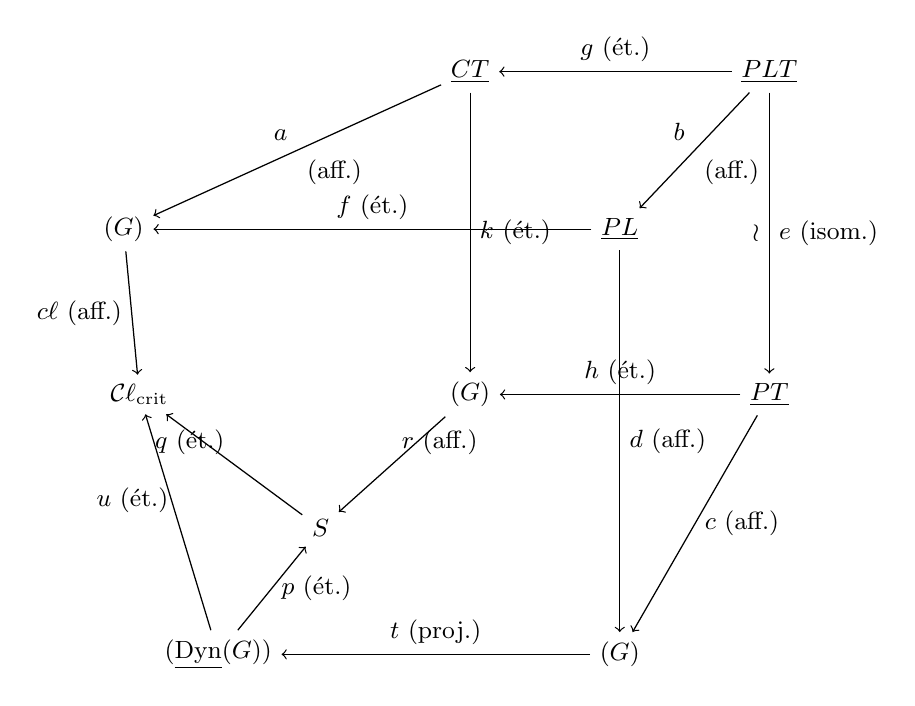
\begin{tikzpicture}[
  >=to,
  every node/.style={font=\small},
  morph/.style={->,line width=.45pt}
]
  \node (CT)     at (5.2,7.2) {\(\underline{CT}\)};
  \node (PLT)    at (9.0,7.2) {\(\underline{PLT}\)};
  \node (Crit)   at (0.8,5.2) {\(\Crit(G)\)};
  \node (PL)     at (7.1,5.2) {\(\underline{PL}\)};
  \node (Cl)     at (1.0,3.1) {\(\mathcal C\ell_{\mathrm{crit}}\)};
  \node (Tor)    at (5.2,3.1) {\(\Tor(G)\)};
  \node (PT)     at (9.0,3.1) {\(\underline{PT}\)};
  \node (S)      at (3.3,1.4) {\(S\)};
  \node (Of)     at (2.0,-.2) {\(\Of(\underline{\operatorname{Dyn}}(G))\)};
  \node (Par)    at (7.1,-.2) {\(\Par(G)\)};

  \draw[morph] (PLT) -- node[above]{\(g\) (ét.)} (CT);
  \draw[morph] (CT) -- node[above left]{\(a\)} node[below right]{(aff.)} (Crit);
  \draw[morph] (PLT) -- node[above left]{\(b\)} node[below right]{(aff.)} (PL);
  \draw[morph] (PL) -- node[above]{\(f\) (ét.)} (Crit);
  \draw[morph] (CT) -- node[right]{\(k\) (ét.)} (Tor);
  \draw[morph] (PLT) -- node[left]{\(\wr\)}
    node[right]{\(e\) (isom.)} (PT);
  \draw[morph] (Crit) -- node[left]{\(c\ell\) (aff.)} (Cl);
  \draw[morph] (PL) -- node[right]{\(d\) (aff.)} (Par);
  \draw[morph] (PT) -- node[above]{\(h\) (ét.)} (Tor);
  \draw[morph] (PT) -- node[right]{\(c\) (aff.)} (Par);
  \draw[morph] (S) -- node[above left]{\(q\) (ét.)} (Cl);
  \draw[morph] (Tor) -- node[above right]{\(r\) (aff.)} (S);
  \draw[morph] (Of) -- node[above left]{\(u\) (ét.)} (Cl);
  \draw[morph] (Of) -- node[right]{\(p\) (ét.)} (S);
  \draw[morph] (Par) -- node[above]{\(t\) (proj.)} (Of);
\end{tikzpicture}
\refstepcounter{figure}
\label{sga3:xxvi:fig:3:15:1}
\par\smallskip
{\small Figure 3.15.1}
\end{figure}
\SGARefTarget{sga3:xxvi:item:3:15}

\begin{sgastatement}{Theorem 3.16 \textup{(cf.\ Figure 3.15.1)}}
\begin{enumerate}[label=\textup{(\roman*)}]
\item Every morphism in the diagram is smooth, surjective, and of finite
presentation.
\item Every morphism except \(t\) is affine; \(t\) is projective.
\item Every morphism is either finite étale or has integral geometric
fibers: \(f,g,h,k,p,q,u\) are finite étale;
\(a,b,c,d,r,c\ell\) have integral geometric fibers; and \(e\) is an
isomorphism.
\item The square \((a,b,f,g)\) is cartesian.
\end{enumerate}
\end{sgastatement}
\SGARefTarget{sga3:xxvi:thm:3:16}

\SGAProof
It is clear from \SGARefLink{sga3:xxvi:proposition:1-6:item:ii}{1.6(ii)} that \(e\) is an isomorphism, and (iv) is
immediate.  The morphism \(a\) is smooth and affine with integral
geometric fibers.  Indeed, after the base change \(\Crit(G)\to S\), this
reduces to the same statement for
\[
 \Tor(L_0)\longrightarrow S,
\]
where \(L_0\) is the universal critical subgroup; \(L_0\) is reductive by
definition, so Exp.\ XXII, \SGARefLink{sga3:xxii:cor:5.8.3}{5.8.3} applies.  By (iv), \(b\) has the same
properties.

The morphism \(d\) is likewise smooth and affine with integral geometric
fibers, by \SGARefLink{sga3:xxvi:cor:1:9}{1.9}; the same is therefore true of
\[
 c=dbe^{-1}.
\]
The morphism \(r\) has these properties by Exp.\ XXII, \SGARefLink{sga3:xxii:cor:5.8.3}{5.8.3}, and
\(c\ell\) by \SGARefLink{sga3:xxvi:item:3:9}{3.10}.

We already know that \(p\) and \(q\) are finite étale and surjective
(\SGARefLink{sga3:xxvi:paragraph:3-1}{3.1} and \SGARefLink{sga3:xxvi:paragraph:3-9}{3.9}).  If \(f\) and \(k\) are finite étale and surjective, then
so is \(g\), by (iv), and so is \(h=kge^{-1}\).  Since the assertions
about \(t\) were proved in \SGARefLink{sga3:xxvi:thm:3:3:item:ii}{3.3(ii)}, it remains only to prove the claim for
\(f\) and \(k\).  We do so for \(k\), the proof for \(f\) being the same.

If \(T\) is a maximal torus of \(G\), let \(\mathcal C\) be the functor of
critical subgroups containing \(T\).  We must show that \(\mathcal C\) is
represented by a finite étale \(S\)-scheme with nonempty fibers.  We may
suppose that \(G\) is split relative to \(T\).  If \(E\) is the set of
vectorial subsets of the root system \(R\), then \(\mathcal C\) is
represented by \(E_S\), by 3.9.
\SGAQED

\begin{sgastatement}{Corollary 3.17}
All the functors in the preceding diagram are representable by
\(S\)-schemes that are smooth over \(S\), and all are affine over \(S\)
except \(\Par(G)\).
\end{sgastatement}
\SGARefTarget{sga3:xxvi:cor:3:17}

\begin{sgastatement}{\SGAInlineRefTarget{sga3:xxvi:remark:3-18}Remark 3.18}
\begin{enumerate}[label=\textup{(\roman*)}]
\item The fact that \(f:PL\to\Crit(G)\) is étale and surjective says that
a subgroup of \(G\) is critical if and only if, locally for the étale
topology, it is a Levi subgroup of a parabolic subgroup.

In general the map \(PL(S)\to\Crit(G)(S)\) need not be surjective: a
critical subgroup \(C\) may fail to arise over \(S\) from a parabolic
subgroup.  For example, a maximal torus need not be contained in a Borel
subgroup, as for a nonsplit form of \(\operatorname{SL}_2\)
\textup{(Exp.\ XX, §5)}.
\item Likewise,
\[
 u:\Of(\underline{\operatorname{Dyn}}(G))
 \longrightarrow\mathcal C\ell_{\mathrm{crit}}
\]
need not be an isomorphism.  Two parabolic subgroups of different types
may have Levi subgroups of the same type.  In a group of type \(A_2\),
for instance, the two types of parabolics whose Levi subgroups have
semisimple rank \(1\) correspond to the two vertices of the diagram,
whereas there is only one type of critical subgroup of rank \(1\).

The analogous example for type \(A_3\) shows that, even over an
algebraically closed field, nonisomorphic parabolic subgroups may have
Levi subgroups of the same type.\footnote{\emph{Editor's note.}
Concretely, in \(\operatorname{GL}_4\), the parabolics
\[
 P=\left\{\begin{pmatrix}
 *&*&*&*\\0&*&*&*\\0&0&*&*\\0&0&0&*
 \end{pmatrix}\right\},
 \qquad
 P'=\left\{\begin{pmatrix}
 *&*&*&*\\0&*&*&*\\0&*&*&*\\0&0&0&*
 \end{pmatrix}\right\}
\]
are not isomorphic (their unipotent radicals are not isomorphic), while
their Levi subgroups
\[
 L=\left\{\begin{pmatrix}
 *&*&0&0\\ *&*&0&0\\0&0&*&0\\0&0&0&*
 \end{pmatrix}\right\},
 \quad
 L'=\left\{\begin{pmatrix}
 *&0&0&0\\0&*&*&0\\0&*&*&0\\0&0&0&*
 \end{pmatrix}\right\}
\]
are conjugate by
\(
\left(\begin{smallmatrix}
0&0&1&0\\0&1&0&0\\1&0&0&0\\0&0&0&1
\end{smallmatrix}\right).
\)}
\end{enumerate}
\end{sgastatement}
\SGARefTarget{sga3:xxvi:rem:3:18}

We end this section with an application to principal bundles.

\begin{sgastatement}{\SGAInlineRefTarget{sga3:xxvi:lemma:3-20}Lemma 3.20}
Let\footnote{\emph{Editor's note.} The numbering of the original is
retained: there is no §3.19.} \(S\) be a scheme, \(G\) an \(S\)-reductive group, \(F\) a principal
homogeneous bundle under \(G\), and \(G_F\) the corresponding twisted form.
Identify \(\underline{\operatorname{Dyn}}(G)\) with
\(\underline{\operatorname{Dyn}}(G_F)\) \textup{(Exp.\ XXIV, \SGARefLink{sga3:xxiv:3.5}{3.5})}.
For every parabolic subgroup \(P\) of \(G\), there is a canonical
isomorphism
\[
 F/P\xrightarrow{\sim}\Par_{t(P)}(G_F).
\]
In particular, the structural group of \(F\) reduces to \(P\) if and only
if \(G_F\) has a parabolic subgroup of type \(t(P)\).
\end{sgastatement}
\SGARefTarget{sga3:xxvi:lemma:3:20}

The proof is exactly the same as that of Exp.\ XXIV, \SGARefLink{sga3:xxiv:proposition:4-2-1}{4.2.1}.

\SGAInlineRefTarget{sga3:xxvi:paragraph:3-21}\paragraph{\SGARefLink{sga3:xxvi:paragraph:3-21}{3.21}.}
If \(S\) is a scheme, \(G\) an \(S\)-reductive group, and
\[
 t\in\Of(\underline{\operatorname{Dyn}}(G))(S),
\]
write \(H^1_t(S,G)\) for the subset of \(H^1(S,G)\) consisting of the
classes of principal \(G\)-bundles \(F\) for which the associated group
\(G_F\) has a parabolic subgroup of type \(t\).  If \(G\) itself has a
parabolic subgroup \(P\) of type \(t\), then \(H^1_t(S,G)\) is precisely
the image of \(H^1(S,P)\) in \(H^1(S,G)\), and hence does not depend on
the chosen \(P\).
\SGARefTarget{sga3:xxvi:item:3:21}

% END INCLUDED SGA3_English_current_buildable_source_20260823/source/inputs/XXVI/tex/components/02_section3.tex

% BEGIN INCLUDED SGA3_English_current_buildable_source_20260823/source/inputs/XXVI/tex/components/03_section4_1_through_4_2_4.tex
\SGASection{4}{Relative position of two parabolic subgroups}
\SGARefTarget{sga3:xxvi:section:4}

\SGASubsection{4.1}{A preliminary result}
\SGARefTarget{sga3:xxvi:subsection:4:1}

\begin{sgastatement}{Lemma 4.1.1}
Let \(k\) be a field, \(G\) a reductive \(k\)-group, and \(P,P'\) two
parabolic subgroups of \(G\).
\begin{enumerate}[label=\textup{(\roman*)}]
\item The intersection \(P\cap P'\) is smooth, has the same reductive
rank as \(G\), and contains a maximal torus \(T\) of \(G\).
\item The set \(R'\) of roots of \(P\cap P'\) relative to \(T\) is a
closed subset of the set \(R\) of roots of \(G\) relative to \(T\).
\end{enumerate}
\end{sgastatement}
\SGARefTarget{sga3:xxvi:lemma:4:1:1}
\footnote{\emph{Editor's note.} Part \textup{(ii)}, which will be useful
in \SGARefLink{sga3:xxvi:proposition:4-5-1}{4.5.1}, was added by the editors.}

\SGAProof
Suppose first that \(k\) is algebraically closed.  Let \(B\) (respectively
\(B'\)) be a Borel subgroup of \(P\) (respectively \(P'\)).  There is an
element \(g\in G(k)\) such that \(\Int(g)B=B'\).  On the other hand, if
\(T_0\) is a maximal torus of \(B\) and \(N=\Norm_G(T_0)\), Bruhat's
theorem (\emph{Bible}, §13.4, Corollary 1 to Theorem 3) gives
\[
 G(k)=B(k)N(k)B(k).
\]
Thus there are \(b,b_1\in B(k)\) and \(n\in N(k)\) such that
\(g=bnb_1\), and hence
\(\Int(b)\Int(n)B=B'\).  Consequently
\[
 P\cap P'\supset B\cap B'
  =\Int(b)\bigl(B\cap\Int(n)B\bigr)
  \supset\Int(b)T_0.
\]

Now let \(k\) be arbitrary.  The preceding result shows that
\(P_{\bar k}\cap P'_{\bar k}\) contains a maximal torus of
\(G_{\bar k}\).  By Exp.\ XXII, \SGARefLink{sga3:xxii:prop:5.4.5}{5.4.5},
\((P\cap P')_{\bar k}\) is smooth along the identity section; since the
base is a field, it is therefore smooth (Exp.\ VI\textsubscript{A},
\SGARefLink{prop:sga3-VIA-1.3.1}{1.3.1}), and so \(P\cap P'\) is smooth.  By Exp.\ VI\textsubscript{A},
\SGARefLink{prop:sga3-VIA-2.3.1}{2.3.1}, the identity component \((P\cap P')^0\) is an open subgroup of
\(P\cap P'\), smooth over \(k\).  Applying Exp.\ XIV, \SGARefLink{sga3:xiv:1.1}{1.1} to it proves
\textup{(i)}.

Finally, the set \(R_P\) (respectively \(R_{P'}\)) of roots of \(P\)
(respectively \(P'\)) relative to \(T\) is closed, and
\[
 R'=R_P\cap R_{P'}.
\]
This proves \textup{(ii)}.
\SGAQED

\begin{sgastatement}{Remark 4.1.2}
One can prove \textup{([BT65], \SGARefLink{sga3:xxvi:subsection:4:5}{4.5})} that \(P\cap P'\) is connected; this
fact will be used in \SGARefLink{sga3:xxvi:proposition:4-5-1}{4.5.1}.
\end{sgastatement}
\SGARefTarget{sga3:xxvi:remark:4:1:2}
\footnote{\emph{Editor's note.} In view of the details added in \SGARefLink{sga3:xxvi:proposition:4-5-1}{4.5.1},
the original wording ``we shall not use this fact'' was changed.}

\begin{sgastatement}{\SGAInlineRefTarget{sga3:xxvi:remark:4-1-3}Remark 4.1.3}
The preceding lemma is false over an arbitrary scheme.  For example, let
\(G\) be a reductive group over an algebraically closed field \(k\), and
let \(B\) be a Borel subgroup of \(G\).  Take \(S=G\) as base and
consider the Borel subgroups \(B_1,B_2\) of \(G_G\), where
\[
 B_1=B_G,\qquad B_2=\Int(g_0)B_1,
\]
and \(g_0\) is the canonical (diagonal) section of \(G_G\).  For every
\(g\in G(k)\), the fiber of \(B_1\cap B_2\) at \(g\) is
\(B\cap\Int(g)B\).  If \(B\ne G\), the dimension of this fiber varies
with \(g\), so \(B_1\cap B_2\) cannot be smooth over \(G\).
\end{sgastatement}
\SGARefTarget{sga3:xxvi:remark:4:1:3}

\SGASubsection{4.2}{Transversal position}
\SGARefTarget{sga3:xxvi:subsection:4:2}

\begin{sgastatement}{\SGAInlineRefTarget{sga3:xxvi:theorem:4-2-1}Theorem 4.2.1}
Let \(S\) be a scheme, \(G\) an \(S\)-reductive group, and \(P,Q\) two
parabolic subgroups of \(G\).  The following conditions on the pair
\((P,Q)\) are equivalent:
\begin{enumerate}[leftmargin=3.2em,labelsep=.7em]
\item[\textup{\SGAInlineRefTarget{sga3:xxvi:theorem:4-2-1:item:i}(i)}]
\(\operatorname{Lie}(P/S)+\operatorname{Lie}(Q/S)
  =\operatorname{Lie}(G/S)\).
\item[\textup{\SGAInlineRefTarget{sga3:xxvi:theorem:4-2-1:item:ii}(ii)}]
The canonical morphism \(P\times_SQ\to G\) is smooth.
\item[\textup{(ii\(^{\prime}\))}]
The canonical morphism \(P\to G/Q\) is smooth.
\item[\textup{\SGAInlineRefTarget{sga3:xxvi:theorem:4-2-1:item:iii}(iii)}]
The canonical morphism \(P\times_SQ\to G\) is open.
\item[\textup{(iii\(^{\prime}\))}]
The canonical morphism \(P\to G/Q\) is open.
\item[\textup{\SGAInlineRefTarget{sga3:xxvi:theorem:4-2-1:item:iv}(iv)}]
The canonical morphism \(P\times_SQ\to G\) is fiberwise dominant.
\item[\textup{(iv\(^{\prime}\))}]
The canonical morphism \(P\to G/Q\) is fiberwise dominant.
\item[\textup{\SGAInlineRefTarget{sga3:xxvi:theorem:4-2-1:item:v}(v)}]
For every \(s\in S\), the group \(P_s\cap Q_s\) has minimum dimension,
that is,
\[
 \dim(P_s\cap Q_s)=\dim P_s+\dim Q_s-\dim G_s.
\]
\item[\textup{\SGAInlineRefTarget{sga3:xxvi:theorem:4-2-1:item:vi}(vi)}]
There is an étale covering family \(\{S_i\to S\}\) and, for every \(i\),
a Borel subgroup \(B_i\) of \(P_{S_i}\) and a Borel subgroup \(B'_i\)
of \(Q_{S_i}\), such that \(B_i\cap B'_i\) is a maximal torus of
\(G_{S_i}\).
\item[\textup{\SGAInlineRefTarget{sga3:xxvi:theorem:4-2-1:item:vii}(vii)}]
There is an étale covering family \(\{S_i\to S\}\) and, for every \(i\),
a splitting \((T_i,\ldots,R_i)\) of \(G_{S_i}\) and a system
\(R_i^+\) of positive roots of \(R_i\), such that \(P_{S_i}\)
(respectively \(Q_{S_i}\)) is the subgroup of type \textup{(R)} of
\(G_{S_i}\) containing \(T_i\) and defined by a subset \(R_i^{(1)}\)
(respectively \(R_i^{(2)}\)) of \(R_i\) containing \(R_i^+\)
(respectively \(-R_i^+\)); see Exp.\ XXII, \SGARefLink{sga3:xxii:def:5.4.2}{5.4.2} and 5.2.1.
\end{enumerate}
\end{sgastatement}
\SGARefTarget{sga3:xxvi:theorem:4:2:1}

\SGAProof
We prove the theorem according to the following logical diagram:
\[
\begin{tikzcd}[column sep=large,row sep=large]
 \textup{(i)} \arrow[d,Rightarrow] &
 \textup{(vii)} \arrow[l,Rightarrow] &
 \textup{(vi)} \arrow[l,Rightarrow] \\
 \textup{(ii\(^{\prime}\))} \arrow[d,Rightarrow] \arrow[r,Rightarrow] &
 \textup{(iii\(^{\prime}\))} \arrow[r,Rightarrow] &
 \textup{(iv\(^{\prime}\))} \arrow[r,Rightarrow] &
 \textup{(v)} \arrow[ul,Rightarrow] \\
 \textup{(ii)} \arrow[r,Rightarrow] &
 \textup{(iii)} \arrow[r,Rightarrow] &
 \textup{(iv)} \arrow[ur,Rightarrow] &
 {} .
\end{tikzcd}
\]

The implications \textup{\SGARefLink{sga3:xxvi:theorem:4-2-1:item:ii}{(ii)}} \(\Rightarrow\) \textup{\SGARefLink{sga3:xxvi:theorem:4-2-1:item:iii}{(iii)}} and
\textup{(ii\(^{\prime}\))} \(\Rightarrow\)
\textup{(iii\(^{\prime}\))} are immediate.  If \textup{\SGARefLink{sga3:xxvi:theorem:4-2-1:item:iii}{(iii)}} holds,
the set-theoretic image of \(P\times_SQ\to G\) is an open subset of
\(G\) containing the identity section.  Since the fibers of \(G\) are
connected, this image is dense in every fiber; thus \textup{\SGARefLink{sga3:xxvi:theorem:4-2-1:item:iv}{(iv)}}
holds.  The implication
\textup{(iii\(^{\prime}\))} \(\Rightarrow\)
\textup{(iv\(^{\prime}\))} is identical.

Condition \textup{(ii\(^{\prime}\))} implies \textup{\SGARefLink{sga3:xxvi:theorem:4-2-1:item:ii}{(ii)}}, by the
cartesian diagram
\[
\begin{tikzcd}[column sep=large,row sep=large]
 P\times_SQ \arrow[r] \arrow[d,"\operatorname{pr}_1"'] & G \arrow[d]\\
 P \arrow[r] & G/Q .
\end{tikzcd}
\]
On the other hand, \textup{(iv)} or \textup{(iv\(^{\prime}\))}
implies \textup{(v)} by dimension theory (EGA
IV\textsubscript{2}, 5.6.6).  Indeed, one may assume
\(S=\operatorname{Spec}(k)\), with \(k\) algebraically closed; every
nonempty fiber of the morphism in \textup{\SGARefLink{sga3:xxvi:theorem:4-2-1:item:iv}{(iv)}} at a point of \(G(k)\),
or of the morphism in \textup{(iv\(^{\prime}\))} at a point of
\((G/Q)(k)\), is isomorphic to \(P\cap Q\).

The implication \textup{\SGARefLink{sga3:xxvi:theorem:4-2-1:item:vi}{(vi)}} \(\Rightarrow\) \textup{\SGARefLink{sga3:xxvi:theorem:4-2-1:item:vii}{(vii)}} follows
from Exp.\ XXII, \SGARefLink{sga3:xxii:prop:5.5.1}{5.5.1} \textup{\SGARefLink{sga3:xxvi:theorem:4-2-1:item:iv}{(iv)}} and \SGARefLink{sga3:xxii:prop:5.9.2}{5.9.2}.  Condition
\textup{\SGARefLink{sga3:xxvi:theorem:4-2-1:item:vii}{(vii)}} implies \textup{\SGARefLink{sga3:xxvi:theorem:4-2-1:item:i}{(i)}}, because the latter may be checked
fpqc-locally.  Under \textup{\SGARefLink{sga3:xxvi:theorem:4-2-1:item:vii}{(vii)}} we may therefore suppose that
\(G\) is split, \(P\supset B_{R^+}\), and
\(Q\supset B_{-R^+}\); then already
\[
 \operatorname{Lie}(B_{R^+})+\operatorname{Lie}(B_{-R^+})
 =\operatorname{Lie}(G).
\]

Let us prove that \textup{\SGARefLink{sga3:xxvi:theorem:4-2-1:item:i}{(i)}} implies
\textup{(ii\(^{\prime}\))}.  Let \(u:P\to G/Q\) be the canonical
morphism.  Smoothness can be checked on geometric fibers, since both
\(P\) and \(G/Q\) are smooth over \(S\); hence we may suppose that
\(S\) is the spectrum of an algebraically closed field.  The morphism
\(u\) is compatible with the evident action of \(P\):
\(u(pp')=p\,u(p')\).  A translation argument (compare the proof of
Exp.\ VI\textsubscript{B}, 1.3) therefore reduces smoothness to the
point \(e\in P(k)\).  By SGA 1, II, 4.7, it is enough that the tangent
map at \(e\) be surjective.  This map is naturally identified with
\[
 \operatorname{Lie}(P)\longrightarrow
 \operatorname{Lie}(G)/\operatorname{Lie}(Q),
\]
which is surjective under \textup{\SGARefLink{sga3:xxvi:theorem:4-2-1:item:i}{(i)}}.

It remains to prove \textup{\SGARefLink{sga3:xxvi:theorem:4-2-1:item:v}{(v)}} \(\Rightarrow\) \textup{\SGARefLink{sga3:xxvi:theorem:4-2-1:item:vi}{(vi)}}.
Suppose first that \(S\) is the spectrum of an algebraically closed
field.  By \SGARefLink{sga3:xxvi:lemma:4:1:1}{4.1.1} there is a maximal torus \(T\) contained in \(P\) and
\(Q\).  Let \(R\), \(R_1\), and \(R_2\) be the respective sets of roots
of \(G\), \(P\), and \(Q\) relative to \(T\).  By Exp.\ XXII, \SGARefLink{sga3:xxii:lem:5.4.4}{5.4.4} and
\SGARefLink{sga3:xxii:prop:5.4.5}{5.4.5},
\[
\begin{aligned}
 \dim G&=\dim T+\operatorname{Card}(R),&
 \dim P&=\dim T+\operatorname{Card}(R_1),\\
 \dim Q&=\dim T+\operatorname{Card}(R_2),&
 \dim(P\cap Q)&=\dim T+\operatorname{Card}(R_1\cap R_2).
\end{aligned}
\]
Condition \textup{\SGARefLink{sga3:xxvi:theorem:4-2-1:item:v}{(v)}} is therefore equivalent to
\[
 \operatorname{Card}(R_1\cap R_2)
 =\operatorname{Card}(R_1)+\operatorname{Card}(R_2)
  -\operatorname{Card}(R),
\]
that is, to \(R_1\cup R_2=R\).  By Exp.\ XXII, \SGARefLink{sga3:xxii:prop:5.9.2}{5.9.2} and \SGARefLink{sga3:xxii:prop:5.4.5}{5.4.5}, it is
enough to prove that \(R_1\cap(-R_2)\) contains a system of positive
roots of \(R\).  We are thus reduced to the following lemma.

\begin{sgastatement}{Lemma 4.2.2}
Let \(R\) be a ``root system''---for example, the set of roots of a root
datum in the sense of Exposé XXI.  Let \(R_1,R_2\) be two closed subsets
of \(R\), each containing a system of positive roots.  If
\(R_1\cup R_2=R\), then \(R_1\cap(-R_2)\) contains a system of positive
roots.
\end{sgastatement}
\SGARefTarget{sga3:xxvi:lemma:4:2:2}

Indeed, \(R_3=R_1\cap(-R_2)\) is closed, so by Exp.\ XXI, \SGARefLink{sga3:XXI:3.3.6}{3.3.6} it is
enough to show that \(R_3\cup(-R_3)=R\).  Now
\[
 R_1\cup(-R_1)=R=R_2\cup(-R_2),
\]
and the conclusion follows from the following elementary fact.  If
\(A,A',B,B'\) are four subsets of a set \(E\), and
\[
 A\cup A'=B\cup B'=A\cup B=A'\cup B'=E,
\]
then
\[
 (A\cap B')\cup(A'\cap B)=E.
\]

This proves \textup{\SGARefLink{sga3:xxvi:theorem:4-2-1:item:v}{(v)}} \(\Rightarrow\) \textup{\SGARefLink{sga3:xxvi:theorem:4-2-1:item:vi}{(vi)}} over the
spectrum of an algebraically closed field.  Return now to the general
case and suppose \textup{\SGARefLink{sga3:xxvi:theorem:4-2-1:item:v}{(v)}} holds.  Let \(s\in S\).  By the preceding
argument, there is a Borel subgroup \(\bar B\) of \(P_{\bar s}\) and a
Borel subgroup \(\bar B'\) of \(Q_{\bar s}\) such that
\(\bar B\cap\bar B'\) is a maximal torus of \(G_{\bar s}\).

The \(S\)-scheme
\[
 \Bor(P)\simeq\Bor\bigl(P/\rad^u(P)\bigr)
\]
of Borel subgroups of \(P\) is smooth.  Applying ``Hensel's lemma''
(Exp.\ XI, \SGARefLink{sga3:xi:proposition:1:10}{1.10}) and working étale-locally around \(s\), we may suppose
that there is a Borel subgroup \(B\) of \(P\) specializing to
\(\bar B\).  Similarly, there is a Borel subgroup \(B'\) of \(Q\)
specializing to \(\bar B'\).  Since
\(\bar B\cap\bar B'\) is a maximal torus of \(G_{\bar s}\), some open
neighborhood \(U\) of \(s\) has the property that
\(B_U\cap B'_U\) is a maximal torus of \(G_U\)
(Exp.\ XXII, \SGARefLink{sga3:xxii:cor:5.9.4}{5.9.4}).  This proves \textup{\SGARefLink{sga3:xxvi:theorem:4-2-1:item:vi}{(vi)}}.
\SGAQED

\begin{sgastatement}{Definition 4.2.3}
A pair \((P,Q)\) satisfying the equivalent conditions
\textup{\SGARefLink{sga3:xxvi:theorem:4-2-1:item:i}{(i)}}--\textup{\SGARefLink{sga3:xxvi:theorem:4-2-1:item:vii}{(vii)}} of \SGARefLink{sga3:xxvi:theorem:4-2-1}{Theorem 4.2.1} is said to be in
\emph{transversal position}.  One also says that \(P\) is in
transversal position relative to \(Q\), or, by an abuse of language,
that \(P\) and \(Q\) are in (mutual) transversal position.
\end{sgastatement}
\SGARefTarget{sga3:xxvi:def:4:2:3}

In view of \textup{\SGARefLink{sga3:xxvi:theorem:4-2-1:item:vi}{(vi)}}, this definition agrees, for Borel subgroups,
with that of Exp.\ XXII, \SGARefLink{sga3:xxii:def:5.9.1}{5.9.1}.

\begin{sgastatement}{\SGAInlineRefTarget{sga3:xxvi:corollary:4-2-4}Corollary 4.2.4}
Let \(S\) be a scheme, \(G\) an \(S\)-reductive group, and \(P,Q\) two
parabolic subgroups of \(G\).
\begin{enumerate}[label=\textup{(\roman*)}]
\item The pair \((P,Q)\) is in transversal position if and only if, for
every \(s\in S\), the pair \((P_{\bar s},Q_{\bar s})\) is in transversal
position.  If \(S'\to S\) is surjective and
\((P_{S'},Q_{S'})\) is in transversal position, then so is \((P,Q)\).
\item There is an open subscheme \(U\subset S\) with the following
property: a morphism \(S'\to S\) factors through \(U\) if and only if
\((P_{S'},Q_{S'})\) is in transversal position.
\item Consider the subfunctors
\[
 \Gen(G)\subset\Par(G)\times_S\Par(G),\qquad
 \Gen(/Q)\subset\Par(G),\qquad
 \Gen(P/Q)\subset G,
\]
defined as follows.  For \(S'\to S\), the set \(\Gen(G)(S')\) consists
of pairs of parabolic subgroups of \(G_{S'}\) in transversal position;
\(\Gen(/Q)(S')\) consists of parabolic subgroups of \(G_{S'}\) in
transversal position relative to \(Q_{S'}\); and \(\Gen(P/Q)(S')\)
consists of the \(g\in G(S')\) such that \(\Int(g)P_{S'}\) is in
transversal position relative to \(Q_{S'}\).

Each of these functors is represented by an open subscheme,
universally schematically dense over \(S\), of the corresponding
\(S\)-scheme
\[
 \Par(G)\times_S\Par(G),\qquad\Par(G),\qquad G,
\]
respectively.
\end{enumerate}
\end{sgastatement}
\SGARefTarget{sga3:xxvi:cor:4:2:4}
\footnote{\emph{Editor's note.} The original expression ``relatively
dense'' was replaced by ``universally schematically dense over \(S\)'';
compare EGA IV\textsubscript{3}, Definition 11.10.8.}

Assertion \textup{\SGARefLink{sga3:xxvi:theorem:4-2-1:item:i}{(i)}} follows immediately from condition
\SGARefLink{sga3:xxvi:theorem:4-2-1}{4.2.1}\textup{\SGARefLink{sga3:xxvi:theorem:4-2-1:item:i}{(i)}}.  For \textup{\SGARefLink{sga3:xxvi:theorem:4-2-1:item:ii}{(ii)}}, take
\[
 U=S-\operatorname{Supp}(\operatorname{Coker}u),
\]
where
\[
 u:\operatorname{Lie}(P)\oplus\operatorname{Lie}(Q)
   \longrightarrow\operatorname{Lie}(G)
\]
is the canonical morphism.\footnote{\emph{Editor's note.} The second
summand, printed as \(\operatorname{Lie}(G)\), has been corrected to
\(\operatorname{Lie}(Q)\); this is the map used in \SGARefLink{sga3:xxvi:theorem:4-2-1}{Theorem
4.2.1}\textup{\SGARefLink{sga3:xxvi:theorem:4-2-1:item:i}{(i)}}.}

There are cartesian diagrams
\[
\begin{tikzcd}[column sep=large,row sep=large]
 G \arrow[r,"f"] & \Par(G)\\
 \Gen(P/Q) \arrow[u,hook] \arrow[r] & \Gen(/Q)\arrow[u,hook]
\end{tikzcd}
\qquad
\begin{tikzcd}[column sep=large,row sep=large]
 \Par(G) \arrow[r,"f'"] & \Par(G)\times_S\Par(G)\\
 \Gen(/Q) \arrow[u,hook] \arrow[r] & \Gen(G)\arrow[u,hook],
\end{tikzcd}
\]
where \(f(g)=\Int(g)P\) and \(f'(R)=(R,Q)\).  It therefore suffices to
prove \textup{\SGARefLink{sga3:xxvi:theorem:4-2-1:item:iii}{(iii)}} for \(\Gen(G)\).

Let \(P_0\) be the canonical parabolic subgroup of
\(G_{\Par(G)}\), and set
\[
 X=\Par(G)\times_S\Par(G),\qquad
 P=\operatorname{pr}_1^*(P_0),\qquad
 Q=\operatorname{pr}_2^*(P_0).
\]
Applying \textup{\SGARefLink{sga3:xxvi:theorem:4-2-1:item:ii}{(ii)}} to the parabolic subgroups \(P,Q\) of \(G_X\)
constructs an open subscheme \(U\subset X\), which is immediately
identified with \(\Gen(G)\).  The density assertion may be checked on
geometric fibers,\footnote{\emph{Editor's note.} Compare EGA
IV\textsubscript{3}, 11.10.10.} so assume
\(S=\operatorname{Spec}(k)\), where \(k\) is algebraically closed.
Since \(\Par(G)\) is smooth, it is enough to show that \(\Gen(G)\)
meets every irreducible component of
\(\Par(G)\times_S\Par(G)\).  By \SGARefLink{sga3:xxvi:item:3:2}{3.3}, this amounts to the following:
given \(t,t'\in\Of(\underline{\operatorname{Dyn}}(G))(S)\), find a pair
\((P,P')\) in transversal position such that \(t(P)=t\) and
\(t(P')=t'\).

Choose Borel subgroups \(B,B'\) of \(G\) such that \(B\cap B'\) is a
maximal torus (split \(G\) and apply Exp.\ XXII, \SGARefLink{sga3:xxii:prop:5.9.2}{5.9.2}).  By \SGARefLink{sga3:xxvi:lemma:3:8}{3.8} there
are parabolic subgroups \(P\supset B\) and \(P'\supset B'\) with
\(t(P)=t\) and \(t(P')=t'\).  They have the required types and are in
transversal position by \SGARefLink{sga3:xxvi:theorem:4-2-1}{4.2.1}\textup{\SGARefLink{sga3:xxvi:theorem:4-2-1:item:vi}{(vi)}}.
\SGAQED

% END INCLUDED SGA3_English_current_buildable_source_20260823/source/inputs/XXVI/tex/components/03_section4_1_through_4_2_4.tex

% BEGIN INCLUDED SGA3_English_current_buildable_source_20260823/source/inputs/XXVI/tex/components/04_section4_2_5_through_4_2_7.tex
\begin{sgastatement}{\SGAInlineRefTarget{sga3:xxvi:corollary:4-2-5}Corollary 4.2.5}
Let \(S\) be a scheme, \(G\) an \(S\)-reductive group, and \(P,Q\) two
parabolic subgroups of \(G\), with \((P,Q)\) in transversal position.
\begin{enumerate}[label=\textup{(\roman*)}]
\item Let \(P',Q'\) be parabolic subgroups of \(G\) of the same types as
\(P,Q\), respectively.  The pair \((P',Q')\) is in transversal position
if and only if, étale-locally, it is conjugate to \((P,Q)\).
\textup{(In §5 we shall see that the étale topology can be replaced by
the Zariski topology.)}
\item The canonical morphism \(P\times_SQ\to G\) induces a smooth
surjective morphism
\[
 P\times_SQ\longrightarrow\Gen(Q/P)
\]
and an isomorphism
\[
 (P\times_SQ)/(P\cap Q)\xrightarrow{\sim}\Gen(Q/P),
\]
where \(R=P\cap Q\) acts on \(P\times_SQ\) by
\[
 (p,q)r=(pr,r^{-1}q).
\]
\item The canonical morphism
\[
 P\longrightarrow\Par_{t(Q)}(G),\qquad p\longmapsto\Int(p)Q,
\]
induces a smooth surjective morphism
\[
 P\longrightarrow\Gen(/P)\cap\Par_{t(Q)}(G)
\]
and an isomorphism
\[
 P/(P\cap Q)\xrightarrow{\sim}
 \Gen(/P)\cap\Par_{t(Q)}(G).
\]
\item The canonical morphism
\[
 G\longrightarrow\Par_{t(P)}(G)\times_S\Par_{t(Q)}(G),\qquad
 g\longmapsto\bigl(\Int(g)P,\Int(g)Q\bigr),
\]
induces a smooth surjective morphism
\[
 G\longrightarrow
 \Gen(G)\cap
 \bigl(\Par_{t(P)}(G)\times_S\Par_{t(Q)}(G)\bigr)
\]
and an isomorphism
\[
 G/(P\cap Q)\xrightarrow{\sim}
 \Gen(G)\cap
 \bigl(\Par_{t(P)}(G)\times_S\Par_{t(Q)}(G)\bigr).
\]
\end{enumerate}
\end{sgastatement}
\SGARefTarget{sga3:xxvi:cor:4:2:5}

\SGAProof
Let us prove \textup{(i)}.  The stated condition is plainly sufficient.
Conversely, suppose \((P',Q')\) is in transversal position.  Since
\(P\) and \(P'\) are conjugate étale-locally, we may assume \(P=P'\).
It is then enough to show that two parabolic subgroups \(Q,Q'\), of the
same type and both in transversal position relative to \(P\), are
étale-locally conjugate by a section of \(P\).

By \SGARefLink{sga3:xxvi:theorem:4-2-1}{4.2.1}\textup{\SGARefLink{sga3:xxvi:theorem:4-2-1:item:vi}{(vi)}}, after another étale localization there are Borel
subgroups \(B,B'\subset P\), \(B_1\subset Q\), and \(B'_1\subset Q'\)
such that
\[
 B\cap B_1=T,\qquad B'\cap B'_1=T'
\]
are maximal tori of \(G\).  The Killing pairs \((B,T)\) and
\((B',T')\) of \(P\) are étale-locally conjugate in \(P\) (\SGARefLink{sga3:xxvi:lemma:1:16}{1.16}).
We may therefore assume \(B=B'\) and \(T=T'\).  Then
\(B_1=B'_1\) by Exp.\ XXII, \SGARefLink{sga3:xxii:prop:5.9.2}{5.9.2}, and hence \(Q=Q'\) by \SGARefLink{sga3:xxvi:lemma:3:8}{3.8}.

Parts \textup{(ii)}, \textup{(iii)}, and \textup{(iv)} are proved in
parallel.  We prove \textup{(ii)}.  Let \(g\in\Gen(Q/P)(S)\); thus
\(g\in G(S)\) and \(\Int(g)Q\) is in transversal position relative to
\(P\).  The preceding argument shows that \(Q\) and \(\Int(g)Q\) are,
étale-locally, conjugate by a section of \(P\).  Working locally for
this topology, choose \(p\in P(S)\) such that
\(\Int(g)Q=\Int(p)Q\).  Then
\[
 p^{-1}g\in\Norm_G(Q)(S)=Q(S),
\]
so \(g=pq\) for some \(q\in Q(S)\).  Thus the morphism in
\textup{\SGARefLink{sga3:xxvi:theorem:4-2-1:item:ii}{(ii)}} is an étale covering.  Comparing with
\SGARefLink{sga3:xxvi:theorem:4-2-1}{4.2.1}\textup{\SGARefLink{sga3:xxvi:theorem:4-2-1:item:ii}{(ii)}}, it is smooth and surjective.

Finally, the equivalence relation on \(P\times_SQ\) defined by
\(P\times_SQ\to G\) is exactly the relation associated with the action
of \(R=P\cap Q\),
\[
 (p,q)r=(pr,r^{-1}q).
\]
This proves the quotient assertion, since a smooth surjective morphism
is, in particular, an effective epimorphism.
\SGAQED

\begin{sgastatement}{Remark 4.2.6}
If \(P,Q\) are in transversal position, the open subset \(\Gen(Q/P)\)
of \(G\) will often be denoted \(P\cdot Q\); this notation is justified
by \SGARefLink{sga3:xxvi:corollary:4-2-5}{4.2.5}\textup{(ii)}.
\end{sgastatement}
\SGARefTarget{sga3:xxvi:remark:4:2:6}

\begin{sgastatement}{\SGAInlineRefTarget{sga3:xxvi:proposition:4-2-7}Proposition 4.2.7}
Let \(S\) be a scheme, \(G\) an \(S\)-reductive group, and \(P,Q\) two
parabolic subgroups of \(G\), with \((P,Q)\) in transversal position.
\begin{enumerate}[label=\textup{(\roman*)}]
\item The group \(P\cap Q\) is smooth over \(S\) (and in fact has
connected fibers by \SGARefLink{sga3:xxvi:remark:4:1:2}{4.1.2}).  Its identity component
\((P\cap Q)^0\) \textup{(Exp.\ VI\textsubscript{B}, \SGARefLink{thm:sga3-VIB-3.10}{3.10})} is a
subgroup of type \textup{(RC)} of \(G\)
\textup{(Exp.\ XXII, \SGARefLink{sga3:xxii:def:5.11.1}{5.11.1})}, and its unipotent radical
\textup{(loc.\ cit., 5.11.4)} decomposes as the direct product
\[
 \rad^u\bigl((P\cap Q)^0\bigr)
 =
 \bigl(\rad^u(P)\cap Q\bigr)
 \times_S
 \bigl(P\cap\rad^u(Q)\bigr).
\]
\item If \(S\) is affine, then
\[
 H^1\bigl(S,\rad^u((P\cap Q)^0)\bigr)=0.
\]
If \(S\) is semilocal, \(P\cap Q\) contains a maximal torus of \(G\).
\end{enumerate}
\end{sgastatement}
\SGARefTarget{sga3:xxvi:prop:4:2:7}

\SGAProof
The group \(P\cap Q\) is smooth by \SGARefLink{sga3:xxvi:theorem:4-2-1}{4.2.1}\textup{\SGARefLink{sga3:xxvi:theorem:4-2-1:item:ii}{(ii)}} and the
cartesian diagram
\[
\begin{tikzcd}[column sep=large,row sep=large]
 P\times_SQ \arrow[r] & G\\
 P\cap Q \arrow[u] \arrow[r] & S\arrow[u]
\end{tikzcd}.
\]

The remaining assertions about \((P\cap Q)^0\) may be checked
étale-locally.  By \SGARefLink{sga3:xxvi:theorem:4-2-1}{4.2.1}\textup{\SGARefLink{sga3:xxvi:theorem:4-2-1:item:vii}{(vii)}}, choose a splitting
\((G,T,M,R)\) of \(G\) such that \(P,Q\) contain \(T\) and are defined
by subsets \(R_1,R_2\) of \(R\), where \(R_1\) contains a system
\(R^+\) of positive roots and \(R_2\) contains the opposite system
\(R^-\).  Let \(\Delta\) be the set of simple roots of \(R^+\), and put
\[
 A_1=\Delta\cap(-R_1),\qquad
 A_2=\Delta\cap R_2,\qquad
 A=A_1\cap A_2.
\]
By \SGARefLink{sga3:xxvi:prop:1:3}{1.4}\textup{(v)} and \SGARefLink{sga3:xxvi:proposition:1-12}{1.12},
\[
\begin{aligned}
 R_1&=R^+\cup\bigl(R^-\cap(-\mathbb N A_1)\bigr),&
 R_2&=\bigl(R^+\cap\mathbb N A_2\bigr)\cup R^-,\\
 \rad^u(P)&=
   \prod_{\substack{\alpha\in R_1\\\alpha\notin-R_1}}U_\alpha,&
 \rad^u(Q)&=
   \prod_{\substack{\alpha\in R_2\\\alpha\notin-R_2}}U_\alpha.
\end{aligned}
\]
Exp.\ XXII, \SGARefLink{sga3:xxii:cor:5.6.7}{5.6.7} therefore gives
\[
\begin{aligned}
 \rad^u(P)\cap Q
  &=
  \prod_{\substack{\alpha\in R_1\cap R_2\\\alpha\notin-R_1}}U_\alpha
  =\prod_{\alpha\in K_2}U_\alpha,\\
 \rad^u(Q)\cap P
  &=
  \prod_{\substack{\alpha\in R_1\cap R_2\\\alpha\notin-R_2}}U_\alpha
  =\prod_{\alpha\in K_1}U_\alpha,
\end{aligned}
\]
where \(K_2\) consists of the positive roots that are linear
combinations of elements of \(A_2\), but not of elements of \(A\), and
\(K_1\) consists of the negative roots that are linear combinations of
elements of \(A_1\), but not of elements of \(A\).  If
\(\alpha\in K_2\) and \(\beta\in K_1\), then \(\alpha+\beta\) is neither
a root nor zero.  Hence the two groups displayed above commute.

By Exp.\ XXII, \SGARefLink{sga3:xxii:prop:5.4.5}{5.4.5}, the group
\[
 H=(P\cap Q)^0
\]
is defined by the set of roots
\[
 R_1\cap R_2
 =
 \bigl(R^+\cap\mathbb N A_2\bigr)
 \cup
 \bigl(R^-\cap(-\mathbb N A_1)\bigr).
\]
This set is closed, so \(H\) is of type \textup{(RC)} by definition
(Exp.\ XXII, \SGARefLink{sga3:xxii:def:5.11.1}{5.11.1}).  By loc.\ cit., \SGARefLink{sga3:xxii:lem:5.11.3}{5.11.3} and \SGARefLink{sga3:xxii:prop:5.11.4}{5.11.4},
\[
 \rad^u(H)=\prod_{\alpha\in K}U_\alpha,
\]
where \(K\) consists of the \(\alpha\in R_1\cap R_2\) such that
\(\alpha\notin-(R_1\cap R_2)\).  The symmetric part of
\(R_1\cap R_2\) is \(R\cap\mathbb ZA\), and therefore
\(K=K_1\cup K_2\).  This proves \textup{(i)}.

The first assertion of \textup{(ii)} follows from \textup{(i)} and
\SGARefLink{sga3:xxvi:cor:2:10}{2.10}.  For the second, the reductive group
\[
 (P\cap Q)^0/\rad^u((P\cap Q)^0)
\]
has a maximal torus \(\bar T\) when the base is semilocal.  The inverse
image \(N\) of \(\bar T\) in \((P\cap Q)^0\) is a subgroup of type
\textup{(R)} of \(G\), with solvable fibers, and
\[
 N^u=\rad^u((P\cap Q)^0)
\]
(Exp.\ XXII, \SGARefLink{sga3:xxii:prop:5.6.9}{5.6.9}).  The scheme of maximal tori of \(N\) is a
principal homogeneous bundle under \(N^u\) (loc.\ cit., \SGARefLink{sga3:xxii:cor:5.6.13}{5.6.13}), and
therefore has a section because \(H^1(S,N^u)=0\).
\SGAQED

% END INCLUDED SGA3_English_current_buildable_source_20260823/source/inputs/XXVI/tex/components/04_section4_2_5_through_4_2_7.tex

% BEGIN INCLUDED SGA3_English_current_buildable_source_20260823/source/inputs/XXVI/tex/components/05_section4_3.tex
\SGASubsection{4.3}{Opposite parabolic subgroups}
\SGARefTarget{sga3:xxvi:subsection:4:3}

\SGAInlineRefTarget{sga3:xxvi:paragraph:4-3-1}\paragraph{\SGARefLink{sga3:xxvi:paragraph:4-3-1}{4.3.1}.}
Let \(G\) be an \(S\)-reductive group.  Exp.\ XXIV, \SGARefLink{sga3:xxiv:proposition:3-16-6}{3.16.6} defines a
canonical ``outer automorphism'' \(s_G\) of \(G\), of order at most
\(2\).\footnote{\emph{Editor's note.} ``Of order \(2\)'' was replaced
by ``of order at most \(2\)'', since \(s_G\) may be trivial, for example
when \(G\) has type \(A_1,B_n,C_n,\ldots\).}  It induces a canonical
automorphism, again of order at most \(2\), of
\(\underline{\operatorname{Dyn}}(G)\), and hence of
\(\Of(\underline{\operatorname{Dyn}}(G))\).  We denote all of these
automorphisms by \(s_G\), or simply by \(s\).  Two types of parabolic
subgroups
\[
 t,t'\in\Of(\underline{\operatorname{Dyn}}(G))(S)
\]
are said to be \emph{opposite} if \(t=s_G(t')\).
\SGARefTarget{sga3:xxvi:item:4:3:1}

\begin{sgastatement}{Theorem 4.3.2}
Let \(S\) be a scheme, \(G\) an \(S\)-reductive group, and \(P\) a
parabolic subgroup of \(G\).

\textup{(a)} If \(L\) is a Levi subgroup of \(P\), there is a unique
parabolic subgroup \(P'\) of \(G\) such that \(P\cap P'=L\).

\textup{(b)} For every parabolic subgroup \(Q\) of \(G\), the following
conditions are equivalent:
\begin{enumerate}[leftmargin=3.2em,labelsep=.7em]
\item[\textup{\SGAInlineRefTarget{sga3:xxvi:item:4:3:1:item:i}(i)}]
For every \(s\in S\), the identity component
\(\bigl((P\cap Q)_{\bar s}\bigr)^0\), which is smooth by \SGARefLink{sga3:xxvi:lemma:4:1:1}{4.1.1}, is
reductive.
\item[\textup{\SGAInlineRefTarget{sga3:xxvi:item:4:3:1:item:ii}(ii)}]
The group \(P\cap Q\) is a Levi subgroup of both \(P\) and \(Q\).
\item[\textup{\SGAInlineRefTarget{sga3:xxvi:item:4:3:1:item:iii}(iii)}]
The groups \(P,Q\) have opposite types and the pair \((P,Q)\) is in
transversal position.
\item[\textup{\SGAInlineRefTarget{sga3:xxvi:item:4:3:1:item:iv}(iv)}]
The groups \(P,Q\) have opposite types and
\(\rad^u(P)\cap Q=e\).
\item[\textup{\SGAInlineRefTarget{sga3:xxvi:item:4:3:1:item:v}(v)}]
\[
 \rad^u(P)\cap Q=\rad^u(Q)\cap P=e.
\]
\item[\textup{\SGAInlineRefTarget{sga3:xxvi:item:4:3:1:item:vi}(vi)}]
The canonical morphism \(\rad^u(P)\times_SQ\to G\) is an open immersion.
\item[\textup{(vi\(^{\prime}\))}]
The canonical morphism \(\rad^u(P)\to G/Q\) is an open immersion.
\item[\textup{\SGAInlineRefTarget{sga3:xxvi:item:4:3:1:item:vii}(vii)}]
There is an étale covering family \(\{S_i\to S\}\) and, for every \(i\),
a splitting \((T_i,M_i,R_i)\) of \(G_{S_i}\) and a subset
\(R_i^{(1)}\subset R_i\), such that \(P_{S_i}\) is the subgroup of type
\textup{(R)} containing \(T_i\) and defined by \(R_i^{(1)}\), while
\(Q_{S_i}\) is the subgroup defined by
\[
 R_i^{(2)}=-R_i^{(1)}.
\]
\end{enumerate}
\end{sgastatement}
\SGARefTarget{sga3:xxvi:theorem:4:3:2}

\SGAProof
We first prove part \textup{(b)}.  Conditions \textup{\SGARefLink{sga3:xxvi:theorem:4-2-1:item:iii}{(iii)}} and
\textup{\SGARefLink{sga3:xxvi:theorem:4-2-1:item:vii}{(vii)}} are equivalent by \SGARefLink{sga3:xxvi:theorem:4-2-1}{4.2.1}\textup{\SGARefLink{sga3:xxvi:theorem:4-2-1:item:vii}{(vii)}} and the
definition of \(s_G\) in the split case (Exp.\ XXIV,
\SGARefLink{sga3:xxiv:proposition:3-16-2}{3.16.2}\textup{\SGARefLink{sga3:xxiv:proposition:3-16-2:item:iv}{(iv)}}).  Plainly \textup{\SGARefLink{sga3:xxiv:proposition:3-16-2:item:ii}{(ii)}} implies \textup{\SGARefLink{sga3:xxiv:proposition:3-16-2:item:i}{(i)}}, and
\textup{(vi\(^{\prime}\))} implies \textup{\SGARefLink{sga3:xxvi:theorem:4-2-1:item:vi}{(vi)}} by base change along
\(G\to G/Q\).

Suppose now that \textup{\SGARefLink{sga3:xxvi:item:4:3:1:item:vii}{(vii)}} holds.  Since every assertion to be
proved is étale-local, assume that \(G=(G,T,M,R)\) is split, that \(P\)
is defined by \(R'\subset R\), and that \(Q\) is defined by \(-R'\).
Let \(L\) be the subgroup of type \textup{(R)} containing \(T\) and
defined by \(R'\cap(-R')\).  By Exp.\ XXII, \SGARefLink{sga3:xxii:lem:5.11.3}{5.11.3}, \(L\) is a Levi
subgroup of both \(P\) and \(Q\).  Moreover,
\[
 P=L\cdot\rad^u(P),\qquad Q=L\cdot\rad^u(Q),
\]
and Exp.\ XXII, \SGARefLink{sga3:xxii:cor:5.6.7}{5.6.7} gives
\[
 \rad^u(P)\cap Q=Q\cap\rad^u(P)=e.
\]
Thus \(P\cap Q=L\), proving \textup{\SGARefLink{sga3:xxii:cor:5.6.7:item:ii}{(ii)}} and \textup{\SGARefLink{sga3:xxvi:item:4:3:1:item:v}{(v)}}.

Since \(P,Q\) are in transversal position, the canonical morphism
\(P\to G/Q\) induces an open immersion
\[
 P/(P\cap Q)\longrightarrow G/Q
\]
by \SGARefLink{sga3:xxvi:theorem:4-2-1}{4.2.1}.  The canonical morphism
\[
 \rad^u(P)\longrightarrow P/(P\cap Q)=P/L
\]
is an isomorphism, so \textup{(vi\(^{\prime}\))} follows.  Hence all
the conditions follow from \textup{\SGARefLink{sga3:xxvi:theorem:4-2-1:item:vii}{(vii)}}.

It remains to show that each of \textup{\SGARefLink{sga3:xxvi:item:4:3:1:item:i}{(i)}}, \textup{\SGARefLink{sga3:xxvi:item:4:3:1:item:iv}{(iv)}},
\textup{\SGARefLink{sga3:xxvi:item:4:3:1:item:v}{(v)}}, and \textup{\SGARefLink{sga3:xxvi:item:4:3:1:item:vi}{(vi)}} implies \textup{\SGARefLink{sga3:xxvi:item:4:3:1:item:vii}{(vii)}}.  Since the
equivalence of \textup{\SGARefLink{sga3:xxvi:item:4:3:1:item:ii}{(ii)}} and \textup{\SGARefLink{sga3:xxvi:item:4:3:1:item:iii}{(iii)}} is already known, this
may be checked on geometric fibers.  We may suppose that \(S\) is the
spectrum of an algebraically closed field.  By \SGARefLink{sga3:xxvi:lemma:4:1:1}{4.1.1}, a maximal torus
\(T\) of \(G\) is contained in \(P\cap Q\).  Let \(R,R_1,R_2\) be the
sets of roots of \(G,P,Q\), respectively, relative to \(T\).  Write
\[
 R_1^a=\{\alpha\in R_1\mid-\alpha\notin R_1\},
\]
and define \(R_2^a\) similarly.  We must prove \(R_1=-R_2\).

\begin{itemize}[leftmargin=2em]
\item Condition \textup{\SGARefLink{sga3:xxvi:item:4:3:1:item:i}{(i)}} says that \(R_1\cap R_2\) is symmetric.
If \(\alpha\in R_1\) and \(\alpha\notin R_2\), then
\(\alpha\in-R_2\); if \(\alpha\in R_2\), then
\[
 \alpha\in R_1\cap R_2=-(R_1\cap R_2)\subset-R_2.
\]
Thus \(R_1\subset-R_2\), and symmetry gives \(R_1=-R_2\).

\item Condition \textup{\SGARefLink{sga3:xxvi:item:4:3:1:item:iv}{(iv)}} gives
\(\operatorname{Card}(R_1)=\operatorname{Card}(R_2)\) and
\(R_1^a\cap R_2=\varnothing\).  The latter condition is equivalent to
\(R_2\subset-R_1\), and equality of cardinalities then gives
\(R_2=-R_1\).

\item Condition \textup{\SGARefLink{sga3:xxvi:item:4:3:1:item:v}{(v)}} gives
\[
 R_1^a\cap R_2=R_2^a\cap R_1=\varnothing.
\]
Hence \(R_2\subset-R_1\) and \(R_1\subset-R_2\), so again
\(R_2=-R_1\).

\item Condition \textup{\SGARefLink{sga3:xxvi:item:4:3:1:item:vi}{(vi)}} gives
\[
 \operatorname{Lie}(\rad^u(P))\oplus\operatorname{Lie}(Q)
 =\operatorname{Lie}(G).
\]
Thus \(R\) is the disjoint union of \(R_2\) and \(R_1^a\), which implies
\(R_2=-R_1\).
\end{itemize}

This proves part \textup{(b)}.  For part \textup{(a)}, the implication
\textup{\SGARefLink{sga3:xxvi:item:4:3:1:item:vii}{(vii)}} \(\Rightarrow\) \textup{\SGARefLink{sga3:xxvi:item:4:3:1:item:ii}{(ii)}} already gives the desired
parabolic subgroup \(P'\) étale-locally.  It remains only to prove
uniqueness, and this too is étale-local.  We may suppose that \(G\) is
split relative to a maximal torus \(T\) of \(L\), with \(P\) and \(P'\)
defined by subsets \(R_1\) and \(R'_1\) of \(R\).  By hypothesis
\(R_1\cap R'_1\) is symmetric.  The preceding argument gives
\(R'_1=-R_1\); hence \(P'\) is determined by \(P\) and \(L\).
\SGAQED

\begin{sgastatement}{\SGAInlineRefTarget{sga3:xxvi:definition:4-3-3}Definition 4.3.3}
Two parabolic subgroups of \(G\) satisfying the equivalent conditions
\textup{(i)}--\textup{\SGARefLink{sga3:xxvi:item:4:3:1:item:vii}{(vii)}} of \SGARefLink{sga3:xxvi:item:4:3:1}{Theorem 4.3.2} are said to be
\emph{opposite}.  If \(P\) is a parabolic subgroup of \(G\) and \(L\)
is a Levi subgroup of \(P\), the \emph{parabolic subgroup opposite to
\(P\) relative to \(L\)} is the unique parabolic subgroup \(Q\) of
\(G\) such that \(P\cap Q=L\).

If \(T\) is a maximal torus of \(P\), the \emph{parabolic subgroup
opposite to \(P\) relative to \(T\)} is the unique \(Q\) such that
\(P\cap Q\) is the unique Levi subgroup of \(P\) containing \(T\)
\textup{(\SGARefLink{sga3:xxvi:proposition:1-6}{1.6})}; equivalently, it is the unique \(Q\) such that
\(P\cap Q\) contains \(T\) and \(P,Q\) are opposite.
\end{sgastatement}
\SGARefTarget{sga3:xxvi:def:4:3:3}

By \SGARefLink{sga3:xxvi:item:4:3:1}{4.3.2}\textup{\SGARefLink{sga3:xxvi:item:4:3:1:item:iii}{(iii)}}, \SGARefLink{sga3:xxvi:corollary:4-2-4}{Corollaries 4.2.4} and \SGARefLink{sga3:xxvi:corollary:4-2-5}{4.2.5} immediately yield
parallel results.  We record one sample.

\begin{sgastatement}{\SGAInlineRefTarget{sga3:xxvi:corollary:4-3-4}Corollary 4.3.4}
Let \(S\) be a scheme, \(G\) an \(S\)-reductive group, and \(P,Q\) two
parabolic subgroups of \(G\).
\begin{enumerate}[label=\textup{(\roman*)}]
\item The groups \(P,Q\) are opposite if and only if
\(P_{\bar s},Q_{\bar s}\) are opposite for every \(s\in S\).  If
\(S'\to S\) is surjective and \(P_{S'},Q_{S'}\) are opposite, then
\(P,Q\) are opposite.
\item Let \(\Opp(G)(S')\) be the set of pairs of opposite parabolic
subgroups of \(G_{S'}\), for \(S'\to S\).  This functor is represented
by an open subscheme of \(\Par(G)^2\).  Let \(\Opp(/P)(S')\) be the set
of parabolic subgroups of \(G_{S'}\) opposite to \(P_{S'}\).  This
functor is represented by an open subscheme, universally schematically
dense over \(S\), of
\[
 \Par_{s(t(P))}(G).
\]
\item Suppose \(P,Q\) are opposite, and let \(P',Q'\) be parabolic
subgroups of \(G\), with \(P'\) of the same type as \(P\).  The groups
\(P',Q'\) are opposite if and only if, étale-locally, the pair
\((P',Q')\) is conjugate to \((P,Q)\).
\textup{(In §5 the étale topology will be replaced by the Zariski
topology.)}
\end{enumerate}
\end{sgastatement}
\SGARefTarget{sga3:xxvi:cor:4:3:4}
\footnote{\emph{Editor's note.} Here again, ``relatively dense'' was
replaced by ``universally schematically dense over \(S\)''; compare
EGA IV\textsubscript{3}, Definition 11.10.8.}

\begin{sgastatement}{\SGAInlineRefTarget{sga3:xxvi:corollary:4-3-5}Corollary 4.3.5}
Let \(S\) be a scheme, \(G\) an \(S\)-reductive group, and \(P\) a
parabolic subgroup of \(G\).
\begin{enumerate}[label=\textup{(\roman*)}]
\item The morphism
\[
 \Opp(/P)\longrightarrow\Lev(P),\qquad Q\longmapsto P\cap Q,
\]
is an isomorphism.  The scheme \(\Opp(/P)\) is a principal homogeneous
bundle under \(\rad^u(P)\), acting by inner automorphisms.  If \(S\) is
affine, \(G\) has a parabolic subgroup opposite to \(P\).
\item Suppose \(S\) is semilocal, with closed points \(\{s_i\}\).  For
each \(i\), let \(Q_i\) be a parabolic subgroup of \(G_{s_i}\) opposite
to \(P_{s_i}\).  There is a parabolic subgroup \(Q\) of \(G\), opposite
to \(P\), such that \(Q_{s_i}=Q_i\) for every \(i\).
\item The morphism
\[
 \Opp(G)\longrightarrow\mathrm{PL},\qquad
 (P,Q)\longmapsto(P,P\cap Q),
\]
is an isomorphism.
\end{enumerate}
\end{sgastatement}
\SGARefTarget{sga3:xxvi:cor:4:3:5}

These assertions follow from \SGARefLink{sga3:xxvi:item:4:3:1}{Theorem 4.3.2}\textup{(a)} and from \SGARefLink{sga3:xxvi:cor:1:9}{1.9},
\SGARefLink{sga3:xxvi:cor:2:3}{2.3}, and \SGARefLink{sga3:xxvi:cor:2:8}{2.8}.

\begin{sgastatement}{Remark 4.3.6}
Let \(P,Q\) be opposite parabolic subgroups of \(G\), and let
\(P\cdot Q\) be the open subscheme of \(G\), introduced in \SGARefLink{sga3:xxvi:remark:4:2:6}{4.2.6}, which
is the sheaf-theoretic image of \(P\times_SQ\).  The product morphism
\(G\times_SG\to G\) induces isomorphisms
\[
 \rad^u(P)\times_SQ
 \xrightarrow{\sim}P\cdot Q
 \xleftarrow{\sim}P\times_S\rad^u(Q).
\]
\end{sgastatement}
\SGARefTarget{sga3:xxvi:remark:4:3:6}

Indeed, this follows from \SGARefLink{sga3:xxvi:item:4:3:1}{4.3.2} (or \SGARefLink{sga3:xxvi:corollary:4-2-5}{4.2.5}\textup{\SGARefLink{sga3:xxvi:item:4:3:1:item:ii}{(ii)}}) and from the fact
that \(P\cap Q\) is a Levi subgroup of both \(P\) and \(Q\):
\[
 P=\rad^u(P)\cdot(P\cap Q),\qquad
 Q=\rad^u(Q)\cdot(P\cap Q).
\]
Likewise, there is a commutative diagram
\[
\begin{tikzcd}[column sep=large,row sep=large]
 \rad^u(P) \arrow[r,hook] \arrow[d,"\sim"] & G/Q\arrow[d,"\sim"]\\
 \Opp(/P) \arrow[r,hook] & \Par_{t(Q)}(G),
\end{tikzcd}
\]
in which the vertical arrows are induced by
\(g\mapsto\Int(g)Q\).

% END INCLUDED SGA3_English_current_buildable_source_20260823/source/inputs/XXVI/tex/components/05_section4_3.tex

% BEGIN INCLUDED SGA3_English_current_buildable_source_20260823/source/inputs/XXVI/tex/components/06_section4_4.tex
\SGASubsection{4.4}{Osculating position}
\SGARefTarget{sga3:xxvi:subsection:4:4}

\begin{sgastatement}{\SGAInlineRefTarget{sga3:xxvi:proposition:4-4-1}Proposition 4.4.1}
Let \(S\) be a scheme, \(G\) an \(S\)-reductive group, and \(P,Q\)
two parabolic subgroups of \(G\).  The following conditions are
equivalent:
\begin{enumerate}[label=\textup{(\roman*)}]
\item \(P\cap Q\) is a parabolic subgroup of \(G\).
\item Étale-locally, \(P\cap Q\) contains a Borel subgroup of \(G\).
\item Étale-locally, \(P\cap Q\) contains a maximal torus of \(G\);
moreover, for every \(S'\to S\) and every maximal torus \(T\) of
\(G_{S'}\) contained in both \(P_{S'}\) and \(Q_{S'}\), the parabolic
subgroup opposite to \(P_{S'}\) relative to \(T\) is in transverse
position relative to \(Q_{S'}\).
\item There is an étale covering family \(\{S_i\to S\}\) and, for
each \(i\), a maximal torus \(T_i\) of \(G_{S_i}\), contained in both
\(P_{S_i}\) and \(Q_{S_i}\), such that the parabolic subgroup opposite
to \(P_{S_i}\) relative to \(T_i\) is in transverse position relative
to \(Q_{S_i}\).
\item There is an étale covering family \(\{S_i\to S\}\) and, for
each \(i\), a splitting \((T_i,M_i,R_i)\) of \(G_{S_i}\) such that
\(P_{S_i}\), respectively \(Q_{S_i}\), is the subgroup of type
\textup{(R)} of \(G_{S_i}\) containing \(T_i\) and defined by a set
of roots \(R_i^{(1)}\), respectively \(R_i^{(2)}\), with
\(R_i^{(1)}\cap R_i^{(2)}\) containing a system of positive roots
of \(R_i\).
\end{enumerate}
Moreover, when these conditions hold,
\[
 t(P\cap Q)=t(P)\cap t(Q)
\]
in the notation of \SGARefLink{sga3:xxvi:item:3:1}{3.2}.
\end{sgastatement}
\SGARefTarget{sga3:xxvi:prop:4:4:1}

The implications \textup{(v)}\(\Rightarrow\)\textup{(ii)} and
\textup{(iii)}\(\Rightarrow\)\textup{(iv)} are immediate.  Moreover,
\textup{(ii)}\(\Rightarrow\)\textup{(i)} follows from \SGARefLink{sga3:xxvi:rem:1:18}{1.18}.  To prove
\textup{(iv)}\(\Rightarrow\)\textup{(v)}, one may suppose that \(G\)
is split and that \(P\), respectively \(Q\), is defined by a set of
roots \(R_1\), respectively \(R_2\).  The parabolic subgroup opposite
to \(P\) is then defined by \(-R_1\), and the assertion reduces to
\SGARefLink{sga3:xxvi:lemma:4:2:2}{Lemma 4.2.2}.  The implication
\textup{(i)}\(\Rightarrow\)\textup{(iii)} is proved in the same way
after splitting.  Finally, the last assertion may be proved
étale-locally: one may suppose that \(P\cap Q\) contains a Borel
subgroup \(B\) of \(G\), and the assertion then reduces to \SGARefLink{sga3:xxvi:remark:3-7}{3.7}.

\begin{sgastatement}{Definition 4.4.2}
Two parabolic subgroups of \(G\) satisfying the equivalent conditions
\textup{(i)}--\textup{(v)} of \SGARefLink{sga3:xxvi:proposition:4-4-1}{4.4.1} are said to be in
\emph{osculating position}.
\end{sgastatement}
\SGARefTarget{sga3:xxvi:def:4:4:2}

\begin{sgastatement}{Corollary 4.4.3}
Let \(P,Q\) be parabolic subgroups in osculating position, and let
\(P',Q'\) be parabolic subgroups of \(G\) of the same types as \(P,Q\),
respectively.  The subgroups \(P',Q'\) are in osculating position if
and only if, étale-locally, the pair \((P',Q')\) is conjugate to the
pair \((P,Q)\).
\end{sgastatement}
\SGARefTarget{sga3:xxvi:cor:4:4:3}

It is enough to show that, if both \(P\) and \(P'\) are in osculating
position relative to \(Q\), then they are conjugate, étale-locally,
by a section of \(Q\).  Now \(P\cap Q\) and \(P'\cap Q\) are parabolic
subgroups of the same type contained in \(Q\).  By part \textup{(ii)}
of the lemma below, they are therefore conjugate étale-locally by a
section of \(Q\).  We may consequently suppose
\(P\cap Q=P'\cap Q\); part \textup{(i)} of that lemma then gives
\(P=P'\).

\begin{sgastatement}{Lemma 4.4.4}
Let \(P,P',Q\) be three parabolic subgroups of the \(S\)-reductive
group \(G\).
\begin{enumerate}[label=\textup{(\roman*)}]
\item The equality \(P=P'\) holds if and only if \(P\) and \(P'\) are
in osculating position and have the same type.
\item Suppose \(P\subset Q\) and \(P'\subset Q\).  If \(g\in G(S)\)
is such that \(\Int(g)P\) and \(P'\) are in osculating position, then
\(g\in Q(S)\).
\end{enumerate}
\end{sgastatement}
\SGARefTarget{sga3:xxvi:lemma:4:4:4}

Part \textup{(i)} follows immediately from the last assertion of
\SGARefLink{sga3:xxvi:proposition:4-4-1}{4.4.1}.  To prove \textup{(ii)}, observe that \(Q\) and \(\Int(g)Q\)
both contain \(P'\cap\Int(g)P\), and hence are in osculating position.
They coincide by \textup{(i)}, so that
\[
 g\in\Norm_G(Q)(S)=Q(S).
\]

Assertions \textup{(iii)} and \textup{(iv)} of \SGARefLink{sga3:xxvi:proposition:4-4-1}{Proposition 4.4.1} give
at once:

\begin{sgastatement}{Corollary 4.4.5}
Let \(P,P',Q\) be three parabolic subgroups of the \(S\)-reductive
group \(G\), containing the same maximal torus \(T\) of \(G\).
Suppose that \(P\) and \(P'\) are opposite relative to \(T\).  Then
\(Q\) is in osculating position relative to \(P\) if and only if it is
in transverse position relative to \(P'\).  Under these conditions,
\(P\cap Q\) is also in transverse position relative to \(P'\).
\end{sgastatement}
\SGARefTarget{sga3:xxvi:cor:4:4:5}

\begin{sgastatement}{Corollary 4.4.6}
Let \(P,Q\) be two parabolic subgroups of \(G\) containing the same
maximal torus \(T\).  The subgroups \(P,Q\) are in transverse position
if and only if there are parabolic subgroups \(P'\subset P\) and
\(Q'\subset Q\) of \(G\), opposite relative to \(T\).  One may even
choose
\[
 t(P')=t(P)\cap s(t(Q)).
\]
\end{sgastatement}
\SGARefTarget{sga3:xxvi:cor:4:4:6}
\footnote{\emph{Editor's note.} The involution \(s\) was defined in
\SGARefLink{sga3:xxvi:paragraph:4-3-1}{4.3.1}.}

The condition is plainly sufficient, by \SGARefLink{sga3:xxvi:theorem:4-2-1}{4.2.1}\textup{\SGARefLink{sga3:xxvi:theorem:4-2-1:item:i}{(i)}} and
\SGARefLink{sga3:xxvi:item:4:3:1}{4.3.2}\textup{\SGARefLink{sga3:xxvi:item:4:3:1:item:iii}{(iii)}}.  Conversely, let \(P^-\), respectively \(Q^-\),
be the parabolic subgroup opposite to \(P\), respectively \(Q\),
relative to \(T\).  By \SGARefLink{sga3:xxvi:cor:4:4:5}{4.4.5}, \(P^-\cap Q\) is in transverse position
relative to both \(P\) and \(Q^-\), and therefore also relative to
\(P\cap Q^-\), by another application of \SGARefLink{sga3:xxvi:cor:4:4:5}{4.4.5}.  Moreover,
\[
\begin{aligned}
 t(P^-\cap Q)
 &=t(P^-)\cap t(Q)\\
 &=s(t(P))\cap s(t(Q^-))\\
 &=s\bigl(t(P)\cap t(Q^-)\bigr)\\
 &=s\bigl(t(P\cap Q^-)\bigr).
\end{aligned}
\]
It follows that
\[
 P^-\cap Q=P',\qquad P\cap Q^-=Q'
\]
are opposite, by \SGARefLink{sga3:xxvi:item:4:3:1}{4.3.2}\textup{\SGARefLink{sga3:xxvi:item:4:3:1:item:iii}{(iii)}}.  Since \(P'\cap Q'\supset T\),
they are indeed opposite relative to \(T\).

% END INCLUDED SGA3_English_current_buildable_source_20260823/source/inputs/XXVI/tex/components/06_section4_4.tex

% BEGIN INCLUDED SGA3_English_current_buildable_source_20260823/source/inputs/XXVI/tex/components/07_section4_5.tex
\SGASubsection{4.5}{Standard position}
\SGARefTarget{sga3:xxvi:subsection:4:5}

In this subsection we briefly indicate how some of the preceding
results generalize.

\begin{sgastatement}{\SGAInlineRefTarget{sga3:xxvi:proposition:4-5-1}Proposition 4.5.1}
Let \(P_1,P_2\) be two parabolic subgroups of the \(S\)-reductive
group \(G\).  The following conditions are equivalent:
\begin{enumerate}[label=\textup{(\roman*)}]
\item \(P_1\cap P_2\) is smooth.
\item \(P_1\cap P_2\) is a subgroup of type \textup{(R)}, or of type
\textup{(RC)}, of \(G\).
\item Fpqc-locally, \(P_1\cap P_2\) contains a maximal torus of \(G\).
\item Zariski-locally, \(P_1\cap P_2\) contains a maximal torus of
\(G\).
\end{enumerate}
When \(S\) is semilocal, these conditions are also equivalent to:
\begin{enumerate}[label=\textup{(\roman*)},start=5]
\item \(P_1\cap P_2\) contains a maximal torus of \(G\).
\end{enumerate}
\end{sgastatement}
\SGARefTarget{sga3:xxvi:prop:4:5:1}

\SGAProof
Clearly, \textup{(iv)} implies \textup{(iii)}, and \textup{(v)}
implies \textup{(iv)} when \(S\) is semilocal; condition \textup{(ii)}
implies \textup{(i)} by Exp.\ XXII, \SGARefLink{sga3:xxii:def:5.2.1}{Definition 5.2.1}.  We shall prove
\[
 \textup{(i)}\Rightarrow\textup{(ii)}
 \Rightarrow\textup{(iii)},
\]
and then show that \textup{(iii)} implies \textup{\SGARefLink{sga3:xxii:def:5.2.1:item:i}{(i)}} and
\textup{(iv)}, as well as \textup{(v)} when \(S\) is semilocal.
Put \(K=P_1\cap P_2\).  By \SGARefLink{sga3:xxvi:lemma:4:1:1}{4.1.1} and \textup{[BT65]}, \SGARefLink{sga3:xxvi:subsection:4:5}{4.5}, every
geometric fiber \(K_{\bar s}\) contains a maximal torus
\(T_{\bar s}\) of \(G_{\bar s}\), is connected, and has, relative to
\(T_{\bar s}\), a closed subset of the roots of \(G_{\bar s}\).
Consequently, if \(K\) is smooth over \(S\), then it is a subgroup of
type \textup{(RC)}, hence a fortiori of type \textup{(R)}; see Exp.\
XXII, \SGARefLink{sga3:xxii:def:5.2.1}{5.2.1} and 5.11.1.  Thus \textup{\SGARefLink{sga3:xxii:def:5.2.1:item:i}{(i)}} and \textup{\SGARefLink{sga3:xxii:def:5.2.1:item:ii}{(ii)}} are
equivalent.

If \(K\) is of type \textup{(R)}, it contains a maximal torus of \(G\)
étale-locally, by Exp.\ XXII, \SGARefLink{sga3:xxii:prop:2.2}{2.2} and Exp.\ XIX, \SGARefLink{sga3:xxvi:proposition:6-1}{6.1}.  Hence
\textup{\SGARefLink{sga3:xxii:def:5.2.1:item:ii}{(ii)}} implies \textup{(iii)}.

Assume \textup{(iii)}, and let us prove that \(K\) is smooth.  By
fpqc descent we may suppose that
\[
 G=(G,T,M,R)
\]
is split, where \(T\) is a maximal torus contained in \(P_1\cap P_2\),
and that there are closed subsets \(R_1,R_2\) of \(R\) such that
\[
 P_1=H_{R_1},\qquad P_2=H_{R_2}.
\]
Since \(K\) has connected fibers, Exp.\ XXII, \SGARefLink{sga3:xxii:prop:5.4.5}{5.4.5} gives
\[
 K=H_{R_1\cap R_2};
\]
therefore \(K\) is smooth over \(S\) and of type \textup{(RC)}.

Let \(R_1^s\) be the symmetric part of \(R_1\), and put
\(R_1^a=R_1-R_1^s\); then
\[
 \rad^u(P_1)=H_{R_1^a}.
\]
As observed in the proof of \textup{[BT65]}, \SGARefLink{sga3:xxvi:subsection:4:4}{4.4},
\[
 R'=(R_1^s\cap R_2)\cup R_1^a
\]
is a closed subset of \(R\) such that \(R'\cup(-R')=R\).  Hence, by
Exp.\ XXI, \SGARefLink{sga3:XXI:3.3.6}{3.3.6}, \(R'\) contains a system of positive roots of \(R\).
Moreover, the symmetric part of \(R'\) is \(R_1^s\cap R_2^s\), which
is contained in \(R_1\cap R_2\).

It follows that
\[
 P'=K\cdot\rad^u(P_1)
\]
is a parabolic subgroup of \(G\), and that \(K\) is a subgroup of
type \textup{(RC)} of \(P'\) satisfying
\[
 \rad^u(K)=K\cap\rad^u(P').
\]
By \SGARefLink{sga3:xxvi:cor:2:11}{2.11}, \(K\) therefore has a Levi subgroup \(L\).  Exp.\ XIV, \SGARefLink{sga3:xiv:3.20}{3.20}
and \SGARefLink{sga3:xxvi:paragraph:3-21}{3.21} then show that \(K\) satisfies \textup{(iv)}, and also
\textup{(v)} when \(S\) is semilocal.  This proves \SGARefLink{sga3:xxvi:proposition:4-5-1}{Proposition 4.5.1}.
\SGAQED
\footnote{\emph{Editor's note.} The proof of the equivalence, together
with condition \textup{(v)}, which was used implicitly in \SGARefLink{sga3:xxvi:cor:6:17}{6.17} of the
original edition, was added in the Polo--Gille edition.  The original
\SGARefLink{sga3:xxvi:proposition:4-5-1}{4.5.1} was consequently divided into \SGARefLink{sga3:xxvi:proposition:4-5-1}{Proposition 4.5.1} and \SGARefLink{sga3:xxvi:def:4:5:1:1}{Definition
4.5.1.1}.}

\begin{sgastatement}{Definition 4.5.1.1}
When the preceding conditions hold, \(P_1\) and \(P_2\) are said to be
in \emph{mutual standard position}.  This is the case, for example,
when they are in transverse position, when they are in osculating
position, or when the base is the spectrum of a field.  The notion is
stable under base extension and is fpqc-local.
\end{sgastatement}
\SGARefTarget{sga3:xxvi:def:4:5:1:1}
\footnote{\emph{Editor's note.} See the preceding editorial note.  For
an example of parabolic subgroups that are not in standard position,
see \SGARefLink{sga3:xxvi:counterexamples:7:11}{7.11} below.}

\SGAInlineRefTarget{sga3:xxvi:paragraph:4-5-2}\paragraph{\SGARefLink{sga3:xxvi:paragraph:4-5-2}{4.5.2}.}
\SGARefTarget{sga3:xxvi:item:4:5:2}
Let \((P,Q)\) and \((P',Q')\) be two pairs of parabolic subgroups of
\(G\) in standard position.  Define the subfunctor \(H\) of \(G\) by
letting \(H(S')\) be the set of \(g\in G(S')\) such that
\[
 \Int(g)P=P',\qquad \Int(g)Q=Q'.
\]
It is a closed subscheme of \(G\), smooth over \(S\) and formally a
principal homogeneous space under \(P\cap Q\).  It follows that the
following conditions are equivalent:
\begin{enumerate}[label=\textup{(\roman*)}]
\item \((P,Q)\) and \((P',Q')\) are conjugate fpqc-locally;
\item \((P,Q)\) and \((P',Q')\) are conjugate étale-locally;
\item \((P,Q)\) and \((P',Q')\) are conjugate on every geometric
fiber.
\end{enumerate}
The pairs \((P,Q)\) and \((P',Q')\) are then said to have the same
\emph{type of mutual position}.  This notion is stable under base
change and is fpqc-local.

\paragraph{4.5.3.}
\SGARefTarget{sga3:xxvi:item:4:5:3}
Let \(\Stand(G)\) be the subfunctor of
\(\Par(G)\times_S\Par(G)\) formed by the pairs in mutual standard
position.  The functor \(\Stand(G)\) is representable.  There is a
finite étale \(S\)-scheme \(\TypeStand\), the \emph{scheme of types of
mutual standard position}, and a smooth morphism of finite
presentation with irreducible geometric fibers, hence in particular
faithfully flat,
\[
 t_2:\Stand(G)\longrightarrow\TypeStand.
\]
This morphism is a quotient of \(\Stand(G)\) by the action of \(G\):
two sections of \(\Stand(G)\), over any \(S'\to S\), have the same
type of mutual position if and only if they have the same image under
\(t_2\).  There is a commutative diagram
\[
\begin{tikzcd}[column sep=huge,row sep=large]
 \Stand(G) \arrow[r,"t_2"] \arrow[d]
   & \TypeStand \arrow[d,"q"]\\
 \Par(G)\times_S\Par(G) \arrow[r,"t\times t"]
   & \Of(\underline{\operatorname{Dyn}}(G))
       \times_S\Of(\underline{\operatorname{Dyn}}(G)).
\end{tikzcd}
\]
The morphism \(q\) may be described by descent as follows.  Let
\((P,Q)\) be a pair of parabolic subgroups of \(G\) in mutual standard
position, and let \(T\) be a maximal torus of \(P\cap Q\).  The
morphism
\[
 \Norm_G(T)\longrightarrow\Stand(G),\qquad
 n\longmapsto(P,\Int(n)Q),
\]
defined set-theoretically as displayed, induces an isomorphism
\[
 W_P(T)\backslash W_G(T)/W_Q(T)
 \xrightarrow{\sim}q^{-1}\bigl(t(P),t(Q)\bigr).
\]
The left-hand side denotes the sheaf of double cosets.  These
assertions are immediate; note in particular that
\[
 t_2^{-1}\bigl(t_2(P,Q)\bigr)\simeq G/(P\cap Q).
\]

\SGAInlineRefTarget{sga3:xxvi:paragraph:4-5-4}\paragraph{\SGARefLink{sga3:xxvi:paragraph:4-5-4}{4.5.4}.}
\SGARefTarget{sga3:xxvi:item:4:5:4}
Fix a parabolic subgroup \(P\) of \(G\), and let \(\Par(G;P)\) be the
functor of parabolic subgroups of \(G\) in standard position relative
to \(P\).  For every
\[
 t\in\Of(\underline{\operatorname{Dyn}}(G))(S),
\]
put
\[
 \Par_t(G;P)=\Par(G;P)\cap\Par_t(G).
\]
Both functors are obtained from \(\Stand(G)\) by fiber products, and
are therefore represented by \(S\)-schemes, smooth and of finite
presentation over \(S\), with nonempty fibers.  There is a canonical
morphism induced by \(t_2\),
\[
 t_P:\Par_t(G;P)\longrightarrow q^{-1}\bigl(t(P),t\bigr),
 \qquad t_P(Q)=t_2(P,Q),
\]
which is smooth and of finite presentation, with irreducible
geometric fibers.  The canonical morphism
\[
 \Par_t(G;P)\longrightarrow\Par_t(G)
\]
is a surjective monomorphism, and may therefore be viewed as a
\emph{cell decomposition} of \(\Par_t(G)\), indexed by the set of
connected components of \(q^{-1}(t(P),t)\).

\SGAInlineRefTarget{sga3:xxvi:paragraph:4-5-5}\paragraph{4.5.5.}
\SGARefTarget{sga3:xxvi:item:4:5:5}
Suppose that the type \(t\) is of the form \(t(Q)\), where \(Q\) is a
parabolic subgroup of \(G\) in standard position relative to \(P\),
and suppose that \(P\cap Q\) contains a maximal torus \(T\).  Then
\[
 \Par_t(G)\simeq G/Q,\qquad
 q^{-1}\bigl(t(P),t\bigr)
 \simeq W_P(T)\backslash W_G(T)/W_Q(T),
\]
and there is a diagram
\[
\begin{tikzcd}[column sep=huge,row sep=large]
 \Par_{t(Q)}(G;P)
   \arrow[r,"f"] \arrow[d,"i"']
   & W_P(T)\backslash W_G(T)/W_Q(T)\\
 \Par_{t(Q)}(G) \arrow[r,"\sim"]
   & G/Q .
\end{tikzcd}
\]
Here \(i\) is a surjective monomorphism, and \(f\) is smooth and of
finite presentation, with irreducible geometric fibers.  Moreover, if
\(Q_1,Q_2\) are two sections of \(\Par_{t(Q)}(G;P)\), over some
\(S'\to S\), that is, two parabolic subgroups of \(G_{S'}\) which are
fpqc-locally conjugate to \(Q\) and are in standard position relative
to \(P_{S'}\), then \(Q_1,Q_2\) are fpqc-locally conjugate by a
section of \(P\) if and only if
\[
 f(Q_1)=f(Q_2).
\]
If \(S\) is the spectrum of an algebraically closed field \(k\), this
gives
\[
 P(k)\backslash G(k)/Q(k)
 \simeq
 W_P(T)(k)\backslash W_G(T)(k)/W_Q(T)(k).
\]

More generally, suppose that the scheme
\(W_P(T)\backslash W_G(T)/W_Q(T)\) is constant, of the form \(E_S\),
as happens for example when \(G\) is split relative to \(T\) and
\(S\) is connected.  The subschemes \(f^{-1}(e)\), for \(e\in E\),
then decompose \(\Par_{t(Q)}(G;P)\) into open and closed subschemes.
They are homogeneous spaces under \(P\), smooth and of finite
presentation over \(S\), with irreducible geometric fibers.

\SGAInlineRefTarget{sga3:xxvi:paragraph:4-5-6}\paragraph{\SGARefLink{sga3:xxvi:paragraph:4-5-6}{4.5.6}.}
\SGARefTarget{sga3:xxvi:item:4:5:6}
Return to the general situation of \SGARefLink{sga3:xxvi:paragraph:4-5-4}{4.5.4}.  The scheme
\(q^{-1}(t(P),t)\) always has two distinguished sections,
corresponding respectively to the types ``transverse position'' and
``osculating position''.  The inverse image of the first section is
a relatively dense open subscheme of \(\Par_t(G;P)\), as seen above;
it is the cell of greatest relative dimension in the decomposition.

The inverse image of the second section is presumably a closed
subscheme of \(\Par_t(G;P)\); it is the cell of least relative
dimension in the decomposition.
\footnote{\emph{Editor's note.} In this paragraph the Polo--Gille
edition corrects \(t^{-1}(t(P),t)\) to \(q^{-1}(t(P),t)\), and twice
corrects \(\Par_t(G)\) to \(\Par_t(G;P)\).}

% END INCLUDED SGA3_English_current_buildable_source_20260823/source/inputs/XXVI/tex/components/07_section4_5.tex

% BEGIN INCLUDED SGA3_English_current_buildable_source_20260823/source/inputs/XXVI/tex/components/08_section5_1.tex
\SGASection{5}{Conjugacy theorem}
\SGARefTarget{sga3:xxvi:section:5}

\begin{sgastatement}{Theorem 5.1}
Let \(S\) be a semilocal scheme, \(G\) an \(S\)-reductive group, and
\(P,P'\) two opposite parabolic subgroups of \(G\) \textup{(\SGARefLink{sga3:xxvi:definition:4-3-3}{4.3.3})}.
Then
\[
 \rad^u(P)(S)\cdot P'\cdot P=G.
\]
In other words, as \(u\) runs through \(\rad^u(P)(S)\), the open
subsets \(uP'\cdot P\) of \(G\) \textup{(\SGARefLink{sga3:xxvi:remark:4:3:6}{4.3.6})} cover all of \(G\).
\end{sgastatement}
\SGARefTarget{sga3:xxvi:theorem:5:1}

The proof is divided into several steps.

\SGAInlineRefTarget{sga3:xxvi:paragraph:5-1-1}\paragraph{\SGARefLink{sga3:xxvi:paragraph:5-1-1}{5.1.1}.}
\SGARefTarget{sga3:xxvi:item:5:1:1}
It is enough to prove the theorem when \(S\) is the spectrum of a
field \(k\); this follows at once from \SGARefLink{sga3:xxvi:cor:2:6}{2.6}.

\SGAInlineRefTarget{sga3:xxvi:paragraph:5-1-2}\paragraph{\SGARefLink{sga3:xxvi:paragraph:5-1-2}{5.1.2}.}
\SGARefTarget{sga3:xxvi:item:5:1:2}
Put \(L=P\cap P'\).  Suppose that \(L\) has a Borel subgroup \(B_L\),
and let \(T\) be a maximal torus of \(B_L\), as in Exp.\ XXII, \SGARefLink{sga3:xxii:cor:5.9.7}{5.9.7}.
One checks immediately that
\[
 B=B_L\cdot\rad^u(P)
\]
is a Borel subgroup of \(P\).  Let \(B'\) be the Borel subgroup of
\(G\) opposite to \(B\) relative to \(T\), so that \(B\cap B'=T\).
After splitting \(G\) relative to \(T\), one immediately sees that
\(B'\subset P'\).  We claim that
\[
 B^u(S)\cdot B'\cdot B
 \subset \rad^u(P)(S)\cdot P'\cdot P.                 \tag{x}\label{sga3:xxvi:theorem:5-1:equation:x}
\]
Indeed,
\[
 B^u(S)\subset P(S)
 =\rad^u(P)(S)\cdot L(S)
 \subset\rad^u(P)(S)\cdot P'(S),
\]
so it is enough to observe that \(B'\cdot B\subset P'\cdot P\).
Thus \textup{(x)} reduces \SGARefLink{sga3:xxvi:theorem:5:1}{Theorem 5.1} to the pair \((B,B')\).

\SGAInlineRefTarget{sga3:xxvi:paragraph:5-1-3}\paragraph{\SGARefLink{sga3:xxvi:paragraph:5-1-3}{5.1.3}.}
\SGARefTarget{sga3:xxvi:item:5:1:3}
The theorem holds when \(k\) is algebraically closed: the hypothesis
of \SGARefLink{sga3:xxvi:paragraph:5-1-2}{5.1.2} is then satisfied, and Exp.\ XXII, \SGARefLink{sga3:xxii:prop:5.7.10}{5.7.10} applies.

\SGAInlineRefTarget{sga3:xxvi:paragraph:5-1-4}\paragraph{\SGARefLink{sga3:xxvi:paragraph:5-1-4}{5.1.4}.}
\SGARefTarget{sga3:xxvi:item:5:1:4}
The theorem also holds when \(k\) is infinite.  Indeed, by \SGARefLink{sga3:xxvi:cor:2:7}{2.7},
\[
 \rad^u(P)(k)\ \text{is dense in}\ \rad^u(P)(\bar k),
\]
and the theorem holds over \(\bar k\).

\paragraph{5.1.5.}
\SGARefTarget{sga3:xxvi:item:5:1:5}
We are therefore reduced to the case of a finite field \(k\).
The scheme \(\Bor(L)\) is a smooth homogeneous space under \(L\);
Lang's theorem \textup{(Amer.\ J. Math.\ \textbf{78} \textup{(1956)})}
therefore shows that \(L\) has a Borel subgroup \(B_L\).
\footnote{\emph{Editor's note.} See also \textup{[DG70]},
\(\S\)III.5, \SGARefLink{sga3:xxvi:theorem:7-4}{7.4}.}
By 5.1.2, we may consequently suppose that \(P=B\) and \(P'=B'\)
are Borel subgroups.  We write \(T=B\cap B'\).

\SGAInlineRefTarget{sga3:xxvi:paragraph:5-1-6}\paragraph{5.1.6.}
\SGARefTarget{sga3:xxvi:item:5:1:6}
Let \(K\) be an algebraic closure of \(k\).  Choose a pinning of
\((G_K,B_K,T_K)\), and let \(R^+\), respectively \(\Delta\), be the
set of positive, respectively simple, roots.  By Exp.\ XXII, \SGARefLink{sga3:xxii:def:5.7.2}{5.7.2},
it is enough to prove, for every \(\alpha\in\Delta\), that
\[
 u_\alpha B'^{\,u}(K)
 \subset B^u(k)B'^{\,u}(K)B(K).                       \tag{1}\label{sga3:xxvi:theorem:5-1:equation:1}
\]
Let \(\alpha_i\) be the distinct conjugates of \(\alpha\) over \(k\).
They belong to \(\Delta\), since \(B\) is defined over \(k\).  Let
\(R'\) be the set of roots which are linear combinations of the
\(\alpha_i\), and put \(R'_- = R_-\cap R'\).  Since \(R'\) is defined
over \(k\), there is a subtorus \(Q\) of \(T\) such that \(Q_K\) is
the maximal torus of the common kernel of the \(\alpha_i\).

Put
\[
 Z=\Centr_G(Q),\qquad B_Z=B\cap Z,\qquad B'_Z=B'\cap Z
\]
\textup{(Exp.\ XXII, \SGARefLink{sga3:xxii:cor:5.10.2}{5.10.2})}.  It is enough to verify the desired
assertion in \(Z\), namely
\[
 u_\alpha B_Z'^{\,u}(K)
 \subset B_Z^u(k)B_Z'^{\,u}(K)B_Z(K).                 \tag{2}\label{sga3:xxvi:theorem:5-1:equation:2}
\]
Indeed,
\[
 (B_Z'^{\,u})_K=\prod_{\beta\in R'_-}U_\beta.
\]
Let \(R''=R-R'\), and set
\[
 V=\prod_{\beta\in R''\cap R_-}U_\beta.
\]
Then
\[
 (B'^{\,u})_K=(B_Z'^{\,u})_K\cdot V,
\]
and \((B_Z)_K\) normalizes \(V\), by Exp.\ XXII, \SGARefLink{sga3:xxii:cor:5.6.7}{5.6.7}.  From
\textup{\SGARefLink{sga3:xxvi:theorem:5-1:equation:2}{(2)}} we therefore obtain successively
\[
\begin{aligned}
 u_\alpha B'^{\,u}(K)
 &=u_\alpha B_Z'^{\,u}(K)V(K)\\
 &\subset B_Z^u(k)B_Z'^{\,u}(K)B_Z(K)V(K)\\
 &\subset B_Z^u(k)B_Z'^{\,u}(K)V(K)B_Z(K),
\end{aligned}
\]
which immediately gives \textup{\SGARefLink{sga3:xxvi:theorem:5-1:equation:1}{(1)}}.  We are thus reduced to the case
\(G=Z\), that is, to the case in which
\(\operatorname{Gal}(K/k)\) acts transitively on the simple roots.

\SGAInlineRefTarget{sga3:xxvi:paragraph:5-1-7}\paragraph{\SGARefLink{sga3:xxvi:paragraph:5-1-7}{5.1.7}.}
\SGARefTarget{sga3:xxvi:item:5:1:7}
The assertion to be proved says equivalently that \(G/B\) is the
union of the translates, under \(B^u(k)\), of the open image of
\(B'^{\,u}\).  This assertion is unchanged when \(G\) is replaced by
its adjoint group, or indeed by any group having the same adjoint
group.  We may therefore suppose that \(G\) is adjoint.

\SGAInlineRefTarget{sga3:xxvi:paragraph:5-1-8}\paragraph{\SGARefLink{sga3:xxvi:paragraph:5-1-8}{5.1.8}.}
\SGARefTarget{sga3:xxvi:item:5:1:8}
Consider the Dynkin diagram of \(G_K\).  The Galois group acts
transitively on it.  But this Galois group has only cyclic quotients,
whereas the Dynkin diagram has no cycles.  The diagram is consequently
of type \(nA_1\), with \(n\geq0\), or \(mA_2\), with \(m\geq0\).
Using the canonical decomposition of Exp.\ XXIV, \SGARefLink{sga3:xxiv:proposition:5-9}{5.9}, we may write
\[
 G=\prod_{D/k}G_0,
\]
where \(D\) is a finite \(k\)-scheme and \(G_0\) is either a torus or
is of type \(A_1\) or \(A_2\).

By Exp.\ XXIV, \SGARefLink{sga3:xxiv:corollary:5-12}{5.12}, the group \(B\) comes from a Borel subgroup
\(B_0\) of \(G_0\), and \(T\) comes from a maximal torus \(T_0\) of
\(G_0\); the group \(B'\) comes from the Borel subgroup \(B'_0\) of
\(G_0\) opposite to \(B_0\) relative to \(T_0\).  We have
\[
 B^{u}(k)=B_0^u(D),\qquad
 B'^{\,u}\cdot T\cdot B^u
 =\prod_{D/k}B_0'^{\,u}\cdot T_0\cdot B_0^u.
\]
It is therefore enough to prove the assertion for the triple
\((G_0,B_0,T_0)\).

\SGAInlineRefTarget{sga3:xxvi:paragraph:5-1-9}\paragraph{\SGARefLink{sga3:xxvi:paragraph:5-1-9}{5.1.9}.}
\SGARefTarget{sga3:xxvi:item:5:1:9}
We may consequently suppose that \(G\) has type
\(\varnothing\), \(A_1\), or \(A_2\).  Since \(G\) has a Borel
subgroup \(B\), it is quasi-split relative to \(B\), by Exp.\ XXIV,
\SGARefLink{sga3:xxiv:3.9.1}{3.9.1}, and hence split if it has type \(\varnothing\) or \(A_1\).
The theorem is already known in the split case, by Exp.\ XXII,
\SGARefLink{sga3:xxii:prop:5.7.10}{5.7.10}, so only type \(A_2\) remains.

By Exp.\ XXIV, \SGARefLink{sga3:xxiv:3.11}{3.11}, there is a morphism
\(E\to\operatorname{Spec}(k)\), a principal Galois bundle under the
group \(\mathbb Z/2\mathbb Z\) of automorphisms of the Dynkin diagram
of type \(A_2\), such that
\[
 G=\operatorname{Q\text{-}\acute{E}p}_{E/\operatorname{Spec}(k)}
 (A_2).
\]
If \(E\) has a section, \(G\) is split and the theorem follows.
Otherwise \(E=\operatorname{Spec}(k')\), where \(k'/k\) is a quadratic
extension.  Finally, as observed in \SGARefLink{sga3:xxvi:paragraph:5-1-7}{5.1.7}, we may suppose that \(G\)
is simply connected, that is, that \(G\) is a form of
\(\operatorname{SL}_{3,k}\).

\SGAInlineRefTarget{sga3:xxvi:paragraph:5-1-10}\paragraph{\SGARefLink{sga3:xxvi:paragraph:5-1-10}{5.1.10}.}
\SGARefTarget{sga3:xxvi:item:5:1:10}
We are now in the following situation: \(k\) is a finite field and
\(k'/k\) is a quadratic extension.  Pin
\(\operatorname{SL}_{3,k'}\), the group of \(3\times3\) matrices of
determinant \(1\), as follows.  Its maximal torus is the group of
diagonal matrices, its Borel subgroup is the group of upper triangular
matrices, and its root vectors are
\[
 u_\alpha=
 \begin{pmatrix}1&1&0\\0&1&0\\0&0&1\end{pmatrix},
 \qquad
 u_\beta=
 \begin{pmatrix}1&0&0\\0&1&1\\0&0&1\end{pmatrix}.
\]
The big cell \(\Omega\) is given by
\[
 \begin{pmatrix}a&b&c\\d&e&f\\g&h&i\end{pmatrix}
 \in\Omega(S)
 \quad\Longleftrightarrow\quad
 a\ \text{and}\ ae-bd\ \text{are invertible},
\]
and
\[
 B^u(k)=
 \left\{
 \left.
 \begin{pmatrix}1&\bar x&z\\0&1&x\\0&0&1\end{pmatrix}
 \ \right|\
 x,z\in k',\ z+\bar z=x\bar x
 \right\}.
\]

We must prove inclusion \textup{\SGARefLink{sga3:xxvi:theorem:5-1:equation:1}{(1)}} of \SGARefLink{sga3:xxvi:paragraph:5-1-6}{5.1.6}.  Thus, for every
\(a,b,c\in K\), we must find \(x,z\in k'\) such that
\(z+\bar z=x\bar x\) and
\[
 \begin{pmatrix}1&\bar x&z\\0&1&x\\0&0&1\end{pmatrix}
 \begin{pmatrix}1&1&0\\0&1&0\\0&0&1\end{pmatrix}
 \begin{pmatrix}1&0&0\\a&1&0\\b&c&1\end{pmatrix}
 \in\Omega(K).                                         \tag{3}\label{sga3:xxvi:theorem:5-1:equation:3}
\]
If \(a\ne-1\), take \(x=z=0\).  If \(a=-1\), the required conditions
are
\[
 \begin{cases}
 z+\bar z=x\bar x,\\
 bz-\bar x\ne0,\\
 (b+c)\bar z+bx-1\ne0.
 \end{cases}                                           \tag{4}\label{sga3:xxvi:theorem:5-1:equation:4}
\]
Let \(q\geq2\) be the number of elements of \(k\).  For every
\(m\in k\), the equation \(z+\bar z=m\), with \(z\in k'\), has
\(q\) solutions.

If \(b=0\), take \(x=1\).  It remains to solve
\[
 z+\bar z=1,\qquad c\bar z\ne1,
\]
which is always possible by the preceding observation.

If \(b\ne0\), take \(x=0\).  It remains to solve
\[
 z+\bar z=0,\qquad z\ne0,\qquad (b+c)z\ne1.
\]
This is always possible when \(q\geq3\).  When \(k=\mathbb F_2\), it
is possible if \(b+c\ne1\), by taking \(z=1\).

It remains to consider \(k=\mathbb F_2\), \(b+c=1\), and \(b\ne0\).
The system becomes
\[
 z+\bar z=x\bar x,\qquad bz\ne\bar x,\qquad
 \bar z+bx\ne1.
\]
If \(b=1\), or respectively \(b\notin k'\), take \(x=1\); the last two
conditions become
\[
 z\ne b^{-1},\qquad z\ne1-b,
\]
and follow from any solution of \(z+\bar z=1\).  Finally, if
\(b\in k'-k\), take \(x=b\) and \(z=\bar b\).  This completes the
proof.
\SGAQED

% END INCLUDED SGA3_English_current_buildable_source_20260823/source/inputs/XXVI/tex/components/08_section5_1.tex

% BEGIN INCLUDED SGA3_English_current_buildable_source_20260823/source/inputs/XXVI/tex/components/09_section5_2_through_5_5.tex
\begin{sgastatement}{\SGAInlineRefTarget{sga3:xxvi:corollary:5-2}Corollary 5.2}
Let \(S\) be a semilocal scheme, \(G\) an \(S\)-reductive group, and
\(P,P'\) two opposite parabolic subgroups of \(G\).  The canonical map
\[
 \rad^u(P)(S)\cdot\rad^u(P')(S)\longrightarrow(G/P)(S)
\]
is surjective.  In particular,
\[
 (G/P)(S)=G(S)/P(S).
\]
Every parabolic subgroup \(Q\) of \(G\) having the same type as \(P\)
is of the form
\[
 Q=\Int(uu')P
\]
with \(u\in\rad^u(P)(S)\) and \(u'\in\rad^u(P')(S)\).
\end{sgastatement}
\SGARefTarget{sga3:xxvi:cor:5:2}

The second assertion is plainly equivalent to the first, so let us
prove the latter.  Let \(s_i\) be the closed points of \(S\), let
\(V\) be the open subscheme of \(G/P\) which is the image of \(P'\)
\textup{(and is isomorphic to \(\rad^u(P')\), by \SGARefLink{sga3:xxvi:remark:4:3:6}{4.3.6})}, and take
\(x\in(G/P)(S)\).  By \SGARefLink{sga3:xxvi:theorem:5:1}{5.1}, for every \(i\) there is
\[
 u_i\in\rad^u(P)\bigl(\kappa(s_i)\bigr)
\]
such that \(u_ix_{s_i}\) is a section of \(V_{s_i}\).  Choose
\(u\in\rad^u(P)(S)\) lifting all the \(u_i\), as permitted by \SGARefLink{sga3:xxvi:cor:2:6}{2.6}.
Then \(ux\) is a section of \(V\), since this may be checked on the
closed fibers.  Finally,
\[
 \rad^u(P')(S)\xrightarrow{\sim}V(S)
\]
is bijective, and the result follows.

\begin{sgastatement}{Corollary 5.3}
Let \(S\) be a semilocal scheme, \(G\) an \(S\)-reductive group, and
\(P,P',Q\) three parabolic subgroups of \(G\).  There is a
\(g\in G(S)\) such that \(\Int(g)Q\) is in transverse position
relative to both \(P\) and \(P'\).
\end{sgastatement}
\SGARefTarget{sga3:xxvi:cor:5:3}

In the notation of \SGARefLink{sga3:xxvi:corollary:4-2-4}{4.2.4}\textup{(ii)}, we must show that the
universally schematically dense open subscheme
\[
 \Gen(Q/P)\cap\Gen(Q/P')
\]
of \(G\) has a section over \(S\).
\footnote{\emph{Editor's note.} The Polo--Gille edition replaces
``relatively dense'' by ``universally schematically dense over
\(S\)''; compare EGA IV\textsubscript{3}, Definition 11.10.8.}
Choose a parabolic subgroup \(Q_1\) opposite to \(Q\), by
\SGARefLink{sga3:xxvi:corollary:4-3-5}{4.3.5}\textup{(i)}, and put
\[
 U=\rad^u(Q),\qquad U'=\rad^u(Q_1).
\]
We shall find the desired \(g\) in \(U(S)U'(S)\).  In this form,
\SGARefLink{sga3:xxvi:corollary:4-2-4}{4.2.4}\textup{(i)} and \SGARefLink{sga3:xxvi:cor:2:6}{2.6} show that it suffices to work on the fibers
over the closed points of \(S\); we may therefore suppose
\(S=\operatorname{Spec}(k)\).

If \(k\) is algebraically closed, there is a \(g\in G(k)\) with the
required property.  By \SGARefLink{sga3:xxvi:corollary:5-2}{5.2} it may be written
\[
 g=uu'q,\qquad u\in U(k),\quad u'\in U'(k),\quad q\in Q(k),
\]
and \(\Int(uu')Q=\Int(g)Q\).

Suppose \(k\) is infinite.  Let \(V\) be the open subset of
\(U\times_kU'\) defined by the cartesian diagram
\[
\begin{tikzcd}[column sep=huge,row sep=large]
 U\times_kU' \arrow[r] & G\\
 V \arrow[u,hook] \arrow[r]
   & \Gen(Q/P)\cap\Gen(Q/P') \arrow[u,hook].
\end{tikzcd}
\]
Since \(V(\bar k)\ne\varnothing\), as just shown, \(V\) is dense in
\(U\times_kU'\); it therefore has a \(k\)-point by \SGARefLink{sga3:xxvi:cor:2:7}{2.7}.

Suppose finally that \(k\) is finite.  Lang's theorem, as used in
5.1.5, shows that \(P\), respectively \(P'\), has a Borel subgroup
\(B\), respectively \(B'\), since
\[
 \Bor(P)\simeq\Bor(P/\rad^u(P)),\qquad
 \Bor(P')\simeq\Bor(P'/\rad^u(P'))
\]
are smooth.
\footnote{\emph{Editor's note.} The displayed French source prints
\(\Bor(Q)\) in the second isomorphism; the parallel argument requires
\(\Bor(P')\), which is used here.}
Let \(B_1\) be a Borel subgroup opposite to \(B\).  By \SGARefLink{sga3:xxvi:corollary:5-2}{5.2} there are
\[
 a\in B^u(k),\qquad a_1\in B_1^u(k)
\]
such that \(\Int(aa_1)B=B'\).  Then
\[
 B_0=\Int(aa_1)B_1=\Int(a)B_1
\]
is opposite to both \(B'\) and \(B\).  Let \(Q_0\) be the unique
parabolic subgroup of \(G\) containing \(B_0\) and having the same
type as \(Q\), as in \SGARefLink{sga3:xxvi:lemma:3:8}{3.8}.  It is in transverse position relative to
\(P\) and \(P'\), by \SGARefLink{sga3:xxvi:theorem:4-2-1}{4.2.1}\textup{\SGARefLink{sga3:xxvi:theorem:4-2-1:item:vi}{(vi)}}.  On the other hand, \SGARefLink{sga3:xxvi:corollary:5-2}{5.2}
gives
\[
 Q_0=\Int(uu')Q,\qquad u\in U(k),\quad u'\in U'(k),
\]
which proves the assertion.

\begin{sgastatement}{Corollary 5.4}
Let \(S\) be a semilocal scheme, \(G\) an \(S\)-reductive group, and
\(P,Q\) two parabolic subgroups of \(G\).  There is a \(g\in G(S)\)
such that \(\Int(g)P\) is in osculating position relative to \(Q\);
equivalently, \(\Int(g)P\cap Q\) is a parabolic subgroup of \(G\).
\end{sgastatement}
\SGARefTarget{sga3:xxvi:cor:5:4}

Choose a parabolic subgroup \(P'\) opposite to \(P\), by
\SGARefLink{sga3:xxvi:corollary:4-3-5}{4.3.5}\textup{(i)}.  By \SGARefLink{sga3:xxvi:cor:5:3}{5.3}, there is a parabolic subgroup \(P'_1\) of
the same type as \(P'\), in transverse position relative to both
\(P\) and \(Q\).  Let \(T\) be a maximal torus of \(P'_1\cap Q\),
as in \SGARefLink{sga3:xxvi:proposition:4-2-7}{4.2.7}\textup{(ii)}, and let \(P_1\) be the parabolic subgroup
opposite to \(P'_1\) relative to \(T\).  Then \(P_1\) and \(Q\) are
in osculating position, by \SGARefLink{sga3:xxvi:cor:4:4:5}{4.4.5}.  Since \(P\) and \(P_1\) are both
opposite to \(P'_1\), there is a
\[
 g\in\rad^u(P'_1)(S)
\]
such that \(\Int(g)P=P_1\), by \SGARefLink{sga3:xxvi:corollary:4-3-5}{4.3.5}\textup{(i)}.
\SGAQED

For the same reason there is a \(u\in\rad^u(P)(S)\) such that
\(\Int(u)P'=P'_1\).  Hence \(g=\Int(u)u'\) for some
\(u'\in\rad^u(P')(S)\), and
\[
 P_1=\Int(uu'u^{-1})P=\Int(uu')P.
\]
This also gives another proof of \SGARefLink{sga3:xxvi:corollary:5-2}{5.2}.

\SGARefLink{sga3:xxvi:cor:5:3}{Corollaries 5.3} and \SGARefLink{sga3:xxvi:cor:5:4}{5.4} are the essential results of this section.
We first record some consequences of \SGARefLink{sga3:xxvi:cor:5:4}{5.4}.

\begin{sgastatement}{\SGAInlineRefTarget{sga3:xxvi:corollary:5-5}Corollary 5.5}
Let \(S\) be a semilocal scheme and \(G\) an \(S\)-reductive group.
\begin{enumerate}[label=\textup{(\roman*)}]
\item If \(P,Q\) are parabolic subgroups of \(G\) and
\(t(P)\subset t(Q)\), then there is a \(g\in G(S)\) such that
\(\Int(g)P\subset Q\).
\item Let
\[
 P_1\supset P_2\supset\cdots\supset P_n,\qquad
 P'_1\supset P'_2\supset\cdots\supset P'_n
\]
be two chains of parabolic subgroups of \(G\), with
\(t(P_i)=t(P'_i)\) for every \(i\).  There is a \(g\in G(S)\) such
that \(\Int(g)P_i=P'_i\) for every \(i\).
\item Let \(P,Q,P',Q'\) be four parabolic subgroups of \(G\), with
\(t(P)=t(P')\) and \(t(Q)=t(Q')\).  If the pairs \((P,Q)\) and
\((P',Q')\) are both in transverse position, respectively both in
osculating position, then there is a \(g\in G(S)\) such that
\[
 \Int(g)P=P',\qquad\Int(g)Q=Q'.
\]
\item Let \(P,P'\) be parabolic subgroups of the same type, and let
\(L\), respectively \(L'\), be a Levi subgroup of \(P\), respectively
\(P'\).  There is a \(g\in G(S)\) such that
\[
 \Int(g)P=P',\qquad\Int(g)L=L'.
\]
\end{enumerate}
\end{sgastatement}
\SGARefTarget{sga3:xxvi:cor:5:5}

\SGAProof
Assertion \textup{(i)} follows immediately from \SGARefLink{sga3:xxvi:cor:5:4}{5.4}.  Assertion
\textup{(ii)} is proved by induction on \(n\), the case \(n=0\)
being trivial.  We may suppose that \(P_i=P'_i\) for
\(i=1,\ldots,n-1\).  By \SGARefLink{sga3:xxvi:corollary:5-2}{5.2} there is a \(g\in G(S)\) such that
\(\Int(g)P_n=P'_n\).  But \(P_n\) and \(\Int(g)P_n\) are both
contained in \(P_{n-1}=P'_{n-1}\), and hence
\[
 g\in P_{n-1}(S)
\]
by \SGARefLink{sga3:xxvi:lemma:4:4:4}{4.4.4}\textup{(ii)}.  It follows that
\(\Int(g)P_i=P'_i\) for every \(i\).

Assertion \textup{(iv)} follows at once from \SGARefLink{sga3:xxvi:corollary:5-2}{5.2} and \SGARefLink{sga3:xxvi:cor:1:8}{1.8}.  Let us
prove \textup{(iii)} first in the transverse case.  When the types of
\(P\) and \(Q\) are opposite, the assertion follows from
\textup{(iv)} and \SGARefLink{sga3:xxvi:definition:4-3-3}{4.3.3}\textup{(iii)}.  In general, by
\SGARefLink{sga3:xxvi:proposition:4-2-7}{4.2.7}\textup{(iii)} and \SGARefLink{sga3:xxvi:cor:4:4:6}{4.4.6} one can find parabolic subgroups
\[
 P_1\subset P,\quad P'_1\subset P',\quad
 Q_1\subset Q,\quad Q'_1\subset Q'
\]
such that \(P_1,P'_1\) are opposite, \(Q_1,Q'_1\) are opposite, and
\(t(P_1)=t(P'_1)\).  There is consequently a \(g\in G(S)\) such that
\[
 \Int(g)P_1=P'_1,\qquad\Int(g)Q_1=Q'_1.
\]
After conjugating, we may suppose \(P_1=P'_1\) and \(Q_1=Q'_1\).
Then \(P,P'\) are in osculating position and have the same type, so
\(P=P'\) by \SGARefLink{sga3:xxvi:lemma:4:4:4}{4.4.4}\textup{(i)}.  Likewise \(Q=Q'\).

It remains to prove \textup{(iii)} in the osculating case.  By \SGARefLink{sga3:xxvi:corollary:5-2}{5.2}
we may suppose \(P=P'\).  Again by \SGARefLink{sga3:xxvi:corollary:5-2}{5.2} there is a \(g\in G(S)\) such
that \(\Int(g)Q=Q'\).  But then \(g\in P(S)\), by
\SGARefLink{sga3:xxvi:lemma:4:4:4}{4.4.4}\textup{(ii)}, and therefore
\[
 \Int(g)P=P=P'.
\]
\SGAQED

% END INCLUDED SGA3_English_current_buildable_source_20260823/source/inputs/XXVI/tex/components/09_section5_2_through_5_5.tex

% BEGIN INCLUDED SGA3_English_current_buildable_source_20260823/source/inputs/XXVI/tex/components/10_section5_6_through_5_11.tex
\begin{sgastatement}{Definition 5.6}
Let \(S\) be a scheme, \(G\) an \(S\)-reductive group, and \(P\) a
parabolic subgroup of \(G\).  The subgroup \(P\) is said to be
\emph{minimal} if every parabolic subgroup \(Q\) of \(G\) contained
in \(P\) is equal to \(P\).
\end{sgastatement}
\SGARefTarget{sga3:xxvi:def:5:6}

Notice that this notion is not, in general, stable under passage to
the fibers.

\begin{sgastatement}{\SGAInlineRefTarget{sga3:xxvi:corollary:5-7}Corollary 5.7}
Let \(S\) be a semilocal scheme and \(G\) an \(S\)-reductive group.
\begin{enumerate}[label=\textup{(\roman*)}]
\item Let
\[
 t,t'\in\Of\bigl(\operatorname{Dyn}(G)\bigr)(S).
\]
If \(G\) has a parabolic subgroup of type \(t\) and one of type
\(t'\), then it has a parabolic subgroup of type \(t\cap t'\).  In
particular, the set of \(t(P)\), as \(P\) ranges over the parabolic
subgroups of \(G\), has a least element \(t_{\min}\).
\item Every parabolic subgroup of \(G\) contains a minimal parabolic
subgroup.  A parabolic subgroup of \(G\) is minimal if and only if it
has type \(t_{\min}\).  Any two minimal parabolic subgroups of \(G\)
are conjugate by an element of \(G(S)\).
\end{enumerate}
\end{sgastatement}
\SGARefTarget{sga3:xxvi:cor:5:7}

This follows immediately from \SGARefLink{sga3:xxvi:cor:5:4}{5.4} and \SGARefLink{sga3:xxvi:corollary:5-5}{5.5}\textup{(i)}.

\begin{sgastatement}{Remark 5.8}
A parabolic subgroup opposite to a minimal parabolic subgroup is
also minimal.  Consequently,
\[
 s(t_{\min})=t_{\min}.
\]
\end{sgastatement}
\SGARefTarget{sga3:xxvi:rem:5:8}

\begin{sgastatement}{\SGAInlineRefTarget{sga3:xxvi:corollary:5-9}Corollary 5.9}
Let \(S\) be a scheme, \(G\) an \(S\)-reductive group, and \(P\) a
parabolic subgroup of \(G\).  The canonical morphism
\[
 G\longrightarrow G/P=X
\]
makes \(G\) a Zariski-locally trivial \(P_X\)-bundle over \(X\).
If \(L\) is a Levi subgroup of \(P\), the canonical morphism
\textup{(cf.\ \SGARefLink{sga3:xxvi:cor:3:12}{3.12})}
\[
 G\longrightarrow G/L=Y
\]
makes \(G\) a Zariski-locally trivial \(L_Y\)-bundle over \(Y\).
\end{sgastatement}
\SGARefTarget{sga3:xxvi:cor:5:9}

It is enough to prove the following lifting assertion.  Given a
morphism \(S'\to S\), with \(S'\) local, every morphism \(S'\to X\)
\textup{(respectively \(S'\to Y\))} lifts to a morphism \(S'\to G\).
In other words, we may assume that \(S\) is local, and must show that
\[
 G(S)\longrightarrow X(S),
 \qquad\text{respectively}\qquad
 G(S)\longrightarrow Y(S),
\]
is surjective.

The first assertion was proved in \SGARefLink{sga3:xxvi:corollary:5-2}{5.2}.  For the second, let
\(y\in Y(S)\).  Its canonical image in \(X(S)\) is the image of some
\(g\in G(S)\).  The image \(y'\) of \(g\) in \(Y(S)\) therefore has
the same image in \(X(S)\) as \(y\).  There is consequently a unique
\[
 u\in\rad^u(P)(S)
\]
such that \(y'u=y\), and the image of \(gu\) in \(Y(S)\) is indeed
\(y\).

\begin{sgastatement}{\SGAInlineRefTarget{sga3:xxvi:corollary:5-10}Corollary 5.10}
Let \(S\) be a semilocal scheme and \(G\) an \(S\)-reductive group.
\begin{enumerate}[label=\textup{(\roman*)}]
\item Let \(P\) be a parabolic subgroup of \(G\), and \(L\) a Levi
subgroup of \(P\).  The canonical maps \textup{(cf.\ 3.21)}
induce bijections
\[
 H^1(S,L)\xrightarrow{\ \sim\ }H^1(S,P)
       \xrightarrow{\ \sim\ }H^1_{t(P)}(S,G).
\]
\item If
\[
 t,t'\in\Of\bigl(\operatorname{Dyn}(G)\bigr)(S),
\]
then \textup{(cf.\ 3.21)}
\[
 H^1_t(S,G)\cap H^1_{t'}(S,G)=H^1_{t\cap t'}(S,G).
\]
\item If \(P\) and \(Q\) are two parabolic subgroups of \(G\) in
osculating position, the following canonical diagram is cartesian
and all its arrows are injective:
\[
\begin{tikzcd}[column sep=huge,row sep=large]
 H^1(S,P) \arrow[r] & H^1(S,G)\\
 H^1(S,P\cap Q) \arrow[u] \arrow[r] & H^1(S,Q). \arrow[u]
\end{tikzcd}
\]
\end{enumerate}
\end{sgastatement}
\SGARefTarget{sga3:xxvi:cor:5:10}

Let us prove \textup{(i)}.  The map
\[
 H^1(S,L)\longrightarrow H^1(S,P)
\]
is bijective by \SGARefLink{sga3:xxvi:cor:2:3}{2.3}, while
\[
 H^1(S,P)\longrightarrow H^1_{t(P)}(S,G)
\]
is surjective by 3.21.  We must prove that it is injective, or
equivalently that the canonical map
\[
 H^1(S,P)\longrightarrow H^1(S,G)
\]
is injective.  Let \(Q\) be a principal homogeneous bundle under
\(P\), let \(Q_1\) be the associated principal homogeneous bundle
under \(G\), and let \(P'\) and \(G'\) be the corresponding twisted
forms of \(P\) and \(G\).  Clearly \(G'\) is an \(S\)-reductive group
and \(P'\) is a parabolic subgroup of \(G'\).

The elements of \(H^1(S,P)\) having the same image in \(H^1(S,G)\)
as the class of \(Q\) are naturally identified with the kernel of
\[
 H^1(S,P')\longrightarrow H^1(S,G').
\]
By the exact sequence in cohomology, this kernel is in turn
identified with the set of \(G'(S)\)-orbits in
\((G'/P')(S)\).\footnote{For these arguments in nonabelian
cohomology, see Giraud's thesis, \textup{[Gi71]}, \S~III.3.}
But \(G'(S)\) acts transitively on \((G'/P')(S)\), by \SGARefLink{sga3:xxvi:corollary:5-2}{5.2}.

For \textup{(ii)}, let \(Q\) be a principal homogeneous bundle under
\(G\), and let \(G_Q\) be the corresponding twisted form of \(G\).
By definition \textup{(3.21)}, we must prove that \(G_Q\) has a
parabolic subgroup of type \(t\cap t'\) if and only if it has
parabolic subgroups of types \(t\) and \(t'\).  This is precisely the
combination of \SGARefLink{sga3:xxvi:lemma:3:8}{3.8} and \SGARefLink{sga3:xxvi:corollary:5-7}{5.7}\textup{(i)}.  Finally, \textup{(iii)}
follows immediately from \textup{(i)} and \textup{(ii)}.

We now state a consequence of \SGARefLink{sga3:xxvi:cor:5:3}{5.3}.

\begin{sgastatement}{Corollary 5.11}
Let \(S\) be a semilocal scheme, \(G\) an \(S\)-reductive group, and
\(P\) a parabolic subgroup of \(G\).  If \(P\ne G\), there exist at
least three distinct parabolic subgroups of \(G\) having the same
type as \(P\).  In other words,
\[
 P\ne G\qquad\Longrightarrow\qquad
 \bigl(G(S):P(S)\bigr)\geq 3.
\]
\end{sgastatement}
\SGARefTarget{sga3:xxvi:cor:5:11}

Indeed, let \(P'\) be a parabolic subgroup opposite to \(P\), as in
\SGARefLink{sga3:xxvi:corollary:4-3-5}{4.3.5}\textup{(i)}.  Since \(P\ne G\), one has
\(\rad^u(P')\ne e\), for example by \SGARefLink{sga3:xxvi:item:4:3:1}{4.3.2}.  By \SGARefLink{sga3:xxvi:proposition:2-1}{2.1},
\(\rad^u(P')(S)\ne e\); choose
\[
 u\in\rad^u(P')(S),\qquad u\ne e.
\]
Then \(\Int(u)P\ne P\).  By \SGARefLink{sga3:xxvi:cor:5:3}{5.3} there is a parabolic subgroup \(P_1\)
of the same type as \(P\), opposite to both \(P\) and \(\Int(u)P\).
Thus \(P_1\), \(P\), and \(\Int(u)P\) are three distinct parabolic
subgroups of \(G\), all of the same type.
\SGAQED

% END INCLUDED SGA3_English_current_buildable_source_20260823/source/inputs/XXVI/tex/components/10_section5_6_through_5_11.tex

% BEGIN INCLUDED SGA3_English_current_buildable_source_20260823/source/inputs/XXVI/tex/components/11_section6_1_through_6_8.tex
\SGASection{6}{Parabolic subgroups and split tori}
\SGARefTarget{sga3:xxvi:sec:6}

\begin{sgastatement}{\SGAInlineRefTarget{sga3:xxvi:proposition:6-1}Proposition 6.1}
Let \(S\) be a scheme, \(G\) an \(S\)-reductive group,
\(\mathfrak g=\operatorname{Lie}(G/S)\), and \(Q\) a split subtorus
of \(G\).  Write \(Q=D_S(M)\), and let
\[
 \mathfrak g=\bigoplus_{\alpha\in M}\mathfrak g^\alpha
\]
be the decomposition of \(\mathfrak g\) under the action of \(Q\).
Let \(M_1\subset M\) satisfy
\[
 0\in M_1,\qquad
 \alpha,\beta\in M_1\Longrightarrow\alpha+\beta\in M_1.
\]
\begin{enumerate}[label=\textup{(\roman*)}]
\item There is a unique smooth subgroup \(H_{M_1}\) of \(G\), with
connected fibers, which contains \(\Centr_G(Q)\) and whose Lie
algebra is
\[
 \bigoplus_{\alpha\in M_1}\mathfrak g^\alpha.
\]
\item The following implications hold:
\[
\begin{aligned}
 M_1=\{0\}
   &\Longrightarrow H_{M_1}=\Centr_G(Q),\\
 M_1=-M_1
   &\Longrightarrow H_{M_1}\text{ is reductive},\\
 M_1\cup(-M_1)=M
   &\Longrightarrow
   \begin{gathered}
    H_{M_1}\text{ and }H_{-M_1}\text{ are opposite parabolic}\\
    \text{subgroups of \(G\), with common Levi subgroup }
    H_{M_1\cap(-M_1)}.
   \end{gathered}
\end{aligned}
\]
\end{enumerate}
\end{sgastatement}
\SGARefTarget{sga3:xxvi:prop:6:1}

Assertions \textup{(i)} and \textup{(ii)} are local for the fpqc
topology.  We may therefore suppose that \(Q\) is contained in a
maximal torus \(T\) of \(G\), and may moreover split \(G\) relative
to \(T\).  Assertion \textup{(i)} then follows immediately from
\SGARefLink{sga3:xxii:cor:5.3.5}{Exposé XXII, 5.3.5}, \SGARefLink{sga3:xxii:prop:5.4.5}{5.4.5}, and \SGARefLink{sga3:xxii:thm:5.4.7}{5.4.7}.  The assertions in
\textup{(ii)} follow from \SGARefLink{sga3:xxii:cor:5.3.5}{Exposé XXII, 5.3.5}, \SGARefLink{sga3:xxii:prop:5.10.1}{5.10.1}, and \SGARefLink{sga3:xxii:lem:5.11.3}{5.11.3},
together with \SGARefLink{sga3:xxvi:prop:1:3}{1.4} and \SGARefLink{sga3:xxvi:item:4:3:1}{4.3.2} of the present Exposé.

\begin{sgastatement}{Corollary 6.2}
Let \(S\) be a scheme, \(G\) an \(S\)-reductive group, and \(Q\) a
split subtorus of \(G\).  There is a parabolic subgroup of \(G\)
having \(\Centr_G(Q)\) as a Levi subgroup.
\end{sgastatement}
\SGARefTarget{sga3:xxvi:cor:6:2}

Indeed, write \(Q=D_S(M)\), choose a total order on the group \(M\),
and let \(M_1\) be the set of its positive elements.  The subgroup
\(H_{M_1}\) has the required property.

\begin{sgastatement}{Corollary 6.3}
If the \(S\)-reductive group \(G\) has a noncentral split subtorus,
then it has a proper parabolic subgroup \textup{(that is, one
different from \(G\))}.
\end{sgastatement}
\SGARefTarget{sga3:xxvi:cor:6:3}

Combining \SGARefLink{sga3:xxvi:cor:6:2}{6.2} with \SGARefLink{sga3:xxvi:corollary:5-9}{5.9} and \SGARefLink{sga3:xxvi:corollary:5-10}{5.10} gives the following result.

\begin{sgastatement}{\SGAInlineRefTarget{sga3:xxvi:corollary:6-4}Corollary 6.4}
Let \(S\) be a scheme, \(G\) an \(S\)-reductive group, and \(Q\) a
split subtorus of \(G\).  The canonical morphism
\[
 G\longrightarrow G/\Centr_G(Q)
\]
is a locally trivial fibration.

If \(S\) is semilocal, the map
\[
 G(S)\longrightarrow\bigl(G/\Centr_G(Q)\bigr)(S)
\]
is surjective, and the map
\[
 H^1\bigl(S,\Centr_G(Q)\bigr)\longrightarrow H^1(S,G)
\]
is injective.
\end{sgastatement}
\SGARefTarget{sga3:xxvi:cor:6:4}

\SGASubsection{6.5}{}
\SGARefTarget{sga3:xxvi:subsec:6:5}

Suppose that \(S\) is connected.  If \(T\) is an \(S\)-torus and
\(T'\), \(T''\) are two split subtori of \(T\), their product
\[
 T'\cdot T''
\]
is again a split subtorus of \(T\).\footnote{\emph{Editor's note.}
The Polo--Gille edition adopts multiplicative notation here,
replacing the source's ``sum \(T'+T''\)'' by ``product
\(T'\cdot T''\)''.}  Indeed, it is identified with the quotient of
\(T'\times_S T''\) by \(T'\cap T''\), and this quotient is split by
\SGARefLink{sga3:ix:proposition:2:11}{Exposé IX, 2.11}.  It follows that \(T\) has a largest split subtorus,
which we denote by \(T_{\mathrm{spl}}\).

\begin{sgastatement}{\SGAInlineRefTarget{sga3:xxvi:lemma:6-6}Lemma 6.6}
Let \(S\) be a connected scheme, \(T\) an isotrivial \(S\)-torus,
and \(T_{\mathrm{spl}}\) its largest split subtorus.  The following
conditions are equivalent:
\begin{enumerate}[label=\textup{(\roman*)}]
\item There is a homomorphism
\[
 T\longrightarrow\mathbf G_{m,S}
\]
different from the trivial homomorphism.
\item \(T_{\mathrm{spl}}\ne e\).
\end{enumerate}
\end{sgastatement}
\SGARefTarget{sga3:xxvi:lem:6:6}

Since \(T\) is isotrivial, there are a finite group \(\Gamma\), a
connected principal Galois covering \(S'\to S\) with group
\(\Gamma\), and an isomorphism
\[
 T_{S'}\simeq D_{S'}(M).
\]
The group \(M\) is then a \(\Gamma\)-module, and there is a natural
isomorphism
\[
 \operatorname{Hom}_S(T,\mathbf G_{m,S})
   =H^0(\Gamma,M).
\]

Let \(V\) be the vector subspace of \(M\otimes\mathbf Q\) generated
by the elements
\[
 \gamma(m)-m,\qquad \gamma\in\Gamma,\quad m\in M.
\]
One checks immediately that
\[
 (T_{\mathrm{spl}})_{S'}
   \simeq D_{S'}\bigl(M/(M\cap V)\bigr).
\]
Thus \textup{(i)} is equivalent to
\[
 H^0(\Gamma,M)\ne0,
\]
or equivalently to
\[
 H^0(\Gamma,M\otimes\mathbf Q)\ne0,
\]
whereas \textup{(ii)} is equivalent to \(M\ne M\cap V\), or to
\(M\otimes\mathbf Q\ne V\).  But
\[
 M\otimes\mathbf Q
 =H^0(\Gamma,M\otimes\mathbf Q)\oplus V.
\]
This follows at once by considering the projector from
\(M\otimes\mathbf Q\) onto its invariants which sends \(x\) to the
average of its transforms under \(\Gamma\).

\begin{sgastatement}{Lemma 6.7}
Let \(S\) be a scheme, \(G\) an \(S\)-reductive group, \(P\ne G\) a
parabolic subgroup of \(G\), \(L\) a Levi subgroup of \(P\), and
\(Q=\rad(L)\).  There is a homomorphism
\[
 Q\longrightarrow\mathbf G_{m,S}
\]
different from the trivial homomorphism.
\end{sgastatement}
\SGARefTarget{sga3:xxvi:lem:6:7}

Let \(U=\rad^u(P)\).  It is invariant under \(\Int(P)\), hence under
\(\Int(Q)\).  Consider the invertible \(\mathcal O_S\)-module
\[
 \det\bigl(\operatorname{Lie}(U)\bigr),
\]
the highest exterior power of the locally free
\(\mathcal O_S\)-module \(\operatorname{Lie}(U)\).  The adjoint
representation defines a homomorphism
\[
 f:Q\longrightarrow
 \operatorname{Aut}\!\left(\det\bigl(\operatorname{Lie}(U)\bigr)\right)
 =\mathbf G_{m,S}.
\]
Since \(P\ne G\), one has \(U\ne e\).  Choose \(s\in S\) such that
\(U_s\ne e\).  After splitting \(G_s\) relative to a maximal torus
containing \(Q_s\), it is immediate that \(f_s\ne e\).

\begin{sgastatement}{Proposition 6.8}
Let \(S\) be a connected semilocal scheme, \(G\) an \(S\)-reductive
group, \(P\) a parabolic subgroup of \(G\), \(L\) a Levi subgroup of
\(P\), and \(Q=\rad(L)\).  Let \(Q_{\mathrm{spl}}\) be the largest
split subtorus of \(Q\), equivalently the largest central split
subtorus of \(L\).  Then
\[
 L=\Centr_G(Q_{\mathrm{spl}}).
\]
\end{sgastatement}
\SGARefTarget{sga3:xxvi:prop:6:8}

Put \(L'=\Centr_G(Q_{\mathrm{spl}})\).  This is a reductive subgroup
of \(G\) containing \(L\), and
\[
 P'=P\cap L'
\]
is a parabolic subgroup of \(L'\) with Levi subgroup \(L\), by
\SGARefLink{sga3:xxvi:proposition:1-20}{1.20}.  If \(L'\ne L\), then \(L'\not\subset P\), since \(L\) is a
maximal reductive subgroup of \(P\) by \SGARefLink{sga3:xxvi:prop:1:6}{1.7}.  Hence \(P'\ne L'\).

Let \(G_1\) be the derived group of \(L'\), and put
\(P_1=P'\cap G_1\).  By \SGARefLink{sga3:xxvi:proposition:1-19}{1.19}, \(P_1\) is a parabolic subgroup of the
semisimple group \(G_1\), the group \(L_1=L\cap G_1\) is a Levi
subgroup of \(P_1\), and
\[
 Q_1=\rad(L_1)
    =\bigl(\rad(L)\cap G_1\bigr)^0
    =\bigl(Q\cap G_1\bigr)^0.
\]
The group \(L_1\) has a maximal torus \(T_1\), by \SGARefLink{sga3:xiv:3.20}{Exposé XIV, 3.20},
and \(T_1\) is isotrivial, by \SGARefLink{sga3:xxiv:theorem:4-1-5}{Exposé XXIV, 4.1.5}.  Therefore its
subtorus \(Q_1\) is also isotrivial, by \SGARefLink{sga3:ix:proposition:2:11}{Exposé IX, 2.11}.  Since
\(P_1\ne G_1\), \SGARefLink{sga3:xxvi:lem:6:7}{Lemmas 6.7} and \SGARefLink{sga3:xxvi:lemma:6-6}{6.6} give
\[
 (Q_1)_{\mathrm{spl}}\ne e.
\]
It follows that
\[
 \bigl(Q_{\mathrm{spl}}\cap G_1\bigr)^0\ne e,
\]
and hence that \(Q_{\mathrm{spl}}\not\subset\rad(L')\), because
\(\rad(L')\cap G_1\) is finite.  This contradicts the definition of
\(L'\).
\SGAQED

% END INCLUDED SGA3_English_current_buildable_source_20260823/source/inputs/XXVI/tex/components/11_section6_1_through_6_8.tex

% BEGIN INCLUDED SGA3_English_current_buildable_source_20260823/source/inputs/XXVI/tex/components/12_section6_9_through_6_18.tex
\begin{sgastatement}{\SGAInlineRefTarget{sga3:xxvi:corollary:6-9}Corollary 6.9}
Let \(S\) be a connected semilocal scheme, \(G\) an
\(S\)-reductive group, and \(Q\) a critical subtorus of \(G\), that
is, a subtorus such that
\[
 \rad\bigl(\Centr_G(Q)\bigr)=Q.
\]
The group \(\Centr_G(Q)\) is a Levi subgroup of a parabolic subgroup
of \(G\) if and only if
\[
 \Centr_G(Q)=\Centr_G(Q_{\mathrm{spl}}),
\]
or equivalently,
\[
 \operatorname{Lie}(G)^Q
   =\operatorname{Lie}(G)^{Q_{\mathrm{spl}}}.
\]
\end{sgastatement}
\SGARefTarget{sga3:xxvi:cor:6:9}

This follows from \SGARefLink{sga3:xxvi:cor:6:2}{6.2} and \SGARefLink{sga3:xxvi:prop:6:8}{6.8}.

\begin{sgastatement}{\SGAInlineRefTarget{sga3:xxvi:corollary:6-10}Corollary 6.10}
Let \(S\) be a connected semilocal scheme, \(G\) an
\(S\)-reductive group, and \(L\) a subgroup of \(G\).  The following
conditions are equivalent:
\begin{enumerate}[label=\textup{(\roman*)}]
\item There is a parabolic subgroup of \(G\) having \(L\) as a Levi
subgroup.
\item There is a split subtorus of \(G\) whose centralizer is \(L\).
\item There is a homomorphism
\[
 \mathbf G_{m,S}\longrightarrow G
\]
whose centralizer is \(L\).
\end{enumerate}
\end{sgastatement}
\SGARefTarget{sga3:xxvi:cor:6:10}

The implication \textup{(i)}\(\Rightarrow\)\textup{(ii)} follows
from \SGARefLink{sga3:xxvi:prop:6:8}{6.8}, and \textup{(iii)}\(\Rightarrow\)\textup{(i)} from \SGARefLink{sga3:xxvi:proposition:6-1}{6.1}.
It remains to prove
\textup{(ii)}\(\Rightarrow\)\textup{(iii)}.  Suppose therefore that
\[
 L=\Centr_G(Q),\qquad Q=D_S(M).
\]
Write \(\mathfrak g=\operatorname{Lie}(G/S)\) and
\[
 \mathfrak g=\bigoplus_{\alpha\in M}\mathfrak g^\alpha,
\]
and let \(R\) be the set of
\(\alpha\in M\setminus\{0\}\) for which
\(\mathfrak g^\alpha\ne0\).

Since \(R\) is finite and does not contain \(0\), there is a
homomorphism
\[
 u:M\longrightarrow\mathbf Z
\]
such that \(u(\alpha)\ne0\) for every \(\alpha\in R\).  By duality,
\(u\) yields a homomorphism \(\mathbf G_{m,S}\to Q\), and hence a
homomorphism
\[
 f:\mathbf G_{m,S}\longrightarrow G.
\]
One has
\[
 \Centr_G(f)\supset\Centr_G(Q).
\]
These are two smooth subgroups of \(G\), with connected fibers, and
their Lie algebras coincide, since both are equal to
\(\mathfrak g^0\).  They are therefore equal, by the usual
argument.

\begin{sgastatement}{\SGAInlineRefTarget{sga3:xxvi:corollary:6-11}Corollary 6.11}
Let \(S\) be a connected semilocal scheme and \(G\) an
\(S\)-reductive group.  The maps
\[
 L\longmapsto\rad(L)_{\mathrm{spl}},
 \qquad
 Q\longmapsto\Centr_G(Q)
\]
are mutually inverse, order-reversing bijections between:
\begin{itemize}
\item the set of subgroups \(L\) of \(G\) which are Levi subgroups
of parabolic subgroups of \(G\); and
\item the set of split subtori \(Q\) of \(G\) such that
\[
 \rad\bigl(\Centr_G(Q)\bigr)_{\mathrm{spl}}=Q.
\]
\end{itemize}
\end{sgastatement}
\SGARefTarget{sga3:xxvi:cor:6:11}

\begin{sgastatement}{Corollary 6.12}
Let \(S\) be a connected semilocal scheme and \(G\) an
\(S\)-reductive group.  Consider the following assertions:
\begin{enumerate}[label=\textup{(\roman*)}]
\item \(G\) has a parabolic subgroup different from \(G\).
\item \(G\) has a noncentral split subtorus.
\item[\textup{(ii bis)}] \(G\) has a noncentral split subtorus of
relative dimension \(1\).
\item There is a group homomorphism
\[
 \mathbf G_{a,S}\longrightarrow G
\]
which is a closed immersion.
\end{enumerate}
Then
\[
 \textup{(i)}
 \Longleftrightarrow\textup{(ii)}
 \Longleftrightarrow\textup{(ii bis)}
 \Longrightarrow\textup{(iii)}.
\]
\end{sgastatement}
\SGARefTarget{sga3:xxvi:cor:6:12}

The only new assertion is
\textup{(i)}\(\Rightarrow\)\textup{(iii)}.  Let \(P\ne G\) be a
parabolic subgroup of \(G\).  Then \(U=\rad^u(P)\ne e\).  Consider
the last nontrivial subgroup \(U_n\) in the composition series of
\(U\), as in \SGARefLink{sga3:xxvi:proposition:2-1}{2.1}.  There is an isomorphism
\[
 U_n\simeq W(E_n),
\]
where \(E_n\) is a locally free \(\mathcal O_S\)-module, and hence
is free because \(S\) is semilocal and connected.  Since
\(E_n\ne0\), there is a monomorphism
\[
 \mathcal O_S\longrightarrow E_n
\]
whose image is locally a direct summand.  It induces a closed
immersion
\[
 \mathbf G_{a,S}=W(\mathcal O_S)
   \lhook\joinrel\longrightarrow W(E_n)\simeq U_n,
\]
which proves \textup{(iii)}.

\begin{sgastatement}{Remark 6.12.1}
When \(S\) is the spectrum of a field of characteristic \(0\), the
Jacobson--Morozov theorem gives
\textup{(iii)}\(\Rightarrow\)\textup{(ii bis)}.  The four preceding
conditions are then equivalent \textup{(``Godement's criterion'';
cf.\ \textup{[BT65]}, 8.5)}.\footnote{More generally, this remains
true when \(S\) is the spectrum of a perfect field \textup{(Tits)};
see \textup{[BT71]}, Corollary 3.7.}
\end{sgastatement}
\SGARefTarget{sga3:xxvi:rem:6:12:1}

\begin{sgastatement}{Definition 6.13}
Let \(S\) be a connected semilocal scheme and \(G\) an
\(S\)-reductive group.  The group \(G\) is said to be
\emph{anisotropic} if it contains no nontrivial split subtorus.
\end{sgastatement}
\SGARefTarget{sga3:xxvi:def:6:13}

\begin{sgastatement}{Corollary 6.14}
Let \(S\) be a connected semilocal scheme.  An \(S\)-reductive group
\(G\) is anisotropic if and only if it has no parabolic subgroup
\(P\ne G\) and its radical is anisotropic.
\end{sgastatement}
\SGARefTarget{sga3:xxvi:cor:6:14}

Combining \SGARefLink{sga3:xxvi:lemma:6-6}{6.6} with \SGARefLink{sga3:xxiv:theorem:4-1-5}{Exposé XXIV, 4.1.5}, and \SGARefLink{sga3:xxii:subsection:6-2}{Exposé XXII, 6.2} gives:

\begin{sgastatement}{Corollary 6.15}
Let \(S\) be a connected semilocal scheme and \(G\) an isotrivial
\(S\)-reductive group \textup{(for example, \(G\) semisimple, or
\(S\) normal; cf.\ \SGARefLink{sga3:x:theorem:5-16}{Exposé X, 5.16})}.  The group \(G\) is anisotropic
if and only if it has no parabolic subgroup \(P\ne G\) and
\[
 \operatorname{Hom}_{S\text{-}\mathrm{gr}}
   (G,\mathbf G_{m,S})=e.
\]
\end{sgastatement}
\SGARefTarget{sga3:xxvi:cor:6:15}

\begin{sgastatement}{Proposition 6.16}
Let \(S\) be a connected semilocal scheme and \(G\) an
\(S\)-reductive group.  The maximal split subtori of \(G\) are
precisely the largest central split subtori of the Levi subgroups of
the minimal parabolic subgroups of \(G\).  Any two such tori are
conjugate by an element of \(G(S)\).
\end{sgastatement}
\SGARefTarget{sga3:xxvi:prop:6:16}

Let \(Q\) be a maximal split subtorus of \(G\).  By \SGARefLink{sga3:xxvi:cor:6:2}{6.2},
\[
 L=\Centr_G(Q)
\]
is a Levi subgroup of a parabolic subgroup \(P\) of \(G\).  Since
\[
 Q\subset\rad\bigl(\Centr_G(Q)\bigr)_{\mathrm{spl}},
\]
the maximality of \(Q\) gives
\[
 Q=\rad\bigl(\Centr_G(Q)\bigr)_{\mathrm{spl}}.
\]
By \SGARefLink{sga3:xxvi:corollary:6-11}{6.11}, \(L\) is minimal among the Levi subgroups of parabolic
subgroups of \(G\).  Hence \(P\) is a minimal parabolic subgroup of
\(G\), by \SGARefLink{sga3:xxvi:proposition:1-20}{1.20}.  It follows from \SGARefLink{sga3:xxvi:corollary:5-7}{5.7} and \SGARefLink{sga3:xxvi:corollary:5-5}{5.5}\textup{(iv)} that any
two such subtori \(Q\) are conjugate by an element of \(G(S)\).
The conjugacy of the tori \(Q\) and of the pairs \((P,L)\) also
proves the first assertion.

\begin{sgastatement}{Corollary 6.17}
Let \(S\) be a connected semilocal scheme, and let \(P,P'\) be two
minimal parabolic subgroups in standard position
\textup{(\SGARefLink{sga3:xxvi:def:4:5:1:1}{4.5.1.1})}.  Then \(P\cap P'\) contains a common Levi
subgroup of \(P\) and \(P'\).
\end{sgastatement}
\SGARefTarget{sga3:xxvi:cor:6:17}

Indeed, \(P\cap P'\) contains a maximal torus \(T\) of \(G\), by
\SGARefLink{sga3:xxvi:proposition:4-5-1}{4.5.1}\textup{(v)}.  Let \(L\) be the unique Levi subgroup of \(P\)
which contains \(T\).  By \SGARefLink{sga3:xxvi:proposition:1-21}{1.21},
\[
 \rad(P)\cap T=\rad(P)\cap L=\rad(L).
\]
Thus \(\rad(P)\cap T\) contains
\(\rad(L)_{\mathrm{spl}}\), which is a maximal split subtorus of
\(G\), and is therefore necessarily equal to
\(T_{\mathrm{spl}}\).  Hence
\[
 L=\Centr_G(T_{\mathrm{spl}}),
\]
and, by symmetry, \(L\) is also a Levi subgroup of \(P'\).

\begin{sgastatement}{Remark 6.18}
It follows from \SGARefLink{sga3:xxvi:proposition:1-21}{1.21} that a parabolic subgroup \(P\) of \(G\) is
minimal if and only if \(\rad(P)\) contains a maximal split subtorus
of \(G\).  In that case, if \(T\) is a maximal torus of \(P\), the
torus \(T_{\mathrm{spl}}\) is a maximal split subtorus both of \(G\)
and of \(\rad(P)\), and \(\Centr_G(T_{\mathrm{spl}})\) is a Levi
subgroup of \(P\).  Moreover, every Levi subgroup of \(P\) is
obtained in this way.
\end{sgastatement}
\SGARefTarget{sga3:xxvi:rem:6:18}

% END INCLUDED SGA3_English_current_buildable_source_20260823/source/inputs/XXVI/tex/components/12_section6_9_through_6_18.tex

% BEGIN INCLUDED SGA3_English_current_buildable_source_20260823/source/inputs/XXVI/tex/components/13_section7_opening_through_7_4.tex
\SGASection{7}{Relative root datum}
\SGARefTarget{sga3:xxvi:sec:7}

Throughout this section, \(S\) denotes a nonempty connected
semilocal scheme, \(G\) an \(S\)-reductive group, \(Q\) a maximal
split subtorus of \(G\), and \(L\) the centralizer of \(Q\) in \(G\):
\[
 L=\Centr_G(Q).
\]

\SGASubsection{7.1}{}
\SGARefTarget{sga3:xxvi:subsec:7:1}

Since \(Q\) is the largest central split subtorus of \(L\), every
element of \(G(S)\) which normalizes \(L\) also normalizes \(Q\).
Thus \textup{(cf.\ \SGARefLink{sga3:xxvi:subsec:7:1:1}{7.1.1})}
\[
 \Norm_G(L)(S)=\Norm_G(Q)(S).
\]
On the other hand, \SGARefLink{sga3:xxvi:corollary:6-4}{6.4} shows that
\[
 G(S)\longrightarrow(G/L)(S)
\]
is surjective.  Consequently there is a canonical identification
\[
 W_G(Q)(S)
 =\bigl(\Norm_G(Q)/\Centr_G(Q)\bigr)(S)
 \simeq\Norm_G(L)(S)/L(S).
\]

Let
\[
 M=\operatorname{Hom}_{S\text{-}\mathrm{gr}}
      (Q,\mathbf G_{m,S}),
\]
so that \(Q\simeq D_S(M)\) canonically.  Denote by \(W\) the group
of automorphisms of \(M\) defined by \(W_G(Q)(S)\).  Thus
\[
 W\simeq W_G(Q)(S)\simeq\Norm_G(L)(S)/L(S).
\]

\SGASubsection{7.1.1}{}
\SGARefTarget{sga3:xxvi:subsec:7:1:1}

In general one does not have
\(\Norm_G(L)=\Norm_G(Q)\).  For example, let \(S\) be the spectrum of
a field \(k\) having a quadratic extension \(k'\), and take for
\(G\) the unitary group
\[
 {}^2\!A_{2,k'/k}
\]
\textup{(cf.\ \SGARefLink{sga3:xxiv:3.11.2}{Exposé XXIV, 3.11.2})}.  The minimal parabolic
subgroups of \(G\) are its Borel subgroups, and their Levi subgroups
are maximal tori; hence
\[
 \bigl(\Norm_G(L)/L\bigr)(k)=\mathfrak S_3.
\]
Since \(G\) is not split, its maximal split tori have dimension at
most \(1\), and are therefore isomorphic to \(\mathbf G_{m,k}\).
The group \(\Norm_G(Q)/L\) acts faithfully on \(Q\), and
\[
 \bigl(\Norm_G(Q)/L\bigr)(k)=\mathbf Z/2\mathbf Z.
\]
\footnote{\emph{Editor's note.} The French edition prints
\(\Norm_G(Q)/Q\) in this final equality, although the immediately
preceding action and the definition of the relative Weyl group use
\(\Norm_G(Q)/L\).}

\SGASubsection{7.2}{}
\SGARefTarget{sga3:xxvi:subsec:7:2}

Let \(P\) be a parabolic subgroup of \(G\) with Levi subgroup \(L\);
such a subgroup exists by \SGARefLink{sga3:xxvi:cor:6:2}{6.2}.  It is necessarily minimal, by \SGARefLink{sga3:xxvi:rem:6:18}{6.18}.
Using the conjugacy of the minimal parabolic subgroups of \(G\)
\textup{(\SGARefLink{sga3:xxvi:corollary:5-7}{5.7})}, the conjugacy of the Levi subgroups of a parabolic
subgroup \textup{(\SGARefLink{sga3:xxvi:cor:1:8}{1.8})}, and the equalities
\[
 P=\Norm_G(P),\qquad \Norm_G(L)\cap P=L
\]
from \SGARefLink{sga3:xxvi:proposition:1-6}{1.6}, we obtain the following conclusion: the set of
\textup{(minimal)} parabolic subgroups of \(G\) having Levi subgroup
\(L\) is a principal homogeneous space under \(W\).

\SGASubsection{7.3}{}
\SGARefTarget{sga3:xxvi:subsec:7:3}

The Lie algebra of \(G\) decomposes under the action of \(Q\) as
\[
 \operatorname{Lie}(G)
 =\operatorname{Lie}(L)
  \oplus\bigoplus_{\alpha\in R}\operatorname{Lie}(G)^\alpha,
\]
where \(R\) is the set of nonzero characters \(\alpha\) of \(Q\)
such that \(\operatorname{Lie}(G)^\alpha\ne0\).  These are the roots
of \(G\) relative to \(Q\).

Let
\[
 M^*=\operatorname{Hom}_{S\text{-}\mathrm{gr}}
       (\mathbf G_{m,S},Q).
\]
It is in duality with \(M\), and \(W\) acts on it naturally by
transport of structure.

\begin{sgastatement}{\SGAInlineRefTarget{sga3:xxvi:theorem:7-4}Theorem 7.4}
With the notation of \SGARefLink{sga3:xxvi:subsec:7:3}{7.3}, there is a unique map
\[
 R\longrightarrow M^*,\qquad \alpha\longmapsto\alpha^*,
\]
which makes \((M,M^*)\) into a root datum \textup{(\SGARefLink{sga3:xxi:subsection:1-1}{Exposé XXI,
1.1})} with Weyl group \(W\).

Moreover, parabolic subgroups \(P\) of \(G\) having Levi subgroup
\(L\) correspond bijectively to systems of positive roots \(R^+\)
in \(R\) by the relation
\[
 \operatorname{Lie}(P)
 =\operatorname{Lie}(L)
  \oplus\bigoplus_{\alpha\in R^+}\operatorname{Lie}(G)^\alpha.
\]
\end{sgastatement}
\SGARefTarget{sga3:xxvi:thm:7:4}

\SGASubsection{7.4.1}{}
\SGARefTarget{sga3:xxvi:subsec:7:4:1}

Suppose first that the existence of the desired map
\(\alpha\mapsto\alpha^*\) has been proved.  By \SGARefLink{sga3:XXI:3.4.10}{Exposé XXI, 3.4.10},
\(s_\alpha\) is the unique element of \(W\) such that
\[
 s_\alpha(m)-m
\]
is a rational multiple of \(\alpha\) for every \(m\in M\).
Consequently \(s_\alpha\) is determined by \(\alpha\).  Since
\[
 \alpha^*(m)\alpha=m-s_\alpha(m),
\]
\footnote{\emph{Editor's note.} Here and again in \SGARefLink{sga3:xxvi:subsec:7:4:4}{7.4.4}, the
Polo--Gille edition restores the factor \(\alpha\) omitted after
\(\alpha^*(m)\) in the original text.}
the coroot \(\alpha^*\) is also determined by \(\alpha\), proving
the uniqueness of the map.

\SGASubsection{7.4.2}{}
\SGARefTarget{sga3:xxvi:subsec:7:4:2}

Let \(\alpha\in R\).  Denote by \(L_\alpha\), \(H_\alpha\), and
\(H_{-\alpha}\), respectively, the unique smooth subgroups of \(G\)
with connected fibers which contain \(L\) and satisfy
\textup{(cf.\ \SGARefLink{sga3:xxvi:proposition:6-1}{6.1}\textup{(i)})}
\[
\begin{aligned}
 \operatorname{Lie}(L_\alpha)
  &=\operatorname{Lie}(L)
    \oplus\bigoplus_{\gamma\in\mathbf Z\alpha\cap R}
       \operatorname{Lie}(G)^\gamma,\\
 \operatorname{Lie}(H_\alpha)
  &=\operatorname{Lie}(L)
    \oplus\bigoplus_{\gamma\in\mathbf N\alpha\cap R}
       \operatorname{Lie}(G)^\gamma,\\
 \operatorname{Lie}(H_{-\alpha})
  &=\operatorname{Lie}(L)
    \oplus\bigoplus_{\gamma\in-\mathbf N\alpha\cap R}
       \operatorname{Lie}(G)^\gamma.
\end{aligned}
\]
The group \(L_\alpha\) is a reductive subgroup of \(G\), and
\(H_\alpha,H_{-\alpha}\) are opposite parabolic subgroups of
\(L_\alpha\), with common Levi subgroup \(L\), by
\SGARefLink{sga3:xxvi:proposition:6-1}{6.1}\textup{(ii)}.

By \SGARefLink{sga3:xxvi:subsec:7:2}{7.2} there is therefore an element
\[
 s_\alpha\in\Norm_{L_\alpha}(Q)(S)/L(S)\subset W
\]
such that \(s_\alpha(H_\alpha)=H_{-\alpha}\).  One has
\[
 s_\alpha(\alpha)=-\alpha,
\]
because \(\alpha\), respectively \(-\alpha\), is the common divisor
of the elements of \(R\) occurring in \(H_\alpha\), respectively
\(H_{-\alpha}\).  Moreover \(s_\alpha^2=\mathrm{id}\), because
\(s_\alpha^2(H_\alpha)\) and \(H_\alpha\) are both opposite to
\(H_{-\alpha}\) relative to \(L\).  We have thus constructed an
element \(s_\alpha\in W\) with the properties
\[
\tag{x}\label{sga3:xxvi:subsection:7-4-2:equation:x}
 s_\alpha(\alpha)=-\alpha,\qquad s_\alpha^2=\mathrm{id},
\]
and
\[
\tag{xx}\label{sga3:xxvi:subsection:7-4-2:equation:xx}
 s_\alpha\text{ can be represented by an element of }L_\alpha(S).
\]
The construction is canonical in \(\alpha\); in particular,
\[
\tag{xxx}\label{sga3:xxvi:subsection:7-4-2:equation:xxx}
 w s_\alpha w^{-1}=s_{w(\alpha)}
 \qquad\text{for every }w\in W.
\]

\SGASubsection{7.4.3}{}
\SGARefTarget{sga3:xxvi:subsec:7:4:3}

We now prove
\[
\tag{xxxx}\label{sga3:xxvi:subsection:7-4-3:equation:xxxx}
 s_\alpha(m)-m\in\mathbf Z\alpha
 \qquad\text{for every }m\in M.
\]
Since \(S\) is connected, this assertion is local for the fpqc
topology.  We may therefore suppose that
\[
 L_\alpha=G_1
\]
is split relative to a maximal torus \(T_1\) of \(L\).  Let
\((G_1,T_1,M_1,R_1)\) be such a splitting.  The monomorphism
\(Q\to T_1\) identifies \(M\) with a quotient of \(M_1\); denote the
canonical map by
\[
 p:M_1\longrightarrow M.
\]

The image of \(R_1\) under \(p\), possibly including zero, consists
of the roots of \(G_1\) relative to \(Q\), hence of the elements of
\(R\) which are integral multiples of \(\alpha\).  Thus
\[
 p(R_1)\subset\mathbf Z\alpha.
\]
By \textup{\SGARefLink{sga3:xxvi:subsection:7-4-2:equation:xx}{(xx)}}, an element of \(\Norm_{G_1}(L)(S)\) induces
\(s_\alpha\) on \(Q\).  \SGARefLink{sga3:xxii:rem:5.10.10}{Exposé XXII, 5.10.10}, then gives a section
\[
 w\in(W_1)_S(S)
\]
which induces \(s_\alpha\) on \(Q\), where \(W_1\) is the Weyl group
of the root datum \((M_1,R_1,\ldots)\).  After restricting \(S\) if
necessary, we may suppose that \(w\in W_1\) and that
\[
 p\bigl(w(m_1)\bigr)=s_\alpha\bigl(p(m_1)\bigr)
 \qquad(m_1\in M_1).
\]
By definition, \(w\) is a product of reflections associated with
elements of \(R_1\).  Hence \(w(m_1)-m_1\) is an integral linear
combination of elements of \(R_1\).  It follows that
\[
 s_\alpha\bigl(p(m_1)\bigr)-p(m_1)
\]
is an integral linear combination of elements of
\(p(R_1)\subset\mathbf Z\alpha\), and is therefore an integral
multiple of \(\alpha\), as required.

\SGASubsection{7.4.4}{}
\SGARefTarget{sga3:xxvi:subsec:7:4:4}

We may now define \(\alpha^*\in M^*\) by
\[
 \alpha^*(m)\alpha=m-s_\alpha(m).
\]
By \textup{(x)},
\[
 \langle\alpha^*,\alpha\rangle=2.
\]
Moreover, \textup{\SGARefLink{sga3:xxvi:subsection:7-4-2:equation:xxx}{(xxx)}} implies that for every
\((\alpha,\alpha')\in R\times R\),
\[
 s_\alpha(\alpha')\in R,\qquad
 s_\alpha(\alpha'^*)=s_\alpha(\alpha')^*.
\]
By \SGARefLink{sga3:xxi:subsection:1-1}{Exposé XXI, 1.1}, the map
\(\alpha\mapsto\alpha^*\) therefore defines a root datum on
\((M,M^*)\).

\SGASubsection{7.4.5}{}
\SGARefTarget{sga3:xxvi:subsec:7:4:5}

Let \(W'\) be the Weyl group of this root datum, that is, the group
of transformations of \(M\) generated by the \(s_\alpha\).  Then
\(W'\subset W\).

Choose a total order on the free abelian group \(M\), and put
\[
 R^+=\{\alpha\in R\mid\alpha\geq0\}.
\]
This is a system of positive roots in \(R\).  Let \(w\in W\), and
represent it by an element
\[
 n\in\Norm_G(L)(S)=\Norm_G(Q)(S).
\]
Put \(P=H_{R^+}\), in the notation of \SGARefLink{sga3:xxvi:proposition:6-1}{6.1}.  Then \(P\) is a
parabolic subgroup of \(G\) with Levi subgroup \(L\), and
\[
 \Int(n)P=H_{w(R^+)}.
\]
It follows from \SGARefLink{sga3:xxvi:subsec:7:3}{7.3} that \(w(R^+)=R^+\) implies \(w=e\).  The group
\(W'\) acts transitively on the systems of positive roots in \(R\),
by \SGARefLink{sga3:XXI:3.3.7}{Exposé XXI, 3.3.7}, while the stabilizer of \(R^+\) in \(W\) is
trivial.  Therefore \(W=W'\).

It follows as well that \(W=W'\) acts simply transitively both on
the systems of positive roots in \(R\) and on the parabolic
subgroups of \(G\) having Levi subgroup \(L\).  This proves the last
assertion of \SGARefLink{sga3:xxvi:theorem:7-4}{7.4}.
\SGAQED

% END INCLUDED SGA3_English_current_buildable_source_20260823/source/inputs/XXVI/tex/components/13_section7_opening_through_7_4.tex

% BEGIN INCLUDED SGA3_English_current_buildable_source_20260823/source/inputs/XXVI/tex/components/14_section7_5_through_7_9.tex
\SGASubsection{7.5}{}
\SGARefTarget{sga3:xxvi:subsec:7:5}

Let \(P,P_1\) be two minimal parabolic subgroups of \(G\), with
Levi subgroups \(L,L_1\), and let \(Q,Q_1\) be the largest central
split subtori of \(L,L_1\), respectively.  Then the pairs
\((P,Q)\) and \((P_1,Q_1)\) are conjugate: there is a \(g\in G(S)\)
such that
\[
 \Int(g)P=P_1,\qquad \Int(g)Q=Q_1.
\]
Indeed, \(P\) and \(P_1\) are conjugate by \SGARefLink{sga3:xxvi:corollary:5-7}{5.7}, so we may suppose
\(P=P_1\).  Then \(L\) and \(L_1\) are conjugate by an element of
\(P(S)\), by \SGARefLink{sga3:xxvi:cor:1:8}{1.8}.  Moreover, if \(g,g'\) are two elements of \(G(S)\)
which conjugate \((P,Q)\) to \((P_1,Q_1)\), then \(g'^{-1}g\)
normalizes \(P\) and \(Q\), hence also \(P\) and \(L\).  But
\[
 \Norm_G(P)\cap\Norm_G(L)
 =P\cap\Norm_G(L)
 =L
 =\Centr_G(Q).
\]
Consequently the isomorphism
\[
 Q\xrightarrow{\ \sim\ }Q_1
\]
induced by \(\Int(g)\) is independent of \(g\).

Let \(\mathcal R,\mathcal R_1\) be the root data defined by \SGARefLink{sga3:xxvi:theorem:7-4}{7.4} in
\[
 \operatorname{Hom}_{S\text{-}\mathrm{gr}}(Q,\mathbf G_{m,S})
 \quad\text{and}\quad
 \operatorname{Hom}_{S\text{-}\mathrm{gr}}(Q_1,\mathbf G_{m,S}),
\]
and let \(R^+,R_1^+\) be the systems of positive roots corresponding
to \(P,P_1\).  The canonical isomorphism \(Q\simeq Q_1\) just
constructed carries \((\mathcal R,R^+)\) to
\((\mathcal R_1,R_1^+)\).  We may therefore define the
\emph{based relative root datum} of \(G\) over \(S\), by identifying
the various pairs \((\mathcal R,R^+)\) through the transitive system
of isomorphisms above.\footnote{A based root datum is a root datum
together with the choice of a system of positive roots, equivalently
of simple roots; cf.\ \SGARefLink{sga3:XXIII:1.5}{Exposé XXIII, 1.5}.}

From now on, denote this based root datum by
\[
 \mathcal R(G/S)
 =(\underline M,\underline M^*,\underline R,
   \underline R^*,\underline R^+).
\]
For every pair \(P\supset Q\) as above there is therefore a
canonical isomorphism
\[
 \underline M\xrightarrow{\ \sim\ }
 \operatorname{Hom}_{S\text{-}\mathrm{gr}}(Q,\mathbf G_{m,S})
\]
which carries \(\underline R\), respectively \(\underline R^+\), to
the roots of \(G\), respectively of \(P\), relative to \(Q\), and
carries \(W(\mathcal R)\) to \(W_G(Q)(S)\).

\SGASubsection{7.6}{}
\SGARefTarget{sga3:xxvi:subsec:7:6}

Let again \(Q\) be a maximal split torus of \(G\), let \(P\) be a
minimal parabolic subgroup of \(G\) with Levi subgroup
\(\Centr_G(Q)\), let
\[
 (M,M^*,R,R^*,R^+)
\]
be the corresponding based root datum of \SGARefLink{sga3:xxvi:theorem:7-4}{7.4}, and let \(\Delta\)
be the set of simple roots in \(R^+\).  For every
\(A\subset\Delta\), let
\[
 R_A=R^+\cup(\mathbf Z A\cap R^-).
\]
Thus \(R_A\) consists of the positive roots together with the
negative roots which are integral linear combinations of elements
of \(A\).  It is a closed set of roots, by \SGARefLink{sga3:XXI:3.1.4}{Exposé XXI, 3.1.4}, and
every closed set containing \(R^+\) is uniquely of this form, by
\SGARefLink{sga3:XXI:3.3.10}{Exposé XXI, 3.3.10}.

By \SGARefLink{sga3:xxvi:proposition:6-1}{6.1} there is a unique smooth subgroup \(P_A\) of \(G\), with
connected fibers, which contains \(\Centr_G(Q)\) and satisfies
\[
 \operatorname{Lie}(P_A)
 =\operatorname{Lie}(G)^0
  \oplus\bigoplus_{\alpha\in R_A}\operatorname{Lie}(G)^\alpha.
\]
The following result now follows immediately from \SGARefLink{sga3:xxvi:proposition:6-1}{6.1}, the
conjugacy of minimal parabolic subgroups, and the fact that the set
of roots of a parabolic subgroup of \(G\) containing \(Q\) is
closed \textup{(which follows from \SGARefLink{sga3:xxvi:prop:1:3}{1.4} after splitting)}.

\begin{sgastatement}{\SGAInlineRefTarget{sga3:xxvi:proposition:7-7}Proposition 7.7}
\begin{enumerate}[label=\textup{(\roman*)}]
\item The map
\[
 A\longmapsto P_A
\]
is an inclusion-preserving bijection from the set of subsets of
\(\Delta\) onto the set of parabolic subgroups of \(G\) containing
\(P\).
\item Every parabolic subgroup of \(G\) is conjugate by an element
of \(G(S)\) to a unique \(P_A\).
\end{enumerate}
\end{sgastatement}
\SGARefTarget{sga3:xxvi:prop:7:7}

\SGASubsection{7.8}{}
\SGARefTarget{sga3:xxvi:subsec:7:8}

Let \(P\supset Q\) be as above.  Consider the relative root datum of
\(G\) over \(S\) defined in \SGARefLink{sga3:xxvi:subsec:7:5}{7.5} and the canonical isomorphism
\[
 f:(M,M^*,R,R^*,R^+)
   \xrightarrow{\ \sim\ }
   (\underline M,\underline M^*,\underline R,
    \underline R^*,\underline R^+).
\]
The set \(\Delta\) of simple roots in \(R^+\) is carried to the set
\(\underline\Delta\) of simple roots in \(\underline R^+\).
Thus every subset \(A\subset\Delta\) is carried to a subset
\[
 f(A)\subset\underline\Delta.
\]

\begin{sgastatement}{Definition 7.9.0}
Let \(H\) be any parabolic subgroup of \(G\).  By
\SGARefLink{sga3:xxvi:proposition:7-7}{7.7}\textup{(ii)}, it is conjugate to a unique \(P_A\).  Put
\[
 t_r(H)=f(A)\subset\underline\Delta.
\]
The conjugacy theorems show immediately that \(t_r(H)\) is
independent of the choice of the pair \(P\supset Q\).  It is called
the \emph{relative type} of \(H\).
\end{sgastatement}
\SGARefTarget{sga3:xxvi:def:7:9:0}

\begin{sgastatement}{\SGAInlineRefTarget{sga3:xxvi:proposition:7-9}Proposition 7.9}
\begin{enumerate}[label=\textup{(\roman*)}]
\item The map \(H\mapsto t_r(H)\) induces a bijection from the set of
\(G(S)\)-conjugacy classes of parabolic subgroups of \(G\) onto the
set of subsets of \(\underline\Delta\).
\item Let \(H\) be a parabolic subgroup of \(G\), \(P\) a minimal
parabolic subgroup contained in \(H\), \(Q\) the largest central
split torus of a Levi subgroup of \(P\), \(\Delta\) the set of
simple roots of \(P\) relative to \(Q\), and
\[
 f:\Delta\xrightarrow{\ \sim\ }\underline\Delta
\]
the canonical isomorphism.  For every \(\alpha\in\Delta\),
\[
 f(\alpha)\in t_r(H)
 \quad\Longleftrightarrow\quad
 \operatorname{Lie}(H)^{-\alpha}\ne0,
\]
and
\[
 H=P_A,\qquad A=f^{-1}\bigl(t_r(H)\bigr).
\]
\item If \(H,H'\) are two parabolic subgroups of \(G\) containing
\(P\), then \textup{(see \SGARefLink{sga3:xxvi:rem:3:8:1}{3.8.1}\textup{(ii)} and
\SGARefLink{sga3:xxvi:corollary:5-5}{5.5}\textup{(i)} for other equivalent conditions)}
\[
 t_r(H)\subset t_r(H')
 \quad\Longleftrightarrow\quad
 t(H)\subset t(H').
\]
\end{enumerate}
\end{sgastatement}
\SGARefTarget{sga3:xxvi:prop:7:9}

% END INCLUDED SGA3_English_current_buildable_source_20260823/source/inputs/XXVI/tex/components/14_section7_5_through_7_9.tex

% BEGIN INCLUDED SGA3_English_current_buildable_source_20260823/source/inputs/XXVI/tex/components/15_section7_10_and_7_11.tex
\SGASubsection{7.10}{}
\SGARefTarget{sga3:xxvi:subsec:7:10}

The relative positions of two minimal parabolic subgroups can be
described as follows.  We use the notation \(t_2(P,P_1)\) of 4.5.2.

\begin{enumerate}[label=\textup{(\arabic*)}]
\item Let \(P,P_1,P',P'_1\) be four minimal parabolic subgroups of
\(G\).  Then
\[
 t_2(P,P_1)=t_2(P',P'_1),
\]
that is, the pairs \((P,P_1)\) and \((P',P'_1)\) are fpqc-locally
conjugate, if and only if there is a \(g\in G(S)\) such that
\[
 \Int(g)P=P',\qquad \Int(g)P_1=P'_1.
\]

\item Fix a minimal parabolic subgroup \(P\) of \(G\) with Levi
subgroup \(L\), and let \(T\) be a maximal torus of \(L\).  Consider
the scheme
\[
 \Par_{t_{\min}}(G;P)
\]
of minimal parabolic subgroups of \(G\) in standard position
relative to \(P\).  There is a morphism \textup{(cf.\ \SGARefLink{sga3:xxvi:paragraph:4-5-5}{4.5.5})}
\[
 f:\Par_{t_{\min}}(G;P)
   \longrightarrow W_P(T)\backslash W_G(T)/W_P(T)
\]
whose fibers are the orbits of \(P\) in
\(\Par_{t_{\min}}(G;P)\).  By \textup{(1)}, \(f\) therefore induces
a monomorphism
\[
 P(S)\backslash\Par_{t_{\min}}(G;P)(S)
 \lhook\joinrel\longrightarrow
 \bigl(W_P(T)\backslash W_G(T)/W_P(T)\bigr)(S).
\]
Its image is identified with \(W\).  This is the Bruhat theorem:
each orbit of \(P(S)\) in \(\Par_{t_{\min}}(G;P)(S)\) contains
exactly one parabolic subgroup of \(G\) with Levi subgroup \(L\),
that is, one of the form
\[
 \Int(n)P,\qquad n\in\Norm_G(L)(S).
\]

\item Equivalently, let \(E(S)\) be the set of elements \(g\in G(S)\)
such that \(\Int(g)P\) and \(P\) are in mutual standard position.
Then \(E(S)\) is partitioned into double cosets modulo \(P(S)\),
indexed by \(W\):
\[
 E(S)=P(S)\,W\,P(S).
\]
Putting \(U=\rad^u(P)\), one may also write
\[
 E(S)=U(S)\cdot\Norm_G(L)(S)\cdot U(S).
\]
This exhibits a partition of \(E(S)\) into double cosets modulo
\(U(S)\), indexed by \(\Norm_G(L)(S)\).

\item If \(S\) is the spectrum of a field, then \(E(S)=G(S)\), and
one recovers \textup{[BT65]}, 5.15.
\end{enumerate}

\begin{sgastatement}{Counter\SGARefLink{sga3:xxvi:counterexamples:7:11}{examples 7.11}}
Let
\[
 S=\operatorname{Spec}(\mathbf Z/4\mathbf Z),
 \qquad G=\operatorname{SL}_{2,S}.
\]
Let \(B\) be the usual Borel subgroup consisting of the matrices
\[
 \begin{pmatrix}a&b\\c&d\end{pmatrix}
 \qquad\text{with }c=0,
\]
and put
\[
 g=\begin{pmatrix}-1&1\\2&1\end{pmatrix}\in G(S),
 \qquad B'=\Int(g)B.
\]
Then
\[
 B(S)=B'(S),
\]
whereas \(B\cap B'\) contains no maximal torus.
\footnote{Indeed, \(B'\) is the subgroup of \(G\) defined by
\(c=2(a+b)\).  Thus \(B\cap B'\) is not flat over \(S\), and hence
contains no maximal torus, by \SGARefLink{sga3:xxvi:proposition:4-5-1}{4.5.1}.}

This shows both that two distinct minimal parabolic subgroups may
have the same group of sections and that, in general, one cannot
decide from the groups \(P(S)\) and \(P'(S)\) alone whether two
minimal parabolic subgroups \(P,P'\) are in standard position.  In
particular, the subset \(E(S)\) of \(G(S)\) does not appear to be
definable solely from the configuration
\[
 \{G(S),P(S),\Norm_G(L)(S)\}.
\]
In the example above, this subset is defined by \(c\ne2\).
\footnote{More generally, for every \(S\)-scheme \(S'\), the set
\(E(S')\) is defined by the condition that \(c\) is either zero or
invertible.}
\end{sgastatement}
\SGARefTarget{sga3:xxvi:counterexamples:7:11}

% END INCLUDED SGA3_English_current_buildable_source_20260823/source/inputs/XXVI/tex/components/15_section7_10_and_7_11.tex

% BEGIN INCLUDED SGA3_English_current_buildable_source_20260823/source/inputs/XXVI/tex/components/16_section7_12_through_bibliography.tex
\SGASubsection{7.12}{}
\SGARefTarget{sga3:xxvi:subsec:7:12}

We now study how \(\mathcal R(G/S)\) varies with \(S\).  Let \(S'\)
be an \(S\)-scheme which is likewise nonempty, connected, and
semilocal.  If \(Q\) is a maximal split torus of \(G\), then
\(Q_{S'}\) is a split torus of \(G_{S'}\).  Choose a maximal split
torus \(Q'\) of \(G_{S'}\) containing \(Q_{S'}\), and put
\[
\begin{aligned}
 M&=\operatorname{Hom}_{S\text{-}\mathrm{gr}}
       (Q,\mathbf G_{m,S})
   \simeq
   \operatorname{Hom}_{S'\text{-}\mathrm{gr}}
       (Q_{S'},\mathbf G_{m,S'}),\\
 M'&=\operatorname{Hom}_{S'\text{-}\mathrm{gr}}
       (Q',\mathbf G_{m,S'}).
\end{aligned}
\]
The monomorphism \(Q_{S'}\to Q'\) induces an epimorphism
\[
 u:M'\longrightarrow M.
\]
Write
\[
 L=\Centr_G(Q),\qquad L'=\Centr_{G_{S'}}(Q').
\]
Then \(L'\subset L_{S'}\).

If \(H\) is a subgroup of \(G\) containing \(L\), then \(H_{S'}\)
contains \(L'\), and
\[
\begin{aligned}
 \operatorname{Lie}(H)
  &=\operatorname{Lie}(L)
    \oplus\bigoplus_{\alpha\in R_H}
       \operatorname{Lie}(H)^\alpha,\\
 \operatorname{Lie}(H_{S'})
  &=\operatorname{Lie}(L')
    \oplus\bigoplus_{\alpha'\in R'_{H_{S'}}}
       \operatorname{Lie}(H_{S'})^{\alpha'}.
\end{aligned}
\]
Here \(R_H\), respectively \(R'_{H_{S'}}\), denotes the set of
roots of \(H\), respectively \(H_{S'}\), relative to \(Q\),
respectively \(Q'\).  It follows immediately that
\[
 R_H\subset u\bigl(R'_{H_{S'}}\bigr)
       \subset R_H\cup\{0\}.
\]

Taking \(H=G\), we first obtain
\[
 R\subset u(R')\subset R\cup\{0\}.
\]
Next take for \(H\) a minimal parabolic subgroup \(P\) with Levi
subgroup \(L\).  Then \(R'_{H_{S'}}\) contains a system of positive
roots in \(R'\).  By \SGARefLink{sga3:xxvi:theorem:7-4}{7.4}, there is therefore a minimal parabolic
subgroup \(P'\) of \(G_{S'}\), with Levi subgroup \(L'\), contained
in \(P_{S'}\).  We have constructed the diagram of inclusions
\[
\begin{array}{ccccc}
 Q_{S'} & \subset & L_{S'} & \subset & P_{S'}\\[1.2ex]
 \cap   &         & \cup   &         & \cup\\[1.2ex]
 Q'     & \subset & L'     & \subset & P'.
\end{array}
\]

If \(R^+\), respectively \(\Delta\), is the system of positive,
respectively simple, roots in \(R\) defined by \(P\), and if
\(R'^+,\Delta'\) are defined similarly, then
\[
 R^+\subset u(R'^+)\subset R^+\cup\{0\},
 \qquad
 \Delta\subset u(\Delta')\subset\Delta\cup\{0\}.
\]

Now let
\[
 w\in W\simeq\Norm_G(Q)(S)/\Centr_G(Q)(S),
\]
and choose a representative \(n\in\Norm_G(Q)(S)\).  Since
\(\Int(n)Q=Q\), one has \(\Int(n)L=L\), and hence
\(\Int(n)L_{S'}=L_{S'}\).  The tori \(Q'\) and \(\Int(n)Q'\) are
therefore two maximal split tori of \(L_{S'}\), so they are
conjugate by an element \(x\in L(S')\).  We may choose \(x\) so that
\[
 \Int(nx)Q'=Q'.
\]
Thus \(n'=nx\) belongs to \(\Norm_{G_{S'}}(Q')(S')\).  Let \(w'\)
be the image of \(n'\) in
\[
 W'\simeq
 \Norm_{G_{S'}}(Q')(S')/\Centr_{G_{S'}}(Q')(S').
\]
The action of \(w'\) on \(M'\) is compatible with
\(u:M'\to M\), and the induced action on \(M\) is the action of
\(w\).

Using the definition of relative root data together with the
conjugacy theorems gives the following result.

\begin{sgastatement}{\SGAInlineRefTarget{sga3:xxvi:theorem:7-13}Theorem 7.13}
Let \(S,S'\) be nonempty connected semilocal schemes, let
\(S'\to S\) be a morphism of schemes, let \(G\) be an
\(S\)-reductive group, and write
\[
\begin{aligned}
 \mathcal R(G/S)
  &=(\underline M,\underline M^*,\underline R,
     \underline R^*,\underline R^+),\\
 \mathcal R(G_{S'}/S')
  &=(\underline M',\underline M'^*,\underline R',
     \underline R'^*,\underline R'^+)
\end{aligned}
\]
for the based relative root data.  There is a canonical
homomorphism
\[
 u:\underline M'\longrightarrow\underline M
\]
with the following properties:
\begin{enumerate}[label=\textup{(\roman*)}]
\item The homomorphism \(u\) is surjective.
\item For every \(w\in W\), there is an element \(w'\in W'\)
compatible with \(u\) and inducing \(w\) on \(\underline M\).
\item For every subset \(X\subset\underline M\), put
\[
 X^\wedge=X\cap(\underline M\setminus\{0\}).
\]
Then
\[
 u(\underline R'^+)^\wedge=\underline R^+,
 \qquad
 u(\underline\Delta')^\wedge=\underline\Delta.
\]
\item For every parabolic subgroup \(H\), consider
\[
 t_r(H)\subset\underline\Delta,
 \qquad
 t_r(H_{S'})\subset\underline\Delta'.
\]
Then
\[
\begin{aligned}
 t_r(H_{S'})
 &=u^{-1}\bigl(t_r(H)\cup\{0\}\bigr)
       \cap\underline\Delta'\\
 &=\left\{\alpha'\in\underline\Delta'
       \ \middle|\ 
       u(\alpha')\in t_r(H)\text{ or }u(\alpha')=0
   \right\}.
\end{aligned}
\]
\end{enumerate}
\end{sgastatement}
\SGARefTarget{sga3:xxvi:thm:7:13}

\begin{sgastatement}{Remark 7.14}
If \(G\) is splittable over \(S\), its maximal split tori are
maximal tori, and the relative notions introduced here coincide
with the previously defined absolute notions.  The preceding
theorem therefore describes the relative root datum
\(\mathcal R(G/S)\) and the relative type \(t_r\) in terms of the
absolute root datum and absolute type of \(G_{S'}\), where \(S'\) is
chosen so that \(G_{S'}\) is splittable
\textup{(cf.\ \SGARefLink{sga3:xxiv:theorem:4-4-1}{Exposé XXIV, 4.4.1})}.  See \textup{[BT65]}, \SGARefLink{sga3:xxvi:cor:6:11}{6.12}
and following, for this description.
\end{sgastatement}
\SGARefTarget{sga3:xxvi:rem:7:14}

\SGASubsection{7.15}{}
\SGARefTarget{sga3:xxvi:subsec:7:15}

Let \(S\) be a Henselian local scheme, \(s_0\) its closed point, and
\(S_0\) the spectrum of the residue field at \(s_0\), identified
with a closed subscheme of \(S\).  For every object \(X\) over
\(S\), write \(X_0\) for its base change to \(S_0\).  Let \(G\) be
an \(S\)-reductive group.

For every parabolic subgroup \(\overline P\) of \(G\), the group
\(\overline P_0\) is a parabolic subgroup of \(G_0\).  Conversely,
for every parabolic subgroup \(P\) of \(G_0\), there is a parabolic
subgroup \(\overline P\) of \(G\) such that
\[
 \overline P_0=P.
\]
This follows from Hensel's lemma and from the fact that \(\Par(G)\)
is a smooth \(S\)-scheme.  In particular, by \SGARefLink{sga3:xxvi:corollary:5-7}{5.7},
\(\overline P\) is minimal if and only if \(\overline P_0\) is
minimal.

Once such a subgroup \(\overline P\) has been chosen, the same
argument shows that every maximal split subtorus of
\(\overline P_0\) is of the form \(T_0\), where \(T\) is a maximal
split subtorus of \(\overline P\).  It follows readily that the
relative root data of \(G\) over \(S\) and of \(G_0\) over \(S_0\)
are canonically isomorphic.  Thus the theory of parabolic subgroups
of \(G\) reduces to the corresponding theory for \(G_0\).

Conversely, every \(S_0\)-reductive group is of the form \(G_0\), by
\SGARefLink{sga3:xxiv:1.21}{Exposé XXIV, Proposition 1.21}.  This makes it possible to reduce the
study of the parabolic subgroups of an \(S_0\)-reductive group to
the corresponding study over \(S\).

\chapter*{Bibliography}
\addcontentsline{toc}{chapter}{Bibliography}
\SGARefTarget{sga3:xxvi:bibliography}

\begin{description}[leftmargin=4.5em,style=nextline]
\item[\textup{[BT65]}]
A.~Borel and J.~Tits, \emph{Groupes réductifs},
Publ.\ Math.\ I.H.É.S.\ \textbf{27} \textup{(1965)}, 55--150.
\footnote{\emph{Editor's note.} This reference appeared in the
original; the references which follow were added in the
Polo--Gille edition.}

\item[\textup{[BT71]}]
A.~Borel and J.~Tits,\\
\emph{Éléments unipotents et sous-groupes
paraboliques de groupes réductifs. I},
Invent.\ Math.\ \textbf{12} \textup{(1971)}, 95--104.

\item[\textup{[Ch05]}]
C.~Chevalley, \emph{Classification des groupes algébriques
semi-simples}, with the collaboration of P.~Cartier,
A.~Grothendieck, and M.~Lazard, Collected Works, vol.~3,
Springer, 2005.

\item[\textup{[DG70]}]
M.~Demazure and P.~Gabriel, \emph{Groupes algébriques},
Masson \& North-Holland, 1970.

\item[\textup{[Gi71]}]
J.~Giraud, \emph{Cohomologie non abélienne},
Springer-Verlag, 1971.
\end{description}

% END INCLUDED SGA3_English_current_buildable_source_20260823/source/inputs/XXVI/tex/components/16_section7_12_through_bibliography.tex



% END INCLUDED SGA3_English_current_buildable_source_20260823/source/inputs/XXVI/body.tex


\clearpage
\SGAInputRoot{TERMINAL_INDEX}
% BEGIN INCLUDED SGA3_English_current_buildable_source_20260823/source/inputs/TERMINAL_INDEX/body.tex
% Exact R15 special component.
% BEGIN INCLUDED SGA3_English_current_buildable_source_20260823/source/inputs/TERMINAL_INDEX/index/tex/SGA3_TomeIII_Index_body.tex
\chapter*{Index --- Tome III}
\addcontentsline{toc}{chapter}{Index --- Tome III}
\noindent\emph{Page numbers refer to the Polo--Gille re-edition.}
\medskip
\begin{multicols}{2}
\small
\setlength{\parskip}{1.2pt}
\interlinepenalty=10000
% BEGIN INCLUDED SGA3_English_current_buildable_source_20260823/source/inputs/TERMINAL_INDEX/index/tex/components/00_tomeIII_index_entries.tex
\Idx{\(\operatorname{ad}(G)\)}{127}
\Idx{Adjoint (canonical decomposition)}{243}
\Idx{Adjoint \(S\)-reductive group}{127}
\Idx{Adjoint root datum}{91}
\Idx{\(\operatorname{ad}(\mathscr R)\)}{95, 98}
\Idx{\(\alpha^*\)}{110}
\Idx{Paired sections of \(\mathfrak g^\alpha\) and
  \(\mathfrak g^{-\alpha}\)}{110}
\Idx{\(A_S(\mathscr R)\)}{223}
\Idx{\(\underline{\operatorname{Aut}}_{S\text{-}\mathrm{gr}}(G)\)}{217}
\Idx{Automorphisms of a reductive group}{216}
\Idx{Automorphisms of a root datum}{98}
\Idx{Automorphisms of the Borel subgroups of reductive groups}{248}
\Idx{\(\operatorname{Aut}(\mathscr R)\)}{98}
\Idx{\(\operatorname{Aut}^s(\mathscr R)\)}{99}
\Idx{\(B^{\mathrm{ad}}\)}{224}
\Idx{Borel subgroups}{131}
\Idx{\(\underline{\operatorname{Bor}}(G)\)}{156}
\Idx{Bruhat decomposition}{149, 151}
\Idx{Cartan subgroups}{128}
\Idx{Center of an \(S\)-reductive group}{119}
\Idx{Weyl chambers}{83}
\Idx{Chevalley group scheme}{209}
\Idx{\(\operatorname{Cl}_{\mathrm{crit}}\)}{292}
\Idx{Closed set of roots}{71}
\Idx{Coroot of a reductive group scheme}{110, 111}
\Idx{Coroot of a root datum}{64}
\Idx{Infinitesimal coroot \(H_\alpha\)}{114}
\Idx{\(\operatorname{corad}(G)\)}{171}
\Idx{Coradical torus}{171}
\Idx{Coradical of a root datum}{92}
\Idx{\(\operatorname{corad}(\mathscr R)\)}{92}
\Idx{Killing pair}{135}
\Idx{\(\underline{\operatorname{Crit}}(G)\)}{292}
\Idx{Critical subgroup}{292}
\Idx{\(C\)-critical torus}{292}
\Idx{\(C^i(T)\)}{262}
\Idx{\(\underline{\mathrm{CT}}\)}{293}
\Idx{Splitting of a reductive group}{113}
\Idx{Split reductive group}{113}
\Idx{Split torus}{10}
\Idx{Splittable reductive group}{113}
\Idx{\(\operatorname{der}(\mathscr R)\)}{95}
\Idx{Dynkin diagram of a root datum}{105}
\Idx{Root datum}{63}
\Idx{Adjoint root datum}{91}
\Idx{Dual root datum}{64}
\Idx{Induced or coinduced root datum}{94}
\Idx{Irreducible root datum}{102}
\Idx{Reduced root datum}{68}
\Idx{Relative root datum}{325}
\Idx{Semisimple root datum}{64}
\Idx{Simply connected root datum}{91}
\Idx{Twisted root datum}{112}
\Idx{Trivial root datum}{64}
\Idx{Based root data}{179}
\Idx{\(\underline{\operatorname{Dyn}}(G)\)}{228}
\Idx{\(\underline{\operatorname{Dyn}}_0(G)\)}{244}
\Idx{\(\underline{\operatorname{Dyn}}_{0,t}(G)\)}{244}
\Idx{\(E_\Delta(\mathscr R)\)}{98}
\Idx{\(E^s_\Delta(\mathscr R)\)}{99}
\Idx{Generation of \(G(S)\) by the \(U_\alpha(S)\), \(S\) local}{151}
\Idx{Pinnings}{177}
\Idx{Pinned \(S\)-reductive group}{178}
\Idx{Essentially free \(S\)-scheme}{132, 152}
\Idx{\(\exp\)}{29}
\Idx{\(\exp_\alpha\)}{109}
\Idx{Exponential map}{29}
\Idx{\((\mathrm F)\), formula}{35}
\Idx{\(\mathscr F^\alpha\)}{12}
\Idx{\(\underline{\operatorname{Fib}}(S,G)\)}{215}
\Idx{Form of \(G\) over \(S\)}{222}
\Idx{\(\mathfrak g^\alpha\)}{5}
\Idx{\(\Gamma_0(\mathscr R)\)}{64}
\Idx{Generators and relations for a pinned group}{182}
\Idx{\(\underline{\operatorname{Gen}}(G)\)}{299}
\Idx{\(\underline{\operatorname{Gen}}(P/Q)\)}{299}
\Idx{\(\underline{\operatorname{Gen}}(/Q)\)}{299}
\Idx{\(G^{q\text{-}\text{ép}.}\)}{233}
\Idx{Big cell}{118, 271}
\Idx{Pinned group}{216}
\Idx{Group of type \textup{(RA)}}{130}
\Idx{Group of type \textup{(RR)}}{128}
\Idx{Derived group of an \(S\)-reductive group}{171}
\Idx{Quasi-pinned group}{230}
\Idx{Extended Weyl group}{212}
\Idx{Weyl group of a torus}{6}
\Idx{Weyl group of a root datum}{65}
\Idx{Generators and relations for the Weyl group of a root datum}{86}
\Idx{Weyl group of \((G,T)/S\)}{116}
\Idx{Weyl group in semisimple rank one}{44}
\Idx{Reductive group over an algebraically closed field}{4}
\Idx{Reductive group over an arbitrary base}{12}
\Idx{Semisimple group associated with an \(S\)-reductive group}{127}
\Idx{Semisimple group over an algebraically closed field}{5}
\Idx{Semisimple group over an arbitrary base}{12}
\Idx{\(G_S^{\text{Ép}}(\mathscr R)\)}{209}
\Idx{Indivisible root}{68}
\Idx{Central isogeny of \(S\)-reductive groups}{124}
\Idx{Isogeny of \(S\)-reductive groups}{124}
\Idx{Isogeny of root data}{90}
\Idx{\(\underline{\operatorname{Isom}}^{\mathrm{ext}}(G,G')\)}{220}
\Idx{\(\underline{\operatorname{Isom}}^{\mathrm{int},u}(G,G')\)}{226}
\Idx{Locally isotrivial}{237}
\Idx{Semilocally isotrivial}{237}
\Idx{Isotypic component}{243}
\Idx{\(\underline{\operatorname{Kil}}(G)\)}{156}
\Idx{\(\Lambda(\mathscr R)\)}{97}
\Idx{\(\underline{\operatorname{Lev}}(P)\)}{282}
\Idx{Cartan matrix of a root datum}{104}
\Idx{Morphisms of root data}{90}
\Idx{Morphisms of pinned groups}{178}
\Idx{Morphisms of split groups}{122}
\Idx{\(\underline{\operatorname{Opp}}(B)\)}{158}
\Idx{\(\underline{\operatorname{Opp}}(G)\)}{305}
\Idx{\(\underline{\operatorname{Opp}}(/P)\)}{305}
\Idx{Opposite parabolic subgroups}{303}
\Idx{\(\operatorname{ord}_\Delta(\alpha)\)}{76}
\Idx{\(\operatorname{Of}(E)\)}{289}
\Idx{\(p_\alpha\)}{27, 109}
\Idx{\(\underline{\operatorname{Par}}(G)\)}{289}
\Idx{\(\underline{\mathrm{PL}}\)}{293}
\Idx{\(\underline{\mathrm{PLT}}\)}{293}
\Idx{\(p\)-morphisms of based root data}{179}
\Idx{\(p\)-morphisms of reduced root data}{100}
\Idx{Weights of a root datum}{97}
\Idx{Fundamental weights}{97}
\Idx{Borel subgroups in general position}{158}
\Idx{Relative position of two parabolic subgroups}{296}
\Idx{Standard position of two parabolic subgroups}{308}
\Idx{Transverse position of two parabolic subgroups}{297}
\Idx{\(\underline{\mathrm{PT}}\)}{293}
\Idx{Quasi-splittable \(S\)-reductive group}{230}
\Idx{\(\underline{\mathrm{Q\acute ep}}\)}{232}
\Idx{Quasi-pinnings}{230}
\Idx{Central quotients of reductive groups}{126}
\Idx{Chevalley's rule}{211}
\Idx{Root of a reductive group scheme}{13, 109}
\Idx{Root of a root datum}{64}
\Idx{Infinitesimal root \(\overline\alpha\)}{114}
\Idx{\(\rad^u(G)\)}{2}
\Idx{\(\rad(G)\)}{127}
\Idx{Radical of an \(S\)-reductive group}{127}
\Idx{Radical of an algebraic group}{2}
\Idx{Radical of a parabolic subgroup}{284}
\Idx{Radical of a root datum}{92}
\Idx{Unipotent radical}{2}
\Idx{Unipotent radical of a type \textup{(RC)} subgroup}{166, 281}
\Idx{Unipotent radical of a parabolic subgroup}{281, 283}
\Idx{\(\operatorname{rad}(\mathscr R)\)}{92}
\Idx{\(\operatorname{rad}(G)\)}{2}
\Idx{\(\operatorname{rad}^u(P)\)}{281, 283}
\Idx{Reductive rank of a smooth affine \(k\)-group}{4}
\Idx{Reductive rank of a root datum}{64}
\Idx{Semisimple rank of a smooth affine \(k\)-group}{5}
\Idx{Semisimple rank of a root datum}{64}
\Idx{\(\operatorname{rgred}(G)\)}{4}
\Idx{\(\operatorname{rgred}(\mathscr R)\)}{64}
\Idx{\(\operatorname{rgss}(G)\)}{5}
\Idx{\(\operatorname{rgss}(\mathscr R)\)}{64}
\Idx{\(\mathscr R,\mathscr R^*\), root data}{64}
\Idx{\(\underline{\operatorname{Redext}}\)}{232}
\Idx{\(\underline{\operatorname{Rev}}\)}{232}
\Idx{\(\mathscr R(G)\)}{179}
\Idx{\(\mathcal R\), scheme of roots}{15}
\Idx{\(s_\alpha(t)\)}{110}
\Idx{Dynkin scheme of a reductive group}{228}
\Idx{Scheme of coroots of an \(S\)-reductive group}{111}
\Idx{Scheme of roots of an \(S\)-reductive group}{15}
\Idx{Scheme of parabolic subgroups of a reductive group}{289}
\Idx{Scheme of types of parabolic subgroups of a reductive group}{291}
\Idx{Reductive group scheme}{8}
\Idx{Henselian local scheme}{220, 223, 261, 330}
\Idx{Semilocal scheme}{162, 230, 239, 241, 287, 288, 311, 318, 322}
\Idx{\(\operatorname{sc}(\mathscr R)\)}{95}
\Idx{\(\operatorname{ss}(\mathscr R)\)}{95}
\Idx{\(s_G\)}{236}
\Idx{Simply connected \(S\)-reductive group}{127}
\Idx{Simply connected canonical decomposition}{243}
\Idx{Simply connected root datum}{91}
\Idx{Subgroups with commutative quotients}{174}
\Idx{Cartan subgroups}{128}
\Idx{Minimal parabolic subgroups}{316}
\Idx{Borel subgroups}{131}
\Idx{Borel subgroups of a split reductive group}{139}
\Idx{Levi subgroups}{282}
\Idx{Subgroups of type \textup{(R)}}{131}
\Idx{Type \textup{(R)} subgroups with reductive fibers}{162}
\Idx{Type \textup{(R)} subgroups of a split reductive group}{137}
\Idx{Subgroups of type \textup{(RC)}}{165}
\Idx{Parabolic subgroups}{131, 279}
\Idx{Critical reductive subgroups}{163}
\Idx{\(\underline{\operatorname{Stand}}(G)\)}{309}
\Idx{Root system}{64}
\Idx{Root system of a reductive group scheme}{14}
\Idx{Positive root system}{73}
\Idx{Simple root system}{71}
\Idx{Chevalley systems}{269}
\Idx{Elementary system}{28}
\Idx{Generators and relations for an elementary system}{58}
\Idx{Chevalley systems}{209}
\Idx{\(t_{\alpha\beta}=(w_\alpha w_\beta)^{n_{\alpha\beta}}\)}{180}
\Idx{\(T^{\mathrm{ad}}\)}{224}
\Idx{\(T_\alpha\)}{7}
\Idx{Uniqueness theorem}{207}
\Idx{Theorem 90}{215}
\Idx{Existence theorem}{267}
\Idx{Bruhat theorem}{149, 151}
\Idx{Conjugacy theorem}{311}
\Idx{Fundamental theorem}{202}
\Idx{Coradical torus of an \(S\)-reductive group}{171}
\Idx{Critical torus}{163}
\Idx{Split torus}{10}
\Idx{Maximal torus of an \(S\)-group \(G\)}{10, 23}
\Idx{Trivialized torus}{10}
\Idx{\(\underline{\operatorname{Tor}}(G)\)}{156}
\Idx{Strict transporter of two type \textup{(R)} subgroups}{134}
\Idx{Strict transporter of parabolic subgroups}{280}
\Idx{Braid relations}{212}
\Idx{Type of a reductive group}{115}
\Idx{Type at a point \(s\)}{115}
\Idx{\(\mathbf t\)}{289}
\Idx{\(\mathbf t(P)\)}{289}
\Idx{\(U_\alpha\)}{33, 110}
\Idx{\(V^\times\)}{16}
\Idx{\(w_\alpha\)}{7}
\Idx{\(w_\alpha(X)\)}{111}
\Idx{\(W(T)\)}{6}
\Idx{\(W(\mathscr F)^\alpha\)}{12}
\Idx{\(W(\mathscr R)\)}{65, 98}
\Idx{\(W^*(\mathscr R)=W(\mathscr R^*)\)}{65}
\Idx{\(W^*\)}{212}
\Idx{\(X_\alpha\)}{109}
\Idx{\(Z_\alpha\)}{7}
\Idx{\(Z(\mathscr R)\)}{98}
\Idx{\(Z^1(S'/S,G)\)}{262}

% END INCLUDED SGA3_English_current_buildable_source_20260823/source/inputs/TERMINAL_INDEX/index/tex/components/00_tomeIII_index_entries.tex

\end{multicols}

% END INCLUDED SGA3_English_current_buildable_source_20260823/source/inputs/TERMINAL_INDEX/index/tex/SGA3_TomeIII_Index_body.tex


% END INCLUDED SGA3_English_current_buildable_source_20260823/source/inputs/TERMINAL_INDEX/body.tex


\clearpage
\chapter*{Cumulative boundary}
\addcontentsline{toc}{chapter}{Cumulative boundary}
This reader ends with the terminal Tome-III index.  It contains no
material beyond SGA~3 and makes no archive, publication, public-license,
or public-readback claim.

\end{document}
